%%%%%%%%%%%%%%%%%%%%%%%%%%%%%%%%%%%%%%%%%
% eBook 
% LaTeX Template
%
% Original author:
% Luis Cobo (luiscobogutierrez@gmail.com) with extensive modifications by:
% Vel (vel@latextemplates.com)
% https://www.latextemplates.com/template/ebook
%
% Modified by
% Zulkhuu Tuya (t.zulkhuu@gmail.com) 
%
% License:
% CC BY-NC-SA 3.0 (http://creativecommons.org/licenses/by-nc-sa/3.0/)
%
%%%%%%%%%%%%%%%%%%%%%%%%%%%%%%%%%%%%%%%%%

%----------------------------------------------------------------------------------------
%	DOCUMENT CONFIGURATIONS AND INFORMATION
%----------------------------------------------------------------------------------------

\documentclass[oneside,11pt]{memoir} % Font size

%%%%%%%%%%%%%%%%%%%%%%%%%%%%%%%%%%%%%%%%%
% eBook
% Structural Definitions File

%
% Created by:
% Vel (vel@latextemplates.com)
% https://www.latextemplates.com/template/ebook
% Version 1.0 (29/12/14)
% 
% Modified by:
% Zulkhuu Tuya (t.zulkhuu@gmail.com)
%
% License:
% CC BY-NC-SA 3.0 (http://creativecommons.org/licenses/by-nc-sa/3.0/)
%
%%%%%%%%%%%%%%%%%%%%%%%%%%%%%%%%%%%%%%%%%

%----------------------------------------------------------------------------------------
%	REQUIRED PACKAGES
%----------------------------------------------------------------------------------------

\usepackage[utf8]{inputenc} % Required for inputting international characters
\usepackage[T1]{fontenc} % Output font encoding for international characters
\usepackage{xeCJK}
\usepackage{calc}
\usepackage{ltxtable}
\usepackage{amsmath}
\usepackage{hyphenat}
\usepackage{longtable, tabu, tabulary}
\usepackage{enumitem}  
\usepackage{makecell}
\usepackage{multirow}
\usepackage{tabularx,ragged2e}
\usepackage{adjustbox}
% re-enable hyphenation locally inside "Z" columns
\renewcommand*{\arraystretch}{2}
\setlength{\tabcolsep}{3pt}
\newcolumntype{Z}{>{\RaggedRight\arraybackslash\hspace{0pt}}X}
\newcolumntype{P}{>{\RaggedRight\arraybackslash\hspace{0pt}}J}
%\newcolumntype{P}{>{\RaggedRight\arraybackslash\hspace{0pt}}p}  

\makeatletter

\def\ltabulary{%
\def\endfirsthead{\\}%
\def\endhead{\\}%
\def\endfoot{\\}%
\def\endlastfoot{\\}%
\def\tabulary{%
  \def\TY@final{%
\def\endfirsthead{\LT@end@hd@ft\LT@firsthead}%
\def\endhead{\LT@end@hd@ft\LT@head}%
\def\endfoot{\LT@end@hd@ft\LT@foot}%
\def\endlastfoot{\LT@end@hd@ft\LT@lastfoot}%
\longtable}%
  \let\endTY@final\endlongtable
  \TY@tabular}%
\dimen@\columnwidth
\advance\dimen@-\LTleft
\advance\dimen@-\LTright
\tabulary\dimen@}

\def\endltabulary{\endtabulary}

\makeatother
\LTleft=0.5cm
\LTright=0.5cm
%\newcolumntype{Z}{>{\RaggedRight}X} 
%\newcommand\topalign[1]{%
%  \setbox0\hbox{#1}%
%  \raisebox{\dimexpr-\ht0+\dp0\relax}{\usebox0}}
\setCJKmainfont{ipaexm.ttf}

\usepackage[osf]{libertine} % Use the Libertine font
\usepackage{microtype} % Improves character and word spacing

\usepackage{tikz} % Required for drawing custom shapes
\definecolor[named]{color01}{rgb}{.2,.4,.6} % Color used in the title page
\usepackage{wallpaper} % Required for setting background images (title page)
\usepackage{graphicx}

\usepackage[unicode=true,bookmarks=true,bookmarksnumbered=false,bookmarksopen=false,breaklinks=false,pdfborder={0 0 1},backref=section,colorlinks=false]{hyperref} % PDF meta-information specification
\usepackage{lipsum}
%----------------------------------------------------------------------------------------
%	PAPER, MARGIN AND HEADER/FOOTER SIZES
%----------------------------------------------------------------------------------------

\setstocksize{12.5cm}{9.4cm} % Paper size
\settrimmedsize{\stockheight}{\stockwidth}{*} % No trims
\setlrmarginsandblock{18pt}{18pt}{*} % Left/right margins
\setulmarginsandblock{30pt}{36pt}{*} % Top/bottom margins
\setheadfoot{14pt}{12pt} % Header/footer height
\setheaderspaces{*}{8pt}{*} % Extra header space

%----------------------------------------------------------------------------------------
%	FOOTNOTE CUSTOMIZATION
%----------------------------------------------------------------------------------------

\renewcommand{\foottextfont}{\itshape\footnotesize} % Font settings for footnotes
\setlength{\footmarkwidth}{-.1em} % Space between the footnote number and the text
\setlength{\footmarksep}{.1em} % Space between multiple footnotes on the same page
\renewcommand*{\footnoterule}{} % Remove the rule above the first footnote
\setlength{\skip\footins}{1\onelineskip} % Space between the body text and the footnote

%----------------------------------------------------------------------------------------
%	HEADER AND FOOTER FORMATS
%----------------------------------------------------------------------------------------

\makepagestyle{mio} % Define a new custom page style
\setlength{\headwidth}{\textwidth} % Header the same width as the text
\makeheadrule{mio}{\textwidth}{0.1mm} % Header rule height
\makeoddhead{mio}{\scriptsize{\theauthor\hskip.2cm\vrule\hskip.2cm\itshape{\thetitle}}}{}{} % Header specification
\makeoddfoot{mio}{}{\scriptsize {\thepage \quad \vrule \quad \thelastpage}}{} % Footer specification
\makeoddfoot{plain}{}{\footnotesize {\thepage \quad \vrule \quad \thelastpage}}{} % Pages of chapters
\pagestyle{mio} % Set the page style to the custom style defined above

%----------------------------------------------------------------------------------------
%	PART FORMAT
%----------------------------------------------------------------------------------------

\renewcommand{\partnamefont}{\centering\sffamily\itshape\Huge} % Part name font specification
\renewcommand{\partnumfont}{\sffamily\Huge} % Part number font specification
\renewcommand{\parttitlefont}{\centering\sffamily\scshape} % Part title font specification
\renewcommand{\beforepartskip}{\null\vskip.618\textheight} % Whitespace above the part heading

%----------------------------------------------------------------------------------------
%	CHAPTER FORMAT
%----------------------------------------------------------------------------------------

\makechapterstyle{Tufte}{ % Define a new chapter style
\renewcommand{\chapterheadstart}{\null \vskip3.5\onelineskip} % Whitespace before the chapter starts
\renewcommand{\printchaptername}{\large\itshape\chaptername} % "Chapter" text font specification
\renewcommand{\printchapternum}{\LARGE\thechapter \\} % Chapter number font specification
\renewcommand{\afterchapternum}{} % Space between the chapter number and text
\renewcommand{\printchaptertitle}[1]{ % Chapter title font specification
\raggedright
\itshape\Huge{##1}}
\renewcommand{\afterchaptertitle}{
\vskip3.5\onelineskip
}}
\chapterstyle{Tufte} % Set the chapter style to the custom style defined above

%----------------------------------------------------------------------------------------
%	SECTION FORMAT
%----------------------------------------------------------------------------------------

\setsecheadstyle{\sethangfrom{\noindent ##1}\raggedright\sffamily\itshape\Large} % Section title font specification
\setbeforesecskip{-.6\onelineskip} % Whitespace before the section
\setaftersecskip{.3\onelineskip} % Whitespace after the section

%----------------------------------------------------------------------------------------
%	SUBSECTION FORMAT
%----------------------------------------------------------------------------------------

\setsubsecheadstyle{\sethangfrom{\noindent  ##1}\raggedright\sffamily\large\itshape} % Subsection title font specification
\setbeforesubsecskip{-.5\onelineskip} % Whitespace before the subsection
\setaftersubsecskip{.2\onelineskip} % Whitespace after the subsection

%----------------------------------------------------------------------------------------
%	SUBSUBSECTION FORMAT
%----------------------------------------------------------------------------------------

\setsubsubsecheadstyle{\sethangfrom{\noindent ##1}\raggedright\sffamily\itshape} % Subsubsection title font specification
\setbeforesubsubsecskip{-.5\onelineskip} % Whitespace before the subsubsection
\setaftersubsubsecskip{.1\onelineskip} % Whitespace after the subsubsection

%----------------------------------------------------------------------------------------
%	CAPTION FORMAT
%----------------------------------------------------------------------------------------

\captiontitlefont{\itshape\footnotesize} % Caption font specification
\captionnamefont{\footnotesize} % "Caption" text font specification

%----------------------------------------------------------------------------------------
%	QUOTATION ENVIRONMENT FORMAT
%----------------------------------------------------------------------------------------

\renewenvironment{quotation}
{\par\leftskip=1em\vskip.5\onelineskip\em}
{\par\vskip.5\onelineskip}

%----------------------------------------------------------------------------------------
%	QUOTE ENVIRONMENT FORMAT
%----------------------------------------------------------------------------------------

\renewenvironment{quote}
{\list{}{\em\leftmargin=1em}\item[]}{\endlist\relax}

%----------------------------------------------------------------------------------------
%	MISCELLANEOUS DOCUMENT SPECIFICATIONS
%----------------------------------------------------------------------------------------

\setlength{\parindent}{1em} % Paragraph indentation

\midsloppy % Fewer overfull lines - used in the memoir class and allows a setting somewhere between \fussy and \sloppy

\checkandfixthelayout % Tell memoir to implement the above % Include the file that specifies the document structure and layout

\title{IMABI} % Book title
\author{Seth Coonrod} % Author
\newcommand{\subtitle}{Japanese grammar guide} % Book edition

%----------------------------------------------------------------------------------------

\begin{document}

%----------------------------------------------------------------------------------------
%	TITLE PAGE
%----------------------------------------------------------------------------------------

\thispagestyle{empty} % Suppress page numbering
%https://wall.alphacoders.com/big.php?i=713965
\ThisCenterWallPaper{1}{figs/mt_fuji.jpg} % Add the background image, the first argument is the scaling - adjust this as necessary so the image fits the entire page

\begin{tikzpicture}[remember picture,overlay]
\node [rectangle, rounded corners, fill=white, opacity=0.75, anchor=south west, minimum width=4cm, minimum height=3cm] (box) at (-0.5,-10) (box){}; % White rectangle - "minimum width/height" adjust the width and height of the box; "(-0.5,-10)" adjusts the position on the page

\node[anchor=west, color01, xshift=-1.5cm, yshift=-0.4cm, text width=3.9cm, font=\sffamily\bfseries\scshape\Large] at (box.north){\thetitle}; % "Text width" adjusts the wrapping width, "xshift/yshift" adjust the position relative to the white rectangle

\node[anchor=west, color01, xshift=-1.5cm, yshift=-1.0cm, text width=3.9cm, font=\sffamily\scriptsize] at (box.north){\subtitle}; % "Text width" adjusts the wrapping width, "xshift/yshift" adjust the position relative to the white rectangle

\node[anchor=west, color01, xshift=-1.5cm, yshift=-2.5cm, text width=3.9cm, font=\sffamily\bfseries] at (box.north){\theauthor}; % "Text width" adjusts the wrapping width, "xshift/yshift" adjust the position relative to the white rectangle
\end{tikzpicture}

\newpage % Make sure the following content is on a new page
%----------------------------------------------------------------------------------------
%	COPYRIGHT PAGE
%----------------------------------------------------------------------------------------

\newpage
~\vfill
\thispagestyle{empty}

\noindent PDF version of lessons of \textsc{\url{www.imabi.net}} \\ % URL

\noindent Image courtesy of \textsc{\url{www.pixabay.com}} \\

\noindent Built from latex book template \textsc{\url{https://www.latextemplates.com/template/ebook}} \\

\noindent Licensed under the Creative Commons Attribution-NonCommercial 3.0 Unported License (the ``License''). You may not use this file except in compliance with the License. You may obtain a copy of the License at \url{http://creativecommons.org/licenses/by-nc/3.0}. Unless required by applicable law or agreed to in writing, software distributed under the License is distributed on an \textsc{``as is'' basis, without warranties or conditions of any kind}, either express or implied. See the License for the specific language governing permissions and limitations under the License.\\ % License information
%----------------------------------------------------------------------------------------
%	TABLE OF CONTENTS
%----------------------------------------------------------------------------------------

\tableofcontents % Prints the table of contents

%----------------------------------------------------------------------------------------
%	INTRODUCTION SECTION
%----------------------------------------------------------------------------------------

%\pagebreak
%\chapter*{Introduction} % Introduction chapter suppressed from the table of contents

\begin{quote}
\begin{center}
The limits of my language are the limits of my world.\\
私の言語の限界は、私の世界の限界である。
\end{center}
\begin{flushright}
--Ludwig Wittgenstein
\end{flushright}
\end{quote}

\begin{comment}
\begin{quote}
\begin{center}
To have another language is to possess a second soul.\\
別の言語を話すことができるということは、第二の魂を持っているということ。
\end{center}
\begin{flushright}
--Charlemagne
\end{flushright}
\end{quote}
\end{comment}

\par{ }
\par{ The Japanese word for today is kyō. When written as 今日 with Chinese characters, it has other possible readings, one of which is oddly not used. That potential pronunciation became the source of inspiration for the name of this curriculum for learning Japanese. Changing "kyō" to "imabi" was done to symbolize a \textbf{new} today for learning Japanese.
}
\par{ IMABI has 421 lessons spanning from ground zero of knowing Japanese all the way to Classical Japanese if one so chooses to travel the entire journey. Curriculum content is constantly updated on a daily basis. Its usefulness is determined by not just the work I put into it, but also by the questions, concerns, and advice I get from users. If you wish for something to change to make things easier, that's where your voice is incredibly useful.
}
%\footnote{You can even use a footnote to seem smarter}.

%----------------------------------------------------------------------------------------
%	BOOK PART
%----------------------------------------------------------------------------------------
\pagebreak


\part{Beginners I}

% http://www.imabi.net/pronunciation.htm
     
\chapter{Pronunciation I}

\begin{center}
\begin{Large}
第1課: Pronunciation I: Vowels     
\end{Large}
\end{center}
 
\par{ Japanese is spoken by over 125 million speakers, and despite largely only being spoken in Japan, it is a very influential language on the international stage. Japanese may seem daunting, but by beginning your journey with this curriculum, you will be on the road to mastering it. To start, we will learn about the fundamentals of Japanese pronunciation. }

\par{ In this first lesson on Japanese, our focus will be on how to pronounce vowel sounds. Vowel sounds are sounds like "ah" and "eh," and they contrast with sounds like "k" and "m," which are called consonants. It's rather impossible to showcase many words without using both vowels and consonants, but once we've covered the vowels, we'll move onto how to properly pronounce the consonants. }

\begin{center}
\textbf{Use of Terminology: Japanese ≠ English }\hfill\break

\end{center}

\par{ As obvious as it may be, Japanese is not English. You cannot assume that its sounds are the same as those in English. Creating an accurate perception of how Japanese sounds requires some terminology. However, e xplanations are always given when new terminology is used. }

\par{\textbf{Lesson Note }: Japanese words will be transcribed in this lesson with the English alphabet. This practice is called \emph{Rōmaji }. There is nothing special about English letters when used in Japanese other than what their intended pronunciations are. }
      
\section{The Syllabic Structure of Japanese: The Mora}
  \hfill\break
 In both English and Japanese, words are made by combining consonants and vowels. \textbf{Consonants (C) }\emph{are sounds that obstruct air in vocalization }. For instance, \slash b\slash , \slash t\slash , \slash m\slash , etc. are all examples of consonants. \textbf{Vowels (V) } \emph{are sounds made by vibrating the vocal folds without obstructing air from the lungs }. All varieties of English have many vowels, but in Japanese only five exist: \slash a\slash , \slash i\slash , \slash u\slash , \slash e\slash  and \slash o\slash . \hfill\break
\hfill\break
 Phonetically, American English has at least fourteen vowels in its standard form. To demonstrate this fact, read aloud this paragraph and you will notice that there are more than five distinct vowel-sounds in each of them.   In English, consonants and vowels can be combined in all sorts of ways to create syllables. A \textbf{syllable } \emph{is a unit of sound composed of a vowel that is with or without surrounding consonants }. In English, there are many syllabic structures. For instance, the word "blond" has the structure CCVCC. T wo consonants are put before (\slash b\slash  and \slash l\slash ) and after (\slash n\slash  and \slash d\slash ) a vowel (o). \hfill\break
 \hfill\break
 In Japanese, consonants don't cluster together within syllables. In fact, there are only three possible syllabic combinations CV, V, and C. Even when consonants happen to be next to each other, they're always in their own syllables. The word "syllable," though, is not quite the right word to describe these combinations. The technical word to describe syllables in Japanese is what's called a "mora." A \textbf{mora } \emph{is a unit of sound that is equivalent to a single beat }. Each "beat" is conceptualized as being equal in length, and each beat is assigned a high or low pitch. \hfill\break
\textbf{Transcription Note }: "\slash \slash " indicate sounds that are deemed as unique sounds ( \textbf{phonemes }) within the confines of Japanese. Variations of a single sound ( \textbf{allophones }) within the confines of Japanese are marked with "[]." Sometimes, the variant of one sound may end up sounding the same as a separate sound, which is why these two separate kinds of brackets are needed.       
\section{Pitch Accent}
 
\par{ In Standard Japanese--the standard form of the language any Japanese speaker will understand and the form that you are beginning to learn-- there is what is called a \textbf{pitch accent system }. \emph{In this system, every mora of a phrase is assigned a pitch. This assigned pitch may either be \textbf{high }or \textbf{low }}. The assignment of pitch \textbf{doesn't fundamentally change the meaning of words }. The pitch accent system is simply an acoustic observation that helps describe how phrases sound. Incidentally, because there is an audible difference between a mora that is low in pitch and a mora that is high in pitch, words are occasionally distinguished via pitch. However, context can easily tell what meaning is meant when two or more words are otherwise pronounced the same, putting pitch differences aside. }

\par{ In Standard Japanese, there are four pitch contours that a phrase can have. Regardless of how short or long a phrase is, the pitch contour will always be one of the following four patterns. Think of a phrase as being a pitch roller coaster. Every mora isn't an individual ride with its own loops and turns. Rather, a mora is only one loop of a ride--nothing more. You must put the loops (morae) together to see the course of the ride. }

\par{\textbf{Chart Notes }: \hfill\break
1. "L" and "H" both stand for a single mora. That means H-L is two morae, whereas H-L-L is three morae. As a reminder of this, numbers will be placed after these contour notations to tell you how many morae words involved have. \hfill\break
2. The "L" and "H" in parentheses indicate what the pitch of something attached to words would be per pattern. }

\begin{ltabulary}{|P|P|P|}
\hline 

1 & Pitch is \textbf{high for the first mora, }drops on the second mora, and stays low for any remaining morae that follow. \hfill\break
Ex. H(-L) ①, H-L(-L) ②, H-L-L(-L) ③, H-L-L-L(-L) ④ &  \emph{\textbf{há }shì }(chopsticks) \\ \cline{1-3}

2 & Pitch starts low on the first mora, \textbf{peaks at high pitch on the middle mora(e) }, drops back to low pitch on the third morae, and stays low for any following morae after the word. \hfill\break
Ex. L-H-L ③, L-H-H-L ④ &  \emph{ha \textbf{n }}\emph{\textbf{á }}\emph{su }(to speak) \\ \cline{1-3}

3 & Pitch starts low on the first mora, peaks at high pitch on the last mora, and then \textbf{drops to low pitch on any morae that follow the word }. \hfill\break
Ex. L-H-(L) ②, L-H-H(-L) ③ &  \emph{hà \textbf{shí }}(bridge) \hfill\break
\\ \cline{1-3}

4 & Pitch starts low on the first mora, becomes high pitch on the second mora, and then the pitch stays high even once the word is over unto anything that follows. \hfill\break
Ex. L(-H) ①, L-H(-H) ②, L-H-H(-H) ③, L-H-H-H(-H) ④ &  \emph{ha \textbf{shi }}\textbf{ }(edge) \\ \cline{1-3}

\end{ltabulary}
\hfill\break

\par{\textbf{Transcription Note }: In this lesson, morae with a high pitch will be in bold. If the pitch were to fall directly after the word in question, a ↓ arrow will follow to indicate this. What this all means will be explained at the end of the lesson. }
      
\section{The Five Vowels}
 
\par{ Below you will see how the five vowels of Japanese are roughly pronounced. The vowels are pronounced clearly and sharply  \emph{like }the American English approximates provided . However, it cannot be stressed enough that these are approximates. }

\begin{ltabulary}{|P|P|P|}
\hline 

 \textbf{A }& Like the "a" sound in the word "buy." &  \emph{Ta }↓ (field) \\ \cline{1-3}

 \textbf{I }& Like the "i" in "police." &  \emph{Ki }↓ (tree) \\ \cline{1-3}

 \textbf{U }& Like the "oo" in "mood." Compress your lips without protruding them. &  \emph{U \textbf{ta }}↓ (song) \\ \cline{1-3}

 \textbf{E }& Like the "e" in "set." &  \emph{I \textbf{ke }}↓ (pond) \\ \cline{1-3}

O & Like the "o" in "oh." &  \emph{O \textbf{ka }}(hill) \\ \cline{1-3}

\end{ltabulary}

\par{ Although the chart says that \slash u\slash  is like the "oo" in the word "mood," this isn't quite accurate. There is no form of English that has the \slash u\slash  found in Standard Japanese. However, by compressing your lips rather than protruding them forward, the resulting \slash u\slash  will be something like the one in Japanese. }

\par{ Although the other vowels are almost identical to the ones found in American English, the Japanese \slash a\slash  actually only shows up in diphthongs in American English. A diphthong is when \textbf{two vowels blend together to form a complex vowel sound }. You start off pronouncing one vowel sound, but at the end it sounds like something else. For example, the vowel sound in the word "height" is an example of a diphthong, and the onset of this word is exactly how the Japanese \slash a\slash  is pronounced. }

\begin{center}
\textbf{Juxtaposed Vowels }\hfill\break

\end{center}

\par{ In English, complex vowel sounds called \textbf{diphthongs }are created by beginning a vowel sound with one quality but ending the sound with a different vowel sound. For instance, in the word "kite," the vowel sound written with the letter "i" starts out as sounding like the Japanese \slash a\slash  but ends sounding like the Japanese \slash i\slash . The opposite of a diphthong is a \textbf{monophthong }, which \emph{is a vowel whose quality doesn't change during its pronunciation }. This is what all vowels in Japanese are thought to intrinsically be. }

\par{ In Japanese, diphthongs are said not to exist because of how the moraic structure of the language dictates how sounds are organized. Instead of viewing something like \emph{\textbf{ha }i }(yes) as one syllable, you view it as two morae: \slash ha\slash  + \slash i\slash . However, there are plenty of instances in which Japanese speakers pronounce consecutive vowels similarly to how they would be in English. }

\par{ Acoustically, juxtaposed vowels sound like they blend together. However, native speakers still conceptualize them as being separate. This is because pitch can fall or rise without the need of consonants f rom mora to mora, and if two vowels next to each other count as two morae, then there is room for pitch changes. }

\begin{center}
\textbf{Examples } 
\end{center}

\par{ Even in words just composed of vowels, pitch contours cannot be ignored, as is demonstrated below. }

\begin{ltabulary}{|P|P|P|P|P|P|}
\hline 

Love\slash indigo \hfill\break
&  \emph{\textbf{A }i }& To meet & \emph{\textbf{A }u }&  \emph{U \textbf{e }}↓ \hfill\break
& Starvation \\ \cline{1-6}

Fish \hfill\break
&  \emph{U \textbf{o }}& Blue &  \emph{\textbf{A }o }&  \emph{U \textbf{e }}& Above \\ \cline{1-6}

Nephew &  \emph{O \textbf{i }}& Hey! &  \emph{\textbf{O }i }&  \emph{I }\textbf{\emph{u } }& To say \\ \cline{1-6}

\end{ltabulary}

\par{\textbf{Exception Note }: The word \emph{iu }is pronounced as \slash  \emph{yu }\textbf{u }\slash . Exceptions like this, though, are few and far between. }
\emph{}      
\section{Short Vowels vs Long Vowels}
 
\par{ In Japanese, \textbf{\emph{short vowels are distinguished from long vowels }}. A \textbf{short vowel }\emph{is a vowel utterance equal to one mora in length }. If \emph{a vowel is elongated to take up two morae }, it becomes a \textbf{long vowel }. Pitch can consequently rise or drop inside long vowels because they're treated as two morae. }

\par{ Consequently, vowel length contrasts thousands and thousands of words. Mistakes at the beginning are inevitable, but recognizing distinctions like this now will spare you a lot of potential heartache. }

\begin{ltabulary}{|P|P|P|P|}
\hline 

Short \slash a\slash  &  \emph{O \textbf{basan }}(aunt) & Long \slash a\slash  &  \emph{O \textbf{ba }asan }(grandma) \\ \cline{1-4}

 Short \slash i\slash  &  \emph{I }\textbf{\emph{e↓ } }(house) &  Long \slash i\slash  &  \emph{I \textbf{ie }}(no) \\ \cline{1-4}

Short \slash u\slash  & \emph{Yu \textbf{ki }}\textbf{↓ }(snow) \emph{\textbf{\hfill\break
}}& Long \slash u\slash  &  \emph{\textbf{Yu }uki }(courage) \\ \cline{1-4}

 Short \slash e\slash  &  \textbf{\emph{E }}↓ (painting) &  Long \slash e\slash  &  \emph{\textbf{E }e }(yes) \\ \cline{1-4}

Short \slash o\slash  &  \emph{\textbf{To } }(door) & Long \slash o\slash  &  \emph{To \textbf{o }}\emph{ }(ten things) \\ \cline{1-4}

\end{ltabulary}

\par{\textbf{Pronunciation Note }: Do not pronounce "oo" as a long \slash u\slash  sound. This is incorrect! \hfill\break
}

\begin{center}
 \textbf{False Long Vowels }
\end{center}

\par{ What makes a long vowel truly a long vowel and not just the same vowel next to each other is there being nothing that obstructs the pronunciation of the vowel as it spans two morae. In both English and Japanese, the pronunciations of vowels begin with glottal stops. Whenever you say the phrase "uh-oh", you should feel an audible release of air after completely stopping airflow from the glottis (Adam's apple) at the start of "uh" and "oh." }

\par{ In Japanese, a long vowel will always be inside a single element of a word. If one element of a word only has a short vowel but is followed by another word element beginning with the same vowel, that second element's vowel is still going to begin with a glottal stop like any other initial vowel sound. This acoustically interrupts what would otherwise be a long vowel. Unsurprisingly, in the context of Japanese, this glottal stop insertion is influential enough to change the pitch contour of a phrase and make phrases even more distinct--and not just from an etymological standpoint. \hfill\break
\hfill\break
\textbf{Transcription Note }: In the words below, to show where elements of a word begin and end, periods will be inserted to indicate these boundaries. }

\begin{center}
\textbf{Examples }
\end{center}

\begin{ltabulary}{|P|P|P|P|}
\hline 

Scene &  \emph{\textbf{Shi }in }& Consonant\slash Cause of death & \emph{Shi. \textbf{in }}\\ \cline{1-4}

\end{ltabulary}

\par{\textbf{Trivia Note }: Vowels are called \emph{bo \textbf{in }}in Japanese. }

\begin{center}
 \textbf{The Pronunciation of " \emph{Ei }": [ei] or [ }ē \textbf{] }
\end{center}

\par{ In Japanese, the vowel combination "ei" is usually pronounced as a long \slash e\slash  (ē). All such words come from Chinese roots. Because this sound change is technically optional, you don't have to worry so much about whether to pronounce an "ei" as [ei] or [ē]. After all, we haven't even learned about what exactly words made from Chinese roots look like. For this lesson, alternative pronunciations of a word are listed for you. }

\begin{center}
\textbf{Examples } 
\end{center}

\par{\textbf{Transcription Notes }: \hfill\break
1. Long \slash e\slash  are written as "ee" so that pitch contours can be designated. However, do not be confused by this spelling and pronounce "ee" as a long "i" sound as would be the case in English words such as "cheese." This is incorrect, and so try to stay focused on what is going on in Japanese. \hfill\break
2. To show where elements of a word begin and end, periods will be inserted to indicate these boundaries. "Ei" can only be pronounced as [ē] if it's within the same element of a word, so these boundaries are very important. \hfill\break
3. If a word is not derived from Chinese roots, the pronounce [ē] becomes impossible even if the vowel combination is found in a single word element. }

\begin{ltabulary}{|P|P|P|P|P|P|}
\hline 

Plan &  \emph{Ke \textbf{i.kaku }\hfill\break
Ke \textbf{e.kaku }}& Student &  \emph{\textbf{Se }i.to \hfill\break
 \textbf{Se }e.to }& Stingray & \emph{ \textbf{E }i }\\ \cline{1-6}

English &  \emph{E \textbf{i.go }\hfill\break
E \textbf{e.go }}& Native &  \emph{\textbf{Ne }itibu }& Cellphone &  \emph{Ke \textbf{i.tai }\hfill\break
Ke \textbf{e.tai }}\\ \cline{1-6}

Management &  \emph{Ke \textbf{iei }\hfill\break
Ke \textbf{e.ee }}& Clock &  \emph{To. \textbf{kei }}& Correct answer &  \emph{Se \textbf{i }. \textbf{kai \hfill\break
 }Se \textbf{e.kai }}\\ \cline{1-6}

Proclamation &  \emph{Se \textbf{i.mei }\hfill\break
Se \textbf{e.mee }}& Process &  \emph{\textbf{Ke }i.ro \hfill\break
 \textbf{Ke }e.ro }& Hair color &  \emph{Ke. \textbf{iro }}\\ \cline{1-6}

\end{ltabulary}
\hfill\break

\begin{center}
\textbf{The Pronunciation of "Ou": [ou] or [ō]? } 
\end{center}

\par{ In Japanese, the vowel combination "ou" is usually pronounced as a long \slash o\slash  ( ō ). Most such words come from Chinese roots, but this is not always the case. This sound change, unlike the one above, is not optional for the words it affects. }

\par{ Because knowing which words are and aren't affected is a luxury that comes about from knowing a lot word origins. For this lesson and the next, any word in which a word that would be spelled as "ou" but is instead pronounced as a long \slash o\slash  will be spelled as "oo." This means if you do see " \emph{ou }," you should pronounce it literally as such. Try not to read "oo" as a long "u" sound as this is incorrect. }

\begin{center}
\textbf{Examples  }
\end{center}

\par{\textbf{Transcription Note }: To show where elements of a word begin and end, periods will be inserted to indicate these boundaries. }

\begin{ltabulary}{|P|P|P|P|P|P|}
\hline 

Already &  \emph{\textbf{Mo }o }& King &  \emph{\textbf{O }o }& Method &  \emph{Ho \textbf{o.hoo }}\\ \cline{1-6}

To think &  \emph{O \textbf{mo. }u }& Large &  \emph{O \textbf{oki }i }& Calf &  \emph{Ko. \textbf{ushi }}\\ \cline{1-6}

Action &  \emph{Ko \textbf{odoo }}& Robbery &  \emph{Go \textbf{otoo }}& Sauce &  \emph{\textbf{So }osu }\\ \cline{1-6}

\end{ltabulary}
    

% http://www.imabi.net/pronunciationii.htm
     
\chapter{Pronunciation II}

\begin{center}
\begin{Large}
第2課: Pronunciation II: Consonants 
\end{Large}
\end{center}
 
\par{ In this lesson, we will learn how to pronounce the consonants of Japanese. Several of them don't exist in English, so it will take some time to get them down. Just as was the case in Lesson 1, English letters will be used to transcribe Japan ese words ( \emph{Rōmaji }). }
      
\section{Unvoiced Consonants}
 
\begin{center}
\textbf{What are Unvoiced Consonants? } 
\end{center}

\par{ A consonant is a speech sound that obstructs airflow from the lungs. To understand what an "unvoiced" consonant is, it's necessary to know what a "voiced" consonant is. A "voiced" sound is a sound that causes the vocal folds in one's throat to vibrate. You can verify this by putting your hand over your Adam's apple, where your vocal folds are located, as you speak. When you pronounce a voiced consonant, you'll feel your Adam's apple vibrate. Voiced consonants include sounds like \slash b\slash  and \slash d\slash . They're not the only things that are voiced, though, as vowels are also examples of "voiced" sounds. }

\par{ Conversely, an "unvoiced" sound is a sound that does not cause the vocal folds to vibrate. Examples of unvoiced consonants include \slash p\slash  and \slash t\slash . When you pronounce something like \slash ka\slash , you feel the contrast between non-voiced and voiced sounds, with \slash k\slash  being unvoiced and \slash a\slash , a vowel, being voiced. }

\par{ In English, unvoiced consonants are typically pronounced with aspiration. Aspiration is the strong burst of air that accompanies the release of certain kinds of consonants. For example, pronounce the word "king" with one hand directly in front of your mouth. If your pronunciation is native(-like), you should notice a puff of air hitting your hand. This is what aspiration is. In Japanese, unvoiced consonants tend to be slightly more aspirated than they are in languages like Spanish but not nearly as so as in English or Korean. }

\begin{center}
\textbf{The Unvoiced Consonants of Japanese }  
\end{center}

\par{ The basic unvoiced consonants of Japanese are \slash k\slash , \slash s\slash , \slash t\slash , \slash h\slash , and \slash p\slash . Overall, all these consonants are less aspirated than their English counterparts. Other differences exist, of course, which is why each consonant will be introduced individually. }

\begin{center}
\textbf{Pronouncing \slash k\slash  }
\end{center}

\par{ Just as is the case in English, \slash k\slash  is made by placing the back of the tongue against the soft palate in the back of the mouth. }

\begin{ltabulary}{|P|P|P|P|P|}
\hline 

 \emph{Ku \textbf{ki }}↓ &  \emph{\textbf{Ka }ki }& Oyster &  \emph{Ke \textbf{ika }}& Progress \\ \cline{1-5}

\end{ltabulary}

\begin{center}
\textbf{Pronouncing \slash t\slash  }
\end{center}

\par{ \slash t\slash  is made by placing the blade of the tongue behind the upper teeth. When the vowel \slash u\slash  follows \slash t\slash , it becomes [ts]. This is an example of an allophone. An allophone is a variation of the same consonant in the confounds of a particular language. This [ts] is the same as the \slash ts\slash  consonant cluster found in words like "its" in English. Unlike English, you must never drop the "t" in [ts] in Japanese. This means that "tsunami" is not pronounced as \slash sunami\slash . It's pronounced as \slash tsu. \textbf{na.mi }\slash . \hfill\break
}

\par{ Additionally, \slash t\slash  becomes [ch] when followed by the vowel \slash i\slash . However, the [ch] in Japanese is not like the "ch" in "chair." The Japanese [ch] is produced by first stopping air flow and then placing the blade of the tongue right behind the gum line while the middle of the tongue touches the hard palate of the mouth. }

\begin{ltabulary}{|P|P|P|P|P|P|}
\hline 

 \emph{Ta \textbf{ke }}& Bamboo &  \emph{To \textbf{chi }}& Land &  \emph{Tsu \textbf{ki }}↓ & Moon \\ \cline{1-6}

\end{ltabulary}

\begin{center}
\textbf{Pronouncing \slash s\slash  } \hfill\break

\end{center}

\par{ The consonant \slash s\slash  is pronounced just like it is in English, but it becomes [sh] when followed by \slash i\slash . When pronouncing [sh], the middle of the tongue is bowed and raised towards the hard palate of the mouth. Note that [sh] is made not as farther back in the mouth as is the case in English. }

\begin{ltabulary}{|P|P|P|P|P|P|}
\hline 

 \emph{I \textbf{su }}& Chair &  \emph{Ke \textbf{isatsu }}& Police &  \emph{\textbf{Shi }itsu }& (Bed) sheet(s) \\ \cline{1-6}

\end{ltabulary}

\begin{center}
\textbf{Pronouncing \slash h\slash  \& \slash p\slash  } 
\end{center}

\par{ \slash p\slash  is known as a plosive sound. It is made by releasing air upon opening one's lips. In Japanese, it isn't all that common because most words with \slash p\slash  come from other languages. Both \slash p\slash  and \slash h\slash  are pronounced the same as in English, but \slash h\slash   has two allophones. When followed by \slash i\slash , \slash h\slash  sounds most like the "h" in "hue." When followed by \slash u\slash , it becomes [f]. The Japanese [f], though, is created by bringing the lips together and blowing air through them without using the teeth. }

\begin{ltabulary}{|P|P|P|P|P|P|P|P|}
\hline 

 \emph{Ha \textbf{ko }}& Box &  \emph{\textbf{Hi }fu }& Skin &  \emph{Fu \textbf{tsuu }}& Ordinary &  \emph{\textbf{Pe }nki }& Paint \\ \cline{1-8}

\end{ltabulary}

\begin{center}
\textbf{More Example Words }
\end{center}

\begin{ltabulary}{|P|P|P|P|P|P|P|P|}
\hline 

 \emph{\textbf{A }sa }& Morning &  \textbf{\emph{Te }}↓ & Hand(s) &  \emph{Ko \textbf{ko }}& Here &  \emph{Sa \textbf{ke }}& Alcohol \\ \cline{1-8}

 \emph{A \textbf{shi }}↓ & Foot\slash leg &  \emph{Shi \textbf{ai }}& Match\slash game &  \emph{Pa \textbf{supo }oto }& Passport &  \emph{\textbf{Sa }ke }& Salmon \\ \cline{1-8}

 \emph{\textbf{Ka }tsu }& To win &  \emph{\textbf{Tsu }aa }& Tour &  \emph{\textbf{A }ka }& Red &  \emph{\textbf{Pa }i }& Pie\slash pi \\ \cline{1-8}

 \emph{Ka }↑ & Mosquito &  \emph{\textbf{Su }utsu }& Suit &  \emph{\textbf{So }to }& Outside &  \emph{Tsu \textbf{chi }↓ }& Dirt\slash earth \\ \cline{1-8}

 \emph{\textbf{A }se }& Sweat &  \emph{Sa \textbf{to }o }& Sugar &  \emph{\textbf{Ta }ko }& Octopus\slash kite &  \emph{\textbf{Chi }ka }& Underground \\ \cline{1-8}

 \emph{\textbf{Ka }ko }& Past &  \emph{\textbf{He }ishi }& Soldier &  \emph{Ho \textbf{shi }}& Star &  \emph{Ku \textbf{tsu }}↓ & Shoes \\ \cline{1-8}

 \emph{\textbf{Hi }↓ }& Fire\slash day &  \emph{Ko \textbf{tatsu }}& Kotatsu &  \emph{Tsu \textbf{kau }}& To use &  \emph{\textbf{Ka }sa }& Umbrella \\ \cline{1-8}

\end{ltabulary}
\hfill\break

\begin{center}
\textbf{Vowel Devoicing }
\end{center}

\par{ When the vowels \slash i\slash  and \slash u\slash  are in between and\slash or after unvoiced consonants--\slash k\slash , \slash t\slash , \slash s\slash , and \slash p\slash  along with their respective allophones--they become devoiced (silent). Devoicing is a very distinctive feature of Standard Japanese pronunciation. As an example, the phrase for "good morning" sounds like "o- \textbf{ha-yo-o go-za-i-ma }-s". However, it is important to note that many speakers, especially those that don't come from East Japan, do not devoice vowels. }

\par{\textbf{Practice }: Pronounce the words below with the underlined vowels devoiced. }

\par{\emph{K u \textbf{sha }mi }(Sneeze)  \emph{\textbf{Ta }f u }(Tough)  \emph{H i \textbf{to }}(↓) (Person) }
      
\section{Voiced Consonants}
 
\par{ The unvoiced consonants and their allophones mentioned above all have a voiced consonant counterpart. For every voiced consonant, its pronunciation is the same as its unvoiced counterpart minus voicing. }

\begin{ltabulary}{|P|P|}
\hline 

Unvoiced Counterpart & Voiced Counterpart \\ \cline{1-2}

\slash k\slash  & \slash g\slash  \\ \cline{1-2}

\slash s\slash  & \slash z\slash  \\ \cline{1-2}

\slash sh\slash  & \slash j\slash  \\ \cline{1-2}

\slash t\slash  & \slash d\slash  \\ \cline{1-2}

\slash ts\slash  & \slash dz\slash  \\ \cline{1-2}

\slash ch\slash  & \slash dj\slash  \\ \cline{1-2}

\slash h\slash  (and allophones) & \slash b\slash  \\ \cline{1-2}

\slash p\slash  & \slash b\slash  \\ \cline{1-2}

\end{ltabulary}

\par{ There are a few peculiarities that need to be discussed. However, before going into too much detail, \slash j\slash  and \slash dj\slash  will be mentioned later in this lesson. }

\par{1. \slash z\slash  typically becomes [dz] at the start of words. \slash dz\slash  tends to become [z] inside words, but this isn't always so. \slash z\slash  sounds like the "z" in "zoo," whereas \slash dz\slash  sounds like the "ds" in "kids." However, it is important to note that many speakers cannot tell the difference between the two sounds. }

\par{2. \slash h\slash , its allophones, and \slash p\slash  correspond with \slash b\slash . \slash b\slash  is made by bringing the lips together and then releasing them. This means its articulation is the same as \slash p\slash  but not as \slash h\slash . }

\par{3. \slash g\slash  can be pronounced as \slash ng\slash  inside words. This pronunciation is particularly common in the north and east of Japan. }

\par{ Try pronouncing the following example words. }

\begin{ltabulary}{|P|P|P|P|P|P|}
\hline 

 \emph{\textbf{So }kudo }& Speed &  \emph{\textbf{Ba }ka }& Idiot &  \emph{Zu \textbf{tsuu }}& Headache \\ \cline{1-6}

 \emph{Tsu \textbf{(d)zuki }}& Continuance &  \emph{Ka \textbf{ze }}& Wind &  \emph{\textbf{De }eto }& A date \\ \cline{1-6}

 \emph{\textbf{Ka }zu }& Number &  \emph{\textbf{Ka }ge }& Shadow &  \emph{\textbf{Gi }taa }& Guitar \\ \cline{1-6}

 \emph{\textbf{Ba }taa }& Butter &  \emph{To \textbf{ge }}↓ & Thorn &  \emph{Do \textbf{ku }}↓ & Poison \\ \cline{1-6}

\end{ltabulary}
\hfill\break

\begin{center}
\textbf{More Voiced Consonants } 
\end{center}

\par{ There are also voiced consonants that do not have unvoiced counterparts. These sounds are listed in the chart below. }

\begin{ltabulary}{|P|P|}
\hline 

[n] & Made with the blade of the tongue on the back of the upper teeth with \slash a\slash , \slash e\slash , and \slash o\slash , behind the ridge of the mouth with \slash i\slash  (like in news), and behind the teeth with \slash u\slash  (like in noon). \\ \cline{1-2}

[m] & Pronounced by bringing the two lips together just as in English. \\ \cline{1-2}

[r] & Its pronunciation varies drastically. It is typically pronounced as a flap, which is only seen in American English as the "t" in many words such as "water." At the beginning of a word, it sounds almost like \slash d\slash . Sometimes it's pronounced as a trill or like \slash l\slash . 
\\ \cline{1-2}

[y] & Pronounced the same in English by bringing the tongue up to the hard palate. This means it is a palatal consonant. \\ \cline{1-2}

[w] & Its pronunciation is very similar to the Japanese \slash u\slash . Rather than protruding your lips, you compress them. It is only used with the vowels \slash a\slash  and \slash o\slash , but its use with \slash o\slash  won't even become important until later on in your studies. \\ \cline{1-2}

\end{ltabulary}

\par{ The differences in pronunciation detailed above make Japanese sound significantly different from English. Many sounds tend to be closer to the teeth, which is the case for [n] and [r], and movement of the tongue and parts of the mouth are more limited in range. To practice pronouncing these consonants, try saying the following words out loud. }

\begin{ltabulary}{|P|P|P|P|P|P|}
\hline 

 \emph{\textbf{Fu }ne }& Boat &  \emph{\textbf{Ne }ko }& Cat &  \emph{Mu \textbf{ne }}↓ & Chest \\ \cline{1-6}

 \emph{Yo \textbf{wa }i }& Weak &  \emph{Ya \textbf{kusoku }}& Promise &  \emph{Ka \textbf{wa }}↓ & River \\ \cline{1-6}

Mu \textbf{ra }↓ & Village &  \emph{\textbf{U }mi }& Sea &  \emph{Ta \textbf{na }}& Shelf \\ \cline{1-6}

 \emph{\textbf{Ka }mi }& God &  \emph{Ka \textbf{mi }}& Hair\slash paper &  \emph{Yu \textbf{bi }}↓ & Finger \\ \cline{1-6}

 \emph{\textbf{Wa }na }& Trap &  \emph{Ka \textbf{rada }}& Body &  \emph{\textbf{Re }i }& Example\slash zero \\ \cline{1-6}

\end{ltabulary}
      
\section{Palatal Consonants}
 
\par{ Palatal consonants are made by the body of the tongue touching against the hard palate of the mouth. In Japanese, these consonants are usually limited to the vowels \slash a\slash , \slash u\slash , and \slash o\slash , and they're all created with the help of the consonant \slash y\slash . First, we'll look at those palatal consonants shown below in the chart. }

\begin{ltabulary}{|P|P|P|P|}
\hline 

Consonant & C + \slash a\slash  & C + \slash u\slash  & C + \slash o\slash  \\ \cline{1-4}

\slash y\slash  & \slash ya\slash  & \slash yu\slash  & \slash yo\slash  \\ \cline{1-4}

\slash ky\slash  & \slash kya\slash  & \slash kyu\slash  & \slash kyo\slash  \\ \cline{1-4}

\slash gy\slash  & \slash gya\slash  & \slash gyu\slash  & \slash gyo\slash  \\ \cline{1-4}

\slash ny\slash  & \slash nya\slash  & \slash nyu\slash  & \slash nyo\slash  \\ \cline{1-4}

\slash hy\slash  & \slash hya\slash  & \slash hyu\slash  & \slash hyo\slash  \\ \cline{1-4}

\slash py\slash  & \slash pya\slash  & \slash pyu\slash  & \slash pyo\slash  \\ \cline{1-4}

\slash by\slash  & \slash bya\slash  & \slash byu\slash  & \slash byo\slash  \\ \cline{1-4}

\slash my\slash  & \slash mya\slash  & \slash myu\slash  & \slash myo\slash  \\ \cline{1-4}

\slash ry\slash  & \slash rya\slash  & \slash ryu\slash  & \slash ryo\slash  \\ \cline{1-4}

\end{ltabulary}

\par{\textbf{Usage Note }: In loan-words, these consonants may be used with other vowels. \hfill\break
}

\par{ Most of these combination are very common in Japanese. They are most frequently found in words that come from Chinese. Below are some examples. }

\begin{ltabulary}{|P|P|P|P|P|P|}
\hline 

 \emph{Hyo \textbf{o }}& Vote &  \emph{Kya \textbf{ku }}& Customer &  \emph{\textbf{Kyu }u }& Nine \\ \cline{1-6}

 \emph{\textbf{Myo }o }& Weird &  \emph{Hya \textbf{ku }}↓ & 100 &  \emph{\textbf{Kyo }o }& Today \\ \cline{1-6}

 \emph{Mya \textbf{ku }}& Pulse &  \emph{\textbf{Ryu }u }& Dragon &  \emph{Byo \textbf{oki }}& Illness \\ \cline{1-6}

 \emph{Gyak \textbf{u }}& Reverse &  \emph{\textbf{Ryo }o }& Quantity &  \emph{\textbf{Rya }ku }& Abbreviation \\ \cline{1-6}

\end{ltabulary}

\begin{center}
\textbf{Other Palatal Consonants } 
\end{center}

\par{ The remaining palatal sounds that have yet to be looked at are \slash sh\slash , \slash ch\slash , \slash j\slash , and \slash dj\slash . These palatal consonants aren't just allophones of \slash s\slash , \slash t\slash , \slash z\slash , or \slash d\slash  respectively. In fact, they are full-fledged consonants that can be used with any vowel. }

\begin{ltabulary}{|P|P|P|P|P|P|}
\hline 

 \emph{\textbf{Shu }u }& Week &  \emph{Ka \textbf{isha }}& Company &  \emph{O \textbf{cha }}& Tea \\ \cline{1-6}

 \emph{\textbf{Cho }osa }& Investigation &  \textbf{Che }ro & Cello &  \emph{\textbf{She }fu }& Chef \\ \cline{1-6}

 \emph{Sho \textbf{oko }}& Proof &  \emph{Shi \textbf{ma }}↓ & Island &  \emph{\textbf{Ji }ko }& Accident \\ \cline{1-6}

 \emph{\textbf{Ka }ji }& Housework\slash fire &  \emph{Jo \textbf{okyoo }}& Situation &  \emph{\textbf{Ju }kyoo }& Confucianism \\ \cline{1-6}

\end{ltabulary}

\par{\textbf{Pronunciation Note }: The Japanese \slash j\slash  is like the j-sound in "seizure." \slash dj\slash , on the other hand, sounds more like the j-sound in "judge."  \slash j\slash  and \slash dj\slash  are merged completely as [dj] for most speakers, with [j] becoming a less common pronunciation. [j] is usually not used at the start of words or before the moraic nasal (see below). }
      
\section{Long Consonants}
 
\par{ Consonants may be lengthened in Japanese just like vowels. When you make a long consonant, the sound is perceived as sounding harder. The length of time you use to pronounce it increases from one mora to somewhere in between one and two morae. However, speakers conceptualize long consonants as being two morae. }

\par{ The consonants that are typically doubled in Japanese are non-voiced consonants. These consonants include \slash p\slash , \slash k\slash , \slash t\slash , \slash s\slash , \slash sh\slash , \slash ch\slash , and \slash ts\slash . As far as transcribing them is concerned, they will be written as \slash pp\slash , \slash kk, \slash tt\slash , \slash ss\slash , \slash ssh\slash , \slash tch\slash , and \slash tts\slash  respectively. }

\begin{ltabulary}{|P|P|P|P|P|P|P|P|}
\hline 
  
 \emph{Shi \textbf{ppai }}& Failure &  \emph{\textbf{Ma }tchi }& A match &  \emph{Yo \textbf{kka }}& Four days & \emph{Za \textbf{sshi }}& Magazine \\ \cline{1-8}

 \emph{Ha \textbf{ppa }}& Leaf\slash leaves &  \emph{\textbf{Ko }kka }& Nation &  \emph{Shu \textbf{ppatsu }}& Departure &  \emph{Ha \textbf{ssoo }}& Conception \\ \cline{1-8}

 \emph{Ka \textbf{sso }oro }& Runway &  \emph{\textbf{Sa }tchi }& Inferring &  \emph{S \textbf{akka }}& Author &  \emph{\textbf{Sa }kkaa }& Soccer \\ \cline{1-8}

\end{ltabulary}

\par{\textbf{Usage Note }: Voiced consonants are only voiced in a handful of loanwords from other languages, but even then they're usually pronounced as their long unvoiced counterparts. }
      
\section{The Moraic Nasal}
 
\par{ There is a special consonant in Japanese called the "moraic nasal." It counts as a mora on its own. Although usually transcribed as an "n" in some fashion, its pronunciation varies depending on the environment. In its basic understanding, it is what's called a uvular "n" that is best transcribed as \slash N\slash . The uvula is back in the mouth, but when you pronounce it, the mouth constricts as if you were producing a regular \slash n\slash , which makes it sound more like the \slash n\slash  you're used to hearing but not quite. }

\par{ This sound has a lot of allophones because it assimilates (becomes more similar) with the sound that follows. Because things can get quite complicated, we'll go over each situation separately with plenty of examples along the way. In Standard Japanese, this sound can't start words, but it is still quite complicated. }

\begin{itemize}

\item Pronounced as [m]. 
\end{itemize}

\par{ When \slash N\slash  is before a \slash p\slash , \slash b\slash , or \slash m\slash , it becomes [m]. This means that \slash m\slash  can in fact be a doubled with the aid of \slash N\slash . }

\begin{ltabulary}{|P|P|P|P|P|P|}
\hline 

 \emph{Sa \textbf{mpo }}& A walk &  \emph{Shi \textbf{mpai }}& Worry &  \emph{Ka \textbf{mpeki }}& Perfect \\ \cline{1-6}

 \emph{\textbf{Bi }mboo }& Destitute &  \emph{\textbf{Ka }mbu }& Executive &  \emph{\textbf{Se }mbei }& Rice cracker \\ \cline{1-6}

 \emph{Sa \textbf{mmyaku }}& Mountain range &  \emph{Ta \textbf{mmatsu }}& Device &  \emph{\textbf{Chi }mmi }& Delicacy \\ \cline{1-6}

\end{ltabulary}

\begin{itemize}

\item Pronounced as [n]. 
\end{itemize}
 When \slash N\slash  is before \slash t\slash , \slash d\slash , \slash n\slash , \slash r\slash , it becomes [n]. When before \slash t\slash , \slash d\slash , and \slash n\slash , the blade of the tongue is used, and when before \slash r\slash , the tip of the tongue is used, but in any case, the natural pronunciation of these consonants will result in you pronounce [n] correctly. Incidentally, by using this sound change, \slash n\slash  can become long. \hfill\break
\hfill\break

\begin{ltabulary}{|P|P|P|P|P|P|}
\hline 

 \emph{\textbf{So }ntoku }& Loss and gain &  \emph{Se \textbf{ntaku }}& Choice\slash laundry &  \emph{\textbf{Ka }ntoo }& The Kanto Region \\ \cline{1-6}

 \emph{Ko \textbf{ndate }}& \textbf{ }Menu &  \emph{Shi \textbf{ndai }}& Bed &  \emph{Ka \textbf{ndoo }}& Impression \\ \cline{1-6}

 \emph{Mi }\textbf{\emph{nna }↓ }& Everyone &  \emph{\textbf{Te }nnai }& Inside store &  \emph{Te \textbf{nno }o }& Emperor \\ \cline{1-6}

 \emph{Shi \textbf{nrai }}& Faith &  \emph{\textbf{Ka }nri }& Management &  \emph{\textbf{Shi }nri }& Mentality \\ \cline{1-6}

\end{ltabulary}

\begin{itemize}

\item Pronounced as [ng]. 
\end{itemize}
 When \slash N\slash  is before \slash k\slash  and \slash g\slash , it becomes [ng]. Because \slash n\slash  is pronounced the same way in English under these circumstances, this [ng] will be spelled as "n" for simplicity.  
\begin{ltabulary}{|P|P|P|P|P|P|}
\hline 

 \emph{\textbf{Shi }nka }& Evolution &  \emph{Ka \textbf{nkaku }}& Feeling &  \emph{Sa \textbf{nka }}& Participation \\ \cline{1-6}

 \emph{\textbf{Ki }ngyo }& Gold fish &  \emph{Ka \textbf{ngo }}& Sino-Japanese word & \emph{Ka \textbf{ng }ae }& Idea \\ \cline{1-6}

\end{ltabulary}

\begin{itemize}

\item Pronounced as [ny]. \hfill\break

\end{itemize}
 When before \slash ch\slash  or \slash dj, it is pronounced in the same place of the mouth as these consonants. This technically makes it an [ny] with the "y" only indicating that it's palatal. Remember that \slash ch\slash  and \slash dj\slash  are pronounced by temporarily stopping the flow of air at the gum line in the mouth. This is where [ny] is produced. If a vowel were to follow \slash ny\slash --separate from the [ny] of \slash N\slash  being discussed now--you'd hear the "y." Since the "y" here is only meant to indicate where in the mouth this variant is pronounced, it will simply be denoted as "n."  
\begin{ltabulary}{|P|P|P|P|P|P|}
\hline 

 \emph{Shi \textbf{nchuu }}& Brass &  \emph{Ta \textbf{nchi }ki }& Detector &  \emph{Sa \textbf{nchoo }}& Summit \\ \cline{1-6}

 \emph{Ka \textbf{nja }}& Patient &  \emph{Ta \textbf{njo }obi }& Birthday &  \emph{Shi \textbf{njuku }}& Shinjuku \\ \cline{1-6}

\end{ltabulary}

\par{\textbf{Transcription Note }: Typically, \slash dj\slash  is spelled as "j" since \slash j\slash  is largely pronounced as [dj]. }

\begin{itemize}

\item Pronounced as [ũ]. 
\end{itemize}

\par{ When before vowels, \slash y\slash , \slash w\slash , \slash s\slash , \slash sh\slash , \slash z\slash , \slash h\slash , and \slash f\slash , \slash N\slash  sounds like a nasal vowel from the back of the mouth. At any rate, the vowel before \slash N\slash  is always nasalized, but when \slash N\slash  is followed by a vowel, all you may hear is a really nasal vowel and then the following vowel. Typically, this \slash N\slash  is usually just a very nasal ũ. Although this is usually spelled as "n" for simplicity, it'll be spelled as "ũ" below. }

\begin{ltabulary}{|P|P|P|P|P|P|}
\hline 

 \emph{\textbf{Ta }ũ'i }& Unit &  \emph{Ko \textbf{ũwaku }}& Perplexity &  \emph{\textbf{De }ũsha }& Train \\ \cline{1-6}

 \emph{Ka \textbf{ũzei }}& Tariff &  \emph{Ki \textbf{ũyuu }}& Finance &  \emph{\textbf{Ka }ũsai }& The Kansai Region \\ \cline{1-6}

\end{ltabulary}

\par{\textbf{Pronunciation Notes }: }

\par{1. When before \slash z\slash , some speakers pronounced \slash N\slash  as [n]. \hfill\break
2. \slash  \emph{\textbf{De }ũ }\emph{sha }\slash  may also be pronounced as [ \emph{d }\emph{e \textbf{ũ }}\emph{sha }]. }

\begin{itemize}

\item Pronounced as [N]\slash [m]\slash [ũ]. \hfill\break

\end{itemize}

\par{  At the end of words, \slash N\slash 's default pronunciation is [N]. However, there are plenty of speakers that pronounce it like a nasal vowel as seen above in this position. In singing, it will even be pronounced as [m]. This is actually the case for any instance of \slash N\slash  in singing. For the purpose of this section, [N] will be written below as "N." }

\begin{ltabulary}{|P|P|P|P|P|P|}
\hline 

 \emph{Ni \textbf{ho }N }& Japan & \emph{ \textbf{Ka }N }& Can &  \emph{\textbf{Ho }N }& Book \\ \cline{1-6}

\end{ltabulary}

\par{ Many of these sound changes should come naturally since the English \slash n\slash  undergoes similar changes under the same environments. However, you should not replace \slash N\slash  with the English \slash n\slash  except in the situations described above. Of course, regardless of the situation, remember to pronounce it as its own mora. }

\begin{center}
Next Lesson \textrightarrow  第3課: \emph{Hiragana }ひらがな   
\end{center}
    

% http://www.imabi.net/hiragana.htm
     
\chapter{Kana I}

\begin{center}
\begin{Large}
第3課: Kana I: Hiragana ひらがな  
\end{Large}
\end{center}
 
\par{ Japanese is written with a mixed script composed of four parts. Of these are two systems called \emph{Kana }. These systems spell words moraically. These means that, unlike an alphabet, every symbol will stand for a mora. Thus, a symbol may stand either for a "consonant + vowel" (CV), a "vowel" (V), or a "consonant" (C). }

\par{ The two \emph{Kana }systems are called \emph{Hiragana }and \emph{Katakana }. Because there are many symbols and rules to learn per system, we will first study \emph{Hiragana }. Then, in Lesson 3 we'll learn the symbols of \emph{Katakana }. After we've covered both sets, we'll learn about \emph{Kanji }, which are Chinese characters used in Japanese writing. }

\par{\textbf{Curriculum Note }: Just as has been the case for the past two lessons, pitch notes will be provided for the vocabulary used. High pitch is designated as text in bold. Pitch falls are noted with a ↓. }
      
\section{Hiragana ひらがな}
 
\par{\emph{K ana }represent the morae of Japanese. As we learned in Lesson 1, a mora is an equal time unit of speech . \emph{Kana }can be organized into a chart called the \emph{G }\emph{ojūo }\emph{nzu }, which means the table of 50 sounds. Although it doesn't actually have 50 sounds in it, they are deemed to be the most basic sound combin ations in Japanese, which are called \emph{seion }. }

\par{ Each \emph{Kana }system has its own set of symbols. That means once you have mastered the \emph{Hiragana }symbols below, you'll have to prepare yourself to learn an entirely different set for the same sound combinations. As tedious as this might seem, the two systems are used differently. The most important and most used system is \emph{Hiragana }, which is why it is being introduced to you first. }

\par{\textbf{\emph{HIRAGANA }}}

\par{ The basic symbo ls of \emph{Hiragana }, as stated above, are organized into a chart called the \emph{Gojūonzu }. This chart is shown below with each basic symbol. Notice how the chart is organized. Stoke orders are listed, and all the allophones of sounds we learned in the previous lesson are shown in their respective columns. }
 
\begin{figure}[h]
\centering

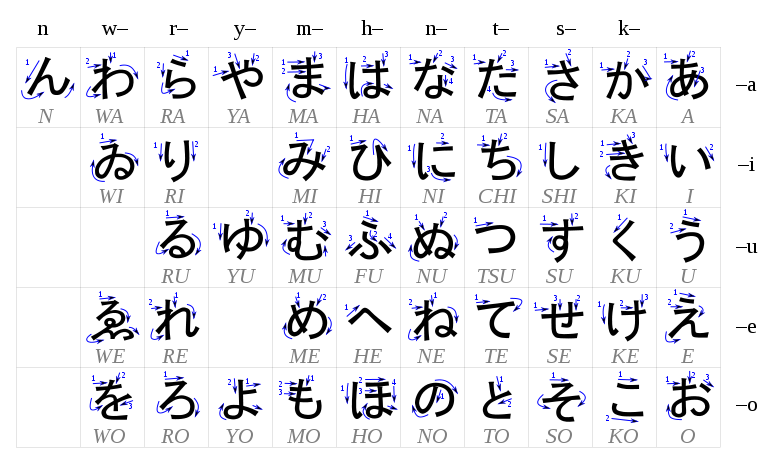
\includegraphics[width=0.9\textwidth]{figs/第01章/第3課:_hiragana_fig/768px_Table_hiragana.svg.png}

\end{figure}

\par{\textbf{Curriculum Note }: Print this sheet out and have it at hand as we continue moving forward. After we've learned about \emph{Katakana }and Chinese characters ( \emph{Kanji }), we'll learn how they're all three used along with English letters to write Japanese. }

\par{\textbf{Usage Notes }: }

\par{Of these characters, all except the symbols for \emph{we }and \emph{wi }\emph{ }are actually used. These two characters live on only in names, place names, and old literature. Because there is the chance you will encounter them, when you do see them, read them as "e" and "i" respectively as the "w" has dropped from their actual pronunciations. This is largely why the symbols are no longer seen today. }

\par{ Similarly, the symbol for \emph{wo }is usually pronounced by "o" by most speakers. However, the traditional pronunciation "wo" is still heard depending on personal preference, dialect, as well as occasion. For instance, in music, singers tend to be conservative in pronunciation. This is also the case when people slow down their speech to purposefully enunciate every sound clearly. }

\par{ Of these characters, all but the symbols for \emph{we }, \emph{wi }, \emph{wo }, and \emph{n }can start words. Also, the symbol for \emph{wo }is only used in names or as a grammatical word that cannot stand alone, which we will learn about later. }

\par{\textbf{Handwriting Notes }: }

\par{1. Write strokes from top to bottom and left to right. \hfill\break
2. Make sure the end of the second stroke in あ is crossing the curve of the final stroke. \hfill\break
3. Make sure that the final stroke in け is slightly farther down than the first. \hfill\break
4. For せ, the second stroke usually doesn't have a hook. \hfill\break
5. For い, こ, た, ふ, り, and ゆ, don't connect the strokes together. \hfill\break
6. For む, if you connect stroke 2 and 3, do not add another slash. \hfill\break
7. Make sure the stroke 3 for お is not positioned far away from the rest of the character. \hfill\break
8.  In more proper handwriting, the last stroke in さ and き is not connected  with the rest. }

\begin{center}
Examples 
\end{center}

\par{ The best way to see if you can read \emph{Hiragana }is to practice with actual words. Below is a list of 30 common words written without any aids. }

\begin{ltabulary}{|P|P|P|P|P|P|}
\hline 

Shape & か \textbf{たち }& Dream & ゆ \textbf{め }↓ & Japan & に \textbf{ほ }ん \\ \cline{1-6}

Usual & ふ \textbf{つう }& End & お \textbf{わり }& Promise & や \textbf{くそく }\\ \cline{1-6}

Snow & ゆ \textbf{き }↓ & Kitten & こ \textbf{ね }こ & Proof & あ \textbf{かし }\\ \cline{1-6}

Chair & い \textbf{す }& Bowl & う \textbf{つわ }& Plate & さ \textbf{ら }\\ \cline{1-6}

Payment & し \textbf{はらい }& Seat &  \textbf{せ }き & Speculation & す \textbf{いそく }\\ \cline{1-6}

Gymnasium & た \textbf{いいく }かん & Strength & ち \textbf{から }↓ & Pathway &  \textbf{つ }うろ \\ \cline{1-6}

Store clerk & て \textbf{んいん }& Chicken meat & と \textbf{りにく }& Accent & な \textbf{まり }↓ \\ \cline{1-6}

Duty &  \textbf{に }んむ & Bypath & ぬ \textbf{けみち }& Drink & の \textbf{み }もの \\ \cline{1-6}

Secret & ひ \textbf{みつ }& Star & ほ \textbf{し }& Command & め \textbf{いれい }\\ \cline{1-6}

Night &  \textbf{よ }る & Young person & わ \textbf{かもの }& Bus\slash train line & ろ \textbf{せん } \\ \cline{1-6}

\end{ltabulary}

\begin{center}
\textbf{Diacritics: ゛ \& ゜ }
\end{center}

\par{ There are two diacritics that can be added to symbols that change the consonant of the symbol in question. These diacritics are the ゛ ( \emph{da \textbf{kuten }\slash ni \textbf{gori }}↓) and the ゜ ( \emph{ha \textbf{ndakuten }}). The first diacritic changes a consonant into a voiced consonant. A voiced consonant causes the vocal folds to vibrate. The second diacritic changes \slash h\slash  to a \slash p\slash . }
 
\begin{figure}[h]
\centering


\includegraphics[width=0.9\textwidth]{figs/第01章/第3課:_hiragana_fig/Hiragana_dakuten_chart.png}

\end{figure}
\hfill\break

\par{ When writing these characters, you write the diacritics last. It's important to note how there are two characters for \slash ji\slash  and \slash zu\slash . These symbols are not always pronounced exactly the same, but we will go into greater detail about this later. }

\begin{center}
Examples 
\end{center}

\par{ The hardest part to mastering the diacritics will simply be remembering to use them and realizing that the pronunciation of a symbol will change because of them. For practice, below are 30 common words that utilize them. }

\begin{ltabulary}{|P|P|P|P|P|P|}
\hline 

Number &  \textbf{か }ず & College student & だ \textbf{いが }くせい & Key & か \textbf{ぎ }↓ \\ \cline{1-6}

Walk & さ \textbf{んぽ }& Mountain climbing &  \textbf{と }ざん & Culture &  \textbf{ぶ }んか \\ \cline{1-6}

Throat &  \textbf{の }ど & Poison & ど \textbf{く }↓ & Yes and no &  \textbf{さ }んぴ \\ \cline{1-6}

Cheers & か \textbf{んぱい }& Nosebleed & は \textbf{なぢ }& Attachment &  \textbf{て }んぷ \\ \cline{1-6}

Electricity &  \textbf{で }んき & Potentiality & そ \textbf{こぢ }から & Hippopotamus &  \textbf{か }ば \\ \cline{1-6}

Skin &  \textbf{は }だ & Furniture &  \textbf{か }ぐ & Wall & か \textbf{べ }\\ \cline{1-6}

Elbow & ひ \textbf{じ }↓ & Part &  \textbf{ぶ }ぶん & Whirlpool &  \textbf{う }ず \\ \cline{1-6}

Continuation & つ \textbf{づき }& Scale &  \textbf{き }ぼ & Wind & か \textbf{ぜ }\\ \cline{1-6}

Eyelash & まつげ & Crevice & ひ \textbf{びわれ }& Tatami room & ざ \textbf{しき }↓ \\ \cline{1-6}

Mirror & か \textbf{がみ }↓ & Family &  \textbf{か }ぞく & Map &  \textbf{ち }ず \\ \cline{1-6}

\end{ltabulary}

\begin{center}
\textbf{Palatal Sounds }
\end{center}

\par{ Palatal sounds are created by placing the tongue on the hard palate of the mouth. Many consonants in Japanese can be palatalized and then followed by the vowels \slash a\slash , \slash i\slash , \slash u\slash , and \slash o\slash . In the case of \slash i\slash , palatalization is an inherent part of the pronunciation of the sound combination. For instance, \slash ki\slash , \slash shi\slash , \slash chi\slash , \slash ni\slash , \slash mi\slash , \slash hi\slash , and \slash ri\slash  are all technically palatalized. This is simply part of the natural process of pronouncing them. }

\par{ The way Japanese creates more sound combinations with palatalized combinations is by having \slash ya\slash , \slash yu\slash  and \slash yo\slash  follow a consonant. When this happens, new consonants are produced. In \emph{Hiragana }, these combinations are created by using an i-sound symbol with a shrunken y-sound symbol-- ゃ, ゅ, or ょ. }

\begin{figure}[h]
\centering

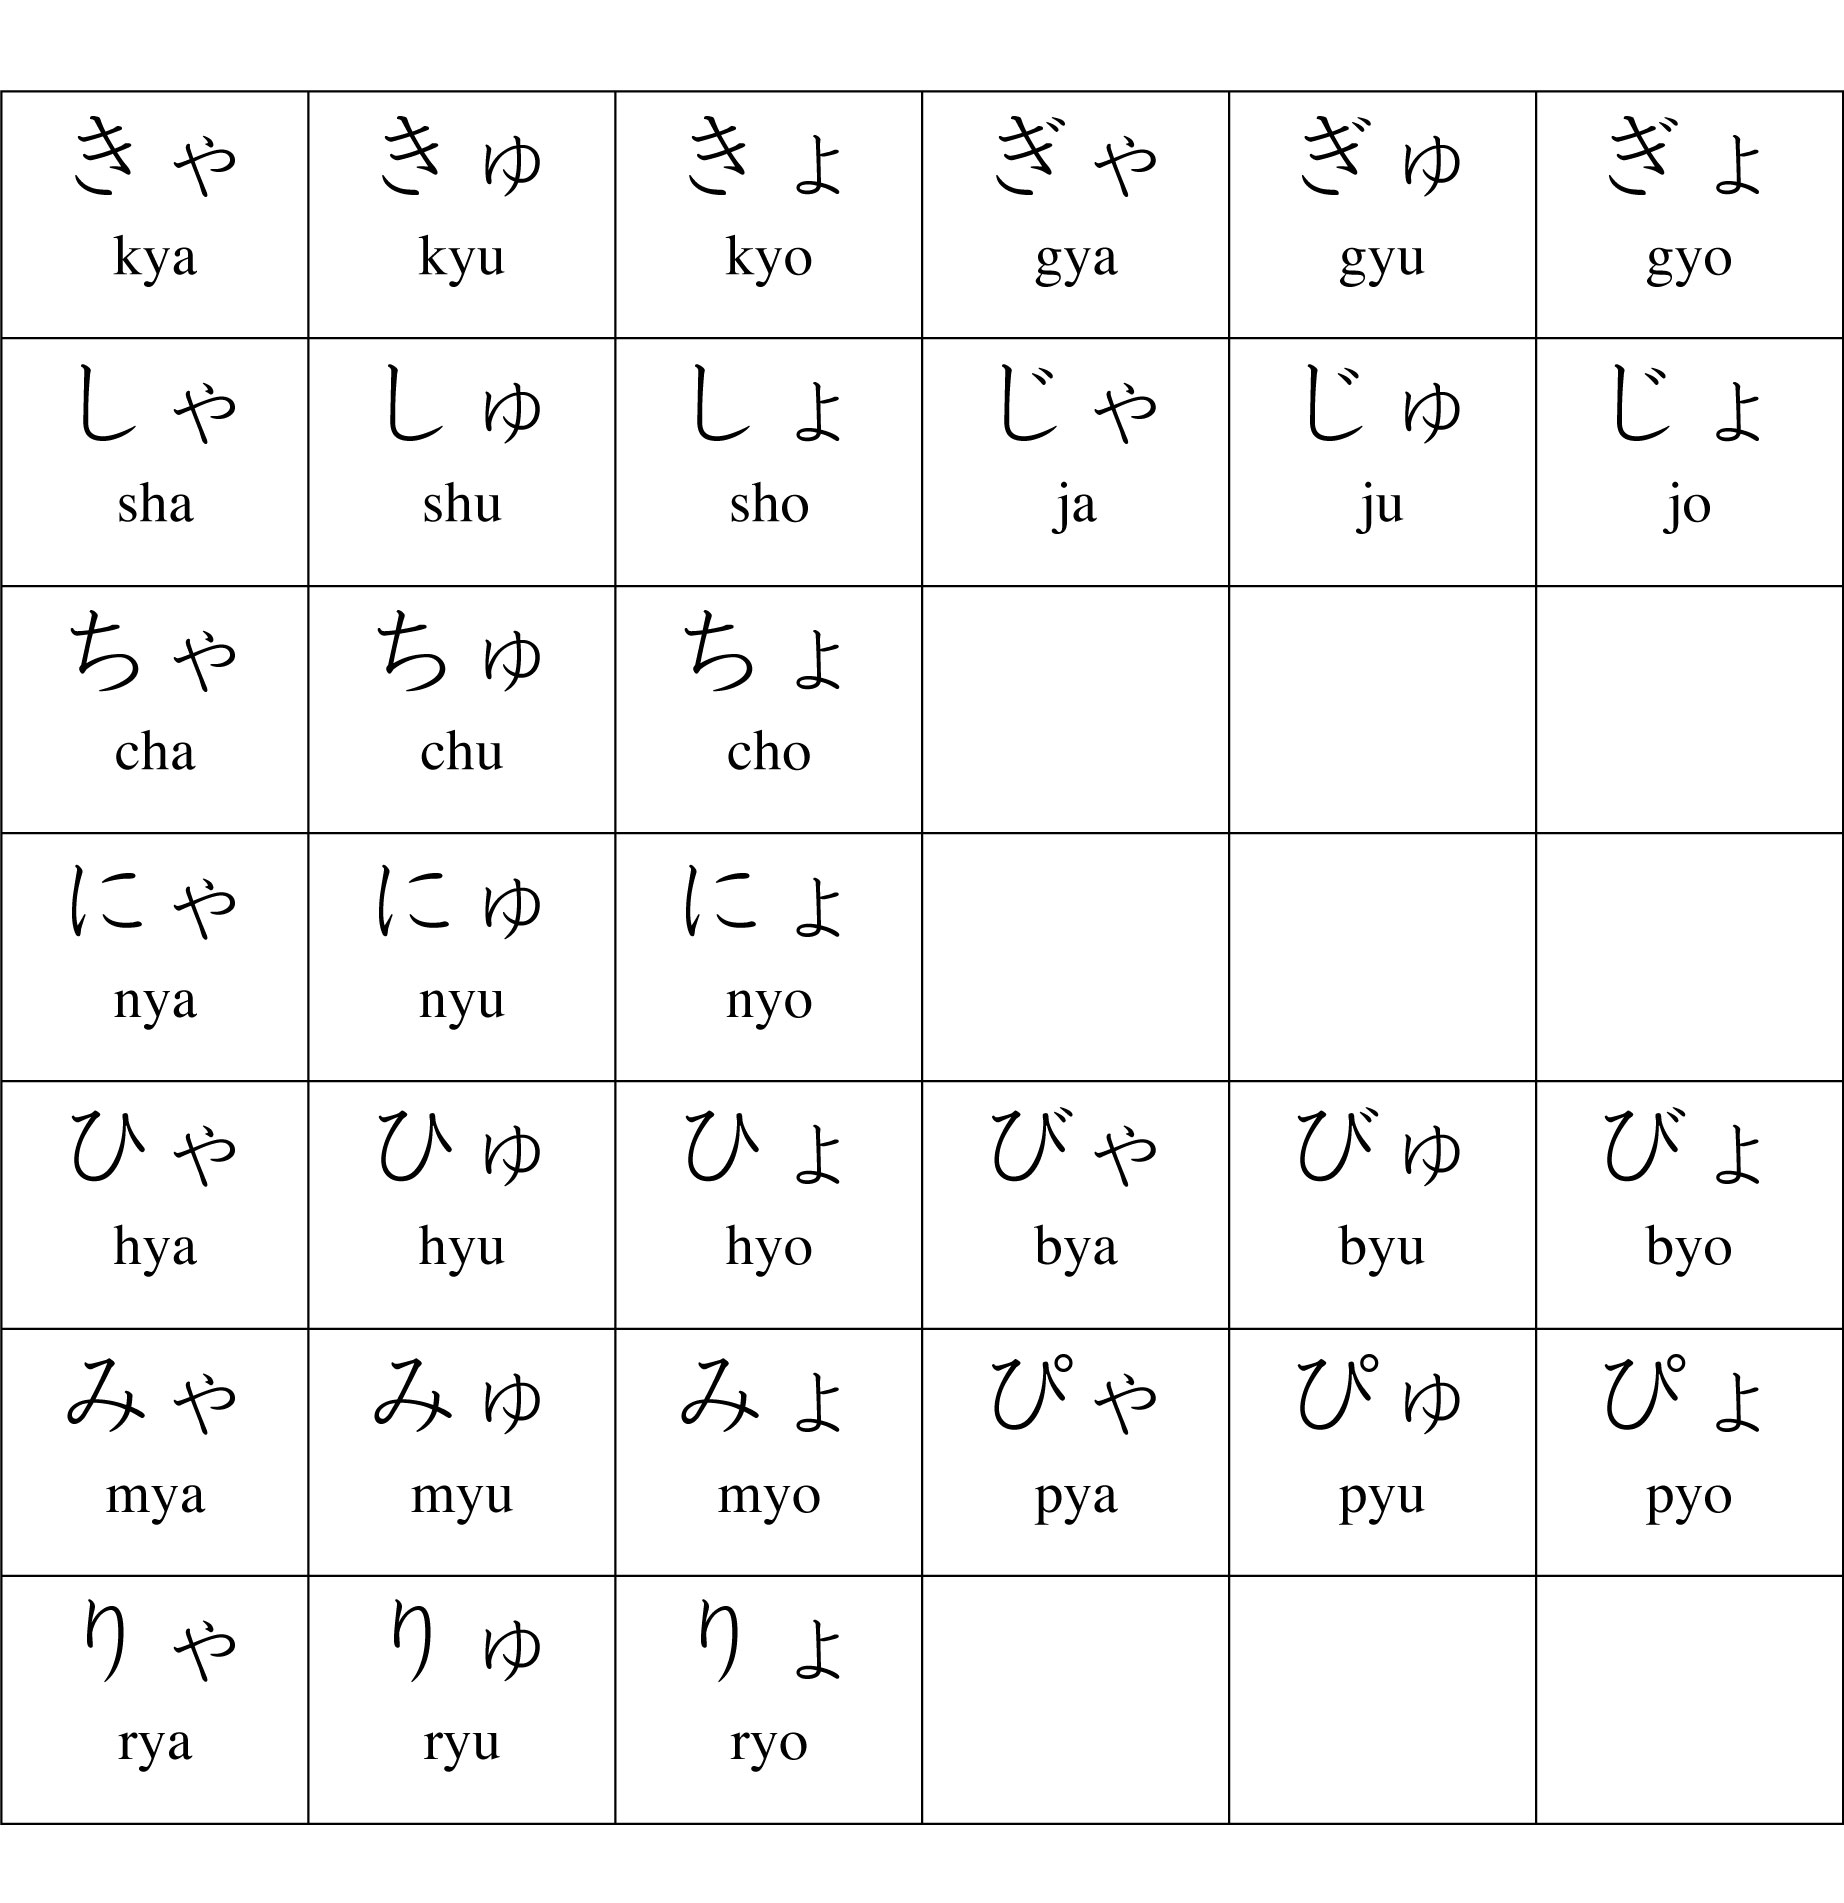
\includegraphics[width=0.9\textwidth]{figs/第01章/第3課:_hiragana_fig/hiragana03.png}

\end{figure}
 
\par{ Similarly to above, there are two ways to write \slash ja\slash , \slash ju\slash , and \slash jo\slash . For now, we'll put aside how they differ in pronunciation and usage and solely focus on memorizing these glyphs. Note, though, that you will rarely see the variants that utilize ぢ. }

\par{ Pronunciation-wise, the ry-sounds will be the most difficult to master as the Japanese \slash r\slash  tends to be difficult as it is for native English speakers to acquire. }

\begin{center}
Examples  
\end{center}

\par{ Below are 30 words utilizing these glyphs to help you learn them. }

\begin{ltabulary}{|P|P|P|P|P|P|}
\hline 

Resident & じゅ \textbf{うみん }& Parking \hfill\break
Injection & ちゅ \textbf{うしゃ }& Giant & きょ \textbf{じん }\\ \cline{1-6}

Meow-meow &  \textbf{にゃ }ん \textbf{にゃ }ん & Acronym & りゃ \textbf{くご }& Tune \hfill\break
& きょ \textbf{く }\\ \cline{1-6}

Seafood & ぎょ \textbf{か }いるい & Inn & りょ \textbf{かん }& Opposite & ぎゃ \textbf{く }\\ \cline{1-6}

600 & ろっ \textbf{ぴゃく }↓ & Tathagata & にょ \textbf{らい }& Studying abroad & りゅ \textbf{うがく }\\ \cline{1-6}

Cow milk & ぎゅ \textbf{うにゅう }& Bathing & にゅ \textbf{うよく }& Customer & きゃ \textbf{く }\\ \cline{1-6}

Concentration & しゅ \textbf{うちゅ }うりょく & Processing &  \textbf{しょ }り & Society &  \textbf{しゃ }かい \\ \cline{1-6}

Touch down & ちゃ \textbf{くりく }& Tea & お \textbf{ちゃ }& Directly & ちょ \textbf{くせつ }\\ \cline{1-6}

Weak point & じゃ \textbf{くて }ん & Tutor & じょ \textbf{しゅ }& Pulse & みゃ \textbf{く }↓ \\ \cline{1-6}

Teacup & ゆ \textbf{のみぢゃ }わん & Hyuga &  \textbf{ひゅ }うが & 100 & ひゃ \textbf{く }↓ \\ \cline{1-6}

Chinese & ちゅ \textbf{うごくご }& Properly & ちゃ \textbf{んと }& Address &  \textbf{じゅ }うしょ \\ \cline{1-6}

\end{ltabulary}
\hfill\break
 Although it may be difficult to properly pronounce these palatal sounds, mispronouncing them as separate morae will result in the word either becoming a different word altogether or a non-word. \hfill\break
\hfill\break

\begin{ltabulary}{|P|P|}
\hline 

i-sound + や・ゆ・よ & i-sound + ゃ・ゅ・ょ \\ \cline{1-2}

じ \textbf{ゆ }う (Freedom) &  \textbf{じゅ }う  (Ten\slash gun) \\ \cline{1-2}

り \textbf{ゆう }(Reason) &  \textbf{りゅ }う (Dragon) \\ \cline{1-2}

き \textbf{\emph{ゆ }う }(Needless anxiety) &  \textbf{きゅ }う (Nine) \\ \cline{1-2}

し \textbf{ゆう }(Private ownership) &  \textbf{しゅ }う (Week\slash state) \\ \cline{1-2}

\end{ltabulary}
\hfill\break

\begin{center}
 \textbf{To Continue }
\end{center}

\par{ So far, we have covered the unique glyphs that compose \emph{Hiragana }. What we have not learned is how long consonants and vowels are transcribed. We have also not learned about what situations \emph{Hiragana }is even used in. Both of these topics require that we first go over \emph{Katakana }as comparing the two is essentially in understanding these topics properly. }

\begin{center}
\textbf{Practice } 
\end{center}

\par{Part I: Change the following words into \emph{Hiragana }. }

\par{1. \emph{Ke \textbf{muri }}(smoke) \hfill\break
2. \emph{A \textbf{magumo }}(rain cloud) \hfill\break
3. \emph{U }\textbf{\emph{ta }↓ }(song)  \hfill\break
4. \emph{\textbf{Se }kai }(world) \hfill\break
5. \emph{Ka \textbf{rate }} (karate)   }

\par{Part II: Change the following words in \emph{Hiragana }into \emph{Rōmaji }. }

\par{1. \textbf{か }のじょ (She)  2. しょ \textbf{だな }(Bookshelf) \hfill\break
3. に \textbf{ほんご }(Japanese language)  4. さ \textbf{かな }(Fish) \hfill\break
5. に \textbf{んげん }(Human)  6. だ \textbf{いがく }(College) \hfill\break
7. ひ \textbf{と }(Person)  8. あ \textbf{した↓ }(Tomorrow)  }
    

% http://www.imabi.net/katakana.htm
     
\chapter{Kana II}

\begin{center}
\begin{Large}
第4課: Kana II: Katakana カタカナ  
\end{Large}
\end{center}
 
\par{ In the previous lesson, we learned about how Japanese is a mixed script of four systems in one. Of these four systems, two of them are \emph{Kana }systems: \emph{Hiragana }and \emph{Katakana }. The previous lesson was all about learning the individual symbols of \emph{Hiragana }. In this lesson, our goal will be to learn all the individual symbols for \emph{Katakana }. }

\par{ \emph{Hiragana }and \emph{Katakana }both represent the same sound combinations (morae). As such, there won't be any differences in pronunciation between an \slash a\slash  written in \emph{Hiragana }and one written in \emph{Hiragana }. However, the two scripts are used in different circumstances. Their rules for other aspects of spelling such as long vowel notation are also not exactly the same. For now, we will focus solely on learning the individual symbols of \emph{Katakana }. As you will soon see, there are more symbols to learn in \emph{Katakana }than there is for \emph{Hiragana }. This means you have plenty of work ahead of you in this lesson. }
      
\section{Katakana カタカナ}
 
\par{ Of the two \emph{Kana }systems, \emph{Katakana }is the least used. However, that doesn't mean it isn't used, and it doesn't mean that it isn't important to learn. One cannot properly read Japanese without knowing both systems. The two systems are still used in different ways. The way they're used also affects how complex the systems are. \emph{Katakana }, as you will see, has an additional set of combinations not used in \emph{Hiragana }. This means it'll take a little more effort to memorize \emph{Katakana }than \emph{Hiragana }. With that being said, let's begin.  }

\begin{center}
\emph{KATAKANA }
\end{center}

\par{ The basic symbols of \emph{Katakana }, just as was the case with \emph{Hiragana }, are organized into a chart called the \emph{Gojūonzu }. This chart is shown below with each basic symbol. Just like for \emph{Hiragana }, notice how the stoke orders are listed and how all the allophones of sounds we've learned about are shown in their respective columns. }
 
\begin{figure}[h]
\centering

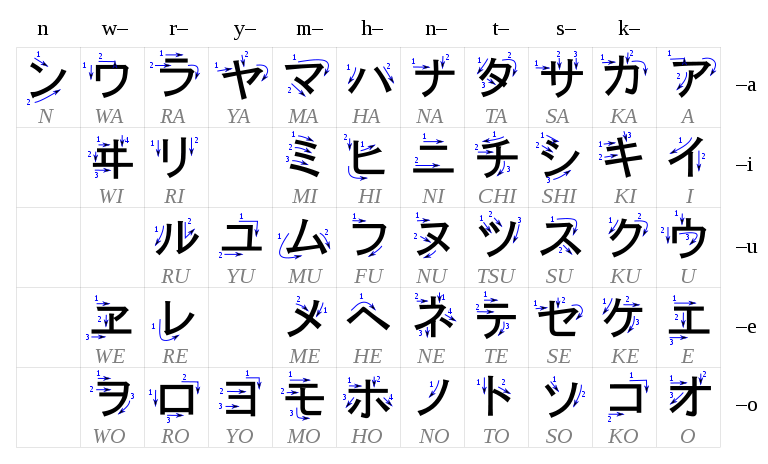
\includegraphics[width=0.9\textwidth]{figs/第01章/第4課:_katakana_fig/768px_Table_katakana.svg.png}

\end{figure}

\par{\textbf{Curriculum Note }: Print this sheet out and have it on hand as we continue moving forward. It will be u seful while you memorize both \emph{Kana }systems. Once we learn about Chinese characters ( \emph{Kanji }), we'll learn how they're all three used along with English letters to write Japanese. }

\par{\textbf{Usage Notes: }}

\par{  Of these characters, all of them except the symbols for \emph{we }and \emph{wi }\emph{ }are typically used. These two characters live on only in names, place names, and old literature. Because there is the chance you will encounter them, when you do see them, read them as "e" and "i" respectively as the "w" has dropped from their actual pronunciations. This is largely why the symbols are no longer seen today. }

\par{ Similarly, the symbol for \emph{wo }is usually pronounced by "o" by most speakers. However, the traditional pronunciation "wo" is still heard depending on personal preference, dialect, as well as occasion. For instance, in music, singers tend to be conservative in pronunciation. This is also the case when people slow down their speech to purposefully enunciate every sound clearly. Unlike in \emph{Hiragana }, th e \emph{Katakana }symbol for \emph{wo }is hardly used at all. This means you won't get many opportunitie s to see it actually used. }

\par{ Of these characters, all but the symbols for \emph{we }, \emph{wi }, \emph{wo }, and \emph{n }can start words. The symbols for \emph{we }and \emph{wi }are deemed obsolete. Also, the symbol for \emph{wo }is only used in names or as a grammatical word that cannot stand alone, which we will learn about later. }

\par{\textbf{Handwriting Notes }: }

\par{1. Write strokes from top to bottom and left to right. \hfill\break
2. Horizontal strokes come before vertical strokes. \hfill\break
3. Take especial note to the stroke orders of シ and ツ.  For シ, its third stroke is irregularly written from the bottom upward, which is how you can distinguish it from ツ, which is written regularly. \hfill\break
4. Also take note of the stroke orders of ソ and ン. For ン, its second stroke is irregularly written from the bottom upward, which is how you can distinguish it from ソ, which is written regularly. \hfill\break
5. When there are horizontal strokes that span the length of the symbol, those strokes aren't first from top to bottom regardless if other strokes may start higher up. Take キ as an example. }

\begin{center}
\textbf{Examples } 
\end{center}

\par{ As your first chance at reading practice, below are 60 common words that are spelled in \emph{Katakana }. Although it's not necessary that you memorize them all now, you'll find that many of them are words you're already very familiar with. }

\begin{ltabulary}{|P|P|P|P|P|P|}
\hline 

Access &  \textbf{ア }クセス & Assistant & ア \textbf{シ }スタント & ASEAN & ア \textbf{セ }アン \\ \cline{1-6}

Africa & ア \textbf{フリカ }& America & ア \textbf{メリカ }& Aluminum & ア \textbf{ルミ }\\ \cline{1-6}

Good-looking guy & イ \textbf{ケメン }& Italy & イ \textbf{タリア }& Earbud & イ \textbf{ヤ }ホン \\ \cline{1-6}

Air conditioning & エ \textbf{アコン }& Eroticism &  \textbf{エ }ロ & Oceania & オ \textbf{セアニア }\\ \cline{1-6}

Offline & オ \textbf{フラ }イン & Cocktail &  \textbf{カ }クテル & Custom &  \textbf{カ }スタム \\ \cline{1-6}

Sponge cake & カ \textbf{ステラ }& Camera &  \textbf{カ }メラ & Karaoke & カ \textbf{ラオケ }\\ \cline{1-6}

Calcium & カ \textbf{ルシ }ウム & Mouse &  \textbf{マ }ウス & Christ & キ \textbf{リスト }\\ \cline{1-6}

Classmate & ク \textbf{ラスメ }イト & Christmas & ク \textbf{リス }マス & Koala &  \textbf{コ }アラ \\ \cline{1-6}

Coin &  \textbf{コ }イン & Siren &  \textbf{サ }イレン & Santa &  \textbf{サ }ンタ \\ \cline{1-6}

System &  \textbf{シ }ステム & Scenario & シ \textbf{ナリオ }& Restaurant &  \textbf{レ }ストラン \\ \cline{1-6}

Hormone & ホルモン & Synchronize & シ \textbf{ンクロ }& Stress & ス \textbf{ト }レス \\ \cline{1-6}

Centi(meter) &  \textbf{セ }ンチ & Seoul &  \textbf{ソ }ウル & Solo &  \textbf{ソ }ロ \\ \cline{1-6}

Towel &  \textbf{タ }オル & Tennis &  \textbf{テ }ニス & Toilet &  \textbf{ト }イレ \\ \cline{1-6}

Hotel &  \textbf{ホ }テル & Minus & マ \textbf{イナス }& Nylon &  \textbf{ナ }イロン \\ \cline{1-6}

Tomato &  \textbf{ト }マト & Ton &  \textbf{ト }ン & Knife &  \textbf{ナ }イフ \\ \cline{1-6}

Necktie &  \textbf{ネ }クタイ & Quota &  \textbf{ノ }ルマ & Handkerchief & ハ \textbf{ンカチ }\\ \cline{1-6}

Stapler &  \textbf{ホ }チキス & Marathon & マ \textbf{ラソン }& Milk &  \textbf{ミ }ルク \\ \cline{1-6}

Mexico & メ \textbf{キシコ }& Moscow & モ \textbf{スクワ }& UNESCO & ユ \textbf{ネ }スコ \\ \cline{1-6}

Toyota &  \textbf{ト }ヨタ & Link &  \textbf{リ }ンク & Lemon &  \textbf{レ }モン \\ \cline{1-6}

Russia &  \textbf{ロ }シア & Request & リ \textbf{クエ }スト & Wine &  \textbf{ワ }イン \\ \cline{1-6}

\end{ltabulary}

\begin{center}
\textbf{Diacritics: ゛ \& ゜ }
\end{center}

\par{ The diacritics we learned about last lesson are used in exactly the same way in \emph{Katakana }. These diacritics, the These diacritics are the ゛ ( \emph{da \textbf{kuten }\slash ni \textbf{gori }}↓) and the ゜ ( \emph{ha \textbf{ndakuten }}), represent voiced consonants and the consonant \slash p\slash  respectively. }
 
\begin{figure}[h]
\centering


\includegraphics[width=0.9\textwidth]{figs/第01章/第4課:_katakana_fig/Katakana_dakuten_chart.png}

\end{figure}

\par{ Just as was the case with \emph{Hiragana }, you write the basic symbol before adding the diacritics. Additionally, there are two characters for \slash ji\slash  and \slash zu\slash . However, their pronunciations\slash usage aren't 100\% the same. For now, focus on memorizing these symbols. }

\begin{center}
Examples 
\end{center}

\par{ Below are 60 common words that utilize these diacritics. Although it is not necessary that you memorize them all, they are all common words that bring purpose to using \emph{Katakana }as the majority of these words are solely written in \emph{Katakana }. }

\begin{ltabulary}{|P|P|P|P|P|P|}
\hline 

Advice &  \textbf{ア }ドバイス & Radio &  \textbf{ラ }ジオ & England & イ \textbf{ギリス }\\ \cline{1-6}

Pokemon & ポ \textbf{ケモン }& Event & イ \textbf{ベント }& India &  \textbf{イ }ンド \\ \cline{1-6}

Ego &  \textbf{エ }ゴ & Egypt & エ \textbf{ジプト }& Apron &  \textbf{エ }プロン \\ \cline{1-6}

Holland & オ \textbf{ランダ }& Casino &  \textbf{カ }ジノ & Gas &  \textbf{ガ }ス \\ \cline{1-6}

Capsule &  \textbf{カ }プセル & Gift &  \textbf{ギ }フト & Jellyfish & ク \textbf{ラゲ }\\ \cline{1-6}

Mongolia &  \textbf{モ }ンゴル & Golf &  \textbf{ゴ }ルフ & Convenience store & コ \textbf{ンビニ }\\ \cline{1-6}

Size &  \textbf{サ }イズ & Sandals & サ \textbf{ンダル }& Running & ラ \textbf{ンニング }\\ \cline{1-6}

Swimming & ス \textbf{イ }ミング & Pants &  \textbf{ズ }ボン & Celebrity &  \textbf{セ }レブ \\ \cline{1-6}

Zombie &  \textbf{ゾ }ンビ & Diamond & ダ \textbf{イヤモ }ンド & Taipei & タ \textbf{イペイ }\\ \cline{1-6}

Dance &  \textbf{ダ }ンス & Design & デ \textbf{ザ }イン & Digital camera & デ \textbf{ジカメ }\\ \cline{1-6}

TV &  \textbf{テ }レビ & Germany &  \textbf{ド }イツ & Door &  \textbf{ド }ア \\ \cline{1-6}

Dollar &  \textbf{ド }ル & Napkin &  \textbf{ナ }プキン & Trash & ゴ \textbf{ミ }↓ \\ \cline{1-6}

Knob &  \textbf{ノ }ブ & Hiking &  \textbf{ハ }イキング & Basketball &  \textbf{バ }スケ \\ \cline{1-6}

PC & パ \textbf{ソコン }& Bus &  \textbf{バ }ス & Pachinko & パ \textbf{チンコ }\\ \cline{1-6}

Bread &  \textbf{パ }ン & Banana &  \textbf{バ }ナナ & Panda &  \textbf{パ }ンダ \\ \cline{1-6}

Piano & ピ \textbf{アノ }& Visa &  \textbf{ビ }ザ & Pizza &  \textbf{ピ }ザ \\ \cline{1-6}

Vitamin & ビ \textbf{タ }ミン & Video &  \textbf{ビ }デオ & Building &  \textbf{ビ }ル \\ \cline{1-6}

Pink &  \textbf{ピ }ンク & Judea &  \textbf{ユ }ダヤ & Frying pan & フ \textbf{ライパン }\\ \cline{1-6}

Browser & ブ \textbf{ラウザ }& Blog & ブ \textbf{ログ }& Veranda & ベ \textbf{ランダ }\\ \cline{1-6}

McDonald's & マ \textbf{クドナ }ルド & Medal & メ \textbf{ダル }& Memo &  \textbf{メ }モ \\ \cline{1-6}

\end{ltabulary}
\hfill\break

\begin{center}
\textbf{Palatal Sounds }
\end{center}

\par{ Remember that palatal sounds are created by placing the tongue on the hard palate of the mouth. Consonants are naturally palatalized in Japanese when followed by \slash i\slash  or \slash y\slash . For those created with \slash y\slash , shrunken y-sound symbols must be paired with a full-sized i-sound symbol. In \emph{Katakana }, these combinations are as follows. }
 
\begin{figure}[h]
\centering

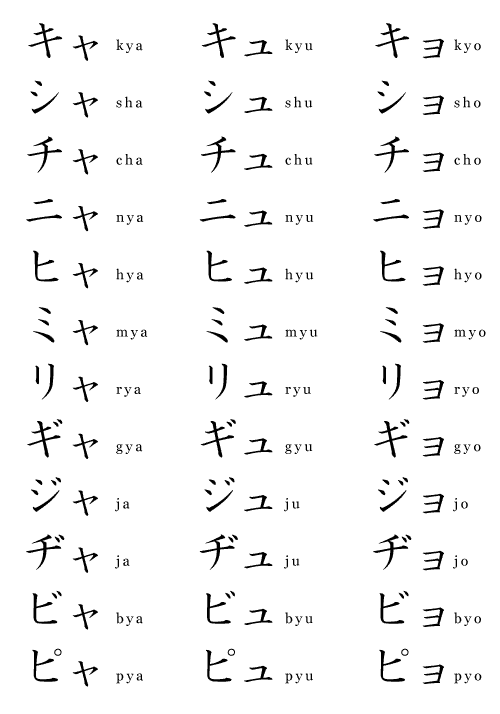
\includegraphics[width=0.9\textwidth]{figs/第01章/第4課:_katakana_fig/Katakana_yuoun_chart.png}

\end{figure}

\par{ Just as was the case with above with there are being two ways to write the says, \slash ji\slash  and \slash zu\slash , the same can be said for \slash ja\slash , \slash ju\slash , and \slash jo\slash . The variants that use ヂ are essentially obsolete as far as spelling actual, common words is concerned. }

\begin{center}
Examples  
\end{center}

\par{ Not all these characters are used as frequently as others. Although some are extremely common, some are only found in certain kinds of words. Others are hard to find without being used with long vowels and consonants. Since we haven't learned what those rules are for the two \emph{Kana }systems, the 30 examples words are limited to words with short consonants and vowels that are actually common expressions. }

\begin{ltabulary}{|P|P|P|P|P|P|}
\hline 

Casual &  \textbf{カ }ジュアル & Curriculum &  \textbf{カ }リキュラム & Cabbage &  \textbf{キャ }ベツ \\ \cline{1-6}

Cancel &  \textbf{キャ }ンセル & Gambling &  \textbf{ギャ }ンブル & Shirt &  \textbf{シャ }ツ \\ \cline{1-6}

Chandelier & シャ \textbf{ンデ }リア & Jump &  \textbf{ジャ }ンプ & Jogging & ジョ \textbf{ギング }\\ \cline{1-6}

Mandarin dress & チャ \textbf{イナド }レス & Chime &  \textbf{チャ }イム & Channel & チャ \textbf{ンネル }\\ \cline{1-6}

Pajamas &  \textbf{パ }ジャマ & Condominium &  \textbf{マ }ンション & Pure &  \textbf{ピュ }ア \\ \cline{1-6}

Jazz &  \textbf{ジャ }ズ & Munich &  \textbf{ミュ }ンヘン & Genre &  \textbf{ジャ }ンル \\ \cline{1-6}

Gang &  \textbf{ギャ }ング & Goggling &  \textbf{ギョ }ロギョロ & Hopping &  \textbf{ピョ }ンピョン \\ \cline{1-6}

Junior &  \textbf{ジュ }ニア & Meow-meow &  \textbf{ニャ }ンニャン & Nuance &  \textbf{ニュ }アンス \\ \cline{1-6}

Awkwardness &  \textbf{ギ }クシャク & Wriggling &  \textbf{ニョ }ロニョロ & Pyeongyang &  \textbf{ピョ }ンヤン \\ \cline{1-6}

Chocolate &  \textbf{チョ }コ & Tunisia & チュ \textbf{ニジア }& Champion &  \textbf{チャ }ンピオン \\ \cline{1-6}

\end{ltabulary}
\hfill\break

\begin{center}
 \textbf{Additional \emph{Katakana }}
\end{center}

\par{ Unlike \emph{Hiragana }, \emph{Katakana }is used to transcribe far more sound combinations. Although we have not learned exactly when either system is used and why, you may have noticed that a lot of the example words in this lesson have been for loan-words from other languages. This is one purpose of \emph{Katakana }that is heavily reflected in the inventory of sound combinations as an effect. }

\par{ The most frequently used extensions are those for the consonants \slash sh\slash , \slash j\slash , \slash t\slash , \slash d\slash , \slash ch\slash , \slash f\slash , and \slash w\slash . As you can see, all these additional combinations involve using a shrunken symbol next to a full-sized one. }

\begin{ltabulary}{|P|P|P|P|P|P|P|P|P|P|P|P|P|P|}
\hline 

 & Y & W & V & S & SH & J & T & D & CH & TS & F & KW & GW \\ \cline{1-14}

A &  &  & ヴァ &  &  &  &  &  &  & ツァ & ファ & クァ \hfill\break
クヮ & グァ \hfill\break
グヮ \\ \cline{1-14}

I &  & ウィ & ヴィ & スィ & ズィ &  & ティ & ディ &  & ツィ & フィ &  &  \\ \cline{1-14}

U &  &  & ヴ &  &  &  & トゥ & ドゥ &  &  &  &  &  \\ \cline{1-14}

E & イェ & ウェ & ヴェ &  & シェ & ジェ &  &  & チェ & ツェ & フェ &  &  \\ \cline{1-14}

O &  & ウォ & ヴォ &  &  &  &  &  &  & ツォ & フォ &  &  \\ \cline{1-14}

Y &  &  &  &  &  &  & テュ & デュ &  &  &  &  &  \\ \cline{1-14}

\end{ltabulary}

\par{\textbf{Pronunciation Notes }: }

\par{1. The v-sounds are overwhelmingly pronounced as b-sounds by most speakers. \hfill\break
2. Additional w-sounds and y-sounds are usually pronounced broken up as if they were written with full-sized characters. For instance, kiwi can either be pronounced as \emph{\textbf{ki }ui }キウイ or \emph{\textbf{ki }wi }キウィ.  }

\begin{center}
\textbf{Examples }
\end{center}

\par{ The combinations shown above are essentially all additional combinations that are of any significant importance in writing practical words that are actually used by Japanese speakers. However, they aren't all equal in frequency. With that being said, it isn't possible to show practical examples of each combination at this point without having to delve into information beyond the reach of this lesson. Nevertheless, the 30 words will provide you plenty of practice. }

\begin{ltabulary}{|P|P|P|P|P|P|}
\hline 

Korean won &  \textbf{ウォ }ン & Ending & エ \textbf{ンディング }& Figurine & \textbf{フィ }ギュア \\ \cline{1-6}

The web & ウェ \textbf{ブ }& Chef &  \textbf{シェ }フ & Disc &  \textbf{ディ }スク \\ \cline{1-6}

Native &  \textbf{ネ }イティブ & Negative &  \textbf{ネ }ガティブ & Fight(ing spirit) &  \textbf{ファ }イト \\ \cline{1-6}

File &  \textbf{ファ }イル & Family restaurant & ファ \textbf{ミレス }& Film &  \textbf{フィ }ルム \\ \cline{1-6}

Philippines &  \textbf{フィ }リピン & Manifesto &  \textbf{マ }ニフェスト & Czech &  \textbf{チェ }コ \\ \cline{1-6}

Share &  \textbf{シェ }ア & Pretzel & プ \textbf{レ }ッツェル & Cafe &  \textbf{カ }フェ \\ \cline{1-6}

Highway & ハ \textbf{イウェ }イ & Fan &  \textbf{ファ }ン & Chess &  \textbf{チェ }ス \\ \cline{1-6}

Violin & ヴァ \textbf{イオリン }& Fake &  \textbf{フェ }イク & Yes &  \textbf{イェ }ス \\ \cline{1-6}

Font &  \textbf{フォ }ント & Wedding dress & ウェ \textbf{ディングド }レス & Wink &  \textbf{ウィ }ンク \\ \cline{1-6}

Wikipedia & ウィキ \textbf{ペ }ディア & Shakespeare & シェ \textbf{イク }スピア & Fondue &  \textbf{フォ }ンデュ \\ \cline{1-6}

\end{ltabulary}

\par{\textbf{Word Notes }: \hfill\break
1. "Violin" is typically spelled as バイオリン. \hfill\break
2. イェス is not the typical means of saying "yes"; it is always used in an English-based context. }

\begin{center}
\textbf{To Continue }
\end{center}

\par{ In the next lesson, we will learn about how to write long vowels and consonants in both \emph{Hiragana }and \emph{Katakana }. We will also learn about what the differences are between the variant ways to write the sounds \slash ji\slash , \slash zu\slash , \slash ja\slash , \slash ju\slash , and \slash jo\slash . After which point, we'll learn about what \emph{Kanji }and then move on to learning how \emph{Kana }and \emph{Kanji }are used together to write properly in Japanese. }

\begin{center}
\textbf{Practice }
\end{center}

\par{Part I: Spell the following words in \emph{Katakana }. }

\par{1. \emph{Piano }\emph{ }(Piano)    \hfill\break
2. \emph{Tesuto }(Test)   \hfill\break
3. \emph{Wirusu\slash Uirusu }(Virus)  \hfill\break
4. \emph{Kariforunia }(California) }

\par{Part II: Romanize the following words. }

\par{1. スリル (Thrill)  \hfill\break
2. シネマ (Cinema)  \hfill\break
3. マスコミ (The media) \hfill\break
4. キャビン (Cabin)  \hfill\break
5. パリ (Paris)  }
    

% http://www.imabi.net/spellingissues.htm
     
\chapter{Kana III}

\begin{center}
\begin{Large}
第5課: Kana III: Long Vowels, Double Consonants, \& Yotsugana 
\end{Large}
\end{center}
 
\par{ Every language has an \textbf{orthography }for its script(s). In any orthography, \emph{there are lots of rules that govern the use of its writing system(s) }. With Japanese being written with a mixed script, there are plenty of rules that have to be accounted for in its orthography. For the most part, Japanese orthography in regards to \emph{Kana }is rather straightforward. You've learned how the basic sounds are written in both \emph{Hiragana }and \emph{Katakana }. What has not been taught yet is how long vowels and double consonants are covered. We've also yet to learn about the true differences are between the variant ways of writing \slash ji\slash , \slash zu\slash , \slash ja\slash , \slash ju\slash , and \slash jo\slash . The \emph{Kana }used to write these sounds are called \emph{Yotsugana }. }

\par{ As we learned in Lesson 1, Japanese distinguishes between short and long vowels, and as we learned in Lesson 2, Japanese also distinguishes between single and double consonants. The change in mora count that occurs when lengthening a vowel or consonant isn't negligible. First, we will learn about how \emph{Hiragana }and \emph{Katakana }typically spell out long vowels. Then, we'll learn about how both systems write double consonants. Then, we'll learn about how to differentiate between \emph{Yotsugana }. Although we've already learned about the characters themselves, nothing has been said on when to use which. }

\begin{center}
\textbf{Contents of This Lesson }
\end{center}

\begin{itemize}

\item Long Vowels in \emph{Hiragana } 
\item Long Vowels in \emph{Katakana } 
\item Double Consonants in \emph{K }\emph{ana } 
\item \emph{Yotsugana  }
\end{itemize}
      
\section{Long Vowels in Hiragana}
 
\par{ In \emph{Hiragana }, long vowels are typically written by doubling the vowel. As you can see below, only long \slash e\slash  or \slash o\slash  sounds are extra complicated. The reason why these two long vowels are two possible spellings is because of all the words that have been borrowed from Chinese. Sometimes, spelling doesn't always match pronunciation. As readers of English, you should know this oh too well. }

\begin{ltabulary}{|P|P|P|P|P|}
\hline 

Long \slash a\slash  & Long \slash i\slash  & Long \slash u\slash  & Long \slash e\slash  & Long \slash o\slash  \\ \cline{1-5}

ああ & いい & うう & ええ \hfill\break
えい & おお \hfill\break
おう \\ \cline{1-5}

\end{ltabulary}

\par{ The next thing to do is see actual words with each of these long vowels. The information we learned about long \slash e\slash  and long \slash o\slash  sounds in Lesson 1 will be extremely relevant in this lesson. }

\begin{center}
\textbf{Long \slash a\slash , \slash i\slash , \& \slash u\slash  } 
\end{center}

\par{ To create long vowels for \slash a\slash , \slash i\slash , and \slash u\slash , all you do is double the vowel symbol. In the word charts below, the first column shows their spellings in Hiragana. Because word type is a major factor later on in this lesson, the word type for all words shown in this section are also provided. There are three main sources of vocabulary in Japanese: native (words that are indigenous to Japanese), Sino-Japanese, and loan-words. Sino-Japanese words are words that were either borrowed or created with roots from Chinese. These words are alternatively referred to as Kango (the Japanese terminology for Sino-Japanese) in the charts below. Loan-words are borrowings from modern world languages that have managed to find their way into Japanese. In the third column. }

\par{\textbf{Transcription Note }: \hfill\break
1. Because pitch contours will be marked on the \emph{Hiragana }spellings, long vowels will be romanized with macrons in the charts below except for long \slash i\slash , which will be written as "ii." \hfill\break
2. High pitch and pitch drops will be denoted the same way as previous lessons, just with their \emph{Hiragana }spellings. }

\par{\textbf{Curriculum Note }: False long vowels, vowels that happened to be juxtaposed next to each other but are in fact belong to separate word elements, are not represented as examples of long vowels in the charts below. }

\begin{ltabulary}{|P|P|P|}
\hline 

 \emph{Long \slash a\slash  }& Word Type & Meaning \\ \cline{1-3}

 \emph{Ā }\textbf{あ }あ \hfill\break
& Native & Ah \\ \cline{1-3}

 \emph{Okāsan }お \textbf{か }あさん \hfill\break
& Native & (Someone's) mother \\ \cline{1-3}

 \emph{Obasan }お \textbf{ばさん }\hfill\break
& Native & Aunt; middle-aged woman \\ \cline{1-3}

 \emph{Obāsan }お \textbf{ば }あさん \hfill\break
& Native & Grandmother\slash old woman \\ \cline{1-3}

\end{ltabulary}

\par{\textbf{Usage Note }: Long \slash a\slash  is not a common long vowel. In Hiragana, long \slash a\slash  is limited to native words. }

\begin{ltabulary}{|P|P|P|}
\hline 

 \emph{Long \slash i\slash  }& Word Type & Meaning \\ \cline{1-3}

 \emph{Ojisan }お \textbf{じさん }\hfill\break
& Native & Uncle\slash middle-aged man \\ \cline{1-3}

 \emph{Ojiisan }お \textbf{じ }いさん \hfill\break
& Native & Grandfather\slash old man \\ \cline{1-3}

\end{ltabulary}

\par{\textbf{Usage Note }: Long \slash i\slash  is also not a common long vowel. In Hiragana, long \slash i\slash  is limited to native words. }

\begin{ltabulary}{|P|P|P|}
\hline 

 \emph{Long \slash u\slash  }& Word Type & Meaning \\ \cline{1-3}

 \emph{Sūgaku }す \textbf{うがく }\hfill\break
&  \emph{Kango }& Math \\ \cline{1-3}

 \emph{Fūfu }\textbf{ふ }うふ \hfill\break
&  \emph{Kango }& Married couple \\ \cline{1-3}

 \emph{Gyūniku }ぎゅ \textbf{うにく }\hfill\break
&  \emph{Kango }& Beef \\ \cline{1-3}

\end{ltabulary}
\textbf{\hfill\break
Usage Note }: Though common, long \slash u\slash  is limited to Sino-Japanese words in \emph{Hiragana }. \hfill\break

\begin{center}
\textbf{Long \slash e\slash : ええ vs えい }
\end{center}

\par{ Whereas long \slash e\slash  in native words is always spelled with ええ, it is spelled as えい in Sino-Japanese, in which case it may alternatively be literally pronounced as [ei]. This literal pronunciation is preferred in many regions of Japan as well as in conversation pronunciation, especially in singing. Note that all other instances of えい outside Sino-Japanese vocabulary must be pronounced as [ei]. }

\begin{ltabulary}{|P|P|P|}
\hline 

[ē] & Word Type & Meaning \\ \cline{1-3}

 \emph{On }\emph{ēsan }お \textbf{ね }えさん \hfill\break
& Native & Older sister\slash young lady\slash miss \\ \cline{1-3}

 \emph{Hē }\textbf{へ }え \hfill\break
& Native & Really? \\ \cline{1-3}

[ē] or [ei] & Word Type & Meaning \\ \cline{1-3}

 \emph{Ēga }\slash  \emph{Eiga }え \textbf{いが }\hfill\break
&  \emph{Kango }& Movie \\ \cline{1-3}

 \emph{Mēshi }\slash  \emph{Meishi }め \textbf{いし }&  \emph{Kango }& Business card \\ \cline{1-3}

[ei] & Word Type & Meaning \\ \cline{1-3}

 \emph{Mei }め \textbf{い }& Native & Niece \\ \cline{1-3}

 \emph{Hei }へ \textbf{い }& Native & Wall\slash fence \\ \cline{1-3}

 \emph{Ei }えい \hfill\break
& Native & Stingray \\ \cline{1-3}

\end{ltabulary}

\begin{center}
\textbf{Long \slash o\slash : おお vs \emph{おう }}
\end{center}

\par{ Long \slash o\slash  is usually spelled in native words as おお. Historically, the second "o" would have originally been ほ or を, depending on the word. In Sino-Japanese words, long \slash o\slash  is written as おう. When おう is used in native words, it either stands for a long \slash o\slash  or "o.u." Typically, おう in native words is always a long \slash o\slash  except when it is at the end of a verb. The ending of a verb is treated as a separate element, thus breaking apart what otherwise would be a long vowel. }

\begin{ltabulary}{|P|P|P|}
\hline 

[ō] \hfill\break
& Word Type & Meaning \\ \cline{1-3}

 \emph{Kōri }こ \textbf{おり }\hfill\break
& Native & Ice \\ \cline{1-3}

 \emph{Tōi }と \textbf{おい }\hfill\break
& Native & Far away \\ \cline{1-3}

 \emph{Ō kii }お \textbf{おき }い \hfill\break
& Native & Big \\ \cline{1-3}

 \emph{Ō i }\textbf{お }おい \hfill\break
& Native & Many \\ \cline{1-3}

 \emph{Mō }\textbf{も }う \hfill\break
& Native & Already \\ \cline{1-3}

 \emph{Otōsan }お \textbf{と }うさん \hfill\break
& Native & (Someone's) father \\ \cline{1-3}

 \emph{Kanj }\emph{ō }か \textbf{んじょう }&  \emph{Kango }& Emotion \\ \cline{1-3}

 \emph{Gakkō }が \textbf{っこう }\hfill\break
&  \emph{Kango }& School \\ \cline{1-3}

 \emph{Nōgyō } \textbf{の }うぎょう & Kango & Agriculture \\ \cline{1-3}

[ou] & Word Type & Meaning \\ \cline{1-3}

 \emph{Ou }お \textbf{う }& Native & To chase \\ \cline{1-3}

 \emph{Ōu }お \textbf{おう }\hfill\break
& Native & To cover \\ \cline{1-3}

\end{ltabulary}
      
\section{Long Vowels in Katakana}
 
\par{ For \emph{Katakana }, long vowels are typically represented with a mark that looks similar to a hyphen: ー. It's normally either called a \emph{c }\emph{hō\textquotesingle ompu }ちょ \textbf{うお }んぷ or \emph{bōbiki }ぼ \textbf{うび }\textbf{き }. As \emph{Katakana }is used primarily to write foreign words, you are primarily going to use and see this with foreign words. }

\begin{ltabulary}{|P|P|P|P|}
\hline 

Word & Meaning & Word & Meaning \\ \cline{1-4}

 \emph{Tēburu }テ \textbf{ーブル }& Table &  \emph{Aisukuriimu }ア \textbf{イスクリ }ーム & Ice cream \\ \cline{1-4}

 \emph{Intāchenji }イ \textbf{ンターチェ }ン ジ & Interchange &  \emph{Mēru } \textbf{メ }ール & Email \\ \cline{1-4}

 \emph{Fināre }フィ \textbf{ナ }ーレ & Finale &  \emph{Kōchi } \textbf{コ }ーチ & Coach \\ \cline{1-4}

 \emph{Sōda } \textbf{ソ }ーダ & Soda &  \emph{Kompyūtā }コ \textbf{ンピュ }ーター & Computer \\ \cline{1-4}

 \emph{Aisutii }ア \textbf{イスティ }ー & Ice tea &  \emph{Sēru } \textbf{セ }ール & Sale \\ \cline{1-4}

 \emph{Orenjijūsu }オ \textbf{レンジジュ }ース & Orange juice &  \emph{Chiizu } \textbf{チ }ーズ & Cheese \\ \cline{1-4}

 \emph{Daunrōdo }ダ \textbf{ウンロ }ード & Download &  \emph{Kōhii }コ \textbf{ーヒ }ー & Coffee \hfill\break
\\ \cline{1-4}

 \emph{Intaby }\emph{ū } \textbf{イ }ンタビュー & Interview &  \emph{S }\emph{ū tsuk ē }\emph{su }ス \textbf{ーツケ }ース & Suitcase \\ \cline{1-4}

\end{ltabulary}

\par{\textbf{Curriculum Note }: A lot can be said about how to transcribe and pronounce loan-words. For now, know that long vowels are typically written with ー in \emph{Katakana }. }
      
\section{Double Consonants in Kana}
 
\par{ In both \emph{Hiragana }and \emph{Katakana }, double consonants are created by preceding a symbol with a shrunken \emph{tsu }. In \emph{Hiragana }, this is っ. In \emph{Katakana }, this is ッ. As we have learned previously, unvoiced consonants are typically the only consonants doubled. However, \slash n\slash  and \slash m\slash  can technically be long, but the symbol for N will be what precedes the main symbol (ん in \emph{Hiragana }and ン in \emph{Katakana }). }

\begin{ltabulary}{|P|P|P|P|}
\hline 

Word & Meaning & Word & Meaning \\ \cline{1-4}

 \emph{Chotto }\textbf{ちょ }っと \hfill\break
& A little &  \emph{Matto }\textbf{マ }ット \hfill\break
& Mat \\ \cline{1-4}

 \emph{Hokkē }\textbf{ホ }ッケー \hfill\break
& Hockey &  \emph{Shippai }し \textbf{っぱい }\hfill\break
& Failure \\ \cline{1-4}

 \emph{Jetto }\textbf{ジェ }ット \hfill\break
& Jet \hfill\break
&  \emph{Intānetto }イ \textbf{ンターネ }ット \hfill\break
& Internet \hfill\break
\\ \cline{1-4}

 \emph{Sakkā }\textbf{サ }ッカー \hfill\break
& Soccer &  \emph{Robotto }\textbf{ロ }ボット \hfill\break
& Robot \\ \cline{1-4}

\end{ltabulary}

\par{ With \emph{Katakana }, voiced consonants are only voiced in certain loan-words or in exaggerated pronunciations. Even in such expressions, these doubled voiced consonants are still usually pronounced as if they were unvoiced so long as there is an unvoiced equivalent. For instance, "bed" is \emph{\textbf{be }ddo }but is normally pronounced as \emph{\textbf{be }tto }. Nonetheless, it remains spelled as ベッド. Consonants for which this all applies include: g, z, d, h, f, b, r, w and y. }

\begin{ltabulary}{|P|P|P|P|}
\hline 

Word & Meaning & Word & Meaning \\ \cline{1-4}

 \emph{Baggu }\textbf{バ }ッグ \hfill\break
& Bag &  \emph{Beddo }\textbf{ベ }ッド & Bed \\ \cline{1-4}

 \emph{Suggoi }す \textbf{っご }い \hfill\break
& Cool! &  \emph{Reddo Sokkkusu }レ \textbf{ッドソ }ックス & The Red Socks \\ \cline{1-4}

 \emph{Aipaddo }\textbf{ア }イパッド \hfill\break
& iPad & \emph{Bagudaddo }バ \textbf{グダ }ッド & Baghdad \\ \cline{1-4}

 \emph{Hottodoggu }ホ \textbf{ットド }ッグ \hfill\break
& Hot dog &  \emph{Bahha }\textbf{バ }ッハ & Bach \\ \cline{1-4}

\end{ltabulary}

\begin{center}
\textbf{Glottal Stops }
\end{center}

\par{ In Lesson 1, we learned about what glottal stops were. A glottal stop is made by forcibly stopping air in one's Adam's apple. When an expression ends in a glottal stop, a small \emph{tsu }is used to indicate this pronunciation. An example of this is \emph{itah }いたっ (ouch!). }
      
\section{Yotsugana}
 
\par{ \emph{Yotsugana }refer to \emph{Kana }that spell what were traditionally four distinct consonants: \slash z\slash , \slash dz\slash , \slash j\slash , and \slash dj\slash . Pronunciation-wise, \slash z\slash  is usually pronounced as \slash dz\slash  and can only be pronounced as \slash z\slash  inside words. As for \slash j\slash  and \slash dj\slash , the two sounds are overwhelmingly both pronounced as [dj]. Previously, we learned when these consonants are used, but we haven't gone over the rules for how to write them correctly in \emph{Kana }. }

\par{ Below are the symbols in question in both \emph{Hiragana }and \emph{Katakana }. In the chart, symbols are listed as "common", "uncommon" or "rare." }

\begin{ltabulary}{|P|P|P|P|P|}
\hline 

Sound &  \emph{Hiragana }& Rarity &  \emph{Katakana }& Rarity \\ \cline{1-5}

JI & じ & Common & ジ & Common \\ \cline{1-5}

ZU & ず & Common & ズ & Common \\ \cline{1-5}

DZU & づ & Uncommon & ヅ & Rare \\ \cline{1-5}

DJI & ぢ & Uncommon & ヂ & Rare \\ \cline{1-5}

JA & じゃ & Common & ジャ & Common \\ \cline{1-5}

JU & じゅ & Common & ジュ & Common \\ \cline{1-5}

JO & じょ & Common & ジョ & Common \\ \cline{1-5}

DJA & ぢゃ & Uncommon & ヂャ & Rare \\ \cline{1-5}

DJU & ぢゅ & Rare & ヂュ & Rare \\ \cline{1-5}

DJO & ぢょ & Rare & ヂョ & Rare \\ \cline{1-5}

\end{ltabulary}

\par{ Because \emph{Katakana }is used largely for loan-word transcriptions, which is why symbols traditionally associated with the consonants \slash dj\slash  and \slash dz\slash  are all rare. Typically, the symbols traditionally associated with the consonants \slash z\slash  and \slash j\slash  are used regardless of how the consonant is pronounced. The only times when づ・ヅ and ぢ・ヂ are used is when they are immediately preceded by つ・ツ and ち・チ respectively, or when they are the voiced forms of つ・ツ and ち・チ respectively in compound expressions. }

\begin{ltabulary}{|P|P|P|P|}
\hline 

Nosebleed &  \emph{Hana(d)ji }は \textbf{なぢ }\hfill\break
& Instruction &  \emph{Shiji }\textbf{し }じ \hfill\break
\\ \cline{1-4}

Shrinkage &  \emph{Chi(d)jimi }ち \textbf{ぢみ }\hfill\break
& Bell &  \emph{Suzu }す \textbf{ず }\hfill\break
\\ \cline{1-4}

Continuation &  \emph{Tsu(d)zuki }つ \textbf{づき }\hfill\break
& Monopoly &  \emph{Hitorijime }ひ \textbf{とりじめ }\hfill\break
\\ \cline{1-4}

Class &  \emph{Jugyō } \textbf{じゅ }ぎょう & Jaguar &  \emph{Jaga } \textbf{ジャ }ガー \\ \cline{1-4}

Monotone &  \emph{Ippon(d)jōshi }い \textbf{っぽんぢょ }うし & Information &  \emph{Jōhō }じょ \textbf{うほう }\\ \cline{1-4}

Suggestion\slash hint &  \emph{Ire(d)jie }い \textbf{れぢえ }& Crescent Moon &  \emph{Mika(d)zuki }み \textbf{かづき }\\ \cline{1-4}

Within reach & \emph{Te(d)jika }て \textbf{ぢか }& To spell &  \emph{Tsu(d)zuru }つ \textbf{づる }\\ \cline{1-4}

Proximity &  \emph{Ma(d)jika }ま \textbf{ぢか }& Hairpiece &  \emph{Zura }ヅ \textbf{ラ }\\ \cline{1-4}

\end{ltabulary}

\par{\textbf{Word Note }: ヅラ is an abbreviation of \emph{katsura }か \textbf{つら }(hairpiece), and it is usually spelled in Katakana largely to emphasize its existence as an abbreviation. }

\par{\textbf{Curriculum Note }: To learn more, see Lesson 355. }
    

% http://www.imabi.net/kanjiintro.htm
     
\chapter{Kanji 漢字}

\begin{center}
\begin{Large}
第6課: Kanji 漢字: An Introduction 
\end{Large}
\end{center}
 
\par{  \emph{Kanji } ${\overset{\textnormal{かんじ}}{\text{漢字}}}$ are Chinese characters used in Japanese writing. Japanese is not a part of the same language family as Chinese, but thousands of words have been borrowed from Chinese to make \emph{Kanji }漢字 a fundamental aspect of Japanese culture. When \emph{Kanji } 漢字 are used to write a word, the y may provide meaning, sound, or both. Each character may have multiple meanings and readings, which are then chosen on a case-by-case basis. }

\par{ \emph{Kanji } 漢字 are primarily used to write words of Chinese origin. However, they are also important in writing the stems of verbs and adjectives and much more. Because there are at least 3,000 characters that are commonly used in Japanese today, it's not possible to learn them all in one go. However, this lesson will help you become familiar with the system as a wh ole so that learning them may be easier. }

\par{\textbf{Linguistic Note }: Japanese has received major influence from Chinese, but it is in its own language family called the Japonic language family. Japanese is related to other Japanese languages spoken in Okinawa. }

\par{\textbf{Notation Note }: Pitch contours are included in this lesson. High pitch morae are marked in bold and pitch falls are denoted by ↓. }
      
\section{ON \& KUN Readings}
 
\par{ There are two broad kinds of readings that \emph{Kanji } 漢字 may have: ON and KUN. ON readings are pronunciations that were borrowed into Japanese from various stage of Chinese over several centuries. KUN readings, on the other hand, come from native vocabulary with some semantic association with the \emph{Kanji } 漢字 in question. Consequently, most characters have more than one reading of each kind . Despite how complex all this may seem, there are patterns that you can utilize to make things easier. }

\par{\textbf{Spelling Note }: In the charts below, ON readings are rendered in \emph{Katakana }カタカナ and KUN readings are rendered in \emph{Hiragana }ひらがな. In reality, readings of words are normally usually given in \emph{Hiragana }ひらがな unless the phrase is a loan-word. }

\begin{center}
 \textbf{オン READINGS }
\end{center}

\par{ Almost all phrases composed of ON readings ( \emph{on'yomi } ${\overset{\textnormal{}}{\text{音}}}$ ${\overset{\textnormal{}}{\text{読}}}$ み) are Chinese in origin. All \emph{Kanji }漢字 that were made in China have \textbf{one or more }ON readings \textbf{with one or more meanings }. Even some \emph{Kanji } 漢字 that were made in Japan have ON readings. \hfill\break
\hfill\break
 \emph{Kanji }漢字 were borrowed from China in several waves from various time periods and locales in China, and in each wave, new characters as well as new readings of previously introduced characters were brought to Japan. }

\par{ ON readings are frequently used in \textbf{phrases made up of two or more \emph{Kanji }}漢字 . However, they can also be seen in single-character phrases, especially when the phrase has no native equivalent. Because etymology is not a source of information readily ascertainable right off the bat, it is always best to learn the readings of phrases on a case-by-case basis. }

\begin{ltabulary}{|P|P|P|P|P|P|P|P|}
\hline 

 \emph{Kanji }& \emph{Kana }& \emph{Rōmaji }& Meaning &  \emph{Kanji }& \emph{Kana }& \emph{Rōmaji }& Meaning \\ \cline{1-8}

知識 &  \textbf{チ }シキ &  \emph{Chishiki }& Knowledge & 天 &  \textbf{テ }ン &  \emph{Ten }& Heaven \\ \cline{1-8}

円 &  \textbf{エ }ン &  \emph{En }& Yen & 評価 &  \textbf{ヒョ }ウカ &  \emph{Hyōka }& Evaluation \\ \cline{1-8}

理由 & リ \textbf{ユウ }&  \emph{Riyū }& Reason & 工場 & コ \textbf{ウジョ }ウ &  \emph{Kōjō }& Factory \hfill\break
\\ \cline{1-8}

知事 &  \textbf{チ }ジ &  \emph{Chiji }& Governor & 死 &  \textbf{シ }↓ &  \emph{Shi }& Death \\ \cline{1-8}

\end{ltabulary}

\par{ \textbf{くん READINGS }}

\par{${\overset{\textnormal{}}{\text{KUN readings (訓読み)}}}$ are generally \textbf{native }words applied to \emph{Kanji }漢字 . 北 means north. The Japanese word for north is \emph{kita }きた, and in words from Chinese its ON reading \emph{hoku }ホク is used. \emph{Kanji }漢字 may have one or more KUN readings. They are commonly used in isolation unlike ON readings, but many are used in conjugations with \emph{Hiragana }ひらがな following. }

\begin{ltabulary}{|P|P|P|P|P|P|P|P|}
\hline 

 \emph{Kanji }& \emph{Kana }& \emph{Rōmaji }& Meaning &  \emph{Kanji }& \emph{Kana }& \emph{Rōmaji }& Meaning \\ \cline{1-8}

雨 &  \textbf{あ }め &  \emph{Ame }& Rain & 雨雲 & あ \textbf{まぐ }も &  \emph{Amagumo }& Rain cloud \\ \cline{1-8}

日傘 & ひ \textbf{が }さ &  \emph{Higasa }& Parasol & 日 & ひ &  \emph{\textbf{Hi }↓ }& Day \\ \cline{1-8}

思い & お \textbf{も }い &  \emph{Omoi }& Thought & 歌う & う \textbf{たう }&  \emph{Utau }& To sing \\ \cline{1-8}

小山 & こ \textbf{やま }&  \emph{Koyama }& Hillock & 高い & た \textbf{か }い &  \emph{Takai }& High \\ \cline{1-8}

\end{ltabulary}

\begin{center}
ON-KUN \& KUN-ON COMPOUNDS  
\end{center}

\par{ At times ON and KUN readings are used \emph{together }to make a compound. These readings are called \emph{Jūbako }readings ( \emph{j }\emph{ūbakoyomi }${\overset{\textnormal{}}{\text{重箱読}}}$ み) and \emph{Yutō }readings ( \emph{y }\emph{utōyomi }${\overset{\textnormal{}}{\text{湯桶読}}}$ み) respectively. \emph{Jūbako }ジュウばこ and \emph{Yutō }ゆトウ happen to be examples of the phenomena they represent. }

\begin{ltabulary}{|P|P|P|P|P|P|P|P|}
\hline 

 \emph{Kanji }& \emph{Kana }& \emph{Rōmaji }& Meaning &  \emph{Kanji }& \emph{Kana }& \emph{Rōmaji }& Meaning \\ \cline{1-8}

場所 & ば \textbf{ショ }&  \emph{Basho }& Place & 路肩 & ロ \textbf{かた }&  \emph{Rokata }& Road shoulder \\ \cline{1-8}

身分 &  \textbf{み }ブン &  \emph{Mibun }& Position; status & 台所 & ダ \textbf{イどころ }&  \emph{Daidokoro }& Kitchen \\ \cline{1-8}

消印 & け \textbf{しイン }&  \emph{Keshi'in }& Postmark & 見本 & み \textbf{ホン }&  \emph{Mihon }& Sample \\ \cline{1-8}

\end{ltabulary}

\par{\textbf{Practice }: }

\par{ Classify the following words by reading: ON, KUN, \emph{Jūbako }, or \emph{Yutō }. As you have only been introduced to \emph{Kanji }漢字, use a dictionary resource like jisho.org to look up the readings of the words and of the individual characters. As you do this, if you find any peculiar things, take note of them as those notes may be helpful to you. }

\par{1. 美しい  \hfill\break
2. 花  \hfill\break
3. 新聞  \hfill\break
4. 番組  \hfill\break
5. 手帳  }

\par{\textbf{Exercises }: }

\par{1. \emph{Kanji } 漢字 are typically written top-down and left to right. This is largely simplified, but it can prevent frivolous errors. Use a dictionary resource like jisho.org to look up the following \emph{Kanji }漢字 . }

\par{生  雨  長  金  風  中  円  魚  日  刀  土 小  上  山  女  男  子  海  耳 }

\par{2. Write out each \emph{Kanji }漢字 \emph{ }above 10 times. }

\par{3. Write out the readings, meanings, and examples on another sheet of paper. }
\textbf{Spelling Note }: \emph{オン readings are in カタカナ; くん readings are in ひらがな. In reality readings are normally only given in ひらがな unless the word is a loan. }\hfill\break
      
\section{Radicals 部首(ぶしゅ)}
 
\par{ Radicals are the building blocks of \emph{Kanji }漢字 . All \emph{Kanji }漢字 \emph{ }are made up of one or more of them. There are 214 radicals that exist in Japanese, and these are all neatly organized by stroke count below: }
 
\begin{figure}[h]
\centering

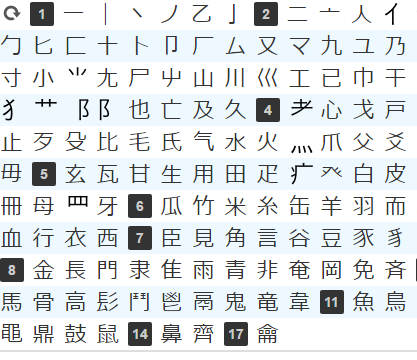
\includegraphics[width=0.9\textwidth]{figs/第01章/第6課:_kanjiintro_fig/Radicals_2.png}

\end{figure}

\par{\textbf{Resource\slash Citation Note }: Image taken from www.jisho.org, an amazing online dictionary perfect for researching what you want to know about \emph{Kanji }漢字 . }

\par{ \emph{Kanji } 漢字 with the \textbf{same radical }usually have \textbf{similar meaning }. For example, the \emph{Kanji }語, 訳, 訓, and 許 all have the radical for speech, which is 言, and they all have meanings related to speech. Sometimes, radicals are used for phonetic purposes. Therefore, \emph{Kanji } 漢字 with the \textbf{same phonetic }often have \textbf{similar ON readings }. The \emph{ }characters  時, 持, and 侍 all have the ON reading \emph{ji }ジ because the phonetic component 寺's ON reading is \emph{ji }ジ. There are exceptions to this method of guessing an ON reading, though. For example, 待 and 特 have the readings of \emph{tai }タイ and \emph{toku }トク.  Phonetics themselves may not always play a semantic role and don't help with KUN readings. }
 
\par{ Radicals do have names. However, it isn't essential for you to know what the names of the building blocks are. It is beneficial, though, to take note of what the components of the characters you learn are. }

\par{\textbf{Curriculum Note }: The \emph{Kanji } 漢字 curriculum is still currently in its infancy, so there will eventually be more coverage concerning radicals. }
      
\section{Exceptional Readings}
 
\par{ Even as you reasonably progress in acquiring the various readings of \emph{Kanji } 漢字 as you travel down the road of Japanese literacy, you will come across many words that have irregular meanings. There are different kinds of irregularities that you will come across, but for you as the beginner, you need to simply realize that there will be words that will not have readings corresponding to the given readings of the characters. }

\begin{ltabulary}{|P|P|P|P|P|P|P|P|}
\hline 

\emph{Kanji }& \emph{Kana }& \emph{Rōmaji }& Meaning &  \emph{Kanji }& \emph{Kana }& \emph{Rōmaji }& Meaning \\ \cline{1-8}

今日 &  \textbf{きょ }う &  \emph{Kyō }& Today & 昨日 & き \textbf{の }う &  \emph{Kinō }& Yesterday \\ \cline{1-8}

大人 & お \textbf{とな }&  \emph{Otona }& Adult & 合羽 & か \textbf{っぱ }&  \emph{Kappa }& Raincoat \\ \cline{1-8}

\end{ltabulary}
\hfill\break
 Exceptions are not fun, but it is important to understand that it is because Japanese is not related to Chinese that there are words with irregular spellings. Not all phrases are made the same way in both languages. Next Lesson \textrightarrow  第6課: The 10 Major Aspects      

% http://www.imabi.net/10majoraspects.htm
     
\chapter{The 10 Major Aspects of Japanese}

\begin{center}
\begin{Large}
第7課: The 10 Major Aspects of Japanese 
\end{Large}
\end{center}
 
\par{ Japanese ( \emph{Nihongo }日本語) is a major world language. Depending on how one defines a language, it may be ranked as the eighth to the tenth most spoken language. Japanese is predominantly spoken in Japan. In Japanese, "Japan" is called 日本, which is usually pronounced as \emph{Nihon }にほん, but it may also be pronounced as \emph{Nippon }にっぽん. \emph{Nippon }is favored in formal settings, but in reality, \emph{Nihon }and \emph{Nippon }are both used in many of the same situations. The country is formally called \emph{Nipponkoku }日本国 (the nation of Japan). }

\par{ The country of Japan is said to have been founded by Emperor Jimmu ( \emph{Jimmu Ten'nō }神武天皇) on February 11, 660 B.C. Its national flag is called the \emph{Hinomaru }日の丸, a reference to it being the land of the rising sun. In this lesson, you will learn about ten of the most important aspects of Japanese. In doing so, the mysteries of Japanese grammar that will be unraveled in the lessons that follow won't be so mysterious after all. }

\par{ Before delving into what Japanese is, let's first address one concern you've likely had thus far: how to say basic everyday expressions. Below are some of those most important phrases that you can use with Japanese speakers. }

\begin{itemize}

\item Good morning: \emph{O-hayō gozaimasu }おはようございます \hfill\break

\item Good afternoon\slash Hello: \emph{Kon'nichi wa }こんにちは \hfill\break

\item Good evening: \emph{Komban wa }今晩は 
\item Good night: \emph{O-yasumi-nasai }お休みなさい 
\item How are you doing?: \emph{O-genki desu ka? }お元気ですか 
\item Nice to meet you: \emph{Hajimemashite 初めまして }
\item Thank you: \emph{Arigatō gozaimasu }ありがとうございます 
\item Yes: \emph{Hai }はい 
\item No: \emph{Iie }いいえ 
\item I'm sorry\slash Excuse me: \emph{Sumimasen }すみません 
\end{itemize}
 The ten aspects that are to be studied in this lesson are as follows: 
\begin{enumerate}

\item The Sounds 
\item A Mixed Script 
\item Word Order \hfill\break

\item Parts of Speech 
\item Agglutination 
\item Speech Styles 
\item Spoken vs Written Language 
\item Etymology 
\item Language Isolate 
\item Dialects 
\end{enumerate}
      
\section{I: The Sounds}
 
\par{ Words are composed of sounds, and every language has its own set of rules that govern how sounds come together to make words. These rules are collectively referred to as the \textbf{phonology }of a language. How sounds simply sound is referred to as the \textbf{phonetics }of a language. }

\begin{center}
\textbf{The Vowels }
\end{center}

\par{ A \textbf{vowel }is a \emph{speech sound made by vibrating the vocal colds without obstructing airflow from the lungs }. In Japanese, there are only five vowels: \slash a\slash , \slash i\slash , \slash u\slash , \slash e\slash , and \slash o\slash . However, they aren't exactly like their English counterparts. To learn how they differ, we need to learn more about what vowels are. }

\par{ \textbf{High vowels }are made with the tongue raised high. Oppositely, \textbf{low vowels }are made with the tongue lowered. \textbf{Front vowels }are made by placing the tongue as close to the front of the mouth as possible. Oppositely, \textbf{back vowels }are made by placing the tongue as far back in the mouth as possible. \hfill\break
}

\par{\textbf{Chart Note }: The diagram below maps out the vowels of Japanese in a vowel space that is meant to represent the dimensions of height and forwardness in the mouth. The further left you go, the closer your tongue is to the front of the mouth. The further right you go, the father your tongue is from the front of the mouth. The further up you go, the higher up the tongue is. The further down you go, the lower the tongue is. }

\begin{figure}[h]
\centering

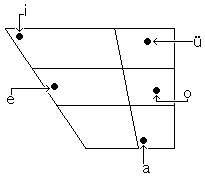
\includegraphics[width=0.9\textwidth]{figs/第01章/第7課:_10majoraspects_fig/Vowel_chart.png}

\end{figure}
 
\par{ The vowel \slash a\slash  is made by with the tongue low but central in the mouth. It is more like the "a" sound found in British English or Spanish. The vowel \slash i\slash  is made with the tongue raised high in the front of the mouth. The vowel \slash u\slash  is also a high-vowel, but it's made with the tongue in the back of the mouth. In the diagram above, it is marked with a diaeresis (two dots) to indicate that it is not made while rounding the lips like its English counterpart. The vowels \slash e\slash  and \slash o\slash  are made with the tongue at the center of the mouth. Whereas \slash e\slash  is made by placing the tongue closer to the front, \slash o\slash  is made by placing the tongue back in the mouth. }

\par{\textbf{Curriculum Note }: Various things can happen phonetically to vowels in Japanese. They may become elongated, nasalized, and even devoiced. To learn more about these processes, see Lesson 365. }

\begin{center}
\textbf{The Consonants }
\end{center}

\par{ In Lesson 2  , we learned about the various consonant sounds of Japanese. A \textbf{consonant }is \emph{a speech sound made by obstructing the airflow from the lungs in some manner }. }

\par{ Consonants come in four broad categories: unvoiced, voiced, palatalized, and nasal. Unvoiced consonants are made by not vibrating the vocal cords. Voiced consonants are made by vibrating the vocal folds. Palatal consonants are made by placing the body of the tongue against the hard palate of the mouth. Lastly, nasal consonants are made by redirected some of the air exhaled from the lungs through the nose. }

\begin{itemize}

\item \textbf{Unvoiced Consonants }( \emph{Museion }無声音): \slash k\slash , \slash s\slash , \slash sh\slash , \slash t\slash , \slash ts\slash , \slash ch\slash , \slash h\slash , f\slash , \slash p\slash . 
\item \textbf{Voiced Consonants }( \emph{Yūseion }有声音): \slash g\slash , \slash z\slash , \slash j\slash , \slash d\slash , \slash dz,\slash  dj\slash , \slash b\slash , \slash n\slash , \slash m\slash , \slash r\slash , \slash y\slash , \slash w\slash . 
\item \textbf{Palatal Consonants }( \emph{Yō'on }拗音): \slash ky\slash , \slash gy\slash , \slash sh\slash , \slash j\slash , \slash dj\slash , \slash hy\slash , \slash py\slash , \slash by\slash , \slash ry\slash , \slash y\slash . 
\item \textbf{Nasal Consonants }( \emph{Bion }鼻音): \slash n\slash , \slash ny\slash , \slash m\slash , \slash my\slash , \slash N\slash . 
\end{itemize}

\par{ There is some overlap between these categories, but this is only natural. The categorization of the consonants above does not take into account variations of the same consonant (allophones). To learn more about allophones and the articulation of each kind of consonant, see Lesson 366. }

\par{ You may remember the terms \emph{seion }清音, \emph{dakuon }濁音, \emph{handakuon }半濁音, and \emph{yō'on }拗音 when we learned about \emph{Kana }仮名. However, they don't 100\% match with the terms above because they describe how sounds have been traditionally categorized. }

\begin{itemize}

\item Any consonant in the Table of 50 Sounds (Goj \emph{ū }onzu 五十音図) is a seion 清音. 
\item A consonant written with a \emph{dakuten }゛is a \emph{dakuon }濁音. It excludes other sounds that vibrate the vocal folds such as vowels, \slash n\slash , \slash m\slash , \slash r\slash , \slash y\slash , and \slash w\slash . 
\item A consonant written with a \emph{handakuten }゜is a \emph{handakuon }半濁音. This term only refers to \slash p\slash , which phonetically is no different other than unvoiced consonants. 
\item A consonant written with a small y- \emph{kana i }s a \emph{yō'on }拗音. This term is the Japanese equivalent of "palatal sound." 
\item Another word you may encounter is \emph{bidakuon }鼻濁音, which refers to pronouncing \slash g\slash  as \slash ng\slash . 
\end{itemize}

\begin{center}
\textbf{The Mora } 
\end{center}

\par{ Unlike English, the basic syllabic structure in Japanese is a mora-based system. A \textbf{mora } \emph{is a unit of sound that is equivalent to a single beat }. Each "beat" is conceptualized as being equal in length, and each beat is assigned a high or low pitch. }

\par{ In reality, morae are not always exactly equal in length, but this is how they are conceptualized. This is then reflected in the writing system. \emph{Kana }仮名 isn't a syllabary. Rather, it's a moraic system which denotes separate characters to each sound (combination) that can be treated as a mora in Japanese. This includes the moraic consonant \slash N\slash , which is written in \emph{Kana }仮名 as ん・ン. }

\par{ The moraic sound system helps explain why Japanese distinguishes between short and long vowels as well as single (short) and double (long) consonants. \textbf{Long vowels }are deemed as two morae, whereas \textbf{short vowels }are deemed as one mora. Similarly, \textbf{double consonants }--written with っ・ッ-- are deemed as two morae, whereas \textbf{single consonants }are deemed as one mora. }

\begin{ltabulary}{|P|P|P|P|}
\hline 

Short Vowels & Long Vowels & Single Consonants & Double Consonants \\ \cline{1-4}

 \emph{Soto }外 (Outside) &  \emph{Sōtō }相当 (Considerable) &  \emph{Soto }外 (Outside) &  \emph{Sotto }そっと (Gently) \\ \cline{1-4}

 \emph{Koko }ここ (Here) &  \emph{Kōkō }高校 (High School &  \emph{Koko }ここ (Here) &  \emph{Kokko }国庫 (Treasury) \\ \cline{1-4}

\end{ltabulary}

\begin{center}
\textbf{Pitch Accent }\hfill\break

\end{center}

\par{ Japanese has a \textbf{pitch accent system }. Every mora of a phrase is assigned a high or low pitch. In Standard Japanese, there are only four possible pitch patterns that a phrase can have. Although the allocation of what phrase gets what pattern is arbitrary, the natures of these patterns themselves are not. }

\par{\textbf{Chart Notes }: \hfill\break
1. "L" and "H" both stand for a single mora. That means H-L is two morae, whereas H-L-L is three morae. As a reminder of this, numbers will be placed after these contour notations to tell you how many morae words involved have. \hfill\break
2. The "L" and "H" in parentheses indicate what the pitch of something attached to words would be per pattern. }

\begin{ltabulary}{|P|P|P|}
\hline 

頭高型 \hfill\break
 \emph{Atamadakagata }& Pitch is \textbf{high for the first mora, }drops on the second mora, and stays low for any remaining morae that follow. \hfill\break
Ex. H(-L) ①, H-L(-L) ②, H-L-L(-L) ③, H-L-L-L(-L) ④ &  \emph{\textbf{há }shì }箸(chopsticks) \\ \cline{1-3}

中高型 \hfill\break
 \emph{Nakadakagata }& Pitch starts low on the first mora, \textbf{peaks at high pitch on the middle mora(e) }, drops back to low pitch on the third morae, and stays low for any following morae after the word. \hfill\break
Ex. L-H-L ③, L-H-H-L ④ &  \emph{ha \textbf{n }}\emph{\textbf{á }}\emph{su }話す (to speak) \\ \cline{1-3}

尾高型 \hfill\break
 \emph{Odakagata }& Pitch starts low on the first mora, peaks at high pitch on the last mora, and then \textbf{drops to low pitch on any morae that follow the word }. \hfill\break
Ex. L-H-(L) ②, L-H-H(-L) ③ &  \emph{hà \textbf{shí }}橋 (bridge) \hfill\break
\\ \cline{1-3}

平板型 \hfill\break
 \emph{Heibangata }& Pitch starts low on the first mora, becomes high pitch on the second mora, and then the pitch stays high even once the word is over unto anything that follows. \hfill\break
Ex. L(-H) ①, L-H(-H) ②, L-H-H(-H) ③, L-H-H-H(-H) ④ &  \emph{ha \textbf{shi }}\textbf{ }端 \textbf{ }(edge) \\ \cline{1-3}

\end{ltabulary}

\par{ Although these are the four pitch patterns of Japanese phrases, there are many processes that can change the pitch pattern of a word from one to another, especially as a phrase becomes further complex. There are also generational and dialectical differences that further complicate this basic understanding of pitch accent. The best way to acquire the Standard Japanese pitch accent system is to mimic native speakers who grew up with Standard Japanese as their primary dialect, which can be said for most people that live in and around Tokyo. }

\par{\textbf{Curriculum Note }: To learn more about pitch accent, see Lesson 368. }

\par{\textbf{Chart Note }: H and L both stand for a single mora. That means H-L is two morae, whereas H-L-L is three morae. As a reminder of this, numbers will be placed after these contour notations to tell you how many morae words involved have. }

\begin{ltabulary}{|P|P|P|}
\hline 

1 & Pitch is \textbf{high for the first mora, }drops on the second, and stays low for any remaining morae. \hfill\break
Ex. H(-L) ①, H-L ②, H-L-L ③, H-L-L-L ④ &  \emph{\textbf{há }shì }(chopsticks) \\ \cline{1-3}

2 & Pitch starts low on the first mora, \textbf{peaks on the middle mora(e) }, drops back to low on the third morae, and stays low for any following morae after the word. \hfill\break
Ex. L-H-L ③, L-H-H-L ④ &  \emph{ha \textbf{n }}\emph{\textbf{á }}\emph{su }(to speak) \\ \cline{1-3}

3 & Pitch starts low on the first mora, peaks on the last mora, and then \textbf{drops to low on any morae following after the word }. The L in parentheses in the example notations below indicate the start of something attached. \hfill\break
L-H-(L) ②, L-H-H(-L) ③ &  \emph{hà \textbf{shí }}(bridge) \hfill\break
\\ \cline{1-3}

4 & Pitch starts low on the first mora, becomes high pitch on the second mora, and then the pitch stays high even once the word is over unto anything that follows. The H in parentheses in the example notations below indicate the start of something attached. \hfill\break
Ex. L(-H) ①, L-H(-H) ②, L-H-H(-H) ③, L-H-H-H(-H) ④ &  \emph{ha \textbf{shi }}\textbf{ }(edge) \\ \cline{1-3}

\end{ltabulary}

\par{\textbf{Chart Note }: H and L both stand for a single mora. That means H-L is two morae, whereas H-L-L is three morae. As a reminder of this, numbers will be placed after these contour notations to tell you how many morae words involved have. }

\begin{ltabulary}{|P|P|P|}
\hline 

1 & Pitch is \textbf{high for the first mora, }drops on the second, and stays low for any remaining morae. \hfill\break
Ex. H(-L) ①, H-L ②, H-L-L ③, H-L-L-L ④ &  \emph{\textbf{há }shì }(chopsticks) \\ \cline{1-3}

2 & Pitch starts low on the first mora, \textbf{peaks on the middle mora(e) }, drops back to low on the third morae, and stays low for any following morae after the word. \hfill\break
Ex. L-H-L ③, L-H-H-L ④ &  \emph{ha \textbf{n }}\emph{\textbf{á }}\emph{su }(to speak) \\ \cline{1-3}

3 & Pitch starts low on the first mora, peaks on the last mora, and then \textbf{drops to low on any morae following after the word }. The L in parentheses in the example notations below indicate the start of something attached. \hfill\break
L-H-(L) ②, L-H-H(-L) ③ &  \emph{hà \textbf{shí }}(bridge) \hfill\break
\\ \cline{1-3}

4 & Pitch starts low on the first mora, becomes high pitch on the second mora, and then the pitch stays high even once the word is over unto anything that follows. The H in parentheses in the example notations below indicate the start of something attached. \hfill\break
Ex. L(-H) ①, L-H(-H) ②, L-H-H(-H) ③, L-H-H-H(-H) ④ &  \emph{ha \textbf{shi }}\textbf{ }(edge) \hfill\break
\hfill\break
\\ \cline{1-3}

\end{ltabulary}

\par{\textbf{Chart Note }: H and L both stand for a single mora. That means H-L is two morae, whereas H-L-L is three morae. As a reminder of this, numbers will be placed after these contour notations to tell you how many morae words involved have. }

\begin{ltabulary}{|P|P|P|}
\hline 

1 & Pitch is \textbf{high for the first mora, }drops on the second, and stays low for any remaining morae. \hfill\break
Ex. H(-L) ①, H-L ②, H-L-L ③, H-L-L-L ④ &  \emph{\textbf{há }shì }(chopsticks) \\ \cline{1-3}

2 & Pitch starts low on the first mora, \textbf{peaks on the middle mora(e) }, drops back to low on the third morae, and stays low for any following morae after the word. \hfill\break
Ex. L-H-L ③, L-H-H-L ④ &  \emph{ha \textbf{n }}\emph{\textbf{á }}\emph{su }(to speak) \\ \cline{1-3}

3 & Pitch starts low on the first mora, peaks on the last mora, and then \textbf{drops to low on any morae following after the word }. The L in parentheses in the example notations below indicate the start of something attached. \hfill\break
L-H-(L) ②, L-H-H(-L) ③ &  \emph{hà \textbf{shí }}(bridge) \hfill\break
\\ \cline{1-3}

4 & Pitch starts low on the first mora, becomes high pitch on the second mora, and then the pitch stays high even once the word is over unto anything that follows. The H in parentheses in the example notations below indicate the start of something attached. \hfill\break
Ex. L(-H) ①, L-H(-H) ②, L-H-H(-H) ③, L-H-H-H(-H) ④ &  \emph{ha \textbf{shi }}\textbf{ }(edge) \\ \cline{1-3}

\end{ltabulary}

\par{ In the first contour, H-L, the pitch of the word starts high but then drops and stays low. That means if a word with this contour were to have several morae, all morae after the first one would be low in pitch. This means a word with Pattern 1 could be H-L, H-L-L, or H-L-L-L. Remember, pitches only have "high" or "low" pitch. This means H-L-L would refer to a word made up of three morae and H-L-L-L would refer to a word made up of four morae. }
      
\section{II: A Mixed Script}
 
\par{ Although writing is not the same thing as language, it is inexplicably tied to language. The Japanese writing system is the most complex script in the world. This is because it is composed of \textbf{four }different types of symbols. As we have already partly covered Japanese writing, this section will delve more into information about the system as a whole to give you a better understanding of why it is the way it is. }

\par{1) \emph{Kanji }漢字 \textbf{ }}

\begin{center}
\textbf{How \emph{Kanji }漢字 Came to Japan } \hfill\break

\end{center}

\par{\textbf{ \emph{Kanji } }漢字 \textbf{ }are Chinese characters brought to Japan from China via Korea around the beginning of the fifth century. Not soon afte r these characters were introduced, a Japanese writing system called \emph{Man'yōgana }万葉仮名 was created. It is called this because it was largely used in a compilation of poems written in Old Japanese called the \emph{Man'yōshū }万葉集. This system behaved like a syllabary, but characters were often used for their meanings as is the case today. To learn more about this ancient writing system, see Lesson 410. }

\begin{center}
\textbf{The Radicals }
\end{center}

\par{\emph{ Kanji }漢字 are composed of one or more building blocks called radicals, or \emph{bushu }部首 in Japanese. There are 214 such so-called radicals, and with these radicals, most characters fall under four types: }

\begin{enumerate}

\item \textbf{\emph{Shōkei Moji }象形文字 (Pictograms) }: These characters resemble what they mean. It is      generally the case that they looked more similar to what they represent earlier in history, but many still resemble what they mean. \hfill\break
Ex. 日 (sun\slash day), 月 (moon\slash month), 山 (mountain), 鳥 (bird), 木 (tree), 魚 (fish), 龍 (dragon) 
\item \textbf{\emph{Shiji moji }指示文字 (Ideograms) }: These characters      are abstract pictograms, more often referred to as ideograms. \hfill\break
Ex. 一 (one), 二 (two), 三 (three), 上 (above), 下 (below) 
\item \textbf{\emph{Kaii Moji }会意文字 (Compound Ideograms) }: These characters combine one or elements to express a certain meaning. \hfill\break
Ex. 休 (rest), 森 (forest\slash grove), 好 (like), 明 (bright), 信 (believe). 
\item \emph{\textbf{Keisei Moji }}\textbf{形成文字 (Semasio-Phonetic) }: About 90\% of all characters are this type. They are composed of two parts: a semantic indicator(s) and a phonetic indicator(s). Both indicators are based on the Chinese language rather than the Japanese language. Ex. 河 (river), 湖 (lake), 流 (flow), 沖 (offing), 江 (inlet). \hfill\break
Note: In these characters,      the left side indicates meaning while the right side indicates sound. 
\end{enumerate}

\par{\textbf{Curriculum Note }: To learn more about \emph{bushu }部首, see Lesson 359. }

\begin{center}
\textbf{How Many Symbols are There? }\hfill\break

\end{center}

\par{ The number of \emph{Kanji }漢字 that exist in Japanese is uncertain. The \emph{Kanjigen }漢字源 is the most realistic Chinese-Japanese character dictionary ( \emph{Kanwa Jiten }漢和辞典) for Japanese, having 9,990 entries. This does not mean that Japanese speakers know 9,990 characters. Although a small percentage might, the most comprehensive proficiency test for proficiency, the \emph{Kanji Nōryoku Kentei Ikkyū }漢字能力検定一級, only covers approximately 6,000 Kanji. Yet, only about 10\% of applicants pass this test--some of whom are foreign test takers. }

\par{ The \emph{Jōyō Kanji List }, which is a list that the Japanese Ministry of Education has put forth to create a literary baseline for compulsory education, bureaucratic documents and publications, and general use. As of 2017, 2,136 characters have been designated as \emph{Jōyō Kanji }常用漢字. Additional characters used primarily for names, are designated as \emph{Jimmeiyō Kanji }人名用漢字, of which a total of 862 exist as of 2017. Generally speaking, most competent readers know over 3,000 characters, and due to the ease of typing, this average is steadily rising. }

\begin{ltabulary}{|P|P|}
\hline 

Examples of \emph{Jōyō Kanji }常用漢字 & Examples of \emph{Jimmeiyō Kanji }人名用漢字 \\ \cline{1-2}

雨, 広, 今, 力, 非, 明, 貝, 眠, 央, 芸, 減 & 丑, 之, 乎, 也, 云, 亘, 伊, 伍, 吾, 昌, 胡, 辰, 遥 \\ \cline{1-2}

\end{ltabulary}

\begin{center}
\textbf{\hfill\break
The Two Kinds of Readings }
\end{center}

\par{ There are two kinds of readings emerged: \emph{on'yomi }音読み (readings from Chinese) and \emph{kun'yomi }訓読み (readings from native words). Most \emph{Kanji }漢字 have \emph{on'yomi }音読み as they \emph{ }are inherently characters borrowed from China. The \emph{on'yomi }音読み of a character can usually be guessed with relative ease as most characters have a phonetic component, as mentioned earlier. Many characters were also attributed to native vocabulary, thus providing them with one or more \emph{kun'yomi }訓読み. }

\par{\textbf{Chart Note }: \emph{On'yomi }音読み are listed in \emph{Katakana }カタカナ and \emph{kun'yomi }訓読み are listed in \emph{Hiragana }ひらがな for brevity as well as to provide an opportunity to practice your \emph{Kana }仮名 skills. \emph{Kana }仮名 in parentheses are \emph{okurigana }送り仮名, which usually spell out word inflections and enable said readings to be valid. }

\begin{ltabulary}{|P|P|P|P|}
\hline 

 \emph{Kanji }漢字 & Meaning(s) &  \emph{On'yomi }音読み &  \emph{Kun'yomi }訓読み \\ \cline{1-4}

息 & Breath\slash rest & ソク & いき \\ \cline{1-4}

植 & To plant & ショク & う(える) \\ \cline{1-4}

宮 & Palace & キュウ・グウ・ク & みや \\ \cline{1-4}

院 & Institute & イン &  \\ \cline{1-4}

間 & Space\slash gap & カン・ケン & あいだ・ま \\ \cline{1-4}

\end{ltabulary}

\par{\textbf{Curriculum Note }: There are various kinds of both kinds of readings. Knowledge of these kinds gives reasons for why many characters have so many readings. To learn more about this, see Lesson 354. \hfill\break
}

\begin{center}
\textbf{Japanese-Made Symbols } \hfill\break

\end{center}

\par{ However, there is also such thing as \emph{Kanji }漢字 made in Japan. These are called \emph{Kokuji }国字. Some of these characters do have \emph{on'yomi }音読み attributed to them, and some of these characters have even made their way into Chinese. }

\par{\textbf{Notation Note }: For the characters described below, the same notation conventions for readings as used in the chart above are implemented. }

\begin{itemize}

\item 働: Meaning "work," it has the readings ドウ and はたら(く). It is also now used in Mandarin Chinese. 
\item 匂: Meaning "smell," it has the reading にお(う). 
\item 塀: Meaning "wall\slash fence," it has the readings ヘイ and ベイ, but these readings were formed by using a radical indicating a Chinese phonetic; the character itself is actually not used in Mandarin Chinese. 
\item 峠: Meaning "mountain peak," it has the reading とうげ. The reading is spelled as とうげ rather than とおげ because it was once たむけ >たうげ , lending its current form, whereas instances of おお typically derive from おほ. 
\item 榊: Meaning "sacred Shinto tree," it has the reading さかき. 
\item 込: Meaning "include," it has the reading こ(む). 
\item 枠: Meaning "framework," it has the reading わく. 
\item 畑: Meaning "field," it has the readings はた \& はたけ. 
\item 腺: Meaning "gland," it has the reading セン. It was created by using the Chinese phonetic element 泉, lending the sound セン. This character is now also used in Mandarin Chinese. 
\item 雫: Meaning "raindrop," it has the reading しずく. 
\end{itemize}
\textbf{Curriculum Note }: To learn more about \emph{Kokuji }国字, see Lesson 360. 
\begin{center}
\textbf{Character Simplification } \hfill\break

\end{center}

\par{ If you are a reader of Traditional Chinese or can read Hanja in Korean, you may notice that many \emph{Kanji }漢字 don't look the same. This is because many \emph{Kanji }漢字 were simplified after World War II. The old forms of characters are called \emph{Kyūjitai }旧字体 whereas the new forms are called \emph{Shinjitai }新字体. The old forms may still be used in proper nouns as well as in publications printed in the 1960s and beforehand. Below are a handful of some of the characters that were altered. }

\begin{ltabulary}{|P|P|P|P|P|P|}
\hline 

Meaning(s) & Traditional Form & New New Form & Meaning(s) & Traditional Form & New Form \\ \cline{1-6}

Yen\slash circle & 圓 & 円 & Learning & 學 & 学 \\ \cline{1-6}

Spirit & 氣 & 気 & Old & 舊 & 旧 \\ \cline{1-6}

Meet & 會 & 会 & Return & 歸 & 帰 \\ \cline{1-6}

\end{ltabulary}

\par{\textbf{Curriculum Note }: To learn more about \emph{Kanji }漢字 simplification, see Lesson 361. }

\par{2) \& 3) \emph{Kana }仮名: \emph{Katakana }片仮名 \& \emph{Hiragana }平仮名 }

\par{ From \emph{Kanji }漢字, \emph{Katakana }カタカナ and \emph{Hiragana }ひらがな were created, both of which are \emph{Kana }仮名. Each set consists of a basic pool of 48 characters. Intrinsically, they only have phonetic value whereas \emph{Kanji }漢字 usually have both semantic and phonetic value(s). }

\par{\textbf{Chart Note }: The chart to the left illustrates the origin of \emph{Hiragana }ひらがな, and the chart to the right illustrates the origin of \emph{Katakana }カタカナ. }
 
\begin{figure}[h]
\centering

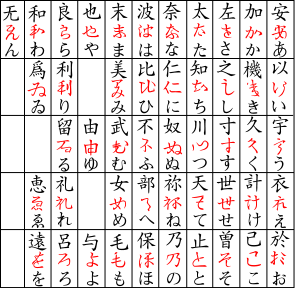
\includegraphics[width=0.9\textwidth]{figs/第01章/第7課:_10majoraspects_fig/Hiragana_Origins.png}

\end{figure}

\begin{figure}[h]
\centering

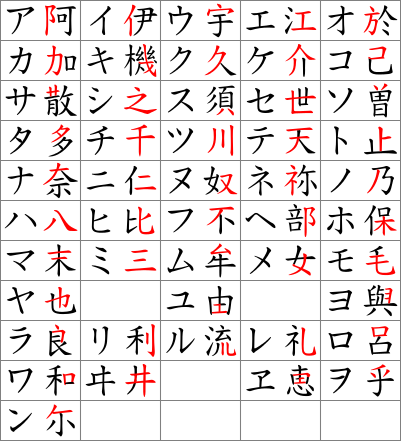
\includegraphics[width=0.9\textwidth]{figs/第01章/第7課:_10majoraspects_fig/Katakana_Origins.png}

\end{figure}

\par{\textbf{History Note }: The first system to be created was \emph{Katakana }カタカナ. It was created thanks to Buddhist monks simplifying the manuscript forms of characters. \emph{Hiragana }ひらがな was created by simplifying the cursive form of characters. \emph{Katakana }カタカナ used to be called "man's hand ( \emph{otokode }男手)" and \emph{Hiragana }ひらがな used to be referred to as "woman's hand ( \emph{on'nade }女手)" as the choice for what script one used was once largely based on one's gender. }

\par{ \emph{Hiragana }ひらがな is seen the most as it is used to spell most words that aren't from foreign languages which \emph{Kanji }漢字 may not be practical or possible. }

\begin{itemize}

\item \textbf{Inflection }- Ex. \emph{Atarashii }新 \textbf{しい }: the part that conjugates is left in \emph{Hiragana }ひらがな. 
\item \textbf{\emph{Kanji }漢字 Replacement }- Ex. \emph{Shiwa }しわ: The symbol 皺 is often deemed too complicated. 
\end{itemize}

\par{\emph{ Katakana }カタカナ is largely used to write foreign loan-words from modern world languages. This includes modern borrowings from Chinese languages. }

\begin{ltabulary}{|P|P|P|P|P|P|}
\hline 

Loan-word & Meaning & Language & Loan-word & Meaning & Language \\ \cline{1-6}

シュウマイ & Barbecued pork & Cantonese & ピザ & Pizza & Italian \\ \cline{1-6}

スポイト & Dropper & Dutch & トナカイ & Reindeer & Ainu \\ \cline{1-6}

\end{ltabulary}

\par{ \emph{Katakana }カタカナ may also be used to write onomatopoeia or used to italicize expressions and even entire sentences. Its purpose for italicization is used heavily in Japanese dictionaries. }

\begin{itemize}

\item \textbf{Italicization }- Ex. \emph{megane }メガネ: Meaning "glasses," this word is typically spelled as 眼鏡. 
\item \textbf{Onomatopoeia }- Ex. \emph{dokan }ドカン (boom). 
\end{itemize}

\par{\textbf{Curriculum Note }: To learn about \emph{Kana }仮名, see also Lessons 3, 4, 355, 356, 357, 364. }

\par{4) English Letters ( \emph{R }\emph{ō }\emph{maji ローマ }字) }

\par{ Though Japanese is largely written with a mix of \emph{Kanji }漢字 and \emph{Kana }仮名, English letters have become incorporated into the spellings of many word, mostly newly coined words. }

\begin{ltabulary}{|P|P|P|P|}
\hline 

 \emph{Piiāru }PR & Public relations &  \emph{Ōeru }OL & Office lady \\ \cline{1-4}

 \emph{Shiidii }CD & CD &  \emph{Diibuidii }DVD & DVD \\ \cline{1-4}

 \emph{Emubui }MV & Music video &  \emph{Tiishatsu }Tシャツ & T-shirt \\ \cline{1-4}

 \emph{Shiiemu }CM & Commercial &  \emph{Piiemu nii ten go }PM2.5 & Particle matter 2.5 \\ \cline{1-4}

 \emph{Eichiaibui }HIV & HIV &  \emph{Erujiibiitii }LGBT & LGBT \\ \cline{1-4}

\end{ltabulary}
\textbf{\hfill\break
Punctuation } Punctuation has largely been borrowed from the Western tradition, but the punctuation marks and rules associated with punctuation have evolved into something quite different. 
\par{ Firstly, there are no spaces between words, and you write to the next line even if this breaks up a word. Text may go down from left to right or down from right to left. Horizontal text was historically right to left. The most basic punctuation marks are shown below. }

\begin{ltabulary}{|P|P|P|P|P|P|P|P|}
\hline 

、 & The comma & 。 & The period & ! & The exclamation mark & ? & The question mark \\ \cline{1-8}

\end{ltabulary}

\par{ Punctuation marks are written with the same space as regular characters. Commas are often where particles are omitted. ! and ? have been borrowed for emphatic purposes to further demonstrate tone and emotion. }

\par{1. ${\overset{\textnormal{わたし}}{\text{私}}}$ は(、)これが ${\overset{\textnormal{す}}{\text{好}}}$ きです。 \hfill\break
\emph{Watashi wa(,) kore ga suki desu. }\hfill\break
I like this. }

\par{2. なに? \hfill\break
\emph{Nani? }\hfill\break
What? }

\par{3. はい! \hfill\break
\emph{Hai! \hfill\break
}Yes!  }

\par{\textbf{Curriculum Note }: To learn more about punctuation, see Lesson 346. }
      
\section{III: Word Order}
 
\begin{center}
\textbf{Basic Word Order } 
\end{center}

\par{ In Japanese, the basic word order is SOV. This stands for subject-object-verb. These terms are defined as follows: }

\begin{itemize}

\item \textbf{Subject }: \emph{The item of discussion in a sentence. }\hfill\break

\item \textbf{Object }: \emph{What an action is directed at. }\hfill\break

\item \textbf{Verb }: \emph{An action or state of being. }
\end{itemize}
 
\par{ Though the basic word order of Japanese involves these parts of a sentence as such, the subject and object may flip positions depending on what is deemed more important to the speaker, and a sentence may be without either or both yet still be grammatical. This means that Japanese exhibits all of the following word orders: SOV, OSV, SV, and OV. Of these,the least frequently used is the OSV word order; however, it is still occasionally used nonetheless. }

\par{ In between the subject and object of a sentence are words called particles. Particles are \textbf{post-positions }that equate to the prepositions of English that indicate the grammatical function(s) of what they follow. }
\hfill\break

\par{\textbf{SOV }\hfill\break
4. クマが ${\overset{\textnormal{さかな}}{\text{魚}}}$ を ${\overset{\textnormal{た}}{\text{食}}}$ べた。 \hfill\break
\emph{Kuma ga sakana wo tabeta. \hfill\break
}The bear ate the fish. }
 
\par{\textbf{OV \hfill\break
}6. ボール + を + ${\overset{\textnormal{な}}{\text{投}}}$ げた。 \hfill\break
\emph{Bōru wo nageta. }\hfill\break
Literally: Ball threw. \hfill\break
Translation: I threw the ball. }
 
\par{\textbf{OSV }\hfill\break
5. ${\overset{\textnormal{さかな}}{\text{魚}}}$ をクマが ${\overset{\textnormal{た}}{\text{食}}}$ べた \hfill\break
\emph{Sakana wo kuma ga tabeta. }\hfill\break
The bear ate the fish. }

\par{\textbf{V }\hfill\break
7. ${\overset{\textnormal{うた}}{\text{歌}}}$ った 。 \hfill\break
\emph{Utatta. \hfill\break
}Literally: Sang. \hfill\break
Translation: I sang.  }

\begin{center}
\textbf{Left-Branching }
\end{center}

\par{ In grammar, "left-branching" refers to modifiers preceding their constituents. For instance, in the English phrase "a tall man," the word "tall" modifies the word "man." This is an example of left-branching in English. However, in English, when a modify becomes too long\slash complex, it goes after its constituent. This is called right-branching. In the examples below, the constituent is in bold while their modifiers are italicized. }

\begin{enumerate}

\item The \emph{kind }\textbf{cat  }(left-branching) 
\item The \emph{smart } \textbf{dog } (left-branching) 
\item The \textbf{cat } \emph{brought back to life } (right-branching) 
\item The \textbf{dog } \emph{chasing its tail } (right-branching) 
\end{enumerate}

\par{ In Japanese, modifiers always go before their constituents no matter how complex they are. }

\par{8. ${\overset{\textnormal{やさ}}{\text{優}}}$ しい ${\overset{\textnormal{ひと}}{\text{人}}}$ \hfill\break
 \emph{Yasashii hito \hfill\break
 }Nice person }

\par{9. ${\overset{\textnormal{がっこう}}{\text{学校}}}$ から ${\overset{\textnormal{かえ}}{\text{帰}}}$ った ${\overset{\textnormal{こども}}{\text{子供}}}$ \hfill\break
 \emph{Gakk }\emph{ō-kara kaetta kodomo \hfill\break
 }Literally: School-from returned kid \hfill\break
Translation: Child who came back from school. }

\begin{center}
\textbf{Typical Structuring of Information }\hfill\break

\end{center}

\par{  In Japanese, word order is not fixated in the way it is in English. Ultimately, the speaker can and normally will organize elements of any given sentence based on what he\slash she deems to be most to least important. However, most sentences are far more predictable than this fluid representation. Typically, information is organized with the following broad ordering. }

\begin{ltabulary}{|P|}
\hline 

TOPIC + TIME + LOCATION + SUBJECT + INDIRECT OBJECT + DIRECT OBJECT + VERB \\

\end{ltabulary}

\par{  The basic word order of SOV is reflected in this ordering, but Japanese typically puts a lot of information before the subject. }

\begin{itemize}

\item The "topic" of a sentence is what the sentence\slash discussion is about. 
\item Time phrases would include expressions such as "today, "tomorrow," etc. 
\item Location phrases would include expressions such as "at Tokyo," "in China," etc. 
\item An \textbf{indirect object }is \emph{a phrase referring to something\slash someone that is a recipient of some action }, but it isn't the primary (direct object). 
\item A \textbf{direct object }is \emph{a phrase that is primarily being affected by the verb }. 
\end{itemize}

\par{10. ${\overset{\textnormal{わたし}}{\text{私}}}$ はきょう、 ${\overset{\textnormal{えき}}{\text{駅}}}$ で ${\overset{\textnormal{ともだち}}{\text{友達}}}$ に ${\overset{\textnormal{ほん}}{\text{本}}}$ をあげました。 \hfill\break
\emph{Watashi-wa ky }\emph{ō, eki-de (ø-ga) to }\emph{modachi-ni hon-wo agemashita. \hfill\break
}Literally: I-as.for, today, station-at (I-subject.marker) friend-to book-object.marker gave. \hfill\break
Trans lation: I gave a book to a friend at the train station today. }

\par{\textbf{Grammar Notes }: \hfill\break
1. Whenever the subject and topic are the same, the subject is not stated but manifests in the grammar as an unspoken zero-pronoun. This rule comes from the general principle of obligatorily omitting syntactically redundant elements, which we'll look at next. \hfill\break
2. The typical ordering of information is almost completely opposite of that of English. }

\par{11. ${\overset{\textnormal{ぞう}}{\text{象}}}$ は ${\overset{\textnormal{はな}}{\text{鼻}}}$ が ${\overset{\textnormal{なが}}{\text{長}}}$ い。 \hfill\break
\emph{Zō-wa hana-ga nagai. }\hfill\break
Literally: Elephants-as.for nose-subject .marker long. \hfill\break
Translation: As for elephants, their noses are long\slash Elephants have long noses. }

\par{\textbf{Grammar Note }: This sentence demonstrates how the subject and topic of a sentence, though related intrinsically with each other, do not have to be the same thing. The pattern shown in this example will be of major focus for us in Lesson 12. }

\par{12. ${\overset{\textnormal{けさじしん}}{\text{今朝地震}}}$ が ${\overset{\textnormal{お}}{\text{起}}}$ きました。 \hfill\break
\emph{Kesa jishin-ga okimashita. }\hfill\break
Literally: This.morning earthquake-subject.marker occurred. \hfill\break
Translation: An earthquake occurred this morning. }

\par{\textbf{Grammar Note }: Not all verbs require objects as demonstrated in Ex. 12. This sentence is perfectly grammatical with just a time phrase, subject, and a verb. }

\par{13. ${\overset{\textnormal{あした}}{\text{明日}}}$ から ${\overset{\textnormal{かれ}}{\text{彼}}}$ に ${\overset{\textnormal{にほんご}}{\text{日本語}}}$ を ${\overset{\textnormal{おし}}{\text{教}}}$ え ${\overset{\textnormal{はじ}}{\text{始}}}$ めます。 \hfill\break
\emph{Ashita-kara kare-ni Nihongo-wo oshiehajimemasu. }\hfill\break
Literally: Tomorrow-from he-to Japanese-direct object. teach.begin. \hfill\break
I will begin teaching Japanese to him as of tomorrow. }

\par{\textbf{Grammar Note }: "To begin teaching" is expressed with a compound verb in Japanese, but the ordering of its components is the opposite of English. In Japanese, the element for "to teach" comes first, and the element for "to begin" is added as a supplementary ending. }

\begin{center}
\textbf{Omission }
\end{center}

\par{ If something is not important at all, it may be omitted altogether, even if it's an element of a sentence that may be grammatically necessary in Japanese. This is evident in how words like "I" and "you," which are a part of an overwhelming of English sentences, are frequently not stated. Of course, the decision between omitting or verbalizing something does imply change in nuance. For now, however, it's important to note that something in an English sentence may not need to transfer over to Japanese. }

\par{14. お ${\overset{\textnormal{なまえ}}{\text{名前}}}$ は ${\overset{\textnormal{なん}}{\text{何}}}$ ですか。 \hfill\break
\emph{O-namae-wa nan desu-ka? }\hfill\break
Literally: Honorific.prefix-name-as.for, name is-question.marker? \hfill\break
Translation: What is your name? }

\par{\textbf{Sentence Note }: There is no word in this example corresponding to "your." }

\par{15. セスと ${\overset{\textnormal{もう}}{\text{申}}}$ します。  \hfill\break
\emph{Sesu-to mōshimasu. }\hfill\break
Literally: Seth-citation.marker called. \hfill\break
Translation: I go by Seth. }

\par{\textbf{Sentence Note }: There is no word in this example corresponding to "I." }

\begin{center}
\textbf{Inversion } 
\end{center}

\par{ It's even possible to mention the verb first and state everything else as an after-statement. This is called inversion. }

\par{16. ${\overset{\textnormal{かな}}{\text{叶}}}$ え、 ${\overset{\textnormal{わたし}}{\text{私}}}$ の ${\overset{\textnormal{ねが}}{\text{願}}}$ いよ。 \hfill\break
\emph{Kanae, watashi-no negai-yo. \hfill\break
}Literally: Come.true I-genitive.marker wish-exclamation.marker \hfill\break
Translation: Come true, oh my wishes.   }

\begin{center}
\textbf{Name Ordering } 
\end{center}

\par{ The hierarchy of information importance also explains why one's family name comes first in Japanese. However, it is important to note that the language actually respects the original ordering of parts of a name if it is from another language. Many learners feel like inverting their name to be more Japanese, but this is not necessary and may end up confusing Japanese people who anticipate the first part of your name to be your given name. }

\begin{ltabulary}{|P|P|P|P|}
\hline 

Barack Obama & バラック・オバマ \hfill\break
\emph{Barakku Obama }& Donald Trump & ドナルド・トランプ \hfill\break
\emph{Donarudo Torampu } \\ \cline{1-4}

Moon Jae-in & ムーン・ジェイン \hfill\break
\emph{M }\emph{ū }\emph{n Je-in } & Kim Jeong Un & 金正恩 \hfill\break
\emph{Kimu Jon Un }\hfill\break
\\ \cline{1-4}

John Smith & ジョン・スミス \hfill\break
Jon Sumisu & Ryo Watanabe & 渡辺亮 \hfill\break
 \emph{Watanabe Ry }\emph{ō }\\ \cline{1-4}

Shinzo Abe & 安倍晋三 \hfill\break
 \emph{Abe Shinzō } & Yu Darvish & ダルビッシュ有 \hfill\break
\emph{Darubisshu Yū }\\ \cline{1-4}

\end{ltabulary}
      
\section{IV: Parts of Speech}
 
\par{ Understanding part of speech ( \emph{hinshi }品詞) is a quintessential to properly harnessing the grammar of a language. As a native speaker of any language, you are privy to instinctively knowing how words relate to one another, how they are similar and dissimilar. Without knowing the names of the categories that exist in your language, you're able to naturally categorize words together in various ways. }

\par{ These categorizations, though, are language specific. Meaning, just because English has words called prepositions, that doesn't mean Japanese does as well. In fact, as we have learned already, prepositions really don't exist in Japanese. Instead, they're replaced by something called particles (post-positions). This, though, is just one instance of how the two languages differ. }

\par{ To begin learning what the parts of speech are in Japanese, it's important to first answer a seemingly simple yet difficult question: what is a word? For English speakers, a word is anything that is written as one unit. In writing, we distinguish words by spaces. However, spacing doesn't always do justice to a word count. Take for instance the following phrases. }

\par{v. Don't (1-2 words) \hfill\break
vi. Music video (1-2 words) }

\par{ The phrase "don't" is a contraction of "do" and "not." Native English speakers typically conceptualize this as one word and do not necessarily deconstruct it in their minds when they use it. Likewise, the phrase "music video" refers specifically to a certain thing that is not solely music nor solely a video. In that sense, you could say it's one word, whereas if you go solely by its spelling you would say that it is two words. Because the word "word" is very vague, for linguistic purposes, the word morpheme is preferred. A morpheme is the smallest unit of meaning that cannot be divided further. This compartmentalization of meaning enables us to properly and objectively study Japanese phrasing for what it is rather than looking at it through an English-stilted mindset. For discussions that follow, depending on how specific things need to be broken up, "word" or "morpheme" will be used. }

\begin{center}
\textbf{Independent VS Ancillary Words }
\end{center}

\par{ There are two kinds of words in Japanese: independent words ( \emph{jiritsugo }自立語) and ancillary words ( \emph{fuzokugo }付属語. Independent words are those that can stand alone. Independent words can further be broken down into conjugatable and non-conjugatable words. Ancillary words, however, cannot stand alone. They too, though, may or may not be conjugatable. }

\par{ In Japanese, there are twelve unique parts of speech that can be classified as either independent or ancillary words. }

\begin{itemize}

\item  Independent Words  ( \emph{Jiritsugo }自立語) \hfill\break
\hfill\break
ー Conjugatable  \hfill\break
\hfill\break
・Verbs ( \emph{Dōshi }動詞)\dothyp{}\dothyp{}\dothyp{}\dothyp{}\dothyp{}\dothyp{}\dothyp{}\dothyp{}\dothyp{}\dothyp{}\dothyp{}\dothyp{}\dothyp{}\dothyp{}\dothyp{}\dothyp{}\dothyp{}\dothyp{}\dothyp{}\dothyp{}\dothyp{}\dothyp{}\dothyp{}\dothyp{}\dothyp{}\dothyp{}\dothyp{}\dothyp{}\dothyp{}\dothyp{}\dothyp{}\dothyp{}\dothyp{}\dothyp{}\dothyp{}\dothyp{}\dothyp{}\dothyp{}\dothyp{}\dothyp{}\dothyp{}\dothyp{}\dothyp{}\dothyp{}\dothyp{}\dothyp{}\dothyp{}\dothyp{}..Lessons 16, 17, 18, etc. \hfill\break
  \emph{A \textbf{verb }is a word that describes an action, state, or occurrence. } \hfill\break
・Adjectives ( \emph{Keiyōshi }形容詞) \dothyp{}\dothyp{}\dothyp{}\dothyp{}\dothyp{}\dothyp{}\dothyp{}\dothyp{}\dothyp{}\dothyp{}\dothyp{}\dothyp{}\dothyp{}\dothyp{}\dothyp{}\dothyp{}\dothyp{}\dothyp{}\dothyp{}\dothyp{}\dothyp{}\dothyp{}\dothyp{}\dothyp{}\dothyp{}\dothyp{}\dothyp{}\dothyp{}\dothyp{}\dothyp{}\dothyp{}\dothyp{}\dothyp{}.Lessons 13, 50, 52 \hfill\break
 \emph{An \textbf{adjective }is a word that describes an attribute. }\hfill\break
・Adjectival Nouns ( \emph{Keiyōdōshi }形容動詞) \dothyp{}\dothyp{}\dothyp{}\dothyp{}\dothyp{}\dothyp{}\dothyp{}\dothyp{}\dothyp{}\dothyp{}\dothyp{}\dothyp{}\dothyp{}\dothyp{}\dothyp{}.Lessons 14, 51, 53, etc. \hfill\break
  \emph{An \textbf{adjectival noun }is a word that describes an attribute while also being noun-like. \hfill\break
}\hfill\break
ー Not Conjugatable  \hfill\break
\hfill\break
・Nouns ( \emph{Meishi }名詞)\dothyp{}\dothyp{}\dothyp{}\dothyp{}\dothyp{}\dothyp{}\dothyp{}\dothyp{}\dothyp{}\dothyp{}\dothyp{}\dothyp{}\dothyp{}\dothyp{}\dothyp{}\dothyp{}\dothyp{}\dothyp{}\dothyp{}\dothyp{}\dothyp{}\dothyp{}\dothyp{}\dothyp{}\dothyp{}\dothyp{}\dothyp{}\dothyp{}\dothyp{}\dothyp{}\dothyp{}\dothyp{}\dothyp{}\dothyp{}\dothyp{}\dothyp{}\dothyp{}\dothyp{}\dothyp{}\dothyp{}\dothyp{}\dothyp{}\dothyp{}\dothyp{}\dothyp{}\dothyp{}\dothyp{}\dothyp{}Lesson 8 \hfill\break
  \emph{A \textbf{noun }is a word that describes a person, place, state, quality, event, or thing. }\hfill\break
・Pronouns ( \emph{Daimeishi }代名詞)\dothyp{}\dothyp{}\dothyp{}\dothyp{}\dothyp{}\dothyp{}\dothyp{}\dothyp{}\dothyp{}\dothyp{}\dothyp{}\dothyp{}\dothyp{}\dothyp{}\dothyp{}\dothyp{}\dothyp{}\dothyp{}\dothyp{}\dothyp{}\dothyp{}\dothyp{}\dothyp{}\dothyp{}\dothyp{}\dothyp{}\dothyp{}\dothyp{}\dothyp{}\dothyp{}\dothyp{}\dothyp{}\dothyp{}.Lessons 8, 84, 191 \hfill\break
  \emph{A \textbf{pronoun }is a word that indirectly describes a person, direction, or thing.  }\hfill\break
・Numbers ( \emph{Sūshi }数詞)\dothyp{}\dothyp{}\dothyp{}\dothyp{}\dothyp{}\dothyp{}\dothyp{}\dothyp{}\dothyp{}\dothyp{}\dothyp{}\dothyp{}\dothyp{}\dothyp{}\dothyp{}\dothyp{}\dothyp{}\dothyp{}\dothyp{}\dothyp{}\dothyp{}\dothyp{}\dothyp{}\dothyp{}\dothyp{}\dothyp{}\dothyp{}\dothyp{}\dothyp{}\dothyp{}\dothyp{}\dothyp{}\dothyp{}\dothyp{}\dothyp{}\dothyp{}\dothyp{}\dothyp{}\dothyp{}\dothyp{}\dothyp{}\dothyp{}\dothyp{}\dothyp{}\dothyp{}Lessons 27, 28, 29, 193, etc. \hfill\break
 \emph{A \textbf{number }is a word that counts or measures entities. }\hfill\break
・Adnominal Adjectives ( \emph{Rentaishi }連体詞)\dothyp{}\dothyp{}\dothyp{}\dothyp{}\dothyp{}\dothyp{}\dothyp{}\dothyp{}\dothyp{}\dothyp{}\dothyp{}\dothyp{}\dothyp{}\dothyp{}\dothyp{}Lessons 60 \& 303 \hfill\break
  \emph{An \textbf{adnominal adjective }is a word that describes an attribute by directly modifying a noun. }\hfill\break
 ・Adverbs ( \emph{Fukushi }副詞)\dothyp{}\dothyp{}\dothyp{}\dothyp{}\dothyp{}\dothyp{}\dothyp{}\dothyp{}\dothyp{}\dothyp{}\dothyp{}\dothyp{}\dothyp{}\dothyp{}\dothyp{}\dothyp{}\dothyp{}\dothyp{}\dothyp{}\dothyp{}\dothyp{}\dothyp{}\dothyp{}\dothyp{}\dothyp{}\dothyp{}\dothyp{}\dothyp{}\dothyp{}\dothyp{}\dothyp{}\dothyp{}\dothyp{}\dothyp{}\dothyp{}\dothyp{}\dothyp{}\dothyp{}\dothyp{}\dothyp{}\dothyp{}\dothyp{}Lessons 48, 49, 154, 293, etc. \hfill\break
  \emph{An \textbf{adverb }is a word that qualifies an adjective, adjectival noun, or a verb. }\hfill\break
・Conjunctions ( \emph{Setsuzokushi }接続詞)\dothyp{}\dothyp{}\dothyp{}\dothyp{}\dothyp{}\dothyp{}\dothyp{}\dothyp{}\dothyp{}\dothyp{}\dothyp{}\dothyp{}\dothyp{}\dothyp{}\dothyp{}\dothyp{}\dothyp{}\dothyp{}\dothyp{}\dothyp{}\dothyp{}.Lesson 169 \hfill\break
  \emph{A }\textbf{conjunction }\emph{is a word that connects sentence together. }\hfill\break
・Interjections ( \emph{Kandōshi }感動詞)\dothyp{}\dothyp{}\dothyp{}\dothyp{}\dothyp{}\dothyp{}\dothyp{}\dothyp{}\dothyp{}\dothyp{}\dothyp{}\dothyp{}\dothyp{}\dothyp{}\dothyp{}\dothyp{}\dothyp{}\dothyp{}\dothyp{}\dothyp{}\dothyp{}\dothyp{}\dothyp{}\dothyp{}\dothyp{}\dothyp{}\dothyp{}..Lesson 200 \hfill\break
 \emph{An \textbf{interjection }is a word that represents an abrupt remark. \hfill\break
\hfill\break
}
\item Ancillary Words  ( \emph{Fuzokugo }付属語) \hfill\break
\hfill\break
ー Conjugatable \hfill\break
\hfill\break
・Auxiliary Verbs ( \emph{Jodōshi }助動詞)\dothyp{}\dothyp{}\dothyp{}\dothyp{}\dothyp{}\dothyp{}\dothyp{}\dothyp{}\dothyp{}\dothyp{}\dothyp{}\dothyp{}\dothyp{}\dothyp{}\dothyp{}\dothyp{}\dothyp{}\dothyp{}\dothyp{}\dothyp{}\dothyp{}\dothyp{}\dothyp{}\dothyp{}\dothyp{}\dothyp{}\dothyp{}Lessons 9, 10, 36, 37, etc. \hfill\break
 \emph{An \textbf{auxiliary verb }is an ending that attaches to a conjugatable part of speech. }\hfill\break
\hfill\break
ー Not Conjugatable \hfill\break
\hfill\break
・Particles ( \emph{Joshi }助詞)\dothyp{}\dothyp{}\dothyp{}\dothyp{}\dothyp{}\dothyp{}\dothyp{}\dothyp{}\dothyp{}\dothyp{}\dothyp{}\dothyp{}\dothyp{}\dothyp{}\dothyp{}\dothyp{}\dothyp{}\dothyp{}\dothyp{}\dothyp{}\dothyp{}\dothyp{}\dothyp{}\dothyp{}\dothyp{}\dothyp{}\dothyp{}\dothyp{}\dothyp{}\dothyp{}\dothyp{}\dothyp{}\dothyp{}\dothyp{}\dothyp{}\dothyp{}\dothyp{}\dothyp{}\dothyp{}\dothyp{}\dothyp{}\dothyp{}..Lessons 11, 12, 15, 19, 20, etc. \hfill\break
 \emph{A \textbf{particle }is a word that follows what it modifies to indicate its function. }
\end{itemize}

\begin{center}
\textbf{The Six Kinds of Particles } 
\end{center}

\par{ Particles arguably constitute the most difficult part of speech to master. This is because there are many grammatical functions a phrase can have in a sentence, and the grammatical functions that Japanese chooses to make evident may not always be those that are of grammatical importance in English. }

\par{ Of all the possible functions and\slash or purposes a particle could possibly express, they are all manifested in only a finite number of particles that far outnumber the roles they have. Similarly to how prepositions overlap in English, many particles at times behave similarly to others. Although it will take time to truly master the various particles of Japanese, a considerable amount of heartache can be avoided by knowing what to expect. }

\par{ There are six main types of particles: case, parallel, conjunctive, final, adverbial, and bound. Particles may be categorized differently depending on how they're used. Below you will find these categories defined with many examples of each. Note that the lists are not necessarily exhaustive. }

\begin{itemize}

\item \textbf{Case Particle ( \emph{Kaku joshi }格助詞) }: A particle that indicates the grammatical function of a word in a sentence. Some are prone to being omitted if their functions are deemed unnecessary to make explicitly clear. \hfill\break
 \hfill\break
ー \emph{Ga }が\dothyp{}\dothyp{}\dothyp{}\dothyp{}\dothyp{}\dothyp{}\dothyp{}\dothyp{}\dothyp{}\dothyp{}\dothyp{}\dothyp{}\dothyp{}\dothyp{}\dothyp{}\dothyp{}\dothyp{}\dothyp{}\dothyp{}\dothyp{}\dothyp{}\dothyp{}\dothyp{}\dothyp{}\dothyp{}\dothyp{}\dothyp{}\dothyp{}\dothyp{}\dothyp{}\dothyp{}\dothyp{}\dothyp{}\dothyp{}\dothyp{}\dothyp{}.Lesson 11, 167 \hfill\break
ー \emph{Wo }を\dothyp{}\dothyp{}\dothyp{}\dothyp{}\dothyp{}\dothyp{}\dothyp{}\dothyp{}\dothyp{}\dothyp{}\dothyp{}\dothyp{}\dothyp{}\dothyp{}\dothyp{}\dothyp{}\dothyp{}\dothyp{}\dothyp{}\dothyp{}\dothyp{}\dothyp{}\dothyp{}\dothyp{}\dothyp{}\dothyp{}\dothyp{}\dothyp{}\dothyp{}\dothyp{}\dothyp{}\dothyp{}\dothyp{}\dothyp{}\dothyp{}\dothyp{}.Lesson 15, 167, 183 \hfill\break
ー \emph{Ni }に\dothyp{}\dothyp{}\dothyp{}\dothyp{}\dothyp{}\dothyp{}\dothyp{}\dothyp{}\dothyp{}\dothyp{}\dothyp{}\dothyp{}\dothyp{}\dothyp{}\dothyp{}\dothyp{}\dothyp{}\dothyp{}\dothyp{}\dothyp{}\dothyp{}\dothyp{}\dothyp{}\dothyp{}\dothyp{}\dothyp{}\dothyp{}\dothyp{}\dothyp{}\dothyp{}\dothyp{}\dothyp{}\dothyp{}\dothyp{}\dothyp{}\dothyp{}\dothyp{}\dothyp{}\dothyp{}Lessons 31, 41, 66, 117 \hfill\break
― \emph{No }の\dothyp{}\dothyp{}\dothyp{}\dothyp{}\dothyp{}\dothyp{}\dothyp{}\dothyp{}\dothyp{}\dothyp{}\dothyp{}\dothyp{}\dothyp{}\dothyp{}\dothyp{}\dothyp{}\dothyp{}\dothyp{}\dothyp{}\dothyp{}\dothyp{}\dothyp{}\dothyp{}\dothyp{}\dothyp{}\dothyp{}\dothyp{}\dothyp{}\dothyp{}\dothyp{}\dothyp{}\dothyp{}\dothyp{}\dothyp{}\dothyp{}\dothyp{}..Lesson 89 \hfill\break
― \emph{E }へ\dothyp{}\dothyp{}\dothyp{}\dothyp{}\dothyp{}\dothyp{}\dothyp{}\dothyp{}\dothyp{}\dothyp{}\dothyp{}\dothyp{}\dothyp{}\dothyp{}\dothyp{}\dothyp{}\dothyp{}\dothyp{}\dothyp{}\dothyp{}\dothyp{}\dothyp{}\dothyp{}\dothyp{}\dothyp{}\dothyp{}\dothyp{}\dothyp{}\dothyp{}\dothyp{}\dothyp{}\dothyp{}\dothyp{}\dothyp{}\dothyp{}\dothyp{}\dothyp{}\dothyp{}\dothyp{}.Lesson 32 \hfill\break
ー \emph{De }で\dothyp{}\dothyp{}\dothyp{}\dothyp{}\dothyp{}\dothyp{}\dothyp{}\dothyp{}\dothyp{}\dothyp{}\dothyp{}\dothyp{}\dothyp{}\dothyp{}\dothyp{}\dothyp{}\dothyp{}\dothyp{}\dothyp{}\dothyp{}\dothyp{}\dothyp{}\dothyp{}\dothyp{}\dothyp{}\dothyp{}\dothyp{}\dothyp{}\dothyp{}\dothyp{}\dothyp{}\dothyp{}\dothyp{}\dothyp{}\dothyp{}\dothyp{}..Lessons 33, 90 \hfill\break
ー \emph{To }と\dothyp{}\dothyp{}\dothyp{}\dothyp{}\dothyp{}\dothyp{}\dothyp{}\dothyp{}\dothyp{}\dothyp{}\dothyp{}\dothyp{}\dothyp{}\dothyp{}\dothyp{}\dothyp{}\dothyp{}\dothyp{}\dothyp{}\dothyp{}\dothyp{}\dothyp{}\dothyp{}\dothyp{}\dothyp{}\dothyp{}\dothyp{}\dothyp{}\dothyp{}\dothyp{}\dothyp{}\dothyp{}\dothyp{}\dothyp{}\dothyp{}\dothyp{}\dothyp{}\dothyp{}\dothyp{}Lesson 66 \hfill\break
ー \emph{Kara }から\dothyp{}\dothyp{}\dothyp{}\dothyp{}\dothyp{}\dothyp{}\dothyp{}\dothyp{}\dothyp{}\dothyp{}\dothyp{}\dothyp{}\dothyp{}\dothyp{}\dothyp{}\dothyp{}\dothyp{}\dothyp{}\dothyp{}\dothyp{}\dothyp{}\dothyp{}\dothyp{}\dothyp{}\dothyp{}\dothyp{}\dothyp{}\dothyp{}\dothyp{}\dothyp{}..Lessons 46, 117, 256 \hfill\break
ー \emph{Yori }より\dothyp{}\dothyp{}\dothyp{}\dothyp{}\dothyp{}\dothyp{}\dothyp{}\dothyp{}\dothyp{}\dothyp{}\dothyp{}\dothyp{}\dothyp{}\dothyp{}\dothyp{}\dothyp{}\dothyp{}\dothyp{}\dothyp{}\dothyp{}\dothyp{}\dothyp{}\dothyp{}\dothyp{}\dothyp{}\dothyp{}\dothyp{}\dothyp{}\dothyp{}\dothyp{}\dothyp{}\dothyp{}\dothyp{}Lesson 144 \hfill\break
\hfill\break

\item \textbf{Parallel Particle ( \emph{Heiritsu joshi }並立助詞) }: A particle that juxtaposes two or more things together. \hfill\break
\hfill\break
ー \emph{To }と\dothyp{}\dothyp{}\dothyp{}\dothyp{}\dothyp{}\dothyp{}\dothyp{}\dothyp{}\dothyp{}\dothyp{}\dothyp{}\dothyp{}\dothyp{}\dothyp{}\dothyp{}\dothyp{}\dothyp{}\dothyp{}\dothyp{}\dothyp{}\dothyp{}\dothyp{}\dothyp{}\dothyp{}\dothyp{}\dothyp{}\dothyp{}\dothyp{}\dothyp{}\dothyp{}\dothyp{}\dothyp{}\dothyp{}\dothyp{}\dothyp{}\dothyp{}\dothyp{}\dothyp{}\dothyp{}Lesson 40 \hfill\break
ー \emph{No }の\dothyp{}\dothyp{}\dothyp{}\dothyp{}\dothyp{}\dothyp{}\dothyp{}\dothyp{}\dothyp{}\dothyp{}\dothyp{}\dothyp{}\dothyp{}\dothyp{}\dothyp{}\dothyp{}\dothyp{}\dothyp{}\dothyp{}\dothyp{}\dothyp{}\dothyp{}\dothyp{}\dothyp{}\dothyp{}\dothyp{}\dothyp{}\dothyp{}\dothyp{}\dothyp{}\dothyp{}\dothyp{}\dothyp{}\dothyp{}\dothyp{}\dothyp{}..Lesson 30 \hfill\break
ー \emph{Ni }に\dothyp{}\dothyp{}\dothyp{}\dothyp{}\dothyp{}\dothyp{}\dothyp{}\dothyp{}\dothyp{}\dothyp{}\dothyp{}\dothyp{}\dothyp{}\dothyp{}\dothyp{}\dothyp{}\dothyp{}\dothyp{}\dothyp{}\dothyp{}\dothyp{}\dothyp{}\dothyp{}\dothyp{}\dothyp{}\dothyp{}\dothyp{}\dothyp{}\dothyp{}\dothyp{}\dothyp{}\dothyp{}\dothyp{}\dothyp{}\dothyp{}\dothyp{}\dothyp{}\dothyp{}\dothyp{}Lesson 41 \hfill\break
ー \emph{Ya }や\dothyp{}\dothyp{}\dothyp{}\dothyp{}\dothyp{}\dothyp{}\dothyp{}\dothyp{}\dothyp{}\dothyp{}\dothyp{}\dothyp{}\dothyp{}\dothyp{}\dothyp{}\dothyp{}\dothyp{}\dothyp{}\dothyp{}\dothyp{}\dothyp{}\dothyp{}\dothyp{}\dothyp{}\dothyp{}\dothyp{}\dothyp{}\dothyp{}\dothyp{}\dothyp{}\dothyp{}\dothyp{}\dothyp{}\dothyp{}\dothyp{}\dothyp{}..Lesson 68 \hfill\break
ー \emph{Yara }やら\dothyp{}\dothyp{}\dothyp{}\dothyp{}\dothyp{}\dothyp{}\dothyp{}\dothyp{}\dothyp{}\dothyp{}\dothyp{}\dothyp{}\dothyp{}\dothyp{}\dothyp{}\dothyp{}\dothyp{}\dothyp{}\dothyp{}\dothyp{}\dothyp{}\dothyp{}\dothyp{}\dothyp{}\dothyp{}\dothyp{}\dothyp{}\dothyp{}\dothyp{}\dothyp{}.Lesson 302 \hfill\break
ー \emph{Ka }か\dothyp{}\dothyp{}\dothyp{}\dothyp{}\dothyp{}\dothyp{}\dothyp{}\dothyp{}\dothyp{}\dothyp{}\dothyp{}\dothyp{}\dothyp{}\dothyp{}\dothyp{}\dothyp{}\dothyp{}\dothyp{}\dothyp{}\dothyp{}\dothyp{}\dothyp{}\dothyp{}\dothyp{}\dothyp{}\dothyp{}\dothyp{}\dothyp{}\dothyp{}\dothyp{}\dothyp{}\dothyp{}\dothyp{}\dothyp{}\dothyp{}\dothyp{}..Lesson 164 \hfill\break
ー \emph{Nari }なり\dothyp{}\dothyp{}\dothyp{}\dothyp{}\dothyp{}\dothyp{}\dothyp{}\dothyp{}\dothyp{}\dothyp{}\dothyp{}\dothyp{}\dothyp{}\dothyp{}\dothyp{}\dothyp{}\dothyp{}\dothyp{}\dothyp{}\dothyp{}\dothyp{}\dothyp{}\dothyp{}\dothyp{}\dothyp{}\dothyp{}\dothyp{}\dothyp{}\dothyp{}\dothyp{}..Lesson 302 \hfill\break
ー \emph{Dano }だの\dothyp{}\dothyp{}\dothyp{}\dothyp{}\dothyp{}\dothyp{}\dothyp{}\dothyp{}\dothyp{}\dothyp{}\dothyp{}\dothyp{}\dothyp{}\dothyp{}\dothyp{}\dothyp{}\dothyp{}\dothyp{}\dothyp{}\dothyp{}\dothyp{}\dothyp{}\dothyp{}\dothyp{}\dothyp{}\dothyp{}\dothyp{}\dothyp{}\dothyp{}\dothyp{}Lesson 304 \hfill\break
― \emph{Toka }とか\dothyp{}\dothyp{}\dothyp{}\dothyp{}\dothyp{}\dothyp{}\dothyp{}\dothyp{}\dothyp{}\dothyp{}\dothyp{}\dothyp{}\dothyp{}\dothyp{}\dothyp{}\dothyp{}\dothyp{}\dothyp{}\dothyp{}\dothyp{}\dothyp{}\dothyp{}\dothyp{}\dothyp{}\dothyp{}\dothyp{}\dothyp{}\dothyp{}\dothyp{}\dothyp{}.Lesson 141 \hfill\break
\hfill\break

\item \textbf{Conjunctive Particle ( \emph{Setsuzoku joshi }接続助詞) }: A particle that connects clauses (parts of a sentence) together. \hfill\break
\hfill\break
ー \emph{Ga }が\dothyp{}\dothyp{}\dothyp{}\dothyp{}\dothyp{}\dothyp{}\dothyp{}\dothyp{}\dothyp{}\dothyp{}\dothyp{}\dothyp{}\dothyp{}\dothyp{}\dothyp{}\dothyp{}\dothyp{}\dothyp{}\dothyp{}\dothyp{}\dothyp{}\dothyp{}\dothyp{}\dothyp{}\dothyp{}\dothyp{}\dothyp{}\dothyp{}\dothyp{}\dothyp{}\dothyp{}\dothyp{}\dothyp{}\dothyp{}\dothyp{}\dothyp{}.Lesson 76 \hfill\break
ー \emph{Ke(re)do }け(れ)ど\dothyp{}\dothyp{}\dothyp{}\dothyp{}\dothyp{}\dothyp{}\dothyp{}\dothyp{}\dothyp{}\dothyp{}\dothyp{}\dothyp{}.Lesson 76 \hfill\break
ー \emph{Ba }ば\dothyp{}\dothyp{}\dothyp{}\dothyp{}\dothyp{}\dothyp{}\dothyp{}\dothyp{}\dothyp{}\dothyp{}\dothyp{}\dothyp{}\dothyp{}\dothyp{}\dothyp{}\dothyp{}\dothyp{}\dothyp{}\dothyp{}\dothyp{}\dothyp{}\dothyp{}\dothyp{}\dothyp{}\dothyp{}\dothyp{}\dothyp{}\dothyp{}\dothyp{}\dothyp{}\dothyp{}\dothyp{}\dothyp{}\dothyp{}\dothyp{}\dothyp{}.Lessons 109, 110, 111 \hfill\break
ー \emph{To }と\dothyp{}\dothyp{}\dothyp{}\dothyp{}\dothyp{}\dothyp{}\dothyp{}\dothyp{}\dothyp{}\dothyp{}\dothyp{}\dothyp{}\dothyp{}\dothyp{}\dothyp{}\dothyp{}\dothyp{}\dothyp{}\dothyp{}\dothyp{}\dothyp{}\dothyp{}\dothyp{}\dothyp{}\dothyp{}\dothyp{}\dothyp{}\dothyp{}\dothyp{}\dothyp{}\dothyp{}\dothyp{}\dothyp{}\dothyp{}\dothyp{}\dothyp{}.Lessons 109, 110, 111 \hfill\break
― \emph{Tara }たら\dothyp{}\dothyp{}\dothyp{}\dothyp{}\dothyp{}\dothyp{}\dothyp{}\dothyp{}\dothyp{}\dothyp{}\dothyp{}\dothyp{}\dothyp{}\dothyp{}\dothyp{}\dothyp{}\dothyp{}\dothyp{}\dothyp{}\dothyp{}\dothyp{}\dothyp{}\dothyp{}\dothyp{}\dothyp{}\dothyp{}\dothyp{}\dothyp{}\dothyp{}\dothyp{}Lessons 109, 110, 111 \hfill\break
ー \emph{Temo }ても\dothyp{}\dothyp{}\dothyp{}\dothyp{}\dothyp{}\dothyp{}\dothyp{}\dothyp{}\dothyp{}\dothyp{}\dothyp{}\dothyp{}\dothyp{}\dothyp{}\dothyp{}\dothyp{}\dothyp{}\dothyp{}\dothyp{}\dothyp{}\dothyp{}\dothyp{}\dothyp{}\dothyp{}\dothyp{}\dothyp{}\dothyp{}.Lesson 67 \hfill\break
ー \emph{Node }ので\dothyp{}\dothyp{}\dothyp{}\dothyp{}\dothyp{}\dothyp{}\dothyp{}\dothyp{}\dothyp{}\dothyp{}\dothyp{}\dothyp{}\dothyp{}\dothyp{}\dothyp{}\dothyp{}\dothyp{}\dothyp{}\dothyp{}\dothyp{}\dothyp{}\dothyp{}\dothyp{}\dothyp{}\dothyp{}\dothyp{}\dothyp{}.Lesson 57 \hfill\break
ー \emph{Noni }のに\dothyp{}\dothyp{}\dothyp{}\dothyp{}\dothyp{}\dothyp{}\dothyp{}\dothyp{}\dothyp{}\dothyp{}\dothyp{}\dothyp{}\dothyp{}\dothyp{}\dothyp{}\dothyp{}\dothyp{}\dothyp{}\dothyp{}\dothyp{}\dothyp{}\dothyp{}\dothyp{}\dothyp{}\dothyp{}\dothyp{}\dothyp{}..Lesson 58 \hfill\break
ー \emph{Kara }から\dothyp{}\dothyp{}\dothyp{}\dothyp{}\dothyp{}\dothyp{}\dothyp{}\dothyp{}\dothyp{}\dothyp{}\dothyp{}\dothyp{}\dothyp{}\dothyp{}\dothyp{}\dothyp{}\dothyp{}\dothyp{}\dothyp{}\dothyp{}\dothyp{}\dothyp{}\dothyp{}\dothyp{}\dothyp{}\dothyp{}\dothyp{}..Lesson 57 \hfill\break
ー \emph{Shi }し\dothyp{}\dothyp{}\dothyp{}\dothyp{}\dothyp{}\dothyp{}\dothyp{}\dothyp{}\dothyp{}\dothyp{}\dothyp{}\dothyp{}\dothyp{}\dothyp{}\dothyp{}\dothyp{}\dothyp{}\dothyp{}\dothyp{}\dothyp{}\dothyp{}\dothyp{}\dothyp{}\dothyp{}\dothyp{}\dothyp{}\dothyp{}\dothyp{}\dothyp{}\dothyp{}\dothyp{}\dothyp{}\dothyp{}..Lesson 69 \hfill\break
ー \emph{Te }て\dothyp{}\dothyp{}\dothyp{}\dothyp{}\dothyp{}\dothyp{}\dothyp{}\dothyp{}\dothyp{}\dothyp{}\dothyp{}\dothyp{}\dothyp{}\dothyp{}\dothyp{}\dothyp{}\dothyp{}\dothyp{}\dothyp{}\dothyp{}\dothyp{}\dothyp{}\dothyp{}\dothyp{}\dothyp{}\dothyp{}\dothyp{}\dothyp{}\dothyp{}\dothyp{}\dothyp{}\dothyp{}\dothyp{}\dothyp{}\dothyp{}\dothyp{}Lesson 26 \hfill\break
ー \emph{Nagara }ながら\dothyp{}\dothyp{}\dothyp{}\dothyp{}\dothyp{}\dothyp{}\dothyp{}\dothyp{}\dothyp{}\dothyp{}\dothyp{}\dothyp{}\dothyp{}\dothyp{}\dothyp{}\dothyp{}\dothyp{}\dothyp{}\dothyp{}\dothyp{}\dothyp{}Lessons 104, 288 \hfill\break
ー \emph{Tsutsu }つつ\dothyp{}\dothyp{}\dothyp{}\dothyp{}\dothyp{}\dothyp{}\dothyp{}\dothyp{}\dothyp{}\dothyp{}\dothyp{}\dothyp{}\dothyp{}\dothyp{}\dothyp{}\dothyp{}\dothyp{}\dothyp{}\dothyp{}\dothyp{}\dothyp{}\dothyp{}\dothyp{}\dothyp{}..Lesson 289 \hfill\break
ー \emph{Tari }たり\dothyp{}\dothyp{}\dothyp{}\dothyp{}\dothyp{}\dothyp{}\dothyp{}\dothyp{}\dothyp{}\dothyp{}\dothyp{}\dothyp{}\dothyp{}\dothyp{}\dothyp{}\dothyp{}\dothyp{}\dothyp{}\dothyp{}\dothyp{}\dothyp{}\dothyp{}\dothyp{}\dothyp{}\dothyp{}\dothyp{}\dothyp{}\dothyp{}\dothyp{}\dothyp{}.Lesson 101 \hfill\break
― \emph{Domo }ども\dothyp{}\dothyp{}\dothyp{}\dothyp{}\dothyp{}\dothyp{}\dothyp{}\dothyp{}\dothyp{}\dothyp{}\dothyp{}\dothyp{}\dothyp{}\dothyp{}\dothyp{}\dothyp{}\dothyp{}\dothyp{}\dothyp{}\dothyp{}\dothyp{}\dothyp{}\dothyp{}\dothyp{}\dothyp{}\dothyp{}\dothyp{}Lesson 304 \hfill\break
\hfill\break

\item \textbf{Final Particle ( \emph{Shū-joshi }終助詞) }: A particle placed at the end of a phrase to provide emotional context. \hfill\break
\hfill\break
― \emph{Ka }か\dothyp{}\dothyp{}\dothyp{}\dothyp{}\dothyp{}\dothyp{}\dothyp{}\dothyp{}\dothyp{}\dothyp{}\dothyp{}\dothyp{}\dothyp{}\dothyp{}\dothyp{}\dothyp{}\dothyp{}\dothyp{}\dothyp{}\dothyp{}\dothyp{}\dothyp{}\dothyp{}\dothyp{}\dothyp{}\dothyp{}\dothyp{}\dothyp{}\dothyp{}\dothyp{}\dothyp{}\dothyp{}\dothyp{}\dothyp{}\dothyp{}\dothyp{}Lessons 19, 20 \hfill\break
ー \emph{Yo }よ\dothyp{}\dothyp{}\dothyp{}\dothyp{}\dothyp{}\dothyp{}\dothyp{}\dothyp{}\dothyp{}\dothyp{}\dothyp{}\dothyp{}\dothyp{}\dothyp{}\dothyp{}\dothyp{}\dothyp{}\dothyp{}\dothyp{}\dothyp{}\dothyp{}\dothyp{}\dothyp{}\dothyp{}\dothyp{}\dothyp{}\dothyp{}\dothyp{}\dothyp{}\dothyp{}\dothyp{}\dothyp{}\dothyp{}\dothyp{}\dothyp{}\dothyp{}Lesson 77 \hfill\break
ー \emph{Ne }ね\dothyp{}\dothyp{}\dothyp{}\dothyp{}\dothyp{}\dothyp{}\dothyp{}\dothyp{}\dothyp{}\dothyp{}\dothyp{}\dothyp{}\dothyp{}\dothyp{}\dothyp{}\dothyp{}\dothyp{}\dothyp{}\dothyp{}\dothyp{}\dothyp{}\dothyp{}\dothyp{}\dothyp{}\dothyp{}\dothyp{}\dothyp{}\dothyp{}\dothyp{}\dothyp{}\dothyp{}\dothyp{}\dothyp{}\dothyp{}\dothyp{}\dothyp{}Lesson 77 \hfill\break
ー \emph{Wa }わ\dothyp{}\dothyp{}\dothyp{}\dothyp{}\dothyp{}\dothyp{}\dothyp{}\dothyp{}\dothyp{}\dothyp{}\dothyp{}\dothyp{}\dothyp{}\dothyp{}\dothyp{}\dothyp{}\dothyp{}\dothyp{}\dothyp{}\dothyp{}\dothyp{}\dothyp{}\dothyp{}\dothyp{}\dothyp{}\dothyp{}\dothyp{}\dothyp{}\dothyp{}\dothyp{}\dothyp{}\dothyp{}\dothyp{}..Lesson 78 \hfill\break
― \emph{Te }て\dothyp{}\dothyp{}\dothyp{}\dothyp{}\dothyp{}\dothyp{}\dothyp{}\dothyp{}\dothyp{}\dothyp{}\dothyp{}\dothyp{}\dothyp{}\dothyp{}\dothyp{}\dothyp{}\dothyp{}\dothyp{}\dothyp{}\dothyp{}\dothyp{}\dothyp{}\dothyp{}\dothyp{}\dothyp{}\dothyp{}\dothyp{}\dothyp{}\dothyp{}\dothyp{}\dothyp{}\dothyp{}\dothyp{}\dothyp{}\dothyp{}\dothyp{}Lesson 30 \hfill\break
ー \emph{Na }な\dothyp{}\dothyp{}\dothyp{}\dothyp{}\dothyp{}\dothyp{}\dothyp{}\dothyp{}\dothyp{}\dothyp{}\dothyp{}\dothyp{}\dothyp{}\dothyp{}\dothyp{}\dothyp{}\dothyp{}\dothyp{}\dothyp{}\dothyp{}\dothyp{}\dothyp{}\dothyp{}\dothyp{}\dothyp{}\dothyp{}\dothyp{}\dothyp{}\dothyp{}\dothyp{}\dothyp{}\dothyp{}\dothyp{}..Lesson 78 \hfill\break
ー \emph{Zo }ぞ\dothyp{}\dothyp{}\dothyp{}\dothyp{}\dothyp{}\dothyp{}\dothyp{}\dothyp{}\dothyp{}\dothyp{}\dothyp{}\dothyp{}\dothyp{}\dothyp{}\dothyp{}\dothyp{}\dothyp{}\dothyp{}\dothyp{}\dothyp{}\dothyp{}\dothyp{}\dothyp{}\dothyp{}\dothyp{}\dothyp{}\dothyp{}\dothyp{}\dothyp{}\dothyp{}\dothyp{}\dothyp{}\dothyp{}..Lesson 78 \hfill\break
ー \emph{Ze }ぜ\dothyp{}\dothyp{}\dothyp{}\dothyp{}\dothyp{}\dothyp{}\dothyp{}\dothyp{}\dothyp{}\dothyp{}\dothyp{}\dothyp{}\dothyp{}\dothyp{}\dothyp{}\dothyp{}\dothyp{}\dothyp{}\dothyp{}\dothyp{}\dothyp{}\dothyp{}\dothyp{}\dothyp{}\dothyp{}\dothyp{}\dothyp{}\dothyp{}\dothyp{}\dothyp{}\dothyp{}\dothyp{}\dothyp{}..Lesson 78 \hfill\break
ー \emph{Kana }かな\dothyp{}\dothyp{}\dothyp{}\dothyp{}\dothyp{}\dothyp{}\dothyp{}\dothyp{}\dothyp{}\dothyp{}\dothyp{}\dothyp{}\dothyp{}\dothyp{}\dothyp{}\dothyp{}\dothyp{}\dothyp{}\dothyp{}\dothyp{}\dothyp{}\dothyp{}\dothyp{}\dothyp{}\dothyp{}\dothyp{}\dothyp{}Lesson 184 \hfill\break
ー \emph{Kashira }かしら\dothyp{}\dothyp{}\dothyp{}\dothyp{}\dothyp{}\dothyp{}\dothyp{}\dothyp{}\dothyp{}\dothyp{}\dothyp{}\dothyp{}\dothyp{}\dothyp{}\dothyp{}\dothyp{}\dothyp{}\dothyp{}.Lesson 184 \hfill\break
― \emph{Jan }じゃん\dothyp{}\dothyp{}\dothyp{}\dothyp{}\dothyp{}\dothyp{}\dothyp{}\dothyp{}\dothyp{}\dothyp{}\dothyp{}\dothyp{}\dothyp{}\dothyp{}\dothyp{}\dothyp{}\dothyp{}\dothyp{}\dothyp{}\dothyp{}\dothyp{}\dothyp{}\dothyp{}\dothyp{}.Lesson 184 \hfill\break
― \emph{Koto }こと\dothyp{}\dothyp{}\dothyp{}\dothyp{}\dothyp{}\dothyp{}\dothyp{}\dothyp{}\dothyp{}\dothyp{}\dothyp{}\dothyp{}\dothyp{}\dothyp{}\dothyp{}\dothyp{}\dothyp{}\dothyp{}\dothyp{}\dothyp{}\dothyp{}\dothyp{}\dothyp{}\dothyp{}\dothyp{}\dothyp{}\dothyp{}Lesson 184 \hfill\break
― \emph{Kke }っけ\dothyp{}\dothyp{}\dothyp{}\dothyp{}\dothyp{}\dothyp{}\dothyp{}\dothyp{}\dothyp{}\dothyp{}\dothyp{}\dothyp{}\dothyp{}\dothyp{}\dothyp{}\dothyp{}\dothyp{}\dothyp{}\dothyp{}\dothyp{}\dothyp{}\dothyp{}\dothyp{}\dothyp{}\dothyp{}\dothyp{}\dothyp{}.Lesson 184 \hfill\break
― \emph{Ya }や\dothyp{}\dothyp{}\dothyp{}\dothyp{}\dothyp{}\dothyp{}\dothyp{}\dothyp{}\dothyp{}\dothyp{}\dothyp{}\dothyp{}\dothyp{}\dothyp{}\dothyp{}\dothyp{}\dothyp{}\dothyp{}\dothyp{}\dothyp{}\dothyp{}\dothyp{}\dothyp{}\dothyp{}\dothyp{}\dothyp{}\dothyp{}\dothyp{}\dothyp{}\dothyp{}\dothyp{}\dothyp{}\dothyp{}.Lesson 184 \hfill\break
ー \emph{Sa }さ\dothyp{}\dothyp{}\dothyp{}\dothyp{}\dothyp{}\dothyp{}\dothyp{}\dothyp{}\dothyp{}\dothyp{}\dothyp{}\dothyp{}\dothyp{}\dothyp{}\dothyp{}\dothyp{}\dothyp{}\dothyp{}\dothyp{}\dothyp{}\dothyp{}\dothyp{}\dothyp{}\dothyp{}\dothyp{}\dothyp{}\dothyp{}\dothyp{}\dothyp{}\dothyp{}\dothyp{}\dothyp{}\dothyp{}Lesson 78 \hfill\break
\hfill\break

\item \textbf{Adverbial Particle ( \emph{Fuku-joshi }副助詞) }: A particle that indicates degree\slash condition\slash circumstance. \hfill\break
\hfill\break
ー \emph{Bakari }ばかり\dothyp{}\dothyp{}\dothyp{}\dothyp{}\dothyp{}\dothyp{}\dothyp{}\dothyp{}\dothyp{}\dothyp{}\dothyp{}\dothyp{}\dothyp{}\dothyp{}\dothyp{}\dothyp{}\dothyp{}\dothyp{}\dothyp{}\dothyp{}\dothyp{}Lesson 254 \hfill\break
ー \emph{Made }まで\dothyp{}\dothyp{}\dothyp{}\dothyp{}\dothyp{}\dothyp{}\dothyp{}\dothyp{}\dothyp{}\dothyp{}\dothyp{}\dothyp{}\dothyp{}\dothyp{}\dothyp{}\dothyp{}\dothyp{}\dothyp{}\dothyp{}\dothyp{}\dothyp{}\dothyp{}\dothyp{}\dothyp{}..Lesson 47 \hfill\break
ー \emph{Dake }だけ\dothyp{}\dothyp{}\dothyp{}\dothyp{}\dothyp{}\dothyp{}\dothyp{}\dothyp{}\dothyp{}\dothyp{}\dothyp{}\dothyp{}\dothyp{}\dothyp{}\dothyp{}\dothyp{}\dothyp{}\dothyp{}\dothyp{}\dothyp{}\dothyp{}\dothyp{}\dothyp{}\dothyp{}\dothyp{}\dothyp{}\dothyp{}Lesson 85 \hfill\break
ー \emph{Hodo }ほど\dothyp{}\dothyp{}\dothyp{}\dothyp{}\dothyp{}\dothyp{}\dothyp{}\dothyp{}\dothyp{}\dothyp{}\dothyp{}\dothyp{}\dothyp{}\dothyp{}\dothyp{}\dothyp{}\dothyp{}\dothyp{}\dothyp{}\dothyp{}\dothyp{}\dothyp{}\dothyp{}\dothyp{}\dothyp{}\dothyp{}\dothyp{}Lesson 143 \hfill\break
― \emph{Shimo }しも\dothyp{}\dothyp{}\dothyp{}\dothyp{}\dothyp{}\dothyp{}\dothyp{}\dothyp{}\dothyp{}\dothyp{}\dothyp{}\dothyp{}\dothyp{}\dothyp{}\dothyp{}\dothyp{}\dothyp{}\dothyp{}\dothyp{}\dothyp{}\dothyp{}\dothyp{}\dothyp{}\dothyp{}.Lesson 182 \hfill\break
― \emph{Zutsu }ずつ\dothyp{}\dothyp{}\dothyp{}\dothyp{}\dothyp{}\dothyp{}\dothyp{}\dothyp{}\dothyp{}\dothyp{}\dothyp{}\dothyp{}\dothyp{}\dothyp{}\dothyp{}\dothyp{}\dothyp{}\dothyp{}\dothyp{}\dothyp{}\dothyp{}\dothyp{}\dothyp{}\dothyp{}\dothyp{}\dothyp{}\dothyp{}Lesson 188 \hfill\break
― \emph{Kiri }きり\dothyp{}\dothyp{}\dothyp{}\dothyp{}\dothyp{}\dothyp{}\dothyp{}\dothyp{}\dothyp{}\dothyp{}\dothyp{}\dothyp{}\dothyp{}\dothyp{}\dothyp{}\dothyp{}\dothyp{}\dothyp{}\dothyp{}\dothyp{}\dothyp{}\dothyp{}\dothyp{}\dothyp{}\dothyp{}\dothyp{}\dothyp{}\dothyp{}\dothyp{}\dothyp{}.Lesson 302 \hfill\break
ー \emph{Kurai }くらい\dothyp{}\dothyp{}\dothyp{}\dothyp{}\dothyp{}\dothyp{}\dothyp{}\dothyp{}\dothyp{}\dothyp{}\dothyp{}\dothyp{}\dothyp{}\dothyp{}\dothyp{}\dothyp{}\dothyp{}\dothyp{}\dothyp{}\dothyp{}\dothyp{}\dothyp{}\dothyp{}\dothyp{}Lesson 143 \hfill\break
ー \emph{Nado }など\dothyp{}\dothyp{}\dothyp{}\dothyp{}\dothyp{}\dothyp{}\dothyp{}\dothyp{}\dothyp{}\dothyp{}\dothyp{}\dothyp{}\dothyp{}\dothyp{}\dothyp{}\dothyp{}\dothyp{}\dothyp{}\dothyp{}\dothyp{}\dothyp{}\dothyp{}\dothyp{}\dothyp{}\dothyp{}\dothyp{}\dothyp{}Lesson 143 \hfill\break
ー \emph{Ka }か\dothyp{}\dothyp{}\dothyp{}\dothyp{}\dothyp{}\dothyp{}\dothyp{}\dothyp{}\dothyp{}\dothyp{}\dothyp{}\dothyp{}\dothyp{}\dothyp{}\dothyp{}\dothyp{}\dothyp{}\dothyp{}\dothyp{}\dothyp{}\dothyp{}\dothyp{}\dothyp{}\dothyp{}\dothyp{}\dothyp{}\dothyp{}\dothyp{}\dothyp{}\dothyp{}\dothyp{}\dothyp{}\dothyp{}..Lesson 44 \hfill\break
― \emph{Nomi }のみ\dothyp{}\dothyp{}\dothyp{}\dothyp{}\dothyp{}\dothyp{}\dothyp{}\dothyp{}\dothyp{}\dothyp{}\dothyp{}\dothyp{}\dothyp{}\dothyp{}\dothyp{}\dothyp{}\dothyp{}\dothyp{}\dothyp{}\dothyp{}\dothyp{}\dothyp{}\dothyp{}\dothyp{}\dothyp{}\dothyp{}\dothyp{}.Lesson 207 \hfill\break
\hfill\break

\item \textbf{Bound Particle ( \emph{Kakari joshi }係助詞) }: A particle that is an emphatic marker requiring certain conjugations. \hfill\break
\hfill\break
ー \emph{Wa }は\dothyp{}\dothyp{}\dothyp{}\dothyp{}\dothyp{}\dothyp{}\dothyp{}\dothyp{}\dothyp{}\dothyp{}\dothyp{}\dothyp{}\dothyp{}\dothyp{}\dothyp{}\dothyp{}\dothyp{}\dothyp{}\dothyp{}\dothyp{}\dothyp{}\dothyp{}\dothyp{}\dothyp{}\dothyp{}\dothyp{}\dothyp{}\dothyp{}\dothyp{}\dothyp{}\dothyp{}\dothyp{}\dothyp{}..Lesson 12 \hfill\break
ー \emph{Mo }も\dothyp{}\dothyp{}\dothyp{}\dothyp{}\dothyp{}\dothyp{}\dothyp{}\dothyp{}\dothyp{}\dothyp{}\dothyp{}\dothyp{}\dothyp{}\dothyp{}\dothyp{}\dothyp{}\dothyp{}\dothyp{}\dothyp{}\dothyp{}\dothyp{}\dothyp{}\dothyp{}\dothyp{}\dothyp{}\dothyp{}\dothyp{}\dothyp{}\dothyp{}\dothyp{}\dothyp{}\dothyp{}\dothyp{}..Lesson 22, 186 \hfill\break
ー \emph{Koso }こそ\dothyp{}\dothyp{}\dothyp{}\dothyp{}\dothyp{}\dothyp{}\dothyp{}\dothyp{}\dothyp{}\dothyp{}\dothyp{}\dothyp{}\dothyp{}\dothyp{}\dothyp{}\dothyp{}\dothyp{}\dothyp{}\dothyp{}\dothyp{}\dothyp{}\dothyp{}\dothyp{}\dothyp{}\dothyp{}\dothyp{}\dothyp{}.Lesson 208 \hfill\break
ー \emph{Demo }でも\dothyp{}\dothyp{}\dothyp{}\dothyp{}\dothyp{}\dothyp{}\dothyp{}\dothyp{}\dothyp{}\dothyp{}\dothyp{}\dothyp{}\dothyp{}\dothyp{}\dothyp{}\dothyp{}\dothyp{}\dothyp{}\dothyp{}\dothyp{}\dothyp{}\dothyp{}\dothyp{}\dothyp{}\dothyp{}\dothyp{}\dothyp{}Lesson 67 \hfill\break
ー \emph{Shika }しか\dothyp{}\dothyp{}\dothyp{}\dothyp{}\dothyp{}\dothyp{}\dothyp{}\dothyp{}\dothyp{}\dothyp{}\dothyp{}\dothyp{}\dothyp{}\dothyp{}\dothyp{}\dothyp{}\dothyp{}\dothyp{}\dothyp{}\dothyp{}\dothyp{}\dothyp{}\dothyp{}\dothyp{}\dothyp{}\dothyp{}\dothyp{}.Lesson 108 \hfill\break
― \emph{Hoka }ほか\dothyp{}\dothyp{}\dothyp{}\dothyp{}\dothyp{}\dothyp{}\dothyp{}\dothyp{}\dothyp{}\dothyp{}\dothyp{}\dothyp{}\dothyp{}\dothyp{}\dothyp{}\dothyp{}\dothyp{}\dothyp{}\dothyp{}\dothyp{}\dothyp{}\dothyp{}\dothyp{}\dothyp{}\dothyp{}\dothyp{}\dothyp{}.Lesson 108 \hfill\break
ー \emph{Sae }さえ\dothyp{}\dothyp{}\dothyp{}\dothyp{}\dothyp{}\dothyp{}\dothyp{}\dothyp{}\dothyp{}\dothyp{}\dothyp{}\dothyp{}\dothyp{}\dothyp{}\dothyp{}\dothyp{}\dothyp{}\dothyp{}\dothyp{}\dothyp{}\dothyp{}\dothyp{}\dothyp{}\dothyp{}\dothyp{}\dothyp{}\dothyp{}\dothyp{}\dothyp{}\dothyp{}Lesson 230 \hfill\break
ー \emph{Sura }すら\dothyp{}\dothyp{}\dothyp{}\dothyp{}\dothyp{}\dothyp{}\dothyp{}\dothyp{}\dothyp{}\dothyp{}\dothyp{}\dothyp{}\dothyp{}\dothyp{}\dothyp{}\dothyp{}\dothyp{}\dothyp{}\dothyp{}\dothyp{}\dothyp{}\dothyp{}\dothyp{}\dothyp{}\dothyp{}\dothyp{}\dothyp{}..Lesson 230 \hfill\break
ー \emph{Dani }だに\dothyp{}\dothyp{}\dothyp{}\dothyp{}\dothyp{}\dothyp{}\dothyp{}\dothyp{}\dothyp{}\dothyp{}\dothyp{}\dothyp{}\dothyp{}\dothyp{}\dothyp{}\dothyp{}\dothyp{}\dothyp{}\dothyp{}\dothyp{}\dothyp{}\dothyp{}\dothyp{}\dothyp{}\dothyp{}\dothyp{}\dothyp{}..Lesson 230 
\end{itemize}
      
\section{V: Agglutination}
 
\par{ Japanese is known as an agglutinative language ( \emph{k }\emph{ōchakugo }膠着語). Agglutination is the process of creating complex words by stringing morphemes together into chains that are not broken apart in pronunciation or spelling. Japanese is known to be highly agglutinative, most notably in the construction of conjugations. }

\par{ In Japanese, agglutination is brought about by a system of bases and endings. For every base that exists, several endings exist that attach to it, and each ending has its own set of bases to potentially keep the chain going. This concept of conjugation is very different to what native English speakers are used. For example, "I did not want to be forced to eat" is expressed with nine words. In Japanese, however, it is expressed as one phrase composed of many morphemes. }

\par{17. ${\overset{\textnormal{た}}{\text{食}}}$ べさせられたくなかった \hfill\break
 \emph{Tabe-sase-rare-taku-na-katta \hfill\break
 }Gloss: Eat-causative-passive-want-negation-past.tense }

\par{ The phrase in Ex. 17 can be broken down even further as there are hidden morphemes that stand for the bases that act as the true glue of Japanese conjugations. Knowing how to break down phrases that far isn't necessary, but it is important to know how conjugation works overall. }

\par{ In Japanese, something that is conjugatable has potential access to six base forms. After these bases endings may or may not follow. Endings will either be in the form of auxiliary verbs (which can conjugate) or particles (which cannot conjugate, thus stopping the chain). }

\begin{enumerate}

\item \textbf{\emph{Mizenkei } }\textbf{未然形 }: This base is called the “ \emph{irrealis form }” and is associated with endings that indicate actions that have \textbf{not }yet taken place: negation, desire, and hypothesis. It is used with endings like - \emph{nai }ない (Lessons 9, 10, 16, 17, 18) and \emph{–(yo)u }(よ)う (Lesson 119). \hfill\break
\hfill\break

\item \textbf{\emph{Ren\textquotesingle y }}\textbf{\emph{ōkei }}\textbf{連用形 }: This base is called the " \emph{continuative form }" and is used with endings that indicate actions that are \textbf{in the process }of being carried out and the verb is either taken or taking place. It is used with endings like - \emph{ta }た (Lessons 9, 10, 16, 17, 18 ), - \emph{masu }ます (Lessons 16, 17, 18) , - \emph{te }て (26, 34), etc. \hfill\break
\textbf{\emph{\hfill\break
}}
\item \emph{Sh }\textbf{\emph{ūshikei }}\textbf{終止形 }: This base is called the " \emph{terminal form }" and is used to mark the end of a complete sentence. This form may still be followed by final particles. \hfill\break
\hfill\break

\item \textbf{\emph{Rentaikei }}\textbf{連体形 }:  This base is called the " \emph{attributive form }" and is used when you want to use something as a \textbf{participial }(verbal\slash adjectival modifier) when modifying a noun\slash pronoun. \hfill\break
\hfill\break

\item \textbf{\emph{Kateikei }}\textbf{仮定形 }: This base is called the " \emph{hypothetical form }" and is used with the particle \emph{ba }ば (Lesson 109). \hfill\break
\hfill\break

\item \textbf{\emph{Meireikei } }\textbf{命令形 }: This base is called the " \emph{imperative form }” and is used to create a stern command (Lesson 150). 
\end{enumerate}

\par{ For the purpose of our initial studies, we will primarily focus on learning the conjugations that come about from this system. As such, it isn't really imperative to know exactly what base is used with what ending, or what bases those endings subsequently have. }

\par{ Upon reaching Advanced I, the bases will be reintroduced and used in grammar conversations from Lesson 201 onward. By referencing this summation, however, you will be able to accurately guess exactly what's going on in case you really want to know. }
      
\section{VI: Speech Styles}
 
\par{ The way one speaks in Japanese is especially important to maintain human relationships. In English, it is understood that one doesn't necessarily speak the same way to everyone. The manner you speak to your mother is not the same as you would speak to your boss. Business situations require people to be far more formal and polite than casual settings. \hfill\break
}

\par{ How English speaker change their speech to accommodate the situation largely relies on avoiding or implementing certain words. In Japanese, formality affects the entire sentence. Essentially all parts of speech are affected by the level of formality you wish to use. Word choice and conjugations are all affected. }

\par{ There are four levels of formality in Japanese. As formality increases, there is a tendency for phrases to become longer and more complex. Although this is not always the case, it is a golden rule that you can use with great accuracy throughout your studies. }

\begin{enumerate}

\item \textbf{Degrading Language } \textbf{( \emph{Bubetsugo }侮蔑語) }: Language that is degrading towards the listener. This is the opposite of honorific language. 
\item \textbf{Plain Speech } \textbf{( \emph{Jōtaigo }常体語) }: Language that is neither degrading nor polite. This is used primarily in casual conversation as well as in many grammatical constructs in which politeness is not a factor. 
\item \textbf{Polite Speech ( \emph{Teineigo }丁寧語) }: Language that is polite and used to express a general level of politeness and respect to the listener(s). This is the most commonly used speech style in conversation among working adults. 
\item \textbf{Honorific Speech ( \emph{Keigo }敬語) }: Language that is highly formal. It's used when there is a great gap in social status between the speaker and listener(s) (Lessons 124-128). \hfill\break
― \textbf{Humble Language ( \emph{Kenjōgo }謙譲語) }: Language that makes it clear the speaker's status is lower than that of the listener(s). This is used when referring to states\slash actions involving the speaker. \hfill\break
― \textbf{Respectful Language ( \emph{Sonkeigo }尊敬語) }: Language that makes it clear the status of the listener(s) is higher than the speaker. This is used when referring to states\slash actions involving the listener(s). 
\end{enumerate}
      
\section{VII: Etymology}
 
\par{ There are three primary sources that compose Japanese vocabulary: native words, Sino-Japanese words, and loan-words. Together, they give rise to the language that you are now attempting to learn. }

\begin{center}
\textbf{Native Words } \hfill\break

\end{center}

\par{ At the heart of the language are the native vocabulary words that have existed in some capacity from the dawn of the language. In Modern Japanese, these words make up approximately 30\% of all words. As low as this number might be, they make up over 60\% of words used in conversation. These words are called \emph{wago }和語 or \emph{yamato-kotoba }大和言葉. Below are some examples of native vocabulary. }

\begin{ltabulary}{|P|P|P|P|P|P|}
\hline 

 \emph{Hito }人 & Person &  \emph{Hana }花 & Flower &  \emph{Mizu }水 & Water \\ \cline{1-6}

 \emph{Koe }声 & Voice &  \emph{Kumo }雲 & Cloud &  \emph{Tokoro }所 & Place \\ \cline{1-6}

\end{ltabulary}

\begin{center}
\textbf{Sino-Japanese Words } \hfill\break

\end{center}

\par{ Sino-Japanese words ( \emph{Kango }漢語), are words that were borrowed into Chinese over several centuries, largely through the use of Kanji. Many Sino-Japanese words have also been coined in Japanese. Over 60\% of Modern Japanese is made up of these words; however, they only make up about 20\% of the words used in the spoken language. They are, however, frequently used in the written language. Below are some examples of Sino-Japanese words. }

\begin{ltabulary}{|P|P|P|P|P|P|}
\hline 

\emph{Kazan }火山 \hfill\break
& Volcano & \emph{Hon }本 & Book & Jiy \emph{ū }自由 \hfill\break
& Freedom \\ \cline{1-6}

\emph{Nigatsu }二月 & February & \emph{Sūgaku }数学 & Math & Kokka 国家 & Nation \\ \cline{1-6}

\end{ltabulary}

\begin{center}
\textbf{Loan-Words } \hfill\break

\end{center}

\par{ Lastly, loan-words ( \emph{Gairaigo }外来語) are words borrowed from other languages. Although Sino-Japanese words are technically loan-words, they have been in the language for so long that they have been nativized. \emph{Gairaigo }外来語, however, are still clearly foreign and originate from modern world languages such as English. Below are some examples of loan-words. }

\begin{ltabulary}{|P|P|P|P|P|P|}
\hline 

 \emph{Doa }ドア & Door &  \emph{Zubon }ズボン & Pants &  \emph{Kēki }ケーキ & Cake \\ \cline{1-6}

 \emph{Painappuru }パイナップル & Pineapple &  \emph{Roketto }ロケット & Rocket &  \emph{Onrain }オンライン & Online \\ \cline{1-6}

\end{ltabulary}
      
\section{VIII: Spoken vs Written Language}
 
\par{ The spoken language ( \emph{hanashikotoba }話し言葉) and the written language ( \emph{kakikotoba }書き言葉) are not the same thing. The way one speaks is never exactly how one writes. This is especially so in Japanese. \hfill\break
}

\par{ In Japanese, the spoken language is full of colloquialisms, filler words, emotion, and tone that are often never truly expressed via the written language. Although everyone can moved by a beautiful passage, one is more likely to be moved by a soothing song or story. Speaking Japanese requires that you know not just how to pronounce words but also how to use them to best express how you feel and want to get across to the listener. }

\par{ In Japanese, the written language is characterized as being formal and often void of the colloquialisms and filler words that pervade speech. Spelling is utilized to add on nuances that may not be so apparent when spoken. This is made possible by the existence of multiple possible spellings of hundreds of words thanks to \emph{Kanji }漢字. There are many grammatical patterns that are used heavily in the written language that are not really used in the spoken language. Archaic expressions are also more likely to be used in the written language. Although it is important to know how to speak Japanese, it is also just as important to read and write Japanese as mastery in the written language is essential to being a functionally native-like user of the language. }

\par{\textbf{Curriculum Note }: Throughout our studies, many references will be made categorizing grammar points as being heavily used in the spoken language, written language, or both. }
      
\section{IX: Language Isolate}
 
\par{ Japanese is not related to other major world languages. It is instead in its own language family called the \textbf{Japonic }language family. Although it is not alone thanks to the minority Japonic languages spoken in Okinawa, it does not share any common ancestry with other languages in the region nor the world at large. }

\par{ Because Japanese is essentially a language isolate, it has had centuries upon centuries to evolve in is own unique way. That means its grammar is truly foreign to the English eye. Its rules are sometimes opposite to those of English. The culture that it is associated with it is also significantly different to Western culture, and these differences do affect language use. }

\par{ Grammatically speaking, many concepts that are essential to forming coherent sentences are not present in Japanese. For instances, articles (a, an, the), grammatical number (singular vs. plural), and grammatical gender (masculine\slash feminine forms) don't exist in Japanese. On the other hand, concepts such as case marking and politeness markers don't exist in English but are essential to speaking Japanese correctly. }
      
\section{X: Dialects}
 
\par{  The last point to know about Japanese is that Japanese has many dialects. A \textbf{dialect }\emph{is a particular form of a language spoken in a certain region and\slash or by a certain group of people }. Essentially every area of Japan has its own dialect. }

\begin{figure}[h]
\centering

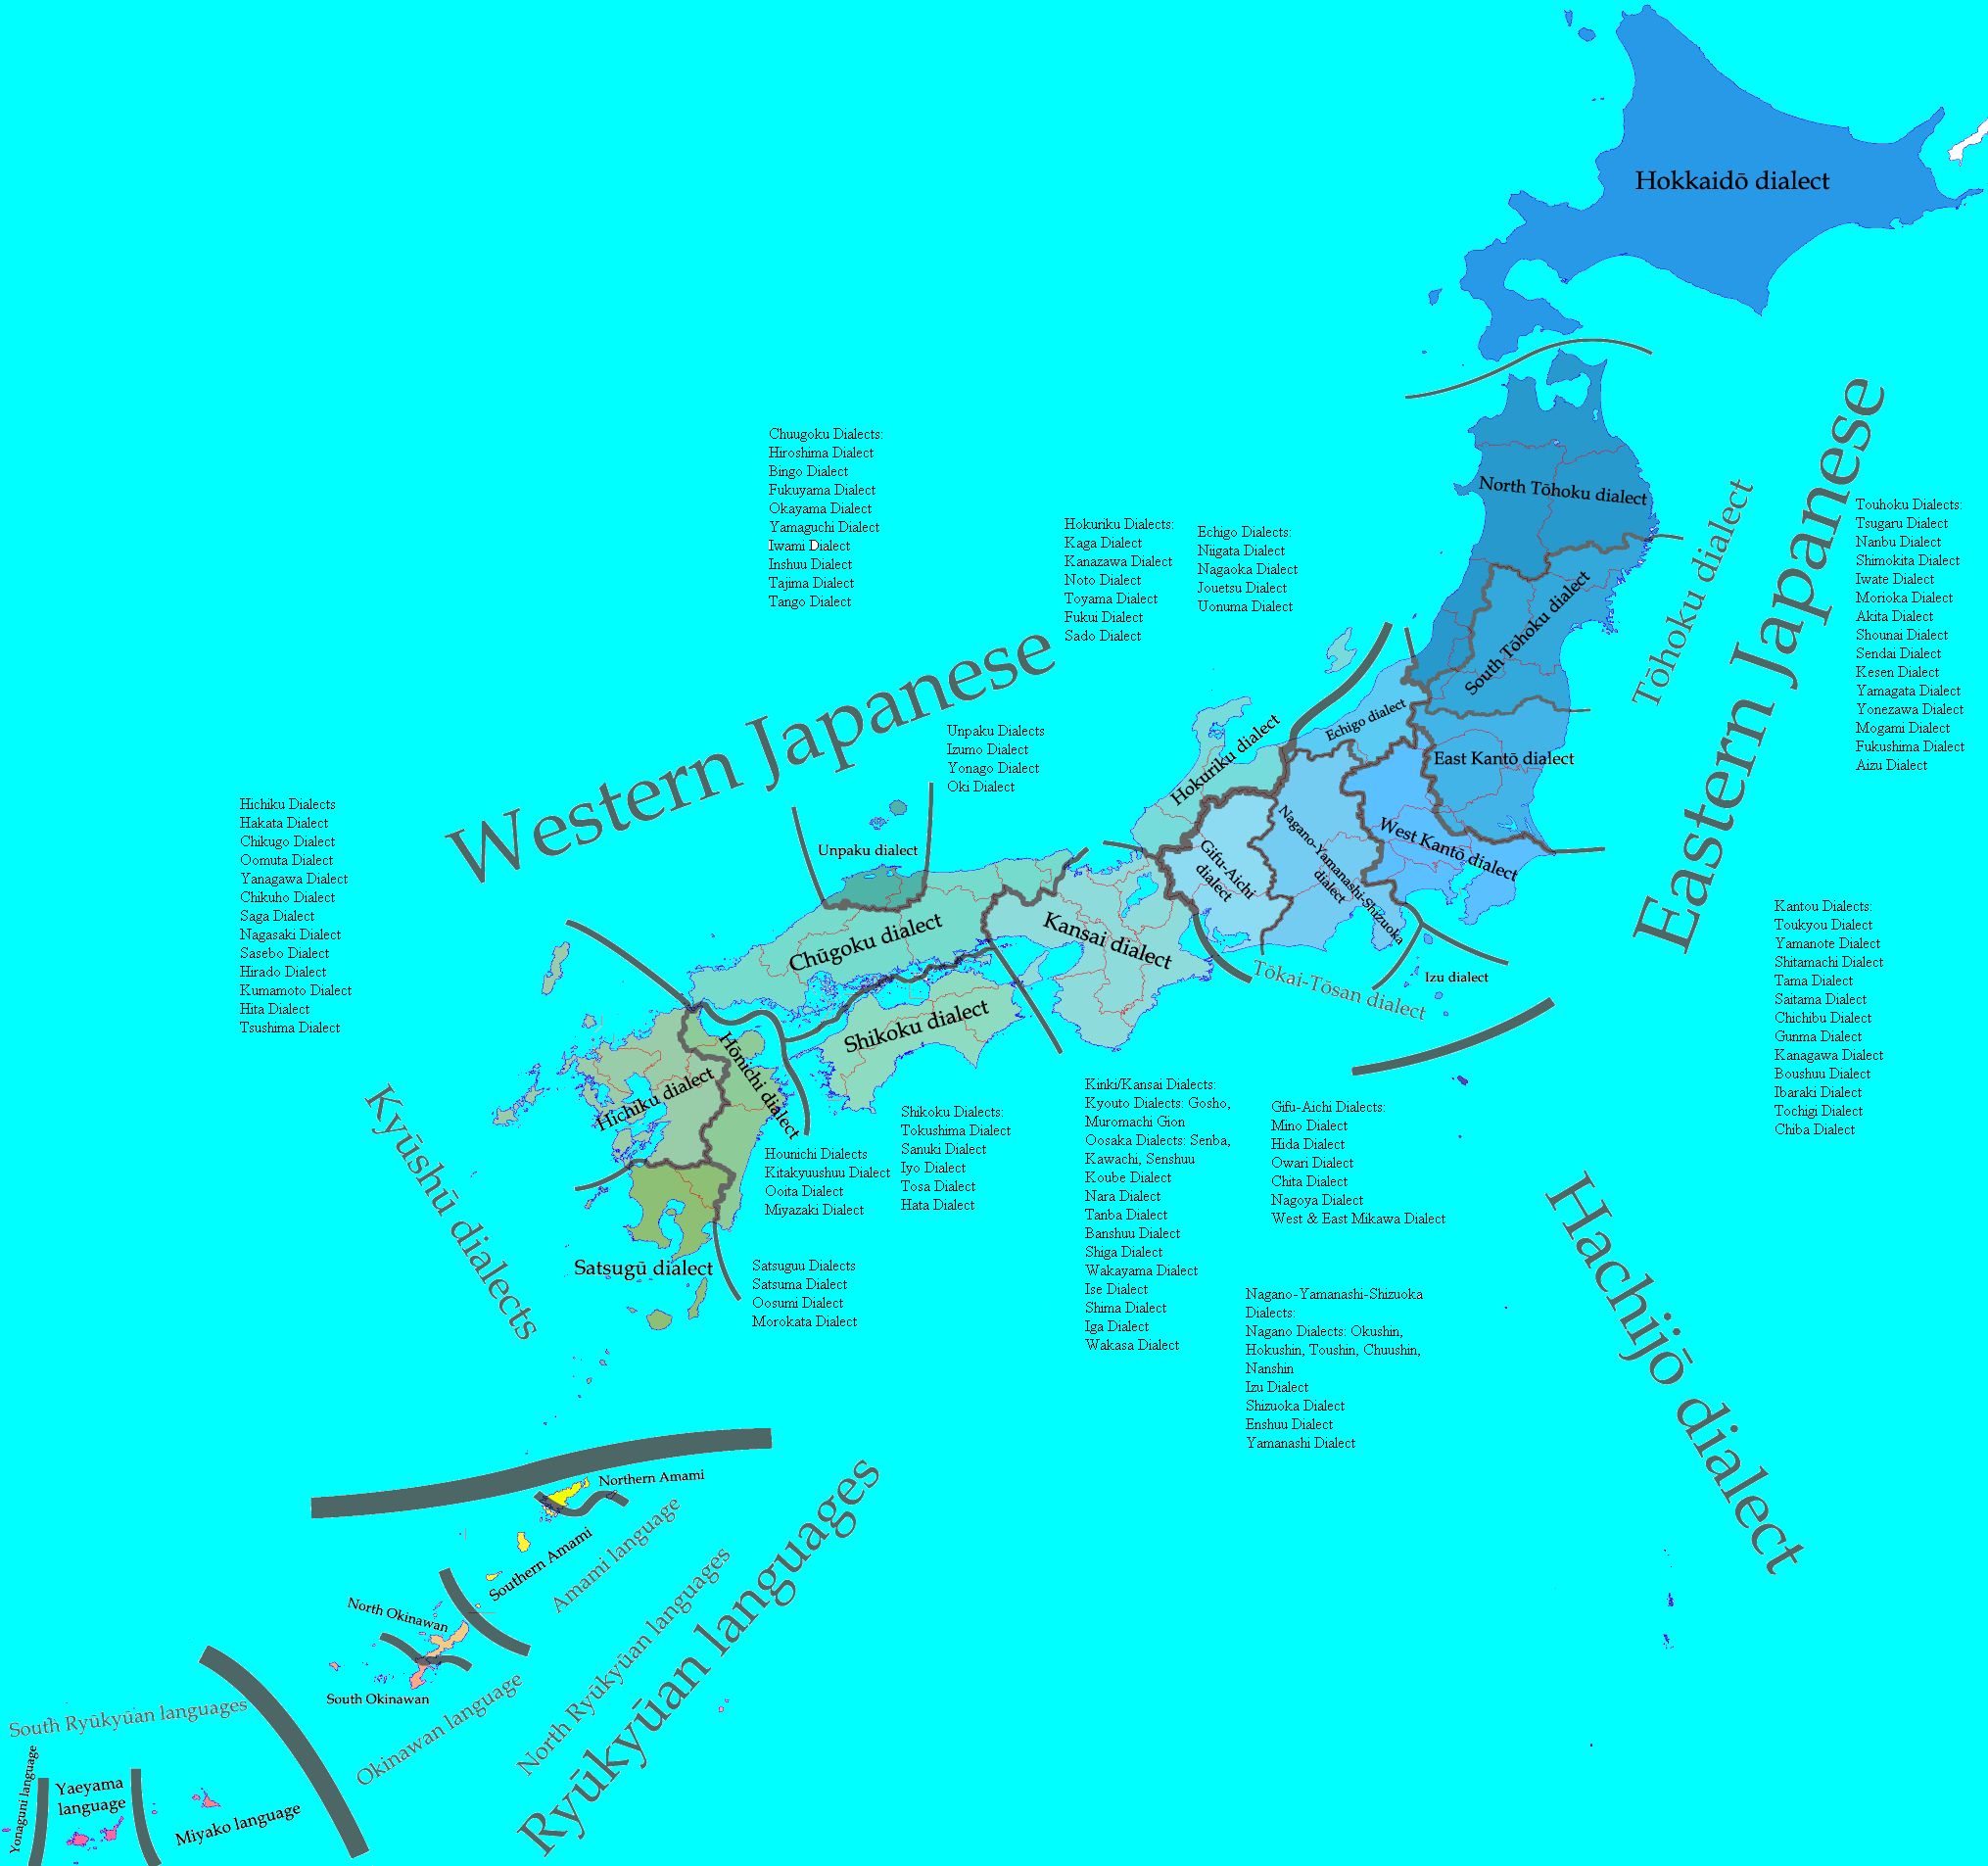
\includegraphics[width=0.9\textwidth]{figs/第01章/第7課:_10majoraspects_fig/Japanese_dialects.png}

\end{figure}
 
\par{ Dialects may differ in vocabulary, grammar, and punctuation. However, the most important dialect is Standard Japanese. By mastering this dialect, you will be able to converse with essentially any native Japanese speaker. Knowing other dialects is not essential to speaking or understanding Japanese, but many dialectal expressions are known by all spea kers. Whenever you watch anime or read manga, you will frequently encounter other major dialects. With this being the case, occasional focus will be given to dialectal expressions that are too important to ignore. }
    

% http://www.imabi.net/nounsandpronouns.htm
     
\chapter{Nouns \& Pronouns}

\begin{center}
\begin{Large}
第8課: Nouns \& Pronouns 
\end{Large}
\end{center}
 
\par{ \textbf{Nouns }are the easiest words to learn in a foreign language. Memorizing them all, however, is no easy task. By learning nouns, though, you will create a framework which, when paired with grammar, will allow you to express the things you want to talk about. }

\par{ In addition to nouns, this lesson will also serve to introduce you to \textbf{pronouns }, which are words that indirectly refer to people, direction, and things that require context to be properly understood. }
      
\section{Nouns}
 
\par{ In a basic understanding, a \textbf{noun }( \emph{meishi }名詞) \emph{represents a person, place, state, quality, event, or thing }. In Japanese, nouns have no number or gender. This means that there is no fundamental distinction between singular and plural forms or masculine and feminine forms. In addition, there are no articles like "a," "an," or "the" that accompany nouns like is the case in English.  }

\par{ Some of the most common nouns in Japanese include the following. Many of these words are also written with the most basic \emph{Kanji }漢字 that are taught early on in Japanese education. }

\begin{ltabulary}{|P|P|P|P|P|P|}
\hline 

Karaoke &  \emph{Karaoke }カラオケ \hfill\break
&  \emph{Ramen }&  \emph{Rāmen }ラーメン \hfill\break
& Karate &  \emph{Karate }空手 \\ \cline{1-6}

Alcohol &  \emph{(O-)sake }(お)酒 & Sushi &  \emph{Sushi }寿司 & Mountain &  \emph{Yama }山 \\ \cline{1-6}

Anime &  \emph{Anime }アニメ & Manga &  \emph{Manga }マンガ & Dog &  \emph{Inu }犬 \hfill\break
\\ \cline{1-6}

Cat &  \emph{Neko }猫 & Tea &  \emph{Ocha }お茶 & Water &  \emph{Mizu }水 \\ \cline{1-6}

Sea &  \emph{Umi }海 & Fire &  \emph{Hi }火 & Bamboo &  \emph{Take }竹 \\ \cline{1-6}

Hill &  \emph{Oka }丘 & Tree &  \emph{Ki }木 & Grass &  \emph{Kusa }草 \\ \cline{1-6}

Person &  \emph{Hito }人 & Car &  \emph{Kuruma }車 & Yen &  \emph{En }円 \\ \cline{1-6}

Flower &  \emph{Hana }花 & Sound &  \emph{Oto }音 & Sky &  \emph{Sora }空 \\ \cline{1-6}

Mouth &  \emph{Kuchi }口 & Hand &  \emph{Te }手 & Leg\slash foot &  \emph{Ashi }脚・足 \\ \cline{1-6}

Ear &  \emph{Mimi }耳 & Man &  \emph{Otoko }男 & Woman &  \emph{On'na }女 \\ \cline{1-6}

Sun &  \emph{Hi\slash taiy }\emph{ō }日・太陽 & Stone &  \emph{Ishi }石 & River &  \emph{Kawa }川 \\ \cline{1-6}

Village &  \emph{Mura }村 & Town &  \emph{Machi }町 & Bug &  \emph{Mushi }虫 \\ \cline{1-6}

Countryside &  \emph{Inaka }田舎 & Ground &  \emph{Tsuchi }土 & Book &  \emph{Hon }本 \\ \cline{1-6}

Name &  \emph{Namae }名前 & Strength &  \emph{Chikara }力 & Eye(s) &  \emph{Me }目 \\ \cline{1-6}

King &  \emph{Ō }王 & Queen &  \emph{Jo' }\emph{ō }女王 & Rain &  \emph{Ame }雨 \\ \cline{1-6}

Gold &  \emph{Kin }金 & Silver &  \emph{Gin }銀 & Money &  \emph{Okane }お金 \\ \cline{1-6}

School &  \emph{Gakk }\emph{ō }学校 & Thread &  \emph{Ito }糸 & Year &  \emph{Toshi }年 \\ \cline{1-6}

Cloud &  \emph{Kumo }雲 & Song &  \emph{Uta }歌 & Fish &  \emph{Sakana }魚 \\ \cline{1-6}

Face &  \emph{Kao }顔 & Cow &  \emph{Ushi }牛 & Shape &  \emph{Katachi }形 \\ \cline{1-6}

\end{ltabulary}

\par{\textbf{Grammar Note }: Making nouns plural, although not common, is still possible. One method involves the suffix - \emph{tachi }たち, which is typically used to refer to a group of p eople or (living) things. }

\par{1. ${\overset{\textnormal{じょせい}}{\text{女性}}}$ たち \hfill\break
\emph{Joseitachi } \hfill\break
(Group of ) women }

\par{2. ${\overset{\textnormal{だんせい}}{\text{男性}}}$ たち \hfill\break
\emph{Danseitachi }\hfill\break
(Group of) men }

\par{3. ${\overset{\textnormal{いぬ}}{\text{犬}}}$ たち \hfill\break
\emph{Inutachi \hfill\break
}(A group of) dogs }

\begin{center}
\textbf{Proper Nouns } 
\end{center}

\par{ In English, a proper noun is a noun that indicates an individual person, place, organization, etc. and is spelled with initial capital letters. In Japanese, words are not capitalized, but the concept of proper noun ( \emph{koyū meishi }固有名詞) still exists. Below is a chart with some very important examples. }

\begin{ltabulary}{|P|P|P|P|}
\hline 
 
  Tokyo 
 &    \emph{Tōkyō }東京 
 &   Kyoto 
 &   \emph{Kyōto }京都 
 \\ \cline{1-4} 
 
  Osaka 
 &    \emph{Ōsaka }大阪 
 &   Yokohama 
 &    \emph{Yokohama }横浜 
 \\ \cline{1-4} 
 
  Japan 
 &    \emph{Nihon\slash Nippon }日本 
 &   America 
 &    \emph{Amerika }アメリカ 
 \\ \cline{1-4} 
 
  Russia 
 &    \emph{Roshia }ロシア 
 &   China 
 &   Chūgoku 中国 
 \\ \cline{1-4} 
 
  Korea 
 &    \emph{Kankoku }韓国 
 &   Hokkaido 
 &    \emph{Hokkaidō }北海道 
 \\ \cline{1-4} 
 
  Honshu 
 &    \emph{Honshū }本州 
 &   Shikoku 
 &    \emph{Shikoku }四国 
 \\ \cline{1-4} 
 
  Kyushu 
 &    \emph{Kyūshū }九州 
 &   Okinawa 
 &    \emph{Okinawa }沖縄 
 \\ \cline{1-4} 
 
  Asia 
 &    \emph{Ajia }アジア 
 &   Europe 
 &    \emph{Yōroppa }ヨーロッパ 
 \\ \cline{1-4} 
 
  Africa 
 &    \emph{Afurika }アフリカ 
 &   Australia 
 &    \emph{Ōsutoraria }オーストリア 
 \\ \cline{1-4} 
 
  Antarctica 
 &    \emph{Nankyokutairiku }南極大陸 
 &   India 
 &    \emph{Indo }インド 
 \\ \cline{1-4} 
 
  Kanto Region 
 &    \emph{Kanto Chihō }関東地方 
 &   Kinki Region 
 &    \emph{Kinki Chihō }近畿地方 
 \\ \cline{1-4} 
 
  Shinzo Abe 
 &    \emph{Abe Shinzō }安倍晋三 
 &   Barack Obama 
 &    \emph{Baraku Obama }バラク・オバマ 
 \\ \cline{1-4} 
 
  Tokyo   Skytree 
 &    \emph{Tokyo Sukaitsurii }東京スカイツリー 
 &   Ueno Park 
 &    \emph{Ueno Kōen }上野公園 
 \\ \cline{1-4} 

\end{ltabulary}

\par{\textbf{Word Notes }: \hfill\break
1. There are four main islands of Japan. The northernmost island is Hokkaido. South of it is the largest island, Honshu. Further south are the islands of Shikoku and Kyushu, with Kyushu being the southernmost island. Further south is a chain of islands referred to as Okinawa. \hfill\break
2. The Kanto Region encompasses the capital of Japan, Tokyo, as well as the surrounding area. \hfill\break
3. The Kinki Region encompasses both Osaka and Kyoto and their surrounding areas. \hfill\break
4. Shinzo Abe is the current Prime Minister of Japan. \hfill\break
5. Barack Obama is the 44th president of the United States. \hfill\break
6. Tokyo Skytree is the second tallest structure found in the world and is located in Tokyo. \hfill\break
7. Ueno Park is a very spacious park found in Tokyo. }

\begin{center}
 \textbf{Loan-words }
\end{center}

\par{ A \textbf{loan-word } \emph{is a word borrowed from another language }. In Japanese, there are many loanwords from all sorts of languages. Loan-words are called \emph{Gairaigo }外来語, and this term typically refers to words that have been borrowed in the last two, three centuries from the world's modern languages. Words borrowed from Chinese during the language's development--Kango 漢語--are usually treated separately. Words that have come from Chinese lan guages in recent centuries like \emph{ch }\emph{ā }\emph{han }炒飯 (fried rice), though, are treated as \emph{Gairaigo }外来語. }

\par{ Although loan-words come from dozens of languages, the overwhelmingly majority of them come from English. As convenient as that may be, you must still treat these loan words as Japanese words. This means you can't simply pronounce it as if it were English. You will likely not be understood. It is always important that you pronounce words in Japanese like any other word in Japanese regardless of whether or not it comes from English. }

\begin{ltabulary}{|P|P|P|P|P|P|}
\hline 

Meter &  \emph{Mētoru }メートル \hfill\break
& Game &  \emph{G }\emph{ēmu }ゲーム \hfill\break
& Bus & \emph{Basu }バス \\ \cline{1-6}

Pen &  \emph{Pen }ペン \hfill\break
& Sofa &  \emph{Sofā }ソファー \hfill\break
& Pie\slash pi &  \emph{Pai }パイ \hfill\break
\\ \cline{1-6}

Point &  \emph{Pointo }ポイント \hfill\break
& Cola &  \emph{Kōra }コーラ \hfill\break
& Coffee &  \emph{Kōhii }コーヒー \hfill\break
\\ \cline{1-6}

Tobacco &  \emph{Tabako }タバコ & Tomato &  \emph{Tomato }トマト & Banana & Banana バナナ \\ \cline{1-6}

\end{ltabulary}
\hfill\break

\begin{center}
\textbf{Pronouns: Grammatical Person }
\end{center}

\par{ A \textbf{pronoun }( \emph{daimeishi }代名詞) \emph{indirectly refers to an entity that involves a person, direction, or thing }. The meaning of said entity is determined by context. For instance, proper names are pronouns because they stand in place of the actual person\slash thing they reference. Proper names can also be shared with others or other things, and so we need context to truly understand what is meant by say the name "Seth." This can refer to the creator of this curriculum, or it can refer to any other person whose name is "Seth." Because of this, the word "Seth" is a pronoun. }

\par{ Similarly, words like "here" and "there" or even words like "this" and "that" are also pronouns. This is because no one can ascertain what they refer to without context. }

\par{ Generally, when we think of pronouns, we think about pronouns that are used to establish grammatical person. For instance, in English we make the following distinctions in grammatical person. }

\begin{ltabulary}{|P|P|P|}
\hline 

Person & Singular & Plural \\ \cline{1-3}

1st & I & We \\ \cline{1-3}

2nd & You & You (all) \\ \cline{1-3}

3rd & He\slash she\slash it & They \\ \cline{1-3}

\end{ltabulary}

\par{ In English, gender and number both play roles in determining what grammatical person is used in a sentence. In Japanese, however, there isn't a single pronoun that corresponds to each of the pronouns for grammatical person. Meaning, there is more than one word for "I," "we," etc. This is because all pronouns in Japanese started out as typical nouns, or they were far vaguer pronouns that didn't necessarily match up with the concept of showing grammatical person. }

\par{ In Japanese, pronouns differ by their politeness and by who actually uses them. Many pronouns are reserved for whether the speaker is male or female, or whether the person is young or old. Dialects also differ majorly in what pronouns are used. }

\par{ For the purposes of understanding basic Standard Japanese, the pronouns listed below are the most essential. As you will see, the notes provided for them show just how different they are from their English counterparts. }

\begin{ltabulary}{|P|P|P|}
\hline 

Person & Singular & Plural \\ \cline{1-3}

1st &  \emph{Wata(ku)shi }私 \hfill\break
 \emph{Boku }僕 &  \emph{Wata(ku)shitachi }私たち \hfill\break
 \emph{Bokutachi }僕たち \\ \cline{1-3}

2nd &  \emph{Anata }あなた &  \emph{Anatatachi }あなたたち \\ \cline{1-3}

3rd &  \emph{Kare }彼 (He) \hfill\break
 \emph{Kanojo }彼女 (She) &  \emph{Karera }彼ら (They) \hfill\break
 \emph{Kanojotachi }彼女たち (They) \\ \cline{1-3}

\end{ltabulary}

\par{\textbf{Usage Notes }: }
1. \emph{Watakushi }わたくし is the respectful form of \emph{watashi }わたし. Typically, \emph{watashi }わたし will suffice in most situations. However, "I" is often dropped altogether. So long as it is known that the sentence is about oneself, there is no need to have to use a pronoun for "I." \hfill\break
2. \emph{Boku }僕 is another pronoun for "I" which is used heavily by male speakers, both young and old, in various situations. \hfill\break
3. There are many pronouns for "you" in Japanese, but the most neutral in terms of politeness and purpose is \emph{anata }あなた. However, it is typically dropped from most sentences altogether. \emph{Anata }あなた is inherently direct, which is a quality not typically found in statements directed at others. Second person statements are rarely stated in absolute terms. Usually, referring to others in third person is preferred. \hfill\break
4. \emph{Anata }あなた may also be used as a term of endearment to refer to one's male partner\slash spouse, both when one is happy and mad at one's significant other. \hfill\break
5. In casual settings, the pronouns \emph{kare }彼 and \emph{kanojo }彼女 may respectively mean "boyfriend" and "girlfriend." \hfill\break
6. The plural form of \emph{kare }彼, \emph{karera }彼ら, uses another suffix for making plurals, - \emph{ra }ら. We will revisit the concept of pluralization in Lesson 92. \hfill\break
8. \emph{Karera }彼ら may refer to a group of people with both men and women, but \emph{kanojotachi }彼女たち only refers to groups of women. 7. T he pronoun "it" is omitted because it is combined in Japanese with the concept of "that," which is also a pronoun. It will be introduced later in this lesson.   \hfill\break
 In English, pronouns change form depending on their grammatical purpose in a sentence. In grammar, this is referred to as grammatical case. Grammatical case reflects the function that a given phrase has in a sentence. In English, pronouns are what change the most depending on their case. For instance, "my" is the possessive form of "I." \hfill\break
 \hfill\break
 In Japanese, grammatical case is marked by the use of what are called "case particles." Case particles take the place of form change to nouns\slash pronouns to indicate what function said word has in a sentence. For the purpose of pronouns, there are two grammatical cases you should know about: the nominative and the possessive. 
\begin{itemize}

\item Nominative Case: Noun\slash pronoun used as the subject of the sentence. \hfill\break

\item Possessive Case: Noun\slash pronoun form that shows ownership. 
\end{itemize}
i. I am an American man. (I = nominative) \hfill\break
ii. Your dog is adorable. (Your = possessive) \hfill\break
iii. We are scientists. (We = nominative) \hfill\break
iv. Our goal is world peace. (Our = possessive) \hfill\break
\hfill\break
 The subject of a sentence is the person\slash thing that performs an action or exhibits some description which is what the sentence is about. In Japanese, case particles attached to noun\slash pronouns express these grammatical concepts. To mark something as being in the nominative case, you add the particle \emph{ga }が to said noun\slash pronoun. To mark something as being in the possessive case, you add the particle \emph{no }の to said noun\slash pronoun. \hfill\break
\hfill\break

\begin{ltabulary}{|P|P|P|P|}
\hline 

 & Nominative &  & Possessive \\ \cline{1-4}

I\dothyp{}\dothyp{}\dothyp{} &  \emph{Wata(ku)shi ga }私が \hfill\break
 \emph{Boku ga }僕が & My &  \emph{Wata(ku)shi no }私の \hfill\break
 \emph{Boku no }僕の \\ \cline{1-4}

We\dothyp{}\dothyp{}\dothyp{} &  \emph{Wata(ku)shitachi ga }私たちが \hfill\break
 \emph{Bokutachi ga }僕たちが & Our &  \emph{Wata(ku)shitachi no }私たちの \hfill\break
 \emph{Bokutachi no }僕たちの \\ \cline{1-4}

You\dothyp{}\dothyp{}\dothyp{} &  \emph{Anata ga }あなたが & Your &  \emph{Anata no }あなたの \\ \cline{1-4}

You (all)\dothyp{}\dothyp{}\dothyp{} &  \emph{Anatatachi ga }あなたたちが & Your &  \emph{Anatatachi no }あなたたちの \\ \cline{1-4}

He\dothyp{}\dothyp{}\dothyp{} \hfill\break
She\dothyp{}\dothyp{}\dothyp{} &  \emph{Kare ga }彼が (He) \hfill\break
 \emph{Kanojo ga }彼女が (She) & His \hfill\break
Her &  \emph{Kare no }彼の \hfill\break
 \emph{Kanojo no }彼女の \\ \cline{1-4}

They\dothyp{}\dothyp{}\dothyp{} &  \emph{Karera ga }彼らが \hfill\break
 \emph{Kanojotachi ga }彼女たちが & Their &  \emph{Karera no }彼らの \hfill\break
 \emph{Kanojotachi no }彼女たちの \\ \cline{1-4}

\end{ltabulary}

\par{\textbf{Grammar Note }: To make a third person reference into the possessive case, just add no to whatever name you're using. This means that "Seth's" would be expressed as \emph{Sesu no }セスの. }

\par{ When we start learning how to make sentences in Lesson 9, it will be important to remember that different things will happen in a Japanese sentence. However, we won't revisit the particle \emph{ga }が until Lesson 11. }
\textbf{Pronouns: Place \& Things (Demonstratives) }\hfill\break
  In addition to the pronouns shown above for grammatical person, we still need to learn about the basic pronouns used to indicate place or thing. As was the case with the pronouns above, none of these words are used exactly like their English counterparts. This means that later on, we will have to revisit them to learn more about how they're truly used. For now, it's important to simply have them in your vocabulary.  
\begin{ltabulary}{|P|P|P|}
\hline 

Close to Speaker & Close to Listener\slash  \hfill\break
Known only to Speaker & Far from Speaker and Listener\slash  \hfill\break
Known to both Speaker and Listener \\ \cline{1-3}

\textbf{Here }& \textbf{There }& \textbf{Over There }\\ \cline{1-3}

 \emph{Koko }ここ &  \emph{Soko }そこ &  \emph{Asoko }あそこ \\ \cline{1-3}

 \textbf{This }& \textbf{That }& \textbf{That over there }\\ \cline{1-3}

 \emph{Kore }これ &  \emph{Sore }それ &  \emph{Are }あれ \\ \cline{1-3}

\end{ltabulary}
\hfill\break
\textbf{Chart Notes }:  \hfill\break
1. \emph{Sore }それ is the closest Japanese equivalent to "it." \hfill\break
2. For now, we will forego covering what these words look like in the grammatical cases mentioned above. This is because things become slightly more complicated with these sorts of pronouns than with pronouns for grammatical person.   When speaking about entities \textbf{physically visible }, \emph{there is a three-way distinction made based on the proximity of the entity from the speaker and listener }. An entity may be close to the speaker, close to the listener but not the speaker, or far from both the speaker and the listener(s). When the entity discussed is \textbf{not physically visible }, \emph{there is a two-way distinction made based on who knows about the entity in question }. The criterion then becomes whether only the speaker knows about the entity or if both the speaker and listener(s) know about it.     

% http://www.imabi.net/copularsentencesi.htm
     
\chapter{Copular Sentences I}

\begin{center}
\begin{Large}
第9課: Copular Sentences I: Plain Speech 
\end{Large}
\end{center}
 
\par{ The Japanese language possesses a speech-level hierarchy that determines how one should address any given person based on various factors: relationship, age, role, respect, etc. The social dynamics that set a discourse also shape how said discourse is worded. }
 
\par{ Typically, Japanese learners are first introduced to polite speech. This is because polite speech is what is used in most daily interactions; it helps establish courtesy between oneself and those around. As the Japanese learner, the most practical means of using Japanese early on will be centered around speaking to native speakers who are neither family nor close friends. Because the most important use of plain speech involves casual conversation, it is kept to the side until the learner can handle situations where polite speech is imperative. }

\par{ However, the greatest flaw made by introducing polite speech first lies in the fact that it is not the base form of speech. Within each speech style you will find unique vocabulary, grammar, and endings. Grammatically, plain speech is what makes up the base form of the language. Contrary to its name, plain speech is not limited to conversation among peers or family. In fact, it is grammaticalized in all sorts of grammar points. }

\par{ Plain speech is also inherently direct, which is why it is heavily used in academic writing. Most importantly, it is what\textquotesingle s used in one\textquotesingle s inner monologue. Plain speech also makes up the heart of most music and literature. The very essence of being able to think in Japanese requires oneself to truly understand the language from the ground up. That cannot be possible if the base is left ignored. }
 Politeness is an auxiliary element to conversation. Its purpose is not to provide information other than social implications. Strip it away and you get the actual message a sentence is trying to get across. Naturally, plain speech becomes the basis for conjugation, to which politeness is then added.       
\section{Vocabulary List}
 
\par{\textbf{Nouns }}
 
\par{・ \emph{Tera }寺 – Buddhist temple }

\par{・ \emph{Jijitsu }事実 – Fact }

\par{・ \emph{K }\emph{ōmori }コウモリ – Bat }

\par{・ \emph{Tori }鳥 – Bird }

\par{・ \emph{Gakusei }学生 – Student }

\par{・ \emph{Kankokujin }韓国人 – Korean }

\par{・ \emph{Shod }\emph{ō }書道 – Calligraphy }

\par{・ \emph{Geijutsu }芸術 – Art }

\par{・ \emph{Baka }馬鹿 – Idiot }

\par{・ \emph{Neko }猫 – Cat }

\par{・ \emph{P }\emph{ātii }パーティー – Party }

\par{・ \emph{Kaishi }開始 – Start\slash beginning }

\par{・ \emph{D }\emph{ōbutsuen }動物園 – Zoo }

\par{・ \emph{Hikiwake }引き分け – A tie }

\par{・ \emph{Kawauso }カワウソ – Otter }

\par{・ \emph{Furansugo }フランス語 – French }

\par{・ \emph{Gakk }\emph{ō }学校 – School }

\par{・ \emph{Seikai }正解 – Correct answer }

\par{・ \emph{Wakusei }惑星 – Planet }

\par{・ \emph{Mei }\emph{ōsei }冥王星 – Pluto }

\par{・ \emph{Ocha }お茶 – Tea }

\par{・ \emph{Daihy }\emph{ō }代表 – Representative }

\par{・ \emph{Gen\textquotesingle in }原因 – Cause }

\par{・ \emph{Tabako }煙草・タバコ・たばこ – Tobacco }

\par{・ \emph{Kodomo }子供 – Child(ren) }

\par{・ \emph{Pen }ペン – Pen }
 
\par{・ \emph{Kujira }鯨 – Whale }

\par{・ \emph{Sakana }魚 – Fish }

\par{・ \emph{Mogi shiken }模擬試験 – Mock exam }

\par{・ \emph{Mizu }水 – Water }

\par{・ \emph{Jikan }時間 – Time }

\par{・ \emph{Ganjitsu }元日 – New Year\textquotesingle s Day }

\par{・ \emph{Getsuy }\emph{ōbi }月曜日 – Monday }

\par{・ \emph{Suiy }\emph{ōbi }水曜日 – Wednesday }

\par{・ \emph{Kaishibi }開始日 – Start date }

\par{・ \emph{Kin }\emph{ō }昨日 – Yesterday }

\par{・ \emph{Ashita\slash asu }明日 – Tomorrow }

\par{・ \emph{Yoru }夜 – Night }

\par{\textbf{Pronouns }}

\par{・ \emph{Watashi }私 – I }
 
\par{・ \emph{Boku }僕 – I (male) }
 
\par{・ \emph{Kare }彼 – He }
 
\par{・ \emph{Kanojo }彼女 – She }
 
\par{・ \emph{Kore }これ – This }
 
\par{・ \emph{Sore }それ – That }
 
\par{・ \emph{Sono }その – That (adj.) }
 
\par{・ \emph{Are }あれ – That (over there) }
 
\par{・ \emph{Koko }ここ – Here }
 
\par{・ \emph{Kimu }キム – Kim }
 
\par{・ \emph{Pikach }\emph{ū }ピカチュウ – Pikachu }
 
\par{\textbf{Interjections }}
・ \emph{A }あ – Ah       
\section{The Copular Sentence}
 
\par{ The first thing you must learn about Japanese sentence structure is its most basic form: the copular sentence. This is otherwise known as a “noun-predicate” sentence. In other words, “X is Y.” As trivial as it may sound, many far more complex sentences can be broken down to this very structure. First, let\textquotesingle s cover some basic terminology to better understand this topic. }

\begin{itemize}

\item \textbf{\textbf{Subject }: \emph{The person\slash thing that performs the action or exhibits the description found in the predicate. }}
\item \textbf{Predicate }: \emph{The part of a sentence that gives some information about the subject. }
\item \textbf{Copula }: \emph{A word used to link the subject and predicate of a sentence. }\hfill\break

\item \textbf{Noun }: \emph{In its most basic definition, a word that refers to a person, place, thing, event, substance, or quality. }\hfill\break

\item \textbf{Auxiliary }: \emph{An ending that helps construct verbal conjugations. }
\end{itemize}
 
\par{ The predicate of a sentence may take on different forms depending on what the statement is. In the context of this discussion, the copula is the predicate because we are learning how to simply say “X”—the subject—is “Y.” “Y” In this lesson, “Y” will be another noun, which is why “copular sentences” can alternatively be called “noun-predicate sentences.” }
 
\par{ In English, the copula verb is “to be,” and it manifests itself in various forms such as “is,” “are,” “was,” “were,” etc. Their use in the English language is profoundly important as they form the basis of a great portion of the statements we make. }
 
\par{i. The dog is a German shepherd. \hfill\break
ii. My husband is a banker. \hfill\break
iii. Apples are fruits. \hfill\break
iv. It was a fossil. \hfill\break
v. A bat is not a bird. }
 
\par{ Similarly, Japanese has its own copular verb, which in turn has its own various forms. Before discussing what this all looks like in Japanese, we must first understand what sort of basic conjugations exist in general. Using the English examples i.-v. as a basis, we see that \textbf{tense }and \textbf{affirmation\slash negation }are major components to a sentence. In English, there are three tenses: \textbf{past, present, and future }. As their names suggest, the \textbf{past tense } \emph{refers to an event\slash state which occurred in the past }, the \textbf{present tense } \emph{refers to a current event\slash state }, and the \textbf{future tense } \emph{refers to an event\slash state that hasn\textquotesingle t yet realized }. \textbf{Affirmation }is \emph{positively stating that something is so }. \textbf{Negation }is \emph{rejecting a premise }. }
 
\par{ Japanese only has two tenses: non-past and past tense. Unlike English, tense is not so straightforward, but the speaker\textquotesingle s intent is to always make the “time” factor of any statement obvious in context. The non-past tense encompasses both the concepts of the English present tense and future tense. The past tense corresponds to the past tense, but the form that expresses past tense covers a wider semantic scope than the English -ed. }
      
\section{The Copula Da だ}
 
\par{ Putting all this aside, it is now time to familiarize yourself with the base form of the copula in plain speech. This verb is \emph{\textbf{da }}\textbf{だ }.  As is the case for any base form of verb, it alone may stand for the non-past tense. As such, \emph{da }だ can translate as “is,” “are,” or “will be.” Japanese lacks grammatical number, so there is no difference between “is” or “are.” }

\par{ Because the verb of a Japanese sentence must always be at the end, we can\textquotesingle t simply insert \emph{da }だ between “X” and “Y.” “X” remains at the start of the sentence, and the sentence ends in “Y \emph{da }だ.”  To complete the sentence, we will insert the particle \emph{wa }は in between X and Y. In Lessons 11-12, we\textquotesingle ll learn about the sort of nuances that are expressed with this particle as well as what else can be between X and Y. For now, though, our goal will be to master the basic pattern “X \emph{wa }は Y \emph{da }だ.” }

\begin{center}
\textbf{Non-past: Present }
\end{center}

\par{1. あれは ${\overset{\textnormal{てら}}{\text{寺}}}$ だ。 \hfill\break
\emph{Are wa tera da. \hfill\break
}That (over there) is a Buddhist temple. }

\par{2. それは ${\overset{\textnormal{うそ}}{\text{嘘}}}$ だ。 \hfill\break
 \emph{Sore wa uso da. \hfill\break
 }That\textquotesingle s a lie. }

\par{3. これは ${\overset{\textnormal{じじつ}}{\text{事実}}}$ だ。 \hfill\break
 \emph{Kore wa jijitsu da. \hfill\break
 }This is the truth. }

\par{4. ${\overset{\textnormal{わたし}}{\text{私}}}$ は ${\overset{\textnormal{がくせい}}{\text{学生}}}$ だ。 \hfill\break
 \emph{Watashi wa gakusei da. \hfill\break
 }I\textquotesingle m a student. }

\par{5. キムは ${\overset{\textnormal{かんこくじん}}{\text{韓国人}}}$ だ。 \hfill\break
 \emph{Kimu wa kankokujin da. \hfill\break
 }Kim is Korean. }

\par{6. ${\overset{\textnormal{しょどう}}{\text{書道}}}$ は ${\overset{\textnormal{げいじゅつ}}{\text{芸術}}}$ だ。 \hfill\break
 \emph{Shod }\emph{ō wa geijutsu da. \hfill\break
 }Calligraphy is art. }

\par{7. ${\overset{\textnormal{かれ}}{\text{彼}}}$ は ${\overset{\textnormal{ばか}}{\text{馬鹿}}}$ だ。 \hfill\break
 \emph{Kare wa baka da. \hfill\break
 }He\textquotesingle s an idiot. }

\begin{center}
\textbf{Non-Past: Future }
\end{center}

\par{8. ${\overset{\textnormal{がんじつ}}{\text{元日}}}$ は ${\overset{\textnormal{げつようび}}{\text{月曜日}}}$ だ。 \hfill\break
 \emph{Ganjitsu wa getsuy }\emph{ōbi da. \hfill\break
 }New Year\textquotesingle s Day is\slash will be on Monday. }

\par{9. ${\overset{\textnormal{かいしび}}{\text{開始日}}}$ は ${\overset{\textnormal{あした}}{\text{明日}}}$ だ。 \hfill\break
 \emph{Kaishibi wa ashita da. \hfill\break
 }The start date is\slash will be tomorrow. \hfill\break
 \hfill\break
10. パーティーは ${\overset{\textnormal{よる}}{\text{夜}}}$ だ。 \hfill\break
 \emph{P }\emph{ātii wa yoru da. \hfill\break
 }The party will be at night. }

\begin{center}
\textbf{Omitting “X” }
\end{center}

\par{ In Japanese, the subject is often dropped in the sentence. This tends to be the case, especially when the subject is “it. }

\par{11. ${\overset{\textnormal{あした}}{\text{明日}}}$ だ。 \hfill\break
 \emph{Ashita da. \hfill\break
 }It\textquotesingle s tomorrow. \hfill\break
It\textquotesingle ll be tomorrow. }

\par{12. あ、 ${\overset{\textnormal{ねこ}}{\text{猫}}}$ だ! \hfill\break
 \emph{A, neko da. \hfill\break
 }Ah, (it\textquotesingle s) a cat! }

\par{13. ${\overset{\textnormal{じかん}}{\text{時間}}}$ だ。 \hfill\break
 \emph{Jikan da. \hfill\break
 }(It\textquotesingle s) time. }

\begin{center}
\textbf{Omitting \emph{Da }だ }
\end{center}

\par{ The copula \emph{da }だ is also occasionally dropped altogether with a heightened intonation at the end to express various emotions such as anger or surprise. Dropping the copula may also be done in this fashion in English. }

\par{14. あ、ピカチュウ(だ)! \hfill\break
 \emph{A, Pikachū (da)! \hfill\break
 }Ah, (it\textquotesingle s) Pikachu! }

\par{15. ${\overset{\textnormal{かいし}}{\text{開始}}}$ (だ)! \hfill\break
 \emph{Kaishi (da)! \hfill\break
 }Start! \hfill\break
Literally: This is the start! \hfill\break
 \hfill\break
16. ${\overset{\textnormal{どうぶつえん}}{\text{動物園}}}$ (だ)! \hfill\break
 \emph{Dōbutsuen (da)! \hfill\break
 }(It\textquotesingle s) a zoo! }

\par{17. ${\overset{\textnormal{ひ}}{\text{引}}}$ き ${\overset{\textnormal{わ}}{\text{分}}}$ げ(だ)! \hfill\break
 \emph{Hikiwake (da)! \hfill\break
 }(It\textquotesingle s a) draw! }

\par{18. あ、カワウソ(だ)! \hfill\break
 \emph{A, kawauso (da)! \hfill\break
 }Ah, (it\textquotesingle s) an otter! }

\begin{center}
\textbf{Past Tense: \emph{Datta }だった }
\end{center}

\par{ To express past tense with the copula \emph{da }だ, you must conjugate to \emph{datta }だった. As you learn more, you will see that -TA stands for -ed in anything that conjugates. Remember, Japanese makes no distinctions with grammatical number. This means that “was” and “were” are both expressed with \emph{datta }だった. }

\begin{center}
Conjugation Recap 
\end{center}

\begin{ltabulary}{|P|P|}
\hline 

 Non-Past Tense & Past Tense \\ \cline{1-2}

 \emph{Da }だ &  \emph{Datta }だった \\ \cline{1-2}

\end{ltabulary}

\par{\hfill\break
19. あれはフランス ${\overset{\textnormal{ご}}{\text{語}}}$ だった。 \hfill\break
 \emph{Are wa Furansugo datta. \hfill\break
 }That was French. }

\par{20. ここは ${\overset{\textnormal{がっこう}}{\text{学校}}}$ だった。 \hfill\break
 \emph{Koko wa gakk }\emph{ō datta. \hfill\break
 }This here was a school. }

\par{21. ${\overset{\textnormal{せいかい}}{\text{正解}}}$ は ${\overset{\textnormal{エイ}}{\text{A}}}$ だった。 \hfill\break
 \emph{Seikai wa ei datta. \hfill\break
 }The correct answer was A. }

\par{22. ${\overset{\textnormal{きのう}}{\text{昨日}}}$ は ${\overset{\textnormal{すいようび}}{\text{水曜日}}}$ だった。 \hfill\break
 \emph{Kin }\emph{ō wa suiy }\emph{ōbi datta. \hfill\break
 }Yesterday was Wednesday. }

\par{23. ${\overset{\textnormal{かれ}}{\text{彼}}}$ は ${\overset{\textnormal{こども}}{\text{子供}}}$ だった。 \hfill\break
 \emph{Kare wa kodomo datta. \hfill\break
 }He was a child. }

\par{\textbf{Grammar Note }: The past tense form need not always be interpreted literally. Ex. 23 implies that a male individual happened to be a child and is said as a remember to oneself and\slash or to others. }

\begin{center}
\textbf{Negation: \emph{De wa nai }ではない }
\end{center}

\par{ Conjugating \emph{da }だ into its plain non-past negative form is not as easy as the past tense form. First, you must change \emph{da }だ to \emph{de }で. Then, you add \emph{wa nai }はない. In reality, it\textquotesingle s the \emph{nai }ない that brings about the negation, which you\textquotesingle ll continue seeing in negative conjugations. Lastly, in conversation, “ \emph{de wa }では” typically contracts to “ \emph{ja }じゃ.” }

\begin{center}
Conjugation Recap 
\end{center}

\begin{ltabulary}{|P|P|P|}
\hline 

Non-Past Tense & Past Tense & Non-Past Negative \\ \cline{1-3}

 \emph{Da }だ &  \emph{Datta }だった &  \emph{De wa nai }ではない \hfill\break
 \emph{Ja nai }じゃない  \\ \cline{1-3}

\end{ltabulary}
\hfill\break
24. これはペンではない。 \emph{Kore wa pen de wa nai. } This is not a pen. \hfill\break
\hfill\break
25. コウモリは ${\overset{\textnormal{とり}}{\text{鳥}}}$ ではない。 \emph{K }\emph{ōmori wa tori de wa nai. } Bats are not birds. \hfill\break
\hfill\break
26. ${\overset{\textnormal{くじら}}{\text{鯨}}}$ は ${\overset{\textnormal{さかな}}{\text{魚}}}$ ではない。 \emph{Kujira wa sakana de wa nai. } Whales are not fish. \hfill\break
\hfill\break
27. ${\overset{\textnormal{めいおうせい}}{\text{冥王星}}}$ は ${\overset{\textnormal{わくせい}}{\text{惑星}}}$ じゃない。 \emph{Mei }\emph{ōsei wa wakusei ja nai. } Pluto isn\textquotesingle t a planet. \hfill\break
\hfill\break
28. あれは ${\overset{\textnormal{いぬ}}{\text{犬}}}$ じゃない。 \emph{Are wa inu ja nai. } That isn\textquotesingle t a dog. \hfill\break
\hfill\break
29. これはお ${\overset{\textnormal{ちゃ}}{\text{茶}}}$ じゃない。 \emph{Kore wa ocha ja nai. } This isn\textquotesingle t tea. 
\par{\textbf{Grammar Note }: Saying \emph{de nai }でない isn\textquotesingle t wrong, but it is typically only seen in literature. }

\begin{center}
\textbf{Negative-Past: \emph{De wa nakatta }ではなかった }
\end{center}

\par{ The last conjugation we will study in this lesson is the plain negative-past form of the copula. To begin, we start with the negative form from above. We then add -TA to it. When you add -TA to the negative auxiliary - \emph{nai }ない, you get \emph{nakatta }なかった. Altogether, this gives you \emph{de wa nakatta }ではなかった. Just like above, “ \emph{de wa }では” often contracts to “ \emph{ja }じゃ” in conversation, which results in \emph{ja nakatta }じゃなかった. }

\begin{center}
Conjugation Recap 
\end{center}

\begin{ltabulary}{|P|P|P|P|}
\hline 

Non-past & Past & Negative & Negative-Past \\ \cline{1-4}

 \emph{Da }だ &  \emph{Datta }だった & \emph{De wa nai }ではない \hfill\break
\emph{Ja nai }じゃない &  \emph{De wa nakatta } ではなかった \hfill\break
\emph{Ja nakatta } じゃなかった  \\ \cline{1-4}

\end{ltabulary}
\hfill\break
30. その ${\overset{\textnormal{だいひょう}}{\text{代表}}}$ は ${\overset{\textnormal{かのじょ}}{\text{彼女}}}$ ではなかった。 \emph{Sono daihy }\emph{ō wa kanojo de wa nakatta. } The representative was not her.  \textbf{Grammar Note }: The demonstrative pronouns briefly mentioned in Lesson 8 actually have adjectival forms. The adjectival form for \emph{sore }それ is \emph{sono }その, as demonstrated in Ex. 30. This form often translates to "the" whenever the concepts of "the" and "that" overlap. \hfill\break
\hfill\break
31. ${\overset{\textnormal{げんいん}}{\text{原因}}}$ は ${\overset{\textnormal{たばこ}}{\text{煙草}}}$ ではなかった。 \emph{Gen\textquotesingle in wa tabako de wa nakatta. } The cause was not tobacco. \hfill\break
\hfill\break
32. あれは ${\overset{\textnormal{もぎしけん}}{\text{模擬試験}}}$ ではなかった。 \emph{Are wa mogi shiken de wa nakatta. } That was not a mock exam. \hfill\break
\hfill\break
33. ${\overset{\textnormal{かれ}}{\text{彼}}}$ は ${\overset{\textnormal{ぼく}}{\text{僕}}}$ の ${\overset{\textnormal{ともだち}}{\text{友達}}}$ じゃなかった。 \emph{Kare wa boku no tomodachi ja nakatta } He wasn\textquotesingle t my friend. \hfill\break
\hfill\break
34. あれは ${\overset{\textnormal{みず}}{\text{水}}}$ じゃなかった。 \emph{Are wa mizu ja nakatta. } That wasn\textquotesingle t water. \hfill\break
\hfill\break
35. それは ${\overset{\textnormal{うそ}}{\text{嘘}}}$ じゃなかった。 \emph{Sore wa uso ja nakatta. } That wasn\textquotesingle t a lie.     

% http://www.imabi.net/copularsentencesii.htm
     
\chapter{Copular Sentences II}

\begin{center}
\begin{Large}
第10課: Copular Sentences II: Polite Speech 
\end{Large}
\end{center}
 
\par{ As mentioned in Lesson 9, \textbf{polite speech } \emph{is used in everyday interactions with people who are neither family nor close friends }. Polite speech, at times, can also be spoken in a casual manner, but its purpose is to keep some form of distance\slash formality between the speaker and the listener(s). }
 In polite speech, the part of the sentence that changes the most is the predicate, which is at the end of the sentence. Remember, the predicate simply means the part of sentence that gives some information about the subject. As will once more be the case in this lesson, the predicate will be the copula. This is always the case when the copula is used in an \textbf{independent clause }— \emph{something that can stand alone as a sentence }. Another characteristic of polite speech is that the verbal component—the predicate—is longer. There is a rule of thumb that the longer something is, the politer it is.       
\section{Vocabulary List}
 
\par{\textbf{Nouns }}
 
\par{・ \emph{Nihonjin }日本人 – Japanese person }
 
\par{・ \emph{Ch }\emph{ūgokujin }中国人 – Chinese person }
 
\par{・ \emph{Taiwanjin }台湾人 – Taiwanese person }
 
\par{・ \emph{O-isha-san }お医者さん – Doctor }
 
\par{・Shōgakusei 小学生 – Elementary student }
 
\par{・ \emph{Ch }\emph{ūgakusei }中学生 – Junior high student }
 
\par{・ \emph{K }\emph{ōk }\emph{ōsei }高校生 – High school student }
 
\par{・ \emph{Daigakusei }大学生 – College\slash university student }
 
\par{・ \emph{Giin }議員 – Legislator }
 
\par{・ \emph{Eiy }\emph{ū }英雄 – Hero }
 
\par{・ \emph{Nisemono }偽物 – A fake }
 
\par{・ \emph{Machigai }間違い - Mistake }
 
\par{・ \emph{Jikan }時間 – Time }
 
\par{・ \emph{Hebi }蛇 – Snake }
 
\par{・ \emph{Sotsugy }\emph{ōshiki }卒業式 – Graduation ceremony }
 
\par{・ \emph{Kaig }\emph{ō }会合 – Assembly }
 
\par{・ \emph{Ny }\emph{ūsu }ニュース – News }
 
\par{・ \emph{Tero }テロ – Terrorism }
 
\par{・ \emph{Ōkami }オオカミ – Wolf }
 
\par{・ \emph{Uso }嘘 – Lie }
 
\par{・ \emph{Mogi shiken }模擬試験 – Mock exam }
 
\par{・ \emph{Yasumi }休み – Rest\slash absence\slash holiday }

\par{\textbf{Adverbs }}

\par{・ \emph{S }\emph{ō }そう – So }

\par{・ \emph{M }\emph{ō sugu }もうすぐ – Soon }

\par{\textbf{Interjections }}

\par{・ \emph{Etto }えっと – Uh\slash um }

\par{・ \emph{Hai }はい – Yes }

\par{・ \emph{Iie }いいえ – No }
 ・ \emph{Goendama } 五円玉 – five-yen coin 
\par{・ \emph{J }\emph{ōdan }冗談 – Joke }

\par{・ \emph{Kiseki }奇跡 – Miracle }

\par{・ \emph{Shokud }\emph{ō }食堂 – Diner }

\par{・ \emph{Sensei }先生 – Teacher }

\par{・ \emph{J }\emph{ūmin }住民 – Resident }

\par{・ \emph{O-hiru }お昼 – Lunch }

\par{・ \emph{K }\emph{ōhii }コーヒー – Coffee }

\par{・ \emph{Onigiri }お握り – Onigiri }

\par{・ \emph{Saru }猿 – Monkey }

\par{・ \emph{Hitori }1人 – One person }

\par{・ \emph{Futari }2人 – Two people }

\par{・ \emph{Otoko }男 – Man }

\par{・ \emph{Otoko-no-ko }男の子 – Boy }

\par{・ \emph{Keisatsukan }警察官 – Police officer }

\par{・ \emph{Sh }\emph{ūry }\emph{ōbi }終了日 – End date }

\par{・ \emph{Nichiy }\emph{ōbi }日曜日 – Sunday }

\par{・ \emph{Mokuy }\emph{ōbi }木曜日 – Thursday }

\par{・ \emph{Kin }\emph{ō }昨日 – Yesterday }

\par{・ \emph{Ashita\slash asu } 明日 – Tomorrow }

\par{\textbf{Pronouns }}

\par{・ \emph{Watashi }私 – I }

\par{・ \emph{Kare }彼 – He }

\par{・ \emph{Kanojo }彼女 – She }

\par{・ \emph{Kore }これ – This }

\par{・ \emph{Sore }それ – That }

\par{・ \emph{Are }あれ – That (over there) }

\par{・ \emph{Ano }あの – That (over there) (adj.) }

\par{・ \emph{Soko }そこ – There }

\par{・ \emph{Tanaka-san }田中さん – Mr.\slash Ms. Tanaka }

\par{・ \emph{Oda-san }小田さん – Mr.\slash Ms. Oda }

\par{・ \emph{Rii-san }リーさん  - Mr.\slash Ms. Lee }

\par{・ \emph{Kenta-kun }健太君 – Kenta-kun }
      
\section{Copular Conjugations in Polite Speech}
 
\begin{center}
\textbf{Polite Non-Past Form: \emph{Desu }です }
\end{center}

\par{ In polite speech, the non-past form of the copula is \emph{desu }です. Just like \emph{da }だ, \emph{desu }です can stand for “will be,” “is,” and “are.” Below are examples of the basic noun-predicate sentence in polite speech: “X \emph{wa }は Y \emph{desu }です.” }

\par{\textbf{Pronunciation Note }: In Standard Japanese, the “u” in \emph{desu }です is typically devoiced. It is still perceived as two morae but phonetically rendered as \slash de.s\slash . However, devoicing does not mean dropping the vowel altogether. The mouth is still articulated to form the sound. It\textquotesingle s simply not vocalized at that point. It is important to note that this phenomenon doesn\textquotesingle t occur much outside Eastern Japan. This means that you will hear speakers that fully articulate both “ \emph{de }” and “ \emph{su }.” Lastly, whenever something directly follows \emph{desu }です, the \slash u\slash  becomes fully pronounced. }

\begin{center}
\textbf{Present Tense }
\end{center}

\par{1. ${\overset{\textnormal{かのじょ}}{\text{彼女}}}$ は ${\overset{\textnormal{たいわんじん}}{\text{台湾人}}}$ です。 \hfill\break
 \emph{Kanojo wa Taiwanjin desu. \hfill\break
 }She is Taiwanese. }

\par{2. ${\overset{\textnormal{わたし}}{\text{私}}}$ はアメリカ ${\overset{\textnormal{じん}}{\text{人}}}$ です。 \hfill\break
 \emph{Watashi wa Amerikajin desu. \hfill\break
 }I\textquotesingle m an American. }

\par{3. ${\overset{\textnormal{じかん}}{\text{時間}}}$ です。 \hfill\break
 \emph{Jikan desu. \hfill\break
 }It\textquotesingle s time. }

\par{4. えっと、 ${\overset{\textnormal{にほんじん}}{\text{日本人}}}$ です。 \hfill\break
 \emph{Etto, Nihonjin desu. \hfill\break
 }Um, I\textquotesingle m Japanese. }

\par{\textbf{Grammar Note }: Remember that the subject is often omitted. This isn\textquotesingle t just for “it.” In fact, “I” is frequently not stated in a sentence, so long as it is contextually obvious. }

\par{5. あれは ${\overset{\textnormal{へび}}{\text{蛇}}}$ ですよ。 \hfill\break
 \emph{Are wa hebi desu yo. \hfill\break
 }That is a snake. }

\par{\textbf{Grammar Note }: The particle \emph{yo }よ is added to the end of a sentence to emphasize something you\textquotesingle re trying to bring to someone\textquotesingle s attention. It is implied that the listener doesn\textquotesingle t already know what you\textquotesingle re saying. }

\par{6. はい、そうです。 \hfill\break
 \emph{Hai, sō desu. \hfill\break
 }Yes, that\textquotesingle s right. }

\par{\textbf{Grammar Note }: \emph{Sō }そう is an adverb, not a noun, which literally translates as "so." In English grammar, "so" as in "that is so," is in place of an adjective, but in all other instances of English grammar, it is apparent that it inherently behaves as an adverb (Ex. "This is \emph{so }cool"). In Japanese, words don't change part of speech unless they're able to conjugate. In Japanese, adverbs are incapable of conjugating, just like nouns, which allows most adverbs and nouns to be followed by the copula verb in the same fashion. }

\begin{center}
\textbf{Future Tense }
\end{center}

\par{7. ${\overset{\textnormal{そつぎょうしき}}{\text{卒業式}}}$ は ${\overset{\textnormal{あした}}{\text{明日}}}$ です。 \hfill\break
 \emph{Sotsugyōshiki wa ashita desu. \hfill\break
 }Graduation is\slash will be tomorrow }

\par{8. ${\overset{\textnormal{かいごう}}{\text{会合}}}$ は ${\overset{\textnormal{あした}}{\text{明日}}}$ です。 \hfill\break
 \emph{Kaigō wa ashita desu. \hfill\break
 }The assembly is\slash will be tomorrow. }

\par{9. ${\overset{\textnormal{しゅうりょうび}}{\text{終了日}}}$ は ${\overset{\textnormal{もくようび}}{\text{木曜日}}}$ です。 \hfill\break
 \emph{Shūryōbi wa mokuyōbi desu. \hfill\break
 }The end date is\slash will be Thursday. }

\par{10. もうすぐです。 \hfill\break
 \emph{Mō sugu desu. \hfill\break
 }It\textquotesingle ll be soon. }

\par{\textbf{Grammar Note }: \emph{Mō sugu }もうすぐ is also an adverb, but the grammar is still the same. }

\par{\textbf{Grammar Note }: Unlike with \emph{da }だ, the polite form \emph{desu }です is not usually omitted at the end of a sentence. This is because its purpose is to provide politeness. }

\begin{center}
\textbf{Polite Past Tense: \emph{Deshita }でした }
\end{center}

\par{ The past tense form of \emph{desu }です is \emph{deshita }でした. As you can see, -TA appears once more. }

\begin{center}
Conjugation Recap 
\end{center}

\begin{ltabulary}{|P|P|}
\hline 

Non-Past Tense & Past Tense \\ \cline{1-2}

 \emph{Desu }です &  \emph{Deshita }でした \\ \cline{1-2}

\end{ltabulary}

\par{\hfill\break
11. ${\overset{\textnormal{にほんじん}}{\text{日本人}}}$ は ${\overset{\textnormal{ふた}}{\text{2}}}$ ${\overset{\textnormal{り}}{\text{人}}}$ でした。 \hfill\break
 \emph{Nihonjin wa futari deshita. \hfill\break
 }There were two Japanese people. }

\par{12. ${\overset{\textnormal{ちゅうごくじん}}{\text{中国人}}}$ は ${\overset{\textnormal{ひと}}{\text{1}}}$ ${\overset{\textnormal{り}}{\text{人}}}$ でした。 \hfill\break
 \emph{Chūgokujin wa hitori deshita. \hfill\break
 }There was one Chinese person. }

\par{13. あの ${\overset{\textnormal{おとこ}}{\text{男}}}$ は ${\overset{\textnormal{けいさつかん}}{\text{警察官}}}$ でした。 \hfill\break
 \emph{Ano otoko wa keisatsukan deshita. \hfill\break
 }That man was a policeman. }

\par{\textbf{Grammar Note }: \emph{Ano }あの is the attributive form of are あれ. }

\par{14. ニュースでした。 \hfill\break
 \emph{Nyūsu deshita. \hfill\break
 }This has been the news. }

\par{\textbf{Grammar Note }: In Japanese, the past tense form also extends to perfect tenses (completion). }

\par{15. あれはテロでした。 \hfill\break
 \emph{Are wa tero deshita. \hfill\break
 }That was terrorism. }

\par{16. あの ${\overset{\textnormal{こ}}{\text{子}}}$ は ${\overset{\textnormal{おとこ}}{\text{男}}}$ の ${\overset{\textnormal{こ}}{\text{子}}}$ でした。 \hfill\break
 \emph{Ano ko wa otoko-no-ko deshita. \hfill\break
 }That child was a boy. }

\par{\textbf{Variation Note }: Some speakers use \emph{datta desu }だったです instead of \emph{deshita }でした, but this is deemed incorrect by most native speakers. As such, it is best to always use \emph{deshita }でした but understand what people mean when they use \emph{datta desu }だったです instead. }

\begin{center}
\textbf{Polite Negative 1: \emph{De wa nai desu }ではないです }
\end{center}

\par{ To make the copula negative in polite speech, you have two options at your disposal. The path you take determines how formal you are. The first method takes the least amount of effort, which is adding \emph{desu }です to \emph{[de wa\slash ja] nai }【では・じゃ】ない. This method is typically avoided in more formal, serious situations, but it is very common in conversation. With the contraction \emph{ja }じゃ also being most common in speech, you will hear \emph{ja nai desu }じゃないです a lot. }

\begin{center}
Conjugation Recap 
\end{center}

\begin{ltabulary}{|P|P|P|}
\hline 

 Non-Past Tense & Past Tense & Negative 1 \\ \cline{1-3}

 \emph{Desu }です &  \emph{Deshita }でした &  \emph{De wa nai desu }では ないです \hfill\break
\emph{Ja nai desu }じゃないです  \\ \cline{1-3}

\end{ltabulary}

\par{\hfill\break
17. ${\overset{\textnormal{わたし}}{\text{私}}}$ は ${\overset{\textnormal{ちゅうがくせい}}{\text{中学生}}}$ ではないです。 \hfill\break
 \emph{Watashi wa chūgakusei de wa nai desu. \hfill\break
 }I am not a junior high student. }

\par{18. ${\overset{\textnormal{かのじょ}}{\text{彼女}}}$ はお ${\overset{\textnormal{いしゃ}}{\text{医者}}}$ さんではないです。 \hfill\break
 \emph{Kanojo wa o-isha-san de wa nai desu. \hfill\break
 }She is not a doctor. }

\par{19. ${\overset{\textnormal{かれ}}{\text{彼}}}$ は ${\overset{\textnormal{こうこうせい}}{\text{高校生}}}$ ではないです。 \hfill\break
 \emph{Kare wa kōkōsei de wa nai desu. \hfill\break
 }He is not a high school student. }

\par{20. ${\overset{\textnormal{けんたくん}}{\text{健太君}}}$ は ${\overset{\textnormal{しょうがくせい}}{\text{小学生}}}$ じゃないです。 \hfill\break
 \emph{Kenta-kun wa shōgakusei ja nai desu. \hfill\break
 }Kenta-kun isn\textquotesingle t a student. }

\par{\textbf{Grammar Note }: - \emph{kun }君 is often added affectionately to male names. \hfill\break
 \hfill\break
21. あれはオオカミじゃないです。 \hfill\break
 \emph{Are wa ōkami ja nai desu. \hfill\break
 }That isn\textquotesingle t a wolf. }

\par{22. それは ${\overset{\textnormal{うそ}}{\text{嘘}}}$ じゃないです。 \hfill\break
 \emph{Sore wa uso ja nai desu. \hfill\break
 }That\textquotesingle s not a lie. }

\begin{center}
\textbf{Polite Negative 2: \emph{De wa arimasen }ではありません }
\end{center}

\par{ The second method to make the polite negative form is by using \emph{de wa arimasen }ではありません. This form is considerably politer, and as such, its contracted form \emph{ja arimasen }じゃありません is on par with \emph{de wa arimasen }ではありません even in conversation as a result. This is because people typically wish to capitalize on how polite they are when the situation calls for it, and avoiding contractions is one way to accomplish this. }

\par{ You may be wondering; how do you get \emph{arimasen }ありません out of \emph{nai }ない? The answer is that \emph{nai }ない is the negative form of an actual verb, \emph{aru }ある. Although we haven't learned about verbs just yet, \emph{aru }ある is the basic existential verb of Japanese. Meaning, it demonstrates that something "is" and is actually embedded etymologically into all copular phrases of the language. }

\par{ Just like the copula, verbs also have their own plain and polite conjugations. Just like the copula, there are two means of making the polite negative. The less polite form of \emph{aru }ある is \emph{nai desu }ないです. Its politer form is \emph{arimasen }ありません. Although there isn't any need to break down \emph{arimasen }ありません, it's important to note that the \slash n\slash  at the end is what brings about the negative meaning. Since \emph{na }i ない also has \slash n\slash  in it, this should be easy to remember. }

\begin{ltabulary}{|P|P|P|}
\hline 

Non-Past & Past Tense & Negative 1 \\ \cline{1-3}

 \emph{Desu }です &  \emph{Deshita }でした &  \emph{De wa nai desu }ではないです \hfill\break
\emph{Ja nai desu }じゃないです \\ \cline{1-3}

 &  & Negative 2 \\ \cline{1-3}

 &  &  \emph{De wa arimasen }ではありません \hfill\break
\emph{Ja arimasen }じゃありません \\ \cline{1-3}

\end{ltabulary}
\hfill\break
23. ${\overset{\textnormal{かれ}}{\text{彼}}}$ は ${\overset{\textnormal{ぎいん}}{\text{議員}}}$ ではありません。  \emph{\emph{Kare wa giin de wa arimasen. } }He is not a legislator. \hfill\break
\hfill\break
24. リーさんは ${\overset{\textnormal{だいがくせい}}{\text{大学生}}}$ ではありません。 \emph{Rii-san wa daigakusei de wa arimasen. } Mr. Lee is not a college student. \hfill\break
\hfill\break
25. あれは ${\overset{\textnormal{にせもの}}{\text{偽物}}}$ ではありません。 \emph{Are wa nisemono de wa arimasen. } That is not a fake. \hfill\break
\hfill\break
26. ${\overset{\textnormal{かれ}}{\text{彼}}}$ は ${\overset{\textnormal{えいゆう}}{\text{英雄}}}$ じゃありません。 \emph{Kare wa eiyū ja arimasen. } He isn\textquotesingle t a hero. \hfill\break
\hfill\break
27. それは ${\overset{\textnormal{まちが}}{\text{間違}}}$ いじゃありません。 \emph{Sore wa machigai ja arimasen. } That isn\textquotesingle t a mistake. \hfill\break
\hfill\break
28. いいえ、そうじゃありません。 \emph{Iie, sō ja arimasen. } No, that isn\textquotesingle t so. \textbf{Polite Negative-Past 1: \emph{De wa nakatta desu }ではなかったです }
\par{ Just like above, there are two methods to making the polite negative-past form. The first simply involves adding \emph{desu }です to \emph{[de wa\slash ja] nakatta }【では・じゃ】なかった. This form, though not as polite as the one that will follow, is still frequently used in conversation. Given that it is used a lot in conversation, you will hear it as \emph{ja nakatta desu }じゃなかったです the most. }

\begin{ltabulary}{|P|P|P|P|}
\hline 

Non-Past & Past & Negative 1 & Negative-Past 1 \\ \cline{1-4}

 \emph{Desu }です &  \emph{Deshita }でした &  \emph{De wa nai desu }ではないです \hfill\break
\emph{Ja nai desu }じゃないです &  \emph{De wa nakatta desu } \hfill\break
ではなかった です \emph{Ja nakatta desu } \hfill\break
じゃなかったです 
\\ \cline{1-4}

 &  & Negative 2 &  \\ \cline{1-4}

 &  &  \emph{De wa arimasen }ではありません \hfill\break
\emph{Ja arimasen }じゃありません &  \\ \cline{1-4}

\end{ltabulary}
\hfill\break
29. ${\overset{\textnormal{きのう}}{\text{昨日}}}$ は ${\overset{\textnormal{やす}}{\text{休}}}$ みではなかったです。 \emph{Kinō wa yasumi de wa nakatta desu. } Yesterday was not a holiday. \hfill\break
\hfill\break
30. ${\overset{\textnormal{きのう}}{\text{昨日}}}$ は ${\overset{\textnormal{にちようび}}{\text{日曜日}}}$ ではなかったです。 \emph{Kinō wa Nichiyōbi de wa nakatta desu. } Yesterday was not Sunday. \hfill\break
\hfill\break
31. それは ${\overset{\textnormal{ごえんだま}}{\text{五円玉}}}$ ではなかったです。 \emph{Sore wa goendama de wa nakatta desu. } That wasn\textquotesingle t a five-yen coin. \hfill\break
\hfill\break
32. これは ${\overset{\textnormal{もぎしけん}}{\text{模擬試験}}}$ じゃなかったです。 \emph{Kore wa mogi shiken ja nakatta desu. } This wasn\textquotesingle t a mock exam. \hfill\break
\hfill\break
33. ${\overset{\textnormal{じょうだん}}{\text{冗談}}}$ じゃなかったですよ。 \emph{Jōdan ja nakatta desu yo. } It wasn\textquotesingle t a joke. \hfill\break
\hfill\break
34. ${\overset{\textnormal{きせき}}{\text{奇跡}}}$ じゃなかったですよ。 \emph{Kiseki ja nakatta desu yo. } It wasn\textquotesingle t a miracle. 
\begin{center}
\textbf{Polite Negative-Past 2: \emph{De wa arimasendeshita }ではありませんでした }
\end{center}

\par{ To make the negative-past form politer, you need to conjugate \emph{arimasen }ありません into the past tense. To this, you add \emph{deshita }でした to the end, giving \emph{arimasendeshita }ありませんでした. Altogether, you get \emph{[de wa\slash ja] arimasendeshita }【では・じゃ】ありませんでした. Due to the nature of this form being inherently polite, both \emph{ja arimasendeshita }じゃありませんでした and \emph{de wa arimasendeshita }ではありませんでした are used frequently in the spoken language. However, in the written language, \emph{de wa arimasendeshita }ではありませんでした is overwhelmingly preferred. }

\begin{center}
Conjugation Recap 
\end{center}

\begin{ltabulary}{|P|P|P|P|}
\hline 

Non-Past & Past & Negative 1 & Negative-Past 1 \\ \cline{1-4}

 \emph{Desu }です &  \emph{Deshita }でした &  \emph{De wa nai desu }ではないです \hfill\break
\emph{Ja nai desu }じゃないです &  \emph{De wa nakatta desu } \hfill\break
ではなかったです \emph{Ja nakatta desu } \hfill\break
じゃなかったです 
\\ \cline{1-4}

 &  & Negative 2 & Negative-Past 2 \\ \cline{1-4}

 &  &  \emph{De wa arimasen }ではありません \hfill\break
\emph{Ja arimasen }じゃありません &  \emph{De wa arimasendeshita } \hfill\break
ではありませんでした \hfill\break
\emph{Ja arimasendeshita } \hfill\break
じゃありませんでした \\ \cline{1-4}

\end{ltabulary}

\par{ 35. (そこは) ${\overset{\textnormal{しょくどう}}{\text{食堂}}}$ ではありませんでした。 \hfill\break
\emph{(Soko wa) shokudō de wa arimasendeshita. \hfill\break
}(That\slash it) was not a diner. }
36. ${\overset{\textnormal{たなか}}{\text{田中}}}$ さんは ${\overset{\textnormal{せんせい}}{\text{先生}}}$ ではありませんでした。 \emph{Tanaka-san wa sensei de wa arimasendeshita. } Mr. Tanaka was not a teacher. \hfill\break
\hfill\break
37. ${\overset{\textnormal{おだ}}{\text{小田}}}$ さんは ${\overset{\textnormal{じゅうみん}}{\text{住民}}}$ ではありませんでした。 \emph{Oda-san wa jūmin de wa arimasendeshita. } Mr. Oda was not a resident. \hfill\break
\hfill\break
38. お ${\overset{\textnormal{ひる}}{\text{昼}}}$ はお ${\overset{\textnormal{にぎ}}{\text{握}}}$ りじゃありませんでした。 \emph{O-hiru wa onigiri ja arimasendeshita. } Lunch wasn\textquotesingle t onigiri. \hfill\break
\hfill\break
39. それはコーヒーじゃありませんでした。 \emph{Sore wa kōhii ja arimasendeshita. } That wasn\textquotesingle t coffee. \hfill\break
\hfill\break
40. あれは ${\overset{\textnormal{さる}}{\text{猿}}}$ じゃありませんでした。 \emph{Are wa saru ja arimasendeshita. } That wasn\textquotesingle t a monkey.  7. リーさんは ${\overset{\textnormal{がくせい}}{\text{学生}}}$ \textbf{ではありません }。(Polite negative) Mr. Lee isn't a student.   8. いいえ、そう \textbf{じゃありません }。(Polite negative) No, it isn't.   7. リーさんは ${\overset{\textnormal{がくせい}}{\text{学生}}}$ \textbf{ではありません }。(Polite negative) Mr. Lee isn't a student.   8. いいえ、そう \textbf{じゃありません }。(Polite negative) No, it isn't.   7. リーさんは ${\overset{\textnormal{がくせい}}{\text{学生}}}$ \textbf{ではありません }。(Polite negative) Mr. Lee isn't a student.   8. いいえ、そう \textbf{じゃありません }。(Polite negative) No, it isn't.   7. リーさんは ${\overset{\textnormal{がくせい}}{\text{学生}}}$ \textbf{ではありません }。(Polite negative) Mr. Lee isn't a student.   8. いいえ、そう \textbf{じゃありません }。(Polite negative) No, it isn't.      

% http://www.imabi.net/theparticlegai.htm
     
\chapter{The Particle Ga が I}

\begin{center}
\begin{Large}
第11課: The Particle Ga が I: The Subject Marker Ga が  
\end{Large}
\end{center}
 
\par{ As mentioned in Lesson 8, particles indicate the function of what they attach to has in a sentence. Just as there are many functions a word can have in a sentence, there are also many particles. Each particle is complex with its own grammatical rules. }

\par{ Particles are akin to the prepositions of English. In English, prepositions are words that indicate what function the word that follows has in the sentence. }

\par{i. The pen \textbf{in } \emph{the drawer }is yours. \hfill\break
ii. The bird \textbf{on }\emph{the fence }is an endangered species. \hfill\break
iii. The statue \textbf{at } \emph{the park }is brand-new. \hfill\break
iv. He went \textbf{to }\emph{Japan  }\textbf{with } \emph{his other half }. \hfill\break
v. I fought \textbf{for } \emph{freedom }. }

\par{ Particles, however, are post-positions. This means they go after what they modify instead of before. Furthermore, there are functions that some particles have that may not have an English equivalent. Each word in bold below is a particle. }

\par{vi. ${\overset{\textnormal{かれ}}{\text{彼}}}$ が ${\overset{\textnormal{しお}}{\text{塩}}}$ と ${\overset{\textnormal{こしょう}}{\text{胡椒}}}$ だけで ${\overset{\textnormal{やさい}}{\text{野菜}}}$ や ${\overset{\textnormal{にく}}{\text{肉}}}$ などを ${\overset{\textnormal{あじつ}}{\text{味付}}}$ けした。 \hfill\break
 \emph{Kare- \textbf{ga }shio- \textbf{to }koshō- \textbf{dake }- \textbf{de }yasai- \textbf{ya }niku- \textbf{nado }- \textbf{wo }ajitsukeshita. }\hfill\break
Gloss: He-subject marker salt-and pepper-only-with vegetables-such as meat-et cetera-object marker seasoned. \hfill\break
Translation: He seasoned (the) vegetables, meat, etc. with only salt and pepper. }

\par{\emph{ Ga }が and \emph{wa }は—written as \slash ha\slash  but always pronounced as \slash wa\slash  — are very different particles, but they are nonetheless very difficult to distinguish in the most basic of sentences. }

\par{\emph{ Ga }が is a case particle. A \textbf{case particle }is \emph{used to mark grammatical case }. The purpose of \textbf{grammatical case }is \emph{to explicitly state the grammatical function of the noun phrase it attaches to in relation to the predicate }. A  \textbf{predicate } \emph{can be a copular verb, adjective, adjectival noun, or a verb }. }

\par{\textbf{Definition Notes }: }
1. An \textbf{adjective }in Japanese \emph{is a word that describes a state which has its own conjugations }. \hfill\break
2. An \textbf{adjectival noun }in Japanese \emph{is a word that describes a state like an adjective, but it requires the copula to be part of the predicate like a noun }. \hfill\break
3. A \textbf{verb }in Japanese \emph{is a word that describes an action, state, or occurrence. Its conjugations are distinct from those of adjectives, but the principles of conjugation are the same }. 
\par{\emph{ Ga }が marks the \textbf{subject }— \emph{person\slash thing that performs an action (with verbs) or is what exhibits a certain state (with adjectives\slash adjectival nouns) }. By doing so, it is implied that the listener(s) are receiving new information, potentially even the speaker. Contrary to generic statements, it is the objective voice needed in making neutral statements as well as answering questions with the information the asker seeks. }

\par{\emph{ Wa }は, unlike \emph{ga }が, is not a case particle. It is a special kind of particle called a \textbf{bound particle }: \emph{its purpose is lived out by the comment that follows }, which means it is not restricted by what comes before it. \emph{Wa }は is bound to the comment that follows. In return, the comment dictates the function of \emph{wa }は. The only thing the listener can know is that \emph{wa }は marks the topic of the discussion to come. Its motto is “I don\textquotesingle t know about other things, but as for X…” \hfill\break
 \hfill\break
 The complexity of \emph{ga }が and \emph{wa }は doesn\textquotesingle t end here, though. Due to the complexity of the matter at hand, this discussion will be split into two lessons. The first lesson will focus on the fundamentals of \emph{ga }が, and the second lesson on the fundamentals of \emph{wa }は. }

\par{\textbf{Curriculum Note }: This lesson requires that we look at grammatical items which haven\textquotesingle t been fully covered. This includes adjectives, adjectival nouns, verbs and their conjugations, as well as other particles. As such, your goal should be to focus only on the particles \emph{ga }が and \emph{wa }は. Anything aside from the particle \emph{ga }が and what has been taught up to this point can be safely put to the side for now. }
      
\section{Vocabulary List (Under Construction)}
       
\section{The Case Particle Ga が}
 
\par{ The purpose of marking the subject ( \emph{shukaku }主格) of a sentence in Japanese is to indicate information that is newly registered to the speaker, and that information is thus being distilled to the listener(s) as \textbf{new information }. This distinction helps \emph{ga }が serve as an objective means of making \textbf{neutral statements }and \textbf{providing answers to questions }, as well as \textbf{asking direct questions }such as “what is…?” or “who is…?” }

\par{1. \textbf{New information }}

\par{ Whereas the purpose of \emph{wa }は is to topicalize something and bring attention to the comment that follows, the particle \emph{ga }が is used mostly to present new information in the form of neutral statements. This is especially true with statements regarding the existence of something, the five senses, and simple intransitive sentences. Intransitive sentences involve an intransitive verb. These verbs only concern a subject and a predicate, which makes the particle \emph{ga }が the perfect particle as the basic particle for such a grammatical relation. }

\begin{center}
\textbf{i. Existential Sentences }
\end{center}

\par{ Existential sentences are those that state something exists. Typically, these sentences include information such as location. In English, the subject of an existential sentence is “there” and the item that exists ends up being treated as an object. }

\par{vii. \textbf{There }is a \emph{dog }in the yard. \hfill\break
viii. \textbf{There }are \emph{oranges }on the table. \hfill\break
ix. There isn\textquotesingle t a dragon here. \hfill\break
x. There aren\textquotesingle t any pens in the room. }

\par{ In Japanese existential sentences, the thing that exists is treated as the subject. Furthermore, the “to be” verb for showing existence is carried out by two verbs. \emph{Aru } ある is used to express existence of (non-living) inanimate objects whereas \emph{iru } いる i s used to express living animate objects. }

\par{1. ${\overset{\textnormal{あめ}}{\text{飴}}}$ がある。 \hfill\break
 \emph{Ame ga aru. \hfill\break
 }There is candy. }

\par{2. ${\overset{\textnormal{えんぴつ}}{\text{鉛筆}}}$ がある。 \hfill\break
 \emph{Empitsu ga aru. \hfill\break
 }There is\slash are pencil(s). }

\par{3. ${\overset{\textnormal{とり}}{\text{鳥}}}$ がいる。 \hfill\break
 \emph{Tori ga iru. \hfill\break
 }There is\slash are (a) bird(s). }

\par{4. ${\overset{\textnormal{うし}}{\text{牛}}}$ がいる。 \hfill\break
 \emph{Ushi ga iru. \hfill\break
 }There is\slash are (a) cow(s). }

\par{5. ${\overset{\textnormal{さかな}}{\text{魚}}}$ が\{ある・いる\}。 \hfill\break
 \emph{Sakana ga [aru\slash iru]. \hfill\break
}There is\slash are (a) fish. }

\par{\textbf{Sentence Note }: When the verb aru ある is used, “fish” is being treated as a food item that is no longer living. When the verb \emph{iru }いる is used, the fish is still alive and well. }

\par{ The subject\textquotesingle s \textbf{location }is marked with the particle \emph{ni }に. In English, this role may be expressed with “in,” “on,” or no preposition at all. In Japanese, the subject doesn\textquotesingle t have to be the first thing stated. In fact, because anything topicalized with \emph{wa }は always takes precedence, it\textquotesingle s not even true that the subject is usually stated first. In this same token, location phrases \emph{usually }take precedence in existential sentences. }

\par{6. あそこに ${\overset{\textnormal{がっこう}}{\text{学校}}}$ がある。 \hfill\break
 \emph{Asoko ni gakkō ga aru. \hfill\break
 }There is a school over there. }

\par{7. ${\overset{\textnormal{へや}}{\text{部屋}}}$ に ${\overset{\textnormal{ねこ}}{\text{猫}}}$ がいる。 \hfill\break
 \emph{Heya ni neko ga iru. \hfill\break
 }There is\slash are (a) cat(s) in the room. }

\par{8. ${\overset{\textnormal{つくえ}}{\text{机}}}$ の ${\overset{\textnormal{うえ}}{\text{上}}}$ に ${\overset{\textnormal{ほん}}{\text{本}}}$ がある。 \hfill\break
 \emph{Tsukue no ue ni hon ga aru. \hfill\break
 }There is\slash are a book(s) on top of the table. }

\par{9. テーブルの ${\overset{\textnormal{した}}{\text{下}}}$ にネズミがいる。 \hfill\break
 \emph{Tēburu no shita ni nezumi ga iru. \hfill\break
 }There is\slash are (a) mouse\slash mice underneath the table. }

\par{10. ${\overset{\textnormal{はし}}{\text{橋}}}$ の ${\overset{\textnormal{となり}}{\text{隣}}}$ に ${\overset{\textnormal{たき}}{\text{滝}}}$ がある。 \hfill\break
 \emph{Hashi no tonari ni taki ga aru. \hfill\break
 }There is a waterfall next to the bridge. }

\begin{center}
\textbf{ii. Neutral Statements }
\end{center}

\par{ Neutral statements are those that describe temporary states and\slash or actions. They form the objective truth of the recent past, the now, or the near future. The most cited example of this usage of the particle \emph{ga }が, however, happens to be Ex. 11. Monkey business is taken seriously in grammar. }

\par{11. ${\overset{\textnormal{さる}}{\text{猿}}}$ が ${\overset{\textnormal{き}}{\text{木}}}$ から ${\overset{\textnormal{お}}{\text{落}}}$ ちた。 \hfill\break
 \emph{Saru ga ki kara ochita. \hfill\break
 }A monkey fell from tree. \hfill\break
Alternatively: It is the monkey that fell from the tree (See Usage 2). }

\par{\textbf{Particle Note }: The particle \emph{kara }から is the "from" of the sentence. }

\par{12. ${\overset{\textnormal{ひんしつ}}{\text{品質}}}$ がいい。 \hfill\break
 \emph{Hinshitsu ga ii. \hfill\break
 }The quality is good. }

\par{13. ${\overset{\textnormal{にっしょく}}{\text{日食}}}$ が ${\overset{\textnormal{お}}{\text{起}}}$ きます。 \hfill\break
\emph{Nisshoku ga okimasu. \hfill\break
 }There will be a solar eclipse. }

\par{14. ( ${\overset{\textnormal{かれ}}{\text{彼}}}$ は) ${\overset{\textnormal{れいぎ}}{\text{礼儀}}}$ が ${\overset{\textnormal{わる}}{\text{悪}}}$ い。 \hfill\break
 \emph{(Kare wa) reigi ga warui. \hfill\break
 }His manners are bad. \hfill\break
Literally: As for him, (his) manners are bad. }

\par{15. (あなたは) ${\overset{\textnormal{あたま}}{\text{頭}}}$ がいい。 \hfill\break
 \emph{(Anata wa) atama ga ii. \hfill\break
 }You\textquotesingle re smart. \hfill\break
Literally: As for you, your mind is good. }
\textbf{iii. Five senses \hfill\break
\hfill\break
} Another facet of expressing new information\slash neutral statements is creating statements regarding the five senses: sight, sound, smell, taste, and touch. \hfill\break
 \hfill\break
16. ${\overset{\textnormal{さむけ}}{\text{寒気}}}$ がする。 \hfill\break
 \emph{Samuke ga suru. \hfill\break
 }I\textquotesingle m chilly. 
\par{17. ${\overset{\textnormal{くさ}}{\text{臭}}}$ い ${\overset{\textnormal{にお}}{\text{匂}}}$ いがする。 \hfill\break
 \emph{Kusai nioi ga suru. \hfill\break
 }There\textquotesingle s an awful smell. }

\par{18. ${\overset{\textnormal{へん}}{\text{変}}}$ な ${\overset{\textnormal{おと}}{\text{音}}}$ がする。 \hfill\break
 \emph{Hen na oto ga suru. \hfill\break
 }There\textquotesingle s a strange noise. }

\par{19. ${\overset{\textnormal{やま}}{\text{山}}}$ が ${\overset{\textnormal{み}}{\text{見}}}$ える。 \hfill\break
 \emph{Yama ga mieru. \hfill\break
 }The mountain\slash mountains are visible. }

\par{20. ${\overset{\textnormal{はごた}}{\text{歯応}}}$ えがいい。 \hfill\break
 \emph{Hagotae ga ii. \hfill\break
 }The feel (of the food) is good. }

\par{21. ${\overset{\textnormal{しおから}}{\text{塩辛}}}$ い ${\overset{\textnormal{あじ}}{\text{味}}}$ がする。 \hfill\break
\emph{Shiokarai aji ga suru. }\hfill\break
It tastes salty. }
\textbf{i }\textbf{v. Intransitive sentences }
\par{ One of the most practical applications of expressing new information is speaking about what happens, is happening, or has happened. Intransitive verbs are verbs that, put simply, discuss what happens. }

\par{22. ${\overset{\textnormal{ゆき}}{\text{雪}}}$ が ${\overset{\textnormal{つ}}{\text{積}}}$ もる。 \hfill\break
 \emph{Yuki ga tsumoru. \hfill\break
 }Snow accumulates. }

\par{\textbf{Grammar Note }: The speaker is seeing the event occur before his eyes. }

\par{23. ${\overset{\textnormal{つよ}}{\text{強}}}$ い ${\overset{\textnormal{かぜ}}{\text{風}}}$ が ${\overset{\textnormal{ふ}}{\text{吹}}}$ きました。 \hfill\break
 \emph{Tsuyoi kaze ga fukimashita. \hfill\break
 }Strong wind blew. }

\par{24. ${\overset{\textnormal{あめ}}{\text{雨}}}$ が ${\overset{\textnormal{ふ}}{\text{降}}}$ ります。 \hfill\break
 \emph{Ame ga furimasu. \hfill\break
 }It\textquotesingle s going to rain. \hfill\break
Literally: Rain will fall. }

\par{25. ドアが ${\overset{\textnormal{し}}{\text{閉}}}$ まります! \hfill\break
 \emph{Doa ga shimarimasu! \hfill\break
 }The door is (about to) close! }

\par{26. ${\overset{\textnormal{たいふう}}{\text{台風}}}$ が ${\overset{\textnormal{じょうりく}}{\text{上陸}}}$ しました。 \hfill\break
\emph{Taifū ga jōriku shimashita. \hfill\break
}The\slash a typhoon landed. }

\par{2. \textbf{Exhaustive-listing: It is X that… }}

\par{ There are times when \emph{ga }が isn\textquotesingle t meant as a mere statement of new information. Instead, it can also explicitly state that it is “X” that is the subject of the predicate. The “X” can be one entity or several entities, which is where the name “exhaustive-listing” comes into play. When the predicate describes a static state, one that is not necessarily a temporary reality, this interpretation is typically meant. A static state can be expressed with a copular sentence, adjectives, adjectival nouns, or verbs which describe states. In fact, this interpretation reigns supreme over the existential sentences studied above. With \emph{ga }が, the things mentioned to exist in a certain place are what\textquotesingle s there. }

\par{27. ${\overset{\textnormal{かれ}}{\text{彼}}}$ が ${\overset{\textnormal{がくせい}}{\text{学生}}}$ です。 \hfill\break
 \emph{Kare ga gakusei desu. \hfill\break
 }He is the student. }

\par{28. この ${\overset{\textnormal{きょうかしょ}}{\text{教科書}}}$ が ${\overset{\textnormal{べんり}}{\text{便利}}}$ です。 \hfill\break
 \emph{Kono kyōkasho ga benri desu. \hfill\break
 }This is the textbook that is useful. }

\par{29. ${\overset{\textnormal{なみ}}{\text{波}}}$ が ${\overset{\textnormal{たか}}{\text{高}}}$ い! \hfill\break
 \emph{Nami ga takai! \hfill\break
 }These waves are high! }

\par{30. このサンマのほうが ${\overset{\textnormal{はごた}}{\text{歯応}}}$ えが ${\overset{\textnormal{よわ}}{\text{弱}}}$ い。 \hfill\break
 \emph{Kono samma no hō ga hagotae ga yowai. \hfill\break
}The consistency of \emph{this }Pacific saury is weak. }

\par{\textbf{Grammar Note }: The use of \emph{no hō }のほう (side of a comparison) intensifies the exhaustive nature of \emph{ga }が. Whenever there are two \emph{ga }が phrases next to each other like this, the first \emph{ga }が phrase is always treated as the subject of the main clause. The secondary \emph{ga }が phrase is embedded in the predicate. }

\begin{center}
\textbf{ii. Asking Questions }
\end{center}

\par{ Exhaustive-listing is a feature of \emph{ga }が that is not normally brought out without cause. Meaning, just as is the case for the English equivalents seen in translation, such phrasing is usually brought about some sort of question being asked, for which a direct and substantive answer is required. Unsurprisingly, \emph{ga }が is involved in the making and answering of those questions. To ask the direct questions, you add \emph{ga }が to an interrogative (question word). The basic question words in Japanese are as follows: }

\par{・ \emph{Dare }誰 \hfill\break
・ \emph{Nani }何 \hfill\break
・ \emph{Itsu }\slash  \emph{Nanji }いつ・何時 \hfill\break
・ \emph{Doko }どこ \hfill\break
・ \emph{Naze }何故 \hfill\break
 \hfill\break
\textbf{Meaning Note }: \emph{Nanji }何時 literally means “what time?” }

\par{31. どこが ${\overset{\textnormal{びょういん}}{\text{病院}}}$ ですか。 \hfill\break
 \emph{Doko ga byōin desu ka? \hfill\break
Where }is the hospital? }

\par{\textbf{Sentence Note }: This sentence is not a simple question about where the hospital is. Imagine a person looking at a line of buildings and wondering which is the hospital. That is a situation where this sentence would be appropriate. Although not as smooth of a translation, Ex. 31 can also be interpreted as “Where is it that the hospital is?” }

\par{32. ${\overset{\textnormal{なぜ}}{\text{何故}}}$ ここに ${\overset{\textnormal{ゆうれい}}{\text{幽霊}}}$ が ${\overset{\textnormal{そんざい}}{\text{存在}}}$ するんですか。 \hfill\break
 \emph{Naze koko ni yūrei ga sonzai suru n desu ka? \hfill\break
 }Why is it that ghosts exist here? }

\par{\textbf{Grammar Note }: In polite speech, "why" questions must end in \emph{n desu ka? }んですか. }

\par{33. ${\overset{\textnormal{なに}}{\text{何}}}$ がおかしい!? \hfill\break
 \emph{Nani ga okashii!? \hfill\break
 }What (is it that) is so funny!? }

\par{34a. ${\overset{\textnormal{だれ}}{\text{誰}}}$ が ${\overset{\textnormal{しゃちょう}}{\text{社長}}}$ ? \emph{ \hfill\break
Dare ga shachō? }\hfill\break
34b. ${\overset{\textnormal{しゃちょう}}{\text{社長}}}$ は ${\overset{\textnormal{だれ}}{\text{誰}}}$ ? \hfill\break
 \emph{Shachō wa dare? \hfill\break
Who }\textquotesingle s the company president? (34a) \hfill\break
Who is the company president? (34b) }

\par{\textbf{Grammar Note }: Ex. 34a would be appropriate to say when you are somewhere where there is a group of people, one of which you would like identified as the company president by who you\textquotesingle re asking the question to. Ex. 34b, on the other hand, would be used in a situation where the company president is already at the forefront of conversation and the speaker, you, is simply asking the listener about who that person is. This conversation doesn\textquotesingle t have to be held where the company president happens to be at. }

\par{35. ${\overset{\textnormal{あした}}{\text{明日}}}$ は\{いつ・ ${\overset{\textnormal{なんじ}}{\text{何時}}}$ \}が ${\overset{\textnormal{つごう}}{\text{都合}}}$ がいいですか。 \hfill\break
 \emph{Ashita wa [itsu\slash nanji] ga tsugō ga ii desu ka? \hfill\break
 }As for tomorrow, when is convenient (for you)? }

\begin{center}
\textbf{iii. Answers to Questions }
\end{center}

\par{ Questions brought about with \emph{ga }が are typically answered back with the information sought. \emph{Ga }が provides an exhaustive answer to the question at hand. }

\par{36. 「 ${\overset{\textnormal{だれ}}{\text{誰}}}$ が ${\overset{\textnormal{い}}{\text{行}}}$ く?」「 ${\overset{\textnormal{ぼく}}{\text{僕}}}$ が ${\overset{\textnormal{い}}{\text{行}}}$ きます。」 \hfill\break
 \emph{“Dare ga iku?” “Boku ga ikimasu.” \hfill\break
 }“Who\textquotesingle s the one going?” “I\textquotesingle m the one going.” }

\par{37. 「何がいい?」「ラーメンがいいでしょう。」 \hfill\break
 \emph{“Nani ga ii?” “Rāmen ga ii deshō.” \hfill\break
 }“What would be good.” “Ramen would be good.” }

\begin{center}
\textbf{iv. Spontaneous Reply }
\end{center}

\par{ Whenever someone spontaneously utters something, it is often in reference to some immediate concern. }

\par{38. この ${\overset{\textnormal{くすり}}{\text{薬}}}$ が ${\overset{\textnormal{き}}{\text{効}}}$ くよ。 \hfill\break
 \emph{Kono kusuri ga kiku yo. }\hfill\break
This medicine will work. }

\par{\textbf{Sentence Note }: Suppose you find out a friend has a cold and you have some cold medicine on you. The moment you hear about your friend's condition, you take out the medicine and say this'll help him. This is one way Ex. 38 could be used. }

\par{39. お ${\overset{\textnormal{きゃく}}{\text{客}}}$ さんが ${\overset{\textnormal{き}}{\text{来}}}$ た。 \hfill\break
 \emph{O-kyaku-san ga kita. }\hfill\break
Customer(s) are here. }

\par{\textbf{Sentence Note }: You're the owner of a restaurant. It's nearing lunch hour and at last you hear the first guest(s) entering. Just as you hear this, you utter Ex. 39. }

\begin{center}
\textbf{v. Sense of Discovery }
\end{center}

\par{ Another application of the exhaustive-listing interpretation of \emph{ga }が  is expressing surprise in discovery what something truly is. This application translates as “X is what Y is…” This usage is essentially the same as the one for expressing a spontaneous reply. }

\par{40. あ、これが ${\overset{\textnormal{ゆき}}{\text{雪}}}$ だ! \hfill\break
 \emph{A, kore ga yuki da! \hfill\break
 }Ah, this is what snow is! }

\par{41. あ、あの ${\overset{\textnormal{ひと}}{\text{人}}}$ が ${\overset{\textnormal{うわさ}}{\text{噂}}}$ の ${\overset{\textnormal{やまだししょう}}{\text{山田師匠}}}$ だ! \hfill\break
 \emph{A, ano hito ga uwasa no Yamada-shish }\emph{ō da! \hfill\break
 }Ah, \emph{that person }is the rumored Master Yamada! }

\par{4. \textbf{Object Marker with Stative-Transitive Predicates }}

\par{ Having already learned quite a lot about how \emph{ga }が functions as a subject-marker, we will study its function as an object-marker in Lesson 21. }

\par{${\overset{\textnormal{もんだい}}{\text{問題}}}$ がある。 \hfill\break
There is a problem. }

\par{お ${\overset{\textnormal{かね}}{\text{金}}}$ がある。 \hfill\break
There is money; to have money. }

\par{${\overset{\textnormal{けいかん}}{\text{警官}}}$ がいる。 \hfill\break
There is a police officer. }
    

% http://www.imabi.net/theparticlewai.htm
     
\chapter{The Particle Wa は I}

\begin{center}
\begin{Large}
第12課: The Particle Wa は I: The Topic\slash Contrast Marker Wa は 
\end{Large}
\end{center}
 
\par{  The particle \emph{wa }\emph{ }は, unlike \emph{ga }が, is not a case particle. This means that it grammatically doesn't stand for the subject or even the object of a sentence. Instead, it is a special kind of particle called a bound particle. \emph{Wa }は is bound to the comment that follows. In return, the comment dictates the nature of \emph{wa }は. }

\par{ It is not possible to know exactly what will be said with \emph{wa }は alone when in total isolation without context. The only th ing the listener would know in such a situation is that \emph{wa }は will mark the topic of the discussion to come. In addition, the topic marked by \emph{wa }は is differentiated from other things that could be the topic, which is in and of itself contrast, which will also be looked at in depth in this lesson. }

\par{ In this lesson, we will continue our discussion on \emph{ga }が vs \emph{wa }は by looking closely at the usages of \emph{wa }は . After reading through this lesson, you will have learned enough about both particles to adequately differentiate them in most circumstances. }

\par{\textbf{Curriculum Note }: This lesson also requires that we look at gra mmatical items which haven\textquotesingle t been fully covered. This includes adjectives, adjectival nouns, verbs and their conjugation. As such, your goal should be to focus only on the particles \emph{ga }が and \emph{wa }は.  }
      
\section{Vocabulary List (Under Construction)}
       
\section{The Bound Particle Wa は}
 
\par{1. \textbf{The Topic Marker \emph{Wa }は }}

\begin{center}
\textbf{i. What is a “Topic”? }
\end{center}

\par{ To understand \emph{wa }は, we must first understand what is meant by the word “topic.” The topic ( \emph{shudai }主題) of a sentence can be an animate or inanimate entity (of one or more components), and that entity is what provides a starting point for conversation. A topic must also be something based on previously established information, whether it be from the ongoing conversation, one not too far back in the past, or from common sense. }

\par{ The topic is, thus, “old information.” In order for something to be register ed information, though, you may need to use \emph{ga } が first to establish it. Essentially, information needs to be new before it can be grammatically treated as old information. This distinction between new information and known information is exemplified in Ex. 1. }

\par{1. ${\overset{\textnormal{むかしむかし}}{\text{昔々}}}$ 、あるところに、おじいさんとおばあさんが ${\overset{\textnormal{す}}{\text{住}}}$ んでいました。おじいさんは ${\overset{\textnormal{やま}}{\text{山}}}$ へ ${\overset{\textnormal{しばか}}{\text{柴刈}}}$ りに、おばあさんは ${\overset{\textnormal{かわ}}{\text{川}}}$ へ ${\overset{\textnormal{せんたく}}{\text{洗濯}}}$ に ${\overset{\textnormal{い}}{\text{行}}}$ きました。 \hfill\break
\emph{Mukashi mukashi, aru tokoro ni, ojiisan to obāsan ga sunde imashita. Ojiisan wa yama e shibakari ni, obāsan wa kawa e sentaku ni ikimashita. } \hfill\break
Long, long ago, there lived an old man and woman. One day, the old man went to the mountains to gather firewood, and the old woman went to the river to wash clothes. }

\par{This sentence is the opening to one of the most important fairy-tales of Japan, \emph{Momotarō }桃太郎 . At the beginning, the reader doesn't know anything about the story. This is why the particle \emph{ga } が is used to mark the subject. Once the characters are established, they are then treated as the topic in the following sentence, thus marked by \emph{wa }は . }

\par{2. あれは ${\overset{\textnormal{わたし}}{\text{私}}}$ の ${\overset{\textnormal{ぼうし}}{\text{帽子}}}$ です。 \hfill\break
\emph{Are wa watashi no bōshi desu. \hfill\break
}That's my hat. }

\par{\textbf{Sentence Note }: Although the comment, the hat being the speaker's, is "new information," the recognition of the hat is not. }

\par{ In Japanese, phrases may be topicalized and put at or near the front of the sentence, after which point a comment is made about said topic. The comment could be already kn own or new information, but the topic is something implied to be known to both speaker and listener(s). The topic, as mentioned above, is deemed to be an entity known to others and oneself. Often times, this is based on a common sense assessment of reality. }

\par{3. お ${\overset{\textnormal{なまえ}}{\text{名前}}}$ は ${\overset{\textnormal{なん}}{\text{何}}}$ ですか。 \hfill\break
\emph{O-namae wa nan desu ka? }\hfill\break
What's your name? }
 
\par{\textbf{Sentence Note }: Everyone has a name. Even if this statement weren't completely true, it's practically true. This is all the information one needs to know about the human world to understand how "your name" can be grammatically treated as "old\slash registered" knowledge. You know the person you're talking to has a name; you just don't know what that person's name is, which is why the question forms the comment about the topic. }
 
\par{4. トイレはどこですか。 \hfill\break
\emph{Toire wa doko desu ka? }\hfill\break
Where is the toilet? }
 
\par{\textbf{Sentence Note }: When you ask this to someone, you're assuming that there is a toilet nearby. The existence of toilets can be rather easily ascertained based on one's surroundings. The fact that you're asking this means you've already determined that there is one, and you're also implying that the existence and knowledge of its location is something that others might help you find out. }
 
\par{5. ${\overset{\textnormal{かせい}}{\text{火星}}}$ は ${\overset{\textnormal{あか}}{\text{赤}}}$ いです。 \hfill\break
\emph{Kasei wa akai desu. }\hfill\break
Mars is red. }
 
\par{\textbf{Sentence Note }: Most people know about Mars. It has been a part of human fascination for a long time, and so the acknowledgment of its existence is well established. It being red is also something that is so well known that it can be viewed as a generic statement. }
 
\par{6. ${\overset{\textnormal{にほん}}{\text{日本}}}$ は ${\overset{\textnormal{しま}}{\text{島}}}$ の ${\overset{\textnormal{くに}}{\text{国}}}$ です。 \hfill\break
\emph{Nihon wa shima no kuni desu. }\hfill\break
Japan is an island nation. }
 
\par{\textbf{Sentence Note }: Japan is known by both all Japanese speakers as well as most of the world, and it's also known by most people that it is an island nation. }
 
\par{7. ウサギはかわいいですね。  \hfill\break
\emph{Usagi wa kawaii desu ne. }\hfill\break
Rabbits are cute, aren't they? }
 
\par{\textbf{Sentence Note }: Wherever rabbits exist, there are humans that know about them. }

\begin{center}
\textbf{The Zero-Pronoun }
\end{center}

\par{ Whenever the topic is semantically the same as the subject or even the object of a sentence, the particle \emph{wa }は does not mark both. It only function as the topic marker. All sorts of things can be topicalized, which makes it seem like \emph{wa }は has far more functions than it actually does. Semantically, it is very similar to the English expression “as for X.” It's the "X" in this expression that \emph{wa }は stands for, and nothing more. However, using “as for” heavily in translation will result in unnatural English. Using one\textquotesingle s own intuition on what is proper English will come to play here. Nonetheless, it's a perfect stepping stone for understanding how this particle functions grammatically. }

\par{8a. ${\overset{\textnormal{わたし}}{\text{私}}}$ は ${\overset{\textnormal{まいにち}}{\text{毎日}}}$ ジムに ${\overset{\textnormal{い}}{\text{行}}}$ きます。 \hfill\break
\emph{Watashi wa mainichi jimu ni ikimasu. \hfill\break
}I go to the gym every day. \hfill\break
\hfill\break
 Ex. 8a can alternatively be translated as, “As for me, I go to the gym every day.” The purpose of \emph{wa }は is two-fold. It establishes that “I” is the topic, but it also differentiates it from other possible topics like “he” or “she.” As such, the reason why \emph{watashi }私 would even be used instead of just being dropped—which is usually the case—is because the speaker has become the center of conversation. Although the subject of this sentence is “I,” the \emph{watashi }私 of this sentence corresponds to the "me" in “as for me.” The “I” that corresponds to the subject is not spoken because it would be semantically redundant. In fact, \emph{watashi wa watashi ga }私は私が is ungrammatical. }

\par{ This is where the concept of a zero-pronoun comes into play. A zero-pronoun is a pronoun used to refer to the subject of a Japanese sentence when it is omitted because it is juxtaposed with a topic that happens to be the same thing. It is the grammatical fix to the grammaticalized rule of omitting semantically redundant elements. More broadly, a zero-pronoun is used in place of an entity that is semantically the same as the topic. Thus, this can be applied to other situations as we will see as well. With a zero-pronoun in mind, we can view 8a as follows: }

\par{8b. ${\overset{\textnormal{わたし}}{\text{私}}}$ は ${\overset{\textnormal{まいにち}}{\text{毎日}}}$ ジムに ${\overset{\textnormal{い}}{\text{行}}}$ きます。 \hfill\break
\emph{Watashi-wa ( }\emph{ø-ga) jimu-ni ikimasu. \hfill\break
}As for me, (I) go to the gym every day. \hfill\break
\emph{ø = Watashi }${\overset{\textnormal{わたし}}{\text{私}}}$ }

\par{9a. ケーキはもう ${\overset{\textnormal{た}}{\text{食}}}$ べました。 \hfill\break
\emph{Kēki wa mō tabemashita. \hfill\break
}The cake, I already ate it. }

\par{\textbf{Grammar Note }: The particle \emph{wa }は appears to mark the direct object, but in reality, it simply marks the topic which also happens to be the object, but the object is expressed with an unexpressed zero-pronoun. Thus, Ex. 9a can be viewed alternatively as follows: }

\par{9b. ケーキはもう ${\overset{\textnormal{た}}{\text{食}}}$ べました。 \hfill\break
\emph{Kēki-wa mō ( }\emph{ø-wo) tabemashita. \hfill\break
}The cake, I already ate it. \hfill\break
\emph{ø = Kēki }ケーキ }

\begin{center}
\textbf{The Variety of Topicalized Phrases }
\end{center}

\par{ The particle \emph{wa }は has few restrictions on what it can topicalize. It may topicalize time phrases, location phrases, etc. This is exemplified in the following examples. }

\par{10. ${\overset{\textnormal{にほん}}{\text{日本}}}$ では ${\overset{\textnormal{じしん}}{\text{地震}}}$ がよく ${\overset{\textnormal{お}}{\text{起}}}$ きます。 \hfill\break
\emph{Nihon de wa jishin ga yoku okimasu. \hfill\break
}In Japan, earthquakes often happen. }

\par{11. ${\overset{\textnormal{きょう}}{\text{今日}}}$ は ${\overset{\textnormal{かんこくご}}{\text{韓国語}}}$ を ${\overset{\textnormal{べんきょう}}{\text{勉強}}}$ します。 \hfill\break
\emph{Kyō wa kankokugo wo benkyō shimasu. \hfill\break
}Today, I will study Korean. }

\par{12. ${\overset{\textnormal{わたし}}{\text{私}}}$ はお ${\overset{\textnormal{ちゃ}}{\text{茶}}}$ です。 \hfill\break
\emph{Watashi wa ocha desu. \hfill\break
}I\textquotesingle ll have tea. }

\par{\textbf{Grammar Note }: Whenever learners don\textquotesingle t fully understand the concept of topicalization, they fail to understand that topic ≠ subject. It\textquotesingle s best to never consider them one of the same thing. If this means having to deconstruct sentences and translate them literally first to figure out what the subject is and whether it\textquotesingle s being represented by a zero-pronoun so that you don\textquotesingle t end up misunderstanding sentences like Ex. 12 as meaning “I am tea,” then it would be worth it  }

\par{13. こちらは ${\overset{\textnormal{わたし}}{\text{私}}}$ の ${\overset{\textnormal{おとうと}}{\text{弟}}}$ です。 \hfill\break
\emph{Kochira wa watashi no otōto desu. \hfill\break
}This is my little brother. }

\par{14. ${\overset{\textnormal{かのじょ}}{\text{彼女}}}$ は\{ ${\overset{\textnormal{ちゅうごくじん}}{\text{中国人}}}$ ・ ${\overset{\textnormal{にほんじん}}{\text{日本人}}}$ ・アメリカ ${\overset{\textnormal{じん}}{\text{人}}}$ ・イギリス ${\overset{\textnormal{じん}}{\text{人}}}$ \}です。 \hfill\break
\emph{Kanojo wa [chūgokujin\slash nihonjin\slash amerikajin\slash igirisujin] desu. \hfill\break
}She is [Chinese\slash Japanese\slash American\slash British]. }

\par{15. ${\overset{\textnormal{ちゅうごくけいざい}}{\text{中国経済}}}$ には ${\overset{\textnormal{もんだい}}{\text{問題}}}$ がある。 \hfill\break
\emph{Chūgoku keizai ni wa mondai ga aru. \hfill\break
}There is\slash are problem(s) in the Chinese economy. \hfill\break
\hfill\break
\textbf{Grammar Note }: Due to English phrasing constraints, it may not always be possible to place the topicalized phrase of a Japanese sentence at the front of the English translation. However, the fact that the \emph{wa }は phrase in question is being topicalized and the fact that said \emph{wa }は phrase forms the basis for the upcoming conversation do not change. }

\par{16. ${\overset{\textnormal{わたし}}{\text{私}}}$ は ${\overset{\textnormal{い}}{\text{行}}}$ きません。 \hfill\break
\emph{Watashi wa ikimasen. \hfill\break
}I won\textquotesingle t go. }

\par{17. ${\overset{\textnormal{かれ}}{\text{彼}}}$ は ${\overset{\textnormal{せんせい}}{\text{先生}}}$ ではありません。 \hfill\break
\emph{Kare wa sensei de wa arimasen. \hfill\break
}He is not a teacher. }

\par{\textbf{Grammar Notes }: }

\par{1. Ex. 16 and Ex. 17 are examples of the particle \emph{wa }は bringing out the meaning of “X isn\textquotesingle t but something\slash someone else might be\slash do Z.” This implicit contrast is something that, depending on the context, may become even more profound (See Usage 2). As for Ex. 17, it could be that another person is a teacher, or "he" could be something other than a teacher. If the particle \emph{ga }が were used, the sentences would become examples of exhaustive-listing. Remember, exhaustive-listing is still exhaustive if X simply refers to one entity and one entity only. }

\par{2. The \emph{wa }は in \emph{de wa arimasen }ではありません is not the topic \emph{wa }は. Rather, it is one usage of the contrast marker \emph{wa }は (Usage 2). }

\begin{center}
\textbf{ii. Generic Statements }
\end{center}

\par{ Many conversations are started off by mentioning something everyone already knows. However, implying that the listener(s) knows is subjective in nature. This is because one can never definitively know what someone else does or doesn\textquotesingle t know. This usage of \emph{wa }は is very different from the exhaustive-listing statements that \emph{ga }が can make. Whereas an exhaustive-listing sentence is limited semantically solely to what\textquotesingle s explicitly stated, \emph{wa }は is far more open-ended due to its generic nature. There is always a chance for the speaker to imply “I know that X is Z, but I don\textquotesingle t know about Y.” }

\par{18. リンゴは ${\overset{\textnormal{ちい}}{\text{小}}}$ さい。 \hfill\break
\emph{Ringo wa chiisai. \hfill\break
}(The) apples are small. }

\par{\textbf{Spelling Note }: \emph{Ringo }is only seldom spelled as 林檎. }

\par{19. ${\overset{\textnormal{そら}}{\text{空}}}$ は ${\overset{\textnormal{あお}}{\text{青}}}$ い。 \hfill\break
\emph{Sora wa aoi. \hfill\break
}The sky is blue. }

\par{20. ${\overset{\textnormal{うちゅう}}{\text{宇宙}}}$ は ${\overset{\textnormal{ひろ}}{\text{広}}}$ い。 \hfill\break
\emph{Uchū wa hiroi. \hfill\break
}The universe is wide. }

\par{21. ${\overset{\textnormal{たいよう}}{\text{太陽}}}$ は ${\overset{\textnormal{あか}}{\text{明}}}$ るい。 \hfill\break
\emph{Taiyō wa akarui. }\hfill\break
The sun is bright. }

\par{22. ${\overset{\textnormal{よる}}{\text{夜}}}$ は ${\overset{\textnormal{くら}}{\text{暗}}}$ い。 \hfill\break
\emph{Yoru wa kurai. }\hfill\break
Night is dark. }

\par{23. ${\overset{\textnormal{はな}}{\text{花}}}$ は ${\overset{\textnormal{うつく}}{\text{美}}}$ しい。 \hfill\break
\emph{Hana wa utsukushii. }\hfill\break
Flowers are beautiful. }

\par{24. ${\overset{\textnormal{はる}}{\text{春}}}$ は ${\overset{\textnormal{すば}}{\text{素晴}}}$ らしいですね。 \hfill\break
\emph{Haru wa subarashii desu ne. }\hfill\break
Spring is wonderful, isn't it? }

\par{25. ${\overset{\textnormal{せかい}}{\text{世界}}}$ は ${\overset{\textnormal{ちい}}{\text{小}}}$ さいですね。  \hfill\break
\emph{Sekai wa chiisai desu ne. }\hfill\break
The world is small, isn't it? }

\par{26. ${\overset{\textnormal{すうがく}}{\text{数学}}}$ は ${\overset{\textnormal{むずか}}{\text{難}}}$ しいですね。 \hfill\break
\emph{Sūgaku wa muzukashii desu ne. \hfill\break
}Math is difficult, isn\textquotesingle t it? }

\par{\textbf{Sentence Note }: As a demonstration of the last point from above, this statement should be interpreted as meaning “I\textquotesingle m not sure about other subjects being hard, but math is, isn\textquotesingle t it?” }

\begin{center}
\textbf{iii. Attribute Phrases: X \emph{wa }は Y \emph{ga }が }
\end{center}

\par{ One of the most common ways to describe something is by following a topicalized phrase (X) with \emph{wa }は with a neutral statement (Y) followed by \emph{ga }が. In the examples below, there are generally two kinds of translations. The first reflects the nature of the Japanese grammar whereas the second rephrases it into more natural English. As you will see, the resulting translation indicates how this grammar is essentially identical to making generic statements. }

\par{27. ${\overset{\textnormal{ぞう}}{\text{象}}}$ は ${\overset{\textnormal{はな}}{\text{鼻}}}$ が ${\overset{\textnormal{なが}}{\text{長}}}$ い。 \hfill\break
\emph{Zō wa hana ga nagai. \hfill\break
}As for elephants, their noses are long. \hfill\break
Elephants have long noses. }

\par{28. ${\overset{\textnormal{にほん}}{\text{日本}}}$ は ${\overset{\textnormal{じんじゃ}}{\text{神社}}}$ が ${\overset{\textnormal{おお}}{\text{多}}}$ い。 \hfill\break
\emph{Nihon wa jinja ga ōi. \hfill\break
}As for Japan, there are many Shinto shrines. \hfill\break
Japan has many Shinto shrines. }

\par{29. ${\overset{\textnormal{あき}}{\text{秋}}}$ はサンマが最高だ。 \hfill\break
\emph{Aki wa samma ga saikō da. \hfill\break
}As for autumn, Pacific saury is the best. \hfill\break
In autumn, Pacific saury is the best. }

\par{30. ${\overset{\textnormal{ふゆ}}{\text{冬}}}$ には ${\overset{\textnormal{きおん}}{\text{気温}}}$ が ${\overset{\textnormal{さ}}{\text{下}}}$ がります。 \hfill\break
\emph{Fuyu ni wa kion ga sagarimasu. \hfill\break
}In winter, the temperature goes down. }

\par{31. その ${\overset{\textnormal{しごと}}{\text{仕事}}}$ は、 ${\overset{\textnormal{わたし}}{\text{私}}}$ がします。 \hfill\break
\emph{Sono shigoto wa, watashi ga shimasu. \hfill\break
}As for that job, I\textquotesingle ll do it. \hfill\break
I\textquotesingle ll do that job. }

\par{32. キリンは ${\overset{\textnormal{くび}}{\text{首}}}$ が ${\overset{\textnormal{なが}}{\text{長}}}$ い。 \hfill\break
\emph{Kirin wa kubi ga nagai. \hfill\break
}As for giraffes, their necks are long. \hfill\break
Giraffes have long necks. }

\par{\textbf{Spelling Note }: Only rarely is \emph{kirin }spelled as 麒麟. }

\par{33. ( ${\overset{\textnormal{わたし}}{\text{私}}}$ は) ${\overset{\textnormal{あたま}}{\text{頭}}}$ が ${\overset{\textnormal{いた}}{\text{痛}}}$ いです。 \hfill\break
\emph{(Watashi wa) atama ga itai desu. \hfill\break
}(As for me), my head hurts. \hfill\break
I have a headache. }

\par{34. ( ${\overset{\textnormal{わたし}}{\text{私}}}$ は)お ${\overset{\textnormal{なか}}{\text{腹}}}$ が ${\overset{\textnormal{す}}{\text{空}}}$ きました。 \hfill\break
\emph{(Watashi wa) onaka ga sukimashita. \hfill\break
}I\textquotesingle m hungry. \hfill\break
Literally: (As for me), my stomach is empty. }

\par{35. ( ${\overset{\textnormal{わたし}}{\text{私}}}$ は) ${\overset{\textnormal{のど}}{\text{喉}}}$ が ${\overset{\textnormal{かわ}}{\text{渇}}}$ きました。 \hfill\break
\emph{(Watashi wa) nodo ga kawakimashita. \hfill\break
}I\textquotesingle m thirsty. \hfill\break
Literally: (As for me), my throat is parched. }

\par{\textbf{Grammar Note }: If distinguishing oneself from other people is necessary in expressing hunger or thirst, Ex. 34 and Ex. 35 are both examples of the pattern X \emph{wa }はY \emph{ga }が. }

\begin{center}
\textbf{iv. Questions }
\end{center}

\par{ As opposed to the questions made with \emph{ga }が, those made with \emph{wa }は have the interrogatives as part of the predicate. This is because the questions formed with \emph{wa }は imply that the question (topic) at hand is already known to the listener(s), and this knowledge is then topicalized to bring forth the question (comment) you\textquotesingle d like the discussion to be about. This pattern will be how most of the questions you ask are formed. }

\par{\textbf{Word Note }: As seen in Ex. 3, when \emph{nani }何 (what) is used as the predicate and followed by the copula, it undergoes a sound change and becomes \emph{nan }なん. }

\par{36. サムはいつ ${\overset{\textnormal{く}}{\text{来}}}$ る? \hfill\break
\emph{Samu wa itsu kuru? \hfill\break
}When is Sam coming? }

\par{37. ${\overset{\textnormal{きょう}}{\text{今日}}}$ は ${\overset{\textnormal{なんようび}}{\text{何曜日}}}$ ですか。 \hfill\break
\emph{Kyō wa nan\textquotesingle yōbi desu ka? \hfill\break
}What day is it today? }

\par{38.(あなたは) ${\overset{\textnormal{だれ}}{\text{誰}}}$ ですか。 \hfill\break
\emph{(Anata wa) dare desu ka? \hfill\break
}Who are you? }

\par{39. ${\overset{\textnormal{びょういん}}{\text{病院}}}$ はどこですか。 \hfill\break
\emph{Byōin wa doko desu ka? \hfill\break
}Where is the hospital? }

\par{40. ${\overset{\textnormal{しゅみ}}{\text{趣味}}}$ は何ですか。 \hfill\break
\emph{Shumi wa nan desu ka? \hfill\break
}What are your hobbies? }

\par{2. \textbf{The Contrast Marker }}

\par{On top of being a topic marker, \emph{wa } は is also the particle of contrast ( \emph{taihi }対比 ), which can be seen in its usage of marking the topic. There is a line of thought that the contrast meaning of \emph{wa } は is actually the primary meaning of \emph{wa } は . Within a given sentence, several \emph{wa } は may appear. Each one will have a different level of contrast implied. When a \emph{wa } は phrase's degree of contrast is really weak, it can be viewed as the topic. }

\par{41. ${\overset{\textnormal{わたし}}{\text{私}}}$ は ${\overset{\textnormal{きのう}}{\text{昨日}}}$ は ${\overset{\textnormal{ちゅうしょく}}{\text{昼食}}}$ は ${\overset{\textnormal{と}}{\text{取}}}$ らなかったんです。 \hfill\break
\emph{Watashi wa kinō wa chūshoku wa toranakatta n desu. \hfill\break
}Yesterday, I didn't have \emph{lunch }. }

\par{Although the presence of \emph{watashi wa } 私は could imply a contrast with other people, the sentence is bringing oneself to the forefront of conversation. With this being this case, it is viewed as the topic. Both the words for "yesterday" and "lunch" are marked with \emph{wa } は because they contrast with other scenarios. For instance, the speaker may have eaten lunch today, and he may have eaten breakfast and\slash or dinner that day. }

\par{42. ${\overset{\textnormal{きょう}}{\text{今日}}}$ は ${\overset{\textnormal{い}}{\text{行}}}$ きます。( \textrightarrow   ${\overset{\textnormal{あす}}{\text{明日}}}$ は行きません) \hfill\break
\emph{Kyō wa ikimasu }. (\textrightarrow  \emph{Asu wa ikimasen }) \hfill\break
I'm going \emph{today }. (\textrightarrow  I'm not going \emph{tomorrow }) }

\par{43. ${\overset{\textnormal{だんな}}{\text{旦那}}}$ さんは ${\overset{\textnormal{しゃんはい}}{\text{上海}}}$ へ ${\overset{\textnormal{い}}{\text{行}}}$ きます。( \textrightarrow   ${\overset{\textnormal{おく}}{\text{奥}}}$ さんは ${\overset{\textnormal{ぺきん}}{\text{北京}}}$ へ ${\overset{\textnormal{い}}{\text{行}}}$ きます) \hfill\break
\emph{Dan'na-san wa Shanhai e ikimasu }. (\textrightarrow  \emph{Oku-san wa Pekin e ikimasu }) \hfill\break
\emph{His\slash her husband }is going to Shanghai. (\textrightarrow  \emph{His\slash her wife }is going to Beijing) }

\par{44. ${\overset{\textnormal{おおさか}}{\text{大阪}}}$ へは ${\overset{\textnormal{い}}{\text{行}}}$ きます。( \textrightarrow   ${\overset{\textnormal{きょうと}}{\text{京都}}}$ へは ${\overset{\textnormal{い}}{\text{行}}}$ きません) \hfill\break
\emph{Ōsaka e wa ikimasu }(\textrightarrow  \emph{Ky }\emph{ō }\emph{to e wa ikimasen }) \hfill\break
I'm going to Osaka. (\textrightarrow  I'm not going to \emph{Kyoto }) }

\par{45. ${\overset{\textnormal{ほんとう}}{\text{本当}}}$ は ${\overset{\textnormal{うれ}}{\text{嬉}}}$ しいです。 \hfill\break
\emph{Hontō wa ureshii desu. }\hfill\break
I'm actually happy. }

\par{\textbf{Grammar Note }: \emph{Hontō }本当 is used here as a noun meaning "reality\slash actuality." The speaker may not appear happy, but internally he\slash she is happy. }

\par{46. 「 ${\overset{\textnormal{にほんりょうり}}{\text{日本料理}}}$ は好きですか」「タイ ${\overset{\textnormal{りょうり}}{\text{料理}}}$ は ${\overset{\textnormal{す}}{\text{好}}}$ きです」  \hfill\break
\emph{"Nihon ryōri wa o-suki desu ka?" "Tai ryōri wa suki desu." }\hfill\break
"Do you like Japanese cuisine?" I like Thai food(, but as far as other cuisine\dothyp{}\dothyp{}\dothyp{}) }

\par{\textbf{Grammar Note }: The reply provides an indirect means of saying that one doesn't like Japanese cuisine. Although this is inferred by the reply, it's politer to reply as such than simply saying no. }

\par{47. ${\overset{\textnormal{いぬ}}{\text{犬}}}$ は ${\overset{\textnormal{す}}{\text{好}}}$ きですが、 ${\overset{\textnormal{ねこ}}{\text{猫}}}$ はどうも・・・ \hfill\break
\emph{Inu wa suki desu ga, neko wa domo\dothyp{}\dothyp{}\dothyp{} }\hfill\break
I like dogs, but cats \dothyp{}\dothyp{}\dothyp{} }

\par{\textbf{Grammar Note }: The \emph{ga }が seen after \emph{desu }です is the conjunctive particle \emph{ga }が, which is separate from its use as a subject marker. For now, simply know that it is the "but" in this example and the ones that follow. }

\par{48. コーヒーは ${\overset{\textnormal{の}}{\text{飲}}}$ まないが、ビールは ${\overset{\textnormal{の}}{\text{飲}}}$ むよ。 \hfill\break
\emph{Kōhii wa nomanai ga, biiru wa nomu yo. }\hfill\break
I don't drink coffee, but I drink beer. }

\par{49. ${\overset{\textnormal{えんぴつ}}{\text{鉛筆}}}$ はありませんが、ペンはありますよ。 \hfill\break
\emph{Empitsu wa arimasen ga, pen wa arimasu yo. }\hfill\break
There aren't pencils, but there are pens. \hfill\break
I don't have pencils, but I have pens. }

\par{50. あれはオオカミではない、 ${\overset{\textnormal{きつね}}{\text{狐}}}$ だよ。 \hfill\break
\emph{Are wa ōkami de wa nai, kitsune da yo. }\hfill\break
That isn't \emph{a wolf }; it's a fox. }

\par{\textbf{Grammar Note }: This example demonstrates how the \emph{wa }は in \emph{de wa nai }ではない is the contrasting \emph{wa }は. The grammar behind this actually goes beyond its use in the negative forms of the copula. However, due to the complexity of this grammar point, it will be discussed in a later lesson. }

\par{3. Another usage of the particle \emph{wa }は is to express a bare minimum ( \emph{saiteigen } 最低限)--"at least." This is primarily used with number expressions, which will be studied later on. However, this usage is not limited to such expressions, as is demonstrated by Ex. 54. }

\par{51. ${\overset{\textnormal{すく}}{\text{少}}}$ なくとも ${\overset{\textnormal{に}}{\text{2}}}$ ${\overset{\textnormal{じかん}}{\text{時間}}}$ はかかります。  \hfill\break
\emph{Sukunakutomo nijikan wa kakarimasu. }\hfill\break
It will take at least two hours. }

\par{52. ${\overset{\textnormal{じゅう}}{\text{10}}}$ ${\overset{\textnormal{にん}}{\text{人}}}$ は ${\overset{\textnormal{き}}{\text{来}}}$ ます。 \hfill\break
\emph{Jūnin wa kimasu. }\hfill\break
At least ten people will come. }

\par{53. ${\overset{\textnormal{じゅう}}{\text{10}}}$ ${\overset{\textnormal{まんえん}}{\text{万円}}}$ は ${\overset{\textnormal{ひつよう}}{\text{必要}}}$ です。 \hfill\break
\emph{Jūman'en wa hitsuy }\emph{ō }\emph{desu. }\hfill\break
It will need at least 100,00 yen. }

\par{54. ${\overset{\textnormal{ぎゅうにゅう}}{\text{牛乳}}}$ ぐらいは ${\overset{\textnormal{か}}{\text{買}}}$ ってください。 \hfill\break
\emph{Gyūnyū gurai wa katte kudasai. }\hfill\break
At least buy milk, please. }

\par{\textbf{Grammar Note }: The particle \emph{kurai\slash gurai }くらい・ぐらい is frequently used with this function of the particle \emph{wa }は to express "at least." It can actually be inserted similarly to the other example sentences in this section. Its addition creates a greater emphatic tone. }

\par{55. ${\overset{\textnormal{もうちょう}}{\text{盲腸}}}$ の ${\overset{\textnormal{しゅじゅつ}}{\text{手術}}}$ でも ${\overset{\textnormal{せん}}{\text{1000}}}$ ドルはかかります。 \hfill\break
\emph{Mōchō no shujutsu demo sen-doru wa kakarimasu. }\hfill\break
Even appendix surgery will cost at least a thousand dollars. }

\par{\textbf{Grammar Note }: The particle \emph{demo }でも means "even" and will be discussed in Lesson 67. }
    

% http://www.imabi.net/adjectives.htm
     
\chapter{Adjectives I}

\begin{center}
\begin{Large}
第13課: Adjectives I: 形容詞 Keiyōshi 
\end{Large}
\end{center}
 
\par{  \emph{Keiyōshi } ( ${\overset{\textnormal{けいようし}}{\text{形容詞}}}$ ) means "adjective." As you will learn, using adjectives is somewhat similar to English. Because we don't need words like "is\slash are" when we use them, they more or less end up where they do in an English sentence. }
      
\section{Vocabulary List}
 
\par{\textbf{Nouns  }}

\par{・本 \emph{Hon }– Book }

\par{・映画 \emph{Eiga }– Movie }

\par{・海 \emph{Umi }– Sea }

\par{・光 \emph{Hikari }– Light }

\par{・建物 \emph{Tatemono }– Building }

\par{・ウサギ(兎) \emph{Usagi }- Rabbit\slash bunny }

\par{・クマ(熊) \emph{Kuma }- Bear }

\par{・歯茎 \emph{Haguki }- Gums }

\par{・携帯 \emph{Keitai }- Cellphone }

\par{・手 \emph{Te }- Hand(s) }

\par{・水 \emph{Mizu }- Water }

\par{・冬 \emph{Fuyu }- Winter }

\par{・公園 \emph{Kōen }- Park }

\par{・景色 \emph{Keshiki }- Scenery }

\par{・ラーメン \emph{Rāmen }- Ramen }

\par{・仕事 \emph{Shigoto }- Job\slash work }

\par{・猫 \emph{Neko }- Cat }

\par{・川 \emph{Kawa }- River }

\par{・冗談 \emph{J }\emph{ōdan }- Joke }

\par{・影響 \emph{Eikyō }- Influence\slash effect }

\par{・信号 \emph{Shingō }- Traffic light }

\par{・リンゴ \emph{Ringo }- Apple }

\par{・パソコン \emph{Pasokon }- Computer }

\par{・給料 \emph{Ky }\emph{ūr }\emph{yō }- Salary\slash wages }

\par{・城 \emph{Shiro }- Castle }

\par{・葉っぱ \emph{Happa }- Leaves }

\par{・タイヤ \emph{Taiya }- Tire }

\par{・味 \emph{Aji }- Flavor }

\par{・扱い \emph{Atsukai }- Handling }

\par{・品質 \emph{Hinshitsu }- Quality }

\par{・空気 \emph{K }\emph{ūki } - Air }

\par{・スコア \emph{Sukoa }- Score }

\par{・足 \emph{Ashi }- Foot\slash feet }

\par{・虫 \emph{Mushi }- Bug }

\par{・道 \emph{Michi }- Street\slash road }

\par{・答え \emph{Kotae }- Answer }

\par{・試験 \emph{Shiken }- Exam }

\par{・問題 \emph{Mondai }- Problem\slash question }

\par{\textbf{Proper Nouns }}

\par{・山田先生 \emph{Yamada-sensei }– Professor\slash Dr.\slash Mr. Yamada (teacher) }

\par{・長谷川先生 \emph{Hasegawa-sensei }- Professor\slash Dr.\slash Mr. Hasegawa (teacher) }

\par{・南米 Nambei - South America }

\par{\textbf{Pronouns }}

\par{・私 \emph{Watashi }– I }

\par{・僕 Boku - I (male) }

\par{・彼 \emph{Kare }– He }

\par{\textbf{Demonstratives }}

\par{・この \emph{Kono }– This (adj.) }

\par{・その \emph{Sono }- That (adj.) }

\par{・あれ \emph{Are }- That (over there) (n.) }

\par{・あの \emph{Ano }– That (over there) (adj.) }

\par{・ここ \emph{Koko }- Here }

\par{\textbf{Copula Verb }}

\par{ \textbf{・ }です \emph{Desu }– Is\slash are \hfill\break
}
 
\par{ \textbf{Adjectives }\hfill\break
}
 
\par{・新しい \emph{Atarashii }– New }
 
\par{・早い \emph{Hayai }– Early }
 
\par{・遅い \emph{Osoi }– Late\slash slow }
 
\par{・速い \emph{Hayai }– Fast }
 
\par{・可愛い \emph{Kawaii }- Cute }
 
\par{・強い \emph{Tsuyoi }– Strong }
 
\par{・弱い \emph{Yowai }– Weak }
 
\par{・古い \emph{Furui }– Old }
 
\par{・暑い \emph{Atsui }– Hot (weather) }
 
\par{・熱い \emph{Atsui }– Hot (in general) }
 
\par{・寒い \emph{Samui }– Cold (weather) }
 
\par{・冷たい \emph{Tsumetai }– Cold (in general) }
 
\par{・嬉しい \emph{Ureshii }– Happy }
 
\par{・悲しい \emph{Kanashii }– Sad }
 
\par{・遠い \emph{Tōi }– Far }
 
\par{・近い \emph{Chikai }– Nearby\slash close }
 
\par{・美しい \emph{Utsukushii }– Beautiful }
 
\par{・醜い \emph{Minikui }– Ugly }
 
\par{・忙しい \emph{Isogashii }– Busy }
 
\par{・楽しい \emph{Tanoshii }– Fun }
 
\par{・美味しい \emph{Oishii }– Delicious }
 
\par{・不味い \emph{Mazui }– Nasty }
 
\par{・優しい \emph{Yasashii }– Kind }
 
\par{・厳しい \emph{Kibishii }– Strict\slash harsh }
 
\par{・良い \emph{Yoi }- Good }
 
\par{・悪い \emph{Warui }- Bad }
 
\par{・素晴らしい \emph{Subarashii }- Wonderful }
 
\par{・凄い \emph{Sugoi }- Amazing }
 
\par{・汚い \emph{Kitanai }- Dirty }
 
\par{・明るい \emph{Akarui }- Bright }
 
\par{・広い \emph{Hiroi }- Wide }
 
\par{・狭い \emph{Semai }- Narrow }
 
\par{・暗い \emph{Kurai }- Dark }
 
\par{・怖い \emph{Kowai }- Scary }
 
\par{・低い \emph{Hikui }- Low }
 
\par{・長い \emph{Nagai }- Long }
 
\par{・短い \emph{Mijikai }- Short (length) }
 
\par{・正しい \emph{Tadashii }- Correct }
 
\par{・寂しい \emph{Sabishii }- Lonely }
 
\par{・痛い \emph{Itai }- Painful }
 
\par{・易しい \emph{Yasashii }- Easy }
 
\par{・難しい \emph{Muzukashii }- Difficult }
 
\par{・背が低い \emph{Se ga hikui }- Short (height) }
 
\par{・軽い \emph{Karui }- Light }
 
\par{・重い \emph{Omoi }- Heavy }
 
\par{・苦い \emph{Nigai }- Bitter }
 
\par{・辛い \emph{Karai }- Spicy }
・塩辛い \emph{Shiokarai }- Salty       
\section{What is an Adjective?}
 
\par{ An \textbf{adjective }is a word that describes some attribute of a noun. In English, an adjective can either come directly before a noun or modify it from afar as the predicate (part of the sentence which makes a statement about the subject) with the help of a “to be” verb. }

\par{i. I sold the \textbf{\emph{old }}book. \hfill\break
ii. I ate a \textbf{\emph{green }}apple. \hfill\break
iii. The moose was \textbf{\emph{large }}. \hfill\break
iv. Textbook are \textbf{\emph{expensive }}. \hfill\break
v. The \textbf{\emph{young }}man bought a \textbf{\emph{new }}car. }

\par{ In Japanese, \emph{Keiy }\emph{ōshi }形容詞 can modify a noun directly before it as well as modify it from afar as the predicate of the sentence. However, unlike English, there is no need for a “to be (= copula).” The adjective may either be directly before a noun or at the end of the sentence. A good example word to showcase this is the adjective for “new”: \emph{atarashii }新しい. This single word can stand for “to be new,” “is new,” “are new,” etc. To see how it works in actual sentences, consider the following. }

\par{1. この ${\overset{\textnormal{ほん}}{\text{本}}}$ は ${\overset{\textnormal{あたら}}{\text{新}}}$ しい。 \hfill\break
 \emph{Kono hon wa atarashii. \hfill\break
 }This book is new. }

\par{2. ${\overset{\textnormal{あたら}}{\text{新}}}$ しい ${\overset{\textnormal{ほん}}{\text{本}}}$ です。 \hfill\break
 \emph{Atarashii hon desu. \hfill\break
 }(This is) a new book. }

\par{  In Ex. 1, \emph{atarashii }新しい functions as the predicate. In Ex. 2, it only modifies the noun \emph{hon }本 (book). Understanding word order, though, is only one aspect of knowing how to use adjectives. You will now need to learn how to conjugate adjectives. Note that the conjugations you learn in this lesson only apply to the part of speech being introduced to you. Although the same principles will apply, conjugatable parts of speech in Japanese will always look different from one another, but words in any given part of speech will share the same endings. }
      
\section{Conjugating Keiyōshi 形容詞}
 
\begin{center}
\textbf{Plain Non-Past Form: No Conjugation }
\end{center}

\par{ All \emph{Keiy }\emph{ōshi }形容詞 end in the vowel \slash i\slash . This is no coincidence. This is because the \slash i\slash  is an ending that attaches to the stem. The stem of a word is its root, what makes up the meaning of the word. The - \emph{i }い is a grammatical item that adds a finishing touch. The resultant form is the plain non-past form of an adjective. }

\par{ Although conjugation is technically involved, speakers treat the “stem” and the ending - \emph{i }い as parts of a single word. Knowing why the - \emph{i }い is there simply helps you know when something is a \emph{Keiy }\emph{ōshi }形容詞.  Before we learn about other conjugations, let's first learn a handful of adjectives to add context to the information discussed so far. }
 
\begin{ltabulary}{|P|P|P|P|}
\hline 
 
Meaning & Adjective & Meaning & Adjective \\ \cline{1-4}

  Strong 
 &    \emph{Tsuyoi }強い 
 &   Weak 
 &    \emph{Yowai }弱い 
 \\ \cline{1-4} 
 
  Old 
 &    \emph{Furui }古い 
 &   New 
 &    \emph{Atarashii }新しい 
 \\ \cline{1-4} 
 
  Hot (weather) 
 &    \emph{Atsui }暑い 
 &   Hot 
 &    \emph{Atsui }熱い 
 \\ \cline{1-4} 
 
  Cold (weather) 
 &    \emph{Samui }寒い 
 &   Cold 
 &    \emph{Tsumetai }冷たい 
 \\ \cline{1-4} 
 
\end{ltabulary}
 
\par{\hfill\break
1. クマは ${\overset{\textnormal{つよ}}{\text{強}}}$ い。 \hfill\break
 \emph{Kuma wa tsuyoi. \hfill\break
 }Bears are strong. }
 
\par{2. ${\overset{\textnormal{はぐき}}{\text{歯茎}}}$ が ${\overset{\textnormal{よわ}}{\text{弱}}}$ い。 \hfill\break
 \emph{Haguki ga yowai. \hfill\break
 }My gums are weak. }
 
\par{3. ${\overset{\textnormal{なんべい}}{\text{南米}}}$ は ${\overset{\textnormal{あつ}}{\text{暑}}}$ い! \hfill\break
 \emph{Nambei wa atsui }\emph{! \hfill\break
 }South America is hot! }
 
\par{4. ${\overset{\textnormal{て}}{\text{手}}}$ が ${\overset{\textnormal{あつ}}{\text{熱}}}$ い。 \hfill\break
 \emph{Te ga atsui. \hfill\break
 }My\slash your hands are hot. }
 
\par{5. あれは ${\overset{\textnormal{ふる}}{\text{古}}}$ い ${\overset{\textnormal{でんわ}}{\text{電話}}}$ だ。 \hfill\break
 \emph{Are wa furui denwa da. \hfill\break
 }That is an old phone. }
 
\par{6. ${\overset{\textnormal{みず}}{\text{水}}}$ が ${\overset{\textnormal{つめ}}{\text{冷}}}$ たい。 \hfill\break
 \emph{Mizu ga tsumetai. \hfill\break
 }The water is cold. \hfill\break
 \hfill\break
7. ${\overset{\textnormal{ふゆ}}{\text{冬}}}$ は ${\overset{\textnormal{さむ}}{\text{寒}}}$ い! \hfill\break
 \emph{Fuyu wa samui! \hfill\break
 }Winter is cold! }
 
\begin{center}
\textbf{Polite Non-Past Form: + \emph{desu }です }
\end{center}
 
\par{ To conjugate an adjective into its polite non-past form, attach \emph{desu }です to the end. }
 
\begin{ltabulary}{|P|P|P|}
\hline 
 
  Meaning 
 &   Adjective 
 &   Add \emph{desu }です 
 \\ \cline{1-3} 
 
  Close\slash nearby 
 &    \emph{Chikai }近い 
 &    \emph{Chikai desu }近いです 
 \\ \cline{1-3} 
 
  Far 
 &   \emph{ }\emph{Tōi }遠い 
 &    \emph{Tōi desu }遠いです 
 \\ \cline{1-3} 
 
  Beautiful 
 &    \emph{Utsukushii }美しい 
 &    \emph{Utsukushii desu }美しいです 
 \\ \cline{1-3} 
 
  Ugly 
 &   \emph{ }\emph{Minikui }醜い 
 &    \emph{Minikui   desu }醜いです 
 \\ \cline{1-3} 
 
\end{ltabulary}
 
\par{\hfill\break
8. ${\overset{\textnormal{こうえん}}{\text{公園}}}$ が ${\overset{\textnormal{ちか}}{\text{近}}}$ いです。 \hfill\break
 \emph{K }\emph{ōen ga chikai desu. \hfill\break
 }A park is nearby. }
 
\par{9. ${\overset{\textnormal{けしき}}{\text{景色}}}$ が ${\overset{\textnormal{うつく}}{\text{美}}}$ しいです。 \hfill\break
 \emph{Keshiki ga utsukushii desu. \hfill\break
 }The scenery is beautiful. }
 
\begin{center}
\textbf{Past Forms: - \emph{katta }かった \& - \emph{katta desu }かったです }
\end{center}
 
\par{ To make an adjective past tense, drop - \emph{i }い and add - \emph{katta }かった. To make it polite, just add \emph{desu }です at the end of - \emph{katta }かった. }
 
\begin{ltabulary}{|P|P|P|P|}
\hline 
 
  Meaning 
 &   Adjective 
 &   - \emph{katta }かった (plain) 
 &   - \emph{katta   desu }かったです (polite) 
 \\ \cline{1-4} 
 
  Delicious 
 &    \emph{Oishii }美味しい 
 &   Oishikatta 美味しかった 
 &   Oishikatta   desu 美味しかったです 
 \\ \cline{1-4} 
 
  Nasty 
 &   \emph{ }\emph{Mazui }不味い 
 &   Mazukatta 不味かった 
 &   Mazukatta desu 不味かったです 
 \\ \cline{1-4} 
 
  Kind 
 &    \emph{Yasashii }優しい 
 &   Yasashikatta 優しかった 
 &   Yasashikatta   desu 優しかったです 
 \\ \cline{1-4} 
 
  Strict 
 &   \emph{ }\emph{Kibishii }厳しい 
 &   Kibishikatta 厳しかった 
 &   Kibishikatta desu 厳しかったです 
 \\ \cline{1-4} 
 
  Busy 
 &    \emph{Isogashii }忙しい 
 &   Isogashikatta 忙しかった 
 &   Isogashikatta desu 忙しかったです 
 \\ \cline{1-4} 
 
  Fun 
 &   \emph{ }\emph{Tanoshii }楽しい 
 &   Tanoshikatta 楽しかった 
 &   Tanoshikatta desu楽しかったです 
\\ \cline{1-4}

\end{ltabulary}

\par{\hfill\break
10. ラーメンは ${\overset{\textnormal{おい}}{\text{美味}}}$ しかったです。 \hfill\break
 \emph{Ramen wa oishikatta desu. \hfill\break
 }The ramen was delicious. }
 
\par{11. ${\overset{\textnormal{しごと}}{\text{仕事}}}$ が ${\overset{\textnormal{いそが}}{\text{忙}}}$ しかった。 \hfill\break
 \emph{Shigoto ga isogashikatta. \hfill\break
 }Work was busy. }
 
\par{12. あの ${\overset{\textnormal{えいが}}{\text{映画}}}$ は ${\overset{\textnormal{たの}}{\text{楽}}}$ しかったです。 \hfill\break
 \emph{Ano eiga wa tanoshikatta desu. \hfill\break
 }That movie was fun. }
 
\par{13. ${\overset{\textnormal{かれ}}{\text{彼}}}$ が ${\overset{\textnormal{やさ}}{\text{優}}}$ しかった。 \hfill\break
 \emph{Kare ga yasashikatta. \hfill\break
 }He was kind. }
 
\par{14. ${\overset{\textnormal{はせがわせんせい}}{\text{長谷川先生}}}$ は ${\overset{\textnormal{きび}}{\text{厳}}}$ しかったです。 \hfill\break
 \emph{Hasegawa-sensei wa kibishikatta desu. \hfill\break
 }Hasegawa-sensei was strict. }
 
\begin{center}
\textbf{Plain Negative Form: - \emph{kunai }くない }
\end{center}
 
\par{ To make the negative (to not be…) form of an adjective, drop - \emph{i }い and add - \emph{kunai }くない. The - \emph{nai }ない part also functions as an adjective. This fact will come in handy here shortly. }
 
\begin{ltabulary}{|P|P|P|}
\hline 
 
  Meaning 
 &   Adjective 
 &   - \emph{kunai }くない 
 \\ \cline{1-3} 
 
  Early 
 &    \emph{Hayai }早い 
 &    \emph{Hayakunai }早くない 
 \\ \cline{1-3} 
 
  Late\slash Slow 
 &   \emph{ }\emph{Osoi }遅い 
 &    \emph{Osokunai }遅くない 
 \\ \cline{1-3} 
 
  Fast 
 &    \emph{Hayai }速い 
 &    \emph{Hayakunai }速くない 
 \\ \cline{1-3} 
 
  Cute 
 &   \emph{ }\emph{Kawaii }可愛い 
 &    \emph{Kawaikunai }可愛くない 
 \\ \cline{1-3} 
 
  Happy 
 &    \emph{Ureshii }嬉しい 
 &    \emph{Ureshikunai }嬉しくない 
 \\ \cline{1-3} 
 
  Sad 
 &    \emph{Kanashii }悲しい 
 &    \emph{Kanashikunai }悲しくない 
\\ \cline{1-3}

\end{ltabulary}
 
\par{\hfill\break
15. あの ${\overset{\textnormal{ねこ}}{\text{猫}}}$ は ${\overset{\textnormal{かわい}}{\text{可愛}}}$ くない。 \hfill\break
 \emph{Ano neko wa kawaikunai. \hfill\break
 }That cat is not cute. }
 
\par{16. ${\overset{\textnormal{ぼく}}{\text{僕}}}$ は ${\overset{\textnormal{かな}}{\text{悲}}}$ しくない。 \hfill\break
 \emph{Boku wa kanashikunai. \hfill\break
 }I am not sad. }
 
\par{17. ${\overset{\textnormal{おそ}}{\text{遅}}}$ くない? \hfill\break
 \emph{Osokunai? \hfill\break
 }Aren\textquotesingle t you\slash isn\textquotesingle t that slow? \hfill\break
 \hfill\break
\textbf{Intonation Note }: With a raised intonation at the end, you can use the negative ending to make a rhetorical question in the affirmative. }
 
\begin{center}
\textbf{Polite Negative Forms: - \emph{kunai desu }くないです \& - \emph{ku arimasen }くありません }
\end{center}
 
\par{ There are two methods to make an adjective negative in polite speech. The first method, which is not as polite but perfect for general conversation is attaching \emph{desu }です to - \emph{kunai }くない, giving - \emph{kunai desu }くないです. The second method involves dropping - \emph{i }い and adding - \emph{ku arimasen }くありません. In Japanese, there is a trend of longer phrases being politer. This is certainly the case here. }
 
\begin{ltabulary}{|P|P|P|P|}
\hline 
 
  Meaning 
 &   Adjective 
 &   - \emph{kunai desu }くないです 
 &   - \emph{ku   arimasen }くありません 
 \\ \cline{1-4} 
 
  Interesting\slash funny 
 &    \emph{Omoshiroi }面白い 
 &    \emph{Omoshirokunai desu }面白くないです 
 &    \emph{Omoshiroku arimasen }面白くありません 
 \\ \cline{1-4} 
 
  Small 
 &    \emph{Chiisai }小さい 
 &   Chiisakunai desu 小さくないです 
 &   Chiisaku arimasen 小さくありません 
 \\ \cline{1-4} 
 
  Large 
 &    \emph{Ōkii }大きい 
 &    \emph{Ōkikunai desu }大きくないです 
 &    \emph{Ōkiku arimasen }大きくありません 
 \\ \cline{1-4} 
 
  Blue\slash green 
 &    \emph{Aoi }青い 
 &    \emph{Aokunai desu }青くないです 
 &    \emph{Aoku arimasen }青くありません 
 \\ \cline{1-4} 
 
  Red 
 &    \emph{Akai }赤い 
 &    \emph{Akakunai desu }赤くないです 
 &    \emph{Akaku arimasen }赤くありません 
 \\ \cline{1-4} 
 
  Yellow 
 &   \emph{Kiiroi }黄色い 
 &    \emph{Kiirokunai desu }黄色くないです 
 &    \emph{Kiiroku arimasen }黄色くありません 
 \\ \cline{1-4} 
 
\end{ltabulary}
 
\par{\hfill\break
18. その ${\overset{\textnormal{じょうだん}}{\text{冗談}}}$ は ${\overset{\textnormal{おもしろ}}{\text{面白}}}$ くないです。 \hfill\break
 \emph{Sono j }\emph{ōdan wa omoshirokunai desu. \hfill\break
 }That joke is not funny. }
 
\par{19. その ${\overset{\textnormal{えいきょう}}{\text{影響}}}$ は ${\overset{\textnormal{ちい}}{\text{小}}}$ さくありません。 \hfill\break
 \emph{Sono eiky }\emph{ō wa chiisaku arimasen. \hfill\break
 }The influence of that is not small. }
 
\par{20. 川は青くないです。 \hfill\break
 \emph{Kawa wa aokunai desu. \hfill\break
 }The river is not blue. }
 
\par{21. 信号は青くないです。 \hfill\break
 \emph{Shing }\emph{ō wa aokunai desu. \hfill\break
 }The light is not green. }
 
\par{22. あのリンゴは赤くありません。 \hfill\break
 \emph{Ano ringo wa akaku arimasen. \hfill\break
 }That apple is not red. }
 
\begin{center}
\textbf{Plain Negative Past Form: - \emph{kunakatta }くなかった }
\end{center}
 
\par{ To create the negative past in plain speech, drop - \emph{i }い and add - \emph{kunakatta }くなかった.  As you can see, what\textquotesingle s going on is the - \emph{i }い in - \emph{nai }ない is dropped and then - \emph{katta }かった is added. }
 
\begin{ltabulary}{|P|P|P|}
\hline 
 
  Meaning 
 &   Adjective 
 &   - \emph{kunakatta }くなかった 
 \\ \cline{1-3} 
 
  Black 
 &    \emph{Kuroi }黒い 
 &    \emph{Kurokunakatta }黒くなかった 
 \\ \cline{1-3} 
 
  White 
 &    \emph{Shiroi }白い 
 &   \emph{Shirokunakatta }白くなかった 
 \\ \cline{1-3} 
 
  Brown 
 &    \emph{Chairoi }茶色い 
 &    \emph{Chairokunakatta }茶色くなかった 
 \\ \cline{1-3} 
 
  Strange 
 &    \emph{Okashii }可笑しい 
 &    \emph{Okashikunakatta }可笑しくなかった 
 \\ \cline{1-3} 
 
  Tall\slash expensive 
 &    \emph{Takai }高い 
 &    \emph{Takakunakatta }高くなかった 
 \\ \cline{1-3} 
 
  Cheap 
 &    \emph{Yasui }安い 
 &    \emph{Yasukunakatta }安くなかった 
 \\ \cline{1-3} 
 
\end{ltabulary}
 
\par{\hfill\break
23. このパソコンは ${\overset{\textnormal{やす}}{\text{安}}}$ くなかった。 \hfill\break
 \emph{Kono pasokon wa yasukunakatta. \hfill\break
 }This computer wasn\textquotesingle t cheap. }
 
\par{24. ${\overset{\textnormal{きゅうりょう}}{\text{給料}}}$ は ${\overset{\textnormal{たか}}{\text{高}}}$ くなかった。 \hfill\break
 \emph{Ky }\emph{ūry }\emph{ō wa takakunakatta. \hfill\break
 }The salary wasn\textquotesingle t\slash wages weren\textquotesingle t high. }
 
\par{25. その ${\overset{\textnormal{しろ}}{\text{城}}}$ は ${\overset{\textnormal{しろ}}{\text{白}}}$ くなかった。 \hfill\break
 \emph{Sono shiro wa shirokunakatta. \hfill\break
 }That castle wasn\textquotesingle t white. }
 
\par{26. ${\overset{\textnormal{は}}{\text{葉}}}$ っぱは ${\overset{\textnormal{ちゃいろ}}{\text{茶色}}}$ くなかった。 \hfill\break
 \emph{Happa wa chairokunakatta. \hfill\break
 }The leaves weren\textquotesingle t brown. }
 
\par{27. タイヤは ${\overset{\textnormal{くろ}}{\text{黒}}}$ くなかった。 \hfill\break
 \emph{Taiya wa kurokunakatta. \hfill\break
 }The tire(s) weren\textquotesingle t black. }
 
\par{28. ${\overset{\textnormal{あじ}}{\text{味}}}$ は ${\overset{\textnormal{おか}}{\text{可笑}}}$ しくなかった。 \hfill\break
 \emph{Aji wa okashikunakatta. \hfill\break
 }The flavor wasn\textquotesingle t strange. }

\begin{center}
\textbf{Polite Negative-Past Forms: - \emph{kunakatta desu }くなかったです \& - \emph{ku arimasendeshita }くありませんでした }\hfill\break

\end{center}

\par{  Just as there were two methods to making an adjective negative in polite speech, there are also two methods to conjugating an adjective into negative past (was not) in polite speech. The first method involves simply attaching \emph{desu }です to - \emph{kunakatta }くなかった, giving - \emph{kunakatta desu }くなかったです. The other is by using - \emph{ku arimasendeshita }くありませんでした, which utilizes \emph{deshita }でした, the past form of \emph{desu }です. }
 
\begin{ltabulary}{|P|P|P|P|}
\hline 
 
  Meaning 
 &   Adjective 
 &   - \emph{kunakatta desu \hfill\break
 }くなかったです 
 &   - \emph{ku   arimasendeshita } \hfill\break
くありませんでした 
 \\ \cline{1-4} 
 
  Good 
 &    \emph{Yoi }良い 
 &   良くなかったです 
 &   良くありませんでした 
 \\ \cline{1-4} 
 
  Bad 
 &    \emph{Warui }悪い 
 &   悪くなかったです 
 &   悪くありませんでした 
 \\ \cline{1-4} 
 
  Wonderful 
 &    \emph{Subarashii }素晴らしい 
 &   素晴らしくなかったです 
 &   素晴らしくありませんでした 
 \\ \cline{1-4} 
 
  Amazing 
 &    \emph{Sugoi }凄い 
 &   凄くなかったです 
 &   凄くありませんでした 
 \\ \cline{1-4} 
 
  Dirty 
 &    \emph{Kitanai }汚い 
 &   汚くなかったです 
 &   汚くありませんでした 
 \\ \cline{1-4} 
 
  Bright 
 &    \emph{Akarui }明るい 
 &   明るくなかったです 
 &   明るくありませんでした 
\\ \cline{1-4}

\end{ltabulary}
 
\par{\hfill\break
29. その ${\overset{\textnormal{あつか}}{\text{扱}}}$ いは ${\overset{\textnormal{わる}}{\text{悪}}}$ くなかったです。 \hfill\break
 \emph{Sono atsukai wa warukunakatta desu. \hfill\break
 }That handling wasn\textquotesingle t bad. }
 
\par{30. ${\overset{\textnormal{ひんしつ}}{\text{品質}}}$ が ${\overset{\textnormal{よ}}{\text{良}}}$ くありませんでした。 \hfill\break
 \emph{Hinshitsu ga yoku arimasendeshita. \hfill\break
 }The quality was not good. }
 
\par{31. ${\overset{\textnormal{くうき}}{\text{空気}}}$ は ${\overset{\textnormal{きたな}}{\text{汚}}}$ くなかったです。 \hfill\break
 \emph{K }\emph{ūki wa kitanakunakatta desu. \hfill\break
 }The air wasn\textquotesingle t dirty. }
 
\par{32. スコアは ${\overset{\textnormal{すば}}{\text{素晴}}}$ らしくありませんでした。 \hfill\break
 \emph{Sukoa wa subarashiku arimasendeshita. \hfill\break
 }The score was not wonderful. }
\textbf{More Essential Adjectives }\hfill\break
 Now that you have learned the basic conjugations, we will conclude this lesson by learning more adjectives and then finish off with even more adjectives conjugated into all the forms that have been introduced.   
\begin{ltabulary}{|P|P|P|P|}
\hline 
 
  Meaning 
 &   Adjective 
 &   Meaning 
 &   Adjective 
 \\ \cline{1-4} 
 
  Wide 
 &    \emph{Hiroi }広い 
 &   Difficult 
 &    \emph{Muzukashii }難しい 
 \\ \cline{1-4} 
 
  Narrow 
 &    \emph{Semai }狭い 
 &   Easy 
 &    \emph{Yasashii }易しい 
 \\ \cline{1-4} 
 
  Dark 
 &    \emph{Kurai }暗い 
 &   Painful 
 &    \emph{Itai }痛い 
 \\ \cline{1-4} 
 
  Scary 
 &    \emph{Kowai }怖い 
 &   Lonely 
 &    \emph{Sabishii }寂しい 
 \\ \cline{1-4} 
 
  Low 
 &    \emph{Hikui }低い 
 &   Correct 
 &    \emph{Tadashii }正しい 
 \\ \cline{1-4} 
 
  Long 
 &    \emph{Nagai }長い 
 &   Short 
 &    \emph{Mijikai }短い  
\\ \cline{1-4}

\end{ltabulary}
 
\par{\hfill\break
33. ${\overset{\textnormal{あし}}{\text{足}}}$ が ${\overset{\textnormal{いた}}{\text{痛}}}$ い! \hfill\break
 \emph{Ashi ga itai! \hfill\break
 }My feet hurt! }
 
\par{34. ${\overset{\textnormal{むし}}{\text{虫}}}$ 、 ${\overset{\textnormal{こわ}}{\text{怖}}}$ いです! \hfill\break
 \emph{Mushi, kowai desu! \hfill\break
 }The bugs are scary!\slash I\textquotesingle m afraid of bugs. }
 
\par{35. ${\overset{\textnormal{みち}}{\text{道}}}$ が ${\overset{\textnormal{せま}}{\text{狭}}}$ かったです。 \hfill\break
 \emph{Michi ga semakatta desu. \hfill\break
 }The street(s) were narrow. }
 
\par{36. その ${\overset{\textnormal{こた}}{\text{答}}}$ えは ${\overset{\textnormal{ただ}}{\text{正}}}$ しくないです。 \hfill\break
 \emph{Sono kotae wa tadashikunai desu. \hfill\break
 }That answer isn\textquotesingle t correct. }
 
\par{37. ${\overset{\textnormal{わたし}}{\text{私}}}$ は ${\overset{\textnormal{せ}}{\text{背}}}$ が ${\overset{\textnormal{ひく}}{\text{低}}}$ くありません。 \hfill\break
 \emph{Watashi wa se ga hikuku arimasen. \hfill\break
 }I am not short. }
 
\par{\textbf{Word Note }: “Short” as in "height” is \emph{se ga hikui }背が低い. }
 
\par{38. ${\overset{\textnormal{しけん}}{\text{試験}}}$ は ${\overset{\textnormal{むずか}}{\text{難}}}$ しくありませんでした。 \hfill\break
 \emph{Shiken wa muzukashiku arimasendeshita. \hfill\break
 }The exam was not difficult. }
 
\par{39. ${\overset{\textnormal{しけんもんだい}}{\text{試験問題}}}$ は ${\overset{\textnormal{やさ}}{\text{易}}}$ しかったです。 \hfill\break
 \emph{Shiken mondai wa yasashikatta desu. \hfill\break
 }The exam questions were easy. }
 
\par{40. ${\overset{\textnormal{ぼく}}{\text{僕}}}$ 、 ${\overset{\textnormal{さび}}{\text{寂}}}$ しい… \hfill\break
 \emph{Boku, sabishii… \hfill\break
 }I\textquotesingle m lonely… }
 
\par{41. 山田先生は ${\overset{\textnormal{きび}}{\text{厳}}}$ しいです。 \hfill\break
 \emph{Yamada-sensei wa kibishii desu. \hfill\break
}Yamada-sensei is strict. }
 
\par{42. ${\overset{\textnormal{わたし}}{\text{私}}}$ は ${\overset{\textnormal{いそが}}{\text{忙}}}$ しくありませんでした。 \hfill\break
 \emph{Watashi wa isogashiku arimasendeshita. \hfill\break
}I was not busy. }
 
\par{43. あの ${\overset{\textnormal{たてもの}}{\text{建物}}}$ は ${\overset{\textnormal{ちか}}{\text{近}}}$ いです。 \hfill\break
 \emph{Ano tatemono wa chikai desu. \hfill\break
 }That building is close\slash nearby. }
 
\par{44.  ここは ${\overset{\textnormal{あつ}}{\text{暑}}}$ くないです \hfill\break
 \emph{Koko wa atsukunai desu. \hfill\break
 }It isn't hot here. }

\par{45. ウサギはかわいいです。 \hfill\break
 \emph{Usagi wa kawaii desu. }\hfill\break
Rabbits are cute. }

\begin{center}
 \textbf{Conjugation Recap }
\end{center}

\begin{ltabulary}{|P|P|P|P|P|P|}
\hline 

Meaning \textrightarrow  & Light & Heavy & Bitter & Spicy & Salty \\ \cline{1-6}

Adjective \textrightarrow  \hfill\break
Conjugations ↓ &  \emph{Karui }軽い &  \emph{Omoi }重い &  \emph{Nigai }苦い &  \emph{Karai }辛い &  \emph{Shiokarai }塩辛い \\ \cline{1-6}

Plain Non-Past & かるい & おもい & にがい & からい & しおからい \\ \cline{1-6}

Polite Non-Past & かるいです & おもいです & にがいです & からいです & しおからいです \\ \cline{1-6}

Plain Past & かるかった & おもかった & にがかった & からかった & しおからかった \\ \cline{1-6}

Polite Past & かるかったです & おもかったです & にがかったです & からかったです & しおからかったです \\ \cline{1-6}

Plain Negative & かるくない & おもくない & にがくない & からくない & しおからくない \\ \cline{1-6}

Polite Negative 1 & かるくないです & おもくないです & にがくないです & からくないです & しおからくないです \\ \cline{1-6}

Polite Negative 2 & かるくありません & おもくありません & にがくありません & からくありません & しおからくありません \\ \cline{1-6}

Plain Negative-Past & かるくなかった & おもくなかった & にがくなかった & からくなかった & しおからくなかった \\ \cline{1-6}

Polite Negative-Past 1 & かるくなかったです & おもくなかったです & にがくなかったです & からくなかったです & しおからくなかったです \\ \cline{1-6}

Polite Negative-Past 2 & かるくありませんでした & おもくありませんでした & にがくありませんでした & からくありませんでした & しおからくありませんでした \\ \cline{1-6}

\end{ltabulary}

\par{\textbf{Chart Note }: For brevity, conjugations are shown only in \emph{Hiragana }ひらがな. }
    

% http://www.imabi.net/adjectivesii.htm
     
\chapter{Adjectives II}

\begin{center}
\begin{Large}
第14課: Adjectives II: 形容動詞 Keiyōdōshi 
\end{Large}
\end{center}
 
\par{ The second part of speech that acts like adjectives is called \emph{Keiyōdōshi }形容動詞. This name literally means “adjectival verb.” The name comes from the fact that all adjectives in this class must use the copula to conjugate. Confusingly, however, they\textquotesingle re essentially adjectival nouns. \hfill\break
}

\par{ Take, for example, the word “fat.” In English, this is both a noun and an adjective, but when it is used as an adjective, we need to use forms of “to be fat.” Although this example doesn\textquotesingle t translate over into Japanese, this same principle applies to \emph{Keiyōdōshi }形容動詞. }
      
\section{Vocabulary List}
 
\par{\textbf{Nouns }}
 
\par{・病院 \emph{Byōin }– Hospital }
 
\par{・チェコ語 \emph{Chekogo }– Czech language }
 
\par{・図書館 – \emph{Toshokan }– Library }
 
\par{・子供 \emph{Kodomo }– Child\slash children }
 
\par{・歯 \emph{Ha }– Tooth\slash teeth }
 
\par{・月 \emph{Tsuki - }Moon }
 
\par{・人 \emph{Hito }– Person }
 
\par{・建物 \emph{Tatemono }- Building }
 
\par{・気持ち \emph{Kimochi }– Feeling(s) }
 
\par{・酸素 \emph{Sanso }– Oxygen }
 
\par{・資格 \emph{Shikaku }- Qualifications }
 
\par{・傾斜 \emph{Keisha }– Slant\slash slope }
 
\par{・歌手 \emph{Kashu }– Singer }
 
\par{・ハンドバッグ \emph{Handobaggu }- Handbug }
 
\par{・ビジネス \emph{Bijinesu }– Business }
 
\par{・問題 \emph{Mondai }– Question\slash problem }
 
\par{・登録 \emph{Tōroku }– Registration }
 
\par{・町 \emph{Machi }– Town }
 
\par{・スタッフ \emph{Sutaffu }- Staff }
 
\par{・野菜 \emph{Yasai }- Vegetables }
 
\par{・英語 \emph{Eigo }– English language }
 
\par{・昔 \emph{Mukashi }– Olden days }
 
\par{・簡易ベッド \emph{Kan\textquotesingle i beddo }– Bunk bed }
 
\par{・ルール \emph{Rūru }– Rule(s) }
 
\par{・兵士 \emph{Heishi }- Soldier }
 
\par{・文章 \emph{Bunshō }– Sentence }
 
\par{・初恋 \emph{Hatsukoi }– First love }
 
\par{・ゲーム \emph{Gēmu }– Game }
 
\par{\textbf{Pronouns }}
 
\par{・私 \emph{Wata(ku)shi }– I }
 
\par{・僕 \emph{Boku }– I (male) }
 
\par{・彼 \emph{Kare }– He }
 
\par{・彼ら \emph{Karera }– They }
 
\par{\textbf{Demonstratives }}
 
\par{・この \emph{Kono }– This (adj.) }
 
\par{・それ \emph{Sore }– That (n.) }
 
\par{・あれ \emph{Are }– That (n.) }
 
\par{・あの \emph{Ano }– That (adj.) }
 
\par{\textbf{Adverbs }}
 
\par{・もはや \emph{Mohaya }- No more }
 
\par{・全然 \emph{Zenzen }– At all }
 
\par{・別に \emph{Betsu ni }– Not particularly }
 
\par{・特に \emph{Toku ni }– Especially }
 
\par{・まだ \emph{Mada }– Yet\slash still }
 
\par{・少しも \emph{Sukushi mo }– Not one bit }

\par{\textbf{Adjectival Nouns } }

\par{・正確だ  \emph{Seikaku da } – To be accurate }

\par{・特殊だ \emph{Tokushu da }– To be peculiar }

\par{・微妙だ \emph{Bimyō da }– To be subtle }

\par{・明確だ \emph{Meikaku da }– To be precise }

\par{・勇敢だ \emph{Yūkan da }– To be brave }

\par{・スマートだ \emph{Sumāto da }– To be stylish }

\par{・リアルだ \emph{Riaru da }– To be realistic }

\par{・好きだ \emph{Suki da }– To like }

\par{・嫌いだ \emph{Kirai da }– To hate }

\par{・フォーマルだ \emph{Fōmaru da }– To be formal }
 \textbf{Adjectival Nouns }
\par{・静かだ \emph{Shizuka da }– To be quiet }
 
\par{・安全だ \emph{Anzen da }– To be safe }
 
\par{・健康だ \emph{Kenkō da }– To be healthy }
 
\par{・元気だ \emph{Genki da }– To be lively }
 
\par{・簡単だ \emph{Kantan da }– To be easy }
 
\par{・綺麗だ \emph{Kirei da }– To be pretty }
 
\par{・大切だ \emph{Taisetsu da }– To be indispensable }
 
\par{・真面目だ \emph{Majime da }– To be serious }
 
\par{・ユニークだ \emph{Yuniiku da }– To be unique }
 
\par{・モダンだ \emph{Modan da }– To be modern }
 
\par{・駄目だ \emph{Dame da }– To be no good }
 
\par{・馬鹿だ \emph{Baka da }– To be stupid\slash dumb }
 
\par{・重要だ \emph{Jūyō da }– To be important }
 
\par{・変だ \emph{Hen da }– To be strange }
 
\par{・優秀だ \emph{Yūshū da }– To excellent at }
 
\par{・大事だ \emph{Daiji da }– To be valuable }
 
\par{・有害だ \emph{Yūgai da }– To be harmful }
 
\par{・平気だ \emph{Heiki da }– To be cool\slash calm }
 
\par{・必要だ \emph{Hitsuyō da }– To be necessary }
 
\par{・急だ \emph{Kyū da }- To be urgent\slash steep\slash rapid }
 
\par{・カジュアルだ \emph{Kajuaru da }– To be casual }
 
\par{・有名だ \emph{Yūmei da }– To be famous }
 
\par{・苦手だ \emph{Nigate da }– To be poor at }
 
\par{・高価だ \emph{Kōka da }– To be high price }
 
\par{・容易だ \emph{Yōi da }– To be simple }
 
\par{・稀だ \emph{Mare da }– To be rare }
 
\par{・危険だ \emph{Kiken da }– To be dangerous }
 
\par{・複雑だ \emph{Fukuzatsu da }– To be complicated }
 
\par{・熱心だ \emph{Nesshin da }– To be enthusiastic }
 
\par{・適切だ \emph{Tekisetsu da }– To be appropriate }
 
\par{・失礼だ \emph{Shitsurei da }– To be rude }
 
\par{・多忙だ \emph{Tabō da }– To be very busy }
 
\par{・冷静だ \emph{Reisei da }– To be calm\slash composed }
 
\par{・特別だ \emph{Tokubetsu da }– To be special }
 
\par{・親切だ \emph{Shinsetsu da }– To be kind }
 
\par{・公平だ \emph{Kōhei da }– To be fair }
 
\par{・最高だ \emph{Saikō da }– To be the best }
 
\par{・自由だ \emph{Jiyū da }– To be free }
 
\par{・新鮮だ \emph{Shinsen da }– To be fresh }
 
\par{・得意だ \emph{Tokui da }– To be good at }
 
\par{・自然だ \emph{Shizen da }– To be nature }
 
\par{・不自然だ \emph{Fushizen da }– To be unnatural }
 
\par{・残酷だ \emph{Zankoku da }– To be harsh\slash cruel }
 
\par{・切実だ \emph{Setsujitsu da }– To be earnest }
 
\par{・詳細だ \emph{Shōsai da }– To be detailed }
 
\par{・未熟だ \emph{Mijuku da }– To be inexperienced }
 
\par{・簡易だ \emph{Kan\textquotesingle i da }– To be simplistic }
 
\par{・慎重だ \emph{Shinchō da }– To be prudent }
 
\par{・便利だ \emph{Benri da }– To be convenient }
 
\par{・不便だ \emph{Fuben da }– To be inconvenient }
 
\par{・困難だ \emph{Kon\textquotesingle nan da }– To be difficult }
 
\par{・不思議だ \emph{Fushigi da }– To be mysterious }
 
\par{・安易だ \emph{An\textquotesingle i da }– To be easy(-going) }

\par{・ハンサムだ \emph{Hansamu da }– To be handsome }

\par{・シックだ \emph{Shikku da }– To be chic }
       
\section{Conjugating Keiyōdōshi 形容動詞}
  \hfill\break
 As mentioned above, \emph{Keiyōdōshi }形容動詞 are essentially adjectival nouns. Grammatically, an abstract noun is used with a form of the copula. Remember, the copula simply refers to either \emph{da }だ, \emph{desu }です, or any of their conjugations. Although this means the conjugations will be exactly the same as the copula, we will still go through each one individually as we did for \emph{Keiyōshi }形容詞.  
\begin{center}
\textbf{Non-Past Forms: \emph{Da }だ \& \emph{Desu }です }
\end{center}
 
\par{ To use a \emph{Keiyōdōshi }形容動詞 in the non-past tense, simply attach either \emph{da }だ (for plain speech) or \emph{desu }です (for polite speech). When using a \emph{Keiyōdōshi }形容動詞 before a noun, though, \emph{da }だ and \emph{desu }です must be replaced with \emph{na }な. }
 
\begin{ltabulary}{|P|P|P|P|P|}
\hline 
 
  Meaning 
 &   Adj. Noun 
 &   + \emph{na }な   (Before Nouns) 
 &   + \emph{da }だ 
 &   + \emph{desu }です 
 \\ \cline{1-5} 
 
  Quiet 
 &    \emph{Shizuka }静か 
 &    \emph{Shizuka na }静かな 
 &    \emph{Shizuka da }静かだ 
 &    \emph{Shizuka desu }静かです 
 \\ \cline{1-5} 
 
  Safe 
 &    \emph{Anzen }安全 
 &    \emph{Anzen na }安全な 
 &    \emph{Anzen da }安全だ 
 &    \emph{Anzen desu }安全です 
 \\ \cline{1-5} 
 
  Healthy 
 &    \emph{Kenkō }健康 
 &    \emph{Kenkō na }健康な 
 &    \emph{Kenkō da }健康だ 
 &    \emph{Kenkō desu }健康です 
 \\ \cline{1-5} 
 
  Lively 
 &    \emph{Genki }元気 
 &    \emph{Genki na }元気な 
 &    \emph{Genki da }元気だ 
 &    \emph{Genki desu }元気です 
 \\ \cline{1-5} 
 
  Easy 
 &    \emph{Kantan }簡単 
 &    \emph{Kantan na }簡単な 
 &    \emph{Kantan da }簡単だ 
 &    \emph{Kantan desu }簡単です 
\\ \cline{1-5}

\end{ltabulary}
 
\par{\hfill\break
1. ${\overset{\textnormal{びょういん}}{\text{病院}}}$ は ${\overset{\textnormal{あんぜん}}{\text{安全}}}$ です。 \hfill\break
 \emph{Byōin wa anzen desu. }\hfill\break
The hospital is safe.\slash Hospitals are safe. }
 
\par{2. チェコ ${\overset{\textnormal{ご}}{\text{語}}}$ は ${\overset{\textnormal{かんたん}}{\text{簡単}}}$ だ。 \hfill\break
 \emph{Chekogo wa kantan da. \hfill\break
 }Czech is easy. }
 
\par{3. あの ${\overset{\textnormal{としょかん}}{\text{図書館}}}$ は ${\overset{\textnormal{しず}}{\text{静}}}$ かです。 \hfill\break
 \emph{Ano toshokan wa shizuka desu. \hfill\break
 }That library is quiet. }
 
\par{4. ${\overset{\textnormal{げんき}}{\text{元気}}}$ な ${\overset{\textnormal{こども}}{\text{子供}}}$ ですね。 \hfill\break
 \emph{Genki na kodomo desu ne. \hfill\break
 }What a lively kid. }
 
\par{5. ${\overset{\textnormal{わたし}}{\text{私}}}$ の ${\overset{\textnormal{は}}{\text{歯}}}$ は ${\overset{\textnormal{けんこう}}{\text{健康}}}$ です。 \hfill\break
 \emph{Watashi no ha wa kenkō desu. \hfill\break
 }My teeth are healthy. }
 
\begin{center}
\textbf{Past Forms: \emph{Datta }だった\& \emph{Deshita }でした }
\end{center}
 
\par{ To use a \emph{Keiy }\emph{ōd }\emph{ōshi }形容動詞 in the past tense, you need to conjugate the copula to \emph{datta }だった for plain speech or \emph{deshita }でした for polite speech. To use the past tense to modify a noun, you must use \emph{datta }だった. This is because there is a general rule in Japanese that polite forms shouldn\textquotesingle t modify nouns. For instance, if you wanted to say “something that was easy,” you\textquotesingle d need to say \emph{kantan datta koto }簡単だったこと. }
 
\begin{ltabulary}{|P|P|P|P|}
\hline 
 
  Meaning 
 &   Adj. Noun 
 &   + \emph{datta }だった (Before Nouns) 
 &   + \emph{deshita }でした 
 \\ \cline{1-4} 
 
  Pretty 
 &    \emph{Kirei }綺麗 
 &    \emph{Kirei datta }綺麗だった 
 &    \emph{Kirei deshita }綺麗でした 
 \\ \cline{1-4} 
 
  Indispensable 
 &    \emph{Taisetsu }大切 
 &    \emph{Taisetsu datta }大切だった 
 &    \emph{Taisetsu deshita }大切でした 
 \\ \cline{1-4} 
 
  Serious 
 &    \emph{Majime }真面目 
 &    \emph{Majime datta }真面目だった 
 &    \emph{Majime deshita }真面目でした 
 \\ \cline{1-4} 
 
  Unique 
 &    \emph{Yuniiku }ユニーク 
 &    \emph{Yuniiku datta }ユニークだった 
 &    \emph{Yuniiku deshita }ユニークでした 
 \\ \cline{1-4} 
 
  Modern 
 &    \emph{Modan }モダン 
 &    \emph{Modan datta }モダンだった 
 &    \emph{Modan deshita }モダンでした 
 \\ \cline{1-4} 
 
\end{ltabulary}
 
\par{\textbf{Grammar Note }: Not all adjectives that end in \slash i\slash  are \emph{Keiy }\emph{ō }\emph{shi }形容詞. This is demonstrated by the existence of \emph{kirei da }綺麗だ. This is why you shouldn't just gravitate toward conjugating something without first examining at least one conjugation. Just one conjugation will help distinguish misnomer \emph{Keiy }\emph{ōd }\emph{ōshi }形容動詞 . If the \slash i\slash  part is written in \emph{Kanji }漢字, or can be written in \emph{Kanji }漢字, it will always be a \emph{Keiy }\emph{ōd }\emph{ōshi }形容動詞. Even if the final \slash i\slash  is written in \emph{Kana }かな, if it can be followed by \emph{d }a だ, it's a \emph{Keiy }\emph{ōd }\emph{ōshi }形容動詞.  }

\par{6. ${\overset{\textnormal{つき}}{\text{月}}}$ は ${\overset{\textnormal{きれい}}{\text{綺麗}}}$ でした。 \hfill\break
 \emph{Tsuki wa kirei deshita. \hfill\break
 }The moon was pretty. }
 
\par{7. ${\overset{\textnormal{たいせつ}}{\text{大切}}}$ だった ${\overset{\textnormal{ひと}}{\text{人}}}$ \hfill\break
 \emph{Taisetsu datta hito \hfill\break
 }A person who was indispensable\slash important }
 
\par{8. ${\overset{\textnormal{ぼく}}{\text{僕}}}$ は ${\overset{\textnormal{まじめ}}{\text{真面目}}}$ だった。 \hfill\break
 \emph{Boku wa majime datta. \hfill\break
 }I was serious. }
 
\par{9. ${\overset{\textnormal{たてもの}}{\text{建物}}}$ がユニークでした。 \hfill\break
 \emph{Tatemono ga yuniiku deshita. \hfill\break
 }The building(s) were unique. }
 
\begin{center}
\textbf{Plain Negative: }\textbf{ \emph{[de wa\slash ja] nai }\{では・じゃ\}ない }
\end{center}
 
\par{ To make \emph{Keiy }\emph{ōd }\emph{ōshi }形容動詞 negative in plain speech, conjugate the copula to \emph{de wa nai }ではない. In the spoken language, this is usually contracted to \emph{ja nai }じゃない. }
 
\begin{ltabulary}{|P|P|P|}
\hline 
 
  Meaning 
 &   Adj. Noun 
 &   + \emph{[de wa\slash ja] nai }\{では・じゃ\}ない (Before Nouns) 
 \\ \cline{1-3} 
 
  No good 
 &    \emph{Dame }駄目 
 &    \emph{Dame [de wa\slash ja] nai }駄目\{では・じゃ\}ない 
 \\ \cline{1-3} 
 
  Dumb 
 &    \emph{Baka }馬鹿 
 &    \emph{Baka [de wa\slash ja] nai }馬鹿\{では・じゃ\}ない 
 \\ \cline{1-3} 
 
  Important 
 &    \emph{Jūyō }重要 
 &    \emph{Jūyō [de wa\slash ja] nai }重要\{では・じゃ\}ない 
 \\ \cline{1-3} 
 
  Strange 
 &    \emph{Hen }変 
 &    \emph{Hen [de wa\slash ja] nai }変\{では・じゃ\}ない 
 \\ \cline{1-3} 
 
  Excellent 
 &    \emph{Yūshū }優秀 
 &    \emph{Yūshū [de wa\slash ja] nai }優秀\{では・じゃ\}ない 
\\ \cline{1-3}

\end{ltabulary}
 
\par{\hfill\break
10. この ${\overset{\textnormal{きも}}{\text{気持}}}$ ちは ${\overset{\textnormal{へん}}{\text{変}}}$ じゃない。 \hfill\break
 \emph{Kono kimochi wa hen ja nai. \hfill\break
 }This feeling\slash these feelings are not strange. }
 
\par{11. あれはもはや ${\overset{\textnormal{じゅうよう}}{\text{重要}}}$ ではない。 \hfill\break
 \emph{Are wa mohaya jūyō de wa nai. \hfill\break
 }That is no longer important. }
 
\par{12. この ${\overset{\textnormal{ひと}}{\text{人}}}$ は ${\overset{\textnormal{ゆうしゅう}}{\text{優秀}}}$ じゃない。 \hfill\break
 \emph{Kono hito wa yūshū ja nai. \hfill\break
 }This person isn\textquotesingle t excellent. }
 
\begin{center}
\textbf{Polite Negative 1: }\textbf{\emph{[de wa\slash ja] nai }desu \{では・じゃ\}ないです }
\end{center}
 
\par{ To make the negative form polite, all you need to do is add \emph{desu }です to the forms above. This option is not as polite as the following one, but it suffices for most instances you\textquotesingle ll encounter in daily conversation. }
 
\begin{ltabulary}{|P|P|P|}
\hline 
 
  Meaning 
 &   Adj. Noun 
 &   + \emph{[de wa\slash ja] nai }desu \{では・じゃ\}ないです 
 \\ \cline{1-3} 
 
  Valuable 
 &    \emph{Daiji }大事 
 &    \emph{Daiji [de wa\slash ja] nai desu }大事\{では・じゃ\}ないです 
 \\ \cline{1-3} 
 
  Harmful 
 &    \emph{Yūgai }有害 
 &    \emph{Yūgai [de wa\slash ja] nai desu }有害\{では・じゃ\}ないです 
 \\ \cline{1-3} 
 
  Calm\slash cool 
 &   \emph{Heiki }平気 
 &    \emph{Heiki [de wa\slash ja] nai desu }平気\{では・じゃ\}ないです 
 \\ \cline{1-3} 
 
  Necessary 
 &    \emph{Hitsuyō }必要 
 &    \emph{Hitsuyō [de wa\slash ja] nai desu }必要\{では・じゃ\}ないです 
 \\ \cline{1-3} 
 
  Urgent\slash steep\slash rapid 
 &    \emph{Kyū }急 
 &    \emph{Kyū [de wa\slash ja] nai desu }急\{では・じゃ\}ないです 
 \\ \cline{1-3} 
 
\end{ltabulary}
 
\par{\textbf{Grammar Note }: Do not use these forms when directly modifying a noun! Use their plain speech counterparts! }

\par{13. ${\overset{\textnormal{さんそ}}{\text{酸素}}}$ は ${\overset{\textnormal{ゆうがい}}{\text{有害}}}$ ではないです。 \hfill\break
 \emph{Sanso wa y }\emph{ūgai de wa nai desu. \hfill\break
 }Oxygen is not harmful. }
 
\par{14. ${\overset{\textnormal{わたし}}{\text{私}}}$ は ${\overset{\textnormal{へいき}}{\text{平気}}}$ じゃないです。 \hfill\break
 \emph{Watashi wa heiki ja nai desu. \hfill\break
 }I\textquotesingle m not cool. }
 
\par{15. ${\overset{\textnormal{しかく}}{\text{資格}}}$ は ${\overset{\textnormal{ひつよう}}{\text{必要}}}$ ではないです。 \hfill\break
 \emph{Shikaku wa hitsuyō de wa nai desu. \hfill\break
 }Qualifications are not necessary. }
 
\par{16. ${\overset{\textnormal{けいしゃ}}{\text{傾斜}}}$ は ${\overset{\textnormal{きゅう}}{\text{急}}}$ ではないです。 \hfill\break
 \emph{Keisha wa kyū de wa nai desu. \hfill\break
 }The incline is not steep. }
 
\begin{center}
\textbf{Polite Negative 2: }\textbf{\emph{[de wa\slash ja] arimasen }\{では・じゃ\}ありません }
\end{center}
 
\par{ The forms below are the politest means of making the negative form. Note again that the use of \emph{ja }じゃ is most common in the spoken language. It is not used much in the written language. }
 
\begin{ltabulary}{|P|P|P|}
\hline 
 
  Meaning 
 &   Adj. Noun 
 &   + \emph{[de wa\slash ja]   arimasen }\{では・じゃ\}ありません 
 \\ \cline{1-3} 
 
  Casual 
 &    \emph{Kajuaru }カジュアル 
 &    \emph{Kajuaru [de wa\slash ja] arimasen }カジュアル\{では・じゃ\}ありません 
 \\ \cline{1-3} 
 
  Famous 
 &    \emph{Yūmei }有名 
 &    \emph{Yūmei [de wa\slash ja] arimasen }有名\{では・じゃ\}ありません 
 \\ \cline{1-3} 
 
  Poor at 
 &    \emph{Nigate }苦手 
 &    \emph{Nigate [de wa\slash ja] arimasen }苦手\{では・じゃ\}ありません 
 \\ \cline{1-3} 
 
  High price 
 &    \emph{Kōka }高価 
 &    \emph{Kōka [de wa\slash ja] arimasen }高価\{では・じゃ\}ありません 
 \\ \cline{1-3} 
 
  Simple 
 &    \emph{Yōi }容易 
 &    \emph{Yōi [de wa\slash ja] arimasen }容易\{では・じゃ\}ありません 
\\ \cline{1-3}

\end{ltabulary}
 
\par{\textbf{Grammar Note }: Do not use these forms when modifying a noun! Use their plain speech counterparts!  }

\par{17. あの ${\overset{\textnormal{かしゅ}}{\text{歌手}}}$ は ${\overset{\textnormal{ゆうめい}}{\text{有名}}}$ ではありません。 \hfill\break
 \emph{Ano kashu wa yūmei de wa arimasen. \hfill\break
 }That singer is not famous. }
 
\par{18. このハンドバッグは ${\overset{\textnormal{こうか}}{\text{高価}}}$ ではありません。 \hfill\break
 \emph{Kono handobaggu wa kōka de wa arimasen. \hfill\break
 }This handbag is not high price. }
 
\par{19. ビジネスカジュアルはカジュアルじゃありません。 \hfill\break
 \emph{Bijinesu kajuaru wa kajuaru ja arimasen. \hfill\break
 }Business casual isn\textquotesingle t casual. }
 
\begin{center}
\textbf{Plain Negative-Past: }\textbf{\emph{[de wa\slash ja] nakatta }\{では・じゃ\}なかった }
\end{center}
 
\par{ The use of \emph{nakatta }なかった shows up here as it did with adjectives in Lesson 13. Remember, \emph{de wa }では > \emph{ja }じゃ in regards to politeness. However, the former takes precedent in the written language; the opposite is so in the spoken language. }
 
\begin{ltabulary}{|P|P|P|}
\hline 
 
  Meaning 
 &   Adj. Noun 
 &   + \emph{[de wa\slash ja] nakatta }\{では・じゃ\}なかった   (Before Nouns) 
 \\ \cline{1-3} 
 
  Rare 
 &    \emph{Mare }稀 
 &    \emph{Mare [de wa\slash ja] nakatta }稀\{では・じゃ\}なかった 
 \\ \cline{1-3} 
 
  Dangerous 
 &    \emph{Kiken }危険 
 &    \emph{Kiken [de wa\slash ja] nakatta }危険\{では・じゃ\}なかった 
 \\ \cline{1-3} 
 
  Complicated 
 &    \emph{Fukuzatsu }複雑 
 &    \emph{Fukuzatsu [de wa\slash ja] nakatta }複雑\{では・じゃ\}なかった 
 \\ \cline{1-3} 
 
  Enthusiastic 
 &    \emph{Nesshin }熱心 
 &    \emph{Nesshin [de wa\slash ja] nakatta }熱心\{では・じゃ\}なかった 
 \\ \cline{1-3} 
 
  Appropriate 
 &    \emph{Tekisetsu }適切 
 &    \emph{Tekisetsu [de wa\slash ja] nakatta }適切\{では・じゃ\}なかった 
\\ \cline{1-3}

\end{ltabulary}
 
\par{\textbf{Grammar Note }: These forms can be used to directly modify a noun! For instance, a "problem that wasn't complicated" would be \emph{fukuzatsu de wa\slash ja nakatta mondai }複雑\{では・じゃ\}なかった問題. }

\par{20. ${\overset{\textnormal{とうろく}}{\text{登録}}}$ が ${\overset{\textnormal{ふくざつ}}{\text{複雑}}}$ ではなかった。 \hfill\break
 \emph{Tōroku ga fukuzatsu de wa nakatta. \hfill\break
 }Registration was not difficult. }
 
\par{21. それは ${\overset{\textnormal{てきせつ}}{\text{適切}}}$ ではなかった。 \hfill\break
 \emph{Sore wa tekisetsu de wa nakatta. \hfill\break
 }That was not appropriate. }
 
\par{22. あの ${\overset{\textnormal{まち}}{\text{町}}}$ は ${\overset{\textnormal{きけん}}{\text{危険}}}$ じゃなかった。 \hfill\break
 \emph{Ano machi wa kiken ja nakatta. \hfill\break
 }That town wasn\textquotesingle t dangerous. }
 
\par{23. ${\overset{\textnormal{かれ}}{\text{彼}}}$ らは ${\overset{\textnormal{ねっしん}}{\text{熱心}}}$ じゃなかった。 \hfill\break
 \emph{Karera wa nesshin ja nakatta. \hfill\break
 }They weren\textquotesingle t enthusiastic. }
 
\begin{center}
\textbf{Polite Negative-Past 1: }\textbf{\emph{[de wa\slash ja] nakatta desu }\{では・じゃ\}なかったです }
\end{center}
 
\par{ To make negative-past polite, just add \emph{desu }です. The same dynamics apply to the negative-past as it did for the negative forms in regards to politeness. Meaning, \emph{de wa }では is more polite than \emph{ja }じゃ, but \emph{ja }じゃ is more common in the spoken language and the opposite is true in the written language. Furthermore, these forms will not be as polite as the ones that will be discussed after this section. }
 
\begin{ltabulary}{|P|P|P|}
\hline 
 
  Meaning 
 &   Adj. Noun 
 &   + \emph{[de wa\slash ja] nakatta desu }\{では・じゃ\}なかったです 
 \\ \cline{1-3} 
 
  Rude 
 &    \emph{Shitsurei }失礼 
 &    \emph{Shitsurei [de wa\slash ja] nakatta desu }失礼\{では・じゃ\}なかったです 
 \\ \cline{1-3} 
 
  Very busy 
 &    \emph{Tabō }多忙 
 &    \emph{Tabō [de wa\slash ja] nakatta desu }多忙\{では・じゃ\}なかったです 
 \\ \cline{1-3} 
 
  Calm 
 &    \emph{Reisei }冷静 
 &    \emph{Reisei [de wa\slash ja] nakatta desu }冷静\{では・じゃ\}なかったです 
 \\ \cline{1-3} 
 
  Special 
 &    \emph{Tokubetsu }特別 
 &    \emph{Tokubetsu [de wa\slash ja] nakatta desu }特別\{では・じゃ\}なかったです 
 \\ \cline{1-3} 
 
  Kind 
 &    \emph{Shinsetsu }親切 
 &    \emph{Shinsetsu [de wa\slash ja] nakatta desu }親切\{では・じゃ\}なかったです 
 \\ \cline{1-3} 
 
\end{ltabulary}
 
\par{\textbf{Grammar Note }: Do not use these forms when directly modifying a noun! Use their plain speech counterparts!  }

\par{24. ${\overset{\textnormal{ぜんぜんしつれい}}{\text{全然失礼}}}$ じゃなかったですよ。 \hfill\break
 \emph{Zenzen shitsurei ja nakatta desu yo. \hfill\break
 }(That) wasn\textquotesingle t rude at all. }
 
\par{25. ${\overset{\textnormal{わたし}}{\text{私}}}$ 、 ${\overset{\textnormal{れいせい}}{\text{冷静}}}$ じゃなかったですね。 \hfill\break
 \emph{Watashi, reisei ja nakatta desu ne. \hfill\break
 }I wasn\textquotesingle t calm, huh. }
 
\par{26. ${\overset{\textnormal{ぼく}}{\text{僕}}}$ は ${\overset{\textnormal{べつ}}{\text{別}}}$ に ${\overset{\textnormal{とくべつ}}{\text{特別}}}$ じゃなかったです。 \hfill\break
 \emph{Boku wa betsu ni tokubetsu ja nakatta desu. \hfill\break
 }I wasn\textquotesingle t particularly special. }
 
\par{27. スタッフが ${\overset{\textnormal{ぜんぜんしんせつ}}{\text{全然親切}}}$ ではなかったです。 \hfill\break
 \emph{Sutaffu ga zenzen shinsetsu de wa nakatta desu. \hfill\break
 }The staff wasn\textquotesingle t kind at all. }
\textbf{Polite Negative-Past 2: }\textbf{\emph{[de wa\slash ja] arimasendeshita }\{では・じゃ\}ありませんでした } \hfill\break
 Notice how the negative-past forms that are most polite end in \emph{arimasendeshita }ありませんでした. Don\textquotesingle t forget to insert \emph{de wa }\slash  \emph{ja }では・じゃ!  Lastly, remember that \emph{ja }じゃ is more indicative of the spoken language. Although it is not as polite as its uncontracted counterpart \emph{de wa }では, it is very common in conversation. However, it's best to avoid when writing. \hfill\break
\hfill\break
 
\begin{ltabulary}{|P|P|P|}
\hline 
 
  Meaning 
 &   Adj. Noun 
 &   + \emph{[de wa\slash ja] arimasendeshita }\{では・じゃ\}ありませんでした 
 \\ \cline{1-3} 
 
  Fair 
 &    \emph{Kōhei }公平 
 &    \emph{Kōhei [de wa\slash ja] arimasendeshita }公平\{では・じゃ\}ありませんでした 
 \\ \cline{1-3} 
 
  Best 
 &    \emph{Saikō }最高 
 &    \emph{Saikō [de wa\slash ja] arimasendeshita }最高\{では・じゃ\}ありませんでした 
 \\ \cline{1-3} 
 
  Free 
 &    \emph{Jiyū }自由 
 &   \emph{Jiyū [de wa\slash ja] arimasendeshita }自由\{では・じゃ\}ありませんでした 
 \\ \cline{1-3} 
 
  Fresh 
 &    \emph{Shinsen }新鮮 
 &    \emph{Shinsen [de wa\slash ja] arimasendeshita }新鮮\{では・じゃ\}ありませんでした 
 \\ \cline{1-3} 
 
  Good at 
 &    \emph{Tokui }得意 
 &    \emph{Tokui [de wa\slash ja] arimasendeshita }得意\{では・じゃ\}ありませんでした 
\\ \cline{1-3}

\end{ltabulary}
 
\par{\textbf{Grammar Note }: Do not use these forms when directly modifying a noun! Use their plain speech counterparts!  }

\par{28. ${\overset{\textnormal{やさい}}{\text{野菜}}}$ は ${\overset{\textnormal{しんせん}}{\text{新鮮}}}$ じゃありませんでした。 \hfill\break
 \emph{Yasai wa shinsen ja arimasendeshita. \hfill\break
 }The vegetables weren\textquotesingle t fresh. }
 
\par{29. ${\overset{\textnormal{わたし}}{\text{私}}}$ は ${\overset{\textnormal{えいご}}{\text{英語}}}$ が ${\overset{\textnormal{とくい}}{\text{得意}}}$ ではありませんでした。 \hfill\break
 \emph{Watashi wa eigo ga tokui de wa arimasendeshita. \hfill\break
 }I wasn\textquotesingle t good at English. }
 
\par{30. ${\overset{\textnormal{むかし}}{\text{昔}}}$ は ${\overset{\textnormal{こうへい}}{\text{公平}}}$ ではありませんでした。 \hfill\break
 \emph{Mukashi wa k }\emph{ōhei de wa arimasendeshita. \hfill\break
 }The olden days were not fair. }
 
\begin{center}
\textbf{More Essential \emph{Keiy }\emph{ōd }\emph{ōshi }形容動詞 }
\end{center}
 
\par{ Now that we have learned the basic conjugations for \emph{Keiy }\emph{ōd }\emph{ōshi }形容動詞, we will spend some time studying more essential example words. After that, we\textquotesingle ll review the conjugations taught in this lesson. }
 
\begin{ltabulary}{|P|P|P|P|}
\hline 
 
  Meaning 
 &   Adj. Noun 
 &   Meaning 
 &   Adj. Noun 
 \\ \cline{1-4} 
 
  Natural 
 &    \emph{Shizen }自然 
 &   Harsh\slash cruel 
 &    \emph{Zankoku }残酷 
 \\ \cline{1-4} 
 
  Unnatural 
 &    \emph{Fushizen }不自然 
 &   Earnest 
 &    \emph{Setsujitsu }切実 
 \\ \cline{1-4} 
 
  Detailed 
 &    \emph{Shōsai }詳細 
 &   Inexperienced 
 &    \emph{Mijuku }未熟 
 \\ \cline{1-4} 
 
  Simplistic 
 &    \emph{Kan\textquotesingle i }簡易 
 &   Prudent 
 &    \emph{Shinch }\emph{ō }慎重 
 \\ \cline{1-4} 
 
  Convenient 
 &    \emph{Benri }便利 
 &   Inconvenient 
 &    \emph{Fuben }不便 
 \\ \cline{1-4} 
 
  Difficult 
 &    \emph{Kon\textquotesingle nan }困難 
 &   Mysterious 
 &    \emph{Fushigi }不思議 
 \\ \cline{1-4} 
 
  Easy(-going) 
 &    \emph{An\textquotesingle i }安易 
 &   Accurate 
 &    \emph{Seikaku }正確 
 \\ \cline{1-4} 
 
  Peculiar 
 &    \emph{Tokushu }特殊 
 &   Subtle 
 &    \emph{Bimyō }微妙 
 \\ \cline{1-4} 
 
  Precise 
 &    \emph{Meikaku }明確 
 &   Brave 
 &    \emph{Yūkan }勇敢 
 \\ \cline{1-4} 
 
  Stylish 
 &    \emph{Sumāto }スマート 
 &   Realistic 
 &    \emph{Riaru }リアル 
\\ \cline{1-4}

\end{ltabulary}

\par{\textbf{Meaning Notes }: \hfill\break
1. \emph{Kon\textquotesingle nan }困難 is “difficult” as in dealing with hardship. It is the opposite of \emph{yōi }容易. \hfill\break
2. \emph{An\textquotesingle i }安易 is like \emph{yōi }容易, but it implies that not much effort is needed to get whatever done. Because of this, it often has a negative image attached to it. It is the opposite of \emph{shinchō }慎重. \hfill\break
3. \emph{Kan\textquotesingle i }簡易 means that something isn\textquotesingle t complicated. It is the opposite of \emph{fukuzatsu }複雑. \hfill\break
4. \emph{Kantan }簡単 is similar to \emph{kan\textquotesingle i }簡易 in that both mean something isn\textquotesingle t complicated; however, it is used more widely in the spoken language. Incidentally, \emph{kan\textquotesingle i }簡易 is usually used in a compound expressions such as \emph{kan\textquotesingle i beddo }簡易ベッド (bunk bed). }
 
\par{31. ルールは ${\overset{\textnormal{めいかく}}{\text{明確}}}$ です。 \hfill\break
 \emph{R }\emph{ūru wa meikaku desu. \hfill\break
 }The rules clear. }
 
\par{32. まだ ${\overset{\textnormal{みじゅく}}{\text{未熟}}}$ でした。 \hfill\break
 \emph{Mada mijuku deshita. \hfill\break
 }I was still inexperienced. }
 
\par{33. ${\overset{\textnormal{すこ}}{\text{少}}}$ しも ${\overset{\textnormal{ふしぎ}}{\text{不思議}}}$ ではありません。 \hfill\break
 \emph{Sukoshi mo fushigi de wa arimasen. \hfill\break
 }It is not even a little mysterious. }
 
\par{34. ${\overset{\textnormal{とく}}{\text{特}}}$ に ${\overset{\textnormal{ふべん}}{\text{不便}}}$ じゃなかったです。 \hfill\break
 \emph{Toku ni fuben ja nakatta desu. \hfill\break
 }It wasn\textquotesingle t especially inconvenient. }
 
\par{35. ${\overset{\textnormal{かれ}}{\text{彼}}}$ は ${\overset{\textnormal{ゆうかん}}{\text{勇敢}}}$ な ${\overset{\textnormal{へいし}}{\text{兵士}}}$ だった。 \hfill\break
 \emph{Kare wa y }\emph{ūkan na heishi datta. \hfill\break
 }He was a brave soldier. }
 
\par{36. ${\overset{\textnormal{ほんとう}}{\text{本当}}}$ に ${\overset{\textnormal{しぜん}}{\text{自然}}}$ ですね。 \hfill\break
 \emph{Hont }\emph{ō ni shizen desu ne. \hfill\break
 }It\textquotesingle s really natural, huh. }
 
\par{37. ${\overset{\textnormal{ふしぜん}}{\text{不自然}}}$ な ${\overset{\textnormal{ぶんしょう}}{\text{文章}}}$ です。 \hfill\break
 \emph{Fushizen na bunsh }\emph{ō desu. \hfill\break
 }This is an unnatural sentence. }
 
\par{38. ${\overset{\textnormal{きじゅつ}}{\text{記述}}}$ が ${\overset{\textnormal{せいかく}}{\text{正確}}}$ じゃなかった。 \hfill\break
 \emph{Kijutsu ga seikaku ja nakatta. \hfill\break
 }The description wasn\textquotesingle t accurate. }
 
\par{39. ${\overset{\textnormal{はつこい}}{\text{初恋}}}$ は ${\overset{\textnormal{ざんこく}}{\text{残酷}}}$ でした。 \hfill\break
 \emph{Hatsukoi wa zankoku deshita. \hfill\break
 }My first love was cruel. }
 
\par{40. リアルなゲームが ${\overset{\textnormal{す}}{\text{好}}}$ きです。 \hfill\break
 \emph{Riaru na g }\emph{ēmu ga suki desu. \hfill\break
 }I like realistic games. }
 
\par{\textbf{Part of Speech Note }: “To like” is actually expressed in Japanese as a \emph{Keiy }\emph{ōd }\emph{ōshi }形容動詞 with \emph{suki da }好きだ. The opposite of this, "to hate," is \emph{kirai da }嫌いだ. It too is not a verb in Japanese. }
 
\begin{center}
\textbf{Conjugation Recap }
\end{center}

\begin{ltabulary}{|P|P|P|P|}
\hline 

Meaning \textrightarrow  & Formal & Handsome & Chic \\ \cline{1-4}

Adjective \textrightarrow  \hfill\break
Conjugations ↓ &  \emph{F }\emph{ōmaru }フォーマル &  \emph{Hansamu }ハンサム &  \emph{Shikku }シック \\ \cline{1-4}

Before Nouns & フォーマルな & ハンサムな & シックな \\ \cline{1-4}

Plain Non-Past & フォーマルだ & ハンサムだ & シックだ \\ \cline{1-4}

Polite Non-Past & フォーマルです & ハンサムです & シックです \\ \cline{1-4}

Plain Past & フォーマルだった & ハンサムだった & シックだった \\ \cline{1-4}

Polite Past & フォーマルでした & ハンサムでした & シックでした \\ \cline{1-4}

Plain Neg. & フォーマル\{では・じゃ\}ない & ハンサム\{では・じゃ\}ない & シック\{では・じゃ\}ない \\ \cline{1-4}

Polite Neg. 1 & フォーマル\{では・じゃ\}ないです & ハンサム\{では・じゃ\}ないです & シック\{では・じゃ\}ないです \\ \cline{1-4}

Polite Neg. 2 & フォーマル\{では・じゃ\}ありません & ハンサム\{では・じゃ\}ありません & シック\{では・じゃ\}ありません \\ \cline{1-4}

Plain Neg-Past & フォーマル\{では・じゃ\}なかった & ハンサム\{では・じゃ\}なかった & シック\{では・じゃ\}なかった \\ \cline{1-4}

Polite Neg-Past 1 & フォーマル\{では・じゃ\}ないです & ハンサム\{では・じゃ\}ないです & シック\{では・じゃ\}ないです \\ \cline{1-4}

Polite Neg-Past 2 & フォーマル\{では・じゃ\}ありませんでした & ハンサム\{では・じゃ\}ありませんでした & シック\{では・じゃ\}ありませんでした \\ \cline{1-4}

\end{ltabulary}

\par{\textbf{Chart Note }: For brevity, the chart above is only rendered in \emph{Kana }かな. Use this as an opportunity for review. }
    

% http://www.imabi.net/theparticlewoi.htm
     
\chapter{The Particle Wo を}

\begin{center}
\begin{Large}
第15課: The Particle Wo を: The Direct Object\slash Transition Marker 
\end{Large}
\end{center}
 
\par{ As we saw in Lesson 11 with the particle \emph{ga }が, \textbf{case particles }are what \emph{state grammatical function of a noun phrase in relation to the predicate }. Interpreting case particles correctly, however, requires a considerable amount of knowledge as to what nouns and predicates are used with a given particle to then accurately understand them. In this lesson, we will learn about the case particle \emph{wo }を and its various usages. }

\par{ The case that the particle \emph{wo }を marks is called the accusative case . The \textbf{accusative case } \emph{marks the direct object of a transitive verb }. This definition present us with more terminology to understand. }

\par{\textbf{Pronunciation Note }: を is usually pronounced as “o” but is still pronounced as “wo” depending on the dialect and\slash or context. For instance, it is frequently pronounced as “wo” in clearly enunciated speech and music. }

\begin{center}
\textbf{What is a Direct Object? }
\end{center}

\par{ First, a \textbf{direct object } \emph{is a noun phrase denoting a person or thing that is the recipient of the action of a transitive verb }. Putting aside what a transitive verb is, below are examples of direct objects in English. }

\par{i. I kissed \textbf{a boy }. \hfill\break
ii. I ate \textbf{a hamburger }. \hfill\break
iii. I drank \textbf{milk }. \hfill\break
iv. She bought \textbf{a television }. \hfill\break
v. He sold \textbf{his stereo }. }

\begin{center}
 \textbf{Intransitive \& Transitive Verbs }
\end{center}

\par{ The next question is what a transitive verb is, but in figuring this out, it\textquotesingle s best to understand both what transitive and intransitive verbs are. }

\par{\textbf{Intransitive Verb }: \emph{A verb that doesn\textquotesingle t need an object to complete its meaning. }}

\par{\textbf{Transitive Verb }: \emph{A verb that requires one or more objects to complete its meaning. }}

\par{ Here are some examples of both intransitive and transitive verbs in English. }

\par{vi. I saw a monkey. (transitive) \hfill\break
vii. He stood still. (intransitive) \hfill\break
viii. He found a raccoon. (transitive) \hfill\break
ix. The alligator swam away. (intransitive) \hfill\break
x. She cooked the meal. (transitive) }

\begin{center}
\textbf{\emph{Jid }\emph{ōshi }自動詞 vs \emph{Tad }\emph{ōshi }他動詞 }
\end{center}

\par{ In Japanese, intransitive verbs are called \emph{jid }\emph{ōshi }自動詞. Such verbs only require that a subject be used in concert with the predicate, and of course, the subject is marked by \emph{ga }が. Transitive verbs are called \emph{tad }\emph{ōshi }他動詞. Such verbs require that both a subject and direct object be used in concert with the predicate. Although the subject is still marked by \emph{ga }が, the direct object is marked by \emph{wo }を. The fact that \emph{tad }\emph{ōshi }他動詞 need one more element (argument) to the sentence to be grammatical, the presence of a direct object or lack thereof, is frequently used to distinguish \emph{jid }\emph{ōshi }自動詞 and \emph{tad }\emph{ōshi }他動詞. }

\par{ In fact, it is often the case that the subject of an intransitive predicate can become the direct object of a transitive predicate. This is also the case in English, which can be seen in the following examples. }

\par{1. ${\overset{\textnormal{でんき}}{\text{電気}}}$ がついた。(Intransitive) \hfill\break
 \emph{Denki ga tsuita. \hfill\break
 }The lights turned on. }

\par{2. ジェイムズが ${\overset{\textnormal{でんき}}{\text{電気}}}$ をつけた。(Transitive) \hfill\break
 \emph{Jeimuzu ga denki wo tsuketa. \hfill\break
 }James turned on the light. }

\par{\textbf{Sentence Note }: The subject of Ex. 1 is the direct object of Ex. 2. }

\par{3. ビールが ${\overset{\textnormal{ひ}}{\text{冷}}}$ えた。(Intransitive) \hfill\break
 \emph{Biiru ga hieta. \hfill\break
 }The beer chilled. }

\par{4. ${\overset{\textnormal{ゆうた}}{\text{雄太}}}$ がビールを ${\overset{\textnormal{ひ}}{\text{冷}}}$ やした。(Transitive) \hfill\break
 \emph{Y }\emph{ūta ga biiru wo hiyashita. \hfill\break
 }Yuta chilled the beer. }

\par{\textbf{Sentence Note }: The subject of Ex. 3 is the direct object of Ex. 4. }

\begin{center}
\textbf{Intransitive-Transitive Verb Pairs }
\end{center}

\par{ In English, the verbs “to turn on” and “to chill” can be both used as either intransitive or transitive verbs without any change to their conjugations; however, the same cannot be said for Japanese. "To turn on" is \emph{tsuku }つく and \emph{tsukeru }つける for the intransitive and transitive sense respectively, and "to chill" is \emph{hieru }冷える and \emph{hiyasu }冷やす in the intransitive and transitive sense respectively. }

\par{ In Japanese, many verbs have intransitive-transitive verb pairs, which is another means of figuring out when and when not to use the particle \emph{wo }を. Some of the most common examples of these so-called intransitive-transitive verb pairs in Japanese are listed below. Note that for some of them, they also create verb pairs in English. }

\begin{ltabulary}{|P|P|P|}
\hline 

Definition & Intransitive & Transitive \\ \cline{1-3}

To break &  \emph{Kowareru }壊れる &  \emph{Kowasu }壊す \\ \cline{1-3}

To change &  \emph{Kawaru }変わる &  \emph{Kaeru }変える \\ \cline{1-3}

To start &  \emph{Hajimaru }始まる &  \emph{Hajimeru }始める \\ \cline{1-3}

To stop &  \emph{Tomaru }止まる &  \emph{Tomeru }止める \\ \cline{1-3}

To open &  \emph{Aku }開く &  \emph{Akeru }開ける \\ \cline{1-3}

\end{ltabulary}

\par{\hfill\break
5. ${\overset{\textnormal{くるま}}{\text{車}}}$ が ${\overset{\textnormal{と}}{\text{止}}}$ まった。 \hfill\break
 \emph{Kuruma ga tomatta. \hfill\break
 }The car stopped. }

\par{6. ${\overset{\textnormal{けいさつかん}}{\text{警察官}}}$ が ${\overset{\textnormal{ぼく}}{\text{僕}}}$ の ${\overset{\textnormal{くるま}}{\text{車}}}$ を ${\overset{\textnormal{と}}{\text{止}}}$ めた。 \hfill\break
 \emph{Keisatsukan ga boku no kuruma wo tometa. \hfill\break
 }A police officer stopped me (my car). }

\par{7. ${\overset{\textnormal{まど}}{\text{窓}}}$ が ${\overset{\textnormal{ひら}}{\text{開}}}$ いた。 \hfill\break
 \emph{Mado ga aita. \hfill\break
 }The window opened. }

\par{8. ${\overset{\textnormal{ゆう}}{\text{悠}}}$ は ${\overset{\textnormal{まど}}{\text{窓}}}$ を ${\overset{\textnormal{あ}}{\text{開}}}$ けた。 \hfill\break
 \emph{Y }\emph{ū wa mado wo aketa. \hfill\break
 }Yu opened a\slash the window. }

\begin{center}
\textbf{The Usages of The Particle \emph{Wo }を }
\end{center}

\par{ So far, we have seen how the particle \emph{wo }を primarily marks the direct object, but that isn\textquotesingle t all it can do. \emph{Wo }を can be explained as having two broad purposes with various applications. Depending on the usage, you may see it with transitive verbs, intransitive verbs, or both. }
 
\begin{itemize}

\item 1. Direct Object Marker \hfill\break

\item 2. Transition Marker \hfill\break
i. Through\slash Along \hfill\break
ii. Toward\slash Around \hfill\break
iii. Object of Departure: “From” \hfill\break
iv. Flux in Degree \hfill\break
v. Time 
\end{itemize}
 
\par{  For the remainder of this lesson, we would closely at these usages. Note that at times, there will be some grammar points used that have not been fully introduced. In those instances, you are only expected to focus on learning how to use the particle \emph{wo }を. }
      
\section{Vocabulary List (Under Construction)}
       
\section{The Direct Object Marker Wo を}
 
\par{ The basic usage of \emph{wo }を is to mark the direct object of a transitive verb. Not all transitive verbs in English are transitive verbs in Japanese, and so you can\textquotesingle t always expect \emph{wo }を to be the correct particle to choose, but for verbs that are unequivocally transitive }

\par{9. ${\overset{\textnormal{つくえ}}{\text{机}}}$ を ${\overset{\textnormal{う}}{\text{売}}}$ る。 \hfill\break
 \emph{Tsukue wo uru. \hfill\break
 }To sell a desk. }

\par{10. ${\overset{\textnormal{ゆか}}{\text{床}}}$ を ${\overset{\textnormal{は}}{\text{掃}}}$ く。 \hfill\break
 \emph{Yuka wo haku. \hfill\break
 }To sweep the floor. }

\par{11. ${\overset{\textnormal{ざっし}}{\text{雑誌}}}$ を ${\overset{\textnormal{よ}}{\text{読}}}$ む。 \hfill\break
 \emph{Zasshi wo yomu. \hfill\break
 }To read a magazine. }

\par{12. お ${\overset{\textnormal{この}}{\text{好}}}$ み ${\overset{\textnormal{や}}{\text{焼}}}$ きを ${\overset{\textnormal{た}}{\text{食}}}$ べる。 \hfill\break
 \emph{Okonomiyaki wo taberu. \hfill\break
 }To eat okonomiyaki. }

\par{\textbf{Word Note }: \emph{Okonomiyaki }お好み焼き is known as the Japanese pancake. In its predominant form, the batter is made of \emph{komugiko }小麦粉 (flour), grated \emph{nagaimo }長芋 (Chinese yam), water\slash  \emph{dashi }出汁 (soup stalk), eggs, and \emph{sengiri-kyabetsu }千切りキャベツ (shredded cabbage). Other ingredients such as \emph{aonegi }青ネギ (green onion), \emph{niku }肉 (meat), \emph{tako }タコ (octopus), \emph{ika }イカ (squid), \emph{ebi }エビ (shrimp), \emph{yasai }野菜 (vegetables), \emph{kon\textquotesingle nyaku }コンニャク (konjac), \emph{mochi }餅 (sticky rice cake), and \emph{chiizu }チーズ (cheese) are typically added. }

\par{13. テレビを ${\overset{\textnormal{み}}{\text{見}}}$ る。 \hfill\break
 \emph{Terebi wo miru. \hfill\break
 }To watch TV. }

\par{14. オレンジジュースを ${\overset{\textnormal{の}}{\text{飲}}}$ む。 \hfill\break
 \emph{Orenjij }\emph{ūsu wo nomu. \hfill\break
 }To drink orange juice. }

\par{15. ${\overset{\textnormal{しょうり}}{\text{勝利}}}$ を ${\overset{\textnormal{めざ}}{\text{目指}}}$ す。 \hfill\break
 \emph{Sh }\emph{ōri wo mezasu. \hfill\break
 }To aim for victory. }

\par{16. ${\overset{\textnormal{かんじ}}{\text{漢字}}}$ を ${\overset{\textnormal{べんきょう}}{\text{勉強}}}$ する。 \hfill\break
 \emph{Kanji wo benky }\emph{ō suru. \hfill\break
 }To study Kanji. }

\par{17. ${\overset{\textnormal{いし}}{\text{石}}}$ を ${\overset{\textnormal{な}}{\text{投}}}$ げる。 \hfill\break
 \emph{Ishi wo nageru. \hfill\break
 }To throw (a) rock(s). }

\par{18. お ${\overset{\textnormal{ゆ}}{\text{湯}}}$ を ${\overset{\textnormal{わ}}{\text{沸}}}$ かす。 \hfill\break
 \emph{Oyu wo wakasu. \hfill\break
 }To boil water. }

\par{ \textbf{Word Note }: \emph{Oyu }お湯 (hot water) must be used instead of \emph{mizu }水 (water) with the verb \emph{wakasu }沸かす (to boil). }
      
\section{The Transition Marker Wo を}
 
\par{ Transitive verbs in Japanese usually involve actions in which the agent\textquotesingle s volition is a fundamental aspect. In other words, the agent is in control of what happens (to a direct object). It is this quality that the particle \emph{wo }を brings attention to. Because intransitive verbs can also represent actions in which the agent is fully in control of the situation, the particle \emph{wo }を can be used with them so long as the agent is acting upon something. In the following usages, the concept of ‘something\textquotesingle  is broadened to indicate transition. As the \textbf{transition marker }, whether it is used with intransitive or transitive verbs, the particle \emph{wo }を \emph{indicates transition in time, space, or degree }. }

\par{・ \textbf{Motion through all or part of a dimension }: Transitioning through a dimension of time is one of the most important applications of the transition marker \emph{wo }を. To visualize how this works, think of a circle and arrow going through it. The action at hand happens anywhere throughout the space \emph{wo }を marks. Transition-wise, it may equate to various English phrases such as “along,” “through,” and “across.” }

\par{\textbf{Transitivity Note }: The verbs this usage is used with are intransitive verbs that all involve motion. }

\par{19. ${\overset{\textnormal{ふじさん}}{\text{富士山}}}$ を ${\overset{\textnormal{のぼ}}{\text{登}}}$ りました。 \hfill\break
 \emph{Fujisan wo noborimashita. \hfill\break
 }I climbed Mt. Fuji. }

\par{20. ${\overset{\textnormal{こうえん}}{\text{公園}}}$ を ${\overset{\textnormal{はし}}{\text{走}}}$ りました。 \hfill\break
 \emph{K }\emph{ōen wo hashirimashita. \hfill\break
 }I ran through the park. }

\par{21. ${\overset{\textnormal{にほんばし}}{\text{日本橋}}}$ を ${\overset{\textnormal{わた}}{\text{渡}}}$ りました。 \hfill\break
 \emph{Nihombashi wo watarimashita. \hfill\break
 }I crossed the Nihon Bridge. }

\par{22. ミシシッピ ${\overset{\textnormal{がわ}}{\text{川}}}$ を ${\overset{\textnormal{およ}}{\text{泳}}}$ ぎました。 \hfill\break
 \emph{Mishishippi-gawa wo oyogimashita. \hfill\break
 }I swam across the Mississippi River. }

\par{23. ${\overset{\textnormal{そら}}{\text{空}}}$ を ${\overset{\textnormal{と}}{\text{飛}}}$ びました。 \hfill\break
 \emph{Sora wo tobimashita. \hfill\break
 }I flew across the sky. }

\par{24. ${\overset{\textnormal{かれ}}{\text{彼}}}$ は ${\overset{\textnormal{くだ}}{\text{下}}}$ り ${\overset{\textnormal{ざか}}{\text{坂}}}$ を ${\overset{\textnormal{はし}}{\text{走}}}$ った。 \hfill\break
 \emph{Kare wa kudarizaka wo hashitta. \hfill\break
 }He ran downhill. }

\par{25. アユは ${\overset{\textnormal{かわ}}{\text{川}}}$ を ${\overset{\textnormal{くだ}}{\text{下}}}$ った。 \hfill\break
 \emph{Ayu wa kawa wo kudatta. \hfill\break
 }The sweetfish descended the river. }

\begin{center}
\emph{Ni iku }に行く VS \emph{Wo iku }を行く 
\end{center}

\par{ As the examples above have demonstrated, the transition marker \emph{wo }を is used to indicate what dimension movement is taking place. However, the particle \emph{wo }を says nothing about destination or what may happen internally within a certain dimension. Those situations are handled by other particles. The verb \emph{iku }行く means “to go,” and is frequently described as taking the particle \emph{ni }に, which indicates destination. }

\par{26. スーパーに ${\overset{\textnormal{い}}{\text{行}}}$ きました。 \hfill\break
 \emph{S }\emph{ūp }\emph{ā ni ikimashita. \hfill\break
 }I went to the supermarket. }

\par{ However, it too can be used with the particle \emph{wo }を. In the case of \emph{iku }行く, the sentence becomes figurative as it goes beyond the typical application of “to go (somewhere).” }

\par{27. ${\overset{\textnormal{ぼく}}{\text{僕}}}$ は ${\overset{\textnormal{ぼく}}{\text{僕}}}$ の ${\overset{\textnormal{みち}}{\text{道}}}$ を ${\overset{\textnormal{い}}{\text{行}}}$ く。 \hfill\break
 \emph{Boku wa boku no michi wo iku. \hfill\break
 }I walk along my path. }

\par{\textbf{Reading Note }: For this usage, 行く may alternatively be read as “ \emph{yuku }.” }

\par{28. ラクサウルを ${\overset{\textnormal{とお}}{\text{通}}}$ ってネパールとインドの ${\overset{\textnormal{こっきょう}}{\text{国境}}}$ を ${\overset{\textnormal{こ}}{\text{越}}}$ えました。 \hfill\break
 \emph{Rakusauru wo t }\emph{ōtte Nep }\emph{ā }\emph{ru to Indo no kokky }\emph{ō wo koemashita. \hfill\break
 }Passing through Raxaul, I crossed the border between Nepal and India. }

\par{\textbf{Grammar Note }: The verb \emph{t }\emph{ōru }通る is used together with the conjunctive particle \emph{te }て to make a dependent clause. This means \emph{t }\emph{ōtte }通って is used to mean “passing through.” We\textquotesingle ll learn more about this conjugation in Lesson 26. As for this sentence, it enables \emph{wo }を to be used twice to mark transition. }

\par{・ \textbf{Direction of an action }: Another use of the transition marker \emph{wo }を is to indicate the direction of an action that, although being an outward action, isn\textquotesingle t necessarily going through something. The action could be done towards or around some entity, with entity being broadened to include direction. }

\par{\textbf{Transitivity Note }: This usage may be used with both intransitive and transitive verbs. }

\par{29. ${\overset{\textnormal{かど}}{\text{角}}}$ を ${\overset{\textnormal{ま}}{\text{曲}}}$ がった。 \hfill\break
 \emph{Kado wo magatta. \hfill\break
 }I turned the corner. }

\par{30. ${\overset{\textnormal{まわ}}{\text{周}}}$ りを ${\overset{\textnormal{まわ}}{\text{回}}}$ った。 \hfill\break
 \emph{Mawari wo mawatta. \hfill\break
 }I circled around. }

\begin{center}
The Noun \emph{H }\emph{ō }方 
\end{center}

\par{ The noun \emph{h }\emph{ō }方, frequently spelled simply as ほう, is used to help \emph{wo }を create the meaning of “toward.” The insertion of \emph{h }\emph{ō }ほう is imperative whenever the noun it precedes is not a literal direction-word (north, south, east, and west). However, it is still frequently inserted regardless. }

\begin{ltabulary}{|P|P|P|P|}
\hline 
 
  North 
 &    \emph{Kita }北 
 &   South 
 &    \emph{Minami }南 
 \\ \cline{1-4} 
 
  East 
 &    \emph{Higashi }東 
 &   West 
 &   \emph{Nishi }西 
 \\ \cline{1-4} 
 
  Up 
 &    \emph{Ue }上 
 &   Down 
 &    \emph{Shita }下 
 \\ \cline{1-4} 
 
  Left 
 &    \emph{Hidari }左 
 &   Right 
 &   \emph{Migi }右 
 \\ \cline{1-4} 
 
  Forward 
 &    \emph{Mae }前 
 &   Back(ward) 
 &    \emph{Ushiro }後ろ 
\\ \cline{1-4}

\end{ltabulary}

\par{\hfill\break
31. ${\overset{\textnormal{した}}{\text{下}}}$ (のほう)を ${\overset{\textnormal{み}}{\text{見}}}$ ました。 \hfill\break
 \emph{Shita (no h }\emph{ō) wo mimashita. \hfill\break
 }I looked down(ward). }

\par{32. ${\overset{\textnormal{ぎふ}}{\text{岐阜}}}$ のほうを ${\overset{\textnormal{なが}}{\text{眺}}}$ めました。 \hfill\break
 \emph{Gifu no h }\emph{ō wo nagamemashita. \hfill\break
 }I gazed toward Gifu. }

\par{33. ${\overset{\textnormal{しょうへい}}{\text{翔平}}}$ は ${\overset{\textnormal{せんせい}}{\text{先生}}}$ のほうを ${\overset{\textnormal{む}}{\text{向}}}$ いた。 \hfill\break
 \emph{Sh }\emph{ōhei wa sensei no h }\emph{ō wo muita. \hfill\break
 }Shohei faced the teacher. }

\begin{center}
\textbf{Two Transition Marker \emph{Wo }を in the Same Clause }
\end{center}

\par{ The transition marker \emph{wo }を, as we\textquotesingle re discovering, has more than one application. Although these individual applications are all interrelated to each other, they are different enough to the point that more than one can manifest in a sentence. Because sentences can be composed of several clauses (sections) as was seen in Ex. 28, this isn\textquotesingle t hard to fathom. }

\par{ We have also seen how the same particle can easily be used more than once in a sentence even in the same clause, as is frequently the case with the particles \emph{ga }が and \emph{wa }は. In those discussions, the word sentence was used in place of clause, but clause is simply one stage below a sentence in terms of grammar. Clauses come in two kinds: independent and dependent. An independent clause is something that can stand alone as a proper sentence, whereas a dependent clause cannot stand alone as sentence. A clause, nonetheless, will always have the same hallmarks of a sentence in regards to composition. }

\par{ In regards to \emph{wo }を, it is possible to have two usages of the transition marker function manifest in a single clause. In Ex. 34, the first \emph{wo }を marks the direction of the action of “to walk.” The subject walked “in” the rain. The second \emph{wo }を marks the dimension of transit, which is “through” the park. There is a principle of Japanese grammar, however, that aims to avoid such doubling of case particles. Because of this, the first such \emph{wo }を is usually left omitted despite grammatically still being there. }

\par{34. ${\overset{\textnormal{あめ}}{\text{雨}}}$ の ${\overset{\textnormal{なか}}{\text{中}}}$ (を)、 ${\overset{\textnormal{こうえん}}{\text{公園}}}$ を ${\overset{\textnormal{ある}}{\text{歩}}}$ いた。 \hfill\break
 \emph{Ame no naka (wo), k }\emph{ōen wo aruita. \hfill\break
 }I walked through the park in the rain. }

\par{・ \textbf{Origin of Departure }: The transition marker \emph{wo }を may also mark what the agent is departing from. In this sense, it is interchangeable with another case particle \emph{kara }から. This is only true, however, for when the point of departure is a physical, concrete location. }

\par{\textbf{Transitivity Note }: This usage may be used with both intransitive and transitive verbs. }

\par{35. ${\overset{\textnormal{でんしゃ}}{\text{電車}}}$ \{を・から\} ${\overset{\textnormal{お}}{\text{降}}}$ りました。 \hfill\break
 \emph{Densha [wo\slash kara] orimashita. \hfill\break
 }I got off the train. \hfill\break
 \hfill\break
\textbf{Nuance Note }: The use of \emph{wo }を simply implies getting off a train. The use of \emph{kara }から indicates that the speaker is purposely heading elsewhere upon getting off the train. }

\par{36. ${\overset{\textnormal{いえ}}{\text{家}}}$ \{を・から\} ${\overset{\textnormal{で}}{\text{出}}}$ ました。 \hfill\break
 \emph{Ie [wo\slash kara] demashita. \hfill\break
 }I left the home\slash I went out of my home. }

\par{\textbf{Nuance Note }: The use of \emph{wo }を indicates the former interpretation, which implies leaving the one to live by oneself, whereas the use of \emph{kara }から indicates the latter interpretation, which simply implies going from the home for a bit. }

\par{37. 【 ${\overset{\textnormal{つま}}{\text{妻}}}$ ・ ${\overset{\textnormal{しゅじん}}{\text{主人}}}$ 】は ${\overset{\textnormal{しち}}{\text{7}}}$ ${\overset{\textnormal{じ}}{\text{時}}}$ に ${\overset{\textnormal{うち}}{\text{家}}}$ を ${\overset{\textnormal{で}}{\text{出}}}$ ました。 \hfill\break
 \emph{[Tsuma\slash shujin] wa shichiji ni uchi wo demashita. \hfill\break
 }My wife\slash husband left home at seven o\textquotesingle  clock. }

\par{\textbf{Sentence Note }: The use of \emph{uchi }instead of \emph{ie }, both words being spelled as 家, helps make it clear that one is not uprooting oneself from one\textquotesingle s home. If the particle \emph{kara }から were used instead of \emph{wo }を, it would imply there\textquotesingle s a certain destination in mind with the home being the starting point. To simply express one leaving home, use \emph{uchi wo deru }家を出る. }

\par{\textbf{Grammar Note }: The particle \emph{ni }に indicates “at” when used after time phrases. }

\par{38. ${\overset{\textnormal{そと}}{\text{外}}}$ に ${\overset{\textnormal{で}}{\text{出}}}$ ました。 \hfill\break
 \emph{Soto ni demashita. }\hfill\break
I went outside. \hfill\break
 \textbf{\hfill\break
Grammar Note }: Like the issue with the verb \emph{iku }行くas to which particle should be used, if you are intending to use the verb \emph{deru }出る to indicate where one has exited “to,” then you must use the particle \emph{ni }に instead of \emph{wo }を as it is \emph{ni }に that indicates place of destination. }

\par{39. ${\overset{\textnormal{きょねんだいがく}}{\text{去年大学}}}$ \{を 〇・から X\} ${\overset{\textnormal{そつぎょう}}{\text{卒業}}}$ しました。 \hfill\break
 \emph{Kyonen daigaku wo sotsugy }\emph{ō shimashita. \hfill\break
 }I graduated (from) college last year. }

\par{40. ${\overset{\textnormal{かいしゃ}}{\text{会社}}}$ \{を 〇・から X\} ${\overset{\textnormal{や}}{\text{辞}}}$ めました。 \hfill\break
 \emph{Kaisha wo yamemashita \hfill\break
 }I quit the company. }

\par{41. ${\overset{\textnormal{ふね}}{\text{船}}}$ が ${\overset{\textnormal{みなと}}{\text{港}}}$ \{を・から\} ${\overset{\textnormal{しゅっぱつ}}{\text{出発}}}$ した。 \hfill\break
 \emph{Fune ga minato [wo\slash kara] shuppatsu shita. \hfill\break
 }The boat departed from the harbor. }

\par{\textbf{Grammar Note }: The use of \emph{wo }を makes it sound that the harbor is just the origin of the act of departure. The use of \emph{kara }から makes it sound that harbor is specifically the starting point of a venture. This distinction between the two particles is profound enough to have both particles show up in the same sentence for their own respective purposes. }

\par{42. シアトルタコマ ${\overset{\textnormal{こくさいくうこう}}{\text{国際空港}}}$ からアメリカを ${\overset{\textnormal{しゅっぱつ}}{\text{出発}}}$ した。 \hfill\break
 \emph{Shiatoru-Takoma Kokusai K }\emph{ūk }\emph{ō kara Amerika wo shuppatsu shita. \hfill\break
 }I departed America from Seattle-Tacoma International Airport. }

\par{・ \textbf{Flux in Degree }: There are a handful of verbs in Japanese that regard fluctuation in degree. These verbs indicate how a certain value goes beyond or below a certain standard. }

\par{\textbf{Transitivity Note }: This usage is used with intransitive verbs. }

\par{43. ${\overset{\textnormal{きょう}}{\text{今日}}}$ は ${\overset{\textnormal{さんじゅうご}}{\text{35}}}$ ${\overset{\textnormal{ど}}{\text{度}}}$ を ${\overset{\textnormal{こ}}{\text{超}}}$ える ${\overset{\textnormal{もうしょび}}{\text{猛暑日}}}$ でした。 \hfill\break
 \emph{Ky }\emph{ō wa sanj }\emph{ūgodo wo koeru m }\emph{ōshobi deshita. \hfill\break
 }Today was an extremely hot day exceeding 35 degrees Celsius. }

\par{44. その ${\overset{\textnormal{きんがく}}{\text{金額}}}$ が ${\overset{\textnormal{いち}}{\text{1}}}$ ${\overset{\textnormal{おく}}{\text{億}}}$ ドルを ${\overset{\textnormal{うわまわ}}{\text{上回}}}$ りました。 \hfill\break
 \emph{Sono kingaku ga ichioku-doru wo uwamarimashita. \hfill\break
 }The amount exceeded 100 million dollars. }

\par{45. ${\overset{\textnormal{きじゅん}}{\text{基準}}}$ を ${\overset{\textnormal{したまわ}}{\text{下回}}}$ る。 \hfill\break
\emph{Kijun wo shitamawaru. \hfill\break
}To fall below a standard. }

\par{・ \textbf{Transition of Time }: The use of the transition marker of \emph{wo }を to show transition in a temporal sense is not as productive as the grammatical situations above. As is the case with expressing transit through space, \emph{wo }を can mark transiting through a certain time period. }

\par{\textbf{Transitivity Note }: This usage may be used with both intransitive and transitive verbs. }

\par{46. カナダで ${\overset{\textnormal{なつやす}}{\text{夏休}}}$ みを ${\overset{\textnormal{す}}{\text{過}}}$ ごました。 \hfill\break
 \emph{Kanada de natsuyasumi wo sugoshimashita. \hfill\break
 }I spent my summer break in Canada. }

\par{\textbf{Sentence Note }: \emph{Sugosu }過ごす is a transitive verb. It is indicative of how this use of \emph{wo }を, when used with transitive verbs, is used with nouns that are not literally time phrases but inherently imply a period of time. }

\par{\textbf{Grammar Note }: The particle \emph{de }で is the particle used to indicate where an action is done “at.” }

\par{47. ${\overset{\textnormal{しゅんこう}}{\text{竣工}}}$ から ${\overset{\textnormal{じゅう}}{\text{10}}}$ ${\overset{\textnormal{ねん}}{\text{年}}}$ を ${\overset{\textnormal{へ}}{\text{経}}}$ た ${\overset{\textnormal{たてもの}}{\text{建物}}}$ の ${\overset{\textnormal{ちょうさ}}{\text{調査}}}$ を ${\overset{\textnormal{おこな}}{\text{行}}}$ います。 \hfill\break
 \emph{Shunk }\emph{ō kara j }\emph{ūnen wo heta tatemono no ch }\emph{ōsa wo okonaimasu. \hfill\break
 }We perform investigations of buildings which have passed ten years since completion. }

\par{\textbf{Sentence Note }: \emph{Heru }経る is an intransitive verb. It is indicative of how this use of wo, when used with intransitive verbs, is used primarily with explicit time phrases. }

\par{\textbf{Grammar Note }: The particle \emph{kara }から, when used with nouns that relate to time, indicate a starting point in time. This shows how the concepts of “from” and “since” are the same in Japanese. }

\par{48. その ${\overset{\textnormal{さつじんじけん}}{\text{殺人事件}}}$ の ${\overset{\textnormal{ようぎしゃ}}{\text{容疑者}}}$ は ${\overset{\textnormal{じゅう}}{\text{10}}}$ ${\overset{\textnormal{ねん}}{\text{年}}}$ もの ${\overset{\textnormal{あいだ}}{\text{間}}}$ (を)、 ${\overset{\textnormal{いき}}{\text{息}}}$ を ${\overset{\textnormal{ひそ}}{\text{潜}}}$ めて、 ${\overset{\textnormal{かく}}{\text{隠}}}$ れていました。 \hfill\break
 \emph{Sono satsujin jiken no y }\emph{ōgisha wa j }\emph{ūnen mo no aida (wo), iki wo hisomete, kakurete imashita. \hfill\break
 }The suspect of that murder case had been hiding, breath bated, for ten years. }

\par{\textbf{Grammar Note }: In this example, the temporal \emph{wo }を is optional. For one, it is not normally paired with the intransitive verb \emph{kakureru }隠れる (to hide) as the length of hiding is not a detail that must be explicitly stated. The reason why it would appear in a sentence like Ex. 48 is to emphasize the fact that the suspect was hiding for ten years. The sense of the hiding having been something that was ongoing is the heart of what the temporal \emph{wo }を means. }

\par{\textbf{Grammar Note }: The phrase \emph{mo no aida }もの間 equates to “for” in this sentence. }

\par{49. ${\overset{\textnormal{わたし}}{\text{私}}}$ たちは ${\overset{\textnormal{きび}}{\text{厳}}}$ しい ${\overset{\textnormal{げんじつ}}{\text{現実}}}$ の ${\overset{\textnormal{なか}}{\text{中}}}$ を ${\overset{\textnormal{い}}{\text{生}}}$ きている。 \hfill\break
 \emph{Watashitachi wa kibishii genjitsu no naka wo ikite iru. \hfill\break
 }We are living through a harsh reality. }

\par{\textbf{Grammar Note }: Although \emph{genjitsu no naka }現実の中 can be interpreted as being a spatial phrase; “living through” a situation implies that time is also passing. This shows just how intertwined spatial and temporal phrases often are in Japanese. }

\par{50. ${\overset{\textnormal{いったんしゃかい}}{\text{一旦社会}}}$ を ${\overset{\textnormal{はな}}{\text{離}}}$ れた ${\overset{\textnormal{じょせい}}{\text{女性}}}$ がブランクを ${\overset{\textnormal{へ}}{\text{経}}}$ て ${\overset{\textnormal{ふたた}}{\text{再}}}$ び ${\overset{\textnormal{しごと}}{\text{仕事}}}$ に ${\overset{\textnormal{つ}}{\text{就}}}$ くことはなかなか ${\overset{\textnormal{こんなん}}{\text{困難}}}$ だ。 \hfill\break
 \emph{Ittan shakai wo hanareta josei ga buranku wo hete futatabi shigoto ni tsuku koto wa nakanaka kon\textquotesingle nan da. } \hfill\break
A woman who has separated herself from the public taking a job again upon going through a gap is a fairly difficult thing. }

\par{\textbf{Grammar Notes }: \hfill\break
1. The word \emph{koto }こと is used to nominalize the entire phrase before it. \emph{Koto }こと literally means “situation.” \hfill\break
2. The \emph{wo }を before \emph{hanareta }離れた is the \emph{wo }を of origin of departure. \hfill\break
3. \emph{Hete }経て is the verb \emph{heru }経る with the conjunctive particle \emph{te }て. The phrase \emph{buranku wo hete }ブランクを経て means “going through a gap…” This \emph{wo }を is the temporal \emph{wo }を. \hfill\break
4. The use of the particle \emph{ni }に before the verb \emph{tsuku }就く indicates that one becomes seated into an occupation. }
    

% http://www.imabi.net/regularverbsi.htm
     
\chapter{Regular Verbs I}

\begin{center}
\begin{Large}
第16課: Regular Verbs I: 一段 Ichidan Verbs 
\end{Large}
\end{center}
 
\par{In Japanese, there is a handful of verb classes that differ in conjugation. In this lesson, we will specifically only learn about verbs called " \emph{ru }る verbs," more specifically called \emph{Ichidan }一段 verbs. This class constitutes half of all verbs in Japanese. }

\par{Before we learn about these verbs, let's go over some basic grammatical terminology. }

\begin{ltabulary}{|P|P|}
\hline 

Verb & An action or state of being. \\ \cline{1-2}

Auxiliary Verb & An ending that shows some grammatical function. \\ \cline{1-2}

Transitive Verb & A (willful) act that takes a direct object. \\ \cline{1-2}

Intransitive Verb & An action, state of being, or happening that does not take a direct object. \\ \cline{1-2}

\end{ltabulary}

\par{Auxiliary verbs, often called "helper verbs," are not standalone words like in English. They must always be attached to verbs. Verbs and auxiliary verbs conjugate, and their conjugations are always very systematic with hardly any exceptions. }
      
\section{Vocabulary List}
 
\par{\textbf{Nouns }}

\par{・一段 \emph{Ichidan }– \emph{ru }verbs }

\par{・看板 \emph{Kamban }- Billboard }

\par{・服 \emph{Fuku }– Clothes }

\par{・時間 \emph{Jikan }– Time }

\par{・野菜 \emph{Yasai }– Vegetables }

\par{・ドア \emph{Doa }– Door }

\par{・教科書 \emph{Kyōkasho }– Textbook }

\par{・絵 \emph{E }– Picture }

\par{・切手 \emph{Kitte }– Stamp }

\par{・クマ \emph{Kuma }– Bear }

\par{・木 \emph{Ki }– Tree }

\par{・言葉 \emph{Kotoba }– Word\slash language }

\par{・人口 \emph{Jinkō }- Population }

\par{・調味料 \emph{Chōmiryō }– Spice(s) }

\par{・引き戸 \emph{Hikido }– Sliding door }

\par{・シャワー \emph{Shawā }– Shower }

\par{・足 \emph{Ashi }– Foot }

\par{・心 \emph{Kokoro }– Heart (emotional entity) }

\par{・(お)肉 \emph{(O)niku }- Meat }

\par{・神 \emph{Kami }– God\slash god\slash deity\slash kami }

\par{・証拠 \emph{Shōko }– Proof\slash evidence }

\par{・ごみ \emph{Gomi }– Trash\slash rubbish }

\par{・話題 \emph{Wadai }– Topic }

\par{・ピザ \emph{Piza }– Pizza }

\par{・内容 \emph{Naiyō }– Content }

\par{・魚 \emph{Sakana }– Fish }

\par{\textbf{Pronouns }}

\par{・僕 \emph{Boku }– I (male) }

\par{・彼 \emph{Kare }– He }

\par{\textbf{Adjectives }}

\par{・汚い \emph{Kitanai }– Dirty }

\par{\textbf{Demonstratives }}

\par{・あの \emph{Ano }– That (adj.) }

\par{\textbf{Adverbs }}

\par{・毎朝 \emph{Maiasa }– Every morning }

\par{・ちょっと \emph{Chotto }– A little }

\par{・だいぶ \emph{Daibu }– Fairly\slash considerably }

\par{・今夜 \emph{Kon\textquotesingle ya }– Tonight }

\par{・何も \emph{Nani mo }– Nothing }

\par{・特に \emph{Toku ni }– Particularly }

\par{・なかなか \emph{Nakanaka }– Considerably\slash not really (neg.) }

\par{・今日 \emph{Kyō }– Today }
 \textbf{Verbs }
\par{・食べる \emph{Taberu }– To eat (trans.) }

\par{・見る \emph{Miru }– To see\slash look at (trans.) }

\par{・着る \emph{Kiru }– To wear (trans.) }

\par{・起きる \emph{Okiru }– To occur\slash get up (trans.) }

\par{・過ぎる \emph{Sugiru }– To pass (intr.) }

\par{・煮る \emph{Niru }– To simmer (intr.) }

\par{・閉じる \emph{Tojiru }– To  close (trans.) }

\par{・落ちる \emph{Ochiru }– To drop\slash fall (intr.) }

\par{・借りる \emph{Kariru }– To borrow (trans.) }

\par{・考える \emph{Kangaeru }– To think\slash ponder\slash intend (trans.) }

\par{・覚える \emph{Oboeru }– To remember (trans.) }

\par{・倒れる \emph{Taoreru }– To fall down\slash collapse (trans.) }

\par{・見つける \emph{Mitsukeru }– To find (trans.) }

\par{・集める \emph{Atsumeru }– To collect (trans.) }

\par{・慣れる \emph{Nareru }– To get used to (trans.) }

\par{・得る \emph{Eru }– To get (trans.) }

\par{・増える \emph{Fueru }– To increase (intr.) }

\par{・並べる \emph{Naraberu }– To line up\slash put in order (intr.) }

\par{・混ぜる \emph{Mazeru }– To mix (trans.) }

\par{・植える \emph{Ueru }– To plant (trans.) }

\par{・壊れる \emph{Kowareru }– To break (intr.) }

\par{・浴びる \emph{Abiru }– To bathe in (trans.) }

\par{・負ける \emph{Makeru }– To lose (intr.) }

\par{・濡れる \emph{Nureru }– To get wet (intr.) }

\par{・答える \emph{Kotaeru }– To answer (intr.) }

\par{・信じる \emph{Shinjiru }– To believe (trans.) }

\par{・感じる \emph{Kanjiru }– To feel\slash sense (trans.) }

\par{・出る \emph{Deru }– To go out (intr.) }

\par{・寝る \emph{Neru }– To sleep (intr.) }

\par{・消える \emph{Kieru }– To vanish\slash disappear (intr.) }

\par{・枯れる \emph{Kareru }– To wither (intr.) }

\par{・捨てる \emph{Suteru }– To throw away (trans.) }

\par{・忘れる \emph{Wasureru }– To forget (trans.) }

\par{・加える \emph{Kuwaeru }– To add to (trans.) }

\par{・降りる \emph{Oriru }– To get off\slash go down (intr.) }

\par{・変える \emph{Kaeru }– To change (trans.) }

\par{・認める \emph{Mitomeru }– To admit\slash recognize (trans.) }

\par{・焦げる \emph{Kogeru }– To get burned\slash charred (intr.) }

\par{・調べる \emph{Shiraberu }– To check\slash investigate (trans.) }

\par{・漏れる \emph{Moreru }– To leak (intr.) }

\par{・晴れる \emph{Hareru }– To clear up (intr.) }

\par{・もてる \emph{Moteru }– To be popular (intr.) }
      
\section{Conjugating Verbs}
 
\par{ Just as with adjectives and adjectival nouns, the basic tenses of Japanese are non-past (present or future) and past. Although tense may not be the best word to describe what goes on in Japanese, we'll stick to it to have things feel more familiar. }

\begin{center}
\textbf{Plain Non-Past Form: No Conjugation } 
\end{center}

\par{ Unlike the previous parts of speech we've covered, no conjugation is ever required to use the non-past tense in plain speech. This includes times when you use a verb to modify a noun. That means you won't have to learn any rules like \emph{da }だ becoming \emph{na }な. }

\par{ It is when you use polite speech that goes beyond the basic form that you begin to conjugate. Nevertheless, as you will see, the non-past form can also stand for the gerund, which is the "to\dothyp{}\dothyp{}\dothyp{}" form of verbs in English. This means quite a few slightly different things can be expressed just with the basic form of a verb. }

\par{1. ${\overset{\textnormal{かんばん}}{\text{看板}}}$ を ${\overset{\textnormal{み}}{\text{見}}}$ る。 \hfill\break
\emph{Kamban wo miru. }\hfill\break
To look at a billboard. }

\par{2. ${\overset{\textnormal{きたな}}{\text{汚}}}$ い ${\overset{\textnormal{ふく}}{\text{服}}}$ を ${\overset{\textnormal{き}}{\text{着}}}$ る。 \hfill\break
\emph{Kitanai fuku wo kiru. }\hfill\break
To wear dirty clothes. }

\par{3. ${\overset{\textnormal{まいあさお}}{\text{毎朝起}}}$ きる。 \hfill\break
\emph{Maiasa okiru. }\hfill\break
To happen every morning\slash To get up every morning. }

\par{4. ${\overset{\textnormal{じかん}}{\text{時間}}}$ が ${\overset{\textnormal{す}}{\text{過}}}$ ぎる。 \hfill\break
\emph{Jikan ga sugiru. }\hfill\break
Time passes. }

\par{5. ${\overset{\textnormal{やさい}}{\text{野菜}}}$ を ${\overset{\textnormal{に}}{\text{煮}}}$ る。 \hfill\break
\emph{Yasai wo niru. }\hfill\break
To simmer vegetables. }

\begin{center}
 \textbf{Polite Non-Past Form: - \emph{masu }ます }
\end{center}

\par{ To make an \emph{Ichidan }一段 verb polite in the non-past tense, drop \emph{ru }る and add \emph{-masu ます. } }

\begin{ltabulary}{|P|P|P|}
\hline 

Meaning & Verb &  \emph{Drop ru る, add -masu ます }\\ \cline{1-3}

To close &  \emph{Tojiru }閉じる &  \emph{Tojimasu }閉じます \\ \cline{1-3}

To fall\slash drop &  \emph{Ochiru }落ちる &  \emph{Ochimasu }落ちます \\ \cline{1-3}

To borrow &  \emph{Kariru }借りる &  \emph{Karimasu }借ります \\ \cline{1-3}

To think &  \emph{Kangaeru }考える &  \emph{Kangaemasu }考えます \\ \cline{1-3}

To remember &  \emph{Oboeru }覚える &  \emph{Oboemasu }覚えます \\ \cline{1-3}

\end{ltabulary}

\par{6. ドアを ${\overset{\textnormal{と}}{\text{閉}}}$ じます。 \hfill\break
\emph{Doa wo tojimasu. \hfill\break
}I\textquotesingle ll close the door. }

\par{7. ちょっと ${\overset{\textnormal{かんが}}{\text{考}}}$ えます。 \hfill\break
\emph{Chotto kangaemasu. }\hfill\break
I\textquotesingle ll think about it. }

\par{8. ${\overset{\textnormal{きょうかしょ}}{\text{教科書}}}$ を ${\overset{\textnormal{か}}{\text{借}}}$ ります。 \hfill\break
\emph{Kyōkasho wo karimasu. \hfill\break
}I\textquotesingle ll borrow the textbook. }

\par{\textbf{Usage Note }: This form almost always cannot modify nouns. Meaning, you can't place it before a noun for the purpose of modifying said noun. To modify nouns with verbs in the non-past tense, you must use the plain form without \emph{-masu }ます. }

\par{Ex. よく ${\overset{\textnormal{か}}{\text{借}}}$ りる ${\overset{\textnormal{きょうかしょ}}{\text{教科書}}}$ 〇 \hfill\break
\emph{Yoku kariru kyōkasho }\hfill\break
よく ${\overset{\textnormal{か}}{\text{借}}}$ ります ${\overset{\textnormal{きょうかしょ}}{\text{教科書}}}$ X \hfill\break
\emph{Yoku karimasu kyōkasho }\hfill\break
Textbook(s) that I often borrow }

\begin{center}
\textbf{Plain Past Form: \emph{-ta }た }
\end{center}

\par{ To make an \emph{Ichidan }一段 verb past tense in plain speech, drop \emph{ru }る and add \emph{-ta た }. }

\begin{ltabulary}{|P|P|P|}
\hline 

Meaning & Verb &  \emph{Drop ru る, add -ta た }\\ \cline{1-3}

To see\slash look &  \emph{Miru }見る &  \emph{Mita }見た \\ \cline{1-3}

To fall down\slash collapse &  \emph{Taoreru }倒れる &  \emph{Taoreta }倒れた \\ \cline{1-3}

To find &  \emph{Mitsukeru }見つける & \emph{Mitsuketa }見つけた \\ \cline{1-3}

To gather\slash collect &  \emph{Atsumeru }集める &  \emph{Atsumeta }集めた \\ \cline{1-3}

To get used to &  \emph{Nareru }慣れる &  \emph{Nareta }慣れた \\ \cline{1-3}

\end{ltabulary}

\par{\textbf{Usage Note }: This form can also be used to modify nouns without any change in form. Most conjugations are able to do so as long as they are not in their polite forms. }

\par{9. あの ${\overset{\textnormal{え}}{\text{絵}}}$ を ${\overset{\textnormal{み}}{\text{見}}}$ た。 \hfill\break
\emph{Ano e wo mita. }\hfill\break
I saw that picture. }

\par{10. ${\overset{\textnormal{きって}}{\text{切手}}}$ を ${\overset{\textnormal{あつ}}{\text{集}}}$ めた。 \hfill\break
\emph{Kitte wo atsumeta. \hfill\break
}I collected stamps. }
 
\par{11. クマが ${\overset{\textnormal{たお}}{\text{倒}}}$ れた。 \hfill\break
\emph{Kuma ga taoreta. \hfill\break
}The bear collapsed. }

\par{12. だいぶ ${\overset{\textnormal{な}}{\text{慣}}}$ れた。 \hfill\break
\emph{Daibu nareta. }\hfill\break
I've gotten fairly  used to it. }

\par{\textbf{Grammar Note }: Perfect past tense involving "to have\dothyp{}\dothyp{}\dothyp{}" in English is usually translated with the past tense. }

\begin{center}
\textbf{Polite Past Form: \emph{-mashita まし }た } 
\end{center}

\par{ To make an \emph{Ichidan }一段 verb past tense in polite speech, drop \emph{ru }る and add \emph{-mashita ました }. }

\begin{ltabulary}{|P|P|P|}
\hline 

Meaning & Verb &  \emph{Drop ru る, add -mashita ました }\\ \cline{1-3}

To get &  \emph{Eru }得る &  \emph{Emashita }得ました \\ \cline{1-3}

To increase &  \emph{Fueru }増える &  \emph{Fuemashita }増えました \\ \cline{1-3}

To line up\slash arrange in order &  \emph{Naraberu }並べる & \emph{Narabemashita }並べました \\ \cline{1-3}

To mix &  \emph{Mazeru }混ぜる &  \emph{Mazemashita }混ぜました \\ \cline{1-3}

To plant &  \emph{Ueru }植える &  \emph{Uemashita }植えました \\ \cline{1-3}

\end{ltabulary}

\par{13. ${\overset{\textnormal{き}}{\text{木}}}$ を ${\overset{\textnormal{う}}{\text{植}}}$ えました。 \hfill\break
\emph{Ki wo uemashita. \hfill\break
}I planted a tree. }

\par{14. ${\overset{\textnormal{ことば}}{\text{言葉}}}$ を ${\overset{\textnormal{なら}}{\text{並}}}$ べました。 \hfill\break
\emph{Kotoba wo narabemashita. \hfill\break
}I lined up the words. }
 
\par{15. ${\overset{\textnormal{じんこう}}{\text{人口}}}$ が ${\overset{\textnormal{ふ}}{\text{増}}}$ えました。 \hfill\break
\emph{Jinkō ga fuemashita. }\hfill\break
The population increased\slash grew. }

\par{16. ${\overset{\textnormal{ちょうみりょう}}{\text{調味料}}}$ を ${\overset{\textnormal{ま}}{\text{混}}}$ ぜました。 \hfill\break
\emph{Chōmiryō wo mazemashita. \hfill\break
}I mixed in spices. }

\par{\textbf{Usage Note }: Usually, this form cannot modify nouns. Meaning, you can't place it before a noun for the purpose of modifying said noun. To modify nouns with verbs in the past tense, you must use the plain form \emph{-ta }た. }

\par{Ex. ${\overset{\textnormal{ま}}{\text{混}}}$ ぜた ${\overset{\textnormal{ちょうみりょう}}{\text{調味料}}}$ 〇 \hfill\break
\emph{Mazeta chōmiryō }\hfill\break
${\overset{\textnormal{ま}}{\text{混}}}$ ぜました ${\overset{\textnormal{ちょうみりょう}}{\text{調味料}}}$ X \hfill\break
\emph{Mazemashita chōmiryō }\hfill\break
Spice(s) that I mixed }

\begin{center}
\textbf{Plain Negative Form: \emph{-nai }ない } 
\end{center}

\par{ To make an \emph{Ichidan }一段 verb negative in plain speech, drop \emph{ru }る and add \emph{-nai ない }. }

\begin{ltabulary}{|P|P|P|}
\hline 

Meaning & Verb &  \emph{Drop ru る, add -nai ない }\\ \cline{1-3}

To break &  \emph{Kowareru }壊れる &  \emph{Kowarenai }壊れない \\ \cline{1-3}

To bathe in &  \emph{Abiru }浴びる &  \emph{Abinai }浴びない \\ \cline{1-3}

To lose &  \emph{Makeru }負ける & \emph{Makenai }負けない \\ \cline{1-3}

To get wet &  \emph{Nureru }濡れる &  \emph{Nurenai }濡れない \\ \cline{1-3}

To answer &  \emph{Kotaeru }答える &  \emph{Kotaenai }答えない \\ \cline{1-3}

\end{ltabulary}

\par{\textbf{Usage Note }: This form can also be used to modify nouns without any change in form. Most conjugations are able to do so as long as they are not in their polite forms. }

\par{17. ${\overset{\textnormal{ひ}}{\text{引}}}$ き ${\overset{\textnormal{ど}}{\text{戸}}}$ が ${\overset{\textnormal{こわ}}{\text{壊}}}$ れない。 \hfill\break
\emph{Hikido ga kowarenai. \hfill\break
}The sliding door won\textquotesingle t break. }

\par{18. シャワーを ${\overset{\textnormal{あ}}{\text{浴}}}$ びない。 \hfill\break
\emph{Shawā wo abinai. }\hfill\break
To not\slash will not take a shower. }

\par{19. ${\overset{\textnormal{ぼく}}{\text{僕}}}$ は ${\overset{\textnormal{ま}}{\text{負}}}$ けない。(Male speech) \hfill\break
\emph{Boku wa makenai. \hfill\break
}I won\textquotesingle t lose. }

\par{20. ${\overset{\textnormal{あし}}{\text{足}}}$ が ${\overset{\textnormal{ぬ}}{\text{濡}}}$ れない。 \hfill\break
\emph{Ashi ga nurenai. \hfill\break
}One\textquotesingle s feet won\textquotesingle t get wet. }

\par{21. ${\overset{\textnormal{ま}}{\text{負}}}$ けない ${\overset{\textnormal{こころ}}{\text{心}}}$ \hfill\break
\emph{Makenai kokoro \hfill\break
}A heart that won\textquotesingle t lose }

\begin{center}
\textbf{Polite Negative Form: \emph{-masen }ません }
\end{center}

\par{ To make an \emph{Ichidan }一段 verb negative in polite speech, drop \emph{ru }る and add \emph{-masen ません }. }

\begin{ltabulary}{|P|P|P|}
\hline 

Meaning & Verb &  \emph{Drop ru る, add -masen ません }\\ \cline{1-3}

To believe &  \emph{Shinjiru }信じる &  \emph{Shinjimasen }信じません \\ \cline{1-3}

To eat &  \emph{Taberu }食べる &  \emph{Tabemasen }食べません \\ \cline{1-3}

To feel\slash sense &  \emph{Kanjiru }感じる & \emph{Kanjimasen }感じません \\ \cline{1-3}

To go out &  \emph{Deru }出る &  \emph{Demasen }出ません \\ \cline{1-3}

To sleep &  \emph{Neru }寝る &  \emph{Nemasen }寝ません \\ \cline{1-3}

\end{ltabulary}

\par{\textbf{Usage Note }: This form almost always cannot modify nouns. Meaning, you can't place it before a noun for the purpose of modifying said noun. To modify nouns with verbs in the negative, you must use the plain form \emph{-nai }ない. }

\par{22. ${\overset{\textnormal{こんや}}{\text{今夜}}}$ ${\overset{\textnormal{ね}}{\text{寝}}}$ ません。 \hfill\break
\emph{Kon\textquotesingle ya nemasen. \hfill\break
}I won\textquotesingle t sleep tonight. }

\par{23. ${\overset{\textnormal{なに}}{\text{何}}}$ も ${\overset{\textnormal{かん}}{\text{感}}}$ じません。 \hfill\break
\emph{Nani mo kanjimasen. \hfill\break
}I don\textquotesingle t feel anything. }
 
\par{24. (お) ${\overset{\textnormal{にく}}{\text{肉}}}$ は ${\overset{\textnormal{た}}{\text{食}}}$ べません。 \hfill\break
\emph{(O-)niku wa tabemasen. }\hfill\break
I don\textquotesingle t\slash won\textquotesingle t eat meat. }

\par{25. ${\overset{\textnormal{かみ}}{\text{神}}}$ を ${\overset{\textnormal{しん}}{\text{信}}}$ じません。 \hfill\break
\emph{Kami wo shinjimasen. \hfill\break
}I don\textquotesingle t believe in God. }

\par{\textbf{Usage Note }: This form almost always cannot modify nouns. Meaning, you can't place it before a noun for the purpose of modifying said noun. To modify nouns with verbs in the negative, you must use the plain form \emph{-nai }ない. }

\par{Ex. ${\overset{\textnormal{た}}{\text{食}}}$ べない (お) ${\overset{\textnormal{にく}}{\text{肉}}}$ 〇 \hfill\break
\emph{T }\emph{abenai (o-)niku \hfill\break
}${\overset{\textnormal{た}}{\text{食}}}$ べません (お) ${\overset{\textnormal{にく}}{\text{肉}}}$ X \hfill\break
\emph{Tabemasen (o-)niku \hfill\break
}Meat that I don't\slash won't eat }

\begin{center}
\textbf{Plain Negative Past Form: \emph{-nakatta }なかった } 
\end{center}

\par{ To make an \emph{Ichidan }一段 verb negative past in plain speech, drop \emph{ru }る and add \emph{-nakatta なかった }. }

\begin{ltabulary}{|P|P|P|}
\hline 

Meaning & Verb &  \emph{Drop ru る, add - }\emph{nakatta なかった }\\ \cline{1-3}

To vanish\slash go out &  \emph{Kieru }消える &  \emph{Kienakatta }消えなかった \\ \cline{1-3}

To wither &  \emph{Kareru }枯れる &  \emph{Karenakatta }枯れなかった \\ \cline{1-3}

To throw away &  \emph{Suteru }捨てる & \emph{ }\emph{Sutenakatta }捨てなかった \\ \cline{1-3}

To forget &  \emph{Wasureru }忘れる &  \emph{Wasurenakatta }忘 \emph{れなかった }\\ \cline{1-3}

To add to &  \emph{Kuwaeru }加える &  \emph{Kuwaenakatta }加えなかった \\ \cline{1-3}

\end{ltabulary}

\par{\textbf{Usage Note }: This form can also be used to modify nouns without any change in form. Most conjugations are able to do so as long as they are not in their polite forms. }

\par{26. ${\overset{\textnormal{き}}{\text{消}}}$ えなかった ${\overset{\textnormal{しょうこ}}{\text{証拠}}}$ \hfill\break
\emph{Kienakatta shōko \hfill\break
}Evidence that didn\textquotesingle t disappear }

\par{27. ${\overset{\textnormal{かれ}}{\text{彼}}}$ はごみを ${\overset{\textnormal{す}}{\text{捨}}}$ てなかった。 \hfill\break
\emph{Kare wa gomi wo sutenakatta. \hfill\break
}He didn\textquotesingle t throw away the trash. }

\par{28. ${\overset{\textnormal{わす}}{\text{忘}}}$ れなかったよ。 \hfill\break
\emph{Wasurenakatta yo. \hfill\break
}I didn\textquotesingle t forget. }

\par{\textbf{Particle Note }: The particle \emph{yo }よ adds exclamation to the sentence. }

\begin{center}
\textbf{Polite Negative Past Form: \emph{-masendeshita }ませんでした } 
\end{center}

\par{ To make an \emph{Ichidan }一段 verb negative past in polite speech, drop \emph{ru }る and add \emph{-masendeshita ませんでした }. }

\begin{ltabulary}{|P|P|P|}
\hline 

Meaning & Verb &  \emph{Drop ru る, add -masendeshita }\emph{ませんでした }\\ \cline{1-3}

To get off\slash go down &  \emph{Oriru }降りる &  \emph{Orimasendeshita }降りませんでした \\ \cline{1-3}

To change &  \emph{Kaeru }変える &  \emph{Kaemasendeshita }変えませんでした \\ \cline{1-3}

To admit\slash recognize &  \emph{Mitomeru }認める & \emph{Mitomemasendeshita }認めませんでした \\ \cline{1-3}

To be burned\slash charred &  \emph{Kogeru }焦げる &  \emph{Kogemasendeshita }焦げませんでした \\ \cline{1-3}

To check\slash investigate &  \emph{Shiraberu }調べる &  \emph{Shirabemasendeshita }調べませんでした \\ \cline{1-3}

\end{ltabulary}

\par{29. ${\overset{\textnormal{わだい}}{\text{話題}}}$ を ${\overset{\textnormal{か}}{\text{変}}}$ えませんでした。 \hfill\break
\emph{Wadai wo kaemasendeshita. } \hfill\break
I didn't change the topic. }

\par{30. ピザを食べませんでした。 \hfill\break
\emph{Piza wo tabemasendeshita. }\hfill\break
I didn't eat pizza. }

\par{31. なかなか ${\overset{\textnormal{こ}}{\text{焦}}}$ げませんでした。 \hfill\break
\emph{Nakanaka kogemasendeshita. \hfill\break
}It didn\textquotesingle t really get charred. }

\par{32. ${\overset{\textnormal{とく}}{\text{特}}}$ に ${\overset{\textnormal{しら}}{\text{調}}}$ べませんでした。 \hfill\break
\emph{Toku ni shirabemasendeshita. \hfill\break
}I didn\textquotesingle t particularly check\slash investigate it. }

\par{\textbf{Usage Note }: This form cannot modify nouns. Meaning, you can't place it before a noun for the purpose of modifying said noun. To modify nouns with verbs in the negative past, you must use the plain form \emph{-nakatta }なかった. }

\par{Ex. ${\overset{\textnormal{た}}{\text{食}}}$ べなかったピザ \hfill\break
\emph{Tabenakatta piza }\hfill\break
${\overset{\textnormal{た}}{\text{食}}}$ べませんでしたピザ \hfill\break
\emph{Tabemasendeshita piza }\hfill\break
The pizza I didn\textquotesingle t eat }

\begin{center}
\textbf{Alternative Polite Negative \& Neg-Past Forms: \emph{-nai desu \& -nakatta desu }ないです・なかったです } 
\end{center}

\par{ To make an \emph{Ichidan }一段 verb negative or negative past in polite yet casual speech, drop \emph{ru }る and add \emph{-nai desu ないです }or \emph{nakatta desu }なかったです respectively. }

\begin{ltabulary}{|P|P|P|}
\hline 

Meaning & Verb &  \emph{Change to Plain Negative\slash Negative-Past, add desu です }\\ \cline{1-3}

To leak &  \emph{Moreru }漏れる &  \emph{Morenai desu }漏れないです \hfill\break
 \emph{Morenakatta desu }漏れなかったです \\ \cline{1-3}

To clear up &  \emph{Hareru }晴れる &  \emph{Harenai desu }晴れないです \hfill\break
 \emph{Harenakatta desu }晴れなかったです \\ \cline{1-3}

To be popular &  \emph{Moteru }もてる &  \emph{Motenai desu }もてないです \hfill\break
 \emph{Motenakatta desu }もてなかったです \\ \cline{1-3}

\end{ltabulary}

\par{33. ${\overset{\textnormal{ないよう}}{\text{内容}}}$ は ${\overset{\textnormal{も}}{\text{漏}}}$ れないです。 \hfill\break
\emph{Naiyō wa morenai desu. }\hfill\break
(The) content won\textquotesingle t leak. }

\par{34. ${\overset{\textnormal{きょう}}{\text{今日}}}$ は ${\overset{\textnormal{は}}{\text{晴}}}$ れなかったです。 \hfill\break
\emph{Kyō wa harenakatta desu. }\hfill\break
It didn\textquotesingle t clear up today. (Weather) }

\par{35. ${\overset{\textnormal{さかな}}{\text{魚}}}$ は ${\overset{\textnormal{た}}{\text{食}}}$ べないです。 \hfill\break
\emph{Sakana wa tabenai desu. \hfill\break
}I don\textquotesingle t eat fish. }

\par{\textbf{Usage Note }: These forms cannot modify nouns. To modify nouns with verbs in the negative or negative past, you must use their plain forms - \emph{nai }ない and \emph{-nakatta }なかった respectively. }

\par{Ex. もてない男 〇 \hfill\break
\emph{Motenai otoko }\hfill\break
もてないです男 X \hfill\break
\emph{Motenai desu otoko }\hfill\break
A man who isn\textquotesingle t popular }

\begin{center}
\textbf{Conjugation Recap } 
\end{center}

\par{ As review, here are the conjugations you learned in this lesson with the verbs \emph{miru }見る (to see) and \emph{taberu }食べる (to eat). }

\begin{ltabulary}{|P|P|P|P|}
\hline 

Verb Form & Conjugation &  \emph{Miru }見る (To see) &  \emph{Taberu }食べる (To eat) \\ \cline{1-4}

Plain Non-Past & N\slash A &  \emph{Miru }見る &  \emph{Taberu }食べる \\ \cline{1-4}

Polite Non-Past & - \emph{masu }ます &  \emph{Mimasu }見ます &  \emph{Tabemasu }食べます \\ \cline{1-4}

Plain Past & - \emph{ta }た &  \emph{Mita }見た &  \emph{Tabeta }食べた \\ \cline{1-4}

Polite Past & - \emph{mashita }ました &  \emph{Mimashita }見ました &  \emph{Tabemashita }食べました \\ \cline{1-4}

Plain Negative & - \emph{nai }ない &  \emph{Minai }見ない &  \emph{Tabenai }食べない \\ \cline{1-4}

Polite Neg. 1 & - \emph{nai desu } \hfill\break
ないです &  \emph{Minai desu \hfill\break
}見ないです &  \emph{Tabenai desu } \hfill\break
食べないです \\ \cline{1-4}

Polite Neg. 2 & - \emph{masen }ません &  \emph{Mimasen }見ません &  \emph{Tabemasen }食べません \\ \cline{1-4}

Plain Neg-Past & - \emph{nakatta }なかった &  \emph{Minakatta }見なかった &  \emph{Tabenakatta }食べなかった \\ \cline{1-4}

Polite Neg-Past 1 & - \emph{nakatta desu } \hfill\break
なかったです &  \emph{Minakatta desu } \hfill\break
見なかったです &  \emph{Tabenakatta desu } \hfill\break
食べなかったです \\ \cline{1-4}

Polite Neg-Past 2 & - \emph{masendeshita \hfill\break
}ませんでした &  \emph{Mimasendeshita \hfill\break
}見ませんでした &  \emph{Tabemasendeshita \hfill\break
}食べませんでした \\ \cline{1-4}

\end{ltabulary}
     

% http://www.imabi.net/regularverbsii.htm
     
\chapter{Regular Verbs II}

\begin{center}
\begin{Large}
第17課: Regular Verbs II: 五段 Godan Verbs 
\end{Large}
\end{center}
 
\par{ The next class of verbs that we will study is the \emph{Godan }五段 verb class. These verbs behave just like \emph{ru }る verbs \emph{Ichidan }一段 verbs. These verbs conjugate and function the same way with the only difference  being that their roots end in consonants. Because their stems end in consonants, which are then followed by \emph{u }う in their basic form, they are frequently referred to as \emph{u }verbs. This difference does have one drawback, which is that you will have to learn contraction rules with certain conjugations. }
      
\section{Vocabulary List}
 
\par{\textbf{Nouns }}
 
\par{・小説 \emph{Sh }\emph{ōsetsu }– Novel }
 
\par{・世界 \emph{Sekai }– World }
 
\par{・食べ物 \emph{Tabemono }– Food }
 
\par{・道 \emph{Michi }– Road }
 
\par{・警察 \emph{Keisatsu }– Police }
 
\par{・バター \emph{Bat }\emph{ā }– Butter }
 
\par{・お金 \emph{Okane }– Money }
 
\par{・宿題 \emph{Shukudai }– Homework }
 
\par{・鳥 \emph{Tori }– Bird }
 
\par{・卵 \emph{Tamago }– Egg(s) }
 
\par{・肉団子 \emph{Nikudango }– Meatball(s) }
 
\par{・アニソン \emph{Anison }– Anime song }
 
\par{・悪口 \emph{Warukuchi }– Slander }
 
\par{・人 \emph{Hito }– Person }
 
\par{・喉 \emph{Nodo }– Throat }
 
\par{・香り \emph{Kaori }- Scent }
 
\par{・タイプミス \emph{Taipumisu }– Typo }
 
\par{・祖母 \emph{Sobo }– Grandmother }
 
\par{・竹 \emph{Take }– Bamboo }
 
\par{・こと \emph{Koto }– Thing\slash matter\slash event }
 
\par{・自然薯 \emph{Jinenjo }– Japanaese yam }
 
\par{・心 \emph{Kokoro }– Heart (emotional) }
 
\par{・電気 \emph{Denki }– Electricity }
 
\par{・薬 \emph{Kusuri }– Medicine }
 
\par{・風邪 \emph{Kaze }– Cold }
 
\par{・風邪薬 \emph{Kazegusuri }– Cold medicine }
 
\par{・銃 \emph{J }\emph{ū }– Gun }
 
\par{・服 \emph{Fuku }– Clothes }
 
\par{・夫 \emph{Otto }– Husband }
 
\par{・英会話 \emph{Eikaiwa }– English conversation }
 
\par{・クリスマス \emph{Kurisumasu }– Christmas }
 
\par{・歯 \emph{Ha }– Tooth }
 
\par{・ワニ \emph{Wani }– Crocodile\slash alligator }
 
\par{・とどめ \emph{Todome }– Finishing blow }
 
\par{・ハリー・ポッター \emph{Harii Pott }\emph{ā }– Harry Potter }
 
\par{・爪 \emph{Tsume }– Nail(s) }
 
\par{・商品 \emph{Sh }\emph{ōhin }– Product\slash item }
 
\par{・タバコ \emph{Tabako }– Tobacco }
 
\par{・本 \emph{Hon }– Book }
 
\par{・電話 \emph{Denwa }– Phone }
 
\par{・着物 \emph{Kimono }– Kimono }
 
\par{・車 \emph{Kuruma }– Car }
 
\par{・スタイル \emph{Sutairu }– Style }
 
\par{・魚 \emph{Sakana\slash Uo }– Fish }
 
\par{・街 \emph{Machi }– Town }
 
\par{・助け \emph{Tasuke }– Help }
 
\par{\textbf{Pronouns }}
 
\par{・私 \emph{Wata(ku)shi }– I }
 
\par{・僕 \emph{Boku }– I (male) }
 
\par{・彼 \emph{Kare }– He }
 
\par{・彼女 \emph{Kanojo }– She }
 
\par{\textbf{Proper Nouns }}
 
\par{・小泉さん \emph{Koizumi-san }– Mr.\slash Mr(s). Koizumi }
 
\par{\textbf{Demonstratives }}
 
\par{・この \emph{Kono }– This (adj.) }
 
\par{・その \emph{Sono }– That (adj.) }
 
\par{\textbf{Adjectives }}
 
\par{・美味しい \emph{Oishii }– Delicious }
 
\par{・黄色い \emph{Kiiroi }– Yellow }
 
\par{\textbf{Adjectival Nouns }}
 
\par{・好きだ \emph{Suki da }– To like }
 
\par{・同じだ \emph{Onaji da }– To be the same }
 
\par{\textbf{Adverbs }}
 
\par{・いつか \emph{Itsuka }– One day\slash someday }
 
\par{・全員 \emph{Zen\textquotesingle in }– Everyone\slash everybody }
 
\par{・本気で \emph{Honki de }– All out\slash seriously\slash in earnest }
 
\par{・やっと \emph{Yatto – }Finally }
 
\par{・決して \emph{Kesshite }– Never }
 
\par{・まったく \emph{Mattaku }– Completely\slash at all (neg.) }
 
\par{・もう \emph{M }\emph{ō }– Already\slash (not) anymore\slash before long }
 
\par{・まだ \emph{Mada }– Still\slash yet }
 
\par{・多分 \emph{Tabun }– Probably }
 
\par{・あまり \emph{Amari }– Not really }
 
\par{・たくさん \emph{Takusan }– A lot }
 
\par{・ずっと \emph{Zutto }– All along\slash by far }
 
\par{\textbf{( \emph{ru }) \emph{Ichidan }Verbs }}
 
\par{・変える \emph{Kaeru }– To change (trans.) }
 
\par{・着る \emph{Kiru }– To wear (trans.) }
\hfill\break
  \textbf{( \emph{u }) \emph{Godan }Verbs }
\par{・書く \emph{Kaku }– To write (trans.) }

\par{・泳ぐ \emph{Oyogu }– To swim  (intr.) }

\par{・話す \emph{Hanasu }– To talk\slash speak (trans.) }

\par{・勝つ \emph{Katsu }– To win (intr.) }

\par{・死ぬ \emph{Shinu }– To die (intr.) }

\par{・選ぶ \emph{Erabu }– To choose\slash select (trans.) }

\par{・読む \emph{Yomu }– To read (trans.) }

\par{・変わる \emph{Kawaru }– To change (intr.) }

\par{・買う \emph{Kau }– To buy (trans.) }

\par{・聞く \emph{Kiku }– To listen\slash ask (trans.) }

\par{・繋ぐ \emph{Tsunagu }– To connect (trans.) }

\par{・指す \emph{Sasu }– To point (out)\slash identify (trans.) }

\par{・待つ \emph{Matsu }– To wait (for) (trans.) }

\par{・呼ぶ \emph{Yobu }– To call\slash invoke\slash summon (trans.) }

\par{・挑む \emph{Idomu }– To challenge (intr.) }

\par{・凍る \emph{Kōru }- To freeze\slash be frozen over (intr.) }

\par{・会う \emph{Au }– To meet\slash encounter (intr.) }

\par{・巻く \emph{Maku }– To wind\slash envelope (trans.\slash intr.) }

\par{・受け継ぐ \emph{Uketsugu }– To inherit (trans.) }

\par{・貸す \emph{Kasu }– To lend (trans.) }

\par{・終わる \emph{Owaru }– To end (intr.) }

\par{・叫ぶ \emph{Sakebu }– To scream\slash shout (intr.) }

\par{・包む \emph{Tsutsumu }– To wrap\slash conceal (trans.) }

\par{・売る \emph{Uru }– To sell (trans.) }

\par{・歌う \emph{Utau }– To sing (trans.) }

\par{・行く \emph{Iku }– To go (intr.) }

\par{・言う \emph{Iu }– To say (trans.) }

\par{・乾く \emph{Kawaku }– To dry up (intr.) }

\par{・嗅ぐ \emph{Kagu }– To sniff\slash smell (trans.) }

\par{・直す \emph{Naosu }– To fix (trans.) }

\par{・治す \emph{Naosu }– To heal\slash cure (trans.) }

\par{・打つ \emph{Utsu }– To hit\slash beat\slash type\slash etc. (trans.) }

\par{・撃つ \emph{Utsu }– To shoot (trans.) }

\par{・運ぶ \emph{Hakobu }– To carry\slash transport (trans.) }

\par{・育む \emph{Hagukumu }– To raise\slash rear (trans.) }

\par{・掘る \emph{Horu }– To dig (trans.) }

\par{・思う \emph{Omou }– To think (trans.) }

\par{・つく \emph{Tsuku }– To be lit\slash turn on (intr.) }

\par{・揺るぐ \emph{Yurugu }– To waver (intr.) }

\par{・遊ぶ \emph{Asobu }– To play (trans.) }

\par{・畳む \emph{Tatamu }– To fold (trans.) }

\par{・実る \emph{Minoru }– To bear fruit (intr.) }

\par{・習う \emph{Narau }– To take lessons in (trans.) }

\par{・働く \emph{Hataraku }– To work (intr.) }

\par{・引き継ぐ \emph{Hikitsugu }– To transfer\slash hand over (trans.) }

\par{・騙す \emph{Damasu }– To deceive (trans.) }

\par{・乱す \emph{Midasu }– To throw out of order (trans.) }

\par{・立つ \emph{Tatsu }– To stand (intr.) }

\par{・学ぶ \emph{Manabu }– To study (trans.) }

\par{・悩む \emph{Nayamu }– To be troubled (intr.) }

\par{・帰る \emph{Kaeru }– To return home (intr.) }

\par{・祝う \emph{Iwau }– To celebrate (trans.) }

\par{・動く \emph{Ugoku }– To move (intr.) }

\par{・騒ぐ \emph{Sawagu }– To clamor (intr.) }

\par{・刺す \emph{Sasu }– To stab (trans.) }

\par{・持つ \emph{Motsu }– To hold (trans.) }

\par{・喜ぶ \emph{Yorokobu }– To be delighted (intr.) }

\par{・噛む \emph{Kamu }– To bite (trans.) }

\par{・祈る \emph{Inoru }– To pray (trans.) }

\par{・縫う \emph{N }\emph{ū }– To sew (trans.) }

\par{・届く \emph{Todoku }– To reach\slash arrive (intr.) }

\par{・移す \emph{Utsusu }– To swap\slash infect (trans.) }

\par{・保つ \emph{Tamotsu }– To preserve\slash retain (trans.) }

\par{・並ぶ \emph{Narabu }– To form a line (intr.) }

\par{・吸う \emph{S }\emph{ū }– To inhale\slash smoke\slash suck (trans.) }

\par{・飲む \emph{Nomu }– To drink\slash swallow\slash take (medicine) (trans.) }

\par{・切る \emph{Kiru }– To cut (trans.) }

\par{・走る \emph{Hashiru }– To run (intr.) }

\par{・喋る \emph{Shaberu }– To chat(ter)\slash talk (intr.) }

\par{・触る \emph{Sawaru }– To touch\slash feel (trans.\slash intr.) }

\par{・入る \emph{Hairu }– To enter (intr.) }

\par{・滑る \emph{Suberu }– To slip\slash slide (intr.) }

\par{・握る \emph{Nigiru }– To grasp (trans.) }

\par{・限る \emph{Kagiru }– To limit\slash restrict (trans.) }

\par{・釣る \emph{Tsuru }– To fish\slash lure }

\par{・蹴る \emph{Keru }– To kick }

\par{・嘲る \emph{Azakeru }– To ridicule }

\par{・捻る \emph{Hineru }– To twist }
      
\section{Conjugating Godan Verbs}
 
\par{ \emph{Godan }五段 verbs conjugate as do adjectives, adjectival nouns with the help of \emph{da }だ or \emph{desu }です, and the basic tenses are still the non-past and past tenses. As we've learned in the lesson prior, the non-past tense can be used to stand for either the present tense, future tense, or the gerund depending on context. The past tense correlates to both the English past tense and perfect tense. Using this knowledge that we've already attained, we will take the next step of our journey by learning how to conjugate the remaining 49\% of verbs. }

\begin{center}
\textbf{Plain Non-Past Form: No Conjugation }
\end{center}

\par{ As was the case for \emph{Ichidan }一段 verbs, no conjugation is required for the non-past tense in plain speech. Of course, the non-past needs \emph{-masu }ます when you use polite speech, but we'll get to that shortly. Because a \emph{Godan }五段 verb can have any consonant end its stem, we'll need to first see all the possibilities. }

\begin{ltabulary}{|P|P|P|}
\hline 

K & To write &  \emph{Ka \textbf{k }u }書く \\ \cline{1-3}

G & To swim &  \emph{Oyo \textbf{g }u }泳ぐ \\ \cline{1-3}

S & To talk\slash speak &  \emph{Hana \textbf{s }u }話す \\ \cline{1-3}

T & To win &  \emph{Ka \textbf{ts }u }勝つ \\ \cline{1-3}

N & To die &  \emph{Shi \textbf{n }u }死ぬ \\ \cline{1-3}

B & To choose &  \emph{Era \textbf{b }u }選ぶ \\ \cline{1-3}

M & To read &  \emph{Yo \textbf{m }u }読む \\ \cline{1-3}

R & To change &  \emph{Kawa \textbf{r }u }変わる \\ \cline{1-3}

W* & To buy &  \emph{Kau }買う \\ \cline{1-3}

\end{ltabulary}

\par{\textbf{Verb Notes }: }

\par{1. The consonant "w" becomes important in certain conjugations, so even though it may be silent here, it does play a role. \hfill\break
2. \emph{Shinu }死ぬ is the only verb in Standard Japanese that ends in \emph{nu }ぬ. }

\par{1. ${\overset{\textnormal{しょうせつ}}{\text{小説}}}$ を ${\overset{\textnormal{か}}{\text{書}}}$ く。 \hfill\break
\emph{Shōsetsu wo kaku. \hfill\break
}To write a novel. }

\par{2. いつか ${\overset{\textnormal{し}}{\text{死}}}$ ぬ。 \hfill\break
\emph{Itsuka shinu. }\hfill\break
To one-day die. }

\par{3. ${\overset{\textnormal{せかい}}{\text{世界}}}$ が ${\overset{\textnormal{か}}{\text{変}}}$ わる。 \hfill\break
\emph{Sekai ga kawaru. \hfill\break
}The world will change. }

\par{4. ${\overset{\textnormal{おい}}{\text{美味}}}$ しい ${\overset{\textnormal{た}}{\text{食}}}$ べ ${\overset{\textnormal{もの}}{\text{物}}}$ を ${\overset{\textnormal{か}}{\text{買}}}$ う。 \hfill\break
\emph{Oishii tabemono wo kau. \hfill\break
}To buy delicious food. }

\begin{center}
\textbf{Polite Non-Past Form: }\textbf{- \emph{masu }}\textbf{ます }
\end{center}
 
\par{ To make a \emph{Godan }五段 verb polite in the non-past tense, change the vowel after the stem to \slash i\slash  い, and then add \emph{-masu }\emph{ます. }Note that the consonant t will turn to ch when followed by the vowel i. }

\begin{ltabulary}{|P|P|P|}
\hline 

Meaning & Verb & Stem + \emph{i }+ - \emph{masu }\emph{ます }\\ \cline{1-3}

To ask\slash listen &  \emph{Kiku }聞く &  \emph{Kikimasu }聞きます \\ \cline{1-3}

To connect &  \emph{Tsunagu }繋ぐ &  \emph{Tsunagimasu }繋ぎます \\ \cline{1-3}

To point (out)\slash identify &  \emph{Sasu }指す &  \emph{Sashimasu }指します \\ \cline{1-3}

To wait (for) &  \emph{Matsu }待つ &  \emph{Machimasu }待ちます \\ \cline{1-3}

To die &  \emph{Shinu }死ぬ & \emph{Shinimasu }死にます \\ \cline{1-3}

To call\slash invoke\slash summon &  \emph{Yobu }呼ぶ & \emph{Yobimasu }呼びます \\ \cline{1-3}

To challenge &  \emph{Idomu }挑む & \emph{Idomimasu }挑みます \\ \cline{1-3}

To freeze\slash be frozen over &  \emph{Kōru }凍る \hfill\break
&  \emph{Kōrimasu }凍ります \\ \cline{1-3}

To meet\slash encounter &  \emph{Au }会う &  \emph{Aimasu }会います \\ \cline{1-3}

\end{ltabulary}

\par{\textbf{Usage Note }: This form cannot modify nouns. To modify nouns with verbs in the non-past tense, you must use the plain form without \emph{-masu }ます. }

\par{5. ${\overset{\textnormal{みち}}{\text{道}}}$ が ${\overset{\textnormal{こお}}{\text{凍}}}$ ります。 \hfill\break
\emph{M }\emph{ichi ga k }\emph{ōrimasu. \hfill\break
}The road(s) (will) freeze over. }

\par{6. ${\overset{\textnormal{こいずみ}}{\text{小泉}}}$ さんを ${\overset{\textnormal{ま}}{\text{待}}}$ ちます。 \hfill\break
\emph{Koizumi-san wo machimasu. \hfill\break
}I\textquotesingle ll wait for Mr. Koizumi. }

\par{7. ${\overset{\textnormal{ぜんいんし}}{\text{全員死}}}$ にます。 \hfill\break
\emph{Zen\textquotesingle in shinimasu. \hfill\break
}Everyone dies. }

\par{8. ${\overset{\textnormal{けいさつ}}{\text{警察}}}$ を ${\overset{\textnormal{よ}}{\text{呼}}}$ びますよ。 \hfill\break
\emph{Keisatsu wo yobimasu yo. \hfill\break
}I\textquotesingle ll call the police. }

\par{9. ${\overset{\textnormal{ほんき}}{\text{本気}}}$ で ${\overset{\textnormal{いど}}{\text{挑}}}$ みます! \hfill\break
\emph{Honki de idomimasu! \hfill\break
}I\textquotesingle m going to challenge all out! }
  
\begin{center}
\textbf{Plain Past Form: \emph{-ta }}\textbf{た }
\end{center}
 
\par{ To make a \emph{Godan }一段 verb past tense in plain speech, \emph{-ta }\emph{た is used just like with Ichidan  一段 verbs }. However, a series of sound changes affect them in different ways depending on what consonant the verb stem ends with. }

\begin{itemize}

\item If the verb stem ends in k, the k drops, \slash i\slash  is inserted, and - \emph{ta }た is attached. 
\item If the verb stem ends in g, the g drops, \slash i\slash  is inserted, but - \emph{ta }た \textrightarrow  -da だ when attached. \hfill\break

\item If the verb stem ends in s, -ta attaches normally like with -masu ます. 
\item If the verb stem ends in n, b, or m, these consonants \textrightarrow  n, and - \emph{ta }た \textrightarrow  - \emph{da }だ when attached. 
\item If the verb stem ends in t, r, or w, these consonants \textrightarrow  small tsu っ, and then \emph{-ta }た attaches. 
\end{itemize}

\par{ Examples affected by the sound changes described in these rules are shown in bold below along with verbs that are irregular. }

\begin{ltabulary}{|P|P|P|}
\hline 

Meaning & Verb & Past Tense \\ \cline{1-3}

To wind\slash envelope &  \emph{Maku }巻く &  \textbf{\emph{Maita }}巻いた \\ \cline{1-3}

To inherit &  \emph{Uketsugu }受け継ぐ &  \textbf{\emph{Uketsuida }}受け継いだ \\ \cline{1-3}

To lend &  \emph{Kasu }貸す &  \emph{\textbf{Kashita }}貸した \\ \cline{1-3}

To end &  \emph{Owaru }終わる &  \emph{\textbf{Owatta }}終わった \\ \cline{1-3}

To die &  \emph{Shinu }死ぬ &  \emph{\textbf{Shinda } }死んだ \\ \cline{1-3}

To scream\slash shout &  \emph{Sakebu }叫ぶ &  \textbf{\emph{Sakenda }}叫んだ \\ \cline{1-3}

To wrap up\slash conceal &  \emph{Tsutsumu }包む &  \emph{\textbf{Tsutsunda }}包んだ \\ \cline{1-3}

To sell &  \emph{Uru }売る &  \textbf{\emph{Utta }}売った \\ \cline{1-3}

To sing &  \emph{Utau }歌う &  \textbf{\emph{Utatta }}歌った \\ \cline{1-3}

To go* &  \emph{Iku }行く &  \emph{\textbf{Itta }}行った \\ \cline{1-3}

To say* &  \emph{Iu }言う & \textbf{\emph{Itta\slash Yutta }}言った \\ \cline{1-3}

\end{ltabulary}

\par{\textbf{Usage Note }: This form can also be used to modify nouns without any change in form. Most conjugations are able to do so as long as they are not in their polite forms. }

\par{\textbf{Grammar Notes }: \hfill\break
1. The verb "to go" becomes \emph{itta }行った in the past tense unlike all other verbs whose stems end in k. \hfill\break
2. The verb "to say" is actually pronounced as "yū." This discrepancy manifests in the past tense as well, making both "itta" and "yutta" viable and equally correct pronunciations. }

\par{10. バターを ${\overset{\textnormal{う}}{\text{売}}}$ った。 \hfill\break
\emph{Bat }\emph{ā wo utta. \hfill\break
}I sold butter. }

\par{11. お ${\overset{\textnormal{かね}}{\text{金}}}$ を ${\overset{\textnormal{か}}{\text{貸}}}$ した。 \hfill\break
\emph{Okane wo kashita. \hfill\break
}I lent money. }
 
\par{12. やっと ${\overset{\textnormal{しゅくだい}}{\text{宿題}}}$ が ${\overset{\textnormal{お}}{\text{終}}}$ わった! \hfill\break
\emph{Yatto shukudai ga owatta. }\hfill\break
My homework is finally finished! }
 
\par{13. その ${\overset{\textnormal{きいろ}}{\text{黄色}}}$ い ${\overset{\textnormal{とり}}{\text{鳥}}}$ が ${\overset{\textnormal{し}}{\text{死}}}$ んだ。 \hfill\break
\emph{Sono kiiroi tori ga shinda. }\hfill\break
That yellow bird died. }

\par{14. ${\overset{\textnormal{たまご}}{\text{卵}}}$ を ${\overset{\textnormal{つつ}}{\text{包}}}$ んだ ${\overset{\textnormal{にくだんご}}{\text{肉団子}}}$ \hfill\break
\emph{Tamago wo tsutsunda nikudango \hfill\break
}Meatballs with egg packed in }
 
\par{15. アニソンを ${\overset{\textnormal{うた}}{\text{歌}}}$ った。 \hfill\break
\emph{Anison wo utatta. }\hfill\break
I sang an anime song. }

\par{16. ${\overset{\textnormal{わるくち}}{\text{悪口}}}$ を言った ${\overset{\textnormal{ひと}}{\text{人}}}$ \hfill\break
\emph{Warukuchi wo itta\slash yutta hito \hfill\break
}Person who said slander }
  
\begin{center}
\textbf{Polite Past Form: \emph{-mashita }}\textbf{\emph{まし }}\textbf{た } 
\end{center}
 
\par{  To make a \emph{Godan }五段 verb past tense in polite speech, change the vowel after the stem to \slash i\slash  い, and then add \emph{-mashita }\emph{ました }. }

\begin{ltabulary}{|P|P|P|}
\hline 

Meaning & Verb & Stem + \emph{i }+ - \emph{mashita }\emph{ました }\\ \cline{1-3}

To dry up &  \emph{Kawaku }乾く &  \emph{Kawakimashita }乾きました \\ \cline{1-3}

To sniff\slash smell &  \emph{Kagu }嗅ぐ &  \emph{Kagimashita }嗅ぎました \\ \cline{1-3}

To fix &  \emph{Naosu }直す &  \emph{Naoshimashita }直しました \\ \cline{1-3}

To hit\slash beat\slash type\slash etc. &  \emph{Utsu }打つ & \emph{Uchimashita }打ちました \\ \cline{1-3}

To die &  \emph{Shinu }死ぬ &  \emph{Shinimashita }死にました \\ \cline{1-3}

To carry\slash transport &  \emph{Hakobu }運ぶ &  \emph{Hakobimashita }運びました \\ \cline{1-3}

To raise\slash rear & \emph{Hagukumu }育む &  \emph{Hagukumimashita }育みました \\ \cline{1-3}

To dig &  \emph{Horu }掘る &  \emph{Horimashita }掘りました \\ \cline{1-3}

To think &  \emph{Omou }思う &  \emph{Omoimashita }思いました \\ \cline{1-3}

\end{ltabulary}

\par{\textbf{Usage Note }: This form cannot modify nouns. To modify nouns with verbs in the past tense, you must use the plain form \emph{-ta }た. }

\par{17. ${\overset{\textnormal{のど}}{\text{喉}}}$ が ${\overset{\textnormal{かわ}}{\text{渇}}}$ きました。 \hfill\break
\emph{Nodo ga kawakimashita. \hfill\break
}I\textquotesingle m thirsty\slash My throat is dry. }

\par{18. ${\overset{\textnormal{す}}{\text{好}}}$ きな ${\overset{\textnormal{かお}}{\text{香}}}$ りを ${\overset{\textnormal{か}}{\text{嗅}}}$ ぎました。 \hfill\break
\emph{Suki na kaori wo kagimashita. \hfill\break
}I smelled a scent that I like. }

\par{19. タイプミスを ${\overset{\textnormal{なお}}{\text{直}}}$ しました。 \hfill\break
\emph{Taipumisu wo naoshimashita. \hfill\break
}I fixed the typo(s). }

\par{20. ${\overset{\textnormal{そぼ}}{\text{祖母}}}$ は ${\overset{\textnormal{きょねんし}}{\text{去年死}}}$ にました。 \hfill\break
\emph{Sobo wa kyonen shinimashita. \hfill\break
}My grandmother died last year. }

\par{21. ${\overset{\textnormal{たけ}}{\text{竹}}}$ を ${\overset{\textnormal{はこ}}{\text{運}}}$ びました。 \hfill\break
\emph{Take wo hakobimashita. \hfill\break
}I carried\slash transported bamboo. }

\par{22. ${\overset{\textnormal{おな}}{\text{同}}}$ じことを ${\overset{\textnormal{おも}}{\text{思}}}$ いました。 \hfill\break
\emph{Onaji koto wo omoimashita. \hfill\break
}I thought the same thing. }

\par{23. ${\overset{\textnormal{じねんじょ}}{\text{自然薯}}}$ を ${\overset{\textnormal{ほ}}{\text{掘}}}$ りました。 \hfill\break
\emph{Jinenjo wo horimashita. \hfill\break
}I dug up Japanese yams. }
  
\begin{center}
\textbf{Plain Negative Form: \emph{-nai } }\textbf{ない } 
\end{center}
 
\par{ To make a \emph{Godan }五段 verb negative in plain speech, change the vowel after the stem to \slash a\slash  あ, and then add - \emph{nai }\emph{ない }. Note how in this conjugation, silent w becomes spoken. }

\begin{ltabulary}{|P|P|P|}
\hline 

Meaning & Verb & Stem + \emph{a }+ - \emph{nai }ない \\ \cline{1-3}

To be lit\slash turn on & \emph{Tsuku }つく &  \emph{Tsukanai つ }かない \\ \cline{1-3}

To waver &  \emph{Yurugu }揺るぐ &  \emph{Yuruganai }揺るがない \\ \cline{1-3}

To heal\slash cure &  \emph{Naosu }治す &  \emph{Naosanai }治さない \\ \cline{1-3}

To shoot & \emph{Utsu }撃つ &  \emph{Utanai }撃たない \\ \cline{1-3}

To die &  \emph{Shinu }死ぬ &  \emph{Shinanai }死なない \\ \cline{1-3}

To play &  \emph{Asobu }遊ぶ &  \emph{Asobanai }遊ばない \\ \cline{1-3}

To fold & \emph{Tatamu }畳む &  \emph{Tatamanai }畳まない \\ \cline{1-3}

To bear fruit &  \emph{Minoru }実る &  \emph{Minoranai }実らない \\ \cline{1-3}

To take lessons in & \emph{Narau }習う &  \emph{Narawanai }習わない \\ \cline{1-3}

\end{ltabulary}

\par{\textbf{Usage Note }: This form can also be used to modify nouns without any change in form. Most conjugations are able to do so as long as they are not in their polite forms. }

\par{24. ${\overset{\textnormal{こころ}}{\text{心}}}$ は ${\overset{\textnormal{ゆ}}{\text{揺}}}$ るがない。 \hfill\break
\emph{Kokoro wa yuruganai. \hfill\break
}My heart won\textquotesingle t waver. }

\par{25. ${\overset{\textnormal{でんき}}{\text{電気}}}$ がつかない。 \hfill\break
\emph{Denki ga tsukanai. \hfill\break
}The electricity won\textquotesingle t\slash doesn\textquotesingle t turn on. }

\par{26. ${\overset{\textnormal{かぜぐすり}}{\text{風邪薬}}}$ は ${\overset{\textnormal{かぜ}}{\text{風邪}}}$ を ${\overset{\textnormal{なお}}{\text{治}}}$ さない。 \hfill\break
\emph{Kazegusuri wa kaze wo naosanai. \hfill\break
}Cold medicine won\textquotesingle t cure a cold. }

\par{27. ${\overset{\textnormal{じゅう}}{\text{銃}}}$ を ${\overset{\textnormal{う}}{\text{撃}}}$ たない。 \hfill\break
\emph{J }\emph{ū wo utanai. \hfill\break
}I won\textquotesingle t shoot a gun. }

\par{28. ${\overset{\textnormal{けっ}}{\text{決}}}$ して ${\overset{\textnormal{し}}{\text{死}}}$ なない。 \hfill\break
\emph{Kesshite shinanai. \hfill\break
}I\textquotesingle ll never die. }

\par{29. ${\overset{\textnormal{ふく}}{\text{服}}}$ を ${\overset{\textnormal{たた}}{\text{畳}}}$ まない ${\overset{\textnormal{おっと}}{\text{夫}}}$ \hfill\break
\emph{Fuku wo tatamanai otto \hfill\break
}Husband who won\textquotesingle t fold clothes }

\par{30. ${\overset{\textnormal{えいかいわ}}{\text{英会話}}}$ を ${\overset{\textnormal{なら}}{\text{習}}}$ わない。 \hfill\break
Eikaiwa wo narawanai. \hfill\break
To not take lessons in English conversation. }
  
\begin{center}
\textbf{Polite Negative Form: \emph{-masen } }\textbf{ません }
\end{center}
 
\par{ To make a \emph{Godan }五段 verb negative in polite speech, change the vowel after the stem to \slash i\slash  い, and then add \emph{-masen }\emph{ません }. }

\begin{ltabulary}{|P|P|P|}
\hline 

Meaning & Verb & Stem + \emph{i }+ \emph{-masen }ません \\ \cline{1-3}

To work &  \emph{Hataraku }働く &  \emph{Hatarakimasen }働きません \\ \cline{1-3}

To transfer\slash hand over &  \emph{Hikitsugu }引き継ぐ &  \emph{Hikitsugimasen }引き継ぎません \\ \cline{1-3}

To deceive &  \emph{Damasu }騙す &  \emph{Damashimasen }騙しません \\ \cline{1-3}

To throw out of order &  \emph{Midasu }乱す & \emph{Midashimasen }乱しません \\ \cline{1-3}

To stand &  \emph{Tatsu }立つ &  \emph{Tachimasen }立ちません \\ \cline{1-3}

To die &  \emph{Shinu }死ぬ &  \emph{Shinimasen }死にません \\ \cline{1-3}

To study &  \emph{Manabu }学ぶ &  \emph{Manabimasen }学びません \\ \cline{1-3}

To be troubled &  \emph{Nayamu }悩む &  \emph{Nayamimasen }悩みません \\ \cline{1-3}

To return home &  \emph{Kaeru }帰る &  \emph{Kaerimasen }帰りません \\ \cline{1-3}

To celebrate &  \emph{Iwau }祝う &  \emph{Iwaimasen }祝いません \\ \cline{1-3}

\end{ltabulary}

\par{\textbf{Usage Note }: This form cannot modify nouns. To modify nouns with verbs in the negative, you must use the plain form \emph{-nai }ない. }

\par{31. ${\overset{\textnormal{おっと}}{\text{夫}}}$ がまったく ${\overset{\textnormal{はたら}}{\text{働}}}$ きません。 \hfill\break
My husband won\textquotesingle t work at all. }

\par{32. ${\overset{\textnormal{ぼく}}{\text{僕}}}$ は ${\overset{\textnormal{し}}{\text{死}}}$ にません! (Male speech) \hfill\break
\emph{Boku wa shinimasen! \hfill\break
}I won\textquotesingle t die! }

\par{33. もう ${\overset{\textnormal{なや}}{\text{悩}}}$ みません。 \hfill\break
\emph{M }\emph{ō nayamimasen. }\hfill\break
I won\textquotesingle t be troubled anymore. }

\par{34. ${\overset{\textnormal{わたし}}{\text{私}}}$ はまだ ${\overset{\textnormal{かえ}}{\text{帰}}}$ りません。 \hfill\break
\emph{Watashi wa mada kaerimasen. \hfill\break
}I\textquotesingle m not going home yet. }

\par{35. クリスマスは ${\overset{\textnormal{いわ}}{\text{祝}}}$ いません。 \hfill\break
\emph{Kurisumasu wa iwaimasen. }\hfill\break
I won\textquotesingle t celebrate \emph{Christmas }. }

\par{36. ${\overset{\textnormal{は}}{\text{歯}}}$ が ${\overset{\textnormal{た}}{\text{立}}}$ ちません。 \hfill\break
\emph{Ha ga tachimasen. \hfill\break
}I can\textquotesingle t make a dent in it. }

\par{ \textbf{Idiom Note }: This idiom comes from a phrase literally meaning “unable to bite through something.” }
  
\begin{center}
\textbf{Plain Negative Past Form: \emph{-nakatta } }\textbf{なかった } 
\end{center}
 
\par{ To make a \emph{Godan }五段 verb negative past in plain speech, change the vowel after the stem to \slash a\slash  あ, and then add \emph{-nakatta }\emph{なかった }. }

\begin{ltabulary}{|P|P|P|}
\hline 

Meaning & Verb & Stem + \emph{a }+ \emph{-nakatta }なかった \\ \cline{1-3}

To work\slash move &  \emph{Ugoku }動く &  \emph{Ugokanakatta }動かなかった \\ \cline{1-3}

To clamor &  \emph{Sawagu }騒ぐ &  \emph{Sawaganakatta }騒がなかった \\ \cline{1-3}

To stab &  \emph{Sasu }刺す &  \emph{Sasanakatta }刺さなかった \\ \cline{1-3}

To hold &  \emph{Motsu }持つ &  \emph{Motanakatta }持たなかった \\ \cline{1-3}

To die &  \emph{Shinu }死ぬ &  \emph{Shinanakatta }死ななかった \\ \cline{1-3}

To be delighted &  \emph{Yorokobu }喜ぶ &  \emph{Yorokobanakatta }喜ばなかった \\ \cline{1-3}

To bite &  \emph{Kamu }噛む &  \emph{Kamanakatta }噛まなかった \\ \cline{1-3}

To pray &  \emph{Inoru }祈る &  \emph{Inoranakatta }祈らなかった \\ \cline{1-3}

To sew &  \emph{Nū }縫う &  \emph{Nuwanakatta }縫わなかった \\ \cline{1-3}

\end{ltabulary}

\par{\textbf{Usage Note }: This form can also be used to modify nouns without any change in form. Most conjugations are able to do so as long as they are not in their polite forms. }
 
\par{37. ワニが動かなかった。 \hfill\break
\emph{Wani ga ugokanakatta. }\hfill\break
The crocodile didn\textquotesingle t move. }

\par{38. とどめを ${\overset{\textnormal{さ}}{\text{刺}}}$ さなかった。 \hfill\break
\emph{Todome wo sasanakatta. \hfill\break
}I didn\textquotesingle t put an end to it. }

\par{39. ハリー・ポッターは ${\overset{\textnormal{し}}{\text{死}}}$ ななかった。 \hfill\break
\emph{Harii Potta wa shinanakatta. }\hfill\break
Harry Potter didn\textquotesingle t die. }

\par{40. ${\overset{\textnormal{つめ}}{\text{爪}}}$ を ${\overset{\textnormal{か}}{\text{噛}}}$ まなかった。 \hfill\break
\emph{Tsume wo kamanakatta. \hfill\break
}I didn\textquotesingle t bite my nails. }
  
\begin{center}
\textbf{Polite Negative Past Form: \emph{-masendeshita } }\textbf{ませんでした } 
\end{center}
 
\par{ To make a \emph{Godan }五段 verb negative past in polite speech, change the vowel after the stem to \slash i\slash  い, and then add \emph{-masendeshita }\emph{ませんでした }. }

\begin{ltabulary}{|P|P|P|}
\hline 

Meaning & Verb & Stem + \emph{i }+ \emph{-masendeshita }ませんでした \\ \cline{1-3}

To reach\slash arrive &  \emph{Todoku }届く &  \emph{Todokimasendeshita }届きませんでした \\ \cline{1-3}

To swim & \emph{Oyogu }泳ぐ & \emph{Oyogimasendeshita }泳ぎませんでした \\ \cline{1-3}

To swap\slash infect & \emph{Utsusu }移す &  \emph{Utsushimasendeshita }移しませんでした \\ \cline{1-3}

To preserve\slash retain &  \emph{Tamotsu }保つ &  \emph{Tamochimasendeshita }保ちませんでした \\ \cline{1-3}

To die &  \emph{Shinu }死ぬ &  \emph{Shinimasendeshita }死にませんでした \\ \cline{1-3}

To form a line &  \emph{Narabu }並ぶ &  \emph{Narabimasendeshita }並びませんでした \\ \cline{1-3}

To drink\slash swallow\slash take (medicine) & \emph{Nomu }飲む & \emph{Nomimasendeshita }飲みませんでした \\ \cline{1-3}

To inhale\slash smoke &  \emph{Sū }吸う &  \emph{Suimasendeshita }吸いませんでした \\ \cline{1-3}

\end{ltabulary}

\par{\textbf{Usage Note }: This form cannot modify nouns. To modify nouns with verbs in the negative past, you must use the plain form \emph{-nakatta }なかった. }

\par{41. ${\overset{\textnormal{くすり}}{\text{薬}}}$ を ${\overset{\textnormal{の}}{\text{飲}}}$ みませんでした。 \hfill\break
\emph{Kusuri wo nomimasendeshita. \hfill\break
}I didn\textquotesingle t take (the) medicine. }

\par{42. ${\overset{\textnormal{しょうひん}}{\text{商品}}}$ が ${\overset{\textnormal{とど}}{\text{届}}}$ きませんでした。 \hfill\break
\emph{Sh }\emph{ōhin ga todokimasendeshita. \hfill\break
}The item didn\textquotesingle t arrive. }
 
\par{43. カニは ${\overset{\textnormal{し}}{\text{死}}}$ にませんでした。 \hfill\break
\emph{Kani wa shinimasendeshita. }\hfill\break
The crab didn\textquotesingle t die. }
 
\par{44. タバコを ${\overset{\textnormal{す}}{\text{吸}}}$ いませんでした。 \hfill\break
\emph{Tabako wo suimasendeshita. \hfill\break
}I didn\textquotesingle t smoke. }
  
\begin{center}
\textbf{Alternative Polite Negative \& Neg-Past Forms: \emph{-nai desu \& -nakatta desu } }\textbf{ないです・なかったです } 
\end{center}
 
\par{ To make a \emph{Godan }五段 verb negative or negative past in polite yet casual speech, change the vowel after the stem to \emph{i }い, and then add \emph{-nai desu }\emph{ないです }or \emph{nakatta desu }なかったです respectively. }

\begin{ltabulary}{|P|P|P|}
\hline 

Meaning & Verb & Stem + \emph{a }あ + - \emph{nai desu }\slash  \emph{nakatta desu }ないです・なかったです \\ \cline{1-3}

To talk &  \emph{Hanasu }話す & \emph{Hanasanai desu }話さないです \hfill\break
 \emph{Hanasanakatta desu }話さなかったです \\ \cline{1-3}

To die & \emph{Shinu }死ぬ &  \emph{Shinanai desu }死なないです \hfill\break
 \emph{Shinanakatta desu }死ななかったです \\ \cline{1-3}

To read &  \emph{Yomu }読む & \emph{Yomanai desu }読まないです \hfill\break
 \emph{Yomanakatta desu }読まなかったです \\ \cline{1-3}

\end{ltabulary}
 
\par{\textbf{Usage Note }: These forms cannot modify nouns. To modify nouns with verbs in the negative or negative past, you must use their plain forms - \emph{nai }ない and \emph{-nakatta }なかった respectively.  }

\par{45. 彼女は本を ${\overset{\textnormal{よ}}{\text{読}}}$ まなかったです。 \hfill\break
\emph{Kanojo wa hon wo yomanakatta desu. }\hfill\break
She didn't read a\slash the book. }

\par{46. ${\overset{\textnormal{たぶんし}}{\text{多分死}}}$ なないです。 \hfill\break
\emph{Tabun shinanai desu. \hfill\break
}I probably won\textquotesingle t die. }
 
\par{47. あまり ${\overset{\textnormal{はな}}{\text{話}}}$ さなかったです。 \hfill\break
\emph{Amari hanasanakatta desu. \hfill\break
}I really didn\textquotesingle t talk\slash speak. }

\begin{center}
 \textbf{Conjugation Recap } 
\end{center}

\par{ As review, here are the conjugations you learned in this lesson. Each kind of \emph{Godan }五段 verb is represented with one verb. For brevity, all conjugations will be rendered in \emph{Hiragana }ひらがな. }

\begin{ltabulary}{|P|P|P|P|P|P|}
\hline 

う・く・ぐ・す・つ &  \emph{Kau }買う \hfill\break
(To buy) &  \emph{Kaku }書く \hfill\break
(To write) &  \emph{Oyogu }泳ぐ \hfill\break
(To swim) &  \emph{Hanasu }話す \hfill\break
(To talk) &  \emph{Matsu }待つ \hfill\break
(To wait) \\ \cline{1-6}

Plain Non-Past & かう & かく & およぐ & はなす & まつ \\ \cline{1-6}

Polite Non-Past & かいます & かきます & およぎます & はなします & まちます \\ \cline{1-6}

Plain Past & かった & かいた & およいだ & はなした & まった \\ \cline{1-6}

Polite Past & かいました & かきました & およぎました & はなしました & まちました \\ \cline{1-6}

Plain Neg. & かわない & かかない & およがない & はなさない & またない \\ \cline{1-6}

Polite Neg. 1 & かわないです & かかないです & およがないです & はなさないです & またないです \\ \cline{1-6}

Polite Neg. 2 & かいません & かきません & およぎません & はなしません & まちません \\ \cline{1-6}

Plain Neg-Past & かわなかった & かかなかった & およがなかった & はなさなかった & またなかった \\ \cline{1-6}

Polite Neg-Past 1 & かわなかったです & かかなかったです & およがなかったです & はなさなかったです & またなかったです \\ \cline{1-6}

Polite Neg-Past 2 & かいませんでした & かきませんでした & およぎませんでした & はなしませんでした & まちませんでした \\ \cline{1-6}

ぶ・む・ぬ・る &  \emph{Yobu }呼ぶ \hfill\break
(To call) &  \emph{Yomu }読む \hfill\break
(To read) &  \emph{Shinu }死ぬ \hfill\break
(To die) &  \emph{Horu }掘る \hfill\break
(To dig) &  \\ \cline{1-6}

Plain Non-Past & よぶ & よむ & しぬ & ほる &  \\ \cline{1-6}

Polite Non-Past & よびます & よみます & しにます & ほります &  \\ \cline{1-6}

Plain Past & よんだ & よんだ & しんだ & ほった &  \\ \cline{1-6}

Polite Past & よびました & よみました & しにました & ほりました &  \\ \cline{1-6}

Plain Neg. & よばない & よまない & しなない & ほらない &  \\ \cline{1-6}

Polite Neg. 1 & よばないです & よまないです & しなないです & ほらないです &  \\ \cline{1-6}

Polite Neg. 2 & よびません & よみません & しにません & ほりません &  \\ \cline{1-6}

Plain Neg-Past & よばなかった & よまなかった & しななかった & ほらなかった &  \\ \cline{1-6}

Polite Neg-Past 1 & よばなかったです & よまなかったです & しななかったです & ほらなかったです &  \\ \cline{1-6}

Polite Neg-Past 2 & よびませんでした & よみませんでした & しにませんでした & ほりませんでした &  \\ \cline{1-6}

\end{ltabulary}

\begin{center}
\textbf{Conjugation Recap } 
\end{center}

\par{ As review, here are the conjugations you learned in this lesson with the verbs \emph{miru }見る (to see) and \emph{taberu }食べる (to eat). }

\begin{ltabulary}{|P|P|P|P|}
\hline 

Verb Form & Conjugation &  \emph{Miru }見る (To see) &  \emph{Taberu }食べる (To eat) \\ \cline{1-4}

Plain Non-Past & N\slash A &  \emph{Miru }見る &  \emph{Taberu }食べる \\ \cline{1-4}

Polite Non-Past & - \emph{masu }ます &  \emph{Mimasu }見ます &  \emph{Tabemasu }食べます \\ \cline{1-4}

Plain Past & - \emph{ta }た &  \emph{Mita }見た &  \emph{Tabeta }食べた \\ \cline{1-4}

Polite Past & - \emph{mashita }ました &  \emph{Mimashita }見ました &  \emph{Tabemashita }食べました \\ \cline{1-4}

Plain Negative & - \emph{nai }ない &  \emph{Minai }見ない &  \emph{Tabenai }食べない \\ \cline{1-4}

Polite Neg. 1 & - \emph{nai desu } \hfill\break
ないです &  \emph{Minai desu \hfill\break
}見ないです &  \emph{Tabenai desu } \hfill\break
食べないです \\ \cline{1-4}

Polite Neg. 2 & - \emph{masen }ません &  \emph{Mimasen }見ません &  \emph{Tabemasen }食べません \\ \cline{1-4}

Plain Neg-Past & - \emph{nakatta }なかった &  \emph{Minakatta }見なかった &  \emph{Tabenakatta }食べなかった \\ \cline{1-4}

Polite Neg-Past 1 & - \emph{nakatta desu } \hfill\break
なかったです &  \emph{Minakatta desu } \hfill\break
見なかったです &  \emph{Tabenakatta desu } \hfill\break
食べなかったです \\ \cline{1-4}

Polite Neg-Past 2 & - \emph{masendeshita \hfill\break
}ませんでした &  \emph{Mimasendeshita \hfill\break
}見ませんでした &  \emph{Tabemasendeshita \hfill\break
}食べませんでした \\ \cline{1-4}

\end{ltabulary}
 
\begin{center}
\textbf{Conjugation Recap } 
\end{center}

\par{ As review, here are the conjugations you learned in this lesson with the verbs \emph{miru }見る (to see) and \emph{taberu }食べる (to eat). }

\begin{ltabulary}{|P|P|P|P|}
\hline 

Verb Form & Conjugation &  \emph{Miru }見る (To see) &  \emph{Taberu }食べる (To eat) \\ \cline{1-4}

Plain Non-Past & N\slash A &  \emph{Miru }見る &  \emph{Taberu }食べる \\ \cline{1-4}

Polite Non-Past & - \emph{masu }ます &  \emph{Mimasu }見ます &  \emph{Tabemasu }食べます \\ \cline{1-4}

Plain Past & - \emph{ta }た &  \emph{Mita }見た &  \emph{Tabeta }食べた \\ \cline{1-4}

Polite Past & - \emph{mashita }ました &  \emph{Mimashita }見ました &  \emph{Tabemashita }食べました \\ \cline{1-4}

Plain Negative & - \emph{nai }ない &  \emph{Minai }見ない &  \emph{Tabenai }食べない \\ \cline{1-4}

Polite Neg. 1 & - \emph{nai desu } \hfill\break
ないです &  \emph{Minai desu \hfill\break
}見ないです &  \emph{Tabenai desu } \hfill\break
食べないです \\ \cline{1-4}

Polite Neg. 2 & - \emph{masen }ません &  \emph{Mimasen }見ません &  \emph{Tabemasen }食べません \\ \cline{1-4}

Plain Neg-Past & - \emph{nakatta }なかった &  \emph{Minakatta }見なかった &  \emph{Tabenakatta }食べなかった \\ \cline{1-4}

Polite Neg-Past 1 & - \emph{nakatta desu } \hfill\break
なかったです &  \emph{Minakatta desu } \hfill\break
見なかったです &  \emph{Tabenakatta desu } \hfill\break
食べなかったです \\ \cline{1-4}

Polite Neg-Past 2 & - \emph{masendeshita \hfill\break
}ませんでした &  \emph{Mimasendeshita \hfill\break
}見ませんでした &  \emph{Tabemasendeshita \hfill\break
}食べませんでした \\ \cline{1-4}

\end{ltabulary}
       
\section{Godan Verbs that Unfortunately Look Like Ichidan Verbs}
 
\par{ After having learned all about both kinds of verbs, the sad realization that sometimes they look exactly like each other hits you like a bowling ball the face. For verbs that end in "eru" or "iru," you won't be able to initially tell what kind of verb they are until you see at least one conjugation. Usually, verbs that are homophonous almost always have different pitches as well. }

\par{ There is at least one bit of good news from this debacle, which is that the fact there are two classes of verbs helps distinguish verbs that sound alike in their base forms. }

\begin{ltabulary}{|P|P|P|P|}
\hline 

\emph{ }Meaning &  \emph{Ichidan }Verb & Meaning &  \emph{Godan }Verb \\ \cline{1-4}

To change &  \emph{Kae.ru }変える & To go home &  \emph{Kaer.u }帰る \\ \cline{1-4}

To wear &  \emph{Ki.ru }着る & To cut &  \emph{Kir.u }切る \\ \cline{1-4}

\end{ltabulary}

\par{ If a verb ends in \emph{-ru }る but the vowel preceding it is an \slash a\slash , \slash u\slash , or \slash o\slash , it will always be a \emph{Godan }五段 verb. It's also the case that a lot of verbs won't sound like an \emph{Ichidan }一段 verb. All the verbs below are \emph{Godan }五段 verbs. }

\begin{ltabulary}{|P|P|P|P|P|P|}
\hline 

To run & \emph{Hashiru }走る & To chatter & \emph{Shaberu }喋る & To decrease &  \emph{Heru }減る \\ \cline{1-6}

To be proud &  \emph{Hokoru }誇る & To rub & \emph{Kosuru }擦る & To touch &  \emph{Sawaru }触る \\ \cline{1-6}

To enter &  \emph{Hairu }入る & To slip\slash slide &  \emph{Suberu }滑る & To grasp & \emph{Nigiru }握る \\ \cline{1-6}

To change (intr.) &  \emph{Kawaru }変わる & To limit\slash restrict &  \emph{Kagiru }限る & To fish\slash lure &  \emph{Tsuru }釣る \\ \cline{1-6}

To kick &  \emph{Keru }蹴る & To ridicule & \emph{Azakeru }嘲る & To twist & \emph{Hineru }捻る \\ \cline{1-6}

\end{ltabulary}

\par{48. ${\overset{\textnormal{でんわ}}{\text{電話}}}$ を ${\overset{\textnormal{き}}{\text{切}}}$ りました。 \hfill\break
\emph{Denwa wo kirimashita. \hfill\break
}I hung up the phone. }

\par{49. ${\overset{\textnormal{かのじょ}}{\text{彼女}}}$ は ${\overset{\textnormal{きもの}}{\text{着物}}}$ を ${\overset{\textnormal{き}}{\text{着}}}$ ました。 \hfill\break
\emph{Kanojo wa kimono wo kimashita. \hfill\break
}She wore a kimono. }
 
\par{50. スタイルを ${\overset{\textnormal{か}}{\text{変}}}$ えませんでした。 \hfill\break
\emph{Sutairu wo kaemasendeshita. \hfill\break
}I didn\textquotesingle t change the style. }

\par{51. ${\overset{\textnormal{かれ}}{\text{彼}}}$ は ${\overset{\textnormal{かえ}}{\text{帰}}}$ りませんでした。 \hfill\break
\emph{Kare wa kaerimasendeshita. \hfill\break
}He didn\textquotesingle t return\slash go home. }

\par{52. ${\overset{\textnormal{くるま}}{\text{車}}}$ を ${\overset{\textnormal{こす}}{\text{擦}}}$ る。 \hfill\break
\emph{Kuruma wo kosuru. \hfill\break
}To scratch a car. }
 
\par{53. この ${\overset{\textnormal{まち}}{\text{街}}}$ はずっと ${\overset{\textnormal{か}}{\text{変}}}$ わらない。 \hfill\break
\emph{Kono machi wa zutto kawaranai. }\hfill\break
This town won\textquotesingle t ever change. }
 
\par{54. たくさん ${\overset{\textnormal{さかな}}{\text{魚}}}$ を ${\overset{\textnormal{つ}}{\text{釣}}}$ った。 \hfill\break
\emph{Takusan sakana wo tsutta. \hfill\break
}I caught a lot of fish. }

\par{55. ${\overset{\textnormal{たす}}{\text{助}}}$ けは ${\overset{\textnormal{い}}{\text{要}}}$ らない。 \hfill\break
\emph{Tasuke wa iranai. }\hfill\break
I don't need help. }
    

% http://www.imabi.net/irregularverbs.htm
     
\chapter{The Irregular Verbs}

\begin{center}
\begin{Large}
第18課: The Irregular Verbs: Suru する \& Kuru 来る 
\end{Large}
\end{center}
 
\par{ Out of all the verbs in Modern Japanese, there are only two that can be called truly irregular. These verbs are \emph{suru }する and \emph{kuru }来る. Yet, even though they're called irregular, their conjugations are only minutely different from any other verbs. Meaning-wise, their basic usages are simple. As such, this lesson will not be as difficult as you might have thought. }
      
\section{Vocabulary List}
 \textbf{Nouns }
\par{・宿題 \emph{Shukudai }– Homework }
 
\par{・上司 \emph{Jōshi }–  Boss\slash superior authority }
 
\par{・こと \emph{Koto }– Thing\slash matter\slash event }
 
\par{・無理 \emph{Muri }– Something unreasonable }
 
\par{・仕事 \emph{Shigoto }– Job\slash work }
 
\par{・弟 \emph{Otōto }– Little brother }
 
\par{・掃除 \emph{Sōji }– Cleaning\slash sweeping }
 
\par{・皿洗い \emph{Sara\textquotesingle arai }– Dish-washing }
 
\par{・研究 \emph{Kenkyū }– Research\slash study }
 
\par{・不正行為 \emph{Fusei kōi }– Malpractice\slash unfair practice }
 
\par{・息 \emph{Iki }– Breath\slash breathing }
 
\par{・あくび \emph{Akubi }– Yawn\slash yawning }
 
\par{・恋 \emph{Koi }– (Romantic) love }
 
\par{・旅 \emph{Tabi }– Travel\slash journey }
 
\par{・運転 \emph{Unten }– Driving }
 
\par{・英文 \emph{Eibun }– English text }
 
\par{・Tシャツ \emph{Tii-shatsu }– T-shirt }
 
\par{・カレンダー \emph{Karendā }– Calendar }
 
\par{・勉強 \emph{Benkyō }– Study\slash studying }
 
\par{・フィンランド語 \emph{Finrandogo }– Finnish }
 
\par{・広東語 \emph{Kantongo }– Cantonese }
 
\par{・レンタル \emph{Rentaru }– Rental }
 
\par{・ワイン \emph{Wain }– Wine }
 
\par{・関税 \emph{Kanzei }– Customs duties }
 
\par{・料金 \emph{Ryōkin }– Fee\slash charge\slash fare }
 
\par{・手袋 \emph{Tebukuro }– Gloves }
 
\par{・サラリーマン \emph{Sarariiman }– Businessman }
 
\par{・ネクタイ \emph{Nekutai }– Necktie }
 
\par{・靴 \emph{Kutsu }– Shoe(s) }
 
\par{・眼鏡 \emph{Megane }– Glasses }
 
\par{・帽子 \emph{Bōshi }– Hat }
 
\par{・手錠 \emph{Tejō }– Handcuffs }
 
\par{・匂い \emph{Nioi }– Smell\slash scent }
 
\par{・味 \emph{Aji }– Flavor\slash taste }
 
\par{・感じ \emph{Kanji }– Feeling\slash sense }
 
\par{・量 \emph{Ryō }– Quantity }
 
\par{・音 \emph{Oto }– Sound }
 
\par{・気持ち \emph{Kimochi }– Feeling }
 
\par{・家庭教師 \emph{Katei kyōshi }– Private tutor }
 
\par{・料理人 \emph{Ryōrinin }– Cook }
 
\par{・銀行員 \emph{Ginkōin }– Bank clerk }
 
\par{・形 \emph{Katachi }– Form\slash shape }
 
\par{・顔 \emph{Kao }– Face }
 
\par{・目付き \emph{Metsuki }– Expression of the eyes }
 
\par{・目 \emph{Me }– Eye(s) }
 
\par{・格好 \emph{Kakkō }– Appearance\slash posture }
 
\par{・振り \emph{Furi }– Pretense\slash behavior\slash swing }
 
\par{・建物 \emph{Tatemono }– Building }
 
\par{・スタンプ \emph{Sutampu }– Stamp (on SNS) }
 
\par{・パチンコ \emph{Pachinko }– Japanese pinball }
 
\par{・生け花 \emph{Ikebana }– Flower arrangement }
 
\par{・スポーツ \emph{Supōtsu }– Sport(s) }
 
\par{・野球 \emph{Yakyū }– Baseball }
 
\par{・サッカー \emph{Sakkā }– Soccer }
 
\par{・アメフト \emph{Amefuto }– American football }
 
\par{・相撲 \emph{Sumō }– Sumo wrestling }
 
\par{・水泳 \emph{Suiei }– Swimming }
 
\par{・格闘技 \emph{Kakutōgi }– Martial arts }
 
\par{・スキー \emph{Sukii }– Skiing }
 
\par{・ゴルフ \emph{Gorufu }– Golf }
 
\par{・テニス \emph{Tenisu }– Tennis }
 
\par{・卓球 \emph{Takkyū }– Ping pong }
 
\par{・子 \emph{Ko }– Child }
 
\par{・CD \emph{Shiidii }– CD }
 
\par{・春 \emph{Haru }– Spring }
 
\par{・電車 \emph{Densha }– (Electric) train }
 
\par{・連絡 \emph{Renraku }– Communication }
 
\par{・返事 \emph{Henji }– Response\slash reply }
 
\par{・嵐 \emph{Arashi }– Storm }
 
\par{・雪 \emph{Yuki }– Snow }
 
\par{・手紙 \emph{Tegami }– Letter }
 
\par{・日 \emph{Hi }– Day\slash sun }
  \textbf{Pronouns }
\par{・私 \emph{Wata(ku)shi }– I }

\par{・僕 \emph{Boku }– I (male) }

\par{・彼 \emph{Kare }– He }

\par{\textbf{Proper Nouns }}

\par{・LINE \emph{Rain }– LINE }

\par{・サンタさん \emph{Santa-san }– Santa }

\par{\textbf{Adjective }}

\par{・いい \emph{Ii }– Good }

\par{・強い \emph{Tsuyoi }– Strong }

\par{・甘い \emph{Amai }– Sweet }

\par{・少ない \emph{Sukunai }– Few\slash lacking\slash insufficient }

\par{・悲しい \emph{Kanashii }– Sad }

\par{・丸い \emph{Marui }– Round }

\par{・四角い \emph{Shikakui }- Square }

\par{・可愛い \emph{Kawaii }– Cute }

\par{・鋭い \emph{Surudoi }– Sharp }

\par{・冷たい \emph{Tsumetai }– Cold }

\par{\textbf{Adjectival Nouns }}

\par{・変\{な\} \emph{Hen [na] }– Weird }

\par{・ラフ\{な\} \emph{Rafu [na] }– Rough }

\par{\textbf{Demonstratives }}

\par{・この \emph{Kono }– This (adj.) }

\par{・その \emph{Sono }– That (adj.) }

\par{・あの \emph{Ano }– That (over there) (adj.) }

\par{\textbf{Number Phrases }}

\par{・100円 \emph{Hyakuen }– 100 yen }

\par{・2千円 \emph{Nisen\textquotesingle en }– 2,000 yen }

\par{・5000円 \emph{Gosen\textquotesingle en }– 5,000 yen }

\par{・2万円 \emph{Niman\textquotesingle en }– 20,000 yen }

\par{・500ユーロ \emph{Gohyaku-yūro }– 500 euro }

\par{\textbf{Adverbs }}

\par{・今年 \emph{Kotoshi }– This year }

\par{・今夜 \emph{Kon\textquotesingle ya }– Tonight }

\par{・今朝 \emph{Kesa }– This morning }

\par{・今回 \emph{Konkai }– This time }

\par{・あまり \emph{Amari }– Much }

\par{・おおよそ \emph{Ōyoso }– About\slash approximately }

\par{・普通 \emph{Futsū }– Usually }

\par{・昨日 \emph{Kinō }– Yesterday }

\par{・やっと \emph{Yatto }–  Finally }

\par{・ついに \emph{Tsui ni }– At last }

\par{\textbf{\emph{Ichidan (ru) }Verbs }}

\par{・着る \emph{Kiru }– To wear }

\par{・付ける \emph{Tsukeru }– To put on\slash append\slash turn on }

\par{・締める \emph{Shimeru }– To fasten\slash wear }

\par{・かける \emph{Kakeru }– To put on (glasses), etc. }

\par{・はめる \emph{Hameru }- To put on (gloves, etc.)\slash insert  }

\par{\textbf{\emph{Godan (u) }Verbs }}

\par{・かかる \emph{Kakaru }– To cost, etc. }

\par{・穿く \emph{Haku }– To wear (on legs) }

\par{・履く \emph{Haku }– To wear (on feet) }

\par{・被る \emph{Kaburu }–  To put on (one\textquotesingle s head), etc. }

\par{・脱ぐ \emph{Nugu }– To take off }

\par{・取る \emph{Toru }– To take }

\par{・遊ぶ \emph{Asobu }– To have a good time }

\par{・やる \emph{Yaru }– To do\slash play, etc. }

\par{\textbf{\emph{Suru }-Verbs }}

\par{・運転する \emph{Unten suru }– To drive }

\par{・販売する \emph{Hambai suru }– To sell\slash market }

\par{・注文する \emph{Chūmon suru }– To order }

\par{・確保する \emph{Kakuho suru }– To guarantee }

\par{・翻訳する \emph{Hon\textquotesingle yaku suru }– To translate }

\par{・サインインする \emph{Sain\textquotesingle in suru }– To sign-in }

\par{・キャンセルする \emph{Kyanseru suru }– To cancel }

\par{・勉強する \emph{Benkyō suru }– To study }

\par{・電話する \emph{Denwa suru }– To call on the phone }

\par{・投票する \emph{Tōhyō suru }– To vote }

\par{・混乱する \emph{Konran suru }– To be confused }

\par{・構築する \emph{Kōchiku suru }– To construct }
      
\section{Suru する: To Do}
 
\par{ The basic meaning of \emph{suru }する is “to do.” As the "to do" verb of Japanese, it is extensively used. Consequently, it also has many other usages that may or may not relate to the English understanding of “to do” as in actions. }
 
\par{ Before we look at its most important usages, we will first learn how to conjugate it into its basic forms. As you can see from the chart below, it isn\textquotesingle t that different from other verbs. }
 
\begin{center}
\textbf{Plain Conjugations }
\end{center}

\begin{ltabulary}{|P|P|P|P|}
\hline 

Non-Past &  \emph{Suru }する & Past &  \emph{Shita }した \\ \cline{1-4}

Negative &  \emph{Shinai }しない & Negative Past &  \emph{Shinakatta }しなかった \\ \cline{1-4}

\end{ltabulary}

\par{ As you can see, all you do is change \slash su\slash  to \slash shi\slash  and then add any of the endings you\textquotesingle ve learned thus far. To see how these forms look in practice, here are a few examples using \emph{suru }する in the sense of “to do” in ways that don\textquotesingle t require additional considerations. }
 
\par{1. ${\overset{\textnormal{ぼく}}{\text{僕}}}$ は ${\overset{\textnormal{しゅくだい}}{\text{宿題}}}$ をしなかった。 \hfill\break
 \emph{Boku wa shukudai wo shinakatta. \hfill\break
 }I didn\textquotesingle t do my homework. }
 
\par{2. ${\overset{\textnormal{じょうし}}{\text{上司}}}$ は ${\overset{\textnormal{ふせいこうい}}{\text{不正行為}}}$ をした。 \hfill\break
 \emph{Jōshi wa fusei kōi wo shita. \hfill\break
 }The boss did something illegal\slash improper. }
 
\par{3. ${\overset{\textnormal{へん}}{\text{変}}}$ なことをする。 \hfill\break
 \emph{Hen na koto wo suru. \hfill\break
 }To do something weird. }
 
\par{4. ${\overset{\textnormal{むり}}{\text{無理}}}$ はしない。 \hfill\break
 \emph{Muri wa shinai. \hfill\break
 }I won\textquotesingle t do anything unreasonable. }
 
\begin{center}
\textbf{Polite Conjugations }
\end{center}

\begin{ltabulary}{|P|P|P|P|}
\hline 

Non-Past &  \emph{Shimasu }します & Past &  \emph{Shimashita }しました \\ \cline{1-4}

Negative &  \emph{Shinai desu }しないです \hfill\break
\emph{Shimasen }しません & Negative Past &  \emph{Shinakatta desu }しなかったです \hfill\break
\emph{Shimasendeshita }しませんでした \\ \cline{1-4}

\end{ltabulary}

\par{ Just as with other verbs, using \emph{-nai desu }ないです and \emph{-nakatta desu }なかったです instead of \emph{–masen }ません and \emph{–masendeshita }ませんでした is done in colloquial polite speech. In other words, they're not as polite as their latter counterparts, but they\textquotesingle re appropriate in lax situations. }
 
\par{5. いい ${\overset{\textnormal{しごと}}{\text{仕事}}}$ をしますね。 \hfill\break
 \emph{Ii shigoto wo shimasu ne. \hfill\break
 }You do a good job, don\textquotesingle t you. }
 
\par{6. ${\overset{\textnormal{おとうと}}{\text{弟}}}$ は ${\overset{\textnormal{そうじ}}{\text{掃除}}}$ をしました。 \hfill\break
 \emph{Otōto wa sōji wo shimashita. \hfill\break
 }My little brother did cleaning. }
 
\par{7. ${\overset{\textnormal{いや}}{\text{嫌}}}$ なことはしないです。 \hfill\break
 \emph{Iya na koto wa shinai desu. \hfill\break
 }I won\textquotesingle t do anything unpleasant. }
 
\par{8. ${\overset{\textnormal{さらあら}}{\text{皿洗}}}$ いはしません。 \hfill\break
 \emph{Sara\textquotesingle arai wa shimasen. \hfill\break
 }I won\textquotesingle t do the dishes. }
 
\par{9. ${\overset{\textnormal{かれ}}{\text{彼}}}$ も ${\overset{\textnormal{しゅくだい}}{\text{宿題}}}$ をしなかったです。 \hfill\break
 \emph{Kare mo shukudai wo shinakatta desu. \hfill\break
 }He too didn\textquotesingle t do his homework. }
 
\par{10. ${\overset{\textnormal{わたし}}{\text{私}}}$ は ${\overset{\textnormal{ことし}}{\text{今年}}}$ 、あまり ${\overset{\textnormal{けんきゅう}}{\text{研究}}}$ をしませんでした。 \hfill\break
 \emph{Watashi wa kotoshi, amari kenkyū shimasendeshita. \hfill\break
 }I didn\textquotesingle t do much studies\slash research this year. }
  \textbf{Making Nouns Verbs } Now that we have gone through the basic conjugations for both plain speech and polite speech, it is now time for us to go over the most important usages of \emph{suru }する. 
\par{ Firstly, \emph{suru }する is “to do” in a much larger sense both grammatically and semantically speaking. In English, many words can be used as a noun or verb depending on context, but in Japanese, words usually can\textquotesingle t change their part of speech without some sort of change in appearance. For example, the noun for “yawn” is \emph{akubi }あくび, but “to yawn” is \emph{akubi wo suru }あくびをする. Even if  “to do" is not used in any way in English, \emph{suru }する is used to help a wide variety of nouns behave as verbs in this manner. }
 
\par{11. ${\overset{\textnormal{いき}}{\text{息}}}$ をする。 \hfill\break
 \emph{Iki wo suru. \hfill\break
 }To breathe. }
 
\par{12. ${\overset{\textnormal{こい}}{\text{恋}}}$ をする。 \hfill\break
 \emph{Koi wo suru. \hfill\break
 }To be in love }
 
\par{13. ${\overset{\textnormal{たび}}{\text{旅}}}$ をする。 \hfill\break
 \emph{Tabi wo suru. \hfill\break
 }To go on a journey. }
 
\par{ Perhaps most importantly, \emph{suru }する helps make countless words, many of Chinese origin, usable as verbs. For instance, \emph{unten }運転 means “driving,” but to say “to drive,” you say \emph{unten (wo) suru }運転(を)する. Whether you use \emph{wo suru }をする or \emph{suru }する is a discussion we'll leave for another time because it can get complicated, but before we move on to other meanings, here are more examples of “ \emph{suru }-verbs.” }

\begin{ltabulary}{|P|P|P|P|}
\hline 

 \emph{Hambai suru }販売する & To sell\slash market &  \emph{Chūmon suru }注文する & To order \\ \cline{1-4}

 \emph{Kakuho suru }確保する & To guarantee &  \emph{Hon\textquotesingle yaku suru }翻訳する & To translate \\ \cline{1-4}

 \emph{Sain\textquotesingle in suru }サインインする & To sign-in &  \emph{Kyanseru suru }キャンセルする & To cancel \\ \cline{1-4}

 \emph{Benkyō suru }勉強する & To study &  \emph{Denwa suru }電話する & To call on the phone \\ \cline{1-4}

\emph{Tōhyō suru }投票する & To vote &  \emph{Konran suru }混乱する & To be confused \\ \cline{1-4}

\end{ltabulary}

\par{14. ${\overset{\textnormal{えいぶん}}{\text{英文}}}$ を ${\overset{\textnormal{ほんやく}}{\text{翻訳}}}$ しました。 \hfill\break
\emph{Eibun wo hon\textquotesingle yaku shimashita. \hfill\break
}I translated the English sentences. }
 
\par{15. Tシャツを ${\overset{\textnormal{はんばい}}{\text{販売}}}$ します。 \hfill\break
 \emph{Tii-shatsu wo hambai shimasu. \hfill\break
 }(I\slash we) will sell T-shirts. }
 
\par{16. カレンダーを ${\overset{\textnormal{ちゅうもん}}{\text{注文}}}$ しませんか。 \hfill\break
 \emph{Karendā wo chūmon shimasen ka? \hfill\break
 }How about ordering a calendar? }
 
\par{17. ${\overset{\textnormal{こんかい}}{\text{今回}}}$ は ${\overset{\textnormal{とうひょう}}{\text{投票}}}$ しませんでした。 \hfill\break
 \emph{Konkai wa tōhyō shimasendeshita. \hfill\break
 }I did not vote this time. }
 
\par{18. フィンランド ${\overset{\textnormal{ご}}{\text{語}}}$ の ${\overset{\textnormal{べんきょう}}{\text{勉強}}}$ をしました。 \hfill\break
 \emph{Finrandogo no benkyo wo shimashita. \hfill\break
 }I did my Finnish studies. \hfill\break
 \hfill\break
19. ${\overset{\textnormal{かんとんご}}{\text{広東語}}}$ を ${\overset{\textnormal{べんきょう}}{\text{勉強}}}$ しませんか。 \hfill\break
 \emph{Kantongo wo benkyō shimasen ka? \hfill\break
 }Why don\textquotesingle t you study Cantonese? }
 
\par{20. ${\overset{\textnormal{こんやでんわ}}{\text{今夜電話}}}$ しますね。 \hfill\break
 \emph{Kon\textquotesingle ya denwa shimasu ne. \hfill\break
 }I\textquotesingle ll call you tonight, ok? }
 
\par{\textbf{Grammar Note }: In Ex. 18, the word \emph{benkyō }勉強 is used as a noun attached to the previous word with no to create the compound phrase “Finnish studies.” This is done to simply mention studying, and the studying incidentally happens to be for Finnish. However, simply saying “I study…” involves using \emph{benkyō }勉強 as a verb in \emph{benkyō suru }勉強する. You will see that manner \emph{suru }-verbs can be rephrased to “ \emph{X no Y wo suru },” with Y standing for what makes up the \emph{suru }-verb. }
 
\begin{center}
\textbf{Other Meanings of \emph{suru }する } \hfill\break

\end{center}

\par{ Now that we\textquotesingle ve seen to some extent how \emph{suru }する can be used to mean “to do” and help nouns become verbs, it\textquotesingle s time to look at some of its other usages. It's important to note that not all usages will use \emph{wo }を. }
 
\par{\textbf{To Cost }: When used to mean “to cost,” \emph{suru }する can indicate the sticker price of something. }
 
\par{21. レンタルもおおよそ ${\overset{\textnormal{ごせん}}{\text{5000}}}$ ${\overset{\textnormal{えん}}{\text{円}}}$ します。 \hfill\break
 \emph{Rentaru mo ōyoso gosen\textquotesingle en shimasu. \hfill\break
 }Rental also costs about 5000 yen. }

\par{22. LINE スタンプは ${\overset{\textnormal{ひゃく}}{\text{100}}}$ ${\overset{\textnormal{えん}}{\text{円}}}$ します。 \hfill\break
 \emph{Rain sutampu wa hyakuen shimasu. \hfill\break
 }LINE stamps cost 100 yen. }

\par{23. このワインは ${\overset{\textnormal{に}}{\text{2}}}$ ${\overset{\textnormal{せんえん}}{\text{千円}}}$ もしません。 \hfill\break
 \emph{Kono wain wa nisen\textquotesingle en mo shimasen. \hfill\break
 }This wine doesn\textquotesingle t even cost 2000 yen. }
 
\par{ The verb \emph{kakaru }かかる is used to mean “to cost” as well, and it is used in contexts regarding costs beyond price tags on items. You could also just use the copula, \emph{da }だ\slash  \emph{desu }です, to discuss charges and fees. }
 
\par{24. ${\overset{\textnormal{かんぜい}}{\text{関税}}}$ は2 ${\overset{\textnormal{まんえん}}{\text{万円}}}$ かかりました。 \hfill\break
 \emph{Kanzei wa niman\textquotesingle en kakarimashita \hfill\break
 }The customs duties cost 20,000 yen. \hfill\break
 \hfill\break
25. その ${\overset{\textnormal{りょうきん}}{\text{料金}}}$ は ${\overset{\textnormal{ごひゃく}}{\text{500}}}$ ユーロです。 \hfill\break
 \emph{Sono ryōkin wa gohyaku-yūro desu. \hfill\break
 }That fee is 500 euros. \hfill\break
 \hfill\break
\textbf{To Wear (Accessories) }: To express “to wear,” you have a lot of options. You use \emph{suru }する for accessories. The other “to wear” verbs, though, are important to know. While we\textquotesingle re at it, we will learn how to say “to take off,” which is also somewhat complicated. }
 
\begin{ltabulary}{|P|P|P|}
\hline 
 
  Part of the Body 
 &   To Wear 
 &   To Take Off 
 \\ \cline{1-3} 
 
  The upper body\slash torso 
 &   \emph{Kiru }着る ( \emph{ichidan }) 
 &  \multirow{3}*{ \emph{ } \emph{Nugu }脱ぐ ( \emph{godan }) 
 }\\ \cline{1-2} 
 
  Legs 
 &   \emph{Haku }穿く ( \emph{godan }) 
  & \\ \cline{1-2} 
 
  Feet 
 &   \emph{Haku }履く( \emph{godan }) \emph{}
  & \\ \cline{1-3} 
 
  Head 
 &   \emph{Kaburu }被る ( \emph{godan }) 
 &   \emph{Nugu }脱ぐ\slash  \emph{Toru }取る ( \emph{godan }) 
 \\ \cline{1-3} 
 
  Hands\slash fingers 
 &   \emph{Hameru }はめる ( \emph{ichidan }) 
 &  \multirow{4}*{   \emph{Toru }取る\slash  \emph{Hazusu }外す ( \emph{godan }) 
   }\\ \cline{1-2} 
 
  General accessories 
 &   \emph{Suru }する\slash  \emph{Tsukeru }付ける ( \emph{ichidan }) 
  & \\ \cline{1-2} 
 
  Neckties, etc. 
 &   \emph{Shimeru }締める ( \emph{ichidan })\slash  \emph{Suru }する 
  & \\ \cline{1-2} 
 
  Glasses, etc. 
 &   \emph{Kakeru }かける ( \emph{ichidan }) 
  & \\ \cline{1-3} 
 
\end{ltabulary}
 
\par{ Consequently, some of these verbs overlap with each other and create variation among speakers depending on what item you\textquotesingle re wearing.  }

\par{26. ${\overset{\textnormal{てぶくろ}}{\text{手袋}}}$ を\{する・はめる・ ${\overset{\textnormal{つ}}{\text{付}}}$ ける\}。 \hfill\break
 \emph{Tebukuro wo [suru\slash hameru\slash tsukeru]. \hfill\break
 }To wear gloves. }
 
\par{27. サラリーマンは ${\overset{\textnormal{ふつう}}{\text{普通}}}$ 、ネクタイを\{します・ ${\overset{\textnormal{し}}{\text{締}}}$ めます\}。 \hfill\break
 \emph{Sarariiman wa futsū, nekutai wo [shimasu\slash shimemasu]. \hfill\break
 }Businessmen usually wear neckties. }
 
\par{28. ${\overset{\textnormal{くつ}}{\text{靴}}}$ を ${\overset{\textnormal{は}}{\text{履}}}$ く。 \hfill\break
 \emph{Kutsu wo haku. \hfill\break
 }To wear shoes. }
 
\par{29. ズボンを ${\overset{\textnormal{ぬ}}{\text{脱}}}$ ぐ。 \hfill\break
 \emph{Zubon wo nugu. \hfill\break
 }To take off one\textquotesingle s pants. }
 
\par{30. ${\overset{\textnormal{めがね}}{\text{眼鏡}}}$ はかけません。 \hfill\break
 \emph{Megane wa kakemasen. \hfill\break
 }I don\textquotesingle t wear glasses. }
 
\par{31. ${\overset{\textnormal{ぼうし}}{\text{帽子}}}$ を\{ ${\overset{\textnormal{と}}{\text{取}}}$ る・ ${\overset{\textnormal{ぬ}}{\text{脱}}}$ ぐ\}。 \hfill\break
 \emph{Bōshi wo [toru\slash nugu]. \hfill\break
 }To take off one\textquotesingle s hat. }
 
\par{32. ${\overset{\textnormal{てじょう}}{\text{手錠}}}$ を ${\overset{\textnormal{はず}}{\text{外}}}$ す。 \hfill\break
 \emph{Tejō wo hazusu. \hfill\break
 }To take off handcuffs. }
 
\par{\textbf{To be Sensed }: The sensing of natural phenomena can be expressed with \emph{suru }する. In this usage, the particle \emph{wo }を is not used. }
 
\par{33. ${\overset{\textnormal{つよ}}{\text{強}}}$ い ${\overset{\textnormal{にお}}{\text{匂}}}$ いがしました。 \hfill\break
 \emph{Tsuyoi nioi ga shimashita. \hfill\break
 }There was a strong scent. }
 
\par{34. ${\overset{\textnormal{あま}}{\text{甘}}}$ い ${\overset{\textnormal{あじ}}{\text{味}}}$ がしますね。 \hfill\break
 \emph{Amai aji ga shimasu ne. \hfill\break
 }It has a sweet taste, doesn\textquotesingle t it? }
 
\par{35. ${\overset{\textnormal{りょう}}{\text{量}}}$ が ${\overset{\textnormal{すく}}{\text{少}}}$ ない ${\overset{\textnormal{かん}}{\text{感}}}$ じがしました。 \hfill\break
 \emph{Ryō ga sukunai kanji ga shimashita. \hfill\break
 }I felt that the amount was lacking. }
 
\par{36. ${\overset{\textnormal{へん}}{\text{変}}}$ な ${\overset{\textnormal{おと}}{\text{音}}}$ がした。 \hfill\break
 \emph{Hen na oto ga shita. \hfill\break
 }There was a strange sound. }
 
\par{37. ${\overset{\textnormal{かな}}{\text{悲}}}$ しい ${\overset{\textnormal{きも}}{\text{気持}}}$ ちがする。 \hfill\break
 \emph{Kanashii kimochi ga suru. \hfill\break
 }To have sad feelings. }
 
\par{\textbf{To Be… (Occupation\slash Role) }: Whenever you want to say what you do as in what your job\slash role\slash occupation is, you typically use \emph{suru }する. However, to use this correctly, you need to use the ending ~ている. This is used to show that what you ‘do\textquotesingle  is an ongoing state. Although  we haven\textquotesingle t covered this grammar point yet, all you need to know now is to use “ \emph{…wo shite imasu }~をしています” in this situation for generic, polite conversations. }
 
\par{38. ${\overset{\textnormal{かていきょうし}}{\text{家庭教師}}}$ をしています。 \hfill\break
 \emph{Katei kyōshi wo shite imasu. \hfill\break
 }I am a private tutor. \hfill\break
 \hfill\break
39. ${\overset{\textnormal{りょうりにん}}{\text{料理人}}}$ をしています。 \hfill\break
 \emph{Ryōrinin wo shite imasu. \hfill\break
 }I am a cook. }
 
\par{40. ${\overset{\textnormal{ぎんこういん}}{\text{銀行員}}}$ をしています。 \hfill\break
 \emph{Ginkōin wo shite imasu. \hfill\break
 }I am a bank clerk. }
 
\par{\textbf{To Be\slash Have }: Another instance in which \emph{suru }する may function as “to be” is in the sense of taking a certain state or condition. Key phrases to remember for this include the following. }

\begin{ltabulary}{|P|P|P|P|}
\hline 

~形をする \hfill\break
\emph{\dothyp{}\dothyp{}\dothyp{}katachi wo suru }& To take the form of… & ~顔をする \hfill\break
 \emph{\dothyp{}\dothyp{}\dothyp{}kao wo suru }& To have…face \\ \cline{1-4}

~目付きをする \hfill\break
 \emph{\dothyp{}\dothyp{}\dothyp{}metsuki wo suru }& To have a…expression & ~目をする \hfill\break
 \emph{\dothyp{}\dothyp{}\dothyp{}me wo suru }& To have…eyes \\ \cline{1-4}

~格好をする \hfill\break
 \emph{\dothyp{}\dothyp{}\dothyp{}kakk }\emph{ō wo suru }& To have a…figure\slash appearance & ~振りをする \hfill\break
\emph{\dothyp{}\dothyp{}\dothyp{}furi wo suru }& To pretend to be… \\ \cline{1-4}

\end{ltabulary}

\par{ Similarly to the grammar point above, to use these phrases in truly functioning sentences, you\textquotesingle ll need to use - \emph{te imasu }~ています to indicate the above phrases as an “ongoing state.” For general purposes, when before nouns, \emph{suru }する  should be changed to \emph{shita }した. This is not the literal past tense, but we will revisit why this is grammatically so later in IMABI. }
 
\par{41. ${\overset{\textnormal{かれ}}{\text{彼}}}$ はラフな ${\overset{\textnormal{かっこう}}{\text{格好}}}$ をしていますね。 \hfill\break
\emph{Kare wa rafu na kakk }\emph{ō }\emph{wo shite imasu ne. }\hfill\break
He has a rough appearance, doesn\textquotesingle t he? }
 
\par{42. \{ ${\overset{\textnormal{まる}}{\text{丸}}}$ い・ ${\overset{\textnormal{しかく}}{\text{四角}}}$ い\} ${\overset{\textnormal{かたち}}{\text{形}}}$ をした ${\overset{\textnormal{たてもの}}{\text{建物}}}$ を ${\overset{\textnormal{こうちく}}{\text{構築}}}$ する。 \hfill\break
 \emph{[Marui\slash shikakui] katachi wo shita tatemono wo kōchiku suru. \hfill\break
 }To construct a [round\slash square] shaped building. }
 
\par{43. あの ${\overset{\textnormal{こ}}{\text{子}}}$ は ${\overset{\textnormal{かわい}}{\text{可愛}}}$ い ${\overset{\textnormal{かお}}{\text{顔}}}$ をしていますね。 \hfill\break
\emph{Ano ko wa kawaii kao wo shite imasu ne. }\hfill\break
That kid has a cute face, doesn\textquotesingle t he\slash she? }
 
\par{44. ${\overset{\textnormal{するど}}{\text{鋭}}}$ い ${\overset{\textnormal{めつ}}{\text{目付}}}$ きをする。 \hfill\break
\emph{Surudoi metsuki wo suru. }\hfill\break
To have a sharp expression. }
 
\par{45. ${\overset{\textnormal{つめ}}{\text{冷}}}$ たい ${\overset{\textnormal{め}}{\text{目}}}$ をする。 \hfill\break
\emph{Tsumetai me wo suru. }\hfill\break
To have cold eyes. }
 
\par{\textbf{To Play }: Although the word \emph{asobu }遊ぶ is often translated as "to play,” it is best translated as “to have a fun time.” As such, the act of playing some specific game or sport is expressed with \emph{suru }する. In fact, \emph{suru }する also encompasses doing general activities of any sort. In casual contexts, you may also use the verb \emph{yaru }やる for this meaning. }
 
\par{46. パチンコをしませんか。 \hfill\break
 \emph{Pachinko wo shimasen ka? \hfill\break
 }Why not play pachinko (Japanese pinball)? }
 
\par{47. ${\overset{\textnormal{い}}{\text{生}}}$ け ${\overset{\textnormal{ばな}}{\text{花}}}$ をします。 \hfill\break
 \emph{Ikebana wo shimasu. \hfill\break
 }I will practice flower arrangement. }
 
\par{ Since sports ( \emph{supōtsu }スポーツ) are used frequently with this meaning, it\textquotesingle s best to learn the Japanese words for some of the most common sports out there. }

\begin{ltabulary}{|P|P|P|P|}
\hline 

Baseball &  \emph{Yakyū }野球 & American football &  \emph{Amefuto }アメフト \\ \cline{1-4}

Soccer &  \emph{Sakkā }サッカー & Basketball &  \emph{Basuke(ttobōru) }バスケ(ットボール) \\ \cline{1-4}

Sumo &  \emph{S }\emph{umō }相撲 & Swimming &  \emph{Suiei }水泳 \\ \cline{1-4}

Martial arts &  \emph{Kakutōgi }格闘技 & Gymnastics &  \emph{Taisō }体操 \\ \cline{1-4}

Skiing &  \emph{Sukii }スキー & Golf &  \emph{Gorufu }ゴルフ \\ \cline{1-4}

Tennis &  \emph{Tenisu }テニス & Ping pong &  \emph{Takkyū }卓球 \\ \cline{1-4}

\end{ltabulary}

\par{48. アメフトを\{します・やります\}。 \hfill\break
\emph{Amefuto wo [shimasu\slash yarimasu]. \hfill\break
}I\textquotesingle ll play American football. }
 
\par{49. スキーはしません。 \hfill\break
 \emph{Sukii wa shimasen. \hfill\break
 }I don\textquotesingle t \emph{ }ski. }
 
\par{50. ${\overset{\textnormal{わたし}}{\text{私}}}$ は ${\overset{\textnormal{きのう}}{\text{昨日}}}$ 、サッカーをしました。 \hfill\break
 \emph{Watashi wa kinō, sakkā wo shimashita. \hfill\break
}I played soccer yesterday.  }
      
\section{Kuru 来る: To Come}
 
\par{ You may be wondering if \emph{kuru }来る will be as intricate as \emph{suru }する, but rest assured, it\textquotesingle s extremely straightforward. It means “to come” and is used in much the same way as in English. The only difference is that in its basic understanding as a direction verb, it refers to entities coming toward the speaker. Movement away from the speaker, regardless of the situation, is expressed with \emph{iku }行く (to go). }
 
\par{ Before we see example sentences, we need to know how to conjugate it and see just how irregular it really is. Don\textquotesingle t worry, though. It isn\textquotesingle t all that different from the other verbs. }
 
\begin{ltabulary}{|P|P|P|P|P|}
\hline 
 
  Plain Non-Past 
 &  \multicolumn{2}{|c|}{  \emph{Kuru }くる 
 }&   Polite   Non-Past 
 &    \emph{Kimasu }きます 
 \\ \cline{1-5} 
 
 \multicolumn{2}{|c|}{ Plain Past 
 }&    \emph{Kita }きた 
 &   Polite Past 
 &    \emph{Kimashita }きました 
 \\ \cline{1-5} 
 
 \multicolumn{2}{|c|}{ Plain Negative 
 }&    \emph{Konai }こない 
 &   Polite   Negative 
 &    \emph{Konai desu }こないです \hfill\break
 \emph{Kimasen }きません 
 \\ \cline{1-5} 
 
 \multicolumn{2}{|c|}{ Plain Neg. Past 
 }&    \emph{Konakatta }こなかった 
 &   Polite Neg. Past 
 &    \emph{Konakatta desu }こなかったです \hfill\break
 \emph{Kimasendeshita }きませんでした 
 \\ \cline{1-5} 
 
\end{ltabulary}
 
\par{ As you can see, the reason why it's irregular is because of what happens to the vowel after the initial \slash k\slash . Other than that, all the endings are the same as you\textquotesingle re used to. }
 
\par{51. ${\overset{\textnormal{わたし}}{\text{私}}}$ が ${\overset{\textnormal{ちゅうもん}}{\text{注文}}}$ したCDが ${\overset{\textnormal{き}}{\text{来}}}$ ました。 \hfill\break
 \emph{Watashi ga chūmon shita shiidii ga kimashita. \hfill\break
 }The CD(s) I ordered have arrived\slash come. }
 
\par{52. ${\overset{\textnormal{けさ}}{\text{今朝}}}$ サンタさんが ${\overset{\textnormal{こ}}{\text{来}}}$ なかった。 \hfill\break
 \emph{Kesa Santa-san ga konakatta. \hfill\break
 }Santa didn\textquotesingle t come this morning. }
 
\par{53. ついに ${\overset{\textnormal{はる}}{\text{春}}}$ が ${\overset{\textnormal{き}}{\text{来}}}$ た! \hfill\break
 \emph{Tsui ni haru ga kita! \hfill\break
 }Spring has finally arrived\slash come! }
 
\par{54. ${\overset{\textnormal{でんしゃ}}{\text{電車}}}$ 、 ${\overset{\textnormal{こ}}{\text{来}}}$ ないよ。 \hfill\break
 \emph{Densha, konai yo. \hfill\break
 }The train won\textquotesingle t come\slash hasn\textquotesingle t come! }
 
\par{55. ${\overset{\textnormal{く}}{\text{来}}}$ る ${\overset{\textnormal{ひ}}{\text{日}}}$ も ${\overset{\textnormal{く}}{\text{来}}}$ る ${\overset{\textnormal{ひ}}{\text{日}}}$ も ${\overset{\textnormal{ゆき}}{\text{雪}}}$ だった。 \hfill\break
 \emph{Kuru hi mo kuru hi mo yuki datta. \hfill\break
 }It was snow day after day. }
 
\par{56. ${\overset{\textnormal{れんらく}}{\text{連絡}}}$ が ${\overset{\textnormal{き}}{\text{来}}}$ ませんでした。 \hfill\break
 \emph{Renraku ga kimasendeshita. \hfill\break
 }No contact came. }
 
\par{57. ${\overset{\textnormal{てがみ}}{\text{手紙}}}$ が ${\overset{\textnormal{こ}}{\text{来}}}$ なかったです。 \hfill\break
 \emph{Tegami ga konakatta desu. \hfill\break
 }A letter didn\textquotesingle t come. }
 
\par{58. ${\overset{\textnormal{あらし}}{\text{嵐}}}$ が ${\overset{\textnormal{き}}{\text{来}}}$ たぞ! \hfill\break
 \emph{Arashi ga kita zo! \hfill\break
 }The storm\textquotesingle s here! }
 
\par{\textbf{Particle Note }: Using \emph{zo }ぞ at the end of the sentence is used in this casual context to draw attention to the situation at hand. }
 
\par{59. ${\overset{\textnormal{へんじ}}{\text{返事}}}$ も ${\overset{\textnormal{こ}}{\text{来}}}$ なかった。 \hfill\break
 \emph{Henji mo konakatta. \hfill\break
 }Not even a reply has come. }
 
\par{60. やっとこの ${\overset{\textnormal{ひ}}{\text{日}}}$ が ${\overset{\textnormal{き}}{\text{来}}}$ ました! \hfill\break
 \emph{Yatto kono hi ga kimashita! \hfill\break
 }This day has arrived\slash come at last! }

\par{${\overset{\textnormal{りょう}}{\text{寮}}}$ に ${\overset{\textnormal{かえ}}{\text{帰}}}$ りませんか。 }

\par{Why don't we go back to the dorms? }
    

% http://www.imabi.net/theparticleka.htm
     
\chapter{The Particle Ka か}

\begin{center}
\begin{Large}
第19課: The Particle Ka か 
\end{Large}
\end{center}
 
\par{ In order to make a question in English, we utilize changes in word order and stress. Take for example the following. }

\par{i. Sam will go to the park. \hfill\break
ii. Will Sam go to the park? }

\par{ As you can see, the words "Sam" and "will" flip whenever you turn the statement in Ex. i into a question. In addition, stress is placed on the word "park." In Japanese no word order change is necessary to form a question, but the question must be marked somehow at the end of the sentence. There are many ways to do this, and they all differ in the exact tone and purpose of the question. In a way, what English gets across via intonation is more explicitly stated with the aid of verbal emoticons (final particles.) }

\par{ Because Japanese is more complicated in this respect, it's important for us to first start off with the most basic of questions and work our way up, understanding that more grammar is to come. In this endeavor, we will begin by studying the particle \emph{ka }か. }
      
\section{Vocabulary List}
 
\par{\textbf{Nouns }}

\par{・高校生 \emph{Kōkōsei }–  High school student }

\par{・休憩 \emph{Kyūkei }– Break }

\par{・(お)名前 \emph{(O)namae }– Name }

\par{・(お)誕生日 \emph{(O)tanjōbi }- Birthday }

\par{・試験 \emph{Shiken }– Exam(ination) }

\par{・結婚式 \emph{Kekkonshiki }– Wedding }

\par{・趣味 \emph{Shumi }- Hobby }

\par{・トイレ \emph{Toire }– Bathroom\slash toilet }

\par{・住所 \emph{Jūsho }- Address }

\par{・サラダ \emph{Sarada }- Salad }

\par{・人 \emph{Hito }- Person }

\par{・座席 \emph{Zaseki }– Seat(s) }

\par{・都合 \emph{Tsugō }- Convenience }

\par{・足 \emph{Ashi }– Foot\slash feet }

\par{・お土産 \emph{Omiyage }– Souvenir(s) }

\par{・(お)飲み物 \emph{(O)nomimono }Drink }

\par{・社長 \emph{Shachō }– Company president }

\par{・問題 \emph{Mondai }- Problem }

\par{・時間 \emph{Jikan }- Time }

\par{・クモ \emph{Kumo }- Spider }

\par{・雨 \emph{Ame }- Rain }

\par{・鍵 \emph{Kagi }– Key(s) }

\par{\textbf{Pronouns }}

\par{・あんた \emph{Anta }– You (Rough) }

\par{・君 \emph{Kimi }– You  (Informal) }

\par{\textbf{Proper Nouns }}

\par{・山田さん \emph{Yamada-san }– Mr.\slash Mr(s). Yamada }

\par{・山下さん \emph{Yamashita-san }– Mr.\slash Mr(s). Yamashita }

\par{・日本 \emph{Nihon\slash Nippon }– Japan }

\par{・上野公園 \emph{Ueno kōen }– Ueno Park }

\par{\textbf{Demonstratives }}

\par{・これ \emph{Kore }– This (noun) }

\par{・それ \emph{Sore }– That (noun) }

\par{・あれ \emph{Are }– That over there (noun) }

\par{・あの \emph{Ano }– That over there (adj.) }
  \textbf{Adjectives }
\par{・かわいい \emph{Kawaii }– Cute }

\par{・都合がいい \emph{Tsugō ga ii }- Convenient }

\par{・痛い \emph{Itai }- Painful }

\par{・いい \emph{Ii }– Good }

\par{\textbf{Adjectival Nouns }}

\par{・可能だ \emph{Kanō da }– To be possible }

\par{・好きだ \emph{Suki da }– To like }

\par{・嫌いだ \emph{Kirai da }– To hate }

\par{・元気だ \emph{Genki da }– To be well }

\par{・大丈夫だ \emph{Daijōbu da }– To be alright }

\par{・あほだ \emph{Aho da }– To be dumb\slash stupid }

\par{\textbf{Interjections }}

\par{・はい \emph{Hai }– Yes }

\par{・さ(あ) \emph{Sa(a) }– Well (now)\slash come now }

\par{・では \emph{De wa }– Well (now)\slash (well) then }

\par{・ああ \emph{Ā }– Ah }

\par{\textbf{Adverbs }}

\par{・もう \emph{Mō }– Already\slash (not) anymore\slash before long }

\par{\textbf{\emph{ (u) Godan }}\textbf{Verbs }}

\par{・変わる Kawaru – To change (intr.) }

\par{・取る Toru – To take (trans.) }

\par{・行く Iku – To go (intr.) }

\par{・思う Omou – To think (trans.) }

\par{・分かる \emph{Wakaru }– To become clear\slash be known\slash understand (intr.) }

\par{・違う \emph{Chigau }– To differ\slash be wrong (intr.) }

\par{\textbf{Interrogatives (Question Words) }}

\par{・誰 \emph{Dare }– Who }

\par{・何 \emph{Nani\slash nan }– What }

\par{・いつ \emph{Itsu }– When }

\par{・どこ \emph{Doko }– Where }

\par{・どうして \emph{Dōshite }– Why }

\par{・どう \emph{Dō }– How }
      
\section{Questions Hurt}
 
\par{ The majority of questions we make on a daily basis revolve around the words "who," "what," when," "where," "why," and "how." Japanese is similar in this regard, but because a lot more complexity is placed on things like politeness, tone, and purpose of the question, things can get tricky very quickly. Putting all that aside, the basic means of expressing these questions in Japanese are as follows: }

\begin{itemize}

\item \emph{Dare desu ka? }だれですか ー Who is it? \hfill\break

\item \emph{Nan desu ka? }なんですか ー What is it? 
\item \emph{Itsu desu ka? }いつですか ー When is it? 
\item \emph{Doko desu ka? }どこですか ー Where is it? 
\item \emph{D \emph{ō }shite desu ka? }どうしてですか ー Why is it? 
\item \emph{D \emph{ō }desu ka? }どうですか ー How is it? 
\end{itemize}

\par{ In English, these question words can be used more than just to literally create a question. For instance, they may denote a subordinate clause like in "I forgot \textbf{what }I did yesterday." They may also deviate further such as in "when I go to school" or "use this when you need help.'  These unique circumstances call for particular grammar to be used in Japanese, some of which involves more than the basics we're going over now. You must first understand what exactly the Japanese words refer to in order to build upon them. }

\begin{itemize}

\item \emph{Dare }だれー "Who" as in an unknown someone. \hfill\break

\item \emph{Nani }なに ー "What" as in an unknown something. 
\item \emph{Itsu }いつ ー "When" as in an unknown time. 
\item \emph{Doko }どこ ー "Where" as in an unknown location. 
\item \emph{D \emph{ō }shite }どうして ー "Why" as in an unknown reason. 
\item \emph{D \emph{ō } }どう ー "How" as in an unknown situation\slash means. 
\end{itemize}

\par{\textbf{Form Note }: The base form of "what" in Japanese is \emph{nani }何. }

\par{ As you can see, these words are treated far more literally in Japanese. \emph{Itsu }いつ, for instance, cannot be used to mean the "when" in "when I go to school" because there isn't anything unknown about this statement unless you were to change it to "when am I going to school?" }

\begin{center}
\textbf{The Basic Question }
\end{center}

\par{ The formula for a \emph{basic }question in Japanese will be defined as a polite sentence with no deviation in tone from a simple, harmless question. Add anything to the mix and the result will likely be different. Now that we've seen what the basic question words are in Japanese, let's go over the very straightforward means of using \emph{ka }か in a sentence: just add it to the end and you're done. That is quite literally all you have to do. Just so that questions don't take over your mind, however, we will see how exactly this all looks like with the parts of speech we've covered thus far. }

\begin{ltabulary}{|P|P|}
\hline 

Part of Speech & + \emph{ka }か \\ \cline{1-2}

Noun &  \emph{K }\emph{ō }\emph{k }\emph{ō }\emph{sei desu ka? }高校生ですか (Is..a high school student?) \\ \cline{1-2}

Adjective &  \emph{Kawaii desu ka? }かわいいですか (Is\dothyp{}\dothyp{}\dothyp{}cute?) \\ \cline{1-2}

Adjectival Noun &  \emph{Kan }\emph{ō }\emph{desu ka? }可能ですか (Is\dothyp{}\dothyp{}\dothyp{}possible?) \\ \cline{1-2}

Verb &  \emph{Kawarimasu ka? }変わりますか (Will\dothyp{}\dothyp{}\dothyp{}change?) \\ \cline{1-2}

\end{ltabulary}

\par{ As you can see, there isn't anything particularly difficult about all this. With that being said, it's time to see how this all works in very real examples. Although you may not be able to ask all the questions in the world in Japanese just yet, you can still ask away. }

\par{1. ${\overset{\textnormal{きゅうけい}}{\text{休憩}}}$ を ${\overset{\textnormal{と}}{\text{取}}}$ りますか。 \hfill\break
\emph{Ky }\emph{ūkei wo torimasu ka? }\hfill\break
Will you take a break? }

\par{2. ${\overset{\textnormal{やまだ}}{\text{山田}}}$ さんはどこですか。 \hfill\break
\emph{Yamada-san wa doko desu ka? \hfill\break
}Where is Mr.\slash Mr(s). Yamada? }

\par{3.(お) ${\overset{\textnormal{なまえ}}{\text{名前}}}$ は ${\overset{\textnormal{なん}}{\text{何}}}$ ですか。 \hfill\break
\emph{(O)namae wa nan desu ka? }\hfill\break
What is your name? }

\par{4.(お) ${\overset{\textnormal{たんじょうび}}{\text{誕生日}}}$ はいつですか。 \hfill\break
\emph{(O)tanjōbi wa itsu desu ka? }\hfill\break
When is your birthday? }

\par{5. ${\overset{\textnormal{しけん}}{\text{試験}}}$ はいつですか。 \hfill\break
\emph{Shiken wa itsu desu ka? }\hfill\break
When is the exam(ination)? }

\par{6. ${\overset{\textnormal{けっこんしき}}{\text{結婚式}}}$ はいつですか。 \hfill\break
\emph{Kekkonshiki wa itsu desu ka? }\hfill\break
When is the wedding? }

\par{7. 行きます(か)? \hfill\break
\emph{Ikimasu (ka)? \hfill\break
}Will you go?\slash Shall we go? }

\par{8. ${\overset{\textnormal{しゅみ}}{\text{趣味}}}$ は ${\overset{\textnormal{なん}}{\text{何}}}$ ですか。 \hfill\break
\emph{Shumi wa nan desu ka? }\hfill\break
What are your hobbies? }

\par{9. トイレはどこですか。 \hfill\break
\emph{Toire wa doko desu ka? }\hfill\break
Where is the bathroom? }

\par{10. ${\overset{\textnormal{じゅうしょ}}{\text{住所}}}$ はどこですか。 \hfill\break
\emph{Jūsho wa doko desu ka? }\hfill\break
What is your address? }

\par{11. どう ${\overset{\textnormal{おも}}{\text{思}}}$ いますか。 \hfill\break
\emph{Dō omoimasu ka? \hfill\break
}What do you think (of it)? }

\par{12. ${\overset{\textnormal{わ}}{\text{分}}}$ かりますか。 \hfill\break
\emph{Wakarimasu ka? }\hfill\break
Do you follow\slash understand? }

\par{13. ${\overset{\textnormal{わ}}{\text{分}}}$ かりましたか。 \hfill\break
\emph{Wakarimashita ka? }\hfill\break
Have you got it?\slash Do you understand? }

\par{14. ${\overset{\textnormal{ちが}}{\text{違}}}$ いますか。 \hfill\break
\emph{Chigaimasu ka? }\hfill\break
Is it wrong?\slash Am I wrong? }

\par{15. これは ${\overset{\textnormal{なん}}{\text{何}}}$ ですか。 \hfill\break
\emph{Kore wa nan desu ka? }\hfill\break
What is this? }

\par{16. サラダが ${\overset{\textnormal{きら}}{\text{嫌}}}$ いですか? \hfill\break
\emph{Sarada ga kirai desu ka? }\hfill\break
Do you hate salad? }

\par{17. あの ${\overset{\textnormal{ひと}}{\text{人}}}$ は ${\overset{\textnormal{やました}}{\text{山下}}}$ さんですか。 \hfill\break
\emph{Ano hito wa Yamada-san desu ka? }\hfill\break
Is that person over there Mr.\slash Mr(s). Yamashita? }

\par{18. 「お元気ですか」「はい、元気です」 \hfill\break
\emph{“Ogenki desu ka” “Hai, genki desu.” }\hfill\break
“How are you?” “I\textquotesingle m doing well.” \hfill\break
Literally: “Are you doing well?” “Yes, I\textquotesingle m doing well.” }

\par{\textbf{Phrase Note: }This phrase is perhaps one of the most iconic phrases in Japanese. The \emph{o }attached to \emph{genki }元気 indicates politeness, and it will continue to appear a few more times in this lesson. }

\begin{center}
 \textbf{X \emph{wa }Y (question word) \emph{ga }Z }
\end{center}

\par{ When question words aren\textquotesingle t used as the predicate of the sentence, the differences between \emph{wa }は and \emph{ga }が become most apparent. Instead of seeing the question word at  the end of the sentence preceded by \emph{wa }は, you see that the question word is now marked by \emph{ga }が and that the question word is pinpointing information about the topic. Thus, it's no longer a general question. }

\par{iii. What is a pet?  \textrightarrow  Question word at the end \hfill\break
iv. What would be good for a pet?  \textrightarrow   X \emph{wa }Y (question word) \emph{ga }Z }

\par{ iii. and iv. illustrate how this grammatical difference works in English. iii. follows the same line of questioning seen in the previous section whereas iv. is indicative of the sorts of questions that will soon follow. }

\par{ A ll the question words discussed can be used as either nouns or adverbs except \emph{d }\emph{ō }どう (how), which can only be used as an adverb. }

\par{19. ${\overset{\textnormal{ざせき}}{\text{座席}}}$ はどこがいいですか。 \hfill\break
\emph{Zaseki wa doko ga ii desu ka? }\hfill\break
What seat(s) is\slash are good? \hfill\break
Literally: As for seat(s), where at is good? }

\par{20. いつ(が) ${\overset{\textnormal{つごう}}{\text{都合}}}$ がいいですか。 \hfill\break
\emph{Itsu (ga) tsug }\emph{ō ga ii desu ka? }\hfill\break
When will be convenient for you? \hfill\break
Literally: As for you, when is convenient? }

\par{\textbf{Particle Note }: Although \emph{itsu }いつ can be used as a noun, this is not nearly as common, and so \emph{ga }が is always optional after it. In this example sentence, \emph{tsug }\emph{ō ga ii }都合がいい is a set phrase meaning “convenient,” and because it is grammatically treated as a single adjective, two \emph{ga }が become possible in the same clause. }

\par{21. ${\overset{\textnormal{にほん}}{\text{日本}}}$ のどこが ${\overset{\textnormal{す}}{\text{好}}}$ きですか? \hfill\break
\emph{Nihon no doko ga suki desu ka? }\hfill\break
What part of Japan do you like? \hfill\break
Literally: What of Japan do you like? }

\par{\textbf{Particle Note }: The particle \emph{no }の is used here to indicate “of.” We will learn more about it later in IMABI, but it\textquotesingle s useful here to help make more substantive questions. }

\par{22. ${\overset{\textnormal{あし}}{\text{足}}}$ のどこが ${\overset{\textnormal{いた}}{\text{痛}}}$ いですか。 \hfill\break
\emph{Ashi no doko ga itai desu ka? }\hfill\break
What part of your leg hurts?\slash Where on your leg is it that you are hurting? \hfill\break
Literary: What of your leg hurts? }

\par{23. お ${\overset{\textnormal{みやげ}}{\text{土産}}}$ は ${\overset{\textnormal{なに}}{\text{何}}}$ がいいですか。 \hfill\break
\emph{Omiyage wa nani ga ii desu ka? }\hfill\break
What would be good for souvenirs? \hfill\break
Literally: As for souvenirs, what is good? }

\par{24.(お) ${\overset{\textnormal{の}}{\text{飲}}}$ み ${\overset{\textnormal{もの}}{\text{物}}}$ は ${\overset{\textnormal{なに}}{\text{何}}}$ がいいですか。 \hfill\break
\emph{(O)nomimono wa nani ga ii desu ka? }\hfill\break
What would you like to drink? }

\par{ As you can see, the very fundamental pattern "X + \emph{wa }は + Y + \emph{ga }が + Z" affects question words the same way as any other words, but this also means you\textquotesingle ll have to pay some attention to nuance. Consider the difference between the two following sentences. }

\par{25. ${\overset{\textnormal{しゃちょう}}{\text{社長}}}$ は ${\overset{\textnormal{だれ}}{\text{誰}}}$ ですか。 \hfill\break
\emph{Shachō wa dare desu ka? }\hfill\break
Who is the company president? }

\par{ The topic of conversation here is clearly the company president. The question is “who is he\slash she”? This sentence would be used when you are asking someone to identify who the person is out of a group of people. You are simply confirming what can be verifiable in front of you, and the conversation naturally led to this question. }

\par{26. ${\overset{\textnormal{だれ}}{\text{誰}}}$ が ${\overset{\textnormal{しゃちょう}}{\text{社長}}}$ ですか? \hfill\break
\emph{Dare ga shachō desu ka? }\hfill\break
\emph{Who }is the company president? }

\par{ By itself, this sentence will catch most native speakers off-guard as an odd question. This is because more context is needed for this to be used naturally. The basic nature of \emph{ga }が presenting new information comes into play here. The person in question may or may not be around the speaker, but the speaker is still directly asking someone to identify the individual. The direct nature of \emph{dare ga }誰が happens to be far stronger than with the other question words, which is why is not preferred over other phrasing. The directness can be felt with the other question words as well. }

\par{27. ${\overset{\textnormal{もんだい}}{\text{問題}}}$ は ${\overset{\textnormal{なん}}{\text{何}}}$ ですか。 \hfill\break
\emph{Mondai wa nan desu ka? }\hfill\break
What\textquotesingle s wrong? }

\par{28. ${\overset{\textnormal{なに}}{\text{何}}}$ が ${\overset{\textnormal{もんだい}}{\text{問題}}}$ ですか? \hfill\break
\emph{Nani ga mondai desu ka? }\hfill\break
\emph{What }is the problem? }

\par{ Just as in English, the same sternness that this question possesses comes across in the Japanese as well. Although both sentences could be translated as "what is the problem," the former is not as direct and is merely innocently asking the question at hand. }

\begin{center}
 \textbf{Basic Questions in Plain Speech }
\end{center}

\par{ The lack of \emph{desu }です or \emph{-masu }ます in forming questions in plain speech makes using \emph{ka }か a little bit more tricky, largely because it's not typically used at all. Rather, the phrase becomes a question by the use of high intonation. }

\par{29. ${\overset{\textnormal{だいじょうぶ}}{\text{大丈夫}}}$ ? \hfill\break
\emph{Daijōbu? }\hfill\break
Are you okay? }

\par{30. それは ${\overset{\textnormal{なに}}{\text{何}}}$ ? \hfill\break
\emph{Sore wa nani? }\hfill\break
What is that? }

\par{31. あれはクモ? \hfill\break
\emph{Are wa kumo? }\hfill\break
Is that a spider over there? }

\par{32. ${\overset{\textnormal{うえのこうえん}}{\text{上野公園}}}$ はどこ? \hfill\break
\emph{Ueno kōen wa doko? }\hfill\break
Where's Ueno Park? }

\par{ When \emph{ka }か does happen to be used, a few words of caution are needed. First, it does not attach to \emph{da }だ like it does with \emph{desu }です. The only time this is acceptable is when \emph{ka }か is used to make subordinate clauses, which we'll study in the next lesson. Therefore, \emph{da ka }だか is wrong and must be changed to either \emph{ka }か or dropped entirely. This means it will always attach straight to nouns and adjectival nouns without the copula intervening. }

\par{ Secondly, \emph{ka }か is primarily used in this fashion by male speakers among friends and or toward people of lower status. When it is used out of these arenas, you create a question that shows no reservation\slash modesty toward the listener. As such, it is typically favored by men in very casual situations among each other or whenever they are speaking to people inferior to themselves. If this pattern is used toward someone who is not one\textquotesingle s friend nor someone who has a lower status that oneself, the question will create a tone that borders on interrogation, making the speaker sound like a pompous brute, to say the least. }

\par{33. ${\overset{\textnormal{だいじょうぶ}}{\text{大丈夫}}}$ か? \hfill\break
\emph{Daijōbu ka? }\hfill\break
You alright? }

\par{34. ${\overset{\textnormal{きみ}}{\text{君}}}$ はあほか? \hfill\break
\emph{Kimi wa aho ka? }\hfill\break
Are you stupid or something? }

\par{35. あんた、 ${\overset{\textnormal{い}}{\text{行}}}$ くか? \hfill\break
\emph{Anta, iku ka? }\hfill\break
You coming? }

\par{\textbf{Tone Note }: The use of 35 is largely restricted to males in coarse conversation. }

\par{ Say if the question isn't directed at anyone, but instead, you're talking to oneself or reacting to something and make a rhetorical question to that effect, then か loses its potency. As the following examples demonstrate, this applies to polite speech as well. }

\par{36. もう ${\overset{\textnormal{じかん}}{\text{時間}}}$ (です)か。 \hfill\break
\emph{Mō jikan (desu) ka. }\hfill\break
It's already time, huh\dothyp{}\dothyp{}\dothyp{} }

\par{37. さ、 ${\overset{\textnormal{い}}{\text{行}}}$ くか。 \hfill\break
\emph{Sa, iku ka. }\hfill\break
Well, time to go. }

\par{38. では、 ${\overset{\textnormal{い}}{\text{行}}}$ きますか。 \hfill\break
 \emph{De wa, ikimasu ka. }\hfill\break
Alright, time to go. }

\par{39. ${\overset{\textnormal{あめ}}{\text{雨}}}$ 、 ${\overset{\textnormal{ふ}}{\text{降}}}$ ったか。 \emph{\hfill\break
Ame, futta ka. }\hfill\break
It rained, huh. }

\par{40. ああ、そうか。 \hfill\break
\emph{Ā, sō ka. }\hfill\break
Ah, really?\slash I see. }
 
\begin{center}
\textbf{Question Word + \emph{ka }か: X }
\end{center}

\par{ Ignoring grammar concerning subordinate clauses which we haven't covered yet, you can't simply add \emph{ka }か to question words like you can with other nouns in plain speech. Instead, you either need to add the particle \emph{yo }よ for exclamatory effect or use \emph{da }だ instead, as non-intuitive as that might seem. }

\begin{ltabulary}{|P|P|P|}
\hline 

Who &  \emph{Dare }\textrightarrow  \emph{Dare da (yo) }& だれ \textrightarrow  だれだ(よ) \\ \cline{1-3}

What & \emph{Nani }\textrightarrow  \emph{Nan da (yo) }& なに \textrightarrow  なんだ(よ) \\ \cline{1-3}

When &  \emph{Itsu }\textrightarrow  \emph{Itsu }& いつ \textrightarrow  いつ \\ \cline{1-3}

Where &  \emph{Doko }\textrightarrow  \emph{Doko da yo }& どこ \textrightarrow  どこだ(よ) \\ \cline{1-3}

Why &  \emph{Dō }\emph{shite }\textrightarrow  \emph{Dōshite da (yo) }\hfill\break
& どうして \textrightarrow  どうしてだ(よ) \\ \cline{1-3}

\end{ltabulary}

\par{ The use of the particle \emph{yo }よ adds to the weight of frustration the speaker has, and as such, it is not a given that the question is rhetorical or not. As the chart above suggests, because \emph{itsu }いつ is almost always adverbial, it is treated differently in heated questions such as these. }

\par{41. ${\overset{\textnormal{なん}}{\text{何}}}$ だ、これ? \hfill\break
\emph{Nan da, kore ? }\hfill\break
What the heck is this? }

\par{42. えっ、 ${\overset{\textnormal{なん}}{\text{何}}}$ だよ! \hfill\break
\emph{Eh, nan da yo! }\hfill\break
W-what the heck? }

\par{43. ${\overset{\textnormal{かぎ}}{\text{鍵}}}$ はどこだ。 \hfill\break
\emph{Kagi wa doko da? }\hfill\break
Where are the keys?\slash Where is the key? }

\par{44. ${\overset{\textnormal{かぎ}}{\text{鍵}}}$ はどこだよ! \hfill\break
\emph{Kagi wa doko da yo!? }\hfill\break
Where are the dang keys!? \slash Where is the dang key? }

\par{45. ${\overset{\textnormal{きみ}}{\text{君}}}$ 、どうしてだよ! \hfill\break
\emph{Kimi, dōshite da yo!? }\hfill\break
You\dothyp{}\dothyp{}\dothyp{}why!? }
    

% http://www.imabi.net/theparticlekaii.htm
     
\chapter{The Particle Ka か II}

\begin{center}
\begin{Large}
第20課: The Particle Ka か II: With the Negative 
\end{Large}
\end{center}
 
\par{ Asking questions in the negative is not straightforward in either English or Japanese. In fact, things can get rather complicated right off the bat with nuance. What exactly do you mean? Consider the following examples in English. }

\begin{enumerate}

\item Are you not going? \hfill\break

\item Is this not new? \hfill\break

\item Why not go? 
\end{enumerate}

\par{ The first example expresses surprise and doubt about the situation. The second example purposely uses the negative to make a more affirmative statement, and the third example is an invitation to do something. All these things translate quite well into Japanese. After this lesson, your knowledge of \emph{ka }か should become even stronger. }

\par{\textbf{Intonation Note }: Although this will not be stated again as we go through this lesson, the final syllable of a question in Japanese should have a high intonation. }
      
\section{Vocabulary List}
 
\par{\textbf{Nouns }}

\par{・年下 \emph{Toshishita }– Younger }

\par{・夕食 \emph{Y }\emph{ūshoku }– Dinner }

\par{・車 \emph{Kuruma }– Car }

\par{・事実 \emph{Jijitsu }- Fact }

\par{・一人暮らし \emph{Hitorigurashi }– Living alone }

\par{・トイレ \emph{Toire }– Bathroom\slash toilet }

\par{・パーティ \emph{P }\emph{āti }– Party }

\par{・コンサート \emph{Kons }\emph{āto }– Concert }

\par{・彼氏 \emph{Kareshi }– Boyfriend }

\par{・醤油 \emph{Sh }\emph{ōyu }– Soy sauce }

\par{・動物 \emph{D }\emph{ōbutsu }– Animal }

\par{・パイナップル \emph{Painappuru }– Pineapple }

\par{・海 \emph{Umi }– Sea }

\par{・タバコ \emph{Tabako }- Tobacco }

\par{・糖質 \emph{T }\emph{ōshitsu }– Carbohydrates }

\par{・折り紙 \emph{Origami }– Origami }

\par{・キャンディー \emph{Kyandii }– Candy }

\par{・宿題 \emph{Shukudai }– Homework }

\par{・ピアノ \emph{Piano }– Piano }

\par{・ピザ \emph{Piza }– Pizza }

\par{・カメ \emph{Kame }– Turtle }

\par{・おやつ \emph{Oyatsu }– Snacks }

\par{・洋服 \emph{Y }\emph{ōfuku }– Clothes }

\par{・タヌキ \emph{Tanuki }– Tanuki (Japanese raccoon dog) }

\par{\textbf{Pronouns }}

\par{・彼女 \emph{Kanojo }– She }

\par{\textbf{Proper Nouns }}

\par{・京子さん \emph{Ky }\emph{ōko-san }– Mr\slash M(r)s. Kyoko }

\par{・木下さん \emph{Kinoshita-san }– Mr\slash M(r)s. Kinoshita }
\textbf{Adjectives }
\par{・忙しい \emph{Isogashii }– Busy }

\par{・新しい \emph{Atarashii }– New }

\par{・真新しい \emph{Ma\textquotesingle atarashii }– Brand new }

\par{・悲しい \emph{Kanashii }– Sad }

\par{・寂しい \emph{Sabishii }– Lonely\slash desolate }

\par{・いい \emph{Ii }– Good }

\par{\textbf{Adjectival Nouns }}

\par{・好きだ \emph{Suki da }– To like }

\par{\textbf{Interrogatives (Question Words) }}

\par{・何 \emph{Nani\slash nan }– What }
 
\par{\textbf{Idioms }}

\par{・いい加減にする \emph{Ii kagen ni suru }– To get…over with }

\par{\textbf{Interjections }}

\par{・はい \emph{Hai }– Yes }

\par{・い(い)え \emph{I(i)e }– No }

\par{・あ \emph{A }– Ah }

\par{\textbf{Adverbs }}

\par{・毎日 \emph{Mainichi }– Every day }

\par{・そう \emph{S }\emph{ō }– So }

\par{・ちょっと \emph{Chotto }– A little }

\par{・一緒に \emph{Issho ni }– Together }

\par{・昨日 \emph{Kin }\emph{ō }- Yesterday }

\par{・すぐに \emph{Sugu ni }- Immediately }

\par{・明日 \emph{Ashita\slash asu }– Tomorrow }

\par{・さっき \emph{Sakki }– Just now }

\par{\textbf{\emph{(ru) Ichidan }Verbs }}

\par{・やめる \emph{Yameru }– To quit (trans.) }

\par{・漬ける \emph{Tsukeru }– To pickle (trans.) }

\par{・食べる \emph{Taberu }– To eat (trans.) }

\par{・見る \emph{Miru }– To see\slash look (trans.) }

\par{\textbf{\emph{(u) Godan }Verbs }}

\par{・使う \emph{Tsukau }– To use (trans.) }

\par{・行く \emph{Iku }– To go (intr.) }

\par{・祈る \emph{Inoru }– To pray (trans.) }

\par{・遊ぶ \emph{Asobu }– To play (trans.) }

\par{・泳ぐ \emph{Oyogu }– To swim (intr.) }

\par{・減らす \emph{Herasu }– To decrease (trans.) }

\par{・飲む \emph{Nomu }– To drink\slash swallow\slash take (medicine) (trans.) }

\par{・作る \emph{Tsukuru }– To make (trans.) }

\par{・やる \emph{Yaru }– To do (casual) (trans.) }

\par{・終わる \emph{Owaru }– To end (intr.) }

\par{・選ぶ \emph{Erabu }– To choose (trans.) }

\par{・弾く \emph{Hiku }– To play (piano\slash guitar) (trans.) }

\par{・買う \emph{Kau }– To buy (trans.) }

\par{・知る \emph{Shiru }- To know\slash recognize (trans.) }

\par{\textbf{Demonstratives }}

\par{・この \emph{Kono }– This (adj.) }

\par{・その \emph{Sono }– That (adj.) }

\par{・あれ \emph{Are }– That over there (noun) }
      
\section{-nai (no) desu ka? ない(の)ですか}
 
\par{ When \emph{ka }か follows \emph{-nai desu }ないです, the resultant question translates to “is it not…”  When one is rather certain of the answer being the affirmative, this pattern stays as in. However, when there is any degree of doubt, the particle \emph{no }の usually intervenes. In conversation, the particle \emph{no }の is often contracted to \emph{n }ん in this pattern, resulting in \emph{-nai n desu ka }ないんですか? }

\par{1. ${\overset{\textnormal{かのじょ}}{\text{彼女}}}$ は ${\overset{\textnormal{いそが}}{\text{忙}}}$ しくないのですか。 \hfill\break
 \emph{Kanojo wa isogashikunai no desu ka? }\hfill\break
Is she not busy? }

\par{2. ${\overset{\textnormal{きょうこ}}{\text{京子}}}$ さんは ${\overset{\textnormal{としした}}{\text{年下}}}$ じゃないんですか。 \hfill\break
 \emph{Kyōko-san wa toshishita ja nai n desu ka? }\hfill\break
Is Mrs\slash Ms. Kyoko not younger? }

\par{3. ${\overset{\textnormal{ゆうしょく}}{\text{夕食}}}$ を ${\overset{\textnormal{た}}{\text{食}}}$ べないのですか。 \hfill\break
 \emph{Yūshoku wo tabenai no desu ka? }\hfill\break
Are you not going to have dinner? }

\par{4. ${\overset{\textnormal{ひとりぐ}}{\text{一人暮}}}$ らしは ${\overset{\textnormal{さび}}{\text{寂}}}$ しくないですか。 \hfill\break
 \emph{Hitorigurashi wa sabishikunai desu ka? \hfill\break
}Isn\textquotesingle t living alone lonely? }

\par{5. その ${\overset{\textnormal{じじつ}}{\text{事実}}}$ は ${\overset{\textnormal{かな}}{\text{悲}}}$ しくないですか。 \hfill\break
 \emph{Sono jijitsu wa kanashikunai desu ka. }\hfill\break
Is that fact not sad? }

\par{6. この ${\overset{\textnormal{くるま}}{\text{車}}}$ は ${\overset{\textnormal{あたら}}{\text{新}}}$ しくないですか。 \hfill\break
 \emph{Kono kuruma wa atarashikunai desu ka? }\hfill\break
Isn\textquotesingle t this car new? }

\par{ The use of \emph{no\slash n }の・ん provides emphasis on the question element and adds weight to the overall statement. When you are asking about intention and you don\textquotesingle t use \emph{no\slash n }の・ん, then your question sounds more like a solicitation because you are in effect telling the person that you\textquotesingle re pretty certain that he\slash she is doing so. }

\par{7. パーティに ${\overset{\textnormal{い}}{\text{行}}}$ かないんですか。 \hfill\break
 \emph{Pāti ni ikanai n desu ka? }\hfill\break
Are you not going to the party? }

\par{8. コンサートに ${\overset{\textnormal{い}}{\text{行}}}$ かないですか。 \hfill\break
 \emph{Konsāto ni ikanai desu ka? }\hfill\break
Why not go to a\slash the concert? }

\par{\textbf{Particle Note }: In the example sentences here, the particle \emph{ni }に is used to mark where at one is going. }

\par{ As has been demonstrated thus far, \emph{no\slash n }の・ん doesn\textquotesingle t simply add doubt to a question, it also demonstrates the speaker\textquotesingle s interest to the answer in the question as an effect. After all, you aren\textquotesingle t 100\% as to what the answer will be. This is also true when \emph{no\slash n desu ka }の・んですか is used with the affirmative. }

\par{9. ${\overset{\textnormal{かれし}}{\text{彼氏}}}$ は ${\overset{\textnormal{い}}{\text{行}}}$ くんですか。 \hfill\break
 \emph{Kareshi wa iku n desu ka? }\hfill\break
Will your boyfriend go? }

\par{10. ${\overset{\textnormal{しょうゆ}}{\text{醤油}}}$ を ${\overset{\textnormal{つか}}{\text{使}}}$ うんですか。 \hfill\break
 \emph{Shōyu wo tsukau n desu ka? \hfill\break
 }Will you be using soy sauce? }

\par{11. ${\overset{\textnormal{まいにちいの}}{\text{毎日祈}}}$ るんですか。 \hfill\break
 \emph{Mainichi inoru n desu ka? }\hfill\break
Do you pray every day? }

\begin{center}
\textbf{The Japanese Yes \& No }
\end{center}

\par{12. 「そう ${\overset{\textnormal{おも}}{\text{思}}}$ わないですか」「いえ、そうは ${\overset{\textnormal{おも}}{\text{思}}}$ いません。」 \hfill\break
 \emph{ }\emph{“Sō omowanai desu ka” “Ie, sō wa omoimasen.” \hfill\break
}“Don\textquotesingle t you think so?” “No, I don\textquotesingle  think so.” }

\par{\textbf{Particle Note }: The particle \emph{wa }は is used here to emphasize the negative situation of not thinking as such. }

\par{ When responded to a question in the affirmative\slash negative in Japanese, your answer is about whether it is or is not so first and foremost. In this example, the negative is used for the affirmative, which explains why “no” began the second speaker\textquotesingle s response; however, consider the following. }

\par{13. 「 ${\overset{\textnormal{どうぶつ}}{\text{動物}}}$ が ${\overset{\textnormal{す}}{\text{好}}}$ きじゃないのですか」「はい、 ${\overset{\textnormal{す}}{\text{好}}}$ きじゃありません。」 \hfill\break
 \emph{“Dōbutsu ga suki ja nai no desu ka?” “Hai, suki ja arimasen.” \hfill\break
}“Do you not like any animals?” “No, I don\textquotesingle t like them.” }

\par{ As you can see, the answer in Japanese was actually “yes” because it affirms that the doubt\slash question that the first speaker had about the second speaker not liking animals. }
      
\section{-masen ka ませんか}
 
\par{ Just as \emph{-nai desu ka }ないですか can be used to solicit, \emph{-masen ka }ませんか is perhaps the most common way in polite speech to invite someone to do something. When used with verbs that describes states (verbs that don't express an action), this is used as a polite means of asking the affirmative. }

\par{14. パイナップルを ${\overset{\textnormal{つ}}{\text{漬}}}$ けませんか。 \hfill\break
 \emph{Painappuru wo tsukemasen ka? \hfill\break
}\emph{ }Why not pickle pineapple? }

\par{15. ちょっと ${\overset{\textnormal{あそ}}{\text{遊}}}$ びませんか。 \hfill\break
 \emph{Chotto asobimasen ka? }\hfill\break
Why not have some fun? }

\par{16. ${\overset{\textnormal{うみ}}{\text{海}}}$ で ${\overset{\textnormal{およ}}{\text{泳}}}$ ぎませんか。 \hfill\break
 \emph{Umi de oyogimasen ka? }\hfill\break
Why not swim in the ocean? }

\par{17. タバコをやめませんか。 \hfill\break
 \emph{Tabako wo yamemasen ka? }\hfill\break
How about quitting smoking? }

\par{18. ${\overset{\textnormal{とうしつ}}{\text{糖質}}}$ を ${\overset{\textnormal{へ}}{\text{減}}}$ らしませんか。 \hfill\break
 \emph{Tōshitsu wo herashimasen ka? \hfill\break
}\emph{ }How about decreasing carbohydrates? }

\par{19.知りませんか。 \hfill\break
 \emph{Shirimasen ka? }\hfill\break
Do you happen to know? }
      
\section{-nai (ka)? ない(か)}
 
\par{ In plain speech, you can solicit someone with the negative with \emph{-nai (ka)? }ない(か). The use of \emph{ka }か indicates that you are very familiar with the speaker. As we learned last lesson, this tends to be used by male speakers, and if the listener is not either equal or lower in status than oneself, the invite could be taken badly at the least. }

\par{20. ${\overset{\textnormal{お}}{\text{折}}}$ り ${\overset{\textnormal{がみ}}{\text{紙}}}$ を ${\overset{\textnormal{つく}}{\text{作}}}$ らないか? \hfill\break
 \emph{Origami wo tsukuranai ka? \hfill\break
}\emph{ }Why not make some origami? }

\par{21. ${\overset{\textnormal{いっしょ}}{\text{一緒}}}$ に ${\overset{\textnormal{の}}{\text{飲}}}$ まない? \hfill\break
 \emph{Issho ni nomanai? }\hfill\break
How about we drink together? }

\par{22. いい ${\overset{\textnormal{かげん}}{\text{加減}}}$ にしないか。(Idiom) \hfill\break
 \emph{Ii kagen ni shinai ka? }\hfill\break
Can\textquotesingle t you give me a break? }

\par{23. キャンディー、 ${\overset{\textnormal{た}}{\text{食}}}$ べない? \hfill\break
 \emph{Kyandii, tabenai? \hfill\break
}\emph{ }Why not eat some candy? }

\par{\textbf{Particle Note }: This sentence shows how the particle \emph{wo }を can be dropped in casual conversation. }
      
\section{-nai no ka? ないのか}
 
\par{\emph{ - }\emph{nai no ka }ないのか is used in plain speech to seriously and or harshly ask a question about whether something truly isn\textquotesingle t so. This is used frequently by both male and female speakers, especially when emotions are flaring. Thus, caution is needed when using it. }

\par{24. ${\overset{\textnormal{み}}{\text{見}}}$ ないのか。 \hfill\break
 \emph{Minai no ka? }\hfill\break
You\textquotesingle re not going to watch? }

\par{25. すぐにやめないのか。 \hfill\break
 \emph{Sugu ni yamenai no ka? \hfill\break
}\emph{ }You\textquotesingle re not going to stop immediately? }

\par{26. ${\overset{\textnormal{きのう}}{\text{昨日}}}$ 、 ${\overset{\textnormal{しゅくだい}}{\text{宿題}}}$ やらなかったのか。 \hfill\break
\emph{Kinō, shukudai yaranakatta no ka. \hfill\break
}\emph{ }You didn\textquotesingle t do your homework yesterday? }

\begin{center}
\textbf{\emph{-nai no? }ないの }
\end{center}

\par{ When the particle \emph{ka }か is dropped and you're left with \emph{-nai no }ないの, the question becomes a lot softer, but you are still seriously asking the question. The same goes for when this is used with the affirmative. }

\par{27. ピアノ ${\overset{\textnormal{ひ}}{\text{弾}}}$ かないの? \hfill\break
 \emph{Piano hikanai no? \hfill\break
}\emph{ }You\textquotesingle re not going to\slash won\textquotesingle t play the piano? }

\par{28. ${\overset{\textnormal{お}}{\text{終}}}$ わらないの? \hfill\break
 \emph{Owaranai no? }\hfill\break
Is not going to end\slash are you ever going to finish? }

\par{29. ${\overset{\textnormal{なに}}{\text{何}}}$ を ${\overset{\textnormal{えら}}{\text{選}}}$ ぶの? \hfill\break
 \emph{Nani wo erabu no? \hfill\break
 }What\textquotesingle ll you choose? }

\par{30. ${\overset{\textnormal{あした}}{\text{明日}}}$ ${\overset{\textnormal{い}}{\text{行}}}$ くの? \hfill\break
 \emph{Ashita iku no? }\hfill\break
Are you going tomorrow? }

\par{31. ピザを ${\overset{\textnormal{た}}{\text{食}}}$ べたの? \hfill\break
 \emph{Piza wo tabeta no? \hfill\break
}\emph{ }Did you eat pizza? }
      
\section{Verb + (n) ja nai desu ka\slash ja arimasen ka (ん)じゃないですか・じゃありませんか}
 
\par{ When \emph{ja nai desu ka\slash ja arimasen ka }じゃないですか・じゃありませんか follows a verb\slash adjective\slash copula, it is used to mean “isn\textquotesingle t it (the case that…)?” The lack of ん, as was the case before, indicates greater confidence in one\textquotesingle s statement being right in the first place. This may follow any of the conjugations we\textquotesingle ve studied thus far, but when it is after the non-past form of the copula, the copula must become \emph{na }な.This is because \emph{no\slash n }の・ん actually functions as a nominalizer in all the examples here in this lesson. }

\par{32. あれはカメ \textbf{なんじゃないですか }? \hfill\break
 \emph{Are wa kame na n ja nai desu ka? }\hfill\break
Isn\textquotesingle t that over there a turtle? }

\par{33. おやつ ${\overset{\textnormal{た}}{\text{食}}}$ べ \textbf{ないんじゃない }? \hfill\break
 \emph{Oyatsu tabenai n ja nai? }\hfill\break
Aren\textquotesingle t you not going to eat the snacks? }

\par{34. ${\overset{\textnormal{あした}}{\text{明日}}}$ ${\overset{\textnormal{か}}{\text{買}}}$ うじゃない? \hfill\break
 \emph{Ashita kau ja nai? } \hfill\break
Aren't you buying it tomorrow? }

\par{35. この ${\overset{\textnormal{ようふく}}{\text{洋服}}}$ 、 ${\overset{\textnormal{まあたら}}{\text{真新}}}$ しい \textbf{んじゃありませんか }。 \hfill\break
 \emph{Kono yōfuku, ma\textquotesingle atarashii ja arimasen ka? }\hfill\break
Aren\textquotesingle t these clothes brand new? }

\par{36. いい \textbf{んじゃないですか }。 \hfill\break
 \emph{Ii n ja nai desu ka? }\hfill\break
Isn\textquotesingle t that fine? }

\par{37. いいんじゃない! \hfill\break
 \emph{Ii n ja nai! }\hfill\break
That\textquotesingle s great! }

\par{38. さっき ${\overset{\textnormal{か}}{\text{買}}}$ ったんじゃない(の)? \hfill\break
 \emph{Sakki katta n ja nai (no)? \hfill\break
}\emph{ }Didn\textquotesingle t you buy (that) just now? }

\par{\textbf{Particle Note }: As is demonstrated in the previous example, the particle \emph{no }の may follow \emph{n ja nai }んじゃない to add a final hook to the seriousness of one\textquotesingle s question. }

\par{ After \emph{verbs and adjectives }, じゃ is hardly ever uncontracted as では in the spoken language, but the entire phrase \emph{ja nai desu ka }じゃないですか can actually be simplified to \emph{jan (ka) }じゃん(か). This is a general contraction that may be applied to what we\textquotesingle ve already covered. }

\par{39. あ、 ${\overset{\textnormal{きのした}}{\text{木下}}}$ さんではないですか。 \hfill\break
 \emph{A, Kinoshita-san de wa nai desu ka! }\hfill\break
My, isn\textquotesingle t it Mr\slash M(r)s. Kinoshita! }

\par{40.  いいじゃん! \hfill\break
 \emph{Ii jan! }\hfill\break
That\textquotesingle s awesome! }

\par{41. ${\overset{\textnormal{い}}{\text{行}}}$ くんじゃん(か)。 \hfill\break
 \emph{Iku n jan (ka)? }\hfill\break
Aren\textquotesingle t you going, right? }

\par{42. あれはタヌキじゃん! \hfill\break
 \emph{Are wa tanuki jan! }\hfill\break
Well is that not a tanuki! }
    

% http://www.imabi.net/theparticlegaii.htm
     
\chapter{The Particle Ga が II}

\begin{center}
\begin{Large}
第21課: The Particle Ga が II: The Object Marker Ga が 
\end{Large}
\end{center}
 
\par{ In Lesson 15, we learned how the particle \emph{wo }を marks the direct object of a sentence. Direct objects are typically acted upon by an active agent (doer). Usually, there is someone or something that is purposefully and willingly exerted his\slash her\slash its intent on another entity. }

\par{i. Sam \emph{chopped } \textbf{the lettuce }. \hfill\break
ii. Sarah \emph{threw }\textbf{the ball }. \hfill\break
iii. Dusty \emph{petted } \textbf{the cat }. }

\par{ However, not all verbs involve an activity with an active agent. Some verbs simply express a stative state. In these situations, the agent isn\textquotesingle t necessarily exerting his\slash her control over the object. The relation between agent and object, then, can be viewed as a mere statement of reality. }

\par{iv. I \emph{understand } \textbf{the situation }. \hfill\break
v. I \emph{have } \textbf{three dogs }. \hfill\break
vi. I \emph{need } \textbf{money }. \hfill\break
 \hfill\break
 In English, these verbs (in italics) are all treated as transitive verbs because they have objects (in bold). However, their meanings are stative in nature. A stative verb is one that expresses a state\slash condition rather than an activity. In English, stative verbs can either be intransitive or transitive depending on the existence of an object or the lack thereof. }

\par{vii. There are horses here. (intransitive) \hfill\break
viii. The flag stands still. (intransitive) \hfill\break
ix. The fire burns brightly. (intransitive) \hfill\break
x. Everyone wants money. (transitive) \hfill\break
xi. I like dogs. (transitive) \hfill\break
xii. I hate cats. (transitive) }

\par{ In English, objects are typically linked to verbs of activity, but this is not the case for stative-transitive verbs. In fact, these verbs share much in common with adjectives. After all, adjectives are primarily used in expressing the state\slash condition of something. }

\par{xiii. I\textquotesingle m good at math. \hfill\break
xiv. I\textquotesingle m bad at physics. \hfill\break
xv. Spiders are scary. \hfill\break
xvi. I\textquotesingle m scared of spiders. }

\par{ Whether it be a stative-transitive verb or an adjective with an object, they both constitute what are called stative-transitive predicates. In Japanese, the objects of these so-called “stative-transitive predicates” are marked by \emph{ga }が rather than \emph{wo }を. The types that exist include those concerned with human attributes such as perception, necessity, possession, desire, etc. These attributes are outside the realm of the subject\textquotesingle s control. Even when someone “wants something,” the want is treated as an emotion the speaker can\textquotesingle t control. This lack of control prompts the use of \emph{ga }が instead of \emph{wo }を. }

\par{ Stative-transitive predicates in Japanese involve intransitive verbs, adjectives, or adjectival nouns. The stative-transitive verbs of English are not transitive verbs in Japanese. Instead, they either correspond to intransitive verbs or adjectives\slash adjectival nouns. In Japanese, \emph{jid }\emph{ōshi }自動詞 refers not only to verbs that have no objects, but also to verbs whose objects are marked by \emph{ga }が. The term \emph{tad }\emph{ōshi }他動詞 is reserved only to verbs whose objects are marked by \emph{wo }を. Lastly, when an English stative-transitive verb corresponds to an adjective\slash adjectival noun, it\textquotesingle s because of differences in morphology between the two languages. }

\par{ Now that we\textquotesingle ve learned what stative-transitive predicates are in English, it\textquotesingle s time to see what they look like in Japanese. These predicates will be divided into two broad categories with further semantic divisions: }

\begin{center}
\textbf{Stative-Transitive Predicates of Objective Fact }
\end{center}

\par{・Possession \hfill\break
・Necessity \hfill\break
・Non-intentional Perception \hfill\break
・Non-intentional Understanding \hfill\break
・Ability }
\textbf{Stative-Transitive Predicates of Subjective Emotions }・Internal Feeling \hfill\break
・Like\slash Dislike \hfill\break
・Want\slash Desire \hfill\break
・Competence 
\par{\textbf{Curriculum Note }: Some of these categories exhibit interchangeability between \emph{ga }が and \emph{wo }を. In this lesson, we will focus first on the instances \emph{ga }が can and does mark the object of a sentence. For more information about the interchangeability between \emph{ga }が and \emph{wo }を, you will be directed to later lessons. }
      
\section{Stative-Transitive Predicates of Objective Fact}
 
\par{ The subject\slash agent of a stative-transitive predicate is limited to nouns\slash pronouns which refer to people or things that are personified. Often, the subject and topic are the same, in which case the subject becomes a zero-pronoun, and because it isn\textquotesingle t spoken, there is no issue with two \emph{ga }が being used in the same sentence. However, the exhaustive-listing function of \emph{ga }が can still manifest in stative-transitive predicates. When this happens, the first \emph{ga }が marks the subject and the second \emph{ga }が marks the object (thing involved). }

\par{\textbf{Curriculum Note }: For some stative-transitive predicates, especially those of this type, the subject (experiencer) may alternatively be marked by \emph{ni (wa) }に(は). The use of \emph{ni (wa) }に(は) adds various kinds of emotions\slash semantic nuancing not intrinsic to the meanings of these sort of predicates. Because of this, we will discuss how \emph{ni(wa) }に(は) can alternatively mark the subject of stative-transitive predicates in a later lesson. }

\par{・Possession: ある \& いる }

\par{ On top of meaning “to be,” the verbs \emph{aru }ある and \emph{iru }いる can also mean “to have.” Aru is used to show possession of inanimate objects that may or may not be alive. \emph{Iru }おる is primarily used to show possession of human relations. Although we will be avoiding instances of \emph{ni wa }には marking the subject in this lesson, it is impossible to ignore for these two verbs. Whenever the subject is stated (not omitted), the use of \emph{ga }が brings about the exhaustive-listing meaning, and the use of \emph{wa }は bring out its contrastive meaning. When \emph{ni wa }には is used, it is very like saying “X for one.” }

\par{ These two verbs primarily show existence, and this is reflected in their secondary meaning of “to have,” so much so that the use of \emph{ni wa }には can still be literally interpreted as showing the place where possession of something exists.” The connection between the possessor and possessed entity becomes heavily emphasized as an effect, which is what brings out the translation “X for one.” }

\par{1. ${\overset{\textnormal{わたし}}{\text{私}}}$ (に)は ${\overset{\textnormal{うでどけい}}{\text{腕時計}}}$ があります。 \hfill\break
 \emph{Watashi (ni) wa udedokei ga arimasu. \hfill\break
 }I (for one) have an arm watch. }

\par{2. ${\overset{\textnormal{わたし}}{\text{私}}}$ たち(に)は ${\overset{\textnormal{じゅうぶん}}{\text{十分}}}$ なお ${\overset{\textnormal{かね}}{\text{金}}}$ があります。 \hfill\break
 \emph{Watashitachi (ni) wa j }\emph{ūbun na okane ga arimasu. \hfill\break
 }We (for one) have enough money. }

\par{3. ( ${\overset{\textnormal{わたし}}{\text{私}}}$ 【には・は】) ${\overset{\textnormal{あに}}{\text{兄}}}$ がいます。 \hfill\break
 \emph{(Watashi [ni wa\slash wa]) ani ga imasu. \hfill\break
 }[I, for one,\slash As for me,] have an older brother. }

\par{4. ${\overset{\textnormal{わたし}}{\text{私}}}$ (に)は ${\overset{\textnormal{ともだち}}{\text{友達}}}$ が【います・いません】。 \hfill\break
 \emph{Watashi (ni) wa tomodachi ga [imasu\slash imasen]. \hfill\break
 }I (for one) [have\slash have no] friends. }

\begin{center}
\textbf{Having Pets }
\end{center}

\par{ Having pets\slash livestock is usually expressed with \emph{katte iru }飼っている. }

\par{5. ${\overset{\textnormal{わたし}}{\text{私}}}$ は【 ${\overset{\textnormal{いぬ}}{\text{犬}}}$ ・ ${\overset{\textnormal{ねこ}}{\text{猫}}}$ ・ウサギ・ ${\overset{\textnormal{かめ}}{\text{亀}}}$ ・アライグマ・ ${\overset{\textnormal{きつね}}{\text{狐}}}$ ・ ${\overset{\textnormal{しか}}{\text{鹿}}}$ 】を ${\overset{\textnormal{か}}{\text{飼}}}$ っています。 \hfill\break
 \emph{Watashi wa [inu\slash neko\slash usagi\slash kame\slash araiguma\slash kitsune\slash shika] wo katte imasu. \hfill\break
 }I have a [dog\slash cat\slash rabbit\slash turtle\slash raccoon\slash fox\slash deer]. }

\par{6. ${\overset{\textnormal{わたくし}}{\text{私}}}$ には ${\overset{\textnormal{ねこ}}{\text{猫}}}$ がいます。 \hfill\break
 \emph{Watashi ni wa neko ga imasu. \hfill\break
 }I, for one, have a cat. }

\par{\textbf{Sentence Note }: Students are often tempted to use \emph{iru }いる to express having pets. Although this isn\textquotesingle t technically wrong, \emph{ni wa }には would need to mark the subject, and the sense of “for one” becomes heavily emphasized. }

\par{7. 【 ${\overset{\textnormal{わ}}{\text{我}}}$ が ${\overset{\textnormal{や}}{\text{家}}}$ ・ ${\overset{\textnormal{いえ}}{\text{家}}}$ 】には ${\overset{\textnormal{ねこ}}{\text{猫}}}$ がいます。 \hfill\break
 \emph{[Wagaya\slash ie] ni wa neko ga imasu. \hfill\break
 }I have a cat at my\slash our house. }

\par{\textbf{Sentence Note }: A more practical way to say one has a cat or any other kind of pet is to say that you have it at one\textquotesingle s home. This will mean that you\textquotesingle re using \emph{iru }いる in the literal sense of the pet existing at a certain location but also implying ownership because of where that location happens to be, your home. }

\par{・Necessity: \emph{Iru }要る }

\par{ Pronounced the same as \emph{iru }いる but is instead a \emph{Godan }五段 verb, \emph{iru }要る means “to need.”  It is used to express a need and\slash or want that is felt to be a certainty. It is used most with nouns regarding time, resources, money, etc. }

\par{8. ${\overset{\textnormal{にゅうじょうりょう}}{\text{入場料}}}$ は ${\overset{\textnormal{い}}{\text{要}}}$ らないですが、 ${\overset{\textnormal{の}}{\text{乗}}}$ り ${\overset{\textnormal{もの}}{\text{物}}}$ はお ${\overset{\textnormal{かね}}{\text{金}}}$ が ${\overset{\textnormal{い}}{\text{要}}}$ ります。 \hfill\break
 \emph{Ny }\emph{ūj }\emph{ōry }\emph{ō wa iranai desu ga, norimono wa okane ga irimasu. \hfill\break
 }Admission fee isn\textquotesingle t needed, but you need money for the rides. }

\par{9. ${\overset{\textnormal{さいしょ}}{\text{最初}}}$ は ${\overset{\textnormal{すこ}}{\text{少}}}$ しコツが ${\overset{\textnormal{い}}{\text{要}}}$ ります。 \hfill\break
 \emph{Saisho wa sukoshi kotsu ga irimasu. \hfill\break
 }Some skill is needed from the start. }

\par{10.このお ${\overset{\textnormal{かし}}{\text{菓子}}}$ 、 ${\overset{\textnormal{い}}{\text{要}}}$ る? \hfill\break
 \emph{Kono okashi, iru? \hfill\break
 }You really want this candy? }

\par{11. 【 ${\overset{\textnormal{ばん}}{\text{晩}}}$ ご ${\overset{\textnormal{はん}}{\text{飯}}}$ ・ ${\overset{\textnormal{よる}}{\text{夜}}}$ ご ${\overset{\textnormal{はん}}{\text{飯}}}$ 】、 ${\overset{\textnormal{い}}{\text{要}}}$ る? ${\overset{\textnormal{い}}{\text{要}}}$ らない? \hfill\break
 \emph{[Bangohan\slash yorugohan], iru? Iranai? \hfill\break
 }Do you need dinner or no? }

\begin{center}
\textbf{\emph{Iru }要るVS \emph{Hitsuy }\emph{ō da }必要だ }
\end{center}

\par{\emph{ Iru }要る is similar to the expression \emph{hitsuy }\emph{ō da }必要だ, which means “to be necessary.” \emph{Hitsuy }\emph{ō da }必要だ is far more broad in usage as anything could be presented as being a necessity\slash must, whereas \emph{iru }要る is typically limited to nouns that can be conceptualized as some sort of resource. To “need” has a somewhat subjective tone to it, as is also the case with \emph{iru }いる, but \emph{hitsuy }\emph{ō da }必要だ can be used in very objective contexts. }

\par{12. ${\overset{\textnormal{ちゅうい}}{\text{注意}}}$ が ${\overset{\textnormal{ひつよう}}{\text{必要}}}$ です。 \hfill\break
 \emph{Ch }\emph{ūi ga hitsuy }\emph{ō desu. \hfill\break
 }Caution is necessary. }

\par{13. お ${\overset{\textnormal{かね}}{\text{金}}}$ が ${\overset{\textnormal{ひつよう}}{\text{必要}}}$ だ。 \hfill\break
 \emph{Okane ga hitsuy }\emph{ō da. \hfill\break
 }Money is needed\slash necessary. }

\par{・Non-intentional Perception: \emph{Mieru }見える \& \emph{Kikoeru }聞こえる }

\par{ The verbs \emph{mieru }見える and \emph{kikoeru }聞こえる express that something is visible and audible respectively. Neither verb implies volition. Rather, they merely express the natural phenomena of sight and hearing. They are typically translated as “can see” and “can hear,” respectively, but it may be best to perceive them as meaning “visible” and “audible” so that you don\textquotesingle t accidentally attribute volition to them. }

\par{14. ${\overset{\textnormal{やま}}{\text{山}}}$ の ${\overset{\textnormal{けしき}}{\text{景色}}}$ が ${\overset{\textnormal{み}}{\text{見}}}$ えます。 \hfill\break
 \emph{Yama no keshiki ga miemasu. \hfill\break
 }The mountain scenery is visible. \hfill\break
I\slash one can see the mountain scenery. }

\par{15. ${\overset{\textnormal{なに}}{\text{何}}}$ が ${\overset{\textnormal{み}}{\text{見}}}$ えますか。 \hfill\break
 \emph{Nani ga miemasu ka? \hfill\break
 }What\textquotesingle s visible? \hfill\break
What can you see? \hfill\break
 \hfill\break
16. ${\overset{\textnormal{き}}{\text{聞}}}$ こえましたか? \hfill\break
 \emph{Kikoemashita ka? \hfill\break
 }Did you hear it? }

\par{17. ${\overset{\textnormal{おお}}{\text{大}}}$ きな ${\overset{\textnormal{ばくはつ}}{\text{爆発}}}$ が ${\overset{\textnormal{き}}{\text{聞}}}$ こえました。 \hfill\break
 \emph{Ōkina bakuhatsu ga kikoemashita. \hfill\break
 }I heard a large explosion. }

\par{・Non-intentional Understanding: 分かる }

\par{ There are two different meanings of \emph{wakaru }分かる. It can be used to mean “to understand” or “to become known.” For the first meaning, it's clear that \emph{wakaru }分かる falls under the same syntactic situation as other stative-transitive predicates. There is an object to understanding, but the understanding is out of the volition of the person who knows, thus the object is marked with \emph{ga }が. However, for the meaning “to become known,” \emph{ga }が functions more as a subject marker than object marker. }

\par{18. ${\overset{\textnormal{にほんご}}{\text{日本語}}}$ が ${\overset{\textnormal{わ}}{\text{分}}}$ かりますか。 \hfill\break
 \emph{Nihongo ga wakarimasu ka? \hfill\break
 }Do you understand Japanese? }

\par{19. ${\overset{\textnormal{わたし}}{\text{私}}}$ は ${\overset{\textnormal{かんこくご}}{\text{韓国語}}}$ が ${\overset{\textnormal{わ}}{\text{分}}}$ かりません。 \hfill\break
 \emph{Watashi wa kankokugo ga wakarimasen. \hfill\break
 }I don\textquotesingle t understand Korean. }

\par{20. ${\overset{\textnormal{かんとうじん}}{\text{関東人}}}$ は ${\overset{\textnormal{かんさいべん}}{\text{関西弁}}}$ が ${\overset{\textnormal{わ}}{\text{分}}}$ かりますか。 \hfill\break
 \emph{Kant }\emph{ōjin wa Kansaiben ga wakarimasu ka? \hfill\break
 }Do people from Kanto understand the Kansai dialect? }

\par{\textbf{Word Note }: \emph{Kant }\emph{ō }関東 is the region of Japan where Tokyo resides. }

\par{21. その ${\overset{\textnormal{げんいん}}{\text{原因}}}$ が ${\overset{\textnormal{わ}}{\text{分}}}$ かりました。 \hfill\break
 \emph{Sono gen\textquotesingle in ga wakarimashita. \hfill\break
 }The cause has become known. \hfill\break
 \hfill\break
22. ${\overset{\textnormal{ぼく}}{\text{僕}}}$ の ${\overset{\textnormal{きも}}{\text{気持}}}$ ちをわかってくれ。 \hfill\break
 \emph{Boku no kimochi wo wakatte kure. \hfill\break
 }Understand my emotions! }

\par{\textbf{Particle Note }: The particle \emph{wo }を is occasionally used instead of \emph{ga }が with \emph{wakaru }分かる whenever it is used with contexts involving emotion. This usage is quite different as it does imply volition in the knowledge had about said emotion. This usage, though, is ungrammatical to many speakers, especially those of older generations. Properly, this meaning is carried about by the verb \emph{rikai suru }理解する, which is a transitive verb. }

\par{\textbf{Grammar Note }: The ending \emph{-te kure }てくれ is a very strong means of commanding someone to do something. }

\par{・Ability: \emph{Dekiru }出来る }

\par{ One of the meanings of the verb \emph{dekiru }出来る is “to be able to.” It is treated as the potential form of the verb \emph{suru }する (to do). The potential form of verbs is not something we have discussed yet, and so we will only look at \emph{dekiru }出来る for now. As for \emph{dekiru }出来る, the object is always marked with \emph{ga }が. For other potential verbs, including those that also incorporate \emph{dekiru }出来る, there is interchangeability between \emph{ga }が and \emph{wo }を to mark the object, which is delved into in Lesson 167. }

\par{23. ${\overset{\textnormal{にほんご}}{\text{日本語}}}$ が ${\overset{\textnormal{でき}}{\text{出来}}}$ ますか。 \hfill\break
 \emph{Nihongo ga dekimasu ka? \hfill\break
 }Can you speak Japanese? }

\par{24. ${\overset{\textnormal{かれ}}{\text{彼}}}$ はテニスが ${\overset{\textnormal{でき}}{\text{出来}}}$ ます。 \hfill\break
 \emph{Kare wa tenisu ga dekimasu. \hfill\break
 }He can play tennis? }

\par{25. ${\overset{\textnormal{わたし}}{\text{私}}}$ は ${\overset{\textnormal{すこ}}{\text{少}}}$ し ${\overset{\textnormal{しゅわ}}{\text{手話}}}$ が ${\overset{\textnormal{でき}}{\text{出来}}}$ ます。 \hfill\break
 \emph{Watashi wa sukoshi shuwa ga dekimasu. \hfill\break
 }I can speak a little sign language. }

\par{26. どんなスポーツが ${\overset{\textnormal{でき}}{\text{出来}}}$ ますか。 \hfill\break
 \emph{Don\textquotesingle na sup }\emph{ōtsu ga dekimasu ka? \hfill\break
 }What kind of sports can you play? }
      
\section{Stative-Transitive Predicates of Subjective Emotions}
 
\par{・Internal Feeling }

\par{ Broadly speaking, all stative-transitive predicates that relate to subjective emotion deal with one\textquotesingle s internal feelings. }

\par{27. ${\overset{\textnormal{ようかい}}{\text{妖怪}}}$ が ${\overset{\textnormal{こわ}}{\text{怖}}}$ い! \hfill\break
 \emph{Y }\emph{ōkai ga kowai! \hfill\break
 }Ghosts are scary! \hfill\break
I\textquotesingle m scared of ghosts. \emph{}}

\par{28. 私が怖い? \hfill\break
 \emph{Watashi ga kowai? \hfill\break
 }I\textquotesingle m scary? \hfill\break
Are you scared of me? }

\par{29. 「 ${\overset{\textnormal{おれ}}{\text{俺}}}$ 、クモが ${\overset{\textnormal{こわ}}{\text{怖}}}$ くないよ」「 ${\overset{\textnormal{ほんとう}}{\text{本当}}}$ ? ${\overset{\textnormal{ぼく}}{\text{僕}}}$ は ${\overset{\textnormal{こわ}}{\text{怖}}}$ いけど。」 \hfill\break
 \emph{“Ore, kumo ga kowakunai yo.” “Hont }\emph{ō? Boku wa kowai kedo.” \hfill\break
 }“Me, I\textquotesingle m not afraid of spiders.” “Really? Well, I am.” }

\par{30. ${\overset{\textnormal{わたし}}{\text{私}}}$ は ${\overset{\textnormal{こわ}}{\text{怖}}}$ い ${\overset{\textnormal{ははおや}}{\text{母親}}}$ です。 \hfill\break
 \emph{Watashi wa kowai hahaoya desu. \hfill\break
 }I\textquotesingle m a ‘scary\textquotesingle  mother. }

\par{\textbf{Grammar Note }: In isolation, \emph{X wa kowai }Xは怖い is grammatically ambiguous. It could be that there is a zero-pronoun, which would indicate that “X” is the subject and not the object of fear. “X” could also be the object of fear like in Ex. 30. Although \emph{kowai }怖い is modifying a noun, making \emph{watashi }私 function as the subject, \emph{watashi }私 still behaves as the object of fear of the mother\textquotesingle s child(ren). In short, in isolation, \emph{watashi wa kowai }私は怖い can mean both “I\textquotesingle m scary” or “I\textquotesingle m afraid.” Remember, the comment is what dictates the usage of \emph{wa }は, and this can\textquotesingle t be more true for this situation. }

\par{31. ${\overset{\textnormal{ぼく}}{\text{僕}}}$ は ${\overset{\textnormal{かき}}{\text{柿}}}$ が待ち ${\overset{\textnormal{どお}}{\text{遠}}}$ しい。 \hfill\break
 \emph{Boku wa kaki ga machid }\emph{ōshii. \hfill\break
 }I look forward to persimmons. }

\par{・Like\slash Dislike }

\par{ The adjectival expressions \emph{suki da }好きだ and \emph{kirai da }嫌いだ respectively show personal like and dislike. They may be used to either express first person like\slash dislike or ask about second person like\slash dislike. However, there is a general principle in Japanese that one can never definitively state the mindset in third person. In such a situation, a qualifier must be added to make clear that one isn\textquotesingle t asserting absolute knowledge pertaining someone else\textquotesingle s feelings (Ex. 34). }

\par{32. どんな ${\overset{\textnormal{りょうり}}{\text{料理}}}$ が ${\overset{\textnormal{す}}{\text{好}}}$ きですか。 \hfill\break
 \emph{Don\textquotesingle na ry }\emph{ōri ga suki desu ka? \hfill\break
 }What kind of food do you like? }

\par{33. ${\overset{\textnormal{わたし}}{\text{私}}}$ は ${\overset{\textnormal{かれ}}{\text{彼}}}$ が ${\overset{\textnormal{す}}{\text{好}}}$ きです。 \hfill\break
 \emph{Watashi wa kare ga suki desu. \hfill\break
 }I like him. }

\par{34. ${\overset{\textnormal{ねこ}}{\text{猫}}}$ はみんな ${\overset{\textnormal{ぼく}}{\text{僕}}}$ が ${\overset{\textnormal{す}}{\text{好}}}$ きみたいですねえ。 \hfill\break
 \emph{Neko wa min\textquotesingle na boku ga suki mitai desu n }\emph{ē. \hfill\break
 }All cats seem to like me, don\textquotesingle t they? }

\par{35. ${\overset{\textnormal{ひと}}{\text{人}}}$ が【 ${\overset{\textnormal{いせい}}{\text{異性}}}$ ・ ${\overset{\textnormal{どうせい}}{\text{同性}}}$ 】\{が・を\} ${\overset{\textnormal{す}}{\text{好}}}$ きになる ${\overset{\textnormal{りゆう}}{\text{理由}}}$ は ${\overset{\textnormal{なん}}{\text{何}}}$ ですか。 \hfill\break
 \emph{Hito ga [isei\slash d }\emph{ōsei] [ga\slash wo] suki ni naru riyu wa nan desu ka? \hfill\break
 }What are the reasons for why people like the [opposite sex\slash same sex]? }

\par{\textbf{Particle Note }: The particle \emph{wo }を is occasionally seen instead of \emph{ga }が with \emph{suki da }好きだin casual speech, especially when doing so can prevent two \emph{ga }が\textquotesingle s in the same sentence. However, switching \emph{ga }が for \emph{wo }を like this is ungrammatical regardless of the circumstances to many speakers as Japanese grammar allows for such instances of the doubling of \emph{ga }が as we\textquotesingle ve come to learn. }

\par{36. ${\overset{\textnormal{じょうし}}{\text{上司}}}$ が ${\overset{\textnormal{きら}}{\text{嫌}}}$ いです。 \hfill\break
 \emph{J }\emph{ōshi ga kirai desu. \hfill\break
 }I hate my boss. }

\par{37. 【 ${\overset{\textnormal{むすめ}}{\text{娘}}}$ ・ ${\overset{\textnormal{むすこ}}{\text{息子}}}$ 】の ${\overset{\textnormal{かれし}}{\text{彼氏}}}$ が ${\overset{\textnormal{きら}}{\text{嫌}}}$ いです。 \hfill\break
 \emph{[Musume\slash musuko] no kareshi ga kirai desu. \hfill\break
 }I hate my [daughter\textquotesingle s\slash son\textquotesingle s] boyfriend. }

\par{38. ${\overset{\textnormal{た}}{\text{食}}}$ べ ${\overset{\textnormal{もの}}{\text{物}}}$ は ${\overset{\textnormal{なに}}{\text{何}}}$ が ${\overset{\textnormal{きら}}{\text{嫌}}}$ いですか。 \hfill\break
 \emph{Tabemono wa nani ga kirai desu ka? \hfill\break
 }What foods do you hate? }

\par{39. ${\overset{\textnormal{わたし}}{\text{私}}}$ がすぐ ${\overset{\textnormal{ひと}}{\text{人}}}$ \{が・を\} ${\overset{\textnormal{きら}}{\text{嫌}}}$ いになる ${\overset{\textnormal{りゆう}}{\text{理由}}}$ は ${\overset{\textnormal{なん}}{\text{何}}}$ だろう。 \hfill\break
 \emph{Watashi ga sugu hito [ga\slash wo] kirai ni naru riy }\emph{ū wa nan dar }\emph{ō? \hfill\break
 }I wonder what the reasons are for why I end up hating people immediately? }

\par{\textbf{Particle Note }: Although not as common as with \emph{suki da }好きだ, some speakers will occasionally replace the particle \emph{ga }が with \emph{wo }を when using \emph{kirai da }嫌いだ; however, this is usually done to avoid the doubling of \emph{ga }が. Nonetheless, this is still prescriptively incorrect as well as ungrammatical to most speakers. }

\par{・Want\slash Desire }

\par{ The adjective \emph{hoshii }欲しい is used to show personal want\slash desire for something. It is not used to show third person want. This adjective is also not used to show personal want to do something. These grammar points will be discussed in Lesson 99. }

\par{40. ${\overset{\textnormal{こども}}{\text{子供}}}$ が ${\overset{\textnormal{ほ}}{\text{欲}}}$ しいです。 \hfill\break
 \emph{Kodomo ga hoshii desu. \hfill\break
 }I want a child\slash children. }

\par{41. ${\overset{\textnormal{はな}}{\text{話}}}$ し ${\overset{\textnormal{あいて}}{\text{相手}}}$ が ${\overset{\textnormal{ほ}}{\text{欲}}}$ しいです。 \hfill\break
 \emph{Hanashi aite ga hoshii desu. \hfill\break
 }I want someone to talk to. }

\par{42. ${\overset{\textnormal{めいかく}}{\text{明確}}}$ な ${\overset{\textnormal{へんじ}}{\text{返事}}}$ がほしいです。 \hfill\break
 \emph{Meikaku na henji ga hoshii desu. \hfill\break
 }I want a clear response. }

\par{43. どちらがほしいですか。 \hfill\break
 \emph{Dochira ga hoshii desu ka? \hfill\break
 }Which one do you want? }

\par{・Competence }

\par{ There are several phrases in Japanese for “to be good at” and “to be bad at.” How they mainly differ is to what degree they qualify someone and who the subject can be. }

\begin{center}
\textbf{Good At }
\end{center}

\par{・ \emph{J }\emph{ōzu da }上手だ – This is used to express that someone is good at something. \hfill\break
・ \emph{Umai }うまい – This is used to express that someone is good at something. \hfill\break
・ \emph{Tokui da }得意だ – This is used to express one\textquotesingle s forte or someone else\textquotesingle s forte. }

\begin{center}
\textbf{Bad At }
\end{center}

\par{・ \emph{Nigate da }苦手だ – Neutral way of expressing “bad at.” \hfill\break
・ \emph{Futokui da }不得意だ – Neutral way of expressing that something is not one\textquotesingle s forte. \hfill\break
・ \emph{Mazui }まずい  - Subjective way of expressing “bad at.” \hfill\break
・ \emph{Heta da }下手だ – Often rude way of showing poor skill. \hfill\break
・ \emph{Hetakuso da }下手くそだ – “Shitty.” }

\par{ For “bad at” phrases, they can all essentially be used to refer to oneself as well as others. When commenting about others, a word of caution must be had because they can all be taken the wrong way if the person in question hears your comment. }

\par{44. ${\overset{\textnormal{にほんご}}{\text{日本語}}}$ が(お) ${\overset{\textnormal{じょうず}}{\text{上手}}}$ ですね。 \hfill\break
 \emph{Nihongo ga (o-)j }\emph{ōzu desu ne. \hfill\break
 }Your Japanese is good. }

\par{\textbf{Grammar Note }: Adding \emph{o }- お to \emph{j }\emph{ōzu }上手 makes it politer. }

\par{45. ${\overset{\textnormal{わたし}}{\text{私}}}$ は ${\overset{\textnormal{りょうり}}{\text{料理}}}$ が ${\overset{\textnormal{とくい}}{\text{得意}}}$ です。 \hfill\break
 \emph{Watashi wa ry }\emph{ōri ga tokui desu. \hfill\break
 }I\textquotesingle m good at cooking. }

\par{46. ${\overset{\textnormal{うんてん}}{\text{運転}}}$ がうまいですね。 \hfill\break
 \emph{Unten ga umai desu ne. \hfill\break
 }Wow, your driving is good. }

\par{47. ${\overset{\textnormal{えいご}}{\text{英語}}}$ が ${\overset{\textnormal{にがて}}{\text{苦手}}}$ ですが、 ${\overset{\textnormal{がんば}}{\text{頑張}}}$ ります。 \hfill\break
 \emph{Eigo ga nigate desu ga, gambarimasu. \hfill\break
 }I\textquotesingle m bad at English, but I\textquotesingle ll try. }

\par{48. ${\overset{\textnormal{ぼく}}{\text{僕}}}$ は ${\overset{\textnormal{はやお}}{\text{早起}}}$ きが ${\overset{\textnormal{にがて}}{\text{苦手}}}$ です。 \hfill\break
 \emph{Boku wa hayaoki ga nigate desu. \hfill\break
 }I\textquotesingle m bad at waking up early. }

\par{49. ${\overset{\textnormal{かのじょ}}{\text{彼女}}}$ はメイクが ${\overset{\textnormal{へた}}{\text{下手}}}$ だ。 \hfill\break
 \emph{Kanojo wa meiku ga heta da. \hfill\break
 }She\textquotesingle s bad at makeup. }

\par{50. あいつはどうも ${\overset{\textnormal{にがて}}{\text{苦手}}}$ だ。 \hfill\break
 \emph{Aitsu wa d }\emph{ōmo nigate da. \hfill\break
 }He\textquotesingle s terribly hard to deal with. }

\par{\textbf{Word Note }: \emph{Nigate da }苦手だ may also express that one has difficulties dealing with someone. }

\par{51. お ${\overset{\textnormal{まえ}}{\text{前}}}$ は ${\overset{\textnormal{じ}}{\text{字}}}$ が ${\overset{\textnormal{へた}}{\text{下手}}}$ くそだな。 \hfill\break
 \emph{Omae wa ji ga hetakuso da na. \hfill\break
 }Your handwriting is shitty, you know. }

\par{\textbf{Word Note }: \emph{Omae }お前 is another word for “you,” but it is used in coarse situations and should only be used with people you are incredibly familiar with like a childhood friend. This is used mainly by male speakers. }
    

% http://www.imabi.net/theparticlemo.htm
     
\chapter{The Particle Mo も}

\begin{center}
\begin{Large}
第22課: The Particle Mo も 
\end{Large}
\end{center}
 
\par{ Although this won't be the last time that you learn about the particle \emph{mo }も, this lesson will introduce you to its most important usages. }
      
\section{The Adverbial Particle Mo も}
 
\par{ The adverbial particle \emph{mo }も follows nouns to mean "also\slash too." Similarly to what happens when these two English words are used heavily in conversation, the particle \emph{mo }も often helps soften the tone of a sentence. }

\par{ This particle must never be used immediately after the particles \emph{ga }が or \emph{wa }は. Whenever it is after a noun that functions as a subject and\slash or topic, these particles are thought of as simply not being spoken. Usually, the particle \emph{mo }もis not used after the particle wo either; however, you will see the combination “ \emph{wo mo }をも” in contexts such as older literature. }

\par{${\overset{\textnormal{てんき}}{\text{1. (お)天気}}}$ もいいですね。 \hfill\break
 \emph{O-tenki mo ii desu ne. \hfill\break
 }The weather's good, too. }

\par{2. ${\overset{\textnormal{ぼく}}{\text{僕}}}$ もお ${\overset{\textnormal{なか}}{\text{腹}}}$ が ${\overset{\textnormal{す}}{\text{空}}}$ いた。 \hfill\break
 \emph{Boku mo onaka ga suita. \hfill\break
 }I too am hungry. }

\par{4. ${\overset{\textnormal{とうきょう}}{\text{東京}}}$ も ${\overset{\textnormal{きょうと}}{\text{京都}}}$ も ${\overset{\textnormal{あめ}}{\text{雨}}}$ です。 \hfill\break
 \emph{Tōkyō mo Kyoto mo ame desu. }\emph{\hfill\break
 }There's rain in Tokyo and in Kyoto. }

\par{5. ${\overset{\textnormal{せいこう}}{\text{成功}}}$ も ${\overset{\textnormal{せいこう}}{\text{成功}}}$ 、 ${\overset{\textnormal{だいせいこう}}{\text{大成功}}}$ だ。 \hfill\break
 \emph{Seikō mo seikō, daiseikō da. }\emph{\hfill\break
 }What a success, it was a great success. }

\par{ Similarly to the contrastive \emph{wa }は, the particle \emph{mo }も may also emphasize sheer lack in negative sentences, or sheer intensity in positive sentences. }

\par{6. あのコンピューターは ${\overset{\textnormal{ご}}{\text{5}}}$ ${\overset{\textnormal{まんえん}}{\text{万円}}}$ もかからない。 \hfill\break
 \emph{Ano kompyūtā wa goman\textquotesingle en mo kakaranai. }\emph{\hfill\break
 }That computer doesn't even cost 50,000 yen. }

\par{3. ${\overset{\textnormal{いっ}}{\text{一}}}$ センチも ${\overset{\textnormal{うご}}{\text{動}}}$ かない。 \hfill\break
 \emph{Issenchi mo ugokanai. }\emph{\hfill\break
 }To not move even a centimeter. }

\par{7. ${\overset{\textnormal{ごじかん}}{\text{五時間}}}$ も ${\overset{\textnormal{ま}}{\text{待}}}$ った。 \hfill\break
 \emph{Gojikan mo matta. }\emph{\hfill\break
 }I waited at least\slash about five hours. }
 
\par{\textbf{Particle Note }: In Ex. 7, \emph{mo }も here implies perhaps a much longer wait, that is, you've already waited "at least five hours" and the wait has become unreasonable. This same logic can also explain Ex. 5. Here, it's implied that the cost of such a computer doesn't even exceed 50,000 yen. Since this equates roughly to \$500, we can imagine that any much higher than that would be an exuberant price without the quality of the PC being far higher than standard expectations. In both cases, \emph{mo }も is seen after some counter phrase. }

\par{${\overset{\textnormal{こうぼう}}{\text{弘法}}}$ にも ${\overset{\textnormal{ふで}}{\text{筆}}}$ の ${\overset{\textnormal{あやま}}{\text{誤}}}$ り。 \hfill\break
Anyone can make a mistake. (Proverb) }

\par{\textbf{Culture Note }: 弘法 was an outstanding master at writing, but even he made mistakes. }

\par{${\overset{\textnormal{お}}{\text{老}}}$ いも ${\overset{\textnormal{し}}{\text{若}}}$ きも ${\overset{\textnormal{かんどう}}{\text{感動}}}$ した。 \hfill\break
Everyone was moved. \hfill\break
Literally: Even the young and old were moved. }
    

% http://www.imabi.net/kosoadoi.htm
     
\chapter{Kosoado こそあど I This \& That}

\begin{center}
\begin{Large}
第23課: Kosoado こそあど I: This \& That: Kore\slash Kono これ・この, Sore\slash Sono それ・その, \& Are\slash Ano あれ・あの 
\end{Large}
\end{center}
 
\par{ In English, the words “this” and “that” are perhaps the most important words to refer to things, regardless of whether the things they refer to are physically present. No distinction is made between their uses as a noun (pronoun more specifically) or as an adjective. }
 
\par{i. This is a beautiful house. \hfill\break
ii. That is a very tall tree. \hfill\break
iii. This song is amazing. \hfill\break
iv. That blade is sharp. }
 
\par{ In Japanese, “this” and “that” are not this simple. Instead, they both have a pronoun and an adjectival form. As you will see, though, this will not be the only thing to consider as you learn about what word to use and when. }
\textbf{Curriculum Note }: Words like “this” and “that” fall under a category of words called demonstratives ( \emph{Shijishi }指示詞). Demonstratives are pronoun\slash adjectival phrases that indicate which entities are being referred to and how. In Japanese, they are typically called \emph{kosoado }こそあど because each syllable represents the syllables that can start these kinds of words.       
\section{This: Kore これ \& Kono この}
 
\par{ In Japanese there are two forms of the word “this”: \emph{kore }これ and \emph{kono }この. The first is its pronoun form and the second is its adjectival form. }

\par{1. これは ${\overset{\textnormal{たまご}}{\text{卵}}}$ です。 \hfill\break
 \emph{Kore wa tamago desu. }\hfill\break
This is the egg\slash these are eggs. }

\par{2. この ${\overset{\textnormal{つくえ}}{\text{机}}}$ は ${\overset{\textnormal{ふる}}{\text{古}}}$ いです。 \hfill\break
 \emph{Kono tsukue wa furui desu. }\hfill\break
This desk is old\slash these desks are old. }

\par{\textbf{Grammar Note }: As seen by these two examples, there is no distinct difference in Japanese between “this” and “these.” Although a distinction is possible, we will leave that for a later discussion. }

\par{ There are two fundamentally different uses of the word “this.” You could be speaking about something physically present, or you could be speaking about a “this” in context. }

\par{ When you are using "this" to refer to something that is physically close to you, you use \emph{kore }これ or \emph{kono }この depending on whether “this” is the subject or “this” is a part of the subject\textquotesingle s description respectively. }

\par{3. これは ${\overset{\textnormal{なん}}{\text{何}}}$ ですか。 \hfill\break
 \emph{Kore wa nan desu ka? }\hfill\break
What is this? }

\par{4. これは ${\overset{\textnormal{まんねんひつ}}{\text{万年筆}}}$ です。 \hfill\break
 \emph{Kore wa man\textquotesingle nenhitsu desu. }\hfill\break
This is a fountain pen. }

\par{5. これは ${\overset{\textnormal{えいわじてん}}{\text{英和辞典}}}$ です。 \hfill\break
 \emph{Kore wa eiwa jiten desu. }\hfill\break
This is an English-Japanese dictionary. }

\par{6. かつて、この ${\overset{\textnormal{あた}}{\text{辺}}}$ りは ${\overset{\textnormal{しず}}{\text{静}}}$ かなところでした。 \hfill\break
 \emph{Katsute, kono atari wa shizukana tokoro deshita. }\hfill\break
This neighborhood was once a quiet place. }

\par{\textbf{Spelling Note }: \emph{Katsute }means “once” and can alternatively be spelled as 嘗て. }

\par{7. このヘビを ${\overset{\textnormal{ころ}}{\text{殺}}}$ しました。 \hfill\break
 \emph{Kono hebi wo koroshimashita. }\hfill\break
I killed this snake. }

\par{\textbf{Spelling Note }: The noun \emph{hebi }meaning “snake” can alternatively be spelled as 蛇. }

\par{ When a “this” in context is being spoken about, it is the speaker who holds the information and is referring to his own information with “this.” What we refer to as “this” tends to be important information. This dialogue about the word “this” itself is important to the author, it is one written by the author, and it is giving the reader information important to learning Japanese. As you can see, English and Japanese do not differ in this use of “this,” and no different words are needed to use this “this.” }

\par{8. これは ${\overset{\textnormal{じゅうよう}}{\text{重要}}}$ な手がかりです。 \hfill\break
 \emph{Kore wa jūyō na tegakari desu. }\hfill\break
This is an important clue. }

\par{9. これは ${\overset{\textnormal{たいへん}}{\text{大変}}}$ です! \hfill\break
 \emph{Kore wa taihen desu! }\hfill\break
This is serious! }

\par{10. この ${\overset{\textnormal{はなし}}{\text{話}}}$ は ${\overset{\textnormal{ひみつ}}{\text{秘密}}}$ ですよ。 \hfill\break
 \emph{Kono hanashi wa himitsu desu yo. }\hfill\break
This conversation is a secret. }

\par{\textbf{Particle Note }: The particle \emph{yo }よ at the end of this sentence adds emphasis to the importance of the predicate, which is “is a secret.” }
      
\section{That: Sore それ \& Sono その}
 
\par{ The words \emph{sore }それ and \emph{sono }その mean “that,” and the former is the pronoun form and the latter is the adjectival form. }

\par{11. それはオランウータンですよ。 \hfill\break
 \emph{Sore wa oran\textquotesingle ūtan desu yo. }\hfill\break
That\textquotesingle s an orangutan. }

\par{12. そのつもりはない。 \hfill\break
 \emph{Sono tsumori wa nai. }\hfill\break
I don\textquotesingle t have that intention. }

\par{13. そのアリはかわいいですね。 \hfill\break
 \emph{Sono ari wa kawaii desu ne. }\hfill\break
This ant is cute, isn\textquotesingle t it? \hfill\break
Those ants are cute, aren\textquotesingle t they? }

\par{\textbf{Particle Note }: The particle \emph{ne }ね at the end of this sentence seeks agreement from the listener. }

\par{\textbf{Spelling Note }: The noun \emph{ari }means “ant” and can alternatively be spelled as 蟻. }

\par{ As you can see, there is no important distinction between “that” and “those” in Japanese. Just as was the case with “this,” both \emph{sore }それ and \emph{sono }その can be used in reference to “that” which is in physical proximity and “that” in context.  There is, however, a catch. }

\par{ The "that" must be close to the listener when speaking about something in physical proximity. }

\par{14. それは ${\overset{\textnormal{なん}}{\text{何}}}$ ですか。 \hfill\break
 \emph{Sore wa nan desu ka? }\hfill\break
What is that? }

\par{\textbf{Sentence Note }: The "that" which the speaker is asking about is close to the listener but not to the speaker. }

\par{15. それはワニです。 \hfill\break
 \emph{Sore wa wani desu. }\hfill\break
That is a crocodilian. }

\par{16. その ${\overset{\textnormal{きょうかしょ}}{\text{教科書}}}$ は ${\overset{\textnormal{やす}}{\text{安}}}$ かったですか。 \hfill\break
 \emph{Sono kyōkasho wa yasukatta desu ka? }\hfill\break
Was that textbook cheap? }

\par{ Furthermore, the "that" must either be familiar to either the speaker or the listener but not both parties. It also works when you know something about the “that” but not everything about it. }

\par{17. その ${\overset{\textnormal{がくせい}}{\text{学生}}}$ さんは ${\overset{\textnormal{だれ}}{\text{誰}}}$ ですか。 \hfill\break
 \emph{Sono gakusei-san wa dare desu ka? }\hfill\break
Who is that student? }

\par{\textbf{Sentence Note }: This sentence would be used in context of the speaker mentioning the student and then asking the listener to tell him\slash her who that student actually is. }

\par{18. あ、その ${\overset{\textnormal{はなし}}{\text{話}}}$ を ${\overset{\textnormal{き}}{\text{聞}}}$ きました。 \hfill\break
 \emph{A, sono hanashi wo kikimashita. }\hfill\break
Oh yeah, I heard about that. }

\par{\textbf{Sentence Note }: Even though both the speaker and listener know something about the conversation being referenced, only the listener would know the full story. }

\par{19. えー。それ、 ${\overset{\textnormal{ほんとう}}{\text{本当}}}$ ですか? \hfill\break
 \emph{Ē. Sore, hontō desu ka? }\hfill\break
Eh? Is that true? }

\par{20. その ${\overset{\textnormal{ひ}}{\text{日}}}$ は ${\overset{\textnormal{くも}}{\text{曇}}}$ りでした。 \hfill\break
 \emph{Sono hi wa kumori deshita. }\hfill\break
That day was cloudy. }

\par{\textbf{Sentence Note }: In this example, the speaker is informing the listener that the day in question was cloudy. }

\par{21. それは ${\overset{\textnormal{い}}{\text{要}}}$ りません。 \hfill\break
 \emph{Sore wa irimasen. }\hfill\break
I don't need that\slash that's not necessary. }

\par{22. それの何がいけないですか。 \hfill\break
\emph{Sore no nani ga ikenai desu ka? }\hfill\break
What is wrong with that? }

\par{\textbf{Sentence Note }: The use of \emph{no }の after \emph{sore }それ is not wrong. In this sentence, \emph{sore no nani }それの何 literally means "what of that." As such, whenever you are using "this" or "that" as the subject but are using it in a possessive manner, you cannot drop the \slash re\slash . }
      
\section{That (Over There): Are あれ \& Ano あの}
 
\par{ Japanese has two more phrases for “that,” but they\textquotesingle re not the same as those above. \emph{Are }あれ and \emph{ano }あの both refer to “that” which is neither close to the speaker not to the listener. In context when the “that” is not present, the information regarding it is known fully well by all parties involved. If it\textquotesingle s just oneself, it\textquotesingle s “that” which one has an image of. Again, as was the case above, \emph{are }あれ is the pronoun form and \emph{ano }あの is the adjectival form. }

\par{23. あれはカフェテリアです。 \hfill\break
 \emph{Are wa cafeteria desu. }\hfill\break
That over there is a cafeteria. }

\par{24. あの ${\overset{\textnormal{たてもの}}{\text{建物}}}$ は ${\overset{\textnormal{ぎじどう}}{\text{議事堂}}}$ です。 \hfill\break
\emph{Ano tatemono wa gijidō desu. }\hfill\break
That building is The National Diet. }

\par{\textbf{Culture Note }: The National Diet is the parliament house of Japanese government.  The word \emph{gijidō }議事堂 can in principle refer to other country\textquotesingle s legislative branch building, but context would be needed to clarify. }

\par{25. 私もあの ${\overset{\textnormal{ねこ}}{\text{猫}}}$ が ${\overset{\textnormal{す}}{\text{好}}}$ きです。 \hfill\break
 \emph{Watashi mo ano neko ga suki desu. }\hfill\break
I too like that cat. }

\par{\textbf{Sentence Note }: The cat in question may be physically in sight but away from the speaker or listener, or it may be a cat that both the speaker and listener personally know but is not in sight. }

\par{26. 「あれは ${\overset{\textnormal{なん}}{\text{何}}}$ ですか。」「 ${\overset{\textnormal{こいのぼり}}{\text{鯉幟}}}$ です。」 \hfill\break
 \emph{“Are wa nan desu ka?” “Koinobori desu.” }\hfill\break
“What is that?” “It's a koinobori”. }

\par{\textbf{Culture Note }: A \emph{koinobori }鯉幟 is a giant paper carp flown atop poles next to houses that are celebrating Children's Day on May 5th with male children. }

\par{\textbf{Sentence Note }: The \emph{koinobori }would be positioned away from both the speaker and the listener. }

\par{27. あのレストラン、 ${\overset{\textnormal{おい}}{\text{美味}}}$ しかったなあ。 \hfill\break
 \emph{Ano resutoran, oishikatta nā. } \hfill\break
Aah, that restaurant was delicious. }

\par{\textbf{Particle Note }: The particle \emph{nā }なあ is used to give a heightened sense of appreciation and yearning for the restaurant\textquotesingle s food. }

\par{28. ${\overset{\textnormal{たし}}{\text{確}}}$ かにあれを ${\overset{\textnormal{た}}{\text{食}}}$ べたね。 \hfill\break
 \emph{Tashika ni are wo tabeta ne. }\hfill\break
I definitely ate that, right? }

\par{\textbf{Sentence Note }: Even when you forget a certain detail, you still use these forms of “that” because you are simply conjuring up knowledge that had already been established between you and the listener.  }
      
\section{Korya こりゃ, Sorya そりゃ, \& Arya ありゃ}
 
\par{ In more casual speech, the particle \emph{wa }は contracts with the pronoun forms of the words for “this” and “that (over there).” }

\begin{ltabulary}{|P|P|P|}
\hline 

Standard Speech & Casual Speech & Dialect\slash When Angry\slash Other \\ \cline{1-3}

 \emph{Kore wa }これは &  \emph{Korya }こりゃ &  \emph{Kora }こら \\ \cline{1-3}

 \emph{Sore wa }それは &  \emph{Sorya }そりゃ &  \emph{Sora }そら \\ \cline{1-3}

 \emph{Are wa }あれは &  \emph{Arya }ありゃ &  \emph{Ara }あら \\ \cline{1-3}

\end{ltabulary}

\par{ These casual forms can be used in rather coarse yet informal situations. The latter column, however, is trickier. \emph{Kora }こら is either used to mean “hey!” when angry, or it\textquotesingle s the same as \emph{kore wa }これは in other dialects. \emph{Sora }そら is either used to mean “look!” in which case it\textquotesingle s interchangeable with \emph{hora }ほら, or it\textquotesingle s the same as \emph{sore wa }それは. \emph{Ara }あら is used to mean “oh?” in female speech. The gender neutral way of saying “oh?” happens to be \emph{are }あれ. }

\par{29. ${\overset{\textnormal{なん}}{\text{何}}}$ だ、\{こりゃ・こら\}! \hfill\break
 \emph{Nan da, [korya\slash kora]. } \hfill\break
What the heck (is this\slash going on)! }

\par{\textbf{Sentence Note }: This example shows that the casual forms are just as capable of being used when one is angry as is the case for \emph{kora }こら and \emph{sora }そら. This sentence also shows that given the enhanced angry tone of the statement, you find \emph{korya\slash kora }こりゃ・こら inverted to the end of the sentence. }

\par{30. そら、おもろい。 \hfill\break
 \emph{Sora, omoroi. }\hfill\break
That\textquotesingle s interesting. }

\par{\textbf{Dialect Note }: In Kansai dialects, which are well known for being spoken in West Japan in places like Ōsaka 大阪, the adjective \emph{omoshiroi }面白い (interesting) it's contracted to \emph{omoroi }おもろい. }

\par{31. ありゃ、 ${\overset{\textnormal{たいへん}}{\text{大変}}}$ だったねぇ。 \hfill\break
 \emph{Arya, taihen datta ne. }\hfill\break
That was difficult, huh. }

\par{\textbf{Particle Note }: \emph{Nē }ねぇ is the same as \emph{ne }ね but with a trailing pronunciation that gives a tone of relief\slash consolation. }

\par{32. あら、その ${\overset{\textnormal{おと}}{\text{音}}}$ 、 ${\overset{\textnormal{き}}{\text{聞}}}$ こえた? (Feminine) \hfill\break
 \emph{Ara, sono oto, kikoeta? }\hfill\break
Oh? Did you hear that sound? }
    

% http://www.imabi.net/kosoadoiiherethere.htm
     
\chapter{Kosoado こそあど II Here \& There}

\begin{center}
\begin{Large}
第24課: Kosoado こそあど II: Here \& There: Koko ここ, Soko そこ, \& Asoko あそこ 
\end{Large}
\end{center}
 
\par{ In this lesson, we will learn about the \emph{kosoado }こそあど words that describe location\slash situation. The dynamics involved as for which to use are exactly the same as they were for “this” and “that.” }
      
\section{Here: Koko ここ}
 
\par{ Word of warning, this word does NOT mean cocoa as in cocoa puffs. As tempting as that might sound, it is most certainly the word for “here.” \emph{Koko }ここ refers to a location\slash situation that is in close proximity\slash association with the speaker and listener(s). }

\par{1. ここは ${\overset{\textnormal{きょうしつ}}{\text{教室}}}$ です。 \hfill\break
 \emph{Koko wa kyōshitsu desu. }\hfill\break
Here is a\slash the classroom. }

\par{2. ここは ${\overset{\textnormal{かまた}}{\text{蒲田}}}$ です。 \hfill\break
 \emph{Koko wa Kamata desu. }\hfill\break
This is Kamata. }

\par{\textbf{Sentence Note }: Sometimes in English, “this” is used instead of “here” for the same purpose. However, in Japanese, \emph{koko }ここ remains the word of choice. }

\par{\textbf{Location Note }: \emph{Kamata }蒲田 is a neighborhood in Ōta Ward ( \emph{Ōta-ku }大田区) of Tokyo, Japan. }

\par{3. ここのラーメンは ${\overset{\textnormal{あじ}}{\text{味}}}$ がうまいです。 \hfill\break
 \emph{Koko no rāmen wa aji ga umai desu. }\hfill\break
The ramen here has a delicious taste. }

\par{\textbf{Grammar Note }: There are no unique changes to \emph{kosoado }こそあど for location to make them adjectival. All you do is add the particle \emph{no }の after. }

\par{\textbf{Phrase Note }: \emph{Umai }うまい is another way of saying “delicious.” However, the word is not as polite or refined as \emph{oishii }美味しい.  This is because the latter originated from refined feminine speech which eventually became widely used by sex and ages. Although this is the case, \emph{umai }うまい can still be used in casual yet polite speech as is shown in this example. }

\par{4. ${\overset{\textnormal{ごたんだえき}}{\text{五反田駅}}}$ はここら ${\overset{\textnormal{へん}}{\text{辺}}}$ でしたよね。 \hfill\break
 \emph{Gotanda-eki wa kokorahen deshita yo ne? }\hfill\break
Gotanda Station was around here, wasn\textquotesingle t it? }

\par{\textbf{Particle Note }: The particles \emph{yo }よ and \emph{ne }ね are used together at the end of the sentence to express direct seeking of confirmation from the listener. }

\par{\textbf{Tense Note }: The use of the past tense here is not literal. Instead, it is used in part to seek confirmation, just as is the case in the English translation. }

\par{\textbf{Suffix Note }: The suffix \emph{-rahen }ら辺  may be added to any of the \emph{kosoado }こそあど phrases mentioned in this lesson to add the nuance “about.” }
      
\section{There: Soko そこ}
 
\par{ The word for “there” in Japanese is \emph{soko }そこ. It is "there" as in a location in close proximity to the listener. When neither speaker nor listener is talking about a place in proximity, then the place indicated by \emph{soko }そこ is one that just one party is fully aware of. Conversely, \emph{soko }そこ is a situation that both listener and speaker are aware of, but the degree to which they are involved will likely not be equal. }

\par{5. そこは ${\overset{\textnormal{かいだん}}{\text{階段}}}$ です。 \hfill\break
\emph{Soko wa kaidan desu. }\hfill\break
There is a\slash the staircase there. }

\par{6. そこはどこですか。 \hfill\break
\emph{Soko wa doko desu ka? }\hfill\break
Where is that? }

\par{\textbf{Sentence Note }: In this example, it is English that is odd. Instead of referring to "there" with “there,” the word “that” is used. However, this is a problem with English and not Japanese, as this example demonstrates. }

\par{7. そこが ${\overset{\textnormal{むずか}}{\text{難}}}$ しいところですね。 \hfill\break
\emph{Soko ga muzukashii tokoro desu ne. }\hfill\break
Yeah, \emph{that }\textquotesingle s the difficult part. }

\par{\textbf{Sentence Note }: In this example, both the speaker and listener may be heavily involved in whatever is going on. However, it is the listener who must have mentioned how something about it was terribly difficult, and it is the speaker who is simply responding. The tone indicated by \emph{ne }ね in this sentence indicates that the speaker must be less emotionally taxed than the listener. Thus, some distance is to be had in the mind of the speaker. }

\par{8. そこら ${\overset{\textnormal{へん}}{\text{辺}}}$ に ${\overset{\textnormal{お}}{\text{置}}}$ いてください。 \hfill\break
\emph{Sokorahen ni oite kudasai. }\hfill\break
Please place it around there. }

\par{9. そこまで ${\overset{\textnormal{い}}{\text{言}}}$ う ${\overset{\textnormal{ひつよう}}{\text{必要}}}$ はない。 \hfill\break
\emph{Soko made iu hitsuyo wa nai. } \hfill\break
There\textquotesingle s no need to go (talk) that far. }

\par{\textbf{Sentence Note }: \emph{Soko made }そこまで means “to that extent\slash go that far.” This is a perfect example of how “there” doesn\textquotesingle t necessarily have to literally mean “there” but can also mean “that (part\slash extent\slash situation).” }

\par{10. そこのお ${\overset{\textnormal{ねえ}}{\text{姉}}}$ さん、あの、 ${\overset{\textnormal{さいふ}}{\text{財布}}}$ を ${\overset{\textnormal{お}}{\text{落}}}$ としましたよ。 \hfill\break
\emph{Soko no onē-san, ano, saifu wo otoshimashita yo. }\hfill\break
Miss, um, you dropped your wallet. }

\par{\textbf{Sentence Note }: In English, no word indicating the physical proximity of the lady is needed, but in Japanese, it aids in grabbing the lady\textquotesingle s attention. This sentence also demonstrates how the word \emph{ano }あの may be used as an interjection meaning “um.” }

\par{There: \emph{Soko }そこ }

\par{The word for “there” in Japanese is \emph{soko }そこ. It is "there" as in a location in close proximity to the listener. When neither speaker nor listener is talking about a place in proximity, then the place indicated by \emph{soko }そこ is one that just one party is fully aware of. Conversely, \emph{soko }そこ is a situation that both listener and speaker are aware of, but the degree to which they are involved will likely not be equal. }

\par{5. そこは ${\overset{\textnormal{かいだん}}{\text{階段}}}$ です。 \hfill\break
\emph{Soko wa kaidan desu. }\hfill\break
There is a\slash the staircase there. }

\par{6. そこはどこですか。 \hfill\break
\emph{Soko wa doko desu ka? }\hfill\break
Where is that? }

\par{Sentence Note: In this example, it is English that is odd. Instead of referring to "there" with “there,” the word “that” is used. However, this is a problem with English and not Japanese, as this example demonstrates. }

\par{7. そこが ${\overset{\textnormal{むずか}}{\text{難}}}$ しいところですね。 \hfill\break
\emph{Soko ga muzukashii tokoro desu ne. }\hfill\break
Yeah, \emph{that }\textquotesingle s the difficult part. }

\par{Sentence Note: In this example, both the speaker and listener may be heavily involved in whatever is going on. However, it is the listener who must have mentioned how something about it was terribly difficult, and it is the speaker who is simply responding. The tone indicated by \emph{ne }ね in this sentence indicates that the speaker must be less emotionally taxed than the listener. Thus, some distance is to be had in the mind of the speaker. }

\par{8. そこら ${\overset{\textnormal{へん}}{\text{辺}}}$ に ${\overset{\textnormal{お}}{\text{置}}}$ いてください。 \hfill\break
\emph{Sokorahen ni oite kudasai. }\hfill\break
Please place it around there. }

\par{9. そこまで ${\overset{\textnormal{い}}{\text{言}}}$ う ${\overset{\textnormal{ひつよう}}{\text{必要}}}$ はない。 \hfill\break
\emph{Soko made iu hitsuyo wa nai. } \hfill\break
There\textquotesingle s no need to go (talk) that far. }

\par{Sentence Note: Soko madeそこまで means “to that extent\slash go that far.” This is a perfect example of how “there” doesn\textquotesingle t necessarily have to literally mean “there” but can also mean “that (part\slash extent\slash situation).” }

\par{10. そこのお ${\overset{\textnormal{ねえ}}{\text{姉}}}$ さん、あの、 ${\overset{\textnormal{さいふ}}{\text{財布}}}$ を ${\overset{\textnormal{お}}{\text{落}}}$ としましたよ。 \hfill\break
\emph{Soko no onē-san, ano, saifu wo otoshimashita yo. }\hfill\break
Miss, um, you dropped your wallet. }

\par{Sentence Note: In English, no word indicating the physical proximity of the lady is needed, but in Japanese, it aids in grabbing the lady\textquotesingle s attention. This sentence also demonstrates how the word \emph{ano }あの may be used as an interjection meaning “um.” }

\par{(Over) There: \emph{Asoko }あそこ }

\par{In a physical sense, \emph{asoko }あそこ refers to a place away from both the speaker and the listener. When said place, however, is out of eyesight and is being referred to in context, then the place must be known by all parties in the conversation. Of course, this is assumed in natural discourse. Similarly to \emph{soko }そこ, \emph{asoko }あそこ may also refer to a situation that is known by both the speaker and listener, but as for \emph{asoko }あそこ, the situation is of a severe degree. }

\par{11. あそこは ${\overset{\textnormal{じむしつ}}{\text{事務室}}}$ です。 \hfill\break
\emph{Asoko wa jimushitsu desu. }\hfill\break
Over there is the office. }

\par{12. ${\overset{\textnormal{きよこ}}{\text{清子}}}$ さんの ${\overset{\textnormal{かばん}}{\text{鞄}}}$ はあそこにあります。 \hfill\break
\emph{Kiyoko-san no kaban wa asoko ni arimasu. }\hfill\break
Ms. Kiyoko\textquotesingle s bag is over there. }

\par{13. あそこの ${\overset{\textnormal{む}}{\text{向}}}$ こうは ${\overset{\textnormal{ふくおかし}}{\text{福岡市}}}$ ですね。 \hfill\break
\emph{Asoko no mukō wa Fukuoka-shi desu ne. }\hfill\break
Beyond there\slash on the opposite side of there is Fukuoka City, right? }

\par{14. あそこのお ${\overset{\textnormal{まわ}}{\text{巡}}}$ りさんに ${\overset{\textnormal{き}}{\text{聞}}}$ いてください。 \hfill\break
\emph{Asoko no omawari-san ni kiite kudasai. }\hfill\break
Please ask that police officer over there. }

\par{Phrase Note: Although the word for police officer is \emph{kei(satsu)kan }警(察)官, policemen are generally referred to as \emph{omawari-san }お巡りさん. }

\par{15. ${\overset{\textnormal{かのじょ}}{\text{彼女}}}$ もあそこら ${\overset{\textnormal{へん}}{\text{辺}}}$ に ${\overset{\textnormal{す}}{\text{住}}}$ んでいます。 \hfill\break
\emph{Kanojo mo asokorahen ni sunde imasu. }\hfill\break
She too lives around there. }

\par{16. 「 ${\overset{\textnormal{ぎんこう}}{\text{銀行}}}$ はどこですか。」「あそこです。」 \hfill\break
\emph{“Ginkō wa doko desu ka?” “Asoko desu.” \hfill\break
}Where is the bank? }

\par{17. あそこに ${\overset{\textnormal{どうぶつえん}}{\text{動物園}}}$ があります。 \hfill\break
\emph{Asoko ni dōbutsuen ga arimasu. }\hfill\break
There is a zoo over there. }

\par{18. ${\overset{\textnormal{わたし}}{\text{私}}}$ もあそこに ${\overset{\textnormal{かぞく}}{\text{家族}}}$ がいます。 \hfill\break
\emph{Watashi mo asoko ni kazoku ga imasu. }\hfill\break
I too have family there. }

\par{19. そこに ${\overset{\textnormal{しょうがっこう}}{\text{小学校}}}$ があります。 \hfill\break
\emph{Soko ni shōgakkō ga arimasu. }\hfill\break
There is an elementary school there. }

\par{20. あそこが ${\overset{\textnormal{いた}}{\text{痛}}}$ いです。 \hfill\break
\emph{Asoko ga itai desu. }\hfill\break
My private area hurts. }
 
\par{Phrase Note: \emph{Asoko }あそこ may also be used to euphemistically refer to one\textquotesingle s private parts. }

\par{There: \emph{Soko }そこ }

\par{The word for “there” in Japanese is \emph{soko }そこ. It is "there" as in a location in close proximity to the listener. When neither speaker nor listener is talking about a place in proximity, then the place indicated by \emph{soko }そこ is one that just one party is fully aware of. Conversely, \emph{soko }そこ is a situation that both listener and speaker are aware of, but the degree to which they are involved will likely not be equal. }

\par{5. そこは ${\overset{\textnormal{かいだん}}{\text{階段}}}$ です。 \hfill\break
\emph{Soko wa kaidan desu. }\hfill\break
There is a\slash the staircase there. }

\par{6. そこはどこですか。 \hfill\break
\emph{Soko wa doko desu ka? }\hfill\break
Where is that? }

\par{Sentence Note: In this example, it is English that is odd. Instead of referring to "there" with “there,” the word “that” is used. However, this is a problem with English and not Japanese, as this example demonstrates. }

\par{7. そこが ${\overset{\textnormal{むずか}}{\text{難}}}$ しいところですね。 \hfill\break
\emph{Soko ga muzukashii tokoro desu ne. }\hfill\break
Yeah, \emph{that }\textquotesingle s the difficult part. }

\par{Sentence Note: In this example, both the speaker and listener may be heavily involved in whatever is going on. However, it is the listener who must have mentioned how something about it was terribly difficult, and it is the speaker who is simply responding. The tone indicated by \emph{ne }ね in this sentence indicates that the speaker must be less emotionally taxed than the listener. Thus, some distance is to be had in the mind of the speaker. }

\par{8. そこら ${\overset{\textnormal{へん}}{\text{辺}}}$ に ${\overset{\textnormal{お}}{\text{置}}}$ いてください。 \hfill\break
\emph{Sokorahen ni oite kudasai. }\hfill\break
Please place it around there. }

\par{9. そこまで ${\overset{\textnormal{い}}{\text{言}}}$ う ${\overset{\textnormal{ひつよう}}{\text{必要}}}$ はない。 \hfill\break
\emph{Soko made iu hitsuyo wa nai. } \hfill\break
There\textquotesingle s no need to go (talk) that far. }

\par{Sentence Note: Soko madeそこまで means “to that extent\slash go that far.” This is a perfect example of how “there” doesn\textquotesingle t necessarily have to literally mean “there” but can also mean “that (part\slash extent\slash situation).” }

\par{10. そこのお ${\overset{\textnormal{ねえ}}{\text{姉}}}$ さん、あの、 ${\overset{\textnormal{さいふ}}{\text{財布}}}$ を ${\overset{\textnormal{お}}{\text{落}}}$ としましたよ。 \hfill\break
\emph{Soko no onē-san, ano, saifu wo otoshimashita yo. }\hfill\break
Miss, um, you dropped your wallet. }

\par{Sentence Note: In English, no word indicating the physical proximity of the lady is needed, but in Japanese, it aids in grabbing the lady\textquotesingle s attention. This sentence also demonstrates how the word \emph{ano }あの may be used as an interjection meaning “um.” }

\par{(Over) There: \emph{Asoko }あそこ }

\par{In a physical sense, \emph{asoko }あそこ refers to a place away from both the speaker and the listener. When said place, however, is out of eyesight and is being referred to in context, then the place must be known by all parties in the conversation. Of course, this is assumed in natural discourse. Similarly to \emph{soko }そこ, \emph{asoko }あそこ may also refer to a situation that is known by both the speaker and listener, but as for \emph{asoko }あそこ, the situation is of a severe degree. }

\par{11. あそこは ${\overset{\textnormal{じむしつ}}{\text{事務室}}}$ です。 \hfill\break
\emph{Asoko wa jimushitsu desu. }\hfill\break
Over there is the office. }

\par{12. ${\overset{\textnormal{きよこ}}{\text{清子}}}$ さんの ${\overset{\textnormal{かばん}}{\text{鞄}}}$ はあそこにあります。 \hfill\break
\emph{Kiyoko-san no kaban wa asoko ni arimasu. }\hfill\break
Ms. Kiyoko\textquotesingle s bag is over there. }

\par{13. あそこの ${\overset{\textnormal{む}}{\text{向}}}$ こうは ${\overset{\textnormal{ふくおかし}}{\text{福岡市}}}$ ですね。 \hfill\break
\emph{Asoko no mukō wa Fukuoka-shi desu ne. }\hfill\break
Beyond there\slash on the opposite side of there is Fukuoka City, right? }

\par{14. あそこのお ${\overset{\textnormal{まわ}}{\text{巡}}}$ りさんに ${\overset{\textnormal{き}}{\text{聞}}}$ いてください。 \hfill\break
\emph{Asoko no omawari-san ni kiite kudasai. }\hfill\break
Please ask that police officer over there. }

\par{Phrase Note: Although the word for police officer is \emph{kei(satsu)kan }警(察)官, policemen are generally referred to as \emph{omawari-san }お巡りさん. }

\par{15. ${\overset{\textnormal{かのじょ}}{\text{彼女}}}$ もあそこら ${\overset{\textnormal{へん}}{\text{辺}}}$ に ${\overset{\textnormal{す}}{\text{住}}}$ んでいます。 \hfill\break
\emph{Kanojo mo asokorahen ni sunde imasu. }\hfill\break
She too lives around there. }

\par{16. 「 ${\overset{\textnormal{ぎんこう}}{\text{銀行}}}$ はどこですか。」「あそこです。」 \hfill\break
\emph{“Ginkō wa doko desu ka?” “Asoko desu.” \hfill\break
}Where is the bank? }

\par{17. あそこに ${\overset{\textnormal{どうぶつえん}}{\text{動物園}}}$ があります。 \hfill\break
\emph{Asoko ni dōbutsuen ga arimasu. }\hfill\break
There is a zoo over there. }

\par{18. ${\overset{\textnormal{わたし}}{\text{私}}}$ もあそこに ${\overset{\textnormal{かぞく}}{\text{家族}}}$ がいます。 \hfill\break
\emph{Watashi mo asoko ni kazoku ga imasu. }\hfill\break
I too have family there. }

\par{19. そこに ${\overset{\textnormal{しょうがっこう}}{\text{小学校}}}$ があります。 \hfill\break
\emph{Soko ni shōgakkō ga arimasu. }\hfill\break
There is an elementary school there. }

\par{20. あそこが ${\overset{\textnormal{いた}}{\text{痛}}}$ いです。 \hfill\break
\emph{Asoko ga itai desu. }\hfill\break
My private area hurts. }
 
\par{Phrase Note: \emph{Asoko }あそこ may also be used to euphemistically refer to one\textquotesingle s private parts. }

\par{There: \emph{Soko }そこ }

\par{The word for “there” in Japanese is \emph{soko }そこ. It is "there" as in a location in close proximity to the listener. When neither speaker nor listener is talking about a place in proximity, then the place indicated by \emph{soko }そこ is one that just one party is fully aware of. Conversely, \emph{soko }そこ is a situation that both listener and speaker are aware of, but the degree to which they are involved will likely not be equal. }

\par{5. そこは ${\overset{\textnormal{かいだん}}{\text{階段}}}$ です。 \hfill\break
\emph{Soko wa kaidan desu. }\hfill\break
There is a\slash the staircase there. }

\par{6. そこはどこですか。 \hfill\break
\emph{Soko wa doko desu ka? }\hfill\break
Where is that? }

\par{Sentence Note: In this example, it is English that is odd. Instead of referring to "there" with “there,” the word “that” is used. However, this is a problem with English and not Japanese, as this example demonstrates. }

\par{7. そこが ${\overset{\textnormal{むずか}}{\text{難}}}$ しいところですね。 \hfill\break
\emph{Soko ga muzukashii tokoro desu ne. }\hfill\break
Yeah, \emph{that }\textquotesingle s the difficult part. }

\par{Sentence Note: In this example, both the speaker and listener may be heavily involved in whatever is going on. However, it is the listener who must have mentioned how something about it was terribly difficult, and it is the speaker who is simply responding. The tone indicated by \emph{ne }ね in this sentence indicates that the speaker must be less emotionally taxed than the listener. Thus, some distance is to be had in the mind of the speaker. }

\par{8. そこら ${\overset{\textnormal{へん}}{\text{辺}}}$ に ${\overset{\textnormal{お}}{\text{置}}}$ いてください。 \hfill\break
\emph{Sokorahen ni oite kudasai. }\hfill\break
Please place it around there. }

\par{9. そこまで ${\overset{\textnormal{い}}{\text{言}}}$ う ${\overset{\textnormal{ひつよう}}{\text{必要}}}$ はない。 \hfill\break
\emph{Soko made iu hitsuyo wa nai. } \hfill\break
There\textquotesingle s no need to go (talk) that far. }

\par{Sentence Note: Soko madeそこまで means “to that extent\slash go that far.” This is a perfect example of how “there” doesn\textquotesingle t necessarily have to literally mean “there” but can also mean “that (part\slash extent\slash situation).” }

\par{10. そこのお ${\overset{\textnormal{ねえ}}{\text{姉}}}$ さん、あの、 ${\overset{\textnormal{さいふ}}{\text{財布}}}$ を ${\overset{\textnormal{お}}{\text{落}}}$ としましたよ。 \hfill\break
\emph{Soko no onē-san, ano, saifu wo otoshimashita yo. }\hfill\break
Miss, um, you dropped your wallet. }

\par{Sentence Note: In English, no word indicating the physical proximity of the lady is needed, but in Japanese, it aids in grabbing the lady\textquotesingle s attention. This sentence also demonstrates how the word \emph{ano }あの may be used as an interjection meaning “um.” }

\par{(Over) There: \emph{Asoko }あそこ }

\par{In a physical sense, \emph{asoko }あそこ refers to a place away from both the speaker and the listener. When said place, however, is out of eyesight and is being referred to in context, then the place must be known by all parties in the conversation. Of course, this is assumed in natural discourse. Similarly to \emph{soko }そこ, \emph{asoko }あそこ may also refer to a situation that is known by both the speaker and listener, but as for \emph{asoko }あそこ, the situation is of a severe degree. }

\par{11. あそこは ${\overset{\textnormal{じむしつ}}{\text{事務室}}}$ です。 \hfill\break
\emph{Asoko wa jimushitsu desu. }\hfill\break
Over there is the office. }

\par{12. ${\overset{\textnormal{きよこ}}{\text{清子}}}$ さんの ${\overset{\textnormal{かばん}}{\text{鞄}}}$ はあそこにあります。 \hfill\break
\emph{Kiyoko-san no kaban wa asoko ni arimasu. }\hfill\break
Ms. Kiyoko\textquotesingle s bag is over there. }

\par{13. あそこの ${\overset{\textnormal{む}}{\text{向}}}$ こうは ${\overset{\textnormal{ふくおかし}}{\text{福岡市}}}$ ですね。 \hfill\break
\emph{Asoko no mukō wa Fukuoka-shi desu ne. }\hfill\break
Beyond there\slash on the opposite side of there is Fukuoka City, right? }

\par{14. あそこのお ${\overset{\textnormal{まわ}}{\text{巡}}}$ りさんに ${\overset{\textnormal{き}}{\text{聞}}}$ いてください。 \hfill\break
\emph{Asoko no omawari-san ni kiite kudasai. }\hfill\break
Please ask that police officer over there. }

\par{Phrase Note: Although the word for police officer is \emph{kei(satsu)kan }警(察)官, policemen are generally referred to as \emph{omawari-san }お巡りさん. }

\par{15. ${\overset{\textnormal{かのじょ}}{\text{彼女}}}$ もあそこら ${\overset{\textnormal{へん}}{\text{辺}}}$ に ${\overset{\textnormal{す}}{\text{住}}}$ んでいます。 \hfill\break
\emph{Kanojo mo asokorahen ni sunde imasu. }\hfill\break
She too lives around there. }

\par{16. 「 ${\overset{\textnormal{ぎんこう}}{\text{銀行}}}$ はどこですか。」「あそこです。」 \hfill\break
\emph{“Ginkō wa doko desu ka?” “Asoko desu.” \hfill\break
}Where is the bank? }

\par{17. あそこに ${\overset{\textnormal{どうぶつえん}}{\text{動物園}}}$ があります。 \hfill\break
\emph{Asoko ni dōbutsuen ga arimasu. }\hfill\break
There is a zoo over there. }

\par{18. ${\overset{\textnormal{わたし}}{\text{私}}}$ もあそこに ${\overset{\textnormal{かぞく}}{\text{家族}}}$ がいます。 \hfill\break
\emph{Watashi mo asoko ni kazoku ga imasu. }\hfill\break
I too have family there. }

\par{19. そこに ${\overset{\textnormal{しょうがっこう}}{\text{小学校}}}$ があります。 \hfill\break
\emph{Soko ni shōgakkō ga arimasu. }\hfill\break
There is an elementary school there. }

\par{20. あそこが ${\overset{\textnormal{いた}}{\text{痛}}}$ いです。 \hfill\break
\emph{Asoko ga itai desu. }\hfill\break
My private area hurts. }
 
\par{Phrase Note: \emph{Asoko }あそこ may also be used to euphemistically refer to one\textquotesingle s private parts. }
      
\section{(Over) There: Asoko あそこ}
 
\par{ In a physical sense, \emph{asoko }あそこ refers to a place away from both the speaker and the listener. When said place, however, is out of eyesight and is being referred to in context, then the place must be known by all parties in the conversation. Of course, this is assumed in natural discourse. Similarly to \emph{soko }そこ, \emph{asoko }あそこ may also refer to a situation that is known by both the speaker and listener, but as for \emph{asoko }あそこ, the situation is of a severe degree. }

\par{11. あそこは ${\overset{\textnormal{じむしつ}}{\text{事務室}}}$ です。 \hfill\break
\emph{Asoko wa jimushitsu desu. }\hfill\break
Over there is the office. }

\par{12. ${\overset{\textnormal{きよこ}}{\text{清子}}}$ さんの ${\overset{\textnormal{かばん}}{\text{鞄}}}$ はあそこにあります。 \hfill\break
\emph{Kiyoko-san no kaban wa asoko ni arimasu. }\hfill\break
Ms. Kiyoko\textquotesingle s bag is over there. }

\par{13. あそこの ${\overset{\textnormal{む}}{\text{向}}}$ こうは ${\overset{\textnormal{ふくおかし}}{\text{福岡市}}}$ ですね。 \hfill\break
\emph{Asoko no mukō wa Fukuoka-shi desu ne. }\hfill\break
Beyond there\slash on the opposite side of there is Fukuoka City, right? }

\par{14. あそこのお ${\overset{\textnormal{まわ}}{\text{巡}}}$ りさんに ${\overset{\textnormal{き}}{\text{聞}}}$ いてください。 \hfill\break
\emph{Asoko no omawari-san ni kiite kudasai. }\hfill\break
Please ask that police officer over there. }

\par{\textbf{Phrase Note }: Although the word for police officer is \emph{kei(satsu)kan }警(察)官, policemen are generally referred to as \emph{omawari-san }お巡りさん. }

\par{15. ${\overset{\textnormal{かのじょ}}{\text{彼女}}}$ もあそこら ${\overset{\textnormal{へん}}{\text{辺}}}$ に ${\overset{\textnormal{す}}{\text{住}}}$ んでいます。 \hfill\break
\emph{Kanojo mo asokorahen ni sunde imasu. }\hfill\break
She too lives around there. }

\par{16. 「 ${\overset{\textnormal{ぎんこう}}{\text{銀行}}}$ はどこですか。」「あそこです。」 \hfill\break
\emph{“Ginkō wa doko desu ka?” “Asoko desu.” \hfill\break
}Where is the bank? }

\par{17. あそこに ${\overset{\textnormal{どうぶつえん}}{\text{動物園}}}$ があります。 \hfill\break
\emph{Asoko ni dōbutsuen ga arimasu. }\hfill\break
There is a zoo over there. }

\par{18. ${\overset{\textnormal{わたし}}{\text{私}}}$ もあそこに ${\overset{\textnormal{かぞく}}{\text{家族}}}$ がいます。 \hfill\break
\emph{Watashi mo asoko ni kazoku ga imasu. }\hfill\break
I too have family there. }

\par{19. そこに ${\overset{\textnormal{しょうがっこう}}{\text{小学校}}}$ があります。 \hfill\break
\emph{Soko ni shōgakkō ga arimasu. }\hfill\break
There is an elementary school there. }

\par{20. あそこが ${\overset{\textnormal{いた}}{\text{痛}}}$ いです。 \hfill\break
\emph{Asoko ga itai desu. }\hfill\break
My private area hurts. }

\par{\textbf{Phrase Note }: \emph{Asoko }あそこ may also be used to euphemistically refer to one\textquotesingle s private parts. }

\par{(Over) There: \emph{Asoko }あそこ }

\par{In a physical sense, \emph{asoko }あそこ refers to a place away from both the speaker and the listener. When said place, however, is out of eyesight and is being referred to in context, then the place must be known by all parties in the conversation. Of course, this is assumed in natural discourse. Similarly to \emph{soko }そこ, \emph{asoko }あそこ may also refer to a situation that is known by both the speaker and listener, but as for \emph{asoko }あそこ, the situation is of a severe degree. }

\par{11. あそこは ${\overset{\textnormal{じむしつ}}{\text{事務室}}}$ です。 \hfill\break
\emph{Asoko wa jimushitsu desu. }\hfill\break
Over there is the office. }

\par{12. ${\overset{\textnormal{きよこ}}{\text{清子}}}$ さんの ${\overset{\textnormal{かばん}}{\text{鞄}}}$ はあそこにあります。 \hfill\break
\emph{Kiyoko-san no kaban wa asoko ni arimasu. }\hfill\break
Ms. Kiyoko\textquotesingle s bag is over there. }

\par{13. あそこの ${\overset{\textnormal{む}}{\text{向}}}$ こうは ${\overset{\textnormal{ふくおかし}}{\text{福岡市}}}$ ですね。 \hfill\break
\emph{Asoko no mukō wa Fukuoka-shi desu ne. }\hfill\break
Beyond there\slash on the opposite side of there is Fukuoka City, right? }

\par{14. あそこのお ${\overset{\textnormal{まわ}}{\text{巡}}}$ りさんに ${\overset{\textnormal{き}}{\text{聞}}}$ いてください。 \hfill\break
\emph{Asoko no omawari-san ni kiite kudasai. }\hfill\break
Please ask that police officer over there. }

\par{Phrase Note: Although the word for police officer is \emph{kei(satsu)kan }警(察)官, policemen are generally referred to as \emph{omawari-san }お巡りさん. }

\par{15. ${\overset{\textnormal{かのじょ}}{\text{彼女}}}$ もあそこら ${\overset{\textnormal{へん}}{\text{辺}}}$ に ${\overset{\textnormal{す}}{\text{住}}}$ んでいます。 \hfill\break
\emph{Kanojo mo asokorahen ni sunde imasu. }\hfill\break
She too lives around there. }

\par{16. 「 ${\overset{\textnormal{ぎんこう}}{\text{銀行}}}$ はどこですか。」「あそこです。」 \hfill\break
\emph{“Ginkō wa doko desu ka?” “Asoko desu.” \hfill\break
}Where is the bank? }

\par{17. あそこに ${\overset{\textnormal{どうぶつえん}}{\text{動物園}}}$ があります。 \hfill\break
\emph{Asoko ni dōbutsuen ga arimasu. }\hfill\break
There is a zoo over there. }

\par{18. ${\overset{\textnormal{わたし}}{\text{私}}}$ もあそこに ${\overset{\textnormal{かぞく}}{\text{家族}}}$ がいます。 \hfill\break
\emph{Watashi mo asoko ni kazoku ga imasu. }\hfill\break
I too have family there. }

\par{19. そこに ${\overset{\textnormal{しょうがっこう}}{\text{小学校}}}$ があります。 \hfill\break
\emph{Soko ni shōgakkō ga arimasu. }\hfill\break
There is an elementary school there. }

\par{20. あそこが ${\overset{\textnormal{いた}}{\text{痛}}}$ いです。 \hfill\break
\emph{Asoko ga itai desu. }\hfill\break
My private area hurts. }
 
\par{Phrase Note: \emph{Asoko }あそこ may also be used to euphemistically refer to one\textquotesingle s private parts. }
    

% http://www.imabi.net/essentialphrases.htm
     
\chapter{Daily Expressions I}

\begin{center}
\begin{Large}
第25課: Daily Expressions I 
\end{Large}
\end{center}
 
\par{There are many expressions that native speakers of a language use on a constant basis. In the English-speaking world, it would be hard, for instance, to go a day without telling someone “hello.” This lesson will introduce you to many such phrases in Japanese. }

\par{Many of the phrases of this lesson are used in greetings ( \emph{aisatsu } 挨拶 ). These phrases are especially important to Japanese culture. As we\textquotesingle ve seen, Japanese places a lot of stress in how one addresses others. This will be very true for the phrases introduced in this lesson. Dialectical differences will also be of importance. Because speech styles and dialects bring about a lot of grammar that you haven\textquotesingle t encountered, the purpose for this lesson will be simply to learn the set phrases explicitly introduced. }
      
\section{Greetings of the Day: Hibi no Aisatsu 日々の挨拶}
 
\par{ To begin, we'll learn about the greeting phrases for morning, afternoon, and evening. There will be variation depending on dialect and speech style, but try not to stress over the variation too much. }

\par{\textbf{Grammar Note }: You will notice the prefix \emph{o\slash go- }お・ご in front of many phrases discussed in this lesson. This prefix is an honorific marker which helps make what it attaches to be more respectful. Much later on, we will learn how to use this constructively. }

\begin{center}
\textbf{Good Morning }
\end{center}

\par{ “Good morning” is expressed with the adjective for early, \emph{hayai }早い, in its traditional honorific form \emph{o-hayō gozaimasu }お早うございます. In casual situations, this is shortened to \emph{o-hayō }お早う. Note that the pronunciation of \emph{o-hayō }お早う is not the same as the state of Ohio. In Japanese, the latter would be rendered as \emph{Ohaio(-shū) }オハイオ(州). Do not mishear \slash io\slash  as \slash yo\slash  as they are not the same. }

\par{\textbf{Intonation Note }: The intonation of this phrase is お \textbf{はよう }ご \textbf{ざいま }す. }

\par{1. ${\overset{\textnormal{せんせい}}{\text{先生}}}$ 、お ${\overset{\textnormal{はよ}}{\text{早}}}$ うございます。 \hfill\break
 \emph{Sensei, o-hayō gozaimasu. }\hfill\break
Good morning, teacher. }

\par{2. よー、 ${\overset{\textnormal{けんじくん}}{\text{健二君}}}$ !お ${\overset{\textnormal{はよ}}{\text{早}}}$ う! ${\overset{\textnormal{げんき}}{\text{元気}}}$ ? \hfill\break
 \emph{Y }ō \emph{, Kenji-kun! O-hayō! Genki? \hfill\break
 }Hey, Kenji-kun! Morning! How are ya? }

\par{ For those who live in the Kinki Region ( \emph{Kinki Chihō }近畿地方) where Kansai Dialects ( \emph{Kansai-ben }関西弁) are spoken, you will frequently hear people use \emph{o-hayō-san }お早うさん instead. }

\par{3. ${\overset{\textnormal{げんき}}{\text{元気}}}$ に ${\overset{\textnormal{いち}}{\text{一}}}$ 、 ${\overset{\textnormal{に}}{\text{二}}}$ おはようさん!お ${\overset{\textnormal{てて}}{\text{手手}}}$ を ${\overset{\textnormal{ふ}}{\text{振}}}$ っておはようさん! \hfill\break
\emph{Genki ni ichi, ni o-hayō-san! O-tete wo futte o-hay }\emph{ō }\emph{-san! }\hfill\break
Now a lively good morning in one, two! Wave your hands good morning! }

\par{\textbf{Sentence Note }: This example comes from a well-known children\textquotesingle s song, \emph{bōkaru shoppu }ボーカル・ショップ. }

\par{ There are also two casual variants of "good morning" that would be wise to remember as well. The first is \emph{ohayōn }おはよーん, which adds a little cutesy flare to the greeting. Another variant is \emph{osoyō }おそよう, which is a portmanteau of \emph{osoi }遅い and \emph{ohayō }おはよう. Unsurprisingly, this is used in a sarcastic manner towards friends that have woken up far later than they should have. }

\begin{center}
\textbf{Hello\slash Good Afternoon }
\end{center}

\par{ “Hello” is associated with the phrase \emph{kon\textquotesingle nichi wa }こんにちは (alternatively written as 今日は). In face-to-face encounters, it is used primarily in the afternoon. This is why it is closer to the English expression “good afternoon.” However, when the time of day is not relevant or ascertainable, especially in situations online, it is used just like “hello.” The reason why the particle \emph{wa }は is used is because at one time, Japanese people used to greet each other by first making a comment about the day\textquotesingle s weather. Though this still happens, this phrase can still stand alone regardless whether a complete sentence is made of it. }

\par{\textbf{Intonation Note }: The intonation of this phrase is こ \textbf{んにちは }↓. }

\par{4. すみません、こんにちは! \hfill\break
 \emph{Sumimsen, kon\textquotesingle nichi wa! \hfill\break
 }Excuse me. Hello! }

\par{5. こんにちは、ご ${\overset{\textnormal{へんじ}}{\text{返事}}}$ ありがとうございます。 \hfill\break
 \emph{Kon\textquotesingle nichi wa, go-henji arigatō gozaimasu. \hfill\break
 }Hello, thank you for replying. }

\par{6. こんにちは、 ${\overset{\textnormal{さいしん}}{\text{最新}}}$ のニュースをお ${\overset{\textnormal{つた}}{\text{伝}}}$ えします。 \hfill\break
 \emph{Kon\textquotesingle nichi wa, saishin no nyūsu wo o-tsutae shimasu. \hfill\break
 }Good afternoon, here\textquotesingle s the latest news. }

\begin{center}
\textbf{Okinawan Hello }
\end{center}

\par{ For those of you who may be stationed in Okinawa, you may also be familiar with the expressions \emph{haisai }はいさい (men) and \emph{haitai }はいたい (for women). However, it is important to treat these words as belonging to a separate language, Okinawan, that have managed to stick around in the daily lives of Japanese speakers in Okinawa (almost all of whom share cultural affinity as Okinawans). Who one should and shouldn't use these expressions also depends on where you are in Okinawa. Therefore, if you are in Okinawa, finding out who you can say these expressions to may open many more conversations to become familiarized with the local culture. }

\begin{center}
\textbf{Casual Hello }
\end{center}

\par{ In many circles, “hello” is often expressed with \emph{chiwassu }ちわっす. This is only used with people who you are close to where there isn\textquotesingle t emphasis on social order. }

\par{ Similarly to how English speakers jokingly use “howdy,” Japanese speakers sometimes use \emph{koncha(ssu) }こんちゃ(っす). However, this gets most currency on Internet forums. The added \emph{ssu }っすcomes from \emph{desu }です. }

\par{ Another well-known casual way to say “hello” is \emph{ossu }おっす or \emph{ussu }うっす. These phrases are used a lot by guys as well as among team sport players, to name just a few instances where this is frequently used. Both variants come from abbreviating \emph{ohayō }おはよう. In response, one responds with \emph{ossu(ssu) }おっす(っす)or \emph{ussu(ssu) }うっす(っす) . The added \emph{ssu }っすcomes from \emph{desu }です. }

\par{ Similarly, Japanese people have also had a custom of making a comment about the evening whenever they would meet past daylight hours. This has brought about the phrase \emph{komban wa }今晩は, which translates as “good evening.” The time of day when you switch from \emph{kon\textquotesingle nichi wa }こんにちは and \emph{komban wa }今晩は is mostly determined by whether the sun is still out. If it is still bright outside, you use the former. If it is already darkening outside, you use the latter. }

\par{\textbf{Intonation Note }: The intonation of this phrase is こ \textbf{んばんは }↓. }

\par{7. ${\overset{\textnormal{こんばん}}{\text{今晩}}}$ は、ニュース ${\overset{\textnormal{セブン}}{\text{7}}}$ です。 \hfill\break
 \emph{Komban wa, nyūsu sebun desu. \hfill\break
 }Good evening, this is News 7. }

\par{8. お ${\overset{\textnormal{つき}}{\text{月}}}$ さん、 ${\overset{\textnormal{こんばん}}{\text{今晩}}}$ は。 \hfill\break
 \emph{O-tsuki-san, komban wa. \hfill\break
 }Good evening, moon. }

\par{9. ${\overset{\textnormal{こんばん}}{\text{今晩}}}$ は、 ${\overset{\textnormal{ねこ}}{\text{猫}}}$ ちゃん。 ${\overset{\textnormal{かわい}}{\text{可愛}}}$ いね。 \hfill\break
 \emph{Komban wa, neko-chan. Kawaii ne. \hfill\break
 }Good evening, kitty. Aren\textquotesingle t you cute? }

\par{\textbf{Dialect Notes }: }

\par{1. In traditional Kyoto Dialect ( \emph{Kyōto-ben }京都弁), “good evening” is expressed with the phrase \emph{oshimaiyasu }おしまいやす, which is still used by those who wish to preserve the beauty of the local dialect. \hfill\break
2.In various parts of Western Japan, you\textquotesingle ll hear \emph{banjimashite }晩じまして used instead. \hfill\break
3. In various parts of Northeastern Japan ( \emph{Tōhoku Chihō }東北地方) as well as Hokkaido ( \emph{Hokkaidō }北海道), you may also hear \emph{o-bankata }お晩方 and\slash or \emph{o-ban desu }お晩です。 }

\par{\textbf{Casual Speech Note }: Casually, “good evening” can be expressed with \emph{kombancha }こんばんちゃ, but this usually only gets currency online, where it may alternatively be further shortened and then spelled as \emph{bancha }番茶, which means "coarse tea" if taken literally. }

\begin{center}
\textbf{Good Night }\hfill\break

\end{center}

\par{ To say “good night,” you use the phrase \emph{o-yasumi-nasai }お休みなさい. Literally, this means “please go rest,” but it is still used whenever you are parting with someone at night. This phrase is also appropriate in figurative uses like the English phrase “may you rest” when at a funeral. Meaning, this phrase is very multi-faceted. In casual speech where it would simply be used to mean “good night,” it can be shortened to \emph{o-yasumi }お休み. }

\par{ Also, whenever you wish to be exceptionally formal in saying “good night,” there is also the longer variant \emph{o-yasumi-nasaimase }\emph{ }お休みなさいませ. Additionally, instead of \emph{nasai }なさい, \emph{kudasai }ください may be used instead, creating \emph{o-yasumi-kudasai(mase) }お休み下さい(ませ). Lastly, it's important to note that it doesn't have to be nighttime to tell someone "good night" as the verb used in these expressions literally means “to rest.” }

\par{\textbf{Intonation Notes }: }

\par{1. お \textbf{やすみなさ }い. \hfill\break
2. お \textbf{やすみくださ }い. }

\par{10. ${\overset{\textnormal{まつい}}{\text{松井}}}$ さん、お ${\overset{\textnormal{やす}}{\text{休}}}$ みなさい。 \hfill\break
 \emph{Matsui-san, o-yasumi-nasai. \hfill\break
 }Good night, Matsui-san. }

\par{11. ${\overset{\textnormal{よる}}{\text{夜}}}$ はぐっすりとお ${\overset{\textnormal{やす}}{\text{休}}}$ みください。 \hfill\break
 \emph{Yoru wa gussuri to o-yasumi-kudasai. }\emph{\hfill\break
 }Please sleep tight at night. }

\par{\textbf{Culture Note }: When you have already greeted someone once in the day, it is customary to simply give a small bow. This is called an \emph{eshaku }会釈. }
      
\section{Farewell: Wakare no Kotoba 別れの言葉}
 \hfill\break
\textbf{\emph{Sayōnara }さようなら }\hfill\break
 There are many expressions for “see your later” and “farewell” in Japanese. The most well-known expression to the Western world is \emph{sayōnara }さようなら, which is a shortening of \emph{sayō-naraba }左様ならば, which literally means “if that\textquotesingle s so.” Its non-abbreviated form only lives on in purposely old-fashioned samurai-mimicking speech, but \emph{sayōnara }さようなら nonetheless remains an important expression today. \hfill\break
 
\par{\textbf{Intonation Note }: The intonation of this phrase is さ \textbf{ような }ら. }
 
\par{\emph{ Sayōnara }さようなら is a very formal expression. It is used by students at school to their instructors at the end of each day from elementary school to high school. Outside school, it is usually perceived as a literal “farewell,” thus making its use rather rare. It may sometimes be seen shortened as \emph{sayonara }さよなら  and used as such in expressions like \emph{sayonara pātii }さよならパーティー (farewell party). It may also be seen in some dialects as \emph{sainara }さいなら, in which case it can be more broadly used to mean “bye.” }
 
\par{12. }
 
\par{${\overset{\textnormal{にっちょく}}{\text{日直}}}$ 「 ${\overset{\textnormal{かえ}}{\text{帰}}}$ りの ${\overset{\textnormal{あいさつ}}{\text{挨拶}}}$ をしましょう」 \hfill\break
 ${\overset{\textnormal{ぜんいん}}{\text{全員}}}$ 「 ${\overset{\textnormal{せんせい}}{\text{先生}}}$ 、さようなら! ${\overset{\textnormal{みな}}{\text{皆}}}$ さん、さようなら! ${\overset{\textnormal{くるま}}{\text{車}}}$ に ${\overset{\textnormal{き}}{\text{気}}}$ を ${\overset{\textnormal{つ}}{\text{付}}}$ けて ${\overset{\textnormal{かえ}}{\text{帰}}}$ ります」 \hfill\break
 \emph{Nitchoku “Kaeri no aisatsu wo shimashō” \hfill\break
Zen\textquotesingle in “Sensei, sayōnara! Mina-san, sayōnara! Kuruma ni ki wo tsukete kaerimasu” }\hfill\break
Kid on Duty: Let\textquotesingle s give our going-home salutations. \hfill\break
Everyone: Goodbye, teacher! Goodbye, everyone! I\textquotesingle ll watch out for cars as I go home. }
 
\par{13. }
 
\par{${\overset{\textnormal{にっちょく}}{\text{日直}}}$ 「 ${\overset{\textnormal{れい}}{\text{礼}}}$ 、さようなら!」 \hfill\break
 ${\overset{\textnormal{ぜんいん}}{\text{全員}}}$ 「さようなら!」 \hfill\break
 \emph{Nitchoku “Rei, sayōnara!” \hfill\break
Zen\textquotesingle in “Sayōnara!” }\hfill\break
Kid on Duty: Bow and goodbye! \hfill\break
Everyone: Goodbye! }
 
\par{14. さよならパーティーをしました。 \hfill\break
 \emph{Sayonara pātii wo shimashita. }\hfill\break
We had a farewell party. }
 
\begin{center}
\textbf{A Simple Goodbye } \hfill\break

\end{center}

\par{ In the realm of casual conversation, friends say “goodbye” to each other with all sorts of phrases based off certain key words like \emph{mata }また (again), \emph{ato de }後で (later), \emph{ashita }明日 (tomorrow) and \emph{raishū }来週 (next week). }

\begin{ltabulary}{|P|P|}
\hline 

See you later, k? &  \emph{(Ja,) mata [ne\slash na]! }(じゃ、)また\{ね・な\}! \\ \cline{1-2}

Later! &  \emph{Ja(a) [ne\slash na]! }じゃ(あ)\{ね・な\}! \\ \cline{1-2}

Bye-bye! &  \emph{Baibai! }バイバイ! \\ \cline{1-2}

See you tomorrow! &  \emph{Mata ashita (ne) }また明日(ね) \\ \cline{1-2}

See you next week! &  \emph{Mata raishū (ne) }また来週(ね) \\ \cline{1-2}

Well… + ↑ &  \emph{(Sore) [de wa\slash ja(a)] }(それ)\{では・じゃ(あ)\} \\ \cline{1-2}

\end{ltabulary}
 
\par{\textbf{Variation Note }: The particle \emph{ne }ね is often switched out for \emph{na }な by male speakers. }
 
\par{15. (それ)じゃあ、また ${\overset{\textnormal{らいしゅう}}{\text{来週}}}$ ! \hfill\break
 \emph{(Sore) j }\emph{ā, mata raish }\emph{ū! \hfill\break
 }Well, see you next week! }
 
\par{16. ${\overset{\textnormal{かん}}{\text{寛}}}$ ちゃん、バイバイ! \hfill\break
 \emph{Kan-chan, baibai! \hfill\break
 }Bye-bye, Kan-chan! }
 
\par{17. もちろん ${\overset{\textnormal{い}}{\text{行}}}$ きますよ。それじゃ、また! \hfill\break
 \emph{Mochiron ikimasu yo. Sore ja, mata! \hfill\break
 }Of course I\textquotesingle m going. Well, see you! }
 
\par{18. やあ、 ${\overset{\textnormal{きょう}}{\text{今日}}}$ は ${\overset{\textnormal{ほんとう}}{\text{本当}}}$ に ${\overset{\textnormal{たの}}{\text{楽}}}$ しかった!みんなありがとう、また ${\overset{\textnormal{あした}}{\text{明日}}}$ ね! \hfill\break
 \emph{Yā, kyō wa hontō ni tanoshikatta! Min\textquotesingle na arigatō, mata ashita ne! \hfill\break
 }Wow, today was really fun! Thanks, everyone; see you all tomorrow! }
 
\par{ Of course, there are plenty other variants that you may encounter wherever you might be in Japan. These expressions, though, don\textquotesingle t cover what adults would use in the realm of polite\slash formal interactions. }
 
\begin{center}
\textbf{Leaving the Office }
\end{center}
 
\par{ When leaving before one\textquotesingle s coworkers and boss, you will need to say \emph{o-saki ni shitsurei shimasu }お先に失礼します. This can be translated as “Forgive me for leaving first.” When leaving coworkers at the same time, \emph{o-tsukare-sama desu }お疲れ様です is used. It may also be shortened to \emph{o-tsukare-sama }お疲れ様 , \emph{o-tsukare }お疲れ, or even be seen as \emph{o-tsukare-san }お疲れさん depending on how casual and cordial you are with your coworkers. }
 
\par{ As \emph{o-tsukare-sama desu }お疲れ様です, it's also used by those who greet those who've just come from a hard day at work. It's also frequently used at the start of business e-mails, recognizing the addressee\textquotesingle s involvement in a matter. Alternatively, \emph{o-tsukare-sama deshita }お疲れ様でした adds a sense of gratitude for that person\textquotesingle s work, but it mustn\textquotesingle t be used if you think that coworker isn\textquotesingle t actually leaving just yet. }
 
\par{19. }
 
\par{${\overset{\textnormal{やましたさま}}{\text{山下様}}}$ \hfill\break
お ${\overset{\textnormal{つか}}{\text{疲}}}$ れ ${\overset{\textnormal{さま}}{\text{様}}}$ です。 ${\overset{\textnormal{まるまるかぶしきがいしゃ}}{\text{〇〇株式会社}}}$ の ${\overset{\textnormal{かねだりょうた}}{\text{金田亮太}}}$ です。 \hfill\break
 \emph{Yamashita-sama \hfill\break
O-tsukare-sama desu. Maru-maru-kabushikigaisha no Kaneda Ryōta desu. \hfill\break
 }Mr. Yamashita \hfill\break
First, let me thank you for your work. I am Ryota Kaneda from \#\# Incorporated. }
 
\par{20. これで ${\overset{\textnormal{お}}{\text{終}}}$ わりにしましょう。 ${\overset{\textnormal{みな}}{\text{皆}}}$ さん、お ${\overset{\textnormal{つか}}{\text{疲}}}$ れ ${\overset{\textnormal{さま}}{\text{様}}}$ でした。 \hfill\break
 \emph{Kore de owari ni shimasho. Mina-san, o-tsukare-sama deshita. \hfill\break
 }Let\textquotesingle s end here. Thank you for your hard work, everyone. }
 
\par{ In addition to this, there is also the phrase \emph{go-kurō-sama desu }ご苦労様です, alternatively \emph{as go-kurō-san desu }ご苦労さんです,  used by superiors to their underlings. Depending on how they view their relationship with you, this may be shortened to \emph{go-kurō-sama }ご苦労様 or even just \emph{go-kurō }ご苦労. }
 
\par{21. よく ${\overset{\textnormal{がんば}}{\text{頑張}}}$ った、ご ${\overset{\textnormal{くろう}}{\text{苦労}}}$ さん! (Boss Talk) \hfill\break
 \emph{Yoku gambatta, go-kurō-san! \hfill\break
 }You worked hard. Thanks for your work! }
 
\par{ Typically, when parting with someone you should show respect to, you use \emph{shitsurei shimasu }失礼します when leaving them. For instance, say you\textquotesingle re a student that went to your teacher\textquotesingle s office hours, you\textquotesingle d part with him\slash her by saying this. When leaving somewhere in a hurry but feeling still inclined to give respect to whomever may have been of service to you, you may also hear people say \emph{dōmo }どうも. }
 
\par{22. ${\overset{\textnormal{しゃいん}}{\text{社員}}}$ 「 ${\overset{\textnormal{ほか}}{\text{他}}}$ に ${\overset{\textnormal{しごと}}{\text{仕事}}}$ はありませんか。」 \hfill\break
 ${\overset{\textnormal{じょうし}}{\text{上司}}}$ 「いや、 ${\overset{\textnormal{きょう}}{\text{今日}}}$ は ${\overset{\textnormal{だいじょうぶ}}{\text{大丈夫}}}$ です。」 \hfill\break
 ${\overset{\textnormal{しゃいん}}{\text{社員}}}$ 「わかりました。では、お ${\overset{\textnormal{さき}}{\text{先}}}$ に ${\overset{\textnormal{しつれい}}{\text{失礼}}}$ します。」 \hfill\break
 ${\overset{\textnormal{じょうし}}{\text{上司}}}$ 「はい、お ${\overset{\textnormal{つか}}{\text{疲}}}$ れ。」 \hfill\break
 \emph{Shain “Hoka ni shigoto wa arimasen ka?” \hfill\break
Jōshi “Iya, kyō wa daijōbu desu.” \hfill\break
Shain “Wakarimashita. De wa, o-saki ni shitsurei shimasu.” \hfill\break
Jōshi “Hai, o-tsukare.” }\hfill\break
Employee: Is there anything else to do? \hfill\break
Boss: No, we\textquotesingle re good for today. \hfill\break
Employee: Understood. In which case, do pardon me for leaving first.” \hfill\break
Boss: That\textquotesingle s fine. Good work. }
 
\begin{center}
\textbf{\emph{Saraba }さらば }
\end{center}
 
\par{ One last expression we\textquotesingle ll go over that means “farewell” is \emph{saraba }さらば. This is a contraction of an archaic expression meaning “if that\textquotesingle s so.” Nowadays, this phrase is old-fashioned or adds some sense of affection to the situation, which can be interpreted in various ways depending on what\slash who one is departing with. It is mainly used by men. }
 
\par{23. さらば、 ${\overset{\textnormal{みらい}}{\text{未来}}}$ 。 \hfill\break
 \emph{Saraba, mirai. \hfill\break
 }Farewell, future. }
 
\par{24. (お)さらばだ。 \hfill\break
 \emph{O-saraba da. \hfill\break
 }Farewell. }
 
\par{\textbf{Sentence Note }: \emph{O- }お may be added with no change to meaning. It just makes the phrase have better cadence. }
 
\par{25. さらばじゃ。 \hfill\break
 \emph{Saraba ja. \hfill\break
 }Farewell. }
 
\par{\textbf{Sentence Note }: Ex. 21 would be indicative of an elderly man. }
 
\par{26. さらば、 ${\overset{\textnormal{はこだて}}{\text{函館}}}$ よ。 \hfill\break
 \emph{Saraba, Hakodate yo. \hfill\break
 }Farewell, Hakodate. }
 
\begin{center}
\textbf{Leaving \& Returning }
\end{center}
 
\par{ Whenever you leave somewhere, it\textquotesingle s important to say \emph{itte kimasu }行ってきます or some variant of it. }

\begin{ltabulary}{|P|P|P|}
\hline 

Plain Speech & Polite Speech & Humble Speech \\ \cline{1-3}

 \emph{Itte kuru }行ってくる &  \emph{Itte kimasu }行ってきます &  \emph{Itte mairimasu }行ってまいります \\ \cline{1-3}

\end{ltabulary}
 
\par{ These phrases literally mean that one is going but coming right back. If seen in the past tense, it implies that you went to go do something but have since returned. }
 
\par{27. ${\overset{\textnormal{いま}}{\text{今}}}$ から ${\overset{\textnormal{えいかいわ}}{\text{英会話}}}$ に ${\overset{\textnormal{い}}{\text{行}}}$ ってきます。 \hfill\break
 \emph{Ima kara eikaiwa ni itte kimasu. \hfill\break
 }I\textquotesingle m heading to English conversation now (and will be back). }
 
\par{28. ちょっと ${\overset{\textnormal{い}}{\text{行}}}$ ってくるね。 \hfill\break
 \emph{Chotto itte kuru ne. \hfill\break
 }I\textquotesingle m going to be out for a bit, okay? }
 
\par{29. それでは ${\overset{\textnormal{ゆめ}}{\text{夢}}}$ の ${\overset{\textnormal{せかい}}{\text{世界}}}$ へ ${\overset{\textnormal{い}}{\text{行}}}$ って ${\overset{\textnormal{まい}}{\text{参}}}$ ります。 \hfill\break
 \emph{Sore de wa, yume no sekai e itte mairimasu. \hfill\break
 }Well now, I will be heading to a\slash the world of dreams! }
 
\par{30. ロンドンに ${\overset{\textnormal{い}}{\text{行}}}$ って ${\overset{\textnormal{まい}}{\text{参}}}$ ります。 \hfill\break
 \emph{Rondon ni itte mairimasu. \hfill\break
 }I\textquotesingle m going to London (and will be back). }
 
\par{31. ${\overset{\textnormal{しゃいんりょこう}}{\text{社員旅行}}}$ で ${\overset{\textnormal{おきなわ}}{\text{沖縄}}}$ に ${\overset{\textnormal{い}}{\text{行}}}$ ってきました! \hfill\break
 \emph{Shain ryokō de Okinawa ni itte kimashita! \hfill\break
 }I went on a company trip to Okinawa. }
 
\par{32. ${\overset{\textnormal{ぜんいん}}{\text{全員}}}$ で ${\overset{\textnormal{いんがいけんしゅう}}{\text{院外研修}}}$ に ${\overset{\textnormal{い}}{\text{行}}}$ ってまいりました。 \hfill\break
 \emph{Zen\textquotesingle in de ingai kenshu ni itte mairimashita. \hfill\break
 }We all went together to an outside training. }

\begin{center}
 \textbf{Going Out to Do\dothyp{}\dothyp{}\dothyp{} }
\end{center}
 
\par{ The above grammar can be extended by replacing the verb \emph{iku }行く (to go) with any activity verb. }
 
\par{33. じゃ、 ${\overset{\textnormal{くすり}}{\text{薬}}}$ を ${\overset{\textnormal{か}}{\text{買}}}$ ってきます。 \hfill\break
 \emph{Ja, kusuri wo katte kimasu. \hfill\break
 }Well then, I\textquotesingle ll go buy medicine (and be right back) }
 
\par{34. ${\overset{\textnormal{もど}}{\text{戻}}}$ ってくるから、 ${\overset{\textnormal{あんしん}}{\text{安心}}}$ してね。 \hfill\break
 \emph{Modotte kuru kara, anshin shite ne. \hfill\break
 }I\textquotesingle ll be right back, so relax. }
 
\par{35. ミュウツーをゲットしてきました。 \hfill\break
 \emph{Myūtsū wo getto shite kimashita. \hfill\break
 }I\textquotesingle ve come back having caught Mewtwo. }
 
\par{ In response to someone leaving for somewhere, those present customarily say \emph{itte rasshai }行ってらっしゃい, literally meaning “go and come back.”  In more formal situations, \emph{o-ki wo tsukete (itte rasshaimase) }お気をつけて(行ってらっしゃいませ) is used instead. This literally means “please be careful and come back). }
 
\par{36.  はい、 ${\overset{\textnormal{い}}{\text{行}}}$ ってらっしゃい。 \hfill\break
 \emph{Hai, itte rasshai. \hfill\break
 }Well then, be back safely. }
 
\par{37. それでは、お ${\overset{\textnormal{き}}{\text{気}}}$ をつけて( ${\overset{\textnormal{い}}{\text{行}}}$ ってらっしゃいませ)。 \hfill\break
 \emph{Sore de wa, o-ki wo tsukete (itte rasshaimase). \hfill\break
 }Well then, please be careful and get back safely. }
 
\par{ When returning to the office or any other place, you\textquotesingle ll use phrases like the following depending on how formal you need to be. }
 
\par{38. ただいま ${\overset{\textnormal{もど}}{\text{戻}}}$ りました。 \hfill\break
 \emph{Tadaima modorimashita. \hfill\break
 }I\textquotesingle ve arrived just now. }
 
\par{\textbf{Sentence Note }: Ex. 36 would be especially appropriate when returning to the office. }
 
\par{39. ${\overset{\textnormal{もど}}{\text{戻}}}$ ってきたよ。 \hfill\break
 \emph{Modotte kita yo. \hfill\break
 }I\textquotesingle m back. }
 
\par{40. もう ${\overset{\textnormal{かいしゃ}}{\text{会社}}}$ に ${\overset{\textnormal{もど}}{\text{戻}}}$ ってますよ。 \hfill\break
 \emph{Mō kaisha ni modottemasu yo. \hfill\break
 }I\textquotesingle m already back at work (company). }

\begin{center}
\textbf{Returning Home }
\end{center}
 
\par{ When returning home to your family, it is customary to say \emph{tadaima }ただいま, which literally means “now,” emphasizing that you\textquotesingle re at home at last. Those present say \emph{o-kaeri(-nasai) }お帰りなさい. The addition of \emph{-nasai }なさい depends on the dynamics in the home. Wives often use this to their husbands, but if children are taught to speak formally to their parents as a sign of class, they too will not abbreviate the phrase. Those not in the immediate family but happen to be present will also choose to say the full \emph{o-kaeri-nasai }お帰りなさい. }
 
\par{41. }
 ${\overset{\textnormal{だんな}}{\text{旦那}}}$ :ただいま! \hfill\break
 ${\overset{\textnormal{つま}}{\text{妻}}}$ :お ${\overset{\textnormal{かえ}}{\text{帰}}}$ り(なさい)。 \hfill\break
 \emph{Dan\textquotesingle na: Tadaima! \hfill\break
Tsuma: O-kaeri(-nasai). }\hfill\break
Husband: I\textquotesingle m home! \hfill\break
Wife: Welcome back. \hfill\break
 \hfill\break
      
\section{Welcome: Kangei no Kotoba 歓迎の言葉}
 
\par{ The basic word for “welcome” in Japanese is \emph{yōkoso }ようこそ. It can either go at the start or the end of a sentence. When at the beginning, the grammar of the sentence must be inverted. As you'll notice in the examples below, \emph{yōkoso }ようこそ can be used with both the particles \emph{e }へ and \emph{ni }に when it is placed at the end of the sentence. }

\par{ The use of \emph{e }へ implies a sense of adventure and\slash or having gone a long way to get to said point. This sense of being welcomed to a new place is heightened with the sentence is inverted to let \emph{yōkoso }ようこそ be at the front, and in this situation, the place in question can only be marked by \emph{e }へ. }

\par{42. ようこそ、 ${\overset{\textnormal{じごく}}{\text{地獄}}}$ へ。 \hfill\break
 \emph{Yōkoso, jigoku e. }\hfill\break
Welcome to hell. }

\par{43. ようこそ、 ${\overset{\textnormal{にっぽん}}{\text{日本}}}$ へ! \hfill\break
 \emph{Yōkoso, Nippon e. \hfill\break
 }Welcome to Japan. }

\par{44. スイス\{へ・に\}ようこそ。 \hfill\break
 \emph{Suisu [ni\slash e] yōkoso. \hfill\break
 }Welcome to Switzerland. }

\par{45. この ${\overset{\textnormal{せかい}}{\text{世界}}}$ へようこそ。 \hfill\break
 \emph{Kono sekai e yōkoso. \hfill\break
 }Welcome to this world. }

\par{46. ようこそ ${\overset{\textnormal{ウインドウズ}}{\text{Windows}}}$  ${\overset{\textnormal{テン}}{\text{10}}}$ へ。 \hfill\break
 \emph{Yōkoso Uindouzu ten e. \hfill\break
 }Welcome to Windows 10. }

\par{ There are also more phrases for “welcome” that you\textquotesingle ll hear, some that either do or don't incorporate \emph{yōkoso }ようこそ somehow, but their purpose will always be apparent. }

\par{47. ${\overset{\textnormal{ほんじつ}}{\text{本日}}}$ はようこそ\{お ${\overset{\textnormal{い}}{\text{出}}}$ で・お ${\overset{\textnormal{こ}}{\text{越}}}$ し\}くださいました。 \hfill\break
 \emph{Honjitsu wa yōkoso [o-ide\slash o-koshi] kudasaimashita. \hfill\break
 }Thank you for coming today. }

\par{48. \{ようこそ・よく\}( ${\overset{\textnormal{にほん}}{\text{日本}}}$ に)いらっしゃいました。 \hfill\break
 \emph{[Yōkoso\slash yoku] (Nihon ni) irasshaimashita. \hfill\break
 }Thank you for coming (to Japan)! }

\par{49. いっらしゃいませ! \hfill\break
 \emph{Irasshaimase! \hfill\break
 }Welcome! }

\par{\textbf{Sentence Note }: You\textquotesingle ll hear this when entering many restaurants. }

\par{50. よう、いらっしゃい! \hfill\break
 \emph{Yō, irasshai! \hfill\break
 }Welcome! }

\par{ \textbf{Sentence Note }: Ex. 50 is more familial than Ex. 49. }
    

% http://www.imabi.net/yesphrases.htm
     
\chapter*{Yes Phrases}

\begin{center}
\begin{Large}
第??課: Yes Phrases: Hai はい, Hā はあ, Ē  ええ, \& Un うん 
\end{Large}
\end{center}
 
\par{ Way back in Lesson 7, we learned briefly that the words for “yes” and “no” were \emph{hai }はい and \emph{iie }いいえ respectively. However, it couldn\textquotesingle t be further from the truth that this is all you need to know to use these two words correctly, or even to express “yes” and “no” correctly in every circumstance. These words, aside from being literal replies to yes-no questions, can also be used as \emph{aizuchi }相槌 in back-channeling, where one interjects to indicate that one is paying attention. }

\par{ Incidentally, a lot can be said about both the words for “yes” and about the words for “no.” Meaning, there are several ways to go about saying both, and each word brings along with it usages that you may not necessarily think of as an English speaker. In this lesson, we will focus solely on the words that translate as “yes.” }

\par{・ \emph{Hai }はい \hfill\break
・ \emph{Hā }はあ \hfill\break
・ \emph{Ē }ええ \hfill\break
・ \emph{Un }うん }

\par{\textbf{Curriculum Note }: Because these words, at times, require context to be understood, there will be some grammar used that has not been formally introduced. At those points, simply focus on understanding the yes-phrase at hand. }
      
\section{The Usages of Hai はい・Hā はあ}
 
\par{1. The most fundamental usage of \emph{hai }はい is meaning "yes" in  \textbf{answering “yes-no” questions }. }

\par{1. 「はい」を ${\overset{\textnormal{お}}{\text{押}}}$ してください。 \hfill\break
 \emph{“Hai” wo oshite kudasai. \hfill\break
 }Please press “Yes.” }

\par{2. }

\par{${\overset{\textnormal{エイ}}{\text{A}}}$ ${\overset{\textnormal{し}}{\text{氏}}}$ : ${\overset{\textnormal{あした}}{\text{明日}}}$ 、 ${\overset{\textnormal{か}}{\text{買}}}$ い ${\overset{\textnormal{もの}}{\text{物}}}$ に ${\overset{\textnormal{い}}{\text{行}}}$ きますか。 \hfill\break
 ${\overset{\textnormal{ビー}}{\text{B}}}$ ${\overset{\textnormal{し}}{\text{氏}}}$ :はい(、コストコに ${\overset{\textnormal{か}}{\text{買}}}$ い ${\overset{\textnormal{もの}}{\text{物}}}$ (し)に ${\overset{\textnormal{い}}{\text{行}}}$ きます)。 \hfill\break
 \emph{Ei-shi: Ashita, kaimono ni ikimasu ka? \hfill\break
Bii-shi: Hai(, Kosutoko ni kaimono (shi) ni ikimasu). \hfill\break
 }Person A: Are you going to go shopping tomorrow? \hfill\break
Person B: Yes(, I\textquotesingle m going to go shop at Costco). }

\par{ Although simply saying \emph{hai }はい could suffice in answering a yes-no question, explicitly stating an answer is often needed because this isn\textquotesingle t the only function \emph{hai }はい has. Tone, for one, is very important. If one\textquotesingle s tone doesn\textquotesingle t convey affirmation, then \emph{hai }はい won\textquotesingle t likely be interpreted as a simple “yes.” Also, if you are speaking to a superior\slash client where giving a succinct answer is expected, just answering with \emph{hai }はい would be inappropriate. The same could be said in the English-speaking business world if one were to continuously say “yes” without providing anything substantive. }

\par{2. \emph{Hai }はい also shows \textbf{confirmation }, which is in and of itself an offshoot of above. If the question is in the affirmative, \emph{hai }はい confirms the affirmative. However, if it the question is in the negative, \emph{hai }はい confirms the negative. This is unlike English where the latter situation would be answered with “no.” }

\par{3. }

\par{${\overset{\textnormal{エイ}}{\text{A}}}$ ${\overset{\textnormal{し}}{\text{氏}}}$ : ${\overset{\textnormal{ことし}}{\text{今年}}}$ セスは ${\overset{\textnormal{にじゅうよん}}{\text{24}}}$ ${\overset{\textnormal{さい}}{\text{歳}}}$ になりますね。 \hfill\break
 ${\overset{\textnormal{ビー}}{\text{B}}}$ ${\overset{\textnormal{し}}{\text{氏}}}$ :はい(、そうですね)。 \hfill\break
 \emph{Ei-shi: Kotoshi Sesu wa nijūyonsai ni narimasu ne. \hfill\break
Bii-shi: Hai(, sō desu ne). }\hfill\break
Person A: Seth turns 24 this year, right? \hfill\break
Person B: Yes(, that\textquotesingle s right). }

\par{\textbf{Phrase Note }: \emph{Sō desu ne }そうですね and its variants can often be treated as beings synonymous to “yes” and do not need to be used with a yes-word to be used as such. This is no different than the English expression “that\textquotesingle s right.” }

\par{4. }

\par{${\overset{\textnormal{エイ}}{\text{A}}}$ ${\overset{\textnormal{し}}{\text{氏}}}$ : ${\overset{\textnormal{あす}}{\text{明日}}}$ 、 ${\overset{\textnormal{きょうと}}{\text{京都}}}$ へ ${\overset{\textnormal{い}}{\text{行}}}$ かないんですか。 \hfill\break
 ${\overset{\textnormal{ビー}}{\text{B}}}$ ${\overset{\textnormal{し}}{\text{氏}}}$ :はい、 ${\overset{\textnormal{い}}{\text{行}}}$ きませんね。 ${\overset{\textnormal{たぶんことし}}{\text{多分今年}}}$ は ${\overset{\textnormal{い}}{\text{行}}}$ かないと ${\overset{\textnormal{おも}}{\text{思}}}$ います。 \hfill\break
 \emph{Ei-shi: Asu, Kyōto e ikanai n desu ka? \hfill\break
Bii-shi: Hai, ikimasen ne. Tabun kotoshi wa ikanai to omoimasu. }\hfill\break
Person A: Are you not going to Kyoto tomorrow? \hfill\break
Person B: No, I\textquotesingle m not. I probably won\textquotesingle t go this year. }

\par{5. }

\par{${\overset{\textnormal{さちこ}}{\text{紗智子}}}$ : ${\overset{\textnormal{やす}}{\text{休}}}$ むんですか。 \hfill\break
 ${\overset{\textnormal{やすひこ}}{\text{泰彦}}}$ :はい、ちょっと ${\overset{\textnormal{きゅう}}{\text{急}}}$ な ${\overset{\textnormal{ようじ}}{\text{用事}}}$ がありまして。 \hfill\break
 \emph{Sachiko: Yasumu n desu ka? \hfill\break
Yasuhiko: Hai, chotto kyū na yoji ga arimashite. } \hfill\break
Sachiko: Are you taking the day off? \hfill\break
Yasuhiko: Yes, I have an urgent thing to attend to. }

\par{6. }

\par{${\overset{\textnormal{どうりょう}}{\text{同僚}}}$ ${\overset{\textnormal{エイ}}{\text{A}}}$ : ${\overset{\textnormal{い}}{\text{行}}}$ かないんですか。 \hfill\break
 ${\overset{\textnormal{どうりょう}}{\text{同僚}}}$ ${\overset{\textnormal{ビー}}{\text{B}}}$ :はい、 ${\overset{\textnormal{い}}{\text{行}}}$ きません。 \hfill\break
 \emph{Dōryō Ei: Ikanai n desu ka?” \hfill\break
Dōryō Bii: Hai, ikimasen. }\hfill\break
Colleague A: Are you not going? \hfill\break
Colleague B: No, I\textquotesingle m not going. }

\par{3. \emph{Hai }はい may also show agreement to a request, in which case it is accompanied with an affirmative tone. This can also be viewed as an offshoot of answering to a yes-no question, only with “no” not being an option. }

\par{7. }

\par{${\overset{\textnormal{かちょう}}{\text{課長}}}$ :このファイルを ${\overset{\textnormal{つじ}}{\text{辻}}}$ さんに ${\overset{\textnormal{てんそう}}{\text{転送}}}$ してください。 \hfill\break
 ${\overset{\textnormal{しゃいん}}{\text{社員}}}$ :はい(、 ${\overset{\textnormal{しょうち}}{\text{承知}}}$ しました)。 \hfill\break
 \emph{Kachō: Kono fairu wo Tsuji-san ni tensō shite kudasai. \hfill\break
Shain: Hai(, shōchi shimashita). }\hfill\break
Section Manager: Please forward these files to Tsuji-san. \hfill\break
Employee: Yes(, understood). }

\par{8. はい、わかりました。 \hfill\break
 \emph{Hai, wakarimashita. \hfill\break
 }Understood. }

\par{\textbf{Phrase Note }: The phrases for "understood" are listed below in order of how polite\slash humble they are. }

\begin{ltabulary}{|P|P|}
\hline 

Most Humble &  \emph{Kashikomarimashita }畏まりました \\ \cline{1-2}

Very Humble &  \emph{Shōchi itashimashita }承知いたしました \\ \cline{1-2}

Humble &  \emph{Shōchi shimashita }承知しました \\ \cline{1-2}

Polite (To those equal or below oneself) &  \emph{Ryōkai shimashita }了解しました \\ \cline{1-2}

Polite (General-Use) &  \emph{Wakarimashita }わかりました \\ \cline{1-2}

Polite (To equals) &  \emph{Ryōkai desu }了解です \\ \cline{1-2}

Casual &  \emph{Wakatta }わかった・ \emph{Ryōkai }了解 \\ \cline{1-2}

\end{ltabulary}

\par{4. \emph{Hai }はい is the go-to phrase when responding to someone calling (for) you, both in person and on the phone. }

\par{9. }

\par{${\overset{\textnormal{ふじた}}{\text{藤田}}}$ : ${\overset{\textnormal{かねこ}}{\text{金子}}}$ さん。 \hfill\break
 ${\overset{\textnormal{かねこ}}{\text{金子}}}$ :はい。 \hfill\break
 ${\overset{\textnormal{ふじた}}{\text{藤田}}}$ :こちらに ${\overset{\textnormal{き}}{\text{来}}}$ てもらっていいですか。 \hfill\break
 ${\overset{\textnormal{かねこ}}{\text{金子}}}$ :はい、 ${\overset{\textnormal{なに}}{\text{何}}}$ ですか。 \hfill\break
 \emph{Fujita: Kaneko-san. \hfill\break
Kaneko: Hai. \hfill\break
Fujita: Kochira ni kite moratte ii desu ka? }\hfill\break
Fujita: Kaneko-san. \hfill\break
Kaneko: Yes. \hfill\break
Fujita: Could you please come here? \hfill\break
 \hfill\break
10. }

\par{${\overset{\textnormal{ははおや}}{\text{母親}}}$ :もしもし。 ( ${\overset{\textnormal{でんわ}}{\text{電話}}}$ ) \hfill\break
 ${\overset{\textnormal{むすめ}}{\text{娘}}}$ :はい。あ、お ${\overset{\textnormal{かあ}}{\text{母}}}$ さん! \hfill\break
 \emph{Hahaoya: Moshimoshi. (Denwa) \hfill\break
Musume: Hai. A, o-kā-san! }\hfill\break
Mother: Hello. (Phone) \hfill\break
Daughter: Hello. Oh, mom! }

\par{5. Another usage of \emph{hai }はい is to indicate the start of a joint activity. }

\par{11. では、 ${\overset{\textnormal{ちょうりかいし}}{\text{調理開始}}}$ ですね、はい。 \hfill\break
 \emph{De wa, chōri kaishi desu ne, hai. \hfill\break
 }Well then, cooking begins. Yes. }

\par{12. これをあのベンチに ${\overset{\textnormal{お}}{\text{置}}}$ いときましょう。ちょっと ${\overset{\textnormal{おも}}{\text{重}}}$ いので ${\overset{\textnormal{き}}{\text{気}}}$ をつけましょう。じゃ、いち、にいの、さん、はい! \hfill\break
 \emph{Kore wo ano benchi ni oitokimashō. Chotto omoi node ki wo tsukemashō. Ja, ichi, nii no, san, hai! \hfill\break
 }Let\textquotesingle s place this on the bench over there. It\textquotesingle s a little heavy, so let\textquotesingle s be careful. Alright, one, two, three, here we go! }

\par{6. One usage of \emph{hai }はい that is far removed from the English concept of “yes” is indicating to the speaker that one is listening. The purpose here is not to interrupt who is talking, which is how it may seem to an English speaker. Once the other person is done speaking, however, simply responding with \emph{hai }はい would be inappropriate as its interpretation would default to this usage. }

\par{13. }

\par{${\overset{\textnormal{エイ}}{\text{A}}}$ ${\overset{\textnormal{し}}{\text{氏}}}$ : ${\overset{\textnormal{つぎ}}{\text{次}}}$ のグラフを ${\overset{\textnormal{み}}{\text{見}}}$ てもらうと。 \hfill\break
 ${\overset{\textnormal{ビー}}{\text{B}}}$ ${\overset{\textnormal{し}}{\text{氏}}}$ :はい。 \hfill\break
 ${\overset{\textnormal{エイ}}{\text{A}}}$ ${\overset{\textnormal{し}}{\text{氏}}}$ : ${\overset{\textnormal{わ}}{\text{分}}}$ かると ${\overset{\textnormal{おも}}{\text{思}}}$ いますが。 \hfill\break
 ${\overset{\textnormal{ビー}}{\text{B}}}$ ${\overset{\textnormal{し}}{\text{氏}}}$ :はい。 \hfill\break
 \emph{Ei-shi: Tsugi no gurafu wo mite morau to. \hfill\break
Bii-shi: Hai. \hfill\break
Ei-shi: Wakaru to omoimasu ga. \hfill\break
Bii-shi: Hai. }\hfill\break
Person A: If I have you look at the next graph. \hfill\break
Person B: Mm. \hfill\break
Person A: I believe you\textquotesingle ll understand, but… \hfill\break
Person B: Mm. }

\par{ It may not always be the case that one is the intended listener when using \emph{hai }はい in this fashion. This is especially the case in TV programs where one person may be directing comments to the audience while another person is to the side nodding off and making interjections as the person speaks. This is done largely to encourage engagement from the audience. }

\par{ The applications of this usage thus far have been harmless, but it can also be used to tell the speaker you\textquotesingle ve heard enough. }

\par{14. はいはい、もう ${\overset{\textnormal{わ}}{\text{分}}}$ かってますよ。 \hfill\break
 \emph{Hai hai, mō wakattemasu yo. \hfill\break
 }Yes, yes, I know already. }

\par{ With a change in intonation to that of a question, \emph{hai }はい can be used when you would otherwise indicate that you\textquotesingle re listening to imply that you\textquotesingle re shocked by what is said—simultaneously asking that the speaker repeat oneself. }

\par{15.はい? \hfill\break
 \emph{Hai? }\hfill\break
Come again? }

\par{7. Responding to \emph{sō desu ka? }そうですか is an important function of \emph{hai }はい. }

\par{16. \hfill\break
 \hfill\break
 ${\overset{\textnormal{りょうこ}}{\text{涼子}}}$ :きのう、しらこばと ${\overset{\textnormal{すいじょうこうえん}}{\text{水上公園}}}$ に ${\overset{\textnormal{い}}{\text{行}}}$ きましたよ。 \hfill\break
 ${\overset{\textnormal{さら}}{\text{沙良}}}$ :あ、そうですか? \hfill\break
 ${\overset{\textnormal{りょうこ}}{\text{涼子}}}$ :はい、 ${\overset{\textnormal{すご}}{\text{凄}}}$ く ${\overset{\textnormal{たの}}{\text{楽}}}$ しかったですよ。 ${\overset{\textnormal{ぜひおこな}}{\text{是非行}}}$ ってみてください。 \hfill\break
 \emph{Ryōko: Kinō, Shirakobato Suijō Kōen ni ikimashita yo. \hfill\break
Sara: A, sō desu ka? \hfill\break
Ryōko: Hai, sugoku tanoshikatta desu yo. Zehi itte mite kudasai. }\hfill\break
Ryoko: I went to Shirakobato Water Park yesterday. \hfill\break
Sara: Oh, really? \hfill\break
Ryoko: Yeah, it was really fun. Definitely try going there. }

\par{8. \emph{Hai }はい is often used as an anticipatory answer at the end of a sentence, especially by store clerks. }

\par{17. }

\par{${\overset{\textnormal{きゃく}}{\text{客}}}$ : ${\overset{\textnormal{いま}}{\text{今}}}$ の ${\overset{\textnormal{しゅん}}{\text{旬}}}$ の ${\overset{\textnormal{しょくざい}}{\text{食材}}}$ はなんでしょうか? \hfill\break
 ${\overset{\textnormal{てんちょう}}{\text{店長}}}$ :そうですねえ。 ${\overset{\textnormal{いま}}{\text{今}}}$ の ${\overset{\textnormal{じき}}{\text{時期}}}$ 、 ${\overset{\textnormal{おい}}{\text{美味}}}$ しい ${\overset{\textnormal{さかな}}{\text{魚}}}$ はいっぱいあるんですけど、 ${\overset{\textnormal{とく}}{\text{特}}}$ に ${\overset{\textnormal{おい}}{\text{美味}}}$ しいのはやっぱり ${\overset{\textnormal{たい}}{\text{鯛}}}$ ですね、はい。 \hfill\break
\emph{Kyaku: Ima no shun no shokuzai wa nan deshō ka? \hfill\break
}\emph{Tenchō: So desu nē. Ima no jiki, oishii sakana wa ippai aru n desu kedo, toku ni oishii no wa yappari tai desu ne, hai. \hfill\break
}Customer: What ingredients are in season now? \hfill\break
Shop Manager: Well, there are a lot of delicious fish this season, but the one that\textquotesingle s especially delicious would have to be sea bream. Yes. }

\par{9. \emph{Hai }はい is used when presenting something to someone. This can also be said when arriving somewhere, with the destination being what one is bringing attention to. }

\par{18. はい、 ${\overset{\textnormal{た}}{\text{炊}}}$ き ${\overset{\textnormal{こ}}{\text{込}}}$ みご ${\overset{\textnormal{はん}}{\text{飯}}}$ です。どうぞ。 \hfill\break
 \emph{Hai, takikomi-gohan desu. Dōzo. \hfill\break
 }Here\textquotesingle s mixed rice. Feel free. }

\par{19. はい、こちらはスターバックスコーヒー ${\overset{\textnormal{いち}}{\text{1}}}$ ${\overset{\textnormal{ごうてん}}{\text{号店}}}$ でございます。 \hfill\break
 \emph{Hai, kochira wa Sutābakkusu Kōhii Ichigōten de gozaimasu. \hfill\break
 }Now right here is Starbucks Coffee\textquotesingle s first store. }

\par{20. はい、 ${\overset{\textnormal{とうちゃく}}{\text{到着}}}$ しました。 \hfill\break
 \emph{Hai, tōchaku shimashita. \hfill\break
 }Alright, we\textquotesingle ve arrived. }

\par{10. \emph{Hai }はい is frequently used right as one is giving instructions. }

\par{21. はい、スタート! \hfill\break
 \emph{Hai, sutāto! \hfill\break
 }Start! }

\par{22. はい、 ${\overset{\textnormal{れいぞうこ}}{\text{冷蔵庫}}}$ に ${\overset{\textnormal{い}}{\text{入}}}$ れて。 \hfill\break
 \emph{Hai, reizōko ni irete. \hfill\break
 }Yeah, put it in the refrigerator. }

\par{11. \emph{Hai }はい is used to indicate to others they stop what they\textquotesingle re doing. }

\par{23. はい、そこまで(だ)! \hfill\break
 \emph{Hai, soko made (da)! \hfill\break
 }Alright, stop there! }

\par{24. }

\par{${\overset{\textnormal{せいと}}{\text{生徒}}}$ ${\overset{\textnormal{エイ}}{\text{A}}}$ : ${\overset{\textnormal{わたし}}{\text{私}}}$ は ${\overset{\textnormal{しょうらいうちゅうひこうし}}{\text{将来宇宙飛行士}}}$ になりたいです! \hfill\break
 ${\overset{\textnormal{せんせい}}{\text{先生}}}$ :はい。じゃ、 ${\overset{\textnormal{けんたくん}}{\text{健太君}}}$ は? \hfill\break
 \emph{Seito Ei: Watashi wa shōrai uchū-hikōshi ni naritai desu! \hfill\break
Sensei: Hai. Ja, Kenta-kun wa? }\hfill\break
Student A: I want to become an astronaut in the future! \hfill\break
Teacher: Alright. Now how about you, Kenta-kun? }

\par{12. \emph{Hai }はい can also be used to get people\textquotesingle s attention. }

\par{25. ${\overset{\textnormal{せんせい}}{\text{先生}}}$ :はい、はい。みな ${\overset{\textnormal{お}}{\text{落}}}$ ち ${\overset{\textnormal{つ}}{\text{着}}}$ いてください。 \hfill\break
 \emph{Sensei: Hai, hai. Mina ochitsuite kudasai. \hfill\break
 }Okay, okay, everyone settle down, please. }

\par{13. \emph{Hai }はい is frequently used in response to being asked for commentary. }

\par{26. }

\par{${\overset{\textnormal{さいとう}}{\text{斉藤}}}$ : ${\overset{\textnormal{かとう}}{\text{加藤}}}$ さん、どう ${\overset{\textnormal{おも}}{\text{思}}}$ いますか。 \hfill\break
 ${\overset{\textnormal{かとう}}{\text{加藤}}}$ :はい、あの、 ${\overset{\textnormal{わたし}}{\text{私}}}$ も ${\overset{\textnormal{はんたい}}{\text{反対}}}$ ですね。 \hfill\break
 \emph{Saitō: Katō-san, dō omoimasu ka? \hfill\break
Katō: Hai, ano, watashi mo hantai desu ne. }\hfill\break
Saito: What do you think, Kato-san? \hfill\break
Kato: Yes, um, I\textquotesingle m also against it. }

\par{14. \emph{Hai }はい is also frequently used after someone makes a comment to get the individual to say more. This can be viewed as an offshoot of Usage 6. }

\par{27. }

\par{${\overset{\textnormal{ひがいしゃ}}{\text{被害者}}}$ : ${\overset{\textnormal{わたし}}{\text{私}}}$ は ${\overset{\textnormal{あお}}{\text{青}}}$ に ${\overset{\textnormal{か}}{\text{変}}}$ わったのを ${\overset{\textnormal{かくにん}}{\text{確認}}}$ してから ${\overset{\textnormal{ちょくしん}}{\text{直進}}}$ に ${\overset{\textnormal{はっしゃ}}{\text{発車}}}$ させました。 \hfill\break
 ${\overset{\textnormal{けんさつかん}}{\text{検察官}}}$ :はい。 \hfill\break
 ${\overset{\textnormal{ひがいしゃ}}{\text{被害者}}}$ :はい、その ${\overset{\textnormal{ご}}{\text{後}}}$ 、 ${\overset{\textnormal{ひだりがわ}}{\text{左側}}}$ から ${\overset{\textnormal{くるま}}{\text{車}}}$ が ${\overset{\textnormal{み}}{\text{見}}}$ えてブレーキを ${\overset{\textnormal{ふ}}{\text{踏}}}$ みましたが、 ${\overset{\textnormal{ま}}{\text{間}}}$ に ${\overset{\textnormal{あ}}{\text{合}}}$ わず ${\overset{\textnormal{じこ}}{\text{事故}}}$ になりました。 \hfill\break
 ${\overset{\textnormal{けんさつかん}}{\text{検察官}}}$ :はい。 \hfill\break
 ${\overset{\textnormal{ひがいしゃ}}{\text{被害者}}}$ :そのとき、 ${\overset{\textnormal{たいこうしゃ}}{\text{対向車}}}$ は ${\overset{\textnormal{いちだい}}{\text{一台}}}$ でした。 \hfill\break
 \emph{Higaisha: Watashi wa ao ni kawatta no wo kakunin shite kara chokushin ni hassha sasemashita. \hfill\break
Kensatsukan: Hai. \hfill\break
Higaisha: Hai, sono ato, hidarigawa kara kuruma ga miete burēki wo fumimashita ga, ma ni awazu jiko ni narimashita. \hfill\break
Kensatsukan: Hai. \hfill\break
Higaisha: Sono toki, taikōsha wa ichidai deshita. }\hfill\break
Injured Party: I went straight in my car after verifying that the light had turned green. \hfill\break
Prosecutor: Continue. \hfill\break
Injured Party: Ok, afterward, I could see a car from the left. I braked but didn\textquotesingle t make it in time, which led to the accident. \hfill\break
Prosecutor: Continue. \hfill\break
Injured Party: At that time, there was one oncoming car. }

\par{15. At times, \emph{hai }はい is simply used to create a rhythm, especially in folk songs. It may also be used as an interjection when pounding \emph{mochi }餅 (sticky rice cake). }

\par{28. はい、はい、はい、はい。 \hfill\break
 \emph{Hai, hai, hai, hai. \hfill\break
 }One, two, one, two. }

\par{\textbf{Variation Note }: There also exists \emph{hā }はあ, which is treated as a simple alteration of \emph{hai }はい that is used by male speakers, but its usage remains exactly the same. }

\par{29. はあ、 ${\overset{\textnormal{しょうち}}{\text{承知}}}$ しました。 \hfill\break
 \emph{Hā, shōchi shimashita. \hfill\break
 }Yes, understood. }

\par{30. はあ! \hfill\break
 \emph{Hā! }\hfill\break
Yes, sir! }

\par{31. はあ、その ${\overset{\textnormal{じしん}}{\text{地震}}}$ は ${\overset{\textnormal{たいへん}}{\text{大変}}}$ でしたね。 \hfill\break
 \emph{Hā, sono jishin wa taihen deshita ne. }\hfill\break
Yeah, that earthquake was terrible, huh. }

\par{32. はあ、なんでしょうか。 \hfill\break
 \emph{Hā, nan deshō ka? \hfill\break
 }Yes, what is it? }

\par{33. はあ、それはそうですが。 \hfill\break
 \emph{Hā, sore wa sō desu ga. }\hfill\break
Yes, that\textquotesingle s true, but… }

\par{34. はあ、 ${\overset{\textnormal{うそ}}{\text{嘘}}}$ でしょう? \hfill\break
 \emph{Hā, uso deshō? } \hfill\break
What, you\textquotesingle ve got to be kidding!? }

\par{35. はあ、しまった! \hfill\break
 \emph{Hā, shimatta! \hfill\break
 }Ah, damn it! \hfill\break
 \hfill\break
\textbf{Usage Note }: One usage that \emph{hā }はあ \emph{ }has that it doesn\textquotesingle t share with \emph{hai }はい is being used as an interjection when one is really in a rut over failing at something, etc. }
      
\section{The Usages of Ē ええ}
 
\par{\emph{ Hai }はい is the most multi-faceted word used in this lesson. It is also the most formal. With that being said, \emph{ē }ええ is not as complicated. Regardless of how it\textquotesingle s used, it is an affirmative response of one\textquotesingle s thought and\slash or emotions, which is why it can at times be perceived as rude if used out of place. Below are various scenarios most suited for using \emph{ē }ええ: }

\par{・To show confidence. \hfill\break
・To make it known that you already know about what\textquotesingle s been talked about. \hfill\break
・Indicative of being older, composed, and being able to affirmatively look back. \hfill\break
・To show elitism. \hfill\break
・To give an at-home feeling to those especially close. \hfill\break
・Responding to audience but without appeal unless mixed together with \emph{hai }はい. \hfill\break
・Seemingly able to talk on and on, indicative of female conversation. }

\par{1. Yes-No Questions }

\par{36. }

\par{${\overset{\textnormal{さえき}}{\text{佐伯}}}$ : ${\overset{\textnormal{しゃちょう}}{\text{社長}}}$ は ${\overset{\textnormal{ながさき}}{\text{長崎}}}$ へ ${\overset{\textnormal{しゅっちょう}}{\text{出張}}}$ するのですか。 \hfill\break
${\overset{\textnormal{さとう}}{\text{佐藤}}}$ :ええ。 \hfill\break
\emph{Saeki: Shachō wa Nagasaki e shutchō suru no desu ka? \hfill\break
Satō: }\emph{Ē. } \hfill\break
Saeki: Is the company director going to Nagasaki on business. \hfill\break
Sato: Yes. }

\par{2. Acknowledgement of Listening }

\par{37. }

\par{${\overset{\textnormal{しょうへい}}{\text{昌平}}}$ :ちょっとお ${\overset{\textnormal{ねが}}{\text{願}}}$ いがあるんですが。 \hfill\break
${\overset{\textnormal{さとし}}{\text{聡}}}$ :ええ(、 ${\overset{\textnormal{なん}}{\text{何}}}$ でしょう)。 \hfill\break
${\overset{\textnormal{しょうへい}}{\text{昌平}}}$ : ${\overset{\textnormal{あ}}{\text{空}}}$ いてるときは ${\overset{\textnormal{ぎんこう}}{\text{銀行}}}$ に ${\overset{\textnormal{つ}}{\text{連}}}$ れていってくれませんか。 \hfill\break
${\overset{\textnormal{さとし}}{\text{聡}}}$ :ええ、 ${\overset{\textnormal{もんだい}}{\text{問題}}}$ ありませんよ。 \hfill\break
\emph{Sh }\emph{ōhei: Chotto o-negai ga aru n desu ga. \hfill\break
Satoshi: Ē(, nan deshō)? \hfill\break
Shōhei: Aiteru toki wa ginkō ni tsurete itte kuremasen ka? \hfill\break
Satoshi: Ē, mondai arimasen yo. }\hfill\break
Shohei: I have a small request. \hfill\break
Satoshi: Yes, what is it? \hfill\break
Shohei: When you\textquotesingle re free, could you take me to the bank? \hfill\break
Satoshi: Yeah, no problem. }

\par{3. Confirmation }

\par{38. ええ、そうですよ。 \hfill\break
\emph{Ē, sō desu yo. \hfill\break
}Yes, that\textquotesingle s right. }

\par{39. ええ、 ${\overset{\textnormal{せいかい}}{\text{正解}}}$ です。 \hfill\break
\emph{Ē, seikai desu. \hfill\break
}Yes, that\textquotesingle s the correct answer. }

\par{40. ええ、よくあることです。 \hfill\break
\emph{Ē, yoku aru koto desu. \hfill\break
}Yes, it happens often. }

\par{41. ええ、 ${\overset{\textnormal{い}}{\text{言}}}$ うとおりだと ${\overset{\textnormal{おも}}{\text{思}}}$ います。 \hfill\break
\emph{Ē, iu tōri da to omoimasu. }}

\par{4. Responding to Request\slash Suggestion: Agreement\slash Sympathy }

\par{42. ええ、ぜひ。 \hfill\break
\emph{Ē, zehi. \hfill\break
}Yes, by all means. }

\par{43. ええ、いい ${\overset{\textnormal{かんが}}{\text{考}}}$ えだと ${\overset{\textnormal{おも}}{\text{思}}}$ いますな。 \hfill\break
\emph{Ē, ii kangae da to omoimasu na. \hfill\break
}Yes, I think that\textquotesingle s a good idea. }

\par{5. Surprise (Low-High Intonation) }

\par{44. ええ、 ${\overset{\textnormal{ほんとう}}{\text{本当}}}$ ですか。 \hfill\break
\emph{Ē, hontō desu ka. \hfill\break
}What, really? }

\par{45. ええ、 ${\overset{\textnormal{うそ}}{\text{嘘}}}$ ! \hfill\break
\emph{Ē, uso! \hfill\break
What, you\textquotesingle re kidding!? }}

\par{46. ええ!? \hfill\break
\emph{Ē!? \hfill\break
}What!? }

\par{\textbf{Usage Note }: This usage does not follow the restrictions outlined at the start of this section. }
      
\section{The Usages of Un うん}
 
\par{ \emph{Un }うん is a very casual means of saying "yes" that should only be used with those who one is very friendly and close with. When behaving as a means of saying "yes," it has the following purposes. }

\par{
\begin{enumerate}

\item Yes-No Questions \hfill\break

\item Acknowledgement of Listening \hfill\break

\item Confirmation \hfill\break

\item Responding to Request\slash Suggestion: Agreement\slash Sympathy \hfill\break

\item Response to a Command 
\end{enumerate}
}

\par{\textbf{Examples }}

\par{47. 「ペンギンは ${\overset{\textnormal{とり}}{\text{鳥}}}$ なの?」「うん(、 ${\overset{\textnormal{とり}}{\text{鳥}}}$ だよ)」 \hfill\break
\emph{“Pengin wa tori na no?” “Un(, tori da yo)” }\hfill\break
“Are penguins birds?” “Yes(, they\textquotesingle re birds).” }

\par{48. }

\par{花子:明日は… \hfill\break
涼子:うん。 \hfill\break
花子:あたしの誕生日なのよ。 \hfill\break
\emph{Hanako: Ashita… \hfill\break
Ryōko: Un. \hfill\break
Hanako: Atashi no tanjōbi na no yo. }\hfill\break
Hanako: Tomorrow… \hfill\break
Ryoko: Yeah. \hfill\break
Hanako: Is my birthday. }

\par{49. いや、そのままでいいんじゃない、うん。 \hfill\break
\emph{Iya, sono mama de ii n ja nai, un. \hfill\break
}“No, it\textquotesingle s fine as is, right? Yeah.” }

\par{50. うんうん、 ${\overset{\textnormal{きみ}}{\text{君}}}$ の ${\overset{\textnormal{い}}{\text{言}}}$ うとおりだね。 \hfill\break
\emph{Un un, kimi no iu tōri da ne. \hfill\break
}Yep, yep, it\textquotesingle s exactly what you said. }

\par{51. うん、その ${\overset{\textnormal{きも}}{\text{気持}}}$ ちわかるよ。 \hfill\break
\emph{Un, sono kimochi wakaru yo. \hfill\break
}Yeah, I get what you\textquotesingle re feeling. }

\par{52. 「ごめんなさい。」「うん、いいんだよ。」 \hfill\break
\emph{“Gomen-nasai.” “Un, ii n da yo.” \hfill\break
}“Sorry.” “No, it\textquotesingle s ok.” }

\par{53. }

\par{${\overset{\textnormal{じゅうぎょういん}}{\text{従業員}}}$ : ${\overset{\textnormal{こいけ}}{\text{小池}}}$ さんこの ${\overset{\textnormal{しゅ}}{\text{種}}}$ の ${\overset{\textnormal{しごと}}{\text{仕事}}}$ に ${\overset{\textnormal{む}}{\text{向}}}$ いてないんですか。 \hfill\break
${\overset{\textnormal{しはいにん}}{\text{支配人}}}$ :うん、 ${\overset{\textnormal{む}}{\text{向}}}$ いてないな。 \hfill\break
\emph{J }\emph{ūgyōin: Koike-san wa kono shu no shigoto ni muitenai n desu ka? \hfill\break
Shihainin: Un, muitenai na. }\hfill\break
Employee: Is Koike-san not suited for this \hfill\break
}

\par{54. うん、そうだよな。はい、そうですね。 \hfill\break
\emph{Un, sō da yo na. Hai, sō desu ne. \hfill\break
}Yeah, that\textquotesingle s right. Yes, you\textquotesingle re definitely right. }

\par{\textbf{Sentence Note }: The first half of this example would be an example of answering one\textquotesingle s own question. Only the latter part would be directed at the listener, as indicated by the difference in speech style. }

\par{55. }

\par{${\overset{\textnormal{ちちおや}}{\text{父親}}}$ :ボール ${\overset{\textnormal{な}}{\text{投}}}$ げて! \hfill\break
${\overset{\textnormal{むすこ}}{\text{息子}}}$ :うん! \hfill\break
\emph{Chichioya: Bōru nagete! \hfill\break
Musuko: Un! }\hfill\break
Father: Throw the ball! \hfill\break
Son: Ok! }

\par{ Unrelated to the meanings of "yes" outlined so far, \emph{un }うん may also be used as onomatopoeia for the following purposes. }

\par{・The sound of bees, horseflies, etc. in great number flying about. \hfill\break
・The faint sound of machinery. \hfill\break
・The sound of someone in anguish. }

\par{56. パソコンがうんうんいってるけど ${\overset{\textnormal{だいじょうぶ}}{\text{大丈夫}}}$ かな? \hfill\break
\emph{Pasokon ga un\textquotesingle un itteru kedo daijōbu kana? }\hfill\break
The computer is sure making noise. I wonder if it\textquotesingle s alright? }

\par{57. ${\overset{\textnormal{いた}}{\text{痛}}}$ みが ${\overset{\textnormal{ひど}}{\text{酷}}}$ くてベッドでうんうんと ${\overset{\textnormal{うな}}{\text{唸}}}$ っていた。 \hfill\break
\emph{Itami ga hidokute beddo de un\textquotesingle un to unatte ita. \hfill\break
}The pain was awful; I was groaning in bed. }
    

% http://www.imabi.net/nophrases.htm
     
\chapter*{No Phrases}

\begin{center}
\begin{Large}
第??課: No Phrases: いいえ, いえ, いや, 否, \& ううん 
\end{Large}
\end{center}
 
\par{ The words that will be taught in this lesson are as follows. There will be a lot of overlap in how they\textquotesingle re used, but it is important nonetheless to see how each of them are used. }

\par{・いいえ \hfill\break
・いえ \hfill\break
・いや \hfill\break
・否 \hfill\break
・ううん }

\par{ Japanese culture is known for its favoring of indirect expressions. That is not to say that a direct and affirmative “no” can\textquotesingle t be expressed in Japanese. To the contrary, the most basic words for “no” are all capable of expressing opposition, disapproval, or rejecting. It is because of Japanese\textquotesingle s sensitivity to social circumstances that causes all “no” expressions to be multifaceted and seemingly ambiguous. }
      
\section{いいえ}
 
\par{ The antonym of はい is いいえ. By default, it is the direct translation of “no.” It is the correct word for any non-verbal “no” you may encounter. For example, a “yes” and “no” window will display はい (Y) and いいえ (N). いいえ is also the most formal and polite of all the variants of it. Although this point will be important to remember as we learn more about these phrases, understand that this is not an absolute and that there will be times when using いいえ may cause an unwanted reaction. }

\par{Usage 1: To express negation when presented a question that seeks affirmative or negative response (yes-no question). This is the most basic understanding of いいえ. }

\par{1. 「 ${\overset{\textnormal{ゆき}}{\text{雪}}}$ はまだ ${\overset{\textnormal{ふ}}{\text{降}}}$ っていますか?」「いいえ、 ${\overset{\textnormal{に}}{\text{2}}}$ ${\overset{\textnormal{じかんまえ}}{\text{時間前}}}$ に ${\overset{\textnormal{や}}{\text{止}}}$ みました。」 \hfill\break
“Is it still snowing?” “No, it stopped snowing two hours ago.” }

\par{2. \hfill\break
 ${\overset{\textnormal{じょうし}}{\text{上司}}}$ : ${\overset{\textnormal{おれ}}{\text{俺}}}$ 、こうやれって ${\overset{\textnormal{い}}{\text{言}}}$ った? \hfill\break
 ${\overset{\textnormal{ぶか}}{\text{部下}}}$ :いいえ、(そう ${\overset{\textnormal{い}}{\text{言}}}$ ってません)。 \hfill\break
Boss: “Did I say for you to do it this way?” \hfill\break
Subordinate: “No(, you did not).” }

\par{\textbf{Usage Note }: At face value, it seems that the responder is replying politely. However, such a response, especially to a confrontational yes-no question would be conversely inflammatory and undoubtedly stir animosity. This is because a direct denial, even if the response is the truth, is not demonstrating the responsibility of fixing the perceived problem that the questioner is seeking. To stop confrontation, adding fuel to the fire is counterproductive. Ex. 3 would be an appropriate use of いいえ whilst still being polite in this sort of circumstance. }

\par{3. いいえ、 ${\overset{\textnormal{かちょう}}{\text{課長}}}$ はそんな ${\overset{\textnormal{ふう}}{\text{風}}}$ には ${\overset{\textnormal{おっしゃ}}{\text{仰}}}$ っていません。私が ${\overset{\textnormal{まちが}}{\text{間違}}}$ えたのです。 ${\overset{\textnormal{たいへんもう}}{\text{大変申}}}$ し ${\overset{\textnormal{わけ}}{\text{訳}}}$ ございません。 \hfill\break
No, that is not how you said (to do it), Chief. I was mistaken. I am terribly sorry. \hfill\break
 \hfill\break
\textbf{Sentence Note }: Practically speaking, this response would not necessarily come to mind. A more expedient answer to the question that would still be polite would be Ex. 4. }

\par{4. すみません、 ${\overset{\textnormal{ちが}}{\text{違}}}$ っていたでそしょうか。 \hfill\break
I\textquotesingle m sorry, was I incorrect? }

\par{\textbf{Sentence Note }: This response would bring about a response that would inevitably result in admitting personal responsibility, which is what Ex. 3 explicitly states from the beginning. }

\par{Usage 2: Declining someone\textquotesingle s proposal\slash request— “no thank you.” }

\par{5.「コーヒーお ${\overset{\textnormal{か}}{\text{代}}}$ わりはいかがですか。」「いいえ、 ${\overset{\textnormal{けっこう}}{\text{結構}}}$ です。」 \hfill\break
“Would you like a coffee refill?” “No thank you, I\textquotesingle m fine.” }

\par{\textbf{Usage Note }: Many speakers, especially young people, tend to use 大丈夫です for “no thanks,” as it is less direct than saying いいえ、結構です. In formal, business situations, いいえ、結構です is preferred as a certain degree of directness is expected. Additionally, colloquialisms are typically frowned upon in such situations. The same can be said for the English-speaking world. }

\par{Usage 3: Negating someone\textquotesingle s idea\slash statement. }

\par{6. 「 ${\overset{\textnormal{きょう}}{\text{今日}}}$ のことは ${\overset{\textnormal{ぐうぜん}}{\text{偶然}}}$ なんだ」「いいえ、そんなはずないと ${\overset{\textnormal{おも}}{\text{思}}}$ うわ」 \hfill\break
“Today\textquotesingle s incident was just a coincidence.” “No, that can\textquotesingle t be true.” }

\par{Usage 4: Rejecting the premise of a question. }

\par{7. 「 ${\overset{\textnormal{かあ}}{\text{母}}}$ さん、 ${\overset{\textnormal{ぼく}}{\text{僕}}}$ の ${\overset{\textnormal{かばんみ}}{\text{鞄見}}}$ なかったね」「いいえ、 ${\overset{\textnormal{し}}{\text{知}}}$ らないよ」 \hfill\break
“Mom, you wouldn\textquotesingle t happen to have seen my bag, huh?” “No, I don\textquotesingle t know anything about it.” }

\par{8.「 ${\overset{\textnormal{きみ}}{\text{君}}}$ 、きのうは ${\overset{\textnormal{しゅっしゃ}}{\text{出社}}}$ しなかったか」「いいえ、いつものとおり ${\overset{\textnormal{しゅっしゃ}}{\text{出社}}}$ しましたよ」 \hfill\break
“Hey, did you not come to work yesterday? “No, I came just as usual.” }

\par{Usage 5: Indicating one has no intentions of furthering the conversation or intends to end the conversation upon being pressed for explanation. }

\par{9. 「 ${\overset{\textnormal{なに}}{\text{何}}}$ がいまにわかるのだ」「いいえ、なんでもありません」 \hfill\break
"What exactly am I going to find out soon enough?” “Oh no, it\textquotesingle s nothing.” }

\par{Usage 6: Rejecting thanks and praise out of courtesy. }

\par{10. 「 ${\overset{\textnormal{ほんとう}}{\text{本当}}}$ に ${\overset{\textnormal{たす}}{\text{助}}}$ かります、ありがとうございます。」「いいえ、とんでもないですよ。」 \hfill\break
“I really appreciate it. Thank you.” “Oh no, it\textquotesingle s nothing.” }

\par{11. 「ありがとうございます」「いいえ、どういたしまして」 \hfill\break
“Thank you.” “Oh no, you\textquotesingle re welcome.” }
      
\section{いえ \& いや}
 
\par{ Both いえ and いや can be seen as variants of いいえ, but they have morphed to be somewhat different in their unique ways. Intrinsically, they carry all six usages seen above, but when it\textquotesingle s appropriate to use them will determine how the other person interprets your response. }

\par{12. 「 ${\overset{\textnormal{やましたくん}}{\text{山下君}}}$ も、 ${\overset{\textnormal{えんりょ}}{\text{遠慮}}}$ しないで ${\overset{\textnormal{の}}{\text{飲}}}$ みなさい」「いえ、 ${\overset{\textnormal{けっこう}}{\text{結構}}}$ です」 \hfill\break
“Yamashita-kun, don\textquotesingle t hold back and drink.” “Oh no, I\textquotesingle m fine.” }

\par{13. いえいえ、お ${\overset{\textnormal{やく}}{\text{役}}}$ に ${\overset{\textnormal{た}}{\text{立}}}$ てれば ${\overset{\textnormal{なに}}{\text{何}}}$ よりです。 \hfill\break
No, no, what counts more than anything is that I am of use to you. }

\begin{center}
\textbf{Negating Presentation of Information }
\end{center}

\par{ A situation where いえ and いや can be used interchangeably in plain or polite speech but cannot be replaced by いいえ is when one is negating and\slash or criticizing how information is being presented or gently yet affirmatively correcting someone. }

\par{14. 「 ${\overset{\textnormal{たいよう}}{\text{太陽}}}$ は ${\overset{\textnormal{ちきゅう}}{\text{地球}}}$ の ${\overset{\textnormal{まわ}}{\text{周}}}$ りを ${\overset{\textnormal{まわ}}{\text{回}}}$ ってるって ${\overset{\textnormal{し}}{\text{知}}}$ ってますか?」「\{いえ・いや\}、 ${\overset{\textnormal{ちきゅう}}{\text{地球}}}$ が ${\overset{\textnormal{たいよう}}{\text{太陽}}}$ の ${\overset{\textnormal{まわ}}{\text{周}}}$ りを ${\overset{\textnormal{まわ}}{\text{回}}}$ ってるんですよ」 \hfill\break
“Did you know that the Sun revolves around the Earth?” “Um, actually, the Earth revolves around the Sun.” }

\par{\textbf{Sentence Note }: In this situation, the responder to the first person\textquotesingle s statement is rejecting the information trying to be shared. In such circumstances, both いえ and いや are appropriate. }

\par{15. 「どうしたの? ${\overset{\textnormal{かおいろ}}{\text{顔色}}}$ が ${\overset{\textnormal{わる}}{\text{悪}}}$ いよ。」「いや、なんでもない。」 \hfill\break
“What\textquotesingle s wrong? You\textquotesingle re all pale.” “Oh no, it\textquotesingle s nothing.” }

\par{\textbf{Sentence Note }: In this example, it isn\textquotesingle t that the responder is negating that he\slash she is pale. The responder is negating the question itself which implies that something is up. }

\par{16. }

\par{${\overset{\textnormal{エイ}}{\text{A}}}$ ${\overset{\textnormal{し}}{\text{氏}}}$ :あれ、どこ ${\overset{\textnormal{い}}{\text{行}}}$ くの? \hfill\break
 ${\overset{\textnormal{ビー}}{\text{B}}}$ ${\overset{\textnormal{し}}{\text{氏}}}$ :いえ、ちょっと ${\overset{\textnormal{きゅう}}{\text{急}}}$ な ${\overset{\textnormal{ようじ}}{\text{用事}}}$ が ${\overset{\textnormal{はい}}{\text{入}}}$ ってさ・・・。 \hfill\break
Person A: Huh? Where are you going? \hfill\break
Person B: Oh no, you see, there\textquotesingle s a small urgent matter that\textquotesingle s come up… }

\par{17. }

\par{${\overset{\textnormal{エイ}}{\text{A}}}$ ${\overset{\textnormal{し}}{\text{氏}}}$ :なんでそんな ${\overset{\textnormal{はなし}}{\text{話}}}$ をするの? \hfill\break
 ${\overset{\textnormal{ビー}}{\text{B}}}$ ${\overset{\textnormal{し}}{\text{氏}}}$ :いえね、 ${\overset{\textnormal{じつ}}{\text{実}}}$ を ${\overset{\textnormal{い}}{\text{言}}}$ うと・・・。 \hfill\break
Person A: Why are you talking about something like that? \hfill\break
Person B: Oh no, you see, the thing is…. }

\par{\textbf{Particle Note }: Unlike いいえ, いえ and いや can both be followed by the final particle ね. }

\par{18. いやね、やっぱりシェアハウスなんてするものじゃないわ。 \hfill\break
Oh no, share houses and what not are definitely something not to do. }

\par{\textbf{Variation Note }: いや can alternatively sometimes be heard as いーや. }

\par{19. 「では、 ${\overset{\textnormal{しゅっせき}}{\text{出席}}}$ を ${\overset{\textnormal{と}}{\text{取}}}$ ります。 ${\overset{\textnormal{おざわ}}{\text{小沢}}}$ さん」「いや、あのー、 ${\overset{\textnormal{しらいし}}{\text{白石}}}$ ${\overset{\textnormal{せんせい}}{\text{先生}}}$ のクラスは ${\overset{\textnormal{となり}}{\text{隣}}}$ ですよ」 \hfill\break
“Alright, I\textquotesingle m going to take attendance. Ozawa-san…” “Hey, um… Shiraishi Sensei, your class is the one next over.” }

\par{\textbf{Usage Note }: Whenever one is simply negating how information is being presented but not negating the truth of the statement, then only いや becomes appropriate. }

\par{20. 「 ${\overset{\textnormal{よる}}{\text{夜}}}$ ご ${\overset{\textnormal{はん}}{\text{飯}}}$ は ${\overset{\textnormal{なにた}}{\text{何食}}}$ べようか」「いや、 ${\overset{\textnormal{いま}}{\text{今}}}$ は ${\overset{\textnormal{かんけい}}{\text{関係}}}$ ないでしょ、その ${\overset{\textnormal{はなし}}{\text{話}}}$ は」 \hfill\break
“What\textquotesingle ll we eat for dinner?” “Uh, that has nothing to do with right now.” }

\par{21. 「 ${\overset{\textnormal{はや}}{\text{早}}}$ すぎる、といいますと?」「いやあ、これは ${\overset{\textnormal{くち}}{\text{口}}}$ が ${\overset{\textnormal{すべ}}{\text{滑}}}$ りました。いや、あなた ${\overset{\textnormal{がた}}{\text{方}}}$ に ${\overset{\textnormal{みょう}}{\text{妙}}}$ に ${\overset{\textnormal{かんぐ}}{\text{勘繰}}}$ られると ${\overset{\textnormal{こま}}{\text{困}}}$ りますから、 ${\overset{\textnormal{しゃくめい}}{\text{釈明}}}$ しますがね」 \hfill\break
“When you say ‘too soon\textquotesingle …?” “Ahh, I made a slip of the tongue. Well, since it\textquotesingle d be troublesome if this were oddly suspected by you all, I\textquotesingle ll explain things.” \hfill\break
From 繁昌するメス by 松本清張. }

\par{\textbf{Variation Note }: Elongated as いやー, いや can express a feeling of having gone too forward toward oneself. }

\begin{center}
\textbf{Politeness Difference }
\end{center}

\par{ Generally speaking, いいえ and いえ are both seen as typically being more appropriate in polite speech than いや. }

\par{22. 「 ${\overset{\textnormal{やまのてせん}}{\text{山手線}}}$ に ${\overset{\textnormal{の}}{\text{乗}}}$ るんですか」「\{いえ 〇・いいえ 〇・いや X\}、 ${\overset{\textnormal{ちが}}{\text{違}}}$ います」 \hfill\break
“Do you ride the Yamanote Line” “No, that\textquotesingle s not the one.” }

\par{23. 「エクセル ${\overset{\textnormal{つか}}{\text{使}}}$ うの?」「\{いや 〇・いえ X・いいえ X\}、 ${\overset{\textnormal{ちが}}{\text{違}}}$ う。エクセルは不要だね。」 \hfill\break
“Do you use Excel? “No, Excel isn\textquotesingle t needed.” }

\par{24.「 ${\overset{\textnormal{はんにん}}{\text{犯人}}}$ は ${\overset{\textnormal{あ}}{\text{挙}}}$ がったのか」「いや、まだだ」 \hfill\break
“Do you got the criminal arrested?” “No, not yet.” }

\par{ However, it is not always the case that いや can\textquotesingle t be used in polite speech. For instance, it can be used just like いいえ and いえ when rejecting thanks\slash praise, and using it instead can bring about a more familial sense. }

\par{25. 「 ${\overset{\textnormal{かんけん}}{\text{漢検}}}$ ${\overset{\textnormal{いっ}}{\text{1}}}$ ${\overset{\textnormal{きゅうごうかく}}{\text{級合格}}}$ しんたんだって?おめでとう!」「いや、まあ、おかげさまで、 ${\overset{\textnormal{ぶじ}}{\text{無事}}}$ に。」 \hfill\break
“So you passed Kanken Level 1? Congrats!” “Oh no, well, thankfully it went all fine.” }

\begin{center}
\textbf{Usages Unique to いや }
\end{center}

\par{ At times, いや isn\textquotesingle t just a variant of いえ but a contraction of 嫌だ, and it can be seen elongated as いーや, but unlike the いや that\textquotesingle s equivalent to “no,” the intonation drops sharply after the mora for this usage. }

\par{26. 「お ${\overset{\textnormal{かねか}}{\text{金貸}}}$ してくれない?」「いや(だ)!」 \hfill\break
“Could you lend me some money?” “No way!” }

\par{ Only いや can be used when talking to oneself, and this is for any capacity of self-directed commentary, even when one is talking to someone. }

\par{27. ${\overset{\textnormal{ゆうびんきょく}}{\text{郵便局}}}$ はですね、えーと、そこを ${\overset{\textnormal{うせつ}}{\text{右折}}}$ して ${\overset{\textnormal{ふた}}{\text{2}}}$ つ ${\overset{\textnormal{め}}{\text{目}}}$ の、いや、 ${\overset{\textnormal{みっ}}{\text{3}}}$ つ ${\overset{\textnormal{め}}{\text{目}}}$ の ${\overset{\textnormal{しんごう}}{\text{信号}}}$ を ${\overset{\textnormal{うせつ}}{\text{右折}}}$ して、しばらく ${\overset{\textnormal{い}}{\text{行}}}$ くと、右手のほうにあります。 \hfill\break
The post office, um… if you make a right there and then on the second, no, the third light take a right, and then keep going for a while, it\textquotesingle ll be on the right. }
      
\section{否}
 
\par{ A variant of these two unique senses of いや is 否. This negation word is most often seen in the grammar point か否か meaning “whether or not,” but it also finds itself synonymous with いやだ or いや, although it is somewhat old-fashioned in these regards. It also happens to be used in the literary sense of “nay.” }

\par{28. ${\overset{\textnormal{げんじょう}}{\text{現状}}}$ では ${\overset{\textnormal{ざんねん}}{\text{残念}}}$ ながら ${\overset{\textnormal{いな}}{\text{否}}}$ と ${\overset{\textnormal{こた}}{\text{答}}}$ えるほかない。 \hfill\break
Unfortunately under the circumstances, there is no other alternative but to answer with “no.” }

\par{29. ${\overset{\textnormal{いな}}{\text{否}}}$ 、 ${\overset{\textnormal{だん}}{\text{断}}}$ じて ${\overset{\textnormal{いな}}{\text{否}}}$ ! \hfill\break
No, absolutely not! }

\par{30. ${\overset{\textnormal{かいしゃ}}{\text{会社}}}$ のため、 ${\overset{\textnormal{いな}}{\text{否}}}$ 、 ${\overset{\textnormal{しゃかい}}{\text{社会}}}$ に ${\overset{\textnormal{こうけん}}{\text{貢献}}}$ するために ${\overset{\textnormal{わ}}{\text{我}}}$ が ${\overset{\textnormal{み}}{\text{身}}}$ を ${\overset{\textnormal{ぎせい}}{\text{犠牲}}}$ にしている。 \hfill\break
I\textquotesingle m sacrificing myself for the company, no, to contribute to society. }
      
\section{ううん}
 
\par{ In casual conversation, ううん can be used to mean “no.” It holds the six basic meanings of いいえ that were discussed earlier but solely within the confines of casual, plain speech. In addition to those meanings, it can also be used as an interjection similar to “uh” or as an interjection indicating strain \slash struggling. }

\par{\textbf{Intonation Note }: To mean “no,” pitch rises as the end. }

\par{31. ううん、もう ${\overset{\textnormal{だめ}}{\text{駄目}}}$ だ。 \hfill\break
No, it\textquotesingle s no use. }

\par{32. ううん、そんなことないよ? \hfill\break
No, that\textquotesingle s not true\dothyp{}\dothyp{}\dothyp{}? }

\par{33. 「 ${\overset{\textnormal{けいこ}}{\text{恵子}}}$ はもう ${\overset{\textnormal{き}}{\text{来}}}$ たの?」「ううん、まだ ${\overset{\textnormal{き}}{\text{来}}}$ てないよ」 \hfill\break
“Has Keiko already here?” “No, she hasn\textquotesingle t come yet.” }

\par{34. ううん、 ${\overset{\textnormal{なん}}{\text{何}}}$ だっけ。 \hfill\break
Er, what was it? }

\par{35. ううん、いいよ。 \hfill\break
No, it\textquotesingle s fine. }
    

% http://www.imabi.net/thanks.htm
     
\chapter*{Expressions of Gratitude}

\begin{center}
\begin{Large}
第??課: Expressions of Gratitude 
\end{Large}
\end{center}
 
\par{ Showing gratitude to others is one of many things we do on a daily basis. In English, we primarily express our gratitude via the expression "thank you" and other phrases like "I appreciate it." Many Westerns recognize the Japanese word \emph{arigatō }ありがとう meaning "thank you," but there is a lot more to showing thanks in Japanese than just this one word. }

\par{ In this lesson, you will be introduced to all sorts of ways to show thanks to others. Dialectical and speech style variation will become rather complex, but the focus for you should be to remember the core phrases introduced. For grammar that hasn't been introduced up to this point, you are not required to know how to constructively use them outside the phrases that are discussed. }

\par{\textbf{Grammar Note }: You will notice the prefix \emph{o\slash go }- お・ご in front of many phrases discussed in this lesson. This prefix is an honorific marker which helps make what it attaches to be more respectful. Much later on, we will learn how to use this constructively. }
      
\section{Gratitude: Kansha 感謝}
 
\par{ The Western world is very familiar with the expression \emph{arigatō }ありがとう. This word is very important to Japanese speakers and is indeed used in everyday life. However, there is still quite a bit to know on how to properly give thanks to someone. It derives from the adjective \emph{arigatai }ありがたい, meaning “to be grateful.” }

\par{ The intonation pattern of \emph{arigat }\emph{ō }ありがとう differs depending on where you are in Japan. In Standard Japanese, \emph{arigat }\emph{ō gozaimasu }ありがとうございます is pronounced with the following intonation (morae in bold being those with a high pitch as opposed to a low pitch): あ \textbf{り }がとうご \textbf{ざいま }す. }

\par{ For those of you that find yourself outside the greater Kanto Region ( \emph{Kant }\emph{ō Chih }\emph{ō }関東地方), you\textquotesingle ll notice native speakers pronouncing \emph{arigat }\emph{ō }ありがとう  differently. The most important variations to note are as follows. }

\begin{itemize}

\item あ \textbf{り }がとう (Standard Japanese – \emph{Hy }\emph{ōjungo }標準語) 
\item あり \textbf{が }とう (Nagoya Dialect – \emph{Nagoya-ben }名古屋弁) 
\item ありが \textbf{と }う (Kansai Dialects – \emph{Kansai-ben }関西弁) 
\item ありが \textbf{とう }(Kagoshima Dialect – \emph{Kagoshima-ben }鹿児島弁) 
\end{itemize}

\par{\textbf{Spelling Note }: This phrase can be spelled in \emph{Kanji }漢字 as 有り難う御座います. This is quite commonly used, especially in e-mails and business chats. }

\par{ Of course, whenever we tell people "thank you," we usually add adverbs like "a lot" and "very much." We also usually explain what we're thankful for. All sorts of contexts are provided for intricate thank-yous in the examples below. }

\par{1.「ご ${\overset{\textnormal{しんぱい}}{\text{心配}}}$ は ${\overset{\textnormal{い}}{\text{要}}}$ りません。 ${\overset{\textnormal{わた(く)し}}{\text{私}}}$ のほうでやります。」「どうもありがとうございます。」 \hfill\break
 \emph{“Go-shimpai wa irimasen. Wata(ku)shi no h }\emph{ō de yarimasu.” “D }\emph{ōmo arigat }\emph{ō gozaimasu.” \hfill\break
 }“There is no need to worry. I\textquotesingle ll do it on my end.” “Thank you very much.” }

\par{\textbf{Phrase Note }: To add the sense of “very much,” use the adverb \emph{d }\emph{ōmo }どうも as seen in Ex. 1. }

\par{2. あ、 ${\overset{\textnormal{ほんとう}}{\text{本当}}}$ に ${\overset{\textnormal{たす}}{\text{助}}}$ かります。ありがとうございます。 \hfill\break
 \emph{A, hont }\emph{ō ni tasukarimasu. Arigat }\emph{ō gozaimasu. \hfill\break
 }Wow, that really helps a lot. Thank you. }

\par{3. ${\overset{\textnormal{たいおう}}{\text{対応}}}$ してくれてありがとうございます。 \hfill\break
 \emph{Tai }\emph{ō shite kurete arigat }\emph{ō gozaimasu \hfill\break
 }Thank you for handling it. }

\par{\textbf{Grammar Note }: The pattern \emph{-te kurete }~てくれて, which indicates a favor being done by someone else for you or someone in one\textquotesingle s in-group, is frequently paired with thank-you phrases. }

\par{4. 「もう ${\overset{\textnormal{す}}{\text{済}}}$ ませてあるよ。」「お、ありがと。」 \hfill\break
 \emph{“M }\emph{ō sumasete aru yo.” “O, arigato.” \hfill\break
 }“It\textquotesingle s already taken care of.” “Oh, thanks.” }

\par{\textbf{Pronunciation Note }: Shortening the phrase to \emph{arigato }ありがと is very common in speech. The pitch of the phrase remains the same with a high pitch on the \slash ri\slash  mora. }

\par{5. ${\overset{\textnormal{なかま}}{\text{仲間}}}$ の ${\overset{\textnormal{おうえん}}{\text{応援}}}$ が ${\overset{\textnormal{ほんとう}}{\text{本当}}}$ にありがたいです。 \hfill\break
\emph{Nakama no ōen ga hontō ni arigatai desu. }\hfill\break
My pals\textquotesingle  support is really appreciated. }

\par{6. ${\overset{\textnormal{われわれ}}{\text{我々}}}$ への ${\overset{\textnormal{しえん}}{\text{支援}}}$ は ${\overset{\textnormal{ほんとう}}{\text{本当}}}$ にありがたい。 \hfill\break
\emph{Wareware e no shien wa hont }\emph{ō ni arigatai. \hfill\break
}The support to us is really appreciated. }
 
\par{\textbf{Word Note }: \emph{Ōen }応援 is support as in “cheering on” whereas \emph{shien }支援 is support as in “assistance.” }

\par{7. ${\overset{\textnormal{そうちょう}}{\text{早朝}}}$ はありがたいことに ${\overset{\textnormal{ゆき}}{\text{雪}}}$ が ${\overset{\textnormal{つ}}{\text{積}}}$ もっていなかった。 \hfill\break
\emph{S }\emph{ōch }\emph{ō wa arigatai koto ni yuki ga tsumotte inakatta. \hfill\break
}Tha nkfully, snow hadn\textquotesingle t piled up in the early morning. }
 
\par{\textbf{Grammar Note }: You can express “thankfully” with \emph{arigatai koto ni }ありがたいことに. }

\par{8. 「 ${\overset{\textnormal{かさ}}{\text{傘}}}$ はあそこに ${\overset{\textnormal{お}}{\text{置}}}$ いてある。」「あ、どうも。」 \hfill\break
 \emph{“Kasa wa asoko in oite aru.” “A, d }\emph{ōmo.” \hfill\break
 }The umbrella(s) have been placed over there.” “Ah, thanks.” }

\par{\textbf{Phrase Note }: A quick way to tell someone “thanks” is \emph{d }\emph{ōmo }どうも. However, this shouldn\textquotesingle t be used when cutting one\textquotesingle s thanks short isn't appropriate--speaking to superiors. }

\par{9. ホント、いつもありがとうです! \hfill\break
 \emph{Honto, itsumo arigat }\emph{ō desu! \hfill\break
 }Thank you so much as always! }

\par{\textbf{Grammar Note }: When people feel like \emph{arigat }\emph{ō gozaimasu }ありがとうございます is too polite but they still wish to be polite to some degree, they often opt for \emph{arigat }\emph{ō desu }ありがとうです. However, this is ungrammatical to most speakers. Nonetheless, it is still used a lot. }

\par{10. おお、あんがとう! \hfill\break
 \emph{Ō, angat }\emph{ō! \hfill\break
 }Oh, thanks! }

\par{\textbf{Sentence Note }: \emph{Angat }\emph{ō }あんがとう is a very common, casual contraction. }

\par{ Grammatically speaking, \emph{arigat }\emph{ō gozaimasu }ありがとうございます is in the non-past tense. Literally, it means “to be grateful.” This gratefulness is typically in response to what has just taken place or is currently taking place. If, however, the act of kindness is markedly in the past, then \emph{arigat }\emph{ō gozaimashita }ありがとうございました becomes viable. \hfill\break
 \hfill\break
11. ${\overset{\textnormal{いろいろ}}{\text{色々}}}$ とお ${\overset{\textnormal{せわ}}{\text{世話}}}$ になりまして ${\overset{\textnormal{まこと}}{\text{誠}}}$ にありがとう\{ございました・ございます\}。 \hfill\break
 \emph{Iroiro to o-sewa ni narimashite makoto ni arigat }\emph{ō [gozaimashita\slash gozaimasu]. \hfill\break
 }I\slash we are truly grateful for all the favor you\textquotesingle ve given me\slash us. }

\par{\textbf{Grammar Note }: By using \emph{gozaimasu }ございます instead of \emph{gozaimashita }ございました, one\textquotesingle s gratitude can be emphasized as being still ongoing despite the event of kindness done by the listener was still in the past. }

\par{12. わざわざお ${\overset{\textnormal{こ}}{\text{越}}}$ しいただいてありがとう\{ございました・ございます\}。 \hfill\break
 \emph{Wazawaza o-koshi itadaite arigat }\emph{ō [gozaimashita\slash gozaimasu]. \hfill\break
 }Thank you so much for going through all the trouble to come. }

\par{\textbf{Grammar Note }: The adverb \emph{wazawaza }わざわざ is used to stress the trouble someone went to do something for the speaker. Additionally, the word \emph{o-koshi }お越し comes from a respectful verb for “to come.” }

\par{13. ${\overset{\textnormal{せんじつ}}{\text{先日}}}$ はわざわざお ${\overset{\textnormal{えつ}}{\text{越}}}$ しいただいてありがとうございました。 \hfill\break
 \emph{Senjitsu wa wazawaza o-koshi itadaite arigat }\emph{ō gozaimashita. \hfill\break
 }Thank you so much for going through all the trouble to come the other day. }

\par{14. ${\overset{\textnormal{せんじつ}}{\text{先日}}}$ はどうも(ありがとうございました)。 \hfill\break
 \emph{Senjitsu wa d }\emph{ōmo (arigat }\emph{ō gozaimashita). \hfill\break
 }Thank you for the other day.  }

\par{\textbf{Sentence Note }: Using the unabbreviated version is most appropriate in formal settings such as conversations in business. }

\par{15. この ${\overset{\textnormal{たび}}{\text{度}}}$ は ${\overset{\textnormal{まこと}}{\text{誠}}}$ にありがとうございました。 \hfill\break
\emph{Kono tabi wa makoto ni arigat }\emph{ō gozaimashita. \hfill\break
}Thank you so much for this occasion. }
 
\par{\textbf{Grammar Note }: The event in Ex. 15 would have already been completed at the time of utterance. }

\begin{center}
\textbf{Conjugation Recap } \hfill\break

\end{center}

\par{ As a recap of the forms we've seen so far, they\textquotesingle re listed again below. }

\begin{ltabulary}{|P|P|}
\hline 

Plain Non-Past & Polite Non-Past \\ \cline{1-2}

 \emph{Arigat }\emph{ō\slash arigato }ありがと(う) \hfill\break
\emph{Arigatai }ありがたい &  \emph{Arigato gozaimasu }ありがとうございます \hfill\break
\emph{Arigatai desu }ありがたいです \\ \cline{1-2}

Plain Past & Polite Past \\ \cline{1-2}

 \emph{Arigatakatta }ありがたかった &  \emph{Arigat }\emph{ō gozaimashita }ありがとうございました \hfill\break
\emph{Arigatakatta desu }ありがたかったです \\ \cline{1-2}

\end{ltabulary}

\par{\textbf{Variation Notes }: }

\par{1. \emph{Arigatakatta }ありがたかった(です) would be interpreted as “I appreciated it.” Similar, \emph{arigatai (desu) }ありがたい(です) is interpreted as “That\textquotesingle s appreciated.“ \hfill\break
2. Another respectful form is \emph{arigatō zonjimasu }ありがとう存じます, which is occasionally used by women who aim to use the politest phrases possible. Note that the \emph{t }\emph{ō }とう in \emph{arigat }\emph{ō }ありがとうis actually a contraction of \emph{-taku }たく. This is its adverbial form. }

\begin{center}
 \textbf{Thanking for Food }
\end{center}

\par{ When giving thanks upon receiving food, Japanese people say \emph{itadakimasu }頂きます. This literally means “I\textquotesingle m receiving (food).” The intonation of this phrase is い \textbf{ただきま }す. }

\par{16. では、 ${\overset{\textnormal{いただ}}{\text{頂}}}$ きます。 \hfill\break
 \emph{De wa, itadakimasu. \hfill\break
 }Well then, bon appetit! }

\par{ After finishing a meal, it is customary to give thanks again by saying \emph{go-chis }\emph{ō-sama deshita }ご馳走様でした. The word \emph{chis }\emph{ō }馳走 means “feast” and literally means “having to ride by horse to gather ingredients.” Although this is no longer modern reality, this expression gives recognition of the effort and quality put into the food that was given to you. Whenever you are familiar with the person, \emph{deshita }でした can be dropped, or you can simply say \emph{go-chis }\emph{ō }ご馳走. However, the shorter you make the expression, the stronger friendship you should have with the individual. }

\par{\textbf{Intonation Note }: The intonation of this phrase is ご \textbf{ちそうさまで }した. }

\par{17. ${\overset{\textnormal{きょう}}{\text{今日}}}$ は ${\overset{\textnormal{しょくじ}}{\text{食事}}}$ に ${\overset{\textnormal{さそ}}{\text{誘}}}$ ってくださって、ありがとうございました。ご ${\overset{\textnormal{ちそうさま}}{\text{馳走様}}}$ でした。 \hfill\break
 \emph{Ky }\emph{ō wa shokuji ni sasotte kudasatte, arigat }\emph{ō gozaimashita. Go-chis }\emph{ō-sama deshita. \hfill\break
 }Thank you very much for inviting me to dinner today. It was a wonderful meal. }

\par{\textbf{Sentence Notes }: \hfill\break
1. Although translated as “dinner,” \emph{shokuji }食事 simply means “meal” and can be used in the same sense as “dinner” would in English. \hfill\break
2. - \emph{te kudasatte }てくださって is the respectful version of \emph{-te kurete }てくれて. Its meaning of marking the kind action of someone outside one\textquotesingle s in-group remains the same. \hfill\break
3. The response to this phrase is \emph{o-somatsu-sama deshita }お粗末さまでした. Similarly, the speaker may reduce this phrase to either \emph{o-somatsu-sama }お粗末様 or just \emph{o-somatsu }お粗末 depending on how casual the tone is. This phrase may be used in replying to the use of any services other than just food and drink. For instance, it can be used at bath houses ( \emph{sentō }銭湯). }

\begin{center}
\textbf{\emph{Kansha shimasu }感謝します } \hfill\break

\end{center}

\par{ In addition to the phrases above surrounding \emph{arigatō }ありがとう, there is also the verb \emph{kansha suru }感謝する (to be grateful\slash thank you) that can be used. The noun \emph{kansha }感謝 means gratitude. In polite speech, this phrase is rendered as \emph{kansha shimasu }感謝します. }

\par{\textbf{Intonation Note }: The intonation of this phrase is \textbf{か }んしゃします. }

\par{18. ご ${\overset{\textnormal{きょうりょく}}{\text{協力}}}$ に ${\overset{\textnormal{ふか}}{\text{深}}}$ く ${\overset{\textnormal{かんしゃ}}{\text{感謝}}}$ します。 \hfill\break
 \emph{Go-ky }\emph{ōryoku ni fukaku kansha shimasu. \hfill\break
 }I am deeply grateful for your cooperation. }

\par{19a. ${\overset{\textnormal{こころ}}{\text{心}}}$ から ${\overset{\textnormal{かんしゃ}}{\text{感謝}}}$ しています。 \hfill\break
19b. ${\overset{\textnormal{こころ}}{\text{心}}}$ より ${\overset{\textnormal{かんしゃ}}{\text{感謝}}}$ しております。 \hfill\break
 \emph{Kokoro kara kansha shite imasu. \hfill\break
Kokoro yori kansha shite orimasu. }\hfill\break
I am profoundly grateful. }

\par{\textbf{Grammar Note }: \emph{Kokoro kara\slash yori }心\{から・より\} literally means “from the heart.” Using the particle \emph{yori }より is more respectful. Additionally, \emph{shite orimasu }しております is the humble form of \emph{shite imasu }しています. The use of these forms instead of just \emph{shimasu }します is done to emphasize how one\textquotesingle s state of gratitude has been an ongoing and continuing emotion. }

\par{20. ${\overset{\textnormal{ながねん}}{\text{長年}}}$ のご ${\overset{\textnormal{しじ}}{\text{支持}}}$ に ${\overset{\textnormal{かんしゃ}}{\text{感謝}}}$ しております。 \hfill\break
 \emph{Naganen no go-shiji ni kansha shite orimasu. \hfill\break
 }I am grateful for your long-time support. }

\begin{center}
\textbf{\emph{Shai }謝意 }\hfill\break

\end{center}

\par{ A very formal means of expressing gratitude that is frequently used in business settings, primarily in speeches and\slash or the written language is \emph{shai wo hyō suru }謝意を表する (to express gratitude). }

\par{\textbf{Intonation Note }: The intonation of this phrase is \textbf{しゃ }いをひょ \textbf{うしま }す. }

\par{21. ご ${\overset{\textnormal{こうい}}{\text{厚意}}}$ に ${\overset{\textnormal{こころ}}{\text{心}}}$ より ${\overset{\textnormal{しゃい}}{\text{謝意}}}$ を ${\overset{\textnormal{あらわ}}{\text{表}}}$ します。 \hfill\break
 \emph{Go-kōi ni kokoro yori shai wo hyō shimasu. }\hfill\break
I am profoundly grateful of your kindness. }

\begin{center}
\textbf{\emph{Sankyū }サンキュー }
\end{center}

\par{ Lastly, it's impossible to ignore how the English phrase “thank you” has made its way into Japanese as \emph{sanky }\emph{ū }サンキュー. A lot of speakers use this in conversation among friends. Online, it may even be seen colloquially spelled as 3Q or 三Q. At McDonald\textquotesingle s in Japan, \emph{sanky }\emph{ū }サンキュー has also incorporated a meaning of “understood,” mixing gratitude to the customer orders along with confirming what needs to be served. }

\par{22. スタッフA氏:オレンジジュースのSサイズおひとつですね。 \hfill\break
スタッフB氏:Sサイズのオレンジジュース、サンキュー! \hfill\break
 \emph{Sutaffu Ei-shi: Orenjij }\emph{ūsu no esu-saizu o-hitotsu desu ne. \hfill\break
Sutaffu Bii-shi: Esu-saizu no orenjij }\emph{ūsu, sanky }\emph{ū! }\hfill\break
Staff A: One small-sized orange juice, correct? \hfill\break
Staff B: Small orange juice, coming up! }

\begin{center}
\textbf{Dialectical Variation }
\end{center}

\par{ Lastly, there are some important variations of "thank you” that are widely known about and s till prevalent in their unique ways. \hfill\break
}

\par{ The most popular dialectical version of "thank you" in Japanese is \emph{ōkini }大きに, which is emb lematic of Kansai Dialects ( \emph{Kansai-ben }関西弁). Younger speakers tend to not gravitate towards this phrase, but it is still prevalent among older generations and among store clerks. }

\par{23. ( ${\overset{\textnormal{まいど}}{\text{毎度}}}$ ) ${\overset{\textnormal{だい}}{\text{大}}}$ きに。 \hfill\break
 \emph{(Maido) }\emph{ōkini. \hfill\break
 }Thank you (as always). }

\par{ In most of Western Japan \emph{, arigatō-san (desu) }ありがとうさん(です) is very prevalent. Variation exists as to whether the “o” is long or short. }

\par{24. ${\overset{\textnormal{みな}}{\text{皆}}}$ いつもありがと(う)さん(です)。 \hfill\break
 \emph{Mina itsumo arigatō\slash arigato-san (desu). \hfill\break
 }Thank you, everyone as always. }

\par{ In Yamagata Prefecture ( \emph{Yamagata-ken }山形県), the phrase \emph{mokke }もっけ is used. In Standard Japanese, this word can be found in the expression \emph{mokke no saiwai }勿怪の幸い, which means “windfall\slash piece of good luck.” In this dialect, the word is used to refer to a sense of gratitude that is seldom had. }

\par{25. あいや、もっけだちゃ! ${\overset{\textnormal{ほんとう}}{\text{本当}}}$ でありがどのお。(山形弁) \hfill\break
 \emph{Aiya, mokke da cha! Hontō de arigado nō.  (Yamagata-ben) \hfill\break
 }Oh wow, thank you so much! Really, thank you, thank you! (Yamagata Dialect) \hfill\break
\hfill\break
 In many parts of Northern Japan, \emph{arigatō }can be heard pronounced as \emph{arigado }ありがど. This is because non-voiced consonants tend to be voiced in the dialects spoken there. This is still the case for even younger speakers, but this depends on the exact locality. \hfill\break
 \hfill\break
 In prefectures such as Shimane ( \emph{Shimane-ken }島根県), Ehime ( \emph{Ehime-ken }愛媛県), Kumamoto ( \emph{Kumamoto-ken }熊本県), and Miyazaki ( \emph{Miyazaki-ken }宮崎県), the adverb \emph{dandan }だんだん has been used as an intensifier in conjunction with \emph{arigatō }ありがとう, so much so that it can stand for “thank you” by itself. Although this has died out of use, it is still widely known throughout Japan and is still used by older generations in those prefectures. }

\par{26. だんだん(ありがとう)。 \hfill\break
 \emph{Dandan (arigatō). \hfill\break
 }Thank you. }

\par{ In the Hokuriku Region ( \emph{Hokuriku Chihō }北陸地方), the phrase \emph{ki no doku }気の毒 can be heard used for “thank you.” In Standard Japanese, this is seen in phrases like \emph{o-ki no doku ni }お気の毒に, which is used to express sympathy for someone\textquotesingle s misfortune. We will learn more about how it is used in Standard Japanese in the next lesson. }

\par{27. ${\overset{\textnormal{き}}{\text{気}}}$ の ${\overset{\textnormal{どく}}{\text{毒}}}$ な。 \hfill\break
 \emph{Ki no doku na. \hfill\break
 }Thanks (even despite the trouble I put you through). }

\par{ In Okinawa, one must understand that the local indigenous dialects aren\textquotesingle t really dialects of Japanese. They are sister languages of Japanese. The Standard Japanese spoken in each individual locality will be influenced to some degree by these languages, however. In the main island of Okinawa, you will hear Ex. 28 used. }

\par{28. ${\overset{\textnormal{にふぇー}}{\text{御拝}}}$ でーびる。 \hfill\break
 \emph{Nifēdēbiru. \hfill\break
 }Thank you very much. }

\begin{center}
\textbf{You\textquotesingle re Welcome }
\end{center}

\par{ The standard direct translation of “you\textquotesingle re welcome” in Japanese is \emph{dō itashimashite }どういたしまして. This implies that the speaker hasn\textquotesingle t really done anything extraordinary, which is quite opposite of the nuance found in the English “you\textquotesingle re welcome.” Traditionally, this has been a rather humble expression, but in many circumstances people often interpret it as downplaying the situation at hand, which can make it seem that the speaker is of higher status than the listener. Because of this, speakers typically avoid using it, opting for expressions that emphasize how the speaker was only trying to help. }

\par{I \textbf{ntonation Note }: The intonation of this phrase is \textbf{ど }うい \textbf{たしま }して. }

\par{29. いえいえ(、お ${\overset{\textnormal{やく}}{\text{役}}}$ に ${\overset{\textnormal{た}}{\text{立}}}$ てれば ${\overset{\textnormal{なに}}{\text{何}}}$ よりです)。 \hfill\break
 \emph{Ieie, (o-yaku ni tatereba nani yori desu). \hfill\break
 }No, no, so long as I\textquotesingle ve been of any help. }

\par{30. どういたしまして。ご ${\overset{\textnormal{りよう}}{\text{利用}}}$ ありがとうございます。 \hfill\break
 \emph{D }\emph{ō itashimashite. Go-riy }\emph{ō arigat }\emph{ō gozaimasu. \hfill\break
 }You\textquotesingle re welcome. Thank you for using us. }

\par{\textbf{Sentence Note }: In customer service, \emph{d }\emph{ō itashimashite }どういたしまして is still used as, traditionally, it is meant to be humble. }

\par{31a. とんでもございません。お ${\overset{\textnormal{やく}}{\text{役}}}$ に ${\overset{\textnormal{た}}{\text{立}}}$ てれば ${\overset{\textnormal{うれ}}{\text{嬉}}}$ しいです。 \hfill\break
31b. とんでもないことでございます。お ${\overset{\textnormal{やく}}{\text{役}}}$ に ${\overset{\textnormal{た}}{\text{立}}}$ てれば ${\overset{\textnormal{うれ}}{\text{嬉}}}$ しいです。 \hfill\break
 \emph{Ton demo gozaimasen. O-yaku ni tatereba ureshii desu. \hfill\break
Ton demo nai koto de gozaimasu. O-yaku ni tatereba ureshii desu. \hfill\break
 }Don\textquotesingle t mention it. I\textquotesingle m glad if I can be of any help. }

\par{\textbf{Grammar Note }: Many speakers feel that \emph{ton demo nai koto de gozaimasu }とんでもないことでございます is more grammatical than \emph{ton demo gozaimasen }とんでもございません despite the fact that both are grammatical. }

\par{\textbf{Intonation Note }: と \textbf{んでもな }いです. }

\par{32. お ${\overset{\textnormal{やく}}{\text{役}}}$ に ${\overset{\textnormal{た}}{\text{立}}}$ てて ${\overset{\textnormal{さいわ}}{\text{幸}}}$ いです。 \hfill\break
 \emph{O-yaku ni tatete saiwai desu. \hfill\break
 }I\textquotesingle m happy to be of help. }

\par{33. お ${\overset{\textnormal{てつだ}}{\text{手伝}}}$ いできてよかったです。 \hfill\break
 \emph{O-tetsudai dekite yokatta desu. \hfill\break
 }I\textquotesingle m happy to have been able to help. }

\par{34. いや、とんでもないです。 \hfill\break
 \emph{Iya, ton demo nai desu. \hfill\break
 }Oh no, don\textquotesingle t mention it. }
    

% http://www.imabi.net/apologizing.htm
     
\chapter*{Expressions of Apology}

\begin{center}
\begin{Large}
第??課: Expressions of Apology 
\end{Large}
\end{center}
 \hfill\break
 Apologizing to others is one of the most sensitive things that we do on a daily basis. Without proper grace and etiquette as well as sensitivity to the matter at hand, apologies can be interpreted as insincere. As such, more so than even the words that go into an apology, the way one conducts oneself is what's most important. Nevertheless, Japanese places a lot of intricacy into how one apologies.   In the phrases introduced in this lesson, a lot of complexity will be had in differences among speech styles. This inevitably means confronting grammar that hasn't been fully introduced up to this point. For the purpose of this lesson, though, focus on the phrases that center around apologizing. 
\par{\textbf{Grammar Note }: You will notice the prefix \emph{o\slash go }- お・ご in front of many phrases discussed in this lesson. This prefix is an honorific marker which helps make what it attaches to be more respectful. Much later on, we will learn how to use this constructively. }
 \textbf{Notation Note }: High pitch morae are marked in bold and pitch falls are denoted by ↓.        
\section{Apologizing: O-wabi お詫び}
 
\par{ The basic translation of “I\textquotesingle m sorry” in Japanese is \emph{sumimasen }すみません. This word can also be used to mean “excuse me.” When the apology is for something that occurred in the past, you use \emph{sumimasendeshita }すみませんでした. Many speakers drop the first \slash m\slash  in the phrase, resulting in \emph{suimasen }すいません. In plain speech, this can be seen as \emph{sumanai }すまない or \emph{suman }すまん. To organize its conjugations together, we get the following. }

\begin{ltabulary}{|P|P|}
\hline 

Plain Non-Past & Polite Non-Past \\ \cline{1-2}

すまない・すまん \hfill\break
\emph{Sumanai\slash suman }& すみません・すいません \hfill\break
\emph{Sumimasen\slash suimasen }\\ \cline{1-2}

Plain Past & Polite Past \\ \cline{1-2}

すまなかった・すまんかった \hfill\break
\emph{Sumanakatta\slash sumankatta }& すみませんでした・すいませんでした \hfill\break
\emph{Sumimasendeshita\slash suimasendeshita }\\ \cline{1-2}

\end{ltabulary}

\par{\textbf{Etymology Note }: This word comes from the negative form of the verb \emph{sumu }済む. In this expression, the meaning of “to feel at ease” is at play he re. Essentially, the speaker is guilty for what\textquotesingle s going on. }

\par{\textbf{Intonation Notes }: \hfill\break
1. す \textbf{ま }ない. \hfill\break
2. す \textbf{みませ }ん. }

\par{1. すみません、すいません。 \hfill\break
 \emph{Sumimasen, suimasen. \hfill\break
 }Sorry, sorry. \hfill\break
Excuse me, excuse me. }

\par{2. すみません、 ${\overset{\textnormal{とお}}{\text{通}}}$ してください。 \hfill\break
 \emph{Sumimasen, t }\emph{ōshite kudasai. \hfill\break
 }Excuse me, could you let me through? }

\par{3. ${\overset{\textnormal{まちが}}{\text{間違}}}$ えてしまってすみません。 \hfill\break
 \emph{Machigaete shimatte sumimasen. \hfill\break
 }I\textquotesingle m sorry for messing up. }

\par{4. ${\overset{\textnormal{こんらん}}{\text{混乱}}}$ させて(しまって)すみません。 \hfill\break
 \emph{Konran sasete (shimatte) sumimasen. \hfill\break
 }I\textquotesingle m sorry for confusing you. }

\par{5. すみません、お ${\overset{\textnormal{じかん}}{\text{時間}}}$ よろしいですか。 \hfill\break
 \emph{Sumimasen, o-jikan yoroshii desu ka? \hfill\break
 }Excuse me, but could I take a little bit of your time? }

\par{6. すいません、お ${\overset{\textnormal{かんじょう}}{\text{勘定}}}$ ! \hfill\break
 \emph{Suimasen, o-kanj }\emph{ō! \hfill\break
 }Excuse me! Check, please! }

\par{7. ${\overset{\textnormal{たいへん}}{\text{大変}}}$ すみませんでした。 \hfill\break
 \emph{Taihen sumimasendeshita. \hfill\break
 }I\textquotesingle m terribly sorry for what had happened. }

\par{8. あ、\{すまない・すまん\}。 \hfill\break
 \emph{A, [sumanai\slash suman]. \hfill\break
 }Oh, sorry. }

\begin{center}
\textbf{\emph{Shitsurei }失礼 }
\end{center}

\par{ The next phrase involving apologies to look at is the word \emph{shitsurei }失礼, a noun\slash adjectival noun meaning "impoliteness\slash discourtesy." By itself, it can be used to mean “excuse me” when leaving, but it is usually seen as \emph{shitsurei shimasu }失礼します in this regard. In the past tense as \emph{shitsurei shimashita }失礼しました, the phrase is used a lot for apologizing for what one has done. To summarize its conjugations, they would be organized as such. }

\begin{ltabulary}{|P|P|P|}
\hline 

Plain Non-Past & Polite Non-Past & Humble Non-Past \\ \cline{1-3}

 \emph{Shitsurei (suru) }失礼(する) &  \emph{Shitsurei shimasu }失礼します &  \emph{Shitsurei itashimasu }失礼いたします \\ \cline{1-3}

Plain Past & Polite Past & Humble Past \\ \cline{1-3}

 \emph{Shitsurei shita }失礼した &  \emph{Shitsurei shimashita }失礼しました &  \emph{Shitsurei itashimashita }失礼いたしました \\ \cline{1-3}

\end{ltabulary}

\par{\textbf{Grammar Note }: We will look at its use in the non-past tense more closely later in this lesson. }

\par{\textbf{Intonation Note }: The intonation of \emph{shitsurei }失礼 is し \textbf{つ }れい. }

\par{9a. ${\overset{\textnormal{ちょうぶんしつれい}}{\text{長文失礼}}}$ しました。 \hfill\break
9b. ${\overset{\textnormal{ちょうぶん}}{\text{長文}}}$ すみません。 \hfill\break
 \emph{Ch }\emph{ōbun shitsurei shimashita. \hfill\break
Ch }\emph{ōbun sumimasen. }\hfill\break
I apologize for the long message. }

\par{10. ${\overset{\textnormal{しつれい}}{\text{失礼}}}$ しました。 ${\overset{\textnormal{もう}}{\text{申}}}$ し ${\overset{\textnormal{わけ}}{\text{訳}}}$ ありません。 \hfill\break
 \emph{Shitsurei shimashita. M }\emph{ō }\emph{shiwake arimasen. \hfill\break
}I was rude. I\textquotesingle m terribly sorry. }

\begin{center}
\textbf{\emph{Mōshiwake arimasen }申し訳ありません }
\end{center}

\par{ In Ex. 10, yet another expression for “sorry” was used: \emph{mōshiwake arimasen }申し訳ありません. This literally means “have no excuse.” It is more formal than \emph{sumimasen }すみません, but it can in fact be altered to be used in any speech style. }

\begin{ltabulary}{|P|P|P|P|}
\hline 

Plain & Casual Polite & Polite & Humble \\ \cline{1-4}

申し訳ない \hfill\break
\emph{Mōshiwake nai }& 申し訳ないです \hfill\break
\emph{Mōshiwake nai desu }& 申し訳ありません \hfill\break
 \emph{Mōshiwake arimasen }& 申し訳ございません \hfill\break
\emph{Mōshiwake gozaimase }\emph{n }\\ \cline{1-4}

\end{ltabulary}

\par{\textbf{Grammar Note }: Alternatively, there also exists \emph{mōshiwake naku zonjimasu }申し訳なく存じます, which is the most formal one can make this expression. This adds a sense of “feeling apologetic” on top of actually making an apology. }

\par{ Of course, these expressions all have past tense forms that are used whenever one\textquotesingle s impolite act occurred in the past. }

\begin{ltabulary}{|P|P|P|P|}
\hline 

Plain & Casual Polite & Polite & Humble \\ \cline{1-4}

申し訳なかった \hfill\break
\emph{Mōshiwake nakatta }& 申し訳なかったです \hfill\break
\emph{Mōshiwake nakatta desu }& 申し訳ありませんでした \hfill\break
\emph{Mōshiwake arimasendeshit }\emph{a }& 申し訳ございませんでした \hfill\break
\emph{Mōshiwake gozaimasendeshita }\\ \cline{1-4}

\end{ltabulary}

\par{11. お ${\overset{\textnormal{いそが}}{\text{忙}}}$ しいところ、 ${\overset{\textnormal{たいへんもう}}{\text{大変申}}}$ し ${\overset{\textnormal{わけ}}{\text{訳}}}$ ございません。 \hfill\break
\emph{O-isogashii tokoro, taihen m }\emph{ōshiwake gozaimasen. \hfill\break
}I deeply apologize for this while you\textquotesingle re busy. }

\par{12. ${\overset{\textnormal{せんじつ}}{\text{先日}}}$ の ${\overset{\textnormal{ぼうねんかい}}{\text{忘年会}}}$ では、 ${\overset{\textnormal{よ}}{\text{酔}}}$ いに ${\overset{\textnormal{まか}}{\text{任}}}$ せて ${\overset{\textnormal{たいへん}}{\text{大変}}}$ な(ご) ${\overset{\textnormal{ぶれい}}{\text{無礼}}}$ をして、 ${\overset{\textnormal{もう}}{\text{申}}}$ し ${\overset{\textnormal{わけ}}{\text{訳}}}$ ありませんでした。 \hfill\break
 \emph{Senjitsu no b }\emph{ōnenkai de wa, yoi ni maka }\emph{sete taihen na (go-)burei wo shite, m }\emph{ōshiwake arimasendeshita. \hfill\break
 }At the year-end party the other day, I let alcohol get the best of me, in which I was very out-of-place, and I deeply apologize. \hfill\break
 \textbf{\hfill\break
}\textbf{Grammar Note }: \emph{Burei }無礼 is a noun\slash adjectival noun which means “impoliteness” just like \emph{shitsurei }失礼. Here, it\textquotesingle s used in its own verbal construct in \emph{go-burei wo suru }ご無礼をする. Some feel that the use of the honorific prefix \emph{go }- ご is inappropriate in this construct, and so many speakers omit it from this phrase. }

\par{13. ${\overset{\textnormal{たびかさ}}{\text{度重}}}$ なる ${\overset{\textnormal{しつれい}}{\text{失礼}}}$ 、 ${\overset{\textnormal{たいへんもう}}{\text{大変申}}}$ し ${\overset{\textnormal{わけ}}{\text{訳}}}$ ございませんでした。 \hfill\break
 \emph{Tabikasanaru shitsurei, taihen m }\emph{ōshiwake gozaimasendeshita. \hfill\break
 }I am terribly sorry for how I\textquotesingle ve repeatedly been discourteous. }

\par{14. お ${\overset{\textnormal{きゃくさま}}{\text{客様}}}$ には ${\overset{\textnormal{たいへん}}{\text{大変}}}$ ご ${\overset{\textnormal{めいわく}}{\text{迷惑}}}$ をお ${\overset{\textnormal{か}}{\text{掛}}}$ けして ${\overset{\textnormal{もう}}{\text{申}}}$ し ${\overset{\textnormal{わけ}}{\text{訳}}}$ ございません。 \hfill\break
 \emph{O-kyaku-sama ni wa taihen go-meiwaku wo o-kake-shite moshiwake gozaimasen. \hfill\break
 }We are terribly sorry for the trouble we\textquotesingle ve placed on customers. }

\par{\textbf{Sentence Note }: Even though the offense to customers would have been done in the past, the use of the non-past tense instead emphasizes the speaker\textquotesingle s current sense of guilt. }

\par{15. いつも ${\overset{\textnormal{なに}}{\text{何}}}$ かとご ${\overset{\textnormal{むり}}{\text{無理}}}$ をお ${\overset{\textnormal{ねが}}{\text{願}}}$ いし、 ${\overset{\textnormal{もう}}{\text{申}}}$ し ${\overset{\textnormal{わけ}}{\text{訳}}}$ なく ${\overset{\textnormal{ぞん}}{\text{存}}}$ じます。 \hfill\break
 \emph{Itsumo nanika to go-muri wo o-negai shi, m }\emph{ōshiwake naku zonjimasu. \hfill\break
 }I am really sorry that I keep asking you to do me favors. }

\par{\textbf{Sentence Note }: The (adjectival) noun \emph{muri }無理 used here to mean “favors” literally means “unreasonable.” }

\begin{center}
\textbf{\emph{O-wabi }お詫び } \hfill\break

\end{center}

\par{ In very formal situations, speakers will also use a form of the phrase \emph{o-wabi (wo) shimasu }お詫び(を)します. \emph{O-wabi }お詫び means "apology,"  and it can either be treated as a noun or a \emph{suru }-verb. Below are its most important forms along with example sentences. }

\begin{ltabulary}{|P|P|P|}
\hline 

Humble & More Humble & Most Humble \\ \cline{1-3}

お詫び(を)します \hfill\break
 \emph{O-wabi shimasu }& お詫び(を)致します \hfill\break
 \emph{O-wabi wo itashimasu }& お詫び(を)申し上げます \hfill\break
 \emph{O-wabi (wo) mōshiagemasu }\\ \cline{1-3}

\end{ltabulary}

\par{16. ${\overset{\textnormal{かさ}}{\text{重}}}$ ね ${\overset{\textnormal{がさ}}{\text{重}}}$ ね、お ${\overset{\textnormal{わ}}{\text{詫}}}$ び(を) ${\overset{\textnormal{もう}}{\text{申}}}$ し ${\overset{\textnormal{あ}}{\text{上}}}$ げます。 \hfill\break
\emph{Kasanegasane, o-wabi (wo) mōshiagemasu. }\hfill\break
I sincerely apologize again. }

\par{17. ${\overset{\textnormal{きのう}}{\text{昨日}}}$ の ${\overset{\textnormal{しつれい}}{\text{失礼}}}$ をお ${\overset{\textnormal{わ}}{\text{詫}}}$ びします。 \hfill\break
\emph{Kinō no shitsurei wo o-wabi shimasu. }\hfill\break
I apologize for my rude behavior yesterday. }

\par{18. ${\overset{\textnormal{かんり}}{\text{管理}}}$ の ${\overset{\textnormal{ふてぎわ}}{\text{不手際}}}$ をお ${\overset{\textnormal{わ}}{\text{詫}}}$ び ${\overset{\textnormal{いた}}{\text{致}}}$ します。 \hfill\break
\emph{Kanri no futegiwa wo o-wabi itashimasu. }\hfill\break
I apologize for managerial awkwardness. }

\par{19. ${\overset{\textnormal{いくえ}}{\text{幾重}}}$ にもお ${\overset{\textnormal{わ}}{\text{詫}}}$ びを ${\overset{\textnormal{いた}}{\text{致}}}$ します。 \hfill\break
\emph{Ikue ni mo o-wabi wo itashimasu. }\hfill\break
I cannot apologize enough. }

\par{\textbf{Phrase Note }: \emph{Ikue ni mo }幾重にも literally means "repeatedly." }

\par{20. どれほど ${\overset{\textnormal{こころ}}{\text{心}}}$ の ${\overset{\textnormal{なか}}{\text{中}}}$ にお ${\overset{\textnormal{わ}}{\text{詫}}}$ びの ${\overset{\textnormal{きも}}{\text{気持}}}$ ちがあっても、それを ${\overset{\textnormal{かたち}}{\text{形}}}$ にしなければ、 ${\overset{\textnormal{あいて}}{\text{相手}}}$ には ${\overset{\textnormal{つた}}{\text{伝}}}$ わらない。 \hfill\break
\emph{Dore hodo kokoro no naka ni o-wabi no kimochi ga atte mo, sore wo katachi ni shinakereba, aite ni wa tsutawaranai. }\hfill\break
No matter how many apologetic feelings you have inside, if you don't have it take form, then it will not come across to the other person. }

\par{ In addition to the phrases above, there are other verbs that mean "to apologize" that must be looked at. These verbs are as follows. }

\begin{ltabulary}{|P|P|}
\hline 

 \emph{Ayamaru }謝る & This is the basic verb of describing the act of apologizing. \\ \cline{1-2}

 \emph{Wabiru }詫びる & Synonymous with above but limited in usage. \\ \cline{1-2}

 \emph{Shazai suru }謝罪する & Formal\slash refined version of \emph{ayamaru }謝る. \\ \cline{1-2}

 \emph{Chinsha suru }陳謝する & Formal variant of \emph{shazai suru }謝罪する used especially in writing. \\ \cline{1-2}

\end{ltabulary}

\par{\hfill\break
21. 健太郎は ${\overset{\textnormal{がいけん}}{\text{外見}}}$ では ${\overset{\textnormal{あやま}}{\text{謝}}}$ っているが、\{ ${\overset{\textnormal{あやま}}{\text{謝}}}$ る・お ${\overset{\textnormal{わ}}{\text{詫}}}$ びの\} ${\overset{\textnormal{きも}}{\text{気持}}}$ ちが ${\overset{\textnormal{いっさいかん}}{\text{一切感}}}$ じられない。 \hfill\break
\emph{Kentar }\emph{ō }\emph{wa gaiken de wa ayamatte iru ga, [ayamaru\slash o-wabi no] kimochi ga issai kanjirarenai. }\hfill\break
Kentaro may be outwardly apologizing, but I feel absolutely no feeling of remorse. }

\par{22. ${\overset{\textnormal{せんせい}}{\text{先生}}}$ が ${\overset{\textnormal{あやま}}{\text{謝}}}$ ってくれません。 \hfill\break
\emph{Sensei ga ayamatte kuremasen. }\hfill\break
My teacher won't apologize. }

\par{23. お ${\overset{\textnormal{なまえ}}{\text{名前}}}$ を ${\overset{\textnormal{か}}{\text{書}}}$ き ${\overset{\textnormal{まちが}}{\text{間違}}}$ えたことを ${\overset{\textnormal{ちんしゃ}}{\text{陳謝}}}$ \{します・いたします\}。 \hfill\break
\emph{O-namae wo kakimachigaeta koto wo chinsha [shimasu\slash itashimasu]. }\hfill\break
I\slash we apologize for misspelling your name. }

\par{24. ${\overset{\textnormal{こんかい}}{\text{今回}}}$ の ${\overset{\textnormal{けん}}{\text{件}}}$ を ${\overset{\textnormal{げんしゅく}}{\text{厳粛}}}$ に ${\overset{\textnormal{う}}{\text{受}}}$ け ${\overset{\textnormal{と}}{\text{止}}}$ め、 ${\overset{\textnormal{ちんしゃ}}{\text{陳謝}}}$ いたします。 \hfill\break
\emph{Konkai no ken wo genshuku ni uketome, chinsha itashimasu. }\hfill\break
We are solemnly coming to grips with this case and apologize (for what has happened). }

\par{25. これまでに ${\overset{\textnormal{だれ}}{\text{誰}}}$ かに ${\overset{\textnormal{しゃざい}}{\text{謝罪}}}$ (を)したことはありますか。 \hfill\break
\emph{Kore made ni dareka ni shazai (wo) shita koto wa arimasu ka? }\hfill\break
Is there anyone you have apologized to up to now? }

\par{26. ${\overset{\textnormal{ぶれい}}{\text{無礼}}}$ を ${\overset{\textnormal{どげざ}}{\text{土下座}}}$ して ${\overset{\textnormal{わ}}{\text{詫}}}$ びる。 \hfill\break
\emph{Burei wo dogeza shite wabiru. }\hfill\break
To kneel down on the ground and apologize for an offense. }

\begin{center}
\textbf{\emph{Gomen-nasai }ごめんなさい }
\end{center}

\par{ The next phrase to learn about is \emph{gomen-nasai }ごめんなさい. It is generally used towards people you\textquotesingle re familiar with. Knowing the person and not necessarily being above or below the person in social status are key points to using this phrase properly. Casually, it\textquotesingle s shortened to \emph{gomen }ごめん. }

\par{\textbf{Spelling Note }: This phrase is occasionally spelled as ご免なさい or 御免なさい. }

\par{\textbf{Intonation Note }: The intonation of this phrase is ご \textbf{めんなさ }い. }

\par{27. ${\overset{\textnormal{ほんとう}}{\text{本当}}}$ にごめんなさい。 \hfill\break
 \emph{Hont }\emph{ō ni gomen-nasai. \hfill\break
 }I\textquotesingle m really sorry. }

\par{28. ${\overset{\textnormal{ごかい}}{\text{誤解}}}$ があったら、ごめんなさい。 \hfill\break
 \emph{Gokai ga attara, gomen-nasai. \hfill\break
 }I\textquotesingle m sorry if there was a misunderstanding. }

\par{29. あ、ごめん。 ${\overset{\textnormal{だいじょうぶ}}{\text{大丈夫}}}$ ? \hfill\break
 \emph{A, gomen. Daij }\emph{ōbu? \hfill\break
 }Oh, sorry. Are you alright? }

\begin{center}
\textbf{"My Bad" }\hfill\break

\end{center}

\par{ Another means of saying “sorry” is by using the adjective \emph{warui }悪い. This is done in casual conversation among friends. In this situation, it is frequently pronounced as \emph{warii }わりぃ. }

\par{30. あ、わりぃ。 \hfill\break
 \emph{A, warii. \hfill\break
 }Oh, my bad. }

\begin{center}
 \textbf{Sorry to Impose }
\end{center}

\par{ The phrases \emph{kyōshuku [desu\slash de gozaimasu] }恐縮\{です・でございます\} and \emph{osoreirimasu }恐れ入ります are used interchangeably to mean “I\textquotesingle m sorry to impose.” They may also be used in the sense of “feel obliged” when the context is one where the speaker is imposing by accepting favor\slash consideration. }

\par{31. ご ${\overset{\textnormal{たぼう}}{\text{多忙}}}$ のところ、 ${\overset{\textnormal{きょうしゅく}}{\text{恐縮}}}$ です。 \hfill\break
 \emph{Go-tab }\emph{ō no tokoro, ky }\emph{ōshuku desu. \hfill\break
 }I\textquotesingle m sorry to impose when you\textquotesingle re very busy. }

\par{32. お ${\overset{\textnormal{はなしちゅう}}{\text{話中}}}$ 、 ${\overset{\textnormal{たいへんきょうしゅく}}{\text{大変恐縮}}}$ でございます。 \hfill\break
 \emph{O-hanashi-ch }\emph{ū, taihen ky }\emph{ōshuku de gozaimasu. \hfill\break
 }I\textquotesingle m terribly sorry to impose while you\textquotesingle re talking. }

\par{33. お ${\overset{\textnormal{きづか}}{\text{気遣}}}$ いいただき、 ${\overset{\textnormal{まこと}}{\text{誠}}}$ に ${\overset{\textnormal{おそ}}{\text{恐}}}$ れ ${\overset{\textnormal{い}}{\text{入}}}$ ります。 \hfill\break
 \emph{O-kizukai itadaki, makoto ni osoreirimasu. \hfill\break
 }I feel truly obliged that you were concerned. }

\par{34. ご ${\overset{\textnormal{ぶれい}}{\text{無礼}}}$ \{しました・いたしました\}。 \hfill\break
 \emph{Go-burei [shimashita\slash itashimashita]. } \hfill\break
I apologize (for my rudeness). }

\begin{center}
\textbf{Entering and Parting }
\end{center}

\par{ Whenever one is entering a room or leaving a room, the phrase \emph{shitsurei shimasu }失礼します can be heard. For the former situation, it is common whenever one is clearly having to interrupt or disturb someone. For the latter situation, it is always used when leaving someone. It is also commonplace to hear when hanging up on the phone. }

\par{35. ${\overset{\textnormal{しつれい}}{\text{失礼}}}$ します、お ${\overset{\textnormal{てすき}}{\text{手隙}}}$ ですか。 \hfill\break
 \emph{Shitsurei shimasu, o-tesuki desu ka? \hfill\break
 }Excuse me, are you free? }

\par{36. ${\overset{\textnormal{しっけい}}{\text{失敬}}}$ します。 \hfill\break
 \emph{Shikkei shimasu. \hfill\break
 }Excuse me. }

\par{\textbf{Sentence Note }: Alternatively, \emph{shikkei shimasu }失敬します can be heard used instead by superiors when parting with colleagues. \emph{Shikkei }失敬 is synonymous with \emph{shitsurei }失礼, but due to difference in cadence, it isn\textquotesingle t as widely used. It is deemed dialectical by some and is especially used in Nagoya. }

\par{ When entering someone's home, room, office, or entryway, speakers will say \emph{o-jama shimasu }お邪魔します to that person. The noun \emph{jama }邪魔 means hindrance, implying that one\textquotesingle s presence can be perceived as intruding on that person\textquotesingle s turf. It can be used in the past tense whenever one feels it\textquotesingle s necessary to leave after having clearly inconvenienced the other person. Or, it can also be seen in the progressive form, especially by those in cleaning services when workers are busy tidying up your space despite you having arrived. }

\par{37. お ${\overset{\textnormal{じゃま}}{\text{邪魔}}}$ します。 \hfill\break
 \emph{O-jama shimasu. \hfill\break
 }Excuse me for disturbing\slash interrupting you. }

\par{38.  お ${\overset{\textnormal{じゃま}}{\text{邪魔}}}$ しております。 \hfill\break
 \emph{O-jama shite orimasu. \hfill\break
 }I apologize for being in the way. }

\par{39. お ${\overset{\textnormal{じゃま}}{\text{邪魔}}}$ しました。 \hfill\break
 \emph{O-jama shimashita. \hfill\break
 }I\textquotesingle m sorry for having disturbed you. }

\begin{center}
\textbf{\emph{Gomen-kudasai }ごめんください  }
\end{center}

\par{ When entering someone's place without that person having not come to great you, it is customary to say \emph{gomen-kudasai }ごめんください. An even more formal form of this is \emph{gomen-kudasaimase }ごめんくださいませ, but this form is actually more commonly used as a means of hanging up in the customary service industry as a far more polite version of \emph{shitsurei shimasu }失礼します. }

\par{40. ごめんください。 ${\overset{\textnormal{たなか}}{\text{田中}}}$ さん、いらっしゃいますか。 \hfill\break
 \emph{Gomen-kudasai. Tanaka-san, irasshaimasu ka? \hfill\break
 }May I come in? Are you there, Tanaka-san? }

\par{41. ごめんくださいませ。 \hfill\break
 \emph{Gomen-kudasaimase. \hfill\break
 }I\textquotesingle m hanging up now.\slash May I come in? }

\begin{center}
 \textbf{\emph{Go-kigen yō }御機嫌よう }
\end{center}

\par{ There is one last phrase to cover. Some speakers will use \emph{go-kigen yō }御機嫌ようwhen both crossing paths with people and when parting with people. In English, it is akin to “how do you do?” and “adieu.” This phrase is mostly used by women. }

\par{42. ${\overset{\textnormal{ごきげん}}{\text{御機嫌}}}$ よう。 \hfill\break
 \emph{Go-kigen y }\emph{ō. \hfill\break
 }How do you?\slash Adieu. }

\begin{center}
\textbf{Condolences }
\end{center}

\par{ Giving condolences in Japanese is a very sensitive topic. The standard phrase for saying “my condolences” that even some Westerners know is \emph{o-ki no doku ni }お気の毒に. However, it is a phrase that shouldn\textquotesingle t be used directly to the person involved, or at least not as is, because it will otherwise be taken to be sarcastic or apathetic. The phrase literally means “poison to one\textquotesingle s heart,” and so although it is meant to show empathy towards those that are going through misfortune and\slash or suffering, using it must be done so with the utmost sincerity. }

\par{ Because it is such a problem using this phrase as is, many speakers opt for \emph{o-ki no doku-sama [desu\slash deshita] }お気の毒様\{です・でした\}. There is hardly any difference between the non-past and past tense forms in many circumstances. Although the past tense is the appropriate form when the misfortune has happened in the past, the non-past tense is best when you wish to make further commentary with those involved. }

\par{43. この ${\overset{\textnormal{たび}}{\text{度}}}$ は ${\overset{\textnormal{まこと}}{\text{誠}}}$ にお ${\overset{\textnormal{き}}{\text{気}}}$ の ${\overset{\textnormal{どくさま}}{\text{毒様}}}$ です。 \hfill\break
 \emph{Kono tabi wa makoto ni o-ki no doku-sama desu. \hfill\break
 }Please accept my sympathy at this time. }

\par{\textbf{Sentence Note }: This sentence would most likely be used to people who are close and\slash or related to someone that has gone through a great misfortune and\slash or death. }

\par{44. ${\overset{\textnormal{じこ}}{\text{事故}}}$ に ${\overset{\textnormal{あ}}{\text{遭}}}$ われたとは、お ${\overset{\textnormal{き}}{\text{気}}}$ の ${\overset{\textnormal{どくさま}}{\text{毒様}}}$ でした。 \hfill\break
 \emph{Jiko ni awareta to wa, o-ki no doku-sama deshita. \hfill\break
 }I am terribly sorry to hear that you were in an accident. }

\par{45. お ${\overset{\textnormal{く}}{\text{悔}}}$ やみ ${\overset{\textnormal{もう}}{\text{申}}}$ し ${\overset{\textnormal{あ}}{\text{上}}}$ げます。 \hfill\break
\emph{O-kuyami moshiagemasu. }\hfill\break
My deepest sympathy. }

\par{\textbf{Sentence Note }: This phrase is used especially at funerals to the deceased person\textquotesingle s relatives. }

\par{ Another important phrase used toward people who have gone through a terrible loss or misfortune including the loss of a loved one is \emph{go-shūshō-sama [desu\slash de gozaimasu\slash deshita\slash de gozaimashita] }ご愁傷様\{です・でございます・でした・でございました\}. The use of the past tense is typically used most often when this is all the speaker can think of that's appropriate to say, whereas the use of the non-past tense is best used when the speaker feels compelled to speak more about the matter. Having said all this, it is still very important that you handle the matter with grace and utmost respect so that the listener will not perceive your words to be insincere or sarcastic. }

\par{46. ご ${\overset{\textnormal{しゅうしょうさま}}{\text{愁傷様}}}$ でした。 \hfill\break
 \emph{Go-shūshō-sama deshita. \hfill\break
 }My deepest sympathy. }

\par{47. この ${\overset{\textnormal{たび}}{\text{旅}}}$ は ${\overset{\textnormal{まこと}}{\text{誠}}}$ にご ${\overset{\textnormal{しゅうしょうさま}}{\text{愁傷様}}}$ でございます。 \hfill\break
 \emph{Kono tabi wa makoto ni go-shūshō-sama de gozaimasu. \hfill\break
 }My truest and deepest sympathy goes out to you at this time. }
    

% http://www.imabi.net/theparticlete.htm
     
\chapter{The Particle Te て}

\begin{center}
\begin{Large}
第26課: The Particle Te て 
\end{Large}
\end{center}
 
\par{ The particle \emph{te }て is the most important conjunctive particle in Japanese. Conjunctive particles correspond to words like "and" and "but." As you will see, you cannot use \emph{te }て for the \emph{and }in " \emph{And }, I saw him" or "dogs \emph{and }cats do this," but its use is profoundly important. This particle will be seen constantly in various grammatical patterns. For now, though, we'll learn about how it's used when it's by itself. }
      
\section{The Conjunctive Particle Te て}
 
\par{ Conjugating with the particle \emph{te }て isn't particularly difficult, but conjugating is done differently depending on what part of speech you're using. In the table below, you will see the affirmative and negative \emph{te }て forms for each independent conjugatable part of speech. }

\begin{ltabulary}{|P|P|P|P|}
\hline 

Part of Speech & Example Verb & Affirmative & Negative \\ \cline{1-4}

 \emph{Ichidan }Verbs & ・ \emph{Miru }見る \hfill\break
・ \emph{Taberu }食べる & ・みて \hfill\break
・たべて & ・みなくて \hfill\break
・たべなくて \\ \cline{1-4}

 \emph{Godan }Verbs & ・ \emph{Kau }買う (To buy) \hfill\break
・ \emph{Iu }言う (To say) \hfill\break
・ \emph{Tō }問う (To question) \hfill\break
・ \emph{Kaku }書く (To write) \hfill\break
・ \emph{Kiku }聞く (To listen) \hfill\break
・ \emph{Iku }行く (To go) \hfill\break
・ \emph{Kagu }嗅ぐ (To sniff) \hfill\break
・ \emph{Katsu }勝つ (To win) \hfill\break
・ \emph{Shiru }知る (To know) \hfill\break
・ \emph{Shinu }死ぬ (To die) \hfill\break
・ \emph{Yobu }呼ぶ (To call) \hfill\break
・ \emph{Yomu }読む (To read) & ・かって \hfill\break
・いって \hfill\break
・とうて \hfill\break
・かいて \hfill\break
・きいて \hfill\break
・いって \hfill\break
・かいで \hfill\break
・かって \hfill\break
・しって \hfill\break
・しんで \hfill\break
・よんで \hfill\break
・よんで & ・かわなくて \hfill\break
・いわなくて \hfill\break
・とわなくて \hfill\break
・かかなくて \hfill\break
・きかなくて \hfill\break
・いかなくて \hfill\break
・かがなくて \hfill\break
・かたなくて \hfill\break
・しらなくて \hfill\break
・しななくて \hfill\break
・よばなかくて \hfill\break
・よまなくて \\ \cline{1-4}

Auxiliaries & ・- \emph{masu }ます & ・~まして &  \\ \cline{1-4}

Irregular & ・ \emph{Kuru }来る (To come) \hfill\break
・ \emph{Suru }する (To do) & ・きて \hfill\break
・して & ・こなくて \hfill\break
・しなくて \\ \cline{1-4}

Adjectives & ・ \emph{Atarashii }新しい (New) \hfill\break
・ \emph{Ii\slash yoi }良い (Good) & ・あたらしくて \hfill\break
・よくて & ・あたらしくなくて \hfill\break
・よくなくて \\ \cline{1-4}

Adj. Nouns &  \emph{Kantan da }簡単だ (Easy) & ・かんたんで & ・かんたんではなくて \\ \cline{1-4}

Copula &  \emph{Da }だ (To be) & ・で & ・ではなくて \\ \cline{1-4}

\end{ltabulary}

\par{\textbf{Conjugation Notes }: \hfill\break
}

\par{1. With a select numb er of verbs such as \emph{t }\emph{ō }問う (to question) , the particle \emph{te }て simply follows the verb. Very few verbs do this, and whenever we come across them, this will be brought up. \hfill\break
2. Note how the conjugations for the affirmative forms are, in the case of verbs, made exactly how the past tense is made, utilizing the exact same sound changes. \hfill\break
3. As always, \emph{de wa }では can be contracted to \emph{ja }じゃ. \hfill\break
4. As implied by the chart, the polite affirmative forms of verbs can be put in the \emph{te }て form. \hfill\break
Ex. \emph{Suru }する \textrightarrow  \emph{shimashite }しまして. }
 
\begin{center}
 \textbf{Usages of the Particle \emph{Te }て }\hfill\break

\end{center}

\par{1. The first and most important role of the particle \emph{te }て is to \textbf{connect two clauses }. In doing so, it can also implicitly indicate reason for feelings, states, and\slash or the past. However, the action in the latter part(s) can't contain volition. }

\par{1. ニュースを ${\overset{\textnormal{き}}{\text{聞}}}$ いて、びっくりした。 \hfill\break
 \emph{Nyūsu wo kiite, bikkuri shita. }\hfill\break
I was surprised to hear the news. }

\par{2. この ${\overset{\textnormal{にほんご}}{\text{日本語}}}$ の ${\overset{\textnormal{ぶんしょう}}{\text{文章}}}$ は ${\overset{\textnormal{ふくざつ}}{\text{複雑}}}$ で、よく ${\overset{\textnormal{わ}}{\text{分}}}$ かりませんでした。 \hfill\break
 \emph{Kono Nihongo no bunshō wa fukuzatsu de, yoku wakarimasendeshita. }\hfill\break
The Japanese was complicated, so I didn't understand it well. }

\par{2. The particle \emph{te }てcan \textbf{list actions or qualities }, and \textbf{indicate a method for action }(like putting sugar in tea and drinking it). }

\par{3. そのリンゴは ${\overset{\textnormal{あか}}{\text{赤}}}$ くて、 ${\overset{\textnormal{おお}}{\text{大}}}$ きいです。 \hfill\break
 \emph{Sono ringo wa akakute, ōkii desu. }\hfill\break
The apple is red and big. }

\par{4. ${\overset{\textnormal{にほんご}}{\text{日本語}}}$ は ${\overset{\textnormal{かんたん}}{\text{簡単}}}$ で、 ${\overset{\textnormal{すば}}{\text{素晴}}}$ らしいです。 \hfill\break
 \emph{Nihongo wa kantan de, subarashii desu. }\hfill\break
Japanese is easy and awesome. }

\par{5. ${\overset{\textnormal{かわだ}}{\text{川田}}}$ さんの ${\overset{\textnormal{いえ}}{\text{家}}}$ は ${\overset{\textnormal{あたら}}{\text{新}}}$ しくて、 ${\overset{\textnormal{きれい}}{\text{綺麗}}}$ ですね。 \hfill\break
 \emph{Kawada-san no ie wa atarashikute, kirei desu ne. }\hfill\break
Mrs. Kawada's house is new and pretty, isn't it? }

\par{6. ${\overset{\textnormal{とうきょう}}{\text{東京}}}$ は ${\overset{\textnormal{にぎ}}{\text{賑}}}$ やかで ${\overset{\textnormal{おもしろ}}{\text{面白}}}$ い。 \hfill\break
 \emph{Tōkyō wa nigiyaka de omoshiroi. }\hfill\break
Tokyo is lively and interesting. }

\par{7. このクラスは ${\overset{\textnormal{しゅくだい}}{\text{宿題}}}$ が ${\overset{\textnormal{おお}}{\text{多}}}$ くて、 ${\overset{\textnormal{しけん}}{\text{試験}}}$ も ${\overset{\textnormal{むずか}}{\text{難}}}$ しかったです。 \hfill\break
 \emph{Kono kurasu wa shukudai ga okute, shiken mo muzukashikatta desu. }\hfill\break
The class had a lot of homework, and the exams were difficult. }

\par{8. ${\overset{\textnormal{かれ}}{\text{彼}}}$ は ${\overset{\textnormal{かのじょ}}{\text{彼女}}}$ の ${\overset{\textnormal{いえ}}{\text{家}}}$ に ${\overset{\textnormal{よ}}{\text{寄}}}$ って、 ${\overset{\textnormal{てがみ}}{\text{手紙}}}$ を ${\overset{\textnormal{とど}}{\text{届}}}$ けた。 \hfill\break
 \emph{Kare wa kanojo no ie ni yotte, tegami wo todoketa. }\hfill\break
He stopped by her house and delivered a letter. }

\par{9. あの ${\overset{\textnormal{ひと}}{\text{人}}}$ は ${\overset{\textnormal{やさ}}{\text{優}}}$ しくて ${\overset{\textnormal{とう}}{\text{頭}}}$ がいいです。 \hfill\break
Ano hita wa yasashikute atama ga ii desu. \hfill\break
That person is kind and smart. }

\par{10. ${\overset{\textnormal{た}}{\text{立}}}$ ち ${\overset{\textnormal{ど}}{\text{止}}}$ まって ${\overset{\textnormal{あた}}{\text{辺}}}$ りを ${\overset{\textnormal{みまわ}}{\text{見回}}}$ す。 \hfill\break
 \emph{Tachidomatte atari wo mimawasu. }\hfill\break
To stop and look around. }

\par{11. ${\overset{\textnormal{かぜ}}{\text{風}}}$ が ${\overset{\textnormal{つよ}}{\text{強}}}$ \textbf{くて }${\overset{\textnormal{さむ}}{\text{寒}}}$ \textbf{い }${\overset{\textnormal{ひ}}{\text{日}}}$ \hfill\break
 \emph{Kaze ga tsuyokute samui hi \hfill\break
 }A \emph{cold }day where the wind \emph{is strong } }

\par{12. ${\overset{\textnormal{やまだ}}{\text{山田}}}$ さんはきれい \textbf{で }${\overset{\textnormal{やさ}}{\text{優}}}$ し \textbf{い }です。 \hfill\break
 \emph{Yamada-san wa kirei de yasashii desu. }\hfill\break
Ms. Yamada \emph{is } \emph{pretty and nice }. }

\par{13. ジェシカさんはきれい \textbf{で }、 ${\overset{\textnormal{しんせつ}}{\text{親切}}}$ \textbf{な }人です。 \hfill\break
 \emph{Jeshika-san wa kirei de, shinsetsu na hito desu. }\hfill\break
Jessica \emph{is }a \emph{pretty and kind }person. }

\par{14. ${\overset{\textnormal{うつく}}{\text{美}}}$ し \textbf{くて }${\overset{\textnormal{しず}}{\text{静}}}$ か \textbf{な }${\overset{\textnormal{じょせい}}{\text{女性}}}$ \hfill\break
 \emph{Utsukushikute shizuka na josei }\hfill\break
A \emph{beautiful, quiet }woman }

\par{15. ${\overset{\textnormal{せかい}}{\text{世界}}}$ は ${\overset{\textnormal{すば}}{\text{素晴}}}$ らし \textbf{くて }、 ${\overset{\textnormal{おもしろ}}{\text{面白}}}$ い。 \hfill\break
 \emph{Sekai wa subarashikute, omoshiroi. }\hfill\break
The world is wonderful and interesting. }

\par{16. ${\overset{\textnormal{かる}}{\text{軽}}}$ \textbf{くて }\{かっこいい・スマート\}なケータイがほしいです。 \hfill\break
 \emph{Karukute [kakko-ii\slash sumāto] na kētai ga hoshii desu. }\hfill\break
I want a light and stylish cell phone. }

\par{17. ${\overset{\textnormal{あつ}}{\text{暑}}}$ \textbf{く }なりましたね。 \hfill\break
 \emph{Atsuku narimashita ne. }\hfill\break
It's become hot, hasn't it? }

\begin{center}
 \textbf{Verb Deletion }
\end{center}

\par{ What if you are just repeating the same verb over and over again? You can delete all but the last, and you can even delete the particle that goes with it except in the last clause. }

\par{18a. ランスはフランスへ ${\overset{\textnormal{い}}{\text{行}}}$ って、セスは ${\overset{\textnormal{にほん}}{\text{日本}}}$ へ ${\overset{\textnormal{い}}{\text{行}}}$ って、サムは ${\overset{\textnormal{ちゅうごく}}{\text{中国}}}$ へ ${\overset{\textnormal{い}}{\text{行}}}$ きました。 \hfill\break
18b. ランスはフランスへ、セスは ${\overset{\textnormal{にほん}}{\text{日本}}}$ へ、サムは ${\overset{\textnormal{ちゅうごく}}{\text{中国}}}$ へ ${\overset{\textnormal{い}}{\text{行}}}$ きました。 \hfill\break
18c. ランスはフランス、 セスは ${\overset{\textnormal{にほん}}{\text{日本}}}$ 、サムは ${\overset{\textnormal{ちゅうごく}}{\text{中国}}}$ へ行きました。 \hfill\break
18a. \emph{Ransu wa Furansu e itte, Sesu wa Nihon e itte, Samu wa Chūgoku e ikimashita. }\hfill\break
18b. \emph{Ransu wa Furansu e, Sesu wa Nihon e, Samu wa Chūgoku e ikimashita. }\hfill\break
18c. \emph{Ransu wa Furansu, Sesu wa Nihon, Samu wa Chūgoku e ikimashita. }\hfill\break
Lance went to France, Seth went to Japan, and Sam went to China. }

\begin{center}
\textbf{Negative \emph{Te }て Forms } \hfill\break

\end{center}

\par{ There are two possible negative \emph{te }て forms: - \emph{naide }ないで and \emph{-nakute }なくて. \emph{-naide }ないで means "without" as in "without doing something," whereas \emph{-nakute }なくて simply conjoins two clauses (in line with the usages of \emph{te }て explained above), with the first happening to be in the negative. Note that only verbs are capable of being used with \emph{-naide }ないで. }

\begin{ltabulary}{|P|P|P|P|}
\hline 

Part of Speech & Example Verb & - \emph{nakute }なくて & - \emph{naide }ないで \\ \cline{1-4}

 \emph{Ichidan }Verbs & ・ \emph{Miru }見る \hfill\break
・ \emph{Taberu }食べる & ・みなくて \hfill\break
・たべなくて & ・みないで \hfill\break
・たべないで \\ \cline{1-4}

 \emph{Godan }Verbs & ・ \emph{Kau }買う (To buy) \hfill\break
・ \emph{Iu }言う (To say) \hfill\break
・ \emph{Tō }問う (To question) \hfill\break
・ \emph{Kaku }書く (To write) \hfill\break
・ \emph{Kiku }聞く (To listen) \hfill\break
・ \emph{Iku }行く (To go) \hfill\break
・ \emph{Kagu }嗅ぐ (To sniff) \hfill\break
・ \emph{Katsu }勝つ (To win) \hfill\break
・ \emph{Shiru }知る (To know) \hfill\break
・ \emph{Shinu }死ぬ (To die) \hfill\break
・ \emph{Yobu }呼ぶ (To call) \hfill\break
・ \emph{Yomu }読む (To read) & ・かわなくて \hfill\break
・いわなくて \hfill\break
・とわなくて \hfill\break
・かかなくて \hfill\break
・きかなくて \hfill\break
・いかなくて \hfill\break
・およがなくて \hfill\break
・かたなくて \hfill\break
・かわらなくて \hfill\break
・しななくて \hfill\break
・よばなかくて \hfill\break
・よまなくて & ・かわないで \hfill\break
・いわないで \hfill\break
・とわないで \hfill\break
・かかないで \hfill\break
・きかないで \hfill\break
・いかないで \hfill\break
・かがないで \hfill\break
・かたないで \hfill\break
・しらないで \hfill\break
・しなないで \hfill\break
・よばないで \hfill\break
・よまないで \\ \cline{1-4}

Irregular & ・ \emph{Kuru }来る (To come) \hfill\break
・ \emph{Suru }する (To do) & ・こなくて \hfill\break
・しなくて & ・こないで \hfill\break
・しないで \\ \cline{1-4}

Adjectives & ・ \emph{Atarashii }新しい (New) \hfill\break
・ \emph{Ii\slash yoi }良い (Good) & ・あたらしくなくて \hfill\break
・よくなくて &  \\ \cline{1-4}

Adj. Nouns &  \emph{Kantan da }簡単だ (Easy) & ・かんたんではなくて &  \\ \cline{1-4}

Copula &  \emph{Da }だ (To be) & ・ではなくて &  \\ \cline{1-4}

\end{ltabulary}

\par{19. ${\overset{\textnormal{じしょ}}{\text{辞書}}}$ を\{ ${\overset{\textnormal{つか}}{\text{使}}}$ わないで・ ${\overset{\textnormal{ひ}}{\text{引}}}$ かないで\}、 ${\overset{\textnormal{てがみ}}{\text{手紙}}}$ を ${\overset{\textnormal{か}}{\text{書}}}$ いた。 \hfill\break
 \emph{Jisho wo [tsukawanaide\slash hikanaide], tegami wo kaita. }\hfill\break
I wrote a letter without using a dictionary. }

\par{20. ${\overset{\textnormal{とも}}{\text{友}}}$ だちが ${\overset{\textnormal{こ}}{\text{来}}}$ なくて、 ${\overset{\textnormal{こま}}{\text{困}}}$ りました。 \hfill\break
 \emph{Tomodachi ga konakute, komarimashita. }\hfill\break
My friend didn't come, and I was upset. }

\par{21. ${\overset{\textnormal{ね}}{\text{寝}}}$ ないで ${\overset{\textnormal{ま}}{\text{待}}}$ つ。 \hfill\break
 \emph{Nenaide matsu. }\hfill\break
Wait without sleeping. }

\par{22. ${\overset{\textnormal{きょう}}{\text{今日}}}$ は ${\overset{\textnormal{でんしゃ}}{\text{電車}}}$ に ${\overset{\textnormal{の}}{\text{乗}}}$ らないで、 ${\overset{\textnormal{ある}}{\text{歩}}}$ いてきました。 \hfill\break
 \emph{Kyō wa densha ni noranaide, aruite kimashita. }\hfill\break
I came by walking instead of riding the train today. }

\par{\textbf{Curriculum Note }: There is some considerable overlap between these two forms. Because of this, this section is scheduled to become its own lesson in the not too distant future. }

\begin{center}
\textbf{More Examples }
\end{center}

\par{23. ${\overset{\textnormal{わたし}}{\text{私}}}$ は ${\overset{\textnormal{ひる}}{\text{昼}}}$ ご ${\overset{\textnormal{はん}}{\text{飯}}}$ を ${\overset{\textnormal{た}}{\text{食}}}$ べて、テレビを ${\overset{\textnormal{み}}{\text{見}}}$ て、 ${\overset{\textnormal{おんがく}}{\text{音楽}}}$ を ${\overset{\textnormal{き}}{\text{聞}}}$ いて、 ${\overset{\textnormal{かえ}}{\text{帰}}}$ りました。 \hfill\break
 \emph{Watashi wa hirugohan wo tabete, terebi wo mite, ongaku wo kiite, kaerimashita. }\hfill\break
I ate lunch, watched TV, listened to music, and came home. }

\par{24. ${\overset{\textnormal{わたし}}{\text{私}}}$ は ${\overset{\textnormal{なつふく}}{\text{夏服}}}$ をしまって、 ${\overset{\textnormal{あき}}{\text{秋}}}$ の ${\overset{\textnormal{ふく}}{\text{服}}}$ を ${\overset{\textnormal{だ}}{\text{出}}}$ しました。 \hfill\break
 \emph{Watashi wa natsufuku wo shimatte, aki no fuku wo dashimashita. }\hfill\break
I put up my summer clothes and got out my fall clothes. }

\par{25. ${\overset{\textnormal{さくら}}{\text{桜}}}$ の ${\overset{\textnormal{はな}}{\text{花}}}$ が ${\overset{\textnormal{ち}}{\text{散}}}$ って、 ${\overset{\textnormal{わかば}}{\text{若葉}}}$ が ${\overset{\textnormal{で}}{\text{出}}}$ ました。 \hfill\break
 \emph{Sakura no hana ga chitte, wakaba ga demashita. }\hfill\break
The cherry blossoms have scattered, and the leaves have appeared. }

\par{26. ${\overset{\textnormal{はたら}}{\text{働}}}$ いて、 ${\overset{\textnormal{つか}}{\text{疲}}}$ れた。 \hfill\break
 \emph{Hataraite, tsukareta. }\hfill\break
I worked and got exhausted. }

\begin{center}
\textbf{\emph{Te }て Phrases Deemed as One Word }
\end{center}

\par{ There are a few instances when the particle \emph{te }て phrases result in single vocabulary items. }

\par{27. ${\overset{\textnormal{しんい}}{\text{真意}}}$ を ${\overset{\textnormal{み}}{\text{見}}}$ て ${\overset{\textnormal{と}}{\text{取}}}$ る。 \hfill\break
 \emph{Shin'i wo mite-toru. }\hfill\break
To grasp the real sense. }

\par{28. ${\overset{\textnormal{せんきょ}}{\text{選挙}}}$ に ${\overset{\textnormal{う}}{\text{打}}}$ って ${\overset{\textnormal{で}}{\text{出}}}$ る。 \hfill\break
 \emph{Senkyo ni utte-deru. }\hfill\break
To make one's debut in an election. }

\par{29. ${\overset{\textnormal{いそ}}{\text{急}}}$ いで ${\overset{\textnormal{と}}{\text{取}}}$ って ${\overset{\textnormal{かえ}}{\text{返}}}$ す。 \hfill\break
 \emph{Isoide totte-kaesu. }\hfill\break
To hurry and come back. }
    

% http://www.imabi.net/numbersi.htm
     
\chapter{Numbers I}

\begin{center}
\begin{Large}
第27課: Numbers I: Sino-Japanese Numbers 
\end{Large}
\end{center}
 
\par{ Sino-Japanese numbers come from Chinese and are the most important kind of numbers in Japanese. Number(s) in Japanese is ${\overset{\textnormal{かず}}{\text{数}}}$ . A similar word is ${\overset{\textnormal{すうじ}}{\text{数字}}}$ . 数字 refers to units and or the characters that write out units. So, 数 doesn't always mean the same thing as 数字. }
      
\section{Sino-Japanese Numbers}
 
\begin{center}
 \textbf{1~10 }
\end{center}

\par{ Though we are dealing with numbers that come from Chinese, some such as those in bold are actually native words treated as Sino-Japanese numbers. 4 is usually \textbf{よん }because し is homophonous with ${\overset{\textnormal{し}}{\text{死}}}$ (death). 9 is usually きゅう because く is homophonous with ${\overset{\textnormal{く}}{\text{苦}}}$ (suffering). し and く are hardly ever in big numbers. 7 is often \textbf{なな }, and you don't hear しち after the tens as an initial digit. }

\begin{ltabulary}{|P|P|P|P|P|P|P|P|P|P|}
\hline 

1 & 一(いち) & 2 & 二(に) & 3 & 三(さん) & 4 & 四( \textbf{よん }・し) & 5 & 五(ご) \\ \cline{1-10}

6 & 六(ろく) & 7 & 七( \textbf{なな }・しち) & 8 & 八(はち) & 9 & 九(きゅう・く) & 10 & 十(じゅう) \\ \cline{1-10}

\end{ltabulary}

\par{\textbf{Zero Note }: Zero can be ゼロ, れい (零), or 〇(まる). まる means "circle" and is like "o" for zero. ゼロ is written as 0 in numbers. れい is Sino-Japanese and is also common. }

\begin{center}
 \textbf{11~100,000 }
\end{center}

\par{  Because this system is broken up by powers of four, big numbers are easy. 11 is "ten one". 200 is "two hundred". 10,000 is the fourth power, so the unit changes. To raise the power further, you add 十, 百, and 千 in that order. This doesn't stop where the chart stops, but it's all you need to know for now. }

\begin{ltabulary}{|P|P|P|P|P|P|}
\hline 

11 & 十一(じゅういち) & 12 & 十二(じゅうに) & 20 & 二十(にじゅう) \\ \cline{1-6}

30 & 三十(さんじゅう) & 100 & 百(ひゃく) & 300 & 三百( \textbf{さんびゃく }) \\ \cline{1-6}

600 & 六百( \textbf{ろっぴゃく }) & 800 & 八百( \textbf{はっぴゃく }) & 1,000 & (一)千((いっ)せん) \\ \cline{1-6}

3,000 & 三千( \textbf{さんぜん }) & 4,000 & 四千(よんせん) & 7,000 & ななせん \\ \cline{1-6}

8,000 & 八千( \textbf{はっせん }) & 10,000 & 一万(いちまん) & 100,000 & 十万(じゅうまん) \\ \cline{1-6}

\end{ltabulary}

\par{\textbf{Number Notes }: }

\par{1. いっせん really isn't ever used unless a number precedes it. So, if you want to say 11,000, you should say いちまんいっせん. }

\par{2. Due to certain phonetic rules, 300, 600, 800, 3,000, and 8,000 seem irregular. }
\textbf{}
\par{\textbf{Practice (1) }: }

\par{Part I: Write out the following numbers in 漢字. }

\par{1. 3,004  2. 684  3. 10,563  4. 24 \hfill\break
5. 795  6. 18,974  7. 100,674  8. 201,345 }

\par{Part II: Write out the following numbers in Arabic numerals. }

\par{1. 五百六十七  2. 四十五万六千七百八十九  3. 三十五   4. 八千九百五十九 \hfill\break
5. 二百十  6. 四十七  7. 十万二百四十五  }

\par{Part III: Write out the following numbers in かな. }

\par{1. 四十  2. 七千六百三十八  3. 二千三百四十六  4. 三百五十三  5. 百二  6. 八百九十三 }
      
\section{Spelling Numbers}
 
\par{ The most common way to write numbers is using 0, 1, 2, etc. 漢字 are still used in vertical texts, set phrases, and what not but not in the realm of math. 漢字 spellings can be used like Arabic numerals, which is common in pricing and literature. Units like 万 can be in 漢字 like in 2万2千 (22,000), which is common in news reports. }

\begin{ltabulary}{|P|P|P|P|}
\hline 

Arabic Numerals & Traditional & Kanji like 0, 1, 2, 3\dothyp{}\dothyp{}\dothyp{} & Abbreviated 1, 2, 3\dothyp{}\dothyp{}\dothyp{} \\ \cline{1-4}

203 & 二百三 & 二〇三 & 203 \\ \cline{1-4}

5,843 & 五千八百四十三 & 五八四三 & 5843 \\ \cline{1-4}

9,630,000 & 九百六十三万 & 九六三〇〇〇〇 & 963万 \\ \cline{1-4}

\end{ltabulary}

\par{\textbf{Practice (2) }: Write the following numbers in a different way. }

\par{1. 100  2. 6万7370  3. 七〇四三〇〇 }

\par{Note: Add マイナス(-) to the front to make negative numbers. So, -5 would be マイナスご. }
      
\section{Phone Number}
 
\par{\textbf{ }For phone numbers ( ${\overset{\textnormal{でんわばんごう}}{\text{電話番号}}}$ ) simply read out the numbers. One mora numbers may become two morae long. So, に \textrightarrow  にぃ. 4, 7, and 9 are normally よん, なな, and きゅう respectively. For zero, you can hear ゼロ, れい, or まる. まる is especially preferred by clerks. In conversion, ゼロ is the most common. On TV, you may often hear れい especially in formal situations like NHK news announcements. の stands for a dash, but not everyone includes it. This is just like how English speakers optionally say space or dash. }

\par{「電話番号は ${\overset{\textnormal{}}{\text{何番}}}$ ですか。」「3056-7735です。」 \hfill\break
"What is your phone number?" "It's 3056-7735". }
 
\par{You could also say XXXX番のXXXX. 番 is the \#. , 2 and 10 may be ふた and とお respectively with -番. In fact, ひゃくとおばん, \#110, is the Japanese equivalent of 911. \#119 is used to call firefighters, etc. }

\par{\textbf{Practice (3) }: Write out the following made-up phone numbers in  かな. }

\par{1. 977-947-4773  2. 6734-8539    3. 36-463-7574  4. 64-64-647       5. 6766-7744 }

\par{--------------------------------------------------------------------- }

\par{Next Lesson \textrightarrow  第7課: Counters  }
      
\section{Keys}
 
\par{Practice (1) }

\par{Part I }

\par{1. 三千四       2. 六百八十四      3. 一万五百六十三      4. 二十四                             5. 七百九十五 \hfill\break
6. 一万八千九百七十四              7. 十万六百七十四      8. 二十万(一)千三百四十五 }

\par{Part II }

\par{1. 567      2. 456,789     3. 35     4. 8,959    5. 210   6. 47   7. 100,245 }

\par{Part III }

\par{1. よんじゅう    2. ななせんろっぴゃくさんじゅうはち  3. にせんさんびゃくよんじゅうろく 4. さんびゃくごじゅうさん \hfill\break
5. ひゃくに  6. はっぴゃくきゅうじゅうさん }

\par{Practice (2) }

\par{1. 一〇〇、百、1百   2. 六七三七〇、六万七千三百七十、67,370  3. 704,300、七十万四千三百、70万4千3百 }

\par{Practice (3) }

\par{1. きゅう なな なな (の) きゅう よん なな (の) よん なな なな さん \hfill\break
2. ろく なな さん よん (の) はち ご さん きゅう \hfill\break
3. さん ろく (の) よん ろく さん (の) なな ご なな よん \hfill\break
4. ろく よん (の) ろく よん (の) ろく よん なな \hfill\break
5. ろく なな ろく ろく (の) なな なな よん よん }
    

% http://www.imabi.net/countersi.htm
     
\chapter{Counters I}

\begin{center}
\begin{Large}
第28課: Counters I: 円, 冊, 課, 人, 名, 歩, 枚, ページ, 頭, 匹, 足, 台, 階, 歳, \& 杯 
\end{Large}
\end{center}
 
\par{ When we learned about Sino-Japanese numbers, we learned that most number phrases in Japanese are largely inherited from Chinese. However, there is more to counting than ${\overset{\textnormal{いち}}{\text{一}}}$ , ${\overset{\textnormal{に}}{\text{二}}}$ , ${\overset{\textnormal{さん}}{\text{三}}}$ , etc. When counting \emph{things }rather than just counting in general, you must use what are called counters, \emph{josūshi } ${\overset{\textnormal{じょすうし}}{\text{助数詞}}}$ , along with the numbers. The name \emph{josūshi }助数詞 can literally be interpreted as “helper numbers,” and that is exactly what they are: they help numbers count things. }
 
\par{ There are a lot of counters that exist. This is because there are endless things in the world that we count. Incidentally, the infinite things one would want to count are neatly categorized and allotted to a finite number of counters. Counters, in a way, help indicate how nouns are conceptualized semantically speaking. Before we start conquering some of the most commonly used counters, first consider the following English phrases. }
 
\par{i.       When you go to the supermarket, could you buy a \textbf{gallon }of milk? \hfill\break
ii.       How many \textbf{loaves }of bread are left in the cupboard? \hfill\break
iii.       Why did you only give me three \textbf{slices }of ham? \hfill\break
iv.       How many \textbf{times }did you go? \hfill\break
v.       I have four \textbf{volumes }of the same book. }
 
\par{ Counters in Japanese work just like the words in bold. The purpose of counters considering their English equivalents may seem easy enough, but there is a much greater challenge that has yet to be addressed. The challenge is how to read counter phrases. }
 
\par{ When we learned about \emph{on\textquotesingle yomi }音読み and \emph{kun\textquotesingle yomi }訓読み, we learned that the distinction wasn\textquotesingle t arbitrary or trivial. This dichotomy comes from words from Chinese and native words being spelled with the same writing system. Consequently, the Japanese counting system was also heavily influenced by Chinese. Most counters come from Chinese, but a combination of Sino-Japanese and native counters is used with both Sino-Japanese and native numbers. }
 
\par{ For now, we\textquotesingle ll be avoiding counters that use native numbers not taught yet. In this lesson, we\textquotesingle ll only cover fifteen of the most frequently used counters to lessen the load of what needs to be learned for now. You will learn what they count, how they interact with numbers, and become familiar enough with them so that when we study counters again, learning an additional set won\textquotesingle t be so bad. }

\begin{center}
\textbf{Counters Covered in This Lesson }
\end{center}
1.       - \emph{en }円 2.       - \emph{satsu }冊 3.       - \emph{ka }課 4.       - \emph{nin\slash -ri }人 5.       - \emph{mei }名 6.       - \emph{ho }歩 7.       - \emph{mai }枚 8.       - \emph{p }\emph{ēji }ページ 9.       - \emph{t }\emph{ō }頭 10.   - \emph{hiki }匹 11.   - \emph{soku }足 12.   - \emph{dai }台 13.   - \emph{kai }階 14.   - \emph{sai }歳 15.   - \emph{hai }杯  
\par{\textbf{Reading Note }: Whenever a counter expression has more than one reading, readings will be listed in order of most to least commonly used. Additionally, the most commonly used variant will be in bold for easier identification. }
 
\par{\textbf{Chart Note: }In all counter lessons in IMABI, readings will be given in charts in \emph{hiragana }ひらがな only. This is so that readings can be concisely displayed with extraneous information. }
      
\section{Essential Counters}
 \textbf{- \emph{en }円 } Yen is the currency of Japan. - \emph{en } ${\overset{\textnormal{}}{\text{円}}}$ is both the name of the currency and the counter to count said currency. Despite being a Sino-Japanese counter used primarily with Sino-Japanese numbers, you\textquotesingle ll still need to use the native numbers for 4 and 7 for most counters. Therefore, we will look at each counter on an individual basis. \hfill\break
\hfill\break

\begin{ltabulary}{|P|P|P|P|P|P|P|P|}
\hline 

1 & いちえん & 2 & にえん & 3 & さんえん & 4 & よえん \\ \cline{1-8}

5 & ごえん & 6 & ろくえん & 7 &  \textbf{ななえん }\hfill\break
しちえん & 8 & はちえん \\ \cline{1-8}

9 & きゅうえん & 10 & じゅうえん & 14 & じゅうよえん & 100 & ひゃくえん \\ \cline{1-8}

1000 & (いっ)せんえん & 10000 & いちまんえん & ? & なんえん &  &  \\ \cline{1-8}

\end{ltabulary}

\par{\textbf{Reading Note }: With 4, the native number for 4 is よ instead of よん. This variation is rare but never optional whenever it is used. }

\par{1. ${\overset{\textnormal{わたし}}{\text{私}}}$ も ${\overset{\textnormal{ご}}{\text{5}}}$ ${\overset{\textnormal{えんだま}}{\text{円玉}}}$ を ${\overset{\textnormal{か}}{\text{搔}}}$ き ${\overset{\textnormal{あつ}}{\text{集}}}$ めました。 \hfill\break
 \emph{Watashi mo goen-dama wo kakiatsumemashita. \hfill\break
 }I also scraped up five-yen coins. }

\par{2. ${\overset{\textnormal{きょう}}{\text{今日}}}$ 、 ${\overset{\textnormal{いち}}{\text{1}}}$ ${\overset{\textnormal{まんえんさつ}}{\text{万円札}}}$ を ${\overset{\textnormal{ひろ}}{\text{拾}}}$ いました。 \hfill\break
 \emph{Ky }\emph{ō, ichiman\textquotesingle en-satsu wo hiroimashita. \hfill\break
 }Today, I picked up a 10,000-yen bill. }

\par{3. ${\overset{\textnormal{にひゃくごじゅう}}{\text{250}}}$ ${\overset{\textnormal{えん}}{\text{円}}}$ のお ${\overset{\textnormal{つ}}{\text{釣}}}$ りでございます。 \hfill\break
 \emph{Nihyakugoj }\emph{ūen no otsuri de gozaimasu. \hfill\break
 }Here is 250 yen in change. }

\par{\textbf{Grammar Note }: \emph{De gozaimasu }でございます is used as a respectful form of \emph{desu }です in this example sentence and would be expected in situations like this where the speaker ought to be respectful to the listener, which in this situation would be the customer. }

\begin{center}
- \emph{satsu }冊 
\end{center}

\par{ The counter - \emph{satsu }${\overset{\textnormal{}}{\text{冊}}}$ is used to count books, magazines, etc. 冊 itself is a pictograph of volumes of books next to each other, which should aid in remembering what it means. }

\begin{ltabulary}{|P|P|P|P|P|P|P|P|}
\hline 

1 & いっさつ & 2 & にさつ & 3 & さんさつ & 4 & よんさつ \\ \cline{1-8}

5 & ごさつ & \textbf{ }6 & \textbf{ }ろくさつ & \textbf{ }7 & \textbf{ }ななさつ & 8 & はっさつ \\ \cline{1-8}

\textbf{ }9 & きゅうさつ & \textbf{ }10 & \textbf{じゅっさつ \hfill\break
 }じっさつ & 11 & じゅういっさつ & 20 & \textbf{にじゅっさつ }\hfill\break
にじっさつ \\ \cline{1-8}

30 &  \textbf{さんじゅっさつ }\hfill\break
さんじっさつ & 50 &  \textbf{ごじゅっさつ }\hfill\break
ごじっさつ & 100 & ひゃくさつ & ? & なんさつ \\ \cline{1-8}

\end{ltabulary}

\par{\textbf{Reading Notes }: }

\par{1. The contraction じっ for 10 is the original contraction. じゅっ, however, is what\textquotesingle s largely used in the spoken language. The prescriptive, older form is often limited to formal situations such as news reports. \hfill\break
2. A minority of speakers pronounce 100冊 as “ \emph{hyassatsu }ひゃっさつ.” }

\par{4. ${\overset{\textnormal{わたし}}{\text{私}}}$ は ${\overset{\textnormal{ほん}}{\text{本}}}$ が ${\overset{\textnormal{ごじゅういっ}}{\text{51}}}$ ${\overset{\textnormal{さつ}}{\text{冊}}}$ あります。 \hfill\break
 \emph{Watashi wa hon ga goj }\emph{ūissatsu arimasu. \hfill\break
 }I have fifty one books. }

\par{5. ${\overset{\textnormal{ほん}}{\text{本}}}$ を ${\overset{\textnormal{6}}{\text{6}}}$ ${\overset{\textnormal{さつか}}{\text{冊借}}}$ りました。 \hfill\break
 \emph{Hon wo rokusatsu karimashita. \hfill\break
 }I borrowed six books. }

\par{6. もう ${\overset{\textnormal{いっさつよ}}{\text{一冊読}}}$ みました。 \hfill\break
 \emph{M }\emph{ō issatsu yomimashita. \hfill\break
 }I read one more book. }

\begin{center}
\textbf{- \emph{ka }課 }
\end{center}

\par{ When the counter - \emph{ka } ${\overset{\textnormal{}}{\text{課}}}$ is paired with the prefix \emph{dai }- ${\overset{\textnormal{}}{\text{第}}}$ , it helps create the expression “Lesson \#.” Before we get into the tricky part about this counter, let\textquotesingle s see how to pronounce it with the following numbers. }

\begin{ltabulary}{|P|P|P|P|P|P|P|P|}
\hline 

1 & いっか & 2 & にか & 3 & さんか & 4 & よんか \\ \cline{1-8}

5 & ごか & 6 & ろっか & 7 &  \textbf{ななか }\hfill\break
しちか & 8 &  \textbf{はちか }\hfill\break
はっか \\ \cline{1-8}

9 & きゅうか & 10 &  \textbf{じゅっか }\hfill\break
じっか & 11 & じゅういっか & 20 &  \textbf{にじゅっか }\hfill\break
にじっか \\ \cline{1-8}

30 &  \textbf{さんじゅっか }\hfill\break
さんじっか & 50 &  \textbf{ごじゅっか }\hfill\break
ごじっか & 100 & ひゃっか & ? & なんか \\ \cline{1-8}

\end{ltabulary}

\par{7 . ${\overset{\textnormal{だい}}{\text{第}}}$ ${\overset{\textnormal{はち}}{\text{8}}}$ ${\overset{\textnormal{か}}{\text{課}}}$ を ${\overset{\textnormal{がくしゅう}}{\text{学習}}}$ します。 \hfill\break
\emph{Dai-hachika wo gakush }\emph{ū shimasu. \hfill\break
}We will study Lesson 8. }

\par{Ex. 7 shows exactly how this counter can be used in a practical classroom setting to refer to which lesson is being studied. Unfortunately, the many phrases that English speakers would use such as “how many lessons are in this textbook?” are not easily expressed in Japanese. }

\par{ Japanese speakers conceptualize books as being broken up into sections just like English speakers do. A written work may be broken up into chapters ( \emph{sh }\emph{ō } ${\overset{\textnormal{しょう}}{\text{章}}}$ )\slash units ( \emph{tangen } ${\overset{\textnormal{たんげん}}{\text{単元}}}$ ), sections ( \emph{sekushon }セクション), or lessons ( \emph{ressun }レッスン・ \emph{ka }${\overset{\textnormal{か}}{\text{課}}}$ ). These various counters, though, are different words for the same thing. None indicate volume of content. In the Japanese mind, it makes more sense to indicate from what to which section is being indicated rather than the number of sections itself. This contrasts with how an English-speaking student might think, who may feel gratification in having reached Lesson 100 in a language learning course. }

\par{ With all this in mind,“how many lessons does the textbook have?” is most naturally expressed with something like Ex. 8. }

\par{8. この ${\overset{\textnormal{きょうかしょ}}{\text{教科書}}}$ は ${\overset{\textnormal{だいなんか}}{\text{第何課}}}$ までありますか。 \hfill\break
 \emph{Kono ky }\emph{ōkasho wa dai-nanka made arimasu ka? \hfill\break
 }How many lessons does the textbook have? \slash Up to what lesson is there in a textbook? }

\par{Ex. 8 literally translates as “Up to what lesson is there in this textbook?” This allows the Japanese language student to ask how many lessons there are while also following the Japanese mindset to figure out about up to what point one might study with the textbook. A context in which the student already knows how the curriculum is organized would make the most sense so that there is a concrete reference point as to where in the series the textbook gets the student. }

\par{\textbf{Grammar Note }: The particle \emph{made }まで means “until\slash up to” and will be discussed in greater depth later on in IMABI. }

\par{ This is not to say it isn\textquotesingle t possible to ask this question in an English-like manner. However, the counter - \emph{ka } ${\overset{\textnormal{か}}{\text{課}}}$ would not typically be used. Instead, \emph{sekushon }セクション\slash  \emph{tangen } ${\overset{\textnormal{たんげん}}{\text{単元}}}$ would be most suitable. }

\par{9. この ${\overset{\textnormal{きょうかしょ}}{\text{教科書}}}$ には ${\overset{\textnormal{なん}}{\text{何}}}$ セクションありますか。 \hfill\break
 \emph{Kono ky }\emph{ōkasho ni wa nansekushon arimasu ka? \hfill\break
 }How many sections are in this textbook? }

\par{10. その ${\overset{\textnormal{きょうかしょ}}{\text{教科書}}}$ にはいくつの ${\overset{\textnormal{たんげん}}{\text{単元}}}$ がありますか。 \hfill\break
 \emph{Sono ky }\emph{ōkasho ni wa ikutsu no tangen ga arimasu ka? \hfill\break
 }How many units are in that textbook? }

\par{\emph{ Tangen }単元 is a well-known word among educators and concerned college students, but it\textquotesingle s not quite the word you would encounter. As such, for it to be used as naturally as possible in this sentence, \emph{ikutsu no tangen }いくつの ${\overset{\textnormal{たんげん}}{\text{単元}}}$ is used instead of \emph{nantangen } ${\overset{\textnormal{なんたんげん}}{\text{何単元}}}$ . Both are possible phrases and are synonymous with each other. In Ex. 10, it is possible to replace \emph{tangen }単元 with \emph{ka }課 or \emph{ressun }レッスン, but the sentence would sound rather unnatural. \emph{Ressun }レッスン denotes a very English-based context. For instance, レッスン1 is possible and 1 is typically pronounced as “ \emph{wan }ワン” in this circumstance. }

\par{ Another reason for why there are restrictions on how \emph{ka } ${\overset{\textnormal{か}}{\text{課}}}$ can be used to mean “lesson” is because it\textquotesingle s normally used to mean “department.” In fact, 何課 is typically read as “ \emph{nanika }なにか” meaning “what department?” }

\par{11. ${\overset{\textnormal{えいぎょうにか}}{\text{営業二課}}}$ は変更(が)ありません。 \hfill\break
 \emph{Eigy }\emph{ō Nika wa henk }\emph{ō (ga) arimasen. \hfill\break
 }There will be no changes to Sales Department No. 2. }

\begin{center}
\textbf{- \emph{nin }\slash - \emph{ri }人 }
\end{center}

\par{ Counting people in Japanese is not particularly easy. This is because the Sino-Japanese counter - \emph{nin }にん coexists with the native counter – \emph{ri }り, both of which are written as 人. For numbers 1, 2, 4, 7, and any number ending in 4 or 7, native numbers can be seen used. However, the native counter – \emph{ri }り is used only with 1 and 2. This means 4 and 7 behave just how we\textquotesingle ve seen them used thus far. }

\begin{ltabulary}{|P|P|P|P|P|P|P|P|}
\hline 

1 & ひとり & 2 & ふたり & 3 & さんにん & 4 & よにん \\ \cline{1-8}

5 & ごにん & 6 & ろくにん & 7 &  \textbf{しちにん }\hfill\break
ななにん & 8 & はちにん \\ \cline{1-8}

9 &  \textbf{きゅうにん }\hfill\break
くにん & 10 & じゅうにん & 11 & じゅういちにん & 14 & じゅうよにん \\ \cline{1-8}

19 &  \textbf{じゅうくにん }\hfill\break
じゅうきゅうにん & 20 & にじゅうにん & 100 & ひゃくにん & ? & なんにん \\ \cline{1-8}

\end{ltabulary}

\par{\textbf{Reading Notes }: As you can see, there are several peculiarities in this chart. \emph{Hitori }ひとり (one person) and \emph{futari }ふたり (two people) are both inherited from native vocabulary. It is perhaps because of their high frequency of use that has spared them from being replaced. The reading of 4 is also よ just as with - \emph{en } ${\overset{\textnormal{えん}}{\text{円}}}$ . For 7, \emph{shichinin }しちにん is the predominant reading. As for the reading “ \emph{ku }く” for 9, it becomes the predominant reading for 19, 29, etc. The reason why \emph{kunin }くにん is avoided for “9 people” is because the connection of \emph{ku } ${\overset{\textnormal{く}}{\text{九}}}$ being homophonous to \emph{ku }${\overset{\textnormal{く}}{\text{苦}}}$ (suffering) becomes more apparent. However, both \emph{ky }\emph{ūnin }きゅうにん and \emph{kunin }くにん are correct and used. }

\par{12. ${\overset{\textnormal{なんにん}}{\text{何人}}}$ いますか。 \hfill\break
 \emph{Nan\textquotesingle nin imasu ka? \hfill\break
 }How many people are there? }

\par{13. ${\overset{\textnormal{こども}}{\text{子供}}}$ が ${\overset{\textnormal{じゅう}}{\text{10}}}$ ${\overset{\textnormal{にん}}{\text{人}}}$ います。 \hfill\break
 \emph{Kodomo ga j }\emph{ūnin imasu. \hfill\break
 }There are ten children. }

\par{14. ${\overset{\textnormal{けいさつかん}}{\text{警察官}}}$ が ${\overset{\textnormal{はち}}{\text{8}}}$ ${\overset{\textnormal{にんき}}{\text{人来}}}$ た。 \hfill\break
 \emph{Keisatsukan ga hachinin kita. \hfill\break
 }Eight police officers came. }
\textbf{- \emph{mei }名 }
\par{ In formal situations, people are counted with - \emph{mei }${\overset{\textnormal{めい}}{\text{名}}}$ instead of - \emph{nin } ${\overset{\textnormal{にん}}{\text{人}}}$ . - \emph{mei } ${\overset{\textnormal{めい}}{\text{名}}}$ replaces - \emph{nin }${\overset{\textnormal{にん}}{\text{人}}}$ especially when counting members, participants, staff, etc. However, regardless of the situation, - \emph{nin }${\overset{\textnormal{にん}}{\text{人}}}$ is still used when referring to population, occupancy, family, etc. You\textquotesingle ll see that in the news or newspapers that - \emph{nin } ${\overset{\textnormal{にん}}{\text{人}}}$ is used across the board to give the most objective tone possible. }

\begin{ltabulary}{|P|P|P|P|P|P|P|P|}
\hline 

1 & いちめい & 2 & にめい & 3 & さんめい & 4 & よんめい \\ \cline{1-8}

5 & ごめい & 6 & ろくめい & 7 &  \textbf{ななめい }\hfill\break
しちめい & 8 & はちめい \\ \cline{1-8}

9 & きゅうめい & 10 & じゅうめい & 100 & ひゃくめい & ? & なんめい \\ \cline{1-8}

\end{ltabulary}

\par{\hfill\break
15. 「 ${\overset{\textnormal{なんめいさま}}{\text{何名様}}}$ ですか?」「\{ ${\overset{\textnormal{よん}}{\text{4}}}$ ${\overset{\textnormal{めい}}{\text{名}}}$ ・ ${\overset{\textnormal{よ}}{\text{4}}}$ ${\overset{\textnormal{にん}}{\text{人}}}$ \}です。」 \hfill\break
 \emph{“Nammei-sama desu ka?” “[Yommei\slash yonin] desu.” }\hfill\break
“How many people?” “Four.” }

\par{16. スタッフが ${\overset{\textnormal{さん}}{\text{3}}}$ ${\overset{\textnormal{めい}}{\text{名}}}$ います。 \hfill\break
 \emph{Sutaffu ga sammei imasu. \hfill\break
 }There are three staff members. }

\par{17. ${\overset{\textnormal{じゅうぎょういん}}{\text{従業員}}}$ が ${\overset{\textnormal{ひゃく}}{\text{100}}}$ ${\overset{\textnormal{めい}}{\text{名}}}$ を ${\overset{\textnormal{こ}}{\text{超}}}$ えています。 \hfill\break
 \emph{J }\emph{ūgy }\emph{ōin ga hyakumei wo koete imasu. \hfill\break
 }There are over 100 employees. }

\par{\textbf{Phrase Note }: The phrase \emph{wo koete iru }を ${\overset{\textnormal{こ}}{\text{超}}}$ えている means “to exceed\slash to be over.” }

\begin{center}
\textbf{- \emph{ho }歩 }
\end{center}

\par{ The counter - \emph{ho }歩 counts steps. }

\begin{ltabulary}{|P|P|P|P|P|P|P|P|}
\hline 

1 & いっぽ & 2 & にほ & 3 & さんぽ & 4 & よんほ \\ \cline{1-8}

5 & ごほ & 6 & ろっぽ & 7 & ななほ & 8 & はっぽ \\ \cline{1-8}

9 & きゅうほ & 10 &  \textbf{じゅっぽ }\hfill\break
じっぽ & 100 & ひゃっぽ & ? &  \textbf{なんぽ }\hfill\break
なんほ \\ \cline{1-8}

\end{ltabulary}

\par{\hfill\break
18. ${\overset{\textnormal{まいにち}}{\text{毎日}}}$ ${\overset{\textnormal{ご}}{\text{5}}}$ ${\overset{\textnormal{せんぽ}}{\text{千歩}}}$ くらい ${\overset{\textnormal{ある}}{\text{歩}}}$ きます。 \hfill\break
 \emph{Mainichi gosempo kurai arukimasu. \hfill\break
 }I walk about five thousand steps every day. }

\par{\textbf{Grammar Note }: The particle \emph{kurai }くらい means “about” and will be discussed in greater detail later in IMABI. }

\par{19. \{ ${\overset{\textnormal{いっぽいっぽ}}{\text{一歩一歩}}}$ ・ ${\overset{\textnormal{いっぽ}}{\text{一歩}}}$ ずつ\} ${\overset{\textnormal{すす}}{\text{進}}}$ む。 \hfill\break
 \emph{[Ippo ippo\slash ippo zutsu] susumu. }\hfill\break
To proceed one step at a time. }

\begin{center}
\textbf{- \emph{mai }枚 }
\end{center}

\par{ The counter - \emph{mai } ${\overset{\textnormal{}}{\text{枚}}}$ counts thin and flat objects. As such, it is frequently used to count “paper” and the likes. Interestingly enough, it can also count fields (in a general sense). This is because, just like paper, fields are typically flat. Ironically, this counter is not used to count pages. The counter for that will be discussed next. }

\begin{ltabulary}{|P|P|P|P|P|P|P|P|}
\hline 

1 & いちまい & 2 & にまい & 3 & さんまい & 4 & よんまい \\ \cline{1-8}

5 & ごまい & 6 & ろくまい & 7 &  \textbf{ななまい }\hfill\break
しちまい & 8 & はちまい \\ \cline{1-8}

9 & きゅうまい & 10 & じゅうまい & 100 & ひゃくまい & ? & なんまい \\ \cline{1-8}

\end{ltabulary}

\par{\hfill\break
20. ${\overset{\textnormal{かみいちまい}}{\text{紙一枚}}}$ \hfill\break
 \emph{Kami ichimai }\hfill\break
One piece of paper }

\par{21. シャツが ${\overset{\textnormal{さん}}{\text{3}}}$ ${\overset{\textnormal{まい}}{\text{枚}}}$ あります。 \hfill\break
 \emph{Shatsu ga sammai arimasu. \hfill\break
 }There are three shirts. }

\par{22. ${\overset{\textnormal{こうえん}}{\text{公園}}}$ には ${\overset{\textnormal{ひょうしき}}{\text{標識}}}$ が ${\overset{\textnormal{ご}}{\text{5}}}$ ${\overset{\textnormal{まい}}{\text{枚}}}$ あります。 \hfill\break
 \emph{K }\emph{ōen ni wa hyōshiki ga gomai arimasu. \hfill\break
 }There are five signs in the park. }

\begin{center}
\textbf{- \emph{p }\emph{ēji }ページ }
\end{center}

\par{\emph{ P }\emph{ēji }ページ means “page.” It has been incorporated into Japanese as both a noun and a counter to count pages. }

\begin{ltabulary}{|P|P|P|P|P|P|P|P|}
\hline 

1 &  \textbf{いっぺーじ }\hfill\break
いちぺーじ & 2 & にぺーじ & 3 & さんぺーじ & 4 & よんぺーじ \\ \cline{1-8}

5 & ごぺーじ & 6 &  \textbf{ろくぺーじ }\hfill\break
ろっぺーじ & 7 & ななぺーじ & 8 &  \textbf{はっぺーじ }\hfill\break
はちぺーじ \\ \cline{1-8}

9 & きゅうぺーじ & 10 &  \textbf{じゅっぺーじ }\hfill\break
じっぺーじ & 100 & ひゃくぺーじ & ? & なんぺーじ \\ \cline{1-8}

\end{ltabulary}

\par{\textbf{Grammar Note }: Some speakers view the contracted forms as meaning “x quantity of pages” and use the non-abbreviated forms to mean “page \#.” However, this distinction is not set in stone and the choice is made by personal preference. }

\par{23. この ${\overset{\textnormal{ほん}}{\text{本}}}$ は ${\overset{\textnormal{にひゃくごじゅう}}{\text{250}}}$ ページあります。 \hfill\break
 \emph{Kono hon wa nihyakugojupp }\emph{ēji arimasu. \hfill\break
 }This book has two hundred fifty pages. }

\par{24. ${\overset{\textnormal{なん}}{\text{何}}}$ ページ ${\overset{\textnormal{よ}}{\text{読}}}$ みましたか。 \hfill\break
 \emph{Namp }\emph{ēji yomimashita ka? \hfill\break
 }How many pages did you read? }

\par{25. ${\overset{\textnormal{じゅうご}}{\text{15}}}$ ページを ${\overset{\textnormal{ひら}}{\text{開}}}$ いてください。 \hfill\break
 \emph{J }\emph{ūgopēji wo hiraite kudasai. \hfill\break
 }Please open Page 15. }

\par{\textbf{Grammar Note }: These examples show both instances of this counter being used as a \emph{noun }or \emph{adverb }. In Japanese, counter phrases are most often used as adverbs , which explains why the word order seems so different from English. However, counters can be used as nouns. For this lesson, only a handful of instances of counters used as nouns will be presented. This is to allow you to study how counters are most frequently used and leave the more complex issue of part of speech to a later lesson. }

\par{\textbf{Spelling Note }: This counter can also be spelled as 頁. }

\begin{center}
\textbf{- \emph{tō }頭 }
\end{center}

\par{ The counter - \emph{tō } ${\overset{\textnormal{とう}}{\text{頭}}}$ counts naturally large animals. It is also the counter for animals in general that are present at a zoo. In the world of zoology, even insects are counted with this (including butterflies). As you will discover, depending on the animal and its physical characteristics, one or more counters may be applicable. }

\begin{ltabulary}{|P|P|P|P|P|P|P|P|}
\hline 

1 & いっとう & 2 & にとう & 3 & さんとう & 4 & よんとう \\ \cline{1-8}

5 & ごとう & 6 &  \textbf{ろくとう }\hfill\break
ろっとう & 7 & ななとう & 8 &  \textbf{はっとう }\hfill\break
はちとう \\ \cline{1-8}

9 & きゅうとう & 10 &  \textbf{じゅっとう }\hfill\break
じっとう & 100 &  \textbf{ひゃくとう }\hfill\break
ひゃっとう & ? & なんとう \\ \cline{1-8}

\end{ltabulary}

\par{26. イルカが ${\overset{\textnormal{さん}}{\text{3}}}$ ${\overset{\textnormal{とう}}{\text{頭}}}$ います。 \hfill\break
\emph{Iruka ga sant }\emph{ō imasu. \hfill\break
}There are three dolphins. }

\par{27. ヒョウが ${\overset{\textnormal{よん}}{\text{4}}}$ ${\overset{\textnormal{とう}}{\text{頭}}}$ います。 \hfill\break
 \emph{Hy }\emph{ō ga yont }\emph{ō imasu. \hfill\break
 }There are four leopards. }

\par{28. パンダが ${\overset{\textnormal{はっ}}{\text{8}}}$ ${\overset{\textnormal{とう}}{\text{頭}}}$ います。 \hfill\break
 \emph{Panda ga hatt }\emph{ō imasu. \hfill\break
 }There are eight pandas. }

\begin{center}
\textbf{- \emph{hiki }匹 }
\end{center}

\par{ The counter - \emph{hiki } ${\overset{\textnormal{ひき}}{\text{匹}}}$ counts small animals. Birds are typically counted with other counters. Because that counter is especially tricky, we\textquotesingle ll learn about it later. As for this counter, it is the most common counter for animals in general in layman\textquotesingle s speech. }

\begin{ltabulary}{|P|P|P|P|P|P|P|P|}
\hline 

1 & いっぴき & 2 & にひき & 3 & さんびき & 4 & よんひき \\ \cline{1-8}

5 & ごひき & 6 & ろっぴき & 7 & ななひき & 8 & はっぴき \\ \cline{1-8}

9 & きゅうひき & 10 &  \textbf{じゅっぴき }\hfill\break
じっぴき & 100 & ひゃっぴき & ? & なんびき \\ \cline{1-8}

\end{ltabulary}

\par{\hfill\break
29. この ${\overset{\textnormal{いえ}}{\text{家}}}$ には ${\overset{\textnormal{いぬ}}{\text{犬}}}$ が10匹、 ${\overset{\textnormal{ねこ}}{\text{猫}}}$ が5匹います。 \hfill\break
 \emph{Kono ie ni wa inu ga juppiki, neko ga gohiki imasu. \hfill\break
 }There are ten dogs and five cats in this house. }

\par{30. ${\overset{\textnormal{わたし}}{\text{私}}}$ は ${\overset{\textnormal{こねこ}}{\text{子猫}}}$ (が) ${\overset{\textnormal{さん}}{\text{3}}}$ ${\overset{\textnormal{びき}}{\text{匹}}}$ います。 \hfill\break
 \emph{Watashi wa koneko (ga) sambiki imasu. \hfill\break
 }I have three kittens. }

\par{31. ${\overset{\textnormal{わたし}}{\text{私}}}$ は ${\overset{\textnormal{こいぬ}}{\text{子犬}}}$ (が) ${\overset{\textnormal{いっ}}{\text{1}}}$ ${\overset{\textnormal{びき}}{\text{匹}}}$ います。 \hfill\break
 \emph{Watashi wa koinu (ga) ippiki imasu. \hfill\break
 }I have one puppy. }

\begin{center}
\textbf{- \emph{soku }足 }
\end{center}

\par{ The counter - \emph{soku }${\overset{\textnormal{そく}}{\text{足}}}$ counts pairs of footwear such as shoes and socks. }

\begin{ltabulary}{|P|P|P|P|P|P|P|P|}
\hline 

1 & いっそく & 2 & にそく & 3 &  \textbf{さんぞく }\hfill\break
さんそく & 4 & よんそく \\ \cline{1-8}

5 & ごそく & 6 & ろくそく & 7 & ななそく & 8 & はっそく \\ \cline{1-8}

9 & きゅうそく & 10 &  \textbf{じゅっそく }\hfill\break
じっそく & 100 & ひゃくそく & ? &  \textbf{なんぞく }\hfill\break
なんそく \\ \cline{1-8}

\end{ltabulary}

\par{\textbf{Reading Notes }: The reading - \emph{zoku }is also frequently seen with 1000 ( \emph{senzoku }\slash  \emph{sensoku }千足) and 10000 ( \emph{ichimanzoku }\slash  \emph{ichimansoku }一万足). Additionally, any number ending in 3 may utilize this reading. }

\par{32. ${\overset{\textnormal{くつ}}{\text{靴}}}$ を ${\overset{\textnormal{いっ}}{\text{1}}}$ ${\overset{\textnormal{そく}}{\text{足}}}$ ${\overset{\textnormal{か}}{\text{買}}}$ いました。 \hfill\break
 \emph{Kutsu wo issoku kaimashita. \hfill\break
 }I bought one pair of shoes. }

\par{33. サンダルが ${\overset{\textnormal{に}}{\text{2}}}$ ${\overset{\textnormal{そく}}{\text{足}}}$ あります。 \hfill\break
 \emph{Sandaru ga nisoku arimasu. \hfill\break
 }There are\slash I have two pairs of sandals. }

\par{34. ${\overset{\textnormal{げた}}{\text{下駄}}}$ は ${\overset{\textnormal{いま}}{\text{今}}}$ も ${\overset{\textnormal{ご}}{\text{5}}}$ ${\overset{\textnormal{そく}}{\text{足}}}$ あります。 \hfill\break
 \emph{Geta wa ima mo gosoku arimasu. \hfill\break
 }I still have five pairs of geta. \hfill\break
 \hfill\break
\textbf{Word Note }: \emph{Geta }are wooden clogs. This is the traditional Japanese sandal. }

\par{\textbf{Word Note }: To refer to one part of a pair, there are two options: \emph{katah }\emph{ō }${\overset{\textnormal{かたほう}}{\text{片方}}}$ or \emph{hansoku } ${\overset{\textnormal{はんそく}}{\text{半足}}}$ , with the former option being the most common and usable for any kind of pair. To say something like “two and a half pairs, you would use \emph{nisoku-han(bun) } ${\overset{\textnormal{に}}{\text{2}}}$ ${\overset{\textnormal{そくはん}}{\text{足半}}}$ ( ${\overset{\textnormal{ぶん}}{\text{分}}}$ ). }

\begin{center}
\textbf{- \emph{dai }台 }
\end{center}

\par{ The counter - \emph{dai }${\overset{\textnormal{だい}}{\text{台}}}$ is used to count mechanical objects both large and small and non-electric and electric ones alike. This means it can counts vehicles of any kind, bicycles, pianos, devices of any kind, etc. }

\begin{ltabulary}{|P|P|P|P|P|P|P|P|}
\hline 

1 & いちだい & 2 & にだい & 3 & さんだい & 4 & よんだい \\ \cline{1-8}

5 & ごだい & 6 & ろくだい & 7 &  \textbf{ななだい }\hfill\break
しちだい & 8 & はちだい \\ \cline{1-8}

9 & きゅうだい & 10 & じゅうだい & 100 & ひゃくだい & ? & なんだい \\ \cline{1-8}

\end{ltabulary}

\par{\hfill\break
35. ${\overset{\textnormal{にほんこくない}}{\text{日本国内}}}$ には ${\overset{\textnormal{くるま}}{\text{車}}}$ は ${\overset{\textnormal{なんだい}}{\text{何台}}}$ ありますか。 \hfill\break
 \emph{Nihon kokunai ni wa kuruma wa nandai arimasu ka? \hfill\break
 }How many cars in Japan? }

\par{36. ${\overset{\textnormal{わたし}}{\text{私}}}$ はこの ${\overset{\textnormal{に}}{\text{2}}}$ ${\overset{\textnormal{だい}}{\text{台}}}$ の ${\overset{\textnormal{ピーシー}}{\text{PC}}}$ を ${\overset{\textnormal{つな}}{\text{繋}}}$ ぎます。 \hfill\break
 \emph{Watashi wa kono nidai no piishii wo tsunagimasu. \hfill\break
 }I\textquotesingle m going to connect these two PCs. }

\par{37. ${\overset{\textnormal{たんまつ}}{\text{端末}}}$ を ${\overset{\textnormal{じゅう}}{\text{10}}}$ ${\overset{\textnormal{だいはっそう}}{\text{台発送}}}$ しました。 \hfill\break
 \emph{Tammatsu wo j }\emph{ūdai hass }\emph{ō shimashita. \hfill\break
 }I shipped ten devices. }

\begin{center}
\textbf{- \emph{kai }階 }
\end{center}

\par{ The counter - \emph{kai } ${\overset{\textnormal{かい}}{\text{階}}}$ counts stairs. In English, some difference exists across dialects as to what “first floor, second floor, etc.” refer to. However, in American English, the ground floor is referred to as the “first floor” as is the case in Japanese. Basement floors follow the same naming scheme as in American English as well. B1 becomes “ \emph{chika ikkai } ${\overset{\textnormal{ちか}}{\text{地下}}}$ ${\overset{\textnormal{いっ}}{\text{1}}}$ ${\overset{\textnormal{かい}}{\text{階}}}$ = underground floor 1.” }

\begin{ltabulary}{|P|P|P|P|P|P|P|P|}
\hline 

1 & いっかい & 2 & にかい & 3 &  \textbf{さんがい }\hfill\break
さんかい & 4 & よんかい \\ \cline{1-8}

5 & ごかい & 6 & ろっかい & 7 & ななかい & 8 &  \textbf{はちかい }\hfill\break
はっかい \\ \cline{1-8}

9 & きゅうかい & 10 &  \textbf{じゅっかい }\hfill\break
じっかい & 100 & ひゃっかい & ? &  \textbf{なんがい }\hfill\break
なんかい \\ \cline{1-8}

\end{ltabulary}

\par{\textbf{Reading Note }: For any number that ends in 3, 階 may be read as “ \emph{gai }がい.” For numbers with 8, the reading “ \emph{hachi }はち” for 8 is preferred by announcers of all sorts to avoid any form of confusion. In fact, in announcements on planes, trains, buses, elevators, etc., counter phrases are frequently used without any sound changes. \hfill\break
 \hfill\break
38. ${\overset{\textnormal{はなや}}{\text{花屋}}}$ は ${\overset{\textnormal{さん}}{\text{3}}}$ ${\overset{\textnormal{かい}}{\text{階}}}$ にあります。 \hfill\break
 \emph{Hanaya wa sangai ni arimasu. \hfill\break
 }The florist is on the third floor. }

\par{39. ${\overset{\textnormal{わたし}}{\text{私}}}$ はマンションの ${\overset{\textnormal{よん}}{\text{4}}}$ ${\overset{\textnormal{かい}}{\text{階}}}$ に ${\overset{\textnormal{す}}{\text{住}}}$ んでいます。 \hfill\break
 \emph{Watashi wa manshon no yonkai ni sunde imasu. \hfill\break
 }I live on Floor 4 of an apartment complex. }

\par{40. この ${\overset{\textnormal{たてもの}}{\text{建物}}}$ は ${\overset{\textnormal{なんがいだ}}{\text{何階建}}}$ てですか。 \hfill\break
 \emph{Kono tatemono wa nangaidate desu ka? \hfill\break
 }How many floors does this building have? }

\par{\textbf{Word Note }: To refer to how many floors a building has, - \emph{kaidate } ${\overset{\textnormal{かいだ}}{\text{階建}}}$ て must be used. }

\begin{center}
\textbf{- \emph{sai }歳・才 }
\end{center}

\par{ The counter - \emph{sai }歳 ・才counts how many “years old” one is. The first character is used the most, but in abbreviated writing, the latter character is used. }

\begin{ltabulary}{|P|P|P|P|P|P|P|P|}
\hline 

1 & いっさい & 2 & にさい & 3 & さんさい & 4 & よんさい \\ \cline{1-8}

5 & ごさい & 6 & ろくさい & 7 & ななさい & 8 & はっさい \\ \cline{1-8}

9 & きゅうさい & 10 &  \textbf{じゅっさい }\hfill\break
じっさい & 15 & じゅうごさい & 18 & じゅうはっさい \\ \cline{1-8}

20 &  \textbf{はたち \hfill\break
にじゅっさい }\hfill\break
にじっさい & 21 & にじゅういっさい & 100 & ひゃくさい & ? & なんさい \\ \cline{1-8}

\end{ltabulary}

\par{\textbf{Reading Notes }: To ask “how old are you?” you may also be asked “ \emph{o-ikutsu desu ka? }おいくつですか” using native phrasing instead of “ \emph{nansai desu ka? } ${\overset{\textnormal{なんさい}}{\text{何歳}}}$ ですか.” The former is politer. }

\par{41. ${\overset{\textnormal{じゅうはっ}}{\text{18}}}$ ${\overset{\textnormal{さい}}{\text{歳}}}$ の ${\overset{\textnormal{みせいねん}}{\text{未成年}}}$ が ${\overset{\textnormal{さん}}{\text{3}}}$ ${\overset{\textnormal{にん}}{\text{人}}}$ います。 \hfill\break
 \emph{J }\emph{ūhassai no miseinen ga san\textquotesingle nin imasu. \hfill\break
 }There are three minors aged 18. }

\par{\textbf{Culture Note }: In Japan, individuals under the age of 20 are considered minors. \hfill\break
 \hfill\break
42. ${\overset{\textnormal{はちじゅっ}}{\text{80}}}$ ${\overset{\textnormal{さい}}{\text{歳}}}$ のおばさんも ${\overset{\textnormal{さんか}}{\text{参加}}}$ しました。 \hfill\break
 \emph{Hachijussai no obasan mo sanka shimashita. \hfill\break
 }An eighty-year old lady also participated. }

\begin{center}
\textbf{\emph{-hai }杯 }
\end{center}

\par{ The counter - \emph{hai }${\overset{\textnormal{はい}}{\text{杯}}}$ counts a cup\slash bowl\slash glass full of something or squid\slash octopus\slash crab (when taken out of the water and then sold). }

\begin{ltabulary}{|P|P|P|P|P|P|P|P|}
\hline 

 1 & いっぱい & 2 & にはい & 3 &  \textbf{さんばい }\hfill\break
さんぱい & 4 & よんはい \\ \cline{1-8}

5 & ごはい & 6 & ろっぱい & 7 &  \textbf{ななはい }\hfill\break
しちはい & 8 & はっぱい \\ \cline{1-8}

9 & きゅうはい & 10 &  \textbf{じゅっぱい }\hfill\break
じっぱい & 100 & ひゃっぱい & ? &  \textbf{なんばい }\hfill\break
なんぱい \\ \cline{1-8}

\end{ltabulary}

\par{\textbf{Reading Notes }: Traditionally, counters that start with “h” have a sound change with 3 or \emph{nan }- ${\overset{\textnormal{なん}}{\text{何}}}$ of “h” to “b,” not “p.” This, though, has changed for most counters and is currently changing for - \emph{hai }${\overset{\textnormal{はい}}{\text{杯}}}$ . }

\par{43. コーヒーを ${\overset{\textnormal{いっぱいの}}{\text{一杯飲}}}$ みました。 \hfill\break
 \emph{K }\emph{ōhii wo ippai nomimashita. \hfill\break
 }I drank a cup of coffee. }

\par{44. イカ ${\overset{\textnormal{いっ}}{\text{1}}}$ ${\overset{\textnormal{ぱい}}{\text{杯}}}$ の ${\overset{\textnormal{おも}}{\text{重}}}$ さを ${\overset{\textnormal{はか}}{\text{量}}}$ りました。 \hfill\break
 \emph{Ika ippai no omosa wo hakarimashita. \hfill\break
 }I measured the weight of one squid. }

\par{\textbf{Spelling Note }: \emph{Ika }is seldom spelled as 烏賊. }

\par{45. ${\overset{\textnormal{じもと}}{\text{地元}}}$ のカニを ${\overset{\textnormal{に}}{\text{2}}}$ ${\overset{\textnormal{はいつか}}{\text{杯使}}}$ いました。 \hfill\break
 \emph{Jimoto no kani wo nihai tsukaimashita. \hfill\break
 }I used two local crabs. }

\par{\textbf{Spelling Note }: \emph{Kani }is occasionally spelled as 蟹. }

\par{46. ${\overset{\textnormal{おおがた}}{\text{大型}}}$ のタコを ${\overset{\textnormal{さん}}{\text{3}}}$ ${\overset{\textnormal{ばい}}{\text{杯}}}$ も ${\overset{\textnormal{つ}}{\text{釣}}}$ りました! \hfill\break
 \emph{Ōgata no tako wo sambai mo tsurimashita! \hfill\break
 }I caught three large octopuses! }

\par{\textbf{Spelling Note }: \emph{Tako }is occasionally spelled as 蛸. }

\par{47. ${\overset{\textnormal{いっぱい}}{\text{一杯}}}$ のご ${\overset{\textnormal{はん}}{\text{飯}}}$ \hfill\break
 \emph{Ippai no gohan \hfill\break
 }A bowl of food\slash rice }

\par{\textbf{Word Note }: \emph{Gohan }ご ${\overset{\textnormal{はん}}{\text{飯}}}$ is often used to mean “meal” even though it literally means “cooked rice.” }

\par{\emph{ Ippai }${\overset{\textnormal{いっぱい}}{\text{一杯}}}$ is used in a lot of expressions. It can show that a container is full of something. It can also be used with time phrases to indicate the full extent of time one has. Showing extent also translates into showing the extent something can be done. Think of this whenever you come across it in a set expression. }
 
\par{48. ${\overset{\textnormal{せいいっぱい}}{\text{精一杯}}}$ \hfill\break
 \emph{Sei ippai \hfill\break
 }As hard as possible  }
      
\section{Sound Change Rules for Sino-Japanese Counters}
 
\par{ After seeing fifteen counters, you may have noticed patterns to the sound changes you\textquotesingle ve seen. In the chart below, all these rules are detailed in a systematic fashion. Some rules involve counters not taught in this lesson, but you won\textquotesingle t need to memorize them until they are introduced. }
 
\begin{ltabulary}{|P|P|P|P|P|}
\hline 
 
  No. 
 &   Contraction 
 &   Counters 
 &   Effect 
 &   Examples 
 \\ \cline{1-5} 
 
  1 
 &   いち\textrightarrow いっ 
 &   \#k, s, sh, t, ch, h, f. 
 &   H\slash F   \textrightarrow P 
 &   いっかい・いっさい・いっぱい 
 \\ \cline{1-5} 
 
  3 
 &   n\slash a 
 &   n\slash a 
 &   H\slash F   \textrightarrow B\slash P* 
 &   さんぼん・さんばい・さんぷん 
 \\ \cline{1-5} 
 
  4 
 &   n\slash a 
 &   n\slash a 
 &   H \textrightarrow P 
 &   よんぷん・よんぱい 
 \\ \cline{1-5} 
 
  4 
 &   よ\textrightarrow よん 
 &   Almost all. 
 &   n\slash a 
 &   よんかい・よんさい 
 \\ \cline{1-5} 
 
  6 
 &   ろく   \textrightarrow  ろっ 
 &   \#k, h, and f. 
 &   H\slash F   \textrightarrow  P. 
 &   ろっかい・ ろっぽ 
 \\ \cline{1-5} 
 
  8 
 &   はち\textrightarrow はっ 
 &   \#k, s, sh, t, ch, h, f. 
 &   H\slash F   \textrightarrow P 
 &   はっさい・はっぽ 
 \\ \cline{1-5} 
 
  10 
 &   じゅう\textrightarrow    じゅっ 
 &   \#k, s, sh, t, ch, h, f. 
 &   H\slash F   \textrightarrow P 
 &   じゅっかい・じゅっさい 
 \\ \cline{1-5} 
 
  100 
 &   ひゃく   \textrightarrow  ひゃっ 
 &   \#k, h, and f. 
 &   H\slash F   \textrightarrow  P. 
 &   ひゃっかい・ ひゃっぴき 
 \\ \cline{1-5} 
 
  1000 
 &   n\slash a 
 &   n\slash a 
 &   H\slash F   \textrightarrow B\slash P* 
 &   せんぼん・せんぱい・ せんぷん 
 \\ \cline{1-5} 
 
  1万 
 &   n\slash a 
 &   n\slash a 
 &   H\slash F   \textrightarrow B\slash P* 
 &   いちまんぼん・ いちまんぷん 
 \\ \cline{1-5} 
 
  何 
 &   n\slash a 
 &   n\slash a 
 &   H\slash F   \textrightarrow B\slash P* 
 &   なんぼん・なんぱい・なんぷん 
 \\ \cline{1-5} 
 
\end{ltabulary}
 
\par{\textbf{Chart Notes }: \hfill\break
1. Almost all counters use よん instead of よ. However, some of the most important counters use よ, so be careful whenever those counters are discussed. \hfill\break
2. H\textrightarrow P has slowly been replacing H\textrightarrow B, but the choice between the two is currently all over the place. \hfill\break
3. The contraction for 10 is formally じっ, but most speakers now use じゅっ. }
As we study more counters, you\textquotesingle ll see that these rules can be extended to non-Sino-Japanese counters, but the pronunciation of counter phrases is undergoing major flux in Modern Japanese. Ultimately, you\textquotesingle ll have to study how people say counter phrases and follow accordingly.     

% http://www.imabi.net/countersiikovstsu.htm
     
\chapter{Counters II}

\begin{center}
\begin{Large}
第29課: Counters II: 個 vs つ 
\end{Large}
\end{center}
 
\par{ In our second lesson on counters, we will tackle how to count things in general with - \emph{tsu }つ and - \emph{ko } ${\overset{\textnormal{こ}}{\text{個}}}$ . }
      
\section{The Counter -tsu つ}
 
\par{ Before Chinese loan words inundated Japanese, the language already had a counter system. Even then, there was one counter most frequently used. That counter continues to be used to count things in general. This counter is - \emph{tsu }つ. Naturally, this counter is used with native numbers. However, it is because of this that it is greatly limited. After the number 9, 10 can be expressed with a native expression, but the system for counting things in general is largely limited up to 10 as an effect. }

\begin{ltabulary}{|P|P|P|P|P|P|}
\hline 
 
  0 
 &    \emph{Nashi }なし 
 &   1 
 &    \emph{Hitotsu }ひとつ 
 &   2 
 &    \emph{Futatsu }ふたつ 
 \\ \cline{1-6} 
 
  3 
 &    \emph{Mi(t)tsu }み(っ)つ 
 &   4 
 &    \emph{Yo(t)tsu }よ(っ)つ 
 &   5 
 &    \emph{Itsutsu }いつつ 
 \\ \cline{1-6} 
 
  6 
 &    \emph{Mu(t)tsu }む(っ)つ 
 &   7 
 &    \emph{Nanatsu }ななつ 
 &   8 
 &    \emph{Ya(t)tsu }や(っ)つ 
 \\ \cline{1-6} 
 
  9 
 &    \emph{Kokonotsu }ここのつ 
 &   10 
 &    \emph{Tō }とお 
 &   ? 
 &    \emph{Ikutsu }いくつ 
 \\ \cline{1-6} 
 
\end{ltabulary}

\par{\textbf{Notes }: \emph{Nashi }なし literally means “nothing” and is where - \emph{nai }ない derives. The small っ, although shown as being optional, is almost always pronounced. Other native numbers do exist, but they survive only in set phrases. As such, these numbers will be addressed later in IMABI. }

\par{ The \emph{Kanji }漢字 spellings for these phrases are as follows. }

\begin{ltabulary}{|P|P|P|P|P|P|P|P|P|P|}
\hline 
 
  0 
 &   無し 
 &   1 
 &   一つ 
 &   2 
 &   二つ 
 &   3 
 &   三つ 
 &   4 
 &   四つ 
 \\ \cline{1-10} 
 
  5 
 &   五つ 
 &   6 
 &   六つ 
 &   7 
 &   七つ 
 &   8 
 &   八つ 
 &   9 
 &   九つ 
 \\ \cline{1-10} 
 
  10 
 &   十 
 &   ? 
 &   幾つ 
 &  &     &     &     &     &  \\ \cline{1-10} 
 
\end{ltabulary}

\par{\textbf{Orthography Note }: Typically, 1-9 are written with Arabic numerals. }

\par{ Overusing - \emph{tsu }つ will cause your speech to sound uneducated. This is partly because it is a native word and not a Sino-Japanese word. Sino-Japanese words tend to sound more sophisticated, especially when a native counterpart exists. When you use - \emph{tsu }つ for just anything, there is also the risk that you\textquotesingle ll ignore counters that have always been in Japanese. By extension, blanketly using - \emph{tsu }つ to count anything may make it seem as if you\textquotesingle re ignoring the whole system. }

\par{ Howbeit, it is still used heavily in natural conversation. As such, we will now discuss the instances - \emph{tsu }つ is used so that your usage of it may be as natural as possible. }

\par{\textbf{Variation Note }: Because the counter - \emph{tsu }つ often replaces the ‘proper\textquotesingle  counter, variation may include counters not yet introduced. In such an event, you are not required to memorize said counters for now. However, it is still important to know that you have options and that those options may be more appropriate than - \emph{tsu }つ. }

\par{1. Used to count three-dimensional items: This usage is the most common and the most problematic. Most physical items have counters to count them, but there are also some things solely counted with - \emph{tsu }つ. }

\par{1. ${\overset{\textnormal{ふた}}{\text{2}}}$ つ ${\overset{\textnormal{くだ}}{\text{下}}}$ さい。 \hfill\break
 \emph{Futatsu kudasai. }\hfill\break
Please give me two (of them). }

\par{2. ブースは ${\overset{\textnormal{よっ}}{\text{4}}}$ つあります。 \hfill\break
 \emph{B }\emph{ūsu wa yottsu arimasu. \hfill\break
 }There are four booths. }

\par{3. オフィスにテーブルが ${\overset{\textnormal{いつ}}{\text{5}}}$ つあります。 \hfill\break
 \emph{Ofisu ni t }\emph{ēburu ga itsutsu arimasu. \hfill\break
 }There are five tables in the office. }

\par{4. ${\overset{\textnormal{にほん}}{\text{日本}}}$ に ${\overset{\textnormal{おんせん}}{\text{温泉}}}$ は\{いくつ・ ${\overset{\textnormal{なん}}{\text{何}}}$ か ${\overset{\textnormal{しょ}}{\text{所}}}$ \}ありますか。 \hfill\break
 \emph{Nihon ni onsen wa [ikutsu\slash nankasho] arimasu ka? \hfill\break
 }How many hot springs are there in Japan? }

\par{5. ベッドは\{ ${\overset{\textnormal{いつ}}{\text{五}}}$ つ △・ ${\overset{\textnormal{ご}}{\text{5}}}$ ${\overset{\textnormal{しょう}}{\text{床}}}$ 〇・ ${\overset{\textnormal{ご}}{\text{5}}}$ ${\overset{\textnormal{だい}}{\text{台}}}$ 〇\}あります。 \hfill\break
 \emph{Beddo wa [itsutsu\slash gosh }\emph{ō\slash godai] arimasu. \hfill\break
 }There are five beds. }

\par{6. ${\overset{\textnormal{あめ}}{\text{飴}}}$ を\{ ${\overset{\textnormal{ひと}}{\text{1}}}$ つ・ ${\overset{\textnormal{いっ}}{\text{1}}}$ ${\overset{\textnormal{こ}}{\text{個}}}$ \} ${\overset{\textnormal{た}}{\text{食}}}$ べます。 \hfill\break
 \emph{Ame wo [hitotsu\slash ikko] tabemasu. \hfill\break
 }I\textquotesingle ll eat one piece of candy. }

\par{2. Used to count things with an indeterminate form: }

\par{7. タオルに ${\overset{\textnormal{きいろ}}{\text{黄色}}}$ い ${\overset{\textnormal{し}}{\text{染}}}$ みが ${\overset{\textnormal{ふた}}{\text{2}}}$ つあります。 \hfill\break
 \emph{Taoru ni kiiroi shimi ga futatsu arimasu. \hfill\break
 }There are two yellow stains on the towel. }

\par{8. ${\overset{\textnormal{せんめんだい}}{\text{洗面台}}}$ の ${\overset{\textnormal{した}}{\text{下}}}$ に ${\overset{\textnormal{おお}}{\text{大}}}$ きな ${\overset{\textnormal{みずた}}{\text{水溜}}}$ まりがひとつあります。 \hfill\break
 \emph{Semmendai no shita ni }\emph{ōkina mizutamari ga hitotsu arimasu. \hfill\break
 }There is a large puddle beneath the washstand. }

\par{9. ${\overset{\textnormal{はい}}{\text{肺}}}$ に ${\overset{\textnormal{かげ}}{\text{影}}}$ が ${\overset{\textnormal{みっ}}{\text{3}}}$ つありました。 \hfill\break
 \emph{Hai ni kage ga mittsu arimashita. \hfill\break
 }There were three shadows on the\slash my lungs. }

\par{3. Used to count age (1-9) or to ask someone\textquotesingle s age: }

\par{10. おいくつですか? \hfill\break
 \emph{O-ikutsu desu ka? \hfill\break
 }How old are you? }

\par{11. うちの ${\overset{\textnormal{こ}}{\text{子}}}$ は ${\overset{\textnormal{みっ}}{\text{3}}}$ つです。 \hfill\break
 \emph{Uchi no ko wa mittsu desu. \hfill\break
 }My child is three. }

\par{\textbf{Grammar Note }: \emph{Tō } ${\overset{\textnormal{とお}}{\text{十}}}$ can be used to mean “10 years old” to complete the series from 1-10. }

\par{4. Used to count abstract things: }

\par{12. ${\overset{\textnormal{りゆう}}{\text{理由}}}$ は ${\overset{\textnormal{むっ}}{\text{6}}}$ つあります。 \hfill\break
 \emph{Riy }\emph{ū wa muttsu arimasu. \hfill\break
 }There are six reasons. }

\par{13. ミッションは ${\overset{\textnormal{なな}}{\text{7}}}$ つあります。 \hfill\break
 \emph{Misshon wa nanatsu arimasu. \hfill\break
 }There are seven missions. }

\par{14. ${\overset{\textnormal{じょうけん}}{\text{条件}}}$ は ${\overset{\textnormal{ひと}}{\text{1}}}$ つあります。 \hfill\break
 \emph{J }\emph{ōken wa hitotsu arimasu. \hfill\break
 }There is one condition. }

\par{15. ${\overset{\textnormal{か}}{\text{交}}}$ わした ${\overset{\textnormal{じゅう}}{\text{10}}}$ の ${\overset{\textnormal{やくそく}}{\text{約束}}}$ はひとつも ${\overset{\textnormal{まも}}{\text{守}}}$ らなかった。 \hfill\break
 \emph{Kawashita j }\emph{ū no yakusoku wa hitotsu mo mamoranakatta. \hfill\break
 }You didn\textquotesingle t even protect one of the ten promises we made. }

\par{\textbf{Grammar Note }: Ex. 15 shows an example of a number being used without a counter. This is because the series for counting “promises” switches from - \emph{tsu }つ to no counter at all after 9. The counter - \emph{ko } ${\overset{\textnormal{こ}}{\text{個}}}$ , which is to be discussed shortly, could be used. The choice is up to the speaker in situations like this. }

\par{5. Used when ordering things: }

\par{16. ラーメン\{ ${\overset{\textnormal{ひと}}{\text{1}}}$ つ・ ${\overset{\textnormal{いっ}}{\text{1}}}$ ${\overset{\textnormal{ちょう}}{\text{丁}}}$ \}! \hfill\break
 \emph{R }\emph{āmen [hitotsu\slash itch }\emph{ō]! }\hfill\break
One ramen! }

\par{17. ハムサンドイッチとコーヒーを ${\overset{\textnormal{ひと}}{\text{1}}}$ つ ${\overset{\textnormal{くだ}}{\text{下}}}$ さい。 \hfill\break
 \emph{Hamu-sandoitchi to k }\emph{ōhii wo hitotsu kudasai. \hfill\break
 }One ham sandwich and coffee please. }

\par{18. アイスコーヒーを\{ ${\overset{\textnormal{ひと}}{\text{1}}}$ つ・ ${\overset{\textnormal{いっ}}{\text{1}}}$ ${\overset{\textnormal{はい}}{\text{杯}}}$ \} ${\overset{\textnormal{くだ}}{\text{下}}}$ さい。 \hfill\break
 \emph{Aisuk }\emph{ōhii wo [hitotsu\slash ippai] kudasai. \hfill\break
 }One iced coffee please. }

\par{6. Used to replace the proper counter when deemed most convenient: }

\par{19. ${\overset{\textnormal{きんようび}}{\text{金曜日}}}$ に ${\overset{\textnormal{じゅぎょう}}{\text{授業}}}$ は\{いくつ・ ${\overset{\textnormal{なん}}{\text{何}}}$ クラス\}ありますか。 \hfill\break
 \emph{Kin\textquotesingle y }\emph{ōbi ni jugy }\emph{ō wa [ikutsu\slash nankurasu] arimasu ka? \hfill\break
 }How many classes do you have on Friday? }

\par{20. ${\overset{\textnormal{いえ}}{\text{家}}}$ の\{ ${\overset{\textnormal{ふた}}{\text{2}}}$ つ ${\overset{\textnormal{まえ}}{\text{前}}}$ の ${\overset{\textnormal{えき}}{\text{駅}}}$ ・ ${\overset{\textnormal{ふた}}{\text{2}}}$ ${\overset{\textnormal{えきまえ}}{\text{駅前}}}$ \}で ${\overset{\textnormal{ともだち}}{\text{友達}}}$ と ${\overset{\textnormal{ま}}{\text{待}}}$ ち ${\overset{\textnormal{あ}}{\text{合}}}$ わせました。 \hfill\break
 \emph{Ie no [futatsu-mae no eki\slash futaeki-mae] de tomodachi to machiawasemashita. \hfill\break
 }I met with a friend at the station two stations before my place. }

\par{\textbf{Usage Note }: It is this usage that causes students problems. This is because the decision to replace the proper counter with - \emph{tsu }つ is one that is often very difficult even to native speakers. As such, it is best to use the counters you know and listen to when natives use - \emph{tsu }つ. }

\par{7. Used in set phrases: }

\par{ 21. ${\overset{\textnormal{しちょうしゃ}}{\text{視聴者}}}$ (たち)の ${\overset{\textnormal{こころ}}{\text{心}}}$ がひとつになったでしょう。 \hfill\break
 \emph{Shich }\emph{ōsha(-tachi) no kokoro ga hitotsu ni natta deshō. \hfill\break
 }The hearts of the viewers were surely one. }
      
\section{The Counter -ko 個}
 
\par{ The counter - \emph{ko } ${\overset{\textnormal{こ}}{\text{個}}}$ can be used to count round items or items that form a cluster. Incidentally, this counter is also used by some speakers to count anything. This comes from how it is used to count things when a specific counter can\textquotesingle t be thought of by the speaker. In a way, you can view it as meaning “article” as in “an article of belongings.” }

\begin{ltabulary}{|P|P|P|P|P|P|P|P|}
\hline 

1 & いっこ & 2 & にこ & 3 & さんこ & 4 & よんこ \\ \cline{1-8}

5 & ごこ & 6 & ろっこ & 7 & ななこ & 8 &  \textbf{はちこ }\hfill\break
はっこ \\ \cline{1-8}

9 & きゅうこ & 10 &  \textbf{じゅっこ }\hfill\break
じっこ & 100 & ひゃっこ & ? & なんこ \\ \cline{1-8}

\end{ltabulary}

\par{ Though generic, it accounts for physical items in general with which categorization is irrelevant. Even when it is used with something that is not necessary a physical item, the thing in question will be treated as if it were a concrete item. This is a fundamental difference between it and - \emph{tsu }つ. Thus, although - \emph{ko } ${\overset{\textnormal{こ}}{\text{個}}}$ may be more frequently used because of prestige it gets as a Sino-Japanese word, the number of things it can be used with (provided the speaker isn\textquotesingle t one who uses it with anything and everything) is less than with - \emph{tsu }つ. Nevertheless, the two do still overlap as some of the examples below illustrate. }

\par{\textbf{Variation Note }: In the examples below, variants are mentioned regardless of whether they\textquotesingle ve been taught by this point or not. Because - \emph{ko } ${\overset{\textnormal{こ}}{\text{個}}}$ does at times replace the ‘proper\textquotesingle  counter, it\textquotesingle s best to know your options. }

\par{22. ${\overset{\textnormal{けさ}}{\text{今朝}}}$ 、 ${\overset{\textnormal{たまご}}{\text{卵}}}$ を\{ ${\overset{\textnormal{さん}}{\text{3}}}$ ${\overset{\textnormal{こ}}{\text{個}}}$ ・ ${\overset{\textnormal{みっ}}{\text{3}}}$ つ\} ${\overset{\textnormal{た}}{\text{食}}}$ べました。 \hfill\break
 \emph{Kesa, tamago wo [sanko\slash mittsu] tabemashita. \hfill\break
 }I ate three eggs this morning. }

\par{23. リンゴを\{ ${\overset{\textnormal{いっ}}{\text{1}}}$ ${\overset{\textnormal{こ}}{\text{個}}}$ ・ ${\overset{\textnormal{ひと}}{\text{1}}}$ ${\overset{\textnormal{たま}}{\text{玉}}}$ \} ${\overset{\textnormal{か}}{\text{買}}}$ いました。 \hfill\break
 \emph{Ringo wo [ikko\slash hitotama] kaimashita. \hfill\break
 }I bought one apple. }

\par{\textbf{Spelling Note }: \emph{Ringo }is only seldom spelled as 林檎. }

\par{24. ${\overset{\textnormal{しろ}}{\text{白}}}$ い ${\overset{\textnormal{たま}}{\text{玉}}}$ が ${\overset{\textnormal{に}}{\text{2}}}$ ${\overset{\textnormal{こ}}{\text{個}}}$ あります。 \hfill\break
 \emph{Shiroi tama ga niko arimasu. \hfill\break
 }There are two white balls\slash beads. }

\par{25. ${\overset{\textnormal{にもつ}}{\text{荷物}}}$ は ${\overset{\textnormal{なんこ}}{\text{何個}}}$ ですか。 \hfill\break
 \emph{Nimotsu wa nanko desu ka? \hfill\break
 }How many parcels\slash bags do you have? }

\par{26. ${\overset{\textnormal{あたら}}{\text{新}}}$ しい ${\overset{\textnormal{せいひん}}{\text{製品}}}$ が ${\overset{\textnormal{いち}}{\text{1}}}$ ${\overset{\textnormal{まんこ}}{\text{万個}}}$ あります。 \hfill\break
 \emph{Atarashii seihin ga ichimanko arimasu. \hfill\break
 }There are ten thousand new products. }

\par{27. ${\overset{\textnormal{うし}}{\text{牛}}}$ には ${\overset{\textnormal{い}}{\text{胃}}}$ が\{ ${\overset{\textnormal{よん}}{\text{4}}}$ ${\overset{\textnormal{こ}}{\text{個}}}$ ・ ${\overset{\textnormal{よっ}}{\text{4}}}$ つ\}もあります。 \hfill\break
 \emph{Ushi ni wa i ga [yonko\slash yottsu] mo arimasu. \hfill\break
 }A cow has \emph{four }stomachs. }

\par{28. ${\overset{\textnormal{にんげん}}{\text{人間}}}$ には ${\overset{\textnormal{さいぼう}}{\text{細胞}}}$ が\{ ${\overset{\textnormal{なんこ}}{\text{何個}}}$ ・いくつ\}ありますか。 \hfill\break
 \emph{Ningen ni wa saib }\emph{ō ga [nanko\slash ikutsu] arimasu ka? \hfill\break
 }How many cells does a human have? }

\par{29. ${\overset{\textnormal{つ}}{\text{積}}}$ み ${\overset{\textnormal{き}}{\text{木}}}$ は ${\overset{\textnormal{なんこ}}{\text{何個}}}$ ありますか。 \hfill\break
 \emph{Tsumiki wa nanko arimasu ka? \hfill\break
 }How many building blocks are there? }

\par{30. ${\overset{\textnormal{とけい}}{\text{時計}}}$ は ${\overset{\textnormal{なんこ}}{\text{何個}}}$ ありますか。 \hfill\break
 \emph{Tokei wa nanko arimasu ka? \hfill\break
 }How many watches are there\slash do you have? }

\par{\textbf{Counter Note }: For arm watches ( \emph{udedokei }${\overset{\textnormal{うでどけい}}{\text{腕時計}}}$ ), the counters - \emph{ko } ${\overset{\textnormal{こ}}{\text{個}}}$ and - \emph{hon }${\overset{\textnormal{ほん}}{\text{本}}}$ can be used. For alarm clocks ( \emph{mezamashidokei } ${\overset{\textnormal{めざ}}{\text{目覚}}}$ まし ${\overset{\textnormal{どけい}}{\text{時計}}}$ ), the counter - \emph{ko } ${\overset{\textnormal{こ}}{\text{個}}}$ is used. For wall clocks ( \emph{hashiradokei } ${\overset{\textnormal{はしらどけい}}{\text{柱時計}}}$ ) or those that hang on the wall ( \emph{kakedokei } ${\overset{\textnormal{か}}{\text{掛}}}$ け ${\overset{\textnormal{どけい}}{\text{時計}}}$ ), the counters - \emph{ko } ${\overset{\textnormal{こ}}{\text{個}}}$ and - \emph{dai }${\overset{\textnormal{だい}}{\text{台}}}$ can be used. }

\par{31. ${\overset{\textnormal{しかく}}{\text{四角}}}$ が ${\overset{\textnormal{じゅっ}}{\text{10}}}$ ${\overset{\textnormal{こ}}{\text{個}}}$ あります。 \hfill\break
 \emph{Shikaku ga jukko arimasu. }\hfill\break
There are ten squares. }

\par{32. ピアスの ${\overset{\textnormal{あな}}{\text{穴}}}$ は ${\overset{\textnormal{なんこ}}{\text{何個}}}$ ありますか。 \hfill\break
 \emph{Piasu no ana wa nanko arimasu ka? \hfill\break
 }How many pierces do you have? }

\par{33. ${\overset{\textnormal{ゆめ}}{\text{夢}}}$ は ${\overset{\textnormal{ひゃっ}}{\text{100}}}$ ${\overset{\textnormal{こ}}{\text{個}}}$ あります。 \hfill\break
 \emph{Yume wa hyakko arimasu. \hfill\break
 }I have a hundred dreams. }

\par{34. ${\overset{\textnormal{せいすう}}{\text{整数}}}$ は ${\overset{\textnormal{ぜんぶ}}{\text{全部}}}$ で ${\overset{\textnormal{なんこ}}{\text{何個}}}$ ありますか。 \hfill\break
 \emph{Seis }\emph{ū wa zembu de nanko arimasu ka? \hfill\break
 }How many integers are there in total? }

\par{35. ${\overset{\textnormal{にほん}}{\text{日本}}}$ に、 ${\overset{\textnormal{しちょうそん}}{\text{市町村}}}$ は ${\overset{\textnormal{なんこ}}{\text{何個}}}$ ありますか。 \hfill\break
\emph{Nihon ni, shich }\emph{ōson wa nanko arimasu ka? \hfill\break
}How many municipalities are there in Japan? }

\par{\textbf{Counter Note }: In bureaucratic documentation, municipalities will be counted with each kind functioning as a counter. Meaning, “three cities” would be ${\overset{\textnormal{さん}}{\text{3}}}$ ${\overset{\textnormal{し}}{\text{市}}}$ and five villages would be }

\par{${\overset{\textnormal{ご}}{\text{5}}}$ ${\overset{\textnormal{そん}}{\text{村}}}$ etc. Notice that the Sino-Japanese readings are used in this case. }

\par{36. \{ ${\overset{\textnormal{いっ}}{\text{1}}}$ ${\overset{\textnormal{こした}}{\text{個下}}}$ △・ ${\overset{\textnormal{いっ}}{\text{1}}}$ ${\overset{\textnormal{さいした}}{\text{歳下}}}$ 〇・ひとつ ${\overset{\textnormal{した}}{\text{下}}}$ 〇\}の ${\overset{\textnormal{かれし}}{\text{彼氏}}}$ がいます。 \hfill\break
 \emph{[Ikko-shita\slash issai-shita\slash hitotsu-shita] no kareshi ga imasu. \hfill\break
 }I have a boyfriend who is one year younger. }

\par{37. ジョウロが\{ ${\overset{\textnormal{ご}}{\text{5}}}$ ${\overset{\textnormal{こ}}{\text{個}}}$ ・ ${\overset{\textnormal{ご}}{\text{5}}}$ ${\overset{\textnormal{ほん}}{\text{本}}}$ \}あります。 \hfill\break
 \emph{J }\emph{ōro ga [goko\slash gohon] arimasu. \hfill\break
 }There are five watering cans? }

\par{\textbf{Spelling Note }: ジョウロ can seldom be spelled as 如雨露. }

\par{38. ${\overset{\textnormal{ふうせん}}{\text{風船}}}$ が\{ ${\overset{\textnormal{いっ}}{\text{1}}}$ ${\overset{\textnormal{こ}}{\text{個}}}$ ・ ${\overset{\textnormal{いち}}{\text{1}}}$ ${\overset{\textnormal{まい}}{\text{枚}}}$ ・ ${\overset{\textnormal{いっ}}{\text{1}}}$ ${\overset{\textnormal{ほん}}{\text{本}}}$ \}あります。 \hfill\break
 \emph{F }\emph{ūsen ga [ikko\slash ichimai\slash ippon] arimasu. \hfill\break
 }There is one balloon. }

\par{\textbf{Counter Note }: When not inflated, balloons are counted with - \emph{mai }${\overset{\textnormal{まい}}{\text{枚}}}$ . When balloons are shaped in long, cylindrical shapes, they\textquotesingle re counted with - \emph{hon } ${\overset{\textnormal{ほん}}{\text{本}}}$ . When counting typical inflated balloons, you use - \emph{ko } ${\overset{\textnormal{こ}}{\text{個}}}$ . }

\par{39. クモの ${\overset{\textnormal{す}}{\text{巣}}}$ が\{5個・5つ\}あります。 \hfill\break
 \emph{Kumo no su ga [goko\slash itsutsu] arimasu. \hfill\break
 }There are five spider webs. }

\par{\textbf{Spelling Note }: \emph{Kumo }is occasionally spelled as 蜘蛛. }

\par{40. ジャガイモが ${\overset{\textnormal{よん}}{\text{4}}}$ ${\overset{\textnormal{こ}}{\text{個}}}$ あります。 \hfill\break
 \emph{Jagaimo ga yonko arimasu. \hfill\break
 }There are four potatoes. }

\par{\textbf{Spelling Note }: \emph{Jagaimo }is often spelled as じゃが芋. }
    

% http://www.imabi.net/theparticleno.htm
     
\chapter{The Particle の I}

\begin{center}
\begin{Large}
第30課: The Particle の I  
\end{Large}
\end{center}
 
\par{ The particle の is an essential particle. Although much can be said about it, this lesson will solely be about its most important usage, which is its role as an attribute marker. We attribute details to everything, and in Japanese, this particle is what makes these attribute phrases possible. }
      
\section{The Case Particle の}
 
\par{ の's primary role is to indicate that Noun 1 is an attribute of Noun 2, but Noun 2 will always be the main noun of the phrase. Treating の as the Japanese equivalent of "of" may be tempting, but know that both "of" and の have usages the other does not. }

\begin{center}
 \textbf{Examples }
\end{center}

\par{ Notice how in all the examples below, の helps \emph{qualify }the noun that follows. }

\par{${\overset{\textnormal{たかだい}}{\text{1. 高台}}}$ の ${\overset{\textnormal{たてもの}}{\text{建物}}}$ \hfill\break
A building on high ground }
 
\par{${\overset{\textnormal{こおり}}{\text{2. 氷}}}$ の上を ${\overset{\textnormal{すべ}}{\text{滑}}}$ る。 \hfill\break
To slide on top of ice. }
 
\par{3. ニューヨークの冬はとても寒いですね。 \hfill\break
New York winters are really cold, isn't it? }
 
\par{4. ハワイの ${\overset{\textnormal{かいがん}}{\text{海岸}}}$ はきれいです。 \hfill\break
The Hawaiian coast is pretty. }

\par{${\overset{\textnormal{きせつ}}{\text{5. 季節}}}$ の ${\overset{\textnormal{うつ}}{\text{移}}}$ り ${\overset{\textnormal{か}}{\text{変}}}$ わりは ${\overset{\textnormal{おもしろ}}{\text{面白}}}$ い。 \hfill\break
The changing of the seasons is interesting. }

\par{6. 指(の)先を ${\overset{\textnormal{やけど}}{\text{火傷}}}$ する。 \hfill\break
To burn the tip of one's fingers. }

\par{${\overset{\textnormal{ふぶき}}{\text{7. 吹雪}}}$ の中を ${\overset{\textnormal{そうさく}}{\text{捜索}}}$ する。 \hfill\break
To search through the blizzard. }

\par{${\overset{\textnormal{おおがた}}{\text{8. 大型}}}$ (の)クラゲが ${\overset{\textnormal{しゅつげん}}{\text{出現}}}$ した。 \hfill\break
A big jelly fish appeared. }

\par{9. ${\overset{\textnormal{わたしあて}}{\text{私宛}}}$ のメッセージはありますか。 \hfill\break
Are there any messages for me? }

\par{\textbf{Definition Note }: 宛(て) is "for" as in directed to. }
 
\par{10. 私はクラスの ${\overset{\textnormal{いいん}}{\text{委員}}}$ を ${\overset{\textnormal{つと}}{\text{務}}}$ めました。 \hfill\break
I served on the class committee. }
 
\par{11. 世界(の) ${\overset{\textnormal{へいわ}}{\text{平和}}}$ をもたらす。 \hfill\break
To achieve world peace. }
 
\par{\textbf{Particle Note }: At times の is dropped. This is common in long chains of Sino-Japanese words. Particles are dropped when the grammatical relation the particle marks is obvious in context. In this context, の's role is obvious. So, it may be dropped. Japanese has a lot of compound nouns, so those would be examples of の not being needed. When it doubt, use の. It's not a guarantee what you'll say is 100\% natural, but it will guarantee that you're being grammatically correct. }

\par{12. その赤ちゃんの顔は日焼けしている。 \hfill\break
The baby's face is sunburned. }

\par{13. (私は)彼の時計の ${\overset{\textnormal{じこく}}{\text{時刻}}}$ を ${\overset{\textnormal{なお}}{\text{直}}}$ しました。 \hfill\break
I fixed the time on his watch. }

\par{\textbf{Word Note }: 時刻 is used rather than 時間, which only refers to a period of time. Also note that 時計 is read as とけい. }

\par{${\overset{\textnormal{ひしょ}}{\text{14. 秘書}}}$ の ${\overset{\textnormal{じょうし}}{\text{上司}}}$ VS 上司の秘書 \hfill\break
The secretary's boss VS  The boss's secretary. }
 
\par{\textbf{Phrase Note }: The difference between these phrases is simply the relationship you're trying to show. Switch the nouns and you'll switch the roles. The particle の doesn't change at all. }
 
\par{ の can also follow other case particles--never が nor に. It can also be after some adverbs. When this happens, it is best to treat the adverb as a nominal phrase. }
 
\par{15. 神への道 \hfill\break
Road to God\slash the gods }
 
\par{16. 母からの手紙 \hfill\break
A letter from my mother }
 
\par{17.しばらくの間 \hfill\break
For a while }
 
\par{\textbf{Practice (1) }: Translate the following. You may use a dictionary. }
 
\par{1. To fix part of a computer. \hfill\break
2. She is the secretary of the company president. \hfill\break
3. A person with pretty eyes. \hfill\break
4. Takamura the bank employee. \hfill\break
5. This is a Japanese textbook. \hfill\break
6. Hokkaido in the winter. \hfill\break
7. I have three children. \hfill\break
8. Her house is beautiful. }
 
\par{ We can describe の in the following situations. Remember that these are just different situations of の qualifying a noun to describe what its attributes are. The grammar is the same. }
 
\begin{enumerate}
 
\item Shows the \textbf{nature of something }. 
\begin{itemize}
 
\item It may mark possession. Ex. 私の ${\overset{\textnormal{とけい}}{\text{時計}}}$ = \textbf{my }watch.  
\item It may mark location or time. Ex. 夏のテキサス = Texas       in summer.  
\item It may mark a characteristic. Ex. 木の ${\overset{\textnormal{はし}}{\text{橋}}}$ =       wooden bridge.  
\item It may mark quantity. Ex. 3つの大学 = three colleges.  
\item It may indicate position. Ex. ${\overset{\textnormal{しゃちょう}}{\text{社長}}}$ の ${\overset{\textnormal{まさき}}{\text{正木}}}$ =       Masaki the company president.  
\end{itemize}
 Shows the \textbf{standard for a relative relationship }. 
\begin{itemize}
 
\item It may show a part related to a whole. Ex. ペンの ${\overset{\textnormal{さき}}{\text{先}}}$ =       tip of pen.  
\item It may show a relative placement. This placement may be       physical, temporal, etc. Ex. の ${\overset{\textnormal{あと}}{\text{後}}}$ means       "after". It is also how you show the location of something.  
\end{itemize}
 Shows the \textbf{characteristics of affairs }. 
\begin{itemize}
 
\item It can show solid information about a matter. Ex. ${\overset{\textnormal{じこ}}{\text{事故}}}$ の ${\overset{\textnormal{ほうこく}}{\text{報告}}}$ =       accident report.  
\item It may show purpose. Ex. ${\overset{\textnormal{しゅっちょう}}{\text{出張}}}$ の ${\overset{\textnormal{じゅんび}}{\text{準備}}}$ =       business trip preparations.  
\item It may show the object of action. Ex. 日本語の勉強をする = to       study Japanese. 
\end{itemize}

\end{enumerate}

\begin{center}
\textbf{Conflicts with Other Means of Making Attribute Expressions }
\end{center}
 
\par{ Adjectives also make attributes. There are also words like 特別 for which な or の are used to create attributes. One form may be more common than the other, but there may also be semantic differences. }

\par{ばかな人 VS ばかの人 \hfill\break
 \hfill\break
 The first is "stupid person", but the second sounds like "the person of an idiot", which isn't something you'd necessarily say. }

\par{ Verbs can be used as attributes as well. So, we get some variation in phrases such as in どしゃ降りの雨 and どしゃ降る雨 being acceptable for "pouring rain," though the first is more proper. In similar expressions, both may be fine or be narrowed in usage. }
 
\par{18. 平等の権利を与える。 \hfill\break
To give equal rights. }
 
\par{19. 平等な\{扱い・世界・社会・問題・ルール\} \hfill\break
Fair \{treatment\slash world\slash society\slash problem\slash rule\} }

\par{${\overset{\textnormal{なぐ}}{\text{20. 殴}}}$ る ${\overset{\textnormal{け}}{\text{蹴}}}$ るの ${\overset{\textnormal{ぼうりょく}}{\text{暴力}}}$ を ${\overset{\textnormal{う}}{\text{受}}}$ ける。 \hfill\break
To receive violence of punches and kicks. }

\par{\textbf{Part of Speech Note }: There are rare expressions with の after verbs to make an attribute phrase. Treat these instances as separate words. You don't have to bother yourself with this example, but it is grammatically intriguing. }

\begin{center}
\textbf{A }\textbf{+の+れんたいけい+の }
\end{center}

\par{In this pattern it moreover limits something in noting a condition about what is expressed by the noun. It's like に ${\overset{\textnormal{}}{\text{}}}$ して, which means "in regard to". }

\par{コーヒーの ${\overset{\textnormal{}}{\text{}}}$ めたの \hfill\break
Cold in regards to coffee }

\par{コーヒーに ${\overset{\textnormal{}}{\text{}}}$ しては ${\overset{\textnormal{}}{\text{}}}$ たい。 \hfill\break
It's cold in relation to coffee. }

\par{オレンジの ${\overset{\textnormal{}}{\text{}}}$ りなの \hfill\break
A comparatively small orange }

\par{Note: The word 小振り is normally only used in reference to things like fruits, fish, etc. However, its usage may be expanded some in speaking. Nevertheless, something like 小振りなテレビ is very weird. You should use ${\overset{\textnormal{}}{\text{}}}$ のテレビ instead. }
      
\section{Key}
 
\par{Practice }

\par{1. コンピュータ(ー)の ${\overset{\textnormal{}}{\text{一部}}}$ を ${\overset{\textnormal{}}{\text{直}}}$ す。 \hfill\break
2. ${\overset{\textnormal{}}{\text{彼女}}}$ は ${\overset{\textnormal{}}{\text{社長}}}$ の ${\overset{\textnormal{}}{\text{秘書}}}$ です。 \hfill\break
3. きれいな ${\overset{\textnormal{}}{\text{眼}}}$ の ${\overset{\textnormal{}}{\text{人}}}$ 。 \hfill\break
4. ${\overset{\textnormal{ぎんこういん}}{\text{銀行員}}}$ の ${\overset{\textnormal{}}{\text{高村}}}$ 。 \hfill\break
5. これは ${\overset{\textnormal{}}{\text{日本語}}}$ の ${\overset{\textnormal{}}{\text{教科書}}}$ だ。 \hfill\break
6. ${\overset{\textnormal{}}{\text{冬}}}$ の ${\overset{\textnormal{}}{\text{北海道}}}$ 。 \hfill\break
7. ${\overset{\textnormal{}}{\text{子供}}}$ が ${\overset{\textnormal{}}{\text{三人}}}$ いる。 \hfill\break
8. 彼女の ${\overset{\textnormal{いえ}}{\text{家}}}$ は ${\overset{\textnormal{}}{\text{美}}}$ しい。 }

\par{Note: Sometimes, trick question are needed to see if you can learn the content at hand and know whether or not it is the most natural grammar point to use in a given situation. }
    

% http://www.imabi.net/theparticleni.htm
     
\chapter{The Particle に I}

\begin{center}
\begin{Large}
第31課: The Particle に I 
\end{Large}
\end{center}
 
\par{ に is the particle of \textbf{"establishment." }It encompasses place, time, direction, and destination . These things may not seem inherently related to each other, but as you learn more about these usages and how they are expressed with に, you'll see how they are quite interrelated in the realm of Japanese grammar. }
      
\section{The Case Particle に}
 
\par{ に shows deep establishment of an action or state. For the most part, it is equivalent to "at." The next sections describe the most important usages of に. }
 
\begin{itemize}
 
\item に may show where something exists or occurs and even mark the person of possession. With this comes a strong sense of relation between the verb and what に attaches to.  
\end{itemize}
 
\par{1. 彼には子どもがいる。 \hfill\break
As for him, he has children. }
 
\par{2. この ${\overset{\textnormal{にわ}}{\text{庭}}}$ に花はない。 \hfill\break
There aren't any flowers in this garden. }
3. ${\overset{\textnormal{しょうがっこう}}{\text{小学校}}}$ はどこ\{にあります・です\}か \hfill\break
Where is the elementary school? \hfill\break
 
\par{\textbf{Phrase Note }: どこにありますか and どこですか are "where is it at?" and "where is it" respectively. At times, they really aren't different. However, there are situations where one is more appropriate than the other. The same goes for the English equivalents. }
 
\par{4. ${\overset{\textnormal{とし}}{\text{都市}}}$ にたくさんの ${\overset{\textnormal{たてもの}}{\text{建物}}}$ を ${\overset{\textnormal{た}}{\text{建}}}$ てる。 \hfill\break
To build a lot of buildings in the city. }
 
\par{5. いすに座る。 \hfill\break
To sit in a chair. }
 
\par{6. ${\overset{\textnormal{げんかん}}{\text{玄関}}}$ に犬が ${\overset{\textnormal{いっぴき}}{\text{一匹}}}$ いる。 \hfill\break
There is a dog at the door. }
 
\par{7. 彼は ${\overset{\textnormal{だいどころ}}{\text{台所}}}$ の ${\overset{\textnormal{とぐち}}{\text{戸口}}}$ にいます。 \hfill\break
He is in the kitchen doorway. }
 
\par{8. ${\overset{\textnormal{こおり}}{\text{氷}}}$ は水に ${\overset{\textnormal{う}}{\text{浮}}}$ く。 \hfill\break
Ice floats on water. }
 
\par{9. ${\overset{\textnormal{たいよう}}{\text{太陽}}}$ は東に ${\overset{\textnormal{のぼ}}{\text{昇}}}$ ります。 \hfill\break
The sun (always) rises in the east. }
 
\par{10. 太陽は西に ${\overset{\textnormal{しず}}{\text{沈}}}$ む。 \hfill\break
The sun sets in the west. }
 
\par{11. 彼女は男の子に ${\overset{\textnormal{にんき}}{\text{人気}}}$ がある。 \hfill\break
She is popular with boys. }
 
\par{12. 私は ${\overset{\textnormal{こんなん}}{\text{困難}}}$ に ${\overset{\textnormal{おちい}}{\text{陥}}}$ った。 \hfill\break
I fell into difficulties. }
 
\par{\textbf{Word Note }: Notice that 陥る is used instead of ${\overset{\textnormal{お}}{\text{落}}}$ ちる. The words are related to each other. You would be right in thinking the おち in these words is the same thing. }
 
\par{13. 私の学校には韓国人の先生がいます。 \hfill\break
There is a teacher who's Korean in my school. }
 
\par{14. 東京に ${\overset{\textnormal{す}}{\text{住}}}$ んでいますか。 \hfill\break
Do you live in Tokyo? }
 
\par{\textbf{Definition Note }: 住む is "to live (somewhere)" and denotes the moment of moving in. ~ている shows the state of living there. 住む isn't used for animals. ${\overset{\textnormal{せいそく}}{\text{生息}}}$ する is. }
 
\par{15. この ${\overset{\textnormal{ぞう}}{\text{象}}}$ はインドに生息する。 \hfill\break
This elephant lives\slash inhabits India. }
 
\begin{itemize}
 
\item Shows \textbf{destination or      the direction of an action or goal }. As an extension, it also      marks \textbf{indirect objects }. Both usages are used with      intransitive verbs.  
\end{itemize}
 
\par{16a. 彼に会う。〇 \hfill\break
16b. 彼を会う。X \hfill\break
To meet him. }
 
\par{17. 雪が ${\overset{\textnormal{ふ}}{\text{降}}}$ って、 ${\overset{\textnormal{なだれ}}{\text{雪崩}}}$ に ${\overset{\textnormal{あ}}{\text{遭}}}$ った。 \hfill\break
Snow fell and then we got caught in an avalanche. }
 
\par{18. 私はいとこに手紙を書きました。 \hfill\break
I wrote a letter to my cousin. }
 
\par{19. ${\overset{\textnormal{われわれ}}{\text{我々}}}$ はニューヨークに ${\overset{\textnormal{つ}}{\text{着}}}$ きました。 \hfill\break
We arrived in New York City. }
 
\par{20. ${\overset{\textnormal{へや}}{\text{部屋}}}$ に ${\overset{\textnormal{もど}}{\text{戻}}}$ る。 \hfill\break
To return to a room. }
 
\par{21. ${\overset{\textnormal{うち}}{\text{家}}}$ に帰る。 \hfill\break
To return home. }
 
\par{22. ${\overset{\textnormal{きみ}}{\text{君}}}$ に ${\overset{\textnormal{でんわ}}{\text{電話}}}$ だよ。(Masculine; casual) \hfill\break
There's a phone call for you. }
 
\par{23. 友だちがカリフォルニアに来ます。 \hfill\break
My friend is coming to California. }
 
\par{24. スポーツに ${\overset{\textnormal{ねっちゅう}}{\text{熱中}}}$ する。 \hfill\break
To be bent on sports. }
 
\par{25. 日本に ${\overset{\textnormal{りょこう}}{\text{旅行}}}$ する ${\overset{\textnormal{きかい}}{\text{機会}}}$ に任天堂の ${\overset{\textnormal{ほんしゃ}}{\text{本社}}}$ に行く。 \hfill\break
Taking the opportunity of traveling to Japan and going to the headquarters of Nintendo. }
 
\par{\textbf{Word Note }: The word "旅行" does mean "journey or travel" but more in the sense of a physical "travel" or "trip." The word ${\overset{\textnormal{たび}}{\text{旅}}}$ means the same thing as 旅行 but it also implies more than the physical aspects of "travel"; it also can include the emotional, psychological and other abstract feelings that are sometimes involved in a "journey." }
 
\par{26. バスが来なくて、授業に ${\overset{\textnormal{おく}}{\text{遅}}}$ れました。 \hfill\break
The bus didn't come, and so I was late to class. }
 
\par{27. 我々は一つの ${\overset{\textnormal{けつろん}}{\text{結論}}}$ に ${\overset{\textnormal{たっ}}{\text{達}}}$ しました。 \hfill\break
We arrived at a conclusion. }
 
\par{28. ${\overset{\textnormal{こんき}}{\text{今期}}}$ の ${\overset{\textnormal{りえき}}{\text{利益}}}$ は百億円に達しました。 \hfill\break
This term's profits reached ten billion yen. }
 
\par{29. 彼女は ${\overset{\textnormal{えき}}{\text{駅}}}$ に ${\overset{\textnormal{とうちゃく}}{\text{到着}}}$ しました。 \hfill\break
She arrived at the station. }
 
\par{30. 今日、 ${\overset{\textnormal{じゅぎょう}}{\text{授業}}}$ に行きます。 \hfill\break
I will go to class today. }
 
\begin{itemize}
 
\item Shows the \textbf{effect, condition,      state, or goal of an action }, including going somewhere. It may also      show pretext as in "you make your hands \textbf{as }a      pillow."  
\end{itemize}
 
\par{31. 彼女は ${\overset{\textnormal{びょうき}}{\text{病気}}}$ になった。 \hfill\break
She became sick. }
 
\par{\textbf{Word Note }: 病気 refers to an "illness" worthy of going to the hospital. When you don't feel well, say something like ${\overset{\textnormal{きぶん}}{\text{気分}}}$ が悪い or (体の) ${\overset{\textnormal{ちょうし}}{\text{調子}}}$ が悪い. }
 
\par{32. ${\overset{\textnormal{しごと}}{\text{仕事}}}$ に出かける。 \hfill\break
Start to go to work. }
 
\par{33. 彼らは ${\overset{\textnormal{わかもの}}{\text{若者}}}$ を ${\overset{\textnormal{こうほしゃ}}{\text{候補者}}}$ に ${\overset{\textnormal{た}}{\text{立}}}$ てた。 \hfill\break
They put a young person as the candidate. }
 
\par{34. 手を ${\overset{\textnormal{さゆう}}{\text{左右}}}$ に ${\overset{\textnormal{ふ}}{\text{振}}}$ った。 \hfill\break
I waved my hands left and right. }
 
\par{35. ${\overset{\textnormal{けいさつ}}{\text{警察}}}$ は彼らの ${\overset{\textnormal{きゅうじょ}}{\text{救助}}}$ に行った。 \hfill\break
The police went to their rescue. }
 
\par{36. 私は ${\overset{\textnormal{おきなわりょこう}}{\text{沖縄旅行}}}$ のお ${\overset{\textnormal{みやげ}}{\text{土産}}}$ にシーサーを買いました。 \hfill\break
I bought a shisa as a souvenir of the trip to Okinawa. }
 
\par{\textbf{Culture Note }: A shisa is a guardian dog\slash lion hybrid often seen in statues and souvenirs in Okinawa. シーサー comes from the Okinawan word for lion, which is シシ in Japanese. }
    

% http://www.imabi.net/theparticlee.htm
     
\chapter{The Particle へ}

\begin{center}
\begin{Large}
第32課: The Particle へ 
\end{Large}
\end{center}
 
\par{ The particle へ, pronounced as "e," is interchangeable with に for one usage. This particle is much easier. }
      
\section{The Case Particle へ}
 
\par{  へ indicates movement to somewhere away from where the subject currently is. For the most part, it is interchangeable with に. However, \textbf{\emph{i }t must not be used to replace に for any other usage other than movement! } \hfill\break
}

\par{ へ is often associated with extravagant distances, or at least movement away from where the subject currently is . However, this is not always the case. As a grammatical rule, へ must never be replaced by に when preceded by の since \textbf{に can't be used with の }. \hfill\break
}

\par{\textbf{Particle Note }: へと is a much stronger variant that emphasizes direction. You will see this mainly in music and literature. }
 
\par{1. 私は ${\overset{\textnormal{おおさか}}{\text{大阪}}}$ へ行きます。 \hfill\break
I'm going to Osaka. }
 
\par{2. 私は明日徳島へ行きます。 \hfill\break
I will go to Tokushima tomorrow. }

\par{3. ${\overset{\textnormal{こうべ}}{\text{神戸}}}$ へ ${\overset{\textnormal{ふね}}{\text{船}}}$ を見に行きました。 \hfill\break
I went to Kobe to see the boats. }
 
\par{4. 彼女はドアのところへ走って行った。 \hfill\break
She ran to the door. }
 
\par{5. よく中国へ行きますか。 \hfill\break
Do you often go to China? }

\par{6. ${\overset{\textnormal{しょくどう}}{\text{食堂}}}$ へ行きませんか。 \hfill\break
Why don't we go to the restaurant? }
 
\par{7. 左へ ${\overset{\textnormal{まが}}{\text{曲}}}$ ってください。 \hfill\break
Please turn left. }
 
\par{8. 川へ ${\overset{\textnormal{と}}{\text{飛}}}$ び ${\overset{\textnormal{こ}}{\text{込}}}$ む。 \hfill\break
To jump in the river. }
 
\par{9. 机の上\{に 〇・へ △・X\} ${\overset{\textnormal{きょうかしょ}}{\text{教科書}}}$ を ${\overset{\textnormal{お}}{\text{置}}}$ く。 \hfill\break
To place a textbook on top of the desk. }
 
\par{11. 学校へ行く ${\overset{\textnormal{とちゅう}}{\text{途中}}}$ だ。 \hfill\break
I'm on my way to school. }

\par{12. ${\overset{\textnormal{へいわ}}{\text{平和}}}$ への ${\overset{\textnormal{あゆ}}{\text{歩}}}$ み \hfill\break
Steps toward peace }
 
\par{13. 私は ${\overset{\textnormal{すしや}}{\text{寿司屋}}}$ へ行きました。 \hfill\break
I went to a sushi restaurant. }
 
\par{14a. よくこの ${\overset{\textnormal{いざかや}}{\text{居酒屋}}}$ へ来るんですか。X \hfill\break
14b. よくこの居酒屋に来るんですか。〇 \hfill\break
Do you often come to this pub? }
 
\par{\textbf{Word Note }: An 居酒屋 is a Japanese style pub where you can order a wide variety of foods and drinks for a low cost. They often have times or special deals for 飲み ${\overset{\textnormal{ほうだい}}{\text{放題}}}$ (all you can drink) and 食べ放題 (all you can eat). }
 
\par{\textbf{Particle Note }: へ shows direction in going away to somewhere. Here, then, doesn't count in the last sentence because the addressee is already there. }
 
\par{15. 彼は ${\overset{\textnormal{ま}}{\text{間}}}$ もなくここへ来ます。 \hfill\break
He will be here shortly. }
 
\par{16. ここへ座って話を ${\overset{\textnormal{き}}{\text{聴}}}$ いてください。 \hfill\break
Come and sit down here and listen. }
 
\par{17. 去年イギリスへ行きました。オランダ(へ)も行きました。 \hfill\break
Last year, I went to England. I also went to Holland. }
 
\par{\textbf{Particle Note }: Notice how へ isn't needed when followed by も. }
 
\par{18. 私はニューヨークを ${\overset{\textnormal{た}}{\text{発}}}$ ってシドニーへ ${\overset{\textnormal{む}}{\text{向}}}$ かいました。 \hfill\break
I left New York for Sydney. }
 
\par{19. 東京へ ${\overset{\textnormal{しゅっちょう}}{\text{出張}}}$ します。 \hfill\break
I will take a business trip to Tokyo. }
 
\par{\textbf{Culture Note }: Presenting business cards, ${\overset{\textnormal{めいし}}{\text{名刺}}}$ , is extremely important to business etiquette. You should present your card with both hands and take it out of a business card box, and you are to receive the other person's card, read it, and say ${\overset{\textnormal{ちょうだい}}{\text{頂戴}}}$ します. When exchanging cards with someone of higher status, you should make sure yours is below the other. You should place business cards in the back of your leather case, and if you are at a table, wait until the meeting is over before putting it in. Don't write on, damage, or fold business cards, at least not in front of the person. }
 
\par{20. 日本へ帰りたい。 \hfill\break
I want to return to Japan. }
 
\par{\textbf{Culture Note }: The above phrase is very weird for a non-Japanese person to say. It's even wrong if someone Japanese is not actually born in Japan. The reason is that 帰る = "to go home."In the case that you want to say that you want to go Japan again, you should say something like 日本へまた行きたいです. Another way to say to return to one's country is ${\overset{\textnormal{きこく}}{\text{帰国}}}$ する.  This phrase is used more when referring to other people going back home. }
 
\par{Practice: Translate the following. }
 
\par{1. I'm going home. }
 
\par{2. This is a present to you. }
 
\par{3. A letter to my mother }
 
\par{4. I'm going to Tokyo. }
 
\par{5. To go to the left. }
      
\section{Key}
 
\par{Practice }

\par{1. 家に帰る。or 家へ帰る。 }

\par{2. これは君へのプレゼントだ。 }

\par{3. 母への手紙; お母さんへの手紙 }

\par{4. 東京に行きます。or 東京へ行きます。 }

\par{5. 左\{に・へ\}行く。 }
    

% http://www.imabi.net/theparticlede.htm
     
\chapter{The Particle で I}

\begin{center}
\begin{Large}
第33課: The Particle で I 
\end{Large}
\end{center}
 
\par{ In this lesson we'll study another crucial particle of Japanese, で. Many confuse it with に. However, after this lesson, you will realize that it is not the same thing. There are times when they overlap, but you'll leave this lesson with the knowledge needed to distinguish them. }
      
\section{The Case Particle で}
 
\par{1. で and に both frequently translate as "at." With で, however, there is no deep connection implied between the action and the place of said action as there is with に. The best example of this contrast between the two particles can be seen with the concept of "to work." }
 
\par{1. ここで ${\overset{\textnormal{はたら}}{\text{働}}}$ きます。    VS    ここに ${\overset{\textnormal{つと}}{\text{勤}}}$ めています。 \hfill\break
I work here.             I work here. }
 
\par{The first one says that you just work there. You may just be an extra hand, someone that just does things, or the job may just be temporary. The second says that you have been working there; you're employed there. It's the kind of work where you are going to probably be there for a long time. For example, ${\overset{\textnormal{かいしゃ}}{\text{会社}}}$ に勤めている. }
 
\par{に relates to the state of something whereas で relates to the occurrence of something. That is why に is used with verbs like  ある, いる, and 勤める and で is used verbs like 働く, ${\overset{\textnormal{}}{\text{会}}}$ う, etc. However, it is very possible that you will have to use both in the same sentence because of other usages they have. }
 
\par{${\overset{\textnormal{}}{\text{2. 学校}}}$ で ${\overset{\textnormal{}}{\text{勉強}}}$ します。 \hfill\break
I study at school. }

\par{3. ${\overset{\textnormal{としょかん}}{\text{図書館}}}$ で ${\overset{\textnormal{}}{\text{勉強}}}$ しました。 \hfill\break
I studied at the library. }

\par{4. ${\overset{\textnormal{えきまえ}}{\text{駅前}}}$ で ${\overset{\textnormal{}}{\text{買}}}$ い ${\overset{\textnormal{もの}}{\text{物}}}$ (を)する。 \hfill\break
To shop in front of the train station. }
 
\par{\textbf{Culture Note }: There are almost always lots of shops in and around train stations in Japan. }

\par{5. ${\overset{\textnormal{じむしょ}}{\text{事務所}}}$ で ${\overset{\textnormal{}}{\text{電話}}}$ をかけます。 \hfill\break
I will make a call at the office. }
 
\par{${\overset{\textnormal{}}{\text{6. 彼女}}}$ は ${\overset{\textnormal{}}{\text{海}}}$ で ${\overset{\textnormal{}}{\text{泳}}}$ いだ。 \hfill\break
She swam in the sea. }

\par{\textbf{Particle Note }: 海に泳ぐ in Modern Japanese is incorrect to the majority of speakers. When you use で, you are specifying the location of swimming. Otherwise, you would say 海 \textbf{を }泳ぐ. }

\par{${\overset{\textnormal{}}{\text{7. 私}}}$ はいまびというサイトで ${\overset{\textnormal{}}{\text{日本語}}}$ を ${\overset{\textnormal{}}{\text{勉強}}}$ しています。 \hfill\break
I'm studying Japanese at IMABI. }

\par{8. ${\overset{\textnormal{こども}}{\text{子供}}}$ たちが ${\overset{\textnormal{にわ}}{\text{庭}}}$ で ${\overset{\textnormal{}}{\text{遊}}}$ んでいる。 \hfill\break
The children are playing in the garden. }
 
\par{${\overset{\textnormal{}}{\text{9. 北海道}}}$ で ${\overset{\textnormal{じしん}}{\text{地震}}}$ がありました。 \hfill\break
There was an earthquake in Hokkaido. }
 
\par{2. で shows the condition or method in which something is done--"of\slash with\slash by." }
 
\par{${\overset{\textnormal{}}{\text{10. 日本語}}}$ で話してください。 \hfill\break
Please speak in Japanese. }
 
\par{11. お ${\overset{\textnormal{}}{\text{金}}}$ の ${\overset{\textnormal{りょうがえ}}{\text{両替}}}$ はどこでできますか。 \hfill\break
Where can I exchange money? }
 
\par{12. ステレオで ${\overset{\textnormal{おんがく}}{\text{音楽}}}$ を ${\overset{\textnormal{}}{\text{聞}}}$ く。 \hfill\break
Listen to music with a stereo. }
 
\par{${\overset{\textnormal{}}{\text{13. 彼}}}$ は ${\overset{\textnormal{はやくち}}{\text{早口}}}$ でしゃべった。 \hfill\break
He chattered rapidly. }

\par{14. ${\overset{\textnormal{けっこんしき}}{\text{結婚式}}}$ に ${\overset{\textnormal{きもの}}{\text{着物}}}$ で ${\overset{\textnormal{}}{\text{行}}}$ きます。 \hfill\break
I will go to the wedding in kimono. }

\par{15. ${\overset{\textnormal{}}{\text{雨}}}$ の日(に)はバスで学校に行きますか。 \hfill\break
Do you go by bus to school on a rainy day? }
 
\par{${\overset{\textnormal{}}{\text{16. 僕}}}$ は ${\overset{\textnormal{かみ}}{\text{紙}}}$ でカモを ${\overset{\textnormal{つく}}{\text{作}}}$ った。 \hfill\break
I made a duck out of paper. }

\par{17. ${\overset{\textnormal{ちかてつ}}{\text{地下鉄}}}$ で ${\overset{\textnormal{}}{\text{行}}}$ きます。 \hfill\break
I('ll) go by subway. }
 
\par{18. このCDを3 ${\overset{\textnormal{}}{\text{千円}}}$ で ${\overset{\textnormal{}}{\text{買}}}$ った。 \hfill\break
I bought this CD for three thousand yen. }
 
\par{19. もはやデパートで ${\overset{\textnormal{}}{\text{働いてい}}}$ ませんよ。 \hfill\break
I no longer work at the department store. }

\par{20. ${\overset{\textnormal{われわれ}}{\text{我々}}}$ は ${\overset{\textnormal{とうひょう}}{\text{投票}}}$ で ${\overset{\textnormal{き}}{\text{決}}}$ めました。 \hfill\break
We decided by voting. }

\par{\textbf{Word Note }: Remember that 我々 is used in very formal situations. }
 
\par{21. 私はナイフで ${\overset{\textnormal{にく}}{\text{肉}}}$ を ${\overset{\textnormal{}}{\text{切}}}$ りました。 \hfill\break
I cut the meat up with a knife. }

\par{22. ${\overset{\textnormal{みせ}}{\text{店}}}$ の ${\overset{\textnormal{しんぶん}}{\text{新聞}}}$ でその記事を読みました 。 \hfill\break
I read that in the newspaper in the store. }

\par{23. これは ${\overset{\textnormal{でんき}}{\text{電気}}}$ で ${\overset{\textnormal{うご}}{\text{動}}}$ きます。 \hfill\break
This works with electricity. }
 
\par{24. お ${\overset{\textnormal{}}{\text{茶}}}$ は ${\overset{\textnormal{い}}{\text{要}}}$ りません。 ${\overset{\textnormal{}}{\text{水}}}$ でけっこうです。 \hfill\break
I don't need\slash want tea. I'm fine with water. }

\par{25. わたしはいつも(お) ${\overset{\textnormal{はし}}{\text{箸}}}$ で ${\overset{\textnormal{}}{\text{食}}}$ べます。 \hfill\break
I always eat with chopsticks. }
 
\par{\textbf{Culture Note }: Do not point chopsticks completely vertically in a bowl of rice as this resembles burning incense sticks in funerals. Don't pass food with chopsticks because this is how bones are handled. Pass food by placing it on a small plate or using the ends. Mismatched chopsticks aren't used. Pointing chopsticks at someone may be considered a threat. }

\begin{center}
 \textbf{Curve Ball: に働く Exists\dothyp{}\dothyp{}\dothyp{} }
\end{center}

\par{Many students are penalized all the time making the annoying mistake of writing ~に働いています on a test. Unbeknownst to these students, the phrase isn't so incorrect as they have been taught. In fact, ~に働く is pretty common. }

\par{Why, then, must teachers distill false information? For one, telling students to google search examples of ~に働いています doesn't result in thousands of instances of "place + に働いています." The word preceding it can be a number of things such as adverbs, time phrases, etc. Furthermore, if a student were to look up 働く in a Japanese dictionary in Japanese, the verb is defined in way indicative of a temporary job position to simply sustain one's livelihood. It doesn't intrinsically imply working in a career sense. }

\par{However, when this is all blurred, the state of the job doesn't necessarily matter. After all, native speakers aren't going to consider the state of their job to determine which particle to use. }

\par{26. 彼女はうちの店に働いていますわ。 \hfill\break
She's working at my store. }
    

% http://www.imabi.net/thefinalparticlete.htm
     
\chapter{The Final Particle て}

\begin{center}
\begin{Large}
第34課: The Final Particle て 
\end{Large}
\end{center}
 
\par{ Particle classification is very important to keep in mind as you learn more about particles. The particle て discussed in this lesson is a final particle and mustn't be confused with the conjunctive one. Although the conjunctive て may be at the end of a sentence in the instance that the remaining part of a sentence is not said, overall context should always help you differentiate between the two. }
      
\section{The Final Particle て}
 
\par{ The main purpose of the final particle て is to \textbf{make a light command }. This is the contraction of ~てください, the polite command. Likewise, the negative of this is ~ないで(ください), making the absence of ください a contracted form of the pattern. Thus, its absence for both the affirmative and negative makes it go from polite to plain speech. A more polite form of both can be made by changing ください to くださいませんか. }

\par{1. ちょっと ${\overset{\textnormal{}}{\text{待}}}$ って。(Casual) \hfill\break
Hold on. }

\par{2. ${\overset{\textnormal{はら}}{\text{払}}}$ い ${\overset{\textnormal{もど}}{\text{戻}}}$ ししてください。 \hfill\break
Please refund this. }

\par{3. ${\overset{\textnormal{たす}}{\text{助}}}$ けて! \hfill\break
Help! }

\par{${\overset{\textnormal{}}{\text{4.   教科書を\{閉じて・しまって\}}}}$ テストを受けてください。 \hfill\break
Please do your test by closing your textbooks. }

\par{5. やめて! \hfill\break
Quit it! }

\par{6. これを ${\overset{\textnormal{}}{\text{見}}}$ て。 \hfill\break
Look at this. }

\par{7. タクシーを ${\overset{\textnormal{よ}}{\text{呼}}}$ んでください。 \hfill\break
Please call a taxi (for me). }

\par{8. はやく ${\overset{\textnormal{いそ}}{\text{急}}}$ いで! \hfill\break
Hurry quickly! }

\par{9. もっとゆっくりと ${\overset{\textnormal{}}{\text{話}}}$ してください。 \hfill\break
Please speak more slowly. }

\par{10. ${\overset{\textnormal{はや}}{\text{速}}}$ くしてよ! \hfill\break
(Do it) faster! }

\par{11. まっすぐ ${\overset{\textnormal{}}{\text{行}}}$ ってください。 \hfill\break
Please go straight. }

\par{12. ${\overset{\textnormal{ざぶとん}}{\text{座布団}}}$ を ${\overset{\textnormal{し}}{\text{敷}}}$ いてください。 \hfill\break
Please sit on a cushion. }

\par{\textbf{Culture Note }: 座布団 are floor cushions used instead of chairs in traditional Japanese rooms. }

\par{\textbf{Contraction Note }: ~てて is the contraction of ~ていて. ~ている means "-ing". ~ていて creates a command similar to "be\dothyp{}\dothyp{}\dothyp{}-ing!". }

\par{ In women's speech, ~(っ)てよ asserts opinion. However, this phrase has essentially disappeared in the younger generations and is most likely to be used by older women or seen in literature dating back a few decades ago. It is replaced by things such as ~てるよ. }

\par{13. あたくし、ちっとも ${\overset{\textnormal{よ}}{\text{酔}}}$ って なんかいなくてよ。 \hfill\break
I'm not even the least bit drunk. \hfill\break
From 永すぎた春 by 三島由紀夫. }

\par{\textbf{Particle Note }: なんか is essentially a filler word here. }
14. かまわなくってよ。 \hfill\break
I don't care. 
\par{ ~て, with a high intonation, can make a question. These two usages, though, are \textbf{hackneyed yet refined }. This, too, would be replaced with something like ~てる?. }
15. あなた、 ${\overset{\textnormal{}}{\text{私}}}$ のいうことが ${\overset{\textnormal{わ}}{\text{分}}}$ かって? \hfill\break
Do you understand what I'm saying? 
\par{ It is to note that ~てよ is used by everyone to make a command. The sound of your voice is what matters. }

\par{ ~て may also follow things like だ・じゃ to \textbf{tell someone to do }something or \textbf{give some sort of instruction\slash warning }. This, though, is uncommon. }

\par{16. ${\overset{\textnormal{たいへん}}{\text{大変}}}$ なことじゃて。(Old person; dialectical) \hfill\break
That's a horrible thing! }
    

% http://www.imabi.net/aruiru.htm
     
\chapter{ある \& いる}

\begin{center}
\begin{Large}
第35課: ある \& いる 
\end{Large}
\end{center}
 
\par{ ある and いる contrast each other in many ways. There are some important exceptions to conjugation that you need to keep in mind. }

\begin{ltabulary}{|P|P|P|P|P|}
\hline 

Verb & Class & Plain Negative & Polite Negative & Plain Negative Past \\ \cline{1-5}

ある & 五段 & ない & ありません & なかった \\ \cline{1-5}

いる & 一段 & いない & いません & いなかった \\ \cline{1-5}

\end{ltabulary}

\par{\textbf{Grammar Note }: The negative of ある is \textbf{ない }, not あらない. This is not the only anomaly in regards to conjugation for these two verbs, but for now, just keep this in mind. }
      
\section{ある}
 
\par{ Both ある and いる show that \textbf{there is something }. They may or may not be interchangeable depending on their use. Even when you can choose between the two, one will \textbf{always }be more prevalent\slash natural than the other. ある normally shows \textbf{existence of things besides people and animals }. ${\overset{\textnormal{そんざい}}{\text{存在}}}$ する is more appropriate, especially with non-physical items, for the explicit meaning of "to exist." }
 
\par{\textbf{Particle Note }: に, not で, should be used with existential verbs. で shows location of action, not state. Existing in a place is a state of being. Furthermore, をある and をいる are always wrong. }
 
\begin{center}
\textbf{Examples } 
\end{center}

\par{1. そこに ${\overset{\textnormal{さいふ}}{\text{財布}}}$ がありました。 \hfill\break
There was a wallet there. }
 
\par{${\overset{\textnormal{}}{\text{2. 高}}}$ い ${\overset{\textnormal{}}{\text{木}}}$ があります。 \hfill\break
There is a tall tree. }
 
\par{${\overset{\textnormal{}}{\text{3. 高}}}$ い ${\overset{\textnormal{}}{\text{木}}}$ が ${\overset{\textnormal{}}{\text{公園}}}$ にたくさんあります。 \hfill\break
There are a lot of tall trees in the park. }

\par{4. ${\overset{\textnormal{こうしゅうでんわ}}{\text{公衆電話}}}$ はありますか。 \hfill\break
Is there a public telephone? }

\par{${\overset{\textnormal{とかい}}{\text{5. 都会}}}$ に ${\overset{\textnormal{びょういん}}{\text{病院}}}$ がある。 \hfill\break
There is a hospital in the city. }

\par{6. ${\overset{\textnormal{ほんしゃ}}{\text{本社}}}$ は ${\overset{\textnormal{}}{\text{東京}}}$ にあります。 \hfill\break
The main office is in Tokyo. }

\par{7. ${\overset{\textnormal{しんせいひん}}{\text{新製品}}}$ は ${\overset{\textnormal{しさくだんかい}}{\text{試作段階}}}$ にない。 \hfill\break
The new product is not in the trial stage. }

\par{8. ${\overset{\textnormal{りょうこくかん}}{\text{両国間}}}$ には ${\overset{\textnormal{}}{\text{国交}}}$ がありません。      (Not Spoken Language) \hfill\break
There isn't any diplomatic relations between both of the nations. }

\par{${\overset{\textnormal{}}{\text{9. 日本}}}$ では ${\overset{\textnormal{こうさてん}}{\text{交差点}}}$ に ${\overset{\textnormal{こうばん}}{\text{交番}}}$ があります。 \hfill\break
There are police stations at intersections in Japan. }
 
\par{${\overset{\textnormal{}}{\text{10. 名古屋}}}$ には ${\overset{\textnormal{なごやじょう}}{\text{名古屋城}}}$ がある。 \hfill\break
In Nagoya, there is the Nagoya Castle (but not anywhere else). }
 
\par{\textbf{Culture Note }: The Nagoya Castle was one of the most important stops on the Minoji 美濃路 Highway, which was a major roadway in the Edo Period. The castle still exists is and is still very significant. }
 
\par{11. あの ${\overset{\textnormal{}}{\text{車}}}$ には ${\overset{\textnormal{がんじょう}}{\text{頑丈}}}$ な ${\overset{\textnormal{と}}{\text{取}}}$ っ ${\overset{\textnormal{て}}{\text{手}}}$ があるんじゃないか。 \hfill\break
Isn't there a firm handle in that car? }
 
\begin{center}
\textbf{Possession and Occurrence } 
\end{center}

\par{ ある may also show the \textbf{possession of inanimate non-living and non-physical things }. This usage may also show \emph{physical }attributes of people and things. It can even mean "to occur". Depending on the usage of "to occur", there are alternative ways to say it. ${\overset{\textnormal{はっせい}}{\text{発生}}}$ する is "to occur" as in a break out of some kind. ${\overset{\textnormal{お}}{\text{起}}}$ こる means "to occur" as in some event. For this usage で can be used because "to occur" is not existential. }

\par{12. ${\overset{\textnormal{きん}}{\text{金}}}$ も ${\overset{\textnormal{じかん}}{\text{時間}}}$ もたっぷりある ${\overset{\textnormal{}}{\text{王}}}$ \hfill\break
A king ample in both gold and time }

\par{13. ${\overset{\textnormal{す}}{\text{好}}}$ き ${\overset{\textnormal{きら}}{\text{嫌}}}$ いがある。 \hfill\break
To have one's likes and dislikes. }

\par{${\overset{\textnormal{}}{\text{14. 彼女}}}$ の ${\overset{\textnormal{ぶんしょう}}{\text{文章}}}$ にはユーモアがある。 \hfill\break
There is humor in her composition. }

\par{${\overset{\textnormal{}}{\text{15. 奈良}}}$ で ${\overset{\textnormal{じしん}}{\text{地震}}}$ がありました。 \hfill\break
There was an earthquake in Nara. }

\par{16a. 事故があった。 \hfill\break
16b. 事故に遭った。 \hfill\break
16a. There was an accident. \hfill\break
16b. I was in an accident. }

\par{17. ${\overset{\textnormal{はっぴょう}}{\text{発表}}}$ があった。 \hfill\break
There was an announcement. }

\par{18. ${\overset{\textnormal{なや}}{\text{悩}}}$ みがある。 \hfill\break
To have worries. }

\par{19. その ${\overset{\textnormal{どうぶつ}}{\text{動物}}}$ は ${\overset{\textnormal{たいじゅう}}{\text{体重}}}$ が200キロもある。 \hfill\break
The animal has a weight of at least 200 kilograms. }

\par{20. ${\overset{\textnormal{たが}}{\text{互}}}$ いに ${\overset{\textnormal{めんしき}}{\text{面識}}}$ がある。 \hfill\break
To have an acquaintance with each other. }

\par{21. ${\overset{\textnormal{きょうよう}}{\text{教養}}}$ がある。 \hfill\break
To have an education. }
 
\par{22. もう ${\overset{\textnormal{に}}{\text{逃}}}$ げ ${\overset{\textnormal{ば}}{\text{場}}}$ はありません。 \hfill\break
There is nowhere to hide. }
 
\par{${\overset{\textnormal{}}{\text{23. 高}}}$ さは ${\overset{\textnormal{}}{\text{六十}}}$ メートルある。 \hfill\break
The height is 60 meters. }

\par{24. ${\overset{\textnormal{ざいさん}}{\text{財産}}}$ はありますか。 \hfill\break
Do you have assets? }

\par{${\overset{\textnormal{ふろづ}}{\text{25. 風呂付}}}$ きの ${\overset{\textnormal{へや}}{\text{部屋}}}$ はありますか。 \hfill\break
Do you have a room with a bath? }
 
\par{${\overset{\textnormal{}}{\text{26a. 私}}}$ には、 ${\overset{\textnormal{}}{\text{強}}}$ い ${\overset{\textnormal{みかた}}{\text{味方}}}$ がある。? \hfill\break
 ${\overset{\textnormal{}}{\text{26b. 私}}}$ には、 ${\overset{\textnormal{}}{\text{強}}}$ い ${\overset{\textnormal{}}{\text{味方}}}$ がいる。 \hfill\break
As for me, I have a strong ally. }
 
\par{\textbf{Usage Note }: This ある would most certainly \textbf{almost always be replaced with いる today }. }

\par{27. ${\overset{\textnormal{ぎゅうにゅう}}{\text{牛乳}}}$ はありますか。 \hfill\break
Do you have milk? }

\par{28. ${\overset{\textnormal{じこくひょう}}{\text{時刻表}}}$ はありますか。 \hfill\break
Do you have a timetable? }
 
\par{\textbf{Other Usages }}
 
\par{\textbf{Old Usages }: ある may be used in the introduction of characters, but \textbf{いる is predominant }in this case. More so literary, ある may show that someone is in a certain position\slash role. Again, いる is more common here. It may also be used in this manner with things, in which case いる would not be applicable. }

\par{29a. ${\overset{\textnormal{おおむかし}}{\text{大昔}}}$ 、ある ${\overset{\textnormal{ところ}}{\text{所}}}$ におじいさんとおばあさんがありました。? \hfill\break
${\overset{\textnormal{}}{\text{29b. 大昔}}}$ 、ある ${\overset{\textnormal{}}{\text{所}}}$ におじいさんとおばあさんがいました。 \hfill\break
${\overset{\textnormal{}}{\text{30c. 大昔}}}$ 、ある ${\overset{\textnormal{}}{\text{所}}}$ におじいさんとおばあさんがおりました。 \hfill\break
Long time ago, there was an old man and an old woman. }
\textbf{Usage Note }: This usage is no longer used in the spoken language. This nostalgic line is now normally stated with either いました or おりました (a dialectal and or humble version of いる) instead of ありました。 
\par{ The last old usage that we will look at is とある. This is not used in the spoken language. However, you can find it in the written language a lot in contexts such as in Ex. 30. }

\par{30. ${\overset{\textnormal{せいしょ}}{\text{聖書}}}$ には「 ${\overset{\textnormal{はじ}}{\text{初}}}$ めに ${\overset{\textnormal{かみ}}{\text{神}}}$ は ${\overset{\textnormal{てん}}{\text{天}}}$ と ${\overset{\textnormal{ち}}{\text{地}}}$ とを ${\overset{\textnormal{そうぞう}}{\text{創造}}}$ された」とある。 \hfill\break
It is written in the Bible that, "In the beginning, God created the heavens and the earth." }
      
\section{いる}
 
\par{\textbf{ いる }shows that an \textbf{animate and alive }thing exists in a certain location. It may also show the possession of something animate and alive. }

\par{31. ${\overset{\textnormal{さとう}}{\text{佐東}}}$ さんは ${\overset{\textnormal{いえ}}{\text{家}}}$ にいませんでした。 \hfill\break
Mr. Sato was not home. }
 
\par{${\overset{\textnormal{}}{\text{32. 犬}}}$ がいません。 \hfill\break
I don't have a dog (since it left somewhere). }
 
\par{\textbf{Nuance Note }: Using が here makes it sound like either there isn't a dog, and in the case of ownership, something happened to the dog, like it ran away, was stolen, or died. If you were to say 犬はいません, you would be able to say I don't have a dog, but it sounds like you may own something else like a cat. You could say 犬を ${\overset{\textnormal{か}}{\text{飼}}}$ っていません to avoid this extra nuance. 飼う means "to raise an animal." You could just also naturally respond with いません or 飼っていません. }

\par{33. ${\overset{\textnormal{わ}}{\text{我}}}$ が ${\overset{\textnormal{や}}{\text{家}}}$ には ${\overset{\textnormal{}}{\text{鳥}}}$ が ${\overset{\textnormal{さんば}}{\text{三羽}}}$ いる。 \hfill\break
We have three birds in our house. }

\par{34a. ${\overset{\textnormal{よい}}{\text{宵}}}$ の ${\overset{\textnormal{みょうじょう}}{\text{明星}}}$ がいる。? \hfill\break
${\overset{\textnormal{}}{\text{34b. 宵}}}$ の ${\overset{\textnormal{}}{\text{明星}}}$ が ${\overset{\textnormal{}}{\text{出}}}$ ています。〇 \hfill\break
${\overset{\textnormal{}}{\text{のがえます。〇}}}$ \hfill\break
There is the evening Venus. }
 
\par{\textbf{Sentence Note }: Ex. 34a is an example of いる in literary language that wouldn't be used in the spoken language. Originally, this usage was meant to show something that normally moves but is in fact not moving. }

\begin{center}
\textbf{ある VS いる Troubles }
\end{center}

\par{ In reality, natives don't all agree with each other on case by case instances of ある VS いる. What do you use with words like 家族, バス, エレベーター, 人形, or a dead cat? None of these example nouns are necessarily straightforward. }

\par{35. 家族が\{いる・ある\}。 \hfill\break
I have a family. }

\par{\textbf{Sentence Note }: More speakers would choose いる. However, ある is not strange at all. }

\par{36. 神が\{ある・いる\}。 \hfill\break
There is God\slash god\slash kami. }

\par{\textbf{Sentence Note }: Ignoring the various interpretations of the word 神, describing such a spiritual force's existence with いる is most common today, but ある does get used. It may sound less religious, stiff, or old-fashioned, but this Japanese does exist. }

\par{37. 私(に)は ${\overset{\textnormal{きょうだい}}{\text{兄弟}}}$ が3 ${\overset{\textnormal{にん}}{\text{人}}}$ \{ (△・X) ある・〇 いる\}。 \hfill\break
I have three siblings. }

\par{\textbf{Sentence Note }: Using ある for people causes heart attacks for Japanese learners, but the reality is that there are speakers who find this instance of ある perfectly fine, though even these individuals will admit that it is old-fashioned. }

\par{38. 私の2人の兄弟は神奈川に\{〇 います・ X あります\}。 \hfill\break
My two siblings are in Kanagawa. \hfill\break
\hfill\break
39. ${\overset{\textnormal{にんぎょう}}{\text{人形}}}$ がいっぱい \{いる・ある\}ね。 \hfill\break
There are a lot of dolls, aren't there. }

\par{\textbf{Sentence Note }: いる would most especially be used when in contact or in the vicinity of the dolls, but it's important to know that speakers use both. The decision hinges on how human-like you wish to view dolls. }

\par{40. あそこにロボットが\{います・あります\}。 \hfill\break
There is a robot over there. }

\par{\textbf{Sentence Note }: If you use いる, the robot is in service and is truly human-like. If you use ある, it's in the same position as a regular inanimate object. }

\par{41. あそこにバスが\{〇・△ いる・〇 ある・〇 止まっている\}。 \hfill\break
There is a bus over there. }

\par{\textbf{Sentence Note }: いる has the nuance of that it is in service, but some speakers still think that this is wrong. Other speakers think that this is even OK for elevators and what not in service, but others still disagree and believe you should use 止まっている when its stopped there indefinitely. If you wanted to show it's just stopped there, the particle に should be changed to で.  If you use ある, you would simply state that there is a bus\slash elevator, and it would most certainly mean it's not in service. \hfill\break
\hfill\break
42. ${\overset{\textnormal{と}}{\text{捕}}}$ らわれの ${\overset{\textnormal{み}}{\text{身}}}$ \{〇 にある・X でいる\}。 \hfill\break
To be in captivity. }

\par{\textbf{Sentence Note }: This is a set phrase, but the grammar is also a little tricky because にある is actually the original copula. It shows up here as set phrases tend to hold onto old grammar. However, when we try replacing it with grammar we've learned today, we see that the result is ungrammatical. }

\begin{center}
 \textbf{The Dead: いる or ある? }
\end{center}

\par{ What if something is dead? Certainly, when you use words such as 死体 or 遺体 which mean corpse, you use ある. When discussing the existence of dead people, いる is overwhelmingly used. However, consider this counterexample. }

\par{43. ピーナッツアレルギーで死んだ人が\{いました・ありました\}。 \hfill\break
There were people who died from peanut allergies. }

\par{ Many speakers would not like ありました. Those that do, though, would say it is rarer, but it is more emphatic and focusing on the severity of the matter than いました. What about dogs and cats? Generally, people would hate using ある for dead pets. If you really hate pet animals, you could use ある. This would imply you don't value them as much. \hfill\break
\hfill\break
44. ${\overset{\textnormal{どく}}{\text{毒}}}$ ${\overset{\textnormal{い}}{\text{入}}}$ りのものを食べて、 ${\overset{\textnormal{し}}{\text{死}}}$ んだ ${\overset{\textnormal{ねこ}}{\text{猫}}}$ が \{〇 いた・ △ あった\}。 \hfill\break
There was a dead cat that ate a poison-laced item. }

\par{ What about a dead fly? The phrase 死んだハエ is possible. Most would still say いる is OK and ある is not so OK, but saying 死んだハエがいる is not practical. Thus, some say that a sentence like below would be more practical. }

\par{45. コップの中に死んだハエが入っている。 \hfill\break
There is a dead fly in my cup. }

\par{ Another word to consider is けが人 (injured). It turns out that even if the noun is a person noun, if the concept is abstract, it can still take ある. Or, if there is any wavering of whether something exists or not, ある more easily appears. }

\par{46. 乗客の中にけが人は\{ありません 〇\slash X・いません〇\}でした。 \hfill\break
There were no people injured among the passengers. }
    

% http://www.imabi.net/teiru.htm
     
\chapter{~ている}

\begin{center}
\begin{Large}
第36課: ~ている 
\end{Large}
\end{center}
 
\par{ When used with the particle て, いる functions as a supplementary verb. In Japanese a supplementary verb is a \emph{verb that loses some or all of its literal connotations to serve (a) specific grammatical purpose(s) }. Although it retains some resemblance to its basic meaning of indicating state, ~ている should be treated separately from いる. }
      
\section{~ている}
 
\par{ Correctly interpreting ~ている depends on the verb being used with it. Therefore, pay attention to the kinds of verbs used for each meaning introduced in this lesson. "Kind" here does not refer to how the verb conjugates, but rather what it means semantically and its relation to verbs of similar meaning. }

\begin{center}
 \textbf{-ing }
\end{center}

\par{ The first usage of ~ている equates to "-ing." You're doing something, thus it is a continuation in the present time. This is also linked to ongoing action, which is typically expressed with verbs of process--食べる、飲む、走る. }

\par{1. ${\overset{\textnormal{たろう}}{\text{太朗}}}$ は朝ご飯を食べています。 \hfill\break
Taro is eating breakfast. }

\par{2. ${\overset{\textnormal{きょうし}}{\text{教師}}}$ をしています。 \hfill\break
I am a teacher. }

\par{\textbf{Phrase Note }: Remember that using ~をする in this manner shows profession and is more appropriate in this situation than です. }

\begin{center}
 \textbf{Habit }
\end{center}

\par{ Then there are instances when the action is not literally being done now, but it's a habit of some sort. }

\par{3. A学校に行っています。 \hfill\break
I go to School A. }

\par{4. ${\overset{\textnormal{てんさい}}{\text{天才}}}$ はいつも勉強に ${\overset{\textnormal{う}}{\text{打}}}$ ち ${\overset{\textnormal{こ}}{\text{込}}}$ んでいる。 \hfill\break
Geniuses are always diving into studies. }

\begin{center}
 \textbf{State of Being }
\end{center}

\par{ When used with verbs like 着る (to wear), it shows a state of being dressed. This is in contrast to putting clothing on, which has to be expressed differently to avoid ambiguity as 着ている ${\overset{\textnormal{さいちゅう}}{\text{最中}}}$ . Other verbs are just like this. }

\par{5. ネクタイが ${\overset{\textnormal{まが}}{\text{曲}}}$ っている。 \hfill\break
His necktie is tangled. }

\par{6. ${\overset{\textnormal{ふるぎ}}{\text{古着}}}$ を着ています。 \hfill\break
I'm wearing old clothes. }

\begin{center}
 \textbf{State: Motion Verbs }
\end{center}

\par{ For verbs of motion like 行く and 帰る, it shows state of having done that movement. Interpret it as a completed action and the result being the state in effect. }

\par{7. 彼女は東京に来ています。 \hfill\break
She has come to Tokyo. }

\par{8. 彼はもう帰っている。 \hfill\break
He's already gone home. }

\begin{center}
\textbf{More Examples }
\end{center}

\par{9. 赤い顔をしている。 \hfill\break
To have a red face. }

\par{10. 彼女は長い ${\overset{\textnormal{かみ}}{\text{髪}}}$ をしている。 \hfill\break
She has long hair. }

\par{11. 私は東京 ${\overset{\textnormal{えき}}{\text{駅}}}$ の近くに住んでいます。 \hfill\break
I live near Tokyo Station. }

\par{${\overset{\textnormal{}}{\text{12. 彼}}}$ は ${\overset{\textnormal{かい}}{\text{会}}}$ ${\overset{\textnormal{ちょう}}{\text{長}}}$ をしていた。 \hfill\break
He had been the chairman. }

\par{\textbf{Nuance Note }: 会長 is a chairman of an organization; ${\overset{\textnormal{ぎちょう}}{\text{議長}}}$ is a chairman of an assembly. }

\par{13. お ${\overset{\textnormal{かあ}}{\text{母}}}$ さんによく ${\overset{\textnormal{に}}{\text{似}}}$ ています。 \hfill\break
You resemble your mother well. }

\par{\textbf{Word Note }: お母さん is used instead of 母 because the speaker is referencing the listener's mother. }

\par{14. その ${\overset{\textnormal{はし}}{\text{橋}}}$ は石でできている。 \hfill\break
The bridge is made of stone. }

\par{15. この机は ${\overset{\textnormal{こわ}}{\text{壊}}}$ れています。 \hfill\break
This desk is broken. }

\par{16. ${\overset{\textnormal{さとう}}{\text{砂糖}}}$ はもう ${\overset{\textnormal{はい}}{\text{入}}}$ っています。 \hfill\break
Sugar has already been put in. }

\par{17. 今日も ${\overset{\textnormal{おだ}}{\text{穏}}}$ やかなお天気が続いていますね。 \hfill\break
The moderate weather is continuing today, isn't it? }

\par{18. ${\overset{\textnormal{こや}}{\text{小屋}}}$ は山へ ${\overset{\textnormal{めん}}{\text{面}}}$ している。 \hfill\break
The lodge faces the mountain. }

\par{19. 彼は通りをのそのそと歩き続けていた。 \hfill\break
He continued to flop along the street. }

\par{20. その教科書は ${\overset{\textnormal{しょがくしゃ}}{\text{初学者}}}$ に ${\overset{\textnormal{てき}}{\text{適}}}$ しています。 \hfill\break
The textbook is suitable for beginners. }

\par{21. お ${\overset{\textnormal{ふろ}}{\text{風呂}}}$ はもう ${\overset{\textnormal{わ}}{\text{沸}}}$ いていますか。 \hfill\break
Is the bath hot yet? }

\par{21. その ${\overset{\textnormal{とけい}}{\text{時計}}}$ は ${\overset{\textnormal{ご}}{\text{5}}}$ ${\overset{\textnormal{ふん}}{\text{分}}}$ ${\overset{\textnormal{}}{\text{ほど}}}$ ${\overset{\textnormal{すす}}{\text{進}}}$ んでいます。 \hfill\break
The clock is five minutes fast. }

\par{22. 私は車を持っています。 \hfill\break
I own a vehicle. }

\par{23a. 木になっていたリンゴを集めた。〇 \hfill\break
23b. 木にあっていたリンゴを集めた。X \hfill\break
23c. 木にあったリンゴを集めた。?? \hfill\break
I gathered the apples that were on the tree. }

\par{\textbf{Word Note }: This なる is 生る, which means "to bear fruit". So, this sentence more literally reads "I gathered the apples that ripened on the tree". If you were to say the third line, it sounds like the apple is somehow out of place inside a tree. It definitely isn't talking about picking apples from an apple tree. }

\par{24. 町は ${\overset{\textnormal{たに}}{\text{谷}}}$ に ${\overset{\textnormal{いち}}{\text{位置}}}$ している。 \hfill\break
The town lies in the valley. }

\par{25. 山がそびえている。 \hfill\break
The mountain towers above (everything). }

\par{\textbf{漢字 Note }: そびえる in 漢字 is 聳える, but you don't need to know this spelling for now. }

\par{26. ${\overset{\textnormal{つか}}{\text{疲}}}$ れています。 \hfill\break
I'm tired. }

\par{27. 明治大学で ${\overset{\textnormal{ほうりつ}}{\text{法律}}}$ を勉強しています。 \hfill\break
I am studying law at Meiji University. }

\par{28. 今晩 ${\overset{\textnormal{あ}}{\text{空}}}$ いている ${\overset{\textnormal{へや}}{\text{部屋}}}$ はありますか。 \hfill\break
Do you have any vacant rooms this evening? }

\par{29. この ${\overset{\textnormal{きんがく}}{\text{金額}}}$ は ${\overset{\textnormal{そうごうほけん}}{\text{総合保険}}}$ を ${\overset{\textnormal{ふく}}{\text{含}}}$ んでいますか。 \hfill\break
Does this price include fully comprehensive insurance? }

\par{30. 彼は ${\overset{\textnormal{でんりゅう}}{\text{電流}}}$ を ${\overset{\textnormal{なが}}{\text{流}}}$ している。 \hfill\break
He's passing an electric current. }

\par{31. 通りは込んでいる。 \hfill\break
The road is crowded. }

\par{\textbf{Attribute Note }: When 込んでいる is an attribute, it's often just 込んだ. Also, you wouldn't use 込む to describe Tokyo or Japan. You could say 東京はどこへ行っても込んでいる, which means "Tokyo is crowded wherever you go". }

\par{\textbf{Spelling Note }: This usage of the verb 込む can also be spelled as 混む. }

\par{32. ${\overset{\textnormal{そんざい}}{\text{存在}}}$ している。 ? }

\par{\textbf{Phrase Note }: The above phrase is only used when telling for how long something has existed. }

\par{33. ${\overset{\textnormal{かず}}{\text{数}}}$ では ${\overset{\textnormal{あっとう}}{\text{圧倒}}}$ している ${\overset{\textnormal{じょうたい}}{\text{状態}}}$ だ。 \hfill\break
As far as numbers are concerned, the situation is overwhelming. }

\begin{center}
\textbf{~ている Negation }
\end{center}

\par{The negative is ~ていない, but ~ず(に)いる and ~ないでいる mean "without\dothyp{}\dothyp{}\dothyp{}-ing". ~ずにいる is used in more formal, poetic-like speech. }

\par{34. 覚えていません。 \hfill\break
I don't remember. }

\par{35. ${\overset{\textnormal{ぼく}}{\text{僕}}}$ は何もしていません。(男性語) \hfill\break
I'm not doing anything. }

\par{36. ${\overset{\textnormal{けっ}}{\text{決}}}$ して病気にならないでいることは ${\overset{\textnormal{ふかのう}}{\text{不可能}}}$ だ。 \hfill\break
It is impossible to never get sick. }

\par{37. 彼はいつも ${\overset{\textnormal{お}}{\text{落}}}$ ち ${\overset{\textnormal{つ}}{\text{着}}}$ かないでいる。 \hfill\break
He is always ill at ease. }

\par{38. 彼女は ${\overset{\textnormal{かよ}}{\text{通}}}$ えないでいる。 \hfill\break
She has not been able to go to school. }

\par{\textbf{Grammar Note }: 通える is the potential form of the verb 通う. }

\begin{center}
\textbf{Contractions }
\end{center}

\par{ ~ている is usually contracted to ~てる in casual conversation. Even in polite speech, it is commonplace to hear ~てます instead of ~ています. However, in truly polite situations such as being in an interview, it is NG (エヌジー = No good) to use such contractions as humanly possible. }

\par{\textbf{Dialect Note }: In other regions of Japan, you will hear ~とる or even ~ちょる instead of ~てる. These are both contractions of ~ておる, which in Standard Japanese is the plain humble form of ~ている. However, in the dialects these variants are used, they are treated as the standard non-honorific form for conversation purposes. }

\par{39. 今の、聞いてましたか。(ちょっとくだけた話し言葉) \hfill\break
Were you listening to what I was saying just now? }

\par{40. 父は私が何を勉強してるか知らない。 \hfill\break
My dad doesn't know what I am studying. }

\par{41. 動いてる! \hfill\break
It's moving. }

\par{\textbf{Word Note }: 動く is "to move " as in to physically move about, not "to move to a different house". That meaning of the English verb "to move" is carried out by the verb 引っ ${\overset{\textnormal{こ}}{\text{越}}}$ す. }

\par{\textbf{States \& Appearances }\textbf{状態・ }\textbf{${\overset{\textnormal{}}{\text{様子}}}$ }}

\par{ In the chart below, several verbs are shown in different forms. For each row, the same verb is used, but for each column, the grammar pattern being used is different. }

\begin{ltabulary}{|P|P|P|}
\hline 

~た + Noun & V+ている & V+た \\ \cline{1-3}

${\overset{\textnormal{わ}}{\text{割}}}$ れた ${\overset{\textnormal{たまご}}{\text{卵}}}$  \hfill\break
A broken egg. &  ${\overset{\textnormal{}}{\text{卵が}}}$ 割れている。 \hfill\break
The egg is broken. & 卵が割れた。 \hfill\break
The egg broke. \\ \cline{1-3}

やせた ${\overset{\textnormal{すがた}}{\text{姿}}}$ の \hfill\break
A slim figure & 姿がやせている。 \hfill\break
To have a slim figure & 姿がやせた。 \hfill\break
Figure got skinny. \\ \cline{1-3}

 ${\overset{\textnormal{ふと}}{\text{太}}}$ った彼 \hfill\break
He, who is fat & 彼は太っている。 \hfill\break
He is fat. & 彼は太った。 \hfill\break
He got fat. \\ \cline{1-3}

 ${\overset{\textnormal{あな}}{\text{穴}}}$ が ${\overset{\textnormal{あ}}{\text{開}}}$ いたポケット \hfill\break
A pocket with a hole & ポケットに穴が開いている \hfill\break
There's a hole in my pocket & ポケットに穴が開いた。 \hfill\break
A hole opened up in the pocket. \\ \cline{1-3}

 ${\overset{\textnormal{ゆが}}{\text{歪}}}$ んだ ${\overset{\textnormal{みかた}}{\text{見方}}}$  \hfill\break
A distorted viewpoint & 見方が歪んでいる。 \hfill\break
Your viewpoint is distorted. &  \\ \cline{1-3}

 ${\overset{\textnormal{くさ}}{\text{腐}}}$ った ${\overset{\textnormal{はし}}{\text{橋}}}$ の \hfill\break
A rotten bridge \hfill\break
腐っている橋 \hfill\break
A rotting\slash rotten bridge & 橋が腐っている。 \hfill\break
The bridge is rotting\slash rotten. & 橋が腐った。 \hfill\break
The bridge rotted. \\ \cline{1-3}

 ${\overset{\textnormal{へこ}}{\text{凹}}}$ んだドア \hfill\break
A dented door & ドアが凹んでいる。 \hfill\break
The door is dented. & ドアが凹んだ。 \hfill\break
The door got dented. \\ \cline{1-3}

 ${\overset{\textnormal{こお}}{\text{凍}}}$ った川 \hfill\break
A frozen river & 川が凍っている。 \hfill\break
The river is frozen\slash freezing. & 川が凍った。 \hfill\break
The river froze. \\ \cline{1-3}

 ${\overset{\textnormal{かわ}}{\text{乾}}}$ いた ${\overset{\textnormal{すな}}{\text{砂}}}$ の \hfill\break
Dry sand & 砂が乾いている。 \hfill\break
The sand is dry\slash drying. & 砂が乾いた。 \hfill\break
The sand dried. \\ \cline{1-3}

ひびが入った ${\overset{\textnormal{かべ}}{\text{壁}}}$ の \hfill\break
Cracked wall & 壁にひびが入っている。 \hfill\break
There are cracks in the wall. & 壁にひびが入った。 \hfill\break
Cracks have gotten in the wall. \\ \cline{1-3}

曲がった ${\overset{\textnormal{ほそみち}}{\text{細道}}}$ の \hfill\break
A twisted narrow path & 細道が曲がっている。 \hfill\break
The narrow path is twisted. &  \\ \cline{1-3}

 ${\overset{\textnormal{か}}{\text{欠}}}$ けた ${\overset{\textnormal{ちゃわん}}{\text{茶碗}}}$  \hfill\break
A chipped teacup & 茶碗が欠けている。 \hfill\break
The teacup is chipped. & 茶碗が欠けた。 \hfill\break
The teacup got chipped. \\ \cline{1-3}

\end{ltabulary}

\par{\textbf{Grammar Notes }: }

\par{1. ~た is often preferred over ~ている when used as an attribute. You can substitute it and still create a grammatical phrase, but 90\% of the time, ~た is used. }

\par{2. Context determines whether ~ている is the ${\overset{\textnormal{しんこうけい}}{\text{進行形}}}$ (progressive) or the ${\overset{\textnormal{かんりょうけい}}{\text{完了形}}}$ (perfect tense). }

\par{\textbf{漢字 Note }: やせる has 漢字 spellings 痩せる・瘦せる・瘠せる, and they are listed in usefulness. But, you're not responsible for any of them. They all show up in books, though. ひび has the spelling 罅, which although cool looking, is not very useful to remember. }
    

% http://www.imabi.net/tearu.htm
     
\chapter{~てある}

\begin{center}
\begin{Large}
第37課: ~てある  
\end{Large}
\end{center}
 
\par{ ~てある is quite different from ~ている, but it is still often confused with it. Just as was the case with いる, ある functions as a supplementary verb when paired with the particle て. As a recap, remember that in Japanese, a supplementary verb is \emph{a verb that loses some or all of its literal meaning(s) to serve a specific grammatical purpose }. }
      
\section{~てある: Creating Stative Verbs}
 
\par{ ~てある is exclusively used with verbs but is restricted to only certain kinds of verbs. }

\begin{ltabulary}{|P|P|P|P|P|P|}
\hline 

Class & Example Verb & + ~てある & Class & Example Verb & + ~てある \\ \cline{1-6}

 \emph{Ichidan }Verbs & 伝える & 伝えてある &  \emph{Godan }Verbs & 洗う & 洗ってある \\ \cline{1-6}

 \emph{Kuru }& 来る & 来てある X &  \emph{Suru }& する & してある \\ \cline{1-6}

\end{ltabulary}

\par{\textbf{Grammar Note }: For grammatical reasons to be discussed, 来てある is ungrammatical. }

\begin{center}
\textbf{What is ~てある? }
\end{center}

\par{~てある shows a \emph{current }state caused by someone's action. This state results from purposeful action done by someone, not something. In other words, the someone has to be a person. Personification, however, can be used to make non-humans treated as people in this situation. It's used with transitive verbs, but を is not used for this usage. The basic pattern is (だれかに)XがYてある. }

\par{ 花が ${\overset{\textnormal{い}}{\text{生}}}$ けてある means that "the flowers have been arranged (by someone)" and the flowers are still arranged as such. 生ける is transitive. Do not confuse with 生きる. }

\par{ The following example exhibits a static nuance. The resultant state is "to have informed." }

\par{1. 彼女には前もって ${\overset{\textnormal{つた}}{\text{伝}}}$ えてある。 \hfill\break
To have informed her beforehand. }

\par{Similarly, ~ことにしてある has it that something is deemed as such by someone but really isn't. ~にする means "to make as..". For example, ばかにする means "to make an idiot of". Similarly, "Verb + ことにする" means "to decide that". Together, you can make sentences like the one below. }

\par{2. ${\overset{\textnormal{げんき}}{\text{元気}}}$ でいることにしてある。 \hfill\break
I decided to (make myself out to) be well (even though I'm really not). }

\par{Let's put some context to this statement. Your friend is in a stressful situation at home. In order to not worry her family, she has decided to be spirited on the phone to keep them at ease. This wouldn't be referring to actually seeing them in person. }

\par{\textbf{Examples }}

\par{3. その ${\overset{\textnormal{とけい}}{\text{時計}}}$ は ${\overset{\textnormal{ごふんすす}}{\text{五分進}}}$ めてあります。 \hfill\break
(I) have set the clock five minutes forward. \hfill\break
State: The state is that the clock has been set five minutes forward. }

\par{\textbf{Sentence Note }:  Ex. 3 shows that this pattern occasionally implies that the speaker is who did the action. }

\par{4. ガラスが ${\overset{\textnormal{わ}}{\text{割}}}$ ってある。 \hfill\break
The glass has been broken (because of the actions of someone and still is broken). \hfill\break
State: The glass is still broken due to the fact that someone purposely broke it in the first place. }

\par{5. アンケートは ${\overset{\textnormal{あつ}}{\text{集}}}$ めてある。 \hfill\break
The questionnaires have been gathered. \hfill\break
State: The questionnaires are now gathered due to the actions of a person or people. }

\par{6. ${\overset{\textnormal{まど}}{\text{窓}}}$ が ${\overset{\textnormal{}}{\text{開}}}$ けてあります。 \hfill\break
The window is open (by someone). \hfill\break
State: The window has been left open by someone. }

\par{7. ストーブがつけてあります。 \hfill\break
The heater was turned on (by someone) and has been kept that way. \hfill\break
State: The heater has been turned on by someone. }

\par{8. 木が ${\overset{\textnormal{たお}}{\text{倒}}}$ してある。 \hfill\break
The tree has been toppled down (by someone). \hfill\break
State: A person knocked the tree down and the tree is still on the ground. }

\par{9. 彼の ${\overset{\textnormal{ねつ}}{\text{熱}}}$ ${\overset{\textnormal{}}{\text{は計}}}$ ってある。 \hfill\break
His temperature was checked (by someone). \hfill\break
State: The person's temperature has been checked. }

\par{10. ${\overset{\textnormal{ばん}}{\text{晩}}}$ ご ${\overset{\textnormal{はん}}{\text{飯}}}$ が作ってある。 \hfill\break
Dinner has been made. \hfill\break
State: The dinner is made. }

\par{11. シャツが ${\overset{\textnormal{あら}}{\text{洗}}}$ ってある。 \hfill\break
The shirt has been washed. \hfill\break
State: The shirt is washed. }

\par{12. 机に本が置いてある。 \hfill\break
The book was placed on the desk (by someone). }

\par{13. ${\overset{\textnormal{にもつ}}{\text{荷物}}}$ が ${\overset{\textnormal{らんざつ}}{\text{乱雑}}}$ に ${\overset{\textnormal{つ}}{\text{積}}}$ んである。 \hfill\break
The luggage was piled up in a clutter (by someone). }

\par{\textbf{Other Conjugations }}

\par{ ~てある has other conjugations. For instance, you can still see ~てあった and ~てない. Because particle usage and other parts of grammar differ between the two patterns, it shouldn't be too difficult to distinguish this ~てない from the contraction of ~ていない, ~てない. }

\par{14. 一階は古本屋に ${\overset{\textnormal{か}}{\text{貸}}}$ してあった。 \hfill\break
The first floor [had been\slash was] rented to an old book store. }

\par{15. 新聞に書いてあった。 \hfill\break
It [had been\slash was] written in the newspaper. }

\par{16. あまり ${\overset{\textnormal{かぐ}}{\text{家具}}}$ が置いてありません。 \hfill\break
There isn't much furniture placed. }
    

% http://www.imabi.net/fieldsofstudy.htm
     
\chapter{Fields of Study}

\begin{center}
\begin{Large}
第38課: Fields of Study 
\end{Large}
\end{center}
 
\par{ This lesson will be about how to express fields of study in Japanese. We will be utilizing this opportunity to take a break from pure grammar studies to expand upon vocabulary in an easy and productive way. }

\par{\textbf{Curriculum Note }: This lesson as recently been truncated to simply be about fields of study. As such, it is subject to its own remodeling in the near future. }
      
\section{Fields of Study 専門(せんもん)}
 
\par{ Many fields of study end with the suffix - \emph{gaku }学, which equates to "the study of."  It also corresponds to the English suffix -ology. Of course, not all fields of study end in this. Below are some of the most common fields of studies: }

\par{
\begin{ltabulary}{|P|P|P|P|P|P|}
\hline 

医学 & いがく & Medical science & 科学 & かがく & Science \\ \cline{1-6}

化学 & かがく & Chemistry & 数学 & すうがく & Mathematics \\ \cline{1-6}

物理学 & ぶつりがく & Physics & 音楽 & おんがく & Music \\ \cline{1-6}

建築学 & けんちくがく & Architecture & 工学 & こうがく & Engineering \\ \cline{1-6}

電気工学 & でんきこうがく & Electrical engineering & 土木工学 & どぼくこうがく & Civil engineering \\ \cline{1-6}

機械工学 & きかいこうがく & Mechanical engineering & 遺伝子工学 & いでんしこうがく & Genetic engineering \\ \cline{1-6}

電子工学 & でんしこうがく & Electronics & 哲学 & てつがく & Philosophy \\ \cline{1-6}

言語学 & げんごがく & Linguistics & 社会学 & しゃかいがく & Sociology \\ \cline{1-6}

法律学 & ほうりつがく & Law & 経済学 & けいざいがく & Economics \\ \cline{1-6}

生物学 & せいぶつがく & Biology & 地学 & ちがく & Geology \\ \cline{1-6}

教育学 & きょういくがく & Education & 体育学 & たいいくがく & Physical education \\ \cline{1-6}

農学 & のうがく & Agriculture & 心理学 & しんりがく & Psychology \\ \cline{1-6}

美術 & びじゅつ & Fine arts & 芸術 & げいじゅつ & Art \\ \cline{1-6}

経営学 & けいえいがく & Business administration & 文学 & ぶんがく & Literature \\ \cline{1-6}

天文学 & てんもんがく & Astronomy & 宗教学 & しゅうきょうがく & Theology \\ \cline{1-6}

薬学 & やくがく & Pharmachology & 生化学 & せいかがく & Biochemstry \\ \cline{1-6}

環境科学 & かんきょうかがく & Environmental science & コンピューター科学 & コンピューターかがく & Computer science \\ \cline{1-6}

地理学 & ちりがく & Geography & 国際関係学 & こくさいかんけいがく & International relations \\ \cline{1-6}

\end{ltabulary}
}

\par{\textbf{Word Note }: Science is ${\overset{\textnormal{かがく}}{\text{科学}}}$ . In reference to courses, it's ${\overset{\textnormal{りか}}{\text{理科}}}$ . "Science department" is ${\overset{\textnormal{りがくぶ}}{\text{理学部}}}$ . "Science course" is ${\overset{\textnormal{りかけい}}{\text{理科系}}}$ . 理系, an abbreviation, is used in expressions such as 理系の ${\overset{\textnormal{がくせい}}{\text{学生}}}$ . 理学部の学生 is a "science major". }
    

% http://www.imabi.net/countrieslanguages.htm
     
\chapter{Countries, Nationality, \& Languages}

\begin{center}
\begin{Large}
第39課: Countries, Nationality, \& Languages 
\end{Large}
\end{center}
 
\par{ In this lesson, you will be introduced to the Japanese names of the countries, nationalities, and languages found in the world. We will also learn about the diversity found in Japanese dialects. There is no need to learn the name of every country, nationality, or language mentioned. Use this opportunity to improve upon your transliteration skill of foreign place names so that you may become better able to describe yourself in Japanese. }
      
\section{Countries of the World}
 
\par{ Currently, there are 197 recognized independent states in the world. Each country has a Japanese name, many of which come from transliterations of their true names. As such, you will be able to recognize many country names without having to necessarily study them. To refer to nationality ( \emph{kokuseki }国籍), all you need to do is add the suffix - \emph{jin }人 to the name of the country in question. To refer to the language of said country, simply add the suffix - \emph{go }語. These suffixes are also used regardless if a group of people has its own country or not. Because there are far more languages than there are countries, we will first go over the names of countries and nationalities. }

\par{ Spelling Note: Most country names are written in \emph{Katakana }カタカナ. Only a handful, those typically found in Asia, have spellings in \emph{Kanji }漢字. Although all country names have \emph{Kanji }漢字 spellings, only a handful are used. In this lesson, we will only concern ourselves with the standard spelling of each country name. After all, you have plenty of countries to go over. }

\begin{center}
\textbf{Countries of Eurasia }
\end{center}

\par{ Eurasia in Japanese is \emph{Yūrashia(-tairiku) }ユーラシア(大陸). In America, Europe ( \emph{Yōroppa(-tairiku) }ヨーロッパ(大陸)) and Asia ( \emph{Ajia-(tairiku) }アジア(大陸)) are typically treated as separate continents, but in Japan they are viewed as one. In Japanese, the six continents are either referred to as \emph{rokudaishū }六大州 or \emph{rokutairiku }六大陸. The difference between \emph{taishū }大州 and \emph{tairiku }大陸 is that the former refers to all landmasses on a continental plate whereas the latter refers solely to the continents. The - \emph{tairiku }大陸 seen after the name of the continents is only used when referring to the continents in the sense of geography. In everyday speech, the continents simply go by their names. }

\par{\textbf{Chart Notes }: }

\par{1. \emph{Kokumei }国名 = Country name; \emph{kokuseki }国籍 = Nationality. \hfill\break
2. \emph{Tsūshō }通称 means “popular name” and refers to the fact that the names listed are not the full-length names every nation has. These names are the ones that are used in actual conversation. \hfill\break
3. Romanization will not be provided in the country name charts of this lesson for brevity and conciseness. Use this opportunity to practice \emph{Katakana }カタカナ. }

\begin{ltabulary}{|P|P|P|P|P|P|}
\hline 
 
   ${\overset{\textnormal{こくめい}}{\text{国名}}}$ 
 &    ${\overset{\textnormal{つうしょう}}{\text{通称}}}$ 
 &    ${\overset{\textnormal{こくせき}}{\text{国籍}}}$ 
 &    ${\overset{\textnormal{こくめい}}{\text{国名}}}$ 
 &    ${\overset{\textnormal{つうしょう}}{\text{通称}}}$ 
 &    ${\overset{\textnormal{こくせき}}{\text{国籍}}}$ 
 \\ \cline{1-6} 
 
  China 
 &    ${\overset{\textnormal{ちゅうごく}}{\text{中国}}}$ 
 &    ${\overset{\textnormal{ちゅうごくじん}}{\text{中国人}}}$ 
 &   India 
 &   インド 
 &   インド人 
 \\ \cline{1-6} 
 
  Indonesia 
 &   インドネシア 
 &   インドネシア人 
 &   Pakistan 
 &   パキスタン 
 &   パキスタン人 
 \\ \cline{1-6} 
 
  Bangladesh 
 &   バングラデシュ 
 &   バングラデシュ人 
 &   Russia 
 &   ロシア 
 &   ロシア人 
 \\ \cline{1-6} 
 
  Japan 
 &    ${\overset{\textnormal{にほん}}{\text{日本}}}$ 
 &    ${\overset{\textnormal{にほんじん}}{\text{日本人}}}$ 
 &   Philippines 
 &   フィリピン 
 &   フィリピン人 
 \\ \cline{1-6} 
 
  Vietnam 
 &   ベトナム 
 &   ベトナム人 
 &   Germany 
 &   ドイツ 
 &   ドイツ人 
 \\ \cline{1-6} 
 
  Iran 
 &   イラン 
 &   イラン人 
 &   Turkey 
 &   トルコ 
 &   トルコ人 
 \\ \cline{1-6} 
 
  Thailand 
 &   タイ 
 &   タイ人 
 &   United Kingdom 
 &   イギリス 
 &   イギリス人 
 \\ \cline{1-6} 
 
  France 
 &   フランス 
 &   フランス人 
 &   Italy 
 &   イタリア 
 &   イタリア人 
 \\ \cline{1-6} 
 
  Myanmar 
 &   ミャンマー 
 &   ミャンマー人 
 &   South Korea 
 &    ${\overset{\textnormal{かんこく}}{\text{韓国}}}$ 
 &    ${\overset{\textnormal{かんこくじん}}{\text{韓国人}}}$ 
 \\ \cline{1-6} 
 
  Spain 
 &   スペイン 
 &   スペイン人 
 &   Ukraine 
 &   ウクライナ 
 &   ウクライナ人 
 \\ \cline{1-6} 
 
  Poland 
 &   ポーランド 
 &   ポーランド人 
 &   Iraq 
 &   イラク 
 &   イラク人 
 \\ \cline{1-6} 
 
  Saudi Arabia 
 &   サウジアラビア 
 &   サウジアラビア人 
 &   Uzbekistan 
 &   ウズベキスタン 
 &   ウズベキスタン人 
 \\ \cline{1-6} 
 
  Malaysia 
 &   マレーシア 
 &   マレーシア人 
 &   Nepal 
 &   ネパール 
 &   ネパール人 
 \\ \cline{1-6} 
 
  Afghanistan 
 &   アフガニスタン 
 &   アフガニスタン 
 &   Yemen 
 &   イエメン 
 &   イエメン人 
 \\ \cline{1-6} 
 
  North Korea 
 &    ${\overset{\textnormal{きたちょうせん}}{\text{北朝鮮}}}$ 
 &    ${\overset{\textnormal{きたちょうせんじん}}{\text{北朝鮮人}}}$ 
 &   Taiwan 
 &    ${\overset{\textnormal{たいわん}}{\text{台湾}}}$ 
 &    ${\overset{\textnormal{たいわんじん}}{\text{台湾人}}}$ 
 \\ \cline{1-6} 
 
  Syria 
 &   シリア 
 &   シリア人 
 &   Sri Lanka 
 &   スリランカ 
 &   スリランカ人 
 \\ \cline{1-6} 
 
  Romania 
 &   ルーマニア 
 &   ルーマニア人 
 &   Kazakhstan 
 &   カザフスタン 
 &   カザフスタン人 
 \\ \cline{1-6} 
 
  Netherlands 
 &   オランダ 
 &   オランダ人 
 &   Cambodia 
 &   カンボジア 
 &   カンボジア人 
 \\ \cline{1-6} 
 
  Belgium 
 &   ベルギー 
 &   ベルギー人 
 &   Greece 
 &   ギリシャ 
 &   ギリシャ人 
 \\ \cline{1-6} 
 
  Czech Republic 
 &   チェコ 
 &   チェコ人 
 &   Portugal 
 &   ポルトガル 
 &   ポルトガル人 
 \\ \cline{1-6} 
 
  Hungary 
 &   ハンガリー 
 &   ハンガリー人 
 &   Sweden 
 &   スウェーデン 
 &   スウェーデン人 
 \\ \cline{1-6} 
 
  Azerbaijan 
 &   アゼルバイジャン 
 &   アゼルバイジャン人 
 &   Belarus 
 &   ベラルーシ 
 &   ベラルーシ人 
 \\ \cline{1-6} 
 
  UAE 
 &   アラブ ${\overset{\textnormal{しゅちょうこくれんぽう}}{\text{首長国連邦}}}$ 
 &   アラブ ${\overset{\textnormal{しゅちょうこくれんぽうじん}}{\text{首長国連邦人}}}$ 
 &   Austria 
 &   オーストリア \hfill\break
オーストリー 
 &   オーストリア人 
 \\ \cline{1-6} 
 
  Tajikistan 
 &   タジキスタン 
 &   タジキスタン人 
 &   Israel 
 &   イスラエル 
 &   イスラエル人 
 \\ \cline{1-6} 
 
  Switzerland 
 &   スイス 
 &   スイス人 
 &   Hong Kong 
 &    ${\overset{\textnormal{ほんこん}}{\text{香港}}}$ 
 &    ${\overset{\textnormal{ほんこんじん}}{\text{香港人}}}$ 
 \\ \cline{1-6} 
 
  Bulgaria 
 &   ブルガリア 
 &   ブルガリア人 
 &   Serbia 
 &   セルビア 
 &   セルビア人 
 \\ \cline{1-6} 
 
  Jordan 
 &   ヨルダン 
 &   ヨルダン人 
 &   Laos 
 &   ラオス 
 &   ラオス人 
 \\ \cline{1-6} 
 
  Kyrgyzstan 
 &   キルギス 
 &   キルギス人 
 &   Denmark 
 &   デンマーク 
 &   デンマーク人 
 \\ \cline{1-6} 
 
  Singapore 
 &   シンガポール 
 &   シンガポール人 
 &   Finland 
 &   フィンランド 
 &   フィンランド人 
 \\ \cline{1-6} 
 
  Slovakia 
 &   スロバキア 
 &   スロバキア人 
 &   Norway 
 &   ノルウェー 
 &   ノルウェー人 
 \\ \cline{1-6} 
 
  Turkmenistan 
 &   トルクメニスタン 
 &   トルクメニスタン人 
 &   Palestine 
 &   パレスチナ 
 &   パレスチナ人 
 \\ \cline{1-6} 
 
  Ireland 
 &   アイルランド 
 &   アイルランド人 
 &   Lebanon 
 &   レバノン 
 &   レバノン人 
 \\ \cline{1-6} 
 
  Croatia 
 &   クロアチア 
 &   クロアチア人 
 &   Oman 
 &   オマーン 
 &   オマーン人 
 \\ \cline{1-6} 
 
  Kuwait 
 &   クウェート 
 &   クウェート人 
 &   Bosnia and Herzegovina 
 &   ボスニアヘルツェゴビナ 
 &   ボスニアヘルツェゴビナ人 \hfill\break
ボスニア人 \hfill\break
ヘルツェゴビナ人 
 \\ \cline{1-6} 
 
  Georgia 
 &   ジョージア \hfill\break
グルシア 
 &   グルシア人 
 &   Moldova 
 &   モルドバ 
 &   モルドバ人 
 \\ \cline{1-6} 
 
  Mongolia 
 &   モンゴル 
 &   モンゴル人 
 &   Armenia 
 &   アルメニア 
 &   アルメニア人 
 \\ \cline{1-6} 
 
  Lithuania 
 &   リトアニア 
 &   リトアニア人 
 &   Albania 
 &   アルバニア 
 &   アルバニア人 
 \\ \cline{1-6} 
 
  Qatar 
 &   カタール 
 &   カタール人 
 &   Macedonia 
 &   マケドニア 
 &   マケドニア人 
 \\ \cline{1-6} 
 
  Slovenia 
 &   スロベニア 
 &   スロベニア人 
 &   Latvia 
 &   ラトビア 
 &   ラトビア人 
 \\ \cline{1-6} 
 
  Kosovo 
 &   コソボ 
 &   コソボ人 
 &   Bahrain 
 &   バハレーン 
 &   バハレーン人 
 \\ \cline{1-6} 
 
  Estonia 
 &   エストニア 
 &   エストニア人 
 &   East Timor 
 &    ${\overset{\textnormal{ひがし}}{\text{東}}}$ ティモール 
 &    ${\overset{\textnormal{ひがし}}{\text{東}}}$ ティモール人 
 \\ \cline{1-6} 
 
  Cyprus 
 &   キプロス 
 &   キプロス人 
 &   Bhutan 
 &   ブータン 
 &   ブータン人 
 \\ \cline{1-6} 
 
  Macau 
 &   マカオ 
 &   マカオ人 
 &   Montenegro 
 &   モンテネグロ 
 &   モンテネグロ人 
 \\ \cline{1-6} 
 
  Luxembourg 
 &   ルクセンブルク 
 &   ルクセンブルク人 
 &   Malta 
 &   マルタ 
 &   マルタ人 
 \\ \cline{1-6} 
 
  Brunei 
 &   ブルネイ 
 &   ブルネイ人 
 &   Maldives 
 &   モルディブ 
 &   モルディブ人 
 \\ \cline{1-6} 
 
  Iceland 
 &   アイスランド 
 &   アイスランド人 
 &   Andorra 
 &   アンドラ 
 &   アンドラ人 
 \\ \cline{1-6} 
 
  Monaco 
 &   モナコ 
 &   モナコ人 
 &   Liechtenstein 
 &   リヒテンシュタイン 
 &   リヒテンシュタイン人 
 \\ \cline{1-6} 
 
  San Marino 
 &   サンマリノ 
 &   サンマリノ人 
 &   Vatican City 
 &   バチカン ${\overset{\textnormal{しこく}}{\text{市国}}}$ 
 &   バチカン ${\overset{\textnormal{しこくみん}}{\text{市国民}}}$ 
 \\ \cline{1-6} 
 
\end{ltabulary}

\par{\textbf{Word Notes }: }

\par{1. In formal situations, 日本 is read as \emph{Nippon }. }

\par{2. \emph{Kokumin }国民 means “citizen” and is a more appropriate word to refer to the citizens of Vatican City, who are all associated with the religious establishment of the nation itself. \hfill\break
3. Some countries of Eurasia are abbreviated to single-character \emph{Kanji }漢字 spellings in writing, especially in news reports or non-fiction literature. Europe itself can also be abbreviated as \emph{Ō }欧. This is because another name for Europe is \emph{Ōshū }欧州, which is usually used in the written language. Asia may also be abbreviated as \emph{A }亜. This comes from the \emph{Kanji }漢字 spelling 亜細亜. }

\par{\textbf{Chart Notes }: }
1. Only abbreviations that are used to a significant degree are listed below. \hfill\break
2. \emph{Ryakushō }略称 = abbreviation(s); \emph{Kanji hyōki }漢字表記 = Kanji Spelling. \hfill\break
\hfill\break

\begin{ltabulary}{|P|P|P|P|P|P|}
\hline 
 
   ${\overset{\textnormal{こくめい}}{\text{国名}}}$ 
 &    ${\overset{\textnormal{かんじひょうき}}{\text{漢字表記}}}$ 
 &    ${\overset{\textnormal{りゃくしょう}}{\text{略称}}}$ 
 &    ${\overset{\textnormal{こくめい}}{\text{国名}}}$ 
 &    ${\overset{\textnormal{かんじひょうき}}{\text{漢字表記}}}$ 
 &    ${\overset{\textnormal{りゃくしょう}}{\text{略称}}}$ 
 \\ \cline{1-6} 
 
  Italy 
 &   伊太利亜 
 &    \emph{I }伊 
 &   Netherlands 
 &   阿蘭陀 
 &    \emph{Ran }蘭 
 \\ \cline{1-6} 
 
  France 
 &   仏蘭西 
 &    \emph{Futsu }仏 
 &   England 
 &   英吉利 
 &    \emph{Ei }英 
 \\ \cline{1-6} 
 
  Switzerland 
 &   瑞西 
 &    \emph{Sui }瑞 
 &   Russia 
 &   露西亜 
 &    \emph{Ro }露 
 \\ \cline{1-6} 
 
  Myanmar 
 &   緬甸 
 &    \emph{Men }緬 
 &   Turkey 
 &   土耳古 
 &    \emph{To }土 
 \\ \cline{1-6} 
 
  Portugal 
 &   葡萄牙 
 &    \emph{Po }葡 
 &   Germany 
 &   独逸 
 &    \emph{Doku }独 
 \\ \cline{1-6} 
 
  Spain 
 &   西班牙 
 &    \emph{Sei }西 
 &   Poland 
 &   波蘭 
 &    \emph{Po }波 
 \\ \cline{1-6} 
 
  Taiwan 
 &   台湾 
 &    \emph{Tai }台 
 &   Sweden 
 &   瑞典 
 &    \emph{Ten }典 
 \\ \cline{1-6} 
 
  Norway 
 &   諾威 
 &    \emph{Daku }諾 
 &   Thailand 
 &   泰 
 &    \emph{Tai }泰 
 \\ \cline{1-6} 
 
  Laos 
 &   羅宇 
 &    \emph{Ryō }寮・ \emph{Rō }老 
 &   Malaysia 
 &   馬来西亜 
 &    \emph{Ma }馬 
 \\ \cline{1-6} 
 
  Belgium 
 &   白耳義 
 &    \emph{Haku }白 
 &   Greece 
 &   希臘 
 &    \emph{Gi }希 
 \\ \cline{1-6} 
 
  Denmark 
 &   丁抹 
 &    \emph{Tei }丁 
 &   Finland 
 &   芬蘭 
 &    \emph{Fun }芬 
 \\ \cline{1-6} 
 
  India 
 &   印度 
 &    \emph{In }印 
 &   Singapore 
 &   新嘉坡・新加坡 
 &    \emph{Sei }星 
 \\ \cline{1-6} 
 
  Philippines 
 &   比律賓 
 &    \emph{Hi }比 
 &   Vietnam 
 &   越南 
 &    \emph{Etsu }越 
 \\ \cline{1-6} 
 
  South Korea 
 &   韓国 
 &    \emph{Kan }韓 
 &   China 
 &   中国 
 &    \emph{Chū }中・ \emph{Ka }華 
 \\ \cline{1-6} 
 
  Mongolia 
 &   蒙古 
 &    \emph{Mō }蒙 
 &   Japan 
 &   日本 
 &    \emph{Nichi }日・ \emph{Wa }和 
 \\ \cline{1-6} 
 
  North Korea 
 &   北朝鮮 
 &    \emph{Chō }朝 
 &     &     &     \\ \cline{1-6} 
 
\end{ltabulary}

\par{\textbf{Usage Notes }: }

\par{1. 中 is the typical abbreviation for China, but 華 can also be seen every so often, especially in various terminology. \hfill\break
2. The use of 和 to stand for Japan is ancient. Japan was once called \emph{Wa }in antiquity, and this name still lives on in many situations. The use of 和 is typically limited to compounds such as \emph{wayaku }和訳 (translating into Japanese). \hfill\break
3. 蒙古 is the old name for Mongolia and is read as \emph{Mōko }. \hfill\break
4. 老 for Laos comes from the Chinese name of the country; however, in other parts of Asia, the country is referred to as 寮國, and it is because of this that 寮 is also used in Japan. \hfill\break
4. Abbreviations tend to be added together, especially in news headlines. For instance, China-Korea will be abbreviated as \emph{Chūkan }中韓. Japan-Korea will be abbreviated as \emph{Nikkan }日韓. Another example is \emph{Nichiryō }日寮 (Japan-Laos). For other nation combinations, a \emph{nakaguro }中黒 (・) is usually inserted between the abbreviations. For example, 伊・仏stands for “Italy-France.” \hfill\break
5. Although some of these are not frequently used, those in this list are at least widely known. You will still see many of these used. }

\begin{center}
\textbf{Countries of the Americas }
\end{center}

\par{ North America, Central America, and South America are \emph{Kita Amerika }北アメリカ, \emph{Chūō Amerika }中央アメリカ, and \emph{Minami Amerika }南アメリカ respectively. They also go by the shortenings \emph{Hokubei }北米, \emph{Chūbei }中米, and \emph{Nambei }南米 respectively. In fact, these shortenings are used the most in conversation. The continents North America and South America are called \emph{Kita-Amerika-tairiku }北アメリカ大陸 and \emph{Minami-Amerika-tairiku }南アメリカ大陸 respectively. Below are the nations that can be found on these two continents: }

\begin{ltabulary}{|P|P|P|P|P|P|}
\hline 
 
   ${\overset{\textnormal{こくめい}}{\text{国名}}}$ 
 &    ${\overset{\textnormal{つうしょう}}{\text{通称}}}$ 
 &    ${\overset{\textnormal{こくせき}}{\text{国籍}}}$ 
 &    ${\overset{\textnormal{こくめい}}{\text{国名}}}$ 
 &    ${\overset{\textnormal{つうしょう}}{\text{通称}}}$ 
 &    ${\overset{\textnormal{こくせき}}{\text{国籍}}}$ 
 \\ \cline{1-6} 
 
  United States 
 &   アメリカ \hfill\break
 ${\overset{\textnormal{べいこく}}{\text{米国}}}$ 
 &   アメリカ人 \hfill\break
 ${\overset{\textnormal{べいこくじん}}{\text{米国人}}}$ 
 &   Brazil 
 &   ブラジル 
 &   ブラジル人 
 \\ \cline{1-6} 
 
  Mexico 
 &   メキシコ 
 &   メキシコ人 
 &   Colombia 
 &   コロンビア 
 &   コロンビア人 
 \\ \cline{1-6} 
 
  Argentina 
 &   アルゼンチン 
 &   アルゼンチン人 
 &   Canada 
 &   カナダ 
 &   カナダ人 
 \\ \cline{1-6} 
 
  Peru 
 &   ペルー 
 &   ペルー人 
 &   Venezuela 
 &   ベネズエラ 
 &   ベネズエラ人 
 \\ \cline{1-6} 
 
  Chile 
 &   チリ 
 &   チリ人 
 &   Ecuador 
 &   エクアドル 
 &   エクアドル人 
 \\ \cline{1-6} 
 
  Guatemala 
 &   グアテマラ 
 &   グアテマラ人 
 &   Cuba 
 &   キューバ 
 &   キューバ人 
 \\ \cline{1-6} 
 
  Haiti 
 &   ハイチ 
 &   ハイチ人 
 &   Bolivia 
 &   ボリビア 
 &   ボリビア人 
 \\ \cline{1-6} 
 
  Dominican Republic 
 &   ドミニカ ${\overset{\textnormal{きょうわこく}}{\text{共和国}}}$ 
 &   ドミニカ人 
 &   Honduras 
 &   ホンジュラス 
 &   ホンジュラス人 
 \\ \cline{1-6} 
 
  Paraguay 
 &   パラグアイ 
 &   パラグアイ人 
 &   Nicaragua 
 &   ニカラグア 
 &   ニカラグア人 
 \\ \cline{1-6} 
 
  El Salvador 
 &   エルサルバドル 
 &   エルサルバドル人 
 &   Costa Rica 
 &   コスタリカ 
 &   コスタリカ人 
 \\ \cline{1-6} 
 
  Panama 
 &   パナマ 
 &   パナマ人 
 &   Uruguay 
 &   ウルグアイ 
 &   ウルグアイ人 
 \\ \cline{1-6} 
 
  Jamaica 
 &   ジャマイカ 
 &   ジャマイカ人 
 &   Trinidad and Tobago 
 &   トリニダード・トバゴ 
 &   トリニダード・トバゴ人 
 \\ \cline{1-6} 
 
  Guyana 
 &   ガイアナ 
 &   ガイアナ人 
 &   Suriname 
 &   スリナム 
 &   スリナム人 
 \\ \cline{1-6} 
 
  Bahamas 
 &   バハマ 
 &   バハマ人 
 &   Belize 
 &   ベリーズ 
 &   ベリーズ人 
 \\ \cline{1-6} 
 
  Barbados 
 &   バルバドス 
 &   バルバドス人 
 &   French Guiana 
 &   フランス ${\overset{\textnormal{りょう}}{\text{領}}}$ ギアナ 
 &   ギアナ人 
 \\ \cline{1-6} 
 
  Saint Lucia 
 &   セントルシア 
 &   セントルシア人 
 &   Curaçao 
 &   キュラソー ${\overset{\textnormal{とう}}{\text{島}}}$ 
 &   キュラソー ${\overset{\textnormal{とうじん}}{\text{島人}}}$ 
 \\ \cline{1-6} 
 
  Aruba 
 &   アルバ 
 &   アルバ人 
 &   Saint Vincent and the   Grenadines 
 &   セントビンセント・グレナディーン 
 &   セントビンセント・グレナディーン 
 \\ \cline{1-6} 
 
  Grenada 
 &   グレナダ 
 &   グレナダ人 
 &   Antigua and Barbuda 
 &   アンティグア・バーブーダ 
 &   アンティグア・バーブーダ人 
 \\ \cline{1-6} 
 
  Dominica 
 &   ドミニカ 
 &   ドミニカ 
 &   Saint Kitts and Nevis 
 &   セントクリストファー・ネイビス 
 &   セントクリストファー・ネイビス 
 \\ \cline{1-6} 
 
\end{ltabulary}

\par{\textbf{Word Notes: }}

\par{1. \emph{Beikoku }米国 and \emph{Beikokujin }米国人 are typically only used in the written language. The full name of the United States in Japanese is \emph{Amerika Gasshūkoku }アメリカ合衆国. \hfill\break
2. \emph{Furansu-ryō }フランス領 means “French controlled.” \hfill\break
3. For nations that aren\textquotesingle t well known, the suffix - \emph{jin }人 may frequently be seen replaced with \emph{no hito }の人. \hfill\break
4. Because both the nationalities for the Dominican Republic and Dominica are rendered as \emph{Dominikajin }ドミニカ人, to distinguish the two, you can refer to people of the Dominican Republic as \emph{Dominika Kyōwakoku no hito }ドミニカ共和国の人 and people from Dominica as \emph{Dominika-koku no hito }ドミニカ国の人. \emph{Dominika-koku }ドミニカ国 is the full name for Dominica. \hfill\break
5. Just as was the case with Eurasian countries, there are several countries in the Americas whose names can be abbreviated to single-character spellings based on their \emph{Kanji }漢字 spellings. Below are the most common abbreviations: }

\begin{ltabulary}{|P|P|P|P|P|P|}
\hline 
 
   ${\overset{\textnormal{こくめい}}{\text{国名}}}$ 
 &    ${\overset{\textnormal{かんじひょうき}}{\text{漢字表記}}}$ 
 &    ${\overset{\textnormal{りゃくしょう}}{\text{略称}}}$ 
 &    ${\overset{\textnormal{こくめい}}{\text{国名}}}$ 
 &    ${\overset{\textnormal{かんじひょうき}}{\text{漢字表記}}}$ 
 &    ${\overset{\textnormal{りゃくしょう}}{\text{略称}}}$ 
 \\ \cline{1-6} 
 
  United States 
 &   亜米利加 
 &    \emph{Bei }米 
 &   Canada 
 &   加奈陀 
 &    \emph{Ka }加 
 \\ \cline{1-6} 
 
  Mexico 
 &   墨西哥 
 &    \emph{Boku }墨 
 &   Brazil 
 &   伯剌西爾 
 &    \emph{Haku }伯 
 \\ \cline{1-6} 
 
  Argentina 
 &   亜爾然丁 
 &    \emph{Ji }爾 
 &   Cuba 
 &   玖馬 
 &    \emph{Kyū }玖 
 \\ \cline{1-6} 
 
  Chile 
 &   智利 
 &    \emph{Chi }智 
 &   Peru 
 &   秘露 
 &    \emph{Hi }秘 
 \\ \cline{1-6} 
 
\end{ltabulary}

\par{\textbf{Usage Note }: Of these, the only ones important to remember are those for the United States and Canada. }

\begin{center}
\textbf{Countries of Africa }
\end{center}

\par{ Africa in Japanese is \emph{Afurika(-tairiku) }アフリカ(大陸) and is composed of the following nations: }

\begin{ltabulary}{|P|P|P|P|P|P|}
\hline 
 
   ${\overset{\textnormal{こくめい}}{\text{国名}}}$ 
 &    ${\overset{\textnormal{つうしょう}}{\text{通称}}}$ 
 &    ${\overset{\textnormal{こくせき}}{\text{国籍}}}$ 
 &    ${\overset{\textnormal{こくめい}}{\text{国名}}}$ 
 &    ${\overset{\textnormal{つうしょう}}{\text{通称}}}$ 
 &    ${\overset{\textnormal{こくせき}}{\text{国籍}}}$ 
 \\ \cline{1-6} 
 
  Nigeria 
 &   ナイジェリア 
 &   ナイジェリア人 
 &   Ethiopia 
 &   エチオピア 
 &   エチオピア人 
 \\ \cline{1-6} 
 
  Egypt 
 &   エジプト 
 &   エジプト人 
 &   Democratic Republic of the   Congo 
 &   コンゴ ${\overset{\textnormal{みんしゅきょうわこく}}{\text{民主共和国}}}$ 
 &   コンゴ人 
 \\ \cline{1-6} 
 
  Tanzania 
 &   タンザニア 
 &   タンザニア人 
 &   Sudan 
 &   スーダン 
 &   スーダン人 
 \\ \cline{1-6} 
 
  Morocco 
 &   モロッコ 
 &   モロッコ人 
 &   Kenya 
 &   ケニア 
 &   ケニア人 
 \\ \cline{1-6} 
 
  Algeria 
 &   アルジェリア 
 &   アルジェリア人 
 &   Uganda 
 &   ウガンダ 
 &   ウガンダ人 
 \\ \cline{1-6} 
 
  Angola 
 &   アンゴラ 
 &   アンゴラ人 
 &   Ghana 
 &   ガーナ 
 &   ガーナ人 
 \\ \cline{1-6} 
 
  Mozambique 
 &   モザンビーク 
 &   モザンビーク人 
 &   Madagascar 
 &   マダガスカル 
 &   マダガスカル人 
 \\ \cline{1-6} 
 
  Cameroon 
 &   カメルーン 
 &   カメルーン人 
 &   Ivory Coast 
 &   コートジボワール 
 &   コートジボワール人 
 \\ \cline{1-6} 
 
  Zambia 
 &   ザンビア 
 &   ザンビア人 
 &   Niger 
 &   ニジェール 
 &   ニジェール人 
 \\ \cline{1-6} 
 
  Mali 
 &   マリ 
 &   マリ人 
 &   Burkina Faso 
 &   ブルキナファソ 
 &   ブルキナファソ人 
 \\ \cline{1-6} 
 
  Zimbabwe 
 &   ジンバブエ 
 &   ジンバブエ人 
 &   Malawi 
 &   マラウイ 
 &   マラウイ人 
 \\ \cline{1-6} 
 
  Senegal 
 &   セネガル 
 &   セネガル人 
 &   Somalia 
 &   ソマリア 
 &   ソマリア人 
 \\ \cline{1-6} 
 
  Chad 
 &   チャド 
 &   チャド人 
 &   Tunisia 
 &   チュニジア 
 &   チュニジア人 
 \\ \cline{1-6} 
 
  Guinea 
 &   ギニア 
 &   ギニア人 
 &   Benin 
 &   ベニン 
 &   ベニン人 
 \\ \cline{1-6} 
 
  South Sudan 
 &    ${\overset{\textnormal{みなみ}}{\text{南}}}$ スーダン 
 &    ${\overset{\textnormal{みなみ}}{\text{南}}}$ スーダン人 
 &   Rwanda 
 &   ルワンダ 
 &   ルワンダ人 
 \\ \cline{1-6} 
 
  Burundi 
 &   ブルンジ 
 &   ブルンジ人 
 &   Togo 
 &   トーゴ 
 &   トーゴ人 
 \\ \cline{1-6} 
 
  Sierra Leone 
 &   シエラレオネ 
 &   シエラレオネ人 
 &   Libya 
 &   リビア 
 &   リビア人 
 \\ \cline{1-6} 
 
  Eritrea 
 &   エリトリア 
 &   エリトリア人 
 &   Central African Republic 
 &    ${\overset{\textnormal{ちゅうおう}}{\text{中央}}}$ アフリカ 
 &   中央アフリカ人 
 \\ \cline{1-6} 
 
  Liberia 
 &   リベリア 
 &   リベリア人 
 &   Republic of the Congo 
 &   コンゴ ${\overset{\textnormal{きょうわこく}}{\text{共和国}}}$ 
 &   コンゴ人 
 \\ \cline{1-6} 
 
  Mauritania 
 &   モーリタニア 
 &   モーリタニア人 
 &   Lesotho 
 &   レソト 
 &   レソト人 
 \\ \cline{1-6} 
 
  Namibia 
 &   ナミビア 
 &   ナミビア人 
 &   Botswana 
 &   ボツワナ 
 &   ボツワナ人 
 \\ \cline{1-6} 
 
  Guinea-Bissau 
 &   ギニアビサウ 
 &   ギニアビサウ人 
 &   Gambia 
 &   ガンビア 
 &   ガンビア人 
 \\ \cline{1-6} 
 
  Gabon 
 &   ガボン 
 &   ガボン人 
 &   Mauritius 
 &   モーリシャス 
 &   モーリシャス人 
 \\ \cline{1-6} 
 
  Swaziland 
 &   スワジランド 
 &   スワジランド人 
 &   Djibouti 
 &   ジブチ 
 &   ジブチ人 
 \\ \cline{1-6} 
 
  Comoros 
 &   コモロ 
 &   コモロ人 
 &   Equatorial Guinea 
 &    ${\overset{\textnormal{せきどう}}{\text{赤道}}}$ ギニア 
 &    ${\overset{\textnormal{せきどう}}{\text{赤道}}}$ ギニア人 
 \\ \cline{1-6} 
 
  Cape Verde 
 &   カーボベルデ 
 &   カーボベルデ人 
 &   São Tomé and Príncipe 
 &   サントメ・プリンシペ 
 &   サントメ・プリンシペ人 
 \\ \cline{1-6} 
 
  Seychelles 
 &   セーシェル 
 &   セーシェル人 
 &     &     &     \\ \cline{1-6} 
 
\end{ltabulary}

\par{\textbf{Word Note }: \hfill\break
1. The nationalities for both the Democratic Republic of the Congo and the Republic of the Congo are rendered as \emph{Kongojin }コンゴ人. To distinguish, you can refer to people of the former nation as \emph{Kongo Minshu Kyōwakoku no hito }コンゴ民主共和国の人 and people of the latter nation as \emph{Kongo Kyōwakoku no hito }コンゴ共和国の人. \hfill\break
2. Unlike other continents, very few country names have commonly known single-character spellings. The ones that do seldom get used are below. Although the continent and not a country, Africa is also listed as there are so few examples. }

\begin{ltabulary}{|P|P|P|P|P|P|}
\hline 
 
   ${\overset{\textnormal{ちめい}}{\text{地名}}}$ 
 &    ${\overset{\textnormal{かんじひょうき}}{\text{漢字表記}}}$ 
 &    ${\overset{\textnormal{りゃくしょう}}{\text{略称}}}$ 
 &    ${\overset{\textnormal{ちめい}}{\text{地名}}}$ 
 &    ${\overset{\textnormal{かんじひょうき}}{\text{漢字表記}}}$ 
 &    ${\overset{\textnormal{りゃくしょう}}{\text{略称}}}$ 
 \\ \cline{1-6} 
 
  Egypt 
 &   埃及 
 &    \emph{Ai }埃 
 &   Africa 
 &   阿弗利加 
 &    \emph{A }阿 
 \\ \cline{1-6} 
 
\end{ltabulary}

\par{\textbf{Chart Note }: \emph{Chimei }地名 = Place name. }

\par{\textbf{Usage Note }: Neither of these examples are commonly used. }

\begin{center}
\textbf{Countries of the Pacific }
\end{center}

\par{ Oceania in Japanese is \emph{Oseania }オセアニア. The Pacific Ocean is called \emph{Taiheiyō }太平洋. Within Oceania is Australia, which is called \emph{Ōsutoraria(-tairiku) }オーストラリア(大陸). Below are the nations that can be found in this region of the world: }
 
\begin{ltabulary}{|P|P|P|P|P|P|}
\hline 
 
   ${\overset{\textnormal{こくめい}}{\text{国名}}}$ 
 &    ${\overset{\textnormal{つうしょう}}{\text{通称}}}$ 
 &   国籍 
 &    ${\overset{\textnormal{こくめい}}{\text{国名}}}$ 
 &    ${\overset{\textnormal{つうしょう}}{\text{通称}}}$ 
 &    ${\overset{\textnormal{こくせき}}{\text{国籍}}}$ 
 \\ \cline{1-6} 
 
  Australia 
 &   オーストラリア 
 &   オーストラリア人 
 &   Papua New Guinea 
 &   パプアニューギニア 
 &   パプアニューギニア人 
 \\ \cline{1-6} 
 
  New Zealand 
 &   ニュージーランド 
 &   ニュージーランド人 
 &   Fiji 
 &   フィジー 
 &   フィジー人 
 \\ \cline{1-6} 
 
  Solomon Islands 
 &   ソロモン ${\overset{\textnormal{しょとう}}{\text{諸島}}}$ 
 &   ソロモン ${\overset{\textnormal{しょとうじん}}{\text{諸島人}}}$ 
 &   Vanuatu 
 &   バヌアツ 
 &   バヌアツ人 
 \\ \cline{1-6} 
 
  Samoa 
 &   サモア 
 &   サモア人 
 &   Kiribati 
 &   キリバス 
 &   キリバス人 
 \\ \cline{1-6} 
 
  Tonga 
 &   トンガ 
 &   トンガ人 
 &   Federated States of Micronesia 
 &   ミクロネシア ${\overset{\textnormal{れんぽう}}{\text{連邦}}}$ 
 &   ミクロネシア人 
 \\ \cline{1-6} 
 
  Marshall Islands 
 &   マーシャル ${\overset{\textnormal{しょとう}}{\text{諸島}}}$ 
 &   マーシャル ${\overset{\textnormal{しょとうじん}}{\text{諸島人}}}$ 
 &   Palau 
 &   パラオ 
 &   パラオ人 
 \\ \cline{1-6} 
 
  Tuvalu 
 &   ツバル 
 &   ツバル人 
 &   Nauru 
 &   ナウル 
 &   ナウル人 
\\ \cline{1-6}

\end{ltabulary}

\par{\textbf{Word Notes }: \hfill\break
1. The two examples of single-character spellings for the Pacific are as follows: }

\begin{ltabulary}{|P|P|P|P|P|P|}
\hline 
 
   ${\overset{\textnormal{ちめい}}{\text{地名}}}$ 
 &    ${\overset{\textnormal{かんじひょうき}}{\text{漢字表記}}}$ 
 &    ${\overset{\textnormal{りゃくしょう}}{\text{略称}}}$ 
 &    ${\overset{\textnormal{ちめい}}{\text{地名}}}$ 
 &    ${\overset{\textnormal{かんじ}}{\text{漢字}}}$ 
 &    ${\overset{\textnormal{りゃくしょう}}{\text{略称}}}$ 
 \\ \cline{1-6} 
 
  Australia 
 &   濠太剌利 
 &    \emph{Gō }豪・ \emph{Gō }濠 
 &   New Zealand 
 &   新西蘭 
 &    \emph{Shin }新 
\\ \cline{1-6}

\end{ltabulary}

\par{\textbf{Usage Note }: Of these, \emph{Gō }豪 for Australia is the most commonly used. }
      
\section{Languages}
 
\par{ Below are some of the world\textquotesingle s most spoken and\slash or important languages. With few exceptions, they all end in the suffix - \emph{go }語. }

\begin{ltabulary}{|P|P|P|P|P|P|}
\hline 
 
  言語 
 &   通称 
 &   言語 
 &   通称 
 &   言語 
 &   通称 
 \\ \cline{1-6} 
 
  Mandarin Chinese 
 &    ${\overset{\textnormal{ちゅうごくご}}{\text{中国語}}}$ \hfill\break
 ${\overset{\textnormal{ふつうわ}}{\text{普通話}}}$ 
 &   English 
 &    ${\overset{\textnormal{えいご}}{\text{英語}}}$ 
 &   Hindi 
 &   ヒンディー語 
 \\ \cline{1-6} 
 
  Spanish 
 &   スペイン語 
 &   Arabic 
 &   アラビア語 
 &   Bengali 
 &   ベンガル語 
 \\ \cline{1-6} 
 
  Portuguese 
 &   ポルトガル語 
 &   Russian 
 &   ロシア語 
 &   Japanese 
 &    ${\overset{\textnormal{にほんご}}{\text{日本語}}}$ 
 \\ \cline{1-6} 
 
  German 
 &   ドイツ語 
 &   French 
 &   フランス語 \hfill\break
 ${\overset{\textnormal{ふつご}}{\text{仏語}}}$ 
 &   Punjabi 
 &   パンジャーブ語 
 \\ \cline{1-6} 
 
  Javanese 
 &   ジャワ語 
 &   Korean 
 &    ${\overset{\textnormal{かんこくご}}{\text{韓国語}}}$ \hfill\break
 ${\overset{\textnormal{ちょうせんご}}{\text{朝鮮語}}}$ \hfill\break
コリア語 \hfill\break
ハングル △ 
 &   Vietnamese 
 &   ベトナム語 
 \\ \cline{1-6} 
 
  Telugu 
 &   テルグ語 
 &   Marathi 
 &   マラーティー語 
 &   Tamil 
 &   タミル語 
 \\ \cline{1-6} 
 
  Farsi 
 &   ペルシア語 
 &   Urdu 
 &   ウルドゥー語 
 &   Italian 
 &   イタリア語 
 \\ \cline{1-6} 
 
  Turkish 
 &   トルコ語 
 &   Gujarati 
 &   グジャラート語 
 &   Polish 
 &   ポーランド語 
 \\ \cline{1-6} 
 
  Ukrainian 
 &   ウクライナ語 
 &   Malayalam 
 &   マラヤ―ラム語 
 &   Kannada 
 &   カンナダ語 
 \\ \cline{1-6} 
 
  Azerbaijani 
 &   アゼルバイジャン語 
 &   Odia 
 &   オリヤー語 
 &   Burmese 
 &   ビルマ語 
 \\ \cline{1-6} 
 
  Thai 
 &   タイ語 
 &   Sundanese 
 &   スンダ語 
 &   Kurdish 
 &   クルド語 
 \\ \cline{1-6} 
 
  Pashto 
 &   パシュトー語 
 &   Hausa 
 &   ハウサ語 
 &   Romanian 
 &   ルーマニア語 
 \\ \cline{1-6} 
 
  Indonesian 
 &   インドネシア語 
 &   Uzbek 
 &   ウズベク語 
 &   Sindhi 
 &   シンド語 
 \\ \cline{1-6} 
 
  Cebuano 
 &   セブアノ語 
 &   Yoruba 
 &   ヨルバ語 
 &   Somali 
 &   ソマリ語 
 \\ \cline{1-6} 
 
  Lao 
 &   ラーオ語 
 &   Oromo 
 &   オモロ語 
 &   Malay 
 &   マレー語 
 \\ \cline{1-6} 
 
  Igbo 
 &   イボ語 
 &   Dutch 
 &   オランダ語 
 &   Amharic 
 &   アムハラ語 
 \\ \cline{1-6} 
 
  Malagasy 
 &   マダガスカル語 
 &   Tagalog 
 &   タガログ語 
 &   Nepali 
 &   ネパール語 
 \\ \cline{1-6} 
 
  Hebrew 
 &   ヘブライ語 
 &   Norwegian 
 &   ノルウェー語 
 &   Icelandic 
 &   アイスランド語 
 \\ \cline{1-6} 
 
  Swedish 
 &   スウェーデン語 
 &   Czech 
 &   チェコ語 
 &   Zulu 
 &   ずールー語 
 \\ \cline{1-6} 
 
\end{ltabulary}

\par{\textbf{Chart Notes }: }

\par{1. For languages not listed here that happen to be the national language of a certain nation, simply add - \emph{go }語 to the name of that nation and it is most likely the Japanese name for that language. \hfill\break
2. Many of the languages in this list are spoken in India. India has the second largest population in the world and is very linguistically diverse. \hfill\break
3. In many aspects of life such as education, Japanese is referred to as \emph{Kokugo }国語, meaning “national language.” However, this word can be used in context of any nation to refer to its national language(s). \hfill\break
4. \emph{Futsugo }仏語 is an outdated word for “French” which is seldom used. }

\par{\textbf{Usage Notes }: \hfill\break
1. Chinese is perhaps the most controversial language on this list. Although it is still the most spoken language in the world, there are many Chinese languages. Mandarin Chinese is either referred to as \emph{Chūgokugo }中国語 or \emph{Futsūwa (Pūtonfa) }普通話. The latter name comes from the actual name for the language in Mandarin Chinese. The other Chinese languages that were neglected in the chart above that are worth noting include the following: }

\par{・ \emph{Kantongo }広東語 - Cantonese \hfill\break
・ \emph{Gogo }呉語 – Wu Chinese \hfill\break
・ \emph{Hakkago }客家語 -  Hakka }

\par{2. Korean is typically referred to as \emph{Kankokugo }韓国語. However, linguistically speaking, it is referred to as \emph{Chōsengo }朝鮮語. Some speakers prefer \emph{Koriago }コリア語 to be politically neutral. Some speakers erroneously call it \emph{Hanguru }ハングル, which is the name of the Korean alphabet. }

\begin{center}
\textbf{Languages \& Dialects of Japan }
\end{center}

\par{ Other languages that are important to know about are those spoken in Japan. These include the following: }

\begin{ltabulary}{|P|P|P|P|P|P|}
\hline 
 
  Ainu 
 &   アイヌ語 
 &   Amami 
 &    ${\overset{\textnormal{あまみご}}{\text{奄美語}}}$ 
 &   Kunigami 
 &    ${\overset{\textnormal{くにがみご}}{\text{国頭語}}}$ 
 \\ \cline{1-6} 
 
  Okinawan 
 &    ${\overset{\textnormal{おきなわご}}{\text{沖縄語}}}$ \hfill\break
ウチナー ${\overset{\textnormal{ぐち}}{\text{口}}}$ 
 &   Miyako 
 &    ${\overset{\textnormal{みやこご}}{\text{宮古語}}}$ 
 &   Yaeyama 
 &    ${\overset{\textnormal{やえやまご}}{\text{八重山語}}}$ 
 \\ \cline{1-6} 
 
  Yonaguni 
 &    ${\overset{\textnormal{よなぐにご}}{\text{与那国語}}}$ 
 &     &     &     &     \\ \cline{1-6} 
 
\end{ltabulary}
 
\par{\textbf{Word Note }: \emph{Uchināguchi }ウチナー口 is Okinawan for the name of the language itself. }

\par{ Of these languages, all of them are related to Japanese except Ainu. For those related to Japanese, the Japanese government has tried over the past century to claim that they are dialects ( \emph{hōgen }方言). However, they are all mutually unintelligible to Japanese and vice versa. Generally speaking, dialects end in either \emph{hōgen }方言 or - \emph{ben }弁. Dialects in Japan can be very divergent from one another. It is merely that their accents ( \emph{namari }訛り) are different. Vocabulary and grammar will also be different. For the most part, any area of Japan will have its own dialect which may or may not be like those around it. }

\par{【 \emph{Kagoshima-ben }鹿児島弁】 \hfill\break
ゆ来たね!\textrightarrow  よく来たね! \hfill\break
 \emph{Yu kita ne! }\emph{Yoku kita ne! \hfill\break
 }How good it is you came! }

\par{【 \emph{Ōsaka-ben }大阪弁】 \hfill\break
どないしたん? \textrightarrow  どうしたの? \hfill\break
 \emph{Donai shita n? }\emph{\textrightarrow    Dō shita no? \hfill\break
 }What\textquotesingle s wrong? \emph{}}

\par{【 \emph{Kyōto-ben }京都弁】 \hfill\break
お ${\overset{\textnormal{とふ}}{\text{豆腐}}}$ さん ${\overset{\textnormal{ようい}}{\text{用意}}}$ しといて。 \textrightarrow  ${\overset{\textnormal{とうふ}}{\text{豆腐}}}$ を ${\overset{\textnormal{ようい}}{\text{用意}}}$ しておいて。 \hfill\break
 \emph{O-tofu-san yōi shitoite. }\emph{Tōfu wo yōi shite oite. \hfill\break
 }Prepare the tofu. }

\par{【 \emph{Nagasaki-ben }長崎弁】 \hfill\break
 ${\overset{\textnormal{きのう}}{\text{昨日}}}$ ${\overset{\textnormal{なん}}{\text{何}}}$ ばしよったと? \textrightarrow  ${\overset{\textnormal{きのうなに}}{\text{昨日何}}}$ をしていたの? \hfill\break
 \emph{Kinō nam ba shiyotta to? }\emph{Kinō nani wo shite ita no? \hfill\break
 }What were you doing yesterday? }

\par{【 \emph{Kōbe-ben }神戸弁】 \hfill\break
これ、知っとお? \textrightarrow  これ、知ってる? \hfill\break
 \emph{Kore, shittō? }\emph{Kore, shitteru? \hfill\break
 }Did you know this? }

\par{\textbf{Curriculum Note }: Dialect coverage will continue to be limited to the most essential knowledge that is known by speakers of Japanese at large. This is because the lingua franca of Japan is overwhelmingly Standard Japanese. }
    

% http://www.imabi.net/theparticleto.htm
     
\chapter{The Particle と}

\begin{center}
\begin{Large}
第40課: The Particle と 
\end{Large}
\end{center}
 
\par{ There is a lot to know about the particle と. However, this lesson will only focus on the case particle と. If you don't quite remember what a case particle is, don't worry. These particles simply show basic grammatical relationships in a sentence. }
      
\section{The Case Particle と}
 
\begin{center}
 \textbf{Noun+と+Noun(と) }
\end{center}

\par{ と's basic meaning is "and" when placed \textbf{in between nominal phrases }. \textbf{ }If you want to use something else, it has to become a noun first. \textbf{ }と \textbf{can't }be used at the beginning of a sentence . In that case, you should use something like そして. When listing more than two things, consecutive と may be omitted, and this is usually the most natural thing to do. と is typically not used after the last item, but it can be in older language. }

\par{1a. 私は日本人と医者です X \hfill\break
1b. 私は日本人 \textbf{で }医者です。 〇 \hfill\break
I am Japanese and a doctor. }

\par{\textbf{Grammar Note }: Again, this meaning is for when と is between two or more \emph{\textbf{noun }}s! 1a is wrong because this rule is violated in a more complicated way. In English "I am Japanese and a doctor" is technically short for "I am Japanese and I am a doctor." Here it is clear that you are actually connecting two predicate phrases, not two simple noun phrases. If you wanted to say that "X and Y are doctors," you would use と. }

\par{2a. すばしっこいと茶色の ${\overset{\textnormal{きつね}}{\text{狐}}}$ はのろまな犬を ${\overset{\textnormal{と}}{\text{飛}}}$ び ${\overset{\textnormal{こ}}{\text{越}}}$ える。 X \hfill\break
2b. すばしっこい茶色の狐はのろまな犬を飛び越える。〇 \hfill\break
The quick brown fox jumps over the lazy dog. }

\par{\textbf{Example Note }: 2b is grammatically correct, but because it is a translation of a sentence in English that has each letter of the alphabet in it, the Japanese sounds somewhat like a direct translation. For instance, this sentence has an unnecessarily lengthy subject. In Japanese, such lengthy subjects tend to sound unnatural. }

\begin{center}
\textbf{Examples } 
\end{center}
 
\par{3. リンゴとブドウがテーブルの ${\overset{\textnormal{}}{\text{上}}}$ にあります。 \hfill\break
There are apples and grapes on the table. }
 
\par{4. これとそれは同じです。 \hfill\break
This and that are the same. }
 
\par{${\overset{\textnormal{}}{\text{5. ノート}}}$ と ${\overset{\textnormal{きょうかしょ}}{\text{教科書}}}$ と ${\overset{\textnormal{じしょ}}{\text{辞書}}}$ を持ってきてください。 \hfill\break
Please come with your notes, textbook, and dictionary. }
 
\par{${\overset{\textnormal{}}{\text{6. 犬}}}$ と ${\overset{\textnormal{}}{\text{猫}}}$ がいる。 \hfill\break
I have a dog and a cat; there is a dog and a cat. \hfill\break
${\overset{\textnormal{}}{\text{7. 犬}}}$ と ${\overset{\textnormal{}}{\text{猫}}}$ を ${\overset{\textnormal{か}}{\text{飼}}}$ っている。 \hfill\break
I have a dog and a cat. }
 
\par{${\overset{\textnormal{}}{\text{8. 日本語}}}$ のクラスにはアメリカ ${\overset{\textnormal{}}{\text{人}}}$ と、イギリス ${\overset{\textnormal{}}{\text{人}}}$ と、カナダ ${\overset{\textnormal{}}{\text{人}}}$ がいます。 \hfill\break
There are Americans, English, and Canadians in (my) \emph{Japanese }class. }
 
\par{${\overset{\textnormal{}}{\text{9. 朝}}}$ と ${\overset{\textnormal{}}{\text{夜}}}$ はちょっと ${\overset{\textnormal{}}{\text{寒}}}$ いです。 \hfill\break
Morning and night are a little cold. }

\par{\textbf{Particle Note }: This pattern used to be XとY(と) for "X and Y." If you ever see something like XとYとが, you're not seeing a typo. It's just not frequently used. }

\begin{center}
 \textbf{With }
\end{center}
 
\par{ と may show the partner in which a person of interest is doing an \emph{action } \textbf{with }. Both the "and" and "with" definitions can be in the same sentence as they're not the same and have different requirements. The word after と when it means "with" is not part of the same phrase as と. }
 
\par{${\overset{\textnormal{}}{\text{10. \{}}}$ 両親・父と母\}と ${\overset{\textnormal{}}{\text{公園}}}$ に ${\overset{\textnormal{}}{\text{行}}}$ きます。 \hfill\break
I'm going to the park with my father and mother. }
 
\par{${\overset{\textnormal{}}{\text{11a. 犬}}}$ と ${\overset{\textnormal{さんぽ}}{\text{散歩}}}$ に ${\overset{\textnormal{}}{\text{出}}}$ かけた。 \hfill\break
11b.  犬の散歩に出かけた。 \hfill\break
I went out on a walk with my dog. }

\par{\textbf{Nuance Note }: Both 11a and 11b are grammatical, but 11a sounds as if you are elevating the dog to the same level of importance as yourself whereas 11b means that you are simply taking the dog out for its walk. }
 
\par{ と ${\overset{\textnormal{いっしょ}}{\text{一緒}}}$ に and と ${\overset{\textnormal{とも}}{\text{共}}}$ に both may mean "together" or "jointly". と一緒に is only used with two compatible nouns that are same in status and kind. You can't use it in "I talked together with my teacher". ご一緒する is honorific but means "to go with". とともに is more formal and shows that things\slash people are doing something or in the same state together. }
 ${\overset{\textnormal{}}{\text{12. 彼女}}}$ と ${\overset{\textnormal{}}{\text{彼}}}$ は ${\overset{\textnormal{}}{\text{結婚}}}$ する。 (Don't need 一緒に) \hfill\break
He and she will marry (each other). 
\par{${\overset{\textnormal{}}{\text{13. 宏}}}$ と ${\overset{\textnormal{}}{\text{花子は同時}}}$ に ${\overset{\textnormal{けっこん}}{\text{結婚}}}$ する。 \hfill\break
Hiroshi and Hanako will marry simultaneously. }
 
\par{${\overset{\textnormal{}}{\text{14. 彼}}}$ らは ${\overset{\textnormal{}}{\text{一緒}}}$ に ${\overset{\textnormal{てき}}{\text{敵}}}$ と ${\overset{\textnormal{たたか}}{\text{戦}}}$ っていた。 \hfill\break
They fought the enemy together. }
 
\par{${\overset{\textnormal{}}{\text{15. 彼}}}$ らは敵と一緒に ${\overset{\textnormal{}}{\text{戦}}}$ っていた。 \hfill\break
They fought mutually with the enemy. }
 
\par{16. あたしは ${\overset{\textnormal{}}{\text{日}}}$ の ${\overset{\textnormal{で}}{\text{出}}}$ とともに ${\overset{\textnormal{お}}{\text{起}}}$ きます。(Feminine) \hfill\break
I rise with the sun. }
 
\par{${\overset{\textnormal{}}{\text{17.  夫婦ともに元気です。}}}$ \hfill\break
The husband and wife are both fine. }
 
\par{18a. 誰かと悲しみを共にすることはおかしなことではない。(Lyrical\slash poetic) \hfill\break
18b. 誰かと悲しみを共有することはおかしなことではない。(Normal) \hfill\break
It is not strange to share sadness with someone. }
 
\par{19. (あなたと) ${\overset{\textnormal{}}{\text{一緒}}}$ に ${\overset{\textnormal{}}{\text{行}}}$ きます。 \hfill\break
I am going together (with you). }
 
\par{20. あの ${\overset{\textnormal{}}{\text{二人}}}$ はいつも ${\overset{\textnormal{}}{\text{一緒}}}$ です。 \hfill\break
Those two are always together. }

\par{21. 私は父と電話で話しました。 \hfill\break
I talked with my father on the telephone. }

\par{22. ${\overset{\textnormal{かれし}}{\text{彼氏}}}$ と ${\overset{\textnormal{}}{\text{一緒}}}$ に ${\overset{\textnormal{しゅくだい}}{\text{宿題}}}$ をした。 \hfill\break
I did homework together with my boyfriend. }

\par{23a. ${\overset{\textnormal{}}{\text{同}}}$ じ ${\overset{\textnormal{はね}}{\text{羽}}}$ の ${\overset{\textnormal{}}{\text{鳥}}}$ は ${\overset{\textnormal{}}{\text{一緒}}}$ に ${\overset{\textnormal{あつ}}{\text{集}}}$ まる。 \hfill\break
23b. ${\overset{\textnormal{るい}}{\text{類}}}$ は ${\overset{\textnormal{とも}}{\text{友}}}$ を ${\overset{\textnormal{}}{\text{呼}}}$ ぶ。 \hfill\break
Birds of a feather flock together. }
 
\par{${\overset{\textnormal{}}{\text{24. 一緒}}}$ に ${\overset{\textnormal{}}{\text{来}}}$ ませんか。 \hfill\break
Won't you come with me? }
 
\par{${\overset{\textnormal{}}{\text{25. 彼}}}$ は ${\overset{\textnormal{きょうふ}}{\text{恐怖}}}$ と ${\overset{\textnormal{}}{\text{戦}}}$ って、ついに ${\overset{\textnormal{}}{\text{勝}}}$ った。 \hfill\break
He fought against his fears, and he finally won. }
 
\par{${\overset{\textnormal{}}{\text{26. 彼女}}}$ と ${\overset{\textnormal{}}{\text{時々けんか}}}$ する。 \hfill\break
I sometimes argue with her. }
 
\par{${\overset{\textnormal{}}{\text{27. 車}}}$ とぶつかった。 \hfill\break
I collided with a car. }
 
\par{${\overset{\textnormal{}}{\text{28. 子供}}}$ と ${\overset{\textnormal{}}{\text{遊}}}$ ぶ。 \hfill\break
To play with a child. }
 
\par{${\overset{\textnormal{}}{\text{29. 彼}}}$ と ${\overset{\textnormal{しょくじ}}{\text{食事}}}$ をともにした。 \hfill\break
I had dinner with him. }

\par{30. ${\overset{\textnormal{ともだち}}{\text{友達}}}$ と ${\overset{\textnormal{}}{\text{会}}}$ う。 \hfill\break
To meet with a friend. }
 
\par{\textbf{Grammar Note }: と ${\overset{\textnormal{}}{\text{会}}}$ う shows that both sides move (to see one another) while に ${\overset{\textnormal{}}{\text{会}}}$ う shows that only one party moves, thus leading to meeting the person. Due to this discrepancy, for "to happen to meet someone\slash encounter someone," you can see X\{と・に\}ばったり(と)[会う・出会う]. }

\begin{center}
\textbf{Comparing }
\end{center}
 
\par{ と may mark a subject being compared. As for ${\overset{\textnormal{に}}{\text{似}}}$ る, ~に似る and ~と似る are possible but slightly different. と in this case marks one side of a mutual relation(ship) whereas に only shows the standard of comparison. They both, though, make the second person the basis of comparison when the pattern is XはY\{に・と\}似ている. Consider the following.  }

\par{31a その父と子は似ている。〇 \hfill\break
 ${\overset{\textnormal{}}{\text{31b.その子}}}$ はお ${\overset{\textnormal{}}{\text{父さん}}}$ と ${\overset{\textnormal{}}{\text{似}}}$ ている。 ${\overset{\textnormal{}}{\text{〇}}}$ \hfill\break
 ${\overset{\textnormal{}}{\text{31c. その子}}}$ はお ${\overset{\textnormal{}}{\text{父さん}}}$ に ${\overset{\textnormal{}}{\text{似}}}$ ている。 ${\overset{\textnormal{}}{\text{〇}}}$ \hfill\break
 ${\overset{\textnormal{}}{\text{31d. その}}}$ ${\overset{\textnormal{}}{\text{父}}}$ は息子 と ${\overset{\textnormal{}}{\text{似}}}$ ている。 〇 \hfill\break
${\overset{\textnormal{}}{\text{31e. その父}}}$ は息子 に ${\overset{\textnormal{}}{\text{似}}}$ ている。  X \hfill\break
The child resembles his father. }
 
\par{32a.この ${\overset{\textnormal{じけん}}{\text{事件}}}$ は ${\overset{\textnormal{いぜん}}{\text{以前}}}$ とは ${\overset{\textnormal{こと}}{\text{異}}}$ なる。 \hfill\break
 ${\overset{\textnormal{}}{\text{32b.以前}}}$ の ${\overset{\textnormal{}}{\text{事件}}}$ とは ${\overset{\textnormal{}}{\text{異}}}$ なる。 \hfill\break
 ${\overset{\textnormal{}}{\text{32c. 以前}}}$ の ${\overset{\textnormal{}}{\text{事件}}}$ とは ${\overset{\textnormal{ちが}}{\text{違}}}$ う。 \hfill\break
The case is different from before. }
 
\par{33. Xと ${\overset{\textnormal{くら}}{\text{比}}}$ べる \hfill\break
To compare with X. }
 
\par{${\overset{\textnormal{}}{\text{34. 彼}}}$ と ${\overset{\textnormal{}}{\text{同}}}$ じ ${\overset{\textnormal{}}{\text{考}}}$ えです。 \hfill\break
That is the same idea as his. }
 
\par{${\overset{\textnormal{}}{\text{35. 人間}}}$ と ${\overset{\textnormal{どうぶつ}}{\text{動物}}}$ との ${\overset{\textnormal{}}{\text{違}}}$ い \hfill\break
The difference between humans and animals. }

\par{\textbf{Particle Note }: The second instance of と here is not optional. The different と are different. The first is "and" and the second is "with" used here to show comparison, or in this case the opposite of comparison. }

\par{36. スペイン語と日本語はまったく似ていません。 \hfill\break
The Spanish and Japanese don't resemble\slash match each other at all. }

\par{\textbf{Particle Note }: We've seen XはYと似ている and XはYに似ている, but XとYは似ている exists too. If the referents weren't mentioned, then you'd need something like お互いに for "each other", but you don't use the word every time you use 似ている. }

\begin{center}
 \textbf{Content of a Result }
\end{center}
 
\par{ と and に are sometimes similar, but there is always a difference. と may show the result of something. It's used with verbs like ${\overset{\textnormal{}}{\text{決}}}$ める (to decide) and なる (to become). As for なる, になる and となる are possible. However, になる shows an \textbf{end point }of some change. Therefore, there is a duration to it. As for となる, it shows the content\slash substance of a result. }

\par{ と shows a \textbf{discrete }change. This means that it shows the result of something not from a continuous process. と often sounds more stiff and formal. Another verb where there is this contrast is ${\overset{\textnormal{あらた}}{\text{改}}}$ める (to reform; revise). This means that there are some phrases where と doesn't make a lot of sense. }
 
\par{37. いよいよ ${\overset{\textnormal{うんどうかい}}{\text{運動会}}}$ の ${\overset{\textnormal{}}{\text{日}}}$ となりました。 \hfill\break
Field day has come at last. }

\par{38. ${\overset{\textnormal{きまつ}}{\text{期末}}}$ ${\overset{\textnormal{しけん}}{\text{試験}}}$ は ${\overset{\textnormal{にしゅうかんご}}{\text{二週間後}}}$ と ${\overset{\textnormal{}}{\text{決}}}$ まった。 \hfill\break
It's been decided that the final test will be in 2 weeks. }

\par{39. ${\overset{\textnormal{こさめ}}{\text{小雨}}}$ となった。 \hfill\break
It became a drizzle. }

\par{40a. 元気となる。△\slash X \hfill\break
40b. 元気になる。〇 \hfill\break
To become better. }
 
\par{41. みぞれが雪となりました。 \hfill\break
The sleet turned to snow. }

\par{\textbf{漢字 Note }: みぞれ is rarely written in 漢字 as 霙. }
    

% http://www.imabi.net/theparticleniii.htm
     
\chapter{The Particle に II}

\begin{center}
\begin{Large}
第41課: The Particle に II  
\end{Large}
\end{center}
 
\par{ There is a lot to learn about the particle に. So, instead of having to go through it all in one lesson, this lesson will go over the rest of the basic information that you should know about it. }
      
\section{More on the Case Particle に}
 
\begin{center}
 \textbf{A }\textbf{をB }\textbf{にする }
\end{center}

\par{ "AをBにする" is "to make\slash have A be a B way". You can alternatively see the particle と instead, but the difference between the two is that に shows the endpoint of a duration of some sort whereas と shows the content\slash substance of a result. This may seem arbitrary, but it will become more important later on. }

\par{ "AをB\{に・と\}する" may also show what someone deems as or decides on. Using と sounds more formal and rigid due to its aforementioned quality. This is most prominently seen in こと\{に・と\}する. }

\par{ This pattern also applies to the adverbial forms of adjectives. For 形容詞, you would alternatively use ~くする, not ~くにする. }

\par{1. ${\overset{\textnormal{さつがいじけん}}{\text{殺害事件}}}$ を ${\overset{\textnormal{しょうせつ}}{\text{小説}}}$ にする。 \hfill\break
To make the murder case into a novel. }

\par{2. ${\overset{\textnormal{おんがく}}{\text{音楽}}}$ のボリュームを高くする。 \hfill\break
To make the music louder. }

\par{3. 彼は彼女を ${\overset{\textnormal{しあわ}}{\text{幸}}}$ せにした。 \hfill\break
He made her happy. }

\par{4. ${\overset{\textnormal{いもうと}}{\text{妹}}}$ が ${\overset{\textnormal{へや}}{\text{部屋}}}$ をきれいにしました。 \hfill\break
My younger sister made the\slash her room clean. }

\par{5. ${\overset{\textnormal{こども}}{\text{子供}}}$ を ${\overset{\textnormal{まんがか}}{\text{漫画家}}}$ にする。 \hfill\break
To have a kid become a manga artist. }

\par{6. ${\overset{\textnormal{におくえん}}{\text{2億円}}}$ を ${\overset{\textnormal{みのしろきん}}{\text{身代金}}}$ とする。 \hfill\break
To use 200 million yen as ransom money. }

\par{7. ${\overset{\textnormal{しゃしん}}{\text{写真}}}$ を ${\overset{\textnormal{しゅみ}}{\text{趣味}}}$ にする。 \hfill\break
To do pictures as a hobby. }

\par{9. すしを昼ご飯にする。 \hfill\break
To have sushi for lunch. }

\par{10. ポンドを円に ${\overset{\textnormal{りょうがえ}}{\text{両替}}}$ してください。 \hfill\break
Please change these pounds into yen. }

\par{11. ${\overset{\textnormal{いわ}}{\text{岩}}}$ を ${\overset{\textnormal{まくら}}{\text{枕}}}$ にして ${\overset{\textnormal{ねむ}}{\text{眠}}}$ る。 \hfill\break
To sleep with a rock as a pillow. }

\par{\textbf{Grammar Note }: There are instances in Japanese where certain adjective れんようけい do become functional nouns such as 近く (vicinity) and 遠く (afar). This, though, combined with this phrase, which is possible, would not cause any structural problems given the definitions. }

\par{\textbf{Curriculum Note }: There will be more things discussed about とする over time. }

\begin{itemize}
 
\item Shows the \textbf{standard of action, condition, or state }.      Ex. "to lack \textbf{in }creativity".  
\end{itemize}
12. ${\overset{\textnormal{じんこう}}{\text{人口}}}$ は ${\overset{\textnormal{かこ}}{\text{過去}}}$ ${\overset{\textnormal{よ}}{\text{4}}}$ ${\overset{\textnormal{ねんかん}}{\text{年間}}}$ に3 ${\overset{\textnormal{ばい}}{\text{倍}}}$ に ${\overset{\textnormal{ぞうか}}{\text{増加}}}$ しました。 \hfill\break
The population has increased three times in the last four years. 
\par{\textbf{Word Note }: 人口 is either ${\overset{\textnormal{おお}}{\text{多}}}$ い or ${\overset{\textnormal{すく}}{\text{少}}}$ ない, not 大きい or 小さい. Although the last sentence was different, you definitely need to know this. }

\par{13. ${\overset{\textnormal{よふ}}{\text{夜更}}}$ かしは体によくありません。 \hfill\break
Staying up late is not good for your health. }

\par{14. 僕は ${\overset{\textnormal{いちにち}}{\text{一日}}}$ に ${\overset{\textnormal{さんかい}}{\text{3回}}}$ ${\overset{\textnormal{さんぽ}}{\text{散歩}}}$ に行く。    (Guy speech) \hfill\break
I go on a walk three times a day. }

\par{15. 私の家は駅に近いです。 \hfill\break
My house is close to the train station. \hfill\break
\hfill\break
16. ${\overset{\textnormal{しょうぶ}}{\text{勝負}}}$ に勝ったよ! \hfill\break
I won the match! }

\par{\textbf{Word Note }: 勝つ should only be used to mean "to win" when talking about games of some sort. If you want to say, "to win the lottery", you need to say something like "くじがあたる". }

\begin{itemize}
 
\item Shows \textbf{what brings about some sort of measure, feelings,      situation, or work }. It is "by" as in "to      be\dothyp{}\dothyp{}\dothyp{}by\dothyp{}\dothyp{}\dothyp{}" and the "from" in receiving.  
\end{itemize}

\par{17. ${\overset{\textnormal{ひろし}}{\text{宏}}}$ にしばしば ${\overset{\textnormal{はら}}{\text{腹}}}$ を立てる。 \hfill\break
I frequently get angry at Hiroshi. }

\par{18. ${\overset{\textnormal{きみ}}{\text{君}}}$ に ${\overset{\textnormal{どうじょう}}{\text{同情}}}$ する。 \hfill\break
I sympathize with you. }

\par{19. 僕は ${\overset{\textnormal{そぼ}}{\text{祖母}}}$ にお ${\overset{\textnormal{こづか}}{\text{小遣}}}$ いをもらった。 \hfill\break
I received some spending money from my grandmother. }

\begin{center}
 \textbf{More Usages }
\end{center}

\begin{itemize}
 
\item Shows direct time. Although true, it is not used after 今日, 去年, 翌年, 来月, etc.  
\end{itemize}
 
\par{20. 学校は ${\overset{\textnormal{まいあさ}}{\text{毎朝}}}$ 8時15分に ${\overset{\textnormal{はじ}}{\text{始}}}$ まります。 \hfill\break
School begins every morning at 8:15. }

\par{21. ${\overset{\textnormal{かいぎ}}{\text{会議}}}$ は2時に終わります。 \hfill\break
The meeting will end at 2. }
 
\par{22. 私は五月の終わりに ${\overset{\textnormal{おおさか}}{\text{大阪}}}$ に ${\overset{\textnormal{たいざい}}{\text{滞在}}}$ しました。 \hfill\break
I stayed in Osaka at the end of May. }
 
\begin{itemize}
 
\item Creates pairs with a deep connection. It's often in set      phrases. This is also actually used in ordering items as well.  
\end{itemize}
23. ${\overset{\textnormal{しんろう}}{\text{新郎}}}$ に ${\overset{\textnormal{しんぷ}}{\text{新婦}}}$ 。 \hfill\break
A bridegroom and a bride. \hfill\break
24. ${\overset{\textnormal{おに}}{\text{鬼}}}$ に ${\overset{\textnormal{かなぼう}}{\text{金棒}}}$ 。 \hfill\break
A demon and a metal club.  25. ${\overset{\textnormal{たぜい}}{\text{多勢}}}$ に ${\overset{\textnormal{ぶぜい}}{\text{無勢}}}$ 。 \hfill\break
To be outnumbered.  
\par{\textbf{Definition Note }: 多勢 = "a lot of people"; 無勢 = "few people". }
 
\begin{itemize}
 
\item Verb stem + に + same verb      creates a special emphasis. The base form of this pattern may be in the non-past form, but in actual practice, the final verb is basically always in the past tense. The grammar pattern itself is usually used in the written language. 
\end{itemize}
 
\par{26. 待ちに待った。 \hfill\break
To wait and wait. }
 
\par{27a. 赤ちゃんは泣きに泣いた。(Slightly literary) \hfill\break
27b. 赤ちゃんは大泣きしていた。 (More natural) \hfill\break
The baby cried and cried. }
    

% http://www.imabi.net/kosoadoiii.htm
     
\chapter{Kosoado こそあど III}

\begin{center}
\begin{Large}
第42課: Kosoado こそあど III: Kochira こちら, Sochira そちら, \& Achira あちら 
\end{Large}
\end{center}
 
\par{ In this lesson, we will discuss three more \emph{kosoado }こそあど phrases that are politer counterparts to both the \emph{kosoado }こそあど phrases for “this” and “that” and those for “here” and “there.” The reason for why they would be intertwined with each other is because phrases indicating direction have always been used in Japanese to also refer to physical entities, and by extension, people as you will soon see. }
      
\section{Kochira こちら}
 
\par{ The first main usage of \emph{kochira }こちら is as a politer version of \emph{kore }これ. }

\par{1. こちらは ${\overset{\textnormal{しんせいひん}}{\text{新製品}}}$ でございます。 \hfill\break
 \emph{Kochira wa shinseihin de gozaimasu. }\hfill\break
This is a new product. }

\par{\textbf{Grammar Note }: In respectful language, more than just one word here and there will be different. Verb forms also change. Instead of using \emph{desu }です, \emph{de gozaimasu }でございます may be used instead to both be more respectful yet humble at the same time. }

\par{\textbf{Prefix Note }: \emph{Shin- }新 is seen in a lot of phrases in place of \emph{atarashii }新しい to mean “new” to form compound phrases. Although these should be learned individually, some phrases like \emph{shinseihin }新製品will also be common in the spoken language as they are in the written language. }

\par{2. こちら、 ${\overset{\textnormal{おやこどん}}{\text{親子丼}}}$ です。 \hfill\break
 \emph{Kochira, oyakodon desu. \hfill\break
 }This is your oyakodon (you ordered). }

\par{\textbf{Culture Note }: \emph{Oyakodon }親子丼 is a bowl of rice topped with chicken and eggs. \emph{Oyako }親子 means parent and child, and the use of chicken and eggs refers to the age-old question “which came first, the chicken or the egg?” This is one variety of rice bowl dishes called \emph{domburi }丼. }

\par{ The second main usage of \emph{kochira }こちら is as a politer version of \emph{koko }ここ. }

\par{3. どうぞこちらへ。 \hfill\break
 \emph{Dōzo kochira e. }\hfill\break
Please, come this way. }

\par{4. こちらを ${\overset{\textnormal{む}}{\text{向}}}$ いてください。 \hfill\break
 \emph{Kochira wo muite kudasai. \hfill\break
 }Please face this way. }

\par{5. こちらは ${\overset{\textnormal{きのう}}{\text{昨日}}}$ 、 ${\overset{\textnormal{ひど}}{\text{酷}}}$ い ${\overset{\textnormal{あめ}}{\text{雨}}}$ でした。 \hfill\break
 \emph{Kochira wa kinō, hidoi ame deshita. \hfill\break
 }It rained here heavily yesterday. }

\begin{center}
\textbf{As a Pronoun }
\end{center}

\par{ Just as alluded to in the introduction, \emph{kochira }こちら may also be used as a pronoun, and when it is, it can either be a first person or a third person pronoun. As a first person pronoun, it is used to indirectly refer to oneself. }

\par{6. こちらこそどうぞ ${\overset{\textnormal{よろ}}{\text{宜}}}$ しくお ${\overset{\textnormal{ねが}}{\text{願}}}$ いします。 \hfill\break
 \emph{Kochira koso dōzo yoroshiku onegai shimasu. }\hfill\break
It\textquotesingle s very nice to meet you too. }

\par{7. こちらはいつでも ${\overset{\textnormal{けっこう}}{\text{結構}}}$ です。 \hfill\break
 \emph{Kochira wa itsu demo kekkō desu. \hfill\break
 }I\textquotesingle m fine whenever. }

\par{ In the third person, \emph{Kochira }こちら may also be used to refer to “this person.” In this case, the person is either equal or above one\textquotesingle s own status. The phrase is synonymous with \emph{kono kata }この方. When the person is of especially high status, the suffix \emph{-sama }様 should be added, creating \emph{kochira-sama }こちら様. }

\par{8. こちらはジョーンズ ${\overset{\textnormal{ふじん}}{\text{夫人}}}$ です。 \hfill\break
 \emph{Kochira wa Jōnzu-fujin desu. }\hfill\break
This is Mrs. Jones. }

\par{ 9. こちら ${\overset{\textnormal{さま}}{\text{様}}}$ にお ${\overset{\textnormal{みず}}{\text{水}}}$ を ${\overset{\textnormal{さ}}{\text{差}}}$ し ${\overset{\textnormal{あ}}{\text{上}}}$ げてください。 \hfill\break
 \emph{Kochira-sama ni omizu wo sashiagete kudasai. }\hfill\break
Please give this individual water. }
      
\section{Sochira そちら}
 
\par{ The first main usage of \emph{sochira }そちら is as a politer version of \emph{sore }それ. }

\par{10. そちらはお ${\overset{\textnormal{か}}{\text{買}}}$ い ${\overset{\textnormal{どく}}{\text{得}}}$ ですよ。 \hfill\break
 \emph{Sochira wa okaidoku desu yo. }\hfill\break
That is a good bargain. }

\par{ The second main usage of \emph{sochira }そちら is used as a politer version of \emph{soko }そこ. }

\par{11. そちらはもう ${\overset{\textnormal{さむ}}{\text{寒}}}$ くなりましたか。 \hfill\break
 \emph{Sochira wa m }\emph{ō samuku narimashita ka? }\hfill\break
Has it already gotten cold there? }

\begin{center}
\textbf{As a Pronoun } 
\end{center}

\par{ As a pronoun, \emph{sochira }そちら frequently refers to the person whom you are interacting with. Essentially, this is a respectful “you.” }

\par{12. そちらのご ${\overset{\textnormal{いけん}}{\text{意見}}}$ を ${\overset{\textnormal{き}}{\text{聞}}}$ かせてください。 \hfill\break
 \emph{Sochira no go-iken wo kikasete kudasai. }\hfill\break
Please let me hear your opinion. }

\par{\textbf{Grammar Note }: \emph{Kikaseru }聞かせる means “to let hear\slash ask.” Additionally, the prefix \emph{go- }ご attached to \emph{iken }意見 adds respect to the noun. }

\par{13. そちらこそお ${\overset{\textnormal{つか}}{\text{疲}}}$ れ ${\overset{\textnormal{さま}}{\text{様}}}$ です。 \hfill\break
 \emph{Sochira koso otsukare-sama desu. \hfill\break
 }Thanks to you as well for your work. }

\par{\textbf{Sentence Note }: This phrase is used to very politely respond to also being told “ \emph{otsukare-sama }お疲れ様.” This phrase is used at the end of the day to thank colleagues for their efforts in the day\textquotesingle s work. It is also used by the public in service industries to people who have gotten off work. }

\par{ As an extension of this, it may also refer to someone in proximity\slash relation with whom you are interacting with. In this case, you are not who is completely in the know about the individual. If the person happens to be in eyesight, then the individual is simply close to the listener. }

\par{ Just as is the case for \emph{kochira }こちら, if the person in question is of especially high social status, then the suffix \emph{-sama }様 should be added, creating \emph{sochira-sama }そちら様. }

\par{14. そちらを ${\overset{\textnormal{わたし}}{\text{私}}}$ に ${\overset{\textnormal{しょうかい}}{\text{紹介}}}$ してもらえませんか。 \hfill\break
 \emph{Sochira wo watakushi ni sh }\emph{ōkai shite moraemasen ka? \hfill\break
 }Could I have you introduce the\slash that person to me? }
      
\section{Achira あちら}
 
\par{ The first main usage of \emph{achira }あちら is as a politer version of \emph{are }あれ. }

\par{15. あちらをご ${\overset{\textnormal{らん}}{\text{覧}}}$ ください。 \hfill\break
 \emph{Achira wo goran kudasai. }\hfill\break
Look at that over there. }

\par{\textbf{Grammar Note }: The respectful form of “please see” is \emph{goran kudasai }ご覧ください. }

\par{ The second main usage of \emph{achira }あちら is as a politer version of \emph{asoko }あそこ. }

\par{16. お ${\overset{\textnormal{てあら}}{\text{手洗}}}$ いはあちらです。 \hfill\break
 \emph{Otearai wa achira desu. }\hfill\break
The bathroom is over there. }

\par{17. ${\overset{\textnormal{かねこ}}{\text{金子}}}$ さんはあちら ${\overset{\textnormal{じこ}}{\text{仕込}}}$ みの ${\overset{\textnormal{りゅうちょう}}{\text{流暢}}}$ な ${\overset{\textnormal{えいご}}{\text{英語}}}$ が ${\overset{\textnormal{はな}}{\text{話}}}$ せますよ。 \hfill\break
 \emph{Kaneko-san wa achira-jikomi no ry }\emph{ūch }\emph{ō na eigo ga hanasemasu yo. \hfill\break
 }Mr. Kaneko can speak fluent English acquired abroad. }

\par{\textbf{Grammar Note }: \emph{Hanasemasu }話せます utilizes the potential form of the verb \emph{hanasu }話す, which we\textquotesingle ll get to later. Additionally, the suffix - \emph{jikomi }仕込み is used to mean “acquired at.” }

\begin{center}
\textbf{As a Pronoun } 
\end{center}

\par{\emph{ Achira }あちら may be used to refer to a third person that is not in near proximity to the speaker or the listener. When the individual is not in eyesight, all parties in the conversation are assumed to know who the person in question is. However, simple distance from parties involved determines its usage if said person is in eyesight. }

\par{18. あちらがお ${\overset{\textnormal{かあさま}}{\text{母様}}}$ ですか。 \hfill\break
 \emph{Achira ga ok }\emph{ā-sama desu ka? }\hfill\break
Is that person over there your mother? }

\par{19. あちら ${\overset{\textnormal{さま}}{\text{様}}}$ は ${\overset{\textnormal{いえがら}}{\text{家柄}}}$ もよろしいのです。 \hfill\break
 \emph{Achira-sama wa iegara mo yoroshii no desu. }\hfill\break
That person\textquotesingle s pedigree is also very good. }
      
\section{Kotchi こっち, Sotchi そっち, \& Atchi あっち}
 
\par{ Quite simply, these are contractions of the forms \emph{kochira }こちら, \emph{sochira }そちら, and \emph{achira }あちら respectively. They possess the same meanings but without heightened sense of politeness. To the contrary, they are casual since they are contractions. }

\par{20. こっち、こっち! \hfill\break
 \emph{Kotchi, kotchi! }\hfill\break
This way, this way! }

\par{21. それはこっちの ${\overset{\textnormal{せりふ}}{\text{台詞}}}$ だ。 \hfill\break
 \emph{Sore wa kotchi no serifu da. }\hfill\break
That\textquotesingle s my line. }

\par{22. そっちの ${\overset{\textnormal{ひと}}{\text{人}}}$ たちのことを ${\overset{\textnormal{はな}}{\text{話}}}$ してたの? \hfill\break
 \emph{Sotchi no hitotachi no koto wo hanashiteta no? }\hfill\break
Were you talking about those people? }

\par{23. あっちの ${\overset{\textnormal{みず}}{\text{水}}}$ は ${\overset{\textnormal{にが}}{\text{苦}}}$ いぞ。こっちの ${\overset{\textnormal{みず}}{\text{水}}}$ は ${\overset{\textnormal{あま}}{\text{甘}}}$ いぞ。 \hfill\break
 \emph{Atchi no mizu wa nigai zo. Kotchi no mizu wa amai zo. \hfill\break
 }The water over there is bitter! The water here is sweet! }

\par{\textbf{Culture Note }: These lines are a part of an old children\textquotesingle s song for catching fireflies. }

\par{\textbf{Grammar Note }: The particle \emph{zo }ぞ is used here to add force to the tone of the sentence. }

\par{24. ${\overset{\textnormal{わたし}}{\text{私}}}$ は ${\overset{\textnormal{ことし}}{\text{今年}}}$ 、 ${\overset{\textnormal{せかい}}{\text{世界}}}$ をあちこち ${\overset{\textnormal{りょこう}}{\text{旅行}}}$ して ${\overset{\textnormal{まわ}}{\text{回}}}$ りました。 \hfill\break
 \emph{Watashi wa kotoshi, sekai wo achikochi ryokō shite mawarimashita. }\hfill\break
I traveled around the world this year. }

\par{\textbf{Phrase Note }: Achikochi あちこち literally means here and there. Although it may be pronounced as \emph{atchikotchi }あっちこっち, that is not its normal pronunciation. However, \emph{achikochi }あちこちis not a contraction of it. In fact, it is simply composed of \emph{achira }あちら and \emph{kochira }こちら without the \slash ra\slash . }
    

% http://www.imabi.net/interrogatives.htm
     
\chapter{Interrogatives}

\begin{center}
\begin{Large}
第43課: Interrogatives: Who, What, When, Where, \& Why? 
\end{Large}
\end{center}
 
\par{ In English, we create questions with what are colloquially called "wh-words." Although there are quite a few of these words in English, it's customary to view "who," "what," "when," "where," and "why" as the basic five. }

\par{ In grammar, these words are called "interrogatives." These words in English, though, have two fundamental kinds of usage. The following examples demonstrate this with the words "when" and "where." }

\par{i. When did he go home? \hfill\break
ii. I like it when you dance. \hfill\break
iii. Where do you live. \hfill\break
iv. The place where I bought my dog is really nice. }

\par{ In Japanese, interrogatives are called \emph{gimonshi }疑問詞. This word literally means "part of speech for questioning." As this name implies, the meanings of these words revolve around questioning. Although each individual word may have a variety of usages, unlike English, they will always be used in some sense in questions\slash describing uncertainty. }

\par{ In English, there is a grammatical rule that interrogatives go at the start of a sentence and\slash or clause. In Japanese, there is no such rule. To put this in perspective, consider the following examples. }

\par{v. Who went with you to the park? \hfill\break
vi. Last night when I came home from work, [who was it to that you were talking on the phone with]? }

\par{ In v. and vi., "who" must be at the start of their respective independent clauses. However, this as you will see in this lesson, is not the case in Japanese. As we learn about the rules of Japanese interrogatives, try to superimpose your understanding of English interrogatives on to them. }

\par{ In this lesson, we will learn about the basic question words of Japanese. To simplify things, we will only look at polite speech. This is because there is a lot of variation regarding speech styles. Due to the emphasis placed on politeness in Japanese, questioning is something that you have to go about with caution. Yet, basic personal questions, unlike in Western culture, are deemed natural and key to starting conversations as icebreakers. }

\par{ As a Japanese learner, being able to ask questions is especially important. Otherwise, you'll lose the ability to figure out how and when questions are formed. As the Japanese learner, however, there is a general understanding that you will be asking all sorts of questions, similar to children as they are still trying to grasp what things mean. Use this expectation to your advantage as it will certainly speed up the language learning process. }
      
\section{Vocabulary List}
 
\par{\textbf{Nouns }}

\par{・疑問詞 \emph{Gimonshi }– Interrogatives }

\par{・社長 \emph{Shach }\emph{ō }– Company president }

\par{・妻 \emph{Tsuma }– Wife }

\par{・科学者 \emph{Kagakusha }- Scientist }

\par{・担当者 \emph{Tant }\emph{ōsha }– Manager\slash person in charge }

\par{・お土産 \emph{Omiyage }- Souvenir }

\par{・履き物 \emph{Hakimono }– Footwear }

\par{・日 \emph{Hi }– Day\slash sun }

\par{・仕事 \emph{Shigoto }– Job\slash work }

\par{・名前 \emph{Namae }– Name }

\par{・趣味 \emph{Shumi }– Hobby }

\par{・エアコン \emph{Eakon }– Air-conditioner }

\par{・住宅 \emph{J }\emph{ūtaku }– Residence\slash housing }

\par{・時期 \emph{Jiki }– Time\slash period }

\par{・請求 \emph{Seiky }\emph{ū }– Billing }

\par{・雛人形 \emph{Hina-ningy }\emph{ō }– Hina doll }

\par{・サプリ(メント) \emph{Sapuri(mento) }– Supplement }

\par{・タイミング \emph{Taimingu }- Timing }

\par{・苺 \emph{Ichigo }- Strawberry }

\par{・携帯電話 \emph{Keitai denwa }– Cellphone }

\par{・地震 \emph{Jishin }– Earthquake }

\par{・速報 \emph{Sokuh }\emph{ō }– News flash\slash bulletin }

\par{・復興 \emph{Fukk }\emph{ō }– Reconstruction\slash restoration }

\par{・電池 \emph{Denchi }– Battery }

\par{・数学 \emph{S }\emph{ūgaku }- Math }

\par{・住所 \emph{J }\emph{ūsho }– Address }

\par{・トイレ \emph{Toire }– Toilet\slash bathroom }

\par{・お手洗い \emph{Otearai }– Restroom\slash bathroom\slash lavatory }

\par{・街 \emph{Machi }– Town }

\par{・コンビニ \emph{Kombini }– Convenience store }

\par{・お握り \emph{Onigiri }– Rice ball }

\par{・飛行機 \emph{Hik }\emph{ōki }– (Air)plane }

\par{・座席 \emph{Zaseki }- Seat }

\par{・郵便局 \emph{Y }\emph{ūbinkyoku }– Post office }

\par{・牛 \emph{Ushi }– Cow }

\par{・乳 \emph{Chichi }– Milk (from mammalian breasts)\slash breasts }

\par{・火山 \emph{Kazan }– Volcano }

\par{・名詞 \emph{Meishi }– Noun }

\par{・人々 \emph{Hitobito }– People }

\par{・神 \emph{Kami }– god\slash deity }

\par{\textbf{Proper Nouns }}

\par{・マレーシア \emph{Mar }\emph{ēshia }– Malaysia }

\par{・スミスさん \emph{Sumisu-san }Mr. Smith }

\par{・日本 \emph{Nihon\slash Nippon }– Japan }

\par{\textbf{\emph{(ru) Ichidan }Verbs }}

\par{・似る \emph{Niru }– To resemble  (intr.) }

\par{・出る \emph{Deru }– To exit\slash come out\slash leave\slash appear (intr.) }

\par{\textbf{\emph{suru }Verbs }}

\par{・発明する \emph{Hatsumei suru }– To invent (trans.) }

\par{・噴火する  \emph{Funka suru } – To erupt (intr.) }
  \textbf{Adjectives }
\par{・いい \emph{Ii }– Good\slash nice }

\par{・安い \emph{Yasui }– Cheap }

\par{・美味しい \emph{Oishii }– Delicious }

\par{\textbf{Adjectival Nouns }}

\par{・好き\{な\} \emph{Suki [na] }– To like }

\par{・一緒\{の\} \emph{Issho [no] }– Together }

\par{・有利\{な\} \emph{Y }\emph{ūri [na] }– Advantageous\slash lucrative }

\par{・ベスト\{の・な\} \emph{Besuto [no\slash na] }- Best }

\par{・緊急\{の・な Demonstratives }

\par{・この \emph{Kono }– This (adj.) }

\par{\textbf{Question Words }}

\par{・誰 \emph{Dare }– Who? }

\par{・何 \emph{Nani\slash nan }– What? }

\par{・いつ \emph{Itsu }– When? }

\par{・どこ \emph{Doko }– Where? }

\par{・何故 \emph{Naze }– Why? }

\par{\textbf{Number Phrases }}

\par{・2週間 \emph{Nish }\emph{ūkan }– Two weeks }

\par{\textbf{Prefixes }}

\par{・お~ \emph{O- }– Honorific prefix }

\par{\textbf{Suffixes }}

\par{・~頃 \emph{-goro }– Around }

\par{・~後 \emph{-go }– After… }

\par{\textbf{Interjections }}

\par{・え  \emph{E } – Eh?\slash What }

\par{\textbf{Adverbs }}

\par{・一番 \emph{Ichiban }– Best\slash most }

\par{・今日 \emph{Ky }\emph{ō }– Today }

\par{・今 \emph{Ima }– Now }

\par{・毎日  \emph{Mainichi }– Every day ? \} \emph{Kinky }\emph{ū [no\slash na] }– Urgent }

\par{\textbf{\emph{(u) Godan }Verbs }}

\par{・住む \emph{Sumu }– To live  (intr.) }

\par{・思う \emph{Omou }– To think  (trans.) }

\par{・成る \emph{Naru }– To become\slash come into fruition (intr.) }

\par{・生る \emph{Naru }– To ripen  (intr.) }

\par{・鳴る \emph{Naru }– To sound\slash ring (intr.) }

\par{・変わる \emph{Kawaru }– To change (intr.) }

\par{・買う \emph{Kau }– To buy (trans.) }

\par{・飾る \emph{Kazaru }– To decorate (trans.) }

\par{・仕上がる \emph{Shiagaru }– To be finished (intr.) }

\par{・飲む \emph{Nomu }– To drink\slash swallow\slash take (medicine) (trans.) }

\par{・空く \emph{Aku }– To be open\slash empty\slash hungry (intr.) }

\par{・壊す \emph{Kowasu }– To break (trans.) }

\par{・行く \emph{Iku }– To go (intr.) }

\par{・祈る \emph{Inoru }– To pray (trans.) }

\par{・太る \emph{Futoru }– To gain weight (intr.) }
      
\section{Interrogatives in Polite Speech}
 
\par{ The first interrogatives that we will be going over are "who," "what," "when," "where," and "why." In Japanese, these words can appear in more places in the sentence than in English. This difference happens to affect various factors in how they're used. In the following chart, take note of the differences between interrogatives used at the start of a sentence and interrogatives used at the end of a sentence. }

\begin{ltabulary}{|P|P|P|}
\hline 

Interrogative & Start of a Sentence & End of a Sentence \\ \cline{1-3}

Who &  \emph{Dare ga\dothyp{}\dothyp{}\dothyp{}desu ka? }誰が…ですか? &  \emph{\dothyp{}\dothyp{}\dothyp{}wa dare desu ka? }…は誰ですか? \\ \cline{1-3}

What &  \emph{Nani ga\dothyp{}\dothyp{}\dothyp{}desu ka? }何が\dothyp{}\dothyp{}\dothyp{}ですか? &  \emph{\dothyp{}\dothyp{}\dothyp{}wa nan desu ka? }\dothyp{}\dothyp{}\dothyp{}は何ですか? \\ \cline{1-3}

When &  \emph{Itsu (ga)\dothyp{}\dothyp{}\dothyp{}desu ka? }いつ(が)\dothyp{}\dothyp{}\dothyp{}ですか? &  \emph{\dothyp{}\dothyp{}\dothyp{}wa itsu desu ka? }\dothyp{}\dothyp{}\dothyp{}はいつですか? \\ \cline{1-3}

Where &  \emph{Doko ga\dothyp{}\dothyp{}\dothyp{}desu ka? }どこが\dothyp{}\dothyp{}\dothyp{}ですか? &  \emph{\dothyp{}\dothyp{}\dothyp{}wa doko desu ka? }\dothyp{}\dothyp{}\dothyp{}はどこですか? \\ \cline{1-3}

Why &  \emph{Naze\dothyp{}\dothyp{}\dothyp{}no\slash n desu ka? }何故\dothyp{}\dothyp{}\dothyp{}\{の・ん\}ですか? &  \emph{\dothyp{}\dothyp{}\dothyp{}(no) wa naze desu ka? }\dothyp{}\dothyp{}\dothyp{}(の)は何故ですか? \\ \cline{1-3}

\end{ltabulary}

\par{ The placement of interrogatives is determined by how much emphasis you are placing on the individual words in the sentence. The closer to the front of a sentence something is, the more emphasis is placed on it. This principle helps determine the nuances in the examples below designed to give you a thorough range of grammatical complexity that comes about simply from the patterns above. }

\par{1a. ${\overset{\textnormal{だれ}}{\text{誰}}}$ が ${\overset{\textnormal{しゃちょう}}{\text{社長}}}$ ですか。 \hfill\break
\emph{Dare ga shach }\emph{ō desu ka? \hfill\break
}1b. ${\overset{\textnormal{しゃちょう}}{\text{社長}}}$ は ${\overset{\textnormal{だれ}}{\text{誰}}}$ ですか。 \hfill\break
\emph{Shach }\emph{ō wa dare desu ka? \hfill\break
}Who is the company president? }
 
\par{\textbf{Sentence Note }: Ex. 1a. would only be used in the sense of “ \emph{who }is the company president?” It would only be used when asking about who the company president is in a conversation where said person would not be present. This is unlike 1b. which could be used to ask who the company president is out of a group of people visible\slash near the speaker and listener(s). }
 
\par{2. ${\overset{\textnormal{だれ}}{\text{誰}}}$ が ${\overset{\textnormal{す}}{\text{好}}}$ きですか? \hfill\break
 \emph{Dare ga suki desu ka? \hfill\break
 }Who do you like? }
 
\par{3. ${\overset{\textnormal{つま}}{\text{妻}}}$ は ${\overset{\textnormal{だれ}}{\text{誰}}}$ に ${\overset{\textnormal{に}}{\text{似}}}$ てると ${\overset{\textnormal{おも}}{\text{思}}}$ いますか? \hfill\break
\emph{Tsuma wa dare ni niteru to omoimasu ka? \hfill\break
 }Who do you think my wife looks like? }
 
\par{4. ${\overset{\textnormal{だれ}}{\text{誰}}}$ と ${\overset{\textnormal{いっしょ}}{\text{一緒}}}$ に ${\overset{\textnormal{す}}{\text{住}}}$ んでいますか。 \hfill\break
 \emph{Dare to issho ni sunde imasu ka? \hfill\break
 }Who do you live together with? }
 
\par{5. ${\overset{\textnormal{いちばんす}}{\text{一番好}}}$ きな ${\overset{\textnormal{かがくしゃ}}{\text{科学者}}}$ は ${\overset{\textnormal{だれ}}{\text{誰}}}$ ですか。 \hfill\break
 \emph{Ichiban suki na kagakusha wa dare desu ka? \hfill\break
 }Who is your favorite scientist? }
 
\par{6. ${\overset{\textnormal{たんとうしゃ}}{\text{担当者}}}$ は ${\overset{\textnormal{だれ}}{\text{誰}}}$ になりますか。 \hfill\break
 \emph{Tant }\emph{ōsha wa wa dare ni narimasu ka? \hfill\break
 }Who will be(come) the manager? }
 
\par{7. ${\overset{\textnormal{なに}}{\text{何}}}$ が ${\overset{\textnormal{か}}{\text{変}}}$ わったのですか。 \hfill\break
 \emph{Nani ga kawatta no desu ka? \hfill\break
 }What has changed? }
 
\par{8. お ${\overset{\textnormal{みやげ}}{\text{土産}}}$ は ${\overset{\textnormal{なに}}{\text{何}}}$ がいいですか。 \hfill\break
 \emph{Omiyage wa nani ga ii desu ka? \hfill\break
 }What would be good for souvenirs? }
 
\par{9. ${\overset{\textnormal{は}}{\text{履}}}$ き ${\overset{\textnormal{もの}}{\text{物}}}$ は ${\overset{\textnormal{なに}}{\text{何}}}$ がいいですか。 \hfill\break
 \emph{Hakimono wa nani ga ii desu ka? \hfill\break
 }What would be good for footwear? }
 
\par{10. ${\overset{\textnormal{きょう}}{\text{今日}}}$ は ${\overset{\textnormal{なん}}{\text{何}}}$ の ${\overset{\textnormal{ひ}}{\text{日}}}$ ですか。 \hfill\break
 \emph{Ky }\emph{ō wa nan no hi desu ka? \hfill\break
 }What day is it today? }
 
\par{11. え、 ${\overset{\textnormal{なん}}{\text{何}}}$ ですか。 \hfill\break
 \emph{E, nan desu ka? \hfill\break
 }Uh, what? }
 
\par{12. お ${\overset{\textnormal{しごと}}{\text{仕事}}}$ は ${\overset{\textnormal{なん}}{\text{何}}}$ ですか。 \hfill\break
 \emph{O-shigoto wa nan desu ka? \hfill\break
 }What is your job? }

\par{\textbf{Phrasing Note }: Ex. 12 could be rephrased as \emph{nan no shigoto wo shite imasu ka? }何の仕事をしていますか. In this phrasing, greater emphasis is placed on "what." As such, it could be translated as "What line of work are you in?" }
 
\par{13. お ${\overset{\textnormal{なまえ}}{\text{名前}}}$ は ${\overset{\textnormal{なん}}{\text{何}}}$ ですか。 \hfill\break
 \emph{O-namae wa nan desu ka? \hfill\break
 }What is your name? }
 
\par{14. ${\overset{\textnormal{しゅみ}}{\text{趣味}}}$ は ${\overset{\textnormal{なん}}{\text{何}}}$ ですか。 \hfill\break
 \emph{Shumi wa nan desu ka? \hfill\break
 }What are your hobbies? }
 
\par{15. エアコンはいつが ${\overset{\textnormal{やす}}{\text{安}}}$ いんですか。 \hfill\break
 \emph{Eakon wa itsu ga yasui n desu ka? }\hfill\break
When is it that air conditioning is cheap? }

\par{\textbf{Grammar Note }: いつ, along with なぜ,  are typically used as adverbs. The other interrogatives are always used as nouns. As for いつ, it can also be used as a noun, and when it is used as a noun, it's very similar to "what time (period)?" }
 
\par{16. ${\overset{\textnormal{じゅうたく}}{\text{住宅}}}$ を ${\overset{\textnormal{ゆうり}}{\text{有利}}}$ に ${\overset{\textnormal{か}}{\text{買}}}$ う ${\overset{\textnormal{じき}}{\text{時期}}}$ はいつがいいんですか。 \hfill\break
 \emph{J }\emph{ūtaku wo y }\emph{ūri ni kau jiki wa itsu ga ii n desu ka? \hfill\break
 }What time is good to lucratively buy a home? }
 
\par{17. ${\overset{\textnormal{ひなにんぎょう}}{\text{雛人形}}}$ を ${\overset{\textnormal{かざ}}{\text{飾}}}$ る ${\overset{\textnormal{じき}}{\text{時期}}}$ はいつごろが ${\overset{\textnormal{い}}{\text{良}}}$ いですか。 \hfill\break
 \emph{Hina-ningy }\emph{ō wo kazaru jiki wa itsu-goro ga ii desu ka? \hfill\break
 }About what time would be alright to display hina dolls? }

\par{\textbf{Phrase Note }: - \emph{goro }頃 is used after time phrases like "when" to mean "around\dothyp{}\dothyp{}\dothyp{}" }
 
\par{18. このサプリ(メント)は、 ${\overset{\textnormal{の}}{\text{飲}}}$ むタイミングがいつがベストなんですか? \hfill\break
 \emph{Kono sapuri(mento) wa, nomu taimingu ga itsu ga besuto na n desu ka? \hfill\break
 }As for this supplement, what timing would be best to drink it? }
 
\par{19. ${\overset{\textnormal{せいきゅう}}{\text{請求}}}$ はいつになりますか。 \hfill\break
 \emph{Seiky }\emph{ū wa itsu ni narimasu ka? \hfill\break
 }When will billing be? }
 
\par{20. いつ ${\overset{\textnormal{しあ}}{\text{仕上}}}$ がりますか。 \hfill\break
 \emph{Itsu shiagarumasu ka? \hfill\break
 }When will you be finished? }

\par{\textbf{Grammar Note }: Using \emph{ni }に after \emph{itsu }いつ in this sentence would be grammatically incorrect. }
 
\par{21. イチゴはいつ ${\overset{\textnormal{な}}{\text{生}}}$ るんですか? \hfill\break
 \emph{Ichigo wa itsu naru n desu ka? \hfill\break
 }When do strawberries ripen? }
 
\par{\textbf{Spelling Note }: \emph{Ichigo }may occasionally be spelled as 苺. }

\par{\textbf{Grammar Note }: \emph{Itsu ni naru }いつになる translates as "when will\dothyp{}\dothyp{}\dothyp{}be?" The "when" is essentially the same as "what time?" If you were to not use \emph{ni }に, \emph{naru }なる would have to interpreted as 生る (to ripen), 鳴る (to sound\slash ring), or 成る (to come into fruition). }
 
\par{22. ケータイの ${\overset{\textnormal{きんきゅうじしんそくほう}}{\text{緊急地震速報}}}$ はいつ ${\overset{\textnormal{な}}{\text{鳴}}}$ るんですか。 \hfill\break
 \emph{K }\emph{ētai no kinky }\emph{ū jishin sokuh }\emph{ō wa itsu naru n desu ka? \hfill\break
 }When does the mobile emergency earthquake alert go off? }
 
\par{\textbf{Word Note }: The formal word for cellular phone in Japanese is \emph{keitai denwa }携帯電話. Because \slash ei\slash  can be pronounced as \slash ē\slash , this explains the colloquial spelling ケータイ. }
 
\par{23. ${\overset{\textnormal{ふっこう}}{\text{復興}}}$ はいつ ${\overset{\textnormal{な}}{\text{成}}}$ るのですか。 \hfill\break
 \emph{Fukk }\emph{ō wa itsu naru no desu ka? \hfill\break
 }When will restoration come into fruition? }
 
\par{24. 「いつが ${\overset{\textnormal{あ}}{\text{空}}}$ いてます?」「 ${\overset{\textnormal{に}}{\text{2}}}$ ${\overset{\textnormal{しゅうかんご}}{\text{週間後}}}$ が ${\overset{\textnormal{あ}}{\text{空}}}$ いてます!」 \hfill\break
 \emph{“Itsu ga aitemasu?” “Nish }\emph{ūkan-go ga aitemasu!” \hfill\break
 }“What time is available?” “Two weeks from now is available!” }

\par{\textbf{Grammar Note }: With the use of \emph{ga }が after the respective time phrases, it is apparent that openings in schedules are being referred to. }
 
\par{25. ${\overset{\textnormal{いま}}{\text{今}}}$ (は)、いつですか。 \hfill\break
\emph{Ima (wa), itsu desu ka? \hfill\break
}What point in time is it now? }

\par{\textbf{Sentence Note }: One can imagine this sentence would be used by someone from the future confused as to what point in time he has traveled to. The use of the particle \emph{wa }は enhances the emphasis placed on the "now" in the sentence. }
 
\par{26. いつマレーシアに ${\overset{\textnormal{き}}{\text{来}}}$ ましたか。 \hfill\break
 \emph{Itsu Mar }\emph{ēshia ni kimashita ka? \hfill\break
 }When did you come to Malaysia? }
 
\par{27. ${\overset{\textnormal{でんち}}{\text{電池}}}$ は、いつ、 ${\overset{\textnormal{だれ}}{\text{誰}}}$ が ${\overset{\textnormal{はつめい}}{\text{発明}}}$ しましたか。 \hfill\break
 \emph{Denchi wa, itsu, dare ga hatsumei shimashita ka? \hfill\break
 }As for the battery, when and who invented it? }
 
\par{28. スミスさんはどこで ${\overset{\textnormal{なに}}{\text{何}}}$ を ${\overset{\textnormal{こわ}}{\text{壊}}}$ しましたか。 \hfill\break
 \emph{Sumisu-san wa doko de nani wo kowashimashita ka? \hfill\break
 }What did Mr. Smith break and where? }
 
\par{29. ${\overset{\textnormal{にほん}}{\text{日本}}}$ の\{ ${\overset{\textnormal{なに}}{\text{何}}}$ ・どこ\}が ${\overset{\textnormal{す}}{\text{好}}}$ きですか。 \hfill\break
 \emph{Nihon no [nani\slash doko] ga suki desu ka? \hfill\break
 }What about\slash where in Japan do you like? }

\par{\textbf{Sentence Note }: The use of \emph{doko }どこ can actually stand for either nuance whereas the use of \emph{nani }何 would only result in the first nuance. }
 
\par{30. ${\overset{\textnormal{すうがく}}{\text{数学}}}$ のどこが ${\overset{\textnormal{す}}{\text{好}}}$ きですか。 \hfill\break
 \emph{S }\emph{ūgaku no doko ga suki desu ka? \hfill\break
 }What part about math do you like? }
 
\par{31. ${\overset{\textnormal{じゅうしょ}}{\text{住所}}}$ はどこですか。 \hfill\break
 \emph{J }\emph{ūsho wa doko desu ka? \hfill\break
 }What is your address? }

\par{\textbf{Grammar Note }: Contrary to English, the word for "where" needs to be used in asking what someone's address is. }
 
\par{32. \{トイレ・お ${\overset{\textnormal{てあら}}{\text{手洗}}}$ い\}はどこですか。 \hfill\break
 \emph{[Toire\slash otearai] wa doko desu ka? \hfill\break
 }Where is the bathroom? }

\par{\textbf{Phrase Note }: \emph{Otearai }お手洗い is a more refined means of saying "bathroom" in the same way "restroom" is more refined than saying "bathroom." }
 
\par{33. なぜ ${\overset{\textnormal{まち}}{\text{街}}}$ へ ${\overset{\textnormal{い}}{\text{行}}}$ ったのですか。 \hfill\break
 \emph{Naze machi e itta no desu ka? \hfill\break
 }Why did you go to town? }
 
\par{34. コンビニのおにぎり、どこが ${\overset{\textnormal{おい}}{\text{美味}}}$ しいと ${\overset{\textnormal{おも}}{\text{思}}}$ いますか。 \hfill\break
 \emph{Kombini no onigiri, doko ga oishii to omoimasu ka? \hfill\break
 }As for convenience store rice balls, where are they really good at? }
 
\par{35. ${\overset{\textnormal{ひこうき}}{\text{飛行機}}}$ の ${\overset{\textnormal{ざせき}}{\text{座席}}}$ はどこがいいですか。 \hfill\break
 \emph{Hik }\emph{ōki no zaseki wa doko ga ii desu ka? \hfill\break
 }What seats on a(n air)plane are good? }
 
\par{36. ${\overset{\textnormal{ゆうびんきょく}}{\text{郵便局}}}$ はどこですか。 \hfill\break
 \emph{Y }\emph{ūbinkyoku wa doko desu ka? \hfill\break
 }Where is the post office? }

\begin{center}
\textbf{Why? } 
\end{center}

\par{ To use the word for "why" other than when you're just saying \emph{naze (desu ka?) }なぜ(ですか), you need to use the particle \emph{no }の with it in some fashion. When \emph{naze }なぜ is at the front of a sentence, the sentence should end in \emph{n\slash no desu ka }ん・のですか.  Contracting \emph{no }の to \emph{n }ん is done largely in the spoken language. When following verbs or adjectives, nothing else need to be done to the sentence, but if following nouns or adjectival nouns, then \emph{na }な will need to placed in between the noun\slash adjectival noun and \emph{n\slash no desu ka }ん・のですか. }
 
\par{37. ${\overset{\textnormal{うし}}{\text{牛}}}$ は、なぜ ${\overset{\textnormal{まいにちちち}}{\text{毎日乳}}}$ が ${\overset{\textnormal{で}}{\text{出}}}$ るんですか。 \hfill\break
 \emph{Ushi wa, naze mainichi chichi ga deru n desu ka? \hfill\break
 }Why do cows produce milk every day? }
 
\par{38. ${\overset{\textnormal{かざん}}{\text{火山}}}$ はなぜ ${\overset{\textnormal{ふんか}}{\text{噴火}}}$ するんですか。 \hfill\break
 \emph{Kazan wa naze funka suru n desu ka? \hfill\break
 }Why do volcanoes erupt? }

\par{39. なぜ ${\overset{\textnormal{めいし}}{\text{名詞}}}$ なんですか。 \hfill\break
\emph{Naze meishi na n desu ka? }\hfill\break
Why is it a noun? }

\par{ Under the same principles, if \emph{naze }なぜ is at the end of the sentence, a noun phrase has to precede it. If the phrase is a full sentence, then the particle \emph{no }の needs to be used to make it into a noun before \emph{naze }なぜ can create the question. In this situation, \emph{no }の shouldn't ever be contracted. }
 
\par{40. ${\overset{\textnormal{ひとびと}}{\text{人々}}}$ が ${\overset{\textnormal{かみ}}{\text{神}}}$ に ${\overset{\textnormal{いの}}{\text{祈}}}$ るのはなぜですか。 \hfill\break
 \emph{Hitobito ga kami ni inoru no wa naze desu ka? \hfill\break
 }Why do people pray to God\slash the gods. }
 
\par{41. ${\overset{\textnormal{ふと}}{\text{太}}}$ ったのはなぜだと ${\overset{\textnormal{おも}}{\text{思}}}$ いますか。 \hfill\break
 \emph{Futotta no wa naze da to omoimasu ka? \hfill\break
 }Why do you think it is you got fat? }
    

% http://www.imabi.net/kaiiiindirectquestion.htm
     
\chapter{The Particle Ka か III}

\begin{center}
\begin{Large}
第44課: The Particle Ka か III: Indirect Question 
\end{Large}
\end{center}
 
\par{ Subordinate clauses ( \emph{jūzokusetsu }従属節) are the opposite of independent clauses ( \emph{dokuritsusetsu }独立節). In English, independent clauses stand alone as sentences with at least a subject and a verb, and dependent clauses are composed of a subject and verb but do not form a complete thought. Thus, the former is used as a sentence and may also be called the “main clause ( \emph{shusetsu }主節)” but the latter is not. In the English sentences, below, the clause put in [] is labeled as either being an independent or a dependent clause. }

\begin{enumerate}

\item [I went to the park.] – Independent \hfill\break

\item The one [who went to the park]… - Dependent \hfill\break

\item [That song is amazing.]  - Independent \hfill\break

\item Which song was it [(that) I thought was amazing]? – Dependent \hfill\break

\item I forgot [what we did the other day.] - Dependent 
\item I know [what you did the other day.] - Dependent 
\end{enumerate}

\par{ In English, dependent clauses are usually marked with the words "what," “which,” “whose,” “where,” “who,” “whom,” and “that.” English doesn\textquotesingle t particularly distinguish between using these words based on whether a question is being embedded or not. In other words, “what” doesn\textquotesingle t look different in v. or vi. despite that the meaning is not the same. }
      
\section{Vocabulary List}
 
\par{\textbf{Nouns }}

\par{・独立節 \emph{Dokuritsusetsu }– Independent clause }

\par{・従属節 \emph{J }\emph{ūzokusetsu }– Dependent clause }

\par{・主節 \emph{Shusetsu }– Main clause }

\par{・山 \emph{Yama }– Mountain }

\par{・サメ \emph{Same }– Shark }

\par{・魚 \emph{Sakana\slash Uo }– Fish }

\par{・宿題 \emph{Shukudai }– Homework }

\par{・生物 \emph{Seibutsu }– Creature }

\par{・妻 \emph{Tsuma }– Wife }

\par{・虫 \emph{Mushi }– Bug(s) }

\par{・お風呂 \emph{Ofuro }– Bath }

\par{・(お)店 \emph{(O)mise }– Store\slash shop\slash restaurant }

\par{・素麺 \emph{S }\emph{ōmen }– Fine white noodles }

\par{・夫 \emph{Otto }– Husband }

\par{・旦那 \emph{Dan\textquotesingle na }– Husband (informal) }

\par{・警察 \emph{Keisatsu }– Police }

\par{・犯行 \emph{Hank }\emph{ō }– Crime }

\par{・現場 \emph{Gemba }– Scene }

\par{・状態 \emph{J }\emph{ōtai }– Situation }

\par{・方法 \emph{H }\emph{ōh }\emph{ō }– Method }

\par{・時点 \emph{Jiten }– Point in time }

\par{・端末 \emph{Tammatsu }- Device }

\par{・今週 \emph{Konsh }\emph{ū }– This week }

\par{・来週 \emph{Raish }\emph{ū }– Next week }

\par{・水曜 \emph{Suiy }\emph{ō }- Wednesday }

\par{・もの \emph{Mono }– Thing }

\par{・存在 \emph{Sonzai }- Existence }

\par{・意義 \emph{Igi }– Meaning\slash significance }

\par{・次 \emph{Tsugi }– Next }

\par{・相手 \emph{Aite }– Partner\slash other party }

\par{・生鮮食料品 \emph{Seisen shokury }\emph{ōhin }– Fresh foods }

\par{・インターネット \emph{Int }\emph{ānetto }– Internet }

\par{・情報 \emph{J }\emph{ōh }\emph{ō }– Information }

\par{・子 \emph{Ko }– Child }

\par{・本 \emph{Hon }– Book }

\par{・粘土 \emph{Nendo }- Clay }

\par{・日 \emph{Hi }– Day\slash sun }

\par{・世界 \emph{Sekai }– World }

\par{・世 \emph{Yo }– World\slash society }

\par{・男 \emph{Otoko }- Man }

\par{・女 \emph{On\textquotesingle na }- Woman }

\par{・辺 \emph{Hen }– Area\slash neighborhood }

\par{・主人公 \emph{Shujink }\emph{ō }– Protagonist }

\par{・寿司 \emph{Sushi }– Sushi }

\par{・刺し身 \emph{Sashimi }– Sashimi }

\par{・水道水 \emph{Suid }\emph{ōsui }– Tap water }

\par{・お茶 \emph{Ocha }– Tea }

\par{・水 \emph{Mizu }– Water }

\par{・ミルク \emph{Miruku }– Milk }

\par{・公園 \emph{K }\emph{ōen }– Park }

\par{・デパート \emph{Dep }\emph{āto }– Department store }

\par{・人 \emph{Hito }– Person }

\par{\textbf{Pronouns }}

\par{・私 \emph{Wata(ku)shi }– I }

\par{・僕 \emph{Boku }–  I (male) }

\par{・彼女 \emph{Kanojo }– She }

\par{\textbf{Proper Nouns }}

\par{・健太君 \emph{Kenta-kun }– Kenta }

\par{・カイロ \emph{Kairo }– Cairo }

\par{・七夕 \emph{Tanabata }– Star Festival }

\par{・織姫 \emph{Orihime }– Vega }

\par{・彦星 \emph{Hikoboshi }- Altair }

\par{・山口さん \emph{Yamaguchi-san }– Mr\slash M(r)s. Yamaguchi }

\par{・札幌 \emph{Sapporo }– Sapporo }

\par{・東京 \emph{T }\emph{ōky }\emph{ō }– Tokyo }

\par{\textbf{Adjectives }}

\par{・大きい \emph{Ōkii }– Large }

\par{・美味しい \emph{Oishii }– Delicious }

\par{・不味い \emph{Mazui }– Nasty\slash disgusting }

\par{・難しい \emph{Muzukashii }– Difficult\slash hard }

\par{・古い \emph{Furui }– Old }

\par{・熱い \emph{Atsui }– Hot (general) }

\par{・暑い \emph{Atsui }– Hot (weather) }

\par{・寒い \emph{Samui }– Cold (weather) }

\par{・少ない \emph{Sukunai }– Few }

\par{・多い \emph{Ōi }– Many\slash a lot }

\par{・安い \emph{Yasui }- Cheap }

\par{・高い \emph{Takai }– Expensive\slash high }

\par{・眠い \emph{Nemui }– Sleepy }

\par{・健康にいい \emph{Kenk }\emph{ō ni ii }– Healthy }

\par{\textbf{N }\textbf{umber Phrases }}

\par{・ひとつ \emph{Hitotsu }– One (thing) }

\par{\textbf{I dioms }}

\par{・しょうがない \emph{Sh }\emph{ō ga nai }– It can\textquotesingle t be helped }
 
\par{\textbf{ Adjectival Nouns }}

\par{・巨大だ \emph{Kyodai da }- To be enormous }

\par{・嫌いだ \emph{Kirai  da }– To hate }

\par{・幸せだ \emph{Shiawase da }– To be happy }

\par{・ゲイだ \emph{Gei da }– To be gay }

\par{・静かだ \emph{Shizuka da }– To be quiet }

\par{・綺麗だ \emph{Kirei da }– To be pretty }

\par{・生の \emph{Nama no }– Raw\slash natural }

\par{\textbf{Adverbs }}

\par{・きのう \emph{Kin }\emph{ō }– Yesterday }

\par{・やはり \emph{Yahari }– As expected }

\par{・さっぱり \emph{Sappari }– Not in the least\slash completely (neg.) }

\par{・十分に \emph{J }\emph{ūbun ni }– Enough }

\par{・本当に \emph{Hont }\emph{ō ni }– Really }

\par{・凄く \emph{Sugoku }– Very\slash immensely }

\par{・今日 \emph{Ky }\emph{ō }– Today }

\par{・大体 \emph{Daitai }– Generally\slash for the most part }

\par{・全部 \emph{Zembu }– All }

\par{・明日 \emph{Ashita }– Tomorrow }

\par{・ほとんど \emph{Hotondo }– Hardly }

\par{・きっと \emph{Kitto }– Surely }

\par{・何だか \emph{Nandaka }– A little\slash rather\slash somewhat }

\par{・最高に \emph{Saik }\emph{ō ni }– The most }

\par{・もう \emph{M }\emph{ō }– Already\slash yet }

\par{・一体 \emph{Ittai }– The heck }

\par{・一番 \emph{Ichiban }– Most\slash best }

\par{・みんな \emph{Min\textquotesingle na }– Everyone }

\par{\textbf{\emph{(ru) Ichidan }Verbs }}

\par{・確かめる \emph{Tashikameru }– To check\slash make sure (trans.) }

\par{・寝る \emph{Neru }– To sleep (intr.) }

\par{・起きる \emph{Okiru }– To get up\slash occur (intr.) }

\par{・調べる \emph{Shiraberu }– To investigate (trans.) }

\par{・教える \emph{Oshieru }– To teach\slash tell (trans.) }

\par{・いる \emph{Iru }– To be (live animate objects) (intr.) }

\par{\textbf{\emph{(u) Godan }Verbs }}

\par{・登る \emph{Noboru }– To climb }

\par{・飲み込む \emph{Nomikomu }– To swallow\slash gulp up }

\par{・分かる \emph{Wakaru }– To become clear\slash be known\slash understand (intr.) }

\par{・知る \emph{Shiru }– To know\slash recognize (trans.) }

\par{・歌う \emph{Utau }– To sing (trans.) }

\par{・届く \emph{Todoku }– To arrive (intr.) }

\par{・言う \emph{Iu }– To say (trans.) }

\par{・盗む \emph{Nusumu }– To steal (trans.) }

\par{・混む \emph{Komu }– To be crowded (intr.) }

\par{・許す \emph{Yurusu }– To forgive (trans.) }

\par{・作る \emph{Tsukuru }– To make (trans.) }

\par{・買う \emph{Kau }– To buy (trans.) }

\par{・成る \emph{Naru }– To become (intr.) }

\par{・飲む \emph{Nomu }– To drink\slash swallow\slash take (medicine) }

\par{・行く \emph{Iku }– To go (intr.) }

\par{・死ぬ \emph{Shinu }– To die (intr.) }

\par{\textbf{Irregular Verbs }}

\par{・来る \emph{Kuru }– To come (intr.) }

\par{\textbf{\emph{suru }Verbs }}

\par{・調査する \emph{Ch }\emph{ōsa suru }– To investigate (trans.) }

\par{・発送する \emph{Hass }\emph{ō suru }– To ship (trans.) }

\par{・到着する \emph{T }\emph{ōchaku suru }– To arrive (intr.) }

\par{・運用する \emph{Un\textquotesingle y }\emph{ō suru }– To operate \slash make use of }

\par{・注目する \emph{Ch }\emph{ūmoku suru }– To notice\slash give attention to }

\par{・注文する \emph{Ch }\emph{ūmon suru }– To order }

\par{・沸騰する \emph{Futt }\emph{ō suru }– To boil }

\par{\textbf{Question Words }}

\par{・誰 \emph{Dare }– Who }

\par{・誰か \emph{Dareka }- Someone }

\par{・何 \emph{Nani\slash nan }– What }

\par{・何か \emph{Nanika }– Something }

\par{・いつ \emph{Itsu }– When }

\par{・いつか \emph{Itsuka }– Sometime }

\par{・どこ \emph{Doko }– Where }

\par{・どこか \emph{Dokoka }– Somewhere }

\par{・どう \emph{D }\emph{ō }– How }

\par{・どうか \emph{D }\emph{ōka }– Shomehow }

\par{\textbf{Demonstratives }}

\par{・この \emph{Kono }– This (adj.) }

\par{・あの \emph{Ano }– That over there (adj.) }

\par{・どれ \emph{Dore }– Which (noun) }

\par{・どの \emph{Dono }– Which (adj.) }

\par{・ここ \emph{Koko }– Here }

\par{・あいつ \emph{Aitsu }– That guy }

\par{・どんな \emph{Don\textquotesingle na }– What kind }

\par{・ある \emph{Aru }– A certain }
      
\section{Subordinate Clause: When not a question}
 
\par{ When you are creating a subordinate clause but not to embed a question, you simply place the verbal phrase like you would an adjectival phrase directly before the noun you wish to modify. This is exactly opposite of English, which depending on the length of the phrase, usually places complex verbal qualifiers after the noun in question. }

\par{1. ${\overset{\textnormal{けんたくん}}{\text{健太君}}}$ はきのう、 ${\overset{\textnormal{やま}}{\text{山}}}$ を ${\overset{\textnormal{のぼ}}{\text{登}}}$ りました。 \hfill\break
\emph{Kenta-kun wa kinō, yama wo noborimashita. \hfill\break
 }Yesterday, Kenta climbed a mountain. }

\par{2. きのう ${\overset{\textnormal{やま}}{\text{山}}}$ を ${\overset{\textnormal{のぼ}}{\text{登}}}$ ったのは、 ${\overset{\textnormal{けんたくん}}{\text{健太君}}}$ でした。 \hfill\break
\emph{Kinō yama wo nobotta no wa , Kenta-kun deshita. }\hfill\break
The one who climbed the mountain yesterday was Kenta. }

\par{ In Ex. 2, the particle \emph{no }の is used to change \emph{kinō yama wo nobotta }きのう山を登った into a nominal phrase exactly. It is essentially the “one” in the sentence with no intervening “who” being necessary. This should not be new information at this point as we've seen plenty of sentences in which whole phrases, whether they end in adjectives or verbs, modify nouns. Now you just know a little more about what\textquotesingle s going on. }

\par{3. ${\overset{\textnormal{きょだい}}{\text{巨大}}}$ な ${\overset{\textnormal{さかな}}{\text{魚}}}$ があのサメを ${\overset{\textnormal{の}}{\text{飲}}}$ み ${\overset{\textnormal{こ}}{\text{込}}}$ んだ。 \hfill\break
\emph{Kyodai na sakana ga ano same wo nomikonda. } \hfill\break
An enormous fish swallowed that shark. }

\par{4. あのサメを ${\overset{\textnormal{の}}{\text{飲}}}$ み ${\overset{\textnormal{こ}}{\text{込}}}$ んだ、この ${\overset{\textnormal{さかな}}{\text{魚}}}$ はやはり ${\overset{\textnormal{おお}}{\text{大}}}$ きいですね。 \hfill\break
\emph{Ano same wo nomikonda, kono sakana wa yahari ōkii desu ne. }\hfill\break
This fish, which swallowed that shark, is big as expected, isn\textquotesingle t it. }
      
\section{Embedded\slash Indirect Questions}
 
\par{ When a subordinate clause is an embedded question, the particle \emph{ka }か intervenes. Embedded sentences, as a rule, don\textquotesingle t include the topic of the sentence. This is because the topic should be outside, in the main clause. As such, you will expect to see \emph{ga }が in dependent clauses. If for some reason you do see \emph{wa }は, that\textquotesingle s a clue that you are not actually in the embedded clause, and if you are, it\textquotesingle s not being used to mark the topic. }

\par{5. カイロは(、)どこの ${\overset{\textnormal{くに}}{\text{国}}}$ にあるか ${\overset{\textnormal{し}}{\text{知}}}$ っていますか。 \hfill\break
\emph{Kairo wa(,) doko no kuni ni aru ka shitte imasu ka? } \hfill\break
Do you know which country Cairo is at? \hfill\break
Literally: As for Cairo, do you know which country it is at? }

\par{6. どの ${\overset{\textnormal{しゅくだい}}{\text{宿題}}}$ が ${\overset{\textnormal{むずか}}{\text{難}}}$ しかったか ${\overset{\textnormal{おし}}{\text{教}}}$ えてください。 \hfill\break
\emph{Dono shukudai ga muzukashikatta ka oshiete kudasai. }\hfill\break
Please tell me which homework was difficult. }

\par{7. どれがおいしいかまずいかさっぱりわかりません。 \hfill\break
\emph{Dore ga oishii ka mazui ka sappari wakarimasen. }\hfill\break
I have no idea which is delicious and which is nasty. }

\par{8. この ${\overset{\textnormal{せいぶつ}}{\text{生物}}}$ は ${\overset{\textnormal{なに}}{\text{何}}}$ か ${\overset{\textnormal{おし}}{\text{教}}}$ えてください。 \hfill\break
\emph{Kono seibutsu wa nani ka oshiete kudasai. \hfill\break
}Please tell me what creature this is. }

\par{9. ${\overset{\textnormal{たなばた}}{\text{七夕}}}$ はいつか ${\overset{\textnormal{し}}{\text{知}}}$ っていますか。 \hfill\break
Tanabata wa itsu ka shitte imasu ka? \hfill\break
Do you know when Tanabata is? }

\par{\textbf{Culture Note }: \emph{Tanabata }七夕, also known as the Star Festival, is a Japanese festival that celebrates the meeting of the deities \emph{Orihime }織姫 and \emph{Hikoboshi }彦星 represented by the stars Vega and Altair respectively. }

\begin{center}
 \textbf{\emph{Ka dō ka }かどうか }
\end{center}

\par{ To express "whether (…)or not,” you can substitute what “not” would stand for with \emph{dō ka }どうか. This gives rise to the phrase \emph{ka dō ka }かどうか. }

\par{10. ${\overset{\textnormal{つま}}{\text{妻}}}$ が ${\overset{\textnormal{ね}}{\text{寝}}}$ ているか ${\overset{\textnormal{お}}{\text{起}}}$ きているか ${\overset{\textnormal{わ}}{\text{分}}}$ からない。 \hfill\break
\emph{Tsuma ga nete iru ka okite iru ka wakaranai. }\hfill\break
I don't know whether my wife is asleep or awake? }

\par{11. ${\overset{\textnormal{つま}}{\text{妻}}}$ が ${\overset{\textnormal{ね}}{\text{寝}}}$ いているかどうか ${\overset{\textnormal{わ}}{\text{分}}}$ からない。 \hfill\break
\emph{Tsuma ga nete iru ka dō ka wakaranai. }\hfill\break
I don\textquotesingle t know whether or not my wife is asleep. }

\par{12. ( ${\overset{\textnormal{わたし}}{\text{私}}}$ は、) ${\overset{\textnormal{かのじょ}}{\text{彼女}}}$ が ${\overset{\textnormal{むし}}{\text{虫}}}$ が ${\overset{\textnormal{きら}}{\text{嫌}}}$ いかどうかわかりません。 \hfill\break
\emph{(Watashi wa,) kanojo ga mushi ga kirai ka dō ka wakarimasen. }\hfill\break
I don't know whether or not she hates bugs. }

\par{13. ${\overset{\textnormal{おっと}}{\text{夫}}}$ が ${\overset{\textnormal{ほんとう}}{\text{本当}}}$ に ${\overset{\textnormal{しあわ}}{\text{幸}}}$ せかどうか ${\overset{\textnormal{わ}}{\text{分}}}$ かりません。 \emph{\hfill\break
Otto ga hontō ni shiawase ka dō ka wakarimasen. \hfill\break
}I really don\textquotesingle t know whether or not my husband is really happy. }

\par{ Without the \emph{dō ka }どうか, you create a sentence that asks “if” something is so. }

\par{14. お ${\overset{\textnormal{ふろ}}{\text{風呂}}}$ が ${\overset{\textnormal{じゅうぶん}}{\text{十分}}}$ に ${\overset{\textnormal{あつ}}{\text{熱}}}$ いかどうか ${\overset{\textnormal{たし}}{\text{確}}}$ かめてください。 \hfill\break
\emph{Ofuro ga jūbun ni atsui ka dō ka tashikamete kudasai. \hfill\break
}Please check whether or not the bath is hot enough. }

\par{15. お ${\overset{\textnormal{ふろ}}{\text{風呂}}}$ が ${\overset{\textnormal{じゅうぶん}}{\text{十分}}}$ に ${\overset{\textnormal{あつ}}{\text{熱}}}$ いか ${\overset{\textnormal{たし}}{\text{確}}}$ かめてください。 \hfill\break
\emph{Ofuro ga jūbun ni atsui ka tashikamete kudasai. }\hfill\break
Please check if the bath is hot enough. }

\par{16. きょうは、あの ${\overset{\textnormal{みせ}}{\text{店}}}$ の ${\overset{\textnormal{そうめん}}{\text{素麺}}}$ が ${\overset{\textnormal{ほんとう}}{\text{本当}}}$ にまずいか ${\overset{\textnormal{ちょうさ}}{\text{調査}}}$ します。 \hfill\break
\emph{Kyō wa, ano mise no sōmen ga hontō ni mazui ka chōsa shimasu. }\hfill\break
Today, I will investigate if that place\textquotesingle s somen really is disgusting. }

\begin{center}
 \textbf{Indirect Questions are Noun-Like }
\end{center}

\par{ In Japanese, whenever there is a quantifier that follows \emph{ka }か, it will refer to the noun phrase embedded in the indirect question. }

\par{17. ${\overset{\textnormal{やま}}{\text{山}}}$ ${\overset{\textnormal{ぐち}}{\text{口}}}$ さんは ${\overset{\textnormal{だれ}}{\text{誰}}}$ が ${\overset{\textnormal{うた}}{\text{歌}}}$ ったか ${\overset{\textnormal{だい}}{\text{大}}}$ ${\overset{\textnormal{たい}}{\text{体}}}$ ${\overset{\textnormal{し}}{\text{知}}}$ っているでしょう。 \hfill\break
\emph{Yamaguchi-san wa dare ga utatta ka daitai shitte iru deshō. }\hfill\break
Mr\slash M(r)s. Yamaguchi probably knows for the most part who sang. }

\par{\textbf{Word Note }: \emph{Daitai }大体 corresponds to the quantity of people \emph{dare }誰 refers to. }

\par{18. ${\overset{\textnormal{わたし}}{\text{私}}}$ は ${\overset{\textnormal{なに}}{\text{何}}}$ が ${\overset{\textnormal{とど}}{\text{届}}}$ いたか ${\overset{\textnormal{ぜんぶし}}{\text{全部知}}}$ っています。 \hfill\break
\emph{Watashi wa nani ga todoita ka zembu shitte imasu. }\hfill\break
I know all of what has arrived. }

\par{\textbf{Word Note }: \emph{Zembu }全部 corresponds to the quantity of things \emph{nani }何refers to. }

\par{ This demonstrates that embedded questions end up functioning like nouns thanks to か. This can be further demonstrated by how other particles can follow it. }

\par{19. ${\overset{\textnormal{けいさつ}}{\text{警察}}}$ は ${\overset{\textnormal{だれ}}{\text{誰}}}$ が ${\overset{\textnormal{はんこうげんば}}{\text{犯行現場}}}$ にいたか(を) ${\overset{\textnormal{しら}}{\text{調}}}$ べています。 \hfill\break
\emph{Keisatsu wa dare ga hankō gemba ni ita ka wo shirabete imasu. \hfill\break
}The police are investigating who was at the crime scene. }

\par{20. どんな ${\overset{\textnormal{じょうたい}}{\text{状態}}}$ になるかに ${\overset{\textnormal{ちゅうもく}}{\text{注目}}}$ してください。 \hfill\break
\emph{Don\textquotesingle na jōtai ni naru ka ni chūmoku shite kudasai. \hfill\break
}Pay attention to what sort of situation it becomes. }

\par{21. ${\overset{\textnormal{ふる}}{\text{古}}}$ いかどうかを ${\overset{\textnormal{しら}}{\text{調}}}$ べる ${\overset{\textnormal{ほうほう}}{\text{方法}}}$ \hfill\break
\emph{Furui ka dō ka wo shiraberu hōhō \hfill\break
}Method of investigating whether or not it\textquotesingle s old }

\par{22. ないものはしょうがないですが、 ${\overset{\textnormal{あす}}{\text{明日}}}$ の ${\overset{\textnormal{じてん}}{\text{時点}}}$ で ${\overset{\textnormal{はっそう}}{\text{発送}}}$ する ${\overset{\textnormal{たんまつ}}{\text{端末}}}$ は ${\overset{\textnormal{らいしゅうすいよう}}{\text{来週水曜}}}$ までに ${\overset{\textnormal{さっぽろ}}{\text{札幌}}}$ に ${\overset{\textnormal{とうちゃく}}{\text{到着}}}$ するかが ${\overset{\textnormal{し}}{\text{知}}}$ りたいです。 \hfill\break
 \emph{Nai mono wa shōga nai desu ga, asu no jiten de hassō suru tammatsu wa raishū suiyō made ni Sapporo ni tōchaku suru ka ga shiritai desu. }\hfill\break
The ones you don\textquotesingle t have can\textquotesingle t be helped, but I want to know if the devices that you will ship as of tomorrow will make it by Wednesday next week to Sapporo. }

\par{\textbf{Grammar Note }: The ending \emph{-tai }~たい is an ending that denotes personal want to do something, and it conjugates, interestingly enough, as an adjective. We will learn more about it later in IMABI. }

\begin{center}
\textbf{\emph{No ka }のか }
\end{center}

\par{ In our last discussion on \emph{ka }か, we learned that the \emph{no }の in \emph{no ka }のか adds weight to the question one is making. In other words, it makes your concern serious. Now, what determines the overall civility of your question is all based on what else is added to the sentence, but putting that aside, this same principle applies to embedded questions as well. }

\par{23. ${\overset{\textnormal{そんざいいぎ}}{\text{存在意義}}}$ は ${\overset{\textnormal{なん}}{\text{何}}}$ なのか ${\overset{\textnormal{おし}}{\text{教}}}$ えてください。 \hfill\break
\emph{Sonzai igi wa nan na no ka oshiete kudasai. }\hfill\break
Please tell me what exactly the meaning of life is. }

\par{24. ${\overset{\textnormal{なに}}{\text{何}}}$ が ${\overset{\textnormal{なに}}{\text{何}}}$ かはほとんどわかりません。 \hfill\break
\emph{Nani ga nani ka wa hotondo wakarimasen. }\hfill\break
I hardly understand what is what. }

\par{25. ${\overset{\textnormal{なに}}{\text{何}}}$ を ${\overset{\textnormal{い}}{\text{言}}}$ っているのかわからない。 \hfill\break
\emph{Nani wo itte iru no ka wakaranai. }\hfill\break
I don\textquotesingle t understand what you\textquotesingle re saying. }

\par{ When you use \emph{ka }か all on its own, the level of uncertainty you are portraying is more or less at about 20\%. You aren\textquotesingle t sure, so you\textquotesingle re asking a question, but your level of uncertainty is neither pressing nor significant in the least. This helps explain the tone of all the examples of it thus far in this lesson. }

\par{26. ${\overset{\textnormal{つぎ}}{\text{次}}}$ の ${\overset{\textnormal{あいて}}{\text{相手}}}$ は ${\overset{\textnormal{だれ}}{\text{誰}}}$ かわかりません。 \hfill\break
\emph{Tsugi no aite wa dare ka wakarimasen. } \hfill\break
I don\textquotesingle t know who my next opponent is. }

\par{27. ${\overset{\textnormal{つぎ}}{\text{次}}}$ の ${\overset{\textnormal{あいて}}{\text{相手}}}$ は ${\overset{\textnormal{だれ}}{\text{誰}}}$ なのかわかりません。 \hfill\break
\emph{Tsugi no aite wa dare na no ka wakarimasen. }\hfill\break
I really don\textquotesingle t know who my next opponent is. }

\par{ The use of \emph{no ka }のか raises the level of one\textquotesingle s uncertainty to 50\%. When the particle \emph{ka }か is directly after a question word, it first and foremost shows that something is uncertain. As such, in Ex. 26 …the fact that one has an opponent is just what is uncertain about the situation. With the change to \emph{no ka }のか, your attention is shifting toward suspicion as to who will really be one\textquotesingle s opponent. }

\par{28. ${\overset{\textnormal{だれ}}{\text{誰}}}$ が ${\overset{\textnormal{ぬす}}{\text{盗}}}$ んだのか ${\overset{\textnormal{し}}{\text{知}}}$ りませんか。 \hfill\break
\emph{Dare ga nusunda no ka shirimasen ka? }\hfill\break
Would you happen to know who stole it? }

\par{29. ここは ${\overset{\textnormal{せいせんしょくりょうひん}}{\text{生鮮食料品}}}$ が ${\overset{\textnormal{やす}}{\text{安}}}$ いのか、すごく ${\overset{\textnormal{こ}}{\text{混}}}$ んでいます。 \hfill\break
\emph{Koko wa seisen shokuryōhin ga yasui no ka, sugoku konde imasu. }\hfill\break
Whether it\textquotesingle s because fresh produce is cheap, but it is really crowded here. }

\par{30. ${\overset{\textnormal{うんよう}}{\text{運用}}}$ している ${\overset{\textnormal{ひと}}{\text{人}}}$ が ${\overset{\textnormal{すく}}{\text{少}}}$ ないのか、インターネットに ${\overset{\textnormal{じょうほう}}{\text{情報}}}$ がほとんどありません。 \hfill\break
\emph{Un\textquotesingle yō shite iru hito ga sukunai no ka, intānetto ni jōhō ga hotondo arimasen. \hfill\break
}Whether it\textquotesingle s because there are few people running it, there is hardly any information online. }

\begin{center}
\textbf{Question Word + \emph{ka }か }
\end{center}

\par{ In speaking of \emph{ka }か attaching to questions to show uncertainty, consider the follow phrases that are created when “question + \emph{ka }か” is not used at the end of the sentence. }
・ \emph{Dareka }誰か = Someone ・ \emph{Nanika }何か =  Something ・ \emph{Itsuka }いつか  = Sometime ・ \emph{Dokoka }どこか  =  Somewhere ・ \emph{Dōka }どうか = Somehow or other 
\par{ Their parts of speech are just like the question words that make them up. \emph{Dareka }誰か, \emph{nanika }何か, and \emph{dokoka }どこか can either be used as nouns or adverbs. This means that \emph{ga }が and \emph{wo }を will always be optional if applicable. \emph{Itsuka }いつか  and \emph{dōka }どうか on the other hand are only used as adverbs and never take these particles. }

\par{31. いつかきっと、 ${\overset{\textnormal{せかい}}{\text{世界}}}$ が ${\overset{\textnormal{ひと}}{\text{一}}}$ つになる ${\overset{\textnormal{ひ}}{\text{日}}}$ が ${\overset{\textnormal{く}}{\text{来}}}$ る。 \hfill\break
\emph{Itsuka kitto, sekai ga hitotsu ni naru hi ga kuru. }\hfill\break
Someday surely, the day in which the world becomes one will arrive. }

\par{32. あの ${\overset{\textnormal{こ}}{\text{子}}}$ は ${\overset{\textnormal{ねんど}}{\text{粘土}}}$ で ${\overset{\textnormal{なに}}{\text{何}}}$ か(を) ${\overset{\textnormal{つく}}{\text{作}}}$ った。 \hfill\break
\emph{Ano ko wa nendo de nanika (wo) tsukutta. }\hfill\break
That child made something with clay. }

\par{33. ${\overset{\textnormal{こんしゅう}}{\text{今週}}}$ は、 ${\overset{\textnormal{だんな}}{\text{旦那}}}$ がある ${\overset{\textnormal{ほん}}{\text{本}}}$ を ${\overset{\textnormal{か}}{\text{買}}}$ いにどこかへ ${\overset{\textnormal{い}}{\text{行}}}$ った。 \hfill\break
\emph{Konshū wa, dan\textquotesingle na ga aru hon wo kai ni dokoka e itta. }\hfill\break
This week, my husband went somewhere to buy a certain book. }

\par{34. どうか ${\overset{\textnormal{ゆる}}{\text{許}}}$ してください。 \hfill\break
\emph{Dōka yurushite kudasai. \hfill\break
}Please forgive me. }

\begin{center}
\textbf{\emph{Da ka }だか } 
\end{center}

\par{ Say you are even more doubtful and or suspicious about the situation. In which case, rather than using \emph{ka }か or \emph{no ka }のか, you can actually use \emph{da ka }だか. This is when it becomes appropriate to have the particle \emph{ka }か follow the copula \emph{da }だ. The level of one\textquotesingle s uncertainty with this is about 80\%. }

\par{ \emph{Da ka }だか attaches to nouns and adjectival nouns with no modification done to either side. With other parts of speech, you will need to insert \emph{n }\slash  \emph{no }ん・の between it and a verb\slash adjective, giving \emph{n da ka }んだか・ \emph{no da ka }のだか. }

\par{35. ${\overset{\textnormal{つぎ}}{\text{次}}}$ の ${\overset{\textnormal{あいて}}{\text{相手}}}$ は ${\overset{\textnormal{だれ}}{\text{誰}}}$ だかわかりません。 \hfill\break
\emph{Tsugi no aite wa dare da ka wakarimasen. }\hfill\break
I have no clue who my next opponent is. }

\par{36. ${\overset{\textnormal{ぼく}}{\text{僕}}}$ は、あいつが ${\overset{\textnormal{ほんとう}}{\text{本当}}}$ に ${\overset{\textnormal{おんな}}{\text{女}}}$ だかわからないんですよ。 \hfill\break
\emph{Boku wa, aitsu ga hontō ni on\textquotesingle na da ka wakaranai n desu yo. }\hfill\break
I really have no clue if that guy is a woman. }

\par{37. ${\overset{\textnormal{あいて}}{\text{相手}}}$ がゲイだかわからない。 \hfill\break
\emph{Aite ga gei da ka wakaranai. }\hfill\break
I sure don't know if my partner\slash the person (I'm dealing with) is gay. }

\par{ 80\% uncertainty is not a guarantee. In the example below, the question posed is simply drawing the listener in to elicit a response for the speaker to then say yea or nay. }

\par{38. この ${\overset{\textnormal{よ}}{\text{世}}}$ で ${\overset{\textnormal{さいこう}}{\text{最高}}}$ に ${\overset{\textnormal{きれい}}{\text{綺麗}}}$ なものは ${\overset{\textnormal{なん}}{\text{何}}}$ だか ${\overset{\textnormal{し}}{\text{知}}}$ ってます? \hfill\break
\emph{Kono yo de saikō ni kirei na mono wa nan da ka shittemasu? }\hfill\break
Do you what the prettiest thing in the world is? }

\par{ \emph{Nandaka }何だか can also be used as an adverb meaning "a little\slash somewhat\slash rather." }

\par{39. この ${\overset{\textnormal{へん}}{\text{辺}}}$ は ${\overset{\textnormal{なん}}{\text{何}}}$ だか ${\overset{\textnormal{しず}}{\text{静}}}$ かですね。 \hfill\break
\emph{Kono hen wa nandaka shizuka desu ne. }\hfill\break
This area is rather quiet, isn't it? }

\par{40. ${\overset{\textnormal{なん}}{\text{何}}}$ だか ${\overset{\textnormal{ねむ}}{\text{眠}}}$ い。 \hfill\break
\emph{Nandaka nemui. }\hfill\break
I'm a little tired. }

\begin{center}
\textbf{\emph{N da ka }んだか } 
\end{center}

\par{ Showing 80-100\% indecisiveness\slash uncertainty is possible with \emph{n da ka }んだか, especially in the pattern “A… \emph{n da ka }+ B… \emph{n da ka }(A…んだか+B…んだか).” The “A” and “B” can be a noun, adjective, adjectival noun, or verb. If it\textquotesingle s a noun or adjectival noun, you will need to place \emph{na }な before \emph{n da ka }んだか. For adjectives and verbs, this pattern becomes indistinguishable from the previous one, which is why it may or may not show absolute indecisiveness. }

\par{41. ${\overset{\textnormal{やす}}{\text{安}}}$ いんだか、 ${\overset{\textnormal{たか}}{\text{高}}}$ いんだか、もうわからないんですよ。 \hfill\break
\emph{Yasui n da ka, takai n da ka, mō wakaranai n desu yo. \hfill\break
}I have no idea if whether it\textquotesingle s cheap or expensive. }

\par{42. ${\overset{\textnormal{しゅじんこう}}{\text{主人公}}}$ は ${\overset{\textnormal{いったいだれ}}{\text{一体誰}}}$ なんだかわからない。 \hfill\break
\emph{Shujinkō wa ittai dare na n da ka wakaranai. }\hfill\break
I have no earthly idea who the protagonist is. }

\par{43. ${\overset{\textnormal{すく}}{\text{少}}}$ ないんだか、 ${\overset{\textnormal{おお}}{\text{多}}}$ いんだか ${\overset{\textnormal{わ}}{\text{分}}}$ からなくなるよな。 \hfill\break
\emph{Sukunai n da ka, ōi n da ka wakaranaku naru yo na. \hfill\break
}You end up not having a clue if there\textquotesingle s little or a lot of it, you know. \emph{ }}

\par{\textbf{Particle Note }: The particle \emph{na }な at the end of this sentence is used similarly to ending a sentence with “you know” in English. }

\begin{center}
\textbf{Or } 
\end{center}

\par{ As you can see, using more than one \emph{n da ka }んだか is used to show a desperate\slash completely indecisive “whether…or…” This, though, is used in the sense of making heads or tails of a situation, not as in presenting indecisiveness on a benign decision. }

\par{ In the same light, all the other patterns shown in this lesson can be used the same way with various degrees of uncertainty implied. }

\begin{ltabulary}{|P|P|P|}
\hline 

Pattern & Uncertainty & Note \\ \cline{1-3}

 \emph{…ka…ka }~か~か & 0~20\% & Simply lists options. \\ \cline{1-3}

 \emph{…no ka…no ka }~のか~のか & 50\% & A rather confident yet uncertain “or.” \\ \cline{1-3}

 \emph{…da ka…da ka }\emph{ }~だか~だか & 80\% & Very uncertain and suspicious “or.” \\ \cline{1-3}

 \emph{…n da ka…n da ka }~んだか~んだか & 100\% & Completely indecisive “or.” \\ \cline{1-3}

\end{ltabulary}

\par{ As for “… \emph{ka }… \emph{ka }(~か~か),” the final \emph{ka }か isn\textquotesingle t there if you\textquotesingle re just listing options of an action\slash situation unless you are actually questioning something. It\textquotesingle s when you list situations\slash actions that both \emph{ka }か are needed. }

\par{44. ${\overset{\textnormal{なま}}{\text{生}}}$ の ${\overset{\textnormal{すいどうすい}}{\text{水道水}}}$ か ${\overset{\textnormal{ふっとう}}{\text{沸騰}}}$ した ${\overset{\textnormal{すいどうすい}}{\text{水道水}}}$ かお ${\overset{\textnormal{ちゃ}}{\text{茶}}}$ か、どれが ${\overset{\textnormal{いちばんけんこう}}{\text{一番健康}}}$ にいいんですか。 \hfill\break
\emph{Nama no suidōsui ka futtō shita suidōsui ka ocha ka, dore ga ichiban kenkō ni ii n desu ka? }\hfill\break
Which is the healthiest, plain tap water, boiled tap water, or tea? }

\par{45. ${\overset{\textnormal{みず}}{\text{水}}}$ かミルクを ${\overset{\textnormal{の}}{\text{飲}}}$ んでください。 \hfill\break
\emph{Mizu ka miruku wo nonde kudasai. }\hfill\break
Drink water or milk. }

\par{46. すしか ${\overset{\textnormal{さ}}{\text{刺}}}$ し ${\overset{\textnormal{み}}{\text{身}}}$ を ${\overset{\textnormal{ちゅうもん}}{\text{注文}}}$ してください。 \hfill\break
\emph{Sushi ka sashimi wo chūmon shite kudasai. \hfill\break
}Order either sushi or sashimi. }

\par{47. ${\overset{\textnormal{こうえん}}{\text{公園}}}$ に ${\overset{\textnormal{い}}{\text{行}}}$ くか、デパートに ${\overset{\textnormal{い}}{\text{行}}}$ くかですね。 \hfill\break
\emph{Kōen ni iku ka, depāto ni iku ka desu ne. }\hfill\break
Either go to the park or go to the department store, right? }

\par{48. ${\overset{\textnormal{とうきょう}}{\text{東京}}}$ では ${\overset{\textnormal{おとこ}}{\text{男}}}$ だか ${\overset{\textnormal{おんな}}{\text{女}}}$ だか ${\overset{\textnormal{わ}}{\text{分}}}$ からない ${\overset{\textnormal{ひと}}{\text{人}}}$ が ${\overset{\textnormal{おお}}{\text{多}}}$ いの? \hfill\break
\emph{T }\emph{ō }\emph{ky }\emph{ō }\emph{de wa otoko da ka on\textquotesingle na da ka wakaranai hito ga ōi no? }\hfill\break
Are there are lot of people in Tokyo you can\textquotesingle t tell whether they\textquotesingle re a man or a woman? }

\par{49. ${\overset{\textnormal{さむ}}{\text{寒}}}$ いのか ${\overset{\textnormal{あつ}}{\text{暑}}}$ いのか ${\overset{\textnormal{わ}}{\text{分}}}$ からないんじゃないの? \hfill\break
\emph{Samui no ka atsui no ka wakaranai n ja nai no? }\hfill\break
You don\textquotesingle t know whether it\textquotesingle s cold or hot (outside)? }

\par{50. もう ${\overset{\textnormal{だれ}}{\text{誰}}}$ が ${\overset{\textnormal{し}}{\text{死}}}$ ぬんだか、みんな ${\overset{\textnormal{し}}{\text{死}}}$ ぬんだかわからない。 \hfill\break
\emph{Mō dare ga shinu n da ka, min\textquotesingle na shinu n da ka wakaranai. \hfill\break
}I have no idea anymore who\textquotesingle s going to die or if everyone\textquotesingle s going to die. }
    

% http://www.imabi.net/thecopulaii.htm
     
\chapter{The Copula II}

\begin{center}
\begin{Large}
第45課: The Copula II 
\end{Large}
\end{center}
 
\par{ This is one of the shortest lessons in IMABI. So, feel relaxed as you go through more information about the copula in Japanese. }
      
\section{A Closer Look at である, だ, \& です}
 
\begin{center}
\textbf{である }
\end{center}

\par{ である is quite \textbf{ceremonious }and normally used only in writing, but when it is used in the spoken language, it becomes an objective-sounding means of presenting something as fact. A comical example of this is the title of a famous book written by the renowned author 夏目 ${\overset{\textnormal{そうせき}}{\text{漱石}}}$ . }

\par{1. ${\overset{\textnormal{わがはい}}{\text{我輩}}}$ は ${\overset{\textnormal{ねこ}}{\text{猫}}}$ である。 \hfill\break
I am a cat. }
 
\par{\textbf{Word Note }: わがはい is a very pompous, old-fashioned pronoun, and it is well-known from this title in and outside of Japan. Aside from this title, this pronoun is hardly ever used. It is certainly not used in everyday conversation, and even if it were, it would be for comedic relief. }
 
\par{2. 「あの君島という人は、そっちの会社の人 \textbf{な }わけですね」 \hfill\break
So, that Kimishima guy is someone from that company, no? \hfill\break
From 顔に降りかかる雨 by 桐野夏生. }
 
\par{\textbf{Grammar Note }: The reason why this example is cited is because of a peculiar avoidance of である due to the lack of a need to be formal. Typically, having a whole phrase be a participial for another noun simply involves な. At times, である can be used instead but usually in writing. In a way, it can be viewed as the non-contracted form of this grammar. }
 
\par{ However, it is important to note that when you wish to use something like んだ・のだ, which is for explicit emphasis, to "nominalize" an entire phrase, な is obligatory after a noun if it is the final word. If you have それは魚 and want to add んだ, you say それは魚なんだ. These two grammatical situations demonstrate how である and な perform the same function but are not 100\% interchangeable. }
 
\begin{center}
\textbf{だ \& }\textbf{です }
\end{center}
 
\par{As far as usage is concerned, both だ and です make a declarative sentence. Also, both can act as a final particle to strengthen an appeal to the listener. }
 
\par{3. 日本語は簡単です。 \hfill\break
Japanese is easy. }
 
\par{4. 明日は休みだ。 \hfill\break
Tomorrow is a break. }
 
\par{5. ぼくはアイスティー。 \hfill\break
Note: This sentence can be interpreted differently depending on context. It could show that you want to drink iced tea, brought iced tea, etc. }
 
\par{6. げんき。 \hfill\break
I'm fine. }
 
\par{\textbf{Grammar Note }: The omission of the copula is allowed, but the statement loses some of its assertiveness, which could be helpful to not sound rude or blunt in the case of だ. }
 
\par{7. まあ、 ${\overset{\textnormal{しゅくだい}}{\text{宿題}}}$ だ。 \hfill\break
Well, it's homework (time). }
 
\par{8. さあ、 ${\overset{\textnormal{しゅっぱつ}}{\text{出発}}}$ です。 \hfill\break
Well, it's (time to) depart. }
 
\par{9. そこでだ、 ${\overset{\textnormal{きみ}}{\text{君}}}$ はだね \hfill\break
So, you }
 
\par{\textbf{Grammar Note }: The copula may be used as a filler word like in Ex. 9. \hfill\break
\hfill\break
10. あっかんべーだ。 \hfill\break
Sticking out your tongue. }

\par{ \textbf{Culture Note }: あっかんべー is where you stick out your tongue while pulling down your eyelid. }
 
\par{11. 明日はですね。 \hfill\break
So, tomorrow. }
 
\par{です can make some conjugations polite whereas だ \textbf{doesn't }! だ is plain and the basic form of adjectives and verbs are already plain. }
 
\par{12a. 簡単ではないだ X \hfill\break
12b. 簡単ではないです。 〇 \hfill\break
It's not easy. }
      
\section{Variants of the Copula}
 
\par{ The copula can look quite different depending on where you are and what speech style you are using. Aside from である, だ, and です, the following variants are important to keep in mind, but the only extra two that you will be immediately responsible for are や and じゃ. The honorific variants will be touched on at a later time. }

\begin{ltabulary}{|P|P|P|P|}
\hline 

Kansai Region & や & Southern Japan & や、じゃ、ちゃ \\ \cline{1-4}

Western Japan & や、じゃ & Colloquial & っす \\ \cline{1-4}

Older generations & じゃ & Classical & にあり・なり \\ \cline{1-4}

Plain Speech & だ & Polite Speech & です \\ \cline{1-4}

Respectful & でいらっしゃいます & Humble & でございます \\ \cline{1-4}

\end{ltabulary}
 
\par{13. うそ \textbf{や }。(Kansai) \hfill\break
That's a lie. }

\par{${\overset{\textnormal{}}{\text{14. 私}}}$ は ${\overset{\textnormal{}}{\text{}}}$ \textbf{でございます }。(Humble) \hfill\break
I am Ryoji Tanaka. }

\par{${\overset{\textnormal{}}{\text{}}}$ \textbf{でいらっしゃいます }。(Honorific) \hfill\break
(He) is President Kurogi. }

\par{${\overset{\textnormal{}}{\text{}}}$ \textbf{だ }。(Plain)  \hfill\break
It's real. }

\par{${\overset{\textnormal{}}{\text{}}}$ \textbf{っす }。 (Colloquial) \hfill\break
It's easy. }
    

% http://www.imabi.net/theparticlekara.htm
     
\chapter{The Particle から}

\begin{center}
\begin{Large}
第46課: The Particle から 
\end{Large}
\end{center}
 
\par{ In this lesson we will learn how to say "from" with the particle から. }
      
\section{The Case Particle から}
 
\par{ から means "from". Just as in English it may mark a point of transit or starting, place of departure, starting time, order, in XからYまで to mean "from\dothyp{}\dothyp{}\dothyp{}to\dothyp{}\dothyp{}\dothyp{}," cause as in "due to," and is also the "from" used with "change," "made," "receive," "hear from," etc. This mainly goes after nominal phrases, but it is also possible for it to come after temporal adverbial expressions. }

\par{1. 左から    (左 is a noun) \hfill\break
From the left }

\par{2. ${\overset{\textnormal{せいごま}}{\text{生後間}}}$ もなくから  (間もなく is adverbial) \hfill\break
Not long after birth }

\par{\textbf{Particle Notes }: }

\par{1. As for "receive," から can show receiving from anything whereas に is limited to people. Thus, one could say that に shows a closer relationship as it is limited to human interaction. }
 
\par{2. When used to show the place of transit or departure, it may be replaced by を. }

\begin{center}
 \textbf{Examples }
\end{center}

\par{3. ${\overset{\textnormal{たいよう}}{\text{太陽}}}$ は ${\overset{\textnormal{ひがし}}{\text{東}}}$ から ${\overset{\textnormal{のぼ}}{\text{昇}}}$ ります。 \hfill\break
The sun rises in the east. }

\par{4. ${\overset{\textnormal{すきま}}{\text{隙間}}}$ から ${\overset{\textnormal{ほうしゃせいぶっしつ}}{\text{放射性物質}}}$ が ${\overset{\textnormal{も}}{\text{漏}}}$ れる ${\overset{\textnormal{おそ}}{\text{恐}}}$ れがあります。 \hfill\break
There is a fear that radioactive material is leaking from an opening. }

\par{5. ${\overset{\textnormal{しんげん}}{\text{震源}}}$ は ${\overset{\textnormal{せんだい}}{\text{仙台}}}$ から ${\overset{\textnormal{}}{\text{数}}}$ キロ ${\overset{\textnormal{はな}}{\text{離}}}$ れています。 \hfill\break
The epicenter is a couple kilometers from Sendai. }

\par{6. ヨーロッパからブラジルへ船で行きました。 \hfill\break
I went to Brazil from Europe by boat. }

\par{${\overset{\textnormal{}}{\text{7. 日本語}}}$ の ${\overset{\textnormal{じゅぎょう}}{\text{授業}}}$ は ${\overset{\textnormal{}}{\text{朝}}}$ 9時から ${\overset{\textnormal{}}{\text{始}}}$ まります。 \hfill\break
Japanese class begins at 9 o'clock in the morning. }

\par{8. ${\overset{\textnormal{かいぎ}}{\text{会議}}}$ は3 ${\overset{\textnormal{}}{\text{時}}}$ から ${\overset{\textnormal{}}{\text{始}}}$ まります。 \hfill\break
The meeting will begin at 3 o' clock. }
 
\par{${\overset{\textnormal{}}{\text{9. 来年}}}$ から ${\overset{\textnormal{かいし}}{\text{開始}}}$ します。 \hfill\break
We will start next year. }
 
\par{${\overset{\textnormal{}}{\text{10. 子犬}}}$ から ${\overset{\textnormal{そだ}}{\text{育}}}$ てたよ。 \hfill\break
I raised it from (since it was) a puppy. }
 
\par{${\overset{\textnormal{}}{\text{11. 彼女}}}$ はウェイトレスからそのレストランの ${\overset{\textnormal{しはいにん}}{\text{支配人}}}$ になりました。 \hfill\break
She rose from a waitress to become the manager of that restaurant. }
 
\par{12. ハーバート・フーヴァーは ${\overset{\textnormal{しょうむちょうかん}}{\text{商務長官}}}$ から ${\overset{\textnormal{だいとうりょう}}{\text{大統領}}}$ になりました。 \hfill\break
Herbert Hoover rose from the Secretary of Commerce to the presidency. }
 
\par{13. その ${\overset{\textnormal{きじ}}{\text{記事}}}$ を ${\overset{\textnormal{すみ}}{\text{隅}}}$ から ${\overset{\textnormal{}}{\text{隅}}}$ まで ${\overset{\textnormal{}}{\text{読}}}$ んだ。 \hfill\break
I read that article from beginning to the end. }

\par{14. ${\overset{\textnormal{にさい}}{\text{二歳}}}$ から ${\overset{\textnormal{ろくさい}}{\text{六歳}}}$ までの ${\overset{\textnormal{こども}}{\text{子供}}}$ がいた。 \hfill\break
There were children from two to six years old. }
 
\par{15. この ${\overset{\textnormal{}}{\text{川}}}$ からあの ${\overset{\textnormal{}}{\text{山}}}$ まで ${\overset{\textnormal{}}{\text{走}}}$ れ! \hfill\break
Run from this river to the mountain over there! }
 
\par{${\overset{\textnormal{}}{\text{16. 彼}}}$ は ${\overset{\textnormal{せきにんかん}}{\text{責任感}}}$ から ${\overset{\textnormal{じしょく}}{\text{辞職}}}$ した。 \hfill\break
He resigned from office due to a sense of responsibility. }

\par{17. ${\overset{\textnormal{さいばんかん}}{\text{裁判官}}}$ は ${\overset{\textnormal{めつ}}{\text{目付}}}$ きから ${\overset{\textnormal{かがいしゃ}}{\text{加害者}}}$ の ${\overset{\textnormal{はんだん}}{\text{判断}}}$ をした。 \hfill\break
The judge judged the assailant from his looks. }

\par{18. ${\overset{\textnormal{おとな}}{\text{大人}}}$ から ${\overset{\textnormal{しんさつ}}{\text{診察}}}$ します。 \hfill\break
I will examine people starting from the adults. }

\par{19. これらのコンピューターは ${\overset{\textnormal{かくしゅ}}{\text{各種}}}$ 5万 ${\overset{\textnormal{}}{\text{円}}}$ からです。 \hfill\break
These computers start at 50,000 yen. }
 
\par{20. パンは ${\overset{\textnormal{こむぎこ}}{\text{小麦粉}}}$ から ${\overset{\textnormal{つく}}{\text{作}}}$ る。 \hfill\break
You make bread out of\slash from flour. }

\par{21. 彼は ${\overset{\textnormal{ふちゅうい}}{\text{不注意}}}$ で ${\overset{\textnormal{かいだん}}{\text{階段}}}$ から ${\overset{\textnormal{お}}{\text{落}}}$ ちた。 \hfill\break
He fell down the staircase due to carelessness. }

\par{22. ${\overset{\textnormal{だいざ}}{\text{台座}}}$ を ${\overset{\textnormal{ぎん}}{\text{銀}}}$ から ${\overset{\textnormal{}}{\text{作}}}$ る。 \hfill\break
To make a pedestal from silver. }
 
\par{${\overset{\textnormal{}}{\text{23. 日本}}}$ は ${\overset{\textnormal{}}{\text{北海道}}}$ 、 ${\overset{\textnormal{}}{\text{本州}}}$ 、 ${\overset{\textnormal{}}{\text{九州}}}$ 、 ${\overset{\textnormal{}}{\text{四国}}}$ という4つの ${\overset{\textnormal{}}{\text{大}}}$ きい ${\overset{\textnormal{}}{\text{島}}}$ からなっています。 \hfill\break
Japan consists of four large islands Hokkaido, Honshu, Kyushu, and Shikoku. }
 
\par{24. その ${\overset{\textnormal{}}{\text{話}}}$ は ${\overset{\textnormal{}}{\text{先生}}}$ から ${\overset{\textnormal{}}{\text{聞}}}$ きました。 \hfill\break
I heard that story from my teacher. }
 
\par{\textbf{Particle Note }: から is interchangeable with に in the sense of receiving. }

\par{25. ${\overset{\textnormal{きのう}}{\text{昨日}}}$ からずっとここにいる。 \hfill\break
I have been here since yesterday. }

\par{26. ${\overset{\textnormal{はんげき}}{\text{反撃}}}$ が ${\overset{\textnormal{みなみ}}{\text{南}}}$ から来た。 \hfill\break
A counterattack came from the south. }

\par{27. ${\overset{\textnormal{ふちゅうい}}{\text{不注意}}}$ からくる失敗 \hfill\break
 Failure (coming) from carelessness }
    

% http://www.imabi.net/theparticlemade.htm
     
\chapter{The Particle まで}

\begin{center}
\begin{Large}
第47課: The Particle まで 
\end{Large}
\end{center}
 
\par{ The particle まで often goes hand in hand with から, with it being the "to" in "from X to Y." Don't let classification confuse you as this particle is either a case or adverbial particle. }

\par{\textbf{Pronunciation Note }: Do not pronounce this like the English word "maid". Don't even think about it. It's just so bad that it could cause a Japanese's ear to bleed. Seriously, don't. }
      
\section{The Case Particle まで}
 
\par{ The particle まで is most commonly seen in the pattern  から\dothyp{}\dothyp{}\dothyp{}まで, which means "from\dothyp{}\dothyp{}\dothyp{}to\dothyp{}\dothyp{}\dothyp{}". This can be used to refer to temporal, location, spatial, or quantity boundaries. This pattern can be used in situations like "from 1 to 3 o' clock," "from the car to the street," or "from 1 meter to 4 meters." }

\par{ まで is the equivalent of "to\slash until\slash till." This particle is seen a lot after nouns and temporal adverbial nouns like 今. However, it may also be seen after verbs but never in the past tense. }

\begin{ltabulary}{|P|P|P|}
\hline 

With Nouns & N + まで & 明日まで; 京都まで; そこまで; 1リットルまで \\ \cline{1-3}

With Verbs &  \textbf{Non }-past V (連体形) + まで & 終わるまで; 消えるまで; 歌い始めるまで \\ \cline{1-3}

\end{ltabulary}

\par{\textbf{Tense Note }: Do not use it with the past tense. This doesn't make sense because "until" is describing an event that has yet to actually happen. It's illogical to use the past tense which refers to something already done\slash taken place. }

\begin{center}
\textbf{Examples }
\end{center}

\par{1. 9時から5時まで仕事をします。 \hfill\break
I work from nine to five. }

\par{2. 僕は9 ${\overset{\textnormal{さい}}{\text{歳}}}$ までローマで ${\overset{\textnormal{そだ}}{\text{育}}}$ ちました。 \hfill\break
I was raised in Rome until I was nine. }

\par{3. ${\overset{\textnormal{さいきん}}{\text{最近}}}$ までアメリカに住んでいました。 \hfill\break
I was living in America until recently. }

\par{4. 仕事が始まるまでの休み時間は ${\overset{\textnormal{すば}}{\text{素晴}}}$ らしい。 \hfill\break
The free time until work starts is wonderful! }

\par{5. ${\overset{\textnormal{さいご}}{\text{最後}}}$ の ${\overset{\textnormal{ひとつぶ}}{\text{一粒}}}$ まで食べてください。 \hfill\break
Eat to the last grain. }

\par{6. いつまでここにいるのか。(Harsh) \hfill\break
Until when are you going to be here? }

\par{7. 6月までオースティンに住む ${\overset{\textnormal{よてい}}{\text{予定}}}$ です。 \hfill\break
I plan to live in Austin until June. }

\par{8. ちょっと大学まで行ってくる! \hfill\break
I'm going to go to the university for a little bit and come back! }

\par{9. カチッと音が ${\overset{\textnormal{な}}{\text{鳴}}}$ るまで ${\overset{\textnormal{かぎ}}{\text{鍵}}}$ を ${\overset{\textnormal{お}}{\text{押}}}$ し ${\overset{\textnormal{こ}}{\text{込}}}$ む。 \hfill\break
To push a key in until there is a click sound. }

\par{10. きょうまでよく ${\overset{\textnormal{た}}{\text{耐}}}$ えたな、 ${\overset{\textnormal{おれ}}{\text{俺}}}$ 。 (Casual, male speech) \hfill\break
I've endured pretty well thus far\dothyp{}\dothyp{}\dothyp{} }

\par{11. 「どちらへ」「ちょっとそこまで」 \hfill\break
"Where are you going?" "No where particular" }

\par{\textbf{Culture Note }: In Japanese you may be asked by people as a gesture where you are going, and you may respond in this manner. You are not obliged like you would be to Americans to tell exactly where you're going. }

\begin{center}
\textbf{までに } 
\end{center}

\par{ Be careful in adding the particle に to まで. までに = "by (the time)", which is quite different. This can be seen after stuff as simple as 一時. So, 一時までに = by 1 o' clock. It could also be after the non-past form of a verb, such as in 死ぬ(とき)までにやりとげる = to accomplish by (the time) one dies. Note that you can also easily add とき in case this makes things easier. This pattern shows the time for which something is to be realized. }

\par{12 . ${\overset{\textnormal{れいじ}}{\text{零時}}}$ までに ${\overset{\textnormal{さんさつ}}{\text{三冊}}}$ 読む。 \hfill\break
To read three books by midnight. }

\par{13. 日が出るまでに寝る。 \hfill\break
To sleep until the sun rises. }

\par{14. 明日までに ${\overset{\textnormal{ゆうびんきょく}}{\text{郵便局}}}$ に行かないといけない。 \hfill\break
I have to go to the post office by tomorrow. }

\par{\textbf{Grammar Note }: ~ないといけない is a "must" construction. We will formally study it in Lesson 102  . }
 
\par{15. ご ${\overset{\textnormal{さんこう}}{\text{参考}}}$ まで(に) \hfill\break
For your information\slash reference }

\par{\textbf{Particle Note }: This phrase is so common that it might as well be viewed as a set phrase. It is a little more polite with に. The role of まで(に) loosely falls under the usages described thus far. The idea is that the speaker is trying to indirectly suggest a reference, and if the listener gets to the point by which it would be useful to use, that person can do so. }

\par{16.ご挨拶(まで)に伺いました。 \hfill\break
I have come by to say hello and introduce myself. }

\par{\textbf{Culture Note }: This phrase is often said when simply coming to greet someone. Just like in America, there are times when we feel obliged to visit someone for the first time and exchange salutations. In Japanese, this means you need to show due respect. The verb 伺う in this sentence is a humble form of 来る. }
 
\par{\textbf{Culture Section: Trains }}
 
\par{ The train is the most important mode of transportation in Japan. The 新幹線 (bullet train) continues to connect more of Japan together. 緑の ${\overset{\textnormal{まどぐち}}{\text{窓口}}}$ is the "Green Window" where you buy reserved seat tickets ( ${\overset{\textnormal{していけん}}{\text{指定券}}}$ ) and long distance tickets. Most stations also have a machine to do this. However, you're more likely to find about deals if you go to an actual window. You can buy tickets in ticket vending machines ( ${\overset{\textnormal{けんばいき}}{\text{券売機}}}$ ). A ${\overset{\textnormal{にゅうじょうけん}}{\text{入場券}}}$ lets you see people off on the platform, ${\overset{\textnormal{ていきけん}}{\text{定期券}}}$ are season tickets, ${\overset{\textnormal{かいすうけん}}{\text{回数券}}}$ are discounted tickets. }

\par{17. 大阪までの ${\overset{\textnormal{きっぷ}}{\text{切符}}}$ を4 ${\overset{\textnormal{まい}}{\text{枚}}}$ ください。 \hfill\break
Four tickets to Osaka please. }
 
\par{18. オースティンからダラスまで ${\overset{\textnormal{よじかんはん}}{\text{4時間半}}}$ かかる 。 \hfill\break
It will take 4 and a half hours from Austin to Dallas. }
 
\par{19. 私たちは ${\overset{\textnormal{いっしょ}}{\text{一緒}}}$ に駅まで行きました。 \hfill\break
We went together up to the train station. }
 
\par{20. このバスは ${\overset{\textnormal{きょうと}}{\text{京都}}}$ まで行きます。 \hfill\break
This bus goes (up) to Kyoto. }

\par{21. 新宿までいくらですか。 \hfill\break
How much is it to Shinjuku? }
 
\par{\textbf{Geography Note }: 新宿 is a major commercial and administrative center. }

\par{ご ${\overset{\textnormal{さんこう}}{\text{参考}}}$ まで \hfill\break
For your information }

\par{ご参考までに (A little more polite than if it were without に) \hfill\break
For your reference }
      
\section{The Adverbial Particle まで}
 
\par{ The adverbial particle まで exemplifies an extremity. This is by nature showing degree, but extremity has a great sense of intensity to it. The emotional aspect separates it from the case particle. Aside from that, it also has peculiar usages. Even so, when just after a noun or verb, it's not that obvious that it's any different from what you've just seen above. }

\par{22. オレのガールフレンドまでもオレを ${\overset{\textnormal{うたが}}{\text{疑}}}$ ってるんだよ。(Masculine; rough) \hfill\break
Even my own girlfriend doubts me. }

\par{23. どこまでオレを ${\overset{\textnormal{にく}}{\text{憎}}}$ むのか。(Masculine; rough) \hfill\break
To what extent do you detest me? }

\par{24. 今まで(に)見たこともない ${\overset{\textnormal{けしき}}{\text{景色}}}$ だよ。 \hfill\break
I've never seen such scenery before. }

\par{25. 私は今までずっとスウェーデンに住んでいます。 \hfill\break
I've been living in Sweden all this while. }

\par{26. そこまで言う?ちょっとひどくない? \hfill\break
Wow, isn't that a little harsh saying that much? }

\par{27. あの人ま で ${\overset{\textnormal{しゅうきょう}}{\text{宗教}}}$ にはまりだした 。 \hfill\break
Even that person became obsessed with religion.  }

\par{\textbf{Spelling Note }: The verb はまりだすcan be spelled in 漢字 as 嵌り出す.   }
    

% http://www.imabi.net/adverbs.htm
     
\chapter{Adverbs I}

\begin{center}
\begin{Large}
第48課: Adverbs I 
\end{Large}
\end{center}
 
\par{ Adverbs ( ${\overset{\textnormal{ふくし}}{\text{副詞}}}$ ) modify verbs or adjectives, and although adverbs may show up in various places in a sentence, they are typically used at the beginning of a sentence. This isn't a rule, and you still see adverbs just about anywhere. It is simply a trend that you will become familiarized with. }

\par{ Adverbs come from various sources. However, not every kind of adverb will be discussed in this lesson, and we will continue learning more about adverbs in consecutive lessons. }
      
\section{Adverbs}
 
\par{ Most adverbs come from nouns. This sometimes makes it hard to tell when an adverb phrase is actually being used as a noun or not, but we'll learn more about how to discern between them. You've actually already gotten used to such words. \textbf{Temporal words }and \textbf{counters }are great examples of things that can be \emph{nouns or adverbs }. }

\par{ Only a handful of adverbs are true adverbs--もう (already). A "true adverb" can never be used as nouns, and not surprisingly, they don't appear to come from nouns at all. }

\par{ Below are some of the most common adverbs in Japanese. Before we get to example sentences, we'll need to take into account the notes that follow the chart. }

\begin{ltabulary}{|P|P|P|P|P|P|}
\hline 

Now & 今 & Today & 本日、今日 & Yesterday & 昨日 \\ \cline{1-6}

Tomorrow & 明日 & Already & もう & Still; yet & まだ \\ \cline{1-6}

At that time & その時 & A little & 少し、ちょっと & Sometimes & 時々 \\ \cline{1-6}

Immediately & すぐに & Fairly; quite & かなり & Almost & ほとんど \hfill\break
\\ \cline{1-6}

Again & また \hfill\break
& Completely & まったく \hfill\break
& Suddenly & とつぜん \\ \cline{1-6}

\end{ltabulary}

\par{\textbf{Usage Notes }: }
 
\par{1. The general reading for 今日 is きょう. こんにち is formal and usually expected if used in formal writing. In general speech, it is usually limited to こんにちは. こんじつ is a rather outdated reading that you should not expect to see. \hfill\break
2. 本日 is read as ほんじつ, not ほんにち. It is very formal and usually treated as a 書き言葉. \hfill\break
3. 明日 is formally read as みょうにち. あす is slightly more formal than あした, but both are common readings in the spoken language. \hfill\break
4. 昨日 is formally read as さくじつ. However, this is usually restricted to very honorific speech or writing. Its normal reading is きのう. }

\begin{center}
 \textbf{Examples }
\end{center}
 
\par{${\overset{\textnormal{}}{\text{1. 彼女}}}$ はまだ ${\overset{\textnormal{}}{\text{時計}}}$ の ${\overset{\textnormal{みかた}}{\text{見方}}}$ を ${\overset{\textnormal{し}}{\text{知}}}$ らない。 \hfill\break
She still doesn't know how to tell time. }

\par{2. とりわけ ${\overset{\textnormal{}}{\text{今日}}}$ は ${\overset{\textnormal{}}{\text{寒}}}$ い。 \hfill\break
Today is particularly cold. }

\par{3. ${\overset{\textnormal{きゅうきゅうしゃ}}{\text{救急車}}}$ が ${\overset{\textnormal{にだいき}}{\text{二台来}}}$ ました。(Polite) \hfill\break
Two ambulances came. }

\par{4. ついに ${\overset{\textnormal{ふゆ}}{\text{冬}}}$ も ${\overset{\textnormal{お}}{\text{終}}}$ わった。 \hfill\break
Winter has finally ended. }

\par{5. ${\overset{\textnormal{やくひん}}{\text{薬品}}}$ は ${\overset{\textnormal{げんざい}}{\text{現在}}}$ かなり ${\overset{\textnormal{}}{\text{安い}}}$ です。(Formal) \hfill\break
Pharmaceuticals are currently fairly cheap. }

\par{6a. きのうと比べてちょっと ${\overset{\textnormal{あたた}}{\text{暖}}}$ かいね。(Casual) \hfill\break
6b. きのうと比べて\{すこし・ちょっと\} ${\overset{\textnormal{}}{\text{暖}}}$ かいですね。(Polite) \hfill\break
It's a little warm compared to yesterday, isn't it? }

\par{\textbf{Vocab Note }: あたたかい is written as ${\overset{\textnormal{}}{\text{温}}}$ かい in reference to heat of touch or emotion and ${\overset{\textnormal{}}{\text{暖}}}$ かい as in reference to climate, body temperature, and even color. あたたかい may also be あたたかな or even あったか\{い・な\} in casual speech. Remember that な is used before nouns. As for "hot", ${\overset{\textnormal{あつ}}{\text{熱}}}$ い refers to things being hot and ${\overset{\textnormal{あつ}}{\text{暑}}}$ い refers to the weather being hot. }

\par{7. たくさんありますか。 \hfill\break
Is there a lot?\slash Do you have a lot? }

\par{\textbf{Grammar Note }: たくさん may either be used as a noun or an adverb. Never say たくさんな when using this as a noun quantifier. }

\begin{center}
 \textbf{もう VS もっと }
\end{center}

\par{  Both have meanings of "more." The first, though, can be used in the sense of "once more\slash further" and the second is "more" as in the degree of something. Aside from that, もう also means "already" and "shortly." }

\par{8a. もう ${\overset{\textnormal{いっかい}}{\text{一回}}}$ 〇 \hfill\break
8b. もっと一回  X \hfill\break
Once more }
 
\par{9. もっと ${\overset{\textnormal{}}{\text{時間}}}$ が ${\overset{\textnormal{ひつよう}}{\text{必要}}}$ だ。 \hfill\break
I need more time. }

\par{10. ${\overset{\textnormal{すし}}{\text{寿司}}}$ をもう ${\overset{\textnormal{}}{\text{食}}}$ べた。 \hfill\break
I already ate the sushi. }

\par{11. もっとお金が ${\overset{\textnormal{ひつよう}}{\text{必要}}}$ です。 \hfill\break
More money is necessary. }
 
\par{12. もう ${\overset{\textnormal{}}{\text{一}}}$ つ ${\overset{\textnormal{}}{\text{上}}}$ のクラスに ${\overset{\textnormal{うつ}}{\text{移}}}$ った。 \hfill\break
I've already switched to a class above (the previous one). }
 
\par{13. もうすこしがんばって。 \hfill\break
Just keep on a little bit more. }

\par{14. もう ${\overset{\textnormal{}}{\text{終}}}$ わった。 \hfill\break
It has already ended. }
      
\section{Adverbs from the Particle て}
 
\par{ Some て phrases are adverbial. These phrases have no "conjunctive" role as the literal grammatical function of て has been lost in them. It is best to treat them as separate words in your vocabulary. }

\par{${\overset{\textnormal{}}{\text{15. 歩}}}$ いて10 ${\overset{\textnormal{ぷん}}{\text{分}}}$ かかります。 \hfill\break
It will take 10 minutes by foot. }

\par{16a. それは ${\overset{\textnormal{}}{\text{初}}}$ めて ${\overset{\textnormal{}}{\text{聞}}}$ く ${\overset{\textnormal{}}{\text{話}}}$ です。 \hfill\break
16b. それは初めて聞きました。 \hfill\break
16c. それは初耳です。(Idiom) \hfill\break
That's a new story to me\slash That's first in my ears. }
    

% http://www.imabi.net/adverbsii.htm
     
\chapter{Adverbs II}

\begin{center}
\begin{Large}
第49課: Adverbs II: From Adjectives 
\end{Large}
\end{center}
 
\par{ This lesson is about how you can create adverbs out of any adjective in Japanese. }
      
\section{Adjective \textrightarrow  Adverb}
 
\par{ To make an adjective an adverb, drop い and add く. For ${\overset{\textnormal{けいようどうし}}{\text{形容動詞}}}$ , you add に. These adverbs are normally translated with "-ly". However, for whenever English is weird and doesn't let us use -ly, we have to go with another translation. }

\begin{ltabulary}{|P|P|P|P|P|P|P|P|}
\hline 

Adjective &  & Adverb &  & Adjective &  & Adverb &  \\ \cline{1-8}

強い & Strong & 強く & Strongly & 静か(な) & Quiet & 静かに & Quietly \\ \cline{1-8}

弱い & Weak & 弱く & Weakly & かんたん(な) & Easy & かんたんに & Easily \\ \cline{1-8}

遅い & Late & 遅く & Late & まじめ(な) & Serious & まじめに & Seriously \\ \cline{1-8}

小さい & Small & 小さく & Small & きれい(な) & Pretty; nice & きれいに & Nicely \\ \cline{1-8}

\end{ltabulary}

\begin{center}
 \textbf{Example Sentences }
\end{center}

\par{1. ${\overset{\textnormal{かんたん}}{\text{簡単}}}$ に ${\overset{\textnormal{せつめい}}{\text{説明}}}$ する。 \hfill\break
To easily explain. }

\par{2. 楽しく休日を ${\overset{\textnormal{す}}{\text{過}}}$ ごす。 \hfill\break
To spend the holidays merrily. }

\par{3. 何かを小さく切る。 \hfill\break
To cut something into small pieces. }

\par{4. わたしは毎日自分の部屋で一人静かに勉強します。 \hfill\break
I study in my own room quietly every day. }

\par{5. インディゴで ${\overset{\textnormal{せんめんだい}}{\text{洗面台}}}$ が青く ${\overset{\textnormal{そ}}{\text{染}}}$ まった。 \hfill\break
The washbasin was dyed blue with indigo. }

\par{6. あの(向こう)の電気が赤く ${\overset{\textnormal{かがや}}{\text{輝}}}$ いた。 \hfill\break
That light over there shined red. }

\par{\textbf{Phrase Note }: あの is literally translated in English as "that over there" as it refers to something not directly near the speaker or listener. However, when the object of reference is truly literally "over there" as in on the other side of the speaker and listener, あの向こうの is more appropriate. }

\par{7. ${\overset{\textnormal{あね}}{\text{姉}}}$ は ${\overset{\textnormal{やさ}}{\text{優}}}$ しくなりました。 \hfill\break
My older sister became nice. }

\par{\textbf{Grammar Notes }: \hfill\break
1. When we want to say that something "becomes X" but X is actually an adjectival attribute, we turn the adjective into an adverb and then add なる. So, "to become red" is 赤くなる. 赤くになる is wrong. However, you say きれいになる for "to become pretty". Remember that there are two classes of adjectives and that they always conjugate differently. \hfill\break
2. Continuing on 2 , ${\overset{\textnormal{しんごう}}{\text{信号}}}$ が青くなった actually means "the light turned green". 青, not ${\overset{\textnormal{みどり}}{\text{緑}}}$ , is the color used for streetlights for "green". }

\par{8. もう少し静かにしてください。 \hfill\break
Please be more quiet }

\par{\textbf{Grammar Note }: The opposite of "(adjectival) adverb + なる" is "(Adjectival) adverb + する", which means "to make\dothyp{}\dothyp{}\dothyp{}" as in implementing a change. }

\par{9. 冬には ${\overset{\textnormal{たいよう}}{\text{太陽}}}$ は早く ${\overset{\textnormal{しず}}{\text{沈}}}$ む。 \hfill\break
The sun sets early in the winter. }

\par{10. ${\overset{\textnormal{ふか}}{\text{深}}}$ く ${\overset{\textnormal{いき}}{\text{息}}}$ を ${\overset{\textnormal{す}}{\text{吸}}}$ う。 \hfill\break
To take a deep breath. }

\begin{center}
\textbf{${\overset{\textnormal{たし}}{\text{確}}}$ \textbf{か VS }\textbf{確かに }}
\end{center}

\par{確か means "certain", but as an adverb, it's often paired with だろう・でしょう to mean "if I'm not mistaken". The other adverb form 確かに means "certainly". So, they're slightly different. }

\par{11. ${\overset{\textnormal{せかい}}{\text{世界}}}$ の人口は、確か70億(人)ぐらいだ(った)と思います。 \hfill\break
The population of the world, if I'm not mistaken is around 7 billion people. }

\par{12. 確かにその木が ${\overset{\textnormal{たお}}{\text{倒}}}$ れるでしょう。 \hfill\break
The tree will certainly fall. }

\par{13a. 確か(か)? (Very casual and a little blunt) \hfill\break
13b. 確かですか。 \hfill\break
Is that for certain? }

\par{14. それは確かな証拠ではないです。 \hfill\break
That is not definitive evidence. }

\par{\textbf{Nuance Note }: 多分 is less certain than 確か and きっと is more certain than 確かに. }

\begin{center}
 \textbf{Exceptional Phrases }
\end{center}

\par{ Not all adverb phrases will be made similarly. For example, ${\overset{\textnormal{ひつ}}{\text{必}}}$ ${\overset{\textnormal{よう}}{\text{要}}}$ に is not used. "Necessarily" is instead ${\overset{\textnormal{かなら}}{\text{必}}}$ ず. Another example is けっこう. Although it too is a 形容動詞, it's adverbial form is just けっこう. Lastly, we have 少しく meaning  "just a little". The word comes from when 少し was an adjective. It is occasionally used in the written language. }

\par{15. 今日はけっこう寒いです。 \hfill\break
Today is quite cold. }

\par{16. ${\overset{\textnormal{すこ}}{\text{少}}}$ しく思うところを ${\overset{\textnormal{の}}{\text{述}}}$ べる。(書き言葉) \hfill\break
To state a little bit of what you think. }

\begin{center}
 \textbf{Ends in に but not from 形容詞 }
\end{center}

\par{ Even though an adverb may end in に, this doesn't mean it necessarily comes from an adjective. Though this is usually the case, there are still very commonly used exceptions to this. }

\par{17. ${\overset{\textnormal{げんじょう}}{\text{現状}}}$ は ${\overset{\textnormal{ただ}}{\text{直}}}$ ちに問題はありません。 \hfill\break
There are no problems present right now. }

\par{18. レンタカーで直ちに ${\overset{\textnormal{くうこう}}{\text{空港}}}$ を出発しました。 \hfill\break
(I\slash we) immediately left the airport in a rental car. }
    

% http://www.imabi.net/yoiii.htm
     
\chapter{Adjectives}

\begin{center}
\begin{Large}
第50課: Adjectives: Yoi\slash Ii 良い 
\end{Large}
\end{center}
 
\par{ The word for “good” is \emph{yoi }良い. However, it is not as easy as simply using it as the opposite of \emph{warui }悪い. The first problem we encounter is that it\textquotesingle s usually replaced with its contracted form: \emph{ii }いい. However, it is \emph{yoi }良い that is used for conjugation. There is also the problem of nuance, which is the hardest problem for learners. }
      
\section{Good Ole Yoi\slash Ii 良い}
 
\par{ When you conjugate yoi\slash ii よい・いい, you must use \emph{yoi }よい for everything aside from the non-past tense. }

\begin{ltabulary}{|P|P|P|}
\hline 

Form & Plain Speech & Polite Speech \\ \cline{1-3}

Non-past &  \emph{Yoi\slash ii }\emph{ }よい・いい &  \emph{Yoi desu\slash ii desu }\emph{ }よいです・いいです \\ \cline{1-3}

Past &  \emph{Yokatta }よかった &  \emph{Yokatta desu }よかったです \\ \cline{1-3}

Negative &  \emph{Yokunai }\emph{ }よくない &  \emph{Yokunai desu }\emph{ }よくないです \\ \cline{1-3}

Negative Past &  \emph{Yokunakatta }よくなかった &  \emph{Yokunakatta desu }\emph{ }よくなかったです \\ \cline{1-3}

 \emph{Te }て Form &  \emph{Yokute }よくて &  \emph{Yokute }よくて \\ \cline{1-3}

Adverbial Form &  \emph{Yoku }よく &  \emph{Yoku }よく \\ \cline{1-3}

\end{ltabulary}

\par{ In the example sentences below, \emph{yoi\slash ii }よい・いい are used in the various forms above with nuances that all revolve around “good (for)\slash fine\slash excellent\slash pleasant\slash agreeable\slash ready\slash sufficient\slash beneficial\slash okay.” }

\par{1. ${\overset{\textnormal{せいせき}}{\text{成績}}}$ が ${\overset{\textnormal{よ}}{\text{良}}}$ くなった。 \hfill\break
 \emph{Seiseki ga yoku natta. }\hfill\break
My grades become good\slash got better. }

\par{2. ${\overset{\textnormal{こんしゅう}}{\text{今週}}}$ は(お) ${\overset{\textnormal{てんき}}{\text{天気}}}$ が ${\overset{\textnormal{よ}}{\text{良}}}$ くないですね。 \hfill\break
 \emph{Konshū wa (o)tenki ga yokunai desu ne. }\hfill\break
The weather this week isn\textquotesingle t good, huh. }

\par{3. ${\overset{\textnormal{うん}}{\text{運}}}$ が ${\overset{\textnormal{よ}}{\text{良}}}$ かったですね。 \hfill\break
 \emph{Un ga yokatta desu ne. }\hfill\break
My\slash our\slash your\slash his\slash her luck was good, huh. }

\par{4. ${\overset{\textnormal{かれ}}{\text{彼}}}$ はかっこよくて ${\overset{\textnormal{やさ}}{\text{優}}}$ しいですね。 \hfill\break
 \emph{Kare wa kakko yokute yasashii desu ne. }\hfill\break
He is cool and nice, isn\textquotesingle t he? }

\par{\textbf{Phrase Note }: \emph{Kakkō yoi }格好良い means “attractive\slash good-looking\slash stylish,” and in the spoken language, it is typically contracted to \emph{kakko ii }かっこいい. It is frequently alternatively spelled as カッコいい. }

\par{5. ${\overset{\textnormal{いんしょう}}{\text{印象}}}$ が ${\overset{\textnormal{よ}}{\text{良}}}$ くなかったです。 \hfill\break
 \emph{Inshō ga yokunakatta desu. }\hfill\break
Its impression wasn\textquotesingle t good. }

\par{6. ${\overset{\textnormal{じゅうぎょういん}}{\text{従業員}}}$ の ${\overset{\textnormal{たいおう}}{\text{対応}}}$ が ${\overset{\textnormal{よ}}{\text{良}}}$ くなかった。 \hfill\break
 \emph{Jūgyōin no taiō ga yokunakatta. }\hfill\break
The employees\textquotesingle  handling wasn\textquotesingle t good. }

\par{7. ${\overset{\textnormal{よ}}{\text{良}}}$ かった! \hfill\break
 \emph{Yokatta! }\hfill\break
Thank goodness! }

\par{8. ${\overset{\textnormal{よ}}{\text{良}}}$ いお ${\overset{\textnormal{とし}}{\text{年}}}$ を! \hfill\break
 \emph{Yoi o-toshi wo! }\hfill\break
Have a good New Year! \hfill\break
 \hfill\break
\textbf{Phrase Note }: This phrase is more or less the same as saying “Happy New Year” in the West, and as such, it is not used once the New Year has begun. Even in the spoken language, \slash yoi\slash  is still the predominant pronunciation in this set phrase. However, \slash ii\slash  would not be wrong. }

\par{9. それはよかったですね。 \hfill\break
 \emph{Sore wa yokatta desu ne. \hfill\break
 }I\textquotesingle m glad to hear that. }

\par{\textbf{Sentence Note }: One could more literally be expressed as \emph{sore wo kiite yokatta desu ne }それを聞いてよかったですね. However, this would emphasize being glad that you heard whatever “that” is. }

\par{10. タバコは ${\overset{\textnormal{からだ}}{\text{体}}}$ に ${\overset{\textnormal{よ}}{\text{良}}}$ くないです。 \hfill\break
 \emph{Tabako wa karada ni yokunai desu. }\hfill\break
Tobacco is not good for the body. }

\par{\textbf{Spelling Note }: \emph{Tabako }may be alternatively spelled as たばこ or 煙草. }

\par{11. いい ${\overset{\textnormal{けしき}}{\text{景色}}}$ ですね。 \hfill\break
 \emph{Ii keshiki desu ne. }\hfill\break
What nice scenery, no? }

\par{\textbf{Sentence Note }: This may be more literally expressed by adding the adverb \emph{nanto }なんと at the beginning of the sentence, but because this is very emphatic, the adjective \emph{subarashii }素晴らしい (wonderful) would be more appropriate. }

\par{12. ${\overset{\textnormal{かれ}}{\text{彼}}}$ も ${\overset{\textnormal{うで}}{\text{腕}}}$ がいいですよ。 \hfill\break
 \emph{Kare mo ude ga ii desu yo. } \hfill\break
He too has good skill. }

\par{\textbf{Phrase Note }: \emph{Ude ga yoi\slash ii }腕が良い is a set phrase meaning “able\slash skilled,” and both \slash yoi\slash  and \slash ii\slash  are correct pronunciations; however, the latter is most common in the spoken language. }

\par{13. ${\overset{\textnormal{とうにょうびょう}}{\text{糖尿病}}}$ に ${\overset{\textnormal{よ}}{\text{良}}}$ い ${\overset{\textnormal{しょくひん}}{\text{食品}}}$ を ${\overset{\textnormal{おし}}{\text{教}}}$ えてください。 \hfill\break
 \emph{Tōnyōbyō ni yoi shokuhin wo oshiete kudasai. }\hfill\break
Could you please tell me foods that are good for diabetes? }

\par{\textbf{Spelling Note }: As you may have noticed, writing \emph{yoi\slash ii }よい・いいin \emph{Kanji }usually indicates that the pronunciation is \slash yoi\slash . Although this not a guarantee, it shows that the sentence is stilted to the written language. }

\par{14. ${\overset{\textnormal{かくご}}{\text{覚悟}}}$ はいいか? \hfill\break
 \emph{Kakugo wa ii ka? }\hfill\break
You prepared? }

\par{\textbf{Tone Note }: This sentence is both casual and indicative of a superior-inferior relationship. Meaning, the speaker is in no way below the listener in status. }

\par{15. ${\overset{\textnormal{あいしょう}}{\text{相性}}}$ が良いカップルの ${\overset{\textnormal{とくちょう}}{\text{特徴}}}$ は ${\overset{\textnormal{なに}}{\text{何}}}$ ですか。 \hfill\break
 \emph{Aishō ga yoi\slash ii kappuru no tokuchō wa nan desu ka? }\hfill\break
What are the characteristics of a couple that suits each other. }

\par{\textbf{Phrase Note }: \emph{Aishō }相性 means affinity, and so \emph{aishō ga yoi\slash ii }相性が良い literally means “affinity is good.” The opposite of this is \emph{aishō ga warui }相性が悪い. }

\par{16. ${\overset{\textnormal{えいが}}{\text{映画}}}$ を ${\overset{\textnormal{み}}{\text{観}}}$ て ${\overset{\textnormal{よ}}{\text{良}}}$ かったです。 \hfill\break
 \emph{Eiga wo mite yokatta desu. }\hfill\break
I\textquotesingle m glad I watched a\slash the movie. }

\par{\textbf{Grammar Note }: \emph{Te yokatta }てよかった is used to mean “I\textquotesingle m glad that (I)…” It may be used in reference to being glad that an action was done or that a particular situation came to be. }

\par{\textbf{Spelling Note }: Spelling \emph{miru }as 観る indicates that you watched the movie somewhere, most likely a theatre. }

\par{\textbf{Rejecting an Offer }}

\par{ Just as in English with the word “fine,” ii may be used in rejecting offers. }

\par{17. ええ、いいですよ。 \hfill\break
 \emph{Ē, ii desu yo. }\hfill\break
Sure, that\textquotesingle s fine. }

\par{18. (いや、)いいです。 \hfill\break
 \emph{(Iya,) ii desu. }\hfill\break
(No,) I\textquotesingle m fine. }

\par{ However, just as in English, many people just don\textquotesingle t get it and do whatever you intended to say “no” to anyway. }

\par{\textbf{Spelling Notes }: \hfill\break
 \hfill\break
1. When 良い\textquotesingle s nuance focuses on the nature\slash behavior\slash actions\slash status of someone\slash something is satisfactory, it may be alternatively spelled as 善い. However, this is rather rare in today\textquotesingle s writing. }

\par{2. When 良い's nuance focuses on the auspicious nature of something, then it may be alternatively yet rarely spelled as 好い, 佳い, or 吉い. Unless you read works of the famous \emph{Natsume Sōseki }夏目漱石, you\textquotesingle ll likely never see them. }

\begin{center}
\textbf{No Need\slash Insulting\slash Irony }
\end{center}

\par{ As an extension of rejecting with ii, it may also be used in an insulting\slash ironic manner in several set phrases. }

\par{19. もういいです。 \hfill\break
 \emph{Mō ii desu. }\hfill\break
That\textquotesingle s enough. }

\par{\textbf{Sentence Note }: Even in English, this phrase may be quite offensive depending on the situation. }

\par{20. いい ${\overset{\textnormal{かげん}}{\text{加減}}}$ にしてください! \hfill\break
 \emph{Ii kagen ni shite kudasai! }\hfill\break
Please cut it out! }

\par{21. いい ${\overset{\textnormal{とし}}{\text{歳}}}$ (を)して ${\overset{\textnormal{じっかぐ}}{\text{実家暮}}}$ らしは ${\overset{\textnormal{は}}{\text{恥}}}$ ずかしい。 \hfill\break
 \emph{Ii toshi (wo) shite jikkagurashi wa hazukashii. }\hfill\break
Living at one's parents\textquotesingle  house despite being old enough to know better is embarrassing. }

\par{\textbf{Phrase Note }: \emph{Ii toshi (wo) shite }いい歳(を)して is a set phrase used to insult someone for something that is unbecoming of his age. \emph{Jikkagurashi }実家暮らし is a set phrase meaning living with one\textquotesingle s parents, particularly at their home. }

\par{22. あんた、いい ${\overset{\textnormal{めいわく}}{\text{迷惑}}}$ だよ。 \hfill\break
 \emph{Anta, ii meiwaku da yo. }\hfill\break
You\textquotesingle re a real nuisance. }

\par{\textbf{Phrase Note }: \emph{Anta }あんた is a coarse contraction of \emph{anata }あなた (you). Only in non-Standard Japanese dialects is it used in a less casual and coarse manner. Male speakers of Arabic should especially take caution in not overusing it as it may be tempting to use it due to it coincidentally sounding like the word for “you.” }

\par{23. いいざまだ。 \hfill\break
 \emph{Ii zama da. }\hfill\break
It serves you\slash him\slash her right! }

\par{24. いい ${\overset{\textnormal{きみ}}{\text{気味}}}$ だ。 \hfill\break
 \emph{Ii kimi da. } \hfill\break
It serves you\slash him\slash her right! }

\par{\textbf{Phrase Note }: This is synonymous to Ex. 23. Kimi literally means “feeling\slash sensation” and \emph{zama }ざま literally means “sorry state.” It may also be seen as a suffix attached to verb stems to mean “manner of.” For example, \emph{ikizama }生き様 means “way of life.” }

\par{25. いいご ${\overset{\textnormal{みぶん}}{\text{身分}}}$ だね。 \hfill\break
 \emph{Ii go-mibun da ne. }\hfill\break
How can you afford it? }

\par{\textbf{Phrase Note }: \emph{Go-mibun }ご身分 is literally a respectful phrase referring to someone\textquotesingle s status. Here, it is being used sarcastically to lead to a question about how the other person could possible afford the item of discussion. }

\par{\textbf{Spelling Note }: Although not really common at all, these negative nuances of \emph{ii }いい may be spelled in \emph{Kanji }alternatively as 好い. }

\begin{center}
\textbf{Set Phrases }
\end{center}

\par{ There are plenty of set phrases in which \emph{yoi\slash ii }よい・いい are attached to nouns to create a compound expression. In this case, the main difference is typically whether the sentence is made for the written or spoken language. For the written language, \emph{yoi }よい will be your choice, and for the spoken language, \emph{ii }いい will be your choice. }

\par{26. ${\overset{\textnormal{あさぶろ}}{\text{朝風呂}}}$ も ${\overset{\textnormal{きも}}{\text{気持}}}$ ち\{よい・いい\}です。 \hfill\break
 \emph{Asaburo mo kimochi-yoi\slash ii. }\hfill\break
The morning bath also feels good. }

\par{27. ${\overset{\textnormal{とり}}{\text{鳥}}}$ たちの ${\overset{\textnormal{ここち}}{\text{心地}}}$ \{よい・いい\}さえずりに ${\overset{\textnormal{みみ}}{\text{耳}}}$ を ${\overset{\textnormal{かたむ}}{\text{傾}}}$ ける。 \hfill\break
 \emph{Toritachi no kokochi-yoi\slash ii saezuri ni mimi wo katamukeru. }\hfill\break
To listen carefully to the pleasant songs of the birds. }

\par{\textbf{Phrase Note }: \emph{Mimi wo katamukeru }耳を傾ける literally means “to tilt one\textquotesingle s ears.” \emph{Kokochi }心地 means “sensation,” and it is seen following the stem of verbs as \emph{gokochi }to show the “sensation of doing.” In which case, these phrases are very frequently followed by \emph{yoi\slash ii }よい・いい. }

\par{\textbf{Grammar Note }: \emph{-tachi }たち is a suffix that indicates a group of something. }

\par{\textbf{Spelling Note }: Although rare and difficult, \emph{saezuri }may be alternatively written in \emph{Kanji }as 囀り. }

\par{28. ${\overset{\textnormal{いごこち}}{\text{居心地}}}$ 良い ${\overset{\textnormal{ばしょ}}{\text{場所}}}$ で ${\overset{\textnormal{とくべつ}}{\text{特別}}}$ な ${\overset{\textnormal{じかん}}{\text{時間}}}$ を ${\overset{\textnormal{す}}{\text{過}}}$ ごす。 \hfill\break
 \emph{Igokochi-yoi\slash ii basho de tokubetsu na jikan wo sugosu. }\hfill\break
To spend special time at a cozy place. }

\par{29. ${\overset{\textnormal{こうそう}}{\text{高層}}}$ マンションの ${\overset{\textnormal{さいじょうかい}}{\text{最上階}}}$ は ${\overset{\textnormal{す}}{\text{住}}}$ み ${\overset{\textnormal{ごこち}}{\text{心地}}}$ 良いのですか。 \hfill\break
 \emph{Kōsō manshon no saijōkai wa sumigokochi-yoi no desu ka? }\hfill\break
Is it comfortable living on the top floor of a high-rise apartment complex? \hfill\break
 \hfill\break
\textbf{Reading Note }: Due to the presence of \emph{no desu ka }のですか, it becomes more unlikely that 良い is read as \slash ii\slash . }

\begin{center}
\textbf{\emph{Yoku }よく }
\end{center}

\par{ The adverbial form \emph{yoku }よく may be used to mean “nicely\slash well” or “frequently\slash often,” but differentiating between these usages will require contextual clues. }

\par{30. ${\overset{\textnormal{は}}{\text{歯}}}$ をよく ${\overset{\textnormal{みが}}{\text{磨}}}$ いてください。 \hfill\break
 \emph{Ha wo yoku migaite kudasai. }\hfill\break
Brush your teeth well. }

\par{31. ${\overset{\textnormal{かれ}}{\text{彼}}}$ は ${\overset{\textnormal{ほんとう}}{\text{本当}}}$ によく ${\overset{\textnormal{は}}{\text{歯}}}$ を ${\overset{\textnormal{みが}}{\text{磨}}}$ いているかどうかわかりません。 \hfill\break
 \emph{Kare wa hontō ni yoku ha wo migaite iru ka dō ka wakarimasen. }\hfill\break
I don\textquotesingle t really know whether or not he brushes his teeth often. }

\par{32. よくやりましたね。 \hfill\break
 \emph{Yoku yarimashita ne. }\hfill\break
Wow, you did well. }

\par{33. あの ${\overset{\textnormal{こ}}{\text{子}}}$ はお ${\overset{\textnormal{かあ}}{\text{母}}}$ さんとよく ${\overset{\textnormal{に}}{\text{似}}}$ ていますね。 \hfill\break
 \emph{Ano ko wa okā-san to yoku nite imasu ne. }\hfill\break
That child closely resembles his\slash her mother. }

\par{34. それ、 ${\overset{\textnormal{さいきん}}{\text{最近}}}$ よく ${\overset{\textnormal{き}}{\text{聞}}}$ きますね。 \hfill\break
 \emph{Sore, saikin yoku kikimasu ne. }\hfill\break
You here that a lot recently, don\textquotesingle t you. }

\par{35. よく ${\overset{\textnormal{でんわ}}{\text{電話}}}$ する ${\overset{\textnormal{あいて}}{\text{相手}}}$ を ${\overset{\textnormal{とうろく}}{\text{登録}}}$ する。 \hfill\break
 \emph{Yoku denwa suru aite wo tōroku suru. } \hfill\break
To register those one often calls. }

\par{36. ${\overset{\textnormal{わたし}}{\text{私}}}$ はよくピザを ${\overset{\textnormal{ちゅうもん}}{\text{注文}}}$ します。 \hfill\break
 \emph{Watashi wa yoku piza wo chūmon shimasu. }\hfill\break
I often order pizza. }

\par{37. イチゴをよく ${\overset{\textnormal{た}}{\text{食}}}$ べますか。 \hfill\break
 \emph{Ichigo wo yoku tabemasu ka. }\hfill\break
Do you often eat strawberries? }

\par{\textbf{Spelling Note }: \emph{Ichigo }may alternatively be spelled in \emph{Kanji }as 苺. }

\par{38. よく ${\overset{\textnormal{き}}{\text{聞}}}$ いてください。 \hfill\break
 \emph{Yoku kiite kudasai. }\hfill\break
Please listen closely. }

\par{39. ${\overset{\textnormal{かれ}}{\text{彼}}}$ は、 ${\overset{\textnormal{てぎわ}}{\text{手際}}}$ よく ${\overset{\textnormal{しょっき}}{\text{食器}}}$ を ${\overset{\textnormal{かさ}}{\text{重}}}$ ねていました。 \hfill\break
 \emph{Kare wa, tegiwa yoku shokki wo kasanete imashita. }\hfill\break
He was skillfully stacking tableware. }

\par{40. そのカメは ${\overset{\textnormal{うん}}{\text{運}}}$ よく ${\overset{\textnormal{ながい}}{\text{長生}}}$ きしました。 \hfill\break
 \emph{Sono kame wa un yoku nagaiki shimashita. }\hfill\break
The turtle luckily lived a long life. }
    



\part{Beginners II}

% http://www.imabi.net/adjectivesiiinavsno.htm
     
\chapter{Adjectives III}

\begin{center}
\begin{Large}
第51課: Adjectives III: No-Adjectival Nouns ノ形容詞 
\end{Large}
\end{center}
 
\par{ In our coverage of “adjectival nouns ( ${\overset{\textnormal{けいようどうし}}{\text{形容動詞}}}$ ),” we looked at a class of words that behave as adjectives but are etymologically nouns that use the copula to behave as such. The topic of \emph{adjectival nouns }, though, does not stop with adjectives that use the copula to modify nouns. There are also many words that are adjectival that look like nouns but use \emph{no }の to modify nouns and \emph{ni }に to modify verbs as adverbs. In essence, they're hybrids of nouns and adjectives. }

\par{ This lesson will focus on those words as well as their close connection to \emph{na }-adjectival nouns. Although distinguishing between these two groups of words is often impossible to do, you'll learn more about the real dynamics of Japanese adjectives. }
      
\section{Vocabulary List}
 
\par{\textbf{Nouns }}

\par{・修行 \emph{Shugyō }– (Ascetic) training\slash discipline }

\par{・人生 \emph{Jinsei }– (Human) life }

\par{・意味 \emph{Imi }– Meaning }

\par{・人 \emph{Hito }– Person }

\par{・ブッダ(仏陀) \emph{Budda }– (A) Buddha }

\par{・生活 \emph{Seikatsu }– Life\slash livelihood }

\par{・噂 \emph{Uwasa }– Rumor }

\par{・車内アナウンス \emph{Shanai anaunsu }– Train announcement }

\par{・喋り方 \emph{Shaberikata }– Way of speaking }

\par{・音程 \emph{Ontei }– Pitch\slash interval }

\par{・夕暮れ前 \emph{Yūgure-mae }– Before dusk }

\par{・空 \emph{Sora }– Sky }

\par{・使い方 \emph{Tsukaikata }– Way to use }

\par{・注意 \emph{Chūi }– Attention }

\par{・注射 \emph{Chūsha }– Shot\slash injection }

\par{・土鍋 \emph{Donabe }– Earthenware pot }

\par{・底 \emph{Soko }– Bottom }

\par{・左足 \emph{Hidariashi }– Left foot }

\par{・右足 \emph{Migiashi }– Right foot }

\par{・ブレーキ \emph{Burēki }- Break }

\par{・アクセル \emph{Akuseru }- Accelerator }

\par{・景気 \emph{Keiki }- Business }

\par{・時期 \emph{Jiki }– Time\slash period }

\par{・場所 \emph{Basho }– Place }

\par{・株式 \emph{Kabushiki }– Stock (company) }

\par{・価格 \emph{Kakaku }– Price\slash value\slash cost }

\par{・大学 \emph{Daigaku }– University\slash college }

\par{・大人 \emph{Otona }– Adult }

\par{・最初 \emph{Saisho }– Beginning }

\par{・態度 \emph{Taido }– Attitude }

\par{・感じ \emph{Kanji }- Feeling }

\par{・鶏肉 \emph{Toriniku }- Poultry }

\par{・俎板 \emph{Manaita }- Cutting board }

\par{・ボール \emph{Bōru }– Bowl\slash ball }

\par{・調理器具 \emph{Chōri kigu }– Cooking ware }

\par{・新興国 \emph{Shinkōkoku }– Emerging nation }

\par{・経済 \emph{Keizai }– Economy }

\par{・成長 \emph{Seichō }– Growth\slash development }

\par{・食文化 \emph{Shokubunka }– Food culture\slash cuisine }

\par{・舌 \emph{Shita }– Tongue\slash palate }

\par{・必要 \emph{Hitsuyō }- Necessity }

\par{・料理 \emph{Ryōri }– Cuisine\slash cookery }

\par{・思い込み \emph{Omoikomi }– Assumption }

\par{・専業主婦 \emph{Sengyō shufu }- Housewife }

\par{・措置 \emph{Sochi }– Measure }

\par{・女性 \emph{Josei }– Female }

\par{・就労 \emph{Shūrō }– Being employed }

\par{・意欲 \emph{Iyoku }– Will\slash desire\slash urge }

\par{・結果 \emph{Kekka }– Result\slash effect }

\par{・症状 \emph{Shōjō }– Symptom(s) }

\par{・叔父 \emph{Oji }– Uncle (younger than one\textquotesingle s parent) }

\par{・家 \emph{Ie }– House\slash home }

\par{・雨 \emph{Ame }– Rain }

\par{・髪 \emph{Kami }– Hair }

\par{・色 \emph{Iro }- Color }

\par{・草原 \emph{Sōgen }- Grassland }

\par{・裏側 \emph{Uragawa }– Back(side) }

\par{・黒 \emph{Kuro }– Black }

\par{・服 \emph{Fuku }- Clothes }

\par{・体 \emph{Karada }– Body }

\par{・健康 \emph{Kenkō }– Health }

\par{・状態 \emph{Jōtai }– Condition }

\par{・心臓 \emph{Shinzō }– Heart }

\par{・森 \emph{Mori }– Forest }

\par{・奴 \emph{Yatsu }– Guy }

\par{・進化 \emph{Shinka }– Evolution }

\par{・発展 \emph{Hatten }– Development\slash advancement }

\par{・人間 \emph{Ningen }– Human }

\par{・関係 \emph{Kankei }–  Relation }

\par{・意見 \emph{Iken }- Opinion }

\par{・種類 \emph{Shurui }– Species }

\par{・哺乳類 \emph{Honyūrui }– Mammal }

\par{・鳥 \emph{Tori }– Bird }

\par{・担当者 \emph{Tantōsha }– Manager }

\par{・テクニック \emph{Tekunikku }– Technique }

\par{・立場 \emph{Tachiba }– Position\slash footing }

\par{・貿易 \emph{Bōeki }– Trade }

\par{・こと \emph{Koto }– Thing\slash incident\slash situation }

\par{・太陽 \emph{Taiyō }– Sun }

\par{・恩恵 \emph{Onkei }– Grace\slash favor }

\par{・判断 \emph{Handan }– Judgment }

\par{・お酒 \emph{Osake }– Liquor }

\par{・運動 \emph{Undō }– Exercise }

\par{・現象 \emph{Genshō }– Phenomenon }

\par{・友達 \emph{Tomodachi }– Friend(s) }

\par{・別れ \emph{Wakare }– Parting\slash Separation }

\par{・相性 \emph{Aishō }– Affinity }

\par{・女神 \emph{Megami }– Goddess }

\par{・彼氏 \emph{Kareshi }– Boyfriend }

\par{\textbf{Pronouns }}

\par{・私達 \emph{Watashitachi }- We }

\par{\textbf{Proper Nouns }}

\par{・関東人 \emph{Kantōjin }- Kanto(ite) }

\par{・日本人 \emph{Nihonjin }– Japanese person }

\par{\textbf{Question Words }}

\par{・誰にでも \emph{Dare ni demo }– Anyone }

\par{\textbf{Demonstratives }}

\par{・この \emph{Kono }– This (adj.) }

\par{・こういう \emph{Kō iu }– Like this }

\par{・あの \emph{Ano }– That (over there) (adj.) }

\par{・あそこ \emph{Asoko }– That over there }

\par{\textbf{Adjectives }}

\par{・厳しい \emph{Kibishii }– Harsh\slash strict }

\par{・浅い \emph{Asai }– Shallow }

\par{・薄い \emph{Usui }– Thin\slash pale }

\par{・良い \emph{Yoi }– Good }

\par{・麗しい \emph{Uruwashii }– Beautiful\slash lovely }

\par{\textbf{Number Phrases }}

\par{・二人 \emph{Futari }– Two people }
  \textbf{Adjectival Nouns }
\par{・本当\{の\} \emph{Hontō [no] }– Actual\slash true\slash real }

\par{・大変\{な\} \emph{Taihen [na] }– Serious\slash hard\slash immense }

\par{・独特\{な・の\} \emph{Dokutoku [na\slash no] }– Unique\slash peculiar }

\par{・特別\{な・の\} \emph{Tokubetsu [na\slash no] }– Especial }

\par{・普通\{の\} \emph{Futsū [no] }– Ordinary\slash general }

\par{・四角\{の・な\} \emph{Shikaku [no\slash na] }- Square }

\par{・連日\{の \emph{\} }\emph{Renjitsu [no] }– Prolonged\slash every day }

\par{・一般\{の\} \emph{Ippan [no]- }General }

\par{・一流\{の\} \emph{Ichiryū [no] }– First-class\slash top grade }

\par{・大人\{の・な\} \emph{Otona [no\slash na] }– Adult(-like) }

\par{・最初\{の\} \emph{Saisho [no] }- First }

\par{・苦手\{な\} \emph{Nigate [na] }– Bad at }

\par{・生\{の・な\} \emph{Nama [no\slash na] }– Raw\slash unprocessed\slash live\slash crude\slash unprotected }

\par{・他\{の\} \emph{Ta\slash hoka [no] }- Other }

\par{・多く\{の\} \emph{Ōku [no] }- A lot }

\par{・高度\{な・の\} \emph{Kōdo [na\slash no] }– Sophisticated }

\par{・それぞれ\{の\} \emph{Sorezore [no] }– Each }

\par{・必要\{な\} \emph{Hitsuyō [na] }– Necessary }

\par{・世界中\{の\} \emph{Sekai-jū [no] }– Worldwide }

\par{・NG\{な\} \emph{Enujii [na] }– Not good }

\par{・優遇\{の\} \emph{Yūgū [no] }– Preferential }

\par{・皮肉\{な\} \emph{Hiniku [na] }– Ironic }

\par{・個別\{の\} \emph{Kobetsu [no] }– Individual }

\par{・緑色\{の\} \emph{Midori\textquotesingle iro [no] }– Green }

\par{・黒\{の\} \emph{Kuro [no] }– Black }

\par{・健康\{な\} \emph{Kenkō [na] }– Healthy }

\par{・鮮やか\{な\} \emph{Azayaka [na] }– Vivid\slash vibrant }

\par{・大量\{の\} \emph{Tairyō [no] }– Large amount of }

\par{・地球上\{の\} \emph{Chikyūjō [no] }– On Earth }

\par{・色々\{な・の\} \emph{Iroiro [na\slash no] }– Various }

\par{・急速\{な\} \emph{Kyūsoku [na] }– Rapid }

\par{・別\{の・な\} \emph{Betsu [no\slash na] }– Different }

\par{・対等\{な・の\} \emph{Taitō [na\slash no] }– Equal }

\par{・当たり前\{な・の\} \emph{Atarimae [na\slash no] }– Obvious }

\par{・当然\{な・の\} \emph{Tōzen [na\slash no] }– Obvious }

\par{・平気\{な\} \emph{Heiki [na] }– Calm\slash fine }

\par{・大丈夫\{な\} \emph{Daijōbu [na] }– Alright }

\par{・適度\{な・の\} \emph{Tekido [na\slash no] }– Moderate (amount) }

\par{・不思議\{な\} \emph{Fushigi [na] }– Mysterious }

\par{・永遠\{の\} \emph{Eien [no] }– Eternal }

\par{・仲良し\{の\} \emph{Nakayoshi [no] }– Close\slash intimate }

\par{・最悪\{の・な\} \emph{Saiaku [no\slash na] }– Worst }

\par{\textbf{Adverbs }}

\par{・わざと \emph{Waza to }– On purpose }

\par{・若干 \emph{Jakkan }– Somewhat }

\par{・最初から \emph{Saisho kara }– From the beginning }

\par{・ごく \emph{Goku }– Quite }

\par{・ちょっと \emph{Chotto }– A little }

\par{・そのまま \emph{Sono mama }– As is }

\par{・延々と \emph{En\textquotesingle en to }– Endlessly }

\par{・必ず \emph{Kanarazu }– Always }

\par{・極めて \emph{Kiwamete }– Extremely }

\par{・今日 \emph{Kyō }– Today }

\par{・今週 \emph{Konshū }– This week }

\par{\textbf{\emph{(ru) Ichidan }Verbs }}

\par{・積み重ねる \emph{Tsumikasaneru }– To pile up (trans.) }

\par{・上げる \emph{Ageru }– To raise (trans.) }

\par{・別ける \emph{Wakeru }– To divide\slash split\slash share\slash distinguish (trans.) }

\par{・触れる \emph{Fureru }– To touch (intr.) }

\par{・やめる \emph{Yameru }– To stop (trans.) }

\par{・食べる \emph{Taberu }– To eat (trans.) }

\par{・認める \emph{Mitomeru }– To recognize (trans.) }

\par{・着る \emph{Kiru }– To wear (trans.) }

\par{・遂げる \emph{Togeru }– To achieve\slash accomplish (trans.) }

\par{・いる \emph{Iru }– To be (animate and live) (trans.) }

\par{・出る \emph{Deru }– To leave\slash appear\slash emerge\slash come up (intr.) }

\par{・起きる \emph{Okiru }– To get up\slash occur  (intr.) }

\par{・別れる \emph{Wakareru }– To separate\slash break up (intr.) }

\par{\textbf{\emph{(u) Godan }Verbs }}

\par{・悟る \emph{Satoru }– To be enlightened\slash discern (trans.) }

\par{・なる \emph{Naru }– To be(come) (intr.) }

\par{・払う \emph{Harau }– To pay (attention\slash money)\slash brush off (trans.) }

\par{・立ち入る \emph{Tachi\textquotesingle iru }– To enter\slash trespass (int.) }

\par{・違う \emph{Chigau }– To be different\slash wrong (intr.) }

\par{・取る \emph{Toru }– To take (trans.) }

\par{・残る \emph{Nokoru }– To be left (intr.) }

\par{・焼く \emph{Yaku }– To burn\slash bake\slash toast\slash heat up\slash tan\slash burn (disc) (trans.) }

\par{・習う \emph{Narau }– To take lessons in (trans.) }

\par{・持つ \emph{Motsu }– To hold\slash possess (trans.) }

\par{・招く \emph{Maneku }– To invite\slash beckon (trans.) }

\par{・削ぐ \emph{Sogu }– To chip off\slash discourage (trans.) }

\par{・保つ \emph{Tamotsu }– To preserve (trans.) }

\par{・広がる \emph{Hirogaru }– To extend\slash stretch (intr.) }

\par{・行う Okonau – To perform\slash conduct (trans.) }

\par{・棲む \emph{Sumu }– To inhabit (intr.) }

\par{・思う \emph{Omou }– To think (trans.) }

\par{・言う \emph{Iu }– To say (trans.) }

\par{\textbf{\emph{suru }Verbs }}

\par{・留学(を)する \emph{Ryūgaku (wo) suru }– To study abroad (intr.) }

\par{・アナウンスする \emph{Anaunsu suru }– To announce (trans.) }

\par{・運転する \emph{Unten suru }– To drive (trans.) }

\par{・下落する \emph{Geraku suru }– To depreciate (intr.) }

\par{・入学する \emph{Nyūgaku suru }– To enroll (intr.) }

\par{・調理する \emph{Chōri suru }– To prepare (food) (trans.) }

\par{・指定する \emph{Shitei suru }– To designate\slash specify (trans.) }

\par{・料理する \emph{Ryōri suru }– To cook }

\par{・対する \emph{Tai suru }– To face\slash be directed toward\slash contrast with (intr.) }

\par{・管理する \emph{Kanri suru }– To manage }

\par{・対応する \emph{Taiō suru }– To handle }

\par{・構築する \emph{Kōchiku suru }– To construct }

\par{\textbf{Set Phrases }}

\par{・鼻にかかった \emph{Hana ni kakatta }– Nasal }

\par{・特別の機関 \emph{Tokubetsu no kikan }– Attached organization }

\par{・百薬の長 \emph{Hyakuyaku no chō }– Chief of medicines }

\par{・不思議の国 \emph{Fushigi no kuni }– Wonderland }

\par{・ようこそ \emph{Yōkoso }– Welcome }
      
\section{No vs. Na}
 
\par{ At first glance, many \emph{no }-adjectives seem to share the same functions that \emph{na }-adjectival nouns have. These so-called \emph{no }-adjectives may be used to modify nouns, form the predicate of a sentence, or even be used adverbially by switching out \emph{no }の with \emph{ni }に. }

\par{1. ${\overset{\textnormal{きび}}{\text{厳}}}$ しい ${\overset{\textnormal{しゅぎょう}}{\text{修行}}}$ を ${\overset{\textnormal{つ}}{\text{積}}}$ み ${\overset{\textnormal{かさ}}{\text{重}}}$ ねて ${\overset{\textnormal{じんせい}}{\text{人生}}}$ の ${\overset{\textnormal{ほんとう}}{\text{本当}}}$ の ${\overset{\textnormal{いみ}}{\text{意味}}}$ を ${\overset{\textnormal{さと}}{\text{悟}}}$ った ${\overset{\textnormal{ひと}}{\text{人}}}$ を「ブッダ」と ${\overset{\textnormal{い}}{\text{言}}}$ います。 \hfill\break
\emph{Kibishii shugyō wo tsumikasanete jinsei no hontō no imi wo satotta hito wo "Budda" to iimasu. \hfill\break
}We call people who have built up rigid discipline and have become enlightened about the true meaning of life a "Buddha." }

\par{2. ${\overset{\textnormal{りゅうがくせいかつ}}{\text{留学生活}}}$ は ${\overset{\textnormal{ほんとう}}{\text{本当}}}$ に ${\overset{\textnormal{たいへん}}{\text{大変}}}$ でした。 \hfill\break
\emph{Ryūgaku seikatsu wa hontō ni taihen deshita. \hfill\break
}Life while studying abroad was really tough. }

\par{3. あの ${\overset{\textnormal{うわさ}}{\text{噂}}}$ は ${\overset{\textnormal{ほんとう}}{\text{本当}}}$ だった。 \hfill\break
\emph{Ano uwasa wa hontō datta. }\hfill\break
That rumor was true. }

\par{4. ${\overset{\textnormal{しゃない}}{\text{車内}}}$ アナウンスをする人たちは、わざと ${\overset{\textnormal{はな}}{\text{鼻}}}$ にかかった ${\overset{\textnormal{どくとく}}{\text{独特}}}$ の ${\overset{\textnormal{しゃべ}}{\text{喋}}}$ り ${\overset{\textnormal{かた}}{\text{方}}}$ で ${\overset{\textnormal{おんてい}}{\text{音程}}}$ を ${\overset{\textnormal{あ}}{\text{上}}}$ げてアナウンスしているんですよ。 \hfill\break
\emph{Shanai anaunsu wo suru hitotachi wa, waza to hana ni kakatta dokutoku no shaberikata de ontei wo agete anaunsu shite iru n desu yo. }\hfill\break
Train announcers purposely do the announcements with a raised pitch by speaking in a peculiarly nasal fashion. }

\par{5. ${\overset{\textnormal{ゆうぐ}}{\text{夕暮}}}$ れ ${\overset{\textnormal{まえ}}{\text{前}}}$ の ${\overset{\textnormal{そら}}{\text{空}}}$ は ${\overset{\textnormal{どくとく}}{\text{独特}}}$ でした。 \hfill\break
\emph{Yūgure-mae no sora wa dokutoku deshita. \hfill\break
}The sky before dusk was peculiar. }

\par{6. ${\overset{\textnormal{つか}}{\text{使}}}$ い ${\overset{\textnormal{かた}}{\text{方}}}$ も ${\overset{\textnormal{じゃっかんどくとく}}{\text{若干独特}}}$ になっています。 \hfill\break
\emph{Tsukaikata mo jakkan dokutoku ni natte imasu. \hfill\break
}How to use it is also somewhat peculiar. }

\par{7. ${\overset{\textnormal{とくべつ}}{\text{特別}}}$ に ${\overset{\textnormal{ちゅうい}}{\text{注意}}}$ を ${\overset{\textnormal{はら}}{\text{払}}}$ ってください。 \hfill\break
\emph{Tokubetsu ni }\emph{chūi wo haratte kudasai. \hfill\break
}Pay especial attention. }

\par{8. ${\overset{\textnormal{ふつう}}{\text{普通}}}$ の ${\overset{\textnormal{どなべ}}{\text{土鍋}}}$ と ${\overset{\textnormal{ちが}}{\text{違}}}$ って ${\overset{\textnormal{そこ}}{\text{底}}}$ が ${\overset{\textnormal{しかく}}{\text{四角}}}$ で、 ${\overset{\textnormal{あさ}}{\text{浅}}}$ いのです。 \hfill\break
\emph{Futsū no }\emph{donabe to chigatte soko ga shikaku de, asai no desu. }\hfill\break
Different from a regular earthenware pot, the bottom of (this one) is square and shallow. }

\par{9. ${\overset{\textnormal{れんじつちゅうしゃ}}{\text{連日注射}}}$ はごく ${\overset{\textnormal{ふつう}}{\text{普通}}}$ ですよ。 \hfill\break
\emph{Renjitsu chūsha wa goku futsū desu yo. \hfill\break
}Prolonged shots are quite normal. }

\par{\textbf{Grammar Note }: At times, \emph{no }の is omitted from \emph{no }-adjective phrases like in \emph{ \textbf{renjitsu }chuusha }\textbf{連日 }注射. This is very common when the resultant phrase is four characters or longer and when said resultant phrase semantically refers to a particular concept. }

\par{10. ${\overset{\textnormal{さいしょ}}{\text{最初}}}$ から ${\overset{\textnormal{ひだりあし}}{\text{左足}}}$ でブレーキ、 ${\overset{\textnormal{みぎあし}}{\text{右足}}}$ でアクセルと ${\overset{\textnormal{わ}}{\text{別}}}$ けて ${\overset{\textnormal{ふつう}}{\text{普通}}}$ に ${\overset{\textnormal{うんてん}}{\text{運転}}}$ しています。 \hfill\break
\emph{Saisho kara hidariashi de burēki, migashi de akuseru to wakete futsū ni unten shite imasu. \hfill\break
}I\textquotesingle ve been driving like normal from the beginning by putting my left foot on the break and my right foot on the accelerator. }

\par{11. あそこは ${\overset{\textnormal{いっぱん}}{\text{一般}}}$ の ${\overset{\textnormal{ひと}}{\text{人}}}$ が ${\overset{\textnormal{た}}{\text{立}}}$ ち ${\overset{\textnormal{い}}{\text{入}}}$ れない ${\overset{\textnormal{ばしょ}}{\text{場所}}}$ です。 \hfill\break
\emph{Asoko wa ippan no hito ga tachi\textquotesingle irenai basho desu. }\hfill\break
That place over there can\textquotesingle t be entered by people at large. }

\par{\textbf{Grammar Note }: \emph{Tachi\textquotesingle ireru }立ち入れる is the potential (can) form of the verb \emph{tachi\textquotesingle iru }立ち入る, which is used to mean “enter” usually in the sense of “to trespass.” }

\par{12. ${\overset{\textnormal{いっぱん}}{\text{一般}}}$ に ${\overset{\textnormal{けいき}}{\text{景気}}}$ が ${\overset{\textnormal{わる}}{\text{悪}}}$ い ${\overset{\textnormal{じき}}{\text{時期}}}$ には ${\overset{\textnormal{かぶしき}}{\text{株式}}}$ の ${\overset{\textnormal{かかく}}{\text{価格}}}$ が ${\overset{\textnormal{げらく}}{\text{下落}}}$ します。 \hfill\break
\emph{Ippan ni }\emph{keiki ga warui jiki ni wa kabushiki no kakaku ga geraku shimasu. }\hfill\break
Generally when business is bad, the stock price\slash stock prices goes down. }

\par{13. ${\overset{\textnormal{いちりゅう}}{\text{一流}}}$ の ${\overset{\textnormal{だいがく}}{\text{大学}}}$ に ${\overset{\textnormal{にゅうがく}}{\text{入学}}}$ しました。 \hfill\break
\emph{Ichiryū no }\emph{daigaku ni nyūgaku shita. \hfill\break
}I enrolled into a first class university. }

\begin{center}
 \textbf{\emph{No }の or \emph{Na }な }
\end{center}

\par{ Many \emph{no }-adjectival nouns can also be used as \emph{na }-adjectival nouns instead. The nuance will tend to be different, but the interchangeability is still there. }

\par{14. ${\overset{\textnormal{ほんとう}}{\text{本当}}}$ に ${\overset{\textnormal{おとな}}{\text{大人}}}$ な ${\overset{\textnormal{ひと}}{\text{人}}}$ が ${\overset{\textnormal{にがて}}{\text{苦手}}}$ です。 \hfill\break
\emph{Hontō ni otona na }\emph{hito ga nigate desu. } \hfill\break
I\textquotesingle m bad with really adult-like people. }

\par{15. ${\overset{\textnormal{だれ}}{\text{誰}}}$ にでも ${\overset{\textnormal{おとな}}{\text{大人}}}$ の ${\overset{\textnormal{たいど}}{\text{態度}}}$ を ${\overset{\textnormal{と}}{\text{取}}}$ っていますか。 \hfill\break
\emph{Dare ni demo otona no taido wo totte imasu ka? }\hfill\break
Do you take an adult attitude with anyone? }

\par{16. ちょっと ${\overset{\textnormal{なま}}{\text{生}}}$ な ${\overset{\textnormal{かん}}{\text{感}}}$ じが ${\overset{\textnormal{のこ}}{\text{残}}}$ っている。 \hfill\break
\emph{Chotto nama na kanji ga nokotte iru. }\hfill\break
There\textquotesingle s still a somewhat uncooked\slash unprocessed\slash unpolished feel to it. }

\par{\textbf{Meaning Note }: The meaning of \emph{nama }生 can be quite varied, which is why context is needed to know how it\textquotesingle s meant. }

\par{17. ${\overset{\textnormal{なま}}{\text{生}}}$ の ${\overset{\textnormal{とりにく}}{\text{鶏肉}}}$ に ${\overset{\textnormal{ふ}}{\text{触}}}$ れた ${\overset{\textnormal{まないた}}{\text{俎板}}}$ や ${\overset{\textnormal{ぼ}}{\text{ボ}}}$ ー ${\overset{\textnormal{る}}{\text{ル}}}$ などの ${\overset{\textnormal{ちょうりきぐ}}{\text{調理器具}}}$ はそのまま ${\overset{\textnormal{ほか}}{\text{他}}}$ の ${\overset{\textnormal{ちょうり}}{\text{調理}}}$ に ${\overset{\textnormal{しよう}}{\text{使用}}}$ することはやめましょう。 \hfill\break
 \emph{Nama no }\emph{toriniku ni fureta manaita ya bōru nado no chōri kigu wa sono mama hoka no chōri ni shiyō suru koto wa yamemashō. }\hfill\break
Let's stop using cookware, such as cutting boards and bowls, that have come in contact with raw poultry when preparing other dishes. }

\par{\textbf{Grammar Note }: The ending \emph{-mashō }ましょう is used in this context to create a general polite suggestion for everyone to follow. It is the "let's" in the translation. }

\par{18. ${\overset{\textnormal{せかいじゅう}}{\text{世界中}}}$ の ${\overset{\textnormal{しんこうこく}}{\text{新興国}}}$ はそれぞれ ${\overset{\textnormal{こうど}}{\text{高度}}}$ の ${\overset{\textnormal{けいざいせいちょう}}{\text{経済成長}}}$ を ${\overset{\textnormal{めざ}}{\text{目指}}}$ しています。 \hfill\break
\emph{Sekaijū no }\emph{shinkōkoku wa sorezore kōdo no keizai seichō wo mezashite imasu. }\hfill\break
Developing countries worldwide are each aiming for rapid economic growth. }

\par{19. ${\overset{\textnormal{わたし}}{\text{私}}}$ たち ${\overset{\textnormal{かんとうじん}}{\text{関東人}}}$ は、 ${\overset{\textnormal{こうど}}{\text{高度}}}$ な ${\overset{\textnormal{しょくぶんか}}{\text{食文化}}}$ と ${\overset{\textnormal{した}}{\text{舌}}}$ を ${\overset{\textnormal{も}}{\text{持}}}$ っているんですよ。 \hfill\break
\emph{Watashitachi kantōjin wa, kōdo na shokubunka to shita wo motte iru n desu yo. }\hfill\break
We Kanto-ites possess a sophisticated cuisine and palate. }

\par{20. ${\overset{\textnormal{とくべつ}}{\text{特別}}}$ の ${\overset{\textnormal{きかん}}{\text{機関}}}$ を ${\overset{\textnormal{してい}}{\text{指定}}}$ する ${\overset{\textnormal{ひつよう}}{\text{必要}}}$ は ${\overset{\textnormal{みと}}{\text{認}}}$ めない。 \hfill\break
\emph{Tokubetsu no }\emph{kikan wo shitei suru hitsuyō wa mitomenai. \hfill\break
}(We) do not recognize the need to designate an Attached Organization. }

\par{\textbf{Meaning Note }: An “Attached Organization” is an organization in the Japanese government established for some specific purpose. }

\par{ 21. ${\overset{\textnormal{おお}}{\text{多}}}$ くのテクニックや ${\overset{\textnormal{とくべつ}}{\text{特別}}}$ な ${\overset{\textnormal{りょうり}}{\text{料理}}}$ を ${\overset{\textnormal{なら}}{\text{習}}}$ いました。 \hfill\break
\emph{Ōku no }\emph{tekunikku ya tokubetsu na ryōri wo naraimashita. \hfill\break
}I was taught on a lot of techniques and special cuisines. }

\begin{center}
 \textbf{\emph{No }not Allowed }
\end{center}

\par{ Conversely, not all \emph{na- }adjectival nouns can be used as \emph{no }-adjectival nouns instead. }

\par{22. ${\overset{\textnormal{かって}}{\text{勝手}}}$ \{な ○ ・ の X\} ${\overset{\textnormal{おも}}{\text{思}}}$ い ${\overset{\textnormal{こ}}{\text{込}}}$ みはNG! \hfill\break
\emph{Katte }\emph{[na }\emph{○  \slash no X] omoikomi wa NG! \hfill\break
}Arbitrary assumptions are no good! }

\par{23. ${\overset{\textnormal{せんぎょうしゅふ}}{\text{専業主婦}}}$ に ${\overset{\textnormal{たい}}{\text{対}}}$ する ${\overset{\textnormal{ゆうぐうそち}}{\text{優遇措置}}}$ が、 ${\overset{\textnormal{じょせい}}{\text{女性}}}$ の ${\overset{\textnormal{しゅうろういよく}}{\text{就労意欲}}}$ を ${\overset{\textnormal{そ}}{\text{削}}}$ ぐ ${\overset{\textnormal{ひにく}}{\text{皮肉}}}$ \{な ○ ・ の X\} ${\overset{\textnormal{けっか}}{\text{結果}}}$ を ${\overset{\textnormal{まね}}{\text{招}}}$ いている。 \hfill\break
 \emph{Sengyō shufu ni tai suru yūgū sochi ga, josei no shūrō iyoku wo sogu hiniku [na }\emph{○  \slash no X] kekka wo maneite iru. \hfill\break
}Preferential treatment toward housewives has brought about the ironic effect of weakening female desire to work. }

\begin{center}
 \textbf{\emph{Na }\textrightarrow  NG }
\end{center}

\par{ There are some \emph{no }-adjectives that can never have \emph{no }の be replaced by \emph{na }な. There are instances where switching them is grammatically incorrect. }

\par{24. それぞれ\{の ○・な X\} ${\overset{\textnormal{こべつ}}{\text{個別}}}$ \{の ○・な X\} ${\overset{\textnormal{しょうじょう}}{\text{症状}}}$ が ${\overset{\textnormal{で}}{\text{出}}}$ ることがあります。 \hfill\break
\emph{Sorezore [no }\emph{○\slash na X] kobetsu [no ○\slash na X] sh }\emph{ōj }\emph{ō ga deru koto ga arimasu. }\hfill\break
Individual symptoms of each occasionally occur. }

\par{\textbf{Grammar Note }: \emph{Koto ga aru }ことがある, when after the non-past tense of a verb, is used to show "occasional behavior." }

\par{25. ${\overset{\textnormal{おじ}}{\text{叔父}}}$ の ${\overset{\textnormal{いえ}}{\text{家}}}$ でさっき ${\overset{\textnormal{たいりょう}}{\text{大量}}}$ \{の ○・な X\}の ${\overset{\textnormal{あめ}}{\text{雨}}}$ が ${\overset{\textnormal{ふ}}{\text{降}}}$ っていました。 \hfill\break
\emph{Oji no ie de sakki tairy }\emph{ō [no ○\slash na X]  ame ga futte imashita. \hfill\break
}There was a massive amount of rain just now at my uncle\textquotesingle s house. }

\begin{center}
\textbf{Noun or Adjective? }
\end{center}

\par{ Sometimes, telling whether a \emph{no }の should be treated as a noun or an adjective is not easy. The best way to figure this out is by thinking about the phrase's English equivalent. For instance, in the phrase "hair color," both "hair" and "color" are recognized as nouns, but in this phrase, "hair" is an attribute to color. As such, treating it as an adjective-like noun phrase would be appropriate. }

\par{26. ${\overset{\textnormal{くろ}}{\text{黒}}}$ の ${\overset{\textnormal{ふく}}{\text{服}}}$ を ${\overset{\textnormal{き}}{\text{着}}}$ る。(Adjective?) \hfill\break
\emph{Kuro no }\emph{fuku wo kiru. }\hfill\break
To wear black clothes. }

\par{27. ${\overset{\textnormal{にほんじん}}{\text{日本人}}}$ の ${\overset{\textnormal{かみ}}{\text{髪}}}$ の ${\overset{\textnormal{いろ}}{\text{色}}}$ は ${\overset{\textnormal{くろ}}{\text{黒}}}$ ですね。 (Noun?) \hfill\break
\emph{Nihonjin no kami no iro wa kuro desu ne. \hfill\break
}Japanese hair color is black, isn\textquotesingle t it. \emph{}}

\par{28. ${\overset{\textnormal{あざ}}{\text{鮮}}}$ やかな ${\overset{\textnormal{みどりいろ}}{\text{緑色}}}$ の ${\overset{\textnormal{そうげん}}{\text{草原}}}$ が ${\overset{\textnormal{えんえん}}{\text{延々}}}$ と ${\overset{\textnormal{ひろ}}{\text{広}}}$ がっていた。 (Adjective?) \hfill\break
\emph{Azayaka na midori\textquotesingle iro no s }\emph{ōgen ga en\textquotesingle en to hirogatte ita. \hfill\break
}A vibrant, green grassland endlessly stretched out. }

\par{29. ${\overset{\textnormal{うらがわ}}{\text{裏側}}}$ は ${\overset{\textnormal{みどりいろ}}{\text{緑色}}}$ が ${\overset{\textnormal{うす}}{\text{薄}}}$ くなっている。 (Noun?) \hfill\break
\emph{Uragawa wa midori\textquotesingle iro ga usuku natte iru. \hfill\break
}On the back, the green is light. }

\par{30. ${\overset{\textnormal{からだ}}{\text{体}}}$ を ${\overset{\textnormal{けんこう}}{\text{健康}}}$ な ${\overset{\textnormal{じょうたい}}{\text{状態}}}$ に ${\overset{\textnormal{たも}}{\text{保}}}$ つ。 (Adjective?) \hfill\break
\emph{Karada wo kenk }\emph{ō na j }\emph{ōtai ni tamotsu. \hfill\break
}To keep one\textquotesingle s body healthy. }

\par{31. ${\overset{\textnormal{しんぞう}}{\text{心臓}}}$ の ${\overset{\textnormal{けんこう}}{\text{健康}}}$ の ${\overset{\textnormal{じょうたい}}{\text{状態}}}$ を ${\overset{\textnormal{かんり}}{\text{管理}}}$ する。 (Noun?) \hfill\break
\emph{Shinz }\emph{ō no kenk }\emph{ō no j }\emph{ōtai wo kanri suru. }\hfill\break
To manage the condition of one\textquotesingle s heart. }

\begin{center}
\textbf{Interchangeability of \emph{No }の and \emph{Na }な } 
\end{center}

\par{ Even when it may be standard to use either \emph{na }な or n \emph{o }の, variation will still exist between the two. The motivations for why \emph{na }な is used in place of \emph{no }の when either is possible, or when the latter is deemed standard form, are as follows: }

\par{1. The use of \emph{na }な strengthens the sense that one is qualifying the phrase that follows. \hfill\break
2. The use of \emph{na }な becomes more casual, especially when it is not the “standard” choice. \hfill\break
3. Generally speaking, \emph{na }な is typically softer and subjective in nature whereas \emph{no }の can sound colder, more objective, and stiff. \hfill\break
4. \emph{No }の may feel simply as a mere connector of phrases whereas \emph{na }な can embed some of the speaker\textquotesingle s feelings on top of functioning as a modifier. }

\par{ The difference between the two largely falls on the feeling of the individual. Whenever either can be used, a semantic space is opened up to meet the emotional needs of the context. If you are ever corrected on the use of \emph{na }な vs. \emph{no }の, the cadence and tone of what you are saying will likely be faulty rather than the choice itself being fundamentally wrong. }

\par{ In the following sentences, the adjectival nouns used can either use \emph{na }な or \emph{no }の, but the choice between the two is made based on the guidelines above. }

\par{32. ${\overset{\textnormal{ちきゅうじょう}}{\text{地球上}}}$ に ${\overset{\textnormal{いろいろ}}{\text{色々}}}$ の ${\overset{\textnormal{しゅるい}}{\text{種類}}}$ の ${\overset{\textnormal{ほにゅうるい}}{\text{哺乳類}}}$ が ${\overset{\textnormal{きゅうそく}}{\text{急速}}}$ に ${\overset{\textnormal{しんかはってん}}{\text{進化発展}}}$ を ${\overset{\textnormal{と}}{\text{遂}}}$ げました。 \hfill\break
\emph{Chiky }\emph{ūj }\emph{ō ni iroiro no shurui no hony }\emph{ūrui ga ky }\emph{ūsoku ni shinka hatten wo togemashita. \hfill\break
}Various species of mammals on Earth have undergone rapid evolutionary development. }

\par{33. この ${\overset{\textnormal{もり}}{\text{森}}}$ には ${\overset{\textnormal{いろいろ}}{\text{色々}}}$ な ${\overset{\textnormal{とり}}{\text{鳥}}}$ が ${\overset{\textnormal{す}}{\text{棲}}}$ んでいます。 \hfill\break
\emph{Kono mori ni wa iroiro na tori ga sunde imasu. }\hfill\break
There are various kinds of birds that live in this forest. }

\par{34. ${\overset{\textnormal{べつ}}{\text{別}}}$ な ${\overset{\textnormal{いけん}}{\text{意見}}}$ を ${\overset{\textnormal{い}}{\text{言}}}$ う ${\overset{\textnormal{やつ}}{\text{奴}}}$ がいても、 ${\overset{\textnormal{へいき}}{\text{平気}}}$ です。 \hfill\break
\emph{Betsu na iken wo iu yatsu ga ite mo, heiki desu. \hfill\break
}I\textquotesingle m fine even if there\textquotesingle s a guy with a different opinion. }

\par{35. ${\overset{\textnormal{べつ}}{\text{別}}}$ の ${\overset{\textnormal{たんとうしゃ}}{\text{担当者}}}$ が ${\overset{\textnormal{たいおう}}{\text{対応}}}$ しても ${\overset{\textnormal{だいじょうぶ}}{\text{大丈夫}}}$ です。 \hfill\break
\emph{Betsu no tant }\emph{ōsha ga tai }\emph{ō shite mo daij }\emph{ōbu desu. }\hfill\break
It\textquotesingle s okay if a different manager handles it. }

\par{36. ${\overset{\textnormal{たいとう}}{\text{対等}}}$ な ${\overset{\textnormal{にんげんかんけい}}{\text{人間関係}}}$ を ${\overset{\textnormal{こうちく}}{\text{構築}}}$ する。 \hfill\break
\emph{Tait }\emph{ō na ningen kankei wo k }\emph{ōchiku suru. }\hfill\break
To build equal human relations. }

\par{37. ${\overset{\textnormal{たいとう}}{\text{対等}}}$ の ${\overset{\textnormal{たちば}}{\text{立場}}}$ で ${\overset{\textnormal{ぼうえき}}{\text{貿易}}}$ を ${\overset{\textnormal{おこな}}{\text{行}}}$ う。 \hfill\break
\emph{Tait }\emph{ō no tachiba de b }\emph{ōeki wo okonau. }\hfill\break
To conduct trade on equal footing. }

\par{38. こういう ${\overset{\textnormal{あ}}{\text{当}}}$ たり ${\overset{\textnormal{まえ}}{\text{前}}}$ なことを ${\overset{\textnormal{い}}{\text{言}}}$ う ${\overset{\textnormal{ひと}}{\text{人}}}$ は ${\overset{\textnormal{かなら}}{\text{必}}}$ ずいるよね。 \hfill\break
\emph{K }\emph{ō }\emph{iu atarimae na koto wo iu hito wa kanarazu iru yo ne. }\hfill\break
There\textquotesingle s always a person who says obvious things like this, huh. }

\par{39. ${\overset{\textnormal{わたし}}{\text{私}}}$ たち ${\overset{\textnormal{にんげん}}{\text{人間}}}$ は ${\overset{\textnormal{たいよう}}{\text{太陽}}}$ の ${\overset{\textnormal{おんけい}}{\text{恩恵}}}$ を ${\overset{\textnormal{あ}}{\text{当}}}$ たり ${\overset{\textnormal{まえ}}{\text{前}}}$ のことだと ${\overset{\textnormal{おも}}{\text{思}}}$ っています。 \hfill\break
\emph{Watashitachi ningen wa taiyō no onkei wo atarimae no koto da to omotte imasu. }\hfill\break
We humans think of the benefits of the Sun as something of the ordinary. }

\par{40. ${\overset{\textnormal{きわ}}{\text{極}}}$ めて ${\overset{\textnormal{とうぜん}}{\text{当然}}}$ な ${\overset{\textnormal{はんだん}}{\text{判断}}}$ だと ${\overset{\textnormal{おも}}{\text{思}}}$ います。 \hfill\break
\emph{Kiwamete tōzen na handan da to omoimasu. \hfill\break
}I think it is an extremely obvious judgment. }

\par{41. ${\overset{\textnormal{とうぜん}}{\text{当然}}}$ の ${\overset{\textnormal{けっか}}{\text{結果}}}$ が ${\overset{\textnormal{で}}{\text{出}}}$ ました。 \hfill\break
\emph{T }\emph{ōzen no kekka ga demashita. }\hfill\break
The obvious results were made. }

\par{42. ${\overset{\textnormal{てきど}}{\text{適度}}}$ のお ${\overset{\textnormal{さけ}}{\text{酒}}}$ は、「 ${\overset{\textnormal{ひゃくやく}}{\text{百薬}}}$ の ${\overset{\textnormal{ちょう}}{\text{長}}}$ 」なのです。 \hfill\break
\emph{Tekido no osake wa,"hyakuyaku no ch }\emph{ō” na no desu. }\hfill\break
That\textquotesingle s because a moderate amount of liquor is the chief of all medicines. }

\par{43. ${\overset{\textnormal{てきど}}{\text{適度}}}$ な ${\overset{\textnormal{うんどう}}{\text{運動}}}$ は ${\overset{\textnormal{からだ}}{\text{体}}}$ によいです。 \hfill\break
\emph{Tekido na und }\emph{ō wa karada ni yoi desu. \hfill\break
}Moderate exercise is good for the body. }

\begin{center}
 \textbf{Set Phrases }
\end{center}

\par{ Sometimes, variation is typically restricted to set phrases, with one being restricted and the other one being the overwhelming used option. }

\par{44. 不思議の国へようこそ。 \hfill\break
\emph{Fushigi no kuni e y }\emph{ōkoso. }\hfill\break
Welcome to Wonderland. }

\par{45. 不思議\{な 〇・の X\}現象が起きた。 \hfill\break
\emph{Fushigi [na }\emph{〇\slash no X] gensh }\emph{ō ga okita. } \hfill\break
A mysterious phenomenon has occurred. }

\begin{center}
\textbf{\emph{Na }vs. \emph{No }: Dependent Clause }
\end{center}

\par{ While there is great variation as to whether one should use \emph{no }の or \emph{na }な, the decision as to which should be used shifts almost entirely to \emph{na }な whenever it functions as the end of a dependent clause modifying a noun.  For example, in Ex. 46 \emph{kareshi }彼氏 is being modified by [ \emph{aish }\emph{ō ga saiaku da }相性が最悪だ], which makes \emph{saiaku }最悪 seem more like a noun that happens to be next to the copula in the form of \emph{na }な. }

\par{46. 今週、相性が最悪な彼氏と別れました。 \hfill\break
\emph{Konshu, aish }\emph{ō ga saiaku na kareshi to wakaremashita. } \hfill\break
This week, I broke up with my boyfriend who I had the worst compatibility with. }

\begin{center}
 \textbf{Adjective + \emph{No }の }
\end{center}

\par{ There is a small handful of adjectives with which \emph{no }の attaches itself in peculiar ways. One such example is \emph{nakayoshi }仲良し, the original form of \emph{naka ga ii }仲がいい. This can in fact be used as a \emph{no }-adjective as seen below. }

\par{47. ${\overset{\textnormal{きょう}}{\text{今日}}}$ も ${\overset{\textnormal{ふた}}{\text{2}}}$ ${\overset{\textnormal{り}}{\text{人}}}$ は ${\overset{\textnormal{なかよ}}{\text{仲良}}}$ しだった。 \hfill\break
\emph{Ky }\emph{ō mo futari wa nakayoshi datta. } \hfill\break
The two got along well today as well. }

\par{48. ${\overset{\textnormal{なかよ}}{\text{仲良}}}$ しの ${\overset{\textnormal{ともだち}}{\text{友達}}}$ がいない。 \hfill\break
\emph{Nakayoshi no tomodachi ga inai. }\hfill\break
I don\textquotesingle t have any close friends. }

\par{ Lastly, though they are few in number, there are examples of \emph{no }の attaching to the stem of adjectives in literary language. They are always replaceable with something else, but they\textquotesingle re interesting to know about. }

\par{49a. ${\overset{\textnormal{なが}}{\text{永}}}$ の ${\overset{\textnormal{わか}}{\text{別}}}$ れとなった。(Old-fashioned\slash literary) \hfill\break
\emph{Naga no wakare to natta. }\hfill\break
49b. ${\overset{\textnormal{えいえん}}{\text{永遠}}}$ の ${\overset{\textnormal{わか}}{\text{別}}}$ れとなった。 \hfill\break
\emph{Eien no wakare to natta. }\hfill\break
It became an eternal separation. }

\par{ 50. ${\overset{\textnormal{うるわ}}{\text{麗}}}$ しの ${\overset{\textnormal{めがみ}}{\text{女神}}}$ \hfill\break
\emph{Uruwashi no megami }\hfill\break
An outstandingly beautiful goddess }
    

% http://www.imabi.net/ooisukunai.htm
     
\chapter{Adjectives}

\begin{center}
\begin{Large}
第52課: Adjectives: 多い Ōi  \& Sukunai 少ない 
\end{Large}
\end{center}
 
\par{ The adjectives \emph{ōi }多い and \emph{sukunai }少ない respectively mean “many” and “few” respectively. As straight forward as that may seem, using these words poses its own problems. }

\par{i. ${\overset{\textnormal{おお}}{\text{多}}}$ い ${\overset{\textnormal{ともだち}}{\text{友達}}}$ がいます。X \hfill\break
 \emph{Ōi tomodachi ga imasu. \hfill\break
 }I have many friends. }

\par{ii. ${\overset{\textnormal{じもと}}{\text{地元}}}$ には ${\overset{\textnormal{すく}}{\text{少}}}$ ない ${\overset{\textnormal{てんぽ}}{\text{店舗}}}$ があります。X \hfill\break
 \emph{Jimoto ni wa sukunai tempo ga arimasu. \hfill\break
 }There are few stores at my home town. }

\par{ As these examples show, they cannot be used like all other adjectives in directly modifying a noun like \emph{kawaii }可愛い (cute) can. }

\par{iii. あのカメは ${\overset{\textnormal{かわい}}{\text{可愛}}}$ いですね。 \hfill\break
 \emph{Ano kame wa kawaii desu ne. \hfill\break
 }That turtle is cute, isn\textquotesingle t it? }

\par{iv. ${\overset{\textnormal{きょうしつ}}{\text{教室}}}$ には ${\overset{\textnormal{かわい}}{\text{可愛}}}$ いカメがいます。 \hfill\break
 \emph{Ky }\emph{ōshitsu ni wa kawaii kame ga imasu. \hfill\break
 }There is a cute turtle in the classroom. }

\par{ In this lesson, we will look intently at what exactly defines these adjectives and how they are unique. We will now investigate further into how these two adjectives are used so that you don\textquotesingle t fall victim to the many mistakes that few students don\textquotesingle t end up making. }
      
\section{Quantity}
 
\par{ Interestingly, both \emph{ōi }多い and \emph{sukunai }少ない may be used at the end of the sentence without problem, but they differ regarding their ability to precede nouns. }

\par{1. ${\overset{\textnormal{こうえん}}{\text{公園}}}$ にはベンチが ${\overset{\textnormal{おお}}{\text{多}}}$ いです。 \hfill\break
 \emph{K }\emph{ōen ni wa benchi ga }\emph{ōi desu. }\hfill\break
There are many benches in the park. }

\par{2. ${\overset{\textnormal{こうえん}}{\text{公園}}}$ には、 ${\overset{\textnormal{おお}}{\text{多}}}$ いベンチがあります。X \hfill\break
 \emph{K }\emph{ōen ni wa, }\emph{ōi benchi ga arimasu. }\hfill\break
There are many benches in the park. }

\par{3. この ${\overset{\textnormal{しゅうへん}}{\text{周辺}}}$ には、ベンチが ${\overset{\textnormal{おお}}{\text{多}}}$ い ${\overset{\textnormal{こうえん}}{\text{公園}}}$ があります。 \hfill\break
 \emph{Kono sh }\emph{ūhen ni wa, benchi ga oi k }\emph{ōen ga arimasu. \hfill\break
 }There is a park with many benches nearby. }

\par{4. ${\overset{\textnormal{わたし}}{\text{私}}}$ はお ${\overset{\textnormal{かね}}{\text{金}}}$ が ${\overset{\textnormal{すく}}{\text{少}}}$ ないです。 \hfill\break
 \emph{Watashi wa okane ga sukunai desu. \hfill\break
 }I have little money. }

\par{5. ${\overset{\textnormal{すく}}{\text{少}}}$ ないお ${\overset{\textnormal{かね}}{\text{金}}}$ で ${\overset{\textnormal{く}}{\text{暮}}}$ らす ${\overset{\textnormal{ひと}}{\text{人}}}$ がたくさんいます。 \hfill\break
 \emph{Sukunai okane de kurasu hito ga takusan imasu. \hfill\break
 }There is a lot of people who live with little money. }

\par{6. ${\overset{\textnormal{てんぽ}}{\text{店舗}}}$ が ${\overset{\textnormal{すく}}{\text{少}}}$ ないところに ${\overset{\textnormal{す}}{\text{住}}}$ んでいます。 \hfill\break
 \emph{Tempo ga sukunai tokoro ni sunde imasu. \hfill\break
 }I live in a place where there are few stores. }

\par{ As you can see, it is not always the case that \emph{sukunai }少ない can\textquotesingle t directly precede and modify a noun. It also happens to be the case that both can be before a noun if part of a dependent clause modifying a noun. }

\begin{center}
\textbf{Grammatical Restraint } 
\end{center}

\par{ Because these adjectives indicate quantity\slash size of something, there must be an element in the sentence indicating what the quantity\slash size is. When using these adjectives as the predicate of the sentence, you must use the pattern "X \emph{wa }Y \emph{ga }Z", with these adjectives being Z. The subject can only be dropped if the information has already been supplemented in context. }

\par{7. シアトルでは ${\overset{\textnormal{あめ}}{\text{雨}}}$ が ${\overset{\textnormal{おお}}{\text{多}}}$ いです。 \hfill\break
 \emph{Shiatoru de wa ame ga }\emph{ōi desu. }\hfill\break
There is a lot of rain in Seattle. }

\par{\textbf{Word Note }: Both \emph{ōi }多い and \emph{sukunai }少ない can be used to indicate frequency. }

\par{8. テキサス ${\overset{\textnormal{しゅう}}{\text{州}}}$ では ${\overset{\textnormal{あめ}}{\text{雨}}}$ が ${\overset{\textnormal{すく}}{\text{少}}}$ ないです。 \hfill\break
 \emph{Tekisasu-sh }\emph{ū de wa ame ga sukunai desu. }\hfill\break
There is little rain in Texas. }

\par{9. ${\overset{\textnormal{おきなわ}}{\text{沖縄}}}$ の ${\overset{\textnormal{りょうり}}{\text{料理}}}$ は ${\overset{\textnormal{りょう}}{\text{量}}}$ が ${\overset{\textnormal{おお}}{\text{多}}}$ いですね。 \hfill\break
 \emph{Okinawa no ry }\emph{ōri wa ry }\emph{ō ga }\emph{ōi desu ne. }\hfill\break
The portions are large in Okinawan cuisine. }

\par{10. なぜ ${\overset{\textnormal{こうきゅうりょうり}}{\text{高級料理}}}$ は ${\overset{\textnormal{りょう}}{\text{量}}}$ が ${\overset{\textnormal{すく}}{\text{少}}}$ ないのですか。 \hfill\break
 \emph{Naze k }\emph{ōky }\emph{ū ry }\emph{ōri wa ry }\emph{ō ga sukunai no desu ka? }\hfill\break
Why is it that the portions are small in high class cuisine? }

\par{\textbf{Word Note }: Unlike in English, the word \emph{ry }\emph{ō }量 (quantity) and any word with it are used as if they are countable entities. This is because aside from meaning that there is “few” or “many” of something, they may also indicate the size of quantity. Incidentally, \emph{chiisai }小さい and \emph{ōkii }大きい may occasionally be used in relation to physical entities, but \emph{sukunai }少ない and \emph{ōi }多い are used almost always. }

\par{11. ${\overset{\textnormal{たてもの}}{\text{建物}}}$ が ${\overset{\textnormal{おお}}{\text{多}}}$ いです。(?) \hfill\break
 \emph{Tatemono ga }\emph{ōi desu. }\hfill\break
There are many buildings. }

\par{12. ${\overset{\textnormal{かんじ}}{\text{漢字}}}$ が ${\overset{\textnormal{すく}}{\text{少}}}$ ないです。(?) \hfill\break
 \emph{Kanji ga sukunai desu. }\hfill\break
There are few Kanji. }

\par{\textbf{Context Note }: If the context as for what the quantity statement these adjectives describe is not clear, obvious, and or stated, their use becomes ungrammatical. This, however, is no different than English. }

\par{13. 「 ${\overset{\textnormal{とうきょう}}{\text{東京}}}$ はどうでしたか。」「 ${\overset{\textnormal{たてもの}}{\text{建物}}}$ が ${\overset{\textnormal{おお}}{\text{多}}}$ かったです。」 \hfill\break
 \emph{“T }\emph{ōky }\emph{ō wa d }\emph{ō deshita ka?” “Tatemono ga }\emph{ōkatta desu.” } \hfill\break
“How was Tokyo?” “There were many buildings.” }

\par{14. 「 ${\overset{\textnormal{まち}}{\text{町}}}$ の ${\overset{\textnormal{いちば}}{\text{市場}}}$ はどうですか」「 ${\overset{\textnormal{おお}}{\text{大}}}$ きい ${\overset{\textnormal{さかな}}{\text{魚}}}$ が ${\overset{\textnormal{すく}}{\text{少}}}$ ないです」 \hfill\break
 \emph{“Machi no ichiba wa d }\emph{ō desu ka?” “ }\emph{Ōkii sakana ga sukunai desu.” }\hfill\break
“How is the town\textquotesingle s market?” “There are few large fish.” }

\par{ Now let\textquotesingle s return to how these adjectives are used to directly modify nouns. }

\par{15. ムンバイは ${\overset{\textnormal{じんこう}}{\text{人口}}}$ が ${\overset{\textnormal{おお}}{\text{多}}}$ い ${\overset{\textnormal{まち}}{\text{街}}}$ です。 \hfill\break
 \emph{Mumbai wa jink }\emph{ō ga }\emph{ōi machi desu. }\hfill\break
Mumbai is a town with a large population. }

\par{16. ムンバイは ${\overset{\textnormal{おお}}{\text{多}}}$ い ${\overset{\textnormal{まち}}{\text{街}}}$ です。X \hfill\break
 \emph{Mumbai wa }\emph{ōi machi desu. }\hfill\break
Mumbai is a large town. \hfill\break
 \hfill\break
17. ${\overset{\textnormal{かくすう}}{\text{画数}}}$ が ${\overset{\textnormal{すく}}{\text{少}}}$ ない ${\overset{\textnormal{かんじ}}{\text{漢字}}}$ が ${\overset{\textnormal{おお}}{\text{多}}}$ い。 \hfill\break
 \emph{Kakus }\emph{ū ga sukunai kanji ga }\emph{ōi. }\hfill\break
There are many Kanji with few strokes. }

\par{18. ${\overset{\textnormal{かくすう}}{\text{画数}}}$ が ${\overset{\textnormal{おお}}{\text{多}}}$ い ${\overset{\textnormal{かんじ}}{\text{漢字}}}$ は、 ${\overset{\textnormal{じつ}}{\text{実}}}$ は、 ${\overset{\textnormal{おお}}{\text{多}}}$ くありません。 \hfill\break
 \emph{Kakus }\emph{ū ga }\emph{ōi kanji wa, jitsu wa, }\emph{ōku arimasen. }\hfill\break
As for Kanji with many strokes, in actuality, there aren\textquotesingle t that many. \hfill\break
 \hfill\break
19. ${\overset{\textnormal{すく}}{\text{少}}}$ ない ${\overset{\textnormal{かんじ}}{\text{漢字}}}$ は ${\overset{\textnormal{かくすう}}{\text{画数}}}$ が ${\overset{\textnormal{おお}}{\text{多}}}$ くありません。X \hfill\break
 \emph{Sukunai kanji wa kakusu ga oku arimasen. }\hfill\break
Few Kanji don\textquotesingle t have many strokes. }

\par{ The reason for why \emph{sukunai }少ない and \emph{ōi }多い are incapable of directly modifying nouns is that they don\textquotesingle t express the attributes of something. They solely describe quantity. When they are in dependent clauses which then modify a noun, they still only indicate the quantity of whatever is inside the dependent clause with them, and it is only case that that assertion is being used to qualify another noun. }

\par{ To express “few” and “many” while directly modifying a noun, \emph{sukunai }少ない and \emph{ōi }多い must be replaced with \emph{sukoshi no }少しの and \emph{ōku no }多くの respectively. However, just because you convert to the latter forms, doesn\textquotesingle t mean that there are never any quirks. }

\par{20. ${\overset{\textnormal{おおさか}}{\text{大阪}}}$ には、 ${\overset{\textnormal{おお}}{\text{多}}}$ くお ${\overset{\textnormal{てら}}{\text{寺}}}$ があるかどうか ${\overset{\textnormal{し}}{\text{知}}}$ りません。 \hfill\break
 \emph{Ōsaka ni wa, }\emph{ōku no otera ga aru ka d }\emph{ō ka shirimasen. }\hfill\break
I don\textquotesingle t know whether there are many temples in Osaka. }

\par{21. \{ ${\overset{\textnormal{おお}}{\text{多}}}$ くの・たくさんの・ ${\overset{\textnormal{おおぜい}}{\text{大勢}}}$ の\} ${\overset{\textnormal{ひと}}{\text{人}}}$ が ${\overset{\textnormal{あつ}}{\text{集}}}$ まりました。 \hfill\break
 \emph{[ }\emph{Ōku no\slash takusan no\slash  }\emph{ōzei no] hito ga atsumarimashita. }\hfill\break
Many people gathered. }

\par{\textbf{Word Note }: \emph{Takusan no }沢山の and \emph{ōzei no }大勢の are \emph{no }-adjectival nouns that, in this situation, are slightly more natural and common than \emph{ōku no }多くの. This is because both \emph{sukunai }少ない and \emph{ōi }多い, and by default, \emph{sukoshi no }少しの and \emph{ōku no }多くの, indicate whether an amount exceeds or is below a standard amount, but if there is no standard ascertainable in context, using them becomes somewhat unnatural in contrast to words like \emph{takusan }沢山 (many) and \emph{wazuka }僅か (few), which are more emphatic. }

\par{22. ${\overset{\textnormal{すこ}}{\text{少}}}$ しの ${\overset{\textnormal{きんがく}}{\text{金額}}}$ から ${\overset{\textnormal{おお}}{\text{大}}}$ きな ${\overset{\textnormal{かせ}}{\text{稼}}}$ ぎを ${\overset{\textnormal{つく}}{\text{作}}}$ る。 \hfill\break
 \emph{Sukoshi no kingaku kara }\emph{ōkina kasegi wo tsukuru. \hfill\break
 }To make large earnings from a small amount of money. }

\par{23. ${\overset{\textnormal{かれ}}{\text{彼}}}$ はわずかな ${\overset{\textnormal{きんがく}}{\text{金額}}}$ を ${\overset{\textnormal{よくば}}{\text{欲張}}}$ って ${\overset{\textnormal{1}}{\text{1}}}$ ${\overset{\textnormal{まんえん}}{\text{万円}}}$ の ${\overset{\textnormal{そんしつ}}{\text{損失}}}$ を ${\overset{\textnormal{こうむ}}{\text{被}}}$ りました。 \hfill\break
 \emph{Kare wa wazuka na kingaku wo yokubatte ichiman\textquotesingle en no sonshitsu wo k }\emph{ōmurimashita. \hfill\break
 }He coveted a small amount of money and lost 10,000 yen. }

\begin{center}
\textbf{Exceptions with \emph{Sukunai }少ない }
\end{center}

\par{ When \emph{sukunai }少ない is in fact used in directly modifying a noun, its meaning is the same as \emph{wazuka na }わずかな, which is to show the sheer scarcity\slash lack of quantity. This is made possible because whenever \emph{sukunai }少ない is used in this way, the parameters are deemed as societal general knowledge, and so there is no need to explicitly ‘restate\textquotesingle  said parameters. }

\par{24. ${\overset{\textnormal{すく}}{\text{少}}}$ ない ${\overset{\textnormal{きゅうりょう}}{\text{給料}}}$ でお ${\overset{\textnormal{かね}}{\text{金}}}$ を貯める。 \hfill\break
 \emph{Sukunai ky }\emph{ūry }\emph{ō de okane wo tameru. }\hfill\break
To save money with little income. }

\par{25. ${\overset{\textnormal{さまざま}}{\text{様々}}}$ な、 ${\overset{\textnormal{すく}}{\text{少}}}$ ない ${\overset{\textnormal{ざいりょう}}{\text{材料}}}$ でできています。 \hfill\break
 \emph{Samazama na, sukunai zairy }\emph{ō de dekite imasu. }\hfill\break
It\textquotesingle s made with various, scarce materials. }

\par{26. ${\overset{\textnormal{わたし}}{\text{私}}}$ たちは ${\overset{\textnormal{こんかい}}{\text{今回}}}$ 、もっと ${\overset{\textnormal{すく}}{\text{少}}}$ ない ${\overset{\textnormal{じかん}}{\text{時間}}}$ で ${\overset{\textnormal{たっせい}}{\text{達成}}}$ しました。 \hfill\break
 \emph{Watashitachi wa konkai, motto sukunai jikan de tassei shimashita. }\hfill\break
We accomplished it in far less time this time. }
    

% http://www.imabi.net/onaji.htm
     
\chapter{Adjectives}

\begin{center}
\begin{Large}
第53課: Adjectives: Onaji 同じ 
\end{Large}
\end{center}
 
\par{ The adjective for same is \emph{onaji }同じ. As simple as this may be, conjugating it is not. It is for this reason that it has been avoided. Although we haven't looked into why things are the way they are, this is one instance where etymology is rather important to understand how it works. }
      
\section{Not the Same as Other Adjectives}
 
\par{ Long ago, \emph{onaji }was like all the other adjectives. It wasn\textquotesingle t the only one that ended in \slash ji\slash . All the other ones, though, evolved to end in \slash jii\slash  instead. It is for this reason we have adjectives like \emph{susamajii }凄まじい (fierce\slash tremendous) and \emph{mutsumajii }睦まじい (harmonious). Had it remained as onashi like it was even further back in time, it might be just like all the other adjectives, but now its conjugations are hybrid between adjectives and adjectival nouns. }

\begin{ltabulary}{|P|P|P|}
\hline 

Form & Plain Speech & Polite Speech \\ \cline{1-3}

Non-Past & 同じだ \hfill\break
\emph{Onaji da }& 同じです \hfill\break
\emph{Onaji desu }\\ \cline{1-3}

Past & 同じだった \hfill\break
\emph{Onaji datta }& 同じでした \hfill\break
\emph{Onaji deshita }\\ \cline{1-3}

Negative & 同じ\{では・じゃ\}ない \hfill\break
\emph{Onaji [de wa\slash ja] nai }& 同じ\{では・じゃ\}ないです \hfill\break
\emph{Onaji [de wa\slash ja] nai desu }\hfill\break
同じ\{では・じゃ\}ありません \hfill\break
\emph{Onaji [de wa\slash ja] arimasen }\\ \cline{1-3}

Negative Past & 同じ\{では・じゃ\}なかった \hfill\break
\emph{Onaji [de wa\slash ja] nakatta }& 同じ\{では・じゃ\}なかったです \hfill\break
\emph{Onaji [de wa\slash ja] nakatta desu }同じ\{では・じゃ\}ありませんでした \hfill\break
\emph{Onaji [de wa\slash ja] arimasendeshita }
\\ \cline{1-3}

Before Nouns & 同じ \hfill\break
\emph{Onaji }&  \\ \cline{1-3}

Before Nominalizer \emph{No }の & 同じな \hfill\break
\emph{Onaji na }&  \\ \cline{1-3}

Adverbial Form & 同じ \hfill\break
\emph{Onaji }\hfill\break
同じく \hfill\break
\emph{Onajiku }\hfill\break
同じに \hfill\break
\emph{Onaji ni }\hfill\break
同じように \hfill\break
\emph{Onaji yō ni }&  \\ \cline{1-3}

 \emph{Te }て Form & 同じで \hfill\break
\emph{Onaji de }& 同じでして \hfill\break
\emph{Onaji deshite }\\ \cline{1-3}

\end{ltabulary}

\par{ Although its conjugations are more or less an amalgam of adjectives and adjectival nouns, some of its forms deserve extra addition, and because this is the case, we will spend a little more time seeing how its various forms are used. }

\begin{center}
\textbf{Typical Conjugations }
\end{center}

\par{1. ${\overset{\textnormal{けっか}}{\text{結果}}}$ は ${\overset{\textnormal{おな}}{\text{同}}}$ じだったよ。 \hfill\break
 \emph{Kekka wa onaji datta yo. }\hfill\break
The results were the same. }

\par{2. ずっと ${\overset{\textnormal{おな}}{\text{同}}}$ じじゃないですか。 \hfill\break
 \emph{Zutto onaji ja nai desu ka? \hfill\break
 }Is it not always the same? }

\par{3. ${\overset{\textnormal{にほんご}}{\text{日本語}}}$ と ${\overset{\textnormal{おな}}{\text{同}}}$ じですね。 \hfill\break
 \emph{Nihongo to onaji desu ne. }\hfill\break
It\textquotesingle s the same as Japanese, huh. }

\par{4. これは ${\overset{\textnormal{にんげん}}{\text{人間}}}$ と ${\overset{\textnormal{おな}}{\text{同}}}$ じで、 ${\overset{\textnormal{いちばんおお}}{\text{一番多}}}$ いのは、ガンです。 \hfill\break
 \emph{Kore wa ningen to onaji de, ichiban ōi no wa, gan desu. }\hfill\break
This is the same as humans, and the most common is cancer. }

\par{5. ${\overset{\textnormal{きのう}}{\text{昨日}}}$ とおんなじだよ。 \hfill\break
 \emph{Kinō to on\textquotesingle naji da yo. }\hfill\break
It\textquotesingle s the same as yesterday. }

\par{\textbf{Pronunciation Note }: \emph{Onaji }may also emphatically be pronounced as \slash on\textquotesingle naji\slash . }

\begin{center}
\textbf{Before Nouns }
\end{center}

\par{6. ${\overset{\textnormal{かれ}}{\text{彼}}}$ は、 ${\overset{\textnormal{いち}}{\text{1}}}$ ${\overset{\textnormal{ねんかん}}{\text{年間}}}$ くらい ${\overset{\textnormal{おな}}{\text{同}}}$ じ ${\overset{\textnormal{ふく}}{\text{服}}}$ を ${\overset{\textnormal{き}}{\text{着}}}$ ていました。 \hfill\break
 \emph{Kare wa, ichinenkan kurai onaji fuku wo kite imashita. }\hfill\break
He wore the same clothes for about a year. }

\par{7. ほぼ ${\overset{\textnormal{おな}}{\text{同}}}$ じ ${\overset{\textnormal{いみ}}{\text{意味}}}$ です。 \hfill\break
 \emph{Hobo onaji imi desu. }\hfill\break
It has almost the same meaning. }

\par{8. ${\overset{\textnormal{ぼく}}{\text{僕}}}$ たちは ${\overset{\textnormal{おな}}{\text{同}}}$ じ ${\overset{\textnormal{がっこう}}{\text{学校}}}$ に ${\overset{\textnormal{かよ}}{\text{通}}}$ っています。(Male Speech) \hfill\break
 \emph{Bokutachi wa onaji gakkō ni kayotte imasu. }\hfill\break
We go to the same school. }

\par{9. ${\overset{\textnormal{みなおな}}{\text{皆同}}}$ じ ${\overset{\textnormal{あな}}{\text{穴}}}$ のムジナだな。 \hfill\break
Mina onaji ana no mujina da na. \hfill\break
They are all birds of a feather. }

\par{\textbf{Phrase Note }: The Japanese expression for this is literally “badgers of the same hole.” }

\par{10. ${\overset{\textnormal{わたし}}{\text{私}}}$ たちは ${\overset{\textnormal{おな}}{\text{同}}}$ じ ${\overset{\textnormal{とし}}{\text{年}}}$ に ${\overset{\textnormal{う}}{\text{生}}}$ まれました。 \hfill\break
 \emph{Watashitachi wa onaji toshi umaremashita. \hfill\break
 }We were born in the same year. }

\par{11. ${\overset{\textnormal{わたし}}{\text{私}}}$ は ${\overset{\textnormal{おな}}{\text{同}}}$ い ${\overset{\textnormal{どし}}{\text{年}}}$ の ${\overset{\textnormal{ひと}}{\text{人}}}$ と ${\overset{\textnormal{けっこん}}{\text{結婚}}}$ しています。 \hfill\break
 \emph{Watashi wa onaidoshi no hito to kekkon shite imasu. }\hfill\break
I\textquotesingle m married to someone of the same age. }

\par{\textbf{Phrase Note }: \emph{Onaidoshi }同い年 is a set phrase meaning “the same age.” }

\begin{center}
\textbf{Before Nominalizer \emph{No }の }
\end{center}

\par{ When the particle \emph{no }の is used in turning what precedes into a noun phrase for whatever reason, if \emph{onaji }同じ is what\textquotesingle s directly before it, \emph{na }な must intervene. We\textquotesingle ve already seen how \emph{no\slash n desu (ka) }の・んです(か) is used in sentences in seeking an answer, and we learned how \emph{na }な is needed with adjectival nouns. In this case, \emph{onaji }同じ functions like any other adjectival noun. }

\par{12. ${\overset{\textnormal{おんしつ}}{\text{音質}}}$ は、 ${\overset{\textnormal{シーディー}}{\text{CD}}}$ と ${\overset{\textnormal{おな}}{\text{同}}}$ じなのです。 \hfill\break
 \emph{Onshitsu wa, shiidii to onaji na no desu. }\hfill\break
That\textquotesingle s because the sound quality is the same as a CD. }

\par{13. ${\overset{\textnormal{なぜ}}{\text{何故}}}$ 、 ${\overset{\textnormal{わくせい}}{\text{惑星}}}$ の ${\overset{\textnormal{こうてんほうこう}}{\text{公転方向}}}$ は ${\overset{\textnormal{おな}}{\text{同}}}$ じなんですか。 \hfill\break
 \emph{Naze, wakusei no kōten hōkō wa onaji na n desu ka? }\hfill\break
Why is it that the direction of revolution for the planets is the same? }

\par{14. ${\overset{\textnormal{ふくそう}}{\text{服装}}}$ が ${\overset{\textnormal{おな}}{\text{同}}}$ じなので、 ${\overset{\textnormal{みわ}}{\text{見分}}}$ けがつきにくいですね。 \hfill\break
 \emph{Fukusō ga onaji na node, miwake ga tsukinikui desu ne. }\hfill\break
Their clothes are the same, so it\textquotesingle s hard to distinguish them, huh. }

\par{\textbf{Particle Note }: The particle \emph{node }ので is composed of the particle \emph{no }の and the \emph{te }て form of \emph{da }だ. Put together, \emph{node }のでmeans “because.” }

\begin{center}
\textbf{Adverbial Form: \emph{Onaji ni }同じに }
\end{center}

\par{15. ${\overset{\textnormal{わたしたち}}{\text{私達}}}$ の ${\overset{\textnormal{けっか}}{\text{結果}}}$ と ${\overset{\textnormal{どう}}{\text{同}}}$ じになりました。 \hfill\break
 \emph{Watashitachi no kekka to onaji ni narimashita. }\hfill\break
(Their results) became the same as our results. }

\par{16. ${\overset{\textnormal{ぜんぶ}}{\text{全部}}}$ ${\overset{\textnormal{おな}}{\text{同}}}$ じに ${\overset{\textnormal{み}}{\text{見}}}$ えます。 \hfill\break
 \emph{Zembu onaji ni miemasu. }\hfill\break
They all look the same. }

\par{17. ${\overset{\textnormal{じついん}}{\text{実印}}}$ と ${\overset{\textnormal{ぎんこういん}}{\text{銀行印}}}$ を ${\overset{\textnormal{どう}}{\text{同}}}$ じにすることはできるんですか。 \hfill\break
 \emph{Jitsuin to ginkōin wo onaji ni suru koto wa dekiru n desu ka? \hfill\break
 }Is it possible to have one\textquotesingle s registered seal the same as one\textquotesingle s bank transaction seal? }

\begin{center}
\textbf{Adverbial Form: \emph{Onaji yō ni }同じように }
\end{center}

\par{ This form has a meaning of “similarly\slash like.” }

\par{18. スパゲティをレシピと ${\overset{\textnormal{おな}}{\text{同}}}$ じように ${\overset{\textnormal{つく}}{\text{作}}}$ った。 \hfill\break
 \emph{Supageti wo reshipi to onaji yō ni tsukutta. }\hfill\break
I made spaghetti like the recipe. }

\par{19. ${\overset{\textnormal{ねこ}}{\text{猫}}}$ からは ${\overset{\textnormal{しゅうい}}{\text{周囲}}}$ が ${\overset{\textnormal{ひと}}{\text{人}}}$ と ${\overset{\textnormal{おな}}{\text{同}}}$ じように ${\overset{\textnormal{み}}{\text{見}}}$ えますか。 \hfill\break
 \emph{Neko kara wa shūi ga hito to onaji yō ni miemasu ka? }\hfill\break
Do one\textquotesingle s surroundings look the same from a cat\textquotesingle s perspective? }

\par{20. ${\overset{\textnormal{ふつう}}{\text{普通}}}$ の ${\overset{\textnormal{ひと}}{\text{人}}}$ と ${\overset{\textnormal{おな}}{\text{同}}}$ じように ${\overset{\textnormal{しごと}}{\text{仕事}}}$ が ${\overset{\textnormal{でき}}{\text{出来}}}$ ません。 \hfill\break
 \emph{Futsū no hito to onaji yō ni shigoto ga dekimasen. }\hfill\break
I can\textquotesingle t work like normal people. }

\par{21. ${\overset{\textnormal{かこ}}{\text{過去}}}$ と ${\overset{\textnormal{おな}}{\text{同}}}$ じように ${\overset{\textnormal{せってい}}{\text{設定}}}$ してください。 \hfill\break
 \emph{Kako to onaji yō ni settei shite kudasai. }\hfill\break
Please have settings be like they were in the past. }

\par{22. ${\overset{\textnormal{さる}}{\text{猿}}}$ たちはいつもと ${\overset{\textnormal{おな}}{\text{同}}}$ じように ${\overset{\textnormal{あそ}}{\text{遊}}}$ んでいます。 \hfill\break
 \emph{Sarutachi wa itsu mo to onaji yō ni asonde imasu. }\hfill\break
The monkeys are playing like they always do. }

\begin{center}
\textbf{Adverbial Form: A + \emph{Onajiku }同じく + B }
\end{center}

\par{ The form \emph{onajiku }同じく is reminiscent of when it was more like a regular adjective. In typical speech and writing, it isn't used that much, but when it is used, its meaning is most similar to "ditto" and "same as." }

\par{23. ${\overset{\textnormal{かれ}}{\text{彼}}}$ と ${\overset{\textnormal{おな}}{\text{同}}}$ じく ${\overset{\textnormal{わたし}}{\text{私}}}$ もイギリス ${\overset{\textnormal{しゅっしん}}{\text{出身}}}$ です。 \hfill\break
 \emph{Kare to onajiku watashi mo igirisu shusshin desu. \hfill\break
 }Ditto to him, I too am from England. }

\par{24. ${\overset{\textnormal{きのう}}{\text{昨日}}}$ と ${\overset{\textnormal{おな}}{\text{同}}}$ じく ${\overset{\textnormal{きょう}}{\text{今日}}}$ も ${\overset{\textnormal{あめ}}{\text{雨}}}$ だ。 \hfill\break
 \emph{Kinō to onajiku kyō mo ame da. }\hfill\break
Same as yesterday, today is also rain. }

\par{25a. ${\overset{\textnormal{き}}{\text{軌}}}$ を ${\overset{\textnormal{おな}}{\text{同}}}$ じくする。 \hfill\break
 \emph{Ki wo onajiku suru. }\hfill\break
25b. ${\overset{\textnormal{き}}{\text{軌}}}$ を ${\overset{\textnormal{いつ}}{\text{一}}}$ にする \hfill\break
 \emph{Ki wo itsu ni suru. }\hfill\break
To have the same way of doing. }

\par{26a. ${\overset{\textnormal{こころざし}}{\text{志}}}$ を ${\overset{\textnormal{おな}}{\text{同}}}$ じくする。 \hfill\break
 \emph{Kokorozashi wo onajiku suru. }\hfill\break
26b. ${\overset{\textnormal{たにん}}{\text{他人}}}$ と ${\overset{\textnormal{おな}}{\text{同}}}$ じように ${\overset{\textnormal{かん}}{\text{感}}}$ じる。 \hfill\break
 \emph{Tanin to onaji yō ni kanjiru. }\hfill\break
To be like-minded. }

\begin{center}
\textbf{Adverbial Form: \emph{Onaji }同じ }
\end{center}

\par{ When used in conjunction with the particle \emph{nara }なら, which creates “if” statements when making suggestions, \emph{onaji }同じ becomes an adverb meaning “anyhow” and is interchangeable with \emph{dōse }どうせ. }

\par{27. ${\overset{\textnormal{おな}}{\text{同}}}$ じ ${\overset{\textnormal{か}}{\text{買}}}$ うなら、 ${\overset{\textnormal{じもと}}{\text{地元}}}$ で ${\overset{\textnormal{か}}{\text{買}}}$ った ${\overset{\textnormal{ほう}}{\text{方}}}$ がいい。 \hfill\break
 \emph{Onaji kau nara, jimoto de katta hō ga ii. }\hfill\break
Anyhow, if you\textquotesingle re going to buy, it\textquotesingle s best to buy local. }

\par{\textbf{Grammar Note }: Verb + \emph{-ta hō ga ii }た方がいい is a grammatical pattern meaning “it\textquotesingle s best to…” }

\par{28. ${\overset{\textnormal{おな}}{\text{同}}}$ じ ${\overset{\textnormal{う}}{\text{売}}}$ るなら、 ${\overset{\textnormal{すこ}}{\text{少}}}$ しでも ${\overset{\textnormal{とく}}{\text{得}}}$ したい。 \hfill\break
 \emph{Onaji uru nara, sukoshi demo toku shitai. }\hfill\break
Anyhow, if I'm going to sell it, I want to get at least some profit. }

\par{\textbf{Grammar Note }: Verb + \emph{-tai (to omou) }たい(と思う)is a grammatical pattern meaning “want to…” }

\par{29. ${\overset{\textnormal{おな}}{\text{同}}}$ じお ${\overset{\textnormal{かね}}{\text{金}}}$ がかかるなら、 ${\overset{\textnormal{じぶん}}{\text{自分}}}$ の ${\overset{\textnormal{いえ}}{\text{家}}}$ を ${\overset{\textnormal{た}}{\text{建}}}$ てたいと ${\overset{\textnormal{おも}}{\text{思}}}$ う。 \hfill\break
 \emph{Onaji okane ga kakaru nara, jibun no ie wo tatetai to omou. }\hfill\break
Anyhow, if it's going to cost money, I\textquotesingle d want to build my own house. }

\begin{center}
\textbf{\emph{Dō- }同 } 
\end{center}

\par{ You will also discover a lot of words that start with the character 同 when read as \emph{dō }in Sino-Japanese compounds. Most of these words are literary, but this is not always the case. For example, the word for sympathy is \emph{dōjō }同情, which is simply the characters for “same” and “emotion” put together. }

\par{30. ${\overset{\textnormal{じょうき}}{\text{上記}}}$ 、 ${\overset{\textnormal{りようきやく}}{\text{利用規約}}}$ に ${\overset{\textnormal{どうい}}{\text{同意}}}$ します。 \hfill\break
 \emph{J }\emph{ōki, riyō kiyaku ni dōi shimasu. } \hfill\break
You agree to the above user agreement. }

\par{31. ${\overset{\textnormal{ゆかり}}{\text{由香里}}}$ さんの ${\overset{\textnormal{かれし}}{\text{彼氏}}}$ と ${\overset{\textnormal{わたし}}{\text{私}}}$ の ${\overset{\textnormal{おっと}}{\text{夫}}}$ は ${\overset{\textnormal{どういつじんぶつ}}{\text{同一人物}}}$ に ${\overset{\textnormal{ちが}}{\text{違}}}$ いありません! \hfill\break
 \emph{Yukari-san no kareshi to watashi no otto wa doitsu jimbutsu ni chigai arimasen! }\hfill\break
Yukari\textquotesingle s boyfriend and my husband are no doubt the exact same individual! }

\par{32. ${\overset{\textnormal{ぜんかい}}{\text{前回}}}$ と ${\overset{\textnormal{どうよう}}{\text{同様}}}$ に ${\overset{\textnormal{じっけん}}{\text{実験}}}$ を ${\overset{\textnormal{かいし}}{\text{開始}}}$ しました。 \hfill\break
 \emph{Zenkai to d }\emph{ōy }\emph{ō ni jikken wo kaishi shimashita. }\hfill\break
We began the experiment similarly to last time. }

\par{33. ${\overset{\textnormal{えいご}}{\text{英語}}}$ の ${\overset{\textnormal{どうおんいぎご}}{\text{同音異義語}}}$ を ${\overset{\textnormal{おし}}{\text{教}}}$ えてください。 \hfill\break
 \emph{Eigo no dō\textquotesingle on igigo wo oshiete kudasai. } \hfill\break
Please teach me English homophones. }

\par{34. ${\overset{\textnormal{かんごし}}{\text{看護師}}}$ は ${\overset{\textnormal{いしゃ}}{\text{医者}}}$ と ${\overset{\textnormal{どうとう}}{\text{同等}}}$ ですか。 \hfill\break
 \emph{Kangoshi wa isha to dōtō desu ka? }\hfill\break
Are nurses equivalent to doctors? }

\par{35. ${\overset{\textnormal{ひさいしゃ}}{\text{被災者}}}$ に ${\overset{\textnormal{どうじょう}}{\text{同情}}}$ します。 \hfill\break
 \emph{Hisaisha ni dōjō shimasu. }\hfill\break
I sympathize with disaster victims. }

\par{36. ${\overset{\textnormal{とうなん}}{\text{東南}}}$ アジアの ${\overset{\textnormal{くにぐに}}{\text{国々}}}$ も ${\overset{\textnormal{りんごくどうし}}{\text{隣国同士}}}$ は ${\overset{\textnormal{なか}}{\text{仲}}}$ が ${\overset{\textnormal{わる}}{\text{悪}}}$ いですか。 \hfill\break
 \emph{T }\emph{ōnan ajia no kuniguni mo ringoku dōshi wa naka ga warui desu ka? \hfill\break
 }Why is it that neighboring countries among Southeast Asian nations have such bad relations? }

\par{37. ${\overset{\textnormal{どうし}}{\text{同志}}}$ よ、 ${\overset{\textnormal{い}}{\text{行}}}$ くぞ。 \hfill\break
 \emph{Dōshi yo, iku zo! }\hfill\break
Comrades, let\textquotesingle s go! }

\par{\textbf{Phrase Note }: In Mandarin Chinese, 同志 means "homosexual." However, in Japanese, it is a somewhat uncommon word meaning “comrade.” }

\par{38. ${\overset{\textnormal{わたし}}{\text{私}}}$ は ${\overset{\textnormal{どうせい}}{\text{同性}}}$ と ${\overset{\textnormal{つ}}{\text{付}}}$ き ${\overset{\textnormal{あ}}{\text{合}}}$ っています。 \hfill\break
 \emph{Watashi wa dōsei to tsukiatte imasu. \hfill\break
 }I\textquotesingle m dating someone of the same sex. }

\par{39. ${\overset{\textnormal{わたし}}{\text{私}}}$ も ${\overset{\textnormal{まった}}{\text{全}}}$ く ${\overset{\textnormal{どうかん}}{\text{同感}}}$ です。 \hfill\break
 \emph{Watashi mo mattaku dōkan desu. } \hfill\break
I completely agree\slash feel exactly the same way. }

\par{ 40. ${\overset{\textnormal{がいこくじん}}{\text{外国人}}}$ の ${\overset{\textnormal{どうりょう}}{\text{同僚}}}$ と ${\overset{\textnormal{けんか}}{\text{喧嘩}}}$ になった。 \hfill\break
 \emph{Gaikokujin no dōryō to kenka ni natta. } \hfill\break
I got into an argument with a foreign colleague. }
    

% http://www.imabi.net/timei.htm
     
\chapter{Counters III (Time Part I)}

\begin{center}
\begin{Large}
第54課: Counters III (Time: Part I): 日, 週間, 月, 年, Etc. 
\end{Large}
\end{center}
 
\par{ In this lesson, we will learn about temporal counters. Before doing so, though, we will start off by learning the days of the week, which unfortunately don\textquotesingle t involve counters. }

\begin{center}
\textbf{Counters Covered in This Lesson }
\end{center}

\par{1.       - \emph{ka }日 \hfill\break
2.       - \emph{nichi(kan) }日(間) \hfill\break
3.       -s \emph{hūkan }週間 \hfill\break
4.       - \emph{gatsu }月 \hfill\break
5.       - \emph{kagetsu(kan) }ヶ月(間) \hfill\break
6.       - \emph{tsuki }月 \hfill\break
7.       - \emph{nen(kan) }年(間) \hfill\break
8.       - \emph{kanen }ヶ年 \hfill\break
9.       - \emph{nensei }年生 \hfill\break
10.   - \emph{gakunen }学年 }
      
\section{Yōbi 曜日: The Days of the Week}
 
\par{ The days of the week, \emph{yōbi } ${\overset{\textnormal{}}{\text{曜日}}}$ , in Japanese each start with the first character of seven luminous bodies in our solar system in the following order:  the Sun, moon, Mars, Mercury, Jupiter, Venus and Saturn. }

\begin{ltabulary}{|P|P|P|P|}
\hline 
 
  Sunday 
 &    \emph{Nichiyōbi }日曜日 
 &   Monday 
 &    \emph{Getsuyōbi }月曜日 
 \\ \cline{1-4} 
 
  Tuesday 
 &    \emph{Kayōbi }火曜日 
 &   Wednesday 
 &    \emph{Suiyōbi }水曜日 
 \\ \cline{1-4} 
 
  Thursday 
 &    \emph{Mokuyōbi }木曜日 
 &   Friday 
 &    \emph{Kin\textquotesingle yōbi }金曜日 
 \\ \cline{1-4} 
 
  Saturday 
 &    \emph{Doyōbi }土曜日 
 &   What day (of the week)? 
 &   \emph{Nan\textquotesingle yōbi }何曜日 
 \\ \cline{1-4} 
 
\end{ltabulary}

\par{\textbf{Reading Note }: Theoretically, if you were to want to talk about hypothetical days of the week, you would read 何曜日as “ \emph{naniyōbi },” but aside from this, it\textquotesingle s always read as above. }

\par{ All days of the week may be abbreviated by dropping the final - \emph{bi } ${\overset{\textnormal{}}{\text{日}}}$ . In abbreviated writing, you will very frequently see days of the week written with only the initial character. They can even be combined to make saying things like “Thursday and Friday” easier. Meaning, instead of writing \emph{mokuyōbi to kin\textquotesingle yōbi } ${\overset{\textnormal{}}{\text{木曜日}}}$ と ${\overset{\textnormal{}}{\text{金曜日}}}$ , you can simply write \emph{mokukin }${\overset{\textnormal{}}{\text{木金}}}$ . This is usually done in the context of scheduling. }

\par{1. ${\overset{\textnormal{いっしゅうかん}}{\text{一週間}}}$ の ${\overset{\textnormal{ま}}{\text{真}}}$ ん ${\overset{\textnormal{なか}}{\text{中}}}$ の ${\overset{\textnormal{ひ}}{\text{日}}}$ は ${\overset{\textnormal{なんようび}}{\text{何曜日}}}$ ですか。 \hfill\break
 \emph{Isshūkan no man\textquotesingle naka no hi wa nan\textquotesingle yōbi desu ka? \hfill\break
 }What is the day of the week that is in the middle of the week? }

\par{2. ${\overset{\textnormal{にちようび}}{\text{日曜日}}}$ の ${\overset{\textnormal{しんぶん}}{\text{新聞}}}$ には ${\overset{\textnormal{りょこうとくしゅう}}{\text{旅行特集}}}$ の ${\overset{\textnormal{きじ}}{\text{記事}}}$ が ${\overset{\textnormal{の}}{\text{載}}}$ っています。 \hfill\break
 \emph{Nichiyōbi no shimbun ni wa ryokō tokushū no kiji ga notte imasu. \hfill\break
 }There is a travel supplement article in the Sunday newspaper. }

\par{3. ${\overset{\textnormal{かようび}}{\text{火曜日}}}$ から ${\overset{\textnormal{もくようび}}{\text{木曜日}}}$ まで ${\overset{\textnormal{はたら}}{\text{働}}}$ きます。 \hfill\break
 \emph{Kayōbi kara mokuyōbi made hatarakimasu. \hfill\break
 }I work from Tuesday to Thursday. }

\par{4. ${\overset{\textnormal{あした}}{\text{明日}}}$ は ${\overset{\textnormal{なんよう}}{\text{何曜}}}$ ( ${\overset{\textnormal{び}}{\text{日}}}$ )ですか? \hfill\break
 \emph{Ashita wa nan\textquotesingle yō(bi) desu ka? \hfill\break
 }What day is it tomorrow? }

\par{5. ${\overset{\textnormal{きょう}}{\text{今日}}}$ は ${\overset{\textnormal{なんようび}}{\text{何曜日}}}$ ですか。 \hfill\break
 \emph{Kyō wa nan\textquotesingle yōbi desu ka? \hfill\break
 }What's today? }

\par{6. ${\overset{\textnormal{もくようび}}{\text{木曜日}}}$ は ${\overset{\textnormal{すいようび}}{\text{水曜日}}}$ の ${\overset{\textnormal{まえ}}{\text{前}}}$ ですか、 ${\overset{\textnormal{あと}}{\text{後}}}$ ですか? \hfill\break
 \emph{Mokuyōbi wa suiyōbi no mae desu ka, ato desu ka? \hfill\break
 }Is Thursday before or after Wednesday? }

\par{7. ${\overset{\textnormal{あさって}}{\text{明後日}}}$ は ${\overset{\textnormal{どよう}}{\text{土曜}}}$ です。 \hfill\break
 \emph{Asatte wa doyō desu. \hfill\break
 }The day after tomorrow is Saturday. }

\par{8. なぜ ${\overset{\textnormal{にちようび}}{\text{日曜日}}}$ に ${\overset{\textnormal{がくせい}}{\text{学生}}}$ は ${\overset{\textnormal{がっこう}}{\text{学校}}}$ に ${\overset{\textnormal{い}}{\text{行}}}$ かないんですか。 \hfill\break
 \emph{Naze nichiyōbi ni gakusei wa gakkō ni ikanai n desu ka? \hfill\break
 }Why don't students go to school on Sunday? }

\par{9. ${\overset{\textnormal{すいようび}}{\text{水曜日}}}$ に ${\overset{\textnormal{き}}{\text{来}}}$ てください。 \hfill\break
 \emph{Suiyōbi ni kite kudasai. \hfill\break
 }Please come on Wednesday. }

\par{10. ${\overset{\textnormal{にちようび}}{\text{日曜日}}}$ は ${\overset{\textnormal{いちしゅうかん}}{\text{一週間}}}$ の ${\overset{\textnormal{はじ}}{\text{初}}}$ めの ${\overset{\textnormal{ひ}}{\text{日}}}$ で、 ${\overset{\textnormal{どようび}}{\text{土曜日}}}$ は ${\overset{\textnormal{お}}{\text{終}}}$ わりの ${\overset{\textnormal{ひ}}{\text{日}}}$ だ。 \hfill\break
 \emph{Nichiyōbi wa isshūkan no hajime no hi de, doyōbi wa owari no hi da. \hfill\break
 }Sunday is the first day of the week, and Saturday is the last day. }

\par{\textbf{Exercises }: }

\par{1. Try to use the Japanese days of the week rather than in English. Get others involved to help you remember them. }

\par{2. Write out the days of the week in order 10 times. }
      
\section{Hinichi 日にち: Days of the Month}
 
\par{ You would expect the days of the month to be the same as how you count days in general. Although this is somewhat true, several days of the month utilize native words, hybrids of Sino-Japanese and native parts, and set readings. 1-10 are especially complicated. }
 
\begin{ltabulary}{|P|P|P|P|P|P|}
\hline 
 
  1日 
 &    \textbf{ついたち }\hfill\break
\textbf{ }\emph{Tsuitachi }
 &   2日 
 &    \textbf{ふつか \hfill\break
 }\emph{Futsuka }
 &   3日 
 &    \textbf{みっか \hfill\break
 }\emph{Mikka }
 \\ \cline{1-6} 
 
  4日 
 &    \textbf{よっか \hfill\break
 }\emph{Yokka }
 &   5日 
 &    \textbf{いつか \hfill\break
 }\emph{Itsuka }
 &   6日 
 &    \textbf{むいか \hfill\break
 }\emph{Muika }
 \\ \cline{1-6} 
 
  7日 
 &    \textbf{なのか \hfill\break
 }\emph{Nanoka }
 &   8日 
 &    \textbf{ようか \hfill\break
 }\emph{Yōka }
 &   9日 
 &    \textbf{ここのか \hfill\break
 }\emph{Kokonoka }
 \\ \cline{1-6} 
 
  10日 
 &    \textbf{とおか \hfill\break
 }\emph{Tōka }
 &   11日 
 &   じゅういちにち \hfill\break
 \emph{Jūichinichi }
 &   12日 
 &   じゅうににち \hfill\break
 \emph{Jūninichi }
 \\ \cline{1-6} 
 
  13日 
 &   じゅうさんにち \hfill\break
 \emph{Jūsan'nichi }
 &   14日 
 &    \textbf{じゅうよっか \hfill\break
 }\emph{Jūyokka }
 &   15日 
 &   じゅうごにち \hfill\break
 \emph{Jūgonichi }
 \\ \cline{1-6} 
 
  16日 
 &   じゅうろくにち \hfill\break
 \emph{Jūrokunichi }
 &   17日 
 &    \textbf{じゅうしちにち \hfill\break
 }\emph{Jūshichinichi }
 &   18日 
 &   じゅうはちにち \hfill\break
 \emph{Jūhachinichi }
 \\ \cline{1-6} 
 
  19日 
 &    \textbf{じゅうくにち \hfill\break
 }\emph{Jūkunichi }
 &   20日 
 &    \textbf{はつか \hfill\break
 }\emph{Hatsuka }
 &   21日 
 &   にじゅういちにち \hfill\break
 \emph{Nijūichinichi }
 \\ \cline{1-6} 
 
  22日 
 &   にじゅうににち \hfill\break
 \emph{Nijūninichi }
 &   23日 
 &   にじゅうさんにち \hfill\break
 \emph{Nijūsan'nichi }
 &   24日 
 &   \textbf{ }\textbf{にじゅうよっか \hfill\break
 }\emph{Nijūyokka }
 \\ \cline{1-6} 
 
  25日 
 &   にじゅうごにち \hfill\break
 \emph{Nijūgonichi }
 &   26日 
 &   にじゅうろくにち \hfill\break
 \emph{Nijūrokunichi }
 &   27日 
 &    \textbf{にじゅうしちにち \hfill\break
 }\emph{Nijūshichinichi }
 \\ \cline{1-6} 
 
  28日 
 &   にじゅうはちにち \hfill\break
 \emph{Nijūhachinichi }
 &   29日 
 &    \textbf{にじゅうくにち \hfill\break
 }\emph{Nijūkunichi }
 &   30日 
 &   さんじゅうにち \hfill\break
 \emph{Sanjūnichi }
 \\ \cline{1-6} 
 
  31日 
 &   さんじゅういちにち \hfill\break
 \emph{Sanjūichinichi }
 &   何日 
 &   なんにち \hfill\break
 \emph{Nan'nichi }
 &     &     \\ \cline{1-6} 
 
\end{ltabulary}
 
\par{\textbf{Reading Notes }: }
 
\par{1. \emph{Tsuitachi }ついたち is a contraction of \emph{tsukitachi }つきたち, which means “the start of the month.” The 1st may also be \emph{ippi }いっぴ in the business world. \hfill\break
2. The native counter for days is - \emph{ka }日 . It is seen in several of these phrases. }
 
\par{3. 7日 is traditionally read as “ \emph{nanuka }なぬか” and is still somewhat used. }
 
\par{4. The last day of a \emph{ }month is called “ \emph{misoka } ${\overset{\textnormal{}}{\text{晦・三十日}}}$ .” New Year's Eve is “ \emph{Ōmisoka } ${\overset{\textnormal{}}{\text{大晦日}}}$ . \hfill\break
5. The first three days of the New Year is called “ \emph{sanganichi } ${\overset{\textnormal{}}{\text{三}}}$ が ${\overset{\textnormal{}}{\text{日}}}$ .” }
 
\par{\textbf{Particle Note }: The particle \emph{ni }に usually follows these phrases whenever “in\slash on” would be used in English. However, it can frequently be omitted. }
 
\par{10. ${\overset{\textnormal{きょう}}{\text{今日}}}$ は ${\overset{\textnormal{なんにち}}{\text{何日}}}$ ですか。 \hfill\break
 \emph{Kyō wa nan\textquotesingle nichi desu ka? \hfill\break
 }What day is it? }
 
\par{11. ${\overset{\textnormal{なの}}{\text{7}}}$ ${\overset{\textnormal{か}}{\text{日}}}$ の ${\overset{\textnormal{あさ}}{\text{朝}}}$ (に) ${\overset{\textnormal{とうちゃく}}{\text{到着}}}$ しました。 \hfill\break
 \emph{Nanoka no asa (ni) tōchaku shimashita. \hfill\break
 }I arrived on the morning of the seventh. }
 
\par{12. ${\overset{\textnormal{きゅうしゅう}}{\text{九州}}}$ では ${\overset{\textnormal{いつ}}{\text{5}}}$ ${\overset{\textnormal{か}}{\text{日}}}$ からたくさん ${\overset{\textnormal{あめ}}{\text{雨}}}$ が ${\overset{\textnormal{ふ}}{\text{降}}}$ っています。 \hfill\break
 \emph{Kyūshū de wa itsuka kara takusan ame ga futte imasu. \hfill\break
 }In Kyushu, a lot of rain has been falling since the fifth. }
 
\par{13. ${\overset{\textnormal{じゅういち}}{\text{11}}}$ ${\overset{\textnormal{にち}}{\text{日}}}$ に、 ${\overset{\textnormal{うみ}}{\text{海}}}$ に ${\overset{\textnormal{う}}{\text{浮}}}$ いている ${\overset{\textnormal{ぞう}}{\text{象}}}$ を ${\overset{\textnormal{かい}}{\text{海}}}$ ${\overset{\textnormal{ぐん}}{\text{軍}}}$ の ${\overset{\textnormal{ふね}}{\text{船}}}$ が ${\overset{\textnormal{み}}{\text{見}}}$ つけました。 \hfill\break
 \emph{Jūichinichi ni, umi ni uite iru zō wo gun ga mitsukemashita. \hfill\break
 }On the eleventh, a navy vessel found an elephant floating in the ocean. }
14. ${\overset{\textnormal{よこはまこう}}{\text{横浜港}}}$ で ${\overset{\textnormal{じゅうよっ}}{\text{14}}}$ 日(に) ${\overset{\textnormal{ひあり}}{\text{ヒアリ}}}$ が ${\overset{\textnormal{ごひゃっ}}{\text{500}}}$ ${\overset{\textnormal{ぴき}}{\text{匹}}}$ くらい ${\overset{\textnormal{み}}{\text{見}}}$ つかりました。 \hfill\break
 \emph{Yokohama-kō de jūyokka (ni) hiari ga gohyappiki kurai mitsukarimashita. \hfill\break
 }About 500 fire ants were found on the fourteenth in the Port of Yokohama.       
\section{Nissū 日数: Number of Days}
 
\par{ Days are counted with - \emph{nichi(kan) }日(間). - \emph{kan }間 is not obligatory but is used to prevent ambiguity except with the number 1. Very rarely, you\textquotesingle ll see it used with - \emph{kan }間 in things like forms. Incidentally, except for “one day,” all day phrases that were exceptional above are used instead with little exception. }

\begin{ltabulary}{|P|P|P|P|P|P|}
\hline 

1 & いちにち & 2 & ふつか(かん) & 3 & みっか(かん) \\ \cline{1-6}

4 & よっか(かん) & 5 & いつか(かん) & 6 & むいか(かん) \\ \cline{1-6}

7 &  \textbf{なのか(かん) }\hfill\break
なぬか(かん) & 8 & ようか(かん) & 9 & ここのか(かん) \\ \cline{1-6}

10 & とおか(かん) & 14 & じゅうよっか(かん) & 17 &  \textbf{じゅうしちにち(かん) }\hfill\break
じゅうななにち(かん) \\ \cline{1-6}

19 & じゅうくにち(かん) & 20 & はつか(かん) & 24 & にじゅうよっか(かん) \\ \cline{1-6}

27 &  \textbf{にじゅうしちにち(かん) }\hfill\break
にじゅうななにち(かん) & 29 & にじゅうくにち(かん) & 30 & さんじゅうにち(かん) \\ \cline{1-6}

50 & ごじゅうにち(かん) & 100 & ひゃくにち(かん) & ? & なんにち(かん) \\ \cline{1-6}

\end{ltabulary}
 
\par{\hfill\break
15. このソフトウェアを ${\overset{\textnormal{さんじゅう}}{\text{30}}}$ ${\overset{\textnormal{にちかんむりょう}}{\text{日間無料}}}$ で ${\overset{\textnormal{つか}}{\text{使}}}$ いました。 \hfill\break
 \emph{Kono sofutowea wo sanjūnichikan muryō de tsukaimashita. \hfill\break
 }I used this software for free for 30 days. }
 
\par{16. ヨーロッパを ${\overset{\textnormal{とお}}{\text{10}}}$ ${\overset{\textnormal{かかんりょこう}}{\text{日間旅行}}}$ しました。 \hfill\break
 \emph{Yōroppa wo tokakan ryokō shimashita. }\hfill\break
I traveled Europe for ten days. }
 
\par{17. ${\overset{\textnormal{みやこじま}}{\text{宮古島}}}$ に ${\overset{\textnormal{みっ}}{\text{3}}}$ ${\overset{\textnormal{かかんりょこう}}{\text{日間旅行}}}$ しました。 \hfill\break
 \emph{Miyako-jima ni mikkakan ryokō shimashita. \hfill\break
 }I traveled to Miyako-jima for three days. }
 
\par{18. ${\overset{\textnormal{はいたつ}}{\text{配達}}}$ には ${\overset{\textnormal{ふつ}}{\text{2}}}$ ${\overset{\textnormal{か}}{\text{日}}}$ ( ${\overset{\textnormal{あいだ}}{\text{間}}}$ )かかります。 \hfill\break
 \emph{Haitatsu ni wa futsuka(kan) kakarimasu. \hfill\break
 }It takes two days for delivery. }
 
\par{\textbf{Grammar Note }: - \emph{kan }間 is frequently omitted when the verb \emph{kakaru }かかる is used. This verb, in the sense of time, indicates how long something takes to transpire. }
 
\par{19. ${\overset{\textnormal{ねつ}}{\text{熱}}}$ が ${\overset{\textnormal{むい}}{\text{6}}}$ ${\overset{\textnormal{かかんつづ}}{\text{日間続}}}$ きました。 \hfill\break
 \emph{Netsu ga muikakan tsuzukimashita. \hfill\break
 }The\slash my fever continued for six days. }
 
\par{20. ${\overset{\textnormal{なんにち}}{\text{何日}}}$ ( ${\overset{\textnormal{あいだ}}{\text{間}}}$ ) ${\overset{\textnormal{たいざい}}{\text{滞在}}}$ する ${\overset{\textnormal{よてい}}{\text{予定}}}$ ですか。 \hfill\break
 \emph{Nan\textquotesingle nichi(kan) taizai suru yotei desu ka? \hfill\break
 }How long will you stay? }
      
\section{-shūkan 週間: Weeks}
 
\par{  The word for “week” is \emph{shū(kan) }週(間). To say “this week,” you use the word \emph{konshū }今週. For “last week,” you use \emph{senshū }先週. Like their English counterparts not being used with the prepositions “in” or “on,” neither \emph{konshū }今週 nor \emph{senshū }先週 are typically used with the particle \emph{ni }に. To count weeks, you use the word for week in the form - \emph{shūkan }週間 as a counter. }

\begin{ltabulary}{|P|P|P|P|P|P|}
\hline 

1 & いっしゅうかん & 2 & にしゅうかん & 3 & さんしゅうかん \\ \cline{1-6}

4 & よんしゅうかん & 5 & ごしゅうかん & 6 & ろくしゅうかん \\ \cline{1-6}

7 & ななしゅうかん & 8 &  \textbf{はちしゅうかん }\hfill\break
はっしゅうかん & 9 & きゅうしゅうかん \\ \cline{1-6}

10 &  \textbf{じゅっしゅうかん \hfill\break
 }じっしゅうかん & 100 & ひゃくしゅうかん & ? & なんしゅうかん \\ \cline{1-6}

\end{ltabulary}
 
\par{\hfill\break
21. ${\overset{\textnormal{いっしゅうかん}}{\text{一週間}}}$ は ${\overset{\textnormal{なのか}}{\text{七日}}}$ ( ${\overset{\textnormal{かん}}{\text{間}}}$ )です。 \hfill\break
 \emph{Isshūkan wa nanoka(kan) desu. \hfill\break
 }A week is seven days. }
 
\par{22. ${\overset{\textnormal{しごと}}{\text{仕事}}}$ でモスクワに ${\overset{\textnormal{しゅっちょう}}{\text{出張}}}$ して、(そこで)2週間過ごしました。 \hfill\break
 \emph{Shigoto de Mosukuwa ni shutchō shite, (soko de) nishūkan sugoshimashita. \hfill\break
 }I went on a business trip to Moscow for work, and I spent two weeks (there). }
 
\par{23. ${\overset{\textnormal{こんしゅう}}{\text{今週}}}$ は ${\overset{\textnormal{にっしょく}}{\text{日食}}}$ が ${\overset{\textnormal{お}}{\text{起}}}$ きます。 \hfill\break
 \emph{Konshū wa nisshoku ga okimasu. \hfill\break
 }This week, there\textquotesingle s going to be a solar eclipse. }
 
\par{24. ${\overset{\textnormal{せんしゅう}}{\text{先週}}}$ も ${\overset{\textnormal{てんき}}{\text{天気}}}$ が ${\overset{\textnormal{よ}}{\text{良}}}$ かったです。 \hfill\break
 \emph{Senshū mo tenki ga yokatta desu. \hfill\break
 }The weather was also good last week. }
 
\par{25. ${\overset{\textnormal{はつ}}{\text{20}}}$ ${\overset{\textnormal{か}}{\text{日}}}$ から ${\overset{\textnormal{まるいっしゅうかんゆき}}{\text{丸一週間雪}}}$ が( ${\overset{\textnormal{ふ}}{\text{降}}}$ り) ${\overset{\textnormal{つづ}}{\text{続}}}$ きました。 \hfill\break
 \emph{Hatsuka kara maru-isshūkan yuki ga (furi)tsuzukimashita. }\hfill\break
Snow continued to fall for a whole week since the twentieth. }
 
\par{26. 明日から3 ${\overset{\textnormal{しゅうかん}}{\text{週間}}}$ お ${\overset{\textnormal{ねが}}{\text{願}}}$ いします。 \hfill\break
 \emph{Asu\slash ashita kara sanshūkan onegai shimasu. \hfill\break
 }For three weeks from tomorrow, please. }
 
\par{\textbf{Reading Note }: \emph{Asu }is slightly politer than \emph{ashita }, which makes it very likely in a sentence like this. }
      
\section{Tsuki no Yobikata 月の呼び方: The Months}
 
\par{ The names of the months ( \emph{tsuki }月) are simply expressed with the number of the month plus the counter - \emph{gatsu }月. \hfill\break
}

\begin{ltabulary}{|P|P|P|P|P|P|}
\hline 

January & いちがつ \hfill\break
 \emph{Ichigatsu }& February & にがつ \hfill\break
 \emph{Nigatsu }& March & さんがつ \hfill\break
 \emph{Sangatsu }\\ \cline{1-6}

April & しがつ \hfill\break
 \emph{Shigatsu }& May & ごがつ \hfill\break
 \emph{Gogatsu }& June & ろくがつ \hfill\break
 \emph{Rokugatsu }\\ \cline{1-6}

July & しちがつ \hfill\break
 \emph{Shichigatsu }& August & はちがつ \hfill\break
 \emph{Hachigatsu }& September & くがつ \hfill\break
 \emph{Kugatsu }\\ \cline{1-6}

October & じゅうがつ \hfill\break
 \emph{Jū }gatsu & November & じゅういちがつ \hfill\break
 \emph{Jūichigatsu }& December & じゅうにがつ \hfill\break
 \emph{Jūnigatsu }\\ \cline{1-6}

? & なんがつ \hfill\break
 \emph{Nangatsu }&  &  &  &  \\ \cline{1-6}

\end{ltabulary}
 
\par{\textbf{Reading Note }: As you can see, April and September use the not so frequently used variants of 4 and 9. You should also note that July is \emph{shichigatsu }しちがつ instead of \emph{nanagatsu }なながつ, which is only dialectical. }
 
\par{27. ${\overset{\textnormal{にほん}}{\text{日本}}}$ では ${\overset{\textnormal{しんがっき}}{\text{新学期}}}$ は ${\overset{\textnormal{し}}{\text{4}}}$ ${\overset{\textnormal{がつ}}{\text{月}}}$ に ${\overset{\textnormal{はじ}}{\text{始}}}$ まります。 \hfill\break
 \emph{Nihon de wa shingakki wa shigatsu ni hajimarimasu. \hfill\break
 }In Japan, new semesters begin in April. }
 
\par{28. ${\overset{\textnormal{わたし}}{\text{私}}}$ は ${\overset{\textnormal{いち}}{\text{1}}}$ ${\overset{\textnormal{がつ}}{\text{月}}}$ ${\overset{\textnormal{じゅうく}}{\text{19}}}$ ${\overset{\textnormal{にち}}{\text{日}}}$ に ${\overset{\textnormal{おおさか}}{\text{大阪}}}$ に ${\overset{\textnormal{いん}}{\text{引}}}$ っ ${\overset{\textnormal{こ}}{\text{越}}}$ しました。 \hfill\break
 \emph{Watashi wa ichigatsu jūkunichi ni Ōsaka ni hikkoshimashita. \hfill\break
 }I moved to Osaka on January 19 th . }
 
\par{29. ${\overset{\textnormal{かのじょ}}{\text{彼女}}}$ は ${\overset{\textnormal{ご}}{\text{5}}}$ ${\overset{\textnormal{がつ}}{\text{月}}}$ の ${\overset{\textnormal{お}}{\text{終}}}$ わりにカナダに ${\overset{\textnormal{む}}{\text{向}}}$ かいました。 \hfill\break
 \emph{Kanojo wa gogatsu no owari ni Kanada ni mukaimashita. \hfill\break
 }She headed for Canada at the end of May. }
 
\par{30. ${\overset{\textnormal{ぼく}}{\text{僕}}}$ の ${\overset{\textnormal{たんじょうび}}{\text{誕生日}}}$ は ${\overset{\textnormal{じゅういち}}{\text{11}}}$ ${\overset{\textnormal{がつ}}{\text{月}}}$ ${\overset{\textnormal{じゅうろく}}{\text{16}}}$ ${\overset{\textnormal{にち}}{\text{日}}}$ です。 \hfill\break
 \emph{Boku no tanjōbi wa jūichigatsu jūrokunichi desu. \hfill\break
 }My birthday is on November 16 th . }
31. クリスマスは ${\overset{\textnormal{じゅうに}}{\text{12}}}$ ${\overset{\textnormal{がつ}}{\text{月}}}$ ${\overset{\textnormal{にじゅうご}}{\text{25}}}$ ${\overset{\textnormal{にち}}{\text{日}}}$ ですね。 \hfill\break
 \emph{Kurisumasu wa jūnigatsu nijūgonichi desu ne? \hfill\break
 }Christmas is on December 25 th , right?       
\section{The Suffix -jun 旬}
 
\par{ - \emph{jun }旬 means "tens days of a month" and is used in the following phrases. }

\begin{ltabulary}{|P|P|P|}
\hline 
 
  上旬 
 &   じょうじゅん \hfill\break
\emph{J }\emph{ōjun }
 &   First ten days of the month 
 \\ \cline{1-3} 
 
  中旬 
 &   ちゅうじゅん \hfill\break
 \emph{Ch }\emph{ūjun }
 &   Middle ten days of the month 
 \\ \cline{1-3} 
 
  下旬 
 &   げじゅん \hfill\break
 \emph{Gejun }
 &   Last ten days of the month 
 \\ \cline{1-3} 
 
\end{ltabulary}

\par{\hfill\break
32. ${\overset{\textnormal{さん}}{\text{3}}}$ ${\overset{\textnormal{がつじょうじゅん}}{\text{月上旬}}}$ に ${\overset{\textnormal{はっぴょう}}{\text{発表}}}$ します。 \hfill\break
 \emph{Sangatsu jōjun ni happyo shimasu. \hfill\break
 }We will announce it in the first ten days of next month. }

\par{33. ${\overset{\textnormal{く}}{\text{9}}}$ ${\overset{\textnormal{がつちゅうじゅん}}{\text{月中旬}}}$ に ${\overset{\textnormal{しゅっちょう}}{\text{出張}}}$ することになりました。 \hfill\break
 \emph{Kugatsu chūjun ni shutchō suru koto ni narimashita. \hfill\break
 }I am to go on a business trip in mid-September. }

\par{34. ${\overset{\textnormal{じゅういち}}{\text{11}}}$ ${\overset{\textnormal{がつげじゅん}}{\text{月下旬}}}$ に ${\overset{\textnormal{はつばい}}{\text{発売}}}$ した。 \hfill\break
 \emph{Jūichigatsu gejun ni hatsubai shita. \hfill\break
 }it went on sale in the latter part of November. }
      
\section{Period of Months}
 
\begin{center}
\textbf{- \emph{kagetsu(kan) }ヶ月(間) }
\end{center}

\par{ To generically count months, you must use the counter - \emph{kagetsu(kan) }ヶ月(間). }

\begin{ltabulary}{|P|P|P|P|P|P|}
\hline 

1 & いっかげつ(かん) & 2 & にかげつ(かん) & 3 & さんかげつ(かん) \\ \cline{1-6}

4 & よんかげつ(かん) & 5 & ごかげつ(かん) & 6 & ろっかげつ(かん) \\ \cline{1-6}

7 & ななかげつ(かん) & 8 &  \textbf{はちかげつ(かん) }\hfill\break
はっかげつ(かん) & 9 & きゅうかげつ(かん) \\ \cline{1-6}

10 &  \textbf{じゅっかげつ(かん) \hfill\break
 }じっかげつ(かん) & 100 & ひゃっかげつ(かん) & ? & なんかげつ(かん) \\ \cline{1-6}

\end{ltabulary}

\par{\hfill\break
35. ${\overset{\textnormal{いっ}}{\text{一}}}$ ${\overset{\textnormal{か}}{\text{ヶ}}}$ ${\overset{\textnormal{げつ}}{\text{月}}}$ は ${\overset{\textnormal{やく}}{\text{約}}}$ ${\overset{\textnormal{よん}}{\text{4}}}$ ${\overset{\textnormal{しゅうかん}}{\text{週間}}}$ です。 \hfill\break
 \emph{Ikkagetsu wa yaku-yonshūkan desu. \hfill\break
 }There are about four weeks in a month. }

\par{36. ${\overset{\textnormal{に}}{\text{2}}}$ ${\overset{\textnormal{か}}{\text{ヶ}}}$ ${\overset{\textnormal{げつぶん}}{\text{月分}}}$ を ${\overset{\textnormal{はら}}{\text{払}}}$ いました。 \hfill\break
 \emph{Nikagetsu-bun wo haraimashita. \hfill\break
 }I paid two months\textquotesingle  worth. }

\par{37. ${\overset{\textnormal{さん}}{\text{3}}}$ ${\overset{\textnormal{か}}{\text{ヶ}}}$ ${\overset{\textnormal{げつ}}{\text{月}}}$ ( ${\overset{\textnormal{かん}}{\text{間}}}$ ) ${\overset{\textnormal{ともだち}}{\text{友達}}}$ に ${\overset{\textnormal{あ}}{\text{会}}}$ っていなかった。 \hfill\break
 \emph{Sankagetsu(kan) tomodachi ni atte inakatta. \hfill\break
 }I hadn\textquotesingle t met my friends in three months. }

\par{38. ${\overset{\textnormal{ご}}{\text{5}}}$ ${\overset{\textnormal{か}}{\text{ヶ}}}$ ${\overset{\textnormal{げつかんおも}}{\text{月間思}}}$ いっきり ${\overset{\textnormal{きん}}{\text{筋}}}$ トレしています。 \hfill\break
 \emph{Gokagetsu(kan) omoikkiri kintore shite imasu. \hfill\break
 }I\textquotesingle ve been weight training wholeheartedly for five months. }

\begin{center}
\textbf{- \emph{tsuki }月 }
\end{center}

\par{ In the spoken language, month periods are often expressed with native phrases for 1-4 as seen below with the counter - \emph{tsuki }月. Historically, this counter could be used with more numbers. For instance, there is an old phrase, \emph{totsuki tōka }十月十日, which refers to day 10 of the 10 th month to refer to how long pregnancy typically is. Outside of such set phrases, though - \emph{tsuki }月 is not outside the numbers 1-4. }

\begin{ltabulary}{|P|P|P|P|P|P|P|P|}
\hline 

1 & ひとつき & 2 & ふたつき & 3 & みつき & 4 & よつき \\ \cline{1-8}

\end{ltabulary}

\par{\hfill\break
39. ${\overset{\textnormal{ひとつき}}{\text{一月}}}$ ${\overset{\textnormal{さんぜん}}{\text{3000}}}$ ${\overset{\textnormal{えん}}{\text{円}}}$ です! \hfill\break
 \emph{Hitotsuki sanzen\textquotesingle en desu! \hfill\break
 }It\textquotesingle s 3,000 yen a month! }

\par{40. ふた ${\overset{\textnormal{つき}}{\text{月}}}$ でも、み ${\overset{\textnormal{つき}}{\text{月}}}$ でも ${\overset{\textnormal{ま}}{\text{待}}}$ ちます。 \hfill\break
 \emph{Futatsuki demo, mitsuki demo machimasu. \hfill\break
 }I will wait, whether it be two months or even three months. }

\par{41. ${\overset{\textnormal{みっか}}{\text{三日}}}$ でも ${\overset{\textnormal{みつき}}{\text{三月}}}$ でも ${\overset{\textnormal{かま}}{\text{構}}}$ いませんよ。 \hfill\break
 \emph{Mikka demo mitsuki demo kamaimasen yo. \hfill\break
 }I don\textquotesingle t mind if it\textquotesingle s three days or three months. }

\par{42. ${\overset{\textnormal{やちん}}{\text{家賃}}}$ は\{ひと ${\overset{\textnormal{つき}}{\text{月}}}$ ・ ${\overset{\textnormal{いっ}}{\text{1}}}$ ${\overset{\textnormal{か}}{\text{ヶ}}}$ ${\overset{\textnormal{げつ}}{\text{月}}}$ \}いくらですか。 \hfill\break
 \emph{Yachin wa [hitotsuki\slash ikkagetsu] ikura desu ka? \hfill\break
 }How much is rent per month? }

\par{43. ${\overset{\textnormal{つきづき}}{\text{月々}}}$ の ${\overset{\textnormal{えんじょ}}{\text{援助}}}$ は\{ ${\overset{\textnormal{に}}{\text{2}}}$ ${\overset{\textnormal{か}}{\text{ヶ}}}$ ${\overset{\textnormal{げつ}}{\text{月}}}$ ・ふた ${\overset{\textnormal{つき}}{\text{月}}}$ \} ${\overset{\textnormal{とどこお}}{\text{滞}}}$ っています。 \hfill\break
 \emph{Tsukizuki no enjo wa [nikagetsu\slash futatsuki] todokotte imasu. \hfill\break
 }(My) monthly support is two months behind. }
      
\section{Period of Years}
 
\begin{center}
\textbf{- \emph{nen(kan) }年(間) }
\end{center}

\par{ The counter for year is - \emph{nen(kan) }年(間). This counter is also one of the handful of counters in which 4 must be read as " \emph{yo }よ." }

\begin{ltabulary}{|P|P|P|P|P|P|}
\hline 

1 & いちねん(かん) & 2 & にねん(かん) & 3 & さんねん(かん) \\ \cline{1-6}

4 & よねん(かん) & 5 & ごねんかん & 6 & ろくねん(かん) \\ \cline{1-6}

7 &  \textbf{ななねん(かん) \hfill\break
}\textbf{ }しちねん(かん) & 8 & はちねん(かん) & 9 &  \textbf{きゅうねん(かん) \hfill\break
}\textbf{ }くねん(かん) \\ \cline{1-6}

10 & じゅうねん(かん) & 14 & じゅうよねん(かん) & 100 & ひゃくねん(かん) \\ \cline{1-6}

\end{ltabulary}

\par{ When used to refer to what year it is, - \emph{kan }間 is never used. Generally, there are no differences with how numbers are counted when used to refer to what year it is. However, it is worth noting that 2007 and 2009 are typically read as “ \emph{nisenshichinen }にせんしちねん” and “ \emph{nisenkunen }にせんくねん” respectively, although “ \emph{nisen\textquotesingle nananen }にせんななねん” and “ \emph{nisenkyūnen }にせんきゅうねん” respectively are also common. The same goes for 2017, 2019, etc. }

\par{44. ${\overset{\textnormal{たいわんご}}{\text{台湾語}}}$ を ${\overset{\textnormal{さん}}{\text{3}}}$ ${\overset{\textnormal{ねんかんべんきょう}}{\text{年間勉強}}}$ しています。 \hfill\break
 \emph{Taiwango wo san\textquotesingle nenkan benkyō shite imasu. \hfill\break
 }I\textquotesingle ve been studying Taiwanese for three years. }

\par{45. マレー(シア) ${\overset{\textnormal{ご}}{\text{語}}}$ を ${\overset{\textnormal{しゅうとく}}{\text{習得}}}$ するのに ${\overset{\textnormal{ご}}{\text{5}}}$ ${\overset{\textnormal{ねん}}{\text{年}}}$ ( ${\overset{\textnormal{かん}}{\text{間}}}$ )かかりました。 \hfill\break
 \emph{Marē(shia)go wo shūtoku suru no ni gonen(kan) kakarimashita. \hfill\break
 }It took me five years to acquire Malay. }

\par{46. ${\overset{\textnormal{わたし}}{\text{私}}}$ は ${\overset{\textnormal{みなみ}}{\text{南}}}$ アフリカに ${\overset{\textnormal{じゅう}}{\text{10}}}$ ${\overset{\textnormal{ねん}}{\text{年}}}$ ( ${\overset{\textnormal{かん}}{\text{間}}}$ ) ${\overset{\textnormal{す}}{\text{住}}}$ んでいました。 \hfill\break
 \emph{Watashi wa Minami Afurika ni jūnen(kan) sunde imashita. \hfill\break
 }I once lived in South Africa for ten years. }

\par{47. ${\overset{\textnormal{ほしょう}}{\text{保証}}}$ は ${\overset{\textnormal{ご}}{\text{5}}}$ ${\overset{\textnormal{ねんかん}}{\text{年間}}}$ です。 \hfill\break
 \emph{Hoshō wa gonenkan desu. \hfill\break
 }The warranty is for five years. }

\par{48. ${\overset{\textnormal{かれ}}{\text{彼}}}$ は ${\overset{\textnormal{はち}}{\text{8}}}$ ${\overset{\textnormal{ねんかんせんせい}}{\text{年間先生}}}$ をしています。 \hfill\break
 \emph{Kare wa hachinenkan sensei wo shite imasu. }\hfill\break
He has been a teacher for eight years. }

\par{49. ${\overset{\textnormal{ひづけ}}{\text{日付}}}$ は ${\overset{\textnormal{にせんじゅうしちねん}}{\text{2017}}}$ ${\overset{\textnormal{ねん}}{\text{年}}}$ ${\overset{\textnormal{し}}{\text{4}}}$ ${\overset{\textnormal{がつ}}{\text{月}}}$ ${\overset{\textnormal{にじゅうに}}{\text{22}}}$ ${\overset{\textnormal{にち}}{\text{日}}}$ です。 \hfill\break
 \emph{Hizuke wa nisenj }\emph{ūshichinen shigatsu nij }\emph{ūninichi desu. \hfill\break
 }The date is April 22 nd , 2017. }

\par{50. ${\overset{\textnormal{ことし}}{\text{今年}}}$ は ${\overset{\textnormal{へいせい}}{\text{平成}}}$ ${\overset{\textnormal{にじゅうく}}{\text{29}}}$ ${\overset{\textnormal{ねん}}{\text{年}}}$ です。 \hfill\break
 \emph{Kotoshi wa Heisei nij }\emph{ūkunen desu. \hfill\break
 }This year is Heisei Year 29. }

\par{\textbf{Culture Note }: In Japan, alongside the Western date system, there is traditional date system that utilizes the eras of emperors. The current era is called the Heisei Period ( \emph{Heisei Jidai }平成時代). }

\begin{center}
\textbf{- \emph{kanen }ヶ年 }
\end{center}

\par{ The counter - \emph{kanen }ヶ年 translates as “over…years” and is frequently employed in legislation and business settings. However, \emph{ikkanen }1ヶ年 is infrequently used because “one year” is typically too short for major projects to take place. }

\begin{ltabulary}{|P|P|P|P|P|P|P|P|}
\hline 

1 & いっかねん △ & 2 & にかねん & 3 & さんかねん & 4 & よんかねん \\ \cline{1-8}

5 & ごかねん & 6 & ろっかねん & 7 & ななかねん & 8 &  \textbf{はちかねん \hfill\break
}\textbf{ }はっかねん \\ \cline{1-8}

9 & きゅうかねん & 10 &  \textbf{じゅっかねん \hfill\break
}\textbf{ }じっかねん & 100 & ひゃっかねん & ? & なんかねん \\ \cline{1-8}

\end{ltabulary}

\par{\hfill\break
51. ${\overset{\textnormal{ご}}{\text{5}}}$ ${\overset{\textnormal{か}}{\text{ヶ}}}$ ${\overset{\textnormal{ねんけいかく}}{\text{年計画}}}$ を ${\overset{\textnormal{じっし}}{\text{実施}}}$ しました。 \hfill\break
 \emph{Gokanen keikaku wo jisshi shimashita. \hfill\break
 }We implemented a five-year plan. }

\par{52. ${\overset{\textnormal{じゅっ}}{\text{10}}}$ ${\overset{\textnormal{か}}{\text{ヶ}}}$ ${\overset{\textnormal{ねん}}{\text{年}}}$ の ${\overset{\textnormal{せんりゃく}}{\text{戦略}}}$ を ${\overset{\textnormal{じつげん}}{\text{実現}}}$ しました。 \hfill\break
 \emph{Jukkanen no senryaku wo jitsugen shimashita. \hfill\break
 }We actualized a 10-year strategy. }

\par{53. ${\overset{\textnormal{あら}}{\text{新}}}$ たな ${\overset{\textnormal{さん}}{\text{3}}}$ ${\overset{\textnormal{か}}{\text{ヶ}}}$ ${\overset{\textnormal{ねんすうちもくひょう}}{\text{年数値目標}}}$ を ${\overset{\textnormal{はっぴょう}}{\text{発表}}}$ しました。 \hfill\break
 \emph{Aratana sankanen suchi mokuhyō wo happyō shimashita. \hfill\break
 }We announced a new three-year target value. }

\par{54. ${\overset{\textnormal{われわれ}}{\text{我々}}}$ は ${\overset{\textnormal{に}}{\text{2}}}$ ${\overset{\textnormal{か}}{\text{ヶ}}}$ ${\overset{\textnormal{ねん}}{\text{年}}}$ にわたる ${\overset{\textnormal{けんきゅう}}{\text{研究}}}$ に ${\overset{\textnormal{ちゃくしゅ}}{\text{着手}}}$ しました。 \hfill\break
 \emph{Wareware wa nikanen ni wataru kenkyū ni chakushu shimashita. \hfill\break
 }We embarked a two-year long study. }

\par{55. ${\overset{\textnormal{じんせい}}{\text{人生}}}$ ${\overset{\textnormal{ごじゅっ}}{\text{50}}}$ ${\overset{\textnormal{か}}{\text{ヶ}}}$ ${\overset{\textnormal{ねんけいかく}}{\text{年計画}}}$ を ${\overset{\textnormal{た}}{\text{立}}}$ てました。 \hfill\break
 \emph{Jinsei gojukkanen keikaku wo tatemashita. \hfill\break
 }I made a fifty-year life plan. }

\begin{center}
\textbf{- \emph{nensei }年生 }
\end{center}

\par{ The counter - \emph{nensei }年生is used to indicate what grade in school someone is in. }

\begin{ltabulary}{|P|P|P|P|P|P|P|P|}
\hline 

1 & いちねんせい & 2 & にねんせい & 3 & さんねんせい & 4 & よねんせい \\ \cline{1-8}

5 & ごねんせい & 6 & ろくねんせい & 7 & ななねんせい & 8 & はちねんせい \\ \cline{1-8}

9 & きゅうねんせい & 10 & じゅうねんせい & ? & なんねんせい &  &  \\ \cline{1-8}

\end{ltabulary}

\par{  It is important to note that after 6, the only time one would use this counter would be when referencing the American school system which is divided into 12 grade levels. Although the Japanese education system is also divided into 12 grades, what they\textquotesingle re called is not the same. }

\begin{ltabulary}{|P|P|P|}
\hline 

Grade 1 &  \emph{Shōgakkō ichinen }小学校1年 &  \emph{Shō-Ichi }小1 \\ \cline{1-3}

Grade 2 &  \emph{Shōgakkō ninen }小学校2年 &  \emph{Shō-ni }小2 \\ \cline{1-3}

Grade 3 &  \emph{Shōgakkō san\textquotesingle nen }小学校3年 &  \emph{Shō-san }小3 \\ \cline{1-3}

Grade 4 &  \emph{Shōgakkō yonen }小学校4年 &  \emph{Shō-yon }小4 \\ \cline{1-3}

Grade 5 &  \emph{Shōgakkō gonen }小学校5年 &  \emph{Shō-go }小5 \\ \cline{1-3}

Grade 6 &  \emph{Shōgakkō rokunen }小学校6年 &  \emph{Shō-roku }小6 \\ \cline{1-3}

Grade 7 &  \emph{Chūgakkō ichinen }中学校1年 &  \emph{Chū-ichi }中1 \\ \cline{1-3}

Grade 8 &  \emph{Chūgakkō ninen }中学校2年 &  \emph{Chū-ni }中2 \\ \cline{1-3}

Grade 9 &  \emph{Chūgakkō san\textquotesingle nen }中学校3年 &  \emph{Chū-san }中3 \\ \cline{1-3}

Grade 10 &  \emph{Kōkō ichinen }高校1年 &  \emph{Kō-ichi }高1 \\ \cline{1-3}

Grade 11 &  \emph{Kōkō ninen }高校2年 &  \emph{Kō-ni }高2 \\ \cline{1-3}

Grade 12 &  \emph{Kōkō san\textquotesingle nen }高校3年 &  \emph{Kō-san }高3 \\ \cline{1-3}

\end{ltabulary}

\par{\hfill\break
56. ${\overset{\textnormal{いち}}{\text{1}}}$ ${\overset{\textnormal{ねんせい}}{\text{年生}}}$ がたくさん ${\overset{\textnormal{き}}{\text{来}}}$ ました。 \hfill\break
 \emph{Ichinensei ga takusan kimashita. \hfill\break
 }A lot of first graders came. }

\par{57. ${\overset{\textnormal{ぼく}}{\text{僕}}}$ は ${\overset{\textnormal{きょねんちゅうがく}}{\text{去年中学}}}$ ${\overset{\textnormal{に}}{\text{2}}}$ ${\overset{\textnormal{ねんせい}}{\text{年生}}}$ でした。 \hfill\break
 \emph{Boku wa kyonen chūgaku ninensei deshita. \hfill\break
 }I was in eighth grade last year. }

\par{58. ${\overset{\textnormal{かのじょ}}{\text{彼女}}}$ は ${\overset{\textnormal{いま}}{\text{今}}}$ ハーバード ${\overset{\textnormal{だいがく}}{\text{大学}}}$ の ${\overset{\textnormal{よ}}{\text{4}}}$ ${\overset{\textnormal{ねんせい}}{\text{年生}}}$ です。 \hfill\break
 \emph{Kanojo wa ima Hābādo Daigaku no yonensei desu. \hfill\break
 }She is now a senior at Harvard. }

\begin{center}
\textbf{- \emph{gakunen }学年 }
\end{center}

\par{\emph{ Gakunen }学年 means “academic year” and can also be used as a counter to count them. }

\begin{ltabulary}{|P|P|P|P|P|P|P|P|}
\hline 

1 & いちがくねん & 2 & にがくねん & 3 & さんがくねん & 4 & よんがくねん \\ \cline{1-8}

5 & ごがくねん & 6 & ろくがくねん & 7 &  \textbf{なながくねん \hfill\break
}\textbf{ }しちがくねん & 8 & はちがくねん \\ \cline{1-8}

9 & きゅうがくねん & 10 & じゅうがくねん & 11 & じゅういちがくねん & ? & なんがくねん \\ \cline{1-8}

\end{ltabulary}

\par{\hfill\break
59. ${\overset{\textnormal{いち}}{\text{1}}}$ ${\overset{\textnormal{がくねん}}{\text{学年}}}$ で ${\overset{\textnormal{がくしゅう}}{\text{学習}}}$ する ${\overset{\textnormal{ないよう}}{\text{内容}}}$ を ${\overset{\textnormal{してい}}{\text{指定}}}$ しました。 \hfill\break
 \emph{Ichigakunen de gakushū suru naiyō wo shitei shimashita. \hfill\break
 }We designated what material is to be studied in one academic year. }

\par{ 60. ${\overset{\textnormal{に}}{\text{2}}}$ ${\overset{\textnormal{がくねんさ}}{\text{学年差}}}$ の ${\overset{\textnormal{きょうだい}}{\text{兄弟}}}$ がいます。 \hfill\break
 \emph{Nigakunen-sa no kyōdai ga imasu. \hfill\break
 }I have siblings two grades apart (from me). }
    

% http://www.imabi.net/timeii.htm
     
\chapter{Counters IV (Time Part II)}

\begin{center}
\begin{Large}
第55課: Counters IV (Time: Part II): 時, 時間, 分, 秒, 晩, 夜 
\end{Large}
\end{center}
 
\par{ In part two of our coverage on temporal counters, we\textquotesingle ll learn how to tell time and understand a little bit more about time in general. }

\begin{center}
\textbf{Counters Covered in This Lesson }
\end{center}

\par{1.       - \emph{jikan }時間 \hfill\break
2.       - \emph{ji }時 \hfill\break
3.       - \emph{fun(kan) }分(間) \hfill\break
4.       - \emph{byō(kan) }秒(間) \hfill\break
5.       - \emph{ban }晩 \hfill\break
6.       - \emph{ya }\slash - \emph{yo }夜 }
      
\section{Hours}
 
\begin{center}
\textbf{- \emph{jikan }時間 }
\end{center}

\par{ The counter - \emph{jikan }時間 is used to count the number of hours. Do note that 4 must be read as “ \emph{yo }よ” with this counter. }

\begin{ltabulary}{|P|P|P|P|P|P|P|P|}
\hline 

1 & いちじかん & 2 & にじかん & 3 & さんじかん & 4 & よじかん \\ \cline{1-8}

5 & ごじかん & 6 & ろくじかん & 7 &  \textbf{ななじかん }\hfill\break
しちじかん & 8 & はちじかん \\ \cline{1-8}

9 & くじかん & 10 & じゅうじかん & 14 & じゅうよじかん & ? & なんじかん \\ \cline{1-8}

\end{ltabulary}

\par{\hfill\break
1. ${\overset{\textnormal{はねだくうこう}}{\text{羽田空港}}}$ に ${\overset{\textnormal{い}}{\text{行}}}$ くのに ${\overset{\textnormal{よ}}{\text{4}}}$ ${\overset{\textnormal{じかん}}{\text{時間}}}$ かかりました。 \hfill\break
 \emph{Haneda K }\emph{ūk }\emph{ō ni iku no ni yojikan kakarimashita. \hfill\break
 }It took four hours to go to Haneda Airport. }

\par{2. ${\overset{\textnormal{はくぶつかん}}{\text{博物館}}}$ で ${\overset{\textnormal{なんじかんす}}{\text{何時間過}}}$ ごしましたか。 \hfill\break
 \emph{Hakubutsukan de nanjikan sugoshimashita? \hfill\break
 }How many hours did you spend at the museum? }

\par{3. スタートから ${\overset{\textnormal{はち}}{\text{8}}}$ ${\overset{\textnormal{じかんけいか}}{\text{時間経過}}}$ しています。 \hfill\break
 \emph{Sut }\emph{āto kara hachijikan keika shite imasu. \hfill\break
 }Eight hours have passed since the start (of this). }

\par{4. ${\overset{\textnormal{まいにち}}{\text{毎日}}}$ 、 ${\overset{\textnormal{じゅう}}{\text{10}}}$ ${\overset{\textnormal{じかん}}{\text{時間}}}$ の ${\overset{\textnormal{べんきょう}}{\text{勉強}}}$ を ${\overset{\textnormal{いち}}{\text{1}}}$ ${\overset{\textnormal{ねんかんつづ}}{\text{年間続}}}$ けました。 \hfill\break
 \emph{Mainichi, j }\emph{ūjikan no benky }\emph{ō wo ichinenkan tsuzukemashita. \hfill\break
 }I have continued my ten-hour studies every day for a year. }

\par{5. ${\overset{\textnormal{ぼく}}{\text{僕}}}$ は ${\overset{\textnormal{まいしゅう}}{\text{毎週}}}$ 、アイヌ ${\overset{\textnormal{ご}}{\text{語}}}$ を ${\overset{\textnormal{じゅう}}{\text{10}}}$ ${\overset{\textnormal{じかん}}{\text{時間}}}$ \{くらい・ほど\} ${\overset{\textnormal{べんきょう}}{\text{勉強}}}$ しています。 \hfill\break
 \emph{Boku wa maish }\emph{ū, Ainugo wo j }\emph{ūjikan [kurai\slash hodo] benky }\emph{ō shite imasu. \hfill\break
 }I\textquotesingle m studying Ainu for about ten hours every week. }

\par{6. ${\overset{\textnormal{さくや}}{\text{昨夜}}}$ は ${\overset{\textnormal{ひさ}}{\text{久}}}$ しぶりに ${\overset{\textnormal{はち}}{\text{8}}}$ ${\overset{\textnormal{じかんね}}{\text{時間寝}}}$ ました! \hfill\break
 \emph{Sakuya wa hisashiburi ni hachijikan nemashita! \hfill\break
 }Last night, I slept eight years for the first time in a while! }

\par{7. あのファミレスも ${\overset{\textnormal{にじゅうよ}}{\text{24}}}$ ${\overset{\textnormal{じかんえいぎょう}}{\text{時間営業}}}$ をやめたんですね。 \hfill\break
 \emph{Ano famiresu mo nij }\emph{ūyojikan mo eigy }\emph{ō wo yameta n desu ne. \hfill\break
 }That family restaurant also quit their twenty-four service, huh. }

\begin{center}
\textbf{- \emph{ji }時 }
\end{center}

\begin{ltabulary}{|P|P|P|P|P|P|}
\hline 

0:00 & れいじ (零時) & 1:00 & いちじ & 2:00 & にじ \\ \cline{1-6}

3:00 & さんじ & 4:00 & よじ & 5:00 & ごじ \\ \cline{1-6}

6:00 & ろくじ & 7:00 &  \textbf{しちじ \hfill\break
 }ななじ & 8:00 & はちじ \\ \cline{1-6}

9:00 & くじ & 10:00 & じゅうじ & 11:00 & じゅういちじ \\ \cline{1-6}

12:00 & じゅうにじ & 13:00 & じゅうさんじ & 14:00 & じゅうよじ \\ \cline{1-6}

15:00 & じゅうごじ & 16:00 & じゅうろくじ & 17:00 &  \textbf{じゅうしちじ \hfill\break
 }じゅうななじ \\ \cline{1-6}

18:00 & じゅうはちじ & 19:00 & じゅうくじ & 20:00 & にじゅうじ \\ \cline{1-6}

21:00 & にじゅういちじ & 22:00 & にじゅうにじ & 23:00 & にじゅうさんじ \\ \cline{1-6}

24:00 & にじゅうよじ & ? & なんじ &  &  \\ \cline{1-6}

\end{ltabulary}

\par{ In Japan, military time is frequently used. Although phrases for “A.M” and “P.M” exist, we\textquotesingle ll first see how 0:00 through 24:00 are expressed with the counter - \emph{ji }時. Do note that 4 must be read as “ \emph{yo }よ” with this counter. }

\par{ As 0:00 and 24:00 are synonymous, speakers will typically default to 0:00 to refer to midnight. In colloquial speech, the words \emph{zero }ゼロ and \emph{nij }\emph{ūyon }にじゅうよん often replace the above expressions to refer to midnight. Above, you\textquotesingle ll notice that \emph{nanaji }ななじ and \emph{j }\emph{ūnanaji }じゅうななじ are possible readings for 7:00 and 17:00 respectively. These readings are dialectical at best, or pronunciations only appropriate when making oneself as clear as possible, but they are not viewed as the ‘correct\textquotesingle  readings of these phrases. }

\par{8. ${\overset{\textnormal{わたし}}{\text{私}}}$ たちは ${\overset{\textnormal{かぞく}}{\text{家族}}}$ ${\overset{\textnormal{よ}}{\text{4}}}$ ${\overset{\textnormal{にん}}{\text{人}}}$ で ${\overset{\textnormal{はち}}{\text{8}}}$ ${\overset{\textnormal{じ}}{\text{時}}}$ に ${\overset{\textnormal{こうえん}}{\text{公園}}}$ に ${\overset{\textnormal{い}}{\text{行}}}$ きました。 \hfill\break
 \emph{Watashitachi wa kazoku yonin de hachiji ni k }\emph{ōen ni ikimashita. \hfill\break
 }We went to the park at eight o\textquotesingle  clock as a family of four. }

\par{9. ${\overset{\textnormal{じゅうよ}}{\text{14}}}$ ${\overset{\textnormal{じ}}{\text{時}}}$ に ${\overset{\textnormal{お}}{\text{起}}}$ こしてください。 \hfill\break
 \emph{J }\emph{ūyoji ni okoshite kudasai. \hfill\break
 }Wake me up at 2 P.M. }

\par{12. ${\overset{\textnormal{いま}}{\text{今}}}$ 、 ${\overset{\textnormal{なんじ}}{\text{何時}}}$ ですか。 \hfill\break
 \emph{Ima, nanji desu ka? \hfill\break
 }What time is it now? }

\par{13. ほとんどの ${\overset{\textnormal{しゃいん}}{\text{社員}}}$ が ${\overset{\textnormal{じゅうしち}}{\text{17}}}$ ${\overset{\textnormal{じ}}{\text{時}}}$ に ${\overset{\textnormal{たいしゃ}}{\text{退社}}}$ した。 \hfill\break
 \emph{Hotondo no shain ga j }\emph{ūshichiji ni taisha shita. \hfill\break
 }Most of the company employees left work at 5 P.M. }

\par{14. ${\overset{\textnormal{まいあさ}}{\text{毎朝}}}$ 、 ${\overset{\textnormal{エヌエイチケー}}{\text{NHK}}}$ ${\overset{\textnormal{そうごう}}{\text{総合}}}$ テレビの ${\overset{\textnormal{しち}}{\text{7}}}$ ${\overset{\textnormal{じだい}}{\text{時台}}}$ のニュースを ${\overset{\textnormal{み}}{\text{見}}}$ ます。 \hfill\break
 \emph{Maiasa, enueichik }\emph{ē s }\emph{ōg }\emph{ō terebi no shichiji-dai no ny }\emph{ūsu wo mimasu. \hfill\break
 }Every morning, I watch the news from the 7 o\textquotesingle  clock hour on NHK General TV. }

\par{\textbf{Pronunciation Note }: NHK stands for “ \emph{Nippon H }\emph{ōs }\emph{ō Ky }\emph{ōkai }日本放送協会” and it is Japan\textquotesingle s national public broadcast organization. Many speakers alternatively pronounce NHK as “eneichikē.” }

\par{15. ${\overset{\textnormal{れいじ}}{\text{零時}}}$ にシャワーを ${\overset{\textnormal{あ}}{\text{浴}}}$ びました。 \hfill\break
 \emph{Reiji ni shaw }\emph{ā wo abimashita. \hfill\break
 }I took a shower at midnight? }

\par{16. ${\overset{\textnormal{なんじ}}{\text{何時}}}$ に ${\overset{\textnormal{かいてん}}{\text{開店}}}$ しますか。 \hfill\break
 \emph{Nanji ni kaiten shimasu ka? \hfill\break
 }At what time do you open? }

\par{17. バスは ${\overset{\textnormal{なんじ}}{\text{何時}}}$ に ${\overset{\textnormal{つ}}{\text{着}}}$ きますか。 \hfill\break
 \emph{Basu wa nanji ni tsukimasu ka? \hfill\break
 }At what time does the bus arrive? }

\par{18. ${\overset{\textnormal{く}}{\text{9}}}$ ${\overset{\textnormal{じ}}{\text{時}}}$ に ${\overset{\textnormal{あさ}}{\text{朝}}}$ ご ${\overset{\textnormal{はん}}{\text{飯}}}$ を ${\overset{\textnormal{た}}{\text{食}}}$ べて、 ${\overset{\textnormal{じゅうに}}{\text{12}}}$ ${\overset{\textnormal{じ}}{\text{時}}}$ に ${\overset{\textnormal{ひる}}{\text{昼}}}$ ご ${\overset{\textnormal{はん}}{\text{飯}}}$ 、 ${\overset{\textnormal{じゅうしち}}{\text{17}}}$ ${\overset{\textnormal{じ}}{\text{時}}}$ に ${\overset{\textnormal{はや}}{\text{早}}}$ めの ${\overset{\textnormal{ゆうしょく}}{\text{夕食}}}$ を ${\overset{\textnormal{と}}{\text{取}}}$ ることにしています。 \hfill\break
 \emph{Kuji ni asagohan wo tabete, j }\emph{ūniji ni hirugohan, j }\emph{ūshichiji ni hayame no y }\emph{ūshoku wo toru koto ni shite imasu. }\hfill\break
I\textquotesingle m trying to eat breakfast at nine, lunch at twelve, and take an earlier dinner at five. }

\par{19. ${\overset{\textnormal{わたし}}{\text{私}}}$ はたいてい ${\overset{\textnormal{しち}}{\text{7}}}$ ${\overset{\textnormal{じ}}{\text{時}}}$ に ${\overset{\textnormal{がっこう}}{\text{学校}}}$ に ${\overset{\textnormal{い}}{\text{行}}}$ きます。 \hfill\break
 \emph{Watashi wa taitei shichiji ni gakk }\emph{ō ni ikimasu. \hfill\break
 }I generally go to school at seven. }

\par{20. 私は16時から晩ご飯の支度とお風呂の掃除をして、18時に晩ご飯を食べます。 \hfill\break
Watashi wa jūrokuji kara bangohan no shitaku to ofuro no sōji wo shite, jūhachiji ni bangohan wo tabemasu. \hfill\break
I do preparations for dinner and clean the bath at four and then eat dinner at six. }

\begin{center}
\textbf{A.M \& P.M }
\end{center}

\par{ A.M and P.M are replaced by six expressions that come first in a time phrase. They may either be used as nouns or adverbs. As nouns, they refer to the time of day. }

\begin{ltabulary}{|P|P|P|P|}
\hline 
 
  5:00~11:00 
 &    \emph{Gozen }午前\slash  \emph{Asa }朝 
 &   12 PM 
 &    \emph{Hiru }昼 
 \\ \cline{1-4} 
 
  11:00~24:00 
 &    \emph{Gogo }午後 
 &   17:00~24:00 
 &    \emph{Yūgata }夕方 
 \\ \cline{1-4} 
 
  18:00~24:00 
 &    \emph{Yoru }夜 
 &   12 AM~4 AM 
 &    \emph{Shin\textquotesingle ya }深夜 
 \\ \cline{1-4} 
 
\end{ltabulary}

\par{\textbf{Word Note }: This process can be simplified by simply using \emph{gozen }午前 for a.m and \emph{gogo }午後 for p.m. }

\par{21. ${\overset{\textnormal{きょう}}{\text{今日}}}$ 、 ${\overset{\textnormal{わたし}}{\text{私}}}$ は ${\overset{\textnormal{あさ}}{\text{朝}}}$ ${\overset{\textnormal{しち}}{\text{7}}}$ ${\overset{\textnormal{じ}}{\text{時}}}$ に ${\overset{\textnormal{お}}{\text{起}}}$ きました。 \hfill\break
 \emph{Ky }\emph{ō, watashi wa asa shichiji ni okimashita. \hfill\break
 }I woke up today at seven in the morning. }

\par{22. グラウンドに ${\overset{\textnormal{ひる}}{\text{昼}}}$ ${\overset{\textnormal{じゅうに}}{\text{12}}}$ ${\overset{\textnormal{じ}}{\text{時}}}$ に ${\overset{\textnormal{しゅうごう}}{\text{集合}}}$ してください。 \hfill\break
 \emph{Guraundo ni hiru j }\emph{ūniji ni sh }\emph{ūg }\emph{ō shite kudasai. \hfill\break
 }Please gather at the sports ground at twelve noon. }

\par{23. ${\overset{\textnormal{ゆうがた}}{\text{夕方}}}$ ${\overset{\textnormal{はち}}{\text{8}}}$ ${\overset{\textnormal{じ}}{\text{時}}}$ に ${\overset{\textnormal{きたく}}{\text{帰宅}}}$ しました。 (Written language) \hfill\break
 \emph{Y }\emph{ūgata hachiji ni kitaku shimashita. \hfill\break
 }I returned home at eight in the evening. }

\par{24. ${\overset{\textnormal{わたし}}{\text{私}}}$ は ${\overset{\textnormal{ごぜん}}{\text{午前}}}$ ${\overset{\textnormal{はち}}{\text{8}}}$ ${\overset{\textnormal{じ}}{\text{時}}}$ に ${\overset{\textnormal{しゅっしゃ}}{\text{出社}}}$ しました。 \hfill\break
 \emph{Watashi wa gozen hachiji ni shussha shimashita. \hfill\break
 }I went\slash came to work at 8 A.M. }

\par{25. ${\overset{\textnormal{ごご}}{\text{午後}}}$ ${\overset{\textnormal{じゅう}}{\text{10}}}$ ${\overset{\textnormal{じ}}{\text{時}}}$ になりました。 \hfill\break
 \emph{Gozen j }\emph{ūji ni narimashita. \hfill\break
 }It\textquotesingle s 10 P.M. }

\par{26. ${\overset{\textnormal{よる}}{\text{夜}}}$ ${\overset{\textnormal{く}}{\text{9}}}$ ${\overset{\textnormal{じほうそう}}{\text{時放送}}}$ です! \hfill\break
 \emph{Yoru kuji h }\emph{ōs }\emph{ō desu! \hfill\break
 }This is a 9 P.M. broadcast! }

\par{27. ${\overset{\textnormal{わたし}}{\text{私}}}$ は ${\overset{\textnormal{しんや}}{\text{深夜}}}$ ${\overset{\textnormal{さん}}{\text{3}}}$ ${\overset{\textnormal{じ}}{\text{時}}}$ に ${\overset{\textnormal{ね}}{\text{寝}}}$ て、 ${\overset{\textnormal{あさ}}{\text{朝}}}$ ${\overset{\textnormal{はち}}{\text{8}}}$ ${\overset{\textnormal{じ}}{\text{時}}}$ に ${\overset{\textnormal{お}}{\text{起}}}$ きる ${\overset{\textnormal{せいかつ}}{\text{生活}}}$ を ${\overset{\textnormal{つづ}}{\text{続}}}$ けています。 \hfill\break
 \emph{Watashi wa shin\textquotesingle ya sanji ni nete, asa hachiji ni okiru seikatsu wo tsuzukete imasu. \hfill\break
 }I continue my life of sleeping at 3 A.M. and waking up at 8 A.M. }
      
\section{-fun(kan) 分(間)}
 
\par{ When counting minutes in the sense of duration, you use - \emph{fun(kan) }分(間). If you are expressing minutes as in time, you only use - \emph{fun }分. As such, below you\textquotesingle ll only see - \emph{fun }分 reflected in the chart. Just know that you can add - \emph{kan }間 so long as you\textquotesingle re not expressing the time. }

\begin{ltabulary}{|P|P|P|P|P|P|P|P|}
\hline 

1 & いっぷん & 2 & にふん & 3 & さんぷん & 4 & よんぷん \\ \cline{1-8}

5 & ごふん & 6 & ろっぷん & 7 & ななふん & 8 &  \textbf{はっぷん \hfill\break
 }はちふん \\ \cline{1-8}

9 & きゅうふん & 10 &  \textbf{じゅっぷん \hfill\break
 }じっぷん & 100 & ひゃっぷん & ? & なんぷん \\ \cline{1-8}

\end{ltabulary}

\par{\hfill\break
28. ${\overset{\textnormal{とうちゃく}}{\text{到着}}}$ は、 ${\overset{\textnormal{あす}}{\text{明日}}}$ の ${\overset{\textnormal{あさ}}{\text{朝}}}$ ${\overset{\textnormal{ろく}}{\text{6}}}$ ${\overset{\textnormal{じ}}{\text{時}}}$ ${\overset{\textnormal{よんじゅうご}}{\text{45}}}$ ${\overset{\textnormal{ふん}}{\text{分}}}$ です。 \hfill\break
 \emph{T }\emph{ōchaku wa, asu no asa rokuji yonj }\emph{ūgofun desu. \hfill\break
 }My\slash our arrival will be at 6:45 tomorrow morning. }

\par{29. ${\overset{\textnormal{しょたいめん}}{\text{初対面}}}$ ${\overset{\textnormal{さんじゅっ}}{\text{30}}}$ ${\overset{\textnormal{ふん}}{\text{分}}}$ で ${\overset{\textnormal{けっこん}}{\text{結婚}}}$ を ${\overset{\textnormal{き}}{\text{決}}}$ めた ${\overset{\textnormal{ふうふ}}{\text{夫婦}}}$ もいますよ。 \hfill\break
 \emph{Shotaimen sanjuppun de kekkon wo kimeta f }\emph{ūfu mo imasu yo. \hfill\break
 }There are also couples who decided to marry just from meeting each other for the first in thirty minutes. }

\par{30. ${\overset{\textnormal{じゅっ}}{\text{10}}}$ ${\overset{\textnormal{ふん}}{\text{分}}}$ でお腹の ${\overset{\textnormal{しぼう}}{\text{脂肪}}}$ を ${\overset{\textnormal{も}}{\text{燃}}}$ やすワークアウトをご ${\overset{\textnormal{しょうかい}}{\text{紹介}}}$ します。 \hfill\break
 \emph{Juppun de onaka no shib }\emph{ō wo moyasu wakuauto wo go-sh }\emph{ōkai shimasu. \hfill\break
 }I will introduce to you a workout to burn stomach fat in ten minutes. }

\par{31. ${\overset{\textnormal{にじゅっ}}{\text{20}}}$ ${\overset{\textnormal{ふん}}{\text{分}}}$ ( ${\overset{\textnormal{かん}}{\text{間}}}$ ) ${\overset{\textnormal{ま}}{\text{待}}}$ ちました。 \hfill\break
 \emph{Nijuppun(kan) machimashita. \hfill\break
 }I waited for twenty minutes. }

\par{32. ${\overset{\textnormal{よていどお}}{\text{予定通}}}$ り、 ${\overset{\textnormal{じゅうごじ}}{\text{15}}}$ : ${\overset{\textnormal{じゅうよんぷん}}{\text{14}}}$ に ${\overset{\textnormal{しながわえき}}{\text{品川駅}}}$ に ${\overset{\textnormal{とうちゃく}}{\text{到着}}}$ しました。 \hfill\break
 \emph{Yotei-dōri, jūgoji jūyonpun ni Shinagawa-eki ni tōchaku shimashita. \hfill\break
 }As planned, I\slash we arrived at Shinagawa Station at 3:14 P.M. }

\begin{center}
\textbf{Quarter and Half }
\end{center}

\par{ Like English, there are other phrases that can accompany “o\textquotesingle clock” phrases that roughly indicate minutes. For instance, using - \emph{han }半 refers to “half past.” There are also phrases that equate to “quarter past” and “quarter to.” However, unlike English, they simply indicate that a certain time has either already past or hasn\textquotesingle t past respectively. }
 
\begin{ltabulary}{|P|P|}
\hline 
 
  Half Past (\dothyp{}\dothyp{}\dothyp{}:30) 
 &   - \emph{han }半 
 \\ \cline{1-2} 
 
  (Quarter) Past (\dothyp{}\dothyp{}\dothyp{}:15) 
 &   - \emph{sugi }過ぎ 
 \\ \cline{1-2} 
 
  (Quarter) To (\dothyp{}\dothyp{}\dothyp{}:15) 
 &   - \emph{mae }前 
 \\ \cline{1-2} 
 
\end{ltabulary}
  \hfill\break
33. ${\overset{\textnormal{いま}}{\text{今}}}$ 、 ${\overset{\textnormal{ごぜん}}{\text{午前}}}$ ${\overset{\textnormal{しち}}{\text{7}}}$  ${\overset{\textnormal{じ}}{\text{時}}}$ \{ ${\overset{\textnormal{さんじゅっ}}{\text{30}}}$ ${\overset{\textnormal{ぷん}}{\text{分}}}$ ・ ${\overset{\textnormal{はん}}{\text{半}}}$ \}です。  \emph{\emph{Ima, gozen shichiji [sanjuppun\slash han] desu. } }It is 7:30 A.M. now.    34. ${\overset{\textnormal{ごご}}{\text{午後}}}$ ${\overset{\textnormal{さん}}{\text{3}}}$ ${\overset{\textnormal{じす}}{\text{時過}}}$ ぎに ${\overset{\textnormal{さつえい}}{\text{撮影}}}$ しました。  \emph{\emph{Gogo sanji-sugi ni satsuei shimashita. } }I photographed\slash filmed it a little past 3 P.M.    35. ${\overset{\textnormal{こども}}{\text{子供}}}$ の ${\overset{\textnormal{ね}}{\text{寝}}}$ る ${\overset{\textnormal{じかん}}{\text{時間}}}$ 、 ${\overset{\textnormal{よる}}{\text{夜}}}$ ${\overset{\textnormal{じゅう}}{\text{10}}}$ ${\overset{\textnormal{じまえ}}{\text{時前}}}$ に ${\overset{\textnormal{かえ}}{\text{帰}}}$ ってこないで。  \emph{Kodomo no neru jikan, yoru j }\emph{ūji-mae ni kaette konaide. \hfill\break
 }Don\textquotesingle t come home right before ten when the kids go to sleep.        
\section{-byō(kan) 秒(間)}
 
\par{ When counting seconds in the sense of duration, you use - \emph{byō(kan) }秒(間). If you are expressing seconds as in time, you only use - \emph{byō }秒. As such, below you\textquotesingle ll only see - \emph{byō }秒 reflected in the chart. Just know that you can add - \emph{kan }間 so long as you\textquotesingle re not expressing the time. }

\begin{ltabulary}{|P|P|P|P|P|P|P|P|}
\hline 

1 & いちびょう & 2 & にびょう & 3 & さんびょう & 4 & よんびょう \\ \cline{1-8}

5 & ごびょう & 6 & ろくびょう & 7 & ななびょう & 8 & はちびょう \\ \cline{1-8}

9 & きゅうびょう & 10 & じゅうびょう & 20 & にじゅうびょう & ? & なんびょう \\ \cline{1-8}

\end{ltabulary}

\par{\hfill\break
36. ${\overset{\textnormal{いっぷん}}{\text{一分}}}$ でも ${\overset{\textnormal{いちびょう}}{\text{一秒}}}$ でもいいから。 \hfill\break
 \emph{Ippun demo ichiby }\emph{ō demo ii kara. \hfill\break
 }I don\textquotesingle t care if it\textquotesingle s just for a minute or even a second. }

\par{37. ${\overset{\textnormal{さんじゅう}}{\text{30}}}$ ${\overset{\textnormal{びょうかんまたた}}{\text{秒間瞬}}}$ き ${\overset{\textnormal{きんし}}{\text{禁止}}}$ ! \hfill\break
 \emph{Sanj }\emph{ūby }\emph{ō matataki kinshi! \hfill\break
 }Blinking prohibited for 30 seconds! }

\par{38. トンネルを ${\overset{\textnormal{つうか}}{\text{通過}}}$ するのに ${\overset{\textnormal{じゅう}}{\text{10}}}$ ${\overset{\textnormal{びょう}}{\text{秒}}}$ かかりました。 \hfill\break
 \emph{Ton\textquotesingle neru wo ts }\emph{ūka suru no ni j }\emph{ūbyō kakarimashita. \hfill\break
 }It took ten seconds to pass through the tunnel. }

\par{39. ${\overset{\textnormal{あと}}{\text{後}}}$ ${\overset{\textnormal{ひゃく}}{\text{100}}}$ ${\overset{\textnormal{びょう}}{\text{秒}}}$ の ${\overset{\textnormal{あいだ}}{\text{間}}}$ に ${\overset{\textnormal{なんこ}}{\text{何個}}}$ の ${\overset{\textnormal{つ}}{\text{積}}}$ み ${\overset{\textnormal{き}}{\text{木}}}$ を ${\overset{\textnormal{かたづ}}{\text{片付}}}$ けられるか ${\overset{\textnormal{ため}}{\text{試}}}$ してみてください。 \hfill\break
 \emph{Ato hyakuby }\emph{ō no aida ni nanko no tsumiki wo katazukerareru ka tameshite mite kudasai. \hfill\break
 }Try seeing how many building blocks you can put up in the 100 seconds left. }
      
\section{Evenings}
 
\begin{center}
\textbf{- \emph{ban }晩 }
\end{center}

\par{ - \emph{ban }晩 is used to count nights, but it is only used for the following numbers. Typically, this counter is used to count nights as in “stays.” As such, you ought to replace it with - \emph{haku }泊 when not literally counting nights once you pass 2. }

\begin{ltabulary}{|P|P|P|P|P|P|P|P|}
\hline 

1 & ひとばん & 2 & ふたばん & 3 & みばん & ? & いくばん \\ \cline{1-8}

\end{ltabulary}

\par{\textbf{Usage Note }: \emph{Miban }みばん is only used in the set phrase \emph{mikka miban }三日三晩, which means “three days and three nights.” }

\par{40. ${\overset{\textnormal{ひなんじょ}}{\text{避難所}}}$ に ${\overset{\textnormal{ひとばんと}}{\text{一晩泊}}}$ まりました。 \hfill\break
 \emph{Hinanjo ni hitoban tomarimashita. \hfill\break
 }I stayed one night at the shelter. }

\par{41. ${\overset{\textnormal{こんかい}}{\text{今回}}}$ は ${\overset{\textnormal{かぞく}}{\text{家族}}}$ ${\overset{\textnormal{ろく}}{\text{6}}}$ ${\overset{\textnormal{にん}}{\text{人}}}$ で ${\overset{\textnormal{ふたばんと}}{\text{二晩泊}}}$ まりました。 \hfill\break
 \emph{Konkai wa kazoku rokunin de futaban tomarimashita. \hfill\break
 }This time, we stayed two nights as a family of six. }

\par{42. ${\overset{\textnormal{ふたばんてつや}}{\text{二晩徹夜}}}$ したよ。 \hfill\break
 \emph{Futaban tetsuya shita yo. \hfill\break
 }I stayed up for two nights. }

\par{43. ${\overset{\textnormal{ふたばん}}{\text{二晩}}}$ で ${\overset{\textnormal{いた}}{\text{痛}}}$ みもなくなった。 \hfill\break
 \emph{Futaban de itami mo nakunatta. \hfill\break
 }The pain also went away in two nights. }

\par{44. ${\overset{\textnormal{つよ}}{\text{強}}}$ いショックを ${\overset{\textnormal{う}}{\text{受}}}$ けて ${\overset{\textnormal{ひとばん}}{\text{一晩}}}$ で ${\overset{\textnormal{しらが}}{\text{白髪}}}$ になった。 \hfill\break
 \emph{Tsuyoi shokku wo ukete hitoban de shiraga ni natta. \hfill\break
 }I received a great shock and became gray-haired in a night. }

\par{45. ${\overset{\textnormal{ひとばん}}{\text{一晩}}}$ で ${\overset{\textnormal{ねつ}}{\text{熱}}}$ が ${\overset{\textnormal{さ}}{\text{下}}}$ がりました。 \hfill\break
 \emph{Hitoban de netsu ga sagarimashita. \hfill\break
 }My fever went down in one night. }

\begin{center}
\textbf{- \emph{ya }\slash - \emph{yo }夜 }
\end{center}

\par{ The word for night is \emph{yoru }夜. To count nights in a literal fashion, you use the counter - \emph{ya }夜. For 1 and 2, there is also the counter - \emph{yo }夜; however, it is limited to the written language and seldom used in the spoken language. }

\begin{ltabulary}{|P|P|P|P|P|P|P|P|}
\hline 

1 & いちや \hfill\break
ひとよ & 2 & にや \hfill\break
ふたよ & 3 & さんや & 4 & よんや \\ \cline{1-8}

5 & ごや & 6 & ろくや & 7 & ななや & 8 & はちや \\ \cline{1-8}

9 & きゅうや & 10 & じゅうや & 11 & じゅういちや & ? & なんや \\ \cline{1-8}

\end{ltabulary}

\par{\hfill\break
46. ${\overset{\textnormal{いちや}}{\text{一夜}}}$ が ${\overset{\textnormal{あ}}{\text{明}}}$ けた。 \hfill\break
 \emph{Ichiya ga aketa. \hfill\break
 }The following morning dawned. \hfill\break
Literally: One night ended. }

\par{47. ${\overset{\textnormal{だんせい}}{\text{男性}}}$ は ${\overset{\textnormal{ゆき}}{\text{雪}}}$ が ${\overset{\textnormal{つ}}{\text{積}}}$ もった ${\overset{\textnormal{あな}}{\text{穴}}}$ の ${\overset{\textnormal{そこ}}{\text{底}}}$ で ${\overset{\textnormal{ご}}{\text{5}}}$ ${\overset{\textnormal{やす}}{\text{夜過}}}$ ごした。 \hfill\break
 \emph{Dansei wa yuki ga tsumotta ana no soko de goya sugoshita. \hfill\break
 }The man spent five nights at the bottom of a whole covered by snow. }

\par{48. ${\overset{\textnormal{かた}}{\text{硬}}}$ いベッドマットで ${\overset{\textnormal{さん}}{\text{3}}}$ ${\overset{\textnormal{や}}{\text{夜}}}$ ${\overset{\textnormal{す}}{\text{過}}}$ ごした ${\overset{\textnormal{けいけん}}{\text{経験}}}$ があります。 \hfill\break
 \emph{Katai beddomatto de san\textquotesingle ya sugoshita keiken ga arimasu. \hfill\break
 }I\textquotesingle ve had the experience of spending three nights on a hard bedmat. \hfill\break
 \hfill\break
49. ${\overset{\textnormal{たび}}{\text{旅}}}$ の ${\overset{\textnormal{にもつ}}{\text{荷物}}}$ を ${\overset{\textnormal{せいり}}{\text{整理}}}$ して ${\overset{\textnormal{じゅう}}{\text{10}}}$ ${\overset{\textnormal{や}}{\text{夜}}}$ 過ごした部屋を後にした。 \hfill\break
 \emph{Tabi no nimotsu wo seiri shite j }\emph{ūya sugoshita heya wo ato ni shita. \hfill\break
 }I gathered up my luggage to my journey and left the room I had spent ten nights in. }

\par{ 50. ${\overset{\textnormal{あき}}{\text{秋}}}$ の ${\overset{\textnormal{ひとよ}}{\text{一夜}}}$ をゆったりと ${\overset{\textnormal{す}}{\text{過}}}$ ごしてみませんか。 \hfill\break
 \emph{Aki no hitoyo wo yuttari to sugoshite mimasen ka? \hfill\break
 }Why not spend an autumn night at ease? }
    

% http://www.imabi.net/absolutetime.htm
     
\chapter{Absolute Time I}

\begin{center}
\begin{Large}
第56課: Absolute Time I: Basic Phrases 
\end{Large}
\end{center}
 
\par{ Absolute time expressions indicate a relatively exact time frame and are often sensitive to tense. They are generally adverbial nouns. This means that they usually can either function as nouns or adverbs depending on context. So, pay attention to how this affects particle usage. }
      
\section{Absolute Time}
 
\par{ The following table shows many single word absolute time phrases in Japanese. Patterns to be discussed in this lesson help fill in the gaps. Take note of patterns. There are word notes after the chart. So, be sure to not overlook them. }

\par{\textbf{Chart Note }: Variants are listed from most to least polite. ▽ stands for rare. }

\begin{ltabulary}{|P|P|P|P|P|P|}
\hline 

時間帯 & 2\dothyp{}\dothyp{}\dothyp{}ago & Last\dothyp{}\dothyp{}\dothyp{} & This\dothyp{}\dothyp{}\dothyp{} & Next\dothyp{}\dothyp{}\dothyp{} & 2\dothyp{}\dothyp{}\dothyp{}from now \\ \cline{1-6}

Day & 一昨日 \hfill\break
いっさくじつ \hfill\break
おととい & 昨日 \hfill\break
さくじつ \hfill\break
きのう & 本日、今日 \hfill\break
ほんじつ、 \hfill\break
こんじつ ▽ \hfill\break
こんにち \hfill\break
きょう & 明日 \hfill\break
みょうにち \hfill\break
あす \hfill\break
あした & 明後日 \hfill\break
みょうごにち \hfill\break
あさって \\ \cline{1-6}

Morning &  & 昨朝 \hfill\break
さくちょう & 今朝 \hfill\break
こんちょう ▽ \hfill\break
けさ & 明朝 \hfill\break
みょうちょう 
&  \\ \cline{1-6}

Evening & 一昨晩 \hfill\break
いっさくばん & 昨晩・夕べ \hfill\break
さくばん・ゆうべ & 今晩 \hfill\break
こんばん & 明晩 \hfill\break
みょうばん &  \\ \cline{1-6}

Night & 一昨夜 \hfill\break
いっさくや & 昨夜 \hfill\break
さくや & 今夜 \hfill\break
こんや & 明夜 \hfill\break
みょうや &  \\ \cline{1-6}

Week & 先々週 \hfill\break
せんせんしゅう & 昨週、先週 \hfill\break
さくしゅう ▽、せんしゅう & 今週 \hfill\break
こんしゅう & 来週 \hfill\break
らいしゅう & 再来週 \hfill\break
さらいしゅう \\ \cline{1-6}

Month & 先々月 \hfill\break
せんせんげつ & 先月 \hfill\break
せんげつ & 今月 \hfill\break
こんげつ & 来月 \hfill\break
らいげつ & 再来月 \hfill\break
さらいげつ \\ \cline{1-6}

Year & 一昨年 \hfill\break
いっさくねん \hfill\break
おととし & 昨年、去年 \hfill\break
さくねん、きょねん & 今年 \hfill\break
ことし & 来年 \hfill\break
らいねん & 明後年、再来年 \hfill\break
みょうごねん、さらいねん 
\\ \cline{1-6}

\end{ltabulary}

\par{\textbf{Word Notes }: }

\par{1. ${\overset{\textnormal{せんじつ}}{\text{先日}}}$ means "the other day". ${\overset{\textnormal{ほんげつ}}{\text{本月}}}$ (this month) and ${\overset{\textnormal{ほんねん}}{\text{本年}}}$ (this year) exist, but they are very formal and typically in written addresses. However, note that although ${\overset{\textnormal{ほんちょう}}{\text{本朝}}}$ exists, it means "our nation" instead of "this morning". }

\par{2. Changing ${\overset{\textnormal{いっさく}}{\text{一昨}}}$ to ${\overset{\textnormal{いっさくさく}}{\text{一昨々}}}$ creates "3\dothyp{}\dothyp{}\dothyp{}ago". However, the Chinese readings are not used in the spoken language and should be reserved for the written language. For the native words おととい and おととし, you can さき to get さきおととい (three days ago) and さきおととし (three years ago) respectively. It is these native readings that should be used in actual practice. }

\par{3. "3 days from now" can be ${\overset{\textnormal{(しあさって・みょうごにち)}}{\text{明々後日}}}$ or ${\overset{\textnormal{あした}}{\text{明日}}}$ の ${\overset{\textnormal{よくよくじつ}}{\text{翌々日}}}$ . }

\par{4. 今年 may be read as こんねん in certain contexts such as in the phrase 今年度 (this fiscal year). }

\par{5. It's funny to note that 明々後日 exists too, and its native counterpart is やのあさって. These words are not really used that often because 4日後 is much easier. }

\par{6. 昨 can sometimes be very formal. For instance, 去年 will be used most of the time when speaking. The words 昨春, 昨夏, 昨秋, and 昨冬 are all 書き言葉. }

\begin{center}
 \textbf{Making other Absolute Time Expressions }
\end{center}

\par{The following expressions are very important when you can't use a specific, one word time expression like the ones above. Some of these expressions are not really used and some may be more formal than others. All of these details are discussed in the word notes following the chart. }

\begin{ltabulary}{|P|P|P|P|P|P|}
\hline 

3\dothyp{}\dothyp{}\dothyp{}ago & 一昨昨+Time Word & 2\dothyp{}\dothyp{}\dothyp{}ago & 一昨 & Last\dothyp{}\dothyp{}\dothyp{} & この前の \\ \cline{1-6}

This\slash next\dothyp{}\dothyp{}\dothyp{} & 今度の & Today's\dothyp{}\dothyp{}\dothyp{} & 今日の & Next\dothyp{}\dothyp{}\dothyp{} & この次の \\ \cline{1-6}

1 after next & 翌々(の) & Day & 日 & Morning & 朝, 午前 \\ \cline{1-6}

Evening & 夕方, 夕べ, 夕暮れ, 晩, 夕 & Night & 夜, 夜間 & Week & 週(間) \\ \cline{1-6}

Month & 月, 月間 & Year & 年, 年(間) &  &  \\ \cline{1-6}

\end{ltabulary}

\par{\textbf{Word Notes }: }
 
\par{1. 夜間, 週間, 月間, and 年間 are all formal and more likely to be used in the written language. 週間 and 年間 are common in the spoken language, but they are still more formal. }

\par{2. 夕べ most frequently means "last night" where it is more common than 昨夜. \hfill\break
\hfill\break
3. 夕 is essentially the same as 夕方, but it's often used in set phrases. 夕暮れ is very commonly used, and as the character 暮 suggests, it especially refers to the time when the sun is actually going down. Lastly, 晩 is the closest equivalent to the generic English word "evening" and is a commonly used word. }
 
\par{4. You may use ${\overset{\textnormal{よく}}{\text{翌}}}$ ~ for "next" for expressions that use ${\overset{\textnormal{らい}}{\text{来}}}$ ~. Frequency of use depends on the expression. The difference between 翌週 and 来週 would be the same as the difference between "the next week" and "next week" in English. This is the same for the other expressions. }

\par{5. 翌々 is usually used without a の. You can use it with days, months, and years. Something like 翌々2016年 would it equate to "2016, the year two years from now". The word is not quite that common, and you are more likely to see it in writing. }

\par{6. 一昨々 has the reading いっさくさく. It is not used in the spoken language, and neither are other Sino-Japanese phrases made with it such as ${\overset{\textnormal{いっさくさくじつ}}{\text{一昨々日}}}$ and ${\overset{\textnormal{いっさくさくしゅう}}{\text{一昨々週}}}$ . For 一昨々日 and 一昨々年, there are the native readings さきおととい and さきおととし respectively, and they're actually used. So, say you wanted to say Monday three days ago, you would need to say ${\overset{\textnormal{さきおととい}}{\text{一昨々日}}}$ の ${\overset{\textnormal{げつようび}}{\text{月曜日}}}$ . }

\par{7. 一昨 for "2\dothyp{}\dothyp{}\dothyp{}ago" is read as いっさく and is rare. This is mainly due to the fact that it is Sino-Japanese. When it is used, it is appended without the particle の to a time phrase. So, you get phrases like 一昨 ${\overset{\textnormal{みっか}}{\text{3日}}}$ meaning "the third, which was two days ago". }

\par{8. If you want to realistically go past two units of time either direction (past or future), it is more practical to say something like 5年前 (five years ago) or ${\overset{\textnormal{みっかまえ}}{\text{3日前}}}$ (three days ago). Of course, sometimes one of these cooler phrases like さきおととい (= 3日前). Nevertheless, #+ Time Phrase +  前(before)\slash  ${\overset{\textnormal{ご}}{\text{後}}}$ (after) is more frequently used once you leave the sphere of the common words like きのう, きょう, あした, etc. }

\begin{center}
 \textbf{Examples }
\end{center}

\par{1. 昨夜、10 ${\overset{\textnormal{じ}}{\text{時}}}$ に ${\overset{\textnormal{ね}}{\text{寝}}}$ た。(More common) \hfill\break
I went to sleep at 10 last night. }

\par{2. アニメクラブは7時から ${\overset{\textnormal{れいじ}}{\text{零時}}}$ までです。 \hfill\break
Anime club is from 7 to midnight. }
 
\par{3. きのう仕事を休みました。 \hfill\break
I took a break from work yesterday. }

\par{\textbf{漢字 Note }: Words like きょう and きのう are frequently written in ひらがな. }
 
\par{4. 彼女は ${\overset{\textnormal{}}{\text{一昨年}}}$ ${\overset{\textnormal{う}}{\text{生}}}$ まれました。 \hfill\break
She was born the year before last. }
 
\par{5. 翌日の ${\overset{\textnormal{じゅぎょう}}{\text{授業}}}$ の ${\overset{\textnormal{よしゅう}}{\text{予習}}}$ をする。 \hfill\break
To prepare for the next day's lessons. }

\par{\textbf{Classroom Note }: You should always 予習 before your Japanese class to get more out of what your teacher says. }
 
\par{6. 今朝はたいそう寒かったですね。 \hfill\break
This morning was quite cold, wasn't it? }
 
\par{7. この前の火曜日におもしろい ${\overset{\textnormal{えいが}}{\text{映画}}}$ を見ましたよ。 \hfill\break
I saw an interesting movie last Tuesday! }
 
\par{8. 明日の朝8時に ${\overset{\textnormal{お}}{\text{起}}}$ こしてください。 \hfill\break
Please wake me up at 8 o'clock tomorrow morning. }
 
\par{${\overset{\textnormal{しゅんじ}}{\text{9. その人は瞬時}}}$ に(して) ${\overset{\textnormal{さる}}{\text{猿}}}$ になった。 \hfill\break
That person became a monkey in an instant. }
 
\par{10. 「 ${\overset{\textnormal{ことし}}{\text{今年}}}$ の ${\overset{\textnormal{ふゆ}}{\text{冬}}}$ は ${\overset{\textnormal{さむ}}{\text{寒}}}$ くなるでしょうか」「 ${\overset{\textnormal{てんきよほう}}{\text{天気予報}}}$ を見ていないので寒いかどうか分かりません」 \hfill\break
“Will this winter be cold?” “I don't know whether or not it's going to be cold in the weather forecast." }
      
\section{Times}
 
\begin{center}
\textbf{Times (Frequency): The Counters ~ }\textbf{度 VS ~ }\textbf{回 }
\end{center}
 
\par{ Many Japanese speakers will say that ${\overset{\textnormal{いちど}}{\text{一度}}}$ and ${\overset{\textnormal{いっかい}}{\text{一回}}}$ are the same, but they actually differentiate them. First, consider the following sentence where they are completely interchangeable. }
 
\par{11. 私はあの本を\{2度・2回\}読んだ。 \hfill\break
I read that book twice. }
 
\par{12. \{2度・2回\}目 ${\overset{\textnormal{ふわた}}{\text{の不渡}}}$ り \hfill\break
Second bouncing\slash non-payment }
 
\par{ Despite the fact that they both count the number of times an action occurs, there are instances where you choose them liberally. One restriction is that ~度 can't be used with ${\overset{\textnormal{だい}}{\text{第}}}$ ~ or ${\overset{\textnormal{ぜん}}{\text{全}}}$ ~. ~度 is also not used with decimals. }
 
\par{13. 6回 ${\overset{\textnormal{れんぞく}}{\text{連続}}}$ で ${\overset{\textnormal{さんか}}{\text{参加}}}$ している。(6回 \textrightarrow  6度 X) \hfill\break
I've been participated six times consecutively. }
 
\par{14. 今年は ${\overset{\textnormal{まつ}}{\text{祭}}}$ りが2度ある。(2度 \textrightarrow  2回 ?) \hfill\break
This year, the festival will come twice. }
 
\par{15. 第4回の ${\overset{\textnormal{かんけいかくりょうきょうぎ}}{\text{関係閣僚協議}}}$ (第4度 X) \hfill\break
The fourth relations cabinet conference }
 
\par{16. 平均週3.7回 \hfill\break
An average of 3.7 times a week }
 
\par{17. ${\overset{\textnormal{ぜん}}{\text{全}}}$ 20回のセミナー \hfill\break
All 20 seminars }
 
\par{18. 2度の ${\overset{\textnormal{たいけん}}{\text{体験}}}$ をよい経験として ${\overset{\textnormal{い}}{\text{生}}}$ かす。(2回 ?) \hfill\break
To use the second experience as a good lesson. }
 
\par{ When the number is more than 10, some of these restrictions go away. It's also interesting to note that ~度目 is used twice as much as ~回目. Remember that example with 6回連続? Something like 5年連続100度目 would be completely fine. For instances where they are interchangeable, 回 is more common. However, 度 is particularly common with the number 2. Also, as the number gets larger, 回 is less frequent. So, if a headline were to have "third non-payment" in it, odds are that it would have 3回. If a company somehow did this for the 15th time, we would expect to see 度. }
 
\par{ When counting the frequency\slash repetition of an action in a particular time frame, use ~回. This is in terms of years, days, etc. and doesn't take on details such as minutes, etc. In such case, you'd expect 度. Something like 月に三度 is possible, but this doesn't show frequency. }
 
\par{19. 毎年、この村では祭りを3回行います。 \hfill\break
We have festivals three times annually in this village. }
 
\par{ ~度 would count repetition that is uncertain and or irregular. Other expressions that deal with series or segmenting statistically prefer ~回. One last thing to consider is that ~度 is often used in regards to things that are hard to predict and ~回 is preferred overwhelmingly when the number of times of something can be known beforehand. }
 
\par{20. 10度目の ${\overset{\textnormal{ゆうしょう}}{\text{優勝}}}$ を ${\overset{\textnormal{めざ}}{\text{目指}}}$ す。 \hfill\break
To aim for the tenth victory. }
 
\par{21. 3年 ${\overset{\textnormal{れんぞく}}{\text{連続}}}$ 3度 ${\overset{\textnormal{め}}{\text{目}}}$ の ${\overset{\textnormal{ゆうしょう}}{\text{優勝}}}$ \hfill\break
 The third consecutive victory in three years }

\par{\textbf{Frequency Note }: Remember that ~度目 is generally twice as common as ~回. }
 
\par{22. 4度目の ${\overset{\textnormal{ふっかつ}}{\text{復活}}}$ は難しい。 \hfill\break
A fourth restoration is difficult. }
 
\par{23. 3回めのセミナー \hfill\break
The third seminar }

\par{24. 6回目の ${\overset{\textnormal{かくじっけん}}{\text{核実験}}}$ \hfill\break
 The sixth nuclear tests after restart }

\begin{center}
------------------------------------------------------------------- 
\end{center}

\begin{center}
Next Lesson \textrightarrow  第33課: 時, 間, \& 内 
\end{center}
    

% http://www.imabi.net/karanodenoda.htm
     
\chapter{のだ, から, \& ので}

\begin{center}
\begin{Large}
第57課: のだ, から, \& ので 
\end{Large}
\end{center}
 
\par{ Showing reason is a very complex matter in Japanese, but these three items, two of which are related to each other, will give you a basic understanding of how to do this. }
      
\section{のだ}
 
\par{ のだ \textbf{decisively shows reason }. It may strongly emphasize an \emph{exclamation, reasoning, cause, grounds, or desire }. It is used when, for instance, you are responding to having been asked for a reason or explanation. のだ allows the speaker to not become detached in conversation . However, it can't be used to just state a fact. It's going to show reasoning of some sort. }

\par{ You can see it as のだ (more literary), んだ (spoken), のである (literary), and のでございます (honorific form).  It must follow the ${\overset{\textnormal{れんたいけい}}{\text{連体形}}}$ of an adjective or verb. Therefore, with nouns you'll use なのだ, which uses the copula. }

\begin{ltabulary}{|P|P|P|P|}
\hline 

Noun & けいようし & けいようどうし & Verb \\ \cline{1-4}

犬 \textbf{な }のだ & 新しいのだ & だめ \textbf{な }のだ & 見るのだ \\ \cline{1-4}

\end{ltabulary}

\par{ のか・[のですか・んですか] is the question form, which inquires \textbf{why }and is perfect for asking for a reason or explanation. In certain situations it may not be appropriate because of tone. の alone can also make a question in casual speech. It shows reason with a falling intonation in feminine speech. As expected, のだ may be used to create a blunt question. }

\begin{center}
 \textbf{Tenses }
\end{center}

\par{ The following chart lists the following \emph{potential }conjugations involving tense and or negation for ~のだ. The chart below shows these forms for when ~のだ is used with a nominal phrase. For anything else, simply take away any existing な. As will be discussed in more detail, this chart does not imply each form below is equally used and natural in any circumstance. It is important to not go and run with this but be cautious as to what is frequently used and when. }

\begin{ltabulary}{|P|P|P|}
\hline 

 & Plain & Polite \\ \cline{1-3}

 \textbf{Non-past }& ~なのだ & ~なのです \\ \cline{1-3}

 \emph{Past }& ~なのだった & ~なのでした \\ \cline{1-3}

 \textbf{Past }& ~だったのだ & ~だったのです \\ \cline{1-3}

 \textbf{\emph{Negative }}& ~なのじゃない & ~なのじゃないです \\ \cline{1-3}

 \textbf{Negative }& ~じゃないのだ & ~じゃないのです \\ \cline{1-3}

 \emph{Negative Past }& ~なのじゃなかった & ~なのじゃなかったです \\ \cline{1-3}

 \textbf{Negative Past }& ~じゃなかったのだ & ~じゃなかったのです \\ \cline{1-3}

\end{ltabulary}

\par{ This chart is for the sake of having all of these basic forms represented. It does not imply that all of these phrases above could even work with any given noun such as 犬. All of these forms are grammatically correct, though some of them would need a lot of context to be natural, and the language for some of them may have to be more old-fashioned to work. }

\par{ Patterns italicized are rarer and literary. If bold and italicized, it means that it is rare\slash older as shown, but it may be frequently used with ~ん instead of ~の. ~のだった is like a rather forceful and also explanatory "it so happened that". }

\par{ ~のじゃない, just like ~じゃない, is often used to ask for verification, but in this sense you are wanting explanation. Even so, you'd be hard pressed to hear ~のじゃない? Instead, you would hear ~んじゃない? If you wanted the の, ~のではないか would be your next best option. However, this form is more indicative of 書き言葉 or very serious utterances. You should separate this from the のじゃない that comes about from using の as a dummy noun and then following it with the copula. }

\par{ ~のじゃなかった is like "it wasn't that". Again, in actually speaking this form as well is usually んじゃなかった. This is the case for all of these forms. }

\par{ ん is 話し言葉的 and の is 書き言葉的. This statement is for this grammatical circumstance, but it is also true that ん is more colloquial in nature where ever it shows up in Japanese. This statement does not also deny the potential of の being used in these forms at all in the spoken language. As you will see, ~のです and ~のですか do get used in careful politeness speech, but ~んです and ~んですか are certainly more prevalent. }

\begin{center}
 \textbf{Examples }
\end{center}

\par{1. 負けなかったんだ。 \hfill\break
I didn't lose. }

\par{2. もうすこし安いのはないんですか。 \hfill\break
Do you not have a cheaper one? }

\par{3. 行かないんじゃない? \hfill\break
You\textquotesingle re not going, right? }

\par{4. 行くんじゃない? \hfill\break
Aren't you going? }

\par{5. あの水は飲むんじゃなかった。 \hfill\break
That water was not to drink. }

\par{6. この ${\overset{\textnormal{つぎ}}{\text{次}}}$ の ${\overset{\textnormal{どようび}}{\text{土曜日}}}$ に来るんですか。 \hfill\break
Will you be coming next Saturday? }

\par{7. ${\overset{\textnormal{かぜ}}{\text{風邪}}}$ を ${\overset{\textnormal{ひ}}{\text{引}}}$ いたんだ。 \hfill\break
I caught a cold. (Reason) }

\par{8. コーヒーは ${\overset{\textnormal{えんりょ}}{\text{遠慮}}}$ して おきます。もうすぐ ${\overset{\textnormal{ね}}{\text{寝}}}$ るんです。 \hfill\break
I won't drink coffee now. I am going to bed soon. }

\par{9. すみません、 ${\overset{\textnormal{の}}{\text{乗}}}$ り ${\overset{\textnormal{おく}}{\text{遅}}}$ れたのですが。 \hfill\break
Sorry, I missed my ride (vehicle). }

\par{10. ${\overset{\textnormal{つゆ}}{\text{梅雨}}}$ はいつ終わるんですか。 \hfill\break
When is the rainy season over? }

\par{11. 「どうして納豆がすきなんだ?」「おいしいんだ」 \hfill\break
"Why do you like natto?" "It's delicious." }

\par{12. 友だちが待っているんです。 \hfill\break
My friend is waiting. }

\par{\textbf{Particle Note }: The particle ので is actually just the て form of this. It shows specific reasoning and is translated as "because\slash since." }
      
\section{から}
 
\par{ The most important usage of the conjunctive particle から is to connect clauses to mean "because". It shows reason and may \emph{solicit a response, suggest something, or any means that appeals to the listener }. If the sentence is polite, the clause it modifies should be too. }

\par{から doesn't have to be used after a dependent clause to show reason. It may also be at the end of a sentence. When at the end of the sentence and followed by だ, you can make a strong assertion. Without a copula, though, you show reason with more emotional appeal. Regardless, if から is used with nouns or 形容動詞, it \textbf{must }be preceded by the copula! }

\par{ から goes after the 終止形. So, you should use it after verbs, adjectives, or a copula phrase. }

\begin{ltabulary}{|P|P|P|P|P|P|P|P|P|}
\hline 

だ &  \textbf{だ }から & で \textbf{す }から & 形容詞 & い \textbf{い }から & 形容動詞 & 静か \textbf{だ }から & 動詞 & す \textbf{る }から \\ \cline{1-9}

\end{ltabulary}

\par{ In Standard Japanese, you cannot say なから. However, it does exist in certain dialects. For the purposes of Tokyo speech, it is deemed incorrect. }

\begin{center}
 \textbf{Examples }
\end{center}

\par{ For some of these examples, a question would be stated before the response in order to sound perfectly natural. }

\par{13. ${\overset{\textnormal{じかん}}{\text{時間}}}$ があるから、 ${\overset{\textnormal{きゅうけい}}{\text{休憩}}}$ をしない? \hfill\break
Since we have time, how about taking a break? }

\par{14. ${\overset{\textnormal{きかい}}{\text{機械}}}$ が ${\overset{\textnormal{こわ}}{\text{壊}}}$ れたからです。 \hfill\break
It's because the machine broke. }

\par{15. 明日、 ${\overset{\textnormal{しけん}}{\text{試験}}}$ があるからです。 \hfill\break
It's because I have an exam tomorrow. }

\par{16. ${\overset{\textnormal{かんたん}}{\text{簡単}}}$ だからだ。 \hfill\break
It's because it's easy. }

\par{17. あいつが馬鹿だからだな。   (Masculine) \hfill\break
It's because he's an idiot, you know. }

\begin{center}
 \textbf{のだから }
\end{center}

\par{ から can mean "because" and のだ strongly shows reason. Thus, んだから has it that the listener knows the "why". The speaker, then, \textbf{reasserts }. If the listener doesn't know the "why", then it's extremely pushy. A clause following のだから often expresses the speaker's judgment, intent, wish, etc. }

\par{18. やべーから、早くしろ!時間(が)ねーんだよ。すでに遅れてんだから、早よ準備しろ!(Casual; vulgar) \hfill\break
We're screwed, so hurry up! We don't have time! We're already late, so get ready already! }

\par{ ~たら makes a hypothetical. ねーんだよ means the same thing as ないんだよ. It is just more vulgar. ~てんだ is a contraction of ~ているんだ. }
      
\section{ので}
 
\par{ ので, んで in casual speech, is used to show reason or cause. Unlike から, it must only be used in this way. So, you should not use it with an imperative of any sort. Also unlike から, ので is used to show reason of present circumstance where there is no control in the matter on your part. It is objective in nature, and so it's also weaker. Appropriate translations include "since", and "because". }

\par{ Unlike から, ので follows the 連体形 of adjectives, verbs, and copula phrases. }

\begin{ltabulary}{|P|P|P|P|P|P|P|P|P|P|}
\hline 

だ &  \textbf{な }ので & です &  \textbf{です }ので* & 形容詞 & よ \textbf{い }ので & 形容動詞 & 静か \textbf{な }ので & 動詞 & す \textbf{る }ので \\ \cline{1-10}

\end{ltabulary}

\par{\textbf{Grammar Notes }: \hfill\break
*1: ですので is technically incorrect Japanese, but it is has become frequently used to the point that is now correct Japanese. \hfill\break
*2: Although improper i n Standard Japanese, だので is actually seen, but it's dialectical. }

\par{ This rule, though, is relatively new in Japanese, and it really has no bearing over ので. In fact, you can also find ~ますので. This, however, will be considered ungrammatical by more speakers than ですので. Why this is the case is not clear, but it probably has to deal with part of speech and the formal nature of ので. If someone doesn't like ~ますので, the person is probably from West Japan. }

\begin{center}
 \textbf{Examples }
\end{center}

\par{19. 今日は暖かいので、桜も満開になるでしょう。 \hfill\break
Since it is warm today, the cherry blossoms will likely be in full bloom. }

\par{20. 宿題をし終わったので、外へ遊びに行った。 \hfill\break
Since I finished my homework, I went to play outside. }

\par{21. その料理は思ったよりおいしくなかったので、 ${\overset{\textnormal{ひとくち}}{\text{一口}}}$ しか食べませんでした。 \hfill\break
Since that dish wasn't as a good as I thought it would be, I didn't eat more than a bite. }

\par{21. 彼が ${\overset{\textnormal{びじゅつかん}}{\text{美術館}}}$ に行きたいというので、 ${\overset{\textnormal{あんない}}{\text{案内}}}$ してあげた。 \hfill\break
Because he said he wanted to go to an art museum, I took him around. }

\par{22. あまりに寒いので、ストーブをつけた。 \hfill\break
Since it was so cold, I turned on the heater. }

\par{23. 日本語がうまく(しゃべれるように)なりたいので、 ${\overset{\textnormal{いっしょうけんめいべんきょう}}{\text{一生懸命勉強}}}$ します。 \hfill\break
As I want to become good at Japanese, I'll study with all my might. }

\par{24.「 ${\overset{\textnormal{つつ}}{\text{包}}}$ みは ${\overset{\textnormal{こうくうびん}}{\text{航空便}}}$ でいくらですか」「600グラムですので、1500円になります」 \hfill\break
“How much will it cost (to send) for the package?” “Since it is 600 grams, it will be 1500 yen”. }

\par{ When at the end of a sentence, ので is essentially a softer version of のだ. }
25. すまない、もう ${\overset{\textnormal{}}{\text{先約が}}}$ ${\overset{\textnormal{}}{\text{}}}$ あるんで。 \hfill\break
Sorry, I've got a commitment. 
\par{26. 終電に乗りたいので。 \hfill\break
I need to catch the last train. }

\par{\textbf{Sentence Note }: Ex. 26 is in response to a question. }
「 ${\overset{\textnormal{つつ}}{\text{包}}}$ みは ${\overset{\textnormal{こうくうびん}}{\text{航空便}}}$ でいくらですか」「600グラムですので、1500円になります」 \hfill\break
“How much will it cost (to send) for the package?” “Since it is 600 grams, it will be 1500 yen”. \hfill\break
    

% http://www.imabi.net/theparticlenoni.htm
     
\chapter{The Particle のに}

\begin{center}
\begin{Large}
第58課: The Particle のに 
\end{Large}
\end{center}
 
\par{ This particle is very similar in grammar to ので. However, it serves a different function. }
      
\section{のに}
 
\par{ ~のに shows that the latter statement differs from the former, "although". Again, the second clause has to be contrary to what is expected from the first clause. If not, ~が or ~ても should be used. It is not uncommon to see it used as a final particle. \hfill\break
}

\begin{ltabulary}{|P|P|P|}
\hline 

Nouns & 犬 \textbf{な }のに & Must use copula \\ \cline{1-3}

Adjectives & 新し \textbf{い }のに & Must not use copula \\ \cline{1-3}

Adjectival Nouns & 簡単なのに & Must use copula \\ \cline{1-3}

Verbs & 食べ \textbf{る }のに & Must not use copula \\ \cline{1-3}

\end{ltabulary}

\par{\textbf{Grammar Note }: ~だのに is used by some speakers and is viewed as being rather dialectical. }

\par{1. あら、2 ${\overset{\textnormal{}}{\text{杯}}}$ も ${\overset{\textnormal{}}{\text{食}}}$ べたのに、またお ${\overset{\textnormal{か}}{\text{代}}}$ わり? (Feminine) \hfill\break
My goodness, you've already had two helpings, but you want another one? }

\par{${\overset{\textnormal{}}{\text{2. 急}}}$ いでいるのに、バスが来なくて、 ${\overset{\textnormal{}}{\text{困}}}$ りました。 \hfill\break
Although I was in a hurry, the bus didn't come, so I was troubled. }

\par{${\overset{\textnormal{}}{\text{3. 彼}}}$ はとても ${\overset{\textnormal{}}{\text{年}}}$ を ${\overset{\textnormal{}}{\text{取}}}$ っているのに ${\overset{\textnormal{}}{\text{元気}}}$ ですよ。 \hfill\break
Although he's very old, he's healthy! }

\par{4. あれだけがんばって教えたのに私の生徒たちはみなこの前の試験に合格しませんでした。 \hfill\break
Despite after all I did, all my students didn't pass the last exam. }

\par{5. ( ${\overset{\textnormal{しゅうい}}{\text{周囲}}}$ の) ${\overset{\textnormal{はんたい}}{\text{反対}}}$ をおして怪我をしているのに、 ${\overset{\textnormal{たたか}}{\text{戦}}}$ い続けた。 \hfill\break
Despite voices of opposition around me and my injuries, I continued to fight. }

\par{6. その服、すごくぼろぼろなのに、まだ着てるんだね。 \hfill\break
Although those clothes are really worn-out, you're still wearing them, aren't you. }

\par{7. 姉は75歳になるのに、まだフランス語の家庭教師をやっている。 \hfill\break
Although my older sister is turning 75, she still gives French tutorials (to students). }

\par{\textbf{Spelling Note }: せっかく can be written as 折角. }

\par{8. 食べないの? せっかく作ったのに。 \hfill\break
You're not going to eat it? Even though I went through all the trouble of making it? }

\par{9. 早く雨が上がるといいなあ。〇 \hfill\break
早く雨が上がるといいのに。△ \hfill\break
It would be good for the rain to let up quickly\dothyp{}\dothyp{}\dothyp{} }

\begin{center}
 \textbf{~たらいいのに }
\end{center}

\par{ ~たらいいのに shows regret. It is often used with the potential. It can also be used in proposal of ideas. It is normally translated as "if only". }

\par{10. 彼ともう一度会えたらいいのに。 \hfill\break
I wish I was able to meet with him one more time. }

\par{11. (お)金持ちだったらいいのになあ。 \hfill\break
It would be nice if I were rich. }

\par{12.  空を飛べたらいいなあ。 \hfill\break
Wouldn't it be nice if I could fly… }

\begin{center}
\textbf{~ばいいのに }
\end{center}

\par{ ~ばいいのに・ばいいのだが・ば\{なあ・ねえ\} are like "although it would be good if you". This suggests that the person is doing the contrary. "You" doesn't have to be the only subject. It could be an "it". }

\par{13. そんなに日本語を勉強したいなら、日本へ行けばいいのに。 \hfill\break
If you really want to study Japanese so badly, then it'd be good for you to just go to Japan. }

\par{14. 雨がやめばいいのだが。 \hfill\break
Although it would be nice for the rain to end\dothyp{}\dothyp{}\dothyp{} }

\par{15. 彼はもう少しゴルフがうまければなあ。 \hfill\break
If only he could be a little better at golf. }

\par{16. 「このごろ ${\overset{\textnormal{ふと}}{\text{太}}}$ っちゃって\dothyp{}\dothyp{}\dothyp{}」「もっと ${\overset{\textnormal{うんどう}}{\text{運動}}}$ (を)すればいいのに。テニスとかバスケとか(して)はどう?」 \hfill\break
“I've been getting fat recently” “It would be nice if you exercised more. How about doing tennis, basketball, or something?” }

\par{17. 「漢字が覚えられないんです」「 ${\overset{\textnormal{じしょ}}{\text{辞書}}}$ を引けばいいのに」 \hfill\break
“I can't remember Kanji” “It would be nice if you used a dictionary”. }

\par{18. 「漢字が覚えられないんです」「毎日読めばいいのに」 \hfill\break
“I can't remember Kanji” “It would be nice if you read”. }

\par{19. ${\overset{\textnormal{まえむ}}{\text{前向}}}$ きに考えればいいのに。 \hfill\break
It would be nice if you thought positively. }

\par{20. 「 ${\overset{\textnormal{しけん}}{\text{試験}}}$ の ${\overset{\textnormal{てん}}{\text{点}}}$ が悪くて\dothyp{}\dothyp{}\dothyp{}」「もっと勉強すればいいのに」 \hfill\break
“I did bad on my exam” “It would be nice if you studied more”. }

\par{\textbf{Nuance Note }: ~ばいいのに is a little cold. Try using nicer patterns to suggest things like ~たらどうですか and  ~たらいいと ${\overset{\textnormal{おも}}{\text{思}}}$ います. You can also add context to make the suggestion more 柔らかい "soft". }

\par{21. 「お金がなくて、 ${\overset{\textnormal{こま}}{\text{困}}}$ ってるんだ」 「仕事を探せばいいのに。最低賃金でも ${\overset{\textnormal{いちもん}}{\text{一文}}}$ なしより(かは)いいだろう」 \hfill\break
"I'm troubled because I don't have any money" "It would be nice if you got a job. Minimum wage is better than being penniless". }

\par{22. 一日40時間あればいいのに。 \hfill\break
I wish there was 40 hours in a day. }

\par{23. 雨が ${\overset{\textnormal{はげ}}{\text{激}}}$ しく降ればよかったのに。 \hfill\break
I wish it would have poured. }
    

% http://www.imabi.net/kuseni.htm
     
\chapter{Criticizing}

\begin{center}
\begin{Large}
第59課: Criticizing: くせに・くせして 
\end{Large}
\end{center}
 
\par{ Everyone has bad habits, tendencies, or mannerisms. On top of that, everyone in the world loves to complain and ridicule the bad qualities of others—sometimes themselves as well. In Japanese, one of the most effective ways of ridiculing others for something is done so by using the word 癖, which literally means “habit” in the negative sense. }

\par{ In this lesson, we will learn how this word is used in the grammar expression くせに, which is seen in cruder contexts asくせして, to mean “even though\slash in spite of” when used to express annoyance, criticism, anger, etc. }
      
\section{Dissatisfaction}
 
\par{ As mentioned in the introduction, 癖\textquotesingle s basic meaning is to describe habits, mainly bad ones although not limited to them. For instance, “biting one\textquotesingle s nails” would be ${\overset{\textnormal{つめ}}{\text{爪}}}$ を ${\overset{\textnormal{か}}{\text{噛}}}$ む ${\overset{\textnormal{くせ}}{\text{癖}}}$ and “waking up early” can be expressed with ${\overset{\textnormal{はやお}}{\text{早起}}}$ きの ${\overset{\textnormal{くせ}}{\text{癖}}}$ . }

\par{1. ${\overset{\textnormal{わる}}{\text{悪}}}$ い ${\overset{\textnormal{くせ}}{\text{癖}}}$ を ${\overset{\textnormal{なお}}{\text{直}}}$ すには、どうしたらいいでしょうか。 \hfill\break
What should I do to fix a bad habit? }

\par{2. この ${\overset{\textnormal{あじ}}{\text{味}}}$ 、 ${\overset{\textnormal{くせ}}{\text{癖}}}$ になりますね! \hfill\break
I\textquotesingle m going to get hooked to this taste! }

\par{ In Ex. 2, you can see how X\{が・は\} ${\overset{\textnormal{くせ}}{\text{癖}}}$ になる is used to mean “to get hooked to X.” Interestingly, 癖 may also refer to kinks and curls in things like hair, rugs, etc. For instance, “to straighten out one\textquotesingle s hair” can be expressed with ${\overset{\textnormal{かみ}}{\text{髪}}}$ の ${\overset{\textnormal{くせ}}{\text{癖}}}$ を ${\overset{\textnormal{なお}}{\text{直}}}$ す and the word ${\overset{\textnormal{くせげ}}{\text{癖毛}}}$ means “frizzy\slash unruly hair.” }

\par{ The pattern 癖に, usually written out as くせに, attaches to nouns, adjectives, adjectival nouns, and verbs as demonstrated in the chart below. Its meaning, as mentioned in the introduction, is “even though\slash in spite of” and is used when describing annoyance, criticism, anger, a complaint, etc. It is semantically synonymous with the particle のに with the only true difference being the extremely negative connotations implied by くせに. }

\begin{ltabulary}{|P|P|P|}
\hline 

Nouns & Noun + の・である + くせに & ${\overset{\textnormal{おとこ}}{\text{男}}}$ \{の・である\}くせに \hfill\break
Even though you\textquotesingle re a man… \\ \cline{1-3}

Adjectives & Adj. + くせに &  ${\overset{\textnormal{ふる}}{\text{古}}}$ いくせに \hfill\break
Even though it\textquotesingle s old… \\ \cline{1-3}

Adjectival Nouns & Adj. Noun + な + くせに & ${\overset{\textnormal{かんたん}}{\text{簡単}}}$ なくせに \hfill\break
Even though it\textquotesingle s easy… \\ \cline{1-3}

Verbs & Verb + くせに &  ${\overset{\textnormal{か}}{\text{買}}}$ うくせに \hfill\break
In spite of buying… \\ \cline{1-3}

\end{ltabulary}

\par{\textbf{Grammar Note }: Noun + であるくせに is not used in the spoken language and is seen in somewhat old-fashioned speech. }

\par{ Below are example sentences of くせに following the various parts of speech as shown in the table above to show an array of negative critical connotations. }

\par{3. ${\overset{\textnormal{かのじょ}}{\text{彼女}}}$ って ${\overset{\textnormal{おとな}}{\text{大人}}}$ のくせに、まだ ${\overset{\textnormal{ははおや}}{\text{母親}}}$ に ${\overset{\textnormal{せんたく}}{\text{洗濯}}}$ してもらってるそうだ。 \hfill\break
I hear that she still has her mom do her laundry even though she\textquotesingle s an adult. }

\par{4. ${\overset{\textnormal{けんたくん}}{\text{健太君}}}$ は ${\overset{\textnormal{こども}}{\text{子供}}}$ のくせに、 ${\overset{\textnormal{ぜんぜんそと}}{\text{全然外}}}$ で ${\overset{\textnormal{あそ}}{\text{遊}}}$ びたがらないの。 \hfill\break
Kenta doesn\textquotesingle t want to play outside all even though he\textquotesingle s a kid. }

\par{5. ${\overset{\textnormal{たなか}}{\text{田中}}}$ さんは、 ${\overset{\textnormal{にほんじん}}{\text{日本人}}}$ のくせに、 ${\overset{\textnormal{にほんご}}{\text{日本語}}}$ を ${\overset{\textnormal{はな}}{\text{話}}}$ すのが ${\overset{\textnormal{す}}{\text{好}}}$ きじゃないみたいですねえ。 \hfill\break
Mr. Tanaka, despite being Japanese, doesn\textquotesingle t appear to like speaking Japanese, huh. }

\par{6. あの ${\overset{\textnormal{ひと}}{\text{人}}}$ 、 ${\overset{\textnormal{しんそつしゃ}}{\text{新卒者}}}$ のくせに、よく ${\overset{\textnormal{なん}}{\text{何}}}$ でも ${\overset{\textnormal{し}}{\text{知}}}$ ってるように ${\overset{\textnormal{しゃべ}}{\text{喋}}}$ ったりしますね。 \hfill\break
Despite being a new graduate, that person sure often talks like he knows everything, huh. }

\par{7. ${\overset{\textnormal{かのじょ}}{\text{彼女}}}$ 、コメディアンのくせに、 ${\overset{\textnormal{ぜんぜんおもしろ}}{\text{全然面白}}}$ くないよ。 \hfill\break
She isn\textquotesingle t funny at all despite being a comedian. }

\par{8. 「 ${\overset{\textnormal{おとこ}}{\text{男}}}$ のくせに」や、「 ${\overset{\textnormal{おんな}}{\text{女}}}$ のくせに」などといった ${\overset{\textnormal{い}}{\text{言}}}$ い ${\overset{\textnormal{かた}}{\text{方}}}$ はセクハラになり ${\overset{\textnormal{う}}{\text{得}}}$ ると ${\overset{\textnormal{い}}{\text{言}}}$ えよう。 \hfill\break
One could say that expressions like “even though you\textquotesingle re a man” or “even though you\textquotesingle re a woman” can be treated as forms of sexual harassment. }

\par{9. ${\overset{\textnormal{やせいどうぶつ}}{\text{野生動物}}}$ のくせに ${\overset{\textnormal{うご}}{\text{動}}}$ きが ${\overset{\textnormal{にぶ}}{\text{鈍}}}$ いな。 \hfill\break
It\textquotesingle s slow moving despite being a wild animal, huh. }

\par{10. ワニのくせに ${\overset{\textnormal{かいすい}}{\text{海水}}}$ もへっちゃらなんだぁ。 \hfill\break
Huh, sea water isn\textquotesingle t even a big deal even though it\textquotesingle s an alligator. }

\par{\textbf{Spelling Note }: ワニ can seldom be seen spelled as 鰐. }

\par{11. ${\overset{\textnormal{ちゅうごくじん}}{\text{中国人}}}$ のくせに ${\overset{\textnormal{ばくか}}{\text{爆買}}}$ いしないなんておかしい! \hfill\break
It\textquotesingle s so strange that he\slash she won\textquotesingle t spend like crazy despite being Chinese! }

\par{12. ${\overset{\textnormal{いはら}}{\text{猪原}}}$ は ${\overset{\textnormal{あたま}}{\text{頭}}}$ が ${\overset{\textnormal{わる}}{\text{悪}}}$ いくせに、 ${\overset{\textnormal{にんき}}{\text{人気}}}$ があって ${\overset{\textnormal{うらや}}{\text{羨}}}$ ましい! \hfill\break
I\textquotesingle m so jealous that Ihara is popular even though he\textquotesingle s dumb! }

\par{13. ${\overset{\textnormal{ほんとう}}{\text{本当}}}$ は ${\overset{\textnormal{げんき}}{\text{元気}}}$ なくせに ${\overset{\textnormal{なま}}{\text{怠}}}$ けやがって! \hfill\break
How dare you slack off when you\textquotesingle re actually fine! }

\par{14. ${\overset{\textnormal{じぶん}}{\text{自分}}}$ が ${\overset{\textnormal{ばか}}{\text{馬鹿}}}$ なくせに ${\overset{\textnormal{ひと}}{\text{人}}}$ を ${\overset{\textnormal{ばか}}{\text{馬鹿}}}$ にする ${\overset{\textnormal{ひと}}{\text{人}}}$ が ${\overset{\textnormal{だいきら}}{\text{大嫌}}}$ い。 \hfill\break
I hate people who make others out to be idiots even though they themselves are idiots. }

\par{15. ${\overset{\textnormal{かしこ}}{\text{賢}}}$ いくせに、おかしなことを ${\overset{\textnormal{かんが}}{\text{考}}}$ えるんだね。 \hfill\break
You sure think a lot of crazy stuff for someone who\textquotesingle s wise. }

\par{16. ${\overset{\textnormal{がくれき}}{\text{学歴}}}$ がないくせにプライドだけ ${\overset{\textnormal{たか}}{\text{高}}}$ い ${\overset{\textnormal{おとこ}}{\text{男}}}$ 、めっちゃ ${\overset{\textnormal{きら}}{\text{嫌}}}$ いなの! \hfill\break
I really hate men who only have pride with no education! }

\par{17. あんた、 ${\overset{\textnormal{せんそう}}{\text{戦争}}}$ の ${\overset{\textnormal{けいけん}}{\text{経験}}}$ もないくせに ${\overset{\textnormal{せんそう}}{\text{戦争}}}$ に ${\overset{\textnormal{あこが}}{\text{憧}}}$ れを ${\overset{\textnormal{も}}{\text{持}}}$ つんじゃねーぞ。 \hfill\break
You don\textquotesingle t yearn for war when you\textquotesingle ve never experienced war! }

\par{18. あたしの ${\overset{\textnormal{かれし}}{\text{彼氏}}}$ ね、 ${\overset{\textnormal{し}}{\text{知}}}$ ってるくせに ${\overset{\textnormal{おし}}{\text{教}}}$ えてくれないわ。 \hfill\break
My boyfriend, you know, knows but he won\textquotesingle t tell\slash teach me. }

\par{19. やったくせに ${\overset{\textnormal{し}}{\text{知}}}$ らんぷりするんじゃないぞ! \hfill\break
Don\textquotesingle t act like you don\textquotesingle t know when you\textquotesingle re the one who did it! }

\par{20. それだけの ${\overset{\textnormal{けが}}{\text{怪我}}}$ したくせに? \hfill\break
Even though that\textquotesingle s all you\textquotesingle re hurt? }

\par{21. ${\overset{\textnormal{さん}}{\text{3}}}$ ${\overset{\textnormal{かい}}{\text{回}}}$ も ${\overset{\textnormal{は}}{\text{恥}}}$ ずかしい ${\overset{\textnormal{しっぱい}}{\text{失敗}}}$ をしちゃったくせに、 ${\overset{\textnormal{いまさらなに}}{\text{今更何}}}$ が ${\overset{\textnormal{は}}{\text{恥}}}$ ずかしいの? \hfill\break
What are you so embarrassed about now? You\textquotesingle ve already failed three times… }

\par{22. ${\overset{\textnormal{なん}}{\text{何}}}$ だ、 ${\overset{\textnormal{じぶん}}{\text{自分}}}$ がミスしたくせに・・・ \hfill\break
What? Even though you yourself have messed up… }

\begin{center}
\textbf{くせして }\hfill\break

\end{center}

\par{ In far critical, often derogatory contexts, くせに can be seen as くせして. This implies slightly older grammar in which に and して share some degree of interchangeability with the latter being more emphatic, thus this form of the expression. }

\par{23. ${\overset{\textnormal{おれ}}{\text{俺}}}$ って、 ${\overset{\textnormal{にほんじん}}{\text{日本人}}}$ のくせして ${\overset{\textnormal{ぶっきょう}}{\text{仏教}}}$ についてはとんと ${\overset{\textnormal{もんがいかん}}{\text{門外漢}}}$ だよ。 \hfill\break
Even though I'm Japanese, I\textquotesingle m a complete outsider about Buddhism. }

\par{24. ${\overset{\textnormal{きこくしじょ}}{\text{帰国子女}}}$ の ${\overset{\textnormal{くせ}}{\text{癖}}}$ してそんなのも ${\overset{\textnormal{し}}{\text{知}}}$ らないってわけか。 \hfill\break
So you don\textquotesingle t even know stuff like that despite being a kikoku shijo, huh? }

\par{\textbf{Word Note }: 帰国子女 refers to children of Japanese expatriates who then return to Japan. }

\par{25. ${\overset{\textnormal{にほんじん}}{\text{日本人}}}$ のくせして、 ${\overset{\textnormal{にほんご}}{\text{日本語}}}$ の ${\overset{\textnormal{ぶんぽう}}{\text{文法}}}$ がからっきしダメだ。 \hfill\break
Even though I\textquotesingle m Japanese, my Japanese grammar is absolutely hopeless. }

\begin{ltabulary}{|P|}
\hline 

Adj. + くせに 
\\

\end{ltabulary}
    

% http://www.imabi.net/adnominaladjectives.htm
     
\chapter{Adnominal Adjectives}

\begin{center}
\begin{Large}
第60課: Adnominal Adjectives: \slash i\slash  vs \slash na\slash  
\end{Large}
\end{center}
 
\par{ The first thing that you might be wondering what an adnominal adjective is. The word "adnominal" simply means \textbf{something that modifies a noun }. In which case, all adjectives are adnominal. However, \emph{adnominal adjectives }in the realm of Japanese grammar refer to \textbf{adjectival phrases that don\textquotesingle t conjugate and solely modify the noun they attach to }and are not interpreted as predicates modifying a noun. First, let\textquotesingle s see quickly what\textquotesingle s meant by this. }

\par{i. ${\overset{\textnormal{やま}}{\text{山}}}$ の ${\overset{\textnormal{ちい}}{\text{小}}}$ さい ${\overset{\textnormal{とり}}{\text{鳥}}}$ たちを ${\overset{\textnormal{かんしょう}}{\text{観賞}}}$ しています。 \hfill\break
 \emph{Yama no chiisai toritachi wo kansh }\emph{ō shite imasu. }\hfill\break
I\textquotesingle m admiring the small birds of the mountain. }

\par{ii. あの ${\overset{\textnormal{やま}}{\text{山}}}$ の ${\overset{\textnormal{ちい}}{\text{小}}}$ さな ${\overset{\textnormal{まち}}{\text{町}}}$ に ${\overset{\textnormal{す}}{\text{住}}}$ んでいます。 \hfill\break
 \emph{Ano yama no chiisana machi ni sunde imasu. }\hfill\break
I live in the small town on that mountain. }

\par{iii. ${\overset{\textnormal{にほんじん}}{\text{日本人}}}$ は ${\overset{\textnormal{ほんとう}}{\text{本当}}}$ に ${\overset{\textnormal{たいかく}}{\text{体格}}}$ \{が・の\} ${\overset{\textnormal{ちい}}{\text{小}}}$ さい ${\overset{\textnormal{じんしゅ}}{\text{人種}}}$ なんですか。 \hfill\break
 \emph{Nihonjin wa hont }\emph{ō ni taikaku [ga\slash no] chiisai jinshu na n desu ka? }\hfill\break
Are Japanese really a race whose build is small? }

\par{\textbf{Particle Note }: Either \emph{ga }が or \emph{no }の can be used to mark what would be the subject if the dependent clause were being used as an independent clause. }

\par{ As you can see, \emph{chiisai }小さい may be part of a predicate modifying a noun as in ii., but doesn\textquotesingle t always have to as is the case in i. Phrases that utilize \emph{no }の are actually adnominal minus how the particle is used in iii.  As for \emph{chiisana }小さな, it is grammatically akin to the particle \emph{no }の as it too only modifies whatever noun follows it. Unlike \emph{no }の, though, it must be right next to the noun and can\textquotesingle t float away like it does in i. and ii. with \emph{yama no }山の. }

\par{iv. \{ ${\overset{\textnormal{ちい}}{\text{小}}}$ さい・ ${\overset{\textnormal{ちい}}{\text{小}}}$ さな\} ${\overset{\textnormal{とき}}{\text{時}}}$ から ${\overset{\textnormal{だいす}}{\text{大好}}}$ きでした。 \hfill\break
 \emph{[Chiisai\slash chiisana] toki kara daisuki deshita. }\hfill\break
I loved it since I was little. }

\par{ As you can see, \emph{chiisana }小さな shows that adnominal adjectives can in fact at times function as predicates modifying a noun. Interestingly enough, \emph{chiisai toki }小さい時 is only ever interpreted as “when one is\slash was little” and it is \emph{chiisana }小さな that can be interpreted as that or “small time” depending on context. It\textquotesingle s just that \emph{chiisana }小さな is used a lot more in front of nouns. }

\par{\textbf{Terminology Note }: Adnominal adjectives are called \emph{rentaishi }連体詞 in Japanese. Remember that adnominal adjectives simply means adjectives that don't conjugate. The reason why they're so important to point out specifically is to know how they differ in nuance and usage with other adjectives. }

\par{\textbf{Curriculum Note }: This will be the first installment of coverage on these adjectival phrases. This lesson, however, will only be those that end in \slash na\slash . Other kinds of adnominal nouns will be discussed in later lessons. }
      
\section{\slash i\slash  \& \slash na\slash  Pairs}
 
\par{ The real questions that you probably have now is how does the adnominal adjective \emph{chiisana }小さな differ with the regular \emph{chiisai }小さい, and how many other of these pairs of phrases exist. In the chart below, you will see that the third column details whether the form can be used as a regular adjectival noun by including \emph{da }だ, which is of course used when the adjectival noun is the predicate. }

\begin{ltabulary}{|P|P|P|}
\hline 

Meaning & Ending in \slash i\slash  & Ending in \slash na\slash  \\ \cline{1-3}

Warm & 暖かい \hfill\break
\emph{Atatakai }& 暖か\{な・だ\} \hfill\break
\emph{Atataka [na\slash da] }\\ \cline{1-3}

Square & 四角い \hfill\break
\emph{Shikakui }& 四角\{な・だ\} \hfill\break
\emph{Shikaku [na\slash da] }\\ \cline{1-3}

Soft & 柔らかい \hfill\break
\emph{Yawarakai }& 柔らか\{な・だ\} \hfill\break
\emph{Yawaraka [na\slash da] }\\ \cline{1-3}

Fine\slash minute & 細かい \hfill\break
\emph{Komakai }& 細か\{な・だ\} \hfill\break
\emph{Komaka [na\slash da] }\\ \cline{1-3}

Small & 小さい \hfill\break
\emph{Chiisai } & 小さな \hfill\break
\emph{Chiisana }\\ \cline{1-3}

Large & 大きい \hfill\break
\emph{Ōkii }& 大きな \hfill\break
\emph{Ōkina }\\ \cline{1-3}

Strange & 可笑しい \hfill\break
\emph{Okashii }& 可笑しな \hfill\break
\emph{Okashina }\\ \cline{1-3}

New & 新しい \hfill\break
\emph{Atarashii }& 新たな \hfill\break
\emph{Aratana }\\ \cline{1-3}

\end{ltabulary}

\par{ All of the \slash na\slash  forms in the right column are examples of adnominal adjectives. Even if any of these words do have other conjugations, those conjugations would be incredibly limited in scope and would need to be studied separately. }

\par{1. か ${\overset{\textnormal{ぼそ}}{\text{細}}}$ い ${\overset{\textnormal{こえ}}{\text{声}}}$ はだんだん ${\overset{\textnormal{おお}}{\text{大}}}$ きくなっている。(Use of 大きい) \hfill\break
 \emph{Kabosoi koe wa dandan }\emph{ōkiku natte iru. }\hfill\break
The fragile voice is becoming gradually larger. }

\par{2. ${\overset{\textnormal{おどろ}}{\text{驚}}}$ くほど ${\overset{\textnormal{ちい}}{\text{小}}}$ さな ${\overset{\textnormal{すあし}}{\text{素足}}}$ が ${\overset{\textnormal{あらわ}}{\text{露}}}$ になった。 (Use of 小さな) \hfill\break
 \emph{Odoroku hodo chiisana suashi ga arawa ni natta. \hfill\break
 }Surprisingly small bare feet became exposed. }

\par{\textbf{Grammar Note }: This is an example of 小さな being used as a predicate; however, it is still juxtaposed right before the noun it modifies. Only the degree of the sense of "small" is being modified, and that is via the adverbial phrase 驚くほど. Otherwise, adnominal adjectives do not have the same free range as other adjectives to be used in complex predicate phrases that modify nouns. }

\par{3. ${\overset{\textnormal{ちい}}{\text{小}}}$ さな ${\overset{\textnormal{こえ}}{\text{声}}}$ で ${\overset{\textnormal{はな}}{\text{話}}}$ しかける。(Use of 小さな) \hfill\break
 \emph{Chiisana koe de hanashikakeru. \hfill\break
 }To talk to someone in a small voice. }

\par{4. ${\overset{\textnormal{やわ}}{\text{柔}}}$ らかかった。 ${\overset{\textnormal{あたた}}{\text{暖}}}$ かかった。(Use of 柔らかい \& 暖かい) \hfill\break
 \emph{Yawarakakakatta. Atatakakatta. }\hfill\break
It was soft. It was warm. }

\par{5. ${\overset{\textnormal{かわ}}{\text{皮}}}$ を ${\overset{\textnormal{む}}{\text{剥}}}$ いて ${\overset{\textnormal{こま}}{\text{細}}}$ かく ${\overset{\textnormal{き}}{\text{切}}}$ りました。(Use of 細かい) \hfill\break
 \emph{Kawa wo muite komakaku kirimashita. }\hfill\break
I peeled the skin and finely cut it up. }

\par{6. ${\overset{\textnormal{おお}}{\text{大}}}$ きい ${\overset{\textnormal{きぼう}}{\text{希望}}}$ の ${\overset{\textnormal{くも}}{\text{雲}}}$ が ${\overset{\textnormal{わ}}{\text{湧}}}$ いている。(Use of 大きい) \hfill\break
 \emph{Ōkii kib }\emph{ō no kumo ga waite iru. }\hfill\break
Large clouds of hope are gushing forth. }

\par{7. ${\overset{\textnormal{おお}}{\text{大}}}$ きな ${\overset{\textnormal{きぼう}}{\text{希望}}}$ の ${\overset{\textnormal{くも}}{\text{雲}}}$ が ${\overset{\textnormal{わ}}{\text{湧}}}$ いている。(Use of 大きな) \hfill\break
 \emph{Ōkina kib }\emph{ō no kumo ga waite iru. }\hfill\break
Clouds of great hope are gushing forth. }
      
\section{Nuance Restrictions}
 
\par{ When \slash i\slash  and \slash na\slash  pairs exist, the ones that end in \slash i\slash  are naturally objective, typically used with concrete nouns, but are not limited to literal interpretations, and the ones that end in \slash na\slash  are naturally subjective, typically used with abstract nouns, and almost always limited to literal yet emotional interpretations. }

\par{ However, this is not all you have to consider. Some forms do have nuances the others don\textquotesingle t. You also can\textquotesingle t just choose which form you want in a set phrase. After all, set phrases are set for a reason. With that being said, we will now focus on what exactly these nuance restrictions are. }

\begin{center}
\textbf{\emph{Chiisai\slash Chiisana }小さい・小さな \emph{Ōkii\slash  }\emph{Ōkina }大きい・大きな }
\end{center}

\par{ Generally speaking, \emph{chiisana }小さな and \emph{ōkina }大きな are only used to indicate physical size but with a subjective twist. Only \emph{chiisai }小さい and \emph{ōkii }大きい may be used to indicate small\slash large monetary values, and they may even be used to mean “old” and “young” in the context of age among siblings. }

\par{8. ${\overset{\textnormal{よんひゃく}}{\text{400}}}$ ${\overset{\textnormal{えん}}{\text{円}}}$ ですか。すみません、\{ ${\overset{\textnormal{おお}}{\text{大}}}$ きい ○・ ${\overset{\textnormal{おお}}{\text{大}}}$ きな X\}のしかないんです。 \hfill\break
\emph{Yonhyakuen desu ka? Sumimasen, [ }\emph{ōkii ○\slash  }\emph{ōkina X] no shika nai n desu. }\hfill\break
It\textquotesingle s 400 yen? I\textquotesingle m sorry, but I only have large ones (bills). }

\par{9. ${\overset{\textnormal{せかいいちちい}}{\text{世界一小}}}$ さい ${\overset{\textnormal{しへい}}{\text{紙幣}}}$ は ${\overset{\textnormal{なん}}{\text{何}}}$ ですか。 \hfill\break
\emph{Sekai\textquotesingle ichi chiisai shihei wa nan desu ka? }\hfill\break
What is the world\textquotesingle s smallest paper bill? }

\par{10. ${\overset{\textnormal{おお}}{\text{大}}}$ きくなったね。 \hfill\break
\emph{Ōkiku natta ne. }\hfill\break
My, you\textquotesingle ve grown. }

\par{11. ${\overset{\textnormal{ちい}}{\text{小}}}$ さい ${\overset{\textnormal{ころ}}{\text{頃}}}$ からずっとそう ${\overset{\textnormal{おも}}{\text{思}}}$ っていました。 \hfill\break
\emph{Chiisai kara koro zutto s }\emph{ō omotte imashita. }\hfill\break
I\textquotesingle ve always thought so since I was little. }

\par{12. ${\overset{\textnormal{ちゅうおう}}{\text{中央}}}$ に ${\overset{\textnormal{ちい}}{\text{小}}}$ さなテーブルがありました。 \hfill\break
\emph{Ch }\emph{ūō ni chiisana t }\emph{ēburu ga arimashita. }\hfill\break
There was a small table in the center. }

\par{13. ${\overset{\textnormal{せかい}}{\text{世界}}}$ で ${\overset{\textnormal{いちばんおお}}{\text{一番大}}}$ きい ${\overset{\textnormal{たてもの}}{\text{建物}}}$ は ${\overset{\textnormal{なん}}{\text{何}}}$ ですか。 \hfill\break
\emph{Sekai de ichiban }\emph{ōkii tatemono wa nan desu ka? }\hfill\break
What is the largest building in the world? }

\par{14. ${\overset{\textnormal{おお}}{\text{大}}}$ きな ${\overset{\textnormal{せいふ}}{\text{政府}}}$ を ${\overset{\textnormal{もと}}{\text{求}}}$ める ${\overset{\textnormal{ひと}}{\text{人}}}$ たちが ${\overset{\textnormal{かなら}}{\text{必}}}$ ずどこの ${\overset{\textnormal{くに}}{\text{国}}}$ にもいる。 \hfill\break
\emph{Ōkina seifu wo motomeru hitotachi ga kanarazu doko no kuni ni mo iru. }\hfill\break
There are always people who seek big government in any country. }

\begin{center}
\textbf{\emph{Okashii }おかしい vs \emph{Okashina }おかしな }
\end{center}

\par{\emph{ Okashii }おかしい is generally used in positive connotations in the sense of “funny” whereas \emph{okashina }おかしな is generally used in negative connotations in the sense of “weird\slash suspicious\slash odd.” This, of course, is only a rule of thumb, but it generally holds true. However, it is important to note that this distinction really has nothing to do with being objective or subjective or being concrete or abstract. }

\par{15. おかしな ${\overset{\textnormal{かお}}{\text{顔}}}$ をする。 \hfill\break
\emph{Okashina kao wo suru. \hfill\break
}To make a strange\slash suspicious face. }

\par{16. おかしい ${\overset{\textnormal{かお}}{\text{顔}}}$ をする。 \hfill\break
\emph{Okashii kao wo suru. }\hfill\break
To make a strange\slash funny face. }

\par{17. おかしい ${\overset{\textnormal{はなし}}{\text{話}}}$ ですね。 \hfill\break
\emph{Okashii hanashi desu ne. }\hfill\break
What a strange thing to say. }

\par{18. おかしな ${\overset{\textnormal{こうどう}}{\text{行動}}}$ を ${\overset{\textnormal{と}}{\text{取}}}$ る。 \hfill\break
\emph{Okashina k }\emph{ōd }\emph{ō wo toru. }\hfill\break
To take strange\slash suspicious action(s). }

\begin{center}
\textbf{\emph{Atarashii }新しい vs \emph{Aratana }新たな }
\end{center}

\par{ Although \emph{aratana }新たな was grouped as an adnominal adjective above, the adverbial form \emph{aratani }新たに does exist, and it is actually quite common. The difference between \emph{atarashii }新しい and \emph{aratana }新たな is that the former is more suitable for objective\slash concrete contexts whereas is most suitable for (potentially) subjective\slash obscure. The latter form also happens to be primarily used in writing and has what can be best described as a ‘cool\textquotesingle  nuance. }

\par{ That isn\textquotesingle t to say \emph{aratana }新たな and \emph{aratani }新たに are never used in the spoken language. To the contrary, because they are ‘cool\textquotesingle  sounding with great emotional undertones, they are used extensively in advertisement and the like. }

\par{19. ${\overset{\textnormal{あたら}}{\text{新}}}$ しい ${\overset{\textnormal{かぐ}}{\text{家具}}}$ を ${\overset{\textnormal{か}}{\text{買}}}$ いました。 \hfill\break
\emph{Atarashii kagu wo kaimashita. }\hfill\break
I bought new furniture. }

\par{20. ${\overset{\textnormal{あら}}{\text{新}}}$ たな ${\overset{\textnormal{ぼうけん}}{\text{冒険}}}$ が ${\overset{\textnormal{はじ}}{\text{始}}}$ まる! \hfill\break
\emph{Aratana b }\emph{ōken ga hajimaru! }\hfill\break
A new adventure will become! }

\par{21. ${\overset{\textnormal{あたら}}{\text{新}}}$ しい ${\overset{\textnormal{かんが}}{\text{考}}}$ えに ${\overset{\textnormal{と}}{\text{取}}}$ って ${\overset{\textnormal{か}}{\text{代}}}$ わる。 \hfill\break
\emph{Atarashii kangae ni tottekawaru. \hfill\break
}To replace with a new idea. }

\par{22. ${\overset{\textnormal{けつい}}{\text{決意}}}$ を ${\overset{\textnormal{あら}}{\text{新}}}$ たにしました。 \hfill\break
\emph{Ketsui wo aratani shimashita. }\hfill\break
I\textquotesingle ve renewed my resolution. }

\begin{center}
\textbf{\emph{Yawarakai }柔らかい vs \emph{Yawarakana }柔らかな }
\end{center}

\par{ \emph{Yawarakana }柔らかな is only capable of referring to literal softness of the five senses. However, \emph{yawarakai }柔らかい may be used more broadly despite being less subjective. For instance, when used in the phrase \emph{yawarakai hon }柔らかい本, it can refer to erotica. However, other phrases are more common for this. }

\par{ As you may have already noticed, whenever forms are not interchangeable, it is the set phrases and obscure instances that only seem to matter.  Of course, everything distinguishing \slash i\slash  and \slash na\slash  forms still apply. }

\par{23. \{ ${\overset{\textnormal{やわ}}{\text{柔}}}$ らかい・ ${\overset{\textnormal{やわ}}{\text{柔}}}$ らかな\} ${\overset{\textnormal{かんしょく}}{\text{感触}}}$ に ${\overset{\textnormal{め}}{\text{目}}}$ を ${\overset{\textnormal{みひら}}{\text{見開}}}$ く。 \hfill\break
\emph{[Yawarakai\slash yawarakana] kanshoku ni me wo mihiraku. }\hfill\break
To open one\textquotesingle s eyes to a tinder sensation. }

\par{24. ${\overset{\textnormal{やわ}}{\text{柔}}}$ らかな ${\overset{\textnormal{ひざ}}{\text{日差}}}$ しを ${\overset{\textnormal{かん}}{\text{感}}}$ じる。 \hfill\break
\emph{Yawarakana hizashi wo kanjiru. }\hfill\break
To feel gentle sunlight. }

\par{25. ${\overset{\textnormal{やわ}}{\text{柔}}}$ らかな ${\overset{\textnormal{ものごし}}{\text{物腰}}}$ で ${\overset{\textnormal{せっ}}{\text{接}}}$ する。 \hfill\break
\emph{Yawarakana monogoshi de sessuru. }\hfill\break
To look after\slash deal with a gentle demeanor. }

\par{26. ${\overset{\textnormal{やわ}}{\text{柔}}}$ らかい(お) ${\overset{\textnormal{もち}}{\text{餅}}}$ を ${\overset{\textnormal{つく}}{\text{作}}}$ った。 \hfill\break
\emph{Yawarakai (o)mochi wo tsukutta. }\hfill\break
I made soft rice cake. }

\par{27. ${\overset{\textnormal{やわ}}{\text{柔}}}$ らかな(お) ${\overset{\textnormal{もち}}{\text{餅}}}$ を ${\overset{\textnormal{た}}{\text{食}}}$ べませんか。 \hfill\break
\emph{Yawarakana (o)mochi wo tabemasen ka? \hfill\break
}Why not have some soft rice cake? }
    

% http://www.imabi.net/before.htm
     
\chapter{Before}

\begin{center}
\begin{Large}
第61課: Before  
\end{Large}
\end{center}
 
\par{ Expressing "before" in Japanese is not as difficult as other similar temporal phrases, but it still come with its own set of challenges. }
      
\section{Before: 前}
 
\par{ When used as a temporal word, 前 means "before". It can be used with verbs in the non-past tense or with other nouns. Because 前 is also noun, you need to use the particle の when it is after another noun phrase. }

\par{1. それはどのくらい ${\overset{\textnormal{}}{\text{前}}}$ のことでしたか。 \hfill\break
How long ago was that? }

\par{2. 私は ${\overset{\textnormal{りょこう}}{\text{旅行}}}$ に行く前に、トラベラーズ・チェックを買いました。 \hfill\break
I bought traveler's checks before I went on my trip. }

\par{\textbf{重言 Note }: Some speakers use 旅行に行く, but this is traditionally incorrect. It is more correctly 旅行(を)する. This is because 旅行 literally means "going on a trip". }

\par{4. ${\overset{\textnormal{かいがいりょこう}}{\text{海外旅行}}}$ の前に、パスポートを ${\overset{\textnormal{と}}{\text{取}}}$ りました。 \hfill\break
I got a passport before going abroad. }

\par{5. 食べる前に、手を ${\overset{\textnormal{あら}}{\text{洗}}}$ います。 \hfill\break
I wash my hands before I eat. }

\par{6. ${\overset{\textnormal{ぼく}}{\text{僕}}}$ が帰る前に、ホストファミリーのお ${\overset{\textnormal{かあ}}{\text{母}}}$ さんは ${\overset{\textnormal{りょうり}}{\text{料理}}}$ をしました。 \hfill\break
Before I got home, my host family mother had cooked. }

\par{7. これは11年前の新聞だ。 \hfill\break
This is a newspaper from 11 years ago. }

\par{8. 日本に行く前に、ちょっと日本語を勉強しました。 \hfill\break
I studied some Japanese before going to Japan. }

\par{9. 彼は3年前に死んだ。 \hfill\break
He died three years ago. }

\par{10. 彼は3年前に死んでいた。   (今になってわかったこと) \hfill\break
He's been dead for three years. }

\par{11. 彼は3年前に死んでいる。 \hfill\break
It's been three years since he died. }

\par{\textbf{Word Note }: ${\overset{\textnormal{な}}{\text{亡}}}$ くなる is more neutral than 死ぬ for when someone passes away. }

\begin{center}
 \textbf{前: ぜん }
\end{center}

\par{ 前 also has the reading ぜん. When used as a suffix after Sino-Japanese words, it is a very formal and suitable for 書き言葉. Its usage is almost unheard of the spoken language, but it is part of the official reading of many phrases in the jargon of many fields. }

\par{12. ${\overset{\textnormal{いち}}{\text{1}}}$ ${\overset{\textnormal{にち}}{\text{日}}}$ 3回 ${\overset{\textnormal{しょくぜん}}{\text{食前}}}$ に ${\overset{\textnormal{ふくよう}}{\text{服用}}}$ してください。 \hfill\break
Please take (medicine) three times a day before eating. }

\par{\textbf{Word Note }: 服用する is more formal than 飲む and is used in settings in which medical terminology is most appropriate. }

\par{\textbf{Reading Note }: 一日 is not read as ついたち when 一日 is used to mean "a day". }

\par{13. ${\overset{\textnormal{}}{\text{使用前}}}$ ${\overset{\textnormal{じしゅ}}{\text{自主}}}$ ${\overset{\textnormal{けんさ}}{\text{検査}}}$ \hfill\break
 Independent\slash autonomous inspection before use }

\par{14. 期日前投票 \hfill\break
Early voting }

\par{\textbf{Reading Note }: Many people would think きじつぜんとうひょう meant 期日全投票. So, in the spoken language, this word should be read as きじつまえとうひょう. }

\par{15. 出生前診断 \hfill\break
Prenatal diagnosis }

\par{\textbf{Reading Note }: 出生 is usually read as しゅっしょう. However, some organizations use the reading しゅっせい. For instance, in medical terminology 出生届 (birth registration) is read as しゅっせいとどけ despite the fact that most people say しゅっしょうとどけ. In the spoken language, 前 would be read as まえ as expected. }

\par{ As a prefix, it is used to mean "ex-". However, it comes with the word 元‐, which also means "ex-" but implies that other "ex-\dothyp{}\dothyp{}\dothyp{}" have existed before. This, though, is not sufficient in distinguishing them all the time. Someone who has stepped back from his position would be 前〇〇. Before this person, anyone with the title would be 元〇〇. What if you had a boat and there were no person to carry the legacy after the vessel sunk? You would use 元 ${\overset{\textnormal{せんちょう}}{\text{船長}}}$ instead of 前船長. }

\par{16. ${\overset{\textnormal{げんしゃちょう}}{\text{現社長}}}$ が前社長を ${\overset{\textnormal{さつがい}}{\text{殺害}}}$ したという ${\overset{\textnormal{じたい}}{\text{事態}}}$ が ${\overset{\textnormal{あか}}{\text{明}}}$ るみに出た。 \hfill\break
The state of affairs of the current company president having murdered the ex-company president \hfill\break
has come to light. }

\par{17. どうしても元カノを気にしてしまうよ。 \hfill\break
My ex-girlfriend always gets to me no matter what. }

\par{\textbf{Contraction Note }: カノ is a contraction of 彼女 when used to mean "girlfriend". }

\par{\textbf{Final Note }: Aside from this, 前 read as ぜん exists in other time phrases such as 前 ${\overset{\textnormal{じつ}}{\text{日}}}$ (the other day). }

\begin{center}
\textbf{直前 } 
\end{center}

\par{ Right before can be expressed with the word 直前. The word also has the literal direction meaning of "right in front of". When used in a temporal sense, it is frequently appended to nouns without the need of の. However, the use of の is most certainly appropriate in the spoken language. }

\par{18. ${\overset{\textnormal{ききょう}}{\text{帰京}}}$ する ${\overset{\textnormal{ひこうき}}{\text{飛行機}}}$ の直前に ${\overset{\textnormal{とうちゃく}}{\text{到着}}}$ する ${\overset{\textnormal{じこく}}{\text{時刻}}}$ のバスにしか ${\overset{\textnormal{ま}}{\text{間}}}$ に ${\overset{\textnormal{あ}}{\text{合}}}$ わなかったこともあります。(Written) \hfill\break
I've also only managed to make it to a bus with an arrival time (to the airport) right before my flight back (to Tokyo). }

\par{\textbf{Word Note }: 帰京する = 東京に帰る. }

\par{19. 車の直前に人が ${\overset{\textnormal{とつぜん}}{\text{突然}}}$ ${\overset{\textnormal{と}}{\text{飛}}}$ び出してきた。 \hfill\break
A person suddenly dashed out right in front of the\slash my car. }

\par{20. ${\overset{\textnormal{ばくはつ}}{\text{爆発}}}$ ${\overset{\textnormal{ちょくぜん}}{\text{直前}}}$ にガソリンが ${\overset{\textnormal{きか}}{\text{気化}}}$ したような ${\overset{\textnormal{にお}}{\text{臭}}}$ いがしていた。 \hfill\break
There was a smell of gasoline vaporizing right before the explosion. }

\par{\textbf{漢字 Note }: 臭い gives a nuance of stench whereas 匂い is any given smell. The word is also frequently spelled in ひらがな. }
    

% http://www.imabi.net/after.htm
     
\chapter{After I}

\begin{center}
\begin{Large}
第62課: After I 
\end{Large}
\end{center}
 
\par{ There is not one phrase for "after," and there are minute differences that you need to know about the various ways to say it. So, pay attention as always. }
      
\section{後}
 
\par{ "Verb A + た ${\overset{\textnormal{あと}}{\text{後}}}$ (で) + Verb B" states that B happens after A. However, there are several other similar expressions in Japanese. So, pay close attention to the differences discussed later on. }

\par{ As for this basic pattern, the verb before 後 must be in the past tense. Yet, ~ていた後 is ungrammatical because it needs to show the end of an action. Other grammatical issues that the example sentences and subsequent explanation will show is that whether to use で, に, or no particle is somewhat difficult. However, it's important to see examples first. }

\par{1a. ${\overset{\textnormal{ざっし}}{\text{雑誌}}}$ を読んでいた後で、アニメを見た。 X \hfill\break
1b. 雑誌を読んだ後で、アニメを見た。〇 \hfill\break
I watched anime after reading a magazine. }

\par{2a. ${\overset{\textnormal{ひゃっかてん}}{\text{百貨店}}}$ があった後で、 ${\overset{\textnormal{えき}}{\text{駅}}}$ ができた。X \hfill\break
2b. 百貨店\{があった・の\}後に、駅ができた。〇 \hfill\break
A train station was built where a department store had been. }

\par{3. 昨日は ${\overset{\textnormal{じゅぎょう}}{\text{授業}}}$ の ${\overset{\textnormal{あと}}{\text{後}}}$ 、 ${\overset{\textnormal{うち}}{\text{家}}}$ に帰らないで ${\overset{\textnormal{えいが}}{\text{映画}}}$ を ${\overset{\textnormal{み}}{\text{観}}}$ に行った。〇 \hfill\break
Yesterday I went to go see a movie instead of going home after class. }

\par{\textbf{漢字 Note }: 観 \emph{can }be used instead of 見 when one is watching a program of some sort such as a movie, a TV show, play, drama, Family Guy (I love this show), etc. }

\par{4. 学校のあと、ふと ${\overset{\textnormal{め}}{\text{目}}}$ まい目まいがした。〇 \hfill\break
I felt dizzy all of a sudden after school. }

\par{\textbf{Spelling Notes }: 後 is occasionally written in ひらがな as the character has several readings and some speakers just like to write it in ひらがな to disambiguate as habit. Lastly, 目まい may seldom fully be written in 漢字 as 眩暈・目眩. }

\par{ Ex. 2a is ungrammatical because ある is existential, and to clearly show the location in which the train station has now taken the place of the department store, you need to use the particle に. Even so, verbs of condition can be used with 後 as long as the "end" of the state is clearly instantiated correctly. }

\par{5. しばらくギリシャにいた後、トルコへ ${\overset{\textnormal{わた}}{\text{渡}}}$ った。 \hfill\break
After being in Greece for a while, I crossed over to Turkey. }

\par{6. ${\overset{\textnormal{たいへん}}{\text{大変}}}$ だった後は、 ${\overset{\textnormal{よ}}{\text{良}}}$ いことがあるのかな。 \hfill\break
I wonder if there can be anything good after things being so terrible. }

\par{ Many other particles can follow 後. You should not be surprised to a sentence where に, は, や, と, or から follow it. After all, it is a noun. When showing the condition after a change, then 後は is perfect to use. Verb B after 後は should deal with duration or condition. }

\par{7. 勉強をしたあとは、 ${\overset{\textnormal{つか}}{\text{疲}}}$ れて何もできない。(X) \textrightarrow  (後で) \hfill\break
After studying, I'm tired and can't do anything. }

\par{ Ex. 7 is not plausible to some speakers as being unable to do anything due to studying isn't a state of change over any serious duration of time. Studying is usually not long in duration and is realistically a temporary state of action. Now, if you are exaggerating things, then it would be more OK. }

\par{8. ${\overset{\textnormal{けんがい}}{\text{県外}}}$ に ${\overset{\textnormal{}}{\text{っ}}}$ ${\overset{\textnormal{こ}}{\text{越}}}$ した後は、 ${\overset{\textnormal{ゆうじん}}{\text{友人}}}$ と会う ${\overset{\textnormal{きかい}}{\text{機会}}}$ が ${\overset{\textnormal{へ}}{\text{減}}}$ った。 \hfill\break
Since moving out of the prefecture, chances to meet friends have decreased. }

\par{\textbf{Word Note }: 友人 is more frequently used in the written language. }

\par{9. Kポップを ${\overset{\textnormal{き}}{\text{聴}}}$ いた後は、 ${\overset{\textnormal{きも}}{\text{気持}}}$ ちがよくなります。 \hfill\break
I feel better after having listened to K-pop. }

\par{\textbf{Pronunciation Note }: Pronounce K as ケイ. }

\par{ 後は can also be used to show that something is done after another action habitually. It's also very important to have this form when you want to conjoin multiple 後 expressions for topicalization\slash emphasis. }

\par{10. ${\overset{\textnormal{}}{\text{}}}$ ${\overset{\textnormal{は}}{\text{歯}}}$ を ${\overset{\textnormal{みが}}{\text{磨}}}$ いた後はすぐ寝ます。 \hfill\break
I go right to sleep after I brush my teeth. }

\par{11. ${\overset{\textnormal{はたら}}{\text{働}}}$ いた後や勉強した後はカラオケ! \hfill\break
Karaoke after working and or studying! }

\par{ 後に can be used in a sense of time, and in doing so it is more punctual. But, there are many more examples where it is used in the sense of location as well. }

\par{12. ${\overset{\textnormal{ぼく}}{\text{僕}}}$ は食べた後(に)歯を ${\overset{\textnormal{みが}}{\text{磨}}}$ いた。 \hfill\break
I brushed my teeth after I ate. }

\par{13. ${\overset{\textnormal{ともだち}}{\text{友達}}}$ が帰った後には、ゴミがたくさん落ちてた。(Casual) \hfill\break
There was a lot of trash dropped after my friends went home. }

\par{14. 花が ${\overset{\textnormal{さ}}{\text{咲}}}$ いた後に、 ${\overset{\textnormal{み}}{\text{実}}}$ ができて、その中に ${\overset{\textnormal{たね}}{\text{種}}}$ ができる。 \hfill\break
After a flower blooms, a fruit forms, and inside that seeds form. }

\par{15. ${\overset{\textnormal{そつぎょう}}{\text{卒業}}}$ (を)した後に、仕事を ${\overset{\textnormal{さが}}{\text{探}}}$ します。 \hfill\break
After graduating, I'll look for a job. }

\par{16. 子供が寝た後に、映画を見ました。 \hfill\break
I watched a movie after my child went to bed. }

\par{17. 昼ご飯の後に、その町を ${\overset{\textnormal{けんぶつ}}{\text{見物}}}$ しました。 \hfill\break
We went sightseeing in the town after lunch. }

\par{ As 後 is a noun, ~後だ can also be seen at the end of a sentence or clause. So, it could be that で in 後で is the て Form of だ, which will show in context and intonation. You can also see あとのN. As far as 後から is concerned, it uses the physical sense of the word. から means "from". So, imagine that there is something that comes about from the end of an action A. }

\par{18. ${\overset{\textnormal{けっか}}{\text{結果}}}$ が分かるのは、 ${\overset{\textnormal{ちょうさ}}{\text{調査}}}$ の後だ。 \hfill\break
We'll know the results after the investigation. }

\par{19. 子供が帰ったあとからはま~るい大きなお ${\overset{\textnormal{つきさま}}{\text{月様}}}$ ! \hfill\break
From after the children have gone home, the round, big moon comes out! \hfill\break
From the lyrics of 夕焼け小焼け. }

\begin{center}
\textbf{~後に }
\end{center}

\par{ ~ ${\overset{\textnormal{ご}}{\text{後}}}$ に also means "later". This attaches to Sino-Japanese words involving time. It is sometimes formal such as in Ex. 22 and 23, but there are also instances in which it is quite normal like when it is paired with 週間 as in Ex. 20 and 21. }

\par{20. 三時間後に ${\overset{\textnormal{はとやまそうりだいじん}}{\text{鳩山総理大臣}}}$ は ${\overset{\textnormal{なりたくうこう}}{\text{成田空港}}}$ に ${\overset{\textnormal{とうちゃく}}{\text{到着}}}$ します。 \hfill\break
Prime Minister Hatoyama will arrive in Narita Airport in 3 hours. }

\par{\textbf{Person Note }: Yukio Hatoyama (鳩山由紀夫) was the Prime Minister of Japan from 2009 to 2010. }

\par{21. 2週間後に帰ります。 \hfill\break
I'll return in two weeks. }

\par{22. ${\overset{\textnormal{しょくご}}{\text{食後}}}$ に ${\overset{\textnormal{くすり}}{\text{薬}}}$ を飲む。 \hfill\break
To take medicine after a meal. }

\par{\textbf{Sentence Note }: Ex. 22 would be most expected of a doctor to say or write. }

\par{23. ${\overset{\textnormal{きたくご}}{\text{帰宅後}}}$ にメイクを ${\overset{\textnormal{お}}{\text{落}}}$ とす ${\overset{\textnormal{じょせい}}{\text{女性}}}$  \hfill\break
Women who take off their make-up after arriving home }

\par{\textbf{Word Note }: 帰宅後 = 家に帰った後 }

\begin{center}
 \textbf{~のち }
\end{center}

\par{ 後 may also be read as のち. のち may be used in the same sense as 後 and may be used just like ~後に in the sense of ~あとに and ~ごに. However, it is more formal and is most likely to be in the written language. のちに may also be used in the sense of "henceforth". }

\par{24. それをずっとのちに知りました。 \hfill\break
I knew of that long afterwards. }

\par{25. ${\overset{\textnormal{さん}}{\text{三}}}$ ${\overset{\textnormal{か}}{\text{ヶ}}}$ ${\overset{\textnormal{げつ}}{\text{月}}}$  ${\overset{\textnormal{ご・のち}}{\text{後}}}$ に ${\overset{\textnormal{りだつ}}{\text{離脱}}}$ 。 \hfill\break
Defecting after three months. }

\par{26. 大学を卒業した ${\overset{\textnormal{のち}}{\text{後}}}$ 、 ${\overset{\textnormal{えんげきかい}}{\text{演劇界}}}$ に入った。 \hfill\break
After graduating, I entered the world of theatre. }

\par{27. ${\overset{\textnormal{は}}{\text{晴}}}$ れのち ${\overset{\textnormal{くも}}{\text{曇}}}$ り \hfill\break
Fine, cloudy later }

\par{\textbf{Sentence Note }: Ex. 27 is an example of common messages you might find watching a Japanese weather report. }
      
\section{~てから}
 
\par{ \textbf{~てから shows what you do after something else }. This goes in hand when showing the starting point of something. In this case, it's the starting point of the new action \emph{after }the previous one. So, once the first action is established, then that sets up the starting point for the next action. This pattern is very good for showing sequence. }

\par{28. ${\overset{\textnormal{ゆうしょく}}{\text{夕食}}}$ を ${\overset{\textnormal{}}{\text{食}}}$ べてから ${\overset{\textnormal{ね}}{\text{寝}}}$ る前の ${\overset{\textnormal{じかん}}{\text{時間が}}}$ 長すぎる。 \hfill\break
The time before I go to bed after eating dinner is too long. }

\par{29. ${\overset{\textnormal{わか}}{\text{別}}}$ れてから ${\overset{\textnormal{}}{\text{会}}}$ っていない。 \hfill\break
I haven't met her since we split up. }

\par{${\overset{\textnormal{}}{\text{30. 私}}}$ は ${\overset{\textnormal{}}{\text{勉強}}}$ を ${\overset{\textnormal{}}{\text{始}}}$ めてから、 ${\overset{\textnormal{}}{\text{多}}}$ くのことを ${\overset{\textnormal{}}{\text{学}}}$ びました。 \hfill\break
I've learned a lot of things since I started studying. }

\par{31. よく ${\overset{\textnormal{}}{\text{考}}}$ えてから ${\overset{\textnormal{こた}}{\text{答}}}$ えます。 \hfill\break
I will answer after some thought. }

\par{${\overset{\textnormal{}}{\text{32. 日本}}}$ に ${\overset{\textnormal{}}{\text{来}}}$ てからもう10 ${\overset{\textnormal{}}{\text{年}}}$ になります。 \hfill\break
It has already been ten years since I came to Japan. }

\par{${\overset{\textnormal{}}{\text{33. 日本}}}$ に ${\overset{\textnormal{}}{\text{来}}}$ てからずっと ${\overset{\textnormal{}}{\text{日本語}}}$ の ${\overset{\textnormal{}}{\text{勉強}}}$ をしています。 \hfill\break
I've been studying Japanese ever since I came to Japan. }

\par{${\overset{\textnormal{}}{\text{34. 高校}}}$ を ${\overset{\textnormal{そつぎょう}}{\text{卒業}}}$ してから、 ${\overset{\textnormal{}}{\text{大学}}}$ に ${\overset{\textnormal{}}{\text{行}}}$ かないで ${\overset{\textnormal{}}{\text{仕事}}}$ をする ${\overset{\textnormal{}}{\text{人}}}$ も ${\overset{\textnormal{}}{\text{多}}}$ い。 \hfill\break
There are also a lot of people that work instead of going to college after graduating high school. }

\par{\textbf{Phrase Note }: ${\overset{\textnormal{にゅうがく}}{\text{入学}}}$ する = "to be admitted", which can also be used in reference to middle and high school in Japan. So, using this instead of ${\overset{\textnormal{}}{\text{大学}}}$ に ${\overset{\textnormal{}}{\text{行}}}$ く may not be a smart idea if you don't have the context. Now, 大学に入学する would still mean "to be admitted into college", but it doesn't describe going to four years of college like the above sentence does. }

\par{35. ${\overset{\textnormal{はい}}{\text{入}}}$ ってから ${\overset{\textnormal{}}{\text{出}}}$ るまで、 ${\overset{\textnormal{こわ}}{\text{怖}}}$ かった。 \hfill\break
I was scared from when I entered until I left. }

\par{\textbf{Particle Note }: Other particles like は and の can follow ~てから. You can even see だ after it. }

\par{\textbf{Tense Note: }You should not use this pattern with ~ている.So, ~ていてから X. }

\begin{center}
 \textbf{~後で VS  ~てから }
\end{center}

\par{ There are many instances where using ~後で can be unnatural or even ungrammatical.  At other times, they're interchangeable. Consider the following examples. }

\par{36. 買い物を\{してから・した後で\}映画を見ました。 \hfill\break
I watched a movie after shopping. }

\par{37. ${\overset{\textnormal{きっぷ}}{\text{切符}}}$ を買っ\{てから 〇・た後に 〇・た後で △\}ポケットの中に入れた。 \hfill\break
After I bought the ticket, I put it inside my pocket. }

\par{\textbf{Grammar Note }: 後で is unnatural because Action B happens right after Action A as a consequence of it. The same problem exists for Ex. 38. }

\par{38. ちょっと口をすすい\{でから 〇 ・た後に 〇・だ後で △\}歯を磨く。 \hfill\break
To brush one's teeth after rinsing one's mouth a little. }

\par{\textbf{漢字 Note }: すすぐ may rarely be written as 漱ぐ in this context. }

\par{39. 卒業し\{てから 〇・た後で X\}、彼には会っていない。 \hfill\break
I haven't met with him since graduating. }

\par{\textbf{Grammar Note }: You should never use ない as the latter condition (state\slash action B) with 後で. So, in the sense of "since", you should use ~てから rather than ~後で. }

\par{40. ${\overset{\textnormal{あき}}{\text{秋}}}$ が来\{てから 〇・た後で X\}、 ${\overset{\textnormal{きゅう}}{\text{急}}}$ に ${\overset{\textnormal{ひとどお}}{\text{人通}}}$ りが少なくなった。 \hfill\break
Street traffic suddenly got deserted since fall came. }
    

% http://www.imabi.net/whentoki.htm
     
\chapter{Absolute Time VI When}

\begin{center}
\begin{Large}
第63課: Absolute Time VI: When: 時 
\end{Large}
\end{center}
   時 is a noun literally meaning “time.” It is most frequently used after dependent clauses to mean “when” as in "when one does" and not as the question "when". Despite being easy to translate, its usage is actually complex due to tense differences. Pay attention to notes on particles and parts of speech as both issues are extremely relevant to this discussion.       
\section{The Complicated Grammar of 時}
 
\par{ 時 is used to mean "when" when used with time phrases. The tense and part of speech used with 時 is very important as you will see throughout this lesson. }

\begin{center}
\textbf{Tense }
\end{center}

\par{ As mentioned in the introduction, 時 is complicated because of tense. Why? Considering that the following combinations are possible, it\textquotesingle s easy for students to get them all confused. }

\begin{ltabulary}{|P|P|P|P|}
\hline 

~するとき、~する & ~するとき、~した & ~したとき、~する & ~したとき、~した \\ \cline{1-4}

\end{ltabulary}

\par{  English likes tense to be consistent in a sentence, so the first and last combinations tend to be easier for students to acquire. The middle ones, though, are different to say the least. }

\par{1. ご飯を食べるとき、いつも手を洗います。 \hfill\break
When(ever)\slash before I eat a meal, I always wash my hands. }

\par{2. ご飯を食べ始めるとき、「いただきます」という。 \hfill\break
You\slash we say “Itadakimasu” when(ever)\slash before we start eating a meal. }

\par{3. 日本に帰ったとき、まず(お)寿司を食べました。 \hfill\break
I first ate sushi right when\slash after I returned home to Japan. }

\par{4. 昨夜、ご飯を食べるとき、手を洗いませんでした。 \hfill\break
Last night, before I ate, I didn't wash my hands. }

\par{5. ご飯を食べ終わったとき、いつも「ご馳走さまでした」と言います。 \hfill\break
You\slash we say “Gochisou-sama deshita” after finishing a meal. }

\par{ It's not that the other combinations can\textquotesingle t be translated into English. From these last two examples, it looks as if there is a before-after relation being made in the dependent clause in relation to the main clause. This is often the case, but as you will see, it is not the only possible situation. }

\par{ Consider the difference between the following two sentences. }

\par{6. ベトナムへ行く時に、ベトナム語を少し習いました。 (日本で) \hfill\break
Before going to Vietnam, I studied a little Vietnamese. }

\par{7. ベトナムへ行った時に、ベトナム語を少し習いました。 (ベトナムで) \hfill\break
When I went to Vietnam, I studied a little Vietnamese. }

\par{ The only thing different was the form of 行く before 時. The distinction does not tell whether the sentence is in the past or not because that\textquotesingle s already evident. What the tense distinction in the subordinate clause shows is whether the action in that clause has realized or not. Thus, 時 functions as the base time, and the action in the clause before it may either happen before or after the action of the main clause. }

\begin{center}
\textbf{前後関係 and 時 }
\end{center}

\par{ There are instances when ignoring this 前後関係 (before-after relationship) can cause the sentence to be ungrammatical. }

\par{8. 朝起きるときに、口をすすぐ。X \hfill\break
When I wake up in the morning, I rinse my mouth. △ }

\par{Note: You can't be rinsing your mouth the moment you're waking up. Although in English you can get by with saying this sentence with "the very moment you're waking up" not necessarily being implied, this is implied in Japanese, thus causing the sentence to be ungrammatical with 時. }

\par{9. 寝たときに、犬を外に行かせる。X \hfill\break
I make the dog go outside after I go to sleep. X }

\par{Note: You can't be taking your dog outside after you've already gone to bed unless you've mastered sleep walking. }

\par{ When 時 is used to show a 前後関係 such as in the previous examples, each verb can be viewed as being independent from each other. For those that have a problem with a future event being used with the past tense, more thought into “after” statements in English needs to be made. }

\par{10. ソウルの空港に着いたときに、電話します。 \hfill\break
I'll call you after I arrive in the Seoul Airport. }

\begin{center}
 \textbf{X \& Y \textrightarrow  Instantenous }
\end{center}

\par{ It so happens, though, that when action X and Y are instantaneous and seem to happen at the same time, both the non-past and past tense seem to be able to be used interchangeably before とき without a change of meaning. However, note the detail in this situation. You shouldn't run with this and apply it haphazardly to everything else mentioned in this lesson to the contrary. }

\par{11. そのボールが\{ ${\overset{\textnormal{は}}{\text{爆}}}$ ぜる・爆ぜた\}とき、がちゃんと大きな音がした。 \hfill\break
There was a big bang right when the ball exploded. }

\par{  As stated earlier, there are situations where 時 does \emph{\textbf{not }}express a 前後関係. This is evident when both actions X and Y essentially happen simultaneously. }

\par{12. 中国 ${\overset{\textnormal{たいざいちゅう}}{\text{滞在中}}}$ 、中国料理を食べるときは、 ${\overset{\textnormal{はし}}{\text{箸}}}$ を使いました。 \hfill\break
When I was in China, I used chopsticks whenever ate Chinese food. }

\par{13. 神戸へ出張するときは、新幹線に乗りました。 \hfill\break
I rode the Shinkansen when I went to Kobe. }

\par{14. 僕んち(に)入るときは、いつも ${\overset{\textnormal{うらぐち}}{\text{裏口}}}$ から入ってたんだけど、やめて。(Very colloquial) \hfill\break
Whenever you enter my house, you've always come through the back, but quit it. }

\begin{center}
 \textbf{Tense Interchangeability }
\end{center}

\par{ Time phrases in addition to 時 allow for variation in tense before 時. For instance, notice how the word いつも allows either the non-past or the past to be used before 時 though the final verb in the sentence is in the past tense. This is possible because no specific event of the past is being cited. If it were a specific event, the past tense would inevitably be used. }

\par{15. 韓国の方とビビンバを\{食べる・食べた\}ときは、いつも ${\overset{\textnormal{ぎんせい}}{\text{銀製}}}$ のお箸で食べました。 \hfill\break
Whenever I ate bibimbap with Koreans, I always ate with silver chopsticks. }

\par{\textbf{Word Note }: 方 = 人. This is a formal word. You could also say 韓国の人 or 韓国人. }

\par{16. 小林さんが ${\overset{\textnormal{こうえんかい}}{\text{講演会}}}$ を開くときは、 ${\overset{\textnormal{たしょう}}{\text{多少}}}$ 遠くてもいつも ${\overset{\textnormal{き}}{\text{聴}}}$ きに行きました。 \hfill\break
Whenever Mr. Kobayashi opened a lecture seminar, no matter if it was far, I always went to go listen    (to his lectures). }
 
\par{17. 雪が\{降る・降っている\}ときは、図書館で ${\overset{\textnormal{けんきゅうしょ}}{\text{研究書}}}$ を読んだ。 \hfill\break
Whenever it \{snowed\slash was snowing\}, I read studies at the library. }
 
\par{18. 電気が\{切れる・切れている\}ときは、 ${\overset{\textnormal{かいがん}}{\text{海岸}}}$ に泳ぎに行った。 \hfill\break
When the electricity \{cut off, was cut off\}, I went to the beach to swim. }

\begin{center}
 \textbf{With Adjectives }
\end{center}

\par{ When the main clause is past tense and the adjective before 時 is also in the past tense, 時 gives a rather reminiscent feeling. Otherwise, it wouldn't quite have that feeling. }

\par{19. この ${\overset{\textnormal{ろうけん}}{\text{老犬}}}$ は若いとき、とても美しかった。 \hfill\break
When this old dog was young, it was really beautiful. }

\par{20. 君が若かったとき、わしは君を ${\overset{\textnormal{だいじ}}{\text{大事}}}$ にしてやったけど、今はわしの ${\overset{\textnormal{そんざい}}{\text{存在}}}$ を ${\overset{\textnormal{みと}}{\text{認}}}$ めてくりゃしないや。(Old person) \hfill\break
When you were young, I would treat you dearly, but now you won't even recognize my existence. }

\par{\textbf{Contraction Note }: くりゃしない = くれはしない = a very emphatic くれない. }

\par{21. 天気が悪い時に、ビデオゲームをした。 \hfill\break
When the weather was bad, I played video games. }

\par{\textbf{Particle Note }: With the addition of に, the last sentence pinpoints a specific time in the past. }

\begin{center}
 \textbf{With いる }
\end{center}

\par{ This is the same with いる. So, for いる, when the actions in the clauses occur in the same time period, either tense can be used when the main sentence is in the past with no change in meaning. The only difference then is that using the past tense gives a stronger sense of looking back in time. }

\par{22. 私は埼玉に\{いる・いた\}時、 ${\overset{\textnormal{にかいだ}}{\text{二階建}}}$ てのアパートでタイ人の友達と住んでいました。 \hfill\break
When I was in Saitama, I lived with a Thai friend in a two story apartment. }

\par{ When it is the case that the predicate and condition described by いる are not in the same time period, the main clause\textquotesingle s action occurs within the range of the action of the dependent clause. So, if the dependent clause action is Y and the main clause action is X, X happens within Y. }

\par{23. 僕が海外してたとき、彼女は僕を ${\overset{\textnormal{うらぎ}}{\text{裏切}}}$ って、友人の知り合いと付き合ってあいつのマンションに引っ越したんだ! \hfill\break
When I was overseas, my girlfriend dumped me, got together with an acquaintance of a friend of mine and moved into his apartment! }

\par{24. メールを読んでたとき、地震があって、とってもびっくりしたよ。 \hfill\break
An earthquake happened when I was reading my e-mails, and I was really shocked. }

\begin{center}
 \textbf{With Nominal Phrases }
\end{center}

\par{ Judgments seen thus far apply for when 時 follows nominal phrases. Notice that の is interchangeable with である in this case. However, when the copula is used, it gives a stronger sense of retrospection or looking into the future. This is due to the introduction of a tense item. Consider other particles that can be used with 時 like から and でも. }

\par{25. 僕は学生[の・だった]時、あまり本を読まなかった。 \hfill\break
I didn't read a lot of books when I was a student. }

\par{26. どんなときでもずっと側にいるよ。 \hfill\break
I'll be by your side no matter what. \hfill\break
 \hfill\break
27. 高校に入学したときから、数えて20年が経ちました。 \hfill\break
20 years have passed since I entered high school. }

\begin{center}
 \textbf{Particle Troubles: ~とき、~ときに、~ときは、~ときには }
\end{center}

\par{ Of course, に・には・nothing after 時 is problematic. You may have gotten a sense of the differences between them by looking at all of the examples so far, but to address this explicitly, consider the following. As mentioned earlier, ~ときに mentions a certain point in time. }

\par{ So, ambiguity as to whether something happens at a certain time or not is caused by no particle being used. On the other hand, the particle は is emphatic and usually with 時 to contrast with other times. With ときには, you are emphasizing a particular part in time in contrast with other points in time. The following examples give a nice mix of this and the material covered thus far. }

\par{28. 日本に行く時には、空港でウィスキーを買いました。 \hfill\break
I bought whiskey right before I went to Japan. }

\par{29. 食べている時に、テレビは見ません。 \hfill\break
I don't watch TV (right) when I'm eating. }

\par{30. 学校に行く時、電話します。 \hfill\break
When\slash before I go to school, I'll call you. (before). }

\par{31. ${\overset{\textnormal{さくら}}{\text{桜}}}$ がきれい[な・だった]時に、日本へ行った。 \hfill\break
I went\slash used to go to Japan when(ever) the cherry blossoms were pretty (in bloom). }

\par{32. 分からない時は、先生に聞いてください。 \hfill\break
When you don't understand, ask a teacher. }

\par{33. お金がないとき、何をしないで ${\overset{\textnormal{がまん}}{\text{我慢}}}$ しますか。 \hfill\break
When you don't have money, what do you endure without? }

\par{34. 前回台北に来たときは、誰にも会わなかったが、今回は多くの友人に会いました。 \hfill\break
Last time I came to Taipei, I didn't meet anyone, but this time I met a lot of friends. }

\par{\textbf{Reading Note }: 台北 is officially read by NHK as たいほく. However, many speakers no longer read it this way and say たいぺい, perhaps out of respect of the modern Chinese pronunciation. Similarly, though, the standard reading for 北京 (Beijing) is ぺきん, which is based off of the older pronunciation of the city's name (Peking). }
    

% http://www.imabi.net/relativetime.htm
     
\chapter{Relative Time}

\begin{center}
\begin{Large}
第64課: Relative Time 
\end{Large}
\end{center}
 
\par{ Relative time phrases differ from absolute time phrases in that they do not refer to specific instances of time. Like their absolute counterparts, relative time phrases may function as either nouns or adverbs. Typically, their part of speech mirrors what they would be in English. However, this is not always the case. }
      
\section{Important Phrases}
 
\par{ Of the many relative time phrases in Japanese, the ones below are the most important to get down. Some of them involve grammar you've already encountered. For instance, よく comes from the adjective よい. Other phrases involve prefixes, suffixes, and particles that make them more or less set phrases. }

\begin{ltabulary}{|P|P|P|P|P|P|}
\hline 

Long ago &  ${\overset{\textnormal{むかし}}{\text{昔}}}$ & At one time & かつて & Before and after &  ${\overset{\textnormal{ぜんご}}{\text{前後}}}$ \\ \cline{1-6}

The other day & ${\overset{\textnormal{}}{\text{}}}$ 
& Previously & 先に & Already & もう \\ \cline{1-6}

Mostly & たいてい \hfill\break
& Later & 後で & No longer & もはや \\ \cline{1-6}

Always & いつも & At once & すぐに & Usually & 普通 \\ \cline{1-6}

Frequently & 度々 & Sometimes & 時々 \hfill\break
& Often \hfill\break
& よく \hfill\break
\\ \cline{1-6}

Again & また & Again; twice &  ${\overset{\textnormal{ふたた}}{\text{再}}}$ び & For a first & はじめて \\ \cline{1-6}

Seldom &  ${\overset{\textnormal{めった}}{\text{滅多}}}$ に & Never & ぜんぜん & Never & 決して \\ \cline{1-6}

A while ago & さっき & Every other & ~おきに & At about & ~ごろ \\ \cline{1-6}

\end{ltabulary}

\par{\textbf{Usage Notes }: }

\par{1. ~前後 may mean "back and forth" when not used with time. \hfill\break
2. (の) ${\overset{\textnormal{ころ}}{\text{頃}}}$ means "as; when" and is similar to 時. \hfill\break
3. 昔に is not frequently used, but it is seen in compound expressions such as はるか昔に (in the remote past). \hfill\break
4. ふたたびに is incorrect. }

\begin{center}
\textbf{Examples }
\end{center}

\par{1. 私たちは ${\overset{\textnormal{めった}}{\text{滅多}}}$ に\{ ${\overset{\textnormal{くちげんか}}{\text{口喧嘩}}}$ ${\overset{\textnormal{こうろん}}{\text{・口論}}}$ \}しません。 \hfill\break
We seldom quarrel. }

\par{2. 時々スプーンとフォークで食べます。 \hfill\break
I sometimes eat with a spoon and fork. }

\par{3. 彼女は ${\overset{\textnormal{いちにち}}{\text{一日}}}$ おきに ${\overset{\textnormal{しゅっきん}}{\text{出勤}}}$ する。 \hfill\break
She goes to work every other day. }

\par{4. ${\overset{\textnormal{じこ}}{\text{事故}}}$ は日曜日の ${\overset{\textnormal{さんじごろ}}{\text{三時頃}}}$ に ${\overset{\textnormal{お}}{\text{起}}}$ こった。 \hfill\break
The accident happened on Sunday at about 3:00. }

\par{5. お(お)よそ五時間の ${\overset{\textnormal{たび}}{\text{旅}}}$ となります。 \hfill\break
It'll turn into around a five hour trip. }

\par{6. 8月の ${\overset{\textnormal{なか}}{\text{半}}}$ ばに学校に ${\overset{\textnormal{もど}}{\text{戻}}}$ ります。 \hfill\break
I will go back to school in the middle of August. }

\par{7. 彼は9時前後にここに ${\overset{\textnormal{とうちゃく}}{\text{到着}}}$ するでしょう。 \hfill\break
He'll probably arrive here at around nine o'clock. }

\par{8. 僕は子供のころから英語に ${\overset{\textnormal{きょうみ}}{\text{興味}}}$ があった。 \hfill\break
I had an interest in England since I was a kid. }

\par{9. 彼を子供のころから知っている。 \hfill\break
I have known him since childhood. }

\par{10. このごろアメリカへ ${\overset{\textnormal{りょこう}}{\text{旅行}}}$ する人が多い。 \hfill\break
A lot of people are traveling to America nowadays. }
      
\section{Used To}
 
\par{ "Used to" is usually expressed with one of two patterns. The pattern ~たものだ is used to reminisce or confirm a past experience with a deep sense of emotion. かつて shows what something "used to be," \textbf{not }what one used "to do". かつて when used as noun means "former." }

\begin{ltabulary}{|P|P|P|}
\hline 

1. & Used to be\slash was once & 嘗(かつ)て+~た \\ \cline{1-3}

2. & Used to do & よく+~た+~ものだ \\ \cline{1-3}

\end{ltabulary}

\begin{center}
\textbf{Examples }
\end{center}

\par{11. 火曜日にはいつも友だちと ${\overset{\textnormal{つ}}{\text{釣}}}$ りに行ったものだ。 \hfill\break
I used to always like go fishing with my friends on Tuesdays. }

\par{12. かつてないほどの ${\overset{\textnormal{えんだか}}{\text{円高}}}$ だ。 \hfill\break
The strong yen is better than ever. }

\par{\textbf{Word Note }: The opposite of 円高 is 円安. The suffixes ~高 and ~安 may be used with any world currency such as the ドル (dollar), the ユーロ (euro), and the ウォン (won). }

\par{13. かつて、 ${\overset{\textnormal{だいにじせかいたいせん}}{\text{第二次世界大戦}}}$ にドイツはイタリアと ${\overset{\textnormal{どうめいこく}}{\text{同盟国}}}$ でありました。 (Formal 書き言葉) \hfill\break
Germany used to be an ally of Italy in World War II. }

\par{14a. かつて住んでいたところはこちらです。(Literary) \hfill\break
14b. 以前こちらに住んでいました。(Spoken) \hfill\break
The place I used to live at is here. }

\par{15. こんな ${\overset{\textnormal{じけん}}{\text{事件}}}$ はいまだかつてなかった。 \hfill\break
We have not yet had this kind of case ever before. }

\par{16. かつて彼らは ${\overset{\textnormal{どうりょう}}{\text{同僚}}}$ だった。 \hfill\break
They were once colleagues. }

\par{17. 彼はかつて ${\overset{\textnormal{そしき}}{\text{組織}}}$ の ${\overset{\textnormal{いちいん}}{\text{一員}}}$ であった。(書き言葉) \hfill\break
He used to be a member of the organization. }

\par{18. \{かつて・旧来\}の友  (Somewhat lyrical) \hfill\break
A former friend }

\par{\textbf{Orthography Note }: Although rare, かつて may be written in 漢字 as 嘗て. }

\begin{center}
\textbf{Customary Action:  ~ていた }
\end{center}

\par{ Customary action may also be expressed with ~ていた. This also equates to "used to." }

\par{19. 毎朝ジョギングをしていました。 \hfill\break
I used to jog every morning. }

\par{20. 中学校の時、毎晩9時に ${\overset{\textnormal{ね}}{\text{寝}}}$ ていた。 \hfill\break
I used to go to bed every night at nine when I was in junior high. }
    

% http://www.imabi.net/transitivity.htm
     
\chapter{Transitivity I}

\begin{center}
\begin{Large}
第65課: Transitivity I: Different Transitive \& Intransitive Forms 
\end{Large}
\end{center}
 
\par{ Most verbs are usually either transitive or intransitive. Transitivity is a concept that helps explain what does what, what does what to whom, and similar questions related to action or state. }

\par{ T he Japanese terms for transitive verbs ( ${\overset{\textnormal{たどうし}}{\text{他動詞}}}$ ) and intransitive verbs ( ${\overset{\textnormal{じどうし}}{\text{自動詞}}}$ ) are defined below. As transitivity classifications don't always match with their English equivalent, the Japanese terms will be preferred in this discussion. }

\begin{ltabulary}{|P|P|}
\hline 

 \textbf{他動詞 }&  \emph{An action done by "someone\slash thing" on something or someone else (direct object). }\\ \cline{1-2}

 \textbf{自動詞 }&  \emph{An action or state that has no active agent and }\emph{no direct object. }\\ \cline{1-2}

\end{ltabulary}
\emph{}
\par{\textbf{Definition Note }: An "agent" in grammar is, simply put, the "doer" of an action. However, just because a verb has "no active agent," this doesn't mean that the verb has "no agent" at all. There are some verbs like ${\overset{\textnormal{く}}{\text{暮}}}$ ら す which do have an agent, but the agent is "non-active". After all, "people" do "live" out their lives. However, "living" is not the same thing as "cooking a meal" or "driving a car." As opposed to having a non-active agent, "cooking" and "driving" have active agents acting upon a direct object. }

\par{As alluded to above, some verbs don't have the same transitivity as their English equivalents. For example, ${\overset{\textnormal{}}{\text{分}}}$ かる (to understand) and ${\overset{\textnormal{}}{\text{要}}}$ る (to need) are intransitive in Japanese even though their English equivalents are transitive verbs. The reason for these discrepancies is that the two languages describe things from different angles in these instances. More will be discussed about this later. }

\begin{center}
\textbf{Rules of Thumb }
\end{center}

\par{ を with 他動詞 always marks the direct object of a sentence. If it is used with a 自動詞, it essentially means "through". }

\par{1. パソコンを捨てる。 (捨てる = 他動詞) \hfill\break
To throw away a PC. }

\par{2. 道を歩く。 歩く = 自動詞 \hfill\break
To walk through the street. }

\par{ If you don't see を and the subject is marked with が, it is often safe to assume that the verb is a 自動詞. However, the direct object could be dropped. So, you must take that into consideration. Is it logical for the verb in question to have a direct object? }

\par{3. 鳥が歌っている。   (歌う = 他動詞) \hfill\break
The bird is singing. }

\par{\textbf{Transitivity Note }: 歌う is a transitive verb because birds sing songs. There is intrinsically always a direct object implied. }

\par{4. 車が ${\overset{\textnormal{と}}{\text{停}}}$ ま った。 (停まる = 自動詞) \hfill\break
The car stopped. }
      
\section{自他動詞: Intransitive \& Transitive Verbs}
 
\par{ T here are upwards of 300 of these verb pairs in Japanese. Most fit nicely into four broad categories with various sub-types. Derivation becomes convoluted very quickly, however. Morphology doesn't always make a language easier. It just explains where things come from and why. As you go through the types of transitivity verb pairs, don't feel that you must memorize every detail being shown. After all, not even the best Japanese scholars have this completely figured out. }

\begin{center}
\textbf{\emph{Type 1: ある and おる = Intransitive }} 
\end{center}

\par{ About a fourth of pairs have an intransitive pair with an r or y suffix usually preceded by either the vowel \slash a\slash  or \slash o\slash  to the root of a verb (except for Type 1d below). The transitive form may end in -u, -eru, or -ru based on type. The sub-types will be listed by frequency. Frequency here is not frequency in type 1 alone but for ALL verb pairs of all types. }

\begin{ltabulary}{|P|P|P|P|P|P|}
\hline 

Type 1 & Frequency & Intransitive & Example & Transitive & Example \\ \cline{1-6}

a & ~20\% & √ -(w)ar-u & 上がる (to rise) & √-Ø-eru & 上げる (to raise) \\ \cline{1-6}

b & ~3\% &  √-ar-u &  ${\overset{\textnormal{ふさ}}{\text{塞}}}$ がる & √- Ø-u & 塞(ふさ)ぐ (to block) \\ \cline{1-6}

c &  ~1\% &  √-(w)ar-eru & 分かれる (to divide\slash branch) & √- Ø-eru & 分ける (to split) \\ \cline{1-6}

d &  ~.70\% & √-[y]-eru & 見える (to be in sight) & √- Ø-ru & 見る (to see) \\ \cline{1-6}

e & ~.33\% & √- o[y]-eru & 聞こえる (to be heard) & √- Ø-u & 聞く (to hear) \\ \cline{1-6}

f & ~.33\% & √-or-u &  ${\overset{\textnormal{つ}}{\text{積}}}$ も る (to pile) \hfill\break
& √- Ø-u & 積む (to pile) \\ \cline{1-6}

g & ~.33\% & √-or-eru &  ${\overset{\textnormal{う}}{\text{埋}}}$ も れる (to be covered) \hfill\break
& √- Ø-eru & 埋める (to bury\slash cover) \\ \cline{1-6}

\end{ltabulary}

\par{\textbf{Chart Note }:  Ø is used here to stand for "nothing" that takes the place for where a morpheme (meaning component) would otherwise be located to indicate transitivity explicitly. }

\par{ Even though there are seven sub-types, many patterns can be observed. The \slash ar-\slash  and \slash or-\slash  you see actually relate to the verbs ある and おる.The [y] in parentheses is actually silent and is etymologically the same as the \slash r\slash  in these derivations. }

\begin{center}
\textbf{\emph{Type 2: S = Transitive }}
\end{center}

\par{ These verbs all have a transitive form with a stem that ends in s. What else makes up the stem or what follows varies, but this characterizes 30\% of all pairs in Japanese. Frequency, again, refers to frequency among all verb pairs. }

\begin{ltabulary}{|P|P|P|P|P|P|}
\hline 

Type 2 & Frequency & Intransitive & Example & Transitive & Example \\ \cline{1-6}

a & ~14\% & √- Ø-eru &  ${\overset{\textnormal{ひ}}{\text{冷}}}$ え る (to get chilly) \hfill\break
& √-(y)as-u & 冷やす (to chill) \\ \cline{1-6}

b & ~10\% & √- Ø-u &  ${\overset{\textnormal{ち}}{\text{散}}}$ る (to scatter) \hfill\break
& √-(w)as-u & 散らす (to scatter) \\ \cline{1-6}

c & ~2\% & √- Ø-iru &  ${\overset{\textnormal{ひ}}{\text{干}}}$ る (to dry up) \hfill\break
& √-os-u &  ${\overset{\textnormal{ほ}}{\text{干}}}$ す (to dry) \hfill\break
\\ \cline{1-6}

d & ~1.3\% & √- Ø-iru & 生きる (to live) & √-as-u & 生かす (to keep alive) \\ \cline{1-6}

e & ~1\% & √- Ø-ru & 着る* (to wear) & √-s-eru & 着せる (to clothe) \\ \cline{1-6}

f & ~.70\% & √- Ø-eru &  ${\overset{\textnormal{ふく}}{\text{膨}}}$ れ る (to swell) \hfill\break
& √-as-eru & 膨らせる (to swell) \\ \cline{1-6}

g & ~.33\% & √- Ø-u &  ${\overset{\textnormal{およ}}{\text{及}}}$ ぶ (to extend) \hfill\break
& √-os-u & 及ぼす (to affect) \\ \cline{1-6}

h & ~.33\% & √- Ø-iru &  ${\overset{\textnormal{ほころ}}{\text{綻}}}$ びる (to come apart) \hfill\break
& √-as-eru & 綻ばせる (to break into) \\ \cline{1-6}

i & ~.33\% & √- Ø-iru &  ${\overset{\textnormal{つ}}{\text{尽}}}$ きる (to run out) \hfill\break
& √-us-u & 尽くす (to exhaust) \\ \cline{1-6}

\end{ltabulary}

\par{*: Although it is technically transitive, its meaning is more like an intransitive verb and this is important for other uses of the verb. \hfill\break
\textbf{Word Note }: 綻ばせる is "to break into" as in "to break into a smile. }

\begin{center}
 \textbf{\emph{Type 3: Once the Same Long Ago }}
\end{center}

\par{ Type 2 and Type 3 are extremely similar. Put together, they indicate that at one point, many transitivity verb pairs probably derived from a single verb which could function as either an intransitive or a transitive verb. This would be just how most English verbs work. As for Type 3, its verbs have morphemes expressed after the root indicating transitivity. Unsurprisingly, the "r\slash y-s" pattern is used for this. }

\begin{ltabulary}{|P|P|P|P|P|P|}
\hline 

Type 3 & Frequency & Intransitive & Meaning & Transitive & Meaning \\ \cline{1-6}

a & ~8\% & √-r-u &  ${\overset{\textnormal{あま}}{\text{余}}}$ る (to be plenty) \hfill\break
& √-s-u & 余す (to spare over) \\ \cline{1-6}

b & s ~6\% & √-r-eru &  ${\overset{\textnormal{あらわ}}{\text{現}}}$ れ る (to appear) \hfill\break
& √-s-u & 現す (to show\slash appear) \\ \cline{1-6}

c & r ~1\% & √-r-u & 乗る (to ride) & √-s-eru & 乗せる (to pick up) \\ \cline{1-6}

d & u ~.70\% & √-[y]-eru &  ${\overset{\textnormal{こ}}{\text{越}}}$ え る (to go over) \hfill\break
& √-s -u \hfill\break
& 越す (to go over) \\ \cline{1-6}

e & t ~.33\% & √-r-iru &  ${\overset{\textnormal{た}}{\text{足}}}$ り る (to suffice) \hfill\break
& √-s-u & 足す (to add) \\ \cline{1-6}

\end{ltabulary}

\begin{center}
 \textbf{\emph{Type 4: Change in Verb Class }}
\end{center}

\par{ For the above types, a morpheme of some sort is used to go from one transitivity to another. Adding a morpheme to the root of the verb frequently results in a verb that's in a different verb class than its counterpart. For instance, 上がる is a 五段 verb and 上げる is an 一段 verb. The addition of "-ar" to the root of these verbs "ag-" was all that was needed to cause this difference. }

\par{ For the remaining 25\% of verbs, change in verb class alone is what's responsible for transitivity change. Nothing is added to the roots of these verbs to change transitivity. In times past, the basic verb form for these verb pairs looked identical. The only distinguishing aspect they had was having different conjugations. This indicates that these verbs may be remnants of a far older process to derive transitivity pairs. Ironically, however, this type of verb pairs is split into two polar opposite sub-types. This is where memorization becomes especially important. }

\begin{ltabulary}{|P|P|P|P|P|P|}
\hline 

Type 4 & Frequency & Intransitive & Example & Transitive & Example \\ \cline{1-6}

 a &  ~16\% & √ - Ø-u &  ${\overset{\textnormal{あ}}{\text{開}}}$ く (to open) \hfill\break
& √ - Ø-eru &  開ける (to open) \\ \cline{1-6}

b & ~10\% & √- Ø-eru &  ${\overset{\textnormal{わ}}{\text{割}}}$ れ る (to crack) \hfill\break
& √- Ø-u & 割る (to crack) \\ \cline{1-6}

\end{ltabulary}

\par{\textbf{Exceptions Note: }There are several exceptions that are important to learn. Those will be found as examples in this lesson. }

\par{ \textbf{Examples }}

\par{ Sometimes knowing which verb form to use is not easy. For instance, suppose you have a cat named ニャ子ちゃん. To tell her to hide because a dog is coming, you would say かくれて, not かくして. This is because there is only an implied subject (the cat) and an action (hiding). There is no direct object. Had you wanted to say "hide yourself", you would use the transitive form かくす and get ${\overset{\textnormal{み}}{\text{身}}}$ を かくして. }

\par{The chart below has a handful of the most important pairs for you to learn. }

\begin{ltabulary}{|P|P|P|P|P|P|P|P|}
\hline 

意義 & 他動詞 & 意義 & 自動詞 & 意義 & 他動詞 & 意義 & 自動詞 \\ \cline{1-8}

To break & 壊す & To be broken & 壊れる & To open & 開ける & To open & 開く \\ \cline{1-8}

 To raise & 育てる \hfill\break
& To be raised \hfill\break
& 育つ \hfill\break
& To close & 閉める & To close & 閉まる \\ \cline{1-8}

To put out & 消す & To disappear & 消える & To flow & 流す & To flow & 流れる \\ \cline{1-8}

To drop & 落とす & To fall & 落ちる & To stand & 立てる & To stand & 立つ \\ \cline{1-8}

To stop & 止める & To stop & 止まる & To change & 変える & To change & 変わる \\ \cline{1-8}

To start\slash begin & 始める & To begin & 始まる & To reveal & 現す & To appear & 現れる \\ \cline{1-8}

To add & 加える & To take part\slash join & 加わる & To (a)wake &  ${\overset{\textnormal{さ}}{\text{覚}}}$ ま す \hfill\break
& To wake up & 覚める \\ \cline{1-8}

To leave & 残す & To remain & 残る & To rotate & 回す & To rotate & 回る \\ \cline{1-8}

\end{ltabulary}

\par{\textbf{Transitivity Notes }: }

\par{1. 開く read as あく is an intransitive verb. \hfill\break
2. 開ける read as あける is only transitive and is used to open many things. There are also other spellings of this verb depending on usage. When read as ひらける,  it is a more literary, intransitive verb for enlightenment, development, and things being opened up. For instance, you can say 目の前に海がひらけた (the sea opened up in front of our eyes) and 文明がひらけた (civilization has developed). }

\par{\textbf{Meaning Notes }: }

\par{1. 消える may also mean "to fade", "to go off\slash out", "to pass", "to vanish", etc. 消す may also mean "to turn off", "to remove", "to erase", "to vanish", "to extinguish", etc. \hfill\break
2. Etymologically, 立つ and 立てる are the same words as 建つ (to be built) and 建てる (to build) respectively. Translation of たつ and たてる, which have other spellings depending on usage, varies. However, you should get the theme of what they mean. \hfill\break
3. 止める read as とめる means "stop" as in "to halt".  It can be spelled as 停める (to halt a vehicle), 留める (to restrain; to hold (custody); to leave an impression), and  泊める (to accommodate\slash lodge). When read as やめる, it means "stop" as in stopping a condition\slash action. It can be spelled as 辞める (to quit a job). The intransitive form of やめる is やむ. }

\par{\textbf{Spelling Note }: Many of these words have additional meanings and additional spellings. Knowing each and every meaning of these verb pairs and the spellings to go with them is too overwhelming for now. }
\textbf{Examples }5. ${\overset{\textnormal{はた}}{\text{旗}}}$ を ${\overset{\textnormal{}}{\text{上}}}$ げる。 \hfill\break
To raise a flag.  
\par{${\overset{\textnormal{}}{\text{6. 車}}}$ が ${\overset{\textnormal{とつぜんと}}{\text{突然止}}}$ まった。 \hfill\break
The car suddenly stopped. }

\par{\textbf{漢字 Note }: 停まる = 止まる. The first is more indicative of a temporary stop. }
 
\par{${\overset{\textnormal{}}{\text{7. 弟}}}$ がカメラを ${\overset{\textnormal{こわ}}{\text{壊}}}$ しました。 \hfill\break
My younger brother broke the camera. }
 
\par{8. ぼくの新しいカメラが ${\overset{\textnormal{}}{\text{壊}}}$ れました。 \hfill\break
My new camera broke. }
 
\par{${\overset{\textnormal{}}{\text{9. 川}}}$ が ${\overset{\textnormal{}}{\text{}}}$ ${\overset{\textnormal{みずうみ}}{\text{湖}}}$ に ${\overset{\textnormal{}}{\text{流}}}$ れている。 \hfill\break
The river is flowing into the lake. }
 
\par{10. タクシーを ${\overset{\textnormal{}}{\text{止}}}$ めなかったの。 \hfill\break
You didn't stop a taxi? }
 
\par{11. ドアを ${\overset{\textnormal{}}{\text{開}}}$ けました。 \hfill\break
I opened the door. }
 
\par{12. ${\overset{\textnormal{じどう}}{\text{自動}}}$ ドア が ${\overset{\textnormal{}}{\text{開}}}$ きました。 \hfill\break
The automatic door opened. }
 
\par{13. いつ ${\overset{\textnormal{}}{\text{始}}}$ まりますか。 \hfill\break
When will it start? }

\par{14. ${\overset{\textnormal{き}}{\text{気}}}$ が ${\overset{\textnormal{}}{\text{変}}}$ わったかわからない。 \hfill\break
I don't know if [his\slash her] mind changed. }
 
\par{${\overset{\textnormal{}}{\text{15. 妹}}}$ がテレビをつけました。 \hfill\break
My little sister turned on the TV. }
 
\par{16. テレビがつきました。 \hfill\break
The TV came on. }

\par{17. ${\overset{\textnormal{なみだ}}{\text{涙}}}$ を ${\overset{\textnormal{}}{\text{流}}}$ す。 \hfill\break
To shed tears. }
 
\par{${\overset{\textnormal{}}{\text{18. 土}}}$ が ${\overset{\textnormal{ち}}{\text{血}}}$ で ${\overset{\textnormal{そ}}{\text{染}}}$ まった。 \hfill\break
The ground was dyed with blood. }

\par{19. ${\overset{\textnormal{しゅくだい}}{\text{宿題}}}$ を ${\overset{\textnormal{}}{\text{始}}}$ める。 \hfill\break
To start one's homework. }

\par{20. ${\overset{\textnormal{でんき}}{\text{電気}}}$ を ${\overset{\textnormal{け}}{\text{消}}}$ しました。 \hfill\break
I turned off the lights. }
 
\par{${\overset{\textnormal{}}{\text{21. 電気}}}$ が ${\overset{\textnormal{き}}{\text{消}}}$ えました。 \hfill\break
The lights [turned\slash went] off. }
 
\par{${\overset{\textnormal{}}{\text{22. \{話・話題\}}}}$ を ${\overset{\textnormal{}}{\text{変}}}$ える。 \hfill\break
To change topics. }
 
\par{${\overset{\textnormal{}}{\text{23. 彼}}}$ は ${\overset{\textnormal{はら}}{\text{腹}}}$ が ${\overset{\textnormal{}}{\text{立}}}$ った。(Set Phrase) \hfill\break
He got angry. }

\par{24. バラの木が ${\overset{\textnormal{う}}{\text{植}}}$ わっ ている。 \hfill\break
There are rose bushes planted. }

\par{25. バラの木を植えました。 \hfill\break
I planted a rose bush. }

\par{\textbf{Usage Note }: Sometimes a certain verb in a transitivity pair will not be frequently used. For instance, some speakers hardly ever use 植わる. }

\begin{center}
\textbf{More Practice }
\end{center}

\par{ The following sentences will have you choose one of two options. Use additional information and the contents of the lesson to help you choose the right answer. }

\par{\textbf{Questions }: }

\par{1. オレンジが(落ちる・落とす)。      Drop \hfill\break
2. 図書館の前に人が( ${\overset{\textnormal{なら}}{\text{並}}}$ ぶ・並べる)。    Line up \hfill\break
3. ${\overset{\textnormal{にちじ}}{\text{日時}}}$ を(決まる・決める)。        Decide \hfill\break
4. ${\overset{\textnormal{えだ}}{\text{枝}}}$ を(折れる・折る)。          Bend \hfill\break
5. 勉強を(続く・続ける)。           Continue \hfill\break
6. 草を( ${\overset{\textnormal{も}}{\text{燃}}}$ える・燃やす)。         Burn \hfill\break
7. 週末を(過ぎる・過ごす)。        Spend \hfill\break
8. 猫を(助かる・助ける)。         Save \hfill\break
9. 木が(倒れる・倒す)。          Fall down \hfill\break
10. 仕事が( ${\overset{\textnormal{ふ}}{\text{増}}}$ える・増やす)。        Increase \hfill\break
11. 数が( ${\overset{\textnormal{へ}}{\text{減}}}$ る・減らす)。          Decrease \hfill\break
12. 子どもを(育つ・育てる)。        Raise \hfill\break
13. トイレを(流れる・流す)。        Flush \hfill\break
14. ${\overset{\textnormal{かど}}{\text{角}}}$ を左に( ${\overset{\textnormal{ま}}{\text{曲}}}$ がる・曲げる)。       Turn \hfill\break
15. ひげを( ${\overset{\textnormal{の}}{\text{伸}}}$ びる・伸ばす)。        Grow long }

\par{\textbf{Curriculum Note }: Later on in a series of lessons, we will learn about verbs that do not change depending on transitivity. These verbs must be looked at on an individual basis, but because they each require a considerable amount of attention due to their complexity, this will conclude our studies of transitivity for now. }
      
\section{Exercises}
 
\par{Questions: }

\par{1. 落ちる  2. 並ぶ 3. 決める 4. 折る 5. 続ける 6. 燃やす 7. 過ごす 8. 助ける 9. 倒れる 10. 増える \hfill\break
11. 減る  12. 育てる 13. 流す 14. 曲がる 15. 伸ばす }
    

% http://www.imabi.net/citation.htm
     
\chapter{The Particle と II}

\begin{center}
\begin{Large}
第66課: The Particle と II: Citation 
\end{Large}
\end{center}
 
\par{ We've looked at several usages of the case particle と before, but now it's time to learn about how it is used in citation. }
      
\section{Citation}
 
\par{ と is also the citation particle, basically spoken quotation marks. This usage often translates to "that". However, grammar within subordinate clauses--those that are embedded within a sentence--is not exactly the same as in English as you will see. }

\par{\textbf{Orthography Note }: Actual quotation marks, 「」, are only used in direct quotes . }

\begin{ltabulary}{|P|P|P|P|P|P|}
\hline 

と言う & To say that & と思う & To think that & と考える & To consider that \\ \cline{1-6}

\end{ltabulary}

\begin{center}
\textbf{Basic Grammatical Restraints in Citation } 
\end{center}

\par{ In direct quotation, the quoted verb may be in any form because you're telling what someone has said. So, sentences like below are completely correct. }

\par{1. 彼女は「雨が ${\overset{\textnormal{ふ}}{\text{降}}}$ りません」と言いました。 \hfill\break
She said, "It won't rain." }

\par{ It is common to just see と in abbreviated speech. This means that the citation verb is just implied. It is often the case that the verb is 言う, but full context will make it clear which citation verb is intended. If such deletion is within a more complex sentence, a comma is \emph{often }after と, and the citation verb is probably the final verb of a following clause. Having said that, though, below is a sentence where neither is the case. }

\par{2. もうそんな寒さか \textbf{と }${\overset{\textnormal{しまむら}}{\text{島村}}}$ は ${\overset{\textnormal{そと}}{\text{外}}}$ を ${\overset{\textnormal{なが}}{\text{眺}}}$ めると、 ${\overset{\textnormal{てつどう}}{\text{鉄道}}}$ の ${\overset{\textnormal{かんしゃ}}{\text{官舎}}}$ らしいバラックが ${\overset{\textnormal{やますそ}}{\text{山裾}}}$ に ${\overset{\textnormal{さむざむ}}{\text{寒々}}}$ と ${\overset{\textnormal{ち}}{\text{散}}}$ らばっているだけで、 \hfill\break
雪の色はそこまで行かぬうちに ${\overset{\textnormal{やみ}}{\text{闇}}}$ に ${\overset{\textnormal{の}}{\text{呑}}}$ まれていた。 \hfill\break
When Shimamura gazed outside, thinking it had already gotten cold, railroad residence-like barracks were desolately dispersed at the foot of the mountains, and before the snow hues could reach that far, the barracks were swallowed by darkness. }

\par{From 雪国 by ${\overset{\textnormal{かわばたやすなり}}{\text{川端康成}}}$ . }

\par{\textbf{Particle Note }: The quotation is of a thought. The thought is もうそんな寒さか. The verb that is implied, then, is 思う. The sentence would, then, be もうそんな寒さか \textbf{と }思い. 思い is just like 思って here. }

\par{\textbf{漢字 Note }: 呑む means "to swallow," but it is usually spelled as 飲む nowadays. }

\par{\textbf{Grammar Note }: 行かぬうちに = 行かないうちに. }

\begin{center}
 \textbf{Ungrammatical? }
\end{center}

\par{ For verbs of thought both the citation and cited verb mustn't be polite . Your thoughts aren't in polite speech. Thus, the final verb should be what takes ~ます. Furthermore, Japanese hates for the same purpose being expressed twice in the same clause or phrase. }

\par{3a. 雨が降りませんと思います。X \hfill\break
3b. 雨が降らないと思います。〇 \hfill\break
I think that it won't rain. }

\par{ For \textbf{other people's }thoughts, the verb of thought must be used with ~ている. You can also use the progressive for first person too. Now, for other citation verbs like "to say", polite speech is OK only in a direct quote. }

\par{4a. 彼はどう思うの? X \hfill\break
4b. 彼はどう思ってるの? 〇  (ちょっとくだけた) \hfill\break
What is he thinking? }

\begin{center}
\textbf{Tense and Negation with Citation }
\end{center}

\par{ What about the past and negative? Either verb can be changed but not both. Again, Japanese avoids function words being doubled. If both are negative, you make a positive. If both are past, your sentence becomes difficult to interpret and sounds unnatural. }

\par{ The choice you make in deciding which is negative or past does slightly change nuance. Some combinations are more common than others, but none are ungrammatical. However, speaker variation does exist. For instance, for the negative, 5b is preferred over 5d by many speakers. }

\par{${\overset{\textnormal{}}{\text{5a. 雨}}}$ が ${\overset{\textnormal{}}{\text{降}}}$ ったと ${\overset{\textnormal{}}{\text{思}}}$ う。 = I think that it rained. \hfill\break
${\overset{\textnormal{}}{\text{5b. 雨}}}$ が ${\overset{\textnormal{}}{\text{降}}}$ らないと ${\overset{\textnormal{}}{\text{思}}}$ う。= I think that it won't rain. \hfill\break
${\overset{\textnormal{}}{\text{5c. 雨}}}$ が ${\overset{\textnormal{}}{\text{降}}}$ ると ${\overset{\textnormal{}}{\text{思}}}$ った。 = I thought it would rain. \hfill\break
${\overset{\textnormal{}}{\text{5d. 雨}}}$ が ${\overset{\textnormal{}}{\text{降}}}$ ると ${\overset{\textnormal{}}{\text{思}}}$ わない。 = I don't think that it will rain. }

\par{The second and last are similar, but the last is more emphatic. This is because you're rejecting that "雨が降る" is what you think. You'd generally say "雨が降らないと思う". }

\par{Consider the following. Do not do this. This is a clear example of why doubling past tense items in Japanese is a big problem. This does not negate the existence of past tense in a relative clause or the main clause. In context, this may work to show that you thought something had ended. }

\par{6.  「映画を見て、どう思いましたか?」 \hfill\break
「スリルがあって面白かったと思いました」 X・△ }

\par{ This is something a kid might say in Japanese. It's best not to mimic this, but it is important to know that some speakers might use it, but it would certainly not be refined Japanese. The speaker meant to say "I thought (the movie) was interesting". Remember, と quotes the thought that one has. When you're watching the movie, you think it's おもしろい. }

\par{ おもしろかったと思う is possible, but it would express that "you think that it \emph{was }cool". For example, a show could be discontinued and you are saying what you think about the show in retrospect. This is similar for other expressions with the cited verb\slash adjective in the past tense and the main citing verb in the non-past. }

\par{ If the ~た were used to show completion (完了), then ~たと~た would be correct. To insert a ~た due to English tense agreement in a Japanese sentence with no need for this, it becomes strange Japanese, to say the least. }

\par{7. 梅雨はもう終わったと思ったのですが、どうやらまだ続いているようですね。 \hfill\break
I thought that the rainy season had already ended, but it appears to still be going, doesn't it? }

\begin{center}
\textbf{Examples }
\end{center}

\par{${\overset{\textnormal{}}{\text{8. 彼}}}$ の ${\overset{\textnormal{そふ}}{\text{祖父}}}$ は ${\overset{\textnormal{いだい}}{\text{偉大}}}$ な ${\overset{\textnormal{がくしゃ}}{\text{学者}}}$ だったという。 \hfill\break
They say that his grandfather was a great scholar. }

\par{${\overset{\textnormal{}}{\text{9. 山田}}}$ さんは「 ${\overset{\textnormal{}}{\text{英語}}}$ は ${\overset{\textnormal{}}{\text{難}}}$ しいですよ」と ${\overset{\textnormal{}}{\text{言}}}$ いました。 \hfill\break
Ms. Yamada said, "English is hard!" }

\par{${\overset{\textnormal{}}{\text{10. 妹}}}$ はサンタ・クロースは ${\overset{\textnormal{}}{\text{来}}}$ ないと ${\overset{\textnormal{}}{\text{思}}}$ っています。 \hfill\break
My little sister thinks that Santa Claus won't come. }

\par{11. 〇〇さんのことは ${\overset{\textnormal{ゆうじん}}{\text{友人}}}$ だと ${\overset{\textnormal{}}{\text{考}}}$ えている。 \hfill\break
To regard 〇〇 as a friend. }

\par{${\overset{\textnormal{}}{\text{12. 花子}}}$ が ${\overset{\textnormal{}}{\text{先生}}}$ に ${\overset{\textnormal{}}{\text{英語}}}$ でいいえと ${\overset{\textnormal{こた}}{\text{答}}}$ えました。 \hfill\break
It is Hanako that told the teacher no in English. }

\par{\textbf{Culture Note }: The above is not a direct quotation because it's highly unlikely that Hanako actually said いいえ. A quote is likely to be a summary. Japanese speakers are always conscious of their relations to others. So, Hanako probably said じつは、そうではありません。 }

\begin{center}
\textbf{Citation と + する }
\end{center}

\par{The last thing we'll look at is とする. This is specifically about uses that are really just an extension of と's citation usage. }

\begin{ltabulary}{|P|P|}
\hline 

1. & To presume that\dothyp{}\dothyp{}\dothyp{} \\ \cline{1-2}

2. & A euphemism of という, と考える, or と主張する \\ \cline{1-2}

\end{ltabulary}

\par{\hfill\break
13. その ${\overset{\textnormal{せいとう}}{\text{政党}}}$ が ${\overset{\textnormal{かはんすう}}{\text{過半数}}}$ を ${\overset{\textnormal{}}{\text{取}}}$ ったとする。 \hfill\break
To presume that the party takes the majority. }

\par{14. ${\overset{\textnormal{きしょうちょう}}{\text{気象庁}}}$ では ${\overset{\textnormal{つなみ}}{\text{津波}}}$ の ${\overset{\textnormal{しんぱい}}{\text{心配}}}$ はないとしています。 \hfill\break
The Meteorological Center is saying that there is no worry of a tsunami. }
    

% http://www.imabi.net/theparticledemo.htm
     
\chapter{The Particle でも}

\begin{center}
\begin{Large}
第67課: The Particle でも 
\end{Large}
\end{center}
 
\par{ でも、でも、もう。。。 }
      
\section{The Adverbial Particle でも}
 
\par{ でも is like "even" and often lessens the tone of a sentence. In the latter case, it is seen in contexts where the speaker is often trying to make some sort of suggestion or offer to someone. Options are implied given the literal interpretation of "even". This is meant to be less direct so one doesn't sound pushy. }

\par{ でも is simply the て形 of the copula with も. So, ~ても is very similar but with adjectives and verbs to mean "even though". The negative form of this is ~なくても or ~ないでも, although the latter is uncommon and rather literary. }

\begin{ltabulary}{|P|P|P|}
\hline 

Part of Speech & Pattern & Meaning \\ \cline{1-3}

名詞 & でも & ~Even \\ \cline{1-3}

形容詞 & ~ても & ~(Even) though \\ \cline{1-3}

形容動詞 & ~(であっ)ても & ~(Even) though \\ \cline{1-3}

動詞 & ~ても・でも & ~(Even) though \\ \cline{1-3}

\end{ltabulary}

\par{ Although there are situations where translation may change, the general purpose of these modals is to make a 逆接関係, which is Japanese terminology for a contradictory relationship. This should make sense in light of the translations above. }

\par{\textbf{Particle Note }: It is not used with particles such as が, を, and は, but it can be seen after other particles such as に, と, から, and まで. However, in slightly older Japanese, you can see combinations such as ~をでも. It is not advisable to use this as it is, again, not used anymore.  }

\par{\textbf{Origin Note }: でも comes from the て form of だ + も. }

\begin{center}
 \textbf{Examples } 
\end{center}
 
\par{1. 先生 \textbf{でも }分からないな。(Masculine) \hfill\break
 \textbf{Even }the teacher doesn't understand it. \hfill\break
 \hfill\break
2. お ${\overset{\textnormal{ちゃ}}{\text{茶}}}$ \textbf{でも }飲みますか。 \hfill\break
Literally: Do you want to drink \textbf{even }(if it's) tea? \hfill\break
Shall we drink tea or something? \hfill\break
 \hfill\break
3. ここ \textbf{でも }、あそこ \textbf{でも }、子供が遊んでいます。 \hfill\break
There are children playing here and even over there. \hfill\break
 \hfill\break
4. あの人のいうことは、 ${\overset{\textnormal{まんざらうそ}}{\text{満更嘘}}}$ \textbf{でも }ない。 \hfill\break
What that person says isn't all a lie. }

\par{5.  彼は \textbf{またしても }「お ${\overset{\textnormal{ねが}}{\text{願}}}$ いします」と来た。 \hfill\break
He came \textbf{again }saying, "Please." }

\par{6a. 彼が言わ \textbf{ないでも }、分かるでしょう。 (Usually don't use) \hfill\break
6b. 彼が言わ \textbf{なくても }、分かるでしょう。(More natural) \hfill\break
 \textbf{Even if }he \textbf{doesn't }say, you'll probably understand. }

\par{7. \textbf{どうでも }いい。 \hfill\break
I don't care. \hfill\break
Literally: \textbf{Whatever }it is, it's OK. }
 
\par{8. コーヒー \textbf{でも }どう?おごるよ。 \hfill\break
How about a coffee on me? }
 
\par{9. どんなことが \textbf{あっても }、 ${\overset{\textnormal{ぜったい}}{\text{絶対}}}$ に行くんだ。(Assertive) \hfill\break
 \textbf{No matter }what, I'm definitely going to go! }
 
\par{10. 雨が ${\overset{\textnormal{ふ}}{\text{降}}}$ ってい \textbf{ても }、ゲームは楽しかった。 \hfill\break
 \textbf{Even though }it had been raining, I enjoyed the game. }
 
\par{11. いずれにしても飲酒運転は絶対にしません。 \hfill\break
In any case, I absolutely do not drink and drive. }
 
\par{12. 私でも分かります。 \hfill\break
Even I understand. }
 
\par{13. そんな例は \textbf{いくつでも }見つかる。 \hfill\break
You can find \textbf{ever so many }such examples. \hfill\break
 \hfill\break
14. 彼は ${\overset{\textnormal{まず}}{\text{貧}}}$ しく \textbf{ても }${\overset{\textnormal{しあわ}}{\text{幸}}}$ せだ。 \hfill\break
He is happy \textbf{even }though he is poor. }
 
\par{15. メキシコでは、冬になっ \textbf{ても }、雪が ${\overset{\textnormal{ふ}}{\text{降}}}$ らない。 \hfill\break
It doesn't snow in Mexico \textbf{even }in the winter. }
 
\par{16. 居ても立ってもいられなかった。 \hfill\break
I couldn't sit still. }
 
\par{\textbf{Set Phrase Note }: This last phrase literally means that one couldn't even be sitting or standing. 居る originally meant "to sit", and it is used in its original sense in this phrase. }
 
\begin{center}
 \textbf{何と言っても: Undeniably (lit. = no matter what they say) }
\end{center}
 
\par{17. \textbf{何といっても }この曲が一番だよね。 \hfill\break
No matter what you say, this song is the best. }

\par{18. \textbf{何といっても }${\overset{\textnormal{いのち}}{\text{命}}}$ だけは ${\overset{\textnormal{だいじ}}{\text{大事}}}$ だ。 \hfill\break
Life is \textbf{no doubt }but the only important thing. }
 
\par{ でいい is like "it's all right\slash OK to", でかまわない is like "I don't care\slash mind if you", and でさしつかえない is like "it won't interfere if you". All three generally represent the same thing, and their purpose is to show permission. でも can be used instead of で, and the inclusion of も makes the phrases less direct. でも may appear as ても as these are also て form speech modals. }

\par{${\overset{\textnormal{}}{\text{19. 新}}}$ しく \textbf{なくてもいい }ですか。 \hfill\break
Is it \textbf{OK if }it's \textbf{not }new? }

\par{20. ${\overset{\textnormal{ちゅうこしゃ}}{\text{中古車}}}$ \textbf{でもかまいませんか }。 \hfill\break
 \textbf{Do you mind if }it's a used vehicle? }

\par{21. ${\overset{\textnormal{さんか}}{\text{参加}}}$ し \textbf{なくてもいいでしょうか }。 \hfill\break
 \textbf{Is it all right }for me not to participate? }

\par{22. ${\overset{\textnormal{しんぱい}}{\text{心配}}}$ し \textbf{なくていい }から。 \hfill\break
It's \textbf{all right not }to worry. }

\par{23. トイレを ${\overset{\textnormal{つか}}{\text{使}}}$ っ \textbf{ていいですか }。 \hfill\break
\textbf{May I }use the bathroom? }
 
\par{\textbf{Classroom Note }: The above sentence is an essential classroom phrase. }

\par{24. ${\overset{\textnormal{いえ}}{\text{家}}}$ は ${\overset{\textnormal{}}{\text{古}}}$ く \textbf{てもさしつかえませんか }。 \hfill\break
 \textbf{Is it all right }if the house is old? }

\par{25. ${\overset{\textnormal{じゅういっかい}}{\text{十一階}}}$ のシングルルーム \textbf{でよろしいですか }。 \hfill\break
Is a single room on the eleventh floor \textbf{all right }? }

\par{26. \textbf{どれでも }けっこうですよ。 \hfill\break
 \textbf{Anything }will do. }

\par{27. 何をやっ \textbf{ても }一日と続かない。 \hfill\break
\textbf{No matter }what you do, it won't continue for another day. }

\begin{center}
\textbf{~てでも }
\end{center}

\par{ This pattern is used to show that no matter what you do with whatever means necessary, you carry it out. The verb phrase that follows should be one that shows intention. This phrase is typically translated as "no matter if", but let this not detract from the fact that what follows is a statement of what is\slash should be carried out rather than showing despair. }

\par{28. 若い時の ${\overset{\textnormal{くろう}}{\text{苦労}}}$ は買ってでもせよ。(Proverb) \hfill\break
By all means do so no matter if you buy hardships in youth. }
 
\par{\textbf{Proverb Note }: This proverb says that hardships when you\textquotesingle re young become great experiences for the future, so it is best to seek them out. }
 
\par{29. 金で買ってでも、苦労した方がいいのは、若いうちだけだ。 \hfill\break
No matter if you buy with money, it's only best to have hardships when one is young. }
    

% http://www.imabi.net/theparticleya.htm
     
\chapter{The Particle や}

\begin{center}
\begin{Large}
第68課: The Particle や 
\end{Large}
\end{center}
 
\par{ Here is yet another particle you can use to list things. It also does other things, though. Listing, as you would imagine, is a case particle usage. After all, that's what と is in this case. And, this usage is specifically seen in between nominal phrases. Notice how the word "nominal" used instead of just "noun." This means that you can link things with や that are grammatically made nouns. }

\par{ After all, や is a particle. Do you really expect one to have just ONE usage? Its other usages are not as important, and some will be deferred to other lessons. Although the remaining usages discussed in this lesson may seem out of place, since they are relatively easy, you might as well know about them. }
      
\section{The Case Particle や}
 
\par{ や \textbf{lists things incompletely }. This means that there is a sense that there are more related things implied. It may list nouns, phrases, and even clauses like "and", but it more so lists in categories . }

\par{1. ピクニックには、お ${\overset{\textnormal{かし}}{\text{菓子}}}$ や飲み ${\overset{\textnormal{もの}}{\text{物}}}$ を ${\overset{\textnormal{も}}{\text{持}}}$ って行った。 \hfill\break
We brought candies, drinks, etc. to the picnic. }

\par{2. 家は ${\overset{\textnormal{でんしゃ}}{\text{電車}}}$ やバスの ${\overset{\textnormal{ていりゅうじょう}}{\text{停留場}}}$ に近くてとても ${\overset{\textnormal{べんり}}{\text{便利}}}$ なところです。 \hfill\break
My home is close to the stations, bus, train, etc., and it's (in) a very convenient place. }

\par{3. 牛や馬が草むらで草を ${\overset{\textnormal{は}}{\text{食}}}$ む。 \hfill\break
Cows and horses graze in grassy places. }

\par{4. 東京や ${\overset{\textnormal{かんこく}}{\text{韓国}}}$ へ行く時や、 ${\overset{\textnormal{ひこうき}}{\text{飛行機}}}$ で行きます。 \hfill\break
Whenever I go to Tokyo, Korea, etc., I go by plane. }

\par{5. 何やかや言っては両親にお金をせびる。 \hfill\break
To say this and that to get money from one's parents. }

\par{\textbf{Word Note }: The か in the above expression is not the particle か. Rather, it can be written in 漢字 as 彼, the same character for "he" and actually has the same origin as かれ. Both are demonstrative words, and in this case, it is being used as an indefinite pronoun. }
      
\section{The Adverbial Particle や}
 
\par{ This classification of や happens to not be as important as the conjunctive usage, which is why more must be said of it. Attached to an adverb and accompanied with a statement of exclamation, it strengthens the meaning of the adverb that it is attached to. This is rather limited, so it is best that you only use this with set phrases and other instances that you see it used in. For instance, the first example has またもや, which happens to be a common set example of this. }
 
\par{6. またもや ${\overset{\textnormal{しっぱい}}{\text{失敗}}}$ しました。 \hfill\break
I lost yet again. }
 
\par{7. 今や ${\overset{\textnormal{おそ}}{\text{遅}}}$ しと ${\overset{\textnormal{しょうり}}{\text{勝利}}}$ を待ち ${\overset{\textnormal{わ}}{\text{侘}}}$ びていた。 \hfill\break
He was just impatiently tired of waiting for victory. }
 
\par{8. 彼の言葉に、祥子はまたもや目頭を熱くした。 \hfill\break
His words made Sachiko yet again move to tears. \hfill\break
From 冷たい誘惑 by 乃南アサ. }
    

% http://www.imabi.net/theparticleshi.htm
     
\chapter{The Particle し}

\begin{center}
\begin{Large}
第69課: The Particle し 
\end{Large}
\end{center}
 
\par{ This particle is especially important for daily conversation. So, make sure you understand it before leaving this lesson! }

\par{\textbf{Curriculum Note }: The し seen in phrases such as 過ぎ去りし日 is not the particle し. Rather, it is the attribute form of a classical ending for past event. Thus, it will not be discussed in this lesson.  }
\textbf{Curriculum Note }: The し seen in phrases like 過ぎ去りし日 is not the particle し. It is a form of a past tense auxiliary in Classical Japanese  . So, it will not be discussed in this lesson. \hfill\break
\textbf{Curriculum Note }: The し seen in phrases like 過ぎ去りし日 is not the particle し. It is a form of a past tense auxiliary in Classical Japanese  . So, it will not be discussed in this lesson. \hfill\break
\textbf{Curriculum Note }: The し seen in phrases like 過ぎ去りし日 is not the particle し. It is a form of a past tense auxiliary in Classical Japanese  . So, it will not be discussed in this lesson. \hfill\break
\textbf{Curriculum Note }: The し seen in phrases like 過ぎ去りし日 is not the particle し. It is a form of a past tense auxiliary in Classical Japanese  . So, it will not be discussed in this lesson. \hfill\break
\textbf{Curriculum Note }: The し seen in phrases like 過ぎ去りし日 is not the particle し. It is a form of a past tense auxiliary in Classical Japanese  . So, it will not be discussed in this lesson. \hfill\break
\textbf{Curriculum Note }: The し seen in phrases like 過ぎ去りし日 is not the particle し. It is a form of a past tense auxiliary in Classical Japanese  . So, it will not be discussed in this lesson. \hfill\break
      
\section{使い方}
 
\par{ し is used to emphatically list similar situations and is after the ${\overset{\textnormal{しゅうしけい}}{\text{終止形}}}$ of a verb or adjective. }

\begin{ltabulary}{|P|P|P|P|P|P|P|P|}
\hline 

動詞 & 吸 う し & 形容詞 & 高 い し & 形容動詞 & 簡単 だ し & だ & バカ だ し \\ \cline{1-8}

\end{ltabulary}

\par{ It's often used in descriptions from a certain viewpoint that links certain aspects of a particular subject. It can list good things and bad things and also show contrast. }

\par{1. お金もないし、車もない(し)。 \hfill\break
I don't have money or a car. }

\par{2. 彼女は顔も美しいし、背も高いし、性格もいい(し)。 \hfill\break
She has a beautiful face, she's tall, and she has a good personality\dothyp{}\dothyp{}\dothyp{} }

\par{3. 彼氏は、タバコも吸\{う・います\}し、お酒も飲みます。 \hfill\break
My boyfriend smokes and drinks. }

\par{4. その映画は見たいし、お金はないし、どうしよう。 \hfill\break
I want to watch that movie, but I don't have the money\dothyp{}\dothyp{}\dothyp{}what am I going to do\dothyp{}\dothyp{}\dothyp{} }

\par{\textbf{Politeness Note }: し may follow ~ます, but it is required in the final verb of a polite statement. Other verbs in the sentence may optionally have ~ます as well. }

\par{ し is most frequently seen in sentences like Ex. 1 and 2 showing parallel situations (並列). Note that the particle も shows up in this situation instead of が  (Ex. 1 and 2) or  を (Ex. 3). }

\par{ Sentences of contrast (対比) is very similar to listing bad situations as they are both bad in the sense that they contradict with each other and that's causing the speaker grief. Here, we see that the particle after the nouns is は. After all, it has the function for showing contrast. Contrast does not require the phrases be in the negative. }

\par{5. ${\overset{\textnormal{は}}{\text{歯}}}$ は ${\overset{\textnormal{いた}}{\text{痛}}}$ いし、 ${\overset{\textnormal{はいしゃ}}{\text{歯医者}}}$ には行きたくないし、 ${\overset{\textnormal{こま}}{\text{困}}}$ ったよ。 \hfill\break
My teeth hurt, but I don't want to go to the doctor, I'm in a rut! }

\par{6. 台風は来るし、仕事はあるし、本当に困ったよ。  \hfill\break
The typhoon's coming, but I got my job. And so, I'm really at a loss.  }

\par{ Usually, the use of し regardless of how it is used leads to showing some sort of reason. So, you often see ~し~(し)で and ~し~から. A difference between this  し and から is that even when there is one thing stated, more parallel (or contrasting) things are implied with し. This is \textbf{not so }with から! Thus, they can occur with each other. }

\par{7. お金もあるし、プリウスでも買おうか。 \hfill\break
We have the money, so why don't we buy a Prius? }

\par{8. 今日は日曜(日)だし ${\overset{\textnormal{てんき}}{\text{天気}}}$ がいいから、 ${\overset{\textnormal{さんぽ}}{\text{散歩}}}$ に行きましょう。 \hfill\break
Today is Sunday, and the weather is fine. So, let's go out for a walk. }

\par{9. ${\overset{\textnormal{しょく}}{\text{職}}}$ は ${\overset{\textnormal{うしな}}{\text{失}}}$ うし、 ${\overset{\textnormal{つま}}{\text{妻}}}$ とは ${\overset{\textnormal{わか}}{\text{別}}}$ れるし(で)、彼はひどく ${\overset{\textnormal{げんき}}{\text{元気}}}$ がない。 \hfill\break
Losing his job, splitting up with his wife, he is really depressed. }

\par{10. どうせ暇ですし(本当にやりたい、等) ≈ どうせ暇ですから。 \hfill\break
At any rate, I'm free. So\dothyp{}\dothyp{}\dothyp{} }

\par{ If, however, you are showing any sort of comparison or contrast that comes about as a consequence of X, then you are stating things in terms of a ~ば conditional. The only difference between ~ば and ~し in this case, aside from obvious conjugation differences (~ば goes after the いぜん形), the former is a conditional. And so, "if X is such, then Y must also be such". The such can be a comparison or a contrast, and this relation always implies reason. }

\par{11. 金もなければ暇もない。 \hfill\break
If one has no money, then one has no free time. }

\par{12. 頭も良ければ、スポーツも出来る。 \hfill\break
If you are smart, you can also do sports. }

\par{13. 頭のいい人もいれば、(頭の)悪い人もいる。 \hfill\break
If there are smart people, there are also dumb people. }

\par{\textbf{Grammar Note }: The deletion of 頭の is more natural, but the addition of it would be the sentence more parallel. }

\par{14. 歩いても歩いても緑もなければ、獲物もいない。 \hfill\break
No matter if you walk and walk, if there are no greens, there is no prey. }

\par{15. 晴れの日もあれば、雨の日もあれば、曇りの日もありますよ。 \hfill\break
If there are clear days, and if there are rainy days, there are also cloudy days. }

\par{\textbf{Grammar Note }: Having two conditional phrases with the same Y final phrase is OK! }

\par{16. 風も吹けば雨も降る、寒い日もあれば、暑い日もある。 \hfill\break
If there are days in which the wind blows with the rainfall, then there are also days that are hot. }

\par{\textbf{Grammar Note }: Notice how this pattern is compounded. }

\par{17. 先日は、[風も吹けば雨も降る]で、すごく大変でした。 \hfill\break
The other day was one of those days when if the wind blows it rains, so it was really awful. }

\par{\textbf{Grammar Note }: Sometimes, you may see entire phrases treated as a set phrase like this. }

\par{ Another thing to note is how the particle し appears as a final particle. This is very colloquial, and although the particle overall is 話し言葉的, this particular usage would not be appropriate for 書き言葉. Also, in really くだけた speech, we even see ~しね. This is often used when there is but one thing mentioned and し is almost like a filler word to be less direct. }

\par{18. 今日は天気も悪いしね。 \hfill\break
And today, the weather's bad. }

\par{19. 寒いと、風邪も引きますし・・・。 \hfill\break
If it's cold, you'll get a cold. }

\par{20. 風邪も引くし、熱も出るしね。 \hfill\break
You'll get a cold and a fever, you know. }

\par{21. 「あなたはいつアメリカに帰りますか」「今のところ、帰るつもりはないんです。帰っても景気が悪い(です)しね」 \hfill\break
"When will you return home to America?" "At this point, I don't plan to return. Even if I went home, the economy is bad and such" }

\par{\textbf{More Examples }}

\par{22. 新しい ${\overset{\textnormal{ようふく}}{\text{洋服}}}$ はほしいし、お金はないし、学生の ${\overset{\textnormal{ふところ}}{\text{懐}}}$ は ${\overset{\textnormal{さび}}{\text{寂}}}$ しいなあ。 \hfill\break
I want to buy new clothes, but I have no money, a student's finances are depressing. }

\par{23. 彼の体は大きいし、力も強い。 \hfill\break
His body is large, and he is very strong. }

\par{24. 田中さんもそう言いましたし、鈴木さんもそう言いました。 \hfill\break
Mr. Tanaka said so, and Mr. Suzuki said so too. }

\par{25. 風は強いし、雪は ${\overset{\textnormal{ふ}}{\text{降}}}$ り出したし、今日は出かけるのはやめるわよ。(Feminine) \hfill\break
It's very windy, it's started to snow, so I'm going to quit on going out today. }

\par{26. ${\overset{\textnormal{きぶん}}{\text{気分}}}$ が悪いし忙しいから出かけられませんね。 \hfill\break
Since I'm sick and busy, I won't go out, OK? }

\par{27. 彼はまだ若いんだし、いくらでもやり ${\overset{\textnormal{なお}}{\text{直}}}$ せるね。 \hfill\break
He's still young, so he has as many times as he wants to redo things. }

\par{28. 駅からは遠いしバスもないしで ${\overset{\textnormal{たいへん}}{\text{大変}}}$ です。 \hfill\break
It's terrible that we're too far from the train station and that there aren't any buses. }

\par{29. 畑中先生は ${\overset{\textnormal{ねっしん}}{\text{熱心}}}$ だし、まじめだし、たくさんの ${\overset{\textnormal{けいけん}}{\text{経験}}}$ もあります。 \hfill\break
Hatanaka Sensei is earnest, diligent, and has a lot of experience. }

\par{30. 駅から遠いし、車でも来られないし、この ${\overset{\textnormal{みせ}}{\text{店}}}$ はとっても ${\overset{\textnormal{ふべん}}{\text{不便}}}$ だよ。 \hfill\break
This store is very inconvenient since it's far from the train station and you can't even get to it by car. }

\par{\textbf{Grammar\slash Curriculum Note }: ~られない makes the negative potential form for 一段 verbs and 来る. }

\par{2. ~\{では・でも\}あるまいし expresses a light sense of contempt meaning "it's not as if\dothyp{}\dothyp{}\dothyp{}". If the two parts are parallel, then this pattern stresses reason. If the two parts are contrasting, then the phrase means ~ないのに. }

\par{ This usage is one of the only usages in which the auxiliary ~まい is still even used. Its meaning is just like ~ないだろう. Even though it is usually old-fashioned, it is even found in colloquial conversations in this expression. However, if the first clause is lengthy, there is no particle deletion before ~まい. Though you may see it in conversation, its use is still following down even in this usage, and so あるまい is usually replaced by ない. }

\par{31. ${\overset{\textnormal{ふゆ}}{\text{冬}}}$ でも\{ない・ない\}し、 ${\overset{\textnormal{あつ}}{\text{厚}}}$ いシャツを着てるんだから、暑くないでしょう。(ちょっと ${\overset{\textnormal{くだ}}{\text{砕}}}$ けた言い方) \hfill\break
It's not as if it's even winter, and since you're wearing a thick shirt, aren't you hot? }

\par{32. 彼は、選手になれるわけじゃ\{ない・あるまい\}し、 悪くはない。 \hfill\break
Although it's not like he can become an athlete, he's not that bad. }

\par{33. ${\overset{\textnormal{たにん}}{\text{他人}}}$ じゃ\{ない・あるまい\}し、 ${\overset{\textnormal{みずくさ}}{\text{水臭}}}$ いじゃん?  (砕けた言い方) \hfill\break
It's not as if he's a stranger, so isn't he stand-offish? }

\par{\textbf{Contraction Note }: Remember that じゃ is the contraction of では. }

\par{\textbf{参照 }: http:\slash \slash web.ydu.edu.tw\slash ~uchiyama\slash conv\slash shishi.htm }
    

% http://www.imabi.net/kosoadoiv.htm
     
\chapter{こそあど IV}

\begin{center}
\begin{Large}
第70課: こそあど IV: More こそあど 
\end{Large}
\end{center}
 
\par{ This lesson will go over many similar こそあど. Many are interrelated with each other, and so nuance differences will be a major take-out from this lesson. }
      
\section{Interrelated こそあど}
 
\par{ There are many こそあど phrases used to describe what something is like. Of course, the "what" is replaced with a こそあど. So, remember that you can't use こそあど if what you're referencing cannot be inferred from context. The words below are the basic phrases for "like\dothyp{}\dothyp{}\dothyp{}". The first four are the most important. }

\begin{ltabulary}{|P|P|P|P|P|P|}
\hline 

 & Like this & Like that & Like that* & What sort of\dothyp{}\dothyp{}\dothyp{} & Any \\ \cline{1-6}

Attribute & こんな & そんな & あんな & どんな & いかな** \\ \cline{1-6}

End of a Sentence & このようだ & そのようだ & あのようだ & どのようだ &  \\ \cline{1-6}

\end{ltabulary}

\par{*: "Like that" involves understand basic differences between それ and あれ. そんな sounds less distant than あんな in terms of feeling towards whatever style is being referred to. This is in regards to both the speaker and listener. そんな may even be used as an interjection similar to "no way!". }

\par{**: いかな is a contraction of いかなる. Both words are not common and are essentially 書き言葉. The latter is far more common in writing. You may never see いかな, but it finishes the series of demonstratives here. }

\par{ As you can see, these are all contractions involving the noun よう (様). This word literally means "appearance". These abbreviated forms are more casual. The attribute forms may actually be used at the end of dependent and independent clauses, but it is not as frequent for them to be in that position. These forms may even be followed by particles such as ので and のに. }

\par{\textbf{Variant Phrases } }

\par{ Various other methods can be used to make "like\dothyp{}\dothyp{}\dothyp{}" phrases. For instance, you can add the filler word 風 read as ふう, which also means "style", to the attribute forms mentioned above. Or, you can use a series of adverbial こそあど which simply start with the sounds but have long vowels instead. To use them as attribute phrases, you either use した, いう, or いった. }

\begin{ltabulary}{|P|P|P|P|P|P|}
\hline 

Attribute & 文尾* & Attribute & 文尾 & Attribute & 文尾 \\ \cline{1-6}

 こんな風\{の・な\} &  こんな風だ & こうした & こうしたものだ &  こういう(風\{の・な\}) & こう(いう風)だ \\ \cline{1-6}

 そんな風\{の・な\} &  そんな風だ & そうした & そうしたものだ &  そういう(風\{の・な\}) & そう(いう風)だ \\ \cline{1-6}

 あんな風\{の・な\} & あ んな風だ & ああした & ああしたものだ &  ああいう(風\{の・な\}) & ああ(いう風)だ \\ \cline{1-6}

 どんな風\{の・な\} &  どんな風だ & どうした & どうしたものか &  どういう(風\{の・な\}) & どう(いう風)か \\ \cline{1-6}

\end{ltabulary}

\par{*: 文尾 = End of the sentence. }

\par{1. The ~いう series is more objective than the first series with or without 風. }

\par{2. The addition of 風 is even more common in the spoken language. Traditionally, the first column is bad Japanese. Another issue is the use of な. の is much more common as it is traditionally correct. However, な is acceptable to most speakers. If in doubt, choose の. }

\par{3. When you use いった instead of いう, rather than grouping similar things together, you're describing them separately. }

\par{4. どういった sounds like you're interrogating someone on something whereas どのような is formal with no such nuance.  }

\begin{center}
\textbf{Examples }
\end{center}

\par{1. ああいう ${\overset{\textnormal{とけい}}{\text{時計}}}$ \hfill\break
A watch like that }

\par{2. どんな ${\overset{\textnormal{こうざ}}{\text{講座}}}$ を ${\overset{\textnormal{う}}{\text{受}}}$ けていますか。 \hfill\break
What kind of course are you taking? }

\par{3. そんな ${\overset{\textnormal{ほうほう}}{\text{方法}}}$ のことは ${\overset{\textnormal{いちど}}{\text{一度}}}$ も ${\overset{\textnormal{}}{\text{聞}}}$ かなかった。 \hfill\break
I never heard of a method like that. }

\par{4. こういう ${\overset{\textnormal{じじょう}}{\text{事情}}}$ なので \hfill\break
Such being the case }

\par{5. ${\overset{\textnormal{はいご}}{\text{背後}}}$ にどういう ${\overset{\textnormal{は}}{\text{葉}}}$ っぱ(の色)がくるかが ${\overset{\textnormal{だいじ}}{\text{大事}}}$ です。 \hfill\break
What kind of color the leaves will come in the background is important. }

\par{\textbf{Grammar Note }: Remember that the particle か in situations like this is used to make relative clauses. }

\par{6. これはどういう ${\overset{\textnormal{いみ}}{\text{意味}}}$ ですか。 \hfill\break
What does this mean? }

\par{7. ${\overset{\textnormal{こうえん}}{\text{公園}}}$ にはそのような ${\overset{\textnormal{ことり}}{\text{小鳥}}}$ がたくさんいます。 \hfill\break
There are many such birds in the park. }

\par{8. キャンディーやアイスクリーム、私はこういう甘いものが好きです。 \hfill\break
I like sweet things like candy and ice cream. (Groups things similar together) \hfill\break
\hfill\break
9. キャンディーやアイスクリーム、私はこういった甘いものが好きです。 \hfill\break
I like sweet things like candy and like ice cream. (Mentions things as separate examples) }

\par{10. \{こういう 〇・このような △・こうした\}色の服が欲しい。 \hfill\break
I want clothes of this color. }

\par{11. あの人はどんなマナー違反をしていますか。 \hfill\break
What sort of breaches of manner is that person committing? }

\par{\textbf{Culture Note }: Japan is a very 規則正しい society. Violating socially understood rules of behavior is bad, but in Japan, a lot of things that are not thought as being bad etiquette in America happen to be frowned upon in Japan. Some of the worst things people complain about in Japan include the following. }

\begin{ltabulary}{|P|P|}
\hline 

ポイ捨て (Littering) & 平気で遅刻 (Coming late all fine) \\ \cline{1-2}

電車で化粧をする (Doing make-up on the train) & あいさつしない (Not greeting) \\ \cline{1-2}

大声で話す (Speaking loudly) & ヘッドホンの音漏れ (Hearing sound from headphones) \\ \cline{1-2}

\end{ltabulary}

\begin{center}
\textbf{Adverbial Forms }
\end{center}

\par{ We have yet to address that these forms can be made into adverbs. The interrogative columns will not be mentioned. It's important to note that the final column is frequently used for showing method. }

\begin{ltabulary}{|P|P|P|P|}
\hline 

こんな \textrightarrow  こんなに & こう & こういう風に & こうやって \\ \cline{1-4}

そんな \textrightarrow  そんなに & そう & そういう風に & そうやって \\ \cline{1-4}

あんな \textrightarrow  あんなに & ああ* & ああいう風に & ああやって \\ \cline{1-4}

\end{ltabulary}

\par{*: ああ in this sense is limited to specific phrases such as ああでも and ああいえば. }

\begin{center}
\textbf{Examples }
\end{center}
 
\par{12. そんなに ${\overset{\textnormal{}}{\text{急}}}$ がないでね。(Familiar) \hfill\break
Don't be in such a hurry. }
 
\par{13. そうは ${\overset{\textnormal{}}{\text{思}}}$ いません。(Contrastive) \hfill\break
I don't think so. }
 
\par{14. こんなに ${\overset{\textnormal{おそ}}{\text{遅}}}$ いとは ${\overset{\textnormal{}}{\text{知}}}$ らなかった。 \hfill\break
I didn't realize how late it was. }

\par{15. そういう風に英語を勉強します。 \hfill\break
I study English that sort of way. }

\par{16. 映像をこうやって作ります。 \hfill\break
You create a clip like this. }

\begin{center}
\textbf{いかにも } 
\end{center}

\par{ いかにも shows us that the adverbial series may also be followed by the emphatic も. Early, it was said that forms of いか are not used in the spoken language, but this is the one exception. So, this is actually an important word. いかにも is similar in meaning to "indeed". }
 
\par{17. いかにも ${\overset{\textnormal{とくい}}{\text{得意}}}$ そうに \hfill\break
With evident pride }
 
\par{18. いかにもその ${\overset{\textnormal{とお}}{\text{通}}}$ りだよ。 \hfill\break
You can say that again! }

\begin{center}
 \textbf{+(い)ら }
\end{center}

\par{ ~いら can be added to the こそあど for place to create "\dothyp{}\dothyp{}\dothyp{}area\slash neighborhood" phrases. So, ここいら = This area. You may drop the い in these phrases. You may see ~辺 attached to ~ら. So, ここら辺 is "these surroundings". }

\par{ An important set phrase with this grammar is ~かそこいら, which can show approximated value\slash amount. }

\par{19.13歳かそこいらの ${\overset{\textnormal{わかぞう}}{\text{若僧}}}$ 。 \hfill\break
A young person around 13 years old. }

\par{20. ${\overset{\textnormal{ほすう}}{\text{歩数}}}$ は千歩かそこらだ。 \hfill\break
The number of steps is around 1000. }

\par{21. 一時間かそこら待った。 \hfill\break
I waited for about an hour. }

\par{ Another interesting phrase is そんじょそこらの, which is a very emphatic form of そこら, which is in turn a form of そこいら. This is often used with a tangible noun afterward.  It points out something as not being of the ordinary, but the word is still rather vague and ambiguous in regards to degree. }

\par{22. あの会社はそんじょそこらの人じゃ受からないよ。 \hfill\break
No ordinary person would get through at that company. }

\par{23. 彼女はそんじょそこらの女とは違う。 \hfill\break
She's quite different from just the ordinary woman. }

\par{24. そんじょそこらのチョコレートでは満足しない。 \hfill\break
I'm not satisfied with just ordinary chocolate. }
    

% http://www.imabi.net/whileiaida.htm
     
\chapter{Absolute Time IV While I}

\begin{center}
\begin{Large}
第71課: Absolute Time IV: While I: 間 
\end{Large}
\end{center}
 
\par{ This lesson will be about the word 間. }
      
\section{間}
 
\par{${\overset{\textnormal{}}{\text{}}}$ literally means "between". This can be used in a physical or spacial sense. However, what we want to focus on here is how this is applied to temporal situations. 間 with time phrases means "while". The actions in the first and second clause respectively aren't necessarily happening at the same time. However, the latter action does happen within the time frame of the first. }

\par{ Following nouns, 間 should always be used with の because 間 itself is a noun. When following verbs to mean "while", the verb should be in the ~ている pattern for our purposes now. As you will see, you can attach 間 to nouns of condition, adjectives, and verbs. }

\par{\textbf{Particle Note }: If the events are simultaneously occurring, you should use the particle ながら instead. }

\par{\textbf{Tense Note }: For this section, we will consider only ~ている for when using verbs. We will later see in this lesson how to use ~ていた and return to the question of how to use ”Non-past + 間に". }

\begin{center}
 \textbf{Examples }
\end{center}
 
\par{1.食べている ${\overset{\textnormal{あいだ}}{\text{間}}}$ は、テレビを見ません。 \hfill\break
I don't watch TV while I eat. }
 
\par{2. しばらくの間、 ${\overset{\textnormal{どうが}}{\text{動画}}}$ を見ていた。 \hfill\break
I was watching a video\slash movie\slash clip for a while. }
 
\par{3. 宿題をしている間、ピザを食べた。 \hfill\break
I ate pizza while I did my homework. }
 
\par{4. ロンドンに ${\overset{\textnormal{たいざい}}{\text{滞在}}}$ している間にシェイクスピアの ${\overset{\textnormal{せいたんち}}{\text{生誕地}}}$ を ${\overset{\textnormal{おとず}}{\text{訪}}}$ れます。 \hfill\break
I'll visit Shakespeare's birthplace during my stay in London. }
 
\par{5. 夜の間に ${\overset{\textnormal{かざむ}}{\text{風向}}}$ きは東に変わった。 \hfill\break
The wind shifted to the east during the night. }
 
\par{\textbf{Reading Note }: 風向き may also be read as かぜむき. However, this is not as common and some speakers may think it is incorrect. }
 
\par{6. \{雨がザーザー ${\overset{\textnormal{ふ}}{\text{降}}}$ ってる・ ${\overset{\textnormal{どしゃぶ}}{\text{土砂降}}}$ りの\}間、中にいた。(Casual) \hfill\break
I was inside while it was pouring rain. }

\par{7. ${\overset{\textnormal{こっかい}}{\text{国会}}}$ は ${\overset{\textnormal{なつ}}{\text{夏}}}$ の間は ${\overset{\textnormal{きゅうかい}}{\text{休会}}}$ になりました。 \hfill\break
Congress adjourned for the summer. }
 
\par{8. しばらくの間、 ${\overset{\textnormal{であし}}{\text{出足}}}$ がよかった。 \hfill\break
There was a good turn-out for some time. }
 
\par{9. 二人の間を ${\overset{\textnormal{さ}}{\text{裂}}}$ くのはだめだよ! (The physical sense of 間) \hfill\break
Separating people is wrong! }
 
\par{\textbf{Grammar Note }: ~間に is used with instantial verbs while ~間 is used with durational verbs. }
 
\begin{center}
 \textbf{~ていた間に }
\end{center}
 
\par{ This form of the pattern does exist, but you should always pay close attention to differences when changing tense. For instance, ~た間に is \textbf{always bad }. Yet, regardless of whether ~ている or ~ていた is used, "A+間に+B" still shows that A and B were \textbf{during }the same time period. And, oddly, ~た is bad, ~ていた is OK. }
 
\par{10. ${\overset{\textnormal{かれし}}{\text{彼氏}}}$ が晩ご飯の ${\overset{\textnormal{したく}}{\text{支度}}}$ をして\{いる・いた\}間に、宿題をすませた。 \hfill\break
I finished my homework while my boyfriend was preparing dinner. }
 
\par{11. 子供が ${\overset{\textnormal{ひるね}}{\text{昼寝}}}$ をして\{いる・いた\}間に、本を読み終えた。 \hfill\break
While the kids were taking a nap, I finished reading \{a\slash the\} book. }
 
\par{ Though there isn't a  fundamental change in meaning, one slight nuance difference that you can get is that ~ていた間に is used in situations when the speaker treats A as already being a past event. }
 
\par{\textbf{Tense Notes }: }
 
\par{1. ~た間に is illogical because Action A would have then ended before the duration of Action B ever begins. You would be forcing an "after" statement on what should be a "while" statement. }
 
\par{2. There are cases where the non-past can be used with 間 which you will see later in this lesson. }

\begin{center}
 \textbf{~間: When to Use ~かん }
\end{center}

\par{ This suffix is not that easy to use. It depends largely on context and what time phrase you are attaching it to. }

\par{ For seconds and minutes, you'll see that there is not much of a difference whether you use ~間 or not. However, because it does demonstrate a "duration of time" more explicitly, it is a bit more formal. }

\par{12. 5 ${\overset{\textnormal{びょう}}{\text{秒}}}$ (間)待って! \hfill\break
Wait five seconds! }

\par{13. 5分(間)待って! \hfill\break
Wait five minutes! }

\par{14. 5時間待って! \hfill\break
Wait five hours! }

\par{15. ${\overset{\textnormal{じゅっ・じっ}}{\text{十}}}$ 週に 間待って! \hfill\break
Wait ten weeks! }

\par{16. ${\overset{\textnormal{ご}}{\text{5}}}$ ${\overset{\textnormal{かげつ}}{\text{ヶ月}}}$ (間)待って! \hfill\break
Wait five months! }

\par{17. 5年(間)待って! \hfill\break
Wait five years! }

\par{ Things get a little more tricky when you deal with ~前に. }

\par{十秒前に  〇    十分前に 〇 ${\overset{\textnormal{とおかまえ}}{\text{十日前}}}$ に 〇 ${\overset{\textnormal{じゅっかげつまえ}}{\text{十ヶ月前}}}$ に 〇  十年前に 〇 }

\par{ Only 週間 and 時間 can be used with ~前に. #週待つ is usually unnatural. However, when 週 is used in the context of 1週目 (first week), you can say things such as 5週待って! or 6週前に始まった. 時間 is acceptable presumably because it is not the same thing as ~時. ~時 refers to "o' clock" while ~時間 refers to "hours". So, although #時前に and #時間前に are possible, they're not the same.  }
    

% http://www.imabi.net/whileiiuchi.htm
     
\chapter{Absolute Time V While II}

\begin{center}
\begin{Large}
第72課: Absolute Time V: While II: うち \& Others 
\end{Large}
\end{center}
 
\par{ In this lesson we will learn all about うち. うち is another word for "while," and it will be important for us to compare it with あいだ and other less common "while" phrases. }
      
\section{うち}
 
\par{ うち can attach to verbs, adjectives, and nouns of state\slash condition (夜・留守 るす ). However, it must \textbf{never }be used with the past tense. When used to mean "while", うち must be followed by a particle. So, "A + うち + Ø” is impossible despite that "A + 間 + Ø” is possible. }

\par{ There is some interchangeability between ~間に and ~うちに.  Due to the existence of ~ないうちに, there are three time variables in this lesson: A, B, and C. The basic interpretation of ~うちに is Time A ends after Time C takes place. ”Time", here, replaces the words "state" and or "action" as either kind of word is plausible. In the case of ~ないうちに, Time C occurs before Time B ever begins. }

\par{ To show what forms these patterns may take, look at the following table. Example words will be used to better show what these forms look like. Again, these two patterns can be used with verbs, adjectives, and nouns, but they all involve state of being or action. }

\begin{ltabulary}{|P|P|P|}
\hline 

 & うちに & 間に \\ \cline{1-3}

Verb & するうちに \hfill\break
しているうちに & する間に \hfill\break
している間に \hfill\break
してい \textbf{た }間に \\ \cline{1-3}

形容詞 & すずしいうちに & すずしい間に \\ \cline{1-3}

形容動詞 & 元気なうちに & 元気な間に \\ \cline{1-3}

Noun & 留守のうちに & 留守の間に \\ \cline{1-3}

\end{ltabulary}

\par{\textbf{漢字 Note }: うちに is usually spelled in ひらがな when used in a temporal sense, but it still may be spelled in 漢字 as 内に. }

\par{ In either case, both ~うちに and ~間に involve a Time C realizing within the frame of Time A. However, for ~間に, Time C starts and ends anytime during Time A. ~うちに means that by the time Time A ends, Time C is realized. If not, there would be bad consequences. In either case, Time C doesn't start until Time A starts. For ~ないうちに, then, Time C is realized before Time B ever happens because Time B is unfavorable. Take for example Ex. 1. }

\par{1. ${\overset{\textnormal{わか}}{\text{若}}}$ い(うちに 〇・間に X\}英語を勉強した ${\overset{\textnormal{ほう}}{\text{方}}}$ がいいよ。 \hfill\break
It's best that you study English while you're young. }

\par{\textbf{Grammar Note }: ~た方がいい = It's best that (you)\dothyp{}\dothyp{}\dothyp{} }

\par{\textbf{Clarification Note }: Because 内 literally comes from indoors\slash within, you are literally saying that you're doing C in the time frame of A. So, you can't do C before A because it's within and not outside A. }

\par{ 若い間に itself is a possible phrase. You can do many things while you're young, but learning languages is something that becomes incredibly difficult by age 12 for most people. So, there is a suggestion in Ex. 1 that if you want to learn English, you better do so by the time Time A runs out. If this favorable condition is so intrinsic to the statement, you cannot replace ~うちに with ~間に. }
2. スープがまだ熱い\{うちに 〇・間に X\}飲むのが好きです。 \hfill\break
I like eating my soup while it's still hot. 
\par{\textbf{Word Note }: The Japanese use the verb “to drink” instead of “to eat” for soup. }

\par{3. ${\overset{\textnormal{けいさつ}}{\text{警察}}}$ が来ないうちに、 ${\overset{\textnormal{に}}{\text{逃}}}$ げるから、 ${\overset{\textnormal{しんぱい}}{\text{心配}}}$ ないよ。(Casual) \hfill\break
I'll run away before the police come, so no worries. }

\par{ In Ex. 3, the main point is escaping before the cops make it there (before Time B realizes). Because this so important, you cannot use ~間に. In fact, ~ない間に is usually unnatural in general. However, when it is possible to imagine the end point of 〇〇ない, ~ない間に is possible. }

\par{4. ${\overset{\textnormal{つま}}{\text{妻}}}$ が帰ってこない\{うちに・間に\}、部屋を ${\overset{\textnormal{かた}}{\text{片}}}$ づけました。 \hfill\break
I cleaned up the room in the time my wife wasn't home yet. }

\par{\textbf{Nuance Note }: Using うちに would suggest not cleaning the room before your wife comes home would be bad. }

\par{5. 知らない\{間に・うちに\}、 ${\overset{\textnormal{ねむ}}{\text{眠}}}$ ってしまっていた。 \hfill\break
I was accidentally sleeping when I didn't know it. }

\par{ Again, it is possible for 間 to not be followed by a particle, but this is not possible for うち. Using ~うちに with まで would be illogical because Time C ends before A does. まで below has the events be simultaneous to the end, which is possible with ~間に. }

\par{6. 家に帰る \textbf{までの間 }、雨につかまってしまった。 \hfill\break
I was caught in the rain till I got home. }

\par{\textbf{Grammar Note }: Here, ~てしまった shows that you were \emph{unfortunately\slash regretfully }caught in the rain. }

\par{ Now it is time to delve more into how they are different. }

\begin{center}
\textbf{Using "While" with No Time Line }
\end{center}

\par{ Both ~間に and ~うちに may be used with verbs like 行く and 帰る despite the fact that they have no timeline as they're instantial verbs. The reason for this is there is one implied via the route needed to do the actions. After all, they are motion verbs. So, instead of 帰っているうちに, you say 帰るうちに. This does not mean, though, using ~うちに and ~間に here interchangeably result in the same meaning. }

\par{7. 家へ帰る間に、 ${\overset{\textnormal{かさ}}{\text{傘}}}$ を忘れてきたのに気づいた。 \hfill\break
While going home, I noticed that I had come without my umbrella. \hfill\break
\hfill\break
8. 家へ帰るうちに、傘を忘れてきたのに気づいた。 \hfill\break
Before getting home, I noticed that I had come without my umbrella. }

\par{\textbf{漢字 Note }: 気づく may be written in 漢字 as 気付く, but this is not that common anymore. }

\par{\textbf{Grammar Note }: ~の nominalizes the verb expressions preceding it. 気づく can also be 気がつく. }

\begin{center}
\textbf{Non-Past: ~間に 〇 but ~うちに X }
\end{center}

\par{ Before we talk about what happens when you use ~ている with these patterns, let's look into restrictions involving the non-past tense, which is a form you will less likely encounter. If even \emph{after the realization of Time C there is the potential that Time A continues for a long time or indefinitely }, you \textbf{can use ~間に }because its Time C just has to occur within Time A begins and ends. You \textbf{cannot use ~うちに }because it implies that Time A will soon stop or stop once Time C is realized. Otherwise, there would not be the added nuance of consequences if things don't go as planned. }

\par{9a. ${\overset{\textnormal{かれし}}{\text{彼氏}}}$ が晩ご ${\overset{\textnormal{はん}}{\text{飯}}}$ の ${\overset{\textnormal{したく}}{\text{支度}}}$ をする間に、宿題を ${\overset{\textnormal{ぜんぶす}}{\text{全部済}}}$ ませてしまった。 〇 \hfill\break
9b. 彼氏が晩ご飯の支度をするうちに、宿題を全部済ませてしまった。X \hfill\break
I finished all of my homework while my boyfriend prepared dinner.  }

\par{\textbf{Grammar Note }: Here, ~てしまった indicates the full completion of an action. }

\begin{center}
\textbf{Non-Past: ~間に X but ~うちに 〇 }
\end{center}

\par{ However, if there is the potential that Time A stops \emph{due to }Time C realizing, you can use  ~うちに because Time C realizes before Time A ends, but you cannot use ~間に. This is because although the time frame for ~間に is broad and wide so long Time A keeps on going, you cannot use it if Time A ends abruptly due to Time C as Time A doesn't come to a proper close. For instance, say you're drinking and intended for the event to start and end at some point. We'll call this Time A. During Time A, though, you get really red and then you redden once more later on, but this time, Time C, it's serious to the point you have to stop your drinking Time A. This is when you can't use ~間に and have to use ~うちに. }

\par{10. 酒をごくごくと飲む\{〇 うちに・X 間に\}、また顔が ${\overset{\textnormal{}}{\text{真っ赤}}}$ になってた。(Casual) \hfill\break
My face got completely red again while I was gulping down sake\slash liquor\slash alcohol. }

\begin{center}
\textbf{Non-Past: ~間に 〇 \& ~うちに 〇 }
\end{center}

\par{ Conversely and almost contrary to what has been said in the last two sections, if Time C realizes and there is both the potential that Time A continues on later or that Time A is suspended, you can use either or. When you use ~間に, though, you imply that Time A didn't just end there because of Time C realizing. Or, if you do stop Time A, you can still go back to it later. This note of interchangeability refers to simply replacing one for the other and getting a correct sentence because the context could go either way depending on what you use. So, if you used ~うちに, it would sound like Time A got suspended because of the realization of Time C. Thus, the nuances of the two apply whenever they show up. }

\par{11. 暖かい\{うちに・間に\}、ちょっと ${\overset{\textnormal{さんぽ}}{\text{散歩}}}$ に出かけます。 \hfill\break
I'll go out for a little walk while it's warm. }

\par{12. 駅へ行く\{うちに・間に\}、家に ${\overset{\textnormal{かさ}}{\text{傘}}}$ を忘れてきたのに気がついた。 \hfill\break
While I was going to the train station, I realized that I had left my umbrella at home. }

\par{13. その新聞は、夜の\{うちに・間に\}、 ${\overset{\textnormal{くば}}{\text{配}}}$ られてくるんですね。 \hfill\break
That's because the newspaper is delivered during the night. }

\par{\textbf{Grammar Note }: 配られる is the passive form of 配る (to deliver\slash distribute). }

\begin{center}
\textbf{~ている + ~間に・うちに } 
\end{center}

\par{ So, what's the difference when you use ~ている and just the non-past tense for both these patterns? In the case of ~ている, the time line involving Time A and Time C is quite long. So, there is ample time for Time C to end before Time A, allowing ~うちに to be grammatical in situations it wouldn't be with the non-past due to high probably that Time C wouldn't be able to end in time before the conclusion of Time A. }

\par{14. 赤ちゃんが寝てる\{うちに・間に\}、新聞読むよ。(Casual) \hfill\break
I'll read the newspaper while the baby is sleeping. }

\par{15. 彼氏が晩ご飯の支度をして\{いるうちに・いる間に\}、宿題を全部済ませてしまった。 \hfill\break
I finished all of my homework while my boyfriend was preparing dinner. }

\begin{center}
\textbf{More on ~ないうちに }
\end{center}

\par{ First, consider the following examples. }

\par{16. \{まだ覚えている・忘れない\}うちに宿題をします。 \hfill\break
I'll do my homework \{while I remember\slash before I forget\}. }

\par{17. \{ ${\overset{\textnormal{すず}}{\text{涼}}}$ しい・ ${\overset{\textnormal{あつ}}{\text{暑}}}$ くならない\}うちに、夏休みの宿題をしてしまいました。 \hfill\break
I completed all of my summer break homework \{while it was cool\slash before it got hot\}. }

\par{${\overset{\textnormal{}}{\text{18. \{明るい・暗}}}$ くならない\}うちに帰りなさい。(Stern) \hfill\break
Come home \{while it's light\slash before it gets dark\}. }

\par{ As said earlier, ~ないうちに shows that Time C is realized before Time B realizes. You can reword these sentences by replacing ~ないうちに with ~間に. ~ないうちに can be used to paraphrase ~間に phrases so long as there is a complete opposite of Time A or a possible Time B and that Time B, if it does occur, happens after Time C is done. So, if it gets dark, that's OK so long as you get home in time. Thus, we can also say that Time B may happen after Time A (when the sun goes away) as long Time C happens beforehand. It's important to note, though, that ~ないうちに inherently implies a misfortune if things don't go as planned, which is not the case at all with ~間に. }

\par{ ~ないうちに can be the only correct version of a sentence. For instance, in Exs. 19 and 20, see how the opposite isn't possible with either うち  or 間. Shots are preventative, so it's logical that ~ないうちに makes sense. }

\par{19. 病気にならないうちに、 ${\overset{\textnormal{よぼうちゅうしゃ}}{\text{予防注射}}}$ をしておいた方がいいですよ。〇 \hfill\break
It's best that you get immunizations in advance before you get ill. }

\par{20. ${\overset{\textnormal{じょうぶ}}{\text{丈夫}}}$ な\{うち・間\}に、予防注射をしておいた方がいいですよ。X \hfill\break
It's best that you get immunizations in advance while you're sturdy. }

\par{\textbf{Grammar Note }: ~ておく = To do in advance. }

\par{21. ${\overset{\textnormal{か}}{\text{蚊}}}$ が\{〇 入らない・X 出ている\}うちに、 ${\overset{\textnormal{かや}}{\text{蚊帳}}}$ を ${\overset{\textnormal{つ}}{\text{吊}}}$ った。 \hfill\break
I hanged up the mosquito net \{〇 before\slash X while\} the mosquitoes got in. }

\par{\textbf{漢字 Note }: 吊 is not a common character, so don't worry about remembering it now. }

\par{ Remember, when you can visualize a beginning and end point, ~ない間に can be used, but all of the facts leading up to now hold. }

\par{21. ${\overset{\textnormal{だれ}}{\text{誰}}}$ もいない\{うちに・間に\}、机を ${\overset{\textnormal{かたづ}}{\text{片付}}}$ けた。 \hfill\break
While there was no one, I fixed up the desks. }

\begin{center}
\textbf{~ないうちに VS ~まえに }
\end{center}

\par{ Although their translations may have you think they are the same, they're not. Remember that in "Bない+うちに+C", C is a positive situation, and the realization of B is feared. This is not implied in ~まえに. Rather, in this case, B hasn't realized yet, but its potential to is right in front of one's eyes. }

\par{22. 走ったが、家に\{着かないうちに・着くまえに\}、雨につかまった。 \hfill\break
I ran, but I got hit by the rain before I got home. }

\par{23. 妻が\{起きないうちに・起きるまえに\}、家を出た。 \hfill\break
I left the house before my wife woke up. }

\par{24. 雨が ${\overset{\textnormal{ふ}}{\text{降}}}$ \{る前に・らないうちに\}、帰りましょう。 \hfill\break
Let's go home before it rains. }

\par{\textbf{Grammar Note }: ~ましょう attaches to the ${\overset{\textnormal{れんようけい}}{\text{連用形}}}$ of a verb to make the polite volitional (let's) form. }

\begin{center}
\textbf{~すきに \& ~まに? }
\end{center}

\par{ If you were to come across these expressions, you would find them very similar to ~うちに. However, there are important differences. }

\par{  ~\{る・ない・た\}すきに shows that one does what one wishes to do during an opportunity that opens up (from the negligence of someone). }

\par{ ~まに is used to show that one does something when a chance arises and the time until that chance is lost. Thus, it has interchangeability with ~あいだに. It just has the added sense of taking advantage. }

\par{25. 先生のいない\{うち・あいだ・ま・すき\}に、すばやくホワイトボードを消してしまった。 \hfill\break
I erased the white board quickly while the teacher wasn't there. }

\par{26. 今だ!こっちを見ない\{〇 うち・〇 すき・X ま・ X 間\}に、逃げて! \hfill\break
Now! Run away while they don't look here! }

\par{27. 夜\{が・の\}涼しい\{〇 うち・〇 間・X ま・X すき\}に、部屋をきれいにした。 \hfill\break
I cleaned my room while the night was cool. }

\par{\textbf{漢字 Note }: This すき can be written as 隙. }

\begin{center}
\textbf{~間(は) \& ~うちは }
\end{center}

\begin{ltabulary}{|P|}
\hline 

X+あいだは+Z \\

X+うちは+Z \\

\end{ltabulary}

\par{ Z shows a line of time, and with the contrasting は, a \textbf{contrasting situation }to X is either explicitly stated or hinted at. Although you can use ~間 whether there is a contrasting situation or not, in order to use ~うちは, there has to be a contrasting situation. }

\par{28. 彼氏が晩ご飯の支度する\{あいだ(は)・うちは\}、宿題をしていた。 \hfill\break
I was doing my homework while my boyfriend was preparing homework (but not at other times). }

\par{29a. 授業のあいだ(は)、ずっと ${\overset{\textnormal{いねむ}}{\text{居眠}}}$ りしていた。 〇 \hfill\break
29b. 授業のうちは、ずっと居眠りしていた。X \hfill\break
I napped all through class. }

\par{30. コーヒーって若いうちはあまり飲まないほうがいいんですか。 \hfill\break
Is it best to not drink a lot of coffee while you're young? }

\begin{center}
\textbf{~うちが }
\end{center}

\par{ Although any instance of this can be rephrased to avoid it, it shouldn't surprise you that this is possible given that うち is a noun. In this case all this is showing is "within A". }

\par{31. 何といっても、若いうちが花だよ。 \hfill\break
No matter what they say, youth is the flower of life. }

\par{32. お酒は、ほろ ${\overset{\textnormal{よ}}{\text{酔}}}$ いのうちが ${\overset{\textnormal{さいこう}}{\text{最高}}}$ だと言われる。 \hfill\break
It's said that alcohol is the best while tipsy. }

\par{\textbf{Grammar Note }: 言われる is the passive form of 言う and is translated as "it's said". }

\begin{center}
\textbf{Other Meanings of うち }
\end{center}

\par{ Aside from meaning "while", うち has other usages. All these meanings can be written as 内, but this is only the case today when used in a spacial sense. }

\par{1. Indoors; interior; middle \hfill\break
2. One's home, family, spouse, in-group \hfill\break
3. In an abstractly established perimeter. \hfill\break
4. First person pronoun most often used by women. }

\begin{center}
\textbf{Examples }
\end{center}

\par{33. うちの車や。(関西弁; feminine) \hfill\break
It's my car. }

\par{34. ${\overset{\textnormal{ひゃくにんのこ}}{\text{百人残}}}$ ったうちの一人が ${\overset{\textnormal{はんにん}}{\text{犯人}}}$ だぞ。 (Masculine; vulgar) \hfill\break
One of these remaining 100 people is the criminal! }

\par{35. あのドアは内に ${\overset{\textnormal{む}}{\text{向}}}$ かって ${\overset{\textnormal{あ・ひら}}{\text{開}}}$ きます。 \hfill\break
That door over there opens inward. }

\par{36. また、近いうちに。 \hfill\break
Let's meet again soon. }

\par{37. ${\overset{\textnormal{うちがわ}}{\text{内側}}}$ から ${\overset{\textnormal{かぎ}}{\text{鍵}}}$ がかかってしまった。 \hfill\break
It was locked from the inside. }

\par{\textbf{Grammar Note }: ~てしまう = To accidentally do something. }

\par{38. ${\overset{\textnormal{うん}}{\text{運}}}$ も ${\overset{\textnormal{じつりょく}}{\text{実力}}}$ のうちである。 \hfill\break
Luck is also in one's true ability. }
    

% http://www.imabi.net/timephrasesni.htm
     
\chapter{Time Phrases + に}

\begin{center}
\begin{Large}
第73課: Time Phrases + に 
\end{Large}
\end{center}
 
\par{ When temporal nouns can be used with に and why is a matter that boggles the best minds of Japanese grammarians. It turns out that a lot of this decision depends on the more specific properties of groups of similar words and quirks on an individual basis. As the student, you will need to learn about what is certain so that you know when this relation exists or not. }
      
\section{Getting a Sense of the Problem}
 
\par{ In large part, many temporal nouns are not used with the particle に. For instance, just as you don\textquotesingle t say “at yesterday”, Japanese don\textquotesingle t say きのうに. Why, then, are there sentences like the following? }

\par{1. それを明日(に)することになっています。 \hfill\break
It has been decided that we will do that tomorrow. }

\par{2. 約束はいつにしましょうか。 \hfill\break
When shall we carry out the appointment? }

\par{ On the flip side, none of these sentences need に after the temporal nouns (which are in bold). Yet, as is the case with expressing a particular absolute point in time, に shows up obligatorily. So, if the context in which Ex. 1 was uttered were serious and particular, に would become obligatory. In reverse, if the contexts in which Ex. 2 was uttered were less serious and particular, に would become ungrammatical. }

\par{3. 私は8時に学校に行きます。 \hfill\break
I will go to school at 8 o\textquotesingle  clock. }

\par{4. どうぞお先に行ってください。 \hfill\break
Please go before (me). }

\par{5. 彼は、今年2013年(に)亡くなりました。〇 \hfill\break
He died this year, 2013. }

\par{6a. 彼は今年に亡くなりました。X\slash 〇 \hfill\break
6b. 彼は今年亡くなりました。〇 \hfill\break
He died this year. }

\par{\textbf{Sentence Note }: The grammaticality of 6a is based on whether there is context that would make 今年 more absolute. If the preceding sentence were say a question such as 「彼はいつ亡くなられたのですか」, it would become grammatical to say it. }

\par{ Just from a few examples, you may already be getting a sense at when に shows up. But, we still have to think of more definitive ways to explain all of this. }
      
\section{Non-temporal Usages of に}
 
\par{ The easiest usages of に that really aren't sources of any confusion is when rather than being part of a time phrase, に is a predicate phrase for some other reason. }

\par{7. ${\overset{\textnormal{いぜん}}{\text{以前}}}$ にもまして、彼女の ${\overset{\textnormal{かんこくご}}{\text{韓国語}}}$ は ${\overset{\textnormal{じょうたつ}}{\text{上達}}}$ している。 \hfill\break
Her Korean is improving more than before. }
 
\par{8. 昨日に引き続き今日は暑苦しい。 \hfill\break
Today is sultry continuing from yesterday. }
 
\par{9. 明日にかけて広い ${\overset{\textnormal{はんい}}{\text{範囲}}}$ で ${\overset{\textnormal{くも}}{\text{曇}}}$ るでしょう。 \hfill\break
It will be cloudy in a large area into tomorrow. }
 
\par{10. 仕事を来年に持ち ${\overset{\textnormal{こ}}{\text{越}}}$ さないほうがいい。 \hfill\break
It's best not to prolong work to the next year. }
 
\par{11. あさってにしよう。 \hfill\break
Let's do it the day after tomorrow. }
 
\par{12. 今日になってやっと ${\overset{\textnormal{あいけん}}{\text{愛犬}}}$ と ${\overset{\textnormal{さいかい}}{\text{再会}}}$ した! \hfill\break
After all this time, I finally united today with my beloved dog! }
 
\par{13. 明日に ${\overset{\textnormal{ひか}}{\text{控}}}$ えた最後の集会 \hfill\break
Last assembly postponed to tomorrow }
 
\par{14. きのう今日に始まったことではない。 (Set Phrase) \hfill\break
This is not a first. }
 
\par{15. 夜になっても、寝ないで。 \hfill\break
Don't even sleep at night. }
 
\par{ にでも, にも, and には are also significantly different and are not in the scope of the problem of this lesson. However, example sentences will be given. }
 
\par{16. 明日にでも仕事を ${\overset{\textnormal{や}}{\text{辞}}}$ めたい。 \hfill\break
I'd like to quit my job even tomorrow. }
 
\par{17. 明日にもプレゼントが ${\overset{\textnormal{とど}}{\text{届}}}$ きますよ。 \hfill\break
The present will be delivered possibly even tomorrow. }

\par{18. 奇跡 ${\overset{\textnormal{}}{\text{}}}$ の ${\overset{\textnormal{たまもの}}{\text{賜物}}}$ は今日にも当てはまるのですか。 \hfill\break
Do miraculous gifts apply to today's world? }
 
\par{19. 明日には明日の風が吹く。 \hfill\break
Tomorrow's wind will blow tomorrow. }
      
\section{Absolute, Relative, Intermediate, Referential}
 
\par{ First we need to take a bird\textquotesingle s eye view on the characteristics of temporal nouns. }

\par{ Representative temporal nouns that do not take に for time include 今日, 明日, and 昨日. This is typically explained by their relativity to now. These nouns have a range of time associated with them, and there is no specific point in time like 4:56 being expressed. They can be used with things like ~じゅう (throughout) and ~のあいだ, but they can\textquotesingle t be used with something like ~ごろ. }

\par{20. ${\overset{\textnormal{きょうじゅう}}{\text{今日中}}}$ に ${\overset{\textnormal{じゅんび}}{\text{準備}}}$ が出来ているはずです。 \hfill\break
Preparations should be finished during today. \hfill\break
21. ${\overset{\textnormal{あしたじゅう}}{\text{明日中}}}$ にやります。 \hfill\break
I will do it by (the end of) tomorrow. }

\par{ Representative temporal nouns that do take に for time include ~時, ~日, and ~月 phrases. These are most indicative of absolute time expressions. They consequently can\textquotesingle t be used with ~中 ~のあいだ. They do, however, work with 頃. }

\par{22. 何時ごろに寝るの? \hfill\break
At what time do you go to sleep? }

\par{23. 8時30分ごろに電話をください。 \hfill\break
Please call around 8:30. }

\par{24. 7月11日ごろに ${\overset{\textnormal{つゆあ}}{\text{梅雨明}}}$ けした。 \hfill\break
The rainy season ended around June 11. }

\par{ There are times when they aren\textquotesingle t used with に, but as is shown below, this is the case when you are showing which point in time a phenomenon in its entirety occurs, which differs greatly from when \textbf{an }action\slash event is done. It can also be said that without に, the time phrase becomes more emphasized. }

\par{25. この ${\overset{\textnormal{ちょうさせん}}{\text{調査船}}}$ は、先月 ${\overset{\textnormal{げじゅん}}{\text{下旬}}}$ にオーストラリアを出発して ${\overset{\textnormal{なんきょくかい}}{\text{南極海}}}$ で ${\overset{\textnormal{きこうへんどう}}{\text{気候変動}}}$ の ${\overset{\textnormal{かんそく}}{\text{観測}}}$ に ${\overset{\textnormal{あ}}{\text{当}}}$ たっていましたが、今月24日、 ${\overset{\textnormal{あつ}}{\text{厚}}}$ い ${\overset{\textnormal{こおり}}{\text{氷}}}$ に ${\overset{\textnormal{こうろ}}{\text{航路}}}$ を ${\overset{\textnormal{はば}}{\text{阻}}}$ まれ ${\overset{\textnormal{こうこう}}{\text{航行}}}$ できなくなりました。 \hfill\break
The research vessel left Australia late last month and was heading for measuring climate change in the Antarctic Sea, but its course was obstructed by thick ice this month on the 24 th , and it is now unable to pass through. }

\par{ Of course, there are those that are in between absolute and relative time phrases—intermediates—that at times can be with に and at other times can\textquotesingle t. Examples include the season words 春, 夏, 秋, and 冬. These can be used with ~中, ~の間, and ~ごろ. So, when they act more like relative time phrases, you can expect them to not be with に. }

\par{26. ${\overset{\textnormal{けんた}}{\text{健太}}}$ は一年生の間だけ家から ${\overset{\textnormal{つうがく}}{\text{通学}}}$ したが、二年になった春、 ${\overset{\textnormal{りょう}}{\text{寮}}}$ に住むことになった。 \hfill\break
Kenta commuted to school from home only while he was a first year student, but the spring he became a second year student, he began living in the dorms. }

\par{27. わたしの最初の小説を昭和50年の夏に出版しました。 \hfill\break
I published my first novel in the summer of Showa Year 50. }

\par{28. 去年の秋にバイトから首になった。 \hfill\break
I got my job cut from my part time job last fall. }

\par{ So, what are referential time phrases? As listed earlier, words like 翌日 are similar to words like 明日, these words are not rooted down in the present. Tomorrow is quite different than “the next day” in terms of usage. }

\par{29. 翌週会う約束をした。 \hfill\break
I made an appointment to meet the next week. }

\par{30. 翌日に家に帰る。 \hfill\break
To return home the next day. }

\par{31. ぼくは新しいケイタイを買って、その翌日に ${\overset{\textnormal{な}}{\text{失}}}$ くしちゃったんです。 \hfill\break
I bought a new cell-phone and lost it the next day. }
      
\section{The Heart of the Problem}
 
\par{ What we really want to know is if there is any relation between に and words like 今日, 明日, and 昨日. Consider 明日. Although it may be a relative time expression, it specifically refers to the day after "today." This quality makes these relative time phrases behave like demonstratives. Because of this, though, they don't usually go together well with actual demonstratives unless if the statement is figurative in some way. }

\par{32a. この今日、わたしは学校に行きます。X \hfill\break
32b. 今日、わたしは学校に行きます。〇 \hfill\break
I will go to school today. }

\par{33. その明日を目指す。 (Figurative) \hfill\break
To shoot for that tomorrow. }

\par{34. 自分はその明日 ${\overset{\textnormal{けいむしょ}}{\text{刑務所}}}$ へ行って... (Literary) \hfill\break
I went to the jail the next day\dothyp{}\dothyp{}\dothyp{} }

\par{35. それでは、彼は、その明日の ${\overset{\textnormal{かち}}{\text{価値}}}$ を ${\overset{\textnormal{ちょうみん}}{\text{町民}}}$ に知らせてまわっているのではないか。(やや ${\overset{\textnormal{こふう}}{\text{古風}}}$ ) \hfill\break
So then, is he not going about notifying the townspeople of the prices as of tomorrow? }

\par{36. この毎年 X \hfill\break
This every year X }

\par{ The same cannot be said for words like 日 and 夜, which are used frequently with demonstratives. Though they may be relative, their position on a timeline is not nearly as fixed as the words above. }

\par{37. その夜、彼は ${\overset{\textnormal{いがん}}{\text{胃癌}}}$ で ${\overset{\textnormal{な}}{\text{亡}}}$ くなりました。 \hfill\break
That night, he died from stomach cancer. }

\par{38. あの日々を忘れないでください。 \hfill\break
Do not forget about those days. }

\par{39. この年まで続く。 \hfill\break
To continue into this year. }
    

% http://www.imabi.net/givingverbs.htm
     
\chapter{The Giving Verbs}

\begin{center}
\begin{Large}
第74課: The Giving Verbs 
\end{Large}
\end{center}
 
\par{ Japanese has specific verbs that define the relationship between the giver and recipient. Their usages with て are so important and particularly difficult that they will be covered separately. }
      
\section{The 3 Personal Giving Verbs}
 
\par{ The main verbs of giving are あげる, くれる, and もらう. They also have different forms. }

\begin{ltabulary}{|P|P|P|}
\hline 

Vulgar & Regular & Respectful \\ \cline{1-3}

やる & あげる & 差し上げる \\ \cline{1-3}

 & くれる & 下さる \\ \cline{1-3}

 & もらう & いただく \\ \cline{1-3}

\end{ltabulary}

\par{\textbf{Conjugation Note }: The ${\overset{\textnormal{れんようけい}}{\text{連用形}}}$ of ${\overset{\textnormal{}}{\text{下}}}$ さる has a sound change of り \textrightarrow  い with -ます. }
 
\par{あげる shows oneself giving something. It may also be used to show the giving of things by people in one's in-group to other (close) in-group members. This does not mean, though, that this should ever be used for when someone, even if they are in your in-group, gives something to you. }
 
\par{1. 父は母に時計をあげました。私も母にプレゼントをあげました。 \hfill\break
My father gave my mother a watch. I too gave my mother a present. }
 
\par{2a. 父は私にコンピューターゲームをあげました。X \hfill\break
2b. 父は私にコンピューターゲームをくれました。〇 \hfill\break
My dad gave me a computer game. }
 
\par{\textbf{Definitions Note }: あげる can also mean "to rise". Spelling depends on how it's used. やる may be a casual form of "to do", and it can also mean "to send; dispatch", "to kill", "to show (movie)", "to drink (alcohol)", "to suffer from", etc. }
 
\par{くれる means an outsider or a less close member gives something to the speaker or to a member of one's in-group. So, it is when someone gives something to either you or someone in your in group. It may also be used to describe either you or someone in your in-group doing something unpleasant to an opposing person. This is similar to "to let someone have\dothyp{}\dothyp{}\dothyp{}". }
 
\par{もらう and its variant means "to receive; get".  It may also mean "to welcome someone\slash something into the family". いただく is always said when receiving food, especially at the beginning of a meal. }
 
\par{\textbf{Particle Note }: \emph{For "to give", }\emph{に is used to mark the recipient while for "to receive", the giver is marked by }\emph{に. For the latter, }\emph{から may be used instead. } \emph{から, unlike }\emph{に, may also be used with "receive" aside from an actual person. }}
 
\par{3. 私は彼にプレゼントをあげた。 \hfill\break
I gave him a gift. }

\par{4. ${\overset{\textnormal{いっぱい}}{\text{一杯}}}$ やらないか。 \hfill\break
How about a drink? }

\par{5. ${\overset{\textnormal{しば}}{\text{芝}}}$ に水をやる。 \hfill\break
To water the lawn. }

\par{6. ${\overset{\textnormal{かとう}}{\text{加藤}}}$ さんは、 ${\overset{\textnormal{むすこ}}{\text{息子}}}$ に犬をプレゼントしてあげました。 \hfill\break
Mr. Kato gave a dog to his son as a present. }

\par{7. ${\overset{\textnormal{しゃちょう}}{\text{社長}}}$ さんは私に ${\overset{\textnormal{しょうかいじょう}}{\text{紹介状}}}$ を下さいました。 \hfill\break
The company president gave me a letter of introduction. }
 
\par{8. 犬に肉をやった。 \hfill\break
I gave meat to the\slash a dog. }

\par{9. ${\overset{\textnormal{むすめ}}{\text{娘}}}$ はお ${\overset{\textnormal{きゃく}}{\text{客}}}$ さまに ${\overset{\textnormal{はなたば}}{\text{花束}}}$ を ${\overset{\textnormal{さ}}{\text{差}}}$ し上げました。 \hfill\break
My daughter gave a bouquet to the guests. }
 
\par{10. やるせない \hfill\break
Helpless\slash miserable }
 
\par{11. アイディアをもらう。 \hfill\break
To borrow an idea. }
 
\par{12. この ${\overset{\textnormal{しょうぶ}}{\text{勝負}}}$ は ${\overset{\textnormal{われわれ}}{\text{我々}}}$ がもらった。 \hfill\break
We took this match. }
      
\section{Impersonal Giving Verbs}
 
\par{ There are other verbs in Japanese that mean "to give" but are not at a personal level. \textbf{受ける }is used in several situations for things received "outside of favor", and \textbf{与える }is generally used with things given "outside of a personal level". }

\begin{ltabulary}{|P|P|}
\hline 

受ける (Receive) \hfill\break
& 与える (Give) \hfill\break
\\ \cline{1-2}

Figurative, with things such as a ball or event. & Used in respect to animals. \\ \cline{1-2}

Used with things such as a job, education, etc. & Used when granting things. \\ \cline{1-2}

"To take\slash receive" an exam; often 受験する & Used with prizes. \\ \cline{1-2}

Used with bringing harm. &  \\ \cline{1-2}

\end{ltabulary}

\par{\textbf{Word Note }: ${\overset{\textnormal{}}{\text{受}}}$ ける may also be ${\overset{\textnormal{}}{\text{受}}}$ け ${\overset{\textnormal{}}{\text{止}}}$ める. It is used in the sense of "to take" as in "to take the news", "to take the events badly", etc. }
 
\par{${\overset{\textnormal{}}{\text{13. 彼}}}$ は ${\overset{\textnormal{しんこく}}{\text{深刻}}}$ に ${\overset{\textnormal{}}{\text{受}}}$ け ${\overset{\textnormal{}}{\text{止}}}$ めたね。 \hfill\break
He took it seriously, didn't he? }
 
\par{${\overset{\textnormal{}}{\text{14. 有名高校}}}$ を ${\overset{\textnormal{めざ}}{\text{目指}}}$ して ${\overset{\textnormal{なんかん}}{\text{難関}}}$ の ${\overset{\textnormal{しけん}}{\text{試験}}}$ を ${\overset{\textnormal{}}{\text{受}}}$ けた。 \hfill\break
I took a highly competitive exam aiming for the prestigious high school. }
 
\par{${\overset{\textnormal{}}{\text{15. 彼}}}$ は ${\overset{\textnormal{くび}}{\text{首}}}$ に ${\overset{\textnormal{けいしょう}}{\text{軽傷}}}$ を ${\overset{\textnormal{}}{\text{受}}}$ けた。 \hfill\break
He received a smaller injury on the neck. }

\par{16. ${\overset{\textnormal{はんけつ}}{\text{判決}}}$ を ${\overset{\textnormal{}}{\text{受}}}$ ける。 \hfill\break
To receive a sentence. }

\par{17. ${\overset{\textnormal{まず}}{\text{貧}}}$ しい ${\overset{\textnormal{}}{\text{人々}}}$ に ${\overset{\textnormal{}}{\text{与}}}$ える。 \hfill\break
Give to the poor. }

\par{18. ${\overset{\textnormal{たいふう}}{\text{台風}}}$ が ${\overset{\textnormal{}}{\text{与}}}$ えた ${\overset{\textnormal{そんがい}}{\text{損害}}}$ が ${\overset{\textnormal{}}{\text{多}}}$ い。 \hfill\break
There is a lot of damage caused (given) by the typhoon. }

\par{19. ${\overset{\textnormal{きょか}}{\text{許可}}}$ を ${\overset{\textnormal{}}{\text{与}}}$ えます。 \hfill\break
I will give permission. }
 
\par{20. いい ${\overset{\textnormal{せいせき}}{\text{成績}}}$ を ${\overset{\textnormal{}}{\text{与}}}$ えた。 \hfill\break
I gave (him) a good grade. }

\par{21. ${\overset{\textnormal{けんこうしんだん}}{\text{健康診断}}}$ を ${\overset{\textnormal{}}{\text{受}}}$ ける。 \hfill\break
To have health checks. }
    

% http://www.imabi.net/permission.htm
     
\chapter{~て(も)いい}

\begin{center}
\begin{Large}
第75課: ~て(も)いい: Permission 
\end{Large}
\end{center}
 
\par{ This lesson will be about ~て(も)いい. This is an essential part of many sentences for asking and giving permission to someone to do something. }
      
\section{~ていい}
 
\par{ ~て(も)いい is used to ask for permission. As speech level changes this phrase, this is a good time to review these processes. Remember that も makes the sentence more indirect, thus making it more polite. The particle adds the meaning of "even if I". }

\begin{ltabulary}{|P|P|P|P|P|P|}
\hline 

Plain &  て(も)いい &  Polite &  て(も)いいですか &  Very Polite &  てもいいでしょうか \\ \cline{1-6}

 Formal &  てもよろしいですか &  Very Formal &  てもよろしいでしょうか  &  &  \\ \cline{1-6}

\end{ltabulary}

\par{ The addition of the particle も emphasizes the sense of "if you do X, that's OK", and it is often used to give a softening effect. This is why it is usually seen when asking questions as to be more polite. }

\begin{center}
 \textbf{Examples }
\end{center}

\par{1. お ${\overset{\textnormal{かあ}}{\text{母}}}$ ちゃん! ${\overset{\textnormal{こんやえいが}}{\text{今夜映画}}}$ を ${\overset{\textnormal{み}}{\text{観}}}$ ていい? \hfill\break
Mom! Can I see a movie tonight? }

\par{2. すみません、タバコを吸ってもいいですか。 \hfill\break
Excuse me, is it alright if I smoke? }

\par{3. あのう、お隣に座ってもよろしいですか。 \hfill\break
Mm, is it fine for me to sit by you? }

\par{4. ${\overset{\textnormal{はこ}}{\text{箱}}}$ を ${\overset{\textnormal{あ}}{\text{開}}}$ けてよろしいですか。 \hfill\break
May I open the box? }
 
\par{5. たくさんありますから、 ${\overset{\textnormal{ぜんぶ}}{\text{全部}}}$ を ${\overset{\textnormal{こうせい}}{\text{校正}}}$ しなくてもいいです。 \hfill\break
Because there is a lot of them, it's OK if you don't proofread them all. }

\par{6. ${\overset{\textnormal{はい}}{\text{入}}}$ ってよろしいでしょうか。 \hfill\break
May I come in? }

\par{7. ${\overset{\textnormal{くろだしゃちょう}}{\text{黒田社長}}}$ 、 ${\overset{\textnormal{わたしたち}}{\text{私達}}}$ はこちらに ${\overset{\textnormal{すわ}}{\text{座}}}$ ってもよろしいですか。 \hfill\break
President Kuroda, may we sit down here? }
 
\par{${\overset{\textnormal{}}{\text{8. 彼}}}$ はこちらに ${\overset{\textnormal{すわ}}{\text{座}}}$ ってもよろしいでしょうか。 \hfill\break
May he sit down here? }

\par{9. ${\overset{\textnormal{しゃちょう}}{\text{社長}}}$ 、この ${\overset{\textnormal{}}{\text{本}}}$ をお ${\overset{\textnormal{か}}{\text{借}}}$ りしてもよろしいでしょうか。(Humble Speech) \hfill\break
President, may I borrow this book? }

\par{10. こちらにご記入をいただいてよろしいですか。 \hfill\break
May I have you fill this out here? }

\par{\textbf{Sentence Note }: In honorifics, it is important to lessen the effect of pushing a request on someone. So,~てよろしい is seen here asking for permission to make a request to the listener. }

\begin{center}
 \textbf{許可 Not 依頼 }
\end{center}

\par{ ~ていい asks for permission, not request. In any case, the listener could still say no. If you were to use ~ていい with 借りる (to borrow), the listener is the person you're seeking permission to borrow. The listener is not the person lending you the money (貸す人ではない!). We can surmise that the only people that would say something like お金を貸してください are bank deposit salesmen or loan sharks, but friends wouldn't use it among each other. }

\par{11a. 先生に〇を習ってもいいですか?  X \hfill\break
11b. 先生、〇を教えていただけませんか。〇 \hfill\break
Sensei, may you teach me 〇? }

\par{12a. 10万円を借りてもよろしいですか。  X \hfill\break
12b. 10万円を貸していただけませんか。〇 \hfill\break
Could I please have you lend me 100 thousand yen? }

\par{13. 友達から借りてもいいですか。 \hfill\break
Is it alright if I borrow from a friend? }

\par{14. 細かいのがないので、ちょっと10円\{借りてもいい X・貸してくれない\}? \hfill\break
I don't have small change, so could I borrow 10 yen? }

\par{\textbf{Sentence Note }: In Ex. 14, the difference between the English "borrow" and Japanese 借りる is apparent. Asking to borrow something from the listener always involves the verb 貸す instead. }

\begin{center}
 \textbf{~て結構 }
\end{center}

\par{Another equivalent phrase ~[て・で] ${\overset{\textnormal{けっこう}}{\text{結構}}}$ . It shows that something is fine but may not be entirely satisfactory. }
 
\par{15. どれでも ${\overset{\textnormal{}}{\text{結構}}}$ だ。 \hfill\break
Anything's fine. }

\par{\textbf{Particle Note }: As you should know by now で+も results in the particle でも. }
    

% http://www.imabi.net/gakeredo.htm
     
\chapter{The Particles が \& けれど}

\begin{center}
\begin{Large}
第76課: The Particles が \& けれど 
\end{Large}
\end{center}
 
\par{ These are perhaps the most used conjunctions in Japanese. }
      
\section{The Conjunctive Particle が}
 
\par{ The conjunctive particle が may give the \textbf{premise }of a conversation or indicate a contradiction. The two clauses of the sentence should be the same in politeness. }

\par{${\overset{\textnormal{}}{\text{1. 目}}}$ が ${\overset{\textnormal{}}{\text{赤}}}$ いが、どうしたの。(Casual) \hfill\break
Your eyes are red\dothyp{}\dothyp{}\dothyp{}what's the matter? \hfill\break
\hfill\break
2. テレビで聞いたが。 \hfill\break
I heard it on TV, but\dothyp{}\dothyp{}\dothyp{} }

\par{${\overset{\textnormal{}}{\text{3. 高}}}$ いが、 ${\overset{\textnormal{しつ}}{\text{質}}}$ は ${\overset{\textnormal{}}{\text{悪}}}$ い。 \hfill\break
It's expensive, but the quality is bad. }

\par{4. ちょっとすみませんが、 ${\overset{\textnormal{あんないじょ}}{\text{案内所}}}$ はどこですか。 \hfill\break
Excuse me one moment, but where is the information center? }

\par{5. すみませんが、 ${\overset{\textnormal{しお}}{\text{塩}}}$ を取っていただけませんか。 \hfill\break
Excuse me, but could you pass me the salt? }

\par{6. ${\overset{\textnormal{やす}}{\text{安}}}$ いことは ${\overset{\textnormal{}}{\text{安}}}$ いが、 ${\overset{\textnormal{}}{\text{質}}}$ が ${\overset{\textnormal{}}{\text{悪}}}$ い。 \hfill\break
A cheap thing is cheap, but the quality is bad. }
7. 寒いんですが、 ${\overset{\textnormal{か}}{\text{掛}}}$ け ${\overset{\textnormal{ぶとん}}{\text{布団}}}$ をもう ${\overset{\textnormal{いちまい}}{\text{一枚}}}$ かしてくださいませんか。 \hfill\break
Since it is cold, could you lend me another quilt? 
\par{8. すみませんが、私の ${\overset{\textnormal{しつもん}}{\text{質問}}}$ に ${\overset{\textnormal{こた}}{\text{答}}}$ えてくださいませんか。 \hfill\break
I'm sorry, but could you please answer to my questions? }

\par{9. 質はいいが、 ${\overset{\textnormal{ねだん}}{\text{値段}}}$ も高い。 \hfill\break
The quality is good, but the price is high. }

\par{10. ${\overset{\textnormal{えいが}}{\text{映画}}}$ を ${\overset{\textnormal{}}{\text{見}}}$ たが、 ${\overset{\textnormal{おもしろ}}{\text{面白}}}$ かった。 \hfill\break
I watched a movie, and it was interesting. }

\par{11. 「日本語のコースでは、漢字をいくつか習いますか」「いくつ習うか分かりませんが、もう漢字が読めますから、 私は気にしません」 \hfill\break
“How many Kanji do you learn in the Japanese course?” “I don't know how many you learn, but since I can already read Kanji, I don't care”. \hfill\break
\hfill\break
12. 本を読んだが、つまらなかった。 \hfill\break
I read it, and it was dull. }

\par{13. 札幌へは行きますが、函館へは行きません。 \hfill\break
I'll go to Sapporo, but I won't go to Hakodate. }

\par{14. ${\overset{\textnormal{ま}}{\text{負}}}$ けるに負けたが、悲しくない。 \hfill\break
\{I\slash we\} indeed lost, but I'm not sad. }
 
\par{15. 聞くには聞いたが、まだよく聞こえない。 \hfill\break
I've listened to it and listened, but I still can't hear it well. }

\par{16. 高田くんは頭がいいが、冷たい人だ。 \hfill\break
Takata is smart, but he's a cold person. }

\par{\textbf{Sentence Note }: As is, this sentence is rather harsh. To critique someone less harshly in Japanese, you should mention the bad quality first and then say something positive. }

\par{17. ${\overset{\textnormal{はな}}{\text{鼻}}}$ が ${\overset{\textnormal{}}{\text{高}}}$ いが、においができない。 \hfill\break
His nose is long, but he can't smell. }

\par{\textbf{Word Choice Note }: 高い is "long" for human noses; long for other noses like elephants' is ${\overset{\textnormal{}}{\text{長}}}$ い. }

\par{\textbf{漢字 Note }: The 漢字 spelling for におい in this situation is 匂い, which is very common. }

\par{18. ちょっとお ${\overset{\textnormal{ねが}}{\text{願}}}$ いがあるんですが。 \hfill\break
I have a little request. }
 
\par{\textbf{Usage Note }: This sentence shows how んですが can be used to introduce a topic politely, and it's followed by something that needs permission, whether it be a request or invitation. As this sentence shows, what follows が doesn't always have to be mentioned. Something that could have followed it here would be いいでしょうか. け(れ)ど could have been used instead of が. }
      
\section{The Conjunctive Particle けれど}
 
\par{ けれど, more polite as けれども and casual as けど, means "although\slash but", similarly to が. It may also be used to mean "but" at the end of a sentence, but it may also just soften a statement to be more polite and indirect. Even as a conjunctive particle, it may just simply connect phrases without a sense of contrast. }
 
\par{18. 彼は若いけれど、考えのしっかりした人です。 \hfill\break
Although he's young, he's a sound thinking person. }
 
\par{19. 漢字は書けないけれど、読むことはできます。 \hfill\break
Although I can't write Kanji, I can read them. }
 
\par{20. ちょっとテレビがうるさくて勉強できないんだけど、音を小さくしてくれない?(Casual) \hfill\break
The TV is a little loud and I can't study, so could you turn it down? }
 
\par{21. 益田ですけれども。 \hfill\break
This is Masuda. }
 
\par{22. もうすこし日本語がよく分かるといいのだけれども。 \hfill\break
But it would be nice if I understood Japanese a little bit better. }

\par{23. ${\overset{\textnormal{とざん}}{\text{登山}}}$ に行きたいんですけど、どこかいいところありませんか。 \hfill\break
I want to go mountain climbing. Could you tell me of any good places? }
 
\par{24. この ${\overset{\textnormal{ちほう}}{\text{地方}}}$ は寒くないと聞いたけれども、本当に毎日冷え ${\overset{\textnormal{こ}}{\text{込}}}$ みますよ。 \hfill\break
Although I heard that it wasn't cold in this region, it actually gets chilly every day. }
 
\par{25. それは ${\overset{\textnormal{りっぱ}}{\text{立派}}}$ だけれど、そうなっていない。 \hfill\break
That's great, but it's not turning out as such. }

\par{26. ${\overset{\textnormal{へんじ}}{\text{返事}}}$ するにはするけど、もうちょっと待ってね。(Soft; probably a female speaker) \hfill\break
I'll give you the answer, certainly, but could you wait a minute? }
 
\par{27. そうすっけど、本当にだいじょうぶ? \hfill\break
I'll do so, but is it really OK? }
 
\par{\textbf{Contraction Note }: すっけど = するけど. る \textrightarrow  っ is common in really causal speech in situations like this where it is before a consonant like k. Thus, するから may be seen as すっから. }
 
\par{\textbf{Variant Note }: けども is a slightly old and somewhat dialectical variant. }
 
\par{\textbf{Phrase Note }: こう言ってはなんだ\{が・けど\} is a vague way of saying that one might be saying too much. }
    

% http://www.imabi.net/yone.htm
     
\chapter{語尾 I}

\begin{center}
\begin{Large}
第77課: 語尾 I: よ \& ね 
\end{Large}
\end{center}
 
\par{ ${\overset{\textnormal{ごび}}{\text{語尾}}}$ are fundamental to Japanese. In a broad sense, they're any ending at the end of a sentence, but we'll use 語尾 interchangeably with ${\overset{\textnormal{しゅうじょし}}{\text{終助詞}}}$ (final particles). The two most important ones are よ and ね. At their most basic understanding, よ emphasizing emotion, judgment, or assertion, and ね seeks agreement and\slash or a response from the addressee(s). }
 
\par{ These particles are best understand in regards to intonation and role of necessity. So, this lesson will first see why we sometimes have to use them and discuss what the actual uses are based on intonation. }
      
\section{よ \& ね}
 
\begin{center}
\textbf{自然さ }
\end{center}
 
\par{ よ is perhaps less important than ね because its absence does not cause a sentence to sound unnatural as often. As (over)use can sound rude to superiors, its use is not often positively taught. When you use よ, you are presenting something that the listener is supposed to then recognize. For instance, s entences like 「はい分かりましたよ」 and 「私がやりますよ」 can easily be interpreted as complaining, especially the first one, and at the very least, you could be showing frustration. You are telling the person that he should know that you already know. }
 
\par{  Of course, there are cases in which よ's absence is natural or unnatural. For instance, if you are telling something to someone that is beneficial to that person, the use of よ is natural. However, one must always consider the status of the listener and one's tone of voice. }
 
\par{1. おせんべい、どうぞ。美味しいですよ。 \hfill\break
Here are some rice crackers. They're delicious. }
 
\par{2. もう、帰っていいですよ。 \hfill\break
You can go home already.  }

\par{ Not using よ in these two sentences would show a lack of consideration towards the listener. }

\par{ Consider 「さあ、始めますよ」. The lack of よ doesn\textquotesingle t really change the meaning, but if you were to ask Japanese people whether 「さあ、始めるよ」 or 「さあ、始める」 is natural, they would say the former. Here\textquotesingle s another example. }

\par{3. 「 ${\overset{\textnormal{じゅぎょう}}{\text{授業}}}$ 、終わった?」「うん、終わったよ」 \hfill\break
"Has your class ended" "Yeah, it has" }

\par{ The lack of よ here would be very unnatural. }
 
\par{ Knowing how to use 語尾 is exceptionally hard if we were to only look at polite speech. Dialectical variation also makes them very difficult to acquire correctly. As 語尾 are essential to proper conversation, however, at any given level regardless of their frequency in any given speech style, we will take the time in this lesson to look at よ and ね in depth. }
 
\begin{center}
\textbf{Intonation }
\end{center}
 
\par{ When you are trying to tell someone that a response is needed, you see a slight rise in intonation in よ. It is important to note that よ never actually has an intonation ↑. Even when someone is shouting, their pitch is going in a direction more similar to ↗ because the vowel gets lengthened. This is one reason why this particle is allowed in many speech styles. }

\par{4. ${\overset{\textnormal{かみ}}{\text{髪}}}$ に何かついてますよ。 ↗ \hfill\break
Something's stuck in your hair. }
 
\par{5. それ、 ${\overset{\textnormal{ちょう}}{\text{超}}}$ ${\overset{\textnormal{から}}{\text{辛}}}$ いよ。 ↗ \hfill\break
That's gonna be hot (spicy). }

\par{ Giving new information in this way implies that the listener doesn't already know. So, you must always balance sounding pushy with being helpful. Of course, one's relation to the person must be taken into account for familiarity is a factor to the use of よ. Always know your audience, and realize that these usages are controlled by your control of tone. }
 
\par{ Sometimes this intonation is in fact used simply to show familiarity and closeness to someone. This clearly shows how よ is not just the equivalent of a verbal exclamation point.  }
 
\par{6. 本を持ってきてくれた? \hfill\break
うん、持ってきたよ。↗ \hfill\break
Did you bring the book for me? \hfill\break
Yeah, I brought it. }

\par{ A lowering ↘ in pitch can do one of four things. }

\begin{enumerate}

\item Criticize ignorance. 
\item Show some sort of strong emotion like surprise, disappointment or deep impression. 
\item Tell one\textquotesingle s emotional state with exclamation. 
\item Expressing one\textquotesingle s intent. 
\end{enumerate}
 
\par{\textbf{Usage Note }: These usages can easily be seen directed at oneself in ${\overset{\textnormal{ひと}}{\text{独}}}$ り ${\overset{\textnormal{ごと}}{\text{言}}}$ . }
 
\par{7. 今日は ${\overset{\textnormal{つか}}{\text{疲}}}$ れてるから、まっすぐ帰るよ。↘ \hfill\break
I'm tired today, so I'm going straight home. }
 
\par{8. がんばれよ。↘ \hfill\break
Come on. (Somewhat disappointed tone) }
 
\par{9. リーさんが ${\overset{\textnormal{てつだ}}{\text{手伝}}}$ ってくれたおかげで、早く終わったよ。↘ \hfill\break
Thanks to Lee-san helping, I got finished early. }
 
\par{10. やっぱりその本が見つからなかったよ。↘ \hfill\break
I unsurprisingly didn't find the book. }
 
\par{ If you want to add a kiddish nuance to things, you can alter this intonation to ↑↓, which means elongation of the particle. You could see this spelled as よう or よー. The latter spelling is more colloquial. Whether it is kiddish or not depends on context, but it certainly adds emotional appeal. }
 
\par{11. 曇ってるから、何にも見えないよう。↑↓ \hfill\break
Ahhh, we can't seen anything because it's cloudy\dothyp{}\dothyp{}\dothyp{}. }
 
\par{12. あいつがまたメールしたよ(う)。↑↓ \hfill\break
That guy's sent another e-mail\dothyp{}\dothyp{}\dothyp{}.. }

\begin{center}
 \textbf{ね }
\end{center}
 
\par{ When saying something which is deemed to be mutually understood, ね\textquotesingle s intonation goes up like ↑. This may also be used in response to an inquiry as well as for rejection. }

\par{13. ${\overset{\textnormal{あつ}}{\text{暑}}}$ いね。↑ \hfill\break
It's hot, huh. }
 
\par{14. 今日は人がよくいらっしゃいましたね。↑ \hfill\break
A lot of people came today, haven't they. }
 
\par{15. そうだね!↑ \hfill\break
Yeah, that's true! }
 
\par{16. 日本は今、何時? \hfill\break
 ええと、昼2時くらいだね。↑ \hfill\break
What time is it now in Japan? \hfill\break
Uh, it's about 2 in the afternoon. }
 
\par{17. なんとか ${\overset{\textnormal{たの}}{\text{頼}}}$ むよ。↘ \hfill\break
${\overset{\textnormal{}}{\text{嫌}}}$ だね。↑ \hfill\break
I need your help somehow. \hfill\break
Ah, I don't wanna. }
 
\par{ When used to seek confirmation or approval, ね\textquotesingle s intonation is ↗. }
 
\par{18. これが納豆だね。↗ \hfill\break
 \emph{This }is natto, right? }
 
\par{19. このペン、ちょっと借りるね。↗ \hfill\break
Let me borrow this pen just a moment, k? }

\par{20. ${\overset{\textnormal{とうちゃく}}{\text{到着}}}$ ${\overset{\textnormal{じかん}}{\text{時間}}}$ は午後4時50分ですね。↗ \hfill\break
The arrival time will be 4:50 PM, right? }
 
\par{ The patterns ↘ and ↑↓ are very similar in meaning for ね。 Going up and down in pitch doesn't make one sound more childish. Nor is the speaker seeking sympathy in either case. }
 
\par{ Both patterns may be used to show collective recognition with an added sense of emotion. In this case, the listener is not expected to respond. It\textquotesingle s possible to view such statements as being blurted out with not even much thought. This also applies to responding to inquiry. What is clear is that there is a heightened sense of emotion. }
 
\par{21. 着いたね。↑ \hfill\break
着いたね。↘・↑↓ \hfill\break
We've arrived. }
 
\par{ None of these intonations particularly means that the train had any problem, but the last two would certainly make sense if there were a problem. }
 
\par{22. そうですねえ。↘ \hfill\break
Yeah\dothyp{}\dothyp{}\dothyp{}.. }
 
\par{ This sentence shows some hesitation. This should make sense because a typical そうですね↑ is a response to having been sought agreement, but you\textquotesingle re adding more emotional emphasis, which would in this situation equate to not being so on board. }
 
\begin{center}
\textbf{Combinations }
\end{center}
 
\par{ In compounds with the two at the end, the pitch goes down. The first combination below is わよ, which is simply a feminine form of the ↘ よ. よね, on the other hand, is a combination which has a little bit more complicated status. There are more examples, but we will stick to these two for now. }
 
\par{23. このケーキ、美味しいわよ。 \hfill\break
This cake is delicious! }

\par{24. ${\overset{\textnormal{おか}}{\text{可笑}}}$ しいよね。 \hfill\break
That's so strange, no kidding? }
 
\par{ ~よね is relatively new. This combination particle has come about from a need to bring a close to one\textquotesingle s own opinion but see agreement\slash emotional appeal at the same. In contrast to a typical そうですね, そうですよね is used in anticipation of having people around you more involved. For those who think it is correct, they claim it shows more familiarity in colloquial speech and is used under the assumption that agreement is already had ( ${\overset{\textnormal{きょうゆう}}{\text{共有}}}$ ${\overset{\textnormal{にんしき}}{\text{認識}}}$ ). }
 
\begin{center}
\textbf{Using よ and ね with のだ }
\end{center}
 
\par{ のだ\textquotesingle s basic function is to get someone to understand something by bringing it to their attention. Adding ね has the tone seek sympathy as you try to have the listener understand things. Adding よ greatly emphasizes that you want to notify the listener of something. Repeating ~んだよover and over again, though, can lead you to sound verbose. How exactly overuse leads to unnaturalness in this situation is not quite clear, but it is likely due to the functions of んだ and よ being redundant to the point you aren\textquotesingle t actually using them to mean what they should, which leads to misuse. }

\par{${\overset{\textnormal{}}{\text{25. 彼}}}$ は ${\overset{\textnormal{}}{\text{銀行}}}$ に ${\overset{\textnormal{}}{\text{勤}}}$ めてるんだよね。(Not questioning) \hfill\break
He works in a bank, right? }

\par{${\overset{\textnormal{}}{\text{26. 一体何}}}$ があったんだよ?(Coarse; 男性語) \hfill\break
What the heck happened? }

\begin{center}
 \textbf{誤用 }
\end{center}

\par{ There are mistaken usages of よ and ね that even cause problems for native speakers. One of the best examples is when clerks try saying よろしいですよ to give permission but be cordial and respectful at the same time actually does the opposite and sounds rude. This stems from よ\textquotesingle s use of marking criticism. It also has to deal with how よろしい can be used, too. Because superiors can use it to show recognition or permission to underlings, using it in this way would be arrogant. }

\par{26. ${\overset{\textnormal{ぶちょう}}{\text{部長}}}$ :「よろしい。私が考えよう」 \hfill\break
Alright. I'll think about it. }

\par{ The replacement phrase for よろしいですよ would be はい、 ${\overset{\textnormal{しょうち}}{\text{承知}}}$ しました or はい、分かりました. }

\begin{center}
 \textbf{More Usages \& Examples }
\end{center}

\par{ You may also see ね used as a filler word with a ↘ intonation. }

\par{27. あのね、 ${\overset{\textnormal{ぼく}}{\text{僕}}}$ 、これがね、ほしいの。 \hfill\break
Um, I, I really want this you see. }

\par{${\overset{\textnormal{}}{\text{28. 明日}}}$ はね、 ${\overset{\textnormal{つごう}}{\text{都合}}}$ がいいんだ。 \hfill\break
Um, tomorrow is going to be convenient. }

\par{ When used after the て form to show a light, casual command with a ↑↓ intonation, ね can sound somewhat feminine.  It may also be used by both men and women when speaking to children or when trying to be cute.  }

\par{29. ここで ${\overset{\textnormal{}}{\text{待}}}$ ってね。 \hfill\break
Wait here, OK? }

\par{${\overset{\textnormal{}}{\text{30. 知}}}$ らないね。 \hfill\break
I don't know. }

\par{\textbf{Sentence Note }: This is a response to inquiry, and the tone can be most light with a ↘ intonation. }

\par{ かね is a combination that is \emph{often }heard by old speakers and by speakers of certain dialects, though it is not limited to these speakers. It is also often treated as a gender neutral form of かな (I wonder). }

\par{${\overset{\textnormal{}}{\text{31. 来}}}$ てくれるかね。 \hfill\break
Could you come over? }

\par{32. そんな ${\overset{\textnormal{}}{\text{手}}}$ にだれが ${\overset{\textnormal{}}{\text{乗}}}$ りますかね。 \hfill\break
I wonder who would drive in such transportation.  }

\par{${\overset{\textnormal{}}{\text{33. 彼女}}}$ に ${\overset{\textnormal{}}{\text{会}}}$ いたいよ。↗ \hfill\break
I want to see her! }

\par{${\overset{\textnormal{}}{\text{34. 早}}}$ くしないと ${\overset{\textnormal{おく}}{\text{遅}}}$ れますよ。↘  (Scolding) \hfill\break
You'll be late if you don't hurry. }

\par{35. ${\overset{\textnormal{じょうし}}{\text{上司}}}$ ${\overset{\textnormal{}}{\text{が思}}}$ いつきでものを ${\overset{\textnormal{}}{\text{言}}}$ うからまいるよ。↗ \hfill\break
My boss talks off the top of his head. }

\par{${\overset{\textnormal{}}{\text{36. 泣}}}$ かなくてもいいのよ。(Feminine)  ↗↘ \hfill\break
It's OK not to cry. }

\par{\textbf{Usage Note }: Final particles, again, can be used as filler words at the end of dependent clauses to add emotion. This doesn't apply as much to よ, but it can happen. The usage of these particles like this is not proper in truly formal polite situations. You might hear your boss use particles like ね in this fashion, but you wouldn't talk that way to him. So, this, like anything in Japanese that is sensitive to situation, you should do some investigation before attempting. }

\par{ Another use of よ is to call out for someone. We often see this is great pleads which we don't get to see in every day situations much but might in literature, dramas, etc. }

\par{37. 神よ、助けてくれ! \hfill\break
Oh God, save me! }

\par{\textbf{蝶よ花よ \&  月よ星よ }}

\par{ These phrases are used as adverbs followed by the particle と. Although literally "butterflies and flowers!" and "moon and stars!" respectively, they are used idiomatically to mean "bringing up like a princess" and "extremely loving and praising" respectively. The origin of these phrases is questionable, but that's not really important. }

\par{38. 娘を蝶よ花よと育てた。 \hfill\break
I raised my daughter like a princess. }

\par{39. 月よ星よと眺める。 \hfill\break
To gaze with great admiration.  }
    

% http://www.imabi.net/gobiii.htm
     
\chapter{語尾 II}

\begin{center}
\begin{Large}
第78課: 語尾 II: わ, な, と, の, さ, ぞ, ぜ, \& え 
\end{Large}
\end{center}
 
\par{  ${\overset{\textnormal{ごび}}{\text{語尾}}}$ , as we have learned, are interjectory particles that show all sorts of \textbf{emotions }. }
      
\section{The Final Particle わ}
 
\par{ わ is more \textbf{colloquial }--used in casual speech--than よ with gender restrictions based on tone. If \textbf{high }, it is associated with standard \textbf{feminine speech }. If low, it is associated with ${\overset{\textnormal{かんさいべん}}{\text{関西弁}}}$ in which both men and women use it frequently. It may also list things with exclamation; this isn't necessarily feminine. }
 
\par{${\overset{\textnormal{}}{\text{1. 本当}}}$ に ${\overset{\textnormal{こま}}{\text{困}}}$ ったわ。 \hfill\break
I'm really troubled. }
 
\par{2. まあ、 ${\overset{\textnormal{すてき}}{\text{素敵}}}$ だわ。 \hfill\break
Well, that's great. }
 
\par{${\overset{\textnormal{}}{\text{3. 行}}}$ くわよ。 \hfill\break
I'm going! }
 
\par{\textbf{Usage Note }: ~わよ is \textbf{very feminine }. Extremely feminine and extremely masculine expressions are in somewhat of a decline in favor of more gender neutral ones. They are also not going to be used in polite speech. }
 
\par{4. バンが ${\overset{\textnormal{こわ}}{\text{壊}}}$ れるわ、 ${\overset{\textnormal{}}{\text{乗}}}$ り ${\overset{\textnormal{}}{\text{上}}}$ げるわ、 ${\overset{\textnormal{さんざん}}{\text{散々}}}$ な ${\overset{\textnormal{}}{\text{一日}}}$ だった。 \hfill\break
The van broke, I got stranded, and I've had a day! }
 
\par{\textbf{Particle Note }: The sentence above is a great example of the usage of particles as filler words after clauses mentioned in the last section. }

\par{5. あとの事は何れ東京へ出たら、逢った上で話を付けらあ。 \hfill\break
I'll talk about that once I've gone and met (with him). \hfill\break
From 門 by 夏目漱石. }

\par{\textbf{Contraction Note }: ~らあ is a contraction of ~るわ and is equivalent to ~るなぁ in this context. }
 
\par{\textbf{Historical Note }: わ is an evolved form of は. }
      
\section{The Final Particle な}
 
\par{1. な is for the most part the masculine version of ね. However, females have begun to use it as well, particularly those that are seen as being stronger than the average woman. This should not be used in polite situations. }

\par{6. ${\overset{\textnormal{おれ}}{\text{俺}}}$ な、 ${\overset{\textnormal{こんど}}{\text{今度}}}$ な、 ${\overset{\textnormal{}}{\text{勝}}}$ つんだ。 \hfill\break
I, uh, this time, will win. }
 
\par{7. あのな、こっちではな、 ${\overset{\textnormal{}}{\text{酒}}}$ はいけないんだ。(説教的な言い方) \hfill\break
Um, you mustn't drink sake here, you know. }

\par{8. 懐かしいなあ。 \hfill\break
How nostalgic. }
 
\par{9. いやだな。 \hfill\break
What a pain! }

\par{10. 君が来ないと、つまらないなあ。 \hfill\break
If you don't come, it'll be boring. }

\par{11. ${\overset{\textnormal{だれ}}{\text{誰}}}$ か ${\overset{\textnormal{}}{\text{来}}}$ たな。 \hfill\break
Someone came, didn't they? }
 
\par{${\overset{\textnormal{}}{\text{12. 罪人}}}$ はお ${\overset{\textnormal{}}{\text{前}}}$ だな。 \hfill\break
The sinner is you, isn't it! }

\par{2. Placed after the ${\overset{\textnormal{しゅうしけい}}{\text{終止形}}}$ (the end form) of a verb to show a strong negative command. }
 
\par{13. そんなことをするな。 \hfill\break
Don't do such a thing! }
 
\par{${\overset{\textnormal{}}{\text{14. 行}}}$ くな! \hfill\break
Don't go! }
 
\par{15. すんな! \hfill\break
Don't do it! \hfill\break
 \hfill\break
\textbf{Contraction Note }: ~るな is often contracted to ~んな. Even if a verb doesn't end in the sound, ん is often inserted before な. So, things ${\overset{\textnormal{}}{\text{話}}}$ すんな are becoming more common. Again, don't use these contractions in polite situations. }
 
\par{3. Used as a contraction of ~なさい,. Don't confuse this with Usage 2! }
 
\par{${\overset{\textnormal{}}{\text{16. 行}}}$ きな! \hfill\break
Go! }
 
\par{17. やってみな! \hfill\break
Try it! }
 
\par{18. ちょっと こ っちに ${\overset{\textnormal{}}{\text{来}}}$ な。 \hfill\break
Come here for a moment. }
      
\section{The Final Particle と}
 
\par{ There are three very different usages of the final particle と. }
 
\begin{enumerate}
 
\item In a question with a high intonation, it presents a demanding      question. This is used in casual or vulgar speech.  
\item In っと it is used to      declare something with a light tone. It is used in plain speech.  
\item とさ is used with      polite endings in story-telling.  
\end{enumerate}
 
\begin{center}
\textbf{Examples } 
\end{center}

\par{19. 何だと!?(Vulgar\slash casual) \hfill\break
WHAT!? }
 
\par{20. いやだと? \hfill\break
You say no!? }
 
\par{21. 知らねーっと。(Vulgar; slang) \hfill\break
I don't know. }
 
\par{22. 二人で ${\overset{\textnormal{しあわ}}{\text{幸}}}$ せに ${\overset{\textnormal{く}}{\text{暮}}}$ らしましたとさ。 \hfill\break
And they lived happily ever after. \hfill\break
 \hfill\break
23. やめたいだと? \hfill\break
You want to quit!? }
 
\par{\textbf{Grammar Note }: だと is allowed here because it is acting as a final particle. }
      
\section{The Final Particle の}
 
\par{ The final particle の is becoming more unisex in appeal, but guys should be careful with their tone of voice. As said earlier, it can show a decisiveness\slash confirmation, reasoning with a low pitch, and question with a high pitch. Patterns that are particularly feminine include (な)のよ, のね, and の!. }
 
\par{24. やりたくないの!(Feminine) \hfill\break
I don't want to do it! }
 
\par{25. 休みなのよ。(Feminine) \hfill\break
It's a break! }
 
\par{${\overset{\textnormal{}}{\text{26. 宿題}}}$ (を) ${\overset{\textnormal{}}{\text{忘}}}$ れたの? \hfill\break
You forgot your homework? }
 
\par{27. ああ、そうだったの。(A little feminine) \hfill\break
Ah, is that so? }
 
\par{28. やはりだめだったのね。(Feminine) \hfill\break
It was bad as expected, wasn't it? }
 
\par{${\overset{\textnormal{}}{\text{29. 明日来}}}$ ないの。 \hfill\break
You're not coming tomorrow? }
 
\par{${\overset{\textnormal{}}{\text{30. 仕事}}}$ があったんじゃないの? \hfill\break
Didn't you have work? }
 
\par{31. 強い ${\overset{\textnormal{}}{\text{男}}}$ は ${\overset{\textnormal{}}{\text{泣}}}$ かないの。 \hfill\break
Strong guys don't cry. }
 
\par{32. おお、まことか、よく来たの。(Old person) \hfill\break
Oh, it's you Makoto; good of you to come. }
 
\par{\textbf{Speech Style Note }: The last sentence sounds like it came from an old person. よく来たな is a more masculine yet more common way to say it. よく来たね is more gender neutral. As you can see, it's different from the other sentences above. }
      
\section{The Final Particle さ}
 
\par{  さ is a signature feature of Tokyo speech and is the Japanese equivalent to the overuse of "like" in English. Don't use this in polite speech. This is very casual, and the usage is rather random based on region and age. The people most likely to use it are young people in and around the capital area ( ${\overset{\textnormal{しゅとけん}}{\text{首都圏}}}$ ). }
 
\par{${\overset{\textnormal{}}{\text{33. 東京}}}$ は ${\overset{\textnormal{}}{\text{本当}}}$ にきれいさ。 \hfill\break
Tokyo is like really pretty. }
 
\par{${\overset{\textnormal{}}{\text{34. 明日}}}$ はさ、 ${\overset{\textnormal{}}{\text{土曜}}}$ だからさ、 ${\overset{\textnormal{}}{\text{休}}}$ みなんだ。 \hfill\break
Tomorrow is, um, cause it\textquotesingle s Saturday, we're going to be on break. }
 
\par{${\overset{\textnormal{}}{\text{35. 何}}}$ さ、あんなやつめ! \hfill\break
What the, that guy! }
 
\par{\textbf{Grammar Note }: さ is typically not placed after だ as the first example demonstrates. However, many speakers don't follow this. }
      
\section{The Particle ぞ}
 
\par{ ぞ is very casual and at times harsh. ぞ, which is associated with masculine speech, creates a casual yet strong assertive emphasis. It may also be used to make a rhetorical question. Its role as being strongly masculine is in decline, but it is still used frequently, just not with as much of the gender baggage. You should not use this in polite speech. }
 
\par{36 ${\overset{\textnormal{}}{\text{. 何}}}$ か ${\overset{\textnormal{へん}}{\text{変}}}$ だぞ。 \hfill\break
Something's strange. }
 
\par{${\overset{\textnormal{}}{\text{37. 今}}}$ しないと、 ${\overset{\textnormal{しっぱい}}{\text{失敗}}}$ するぞ。 \hfill\break
If you don't do it now, you'll fail! }
 
\par{38. とにかく ${\overset{\textnormal{}}{\text{家}}}$ へ ${\overset{\textnormal{}}{\text{帰}}}$ るぞ。 \hfill\break
Anyway, I'm going home. }
 
\par{39. 勉強しなかったから、テストに ${\overset{\textnormal{ごうかく}}{\text{合格}}}$ しなかったんだぞ。 \hfill\break
It's because you didn't study that you didn't pass your test! }
 
\par{40a. あれは ${\overset{\textnormal{なにもの}}{\text{何者}}}$ ぞ。 (Very old-fashioned) \hfill\break
40b. あいつは何者だ? (More natural) \hfill\break
Who is that? }
 
\par{\textbf{Phrasing Note }: Using ぞ in making a rhetorical question is rather archaic. }
      
\section{The Final Particle ぜ}
 
\par{ ぜ rudely and or forcefully pushes an idea. Due to this, it is only appropriate in casual conversation and should never be used with your superiors (in a typical situation). Only if you and your superior(s) are drunk should you ever use it; that is unless you're quitting. }
 
\par{ ぜ has historically been extremely masculine, but it is now not completely out of the norm for female speakers to use it among themselves. This, though, may make them look unfeminine. Strong female bodybuilders can use ぜ just like a rough playing boy child in a schoolyard. }
 
\par{ It is because of these reasons why experience in hearing them used is the best way to truly know the full realm of their usage. }
 
\par{${\overset{\textnormal{}}{\text{41. 雪}}}$ だぜ。 \hfill\break
It's snow! }
 
\par{${\overset{\textnormal{}}{\text{42. 行}}}$ くぜ! \hfill\break
Let's go! }
 
\par{\textbf{Origin Note }: ぜ is the contraction of ぞえ. }
      
\section{The Final Particle え}
 
\par{ Although no longer common, え is used to either to call for someone or push an idea for questioning something. It's often in the pattern ぞえ. You might hear something with this in it in some old-fashioned drama. }
 
\par{${\overset{\textnormal{}}{\text{43. 行}}}$ くぞえ。 \hfill\break
Let's go! }
 
\par{44. お ${\overset{\textnormal{かみ}}{\text{上}}}$ さんえ (Old-fashioned) \hfill\break
Missus! }
 
\par{\textbf{Spelling Note }: ぞえ and ぞぇ are both common spellings, and the pattern is still common among many speakers. It's just that using the particle in any other situation is very uncommon. }
    

% http://www.imabi.net/startto.htm
     
\chapter{Start to}

\begin{center}
\begin{Large}
第79課: Start to: ~始める, ~出す, \& ~かける 
\end{Large}
\end{center}
 
\par{ \textbf{Compound verbs }are created in Japanese by adding one verb to another verb\textquotesingle s stem. Verbs that attach to others in this way are called supplementary verbs. However, not all verbs can be used in this way. The first ones that we will study concern “beginning”, which are ~始める, ~出す, and ~かける. }

\begin{ltabulary}{|P|P|P|P|}
\hline 

一だん & 五だん & する & 来る \\ \cline{1-4}

食べる \textrightarrow  食べ & 思う \textrightarrow  思い & する \textrightarrow  し & 来る \textrightarrow  来(き) \\ \cline{1-4}

\end{ltabulary}
      
\section{~始める}
 
\par{ The ${\overset{\textnormal{いちだん}}{\text{一段}}}$ verb ${\overset{\textnormal{}}{\text{始}}}$ める means "to begin\slash start". It also means this in compound verbs. So, you can use it to create new verbs like the following. }

\begin{ltabulary}{|P|P|}
\hline 

書く + 始める = 書き始める & To begin writing \\ \cline{1-2}

する + 始める = し始める & To begin doing \\ \cline{1-2}

壊す + 始める = 壊し始める & To begin destroying \\ \cline{1-2}

覚える + 始める = 覚え始める & To begin remembering \\ \cline{1-2}

\end{ltabulary}

\par{ Remember that this verb is transitive. However, when it attaches to verbs, the transitivity of the verb expression is determined by the verb that it attaches to. So, it attaches to both intransitive and transitive verbs. So, when it\textquotesingle s used as a stand-alone verb, you have the 始まる and 始める contrast, but not in compound verbs. }

\par{1. 今日、レポートを書き始めました。 \hfill\break
I started writing the report today. }

\par{2. 宿題を(し)始めた。 \hfill\break
I started doing my homework. }

\par{3. 僕が日本語を勉強し始めたのは、6年前です。 \hfill\break
It was six years ago since I started studying Japanese. }

\par{4. ${\overset{\textnormal{つか}}{\text{疲}}}$ れを ${\overset{\textnormal{かん}}{\text{感}}}$ じ始めた。 \hfill\break
I began to feel tired. }

\par{5. ${\overset{\textnormal{らいがっき}}{\text{来学期}}}$ から日本語を勉強し始める。 \hfill\break
I'll start studying Japanese from next semester. }

\par{6. 仕事を始める。 \hfill\break
To start work. }

\par{7. 話を始めた。 \hfill\break
I began a conversation. }

\par{8. 雪は冷たいみぞれに変わり始めた。 \hfill\break
The snow started to turn into icy sleet. }

\par{9. 手がかじかみ始めました。 \hfill\break
My hands began to feel numb. }

\par{\textbf{漢字 Notes }: }

\par{1. みぞれ can be written in 漢字 as 霙, but you are not responsible for this. }

\par{2. かじかむ can be written in 漢字 as 悴む, but you are not responsible for this. }
      
\section{~出す}
 
\par{  First and foremost, ${\overset{\textnormal{だ}}{\text{出}}}$ す is a transitive verb which means "to take out", and it may be used in an array of situations. Although not the main point of this section, here are some examples of how this verb is used as a stand-alone verb. }
 
\par{10. ゴミを出す。 \hfill\break
To take out the trash. }
 
\par{11. 強いにおいを出した。 \hfill\break
It gave off a strong smell. }
 
\par{12. レポートを出す。 \hfill\break
To submit a report. }
 
\par{13. 私はあの ${\overset{\textnormal{みせ}}{\text{店}}}$ で飲み物を出しています。 \hfill\break
I serve drinks at that store. }

\par{14. ${\overset{\textnormal{てがみ}}{\text{手紙}}}$ を出す。 \hfill\break
To mail a letter. }
 
\par{ ~出す is like ~始める in that they both describe the start of an action, circumstance, or change, but they are slightly different. }
 
\par{ \textbf{~始める }is used generally in regards to the starting of an event, and it is used with verbs of volition, actions in which people have control of, in this sense. In the case that it shows a circumstance or change beginning, it is used with non-volitional\slash intransitive verbs. Even still, it \emph{generally }states the beginning of something. }
 
\par{ \textbf{~出す }attaches to verbs of volition\slash non-volition as well. Thus, although the main verb is transitive, the transitivity of the compound verb expression is decided by the verb that it attaches to. As for ~出す, it describes the sudden start of an action or circumstance. In this sense, it is far more emotionally emphatic. }
 
\par{To be clear on how this is attached to verbs, consider the following chart. }

\begin{ltabulary}{|P|P|P|P|P|P|}
\hline 

動く (To move) & + 出す \textrightarrow  & 動き出す & 叫ぶ (To shout) & + 出す \textrightarrow  & 叫び出す \\ \cline{1-6}

歩く (To walk) & + 出す \textrightarrow  & 歩き出す & 飛ぶ (To fly) & + 出す \textrightarrow  & 飛び出す \\ \cline{1-6}

\end{ltabulary}
 
\par{15. 由美子ちゃんが泣き出した。 \hfill\break
Yumiko broke into tears. }
 
\par{16. 彼女は ${\overset{\textnormal{わら}}{\text{笑}}}$ い出した。 \hfill\break
She started to laugh (big time). }
 
\par{17. 走り出した。 \hfill\break
He began to dash. }
 
\par{18. 太陽が顔を出した。 \hfill\break
The sun showed its face. }
 
\par{19. 雨が降り出した。 \hfill\break
It began to rain (a lot). }

\par{Note: 見出す = みいだす (to find; pick out) }

\par{20. 面白い映画を見て、吹き出した。 \hfill\break
Watching a funny movie, I burst out laughing. }

\par{21. ${\overset{\textnormal{せいふ}}{\text{政府}}}$ の ${\overset{\textnormal{しせい}}{\text{姿勢}}}$ に ${\overset{\textnormal{ふまん}}{\text{不満}}}$ が ${\overset{\textnormal{ふ}}{\text{噴}}}$ き出した。 \hfill\break
I was flushed with dissatisfaction at the government's stance. }
 
\par{\textbf{Word Note }: ふきだす is a word with two spellings and several meanings. It can show something spouting out with much force, which can be applied in a physical sense or in a more abstract sense like in Ex. 21. In Ex. 22, it has a meaning of “sprout out”. Just as in Ex. 20, it may be like 笑い出す. The verb is also sometimes used in a transitive sense. }
 
\par{22. ${\overset{\textnormal{しんめ}}{\text{新芽}}}$ が吹き出した。 \hfill\break
The bud sprouted (out). }
 
\par{23. 桜島はいつも真っ白な ${\overset{\textnormal{かざんばい}}{\text{火山灰}}}$ を ${\overset{\textnormal{ふ}}{\text{噴}}}$ き出しますね。 \hfill\break
Mt. Sakurajima always spouts out white volcanic ash. }
 
\par{\textbf{Geography Note }: 桜島 is an island next to 鹿児島, which is a major city on the southern tip of 九州, the southernmost major Japanese island. This island has an active volcano, ${\overset{\textnormal{かっかざん}}{\text{活火山}}}$ (also read more correctly asかつかざん), which is formally called ${\overset{\textnormal{さくらじまおんたけ}}{\text{桜島御岳}}}$ . \hfill\break
 \hfill\break
 御 is an honorific prefix, and although it is usually read as お in this context, it is actually read with the older reading おん here. 岳 is an alternative character for certain mountains\slash volcanos as opposed to the more frequent山. However, this active volcano is usually called 桜島, despite being the name of the island. If the ash was to finally stop and the volcano became dormant, it would be called as ${\overset{\textnormal{きゅうかざん}}{\text{休火山}}}$ . }
 
\par{\textbf{漢字 Note }: Do not read 火山 as かさん. The change from さん to ざん is not because of sequential voicing. Instead, ざん is a later 音 reading that entered Japanese from Chinese. You see this reading in similar words like ${\overset{\textnormal{ひょうざん}}{\text{氷山}}}$ (iceberg). }

\par{ However, 灰 does get voiced due to sequential voicing, which is called ${\overset{\textnormal{れんだく}}{\text{連濁}}}$ . はい is not Chinese. The Chinese reading is かい. This reading is used in words like 灰白色 (grayish white). }
 
\par{\textbf{Prefix Note }: 真っ白 is “pure\slash snow-white”. When you attach 真っ to other colors, be careful of sound changes! 真っ青 = まっさお; 真赤 = まっか; 真っ黒 = まっくろ. Note that 真っ白い is possible for many speakers, but it is not 100\% proper Japanese. }
 
\par{24. 葡萄の木が芽を吹き出す。 \hfill\break
25. ぶどうの芽が吹き出す。 \hfill\break
The grape tree\textquotesingle s shoots will sprout. }
 
\par{\textbf{Transitivity Note }: This pair of sentences shows flexibility in transitivity. However, it is important to note that the latter is more frequently used as it is shorter. This does not, though, make the former incorrect. }
 
\par{\textbf{漢字 Notes }: }
 
\par{1. Many things have 漢字. Although ぶどう is typically not written as 葡萄, it\textquotesingle s important for you to get the feel of what does have a 漢字 spelling, even if it\textquotesingle s not provided to you. }
 
\par{2. 噴き出す may not be used in the plant sense of “to sprout”. 噴, pronounced as ふん in compounds, has the meaning of “erupt”. Thus, 火山の噴火 means “volcano eruption”. }
 
\par{ Another peculiar difference is that ~始める but not ~出す may be used with phrases like ~てください (please…). Even with, ~てもいい (all right to…), ~出す is often unnatural. }
 
\par{26. 食べ始めてください。〇 \hfill\break
食べ出してください。X \hfill\break
Please start to eat. }
 
\par{27. 食べ出してもいいですか。△ \hfill\break
食べ始めてもいいですか。〇 \hfill\break
Is it alright if I start eating? }
      
\section{~かける}
 
\par{ ~かける also marks the starting of an action or circumstance. The exact nuances that it could have are all over the place to the point that it's best to take each case individually and find out what it means. This may sound like a very difficult task to do, but there are a few commonalities across the combinations that you can use to understand this ending better. 1. you already know that it can deal with something starting. Thus, it may show something being \emph{on the verge of }whatever. 2. this "on the verge" meaning is very similar to doing something midway\slash halfway. As a nominal phrase in the form of ~かけ in describing things half-done. }

\par{ In the example sentences below, Examples 28~30 should be straight-forward. The last two involve more thinking, and the latter example will require some more information about the verb かける itself to make sense. }
 
\par{28. 何かを言いかける。 \hfill\break
To be on the verge of starting to say something. }
 
\par{29. 彼女は二度と死にかけた。 \hfill\break
She almost died twice. }

\par{30. 夜が明けかけている。 \hfill\break
The day is breaking. }
 
\par{31. 見知らぬ人に話しかけてはいけない。 \hfill\break
Don't talk to strangers! }
 
\par{32. 彼の顔に ${\overset{\textnormal{けむり}}{\text{煙}}}$ をぷっと吹きかける。 \hfill\break
To puff smoke into his face. }

\par{\textbf{Sentence Note }: 話しかける refers to the point in time when one tries to start a conversation. So, you're still on the verge of something. 吹きかける requires that you understand かける may also mean "to cover\slash put over". Even so, the verb is still somewhat figurative because 煙を吹く also exists with the meaning "to blow smoke", but this wouldn't be used in the context of Ex. 32. }

\begin{center}
 \textbf{~かかる }
\end{center}
 
\par{ ~かかる may also be used to mean "to begin," but it implied that one is on the verge of an end result. It may also be used to show that an action is being directed elsewhere. Either way, because this ending is not that productive, you will have to study how to use it on a case-by-case basis. Furthermore, you will also have to learn the transitivity of the resultant verb. }
 
\par{34. 死にかかる魚って見たことがあまりない。 \hfill\break
I have seldom seen fish at the point of death. }

\par{35. ${\overset{\textnormal{しんつう}}{\text{心痛}}}$ が重く伸しかかった。 \hfill\break
Worries weighed heavily on her. }
 
\par{36. 何時から仕事に取りかかりますか。 \hfill\break
When do you start work? }
 
\par{37. 旅行の ${\overset{\textnormal{じゅんび}}{\text{準備}}}$ をしかかる。 \hfill\break
To begin preparations for the trip. }
    

% http://www.imabi.net/end.htm
     
\chapter{End}

\begin{center}
\begin{Large}
第80課: End: ~終わる・終える, ~やむ, \& ~上がる・上げる 
\end{Large}
\end{center}
 
\par{ These endings will greatly aid in expanding your Japanese knowledge. }
      
\section{~終わる・終える}
 
\par{ "To end" is either ${\overset{\textnormal{お}}{\text{終}}}$ わる or 終える. The grammar is a bit confusing. Originally, \textbf{終わる was strictly intransitive and 終える was transitive }. Remember, intransitive verbs happen with no active agent but transitive verbs have a direct object . }

\par{ Transitive verbs are used with \textbf{を }, but intransitive verbs are typically used with \textbf{が }. 終える may be used as a transitive verb, but it is \textbf{rare }as an intransitive verb. The chart below will show the three main patterns with these verbs. }

\begin{ltabulary}{|P|P|P|}
\hline 

Particle & Verb & Meaning \\ \cline{1-3}

が & 終わる & Event ends naturally \\ \cline{1-3}

を & 終わる & To not end intently \\ \cline{1-3}

を & 終える & To end intently \\ \cline{1-3}

\end{ltabulary}

\par{1. ${\overset{\textnormal{じゅぎょう}}{\text{授業}}}$ が終わった。 \hfill\break
Class ended. }

\par{\textbf{Word Note }: クラスが終わった is wrong because クラス, contrary to how it's used in English, is used in reference to the group\slash body of the class. }

\par{${\overset{\textnormal{どうろ}}{\text{2. 道路}}}$ はここで終わっている。 \hfill\break
The road ends here. }

\par{\textbf{Tense Note }: Notice the use of the progressive tense in the sentence above. ~ている is used to show a continuous action. The road has and will continue to end there unless if something happened. Therefore, the non-past tense would be incorrect. }

\par{3. 先生は ${\overset{\textnormal{こうぎ}}{\text{講義}}}$ を終えましたか。 \hfill\break
Has the teacher concluded his lecture? }

\par{4. ${\overset{\textnormal{しっぱい}}{\text{失敗}}}$ に終わる。 \hfill\break
To end in failure. }

\par{5. 何時に終わりますか。 \hfill\break
At what time will it end? }

\par{6. 何時に終えますか。 \hfill\break
At what time will (they) end it? }

\par{7. それはどのように終わりましたか。 \hfill\break
How did to end up = How did it go? }

\par{8. その映画が死で終わる。 \hfill\break
That movie ends in death. }

\par{9. 昨夜の演奏は歌って終わった。 \hfill\break
Last night's performance ended with singing. }

\par{10. ${\overset{\textnormal{しあい}}{\text{試合}}}$ は引き分けに終わった。 \hfill\break
The game ended in a tie. }

\par{11. 動物の権利活動家らが抗議を終えましたが、反対の声をあげつづけるそうです。 \hfill\break
The animal rights activists ending the protest, but they are to continue raising voices of opposition. }

\par{12. ぼくは試験が全部終わったよ。ぼくの人生も終わったかもしれない。 \hfill\break
I'm finished with all of my exams! My life may have ended as well. }

\par{13. これで ${\overset{\textnormal{いっしょう}}{\text{一生}}}$ を終えるんだと思ってました。 \hfill\break
I thought that I would end my life with this. }

\par{\textbf{Word Note }: There are several words for life. ${\overset{\textnormal{せいかつ}}{\text{生活}}}$ for way of life, ${\overset{\textnormal{じんせい}}{\text{人生}}}$ for "human life", ${\overset{\textnormal{いのち}}{\text{命}}}$ for the force that keeps us alive, and 一生 is one's "whole life". }

\par{14. ${\overset{\textnormal{しゅうり}}{\text{修理}}}$ を終えましたか。 \hfill\break
Did you finish the repairs? }

\par{15. ${\overset{\textnormal{しょうがい}}{\text{生涯}}}$ が終わる。 = 死ぬ \hfill\break
To die. }

\par{\textbf{Definition Note }: This usage of the verb 終わる shows that one's life or role comes to an end. }

\par{16. 生涯を終える。 \hfill\break
To end one's life. }

\par{\textbf{Nuance Note }: This does not show intent. Otherwise, it would refer to suicide which it does not. }

\par{17. 宿題をおえたぞ。 (Masculine) \hfill\break
I finished my homework. }

\par{18. ${\overset{\textnormal{かいぎ}}{\text{会議}}}$ を終わる。 \hfill\break
To end a meeting (halfway). }

\par{19. 会議を終える。 \hfill\break
To \emph{end }a meeting. }

\par{20.  会議が終わる。 \hfill\break
The meeting ends. }

\par{\textbf{漢字 Note }: 了 and 卒 (which signifies graduation) may also be used instead of 終, but they're uncommon. }

\begin{center}
 \textbf{~終わる・終える }
\end{center}

\par{ In compounds ~終わる shows that an action ends or is completed. ~終わる is used with intransitive and transitive verbs, and it is the initial verb that decides the transitivity of the compound verb phrase. }

\par{ When you see ~終わる with transitive verbs, it shows that the subject of the sentence has finished something naturally or unintentionally in the sense that there is not necessarily a motive or goal for completion. For instance, you may finish paying off your student loan to college eleven years out of the fact. If you wanted to say you finished paying off your loan, you would use Ex. 21. }

\par{ ~終える signifies that one \textbf{ends }an action, and it must only be used with verbs of volition. Also, ~終える is more frequently seen in the written language, no doubt because one's intent is more powerfully expressed with it. }

\par{ These endings can't be with condition verbs like いる or できる. They can't attach to verbs of change or movement because there is no end point. }

\par{21. ローンを ${\overset{\textnormal{はら}}{\text{払}}}$ い終わりました。 \hfill\break
I finished paying off the loan. }

\par{22. 宿題をし終えて、外へ遊びに行った。 \hfill\break
I finished my homework and went outside to play. }

\par{23. ${\overset{\textnormal{とりひき}}{\text{取引}}}$ を終える。 \hfill\break
To close (as in the stock market). }

\par{24. その本を読み終えましたか。 \hfill\break
Did you finish reading that book? }

\par{25. 早くやり終える。 \hfill\break
To get it over with. }

\par{26. 彼は歌い終わりました。 \hfill\break
He finished singing. }

\par{27. 小説を書き終えた。 \hfill\break
I ended writing the novel. }

\par{28. 彼が意見を言い終わるか終わらないうちに、あの人は邪魔をして口を挟んだ。 \hfill\break
Before he could finish saying his opinion, that person interjected himself. }
      
\section{~やむ}
 
\par{${\overset{\textnormal{}}{\text{}}}$ む means "to end\slash stop" and is intransitive. Its counterpart that is used for personal action is 止める. In compounds やむ is only used with verbs that occur naturally. For anything else, use やむ or やめる (the transitive form of “to stop”) as independent verbs. }

\par{29. 雨が降り止んだ。 \hfill\break
雨がやんだ。 (More common) \hfill\break
It stopped raining. }

\par{30. ${\overset{\textnormal{おんがく}}{\text{音楽}}}$ が止みました。 \hfill\break
The music stopped. }

\par{31. なにかをやめることが必要かもしれません。 \hfill\break
It might be necessary to quit\slash stop (doing) something. }

\begin{center}
\textbf{To Quit Doing }
\end{center}

\par{"To quit\slash stop doing" is made with a nominalizer plus やめる. Change in habit itself is shown by the negative with "ようになる". }

\par{32. 彼は勉強するのをやめた。 \hfill\break
He stopped studying. }

\par{33. 彼はタバコを ${\overset{\textnormal{す}}{\text{吸}}}$ わないようになった。 \hfill\break
He stopped smoking. }

\par{34. 私はそれを表示できないようになってしまいました。 \hfill\break
I ended up not being able to display it. }

\par{\textbf{Meaning Note }: ~てしまう = To end up }
      
\section{~上がる・上げる}
 
\par{  上がる and 上げる are verbal pairs to express raising and lifting. Of course, there are many usages of these two words. 上がる is intransitive and 上げる is transitive. These broad meanings will make sense once you see how they are applied to actual compounds. }

\begin{ltabulary}{|P|P|}
\hline 

~上がる & ~上げる \\ \cline{1-2}

An action ends & To do exhaustively\slash to a limit \\ \cline{1-2}

An action is completed & To do an action completely \\ \cline{1-2}

 & Adds a sense of humility \\ \cline{1-2}

 & To show an explicit wording \\ \cline{1-2}

\end{ltabulary}
 
\par{35. 彼女は歌い上げました。 \hfill\break
She sang to the top of her voice. }

\par{36. ${\overset{\textnormal{しめい}}{\text{氏名}}}$ を読み上げる。 \hfill\break
To read out a name. }
 
\par{37. 何とぞよろしくお ${\overset{\textnormal{ねが}}{\text{願}}}$ い ${\overset{\textnormal{もう}}{\text{申}}}$ し上げます。 \hfill\break
I kindly ask for you to remember me on my behalf. }
 
\par{38. 本をすっかり書き上げた。 \hfill\break
I completely wrote up the book. }

\par{39. ${\overset{\textnormal{ぜんぶかぞ}}{\text{全部数}}}$ えあげたのか。(A little rough) \hfill\break
Did you count it all up? }
 
\par{40. 空が ${\overset{\textnormal{は}}{\text{晴}}}$ れ上がった。 \hfill\break
The sky cleared up. }

\par{41. ${\overset{\textnormal{や}}{\text{焼}}}$ きあがる。(Never transitive) \hfill\break
To finish burning. }
 
\par{42. いい食事が出来上がりました。 \hfill\break
A great meal is ready. }

\par{43. ${\overset{\textnormal{まちなか}}{\text{街中}}}$ が ${\overset{\textnormal{ふる}}{\text{震}}}$ え上がった。 \hfill\break
The town shuddered. }
    

% http://www.imabi.net/whenever.htm
     
\chapter{Whenever}

\begin{center}
\begin{Large}
第81課: Whenever: 毎~, ~毎に, \& ~おきに 
\end{Large}
\end{center}
 
\par{ This lesson is about speech modals that describe repetition of circumstances. Though in some respects, there are striking commonalities among these expressions, pay very close attention to detail as all information in this lesson is relevant in further understanding Japanese time phrases. }
      
\section{Every~}
 
\par{ Though English has the single word "every\dothyp{}\dothyp{}\dothyp{}", Japanese does not. Rather, there are 毎~ and ~毎に, but their combinations, exact readings, and exact nuances cause issues. }

\begin{ltabulary}{|P|P|P|P|P|P|P|P|P|}
\hline 

 & 朝 & 晩 & 夜 & 日 & 時間 & 週間 & 月間 & 年間 \\ \cline{1-9}

毎~ &  \textbf{まいあさ }\hfill\break
まいちょう \hfill\break
& まいばん & まいよ & まいにち & まいじ & まいしゅう & まいげつ \hfill\break
 \textbf{まいつき }& まいねん \hfill\break
 \textbf{まいとし }\\ \cline{1-9}

~毎に & あさごとに & ひとばんごとに \hfill\break
ゆうごとに & よごとに & 1日ごとに \hfill\break
ひごとに & (1)じかんごとに & (1)しゅうごとに \hfill\break
& いっかげつごとに \hfill\break
つきごとに & (1)ねんごとに \\ \cline{1-9}

\end{ltabulary}

\par{\textbf{Usage Notes }: }

\par{1. You may also use these expressions with the words for the seasons. ~ごとに is on the decline in general, so you may not get chances to hear it very often. It also can be seen after verbs, but this has also declined in usage. }

\begin{ltabulary}{|P|P|P|P|P|}
\hline 

 & 春 & 夏 & 秋 & 冬 \\ \cline{1-5}

毎~ & まいはる \hfill\break
まいしゅん (書き言葉) & まいなつ \hfill\break
まいか (書き言葉; Rare) & まいあき \hfill\break
まいしゅう (書き言葉) & まいふゆ \hfill\break
まいとう (書き言葉; Rare) \\ \cline{1-5}

~毎に & はるごとに & なつごとに & あきごとに & ふゆごとに \\ \cline{1-5}

\end{ltabulary}

\par{ \hfill\break
2. まいちょう is rare and very formal. It is more likely to be in writing. \hfill\break
3.  ~毎に can also be translated as "X by X". So, 1時間ごとに = "hour by hour". \hfill\break
4. "Night after night" can be ${\overset{\textnormal{よ}}{\text{夜}}}$ な ${\overset{\textnormal{よ}}{\text{夜}}}$ な. A similar expression is ${\overset{\textnormal{あさ}}{\text{朝}}}$ な ${\overset{\textnormal{ゆう}}{\text{夕}}}$ な meaning "day and evening" in a repetitive sense. These phrases are not usually used in the spoken language. \hfill\break
5. "Month by month" can also be ${\overset{\textnormal{つきづき}}{\text{月々}}}$ . \hfill\break
6. 毎~ must never be used with non-temporal phrases. \hfill\break
7. 毎年 and 毎月 are usually read as まいとし and まいつき respectively. }

\begin{center}
\textbf{Examples }
\end{center}

\par{1. 毎朝散歩に出かけます。 \hfill\break
I go out on a walk every morning. }

\par{2. 毎時50キロメートルの ${\overset{\textnormal{そくど}}{\text{速度}}}$ \hfill\break
50 kilometers per hour }

\par{3. ${\overset{\textnormal{はは}}{\text{母}}}$ は ${\overset{\textnormal{}}{\text{毎朝散歩}}}$ します。 \hfill\break
My mom walks every morning. }

\par{4. 毎日どこでご飯を食べますか。 \hfill\break
Where do you eat every day? }

\par{5. 日本人とアメリカ人は ${\overset{\textnormal{まいにちさんかいしょくじ}}{\text{毎日三回食事}}}$ をするのが ${\overset{\textnormal{ふつう}}{\text{普通}}}$ だ。 \hfill\break
Japanese and Americans usually eat three times every day. }

\par{Practice: }

\par{1.Try making a sentence with ことあるごとに (With every little thing) \hfill\break
2. Translate ことあるごとに、彼を思い出すんだよ。 }

\par{\textbf{Using ~ごとに }}

\par{ ~ごとに has several usages. Other than phrases such as ことあるごとに, it is hardly ever used after verbs. However, it is always very old-fashioned when after verbs to mean “whenever” (See ~度に below). There are four distinct situations that you may see ~ごとに used in. }

\par{1. For every constant A (place, point of time, or person), a repetition B occurs. }

\par{2. For every variable A (place\slash person), a different thing exists. }

\par{3. It shows that something takes place once every given amount of time. }

\par{4. As you repeat a certain constant A, a change progresses. (Rarely seen with verbs) }

\begin{center}
 \textbf{Examples }
\end{center}

\par{6. ${\overset{\textnormal{しゅくじつ}}{\text{祝日}}}$ \{ごと・のたび\}に、家族みんなでドライブに出かけることにしてますよ。(話し言葉) \hfill\break
The whole family goes out on a drive \{every\slash whenever there is a\} holiday. }

\par{\textbf{Speech Style Note }: ~のたびに would make it more 話し言葉的. }

\par{7. その ${\overset{\textnormal{きぎょう}}{\text{企業}}}$ ${\overset{\textnormal{}}{\text{グ}}}$ ループは、会社ごとに、それぞれの ${\overset{\textnormal{しゃぜ}}{\text{社是}}}$ と ${\overset{\textnormal{しゃそく}}{\text{社則}}}$ があるから、よく注意してください。 \hfill\break
As for that corporation group, every company has its own policies and rules. So, please pay close  attention. }

\par{8. 一雨ごとに、もっと暖かくなる。 \hfill\break
With each rain, it gets warmer. }

\par{9. ことあるごとに ${\overset{\textnormal{はんたい}}{\text{反対}}}$ するのはだめだよ。 \hfill\break
It's bad for you to be against with every little thing. }

\par{10. 四年ごとに ${\overset{\textnormal{うるうどし}}{\text{閏年}}}$ になって、オリンピックが開かれるということは ${\overset{\textnormal{じょうしき}}{\text{常識}}}$ だ。 \hfill\break
It's common sense that every four years there is a leap year, and the Olympics are held. }

\par{\textbf{Grammar Note }: 開かれる is the passive form of the 五段 verb 開く. \hfill\break
 \textbf{漢字 Note }: 閏 is not a 常用漢字. So, you aren't responsible for it at this time. }

\begin{center}
 \textbf{Every Time }
\end{center}

\par{ For "every time", ${\overset{\textnormal{まいど}}{\text{毎度}}}$ , ${\overset{\textnormal{まいかい}}{\text{毎回}}}$ , ${\overset{\textnormal{まいじ}}{\text{毎次}}}$ , ${\overset{\textnormal{たび}}{\text{度}}}$ に, and ${\overset{\textnormal{つど}}{\text{都度}}}$ exist. The first two are different in that the former is stronger and seen in set phrases like 毎度ありがとうございます. For when you want to say you attend every time, you need to use 毎回 instead. ${\overset{\textnormal{}}{\text{毎次}}}$ is quite formal is used in the sense of "whenever" but is not used in the spoken language. }

\par{11. 六時間 ${\overset{\textnormal{ごと}}{\text{毎}}}$ に ${\overset{\textnormal{くすり}}{\text{薬}}}$ を ${\overset{\textnormal{ふくよう}}{\text{服用}}}$ しなくてはいけません。 \hfill\break
You have to take medicine every 6 hours of time. }

\par{12. その都度 ${\overset{\textnormal{しようりょう}}{\text{使用料}}}$ を ${\overset{\textnormal{はら}}{\text{払}}}$ う。 \hfill\break
I pay the usage fee each and every time. }

\par{13. 毎回 ${\overset{\textnormal{さんか}}{\text{参加}}}$ します。 \hfill\break
I participate each time. }

\par{14. ${\overset{\textnormal{まいじみっせつ}}{\text{毎次密接}}}$ に ${\overset{\textnormal{れんらく}}{\text{連絡}}}$ を取ります。 \hfill\break
Each time I'll be in close touch. }

\par{15. やる度に ${\overset{\textnormal{しっぱい}}{\text{失敗}}}$ する。 \hfill\break
To fail whenever one tries. }

\par{16. 彼は週毎に4万円の ${\overset{\textnormal{かせ}}{\text{稼}}}$ ぎがあります。 \hfill\break
He has earnings of 40,000 yen a week. }

\par{\textbf{Frequency Note }: Although 月ごとに and 週ごとに are correct, they are typically replaced with 月に and 週に respectively. }

\par{\textbf{関西弁 Note }: 毎度大きに is a very important phrase from 関西弁 meaning the same thing as 毎度ありがとうございます. }
      
\section{~おきに}
 
\begin{center}
 \textbf{With Time }
\end{center}

\par{ ~おきに is equivalent to "every other". Like all of these other expressions, something is repeated in a given interval. However, as you can see in the translation, it is not quite the same. }

\par{17. 2日おきに = Every other two days  VS    2日ごとに = Every second day \hfill\break
●○○●○○●○○●\dothyp{}\dothyp{}\dothyp{}  ●○●○●○●\dothyp{}\dothyp{}\dothyp{} }

\par{18. 3日おきに  = 4日ごとに  Every other three days = every fourth day \hfill\break
●○○○●○○○●\dothyp{}\dothyp{}\dothyp{}   ●○○●○○●\dothyp{}\dothyp{}\dothyp{} }

\par{19. 彼女は ${\overset{\textnormal{いちにち}}{\text{一日}}}$ おきに ${\overset{\textnormal{しゅっきん}}{\text{出勤}}}$ する。 \hfill\break
She goes to work every other day }

\begin{center}
 \textbf{With Distance }
\end{center}

\par{ For distance, ~ごとにshows precise repetition of distance. So, if you are lining bottles and place them 5メートルごとに, you start from the midpoint from one bottle and place the next bottle five meters from that point. If you place them 5メートルおきに, you are measuring the space in between each bottle, so you measure from the edges of each bottle. }

\par{20. 部屋は5分おきに ${\overset{\textnormal{ゆ}}{\text{揺}}}$ れた。 \hfill\break
The room shook every other five minutes. }
    

% http://www.imabi.net/potential.htm
     
\chapter{Potential I}

\begin{center}
\begin{Large}
第82課: Potential I: The Potential Form 
\end{Large}
\end{center}
 
\par{ Expressing potential in Japanese isn't easy. There are many ways not exactly the same to do this, and there are restrictions on these phrases that don't exist for the English "can". In Japanese, the potential is intertwined with the concept of volition. This, not surprisingly, affects the grammar. }
      
\section{Normal Potential Form of Verbs}
 
\par{ The direct object of a potential sentence is treated as the subject of an intransitive verb. The object is still the object. が and を, though, may mark the object. There are rules behind it, but for now, we will use them interchangeably. }

\begin{ltabulary}{|P|P|P|P|P|P|}
\hline 

 & Ex. & 可能形 & Past & Negative & Negative Past \\ \cline{1-6}

一段 & 食べる & 食べられる & 食べられた & 食べられない & 食べられなかった \\ \cline{1-6}

五段 & 行く & 行かれる \textrightarrow  行ける & 行けた & 行けない & 行けなかった \\ \cline{1-6}

来る & 来る & 来(こ)られる & 来られた & 来られない & 来られなかった \\ \cline{1-6}

する & する & できる & できた & できない & できなかった \\ \cline{1-6}

形容詞 & 正しい & 正しく(して)いられる & 正しく(して)いられた & 正しく(して)いられない & 正しく(して)いられなかった \\ \cline{1-6}

形容動詞 & 幸せだ & 幸せでいられる & 幸せでいられた & 幸せでいられない & 幸せでいられなかった \\ \cline{1-6}

\end{ltabulary}
\hfill\break

\begin{center}
\textbf{Examples }
\end{center}

\par{${\overset{\textnormal{}}{\text{1. 漢字など}}}$ ${\overset{\textnormal{}}{\text{書}}}$ けますか。 \hfill\break
Can you write Kanji and what not? }

\par{2. ${\overset{\textnormal{しかた}}{\text{仕方}}}$ がありませんが、 ${\overset{\textnormal{}}{\text{明日}}}$ は ${\overset{\textnormal{}}{\text{公園}}}$ に ${\overset{\textnormal{}}{\text{行}}}$ けません。 \hfill\break
It can't be helped, but I can't go to the park tomorrow. }
 
\par{${\overset{\textnormal{}}{\text{3. 日本語}}}$ の ${\overset{\textnormal{}}{\text{本}}}$ が ${\overset{\textnormal{}}{\text{読}}}$ めますか。 \hfill\break
Can you read a Japanese book? }
 
\par{4. このキノコは ${\overset{\textnormal{}}{\text{食}}}$ べられますか。 \hfill\break
Is this mushroom edible? }
 
\par{${\overset{\textnormal{}}{\text{5. 私}}}$ が ${\overset{\textnormal{かいしゃ}}{\text{会社}}}$ で ${\overset{\textnormal{しゅっせ}}{\text{出世}}}$ できたのは、 ${\overset{\textnormal{うん}}{\text{運}}}$ がよかったまでのことです。 \hfill\break
It's just luck that I was able to succeed at the company. }
 
\par{6. その ${\overset{\textnormal{}}{\text{話}}}$ はできすぎで(、) ${\overset{\textnormal{しん}}{\text{信}}}$ じられません。 \hfill\break
The story is too good to be true. }

\par{7. そこまで歩けますか。 \hfill\break
Can I walk there? }

\par{8. いくつまで ${\overset{\textnormal{かぞ}}{\text{数}}}$ えられるのか。(Somewhat rude; a sense of doubt is portrayed) \hfill\break
How far can you count to? }

\par{9. ${\overset{\textnormal{じてんしゃ}}{\text{自転車}}}$ に ${\overset{\textnormal{}}{\text{乗}}}$ れますか。 \hfill\break
Can you ride a bicycle? }
 
\par{${\overset{\textnormal{}}{\text{10. 鳥}}}$ は ${\overset{\textnormal{}}{\text{空}}}$ を ${\overset{\textnormal{と}}{\text{飛}}}$ べる。 \hfill\break
Birds can fly. \hfill\break
Literally: Birds can fly through the sky. }

\par{${\overset{\textnormal{}}{\text{11. 僕}}}$ の ${\overset{\textnormal{}}{\text{学校}}}$ では ${\overset{\textnormal{}}{\text{日本語}}}$ が ${\overset{\textnormal{なら}}{\text{習}}}$ えません。 \hfill\break
You can't take Japanese at my school. }

\par{${\overset{\textnormal{}}{\text{12. 明日}}}$ は ${\overset{\textnormal{}}{\text{仕事}}}$ があります。ですから、 ${\overset{\textnormal{}}{\text{行}}}$ けません。 \hfill\break
I have work tomorrow. So, I can't go. }

\par{13. ${\overset{\textnormal{れんらく}}{\text{連絡}}}$ が ${\overset{\textnormal{と}}{\text{取}}}$ れなくなったから、帰ってこないか ${\overset{\textnormal{しんぱい}}{\text{心配}}}$ した。 \hfill\break
Because we lost contact with him, we worried whether he would come back home. }

\par{14. お ${\overset{\textnormal{}}{\text{金}}}$ がなくて、バスに ${\overset{\textnormal{}}{\text{乗}}}$ れませんでした。 \hfill\break
I didn't have money, so I couldn't ride the bus. }

\par{15. ピアノが ${\overset{\textnormal{ひ}}{\text{弾}}}$ けますか。 \hfill\break
Can you play the piano? }

\par{16. この ${\overset{\textnormal{}}{\text{次}}}$ の ${\overset{\textnormal{}}{\text{金曜日}}}$ に ${\overset{\textnormal{}}{\text{来}}}$ られますか。 \hfill\break
Can you come next Friday? }

\par{17. うちの ${\overset{\textnormal{}}{\text{赤}}}$ ん ${\overset{\textnormal{ぼう}}{\text{坊}}}$ はもうヨチヨチ歩けますよ。(Feminine) \hfill\break
Our baby can already waddle around. }

\par{18. ファックスを ${\overset{\textnormal{おく}}{\text{送}}}$ れますか。 \hfill\break
Can I send a fax? }

\par{19. それは言えてるね。 \hfill\break
Idiomatic: That's exactly it. }

\par{\textbf{Word Note }: See that いえる, aside from literally mean "can say", can also be used idiomatically. }

\par{20. ${\overset{\textnormal{しょうぎ}}{\text{将棋}}}$ では ${\overset{\textnormal{か}}{\text{勝}}}$ てる。  (Contrasting) \hfill\break
I can win at shogi. }

\par{\textbf{Word Note }: ${\overset{\textnormal{}}{\text{将棋}}}$ is Japanese chess. }

\par{21. お酒ですか。ええ、飲めますよ。 \hfill\break
Liquor? Yes, you can drink it. }

\par{\textbf{Meaning Note }: In the above sentence, the potential is used in showing permission. Or, depending on context, it may refer to the liquor in question being safe to drink. }

\par{22. この水、飲めますか。 \hfill\break
Can I drink this water? }

\par{\textbf{Meaning Note }: This isn't asking about the ability to drink water. Rather, it's about whether it's OK. The water could be dirty. People can still drink dirty water, but should they is the question. }

\par{23. どこに ${\overset{\textnormal{}}{\text{車}}}$ を ${\overset{\textnormal{と}}{\text{停}}}$ められますか。 \hfill\break
Where can I park my car? }

\par{24. ${\overset{\textnormal{おく}}{\text{\{遅}}}$ れ・ ${\overset{\textnormal{うしな}}{\text{失}}}$ った ${\overset{\textnormal{じかん}}{\text{時間\}}}}$ は ${\overset{\textnormal{}}{\text{金}}}$ では ${\overset{\textnormal{つぐな}}{\text{償}}}$ えない。 \hfill\break
Money cannot pay for lost time. }
無くす・なくす・亡くす・失くす 失う・喪う・うしなう \hfill\break
Here we have a classic battle between script and nuance. Let's begin. \hfill\break
無くなる is uncommon, but = なくなる. It can be used to show that something has become no longer in existence, or something is used up, something is lost. Thus, it is intransitive. And, you have several broad definitions to think through rather than one English keyword. \hfill\break
亡くなる  Comes from the same source as above but refers to the passing away of an individual in a respectful\slash euphemistic fashion. \hfill\break
亡くす is light being died on by someone in your loved ones, and losing that individual. 幼時に父を亡くす。This comes from 亡く + す(る) as expected of the same source as 無くす, which can be broken down likewise. So, なくなる can be broken down to なく+なる. It's just for the definitions thus far, they can be viewed as a single word, just like how words in any language are etymologically compounded but no longer thought of as being so. However, when なくなる is used for ないようになる, it is viewed as being separate and is not written in Kanji. \hfill\break
無くす = 失(く)す = (喪す) 1. To lose something that you've had up till now. 2. To get rid of a bid situation. 3. When used in the sense of 亡くす, it can be spelled as 喪す. However, due to the government's attempts to lower spelling options, it is no longer prevalent. \hfill\break
Now, we have 失う・喪う. 1. To lose something that had been in your possession or on you(r person). 2. To lose the chance at getting something. 3. To be gone from having been taken\slash stolen from (you). 4. To end up not knowing the path to take. 5. To lose (a loved one). This is where the spelling 喪う comes into play. \hfill\break
So, we see that there is heavy interchangeability between the two. \hfill\break
鍵が\{無くなる・なくなる\}。 = For the key to be lost\slash disappear\slash be gone. 鍵を\{なくす・無くす・失(く)す\} = To lose a key. 鍵を失う = To lose a key. (Sounds more like it has been in your possession or on your person) To get rid of \dothyp{}\dothyp{}\dothyp{}.X A 鍵 isn't a 事柄. 
\begin{center}
\textbf{連用形+しない }
\end{center}

\par{ 連用形 + は+ しない is like a strong "won't" in the sense of not being able to do something. }

\par{25. ${\overset{\textnormal{だれ}}{\text{誰}}}$ の ${\overset{\textnormal{かぎ}}{\text{鍵}}}$ も ${\overset{\textnormal{あ}}{\text{合}}}$ いはしない。 \hfill\break
Nobody's key will work. }

\begin{center}
\textbf{Verb + に + Negative Potential Verb }
\end{center}

\par{ This is an emphatic pattern used to show that even when you want to do something, you can't. }

\par{26. 雪が ${\overset{\textnormal{ふ}}{\text{降}}}$ り ${\overset{\textnormal{つ}}{\text{積}}}$ もって、出かけるに出かけられない。 \hfill\break
The snow piled up, and we were unable to go out (though we wanted to). }

\par{27. 嵐が強くて、行くに行けない。 \hfill\break
The storm is so strong that I can't even go. }

\par{ \textbf{More Verbs in the Potential }}

\begin{ltabulary}{|P|P|P|P|}
\hline 

Can go home \hfill\break
& 帰られる & Can swim \hfill\break
& 泳げる \\ \cline{1-4}

Can die \hfill\break
& 死ねる & Can buy \hfill\break
& 買える \\ \cline{1-4}

Can drink \hfill\break
& 飲める & Can wait \hfill\break
& 待てる \\ \cline{1-4}

Can take & 取れる & Can sing & 歌える \\ \cline{1-4}

\end{ltabulary}

\begin{center}
\textbf{Verbs that Cannot Have Potentials }
\end{center}

\par{ Non-volitional verbs cannot have potential forms. This includes verbs of natural phenomenon like 降る, ${\overset{\textnormal{ひか}}{\text{光}}}$ る, ${\overset{\textnormal{なが}}{\text{流}}}$ れる, and ${\overset{\textnormal{こお}}{\text{凍}}}$ る, those concerning human emotion and physiology ( ${\overset{\textnormal{いた}}{\text{痛}}}$ む, ${\overset{\textnormal{しび}}{\text{痺}}}$ れる (to be paralyzed), ${\overset{\textnormal{うらや}}{\text{羨}}}$ む (to be jealous), any verbs that end in ある (as they have no volition), and any pattern that has no control involved like phrases with つく and いく such as ${\overset{\textnormal{そうぞう}}{\text{想像}}}$ がつく (one can imagine) and ${\overset{\textnormal{なっとく}}{\text{納得}}}$ がいく (to accept as valid). }
 
\par{Notice that these are all intransitive verbs. However, it\textquotesingle s not to say that all intransitive verbs don't have potential forms. Think of motion verbs like 走る, 行く, 帰る, ${\overset{\textnormal{もど}}{\text{戻}}}$ る, 来る, etc. All of these have potentials because volition is involved in their meanings. }
 
\par{\textbf{Set Phrase Note }: あられる, the potential of ある, does happen to exist in the phrase あられもない, which means "impossible". As this is the case, it doesn't contradict what has been said above because there is no volition in impossibility. }
 
\begin{center}
\textbf{とても }
\end{center}
 
\par{とても in a negative sentence means "can't possibly". }
 
\par{28. とってもじゃないけど、そんなもん(なんか)買えねーよ。(Vulgar) \hfill\break
I can't possibly buy something like that! }
 
\par{29. とても泳ぎきれない。 \hfill\break
I can't possibly completely swim (that distance). }
 
\begin{center}
\textbf{なかなか }
\end{center}
 
\par{なかなか in a negative sentence means "not easily\slash by no means". It's used a lot with potential expressions. }
 
\par{30. 漢字がなかなか ${\overset{\textnormal{おぼ}}{\text{覚}}}$ えられなくて ${\overset{\textnormal{こま}}{\text{困}}}$ っている学生は、たくさんいますね。 \hfill\break
There are a lot of students that are troubled at not being able to quite memorize Kanji, aren't there? }
 
\par{31. ${\overset{\textnormal{さくや}}{\text{昨夜}}}$ 、なかなか ${\overset{\textnormal{ねむ}}{\text{眠}}}$ れなかったから、今日はとっても眠くてたまらない。 \hfill\break
Since I couldn't easily sleep last night, today I really want to sleep and can't stand it. }
 
\par{32. 宿題がなかなかできなくて、困っています。 \hfill\break
I'm troubled that I can't seem to do my homework. }
 
\par{33. タバコはよくないと分かっていても、なかなかやめられなくて、困っている人が多いです。 \hfill\break
There are a lot of people that can't quite quit smoking even though they know that tobacco is bad. }
 
\par{34. ${\overset{\textnormal{じさ}}{\text{時差}}}$ ボケで、なかなか ${\overset{\textnormal{ね}}{\text{寝}}}$ られなくて、 ${\overset{\textnormal{こま}}{\text{困}}}$ りました。 \hfill\break
I was troubled because I couldn't quite sleep due to jet lag. }
35.  漢字を3000覚えるという ${\overset{\textnormal{もくひょう}}{\text{目標}}}$ があるが、なかなか勉強する時間がない。 I have a goal of learning 3,000 Kanji, but I don't quite have the time.       

% http://www.imabi.net/dekiru.htm
     
\chapter{Potential II}

\begin{center}
\begin{Large}
第83課: Potential II: できる  
\end{Large}
\end{center}
 
\par{ Other than using られる with 一段 verbs and changing 五段 into special potential verbs, you can also use できる in the pattern ~ことができる. できる more or less correlates to the potential form of する. As you can see, though, they do not come from the same word. }
      
\section{できる}
 
\par{ する\textquotesingle s potential form is できる・出来る. You don't have to add or do anything else. In Japanese, you can use できる with things regarding ability. So, the equivalent of "can English" would be a valid expression. }

\par{1. ${\overset{\textnormal{どりょく}}{\text{努力}}}$ と運が ${\overset{\textnormal{あい}}{\text{相}}}$ まって ${\overset{\textnormal{ゆうしょう}}{\text{優勝}}}$ できた。 \hfill\break
Together with effort and luck, I was able to be victorious. }
 
\par{2. 加藤さんは ${\overset{\textnormal{ご}}{\text{碁}}}$ が出来ます。 \hfill\break
Mr. Kato can play go. }
 
\par{3a. 日本語ができます。〇 \hfill\break
3b. 日本語を話しができます。X \hfill\break
I can speak Japanese. \hfill\break
Literally: I can do Japanese. }
 
\par{\textbf{Grammar Note }: You don't make a verb a noun and use "Noun + ができる (see ことができる). This example shows how できる can show ability\slash talent. So, ゴルフができない would also be correct. }
 
\par{4. 彼らは ${\overset{\textnormal{さんせい}}{\text{賛成}}}$ も ${\overset{\textnormal{はんたい}}{\text{反対}}}$ もできない。 \hfill\break
They can't even agree or disagree. }

\par{5. もう ${\overset{\textnormal{いっぱく}}{\text{一泊}}}$ できますか。 \hfill\break
Can I stay for one more day? }

\begin{center}
 \textbf{Meanings Other Than Potential }
\end{center}

\par{ The 可能形 is unable to show appearance or what something is made of, but できる sure can. Those are the "other" usages of it mentioned at the beginning of this lesson. }
 
\par{6. 水は ${\overset{\textnormal{さんそ}}{\text{酸素}}}$ と ${\overset{\textnormal{すいそ}}{\text{水素}}}$ からできている。 \hfill\break
Water is made up of oxygen and hydrogen. }

\par{7. ご飯、できましたよ。 \hfill\break
Dinner is made! }

\par{8. 人生って、悩みと苦しみからできてるんだなあ。 (男性語) \hfill\break
Life really is made from worries and suffering. }

\par{9. 人間は体と心からできているのに、みんな体のことばかりに ${\overset{\textnormal{いっしょうけんめい}}{\text{一生懸命}}}$ 気を使って、心のほうに ${\overset{\textnormal{えいよう}}{\text{栄養}}}$ を与えることを忘れている。 \hfill\break
Although humans are made up of the body and the heart, everyone focuses solely on their bodies and forget about providing nurture to their hearts. }

\begin{center}
\textbf{~ことができる }
\end{center}

\par{  Instead of using ~(ら)れる, you may use ことができる. This pattern is arguably more common despite being longer. Without qualification, it will sound as if you can't do the phrase at all when used in the negative. This does not have the requirement of being only used with verbs of volition. This can be used to show the potential of something to happen. }
 
\par{10. 私は日本語を話すことができます。 \hfill\break
I can speak Japanese. }
 
\par{11. コンピューターを使うことができるか。 (Rough) \hfill\break
Can you use a computer? }
 
\par{12. アメフトの ${\overset{\textnormal{しあい}}{\text{試合}}}$ を見ることができました。 \hfill\break
I was able to see the American football game. }
 
\par{13. 100万からの ${\overset{\textnormal{しょめい}}{\text{署名}}}$ を ${\overset{\textnormal{あつ}}{\text{集}}}$ めることができないでしょう。 \hfill\break
You won't be able to collect over a million signatures. }
 
\par{14. その漢字を読むことができませんでした。 \hfill\break
I could not read that Kanji. }
 
\par{\textbf{Particle Note }: が in this pattern, due to its specific nature, would otherwise make it sound like you in particular are the one that "can"; however, this is not necessarily the case. Nowadays, ~ことができる has more or less become an affirmative, refined pattern. }

\begin{center}
 \textbf{~することができる }
\end{center}

\par{ ~することができる shouldn't be used excessively, and it should be avoided in promotion-oriented settings. However, it shows up a lot in magazines and such because it is felt by many to be more polite. Yet, when there is a word limit, できる should do. For a minority of speakers, this phrase is ungrammatical. However, this is an extreme position based mainly on a misconception of case marking in Japanese. In the potential, が does not mark a subject. It marks an object. This may be confusing, but other languages have similar alignment rules. This is simply a quirk in Japanese, and it's not like natives were confused on how to deal with it until being introduced with half-baked knowledge about Western grammar terms. }
 
\par{15. ダウンロードすることができます! \hfill\break
You can download it!  }

\begin{center}
 \textbf{Other Ways to Make する Potential }
\end{center}

\par{ There are four potential routes that you can take to make the potential with する-verbs. }
 
\begin{enumerate}
 
\item Single characters      like 愛 that become      verbs with する \hfill\break
\textrightarrow + することができる; -し得(え・う)る; + せる.  
\item Compounds\slash loan      words-- ${\overset{\textnormal{けいけん}}{\text{経験}}}$ --that      become verbs with する. \hfill\break
\textrightarrow + (することが)できる; し得る.  
\item Verbs with する that become      voiced such as 感ずる・じる. \hfill\break
\textrightarrow Conjugate as 一段 verbs; -じ得る; + ことができる.  
\item Verbs with a っ such as 発する. \hfill\break
\textrightarrow + ことができる; -得る.  
\end{enumerate}
 
\par{\textbf{Verb Note }: Verbs like 愛 す are treated as 五段 verbs. Also note that something like 理解することができる is typically deemed to be unnecessarily wordy. }
 
\par{\textbf{Curriculum Note }: See Potential III for ~得る. }
 
\par{16. 彼は ${\overset{\textnormal{きけん}}{\text{危険}}}$ を ${\overset{\textnormal{さっ}}{\text{察}}}$ することができないやつだな。 \hfill\break
He's a guy that can't sense danger, isn't he? }
 
\par{17. ${\overset{\textnormal{きみ}}{\text{君}}}$ を愛せない。 \hfill\break
I can't love you. }
 
\par{18. 経験(《すること》が)できる。 \hfill\break
To be able to experience. }
 
\par{19. 彼は ${\overset{\textnormal{だれ}}{\text{誰}}}$ でも愛せる人だね。 \hfill\break
He's a person that can love anybody, isn't he? }
 
\par{20. これでも中学生の ${\overset{\textnormal{とき}}{\text{時}}}$ に日本語を ${\overset{\textnormal{りかい}}{\text{理解}}}$ できませんでした。 \hfill\break
Believe it or not, I couldn't understand Japanese in junior high.  }
    

% http://www.imabi.net/pronounsii.htm
     
\chapter{Pronouns II}

\begin{center}
\begin{Large}
第84課: Pronouns II 
\end{Large}
\end{center}
 
\par{ Pronouns in Japanese are not easy to use, and it is truly impossible to explain how each may be used. Given that there are endless facets of use to these words, pay attention to what is mentioned. If you take anything as an absolute, you are not giving the material fair justice in interpretation. That's not to say everything is up for grabs. Rather, the fluidity in pronoun usage must be viewed as fluid rather than being defined by strict perimeters. }

\par{ As a quick grammar note, Japanese pronouns (代名詞) act a lot like regular nouns, and one way we can prove that is simply from the fact that we're talking about so many of them. One thing that you cannot do with them, for instance, is repeat them over and over again in the same sentence. It's not just unnatural to do so, but it results in incorrect Japanese. }

\par{1. 私は私の部屋で私のパソコンで私の友達とチャットしていました。X \hfill\break
私は部屋でパソコンで友達とチャットしていました。〇 \hfill\break
I was talking with my friend with my computer in my room. }

\par{ The other instances of first person are assumed as defaults unless situation says otherwise, in which case, you should use 自分 instead or some other pronoun other than first pronoun for the other instances for there to be a reason for qualifying. You will learn that although there are especially many first and second person pronouns to choose from, you should try to avoid using them whenever possible. }

\par{ This is because Japanese is a pro-drop language: it drops such pronouns unless there is a need to emphasize the information these pronouns give. For instance, topicalization, contrast, pointing out things are legitimate reasons to use them. Using them so much in a single assignment because you're trying to make a certain word count and are ignoring proper Japanese grammar is not legitimate.  }
      
\section{1st Person Pronouns}
 
\par{\textbf{わたくし }: This is a respectful pronoun and has been numerously defined by government guidelines as the proper first person pronoun of choice for polite speech and honorifics. However, the less polite but more neutral form わたし has surpassed it in frequency. In 漢字 both are 私. わたくし can sound pompous outside of honorifics. This, though, is due to a flouting of speech styles, not intrinsic in the word itself. }

\par{\textbf{わたし }: Overuse of this may sound slightly feminine. This is because the trend for men using it is going down, and given the business world esteems proper use of honorifics, わたくし can potentially receive more currency. }

\par{\textbf{あっし }: In the working class dialect of Tokyo Bay, you also hear あっし, which ultimately comes from わたくし. }

\par{\textbf{わし }: This is casual and used by men over 50 and by old people in general in some regions. As you can see, it is a contraction of わたし. It is sometimes written in 漢字 as 儂. }

\par{\textbf{あた(く)し }: These are generally deemed to be feminine and causal. Considering the history of traditional feminine speech, this is somewhat ironic. It is certain, though, that the use of these pronouns in polite contexts makes a woman look less educated, despite how unfair it may seem from the use of a feminine word. They may also appear in 下町 speech of Tokyo by both men and women. }

\par{\textbf{あたい }: This is found in rougher casual speech of female speakers. }

\par{\textbf{うち }: This is often used by women in casual and polite settings; however, there are many regions in Japan where this is a commonplace pronoun used by both genders. }

\par{\textbf{Usage Note }: First person pronouns are often dropped and assumed in context. Don't overuse them because it can make you sound egotistic. Don't assume that the situations discussed are the only ones. Tone and one's identity can change their implications a lot. }

\par{\textbf{Practice (1) }: }

\par{Determine which first person pronoun the following people will most likely use. }

\par{1. A 50 year old man at home. \hfill\break
2. A foreigner visiting Japan. \hfill\break
3. A teacher speaking to her principal. \hfill\break
4. A female speaking to her boyfriend. \hfill\break
5. A woman you see in an alley. }

\par{ ${\overset{\textnormal{ぼく}}{\text{僕}}}$ is the general pronoun for guys of any age. It is actually used by both genders in song. It may also be used to call for a boy child. 僕, due to its sense of humility, is appropriate in polite speech. ${\overset{\textnormal{おれ}}{\text{俺}}}$ asserts masculinity and ${\overset{\textnormal{おれさま}}{\text{俺様}}}$ is a very pompous variant. おら and おいら are slang, non-vulgar, country-like variants. ${\overset{\textnormal{わがはい}}{\text{我輩}}}$ is old-fashioned and pompous. }

\par{Another old-fashioned pronoun is ${\overset{\textnormal{われ}}{\text{我}}}$ . It is normally used in set expressions. The form ${\overset{\textnormal{わ}}{\text{我}}}$ が is used in formal situations to mean "our". Ex. "our country" is 我が ${\overset{\textnormal{}}{\text{国}}}$ . Finally, ${\overset{\textnormal{ちん}}{\text{朕}}}$ is equivalent to the "royal we" used by the Emperor. Other archaic pronouns can be found in Lesson 216  . }

\par{\textbf{Practice (2) }: }

\par{Determine which first person pronoun the following people will most likely use. }

\par{1. A boy child in kindergarten. \hfill\break
2. A teenager showing off to his friends. \hfill\break
3. A 20 year old male being incredibly ostentatious. \hfill\break
4. Someone sounding archaic. \hfill\break
5. The Emperor and Empress. }

\par{\textbf{Curriculum Note }: We'll study dialectical and classical pronouns much later on. }

\par{2. あたしは ${\overset{\textnormal{かんごふ}}{\text{看護婦}}}$ です。 \hfill\break
I am a nurse. }

\par{\textbf{Word Note }: ${\overset{\textnormal{かんごし}}{\text{看護師}}}$ is the gender neutral word for nurse. }

\par{3. 俺は ${\overset{\textnormal{おとこ}}{\text{男}}}$ だ。 \hfill\break
I am a man. }

\par{4. 僕は ${\overset{\textnormal{うた}}{\text{歌}}}$ う。 \hfill\break
I sing. }

\par{5. 我輩は ${\overset{\textnormal{ねこ}}{\text{猫}}}$ である。 \hfill\break
I am a cat. }

\par{\textbf{Sentence Note }: The sentence above is the title of a famous novel. }

\par{6. わしは大阪の ${\overset{\textnormal{しゅっしん}}{\text{出身}}}$ じゃ。(Old person) \hfill\break
I was born in Osaka. }

\par{\textbf{Phrase Notes }: To indicate where you are born, add の出身 or ${\overset{\textnormal{う}}{\text{生}}}$ まれ after the name of your birthplace. "Is" is usually だ in plain speech, but じゃ is commonly used by old people. }
      
\section{2nd Person}
 
\par{ "You" is considered \textbf{rude }because Japanese people \emph{normally address each other by name or title. }So, instead of "Is this your pen?", you'll hear something like "Is this Kim's pen?". When being polite, attach -さん to the name. }

\par{There are a lot of second person pronouns to choose from. The most neutral is あなた. It is direct, so use a name if possible. It can also mean "dear" when used by women to their spouses. あんた is a rude variant in Standard Japanese when talking to someone, but it can be seen in casual situations. There are a lot of dialects in which it is the standard second person pronoun. So, know your listener. }

\par{ A teacher with 50 kids wouldn't refer to her pupils by name, though. Instead, she would use あなたたち, the plural form of you. However, when you should be polite to an audience, use みなさん (everyone). }

\par{ ${\overset{\textnormal{きみ}}{\text{君}}}$ is a common casual "you” and it can be used towards subordinates and peers. It is also used by men to their lovers. However, this last usage may not be acceptable by some women. It can be seen by some as belittling while by some as intimate. From guy to guy, it may be seen as rude. }

\par{お ${\overset{\textnormal{まえ}}{\text{前}}}$ and おめー are often used in vulgar situations by guys. However, they may still be seen used in just casual situations. They are actually extremely commonly used by men in close company as a general word to use with no such stigma. Things are really different when you know someone personally. }

\par{ Most other second person pronouns are \textbf{very rude or old-fashioned }but with various degrees of nuance: てめー (this is from てまえ but the non-contracted form is not used anymore in regular conversation), きさま (貴様), おのれ (originally a first person reflexive pronoun meaning oneself, which it still means in set phrases), (お)ぬし (not that common), われ(most people don't use it aside from actual delinquent speech, which was the basis for pop-culture usage such as in movies and manga), etc. You just don't use these rude pronouns to people. They're just like fighting words. }

\par{\textbf{History Note }: It's important to note that 貴様 and お前 used to be very honorific terms, and the former stayed slightly honorific up until the early Edo Period. おぬし (お主) also has honorific origin. }

\par{7. お前は ${\overset{\textnormal{ま}}{\text{負}}}$ ける。 \hfill\break
You will lose. }

\par{8. あなたに ${\overset{\textnormal{あ}}{\text{会}}}$ います。 \hfill\break
I'll meet with you. }

\par{${\overset{\textnormal{やまもと}}{\text{9. 山本}}}$ さんのペンですか。(P) \hfill\break
Is this your pen Mr. Yamamoto? }

\par{10. あんたはずるい。(Casual; rude) \hfill\break
You're sly. }

\par{\textbf{Vocabulary Note }: おたく is a second person pronoun that shows light respect towards someone of relatively equal status. It can also mean "nerd" and "someone's house (honorific)". }

\par{11. お宅(、)どちらさん? \hfill\break
Who are you? \hfill\break
\hfill\break
12. コンピューターおたく \hfill\break
Computer nerd }

\par{13. お名前は何ですか。 \hfill\break
What is your name? }

\par{\textbf{Phrasing Note }: あなたの名前は何ですか is grammatically possible, but the first is more natural. }

\par{\textbf{Archaism Note }: There is an archaic second person pronoun 爾汝 used in the phrase ${\overset{\textnormal{じじょ}}{\text{爾汝}}}$ の ${\overset{\textnormal{まじ}}{\text{交}}}$ わり, which refers to using words like お前 and きさま mutually with those you are close to. It is not the kind of phrase most people know about. It's just interesting to know. }
      
\section{3rd Person}
 
\par{ The third person pronouns in Japanese that you should know are the following. Japanese actually prefers to avoid the words for he and she as they are more frequently used to refer to boyfriend and girlfriend. That does not mean, though, that you won't seem them clearly used to mean "he" and "she" as this is extremely common in translated works, of which there are many, and you will still hear the pronoun meanings used in conversation. Circumstances should make the intended meaning obvious. }

\begin{ltabulary}{|P|P|P|P|P|P|}
\hline 

He & 彼 & She & 彼女 & That person & あの人 \\ \cline{1-6}

That man & あの男 & That woman & あの女 & That person (F) & あの方 \\ \cline{1-6}

\end{ltabulary}

\par{\textbf{Word Note }: For "that woman" and "that man", add の人 in formal contexts. Or, you may be inclined to say things like あの男性(の方)or  あの女性(の方) for man and woman respectively. Japanese also tends to use titles to address others. So, if "he" is the clerk at the bank and you are referring to him, you would say 銀行員さん instead of 彼. }

\par{14. 彼は ${\overset{\textnormal{へん}}{\text{変}}}$ な男だ。 \hfill\break
He is a weird man. }

\par{15. 彼女はばかものだ。(PL) \hfill\break
She is stupid. }

\par{16. あの ${\overset{\textnormal{かた}}{\text{方}}}$ は ${\overset{\textnormal{}}{\text{水川}}}$ さんのお ${\overset{\textnormal{かあ}}{\text{母}}}$ さんです。 \hfill\break
That person over there is Mrs. Mizukawa's mother. }

\par{17. あの人はだれですか?(Polite) \hfill\break
Who is that person over there? }
      
\section{Keys}
 
\par{Practice (1) }

\par{1. わし \hfill\break
2. わたし \hfill\break
3. わたくし \hfill\break
4. あたし \hfill\break
5. あたい }
Practice (2) 
\par{1. ぼく \hfill\break
2. おれ \hfill\break
3. おれさま \hfill\break
4. われ \hfill\break
5. ちん }
     

% http://www.imabi.net/theparticledake.htm
     
\chapter{The Particle だけ}

\begin{center}
\begin{Large}
第85課: The Particle だけ 
\end{Large}
\end{center}
 
\par{ In a nutshell, the adverbial particle だけ shows limitation meaning "just\slash only." This lesson will teach you how it is used to mean \emph{just }this. }
      
\section{The Adverbial Particle だけ}
 
\par{ だけ means "just\slash only" and shows the extent\slash limit of something.  だけ can also be after \textbf{verbs, adjectives, etc }that are in the れんたいけい. So, いやなだけ not いやだけ. This is because it's actually from the noun 丈(たけ), which means "length". }

\begin{ltabulary}{|P|P|P|P|}
\hline 

Noun + だけ & 形容詞 + だけ & 形容動詞 + だけ & Verb + だけ \\ \cline{1-4}

手 + だけ \textrightarrow  手だけ & ほしい + だけ \textrightarrow  ほしいだけ & 好き + だけ \textrightarrow  好きなだけ & 話す+ だけ \textrightarrow  話すだけ \\ \cline{1-4}

\end{ltabulary}

\par{\textbf{Particle Note }: が and を are optional \textbf{after }だけ. Don\textquotesingle t put them before it. }

\par{1. テストのことを思うだけで ${\overset{\textnormal{ふあん}}{\text{不安}}}$ になった。 \hfill\break
I became uneasy just at the thought of the test. }
 
\par{2. 赤いリンゴだけ五つください。 \hfill\break
Please give me five red apples only. }
 
\par{3. 君だけを愛している。 \hfill\break
I only love you. }

\par{4. 私は ${\overset{\textnormal{えいご}}{\text{英語}}}$ だけ(を)勉強します。 \hfill\break
I only study English. }
 
\par{5. 人は ${\overset{\textnormal{がいけん}}{\text{外見}}}$ だけでは分かりません。 \hfill\break
You can't tell a person just by looks. }

\par{6. ${\overset{\textnormal{こんかい}}{\text{今回}}}$ だけは ${\overset{\textnormal{みのが}}{\text{見逃}}}$ してください。 \hfill\break
Please overlook just this one time. }

\par{7. ${\overset{\textnormal{ひとり}}{\text{一人}}}$ だけ\{です・います\}。 \hfill\break
There is only 1 person. }

\par{8. ほしいだけ ${\overset{\textnormal{も}}{\text{持}}}$ つ。 \hfill\break
To carry just what one wants. }

\par{9. 彼は、この前の ${\overset{\textnormal{しゅうまつ}}{\text{週末}}}$ に ${\overset{\textnormal{せんたく}}{\text{洗濯}}}$ だけしたのよ。(Feminine) \hfill\break
He only did the laundry last weekend! }
 
\par{10. 彼女は、この前の週末に ${\overset{\textnormal{そうじ}}{\text{掃除}}}$ だけしたんだよ。(Masculine) \hfill\break
She only did cleaning last weekend! }

\begin{center}
\textbf{だけで(は)なく }
\end{center}

\par{ だけで\{(は)・じゃ\}なく means "not only". }

\par{11. ${\overset{\textnormal{ねこ}}{\text{猫}}}$ がいるだけでなく、 ${\overset{\textnormal{}}{\text{犬}}}$ もいます。 \hfill\break
Not only are there cats, but there are also dogs. }

\par{12a. あの ${\overset{\textnormal{へや}}{\text{部屋}}}$ は広いだけでなく、とても明るくて美しいです。(ちょっと不自然) \hfill\break
12b. あの部屋は広くて明るいです。(もっと自然) \hfill\break
That room is not only spacious, but it's also very bright and beautiful. }

\begin{center}
\textbf{だけ(のこと)だ }
\end{center}
 
\par{ だけ(のこと)だ states that there is nothing more than something. So, it can be translated as "\dothyp{}\dothyp{}\dothyp{}is no more than". With the inclusion of のこと, the statement is more forceful. }

\par{13. ${\overset{\textnormal{かぜ}}{\text{風邪}}}$ を ${\overset{\textnormal{ひ}}{\text{引}}}$ いただけだよ。 \hfill\break
I only caught a cold. }

\par{14. ${\overset{\textnormal{かいしゃ}}{\text{会社}}}$ が ${\overset{\textnormal{はさん}}{\text{破産}}}$ しただけのことだ。 \hfill\break
It's just that the company went bankrupt. }

\par{15. 見ているだけです。 \hfill\break
I'm just looking. }

\par{16. ${\overset{\textnormal{ひざ}}{\text{膝}}}$ を ${\overset{\textnormal{す}}{\text{擦}}}$ り ${\overset{\textnormal{む}}{\text{剥}}}$ いただけ。 \hfill\break
I only grazed my knee. }

\par{\textbf{Speech Level Note }: The deletion of だ makes だけ a final particle. It makes the sentence \textbf{less blunt }. だけです is perfectly fine for polite speech. }

\begin{center}
 \textbf{With こそあど }
\end{center}

\par{With これ, それ, あれ, and どれ, だけ translates as "much". }

\par{18. ${\overset{\textnormal{べんり}}{\text{便利}}}$ なサイトは \textbf{これだけ }です。 \hfill\break
 \textbf{These }are the \textbf{only }useful sites. }

\par{19. \textbf{これだけ }の ${\overset{\textnormal{きっぷ}}{\text{切符}}}$ を ${\overset{\textnormal{あつ}}{\text{集}}}$ めていた。 \hfill\break
I've collected \textbf{this many }tickets. }

\par{20. それだけなの?(A little feminine) \hfill\break
Is that all? }

\par{21. その ${\overset{\textnormal{にゅうもんしょ}}{\text{入門書}}}$ は本当に高いが、それだけの ${\overset{\textnormal{かち}}{\text{価値}}}$ がある。 \hfill\break
The beginner's book is really expensive, but it has the worth. }

\par{22. どれだけ ${\overset{\textnormal{くる}}{\text{苦}}}$ しくても僕は ${\overset{\textnormal{はな}}{\text{離}}}$ しはしない。 \hfill\break
No matter how hard it is, I won't let go. }

\begin{center}
 \textbf{Verb+だけ+Verb }
\end{center}

\par{  だけ shows a limit, and in this expression you make it even more clear that you are not expecting, wanting, or doing any more. }
 
\par{23. このことは両親にも話すだけは話しておいた方がいい。 \hfill\break
As for this, it's best that you at the most talk to your parents. }
 
\par{24. やるだけはやったんだから、静かに結果を待ちましょう。 \hfill\break
I'll wait quietly for the results since I did what I had to do. }
 
\par{25. 言うだけ言ったらすっきりした。 \hfill\break
I feel good now that I've said (what I had to say). }
 
\par{26. まあ聞くだけ聞いてくれ。 \hfill\break
Come on, at least listen to what I have to say. }

\begin{center}
----------------------------------------------------------------------------------- 
\end{center}

\begin{center}
 \textbf{Potential + だけ }
\end{center}

\par{  With the potential form of the verb, it can be translated in this way as "as much as\dothyp{}\dothyp{}\dothyp{}". }
 
\par{27. できるだけして。 \hfill\break
Do as much as possible. }

\par{${\overset{\textnormal{}}{\text{28. 私}}}$ は ${\overset{\textnormal{}}{\text{走}}}$ れるだけ ${\overset{\textnormal{}}{\text{走}}}$ りました。 \hfill\break
I ran as much as I could. }

\par{\textbf{なるべく VS }\textbf{できるだけ }}
 
\par{Both mean "if possible\slash as (much) as possible". なるべく is (somewhat) formal. できるだけ can be followed by の. To use it with なるべく , you have to use the rare なるたけ\slash なるだけ. }
 
\par{29. なるべくタバコをすうな。 \hfill\break
As much as possible\slash if possible, do not smoke. }
 
\par{\textbf{Grammar Note }: な in the above sentence creates the negative imperative. }
 
\par{30. なるべく ${\overset{\textnormal{ごご}}{\text{午後}}}$ に ${\overset{\textnormal{}}{\text{来}}}$ てほしいです。 \hfill\break
I would like you to come during the afternoon if possible. }
 
\par{31. できるだけ ${\overset{\textnormal{}}{\text{多}}}$ くの ${\overset{\textnormal{}}{\text{金}}}$ が ${\overset{\textnormal{ひつよう}}{\text{必要}}}$ ! \hfill\break
I need as much money as possible! }

\par{32. できるだけ ${\overset{\textnormal{}}{\text{早}}}$ く ${\overset{\textnormal{}}{\text{帰}}}$ ってください。 \hfill\break
Please come home as soon as possible. }
      
\section{ただ}
 
\par{ As an adverb, ただ means "just what you're doing". For example, "you're just hoping that you get a good grade in Japanese class". Other synonyms include ${\overset{\textnormal{もっぱ}}{\text{専}}}$ ら and ひたすら. Or, it may stress that there's "nothing else" or that there is "merely" something. Other words for this include たった and わずかに. }

\par{  ただ\dothyp{}\dothyp{}\dothyp{}だけ means "mere(ly)", but だけ isn\textquotesingle t necessary. ${\overset{\textnormal{}}{\text{専}}}$ ら ≒ "entirely", so there is no need for だけ.  Neither is there a need for it with ひたすら. ほんの ${\overset{\textnormal{}}{\text{僅}}}$ か\dothyp{}\dothyp{}\dothyp{}だけ = "just a few". たった comes from ただ to mean "mere" and is frequently used with だけ. }

\begin{center}
\textbf{Examples } 
\end{center}
 
\par{33. たった ${\overset{\textnormal{}}{\text{一}}}$ つ \hfill\break
Just one }
 
\par{34. たった ${\overset{\textnormal{}}{\text{今}}}$ ${\overset{\textnormal{}}{\text{消}}}$ えたんだよ。 \hfill\break
It disappeared just now! }
 
\par{35. ただいま \hfill\break
I'm home! \hfill\break
 \hfill\break
 \textbf{Culture Note }: Whenever you come home, you say ただいま. People there will response with お帰り(なさい) "welcome home". The added part makes it polite. }
 
\par{37. もっぱらの ${\overset{\textnormal{うわさ}}{\text{噂}}}$ だよ。 \hfill\break
It's widely rumored. }
 
\par{38. ただの ${\overset{\textnormal{りゆう}}{\text{理由}}}$ で \hfill\break
With just a mere excuse }
 
\par{39. それは ${\overset{\textnormal{たん}}{\text{単}}}$ に ${\overset{\textnormal{ていど}}{\text{程度}}}$ の ${\overset{\textnormal{もんだい}}{\text{問題}}}$ じゃないか? \hfill\break
Isn't that just a problem of degree? }
 
\par{\textbf{Word Note }: ${\overset{\textnormal{}}{\text{単}}}$ に means "purely\slash simply\slash merely" and is also often used with だけ. }
 
\par{${\overset{\textnormal{}}{\text{40. 単}}}$ に ${\overset{\textnormal{しけん}}{\text{私見}}}$ を ${\overset{\textnormal{の}}{\text{述}}}$ べただけだよ。 \hfill\break
I merely stated my own opinion. }
 
\par{\textbf{Nuance Note }: Simply as in "easily" can be ${\overset{\textnormal{たんじゅん}}{\text{単純}}}$ に, ${\overset{\textnormal{}}{\text{簡単}}}$ に, ${\overset{\textnormal{}}{\text{単}}}$ に, etc. with just slight differences. The first shows a heavy emphasis on simplifying a process down. The second shows more so the easy, and the latter emphasizes on the extent of the matter. }
 
\par{${\overset{\textnormal{}}{\text{41. 東京}}}$ までたった10キロです。 \hfill\break
It's just 10 kilometers to Tokyo. }
 
\par{42. あられがほんのわずか ${\overset{\textnormal{ふ}}{\text{降}}}$ っただけだ。(Somewhat written style) \hfill\break
There was only a light amount of hail that fell. }
 
\par{43. ほんの ${\overset{\textnormal{}}{\text{一度}}}$ だけ \hfill\break
Just one time }
 
\par{\textbf{Word Note }: ほんの is an attributive phrase that means "mere". ほんの ${\overset{\textnormal{}}{\text{少}}}$ し means "just a little". The word gives the sense that there really is nothing else beyond it. It can also be written as ${\overset{\textnormal{}}{\text{本}}}$ の. }
 
\par{44. ただの ${\overset{\textnormal{かぜ}}{\text{風邪}}}$ でしょう。 \hfill\break
It's probably just a cold. }
 
\par{\textbf{Word Note }: ${\overset{\textnormal{}}{\text{風邪}}}$ means "cold" but comes from and is pronounced just like ${\overset{\textnormal{}}{\text{風}}}$ (wind). }
 
\par{45 [徒・只] \textbf{より }高いものはない。 \hfill\break
Nothing costs more \textbf{than }what is given to us. }

\par{${\overset{\textnormal{}}{\text{46. 道}}}$ はただひとつ。 \hfill\break
There is but one way to live. }

\par{47. ${\overset{\textnormal{び}}{\text{美}}}$ はただ ${\overset{\textnormal{かわいちまい}}{\text{皮一枚}}}$ 。 \hfill\break
Beauty is but skin-deep. }

\par{ ただでは in a negative sentence means that something serious is to happen. }
 
\par{48. ただではおかないぞ! \hfill\break
You'll pay for this! }
    

% http://www.imabi.net/how.htm
     
\chapter{The Non-Question "How"}

\begin{center}
\begin{Large}
第86課: The Non-Question "How": ~方(かた) 
\end{Large}
\end{center}
 
\par{ This lesson is all about how to address the word “how” in Japanese.It requires that you know a little bit about こそあど and the particles か and でも as related phrases are created with the “how” words to be taught in this lesson. The reason for why “how” was not taught in the first lesson on interrogatives is that a lot more information is involved. Now, it is time to tackle the challenge of expressing “how” in Japanese! }
      
\section{~方: The Non-Interrogative "How”}
 
\par{ The "how" as in “how to express” describes means\slash way of doing something is expressed with the suffix ~方. }

\par{1. 誰か、 ${\overset{\textnormal{でんせつ}}{\text{伝説}}}$ のポケモンの ${\overset{\textnormal{つか}}{\text{捕}}}$ まえ方を教えてくださいませんか。 \hfill\break
Could someone please teach me how to catch legendary Pokemon? }

\par{2. どんな言い方をされても ${\overset{\textnormal{た}}{\text{絶}}}$ えるしかない? \hfill\break
No matter what expression is used at me, is there nothing else than to endure? }

\par{3. 生き方を変えたい。 \hfill\break
I want to change my way of living. }

\par{4. 本当の自分の知り方を教えていただきました。 \hfill\break
I was taught how to understand my true self. }

\par{5. 不完全な死に方をすると、不完全な ${\overset{\textnormal{れい}}{\text{霊}}}$ になってしまいますよ。 \hfill\break
If you die an imperfect death, you become an imperfect spirit. }

\par{6. ${\overset{\textnormal{しょく}}{\text{食}}}$ ${\overset{\textnormal{えんすい}}{\text{塩水}}}$ と砂糖水の凍り方を比べてみましょう。 \hfill\break
Let's compare the way to freeze saline solutions and sugar water. }

\par{7. 鉄の ${\overset{\textnormal{と}}{\text{溶}}}$ かし方を教えてください。 \hfill\break
Please teach me how to melt steel? }

\par{8. ${\overset{\textnormal{ぬ}}{\text{縫}}}$ い方が難しいの? \hfill\break
Is the sewing technique difficult? }

\par{9. 村のおじさんに簡単にできる人の ${\overset{\textnormal{のろ}}{\text{呪}}}$ い方を教えてもらったんだぞ。 \hfill\break
I had an old village man teach me how to easily curse people. }

\par{10. 山田先生は今日、 ${\overset{\textnormal{ほにゅう}}{\text{哺乳}}}$ ${\overset{\textnormal{どうぶつ}}{\text{動物}}}$ の産み方について講座をした。 \hfill\break
Yamada Sensei lectured today about the way mammals give birth. }

\par{ When you use する verbs, you have to use ~の仕方 after the stem. }

\begin{ltabulary}{|P|P|P|}
\hline 

料理 \textrightarrow  料理の仕方 & 運転 \textrightarrow  運転の仕方 & 日本語の勉強 \textrightarrow  日本語の勉強の仕方 \\ \cline{1-3}

\end{ltabulary}

\par{11. 海外への電話の仕方を教えてくれませんか。 \hfill\break
Could you tell me how to make overseas phone calls? }

\par{12. 神様から好印象を持たれる、正しい初詣の仕方とは何でしょう? \hfill\break
What exactly is the correct way to pay one's visit to the shrine for the first time in the year to win good favor from the gods? }

\par{13. 化粧の仕方を見直しましょう。 \hfill\break
Let's redo your make-up routine.  }
    

% http://www.imabi.net/howii.htm
     
\chapter{Interrogatives II}

\begin{center}
\begin{Large}
第87課: Interrogatives II: The Question "How" 
\end{Large}
\end{center}
 
\par{ Following our coverage of the non-question how with ~かた, we'll now cover the many phrases for how to make a question "how" in Japanese. }
      
\section{どう \& Related Words}
 
\par{ どう and どのように are used to mean “how” as in regards to action. However, the two words are not the same when it comes to politeness. どう is typically more casual, and when it is used in polite speech, it still has a somewhat casual feel to it. どのように, on the other hand, is more formal and is expected in more polite contexts as well as in written documents. }

\par{1. この ${\overset{\textnormal{じょうきょう}}{\text{状況}}}$ をどのように ${\overset{\textnormal{くつがえ}}{\text{覆}}}$ すことができるのでしょうか。 \hfill\break
How can be we overturn this condition? }

\par{2. どのように新しい世界を ${\overset{\textnormal{かいたく}}{\text{開拓}}}$ されてきたのか、お聞きしました。 (Humble speech) \hfill\break
I asked how a new world has been pioneered. }

\par{3. その印象はどのように感じますか。 \hfill\break
How do you feel about the impression? }

\par{ どう may also simply describe an uncertain state. A politer form would be いかが. For instance, ~はどうですか meaning “how is…?” is more politely as ~はいかがですか. To further make it more polite, you can replace ~ですか with ~でしょうか as です is often too abrupt for truly polite\slash honorific utterances. Of course, when the situation does not call for such measures, ~でしょうか would be taken the opposite way. }

\par{4. 「仕事はどうですか」「私は ${\overset{\textnormal{じえいぎょう}}{\text{自営業}}}$ です」 \hfill\break
How is your work?” I am self-employed” }

\par{5. お天気はどうですか。 \hfill\break
How is the weather? }

\par{6. 日本をどう思いますか。 \hfill\break
What do you think about Japan? }

\par{7. ${\overset{\textnormal{かんとんご}}{\text{広東語}}}$ のクラスはどうですか。 \hfill\break
How is your Cantonese class? }

\par{8. 皆様いかがお過ごしですか。(Honorific) \hfill\break
How is everyone fairing? }

\par{ \textbf{どう }\textbf{か }}

\par{ど うか, the combination of どう and the particle  か, either means どうぞ (which is ultimately also a combination of どう with the particle ぞ) in the sense of pleading or なんとか. Do not confuse this with かどうか. In かどうか, the か is used to mark the end of a question clause inside a larger sentence. }

\par{9. そのことはどうかしなければなりません。 \hfill\break
We have to do something about it. }

\par{10. この頃彼女はどうかしてるね。 \hfill\break
Something\textquotesingle s been wrong with her lately. }

\par{11. どうか許してください。 \hfill\break
Please forgive me. }

\par{12. 頭がどうかなってしまいそうだ。 \hfill\break
My head feels like it\textquotesingle s going crazy. }

\par{\textbf{どんな風に・どういう風に }}

\par{ どんな ${\overset{\textnormal{ふう}}{\text{風}}}$ に and どういう ${\overset{\textnormal{ふう}}{\text{風}}}$ に are similar words meaning “how”. Both are used to describe how things are done in regards to manner\slash style. The first is more casual while the latter is more polite\slash formal. 風 is read as ふう when used to mean method; manner; way; style; appearance etc. }

\par{13. いまびはどういう風に作られているんですか。 \hfill\break
How has IMABI been being made? }

\par{14. どんな風に生きれば幸せになれるんだろう。 \hfill\break
I wonder how one could live happily. }

\par{15. どんな風に天(国)に導かれるのでしょう? \hfill\break
How is one led to heaven? }

\par{16. 日本語は外国人にどんな風に聞こえているのでしょうか。 \hfill\break
How does Japanese sound to foreigners? }

\par{ \textbf{どうやっ }\textbf{て }}

\par{ どうやって is another word for “how” often used in asking how something is done. This makes it especially useful in asking for directions and how things work. Even so, どう and どのように may also be used in the same way. }

\par{17. ここからどうやって駅に行けばいいのか全く分からないんですよ。 \hfill\break
I have no idea how to get to the train station from here. }

\par{18. どうやって ${\overset{\textnormal{おうぼ}}{\text{応募}}}$ したらいいですか? \hfill\break
How should I apply? }

\par{19. どうやって英語を勉強すればいいの? (Casual) \hfill\break
How should I study English? }

\par{20. ${\overset{\textnormal{しんらい}}{\text{信頼}}}$ はどのように作りますか。 \hfill\break
How does one build trust? }
      
\section{How Much}
 
\par{ “How” as in “how much” in degree is expressed with either どれくらい, どれぐらい, どのくらい, or どのぐらい. There is almost no difference in meaning or nuance. However, the variants are listed from most to least common. This is not to insinuate any one of them is not used a lot because they all are. }

\par{21. 日本にどれくらい滞在するつもりですか。 \hfill\break
How long do you plan to reside in Japan? }

\par{22. どれくらいの ${\overset{\textnormal{ひんど}}{\text{頻度}}}$ で運動したら ${\overset{\textnormal{こうか}}{\text{効果}}}$ を期待できるのでしょうか。 \hfill\break
How often should one exercise and expect to see effects? }

\par{23. 宇宙はどのくらい広いの? \hfill\break
How wide is the universe? }

\par{24. 理想の彼氏の ${\overset{\textnormal{しんちょう}}{\text{身長}}}$ ってどれくらい?  (Casual) \hfill\break
How tall is your ideal boyfriend? }

\par{25. どれくらいの頻度でトイレに行くの? (Casual) \hfill\break
How often do you go to the bathroom? }

\par{26. 愛ちゃんの耳がどのくらい赤くなっているのかが気がかりだ。 \hfill\break
How red Ai-chan's ears have gotten is a big worry. }

\begin{center}
\textbf{いくら }
\end{center}

\par{ “How much” as in money or quantity is expressed with いくら.  It is also seen in the phrases いくらか, いくらも, and いくらでも. }

\begin{itemize}

\item \textbf{いくらか }: Equivalent to 幾分か and 少し. It may also be used in the same sense as 多少 when used as an adverb. Whereas いくらか can be used for degree and quantity, いくぶんか must only be used for quantity. 
\item \textbf{いくらも }: Shows a very large degree. With the negative, it is equivalent to ほとんど. 
\item \textbf{いくらでも }: This may be equivalent to どれほどでも and can be used to exaggerate the amount of something. Whereas いくらでも works for quantity and price, どれほどでも only works for degree. With ない, it\textquotesingle s just like いくらも showing that the degree\slash amount is not as large as one thought. With いい, it means “any amount is fine”. 
\end{itemize}
\textbf{Spelling Note }: いくら may be spelled as 幾ら. 
\par{27. 出来れば、アメリカ人に、いくら払うとかどんな場所でチップを期待されているのかについて、聞いたほうがい いですよ。 \hfill\break
If you can, it would be best to ask an American on how much and in what places it is expected of you to tip. }

\par{28. ${\overset{\textnormal{たいじゅう}}{\text{体重}}}$ はいくらですか。 \hfill\break
What is your weight? }

\par{29. ${\overset{\textnormal{こおり}}{\text{氷}}}$ の ${\overset{\textnormal{おんど}}{\text{温度}}}$ はいくらですか。 \hfill\break
How hot is the ice? }

\par{31. お金がいくらでも使える。 \hfill\break
I can use as much money as I want. }

\par{32a. 立派な品をどれほどでも買おう! \hfill\break
32b. 立派な品をいくらでも買おう! \hfill\break
I'll buy splendid items no matter how much (there are). }

\par{\textbf{Sentence Note }: 32a can only refer to quantity of what is being bought. 32b would usually be interpreted as referring to price, but it is ambiguous enough to refer to quantity as well. }

\par{33. インドの人口はいくらでしょうか。 \hfill\break
What is the population of India? }

\par{34. 値段はいくらでもいいから、売ってくれ。(Vulgar) \hfill\break
The price is no problem, so sell it (to me)! }

\par{35. ${\overset{\textnormal{ていじ}}{\text{提示}}}$ する ${\overset{\textnormal{がく}}{\text{額}}}$ はいくらですか? \hfill\break
How much is your offering price? }

\par{36. ${\overset{\textnormal{ざいこ}}{\text{在庫}}}$ はいくらも ${\overset{\textnormal{のこ}}{\text{残}}}$ っていない。 \hfill\break
Almost nothing remains in the stockpile. }

\par{37. 「 ${\overset{\textnormal{きょう}}{\text{今日}}}$ ${\overset{\textnormal{いち}}{\text{一}}}$ ドルは ${\overset{\textnormal{なんえん}}{\text{何円}}}$ ですか」「 ${\overset{\textnormal{かわせ}}{\text{為替}}}$ レートはいくらか分かりません」 \hfill\break
"How many yen is one dollar today?" "I don't know how much the exchange rate is". }

\par{38. 「日本からアメリカまでいくらぐらいかかりますか」「 ${\overset{\textnormal{りょこうひ}}{\text{旅行費}}}$ はいくらか分かりません」 \hfill\break
“About how much is it from Japan to America? ” “I don't know how much the travel costs are”. }

\begin{center}
 \textbf{何ぼ }
\end{center}

\par{ 何ぼ can be used for not only price but also quantity in general. This is used in 関西弁 and other parts of Japan. }

\par{39. これ、ちょっと何ぼ? \hfill\break
How much is this? }

\par{40. このリンゴ何ぼ? \hfill\break
How much is this apple\slash are these apples? }

\begin{center}
\textbf{いくつ }
\end{center}

\par{ “How many” as in age or counting things is いくつ. However, this is a generic word. So, for counter phrases, you must use the pattern 何+counter. 幾‐ is sometimes seen instead of 何‐ in native phrases in literary contexts. }

\par{ いくつか means “a few”. It may be used as a noun or adverb. Regardless of its syntactic role, it is always in reference to 数. いくつも is on either end of the spectrum, being able to express large and hardly any amount depending on whether the sentence is positive or negative. }

\par{41. おいくつですか。 \hfill\break
How old are you? }

\par{42. ${\overset{\textnormal{にじ}}{\text{虹}}}$ には ${\overset{\textnormal{いろ}}{\text{色}}}$ がいくつありますか。 \hfill\break
How many colors does a rainbow have? }

\par{43. あのクラスには何人いますか。 \hfill\break
How many people do you have in this class? }

\par{44. ${\overset{\textnormal{きょうつうてん}}{\text{共通点}}}$ がいくつかある。 \hfill\break
To have some points in common. }

\par{45. 選択肢はいくつも残っていない。 \hfill\break
There's absolutely no option to be had. }

\par{46. 指サイズはいくつですか? \hfill\break
What's your finger size? \hfill\break
Literally: How much is your finger size? \hfill\break
\hfill\break
\textbf{Word Note }: いくら, although it means "how much", is not used here because "finger size" is not deemed as something of quantity. If you akin finger size to age, the logic behind this may be clearer. }
    

% http://www.imabi.net/interrogativesiii.htm
     
\chapter{Interrogatives III}

\begin{center}
\begin{Large}
第88課: Interrogatives III: With Particles 
\end{Large}
\end{center}
 
\par{ We've seen the basic interrogatives, the many ways to say how, and other phrases involving this thing. Now it is time to see them used with particles. }
      
\section{With か \& も}
 
\par{ When a 疑問詞 is followed by the particles か or も, you get expressions for "some\dothyp{}\dothyp{}\dothyp{}" and "all\dothyp{}\dothyp{}\dothyp{}" respectively. The expressions with も have positive and negative definitions. }

\begin{ltabulary}{|P|P|P|}
\hline 

 & + か & + も \hfill\break
\\ \cline{1-3}

だれ・どなた & Someone & Either\slash Everyone\slash Neither\slash Nobody \\ \cline{1-3}

なに & Something & Everything\slash Nothing \\ \cline{1-3}

なぜ & Somehow & X \\ \cline{1-3}

どうして & X & By any means \\ \cline{1-3}

いつ & Sometime & Always \\ \cline{1-3}

どこ・どちら & Somewhere & Everywhere\slash Nowhere \\ \cline{1-3}

どれ & Every (one\slash thing) & Anything\slash none \\ \cline{1-3}

どう & Somehow or another & Much \\ \cline{1-3}

\end{ltabulary}

\par{か makes the "some". When も follows these words, it gives a meaning of "all". In a negative expression, it does the complete opposite. ${\overset{\textnormal{}}{\text{何}}}$ も is almost always used with the negative, but it is positive in 何もかも and 何も ${\overset{\textnormal{すべ}}{\text{全}}}$ て. }

\par{\textbf{Part of Speech Note }: These words are either used as nouns or adverbs. Remember that these words are no longer interrogatives. }

\begin{center}
\textbf{Examples } 
\end{center}

\par{${\overset{\textnormal{}}{\text{1. 仕事}}}$ も ${\overset{\textnormal{}}{\text{何}}}$ もかも ${\overset{\textnormal{}}{\text{忘}}}$ れて、 ${\overset{\textnormal{きゅうか}}{\text{休暇}}}$ を ${\overset{\textnormal{たの}}{\text{楽}}}$ しんだ。 \hfill\break
I forgot about work and everything, and I enjoyed a vacation. }

\par{\textbf{Grammar Note }: To say "nobody's", use " ${\overset{\textnormal{}}{\text{誰}}}$ のXも". ${\overset{\textnormal{}}{\text{誰}}}$ の ${\overset{\textnormal{}}{\text{車}}}$ も = "nobody's car". "Someone's car" = ${\overset{\textnormal{}}{\text{誰}}}$ かの ${\overset{\textnormal{}}{\text{車}}}$ . ${\overset{\textnormal{}}{\text{誰}}}$ か is an indefinite pronoun. For always, いつもの is right. }

\par{${\overset{\textnormal{}}{\text{2. 彼}}}$ らの ${\overset{\textnormal{}}{\text{住}}}$ んでいる ${\overset{\textnormal{ところ}}{\text{所}}}$ はどこも ${\overset{\textnormal{かいどうすじ}}{\text{街道筋}}}$ に ${\overset{\textnormal{}}{\text{近}}}$ い。 \hfill\break
Wherever they are living, it is close to the highway. }

\par{${\overset{\textnormal{}}{\text{3. 誰}}}$ かがおいしいクッキーを ${\overset{\textnormal{}}{\text{全部食}}}$ べた。 \hfill\break
Somebody ate all of the delicious cookies! }

\par{4. いつも ${\overset{\textnormal{}}{\text{何}}}$ を ${\overset{\textnormal{}}{\text{考}}}$ えているのですか。 \hfill\break
What are you always thinking about? }

\par{${\overset{\textnormal{}}{\text{5. 彼}}}$ は ${\overset{\textnormal{}}{\text{本当}}}$ にいつも ${\overset{\textnormal{しんせつ}}{\text{親切}}}$ です。 \hfill\break
He is really always kind. }

\par{6. あいつはいつも ${\overset{\textnormal{ぐち}}{\text{愚痴}}}$ を ${\overset{\textnormal{こぼ}}{\text{零}}}$ してる。 \hfill\break
That guy is always complaining. \hfill\break
\hfill\break
\textbf{Meaning Note }: ${\overset{\textnormal{}}{\text{愚痴}}}$ を ${\overset{\textnormal{}}{\text{零}}}$ す is a set phrase meaning "to complain". Also note that the character 零 is hardly ever used. }

\par{7. ${\overset{\textnormal{はんにん}}{\text{犯人}}}$ をどこかで ${\overset{\textnormal{}}{\text{見}}}$ たか。 \hfill\break
Did you see the criminal somewhere? }

\par{8. いつか ${\overset{\textnormal{りゅうがく}}{\text{留学}}}$ する。 \hfill\break
To some day study abroad. }

\par{\textbf{Word Note }: The following is \textbf{wrong }: ${\overset{\textnormal{}}{\text{日本}}}$ の ${\overset{\textnormal{}}{\text{大学}}}$ で ${\overset{\textnormal{}}{\text{留学}}}$ する. ${\overset{\textnormal{}}{\text{留学}}}$ する is used with に. So,  日本に ${\overset{\textnormal{}}{\text{留学}}}$ する is correct. ${\overset{\textnormal{}}{\text{日本}}}$ の ${\overset{\textnormal{}}{\text{大学}}}$ で ${\overset{\textnormal{}}{\text{勉強}}}$ する is correct, though. }

\par{${\overset{\textnormal{}}{\text{9. 誰}}}$ もが ${\overset{\textnormal{}}{\text{彼}}}$ の ${\overset{\textnormal{しょうさい}}{\text{商才}}}$ を ${\overset{\textnormal{みと}}{\text{認}}}$ めている。 \hfill\break
Everyone recognizes his business ability. }

\par{${\overset{\textnormal{}}{\text{10. 私}}}$ の ${\overset{\textnormal{}}{\text{英語}}}$ の ${\overset{\textnormal{こうざ}}{\text{講座}}}$ はどれも ${\overset{\textnormal{ぶんぽう}}{\text{文法}}}$ を ${\overset{\textnormal{あつか}}{\text{扱}}}$ った。 \hfill\break
Every one of my English courses dealt with grammar. }

\par{11. あなたのコンピューターはどこも ${\overset{\textnormal{}}{\text{悪}}}$ くありません。 \hfill\break
There's nothing wrong anywhere with your computer. }

\par{${\overset{\textnormal{}}{\text{12. 食}}}$ べ ${\overset{\textnormal{}}{\text{物}}}$ が ${\overset{\textnormal{}}{\text{何}}}$ もない。 \hfill\break
I have nothing to eat. }

\par{${\overset{\textnormal{}}{\text{13. 彼女}}}$ は ${\overset{\textnormal{}}{\text{何}}}$ も ${\overset{\textnormal{こた}}{\text{答}}}$ えませんでした。 \hfill\break
She answered nothing. }

\par{14. アクセルに ${\overset{\textnormal{}}{\text{何}}}$ かおかしいところがあります。 \hfill\break
There's something wrong with the accelerator. }

\par{15. 今日の彼はどうかしている。 \hfill\break
He's not himself today. }

\par{16. ${\overset{\textnormal{いろいろ}}{\text{色々}}}$ どうもありがとうございます。 \hfill\break
Thank you very much for everything. }

\par{17. ${\overset{\textnormal{きのう}}{\text{昨日}}}$ はどうも。 \hfill\break
Thanks for yesterday. }

\par{18. 今日は魚がどうも ${\overset{\textnormal{く}}{\text{食}}}$ わない。 \hfill\break
The fish won't bite for some reason today. }

\par{${\overset{\textnormal{}}{\text{19. 何}}}$ かの ${\overset{\textnormal{ひょうし}}{\text{拍子}}}$ でケイタイを落としたんです。 \hfill\break
By some chance, I dropped my cellphone. }

\par{20. \textbf{${\overset{\textnormal{}}{\text{何}}}$ \textbf{か }}${\overset{\textnormal{しゅみ}}{\text{趣味}}}$ はありますか。 \hfill\break
Do you have \textbf{any }hobbies? }

\par{${\overset{\textnormal{}}{\text{21. 彼}}}$ らはワープロにいつも ${\overset{\textnormal{}}{\text{手}}}$ を ${\overset{\textnormal{や}}{\text{焼}}}$ いている。 \hfill\break
They're always having trouble with their processor. \hfill\break
\hfill\break
\textbf{Phrase Note }: ${\overset{\textnormal{}}{\text{手}}}$ を ${\overset{\textnormal{}}{\text{焼}}}$ く is a set phrase similar to "not know what to do\slash be at a loss with; to be put out".  }
      
\section{With でも・ても}
 
\par{ When an interrogative is followed by でも, it creates an "any" indefinite pronoun. These phrases are only used as adverbs. So, you can't follow them with particles like が. }

\begin{ltabulary}{|P|P|P|}
\hline 

なん & + でも & Anything \\ \cline{1-3}

だれ・どなた & + でも & Anybody\slash anyone \\ \cline{1-3}

いつ & + でも & Anytime \\ \cline{1-3}

どこ・どちら & + でも & Anywhere \\ \cline{1-3}

どれ & + でも & Anything (out of many) \\ \cline{1-3}

\end{ltabulary}

\par{22. \textbf{いつでも }いい。 \hfill\break
\textbf{Anytime }is OK. }

\par{23. この ${\overset{\textnormal{たな}}{\text{棚}}}$ の ${\overset{\textnormal{しょうひん}}{\text{商品}}}$ は \textbf{どれでも }千円です。 \hfill\break
\textbf{Whichever }item on this shelf is 1,000 yen. }

\par{24. \textbf{どこでも }好きなところへ行く。 \hfill\break
I will go \textbf{anywhere }I like. }

\par{25. ${\overset{\textnormal{ろんぴょう}}{\text{論評}}}$ の ${\overset{\textnormal{けっか}}{\text{結果}}}$ は \textbf{いつでも }悪いことだ。 \hfill\break
The effect of criticism is \textbf{always }a bad thing. }

\par{26. 彼は ${\overset{\textnormal{なん}}{\text{何}}}$ \textbf{でも }${\overset{\textnormal{こうか}}{\text{高価}}}$ な ${\overset{\textnormal{もの}}{\text{物}}}$ を ${\overset{\textnormal{この}}{\text{好}}}$ む。 \hfill\break
He likes \textbf{anything }expensive. \hfill\break
\hfill\break
\textbf{Word Note }: 好む is similar to "to prefer". }

\begin{center}
\textbf{Interrogative + }\textbf{~ても }
\end{center}

\par{When a question word is used with ても, it creates a "no matter\dothyp{}\dothyp{}\dothyp{}" statement. }

\par{27. ${\overset{\textnormal{あそさん}}{\text{阿蘇山}}}$ は \textbf{いつ }見 \textbf{ても }きれいですね。 \hfill\break
Mount Aso is beautiful \textbf{no matter when }you see it, isn't it? \hfill\break
\hfill\break
28. 僕は \textbf{何 }を食べ \textbf{ても }、太らない。 \hfill\break
 \textbf{No matter what }I eat, I don't get fat. }

\par{29. \textbf{どこ }に行っ \textbf{ても }僕は君の ${\overset{\textnormal{そば}}{\text{側}}}$ にいるよ。 \hfill\break
 \textbf{No matter where }you go, I will be by your side. }

\par{30. \textbf{誰の }${\overset{\textnormal{かぎ}}{\text{鍵}}}$ がドアを開け \textbf{ても }、僕がいるから君はこの部屋に ${\overset{\textnormal{あんぜん}}{\text{安全}}}$ だよ。 \hfill\break
\textbf{No matter whose }key opens the door, you are safe in this room because I'm here. }

\par{31. \textbf{何度 }見 \textbf{ても }面白いです。 \hfill\break
 \textbf{No matter how many times }I see it, it's funny. }
    

% http://www.imabi.net/theparticlenoii.htm
     
\chapter{The Particle の II}

\begin{center}
\begin{Large}
第89課: The Particle の II 
\end{Large}
\end{center}
 
\par{ This lesson will be about two interesting usages of の. The first will be about its unique role in attribute clauses in which it is sometimes interchangeable with が. We will then learn how の can even be used like a noun! }
      
\section{In Attribute Clauses}
 
\par{ の may be used to mark the thing or person carrying out an action that is the attribute of something. In other words, it may replace が. This is \emph{only seen in attributive expressions }. }

\par{1. 雪の ${\overset{\textnormal{}}{\text{降}}}$ る夜 \hfill\break
A snowy night }

\par{2. 書類の入ったかばんは? \hfill\break
(What about) the bag with the documents? }

\par{3. 本当も本当 、 ${\overset{\textnormal{うそいつわ}}{\text{嘘偽}}}$ りのない ${\overset{\textnormal{}}{\text{話}}}$ だよ。 \hfill\break
It's really really true, it's a story without any lies. }

\par{\textbf{Particle Note }: Sometimes の is required when there is still a sense of possession. This is the case for Exs. 4 and 5. }

\par{4. 公園で子供の遊んでいる声が聞こえる。 \hfill\break
I can hear the voices of kids playing in the park. }

\par{5. 地面の緩い状態が続いています。 \hfill\break
The ground's instability continues. }

\par{\textbf{Grammar Note }: Japanese usually allows the use of either が or を in an attribute clause, and length doesn't have much to do with the decision unless the phrase is excessively long, in which case が is often obligatory. One case, though, in which が is clearly obligatory is when a dummy noun is used to attach to an otherwise independent clause. }

\par{ Think of patterns involving こと. You can't say ~XのYことができる. Below, [] brackets enclose attribute phrases. The nouns they modify will be right outside the right bracket.  }

\par{6. [[北部の人口 \textbf{の }少ない]自治体など作業 \textbf{が }完了した]ところから[順に開票結果 \textbf{が }発表される]見通しです。 \hfill\break
With the northern municipalities with little population completing operation, voting results are planned to be announced one by one. \hfill\break
From NHK on September 9, 2014. }

\par{7. 独立への賛成が反対を上回れば、投票率に関係なく、[スコットランドのイギリスからの独立が決まる]ことになり、 イギリスの公共放送BBCは終夜、開票速報番組を放送するなど、関心の高さを示しています。 \hfill\break
From NHK on September 9, 2014. \hfill\break
In disregard to voter turnout, if supporters for independence surpass the opposition, the decision for whether Scotland receives independence from England is made, and the British public broadcasting network BBC is showing its heightened interest in the matter by airing a voting result program all night. }

\par{\textbf{Practice (1) }: Translate the following. You may use a dictionary. }

\par{1. A mother that likes video games. 2. A rainy day. 3. Her pencil. 4. Apartment in New York. }

\par{ \textbf{The Nominalizer }\textbf{の }}

\par{ It may also be used as a nominalizer. 読むのが ${\overset{\textnormal{す}}{\text{好}}}$ きだ = I like reading; の makes 読む a noun. This usage of の is very interesting grammatically as it is treated like a dumby noun. So, it may be best to not think of it as a particle in this context. }

\par{8. 私は泳ぐのが好きです。 \hfill\break
I like to swim\slash I like swimming. }

\par{9. 私は歌うのが好きではありません。 \hfill\break
I don't like to sing. }

\par{10. それを買うのはだめだ。 \hfill\break
Buying that is useless. }

\par{\textbf{Practice (2) }: Translate the following. You may use a dictionary. }

\par{1. I don't like movies. \hfill\break
2. I don't like to go to the movie theater. \hfill\break
3. The blue one. }

\par{\textbf{One }}

\par{ の can be used to make indefinite pronouns by nominalizes things. With things other than the non-past form a verb, the result of の-nominalization is an indefinite pronoun. An indefinite pronoun has the same properties as a noun. So, although we're using a particle to make it, other particles may follow including の. Now, the doubling of particles is usually unnatural. However, it is sometimes inevitable. }

\par{11. 私が買ったの \hfill\break
The one I bought }

\par{12. あれは ${\overset{\textnormal{}}{\text{緑色}}}$ のです。 \hfill\break
That over there is a green one. }

\par{13. この ${\overset{\textnormal{かさ}}{\text{傘}}}$ はだれのですか。 \hfill\break
Whose umbrella is this? }

\par{14. どっちの本が ${\overset{\textnormal{ぼく}}{\text{僕}}}$ のですか。 \hfill\break
Which book is mine?  }

\par{15. 刺身は\{新しい・ ${\overset{\textnormal{しんせん}}{\text{新鮮}}}$ な\}のがおいしい。 \hfill\break
As for sashimi, fresh ones are delicious. }

\par{\textbf{Grammar Note }: If you were to have something nominalized with の and then made possessive, you get two の in a row. }

\par{16. 白っぽいのの二種類がある。 \hfill\break
They have two kinds of the whitish ones. }

\par{17. 足が臭いのを治す方法を教えてくれませんか。 \hfill\break
Could you tell me of ways to fix my feet from stinking? }

\par{18. 死んだのが馬鹿だったということは間違いない。 \hfill\break
There is no doubt that the one who died was an idiot.   }

\par{11. この ${\overset{\textnormal{かさ}}{\text{傘}}}$ はだれのですか。 \hfill\break
Whose umbrella is this? }

\par{12. どっちの本が ${\overset{\textnormal{ぼく}}{\text{僕}}}$ のですか。 \hfill\break
Which book is mine?  }

\par{11. この ${\overset{\textnormal{かさ}}{\text{傘}}}$ はだれのですか。 \hfill\break
Whose umbrella is this? }

\par{12. どっちの本が ${\overset{\textnormal{ぼく}}{\text{僕}}}$ のですか。 \hfill\break
Which book is mine?  }
      
\section{Keys}
 
\par{Practice (1) }

\par{1. ビデオゲームの好きな ${\overset{\textnormal{ははおや}}{\text{母親}}}$ 。 \hfill\break
2. 雨の降る日; 雨降りの日。 \hfill\break
3. 彼女の ${\overset{\textnormal{えんぴつ}}{\text{鉛筆}}}$ 。 \hfill\break
4. ニューヨークのアパート。 }

\par{Practice (2) }

\par{1. ${\overset{\textnormal{えいが}}{\text{映画}}}$ が好きじゃない。 \hfill\break
2. ${\overset{\textnormal{えいがかん}}{\text{映画館}}}$ に行くのが好きじゃない。 \hfill\break
3. 青 }
    

% http://www.imabi.net/theparticledeii.htm
     
\chapter{The Particle で II}

\begin{center}
\begin{Large}
第90課: The Particle で II 
\end{Large}
\end{center}
 
\par{ This lesson will finish our coverage on the most fundamental uses of the particle で. They are really different from the one's you've already learned. So, try not to confuse them with each other! This lesson will conclude with an exercise that will challenge you to use all your knowledge of the combined four uses covered in this lesson and the previous lesson on で. }
      
\section{The Particle で Continued}
 
\par{1. で shows the basis of an action\slash event not of one's volition--”due to". It's used with nouns that indicate things such as natural phenomena, events, illnesses, etc.  The verb should not show any will of someone. This is because nothing and no one can cause natural phenomena. }

\par{1. 彼は ${\overset{\textnormal{しんふぜん}}{\text{心不全}}}$ で ${\overset{\textnormal{}}{\text{死}}}$ んだ。 \hfill\break
He died due to heart failure. }

\par{2. ${\overset{\textnormal{ひがいしゃ}}{\text{被害者}}}$ は ${\overset{\textnormal{しゅっけつたりょう}}{\text{出血多量}}}$ で ${\overset{\textnormal{}}{\text{死}}}$ にました。 \hfill\break
The victim died from loss of blood. }

\par{3. その ${\overset{\textnormal{かじ}}{\text{火事}}}$ はマッチでの ${\overset{\textnormal{ひあそ}}{\text{火遊}}}$ びが ${\overset{\textnormal{げんいん}}{\text{原因}}}$ で ${\overset{\textnormal{お}}{\text{起}}}$ こりました。 \hfill\break
The fire was caused by playing with matches. }

\par{4. ${\overset{\textnormal{ぶし}}{\text{武士}}}$ は ${\overset{\textnormal{けが}}{\text{怪我}}}$ で ${\overset{\textnormal{}}{\text{死}}}$ んだ。 \hfill\break
The warrior died from his wounds. }

\par{${\overset{\textnormal{}}{\text{5. 学校}}}$ はクリスマスで ${\overset{\textnormal{}}{\text{休}}}$ みになりました。 \hfill\break
The school has closed for Christmas\slash the holidays. }

\par{${\overset{\textnormal{}}{\text{6. 寒}}}$ さで ${\overset{\textnormal{ふる}}{\text{震}}}$ える。 \hfill\break
To shake from the cold. }

\par{${\overset{\textnormal{}}{\text{7. 私}}}$ は ${\overset{\textnormal{}}{\text{宿題}}}$ で ${\overset{\textnormal{}}{\text{忙}}}$ しいです。 \hfill\break
I'm busy with homework. }

\par{8. ${\overset{\textnormal{よろこ}}{\text{喜}}}$ びで ${\overset{\textnormal{われ}}{\text{我}}}$ を ${\overset{\textnormal{}}{\text{忘}}}$ れました。 \hfill\break
I forgot myself from joy. }

\par{\textbf{Pronoun Note }: 我 is used here like a set phrase. Normally, you just don't get to use 我 whenever you want. }

\par{9. 悲しい気持ちでいっぱいです。〇\slash △ \hfill\break
I'm filled with sad emotions. }

\par{\textbf{Naturalness Note }: Not all speakers like this phrase, but 〇〇(という)気持ちでいっぱい is becoming very common these days. Speakers who find this phrase unnatural would replace it with something like 悲しいです or とても悲しく思っています. }

\par{2. で shows an extent which may create juncture. Juncture deals with a point in time or place. However, it is not definite in nature as the particle に. This does not mean phrases like 一秒で are impossible. The purpose of に is to show exact time. Think of the difference as "The ice fully melted in 3 hours, 4 minutes, and 32 seconds" vs "The ice fully melted in three hours". Juncture could also be used to show at what point something happens. The vagueness of this comment is on purpose. For instance, you'd use で to show at what temperature something boils or melts. }

\par{Translation isn't really important to focus on, but it usually translates to "at" or "for". As for other specific instances this で can be used in, it can show summation, which helps with stating prices like in Ex. 15 (this sentence would be said by say a person who knows you rather than a clerk). }

\par{ \textbf{Examples }}

\par{10. ${\overset{\textnormal{せかい}}{\text{世界}}}$ で ${\overset{\textnormal{}}{\text{一番高}}}$ い ${\overset{\textnormal{}}{\text{山}}}$ はエベレストです。 \hfill\break
The tallest mountain in the world is Mount Everest. }

\par{${\overset{\textnormal{}}{\text{11. 母}}}$ は ${\overset{\textnormal{はたち}}{\text{二十歳}}}$ で ${\overset{\textnormal{けっこん}}{\text{結婚}}}$ した。 \hfill\break
My mother got married at age 20. }

\par{${\overset{\textnormal{}}{\text{12. 明日}}}$ でお ${\overset{\textnormal{わか}}{\text{別}}}$ れだ。 \hfill\break
I leave you tomorrow. }

\par{${\overset{\textnormal{}}{\text{13. 自分}}}$ で ${\overset{\textnormal{}}{\text{考}}}$ えてください。 \hfill\break
Please think for yourself. }

\par{14. チームで ${\overset{\textnormal{たんとう}}{\text{担当}}}$ するのが ${\overset{\textnormal{す}}{\text{好}}}$ きじゃない。 \hfill\break
I don\textquotesingle t like managing with the team. }

\par{15. ${\overset{\textnormal{ぜんぶ}}{\text{全部}}}$ で ${\overset{\textnormal{}}{\text{500}}}$ ${\overset{\textnormal{}}{\text{円}}}$ ですよ。 \hfill\break
It's 500 yen with everything. }

\par{16. 10 ${\overset{\textnormal{}}{\text{時}}}$ で ${\overset{\textnormal{へいてん}}{\text{閉店}}}$ です。 \hfill\break
We will close at 10. }

\par{${\overset{\textnormal{}}{\text{17a. 彼}}}$ は ${\overset{\textnormal{}}{\text{百歳}}}$ で ${\overset{\textnormal{な}}{\text{亡}}}$ くなりました。 \hfill\break
17b. 彼は ${\overset{\textnormal{きょうねん}}{\text{享年}}}$ 100 ${\overset{\textnormal{さい}}{\text{歳}}}$ でした。 \hfill\break
He passed away at 100 years old. }

\par{${\overset{\textnormal{}}{\text{18. 水}}}$ は0 ${\overset{\textnormal{ど}}{\text{℃}}}$ で ${\overset{\textnormal{こお}}{\text{凍}}}$ る。 \hfill\break
Water freezes at 0℃. }

\par{19. 一秒で分かった! \hfill\break
I found out in a second! }

\par{\textbf{Practice }: Translate the following. If it's in English translate it into Japanese (polite speech). If it's in Japanese, translate it in English. \hfill\break
\hfill\break
1. In a week it becomes summer vacation. \hfill\break
2. あなたの ${\overset{\textnormal{とけい}}{\text{時計}}}$ では ${\overset{\textnormal{}}{\text{何時}}}$ ですか。 \hfill\break
3. You make butter with milk. \hfill\break
4. その ${\overset{\textnormal{}}{\text{本}}}$ を3 ${\overset{\textnormal{}}{\text{千円}}}$ で ${\overset{\textnormal{}}{\text{買}}}$ いました。 \hfill\break
5. ガラスで ${\overset{\textnormal{}}{\text{指}}}$ を ${\overset{\textnormal{}}{\text{切}}}$ る。 \hfill\break
6. 2つで500 ${\overset{\textnormal{}}{\text{円}}}$ です。 \hfill\break
7. Can you do it in 20 minutes? \hfill\break
8. ${\overset{\textnormal{}}{\text{学校}}}$ に ${\overset{\textnormal{}}{\text{自転車}}}$ で ${\overset{\textnormal{かよ}}{\text{通}}}$ う。 \hfill\break
9. He broke it due to carelessness. \hfill\break
10. Please write in pen. \hfill\break
11. 10 ${\overset{\textnormal{}}{\text{時}}}$ になった。 \hfill\break
12. To end with sadness. \hfill\break
13. ${\overset{\textnormal{}}{\text{雨}}}$ で ${\overset{\textnormal{ちゅうし}}{\text{中止}}}$ になりました。 \hfill\break
14. ${\overset{\textnormal{}}{\text{雪}}}$ でバスが ${\overset{\textnormal{}}{\text{来}}}$ ませんでした。 \hfill\break
15. I went by myself. }
      
\section{The Conjunction で}
 
\par{ The conjunction で is a contraction of それで, which utilizes usage 4 from above from the sense of juncture (connecting sentences) in a sense related to reasoning. This makes it very similar to the particle ので, which may also be found starting a sentence in なので. The use of なので in this manner is relatively new, and a lot of people think it is wrong. So, keep this in mind as well. }

\par{ However, unlike で, the speaker is not intending on simply responding and or trying to change the topic. なので is "so" as in "so, this happened" because of what is stated before it.  }

\par{20. で、 ${\overset{\textnormal{}}{\text{君}}}$ は ${\overset{\textnormal{だいじょうぶ}}{\text{大丈夫}}}$ ? \hfill\break
So, are you alright? }

\par{21. ${\overset{\textnormal{みな}}{\text{皆}}}$ その ${\overset{\textnormal{ほうあん}}{\text{法案}}}$ に ${\overset{\textnormal{どうい}}{\text{同意}}}$ しませんでした。なので、 ${\overset{\textnormal{せいじか}}{\text{政治家}}}$ は ${\overset{\textnormal{だいあん}}{\text{代案}}}$ を ${\overset{\textnormal{だ}}{\text{出}}}$ しました。 \hfill\break
Everyone didn't agree to the bill. So, the politicians proposed an alternative plan. }

\par{22. で、どうなったん(っ)すか。(Colloquial) \hfill\break
So, what happened? }
      
\section{Key}
 
\par{Practice }

\par{1. ${\overset{\textnormal{あといっしゅうかん}}{\text{後一週間}}}$ で ${\overset{\textnormal{}}{\text{夏休}}}$ みになります。 \hfill\break
2. What's the time on your watch? \hfill\break
3. バターはミルクで ${\overset{\textnormal{}}{\text{作}}}$ ります。 \hfill\break
4. I bought that book for 3,000 yen. \hfill\break
5. To cut a finger on glass. \hfill\break
6. It is 500 yen for two. \hfill\break
7. 20 ${\overset{\textnormal{ぷん}}{\text{分}}}$ でできますか。 \hfill\break
8. I commute to school by bicycle. \hfill\break
9. ${\overset{\textnormal{}}{\text{彼}}}$ は ${\overset{\textnormal{ふちゅうい}}{\text{不注意}}}$ でそれを ${\overset{\textnormal{こわ}}{\text{壊}}}$ しました。 \hfill\break
10. ペンで ${\overset{\textnormal{}}{\text{書}}}$ いてください。 \hfill\break
11. It became 10 o' clock. \hfill\break
12. ${\overset{\textnormal{}}{\text{悲}}}$ しみで ${\overset{\textnormal{}}{\text{終}}}$ わる。 \hfill\break
Note: Remember that the predicate function is the 終止形. -ます would change the definition. \hfill\break
13. It was postponed due to the rain. \hfill\break
14. The bus didn't come due to (the) snow. }

\par{15. ${\overset{\textnormal{}}{\text{一人}}}$ で ${\overset{\textnormal{}}{\text{行}}}$ きました。  }
    

% http://www.imabi.net/might.htm
     
\chapter{Might}

\begin{center}
\begin{Large}
第91課: Might: かもしれない 
\end{Large}
\end{center}
 
\par{ I might do this. That might be the case. As you can see, this lesson is about how to say might as in these contexts in Japanese. Be sure to say this phrase with pitch rising on か. }
      
\section{かもしれない}
 
\par{ かもしれない means "might" as in there is a possibility of something. The predicate that it follows should be in the plain form, but だ is deleted when directly before it. It may also be seen as やも知れない or contracted to かも in casual speech. It is typically just written in かな. }

\par{ Phrases like ひょっとして (maybe\slash possibly) and もしかしたら・もしかすると・もしかして (perhaps\slash possibly) are almost always used with かもしれない. }

\par{1. まだ ${\overset{\textnormal{}}{\text{家}}}$ へ ${\overset{\textnormal{}}{\text{帰}}}$ っていなかったかもしれない。 \hfill\break
He might have not been going home yet. }

\par{2. あんたにとっては、 ${\overset{\textnormal{ささい}}{\text{些細}}}$ なことかもけどな、でも ${\overset{\textnormal{}}{\text{俺}}}$ には ${\overset{\textnormal{}}{\text{大切}}}$ な ${\overset{\textnormal{}}{\text{問題}}}$ だぞ。(Masculine; Vulgar) \hfill\break
For you, it may like be trivial, but to me it's a like a big deal! }

\par{3. 彼はもう ${\overset{\textnormal{}}{\text{帰}}}$ ったかもな。 \hfill\break
He might have already come home. }

\par{4. ${\overset{\textnormal{にんげん}}{\text{人間}}}$ が ${\overset{\textnormal{}}{\text{全}}}$ ての ${\overset{\textnormal{せきゆ}}{\text{石油}}}$ を ${\overset{\textnormal{}}{\text{使}}}$ いきってしまう ${\overset{\textnormal{}}{\text{時}}}$ が\{ ${\overset{\textnormal{おとず}}{\text{訪}}}$ れる・ ${\overset{\textnormal{}}{\text{来}}}$ る\}かもしれません。 \hfill\break
The time may come when man will have used up all oil. }

\par{5. なるほど、 ${\overset{\textnormal{}}{\text{君}}}$ のいう ${\overset{\textnormal{}}{\text{通}}}$ りかもしれんね。 \hfill\break
Well then, you may be right. }

\par{6. 彼はひょっとしてまだ ${\overset{\textnormal{}}{\text{外}}}$ にいるでしょうか。 \hfill\break
Might he still be outside? }

\par{7. ひょっとしたら ${\overset{\textnormal{}}{\text{彼女}}}$ はここへ ${\overset{\textnormal{}}{\text{来}}}$ るだろう。 \hfill\break
She will possibly come here. }

\par{8. 前の ${\overset{\textnormal{しけん}}{\text{試験}}}$ が難しかったなら、 ${\overset{\textnormal{こんど}}{\text{今度}}}$ の試験も難しいかもしれません。 \hfill\break
If the previous exam was difficult, the next exam may also be difficult. }

\par{9. それだけの意味はあろうかもしれない。 \hfill\break
There might just be that much meaning. \hfill\break
By 堀辰雄. }

\par{\textbf{Grammar Note }: かもしれない\{だろう・でしょう\} would be weird because of doubling more or less the same thing, but it turns out that reversing this as such in the example is possible. However, this speech style is older. }

\par{10. もしかしたら ${\overset{\textnormal{}}{\text{彼}}}$ は ${\overset{\textnormal{}}{\text{気}}}$ が ${\overset{\textnormal{}}{\text{変}}}$ わるかもしれません。 \hfill\break
He might change his mind. }

\par{11. ひょっとすると ${\overset{\textnormal{}}{\text{雨}}}$ に ${\overset{\textnormal{あ}}{\text{遭}}}$ うかもしれません。 \hfill\break
Chances are that we'll meet rain. }

\par{\textbf{Alternative Note }: Possible as in "possible to do" is expressed with the adjective ${\overset{\textnormal{かのう}}{\text{可能}}}$ な. }

\par{${\overset{\textnormal{}}{\text{12. 計画}}}$ の ${\overset{\textnormal{じっこう}}{\text{実行}}}$ が ${\overset{\textnormal{}}{\text{可能}}}$ だ。 \hfill\break
The plan's execution is possible. }
    

% http://www.imabi.net/pluralization.htm
     
\chapter{Pluralization}

\begin{center}
\begin{Large}
第92課: Pluralization 
\end{Large}
\end{center}
 
\par{ In English and most other Indo-European languages, grammatical number is expressed with inflections such as –s. However, Japanese grammar does not have grammatical number. This fact is very hard for beginners to grasp, but given now that you have had more experience in Japanese, it is time to look at this serious issue in greater detail. }

\par{\textbf{Terminology Note }: Indo-European (インド・ヨーロッパ祖語) simply refers to the ancestral language that ties English with most languages from Europe to India. }
      
\section{Lack of Grammatical Number}
 
\par{ However, the fact that Japanese doesn't have grammatical number doesn't mean that Japanese lacks the ability to differentiate between something that is singular and something that is plural. After all, if you use quantity qualifiers such as 多くの or 少しの, there isn't any problem in telling whether someone is referring to just one thing or more than one of something. }

\par{1. 花がたくさん咲いている。 \hfill\break
There are a lot of flower \textbf{s }blooming. }

\par{ Noun classification differs considerably between English and Japanese. In English, when we sense that something is more than 1, we attribute that to being plural and unconsciously use a form of –s, ignoring instances where the singular and plural form are the same and other such irregularities. All Japanese nouns are 全部 ${\overset{\textnormal{ちゅうしょう}}{\text{抽象}}}$ 名詞. So, there is a vague feeling in comparing it to English. So, if you were to want to say 2 pens, you would say 2本のペン. There is no reason to ever have any inflection on ペン. }

\par{ In English, there are also nouns that are countable and others that are not countable. For example, chalk isn't countable. “Chalks” would refer to different kinds of chalk, not there being two pieces of chalk. In Japanese, no such distinctions are made. There are counter phrases that help bridge this gap. }

\par{ Grammatical number in English also has a direct correlation with numbers themselves. In Christianity, Judaism, and Islam, there is but one God. However, in Japanese, you have the well-known yet often misunderstood phrase ${\overset{\textnormal{やまと}}{\text{大和}}}$ には ${\overset{\textnormal{やおよろず}}{\text{八百万}}}$ の神がある. This is not saying that there is some exact number of 神 in Japanese, but that there is a lot. 8, 9, 10, and 10,000 were often used in the ancient period to refer to a lot. }

\par{ Thus, the items that do express plurality in Japanese are different from grammatical number in the sense that added nuances are attributed to particular endings, and these particular endings are used with particular nouns. }

\par{\textbf{Form Note }: There are rare instances in Japanese that hint that Japanese did have a clearer distinction of plurality in some words. For instance, ひ becoming か in counters after 1. 1 day used to be ひとひ. Then, 2 days is ふつか. Notice the change? The same thing goes for people. You get ひとり but then ふたり, みたり, よたり. This とり \textrightarrow  たり is of the same vein as ひ \textrightarrow  か. In fact, there's even an old phrase 日並べて (かなべて) that refers to days one after another. }
      
\section{~たち・達}
 
\par{ More frequently written in 漢字 in literature, the suffix ~たち is the closest thing in Japanese to the “-s” in English. However, it typically indicates a group of things. For instance, when you say 石田君たち, 石田君 is pointed out as the head of a group of a multitude of people, which could be his family or his group of friends. Thus, correct interpretation of a phrase with ~たち is heavily sensitive to context. }

\par{2. 私たちは賛成します。 \hfill\break
We agree. }

\par{3. 山田君たち、頭が悪いね。 \hfill\break
Yamada's group isn't smart. }

\par{4. 理事たちは、大島理事長排斥に手をつけると言った。 \hfill\break
The directors said that they would start work on the boycott of Board Chairman Ohshima. \hfill\break
From 混声の森 (下) by 松本清張. }

\par{5. 数々のすばらしいヒット曲をまだまだたくさんの方たちに届け続けてほしかったです。 \hfill\break
I wanted [her] to still continue delivering many wonderful hit songs to a lot of people. \hfill\break
From the words of the singer 八代亜紀 upon hearing the death of singer 藤圭子. }

\par{ Another related issue is something like 犬たち. Although this could very well mean “dogs”, depending on context, it could also comprehensively refer to a multitude of all sorts of (similar) animals. }

\par{\textbf{Grammar Note }: Unless if something that could be viewed as belonging in a group like a boat in a fleet, plural suffixes are rarely ever used with inanimate nouns. }

\par{\textbf{Word Note }: 友達, note the voicing of ~たち, can still be used even if you are referring to just one friend. This shows how fragile the nuances of these endings are. This is all possible due to the lack of grammatical number. This is of the same vein as 子供, which will be touched on later in this lesson. However, 友たち is possible, which would refer to there being a plurality in friends. }

\par{\textbf{Classical Japanese Note }: ~達 started out as a very respectful suffix used with 神・貴人 “aristocrat” ( ${\overset{\textnormal{きんだち}}{\text{公達}}}$ = Kings; children of nobles; nobleman\slash noblemen). It eventually lessened to being used with light respect, and in Modern Japanese it is no longer honorific. Notice how the ambiguity in plurality has existed when the suffix is voiced. }
      
\section{~ら・等}
 
\par{ ~ \textbf{ら }is casual, so it should not be used with わたくし. However, it does get used with わたしら. This, though, is not that common in 標準語. For the most part, both ~ら and \textbf{~ }たち attach to basically any pronoun or person noun. \hfill\break
\hfill\break
 They are also used a lot with 3rd person pronouns, but 彼女ら is oddly not near as common as 彼女たち. To make things more weird, 彼ら is far more common than 彼たち. For nouns of person, ら is the ideal choice in formalized speech. Nothing or たち would be more common in more spoken-language speech. }

\par{6. 私らには分かりません。 \hfill\break
We don't understand. }

\par{7. 夏は、私らみたいな、いわゆる家出少女が溢れる季節だ。 \hfill\break
Summer is a season where so-called runaway girls like us overflow. \hfill\break
From 冷たい誘惑 by 乃南アサ. }

\par{8. 僕らは強くないさ。 \hfill\break
We aren't strong. }

\par{ ~ら also attaches to これ, それ, and あれ. However, it is not actual obligatory to express these words in a plural sense. }

\par{9. これらをXと呼びます。 \hfill\break
We call these X. }

\par{10. これらの手掛かりを繋ぎ合わせてみよう。 \hfill\break
Let's try to link these clues together. }

\par{\textbf{漢字 Note }: This suffix is also sometimes spelled as 等. }
      
\section{~ども・共}
 
\par{ Rarely written in 漢字, the suffix ~ども is typically used as a humble plural marker for pronouns. For instance, わたくしども is quite common for “we” in this group sense. It may also be used to refer to groups condescendingly. So, you can see it with わたくし, やつ, 手前, etc. It should not be used 僕, あなた or titles such as ${\overset{\textnormal{せんせい}}{\text{先生}}}$ . }

\par{11. 私どもにお任せください。 \hfill\break
Please leave it to us. }

\par{12. 野郎ども  (You have seen nothing) \hfill\break
Bastards }

\par{13. 自分のことを男は「俺」ということが多いが、俺共は「オレドー・オイドー」になり単数に使われることも多い。 \hfill\break
Men often call themselves "ore", but "us" becomes, "oredō\slash oidō", and these are used a lot for the singular. }

\par{\textbf{Dialect Note }: This sentence comes from 大分方言 by 高田和彦. 俺共 is a rather interesting combination, but 俺 is being used in a more casual sense while being qualified with 共 to be somewhat humble. In this dialect, the dialectical form of 俺共 ends up becoming singular again, which happens in 子供 too. }

\par{14. 「 ${\overset{\textnormal{むらびと}}{\text{邑人}}}$ どもにはわたしが ${\overset{\textnormal{なが}}{\text{永}}}$ の病で ${\overset{\textnormal{とうじ}}{\text{湯治}}}$ に来たといつわっていたのだ。...」 \hfill\break
The villagers are lying that I\textquotesingle ve come to get a hot-spring cure for an eternal illness. \hfill\break
From ${\overset{\textnormal{かるのみこ}}{\text{軽王子}}}$ と ${\overset{\textnormal{そとおりひめ}}{\text{衣通姫}}}$ by 三島由紀夫. }

\par{ In older Japanese, ~ども can be seen with 事. Thus, you get 事ども. Another well studied example of ~ども is 子供・子ども. The character for it in 子供 is あて字. However, again, the problem about 子供 is that it is usually used in the singular sense. Thus, the suffix has lost its original meaning. Thus, you often see 子どもたち. }
      
\section{~がた・方}
 
\par{\textbf{ ~がた }is a very polite plural suffix that denotes a high status. One of the most common examples is 方々, from which it came. Thus, it is often spelling in 漢字 as 方. It is \textbf{not }compatible with first person pronouns, degrading second person pronouns, or titles that suggest a lower status. It may be used with words such as 先生 meaning "teacher" and ${\overset{\textnormal{みなさま}}{\text{皆様}}}$ meaning "everyone". }
      
\section{Pronouns and Pluralization}
 
\par{ The following pronouns in their plural forms are listed from most formal to least formal. }

\begin{ltabulary}{|P|P|P|P|P|P|P|P|P|}
\hline 

1st & 私共 & 我々 & 我ら & わたくしたち & 私[達・ら] & 僕[達・ら] & あたし[たち・ら] & 俺[たち・ら] \\ \cline{1-9}

2nd & 皆様(がた) & 皆さん & み(ん)な & あなたがた & あなたたち & 君[達・ら] & あんた[たち・ら] & お前[たち・ら] \\ \cline{1-9}

3rd & 彼達 & 彼女達 & 彼ら & 彼女ら &  &  &  &  \\ \cline{1-9}

\end{ltabulary}

\par{\textbf{Speech Note }: みんな is casual. みな also has the form 皆々様, which is a more emphatic yet very honorific form used a lot in New Years cards, 年賀状, and other situations when honorific speech is expected. }

\par{15. 私たちは ${\overset{\textnormal{こういち}}{\text{高一}}}$ です。 \hfill\break
We are 10th graders. }

\par{16. 俺らはいる。 \hfill\break
We're here. }

\par{17. 我々の ${\overset{\textnormal{もんだい}}{\text{問題}}}$ です。 \hfill\break
It's our problem. }

\par{18, 皆々様のご多幸をお祈り申し上げます。(Very Humble). \hfill\break
I pray that you all may be very fortunate (in the new year). }

\par{19. 自分らの手で書いたらしく、下手な字で、行も乱れていた。 \hfill\break
It seemed to be written by them, and the handwriting was bad, and the lines were messed up. \hfill\break
From 混声の森 (下) by 松本清張. }

\par{\textbf{Word Note }: The use of 自分 refers to a person in the story being accused of a relationship with another person in the academy, and so the reason why the author chose to pluralize 自分 was to refer to the two as a group in a condescending way, though the post being talked about was written by one person. }

\par{20. その点われわれも同感です。あるいは、ほかの理事の方に逆効果を与えるかも分かりませんな。 \hfill\break
We are sympathetic as well with that point. Perhaps, it may give the opposite effect to the other directors. }

\par{\textbf{Grammar Note }: Here, 理事の方 is being used in the plural sense, and this is obvious from context. So, again, remember that although there are plural suffixes in Japanese, you must be aware that in situations such as this and in many instances, using them is not necessary and could at the very worst be wrong. }
    

% http://www.imabi.net/tachi.htm
     
\chapter{Pluralization II}

\begin{center}
\begin{Large}
第93課: Pluralization II: ~たち 
\end{Large}
\end{center}
   Japanese is well known for not having an explicitly built-in distinction between the singular and plural forms. This does not mean that Japanese people cannot distinguish between these two concepts. Rather, the way this contrast manifests in Japanese is rather complex. Of course, there are many instances in which the distinction is vague to say the least. Needless to say, it is fair to say that a level of cognitive awareness is needed to not get overly confused. \hfill\break
 
\par{Note: It\textquotesingle s not fair to say that English perfectly distinguishes singular and plural forms, though. After all, we have words like “fish” and deer” that are both. So, thinking about how we overcome such ambiguity in English with these words may help you understand what is going on in Japanese. }
      
\section{~タチの使い方}
 
\par{ Overall, there are several methods of pluralization or structures resembling pluralization in Japanese. Consider the following: }

\begin{enumerate}

\item Noun Repetition \hfill\break
Ex. 山々, 木々, 神々, Etc. 
\item Suffixes \hfill\break
-達: 男達、子供達、学生達 \hfill\break
-等: 子供等、友人等、彼等、彼女等 \hfill\break
-ども: 鬼ども、若造ども、悪漢ども、犬ども、野郎ども \hfill\break
-がた: あなたがた 
\item Adding qualifiers to noun phrases: \hfill\break
色々な人, 様々な場所, たくさんの外国人 
\item Prefixes to Sino-Japanese Phrase \hfill\break
多文化, 多民族, 諸言語 
\item Implied by Certain Verbs and Adjectives \hfill\break
集まる, 散る, 片付ける, 多い 
\item Counter phrases \hfill\break
本が10冊ある, 女性が5人いる 
\end{enumerate}

\par{ This lesson will focus on ~たち as it is arguably the most difficult to master as its necessity is also something that is not straightforward. If it were simply a plural marker, we could just end there, but it isn't. }

\begin{center}
 \textbf{タチの性質(たち) }
\end{center}

\par{ Historically, ~たち started out as a suffix for the nobility and the gods, but from this historical note alone, we know that it has never been just for simple pluralization purposes. In fact, when it is used today, whether it is used with nouns of living things or non-living things, it is OK not to use it. However, using ~たち often shows a sense of empathy. }

\par{1. 男性(たち)が4人銃で撃たれて病院に搬送された。 \hfill\break
Four men were shot and taken to the hospital. }

\par{2. 色々な人(たち)が物理学学会に出席した。 \hfill\break
A lot of interesting people attended the physics convention. }

\par{3. テキサス州の州都、オースティン市には数多くのホームレスの人(たち)がいる。 \hfill\break
In Austin, the state capital of Texas, there are many homeless people. }

\par{ In the next set of sentences, though, ~たち is not optional. }

\par{4. 私たちは今年も、全国各地から集まってきました。 \hfill\break
We have gathered this year as well from all over the country. }

\par{5. 池田さんたち3人は連帯意識が強い。 \hfill\break
Ikeda and his group of three have a strong common bond. }

\par{6. あなたたちがいないと、私は生きていけないのです。 \hfill\break
I can't live on without you all. }

\par{ The plural meanings of these phrases cannot be supplemented by the basic phrases themselves without ~たち. For phrases like 池田さんたち, one is no longer just using a typical third person pronoun phrase, but as Makino (1996) has stated, but a part of one's 'uchi'. Thus, the term ウチ人称 becomes appropriate. }

\par{ We continue to see that an emphatic role is present in ~たち\textquotesingle s use. It may be clearly obligatory with pronouns, but why? Is it because we have a keen emotional awareness towards the number of pronouns? This is likely the case, and this factor appears to be what controls when ~たち is used regardless of what kind of noun is being used. }

\begin{center}
\textbf{Example Sentences }
\end{center}

\par{ Now it's time to look at example sentences. To be fair and objective, all example sentences will be from Google searches. The reason for this is that example phrases in isolation may be deemed ungrammatical without context, and native speakers themselves may not agree with whether any given expression is used or not. }

\par{7. 30年の眠りから ${\overset{\textnormal{さ}}{\text{覚}}}$ めた木々たち \hfill\break
These trees which have awoken from a 30 year slumber }

\par{8. ${\overset{\textnormal{ふぞろ}}{\text{不揃}}}$ いのリンゴたち \hfill\break
Uneven apples }

\par{9. そこの ${\overset{\textnormal{かたすみ}}{\text{片隅}}}$ に咲いているバラたちも ${\overset{\textnormal{か}}{\text{枯}}}$ れていくのでしょう。 \hfill\break
Those roses which have bloomed in the corner will also surely fade away. }

\par{10. 遠くの星々たちは誰にも知られずとも ${\overset{\textnormal{かがや}}{\text{輝}}}$ く。 \hfill\break
The stars far away will shine despite being not being known by anyone. }

\par{11. 私の住む京の地で、様々な場所から ${\overset{\textnormal{とら}}{\text{捉}}}$ えた ${\overset{\textnormal{さくら}}{\text{桜}}}$ たちの ${\overset{\textnormal{ひょうじょう}}{\text{表情}}}$ をご ${\overset{\textnormal{らん}}{\text{覧}}}$ ください。 \hfill\break
Look at the expressions of cherry blossoms I took from various places at my home place, Kyoto. }

\par{12. ${\overset{\textnormal{なら}}{\text{奈良}}}$ ${\overset{\textnormal{こうえん}}{\text{公園}}}$ の ${\overset{\textnormal{しか}}{\text{鹿}}}$ ${\overset{\textnormal{たち}}{\text{達}}}$ は ${\overset{\textnormal{だいたん}}{\text{大胆}}}$ に道路を ${\overset{\textnormal{せんりょう}}{\text{占領}}}$ して過ごしている! \hfill\break
The deer in Nara Park have boldly taken over the roads! }

\par{13. ${\overset{\textnormal{きつね}}{\text{狐}}}$ たちの ${\overset{\textnormal{みや}}{\text{宮}}}$ へ \hfill\break
To the temple of foxes }

\par{14. ${\overset{\textnormal{たぬき}}{\text{狸}}}$ たちの ${\overset{\textnormal{ていこう}}{\text{抵抗}}}$ と ${\overset{\textnormal{はいぼく}}{\text{敗北}}}$ の物語です。 \hfill\break
This is a story about the resistance and defeat of the tanuki. }

\par{15. 猫たちの ${\overset{\textnormal{しゅうだん}}{\text{集団}}}$ がやってきました。 \hfill\break
A group of cats have arrived. }

\par{16. ${\overset{\textnormal{すずめ}}{\text{雀}}}$ たちは ${\overset{\textnormal{いっせい}}{\text{一斉}}}$ に鳴き始めた。 \hfill\break
The sparrows began to cry at once. }

\par{17. 我が ${\overset{\textnormal{や}}{\text{家}}}$ の ${\overset{\textnormal{にわとり}}{\text{鶏}}}$ たちを ${\overset{\textnormal{と}}{\text{撮}}}$ ってみました。 \hfill\break
I took pictures of the chickens at my home. }

\par{18. 春にやって来て ${\overset{\textnormal{はんしょく}}{\text{繁殖}}}$ する鳥たちを ${\overset{\textnormal{なつどり}}{\text{夏鳥}}}$ と呼びます。 \hfill\break
We call birds who come to reproduce in the spring “summer birds”. }

\par{19. 蝉たちが死にかけている。 \hfill\break
The cicadas are dying. }

\par{20. 強風に巻き上げられた ${\overset{\textnormal{ほたる}}{\text{蛍}}}$ たちが光の水しぶきのように ${\overset{\textnormal{ふ}}{\text{降}}}$ り ${\overset{\textnormal{そそ}}{\text{注}}}$ ぐ。 \hfill\break
The fireflies caught up in the gale wind are raining down like a mist of light. }

\par{21. 池の ${\overset{\textnormal{こい}}{\text{鯉}}}$ たちが元気に泳いでいます。 \hfill\break
The coy fish in the pond are swimming lively. }

\par{22. 高級な日本酒を飲みながら、思い ${\overset{\textnormal{ぞんぶん}}{\text{存分}}}$ 魚たちを見ることができます。 \hfill\break
You can watch the fish to one\textquotesingle s heart\textquotesingle s desire as you drink high class sake. }

\par{23. 絵のような雲たち \hfill\break
Group of clouds which resemble a painting }

\par{24. この雪たちのように、 ${\overset{\textnormal{と}}{\text{溶}}}$ けてなくなってしまって欲しい思い出たち。 \hfill\break
These memories which I wish would melt and disappear like this snow. }

\par{ A lot of other nouns may require a lot of personification to work. A built-up sense of empathy is needed in such a situation. }

\par{25. あたしが大好きな本たちを紹介しますわ。 \hfill\break
I'm going to introduce you to my precious books! }

\par{参照文献:認知世界の窓としての日本語の複数標示‐たち by 牧野成一 }
    

% http://www.imabi.net/thesethose.htm
     
\chapter{Plural Kosoado こそあど}

\begin{center}
\begin{Large}
第94課: Plural Kosoado こそあど: Korera これら, Sorera それら, \& Arera あれら 
\end{Large}
\end{center}
 
\par{ In Japanese, pluralization is not grammatically imposed in the way it is in English. It is not that Japanese people do not conceptualize the difference between singular and plural entities. Rather, this distinction rarely needs to be verbalized because the language provides context clues to make such a distinction unnecessary. Of course, this means individual sentences may be ambiguous in this regard if put in isolation, but this would not be reflective of actual conversation. }

\par{ Nevertheless, there are in fact plural phrases in Japanese. Each means of creating such phrases brings about nuance distinctions unique to each construct. In English, we make the following distinctions in demonstrative words for singular and plural forms. }

\begin{ltabulary}{|P|P|}
\hline 

Singular Form & Plural Form \\ \cline{1-2}

This & These \\ \cline{1-2}

That & Those \\ \cline{1-2}

It & They \\ \cline{1-2}

\end{ltabulary}

\par{ In this lesson, we\textquotesingle ll learn how Japanese usually doesn\textquotesingle t explicitly make these distinctions, and when it does how it differs from English. }
      
\section{Vocabulary List}
 \textbf{Nouns } 
\par{・リンゴ  \emph{Ringo }– Apple }
 
\par{・値段  \emph{Nedan }– Price\slash cost }
 
\par{・家族  \emph{Kazoku }– Family }
 
\par{・写真  \emph{Shashin }– Picture }
 
\par{・オレンジ  \emph{Orenji }– Orange }
 
\par{・アプリケーション  \emph{Apurik }\emph{ēshon }– Application }
 
\par{・画面  \emph{Gamen }– Screen }
 
\par{・場合  \emph{Ba\textquotesingle ai }– Case\slash situation\slash event }
 
\par{・国々  \emph{Kuniguni }– Countries }
 
\par{・大麻  \emph{Taima }– Hemp\slash cannabis }
 
\par{・テロ  \emph{Tero }– Terrorism }
 
\par{・対策  \emph{Taisaku }– Measure\slash provision }
 
\par{・強化  \emph{Ky }\emph{ōka }– Enforcement }
 
\par{・一環  \emph{Ikkan }– Link }
 
\par{・対象  \emph{Taish }\emph{ō }– Target\slash object }
 
\par{・根拠  \emph{Konkyo }– Evidence }
 
\par{・情報  \emph{J }\emph{ōhō }– Information\slash news }
 
\par{・ミサイル  \emph{Misairu }– Missile }
 
\par{・発射  \emph{Hassha }– Firing\slash discharge }
 
\par{・領土  \emph{Ry }\emph{ōdo }– Territory }
 
\par{・領海  \emph{Ry }\emph{ōkai }– Territorial waters }
 
\par{・可能性  \emph{Kan }\emph{ōsei }– Possibility }
 
\par{・避難  \emph{Hinan }– Evacuation }
 
\par{・呼びかけ  \emph{Yobikake }– Call\slash appeal }
 
\par{・名前  \emph{Namae }– Name }
 
\par{・過去  \emph{Kako }– Past }
 
\par{・履歴  \emph{Rireki }– Background\slash personal history }
 
\par{・決まり  \emph{Kimari }– Rule\slash agreement\slash custom }
 
\par{・疑問  \emph{Gimon }– Question\slash doubt }
 
\par{・改正  \emph{Kaisei }- Revision }
 
\par{・提案  \emph{Teian }- Proposal }
 
\par{・町  \emph{Machi }– Town }
 
\par{・海  \emph{Umi }– Sea\slash ocean }
 
\par{・空  \emph{Sora }– Sky }
 
\par{・満月  \emph{Mangetsu }– Full moon }
 
\par{・季節  \emph{Kisetsu }– Season(s) }
 
\par{・電車  \emph{Densha }– (Electric) train }
 
\par{・公園  \emph{K }\emph{ōen }– Park }
 
\par{・遊園地  \emph{Y }\emph{ūenchi }– Amusement park }
 
\par{・動物  \emph{D }\emph{ōbutsu }– Animal }
 
\par{・スーパー(マーケット)  \emph{S }\emph{ūp }\emph{ā(m }\emph{āketto) }– Supermarket }
 
\par{・おもちゃ  \emph{Omocha }– Toy }
 
\par{・子  \emph{Ko }– Child }
 
\par{・将来  \emph{Sh }\emph{ōrai }– Future }
 
\par{・こと  \emph{Koto }– Thing\slash event\slash circumstance\slash affair }
 
\par{・不安  \emph{Fuan }– Anxiety }
 
\par{・頭  \emph{Atama }– Head\slash mind }
 
\par{・恋愛  \emph{Ren\textquotesingle ai }– Love\slash affections }
 
\par{・余裕  \emph{Yoy }\emph{ū }– Leeway\slash margin }
 
\par{・机  \emph{Tsukue }– Desk }
 
\par{・鉛筆  \emph{Empitsu }– Pencil }
 
\par{・中  \emph{Naka }– In(side)\slash middle }
 
\par{・内  \emph{Uchi }– Inside\slash within\slash among }
 
\par{・サッカー  \emph{Sakk }\emph{ā }– Soccer }
 
\par{・選手権  \emph{Senshuken }– Championship }
 
\par{・人  \emph{Hito }– Person }
 
\par{・トランク  \emph{Toranku }– Trunk\slash suitcase }
 
\par{・鞄  \emph{Kaban }– Bag\slash briefcase\slash basket }
 
\par{・山  \emph{Yama }– Mountain }
 
\par{・子猫・仔猫  \emph{Koneko }– Kitten }
 
\par{・本  \emph{Hon }– Book }
 
\par{\textbf{Proper Nouns }}
 
\par{・米国  \emph{Beikoku }– America (country only) }
 
\par{・アメリカ \emph{Amerika }– America }
 
\par{・フランス  \emph{Furansu }- France }
 
\par{・ドイツ  \emph{Doitsu }- Germany }
 
\par{・トランプ大統領  \emph{Torampu-dait }\emph{ōry }\emph{ō }– President Trump }
 
\par{・日本  \emph{Nihon\slash Nippon }– Japan }
 
\par{\textbf{Adjectives }}
 
\par{・青い  \emph{Aoi }– Blue\slash green\slash pale }
 
\par{・高い  \emph{Takai }– Tall\slash expensive }
 
\par{・美味しい  \emph{Oishii }- Delicious }
 
\par{・多い  \emph{Ōi }– Many\slash a lot }
 
\par{・無い  \emph{Nai }– Nonexistent }
 \textbf{Demonstratives } 
\par{・これ  \emph{Kore }– This (noun) }
 
\par{・この  \emph{Kono }– This (adj.) }
 
\par{・これら  \emph{Korera }– These }
 
\par{・それ  \emph{Sore }– That (noun) }
 
\par{・その  \emph{Sono }– That (adj.) }
 
\par{・それら  \emph{Sorera }– Those }
 
\par{・あれ  \emph{Are }– Those (over there) }
 
\par{・あの  \emph{Ano }– Those (over there) }
 
\par{・どれも  \emph{Dore mo }– Either\slash none }
 
\par{・それだけ  \emph{Sore dake }– Just that }
 
\par{・あちら  \emph{Achira }– That way\slash that one\slash that person }
 
\par{\textbf{Adverbs }}
 
\par{・(お)いくつ  \emph{(O-)ikutsu }– How many? }
 
\par{・いくら  \emph{Ikura }– How many? }
 
\par{・全て  \emph{Subete }– All }
 
\par{・初めに  \emph{Hajime ni }– Firstly\slash to begin with }
 
\par{・一杯  \emph{Ippai }Full of }
 
\par{・やがて  \emph{Yagate }– At last }
 
\par{・更に  \emph{Sara ni }– Furthermore\slash moreover }
 
\par{\textbf{Number Phrases }}
 
\par{・二、三個  \emph{Ni, sanko }– Two, three things }
 
\par{・ 7 か国  \emph{Nanakakoku }– Seven countries }
 
\par{・一つ  \emph{Hitotsu }– One thing }
 
\par{・一位  \emph{Ichi\textquotesingle i }– First place }
 
\par{・ 5 人  \emph{Gonin }– Five people }
 
\par{・三匹  \emph{Sambiki }– Three creatures }
 
\par{・五つ  \emph{Itsutsu }– Five things }
 
\par{\textbf{Interrogatives }}
 
\par{・何故  \emph{Naze }– Why? }
 
\par{・誰  \emph{Dare }– Who? }
 
\par{\textbf{Prefixes }}
 
\par{お~  \emph{O- }– Honorific prefix }
 
\par{ご~  \emph{Go- }– Honorific prefix }
 
\par{\textbf{Suffixes }}
 
\par{・~産  \emph{-san }– Product of }
 
\par{・~屋  \emph{-ya }– Shop\slash someone who sells\slash works as… }
 
\par{\textbf{\emph{Ichidan } \emph{(ru) }Verbs }}
 
\par{・見る  \emph{Miru }– To see\slash look }
 
\par{・閉じる  \emph{Tojiru }– To close }
 
\par{・伝える \emph{Tsutaeru }– To convey\slash report\slash transmit\slash communicate }
 
\par{・流れる  \emph{Nagareru }– To stream\slash flow\slash be carried }
 
\par{・考える  \emph{Kangaeru }– To think about\slash ponder }
 
\par{・詰める  \emph{Tsumeru }– To stuff into\slash cram\slash pack }
 
\par{\textbf{\emph{Godan (u) }Verbs }}
 
\par{・開く  \emph{Hiraku }– To open }
 
\par{・成る  \emph{Naru }– To become }
 
\par{・示す  \emph{Shimesu }– To demonstrate\slash indicate }
 
\par{・手放す  \emph{Tebanasu }– To let go }
 
\par{・ある  \emph{Aru }– To be\slash have (inanimate objects) }
 
\par{・奪う  \emph{Ubau }– To steal }
 
\par{・産む  \emph{Umu }– To give birth }
 
\par{・飼う  \emph{Kau }– To raise (an animal) }
 
\par{・持っていく  \emph{Motte iku }– To take with }
 
\par{\textbf{\emph{Suru }Verbs }}
 
\par{・強調する  \emph{Ky }\emph{ōch }\emph{ō suru }– To emphasize }
 
\par{・落下する  \emph{Rakka suru }– To fall\slash drop }
 
\par{・判断する  \emph{Handan suru }– To judge\slash conclude }
 
\par{・申請する  \emph{Shinsei suru }– To apply\slash request }
 
\par{\textbf{\emph{Kuru }Verb }}
 
\par{・来る \emph{Kuru }– To come }
 
\par{\textbf{Set Phrases }}
 
\par{・ご入り用  \emph{Go-iriy }\emph{ō }– Need }
 
\par{・~下さい  \emph{Kudasai }– Please }

\par{ ・~について  \emph{Ni tsui }\emph{te }– About }

\par{\textbf{Adjectival Nouns }\emph{\hfill\break
}}

\par{・他\{の\} \emph{Ta\slash hoka [no] }– Other }

\par{・違法\{な\} \emph{Ih }\emph{ō [na] }– Illegal\slash invalid }

\par{・具体的\{な\}  \emph{Gutaiteki [na] }– Concrete\slash tangible }

\par{・緊急\{の・な\}  \emph{Kinky }\emph{ū [no\slash na] }– Urgent\slash emergency }

\par{・屋内\{の\} \emph{Okunai [no] }– Indoor }

\par{\textbf{Adnominal Adjectives }}

\par{・大きな  \emph{Ōkina }– Large\slash great \textbf{\hfill\break
}}
\textbf{}
\par{\textbf{Pronouns }}

\par{・私  \emph{Wata(ku)shi }– I }

\par{・彼女  \emph{Kanojo }– She }
      
\section{Plural Kosoado こそあど}
 
\par{ As English speakers, the forms above are so ingrained into our minds that it is often difficult coping with the seemingly drastically simplified Japanese template. In Japanese, the singular and plural usages of the equivalents of these words are not distinguishable. In other words, they look the same. }

\par{1. 「このリンゴを ${\overset{\textnormal{くだ}}{\text{下}}}$ さい。」「おいくつご ${\overset{\textnormal{い}}{\text{入}}}$ り ${\overset{\textnormal{よう}}{\text{用}}}$ でしょうか。」 \hfill\break
\emph{“Kono ringo wo kudasai.” “O-ikutsu go-iriyō deshō ka?” \hfill\break
}“Please give me these apples.” “How many is it that you need?” }

\par{\textbf{Orthography Note }: \emph{Ringo }may also be seldom spelled as 林檎. }

\par{ In this exchange, the customer (Speaker A) is physically next to what\textquotesingle s presumably an apple stand at a market and is directing attention somehow to a certain kind of apple. If Speaker A were pointing specifically at a certain apple in the bunch, Speaker B (the store clerk) may have potentially asked something else, but just as English speakers use phrases like “I want this one,” Speaker A would have somehow indicated clearly through his\slash her actions that the one apple was all he\slash she wanted. With that being the case, if what all Speaker B perceives is that Speaker A wants Aomori Prefecture grown apples, then the next logical question is “how many?” In other words, \emph{kono }この simply replaces the description that would otherwise go with “apple” to merely indicate its position to Speaker A. }

\par{ In other sentences, we can clearly see how \emph{kono }この can and very frequently stand for “these.” }

\par{2. このリンゴは ${\overset{\textnormal{あお}}{\text{青}}}$ くて ${\overset{\textnormal{ねだん}}{\text{値段}}}$ が ${\overset{\textnormal{たか}}{\text{高}}}$ い。 \hfill\break
 \emph{Kono ringo wa aokute nedan ga takai. }\hfill\break
These apples are green and pricey. }

\par{\textbf{Sentence Note }: Of course, this sentence could be interpreted in the singular form. Context is everything. If the speaker is holding an apple that he bought from the store and is merely describing it to someone, there\textquotesingle s no reason why the listener would think he\textquotesingle s talking about more than one apple that happen to be present. However, it is logical to think that the statement can be true for apples of that kind. This would make sense especially if the sentence were preceded by something like “This apple from America is delicious.” Saying that would make it sound like he\textquotesingle s now making a general statement about such apples. Now, say the speaker is with someone at a supermarket and happen to go to the produce section and see apples that are both really green and really pricey. In which case, this statement would need to be translated in the plural sense. }

\par{3. このリンゴはどれもおいしそう。 \hfill\break
 \emph{Kono ringo wa dore mo oishisō. }\hfill\break
Each of these apples looks delicious. }

\par{4. これ、いくらですか。 \hfill\break
 \emph{Kore, ikura desu ka? \hfill\break
 }How much [is this\slash are these]? }

\par{ In general conversation, \emph{kore\slash kono }これ・この, \emph{sore\slash sono }それ・その, and \emph{are\slash ano }あれ・あの are used in both the singular and plural sense. These words, as you know, are used in various set phrases with almost the same capacities as their English equivalents and then some. The reason why this is possible is because these words refer collectively to things. If only one thing is part of the collective, then we interpret that in the singular sense. If the collective has more than one thing in it, we just refer to the collective as a whole and interpret that in the plural sense. }

\par{5. これは ${\overset{\textnormal{わたし}}{\text{私}}}$ の ${\overset{\textnormal{かぞくしゃしん}}{\text{家族写真}}}$ です。 \hfill\break
 \emph{Kore wa watashi no kazoku shashin desu. \hfill\break
 }[This is a\slash these are] picture(s) of my family. }

\par{6. それだけじゃない。 \hfill\break
 \emph{Sore dake ja nai. \hfill\break
 }That\textquotesingle s not all. }

\begin{center}
 \textbf{Using ー \emph{ra }ら }\hfill\break

\end{center}

\par{ It just so happens that \emph{korera }これら, \emph{sorera }それら, and \emph{arera }あれら exist for the plural sense. However, they refer to things at the individual level. This means they can be translated as “(each of) these,” “(each of) those,” “(each of) those (over there).” These words are largely used in the written language unless ignoring the individuality of what “these” and “those” refer to would be illogical. It\textquotesingle s important to note that \emph{arera }あれら is actually not used at all aside from Japanese directly translated from English. }

\par{ To unpack all this, we will now look at several example sentences utilizing these words so that you can see exactly when they\textquotesingle re used. }

\par{7.(2、3個のオレンジを見て)「これらのオレンジは米国産です。」 \hfill\break
 \emph{(Ni, sanko no orenji wo mite) “Korera no orenji wa beikoku-san desu.” \hfill\break
 }(Looking at 2, 3 oranges) “These oranges are America imported.” }

\par{\textbf{Sentence Note }: Using \emph{korera }これら instead of \emph{kono }この allows the speaker to emphasize how each of the oranges at the individual level are America imported. }

\par{8. ほかのアプリケーション画面を開いている場合、それらをすべて閉じてください。 \hfill\break
 \emph{Hoka no apurikēshon gamen wo hiraite iru ba\textquotesingle ai, sorera wo subete tojite kudasai. \hfill\break
 }In the case you have other application screens open, please close all of them. }

\par{9. アメリカ、フランス、ドイツ、これらの国々では大麻は違法ですか。 \hfill\break
 \emph{Amerika, Furansu, Doitsu, korera no kuniguni de wa taima wa ihō desu ka? \hfill\break
 }In America, France, Germany, and all these countries, is marijuana illegal? }

\par{10. トランプ大統領は、テロ対策強化の一環であることを強調していますが、なぜこれらの7か国が対象となったのか、具体的な根拠は示していません。 \hfill\break
 \emph{Torampu-daitōryō wa, tero taisaku kyōka no ikkan de aru koto wo kyōchō shite imasu ga, naze korera no nanakakoku ga taishō to natta no ka, gutaiteki na konkyo wa shimeshite imasen. }\hfill\break
President Trump emphasizes that it is linked to strengthening measures against terrorism, but he hasn\textquotesingle t provided concrete evidence as to why these seven countries became targeted. }

\par{11. これらの緊急情報は、はじめに「ミサイル発射情報」が伝えられ、ミサイルが日本の領土・領海に落下する可能性があると判断された場合、「屋内避難の呼びかけ」という情報が流れることになっています。 \hfill\break
 \emph{Korera no kinkyū jōhō wa, hajime ni “misairu hassha jōhō” ga tsutaerare, misairu ga Nihon no ryōdo\slash ryōkai ni rakka suru kanōsei ga aru to handan sareta ba\textquotesingle ai, “okunai hinan no yobikake” to iu jōhō ga nagareru koto ni natte imasu. }\hfill\break
As for these (means of) emergency information, at first “missile launch information” will be transmitted, and in the event that it\textquotesingle s concluded there exists the possibility a missile could come down on Japanese territory\slash waters, information calling for “indoor evacuation” will play. }

\par{12. 名前も過去も履歴も、それらすべてを手放した。 \hfill\break
 \emph{Namae mo kako mo rireki mo, sorera subete wo tebanashita. \hfill\break
 }My name, my past, my background, I let go of all those things. }

\par{\textbf{Phrase Note }: \emph{Korera }これら and \emph{sorera }それら are frequently followed by \emph{subete }すべて. In this situation, you can\textquotesingle t drop the \slash ra\slash . }

\par{13. ${\overset{\textnormal{き}}{\text{決}}}$ まりに ${\overset{\textnormal{ぎもん}}{\text{疑問}}}$ があれば、それも ${\overset{\textnormal{かいせいていあん}}{\text{改正提案}}}$ を ${\overset{\textnormal{しんせい}}{\text{申請}}}$ できる。 \hfill\break
 \emph{Kimari ni gimon ga areba, sore mo kaisei teian wo shinsei dekiru. \hfill\break
 }If you have any questions about the rules, you can submit them in a reform proposal. }

\par{\textbf{Sentence Note }: \emph{Sore }それ is used because there is no context that implies individuality to potential problems with the rule(s) in question. }

\par{14. ${\overset{\textnormal{まち}}{\text{町}}}$ も、 ${\overset{\textnormal{うみ}}{\text{海}}}$ も、 ${\overset{\textnormal{そら}}{\text{空}}}$ も、 ${\overset{\textnormal{やま}}{\text{山}}}$ も、 ${\overset{\textnormal{まんげつ}}{\text{満月}}}$ も、 ${\overset{\textnormal{きせつ}}{\text{季節}}}$ も、 ${\overset{\textnormal{でんしゃ}}{\text{電車}}}$ も、 ${\overset{\textnormal{こうえん}}{\text{公園}}}$ も、 ${\overset{\textnormal{ゆうえんち}}{\text{遊園地}}}$ も、 ${\overset{\textnormal{どうぶつ}}{\text{動物}}}$ も、スーパーマーケットも、おもちゃ ${\overset{\textnormal{や}}{\text{屋}}}$ も、 ${\overset{\textnormal{わたし}}{\text{私}}}$ はこの ${\overset{\textnormal{こ}}{\text{子}}}$ からそれらをすべて ${\overset{\textnormal{うば}}{\text{奪}}}$ ってきたんだ。 \hfill\break
 \emph{Machi mo, umi mo, sora mo, yama mo, mangetsu mo, kisetsu mo, densha mo, kōen mo, yūnchi mo, sūpāmāketto mo, omochaya mo, watashi wa kono ko kara sorera wo subete ubatte kita n da. \hfill\break
 }Towns, the sea, the sky, mountains, the full moon, the seasons, trains, parks, amusement parks, animals, supermarkets, toy stores, I\textquotesingle ve stolen all those things from this child. }

\par{15. 将来のこととか不安が多いよ。これらのことで頭が一杯で、恋愛について考える余裕は無い。 \hfill\break
 \emph{Shōrai no koto toka fuan ga ōi yo. Korera no koto de atama ga ippai de, ren\textquotesingle ai ni tsuite kangaeru yoyū wa nai. \hfill\break
 }I have a lot of anxiety about the future and all. My mind has been full of these things, and I don\textquotesingle t have time to think about love. }

\par{16. この机にたくさんの鉛筆があるけど、これらの中から一つだけ持っていっていいよ。 \hfill\break
 \emph{Kono tsukue ni takusan no empitsu ga aru kedo, korera no naka kara hitotsu dake motte itte ii yo. \hfill\break
 }There are many pencils in this desk, but it is okay for you to take only one out of these with you. }

\par{\textbf{Sentence Note }: This first \emph{kono }この can\textquotesingle t be interpreted in the plural sense in context. Although \emph{korera no naka }これらの中 could be rewritten by using \emph{kono }この instead, the individuality of the pencils the listener could choose from would not be emphasized. }

\par{17. これらの5人のうち、サッカー世界選手権で一位となった人は誰でしょう。 \hfill\break
 \emph{Korera no gonin no uchi, sakkā sekai senshuken de ichii to natta hito wa dare deshō. \hfill\break
 }Of these five individuals, who will become number one in the soccer championship? }

\par{18. 彼女は猫を三匹飼い出して、これらがやがて子猫を産んだ。 \hfill\break
 \emph{Kanojo wa neko wo sambiki kaidashite, korera ga yagate koneko wo unda. \hfill\break
 }She began to raise three cats, and at last these cats have given birth to kittens. }

\par{19. トランクが五つあって、それらは更に大きなカバンに詰められて一つになった。 \hfill\break
 \emph{Toranku ga itsutsu atte, sorera wa sara ni ōkina kaban ni tsumerarete hitotsu ni natta. \hfill\break
 }There were five trunks, and these trunks become one by being crammed into a much larger briefcase. }

\par{20. \{あちら・あれら △\}の ${\overset{\textnormal{やま}}{\text{山}}}$ は ${\overset{\textnormal{たか}}{\text{高}}}$ いですね。 \hfill\break
 \emph{[Achira\slash arera] no yama wa takai desu ne. \hfill\break
 }The mountain(s) over there are tall. }

\par{\textbf{Sentence Note }: As stated, \emph{arera }あれら doesn't really exist outside the world of translations from Western languages, particularly English. In this sentence, \emph{achira }あちら would be far more natural. Ex. 21 and Ex. 22 are further examples of how \emph{arera }あれら might come about in translated material, but something else will always be what would actually be used. }

\par{21. \{あれ・あれら\}を ${\overset{\textnormal{み}}{\text{見}}}$ てください。 \hfill\break
 \emph{[Are\slash arera] wo mite kudasai. \hfill\break
 }Look at those. }

\par{ 22. \{あの・あれらの\} ${\overset{\textnormal{ほん}}{\text{本}}}$ は ${\overset{\textnormal{だれ}}{\text{誰}}}$ のですか。 \hfill\break
 \emph{[Ano\slash arera no] hon wa dare no desu ka? \hfill\break
 }Whose books are those? }
    

% http://www.imabi.net/tegivingverbs.htm
     
\chapter{~てあげる, ~てくれる, \& ~てもらう}

\begin{center}
\begin{Large}
第95課: ~てあげる, ~てくれる, \& ~てもらう 
\end{Large}
\end{center}
 
\par{ These endings normally get taught rather quickly in most textbooks despite the fact that there is so much that can be said about them. Many of the mistakes from students are caused by the lack of guidance. In an attempt to cover the essential information that can be obtained at this level without adding new grammar structures, this lesson will help you explore the differences that cause students the most trouble. }
      
\section{The Basics}
 
\par{ The giving verbs \textbf{show favor }when used with the particle て. Though the following summary may seem easy enough, we will go to compare and contrast to see where exactly the limits to these expressions lie. }
 
\par{~ \textbf{てあげる }, more polite than ~てやる, shows that one('s in-group) gives a favor to another person\slash party. It's generally used towards equals or even (non-)living things. In certain situations, it may be patronizing when "giving the favor" involves demoting of status. }
 
\par{~ \textbf{てくれる }may show that someone does something for another person's benefit or even disadvantage. It is to note that its 命令形 is normally ~ てくれ rather than ~てくれろ. }
 
\par{~ \textbf{てもらう }shows that someone received a favor or disfavor from someone. ~ てもらえませんか can be used to politely ask for favor. The honorific forms ~ていただけませんか and ~ていただけないでしょうか are also very important. To see how から is used with this, click link  . For now, we will only see agents marked with に. }

\par{\textbf{漢字 Note }: These endings do have 漢字, but they are usually not used. ~ていただく is more common in 漢字 than the others, and its spelling is ~て頂く. }
 
\par{\textbf{Variant Note }: The respectful variants replace them in the appropriate environment. }
 
\begin{center}
\textbf{Examples } 
\end{center}

\par{1. 知らない人たちに道を教えてあげた。 \hfill\break
I showed the way to strangers. }
 
\par{2a. ピザを ${\overset{\textnormal{たくはい}}{\text{宅配}}}$ してもらえます。(Rather literary) \hfill\break
2b. ピザを ${\overset{\textnormal{はいたつ}}{\text{配達}}}$ してもらえます。(More natural) \hfill\break
You can have pizza delivered to you. }
 
\par{3. 友だちはプレゼントを贈ってくれました。 \hfill\break
My friend sent me a gift. }

\par{\textbf{漢字 Note }: 贈る is used over 送る because of the bestowing\slash giving of something special, in this case a present. }
 
\par{4. 知っていて教えてくれないものは本当に ${\overset{\textnormal{じこちゅうしんてき}}{\text{自己中心的}}}$ だ。 \hfill\break
A person that knows but doesn't tell anyone is really self-centered. }
 
\par{\textbf{Suffix Note }: ~的 is like "-like; -ic(al)" and is used to make nouns, mainly Sino-Japanese, into adjectives. Other examples include 日本的 (Japanese-like), 男性的 (masculine), 経済的 (economical), etc. }

\par{\textbf{Word Note }: 教える is used instead of 言う because the context shows that information is being withheld and not transmitted\slash taught\slash informed to others. }

\par{\textbf{漢字 Note }: もの could be written as 者, which is a meaning that further downgrades "person". }
 
\par{5a. 医者に ${\overset{\textnormal{み}}{\text{診}}}$ てもらう。 \hfill\break
5b. 医者に見られる。 △ \hfill\break
To be seen by the doctor. }

\par{\textbf{Grammar Note }: The second option would literally mean that you were seen\slash spotted by the doctor. }
 
\par{6. この ${\overset{\textnormal{ぶん}}{\text{分}}}$ は ${\overset{\textnormal{つぐな}}{\text{償}}}$ ってもらうから。 \hfill\break
You'll pay for this. }
 
\par{7. あいつをとっちめてやる!(Vulgar) \hfill\break
I'll teach him a lesson! }
 
\par{8. 友達に手紙をフランス語に ${\overset{\textnormal{ほんやく}}{\text{翻訳}}}$ してもらった。 \hfill\break
I had my letter translated into French by my friend. }
 
\par{9. どうか静かにしていただけませんか。 \hfill\break
Would you kindly stop making that noise? \hfill\break
Literally: Could I have you somehow get quiet? }
 
\par{10. もっと上の階の部屋にしていただきたいんですが。 \hfill\break
Could you give me a room on a higher floor (if it is possible)? }
 
\par{11. もうすこし時間をいただけないでしょうか。 \hfill\break
Could you please give a little more time? \hfill\break
Could I please have a little more time? }
 
\par{12. 「シングル・ダブルルームを ${\overset{\textnormal{よやく}}{\text{予約}}}$ したいんですが。」「 ${\overset{\textnormal{なんぱく}}{\text{何泊}}}$ ですか。」「 ${\overset{\textnormal{にはく}}{\text{二泊}}}$ です。」「いくらですか。」「4万円です。」「今部屋を見せてもらえますか。」「すみませんが、今は ${\overset{\textnormal{まんしつ}}{\text{満室}}}$ です。」「そうですか、分かりました。」「お名前をお ${\overset{\textnormal{ねが}}{\text{願}}}$ いします。予約の ${\overset{\textnormal{かくにん}}{\text{確認}}}$ もお願いします。」 \hfill\break
“I'd like to reserve a single\slash double room.” “How many nights?” “Two, how much is it?” “It's 40,000 yen.” “Can I see the room now?” “Sorry, but we are full now.” “Oh, that's alright.” “Your name please. Please also confirm your reservation.” }
 
\par{13. もう一度歌っていただけませんか。 \hfill\break
Could you sing once more? }
 
\par{14. 彼女に新しい ${\overset{\textnormal{ようふく}}{\text{洋服}}}$ を買ってやった。 \hfill\break
I bought a new dress for her. }
 
\par{\textbf{Vocab Note }: 洋服 = Western clothing. ${\overset{\textnormal{いふく}}{\text{衣服}}}$ ="garments". You buy ${\overset{\textnormal{いりょう}}{\text{衣料}}}$ ( ${\overset{\textnormal{ひん}}{\text{品}}}$ ). Japanese style clothes = ${\overset{\textnormal{わふく}}{\text{和服}}}$ . 服 is clothes as in dresses or suits. ${\overset{\textnormal{いるい}}{\text{衣類}}}$ = article of clothing (caps, robes, etc.). ${\overset{\textnormal{ふくそう}}{\text{服装}}}$ = "clothes; dress: appearance". ${\overset{\textnormal{ふくそうきてい}}{\text{服装規定}}}$ = "dress code". "Dress; outfit" can also be 衣装. "Outfit; costume" = ${\overset{\textnormal{ふんそう}}{\text{扮装}}}$ . The original word for clothes is ${\overset{\textnormal{ころも}}{\text{衣}}}$ . Now, it refers to a "priest's robe", which can also be ${\overset{\textnormal{そうい}}{\text{僧衣}}}$ or ${\overset{\textnormal{ほうえ}}{\text{法衣}}}$ . }
 
\par{\textbf{ちょうだい }}
 
\par{ちょうだい can be used as a "humble verb" to mean "to receive" or "to eat and drink". By women and children, either with て or not, it makes a request. In 漢字 it's 頂戴. It is not written as such with て. }
 
\par{15. 僕にもちょうだい。 \hfill\break
Give me some too. }
 
\par{16. ちょっと待ってちょうだい。 \hfill\break
Please wait a bit. }

\par{17. ${\overset{\textnormal{けっこう}}{\text{結構}}}$ な ${\overset{\textnormal{しな}}{\text{品}}}$ を頂戴いたしましてありがとうございます。 \hfill\break
Thank you so much for giving me this nice gift. }
 
\par{18. 「もっと ${\overset{\textnormal{め}}{\text{召}}}$ し上がりませんか」「ありがとう、もう十分頂戴しました」 \hfill\break
“Would you like some more?” “Thank you, but I have had enough”. }
 
\par{\textbf{Word Note }: The person serving used the respectful form of "to eat", 召し上がる. The recipient didn't just say something like 結構です. They appear to be both high rank. }
 
\par{19. キャンディーをちょうだい。 \hfill\break
Candy, please. }
 
\par{\textbf{~てあがる・~ }\textbf{て(い)やがる }}
 
\par{Although this looks similar to ~てあげる, it's not the same thing. Rather, this is a vulgar and rather offensive version of ~ている. }
 
\par{20. してあがる・しやがる・していやがる・しやがる = している  (Not 1st Person) }
 
\par{21. いつからそこにいやがった!? \hfill\break
Since when have you been there!? }
 
\par{\textbf{Word Note }: いやがった is not as in the past tense of 嫌がる (to detest). The verb いる・居る is being used. }
      
\section{Compare and Contrast: ~てくれる VS ~てもらう}
 
\par{ Having seen several sentences of ~てくれる and ~てもらう, it superficially looks like so long as you address particle differences, you can rephrase a sentence with each other. This for many cases is true, but there are many important things to keep in mind. First, consider the following. }
 
\par{22a. 道に迷った旅行者は、父に、駅までの道を教えてもらいました。〇 \hfill\break
22b. 父は、道に迷った旅行者に、駅までの道を教えてくれました。X \hfill\break
The lost traveler was told the way to the station by my father. ) }
 
\par{ In 「XがYにAてくれる」, X is a person other than the speaker, Y is the speaker or someone in the speaker\textquotesingle s in-group, and A is an action being done that is a \textbf{plus or minus  }to one\textquotesingle s in-group. Even without context to set up the dialogue, there is some relationship with X and Y. So, although the sentence above with ~てくれる was marked as wrong, if the traveler happened to be someone with a close relationship, or if a strong sense of intimacy\slash familiarity were to be felt from that person, then it and similar sentences would be OK. }
 
\par{23. 友だちはプレゼントを贈ってくれました。 \hfill\break
My friend sent me a gift. }
 
\par{24. 隣の赤ちゃん、よく泣いてくれるね。 \hfill\break
The baby next door is crying a lot, isn't it? }
 
\par{25. 兄が友達にアイスクリームを買ってくれた。 \hfill\break
My big brother bought my friend ice cream. }
 
\par{\textbf{Sentence Note }: Your brother and friend may be in your in-group, but the brother is not necessarily in the in-group of your friend. }
 
\par{ As for「YがX\{に・から\}Aてもらう」, in the case of an unrealized event, a certain person Y, shows a command\slash request\slash hope of something A that is a plus to Y to another person X. In the past tense, this command\slash request\slash hope is realized. In other words, Y has it that Y will receive a plus action A from X. }
 
\par{ If the Y in 「YがX\{に・から\}Aてもらう」is the speaker, it can be reworded to 「XがYにAてくれる」, but if the action is not a plus to the speaker, the opposite doesn\textquotesingle t work. Even though there are situations where the two patterns are interchangeable, there will always be a difference in feeling in respect to the speaker. }
 
\par{26. 僕と ${\overset{\textnormal{おど}}{\text{踊}}}$ ってくれる? \hfill\break
Will you dance with me? }

\par{27. ${\overset{\textnormal{じょゆう}}{\text{女優}}}$ は ${\overset{\textnormal{はな}}{\text{鼻}}}$ を ${\overset{\textnormal{せいけい}}{\text{整形}}}$ してもらいました。 \hfill\break
The actress had her nose remodeled. }
 
\par{ One of the first things we\textquotesingle ll now look at are the person restrictions with ~てくれる. First, consider the following sentences. }
 
\par{28. ランスさんは、友達にフランス語を教えてくれます。 \hfill\break
Lance will teach my friend French. }
 
\par{29. 今日、赤ちゃんが歩いてくれたのよ。 \hfill\break
The baby walked (for us) today. }
 
\par{30. 恋人への思いを、風が運んでくれました。 \hfill\break
The wind carried my thoughts to my lover. }
 
\par{ The restriction is that Y is the speaker or a person in the speaker\textquotesingle s in-group and X is not the speaker. When what follows X is a request or sentence of confirmation, anything can follow whether X be a person, animal, thing of nature, etc. }
 
\par{ When ~てくれる is used with ~のだ\slash ~よ, you are showing a promise with a third person. At the same time, the speaker is showing an expectation and a promise from someone\slash something. Although you can't make a promise with a something, in this case, the X is being personified, and if the benefit\slash convenience is carried out, it feels as if X has promised to do so. Of course, you can make this the topic of question and negation. When negated, there is disappointment. Of course, there are similar patterns where this nuance is implied. }
 
\par{31. 友達がWiiを貸してくれないんだよ。 \hfill\break
My friend won't lend me the Wii. }
 
\par{32. お母さんが誕生日にニンテンドウ3DS を買って\{くれます・くれるのです・くれないのです\}か。 \hfill\break
~Is your mom going to buy you a Nintendo 3DS for your birthday? }
 
\par{33. ねえ、ねえ、見ててね。このかわいい子犬が、2本足で歩いてくれるわよ。(Feminine) \hfill\break
Hey, hey, look! This cute puppy \textbf{will }walk on two legs (for us)! }
 
\par{ Though more so an understanding of how to use ~か and ~のか rather than ~てくれる, it\textquotesingle s important to know how they are used together in requesting and confirming. You may see ~てくれるか,  ~てくれ,  or ~てくれるのか. }
 
\par{34. 何かヒントになることを教えてくれないか。 \hfill\break
Could you give me some hint? }
 
\par{35. ねえ、母さん、今度の誕生日、DS買ってくれる(の)? \hfill\break
Hey, mom, you'll buy me a DS my next birthday, right? }
 
\par{36. ちょっとそのハンマーを取って\{〇 くれるか・〇 くれ・ X くれるのか\}。 \hfill\break
Could you get\slash get the hammer for a bit (?) }
 
\par{37a. ちょっとそのハンマーを取ってくれた(の)か。X \hfill\break
37b. ランスさんがあなたにフランス語を教えてくれた。X }

\par{ If it is a benefit for you, why would you be asking if it happened? The second sentence is problematic because of a potential in-group requirement violation. It could, however, be worded to something like the following. }
 
\par{38. ランスはお前にフランス語を教えてくれたんじゃない? \hfill\break
Didn't Lance teach you French? }

\par{ Here, the listener is clearly part of the speaker\textquotesingle s in-group due to the language used. Furthermore, there can be an in-group benefit of the listener having been taught French. }
 
\par{ A huge thing to understand is that 「くれる」is a verb of non-volition. Although we haven\textquotesingle t studied the following items, for future reference, they must never be used with it: つもりだ, Volitional form, たい. だめですよ! }
 
\par{ From this it may seem odd that there is a command form of くれる. However, 「A+くれ」 unlike the command form of a verb of volition like 貸せ, 取れ, etc., it shows not a request for the listener to obey but a request in which the listener will make the decision as to whether to comply or not. }
 
\par{ Now, we will switch to restrictions on ~てもらう. First, consider the following sentences. }
 
\par{39. \{私・友達\}はランスさんにフランス語を教えてもらいます。 \hfill\break
I\slash my friend will have Lance teach me\slash him French. }
 
\par{40. 私はランスさんに辞典を買ってもらったんですよ。 \hfill\break
I had Lance buy me a dictionary. }
 
\par{41. 忘れたの?俺はこのWiiをお前に貸してもらったよ。(Masculine yet casual) \hfill\break
Have you forgotten? I had you lend it to me. }
 
\par{42. 忘れたのか。お前はそのWiiを俺に貸してもらったんだよ。(Rough; masculine) \hfill\break
Have you forgotten? You were lent this Wii by me. }
 
\par{43. 地図で ${\overset{\textnormal{しめ}}{\text{示}}}$ してもらえますか。 \hfill\break
Can you show me on the map? }
 
\par{44a. ねえ、今日、赤ちゃんに、歩いてもらったのよ。X\slash ??? \hfill\break
44b. 桜の花が 咲き始めるのを待ってもらっている。 X }

\par{ There isn't any grammatical person restrictions for what can be X and Y in the pattern "YがXにAてもらう”. However, both X and Y must be someone\slash something that displays willful action. If the person or "it" does not have the inherent free will to not do the role provided in context, the sentence becomes invalid. 44a is given ??? along with X because grammatically is iffy when dealing with infants. It is unclear whether you can have a baby make the conscious choice to walk for your benefit. It's also not completely far-fetched. 44b, though, is undoubtedly wrong as the agent is non-human. Personification can certainly change things, but there is no personification in this example. }

\par{ Remember that A is an action with a benefit to Y, and there is usually a cost (not necessarily in the fiscal sense). Even when there isn't a cost, something balances the situation out. }
 
\par{ Between X and Y there is a sense of responsibility. The action that is requested by Y to X is from a sense of returning the favor, duty, and depending on the time and circumstance, can be in a relation where “responsibility” is being shared. There is no sense of trouble following when X is doing it out of thanks for something Y has already done in return before. This explains most situations. Even if you have someone do something that you don't have a close relationship with, there are numerous situations where the other person is deemed to have a duty to give you a favor. For instance, say you are an old woman in an airport. You will probably have someone carry your luggage. }
 
\par{45. 荷物を運んでもらえませんか。 \hfill\break
Could I have you carry my luggage? }
 
\par{46. わたしは従業員に荷物を運んでもらいました。 \hfill\break
I had an employee carry my luggage. }
 
\par{47. ちょっと ${\overset{\textnormal{てつだ}}{\text{手伝}}}$ っていただけませんか。 \hfill\break
Could you help me? }
 
\par{48. 彼を ${\overset{\textnormal{でんわぐち}}{\text{電話口}}}$ にお呼びいただけませんか。 \hfill\break
Would you mind calling him to the phone? }
 
\par{~てもらう also adds to the speech modals that have the ability to show commands. The speaker has X do A. This is carried out by stating that you will receive the action by X. It is the speaker that is the requester, and it is that the listener that is the person being requested to do A. Things balance out, however. Things are done out of a borrowing of responsibility. }
 
\par{49. 自分で出したゴミが、自分で持って帰ってもらいます。 \hfill\break
I will have people go home with their own trash. }
 
\par{50. 自分で出したゴミが、自分で持って帰ってもらうんです。 \hfill\break
You get (him) to go home with (his) own trash. }
 
\par{ The ~んだ in「YがXにA~てもらうんだ」shows a command has the same meaning as ~もらえ. The speaker, in regards to the listener is ordering to demand a third person A. Y = the listener. X = a third person. This is different from the roles of the basic form! }

\begin{ltabulary}{|P|P|}
\hline 

 YがXにAてもらう \textrightarrow  &  話し手が聞き手にAてもらう \\ \cline{1-2}

 YがXにAてもら\{うのだ・え\} &  聞き手が第三者にAてもら\{うのだ・え\} \\ \cline{1-2}

\end{ltabulary}
 
\par{ The confusing thing is that のだ with this pattern does not always show command. That\textquotesingle s because the pattern has several usages itself, and above is just what happens for that. When use to emphasize, it merely emphasizes the hope or will of Y receiving the action of someone for his\slash her benefit. As we've seen, Y could be the listener, speaker, or a third person depending on the situation. As you should have figured out by now, もらう, unlikeくれる, is a verb of volition. }
 
\par{51. ぼく、お母さんに、Wii買ってもらう(んだ)。 \hfill\break
I\textquotesingle m going to get a Wii from my mom. }
 
\par{52. お母さんに、Wiiを買ってもらう(の)か。 \hfill\break
Are you getting a Wii from your mom? }
 
\par{53. お姉さんはお父さんに、ドレスをもらいますか。 \hfill\break
Will your sister get a dress from your father? }
 
\par{ Things that you should not do are 「私があなたにA+もらう」 and「あなたが私にA+もらう」. They are both very rude and should be replaced. Consider the following. }
 
\par{54. トイレを貸していただけますか。 \hfill\break
Could you let me use your bathroom? }
 
\par{55. 車をお貸しします。(Humble speech) \hfill\break
I will lend you my car. }
    

% http://www.imabi.net/shiruvswakaru.htm
     
\chapter{知る VS 分かる}

\begin{center}
\begin{Large}
第96課: 知る VS 分かる 
\end{Large}
\end{center}
 
\par{ To understand the difference between 知る and 分かる, you have to consider a lot of things. First, there is the basic definition of both and how they differ. There are also fundamental grammatical differences. Let\textquotesingle s get started. }
      
\section{Differentiating the Two}
 
\par{ First, consider the following basic definitions of 知る and 分かる. }

\begin{itemize}

\item 知る shows the acquisition of information, knowledge, experience, and in the progressive form, it may show that one has such and or remember a matter. 
\item 分かる shows true understanding at the level of comprehending the true\slash actual state of things. It can also mean that one identifies\slash establishes something as so and or that one has discerned something. 
\end{itemize}

\par{ Just from this introductory explanation, we can see that 分かる implies a more serious state of comprehension than知る. }

\par{ Consider the difference between よく知らない人 and よく分からない人. The first sounds like it\textquotesingle s a person you\textquotesingle ve not actually been acquainted with and or a mysterious individual from somewhere. The latter sounds like a mysterious person but one you\textquotesingle ve been acquainted with, or perhaps the person has changed somehow. So, when you go from 未知 (not yet known) to 既知 (already known), you use 知る. Reaching the true essence of this 既知の事実 is within the realm of 分かる. 分かる also implies an effect not involving one\textquotesingle s volition. }

\par{1. その時に、ラーメンの味を知った。 \hfill\break
I was then acquainted with the taste of ramen. }

\par{2. ああ、分かった。 \hfill\break
Ah, I get it. }

\par{3. 出席するかどうか分かりません。 \hfill\break
I don't know whether I will attend or not. }

\par{4. 検索してみれば分かるよ。 \hfill\break
You'll understand once you look it up. }

\par{5. 歌詞の意味なんて分からないように出来てるよ。 \hfill\break
The meaning of lyrics are crafted so that you don't understand them. }

\par{6. 最初から読まないと分からないんだから、悪い日本語だよ。 \hfill\break
If you can't understand it without reading from the beginning, it's bad Japanese. }

\par{7. 日本語でも何言ってるか分からなくて理解できなかった。 \hfill\break
I couldn't comprehend it because I didn't even know what was being said even in Japanese. }

\par{8. ${\overset{\textnormal{だんな}}{\text{旦那}}}$ が分かってないのに録音してるからって適当に受け答えして帰ってきちゃったの。 \hfill\break
Although my husband couldn't understand, he recorded and came home after giving replies. }

\par{9. わからない単語があったから辞書を引いたのに、日本語でも英語でも分からないから、笑っちゃった。 \hfill\break
Despite looking up words that I didn't know, I laughed with the fact that I don't get the Japanese or the   English. }

\par{10a. 考えれば、分かります。 〇 \hfill\break
10b. 考えれば、知ります。 X \hfill\break
If you think about it, you'll understand. }

\par{11. ゴルフやったことないから何のことか分からない。 \hfill\break
I've never played golf, so I don't know what that is. }

\par{12. ググってフェアウェーとグリーンの違いを知った。 \hfill\break
I learned of the difference between a fairway and a green when I googled. }

\par{13. 青信号っていう言葉が出来上がっちゃってるから青じゃない場合になんて言ったらいいか分からないや。 \hfill\break
Since we have this phrase "aoshingo", even when the light is not blue, I don't know what's best to say. }

\par{14. 彼女はその人が日本人であることも知っていたはずなんだけど。 \hfill\break
Though she should have known that that person was Japanese. }

\par{15. これは本当かどうか分からないけど、ベトナムでも犬を食べる習慣があって、彼らはペットの犬も食べるらし  い。 \hfill\break
I don't know whether this is true or not, but it seems that there is a tradition even in Vietnam of eating dogs and that they also eat dogs meant as pets. }

\par{16. アメリカではタコも ${\overset{\textnormal{めずら}}{\text{珍}}}$ しい?知らなかった! \hfill\break
Octopus is also rare in America? I had no idea! }

\par{ 分かる is intransitive in Japanese and so you must use が to mark what in English would be the direct object. However, you do occasionally see を分かる due to Western influence. Nevertheless, other things like わかりたい, わかられる, and わかりえる are wrong with only 分かりたい being sometimes acceptable as a more emphatic way of saying知りたい, which to some speakers is still just wrong. }

\par{17a. 日本語が分かりたい。? \hfill\break
17b. 日本語を理解したい。〇 \hfill\break
I want to know Japanese. }

\par{18. 分かりたいなら、よく調べなさい。 \hfill\break
If you really want to know, go look into it. }

\par{ 知る can be conjugated into forms such as 知りたい, 知られる, and 知り得る, but it has a tense restriction that 分かる does not have. Asking 知りますか would be very weird. It would mean that you\textquotesingle re asking whether someone is responsive to information, which would be very weird to ask another human being. You can, though, use 分かりますか to ask about comprehension. 知っていますか is perfectly fine for asking whether someone knows something. So, if you were to ask 「大統領を知っていますか」, the person is asking whether you know anything about the president. 知っていない is almost always wrong, but saying it is always impossible is a fallacy that will be addressed in depth shortly in this lesson. }

\par{19. もっと深く知りたい。 \hfill\break
I want to know deeper about it. }

\par{20. ${\overset{\textnormal{ちょうせん}}{\text{朝鮮}}}$ ${\overset{\textnormal{はんとう}}{\text{半島}}}$ の ${\overset{\textnormal{じじょう}}{\text{事情}}}$ をよく知ることが大切です。 \hfill\break
It's important to know well of the conditions in the Korean Peninsula. }

\par{ Finally, it's important to quickly think of the difference between 知っている and 分かっている. }

\begin{itemize}

\item 知っている: Shows that you are in the state of keeping hold of some knowledge about something. 
\item 分かっている: Shows that you are in the state of knowing the true essence of something. 
\end{itemize}

\par{21. 知っていますが、今はちょっと分かりません。 \hfill\break
I know of it, but I don't actually know it at the moment. }

\par{22. 差別と区別すら解ってない。 \hfill\break
(He\slash someone) doesn't even understand the difference between "discrimination" and       "differentiating". }
      
\section{知らない VS 知っていない}
 
\par{ The standard negative form of 知っている is 知らない. However, 知っていない does exist. 知っていない often appears whenever the affirmative and negative of 知っている are contrasted. 知っていない is possible when the negative is being used for affirmative conjecture, which we've seen already before with things like じゃないか, 遊びに行かない? It's also possible in the following contrast. }

\par{知っている + ば \textrightarrow  知っていなければ = If you don't know }

\par{知らない + ば \textrightarrow  知らなければ = If you don't realize }

\par{ Essentially, 知らない denotes attention to a static condition of not knowing whereas 知っていない denotes attention to the completeness of knowing in the negative sense. 知っていない is inconstant and denotes an objective view from the outside in regards to a lack of knowledge, which is exactly why students are rightfully told they are wrong when they try to apply it as meaning "I don't know". 知らない involves denoting a lack of knowledge from the inward perspective of the thing at hand. }

\par{ There are still instances when 知っていない is seen, but it is almost completely avoided. The single instance where it is in imperative is still used, but many simply avoid it as there are synonymous phrases like 理解できない and 腑に落ちていない. Derivatives are most common, which is the most important thing to keep in mind. }

\par{23a. 知っていても知っていなくても 〇 \hfill\break
23b. 知っていても知らなくても 〇 \hfill\break
Even if you do or do not know }

\par{24. そのことを知っているか否かではない。 \hfill\break
It's not whether [they] know or do not know that. }

\par{\textbf{Grammar Note }: Notice how in this situation the use of 知っていない is avoided by using 否. }

\par{25a. 知っていようが知っていなかろうが 〇 \hfill\break
25b. 知っていようが知らなかろうが 〇 \hfill\break
Whether you know or not }

\par{26. この問題は、日本語を知らなければ答えられない。?? \hfill\break
Intended: If you don't know Japanese, you can't answer this question. }

\par{27. この試験に合格するためには、日本語をよく知らなければならない。X \hfill\break
Intended: In order to pass this exam, you must know Japanese well. }

\par{ Otherwise, 知っていない is probably a mistake or dialectical because there are dialects where the same thing is acceptable. }

\par{28. 「田中君はこのことについて、何か知っていたか」「いや、まだ何も知っていませんでした」 〇 \hfill\break
"What did Tanaka know about this? "No, he still didn't know anything." }
    

% http://www.imabi.net/countersv.htm
     
\chapter{Counters V}

\begin{center}
\begin{Large}
第97課: Counters V: 文字, クラス, 品, 桁, 切れ, 玉, 房, 株, 袋, 箱, 棟, 組み, 皿, 束, \& 通り 
\end{Large}
\end{center}
 
\par{ In previous lessons, we learned about the native numbers that are still used a lot in Modern Japanese. As a recap, here are these numbers once more. }

\begin{ltabulary}{|P|P|P|P|P|P|P|P|}
\hline 

1 &  \emph{Hito }ひと & 2 &  \emph{Futa }ふた & 3 &  \emph{Mi }み & 4 &  \emph{Yo(n) }よ(ん) \\ \cline{1-8}

5 &  \emph{Itsu }いつ & 6 &  \emph{Mu }む & 7 &  \emph{Nana }なな & 8 &  \emph{Ya }や \\ \cline{1-8}

9 &  \emph{Kokono }ここの & 10 &  \emph{Tō }とお & ? &  \emph{Iku }いく &  &  \\ \cline{1-8}

\end{ltabulary}
 
\par{\textbf{Usage Note }: The use of \emph{iku }- いく to create “how many…” phrases with native counters is limited to set phrases and\slash or neo-classical grammar. As such, you will not see it in the charts of this lesson. }
 
\par{ When you strip away - \emph{tsu }つ, you get the actual numbers. These numbers are used most with native vocabulary. However, they are not restricted to native vocabulary. Oddly enough, though, for the counters they\textquotesingle re used with, they\textquotesingle re hardly used to their full extent. Many counters only use the numbers for 1-3 or even just 1-2. This isn\textquotesingle t all that surprising considering how the native number system is practically limited to 1-10.  In this lesson, you will formally be introduced to counters that involve native numbers for the first time. The ones to be covered in this lesson are as follows. }
 
\begin{center}
\textbf{Counters Covered in this Lesson }
\end{center}
 
\par{1.       – \emph{(mo)ji }(文)字 \hfill\break
2.       - \emph{kurasu }クラス \hfill\break
3.       - \emph{shina }\slash - \emph{hin }品 \hfill\break
4.       - \emph{keta }桁 \hfill\break
5.       - \emph{kire }切れ \hfill\break
6.       - \emph{tama }玉 \hfill\break
7.       - \emph{fusa }房 \hfill\break
8.       - \emph{kabu }株 \hfill\break
9.       - \emph{fukuro }\slash - \emph{tai }袋 \hfill\break
10.   - \emph{hako }箱 \hfill\break
11.   - \emph{mune }\slash - \emph{t }\emph{ō }棟 \hfill\break
12.   - \emph{kumi }組み \hfill\break
13.   - \emph{sara }皿 \hfill\break
14.   - \emph{taba }\slash - \emph{soku }束 \hfill\break
15.   - \emph{t }\emph{ōri }通り }
 
\par{\textbf{Lesson Note }: Just as in prior lessons on counters, reading charts will have readings listed from most to least used. The most used variant will be in bold. }
      
\section{Native Numbers + Counters}
 
\begin{center}
\textbf{- \emph{moji }文字 \& - \emph{ji }字 }
\end{center}

\par{ If you are instructed to write a report within 300 characters, you will likely use a word processor and see how many characters—with or without spaces—are in what you\textquotesingle ve written. This would include punctuation marks and any other non-letter symbols. If you were instead instructed to write a report within 300 letters, you would interpret this to mean not including non-letter symbols. Therefore, that extra comma won\textquotesingle t make you go over like it would in a Twitter post. }

\par{ In Japanese, this same distinction is made by having two separate counters for “characters” and “letters.” They also conveniently correspond to the actual words for these things. To count characters, you use - \emph{ji }字. To count letters \emph{Kanji }漢字 and \emph{Kana }かな, you use - \emph{moji }文字. Of these two counters, only - \emph{moji }文字 uses more native numbers by using them for 1, 2, 4, and 7. }

\par{- \emph{ji }字 }

\begin{ltabulary}{|P|P|P|P|P|P|P|P|}
\hline 

1 & いちじ & 2 & にじ & 3 & さんじ & 4 & よんじ \\ \cline{1-8}

5 & ごじ & 6 & ろくじ & 7 & ななじ & 8 & はちじ \\ \cline{1-8}

9 & きゅうじ & 10 & じゅうじ & 100 & ひゃくじ & ? & なんじ \\ \cline{1-8}

\end{ltabulary}

\par{- \emph{moji }文字 }

\begin{ltabulary}{|P|P|P|P|P|P|P|P|}
\hline 

1 & ひともじ & 2 & ふたもじ & 3 & さんもじ & 4 & よんもじ \\ \cline{1-8}

5 & ごもじ & 6 & ろくもじ & 7 & ななもじ & 8 & はちもじ \\ \cline{1-8}

9 & きゅうもじ & 10 & じゅうもじ & 100 & ひゃくもじ & ? & なんもじ \\ \cline{1-8}

\end{ltabulary}

\par{\hfill\break
1. ${\overset{\textnormal{じすうせいげん}}{\text{字数制限}}}$ を ${\overset{\textnormal{いち}}{\text{1}}}$ ${\overset{\textnormal{まんじ}}{\text{万字}}}$ に ${\overset{\textnormal{かくだい}}{\text{拡大}}}$ しました。 \hfill\break
 \emph{Jisū seigen wo ichimanji ni kakudai shimashita. \hfill\break
 }I\slash we expanded the character limit to 10,000 characters. }

\par{2. その ${\overset{\textnormal{ないよう}}{\text{内容}}}$ を ${\overset{\textnormal{えいご}}{\text{英語}}}$ の ${\overset{\textnormal{ひゃく}}{\text{100}}}$ ${\overset{\textnormal{じ}}{\text{字}}}$ で ${\overset{\textnormal{まと}}{\text{纏}}}$ めてください。 \hfill\break
 \emph{Sono naiyō wo eigo no hyakuji de matomete kudasai. \hfill\break
 }Please summarize the content in 100 English characters. }

\par{3. ${\overset{\textnormal{えいご}}{\text{英語}}}$ では、 ${\overset{\textnormal{ようび}}{\text{曜日}}}$ や ${\overset{\textnormal{つき}}{\text{月}}}$ を ${\overset{\textnormal{さん}}{\text{3}}}$ ${\overset{\textnormal{もじ}}{\text{文字}}}$ で ${\overset{\textnormal{しょうりゃく}}{\text{省略}}}$ して ${\overset{\textnormal{か}}{\text{書}}}$ くことがあります。 \hfill\break
 \emph{Eigo de wa, yōbi ya tsuki wo sammoji wo shōryaku shite kaku koto ga arimasu. \hfill\break
 }In English, you often abbreviate the days of the week and the months to three letters when writing. }

\par{4. ${\overset{\textnormal{いっ}}{\text{1}}}$ ${\overset{\textnormal{ぷん}}{\text{分}}}$ で ${\overset{\textnormal{よ}}{\text{読}}}$ める ${\overset{\textnormal{さんびゃく}}{\text{300}}}$ ${\overset{\textnormal{もじ}}{\text{文字}}}$ \hfill\break
 \emph{Ippun de yomeru sambyakumoji \hfill\break
 }300 letters that can be read in a minute }
 \textbf{- \emph{kurasu }クラス }\hfill\break
 The counter - \emph{kurasu }クラス is used to count school classes. Oddly enough, it usually utilizes the native words for 1 and 2, which is unlike the other counters we\textquotesingle ve encountered thus far. However, as is the case with many counters with which these native numbers are possible, they\textquotesingle re not imperative with クラス.  
\begin{ltabulary}{|P|P|P|P|P|P|P|P|}
\hline 

1 &  \textbf{ひとくらす }\hfill\break
いちくらす & 2 &  \textbf{ふたくらす }\hfill\break
にくらす & 3 & さんくらす & 4 & よんくらす \\ \cline{1-8}

5 & ごくらす & 6 &  \textbf{ろっくらす }\hfill\break
ろくくらす & 7 & ななくらす & 8 & はちくらす \\ \cline{1-8}

9 & きゅうくらす & 10 &  \textbf{じゅっくらす }\hfill\break
じっくらす & ? & なんくらす &  &  \\ \cline{1-8}

\end{ltabulary}

\par{\hfill\break
5. ${\overset{\textnormal{みな}}{\text{皆}}}$ さんのお ${\overset{\textnormal{こ}}{\text{子}}}$ さんが ${\overset{\textnormal{かよ}}{\text{通}}}$ う ${\overset{\textnormal{しょうがっこう}}{\text{小学校}}}$ は ${\overset{\textnormal{なん}}{\text{何}}}$ クラスありますか。 \hfill\break
 \emph{Mina-san no o-ko-san ga kayou sh }\emph{ōgakk }\emph{ō wa nankurasu arimasu ka? \hfill\break
 }How many classes do the elementary schools that everyone\textquotesingle s children go to have? }

\par{6. ${\overset{\textnormal{わたし}}{\text{私}}}$ は ${\overset{\textnormal{しりつこうこう}}{\text{私立高校}}}$ ですが、 ${\overset{\textnormal{じゅうご}}{\text{15}}}$ クラスあります。 \hfill\break
 \emph{Watashi wa shiritsu k }\emph{ōk }\emph{ō desu ga, j }\emph{ūgokurasu arimasu. \hfill\break
 }I (go to) a public school, but there are\slash I have fifteen classes. }

\par{\textbf{Counter Note }: When referring to individual home rooms, the counter - \emph{gakkyū }学級 may be used instead. There are no sound changes with this counter. }

\begin{center}
\textbf{- \emph{hin }\slash - \emph{shina }品(ひん・しな) }
\end{center}

\par{ The counter - \emph{hin }\slash - \emph{shina }品counts “dishes of food.” For the most part, either set of readings are permissible. However, in the restaurant business, the - \emph{shina }しな readings are preferred. This is largely because \emph{ippin }一品 (1 dish\slash item) is homophonous with \emph{ippin }逸品 (rarity\slash excellent article). In set phrases, however, there is no flexibility as to which set of readings is used. \hfill\break
\hfill\break
・- \emph{hin }ひん }

\begin{ltabulary}{|P|P|P|P|P|P|P|P|}
\hline 

1 & いっぴん & 2 & にひん & 3 &  \textbf{さんぴん }\hfill\break
さんひん & 4 & よんひん \\ \cline{1-8}

5 & ごひん & 6 & ろっぴん & 7 & ななひん & 8 &  \textbf{はっぴん }\hfill\break
はちひん \\ \cline{1-8}

9 & きゅうひん & 10 &  \textbf{じゅっぴん }\hfill\break
じっぴん & 100 & ひゃっぴん & ? & なんぴん \\ \cline{1-8}

\end{ltabulary}

\par{・- \emph{shina }しな }

\begin{ltabulary}{|P|P|P|P|P|P|P|P|}
\hline 

1 & ひとしな & 2 & ふたしな & 3 & みしな & 4 &  \textbf{よしな }\hfill\break
よんしな \\ \cline{1-8}

5 &  \textbf{ごしな }\hfill\break
いつしな & 6 &  \textbf{ろくしな }\hfill\break
むしな & 7 & ななしな & 8 &  \textbf{はっしな }\hfill\break
はちしな \hfill\break
やしな \\ \cline{1-8}

9 &  \textbf{きゅうしな }\hfill\break
ここのしな & 10 &  \textbf{じゅっしな }\hfill\break
じっしな \hfill\break
としな & 100 & ひゃくしな & ? &  \textbf{なんしな }\\ \cline{1-8}

\end{ltabulary}

\par{\textbf{Reading Note }: - \emph{shina }品 is one of a handful of counters where many speakers remain acutely aware of the traditional readings for 1-10. These speakers tend to use native numbers for the entirety of the 1-10 series. However, they are in the minority. For most speakers, native numbers are not used after 4 with exception to 7. }

\par{7. これとこれを ${\overset{\textnormal{ふたしな}}{\text{二品}}}$ ${\overset{\textnormal{くだ}}{\text{下}}}$ さい。 \hfill\break
 \emph{Kore to kore wo futashina kudasai. \hfill\break
 }Please give me these two. }

\par{8. お ${\overset{\textnormal{とうふりょうり}}{\text{豆腐料理}}}$ を ${\overset{\textnormal{じゅっ}}{\text{10}}}$ 品 ${\overset{\textnormal{つく}}{\text{作}}}$ りました。 \hfill\break
 \emph{O-tōfu ryōri wo juppin\slash jusshina tsukurimashita. } \hfill\break
I made 10 tofu dishes. }

\par{9. ${\overset{\textnormal{いっぴんりょうり}}{\text{一品料理}}}$ を ${\overset{\textnormal{ちゅうもん}}{\text{注文}}}$ しました。 \hfill\break
 \emph{Ippin ryōri wo chūmon shimashita. \hfill\break
 }I ordered à la carte. }

\begin{center}
\textbf{- \emph{keta }桁 }
\end{center}

\par{ The counter - \emph{keta }桁 counts numerical digits. }

\begin{ltabulary}{|P|P|P|P|P|P|P|P|}
\hline 

1 & ひとけた & 2 & ふたけた & 3 &  \textbf{みけた }\hfill\break
さんけた & 4 &  \textbf{よけた }\hfill\break
よんけた \\ \cline{1-8}

5 & ごけた & 6 & ろっけた & 7 & ななけた & 8 &  \textbf{はっけた }\hfill\break
はちけた \\ \cline{1-8}

9 & きゅうけた & 10 &  \textbf{じゅっけた \hfill\break
}じっけた & 100 & ひゃっけた & ? & なんけた \\ \cline{1-8}

\end{ltabulary}

\par{\hfill\break
10. ${\overset{\textnormal{した}}{\text{下}}}$ ${\overset{\textnormal{み}}{\text{3}}}$ ${\overset{\textnormal{けた}}{\text{桁}}}$ は ${\overset{\textnormal{しーごーろく}}{\text{456}}}$ です。 \hfill\break
 \emph{Shita miketa wa shii gō roku desu. \hfill\break
 }The last three digits are 456. }

\par{\textbf{Pronunciation Note }: When reading out numbers, 4 and 5 are typically pronounced with long vowels as seen in Ex. 10. }

\par{11. ${\overset{\textnormal{ねだん}}{\text{値段}}}$ を ${\overset{\textnormal{ひとけた}}{\text{一桁}}}$ ( ${\overset{\textnormal{み}}{\text{見}}}$ ) ${\overset{\textnormal{まちが}}{\text{間違}}}$ えました。 \hfill\break
 \emph{Nedan wo hitoketa (mi)machigaemashita. \hfill\break
 }I mistook the price by one digit. }

\par{12. ${\overset{\textnormal{ふたけたまんえん}}{\text{二桁万円}}}$ の ${\overset{\textnormal{とけい}}{\text{時計}}}$ の ${\overset{\textnormal{よ}}{\text{良}}}$ さを ${\overset{\textnormal{じっかん}}{\text{実感}}}$ しました。 \hfill\break
 \emph{Futaketaman\textquotesingle en no tokei no yosa wo jikkan shimashita. \hfill\break
 }I really felt the merit of a watch in the six-figure range. }

\par{\textbf{Word Note }: Because \emph{man }万 means “ten thousand,” \emph{futaketaman }二桁万 refers to any value between 100,000 and 999,999. }

\begin{center}
\textbf{- \emph{kire }切れ }
\end{center}

\par{ The counter - \emph{kire }切れ counts slices. }

\begin{ltabulary}{|P|P|P|P|P|P|P|P|}
\hline 

1 & ひときれ & 2 & ふたきれ & 3 &  \textbf{みきれ }\hfill\break
さんきれ & 4 &  \textbf{よんきれ }\hfill\break
よきれ \\ \cline{1-8}

5 & ごきれ & 6 & ろっきれ & 7 & ななきれ & 8 &  \textbf{はちきれ \hfill\break
}はっきれ \\ \cline{1-8}

9 & きゅうきれ & 10 &  \textbf{じゅっきれ \hfill\break
}じっきれ & 100 & ひゃっきれ & ? & なんきれ \\ \cline{1-8}

\end{ltabulary}

\par{\hfill\break
13. サンドイッチにチーズを ${\overset{\textnormal{ふた}}{\text{2}}}$ ${\overset{\textnormal{き}}{\text{切}}}$ れ ${\overset{\textnormal{はさ}}{\text{挟}}}$ みます。 \hfill\break
 \emph{Sandoitchi ni chiizu wo futakire hasamimasu. \hfill\break
 }(I\textquotesingle ll) put two slices of cheese in the sandwich. }

\par{14. ${\overset{\textnormal{ちょうなん}}{\text{長男}}}$ にケーキを ${\overset{\textnormal{ひと}}{\text{1}}}$ ${\overset{\textnormal{き}}{\text{切}}}$ れ ${\overset{\textnormal{き}}{\text{切}}}$ り ${\overset{\textnormal{わ}}{\text{分}}}$ けてあげました。 \hfill\break
 \emph{Chōnan ni kēki wo hitokire kiriwakete agemashita. \hfill\break
 }I cut my oldest son a piece of cake. }

\par{15. ${\overset{\textnormal{さけ}}{\text{鮭}}}$ を ${\overset{\textnormal{じゅっ}}{\text{10}}}$ ${\overset{\textnormal{き}}{\text{切}}}$ れの ${\overset{\textnormal{き}}{\text{切}}}$ り ${\overset{\textnormal{み}}{\text{身}}}$ にして、パック ${\overset{\textnormal{い}}{\text{入}}}$ りにしました。 \hfill\break
 \emph{Sake wo jukkire no kirimi ni shite, pakku-iri ni shimashita. }\hfill\break
I cut the salmon into ten slices and packed them. }

\begin{center}
\textbf{- \emph{tama }玉 }
\end{center}

\par{ The counter - \emph{tama }玉 is used to count spherical food items such as tomatoes ( \emph{tomato }トマト), heads of lettuce ( \emph{retasu }レタス), melons (メロン), watermelons ( \emph{suika }スイカ), garlic ( \emph{nin\textquotesingle niku }ニンニク), cabbage ( \emph{kyabetsu }キャベツ), onions ( \emph{tamanegi }玉葱), portions of noodles such as udon ( \emph{udon }うどん), etc. }

\begin{ltabulary}{|P|P|P|P|P|P|P|P|}
\hline 
 
  1 
 &   ひとたま 
 &   2 
 &   ふたたま 
 &   3 
 &   さんたま・みたま 
 &   4 
 &   よんたま・よたま 
 \\ \cline{1-8} 
 
  5 
 &   ごたま 
 &   6 
 &   ろくたま 
 &   7 
 &   ななたま 
 &   8 
 &   はちたま 
 \\ \cline{1-8} 
 
  9 
 &   きゅうたま 
 &   10 
 &   \textbf{じゅったま }じったま 
 &   100 
 &   ひゃくたま 
 &   ? 
 &   なんたま 
\\ \cline{1-8}

\end{ltabulary}

\par{\hfill\break
16. ${\overset{\textnormal{おお}}{\text{大}}}$ きめのメロンを ${\overset{\textnormal{ひと}}{\text{1}}}$ ${\overset{\textnormal{たま}}{\text{玉}}}$ ${\overset{\textnormal{か}}{\text{買}}}$ いました。 \hfill\break
 \emph{Ōkime no meron wo hitotama kaimashita. \hfill\break
 }I bought one large-sized melon. }

\par{17. あの ${\overset{\textnormal{ぞう}}{\text{象}}}$ はスイカを ${\overset{\textnormal{ふた}}{\text{2}}}$ ${\overset{\textnormal{たま}}{\text{玉}}}$ ${\overset{\textnormal{まる}}{\text{丸}}}$ ごと ${\overset{\textnormal{た}}{\text{食}}}$ べましたよ。 \hfill\break
 \emph{Ano zō wa suika wo futatama marugoto tabemashita yo. \hfill\break
 }That elephant ate two watermelons whole. }

\par{\textbf{Spelling Note }: \emph{Suika }is frequently spelled as 西瓜. }

\par{18. ${\overset{\textnormal{なま}}{\text{生}}}$ うどんを ${\overset{\textnormal{ご}}{\text{5}}}$ ${\overset{\textnormal{たま}}{\text{玉}}}$ ${\overset{\textnormal{か}}{\text{買}}}$ いました。 \hfill\break
 \emph{Nama udon wo gotama kaimashita. \hfill\break
 }I bought five things of fresh udon. }

\par{\textbf{Spelling Note }: \emph{Udon }is only seldom spelled as 饂飩. }

\par{19. ハワイ ${\overset{\textnormal{さん}}{\text{産}}}$ のパパイヤを ${\overset{\textnormal{み}}{\text{3}}}$ ${\overset{\textnormal{たま}}{\text{玉}}}$ ${\overset{\textnormal{う}}{\text{売}}}$ りました。 \hfill\break
 \emph{Hawai-san no papaiya wo mitama urimashita. \hfill\break
 }I sold three papayas from Hawaii. }

\begin{center}
\textbf{- \emph{fusa }房 }
\end{center}

\par{ The counter - \emph{fusa }房 counts produce that are in bunches like grapes ( \emph{budō }ブドウ) or bananas ( \emph{banana }バナナ). }

\begin{ltabulary}{|P|P|P|P|P|P|P|P|}
\hline 

1 & ひとふさ & 2 & ふたふさ & 3 &  \textbf{みふさ }\hfill\break
さんふさ & 4 & よんふさ \\ \cline{1-8}

5 & ごふさ & 6 & ろくふさ & 7 & ななふさ & 8 & はちふさ \\ \cline{1-8}

9 & きゅうふさ & 10 &  \textbf{じゅうふさ }\hfill\break
とふさ & 100 & ひゃくふさ & ? & なんふさ \\ \cline{1-8}

\end{ltabulary}

\par{\hfill\break
20. ${\overset{\textnormal{みせ}}{\text{店}}}$ に、 ${\overset{\textnormal{ひと}}{\text{1}}}$ ${\overset{\textnormal{ふさ}}{\text{房}}}$ に ${\overset{\textnormal{はっ}}{\text{8}}}$ ${\overset{\textnormal{ぽん}}{\text{本}}}$ ${\overset{\textnormal{つ}}{\text{付}}}$ いたバナナを ${\overset{\textnormal{ひと}}{\text{1}}}$ ${\overset{\textnormal{ふさ}}{\text{房}}}$ ${\overset{\textnormal{ひゃく}}{\text{100}}}$ ${\overset{\textnormal{えん}}{\text{円}}}$ で ${\overset{\textnormal{にじゅう}}{\text{20}}}$ ${\overset{\textnormal{ふさ}}{\text{房}}}$ ${\overset{\textnormal{しい}}{\text{仕入}}}$ れました。 \hfill\break
 \emph{Mise ni, hitofusa ni happon tsuita banana wo hitofusa hyakuen de nijūfusa shiiremashita. \hfill\break
 }For the store, I procured 20 bunches of bananas for 100 yen per bunch with 8 bananas in each bunch. }

\par{21. ${\overset{\textnormal{うつわ}}{\text{器}}}$ にミカンを ${\overset{\textnormal{ふた}}{\text{2}}}$ ${\overset{\textnormal{ふさ}}{\text{房}}}$ ${\overset{\textnormal{い}}{\text{入}}}$ れました。 \hfill\break
 \emph{Utsuwa ni mikan wo futafusa iremashita. \hfill\break
 }I put two bunches of mandarin oranges into the bowl. \hfill\break
 \hfill\break
\textbf{Spelling Note }: \emph{Mikan }is occasionally spelled as 蜜柑. }

\par{22. ${\overset{\textnormal{あお}}{\text{青}}}$ いブドウを ${\overset{\textnormal{み}}{\text{3}}}$ ${\overset{\textnormal{ふさ}}{\text{房}}}$ ${\overset{\textnormal{れいぞうこ}}{\text{冷蔵庫}}}$ に ${\overset{\textnormal{い}}{\text{入}}}$ れました。 \hfill\break
 \emph{Aoi budō wo mifusa reizōko ni iremashita. }\textbf{\hfill\break
 }I put three bunches of green grapes into the refrigerator. }

\par{\textbf{Spelling Note }: \emph{Budō }is only seldom spelled as 葡萄. }

\begin{center}
\textbf{- \emph{kabu }株 }
\end{center}

\par{ The counter - \emph{kabu }株 can count heads of produce such as cabbage ( \emph{kyabetsu }キャベツ), Chinese cabbage ( \emph{hakusai }白菜), broccoli ( \emph{burokkorii }ブロッコリー), cauliflower ( \emph{karifurawā }カリフラワー), or bok choy ( \emph{chingensai }チンゲン菜), spinach ( \emph{hōrensō }ほうれん草), Japanese mustard spinach ( \emph{komatsuna }小松菜), etc. connected at the stem, or stocks as in the stock exchange ( \emph{kabushiki shijō }株式市場). }

\begin{ltabulary}{|P|P|P|P|P|P|P|P|}
\hline 
 
  1 
 &   ひとかぶ 
 &   2 
 &   ふたかぶ 
 &   3 
 &   \textbf{みかぶ }\hfill\break
さんかぶ 
 &   4 
 &   \textbf{よんかぶ }\hfill\break
よかぶ 
 \\ \cline{1-8} 
 
  5 
 &   ごかぶ 
 &   6 
 &   \textbf{ろっかぶ }\hfill\break
ろくかぶ 
 &   7 
 &   ななかぶ 
 &   8 
 &   \textbf{はちかぶ }\hfill\break
はっかぶ 
 \\ \cline{1-8} 
 
  9 
 &   きゅうかぶ 
 &   10 
 &   \textbf{じゅっかぶ }\hfill\break
じっかぶ 
 &   100 
 &   ひゃっかぶ 
 &   ? 
 &   なんかぶ 
 \\ \cline{1-8} 
 
\end{ltabulary}

\par{\hfill\break
23. ${\overset{\textnormal{ひと}}{\text{1}}}$ ${\overset{\textnormal{かぶ}}{\text{株}}}$ ${\overset{\textnormal{はち}}{\text{8}}}$ ${\overset{\textnormal{まんえん}}{\text{万円}}}$ の ${\overset{\textnormal{かぶ}}{\text{株}}}$ を ${\overset{\textnormal{ろっ}}{\text{6}}}$ ${\overset{\textnormal{かぶか}}{\text{株買}}}$ いました。 \hfill\break
 \emph{Hitokabu hachiman\textquotesingle en no kabu wo rokkabu kaimashita. \hfill\break
 }I bought six stocks for 80,000 yen a piece. }

\par{24. ${\overset{\textnormal{じかせい}}{\text{自家製}}}$ の ${\overset{\textnormal{たんたんめん}}{\text{坦々麺}}}$ にチンゲン ${\overset{\textnormal{さい}}{\text{菜}}}$ を ${\overset{\textnormal{ふた}}{\text{2}}}$ ${\overset{\textnormal{かぶ}}{\text{株}}}$ ${\overset{\textnormal{はい}}{\text{入}}}$ れて ${\overset{\textnormal{た}}{\text{食}}}$ べました。 \hfill\break
 \emph{Jikasei no tantanmen ni chingensai wo futakabu irete tabemashita. \hfill\break
 }I added two things of bok choy into the homemade dandan noodles I ate. }

\par{25. ほうれん ${\overset{\textnormal{そう}}{\text{草}}}$ を ${\overset{\textnormal{み}}{\text{3}}}$ ${\overset{\textnormal{かぶ}}{\text{株}}}$ ${\overset{\textnormal{しゅうかく}}{\text{収穫}}}$ しました。 \hfill\break
 \emph{Hōrensō wo mikabu shūkaku shimashita. \hfill\break
 }I harvested three bundles of spinach. }

\begin{center}
\textbf{- \emph{fukuro }\slash - \emph{tai }袋 }
\end{center}

\par{ The counter - \emph{fukuro }\slash - \emph{tai }袋 counts bagfuls. The former reading is more colloquial, but the latter reading is used as the proper unit in industrial\slash business settings. This counter is frequently used with words like tea ( \emph{ocha }お茶), cement ( \emph{semento }セメント), wheat flower ( \emph{komugiko }小麦粉), etc. }

\par{・ - \emph{fukuro }ふくろ }

\begin{ltabulary}{|P|P|P|P|P|P|P|P|}
\hline 

1 & ひとふくろ & 2 & ふたふくろ & 3 & みふくろ & 4 & よふくろ \\ \cline{1-8}

5 &  \textbf{ごふくろ }\hfill\break
いつふくろ & 6 &  \textbf{ろくふくろ }\hfill\break
ろっぷくろ & 7 & ななふくろ & 8 &  \textbf{はちふくろ }\hfill\break
はっぷくろ \\ \cline{1-8}

9 & きゅうふくろ & 10 &  \textbf{じゅっぷくろ }\hfill\break
じっぷくろ \hfill\break
とふくろ & 100 &  \textbf{ひゃっぷくろ }\hfill\break
ひゃくふくろ & ? & なんふくろ \\ \cline{1-8}

\end{ltabulary}

\par{・- \emph{tai }たい }

\begin{ltabulary}{|P|P|P|P|P|P|P|P|}
\hline 

1 & いったい & 2 & にたい & 3 & さんたい & 4 & よんたい \\ \cline{1-8}

5 & ごたい & 6 &  \textbf{ろくたい }\hfill\break
ろったい & 7 & ななたい & 8 &  \textbf{はちたい }\hfill\break
はったい \\ \cline{1-8}

9 & きゅうたい & 10 &  \textbf{じゅったい \hfill\break
}じったい & 100 &  \textbf{ひゃくたい }\hfill\break
ひゃったい & ? & なんたい \\ \cline{1-8}

\end{ltabulary}

\par{\hfill\break
26. ${\overset{\textnormal{いた}}{\text{炒}}}$ め ${\overset{\textnormal{たまねぎ}}{\text{玉葱}}}$ を ${\overset{\textnormal{ひとふくろい}}{\text{一袋入}}}$ れました。 \hfill\break
 \emph{Itame-tamanegi wo hitofukuro iremashita. \hfill\break
 }I put in a bagful of sautéed onions. }

\par{27. ポテチを ${\overset{\textnormal{ひとふくろた}}{\text{一袋食}}}$ べました。 \hfill\break
 \emph{Potechi wo hitofukuro tabemashita. \hfill\break
 }I ate a bag of potato chips. }

\par{28. ${\overset{\textnormal{ど}}{\text{土}}}$ のうを ${\overset{\textnormal{ひゃく}}{\text{100}}}$ 袋くらい ${\overset{\textnormal{た}}{\text{貯}}}$ めています。 \hfill\break
 \emph{Don }\emph{ō wo hyakutai\slash hyakufukuro kurai tamete imasu. \hfill\break
 }We have about 100 sandbags stored. }

\par{\textbf{Spelling Note }: \emph{Donō }is seldom spelled as 土嚢. }

\begin{center}
\textbf{- \emph{hako }箱 }
\end{center}

\par{ The counter - \emph{hako }箱 counts boxes. It itself is the noun for box. Its readings are in flux, but focus on the ones that are most common. This counter is one of a handful of native counters with which native speakers are more likely to be acutely aware of the traditional readings for it. The native series is possible for 1-10, but it is rare for a speaker to follow the entire series. }

\begin{ltabulary}{|P|P|P|P|P|P|P|P|}
\hline 

1 & \textbf{ }ひとはこ \hfill\break
いっぱこ & 2 &  \textbf{ふたはこ }\hfill\break
にはこ & 3 &  \textbf{さんぱこ }\hfill\break
\textbf{さんはこ }\hfill\break
みはこ \hfill\break
さんばこ & 4 &  \textbf{よんはこ }\hfill\break
よんぱこ \hfill\break
よはこ \\ \cline{1-8}

5 &  \textbf{ごはこ }\hfill\break
いつはこ & 6 &  \textbf{ろっぱこ }\hfill\break
ろくはこ \hfill\break
むはこ & 7 & ななはこ & 8 & はっぱこ \hfill\break
はちはこ \hfill\break
やはこ \\ \cline{1-8}

9 &  \textbf{きゅうはこ }\hfill\break
ここのはこ & 10 &  \textbf{じゅっぱこ }じゅうはこ \hfill\break
じっぱこ \hfill\break
とはこ 
& 100 &  \textbf{ひゃっぱこ }\hfill\break
ひゃくはこ & ? &  \textbf{せんぱこ }\hfill\break
せんはこ \\ \cline{1-8}

1万 &  \textbf{いちまんはこ }\hfill\break
いちまんぱこ &  &  &  &  &  &  \\ \cline{1-8}

\end{ltabulary}

\par{\hfill\break
29. ${\overset{\textnormal{す}}{\text{好}}}$ きな ${\overset{\textnormal{ほん}}{\text{本}}}$ を一箱に ${\overset{\textnormal{つ}}{\text{詰}}}$ め ${\overset{\textnormal{こ}}{\text{込}}}$ みました。 \hfill\break
 \emph{Suki na hon wo ippako\slash hitohako ni tsumekomimashita. \hfill\break
 }I crammed the books I liked into one box. }

\par{30. ${\overset{\textnormal{かれ}}{\text{彼}}}$ は ${\overset{\textnormal{いちにち}}{\text{一日}}}$ にタバコを\{2箱・2パック\}吸っている。 \hfill\break
 \emph{Kare wa ichinichi ni tabako wo [futahako\slash nipakku }\emph{] sutte iru. \hfill\break
 }He smokes\slash two packs of cigarettes a day. }

\par{\textbf{Counter Notes }: The counter - \emph{pakku }パック counts packs. For the number 1, it can be used with the forms “ \emph{ichi }いち,” “ \emph{ip }いっ,” “ \emph{hito }ひと,” and “ \emph{wan }ワン.” For 2, it can be used with “ \emph{ni }に,” “ \emph{futa }ふた,” and “ \emph{tsū }ツ―.” For other numbers, it behaves just like the counter - \emph{pēji }ページ. Also, the counter phrase \emph{ichinichi }一日 uses the counter - \emph{nichi }日 which counts days. This counter will be looked at later in IMABI. }

\par{31. ${\overset{\textnormal{ひ}}{\text{引}}}$ っ ${\overset{\textnormal{こ}}{\text{越}}}$ しで ${\overset{\textnormal{だん}}{\text{段}}}$ ボール ${\overset{\textnormal{ばこ}}{\text{箱}}}$ を ${\overset{\textnormal{じゅっ}}{\text{10}}}$ ${\overset{\textnormal{ぱこ}}{\text{箱}}}$ くらい ${\overset{\textnormal{はっそう}}{\text{発送}}}$ しました。 \hfill\break
 \emph{Hikkoshi de damb }\emph{ōrubako wo juppako kurai hassō shimashita. \hfill\break
 }I shipped about ten cardboard boxes in moving. }

\begin{center}
\textbf{- \emph{mune }\slash - \emph{t }\emph{ō }棟 }
\end{center}

\par{ The counter - \emph{mune }\slash - \emph{t }\emph{ō }棟 counts buildings. Historically, only the former reading existed. Nowadays, many people use the latter reading when counting very large structures like high-rises and use the former for any smaller sized building. This, though, is not set in stone. In the news, only - \emph{mune }むね is used. This practice is commonly seen in all kinds of formal situations. In the spoken language, - \emph{mune }むね is still largely the reading of choice. However, a decent minority still use - \emph{t }\emph{ō }とう instead, especially when referring to large buildings. }

\par{・- \emph{mune }むね }

\begin{ltabulary}{|P|P|P|P|P|P|P|P|}
\hline 

1 & ひとむね & 2 & ふたむね & 3 & さんむね & 4 & よんむね \\ \cline{1-8}

5 & ごむね & 6 & ろくむね & 7 & ななむね & 8 & はちむね \\ \cline{1-8}

9 & きゅうむね & 10 & じゅうむね & 100 & ひゃくむね & ? & なんむね \\ \cline{1-8}

\end{ltabulary}

\par{・- \emph{t }\emph{ō }とう }

\begin{ltabulary}{|P|P|P|P|P|P|P|P|}
\hline 

1 & いっとう & 2 & にとう & 3 & さんとう & 4 & よんとう \\ \cline{1-8}

5 & ごとう & 6 & ろくとう & 7 & ななとう & 8 &  \textbf{はちとう }\hfill\break
はっとう \\ \cline{1-8}

9 & きゅうとう & 10 &  \textbf{じゅっとう \hfill\break
}じっとう & 100 &  \textbf{ひゃくとう \hfill\break
}ひゃっとう & ? & なんとう \\ \cline{1-8}

\end{ltabulary}

\par{\hfill\break
32. ${\overset{\textnormal{じゅうたく}}{\text{住宅}}}$ ${\overset{\textnormal{ひと}}{\text{1}}}$ ${\overset{\textnormal{むね}}{\text{棟}}}$ が ${\overset{\textnormal{ぜんしょう}}{\text{全焼}}}$ しました。 \hfill\break
 \emph{J }\emph{ūtaku hitomune ga zensh }\emph{ō shimashita. \hfill\break
 }One home burned down. }

\par{33. マンションが10棟 ${\overset{\textnormal{た}}{\text{立}}}$ ち ${\overset{\textnormal{なら}}{\text{並}}}$ んでいる。 \hfill\break
 \emph{Manshon ga j }\emph{ūmune\slash jutt }\emph{ō tachinarande iru. \hfill\break
 }Ten apartment complexes are lined in a row. }

\par{34. ${\overset{\textnormal{きくかわ}}{\text{菊川}}}$ はオフィスビル ${\overset{\textnormal{さん}}{\text{3}}}$ ${\overset{\textnormal{むね}}{\text{棟}}}$ を ${\overset{\textnormal{しょゆう}}{\text{所有}}}$ している。 \hfill\break
 \emph{Kikukawa wa ofisu biru sammune wo shoy }\emph{ū shite iru. \hfill\break
 }Kikukawa owns three office buildings. }

\begin{center}
\textbf{\emph{-kumi }組み }
\end{center}

\par{ The counter \emph{-kumi }組み counts sets of something as well as what “class” one is in in school. In Japan, homerooms will be referred to by \#組. For this latter meaning, it is spelled without み. This spelling is also used when it counts “groups of people.” }

\begin{ltabulary}{|P|P|P|P|P|P|P|P|}
\hline 

1 & ひとくみ & 2 & ふたくみ & 3 &  \textbf{さんくみ }\hfill\break
みくみ & 4 & よんくみ \\ \cline{1-8}

5 & ごくみ & 6 & ろっくみ & 7 & ななくみ & 8 &  \textbf{はっくみ }\hfill\break
はちくみ \\ \cline{1-8}

9 & きゅうくみ & 10 &  \textbf{じゅっくみ \hfill\break
}じっくみ & 100 & ひゃっくみ & ? & なんくみ \\ \cline{1-8}

\end{ltabulary}

\par{\hfill\break
35. コーヒー ${\overset{\textnormal{ぢゃわん}}{\text{茶碗}}}$ ${\overset{\textnormal{ひとく}}{\text{一組}}}$ みを ${\overset{\textnormal{こうにゅう}}{\text{購入}}}$ しました。 \hfill\break
 \emph{K }\emph{ōhiijawan hitokumi wo k }\emph{ōny }\emph{ū shimashita. \hfill\break
 }I purchased a coffee cup set. }

\par{\textbf{Reading Note }: 茶碗 can also be read as “ \emph{chawan }ちゃわん.” }

\par{\textbf{Spelling Note }: \emph{K }\emph{ōhii }is only seldom spelled as 珈琲. }

\par{36. ${\overset{\textnormal{じゅっ}}{\text{10}}}$ チームを ${\overset{\textnormal{さん}}{\text{3}}}$ ${\overset{\textnormal{くみ}}{\text{組}}}$ に ${\overset{\textnormal{わ}}{\text{分}}}$ けました。 \hfill\break
 \emph{Jutchiimu wo sankumi\slash mikumi ni wakemashita. }\hfill\break
I split ten teams into three groups. }

\par{\textbf{Counter Note }: The counter - \emph{chiimu }チーム counts “teams.” For 1, you can use “ \emph{it }いっ” or “ \emph{hito }ひと.” For 2, you can use “ \emph{ni }に” or “ \emph{futa }ふた.” For other numbers, it behaves like - \emph{t }\emph{ō }頭. }

\par{37. ${\overset{\textnormal{わたし}}{\text{私}}}$ は ${\overset{\textnormal{さん}}{\text{3}}}$ ${\overset{\textnormal{くみ}}{\text{組}}}$ です。 \hfill\break
 \emph{Watashi wa sankumi desu. \hfill\break
 }I\textquotesingle m in Class 3. }

\begin{center}
\textbf{- \emph{sara }皿 }
\end{center}

\par{ The counter - \emph{sara }皿 is used to count plates of food. When plates don\textquotesingle t have any food on them, however, the counter - \emph{mai }枚 should be used instead. Incidentally, the word for plate is \emph{sara }皿. }

\begin{ltabulary}{|P|P|P|P|P|P|P|P|}
\hline 

1 & ひとさら & 2 & ふたさら & 3 &  \textbf{みさら }\hfill\break
さんさら & 4 & よんさら \\ \cline{1-8}

5 & ごさら & 6 & ろくさら & 7 & ななさら & 8 &  \textbf{はっさら }\hfill\break
はちさら \\ \cline{1-8}

9 & きゅうさら & 10 &  \textbf{じゅっさら \hfill\break
}じっさら & 100 & ひゃくさら & ? & なんさら \\ \cline{1-8}

\end{ltabulary}

\par{\hfill\break
38. ${\overset{\textnormal{わたし}}{\text{私}}}$ は ${\overset{\textnormal{あぶ}}{\text{炙}}}$ りサーモンの ${\overset{\textnormal{にぎ}}{\text{握}}}$ り ${\overset{\textnormal{ずし}}{\text{寿司}}}$ を ${\overset{\textnormal{じゅうろく}}{\text{16}}}$ ${\overset{\textnormal{さらた}}{\text{皿食}}}$ べきりました。 \hfill\break
 \emph{Watashi wa aburisāmon no nigirizushi wo j }\emph{ūrokusara tabekirimashita. \hfill\break
 }I completely ate 16 plates of seared salmon nigirizushi. }

\par{39. きのう、 ${\overset{\textnormal{ひゃく}}{\text{100}}}$ ${\overset{\textnormal{えん}}{\text{円}}}$ の ${\overset{\textnormal{かいてんずし}}{\text{回転寿司}}}$ を ${\overset{\textnormal{はっ}}{\text{8}}}$ ${\overset{\textnormal{さらた}}{\text{皿食}}}$ べましたよ。 \hfill\break
 \emph{Kin }\emph{ō, hyakuen no kaitenzushi wo hassara tabemashita yo. \hfill\break
 }I ate eight plates of 100-yen conveyor belt sushi yesterday. }

\par{40. ${\overset{\textnormal{かいてんずしてん}}{\text{回転寿司店}}}$ で ${\overset{\textnormal{すし}}{\text{寿司}}}$ を ${\overset{\textnormal{なんさらた}}{\text{何皿食}}}$ べることが ${\overset{\textnormal{おお}}{\text{多}}}$ いですか。 \hfill\break
 \emph{Kaitenzushi-ten de sushi wo nansara taberu koto ga }\emph{ōi desu ka? \hfill\break
 }How many plates of sushi do you eat the most at conveyor belt sushi restaurants? }

\par{41. お ${\overset{\textnormal{も}}{\text{持}}}$ ち ${\overset{\textnormal{かえ}}{\text{帰}}}$ りの ${\overset{\textnormal{かた}}{\text{方}}}$ はエビ ${\overset{\textnormal{てんまき}}{\text{天巻}}}$ を ${\overset{\textnormal{じゅっ}}{\text{10}}}$ \{ ${\overset{\textnormal{さらぶん}}{\text{皿分}}}$ ・ ${\overset{\textnormal{かん}}{\text{貫}}}$ \} ${\overset{\textnormal{ちゅうもん}}{\text{注文}}}$ しました。 \hfill\break
 \emph{O-mochikaeri no kata wa ebiten-maki wo [jussara-bun\slash jukkan] chūmon shimashita. \hfill\break
 }The person ordering takeout ordered 10 plates worth\slash 10 pieces of shrimp tempura rolls. }

\par{\textbf{Counter Note }: The counter - \emph{kan }貫 counts pieces of sushi. Its sound changes are the same as - \emph{kabu }株. }

\begin{center}
\textbf{- \emph{taba }束 }
\end{center}

\par{ The counter - \emph{taba }束 counts leafy vegetables ( \emph{yōsairui }葉菜類\slash  \emph{ha(mono)yasai }葉(物)野菜\slash  \emph{nappa }菜っ葉) that are in bundles. It may also be read as - \emph{soku }そく, but this reading tends to be used to indicate quantities of a hundred for vegetables, bamboo ( \emph{take }竹), rice plants ( \emph{ine }稲), firewood ( \emph{maki }\slash  \emph{takigi }薪), etc. This comes from bundles being treated as units of ten and - \emph{soku }そく being ten of those bundles. Not all speakers know this, but this distinction is still used in several industries. Because different places can assign different numerical values to how much a 束 is, it is usually always stated how much one is. }

\par{・- \emph{taba }たば }

\begin{ltabulary}{|P|P|P|P|P|P|P|P|}
\hline 

1 & ひとたば & 2 & ふたたば & 3 &  \textbf{みたば }\hfill\break
さんたば & 4 & よんたば \\ \cline{1-8}

5 & ごたば & 6 & ろくたば & 7 & ななたば & 8 & はちたば \\ \cline{1-8}

9 & きゅうたば & 10 &  \textbf{じゅったば }\hfill\break
じったば & 100 & ひゃくたば & ? & なんたば \\ \cline{1-8}

\end{ltabulary}

\par{・- \emph{soku }そく }

\begin{ltabulary}{|P|P|P|P|P|P|P|P|}
\hline 

1 & いっそく & 2 & にそく & 3 &  \textbf{さんぞく }\hfill\break
さんそく & 4 & よんそく \\ \cline{1-8}

5 & ごそく & 6 & ろくそく & 7 & ななそく & 8 & はっそく \\ \cline{1-8}

9 & きゅうそく & 10 &  \textbf{じっそく }\hfill\break
じゅっそく & 100 & ひゃくそく & ? &  \textbf{なんぞく }\hfill\break
なんそく \\ \cline{1-8}

\end{ltabulary}

\par{\hfill\break
42. このお ${\overset{\textnormal{みそしる}}{\text{味噌汁}}}$ ${\overset{\textnormal{いっ}}{\text{1}}}$ ${\overset{\textnormal{ぱい}}{\text{杯}}}$ で、ほうれん ${\overset{\textnormal{そう}}{\text{草}}}$ ${\overset{\textnormal{ひと}}{\text{1}}}$ ${\overset{\textnormal{たばぶん}}{\text{束分}}}$ の ${\overset{\textnormal{てつぶん}}{\text{鉄分}}}$ が ${\overset{\textnormal{と}}{\text{摂}}}$ れます。 \hfill\break
 \emph{Kono o-misoshiru ippai de, hōrensō hitotaba-bun no tetsubun ga toremasu. \hfill\break
 }You can get the iron content of a bundle of spinach with one cup of this miso soup. }

\par{43. ${\overset{\textnormal{ぎょうむよう}}{\text{業務用}}}$ の ${\overset{\textnormal{あじつ}}{\text{味付}}}$ け ${\overset{\textnormal{のり}}{\text{海苔}}}$ を ${\overset{\textnormal{ひゃく}}{\text{100}}}$ ${\overset{\textnormal{たば}}{\text{束}}}$ ${\overset{\textnormal{はっちゅう}}{\text{発注}}}$ しました。 \hfill\break
 \emph{Gyōmu-yō ajitsuke nori wo hyakusoku hatchū shimashita. \hfill\break
 }I put in an order for 100 bundles of business use, seasoned nori. }

\par{44. ${\overset{\textnormal{なが}}{\text{長}}}$ ネギ ${\overset{\textnormal{に}}{\text{2}}}$ ${\overset{\textnormal{ほん}}{\text{本}}}$ と、 ${\overset{\textnormal{みずな}}{\text{水菜}}}$ ${\overset{\textnormal{ひと}}{\text{1}}}$ ${\overset{\textnormal{たば}}{\text{束}}}$ 、 ${\overset{\textnormal{なべ}}{\text{鍋}}}$ つゆ ${\overset{\textnormal{ひと}}{\text{1}}}$ ${\overset{\textnormal{ふくろ}}{\text{袋}}}$ 、ポン ${\overset{\textnormal{ず}}{\text{酢}}}$ ${\overset{\textnormal{すこ}}{\text{少}}}$ しで ${\overset{\textnormal{つく}}{\text{作}}}$ りました。 \hfill\break
 \emph{Naganegi nihon to, mizuna hitotaba, nabetsuyu hitofukuro, ponzu sukoshi de tsukurimashita. \hfill\break
 }I made it with two Japanese leeks, one bundle of potherb mustard, a bag of hot pot soup, and a little ponzu sauce. }

\par{\textbf{Counter Note }: Long items like leeks are counted with - \emph{hon }本, which will looked in greater detail later in IMABI. }

\par{45. ${\overset{\textnormal{した}}{\text{下}}}$ の ${\overset{\textnormal{しゃしん}}{\text{写真}}}$ のお ${\overset{\textnormal{ひた}}{\text{浸}}}$ しで ${\overset{\textnormal{しゅんぎく}}{\text{春菊}}}$ ${\overset{\textnormal{み}}{\text{3}}}$ ${\overset{\textnormal{たばぶん}}{\text{束分}}}$ です! \hfill\break
 \emph{Shita no shashin no ohitashi de shungiku mitaba-bun desu! }\hfill\break
In the ohitashi in the picture below, there is three bundles worth of edible chrysanthemum! }

\par{\textbf{Culture Note }: \emph{Ohitashi }is boiled greens like spinach, mustard spinach, edible chrysanthemum, etc. }

\begin{center}
\textbf{- \emph{tōri }通り }
\end{center}

\par{ The counter - \emph{tōri }通り counts ways. The phrase \emph{hitotōri }ひととおり is not only used to mean “one way\slash method,” but it also means “in general\slash generally\slash roughly.” }

\begin{ltabulary}{|P|P|P|P|P|P|P|P|}
\hline 

1 & ひととおり & 2 &  \textbf{ふたとおり \hfill\break
}\textbf{ }にとおり & 3 &  \textbf{さんとおり \hfill\break
}\textbf{ }みとおり & 4 & よんとおり \\ \cline{1-8}

5 & ごとおり & 6 & ろくとおり & 7 & ななとおり & 8 & はちとおり \\ \cline{1-8}

9 & きゅうとおり & 10 &  \textbf{じゅっとおり \hfill\break
}\textbf{ }じっとおり & 100 & ひゃくとおり & ? & なんとおり \\ \cline{1-8}

\end{ltabulary}

\par{\hfill\break
46. ${\overset{\textnormal{ひつよう}}{\text{必要}}}$ な ${\overset{\textnormal{どうぐ}}{\text{道具}}}$ は ${\overset{\textnormal{ひととお}}{\text{一通}}}$ り ${\overset{\textnormal{そろ}}{\text{揃}}}$ っています。 \hfill\break
 \emph{Hitsuyō na dōgu wa hitotōri sorotte imasu. \hfill\break
 }There\textquotesingle s a full lineup of needed tools\slash instruments. }

\par{47. ${\overset{\textnormal{だいがくじゅけん}}{\text{大学受験}}}$ が ${\overset{\textnormal{ひととお}}{\text{一通}}}$ り ${\overset{\textnormal{お}}{\text{終}}}$ わりました。 \hfill\break
 \emph{Daigaku juken ga hitotōri owarimashita. \hfill\break
 }I\textquotesingle m generally done with taking my college exams. }

\par{48. ${\overset{\textnormal{よ}}{\text{読}}}$ みが ${\overset{\textnormal{ふた}}{\text{2}}}$ ${\overset{\textnormal{とお}}{\text{通}}}$ りある ${\overset{\textnormal{じゅくご}}{\text{熟語}}}$ がたくさん ${\overset{\textnormal{そんざい}}{\text{存在}}}$ します。 \hfill\break
 \emph{Yomi ga futatōri aru jukugo ga takusan sonzai shimasu. \hfill\break
 }There are many compound words that have two readings. }

\par{49. ${\overset{\textnormal{さん}}{\text{3}}}$ ${\overset{\textnormal{とお}}{\text{通}}}$ りの ${\overset{\textnormal{だんせい}}{\text{男性}}}$ の ${\overset{\textnormal{さそ}}{\text{誘}}}$ い ${\overset{\textnormal{かた}}{\text{方}}}$ を ${\overset{\textnormal{しょうかい}}{\text{紹介}}}$ していきます。 \hfill\break
 \emph{Santōri no dansei no sasoikata wo shōkai shite ikimasu. \hfill\break
 }I am going to introduce to you three ways to lure men. }

\par{ 50. ${\overset{\textnormal{く}}{\text{組}}}$ み ${\overset{\textnormal{あ}}{\text{合}}}$ わせは ${\overset{\textnormal{なんとお}}{\text{何通}}}$ りあるか ${\overset{\textnormal{おし}}{\text{教}}}$ えてください。 \hfill\break
 \emph{Kumiawase wa nantōri aru ka oshiete kudasai. \hfill\break
 }Please tell me how many combinations there are. }
    

% http://www.imabi.net/countersvi.htm
     
\chapter{Counters VI}

\begin{center}
\begin{Large}
第98課: Counters VI: 羽, 部, 戸, 発, 軒, 人前, 丁, 本, 点, 泊, 通, 尾, 駅, 億, \& 兆 
\end{Large}
\end{center}
 
\par{ In this lesson on counters, we will learn about fifteen more counters used very frequently. With a total of fifteen more counters in your repertoire, you\textquotesingle ll be closer to properly counting most of what you\textquotesingle d need to count in daily conversation. }
 
\begin{center}
\textbf{Counters Covered in this Lesson }
\end{center}
 
\par{1.       - \emph{wa }羽 \hfill\break
2.       - \emph{bu }部 \hfill\break
3.       - \emph{ko }戸 \hfill\break
4.       - \emph{hatsu }発 \hfill\break
5.       - \emph{ken }軒 \hfill\break
6.       - \emph{nimmae }人前 \hfill\break
7.       - \emph{chō }丁 \hfill\break
8.       - \emph{hon }本 \hfill\break
9.       - \emph{ten }点 \hfill\break
10.   - \emph{haku }泊 \hfill\break
11.   - \emph{tsū }通 \hfill\break
12.   - \emph{bi }尾 \hfill\break
13.   - \emph{eki }駅 \hfill\break
14.   - \emph{oku }億 \hfill\break
15.   - \emph{chō }兆 }
 Counter expressions, when there are multiple readings, are listed from most to least common.  Options are put in bold to mark the most commonly used form whenever there is ambiguity concerning this.       
\section{More Sino-Japanese Counters}
 
\begin{center}
\textbf{- \emph{wa }羽 }
\end{center}

\par{ The counter - \emph{wa }羽 counts birds and rabbits. This includes large birds and small birds that don\textquotesingle t fly such as ostriches and penguins. However, large birds are sometimes counted with - \emph{tō }頭. }

\par{ Rabbits can alternatively be counted with - \emph{hiki }匹 but can be counted with - \emph{wa }羽 due to being treated as rabbits in traditional Buddhist beliefs so that their meat along with poultry wouldn\textquotesingle t be outlawed. }

\begin{ltabulary}{|P|P|P|P|P|P|P|P|}
\hline 

1 & いちわ & 2 & にわ & 3 &  \textbf{さんわ \hfill\break
}\textbf{ }さんば & 4 &  \textbf{よんわ \hfill\break
}\textbf{ }よんば \\ \cline{1-8}

5 & ごわ & 6 &  \textbf{ろっぱ \hfill\break
}\textbf{ }ろくわ & 7 &  \textbf{ななわ \hfill\break
}\textbf{ }しちわ & 8 &  \textbf{はちわ \hfill\break
}\textbf{ }はっぱ 
\\ \cline{1-8}

9 & きゅうわ & 10 &  \textbf{じゅっぱ \hfill\break
}\textbf{ }じゅうわ \hfill\break
じっぱ & 100 &  \textbf{ひゃっぱ \hfill\break
}\textbf{ }ひゃくわ & 1000 &  \textbf{せんば \hfill\break
}\textbf{ }せんわ \\ \cline{1-8}

10000 &  \textbf{いちまんば \hfill\break
}\textbf{ }いちまんわ & ? &  \textbf{なんわ \hfill\break
}\textbf{ }なんば &  &  &  &  \\ \cline{1-8}

\end{ltabulary}

\par{\textbf{Reading Note }: There are some expressions with set readings that utilize one reading over other options (Ex . ${\overset{\textnormal{せんばづる}}{\text{千羽鶴}}}$ : String of 1000 paper cranes). }

\par{1. ニワトリ ${\overset{\textnormal{あ}}{\text{合}}}$ わせて ${\overset{\textnormal{ろくじゅう}}{\text{68}}}$ ${\overset{\textnormal{わ}}{\text{羽}}}$ が ${\overset{\textnormal{し}}{\text{死}}}$ んでいるのが ${\overset{\textnormal{み}}{\text{見}}}$ つかりました。 \hfill\break
 \emph{Niwatori awasete rokujūhachiwa ga shinde iru no ga mitsukarimashita. \hfill\break
 }A total of 68 chickens were found dead. }

\par{\textbf{Spelling Note }: \emph{Niwator }i is occasionally spelled as 鶏. \hfill\break
 \hfill\break
2. ${\overset{\textnormal{でんせん}}{\text{電線}}}$ に ${\overset{\textnormal{とり}}{\text{鳥}}}$ が ${\overset{\textnormal{じゅっ}}{\text{10}}}$ ${\overset{\textnormal{ぱ}}{\text{羽}}}$ ${\overset{\textnormal{と}}{\text{止}}}$ まっていました。 \hfill\break
 \emph{Densen ni tori ga juppa tomatte imashita. \hfill\break
 }Ten birds were stopped on the electric lines. }

\par{3. カモメが ${\overset{\textnormal{ろっ}}{\text{6}}}$ ${\overset{\textnormal{ぱ}}{\text{羽}}}$ ${\overset{\textnormal{なら}}{\text{並}}}$ んで ${\overset{\textnormal{と}}{\text{止}}}$ まっていました。 \hfill\break
 \emph{Kamome ga roppa narande tomatte imashita. \hfill\break
 }There were six seagulls stopped and lined up together. }

\par{\textbf{Spelling Note }: Kamome is occasionally spelled as 鴎・鷗. }

\par{4. ${\overset{\textnormal{たてものよこ}}{\text{建物横}}}$ の ${\overset{\textnormal{ほり}}{\text{堀}}}$ には、アヒルが ${\overset{\textnormal{さん}}{\text{3}}}$ ${\overset{\textnormal{わ}}{\text{羽}}}$ いました。 \hfill\break
 \emph{Tatemono yoko no hori ni wa, ahiru ga sanwa imashita. \hfill\break
 }There were three ducks in the ditch on the side of the building. }

\par{\textbf{Spelling Note }: \emph{Ahiru }is only seldom spelled as 家鴨. }

\begin{center}
\textbf{- \emph{bu }部 }
\end{center}

\par{ The counter - \emph{bu }部 counts copies of printed materials such as magazines and newspapers. It may also count packets of paper. }

\begin{ltabulary}{|P|P|P|P|P|P|P|P|}
\hline 

1 & いちぶ & 2 & にぶ & 3 & さんぶ & 4 & よんぶ \\ \cline{1-8}

5 & ごぶ & 6 & ろくぶ & 7 & ななぶ & 8 & はちぶ \\ \cline{1-8}

9 & きゅうぶ & 10 & じゅうぶ & 100 & ひゃくぶ & ? & なんぶ \\ \cline{1-8}

\end{ltabulary}

\par{\textbf{Phrase Note }: \emph{Ichibu }一部 is commonly used to also mean “one part\slash portion.” }

\par{5. ${\overset{\textnormal{いちにち}}{\text{一日}}}$ で ${\overset{\textnormal{せん}}{\text{1000}}}$ ${\overset{\textnormal{ぶ}}{\text{部}}}$ ${\overset{\textnormal{う}}{\text{売}}}$ りました。 \hfill\break
 \emph{Ichinichi de sembu urimashita. \hfill\break
 }I sold 1000 copies in a day. }

\par{6. ${\overset{\textnormal{りれき}}{\text{履歴}}}$ の ${\overset{\textnormal{いちぶ}}{\text{一部}}}$ だけ ${\overset{\textnormal{さくじょ}}{\text{削除}}}$ した。 \hfill\break
 \emph{Rireki no ichibu dake sakujo shita. \hfill\break
 }I deleted only a part of my history. }

\par{7. パンフレットを ${\overset{\textnormal{じゅう}}{\text{10}}}$ ${\overset{\textnormal{ぶ}}{\text{部}}}$ ${\overset{\textnormal{おく}}{\text{送}}}$ りました。 \hfill\break
 \emph{Panfuretto wo jūbu okurimashita. \hfill\break
 }I sent ten copies of the pamphlet. }

\begin{center}
\textbf{- \emph{ko }戸 }
\end{center}

\par{ The counter - \emph{ko }戸 counts houses. }

\begin{ltabulary}{|P|P|P|P|P|P|P|P|}
\hline 

1 & いっこ & 2 & にこ & 3 & さんこ & 4 & よんこ \\ \cline{1-8}

5 & ごこ & 6 & ろっこ & 7 & ななこ & 8 &  \textbf{はっこ \hfill\break
}\textbf{ }はちこ \\ \cline{1-8}

9 & きゅうこ & 10 &  \textbf{じゅっこ \hfill\break
}\textbf{ }じっこ & 100 & ひゃっこ & ? & なんこ \\ \cline{1-8}

\end{ltabulary}

\par{\hfill\break
8. ${\overset{\textnormal{じゅっ}}{\text{10}}}$ ${\overset{\textnormal{こ}}{\text{戸}}}$ はまだ ${\overset{\textnormal{あ}}{\text{空}}}$ いています。 \hfill\break
 \emph{Jukko wa mada aite imasu. \hfill\break
 }Ten homes are still empty. }

\par{9. およそ ${\overset{\textnormal{ろくじゅっ}}{\text{60}}}$ ${\overset{\textnormal{こ}}{\text{戸}}}$ が ${\overset{\textnormal{ていでん}}{\text{停電}}}$ していました。 \hfill\break
 \emph{Oyoso rokujukko ga teiden shite imashita. \hfill\break
 }Approximately sixty homes had experienced a power outage. }

\begin{center}
\textbf{- \emph{hatsu }発 }
\end{center}

\par{ The counter - \emph{hatsu }発 counts bullets, explosions, attacks, sneezes, and anything that can colloquially be described as explosive. }

\begin{ltabulary}{|P|P|P|P|P|P|P|P|}
\hline 

1 & いっぱつ & 2 & にはつ & 3 & さんぱつ & 4 & よんぱつ \\ \cline{1-8}

5 & ごはつ & 6 & ろっぱつ & 7 & ななはつ & 8 & はっぱつ \\ \cline{1-8}

9 & きゅうはつ & 10 &  \textbf{じゅっぱつ \hfill\break
}\textbf{ }じっぱつ & 100 & ひゃっぱつ & ? & なんぱつ \\ \cline{1-8}

\end{ltabulary}

\par{\hfill\break
10. アメリカ ${\overset{\textnormal{ぐん}}{\text{軍}}}$ が ${\overset{\textnormal{げんばく}}{\text{原爆}}}$ を ${\overset{\textnormal{に}}{\text{2}}}$ ${\overset{\textnormal{はつ}}{\text{発}}}$ ${\overset{\textnormal{とうか}}{\text{投下}}}$ した。 \hfill\break
 \emph{Amerika-gun ga gembaku wo nihatsu tōka shita. \hfill\break
 }The U.S army dropped two nuclear bombs. }

\par{11. ${\overset{\textnormal{かれ}}{\text{彼}}}$ は ${\overset{\textnormal{たま}}{\text{弾}}}$ を ${\overset{\textnormal{じゅっ}}{\text{10}}}$ ${\overset{\textnormal{ぱつう}}{\text{発撃}}}$ った。 \hfill\break
 \emph{Kare wa tama wo juppatsu utta. \hfill\break
 }I shot ten bullets. }

\par{12. あのアライグマを ${\overset{\textnormal{に}}{\text{2}}}$ 、 ${\overset{\textnormal{さん}}{\text{3}}}$ ${\overset{\textnormal{ぱつ}}{\text{発}}}$ ${\overset{\textnormal{け}}{\text{蹴}}}$ った。 \hfill\break
 \emph{Ano araiguma wo ni, sampatsu ketta. \hfill\break
 }I kicked that raccoon two, three times. }

\par{13. くしゃみを ${\overset{\textnormal{ご}}{\text{5}}}$ ${\overset{\textnormal{はつ}}{\text{発}}}$ した ${\overset{\textnormal{あと}}{\text{後}}}$ で、 ${\overset{\textnormal{はなぢ}}{\text{鼻血}}}$ を ${\overset{\textnormal{だ}}{\text{出}}}$ した。 \hfill\break
 \emph{Kushami wo gohatsu shita ato de, hanaji wo dashita. \hfill\break
 }I had a nosebleed after sneezing three times. }
\textbf{- \emph{ken }軒 }
\par{  The counter - \emph{ken }軒 counts individual houses that are not connected to each other. This is different from - \emph{ko }戸, which generically counts homes. }

\begin{ltabulary}{|P|P|P|P|P|P|P|P|}
\hline 

1 & いっけん & 2 & にけん & 3 &  \textbf{さんけん \hfill\break
}\textbf{ }さんげん & 4 & よんけん \\ \cline{1-8}

5 & ごけん & 6 & ろっけん & 7 & ななけん & 8 & はっけん \\ \cline{1-8}

9 & きゅうけん & 10 &  \textbf{じゅっけん \hfill\break
}\textbf{ }じっけん & 100 & ひゃっけん & ? &  \textbf{なんけん \hfill\break
}\textbf{ }なんげん \\ \cline{1-8}

\end{ltabulary}

\par{1 4. ${\overset{\textnormal{さん}}{\text{3}}}$ ${\overset{\textnormal{けん}}{\text{軒}}}$ に ${\overset{\textnormal{いっ}}{\text{1}}}$ ${\overset{\textnormal{けん}}{\text{軒}}}$ が ${\overset{\textnormal{あ}}{\text{空}}}$ き ${\overset{\textnormal{や}}{\text{家}}}$ になっている。 \hfill\break
\emph{Sanken ni ikken ga akiya ni natte iru. \hfill\break
}One in three houses are vacant. }

\par{15. ${\overset{\textnormal{きのう}}{\text{昨日}}}$ の ${\overset{\textnormal{じしん}}{\text{地震}}}$ で、 ${\overset{\textnormal{じゅっ}}{\text{10}}}$ ${\overset{\textnormal{けん}}{\text{軒}}}$ ${\overset{\textnormal{ちゅう}}{\text{中}}}$ ${\overset{\textnormal{よん}}{\text{4}}}$ ${\overset{\textnormal{けん}}{\text{軒}}}$ ${\overset{\textnormal{こわ}}{\text{壊}}}$ れました。 \hfill\break
 \emph{Kinō no jishin de, jukken-chū yonken kowaremashita. \hfill\break
 }Four out of ten houses were destroyed in yesterday\textquotesingle s earthquake. }

\par{16. ${\overset{\textnormal{しせんおおじしん}}{\text{四川大地震}}}$ で ${\overset{\textnormal{なな}}{\text{7}}}$ ${\overset{\textnormal{まんけんいじょう}}{\text{万軒以上}}}$ が ${\overset{\textnormal{とうかい}}{\text{倒壊}}}$ して ${\overset{\textnormal{ふた}}{\text{2}}}$ ${\overset{\textnormal{り}}{\text{人}}}$ が ${\overset{\textnormal{しぼう}}{\text{死亡}}}$ しました。 \hfill\break
 \emph{Shisen Ōjishin de nanamanken ijō ga tōkai shite futari ga shibō shimashita. \hfill\break
 }Over 70,000 houses collapsed and two people died in the Great Sichuan Earthquake. }

\begin{center}
\textbf{- \emph{nimmae }人前 }
\end{center}

\par{ The counter - \emph{nimmae }人前 counts food portions. Despite beginning with 人, its readings are all regular. }

\begin{ltabulary}{|P|P|P|P|P|P|P|P|}
\hline 

1 & いちにんまえ & 2 & ににんまえ & 3 & さんにんまえ & 4 & よにんまえ \\ \cline{1-8}

5 & ごにんまえ & 6 & ろくにんまえ & 7 &  \textbf{しちにんまえ \hfill\break
}\textbf{ }ななにんまえ & 8 & はちにんまえ \\ \cline{1-8}

9 &  \textbf{きゅうにんまえ \hfill\break
}\textbf{ }くにんまえ & 10 & じゅうにんまえ & 100 & ひゃくにんまえ & ? & なんにんまえ \\ \cline{1-8}

\end{ltabulary}

\par{\hfill\break
17. ${\overset{\textnormal{さん}}{\text{3}}}$ ${\overset{\textnormal{にんまえ}}{\text{人前}}}$ の ${\overset{\textnormal{りょう}}{\text{量}}}$ を ${\overset{\textnormal{つく}}{\text{作}}}$ りました。 \hfill\break
 \emph{San\textquotesingle nimmae no ryō wo tsukurimashita. \hfill\break
 }I made three portions worth. }

\par{18. ${\overset{\textnormal{ぎょうざ}}{\text{餃子}}}$ を ${\overset{\textnormal{じゅう}}{\text{10}}}$ ${\overset{\textnormal{にんまえか}}{\text{人前買}}}$ ってきました。 \hfill\break
 \emph{Gyōza wo jūnimmae katte kimashita. \hfill\break
 }I\textquotesingle ve come back with ten portions of gyoza. }

\par{19. (お)そばを ${\overset{\textnormal{に}}{\text{2}}}$ ${\overset{\textnormal{にん}}{\text{人}}}$ ${\overset{\textnormal{まえちゅうもん}}{\text{前注文}}}$ しました。 \hfill\break
 \emph{(O-)soba wo ninimmae chūmon shimashita. \hfill\break
 }I ordered two portions of soba. }

\par{\textbf{Spelling Note }: \emph{Soba }is only seldom spelled as 蕎麦. }

\begin{center}
\textbf{- \emph{chō }丁 }
\end{center}

\par{ The counter - \emph{chō }丁 counts the following items: Tofu, guns, konnyaku, servings at a restaurant (especially ramen), scissors, candles on a candlestick, saws, town blocks, violins, guitars, ink sticks, palanquins, photo attempts,  rickshaws, etc. }

\begin{ltabulary}{|P|P|P|P|P|P|P|P|}
\hline 

1 & いっちょう & 2 & にちょう & 3 & さんちょう & 4 & よんちょう \\ \cline{1-8}

5 & ごちょう & 6 & ろくちょう & 7 & ななちょう & 8 & はっちょう \\ \cline{1-8}

9 & きゅうちょう & 10 &  \textbf{じゅっちょう \hfill\break
}\textbf{ }じっちょう & 100 & ひゃくちょう & ? & なんちょう \\ \cline{1-8}

\end{ltabulary}

\par{\hfill\break
20. ${\overset{\textnormal{けいさつ}}{\text{警察}}}$ は ${\overset{\textnormal{けんじゅう}}{\text{拳銃}}}$ ${\overset{\textnormal{ろく}}{\text{6}}}$ ${\overset{\textnormal{ちょう}}{\text{丁}}}$ と ${\overset{\textnormal{じつだん}}{\text{実弾}}}$ ${\overset{\textnormal{にひゃくごじゅっ}}{\text{250}}}$ ${\overset{\textnormal{ぱつ}}{\text{発}}}$ を ${\overset{\textnormal{おうしゅう}}{\text{押収}}}$ しました。 \hfill\break
 \emph{Keisatsu wa kenjū rokuchō to jitsudan nihyakugojuppatsu wo ōshū shimashita. \hfill\break
 }The police confiscated six handungs and 250 live bullets. }

\par{21. ${\overset{\textnormal{わたし}}{\text{私}}}$ は ${\overset{\textnormal{きょう}}{\text{今日}}}$ 、 ${\overset{\textnormal{とうふ}}{\text{豆腐}}}$ を3 ${\overset{\textnormal{ちょう}}{\text{丁}}}$ も ${\overset{\textnormal{た}}{\text{食}}}$ べました! \hfill\break
 \emph{Watashi wa kyō, tofu wo sanchō mo tabemashita! \hfill\break
 }I ate three things of tofu today! }

\par{22. こんにゃく ${\overset{\textnormal{いっ}}{\text{1}}}$ ${\overset{\textnormal{ちょう}}{\text{丁}}}$ をタオルにくるみました。 \hfill\break
 \emph{Kon\textquotesingle nyaku itchō wo taoru ni kurumimashita. \hfill\break
 }I tucked one block of konnyaku into a towel. }

\par{\textbf{Spelling Note }: \emph{Kon\textquotesingle nyaku }is only seldom spelled as 蒟蒻. }

\par{23. ハサミは ${\overset{\textnormal{いっ}}{\text{1}}}$ ${\overset{\textnormal{ちょう}}{\text{丁}}}$ も ${\overset{\textnormal{も}}{\text{持}}}$ っていません。 \hfill\break
 \emph{Hasami wa itchō mo motte imasen. \hfill\break
 }I don\textquotesingle t own a single pair of scissors. }

\par{24. ノコギリを ${\overset{\textnormal{に}}{\text{2}}}$ ${\overset{\textnormal{ちょう}}{\text{丁}}}$ ${\overset{\textnormal{か}}{\text{買}}}$ ってきました。 \hfill\break
 \emph{Nokogiri wo nichō katte kimashita. \hfill\break
 }I bought two saws. }

\par{\textbf{Spelling Note }: \emph{Nokogiri }is occasionally spelled as 鋸. }

\begin{center}
\textbf{- \emph{hon }本 } 
\end{center}

\par{ The counter - \emph{hon }本 counts long, thin items: pencils, string, laces, cans, roads, movies, train lines, phone calls, home runs, rivers, moves in martial arts, etc. }

\begin{ltabulary}{|P|P|P|P|P|P|P|P|}
\hline 

1 & いっぽん & 2 & にほん & 3 & さんぼん & 4 & よんほん \\ \cline{1-8}

5 & ごほん & 6 & ろっぽん & 7 & ななほん & 8 & はっぽん \\ \cline{1-8}

9 & きゅうほん & 10 &  \textbf{じゅっぽん \hfill\break
}\textbf{ }じっぽん & 100 & ひゃっぽん & ? & なんぼん \\ \cline{1-8}

\end{ltabulary}

\par{\hfill\break
25. ${\overset{\textnormal{えんぴつ}}{\text{鉛筆}}}$ を ${\overset{\textnormal{さん}}{\text{3}}}$ ${\overset{\textnormal{ぼんと}}{\text{本取}}}$ ってください。 \hfill\break
 \emph{Empitsu wo sambon totte kudasai. \hfill\break
 }Please three pencils. }

\par{26. ${\overset{\textnormal{みちいっぽんへだ}}{\text{道一本隔}}}$ てた ${\overset{\textnormal{てら}}{\text{寺}}}$ に ${\overset{\textnormal{さんぱい}}{\text{参拝}}}$ した。 \hfill\break
 \emph{Michi ippon hedateta tera ni sampai shita. \hfill\break
 }I visited a temple a road away. }

\par{27. アニメを ${\overset{\textnormal{じゅっ}}{\text{10}}}$ ${\overset{\textnormal{ほんみ}}{\text{本見}}}$ ました。 \hfill\break
 \emph{Anime wo juppon mimashita. \hfill\break
 }I watched ten anime. }

\par{28. ${\overset{\textnormal{かれ}}{\text{彼}}}$ は ${\overset{\textnormal{ゆび}}{\text{指}}}$ を ${\overset{\textnormal{ご}}{\text{5}}}$ ${\overset{\textnormal{ほんお}}{\text{本折}}}$ った。 \hfill\break
 \emph{Kare wa yubi wo gohon otta. \hfill\break
 }He broke five fingers. }

\begin{center}
\textbf{\emph{-ten }点 }\hfill\break

\end{center}

\par{ The counter - \emph{ten }点 counts points, commodities, or merchandise. }

\begin{ltabulary}{|P|P|P|P|P|P|P|P|}
\hline 

1 & いってん & 2 & にてん & 3 & さんてん & 4 & よんてん \\ \cline{1-8}

5 & ごてん & 6 & ろくてん & 7 & ななてん & 8 & はってん \hfill\break
はちてん \\ \cline{1-8}

9 & きゅうてん & 10 &  \textbf{じゅってん \hfill\break
}\textbf{ }じってん & 100 & ひゃくてん & ? & なんてん \\ \cline{1-8}

\end{ltabulary}

\par{\hfill\break
29. ${\overset{\textnormal{かれ}}{\text{彼}}}$ は ${\overset{\textnormal{じゅってんまんてん}}{\text{十点満点}}}$ (を) ${\overset{\textnormal{と}}{\text{取}}}$ りました。 \hfill\break
 \emph{Kare wa juttenmanten (wo) torimashita. \hfill\break
 }He got a perfect ten. }

\par{30. ${\overset{\textnormal{じゅう}}{\text{10}}}$ ${\overset{\textnormal{まんえん}}{\text{万円}}}$ の ${\overset{\textnormal{しょうひん}}{\text{商品}}}$ を ${\overset{\textnormal{つき}}{\text{月}}}$ (に) ${\overset{\textnormal{ひゃく}}{\text{100}}}$ ${\overset{\textnormal{てんう}}{\text{点売}}}$ っています。 \hfill\break
 \emph{J }\emph{ūman\textquotesingle en no sh }\emph{ōhin wo tsuki (ni) hyakuten utte imasu. \hfill\break
 }I sell 100 pieces of merchandise worth 100,000 yen a month. }

\par{31. ノート ${\overset{\textnormal{ご}}{\text{5}}}$ ${\overset{\textnormal{さつ}}{\text{冊}}}$ と ${\overset{\textnormal{まんねんひつ}}{\text{万年筆}}}$ ${\overset{\textnormal{に}}{\text{2}}}$ ${\overset{\textnormal{ほん}}{\text{本}}}$ と ${\overset{\textnormal{け}}{\text{消}}}$ しゴム ${\overset{\textnormal{さん}}{\text{3}}}$ ${\overset{\textnormal{こ}}{\text{個}}}$ 、 ${\overset{\textnormal{あ}}{\text{合}}}$ わせて ${\overset{\textnormal{じゅっ}}{\text{10}}}$ ${\overset{\textnormal{てん}}{\text{点}}}$ のお ${\overset{\textnormal{か}}{\text{買}}}$ い ${\overset{\textnormal{あ}}{\text{上}}}$ げですね。 \hfill\break
 \emph{Nōto gosatsu to man\textquotesingle nenhitsu nihon to keshigomu sanko, awasete jutten no o-kaiage desu ne? \hfill\break
 }You're buying five notebooks, two fountain pens, and three erasers for a total of ten items, yes? }

\begin{center}
\textbf{- \emph{haku }泊 }
\end{center}

\par{ The counter - \emph{haku }拍 counts nights of a stay. }

\begin{ltabulary}{|P|P|P|P|P|P|P|P|}
\hline 

1 & いっぱく & 2 & にはく & 3 & さんぱく & 4 & よんぱく \\ \cline{1-8}

5 & ごはく & 6 & ろっぱく & 7 & ななはく & 8 & はっぱく \\ \cline{1-8}

9 & きゅうはく & 10 &  \textbf{じゅっぱく \hfill\break
}\textbf{ }じっぱく & 100 & ひゃっぱく & ? & なんぱく \\ \cline{1-8}

\end{ltabulary}

\par{\hfill\break
32. ${\overset{\textnormal{ぜいべつ}}{\text{税別}}}$ で ${\overset{\textnormal{いっ}}{\text{1}}}$ ${\overset{\textnormal{はく}}{\text{泊}}}$ ${\overset{\textnormal{じゅうご}}{\text{15}}}$ ${\overset{\textnormal{まん}}{\text{万}}}$ ウォンでした。 \hfill\break
 \emph{Zeibetsu de ippaku jūgomanwon deshita. \hfill\break
 }It was 150,000 won for one stay excluding tax. }

\par{33. ${\overset{\textnormal{りょうきん}}{\text{料金}}}$ は ${\overset{\textnormal{かんりひ}}{\text{管理費}}}$ など ${\overset{\textnormal{すべ}}{\text{全}}}$ て ${\overset{\textnormal{こ}}{\text{込}}}$ みで ${\overset{\textnormal{いっ}}{\text{1}}}$ ${\overset{\textnormal{はく}}{\text{泊}}}$ ${\overset{\textnormal{いち}}{\text{1}}}$ ${\overset{\textnormal{めいさま}}{\text{名様}}}$ (につき)1 ${\overset{\textnormal{まんえん}}{\text{万円}}}$ です。 \hfill\break
 \emph{Ryōkin wa kanrihi nado subete komi de ippaku ichimei-sama ni tsuki ichiman\textquotesingle en desu. \hfill\break
 }The charge is 10,000 yen per person for one with with all-fees-in-price including management costs. }

\par{34. ツインルーム ${\overset{\textnormal{ひと}}{\text{1}}}$ ${\overset{\textnormal{へや}}{\text{部屋}}}$ で ${\overset{\textnormal{さん}}{\text{3}}}$ ${\overset{\textnormal{ぱく}}{\text{泊}}}$ です。 \hfill\break
 \emph{Tsuin rūmu hitoheya de sampaku desu. \hfill\break
 }Three nights in 1 twin-sized room. }

\par{35. フランスのマルセイユに ${\overset{\textnormal{ご}}{\text{5}}}$ ${\overset{\textnormal{ぱく}}{\text{泊}}}$ しました。 \hfill\break
 \emph{Furansu no maruseiyu ni gohaku shimashita. \hfill\break
 }I stayed five nights in Merceille, France. }

\begin{center}
\textbf{- \emph{tsū }通 }
\end{center}

\par{ The counter - \emph{tsū }通 counts letters as in \emph{tegami }手紙, e-mails, notes, and written reports. }

\begin{ltabulary}{|P|P|P|P|P|P|P|P|}
\hline 

1 & いっつう & 2 & につう & 3 & さんつう & 4 & よんつう \\ \cline{1-8}

5 & ごつう & 6 & ろくつう & 7 & ななつう & 8 &  \textbf{はちつう \hfill\break
}\textbf{ }はっつう \\ \cline{1-8}

9 & きゅうつう & 10 &  \textbf{じゅっつう \hfill\break
}\textbf{ }じっつう & 100 & ひゃくつう & ? & なんつう \\ \cline{1-8}

\end{ltabulary}

\par{\hfill\break
36. ${\overset{\textnormal{おな}}{\text{同}}}$ じ ${\overset{\textnormal{ないよう}}{\text{内容}}}$ の ${\overset{\textnormal{ぶんしょ}}{\text{文書}}}$ を ${\overset{\textnormal{さん}}{\text{3}}}$ ${\overset{\textnormal{つうおく}}{\text{通送}}}$ りました。 \hfill\break
 \emph{Onaji naiyō no bunsho wo santsū okurimashita. \hfill\break
 }I sent three documents with the same content. }

\par{37. ${\overset{\textnormal{ライン}}{\text{LINE}}}$ を ${\overset{\textnormal{いっ}}{\text{1}}}$ ${\overset{\textnormal{つうおく}}{\text{通送}}}$ りました。 \hfill\break
 \emph{Rain wo ittsū okurimashita. \hfill\break
 }I sent one LINE (message). }

\par{38. ${\overset{\textnormal{へんじ}}{\text{返事}}}$ の ${\overset{\textnormal{てがみ}}{\text{手紙}}}$ を ${\overset{\textnormal{に}}{\text{2}}}$ ${\overset{\textnormal{つうおく}}{\text{通送}}}$ りました。 \hfill\break
 \emph{Henji no tegami wo nitsū okurimashita. \hfill\break
 }I sent two letters in reply. }

\par{39. ${\overset{\textnormal{じゅしん}}{\text{受信}}}$ メールを ${\overset{\textnormal{なんつう}}{\text{何通}}}$ か ${\overset{\textnormal{け}}{\text{消}}}$ した。 \hfill\break
 \emph{Jushin mēru wo nantsū-ka keshita. \hfill\break
 }I deleted several received e-mails\slash texts. }

\begin{center}
\textbf{- \emph{bi }尾 }
\end{center}

\par{ The counter - \emph{bi }尾 counts small fish and shrimp. It is also used in industries to refer to high-quality fish or simply when fish go from being caught to now being treated as ‘food.\textquotesingle  }

\begin{ltabulary}{|P|P|P|P|P|P|P|P|}
\hline 

1 & いちび & 2 & にび & 3 & さんび & 4 & よんび \\ \cline{1-8}

5 & ごび & 6 & ろくび & 7 & ななび & 8 & はちび \\ \cline{1-8}

9 & きゅうび & 10 & じゅうび & 100 & ひゃくび & ? & なんび \\ \cline{1-8}

\end{ltabulary}

\par{\hfill\break
40. ${\overset{\textnormal{さかな}}{\text{魚}}}$ の ${\overset{\textnormal{なまえ}}{\text{名前}}}$ を ${\overset{\textnormal{ご}}{\text{5}}}$ ${\overset{\textnormal{びか}}{\text{尾書}}}$ いてください。 \hfill\break
 \emph{Sakana no namae wo gobi kaite kudasai. \hfill\break
 }Please write the names of five fish. }

\par{41. ${\overset{\textnormal{こんかい}}{\text{今回}}}$ は ${\overset{\textnormal{とくだい}}{\text{特大}}}$ (サイズ)の ${\overset{\textnormal{れいとう}}{\text{冷凍}}}$ むき ${\overset{\textnormal{えび}}{\text{海老}}}$ ${\overset{\textnormal{ろく}}{\text{6}}}$ ${\overset{\textnormal{び}}{\text{尾}}}$ ${\overset{\textnormal{つか}}{\text{使}}}$ いました。 \hfill\break
 \emph{Konkai wa tokudai (saizu) no reitō mukiebi rokubi tsukaimashita. \hfill\break
 }This time, I used six extra-large shelled shrimp. }

\par{42. ${\overset{\textnormal{がいこくさん}}{\text{外国産}}}$ のウナギも20尾売れました。 \hfill\break
 \emph{Gaikokusan no unagi mo nijūbi uremashita. \hfill\break
 }Twenty foreign-produced eels also sold. }

\par{\textbf{Spelling Note }: \emph{Unagi }is often spelled as 鰻. }

\par{43. メバルの ${\overset{\textnormal{ちぎょ}}{\text{稚魚}}}$ を( ${\overset{\textnormal{いっ}}{\text{1}}}$ ) ${\overset{\textnormal{せんび}}{\text{千尾}}}$ ほど ${\overset{\textnormal{かわ}}{\text{川}}}$ に ${\overset{\textnormal{ほうりゅう}}{\text{放流}}}$ した。 \hfill\break
 \emph{Mebaru no chigyo wo (is)sembi hodo kawa ni hōryū shita. \hfill\break
 }(They\slash we) stocked into the river around a thousand rockfish juveniles. }

\par{\textbf{Spelling Note: } \emph{Mebaru }is only seldom spelled as 眼張. }

\begin{center}
\textbf{Counting Fish }
\end{center}

\par{ Counting fish is no easy task. Dead or alive, most fish are counted with - \emph{hiki }匹. However, when fish are lined up from head to tail fin, then they\textquotesingle re counted with - \emph{hon }本. If referring to slices of fish, then you use - \emph{mai }枚. When presented as \emph{sashimi }刺し身, however, you then use - \emph{kire }切れ. When fish are dried out, they\textquotesingle re counted with - \emph{mai }枚. When fish are gutted with their heads and spines taken out, they\textquotesingle re counted with - \emph{chō }丁. \hfill\break
}

\par{ Cuts of fish cut into rectangular shapes are counted with - \emph{saku }冊 (which uses native number for 1 and 2). Simply from their appearance, certain fish are counted with - \emph{hon }本 by default for being long: amberjack  ( \emph{buri }ブリ・鰤), Pacific saury ( \emph{samma }サンマ・秋刀魚), bonito ( \emph{katsuo }カツオ・鰹), tuna ( \emph{maguro }マグロ・鮪), etc. Flat fish are counted with - \emph{mai }枚:  flounder ( \emph{hirame }ヒラメ・平目), right-eye flounder ( \emph{karei }カレイ・鰈), etc. Similarly, very thin fish are often counted with - \emph{jō }条: halfbeak ( \emph{sayori }サヨリ 細魚), icefish ( \emph{shirauo }シラウオ ・白魚), etc. \hfill\break
}

\par{ Eel ( \emph{unagi }ウナギ・鰻) are counted with either - \emph{hiki }匹 or - \emph{hon }本. However, when broiled into \emph{kabayaki }蒲焼, you use - \emph{mai }枚. When served on a skewer, you\textquotesingle d count them with - \emph{kushi }串 (which uses native numbers for 1-4, 7). This works for other fish as well. Although seldom done so today, very large fish may be counted with - \emph{kon }喉. This character means “throat” and in this context, it refers to large fish being carried whilst hanging from rope through their throats. Then, moreover you have - \emph{bi }尾, which is used for fish being used as bait, high-class fish, or fish when (being sold and or used) for cooking. }

\par{\textbf{Lesson Note }: For counters mentioned here that have not been formally introduced, it is okay not to memorize them until they are properly discussed. }

\begin{center}
\textbf{- \emph{eki }駅 }
\end{center}

\par{\emph{ Eki }駅 means “stations” and also happens to be the counter for stations. }

\begin{ltabulary}{|P|P|P|P|P|P|P|P|}
\hline 

1 & ひとえき & 2 & ふたえき & 3 & さんえき & 4 & よんえき \\ \cline{1-8}

5 & ごえき & 6 & ろくえき & 7 & ななえき & 8 & はちえき \\ \cline{1-8}

9 & きゅうえき & 10 & じゅうえき & 11 & じゅういちえき & ? & なんえき \\ \cline{1-8}

\end{ltabulary}

\par{\hfill\break
44. ${\overset{\textnormal{わたし}}{\text{私}}}$ は ${\overset{\textnormal{なごやえき}}{\text{名古屋駅}}}$ から ${\overset{\textnormal{ふた}}{\text{2}}}$ ${\overset{\textnormal{えきはな}}{\text{駅離}}}$ れたところに ${\overset{\textnormal{す}}{\text{住}}}$ んでいます。 \hfill\break
 \emph{Watashi wa Nagoya-eki kara futaeki hanareta tokoro ni sunde imasu. \hfill\break
 }I live somewhere two stations away from Nagoya Station. }

\par{45. ${\overset{\textnormal{ジェイアール}}{\text{JR}}}$ は ${\overset{\textnormal{ことし}}{\text{今年}}}$ 、 ${\overset{\textnormal{さん}}{\text{3}}}$ ${\overset{\textnormal{えき}}{\text{駅}}}$ を ${\overset{\textnormal{はいし}}{\text{廃止}}}$ した。 \hfill\break
 \emph{Jeiāru wa kotoshi, san\textquotesingle eki wo haishi shita. \hfill\break
 }JR went away with three stations this year. }

\par{46. ${\overset{\textnormal{さいたまけん}}{\text{埼玉県}}}$ の ${\overset{\textnormal{にんき}}{\text{人気}}}$ の ${\overset{\textnormal{ひゃく}}{\text{100}}}$ ${\overset{\textnormal{えき}}{\text{駅}}}$ に ${\overset{\textnormal{げんてい}}{\text{限定}}}$ しています。 \hfill\break
 \emph{Saitama-ken no ninki no hyakueki ni gentei shite imasu. \hfill\break
 }It's limited to the 100 stations popular in Saitama Prefecture. }

\begin{center}
\textbf{\emph{-oku }億 } 
\end{center}

\par{ The numbers 10, 100, 1,000, 10,000 are technically counters themselves. After 10,000, each number for ever fourth power is also treated as a counter. The next such unit after 10,000 is for 100 million, which is - \emph{oku }億. }

\begin{ltabulary}{|P|P|P|P|}
\hline 

100 million & いちおく & 1 billion & じゅうおく \\ \cline{1-4}

10 billion & ひゃくおく & 100 billion & (いっ)せんおく \\ \cline{1-4}

? & なんおく &  &  \\ \cline{1-4}

\end{ltabulary}

\par{\hfill\break
47. ${\overset{\textnormal{にほん}}{\text{日本}}}$ は ${\overset{\textnormal{じんこうきぼ}}{\text{人口規模}}}$ を ${\overset{\textnormal{いち}}{\text{1}}}$ ${\overset{\textnormal{おくにん}}{\text{億人}}}$ に ${\overset{\textnormal{いじ}}{\text{維持}}}$ することを ${\overset{\textnormal{めざ}}{\text{目指}}}$ している。 \hfill\break
 \emph{Nihon wa jinkō kibo wo ichiokunin ni iji suru koto wo mezashite iru. \hfill\break
 }Japan is aiming to maintain its population scale at 100 million people. }

\par{48. ${\overset{\textnormal{ちゅうごくご}}{\text{中国語}}}$ は、 ${\overset{\textnormal{じゅう}}{\text{10}}}$ ${\overset{\textnormal{おくにん}}{\text{億人}}}$ に ${\overset{\textnormal{つう}}{\text{通}}}$ じる ${\overset{\textnormal{げんご}}{\text{言語}}}$ のひとつです。 \hfill\break
 \emph{Chūgokugo wa, jūokunin ni tsūjiru gengo no hitotsu desu. \hfill\break
 }Chinese is one language that is understood by a billion people. }

\begin{center}
\textbf{\emph{-chō }兆 }
\end{center}

\par{ The next power to be treated as a counter is - \emph{chō }兆, which stands for trillion. }

\begin{ltabulary}{|P|P|P|P|P|P|P|P|}
\hline 

1 & いっちょう & 2 & にちょう & 3 & さんちょう & 4 & よんちょう \\ \cline{1-8}

5 & ごちょう & 6 &  \textbf{ろくちょう \hfill\break
}ろっちょう & 7 & ななちょう & 8 & はっちょう \\ \cline{1-8}

9 & きゅうちょう & 10 &  \textbf{じゅっちょう \hfill\break
}\textbf{ }じっちょう & 100 & ひゃくちょう & Quad. & (いっ)せんちょう \\ \cline{1-8}

? & なんちょう &  &  &  &  &  &  \\ \cline{1-8}

\end{ltabulary}

\par{\hfill\break
49. ${\overset{\textnormal{びようせいけい}}{\text{美容整形}}}$ の ${\overset{\textnormal{せかいしじょう}}{\text{世界市場}}}$ は ${\overset{\textnormal{いっ}}{\text{1}}}$ ${\overset{\textnormal{ちょうえん}}{\text{兆円}}}$ に ${\overset{\textnormal{たっ}}{\text{達}}}$ しています。 \hfill\break
 \emph{Biyōseikei no sekai shijō wa itchōen ni tasshite imasu. \hfill\break
 }The world cosmetic plastic surgery market has reached one trillion yen. }

\par{50. ${\overset{\textnormal{ひと}}{\text{人}}}$ の ${\overset{\textnormal{ちょうない}}{\text{腸内}}}$ には、 ${\overset{\textnormal{ひゃく}}{\text{100}}}$ ${\overset{\textnormal{ちょうひきいじょう}}{\text{兆匹以上}}}$ の ${\overset{\textnormal{きん}}{\text{菌}}}$ が ${\overset{\textnormal{す}}{\text{棲}}}$ んでいます。 \hfill\break
 \emph{Hito no chōnai ni wa, hyakuchōhiki ijō no kin ga sunde imasu. \hfill\break
 }There are over 100 trillion bacteria living inside the human intestines. }

\par{\textbf{Counter Note }: Incidentally, despite not being animals, bacteria are also frequently counted with - \emph{hiki }匹. }
    

% http://www.imabi.net/wantfeeling.htm
     
\chapter{Want \& Feeling I}

\begin{center}
\begin{Large}
第99課: Want \& Feeling I: ~たい \& ほしい 
\end{Large}
\end{center}
 
\par{ Your wants and feelings are different from those of your friends'. This seemingly obvious difference is distinguished in Japanese. In English, both "Steve seems mad" and "Steve is mad" are grammatically correct and commonly used, but the same cannot be said for Japanese. }

\par{ In this lesson, we'll learn how to express first and second person wants, meaning you'll be able to say things like "I want to go the park" and "Do you want to?" }
      
\section{~たい: Want to do\dothyp{}\dothyp{}\dothyp{}}
 
\par{ ~たい is used to show one's own want to do something, to ask about someone's wants, or to show what people \textbf{in general }want. Because this is about wanting to do something, though, the verb needs to express an action that involves willpower of the person in question. }

\par{\textbf{漢字 Note }: ~度い is an old and rare 漢字 spelling of ~たい. You may find it if you read older stuff. }

\begin{center}
 \textbf{Conjugating ~たい }
\end{center}

\par{ As is the case for most endings, it attaches normally to the 連用形 of verbs.  }

\begin{ltabulary}{|P|P|P|P|P|P|P|}
\hline 

一段 & 食 \textbf{べ }たい & I want to eat & 見たい & I want to see & 信じたい & I want to believe \\ \cline{1-7}

五段 & 飲 \textbf{み }たい & I want to drink & 行きたい & I want to go & 知りたい & I want to know \\ \cline{1-7}

する &  \textbf{し }たい & I want to do & 見物したい & I want to sightsee & 買い物したい & I want to shop \\ \cline{1-7}

来る &  \textbf{来 }たい & I want to come &  &  &  &  \\ \cline{1-7}

\end{ltabulary}

\par{ ~たい conjugates as a 形容詞. Although it may be strange to associate volition to act as an adjectival phrase, "want" is still a state, and so this is how you can rationalize this oddity of grammar. }

\begin{ltabulary}{|P|P|P|}
\hline 

 & Plain Speech & Polite Speech \\ \cline{1-3}

Non-Past & ~たい & ~たいです \\ \cline{1-3}

Negative & ~たくない & ~たくないです・~たくありません \\ \cline{1-3}

Past & ~たかった & ~たかったです \\ \cline{1-3}

Negative Past & ~たくなかった & ~たくなかったです・~たくありませんでした \\ \cline{1-3}

\end{ltabulary}

\begin{center}
 \textbf{が Or を? }
\end{center}

\par{ Whenever a verb has a direct object, we know to mark it with を. However, because ~たい makes a verb an adjective regardless of whether it has a direct object or not, a direct object can consequently be marked with either が or を. Whenever を is used, though, a lot more emphasis is placed on one's volition. Of course, if we're referencing different kinds of verbs like travel verbs which would use に・へ instead, neither would be applicable. }

\begin{ltabulary}{|P|P|P|}
\hline 

 & が OK? & を OK? \\ \cline{1-3}

飲みたい & ○ & ○ \\ \cline{1-3}

見たい & ○ & ○ \\ \cline{1-3}

行きたい & x & x \\ \cline{1-3}

成りたい & x & x \\ \cline{1-3}

\end{ltabulary}

\par{1.  コーヒーを飲みたくない。 \hfill\break
I don't want to drink coffee. }

\par{2. 邪魔になりたくありません。 \hfill\break
I don't want to become a bother. }

\par{3. ピザ\{が・を\}食べたいです。 \hfill\break
I want to eat pizza. }

\par{4. キス(が・を)したいだけ! \hfill\break
I just want to kiss! }

\par{\textbf{Particle Note }: As demonstrated, が and をcan be dropped in casual speech. }

\par{${\overset{\textnormal{}}{\text{5. 映画}}}$ を ${\overset{\textnormal{み}}{\text{観}}}$ に ${\overset{\textnormal{}}{\text{行}}}$ きたいです。 \hfill\break
I want to go see a movie. }

\par{\textbf{Particle Note }: In this sentence, を cannot be replaced by が because it is part of the verb phrase 映画を観に行く which is being modified by ~たい as a whole. }

\begin{center}
 \textbf{Second Person }
\end{center}

\par{ Second person is normally used in questions. Things like ~たいでしょう could be used to indirectly express second person want without sounding rude or too direct. }

\par{6. 東京に行きたいですか。 \hfill\break
Do you want to go to Tokyo? }

\par{7. 日本に旅行したいですか。 \hfill\break
Do you want to travel to Japan? }

\par{8. 何\{が・を\}食べたい? (Plain) \hfill\break
What do you want to eat? }

\begin{center}
\textbf{~たい\{の・ん\}ですが: Asking for Advice }
\end{center}

\par{ When you are asking for advice on something you would like to do, it is best to use ~たい with ~のですが・んですが to be more polite. It is also more indirect, and what may or may not follow is something like 何がいいでしょうか. }

\par{9. お ${\overset{\textnormal{みやげ}}{\text{土産}}}$ を買いたいんですが、何がいいでしょうか。 \hfill\break
I'd like to buy a souvenir, but what would be good? }

\par{10. テレビを買いたいんですが、どちらがいいでしょうか。 \hfill\break
I'd like to buy a TV, but which would be good? }

\par{11. 温泉に行きたいのですが、どこがいいでしょうか。 \hfill\break
I'd like to go to a hot spring, but where is good? }
${\overset{\textnormal{おや}}{\text{親}}}$ は ${\overset{\textnormal{}}{\text{私}}}$ が ${\overset{\textnormal{}}{\text{大学}}}$ へ ${\overset{\textnormal{}}{\text{行}}}$ ってほしいと ${\overset{\textnormal{}}{\text{思}}}$ っています。 \hfill\break
My parents are wishing for me to go to college. \hfill\break
      
\section{欲しい: Wanting Something}
 
\par{ When showing first person "want for something," use the adjective ほしい, alternatively sometimes written in 漢字 as 欲しい. We'll learn later about how to express someone else's want for something, but just as reminder, below are ほしい's basic conjugations. }

\begin{ltabulary}{|P|P|}
\hline 

Plain Speech & ほしい \\ \cline{1-2}

Negative & ほしくない \\ \cline{1-2}

Past & ほしかった \\ \cline{1-2}

Negative Past & ほしくなかった \\ \cline{1-2}

\end{ltabulary}

\par{\textbf{Particle Note }: Although informal and somewhat improper, ~をほしい is also sometimes seen. }

\par{\textbf{Person Note }: As was the case  for ~たい, showing second person want for something is normally used in the form of question. }

\par{${\overset{\textnormal{}}{\text{12. 新}}}$ しいプリンターがほしいです。 \hfill\break
I want a new printer. }

\par{13. この本、ほしいでしょう? \hfill\break
You want this book, right? }

\par{14. このCDはどうしてもほしいから、買ってくれない? \hfill\break
I want this CD no matter what, so could you get it for me? }
      
\section{~てほしい: Wanting Something Done by\dothyp{}\dothyp{}\dothyp{}}
 
\par{ ~てほしい shows that you "want something done\slash to happen". The person you want to do the action for you is marked by the particle に. }
${\overset{\textnormal{}}{\text{15.}}}$ \textbf{に }きれいでいてほしい。 \hfill\break
I want \textbf{her }to stay beautiful. 
\par{16. ( \textbf{あなたに })毎日チャレンジしてほしい。 \hfill\break
I would like \textbf{for you }to challenge yourselves every day. }

\par{17. ( \textbf{僕に })山田さんと話してほしいんですか。 \hfill\break
Do you want \textbf{me }to talk with Mr. Yamada? }

\par{${\overset{\textnormal{}}{\text{18. 何}}}$ かアドバイスしてほしいのですが\dothyp{}\dothyp{}\dothyp{} \hfill\break
We'd like you to give us some sort of advice, but\dothyp{}\dothyp{}\dothyp{} }

\begin{center}
~てほしかった 
\end{center}

\par{ When ほしい is in the past tense, it shows regret that something didn't happen. }

\par{19. 彼氏にだけは分かってほしかった。 \hfill\break
I only wanted my boyfriend to understand. }

\par{20. もっと早く来てほしかった。 \hfill\break
I wanted you to have come earlier. }

\par{ In showing someone's wish for something to happen, ほしい is followed by ~と思う or ~と思っている with the latter imperative for third person. }

\par{21. ${\overset{\textnormal{おや}}{\text{親}}}$ は私に大学へ行ってほしいと思っています。 \hfill\break
My parents are wishing for me to go to college. }

\par{22. 復活してほしいと思う。 \hfill\break
I wish for it to revive. }

\begin{center}
 ~てもらいたい・いただきたい 
\end{center}

\par{ ~てほしい, even when polite, is not the most polite way to tell someone that you would like them do to something for you. In this case you are implying that you are to be receiving a favor, and therefore, ~てもらいたい (~ていただきたい being more honorific) would be most appropriate. }

\par{23. 銀行へ行ってきてもらいたいんですが。 \hfill\break
I would like you to go to the bank. }

\par{24. 先生に参加していただきたいんですが。 \hfill\break
We'd like you to attend, Professor. }

\par{25. 彼らは私に出て行ってもらいたいと思っています。 \hfill\break
They would like for me to leave. }

\par{26. 私たちに何か ${\overset{\textnormal{ちゅうこく}}{\text{忠告}}}$ してほしいのですが。 \hfill\break
We would like you to give us some advice. }

\begin{center}
 \textbf{With the Negative }
\end{center}

\par{ For ほしい, you may see ~ないでほしい or ~ほしくない. The first gives an explicit request. ~てほしくない just states implicitly that you don't want something to be done or happen. Consequently, the latter sounds much softer. ~ないでほしい places emphasis on what you don't want to hear, see, etc. The first is like "I want you to not\dothyp{}\dothyp{}\dothyp{}" and the second is like “I don't want\dothyp{}\dothyp{}\dothyp{}to\dothyp{}\dothyp{}\dothyp{}”. }

\par{27. ${\overset{\textnormal{せいじか}}{\text{政治家}}}$ にならないでほしい。 \hfill\break
I want you to not become a politician. }

\par{28. 誰にもできたと知らせないでほしい。 \hfill\break
I want you to not inform anyone that I was able to do it. }

\par{29. 雨が降ってほしくない。 \hfill\break
I don't want it to rain. }

\par{30. 家族がいることを忘れてほしくないわ。(Feminine) \hfill\break
I don't want you to forget that you have a family. }

\begin{center}
\textbf{More Examples }
\end{center}

\par{31a. そんなことまでしたくはないよ。 \hfill\break
31b. そんなに ${\overset{\textnormal{}}{\text{遠}}}$ くまで ${\overset{\textnormal{}}{\text{行}}}$ きたくはないよ。(With the literal definition of "to go") \hfill\break
I don't want to go that far. }

\par{${\overset{\textnormal{}}{\text{32. 彼}}}$ らは ${\overset{\textnormal{とざん}}{\text{登山}}}$ しに ${\overset{\textnormal{}}{\text{行}}}$ ったかが ${\overset{\textnormal{}}{\text{知}}}$ りたい。 \hfill\break
I want to know whether they went mountain climbing. }

\par{33. イギリスまでこの ${\overset{\textnormal{}}{\text{手紙}}}$ を ${\overset{\textnormal{}}{\text{出}}}$ したいんです。 \hfill\break
I want to mail these letters to England. }

\par{34. もっと自由が欲しい。 \hfill\break
I want more freedom. }

\par{35. これに ${\overset{\textnormal{}}{\text{何}}}$ を ${\overset{\textnormal{}}{\text{書}}}$ きたいんですか。 \hfill\break
What do you want to write on this? }

\par{${\overset{\textnormal{}}{\text{36. 彼}}}$ に ${\overset{\textnormal{}}{\text{政治家}}}$ になってもらいたい。 \hfill\break
I want him to be a politician. }

\par{${\overset{\textnormal{}}{\text{37. 彼女}}}$ に ${\overset{\textnormal{}}{\text{来}}}$ てもらいたくない。 \hfill\break
I don't want her coming. }

\par{38. ${\overset{\textnormal{ふつうよきん}}{\text{普通預金}}}$ を ${\overset{\textnormal{}}{\text{始}}}$ めたいんですが。 \hfill\break
I'd like to start an ordinary savings account. }

\par{\textbf{Culture Note }: Money may be deposited and withdrawn anytime you like with a ${\overset{\textnormal{ふつうよきん}}{\text{普通預金}}}$ . ${\overset{\textnormal{ていきよきん}}{\text{定期預金}}}$ is a fixed deposit and a savings deposit is a ${\overset{\textnormal{}}{\text{積}}}$ み ${\overset{\textnormal{た}}{\text{立}}}$ て ${\overset{\textnormal{よきん}}{\text{預金}}}$ . }

\par{39. ${\overset{\textnormal{ほうこくしょ}}{\text{報告書}}}$ は ${\overset{\textnormal{こんど}}{\text{今度}}}$ はもうすこし ${\overset{\textnormal{}}{\text{早}}}$ く ${\overset{\textnormal{}}{\text{出}}}$ してほしいのよ。 ${\overset{\textnormal{}}{\text{聞}}}$ いてる? (Feminine) \hfill\break
I want you to turn in your report a little earlier next time, you hear? }

\par{40. 5 ${\overset{\textnormal{ごまんさんぜんえんお}}{\text{万3千円降}}}$ ろしたいんですが。 \hfill\break
I want to withdraw 53,000 yen. }

\par{41. 私たちは ${\overset{\textnormal{さんぱく}}{\text{三泊}}}$ したいです。 \hfill\break
We want to stay three nights. }

\par{42. もし私が ${\overset{\textnormal{}}{\text{金持}}}$ ちなら、 ${\overset{\textnormal{しろ}}{\text{城}}}$ を買いたい。 \hfill\break
If I were rich, I would want to buy a castle. }

\par{43. ソウルに ${\overset{\textnormal{}}{\text{行}}}$ ってみたい。 \hfill\break
I want to try to go to Seoul. }

\par{\textbf{Grammar Note }: ~てみたい should be used instead of ~たい when you are trying to say that you want to attempt to do something. }

\par{44a. クリントン前大統領と ${\overset{\textnormal{}}{\text{会}}}$ いたいです。 \hfill\break
I want to meet with Former President Clinton. \hfill\break
44b. クリントン前大統領に ${\overset{\textnormal{}}{\text{会}}}$ ってみたいです。 \hfill\break
I would like to try and meet Former President Clinton. }

\par{It wouldn't be surprising for another politician very close to Former President Clinton to say this. On the other hand, if they're on opposing sides and proximity isn't granted, ~てみたい may still be better. }
    

% http://www.imabi.net/garu.htm
     
\chapter{Want \& Feeling II}

\begin{center}
\begin{Large}
第100課: Want \& Feeling II: ~がる 
\end{Large}
\end{center}
 
\par{ ~がる is an extremely important suffix to overcome restrictions on person with phrases of emotional\slash physical state in Japanese. }
      
\section{The Suffix ~がる}
 
\par{ Adjectival phrases of emotion in Japanese cannot take third person subjects. Meaning, you cannot say things like. }

\par{1a. 鈴木さんは失恋して悲しいです。X \hfill\break
1a. Suzuki is heartbroken and sad. }

\par{ To overcome this grammatical restriction, the suffix ~がる is needed. }

\par{1b. 鈴木さんは失恋して悲しがっています。 \hfill\break
1b. Suzuki seems sad from being heartbroken. }

\par{ To conjugate, you simply attach ~がる to the stem of adjective regardless of class. Although we haven't gotten into what ~がる means, it is conveniently similar to "seem" in English. There are important differences that we'll get to later, so pay close attention! }

\begin{ltabulary}{|P|P|P|P|}
\hline 

Sad & 悲しい & To seem sad & 悲しがる \\ \cline{1-4}

Happy & 嬉しい & To seem happy & 嬉しがる \\ \cline{1-4}

Embarrassing & 恥ずかしい \hfill\break
& To seem embarrassed & 恥ずかしがる \hfill\break
\\ \cline{1-4}

Scared & 怖い & To seem scared & 怖がる \\ \cline{1-4}

New & 新しい & To be fond of new things & 新しがる \hfill\break
\\ \cline{1-4}

Rare & 珍しい & To seem rare & 珍しがる \hfill\break
\\ \cline{1-4}

Want to\dothyp{}\dothyp{}\dothyp{} & ~たい & To seem to want & ~たがる \\ \cline{1-4}

\end{ltabulary}

\par{\textbf{Conjugation Note }: Be careful to note confuse ~たかった and ~たがった or ほしかった and ほしがった, especially when listening as it may be tricky. Note that ~がる behaves like any other verb phrase. So, if ~ている is needed, you'll need to use ~がっている. }

\par{\textbf{Usage Note }: It's also interesting to note that there are many adjectival phrases that ~がる is never used with for whatever reason. Some include 好きだ, 涼しい、軽い, きれいだ, etc. One restriction is that it can't be used with adjectives that show no emotional aspect of someone. There is also a subjective\slash objective aspect to adjectives that mustn't be ignored. When you "like" someone, that isn't a one time thing. But, いやだ could be temporary. This is one reason why you can say 嫌がる but not 好きがる. }

\par{ Although this suffix is one method of getting around third person restrictions on emotion phrase. }

\par{2. わたしがアイスクリームを食べたがると、母が食べさせてくれた。 \hfill\break
Whenever I wanted to eat ice cream, my mother would let me eat it. }

\par{\textbf{Phrase Note }: An easy example of debunking the claim that ~がる is used only in third person is the pattern ~がり屋, which is used to describe people's natures. So, if you're hot-nature, you're an 暑がり屋. }

\par{ Using 食べたい would present an even worse grammatical error, which is using the conjunctive particle と (conditional form) with an adjective. So, what does ~がる mean? In most cases, it assesses the outward appearance or overall knowledge of something and relates the situation with the internal state of the person in question. }

\par{3. 遼太朗は顔には出さなかったが、心の中では悔しがっていた。 \hfill\break
Ryotaro didn't let out, but he was regretting inside. }

\par{ It may also be the case that it is used to help show an internal state not shown outwardly, and this can be referring to an attitude being floated by the person in question or an attitude grasped by someone else. }

\par{4. 遼太朗は表面上は悔しがったが、心の中では喜んでいた。 \hfill\break
Ryotaro was regretting outwardly, but he was rejoicing inside. }

\begin{center}
 \textbf{Examples }
\end{center}

\par{5. 俺だけが面白がってたのか。 \hfill\break
Was I the only one who thought (that) was funny. }

\par{Note: This example shows how ~がる may be used to show a situation different than everything else. }

\par{6. 弟はおもちゃを見ると、いつもほしがる。 \hfill\break
My little brother always wants a toy when he sees it. }

\par{Note: This example shows how ~がる may be used to show someone being unreasonable. }

\par{7. 人はみな他人の事情を知りたがる。 \hfill\break
People want to know about everyone else's situation. }

\par{8. 生徒は新しい単語や言い回しを知りたがりますが、まずは基本を教えることが大事です。 \hfill\break
Students want to know new words and expressions, but it's important to first teach the basics. }

\par{9. 寒がり ${\overset{\textnormal{や}}{\text{屋}}}$ だから、カナダの ${\overset{\textnormal{く}}{\text{暮}}}$ らしは ${\overset{\textnormal{つら}}{\text{辛}}}$ かった。 \hfill\break
Because I'm cold-nature, life in Canada was harsh. }

\par{10. ${\overset{\textnormal{あつ}}{\text{暑}}}$ がり屋だから、テキサスの暮らしはひどく辛かったよ! \hfill\break
Because I'm hot-nature, life in Texas was extremely harsh! }

\par{11. べつにすまながらなくてもいい。 \hfill\break
You really don't have to feel sorry. \hfill\break
From 海辺のカフカ by 村上春樹. }

\par{12. 子供が食事を食べたがらない。 \hfill\break
My child doesn't want to eat dinner. }

\par{${\overset{\textnormal{}}{\text{13. 彼女}}}$ はアイスクリームを ${\overset{\textnormal{}}{\text{食}}}$ べたがっている。 \hfill\break
She wants to eat ice cream. }

\par{14. ${\overset{\textnormal{だれ}}{\text{誰}}}$ でも ${\overset{\textnormal{かみ}}{\text{神}}}$ を ${\overset{\textnormal{しん}}{\text{信}}}$ じたがります。 \hfill\break
Everyone wants to believe in God. }

\par{\textbf{Grammar Note }: ~たがる is used here because this is a general statement that may not be 100\% true. ~がる gives a sense that someone\slash  feels or thinks that way. }

\par{参照: https:\slash \slash www.lang.nagoya-u.ac.jp\slash nichigen\slash menu7\_ folder\slash symposium\slash pdf\slash 8\slash 06.pdf }

\begin{center}
 \textbf{Aside from }\textbf{~がる }
\end{center}

\par{ Of course, there are other things you can use. For instance, ~そうだ after the stems of adjectives means "seems\dothyp{}\dothyp{}\dothyp{}.". You may use かもしれない (might) or だろう・でしょう (probably). Of course, there are many other things. At the individual phrase level, however, you will see that some things should just never be used for oneself and others that should only be used in reference to others. }

\par{15a. 私は怒っている。 △ \hfill\break
15b. 私は腹が立っている。〇 \hfill\break
I'm angry. }

\par{16. 彼女は私のことを怒っていた。 \hfill\break
She was angry at me. }

\par{17. いや、(彼は)僕のことを怒ってるかもね。(Casual) \hfill\break
Well, (he) might actually be angry at me. }

\par{18. 山田さんはとても悲しそうですね。 \hfill\break
Yamada-san seems so sad, doesn't she? }

\begin{center}
 \textbf{Attribute: No Restrictions }
\end{center}

\par{ Words that refer to someone's wants, feelings, or likes don't need another pattern when used as an attribute\slash general knowledge (総合的な知識). Thankfully there are situations where the first\slash second and third person grammatical distinctions aren't necessary. This also goes for with situations reflecting on the past where something is already known. }

\par{19. 母が好きな食べ物は寿司です。 \hfill\break
The food my mother likes is sushi. }

\par{20. 若い人たちは海外に出たいのだ。 \hfill\break
Young people want to go overseas. }

\par{21. 弟はそのごろ韓国に行きたかったです。 \hfill\break
My younger brother wanted to go to Korea then. \hfill\break
\hfill\break
22. 参加したい人は図書館に行ってください。 \hfill\break
Those that want to participate, please go to the library. }

\par{23. 日本では ${\overset{\textnormal{うらな}}{\text{占}}}$ い ${\overset{\textnormal{し}}{\text{師}}}$ に ${\overset{\textnormal{うんせい}}{\text{運勢}}}$ をみてもらいたい人が多いみたいです。 \hfill\break
In Japan, it seems that a lot of people want their fortunes read by fortune-tellers. }

\par{24. すぐやりたがる人はいやだ。 \hfill\break
People that want to immediately do it are a pain. }
 
\par{\textbf{Grammar Note }: This doesn't give you a 100\% free pass to not use ~がる when the situation calls for it. }
Practice (2): \hfill\break
\hfill\break
1. She is afraid of spiders. \hfill\break
2. I am very sad. \hfill\break
3. The teacher is afraid of ghosts. \hfill\break
4. She hates going to the countryside. \hfill\break
5. He seemed very happy. \hfill\break
Practice (2): \hfill\break
\hfill\break
1. She is afraid of spiders. \hfill\break
2. I am very sad. \hfill\break
3. The teacher is afraid of ghosts. \hfill\break
4. She hates going to the countryside. \hfill\break
5. He seemed very happy. \hfill\break
    



\part{Intermediate I}

% http://www.imabi.net/theparticletari.htm
     
\chapter{The Particle たり}

\begin{center}
\begin{Large}
第101課: The Particle たり 
\end{Large}
\end{center}
 
\par{ The particle たり shares the same changes in conjugation with ~た and ~て. }

\begin{ltabulary}{|P|P|P|}
\hline 

 & Positive & Negative \\ \cline{1-3}

Verbs & 見る \textrightarrow  見たり & 見ない \textrightarrow  見なかったり \\ \cline{1-3}

 & 変える \textrightarrow  変えたり & 変えない \textrightarrow  変えなかったり \\ \cline{1-3}

 & 行く \textrightarrow  行ったり & 行かない \textrightarrow  行かなかったり \\ \cline{1-3}

 & 書く \textrightarrow  書いたり & 書かない \textrightarrow  書かなかったり \\ \cline{1-3}

 & 泳ぐ \textrightarrow  泳いだり & 泳がない \textrightarrow  泳がなかったり \\ \cline{1-3}

 & 話す \textrightarrow  話したり & 話さない \textrightarrow  話さなかったり \\ \cline{1-3}

 & 待つ \textrightarrow  待ったり & 待たない \textrightarrow  待たなかったり \\ \cline{1-3}

 & 死ぬ \textrightarrow  死んだり & 死なない \textrightarrow  死ななかったり \\ \cline{1-3}

 & 呼ぶ \textrightarrow  呼んだり & 呼ばない \textrightarrow  呼ばなかったり \\ \cline{1-3}

 & 読む \textrightarrow  読んだり & 読まない \textrightarrow  読まなかったり \\ \cline{1-3}

 & 帰る \textrightarrow  帰ったり & 帰らない \textrightarrow  帰らなかったり \\ \cline{1-3}

Adjectives & 新しい \textrightarrow  新しかったり & 新しくない \textrightarrow  新しくなかったり \\ \cline{1-3}

 & きれいだ \textrightarrow  きれいだったり & きれいじゃない \textrightarrow  きれいじゃなかったり \\ \cline{1-3}

だ & だ \textrightarrow  だったり △ & \{では・じゃ\}ない \textrightarrow  \{では・じゃ\}なかったり △ \\ \cline{1-3}

\end{ltabulary}
 \textbf{Contraction Note }: Sometimes the the negative form may be simplified to just なかったり. So, you may see ~たり~なかったり.       
\section{The Conjunctive Particle たり}
 
\par{ ~たり is most known for being in the common pattern ~たり~たりする. The pattern usually always ends in する. Sometimes in speaking, the する may get cut off, but its existence is nevertheless implied. }

\par{ When used with verbs, the pattern shows two actions occurring \textbf{back and forth }. Or, with one or more verb or adjective, it shows examples of actions and or states. This pattern can also be used with the negative. }
 
\par{1. 彼女は立ったり座ったりした。 \hfill\break
She stood up and down. }

\par{2. 「今週は何をしますか」「友達にメールをしたり、本を読んだりします」  \hfill\break
"What will you do this week?" "I'll do things like mail my friends and read a book" }
 
\par{3. 月が雲の ${\overset{\textnormal{あいま}}{\text{合間}}}$ に見えたり、 ${\overset{\textnormal{かく}}{\text{隠}}}$ れたりした。 \hfill\break
The moon came in and out of sight in the clouds. }
 
\par{4. 休日は ${\overset{\textnormal{どくしょ}}{\text{読書}}}$ をしたり ${\overset{\textnormal{さんぽ}}{\text{散歩}}}$ をしたりして ${\overset{\textnormal{す}}{\text{過}}}$ ごす。 \hfill\break
As for holidays, I do thing such as read books or take walks to pass time. }
 
\par{5. 男が泣いたりして ${\overset{\textnormal{きも}}{\text{気持}}}$ ちが悪いなあ。 \hfill\break
It's a little creepy for a man to be crying. }

\par{6. 昼食の時間は早かったり遅かったりだ。  \hfill\break
Lunch times goes from being early to being late. }

\par{7. 近所のお店のコーヒーは日によって濃かったり薄かったりします。 \hfill\break
The neighborhood store's coffee goes from being strong to being thin. }
 
\par{8. デパートに行ったり、ゲームをしたりした。 \hfill\break
I did things like go to the department store and play games. }
 
\par{${\overset{\textnormal{そうじ}}{\text{9. 掃除}}}$ (を)したり ${\overset{\textnormal{せんたく}}{\text{洗濯}}}$ (を)したりしました。 \hfill\break
I was cleaning, doing laundry, etc. }
 
\par{10. 本を読んだりレポートを書いたりしていた。 \hfill\break
I was reading books, writing reports, etc. }

\par{11. 株を買おうか迷ってるけど、日によって高かったり安かったりでいつ買うべきかよく分からないなぁ。 \hfill\break
I'm wavering on whether to buy the stock, and because the price is expensive and cheap from day to day, I don't know when I should buy. }

\par{\textbf{Grammar Note }: 買おう is the volitional form of 買う. }
 
\par{12. 500円といっても、人によって高く感じたり安く感じたりする。 \hfill\break
Even though it may be 500 yen, it may feel expensive or cheap depending on the person. }
 
\par{13. ガソリンの値段が場所によって高かったり、安かったりするのは何故ですか?  \hfill\break
Why is that gas prices are high and low depending on the place? }

\par{14 . 映画を ${\overset{\textnormal{み}}{\text{観}}}$ たり、本を読んだり、 ${\overset{\textnormal{ひるね}}{\text{昼寝}}}$ したりする。 \hfill\break
I do things like watch movies, read books, take naps, among other things. }
 
\par{15. 一週間雨が ${\overset{\textnormal{ふ}}{\text{降}}}$ ったり ${\overset{\textnormal{や}}{\text{止}}}$ んだりしていた。 \hfill\break
The rain was intermittent throughout the week. }

\par{16.  日によって上手だったり下手だったりするのはプロとは言えない。 \hfill\break
Going from awesome to bad makes you not a pro. }
 
\par{17. 日によって絵があったりなかったりします。 \hfill\break
There are and aren't paintings depending on the day. }
 
\par{\textbf{Grammar Note }: As you can see, the negative can be used with たり. }
 
\par{\textbf{漢字 Note }: 絵\textquotesingle s reading え is actually an 音読み. }
 
\par{18. 高かったり安かったりで ${\overset{\textnormal{あんてい}}{\text{安定}}}$ しない ${\overset{\textnormal{かかく}}{\text{価格}}}$ \hfill\break
An unsteady price that goes back and forth from high to low }
 
\par{\textbf{Grammar Note }: The sentence above shows how the conjunctive particle たり can be used without ending in する. The copula is often used, and aside from this, when you use する, it can be used in other conjugations like the て形. }
 
\par{19. 暑かったり寒かったりしていた。 \hfill\break
It was going from hot to cold. }

\par{20. マンションの部屋は広かったり狭かったり\{だ・する\}。 \hfill\break
The condo rooms were wide and narrow. }

\par{\textbf{Grammar Note }: The use of だ injects more emotion whereas the use of する states things in a more objective fashion. }
 
\par{21. クマはおりの中で行ったり来たりしていた。 \hfill\break
The bear was walking back and forth in its cage. }

\par{22. 女だと思ってよく見たら、男だったりする。 \hfill\break
You think the person is a woman, but when you look, the person is a man. }

\par{23. 新品と思って買ったら、中古品だったりすることがよくある。 \hfill\break
It's often the case that one buys something thinking it's new and finding out it's used. }
 
\par{24. どれも似たり寄ったりだな。(Idiom) \hfill\break
Nothing really stands out. }

\par{25. ${\overset{\textnormal{ねが}}{\text{願}}}$ ったり ${\overset{\textnormal{かな}}{\text{叶}}}$ ったり \textbf{の }${\overset{\textnormal{}}{\text{好条件  (Set Phrase)}}}$   \hfill\break
Favorable conditions that work out as desired }

\par{\textbf{Grammar Note }: You sometimes see ~たり~たりの in set phrases like above. }

\par{26. 飲み食い \hfill\break
Eating and drinking }

\par{\textbf{Phrasing Note }: The above phrase is an example of nominal phrases from verbs having similar meaning to ~たり. If 飲み食いする were paraphrased, you would get either 食べたり飲んだりする or 飲んだり食べたりする. Note that "drinking and eating" is far less frequent than "eating and drinking" in English, but in Japanese no such ordering other than in 飲み食い can be attested. But, for other pairings of verbs, certain orders may be expected, and they may not all be the same as in English. So, pay attention. }
    

% http://www.imabi.net/nominalization.htm
     
\chapter{Nominalization}

\begin{center}
\begin{Large}
第102課: Nominalization 
\end{Large}
\end{center}
 
\par{  \emph{Nominalization is making \textbf{another part of speech-- }verbs, adjectives, phrases, abstract nouns, etc.-- \textbf{noun-like }}. Nominalization is mainly done with the help of ${\overset{\textnormal{けいしきめいし}}{\text{形式名詞}}}$ (nominal\slash dummy nouns). }
      
\section{The Nominalizers の and こと}
 
\par{ The nominalizers の and こと are both used to nominalize phrases to make them noun-like \emph{to an extent }. At the most basic understanding, the main difference between the two is that the former is more subjective and the latter is more objective. This small yet important difference places a major role in how they are chosen and how they fit with other expressions. }

\par{ An objective perspective is one that is not influenced by personal emotions whereas a subject perspective is one that does involve emotion. こと literally means "matter\slash circumstance," and so it is used in grammatical situations where one needs to nominalize verbal\slash adjectival expressions and concretely talk about them as entities. For instance, if you want to talk about "new developments" or "dancing," こと would appear. }

\par{ However, a more subjective circumstance will most likely call for の. It is a dummy noun, meaning it doesn't have all the freedoms of a true noun. That's why we see it in grammar patterns like のだ. When there is no need to portray an objective stance, の will also be the appropriate choice. }

\par{\textbf{Orthography Note }: こと is frequently spelled as 事. }

\begin{center}
\textbf{Examples of こと \& の } 
\end{center}

\par{1. 見ることは信ずることである。 \hfill\break
Seeing is believing. }

\par{\textbf{Grammar Note }: Whereas の is a dummy noun, こと is a true noun. Although Ex. 1 is a rather subjective thing to say, there is a sense of certainty that can be felt with the use of こと. However, at a more basic understanding of grammar,the use of こと is also necessary to set up the grammatical parallelism and comparison being made between "seeing" and "believing." These entities need to be expressed with true nouns, which is something that only こと can make possible. }

\par{2. お二人が会うのは初めてですか。 \hfill\break
Is this the first time you two have met? }

\par{3. カナダが寒いことに気づいた。(Objective) \hfill\break
I just noticed that Canada is cold. }

\par{4. カナダがペンギンも生きれるほど寒いのに気づいたばっかりだわ。(Feminine) \hfill\break
I just realized that Canada is cold enough for penguins to even live. }

\par{  Objectivity\slash subjectivity, although often a part of the equation, may not be the most important thing at work. In the following sentences, の just acts as a dummy noun for something else, but こと is more concrete, referring specifically to a situation. However, one can say that this is related to subjectivity being related to abstractness and objectivity being related to concreteness. }

\par{5. どんなのを聞きましたか。 \hfill\break
What sort of thing did you listen to? \hfill\break
}

\par{6. どんなことを聞きましたか。 \hfill\break
What sort of thing did you hear\slash ask? }

\par{ In the first sentence の replaces some noun such as 曲. In the second, こと refers to a situation (状態). The response could be something like the following. }

\par{7. 彼が京都に行った\{と・か\}きました。 \hfill\break
I heard\slash asked that\slash whether he went to Kyoto. }

\begin{center}
\textbf{Noun + のこと }  \hfill\break

\end{center}

\par{ At a basic understanding, there are two different yet intertwined functions of こと. The first is to focus on a certain action or state as the object of attention. The other is to expand the scope of something to encompass the situation surrounding it. In this latter sense, it abstracts. At face value, this seems like the opposite of focusing. However, this isn't really the case. }

\par{ When こと attaches itself to verbs and adjectives, which in both cases could involve an entire sentence, こと packs up these expressions into a noun phrase, making it refer to the action\slash state at hand. This is the focusing aspect. When it follows a noun, however, it's following something that is already concrete to some extent. By using こと, which literally means "matter\slash circumstance," you're no longer literally talking about the physical entity at hand. Rather, you're talking about its essence, which is truly the matter at hand. }

\par{8. あの事件のことをよく覚えています。 \hfill\break
I remember that incident well. }

\par{\textbf{Sentence Note }: In this example, the speaker remembers a lot about the incident. If のこと were omitted, the speaker would still remember that the incident happened, but it wouldn't necessarily sound that he\slash she knows much about the incident. }

\par{9. ピザのことをピッツアーと言う人がいます。 \hfill\break
There are some people who pronounce "piza" as "pittsā." }

\par{10. この文は現在のことを言っています。 \hfill\break
This sentence is talking about the present. }

\par{11. 誰の事を指しているんですか。 \hfill\break
Who are you referring to? }

\par{12. 私たちはまだまだこの大きな地球のことを理解していないのです。 \hfill\break
We still do not understand this great planet of ours. }

\par{13. 自分のことをどのくらい知っていますか。 \hfill\break
How much do you know about yourself? }

\par{14. 僕のことがすき? \hfill\break
Do you like me? }

\par{\textbf{Sentence Note }: In this example, the speaker is asking the listener not just that the listener likes "him" in the mere sense of physical attraction. The speaker is asking if that individual likes him at a personal level as well. In the case of 好きだ and 嫌いだ, the use of のこと also helps solve semantic ambiguity between two possible interpretations. If the sentence were just 僕が好き?, it would normally be interpreted as "do you like me?" but it could also mean "Do I like\dothyp{}\dothyp{}\dothyp{}?" depending on the context. The use of のこと, thus, helps bring clarity to what is the object at hand. }

\begin{center}
\textbf{More Examples }
\end{center}
 
\par{${\overset{\textnormal{}}{\text{14. 彼}}}$ が ${\overset{\textnormal{ゆうめい}}{\text{有名}}}$ な ${\overset{\textnormal{おんがくか}}{\text{音楽家}}}$ だということを ${\overset{\textnormal{}}{\text{知}}}$ りませんでした。 \hfill\break
I didn't know that he is a famous musician. \hfill\break
 \hfill\break
15. あたし、そんなことはいわんかったわ。(Feminine; dialectical) \hfill\break
I didn't say anything like that! }
 
\par{16. もう ${\overset{\textnormal{}}{\text{一}}}$ つ ${\overset{\textnormal{}}{\text{君}}}$ に ${\overset{\textnormal{たず}}{\text{尋}}}$ ねたいことがある。  (Male) \hfill\break
There's another thing I'd like to ask you about. }
 
\par{\textbf{Speech Note }: To a teacher say something more respectful like ${\overset{\textnormal{}}{\text{先生、}}}$ もう ${\overset{\textnormal{}}{\text{一}}}$ つ ${\overset{\textnormal{うかが}}{\text{伺}}}$ いたいことがあるんですけれども(よろしいですか)。 }
 
\par{17. (あなたが) ${\overset{\textnormal{}}{\text{見}}}$ たことを ${\overset{\textnormal{}}{\text{話}}}$ してくださいませんか。 \hfill\break
Could you tell me what you saw? }

\par{18. ${\overset{\textnormal{こいびと}}{\text{恋人}}}$ たちは ${\overset{\textnormal{いっしょ}}{\text{一緒}}}$ にサンバを ${\overset{\textnormal{おど}}{\text{踊}}}$ るのをやめました。 \hfill\break
The couple stopped dancing the samba together. }

\par{19. ${\overset{\textnormal{まいにちさんぽ}}{\text{毎日散歩}}}$ するのは ${\overset{\textnormal{けんこう}}{\text{健康}}}$ にとてもいいようです。 \hfill\break
It seems that going for a walk every day is very good for your health. }
 
\par{${\overset{\textnormal{}}{\text{20. 彼女}}}$ が ${\overset{\textnormal{さくやおそ}}{\text{昨夜遅}}}$ く ${\overset{\textnormal{}}{\text{帰}}}$ ってきたことを ${\overset{\textnormal{}}{\text{知}}}$ ってた。 \hfill\break
I've known that she came home late last night. }
 
\par{${\overset{\textnormal{}}{\text{21. 彼女}}}$ のいうことを ${\overset{\textnormal{ま}}{\text{真}}}$ に ${\overset{\textnormal{う}}{\text{受}}}$ けたな。 \hfill\break
You took her at her word, didn't you? }

\par{22. 何か ${\overset{\textnormal{しんぱい}}{\text{心配}}}$ なことがあるんですか。 \hfill\break
Is anything bothering you? }

\par{23. ${\overset{\textnormal{しんせん}}{\text{新鮮}}}$ な ${\overset{\textnormal{いき}}{\text{息}}}$ を ${\overset{\textnormal{す}}{\text{吸}}}$ うことは ${\overset{\textnormal{すば}}{\text{素晴}}}$ らしい。 \hfill\break
Breathing fresh air is wonderful. }
 
\par{24. これからのことを ${\overset{\textnormal{}}{\text{考}}}$ えるのは ${\overset{\textnormal{かしこ}}{\text{賢}}}$ いですね。 \hfill\break
It sure is wise to think about the future? }

\par{25. ${\overset{\textnormal{ようぎしゃ}}{\text{容疑者}}}$ がその ${\overset{\textnormal{}}{\text{部屋}}}$ から ${\overset{\textnormal{あわ}}{\text{慌}}}$ てて ${\overset{\textnormal{}}{\text{出}}}$ てくるのを ${\overset{\textnormal{}}{\text{見}}}$ ましたよ。 \hfill\break
I saw the suspect come out flustered from the room. }
 
\par{${\overset{\textnormal{}}{\text{26. 宿題}}}$ をしないで ${\overset{\textnormal{じゅぎょう}}{\text{授業}}}$ に ${\overset{\textnormal{}}{\text{来}}}$ るのはよくないです。 \hfill\break
It's not good to come to class without having done our homework. }

\par{27. ${\overset{\textnormal{う}}{\text{生}}}$ まれたのも育ったのもニューヨークです。 \hfill\break
I was born and raised in New York. }
 
\par{\textbf{Usage Note }: It may be the case that の is used in place of a thing, person, or place. In this case の refers to the city that the speaker was raised in. }
 
\par{28. 彼女の電話番号を調べるのに時間がかかった。 \hfill\break
It took a lot of time to find her phone number. }
 
\par{29. 歌うことは ${\overset{\textnormal{あきら}}{\text{諦}}}$ めていただけに ${\overset{\textnormal{ぐうぜん}}{\text{偶然}}}$ (に) ${\overset{\textnormal{はつぶたい}}{\text{初舞台}}}$ を ${\overset{\textnormal{ふ}}{\text{踏}}}$ めたことはとても ${\overset{\textnormal{うれ}}{\text{嬉}}}$ しかったです。 \hfill\break
Since I had given up singing, being able to debut by chance was very delightful. }

\par{30. ${\overset{\textnormal{きょういく}}{\text{教育}}}$ を受けるのは ${\overset{\textnormal{じゅうよう}}{\text{重要}}}$ です。 \hfill\break
Receiving an education is important. }

\par{31. ${\overset{\textnormal{けいさつ}}{\text{警察}}}$ が今ここにあることは ${\overset{\textnormal{うたが}}{\text{疑}}}$ えない。 \hfill\break
You can't doubt that there are police here now. }
32. 日本語を話せる人の間では ${\overset{\textnormal{じょうしき}}{\text{常識}}}$ のことだ。 \hfill\break
It's common sense among Japanese speakers. 
\par{33. 日本が経済大国になれたのは、何と言ってもアメリカのおかげではないと思います。 \hfill\break
No matter what they say, I don't think that Japan was able to become an economic power thanks to America. }

\par{34. 単純労働でお金を稼ぐのは大変だ。 \hfill\break
It is difficult to earn money by simple labor. }

\par{35. 生まれたのは中国だが、国籍はインドネシアだ。 \hfill\break
I was born in China, but my nationality is Indonesian. }

\par{36. ${\overset{\textnormal{あき}}{\text{明}}}$ らかに ${\overset{\textnormal{じょうほう}}{\text{情報}}}$ をもう一度目を ${\overset{\textnormal{とお}}{\text{通}}}$ すのは ${\overset{\textnormal{とうぜん}}{\text{当然}}}$ ですよ。 \hfill\break
It's evident that we clearly look over the information once more. }
 
\par{\textbf{Phrase Note }: 目を ${\overset{\textnormal{とお}}{\text{通}}}$ す = To look\slash scan over. }

\par{お ${\overset{\textnormal{}}{\text{二人}}}$ が ${\overset{\textnormal{}}{\text{会}}}$ うのは、 ${\overset{\textnormal{}}{\text{初}}}$ めてですか。 \hfill\break
Is this the first time that you two have met? }

\par{\textbf{Honorifics Note }: お- makes the sentence more polite to the addresses. }

\par{お ${\overset{\textnormal{}}{\text{二人}}}$ が ${\overset{\textnormal{}}{\text{会}}}$ うのは、 ${\overset{\textnormal{}}{\text{初}}}$ めてですか。 \hfill\break
Is this the first time that you two have met? }

\par{\textbf{Honorifics Note }: お- makes the sentence more polite to the addresses. }
      
\section{The Nominalizer もの}
 
\par{ もの nominalizes something to show that something is undoubtedly true. }

\par{37. ${\overset{\textnormal{あぶら}}{\text{油}}}$ は ${\overset{\textnormal{}}{\text{水}}}$ に ${\overset{\textnormal{う}}{\text{浮}}}$ くものだ。 \hfill\break
Oil floats on water. }
 
\par{${\overset{\textnormal{}}{\text{38. 子犬}}}$ になりたいものですわ!(Feminine) \hfill\break
I want to become a puppy! }
 
\par{39. よく ${\overset{\textnormal{}}{\text{金曜日}}}$ に ${\overset{\textnormal{}}{\text{海}}}$ で ${\overset{\textnormal{}}{\text{泳}}}$ いだものだね。 \hfill\break
I used to swim in the sea on Fridays, you know. }
 
\par{\textbf{Phrase Note }: よく…たものだ = Used to. \textbf{\hfill\break
Contraction Note }: もの may be seen colloquially as もん. \textbf{\hfill\break
Origin Note }: もの comes from the noun 物. }
 
\par{\textbf{もの・物・者 }}
 
\par{もの can be any \textbf{thing }. This もの can be in particle constructions like above. 物 is a tangible and perhaps living thing. It can even be a spiritual force. It's in many set expressions. It can even be used as a prefix. 者 refers to a person humbly or in a condescending manner. }

\par{40. ${\overset{\textnormal{もの}}{\text{物}}}$ の ${\overset{\textnormal{け}}{\text{怪}}}$ にとりつかれる。 \hfill\break
To be possessed by an evil spirit. }
 
\par{${\overset{\textnormal{}}{\text{41. 物}}}$ も ${\overset{\textnormal{}}{\text{言}}}$ いようで ${\overset{\textnormal{かど}}{\text{角}}}$ が ${\overset{\textnormal{}}{\text{立}}}$ つ。 \hfill\break
People may be offended by the way you speak. }
 
\par{${\overset{\textnormal{}}{\text{42. 物}}}$ の数分もしないうちに \hfill\break
In no more than a few minutes. }

\par{43. ${\overset{\textnormal{ものい}}{\text{物言}}}$ えば ${\overset{\textnormal{くちびる}}{\text{唇}}}$ ${\overset{\textnormal{さむ}}{\text{寒}}}$ し。(Proverb) \hfill\break
Least said, soonest mended. }
 
\par{${\overset{\textnormal{}}{\text{44. 早}}}$ い ${\overset{\textnormal{もの}}{\text{者}}}$ ${\overset{\textnormal{が}}{\text{勝}}}$ ち。 \hfill\break
First come, first served. }
    

% http://www.imabi.net/kotoexpressions.htm
     
\chapter{Expressions with こと}

\begin{center}
\begin{Large}
第103課: Expressions with こと 
\end{Large}
\end{center}
 
\par{ There are many expressions with こと. Even though you may end up hating こと, you're going to have to use it a lot. }
      
\section{こと Expressions}
 
\par{ The nominalizer こと is used in a lot of set expressions that involve nominalization. In these expressions, you should not replace こと with の. }

\par{1 . ~ことがある: With the past tense it means "have done" as you have done something before. With the non-past tense it means that you "often" do something. Note that you can't use ~ことがある for the “have” in expressions like "I have done my homework". This would be the "past perfect," in which case you would just use the auxiliary ~た. }
 
\par{1. 富士山に登ったことがありますか。 \hfill\break
Have you climbed Mt. Fuji before? }
 
\par{2. 私は酒を飲んだことがあります。 \hfill\break
I've had sake before. }
 
\par{3. 北海道では四月でも雪が降ることがある。 \hfill\break
In Hokkaido, it snows often even in April. }
 
\par{4. 彼はジョギングすることがある。 \hfill\break
He often jogs. }
 
\par{5. 彼女を見かけることがある。 \hfill\break
I often catch a glimpse of her. }
 
\par{6. 東京で道に迷うことがあります。 \hfill\break
I often get lost in Tokyo. }
 
\par{7. 私は買い物に行くことがある。 \hfill\break
I often go shopping. }
 
\par{8. そのバスは遅れることがある。 \hfill\break
The bus is often late. }
 
\par{9. 香港に行くことがある。 \hfill\break
I often go to Hong Kong. }
 
\par{10. 私はフィンランドに行ったことがある。 \hfill\break
I've been to Finland. }
 
\par{11. 何度も寿司を食べたことがあります。 \hfill\break
I have eaten sushi many times. }
 
\par{12. あなたは歌舞伎を観たことがありますか。 \hfill\break
Have you seen Kabuki before? }
 
\par{13. この映画は前に見たことがある。 \hfill\break
I have seen this movie before. }
 
\par{2. ~ことがない: To have not done before. }
 
\par{14. 東京に行ったことがありません。 \hfill\break
I haven\textquotesingle t gone to Tokyo. }
15. あんなにきれいな ${\overset{\textnormal{にちぼつ}}{\text{日没}}}$ は見たことがありません。 \hfill\break
I've never seen such a beautiful sunset. 
\par{16. 飛行機で行ったことがない。 \hfill\break
I haven\textquotesingle t gone by airplane. }

\par{17. 秋葉原に行ったことがありませんが、一度行ってみたいです。 \hfill\break
I haven't been to Akihabara, but I would like to go once. }

\par{\textbf{Culture Note }: 秋葉原, often shortened to 秋葉, is a popular place in Tokyo known for cheap electronics as well as cafes that cater to オタク・ヲタク. In メイド喫茶 maids dress up in uniform. }
 
\par{3. ~ことはない: It shows that something is not important\slash necessary or is an emphatic version of \#2. }
 
\par{18. 気にすることはない。 \hfill\break
There is no need to worry. }
 
\par{19. 多分これからも外国に行くことはないでしょう。 \hfill\break
I probably won't go abroad from now on. }

\par{20. 彼の ${\overset{\textnormal{ほう}}{\text{方}}}$ では何ら ${\overset{\textnormal{こま}}{\text{困}}}$ ったことはない。 \hfill\break
There's no problem at his end. }

\par{4. ~ことにする・こととする: To decide. ~ことにしている shows that one makes a routine of doing something or that one is determined\slash has a strong commitment to doing something. }
 
\par{21. あいつを忘れることにしただけさ。(Very colloquial) \hfill\break
I've just decided to just forget that guy. }
 
\par{22. 私はお酒を飲むのをやめることとしました。 (Slightly formal) \hfill\break
I have decided to quit drinking liquor. }

\par{23. 毎日カルピスを飲むことにしています。 \hfill\break
I make it a rule to drink Calpis every day. }

\par{24. 英語では話さないことにしています。 \hfill\break
I am determined to not speak in \emph{English }. }
 
\par{5. ~ ことになる・こととなる: To be decided }
 
\par{25. 今年日本に行くことになりました。 \hfill\break
It has been decided that I will go to Japan this year. }
 
\par{26. 新製品は5月10日に発表することになりました。 \hfill\break
It has been decided that we will announce the new product on May 10th. }
 
\par{\textbf{Grammar Notes: }}
 
\par{1. こと is not needed with ~にする or ~になる when these phrases are used with a concrete noun. }
 
\par{2. ~ことになっている shows that the decision has been made for you. It is equivalent to "am to". It is also important in describes rules, traditions, etc. }
 
\par{3. と gives a more formal and punctual feeling. }
 
\par{6. ~ということだ:  It is said that }
 
\par{27 . ロケットが打ち上げられたということだ。 \hfill\break
It is said that a rocket was launched. }

\par{7. ~ことだろう: Probably }
 
\par{28. . さぞかし無念\{な・だった\}ことだろう。  (やや書き言葉的) \hfill\break
It was certainly regretful. }
 
\par{8. ~ことだし: Is, so }
 
\par{29. 子供の(した)ことだし、彼女を許してくれないか。 \hfill\break
It was a childish thing to do, so won't you forgive her? }
 
\par{9. ~ことこのうえない: There's nothing better than }
 
\par{30. ウケいいことこの上ない。 \hfill\break
Nothing is more popular than this. }
 
\par{10. ~ことに(は): In being }
 
\par{With the negative it shows that when you don\textquotesingle t do X, Y is an undesirable result. }
 
\par{31. ありがたいことに、全員が無事だった。 \hfill\break
In being grateful, everyone was alright. }

\par{32. 早く出発しないことには、大変なことになる。 \hfill\break
In not departing early, it'll become an ordeal. }
 
\par{11. ~ことと思う:  Hope that }
 
\par{33. ご承知のことと思いますが。 \hfill\break
I hope you are aware, but\dothyp{}\dothyp{}\dothyp{} }
 
\par{12. ~のこと: Strengthens an adverb and is typically only used in certain expressions. }
 
\par{34. もちろん(のこと)、あいつは失敗した。 \hfill\break
Of course that guy failed. }
 
\par{13. AことはAが:  It's (the case that)\dothyp{}\dothyp{}\dothyp{}but }
 
\par{35. おいしいことはおいしいが、ちょっと高すぎる。 \hfill\break
It\textquotesingle s delicious, but it\textquotesingle s a little too expensive. }
 
\par{14. Adj. + こと: Makes an adverb. It isn't really constructive and is only limited to certain phrases. }
 
\par{36. 長いこと待つ。 \hfill\break
To wait for a long time. }
 
\par{15. ~ってことよ: It creates an admonishing tone. Remember that って = という }
 
\par{37. いいってことよ。 \hfill\break
It's alright! }
 
\par{16. ~ことなく: Without }
 
\par{ This pattern should not be used with habitual actions. }
 
\par{38. ためらうことなく、消防士は燃えている家に入った。 \hfill\break
The firefighters went into the burning house without hesitation. }
 
\par{17. ~ことなしに:  Not possible without }
 
\par{39. 福田社長はしょうことなしに謝罪をした。 \hfill\break
Company President Fukuda apologied with little choice. }
 
\par{40. 試験に合格することなしに、この会社には入れません。 \hfill\break
It is not possible to get into this company without passing the exam. }
 
\par{18. ~に事寄せて: On the plea\slash context of }
 
\par{41a. 彼女は出張に事寄せて東京市内の観光をしました。 \hfill\break
41b. 彼女は出張を口実に東京市内の観光をしました。 \hfill\break
41c. 彼女は出張に託けて東京市内の観光をしました。 \hfill\break
She went sightseeing in Tokyo on the pretext of a business trip. }
 
\par{19.  ~こともなげに:  Easily; as if nothing happened }
 
\par{42. 彼は仕事を事もなげにやってのけた。 \hfill\break
He pulled the job off as if nothing happened. }
 
\par{20. \{どれだけ・どんなに\}…ことか: Oh how….! }
 
\par{43. どれだけ雨が降ったことか。 \hfill\break
Oh how it rained! }
 
\par{44. どんなに料理がおいしかったことか。 \hfill\break
Oh how the dish was delicious! }
 
\par{45. どれだけ私が急いだことか。 \hfill\break
Oh how I was in a rush! }
 
\par{46. どれだけあなたが食べたことか。 \hfill\break
Oh how you ate! }
 
\par{\textbf{Contraction Note }: ことは as well as とは can be contracted to こ(っ)たぁ・こっちゃ and たあ respectively in slang. }

\begin{center}
\textbf{~だけ(のこと) }\textbf{}
\end{center}
 ~だけ(のことは)ある shows that something is as expected, and moreover, adequate and fulfills something. A worth, skill, capability, or action is demonstrated to be suitable. Potential ways to translate this include "it is worth", "it's not surprising that (as expected)". It is often used with adverbs like \{さすが・流石\}(に), which means "as expected".           
\par{47. ${\overset{\textnormal{こうひ}}{\text{公費}}}$ を ${\overset{\textnormal{さくげん}}{\text{削減}}}$ するだけのことはある。 \hfill\break
Cutting public spending is worth it. }
 
\par{48. 高くても、買っただけのことはある。 \hfill\break
Although it was expensive, it has its worth for being bought. }
 
\par{49. 高かっただけのことはあるよね。 \hfill\break
It was expected, but it was worth it. }
 
\par{50. さすが(に)大学に行っただけのことはある。 \hfill\break
As expected, he has worth from going to college. }
 
\par{~だけ(のことは)あって describes a circumstance that fulfills expectations. It is interchangeable with ~だけに, but there is a slight nuance difference. With ~ だけに, the situation expected might not happen, making it an unexpected surprise . It may also be found in the pattern "AがAだけに". With A in mind, there is plenty of reason for a certain outcome. }
 
\par{51. ここは ${\overset{\textnormal{ゆうめい}}{\text{有名}}}$ なだけに、 ${\overset{\textnormal{たくさん}}{\text{沢山}}}$ の人が ${\overset{\textnormal{おとず}}{\text{訪}}}$ れます。 \hfill\break
Since this place is famous, a lot of people visit. }
 
\par{52. 母も書道もあまりに身近な存在だっただけに、客観視することができなかったのかもしれない。 \hfill\break
Since mom also had too close of an existence with calligraphy too, she might not have been able to see (her work) from an objective point of view. \hfill\break
By 武田双雲 in the 文藝春秋 2008 (2). }
 
\par{53. よく勉強しただけに、いい成績で合格しました。 \hfill\break
Since I studied hard, I passed with good grades as expected. }
 
\par{\textbf{Sentence Note }: This student probably normally doesn't study, but this time he\slash she did and as expected from good effort, he\slash she got a just reward. }

\par{54. 彼は ${\overset{\textnormal{せいじか}}{\text{政治家}}}$ だけに口が ${\overset{\textnormal{うま}}{\text{巧}}}$ いでしょう。 \hfill\break
He's probably a good talker since he's a politician. }
 
\par{\textbf{Word Note }: ${\overset{\textnormal{せいじや}}{\text{政治屋}}}$ would be a much more fitting word for this sentence, but it is a sensitive word to some due to implying the politician is in it for the money. }
 
\par{55. 津波で町全体が荒らされただけに、一戸の建物さえ残っているのにびっくりしました。 \hfill\break
Since the entire town was devastated by the tsunami, I was surprised that just one building remained. }
 
\par{56. 民主党が勝手に頑固たる政策方針を結束して言い張り続けただけに、選挙戦に敗戦して自民党・公明党が当選を果たしたのであろう。(Literary) \hfill\break
Since the DJP continued to insist in solidarity on their stubborn policy stance as they pleased, they lost in the election battle and the LDP and Komeito won in the language (as expected). }
 
\par{\textbf{History Note }: On December 16, 2012 the Democratic Party of Japan lost to the Liberal Democratic Party, which won the majority of seats, and Komeito in a sweeping election, which would make 安部晋三(あべしんぞう) Prime Minister for the second time. }
 
\par{57. 韓国は儒教文化が残るとされる国なだけに、パク・クネ氏が初めての女性として大統領選挙で選び出されたことは韓国社会の変化を象徴しているだけでなく、アジア諸国の社会変動も象徴しているのかもしれません。 \hfill\break
Since South Korea is deemed to be a country where Confucian culture still remains, the election of Park Geun-hye as the first female president not only symbolizes change in Korean society, but it may also symbolize societal change in all of Asia. }
 
\par{\textbf{History Note }: Park Geun-hye of the Saenuri Party of South Korea was elected with over 50\% of the vote, a first for a presidential candidate in that country, as the first woman president on December 19, 2012. }
 
\par{58. 敵の防壁を潔く突破しただけに、宮殿に入ってからすぐに殺されたという戦死の告知は母国に大嘘だと見なされた。 \hfill\break
Since (he) had gracefully burst through the enemy bulwark, the notice of his death in war after being killed once he had entered the palace was taken as a big lie in his homeland. }
 
\par{59. インドネシアは赤道に近いだけあって、うだるように蒸し暑いですね。僕の親友がジャワ島に住んでいますから、訪ねるために身軽な服装を持っていかないといけないでしょう。 \hfill\break
Since Indonesia is close to the Equator, it's seething hot, isn't it? As my close friend lives on Java Island, I'll probably have to take light clothing to visit. }
 
\par{60. ミス東大だけに美人だ。 \hfill\break
Since she's Miss Todai, she's a beauty. }
 
\par{\textbf{Word Note }: 東大 = 東京大学. }
 
\par{61. 明日はテストだけあってみんな眠そうだ。 \hfill\break
Since there is a test tomorrow, everyone is sleepy. }

\par{62. 台風の被害が大きかっただけに、都市の ${\overset{\textnormal{ふっこうぶ}}{\text{復興振}}}$ りには目を見張るものがあった。 \hfill\break
Since the damage from the typhoon was large, there was quite something to behold in the state of reconstruction. }
 
\par{\textbf{Usage Note }: The usage of だけに to show something unexpected is becoming rarer nowadays. }
 
\par{63. 被害が大きかっただけに、復旧も困難を極めた。 \hfill\break
Since the damage was large, restoration was extremely difficult. }

\begin{center}
\textbf{${\overset{\textnormal{けっこん}}{\text{結婚}}}$ \textbf{することになりました VS }\textbf{結婚することにしました }}\textbf{\textbf{}}
\end{center}
 This is one time where definitions of a phrase don't help much. When students hear the first one, they think of an arranged marriage. That may be so, but it is just a euphemism that describes the current state. It's uncertain whether the person had say in it or not. It is more appropriate to use 結婚することになりました in situations where you are informing someone or talking to someone you haven't seen in a while. 結婚することにしました clearly shows you've chosen to and you are likely telling friends in a conversation.  
\par{ This is a rule of thumb, but Japanese themselves don't always follow through all the time. Some may purposely use the wrong one to make people laugh or what not.  }
    

% http://www.imabi.net/theparticlenagara.htm
     
\chapter{The Particle Nagara ながら I}

\begin{center}
\begin{Large}
第104課: The Particle Nagara ながら I: Simultaneous Action 
\end{Large}
\end{center}
 
\par{ In this lesson, you will be introduced to the particle \emph{nagara }ながら. This particle is a conjunctive particle that is typically used to mean “while” in the sense of doing two things at the same time or in the same time span. Because using it will require conjugation, we\textquotesingle ll look at that first before delving into how it\textquotesingle s used. }

\begin{ltabulary}{|P|P|}
\hline 

 \emph{Ichidan }Verbs & 見る +ながら = 見ながら \emph{\emph{Miru } +  \emph{nagara } =  \emph{Minagara }}\\ \cline{1-2}

 \emph{Godan }Verbs & 飲む + ながら = 飲みながら \emph{\emph{Nomu } +  \emph{nagara } =  \emph{Nominagara }}\\ \cline{1-2}

 \emph{Suru }& する + ながら = しながら \emph{\emph{Suru } +  \emph{nagara } =  \emph{shinagara }}\\ \cline{1-2}

 \emph{Kuru }& 来る + ながら = きながら \emph{\emph{Kuru } +  \emph{nagara } =  \emph{kinagara }}\\ \cline{1-2}

\end{ltabulary}

\par{ As you can see, using \emph{nagara }ながら from the point of conjugation is no different than using – \emph{masu }ます. }
      
\section{Simultaneous Action}
 
\par{ The primary use of \emph{nagara }ながら is to show simultaneous action or in the same time span. The clauses of the sentence you make must have the same subject, and the main verb of the sentence is found in the latter clause. }
 
\par{1. テレビを ${\overset{\textnormal{み}}{\text{見}}}$ ながらご ${\overset{\textnormal{はん}}{\text{飯}}}$ を ${\overset{\textnormal{た}}{\text{食}}}$ べる。 \hfill\break
 \emph{Terebi wo minagara gohan wo taberu. }\hfill\break
To eat one\textquotesingle s meal while watching TV. }
 
\par{2. ご ${\overset{\textnormal{はん}}{\text{飯}}}$ を ${\overset{\textnormal{た}}{\text{食}}}$ べながらテレビを ${\overset{\textnormal{み}}{\text{見}}}$ る。 \hfill\break
 \emph{Gohan wo tabenagara terebi wo miru. }\hfill\break
To watch TV while eating one\textquotesingle s meal. }
 
\par{ As you can see, \emph{nagara }ながら stands for the “while” in these two sentences. The primary action is also clearly different. This is an incredibly important point because it is not always the case that switching the verb that has \emph{nagara }ながら results in a sensible statement. }
 
\par{3a. ${\overset{\textnormal{な}}{\text{泣}}}$ きながら ${\overset{\textnormal{たま}}{\text{玉}}}$ ねぎを ${\overset{\textnormal{き}}{\text{切}}}$ っていました。○ \hfill\break
 \emph{Nakinagara tamanegi wo kitte imashita. } \hfill\break
I was cutting up onions with tears streaming down. \hfill\break
3b. ${\overset{\textnormal{たま}}{\text{玉}}}$ ねぎを ${\overset{\textnormal{き}}{\text{切}}}$ りながら ${\overset{\textnormal{な}}{\text{泣}}}$ いていました。?? \hfill\break
 \emph{Tamanegi wo kirinagara naite imashita. \hfill\break
 }I was crying as I was cutting up onions. }
 
\par{ You are cutting onions while crying because the onions are undoubtedly making you cry. In Japanese, this is expressed with 3a. Let's say, for some odd reason, your other half decided to break up with you over Facebook right before you began to prepare yourself a meal containing onion. Way before you cut into the first onion, you're already shedding a large volume of tears. In this situation, 3b. would make sense. Although the English could still imply cause-and-effect between "crying" and "cutting onions," the onions are not the cause of crying in 3b as is the case in 3a. }
 
\par{4. ${\overset{\textnormal{じしょ}}{\text{辞書}}}$ で ${\overset{\textnormal{し}}{\text{知}}}$ らない ${\overset{\textnormal{たんご}}{\text{単語}}}$ を ${\overset{\textnormal{しら}}{\text{調}}}$ べながら、フランス ${\overset{\textnormal{ご}}{\text{語}}}$ の ${\overset{\textnormal{ほん}}{\text{本}}}$ を ${\overset{\textnormal{よ}}{\text{読}}}$ みたいと ${\overset{\textnormal{おも}}{\text{思}}}$ います。○ \hfill\break
 \emph{Jisho wo shiranai tango wo shirabenagara, Furansugo no hon wo yomitai to omoimasu. \hfill\break
 }I want to read a French book while looking up words I don\textquotesingle t know with a dictionary. \hfill\break
フランス ${\overset{\textnormal{ご}}{\text{語}}}$ の ${\overset{\textnormal{ほん}}{\text{本}}}$ を ${\overset{\textnormal{よ}}{\text{読}}}$ みながら ${\overset{\textnormal{じしょ}}{\text{辞書}}}$ で ${\overset{\textnormal{し}}{\text{知}}}$ らない ${\overset{\textnormal{たんご}}{\text{単語}}}$ を ${\overset{\textnormal{しら}}{\text{調}}}$ べたいと ${\overset{\textnormal{おも}}{\text{思}}}$ います。?? \hfill\break
 \emph{Furansugo no hon wo yominagara jisho de shiranai tango wo shirabetai to omoimasu. \hfill\break
 }I want to look up words I don\textquotesingle t know about as I\textquotesingle m reading a French book. }
 
\par{ You've just received a French novel for the first time. Excited, you also realize that a dictionary will be your best friend to look up words you don\textquotesingle t know in said book. Because reading the book is the primary action, the first sentence is what makes sense. Now, say you are randomly looking up words you don't happen to know irrespective of the French book you\textquotesingle re reading. Maybe you decide to look up Spanish words randomly instead. In such an odd situation, the latter may make sense, but you\textquotesingle d best explain yourself. }

\begin{center}
\textbf{More Examples } 
\end{center}
 
\par{5. ${\overset{\textnormal{てんしん}}{\text{天津}}}$ で ${\overset{\textnormal{はたら}}{\text{働}}}$ きながら ${\overset{\textnormal{ちゅうごくご}}{\text{中国語}}}$ を ${\overset{\textnormal{まな}}{\text{学}}}$ んでいます。 \hfill\break
 \emph{Tenshin de hatarakinagara chūgokugo wo manande imasu. }\hfill\break
I\textquotesingle m studying Chinese while working in Tianjin. }
 
\par{6. ${\overset{\textnormal{ある}}{\text{歩}}}$ きながら ${\overset{\textnormal{どくしょ}}{\text{読書}}}$ をするのはとても ${\overset{\textnormal{きけん}}{\text{危険}}}$ です。 \hfill\break
 \emph{Arukinagara dokusho wo suru no wa totemo kiken desu. }\hfill\break
Reading a book while walking is very dangerous. }
 
\par{7. コーヒーを ${\overset{\textnormal{の}}{\text{飲}}}$ みながら、ゆっくりと ${\overset{\textnormal{かいわ}}{\text{会話}}}$ しましょう。 \hfill\break
 \emph{Kōhii wo nominagara, yukkuri to kaiwa shimashō. }\hfill\break
Let\textquotesingle s converse slowly while we drink coffee. }
 
\par{8. ${\overset{\textnormal{くるま}}{\text{車}}}$ を ${\overset{\textnormal{うんてん}}{\text{運転}}}$ しながら ${\overset{\textnormal{でんわ}}{\text{電話}}}$ をしてはいけません。 \hfill\break
 \emph{Kuruma wo unten shinagara, denwa wo shite wa ikemasen. }\hfill\break
You mustn\textquotesingle t talk on the phone while driving a car. }
 
\par{9. ${\overset{\textnormal{せんせい}}{\text{先生}}}$ の ${\overset{\textnormal{はなし}}{\text{話}}}$ を ${\overset{\textnormal{き}}{\text{聞}}}$ きながら、ノートにメモを ${\overset{\textnormal{と}}{\text{取}}}$ ります。 \hfill\break
 \emph{Sensei no hanashi wo kikinagara, nōto ni memo wo torimasu. }\hfill\break
I take notes in my notebook while listening to my teacher. }
 
\par{10. ご ${\overset{\textnormal{はんた}}{\text{飯食}}}$ べながら ${\overset{\textnormal{はな}}{\text{話}}}$ さないで、 ${\overset{\textnormal{ぎょうぎ}}{\text{行儀}}}$ が ${\overset{\textnormal{わる}}{\text{悪}}}$ いのよ! (Feminine) \hfill\break
 \emph{Gohan tabenagara hanasaide, gyōgi ga warui no yo! }\hfill\break
Don\textquotesingle t talk while eating your food; what bad manners! }
 
\par{11. ${\overset{\textnormal{でんわ}}{\text{電話}}}$ で ${\overset{\textnormal{はな}}{\text{話}}}$ しながらタバコを ${\overset{\textnormal{す}}{\text{吸}}}$ うのはマナー ${\overset{\textnormal{いはん}}{\text{違反}}}$ だと ${\overset{\textnormal{おも}}{\text{思}}}$ いませんか。 \hfill\break
 \emph{Denwa de hanashinagara tabako wo sū no wa manā ihan da to omoimasen ka? }\hfill\break
Don\textquotesingle t you think smoking while talking on the phone is a breach of etiquette? }
 
\par{12. ${\overset{\textnormal{しゅくだい}}{\text{宿題}}}$ しながらピザを ${\overset{\textnormal{く}}{\text{食}}}$ ってて ${\overset{\textnormal{き}}{\text{気}}}$ づいたらなくなっていた。 \hfill\break
 \emph{Shukudai shinagara piza wo kuttete kizuitara nakunatte ita. }\hfill\break
I was eating pizza while doing my homework, but once I noticed it was gone. }
 
\par{13. ${\overset{\textnormal{は}}{\text{晴}}}$ れた ${\overset{\textnormal{ひ}}{\text{日}}}$ に ${\overset{\textnormal{す}}{\text{好}}}$ きな ${\overset{\textnormal{おんがく}}{\text{音楽}}}$ を ${\overset{\textnormal{き}}{\text{聴}}}$ きながらドライブ(を)するのって ${\overset{\textnormal{しふく}}{\text{至福}}}$ のひと ${\overset{\textnormal{とき}}{\text{時}}}$ だと ${\overset{\textnormal{おも}}{\text{思}}}$ いません? \hfill\break
 \emph{Hareta hi ni suki na ongaku wo kikinagara doraibu (wo) suru no tte shifuku no hitotoki da to omoimasen ka? }\hfill\break
Don\textquotesingle t you think driving while listening to your favorite music on a clear day is a blissful moment? }
 
\par{14. ${\overset{\textnormal{わたし}}{\text{私}}}$ は ${\overset{\textnormal{しんぶん}}{\text{新聞}}}$ を ${\overset{\textnormal{よ}}{\text{読}}}$ みながら、バスを ${\overset{\textnormal{ま}}{\text{待}}}$ っていました。 \hfill\break
 \emph{Watashi wa shimbun wo yominagara, basu wo matte imashita. }\hfill\break
I was waiting for the bus while reading the newspaper. }
 
\par{15. ${\overset{\textnormal{まち}}{\text{町}}}$ の ${\overset{\textnormal{ぎんこう}}{\text{銀行}}}$ で ${\overset{\textnormal{はたら}}{\text{働}}}$ きながら、 ${\overset{\textnormal{きしょうよほうし}}{\text{気象予報士}}}$ の ${\overset{\textnormal{べんきょう}}{\text{勉強}}}$ をしています。 \hfill\break
 \emph{Machi no ginkō de hatarakinagara,  kishō yohōshi no benkyō wo shite imasu. \hfill\break
 }I\textquotesingle m studying to be a weather forecaster while working at the town bank. }
 
\par{16. ともかく、 ${\overset{\textnormal{ひと}}{\text{人}}}$ は ${\overset{\textnormal{なや}}{\text{悩}}}$ みながら ${\overset{\textnormal{い}}{\text{生}}}$ きるしかないんですか。 \hfill\break
 \emph{Tomokaku, hito wa nayaminagara ikiru shika nai n desu ka? }\hfill\break
Anyhow, do people have no choice but to live in worry? }
 
\par{17. ${\overset{\textnormal{ちょうしゅう}}{\text{聴衆}}}$ の ${\overset{\textnormal{ひと}}{\text{人}}}$ たちも ${\overset{\textnormal{えがお}}{\text{笑顔}}}$ を ${\overset{\textnormal{み}}{\text{見}}}$ せながら ${\overset{\textnormal{ねっしん}}{\text{熱心}}}$ に ${\overset{\textnormal{き}}{\text{聞}}}$ いていた。 \hfill\break
 \emph{Chōshū no hitotachi mo egao wo misenagara nesshin ni kiite ita. }\hfill\break
The people in the audience were also listening with enthusiasm while showing smiles in their faces. }
 
\par{18. ${\overset{\textnormal{ぶかつ}}{\text{部活}}}$ もやりながら、 ${\overset{\textnormal{じゅく}}{\text{塾}}}$ に ${\overset{\textnormal{かよ}}{\text{通}}}$ っていました。 \hfill\break
 \emph{Bukatsu mo yarinagara, juku ni kayotte imashita. \hfill\break
 }I was attended cram school while also doing club activities. }
 
\par{19. ${\overset{\textnormal{だいがく}}{\text{大学}}}$ に ${\overset{\textnormal{かよ}}{\text{通}}}$ いながら、 ${\overset{\textnormal{つき}}{\text{月}}}$ に ${\overset{\textnormal{ろくじゅう}}{\text{60}}}$ ${\overset{\textnormal{まんえん}}{\text{万円}}}$ くらい ${\overset{\textnormal{かせ}}{\text{稼}}}$ いでいました。 \hfill\break
 \emph{Daigaku ni kayoinagara, tsuki ni rokujūman\textquotesingle en kurai kaseide imashita. }\hfill\break
I was earning about 600,000 yen a month while attending college. }
 
\par{20. ${\overset{\textnormal{せんたく}}{\text{洗濯}}}$ が ${\overset{\textnormal{お}}{\text{終}}}$ わるのを ${\overset{\textnormal{ま}}{\text{待}}}$ ちながら、 ${\overset{\textnormal{あす}}{\text{明日}}}$ の ${\overset{\textnormal{じゅんび}}{\text{準備}}}$ をしています。 \hfill\break
 \emph{Sentaku ga owaru no wo machinagara, ashita no jumbi wo shite imasu. }\hfill\break
I\textquotesingle m doing preparations for tomorrow while waiting for the wash to finish. }
 
\par{21. ${\overset{\textnormal{じょうきゃく}}{\text{乗客}}}$ の ${\overset{\textnormal{まえ}}{\text{前}}}$ でカップ ${\overset{\textnormal{めん}}{\text{麺}}}$ を ${\overset{\textnormal{た}}{\text{食}}}$ べながら ${\overset{\textnormal{うんてん}}{\text{運転}}}$ する。 \hfill\break
 \emph{Jōkyaku no mae de kappumen wo tabenagara unten suru. \hfill\break
 }To drive while eating cup noodles in front of passengers. }
 
\par{22. ${\overset{\textnormal{りょうり}}{\text{料理}}}$ しながら、 ${\overset{\textnormal{どうじ}}{\text{同時}}}$ に ${\overset{\textnormal{かたづ}}{\text{片付}}}$ けも ${\overset{\textnormal{でき}}{\text{出来}}}$ るんですよ。 \hfill\break
 \emph{Ryōri shinagara, dōji ni katazuke mo dekiru n desu yo. }\hfill\break
It\textquotesingle s possible to clean up simultaneously while cooking, you know. }
 
\par{23. ${\overset{\textnormal{わたし}}{\text{私}}}$ は ${\overset{\textnormal{まいにち}}{\text{毎日}}}$ 、 ${\overset{\textnormal{としょかん}}{\text{図書館}}}$ で ${\overset{\textnormal{いろいろ}}{\text{色々}}}$ な ${\overset{\textnormal{しりょう}}{\text{資料}}}$ を ${\overset{\textnormal{しら}}{\text{調}}}$ べながら、 ${\overset{\textnormal{かんじ}}{\text{漢字}}}$ や ${\overset{\textnormal{ぶんぽう}}{\text{文法}}}$ など ${\overset{\textnormal{べんきょう}}{\text{勉強}}}$ しています。 \hfill\break
 \emph{Watashi wa mainichi, toshokan de iroiro na shiryō wo shirabenagara, kanji ya bumpō nado benkyō shite imasu. }\hfill\break
I\textquotesingle m studying Kanji and grammar in the library every day while examining various materials. }
 
\par{24. ${\overset{\textnormal{でんわ}}{\text{電話}}}$ をかけながらや、LINEなどのテキストメッセージを ${\overset{\textnormal{う}}{\text{打}}}$ ちながら ${\overset{\textnormal{ちゅうもん}}{\text{注文}}}$ をすることは ${\overset{\textnormal{てんいん}}{\text{店員}}}$ さんに ${\overset{\textnormal{たい}}{\text{対}}}$ して、あまりにも ${\overset{\textnormal{しつれい}}{\text{失礼}}}$ な ${\overset{\textnormal{こうい}}{\text{行為}}}$ なんですよ。 \hfill\break
 \emph{Denwa wo kakenagara ya, Rain nado no tekisuto messēji wo uchinagara chūmon wo suru koto wa ten\textquotesingle intachi ni tai shite, amari ni mo shitsurei na kōi na n desu yo. } \hfill\break
Ordering while being on the phone or typing text messages on LINE and such is beyond rude behavior toward employees. }
 
\par{\textbf{Grammar Note }: As this sentence demonstrates, \emph{nagara }ながら can interestingly accept certain particles like \emph{ya }や at times. This shows that it is somewhat noun-like. In this example, there is a need to refer to more than one ancillary verb phrase that is done with the same verb, and rather than repeating the same thing twice with slightly different context, just using \emph{nagara ya }ながらや makes everything easier. }
 
\begin{center}
\textbf{Instantaneous Verbs X } 
\end{center}

\par{ Using \emph{nagara }ながら with verbs that describe instant occurrences is incorrect. Therefore, it cannot be used with verbs like \emph{shinu }死ぬ, \emph{tsuku }つく, \emph{kieru }消える, etc. For verbs that take hardly any time at all to take place, if the main action takes more time than the secondary verb in the first clause with \emph{nagara }ながら, then the usage is incorrect. }
 
\par{25. ${\overset{\textnormal{すわ}}{\text{座}}}$ りながら ${\overset{\textnormal{はな}}{\text{話}}}$ しませんか。X \hfill\break
 \emph{Suwarinagara hanashimasen ka? }\hfill\break
 ${\overset{\textnormal{すわ}}{\text{座}}}$ って ${\overset{\textnormal{はな}}{\text{話}}}$ しませんか。○ \hfill\break
 \emph{Suwatte hanashimasen ka? }\hfill\break
How about we sit and talk? }

\begin{center}
\emph{\textbf{T }\textbf{e }}\textbf{て or \emph{Nagara }ながら? }
\end{center}

\par{ Sometimes, using \emph{nagara }ながら may resemble using the particle \emph{te }て since the verb that goes with \emph{nagara }ながら is a secondary action. However, ancillary actions described with \emph{te }て tend to be means by which to do something or condition by which things happen. This difference means that \emph{te }て and \emph{nagara }ながら can indeed coexist in the same sentence. }
 
\par{26. ${\overset{\textnormal{くるま}}{\text{車}}}$ での ${\overset{\textnormal{つうきんじ}}{\text{通勤時}}}$ に ${\overset{\textnormal{かなら}}{\text{必}}}$ ずテープを ${\overset{\textnormal{き}}{\text{聞}}}$ いて ${\overset{\textnormal{えいご}}{\text{英語}}}$ を ${\overset{\textnormal{べんきょう}}{\text{勉強}}}$ しています。 \hfill\break
 \emph{Kuruma de no tsūkinji ni kanarazu tēpu wo kiite eigo wo benkyō shite imasu. }\hfill\break
I\textquotesingle m studying English by always listening to tapes when I commute by car. }
 
\par{27. ${\overset{\textnormal{くるま}}{\text{車}}}$ で ${\overset{\textnormal{つうきん}}{\text{通勤}}}$ しているときは ${\overset{\textnormal{かなら}}{\text{必}}}$ ず ${\overset{\textnormal{えいかいわ}}{\text{英会話}}}$ のテープを ${\overset{\textnormal{き}}{\text{聴}}}$ きながら ${\overset{\textnormal{うんてん}}{\text{運転}}}$ します。 \hfill\break
 \emph{Kuruma de tsūkin shite iru toki wa kanarazu eikaiwa no tēpu wo kikinagara unten shite imasu. }\hfill\break
I\textquotesingle m driving while always listening to English conversation times when commuting by car. }
 
\par{28. ${\overset{\textnormal{ぶんか}}{\text{文化}}}$ も、 ${\overset{\textnormal{じだい}}{\text{時代}}}$ の ${\overset{\textnormal{なが}}{\text{流}}}$ れに ${\overset{\textnormal{あ}}{\text{合}}}$ わせて ${\overset{\textnormal{しんか}}{\text{進化}}}$ しながら ${\overset{\textnormal{か}}{\text{変}}}$ わっていかなければなりません。 \hfill\break
 \emph{Bunka mo, jidai no nagare ni awasete shinka shinagara kawatte ikanakereba narimasen. \hfill\break
 }Culture must also change as it evolves along with the trends of the times. }
 
\par{29. ${\overset{\textnormal{いぬ}}{\text{犬}}}$ の ${\overset{\textnormal{さんぽ}}{\text{散歩}}}$ をしながら ${\overset{\textnormal{ある}}{\text{歩}}}$ きタバコをする ${\overset{\textnormal{ひと}}{\text{人}}}$ は ${\overset{\textnormal{めいわく}}{\text{迷惑}}}$ だ。 \hfill\break
 \emph{Inu no sampo wo shinagara aruki-tabako wo suru hito wa meiwaku da. \hfill\break
 }People who smoke and walk while walking their dogs are bothers. }
 
\par{\textbf{Grammar Note }: Some \emph{nagara }ながら expressions refer to two actions done in tandem so much so that they result in set phrases without \emph{nagara }ながら. This explains \emph{aruki-tabako }歩きタバコ.  Other examples include aruki-sumaho 歩きスマホ (using one\textquotesingle s smart phone while walking), \emph{tabearuki }食べ歩き (eating while walking), etc. }
 
\begin{center}
\textbf{\emph{Nagara-zoku }ながら族 }
\end{center}
 
\par{\emph{ Nagara-zoku }ながら族 is a set phrase that refers to people who do all sorts of things while they\textquotesingle re supposed to be focusing on work or the like. As is the case in this sentence, it can be used as a nice context to string several \emph{nagara }ながら phrases together. }
 
\par{30. ながら ${\overset{\textnormal{ぞく}}{\text{族}}}$ って、 ${\overset{\textnormal{おおぜい}}{\text{大勢}}}$ いるんじゃないですか。 ${\overset{\textnormal{おれ}}{\text{俺}}}$ だって、 ${\overset{\textnormal{けいたいでんわ}}{\text{携帯電話}}}$ を ${\overset{\textnormal{み}}{\text{見}}}$ ながら、テレビを見ながら、お ${\overset{\textnormal{さけ}}{\text{酒}}}$ を ${\overset{\textnormal{の}}{\text{飲}}}$ みながら、お ${\overset{\textnormal{かし}}{\text{菓子}}}$ を ${\overset{\textnormal{た}}{\text{食}}}$ べながら、 ${\overset{\textnormal{あたま}}{\text{頭}}}$ を ${\overset{\textnormal{か}}{\text{掻}}}$ きながら、パソコンでRedditの ${\overset{\textnormal{しつもん}}{\text{質問}}}$ に ${\overset{\textnormal{かいとう}}{\text{回答}}}$ しています。 \hfill\break
 \emph{Nagara-zoku tte, ōzei iru n ja nai desu ka? Ore datte, keitai denwa wo minagara, terebi wo minagara,osake wo nominagara, okashi wo tabenagara, atama wo kakinagara, pasokon de reditto no shitsumon ni kaitō shite imasu. \hfill\break
}Aren\textquotesingle t there lots of people who do all sorts of stuff while they\textquotesingle re working? Like even me, I\textquotesingle m answering questions on Reddit on my computer while looking at my cellphone, while watching TV, while drinking liquor, while eating sweets, while scratching my head, etc. }
    

% http://www.imabi.net/dailyexpressionsii.htm
     
\chapter{Daily Expressions II}

\begin{center}
\begin{Large}
第105課: Daily Expressions II 
\end{Large}
\end{center}
 
\par{ This lesson is a continuation of Lesson 25. Currently, coverage that was previously in the old versions of these lessons are being expanded. As this coverage is completed, this lesson will be moved next to Lesson 25. At which point, Lesson 105 will become one of the new offshoots. }
      
\section{How are You?}
 
\par{ Many Westerners are familiar with the phrase \emph{o-genki desu ka? }お元気ですか, which translates as “how are you?” The word \emph{genki }元気 is an adjectival noun meaning “lively\slash healthy.” Because one can usually tell whether someone is doing alright in this regard, \emph{o-genki desu ka? }お元気ですか is most often used over the phone or via letter where you aren\textquotesingle t able to directly ascertain how the person is (Ex. 1 and 2). Or, it is used in asking others about how people not present are doing. }
 
\par{1. お ${\overset{\textnormal{げんき}}{\text{元気}}}$ ですか。 ${\overset{\textnormal{わたし}}{\text{私}}}$ は ${\overset{\textnormal{げんき}}{\text{元気}}}$ です。 \hfill\break
 \emph{O-genki desu ka? Watashi wa genki desu. \hfill\break
 }How are you? I\textquotesingle m fine. }
 
\par{2. お ${\overset{\textnormal{ひさ}}{\text{久}}}$ しぶりです。お ${\overset{\textnormal{げんき}}{\text{元気}}}$ ですか。 \hfill\break
 \emph{O-hisashiburi desu. O-genki desu ka? \hfill\break
 }It\textquotesingle s been a while. How are you? }
 
\par{3. ご ${\overset{\textnormal{かぞく}}{\text{家族}}}$ はお ${\overset{\textnormal{げんき}}{\text{元気}}}$ ですか。 \hfill\break
 \emph{Go-kazoku wa o-genki desu ka? \hfill\break
 }How is your family? }
 
\par{4. ご ${\overset{\textnormal{りょうしん}}{\text{両親}}}$ はお ${\overset{\textnormal{げんき}}{\text{元気}}}$ ですか。 \hfill\break
 \emph{Go-ryōshin wa o-genki desu ka? \hfill\break
 }How are your parents doing? }
 
\par{5. ${\overset{\textnormal{きむら}}{\text{木村}}}$ さん、お ${\overset{\textnormal{げんき}}{\text{元気}}}$ ですか。 \hfill\break
 ${\overset{\textnormal{おく}}{\text{奥}}}$ さんもお ${\overset{\textnormal{か}}{\text{変}}}$ わりありませんか。 \hfill\break
 \emph{Kimura-san, o-genki desu ka? \hfill\break
Oku-san mo o-kawari arimasen ka? }\hfill\break
Kimura-san, how are you? \hfill\break
Is your wife also doing well? }
 
\par{\textbf{Phrase Note }: お変わりありませんか literally means “have there been any changes?” }
 
\par{6. おかげで、お ${\overset{\textnormal{かあ}}{\text{母}}}$ さんも ${\overset{\textnormal{ぼく}}{\text{僕}}}$ も ${\overset{\textnormal{げんき}}{\text{元気}}}$ です。 \hfill\break
 \emph{O-kage de, o-k }\emph{āsan mo boku mo genki desu. \hfill\break
 }Thankfully, mother and I are also well. }
 
\par{ If there is an existing relationship with who you are speaking and that individual need not be addressed with particularly formal language, then this may also be simply said as \emph{genki desu ka? }元気ですか. This is best used in situation where you\textquotesingle re addressing people informally. }
 
\par{7. みんな ${\overset{\textnormal{げんき}}{\text{元気}}}$ ですか! \hfill\break
 \emph{Min\textquotesingle na genki desu ka? \hfill\break
 }How is everyone! }
 
\par{ Like the English equivalent, it is mostly used as a greeting. It is not used to mean “are you ok?” when you\textquotesingle re worried about someone. It is also not a greeting that is used every day. Even if It is used directly with someone, it wouldn\textquotesingle t sound like you really know the individual at a personal level. Although students use it as an everyday greeting, this usage is unnatural and not reflective of how it is actually used by native speakers. }
 
\par{\textbf{Politeness Note }: To make \emph{o-genki desu ka? }お元気ですか  politer, replace \emph{desu }です with \emph{desh }\emph{ō }でしょう. }
 
\par{ If you haven\textquotesingle t seen someone in a while and want to know how they\textquotesingle ve been, it\textquotesingle s best to ask \emph{(o-)genki deshita ka? }(お)元気でしたか。Casually, this would become \emph{genki (datta)? }元気(だった)? }
 
\par{8. ${\overset{\textnormal{さっ}}{\text{幸}}}$ ちゃん、 ${\overset{\textnormal{げんき}}{\text{元気}}}$ ? \hfill\break
 \emph{Satchan, genki? \hfill\break
 }Satchan! How are you? }
 
\par{ In far more formal situations, other phrases may be appropriate. }
 
\par{9. ご ${\overset{\textnormal{ぶじ}}{\text{無事}}}$ でいらっしゃいますか。 \hfill\break
 \emph{Go-buji de irasshaimasu ka? \hfill\break
 }Have you been safe and well? }
 
\par{\textbf{Phrase Note }: This phrase would be used in writing. \emph{De irasshaimasu ka? }でいらっしゃいますか is a very formal, respectful form of the copula. You can alternatively make this not so formal by replacing it with \emph{desu }です. In the spoken language, you can ask people \emph{buji desu ka? }無事ですか to ask about the safety of everyone, which is used frequently when disasters happen. }
 
\par{10. ご ${\overset{\textnormal{きげん}}{\text{機嫌}}}$ いかがですか。 \hfill\break
 \emph{Go-kigen ikaga desu ka? \hfill\break
 }How are you? }
 
\par{\textbf{Sentence Note }: \emph{Kigen }機嫌 means “mood.” This phrase more so literally means “how do you do?” but it isn\textquotesingle t old-fashioned like this English counterpart. For the most part, it\textquotesingle s treated as a more formal, elegant replacement for \emph{o-genki desu ka? }お元気ですか. However, it isn\textquotesingle t appropriate in business because it isn\textquotesingle t the case that clients\slash customers are always in high spirits, and it isn\textquotesingle t the right place to assume this. }
 
\par{11. ご ${\overset{\textnormal{ぶさた}}{\text{無沙汰}}}$ しております。お ${\overset{\textnormal{げんき}}{\text{元気}}}$ でいらっしゃいますか。 \hfill\break
 \emph{Go-busata shite orimasu. O-genki de irasshaimasu ka? \hfill\break
 }I\textquotesingle m sorry for not hearing from you all this time. Are you doing well? }
 
\par{\textbf{Sentence Note }: Imagine if you haven\textquotesingle t spoken or heard from a superior or someone of high social status for a while. Although blame for this lack of communication could be on both sides, a very honorific opening such as this would be very appropriate. }
 
\par{12. ${\overset{\textnormal{なが}}{\text{長}}}$ らくご ${\overset{\textnormal{ぶさた}}{\text{無沙汰}}}$ してすみません。 \hfill\break
 \emph{Nagaraku go-busata shite sumimasen. \hfill\break
 }I apologize for not hearing from you in so long. }
 
\par{13. ご ${\overset{\textnormal{ぶさた}}{\text{無沙汰}}}$ \{しました・いたしました\}。 \hfill\break
 \emph{Go-busata [shimashita\slash itashimashita]. \hfill\break
 }It\textquotesingle s been a long time. }
 
\par{\textbf{Sentence Note }: This phrase would be appropriate especially when you\textquotesingle re recognizing how long it\textquotesingle s been since you\textquotesingle ve updated people. \emph{Itashimashita }いたしました is a more humble version of \emph{shimashita }しました. }
 
\par{14. いかがお ${\overset{\textnormal{す}}{\text{過}}}$ ごしでしょうか。 \hfill\break
 \emph{Ikaga o-sugoshi deshō ka? \hfill\break
 }How are things with you? }
 
\par{\textbf{Sentence Note }: This phrase is also quite honorific and is appropriate in very formal situations, both written and spoken. }
 
\par{15. しばらくでしたね。 \hfill\break
 \emph{Shibaraku deshita ne. \hfill\break
 }It\textquotesingle s been a while, hasn\textquotesingle t it? }
 
\begin{center}
\textbf{Responding }
\end{center}
 
\par{ In response to being asked how you are doing, use phrases like \emph{ē, o-kage-sama de }ええ、おかげさまで. This is equivalent to “Yes, I\textquotesingle m fine. Thank you.” This can also be used in the sense of “It went fine\slash I did, thank you.” }
 
\par{16. 「ご ${\overset{\textnormal{かぞく}}{\text{家族}}}$ の ${\overset{\textnormal{みな}}{\text{皆}}}$ さんはお ${\overset{\textnormal{げんき}}{\text{元気}}}$ ですか」「ええ、おかげさまで、みんな ${\overset{\textnormal{げんき}}{\text{元気}}}$ にしていますよ」 \hfill\break
 \emph{“Go-kazoku no mina-san wa o-genki desu ka?” “Ē, o-kage-sama de, min\textquotesingle na genki ni shite imasu yo” \hfill\break
 }“How is everyone in your family doing?” “They\textquotesingle re all doing fine, thank you.” }
 
\par{17. 「 ${\overset{\textnormal{しあい}}{\text{試合}}}$ はうまくいきましたか」「ええ、おかげさまで」 \hfill\break
 \emph{“Shiai wa umaku ikimashita ka?” “Ē, o-kage-sama de.” }\hfill\break
“Did your match go okay?” “Yes, it did, thankfully.” }
      
\section{Long Time No See}
 
\par{ The Japanese equivalent of “long time no see” is \emph{(o-)hisashiburi desu (ne) }(お)久しぶりです(ね). The use of \emph{o- }お at the beginning is determined by whether the person in question is someone you ought to give respect to. The use of \emph{ne }ね at the end is determined by whether you wish to imply a mutual understanding that it\textquotesingle s been a while since you\textquotesingle ve last seen that person. }
 
\par{ Casually, “long time no see” can be expressed simply as \emph{hisashiburi }久しぶり or alternatively as \emph{hisabisa da ne }久々だね. }
 
\par{18. 皆さん、お ${\overset{\textnormal{ひさ}}{\text{久}}}$ しぶりです。 \hfill\break
 \emph{Mina-san, o-hisashiburi desu. \hfill\break
 }Long time no see, everyone. }
 
\par{19. おお、 ${\overset{\textnormal{ひさびさ}}{\text{久々}}}$ だね! \hfill\break
 \emph{Ō, hisabisa da ne! \hfill\break
 }Whoa, long time no see! }
 
\par{20. 調子はどうですか? \hfill\break
 \emph{Ch }\emph{ōshi wa d }\emph{ō desu ka? \hfill\break
 }How are you doing? }
 
\par{\textbf{Sentence Note }: This expression is frequently used when meeting someone after a while. \emph{Ch }\emph{ōshi }調子 in this context means “state of health.” To say this casually, just drop \emph{desu ka? }ですか. }
 
\par{21. ${\overset{\textnormal{さいきん}}{\text{最近}}}$ どう? \hfill\break
 \emph{Saikin d }\emph{ō? \hfill\break
 }How\textquotesingle ve you been recently? }
 
\par{\textbf{Sentence Note }: To make this polite, just add \emph{desu ka? }ですか. A simple reply would be \emph{m }\emph{ām }\emph{ā (desu) }まあまあ(です). }
 
\par{22. ずいぶんお ${\overset{\textnormal{みかぎ}}{\text{見限}}}$ りでしたね。 \hfill\break
 \emph{Zuibun o-mikagiri deshita ne. \hfill\break
 }I haven\textquotesingle t seen you in ages. }
 
\par{\textbf{Sentence Note }: This phrase isn\textquotesingle t all that common, but whenever it is used, there is typically a slight amount of sarcasm implied, hinting at how the other person hasn\textquotesingle t been available to see. }
 
\par{23. おひさ! \hfill\break
 \emph{O-hisa! \hfill\break
 }Hey, long time no see! }
\textbf{Sentence Note }: This expression is no longer really used—a \emph{shigo }死語—but it is still a notable contraction of \emph{o-hisashiburi }お久しぶり.       
\section{Congratulations: O-iwai no Kotoba お祝いの言葉}
 
\par{ The Japanese expression for “congratulations” is \emph{omedetō (gozaimasu) }おめでとう(ございます). The full version is, of course, the polite form. This phrase is seen at the end of congratulatory phrases. }
 
\par{24. (お) ${\overset{\textnormal{たんじょうび}}{\text{誕生日}}}$ おめでとうございます。 \hfill\break
 \emph{(O-)tanj }\emph{ōbi omedet }\emph{ō gozaimasu. \hfill\break
 }Happy birthday. }
 
\par{25. ${\overset{\textnormal{あ}}{\text{明}}}$ けましておめでとうございます。 \hfill\break
 \emph{Akemashite omedet }\emph{ō gozaimasu. \hfill\break
 }Happy New Year. }
 
\par{26. ご ${\overset{\textnormal{にゅうがく}}{\text{入学}}}$ おめでとうございます。 \hfill\break
 \emph{Go-ny }\emph{ūgaku omedet }\emph{ō gozaimasu. \hfill\break
 }Congratulations on enrollment. }
 
\par{27. ご ${\overset{\textnormal{けっこん}}{\text{結婚}}}$ おめでとうございます。 \hfill\break
 \emph{Go-kekkon omedet }\emph{ō gozaimasu. \hfill\break
 }Congratulations on your marriage. }
 
\par{28. ご ${\overset{\textnormal{しゅっさん}}{\text{出産}}}$ おめでとうございます。 \hfill\break
 \emph{Go-shussan omedet }\emph{ō gozaimasu. \hfill\break
 }Congratulations on giving birth. }
      
\section{Please}
 
\par{ The word for “please” as in “by all means” is \emph{d }\emph{ōzo }どうぞ. It is often paired with the verbal ending \emph{-te kudasai }~てください, which creates a polite command\slash request. }

\par{29. どうぞ。 \hfill\break
 \emph{D }\emph{ōzo. \hfill\break
 }Please, by all means. }

\par{30. どうぞ ${\overset{\textnormal{あ}}{\text{上}}}$ がってください。 \hfill\break
 \emph{D }\emph{ōzo agatte kudasai. \hfill\break
 }Please, come in. }

\par{\textbf{Sentence Note }: This phrase is used when letting people into one\textquotesingle s home. }

\par{31. お ${\overset{\textnormal{さき}}{\text{先}}}$ にどうぞ。 \hfill\break
 \emph{O-saki ni d }\emph{ōzo. \hfill\break
 }Please go ahead. }

\par{32. どうぞお ${\overset{\textnormal{かま}}{\text{構}}}$ いなく。 \hfill\break
 \emph{D }\emph{ōzo o-kamai naku. \hfill\break
 }Please don\textquotesingle t fuss over me. }

\par{33. どうぞこちらへ。 \hfill\break
 \emph{D }\emph{ōzo kochira e. \hfill\break
 }This way, please. }

\par{34. どうぞ ${\overset{\textnormal{め}}{\text{召}}}$ し ${\overset{\textnormal{あ}}{\text{上}}}$ がってください。 \hfill\break
 \emph{D }\emph{ōzo meshiagatte kudasai. \hfill\break
 }Please enjoy your meal. }

\par{ If there is no sense of “by all means,” you should simply using \emph{-te kudasai }~てください.  Of course, in casual speech, you are free to drop \emph{kudasai }ください. }
 
\par{35. ${\overset{\textnormal{しょるい}}{\text{書類}}}$ を ${\overset{\textnormal{まと}}{\text{纏}}}$ めてください。 \hfill\break
 \emph{Shorui wo matomete kudasai. \hfill\break
 }Please compile the documents. }
      
\section{Meeting People}
 
\par{ When meeting people for the first time regardless of the appropriate speech style for the occasion, Japanese people greet each other by saying \emph{hajimemashite }初めまして. Following this, most people state their name. At the end, speakers will tell each other to keep the other in good thought. The phrase that\textquotesingle s said for this is \emph{yoroshiku onegai [shimasu\slash itashimasu] }よろしくお願い\{します・いたします\}. Although there is a lot that can be said about it, for now treat it as a set phrase set after introducing oneself. Typically, \emph{kochira koso }こちらこそ (likewise) is added when you\textquotesingle re not the first to introduce oneself. \hfill\break
}

\par{\textbf{Intonation Note }: は \textbf{じめま }して. }

\par{36. \hfill\break
 \hfill\break
はじめまして、 ${\overset{\textnormal{ささき}}{\text{佐々木}}}$ \{と ${\overset{\textnormal{もう}}{\text{申}}}$ します・です\}。 \hfill\break
よろしくお ${\overset{\textnormal{ねが}}{\text{願}}}$ い\{します・いたします\}。 \hfill\break
 \emph{Hajimemashite, Sasaki [to m }\emph{ōshimasu\slash desu]. \hfill\break
Yoroshiku o-negai [shimasu\slash itashimasu]. \hfill\break
 }Nice to meet you. I\textquotesingle m Sasaki. Please keep me in good thought. }
 
\par{\textbf{Sentence Note }: The phrase \emph{to m }\emph{ōshimasu }と申します literally means “am called.” }
      
\section{Asking OK}
 
\par{ There are two broad usages of the word “okay” that you will need to separate when speaking in Japanese. The first application of “okay” is asking if someone is alright. The second application is asking if something is alright. If you are concerned about the well-being of someone, use Ex. 37. If you are concerned about something being okay, use expressions as seen with Exs. 38-40. }
 
\par{37. ${\overset{\textnormal{だいじょうぶ}}{\text{大丈夫}}}$ ですか。 \hfill\break
 \emph{Daij }\emph{ōbu desu ka? \hfill\break
 }Are you okay? \hfill\break
Is that alright\slash okay? }
 
\par{\textbf{Sentence Note }: To make this casual, just drop \emph{desu ka? }ですか. The response, regardless of whether one is really okay or not, is usually \emph{daij }\emph{ōbu (desu) }大丈夫(です). }
 
\par{38. よろしいですか。 \hfill\break
 \emph{Yoroshii desu ka? \hfill\break
 }Is that alright\slash okay? }
 
\par{39. それでも\{いい・大丈夫\}ですか。 \hfill\break
 \emph{Sore demo [ii\slash daij }\emph{ōbu] desu ka? \hfill\break
 }Is it okay even if it\textquotesingle s that? }
 
\par{40. ${\overset{\textnormal{ほんとう}}{\text{本当}}}$ にいいの? \hfill\break
 \emph{Hont }\emph{ō ni ii no? \hfill\break
 }Are you sure it\textquotesingle s okay? }
\textbf{Sentence Note }: To make this polite, follow \emph{ii }いい with \emph{n desu ka? }んですか.     

% http://www.imabi.net/easydifficult.htm
     
\chapter{Easy \& Difficult}

\begin{center}
\begin{Large}
第106課: Easy \& Difficult: ~やすい, ~にくい, \& ~づらい 
\end{Large}
\end{center}
 
\par{ Who knew that expressing easy and difficult could both in fact be slightly difficult in Japanese? }

\par{\textbf{Part of Speech Note }: These endings are all adjectival. }
      
\section{Easy and Difficult}
 
\par{ ~やすい, when used with transitive verbs, shows that something is easy to do.When used with intransitive verbs, it means that something is easy to occur. }

\par{1. このサンドイッチは小さくて、 ${\overset{\textnormal{}}{\text{食}}}$ べやすいよ。 \hfill\break
This sandwich is small and easy to eat. }

\par{2. そのペンはとても ${\overset{\textnormal{}}{\text{書}}}$ きやすいです。 \hfill\break
That pen is very easy to write with. }
3. あの ${\overset{\textnormal{}}{\text{山}}}$ は ${\overset{\textnormal{のぼ}}{\text{登}}}$ りやすくない。 \hfill\break
That mountain (over there) isn't easy to climb. 
\par{${\overset{\textnormal{}}{\text{4. 白}}}$ いシャツは ${\overset{\textnormal{よご}}{\text{汚}}}$ れやすい。 \hfill\break
White shirts easily get dirty.  }

\par{5. インターネットを ${\overset{\textnormal{}}{\text{使}}}$ いやすくしたのは誰でしょうか。 \hfill\break
Who was it that made the internet easier to use. }

\par{${\overset{\textnormal{}}{\text{6. 僕}}}$ にはこの ${\overset{\textnormal{}}{\text{車}}}$ は ${\overset{\textnormal{うんてん}}{\text{運転}}}$ しやすい。 \hfill\break
This car is easy for me to drive. }
\textbf{漢字 Note }: The 漢字 spelling is no longer commonly used. It is usually found in older writing. 
\par{ Instead of ~やすい, the adjective よい may also be used. This, though, is very old-fashioned or unheard to speakers depending on where the person is from. Some natives may not even recognize it as being correct Japanese, but it does indeed exist. In fact, it is still extremely common even in the form ~いい in 関東弁. Its usage in the capital region is still prevalent in people 60 and older. }

\par{7. ${\overset{\textnormal{せきど}}{\text{咳止}}}$ め ${\overset{\textnormal{ぐすり}}{\text{薬}}}$ は ${\overset{\textnormal{}}{\text{飲}}}$ みよいはずである。(あまり使われていない) \hfill\break
${\overset{\textnormal{}}{\text{咳止}}}$ め ${\overset{\textnormal{}}{\text{薬}}}$ は ${\overset{\textnormal{}}{\text{飲}}}$ みやすいはずだ。(Natural) \hfill\break
The cough medicine should be easy to take. }

\par{ ~ ${\overset{\textnormal{にく}}{\text{難}}}$ い shows either that something is difficult to do or to occur. ~ ${\overset{\textnormal{がた}}{\text{難}}}$ いonly shows the inability to do something, and it is usually restricted to writing and set expressions . Lastly, ~辛い may be used instead of ~にくい to describes undesirable circumstances. These endings attach to the 連用形 of verbs and conjugate as 形容詞. }
 
\par{8  この ${\overset{\textnormal{}}{\text{本}}}$ は ${\overset{\textnormal{}}{\text{読}}}$ みにくいです。 \hfill\break
This book is difficult to read. }
 
\par{${\overset{\textnormal{}}{\text{9a. 歩}}}$ き ${\overset{\textnormal{}}{\text{辛}}}$ い ${\overset{\textnormal{}}{\text{道}}}$ は ${\overset{\textnormal{さかみち}}{\text{坂道}}}$ だ。(ちょっと ${\overset{\textnormal{ふしぜん}}{\text{不自然}}}$ ) \hfill\break
 ${\overset{\textnormal{}}{\text{9b. 坂道}}}$ は、 ${\overset{\textnormal{}}{\text{歩}}}$ きづらい。(もっと ${\overset{\textnormal{}}{\text{自然}}}$ ) \hfill\break
A road difficult to walk on is a hill. }
 
\par{${\overset{\textnormal{}}{\text{10a. 書}}}$ きよい ${\overset{\textnormal{}}{\text{漢字}}}$ は ${\overset{\textnormal{そんざい}}{\text{存在}}}$ するのかな? (Old-fashioned) \hfill\break
 ${\overset{\textnormal{}}{\text{10b. 書}}}$ きやすい ${\overset{\textnormal{}}{\text{漢字}}}$ は ${\overset{\textnormal{}}{\text{存在}}}$ するのかな?(Natural) \hfill\break
I wonder if a Kanji that is easy to write exists. }
 
\par{${\overset{\textnormal{}}{\text{11. 考}}}$ えにくいと ${\overset{\textnormal{}}{\text{思}}}$ います。 \hfill\break
I think that is difficult to consider. }
 
\par{12. この ${\overset{\textnormal{}}{\text{戸}}}$ は ${\overset{\textnormal{}}{\text{開}}}$ きにくい。 \hfill\break
This door is difficult to open. }
 
\par{${\overset{\textnormal{}}{\text{13. 字}}}$ が ${\overset{\textnormal{うす}}{\text{薄}}}$ くて、 ${\overset{\textnormal{}}{\text{読}}}$ み ${\overset{\textnormal{}}{\text{づら}}}$ いです。 \hfill\break
The letters are faded, and it is difficult to read. }
 
\par{${\overset{\textnormal{}}{\text{14. 生徒達}}}$ は ${\overset{\textnormal{みな}}{\text{皆}}}$ ${\overset{\textnormal{}}{\text{教}}}$ え ${\overset{\textnormal{がた}}{\text{難}}}$ くて、ぜんぜん言うことに ${\overset{\textnormal{}}{\text{聞}}}$ かなくて、『いまび』を ${\overset{\textnormal{めった}}{\text{滅多}}}$ に ${\overset{\textnormal{}}{\text{読}}}$ まなくて、 ${\overset{\textnormal{こま}}{\text{困}}}$ ったんです。 \hfill\break
My students are all very hard to teach because they never listen to what I say and rarely read IMABI; I'm very troubled by this. }
 
\par{${\overset{\textnormal{}}{\text{15. 言}}}$ い\{ ${\overset{\textnormal{がた}}{\text{難}}}$ い・にくい・づらい\}ことだ。 \hfill\break
It's hard to say. }
 
\par{${\overset{\textnormal{}}{\text{16. 彼}}}$ は ${\overset{\textnormal{}}{\text{付}}}$ き ${\overset{\textnormal{}}{\text{合}}}$ い ${\overset{\textnormal{がた}}{\text{難}}}$ いやつだな。 \hfill\break
He is a difficult person to get along with isn't he? }
 
\par{${\overset{\textnormal{}}{\text{17. 彼女}}}$ の ${\overset{\textnormal{}}{\text{言葉}}}$ は ${\overset{\textnormal{}}{\text{聞}}}$ き ${\overset{\textnormal{}}{\text{取}}}$ り ${\overset{\textnormal{がた}}{\text{難}}}$ かった。 \hfill\break
Her speech was difficult to hear. }

\par{${\overset{\textnormal{}}{\text{18. 日本}}}$ は住みにくいです。 \hfill\break
Living in Japan is difficult. }

\par{19. 彼女はその職の適任者とは言いがたい。 \hfill\break
It's difficult to say that she is the right candidate for the job. }
    

% http://www.imabi.net/toocontinue.htm
     
\chapter{Too\slash Continue}

\begin{center}
\begin{Large}
第107課: Too\slash Continue: ~すぎる, ~続ける, \& ~急ぐ 
\end{Large}
\end{center}
 
\par{  Yes, the title is a pun. }
      
\section{~すぎる}
 
\par{ 過ぎる means "to pass" and is used both transitively and intransitively. It may be used in basically any situation that relates to someone or something passing by. ~過ぎる shows something "is too\dothyp{}\dothyp{}\dothyp{}”or someone is doing something "too much". When used with adjectives, you drop the く or に in the 連用形 altogether. Likewise, with 形容動詞, you don't use the copula. }

\begin{ltabulary}{|P|P|}
\hline 

Verb & 食べる + すぎる \textrightarrow  食べすぎる \\ \cline{1-2}

形容詞 & 小さい + すぎる \textrightarrow  小さすぎる \\ \cline{1-2}

形容動詞 & 簡単 + すぎる \textrightarrow  簡単すぎる \\ \cline{1-2}

\end{ltabulary}

\par{\textbf{漢字 Note }: This is usually written in ひらがな when used as an ending. }

\par{1. 酒を飲みすぎて、 ${\overset{\textnormal{ふつかよ}}{\text{二日酔}}}$ いがある。 \hfill\break
I drank too much sake, and I have a hangover. }

\par{2. 小さすぎる。大きいのがある? \hfill\break
This is too small. Do you have a bigger one? }

\par{3. 食べ過ぎないでくださいね。 \hfill\break
Please don't overeat. }

\par{${\overset{\textnormal{まよなか}}{\text{4. 真夜中}}}$ を過ぎる。 \hfill\break
To pass through midnight. }

\par{\textbf{漢字 Note }: Be careful to not confuse this 中 with the suffix ちゅう・じゅう. It turns out that 夜中, which is read as やちゅう, means "at night", but it's a 書き言葉. }

\par{5. あんた、頭がよすぎるよ。(Casual; potentially rude) \hfill\break
You're too smart! }

\par{6. この問題は難しすぎる。 \hfill\break
This question is too difficult. }

\par{7. そのカメラは高すぎるね。 \hfill\break
Isn't that camera too high? }

\par{8. 明日では ${\overset{\textnormal{おそ}}{\text{遅}}}$ すぎるでしょう。 \hfill\break
Tomorrow will probably be too late. }

\par{${\overset{\textnormal{どうろ}}{\text{9. 道路}}}$ の ${\overset{\textnormal{おうだん}}{\text{横断}}}$ にはいくら ${\overset{\textnormal{ちゅうい}}{\text{注意}}}$ してもしすぎることはない。 \hfill\break
You can never be too careful when crossing the street. }

\par{10. 君は彼女に ${\overset{\textnormal{きたい}}{\text{期待}}}$ をかけすぎる。 \hfill\break
You expect too much of her. }

\par{11. いくら好きでも、食べすぎると、体に悪いです。 \hfill\break
No matter how much you like it, eating too much is bad for your health. }

\par{12. 彼はやりすぎたよ。 \hfill\break
He went too far. }

\par{13. 時間が過ぎた。 \hfill\break
Time passed. }

\par{14. この物理学の問題は難しすぎて、理解するのは無理です。 \hfill\break
This physics problem is too difficult, and understanding it is useless. }

\par{15. コンピューターの画面に近すぎないことが大切だ。 \hfill\break
It's important to not get too close to the computer screen. }

\par{16. 考え事をしながら歩いていたら、自分の家の前を通り過ぎてしまった。 \hfill\break
Lost in thought, I walked past my house. }

\par{\textbf{Word Note: }通り過ぎる usually means to "pass by", but it can also have the sense "going too far". }

\par{\textbf{Grammar Note }: What about the negative? Take the following two similar phrases into consideration. 読まなすぎる vs. 読みすぎない. The first one states that one "reads too little". The second states that one "doesn't read too much". There may also be cases when ~なすぎる is inappropriate for pragmatic reasons in particular contexts. }

\par{17. 彼は何もできなすぎる。 △ \hfill\break
He can't do anything. }

\begin{center}
 \textbf{The Intensifier ~ない }
\end{center}

\par{ There is also a suffix ~ない that increases the intensity of a given adjective. Inserting さ when using them with ~すぎる is wrong, but speakers occasionally do so anyway. }

\par{ The confusing part about this is that this does come from the negative ない. It so happened that late in Classical Japanese it acquired the meaning of just being an intensifier to particular phrases. }

\par{18. だらしない生活をする。 \hfill\break
To lead a sloven lifestyle. }

\par{19. あの映画はまったくえげつないよ。 \hfill\break
That movie is just completely dirty. }

\par{20. はしたなく言い争う。 \hfill\break
To immodestly quarrel. }

\par{21. しがないサラリーマンの人生 \hfill\break
The humble life of a salary-man }

\par{22. あどけない子供の笑顔を見る。 \hfill\break
To look at the angelic smile of a child, }

\par{23. ぎこちなく運転しちゃだめだ。 \hfill\break
Don't drive all clumsy. }

\par{24. \{いとけない・無邪気な\}子 \hfill\break
An innocent child }

\par{25. 滅相もない・滅相なことをいうものじゃないよ! \hfill\break
Don't say something so absurd! }

\par{ There are a few cases where the original adjective and the adjective with the intensifier ~ない exist, just like above. Another example is ${\overset{\textnormal{せわ}}{\text{忙}}}$ しない and 忙しい. The first means "seems busy" and the other means "really busy", but it is still the case that the former is more intense. }

\par{26. 彼はせわしい人だ。 \hfill\break
He's a real busybody. }

\par{27. 忙しない季節 \hfill\break
A season so busy with no time to rest }

\par{  Another odd pair is 切な versus 切ない. 切な is now typically 切なる, odd giving that this is more Classical in form. The word means "earnest", and you would think 切ない would mean that too. It did, but over time it gained more negative undertones, and now it refers to heartrending sadness. This, though, sprouted out from the meaning of "earnest". }

\par{28. 切な(る)顔 \hfill\break
An earnest face }

\par{29. 切なさを堪える。 \hfill\break
To withhold heart-wrenching. }

\par{ Another weird word is 怪しからん. This comes from the old verb 怪しかる, but rather than being opposites, they accidentally became the same thing, both meaning "inexcusable". }

\par{30. 親切に扱ってくれた人の不満をいうとは怪しからん。(Dialectical\slash older person) \hfill\break
Complaining about those who have treated you well is inexcusable. }
      
\section{~続ける}
 
\par{ The 一段 verb ${\overset{\textnormal{つづ}}{\text{続}}}$ ける means "to continue". The verb is normally used for "one's own" actions. If the verb happens naturally, the verb 続く is used instead. Although you would think that this distinction would be carried in compounds, ~続く is essentially only seen with the verb ${\overset{\textnormal{ふ}}{\text{降}}}$ る. }

\begin{ltabulary}{|P|P|P|}
\hline 

一段 Verbs & 見る + 続ける \textrightarrow  &  見 続ける \\ \cline{1-3}

五段 Verbs & 泳ぐ + 続ける \textrightarrow  &  泳ぎ 続ける \\ \cline{1-3}

Noun + Copula & Nounだ + 続ける \textrightarrow  &  男性であり 続ける \\ \cline{1-3}

形容詞 & 美しい + 続ける \textrightarrow  &  美しくあり 続ける \\ \cline{1-3}

形容動詞 & 自由な + 続ける \textrightarrow  &  自由であり 続ける \\ \cline{1-3}

\end{ltabulary}

\par{31. 日本語を勉強し続けてください。 \hfill\break
Please continue studying Japanese. }

\par{${\overset{\textnormal{わ}}{\text{32. 我}}}$ がままを ${\overset{\textnormal{とお}}{\text{通}}}$ し続ける。 \hfill\break
Continue one's own way. }

\par{33. 彼氏んちまで歩き続けた。(Casual 東京弁) \hfill\break
I continued walking up to my boyfriend's house. }

\par{34. 電話のベルは鳴り続けた。 \hfill\break
The phone kept ringing. }

\par{35. ハチ ${\overset{\textnormal{こう}}{\text{公}}}$ は来る日も来る日も ${\overset{\textnormal{しゅじん}}{\text{主人}}}$ の帰りを待ち続けた。 \hfill\break
Hachiko waited day after day for his master to return. }

\par{\textbf{Culture Note }: ハチ公 is a dog that was so loyal to his master, it waited for him to return at the station even after the owner's death. }

\par{36. 彼らは ${\overset{\textnormal{はたら}}{\text{働}}}$ き続けた。 \hfill\break
They continued working. }

\par{37. 赤ちゃんはぐっすりと ${\overset{\textnormal{ねむ}}{\text{眠}}}$ り続けていた。 \hfill\break
The baby was continuing to sleep soundly. }

\par{38. 火が ${\overset{\textnormal{も}}{\text{燃}}}$ え続けている。 \hfill\break
The fire is continuing to burn. }

\par{39. 雨が降り続いている。 \hfill\break
It is continuing to rain. }

\par{${\overset{\textnormal{すで}}{\text{40. 既}}}$ に ${\overset{\textnormal{むくろ}}{\text{骸}}}$ になってしまったとはいえ、やはり母は、こうして祥子の頭をいためる存在であり続けるのだ。 \hfill\break
Although she has already become a corpse, mother will after all continue an existence of having Sachiko ache this way. \hfill\break
From 冷たい ${\overset{\textnormal{ゆうわく}}{\text{誘惑}}}$ by ${\overset{\textnormal{のなみ}}{\text{乃南}}}$ アサ. }

\par{\textbf{漢字 Notes }: }

\par{1. すでに is often not spelled in 漢字. However, 既に is more formal and literary. \hfill\break
2. 骸 means "corpse" and is stronger than other words like 遺体, which is typically used in news reports, or 死体. \hfill\break
3. 祥 is a name character meaning "auspicious". \hfill\break
4. 乃 is also a name character. Its most important reading is の. This is used to write the particle の in many names and in old writing. }

\begin{center}
 \textbf{~続ける VS ~のを続ける }
\end{center}

\par{ These two patterns translate the same as "to continue\dothyp{}\dothyp{}\dothyp{}", but they're not exactly the same. ~続ける shows an action\slash state that is ongoing. The latter simply states that there is a continuation of some sort. For example, a way to distinguish this in English would be similar to "she is continuing to watch the show"  versus "she continues to watch the show". The first shows the ongoing state of her watching the show whereas the latter just states that she continues to regularly watch the show. }

\par{41. 彼女はその番組を観続けている。 \hfill\break
She's continuing to watch that show. }

\par{42. 彼女は、その番組を観るのを続けている。 \hfill\break
She continues to watch that show. }

\par{\textbf{漢字 Note }: You can use 見 instead of 観, but the latter is often used for watching things like movies, shows, etc. }
      
\section{~急ぐ}
 
\par{${\overset{\textnormal{}}{\text{急}}}$ ぐ means "to hurry" and can be seen in both transitive and intransitive contexts. As a transitive verb, it can be used in compounds to show that one is trying to hurry and finish something. Its –て form 急いで can also be used to show this as an adverbial phrase. It is best for this ending to see it used in a compound verb before using it as such. }

\par{43. 売り急ぐ。 \hfill\break
To be in a hurry to sell. }

\par{44a. リンゴを買い急ぐ。(ちょっと不自然) \hfill\break
44b. 急いでリンゴを買う。(もっと自然) \hfill\break
To buy apples in a hurry. }

\par{45. 彼は死に急いだ。 \hfill\break
He hastened to his death. }

\par{46. 急いで ${\overset{\textnormal{ふく}}{\text{服}}}$ を ${\overset{\textnormal{き}}{\text{着}}}$ た。 \hfill\break
I hurried and got dressed. }

\par{47. 学校へ急ぐ。 \hfill\break
To hurry to school. }

\par{\textbf{Word Note }: ${\overset{\textnormal{あせ}}{\text{焦}}}$ る is not the same thing. This implies frustration that things might not go as planned. }
 
\par{48. 彼は焦って ${\overset{\textnormal{しっぱい}}{\text{失敗}}}$ した。 \hfill\break
He hurried it and failed. }
    

% http://www.imabi.net/shikahoka.htm
     
\chapter{The Particles しか \& ほか}

\begin{center}
\begin{Large}
第108課: The Particles しか \& ほか 
\end{Large}
\end{center}
 
\par{  These particles are very similar to だけ, but they're syntactically different. }
      
\section{The Particles しか \& ほか}
 
\par{ しか must be used with the negative form of a verb. It may follow nouns and even other particles such as those with に, で, and まで.  In translation, it is close to "just\slash only" but with a nuance of "there is no choice but to," especially after verbal phrases. }

\par{\textbf{Particle Note }: The particle に may be deleted before しか! }

\par{1. ${\overset{\textnormal{あと}}{\text{後}}}$ たった(の) ${\overset{\textnormal{いっしゅうかん}}{\text{一週間}}}$ しかありません。 \hfill\break
There's only one week left. }

\par{2. セミナーのレポートの ${\overset{\textnormal{し}}{\text{締}}}$ め ${\overset{\textnormal{き}}{\text{切}}}$ りは ${\overset{\textnormal{あした}}{\text{明日}}}$ だ。 ${\overset{\textnormal{てつや}}{\text{徹夜}}}$ するしかない。 \hfill\break
The deadline for the seminar report is tomorrow. I have no choice but to work on it all night long. }

\par{3. 今日のおやつこれしかないの。(Casual) \hfill\break
Is this all there is for snacks today? }

\par{4. ( ${\overset{\textnormal{じぜん}}{\text{事前}}}$ に・あらかじめ) ${\overset{\textnormal{つた}}{\text{伝}}}$ えるしかない。 \hfill\break
I have no choice but to tell. }

\par{5. 歩くしかありません。 \hfill\break
You have no choice but to just walk. }

\par{6a. ローマ字だけ書けます。                  I can only write Roman letters. \hfill\break
6b. ローマ字しか書けません。              I can't write anything but Roman letters. }

\par{\textbf{Particle Note }: Although だけを is possible and relatively common, the equivalent with しか, をしか, is very literary and doesn't show up often. }

\par{7. 私が目に見える美をしか信じなかった以上、この態度は当然である。 \hfill\break
Since I could only believe the beauty that I could see in my eyes, this attitude is natural. \hfill\break
From 金閣寺 by 三島由紀夫. }

\par{8. いつしか時が流れた。 \hfill\break
Time slid by. }

\par{\textbf{Set Phrase Note }: いつしか = いつの間にか知らないうちに. It doesn't need to be used to be with the negative. }

\par{ You may also use だけ and しか together creating だけしか. Also, しか may be seen as しきゃ and っきゃ in slang. }

\par{9. やるっきゃないな。 \hfill\break
I have no choice but to do it. }

\begin{center}
 \textbf{ほか Continued }
\end{center}

\par{ほか means "aside from." Technically, it can also be seen in ~ほかない, which is synonymous to ~しかない. }

\par{10. ${\overset{\textnormal{しゃちょう}}{\text{社長}}}$ ほか ${\overset{\textnormal{ごめい}}{\text{五名}}}$ が ${\overset{\textnormal{しゅっせき}}{\text{出席}}}$ \hfill\break
 Five in attendance aside from the company president. }

\par{11. どこかほかを ${\overset{\textnormal{さが}}{\text{探}}}$ す。 \hfill\break
To search the rest. }

\par{12. 彼はこのほかに ${\overset{\textnormal{なん}}{\text{何}}}$ と言った? \hfill\break
What else did he say? }

\par{13a. ${\overset{\textnormal{べんごし}}{\text{弁護士}}}$ は ${\overset{\textnormal{ぶんしょ}}{\text{文書}}}$ だけでなく、 ${\overset{\textnormal{こうとう}}{\text{口頭}}}$ でも ${\overset{\textnormal{せつめい}}{\text{説明}}}$ してくれた。 \hfill\break
13b. 弁護士は文書をもってするほか、口頭でも説明してくれた。 \hfill\break
The lawyer explained orally aside from the use of documents.  }
    

% http://www.imabi.net/theconditionals.htm
     
\chapter{Conditionals I}

\begin{center}
\begin{Large}
第109課: Conditionals I: The Particles と, なら(ば), たら, \& ば 
\end{Large}
\end{center}
 
\par{ Creating an "if" statement in Japanese is not easy. This lesson will showcase to you three of the most common grammar points in Japanese to make conditional phrases. By no means, though, does this mean you will be able to master them completely by reading this lesson. The differences between these patterns are highly contextual, and it will still take a lot of practice to get the hang of them. So, by all means, please take your time as you read through this lesson. }
      
\section{The Conjunctive Particle と}
 
\par{  The conjunctive と can be described as being in the part of the construction of the following constructs. For all of these constructs, the particle follows the non-past tense of a verb. }
 
\begin{enumerate}
 
\item When X happens, Y will happen. For example, "when you      turn, there will be a bank".  
\item When X happens, Y happens. For example, "when I opened the      door, snow came in".  
\item When\slash if\dothyp{}\dothyp{}\dothyp{}, then\dothyp{}\dothyp{}\dothyp{}   (Certain)  
\end{enumerate}
 
\par{So, \textbf{"when X happens, Y happens" }. Y is predictable or an unavoidable fact . This is not an "if" statement. Even when it is translated with the word "if", Y is still something that is certain. So, this means that this pattern is \textbf{not correct for }\emph{requests, judgments, etc }. These sorts of things don't have a 100\% degree of certainty, and they can be easily refuted. }

\begin{center}
 \textbf{Examples }
\end{center}
 
\par{${\overset{\textnormal{}}{\text{1. 四月}}}$ になると、 ${\overset{\textnormal{さくら}}{\text{桜}}}$ が ${\overset{\textnormal{さ}}{\text{咲}}}$ く。 \hfill\break
When it becomes April, cherry blossoms will blossom. }
 
\par{${\overset{\textnormal{}}{\text{2. 先生}}}$ だと、きっと ${\overset{\textnormal{としうえ}}{\text{年上}}}$ なんじゃないですか。 \hfill\break
If he's a teacher, surely he has to be older, right? }

\par{3. ${\overset{\textnormal{びょういん}}{\text{病院}}}$ に ${\overset{\textnormal{}}{\text{行}}}$ くと ${\overset{\textnormal{}}{\text{藤原}}}$ さんがいました。 \hfill\break
When I went to the hospital, Mr. Fujiwara was there. }

\par{${\overset{\textnormal{}}{\text{4. 今}}}$ ${\overset{\textnormal{}}{\text{出}}}$ かけないと ${\overset{\textnormal{おく}}{\text{遅}}}$ れるよ。 \hfill\break
If you don't depart now, you'll be late. }

\par{5. ${\overset{\textnormal{まど}}{\text{窓}}}$ を ${\overset{\textnormal{あ}}{\text{開}}}$ けると、 ${\overset{\textnormal{}}{\text{牛}}}$ が ${\overset{\textnormal{}}{\text{見}}}$ えます。 \hfill\break
When you open the window, you can see cows. }
 
\par{${\overset{\textnormal{}}{\text{6. 日}}}$ が ${\overset{\textnormal{のぼ}}{\text{昇}}}$ ると、 ${\overset{\textnormal{}}{\text{明}}}$ るくなります。 \hfill\break
When the sun rises, it becomes bright. }
 
\par{${\overset{\textnormal{}}{\text{7. 日}}}$ が ${\overset{\textnormal{しず}}{\text{沈}}}$ むと、 ${\overset{\textnormal{}}{\text{暗}}}$ くなります。 \hfill\break
When the sun sets, it becomes dark. }

\par{8. ${\overset{\textnormal{こんぶ}}{\text{昆布}}}$ や何かで ${\overset{\textnormal{だし}}{\text{出汁}}}$ を ${\overset{\textnormal{}}{\text{取}}}$ るといい。 \hfill\break
It would be good to gather soup stock with \textbf{ }kombu or something. }
 
\par{9. 3に2を ${\overset{\textnormal{た}}{\text{足}}}$ すと、5になります。 \hfill\break
When we add 2 to 3, we get 5. }
 
\par{${\overset{\textnormal{}}{\text{10. 雪}}}$ が ${\overset{\textnormal{ふ}}{\text{降}}}$ り ${\overset{\textnormal{}}{\text{始}}}$ めると、 ${\overset{\textnormal{どうぶつ}}{\text{動物}}}$ たちは ${\overset{\textnormal{とうみん}}{\text{冬眠}}}$ を ${\overset{\textnormal{}}{\text{始}}}$ める。 \hfill\break
When it begins to snow, the animals begin hibernation. }

\par{11. ワカメやヒジキを食べると髪が生える。 \hfill\break
Your hair grows when you eat wakame and hijiki. }

\par{\textbf{Word Note }: ワカメ and ヒジキ are different kinds of edible seaweed. }

\par{12. ♪さかなさかなさかな~魚を食べると~♪あたまあたまあたま~頭がよくなる~♪ \hfill\break
Fish, fish, fish, when you eat fish, your brain gets smart, your brain gets smart, your brain gets smart. }

\par{\textbf{Practice (1) }: Translate the following. You may use a dictionary. }
 
\par{1. If you warm ice, it melts. \hfill\break
2. ${\overset{\textnormal{}}{\text{部屋}}}$ に入るとカーテンを ${\overset{\textnormal{}}{\text{開}}}$ けた。 \hfill\break
3. ボーイフレンドと京都に行きました。 \hfill\break
4. ドアを開けると、犬がいた。 ${\overset{\textnormal{まど}}{\text{窓}}}$ を開けると、鳥がいた。そして、ゴミ ${\overset{\textnormal{ばこ}}{\text{箱}}}$ を開けると、ねずみがいた。 }

\par{ \textbf{Other Usages }}

\par{These usages are really just extensions of above, but we'll look at them later. }

\par{~ようと \textrightarrow  Lesson 80   といい \textrightarrow  Lesson 95   ~ずと \textrightarrow  Lesson 133  }

\par{\textbf{Practice (8) }: Translate the following. You may use a dictionary. }

\par{1. If you warm ice, it melts. \hfill\break
2. ${\overset{\textnormal{へや}}{\text{部屋}}}$ に ${\overset{\textnormal{}}{\text{入}}}$ るとカーテンを ${\overset{\textnormal{あ}}{\text{開}}}$ けた。 \hfill\break
3. ボーイフレンドと ${\overset{\textnormal{}}{\text{京都}}}$ に ${\overset{\textnormal{}}{\text{行}}}$ きました。 \hfill\break
4. ドアを ${\overset{\textnormal{}}{\text{開}}}$ けると、 ${\overset{\textnormal{}}{\text{犬}}}$ がいた。 ${\overset{\textnormal{まど}}{\text{窓}}}$ を ${\overset{\textnormal{}}{\text{開}}}$ けると、 ${\overset{\textnormal{}}{\text{鳥}}}$ がいた。そして、ゴミ ${\overset{\textnormal{ばこ}}{\text{箱}}}$ を ${\overset{\textnormal{}}{\text{開}}}$ けると、ねずみがいた。 }
      
\section{The Conjunctive Particle なら(ば)}
 
\par{ なら may show \textbf{advice }. It can show things that would be realistic if something were to ever be the case. なら is called the \emph{contextual conditional }because it is equivalent to " \textbf{if you are talking about\dothyp{}\dothyp{}\dothyp{}, then\dothyp{}\dothyp{}\dothyp{} }". Overall, なら(ば) is used to give \emph{suggestions, speculation, or requests }. }

\par{${\overset{\textnormal{}}{\text{13. 中国}}}$ に ${\overset{\textnormal{}}{\text{行}}}$ くなら、 ${\overset{\textnormal{ばんり}}{\text{万里}}}$ の ${\overset{\textnormal{ちょうじょう}}{\text{長城}}}$ を ${\overset{\textnormal{み}}{\text{見}}}$ てください。 \hfill\break
If you are going to China, please see the Great Wall. }
 
\par{14. カメラを ${\overset{\textnormal{}}{\text{買}}}$ いたいなら、秋葉原に ${\overset{\textnormal{}}{\text{行}}}$ った ${\overset{\textnormal{}}{\text{方}}}$ がいいです。 \hfill\break
If you want to buy a camera, it's best to go to Akihabara. }

\par{15. ${\overset{\textnormal{ゆうびんきょく}}{\text{郵便局}}}$ に ${\overset{\textnormal{}}{\text{行}}}$ くなら、60 ${\overset{\textnormal{}}{\text{円}}}$ の ${\overset{\textnormal{きって}}{\text{切手}}}$ を5 ${\overset{\textnormal{}}{\text{枚}}}$ ${\overset{\textnormal{}}{\text{買}}}$ ってきてください。 \hfill\break
If you are going to the post office, please buy five 60 yen stamps. }
 
\par{16. いいえ、 ${\overset{\textnormal{}}{\text{売}}}$ り ${\overset{\textnormal{}}{\text{切}}}$ れましたが、 ${\overset{\textnormal{じゆうせき}}{\text{自由席}}}$ ならあります。 \hfill\break
No, they are sold out, but we have unreserved seats. }

\par{17. どうしてもというなら ${\overset{\textnormal{しかた}}{\text{仕方}}}$ がない。 \hfill\break
If you must, you have no choice. }

\par{18. それなら話は早い。 \hfill\break
That makes it easy. }

\par{${\overset{\textnormal{}}{\text{19. 仕事}}}$ を ${\overset{\textnormal{}}{\text{終}}}$ えたのなら、 ${\overset{\textnormal{かえ}}{\text{帰}}}$ っていいよ。 \hfill\break
You may leave provided\slash providing that you finished your work. }

\par{${\overset{\textnormal{}}{\text{20. 知}}}$ っているんなら、 ${\overset{\textnormal{}}{\text{教}}}$ えてください。 \hfill\break
Providing that you know, please tell me. }

\par{\textbf{Grammar Note }: なら \emph{expresses the speaker's supposition or defines the basis of the statement }. There is no required temporal ordering of the two situations presented. So, it can't be used to show a consequence in the past or condition for the future. }

\par{\textbf{Nuance Note }: のなら is stronger and enforces a confirmation of the content of the condition. }

\par{\textbf{Usage Note }: なら can also be used as a conjunction at the front of a sentence in broken down speech for それなら. }

\par{\textbf{Practice (2) }: Translate the following. \hfill\break
\hfill\break
1. ${\overset{\textnormal{かんこく}}{\text{韓国}}}$ に ${\overset{\textnormal{}}{\text{行}}}$ くなら(ば)、 ${\overset{\textnormal{ひこうき}}{\text{飛行機}}}$ の ${\overset{\textnormal{}}{\text{方}}}$ がよいです。 \hfill\break
2. みなが ${\overset{\textnormal{}}{\text{行}}}$ くなら、 ${\overset{\textnormal{}}{\text{私}}}$ も ${\overset{\textnormal{}}{\text{行}}}$ きます。 \hfill\break
3. ${\overset{\textnormal{}}{\text{電車}}}$ がないなら、 ${\overset{\textnormal{}}{\text{歩}}}$ くまでだ。 \hfill\break
4. ${\overset{\textnormal{おおさか}}{\text{大阪}}}$ に ${\overset{\textnormal{}}{\text{行}}}$ くなら、 ${\overset{\textnormal{しんかんせん}}{\text{新幹線}}}$ がいいですよ。 \hfill\break
5. その話なら ${\overset{\textnormal{なんど}}{\text{何度}}}$ も聞いているよ。 }
      
\section{The Conjunctive Particle たら}
 
\par{1. Shows an unrealized event being hypothesized, not completely certain. It's \textbf{often }preceded by もし. In a temporal condition, the next action is to happen after the action with たら. So, something happens \textbf{once certain conditions are met }. }

\par{21. ${\overset{\textnormal{かいぎ}}{\text{会議}}}$ が終わったら、 ${\overset{\textnormal{でんわ}}{\text{電話}}}$ しますね。 \hfill\break
I'll call you once the meeting ends, OK? }

\par{22. ${\overset{\textnormal{かねも}}{\text{金持}}}$ ちになったら、 ${\overset{\textnormal{しろ}}{\text{城}}}$ を ${\overset{\textnormal{}}{\text{買}}}$ う! \hfill\break
If I were rich, I'd so buy a castle! }
 
\par{23. もし ${\overset{\textnormal{}}{\text{雨}}}$ が ${\overset{\textnormal{}}{\text{降}}}$ らなかったら、 ${\overset{\textnormal{}}{\text{行}}}$ きましょう。 \hfill\break
If it doesn't rain, let's go. }

\par{ ${\overset{\textnormal{}}{\text{24. 雨}}}$ が( ${\overset{\textnormal{}}{\text{降}}}$ り)やんだら、どこかに ${\overset{\textnormal{}}{\text{行}}}$ くと ${\overset{\textnormal{}}{\text{決}}}$ めた。 \hfill\break
After it finished raining, we decided to go somewhere. }
 
\par{${\overset{\textnormal{}}{\text{25. 日本}}}$ に ${\overset{\textnormal{}}{\text{行}}}$ けたらいいなあ。 \hfill\break
It would be nice if I could go to Japan. }
 
\par{26. もし ${\overset{\textnormal{ちきゅう}}{\text{地球}}}$ に ${\overset{\textnormal{いんりょく}}{\text{引力}}}$ がなかったら、 ${\overset{\textnormal{くうちゅう}}{\text{空中}}}$ に ${\overset{\textnormal{う}}{\text{浮}}}$ いているでしょう。 \hfill\break
If there wasn't gravity on earth, you would probably be floating in the air. }

\par{27. ${\overset{\textnormal{じしん}}{\text{地震}}}$ が ${\overset{\textnormal{おさ}}{\text{収}}}$ まったら、 ${\overset{\textnormal{}}{\text{正}}}$ しい ${\overset{\textnormal{じょうほう}}{\text{情報}}}$ を ${\overset{\textnormal{}}{\text{聞}}}$ いてください。 \hfill\break
Once an earthquake subsides, get accurate information. }
 
\par{2. When you do X, Y happens. The latter part is typically unexpected. }
 
\par{28. ドアを開けたら、 ${\overset{\textnormal{かとう}}{\text{加藤}}}$ さんが ${\overset{\textnormal{}}{\text{立}}}$ っていました。 \hfill\break
When I opened the door, Mr. Kato was standing there. }
 
\par{${\overset{\textnormal{}}{\text{29. 本}}}$ を ${\overset{\textnormal{}}{\text{読}}}$ んであげたら、 ${\overset{\textnormal{}}{\text{弟}}}$ が ${\overset{\textnormal{よろこ}}{\text{喜}}}$ びました。 \hfill\break
When I read the book for my younger brother, he was very happy. }
 
\par{${\overset{\textnormal{}}{\text{30. 休}}}$ んだら、 ${\overset{\textnormal{}}{\text{元気}}}$ になった。 \hfill\break
When I rested, I got better. }
 
\par{${\overset{\textnormal{}}{\text{31. 銀行}}}$ に ${\overset{\textnormal{}}{\text{行}}}$ ったら、 ${\overset{\textnormal{ゆうじん}}{\text{友人}}}$ に ${\overset{\textnormal{}}{\text{会}}}$ いました。 \hfill\break
When I went to the bank, I saw a friend. }
 
\par{3. Shows an \textbf{obvious }conditional. This is a \textbf{generic condition }. This means that something is almost always followed by some situation. This "almost always" diction suggests that it is not as certain as と. }
 
\par{32. この ${\overset{\textnormal{かいしゃ}}{\text{会社}}}$ の ${\overset{\textnormal{しゃいん}}{\text{社員}}}$ だったら、あの ${\overset{\textnormal{だいがく}}{\text{大学}}}$ で ${\overset{\textnormal{わりびき}}{\text{割引}}}$ がもらえる。 \hfill\break
If you are an employee of this company, you can get a discount at that college. }
 
\par{${\overset{\textnormal{}}{\text{33. 人}}}$ を ${\overset{\textnormal{ころ}}{\text{殺}}}$ したら、 ${\overset{\textnormal{しけい}}{\text{死刑}}}$ になります。 \hfill\break
If you kill a person, you'll get the death penalty. }

\par{34. ${\overset{\textnormal{かぜ}}{\text{風邪}}}$ を ${\overset{\textnormal{}}{\text{引}}}$ いたら、くしゃみが ${\overset{\textnormal{で}}{\text{出}}}$ ます。 \hfill\break
If we catch a cold, we sneeze. }
 
\par{4. (の)だったら emphasizes a topic because of the condition of someone else. \hfill\break
 \hfill\break
35. やりたくないんだったらやめてくれ。(Vulgar) \hfill\break
If you don't want to do it, stop! }
 
\par{36. お ${\overset{\textnormal{}}{\text{父}}}$ さんだったら ${\overset{\textnormal{}}{\text{部屋}}}$ にいるよ。 \hfill\break
If you're talking about dad, he's in the room. }

\par{ たら may be たらば in formal situations. In hypothetical situations, もし(も) is \emph{almost always }added. Unlike と or なら, たら may be in a hypothetical yet unrealistic gesture. It's also the most common conditional because of its wide usage \textbf{. }However, it's often avoided in formal writing. }
      
\section{The Adverb もし}
 
\par{ We saw that in the first usage of たら, もし was always present. もし is related to hypothetical events. If you looked in a Japanese dictionary, you would find a definition similar to the following. }
 
\par{37. ある ${\overset{\textnormal{じたい}}{\text{事態}}}$ を ${\overset{\textnormal{かてい}}{\text{仮定}}}$ して ${\overset{\textnormal{の}}{\text{述}}}$ べることを ${\overset{\textnormal{あらわ}}{\text{表}}}$ す。 \hfill\break
It shows an event of hypothesizing and stating a certain condition. }
 
\par{When a clause with たら is used to show a hypothetical condition--where it may or may not happen--it is \textbf{usually }used with もし. もし is also used with counter-factual hypothetical statements where the event is extremely unrealistic. Even here, もし simply adds more \textbf{uncertainty }. }
 
\par{${\overset{\textnormal{}}{\text{38. 毎日すし}}}$ が ${\overset{\textnormal{}}{\text{食}}}$ べられたら、 ${\overset{\textnormal{}}{\text{私}}}$ は ${\overset{\textnormal{}}{\text{幸}}}$ せでしょう。 \hfill\break
If I could eat sushi every day, I would be very happy. }
 
\par{39. もし ${\overset{\textnormal{}}{\text{雨}}}$ が ${\overset{\textnormal{}}{\text{降}}}$ れば ${\overset{\textnormal{}}{\text{私}}}$ は ${\overset{\textnormal{}}{\text{家}}}$ にいます。 \hfill\break
If it rains tomorrow, I will stay at home. }
 
\par{40. もし ${\overset{\textnormal{}}{\text{私}}}$ があなただったらすこし ${\overset{\textnormal{}}{\text{待}}}$ つでしょう。 \hfill\break
If I were you, I'd wait a while. }
 
\par{41. もし ${\overset{\textnormal{}}{\text{君}}}$ が ${\overset{\textnormal{}}{\text{僕}}}$ の ${\overset{\textnormal{たちば}}{\text{立場}}}$ だったら、どうしますか? \hfill\break
Suppose you were in my place, what would you do? }
      
\section{The Conjunctive Particle ば}
 
\par{ ば creates the \emph{provisional conditional form }with the \textbf{${\overset{\textnormal{いぜんけい}}{\text{已然形}}}$ }. Never confuse this with the potential forms of verbs. There is a \textbf{difference }between ${\overset{\textnormal{}}{\text{買}}}$ えば and ${\overset{\textnormal{}}{\text{買}}}$ えれば. The first is ば with the basic form of the verb, and the second is ば with the potential form of the verb. The chart below shows how to conjugate with the ${\overset{\textnormal{}}{\text{已然形}}}$ . You are now responsible to know what this base is. }

\begin{ltabulary}{|P|P|P|P|P|P|P|P|}
\hline 

形容詞 & 形容動詞 & 一段 & 五段 & する & 来る & である & だ \\ \cline{1-8}

新し \textbf{けれ }ば & 簡単 \textbf{であれ }ば & 食べ \textbf{れ }ば & 歌 \textbf{え }ば & す \textbf{れ }ば & 来(く) \textbf{れ }ば &  \textbf{であれ }ば & ならば \\ \cline{1-8}

\end{ltabulary}

\par{ば shows that \textbf{\emph{the previous stated condition's establishment is the condition for the latter stated condition to occur }}. The subjects of both clauses should not show volition. So, although the subject may be the same in both clauses, the resultant outcome should be natural in such instance. }

\par{ This particle is perfect for showing desired result, so it would sound unnatural if the latter clause had some negative\slash undesired result specifically stated. This, then, does not mean "negative words" used in making suggestions\slash commands are then ungrammatical because you are soliciting a desired outcome. }

\par{ ば may also show the cue for a latter stated recognition or judgment. }

\par{42. ほかに ${\overset{\textnormal{}}{\text{意見}}}$ がなければ、これで ${\overset{\textnormal{}}{\text{終}}}$ わりましょう。 \hfill\break
If you don't have any other opinions, let's end here. }
 
\par{43. まあ、 ${\overset{\textnormal{むり}}{\text{無理}}}$ \{なら・であれば\}、 ${\overset{\textnormal{}}{\text{月曜日}}}$ までに ${\overset{\textnormal{}}{\text{出}}}$ してください。 \hfill\break
Well, if it's impossibility, turn it in by Monday. }

\par{ Like たら, it can show generic, temporal, and hypothetical conditions, but it's more forceful and places emphasis on the \textbf{future aspect }. The main clause shouldn't suggest with \textbf{an action }in the following manner. }

\par{44. 京都へ来たら、ぜひ連絡してください。〇  京都へ来れば、ぜひ連絡してください。X \hfill\break
Once you come to Kyoto, please contact me. }

\par{The suggestion is to do something once the condition of reaching Kyoto is met. Both conditionals can be followed by expressions reflecting the will of the speaker, but phrases with ば tend to be stronger and directed more specifically on something. }

\par{45. ${\overset{\textnormal{お}}{\text{押}}}$ せば、 ${\overset{\textnormal{ひら}}{\text{開}}}$ きます。 \hfill\break
It will open once you push it. }
 
\par{${\overset{\textnormal{}}{\text{46. 冬}}}$ になれば、 ${\overset{\textnormal{}}{\text{雪}}}$ が ${\overset{\textnormal{}}{\text{降}}}$ る。 \hfill\break
When it becomes winter, snow will fall. }
 
\par{\textbf{Grammar Note }: たら has a sequence requirement, but this "once" nuance of ば focuses on the conditional as the instigator for the latter to occur. So, it is stronger. }
 
\par{${\overset{\textnormal{}}{\text{47. 都合}}}$ がよければ、 ${\overset{\textnormal{いっしょ}}{\text{一緒}}}$ に ${\overset{\textnormal{}}{\text{大阪}}}$ に ${\overset{\textnormal{}}{\text{行}}}$ きませんか。 \hfill\break
How about going to Osaka together if it's convenient with you? }

\par{48. ${\overset{\textnormal{じしん}}{\text{自信}}}$ があれば ${\overset{\textnormal{なか}}{\text{半}}}$ ば ${\overset{\textnormal{せいこう}}{\text{成功}}}$ したも ${\overset{\textnormal{どうぜん}}{\text{同然}}}$ だ。(Proverb) \hfill\break
Confidence is half the battle. }

\par{${\overset{\textnormal{}}{\text{49. 見上}}}$ げれば、 ${\overset{\textnormal{ほし}}{\text{星}}}$ が ${\overset{\textnormal{ちゅう}}{\text{宙}}}$ をうねり、 ${\overset{\textnormal{やみ}}{\text{闇}}}$ が ${\overset{\textnormal{おお}}{\text{覆}}}$ っている。 \hfill\break
If you look up, the stars are projected in the air, and the dark is spreading. }
 
\par{50. あれだけ ${\overset{\textnormal{}}{\text{勉強}}}$ すれば、 ${\overset{\textnormal{ごうかく}}{\text{合格}}}$ するのも ${\overset{\textnormal{とうぜん}}{\text{当然}}}$ です。 \hfill\break
If you'll study to that extent, passing is only natural. }
 
\par{${\overset{\textnormal{}}{\text{51. 酒}}}$ も ${\overset{\textnormal{}}{\text{飲}}}$ めば、タバコも ${\overset{\textnormal{}}{\text{吸}}}$ う。 \hfill\break
If you drink sake, you also smoke. }

\par{52. ${\overset{\textnormal{かしゅ}}{\text{歌手}}}$ になりたいのであれば、 ${\overset{\textnormal{がっき}}{\text{楽器}}}$ の ${\overset{\textnormal{ひ}}{\text{弾}}}$ き ${\overset{\textnormal{かた}}{\text{方}}}$ も ${\overset{\textnormal{なら}}{\text{習}}}$ った ${\overset{\textnormal{ほう}}{\text{方}}}$ がよいのです。 \hfill\break
If it is the case that you wish to become a singer, it is best that you also learn how to play an instrument. }

\par{\textbf{Pronunciation Note }: Do not pronounce ${\overset{\textnormal{}}{\text{楽器}}}$ as がき because ${\overset{\textnormal{}}{\text{餓鬼}}}$ = brat. So, be careful. }

\par{\textbf{Practice (3) }: Translate the following. }

\par{1. ${\overset{\textnormal{}}{\text{高}}}$ ければ、 ${\overset{\textnormal{}}{\text{買}}}$ わない ${\overset{\textnormal{}}{\text{方}}}$ がいいですよ。 \hfill\break
2. 僕の家に来ればどう? \hfill\break
3. 犬と話せれば、楽しいでしょう。 \hfill\break
4. 勉強すれば、Aがもらえますよ。 \hfill\break
5. 安ければ、買った方がいいと思います。 }

\par{\textbf{Proverb Note }: ${\overset{\textnormal{いっけんきょ}}{\text{一犬虚}}}$ に ${\overset{\textnormal{ほ}}{\text{吠}}}$ ゆれば ${\overset{\textnormal{ばんけんじつ}}{\text{万犬実}}}$ を ${\overset{\textnormal{い}}{\text{云}}}$ う。This proverb means that "if a single dog barks a lie, ten thousand dogs will then speak it as the truth". This is meant to show that once a rumor spreads, it will eventually be taken as the truth. 吠ゆれば is the Classical Japanese form 吠えれば, and in proverbs such as this, old forms of grammar are common. }

\par{\textbf{Slang Note }: ~ば may be turned into ~や in slang. Generally, this is seen when れ precedes ば, and then the combination becomes りゃ. For instance, どうすりゃいいの? However, you can still say things like どう言いやいいんだよ. Of course, this would be very casual and slang and is rather 乱暴. }
      
\section{Keys}
 
\par{Practice (1): }

\par{1. 氷を ${\overset{\textnormal{あたた}}{\text{温}}}$ めると、 ${\overset{\textnormal{と}}{\text{溶}}}$ ける。 \hfill\break
2. When I entered the room, I opened the curtains. \hfill\break
3. I went to Kyoto with my boyfriend. \hfill\break
4. When I opened the door, there was a dog. When I opened the window, there was a bird. And, when I opened the trash can, there was a rat. }

\par{Practice (2): }

\par{1. If you are going to Korea, it is best to go by plane. \hfill\break
2. If everyone's going, I'll go too. \hfill\break
3. If there's not a train, you just got to walk. \hfill\break
4. If you are going to Osaka, the bullet train is good. \hfill\break
5. If it's that you're talking about, I've heard it numerous times. }

\par{Practice (3): }

\par{1. It's best not to buy it if it's expensive. \hfill\break
2. How about coming to my house? \hfill\break
3. It would probably be fun if you could take to dogs. \hfill\break
4. You'll be able to receive an A if you study. \hfill\break
5. If it\textquotesingle s cheap, I think that it\textquotesingle s best to buy it. }
    

% http://www.imabi.net/conditionalphrases.htm
     
\chapter{Conditional Phrases}

\begin{center}
\begin{Large}
第110課: Conditional Phrases  
\end{Large}
\end{center}
 
\par{ Now that you have learned about the conditional particles, it's time for you to learn about all the different phrases you can make with them. Now, this lesson won't be totally exhaustive in its coverage on these phrases. So, you will still learn more in the future. }
      
\section{なら Phrases}
 
\begin{center}
 \textbf{AがAならBもBだ }
\end{center}

\par{  "AがAならBもBだ" compares two things that aren't good. Similarly, "AもAならBもBだ" gives a meaning of "both being not normal". }

\par{1. ${\overset{\textnormal{おっと}}{\text{夫}}}$ も ${\overset{\textnormal{きょうし}}{\text{教師}}}$ なら ${\overset{\textnormal{つま}}{\text{妻}}}$ も ${\overset{\textnormal{きょうし}}{\text{教師}}}$ だ = 夫も妻も ${\overset{\textnormal{とも}}{\text{共}}}$ に教師だ \hfill\break
The husband and the wife are both teachers. }
 
\par{2. 犬も犬なら猫も猫だ。 \hfill\break
If dogs are dogs, then cats are also cats. }
 
\par{3. 親も親なら、子も子だ。 \hfill\break
If parents are parents, then kids are also kids. }
      
\section{たら Phrases}
 
\begin{center}
\textbf{~としたら }
\end{center}

\par{ ~としたら is like "if it happens that". Notice that it can follow verbs in the non-past or past tense, but this decision has to be solely made on the circumstances. }

\par{4. もしたくさんの ${\overset{\textnormal{いさん}}{\text{遺産}}}$ が \textbf{あった }としたらどのように使うのですか? \hfill\break
Say if it so happened that you \textbf{had }a lot of inheritance, how would you use it? }

\par{5. 仮に、お金が一億円 \textbf{ある }としたら、何に使いますか。 \hfill\break
If you were to \textbf{have }100 million yen for instance, what would you use it for? }

\begin{center}
 \textbf{~たらいい? }\textbf{~たらどう? }
\end{center}

\par{ There are many ways to make suggestions, some of which are made with たら. These phrases may show noninterference, light commands, and suggestions--"how about?". In plain speech it's more common to drop か in a question in order to not sound curt\slash rude. }

\par{6. ${\overset{\textnormal{た}}{\text{他}}}$ の人と話したらどうですか。 \hfill\break
How about talking to other people? }

\par{7. もし来なかったらどうしよう? \hfill\break
What shall we do if he doesn't come? }

\par{8. どうやって ${\overset{\textnormal{つぐな}}{\text{償}}}$ いをしたらいいのでしょうか。 \hfill\break
How can I make it up to you? }

\par{9. 先生もお使いになってみたら \textbf{いかが }ですか。(Very polite\slash formal) \hfill\break
Sensei, how about you try using this? }

\par{10. どうしたらいいですか。 \hfill\break
What shall\slash should I do? }

\par{11. どうしたらいいと思いますか。 \hfill\break
What do you think I should do? }

\par{12. 何で行ったらどうですか。 \hfill\break
How do I get there? }

\par{\textbf{Grammar Note }: This 何で is read as なにで, and it refers to the means by which you are going. As this is also expressed by the word "how" do not be confused. }

\par{13. どこでチケットを買ったらいいですか。 \hfill\break
Where should I buy a ticket? }

\par{ In casual speech, the final part after the conditional is often dropped. When this is done, the sentence ends with a rising intonation. }

\par{14. 先生に聞いてみたら? \hfill\break
How about you ask the teacher? }

\par{~てはどう and its variants can also be used to mean "how about (you)?". }

\par{15. この本を読んでみてはどうですか。 \hfill\break
How about you read this book. }

\par{16. この薬を飲んでみてはいかがでしょう。 \hfill\break
Why don't you take this medicine? }

\begin{center}
 \textbf{Conditional\dothyp{}\dothyp{}\dothyp{} }\textbf{だけ }
\end{center}

\par{With a conditional, だけ can express "the more, the\dothyp{}\dothyp{}\dothyp{}". Some patterns include したら…しただけ, …しただけ, …したらそれだけ, and ~ば…だけ". At this point, just recognize what role だけ plays. }

\par{17. ${\overset{\textnormal{きぼう}}{\text{希望}}}$ した ${\overset{\textnormal{かいしゃ}}{\text{会社}}}$ に ${\overset{\textnormal{しゅうしょく}}{\text{就職}}}$ したら就職したぶん(だけ) ${\overset{\textnormal{きぐろう}}{\text{気苦労}}}$ も ${\overset{\textnormal{ふ}}{\text{増}}}$ えるでしょう。 \hfill\break
Just by getting a job at your dream company, anxiety will also surely increase. }

\par{\textbf{Word Note }: 希望する and ${\overset{\textnormal{のぞ}}{\text{望}}}$ む both mean "to hope", but they're not used like the English word. They are mainly literary, but when spoken they show sincere desire, beseeching, etc. 希望する is more like "to desire". If wanted to say, "I hope it's cold tomorrow", you'd say something like ${\overset{\textnormal{あすさむ}}{\text{明日寒}}}$ いといいね. In short, these words are too serious to be used in more practical settings. }

\par{18. ( ${\overset{\textnormal{じかん}}{\text{時間}}}$ が) ${\overset{\textnormal{じゅっぷん}}{\text{十分}}}$ (だけ)あれば、 ${\overset{\textnormal{しあ}}{\text{仕上}}}$ げられるけど、もう ${\overset{\textnormal{れいじ}}{\text{零時}}}$ になったから ${\overset{\textnormal{とこ}}{\text{床}}}$ に ${\overset{\textnormal{つ}}{\text{就}}}$ いた方がいいです。 \hfill\break
If I had ten minutes, I would be able to finish it. But, because it's already midnight, it's best to go to bed. }

\begin{center}
 \textbf{でもしたら・でもしようものなら }
\end{center}

\par{でもしたら or でもしようものなら--"(even) if you were". This pattern attaches to the 連用形 of a verb. }

\par{19. ${\overset{\textnormal{おく}}{\text{遅}}}$ れでもしたら ${\overset{\textnormal{たいへん}}{\text{大変}}}$ ですよ。 \hfill\break
It would be awful even if you were just late. }

\par{20. でも ${\overset{\textnormal{つ}}{\text{突}}}$ っ ${\overset{\textnormal{き}}{\text{切}}}$ る時に ${\overset{\textnormal{まん}}{\text{万}}}$ が ${\overset{\textnormal{いち}}{\text{一}}}$ 子供を ${\overset{\textnormal{ひ}}{\text{轢}}}$ きでもしたら大変である。 \hfill\break
But, if by chance when I break across, it would be awful if I were to run over a kid. \hfill\break
From 雨天炎天―ギリシャ・トルコ辺境紀行 by 村上春樹. }

\begin{center}
 \textbf{Conditional\dothyp{}\dothyp{}\dothyp{} }\textbf{(た)で }
\end{center}

\par{There are three conditional patterns in which で acts as a conjunctive particle. Unlike the case particle, this classification means that it is to follow something that acts as a clause. This is completely different than just following a noun phrase. }

\par{ These phrases below that utilize this odd で show an effect on something due to a conditional. So, there is some causality implied. So, if something happens, there is a certain effect. This use of で can surface as any of the following patterns. The table is followed by example sentences. }

\begin{ltabulary}{|P|P|P|}
\hline 

With なら & 名詞・形容動詞+なら+形容動詞+で & 広大なら広大で \\ \cline{1-3}

With たら & 連用形+たら+た+で & 引っ越したら引っ越したで \hfill\break
安かったら安かったで \\ \cline{1-3}

With ば & 動詞: 已然形+ば+連用形+た+で \hfill\break
形容詞: 已然形+ば+終止形+で \hfill\break
形容動詞: 已然形+ば+語根+で \hfill\break
名詞: であれば+ 名詞 + で & あればあったで \hfill\break
広ければ広いで \hfill\break
難解であれば難解で \hfill\break
暇であれば暇で \\ \cline{1-3}

\end{ltabulary}

\par{ Say we note this pattern as A + Conditional +A + B. While you adequately assess the establishment of A, you lead into a situation B that is not foreseen. }

\par{21. 休んだら休んだで、たくさんやることがある。 \hfill\break
From having taken a break, I have a lot of stuff to do. }

\par{22. 一段落したらしたで、次の難問が待っている。 \hfill\break
Just from following down one step, the next difficult problem awaits. }

\par{23. お金というものはあったらあったで無駄に使ってしまうものだ。 \hfill\break
Money is something that when you have it, you end up wasting it. }

\par{24. 部屋が広ければ広いで掃除機なんか結構時間がかかります。 \hfill\break
The bigger the room gets, the more time it takes to do stuff like vacuuming. }

\par{ In all four of these examples, because of the event transpiring before で, there is an effect from it that leads to the result stated after で. This pattern tends to get used a lot more when the past tense precedes で. }

\par{ Because this pattern doesn't get used extremely frequently, judgments may vary on exact instances of it. This is because it should be used within the explanation provided above. If you are told that you are using it incorrectly, you should use ほど instead of で. This does not mean で \textrightarrow  ほど in most cases. Nor does this mean that these different patterns are the same by any means.  It's just that if you use this pattern incorrectly, it more than likely should be ほど. }
${\overset{\textnormal{いちだんらく}}{\text{一段落}}}$ したらしたで、 ${\overset{\textnormal{}}{\text{次}}}$ の ${\overset{\textnormal{なんもん}}{\text{難問}}}$ が ${\overset{\textnormal{}}{\text{待}}}$ っている。 \hfill\break
Just from following down one step, the next difficult problem awaits. \hfill\break
      
\section{ば Phrases}
 
\begin{center}
\textbf{~ばいい } 
\end{center}

\par{ ~ばいい is like "it would be good". In the past tense, ~ばよかった, the perspective changes to first person to show a feeling of regret or criticism at something not happening. In question form it is essentially the same thing as ~たらいいですか。 }
 
\par{25. あの家を買えばいいんです。 \hfill\break
It would be good for you to buy that house. }
 
\par{26. 私がすればよかったんですが。 \hfill\break
It would have been good if I had done it. }
 
\par{27. 時間があればよかった。 \hfill\break
It would have been nice if there were time. }
 
\par{28. もっと早く来ればよかった。 \hfill\break
It would have been nice if you had come earlier. }
 
\begin{center}
\textbf{~\{から・と・に\}すれば }
\end{center}
 
\par{ ~からすれば, ~とすれば, and ~にすれば show a particular position. There isn't really any significant differences between them, although judging from the translations below, you can get a sense of slight nuance differences based on the particle used. }
 
\par{29. 彼にすれば ${\overset{\textnormal{あくい}}{\text{悪意}}}$ から出た ${\overset{\textnormal{こうい}}{\text{行為}}}$ だったのでしょう。 \hfill\break
Considering it's him, the action was probably out of malice thought. }
 
\par{30. 彼女の顔つきからすれば、本当に美しいですよね。 \hfill\break
Starting with her looks, she's really pretty, isn't she! }
 
\begin{center}
\textbf{A }\textbf{もすればB }\textbf{もする }
\end{center}
 
\par{ "AもすればBもする" aligns similar conditional situations. }
 
\par{31. 雨も降れば風も吹く。 \hfill\break
The rain falls, and the wind blows. }
 
\par{32. 男もいれば、女もいる。 \hfill\break
There are men, and there are also women. }
    

% http://www.imabi.net/mustnot.htm
     
\chapter{Must Not}

\begin{center}
\begin{Large}
第111課: Must Not 
\end{Large}
\end{center}
 
\par{ In this lesson, we will learn about the phrases for “must not”. Now, contrary to what many textbooks may say, there are actually differences among the several options that you as the listener must understand. Before we study “must” phrases, it\textquotesingle s important to learn about the “must not” phrases because there are fewer of them and less information overall to go through. So, let\textquotesingle s begin.  }
      
\section{禁止:~てはならない・~てはいけない・~てはだめだ}
 
\begin{center}
\textbf{Conjugations }
\end{center}

\begin{itemize}

\item 動詞: 連用形 + ては+ならない・いけない・だめだ 
\item 形容詞: 連用形(く) + ては+ならない・いけない・だめだ 
\item 名詞・形容動詞: 連用形(で) + は+いけない・だめだ\slash ではあっては+ならない・いけない 
\end{itemize}
\textbf{Contraction Note }: In casual speech ては \textrightarrow  ちゃ では \textrightarrow じゃ 
\begin{ltabulary}{|P|P|}
\hline 

使っては \textrightarrow  使っちゃ & 死んでは \textrightarrow  死んじゃ \\ \cline{1-2}

\end{ltabulary}

\begin{center}
 \textbf{使い分け }
\end{center}

\par{\textbf{~てはならない }: A prohibitory command accompanied with a sense of societal duty. This is the only pattern appropriate for law documents or judicial verdicts. It is obligatory in the written language in showing commands that regard society. }

\par{\textbf{~てはいけない }: A prohibitory command accompanied with a sense of personal duty. ~てはならない would be more stern than ~てはいけない in this situation in the written language. }

\par{\textbf{~てはだめだ }: A prohibitory command projecting warning, chastise, or criticism to the listener. It may not always be a literal command. It may simply suggest prohibition or avoidance of an action. It may also be used to encourage someone like in “don\textquotesingle t give up”: 諦めてはだめだ!This pattern is used primarily in the spoken language. }

\par{\textbf{Spelling Note }: These phrases are typically spelled in ひらがな. However, だめ is frequently spelled in 漢字 as 駄目. }

\par{ In the spoken language, there is a lot of interchangeability between ~てはいけない and ~てはだめだ, and in the written language, there is a lot of interchangeability between ~てはならない and ~てはいけない. }

\par{1. 日本は、 ${\overset{\textnormal{けんぽう}}{\text{憲法}}}$ に ${\overset{\textnormal{て}}{\text{照}}}$ らして、いかなる ${\overset{\textnormal{ぶき}}{\text{武器}}}$ も保持してはならない。(Formal document; 書き言葉) \hfill\break
Japan must not maintain any arms in light of the constitution. }

\par{2a. ${\overset{\textnormal{ちょうみん}}{\text{町民}}}$ ${\overset{\textnormal{とう}}{\text{等}}}$ は、いかなる ${\overset{\textnormal{りゆう}}{\text{理由}}}$ にせよ、 ${\overset{\textnormal{はいきぶつ}}{\text{廃棄物}}}$ を ${\overset{\textnormal{ふほう}}{\text{不法}}}$ ${\overset{\textnormal{とうき}}{\text{投棄}}}$ してはならない。 (法律; 書き言葉) \hfill\break
2b. 市民は、いかなる理由であっても、廃棄物を不法投棄してはならない。(書き言葉) \hfill\break
Townspeople must by no reason unlawfully dump waste matter. }

\par{3. この薬は ${\overset{\textnormal{ふくさよう}}{\text{副作用}}}$ があり、 ${\overset{\textnormal{けっとうち}}{\text{血糖値}}}$ の上昇を引き起こす ${\overset{\textnormal{かのうせい}}{\text{可能性}}}$ があるので、2日 ${\overset{\textnormal{いじょう}}{\text{以上}}}$ 、 ${\overset{\textnormal{れんぞく}}{\text{連続}}}$ して ${\overset{\textnormal{ふくよう}}{\text{服用}}}$ しては\{ならない・いけない\}。(書き言葉) \hfill\break
There are side effects to this drug with one being a possible rise in blood sugar. So, you mustn't use it more than two days consecutively. }

\begin{center}
 \textbf{The Person Commanding }
\end{center}

\par{ If we think of who makes the command, the person is of a higher status than the listener. It does not necessarily have to be the speaker who is the commander. The commander is likely as such based on what exactly you use. }

\begin{ltabulary}{|P|P|P|}
\hline 

Pattern & Style? & Description of Use \\ \cline{1-3}

 ~てはならない &  書き言葉 &  Commanded person is an overseeing\slash administering agency. \\ \cline{1-3}

 ~てはいけない &  Both &  C ommanded person is a responsible party. \hfill\break
In the spoken language, it is mainly used by men. \\ \cline{1-3}

 ~てはいけません &  話し言葉 & U sed mainly by women: mothers, teachers, and bosses \\ \cline{1-3}

 ~てはだめだ &  話し言葉 & U sed mainly by men: fathers, teachers, bosses, and sempai. \\ \cline{1-3}

 ~てはだめです &  話し言葉 & U sed mainly by women: mothers, teachers, bosses, and sempai. \\ \cline{1-3}

\end{ltabulary}

\par{\textbf{Speech Style Note }: If a man is to use the non-敬語 phrases ~てはいけない and ~てはだめだ and they are not a person of ultimate authority, one can imagine the speaker becoming in an emotional state in which he just ignores the character of the addressee. }
 ~てはだめ(だよ・よ)when used among friend and family becomes advice rather than a straight out command and can be used to one\textquotesingle s technical superior and inferior in this situation. 
\par{4. お母さん、そんなに働いちゃだめよ。体を壊しちゃうわ。(女性語) \hfill\break
Mom, don't work so hard like that. You'll get sick. }

\par{5. そのぬいぐる み 、まだ持ってたの?ルパートは危ないから、持ってちゃだめだよ。捨てなさい。(Family Guy reference) \hfill\break
You still have that stuffed animal? I told you that Rupert was dangerous, so you can't keep him. Throw him away. }

\begin{center}
 \textbf{Gender Trend? }
\end{center}

\par{ It is not that ~てはいけません and ~てはだめです are exclusively used by women, but women are often expected to be more polite. So, in this sense, regardless of whether one is male or female, the use of these polite forms emphasizes ones class more than actually showing respect to the addressee. This is expected of any well-educated 成人. }

\par{6a. 今日は、自分の車で帰るつもりでしょう?お酒を飲んでは\{いけません・だめです\}よ。( ${\overset{\textnormal{けいい}}{\text{敬意}}}$ ) \hfill\break
6 b. 今日は、車で帰る?じゃ、飲んじゃ\{いけません・だめです\}よ。( ${\overset{\textnormal{ひんかく}}{\text{品格}}}$ ${\overset{\textnormal{ほじ}}{\text{保持}}}$ ) }

\par{6a. Aren't you going home in your own car today? You mustn't drink. \hfill\break
6b. You're going home by car today? Well, you mustn't drink. }

\par{\textbf{Grammar Note }: Not using polite forms of conjunctive phrases makes it clear whether someone is showing 敬意 (respect) or 品格保持 (societal standing). This would show the latter. }

\begin{center}
 \textbf{More on ~てはならない }
\end{center}

\par{ Using ~てはならない in things based on personal experience and knowledge in spoken, colloquial contexts is unnatural except in dramas and movies. }

\par{7. 敵に後ろを見せるのかい。そりゃならぬ。武士として、あるまじきことじゃ。  (Samurai talk) \hfill\break
Show our rear to the enemy? That mustn't happen. That is unworthy of a warrior. }

\begin{center}
\textbf{The Difference between ~てはいけない \& ~てはだめだ }
\end{center}

\par{ When ~てはいけない is used, there is a rule that needs to be protected\slash followed, and if one breaks the rule, punishment follows. When ~てはだめだ is used, it is most often the case that there is no penalty or responsibility implied for the addressee. Even if there isn\textquotesingle t a rule to follow, if you are scolded or are to run into an unpleasant circumstance, it becomes understood to the speaker and listener that there is an unwritten rule to abide by. }

\par{8. ご飯を食べたら、すぐにお風呂! それまでゲームをやっては\{いけません・だめです\}よ。 \hfill\break
Bath right after supper! Until then, you must not play video games. }

\par{9. こんなに雨が降ってきては\{だめだ 〇・いけない X\}、計画は中止だ。 \hfill\break
This can't do with all rain falling like this; plans are cancelled. }

\par{ It\textquotesingle s impossible for man to actually command the weather. So, in this sentence, using ~てはいけない is just wrong. }

\begin{center}
\textbf{Summary Chart }
\end{center}

\begin{ltabulary}{|P|P|P|P|P|P|}
\hline 

 & 書き言葉 & 話し言葉 &  ${\overset{\textnormal{ばつ}}{\text{罰}}}$ ・ペナルティ &  ${\overset{\textnormal{めいれい}}{\text{命令}}}$ ${\overset{\textnormal{ぶん}}{\text{文}}}$ &  ${\overset{\textnormal{ひめいれい}}{\text{非命令}}}$ ${\overset{\textnormal{ぶん}}{\text{文}}}$ \\ \cline{1-6}

~てはならない & 〇 & X & 〇 & 〇 & X \\ \cline{1-6}

~てはいけない & 〇 & 〇 & 〇 & 〇 & △ \\ \cline{1-6}

~てはだめだ & X & 〇 & X & 〇 & 〇 \\ \cline{1-6}

\end{ltabulary}
\hfill\break
\textbf{Definition Notes }: 罰 = Punishment; 命令文 = Imperative sentence; 非命令文 = Non-imperative sentence \hfill\break

\begin{center}
 \textbf{~といけない・~とだめだ }
\end{center}

\par{ First, before we look at how these phrases differ with the ones above, consider the conjugation rules below. }

\begin{itemize}

\item 動詞:終止形+と\{いけない・だめだ\} 
\item 形容詞・形容動詞:終止形+\{といけない・だめだ\} 
\item 名詞:である・だ+(といけない・だめだ) 
\end{itemize}

\par{ As you can see, there is no ~とならない. You can\textquotesingle t use ~といけないand ~とだめだ to make sentences that urge someone. They may be used in declarative and affirmation sentences, but they can\textquotesingle t be interpreted as prohibitory commands. }

\par{ と marks a general condition, and it can only be used with confidence based on personal experience and or knowledge. So, even if you were to tell a listener a message involving having been prohibited, the use of these options would still be unnatural. As ~てはならない exists as an absolute prohibitory imperative phrase, there\textquotesingle s no way a declarative ~とならない could exist. }

\par{10. ${\overset{\textnormal{しんぞう}}{\text{心臓}}}$ が 悪いから、歩くのはいいが、走ると\{いけない・だめな\}のだ。   (書き言葉) \hfill\break
My heart is not good, so it's OK for me to walk, but I can't run. }

\begin{center}
\textbf{More Examples }
\end{center}

\par{11. 子供はお酒を飲んではいけない。 \hfill\break
Children must not drink sake. }

\par{12. ${\overset{\textnormal{}}{\text{家}}}$ の中では走ってはいけませんよ。 \hfill\break
You must not run in the middle of the house! }

\par{13. ${\overset{\textnormal{おく}}{\text{遅}}}$ れちゃだめ(だよ)。 \hfill\break
You can't be late! }
    

% http://www.imabi.net/must.htm
     
\chapter{Must}

\begin{center}
\begin{Large}
第112課: Must 
\end{Large}
\end{center}
 
\par{  This lesson will now look at the "must" phrases. There will be more variation in forms to be aware of in this section, and the grammar complications will be harder than with the "must not" forms, but don't worry. }
      
\section{Must}
 
\par{ The basic patterns are ~なければならない, ~なければいけない, ~なくてはならない, and ~なくてはいけない. Just as with must not phrases, ~ては contracts to ちゃ in colloquial speech. Other contractions include ~なければ \textrightarrow  なけりゃ and ~なくてはいけない shortened to just ~なくちゃ.  }

\begin{ltabulary}{|P|P|P|}
\hline 

Part of Speech & Example Phrase & Conjugations \\ \cline{1-3}

動詞 & 食べる & 食べなくては + ならない・いけない \hfill\break
食べなければ + ならない・いけない \\ \cline{1-3}

形容詞 & 新しい & 新しくなくては + ならない・いけない \\ \cline{1-3}

形容動詞 \hfill\break
名詞 & 新鮮だ & 新鮮でなければ + ならない・いけない \\ \cline{1-3}

\end{ltabulary}

\par{\textbf{Chart Note }: Example verbs may not be perfect for demonstrating the actual sensitive nuances of the options to be discussed in this lesson. }

\begin{center}
 \textbf{Colloquial Variants }
\end{center}

\begin{ltabulary}{|P|P|P|}
\hline 

~なければ \textrightarrow  ~なきゃ & ~なければ \textrightarrow  ~なけりゃ & ~なくては \textrightarrow  ~なくちゃ \\ \cline{1-3}

\end{ltabulary}

\par{\textbf{Variant Note }: ~なきゃ and ~なくちゃ are often used without anything after them. }
 
\begin{center}
\textbf{~なくてはならない VS ~なければならない } 
\end{center}
 
\par{ In the written language, these two "must" phrases are both most likely to be used. This is due to the use of ならない. They're both used not to describe personal matters, but to describe societal duties in regards to law and societal norms. ~なければならない is used for \emph{affirmative }statements. When t he sense of duty you're wishing to command somewhat is directed towards individual responsibility rather than society or some institution as a whole, ~なくてはならない is acceptable. }

\par{1. 国家は ${\overset{\textnormal{ちょくせつ}}{\text{直接}}}$ 、国民すべてに、 ${\overset{\textnormal{さいてい}}{\text{最低}}}$ ${\overset{\textnormal{げんど}}{\text{限度}}}$ の生活を ${\overset{\textnormal{ほしょう}}{\text{保障}}}$ しなければならない。 \hfill\break
The nation must directly ensure a bare minimal lifestyle to all citizens. }
 
\par{2. ${\overset{\textnormal{じゅうぎょういん}}{\text{従業員}}}$ は毎日、 ${\overset{\textnormal{しゅったいきん}}{\text{出退勤}}}$ ${\overset{\textnormal{じ}}{\text{時}}}$ を、タイムレコーダーに ${\overset{\textnormal{きろく}}{\text{記録}}}$ し\{なければならない・なくてはならない\}。 \hfill\break
Employees must record in the time recorder one's leave time. }
 
\begin{center}
\textbf{Interchangeability in the Spoken Language } 
\end{center}

\par{ However, unlike straight-up prohibition, we find all four options ~なければならない・~なければいけない・~なくてはならない・~なくてはいけない acceptable in the spoken language. This is a perfect opportunity to get familiar with casual speech. }
 
\par{3. 国は、国民すべてに、最低限度の生活を保障し\{なければならない・なくてはならない・なければいけない・なくてはいけない\}よ。 \hfill\break
The country must provide some minimal lifestyle to all its citizens. }
 
\par{4. 早く帰って、妹の世話を し\{なきゃなんない・なくちゃなんない・なきゃいけない・なくちゃいけない\}よ。 \hfill\break
I have to go home and take care of my little sister. }

\par{5. 本を ${\overset{\textnormal{かえ}}{\text{返}}}$ さなくちゃ。(Casual) \hfill\break
I have to return the book. }

\par{6. てめーは死ななきゃ。(Masculine; vulgar) \hfill\break
You have to die. }
 
\begin{center}
 \textbf{使い分け }
\end{center}

\par{ In everyday conversation, these four patterns have great interchangeability. If we are to talk about the extremities of the usages of ~なくてはならない and ~なければならない, the difference would be this. }
 
\par{\textbf{~なくてはいけない }:Duty or command to the addressee (which may be oneself or another party) regarding common sense, morality, societal common wisdom, or current conditions. The speaker is directing the addressee. When used towards oneself, you treat yourself as the 'addressee'. If referring to oneself, a first pronoun is usually needed to tell that you mean this. }
 
\par{\textbf{~なければならない }:A duty of the speaker in regards to common sense, morality, and or societal common wisdom. It will show responsibility burdened upon the speaker. The person bearing the responsibility is not excluding to the speaker, but it is best described as being the subject. This may be be used in the spoken language as well, and this is also when you may see the polite form ~なければなりません. }
 
\par{ When you use ~なければ, you imply an obvious duty with no penalty involved for not complying. ~なくては is used when there is a penalty for not complying. いけない is in regards to the listener or one\textquotesingle s conscious and ならない is used in regards to the speaker. So, when we say things interchangeable, we\textquotesingle re saying that if we change one for the other, the new nuance still makes sense. It is not the case that the meaning stays completely the same. }

\par{7. 急がなければいけない。 \hfill\break
You must hurry. }

\par{8. ${\overset{\textnormal{こどもたち}}{\text{子供達}}}$ は早く ${\overset{\textnormal{ね}}{\text{寝}}}$ なくてはいけない。 \hfill\break
Children must go to bed early. }

\par{9. あまりの ${\overset{\textnormal{むだ}}{\text{無駄}}}$ は ${\overset{\textnormal{さ}}{\text{避}}}$ け なければならない。 \hfill\break
We must avoid an excess of waste. }

\par{10. 弟と遊ばなくてはいけないから。 \hfill\break
It's because I have to play with my little brother. }

\par{11. 毎日水を飲まなければなりません。 \hfill\break
You have to drink water every day.  (General you, which includes oneself) }

\par{12. 私はボートに乗らなくてはいけないんです。 \hfill\break
I have to catch the boat. }

\par{13. 新刊を買わなくてはいけません。 \hfill\break
You have buy the new book. }

\par{\textbf{Word Note }: \{その・あの\}新しい本 may be more natural in many contexts than 新刊, which can also be interpreted as "new publication". Nevertheless, 新刊 is still a commonly used word. }

\begin{center}
\textbf{~ないといけない \& ~ないとだめだ }
\end{center}
 
\par{ As you would imagine, the rules governing these phrases is just like when used for must not. ~ないとならない doesn\textquotesingle t exist. And, these two phrases are quite removed semantically from the others. You can\textquotesingle t tell whether the speaker\textquotesingle s duty or addressee\textquotesingle s duty is being referred to without relying on context, so it is typically only used in the spoken language or writing which can reflect back on the conditions in a dialogue. As this phrase particularly blurs the existence of penalty, it has a lighter feeling and is used a lot in the spoken language because of this. }
 
\par{ Because the particle と is used, though, your statement should be one based on experience or knowledge of some sort. Though the situation is somewhat more ambiguous than with must not phrases, you can still see how ~ないといけない refers to rule-like behavior and ~ないとだめだ may hint at the existence of a consequence for not following through. }
 
\par{15. 早く帰って、妹の ${\overset{\textnormal{せわ}}{\text{世話}}}$ を しないとだめなの。(女性語) \hfill\break
I gotta go home quick and take care of my little sister. }
 
\par{16. 明日、試験だから、早く起きないといけないんだよ。 \hfill\break
I have to wake up early tomorrow 'cause I have an exam. }

\par{17. ${\overset{\textnormal{しかつもんだい}}{\text{死活問題}}}$ だから、 ${\overset{\textnormal{たいさく}}{\text{対策}}}$ を ${\overset{\textnormal{こう}}{\text{講}}}$ じないといけないのだ。 \hfill\break
It's a matter of life or death, so I\slash you need to take measures. }

\par{18. ${\overset{\textnormal{あす}}{\text{明日}}}$ までに ${\overset{\textnormal{ほうこくしょ}}{\text{報告書}}}$ を書かないとだめだよ。(Casual yet serious) \hfill\break
I\slash You have to write a report by tomorrow! }

\par{\textbf{Casual Speech Note }: In colloquial speech, you can simply use ~ないと. }

\par{19. もう行かないと。(Casual) \hfill\break
I've got to go. }

\begin{center}
\textbf{Older Variants }
\end{center}
 
\par{ There are many other older and dialectical variations of what we have just learned. As for old phrases, we have ~ねば\{ならない・ならぬ\},and ~なければならぬ which are old-fashioned but not so archaic that they don\textquotesingle t frequently show up in the written language. You may also see the very stiff ~なるまい. ~ねばならない in particular is extremely common in literature. }

\par{20. これからは、自分たちのことは自分たちで決めるんだと思った。なぜなら三人だけで生きていかねばならないからだ。 \hfill\break
I felt that from now on that we would have decide on our own accord concerning ourselves. That is because we must live on just the three of us. }

\par{21. 何としても ${\overset{\textnormal{ごうかく}}{\text{合格}}}$ せんばならんねな。(Old-fashioned; dialectical) \hfill\break
You have to pass no matter what. \hfill\break
From ${\overset{\textnormal{そうぼう}}{\text{蒼氓}}}$ by ${\overset{\textnormal{いしかわたつぞう}}{\text{石川達三}}}$ . }
 
\par{\textbf{Base Note }: The old みぜんけい of する, せ-, must be used with ~ぬ. }
 
\par{\textbf{Variant Note }: There are several important notes about the above sentence. The ~ね in せねば is contracted to ~ん and ~ない in ならない becomes \textrightarrow  ~んね, which would be realized today in Modern Japanese as the casual ~んねー such as in 分かんねー・分かんない. }

\begin{center}
 \textbf{Important Dialectical Variants }
\end{center}
 
\par{Sometimes "must" is expressed completely differently in other dialects. The most common dialect pattern is " ${\overset{\textnormal{みぜんけい}}{\text{未然形}}}$ +なあかんで". You can also see ~ねば contracted to ~にゃ in Western Japanese Dialects. }

\par{ いけない is very sensitive in respect to dialect. Below is a chart of the most common variations you may encounter. }

\begin{ltabulary}{|P|}
\hline 

いかん、いけん、あかん \\

\end{ltabulary}
22. ${\overset{\textnormal{かたみち}}{\text{片道}}}$ ${\overset{\textnormal{きっぷ}}{\text{切符}}}$ を ${\overset{\textnormal{}}{\text{買}}}$ わなあかんで。 \hfill\break
I have to buy a one-way ticket.  
\par{${\overset{\textnormal{}}{\text{23. 歌}}}$ わなくてはいけん。 \hfill\break
I have to sing. }

\par{\textbf{More Notes }: }

\par{1. せにゃならん = しなければならない }

\par{2. せないかん = しなければならない }

\par{3. Note 2 is also a Western Japanese dialect example. Here, we see a rare example of ~ない following the old 未然形 of the verb する, せ-, and あかん contracted as かん. }
    

% http://www.imabi.net/ikanaiikenai.htm
     
\chapter{いかない vs いけない}

\begin{center}
\begin{Large}
第113課: いかない vs いけない 
\end{Large}
\end{center}
 
\par{ To be or not to be, or in this case, to choose いかない or いけない is a not so simple choice for the Japanese learner to make at times. They both come from the verb 行く, which has the basic meaning of “to go.” Unsurprisingly, the basic meanings of 行かない and 行けない are “to not go” and “cannot go” respectively. }

\par{1. ${\overset{\textnormal{なに}}{\text{何}}}$ もかもうまくいかないときは、 ${\overset{\textnormal{じぶん}}{\text{自分}}}$ を ${\overset{\textnormal{か}}{\text{変}}}$ える、いいチャンスではないでしょうか。 \hfill\break
Isn\textquotesingle t when everything goes wrong a great chance to change oneself? }

\par{2. でも、そうかといって ${\overset{\textnormal{おれ}}{\text{俺}}}$ が ${\overset{\textnormal{とうひょう}}{\text{投票}}}$ (をし)に ${\overset{\textnormal{い}}{\text{行}}}$ っても ${\overset{\textnormal{い}}{\text{行}}}$ かなくても ${\overset{\textnormal{べつ}}{\text{別}}}$ に ${\overset{\textnormal{いっぴょう}}{\text{一票}}}$ の ${\overset{\textnormal{おも}}{\text{重}}}$ みを ${\overset{\textnormal{かん}}{\text{感}}}$ じない。 \hfill\break
But even so, whether I go vote or not, I don\textquotesingle t particularly feel the weight of one vote. }

\par{3. ${\overset{\textnormal{よ}}{\text{読}}}$ んでもらえないだけならまだしも、 ${\overset{\textnormal{ほんとう}}{\text{本当}}}$ に ${\overset{\textnormal{ちゅうもく}}{\text{注目}}}$ してほしいところに ${\overset{\textnormal{ちゅうい}}{\text{注意}}}$ が ${\overset{\textnormal{い}}{\text{行}}}$ かないってことが ${\overset{\textnormal{もんだい}}{\text{問題}}}$ なんですよ。 \hfill\break
If it were just not being able to have him read that would be one thing, but the problem is that his attention doesn\textquotesingle t go to the areas that I really want paid attention to. }

\par{4. トイレに ${\overset{\textnormal{い}}{\text{行}}}$ けないときに ${\overset{\textnormal{かぎ}}{\text{限}}}$ って ${\overset{\textnormal{ふくつう}}{\text{腹痛}}}$ が ${\overset{\textnormal{お}}{\text{起}}}$ こるのはなぜでしょうか。 \hfill\break
Why is it that occurrences of abdominal pain is limited to when I can\textquotesingle t go to the bathroom? }

\par{5. ${\overset{\textnormal{くうこう}}{\text{空港}}}$ に ${\overset{\textnormal{みおく}}{\text{見送}}}$ りに ${\overset{\textnormal{い}}{\text{行}}}$ けなくてごめんね。 \hfill\break
I\textquotesingle m sorry for not being able to see you off at the airport. }

\par{\textbf{Orthography Note }: The uses of these two phrases that are to be discussed are typically written in Hiragana. }
      
\section{わけにはいかない}
 
\par{ Translated as “there\textquotesingle s no way…can…” or “…cannot (afford to) …” this expression is used to state that an action is not reasonable\slash proper for obvious reasons and cannot be done as a result. }

\par{6. ${\overset{\textnormal{にほんご}}{\text{日本語}}}$ の ${\overset{\textnormal{じゅぎょう}}{\text{授業}}}$ では ${\overset{\textnormal{えいご}}{\text{英語}}}$ を ${\overset{\textnormal{はな}}{\text{話}}}$ すわけにはいきません。 \hfill\break
You cannot speak English in Japanese class. }

\par{7. アメリカ ${\overset{\textnormal{し}}{\text{史}}}$ の授業ではガムを ${\overset{\textnormal{か}}{\text{噛}}}$ むわけにはいきません。 \hfill\break
You cannot chew gum in American history. }

\par{8. ${\overset{\textnormal{じゅぎょう}}{\text{授業}}}$ では ${\overset{\textnormal{ね}}{\text{寝}}}$ るわけにはいきません。 \hfill\break
You cannot afford to sleep in class. }

\par{9. ${\overset{\textnormal{いそが}}{\text{忙}}}$ しくても ${\overset{\textnormal{ね}}{\text{寝}}}$ ないわけにはいかないよ。 \hfill\break
Even if you're busy, you can\textquotesingle t afford to not sleep. \hfill\break
}

\par{10. }

\par{A: ${\overset{\textnormal{かんじ}}{\text{漢字}}}$ は ${\overset{\textnormal{べんきょう}}{\text{勉強}}}$ するのに ${\overset{\textnormal{じかん}}{\text{時間}}}$ がかかりますねえ。 \hfill\break
B:  ええ、でも ${\overset{\textnormal{おぼ}}{\text{覚}}}$ えないわけにはいかないしねえ。 \hfill\break
A: It must take a lot of time to study Kanji. \hfill\break
B: Yeah, but I can\textquotesingle t afford not to remember them. }

\par{11. 「この ${\overset{\textnormal{ごろ}}{\text{頃}}}$ サークル ${\overset{\textnormal{かつどう}}{\text{活動}}}$ で ${\overset{\textnormal{いそが}}{\text{忙}}}$ しいようだね」「うん、でも、 ${\overset{\textnormal{いそが}}{\text{忙}}}$ しいといって ${\overset{\textnormal{しゅくだい}}{\text{宿題}}}$ をしないわけにはいかないしね」 \hfill\break
“You seem pretty busy these days with club activities, don't you?” “Yeah but, just because I\textquotesingle m busy with them, I can\textquotesingle t afford not to do my homework.” }

\par{12. 「 ${\overset{\textnormal{かんじ}}{\text{漢字}}}$ は ${\overset{\textnormal{むずか}}{\text{難}}}$ しいねえ」「うん、でもそうかと ${\overset{\textnormal{い}}{\text{言}}}$ って ${\overset{\textnormal{かんじ}}{\text{漢字}}}$ で ${\overset{\textnormal{か}}{\text{書}}}$ かないわけにはいかないしねえ」 \hfill\break
"Kanji are difficult, aren't they?” “Yeah, but even so, I can\textquotesingle t afford not to write with them, you know…” }

\par{13. 「 ${\overset{\textnormal{まいにちいそが}}{\text{毎日忙}}}$ しくて ${\overset{\textnormal{ね}}{\text{寝}}}$ る ${\overset{\textnormal{じかん}}{\text{時間}}}$ もない」「でもそうかといって ${\overset{\textnormal{ぜんぜんね}}{\text{全然寝}}}$ ないわけにはいかないでしょ」 \hfill\break
"I'm so busy every day that there's no time to sleep." “Yeah, but even so, there\textquotesingle s no way you can just not sleep at all.” }
      
\section{いけない}
 
\par{ The not so literal usages of いけない revolve around being a euphemism of 悪い. }

\par{14. ${\overset{\textnormal{かれ}}{\text{彼}}}$ は ${\overset{\textnormal{じこ}}{\text{事故}}}$ に ${\overset{\textnormal{あ}}{\text{遭}}}$ ったって?それはいけない、あいつは ${\overset{\textnormal{だいじょうぶ}}{\text{大丈夫}}}$ なの? \hfill\break
He got in an accident? That\textquotesingle s not good; is he alright? }

\par{15. ${\overset{\textnormal{さいきん}}{\text{最近}}}$ 、 ${\overset{\textnormal{にほんしゅ}}{\text{日本酒}}}$ を ${\overset{\textnormal{の}}{\text{飲}}}$ めるようになったんですが、 ${\overset{\textnormal{あつかん}}{\text{熱燗}}}$ はあまりいけない ${\overset{\textnormal{くち}}{\text{口}}}$ なんですね。 \hfill\break
Recently, I\textquotesingle ve become able to drink sake, but I can\textquotesingle t really handle hot sake. }

\par{16. ${\overset{\textnormal{いぶつこんにゅう}}{\text{異物混入}}}$ なんか ${\overset{\textnormal{ぜんぶほうどう}}{\text{全部報道}}}$ していたら、どこの ${\overset{\textnormal{みせ}}{\text{店}}}$ もいけなくなるわ。 \hfill\break
If every single instance of contamination were reported (in the media), all stores would go out. }

\par{17. ${\overset{\textnormal{ばか}}{\text{馬鹿}}}$ な ${\overset{\textnormal{びようし}}{\text{美容師}}}$ だなあ、この ${\overset{\textnormal{みせ}}{\text{店}}}$ もいけなくなるだろう。 \hfill\break
What a stupid stylist…well that shop will probably go under. }

\par{18. ${\overset{\textnormal{の}}{\text{飲}}}$ みすぎは ${\overset{\textnormal{からだ}}{\text{体}}}$ にいけない。 \hfill\break
Drinking too much is not good for the body. }

\begin{center}
 \textbf{ていけない }
\end{center}

\par{ The phrase ていけない is used to show that something is “undesirable\slash unpleasant.” }

\par{19. ${\overset{\textnormal{くち}}{\text{口}}}$ の ${\overset{\textnormal{なか}}{\text{中}}}$ が ${\overset{\textnormal{しおから}}{\text{塩辛}}}$ くていけないので、 ${\overset{\textnormal{みず}}{\text{水}}}$ を ${\overset{\textnormal{の}}{\text{飲}}}$ んだ。 \hfill\break
I drank water since having the inside of my mouth being salty would be unpleasant. }

\par{20. あのくらいの ${\overset{\textnormal{ねんれい}}{\text{年齢}}}$ の ${\overset{\textnormal{じょせい}}{\text{女性}}}$ は ${\overset{\textnormal{ほんとう}}{\text{本当}}}$ にお ${\overset{\textnormal{しゃべ}}{\text{喋}}}$ りでいけないっすね。 \hfill\break
Women at that age are chatterboxes, which is really unpleasant, you know. }

\par{21. ${\overset{\textnormal{ふゆ}}{\text{冬}}}$ は ${\overset{\textnormal{さむ}}{\text{寒}}}$ くていけないね。 \hfill\break
Winter is cold and unpleasant, you know. }

\par{22. ${\overset{\textnormal{きみ}}{\text{君}}}$ がいなきゃ ${\overset{\textnormal{い}}{\text{生}}}$ きていけない。 \hfill\break
I can\textquotesingle t live without you. }

\par{23. ${\overset{\textnormal{さいきんなに}}{\text{最近何}}}$ かとやりたいことが ${\overset{\textnormal{おお}}{\text{多}}}$ いせいか、どうにも ${\overset{\textnormal{き}}{\text{気}}}$ が ${\overset{\textnormal{ち}}{\text{散}}}$ っていけない ${\overset{\textnormal{き}}{\text{気}}}$ がする。 \hfill\break
Recently one way or another, perhaps from having a lot of stuff I want to do, I feel like getting distracted by no means would be good. }

\begin{center}
\textbf{てはいけない } 
\end{center}

\par{ The phrase てはいけない is used to show that some state\slash action is not permissible\slash acceptable. It is typically translated as “must\slash may not.” }

\par{24. ${\overset{\textnormal{しばふ}}{\text{芝生}}}$ に ${\overset{\textnormal{はい}}{\text{入}}}$ ってはいけません。 \hfill\break
You must not get on the lawn. }

\par{25. ${\overset{\textnormal{きょうしつ}}{\text{教室}}}$ の ${\overset{\textnormal{なか}}{\text{中}}}$ でタバコを ${\overset{\textnormal{す}}{\text{吸}}}$ ってはいけません。 \hfill\break
You must not smoke inside the classroom. }

\par{26. ${\overset{\textnormal{みず}}{\text{水}}}$ と ${\overset{\textnormal{いっしょ}}{\text{一緒}}}$ に ${\overset{\textnormal{の}}{\text{飲}}}$ んではいけません。 \hfill\break
You must not take (the medicine) with water. }

\par{27. ${\overset{\textnormal{ねこ}}{\text{猫}}}$ はネギを ${\overset{\textnormal{た}}{\text{食}}}$ べてはいけません。 \hfill\break
Cats must not eat scallions. }

\par{28. ${\overset{\textnormal{そと}}{\text{外}}}$ で ${\overset{\textnormal{あそ}}{\text{遊}}}$ んじゃいけないぞ。(Masculine) \hfill\break
You mustn't play outside. }

\begin{center}
\textbf{\emph{To ikenai\slash Tara ikenai }と・たらいけない } 
\end{center}

\par{ The phrase といけない is used to show that if said state comes to be, the speaker and or persons involved will be troubled. たらいけない is also possible, and as expected, it simply shows that a certain state\slash action would not be pleasant if it happens\slash is done. }

\par{29. ${\overset{\textnormal{ちこく}}{\text{遅刻}}}$ するといけない ので、 ${\overset{\textnormal{なに}}{\text{何}}}$ より ${\overset{\textnormal{じかんげんしゅ}}{\text{時間厳守}}}$ です。 \hfill\break
Being late is bad, and so strict observance of time is above all. }

\par{30. ${\overset{\textnormal{やさい}}{\text{野菜}}}$ が ${\overset{\textnormal{くさ}}{\text{腐}}}$ るといけないから、 ${\overset{\textnormal{いったんいえ}}{\text{一旦家}}}$ に ${\overset{\textnormal{かえ}}{\text{帰}}}$ って ${\overset{\textnormal{れいぞうこ}}{\text{冷蔵庫}}}$ に ${\overset{\textnormal{い}}{\text{入}}}$ れてから ${\overset{\textnormal{で}}{\text{出}}}$ かけましょう。 \hfill\break
It won\textquotesingle t be good if the vegetables go bad, so let\textquotesingle s return to the house for a moment, put them in the refrigerator, and then go out. }

\par{31. ${\overset{\textnormal{まいにち}}{\text{毎日}}}$ ${\overset{\textnormal{は}}{\text{歯}}}$ を ${\overset{\textnormal{みが}}{\text{磨}}}$ かないといけない。 \hfill\break
You must brush your teeth every day. \hfill\break
Literally: It\textquotesingle ll be bad if you don\textquotesingle t brush your teeth every day. }

\par{32. ${\overset{\textnormal{しょうみきげん}}{\text{賞味期限}}}$ が ${\overset{\textnormal{き}}{\text{切}}}$ れたら、 ${\overset{\textnormal{ぜったい}}{\text{絶対}}}$ に ${\overset{\textnormal{た}}{\text{食}}}$ べたらいけないものといえば、 ${\overset{\textnormal{たし}}{\text{確}}}$ かに ${\overset{\textnormal{たまご}}{\text{卵}}}$ や ${\overset{\textnormal{とりにく}}{\text{鶏肉}}}$ とかですね。 \hfill\break
In speaking of foods you should never eat once it\textquotesingle s passed its expiration date, there\textquotesingle s definitely eggs and poultry, right? }

\par{33. ${\overset{\textnormal{こうけつあつ}}{\text{高血圧}}}$ の ${\overset{\textnormal{くすり}}{\text{薬}}}$ を ${\overset{\textnormal{ふくよう}}{\text{服用}}}$ しているときに、グレープフルーツなど ${\overset{\textnormal{た}}{\text{食}}}$ べたらいけないとよく ${\overset{\textnormal{い}}{\text{言}}}$ われます。 \hfill\break
When taking high blood pressure medicine, you\textquotesingle re often told not to eat things like grape fruit. }

\begin{center}
\textbf{なくては・なければいけない }
\end{center}

\par{ The phrase なくては・なければいけない is used to express some obligation\slash necessity to do something and it is typically translated as “must do…” As we have discussed once before when we discussed the “must\slash must not” phrases, double negatives like in this situation create positive expressions just as in English. }

\par{34. ${\overset{\textnormal{あしもと}}{\text{足下}}}$ に ${\overset{\textnormal{ちゅうい}}{\text{注意}}}$ しなくてはいけません。 \hfill\break
You must watch your step. }

\par{35. ${\overset{\textnormal{ひつよう}}{\text{必要}}}$ な ${\overset{\textnormal{しょるい}}{\text{書類}}}$ を ${\overset{\textnormal{ていしゅつ}}{\text{提出}}}$ しなくてはいけません。 \hfill\break
You must submit necessary documents. }

\par{36. ${\overset{\textnormal{ゆうりょうどうろ}}{\text{有料道路}}}$ を ${\overset{\textnormal{とお}}{\text{通}}}$ らなければいけません。 \hfill\break
We must go through a toll road. }

\par{37. そうしたチャンスは ${\overset{\textnormal{まれ}}{\text{稀}}}$ なので、 ${\overset{\textnormal{み}}{\text{見}}}$ つけたときには ${\overset{\textnormal{おお}}{\text{大}}}$ きく ${\overset{\textnormal{とうし}}{\text{投資}}}$ しなくてはいけません。 \hfill\break
Such chances are rare, and so when you find them, you need to invest a lot. }

\par{38. タオルも ${\overset{\textnormal{たいりょう}}{\text{大量}}}$ に ${\overset{\textnormal{こうにゅう}}{\text{購入}}}$ しなくてはいけません。 \hfill\break
We have to purchase a large quantity of towels as well. }
      
\section{いかん・いかぬ}
 
\par{ In addition to what we\textquotesingle ve seen, it\textquotesingle s important to note that いかない sometimes becomes いかん・いかぬ. The latter is more dialectical and or potentially old-fashioned, but you will still frequently encounter it in anime\slash manga among other places. Interestingly enough, despite having seen the different usages of いかない and いけない, いかん・いかぬ can be used in the same instances as both いかない and いけない. }

\par{39. 背中を見せるわけにかんぞ。 \hfill\break
You cannot show your backside. }

\par{40. 通すわけにはいかぬぞ。 \hfill\break
I cannot have you pass by. }

\par{41. やられたわ、もういかん。 \hfill\break
Ugh, I\textquotesingle m done for. }

\par{42. 威張ってはいかん。 \hfill\break
Don\textquotesingle t be stuck up. }

\par{43. 無理をしてはいかん。 \hfill\break
You mustn\textquotesingle t push yourself. }
      
\section{あかん}
 
\par{ Another noteworthy variant that can be used for any of the usages we\textquotesingle ve discussed thus far is あかん. This word is famously used in Kansai dialects and likely derives from the set phrase 埒が明かない, which means “to not get anywhere.” This word, not being in Standard Japanese, has a peculiar pitch accent in that all three syllables are high pitch. This word is so well-known and frequently used that there is no way that you can watch TV for more than an hour before it's used. }

\par{ As far as grammar is concerned, many of the example sentences below will incorporate dialectical grammar that we have yet to ever cover, but contrary to the “must” patterns you\textquotesingle ve grown accustomed to, あかん follows verb by adding ない and dropping the \slash i\slash . }

\begin{ltabulary}{|P|P|}
\hline 

 \emph{Ichidan }Verbs & 食べる + あかん = 食べなあかん \\ \cline{1-2}

 \emph{Godan }Verbs & 飲む + あかん = 飲まなあかん \\ \cline{1-2}

 \emph{Suru }& する + あかん = せなあかん \\ \cline{1-2}

 \emph{Kuru }& 来る + あかん = 来なあかん \\ \cline{1-2}

\end{ltabulary}

\par{45. そないことしたら、あかん。 \hfill\break
You shouldn\textquotesingle t do stuff like that. }

\par{\textbf{Dialect Note }: そんな becomes そない for most Kansai dialect speakers. }

\par{46. 子共は見たらあかん。 \hfill\break
Kids don\textquotesingle t need to watch. }

\par{47. 一回ぐらいは見に来なあかんで。 \hfill\break
You must come see at least once! }

\par{\textbf{Dialect Note }: The particle で the end of a sentence in Kansai dialect is similar in meaning to the particle よ. }

\par{48. あかんゆうたら、あかん。 \hfill\break
If you say it\textquotesingle s no good, then it\textquotesingle s no good. }

\par{\textbf{Dialect Note }: 言ったら tends to be pronounced as \emph{y }\emph{ūtara }in Kansai dialects. The verb 言う also tends to be used without the quotation particle と. }

\par{49. あかん子やなあ。 \hfill\break
What a messed up kid. }

\par{\textbf{Dialect Note }: The copula verb is usually や in Kansai dialects. }

\par{50. 体重を減らすどころか増やさなあかんぐらいやで。 \hfill\break
Rather than losing weight, you\textquotesingle ve gotten to the point you need to be gaining some. }

\par{51. あかん、雨降ってきた。 \hfill\break
Crap, it\textquotesingle s started to rain. }

\par{52. こんだけ頼んでもあかん。 \hfill\break
You can\textquotesingle t entrust anything to (him) even if it's just something like this. }

\par{\textbf{Dialect Note }: これだけ becomes こんだけ in most Kansai dialects. }

\par{53. しっかり勉強せなあかんで。 \hfill\break
I have to properly study. }

\par{54. こら、あかんわ。 \hfill\break
This is no good. }

\par{\textbf{Dialect Note }: これは is frequently contracted to こら in most Kansai dialects. }

\par{ 55. 何で朝起きなあかんのか。 \hfill\break
Why do I have to wake up in the morning? }
    

% http://www.imabi.net/directions.htm
     
\chapter{Directions}

\begin{center}
\begin{Large}
第114課: Directions 
\end{Large}
\end{center}
 
\par{ Having a large vocabulary  is important. So, let's learn about places for directions! }
      
\section{Places}
  
\begin{ltabulary}{|P|P|P|P|P|P|}
\hline 

Place & 所 & ところ & Amusement park & 遊園地 & ゆうえんち \\ \cline{1-6}

Post office & 郵便局 & ゆうびんきょく & Bank & 銀行 & ぎんこう \\ \cline{1-6}

Company & 会社 & かいしゃ & Work & 仕事 & しごと \\ \cline{1-6}

Hospital & 病院 & びょういん & Graduate school & 大学院 & だいがくいん \\ \cline{1-6}

College & 大学 & だいがく & Department store & デパート & デパート \\ \cline{1-6}

School & 学校 & がっこう & Department store & 百貨店 & ひゃっかてん \\ \cline{1-6}

Theater & 映画館 & えいがかん & Convenience store & コンビニ & コンビに \\ \cline{1-6}

Coffee shop & 喫茶店 & きっさてん & Supermarket & スーパー & スーパー \\ \cline{1-6}

Park & 公園 & こうえん & Museum & 博物館 & はくぶつかん \\ \cline{1-6}

Home & 家 & いえ & Restaurant & レストラン & レストラン \\ \cline{1-6}

Police station & 交番 & こうばん & Train station & 駅 & えき \\ \cline{1-6}

Airport & 空港 & くうこう & Church & 教会 & きょうかい \\ \cline{1-6}

Mosque & モスク & モスク & Synagogue & シナゴーグ & シナゴーグ \\ \cline{1-6}

High rise & ビル & ビル & Skyscraper & 摩天楼 & まてんろう \\ \cline{1-6}

Zoo & 動物園 & どうぶつえん & Art museum & 美術館 & びじゅつかん \\ \cline{1-6}

Shrine & 神社 & じんじゃ & Chinese restaurant & 中国料理店 & ちゅうごくりょうりてん \\ \cline{1-6}

Temple & 寺 & てら & Japanese restaurant & 日本料理屋 & にほんりょうりや \hfill\break
\\ \cline{1-6}

Hotel & ホテル & ホテル & Inn & 旅館 & りょかん \\ \cline{1-6}

Family inn & 民宿 & みんしゅく & Pharmacy & 薬局 & やっきょく \\ \cline{1-6}

Public bath & 銭湯 & せんとう & Cemetery \hfill\break
& 墓地 & ぼち・はかち \hfill\break
\\ \cline{1-6}

\end{ltabulary}
 
\par{\textbf{Culture Note }: A 旅館 is a traditional Japanese inn. They are wooden structures where guests may sleep, bathe, and eat traditional food. The flooring is laid out with ${\overset{\textnormal{たたみ}}{\text{畳}}}$ . Bedding is ${\overset{\textnormal{ふとん}}{\text{布団}}}$ , and you wear ${\overset{\textnormal{ゆかた}}{\text{浴衣}}}$ to sleep.  }
      
\section{Shops}
 
\par{ Store in Japanese is ${\overset{\textnormal{みせ}}{\text{店}}}$ and shop is ${\overset{\textnormal{てんぽ}}{\text{店舗}}}$ . Store names often end in ~ ${\overset{\textnormal{や}}{\text{屋}}}$ or ~ ${\overset{\textnormal{てん}}{\text{店}}}$ . To address an employee of a store, address him or her as: }

\begin{ltabulary}{|P|P|P|}
\hline 

Kind of Store \hfill\break
& + & ~さん \hfill\break
\\ \cline{1-3}

\end{ltabulary}

\par{At times ~ ${\overset{\textnormal{いん}}{\text{員}}}$ is used to mean "employee". As it is more polite to address a person with his or her actual name, always look for a name tag if available. To say where one works, you use the phrase ~に ${\overset{\textnormal{つと}}{\text{勤}}}$ めています . }

\par{\textbf{Kinds of Stores }}

\begin{ltabulary}{|P|P|P|P|P|P|}
\hline 

Stationer & 文房具屋 & ぶんぼうぐや & Butcher shop & 肉屋 & にくや \\ \cline{1-6}

Cleaners & クリーニング屋 & クリーニングや & Photo shop & 写真屋 & しゃしんや \\ \cline{1-6}

Fish store & 魚屋 & さかなや & Grocery store & 八百屋 & やおや \\ \cline{1-6}

Fruit store & 果物屋 & くだものや & Bakery & パン屋 & パンや \\ \cline{1-6}

Cake shop & ケーキ屋 & ケーキや & Candy shop & お菓子屋 & おかしや \\ \cline{1-6}

Appliance store & 電気屋 & でんきや & Shoe store & 靴屋 & くつや \\ \cline{1-6}

Sushi shop \hfill\break
& 寿司屋 & すしや & Flower store \hfill\break
& 花屋 & はなや \\ \cline{1-6}

Drug store & 薬屋 & くすりや & Food stand & 出店 & でみせ \\ \cline{1-6}

Book store & 本屋 & ほんや & Book store & 書店 & しょてん \\ \cline{1-6}

Retail store & 小売店 & こうりてん & Liquor store & 酒屋 & さかや \\ \cline{1-6}

Supermarket & スーパー & スーパー & Toy store & 玩具屋 & おもちゃや \\ \cline{1-6}

Camera store & カメラ屋 & カメラや & Old book store & 古本屋 & ふるほんや \\ \cline{1-6}

Furniture store & 家具屋 & かぐや & Jewelry store & 宝石店 & ほうせきてん \\ \cline{1-6}

Clothing store & 衣料品屋 & いりょうひんや & Restaurant & 飲食店 & いんしょくてん \hfill\break
\\ \cline{1-6}

Convenience store & コンビニ &  &  &  &  \\ \cline{1-6}

\end{ltabulary}
      
\section{Location}
 
\par{ To describe the location of an item or place, you must use the following expressions in Japanese. Unlike in English, the location phrase is after the noun. }

\begin{ltabulary}{|P|P|P|P|P|P|}
\hline 

Xの前 & Xのまえ & In front of X & Xの上 & Xのうえ & On top of X \\ \cline{1-6}

Xの横 & Xのよこ & (To) the side of X & Xの中 & Xのなか & Inside X \\ \cline{1-6}

XとYの間 & XとYのあいだ & Between X and Y & Xの後ろ & Xのうしろ & Behind X \\ \cline{1-6}

Xの奥 & Xのおく & In the back of X & Xの側面 & Xのそくめん & At the side of X \\ \cline{1-6}

Xの下 & Xのした & Under X & Xの隣 & Xのとなり & Next to X \\ \cline{1-6}

Xの向かい & Xのむかい & Across from X & Xの周り & Xのまわり & Around X \\ \cline{1-6}

Xの正面 & Xのしょうめん & In front of X & Xの近く & Xのちかく & Near X \\ \cline{1-6}

Xの先 & Xのさき & Past X & Xの遠く & Xのとおく & Far from X \\ \cline{1-6}

Xの向こう & Xのむこう & Beyond X & Xの脇 & Xのわき & On the side of X \\ \cline{1-6}

Xの方 & Xのほう & In the direction of X & Xの近隣 & Xのきんりん & Adjacent to X \\ \cline{1-6}

Xの(直ぐ)側 & Xの(すぐ)そば & Right by X & Xの傍ら & Xのかたわら & Aside from  X \\ \cline{1-6}

Xの手前 & Xのてまえ & On this side of &  &  &  \\ \cline{1-6}

\end{ltabulary}

\par{\textbf{Word Note }: You can add ${\overset{\textnormal{なな}}{\text{斜}}}$ め at the front of a direction word to mean "diagonally". So, 斜め後ろ = diagonally behind. 向き means "facing". So, 南向き = facing south. }

\par{${\overset{\textnormal{}}{\text{1. 銀行}}}$ はどこですか。 \hfill\break
Where is the bank? }

\par{2. ${\overset{\textnormal{こうじょう}}{\text{工場}}}$ の ${\overset{\textnormal{}}{\text{隣}}}$ にあります。 \hfill\break
It's right next to the factory. }
 
\par{${\overset{\textnormal{}}{\text{3. 近}}}$ くに ${\overset{\textnormal{}}{\text{電気屋}}}$ はありますか。 \hfill\break
Is there a electronics store nearby? }

\par{4. ${\overset{\textnormal{じしょ}}{\text{辞書}}}$ は ${\overset{\textnormal{}}{\text{机}}}$ の ${\overset{\textnormal{}}{\text{上}}}$ にあります。 \hfill\break
The dictionary is on the desk. }
 
\par{${\overset{\textnormal{}}{\text{5. 交番}}}$ の ${\overset{\textnormal{}}{\text{前}}}$ に ${\overset{\textnormal{}}{\text{学校}}}$ があります。 \hfill\break
There is a school in front of the police station. }
 
\par{${\overset{\textnormal{}}{\text{6. 美術館}}}$ の ${\overset{\textnormal{}}{\text{横}}}$ に ${\overset{\textnormal{}}{\text{病院}}}$ があります。 \hfill\break
There is a hospital to the side of the art museum. }

\par{7. 川(の)向うの家 \hfill\break
House on the other side of a river }

\par{8. テーブルの ${\overset{\textnormal{}}{\text{下}}}$ に ${\overset{\textnormal{}}{\text{置}}}$ いてある。 \hfill\break
It's been placed under the desk. }
 
\par{${\overset{\textnormal{}}{\text{9. 変}}}$ な ${\overset{\textnormal{せん}}{\text{線}}}$ が ${\overset{\textnormal{}}{\text{学校}}}$ の ${\overset{\textnormal{}}{\text{周}}}$ りにあります。 \hfill\break
There is an odd line around the school. }

\par{10. あそこの ${\overset{\textnormal{ほんだな}}{\text{本棚}}}$ の下の ${\overset{\textnormal{だん}}{\text{段}}}$ の左の ${\overset{\textnormal{}}{\text{方}}}$ の小さい ${\overset{\textnormal{じびき}}{\text{字引}}}$ の ${\overset{\textnormal{}}{\text{隣}}}$ の本 \hfill\break
The book over there next to the small dictionary on the left side of the bottom shelf on the bookshelf }
 
\par{${\overset{\textnormal{}}{\text{11. 消防署}}}$ の ${\overset{\textnormal{}}{\text{向}}}$ かいに ${\overset{\textnormal{}}{\text{喫茶店}}}$ がある。 \hfill\break
There is a coffee shop across from the fire station. }

\par{12. ${\overset{\textnormal{みずうみ}}{\text{湖}}}$ のわきで ${\overset{\textnormal{さんぽ}}{\text{散歩}}}$ する。 \hfill\break
To take a walk on the side of the lake. }
 
\par{${\overset{\textnormal{}}{\text{13. 彼は扉}}}$ の ${\overset{\textnormal{}}{\text{向}}}$ こうへ ${\overset{\textnormal{}}{\text{走}}}$ り ${\overset{\textnormal{}}{\text{出}}}$ した。 \hfill\break
He began to race beyond the door. }
 
\par{14. この ${\overset{\textnormal{}}{\text{部屋}}}$ の ${\overset{\textnormal{}}{\text{前}}}$ には ${\overset{\textnormal{えんがわ}}{\text{縁側}}}$ があって、その ${\overset{\textnormal{}}{\text{前}}}$ は ${\overset{\textnormal{}}{\text{庭}}}$ です。 \hfill\break
There is a veranda in front of the room, and in front of it is a garden. }
 
\par{15. この ${\overset{\textnormal{さきつうこうど}}{\text{先通行止}}}$ め \hfill\break
Road Blocked! }
 
\par{${\overset{\textnormal{}}{\text{16. 病院}}}$ ならすぐこの ${\overset{\textnormal{}}{\text{先}}}$ です。 \hfill\break
If you're talking about the hospital, it's only a little way from here. }

\par{17. 駅の隣に大きなスーパーができました。 \hfill\break
A big supermarket has been made next to the train station. }

\par{\textbf{Word Note }: Remember that できる does not mean just "can" but can also mean "completed", "be made", "come into being", etc. }
      
\section{Asking for Directions}
 
\par{ Below are some more additional vocabulary words for the examples that follow. }

\begin{ltabulary}{|P|P|P|P|P|P|}
\hline 

Intersection & 交差点 & こうさてん & Traffic Light & 信号 & しんごう \\ \cline{1-6}

Bridge & 橋 & はし & End of the Street & 突き当り & つきあたり \\ \cline{1-6}

Meter & メートル & メートル & Train & 電車 & でんしゃ \\ \cline{1-6}

Subway & 地下鉄 & ちかてつ & Bus & バス & バス \\ \cline{1-6}

Bus Stop & バス停 & バスてい & Taxi & タクシー & タクシー \\ \cline{1-6}

Taxi Station & 乗り場 & のりば & Bullet train \hfill\break
& 新幹線 & しんかんせん \hfill\break
\\ \cline{1-6}

Street & 道 & みち & Road & 道路 & どうろ \\ \cline{1-6}

Highway & ハイウェイ & ハイウェイ & Expressway & 高速道路 & こうそくどうろ \\ \cline{1-6}

Highway & ハイウエー & ハイウエー & Main road & 幹線道路 & かんせんどうろ \\ \cline{1-6}

Corner & 角 & かど & Left & 左 & ひだり \\ \cline{1-6}

Left Side & 左側 & ひだりがわ & Right & 右 & みぎ \\ \cline{1-6}

Right Side & 右側 & みぎがわ & Left and Right & 左右 & さゆう \\ \cline{1-6}

North & 北 & きた & South & 南 & みなみ \\ \cline{1-6}

East & 東 & ひがし & West & 西 & にし \\ \cline{1-6}

Northeast & 北東 & ほくとう & Northwest & 北西 & ほくせい \\ \cline{1-6}

Southeast & 南東 & なんとう & Southwest & 南西 & なんせい \\ \cline{1-6}

North-north-east & 北北東 & ほくほくとう & North-north-west & 北北西 & ほくほくせい \\ \cline{1-6}

South-south-east & 南南東 & なんなんとう & South-south-west & 南南西 & なんなんせい \\ \cline{1-6}

South and North & 南北 & なんぼく & East and West & 東西 & とうざい \\ \cline{1-6}

All 4 directions & 東西南北 & とうざいなんぼく & Vicinity & 辺り & あたり \\ \cline{1-6}

Neighborhood & 辺 & へん & Direction & 方 & ほう \\ \cline{1-6}

To Turn & 曲がる & まがる & To cross & 渡る & わたる \\ \cline{1-6}

To Go & 行く & いく & To pass & 過ぎる & すぎる \\ \cline{1-6}

\end{ltabulary}

\par{\textbf{Word Notes }: }

\par{1. "By" in the sense of a mode of transportation is expressed by で. }

\par{2. 側 = side. This can be used to refer to direction, side of something, a position, and a third person. For the first three, it can be read as かわ and even be seen as っかわ, but these are no longer standard readings. }
 
\par{\textbf{Directions Note }: Directions like ${\overset{\textnormal{なんとう}}{\text{南東}}}$ are reversed if they represent location. For example, southeast Asia is ${\overset{\textnormal{とうなん}}{\text{東南}}}$ アジア. }
 
\par{When asking for directions, there are many different ways you can formulate your question. You may opt to say you're lost, use a conditional, or use a certain level of politeness. Below are some of the many viable ways you would do this in Japanese. }

\begin{ltabulary}{|P|P|}
\hline 

\dothyp{}\dothyp{}\dothyp{}に・へ行きたいですけど・が・けれど(も) & I want to go to\dothyp{}\dothyp{}\dothyp{}but \\ \cline{1-2}

どうやって…に・へ行ったらいいですか。 & How should I go if I am going to\dothyp{}\dothyp{}\dothyp{}? \\ \cline{1-2}

どうやって…に・へ行けばいいですか。 & How should I go if I am going to\dothyp{}\dothyp{}\dothyp{}? \\ \cline{1-2}

道に迷ってしまいました。 & I've gotten lost. \\ \cline{1-2}

…への行き方を教えてください(ませんか)。 & Could you please tell me how to get to\dothyp{}\dothyp{}\dothyp{}? \\ \cline{1-2}

…ここは、どの辺ですか。 & What neighborhood is this? \\ \cline{1-2}

…どうやって行くんですか & How do I get to\dothyp{}\dothyp{}\dothyp{}? \\ \cline{1-2}

\dothyp{}\dothyp{}\dothyp{}はどこですか。 & Where is\dothyp{}\dothyp{}\dothyp{}? \\ \cline{1-2}

\dothyp{}\dothyp{}\dothyp{}はどちらですか。 & Where is\dothyp{}\dothyp{}\dothyp{}? (Formal) \\ \cline{1-2}

\dothyp{}\dothyp{}\dothyp{}がどこか教えてください(ませんか)。 & (If you would) please tell me where\dothyp{}\dothyp{}\dothyp{}is. \\ \cline{1-2}

\end{ltabulary}

\par{\textbf{Word Note }: You can use 何で instead of どうやって, but it isn't as common. }

\par{As politeness is often heightened when asking for directions, です is often changed to でしょう, its volitional form. People will typically respond to you by using the と conditional or ~てください. }
 
\par{18. どうやって ${\overset{\textnormal{}}{\text{行}}}$ ったらいいでしょうか。 \hfill\break
How should I go there? }
 
\par{19. 2つ ${\overset{\textnormal{}}{\text{目}}}$ の ${\overset{\textnormal{}}{\text{交差点}}}$ を ${\overset{\textnormal{わた}}{\text{渡}}}$ って、40メートルぐらい ${\overset{\textnormal{}}{\text{行}}}$ ってください。 \hfill\break
Cross the second intersection, and go about forty meters. }
 
\par{20. 40メートルぐらい ${\overset{\textnormal{}}{\text{行}}}$ くと、 ${\overset{\textnormal{}}{\text{左側}}}$ に ${\overset{\textnormal{}}{\text{美術館}}}$ があります。 \hfill\break
If you go about forty meters, an art museum will be on your left. }
 
\par{21. その ${\overset{\textnormal{}}{\text{美術館}}}$ の ${\overset{\textnormal{}}{\text{角}}}$ を ${\overset{\textnormal{}}{\text{左}}}$ に ${\overset{\textnormal{}}{\text{曲}}}$ がって、しばらくまっすぐ ${\overset{\textnormal{}}{\text{行}}}$ ってください。 \hfill\break
Turn left at the corner of the art museum, and go straight for a while. }
 
\par{22. しばらくまっすぐ ${\overset{\textnormal{}}{\text{行}}}$ くと、 ${\overset{\textnormal{}}{\text{郵便局}}}$ が ${\overset{\textnormal{}}{\text{見}}}$ えますよ。 \hfill\break
If you go straight for a while, you will see a post office. }
 
\par{23. すみません、 ${\overset{\textnormal{}}{\text{私}}}$ もこの ${\overset{\textnormal{}}{\text{辺}}}$ は ${\overset{\textnormal{}}{\text{初}}}$ めてなんです。 \hfill\break
Sorry, I am new to this area. }
 
\par{${\overset{\textnormal{}}{\text{24. 旅館}}}$ はどちらですか。 \hfill\break
Where is the ryokan? \hfill\break
 \hfill\break
 \textbf{Culture Note }: In a 旅館 guests live on traditional tatami mats, take Japanese baths, and sleep on futon. You will most likely encounter Japanese style toilets, which look quite different. You have to squat on those. }
 
\par{25. 「 ${\overset{\textnormal{}}{\text{新幹線}}}$ に ${\overset{\textnormal{}}{\text{乗}}}$ ったことがありますか。」「いいえ、 ${\overset{\textnormal{}}{\text{乗}}}$ ったことがありません。ところで、 ${\overset{\textnormal{}}{\text{東京駅}}}$ に ${\overset{\textnormal{}}{\text{行}}}$ きたいですけど、どうやって ${\overset{\textnormal{}}{\text{行}}}$ けばいいですか。」「3つ ${\overset{\textnormal{}}{\text{目}}}$ の ${\overset{\textnormal{}}{\text{交差点}}}$ を ${\overset{\textnormal{}}{\text{右}}}$ に ${\overset{\textnormal{}}{\text{曲}}}$ がってください。そうすると、 ${\overset{\textnormal{}}{\text{左}}}$ にありますよ。」「どうも。」 \hfill\break
"Have you ridden the Shinkansen?" "No, I haven't". "By the way, I want to go to Tokyo Station, but how should I get there?" "Turn right on the third intersection. Then, it will be on your left". "Thanks". }
 
\par{\textbf{Culture Note }: The ${\overset{\textnormal{}}{\text{新幹線}}}$ , also known as the "bullet train", is one of the fastest passenger train services in the world. The 新幹線 opened in ${\overset{\textnormal{}}{\text{九州}}}$ in 2011. }
 
\par{26. Xへはどうやって ${\overset{\textnormal{}}{\text{行}}}$ きますか。 \hfill\break
How do I get to X? }
 
\par{${\overset{\textnormal{}}{\text{27. 道}}}$ に ${\overset{\textnormal{}}{\text{迷}}}$ いました。 ${\overset{\textnormal{}}{\text{銀行}}}$ を ${\overset{\textnormal{さが}}{\text{探}}}$ しています。どうすれば ${\overset{\textnormal{}}{\text{行}}}$ けますか。 \hfill\break
We're lost. We are trying to find a bank. How can we get there? }
 
\par{28. 「 ${\overset{\textnormal{}}{\text{遠}}}$ いですか」「いいえ5分くらいですよ」「ああ、そうですか。どうもありがとう」「どういたしまして」 \hfill\break
“Is it far?” “No, it's about five minutes (from here)” “Ah, really. Thank you very much" "You're welcome”. }
      
\section{Then}
 
\par{ "Then" is それから when you're explaining a progression of events, which is very important in giving directions and showing what happens right after in general, and そうすると is used when you do something, something else will happen. }

\par{29. 2つ ${\overset{\textnormal{}}{\text{目}}}$ の ${\overset{\textnormal{}}{\text{交差点}}}$ を ${\overset{\textnormal{}}{\text{左}}}$ に ${\overset{\textnormal{}}{\text{曲}}}$ がってください。それから、まっすぐ ${\overset{\textnormal{}}{\text{行}}}$ ってください。 \hfill\break
Please turn right on the second intersection. Then, please go straight. }
 
\par{30. この ${\overset{\textnormal{}}{\text{道}}}$ をまっすぐ ${\overset{\textnormal{}}{\text{行}}}$ ってください。そうすると、 ${\overset{\textnormal{}}{\text{右}}}$ に ${\overset{\textnormal{}}{\text{病院}}}$ があります。 \hfill\break
Please go straight on this street. Then, there will be a hospital to your right. }
 
\par{${\overset{\textnormal{}}{\text{31. 薬}}}$ を ${\overset{\textnormal{}}{\text{口}}}$ に ${\overset{\textnormal{ふく}}{\text{含}}}$ んだ。それから、 ${\overset{\textnormal{}}{\text{水}}}$ で ${\overset{\textnormal{なが}}{\text{流}}}$ し ${\overset{\textnormal{こ}}{\text{込}}}$ んだ。 \hfill\break
I swallowed the medicine. Then, I washed it down with water. }
 
\par{${\overset{\textnormal{}}{\text{32. 私}}}$ は ${\overset{\textnormal{}}{\text{仕事}}}$ で ${\overset{\textnormal{さら}}{\text{皿}}}$ を ${\overset{\textnormal{}}{\text{洗}}}$ い、それから ${\overset{\textnormal{かわ}}{\text{乾}}}$ かしました。 \hfill\break
I washed then dried the dishes at work. }
      
\section{Exercises}
 
\par{Translate into Japanese (1-5) }

\par{1. I'm going to school tomorrow. }

\par{2. Where is the bank? }

\par{3. How should I go to the movie theatres? }

\par{4. The police station is behind the department store. }

\par{5. The neighborhood is to the left side of the highway. }

\par{6.How do you say then as in continuing your directions? }

\par{7. Explain そうすると. }

\par{8. Make a paragraph using 3 locations, and 2 specific indicators where they're are. }
    

% http://www.imabi.net/agentmarkerni.htm
     
\chapter*{The Particle に III}

\begin{center}
\begin{Large}
第???課: The Particle に III: Agent Marker  
\end{Large}
\end{center}
 
\par{ In Lesson 21, we learned how the particle が functions as an object marker for stative-transitive predicates. In this lesson, we will be learning how the particle に marks the agent of such predicates. }

\par{ \textbf{Stative-transitive predicates }are \emph{predicates that describe states\slash conditions but still have objects }. The term itself presents a dynamic often missed when discussing transitivity and the concepts of “object” and “agent.” }

\par{ The “ \textbf{agent }” is \emph{either the cause or the initiator\slash doer of the sentence }. In the context of this lesson, only the latter purpose will be relevant. A doer doesn\textquotesingle t always have to be actively doing anything. }

\par{ For example, when an animal “needs” food, it has no control over its need for sustenance, but grammatically speaking, “food” is the object of the verb “to need.” In English, “animals need food” is easily explained as involving the transitive verb “to need” and its object “food,” but in Japanese, the primary equivalent of “to need” is 要る. }

\par{ In Japanese, 要る is categorized as a 自動詞. This is because the object is marked with が. The concept of “object” becomes befuddled here, though, because が for all other kinds of predicates marks the subject. }

\par{1. お ${\overset{\textnormal{かね}}{\text{金}}}$ が ${\overset{\textnormal{い}}{\text{要}}}$ る。 \hfill\break
i. Money is needed. \hfill\break
ii. I need money. }

\par{ ~が要る can be interpreted as being no different as is evident in translation i. Regardless of whether が is a subject or object marker here, お金 is not the agent. The understood “I” is. An agent\slash doer, though, need not be the subject of a sentence. The same can be said in English such as in passive expressions. }

\par{i. [The man] was chased by \slash the dog\slash  for hours. \hfill\break
ii. [The cat] was sold to \slash an elderly couple\slash . \hfill\break
iii. [The turtle] was released back into the ocean by \slash its rescuers\slash . }

\par{ In these sentences, the nouns in [] are subjects and the nouns in \slash \slash  are agents. If we were to view the が with stative-transitive verbs as a subject marker, then the verbs would remarkably resemble passive verbs. After all, “needed” is the passive form of “to need,” and translation i. could easily be reworded as “Money is needed by me.” }

\par{ The next question to ask is how the “agent” of these predicates is marked by に. }

\par{2. ${\overset{\textnormal{きみ}}{\text{君}}}$ のいる ${\overset{\textnormal{ばしょ}}{\text{場所}}}$ が ${\overset{\textnormal{ぼく}}{\text{僕}}}$ \textbf{には }わかるんだ。 \hfill\break
i. I know where you are. \hfill\break
ii. Where you are is known by me. }

\par{ In English, translation ii. is strange, but it\textquotesingle s exactly how Japanese expresses the emotion that can be felt in the English of translation i. The use of に exemplifies 僕 as the agent of knowledge concerning [君のいる場所]. The use of に, however, is not obligatory. As such, Ex. 2 can be reworded as follows: }

\par{3. ${\overset{\textnormal{ぼく}}{\text{僕}}}$ \textbf{は }${\overset{\textnormal{きみ}}{\text{君}}}$ のいる ${\overset{\textnormal{ばしょ}}{\text{場所}}}$ がわかる。 \hfill\break
I know where you are. }

\par{ Nuance-wise, Exs. 2 and 3 are almost the same. However, Ex. 2 is more emphatic. Grammatically speaking, the “agent” of both Ex. 2 and Ex. 3 is 僕. Just as we learned in Lesson 12, the particle は, when it is in fact the topic marker, is best understood as only marking the topic. As such, the deep structure (the form of a sentence that represents the interworking grammar in the mind) of Ex. 3 would still, in fact, look like: “boku-wa (ø-ni) kimi-no iru basho-ga wakaru.” }

\par{ Motivation for why the particle に marks the agent of a sentence can be found in its basic use of denoting the place where something exists. Although long-winded and not representative of typical speech, one could say “it is within me where the knowledge of your location resides.” By extension of this, one can view the particle に as purposely marking the existence of an agent\slash doer as agent\slash doer = someone. }

\par{ We will now look at each verbal stative-transitive predicate that uses に to optionally mark the agent. This is a precursor to the next lesson in which we\textquotesingle ll finally learn about the passive form of verbs where に obligatorily marks the agent of a sentence. The verbs to be discussed in this lesson are as follows: }

\par{・分かる \hfill\break
・聞こえる \hfill\break
・見える \hfill\break
・ある \hfill\break
・いる \hfill\break
・出来る \hfill\break
・要る }

\par{ Because you already have a basic understanding of what these verbs mean and how they\textquotesingle re used, each section will mainly focus on particle issues the agent-marker に presents in relation to other kinds of に and other particles. }

\par{\textbf{Particle Note }: T he agent-marking function of に is most often accompanied with the contrast-marker は. When one feels it is necessary to explicitly state the agent, one is doing so because the natural happenstance of the verb is tied to the person being stated in contrast with others. }
      
\section{分かる}
 
\par{ The verb わかる, as we have learned, refers to non-intentional, natural understanding. Its lack of volition is why Japanese categorizes it as a 自動詞.  The basic patterns a sentence can take with わかる are as follows: }

\par{①XはYがわかる \hfill\break
②Xに(は)Yがわかる \hfill\break
③XはYをわかる \hfill\break
 \hfill\break
 In these patterns, “Y” is understood to be an “object.” Even if it can be conceptualized as a “subject” due to the use of が to mark it, “X” is what is conceptualized as the subject, and as such, the exhaustive-listing function of が can be used to mark X. This can be seen in Exs. 13 and 14 below. It is also impossible to forget how there are indeed cases when the object of わかる is indeed marked by を when the verb itself is no longer treated as being non-volitional. }

\par{ Ultimately, however, it is Pattern 2 that is the basic pattern of わかる. Pattern 1 is simply a derivative with the marking of the agent treated as an unspoken, understood element. }

\begin{center}
\textbf{Examples } 
\end{center}

\par{4. ${\overset{\textnormal{わ}}{\text{分}}}$ かる ${\overset{\textnormal{ひと}}{\text{人}}}$ \textbf{には }${\overset{\textnormal{わ}}{\text{分}}}$ かるけど、 ${\overset{\textnormal{わ}}{\text{分}}}$ からない ${\overset{\textnormal{ひと}}{\text{人}}}$ \textbf{には }${\overset{\textnormal{まった}}{\text{全}}}$ く ${\overset{\textnormal{わ}}{\text{分}}}$ からない ${\overset{\textnormal{はなし}}{\text{話}}}$ をします。 \hfill\break
I'm going to talk about something that will be understood by those who understand it but will be totally not understood by those who don\textquotesingle t understand it. }

\par{\textbf{Particle Note }: には is obligatory. Using は would disrupt the single-dependent clause modifying the noun 話. には is also obligatory due to the contrast grammar in the sentence. Lastly, using が instead of には would be too syntactically ambiguous and would not be able to express the contrast the sentence expresses. }

\par{5. ${\overset{\textnormal{にんげん}}{\text{人間}}}$ の ${\overset{\textnormal{きも}}{\text{気持}}}$ ち \textbf{が }お ${\overset{\textnormal{まえ}}{\text{前}}}$ \textbf{には }${\overset{\textnormal{わ}}{\text{分}}}$ かるものか。 \hfill\break
You would understand what people are feeling? }

\par{\textbf{Particle Note }: The use of ものか is very emphatic, which matches well with the emphasis provided by には. The flipping of constituents so that お前には is not at the front of the sentence is so that が can be interpreted as being the exhaustive-listing function. }

\par{6. ${\overset{\textnormal{おれ}}{\text{俺}}}$ \textbf{には }わかるさ。 \hfill\break
I can tell. }

\par{7. ちなみに、 ${\overset{\textnormal{わたし}}{\text{私}}}$ \textbf{は }ドイツ ${\overset{\textnormal{ご}}{\text{語}}}$ \textbf{が }${\overset{\textnormal{わ}}{\text{分}}}$ かるから、 ${\overset{\textnormal{かし}}{\text{歌詞}}}$ の ${\overset{\textnormal{いみ}}{\text{意味}}}$ も ${\overset{\textnormal{りかい}}{\text{理解}}}$ できます。 \hfill\break
Incidentally, because I understand German, I can also understand the meaning of the lyrics. }

\par{\textbf{Particle Note }: There is no heightened sense of emotion packed into this sentence, so there is no reason to use に(は) after 私 even if it would still be grammatically correct. The same can be said for Ex. 8. }

\par{8. イルカ \textbf{は }${\overset{\textnormal{にんげん}}{\text{人間}}}$ の ${\overset{\textnormal{ことば}}{\text{言葉}}}$ が ${\overset{\textnormal{わ}}{\text{分}}}$ かるのだろうか。 \hfill\break
I wonder if dolphins can understand human speech? }

\par{9. ${\overset{\textnormal{にんき}}{\text{人気}}}$ があるの \textbf{は }${\overset{\textnormal{わ}}{\text{分}}}$ かるが、 ${\overset{\textnormal{びみょう}}{\text{微妙}}}$ だね。 \hfill\break
I understand \emph{that it\textquotesingle s possible }, but it\textquotesingle s iffy, huh. }

\par{\textbf{Particle Note }: In this example, the は after the nominal phrase 人気があるの is the contrastive は, which means that the sentence implies that the speaker may not understand other aspects of the discussion at hand. }

\par{10. ${\overset{\textnormal{あじ}}{\text{味}}}$ の ${\overset{\textnormal{ちが}}{\text{違}}}$ い \textbf{は }${\overset{\textnormal{わ}}{\text{分}}}$ かるんですか。 \hfill\break
You understand the difference in taste? }

\par{\textbf{Particle Note }: The は of this sentence should not be interpreted as the contrastive は. }

\par{11. ${\overset{\textnormal{きみ}}{\text{君}}}$ \textbf{に }${\overset{\textnormal{おれ}}{\text{俺}}}$ の ${\overset{\textnormal{なに}}{\text{何}}}$ が ${\overset{\textnormal{わ}}{\text{分}}}$ かる? \hfill\break
What about me do you understand? }

\par{\textbf{Particle Note }: The particle は doesn\textquotesingle t follow the particle に in this sentence because there is no reason for the speaker to contrast the target agent\textquotesingle s (you) understanding of himself with another person. }

\par{12. ${\overset{\textnormal{わたし}}{\text{私}}}$ \{ \textbf{に・が }\}わかるように ${\overset{\textnormal{おし}}{\text{教}}}$ えてください。 \hfill\break
Please teach so that [it can be understood by me\slash I can understand it]. }

\par{\textbf{Particle Note }: The use of the particle が should invoke the exhaustive-listing interpretation in this sentence, but that doesn\textquotesingle t have to be the case, especially if the object of discussion—the it—isn\textquotesingle t at the forefront of the speaker\textquotesingle s mind. In which case, が would just be marking the subject of a dependent clause like it usually does. However, if the exhaustive-listing meaning isn\textquotesingle t intended, the choice of が creates unnecessary grammatical ambiguity that is solved by using に. }

\par{13. ${\overset{\textnormal{ほんとう}}{\text{本当}}}$ の ${\overset{\textnormal{わたし}}{\text{私}}}$ \textbf{は }${\overset{\textnormal{だれ}}{\text{誰}}}$ \textbf{にも }わからない。そして、 ${\overset{\textnormal{ほんとう}}{\text{本当}}}$ のあなた\{ \textbf{を・が }\} ${\overset{\textnormal{わたし}}{\text{私}}}$ \{ \textbf{が・には }\}わかることもできない。 \hfill\break
The true me is understood by no one. And, I cannot understand the true you. }

\par{\textbf{Particle Notes }: \hfill\break
1. The は after 私 is the contrastive は, meaning that 私 is still the object of わからない. \hfill\break
2. Provided を marks 本当のあなた as the object, the following 私 would typically be marked with が as it is established via を that わかる is being treated as a typical transitive verb. には can still be used to mark 私 in this situation, but the sentence would go from sounding like “It is indeed I who doesn\textquotesingle t understand the true you” to “Others may, but it is not I who understands the true you.” \hfill\break
3. If 本当のあなた is properly marked with が, then には ought to be used. This is because the も preceding できない technically deletes another instance of が, and although the exhaustive-listing function of が does allow for two が in a clause, Japanese never allows three instances of が in a single clause. }

\par{14. ${\overset{\textnormal{かれ}}{\text{彼}}}$ (に)もわかっているはずだ。 \hfill\break
He should also understand (the situation). }

\par{\textbf{Particle Note }: Without context, simply using も would cause the sentence to be ambiguous, making 彼 the object of understanding. This is why when も is used, に is frequently employed. }
      
\section{聞こえる}
 
\par{ The verb 聞こえる is often mistaken as a potential verb, and although it is translatable as “can hear,” it merely describes the natural phenomenon of something being audible, making it fundamentally different from both 聞ける and 聞くことが出来る, which are true potential expressions in the sense that they imply volition over the exercise of said ability. }

\par{ The basic patterns of a sentence with 聞こえる is as follows: }

\par{①XにはYが聞こえる \hfill\break
②XはYが聞こえる \hfill\break
③XにはYがZ(のよう)に聞こえる }

\par{ ①② can be translated as “Y is audible to X\slash Y can be heard by X.” Typically, the “X” element is not ever stated with 聞こえる in patterns for ①②. When it is, though, the first pattern is overwhelmingly the most used of the two. The second pattern would be limited to non-emphatic instances in which one wishes to contrast what\textquotesingle s audible to oneself with others (Ex. 24). }

\par{ ③ means “Y sounds like Z to X.” The reason why it has a difference in meaning is because there\textquotesingle s an additional argument (element) added to the sentence, and with it a different function of に comes into play, which can also be potentially modified by は. Whereas the に that follows X is the agent-marking function, the に after Z indicates an (indirect) object of comparison. Z can also be an adjective or verb instead of a noun, in which case it must be followed by よう so it can be treated as a nominal phrase. }

\par{ Although Japanese often drops elements out of a sentence if they're deemed unimportant or understood, if you see a sentence that only has 〇〇が〇〇に聞こえる, it\textquotesingle s going to be ③. However, just 〇〇に(は)聞こえる could have either interpretation depending on the context. One way to differentiate Xに(は)聞こえる and Zに(は)聞こえる is that X must be a sentient agent (human or personified non-human), whereas Z is usually some physical\slash abstract entity. }

\begin{center}
\textbf{Examples } 
\end{center}

\par{15. ${\overset{\textnormal{かれ}}{\text{彼}}}$ らは ${\overset{\textnormal{わたし}}{\text{私}}}$ \textbf{に }${\overset{\textnormal{き}}{\text{聞}}}$ こえるように ${\overset{\textnormal{わるくち}}{\text{悪口}}}$ を ${\overset{\textnormal{い}}{\text{言}}}$ っていた。 \hfill\break
They were speaking bad of me to where I could hear them. }

\par{\textbf{Particle Note }: There is no logical reason to think that “they” were speaking ill of the speaker in a way that could be heard by him\slash her but not others. Although に is the proper particle after 私, it could be seen replaced with が, especially if one wishes to strongly emphasis the exhaustive-listing of oneself—italicizing of “I.” }

\par{16. ${\overset{\textnormal{わか}}{\text{若}}}$ い ${\overset{\textnormal{ひと}}{\text{人}}}$ \textbf{には }${\overset{\textnormal{き}}{\text{聞}}}$ こえる ${\overset{\textnormal{おと}}{\text{音}}}$ が、 ${\overset{\textnormal{わたし}}{\text{私}}}$ \textbf{(に)は }${\overset{\textnormal{き}}{\text{聞}}}$ こえない。 \hfill\break
I can\textquotesingle t hear sounds that can be heard by young people. }

\par{\textbf{Particle Note }: For parallelism, には would be the preferred choice after 私. However, there is nothing wrong with just using は. This would be indicative of the spoken language where people are not always going to necessarily stay grammatically consistent. }

\par{17. ${\overset{\textnormal{おとな}}{\text{大人}}}$ \textbf{には }${\overset{\textnormal{き}}{\text{聞}}}$ こえず、 ${\overset{\textnormal{わか}}{\text{若}}}$ い ${\overset{\textnormal{ひと}}{\text{人}}}$ \textbf{にしか }${\overset{\textnormal{き}}{\text{聞}}}$ こえない ${\overset{\textnormal{ふしぎ}}{\text{不思議}}}$ な ${\overset{\textnormal{おと}}{\text{音}}}$ 、それがモスキート ${\overset{\textnormal{おん}}{\text{音}}}$ です! \hfill\break
A strange noise that cannot be heard but by the ears of young people and not adults, and that is the mosquitone! }

\par{\textbf{Particle Note }: It\textquotesingle s important to understand that しか cancels out は, meaning that it should be viewed as a derivative. しか and ~ない, and this agreement is what cancels out は. は and しか are incidentally both bound particles. }

\par{18. ${\overset{\textnormal{にんげん}}{\text{人間}}}$ \textbf{には }${\overset{\textnormal{き}}{\text{聞}}}$ こえないけれど ${\overset{\textnormal{いぬ}}{\text{犬}}}$ \textbf{には }${\overset{\textnormal{き}}{\text{聞}}}$ こえる ${\overset{\textnormal{おと}}{\text{音}}}$ というのは、 ${\overset{\textnormal{じっさい}}{\text{実際}}}$ \textbf{には }${\overset{\textnormal{そんざい}}{\text{存在}}}$ する。 \hfill\break
There are, in fact, sounds that can be heard by dogs but not by people. }

\par{\textbf{Particle Note }: The には after 実際 is simply the emphatic は after the adverb 実際に. }

\par{19. \{ ${\overset{\textnormal{なつ}}{\text{夏}}}$ \} \textbf{には }${\overset{\textnormal{せみ}}{\text{蝉}}}$ の ${\overset{\textnormal{こえ}}{\text{声}}}$ が ${\overset{\textnormal{き}}{\text{聞}}}$ こえる。 \hfill\break
The buzz of cicadas can be heard in the summer. }

\par{\textbf{Particle Note }: This example is meant to remind you that には could simply emphatically denote temporal setting. This can ascertained from には not being attached to a sentient agent (people\slash personified non-humans). }

\par{20. ${\overset{\textnormal{おっと}}{\text{夫}}}$ が ${\overset{\textnormal{わたし}}{\text{私}}}$ \textbf{に }${\overset{\textnormal{き}}{\text{聞}}}$ こえるような ${\overset{\textnormal{こごえ}}{\text{小声}}}$ で ${\overset{\textnormal{わたし}}{\text{私}}}$ の ${\overset{\textnormal{わるくち}}{\text{悪口}}}$ を ${\overset{\textnormal{い}}{\text{言}}}$ うのが ${\overset{\textnormal{くつう}}{\text{苦痛}}}$ です。 \hfill\break
It\textquotesingle s painful that my husband insults me in a whisper where I can hear him. }

\par{\textbf{Particle Note }: Understand that the 私に in this sentence is in a dependent clause modifying よう which then modifies 小声, which is why が is used beforehand with 夫. }

\par{21. ${\overset{\textnormal{みぎみみ}}{\text{右耳}}}$ が ${\overset{\textnormal{き}}{\text{聞}}}$ こえるようになった。 \hfill\break
I\textquotesingle ve become able to hear out of my right ear. }

\par{\textbf{Particle Note }: The use of に(は) would change the meaning to “I then became able to hear it in my right ear.” This sentence exemplifies how ② can be altered to Xが聞こえる, leaving out “Y” entirely. Of course, Xは聞こえる is possible as well. }

\par{22. ${\overset{\textnormal{とつぜんき}}{\text{突然聞}}}$ こえなくなったあと、 ${\overset{\textnormal{みみ}}{\text{耳}}}$ は ${\overset{\textnormal{き}}{\text{聞}}}$ こえるようになったが、 ${\overset{\textnormal{みみな}}{\text{耳鳴}}}$ りが ${\overset{\textnormal{のこ}}{\text{残}}}$ った。 \hfill\break
After suddenly becoming unable to hear, my ears became able to hear to again, but severe tinnitus remained. }

\par{\textbf{Particle Note }: The topic of this sentence is the speaker\textquotesingle s ears, which is why there is no 私は or the like that accompanies the first clause. If it were stated, it would be accompanied with 耳が, creating 私は耳が〇〇. Although this is an example of ②, this is not XやYが聞こえる. Rather, it\textquotesingle s XはXが聞こえる. Although the nouns for X are different, they are parts of a single entity. }

\par{23. ${\overset{\textnormal{ぼく}}{\text{僕}}}$ の ${\overset{\textnormal{みみ}}{\text{耳}}}$ \textbf{が }${\overset{\textnormal{き}}{\text{聞}}}$ こえにくいと ${\overset{\textnormal{わ}}{\text{分}}}$ かるなら、 ${\overset{\textnormal{ぼく}}{\text{僕}}}$ \{ \textbf{が・に }\} ${\overset{\textnormal{き}}{\text{聞}}}$ こえるように ${\overset{\textnormal{はな}}{\text{話}}}$ すのが ${\overset{\textnormal{すじ}}{\text{筋}}}$ じゃないか。 \hfill\break
If you understand that I\textquotesingle m hard of hearing, then wouldn\textquotesingle t it be logical to speak su ch that [I can hear what\textquotesingle s being said\slash what\textquotesingle s being said can be heard by me]? }

\par{\textbf{Particle Note }: The が after 耳 shouldn't be replaced, but because the use of が after 僕 may imply the exhaustive-listing function,the typical particle choice there would be に. }

\par{24. ( ${\overset{\textnormal{わたし}}{\text{私}}}$ \textbf{は }) ${\overset{\textnormal{いまへん}}{\text{今変}}}$ な ${\overset{\textnormal{おと}}{\text{音}}}$ \textbf{が }${\overset{\textnormal{き}}{\text{聞}}}$ こえました。 \hfill\break
I heard a strange noise\slash sound just now. }

\par{25. めっちゃ ${\overset{\textnormal{はたら}}{\text{働}}}$ いている \textbf{ように }${\overset{\textnormal{き}}{\text{聞}}}$ こえるけれど、 ${\overset{\textnormal{じっさい}}{\text{実際}}}$ のところ、ダレて ${\overset{\textnormal{しごと}}{\text{仕事}}}$ (を)してる。 \hfill\break
It may sound like I\textquotesingle m working real hard, but in actuality, I\textquotesingle m slacking at my job. }

\par{26. ずいぶん ${\overset{\textnormal{せいちょう}}{\text{成長}}}$ が ${\overset{\textnormal{はや}}{\text{早}}}$ い \textbf{ように }${\overset{\textnormal{き}}{\text{聞}}}$ こえるかもしれないですね。 \hfill\break
It might sound like growth has been quite fast, huh. }

\par{27. ${\overset{\textnormal{あらし}}{\text{嵐}}}$ を ${\overset{\textnormal{はこ}}{\text{運}}}$ んでくる ${\overset{\textnormal{らくらい}}{\text{落雷}}}$ \textbf{も }、 ${\overset{\textnormal{なんきょく}}{\text{南極}}}$ の ${\overset{\textnormal{こおり}}{\text{氷}}}$ が ${\overset{\textnormal{くだ}}{\text{砕}}}$ ける ${\overset{\textnormal{おと}}{\text{音}}}$ \textbf{も }、このコ \textbf{には }、この ${\overset{\textnormal{せかい}}{\text{世界}}}$ の ${\overset{\textnormal{こどう}}{\text{鼓動}}}$ \textbf{に }${\overset{\textnormal{き}}{\text{聞}}}$ こえているのだと ${\overset{\textnormal{おも}}{\text{思}}}$ う。 \hfill\break
Lightning which carry storms, the sound of Antarctic ice breaking, they must sound like the heartbeat of this world to this kid. }

\par{\textbf{Particle Note }: The pattern of this sentence is YがXにはZに聞こえる. Don\textquotesingle t let the fact that the Y elements come before the X element confuse you. }

\par{\textbf{Grammar Note }: The use of ている emphasizes how the truth of the statement holds for more than just the present point in time and has been so for some period of time. }

\par{28. とても ${\overset{\textnormal{にほんご}}{\text{日本語}}}$ \textbf{には }${\overset{\textnormal{き}}{\text{聞}}}$ こえないなあ。 \hfill\break
It sounds absolutely nothing like \emph{Japanese }. }

\par{29. ${\overset{\textnormal{とお}}{\text{遠}}}$ くにいてもあなたの ${\overset{\textnormal{こえ}}{\text{声}}}$ \textbf{は }${\overset{\textnormal{わたし}}{\text{私}}}$ \textbf{にだけは }${\overset{\textnormal{き}}{\text{聞}}}$ こえるの。 \hfill\break
No matter if you are afar, your voice can only be heard by me. \hfill\break
 \textbf{\hfill\break
Particle Notes }: \hfill\break
1. The は after あなたの声 replaces the が that would typically follow the “Y” element to topicalize\slash emphasize it. \hfill\break
2. だけに(は) is also possible, but this would shift emphasis off 聞こえる to the noun phrase that precedes the combination particle, which would be 私 in this sentence. Although 私 is emphasized thanks to だけは, the presence of に helps bring a stronger emphasis between the agent and 聞こえる. }

\par{30. ${\overset{\textnormal{にっぽん}}{\text{日本}}}$ の ${\overset{\textnormal{みつびしでんきかぶしきがいしゃ}}{\text{三菱電機株式会社}}}$ が、ブラインドサッカーに ${\overset{\textnormal{てきおう}}{\text{適応}}}$ する ${\overset{\textnormal{しこうせい}}{\text{指向性}}}$ スピーカーの ${\overset{\textnormal{かいはつ}}{\text{開発}}}$ を ${\overset{\textnormal{すす}}{\text{進}}}$ めている。 ${\overset{\textnormal{いち}}{\text{位置}}}$ が ${\overset{\textnormal{すこ}}{\text{少}}}$ しずれるだけで、 ${\overset{\textnormal{おと}}{\text{音}}}$ \textbf{が }${\overset{\textnormal{き}}{\text{聞}}}$ こえたり ${\overset{\textnormal{き}}{\text{聞}}}$ こえなかったりするものだ。ピッチでは ${\overset{\textnormal{おと}}{\text{音}}}$ \textbf{は }${\overset{\textnormal{き}}{\text{聞}}}$ こえないけれど、 ${\overset{\textnormal{かんきゃくせき}}{\text{観客席}}}$ \textbf{だけには }${\overset{\textnormal{き}}{\text{聞}}}$ こえるようにすることができる。 \hfill\break
Japan\textquotesingle s Mitsubishi Corporation is developing a directional speaker adapted for blind soccer. Just by shifting direction slightly, sound can be heard or not heard. Although sound won\textquotesingle t be heard on the field, one can have it so that sound will only be heard in the spectator stands. \hfill\break
 \hfill\break
\textbf{Particle Note }: \hfill\break
1. The は after 音 in the third sentence replaces the が that would otherwise follow the “Y” element so that it can be topicalized and used as the “Y” element for the next clause without having to be restated. \hfill\break
2. だけに(は) emphasizes the distinctiveness of the person\slash people who are a part of the phenomenon described by 聞こえる, which in this sentence is 観客席. Although not a typical person, the people who sit in the stands are people. }
      
\section{見える}
 
\par{ 見える is also often mistaken as a potential verb, and although it is translatable as “can see,” it merely describes the natural phenomenon of something being visible, making it fundamentally different from both 見(ら)れる and 見ることが出来る. }

\par{ The basic sentence patterns for 見える are as follows: }

\par{①XにはYが見える \hfill\break
②XはYが見える \hfill\break
③XにはYがZ(のよう)に見える。 }

\par{ The grammatical dynamics for 見える are the same as with 聞こえる. ①② are interpreted as “Y is visible to\slash can be seen by X” and ③ is interpreted as “Y looks\slash seems like Z to X.” The Z is an (indirect) object of comparison and can be made up of just a noun or with an adjective or verb that is then purposed into a nominal phrase with the help of よう. So for instance, 働いているように見える = “to seem like (one) is working.” }

\par{ Of ① and ②, the latter is most common, with には only really explicitly marking the agent if there is a strong, emotional appeal being made (Exs. 31 and 32). To distinguish ①② from ③ when various elements may be missing, remember that X is always a topicalized argument (sentence element) that is a sentient agent (human or personified non-human). Z has no restriction as both people and non-human entities are frequently used as objects of comparison. However, Z must be directly followed by 見える for the comparison-marker function of に to be made clear. }

\par{\textbf{Translation Note }: There are two translations provided for each example. The only difference being showcased is the variation in the interpretation of が with 見える. }

\begin{center}
\textbf{Examples } 
\end{center}

\par{31. ${\overset{\textnormal{しんこうしゃ}}{\text{信仰者}}}$ \textbf{には }${\overset{\textnormal{かみ}}{\text{神}}}$ が ${\overset{\textnormal{み}}{\text{見}}}$ える ${\overset{\textnormal{りゆう}}{\text{理由}}}$ は ${\overset{\textnormal{なぜ}}{\text{何故}}}$ ですか。 \hfill\break
i. Why is it that God is visible to believers? \hfill\break
ii. Why is it that believers can see God? }

\par{32. ${\overset{\textnormal{かみ}}{\text{神}}}$ が ${\overset{\textnormal{しんこうしゃ}}{\text{信仰者}}}$ \textbf{\{にだけ(は)・だけに(は)\} }${\overset{\textnormal{み}}{\text{見}}}$ えるようにしているんでしょうか。 \hfill\break
i. Is it that (they) are making it so that God is only visible to believers? \hfill\break
ii. Is it that (they) are making it so that only believers can see God? }

\par{\textbf{Particle Note }: だけに(は) is also possible, but this would shift emphasis off 見える to the noun phrase that precedes the combination particle, which is 信仰者 in this sentence. にだけ(は) emphasizes the distinctiveness in the phenomenon which is described by 見える, whereas だけに(は) emphasizes the distinctiveness of the person\slash people who are a part of the phenomenon described by 見える. }

\par{33. お ${\overset{\textnormal{まえ}}{\text{前}}}$ \textbf{に }${\overset{\textnormal{み}}{\text{見}}}$ えるか、 ${\overset{\textnormal{おれ}}{\text{俺}}}$ の ${\overset{\textnormal{かな}}{\text{哀}}}$ しい ${\overset{\textnormal{かお}}{\text{顔}}}$ が… \hfill\break
Can you see, my sad face…? }

\par{\textbf{Particle Note }: The sentence pattern here is a derivative of ①. There is some inversion in here, which is why the “Y” element appears after the verb. Although this means that the “X” element is right next to 見える, because it is お前, there really isn\textquotesingle t ambiguity here to confuse it with ③. }

\par{34. ${\overset{\textnormal{どうぶつ}}{\text{動物}}}$ \textbf{(に)は }${\overset{\textnormal{ゆうれい}}{\text{幽霊}}}$ が ${\overset{\textnormal{み}}{\text{見}}}$ えるのですか。 \hfill\break
i. Can ghost be seen by animals? \hfill\break
ii. Can animals see ghosts? }

\par{\textbf{Particle Note }: The importance of being able to see spirits\slash ghosts can be deemed important enough to emphasize “animals” as the agent of 見える. }

\par{35. ${\overset{\textnormal{しりょく}}{\text{視力}}}$ の ${\overset{\textnormal{わる}}{\text{悪}}}$ い ${\overset{\textnormal{ひと}}{\text{人}}}$ \textbf{にしか }${\overset{\textnormal{み}}{\text{見}}}$ えない ${\overset{\textnormal{がぞう}}{\text{画像}}}$ をご ${\overset{\textnormal{しょうかい}}{\text{紹介}}}$ していきます! \hfill\break
i. I\textquotesingle m going to introduce you to images that are invisible but to people whose eyesight is poor! \hfill\break
ii. I\textquotesingle m going to introduce you to images that only people with poor eyesight can see! }

\par{\textbf{Particle Note }: The fact that にしか appears in a dependent clause modifying 画像 indicates that 画像 is the “Y” element of ①. Furthermore, the use of しか emphasizes the fact that “X” is the agent of 見える. }

\par{36. この ${\overset{\textnormal{てそう}}{\text{手相}}}$ の ${\overset{\textnormal{も}}{\text{持}}}$ ち ${\overset{\textnormal{ぬし}}{\text{主}}}$ \textbf{(に)は }${\overset{\textnormal{ゆうれい}}{\text{幽霊}}}$ が ${\overset{\textnormal{み}}{\text{見}}}$ える。 \hfill\break
i. Ghosts are visible to possessors of these palm lines. \hfill\break
ii. Possessors of these palm lines can see ghosts. }

\par{37. ${\overset{\textnormal{こんちゅう}}{\text{昆虫}}}$ \textbf{も }カラス \textbf{も }${\overset{\textnormal{しがいせん}}{\text{紫外線}}}$ が ${\overset{\textnormal{み}}{\text{見}}}$ える。 \hfill\break
i. Ultra-violet rays are visible to even insects and crows. \hfill\break
ii. Even insects and crows can see ultra-violet rays. }

\par{\textbf{Particle Note }: As this is a generic statement concerning fact, there is no semantic reason for why 昆虫 and カラス to be marked with にも instead. }

\par{38. ${\overset{\textnormal{じつ}}{\text{実}}}$ は、 ${\overset{\textnormal{いぬ}}{\text{犬}}}$ \textbf{は }${\overset{\textnormal{いろ}}{\text{色}}}$ が ${\overset{\textnormal{み}}{\text{見}}}$ えるが、 ${\overset{\textnormal{しきじゃく}}{\text{色弱}}}$ の ${\overset{\textnormal{にんげん}}{\text{人間}}}$ と ${\overset{\textnormal{おな}}{\text{同}}}$ じ ${\overset{\textnormal{ていど}}{\text{程度}}}$ \textbf{に }${\overset{\textnormal{み}}{\text{見}}}$ える。 \hfill\break
i. As for dogs, colors are in fact visible to them, but only to the same degree as a person who has slight color-blindness. \hfill\break
ii. Dogs can in fact see color, but only to the same degree as a person who has slight color-blindness. }

\par{\textbf{Particle Note }: The に after 程度 functions as a comparison-marker. It can also be seen as being adverbial, creating a degree-adverb out of 色弱の人間と同じ程度. }

\par{39. ${\overset{\textnormal{みつばち}}{\text{蜜蜂}}}$ \textbf{(に)は }${\overset{\textnormal{しがいせん}}{\text{紫外線}}}$ が ${\overset{\textnormal{み}}{\text{見}}}$ え、それを ${\overset{\textnormal{りよう}}{\text{利用}}}$ して ${\overset{\textnormal{じぶん}}{\text{自分}}}$ の ${\overset{\textnormal{この}}{\text{好}}}$ みの ${\overset{\textnormal{はな}}{\text{花}}}$ を ${\overset{\textnormal{み}}{\text{見}}}$ つけることができる。 \hfill\break
i. Ultra-violet rays are visible to honeybees, and they can find their favorite flowers by utilizing them. \hfill\break
ii. Honeybees can see ultra-violet rays, and they can find their favorite flowers by utilizing them. }

\par{\textbf{Particle Note }: The use of には accounts for the agent of both 見える and 見つけることができる. Using it over は helps emphasize the uniqueness of honeybees being explained by both predicates. }

\par{40. ${\overset{\textnormal{あたら}}{\text{新}}}$ しい ${\overset{\textnormal{きょうりゅう}}{\text{恐竜}}}$ \textbf{は }アライグマ \textbf{に }${\overset{\textnormal{み}}{\text{見}}}$ えるかもしれない。 \hfill\break
A new dinosaur might look like a raccoon. }

\par{\textbf{Particle Note }: The は of this sentence actually mark the “Y” element of Pattern 3. The “X” would be an implied あなたには. }

\par{41. トムソンガゼルの ${\overset{\textnormal{む}}{\text{群}}}$ れを ${\overset{\textnormal{おそ}}{\text{襲}}}$ うクロコダイルたち \textbf{が }${\overset{\textnormal{かんぜん}}{\text{完全}}}$ に ${\overset{\textnormal{ば}}{\text{化}}}$ け ${\overset{\textnormal{もの}}{\text{物}}}$ \textbf{にしか }${\overset{\textnormal{み}}{\text{見}}}$ えない。 \hfill\break
Crocodiles attacking a herd of Thomson\textquotesingle s gazelle just completely look like monsters. }

\par{\textbf{Particle Note }: Due to the elements in the sentence and word order, にしか is after the “Z” element and not the “X” element, like has been the case for other examples in this lesson. }

\par{42. ${\overset{\textnormal{ねこ}}{\text{猫}}}$ \textbf{には }${\overset{\textnormal{ひと}}{\text{人}}}$ の ${\overset{\textnormal{め}}{\text{目}}}$ \textbf{に }${\overset{\textnormal{み}}{\text{見}}}$ えない「あるもの」 \textbf{が }${\overset{\textnormal{み}}{\text{見}}}$ えているらしい! \hfill\break
There appears to be a “certain something” not visible to the human eye that is visible to cats! }

\par{\textbf{Particle Note }: The phrase 目に見える means “visible to the eye.” The use of には after 猫 establishes grammatical parallelism with 目, as both are agents. 猫 is the agent of 見えている. 見えている is used instead of見える to emphasize the ability cats (unintentionally) utilize that isn\textquotesingle t accessible to humans. }

\par{43. ${\overset{\textnormal{にんげん}}{\text{人間}}}$ のようなものに ${\overset{\textnormal{ば}}{\text{化}}}$ けてはいるが、とても ${\overset{\textnormal{にんげん}}{\text{人間}}}$ \textbf{には }${\overset{\textnormal{み}}{\text{見}}}$ えない。 \hfill\break
Although it has shape-changed to something like a person, it hardly looks like a person. }

\par{44. ${\overset{\textnormal{め}}{\text{目}}}$ \textbf{が }${\overset{\textnormal{み}}{\text{見}}}$ えない ${\overset{\textnormal{じょうたい}}{\text{状態}}}$ でメイクするなんてできません。 \hfill\break
I couldn\textquotesingle t possibly do my make-up blind. }

\par{\textbf{Particle Note }: This example demonstrates how ② can be modified to Xが(Yが)見える, especially when the “Y” element is irrelevant, such as is the case here. Furthermore, が is obligatory here because it is in a dependent clause modifying the noun 状態. }

\par{45. ${\overset{\textnormal{こんや}}{\text{今夜}}}$ は ${\overset{\textnormal{いざよい}}{\text{十六夜}}}$ の ${\overset{\textnormal{つき}}{\text{月}}}$ 、 ${\overset{\textnormal{いえ}}{\text{家}}}$ の ${\overset{\textnormal{ちか}}{\text{近}}}$ く \textbf{では }${\overset{\textnormal{み}}{\text{見}}}$ えるかな。 \hfill\break
Tonight is the sixteenth-day moon; I wonder if I can see it near my\slash the house. }

\par{\textbf{Particle Notes }: \hfill\break
1. This sentence reminds us not to forget other particle expressions that could appear before 見える. では shows the location of 見える and has nothing to do with the “X” or “Y” elements of the basic sentence patterns with 見える. The same can be said for 聞こえる. \hfill\break
2. The “Y” element of the sentence is 十六夜の月. The “X” element is an understood 私. However, the thing topicalized in the sentence is 今夜, the time which the phenomenon of 見える is to potentially occur. }
      
\section{ある \& いる}
 
\par{ In the sense of “to have” as in indicating possession, there are two basic sentence patterns with ある and いる, which are as follows: }

\par{①Xに(は)Yが\{ある・いる\} \hfill\break
②XはYが\{ある・いる\} }

\par{ The use of には emphasizes the agent of possession, in other words, who is doing the possessing. “X” must be a human agent or a personified non-human agent. Both ①② are equally common with ある. For when the object of possession is people, いる almost always refer to having family members. In this situation, the agent can either take には or は. Of course, if the exhaustive-listing function of が needs to be employed, it too can follow “X.” }

\par{ As we learned in Lesson 21, the possession of other animate, living things such as pets is usually not expressed with いる. However, when it is, には is used but with words such as うち and 我が家 which both refers to oneself and one\textquotesingle s household. }

\par{\textbf{Particle Notes }: \hfill\break
1. The use of に to mark the agent with ある and いる also calls upon に\textquotesingle s function of indicating where something exists, which is why には is so emphatic here. \hfill\break
2. に isn\textquotesingle t usually by itself to mark the agent with these verbs except when it\textquotesingle s in a dependent clause with just the “X” element that modifies the “Y” element. }

\begin{center}
\textbf{Examples } 
\end{center}

\par{46. うちにはお ${\overset{\textnormal{かね}}{\text{金}}}$ が ${\overset{\textnormal{な}}{\text{無}}}$ いから。 \hfill\break
‘Cause I don\textquotesingle t have money. }

\par{47. ${\overset{\textnormal{わたし}}{\text{私}}}$ たち \textbf{には }、 ${\overset{\textnormal{きんしゅちゅう}}{\text{禁酒中}}}$ 、ぼーっと ${\overset{\textnormal{よ}}{\text{酔}}}$ っ ${\overset{\textnormal{ぱら}}{\text{払}}}$ っていたころでは ${\overset{\textnormal{かんが}}{\text{考}}}$ えられないほど、 ${\overset{\textnormal{じかん}}{\text{時間}}}$ \textbf{が }あるんです。 \hfill\break
When we\textquotesingle re abstaining from alcohol, we have so much time that we couldn\textquotesingle t have ever thought when we\textquotesingle d be spaced out drunk. }

\par{\textbf{Particle Note: }The adverbial phrase ending with the particle ほど does not interfere with the basic sentence pattern XにはYがある. It is just one of two adverb phrases in between Xには and Yが, the other being 禁酒中. }

\par{48. ${\overset{\textnormal{じぶん}}{\text{自分}}}$ \textbf{には }お ${\overset{\textnormal{かね}}{\text{金}}}$ があるのに、なぜ ${\overset{\textnormal{まわ}}{\text{周}}}$ りの ${\overset{\textnormal{ひと}}{\text{人}}}$ \textbf{は }お ${\overset{\textnormal{かね}}{\text{金}}}$ を ${\overset{\textnormal{も}}{\text{持}}}$ っていないだろう。 \hfill\break
Why is it that the people around me don\textquotesingle t have money when one oneself does? }

\par{\textbf{Particle Note }: The reason for why には doesn\textquotesingle t follow 周りの人 is because 持っている is not a stative-transitive predicate. Although it expresses the continuous state of having money, it also implies there is an active volition behind the agent carrying money around, which is contrary to ある, which implies that the possession in question is just a natural circumstance. }

\par{49. ${\overset{\textnormal{だいがくせい}}{\text{大学生}}}$ \textbf{は }${\overset{\textnormal{いっぱんてき}}{\text{一般的}}}$ \textbf{には }${\overset{\textnormal{じかん}}{\text{時間}}}$ \textbf{が }あるように ${\overset{\textnormal{み}}{\text{見}}}$ えるが、サークル ${\overset{\textnormal{かつどう}}{\text{活動}}}$ やバイトなど ${\overset{\textnormal{さまざま}}{\text{様々}}}$ なこと \textbf{が }あり、 ${\overset{\textnormal{いがい}}{\text{意外}}}$ と ${\overset{\textnormal{いそが}}{\text{忙}}}$ しい。 \hfill\break
It may seem that college students, generally, have time, but they are surprisingly quite busy with various things such as club activities and part-time jobs. }

\par{\textbf{Particle Notes }: \hfill\break
1. The use of には after 大学生 would be strange as the clause it\textquotesingle s in is just a generic statement. In such situations, the “agent” of possession should just be marked by は and not には. \hfill\break
2. Note that the agent of the second が phrase in the second clause is the same as the first. \hfill\break
3. The には after 一般的 is simply the adverbial form of 一般的だ (to be typical) followed by the contrast-marker は. }

\par{50. ${\overset{\textnormal{とくそうはん}}{\text{特捜班}}}$ \textbf{には }フランス ${\overset{\textnormal{ご}}{\text{語}}}$ が ${\overset{\textnormal{わ}}{\text{分}}}$ かるメンバー \textbf{が }${\overset{\textnormal{だれ}}{\text{誰}}}$ もいないんだ! \hfill\break
There\textquotesingle s not a single member in the squad that understands French! }

\par{\textbf{Particle Note }: 特捜班 can be treated as a location of affiliation and\slash or a sentient, human agent of possession of people, which is why it is marked には. Using は here would be ungrammatical. }

\par{51. うち \textbf{には }${\overset{\textnormal{いぬ}}{\text{犬}}}$ がいます。 \hfill\break
i. I have a dog. \hfill\break
ii. [I\slash we] have a dog at home. }

\par{\textbf{Particle Note }: The translation that best reflects the particle grammar of the sentence is translation ii. }

\par{52. ${\overset{\textnormal{わ}}{\text{我}}}$ が ${\overset{\textnormal{や}}{\text{家}}}$ \textbf{は }${\overset{\textnormal{いぬ}}{\text{犬}}}$ \textbf{が }いるから、 ${\overset{\textnormal{よけいそうじ}}{\text{余計掃除}}}$ するようになった。 \hfill\break
Our house has begun to excessively clean because we have a dog. }

\par{\textbf{Particle Note }: This is an instance where いる can show possession of a non-human object (pet)  with the agent being marked by は. For one, 我が家 is a personified noun referring to both oneself and one\textquotesingle s household. Two, 我が家 is both the topic of the first clause and the second clause. Although it can be viewed as the subject and agent of both clauses, the second clause is not a stative-transitive predicate, and because には doesn\textquotesingle t mark the agent of a regular transitive predicate, using it would be ungrammatical here. }

\par{53. ${\overset{\textnormal{じんせい}}{\text{人生}}}$ \textbf{は }${\overset{\textnormal{いぬ}}{\text{犬}}}$ \textbf{が }いることによって ${\overset{\textnormal{うつく}}{\text{美}}}$ しく ${\overset{\textnormal{かがや}}{\text{輝}}}$ いて ${\overset{\textnormal{み}}{\text{見}}}$ える! \hfill\break
Life seems to shine so beautifully by having a dog. }

\par{\textbf{Particle Note }: This sentence demonstrates that you mustn\textquotesingle t ignore independent-dependent clause boundaries. This is not an example of ② because 犬がいる is in a dependent clause modifying こと. However, this is an example of いる indicating the possession of pets, which is common with こと with the “X” element being omitted as an understood—oneself and\slash or people in general. }

\par{54. ${\overset{\textnormal{じぶん}}{\text{自分}}}$ \textbf{にしか }ないものは ${\overset{\textnormal{なん}}{\text{何}}}$ だろう。 \hfill\break
What is it that only I myself have? }

\par{55. ${\overset{\textnormal{じぶん}}{\text{自分}}}$ \textbf{に }ないものを ${\overset{\textnormal{かぞ}}{\text{数}}}$ えるより、 ${\overset{\textnormal{じぶん}}{\text{自分}}}$ \textbf{に }あるものを ${\overset{\textnormal{かんが}}{\text{考}}}$ えましょう。 \hfill\break
Rather than count what you don\textquotesingle t have, count what you do have. }
      
\section{出来る}
 
\par{ As we learned in Lesson 83, 出来る is the potential verb of する and is the representative verb of potential in general in Japanese. The agent of a potential sentence can be marked with に(は) so long as the potential phrase in question can be perceived as being a natural phenomenon. Meaning, when you see に(は), the sense of “volition” that may or may not otherwise be present becomes voided out. If cancelling out the nuance of volition is not possible, then so too is the use of には in that circumstance. To demonstrate this, consider Ex. 56. }

\par{56. ${\overset{\textnormal{わたし}}{\text{私}}}$ \textbf{(には ??・は 〇) }テニスができますよ。 \hfill\break
I can play tennis! }

\par{ Although it is not entirely ungrammatical to use には to mark 私 as the agent of this sentence due to できる being a stative-transitive predicate at its basic understanding, it is incredibly unnatural here because the strong volitional nuance of the transitiveする. }

\par{ Though at this point it goes without saying, there are two basic sentence patterns involving potential phrases, which are as follows: }

\par{①Xに(は)Yができる \hfill\break
②XはYができる }

\par{ As for ①, に is typically only seen when in a dependent clause were “X” is only present to directly modify “Y,” or when “Y” and “X” flip places. Having に directly next to the predicate helps emphasize the agent to the point that は isn\textquotesingle t needed unless one wishes to also contrast the agent with other people. Otherwise, には is typically seen. ① is frequently employed when showing the inherent abilities of one agent over that of another (Exs. 59 and 61). Another reason for using には is when は is used as the contrast-marker and not as the topic marker. }

\par{ As for ②, this is the most common pattern for potential phrases because most people generally imply volitional control of the execution of their abilities. As we have already seen with Ex. 56, the presence of this nuance will cause には to sound unnatural. Because we have already seen plenty of examples of ② in previous lessons, all the examples below will be of ①. }

\begin{center}
\textbf{Examples } 
\end{center}

\par{57. ${\overset{\textnormal{わたし}}{\text{私}}}$ \textbf{に }できることはなんだろう。 \hfill\break
i. What is it that I can do? \hfill\break
ii. What is it that can be done by me? }

\par{58. ${\overset{\textnormal{わたし}}{\text{私}}}$ \textbf{には }できることとできないこと \textbf{が }あります。 \hfill\break
i. There are things that I can and cannot do. \hfill\break
ii. There are things that can and cannot be done by me. }

\par{\textbf{Particle Note }: This example is a misnomer as には is used with the predicate ある. However, the presence of できる in the sentence, emphasizes the necessity of には in the speaker\textquotesingle s mind. Simply using は would cause the sentence to sound rather unnatural. }

\par{59. ${\overset{\textnormal{ひと}}{\text{人}}}$ \textbf{には }${\overset{\textnormal{でき}}{\text{出来}}}$ ないが、 ${\overset{\textnormal{かみ}}{\text{神}}}$ \textbf{には }${\overset{\textnormal{でき}}{\text{出来}}}$ る。 \hfill\break
It cannot be done by man, but it can be done by God. }

\par{60. ${\overset{\textnormal{なん}}{\text{何}}}$ でこんな ${\overset{\textnormal{ばかえら}}{\text{馬鹿偉}}}$ そうな ${\overset{\textnormal{こと}}{\text{事}}}$ \textbf{が }お ${\overset{\textnormal{まえ}}{\text{前}}}$ \textbf{に }${\overset{\textnormal{か}}{\text{書}}}$ けるんや! \hfill\break
How is it that you can write such absurdly cocky crap like this?! }

\par{\textbf{Particle Note }: Topicalizing お前 and having it come at the front of the sentence to make it follow ② would ruin the chastising tone. Although お前 could theoretically be marked by が with the exhaustive-listing function, the use of に is further enforced by the standard phenomenon of avoiding particle duplication in the same clause. }

\par{61. そり \textbf{ゃ }やれる ${\overset{\textnormal{ひと}}{\text{人}}}$ \textbf{には }やれるし、できない ${\overset{\textnormal{ひと}}{\text{人}}}$ \textbf{には }できないとしか ${\overset{\textnormal{こた}}{\text{答}}}$ えよう \textbf{が }ない。 \hfill\break
That's something that can be done by those capable of doing it, and the only answer is that it cannot be done by those incapable. }

\par{\textbf{Particle Notes }: }

\par{1. そりゃ is a contraction of それは. The それ is the “Y” element to やれる人にはやれる. It also happens to be “X” element to ない in the second clause, but it\textquotesingle s important to note that the purely existential meaning of ある, with which there isn\textquotesingle t an agent\slash owner to the existence. \hfill\break
2. Just as に is common when “X” and “Y” are flipped in ①, the same can be said for には. Additionally, the contrast-marker は is obligatory here due to the contrast being made between やれる人 and できない人. }

\par{62. どっちにしろ、 ${\overset{\textnormal{にほんご}}{\text{日本語}}}$ にはない ${\overset{\textnormal{ことば}}{\text{言葉}}}$ だから ${\overset{\textnormal{にほんじん}}{\text{日本人}}}$ \textbf{には }${\overset{\textnormal{はつおん}}{\text{発音}}}$ できないんだよね。 \hfill\break
Either way, since it\textquotesingle s a word that isn\textquotesingle t in Japanese, Japanese people can\textquotesingle t pronounce it, no? }

\par{\textbf{Particle Note }: The “Y” element here is 日本語にはない言葉. It is not repeated after 日本人には due to the lack of “it” in Japanese grammar. }

\par{63. もはや、エラーコードを ${\overset{\textnormal{にんげん}}{\text{人間}}}$ \textbf{に }${\overset{\textnormal{よ}}{\text{読}}}$ める ${\overset{\textnormal{けいしき}}{\text{形式}}}$ に ${\overset{\textnormal{へんかん}}{\text{変換}}}$ する ${\overset{\textnormal{ひつよう}}{\text{必要}}}$ はない。 \hfill\break
No longer is there a need to convert error codes into expressions that are human-readable. }

\par{\textbf{Particle Note }: This sentence demonstrates how ① is the base pattern of potential expressions. Although using が instead is possible here, because the conditions for using に are all met, and because it is the base pattern, に is the preferred particle choice. }

\par{64. ${\overset{\textnormal{あんごう}}{\text{暗号}}}$ とは、 ${\overset{\textnormal{かいどくほうほう}}{\text{解読方法}}}$ を ${\overset{\textnormal{し}}{\text{知}}}$ らない ${\overset{\textnormal{ひと}}{\text{人}}}$ \textbf{には }${\overset{\textnormal{かいどく}}{\text{解読}}}$ できないものだ。 \hfill\break
An encryption is something that cannot be deciphered by someone who doesn\textquotesingle t know how to decode it. }

\par{65. ${\overset{\textnormal{た}}{\text{食}}}$ べなければならないのは ${\overset{\textnormal{にんげん}}{\text{人間}}}$ \textbf{には }${\overset{\textnormal{つく}}{\text{作}}}$ れない ${\overset{\textnormal{ぶっしつ}}{\text{物質}}}$ があるからです。 \hfill\break
We must eat because there are substances that cannot be created in people. }

\par{\textbf{Particle Note }: には is used to contrast with how other organisms may very well be able to create substances that the human body cannot. }

\par{66. それは ${\overset{\textnormal{われわれ}}{\text{我々}}}$ \textbf{には }${\overset{\textnormal{そうぞう}}{\text{想像}}}$ ができないような ${\overset{\textnormal{くる}}{\text{苦}}}$ しみだろう。 \hfill\break
That is surely a hardship that is unimaginable to us. }

\par{\textbf{Particle Notes }: \hfill\break
1. With する verbs, が is often inserted between the base-noun and できる, making the base-noun the object of できる. When this happens, the presence of が after “X” for the exhaustive-listing function becomes less likely. \hfill\break
2. Because special emphasis is being placed on 我々 for being the agent of 想像ができない, simply marking the agent with は would be inappropriate, especially also given that the topic is already established as being それ. }
      
\section{要る}
 
\par{ To bring this lesson to a conclusion, the last stative-transitive predicate that we will learn about will be the very one used as an example in the opening: 要る. As we know, this is the basic verb for “to need.” As has been the case for the other verbs, 要る too has two basic sentence patterns: }

\par{①Xに(は)Yが要る \hfill\break
②XはYが要る }

\par{ Although ① is inherently the base pattern, ② is most commonly used at a ratio of ten-to-one. Whenever the agent of “to need” is actually present, に will always be optional. には is used to emphasis the relation between the agent and 要る. As is to be expected, XにYが要る is exceedingly rare and would only be seen in dependent clauses in which “X” directly modifies “Y” (Ex. 70) or when “Y” and “X” flip places followed by some emphatic sentence ending (Ex. 71). }

\begin{center}
\textbf{Examples } 
\end{center}

\par{67. お ${\overset{\textnormal{としよ}}{\text{年寄}}}$ り \textbf{(に)は }お ${\overset{\textnormal{かね}}{\text{金}}}$ が ${\overset{\textnormal{い}}{\text{要}}}$ らないんじゃないか? \hfill\break
Don\textquotesingle t old people not need money? }

\par{68. ${\overset{\textnormal{むすこ}}{\text{息子}}}$ \textbf{には }、お ${\overset{\textnormal{かね}}{\text{金}}}$ \textbf{は }${\overset{\textnormal{い}}{\text{要}}}$ らないからその ${\overset{\textnormal{か}}{\text{代}}}$ わり ${\overset{\textnormal{りょこう}}{\text{旅行}}}$ に ${\overset{\textnormal{つ}}{\text{連}}}$ れて ${\overset{\textnormal{い}}{\text{行}}}$ ってって ${\overset{\textnormal{たの}}{\text{頼}}}$ んでるのさ。 \hfill\break
I ask my son to take me on trips instead since I don\textquotesingle t need money. }

\par{\textbf{Particle Note }: This example is a misnomer. The には after 息子 goes with 頼んでる. The sentence pattern for 要らない is simply ② with only “Y” present. は is used to imply that of the things the speaker needs, money is not one of those things. However, the fact that the speaker does need things is not negated, just the need for money. }

\par{69. ${\overset{\textnormal{どれい}}{\text{奴隷}}}$ \textbf{(に)は }、お ${\overset{\textnormal{かね}}{\text{金}}}$ は ${\overset{\textnormal{い}}{\text{要}}}$ らない。 \hfill\break
i. Slaves don\textquotesingle t need money. \hfill\break
ii. Money isn\textquotesingle t needed by slaves. }

\par{\textbf{Particle Note }: Translation i. is most appropriate for when は is used, whereas translation ii. is most appropriate when には is used. }

\par{70. ${\overset{\textnormal{われ}}{\text{我}}}$ ら \textbf{に }${\overset{\textnormal{い}}{\text{要}}}$ るものは、 ${\overset{\textnormal{ぎんが}}{\text{銀河}}}$ を ${\overset{\textnormal{つつ}}{\text{包}}}$ むエネルギーである。 \hfill\break
What is needed by us is the energy that envelops the galaxy. \hfill\break
 \hfill\break
71. ${\overset{\textnormal{なに}}{\text{何}}}$ かを ${\overset{\textnormal{つか}}{\text{使}}}$ う ${\overset{\textnormal{まえ}}{\text{前}}}$ に、 ${\overset{\textnormal{じぶん}}{\text{自分}}}$ \textbf{に }${\overset{\textnormal{い}}{\text{要}}}$ るものか(を) ${\overset{\textnormal{かくにん}}{\text{確認}}}$ してから ${\overset{\textnormal{つか}}{\text{使}}}$ ったほうがいいと ${\overset{\textnormal{おも}}{\text{思}}}$ う。 \hfill\break
Before using something, I think it\textquotesingle s best to use it after verifying whether it\textquotesingle s something you yourself need. }

\begin{center}
\textbf{~に必要だ: The Purpose-Marker に } 
\end{center}

\par{ The one adjectival stative-transitive predicate that can take に is 必要だ, unsurprisingly synonymous with 要る. 必要だ means “to be necessary,” and the use of に indicates “to whom” “Y” is necessary. However, this use of に isn\textquotesingle t quite the agent-marker. This is because “X” is not limited to sentient entities. In fact, “X” can be anything, including nominalized expressions (Ex. 73). This に marks a purpose\slash reason for an action\slash state. }

\par{72. ${\overset{\textnormal{うんめい}}{\text{運命}}}$ の ${\overset{\textnormal{ひと}}{\text{人}}}$ に ${\overset{\textnormal{であ}}{\text{出会}}}$ うため \textbf{に }、 ${\overset{\textnormal{いま}}{\text{今}}}$ の ${\overset{\textnormal{わたし}}{\text{私}}}$ \textbf{に }${\overset{\textnormal{ひつよう}}{\text{必要}}}$ なことは ${\overset{\textnormal{なん}}{\text{何}}}$ でしょうか。 \hfill\break
What is it that my current self needs to meet my soulmate? }

\par{\textbf{Particle Note }: Thematically, both に in bold can be viewed as marking purpose\slash reason. }

\par{73. ギターを ${\overset{\textnormal{はじ}}{\text{始}}}$ める \textbf{のに }${\overset{\textnormal{ひつよう}}{\text{必要}}}$ なものをまとめてみました。 \hfill\break
I\textquotesingle ve tried to compile the things necessary for beginning guitar. }

\par{ The greatest cliffhanger in the introduction of this lesson was the lack of a Japanese translation for “animals need food.” Without further ado, the translation of this sentence is as follows: }

\par{74. ${\overset{\textnormal{どうぶつ}}{\text{動物}}}$ が ${\overset{\textnormal{い}}{\text{生}}}$ きる \textbf{には }${\overset{\textnormal{しょくもつ}}{\text{食物}}}$ が ${\overset{\textnormal{い}}{\text{要}}}$ る。 \hfill\break
i. Animals need food (to live). \hfill\break
ii. For animals to live, they need food. \hfill\break
iii. For animals to live, food is needed. }

\par{ This sentence represents another facet of には. This には is thematically the same as the ones in Exs. 72 and 73, making it equivalent to “for\slash to.” The reason why には can directly follow a verb is that the verb is actually nominalized as an effect. This makes には equal to のに(は). }

\par{ The three translat ions above tie back to various things detailed in this lesson. The insertion of ~が生きる re-purposes に as the purpose-marker because 動物 isn't a true agent. However, because 生きる ends up being nominalized, it is not illogical to treat this as an extension of the agent-marker に. In fact, it\textquotesingle s contexts like these where the purpose-marker に likely derived. A way to conceptualize this as such is translating Ex. 74 as “The state of animals living requires that there be food.” }

\par{75. ${\overset{\textnormal{ひと}}{\text{人}}}$ が ${\overset{\textnormal{い}}{\text{生}}}$ きる \textbf{には }${\overset{\textnormal{いみ}}{\text{意味}}}$ があり、そして ${\overset{\textnormal{かち}}{\text{価値}}}$ があるのです。 \hfill\break
There is meaning and value to people living. \hfill\break
 \hfill\break
\textbf{Particle Note }: The relation between には and ある can be interpreted as both being its existential and its possessive meaning. Where "meaning" resides is within people living, and it is the act of man living which has meaning. Additionally, if we view the purpose-marker に as being one in the same as the agent-marker, then one could translate this as “The state of people living has meaning and value.” }

\begin{center}
\textbf{Verb + には } 
\end{center}

\par{ Thinking this deep into how and why には is used after verbs helps in understanding how に truly works in its various functions. Although one could create grammatically literal translations for any instance of には like the ones just presented, Verb + には is typically translated as “in + verb + -ing…” }

\par{76. ${\overset{\textnormal{いんしょくてん}}{\text{飲食店}}}$ をやる \textbf{には }、 ${\overset{\textnormal{ちょうりしめんきょ}}{\text{調理師免許}}}$ が ${\overset{\textnormal{ひつよう}}{\text{必要}}}$ だと ${\overset{\textnormal{おも}}{\text{思}}}$ っている ${\overset{\textnormal{ひと}}{\text{人}}}$ が ${\overset{\textnormal{おお}}{\text{多}}}$ いですが、 ${\overset{\textnormal{じつ}}{\text{実}}}$ はそんな ${\overset{\textnormal{ひつよう}}{\text{必要}}}$ はありません。 \hfill\break
There are many people who think a chef certificate is needed [in running\slash to run] a restaurant, in reality, there is no such need. }

\par{77. ${\overset{\textnormal{じぶん}}{\text{自分}}}$ に ${\overset{\textnormal{ひつよう}}{\text{必要}}}$ な ${\overset{\textnormal{ほけん}}{\text{保険}}}$ を ${\overset{\textnormal{かんが}}{\text{考}}}$ える \textbf{には }、まず ${\overset{\textnormal{ほけん}}{\text{保険}}}$ に ${\overset{\textnormal{かにゅう}}{\text{加入}}}$ する ${\overset{\textnormal{もくてき}}{\text{目的}}}$ を ${\overset{\textnormal{かくにん}}{\text{確認}}}$ することが ${\overset{\textnormal{たいせつ}}{\text{大切}}}$ だ。 \hfill\break
In thinking about what insurance is needed for oneself, it is important to first confirm one\textquotesingle s aim in subscribing for insurance. }

\par{\textbf{Curriculum Note }: As has been alluded to, there is overlap between “Verb + のに(は)” and “Verb + には.” However, due to the complexity of the topic, this will be foregone for now and will thoroughly discussed in a later lesson. }
    

% http://www.imabi.net/thepassive.htm
     
\chapter{The Passive I}

\begin{center}
\begin{Large}
第115課: The Passive I 
\end{Large}
\end{center}
 
\par{ This lesson is actually our second lesson concerning ~ られる and ~れる but sadly not the last. They not only make the potential, but they also make the passive voice. The Japanese passive is used in ways the English passive is not. This is aside from the obvious fact that the times when English speakers and Japanese speakers use it won't be the same across the board. }
      
\section{~られる and ~れる}
 
\par{ ~られる and ~れる attach to the 未然形 and may be used for the following things. ~られる is used with 一段 verbs and 来る and ~れる is used with 五段 verbs and する. }

\begin{ltabulary}{|P|P|P|P|P|P|P|P|}
\hline 

一段 & 食べられる & 五段 & 飲まれる & する & される & 来る & こられる \\ \cline{1-8}

\end{ltabulary}

\par{ As you can see, 来る is intransitive but is shown here. You will learn in the next lesson on the passive how the Japanese passive endings can be used with intransitive verbs. You'll also learn in a future lessons how to create spontaneity and light honorific phrases. }
 
\par{\textbf{Conjugation Notes }: }
 
\par{1. For する, the older passive form is せられる (せ-未然形 + ~られる). Some verbs like 課す (to tax; levy) are still sometimes used with the old form せられる. \hfill\break
2. The voiced forms of する, ずる is conjugated as follows: ずる + られる = ぜられる (Ex. 感ぜられる). Using ずる is old-fashioned and restricted to 書き言葉. }

\begin{center}
 \textbf{More Conjugation Examples }
\end{center}

\begin{ltabulary}{|P|P|P|P|P|P|}
\hline 

五段 & To take & 取る \textrightarrow  取られる & 一段 & To eat & 食べる \textrightarrow  食べられる \\ \cline{1-6}

一段 & To see & 見る \textrightarrow  見られる & 五段 & To swim & 泳ぐ \textrightarrow  泳がれる \\ \cline{1-6}

カ変 & To come & 来る \textrightarrow  来られる & 五段 & To buy & 買う \textrightarrow  買われる \\ \cline{1-6}

サ変 & To do & する \textrightarrow  される & 五段 & To change (int.) & 変わる \textrightarrow  変わられる \\ \cline{1-6}

五段 & To carry & 運ぶ \textrightarrow  運ばれる & 一段 & To slip off & 脱げる \textrightarrow  脱げられる \\ \cline{1-6}

五段 & To steal & 盗む \textrightarrow  盗まれる & 五段 & To indulge & 貪る \textrightarrow  貪られる \\ \cline{1-6}

五段 & To fasten & 繋ぐ \textrightarrow  繋がれる & 五段 & To wait & 待つ \textrightarrow  待たれる \\ \cline{1-6}

\end{ltabulary}

\par{\textbf{Caution Note }: 五段 verbs ending in る―remember that all verbs in this category etymologically just end in -u―appear to end in ~られる. However, as their 未然形 is ら-, this is not the case. }

\par{\textbf{Usage Note }: 変わられる would only be correct Japanese if used in honorifics or compound verbs like 移り変わる. }

\begin{ltabulary}{|P|P|P|P|P|P|}
\hline 

五段 & To take & 取る \textrightarrow  取られる & 一段 & To eat & 食べる \textrightarrow  食べられる \\ \cline{1-6}

一段 & To see & 見る \textrightarrow  見られる & 五段 & To swim & 泳ぐ \textrightarrow  泳がれる \\ \cline{1-6}

カ変 & To come & 来(く)る \textrightarrow  来(こ)られる & 五段 & To buy & 買う \textrightarrow  買われる \\ \cline{1-6}

サ変 & To do & する \textrightarrow  される & 一段 & To change & 変わる \textrightarrow  変われる \\ \cline{1-6}

五段 & To carry & 運ぶ \textrightarrow  運ばれる & 一段 & To slip off \hfill\break
& 脱げる \textrightarrow  脱げられる \\ \cline{1-6}

五段 & To steal & 盗む \textrightarrow  盗まれる & 五段 & To indulge & 貪(むさぼ)る \textrightarrow  貪られる \\ \cline{1-6}

五段 & To fasten & 繋(つな)ぐ \textrightarrow  繋がれる & 五段 & To wait & 待つ \textrightarrow  待たれる \\ \cline{1-6}

\end{ltabulary}

\par{Note: 五段 verbs that end in -る seem to use -られる, but it's just that their 未然形 is ら-. }

\begin{ltabulary}{|P|P|P|P|P|P|}
\hline 

五段 & To take & 取る \textrightarrow  取られる & 一段 & To eat & 食べる \textrightarrow  食べられる \\ \cline{1-6}

一段 & To see & 見る \textrightarrow  見られる & 五段 & To swim & 泳ぐ \textrightarrow  泳がれる \\ \cline{1-6}

カ変 & To come & 来(く)る \textrightarrow  来(こ)られる & 五段 & To buy & 買う \textrightarrow  買われる \\ \cline{1-6}

サ変 & To do & する \textrightarrow  される & 一段 & To change & 変わる \textrightarrow  変われる \\ \cline{1-6}

五段 & To carry & 運ぶ \textrightarrow  運ばれる & 一段 & To slip off \hfill\break
& 脱げる \textrightarrow  脱げられる \\ \cline{1-6}

五段 & To steal & 盗む \textrightarrow  盗まれる & 五段 & To indulge & 貪(むさぼ)る \textrightarrow  貪られる \\ \cline{1-6}

五段 & To fasten & 繋(つな)ぐ \textrightarrow  繋がれる & 五段 & To wait & 待つ \textrightarrow  待たれる \\ \cline{1-6}

\end{ltabulary}

\par{Note: 五段 verbs that end in -る seem to use -られる, but it's just that their 未然形 is ら-. }

\begin{ltabulary}{|P|P|P|P|P|P|}
\hline 

五段 & To take & 取る \textrightarrow  取られる & 一段 & To eat & 食べる \textrightarrow  食べられる \\ \cline{1-6}

一段 & To see & 見る \textrightarrow  見られる & 五段 & To swim & 泳ぐ \textrightarrow  泳がれる \\ \cline{1-6}

カ変 & To come & 来(く)る \textrightarrow  来(こ)られる & 五段 & To buy & 買う \textrightarrow  買われる \\ \cline{1-6}

サ変 & To do & する \textrightarrow  される & 一段 & To change & 変わる \textrightarrow  変われる \\ \cline{1-6}

五段 & To carry & 運ぶ \textrightarrow  運ばれる & 一段 & To slip off \hfill\break
& 脱げる \textrightarrow  脱げられる \\ \cline{1-6}

五段 & To steal & 盗む \textrightarrow  盗まれる & 五段 & To indulge & 貪(むさぼ)る \textrightarrow  貪られる \\ \cline{1-6}

五段 & To fasten & 繋(つな)ぐ \textrightarrow  繋がれる & 五段 & To wait & 待つ \textrightarrow  待たれる \\ \cline{1-6}

\end{ltabulary}

\par{Note: 五段 verbs that end in -る seem to use -られる, but it's just that their 未然形 is ら-. }

\begin{ltabulary}{|P|P|P|P|P|P|}
\hline 

五段 & To take & 取る \textrightarrow  取られる & 一段 & To eat & 食べる \textrightarrow  食べられる \\ \cline{1-6}

一段 & To see & 見る \textrightarrow  見られる & 五段 & To swim & 泳ぐ \textrightarrow  泳がれる \\ \cline{1-6}

カ変 & To come & 来(く)る \textrightarrow  来(こ)られる & 五段 & To buy & 買う \textrightarrow  買われる \\ \cline{1-6}

サ変 & To do & する \textrightarrow  される & 一段 & To change & 変わる \textrightarrow  変われる \\ \cline{1-6}

五段 & To carry & 運ぶ \textrightarrow  運ばれる & 一段 & To slip off \hfill\break
& 脱げる \textrightarrow  脱げられる \\ \cline{1-6}

五段 & To steal & 盗む \textrightarrow  盗まれる & 五段 & To indulge & 貪(むさぼ)る \textrightarrow  貪られる \\ \cline{1-6}

五段 & To fasten & 繋(つな)ぐ \textrightarrow  繋がれる & 五段 & To wait & 待つ \textrightarrow  待たれる \\ \cline{1-6}

\end{ltabulary}

\par{Note: 五段 verbs that end in -る seem to use -られる, but it's just that their 未然形 is ら-. }

\begin{ltabulary}{|P|P|P|P|P|P|}
\hline 

五段 & To take & 取る \textrightarrow  取られる & 一段 & To eat & 食べる \textrightarrow  食べられる \\ \cline{1-6}

一段 & To see & 見る \textrightarrow  見られる & 五段 & To swim & 泳ぐ \textrightarrow  泳がれる \\ \cline{1-6}

カ変 & To come & 来(く)る \textrightarrow  来(こ)られる & 五段 & To buy & 買う \textrightarrow  買われる \\ \cline{1-6}

サ変 & To do & する \textrightarrow  される & 一段 & To change & 変わる \textrightarrow  変われる \\ \cline{1-6}

五段 & To carry & 運ぶ \textrightarrow  運ばれる & 一段 & To slip off \hfill\break
& 脱げる \textrightarrow  脱げられる \\ \cline{1-6}

五段 & To steal & 盗む \textrightarrow  盗まれる & 五段 & To indulge & 貪(むさぼ)る \textrightarrow  貪られる \\ \cline{1-6}

五段 & To fasten & 繋(つな)ぐ \textrightarrow  繋がれる & 五段 & To wait & 待つ \textrightarrow  待たれる \\ \cline{1-6}

\end{ltabulary}

\par{Note: 五段 verbs that end in -る seem to use -られる, but it's just that their 未然形 is ら-. }
      
\section{受身形}
 
\begin{center}
 \textbf{'Direct' Passive }
\end{center}

\par{ Basic passive sentences are like Ex. 2, deriving from a non-passive sentence like Ex. 1. However, just as how English speakers can say "the tournament will be held in Paris", there doesn't even have to necessarily be a subject with overt emotion. First, though, consider this basic example yet comical example. }

\par{${\overset{\textnormal{}}{\text{1. 犬}}}$ が ${\overset{\textnormal{くじら}}{\text{鯨}}}$ を ${\overset{\textnormal{く}}{\text{食}}}$ った。 \hfill\break
The dog \textbf{ate }the whale. }
 
\par{${\overset{\textnormal{}}{\text{2. 犬}}}$ が ${\overset{\textnormal{}}{\text{鯨}}}$ に ${\overset{\textnormal{}}{\text{食}}}$ われた。 \hfill\break
The dog \textbf{was eaten }by the whale. }
 
\par{Although odd, the sentences show the differences well. In a passive sentence there is an \textbf{action receiver and an action performer }. The action received is always there: it's the passive verb. What \emph{may or may not }be there is the receiver and or the performer. The performer (agent) is marked by に --"by". The \emph{subject is the action receiver }. In the \textbf{past tense }the subject is the "doer". The \textbf{(direct) passive voice }has the whale be the "doer" and the dog the one being eaten. }

\par{\textbf{Curriculum Note }: For instances of the agent being marked by から in the passive, click link  . }

\par{ Lastly, \textbf{によって }shows what an action was done under. It's especially used for showing when something is created, discovered, or named by someone. If there is a direct object in the sentence, you will see を too. }

\begin{center}
 \textbf{Examples }
\end{center}
 
\par{3. アリは ${\overset{\textnormal{}}{\text{弟}}}$ に ${\overset{\textnormal{く}}{\text{食}}}$ われた。 \hfill\break
The ant was eaten by my brother. }
 
\par{4. ネックレスが ${\overset{\textnormal{どろぼう}}{\text{泥棒}}}$ に ${\overset{\textnormal{}}{\text{盗}}}$ まれました。 \hfill\break
The necklace was stolen by a thief. }
 
\par{5. この ${\overset{\textnormal{}}{\text{本}}}$ は ${\overset{\textnormal{}}{\text{僕}}}$ に ${\overset{\textnormal{}}{\text{読}}}$ まれました。 \hfill\break
This book was read by me. }

\par{6. ボールがパスされ、彼女はそれを受けた。 \hfill\break
The ball was passed and she received it. }

\par{${\overset{\textnormal{}}{\text{7. 子供}}}$ は ${\overset{\textnormal{}}{\text{引}}}$ っ ${\overset{\textnormal{か}}{\text{掻}}}$ かれて、 ${\overset{\textnormal{}}{\text{泣}}}$ いた。 \hfill\break
The kid was scratched, and he cried. }
 
\par{${\overset{\textnormal{}}{\text{8. 親}}}$ にまで ${\overset{\textnormal{}}{\text{見限}}}$ られた。 \hfill\break
Even his parents have turned their backs on him. }
 
\par{9. このため ${\overset{\textnormal{}}{\text{開発}}}$ が ${\overset{\textnormal{}}{\text{急}}}$ がれている。 \hfill\break
Because of this, the development is being hurried. }
 
\par{${\overset{\textnormal{}}{\text{10. 彼女}}}$ に ${\overset{\textnormal{だま}}{\text{騙}}}$ されたよ。 \hfill\break
I got cheated by my girlfriend. }
 
\par{${\overset{\textnormal{}}{\text{11. 姿}}}$ を ${\overset{\textnormal{たにん}}{\text{他人}}}$ に ${\overset{\textnormal{}}{\text{見}}}$ られる。 \hfill\break
To have one's figure seen by others. }

\par{12. ${\overset{\textnormal{ふたり}}{\text{二人}}}$ だけ取り ${\overset{\textnormal{のこ}}{\text{残}}}$ された。 \hfill\break
The two were left all alone. }

\par{13. アメリカに住んでいるのは ${\overset{\textnormal{めぐ}}{\text{恵}}}$ まれた ${\overset{\textnormal{かんきょう}}{\text{環境}}}$ にあるということです。 \hfill\break
Living in America is in a blessed environment. }

\par{14. ${\overset{\textnormal{いっく}}{\text{一句}}}$ の ${\overset{\textnormal{うち}}{\text{内}}}$ に ${\overset{\textnormal{ばんかん}}{\text{万感}}}$ の思いが ${\overset{\textnormal{ぎょうしゅく}}{\text{凝縮}}}$ されていた。 \hfill\break
Floods of emotions were condensed into a single phrase. }
15. 彼女は ${\overset{\textnormal{やと}}{\text{雇}}}$ われて ${\overset{\textnormal{}}{\text{五}}}$ ${\overset{\textnormal{}}{\text{ヶ}}}$ ${\overset{\textnormal{}}{\text{月}}}$ もしないうちに ${\overset{\textnormal{くび}}{\text{首}}}$ になったさ。(Casual; Tokyo Dialect) \hfill\break
She hadn't been employed for five months before she got fired. 
\par{16. この ${\overset{\textnormal{とう}}{\text{塔}}}$ は ${\overset{\textnormal{}}{\text{200}}}$ ${\overset{\textnormal{}}{\text{年前}}}$ に ${\overset{\textnormal{た}}{\text{建}}}$ てられました。(Passive) \hfill\break
This tower was built two hundred years ago. }

\par{17. 一人だけ取り ${\overset{\textnormal{}}{\text{残}}}$ された孤独な学生が ${\overset{\textnormal{まいご}}{\text{迷子}}}$ になった。 \hfill\break
The left behind lonely student got lost. }

\par{18. すりに ${\overset{\textnormal{さいふ}}{\text{財布}}}$ をすられた。 \hfill\break
I got my wallet pocket picked by a pickpocket. }

\par{19. ${\overset{\textnormal{じょうし}}{\text{上司}}}$ に ${\overset{\textnormal{しか}}{\text{叱}}}$ られました。 \hfill\break
I got scolded by my boss. }

\par{20. ${\overset{\textnormal{のろ}}{\text{呪}}}$ われた ${\overset{\textnormal{}}{\text{島}}}$ だよ。 \hfill\break
It is a cursed island. }

\par{${\overset{\textnormal{}}{\text{21. 日本}}}$ の ${\overset{\textnormal{}}{\text{車}}}$ は ${\overset{\textnormal{せかいじゅう}}{\text{世界中}}}$ へ ${\overset{\textnormal{}}{\text{輸出}}}$ されています。 \hfill\break
Japanese cars are exported throughout the world. }
 
\par{22. その ${\overset{\textnormal{}}{\text{計画}}}$ はあの ${\overset{\textnormal{}}{\text{人}}}$ たちに ${\overset{\textnormal{}}{\text{思}}}$ い ${\overset{\textnormal{}}{\text{付}}}$ かれたものです。 \hfill\break
That plan is something that was thought up of by those people. }
 
\par{23. この「 ${\overset{\textnormal{}}{\text{火車}}}$ 」という ${\overset{\textnormal{}}{\text{小説}}}$ は ${\overset{\textnormal{}}{\text{宮部}}}$ によって ${\overset{\textnormal{}}{\text{書}}}$ かれました。 \hfill\break
This novel called "Kasha" was written by Miyabe. }
 
\par{24. その ${\overset{\textnormal{}}{\text{仕事}}}$ は ${\overset{\textnormal{かとう}}{\text{加藤}}}$ さんによってなされました。 \hfill\break
The work was done by Mr. Kato. }
 
\par{25. あの ${\overset{\textnormal{}}{\text{島}}}$ はコロンブスによって ${\overset{\textnormal{}}{\text{名}}}$ づけられた。 \hfill\break
That island was named by Columbus. }
 
\par{${\overset{\textnormal{}}{\text{26. 彼女}}}$ は ${\overset{\textnormal{}}{\text{皆}}}$ から ${\overset{\textnormal{}}{\text{愛}}}$ されています。 \hfill\break
She is loved by everybody. }

\par{27. ${\overset{\textnormal{じゅうたい}}{\text{渋滞}}}$ に ${\overset{\textnormal{}}{\text{巻}}}$ き ${\overset{\textnormal{}}{\text{込}}}$ まれたからだよ。 \hfill\break
(It's) because I got stuck in traffic! }
 
\par{28. この ${\overset{\textnormal{}}{\text{歌}}}$ は ${\overset{\textnormal{}}{\text{英語}}}$ で ${\overset{\textnormal{}}{\text{歌}}}$ われました。 \hfill\break
This song was sung in English. }
 
\par{${\overset{\textnormal{}}{\text{29. 道}}}$ を ${\overset{\textnormal{}}{\text{聞}}}$ かれた。 \hfill\break
I was asked the way. }

\par{30. ${\overset{\textnormal{な}}{\text{済}}}$ し ${\overset{\textnormal{}}{\text{崩}}}$ しに ${\overset{\textnormal{}}{\text{変更}}}$ される。 \hfill\break
It will be changed little by little. }
 
\par{${\overset{\textnormal{}}{\text{31. 彼}}}$ の ${\overset{\textnormal{}}{\text{名前}}}$ は ${\overset{\textnormal{}}{\text{決}}}$ して ${\overset{\textnormal{}}{\text{忘}}}$ れられないだろう。 \hfill\break
His name will never be forgotten. }

\par{${\overset{\textnormal{}}{\text{32. 昔日本}}}$ の ${\overset{\textnormal{}}{\text{家}}}$ は ${\overset{\textnormal{}}{\text{木}}}$ で ${\overset{\textnormal{つく}}{\text{造}}}$ られました。 \hfill\break
In the past Japanese homes were made with wood. }
 
\par{33. ブロードバンドルータが ${\overset{\textnormal{}}{\text{取}}}$ り ${\overset{\textnormal{}}{\text{付}}}$ けられました。 \hfill\break
The broadband router was installed. }
 
\par{${\overset{\textnormal{}}{\text{34. 保管庫}}}$ に ${\overset{\textnormal{かぎ}}{\text{鍵}}}$ がかけられた。 \hfill\break
The vault was secured with a key. }

\par{35. ${\overset{\textnormal{きん}}{\text{金}}}$ から ${\overset{\textnormal{しろ}}{\text{城}}}$ を ${\overset{\textnormal{}}{\text{作}}}$ ったといわれている。 \hfill\break
It is said that he built the castle from gold. }
 
\par{${\overset{\textnormal{}}{\text{36. 町}}}$ を ${\overset{\textnormal{}}{\text{歩}}}$ いていると ${\overset{\textnormal{}}{\text{呼}}}$ び ${\overset{\textnormal{}}{\text{止}}}$ められた。 \hfill\break
I was halted when I was walking through the town. \hfill\break
 \hfill\break
 ${\overset{\textnormal{}}{\text{37. 先生}}}$ に ${\overset{\textnormal{}}{\text{叱}}}$ られて ${\overset{\textnormal{}}{\text{泣}}}$ いている。 \hfill\break
He is crying because he was scolded by his teacher. }

\par{38. 私は ${\overset{\textnormal{}}{\text{先生}}}$ に ${\overset{\textnormal{ほ}}{\text{褒}}}$ められました。 \hfill\break
I was praised by my teacher. }
 
\par{${\overset{\textnormal{}}{\text{39. 何}}}$ の ${\overset{\textnormal{}}{\text{料金}}}$ は ${\overset{\textnormal{}}{\text{含}}}$ まれていますか。 \hfill\break
What fines are included? }
 
\par{${\overset{\textnormal{}}{\text{40. 悪口}}}$ を ${\overset{\textnormal{}}{\text{言}}}$ われてもへこたれんな!(Slang) \hfill\break
Don't be discouraged even if you're bombarded by slurs! }

\par{41. 今でも、この習慣はまだ行われています。 \hfill\break
Even now this custom is still carried out. }

\par{42. これは ${\overset{\textnormal{}}{\text{何}}}$ に ${\overset{\textnormal{}}{\text{使}}}$ われるのですか。 \hfill\break
What is this used for? }
 
\par{${\overset{\textnormal{}}{\text{43. 犬}}}$ が ${\overset{\textnormal{くさり}}{\text{鎖}}}$ で ${\overset{\textnormal{つな}}{\text{繋}}}$ がれている。 \hfill\break
The dog is chained up. }

\par{44. ${\overset{\textnormal{とうやこ}}{\text{洞爺湖}}}$ サミットは ${\overset{\textnormal{}}{\text{抗議}}}$ とともに ${\overset{\textnormal{}}{\text{行}}}$ われた。 \hfill\break
The G8 Summit in Toyako (Hokkaido) started out with protests. }
 
\par{${\overset{\textnormal{}}{\text{45. 彼}}}$ の ${\overset{\textnormal{}}{\text{理論}}}$ はでたらめな ${\overset{\textnormal{}}{\text{調査}}}$ に ${\overset{\textnormal{もと}}{\text{基}}}$ づいて ${\overset{\textnormal{}}{\text{立}}}$ てられている。 \hfill\break
His theory is based on haphazard inquiry. }

\par{46. ${\overset{\textnormal{えがお}}{\text{笑顔}}}$ に ${\overset{\textnormal{つ}}{\text{釣}}}$ られて ${\overset{\textnormal{ほほえ}}{\text{微笑}}}$ む。 \hfill\break
To grin from looking at a smiley face. }

\par{47. 大名に ${\overset{\textnormal{め}}{\text{召}}}$ し ${\overset{\textnormal{かか}}{\text{抱}}}$ えられる。 \hfill\break
To be employed as a retainer by a daimyo. }

\par{48. 彼女は男に ${\overset{\textnormal{こ}}{\text{恋}}}$ い ${\overset{\textnormal{こ}}{\text{焦}}}$ がれられる女だね。 \hfill\break
She's certainly a woman deeply loved by men, isn't she? }

\par{\textbf{WARNING Note }: 焦がれる (To yearn for) is not in the passive form. Its passive would be 焦がれられる. The verb 焦がれる can also be used as a supplementary verb in expressions such as 思い焦がれる (to pine for) and  恋(い)焦がれる (to be deeply in love with). So, be careful with these phrases as well. }

\begin{center}
 \textbf{とされる }
\end{center}

\par{  とされる shows that an idea is held by people in general. }

\par{49. ${\overset{\textnormal{いっぱん}}{\text{一般}}}$ に ${\overset{\textnormal{}}{\text{成功}}}$ は ${\overset{\textnormal{}}{\text{難}}}$ しいとされる。 \hfill\break
It is believed that success is generally difficult. }

\par{\textbf{Word Note }: There are some words that are not verbal expressions but are passive in nature. One such phrase is と ${\overset{\textnormal{おぼ}}{\text{思}}}$ しい, which is equivalent to と ${\overset{\textnormal{}}{\text{思}}}$ われる. }

\par{\textbf{Grammar Note }: The copula is not used with the passive voice. }

\par{\textbf{Contraction Note }: For passive meanings in the negative, you could see ~らんない. }
      
\section{The Potential}
 
\par{ The potential and passive verbs go hand in hand. The difference lies in context and particle usage. Even earlier forms of these endings had the same functions. However, the use of ~れる for the potential has rapidly fallen in recent times, though it is still seen in many set phrases and old-fashioned speech. }

\par{50. 越すに越されぬ大井川 \hfill\break
The Ooi River that one just can't cross }

\par{51a. 見捨てておかれようか。 \hfill\break
51b. 見捨てておけるだろうか。(More Modern) \hfill\break
Can you leave and forsake it? }

\par{52. 鬼が怖くて行かれない。 \hfill\break
The oni is scared and can't move. }
    

% http://www.imabi.net/passiveii.htm
     
\chapter{The Passive II}

\begin{center}
\begin{Large}
第116課: The Passive II: 不可抗力の受身 
\end{Large}
\end{center}
 
\par{ Throughout the site, extremely complicated names for things are avoided. However, in this discussion, it is important to bring up proper terminology as common names for what is to be discussed cause the confusion. }

\par{ The use of "passive" endings on intransitive verbs puzzled Western scholars from the very beginning. Common names for this have been 迷惑の受身 (trouble passive), 被害の受身 (painful passive), and 間接受身 (indirect passive). Though these definitions are right within specific examples, they not only fail at explaining all instances of this passive sentence type, nor does it address the fact that it is not exclusive to intransitives. The passive sentences we will see all have one thing in common. What might that be? Find out next! }
      
\section{不可抗力性}
 
\par{ Calling the 受身文 below "indirect" is very tempting, especially when you see examples like Ex. 1, but this does us little good. "Indirect" passive, grammatically speaking, means that the agent, which is marked by に, is not directly affecting the subject of the passive sentence. This is very vague, and the relation of "influence" between the doer and the person affected could vary greatly from sentence to sentence. }

\par{1. 畠中さんは大統領に才能を買われました。 \hfill\break
Hatanaka-san's abilities were appreciated by the president. }

\par{ This sentence, though, doesn't describe a bad thing. Yet, the overall grammar has been called the "painful passive." For one, there are very few verbs, much less intransitive verbs, referring to painful things. Some of the most painful verbs are transitive like 殺す. That's not to say this pattern never describes 被害. }

\par{2. 私は愛犬に死なれて悲嘆に暮れた。 \hfill\break
My beloved dog died, and I suffered from heartache. }

\par{ Because many examples describe 迷惑, some people are fine with calling any usage some sort of 迷惑 even if it's a stretch, but does this really create a good analysis? We also haven't even touched on why を can show up. From an English point of view, the use of intransitives is already bizarre. }

\par{3. 私たちは雨に降られた。 \hfill\break
We were rained on. }

\par{${\overset{\textnormal{}}{\text{4. 弟}}}$ は ${\overset{\textnormal{}}{\text{地下鉄}}}$ の ${\overset{\textnormal{}}{\text{中}}}$ で ${\overset{\textnormal{}}{\text{中年}}}$ の ${\overset{\textnormal{}}{\text{女性}}}$ に ${\overset{\textnormal{}}{\text{足}}}$ を ${\overset{\textnormal{ふ}}{\text{踏}}}$ まれた。 \hfill\break
My little brother got his foot stepped on by some middle aged woman on the subway. }

\par{ What if we were to say that what is really at work is the existence of a sense of inevitability or something being irresistible which does not exist in a typical passive like in Ex. 5 }

\par{5. カエルがワニに食われた \hfill\break
The\slash a frog was eaten by the alligator. }

\par{ The frog just happened to get eaten by the alligator. In Ex. 4, your brother being stepped on by the woman was inevitable and something he couldn't have avoided. The frog, again, just got straight up eaten in the jaws of a beast. With this grammar, the agent does some action which is stated in full, which is why you can see を. Depending on what this is, you are unable resist being put in a situation, and you let into it. Sometimes it's a good thing, but it is very frequently a bad thing. }

\begin{center}
 \textbf{More Examples }
\end{center}

\par{6. またあいつに家に ${\overset{\textnormal{}}{\text{来}}}$ られたようさ。(東京弁) \hfill\break
It seems that guy came to my house again. (You don't like it) }

\par{7. 両親に死なれた。 (Will be rude and inappropriate) \hfill\break
Literally: I was died on by my parents. \hfill\break
My parents died on me. }

\par{${\overset{\textnormal{}}{\text{8. 雨}}}$ に ${\overset{\textnormal{}}{\text{降}}}$ られて、びしょ ${\overset{\textnormal{ぬ}}{\text{濡}}}$ れになった。 \hfill\break
I was rained on and became soaking wet. }

\par{${\overset{\textnormal{}}{\text{9. 妹}}}$ に ${\overset{\textnormal{}}{\text{先}}}$ に ${\overset{\textnormal{}}{\text{卒業}}}$ された。 \hfill\break
My younger sister graduated before me (and I was really embarrassed). }

\par{${\overset{\textnormal{}}{\text{10. 私}}}$ は ${\overset{\textnormal{}}{\text{犬}}}$ に ${\overset{\textnormal{}}{\text{手}}}$ を ${\overset{\textnormal{か}}{\text{噛}}}$ まれました。 \hfill\break
I (had\slash got) my hand bitten by a dog. }

\par{11. 私が河田に水藤へ藤原を紹介された。 \hfill\break
Kawada introducing Fujiwara to Suito was inconvenient to me. }

\par{12. 先に子供に死なれたら、どうなるんだろう。 \hfill\break
What would happen if my child\slash the child were to die first? }
    

% http://www.imabi.net/nivskara.htm
     
\chapter{ニ格 VS カラ格}

\begin{center}
\begin{Large}
第117課: ニ格 VS カラ格 
\end{Large}
\end{center}
 
\par{ 格 refers to grammatical case. Case marking is used to state the role of individual phrases (arguments) in the sentence. Many different particles overlap each other, and に and から are no different. In this lesson, we'll learn when they are interchangeable with each other and how they differ in those situations. }
      
\section{に VS から}
 
\par{ There are three kinds of expressions in which we find に and から interchangeable. }

\par{1. ~てもらう \hfill\break
2. Passive phrases \hfill\break
3. 借りる, もらう, 教える, 聞く, etc. }

\par{ Differentiating between に and から can be done several ways, but it's best to keep all factors in mind. }

\begin{center}
\textbf{Starting Point }
\end{center}

\par{ The first thing to consider is whether the agent (doer) of the action is the same thing as the starting point of a transfer of some kind. For physical borrowing or exchange of something via favor, that makes sense because the giver is where the transaction begins. }

\par{1. 友里はセス\{に・から\}英語を教えてもらった。 \hfill\break
Yuri had Seth teach her English. }

\par{2. 智哉がセス\{に・から\}科学の教科書を借りた。 \hfill\break
Tomoya borrowed a\slash the science textbook from Seth. }

\par{ In these sentences, we can see how the agent of the action is the same as the starting point of a transfer. In Ex. 1, the person giving knowledge of English is Seth, and the receiver is Yuri. In Example 2, Seth is the one actually giving the book and Tomoya is the end point of the physical transfer. Not all "transfers" are physical, however. }

\par{3. 百華は上司から褒められたよ。 \hfill\break
Momoka was praised by her boss. }

\begin{center}
 \textbf{Only に }
\end{center}

\par{ Let's assume, then, that the actual motivation for when you can use both has to deal with the kind of recipient. The agent would still be the person doing the action and then we would have direct and indirect recipients possible. We see that if there is only an indirect recipient in the sentence, から cannot be used. }

\par{4. 秀晃は光太郎\{に 〇・から X\}パーティーに来てもらった。 \hfill\break
Hidemitsu had Kotaro come to the party. }

\par{5. 有紀子は時計屋\{に 〇・から X\}時計を直してもらった。 \hfill\break
Yukiko had a watch fixed by a watch shop. }

\par{ Furthermore, if there is only a direct recipient, に can only be used if that recipient has a change in its condition. The recipient in this case also happens to be the subject. }

\par{6. 私はきのう、医者\{に 〇・から X\}診てもらった。 \hfill\break
I had the doctor see me yesterday. }

\par{7. 私は去年、愛犬\{に 〇・から X\}死なれました。 \hfill\break
Literally: I was died on by my beloved dog last year. }

\begin{center}
\textbf{When Interchangeable }
\end{center}

\par{ When the subject is receiving a direct effect from an agent but no condition change occurs, both particles may be used. }

\par{8. 私は親切な人\{に・から\}席を譲ってもらいました。 \hfill\break
I got a nice person to lend me his\slash her seat\slash I had a seat given to me from a nice person. }

\par{9. 喜久子は潤子\{に・から\}お金を出してもらった。 \hfill\break
Kikuko had Junko give her money\slash Kikuko had money given to her by Junko. }

\par{ So long as the direct recipient doesn't undergo a state change, there could be an indirect recipient in the sentence. Another dynamic that makes から more likely is if the agent and the direct recipient are both marked by に, then から would appear more frequently to prevent the doubling of the same particle. This does not mean not doing so is grammatically incorrect. }

\par{10. 藤川さんは担任教師\{に・から\}息子を叱ってもらった。 \hfill\break
Fujikawa had his son scolded by the homeroom teacher. }

\par{11. 悠子は級友\{から・に\}代表に選ばれました。 \hfill\break
Yuuko was elected as representative by her classmates. }

\par{12. リーさんは友達\{に・から\}笑われた。 \hfill\break
Lee-san was laughed at by his friend(s). }

\par{13. 謙太は俊太朗\{から・に\}小田原先生にそのメッセージを伝えてもらった。 \hfill\break
Kenta had the message sent to Odawara-Sensei by Shuntaro. }

\begin{center}
\textbf{Only から? }
\end{center}

\par{  If there are situations when you can only use に, there must also be situations when you can only use から. An agent of a transfer can always be marked with に. If no agent is even used at all, then に would not be possible. }

\par{14. セスは図書館から本を借りてもらった。 \hfill\break
Seth had a book borrowed for him from the library. }

\par{ The only known giving-receiving verb pair that does not take に is 預かる. In this case, you must use から. However, this appears to be the only case in which から must be used. }

\par{15. 有希から荷物を預かった。 \hfill\break
My luggage was entrusted with Yuki. }

\par{ If we look at the meaning of this verb pair more closely, we see that the action is only a one-way deal. In other words, when you are entrusted with something, you don't have any way of definitively making that be the case (for the sake of the use of these words). In a few of the sentences earlier, we saw how this sort of nuance splitting could be done with に vs. から (though for many utterances no difference is typically felt when interchangeable). }

\begin{center}
\textbf{Putting Verb and Particle Meaning Together }
\end{center}

\par{ Nevertheless, it is certain that から is the only particle that can imply receiving something or an action without personal want. With this in mind, the meanings of these verbs involving giving and receiving combined with what you know about these particles now determine which one you use.  }

\par{16. 誰から聞いたの? \hfill\break
Who did you hear that from? }

\par{17. 誰に聞いたの? \hfill\break
Who did you ask? }

\par{18. 智哉はセス\{に 〇・ から X\}古典の辞書を貸した。 \hfill\break
Tomoya lent Seth a classics' dictionary. }

\par{19. 花束が先生に贈られました。 \hfill\break
A bouquet was presented to the teacher. }

\par{20. 先生からプレゼントを贈っていただきました。 \hfill\break
I received a present from the teacher. }

\par{21. そのメダルは藤原から杉村に贈られました。 \hfill\break
The medal was presented to Sugimura by Fujiwara. }

\par{22. セスは智哉\{に 〇・から X\}古典の辞書を借りた。 \hfill\break
Seth borrowed a classics' dictionary from Tomoya.  }

\par{\textbf{Particle Note }: For physical borrowing, we don't see much nuance splitting at all, and it is not possible to say that speaker want is not present in borrowing when you use から. So the pairing of it and 借りる essentially overrides から\textquotesingle s possible role of inferring non-volitional receiving. It is important to note, over all, though, that when both particles are possible, に is typically the most common. }

\par{\textbf{参照 }: http:\slash \slash ir.nul.nagoya-u.ac.jp\slash jspui\slash bitstream\slash 2237\slash 5645\slash 1\slash BZ001907107.pdf }
    

% http://www.imabi.net/thecausative.htm
     
\chapter{The Causative I}

\begin{center}
\begin{Large}
第118課: The Causative I: ~させる \& ~せる 
\end{Large}
\end{center}
 
\par{ The auxiliary verbs ~させる and ~せる are primarily used to create the \textbf{使役形 (causative form) }, which equates to " \textbf{to make\slash let X do Y }". B efore we look at what "causation" means and the grammatical restrictions, know that 作る is \textbf{not }used to make the causative form because it means "to make". 作る is used in the physical sense. Furthermore, 作る is a verb, not an auxiliary verb. Knowing that Japanese uses auxiliaries to make forms such as this, you would not be tempted to make a mistake like 1a. }

\par{1a. 怒る作る X \hfill\break
1b. 怒らせる 〇 \hfill\break
To make angry }

\par{ Again, the \textbf{causative }make is "to make X do Y".  Do not confuse the causative with the similar pattern XをYにする, which is used to show that one "makes\slash has a thing (X) be a certain way (Y). If you were to couple this with XがYになる, you should be able to avoid confusion. Consider Exs. 2~4 which differentiates these three patterns. }

\par{2. 音楽が小さくなった。 \hfill\break
The music('s volume) got smaller\slash quieter. }

\par{3. 音楽を小さくした。 \hfill\break
(I) turned down the music. }

\par{4. 彼に音楽を小さくさせた。 \hfill\break
I made him turn down the music. }
      
\section{The Auxiliaries ~させる \& ~せる: 使役形}
 
\par{ The 使役形 is used with both transitive and intransitive verbs, but the grammar is a little different. These endings attach to the 未然形 and conjugate as 一段 verbs. In \textbf{contracted speech }~させる and ~せる become ~さす and ~す respectively, which are conjugated as 五段 verbs. }

\par{\textbf{Chart Note }: In the chart below, class refer to the class of the verb being used as the example. }

\begin{ltabulary}{|P|P|P|P|P|}
\hline 

Class & Auxiliary & Example & Auxiliary & Example \\ \cline{1-5}

一段 & ~させる & 食べさせる & ~さす & 食べさす \\ \cline{1-5}

五段 & ~せる & 行かせる & ~す & 行かす \\ \cline{1-5}

する & ~せる & させる & ~す & さす (X\slash △) \\ \cline{1-5}

来る & ~させる & 来させる & ~さす & 来さす (X\slash △) \\ \cline{1-5}

\end{ltabulary}

\par{\textbf{Grammar Notes }: }

\par{1. The copula is not used in the causative form and should be replaced with ~にさせる. }

\par{Ex. バカ\{だ・である\} \textrightarrow  バカにさせる (to make\dothyp{}\dothyp{}\dothyp{}out to be stupid). }

\par{2. さす is rather uncommon by itself, but when used in conjugations it may be seen. For instance, 勉強さした (made\dothyp{}\dothyp{}\dothyp{}study). This, however, just like 来さす are \textbf{dialectical }at best and are not correct in Standard Japanese. }

\par{3. To make an \textbf{adjectival causative expression }, add させる after the く-連用形 of 形容詞 and after the に-連用形 of the copula for 形容動詞. }

\par{ \textbf{\emph{Conjugation Chart }}}

\begin{ltabulary}{|P|P|P|P|P|P|P|P|P|}
\hline 

Class & Verb & 動詞・ \hfill\break
形容詞 &  \textbf{使役形 }& Neg & Past &  \textbf{Short \hfill\break
使役形 }& Neg & Past \\ \cline{1-9}

一段 & To see & 見る & 見させる & 見させない & 見させた & 見さす (X\slash △) & X & 見さした \\ \cline{1-9}

一段 & To endure & 耐える & 耐えさせる & 耐えさせない & 耐えさせた & 耐えさす (X\slash △) & X & 耐えさした \\ \cline{1-9}

五段 & To say & 言う & 言わせる & 言わせない & 言わせた & 言わす & X & 言わした \\ \cline{1-9}

五段 & To strike\slash beat & 叩く & 叩かせる & 叩かせない & 叩かせた & 叩かす & X & 叩かした \\ \cline{1-9}

五段 & To clamor & 騒ぐ & 騒がせる & 騒がせない & 騒がせた & 騒がす & X & 騒がした \\ \cline{1-9}

五段 & To knock down & 倒す & 倒させる & 倒させない & 倒させた & 倒さす & X & 倒さした \\ \cline{1-9}

五段 & To share\slash divide \hfill\break
& 分かつ & 分かたせる & 分かたせない & 分かたせた & 分かたす & X & 分かたした \\ \cline{1-9}

五段 & To die & 死ぬ & 死なせる & 死なせない & 死なせた & 死なす & X & 死なした \\ \cline{1-9}

五段 & To be delighted & 喜ぶ & 喜ばせる & 喜ばせない & 喜ばせた & 喜ばす & X & 喜ばした \\ \cline{1-9}

五段 & To smile & 微笑む & 微笑ませる & 微笑ませない & 微笑ませた & 微笑ます & X & 微笑ました \\ \cline{1-9}

五段 & To rub & 擦る & 擦らせる & 擦らせない & 擦らせた & 擦らす & X & 擦らした \\ \cline{1-9}

形容詞 & New & 新しい & 新しくさせる & 新しくさせない & 新しくさせた & X & X & X\slash △ \\ \cline{1-9}

形容動詞 & Easy & 簡単だ & 簡単にさせる & 簡単にさせない & 簡単にさせた & X & X & X\slash △ \\ \cline{1-9}

\end{ltabulary}
      
\section{使役形}
 
\begin{center}
\textbf{With Transitive Verbs }
\end{center}

\par{ If the original verb is \textbf{transitive }, the direct object is marked with を if there is one mentioned. Remember, though, that if there is a transitive verb in a sentence or clause, a direct object must be implied. Japanese just doesn't require one to be used explicitly if it is information recoverable in context. The subject of the action, in other words, the person\slash performer being made to do something, is \textbf{marked by }\textbf{に }. }
 
\par{5. 弟にゴミを出させる。 \hfill\break
I make my younger brother take out the trash. }

\par{6. 太郎くんにカメを殺させる。 \hfill\break
To make Taro-kun kill a turtle. }

\par{7. 母は弟に犬にエサをやらせた。 \hfill\break
My mom made my little brother feed the dog. }

\par{\textbf{Sentence Note }: The first に marks the brother as the person being made to do the action and the second に marks the dog as the recipient of the food. }

\begin{center}
 \textbf{With Intransitive Verbs }
\end{center}
 
\par{ If the original verb is \textbf{intransitive, }\textbf{を and }\textbf{に }may seem to be interchangeable to mark the person being made to do something (被使役者). Most resources have failed in addressing the issue that adequately matches the actual decision between these two by regular native speakers. What is certain, though, is that the deciding factor for using them is determined by semantics. }

\par{ As for the particle を, it may imply a \emph{compelling force }. It may also be accidental\slash overbearing in nature. However, as you will see though, there is speaker variation in this interpretation. It is chosen, however, with 非情物 (things lacking emotion=inanimate objects) subjects and with emotion phrases. }

\par{8. 友達を怒らせる。 \hfill\break
To anger a friend. }

\par{9. 風が木を揺らせていた。 \hfill\break
The wind shook the tree(s). }

\par{10. ネズミを死なせる。 \hfill\break
To make the rat die. }

\par{\textbf{Sentence Note }: This last sentence fits in this description as bringing about an effect such as making something die is a means of a compelling force. If we think of animal abuse, using 死なせる in the case of accusing the owner of causing the pet's death would be completely logical. }

\par{ を would be expected in situations in which the direct object is something that could never have any will to act on its own (Ex. 11). }
11. 心を乱れさせる。 \hfill\break
To upset someone's feelings. 
\par{ に shows self-discipline and recognition of the will of the person being made to do something, which is why it goes with the "let" definition. Movement verbs are great examples of this. Nevertheless, natives don't actually consciously differentiate between let and make. So, in reality, what this means is that に can give the interpretation of "let", but in context, the speaker could still just mean "make". In fact, as the next example shows, even when a modal like ~てあげる is added, many speakers would still choose を to mark the 被使役者. }

\par{12. 父親は子ども\{を・に\} プールで泳がせてあげました。 \hfill\break
The father let his child swim in the pool. }

\par{13. 今回は山本に行かせましょうか。 \hfill\break
Next time, let's have Yamamoto go. }

\par{\textbf{Sentence Note }: It's unlikely that Ex. 13 implies the speaker(s) are thinking of Yamamoto's intents, but as the English translation suggests, it's possible to be vague on this matter. }

\par{14. 子どもをベンチに座らせる。 \hfill\break
To make the\slash a child(ren) sit on the bench. }

\par{15a. 子どもを座らせる。 \hfill\break
15b. 子どもに座らせる。(△) \hfill\break
To make the\slash a child(ren) sit. }

\par{\textbf{Sentence Note }: Most speakers would say 15a is more assertive, and some speakers would think 15b is wrong. There is also natural ambiguity in the exact interpretation of 15a and 15b. 15a may sound like a command or as if a parent is physically forcing the child to sit. 15b may sound like someone is having something sit in the kid's lap. }

\par{16. 先生は吉田さん\{を・に\}そこへ座らせました。 \hfill\break
The teacher made\slash let Mr. Yoshida sit there. }
17. 犬に公園を散歩させます。 \hfill\break
I let my dog walk in the park. 
\par{ As far as realistic usage of Japanese, a large motivation of which particle to use has to deal with not using the same one twice in a clause for the same purpose. Japanese has no problems using the same particle twice if it's for something different like we saw in Ex. 7, but it does not tolerate the doubling of the same thing for the same purpose. }

\par{18. 子供\{を・(△・X)に\}おつかいに行かせる。 \hfill\break
To make\slash let a kid go do an errand. }

\par{\textbf{Sentence Note }: Despite the grammatical correctness of this sentence, some speakers would say that Ex. 18 is wrong due to the doubling of に. }

\par{19. 親は子供\{を・(△・X)に\}買い物に行かせた。 \hfill\break
The parent made\slash had his\slash her child(ren) go shopping. }

\par{20. ワンちゃんに道の内側を歩かせる。 \hfill\break
To make the dog walk inside the road. }

\par{\textbf{Sentence Note }: Though the particle を is not used in this sentence to mark a direct object, the particle に is used to mark the 被使役者 is used first and foremost to avoid from using を twice. Unlike the particle に, native speakers are not aware of there being different usages of を. }

\par{ The particle に is also used with verbs that are actions regarding people such as 答える, しゃべる, etc. }

\par{21. 先生は、学生に質問に答えさせる。 \hfill\break
The teacher made\slash had his\slash her students answer (to) the questions. }

\par{\textbf{Sentence Note }: The status of に as a must with 答える is the same as with 行く. Yet, some speakers would still try to replace at least one of the に with を. Grammatically speaking, the first would be the best to change, but in reality, some speakers would say ~を答えさせる. }

\par{\textbf{Particle Note }: Overall, native speakers use を considerably more often even when either particle is possible. When a place is added into the sentence marked with に, the number of people who would chose を to mark the 被使役者 drastically goes up. In the end, as we've seen, there is certainly individual differences in exact usage of these particles in this situation. So, if you get corrected harshly, do not be discouraged. It's easiest to say that in the case for intransitive verbs, you may mark a 被使役者 with either を or に, but it is most important to most speakers to avoid the doubling of either one of them. }

\begin{center}
 \textbf{More Examples }
\end{center}

\par{22. 先生は学生を帰らせました。 \hfill\break
The teacher sent his\slash her students home. }

\par{23. 毎朝犬を散歩させます。 \hfill\break
I walk the dog every morning. }

\par{24. 妹を大阪に来させる。 \hfill\break
I'll make\slash have my younger sister come to Osaka. }

\par{25. 公園に犬を散歩させます。 \hfill\break
I walk the dog in the park. }
 
\par{26. 気分が悪そうなので生徒\{を・に\}先に帰らせた。 \hfill\break
Since the student seemed to feel bad, I had\slash let him\slash her go home earlier. }
 
\par{27a. 人に立たせる。? \hfill\break
27b. 人 \textbf{を }立たせる \hfill\break
To make a person stand. \hfill\break
\hfill\break
\textbf{Sentence Note }: 27a sounds like you're making someone stand something up. So, you should use 27b. }

\begin{center}
 \textbf{Had Someone Do }
\end{center}
 
\par{ When you say you \textbf{had someone do something for you }, instead of using the causative, you use ~てもらう・~ていただく. With expressions concerning emotions, those things are not in your control to cause. So, using them with the causative is fine. So, you can say something like 母を心配させた. This is because the causative does not have to be intentional. ~てもらう・~ていただく always are. }
 
\par{28. 先生に ${\overset{\textnormal{すいせんじょう}}{\text{推薦状}}}$ を書いていただきました。(You didn't make the teacher do it.) \hfill\break
I had my teacher write me a letter of recommendation. }
 
\par{29. 先生に推薦状を書かせました。(Not for your benefit at all) \hfill\break
I made the teacher write a letter of recommendation. }
 
\par{ Also note that the use of に is different. In the first sentence it shows from whom you received the action. In the second sentence it marks who was forced to do the action. }

\begin{center}
\textbf{More Examples }
\end{center}

\par{30. 笑わせないでください。 \hfill\break
Please don't make me laugh. }

\par{31. 頭をすっきりさせる。 \hfill\break
To clear the head. }

\par{32. 人を ${\overset{\textnormal{よ}}{\text{酔}}}$ わせる。 \hfill\break
To intoxicate a person. }

\par{33. 方言は日本語をより美しくて、素晴らしい言語として成り立たせていると思います。 \hfill\break
I think that dialects makes Japanese a more beautiful and wonderful language. }

\par{34. 母が妹に ${\overset{\textnormal{そうじ}}{\text{掃除}}}$ させたのにがらがらと笑ったんだ。 \hfill\break
I laughed so hard about my mom making my younger sister wash the dishes. }

\par{35. でも、父が僕に空手を習わせたのはいやだったよ。 \hfill\break
But, I hated that my dad made me take karate. }

\par{36. 僕にもやらせてもらえない(か)。(Casual) \hfill\break
Could you let me play it? }

\par{37. 彼をあっと言わせたい。 \hfill\break
I want to surprise him. }

\par{38. あたしを悲しくさせないで。(Feminine) \hfill\break
Don't make me sad. }

\par{39. 森林を焼けさせる。 \hfill\break
To have the forests burn. }

\par{40. 祖母を休ませました。 \hfill\break
We made our grandmother take a rest. }

\par{41. ${\overset{\textnormal{かぜ}}{\text{風邪}}}$ を ${\overset{\textnormal{こじ}}{\text{拗}}}$ らせて、寝込む。 \hfill\break
To complicate a cold and stay in bed (because of it). }

\par{\textbf{Word Note }: 拗らせる shouldn't be used in its basic form. Use the intransitive 拗れる in that case. }

\par{42. 弟は野菜が ${\overset{\textnormal{きら}}{\text{嫌}}}$ いだが、母は弟に毎日野菜を食べさせるつもりだ。 \hfill\break
My younger brother hates vegetables, but my mother plans to make him eat them every day. }

\par{43. 今働き始めたら、それだけ早く済ませるだろう。 \hfill\break
If we were to start working now, the quicker we would probably finish. }

\par{44. 何と言っても金が ${\overset{\textnormal{よ}}{\text{世}}}$ の中を動かすのさ。 \hfill\break
No matter what, money makes the world go round. }

\par{45. ${\overset{\textnormal{えんしゅつか}}{\text{演出家}}}$ は ${\overset{\textnormal{じょげん}}{\text{助言}}}$ を ${\overset{\textnormal{あた}}{\text{与}}}$ えるため ${\overset{\textnormal{たびたび}}{\text{度々}}}$ リハーサルを ${\overset{\textnormal{ちゅうだん}}{\text{中断}}}$ させた。 \hfill\break
The producer interrupted rehearsals frequently in order to give advice. }

\par{46. }

\par{A. あなたが、日本語の先生だったら、学生に何をさせますか。 \hfill\break
B. 日本語の先生だったら、学生に\{日本語の本・和書\}を読むようにさせるでしょう。 \hfill\break
A. If you were a Japanese teacher, what would you make your students do? \hfill\break
B. If I were a Japanese teacher, I'd make my students try to read Japanese words. }

\par{47. }

\par{A. あなたが、社長になったら、秘書に何をさせますか。 \hfill\break
B. 週ごとに報告書を書かせるでしょう。 \hfill\break
A. If you were a company president, what would you make your secretary do? \hfill\break
B. I would make (the secretary) write a report a week. }

\par{48. }

\par{A. 頭のいいロボットがいたら、何をさせますか。 \hfill\break
B. 掃除をさせるでしょう。 \hfill\break
A. If you had a smart robot, what would you make it do? \hfill\break
B. I'd make it do my laundry. }

\par{49. }

\par{A. 親になったら、子供に何をさせてあげますか。 \hfill\break
B. 日本語と ${\overset{\textnormal{かんこくご}}{\text{韓国語}}}$ を習わせてあげるでしょう。 \hfill\break
A. When you become a parent, what would you have your children do? \hfill\break
B. I would have (them) study Japanese and Korean. }

\par{50. }

\par{A. 結婚したら、相手に何をさせてあげますか。 \hfill\break
B. ハワイに旅行させてあげるでしょう。 \hfill\break
A. When you're married, what would you have your partner do? \hfill\break
B. I'd take him\slash her on a trip to Hawaii. }
      
\section{Unconcern or Let}
 
\par{ "Making" someone do something and "letting" someone do something are very similar. In Japanese, context largely plays a role in determining whether ~させる and ~せる actually stand for either or because in both cases someone is causing something\slash someone else to do something. Contexts for when "let" is the natural interpretation include "neglect" or "unintentional" circumstances. }
${\overset{\textnormal{}}{\text{51. 昼}}}$ に ${\overset{\textnormal{}}{\text{全生徒}}}$ を ${\overset{\textnormal{}}{\text{帰}}}$ らせました。 I let all of my students go home at noon. 52. お ${\overset{\textnormal{ふろ}}{\text{風呂}}}$ の ${\overset{\textnormal{}}{\text{水}}}$ を ${\overset{\textnormal{あふ}}{\text{溢}}}$ れさせてしまったの!(Old person) I accidentally let the water in the tub overflow!  ${\overset{\textnormal{}}{\text{53. 育}}}$ て ${\overset{\textnormal{}}{\text{方}}}$ を ${\overset{\textnormal{}}{\text{間違え}}}$ て ${\overset{\textnormal{}}{\text{子供}}}$ をいじけさせるのは ${\overset{\textnormal{}}{\text{親}}}$ の ${\overset{\textnormal{}}{\text{最悪}}}$ の ${\overset{\textnormal{}}{\text{悪夢}}}$ だ。 Incorrectly raising up one's child and having that child grow perverse is a parent's worst nightmare. 
\par{54. ちょっと ${\overset{\textnormal{}}{\text{考}}}$ えさせてください。 \hfill\break
Please let me think about it. }
${\overset{\textnormal{}}{\text{55. 車}}}$ を ${\overset{\textnormal{}}{\text{使}}}$ わせてください。 \hfill\break
Please let me use your car. 
\par{ When paired with ~てもらう・ていただく, the speaker humbly takes permission to do something. Rather than simply saying "I will do something", you are saying that you are taking it upon yourself, but you are aware of the person\slash people responsible for allowing you to even do it in the first place. This is why ~させていただきます is becoming ever more common in honorifics. }
${\overset{\textnormal{}}{\text{56. 会議}}}$ を ${\overset{\textnormal{}}{\text{始}}}$ めさせていただきます。(謙譲語) Allow me to start this meeting. 
\par{ When the causative form is paired with ~てあげる・やる, ~てくれる, ~てもらう, the sense of permission becomes clear and distinguishable from the "make" definition. }

\par{57. 先生は学生\{を・に\}トイレに行かせてあげた。 \hfill\break
The teacher let the student go to the restroom. }
${\overset{\textnormal{}}{\text{58. 父}}}$ は ${\overset{\textnormal{}}{\text{僕}}}$ に ${\overset{\textnormal{}}{\text{車}}}$ を ${\overset{\textnormal{}}{\text{運転}}}$ させてくれた。 My dad let me drive the car.  59.  A. ${\overset{\textnormal{}}{\text{子供}}}$ の ${\overset{\textnormal{}}{\text{時}}}$ 、 ${\overset{\textnormal{}}{\text{皆}}}$ の ${\overset{\textnormal{}}{\text{両親}}}$ は、 ${\overset{\textnormal{}}{\text{何}}}$ をさせてくれませんでしたか。 B. ${\overset{\textnormal{}}{\text{子供}}}$ の ${\overset{\textnormal{}}{\text{時}}}$ 、 ${\overset{\textnormal{}}{\text{一人}}}$ で ${\overset{\textnormal{}}{\text{遊}}}$ ばせてくれませんでした。 A. As a child, what did everyone's parents not let them do? B. When I was a child, I wasn't allowed to play alone.  60.  A. ${\overset{\textnormal{}}{\text{高校}}}$ の ${\overset{\textnormal{}}{\text{時}}}$ 、 ${\overset{\textnormal{}}{\text{皆}}}$ の ${\overset{\textnormal{}}{\text{両親}}}$ は、 ${\overset{\textnormal{}}{\text{何}}}$ をさせてくれませんでしたか。 B. \{ ${\overset{\textnormal{}}{\text{酒}}}$ ・アルコール\}を ${\overset{\textnormal{}}{\text{飲}}}$ ませてくれませんでした。 A In high school, what did everyone's parents not let them do? B. They wouldn't let me drink.     

% http://www.imabi.net/causativepassive.htm
     
\chapter{Causative-Passive}

\begin{center}
\begin{Large}
第119課: Causative-Passive 
\end{Large}
\end{center}
 
\par{ Adding the causative and passive forms together creates the 使役受け身形. As the name suggests, the ordering of the endings is causative then passive. Because there is a short causative form, there is a short causative-passive form. So, we will need to look into detail on that. Also, because the causative can either be interpreted as make and let depending on context (remember that natives often do not sense a difference between the two concepts), the causative-passive reflects this as well. }
      
\section{Causative-Passive}
 
\par{ The 受身形 (passive form) and the 使役形 may be put together by combining ~させる・せる and ~られる together. }

\begin{ltabulary}{|P|P|P|P|}
\hline 

Class & Verb & 動詞 & 使役受身形 \\ \cline{1-4}

一段 & To wear & 着る & 着させられる \\ \cline{1-4}

一段 & To close & 閉める & 閉めさせられる \\ \cline{1-4}

五段 & To eat (俗語) & 食う & 食わせられる \\ \cline{1-4}

五段 & To scratch & 掻く & 掻かせられる \\ \cline{1-4}

五段 & To sniff & 嗅ぐ & 嗅がせられる \\ \cline{1-4}

五段 & To pierce\slash sting & 刺す & 刺させられる \\ \cline{1-4}

五段 & To shoot & 撃つ & 撃たせられる \\ \cline{1-4}

五段 & To die & 死ぬ & 死なせられる \\ \cline{1-4}

五段 & To jump & 跳ぶ & 跳ばせられる \\ \cline{1-4}

五段 & To carve & 刻む & 刻ませられる \\ \cline{1-4}

五段 & To print & 刷る & 刷らせられる \\ \cline{1-4}

\end{ltabulary}

\par{ To begin our grammar analysis, let's consider the particle differences to expect between the passive, causative, and causative-passive conjugations. Take note of the first three very similar example sentences demonstrating this point. }

\par{ The particle に marks the forcer and the person made to do the action is simply the subject of the sentence. Notice the differences in translation and particle usages in the following. }

\par{1. 先生 \textbf{に }発音を直された。(Passive) \hfill\break
My pronunciation got corrected by the teacher. }

\par{\textbf{Sentence Note }: 先生 is the doer of the correction; the pronunciation is the direct object of what was corrected. }

\par{2. \textbf{人に }ほかの人の発音を直させる。(Causative) \hfill\break
To make a person correct someone else's pronunciation. }

\par{\textbf{Sentence Note }: 人 is the person being made; you are the person making the person do so. }

\par{3. \textbf{先生に }ほかの学生の発音を直させられた。(Causative-passive) \hfill\break
I was made to correct the pronunciation of the other students by the teacher. }

\par{\textbf{Sentence Note }: The teacher is who forced you to correct the pronunciation of the other students. }

\par{ \textbf{Contracting the Causative-Passive Form }}

\par{Remember the short causative endings ~さす and ~す? For the latter, you can add the ending ~れる to create the short causative-passive. Because these endings are using the 未然形, some students mistakenly think that ~される is somehow the ending, which is not the case. However, using the legitimate short causative-passive form when you should be using the passive form because of confusing this as a longer passive form is most certainly incorrect. }

\par{ As we know, ~す only attaches to 五段 verbs. The short causative-passive form has another restriction. When a verb ending in す takes ~す, you use the 未然形 さ. Because ~す  will also be in its未然形 さ to take ~れる, two さ would be next to each other. So, you cannot say things like 話さされる. Therefore, only 五段 verbs not ending in す can have a short causative-passive form. The chart below illustrates the causative, short causative, causative-passive, and short causative-passive forms for all kinds of verbs. }

\begin{ltabulary}{|P|P|P|P|P|P|}
\hline 

活用 & 動詞 & 使役形 & 使役縮約形 & 使役受身形 & 使役受身縮約形 \\ \cline{1-6}

五段カ行 & 描く & 描かせる & 描かす & 描かせられる & 描かされる \\ \cline{1-6}

五段ガ行 & 泳ぐ & 泳がせる & 泳がす & 泳がせられる & 泳がされる \\ \cline{1-6}

五段タ行 & 待つ & 待たせる & 待たす & 待たせられる & 待たされる \\ \cline{1-6}

五段ナ行 & 死ぬ & 死なせる & 死なす & 死なせられる & 死なされる △ \\ \cline{1-6}

五段バ行 & 遊ぶ & 遊ばせる & 遊ばす & 遊ばせられる & 遊ばされる \\ \cline{1-6}

五段マ行 & 読む & 読ませる & 読ます & 読ませられる & 読まされる \\ \cline{1-6}

五段ラ行 & 帰る & 帰らせる & 帰らす & 帰らせられる & 帰らされる \\ \cline{1-6}

上一段 & 見る & 見させる & 見さす (△) & 見させられる & 見さされる X \\ \cline{1-6}

下一段 & 食べる & 食べさせる & 食べさす (△) & 食べさせられる & 食べさされる X \\ \cline{1-6}

サ変 & する & させる & さす (△) & させられる & さされる X \\ \cline{1-6}

カ変 & 来る & 来させる & 来さす (△) & 来させられる & 来さされる X \\ \cline{1-6}

五段サ行 & 話 \textbf{す }& 話させる & 話さす & 話せられる & 話さされる X \\ \cline{1-6}

\end{ltabulary}

\par{ The final three short causative-passives being wrong is not surprising. After all, two さ is unnatural and is resultant of using this shortcut with the wrong kind of verb. Surprisingly, though, one combination was given a △. This means that 死なされる is not common Japanese and is usually avoided. For instance, say you have 本人の意思で医者の手により死なされた. This is odd considering the antonym 生かされる exists. This is because rephrasing with 死なせる is more common\slash natural. Thus, 死なされる isn't grammatically faulty but hardly ever used and thus usually unnatural. }

\par{ ~す should only be used with 五段 verbs. However, you often hear things like 食べさして, although this sort of speech sounds dialectical. You could view this as a corruption of 食べさせて or a use of the short ~す in the て形. Thus, △ should actually be X in terms of 標準語. }

\begin{center}
\textbf{Examples }
\end{center}

\par{4. 兄が母に部屋を掃除させられました。 \hfill\break
My brother was made by his mother to clean the room. }

\par{5. 学生は先生に漢字を練習させられる。 \hfill\break
The students are made to practice Kanji by the teacher. }

\par{6. 兄にクッキーをすべて食べさせられた。 \hfill\break
I was made to eat all of the cookies by my big brother. }

\par{7. ガールフレンドに待たされた。 \hfill\break
I was made to wait by my girlfriend. }

\par{8. ${\overset{\textnormal{どれい}}{\text{奴隷}}}$ は毎日ただで働かせられていたということです。 \hfill\break
The slaves were made to work for no pay every day. }

\par{9. 僕は子供の時、母親にニンジンを食べさせられなかったから、今でも大嫌いだよ。 \hfill\break
Since I wasn't forced to eat carrots by my mom when I was a kid, I still hate them. }

\par{10. 熱に浮かされる。(Idiomatic) \hfill\break
To be in a craze. }

\par{11. 彼は学校をやめさせられた。 \hfill\break
He was expelled from school. }

\begin{center}
 \textbf{X makes Y get\dothyp{}\dothyp{}\dothyp{}by Z }
\end{center}

\par{ In English, we can say the following sentences. }

\begin{itemize}

\item The apple was eaten by the student. (Passive) 
\item The teacher made the student eat the apple. (Causative) 
\item The student was made to eat the apple by the teacher. (Passive-causative) 
\item The teacher made the apple get eaten by the student. (Causative-Passive) 
\end{itemize}
 In Japanese, there is a fixed ordering of causative and passive. They go in that order, which is why we have させられる and not られさせる. How, then, can we have Japanese mimic the final possibility? The labels are for English, not Japanese. So, although we can easily translate the third sentence by keeping the word order as is minus "was made" being flipped, the fourth is exceptionally difficult.   The first worry we have is if we try to translate 4 directly, we'll get a literally translated expression that sounds foreign. This means unnatural speech, which is not what we want. The following two sentences would be the options a native speaker would suggest for 4. Contextual details are meant to make up for any lack of meaning in 4. 
\par{12. 学生は先生にリンゴを食べさせられた。◎ }

\par{13. 先生はリンゴを学生に食べさせた。 ◎ }

\par{ It appears already that a direct reflection of 4 is impossible. Consider, though, the following which relies on introducing a different word to the equation: 仕向ける. }

\par{14. 先生はリンゴを生徒に食べさせるように仕向けた。〇 But not ◎ }

\par{15. 先生はリンゴを生徒に食べられるように仕向けた。X }

\par{16. 先生はリンゴが生徒に食べられるようにした。 X }

\par{17. 先生は、リンゴが生徒に食べられるように仕向けた。 X }

\par{ ~られるように仕向ける and ~させるように仕向ける both exist, but the former is incorrect in this context as the speaker is not being affected. This is because there is will involved in making something be acted upon. Now, we'll see how ~させるように仕向ける can go from 〇 to △ because of what 仕向ける means and not because of the existence of the phrase. }

\par{ 仕向ける is working up someone to doing something (tempting\slash inducing) and it's a lot more work than just a simple scene of a witch giving an apple, eat, and then done. Even if the witch was pushy at that moment, the work behind for 仕向ける situations would be a mismatch. With this in mind, consider the following. }

\par{18. ${\overset{\textnormal{まじょ}}{\text{魔女}}}$ は ${\overset{\textnormal{しらゆき}}{\text{白雪}}}$ ${\overset{\textnormal{ひめ}}{\text{姫}}}$ に ${\overset{\textnormal{どく}}{\text{毒}}}$ リンゴを食べさせるように仕向けた。 (ちょっと変) }

\par{19. 魔女は白雪姫が毒リンゴを食べるよう(に)仕向けた。 }

\par{20. 魔女は白雪姫に毒リンゴを ${\overset{\textnormal{わた}}{\text{渡}}}$ し、食べるように言った。(一番自然) }

\par{ Japanese may not allow you to explicitly say what you can in English with "the teacher made the apple get eaten by a student", but you can supplement this semantic information with context. This is what we have to do when languages don't meet eye to eye. }

\begin{center}
 \textbf{Causative + Potential }
\end{center}

\par{  It just so happens that ~られる also has the "potential" usage, meaning that what looks like the "causative-passive" may in fact be the "causative potential." Because the particles would differ, there usually isn't ever confusion as tow hat is meant. Note that the abbreviated causative cannot be used with this because す \textrightarrow  せる would simply revert them back to the non-abbreviated causative form. However, both the short and long causative forms can be followed by ~ことができる. }

\par{21. 私は犬にえさを食べさせられますよ。 \hfill\break
I can feed the dog. }
    

% http://www.imabi.net/thevolitionali.htm
     
\chapter{The Volitional I}

\begin{center}
\begin{Large}
第120課: The Volitional I 
\end{Large}
\end{center}
 
\par{ Volition is the speaker's will to do or not do something. In Japanese, there are both affirmative and negative volitional forms. For starters, we will learn about the endings used to create affirmative volitional statements. }
      
\section{Plain Speech Affirmative Volitional Endings: ~よう \& ~う}
 
\par{ As far as meaning is concerned, the affirmative volitional form either translates as "let's" or "I will." If the statement implies participation from others, then the former interpretation is intended. If the statement doesn't imply the participation of others, then the latter interpretation is intended. }

\par{ Although verbs aren't the only things that have volitional forms, we will limit our discussion to verbal volitional phrases for now. In plain speech, there are two auxiliary verbs used to create the affirmative volitional form: ~よう \& ~う. The only difference between ~よう and ~う is what class of verbs they're used with. }

\begin{center}
\textbf{Conjugation Chart } 
\end{center}

\begin{ltabulary}{|P|P|P|P|}
\hline 

\slash iru\slash -Ending \emph{Ichidan }Verbs & 見る + よう \textrightarrow  & 見よう & Let's\slash I'll see \\ \cline{1-4}

\slash eru\slash -Ending \emph{Ichidan }Verbs & 食べる + よう \textrightarrow  & 食べよう & Let's\slash I'll eat \\ \cline{1-4}

\slash u\slash -Ending \emph{Godan }Verbs & 買う + う \textrightarrow  & 買おう & Let's\slash I'll buy \\ \cline{1-4}

\slash ku\slash -Ending \emph{Godan }Verbs & 書く + う \textrightarrow  & 書こう & Let's\slash I'll write \\ \cline{1-4}

\slash gu\slash -Ending \emph{Godan }Verbs & 泳ぐ + う \textrightarrow  & 泳ごう & Let's\slash I'll swim \\ \cline{1-4}

\slash su\slash -Ending \emph{Godan }Verbs & 話す + う \textrightarrow  & 話そう & Let's\slash I'll talk \\ \cline{1-4}

\slash tsu\slash -Ending \emph{Godan }Verbs & 勝つ + う \textrightarrow  & 勝とう & Let's\slash I'll win \\ \cline{1-4}

\slash nu\slash -Ending \emph{Godan }Verbs & 死ぬ + う \textrightarrow  & 死のう & Let's\slash I shall die \\ \cline{1-4}

\slash mu\slash -Ending \emph{Godan }Verbs & 読む + う \textrightarrow  & 読もう & Let's\slash I'll read \\ \cline{1-4}

\slash ru\slash -Ending \emph{Godan }Verbs & 図る + う \textrightarrow  & 図ろう & Let's\slash I'll devise \\ \cline{1-4}

 \emph{Suru }Verbs & する + よう \textrightarrow  & しよう & Let's\slash I'll do \\ \cline{1-4}

 \emph{Kuru } & 来る + よう \textrightarrow  & 来(こ)よう & Let's\slash I'll come \\ \cline{1-4}

\end{ltabulary}

\par{\textbf{Translation Note }: In English, it is not always the case that "I will" is the best phrasing to indicate personal volition to do something, especially since it also functions as the future tense auxiliary. Whenever this is the case, "shall" can be a better working translation of the affirmative volitional auxiliaries of Japanese. }

\par{\textbf{Pronunciation Note }: In casual speech, the final う at the end of these forms may be heard omitted. }

\begin{center}
 \textbf{One's Volition\slash Will } 
\end{center}

\par{  The main usage of these endings is to express one's volition\slash will to do something. This is referred to as the 意志形 in Japanese. This is either used in a sense of including those around you or simply used to solely indicate one's own intention. }

\par{${\overset{\textnormal{}}{\text{1. 寿司}}}$ を ${\overset{\textnormal{}}{\text{食}}}$ べよう。 \hfill\break
I'll eat sushi\slash Let's eat sushi. }

\par{2. これだけははっきりとさせておこう。 \hfill\break
Let's get this (much) straight. \hfill\break
}

\par{${\overset{\textnormal{}}{\text{3. 少}}}$ し ${\overset{\textnormal{}}{\text{休}}}$ もうか。 \hfill\break
How about taking a rest for a while? }

\par{4. もう ${\overset{\textnormal{}}{\text{間}}}$ に ${\overset{\textnormal{}}{\text{合}}}$ わないから、ゆっくりしよう。 \hfill\break
It's not that we have to make it on time. So, let's go slowly. }

\par{\textbf{Word Note }: 間に合う should only be used with time. }

\par{5. さらに ${\overset{\textnormal{}}{\text{食}}}$ べようっていうの? \hfill\break
You're going to eat on top of this? }

\par{${\overset{\textnormal{}}{\text{6. 出}}}$ かけよう\{では・じゃ\}ないか? \hfill\break
Why don't we go out? }
\textbf{Grammar Note }: ~ようでは・じゃないか can also make a volitional question. \hfill\break

\par{${\overset{\textnormal{}}{\text{7. 中国語}}}$ を ${\overset{\textnormal{}}{\text{勉強}}}$ しようか。 \hfill\break
How about I\slash we study Chinese? }

\par{${\overset{\textnormal{}}{\text{8. 食事}}}$ を ${\overset{\textnormal{す}}{\text{済}}}$ ませてから、 ${\overset{\textnormal{}}{\text{外}}}$ に ${\overset{\textnormal{}}{\text{出}}}$ よう。 \hfill\break
Let's go outside after we finish dinner. \hfill\break
\hfill\break
9. この ${\overset{\textnormal{}}{\text{電車}}}$ は ${\overset{\textnormal{}}{\text{込}}}$ んでるから、 ${\overset{\textnormal{}}{\text{次}}}$ のに ${\overset{\textnormal{}}{\text{乗}}}$ ろう。(Colloquial) \hfill\break
Since this train is crowded, let's get on the next one. }

\begin{center}
\textbf{Determination\slash Volition of Others }
\end{center}

\par{ ~(よ)うと思います shows that oneself is \emph{now }determined to do something. In contrast, ~(よ)うと思っています either shows that oneself has made the decision to do something some time ago or the volition of others. }
 
\par{${\overset{\textnormal{}}{\text{10. 姉}}}$ は ${\overset{\textnormal{}}{\text{中国}}}$ で ${\overset{\textnormal{}}{\text{日本語}}}$ を教えようと ${\overset{\textnormal{}}{\text{思}}}$ っています。 \hfill\break
My older sister is thinking about teaching Japanese in China. }
 
\par{11. ハワイに ${\overset{\textnormal{}}{\text{行}}}$ こうと ${\overset{\textnormal{}}{\text{思}}}$ います。 \hfill\break
I think I'm going to Hawaii. }

\par{12. ${\overset{\textnormal{しょうがくきん}}{\text{奨学金}}}$ をもらおうと ${\overset{\textnormal{}}{\text{考}}}$ えています。 \hfill\break
I'm considering receiving scholarship money. }
 
\par{13. ${\overset{\textnormal{しょうらい}}{\text{将来}}}$ は ${\overset{\textnormal{えいがかんとく}}{\text{映画監督}}}$ になろうと ${\overset{\textnormal{}}{\text{思}}}$ っている。 \hfill\break
I'm thinking of becoming a movie director in the future. }
   
\begin{center}
\textbf{Likelihood (Old-Fashioned Speech) }
\end{center}

\par{ A meaning that has fallen out of use but is still seen in old-fashioned speech and literature is the ability to show likelihood. This has largely been replaced with のだろう, which combines だ and ~う, as we will see again later in this lesson. Though this meaning is largely defunct, it can be distinguished from the others by not just differences in tone but also by context. This meaning of the volitional endings involves statements about state, not an action in which the speaker has control over. }

\par{${\overset{\textnormal{}}{\text{14a. 長時間歩}}}$ いたのでお腹もすいていよう。(Old-fashioned) \hfill\break
14b. 長時間歩いたのでお腹もすいているのだろう。 \hfill\break
You're also probably starving because you've been walking for so long. }

\par{15a. 彼らは ${\overset{\textnormal{してき}}{\text{指摘}}}$ できよう。(Old-fashioned) \hfill\break
15b. 彼らは指摘できるのだろう。 \hfill\break
They'll probably be able to point it out. }

\par{ There are some grammatical instances where this meaning of the volitional endings lives on in modern language use. These instances include the patterns ~(よ)うはずがない  and (よ)うものなら. }

\par{16. そんなことがあろうはずがない。 \hfill\break
Such a thing should not happen. }

\par{17. 黙っていようものなら、自滅するぞ。 \hfill\break
If you are to remain quiet, you will end yourself. }
 
\begin{center}
\textbf{Rhetorical Questions }
\end{center}

\par{ Another usage of these endings is making rhetorical questions when followed by the rhetorical question-marker か. In this situation, か has a sharp drop in pitch. This usage has largely been replaced by ~のだろうか, which incidentally also uses the auxiliary ~う. }

\par{${\overset{\textnormal{}}{\text{18a. 許}}}$ されようか。(Old-fashioned) \hfill\break
18b. 許されるのだろうか。 \hfill\break
Will [I\slash you\slash he\slash she\slash it] really be forgiven? \hfill\break
 \hfill\break
 ${\overset{\textnormal{}}{\text{19a. 彼}}}$ はそれができようか。(Old-fashioned) \hfill\break
19b. 彼はそれができるのだろうか。 \hfill\break
Can he really do that? }
 \textbf{No Matter What }   "\dothyp{}\dothyp{}\dothyp{}(よ)うが", "\dothyp{}\dothyp{}\dothyp{}(よ)うと", "\dothyp{}\dothyp{}\dothyp{}(よ)うとも", "(よ)うものなら", and "\dothyp{}\dothyp{}\dothyp{}(よ)うにも", show supposition and is equivalent to "しても". They are like "no matter what" or "even if".   
\par{${\overset{\textnormal{}}{\text{20. 家出}}}$ をしようにもお ${\overset{\textnormal{}}{\text{金}}}$ がないよ。 \hfill\break
Even if run away, you don't have any money. }
 
\par{${\overset{\textnormal{}}{\text{21. 真実}}}$ であろうが ${\overset{\textnormal{}}{\text{嘘}}}$ であろうが、まだ ${\overset{\textnormal{}}{\text{関係}}}$ はない。 \hfill\break
Whether it's true or a lie, I still have no part in it. }
 
\par{${\overset{\textnormal{}}{\text{22. 行}}}$ こうと ${\overset{\textnormal{}}{\text{行}}}$ くまいと ${\overset{\textnormal{}}{\text{僕}}}$ の ${\overset{\textnormal{}}{\text{勝}}}$ ちだ。 \hfill\break
Even if you go or don't go, it's my victory. }

\par{23. どんなに反対されようが、消費税の引き上げが施行される。 \hfill\break
No matter how much it's protested against, the consumer tax hike will be enforced. }

\par{24. どんな苦しみを味わおうが、自分が決めたことは変えたくない。 \hfill\break
No matter the suffering I suffer, I won't want to change what I've decided. }

\par{25. どれだけお金を損しようが、賭博し続けるよ。 \hfill\break
No matter how much money I lose, I'll continue to gamble. }
 
\par{${\overset{\textnormal{}}{\text{26. 何}}}$ をしようと ${\overset{\textnormal{}}{\text{私}}}$ の ${\overset{\textnormal{}}{\text{知}}}$ ったことではありません。 \hfill\break
Whatever you do, it's nothing that I know. }
 
\par{27. たとえ雨が ${\overset{\textnormal{}}{\text{降}}}$ ろうともフットボールをする。 \hfill\break
I play football even if it rains. }
 
\par{28. どれだけ ${\overset{\textnormal{}}{\text{時間}}}$ がかか\{ろうとも・っても\}、 ${\overset{\textnormal{}}{\text{彼}}}$ らを ${\overset{\textnormal{}}{\text{支持}}}$ します。 \hfill\break
I will support them no matter how long it takes. }
 
\par{${\overset{\textnormal{}}{\text{29. 先生}}}$ に ${\overset{\textnormal{あつ}}{\text{厚}}}$ かましくも ${\overset{\textnormal{くちごた}}{\text{口答}}}$ えをしようものなら、 ${\overset{\textnormal{おおめだま}}{\text{大目玉}}}$ を ${\overset{\textnormal{く}}{\text{食}}}$ らうでしょう。 \hfill\break
Should you ever have the nerve to talk back to the teacher, you'll surely get scolded severely. }
 
\par{${\overset{\textnormal{}}{\text{30. 火事}}}$ になろうものなら、 ${\overset{\textnormal{}}{\text{大変}}}$ だぞ。 \hfill\break
It would be grave should there be a fire.  }

\begin{center}
 \textbf{Just About To\dothyp{}\dothyp{}\dothyp{} }
\end{center}

\par{ ~(よ)うとしたら is when "just as one is about to do X, Y happens". Y is out of your control, and often includes speech modals like ~てしまった and ~きた. }

\par{31. 電車に乗ろうとしたら、ドアが閉まってしまいました。 \hfill\break
I was about to get on the train when the door (regrettably\slash accidentally) closed. }
 
\par{32. アイスクリームを買って、歩きながら食べようとしたら、「みっともないですよ」っておこられちゃったし。 \hfill\break
When I tried to eat the ice cream I bought while walked, I was scolded and told that it was "indecent". }
 
\par{33. 喫茶店へ行こうとしたら、雨が降って来た。 \hfill\break
Just as I was about to go to the coffee shop, it started to rain. }
 
\par{34. 出かけようとしたら、電話がかかって来た。 \hfill\break
Just as I was going to leave, a phone call came. }
      
\section{Polite Speech Affirmative Volitional Ending: ~ましょう}
 
\par{ The polite speech equivalent of both ~よう and ~う is ~ましょう. Conjugating with this is the same as with ~ます. In fact, this is just a combination of ~ます + ~う! Meaning-wise, it is not used in all sorts of grammar patterns like its plain speech counterparts. Instead, it is limited to showing "let's" or "I will\slash shall." Very rarely is it used to show likelihood, in which case it behaves just like its plain speech counterparts. }

\begin{center}
\textbf{Conjugation Chart }
\end{center}

\begin{ltabulary}{|P|P|P|P|}
\hline 

\slash iru\slash -Ending \emph{Ichidan }Verbs & 見る + ましょう \textrightarrow  & 見ましょう & Let's\slash I'll see \\ \cline{1-4}

\slash eru\slash -Ending \emph{Ichidan }Verbs & 食べる + ましょう \textrightarrow  & 食べましょう & Let's\slash I'll eat \\ \cline{1-4}

\slash u\slash -Ending \emph{Godan }Verbs & 買う + ましょう \textrightarrow  & 買いましょう & Let's\slash I'll buy \\ \cline{1-4}

\slash ku\slash -Ending \emph{Godan }Verbs & 書く + ましょう \textrightarrow  & 書きましょう & Let's\slash I'll write \\ \cline{1-4}

\slash gu\slash -Ending \emph{Godan }Verbs & 泳ぐ + ましょう \textrightarrow  & 泳ぎましょう & Let's\slash I'll swim \\ \cline{1-4}

\slash su\slash -Ending \emph{Godan }Verbs & 話す + ましょう \textrightarrow  & 話しましょう & Let's\slash I'll talk \\ \cline{1-4}

\slash tsu\slash -Ending \emph{Godan }Verbs & 勝つ + ましょう \textrightarrow  & 勝ちましょう & Let's\slash I'll win \\ \cline{1-4}

\slash nu\slash -Ending \emph{Godan }Verbs & 死ぬ + ましょう \textrightarrow  & 死にましょう & Let's\slash I shall die \\ \cline{1-4}

\slash mu\slash -Ending \emph{Godan }Verbs & 読む + ましょう \textrightarrow  & 読みましょう & Let's\slash I'll read \\ \cline{1-4}

\slash ru\slash -Ending \emph{Godan }Verbs & 図る + ましょう \textrightarrow  & 図りましょう & Let's\slash I'll devise \\ \cline{1-4}

 \emph{Suru }Verbs & する + ましょう \textrightarrow  & しましょう & Let's\slash I'll do \\ \cline{1-4}

 \emph{Kuru } & 来る + ましょう \textrightarrow  & 来(き)ましょう & Let's\slash I'll come \\ \cline{1-4}

\end{ltabulary}

\par{\textbf{Pronunciation Note }: Though less polite, the final う in these forms can be heard omitted. It is also possible to hear the しょ pronounced as ひょ in certain dialects, especially traditional Kyoto Dialect speech. }

\begin{center}
\textbf{Examples }
\end{center}

\par{35. 価格を下げることで売り上げが ${\overset{\textnormal{の}}{\text{伸}}}$ びるように定価から2千円を割り ${\overset{\textnormal{び}}{\text{引}}}$ きましょう。 \hfill\break
In lowering prices in order to boost sales, let's knock off 2000 yen from the price. }

\par{36. ${\overset{\textnormal{かんぱい}}{\text{乾杯}}}$ しましょう。 \hfill\break
Cheers! }
 
\par{${\overset{\textnormal{}}{\text{37. 私}}}$ から ${\overset{\textnormal{}}{\text{電話}}}$ しましょうか。 \hfill\break
Shall I call? }
 
\par{\textbf{Particle Note }: This usage of から may be replaced with が. }
 
\par{${\overset{\textnormal{}}{\text{38. 一緒}}}$ に ${\overset{\textnormal{}}{\text{外食}}}$ しましょう。 \hfill\break
Let's go out to eat together. }
 
\par{${\overset{\textnormal{}}{\text{39. 早速出}}}$ かけましょう! \hfill\break
Let's head out at once! }

\par{40. ${\overset{\textnormal{よ}}{\text{世}}}$ にある ${\overset{\textnormal{かぎ}}{\text{限}}}$ り ${\overset{\textnormal{さいぜん}}{\text{最善}}}$ を ${\overset{\textnormal{つく}}{\text{尽}}}$ しましょう。 \hfill\break
Let's do our best to live in this world as much as possible. }
 
\par{\textbf{Phrase Note }: ${\overset{\textnormal{}}{\text{世}}}$ にある means "to live in this world". }

\begin{ltabulary}{|P|P|P|P|}
\hline 

\slash iru\slash -Ending \emph{Ichidan }Verbs & 見る + よう \textrightarrow  & 見よう & Let's\slash I'll see \\ \cline{1-4}

\slash eru\slash -Ending \emph{Ichidan }Verbs & 食べる + よう \textrightarrow  & 食べよう & Let's\slash I'll eat \\ \cline{1-4}

\slash u\slash -Ending \emph{Godan }Verbs & 買う + う \textrightarrow  & 買おう & Let's\slash I'll buy \\ \cline{1-4}

\slash ku\slash -Ending \emph{Godan }Verbs & 書く + う \textrightarrow  & 書こう & Let's\slash I'll write \\ \cline{1-4}

\slash gu\slash -Ending \emph{Godan }Verbs & 泳ぐ + う \textrightarrow  & 泳ごう & Let's\slash I'll swim \\ \cline{1-4}

\slash su\slash -Ending \emph{Godan }Verbs & 話す + う \textrightarrow  & 話そう & Let's\slash I'll talk \\ \cline{1-4}

\slash tsu\slash -Ending \emph{Godan }Verbs & 勝つ + う \textrightarrow  & 勝とう & Let's\slash I'll win \\ \cline{1-4}

\slash nu\slash -Ending \emph{Godan }Verbs & 死ぬ + う \textrightarrow  & 死のう & Let's\slash I shall die \\ \cline{1-4}

\slash mu\slash -Ending \emph{Godan }Verbs & 読む + う \textrightarrow  & 読もう & Let's\slash I'll read \\ \cline{1-4}

\slash ru\slash -Ending \emph{Godan }Verbs & 図る + う \textrightarrow  & 図ろう & Let's\slash I'll devise \\ \cline{1-4}

 \emph{Suru }Verbs & する + よう \textrightarrow  & しよう & Let's\slash I'll do \\ \cline{1-4}

 \emph{Kuru } & 来る + よう \textrightarrow  & 来(こ)よう & Let's\slash I'll come \\ \cline{1-4}

\end{ltabulary}

\begin{ltabulary}{|P|P|P|P|}
\hline 

\slash iru\slash -Ending \emph{Ichidan }Verbs & 見る + よう \textrightarrow  & 見よう & Let's\slash I'll see \\ \cline{1-4}

\slash eru\slash -Ending \emph{Ichidan }Verbs & 食べる + よう \textrightarrow  & 食べよう & Let's\slash I'll eat \\ \cline{1-4}

\slash u\slash -Ending \emph{Godan }Verbs & 買う + う \textrightarrow  & 買おう & Let's\slash I'll buy \\ \cline{1-4}

\slash ku\slash -Ending \emph{Godan }Verbs & 書く + う \textrightarrow  & 書こう & Let's\slash I'll write \\ \cline{1-4}

\slash gu\slash -Ending \emph{Godan }Verbs & 泳ぐ + う \textrightarrow  & 泳ごう & Let's\slash I'll swim \\ \cline{1-4}

\slash su\slash -Ending \emph{Godan }Verbs & 話す + う \textrightarrow  & 話そう & Let's\slash I'll talk \\ \cline{1-4}

\slash tsu\slash -Ending \emph{Godan }Verbs & 勝つ + う \textrightarrow  & 勝とう & Let's\slash I'll win \\ \cline{1-4}

\slash nu\slash -Ending \emph{Godan }Verbs & 死ぬ + う \textrightarrow  & 死のう & Let's\slash I shall die \\ \cline{1-4}

\slash mu\slash -Ending \emph{Godan }Verbs & 読む + う \textrightarrow  & 読もう & Let's\slash I'll read \\ \cline{1-4}

\slash ru\slash -Ending \emph{Godan }Verbs & 図る + う \textrightarrow  & 図ろう & Let's\slash I'll devise \\ \cline{1-4}

 \emph{Suru }Verbs & する + よう \textrightarrow  & しよう & Let's\slash I'll do \\ \cline{1-4}

 \emph{Kuru } & 来る + よう \textrightarrow  & 来(こ)よう & Let's\slash I'll come \\ \cline{1-4}

\end{ltabulary}
      
\section{~だろう}
 
\par{ ~だろう comes from the volitional form of だ. It is often shortened to ~だろ. ~だろう is often not used by females due to the brisk tone it often gives. }
 
\par{1. Used to show guess. It may follow nouns, adjectives, and verbs. }
 
\par{${\overset{\textnormal{}}{\text{41. 明日}}}$ は ${\overset{\textnormal{}}{\text{雨}}}$ が ${\overset{\textnormal{}}{\text{降}}}$ るだろう。 \hfill\break
It will probably rain tomorrow. }

\par{42. ${\overset{\textnormal{けっきょく}}{\text{結局}}}$ は ${\overset{\textnormal{あっか}}{\text{悪化}}}$ するだろう。 \hfill\break
It will surely get worse. }
 
\par{${\overset{\textnormal{}}{\text{43. 出席者}}}$ は ${\overset{\textnormal{たかだか}}{\text{高々}}}$ 10 ${\overset{\textnormal{}}{\text{人}}}$ だろう。 \hfill\break
There will be no more than ten attendees. }
 
\par{44. あの ${\overset{\textnormal{ようす}}{\text{様子}}}$ からして ${\overset{\textnormal{}}{\text{離婚}}}$ は ${\overset{\textnormal{まぢか}}{\text{間近}}}$ だろう。 \hfill\break
Based on that condition, divorce is surely close. }

\par{45. ${\overset{\textnormal{めいわく}}{\text{迷惑}}}$ だろう。 \hfill\break
It's probably a bother. }
 
\par{2. ~だろうか may be used to express personal doubt, especially in one's inner monologue. This is the case for both men and women, and in this sense, it can be translated as "I wonder\dothyp{}\dothyp{}\dothyp{}" In the spoken language when paired with a rising intonation, it can be used to direct serious doubt at someone about something or that individual. }
 
\par{${\overset{\textnormal{}}{\text{46. 何時}}}$ だろうか。 \hfill\break
I wonder what time it is. }
 
\par{47. いつ ${\overset{\textnormal{}}{\text{行}}}$ うだろうか。 \hfill\break
I wonder when he'll carry it out. }
 
\par{${\overset{\textnormal{}}{\text{48. 誰}}}$ が ${\overset{\textnormal{ぎじどう}}{\text{議事堂}}}$ に ${\overset{\textnormal{}}{\text{行}}}$ くのだろうか。 \hfill\break
Who would go to the Diet? }
 
\par{49. あんな ${\overset{\textnormal{ばか}}{\text{馬鹿}}}$ な ${\overset{\textnormal{}}{\text{行為}}}$ が ${\overset{\textnormal{}}{\text{許}}}$ されるだろうか。 \hfill\break
How would such a stupid action be allowed? }
 
\par{${\overset{\textnormal{}}{\text{50. 犯人}}}$ なのではないだろうか。 \hfill\break
Isn't he supposed the criminal? }

\par{51. お ${\overset{\textnormal{}}{\text{前}}}$ も ${\overset{\textnormal{}}{\text{来}}}$ るだろう?(Casual\slash Masculine) \hfill\break
Aren't you coming too? }

\par{\textbf{Grammar Note }: When the particle か is dropped like in Ex. 51, the speaker is strongly seeking affirmation from the listener. }
  
\par{3. "\dothyp{}\dothyp{}\dothyp{}だろうが" and "\dothyp{}\dothyp{}\dothyp{}だろうと" show supposition and mean "even (in\slash as)" or "no matter". The former is used in the sense of "even as" whereas the latter is used in the sense of "even in\slash no matter." }

\par{52. ${\overset{\textnormal{うてん}}{\text{雨天}}}$ だろうと ${\overset{\textnormal{}}{\text{決行}}}$ するつもりです。 \hfill\break
I plan to carry it out even in rainy weather }
 
\par{${\overset{\textnormal{}}{\text{53. 子供}}}$ だろうが ${\overset{\textnormal{ようしゃ}}{\text{容赦}}}$ はしない。 \hfill\break
Even as children, they don't show mercy. }
 
\par{54. どんな ${\overset{\textnormal{}}{\text{人}}}$ だろうと、この ${\overset{\textnormal{}}{\text{映画}}}$ は ${\overset{\textnormal{}}{\text{楽}}}$ しめます。 \hfill\break
No matter what kind of person you are, you can enjoy this movie. }
 
\par{4. ~だろうに means "even though it's supposed to be". When seen at the end of a sentence, it is often translated as "how I wish!" }
 
\par{55. 苦しかっただろうに、よく頑張った。 \hfill\break
Even though it was supposed to be painful, he persevered well. }
 
\par{${\overset{\textnormal{}}{\text{56. 人生}}}$ をもう ${\overset{\textnormal{}}{\text{一度}}}$ やりなおせたらどんなにいいだろうに。 \hfill\break
How I wish I could live my life again! }

\par{57. もう少し早く出れば ${\overset{\textnormal{ま}}{\text{間}}}$ に合っただろうに。 \hfill\break
If we only left a little bit more early, we would have made it on time. }
      
\section{~でしょう}
 
\par{  For the most part, ~でしょう is the polite form of ~だろう. ~でしょう comes from the combination of です and ~う. It is often shortened to ~でしょ in casual speech. It has largely replaced だろう whenever it isn't followed by some particle. However, it is possible to see ~でしょうに. }
 
\par{${\overset{\textnormal{}}{\text{58. 今晩}}}$ は ${\overset{\textnormal{}}{\text{雪}}}$ でしょう。 \hfill\break
It's probably snow this evening. }
 
\par{${\overset{\textnormal{}}{\text{59. 戻}}}$ ってくるでしょう。 \hfill\break
It'll probably return. }

\par{60. ${\overset{\textnormal{くすり}}{\text{薬}}}$ で ${\overset{\textnormal{ずつう}}{\text{頭痛}}}$ は ${\overset{\textnormal{おさ}}{\text{収}}}$ まるでしょう。 \hfill\break
Headache should subside with medicine. }
 
\par{61. よろしいでしょうか。 \hfill\break
Will this be alright? }
 
\par{${\overset{\textnormal{}}{\text{62. 彼女}}}$ は ${\overset{\textnormal{}}{\text{本当}}}$ に ${\overset{\textnormal{よろこ}}{\text{喜}}}$ ぶでしょう。 \hfill\break
I think it'll probably make her really happy. }
 
\par{${\overset{\textnormal{}}{\text{63. 間}}}$ に ${\overset{\textnormal{}}{\text{合}}}$ わないのではないでしょうか。 \hfill\break
Are we not going to be able to make it? }

\begin{center}
\textbf{~ますでしょうか } 
\end{center}

\par{ ~でしょうか normally goes after the plain form, but it's occasionally after ~ます in attempts to be more honorific. }

\par{64. 日本に来られて何年になりますでしょうか。 \hfill\break
How many years has it been since you've come to Japan? }

\par{65. お分かりになりますでしょうか。 \hfill\break
Do you understand? }
    

% http://www.imabi.net/family.htm
     
\chapter{Family}

\begin{center}
\begin{Large}
第121課: Family 
\end{Large}
\end{center}
 
\par{ Family terms are different for one's family and someone's family. One's family is ${\overset{\textnormal{かぞく}}{\text{家族}}}$ . Another person's is ご ${\overset{\textnormal{}}{\text{家族}}}$ . ご is an honorific prefix that attaches to most Sino-Japanese words. }
 
\par{The traditional Japanese house structure, ${\overset{\textnormal{いえ}}{\text{家}}}$ , is very different from a nuclear family.  The ${\overset{\textnormal{}}{\text{家}}}$ is responsible for making contracts with Buddhist temples and is comprised of generations of married couples and unmarried children. Ancestors are thought to watch over their descendants. }
 
\par{The wife joins her husband's 家 and has no ritual obligations for her nuclear family. In real life one's nuclear family is still important, but death and lineage is dominated by one's ${\overset{\textnormal{}}{\text{家}}}$ . Only one child is a successor, and it's usually the oldest male child. Females are rarely chosen because they would be obligated for both families' rituals. Upon death, individuals who don't receive ritual care become ${\overset{\textnormal{むえんぼとけ}}{\text{無縁仏}}}$ . These people include singles, childless couples, etc. Family altar is ${\overset{\textnormal{ぶつだん}}{\text{仏壇}}}$ and family grave is ${\overset{\textnormal{はか}}{\text{墓}}}$ . Ashes of past generations are kept there. }
 
\par{Nowadays, some are veering from this. Some have their ashes scattered and others have a grave plot, but these are hard to get. }
      
\section{家族}
 
\par{ There are many important people in your family tree ${\overset{\textnormal{かけいず}}{\text{家系図}}}$ . Not all family terms have separate terms for one's family and someone else's family. When there is a term that has both an 音読み and a 訓読み, the first is usually for referring to them or in written terms. }

\begin{ltabulary}{|P|P|P|}
\hline 

Great-grandparents & 曾祖父母 & そうそふぼ \\ \cline{1-3}

Great-grandfather & 曽祖父 & そうそふ・ひ(い)じじ・ひおおじ \\ \cline{1-3}

Great-grandmother & 曾祖母 & そうそぼ・ひ(い)ばば・ひおおば \\ \cline{1-3}

Great-grandchild(ren) & 曾孫 & そうそん・ひ(い)まご・ひこ (Rare) \\ \cline{1-3}

Grandparents & 祖父母 & そふぼ \\ \cline{1-3}

Grandfather & 祖父 & そふ・おじ (Rare)・じじ(Dialect)・じい (~Old man)・おおじ (Rare) \\ \cline{1-3}

Grandmother & 祖母 & そぼ・ばば (Dialect\slash rude)・おおば (Rare) \\ \cline{1-3}

Grandchild(ren) & 孫 & まご \\ \cline{1-3}

Granduncle & 大叔・伯父 & おおおじ \\ \cline{1-3}

Grandaunt & 大叔・伯母 & おおおば \\ \cline{1-3}

Parents & 両親 & りょうしん \\ \cline{1-3}

Father & 父(親) & ちち(おや) \\ \cline{1-3}

Mother & 母(親) & はは(おや) \\ \cline{1-3}

Dad & パパ、おやじ & パパ、おやじ \\ \cline{1-3}

Mom & ママ、お袋 & ママ、おふくろ \\ \cline{1-3}

Uncle & 叔・伯父 & おじ \\ \cline{1-3}

Aunt & 叔・伯母 & おば \\ \cline{1-3}

Husband & 夫、旦那 & おっと、だんな \\ \cline{1-3}

Wife & 妻、女房、家内 & つま、にょうぼう、かない \\ \cline{1-3}

Son & 息子 & むすこ \\ \cline{1-3}

Daughter & 娘 & むすめ \\ \cline{1-3}

Older Brother & 兄(貴) & あに(き) \\ \cline{1-3}

Younger Brother & 弟 & おとうと \\ \cline{1-3}

Older Sister & 姉(貴) & あね(き) \\ \cline{1-3}

Younger Sister & 妹 & いもうと \\ \cline{1-3}

\end{ltabulary}

\par{\textbf{Word Notes }: }
 
\par{1. ${\overset{\textnormal{}}{\text{家内}}}$ is felt to be condescending because it suggests that women should be in the house. }
 
\par{2. For writing aunt and uncle, 叔 is used when they're younger and 伯 is used when they're older than your parents. }
 
\par{3. ${\overset{\textnormal{}}{\text{母親}}}$ and ${\overset{\textnormal{}}{\text{父親}}}$ shouldn't be used to address one's parents. ${\overset{\textnormal{}}{\text{母}}}$ and ${\overset{\textnormal{}}{\text{父}}}$ are similarly used. ${\overset{\textnormal{}}{\text{母}}}$ and ${\overset{\textnormal{}}{\text{父}}}$ may refer to the mother or father of anything also. }
 
\par{4. ~ ${\overset{\textnormal{}}{\text{貴}}}$ attached to ${\overset{\textnormal{}}{\text{兄}}}$ and ${\overset{\textnormal{}}{\text{姉}}}$ adds respect. }

\par{5. As you will learn, you will often or usually call family members with the titles originally for someone else's family. Some here include one's mother, father, grandfather, and grandmother. 兄 is often like this and 姉 is even more so replaced by the term originally reserved for someone else's older sister. }

\begin{center}
\textbf{Examples } 
\end{center}

\par{${\overset{\textnormal{}}{\text{1. 私}}}$ は ${\overset{\textnormal{きょうだい}}{\text{兄弟}}}$ が3 ${\overset{\textnormal{}}{\text{人}}}$ います。 \hfill\break
I have three siblings. }

\par{${\overset{\textnormal{}}{\text{2. 母}}}$ なる ${\overset{\textnormal{}}{\text{大地 (Set Phrase)}}}$ \hfill\break
Mother Earth }

\par{${\overset{\textnormal{}}{\text{3. 姉}}}$ は ${\overset{\textnormal{}}{\text{母}}}$ に似ている。 \hfill\break
My older sister resembles my mom . }
      
\section{ご家族}
 
\par{ The main difference between the words for one's family with that of another is that someone's family is addressed with more honorific terms. The list below illustrates these terms with the same rules of age applying for aunt and uncle as before. }

\begin{ltabulary}{|P|P|P|}
\hline 

Great-grandfather & 曾お祖父さん & ひおじいさん \\ \cline{1-3}

Great-grandmother & 曾お祖母さん & ひおばあさん \\ \cline{1-3}

Great-grandchild(ren) & 曾孫さん & ひまごさん \\ \cline{1-3}

Grandfather & お祖父さん & おじいさん \\ \cline{1-3}

Grandmother & お祖母さん & おばあさん \\ \cline{1-3}

Grandchild(ren) & お孫さん & おまごさん \\ \cline{1-3}

Granduncle & 大叔・伯父さん & おおおじさん \\ \cline{1-3}

Grandaunt & 大叔・伯母さん & おおおばさん \\ \cline{1-3}

Parents & ご両親 & ごりょうしん \\ \cline{1-3}

Father & お父さん & おとうさん \\ \cline{1-3}

Mother & お母さん & おかあさん \\ \cline{1-3}

Uncle & 叔・伯父さん & おじさん \\ \cline{1-3}

Aunt & 叔・叔母さん & おばさん \\ \cline{1-3}

Husband & ご主人、旦那さん & ごしゅじん、だんなさん \\ \cline{1-3}

Wife & 奥さん & おくさん \\ \cline{1-3}

Child & お子さん & おこさん \\ \cline{1-3}

Son & 息子さん & むすこさん \\ \cline{1-3}

Daughter & 娘さん、お嬢さん & むすめさん、おじょうさん \\ \cline{1-3}

Older Brother & お兄さん & おにいさん \\ \cline{1-3}

Younger Brother & 弟さん & おとうとさん \\ \cline{1-3}

Older Sister & お姉さん & おねえさん \\ \cline{1-3}

Younger Sister & 妹さん & いもうとさん \\ \cline{1-3}

Siblings & ご兄弟 & ごきょうだい \\ \cline{1-3}

\end{ltabulary}

\par{4. 彼女は ${\overset{\textnormal{がいけん}}{\text{外見}}}$ はお ${\overset{\textnormal{ねえ}}{\text{姉}}}$ さんと似ているが、 ${\overset{\textnormal{せいかく}}{\text{性格}}}$ は ${\overset{\textnormal{こと}}{\text{異}}}$ なるよ。 \hfill\break
She takes after her sister in appearance, but their characters differ. }
 \textbf{会話: }\textbf{アメリカ人 ${\overset{\textnormal{りゅう}}{\text{留}}}$ \textbf{${\overset{\textnormal{がく}}{\text{学}}}$ \textbf{${\overset{\textnormal{せい}}{\text{生}}}$ \textbf{、セス・クンロードがホームステイ ${\overset{\textnormal{さき}}{\text{先}}}$ \textbf{のお ${\overset{\textnormal{}}{\text{母}}}$ \textbf{さんと話している。 }}}}}} 
\par{5. }

\par{お母さん: セス、 ${\overset{\textnormal{}}{\text{家族}}}$ の ${\overset{\textnormal{しゃしん}}{\text{写真}}}$ (を)持ってる? \hfill\break
セス:ええ、あります。 \hfill\break
お母さん: ちょっと見せてもらってもいい? \hfill\break
セス:ええ。 \hfill\break
お母さん:へえ。これがお ${\overset{\textnormal{}}{\text{父}}}$ さん? \hfill\break
セス:ええ、 ${\overset{\textnormal{}}{\text{父}}}$ です。 \hfill\break
お母さん:セスは、お父さんによく似て(い)るね。 \hfill\break
セス:ええ、よく言われます。それからこっちが ${\overset{\textnormal{}}{\text{弟}}}$ です。 \hfill\break
お母さん:ああ、弟さんか。今、大学生? \hfill\break
セス:いいえ、弟は私より4つ下で、今高校生です。 \hfill\break
お母さん:ずいぶん若く見えるわねえ。とってもかわいい弟です。 }
 
\begin{center}
${\overset{\textnormal{ごい}}{\text{語彙}}}$ Vocabulary 
\end{center}
 
\par{写真 = Picture    高校生 = High school student    若い = Young   よく言われます =  said a lot \hfill\break
~に似ている = To resemble\dothyp{}\dothyp{}\dothyp{} }
      
\section{Neutral Family Terms}
 
\par{ Despite there being a great divide in family terminology, there are still  many terms that are neutral and may be used for both one's own family  and someone's family. Below is a list of the most common of these  neutral terms. }

\begin{ltabulary}{|P|P|P|}
\hline 

Nephew & 甥 & おい \\ \cline{1-3}

Niece & 姪 & めい \\ \cline{1-3}

Cousin & いとこ & いとこ \\ \cline{1-3}

Second cousin & はとこ・またいとこ・いとこの子 & はとこ・またいとこ・いとこのこ \\ \cline{1-3}

Father and Mother & 父母 & ふぼ \\ \cline{1-3}

Sisters & 姉妹 & しまい \\ \cline{1-3}

Brothers\slash Siblings & 兄弟 & きょうだい \hfill\break
 \\ \cline{1-3}

Younger Siblings & 弟妹 & ていまい \\ \cline{1-3}

Brother-in-law & 義兄弟 & ぎきょうだい \\ \cline{1-3}

Brother-in-law & 義弟 & ぎてい \\ \cline{1-3}

Older sister-in-law & 義姉 & ぎし \\ \cline{1-3}

Younger sister-in-law & 義妹 & ぎまい \\ \cline{1-3}

Son-in-law & 娘の夫、(婿)婿、女婿 & むすめのおっと、(むすめ)むこ、じょせい \hfill\break
\\ \cline{1-3}

Daughter-in-law & 息子の妻、嫁、義理の娘 & むすこのつま、よめ、ぎりのむすめ \\ \cline{1-3}

Father-in-law & 義理の父、義父、舅 & ぎりのちち、ぎふ、しゅうと \\ \cline{1-3}

Mother-in-law & 義理の母、義母、姑 & ぎりのはは、ぎぼ、しゅうと \\ \cline{1-3}

Relatives & 親族、身寄り & しんぞく、みより \\ \cline{1-3}

Ancestors & 祖先、先祖 & そせん、せんぞ \\ \cline{1-3}

\end{ltabulary}

\par{Family members in this group can still be made polite in reference to someone else. For example, the nephew and niece of another person can be referred to as ${\overset{\textnormal{}}{\text{甥}}}$ ごさん and ${\overset{\textnormal{}}{\text{姪}}}$ ごさん respectively. Other family members are simply discussed, if necessary, with ~さん to be polite. ${\overset{\textnormal{おやご}}{\text{親御}}}$ is a similar looking word that may respectfully be used to address someone's parents. }

\begin{center}
 \textbf{Ancestor }
\end{center}

\par{  先祖 typically refers to one's ancestors, particularly those in your 家. You may hear people refer to them respectfully as ご先祖さま. You never hear ご祖先さま because 祖先 is impersonal. 祖 refers to the founder of a lineage, dynasty, or even a field of study. "Ancestor" as in biological origin is normally 始祖. }

\begin{center}
\textbf{After Grandchildren }
\end{center}

\par{ It's interesting to know that Japanese has words for those who have not just great-grandchildren, but offspring for 8 generations ahead of you (just in case you live that long). The terms up to great-great-grandchildren are usually known by most speakers. The others are just fun to look at. }

\begin{ltabulary}{|P|P|P|}
\hline 

Child & 子 & こ \\ \cline{1-3}

Grandchild & 孫 & まご \\ \cline{1-3}

Great-grandchild & ひ孫 & ひまご \\ \cline{1-3}

Great-great-grandchild & 玄孫 & やしゃご \\ \cline{1-3}

Great-great-great-grandchild & 来孫 & らいそん \\ \cline{1-3}

Great-great-great-great-grandchild & 昆孫 & こんそん \\ \cline{1-3}

Great-great-great-great-great-grandchild & 仍孫 & じょうそん \\ \cline{1-3}

Great-great-great-great-great-great-grandchild & 雲孫 & うんそん \\ \cline{1-3}

\end{ltabulary}
      
\section{How to Write いとこ}
 
\par{ The word for cousin, いとこ, is a very odd word to write in Japanese. It is written differently depending on the age and gender relationship with the speaker. }

\begin{ltabulary}{|P|P|P|P|}
\hline 

Older Girls\slash Younger Guys & 従姉弟 & Older Guys\slash Younger Girls & 従兄妹 \\ \cline{1-4}

Older Girls & 従姉 & Older Guys & 従兄 \\ \cline{1-4}

Younger Girls & 従妹 & Younger Guys & 従弟 \\ \cline{1-4}

Guys & 従兄弟 & Girls & 従姉妹 \\ \cline{1-4}

\end{ltabulary}

\par{\textbf{Word Note }: You may also use the 音読み of the characters to distinguish. }
      
\section{Using Terms for Someone Else's Family for Your Own}
 
\par{ Many speakers will call their mom, dad, older brother or sister, and grandparents with the terms that are supposed to be for someone's family. But, if you use them for you own, you may slightly change their appearance. For example, instead of -さん you might choose -ちゃん or drop -さん altogether. It\textquotesingle s also even possible to drop the お- at the beginning of these phrases. }
 
\par{6. お ${\overset{\textnormal{}}{\text{母}}}$ さん、おもちゃほしい! \hfill\break
Mom, I want a toy! }
 
\par{7. お ${\overset{\textnormal{}}{\text{父}}}$ さん、ほんとにしゃべりすぎだ。 \hfill\break
Dad, you really talk too much. }
 
\par{${\overset{\textnormal{}}{\text{8. 姉}}}$ さん、 ${\overset{\textnormal{}}{\text{何}}}$ してる? \hfill\break
Hey sis', what are you doin'? }
      
\section{Stepfamily}
 \hfill\break

\begin{ltabulary}{|P|P|P|}
\hline 

 & Sino-Japanese & Native \\ \cline{1-3}

Stepmother & 継母(けいぼ) & 継母(ままはは) \\ \cline{1-3}

Stepfather & 継父(けいふ) & 継父(ままちち) \\ \cline{1-3}

Stepchild & 継子(けいし) & 継子(ままこ) \\ \cline{1-3}

Stepson &  & 継息子(ままむすこ) \\ \cline{1-3}

Stepdaughter &  & 継娘(ままむすめ) \\ \cline{1-3}

\end{ltabulary}
      
\section{Half Family}
 
\par{ To create the terms for half-brother and half-sister, you first must decide whether they are from a stepfather or a stepmother. For each combination, there is a technical, conversational, and insensitive term available. }

\par{ The technical terms utilize Sino-Japanese vocabulary. The conversational terms are the native vocabulary equivalents of the Sino-Japanese terms. The insensitive terms utilize the terms 種違い (of different seed) and 腹違 い (of a different womb) to refer to "by a different father" and "by a different mother" respectively. }

\begin{ltabulary}{|P|P|P|P|}
\hline 

Meaning & Technical Term & Conversational Term & Insensitive Term \\ \cline{1-4}

 \textbf{By a different father }& 異父(いふ)・・・ & 父親違いの・・・ & 種違いの・・・ \\ \cline{1-4}

Siblings & 異父兄弟(いふきょうだい) & 父親違いの兄弟 & 種違いの兄弟 \\ \cline{1-4}

Sisters & 異父姉妹(いふしまい) & 父親違いの姉妹 & 種違いの姉妹 \\ \cline{1-4}

Older brother & 異父兄(いふけい) & 父親違いの兄 & 種違いの兄 \\ \cline{1-4}

Older sister & 異父姉(いふし) & 父親違いの姉 & 種違いの姉 \\ \cline{1-4}

Younger brother & 異父弟(いふてい) & 父親違いの弟 & 種違いの弟 \\ \cline{1-4}

Younger sister & 異父妹(いふまい) & 父親違いの妹 & 種違いの妹 \\ \cline{1-4}

 \textbf{By a different mother }& 異母・・・ & 母親違いの・・・ & 腹違いの・・・ \\ \cline{1-4}

Siblings & 異母兄弟(いぼきょうだい) & 母親違いの兄弟 & 腹違いの兄弟 \\ \cline{1-4}

Sisters & 異母姉妹(いぼしまい) & 母親違いの姉妹 & 腹違いの姉妹 \\ \cline{1-4}

Older brother & 異母兄(いぼけい) & 母親違いの兄 & 腹違いの兄 \\ \cline{1-4}

Older sister & 異母姉(いぼし) & 母親違いの姉 & 腹違いの姉 \\ \cline{1-4}

Younger brother & 異母弟(いぼてい) & 母親違いの弟 & 腹違いの弟 \\ \cline{1-4}

Younger sister & 異母妹(いぼまい) & 母親違いの妹 & 腹違いの妹 \\ \cline{1-4}

\end{ltabulary}
    

% http://www.imabi.net/honititles.htm
     
\chapter{呼称}

\begin{center}
\begin{Large}
第122課: 呼称 
\end{Large}
\end{center}
 
\par{ In our first step into the world of 敬語 (honorific speech), the first thing to learn about are affixes used to embellish names and titles called ${\overset{\textnormal{こしょう}}{\text{呼称}}}$ . You've already been acquainted with the majority of them already, so they should be recognizable to you. A lot can be said about each of them, but for the ones that particularly matter to honorific speech, leaving them out (呼び ${\overset{\textnormal{す}}{\text{捨}}}$ て) can be drastically bad. }
      
\section{呼称}
 
\par{ 呼称 are suffixes similar to Mr. and Mrs., but aren't, unless stated, gender specific. They are suffixes added to titles or names. Like we've seen, some titles don't need them. Pay close attention to when these endings are used and for whom. }

\par{\textbf{Analysis }}

\par{We need context to know the extent 呼称 are used. There are so many niches that one could be a part in that no single person, including natives, could tell you authoritatively every single situation these endings can be used in. Luckily, however, you can get the gist of how they're used and see for yourself how they're used. }

\par{There are a few ground rules, however. First, you must never directly use them to refer to oneself. Two, you mustn't use more than one to refer to the same person in the same sentence. }

\par{1. わたしは金子さんです。X \hfill\break
わたしは金子です。 \hfill\break
I am Kaneko (surname). }

\par{2. 店員さんは裕子さんですよ。X \hfill\break
店員の人は裕子さんですよ。 \hfill\break
The clerk is Yuuko-san. }

\begin{center}
 \textbf{~さん }
\end{center}

\par{ ~さん is generally attached to the name of a person or group to show a light respect or familiarity. ~さん is a contraction of ~さま, which is why it isn't as respectful both after people's names and in set phrases. }

\par{2. もしもし、加藤さんのお宅ですか。 \hfill\break
Hello, is this the Kato residence? }

\par{3. お待ちどおさん \hfill\break
Thank you for waiting; I'm sorry to have kept you waiting. }

\par{ ~さん may be attached to someone's workplace to refer to the workers. So, if you walk into a electric appliance store, you may refer to the clerk as 電気屋さん. Other examples of this include 本屋さん, 八百屋さん, etc. Businesses may also refer to each other in the same fashion. }

\par{\textbf{Pronunciation Note }: ~さん is rendered as ~はん in certain dialects. }

\begin{center}
\textbf{~ちゃん }
\end{center}

\par{~ちゃん is a diminutive of ~さん, and should be treated as one. It shows affection and endearment. In general, \emph{~ }ちゃん is used toward infants, pets, children, grandparents, lovers, and\slash or close friends. When used toward the wrong individual, it could sound condescending, but tone of voice and one's relationship with the individual are both important factors. }

\begin{center}
 \textbf{~坊 }
\end{center}

\par{~坊 may be after a boy's name to show affection, but it is also placed after the alias of a monk. }

\begin{center}
 \textbf{~さま }
\end{center}

\par{~さま, again, is much more respectful than ~さん. It can be applied to basically anything ~さん came, but the effect is different. ~さま can be seen after おれ to refer to oneself in a very haughty manner. }

\par{4. スミス様 \hfill\break
Mr. Smith }

\par{5. 先生様 X \textrightarrow  先生 }

\par{6. 神様 \hfill\break
God }

\par{7. 天皇様  △   \textrightarrow  天皇陛下 \hfill\break
Emperor }

\par{8. 王様 \hfill\break
King }

\par{\textbf{Word Note }: It's important to note that 天皇様 is a questionable phrase in the grey zone with most Japanese speakers thinking it is inappropriate for similar reasons why 王様 is actually found to be somewhat kiddish. This is probably because ~様 through hyperbole weakening in honorific meaning for these instances. }

\par{9. ${\overset{\textnormal{じゅんさ}}{\text{巡査}}}$ は ${\overset{\textnormal{じゅんこ}}{\text{順子}}}$ のことを ${\overset{\textnormal{き}}{\text{訊}}}$ いたが、これは ${\overset{\textnormal{やどちょう}}{\text{宿帳}}}$ に彼女の名前がないからだった。「 ${\overset{\textnormal{ほかいちめいさま}}{\text{外一名様}}}$ 」とあるだけである。 \hfill\break
The police officer asked about Junko, but this was because her name wasn't in the guest book. It only said, "one other person." }

\par{\textbf{Word Note }: 外一名様 is occasionally used to refer to another person anonymously for which mention is necessary out of respect. However, many people nowadays take offense to the term. Sometimes, organizations now send out explanations to their addresses whenever the terminology is implemented to seek understanding. Part of this is due to it falling out of use, but another issue is people now generally expect all persons of interest, especially when there aren't that many to begin with, to be listed out individually. Of course, there are real world instances in which pinpointing even a small number of people specifically is difficult. }

\begin{center}
 \textbf{~君 }
\end{center}

\par{~君 used to be similar to ~の君(きみ). ~の君 refers to Lords, etc. Now, ~君 is used to address males juniors. Females may also use it towards males affectionately. With close personal friends and family, gender restrictions are removed. In business, men may refer to young employees of either gender with ~君. This works the same way in a classroom. In the Japanese legislature chairpersons address members with ~君. }

\par{10. 黒木君はどこにいるの? \hfill\break
Where's Kuroki? }

\par{11. ${\overset{\textnormal{しんゆう}}{\text{親友}}}$ の ${\overset{\textnormal{じろうくん}}{\text{次郎君}}}$ \hfill\break
 My best friend Jiro }

\begin{center}
 \textbf{~殿 }
\end{center}

\par{ Although literally meaning "Lord", it is used a lot in official documents seen after names or after an organization, department, etc. However, when you are referring to a superior by name, you will use his\slash her surname + ~様, not ~殿. When you are referring to a managerial position rather than a personal name, ~殿 will likely be your colleague. All of this, however, is about the written language. ~殿 does not get used in normal conversation. If you hear it in anime, it's because the speaker is purposely speaking in a neo-classical fashion. }

\par{12. 〇〇部長殿 \hfill\break
Department Chairman xx }

\par{ Luckily, for when you are addressing a group of people, 御中, which is read as おんちゅう, and 各位 are perfect. The former is used in documents addressed to schools, companies, company offices, groups, and organizations. 各位 is used as a header to a letter, but as an addressee, it can be used when sending something to each person without having to say every single name. There is no need to say 各位様 or 各位殿. }

\begin{center}
 \textbf{~氏 }
\end{center}

\par{ ~氏 is used to reference someone in the third person in the written language or usages of speech akin to the written language such as news reports and the like. }

\begin{center}
\textbf{Others }
\end{center}

\par{閣下: This word is realistically only used in two instances. One, you will see it in the official means of addressing heads of state or dignitaries by the Ministry of Foreign Affairs of Japan. For Japanese heads of state, the word is never used. However, for foreign figures, it follows the full name of the country followed by the full name of the person in question. For instance, the soon to be former president of Italy would be referred to as "イタリア共和国大統領ジョルジョ・ナポリターノ閣下." }

\par{Aside from being used to refer to foreign emissaries and dignitaries, it has been used in the realm of translating foreign literature for instances of "excellency." For instance, you may find "your honor" in a courtroom-sense translated as "判事閣下." However, because it has been relegated to very official circumstances, even this would be replaced with what's actually used nowadays, "裁判官." There are also other military\slash lordship titles that it may refer to, but these are all so specialized that the only use they would serve is if you were to read a novel in which they appear. At which, all you would need to know is that its purpose is being a very honorific title. }

\par{陛下: This word is reserved for the Imperial Family of Japan. Of course, you will also hear it employed for the same purpose for imperial members of other nations (even fictional places). }

\par{13.天皇皇后両陛下 \hfill\break
Their Majesties the Emperor and Empress }

\par{婦人: This word used to go after surnames to refer to the Mrs. of the household. However, due to concerns of sexism, words with 婦 are becoming less common. As such, although 婦人 would have been commonly used fifty years ago, that is no longer the case. }

\par{14. 中村婦人 \hfill\break
Mrs. Nakamura }

\par{夫人: This word is used to mean "Mrs." and is still frequently used. Despite being homophonous with 婦人, due to the difference in characters used, it has not died out just yet. }

\par{15. 加藤夫人はどちらに行かれたのか教えてください。 \hfill\break
Please tell me where Mrs. Kato went. }

\par{嬢: This is seldom used after the name of unmarried women, but it can also be more frequently found in certain occupation terms and set phrases. As お嬢さん, it is still an appropriate and respectful way of referring to a young lady. In other instances, however, the same can't be quite said. }

\par{16. 裕子はもともとキャバ嬢として働いてたよ。 \hfill\break
Yuuko used to work as a hostess. }

\par{卿: This is a very rare honorific used to refer to aristocracy. It is now relegated to historical\slash classical references. }

\par{17. アーサー卿は収入のほとんどを荘園の維持費にしていたといわれています。 \hfill\break
It is said that Lord Arthur used most of his income in the maintenance of his gardens. }

\begin{center}
 \textbf{Honorable Mentions }
\end{center}

\begin{ltabulary}{|P|P|P|}
\hline 

~たん & ~たん & Extreme slang form of ~ちゃん. \\ \cline{1-3}

~ちん & ~ちん & Yet another slang derivation that came from ~たん. \\ \cline{1-3}

~ぽん & ~ぽん & Used in jokes as a silly variant of ~さん. \\ \cline{1-3}

\end{ltabulary}
    

% http://www.imabi.net/titles.htm
     
\chapter{Titles}

\begin{center}
\begin{Large}
第123課: Titles 
\end{Large}
\end{center}
 
\par{ One's title is important in society, especially Japanese society. Sometimes, it\textquotesingle s so important that it\textquotesingle s how you\textquotesingle re addressed. Last lesson, you were introduced to embellishments called ${\overset{\textnormal{こしょう}}{\text{呼称}}}$ that attach to people\textquotesingle s names and provide insight to their relation with you or whoever\textquotesingle s speaking. You were also introduced to the concept of 呼び ${\overset{\textnormal{す}}{\text{捨}}}$ て, which is not using a 呼称 at all, and when it\textquotesingle s okay to address people solely by their names (casual circumstances). }
      
\section{The World of Titles}
 
\par{ The most recognizable title in Japanese is 先生, an honorific word which literally means "one born earlier." 先生 refers to teachers, professionals, and leaders. Like a 呼称, it must not be used to refer to oneself. The reason for this is that in honorifics, you are supposed to be humble in speaking about yourself. }

\par{Titles may differ in wording depending on whether you are referring to someone else or oneself, but there is always a way to phrase someone\textquotesingle s title, putting aside who exactly one is talking about. Embellishing with  呼称 is a good way at bridging the gap between referring to one\textquotesingle s own occupation to referring to someone else; however, many occupations suffice alone as titles. This is because the large majority of occupation terms are neutral in honorifics, and using them in tangent with a surname is usually all you need to do. However, it\textquotesingle s important to study how individual words are used to get all this correct. }

\par{Now it\textquotesingle s time to expand your vocabulary by absorbing many of the common occupation words you may encounter. Some may function like 呼称 while others will simply function as standalone words. For instance, you may talk about your boss as 上司, but you\textquotesingle ll refer to him in person by his actual position. }

\begin{center}
\textbf{Title?\slash Occupation? }
\end{center}

\par{The best way to learn when to use what and how is not by staring at a list of words but by seeing them used in action. Word notes will be provided per example sentence to give you information about how titles are used and how they may be used outside the example itself. }

\par{1. 課長、 ${\overset{\textnormal{しんき}}{\text{新規}}}$ の見積(書)をご覧になりましたか。 \hfill\break
Chief, have you seen the new quote? }

\par{\textbf{Word Note }: The word 課長, meaning "(department) chief," is both a title and an occupation. }
 
\par{2. アメリカのトランプ ${\overset{\textnormal{じきだいとうりょう}}{\text{次期大統領}}}$ にメキシコ工場の ${\overset{\textnormal{けんせつけいかく}}{\text{建設計画}}}$ を ${\overset{\textnormal{ひはん}}{\text{批判}}}$ されているトヨタ自動車の ${\overset{\textnormal{とよだあきおしゃちょう}}{\text{豊田章男社長}}}$ は9日、アメリカのデトロイトで開かれているモーターショーに出席し、アメリカで今後5年の間に100 ${\overset{\textnormal{おく}}{\text{億}}}$ ドル( ${\overset{\textnormal{いっ}}{\text{1}}}$ ${\overset{\textnormal{ちょうえんいじょう}}{\text{兆円以上}}}$ )を ${\overset{\textnormal{とうし}}{\text{投資}}}$ する計画になっていることを明らかにしました。 \hfill\break
Akio Toyoda, the president of Toyota Motor Corporation, who has been criticized by President-elect (Donald) Trump for plans to construct a factory in Mexico, while attending an auto show being held in Detroit in America on the ninth, revealed that the company has made plans to invest over 10 billion dollars (over 1 trillion yen) into America in coming five years. }

\par{From NHK on 1\slash 9\slash 17. }
 
\par{\textbf{Word Note }: トランプ次期大統領 incorporates a “surname + occupation.” (次期)大統領 may be used as a standalone word. }
 
\par{\textbf{Word Note }: The company president of Toyota Motor Corporation is Akio Toyoda. He is referred to initially by the “full name of the company + full name + title.” Workers of his company would undoubtedly refer to him as 社長. Other mentions of him in the article would have abbreviated his full address to just “surname + title” (豊田社長). }

\par{3. ${\overset{\textnormal{やくしじ}}{\text{薬師寺}}}$ の ${\overset{\textnormal{むらかみたいいんかんしゅ}}{\text{村上太胤管主}}}$ は「 ${\overset{\textnormal{とうとう}}{\text{東塔}}}$ の ${\overset{\textnormal{さいけん}}{\text{再建}}}$ が ${\overset{\textnormal{じゅんちょう}}{\text{順調}}}$ に進んでいくものと心強く思っています」と話していました。 \hfill\break
Tai'in Murakami, the chief abbot of Yakushi-ji, spoke of the matter saying, “I\textquotesingle m strongly reassured that the reconstruction of the East Tower is to proceed steadily.” \hfill\break
From NHK on 1\slash 9\slash 17. }
 
\par{\textbf{Word Note }: 管主 refers to the chief abbot of a temple, and depending on the sect, it may alternatively be ${\overset{\textnormal{かんじゅ}}{\text{貫首}}}$ , ${\overset{\textnormal{ざす}}{\text{座主}}}$ , etc. }

\par{4. ${\overset{\textnormal{たいわん}}{\text{台湾}}}$ の ${\overset{\textnormal{さiえいぶんそうとう}}{\text{蔡英文総統}}}$ は、 ${\overset{\textnormal{がいこうかんけい}}{\text{外交関係}}}$ のある ${\overset{\textnormal{ちゅうべい}}{\text{中米}}}$ 4か国を ${\overset{\textnormal{ほうもん}}{\text{訪問}}}$ するのを前に8日、 ${\overset{\textnormal{けいゆち}}{\text{経由地}}}$ のアメリカ南部テキサス ${\overset{\textnormal{しゅう}}{\text{州}}}$ のヒューストンで、 ${\overset{\textnormal{じもとせんしゅつ}}{\text{地元選出}}}$ で ${\overset{\textnormal{わかて}}{\text{若手}}}$ の ${\overset{\textnormal{ゆうりょくせいじか}}{\text{有力政治家}}}$ の1人である ${\overset{\textnormal{きょうわとう}}{\text{共和党}}}$ のテッド・クルーズ上院議員と ${\overset{\textnormal{かいだん}}{\text{会談}}}$ しました。 \hfill\break
Taiwanese President Tsai Ing-wen on the eighth, before traveling to four Central American nations with which Taiwan has diplomatic relations, met with Republican Senator Ted Cruz, a young, local elected political star, at her transit point in Houston, which is located in the south of the U.S. \hfill\break
From NHK on 1\slash 9\slash 17. }
 
\par{\textbf{Word Note }: The president of some countries, Taiwan being an example, is called 総統. Senator in Japanese is “上院議員.” 議員 simply means “assemblyman” and can be used in a variety of government\slash bureaucracy related terminology. }
 
\par{5. おととし、 ${\overset{\textnormal{ちょうちょう}}{\text{町長}}}$ と数人の議員たちが ${\overset{\textnormal{たいほ}}{\text{逮捕}}}$ されるという ${\overset{\textnormal{ふしょうじ}}{\text{不祥事}}}$ が起きました。 \hfill\break
Two years ago, there was a scandal in which the town mayor and several assembly members were arrested. }
 
\par{\textbf{Word Note }: 町長 is both a title and an occupation. }
 
\par{6. これに ${\overset{\textnormal{かんれん}}{\text{関連}}}$ して ${\overset{\textnormal{ちゅうごくがいむしょう}}{\text{中国外務省}}}$ の ${\overset{\textnormal{りくこう}}{\text{陸慷}}}$ ${\overset{\textnormal{ほうどうかん}}{\text{報道官}}}$ は9日の ${\overset{\textnormal{きしゃかいけん}}{\text{記者会見}}}$ で \hfill\break
In the context of this, Press Secretary of Chinese Foreign Affairs, Lu Kang, in a press interview on the ninth… \hfill\break
From NHK on 1\slash 9\slash 17. }
 
\par{\textbf{Word Note }:  中国外務省の陸慷報道官 utilizes the occupation\slash title 報道官. ~官 is a suffix meaning “officer” that you\textquotesingle ll see in several other titles\slash occupations. }
 
\par{7. FIFAは9日、去年の ${\overset{\textnormal{ねんかんさいゆうしゅうせんしゅ}}{\text{年間最優秀選手}}}$ を発表し、男子は、ポルトガル ${\overset{\textnormal{だいひょう}}{\text{代表}}}$ のキャプテンで、スペイン ${\overset{\textnormal{いち}}{\text{1}}}$ ${\overset{\textnormal{ぶ}}{\text{部}}}$ リーグ、レアルマドリードのエース、クリスチアーノロナウド ${\overset{\textnormal{せんしゅ}}{\text{選手}}}$ が選ばれました。 \hfill\break
On the ninth, FIFA announced the Player of the Year of 2016, choosing Cristiano Ronaldo for man of the year, who is a leading player in Real Madrid, a soccer league of Spain, as a captain representing Portugal. \hfill\break
From NHK on 1\slash 10\slash 17. }
 
\par{\textbf{Word Note }: Many titles\slash occupations are mentioned here. Firstly, 代表 is used after some “group\slash organization\slash country name” to demarcate a representative (代表者). キャプテン is, clearly, a title for “captain (of a team),” and 選手 is used after the name of athletes. }

\par{8. ${\overset{\textnormal{あおもりやまだこうこう}}{\text{青森山田高校}}}$ の ${\overset{\textnormal{くろだごうかんとく}}{\text{黒田剛監督}}}$ は「去年3位に終わってから、リベンジしたいと頑張ってきた」と ${\overset{\textnormal{うれ}}{\text{嬉}}}$ しそうに話していました。 \hfill\break
Couch Gō Kuroda of Aomoriyamada High School spoke happily saying, “Since ending in third place last year, we\textquotesingle ve worked hard to get our revenge.” \hfill\break
From NHK on 1\slash 9\slash 17. }
 
\par{\textbf{Word Note }: 監督 is a title. Aside from meaning “coach,” it may also be used to mean director as in 映画監督. The occupation word for this is 監督者. For instance, 管理監督者 would mean “Management Superintendent.” }
 
\par{\textbf{Word Note }: ~者 is a suffix meaning “person,” but using it to refer to oneself is typically inappropriate. You should always rephrase it out in that case. Often times, ~人 is appropriate. Or, you could just not use a suffix after the occupation word in question. }
 
\par{9. 私はマンションの管理(人)をやっています。 \hfill\break
I manage apartments. }

\par{10. ${\overset{\textnormal{あべそうりだいじん}}{\text{安倍総理大臣}}}$ はサウジアラムコの ${\overset{\textnormal{とうしょう}}{\text{東証}}}$ への ${\overset{\textnormal{じょうじょう}}{\text{上場}}}$ を ${\overset{\textnormal{ちょくせついらい}}{\text{直接依頼}}}$ した。 \hfill\break
Prime Minister Abe directly requested for Saudi Aramco\textquotesingle s to be listed in the Tokyo Stock Exchange. \hfill\break
From NHK on 1\slash 6\slash 17. }
 
\par{\textbf{Word Note }: 総理大臣 is both a title and occupation. }

\par{11. ${\overset{\textnormal{きよた}}{\text{清田}}}$ CEOは ${\overset{\textnormal{しゅと}}{\text{首都}}}$ リヤドに ${\overset{\textnormal{とうちゃくご}}{\text{到着後}}}$ 、ようやく待ち望んだ ${\overset{\textnormal{ろうほう}}{\text{朗報}}}$ を受け取りました。 \hfill\break
CEO Kiyota at last received the good news he had been waiting for after arriving at Riyadh the capital. \hfill\break
From NHK on 1\slash 6\slash 17. }
 
\par{\textbf{Word Note }: CEO is translated into Japanese as ${\overset{\textnormal{さいこうけいえいせきにんしゃ}}{\text{最高経営責任者}}}$ . Although this word is also used, it is far more practical and common to see CEO used instead. }

\par{12. 清田CEOは、 ${\overset{\textnormal{さいだい}}{\text{最大}}}$ のキーマンと ${\overset{\textnormal{もく}}{\text{目}}}$ するムハンマド ${\overset{\textnormal{ふくこうたいし}}{\text{副皇太子}}}$ と30分間、サウジアラムコの ${\overset{\textnormal{かいちょう}}{\text{会長}}}$ を ${\overset{\textnormal{けんむ}}{\text{兼務}}}$ するファリハ・エネルギー ${\overset{\textnormal{さんぎょうこうぶつしげんしょう}}{\text{産業鉱物資源相}}}$ と ${\overset{\textnormal{いち}}{\text{1}}}$ ${\overset{\textnormal{じかんじゃく}}{\text{時間弱}}}$ 、それぞれ ${\overset{\textnormal{かいだん}}{\text{会談}}}$ し、東証の ${\overset{\textnormal{みりょく}}{\text{魅力}}}$ をアピールしました。CEO Kiyota respectively met with the Deputy Crown Prince Mohammed, who is also deemed the most key influential person, for thirty minutes as well as Al-Falih, the minister of the Ministry of Energy, Industry and Mineral Resources as well as the chairman Saudi Aramco, for a little less than an hour to appeal to the glamour of the Tokyo Stock Exchange. \hfill\break
From NHK on 1\slash 6\slash 17. }
 
\par{\textbf{Word Note }: 副~  is a prefix attached to titles\slash occupations meaning “vice-\slash deputy…” }
 
\par{\textbf{Word Note }: 皇太子 means “Crown Prince” and is both a title and an occupation. }
 
\par{\textbf{Word Note }: 会長 is a title and may mean “the president (of a society)” or “chairman (of the board of directors).” }
 
\par{\textbf{Word Note }: ~ ${\overset{\textnormal{しょう}}{\text{相}}}$ is a suffix meaning “minister” that appears at the end of the official name of a ministry. }
 
\par{13. サウジアラビアの ${\overset{\textnormal{じゅうようかくりょう}}{\text{重要閣僚}}}$ は、日本の ${\overset{\textnormal{おおてせきゆもとう}}{\text{大手石油元売}}}$ り ${\overset{\textnormal{がいしゃ}}{\text{会社}}}$ の ${\overset{\textnormal{しゅのう}}{\text{首脳}}}$ にも電話をかけ、 ${\overset{\textnormal{ほうあんてっかい}}{\text{法案撤回}}}$ への日本の協力を ${\overset{\textnormal{ようせい}}{\text{要請}}}$ しました。 \hfill\break
Key cabinet members of the Saudi Arabian cabinet even gave calls to the head leaders of major Japanese oil refiner-distributors seeking Japan\textquotesingle s support to overturn the law. \hfill\break
From NHK on 1\slash 6\slash 17. }
 
\par{\textbf{Word Note }: 閣僚 means “cabinet members” and is inherently plural. Together they form the cabinet ( ${\overset{\textnormal{ないかくかくりょう}}{\text{内閣閣僚}}}$ ). A member (構成員) of the cabinet is referred to as a ${\overset{\textnormal{こくむだいじん}}{\text{国務大臣}}}$ . In direct reference to being a cabinet member, you would use ${\overset{\textnormal{かくりょういいん}}{\text{閣僚委員}}}$ . 閣僚 is only an occupation, and in order to make it a title, you would need to use 閣僚委員. }
 
\par{\textbf{Word Note }: 首脳 is an occupation and may refer to a head of state or head leader(s) of an organization\slash company. To use it in reference to someone, you might see it used in a sentence like below. }
 
\par{14. 世界には ${\overset{\textnormal{いっこく}}{\text{一国}}}$ の政府首脳を ${\overset{\textnormal{つと}}{\text{務}}}$ める女性が ${\overset{\textnormal{いがい}}{\text{意外}}}$ とたくさんいます。 \hfill\break
There are surprisingly a lot of women who are heads of state in the world. }
 
\par{15. ムハンマド副皇太子は、中国で ${\overset{\textnormal{しゅうきんぺい}}{\text{習近平}}}$ ${\overset{\textnormal{こっかしゅせき}}{\text{国家主席}}}$ と ${\overset{\textnormal{かいだん}}{\text{会談}}}$ 、ロシアではプーチン大統領と会談するなど、 ${\overset{\textnormal{せいりょくてき}}{\text{精力的}}}$ に世界を飛び回っています。 \hfill\break
Deputy Crown Prince Mohammed energetically flew around the world meeting with President Xi Jinping of China, President Putin of Russia, etc. \hfill\break
From NHK on 1\slash 6\slash 17. }
 
\par{\textbf{Word Note }: The word for “president” in reference to China is 国家主席. Other words for president yet to be mentioned in this lesson include 頭取 for president of a bank, 理事長 meaning “director,” and 総裁, which is the president of a major organization such as the Bank of Japan, hospitals, etc. }

\par{16. ${\overset{\textnormal{らくせいしき}}{\text{落成式}}}$ では ${\overset{\textnormal{あべひでおしちょう}}{\text{阿部秀保市長}}}$ が「6年生が卒業する前に、新しい ${\overset{\textnormal{こうしゃ}}{\text{校舎}}}$ で学んでもらおうと ${\overset{\textnormal{かんせい}}{\text{完成}}}$ を目指し、努力してきました。この校舎は ${\overset{\textnormal{ふっこう}}{\text{復興}}}$ のシンボルです」とあいさつしました。 \hfill\break
City Mayor Hideo Abe greeted (attendees) at the completion ceremony saying, "We have worked hard aiming to complete this new schoolhouse for our sixth graders to learn in before graduating (primary school).  This school building is a symbol of restoration.” \hfill\break
From NHK on 1\slash 9\slash 17. }
 
\par{\textbf{Word Note }: 市長, meaning “city mayor,” is both a title and an occupation. }
 
\par{17. ${\overset{\textnormal{みやのもりしょうがっこう}}{\text{宮野森小学校}}}$ の ${\overset{\textnormal{あいざわひでおこうちょう}}{\text{相澤日出夫校長}}}$ は「すばらしい校舎が完成し、感謝しています。 ${\overset{\textnormal{ちいき}}{\text{地域}}}$ の復興に向けて、いい学びの ${\overset{\textnormal{ば}}{\text{場}}}$ にしていきたい」と話していました。 \hfill\break
Principal Hideo Aizawa of Miyanomori Elementary School spoke saying, “We are greatly thankful that this wonderful schoolhouse has been completed. We look forward to having this be a great learning place as we head towards restoring the region.” \hfill\break
From NHK on 1\slash 9\slash 17. }
 
\par{\textbf{Word Note }: 校長, meaning “principal (of a school),” is both a title and an occupation. }
 
\par{18. 私は20年 ${\overset{\textnormal{きょうし}}{\text{教師}}}$ をしています。 \hfill\break
I\textquotesingle ve been a teacher for twenty years. }
 
\par{\textbf{Word Note }: 教師 is the occupation of “teaching.” Teachers are referred to as 先生. However, one must never refer to oneself as such. }
 
\par{19. オーキド ${\overset{\textnormal{はかせ}}{\text{博士}}}$ からポケモンを ${\overset{\textnormal{もら}}{\text{貰}}}$ えるって聞いたけど、本当? \hfill\break
I heard that you can get a Pokemon from Professor Oak, but is that true? }
 
\par{\textbf{Word Note }: 博士 in professional words like Doctorate Degree (博士号) it is pronounced as はくし, but in general use, it is usually pronounced as はかせ. }
 
\par{\textbf{Final Notes }}
 
\par{When an occupation is used as a title in conjunction with someone\textquotesingle s name, a 呼称 is not necessary. Whenever you are calling someone by his or her occupation, a 呼称 is often necessary. For instance, a store clerk is a 店員, but you\textquotesingle ll need to refer to him\slash her as 店員さん. In the same token, your doctor is an 医者, but you refer to him\slash her as お医者さん. }
 
\par{Not all occupations can or ought to be used as titles. This means “occupation +さん” is not a fix all solution, but ~さん・様 will still likely be needed. Your lawyer is a ${\overset{\textnormal{べんごし}}{\text{弁護士}}}$ . However, you won\textquotesingle t call him\slash her in person as 弁護士さん. You may refer to him\slash her as such in writing, but in person, you\textquotesingle d refer to him\slash her by surname +さん. }
 
\par{Some occupations sound quite wordy and technical if used in the spoken language. In such cases, different phrases may be used altogether. For instance, ${\overset{\textnormal{けいさつかん}}{\text{警察官}}}$ means “police officer.” You may see people refer to police officers as 警察官さん(たち), but in conversation, you\textquotesingle ll hear the word お ${\overset{\textnormal{まわ}}{\text{巡}}}$ りさん to prevent the awkwardness of using such a wordy title. }
  
\par{\textbf{先輩 }\textbf{vs. }\textbf{後輩 }}
 
\par{Lastly, to conclude this lesson, we will study the well-known words 先輩 and 後輩, which have gained worldwide attention due to their overuse in anime and manga. Most people outside Japan, however, don\textquotesingle t really understand how they\textquotesingle re used. }
 
\par{If I were your boss, I wouldn't be your 先輩. I would be your 上司. Even then, you would need to call me by the appropriate title. You don't call your teacher 先輩 either. Even if your 先生 happened to be younger than you, you would not call him\slash him your 後輩. }
 
\par{先輩 means "senior" as in being ahead in rank. In school everyone in grades above you is your 先輩. In reverse, you are their 後輩. Everyone in the school, though, is a 学生. 先輩 and 後輩 can be used like 呼称 and as stand-alone words. This is also the case for words like 先生. Teacher and student are complete opposites, and the teacher has a position that should be respected. Thus, you should use neither 先輩 or 後輩 in speaking to him\slash her. }
 
\par{Whether or not you can refer to athletes or what not as your 先輩 or 後輩 is dictated by the social circumstances at hand. Are you part of the team? Are you an extremely obsessed female fan that adores a member and affectionately refers to him as 先輩? There is a lot to keep in mind, but it is safe to say that if you find a usage in the wild that fits your situation, it is probably safe to use it likewise, assuming that you don't solely read odd manga series. }
    

% http://www.imabi.net/honiinouns.htm
     
\chapter{Honorifics I}

\begin{center}
\begin{Large}
第124課: Honorifics I: Nouns 
\end{Large}
\end{center}
 
\par{ Honorific speech 敬語 is very intricate and its usage is mandatory in many situations. There are three broad categories of honorific speech. Of these, the top two categories will be relatively new to you. }

\par{ As has been the case with polite speech seen listed as the third category, using formal speech toward those whom you ought to be casual with holds the opposite effect than otherwise intended. Therefore, as you learn how to form honorific expressions, it will be just as important to learn when to use said expressions. }

\begin{ltabulary}{|P|P|P|P|}
\hline 

尊敬語 & そんけいご & Respectful &  \emph{S }\emph{peaking to\slash of a person whom one wishes to respect }. It is not used in reference to oneself. It is associated with second and third person. \\ \cline{1-4}

謙譲語・謙譲語 & けんじょうご・けんそんご & Humble &  speaking to someone on what you or your in-group are to do . It is associated with first person. \\ \cline{1-4}

丁寧語 & ていねいご & Polite &  \\ \cline{1-4}

\end{ltabulary}

\par{\textbf{\hfill\break
Culture Note }: You should also be aware that using 敬語 to someone that one is usually cordial and casual with will cause division and a sense of separation. }
      
\section{Honorific Nouns}
 
\par{ Nouns are made honorific by the prefix 御~ which has three possible readings. }

\par{お~ }

\par{御~ is read as お~ when attached to native words as well as a number of 漢語 (Sino-Japanese words). }

\par{ Motivations for using お~ with 漢語 is being a 和製語 (word created in Japan). It's nearly impossible to know whether an 音読み phrase was made in Japan without being told. However, a great hint is that the majority of these words relate to things of the modern era. }

\par{ Yet another means of knowing whether お~ is used with a 漢語 is if its sense as a 漢語 has been lost in the general public and has essentially become Japanese (due to the lack or loss of a native equivalent). }

\begin{ltabulary}{|P|P|P|P|}
\hline 

Noun & Honorific & 和語・漢語 & Meaning \\ \cline{1-4}

名前 & お名前 & 和語 & Name \\ \cline{1-4}

世話 & お世話 & 和語 & Assistance \\ \cline{1-4}

世辞 & お世辞 & 和語 & Flattery \\ \cline{1-4}

釣り & お釣り & 和語 & Change \\ \cline{1-4}

手紙 & お手紙 & 和語 & Letter \\ \cline{1-4}

塩 & お塩 & 和語 & Salt \\ \cline{1-4}

魚 & お魚 & 和語 & Fish \\ \cline{1-4}

目 & お目 & 和語 & Eyes \\ \cline{1-4}

腹 & お腹 & 和語 & Stomach \\ \cline{1-4}

上 & お上 & 和語 & Buttress; government \\ \cline{1-4}

自宅 & お住い & 和語 & Residence \\ \cline{1-4}

\end{ltabulary}

\par{ Some words are somewhat difficult to read. For instance, お腹 is read as おなか and お上 is read as おかみ. As you can see, all words are listed. So, what about 世話? This is 当て字,  meaning せわ is native and the spelling blurs this fact.  }

\par{1. お‐ is always incompatible with 'long words' several morae long, and it is also not used with words that start with o }

\par{2. A rarer but more honorific form of お~ is おん~. Examples include 御自ら and 御母上. }

\begin{center}
\textbf{Example Sentences } 
\end{center}

\par{1. 彼女にはいろいろなことをしていただいて \textbf{お }${\overset{\textnormal{せわ}}{\text{世話}}}$ になっております。 \hfill\break
I owe her a lot for everything. }

\par{2. お ${\overset{\textnormal{しか}}{\text{叱}}}$ りのお言葉を有り難く頂戴いたします。 \hfill\break
I would appreciate it if I receive your scolding. }

\par{3. お ${\overset{\textnormal{さき}}{\text{先}}}$ にどうぞ。 \hfill\break
Please go in front. }

\par{4. 亡くなられた \textbf{お方 }の小さい ${\overset{\textnormal{おこたち}}{\text{御子達}}}$ の相手に女の ${\overset{\textnormal{めい}}{\text{姪}}}$ たちを連れて来て ${\overset{\textnormal{もら}}{\text{貰}}}$ いたいと ${\overset{\textnormal{い}}{\text{云}}}$ うのだった。 \hfill\break
She was told that [they] would like her to bring along her nieces as companions to the small children of the deceased lady. \hfill\break
From ${\overset{\textnormal{おばすて}}{\text{姨捨}}}$ by ${\overset{\textnormal{ほりおたつ}}{\text{堀尾辰}}}$ . }

\par{\textbf{Word Note }: Though お方 now refers politely to a gentleman\slash gentlewoman, in the past it was used to refer to a noble woman or daughter, as is the case in this setting. }

\par{5. 「罪が深いんですから、いくら難有いお経だって浮ばれる事は御座いませんよ」 \hfill\break
Since his sin is so grave, you cannot rest his soul no matter how great of a sutra you evoke. \hfill\break
From 吾輩は猫である by 夏目漱石. }

\par{\textbf{Word Note }: お経 is an interesting exception. 経 is a Sino-Japanese word of Chinese origin and does not take ご, which we are about to get to. This must mean that the word is treated as if it is a native word, just like other old loans such as 馬. }

\par{\textbf{Spelling Note }: Because the novel from which this example comes from is so old, spelling conventions are not quite the same. ありがたい, when it is written in 漢字 today, is typically spelled as 有り難い. As you can see, the 漢字 are flipped. }

\begin{center}
\textbf{Non-Polite Examples }
\end{center}

\par{ Although a phrase may have an honorific suffix in it, it doesn't mean that it is respectful. One example is お里が知れる, which means "to reveal one's upbringing". This refers to Japanese dialects and is felt to be a rude expression. A much more polite way is なまり・方言・アクセントで出身が分かる. }

\par{ As another example of words with お that are not honorific, consider the word お化け. This is an alternative way of saying 化け物. Both refer to Japanese-style ghosts\slash monsters. お化け can also refer to something just really abnormal. There are a lot of important お化け that you should know about. Important ones include ${\overset{\textnormal{ろくろくび}}{\text{轆轤首}}}$ , ${\overset{\textnormal{てんぐ}}{\text{天狗}}}$ , and から ${\overset{\textnormal{かさ}}{\text{傘}}}$ お ${\overset{\textnormal{ば}}{\text{化}}}$ け. }

\begin{center}
 \textbf{お + 外来語 }
\end{center}

\par{ What if you wanted to make a loanword like ワイン or コンピューター? You add nothing. However, there are several exceptions. In relation to drinks, おビール is questionable, but some people, particularly women, do use it. It is also appropriate in the business arena. There is no problem with using お酒, お茶, or お冷 because they are 'Japanese' words. Likewise,  although you can say お洋服, you cannot say おスーツ or おコート. }

\par{ おタバコ is not that common unless you're in a service industry. Similar words that are odd unless you're in a secretarial position include お車 and お薬 despite being native words. おズボン would also be seen in the trades or by women who frequently add お to more words than men typically do such as おジュース. おソース is on the same lines as おしょう油. }

\par{ A decent amount of people also say things like おトイレ. It is strange to a lot of people, though. Interestingly, お手洗い is proper Japanese. }

\par{ \textbf{お + 漢語 }}

\par{ As mentioned above, there quite a few words that are from Chinese or based on Chinese morphemes that take お. Consider the following examples. }

\begin{ltabulary}{|P|P|P|P|P|P|P|P|P|P|}
\hline 

お電話 & Phone & お時間 & Time & お砂糖 & Sugar & お宅 & Home & お礼状 & Thank you note \\ \cline{1-10}

お肉 & Meat & お邪魔 & Disturbance & お写真 & Photo & お天気 & Weather & お菓子 & Sweets \\ \cline{1-10}

お愛想* & Affability & お風呂 & Bath & お会計* & Bill & お勘定* & Bill & お返事** & Response \\ \cline{1-10}

\end{ltabulary}

\par{ Ironically, お宅 does also mean "nerd". In honorifics, though, it seriously refers to someone else's home. }

\par{*: All of these words happen to be used to mean "bill", but there is disagreement on how they should be used. おあいそ is largely felt to be rude in Tokyo, but it is frequently used in West Japan. The reason why some say it's rude is because it should be what a business should say to a customer. Meaning, it is they who may have not shown affability to you as they should have. Thus, a customer referring to this is rude. }

\par{ お会計 is the word of choice for younger generation. It is the word most likely to be on your receipt at any given place. However, there are those who think only the business side should use it because it is referring to actual accounting. お勘定 is rather neutral in being used by the customer, but the percentage of young people who use it is dropping. }

\par{**: This word can also be ご返事, which is deemed to be the original form and always proper. However, over 60\% of people no longer use it. So, it is fair to say that there is no practical difference between the two. Be aware of sticklers. }

\par{ご~  }

\par{ご~ is used only with 音読み compounds that are often considered formal and typically have a native Japanese word equivalent. }

\begin{ltabulary}{|P|P|P|}
\hline 

Noun & Honorific & Meaning \\ \cline{1-3}

主人 & ご主人 & Master* \\ \cline{1-3}

病気 & ご病気 & Sickness \\ \cline{1-3}

心配 & ご心配 & Worry \\ \cline{1-3}

旅行 & ご旅行 & Trip \\ \cline{1-3}

連絡 & ご連絡 & Contact \\ \cline{1-3}

両親 & ご両親 & Parents \\ \cline{1-3}

遠慮 & ご遠慮 & Discretion \\ \cline{1-3}

注意 & ご注意 & Caution \\ \cline{1-3}

親類 & ご親類 & Relatives \\ \cline{1-3}

相談 & ご相談 & Consulting \\ \cline{1-3}

近所 & ご近所 & Vicinity \\ \cline{1-3}

親切 & ご親切 & Kindness \\ \cline{1-3}

苗字 & ご苗字 & Last name \\ \cline{1-3}

\end{ltabulary}

\par{\textbf{Usage Notes }: }

\par{1. The adverb ゆっくり may also be used with ご~. }

\par{2. 主人 means "master" but "(someone's) husband when ご~ is attached. }

\par{3. There are times when adding ご results in Double Keigo (二重敬語). For instance, in ご芳名 (your good name), ご令息 (son), ご逝去 (death), the nouns themselves are already honorific. But, because they have for whatever reason been reanalyzed as being not honorific enough, ご is always attached to them. }

\begin{center}
 \textbf{Examples }
\end{center}

\par{6. ${\overset{\textnormal{たいへん}}{\text{大変}}}$ ご ${\overset{\textnormal{めんどう}}{\text{面倒}}}$ をおかけしてすみませんでした。 \hfill\break
I'm very sorry to have put you into any trouble. }

\par{${\overset{\textnormal{}}{\text{7. 先生}}}$ に ${\overset{\textnormal{さどう}}{\text{茶道}}}$ のご ${\overset{\textnormal{きょうじゅ}}{\text{教授}}}$ を ${\overset{\textnormal{たまわ}}{\text{賜}}}$ りたいのですが。 \hfill\break
Would you be so kind as to give me instruction on tea ceremonies? }

\par{8. ご ${\overset{\textnormal{ていせい}}{\text{訂正}}}$ を頂戴いたしまして、どうもありがとうございます。 \hfill\break
Thank you very much for giving me corrections. }

\par{9. どうぞご ${\overset{\textnormal{えんりょ}}{\text{遠慮}}}$ なく。 \hfill\break
Feel free. }

\par{み~ }

\par{ み~ is used with nouns particular to religion or grand importance. Although rarely seen, it is even possible to use おみ~ and おんみ~. }

\begin{ltabulary}{|P|P|P|}
\hline 

Comes From &  & New Meaning \\ \cline{1-3}

Treasure & 大御宝 & Imperial subjects \\ \cline{1-3}

Child & 御子 & God's son \\ \cline{1-3}

Name & 御名 & Holy Name \\ \cline{1-3}

Palanquin & 御輿・神輿 (みこし) & Portable Shrine \\ \cline{1-3}

Liquor & 御神酒 (おみき) & Sacred Wine \\ \cline{1-3}

World & 御世 & Imperial Reign \\ \cline{1-3}

Heart & 御心 & Lord's will \\ \cline{1-3}

Rock of spirit & 御影石 & Granite \\ \cline{1-3}

\end{ltabulary}
\hfill\break
\textbf{Word Note }: The last example is a little complicated. 御影 happens to mean "spirit(s) of the dead". This word also happens to be a place name where granite is manufactured. Thus, the word 御影石 came from this geographical connection. This is an important example to note, though, because this word is not honorific in any way despite the fact it clearly has the honorific prefix み- in it. 
\par{HONORIFIC NOUNS WITHOUT \textbf{御 }}

\par{There are other means to show respectful and humble speech in nouns. For respectful nouns, 貴~ is apart of many respectful Sino-Japanese words. However, most, with exception to 貴社 "your honorable company" are rarely used. Death especially has several respectful variants. }

\par{ Several humble nouns begin with 粗(そ), 拙(せつ), and 弊 (へい). All three characters have negative\slash humble connotations. 愚(ぐ)~ is a humble prefix added to the 音読み of characters used for family. For representing respectfulness in terms of family, the suffix ~上(うえ) is used. Or, you may use 賢(けん)~ . }

\begin{ltabulary}{|P|P|P|P|}
\hline 

 & Noun & HON. & H or R? \hfill\break
\\ \cline{1-4}

Person & 人 & 者 & H \\ \cline{1-4}

Person & 人 & 方 & R \\ \cline{1-4}

Refreshments & おやつ \hfill\break
&  粗 菓 & H \\ \cline{1-4}

My thoughts & 私意 & 拙意 & H \\ \cline{1-4}

Word & 言葉 & 詔 & R \hfill\break
\\ \cline{1-4}

Older brother & 兄 & 愚兄 & H \\ \cline{1-4}

Older brother & 兄 & 賢兄 & R \\ \cline{1-4}

Company & 会社 & 貴社 & R \\ \cline{1-4}

Company & 会社 & 弊社 & H \\ \cline{1-4}

Tea & 茶 & 粗茶 & H \\ \cline{1-4}

Place & 所 & 御所 & R \\ \cline{1-4}

Husband & 夫 & 宿六 & H \\ \cline{1-4}

Liquor & 酒 & 粗酒 & H \\ \cline{1-4}

Daughter & 娘 & 愚女 & H \\ \cline{1-4}

Father & 父 & 父上 & R\slash H \\ \cline{1-4}

Goods & 品 & 粗品 & H \\ \cline{1-4}

Manuscript & 原稿 & 玉稿 & R \\ \cline{1-4}

Production; work \hfill\break
& 著作 & 拙作 & H \\ \cline{1-4}

\end{ltabulary}

\par{INTERPRETING THE CHART: R = Respectful \& H = Humble }

\par{\textbf{Usage Notes }: }

\par{1. 御所 refers to the "old imperial palace". }

\par{2. 詔 refers to an "imperial decree". }

\par{3. Whenever a word refers to royalty, that said variant is not used in reference to regular people. }

\par{4. 粗品 may also mean "little gift". This would still be 書き言葉的. }

\par{5. 粗 means "crude\slash course\slash inferior" and these meanings are implied in the humble words whether the thing(s) in question are as such. }

\par{6. Sometimes using the right word can be tricky. For instance, whenever people take entrance exams for college (入学試験) and companies (入試試験), people these days are starting to want to use 御校 and 御社 respectively instead of 貴校 or 貴社. The problem with this is with 御 being read as おん, it may sound quite unnatural in the spoken language if it were not for abnormal situation in which one is in front of many people you don't know. Although 貴校 and 貴社 may get used in letters between groups in an almost equal mentality, the most important thing in 敬語 is still to be conscious overall of ways to speak politely. Thus, it is quite OK to use those words. }

\par{\textbf{HONORIFIC VARIANTS FOR DEATH }}

\begin{ltabulary}{|P|P|}
\hline 

崩御 (ほうぎょ) & The honorable death of royalty. \\ \cline{1-2}

卒去 (そっきょ) & Death of king or queen or a high ranking court official. \\ \cline{1-2}

逝去 (せいきょ) \hfill\break
& A more honorific word for the passing of an individual. \\ \cline{1-2}

薨去 (こうきょ) \hfill\break
& Death of an imperial member or high court. \\ \cline{1-2}

薨御 (こうぎょ) & The death of a crowned prince or minister. \\ \cline{1-2}

\end{ltabulary}

\par{\textbf{Word Note }: It is unlikely that you will see some of these words, but there is always that chance. "To die" is generally a euphemism for several other verbs such as 死亡する (to decease), 死去する (to part), and 亡くなる (to pass away)". }

\par{\textbf{HONORIFIC PHRASES WITH HONORIFIC PREFIXES \& SUFFIXES }}

\par{There are also many set phrases that include the prefixes お~ and ご~ and the honorific endings ~さん and ~さま. }

\begin{ltabulary}{|P|P|}
\hline 

お月\{さま・さん\} & Moon \\ \cline{1-2}

お日\{さま・さん\} & Sun \\ \cline{1-2}

お世話さま & Trouble \\ \cline{1-2}

お邪魔さま & Trouble \\ \cline{1-2}

お疲れさま & Tired One \\ \cline{1-2}

お気の毒さま & I'm very sorry \\ \cline{1-2}

ご面倒さま & Could I trouble you \\ \cline{1-2}

ご苦労さま & Much obliged for hardship \\ \cline{1-2}

\end{ltabulary}

\par{ \textbf{FORMAL SINO-JAPANESE WORDS }}

\par{Some nouns are naturally formal because they are Sino-Japanese. These examples are by no means it, and you have seen many already. You will also see more in coming lessons through example sentences. }

\begin{ltabulary}{|P|P|P|P|}
\hline 

Tomorrow & 明日 (みょうにち) & This year \hfill\break
& 今年、本年 (こんねん、ほんねん) \\ \cline{1-4}

Breakfast & 朝食 (ちょうしょく) & Day after tomorrow & 明後日 (みょうごにち) \\ \cline{1-4}

Next year & 明年 (みょうねん) & Day before yesterday & 一昨日 (いっさくじつ) \\ \cline{1-4}

Last night \hfill\break
& 昨夜 (さくや) & Today & 本日 (ほんじつ) \\ \cline{1-4}

The other day & 先日 (せんじつ) & Around\dothyp{}\dothyp{}\dothyp{} & 約 (やく) \\ \cline{1-4}

\end{ltabulary}

\par{\textbf{Word Note }: Some of the words are typically heard as well. But, when it comes down to deciding what variant of a word you should use when speaking respectfully, you would choose these words. }

\par{ \textbf{Meals }}

\par{Breakfast, lunch, and dinner, in fact, have 4 sets of expressions based on politeness with each set using a different verb for "to eat". }

\begin{ltabulary}{|P|P|P|P|P|}
\hline 

 & Breakfast & Lunch & Dinner & To Eat \\ \cline{1-5}

Casual & 朝飯(あさめし) & 昼飯(ひるめし) & [晩・夕]飯([ばん・ゆう]めし) & 食(く)う \\ \cline{1-5}

Plain & 朝飯(あさはん) & 昼飯(ひるはん) & 夕飯(ゆうはん) & 食(た)べる \\ \cline{1-5}

Plain\slash Polite & 朝御飯(あさごはん) \hfill\break
& 昼御飯(ひるごはん) \hfill\break
& [晩・夕]御飯([ばん・ゆう]ごはん) & 食べる \\ \cline{1-5}

Formal & 朝食(ちょうしょく) & 昼食(ちゅうしょく) & 夕食(ゆうしょく) & 取る \\ \cline{1-5}

\end{ltabulary}

\par{\textbf{Word Note }: 夜ご飯 is becoming more acceptable as more people are now eating dinner later in the evening.  }
      
\section{Exercises}
 
\par{1. When do you use お-? }

\par{2. When do you use ご-? }

\par{3. How do you use adjectives in honorific speech? }

\par{4. What are the two types of honorific speech? }

\par{5. Make a sentence in honorific speech with the copula. }

\par{6. Make a sentence in honorific speech with an adjective. }

\par{7. Make a sentence in honorific speech with a noun. }

\par{8. Show how a noun may change meaning when used with an honorific prefix. }

\par{9. Explain the usage of honorifics in your own words. }
    

% http://www.imabi.net/honiiiadj.htm
     
\chapter{Honorifics II}

\begin{center}
\begin{Large}
第125課: Honorifics II: Adjectives \& the Copula 
\end{Large}
\end{center}
 
\par{ Pay close attention to what is deemed old-fashioned and what is not. }
      
\section{Adjectives}
 
\par{  The "honorific" use of adjectives is normally seen in the pattern お+Adjective+です. This is often felt to just be really polite speech rather than honorific speech, but it suffices for the most part. }

\par{\textbf{お・ご~ Note }: The omission of the honorific prefixes is primarily determined by whether you are showing respect\slash humility or using 丁寧語. As you could imagine, the latter case is for when they should be omitted. }

\begin{center}
 \textbf{Examples }
\end{center}

\par{ In the examples below, you will see various other patterns that hint at what has traditionally been the usage for adjectives. More will be said about them later in this lesson. So, for now, treat options as synonyms. }
 
\par{1. お忙しいですか。(普通) \hfill\break
Are you busy? }
 
\par{2. インドへ行けるのは嬉し\{ゅうございます・い限りです・い所存でございます\}。(謙譲語) \hfill\break
I would be happy to go to India. \hfill\break
\hfill\break
\textbf{Sentence Note }: This example shows how you can make an adjective more humble. 所存 means intention, and it is a good formal choice. We will get to what exactly ゅうございます is later in this lesson. }
 
\par{3a. 皆様本日は \textbf{お忙しい }ところご参加 ${\overset{\textnormal{いただ}}{\text{頂}}}$ きありがとうございます。(謙譲語) \hfill\break
3b. 皆様本日はお忙しいところご ${\overset{\textnormal{りんせき}}{\text{臨席}}}$ を ${\overset{\textnormal{たまわ}}{\text{賜}}}$ りありがとうございます。(上位者などに対する尊敬語) \hfill\break
3c. 皆様本日はお忙しいところご出席下さりありがとうございます。(尊敬語) \hfill\break
Thank you for attending. }
 
\par{4a. 開けても \textbf{よろしい }ですか。 \hfill\break
4b. 開けても \textbf{よろしい }でしょうか。(△\slash More polite) \hfill\break
Is it alright if I open up (the window)? }
 
\par{\textbf{自然さ Note }: よろしいでしょう to many speakers is incorrect 敬語 because it is a doubling of two patterns at once to make it such. However, to some, the politeness of よろしい seems insufficient, thereby making this a reasonable solution. }
 
\par{\textbf{Exception Note }: The honorific form of よい is よろしい・宜しい. }
 
\par{5a. 皆さん、お静かに願います。(とても丁寧) \hfill\break
5b. 皆様、ご ${\overset{\textnormal{せいしゅく}}{\text{静粛}}}$ にお願い申し上げます。(Very respectful) \hfill\break
Everyone, please be quiet. }
 
\par{6a. ご立派でいらっしゃいます。 \hfill\break
6b. ご立派であらせられます。(Old-fashioned; very respectful) \hfill\break
You are great. }
 
\par{\textbf{Traditional Adjective Honorific Conjugations: Adj. + ~ }\textbf{ございます }}
 
\par{ The traditional means of conjugating an adjective into honorific speech, which is now deemed old-fashi oned and potentially grandiose, involves dropping い and adding うございます. Whenever the adjective ends in しい・じい, then you drop い and add ゅございます. You've already seen this grammar in the phrase ありがとうございます. }

\begin{ltabulary}{|P|P|P|P|}
\hline 

If it ends in\dothyp{}\dothyp{}\dothyp{} & Drop & Add & Then Add \\ \cline{1-4}

―いい & ―いい & Small ゅ +う & ございます \\ \cline{1-4}

―あい & ―あい & ―おう & ございます \\ \cline{1-4}

―おい & ―おい & ―おう & ございます \\ \cline{1-4}

―うい & ―うい & ―うう & ございます \\ \cline{1-4}

\end{ltabulary}

\begin{center}
 \textbf{ Examples }
\end{center}

\begin{ltabulary}{|P|P|P|P|P|P|}
\hline 

大きい & 大きゅうございます & Big & 嬉しい & 嬉しゅうございます & Happy \\ \cline{1-6}

早い & 早うございます & Early & よろしい & よろしゅうございます & Good \\ \cline{1-6}

新しい & 新しゅうございます & New & 白い & 白ございます & White \\ \cline{1-6}

難しい & 難しゅうございます & Difficult & 古い & 古うございます & Old \\ \cline{1-6}

赤い & 赤うございます & Red & 悪い & 悪うございます & Bad \\ \cline{1-6}

\end{ltabulary}
 
\par{\hfill\break
7. 部屋は夏でも涼しゅうございます。(古風) \hfill\break
The room is cool even in the summer. }

\par{8. お早うございます。 \hfill\break
Good morning. \hfill\break
Literally: You're early. }
 
\par{9. 旅行は ${\overset{\textnormal{なご}}{\text{長}}}$ うございます。(古風) \hfill\break
The trip is long. }
 
\par{10. お友達と別れるのは本当に悲しゅうございます。(古風) \hfill\break
Separating from one's friends is really sad. }
 
\par{11. このお茶は ${\overset{\textnormal{うす}}{\text{薄}}}$ うございます。(古風) \hfill\break
The tea is flat. }
 
\par{12. 地震や ${\overset{\textnormal{よしん}}{\text{余震}}}$ は ${\overset{\textnormal{おそ}}{\text{恐}}}$ ろしゅうございますね。(古風) \hfill\break
Earthquakes and aftershocks are scary, aren't they? }
 
\par{13. 空は青うございます。(古風) \hfill\break
The sky is blue. }

\par{14. 「はあ、一人三円で参ります。少しお高うございますが、翌る日寝てしまいますから。」 \hfill\break
"Yes, I'll come for three yen a person. It is a little high, but it is because I sleep the next day". \hfill\break
From 死体紹介人 by 川端康成. }

\par{\textbf{History Note }: There was a time in Japan's history when the yen was far more valuable than it is today just as the dollar and penny once were in America. }
 
\par{15. 日本は大きくございません。( ${\overset{\textnormal{ひんかく}}{\text{品格}}}$ のある丁寧さ; ちょっと古風) \hfill\break
Japan is not large. }
 
\par{\textbf{Pattern Note }: Avoiding the contractions is a way to make honorific adjectives sound less old-fashioned and yet at the same time be more polite. Remember that sentences like this are examples of 丁寧語, not 尊敬語. }

\par{16. 「それで、好ござんすとも」と御米は答えた。 \hfill\break
"Then, that's fine", Oyome replied. \hfill\break
From 門 by 夏目漱石. }

\par{\textbf{Contraction Note }: よござんす is a shortening of よろしゅうございます and was a common 江戸言葉 in light honorifics a century ago. Always be on the lookout for odd stuff in literature. }
 
\par{\textbf{~く\{思って・ ${\overset{\textnormal{ぞん}}{\text{存}}}$ \textbf{じて\}おります }}}
 
\par{ Many older speakers cannot get used to adding です or a copula of any sort after a 形容詞. The coming of this pattern, like with many generational changes, can be explained by contractions. In this case, the common practice of the new typing age and East Japanese dialect habits became standard. However, as you learn more about how to make your speech ever more honorific, one way to overcome this issue of grammaticality is by changing the adjective to an adverb and using \{思って・存じて\}おります. }
 
\par{17. 有り ${\overset{\textnormal{がた}}{\text{難}}}$ く存じております。 \hfill\break
I am very grateful. \hfill\break
Literally: I think very gratefully. }

\par{18. ${\overset{\textnormal{うれ}}{\text{嬉}}}$ しく思っております。 \hfill\break
I am very happy. \hfill\break
Literally: I'm thinking happily. }
      
\section{The Copula}
 
\par{ The copula doesn't have a true 謙譲語 form. When you wish to show more politeness with the copula, you use the form \textbf{でございます }. However, this is classified as 丁寧語. It is politer than です・ます調, and it can be used to refer to third person intentions along with sentences regarding oneself. In fact, ございます as a stand alone verb is classified as 尊敬語 or 丁寧語. As far as the copula is concerned, its 尊敬語 is \textbf{でいらっしゃいます }. Referring to their plain forms for convenience, you'll learn that いらっしゃる and ござる happen to be honorific verbs. So, it's no surprise that they would be used this way with the copula.   }

\par{19. 社長、こちらは藤原常務でいらっしゃいます。 \hfill\break
President, this is Director Fujiwara.  }

\par{20. 皇帝から頼まれたものでございます。 \hfill\break
This is something that was entrusted to me from the Emperor. }

\par{21. そうではございません。 \hfill\break
It's not so. }

\par{22. 私はこの子の父でございます。 \hfill\break
I am the father of this child. }

\par{23. はい、鈴木でございます。 \hfill\break
Yes, this is Suzuki. }
    

% http://www.imabi.net/lightkeigo.htm
     
\chapter{Honorifics III Light Honorifics}

\begin{center}
\begin{Large}
第126課: Honorifics III: Light Honorifics: レル・ラレル敬語 
\end{Large}
\end{center}
 
\par{ All of the usages of these endings are etymologically related to each other in Japanese. However, to keep things easier in our minds, we will need to treat them separately. This is because the grammar\slash particle usage for each usage is quite different. These endings, ~られる・れる, along with appropriate phrasing to go along, help create 軽い敬語. }

\par{ Knowing when it is appropriate to only be lightly honorific is a question that natives struggle at times. It is safe to say, though, that when you are with someone you should be respectful to yet have no established connection with each other to warrant the same speech you would use to your boss, 軽い敬語 becomes very useful. }

\par{\textbf{Ambiguity Note }: There are times when the passive usage and the honorific usage of these endings becomes blurred. Because of this, the usage of 軽い敬語 is less common in comparison to other speech styles. }
      
\section{軽い敬語}
 
\par{ Before we look at how this grammar is used, let's recap on how to construct it. }

\begin{ltabulary}{|P|P|P|P|}
\hline 

Verb Class & Example Verb & 未然形 & +られる・れる \\ \cline{1-4}

上一段 & 見る & 見- & 見られる \\ \cline{1-4}

下一段 & 食べる & 食べ- & 食べられる \\ \cline{1-4}

五段 & 読む & 読ま- & 読まれる \\ \cline{1-4}

サ変 & する & さ- & される \\ \cline{1-4}

カ変 & 来る & 来(こ)- & 来られる \\ \cline{1-4}

\end{ltabulary}

\par{  The use of レル・ラレル敬語 is becoming more frowned upon as being too vague and unfitting for more and more situations. Many speakers believe that if you are to be respectful, then you should just use 敬語. However, many younger people overuse レル・ラレル敬語 and is a potential cause for 二重敬語 when these young people are trained to use more honorific means of expression as they combine what they have known with what they're being told. Of course, doubling 敬語 can come about by just being overly cautious of how respectful you're being, but this is another motivation. }

\par{ This is not to take away from the fact that レル・ラレル敬語 is frequently used because it is. Just note that this is just the lowest tier of 敬語 and that you will need to use more honorific patterns as is needed. For instance, if were are to assume that talking to your 課長 and 社長 is different, レル・ラレル敬語 would be proper for the former but not for the latter. In interviews there is a tendency to avoid レル・ラレル敬語, but there are plenty of reporters that use it. In the end, there is a lot of speaker variation. Just keep these things in mind as you use this speech pattern. }

\begin{center}
 \textbf{Examples }
\end{center}

\par{1. その ${\overset{\textnormal{}}{\text{本}}}$ はもう ${\overset{\textnormal{}}{\text{読}}}$ まれましたか。 \hfill\break
Have you already read the book? }

\par{2. どちらで ${\overset{\textnormal{}}{\text{日本語}}}$ を ${\overset{\textnormal{}}{\text{習}}}$ われましたっけ。 \hfill\break
Where again did you learn Japanese? }

\par{${\overset{\textnormal{}}{\text{3. 奈良}}}$ に ${\overset{\textnormal{}}{\text{行}}}$ かれたことがありますか。 \hfill\break
Have you ever been to Nara? }

\par{4. 柳田さんは今朝、仙台を発たれました。 \hfill\break
Yanagida-san left Sendai this morning. }

\par{5. 今朝の産経新聞を読まれましたか。 \hfill\break
Have you read this morning's Sankei Newspaper? }

\par{6. お酒を飲まれますか。 \hfill\break
Do you drink? }

\par{7. どちらに住んでおられますか。 \hfill\break
Where do you live? }

\par{8. この記事をどう思われますか。 \hfill\break
What do you think about the article? }

\par{9. 先生が来られました。 \hfill\break
The teacher has come. }

\par{10. 何時に出発されますか。 \hfill\break
At what time will you depart? }

\par{11. 鈴木副課長は朝何時に起きられましたか。 \hfill\break
What time in the morning did Chief Suzuki wake up? }

\par{12. 先生も行かれますか。(〇・?・X) \hfill\break
Will you go too, Sensei? }

\par{\textbf{Sentence Note }: For those who believe レル・ラレル敬語 should be used towards a figure like 先生, this sentence is wrong. As we will soon discuss in more detail, the sentence could also mean whether Sensei can go as well. Practically speaking, however, many people in school would say this to their Sensei. So, it's not inherently grammatically incorrect. }

\par{13. 先程社長が\{言われました X・仰いました 〇\}ように、韓国へ進出することとなりました。 \hfill\break
Just as the president has said just a moment ago, we will be expanding into Korea. }

\par{\textbf{Sentence Note }: In this sentence, it truly is deemed by the majority of speakers that レル・ラレル敬語 would be wrong because 社長 is not a title that goes with it. }

\par{14. よくゴルフを\{されます・なさいます\}か。 \hfill\break
Do you often golf? }

\par{\textbf{Word Note }: Historically なさる and 下さる didn't even exist. They are in fact from the combination of 為す+れる and 下す+れる respectively. Interestingly enough, なされる is starting to make a comeback in Double Honorifics in Modern Japanese. }

\begin{center}
 \textbf{Ambiguity }
\end{center}

\par{ As mentioned in the introduction, there are times when it is hard to tell what is meant. In the first sentence, one could argue that if traditional particle alignment (が instead of を for the object of a potential verb) were used that the second interpretation would not be likely. In reality, little distinction is made between using が or を to mark the object of a potential verb. So, the second interpretation is totally plausible. }

\par{15. 資料を見られましたか。 \hfill\break
Did you see the material? \hfill\break
Could you see the material? \hfill\break
Was the material seen? (迷惑受身) }

\par{ In this example, there is not as much ambiguity as the previous. One could say that the use of 行かれる for the potential form of 行く instead of 行ける is unlikely and old-fashioned. However, because the use of the traditional potential form would be more formal, this causes both interpretations below to be plausible. If the purpose of 敬語 is to be both respectful and clear, then there will be instances in which you should not leave room for misinterpretation. Thus, in these cases you should rephrase with a statement that is clearly only 敬語. }

\par{16. 課長は明日行かれますか。 ?    \textrightarrow  課長は明日いらっしゃいますか。 \hfill\break
Can the chief go tomorrow? \hfill\break
Will the chief go tomorrow? }

\par{17. こちらのカボチャ、食べられますか。 \textrightarrow  こちらのカボチャ、召し上がりますか。 \hfill\break
Will you eat this pumpkin? \hfill\break
Can you eat this pumpkin? }

\par{ If you were to want to add potential to an honorific phrase, it is best to do add a polite element once you have used a regular 敬語 expression. }

\par{18. お酒はどの程度召し上がれますか。 \hfill\break
How much alcohol can you drink? }
    

% http://www.imabi.net/honvregverbs.htm
     
\chapter{Honorifics IV}

\begin{center}
\begin{Large}
第127課: Honorifics IV: Regular Verbs 
\end{Large}
\end{center}
 
\par{  Most Japanese think they're all equal. Nevertheless, the language still places heavy emphasis on choosing the correct register to address others. 敬語 makes oneself look more educated and better when used appropriately. Always \textbf{consider the listener's position versus that of your own }. }

\par{ Everyone has trouble with 敬語 including Japanese people. Many honorific phrases are old-fashioned, but that shouldn't downplay the importance of 敬語. Interesting phenomenons today include "Xになります" instead of "Xでございます". The first is traditionally incorrect. However, it is so common now that it is here to stay. }

\par{ So, what kind of expressions are in 敬語? As you should know by now, 敬語 is usually split up into three kinds: 尊敬語 (respectful speech), 謙譲語・謙遜語 (humble speech), and 丁寧語 (polite speech). However, there are other phrases based off words and phrases found in 敬語 that serve the opposite purpose of being rude. This can be very complicated, but we will look at some examples as to how that can be the case. }

\begin{ltabulary}{|P|P|P|P|P|}
\hline 

Type & Object of Respect & Type of respect? & Subject of Action & 例文 \\ \cline{1-5}

尊敬語 & 相手 & Yes & 相手 & 部長が \textbf{お }話し \textbf{下さい }。 \\ \cline{1-5}

謙譲語 & 自分 & No & 自分 & 私が \textbf{お }話し \textbf{します }。 \\ \cline{1-5}

丁寧語 & 聞き手 & Yes & X & こちらにペンが \textbf{ございます }。 \\ \cline{1-5}

尊大語 & 自分 & Yes* & 自分 & 俺 \textbf{様 }が言ってやろう! \\ \cline{1-5}

軽蔑語 & 相手 & No & 相手 & 早くし \textbf{やがれ }! \\ \cline{1-5}

\end{ltabulary}

\par{*: To yourself, which is why it's boastful. }
 
\par{\textbf{Terminology Note }: \hfill\break
1. 丁寧語 used intransitively is specifically called 丁重語. \hfill\break
2. 尊敬語 is \emph{used to give\slash pay respect to one's out-group or to superiors in one's in-group }. \hfill\break
3. 謙譲語 is \emph{used to lower oneself or one's in-group }. \hfill\break
4. 尊大語 takes items meant for showing respect to others to direct respect to oneself in a boastful manner. \hfill\break
5. ${\overset{\textnormal{けいべつご}}{\text{軽蔑語}}}$ does not necessarily share vocabulary with the above kinds of speech, but it is the opposite of 尊敬語. The purpose of the speech style is to look down upon or contempt. It may also be referred to as ${\overset{\textnormal{ひば}}{\text{卑罵}}}$ ${\overset{\textnormal{ご}}{\text{語}}}$ or ${\overset{\textnormal{ばりご}}{\text{罵詈語}}}$ .  }

\par{You must consider diction changes that we've studied up to this point. For example, instead of あの人, use あの方. Attitude is also very important. Your words can be elegantly chosen, but if your posture and attitude are coarse, you do nothing but show a crude side of yourself. }

\par{ Although there is a lot of information, this lesson only scratches the surface. The best way to learn honorifics is seeing and using it in real life. What you learn here, though, will give you the skills necessary to facilitate it. We will now study the intricacy of verbs in honorifics. }
      
\section{Verbs Regular in Honorifics}
 
\par{ Both respectful and humble forms }

\begin{ltabulary}{|P|P|}
\hline 

 & Respectful Levels of Politeness \\ \cline{1-2}

R1 & お(連用形)です \\ \cline{1-2}

R2 & (連用形)なさいます \\ \cline{1-2}

R3 & お(連用形)になります \\ \cline{1-2}

R4 & お(連用形)下さいます (implies favor) \\ \cline{1-2}

\end{ltabulary}
 Respectful Levels of Politeness R1 お(連用形)です R2 (連用形)なさいます R3 お(連用形)になります R4 お(連用形)下さいます (implies favor) 
\par{have four general levels of politeness. }

\begin{ltabulary}{|P|P|}
\hline 

 & Humble Levels of Politeness \\ \cline{1-2}

H1 & お(連用形)します \\ \cline{1-2}

H2 & お(連用形)いたします 
\\ \cline{1-2}

H3 & お(連用形)もうしあげます \\ \cline{1-2}

H4 & お(連用形)いただきます (implies favor) \\ \cline{1-2}

\end{ltabulary}
 Humble Levels of Politeness H1 お(連用形)します H2 
\par{お(連用形)いたします }
H3 お(連用形)もうしあげます H4 お(連用形)いただきます (implies favor) 
\par{\textbf{Patterns' Note }: These charts are not exhaustive. Others including the following. }

\begin{ltabulary}{|P|P|P|}
\hline 

Pattern & 尊敬語・謙譲語? & Usage \\ \cline{1-3}

お・ご\dothyp{}\dothyp{}\dothyp{}の & 尊敬語 & Refined feminine speech \\ \cline{1-3}

~なさる & 尊敬語 & Attaches to the 連用形; very honorific but normally seen in the command form ~なさい because people \hfill\break
tend to incorrectly mix it with R3. \\ \cline{1-3}

~れる・られる & 尊敬語 & This is light 敬語. These are the same endings \hfill\break
as for the passive. \\ \cline{1-3}

お\dothyp{}\dothyp{}\dothyp{}になられる & 誤用 & This is a misuse. \\ \cline{1-3}

お…なさる & 誤用 & Mostly deemed as a misuse. \\ \cline{1-3}

お・ご\dothyp{}\dothyp{}\dothyp{}(を)たまわる & 謙譲語 & Humble pattern for receiving. \\ \cline{1-3}

お・ご\dothyp{}\dothyp{}\dothyp{}(を)差し上げる & 謙譲語 & Humble pattern for giving. \\ \cline{1-3}

\end{ltabulary}

\par{\textbf{Prefix Note }: ご~ is used instead of お~ in Sino-Japanese expressions. }

\par{\textbf{Exception Note }: 為さる・なさる is the respectful form of する and 致す・いたす is the humble form of する. }

\par{\textbf{Usage Note }: Think of the situations where the example sentences could be practically heard used. Who is speaking? To whom is the speaker addressing? This is all important in deciding which level of politeness is expected of you. Should a waiter have to use R3\slash H3, or because the guests' statuses are unknown, should he\slash she use R1\slash H1? }

\par{\textbf{Base Note }: Again, the 連用形 of verbs is either just る taken off for 一段 verbs or the base that ends in い for 五段 verbs. }

\begin{ltabulary}{|P|P|P|}
\hline 

 & 届ける (一段) = To deliver \hfill\break
& 呼ぶ (五段) = To Call \\ \cline{1-3}

R1 & お届けです & お呼びです \\ \cline{1-3}

R2 & 届けなさいます & 呼びなさいます \\ \cline{1-3}

R3 & お届けになります & お呼びになります \\ \cline{1-3}

H1 & お届けします & お呼びします \\ \cline{1-3}

H2 & お届けいたします & お呼びいたします \\ \cline{1-3}

H3 & お届け申し上げます & お呼び申し上げます \\ \cline{1-3}

\end{ltabulary}
 
\par{\textbf{Speaker Variant Note }: Not all speakers feel お…なさる is wrong. Historically, it has been correct and survives in phrases like お帰りなさい and お休みなさい. Examples using this pattern show that it is still actually used. Oddly enough, ご…なさる is fine for whenever ご is OK. }

\begin{center}
\textbf{Examples }
\end{center}

\par{1. 何をお探しですか。(尊敬語) \hfill\break
What are you looking for? }

\par{2. お忘れですか。(尊敬語) \hfill\break
Have you forgotten? }

\par{3. お持ち帰りですか。(尊敬語) \hfill\break
Is this to-go? }

\par{4. 田中博士とお話ししましたか。(尊敬語) \hfill\break
Have you talked with Professor Tanaka? }

\par{5. このところよくお会いしますね。(謙譲語) \hfill\break
Our paths seem to cross often lately, no? }

\par{6. お出かけですか。(尊敬語) \hfill\break
Are you going out? }

\par{7. 謹んでお詫び致します。(謙譲語) \hfill\break
I humbly apologize. }

\par{8. 心からお詫び申し上げます。(謙譲語) \hfill\break
Please accept my heartfelt apology. }

\par{9. 後ほど連絡をいたします。(謙譲語) \hfill\break
I will contact you later. }

\par{10. 弊社をご案内申し上げます。(謙譲語) \hfill\break
I shall give you a tour of the company. }

\par{11. 私はあなたをお守りします。(謙譲語) \hfill\break
I will protect you. }

\par{12. 速達でお願いします。(謙譲語) \hfill\break
By special delivery, please. }

\par{13. よろしくお願いします。(謙譲語) \hfill\break
Please treat me well. }

\par{14. 岸田部長はご出張なさるそうです。(尊敬語) \hfill\break
I hear that Chief Kishida is going to go on a business trip. }

\par{15. 夕べ課長からこちらの本をお借りしたよ。(謙譲語) \hfill\break
I borrowed this book from the section manager last night. }

\par{\textbf{Usage Note }: When speaking to friends\slash colleagues, it is possible to use respectful speech in reference to a superior while the overall speech level is polite\slash plain, but not doing so isn't necessarily considered rude. You may also humble yourself when referring to a superior even when the overall conversation is in polite\slash plain speech. }

\begin{center}
 \textbf{R4 VS H4 }
\end{center}

\begin{ltabulary}{|P|P|}
\hline 

R4 お\dothyp{}\dothyp{}\dothyp{}下さる & H4 お\dothyp{}\dothyp{}\dothyp{}いただく \\ \cline{1-2}

お届け下さいます & お届けいただきます \\ \cline{1-2}

お呼び下さいます & お呼びいただきます \\ \cline{1-2}

\end{ltabulary}

\par{ R4 is expressed from the \textbf{favor-giver }side and H4 is expressed from the \textbf{favor-receiving }side. The person doing the favor in R4 is marked by が or は but is marked by に (by) or から (from) in H4. In H4, this person is from whom something is received. When に is already used in the same sentence, から is often used rather than に. Remember that に can only mark whom one is receiving, not what . After all, honorifics is improper outside the realm of people. For R4, に marks who the object\slash favor is being directed . In either case, if there is a direct object を, is used. }

\par{16. 私 \textbf{は }頭取\{ \textbf{に・から }\}ご招待いただきました。(謙譲語) \hfill\break
I was invited by the bank president. }
 
\par{17. 伊藤さんが(私達に)お話し下さいました。(尊敬語) \hfill\break
Mr. Ito told us a story. }

\begin{center}
 \textbf{Double 敬語 Alert }
\end{center}

\par{ Remember that ~ (ら)れる can be used to make sentences more polite than simple polite sentences but less polite than true honorific sentences. Using it with honorific patterns is called "Double 敬語" and is not correct. Despite this, you might hear it. }

\par{18. テニスを\{なさられますか △・なさいますか 〇・されますか 〇\}。 \hfill\break
Will you play\slash do you play tennis? }

\par{\textbf{Exception Note }: する\textquotesingle s respectful form is なさる. }

\par{\textbf{Warning Note }: There are other entire phrases to avoid in 敬語. Asking if your superior can do something is forbidden! Asking directly whether your superior wants to do something or is thinking something is also bad. Consider the following. }

\par{19a. 部長は、韓国語はお分かりになりましたか。X  (すごく失礼な言い方) \hfill\break
19b. 部長は、韓国語をお話になりますか。 〇   (礼儀正しい言い方) \hfill\break
Chief, can you understand Korean?  \textrightarrow  Chief, do you speak Korean? }

\par{20. お茶をお飲みになりたいですか。 X \textrightarrow  お茶をお飲みになりますか。 \hfill\break
Do you want to drink tea? \textrightarrow   Will you drink tea? }

\begin{center}
 \textbf{お\dothyp{}\dothyp{}\dothyp{}だ? }
\end{center}

\par{ You can also see in \textbf{less respectful situations }です replaced by だ. This is reminiscent of the use of honorifics in a mix of polite\slash plain speech that was a hallmark of wife speech. Nowadays, examples like the first are simply set expressions but those like the second are still very much signature of more refined feminine speech. Even towards colleagues, many women still use honorifics in otherwise plain speech to show their own refinement. }

\par{21. あなた、夏休みはどちらへいらしたの。(女性語) \hfill\break
Where did you go for the summer? }

\par{22. 今朝はずいぶん早く(に)お出ましだね。(女性語・女房語) \hfill\break
My, you've come quite early this morning. }

\par{23. (だれだれさんが)お帰りだよ。(決まり文句) \hfill\break
Such and such is going home! }

\par{\textbf{Sentence Note }: This last sentence sounds like it would be said by people who run establishments with close customer relations. Places like 居酒屋 or scenes from plays come to mind. }

\par{24. お帰り! (Casual) \hfill\break
Welcome home. }

\par{\textbf{Word Notes }: }

\par{1. いらす is a contracted form of the respectful いらっしゃる, which is the respectful form of 行く in this case. }

\par{2. お出まし is an honorific word for 出席. Note that the honorific word itself is not feminine. }

\begin{center}
 \textbf{One's Boss: Humble Speech? }
\end{center}

\par{  It is important that you just don't run with the title of this section. To some, including Japanese people, it is very hard to not always speak of your boss respectfully, but when you're \textbf{addressing someone in one's out-group }, you refer to people in your in-group, including your boss, with humble speech. This includes 呼び捨て, the dropping of titles. Again, this is in reference to your \textbf{in-group }. }

\par{Situation A: 岩間さん is an employee at A社. The person on the other line when he answers the phone is 高田さん of B社. 高田さん acts about whether A社長, 岩間さん's boss is available or not. The following response is what 岩間さん should say if his boss is currently out and unavailable. \hfill\break
\hfill\break
25. 申し訳ございませんが、Aさんはただいま外出しております。 \hfill\break
I'm terrible sorry, but A is currently out. }

\par{ Using respectful speech is a common mistake by newbies in the Japanese workplace. At least it's not as bad as not using 敬語 entirely. }

\par{Question: Is there any situation where you would refer to your boss to an out-group person with respectful speech? }

\par{Answer: Yes. Say you were in a huge company and rarely or never have a chance to work with your boss, it becomes even more natural and understandable to use respectful speech as your boss is no doubt very 偉い to regular workers like yourself. However, the person answering the phone for a message like above is probably in constant contact with the boss, so this would not work. }
      
\section{ある}
 
\par{ ある is a little tricky in 敬語. If you have any older textbooks that are older than the 1960s, you will notice a lot of old forms listed. If you happen to read slightly old-fashioned literature, you'll also see them. This section will show you these forms for completeness, but you must understand what is used today. In the chart below, forms not listed as 古風 are still used. As for 尊敬語, the most common and important form is ございます. おありです may be used sometimes in making questions, but it's starting to become old-fashioned as well. }

\begin{ltabulary}{|P|P|P|P|}
\hline 

丁寧語 &  謙譲語 (古風) &  尊敬語 & 尊敬語 (古風) \\ \cline{1-4}

 ございます \hfill\break
&  おありでございます & ございます \hfill\break
おありです &  おありでいらっしゃいます \hfill\break
おありになります \hfill\break
\\ \cline{1-4}

\end{ltabulary}

\par{26a. マッチがおありですか。(古風) \hfill\break
26b. マッチをお持ちですか。 (丁寧語) \hfill\break
Do you have a match? }

\par{27. 申し訳ございません。(丁寧語) \hfill\break
I'm terribly sorry. \hfill\break
Literally: I have no excuse. \hfill\break
\hfill\break
28a. お釣はおありになりますか。(古風) \hfill\break
28b. お釣りはございますか。(現代の言い方) \hfill\break
Do you have some change? }

\par{29a. 拙宅にはお炬燵がございません。(やや古風) \hfill\break
29b. うちには(お)こたがございません。(現代の女性語) \hfill\break
29c. うちにはこたつがございません。(現代の言い方) \hfill\break
I don't have a kotatsu in my house. }

\par{\textbf{Variant Note }: お炬燵 has become out of use for many speakers. Opinions differ on its correctness, and what should be used instead depends partly on gender and partly on norms for everyone, which is represented in the notes above. }

\par{30a. お姉様がおありでいらっしゃいますか。(やや古風; もはや使われていない) \hfill\break
30b. お姉様はいらっしゃいますか。 \hfill\break
Do you have an elder sister? }

\par{31. ご質問はございませんか。 \hfill\break
Do you have any questions? }
      
\section{~させていただきます}
 
\par{Scene I: You are asked by your boss to go out to a very fine dinner. You have to decline, but you don't want to be rude. You would say something like: }

\par{32. せっかくでございますが、ご遠慮させていただきます。 \hfill\break
It would be an honor, but I'm afraid I have to decline. }

\par{~させていただきます shows a feeling of \textbf{humble diffidence }to convey one's arbitrary action or intention while being \emph{considerate of the speaker and his or her status }. As such, you should use this pattern rather than other humble patterns with certain verbs when you should recognize authority . ~ていただく implies receiving a favor. Its question forms are ~させていただけませんか and ~させていただけないでしょうか. When you want to ask someone to do something like this, you don't use the causative. }

\par{33. }

\par{学生:今日はすこし頭が痛いので、早めに家へ帰らせていただけないでしょうか。 \hfill\break
先生:それはいけませんね。お大事に。 \hfill\break
Student: Since I have a headache today, may I go home early? \hfill\break
Teacher: That's no good. Take care. }

\par{34. }

\par{学生:先生、来週の金曜日は文部科学省の試験を受けに行かなければならないので、学校を休ませていただけないでしょうか。 \hfill\break
先生:ああ、いいですよ。頑張ってくださいね。 \hfill\break
Student: Teacher, I have to take a MEXT exam Friday of next week, so may I skip school (that day)? \hfill\break
Teacher: Ah, that's ok. Good luck. }

\par{\textbf{Abbreviation Note }: MEXT stands for the Ministry of Education, Culture, Sports, Science and Technology. }

\par{35. }

\par{学生:私にもコピーをさせていただけないでしょうか。 \hfill\break
先生:いいですよ。でも明日までに返してください。 \hfill\break
Student: May I make a copy of it? \hfill\break
Teacher: Yes, but you need to return it by tomorrow. }

\par{36. }

\par{Aさん: すみませんが、お写真を取らせていただけないでしょうか。 \hfill\break
Bさん:あ、いいですよ。 \hfill\break
A: Excuse me, but may I take your picture. \hfill\break
B: Ah, that's OK. }

\par{${\overset{\textnormal{}}{\text{37. 藤山先生}}}$ を ${\overset{\textnormal{}}{\text{紹介}}}$ していただけませんか。 \hfill\break
Could you introduce me to Fujiyama Sensei? }

\begin{center}
\textbf{When ~させていただけないでしょうか is not 100\% Appropriate }
\end{center}

\par{ When you use this expression, it makes the listener feel as if he or she has to say yes. Therefore, it is often the case that it is not appropriate to use this towards someone like a teacher or president. In such case, using ~ても構いませんか is the best choice. }

\par{38. }

\par{学生:申し訳ございませんが、宿題を忘れてきたので、明日提出しても構いませんか。 \hfill\break
先生:仕方がありませんねえ。じゃ、明日忘れないでくださいね。 \hfill\break
Student: I'm terribly sorry, but I forgot to bring my homework, so may I turn it in tomorrow? \hfill\break
Teacher: I guess there's no other way. Well, please don't forget it tomorrow. }

\par{39. }

\par{学生:すみません、これは日本語で言うのは難しいので、英語で言っても構わないですか。 \hfill\break
先生:いいですけど、何でしょう。 \hfill\break
Student: Sorry, I can't say this in Japanese, so may I say it in English? \hfill\break
Teacher: That's OK, but what is it? }

\par{Scene II: Your friend is speaking to you. Yet, you're irked at him. He asks if you want to go somewhere. However, you're not really interested in your friend and you say without emotion, "せっかくですが、遠慮させていただきます"。 You were extremely sarcastic and rude. This pattern is sadly effective in asking for divorce. }

\par{Scene III: As a social norm, you should always get permission before you do something, particularly in advance. However, there are those instances where you have to dig yourself out of a hole. In this case, you can use ~させていただきます. }

\par{40. いらっしゃらなかったので、代わりに転送させていただきました。 \hfill\break
Since you weren't here, I took the privilege of forwarding it. }

\par{You should have gotten permission in advance, but in this case couldn't for some reason. In such case, using the following phrase may cause the listener to reluctantly consent. }

\par{\textbf{さ入れ Note }: Some speakers add さ even when it is a 五段 verb to the expression because it sounds more polite despite the fact that the resultant expression is \textbf{technically incorrect }. }

\par{41. 急がさせていただきます。 (X) \hfill\break
Please let me hurry. }

\par{\textbf{Historical Note }: This phrase is clearly used to be more indirect about the speaker doing something. This, though, used to not be representative of Tokyo speech honorifics. In fact, this pattern comes from the 関西地方. Yes, this is 関西弁 that seeped into 標準語 which has since become standard. }
      
\section{Many More Examples of Honorifics}
   These sentences range from rather simple expressions, some of which you've already seen before, to far more complex sentences. Take note in how conjugations, particles, and other things work in honorifics.  
\par{42. 社長がお呼びです。 \hfill\break
The company president is calling you. }

\par{44. 田中さんとよくお会いになりますか。 \hfill\break
Do you often meet with Mr. Tanaka? }

\par{46. 遠慮なくお邪魔させていただきます。 \hfill\break
Allow me to come without hesitation. }

\par{48. 決めさせていただきます。 \hfill\break
I will respectfully decide. }
50. 昨日、私の英語の先生は推薦状を書いて下さいました。 \hfill\break
Yesterday, my English teacher wrote a letter of recommendation for me. 
\par{53. すぐにお送りします。 \hfill\break
I will send it right away. }

\par{54. 休業させていただきます。 \hfill\break
We are taking off for holiday. \hfill\break
\hfill\break
\textbf{誤用 Note }: This is a common misuse of honorifics. It should say 休業いたします or even just 本日休業 because it sounds as if they are asking permission from their customers. On the other hand, who can blame them for being extremely humble. }

\par{58. お車はどちらでございますか。 \hfill\break
Which is your car? }

\par{60. 少々お待ち下さい。 \hfill\break
Please wait one moment. }
 43. 心中お察しいたします。 \hfill\break
My sympathies are with you. 
\par{45. 私達は伊藤さんにお話いただきました。 \hfill\break
We were told a story by Mr. Ito. }

\par{47. 加藤さんはいらっしゃいますか。 \hfill\break
Is Mr. Kato here? }

\par{49. 彼はそちらの件をお断りなさいました。 \hfill\break
He rejected it. }

\par{51. お手数おかけしますが。 \hfill\break
I hate to be a burden. }

\par{52. 食堂は三階にございます。 \hfill\break
The cafeteria is on the third floor. }

\par{55a. いいえ、着なくてもよろしゅうございます。 \hfill\break
55b. いいえ、着る必要はございません。 \hfill\break
No, it's alright to not wear it. }

\par{56. 窓を閉めましてよろしゅうございますか? \hfill\break
Is it alright for me to shut the window? }

\par{57. 色々お世話になりました。 \hfill\break
Thank you for all the wonderful things that you have done. }

\par{59. この度は大変お世話になりありがとうございました。 \hfill\break
Thank you very much for all of your hard work. \hfill\break
\hfill\break
61. このたびは音楽会の入場券をわざわざお送り下さって誠に恐縮です。 \hfill\break
It was especially kind of you to have given me the concert ticket. }
\hfill\break

\begin{center}
\textbf{The Particle にて: The Original Form of で } 
\end{center}

\par{ で is actually the contraction of にて. にて has the same functions as で and is seen in formal situations. }

\par{62. ${\overset{\textnormal{}}{\text{神戸}}}$ にて ${\overset{\textnormal{かいさい}}{\text{開催}}}$ されます。 \hfill\break
It will be held in Kobe. }

\par{63. ${\overset{\textnormal{}}{\text{今日}}}$ の ${\overset{\textnormal{えんそく}}{\text{遠足}}}$ はこちらにて ${\overset{\textnormal{かいさん}}{\text{解散}}}$ します。 \hfill\break
Today's field trip will be dismissed here. }

\par{64. ${\overset{\textnormal{}}{\text{昨日}}}$ は、 ${\overset{\textnormal{}}{\text{風邪}}}$ にて ${\overset{\textnormal{けっせき}}{\text{欠席}}}$ しました。 \hfill\break
I was absent yesterday due to a cold. }
    

% http://www.imabi.net/honviirregi.htm
     
\chapter{Honorifics V}

\begin{center}
\begin{Large}
第128課: Honorifics V: Irregular Verbs I  
\end{Large}
\end{center}
 
\par{ Whereas for most conjugations する and 来る are the only verbs that are irregular, there are many exceptional verbs in honorific speech. Drastic change in conjugation for honorifics makes it more honorific in nature. So, if anything can be drastically changed, it is more preferable. }
      
\section{The Exceptions}
 
\par{ Too little information is typically given for irregular honorific verbs. There are definitely a lot of them, and not even all "irregular" honorific verbs are to be mentioned in this section. That's because many are restricted to the written language, and the biggest priority that you should have is know how to use honorifics effectively and correctly in the spoken language. }

\par{\textbf{Chart Note }: The chart below illustrates the most important irregularities in respect to 尊敬語 and 謙譲語. When one form is normal, it will be marked with (N) in the chart below. There is no ordering to the chart.Variants often differ in nuance, so the chart is followed by many notes. The most important verbs to remember are in bold. }
 
\begin{ltabulary}{|P|P|P|}
\hline 

 \textbf{動詞 }& \textbf{尊敬語 }& \textbf{謙譲語・謙遜語 }\\ \cline{1-3}

行く & \textbf{いらっしゃる・お出でになる }・お越しになる &  \textbf{参る・伺う }・ 参上する・ 上がる \\ \cline{1-3}

来る &  \textbf{いらっしゃる・お出でになる }・お越しになる・ \textbf{見える }・お見えになる &  \textbf{参る }\\ \cline{1-3}

いる & \textbf{いらっしゃる・お出でになる }& \textbf{おる }\\ \cline{1-3}

見る &  \textbf{ご覧になる }& \textbf{拝見する }\\ \cline{1-3}

読む & \textbf{お読みになる (N) }& \textbf{拝読する } \\ \cline{1-3}

言う & \textbf{仰る }& \textbf{申す }\\ \cline{1-3}

食べる & \textbf{召し上がる }・お上がりになる・上がる & \textbf{頂く } \\ \cline{1-3}

飲む & \textbf{召し上がる }・お上がりになる・上がる & \textbf{頂く }\\ \cline{1-3}

受ける & \textbf{お受けになる (N) }& 拝受する \\ \cline{1-3}

助ける & \textbf{ご支援なさる・お助けになる (N) }& \textbf{お手伝いさせていただく } \\ \cline{1-3}

決める & \textbf{ご決定なさる・お決めになる (N) }& \textbf{決めさせていただく (N) }\\ \cline{1-3}

する & \textbf{なさる }& \textbf{致す }\\ \cline{1-3}

知る & \textbf{ご存知だ }& \textbf{存じる・存じ上げる・承知する } \\ \cline{1-3}

知らない & \textbf{ご存知ない }& \textbf{存じない } \\ \cline{1-3}

知らせる & \textbf{お知らせになる (N) }& \textbf{お耳に入れる }\\ \cline{1-3}

見せる & お示しになる・お見せになる (N) & \textbf{お目にかける・ご覧に入れる } \\ \cline{1-3}

訪問する & \textbf{お出でになる・訪問なさる }& \textbf{伺う・参上する }\\ \cline{1-3}

聞く &  \textbf{お聞きになる (N) }& \textbf{伺う・承る・拝聴する }\\ \cline{1-3}

会う & \textbf{お会いになる (N) }& \textbf{お目にかかる・お会いする (N) }\\ \cline{1-3}

買う & \textbf{お求めになる }・ご利用になる & \textbf{お買いする (N) } \\ \cline{1-3}

あげる & おあげになる (N) & \textbf{差し上げる }\\ \cline{1-3}

くれる & \textbf{下さる }& NOT APPLICABLE \\ \cline{1-3}

思う・考える & \textbf{お考えになる (N) \hfill\break
お思いになる (N) }& \textbf{存じる }\\ \cline{1-3}

もらう & \textbf{おもらいになる (N) }& \textbf{頂く・頂戴する }\\ \cline{1-3}

尋ねる & お尋ねになる (N) & \textbf{伺う・参上する } \\ \cline{1-3}

着る & \textbf{お召しになる・ご着用なさる }& \textbf{着させていただく (N) }\\ \cline{1-3}

教える & お教えになる (N) & \textbf{ご案内する }\\ \cline{1-3}

承知する & \textbf{ご承知なさる・ご理解なさる }& \textbf{かしこまる }\\ \cline{1-3}

寝る & \textbf{お休みになる }& \textbf{寝させていただく (N) }\\ \cline{1-3}

許す & \textbf{ご容赦なさる・お許しになる (N) }& \textbf{許させていただく (N) } \\ \cline{1-3}

死ぬ & \textbf{お亡くなりになる }& \textbf{死なせていただく (N) }\\ \cline{1-3}

\end{ltabulary}
 
\par{\textbf{Usage Notes }: }
 
\par{1. As for 行く, if the speaker is going to the place of the addressee, 伺う is used instead of 参る. Also, 参上する and 上がる can be used in both contexts but are not as common. }
 
\par{2. 拝見する is only used if the item belongs to the addressee. }
 
\par{3. ご容赦なさる means "to pardon". }
 
\par{4.  ご尽力なさる = "to be instrumental in". }
 
\par{5. One could say that phrases like お亡くなりになる are just regular honorific forms of euphemisms. }
 
\par{6. 訪ねる can also be お邪魔する in humble speech. }
 
\par{7. お上がりになる is seen a lot in お上がりです and お上がりなさい. }
 
\par{8. 申し上げる \& 申す are not 100\% the same. Although the first is even more humble, it is showing respect to someone in which an action is being extended to. }
 
\par{1a. わたくしはスミスと申し上げます。X \hfill\break
1b. わたくしはスミスと申します。〇 \hfill\break
I am Smith. }

\par{9. 亡くなる relates to 無くなる, 失くす, and 亡くす. Here we have a classic battle between script and nuance. }

\par{\textbf{ 無くなる }is a more literary spelling for the intransitive verb なくなる, which comes from the 連用形 of the adjective 無い・ない and the verb なる.  It can be used to show that something has become no longer in existence, or something is used up, something is lost. }
 
\par{2. 時間がなくなった。 \hfill\break
Time has run up. }
 
\par{\textbf{Spelling Note }: When なくなる is used for ないようになる (to become not\dothyp{}\dothyp{}\dothyp{}), it is viewed as being separate and is not written in Kanji. }

\par{ 亡くなる comes from the same source as above but refers to the passing away of an individual in a \textbf{respectful }\slash euphemistic fashion. }
 
\par{3. いつお亡くなりになりましたか。( \textbf{Honorific }; superfluous to some because of the doubling of なる) \hfill\break
When did [he] die? }
 
\par{ 無くす = 失(く)す = (喪す). It is the transitive form of above and has the following definitions. }
 
\par{1. To lose something that you've had up till now. \hfill\break
2. To get rid of a bad situation. \hfill\break
3. When used in the sense of 亡くす (see below), it can be spelled as 喪す. However, due to the government's attempts to lower spelling options, it is no longer prevalent. }
 
\par{4. 財布をなくしてしまう。 \hfill\break
To accidentally lose one's wallet. \hfill\break
 \hfill\break
5. 不正をなくす。 \hfill\break
To get rid of injustice. }
 
\par{ 亡くす is being died on by someone in your loved ones, and losing that individual.This comes from 亡く + す(る) as expected of the same source as 無くす, which can be broken down likewise. }
 
\par{6. 幼時に父を亡くす。 \hfill\break
To lose one's father in early childhood. }
 
\par{ Now, we have 失う・喪う. It has a lot of commonalities with the transitive なくす. Thus, there is heavy interchangeability between the two. }
 
\par{1. To lose something that had been in your possession or on you(r person). \hfill\break
2. To lose the chance at getting something. \hfill\break
3. To be gone from having been taken\slash stolen from (you). \hfill\break
4. To end up not knowing the path to take. \hfill\break
5. To lose (a loved one). This is where the spelling 喪う comes into play. }
 
\par{7. \{バランス・視力・昇進の機会\}を失う。 \hfill\break
To lose \{balance\slash eyesight\slash the chance of promotion\}. }
 
\par{8. 交通事故で7人の命が\{失・喪\}われました。 \hfill\break
Seven lives were lost in the traffic accident. }
 
\par{9. 鍵が\{無くなる・なくなる\}。 \hfill\break
For the key to be lost\slash disappear\slash be gone. }
 
\par{10. 鍵を\{なくす・無くす・失(く)す・失う\}。 \hfill\break
To lose a key. }

\par{\textbf{Nuance Note }: 鍵を失う sounds more like the key has been in your possession or on your person for a significant period of time. }

\begin{center}
 \textbf{Contractions with ~ます }
\end{center}

\par{  Though it may seem counter-intuitive for there to be contractions in honorifics, it turns out that there are with ~ます when attached to the 連用形 of a handful of 五段 verbs that end in る. }

\begin{ltabulary}{|P|P|P|P|}
\hline 

いらっしゃる\textrightarrow いらっしゃいます & 仰る\textrightarrow 仰います  下さる\textrightarrow 下さいます & ござる\textrightarrow ございます & なさる\textrightarrow なさいます \\ \cline{1-4}

\end{ltabulary}

\begin{center}
 \textbf{Examples }
\end{center}
 
\par{11. クッキーを召し上がりませんか。 \hfill\break
Will you have a cookie? }
 
\par{12. ありがとうございます。じゃあ、ひとつだけいただきます。 \hfill\break
Thank you very much. Well then, I'll just have one. }
 
\par{13. 「野山先生でいらっしゃいますか」 「はい、そうですが」「益田と申しますが、ちょっと伺いたいことがあるんですが」 \hfill\break
”Are you Noyama Sensei?" "Yes, I am" "I'm Masuda. May I ask you something?" }
 
\par{14. 「この写真をご覧になりますか」「ええ、ぜひ拝見したいです」 \hfill\break
"Will you see the photo?" "Yes, I definitely want to see it". }

\par{\textbf{Sound Change Note }: A similar sound change occurs with the imperatives of these verbs. れ \textrightarrow  い. So, for example, 仰る \textrightarrow  仰れ \textrightarrow  仰い. The original imperative is quite old-fashioned for these verbs. }
      
\section{おいでになる VS いらっしゃる}
 
\par{ おいでになる is the honorific version of 行く, いる, and 来る. It is common to see おいで as a command for 行く and 来る. This is a contraction of おいでなさい. おいで in some contexts behaves like いる. }
 
\par{15. お子様はおいででしょうか。 \hfill\break
Do you have children? }
 
\par{16. ちょっと寄っておいで。 \hfill\break
Drop by for a bit. }
 
\par{17. 何名おいでですか。 \hfill\break
How many people are there? }
 
\par{18. ご主人は酔っておいでです。 \hfill\break
Your husband is drunk. }
 
\par{19. 我慢しておいでなさい。 \hfill\break
Have patience. }
 
\par{ Unlike おいでになる, いらっしゃる, the contraction of いらせられる, may be used to make adjectives honorific! The pattern for this is "お~ Adjective 連用形 + ていらっしゃる". Lastly, いらっしゃる is in でいらっしゃる, the honorific copula. }
 
\par{20. お若くていらっしゃいます。 \hfill\break
You are young. }

\par{21. そちら(の方)は彼の友人でいらっしゃいます。 \hfill\break
He is his friend. }
 
\par{22. どちら様でいらっしゃいますか。 \hfill\break
Who is this? }
 
\begin{center}
 \textbf{Differences }
\end{center}
 
\par{ おいでになる may be seen as おいで and おいでなさい to call someone over or to tell someone to go. いらっしゃい, on the other hand, means "welcome!". いらっしゃる is used to make the progressive. When おいでになる is used similarly, it shows some sort of state and is normally seen as おいで in this case. }
      
\section{Honorific Progressive}
 
\par{ So, ~ている is how you make the progressive. In humble speech, you use ~ておる, and in honorific speech you use ~ていっらしゃる. If you want to be extremely honorific, you combine this with the honorific form of a verb. So, you have two big changes to the verb. Only one is necessary to make something honorific. Therefore, these extremely long variants are often not used as much. }
 
\par{23. この雑誌を読んでいらっしゃいますか。 \hfill\break
Are you reading this magazine? }
 
\par{24. 何をお作りになっていらっしゃいますか。 \hfill\break
What are you making? }
 
\par{25. 何もしておりません。 \hfill\break
I am not doing anything. }
      
\section{The Problems with Making a Command with 敬語}
 
\par{ In Classical Japanese, it was very common and completely proper to make a command like 書かせたまえ because Double 敬語 was used. Sadly, however, this reasoning and direct command to a superior in the first place have become bad in Modern Japanese. }

\par{ With all the ways to tell someone in Japanese aside from the 命令形 further complicated by the need to be as polite and indirect as possible to superiors, Japanese has developed many ways to say single commands with various degrees of politeness and uses. }

\par{ It is impossible to list all possible euphemisms of some expressions, but just with the verb 来る, 23 phrases related to its command form 来い can be cited. The following chart is a chart modified from 敬語マニュアル (1996) by 浅田秀子. This is not all powerful, and it doesn't take long to think of counterexamples, but that I will leave you the reader to ponder on. }

\begin{ltabulary}{|P|P|P|P|P|P|}
\hline 

# & 「来い」の表現 & 対象 \hfill\break
(Object) & 文体 \hfill\break
(Writing Style) & 尊敬度 \hfill\break
(Level of Respect) & 新密度 \hfill\break
(Level of intimacy) \\ \cline{1-6}

1 & 来い & Various &  & 0\% & 100\% \\ \cline{1-6}

2 & 来るの・来るんだ & 子供・目下 & 会話 & 5\% & 95\% \\ \cline{1-6}

3 & 来ること & 目下 & 文章 & 10\% & 90\% \\ \cline{1-6}

4 & 来なさい & 目下・子供 & 会話 & 15\% & 85\% \\ \cline{1-6}

5 & 来るように & 目下 &  & 20\% & 80\% \\ \cline{1-6}

6 & 来てくれ & 同輩・目下 & 会話 & 25\% & 75\% \\ \cline{1-6}

7 & 来てちょうだい & 目下・子供 & 会話 & 30\% & 70\% \\ \cline{1-6}

8 & 来てほしい & 目下 & 会話 & 35\% & 65\% \\ \cline{1-6}

9 & 来て & 同輩・目下 & 会話 & 40\% & 60\% \\ \cline{1-6}

10 & 来てください & 他人 & 会話 & 45\% & 55\% \\ \cline{1-6}

11 & おいでなさい & 目下 & 会話 & 50\% & 50\% \\ \cline{1-6}

12 & おいで & 目下・子供 & 会話 & 55\% & 45\% \\ \cline{1-6}

13 & いらっしゃい & 目下・子供 & 会話 & 60\% & 40\% \\ \cline{1-6}

14 & いらっしゃいませ & 同輩・他人 & 会話 & 65\% & 35\% \\ \cline{1-6}

15 & おいでください & 同輩・他人 &  & 70\% & 30\% \\ \cline{1-6}

16 & いらしてください & 同輩・他人 &  & 75\% & 25\% \\ \cline{1-6}

17 & おいでを乞う & 目上・他人 & 文章 & 80\% & 20\% \\ \cline{1-6}

18 & おいでいただきたい & 目上・他人 &  & 85\% & 15\% \\ \cline{1-6}

19 & おいで願いたい & 目上・他人 & 文章 & 90\% & 10\% \\ \cline{1-6}

20 & お運びいただきたい & 目上 & 文章 & 93\% & 7\% \\ \cline{1-6}

21 & 御足労いただきたい & 目上 & 文章 & 96% & 4\% \\ \cline{1-6}

22 & 御来臨を賜りたい & VIP & 文章 & 98\% & 2\% \\ \cline{1-6}

23 & 御来駕賜りたい & VIP & 文章 & 100\% & ~0\% \\ \cline{1-6}

\end{ltabulary}

\par{ Respectfulness is not necessarily the same thing as politeness, and it's definitely hard to define all of these expressions in one chart. So, please keep all of what you know about Japanese in mind. Just to think, this chart doesn't even have 来させ給え! }
      
\section{Other Conjugations}
 
\par{ The volitional, conditional, provisional, potential, and the "must" patterns must be used with the exceptional verbs if they exist. }

\par{26. ご意見をいただけると助かります。 (Potential) \hfill\break
We would appreciate your comments. }

\par{26. よろしかったら明日伺います。(~たら Conditional) \hfill\break
I will be over tomorrow if you like. }

\par{27. 彼のご意見を伺ったところ、彼はその件に対してあまり快く思っていないようです。 \hfill\break
Having asked his opinion, he seemed to not be pleased about the case. }

\par{28. 伝言を伺いましょうか。 (Volitional) \hfill\break
Shall I take a message? }

\par{29. 是非伺いたく存じます。 (With ~たい) \hfill\break
I would like to come. }

\par{30. 長らくお待たせいたしました。 (Causative) \hfill\break
I am sorry to have kept you waiting so long. }

\par{31. ご質問がございましたら、今承ります。  (~たら Conditional) \hfill\break
I will take questions now if you have them. }

\par{32. 早くこちらへいらっしゃい。 (Imperative) \hfill\break
Come here quickly. }
      
\section{Many More Examples}
 
\par{ These sentences range from rather simple expressions, some of which you've already seen before, to far more complex sentences. Take note in how conjugations, particles, and other things work in honorifics. }

\par{33. 玉稿を賜る。(古風) \hfill\break
To be granted your honorable manuscript. }

\par{34. お手紙を拝受いたしました。 \hfill\break
I received your letter. }

\par{35. よくおいでくださいました。 \hfill\break
Thank you for taking the time to come. }

\par{36. お刺し身をいただきます。 \hfill\break
I will eat sashimi. }

\par{38. お部屋をご覧になりますか。 \hfill\break
Would you look in the room? }

\par{39. ご迷惑をおかけして、本当に申し訳なく存じます。 \hfill\break
I appreciate all your trouble. }

\par{40. 長らくご無沙汰して申し訳ございません。 \hfill\break
I am terribly sorry for my long absence. }

\par{41. あの方を存じ上げません。 \hfill\break
I don't know that person. }

\par{42. 明日お目にかかります。 \hfill\break
I'll see you tomorrow. }

\par{42. 初めまして、十和田と申します。 \hfill\break
Nice to meet you. My name is Towada. }

\par{43. 自分は専門家だなどと生意気なことは申しません。 \hfill\break
I don't profess to be an expert. }

\par{44. 手品をお目にかけます。 \hfill\break
I'll show you a trick. }

\par{45. 彼が心配していらっしゃることをもう存じております。 \hfill\break
I already know that he's worrying. }

\par{46. ご入用でしたら差し上げます。 \hfill\break
You may have it for the asking. }

\par{47. こちらの本を差し上げましょう。 \hfill\break
I shall give you this book. }

\par{48. 日本にいついらっしゃいましたか。 \hfill\break
When did you come to Japan? }

\par{49. 弟が参っております。 \hfill\break
My little brother has come. }

\par{50. 時間がございましたら、伺います。 \hfill\break
I would come if I had time. }

\par{51. お礼を申し上げます。 \hfill\break
I wish to express my appreciation. }

\par{52. この度は大変お世話になりありがとうございました。 \hfill\break
Thank you very much for all of your hard work. }

\par{53. このたびは音楽会の入場券をわざわざお送り下さって誠に恐縮です。 \hfill\break
It was especially kind of you to have given me the concert ticket. }

\par{54. お求めになりやすい値段でございます。 \hfill\break
It's at a price apt for you to buy. }

\par{55. 何を召し上がりますか。 \hfill\break
What are you going to eat? }

\par{56. ご注文を承ります。 \hfill\break
I will take your order. }

\par{57. かしこまりました。 \hfill\break
Certainly! }

\par{58. またお越し下さい(ませ)。 \hfill\break
Please come again. }

\par{59. 正直に仰っていただいたことに心よりお礼申し上げます。 \hfill\break
I would like to express my heartfelt gratitude that you spoke honestly about it. }

\par{60. 申し訳ございません。お待たせいたしました。 \hfill\break
I am terribly sorry that I had you wait. }

\par{61. 万年筆を拝借します。 \hfill\break
I will borrow your fountain pen. }

\par{\textbf{Orthography Note }: 漢字 like 御 and 宜 are normally seen in really formal writing. }
 
\par{62. 心中お察しいたします。 \hfill\break
My sympathies are with you. }

\par{63. 喜んで参ります。 \hfill\break
I'll be happy to come. }
 
\par{64. 明日そちらへ持って参ります。 \hfill\break
I'll bring it to you tomorrow. }
 
\par{65. 栄光に存じます。 \hfill\break
It is an honor. }
 
\par{66a. 以降お見知り置きを \hfill\break
66b. 以後お見知り置きください。 \hfill\break
I look forward to getting to know you. }
 
\par{66. 冥利に尽きます。 \hfill\break
I am quite lucky.  }
 
\par{67. 工場をご案内申し上げます。 \hfill\break
I will give you a tour of the factory. }

\par{68. 私たちは伊藤さんにお話しいただきました。 \hfill\break
We were told a story by Mr. Ito. }
 
\par{69. そんなに仰らないでください。私はただ当たり前のことをしたまででございます。 \hfill\break
Please don't say such. I merely did what was natural. }

\par{70. 月曜日にどちらへいらっしゃいますか。 \hfill\break
Where are you going Monday? }
 
\par{71. 結構なお品を賜り、ありがとうございます。 \hfill\break
We are thankful for receiving from you these excellent items. }
 
\par{72. 陛下がお言葉を賜る。 \hfill\break
To receive His Majesty's words. }
 
\par{73. 思し召してご容赦下さい。 \hfill\break
Please forgive me for thinking such. }
 
\par{74. そちらをお断りなさいました。 \hfill\break
(He) rejected it. }
 
\par{75. お手数おかけしますが。 \hfill\break
I hate to be a burden. }
 
\par{76. 京都から参りました。 \hfill\break
I came from Kyoto. }
 
\par{77. 明日伺います。 \hfill\break
I will come tomorrow. }
 
\par{78. ご承知のように私は泳ぐことができません。 \hfill\break
As you know, I cannot swim. }
 
\par{79. 米国のどちらからお出でになりましたか。 \hfill\break
Where in America do you come from? }
 
\par{80. どのようなお仕事をなさいますか。 \hfill\break
What kind of work do you do? }
 
\par{81. はい、よく存じております。 \hfill\break
Yes, I know (him) very well.  }
 
\par{82. 鈴木さん、韓国語をご存じですか。 \hfill\break
Mr. Suzuki, do you know Korean? }
 
\par{83. お酒をお上がりになりますか。 \hfill\break
Will you have some sake?  }
 
\par{84. ご飯を頂こうといたしましたが、お箸がございませんでした。 \hfill\break
I tried to eat (rice), but I didn't have any chopsticks. }
 
\par{85 お名前は何と仰いますか。 \hfill\break
What is your name? }
 
\par{86. おたばこはいただきません。 \hfill\break
I don't smoke. }

\par{87. お越しいただいて恐縮です。 \hfill\break
Thank you for coming. }

\par{88. 何をお貰いになりましたか。 \hfill\break
What did you receive? }
 
\par{89. 呼んで来て差し上げましょう。 \hfill\break
I'll call him here for you.  }
 
\par{\textbf{Dialect Note }: Honorifics is different depending on dialect. Just be aware of this.  }

\begin{center}
\textbf{瀧野と女中との対話の抜粋 }
\end{center}

\par{ This excerpt is from a conversation between Takino-san and a 女中. 女中 is now a politically incorrect word for maid\slash female servant. However, the use of 敬語 by 女中 is quite intriguing in literature. This piece is a typical example of male characters speaking in casual speech while the female combines feminine spoken language aspects to her 敬語. }

\par{90. }

\par{「瀧野さん今晩、金彌にお約束なすってるの?」 \hfill\break
"Takino-san, do you have a engagement with Kanaya tonight?" \hfill\break
「うん」 \hfill\break
"Yes" \hfill\break
と、彼はとっさにうなづいた。 \hfill\break
He promptly acknowledged. \hfill\break
「そうならそうと、早く仰って下さればいいのに」 \hfill\break
"It would be nice if you would say that you did early". \hfill\break
\hfill\break
\textbf{Variant Note }: なすっている is still a commonly used variant of なさっている, but it is typically viewed as dialectical and or not exactly proper. However, many people, especially in the older population, use this variant as it is common throughout East Japan. }

\begin{center}
 \textbf{読み物: Letter in 敬語 }
\end{center}
 
\par{91. }

\par{わたしは若葉学園の卒業生です。都合によって本名が名乗れないのは残念ですが、愛校心は人一倍 強うございます 。今は大阪で家庭の者 となっています が、母校のことは一日も忘れたことはありません。 }

\par{I am a graduate of Wakaba Academy. By convenience, I regret not being able to have my real name known, but my school spirit is twice that of most people. I am now a housewife in Osaka, but I haven't forgotten a day of my old school. }

\par{92. }

\par{このような 手紙を出すのをずいぶん迷いましたが、愛校心のため思い切って書くことに いたしました 。 \hfill\break
I wavered at sending such a letter for a while, but due to school spirit, I daringly decided to write it. }

\par{93. }

\par{先日のこと でございます 。わたくしは三重県の鳥羽に主人といっしょに子供を つれて参り 、あるホテルに泊まりました。そのホテルは鳥羽湾を見渡す景色のいい所 でございます 。 わたくし が朝、飽かずに海のほうを眺め ておりますと 、ふと、下の道を通る男女づれが眼に止まりました。そして思わず、あっ、と叫んだ ことでございます 。 \hfill\break
It was the other day. I went together with my husband and children to Toba in Mie Prefecture, and we stayed at a certain hotel. The hotel is a scenic place to survey Toba Bay. When I was untiringly looking towards the ocean, suddenly, my eyes stopped on a man and woman company passing through the street below. And, without even thinking I let out an "ah". }

\par{94. }

\par{ここから書くのは 忍びない ことですが、今も申した通り、愛校心のために勇を鼓して書くことにします。その 男の方 は若葉学園の大島理事長さんです。それから、同伴の女性はなんと学生課の秋山千鶴子さんではありませんか。秋山さんは、 わたくし の在学中、よくその顔を見 ておりますし 、それに秋山さんに呼びつけられて叱言を喰ったことがありますので、よく 存じあげています 。 \hfill\break
From here I can't bring myself to write, but as I've said now, I will write due to school spirit and take it to heart. That man is Wakaba Academy's Board Chairman Ohshima. And, the female companion was none other than Chizuko Akiyama of the student affairs office. I saw her face a lot when I was at school. Also, I have been called on and scolded on by Ms. Akiyama. So, I know well. }

\par{95. }

\par{わたくし は、そのとき自分の眼を疑いました。まさか大島理事長と秋山さんとが、こんな所を仲よくアベックで散歩しているとは思いませんでした。でも、眼を凝らして見ると、まさにお二人に間違いありません。朝のことでしたが、 お二人 は手をつなぎ合って、まるで若い恋人同士のようでした。 \hfill\break
I doubted my own eyes at that time. I didn't think that Board Chairman Ohshima and Akiyama were walking nicely together as a couple in a place like this. When I tried to fixate my eyes on them, there was no doubt that it was the exact two. Although it was the morning, the two were holding hands and looking just like two young lovers. }

\par{96. }

\par{わたくし は大島理事長が秋山さんと結婚したことも聞かないし、また大島理事長が奥さんを 亡くされたことも承っておりません 。 わたくし はぼんやりと お二人 のうしろ姿を見送っ ておりました 。 \hfill\break
I haven't heard that Board Chairman Ohshima and Akiyama have married, and I haven't heard that his wife has passed. I absent-mindedly saw the two off from behind. }

\par{97. }

\par{それでも、 わたくし は お二人 がそういう お仲 になっているとは信じられず、あるいは学生の引率で こられて 、その間の軽い気持の散歩だと信じたかったのです。けれど、ホテルのフロントにきいてみて、 お二人 の名前もまったく違うし、もちろん、学生の引率でもないことを知って、眼の前が暗くなりました。 \hfill\break
Even so, I couldn't believe that the two were together, and I wanted to believe that perhaps it was a walk with light emotion with them coming as student escorts. But, when I checked at the front desk, the two's names were completely different, and I knew that they were obviously not student escorts, and the front of my eyes darkened. }

\par{ This passage is an excerpt from 混声の森 (下) by 松本清張, one of the best novelists in Modern Japanese literature. This section was in quotations, so other things you would expect with a letter were omitted. Although some of the wording may be somewhat old-fashioned, this passage is a great demonstration of how 敬語 is typically used. }

\begin{center}
\textbf{読み物 2 } 
\end{center}

\par{  Though older literature may have older 敬語, such 敬語 is typically viewed as the "purest" form of it, if such thing even exists in a realistic sense. Regardless, there are many things that you can learn about 敬語 usage in reading texts and listening to dialogues. The following is the first page of the famous story 雪国 by 川端康成. }

\par{ Not all of this passage is in 敬語, but it's important to have preceding context if possible. The spelling of the original text has been altered to be more of use to you. Blocks of text will be given Japanese and then English by the original paragraph spacing of the text. Translating this passage in particular into English has caused many controversies, but the translations provided try to adhere to the original meaning of the text as close as possible while still sounding natural in English. }

\par{98. }

\par{国境の長いトンネルを抜けると雪国であった。夜の底が白くなった。信号所に止まった。 \hfill\break
Once (they) came out of the long border tunnel, there was the Land of Snow. The depths of the night had turned white. The train stopped at the signal station. }

\par{99. }

\par{向う側の座席から娘が立って来て、島村のガラス窓を落とした。雪の冷気が流れこんだ。娘は窓いっぱいに乗り出して、遠くへ叫ぶように、 \hfill\break
「駅長さあん、駅長さあん」 \hfill\break
A young lady stood up and came over from the seat on the other side and opened the glass window in front of Shimamura. The cold snowy air rushed in. The girl leaned all out of the window, and as if she were yelling afar, she shouted “Conductor, conductor”. }

\par{100. }

\par{明かりをさげてゆっくり雪を踏んで来た男は、襟巻で鼻の上まで包み、耳に帽子の毛皮を垂れていた。 \hfill\break
A man who had slowly walked there in the snow covered himself to the top of his nose with a scarf and had a cap pelt drooping on his ears. }

\par{101. }
 
\par{もうそんな寒さかと島村は外を眺めると、鉄道の官舎らしいバラックが山裾に寒々と散らばっているだけで、雪の色はそこまで行かぬうちに闇に呑まれていた。 \hfill\break
When Shimamura gazed outside, thinking it had already gotten that cold, railroad residence-looking barracks were just desolately dispersed at the foot of the mountains, and before the snow hues could reach that far, the barracks were swallowed by darkness. }

\par{102. 駅長さん、私です、 \textbf{御機嫌よろしゅうございます。 }」 \hfill\break
“Conductor, it\textquotesingle s me. How do you do?”. }
 
\par{103. ああ、葉子さんじゃないか。お帰りかい。また寒くなったよ。」 \hfill\break
“Ah, why isn\textquotesingle t it Youko? Welcome home, it\textquotesingle s gotten cold again”. }
 
\par{104. 弟が今度こちらに \textbf{勤めさせていただいております }のですってね。 \textbf{お世話さまです }わ。」 \hfill\break
”I heard that my younger brother has been allowed to work here next time. Thank you for your care”. }
 
\par{105. 「こんなところ、今に寂しくて参るだろうよ。若いのに可哀想だな。」 \hfill\break
“He\textquotesingle ll probably be lonely and troubled before long now. He\textquotesingle s pitiful yet so young. }
 
\par{106. 「ほんの子供ですから、駅長さんから \textbf{教えてやっていただいて、よろしくお願いいたします }わ。」 \hfill\break
“Since he\textquotesingle s merely a kid, I ask that you teach him well, Conductor”. }

\par{ 葉子\textquotesingle s language is indicative of 敬語 speech in the early half of the 20th century. The rule that polite endings should not have 連体形 didn't really exist then, and even today, this rule is still ignored. As you can also see from this passage, traditional feminine speech is maintained even in 敬語. This is now not really the case anymore for obvious post-modern attitude changes towards the role of women. }

\begin{center}
 \textbf{紹介 }
\end{center}

\par{107.  葉山先生をご紹介いたします。葉山先生は、ワシントン大学の大学院で勉強なさった後、 \hfill\break
 ずっとカナダで日本語を教えていらっしゃいましたが、五年前に名古屋大学にいらっしゃいました。 \hfill\break
 最近はとてもお忙しくて、テレビをご覧になる時間もないと仰っています。 \hfill\break
 この間、ピアノをお買いになったそうです。今日は「ほうき星」を歌ってくださいます。 \hfill\break
 昨日もお宅で練習なさったそうです。では、葉山先生、よろしくお願いいたします。 }

\par{1. Who is being introduced? \hfill\break
2. When did Hayama visit Nagoya University? \hfill\break
3. Where did Hayama graduate from for graduate school? \hfill\break
4. Where did Hayama teach Japanese for a long time? \hfill\break
5. What song is she going to be singing in English? \hfill\break
6. Underline the honorific speech. Change the person being introduced to your friend, and then change the honorific speech to polite speech. }

\begin{center}
 \textbf{リー先生 }
\end{center}

\par{108.  リー先生は、韓国語を教えています。 韓国から来たばかりのころは、 \hfill\break
 韓国の方がいいと思ったそうですが、今はアメリカの方が住みやすいと言っています。 \hfill\break
 スポーツはあんまりしないそうですが、音楽が好きだそうです。 \hfill\break
 毎日遅くまで研究室にいるので、いつ行っても会えますよ。 }

\par{1. Underline the parts that need to be changed to 敬語. \hfill\break
2. Change the underlined parts to an appropriate form. \hfill\break
3. What does Lee think about America? \hfill\break
4. What does Lee not like to do often? \hfill\break
5. Why is it that "we" can visit Lee whenever? }
      
\section{Keys}
 
\par{紹介: Key }

\par{1. Hayama Sensei is being introduced. \hfill\break
2. Hayama visited Nagoya University five years ago. \hfill\break
3. Hayama graduated from Washington University for graduate school. \hfill\break
4. Hayama taught Japanese in Canada for a long time. \hfill\break
5. She is to sing "Shouting Star". \hfill\break
6.  葉山先生を ご紹介いたします 。葉山先生は、ワシントン大学の大学院で勉強 なさった 後、 \hfill\break
 ずっとカナダで日本語を教えて いらっしゃいました が、五年前に名古屋大学に いらっしゃいました 。 \hfill\break
 最近はとても お忙しくて 、テレビを ご覧になる 時間もないと 仰っています 。 \hfill\break
 この間、ピアノを お買いになった そうです。今日は「ほうき星」を歌って くださいます 。 \hfill\break
 昨日も お宅 で練習 なさった そうです。では、葉山先生、 よろしくお願いいたします 。 }

\par{友達の___を紹介します。___は、ワシントン大学の大学院で勉強した後、ずっとカナダで日本語を教えていましたが、五年前に名古屋大学に来ました。最近はとても忙しくて、テレビを見る時間もないと言っています。この間、ピアノをお買いになったそうです。今日は「ほうき星」を歌ってくれます。昨日も家で練習したそうです。じゃあ、____、よろしくお願いします。 }

\par{リー先生: Key }

\par{1. Underline the parts that need to be changed to 敬語. }

\par{ リー先生は、韓国語を 教えています 。 韓国から 来た ばかりのころは、 \hfill\break
 韓国の方がいいと 思った そうですが、今はアメリカの方が住みやすいと 言っています 。 \hfill\break
 スポーツは あんまりしない そうですが、音楽が 好きだ そうです。 \hfill\break
 毎日遅くまで研究室に いる ので、いつ行っても 会えますよ 。 }

\par{2.  リー先生は、韓国語を教えていらっしゃいます。韓国からいらっしゃったばかりのころは、 \hfill\break
 韓国の方がいいとお思いになったそうですが、今はアメリカの方が住みやすいと仰っています。 \hfill\break
 スポーツはあまりなさらないそうですが、音楽がお好きだそうです。 \hfill\break
 毎日遅くまで研究室にいらっしゃるので、いつ行ってもお会いできます。 }

\par{3. Lee thinks that it is easier to live in America than Korea. }

\par{4. Lee doesn't play sports often. }

\par{5. Lee is always in his office. }
    

% http://www.imabi.net/whatwhen.htm
     
\chapter{What \& When}

\begin{center}
\begin{Large}
第129課: What \& When 
\end{Large}
\end{center}
 
\par{ In this lesson, we will take a second yet closer look at the words for “what” and “when.” This time, we will look at how to express these words outside of polite speech, in which case some variation will have to be taken into consideration. }
      
\section{What}
 
\par{ When looking up “what” in plain speech, most people will be find that the expression is なんだ. As you can see, なに becomes なん. This is because \slash ni\slash  becomes \slash n\slash  to make pronunciation easier. This causes some problems, but for now, let\textquotesingle s see how なんだ is used. }

\par{1. ${\overset{\textnormal{なん}}{\text{何}}}$ だ? \hfill\break
What (do you want\slash is it)? }

\par{\textbf{Sentence Note }: Ex. 1 would most likely be said by a male speaker. All by itself, なんだ shows irritation at someone. }

\par{2. ${\overset{\textnormal{なん}}{\text{何}}}$ だよ! \hfill\break
What the heck! }

\par{\textbf{Sentence Note }: Ex. 2 also shows irritation, which is amplified with the use of the particle よ. With that being the case, this isn\textquotesingle t a literal question. }

\par{ Of course, we already know that なん is the form you use in polite speech. This is simply because です also starts with \slash d\slash . }

\par{3. ${\overset{\textnormal{しゅみ}}{\text{趣味}}}$ は ${\overset{\textnormal{なん}}{\text{何}}}$ ですか。 \hfill\break
What are your hobbies? }

\par{4. お ${\overset{\textnormal{しごと}}{\text{仕事}}}$ は ${\overset{\textnormal{なん}}{\text{何}}}$ ですか。 \hfill\break
What is your job? }

\par{5. ${\overset{\textnormal{かみ}}{\text{神}}}$ の ${\overset{\textnormal{おうこく}}{\text{王国}}}$ とは ${\overset{\textnormal{なん}}{\text{何}}}$ ですか。 \hfill\break
What is “God\textquotesingle s kingdom”? }

\par{\textbf{Grammar Note }: The use of とは is mean to seek a definition of what precedes it. }

\par{ When not used in isolation, なんだ isn\textquotesingle t limited to irritated responses. Rather, the question tends to be philosophical. They also tend to be more commonly stated this way in the written language, but you can imagine sentences like Ex. 4 being spoken in slightly dramatic soliloquies. }

\par{6. ${\overset{\textnormal{にんげん}}{\text{人間}}}$ とは ${\overset{\textnormal{なん}}{\text{何}}}$ だ。 \hfill\break
What is \emph{mankind }? }

\par{ Another neat phrase that utilizes なん instead of なに is なんぞや. This utilizes pretty old grammar, which means most people typically only use it when they\textquotesingle re purposely trying to sound old-fashioned, but it can also be seen in things like textbooks to draw attention to a topic. For instance, if you see a heading that says “What is biochemical engineering?” you might see this used. }

\par{7. ${\overset{\textnormal{われ}}{\text{我}}}$ とは ${\overset{\textnormal{なん}}{\text{何}}}$ ぞや。 \hfill\break
What am I? }

\par{\textbf{Word Note }: Keep in mind that 我 is the original word meaning “I” in Japanese and is still occasionally used in purposely old-fashioned expressions such as in Ex. 7. }

\par{ In isolation, 何 is how “what” is usually expressed in casual expressions. Kids and female speakers tend to drag out the \slash a\slash , resulting in な~に, but this isn\textquotesingle t common in male speech. なんなの, however, tends to show up as well. This adds more emphasis to getting an explanation for “what” something is. }

\par{ Of course, as a regular noun that can take on any case particles, you use なに. At the end of a sentence, it is rarely followed by the particle か. When it is, the question sounds as if it is a part of narration or the title of some discussion in some form of presentation\slash writing. }

\par{8. お ${\overset{\textnormal{みやげ}}{\text{土産}}}$ は ${\overset{\textnormal{なに}}{\text{何}}}$ がいいですか。 \hfill\break
What would be good for souvenirs? }

\par{9. あれって ${\overset{\textnormal{なに}}{\text{何}}}$ ? \hfill\break
What is that? }

\par{10. ${\overset{\textnormal{つなみ}}{\text{津波}}}$ とは ${\overset{\textnormal{なに}}{\text{何}}}$ か。 \hfill\break
What is a tsunami? }

\par{ With some particles, なに may emphatically alternatively become なんに with certain particles, particularly も. However, it\textquotesingle s also important to note that the combination にでも causes なに to become なん most of the time (as seen in Ex. 12). }

\par{11. いや、な(ん)にもない。 \hfill\break
Oh, no, it\textquotesingle s nothing. }

\par{12. ${\overset{\textnormal{なん}}{\text{何}}}$ にでも ${\overset{\textnormal{な}}{\text{成}}}$ れるよ。 \hfill\break
You can become anything. }

\par{ In compounds, なん and なに are used in fundamentally different situations. なん is used with counter phrases to mean “how many…” なに is used to mean “what kind…” There is one exception in particular that must be noted, which is何曜日 (what day of the week?). Although its traditional reading is なにようび, it is most frequently pronounced asなんようび. This is because most speakers find this reading easier to pronounce. Now, let\textquotesingle s return to the main difference between these two readings with the following examples. }

\par{13. ${\overset{\textnormal{ぜんぶ}}{\text{全部}}}$ で ${\overset{\textnormal{なんしょく}}{\text{何色}}}$ ありますか。 \hfill\break
In total, how many colors are there? }

\par{14. デンマークの ${\overset{\textnormal{こっき}}{\text{国旗}}}$ は、 ${\overset{\textnormal{2}}{\text{2}}}$ ${\overset{\textnormal{しょくつか}}{\text{色使}}}$ われている。 \hfill\break
As for the national flag of Denmark, two colors are used. }

\par{15. ${\overset{\textnormal{なにいろ}}{\text{何色}}}$ のペンキを ${\overset{\textnormal{か}}{\text{買}}}$ ったらいいですか。 \hfill\break
What color paint should I buy? }

\par{16. ${\overset{\textnormal{なにいろ}}{\text{何色}}}$ に ${\overset{\textnormal{み}}{\text{見}}}$ えますか。 \hfill\break
What color does it look like? }

\par{17. ${\overset{\textnormal{にほん}}{\text{日本}}}$ には ${\overset{\textnormal{ぜんぶ}}{\text{全部}}}$ で ${\overset{\textnormal{なんけん}}{\text{何県}}}$ ありますか。 \hfill\break
In total, how many prefectures are there in Japan? }

\par{\textbf{Phrase Note }: Most people will answer this question by giving the number of prefectures that are actual 県, not those that are 都道府. }

\par{18. ${\overset{\textnormal{たけしま}}{\text{竹島}}}$ は ${\overset{\textnormal{なにけん}}{\text{何県}}}$ にありますか。 \hfill\break
What prefecture is Takeshima in? }

\par{19. ${\overset{\textnormal{なにぶ}}{\text{何部}}}$ に ${\overset{\textnormal{しょぞく}}{\text{所属}}}$ してるの? \hfill\break
What club\slash department do you belong to? }

\par{20. ${\overset{\textnormal{なんぶ}}{\text{何部}}}$ くらい ${\overset{\textnormal{つく}}{\text{作}}}$ ればいいですか。 \hfill\break
About how many copies should I make? }

\par{21. ${\overset{\textnormal{かれ}}{\text{彼}}}$ は ${\overset{\textnormal{なにじん}}{\text{何人}}}$ ですか。 \hfill\break
What nationality is he? }

\par{22. ${\overset{\textnormal{きょうだい}}{\text{兄弟}}}$ は ${\overset{\textnormal{なんにん}}{\text{何人}}}$ いますか。 \hfill\break
How many siblings do you have? }

\begin{center}
\textbf{なにで vs なんで }
\end{center}

\par{ One rather difficult challenge presented by “what” that confuses students is the difference between なにで and なんで. The use of the particle で here is used to show means\slash method\slash composition. In this sense, なにで is almost always the reading used. }

\par{23. ${\overset{\textnormal{くちべに}}{\text{口紅}}}$ の ${\overset{\textnormal{いろ}}{\text{色}}}$ はなにで ${\overset{\textnormal{き}}{\text{決}}}$ まる? \hfill\break
What determines the color of lipstick? }

\par{24. このジュースってなにで ${\overset{\textnormal{つく}}{\text{作}}}$ ったの? \hfill\break
What did you make this juice with? }

\par{25. ${\overset{\textnormal{つめ}}{\text{爪}}}$ は ${\overset{\textnormal{なに}}{\text{何}}}$ で ${\overset{\textnormal{でき}}{\text{出来}}}$ ているの? \hfill\break
What are nails made of? }

\par{26. ${\overset{\textnormal{にゅうし}}{\text{入試}}}$ に ${\overset{\textnormal{で}}{\text{出}}}$ る ${\overset{\textnormal{かんじ}}{\text{漢字}}}$ は、なにで ${\overset{\textnormal{べんきょう}}{\text{勉強}}}$ すればいいですか。 \hfill\break
What should I use to study with for the Kanji that appear in the entrance exam? }

\par{27. ${\overset{\textnormal{こうぶん}}{\text{構文}}}$ は ${\overset{\textnormal{なに}}{\text{何}}}$ で ${\overset{\textnormal{べんきょう}}{\text{勉強}}}$ すればいいんでしょうか。 \hfill\break
What should I use to study with for sentence structure? }

\par{\textbf{Pronunciation Note }: なにで may alternatively be replaced with なんで. However, most speakers avoid this as なんで typically means "why?" Although なんで seldom replaces なにで, it does occasionally happen in contexts regarding transportation. }

\par{28. }

\par{${\overset{\textnormal{さかい}}{\text{坂井}}}$ :「 ${\overset{\textnormal{さだむら}}{\text{定村}}}$ さん、いつ ${\overset{\textnormal{よこはまししゃ}}{\text{横浜支社}}}$ に ${\overset{\textnormal{い}}{\text{行}}}$ きますか。」 \hfill\break
 ${\overset{\textnormal{さだむら}}{\text{定村}}}$ :「 ${\overset{\textnormal{すいようび}}{\text{水曜日}}}$ に ${\overset{\textnormal{い}}{\text{行}}}$ きます。」 \hfill\break
 ${\overset{\textnormal{さかい}}{\text{坂井}}}$ :「\{なにで・なんで\} ${\overset{\textnormal{い}}{\text{行}}}$ きますか。」 \hfill\break
 ${\overset{\textnormal{さだむら}}{\text{定村}}}$ :「 ${\overset{\textnormal{ひこうき}}{\text{飛行機}}}$ で行きます。」 \hfill\break
Sakai: Mr. Sadamura, when will you be going to the Yokohama office? \hfill\break
Sadamura: I\textquotesingle m going on Wednesday. \hfill\break
Sakai: [By what means\slash how] will you be going? \hfill\break
Sadamura: I\textquotesingle m going by plane. \hfill\break
 \hfill\break
 As for other means to say “how,” there is a caveat to using なにで over the usual どうやって or some other expression. As stated above, it simply asks by what means someone travels. The answer shouldn\textquotesingle t describe manner. }

\par{29. なにで ${\overset{\textnormal{き}}{\text{来}}}$ たの? \hfill\break
How\textquotesingle d you get here? }

\par{30. どうやって ${\overset{\textnormal{き}}{\text{来}}}$ たの? \hfill\break
How did you come? }

\par{\textbf{Sentence Note }. In Ex. 30, the question is open-ended enough for the listener to respond with something like “by camouflaging myself,” which would be an inappropriate response to Ex. 31. }

\par{31. なにを ${\overset{\textnormal{つか}}{\text{使}}}$ って ${\overset{\textnormal{き}}{\text{来}}}$ たの? \hfill\break
What did you use to come here? }

\par{\textbf{Sentence Note }: In Ex. 31, the question is out-of-place as a typical question one would ask in Japanese, but if you were to ask this to someone, you would inevitably get a smart-alecky reply on the lines of “by using my legs.” }

\par{ In the same vein of thought, even when a verb primarily used for movement is used in a different sense, なにで・なんで can be seen, again, with なにで being most preferred. }

\par{32. さて、何で ${\overset{\textnormal{い}}{\text{行}}}$ きますか。 \hfill\break
Alright, what will we go with? }
      
\section{When}
 
\par{ The three expressions that you will need to pay most attention to not confuse are いつ (when?), 何時 (what time?), and 何時間 (how many hours?). }

\par{33. いつ ${\overset{\textnormal{ね}}{\text{寝}}}$ ますか。 \hfill\break
When do you go to sleep? }

\par{34. ${\overset{\textnormal{なんじかんね}}{\text{何時間寝}}}$ ますか。 \hfill\break
How many hours do you sleep? }

\par{35. ${\overset{\textnormal{なんじ}}{\text{何時}}}$ に ${\overset{\textnormal{ね}}{\text{寝}}}$ ますか。 \hfill\break
What time do you go to sleep? }

\par{36. ${\overset{\textnormal{かいぎ}}{\text{会議}}}$ はいつ ${\overset{\textnormal{お}}{\text{終}}}$ わりますか。 \hfill\break
When does the meeting end? }

\par{37. ${\overset{\textnormal{きょう}}{\text{今日}}}$ は ${\overset{\textnormal{なんじ}}{\text{何時}}}$ に ${\overset{\textnormal{かえ}}{\text{帰}}}$ るの? \hfill\break
What time will you return home today? }

\par{38. ${\overset{\textnormal{じんるい}}{\text{人類}}}$ が ${\overset{\textnormal{かせい}}{\text{火星}}}$ に ${\overset{\textnormal{ぎょう}}{\text{行}}}$ けるようになるのはいつだろうか。 \hfill\break
When will mankind become able to go to Mars, I wonder? \hfill\break
 \hfill\break
39. いつの ${\overset{\textnormal{ま}}{\text{間}}}$ にか ${\overset{\textnormal{ねむ}}{\text{眠}}}$ り ${\overset{\textnormal{こ}}{\text{込}}}$ んでいた。 \hfill\break
I had fallen asleep before I knew it. }

\par{\textbf{Phrase Note }: いつの間にか is a set phrase meaning “before one knows it.” }

\par{ Aside from these three basic expressions, there are also the phrases いつ頃 (about when?) and いつなんどき (at any moment). As you can see, the latter comes from an emphatic version of いつ, which isn\textquotesingle t really used in literal questions. However, you may notice that it peculiarly has なんどき in it, which does happen to be an old-fashioned variation of 何時. This is rarely used outside the phrase いつなんどき, but if you do see it elsewhere, the context will be very specialized. }

\par{40. いつ ${\overset{\textnormal{ごろかんせい}}{\text{頃完成}}}$ しますか。 \hfill\break
About when will it be completed\slash you will complete it? }

\par{41. ${\overset{\textnormal{いま}}{\text{今}}}$ 、 ${\overset{\textnormal{なん}}{\text{何}}}$ どきですか。はい、ラーメンどきよ! \hfill\break
What time is it? It\textquotesingle s ramen time! \hfill\break
 \hfill\break
\textbf{Sentence Note }: This was a line to an old ramen commercial on TV. As you can see, when なんどき is used to ask “what time is it” as in what\textquotesingle s supposed to be going on. This, in normal conversation, would be conveyed by どの時. }

\par{42. いつなんどき ${\overset{\textnormal{ひつよう}}{\text{必要}}}$ になるかも分からない。 \hfill\break
I also have no clue when it\textquotesingle ll become needed. }

\par{43. (何時)何時 ${\overset{\textnormal{じこ}}{\text{事故}}}$ に ${\overset{\textnormal{あ}}{\text{遭}}}$ わないとも ${\overset{\textnormal{かぎ}}{\text{限}}}$ らない。 \hfill\break
It is not necessarily the case that you will never get into an accident. }

\par{\textbf{Spelling Note }: When written in 漢字, いつなんどき usually becomes いつ何時, but it may also be written as 何時何時. }

\par{\textbf{Grammar Note }: ~とも限らない is a verbal expression that follows adjectives\slash verbs to indicate “it is not necessarily that…” }

\par{44. ${\overset{\textnormal{すいぶんほきゅう}}{\text{水分補給}}}$ はいつなんどきでも ${\overset{\textnormal{わす}}{\text{忘}}}$ れないでください。 \hfill\break
Don\textquotesingle t ever forget to be hydrated . }
    

% http://www.imabi.net/whowhere.htm
     
\chapter{Who \& Where}

\begin{center}
\begin{Large}
第130課: Who \& Where: 誰, どなた, どちら, どいつ, \& どこ 
\end{Large}
\end{center}
 
\par{ In this lesson, the words we will look at are 誰, どなた, どちら, and どいつ. After we learn about the words for "who," we will go over the two words for "where," どこ and どちら. }
      
\section{Who's Who?}
 
\begin{center}
\textbf{誰 }
\end{center}

\par{ The basic word for “who,” 誰, may be used in casual, plain, and polite speech. It is for all intended purposes, the generic word for asking “who” someone is. }

\par{1. それは ${\overset{\textnormal{だれ}}{\text{誰}}}$ がやったの? \hfill\break
Who did that? }

\par{2. これを ${\overset{\textnormal{だれ}}{\text{誰}}}$ に ${\overset{\textnormal{わた}}{\text{渡}}}$ せばいいの? \hfill\break
Who should I pass this to? }

\par{3. ${\overset{\textnormal{だれ}}{\text{誰}}}$ に ${\overset{\textnormal{き}}{\text{聞}}}$ けばいいでしょうか。 \hfill\break
Who should I ask? }

\par{4. これって ${\overset{\textnormal{だれ}}{\text{誰}}}$ のものですか。 \hfill\break
Whose is this? }

\par{5. ${\overset{\textnormal{きみ}}{\text{君}}}$ 、 ${\overset{\textnormal{だれ}}{\text{誰}}}$ ? \hfill\break
Who are you? }

\par{\textbf{Sentence Note }: This sentence would likely be spoken by a guy in an extremely informal, abrupt fashion, most likely to someone who he views to be inferior to himself. }

\par{6. ${\overset{\textnormal{せかい}}{\text{世界}}}$ で ${\overset{\textnormal{いちばんうつく}}{\text{一番美}}}$ しいのは ${\overset{\textnormal{だれ}}{\text{誰}}}$ だい。 \hfill\break
Who is the fairest of them all? }

\par{\textbf{Sentence Note }: The use of だい at the end of the sentence indicates a rather coarse, abrupt, masculine question. It is rather bombastic and isn\textquotesingle t used so much anymore, but you will hear it frequently used in anime, music, etc. }

\begin{center}
\textbf{どなた } 
\end{center}

\par{ どなた is the respectful version of 誰. Its purpose is to ask who someone is. However, it is normally not used at someone directly. For instance, you might ask your boss about who someone is by using どなた, but you wouldn\textquotesingle t walk up to someone and say どなたですか. However, if you were to ask someone who happened to just appear to you and are perplexed as to who that person is, you could respond with Ex.7 }

\par{7.(あなた、)どなた(ですか)? \hfill\break
Who are you? }

\par{8. お ${\overset{\textnormal{はな}}{\text{花}}}$ を ${\overset{\textnormal{くだ}}{\text{下}}}$ さったのはどなたですか。 \hfill\break
Who is it that gave the flowers? \hfill\break
 \hfill\break
9. ${\overset{\textnormal{つぎ}}{\text{次}}}$ の ${\overset{\textnormal{かた}}{\text{方}}}$ は、どなたですか。 \hfill\break
Who is it that\textquotesingle s next? }

\par{\textbf{Sentence Note }: In Ex. 9, the speaker is merely asking for whoever is next to point himself\slash herself out. It is almost undoubtedly the case that the speaker knows who the person next is, and it\textquotesingle s also likely that the case that the person next is physically near the speaker. }

\par{10. すみませんが、 ${\overset{\textnormal{せきにんしゃ}}{\text{責任者}}}$ の ${\overset{\textnormal{かた}}{\text{方}}}$ はどなたですか。 \hfill\break
Excuse me, but who is the person in charge? }

\par{11. どなたか、このお ${\overset{\textnormal{こ}}{\text{子}}}$ さんをご ${\overset{\textnormal{ぞんじ}}{\text{存知}}}$ の ${\overset{\textnormal{かた}}{\text{方}}}$ はいらっしゃいませんか。 \hfill\break
Anyone, is there someone who knows who this child is? }

\begin{center}
\textbf{どちら }
\end{center}

\par{ When used to mean “who,” どちら is almost always used asどちら様. This is used to ask not just who someone is, but also who they are affiliated with. This is because it comes from a \emph{kosoado }which literally means “where?” }

\par{ Say if you were to receive a phone call from someone you don\textquotesingle t know. The natural response in Japanese to this is どちら様ですか. Perhaps you\textquotesingle re at work and there is a visitor waiting to see your boss. As a secretary who is in a hurry to tell his\slash her boss who has come by, you may ask Ex. 12. }

\par{12. どちら ${\overset{\textnormal{さま}}{\text{様}}}$ でいらっしゃいますか。 \hfill\break
May I ask who you are? }

\par{ As you can see, this variation is more respectful. At times, though, it\textquotesingle s not always appropriate to ask “who are you?” to a client or someone you should be giving the utmost respect\slash courtesy. In such a situation, you may wish to use something like in Ex. 13a or 13b. \hfill\break
 \hfill\break
13a. ${\overset{\textnormal{しつれい}}{\text{失礼}}}$ ですが、お ${\overset{\textnormal{なまえ}}{\text{名前}}}$ を ${\overset{\textnormal{ちょうだい}}{\text{頂戴}}}$ できますか。 \hfill\break
Excuse me, but could I have your name? \hfill\break
13b. ${\overset{\textnormal{しつれい}}{\text{失礼}}}$ ですが、お ${\overset{\textnormal{なまえ}}{\text{名前}}}$ を ${\overset{\textnormal{うかが}}{\text{伺}}}$ えますでしょうか。 \hfill\break
Excuse me, but could I ask your name? }

\par{ どちら様, nevertheless, plays an important role in “who” questions in respectful speech. This is because of how it is nuanced towards asking for affiliation and not just one\textquotesingle s personal name. }

\par{14. あちらのお ${\overset{\textnormal{がた}}{\text{方}}}$ はどちら ${\overset{\textnormal{さま}}{\text{様}}}$ でしょうか。 \hfill\break
Who is that person over there (from)? }

\par{15. ${\overset{\textnormal{おそ}}{\text{恐}}}$ れ ${\overset{\textnormal{い}}{\text{入}}}$ りますが、 ${\overset{\textnormal{ほんじつ}}{\text{本日}}}$ のご ${\overset{\textnormal{らいてん}}{\text{来店}}}$ はどちら ${\overset{\textnormal{さま}}{\text{様}}}$ のご ${\overset{\textnormal{しょうかい}}{\text{紹介}}}$ ですか。 \hfill\break
Pardon me, but who was it that introduced you to come to our store today? }

\par{16. どちら様までご ${\overset{\textnormal{れんらくざ}}{\text{連絡差}}}$ し ${\overset{\textnormal{あ}}{\text{上}}}$ げればよろしいでしょうか。 \hfill\break
Who should I get in contact with? }

\par{17.「すみません。 ${\overset{\textnormal{でんわちゅう}}{\text{電話中}}}$ ですので ${\overset{\textnormal{お}}{\text{折}}}$ り ${\overset{\textnormal{かえ}}{\text{返}}}$ します。」「あ、わかった」「どちら ${\overset{\textnormal{さま}}{\text{様}}}$ まで? ${\overset{\textnormal{ねん}}{\text{念}}}$ のために ${\overset{\textnormal{でんわばんごう}}{\text{電話番号}}}$ をお ${\overset{\textnormal{ねが}}{\text{願}}}$ いします。」 \hfill\break
“I apologize, but I will need to call you back because I\textquotesingle m on the phone.” “Oh, ok.” “To whom am I speaking? Just in case, may I have your phone number?” }

\par{18. 「 ${\overset{\textnormal{おそ}}{\text{恐}}}$ れ ${\overset{\textnormal{い}}{\text{入}}}$ りますが、お ${\overset{\textnormal{なまえ}}{\text{名前}}}$ とご ${\overset{\textnormal{れんらくさき}}{\text{連絡先}}}$ をお ${\overset{\textnormal{き}}{\text{聞}}}$ きしてもよろしいでしょうか。」 \hfill\break
“Pardon me, but may I ask your name and contact information?” }

\begin{center}
\textbf{どなた様 }
\end{center}

\par{ どなた様ですか is also a thing. As you can see from the examples below, it\textquotesingle s used as the respectful form of 誰 in very honorific yet indirect circumstances. }

\par{19. どなた ${\overset{\textnormal{さま}}{\text{様}}}$ か ${\overset{\textnormal{ぞん}}{\text{存}}}$ じませんが、 ${\overset{\textnormal{さきほど}}{\text{先程}}}$ ご ${\overset{\textnormal{しんせつ}}{\text{親切}}}$ に ${\overset{\textnormal{みちあんない}}{\text{道案内}}}$ をしていただいた ${\overset{\textnormal{かた}}{\text{方}}}$ にお ${\overset{\textnormal{れい}}{\text{礼}}}$ を ${\overset{\textnormal{もう}}{\text{申}}}$ し ${\overset{\textnormal{あ}}{\text{上}}}$ げたいのですが。 \hfill\break
I don\textquotesingle t know who it was, but I would like to show my appreciation to the person I had kindly show me the way a moment ago. }

\par{20. どなた様にお送りいたしますか。 \hfill\break
Who should I send it to? }

\par{21. どなた様をお訪ねしたらよろしいですか。 \hfill\break
Who should I visit? }

\par{22. どなた様でもお申し込みいただけます。 \hfill\break
Anyone can apply. }

\par{23. どなた様もご利用OK! \hfill\break
It\textquotesingle s OK for anyone to use! }

\par{\textbf{Sentence Note }: Ex. 23 is indicative of an advertisement. }

\begin{center}
\textbf{In Humble Speech } 
\end{center}

\par{ When it\textquotesingle s necessary that you humbly ask who in one\textquotesingle s company someone wishes to speak to in a business situation, you may useどちらの者. }

\par{24. どちらの ${\overset{\textnormal{もの}}{\text{者}}}$ にご ${\overset{\textnormal{よう}}{\text{用}}}$ でしょうか。 \hfill\break
Who do you have business with? }

\par{ In reality, you might wish to ask the following question, but there are certainly situations in which asking whom one has business with is appropriate. In Ex. 24, you also implicitly ask about the department of the company the person you are speaking to has business with. }

\par{25. どのようなご ${\overset{\textnormal{ようけん}}{\text{用件}}}$ でしょうか。 \hfill\break
What sort of business do you have (with us)? }

\par{ When asking someone who you need to call, you could just use 誰. どの者 may also be used, but some speakers find this to be stiff. Because this is a humble setting, there is no grammatical need to use anything more than 誰. }

\par{26.\{ ${\overset{\textnormal{だれ}}{\text{誰}}}$ ・どの ${\overset{\textnormal{もの}}{\text{者}}}$ \}をお ${\overset{\textnormal{よ}}{\text{呼}}}$ び ${\overset{\textnormal{いた}}{\text{致}}}$ しましょうか。 \hfill\break
Who shall I call for you? }

\begin{center}
\textbf{Rude Language: どいつ } 
\end{center}

\par{ Although outdated outside of certain set expressions, another word for "who" is どいつ. If you think this sounds like ドイツ (Germany), you'd be right. Japanese people also love making puns with it because of this! }
 
\par{27. ${\overset{\textnormal{うわさ}}{\text{噂}}}$ の ${\overset{\textnormal{おんな}}{\text{女}}}$ はどいつだ。 \hfill\break
Who's the rumored woman? }
 
\par{28. どいつでもいいんじゃない! \hfill\break
Just anyone's not alright! }

\par{29. どいつもこいつもドイツ ${\overset{\textnormal{じん}}{\text{人}}}$ だ! \hfill\break
Every last one of them is a German! }

\par{\textbf{Grammar Note }: This word creates a \emph{kosoado }series, as is indicated by こいつ. }
      
\section{Where}
 
\par{ The basic word for "where" is どこ. Aside from just meaning "where," it can also mean "what part?" or ask about to "what extent" something has gone. You can see how these nuances relate to each other in the examples below. }

\par{30. トイレはどこですか。 \hfill\break
Where is the bathroom? }
 
\par{31. ${\overset{\textnormal{みかみ}}{\text{三上}}}$ さんはどこですか。 \hfill\break
Where is Mr. Mikami? }
 
\par{32. どこに ${\overset{\textnormal{す}}{\text{住}}}$ んでるの? \hfill\break
Where do you live? }
 
\par{33. どこが ${\overset{\textnormal{わる}}{\text{悪}}}$ いの? \hfill\break
What (part) is wrong about (that\slash it)? }
 
\par{34. どこも ${\overset{\textnormal{いた}}{\text{痛}}}$ くありません。 \hfill\break
It doesn't hurt anywhere. }
 
\par{35. どこの ${\overset{\textnormal{しょくば}}{\text{職場}}}$ でも ${\overset{\textnormal{にんげんかんけい}}{\text{人間関係}}}$ がうまくいかない。 \hfill\break
No matter the work place, my relations with people don't go well. }
 
\par{36. どこまで ${\overset{\textnormal{すす}}{\text{進}}}$ んでいるか ${\overset{\textnormal{おし}}{\text{教}}}$ えてくれない? \hfill\break
Could you tell me how far you've progressed? }
 
\par{37. iPhoneのどこがいいですか。 \hfill\break
What part of the iPhone is good? }

\begin{center}
\textbf{どちら }
\end{center}

\par{ As mentioned, どちら literally refers to "where." This is seen in respectful language. }

\par{38. どちらへお ${\overset{\textnormal{とま}}{\text{泊}}}$ りでしょうか。 \hfill\break
Where will you be staying? }
 
\par{39. どちらへ ${\overset{\textnormal{い}}{\text{行}}}$ かれますか。 \hfill\break
Where are you going? }
 
\par{40. どちらへおかけですか。 \hfill\break
Where will you sit? }
 
\par{41. ご ${\overset{\textnormal{しゅっしん}}{\text{出身}}}$ はどちらですか。 \hfill\break
May I ask where you were born? }
 
\par{42. ご ${\overset{\textnormal{じゅうしょ}}{\text{住所}}}$ はどちらですか。 \hfill\break
May I ask for your address? }
 
\par{43. エスカレーターはどちらですか。 \hfill\break
Where is the escalator? }

\par{44. 制服ってどちらで買えるんですか。 \hfill\break
Where can you buy uniforms? }

\par{45. 「王さんのお ${\overset{\textnormal{くに}}{\text{国}}}$ はどちらですか。」「 ${\overset{\textnormal{たいわん}}{\text{台湾}}}$ です。」 \hfill\break
“Mr. Wang, what is your country of origin?” “Taiwan.” }
 
\par{\textbf{Reading Note }: 王 is a Chinese surname. When read the Japanese way, people will read and refer to someone with this surname as オウ. If using a Mandarin rendition, people will refer to that person as ワン. If using the Cantonese rendition, people will refer to that person as ウォン. }
    

% http://www.imabi.net/why.htm
     
\chapter{Why}

\begin{center}
\begin{Large}
第131課: Why: なぜ, どうして, \& なんで 
\end{Large}
\end{center}
 
\par{ The words for “why” in Japanese are relatively easy to understand, but in Japanese culture, “why” questions are frequently avoided so as not to be too direct, pushy, or rude. Sometimes, asking why can be offensive or uncalled for. Nevertheless, asking why is also sometimes unavoidable. As such, we will spend time looking at the words for “why” so that you can both ask and be asked why. }
      
\section{なぜ}
 
\par{ The basic word for “why?” in Japanese is なぜ. In 漢字,  this is spelled as 何故. For the most part, なぜ is logically\slash objectively based. This makes it appropriate for all speech styles, although tone will drastically change how people perceive it. }

\par{ To use these words grammatically, there are a few places where なぜ can be placed. When at the front of the sentence, the topic of the question is marked by は. The sentence itself ends in some form of のか. の is usually contracted to ん in the spoken language, but in the written language this is generally not the case. }

\par{1. なぜ ${\overset{\textnormal{ちきゅう}}{\text{地球}}}$ は ${\overset{\textnormal{まる}}{\text{丸}}}$ いのですか。 \hfill\break
Why is the Earth round? }

\par{2. なぜ ${\overset{\textnormal{ほうげん}}{\text{方言}}}$ や ${\overset{\textnormal{なま}}{\text{訛}}}$ りなどが ${\overset{\textnormal{う}}{\text{生}}}$ まれたのですか。また、なぜ ${\overset{\textnormal{とうきょう}}{\text{東京}}}$ の ${\overset{\textnormal{ほうげん}}{\text{方言}}}$ は ${\overset{\textnormal{ひょうじゅんご}}{\text{標準語}}}$ なのですか。 \hfill\break
Why do dialects, accents, and the like come into existence? Also, why is the dialect of Tokyo the standard dialect? }

\par{3. ${\overset{\textnormal{そら}}{\text{空}}}$ はなぜ ${\overset{\textnormal{あお}}{\text{青}}}$ いの? \hfill\break
Why is the sky blue? }

\par{\textbf{Grammar Note }: As Ex. 3 demonstrates, the topic and なぜ can be flipped with no changes made to particle usage in the sentence. }

\par{4. なぜワシントン ${\overset{\textnormal{しゅう}}{\text{州}}}$ に引っ ${\overset{\textnormal{こ}}{\text{越}}}$ すんですか。 \hfill\break
Why did you move to the State of Washington? }

\par{\textbf{Grammar Note }: Ex. 4 would be spoken, not written. The question innocently asks why the person in question moved to the State of Washington. The question does not imply interrogation or pressure for the person to spill some sort of truth. }

\par{ A college classmate lover began dating another woman, and she couldn\textquotesingle t fathom that she herself was dumped and why the person chosen was some other person and not herself. }

\par{5. ちなみになぜこの ${\overset{\textnormal{しょうひん}}{\text{商品}}}$ を ${\overset{\textnormal{き}}{\text{気}}}$ に ${\overset{\textnormal{い}}{\text{入}}}$ って ${\overset{\textnormal{いただ}}{\text{頂}}}$ いたのですか? \hfill\break
By the way, why did you take interest in this product? }

\par{6. お ${\overset{\textnormal{かね}}{\text{金}}}$ が貯まる ${\overset{\textnormal{ひと}}{\text{人}}}$ はなぜ ${\overset{\textnormal{じかん}}{\text{時間}}}$ の ${\overset{\textnormal{つか}}{\text{使}}}$ い ${\overset{\textnormal{かた}}{\text{方}}}$ がうまいのか。 \hfill\break
Why is it that people whose money is being saved up good at using time? }

\par{\textbf{Nuance Note }: Ex. 6 sounds as if it is a header to some document\slash post. It is not the plain speech のか that you hear in coarse conversations. That usage is to be seen shortly in this lesson. }

\par{7. ${\overset{\textnormal{おな}}{\text{同}}}$ じアマゾン ${\overset{\textnormal{ない}}{\text{内}}}$ で、 ${\overset{\textnormal{おな}}{\text{同}}}$ じ ${\overset{\textnormal{しょうひん}}{\text{商品}}}$ なのに ${\overset{\textnormal{かかく}}{\text{価格}}}$ が ${\overset{\textnormal{ちが}}{\text{違}}}$ うのはなぜですか。 \hfill\break
In Amazon itself, why is it that something may be the same product but have a different price? }

\par{8. なぜ、この ${\overset{\textnormal{ことば}}{\text{言葉}}}$ を ${\overset{\textnormal{き}}{\text{聞}}}$ くと ${\overset{\textnormal{ふかい}}{\text{不快}}}$ に ${\overset{\textnormal{おも}}{\text{思}}}$ ってしまうのでしょうか? \hfill\break
“Why,” do you not feel uncomfortable when you hear this word? }

\par{\textbf{Nuance Note }: As with any word in Japanese, “why” can also be the word of conversation. }

\par{9. なぜなら、 ${\overset{\textnormal{こた}}{\text{答}}}$ えは、 ${\overset{\textnormal{じぶん}}{\text{自分}}}$ のすぐ「 ${\overset{\textnormal{となり}}{\text{隣}}}$ 」にあったからです。 \hfill\break
That is because the answer is right \emph{beside }oneself. }

\par{\textbf{Grammar Note }: When used with the particle なら, なぜ is used to explain reasoning. You can see it as literally meaning “if you ask why…” }

\par{ In Ex. 10 and Ex. 11, なぜ is used in embedded questions. It is typically the word of choice in this situation due its objective nature. }

\par{10. ${\overset{\textnormal{かのじょ}}{\text{彼女}}}$ は、 ${\overset{\textnormal{だいがく}}{\text{大学}}}$ の ${\overset{\textnormal{どうきゅうせい}}{\text{同級生}}}$ である ${\overset{\textnormal{こいびと}}{\text{恋人}}}$ が、 ${\overset{\textnormal{べつ}}{\text{別}}}$ の ${\overset{\textnormal{おんな}}{\text{女}}}$ と ${\overset{\textnormal{こうさい}}{\text{交際}}}$ をはじめて、 ${\overset{\textnormal{じぶん}}{\text{自分}}}$ は ${\overset{\textnormal{す}}{\text{捨}}}$ てられた、なぜ ${\overset{\textnormal{えら}}{\text{選}}}$ ばれたのが ${\overset{\textnormal{たほう}}{\text{他方}}}$ であり ${\overset{\textnormal{じぶん}}{\text{自分}}}$ でないのかがどう ${\overset{\textnormal{かんが}}{\text{考}}}$ えても ${\overset{\textnormal{わ}}{\text{分}}}$ からなかった。 \hfill\break
A college classmate's lover began dating another woman, and she couldn\textquotesingle t fathom that she herself was dumped and why the person chosen was some other person and not herself. \hfill\break
 \hfill\break
11. ${\overset{\textnormal{みな}}{\text{皆}}}$ がなぜ、いきなり ${\overset{\textnormal{しゅうだん}}{\text{集団}}}$ ヒステリーのように ${\overset{\textnormal{な}}{\text{泣}}}$ き ${\overset{\textnormal{だ}}{\text{出}}}$ したのか、 ${\overset{\textnormal{ふしぎ}}{\text{不思議}}}$ でたまらなかった。 \hfill\break
It was a wonder to me why everyone started suddenly crying out in mass hysteria. }

\par{ We as humans intuitively infer the tone of a question based on its content. Below, each example is confrontational. This is when なぜ will go from sounding objective and calm to sounding confrontational and out of anger. }

\par{12. 「なぜ ${\overset{\textnormal{ちこく}}{\text{遅刻}}}$ をしたの?」 \hfill\break
“Why were you late?” }

\par{13. 「なぜ ${\overset{\textnormal{きづ}}{\text{気付}}}$ かなかったの?」 \hfill\break
“Why didn\textquotesingle t you notice?” }

\par{14. 「なぜ ${\overset{\textnormal{わす}}{\text{忘}}}$ れてきたんだ?」 \hfill\break
“Why did you come and forget it?” }

\begin{center}
\textbf{なにゆえ } 
\end{center}

\par{ As you may have noticed, the characters of 何故 imply that it should normally be read as なにゆえ. It just so happens that this is also a valid reading, but it is an archaism. Its place in Modern Japanese is relegated to jokingly sounding old-fashioned like in Ex. 15 or in neo-classical contexts. }

\par{15. なにゆえここに ${\overset{\textnormal{きみ}}{\text{君}}}$ がいるのか。 \hfill\break
Why is it that you are here? }
      
\section{どうして}
 
\par{ どうして is likely the word for “why”  you have incidentally heard over and over. This is because it is far more frequently emotionally based. It also happens to be somewhat more casual than なぜ as an effect. }

\par{ This word is composed of どう meaning “how\slash in what way?” and して, the gerund of する. Thus, it intrinsically means “how.” This is demonstrated in the following examples. }

\par{16. ${\overset{\textnormal{まいあさ}}{\text{毎朝}}}$ はどうして ${\overset{\textnormal{じかん}}{\text{時間}}}$ を ${\overset{\textnormal{つぶ}}{\text{潰}}}$ そうかと ${\overset{\textnormal{かんが}}{\text{考}}}$ えていた。 \hfill\break
Every morning I pondered how I would pass the time. }

\par{\textbf{Grammar Note }: When used with the volitional form + the particle か, the meaning of “how” becomes especially obvious. }

\par{17. どうして ${\overset{\textnormal{ぼく}}{\text{僕}}}$ が ${\overset{\textnormal{しけん}}{\text{試験}}}$ に ${\overset{\textnormal{う}}{\text{受}}}$ かったって ${\overset{\textnormal{し}}{\text{知}}}$ ってますか? \hfill\break
Do you know how I passed the exam? }

\par{\textbf{Sentence Note }: When the sentence ends in “do you know…?” it makes more sense to interpret どうして as “how” rather than “why” because even if you were to rephrase the English translation to use “why” instead, the question still intrinsically revolves around method.  This means that even なぜ to some extent may even ask “how” like in Ex. 18. }

\par{18. なぜ ${\overset{\textnormal{せんぷうき}}{\text{扇風機}}}$ は ${\overset{\textnormal{はたら}}{\text{働}}}$ くのか. \hfill\break
How fans works\slash how do fans work\slash why (do) fans work(?) }

\par{\textbf{Sentence Note }: Even in English, there is some fluctuation that can be seen between “why” and “how.” The Japanese phrasing could be used in introducing a question of discussion or even as the title of something. }

\par{ In related phrases, the literal breakdown of どうして meaning “how” becomes even more apparent; especially in どうしても, which either means “no matter what cost” or “no matter what,” the latter being used in a negative connotation. }

\par{19. どうしても ${\overset{\textnormal{きみ}}{\text{君}}}$ を ${\overset{\textnormal{うしな}}{\text{失}}}$ いたくない。 \hfill\break
I don\textquotesingle t want to lose you no matter what. }

\par{20. どうしても ${\overset{\textnormal{なっとく}}{\text{納得}}}$ できません。 \hfill\break
I can\textquotesingle t accept this by any means. }

\par{ Unlike all other words for “why,” どうして has evolved other usages. Occasionally, you will find it used in complex adverbial phrases with a meaning of “contrary to (expectations).” }

\par{21. なかなかどうしてうまくいかないものだ。 \hfill\break
Things aren\textquotesingle t going well as expected. }

\par{\textbf{Phrase Note }: なかなかどうして is a set phrase which is synonymous with ${\overset{\textnormal{おも}}{\text{思}}}$ ったより. }

\par{22. ちょっと ${\overset{\textnormal{しんぱい}}{\text{心配}}}$ だったのですが、どうしてなかなかしっかりしてるよ。 \hfill\break
I was a little worried, but (it\textquotesingle s) holding quite sturdy contrary to expectations. }

\par{\textbf{Grammar Note }: As you can see, for this meaning to make sense, the sentence itself must not be formed as a question but as a declarative statement. Furthermore, for どうして to be used for this meaning, it needs to be followed by some line that brings up a past expectation. }

\par{ Another grammar pattern that works on the sense of “how” is どうして…られよう(か).  This utilizes the potential form with the ending よう, which you may remember as originally also being used to indicate “surely” like in だろう・でしょう. This means we get an expression on the lines of “how could…possibly…?” It is inherently rhetorical and emphatic. }

\par{23. そんな ${\overset{\textnormal{すがた}}{\text{姿}}}$ を ${\overset{\textnormal{み}}{\text{見}}}$ てどうして ${\overset{\textnormal{だま}}{\text{黙}}}$ っていられようか。 \hfill\break
How could one stay silent after having seen that appearance? }

\par{24. どうして ${\overset{\textnormal{わす}}{\text{忘}}}$ れられよう。どうして ${\overset{\textnormal{わす}}{\text{忘}}}$ れていられようか。 \hfill\break
How could I forget? How I could I ever forget? }

\par{25. こんな ${\overset{\textnormal{よ}}{\text{世}}}$ の ${\overset{\textnormal{なか}}{\text{中}}}$ でどうして ${\overset{\textnormal{わら}}{\text{笑}}}$ っていられようか。 \hfill\break
How could one ever remain laughing in such a world as this? }

\par{26. どうして ${\overset{\textnormal{ひと}}{\text{人}}}$ の ${\overset{\textnormal{し}}{\text{死}}}$ を ${\overset{\textnormal{よろこ}}{\text{喜}}}$ んでいられようか。 \hfill\break
How could one ever be rejoiceful in the death of another person? }

\par{ It may come as no surprise that at one point, どうして could also be used as an interjection similar to “oh my!” like in Ex. 27. This, however, is not so common nowadays, but it still readily understood due to its occasional use in writing. }

\par{27. どうして、 ${\overset{\textnormal{たいそう}}{\text{大層}}}$ な ${\overset{\textnormal{あくやく}}{\text{悪役}}}$ ぶりだな。 \hfill\break
Oh my, what the villain-type you are. }

\par{ Now, you be may thinking, is どうして used to mean “how”? No, not quite… In the same way the concept of “why” and “how” are intertwined, so is the case with どうして. As a stand-alone sentence, all you need is どうして or the addition of ですか if used in semi-casual polite speech. However, when more is added to the sentence, some form of のか is grammatically necessary. }

\par{ Remember that unlike なぜ, どうして tends to be emotionally and\slash or subjectively based. Although it is far more common in conversation due to its semi-casual nature, its overuse will draw upon more emotion than you intend. }

\par{28. どうしてですか。 \hfill\break
Why (is that)? }

\par{29. どうしてまた ${\overset{\textnormal{おそ}}{\text{遅}}}$ くなったんですか。 \hfill\break
Why were you late again? }

\par{30. どうして ${\overset{\textnormal{じぶん}}{\text{自分}}}$ を ${\overset{\textnormal{おとこ}}{\text{男}}}$ だと ${\overset{\textnormal{おも}}{\text{思}}}$ うんですか。 \hfill\break
Why do you see yourself as male? }

\par{31. ${\overset{\textnormal{きのう}}{\text{昨日}}}$ 、どうして ${\overset{\textnormal{こ}}{\text{来}}}$ なかったの? \hfill\break
How come you didn\textquotesingle t come yesterday? }

\par{\textbf{Sentence Note }: As Ex. 31 demonstrates, it is sometimes more natural to translate どうして as “how come?” This makes the intertwined dichotomy of how-why even more apparent. }

\par{32. どうして ${\overset{\textnormal{な}}{\text{泣}}}$ くの。どうして ${\overset{\textnormal{な}}{\text{泣}}}$ き ${\overset{\textnormal{や}}{\text{止}}}$ まない。 \hfill\break
Why do you cry? Why do you not stop…? }

\par{\textbf{Sentence Note }: The lack of のか, interestingly enough, creates a sense of despair. It also makes it clear that the sentence is part of the speaker\textquotesingle s inner monologue. The speaker is distraught. One can imagine the next thought of the speaker being tied to whatever troubles are besieging the person. }

\par{33. どうしてあくびが ${\overset{\textnormal{で}}{\text{出}}}$ るの? \hfill\break
Why are you yawning? }
      
\section{なんで}
 
\par{ なんで is composed of 何 meaning “what” and the particle で, which can be seen as marking the instrumental case in this phrase. The instrumental case marks means\slash method. This means that なんで is akin to “how come?” }

\par{ なんで is more casual than anything else. It doesn\textquotesingle t particularly have any sense of objectivity or subjectivity. This is why it is used heavily in casual conversation. However, just as with the other words for “why,” it too can be used in tense situations or in questions based in intimidation. Nevertheless, think of how teenagers say “why” and equate it to how people would generally use なんで. By doing so, and by reviewing the examples below, you should get a good picture of how なんで is used. }

\par{ Grammatically speaking, a sentence with なんで ends with some form of のか. Without it, the question will sound brisk and abrupt. Of course, in a stand-alone sentence, it can be said by itself or followed by ですか in semi-casual speech. }

\par{34. ${\overset{\textnormal{とく}}{\text{特}}}$ に、 ${\overset{\textnormal{じんせいけいけん}}{\text{人生経験}}}$ 、 ${\overset{\textnormal{せいこうたいけん}}{\text{成功体験}}}$ の ${\overset{\textnormal{すく}}{\text{少}}}$ ない ${\overset{\textnormal{こ}}{\text{子}}}$ どもたちに ${\overset{\textnormal{む}}{\text{向}}}$ かって、なんで?なぜ?どうして?の ${\overset{\textnormal{と}}{\text{問}}}$ いかけは ${\overset{\textnormal{ひゃくがい}}{\text{百害}}}$ あって ${\overset{\textnormal{いちり}}{\text{一利}}}$ なしです。 \hfill\break
Especially towards child, who have little life experience and experience succeeding, questioning them with “why, why, why?” brings a hundred harms and not a single gain. }

\par{35. なんでテストで ${\overset{\textnormal{ひゃく}}{\text{100}}}$ ${\overset{\textnormal{てん}}{\text{点}}}$ ${\overset{\textnormal{と}}{\text{取}}}$ ったんだ? \hfill\break
How come you got a 100 on your test? }

\par{\textbf{Sentence Note }: Ex. 35 is an example of how being asked about something good can sound intimidating when seemingly interrogating someone. }

\par{36. なんでちゃんとやらないの? \hfill\break
Why won\textquotesingle t you do it properly? }

\par{37. すごいじゃないか!なんでそんなによかったんだ? \hfill\break
Wow, that\textquotesingle s awesome! How come it was so good like that? }

\par{38. すごいですね!なんでそんなに ${\overset{\textnormal{こうちょう}}{\text{好調}}}$ なんですか? \hfill\break
Wow, that\textquotesingle s great! How come things are going so well? }

\par{39. なんでこれが ${\overset{\textnormal{お}}{\text{起}}}$ きた? \hfill\break
How come this happened? }

\par{40. なんでそうなった? \hfill\break
How did it end up that way? }

\par{41. なんで?なんで? \hfill\break
How come? How come? }

\par{42. なんでだよ! \hfill\break
How come!? }

\par{43. ねーねー?なんで? \hfill\break
Hey, hey… how come? }

\par{44. なんでじゃねーんだよ? \hfill\break
Don\textquotesingle t you “how come?” me; you hear me? }

\par{ One grammatical situation that makes なんで very similar to なぜ but in a far more casual way is when it is used at the end of the sentence to mean “why is that\slash how come…?” }

\par{45. ${\overset{\textnormal{にんげん}}{\text{人間}}}$ が ${\overset{\textnormal{と}}{\text{跳}}}$ べないのは ${\overset{\textnormal{なん}}{\text{何}}}$ でですか。 \hfill\break
Why is it that\slash how come humans can\textquotesingle t jump up? }

\par{46. ${\overset{\textnormal{おな}}{\text{同}}}$ じ ${\overset{\textnormal{かた}}{\text{型}}}$ の ${\overset{\textnormal{でんしゃ}}{\text{電車}}}$ でも、 ${\overset{\textnormal{どあ}}{\text{ドア}}}$ の ${\overset{\textnormal{かいへいそくど}}{\text{開閉速度}}}$ が ${\overset{\textnormal{こと}}{\text{異}}}$ なるのは ${\overset{\textnormal{なん}}{\text{何}}}$ でですか。 \hfill\break
Why is that\slash how come the opening and closing speed of doors differ even when it\textquotesingle s the same model train? }

\par{47. ${\overset{\textnormal{おんな}}{\text{女}}}$ と ${\overset{\textnormal{おとこ}}{\text{男}}}$ の ${\overset{\textnormal{けっこんりつ}}{\text{結婚率}}}$ が ${\overset{\textnormal{ちが}}{\text{違}}}$ うのは ${\overset{\textnormal{なん}}{\text{何}}}$ でですか。 \hfill\break
Why is that\slash how come the marriage rates for men and women are different? }

\par{48. ${\overset{\textnormal{みせ}}{\text{店}}}$ によって ${\overset{\textnormal{ちが}}{\text{違}}}$ うのは ${\overset{\textnormal{なん}}{\text{何}}}$ でですか。 \hfill\break
Why is that\slash how come it\textquotesingle s different based on the store? }

\par{49. ${\overset{\textnormal{あせ}}{\text{汗}}}$ で ${\overset{\textnormal{しろ}}{\text{白}}}$ シャツの ${\overset{\textnormal{わき}}{\text{脇}}}$ が ${\overset{\textnormal{きいろ}}{\text{黄色}}}$ くなるのは ${\overset{\textnormal{なん}}{\text{何}}}$ でなの? \hfill\break
Why is that\slash how come the sides of white T-shirts become yellow from sweat? }

\par{50. ${\overset{\textnormal{かたち}}{\text{形}}}$ が ${\overset{\textnormal{ちが}}{\text{違}}}$ うのは ${\overset{\textnormal{なん}}{\text{何}}}$ でですか。 \hfill\break
Why is that\slash how come the shape is different? }
      
\section{理由}
 
\par{ Another phrase that brings on a translation of “why” is the word for reason, 理由. In English, we say “the reason why…” In Japanese, the word “why” just isn\textquotesingle t grammatically needed. The sense of this naturally comes about from 理由 being combined with other phrases. }

\par{51. ${\overset{\textnormal{たいしょく}}{\text{退職}}}$ (した) ${\overset{\textnormal{りゆう}}{\text{理由}}}$ を ${\overset{\textnormal{き}}{\text{聞}}}$ かせてください。 \hfill\break
Please let me hear why you left your (previous) job. }

\par{52. あなたが ${\overset{\textnormal{ひと}}{\text{人}}}$ を ${\overset{\textnormal{ころ}}{\text{殺}}}$ した ${\overset{\textnormal{りゆう}}{\text{理由}}}$ を ${\overset{\textnormal{おし}}{\text{教}}}$ えてください。 \hfill\break
Please tell me why you killed a\slash the person. }
    

% http://www.imabi.net/which.htm
     
\chapter{Which}

\begin{center}
\begin{Large}
第132課: Which: どれ, どちら, どっち, \& いずれ 
\end{Large}
\end{center}
 
\par{ In this lesson, we will discover how to say the question word “which” in Japanese. This lesson will be about the “which” used in questions. Although “which” may at times correspond to other things in Japanese, the words you will learn in this lesson cover the fundamental meaning of “which.” }
      
\section{Which 'Which'?}
 
\par{ There are three primary words that mean “which” in Japanese: どれ, どちら, and どっち. Generally speaking, they are distinguished in the following manner. }

\par{どれ: Used for when pointing out from three or more things. \hfill\break
どちら: Used when pointing out from two things. \hfill\break
どっち: Used when casually point out from two things. }

\par{1. ${\overset{\textnormal{かがわ}}{\text{香川}}}$ さんの ${\overset{\textnormal{かばん}}{\text{鞄}}}$ はどれですか。 \hfill\break
Which is Mr. Kagawa\textquotesingle s bag\slash briefcase? }

\par{\textbf{Sentence Note }: In Ex. 1, there are most likely more than two bags\slash briefcases present. }

\par{2. どちらが ${\overset{\textnormal{ほ}}{\text{欲}}}$ しいですか。 \hfill\break
Which do you want? }

\par{\textbf{Sentence Note }: In Ex. 2, only two options are likely being offered. }

\par{3. 日本語を勉強し始める前は、どちらが中国語の教科書、日本語の教科書かが分からなかったでしょう。 \hfill\break
Before studying Japanese, I probably wouldn\textquotesingle t have figured out which is the Chinese textbook and which is the Japanese textbook. }

\par{4. この ${\overset{\textnormal{かいわ}}{\text{会話}}}$ では、どっちがいいか ${\overset{\textnormal{わ}}{\text{分}}}$ かりません。 \hfill\break
I don\textquotesingle t know which to use in this conversation. }

\par{\textbf{Sentence Note }: Although どっち is used colloquially, it still works well in polite speech. However, in formal situations, it gets completely replaced with どちら. }

\par{5. アルコールの ${\overset{\textnormal{よわ}}{\text{弱}}}$ いお ${\overset{\textnormal{さけ}}{\text{酒}}}$ はどれですか。 \hfill\break
Which drinks are low in alcohol? }

\par{ What we have seen thus far are the forms for “which” when used as a noun. When used adjectivally, you will need to change どれ to どの and add the particle の to どちら and どっち. }

\par{6. どの ${\overset{\textnormal{みち}}{\text{道}}}$ を ${\overset{\textnormal{えら}}{\text{選}}}$ ぶか ${\overset{\textnormal{まよ}}{\text{迷}}}$ っています。 \hfill\break
I\textquotesingle m wavering on which path to choose. }

\par{7. \{どの・どちらの\} ${\overset{\textnormal{としょかん}}{\text{図書館}}}$ に ${\overset{\textnormal{へんきゃく}}{\text{返却}}}$ してもいいんでしょうか。 \hfill\break
Which library would it be alright to return (it) to? }

\par{8. どの ${\overset{\textnormal{えき}}{\text{駅}}}$ で ${\overset{\textnormal{お}}{\text{降}}}$ りればいいですか。 \hfill\break
Which station should I get off at? }

\par{9. どのチームを ${\overset{\textnormal{おうえん}}{\text{応援}}}$ してるの? \hfill\break
Which team do you support? }

\par{10. どの ${\overset{\textnormal{かもく}}{\text{科目}}}$ を ${\overset{\textnormal{せんたく}}{\text{選択}}}$ するかとても ${\overset{\textnormal{なや}}{\text{悩}}}$ んでます。 \hfill\break
I\textquotesingle m really worried about which subjects to choose. }

\par{11. ( ${\overset{\textnormal{わたし}}{\text{私}}}$ には)どの ${\overset{\textnormal{いろ}}{\text{色}}}$ が ${\overset{\textnormal{いちばんにあ}}{\text{一番似合}}}$ うと ${\overset{\textnormal{おも}}{\text{思}}}$ います? \hfill\break
Which color(s) do you think fits me the best? }

\par{12. ${\overset{\textnormal{けっきょく}}{\text{結局}}}$ 、どれにすればいいの? \hfill\break
In the end, which should I go with? }

\par{13. どれにしようか ${\overset{\textnormal{まよ}}{\text{迷}}}$ っています。 \hfill\break
I\textquotesingle m wavering on which to go with. }

\par{\textbf{Grammar Note }: しよう is the volitional form of する (to do). If you were to remove what\textquotesingle s after か from the sentence, you would get a sentence that equates to “which shall I go with?” }

\par{\emph{ }どれの is seldom possible, but it does exist. For instance, it can be seen in どれのこと. In this case, のこと is added to emphasize ‘what\textquotesingle  is being discussed. }

\par{14. ログインIDってどれのことを ${\overset{\textnormal{さ}}{\text{指}}}$ すんですか。 \hfill\break
Which thing does login ID indicate? }

\par{15. どれのことを ${\overset{\textnormal{い}}{\text{言}}}$ っているのかわかりません。 \hfill\break
I don\textquotesingle t know which thing (he\slash she) is talking about. }

\par{ Aside from the truly basic sentences we\textquotesingle ve seen thus far, somewhat more grammar needs to be introduced when listing the actual things in a sentence with “which.” Because the underlying grammar is the same across the three ‘which\textquotesingle  words, we\textquotesingle ll use the English word ‘which\textquotesingle  in discussing the grammar patterns used with them. }

\par{ The basic grammatical pattern used when listing the actual things ‘which\textquotesingle  may refer to is “ \emph{X }と \emph{Y ( }と \emph{) }では.” When listing things with the particle と , it was once the case that Y was always marked by と. In making comparisons, this archaic grammar remains relatively used. Even when there are three or more elements, in which case (と)では would be after the final element, it is still often used. }

\par{16. ドメインは、.comと.net(と)ではどっちがいいですか。 \hfill\break
For a domain, between “.com” and “.net,” which is good? }

\par{17. ジョギングは、 ${\overset{\textnormal{あさ}}{\text{朝}}}$ と ${\overset{\textnormal{よる}}{\text{夜}}}$ ではどっちがいいの \hfill\break
As for jogging, which is best, morning or night? }

\par{\textbf{Sentence Note }: The lack of と before では is largely due to the sentence being more casual. After all, the use of と after the second element is optional and indicative of older grammar. }

\par{18. ${\overset{\textnormal{たいじゅう}}{\text{体重}}}$ も ${\overset{\textnormal{しんちょう}}{\text{身長}}}$ も ${\overset{\textnormal{あさ}}{\text{朝}}}$ と ${\overset{\textnormal{よる}}{\text{夜}}}$ (と)では ${\overset{\textnormal{かなら}}{\text{必}}}$ ず ${\overset{\textnormal{ちが}}{\text{違}}}$ います。 \hfill\break
Both one\textquotesingle s weight and one\textquotesingle s height always differ between day and night. }

\par{\textbf{Sentence Note }: Although “which” is not in the sentence, (と)では is still used to create the phrase “between…and…” }

\par{19. ( ${\overset{\textnormal{どうしつ}}{\text{同室}}}$ と) ${\overset{\textnormal{べっしつ}}{\text{別室}}}$ とどっちがいい? \hfill\break
(Between same room or) separate rooms, which is better? }

\par{\textbf{Sentence Note }: Whenever the first element is deemed to be obvious, it may be omitted from the sentence. In this example, the only thing that could reasonably be compared with別室 (separate room) is the phrase for “same room,” which is 同室. Though rather unrelated, also note that the “which” in “which is” is neither a noun nor an adjective, meaning it doesn\textquotesingle t correspond to the “which” phrases in this lesson. }

\par{ When listing three or more phrases, you can use \emph{~ }の中で(は)instead of (と)では. The difference in nuance by using the word 中 is that the translation will usually include “among” rather than “between.” }

\par{20. ${\overset{\textnormal{いぬ}}{\text{犬}}}$ と ${\overset{\textnormal{ねこ}}{\text{猫}}}$ と、ウサギ\{(と)・の ${\overset{\textnormal{なか}}{\text{中}}}$ \}では、どれが ${\overset{\textnormal{いちばんす}}{\text{一番好}}}$ きですか。 \hfill\break
Between\slash among dogs, cats, and rabbits, which do you like the most? }

\par{\textbf{Grammar Note }: The use of the particle は is to emphasize the choice being made. In effect, it highlights the pool of choices. In the next sentence, は is not used. The reason for this is because the four seasons are quite finite and there is no need to add special emphasis to the options at hand. However, adding は would not make the sentence odd or ungrammatical. }

\par{21. ${\overset{\textnormal{はる}}{\text{春}}}$ 、 ${\overset{\textnormal{なつ}}{\text{夏}}}$ 、 ${\overset{\textnormal{あき}}{\text{秋}}}$ 、 ${\overset{\textnormal{ふゆ}}{\text{冬}}}$ の ${\overset{\textnormal{なか}}{\text{中}}}$ で、\{どれ・どちら\}の ${\overset{\textnormal{きせつ}}{\text{季節}}}$ が ${\overset{\textnormal{いちばん}}{\text{一番}}}$ お ${\overset{\textnormal{す}}{\text{好}}}$ きですか。 \hfill\break
Among spring, summer, autumn, and winter, which season do you like the most? }

\par{\textbf{Grammar Note }: Although どちら is almost always used in situations in which there are only two things ‘which\textquotesingle  may refer to, it is sometimes treated as the formal form of どれ. This becomes apparent when clearly formal elements are introduced in the sentence. Here, we see that the prefix お~ is added to 好きだ (to like) to create an honorific expression. }

\par{22. モンストとパズドラってどっちが ${\overset{\textnormal{す}}{\text{好}}}$ き? \hfill\break
Between Monster Strike and Puzzle \& Dragon, which do you like? }

\par{\textbf{Grammar Note }: The second\slash last と may actually be seen as って. As we know, this is not the only instance in which と can be replaced by って. Its use here is to lessen the old-fashioned nature of marking the second element. }

\par{\textbf{Phrase Note }: Monster Strike and Puzzle \& Dragon are two of the most popular mobile app games in Japan. Colloquially, they are referred to by their contractions as is demonstrated in Ex. 22. }

\par{ The use of と to mark the second\slash last element, as mentioned, is grammatically unnecessary. This is also the case when one or both elements are nominalized phrases. When it\textquotesingle s missing, you\textquotesingle ll see that the nominalized phrase essentially connects with the ‘which\textquotesingle  word with the particle の. }

\par{23. ${\overset{\textnormal{たま}}{\text{玉}}}$ ねぎは、 ${\overset{\textnormal{なま}}{\text{生}}}$ と ${\overset{\textnormal{かねつ}}{\text{加熱}}}$ するの(と)、どっちがいいの? \hfill\break
As for onions, which is better, they being raw or heating them up? }

\par{24. ${\overset{\textnormal{いえ}}{\text{家}}}$ は、 ${\overset{\textnormal{う}}{\text{売}}}$ るのと ${\overset{\textnormal{か}}{\text{貸}}}$ すの(と)、どっちがいいの? \hfill\break
As for homes, between selling and leasing, which is better? }

\par{25. ${\overset{\textnormal{そ}}{\text{剃}}}$ るのと ${\overset{\textnormal{ぬ}}{\text{抜}}}$ くの(と)、どっちがいいの? \hfill\break
Between shaving and plucking, which is better? }

\par{ Another facet of grammar surrounding ‘which\textquotesingle  is the optional addition of \emph{~ }の方 to the sentence after a ‘which\textquotesingle  word to emphasize “which \emph{one }.” }

\par{\textbf{Orthography Note }: To avoid confusion with its other usages, 方 may be read as ほう. }

\par{26. ワインとビール\{(と)では・の\}どちら(のほう)が ${\overset{\textnormal{す}}{\text{好}}}$ きですか。 \hfill\break
Between wine and beer, which (one) do you like? }

\par{27. ${\overset{\textnormal{いま}}{\text{今}}}$ のところ、モンストとパズドラ(と)では、\{どっち・どちら\}のほうが ${\overset{\textnormal{にんき}}{\text{人気}}}$ があるんですか。 \hfill\break
Currently, between Monster Strike or Puzzle \& Dragons, which is more popular? }

\par{28. ${\overset{\textnormal{きつえんせき}}{\text{喫煙席}}}$ と ${\overset{\textnormal{きんえんせき}}{\text{禁煙席}}}$ 、どちらになさいますか。 \hfill\break
Which would you like, smoking or non-smoking? }

\par{ The options before the ‘which\textquotesingle  word may alternatively be listed with the particle か. In this case, か is usually stated after the second\slash last element, although it may be omitted if the following ‘which\textquotesingle  phrase sounds like a separate statement. Regarding difference in nuance, the sense of comparison is lessened to a listing of options which may not be exclusive which may also be emphatically based. }

\par{29. お ${\overset{\textnormal{はし}}{\text{箸}}}$ かフォークかどちらになさいますか。 \hfill\break
Will you go with chopsticks or fork? }

\par{\textbf{Sentence Note }: Although the general options may indeed just be chopsticks or forks, the option of neither is also implied. It is also open-ended enough for the customer to choose something else not explicitly mentioned. }

\par{30. ガチャって、 ${\overset{\textnormal{たんぱつ}}{\text{単発}}}$ か ${\overset{\textnormal{じゅう}}{\text{10}}}$ ${\overset{\textnormal{れん}}{\text{連}}}$ か、どっちがいい? \hfill\break
As for gacha, which is better, single shot or 10 shot? }

\par{\textbf{Sentence Note }: As mentioned, the sense of comparison is open-ended but is also more subjective and emphatically based. By posing the question this way, the speaker may expect follow-up questions regarding the nature of the options or personal experiences from others with said options. }

\par{\textbf{Word Note }: In mobile games, \emph{gacha }is an internal prize that you get, often by utilizing in-game currency. }

\par{31. ${\overset{\textnormal{あい}}{\text{愛}}}$ かお ${\overset{\textnormal{かね}}{\text{金}}}$ かどちらにしますか。 \hfill\break
Which will you go with, love or money? }

\par{\textbf{Sentence Note }: Ex. 31 is a perfect example for the subjective, emphatic nature of か. Clearly, there is more behind “love” and “money” alone, but it is this fact that also drives the emphasis behind the question itself. }

\par{32. モンストかパズドラ、どっちがおススメですか? \hfill\break
Monster Strike or Puzzle \& Dragon, which do you recommend? }

\par{33. ${\overset{\textnormal{ちんたい}}{\text{賃貸}}}$ か ${\overset{\textnormal{も}}{\text{持}}}$ ち ${\overset{\textnormal{いえ}}{\text{家}}}$ かどっちが ${\overset{\textnormal{とく}}{\text{得}}}$ かなど ${\overset{\textnormal{ひかく}}{\text{比較}}}$ してはいけません。 \hfill\break
You mustn\textquotesingle t compare on the lines of like whether renting or owning one\textquotesingle s home is the better bargain. }

\par{ In addition to what we\textquotesingle ve seen, it is also appropriate and very common for the second\slash last element of a sentence with ‘which\textquotesingle  to be followed by a conditional phrase. }

\par{34a. ${\overset{\textnormal{たいへいよう}}{\text{太平洋}}}$ と ${\overset{\textnormal{たいせいよう}}{\text{大西洋}}}$ だと、どちら(のほう)が ${\overset{\textnormal{おお}}{\text{大}}}$ きいのでしょうか。 \hfill\break
If it\textquotesingle s the Atlantic Ocean and Pacific Ocean, which (one) is larger? \hfill\break
34b. ${\overset{\textnormal{たいへいよう}}{\text{太平洋}}}$ と ${\overset{\textnormal{たいせいよう}}{\text{大西洋}}}$ (と)では、どちら(のほう)が ${\overset{\textnormal{おお}}{\text{大}}}$ きいのでしょうか。 \hfill\break
Between the Atlantic Ocean and the Pacific Ocean, which (one) is larger? }

\par{\textbf{Grammar Note }: The use of だと adds to the sense that a definitive comparison is being made. \hfill\break
 \hfill\break
35. ${\overset{\textnormal{けいえいしゃ}}{\text{経営者}}}$ と ${\overset{\textnormal{ろうどうしゃ}}{\text{労働者}}}$ なら、どちら(のほう)が ${\overset{\textnormal{よ}}{\text{良}}}$ いでしょうか。 \hfill\break
If it\textquotesingle s between being a manager and being a worker, which (one) is better? }

\par{\textbf{Grammar Note }: The use of the particle なら is used in order to ask for a suggestion. }

\par{37. ${\overset{\textnormal{くるま}}{\text{車}}}$ を ${\overset{\textnormal{か}}{\text{買}}}$ うなら、 ${\overset{\textnormal{しんしゃ}}{\text{新車}}}$ か ${\overset{\textnormal{ちゅうこしゃ}}{\text{中古車}}}$ かどっちがお ${\overset{\textnormal{とく}}{\text{得}}}$ なんですか。 \hfill\break
If you\textquotesingle re buying a new car, which is a better bargain, a new car or a used car? \hfill\break
 \hfill\break
38. ${\overset{\textnormal{くるま}}{\text{車}}}$ を ${\overset{\textnormal{こうにゅう}}{\text{購入}}}$ する ${\overset{\textnormal{ばあい}}{\text{場合}}}$ は、 ${\overset{\textnormal{しんしゃ}}{\text{新車}}}$ と ${\overset{\textnormal{ちゅうこしゃ}}{\text{中古車}}}$ (と)では、どちらがお ${\overset{\textnormal{とく}}{\text{得}}}$ なんでしょうか。 \hfill\break
In the case of purchasing a vehicle, which is the better bargain, a new car or a used car? }

\par{\textbf{Sentence Note }: Ex. 38 is a more formal version of Ex. 37. As you can see, the phrase \emph{~ }場合は is used to mean “in the case…” }

\begin{center}
\textbf{Deceiving Translations from English }
\end{center}

\par{ At times, the use of the word "which" doesn't correspond to either of the 'which' phrases discussed in this lesson. However, it is almost always the case that the English can be paraphrased into something else, and it will be that something else that translates smoothly into Japanese. }

\par{39. ${\overset{\textnormal{しんしふくう}}{\text{紳士服売}}}$ り ${\overset{\textnormal{ば}}{\text{場}}}$ は何階ですか。 \hfill\break
Which\slash what floor is men\textquotesingle s clothing? \hfill\break
 \hfill\break
\textbf{Word Note }: The opposite of “men\textquotesingle s clothing” is “women\textquotesingle s clothing,” which is 婦人服. }

\par{40. \{どこの・どの\} ${\overset{\textnormal{とし}}{\text{都市}}}$ に ${\overset{\textnormal{す}}{\text{住}}}$ んでみたいですか。 \hfill\break
What\slash which city would you like to live? }

\begin{center}
\textbf{\emph{Izure }いずれ } 
\end{center}

\par{ Another word meaning “which” is いずれ. It is the original form of ‘which\textquotesingle  that became どれ over time. It, though, remains as “which,” often in set phrases like いずれにしても, meaning “at any rate\slash in any case.” You will also see it frequently used as an adverb meaning “sooner or later.” }

\par{41. ${\overset{\textnormal{かのじょ}}{\text{彼女}}}$ はいずれ ${\overset{\textnormal{わす}}{\text{忘}}}$ れるでしょう。 \hfill\break
She will surely forget sooner or later. }

\par{42. ${\overset{\textnormal{しけいはいし}}{\text{死刑廃止}}}$ 、 ${\overset{\textnormal{そんぞく}}{\text{存続}}}$ 、いずれにしても ${\overset{\textnormal{むずか}}{\text{難}}}$ しい ${\overset{\textnormal{もんだい}}{\text{問題}}}$ なのだ。 \hfill\break
Abolishing the death penalty or continuing with it, at any rate, it is a difficult question. }
    

% http://www.imabi.net/teikutekuru.htm
     
\chapter{~ていく \& ~てくる}

\begin{center}
\begin{Large}
第133課: ~ていく \& ~てくる 
\end{Large}
\end{center}
   These patterns are a little easier than the ones from the last lesson, but these are easier to confuse with each other. So, 注意してください!       
\section{~ていく \& ~てくる}
 
\par{ 行く (to go) and 来る (to come) with て creates constructions that are not as straightforward as one would expect. What dictates the usage of ~ていく and ~てくる is highly context driven. It's rather impossible for even the best linguists to properly define all of the possible situations these phrases can be used in. "Highly context driven" refers to the fact that how you interpret them is not just determined by the transitivity of the verb phrase but by what exactly it is "semantically". }

\par{ Categorical properties of what exactly the verb means is very important to keep in mind, and this also means that you can't just assume that English and Japanese match perfectly on a word-by-word basis. Usually, even this is never the case. After all, the two languages are NOT related to each other. }

\par{ When \emph{physical action }is involved, ~ていく and ~てくる show action away and action towards the speaker\textquotesingle s current location respectively. In this case, the verbs are typically written in 漢字, but this is not always the case. At times, these phrases result in sentences that do not sound quite like anything one would say in English. In such cases, think really hard about the real world context in which they are used to better understand the semantic properties at work. }

\par{1. ちょっと ${\overset{\textnormal{}}{\text{出}}}$ かけて ${\overset{\textnormal{}}{\text{来}}}$ ます。 \hfill\break
I'm going out for a bit (and will come back). }

\par{2. 公園に歩いて行った。 \hfill\break
I went to the park by foot. }

\par{\textbf{Grammar Note }: Remember that some て phrases act like adverbs in Japanese, which then can then like in this sentence equate to a prepositional phrase, in this case 歩いて = by foot. }

\par{3. 朝ご飯を食べて行きました。 \hfill\break
I went having eaten breakfast. }

\par{${\overset{\textnormal{}}{\text{4. 行}}}$ って ${\overset{\textnormal{}}{\text{来}}}$ ます。 \hfill\break
I'm going and coming back. }

\par{\textbf{Usage Note }: The above phrase is used when leaving your residence, knowing that you will be coming back. Though the plain form is acceptable with those you are close to, given its status as a set phrase, the polite form is also used without any repercussions. }

\par{5. ${\overset{\textnormal{だいどころ}}{\text{台所}}}$ からいすを ${\overset{\textnormal{と}}{\text{取}}}$ ってきます。 \hfill\break
I'm going to get a chair from the kitchen. }

\par{6. 10分もすれば、帰ってくる。 \hfill\break
If I have but 10 minutes, I'll come home. }

\par{ When there is no physical motion involved, ~ていく indicates disappearance whereas ~てくる indicates a process of emergence. Both can show a process of change or continuation, but they are different in this manner. ~ていく would indicate something that \textbf{will }change and continue on into the future whereas ~てくる would represent that \textbf{has been }happening for something and extends to the present. }

\par{7. ミルズさんは ${\overset{\textnormal{}}{\text{日本語}}}$ がうまくなってきましたね。 \hfill\break
Mr. Mills has been getting better in Japanese, hasn't he? }

\par{${\overset{\textnormal{}}{\text{8. 君}}}$ の ${\overset{\textnormal{}}{\text{英語}}}$ はきっと ${\overset{\textnormal{うま}}{\text{上手}}}$ くなっていくでしょう。(Familiar) \hfill\break
Your English will surely get better! }

\par{9. ${\overset{\textnormal{じぶんかって}}{\text{自分勝手}}}$ に ${\overset{\textnormal{せんたく}}{\text{選択}}}$ したい ${\overset{\textnormal{よく}}{\text{欲}}}$ は、 ${\overset{\textnormal{かなら}}{\text{必}}}$ ず ${\overset{\textnormal{}}{\text{消}}}$ えていくのであろう。 \hfill\break
Your desire to want to selfishly choose will surely disappear. }

\par{10. ${\overset{\textnormal{しゅうじんたち}}{\text{囚人達}}}$ は ${\overset{\textnormal{どうくつ}}{\text{洞窟}}}$ からぞろぞろと ${\overset{\textnormal{}}{\text{出}}}$ てきた。 \hfill\break
The prisoners came filtering out of the cave. }
11. その木は、芽が出てきた。 \hfill\break
The tree has begun to sprout.  12. 最後の希望が消えていく。 \hfill\break
There goes our last hope.  \textbf{Inception }\hfill\break

\par{ ~てくる can also indicate the inception of a process. As this section will show, understanding this can get really tricky. So, pay attention to detail and be open to differences between Japanese and English grammar. }

\par{ ${\overset{\textnormal{}}{\text{13a. 雪}}}$ が ${\overset{\textnormal{ふ}}{\text{降}}}$ ってきた。 \hfill\break
${\overset{\textnormal{}}{\text{13b. 雪}}}$ が ${\overset{\textnormal{}}{\text{降}}}$ り ${\overset{\textnormal{}}{\text{始}}}$ めた。 \hfill\break
It started to snow. }

\begin{center}
 \textbf{~てくる・~ていく Interchangeability } 
\end{center}

\par{ Tense can be problematic in making ~てくる and ~ていく seem interchangeable. The semantic differences between the verbs of these phrases and differences in the main verbs used are important. For instance, the fact that 消える is used below is very important. }

\par{14. 暖炉の火が消えて\{きた・いく\}。 \hfill\break
The fire in the fireplace is about to go out. }

\par{ The first option indicates inception of a change. The status of the fire gets changed, and the process is "going out". With ~た, you indicate that the process has just started. A strong wind, cutting off of fuel source, or lots of water put on it would determine how quickly it goes out. Nevertheless, the English can be used in the same situations. The second option indicates a process of disappearance. The flame will shortly start to fade and then go out. In a real world situation, it would be very hard to tell all these details, especially because these judgments are all subjective to what the speaker feels. }

\par{ When considering the English equivalent, you should be able to see how it could be used for both. For brevity, more literal\slash less natural English equivalents are not shown. With the information given thus far, you should be able to construct more literal interpretations at your own will. }

\par{ Consider a less puzzling example. Here we have a sentence in reference to the weather. This,again, is an important detail to keep in mind. }

\par{15. 段々暑くなって\{くる・いく\}。 \hfill\break
It will become gradually hotter. }

\par{ In this case, you could say that the former indicates an inception of a process that is to happen. It's more vivid and doesn't feel that it's going to take long for this change to occur. Once it has become quite hotter, it could just reach a point and stay that way. The latter option doesn't imply this. Rather, the latter shows a slower, gradual change that will occur and continue on that way. So, even if both sentences were used in the context of the temperature reaching 100F, with the latter, it could just continue to steadily get higher. }

\begin{center}
 \textbf{More Examples }
\end{center}

\par{\textbf{Variant Note }: It is also important to realize that ~ていく is often contracted to ~てく in casual speech in the same way ~ている is contracted to ~てる. Be sure to recognize it in different conjugations. For example, ~てった = ~ていった. However, this contraction is avoided in conjugations in which it might get confused with ~てくる. For instance, ~ていきなさい would accidentally become ~てきなさい if you dropped い. }

\par{16. ${\overset{\textnormal{ひと}}{\text{独}}}$ りで ${\overset{\textnormal{こども}}{\text{子供}}}$ を ${\overset{\textnormal{そだ}}{\text{育}}}$ ててきました。 \hfill\break
I have brought up my children alone. }
 
\par{${\overset{\textnormal{}}{\text{17. 帰}}}$ ってくるまでここで ${\overset{\textnormal{}}{\text{待}}}$ っててね。(Casual) \hfill\break
Just wait here until I come back. }
 
\par{${\overset{\textnormal{}}{\text{18. 先生}}}$ が ${\overset{\textnormal{はい}}{\text{入}}}$ ってくるのを ${\overset{\textnormal{}}{\text{待}}}$ つ。 \hfill\break
To wait for the teacher to come in. }

\par{19. 氷がどんどんと ${\overset{\textnormal{せま}}{\text{迫}}}$ ってきた。 \hfill\break
The ice steadily approached and came (here). }

\par{${\overset{\textnormal{}}{\text{20. 彼は新聞}}}$ を ${\overset{\textnormal{}}{\text{持}}}$ ってくるのを ${\overset{\textnormal{}}{\text{忘}}}$ れた。 \hfill\break
He forgot about bringing the newspaper. }
 
\par{${\overset{\textnormal{}}{\text{21. 寒}}}$ くなってきたみたいだ。 \hfill\break
It looks like it\textquotesingle s becoming colder. }

\par{22. ガスが( ${\overset{\textnormal{まわ}}{\text{回}}}$ って) ${\overset{\textnormal{き}}{\text{来}}}$ た。 \hfill\break
Gas came. }

\par{\textbf{Word Note }: 回る in this context emphasizes the \emph{circulation }of gas. }
 
\par{23. カーテンの ${\overset{\textnormal{うし}}{\text{後}}}$ ろから ${\overset{\textnormal{}}{\text{近}}}$ づいてくるなんてこわい。 \hfill\break
Approaching from behind the curtain like that is scary. }
 
\par{${\overset{\textnormal{}}{\text{24. 時}}}$ が ${\overset{\textnormal{や}}{\text{矢}}}$ のように ${\overset{\textnormal{す}}{\text{過}}}$ ぎていきました。 \hfill\break
Time started to pass by like an arrow. }
 
\par{${\overset{\textnormal{}}{\text{25. 彼}}}$ は ${\overset{\textnormal{}}{\text{雨}}}$ の ${\overset{\textnormal{}}{\text{中}}}$ を ${\overset{\textnormal{}}{\text{駅}}}$ まで ${\overset{\textnormal{}}{\text{歩}}}$ いていきました。 \hfill\break
He walked to the station through the rain. }

\par{${\overset{\textnormal{}}{\text{26. 持}}}$ ってきてください。 \hfill\break
Please bring it. }

\par{${\overset{\textnormal{}}{\text{27. 持}}}$ っていってください。 \hfill\break
Please take it (away). }

\par{28. ペン一本も持ってきませんでした。 \hfill\break
I didn't bring a single pen. }

\par{29. プレゼントに銀ドルを持っていきました。 \hfill\break
I took a silver dollar as a gift. }

\par{30. ちょっとお金を忘れてきちゃった。貸してくれない。(Casual) \hfill\break
I forgot to bring some money. Could you lend me some? }

\par{${\overset{\textnormal{}}{\text{31. 雪}}}$ が ${\overset{\textnormal{}}{\text{降}}}$ ってきたかと ${\overset{\textnormal{}}{\text{思}}}$ うともうやんだ。 \hfill\break
Just as I thought it had started to snow, it had already stopped. }
 
\par{\textbf{Phrase Note }: かと思うと = "just as I thought". }

\par{${\overset{\textnormal{}}{\text{32. 彼}}}$ を ${\overset{\textnormal{つ}}{\text{連}}}$ れてきてください。 \hfill\break
Please bring him. }

\par{${\overset{\textnormal{}}{\text{33. 彼}}}$ を ${\overset{\textnormal{}}{\text{連}}}$ れていきなさい。 \hfill\break
Take him away. }

\par{34. 今夜は岡田さんを連れてきました。 \hfill\break
I brought Mr. Okada along tonight. }

\par{35. シネコンに行くんだったら、僕も連れて行ってくれない。 \hfill\break
If you're going to the cinema complex, can't you take me along too? }

\par{\textbf{Word Note }: Notice the contrast in definitions between 連れて[いく・くる] and 持って[いく・くる] }

\par{${\overset{\textnormal{}}{\text{36. 彼}}}$ が ${\overset{\textnormal{}}{\text{東京}}}$ を ${\overset{\textnormal{た}}{\text{発}}}$ ってから ${\overset{\textnormal{}}{\text{五日後}}}$ に ${\overset{\textnormal{}}{\text{私}}}$ は ${\overset{\textnormal{}}{\text{帰}}}$ ってきた。 \hfill\break
I came back home after five days after he left Tokyo. }

\par{37. ${\overset{\textnormal{にちじょう}}{\text{\{日常}}}$ ・日々\}の ${\overset{\textnormal{せいかつもんだい}}{\text{生活問題}}}$ が\{ ${\overset{\textnormal{かさ}}{\text{重}}}$ なってくる・ ${\overset{\textnormal{つ}}{\text{積}}}$ み ${\overset{\textnormal{}}{\text{重}}}$ なる\}でしょう。 \hfill\break
Normal daily life problems will pile on. }

\par{38. ヒマワリの種をまいてから、一週間とたたないうちに芽が出てきました。 \hfill\break
After I planted the sunflower seeds, they sprouted in no less than a week. }

\par{${\overset{\textnormal{}}{\text{39. 彼女}}}$ は ${\overset{\textnormal{}}{\text{先}}}$ ${\overset{\textnormal{}}{\text{月}}}$ ${\overset{\textnormal{}}{\text{神}}}$ ${\overset{\textnormal{}}{\text{戸}}}$ に( ${\overset{\textnormal{}}{\text{引}}}$ っ) ${\overset{\textnormal{こ}}{\text{越}}}$ していきました。 \hfill\break
She moved to Kobe last month. }

\par{40. これからも頑張っていきたいと思います。 \hfill\break
I'd like to continue to do my best from now on. }

\par{${\overset{\textnormal{}}{\text{41a. 彼}}}$ が ${\overset{\textnormal{}}{\text{私}}}$ の ${\overset{\textnormal{へや}}{\text{部屋}}}$ に ${\overset{\textnormal{と}}{\text{飛}}}$ び ${\overset{\textnormal{こ}}{\text{込}}}$ んできました。 \hfill\break
41b. He rushed into my room. }

\begin{center}
\textbf{~ていく \textrightarrow  ゆく }
\end{center}

\par{ ~ゆく may seldom follow the stem of verbs in a poetic fashion. This is in fact the original form the pattern took, which is why it is deemed poetic\slash nostalgic. ~てゆく also exists, which is quite nostalgic and is very common in songs and literature. }
 
\par{42. 大事な思い出も記憶から消え(て)ゆくのであろう。 \hfill\break
Even important memories will slip from your memory. }

\par{43. 花燃えゆく。 \hfill\break
Flowers, burn away. }

\par{${\overset{\textnormal{}}{\text{44. 死}}}$ にゆく。 \hfill\break
To be dying. }

\begin{center}
\textbf{なってくる VS なっていく } 
\end{center}

\par{ Although the previous information may be sufficient enough to make the differences between these two phrases easy enough to ascertain, given that they are still often misunderstood, it's best to go through this as an independent point of discussion. First, consider the following. }

\par{48. こちらも、こんなに寒くなって\{きた・いったX\}のですから、そちらは、これからますます寒くなって\{いく・くるX\}ことでしょうね。 \hfill\break
Since it has become cold like this here, it will definitely get steadily cold there after this. }

\par{ This is a wonderful example of how the two can even be seen in the same complex sentence but yet have zero interchangeability. The first part states the change that it has become cold and still is cold \textbf{at the speaker's location }. In saying so, the speaker makes a conjecture that it \textbf{will get }cold somewhere else \textbf{away }from the speaker. These distinctions are crucial to keep in mind. Here are some more sentences to consider. }

\par{49a. 10月だ。故郷は、もう寒くなってきただろうか。 〇 \hfill\break
49b. 10月だ。故郷は、もう寒くなっていっただろうか。X \hfill\break
It's October. Hasn't it already gotten cold at our hometown? }

\par{50. 5月も半ばだから、そろそろ暑くなってくるね。梅雨が明けると、それこそ、ますます暑くなってくるんだろうけど。 \hfill\break
Since it's already the middle of May, it should be getting hot soon, right? Once the rainy season lifts, that alone should make it get hotter gradually. }

\par{51. 6ヶ月もダイエット続けてるのに、太ってくばかりで、ちっともやせてこないんだよ。 \hfill\break
Although I've been on this diet for 6 months, I've only continued to gain and haven't gotten a bit skinnier! }

\par{ Though the last may be harder to follow from the free translation, it would be a great mistake to change the speech modals to one or the other. When used with intransitive verbs that express change, you are showing a natural change of events by a given process. When you use ~ていく, you say that at the time the change starts, there will continue to be change from that point onward. ~てくる gives a more punctual feel to the instant of change. So, ~ていった would be like "had been getting\dothyp{}\dothyp{}\dothyp{}" whereas ~てきた would be like "got". }
    

% http://www.imabi.net/bestthat.htm
     
\chapter{Best That}

\begin{center}
\begin{Large}
第134課: Best That: ~方 Patterns \& ~に越したことはない 
\end{Large}
\end{center}
 
\par{ For some reason, students are compelled to use the word 方 excessively. }
\textbf{}      
\section{Best\slash Better That}
 
\par{ 方がいい means “best to…” and with verbs, you should use the past tense, and with adjectives or the negative, you should use the non-past tense. However, this can still be used with the non-past of verbs, and いい can be replaced with phrases like 賢明だ (wise). \hfill\break
}
 
\par{ ~方がいい is used in the written and spoken language. It is often used in daily conversation, but it is often used by Japanese learners when giving suggestions\slash advice, which may lead some Japanese to smirk. }

\par{ Non-past +方がいい is primarily used with one\textquotesingle s in-group as it is used a lot in situations where you are giving direct advice on what is best to do. Past+方がいい is felt to be more euphemistic and is often used towards one\textquotesingle s out-group. However, some people have personal preferences for one or the other. }
 
\par{1. 今すぐ行った方がいいです。 \hfill\break
It'd be best to go right now. }
 
\par{2. 寝た方がいい。 \hfill\break
It's best to sleep. }
 
\par{3. よく考えた方がいい。 \hfill\break
You'd better think that over. }
 
\par{4. 泳ぐ前に、 ${\overset{\textnormal{ひや}}{\text{日焼}}}$ け ${\overset{\textnormal{ど}}{\text{止}}}$ めを ${\overset{\textnormal{ぬ}}{\text{塗}}}$ った方がいいよ。 \hfill\break
It's best to put on sunblock before swimming. }

\par{5. ${\overset{\textnormal{たまご}}{\text{卵}}}$ は食べない方がいい。 (Contrasting and or highlighting) \hfill\break
It's best to not eat eggs. }
 
\par{6. \{ほとんどの\}わずかな ${\overset{\textnormal{みせ}}{\text{店}}}$ しか開いていないから、今食品を買った方がいい。 \hfill\break
Since there are only but a few stores that are open, it's best to buy food now. }
 
\par{7. 彼はそこへ行った方がよい。 \hfill\break
It is best for him to go there. }
 
\par{8. 毎日運動した方がいい。 \hfill\break
It's best to exercise every day. }
 
\par{\textbf{Nuance Note }: Even when there is not a second reference mentioned, this pattern implies a comparison between things. It may sound pushy depending on the context as it can be used to impose your will\slash thought. When you want to make a simple suggestion, you can use ~たらいい. }
 
\par{ Again, other things than just いい may also appear in this fashion. }
 
\par{9. 当人に会って直接に話し合った方が ${\overset{\textnormal{こうか}}{\text{効果}}}$ はあると思います。 \hfill\break
I think that it is effective to meet with the said person and directly talk together (about it). }
 
\par{\textbf{Non-Past + }\textbf{方がいい }}
 
\par{ It is also worth noting that when you use the pattern "Non-past+方がいい", there could be several things that are good to do in the said situation, but you pick one as an example of being good. }
 
\par{10. 折りにふれて ${\overset{\textnormal{そうき}}{\text{想起}}}$ するほうがいい。 \hfill\break
Occasionally, it is good to call it to mind. }
 
\par{\textbf{~がよい }}
 
\par{ ~がよい can create a suggestion bordering on a command, and it uses older grammar by just directly following verbs without the need of a nominalizer like の. }
 
\par{11. そうするがよい。 \hfill\break
You had better do it. }
 
\begin{center}
 \textbf{~方: How to\dothyp{}\dothyp{}\dothyp{} }
\end{center}

\par{ Following the stem of a verb, ~ ${\overset{\textnormal{かた}}{\text{方}}}$ means "how to\dothyp{}\dothyp{}\dothyp{}". Sometimes this may not show up in translation. For instance, 読み方 may very well be able to be translated as "how to read," but it can also be sufficiently translated as "reading" depending on context. }

\par{12. 弟の笑い方が気に食わねー。(Slang) \hfill\break
I can't stand the way my little brother smiles. }

\par{13. 日本語の書き方をよく知っていますか。 \hfill\break
Do you know how to write Japanese well? }
14. 行き方が全く分からない。 \hfill\break
I don't know the way to go at all. 
\par{15. どの読み方を使うべきかは分かりません。 \hfill\break
I don't know which reading I'm supposed to use. }

\par{16. 本当に ${\overset{\textnormal{ひど}}{\text{酷}}}$ い言い方だよ。 \hfill\break
That's a hideous way to talk. }

\par{17. しかたがありません。(Set Phrase) \hfill\break
It can't be helped. }

\par{18. 簡単な覚え方を教えてくださいませんか。 \hfill\break
Could you teach me an easy way to remember? }
      
\section{~に越したことはないが}
 
\par{ ~に ${\overset{\textnormal{こ}}{\text{越}}}$ したことはない(が) means "can never\dothyp{}\dothyp{}\dothyp{}too much" and is used in giving common sense advice. The verb 越す has meanings all related to the idea of "surpassing". This phrase is used to show that nothing beats doing X.  So, when young people use it in certain situations, it can make them sound arrogant. }

\par{ If turned into ~に越したことはなかった, you end up showing regret. This is because you recognize what was the best thing to do, but you didn't do it. This directly follows verbs and adjectives, but for adjectival nouns, the copula is either as である or not there at all (which is most common). }

\par{19. ${\overset{\textnormal{かさ}}{\text{傘}}}$ を持つに越したことはない。 \hfill\break
It's always best to have an umbrella. }

\par{20. 貯金をするに越したことはなかったが、ちょっと生活を楽しむことができた。 \hfill\break
Nothing would have beat saving, but I got to enjoy life a little. }

\par{21. ${\overset{\textnormal{ようじん}}{\text{用心}}}$ に越したことはないが、そんな服装を着るなんて ${\overset{\textnormal{はで}}{\text{派手}}}$ すぎるじゃない? \hfill\break
You can never be too careful, but isn't wearing an outfit like that too showy? }
    

% http://www.imabi.net/teshimau.htm
     
\chapter{~てしまう}

\begin{center}
\begin{Large}
第135課: ~てしまう 
\end{Large}
\end{center}
 
\par{ ~てしまう is an extremely important ending. It is often described as showing perfected actions or things done on accident, but what does this actually mean and is there more to it? This lesson will discuss the nuances that it has as well as important variants used in every speech of it. }
      
\section{~てしまう}
 
\par{ \textbf{Spelling and Other Meanings } }

\par{ The verb しまう either means "to end" or "to keep\slash put back". In 漢字, you might see it spelled as 仕舞う, 終う, or 了う. As you can imagine, the latter two spellings are perfect fits for its meaning of "to end". The only time when you should take this verb literally when after て is when there is an intentional pause. Then, you have to be careful about what other possible homophonous phrases fit--especially when listening. }

\par{ Take for instance this classic demonstration in Japanese linguistics concerning this very thing. }

\par{1. 変態な本を読んで、しまった。 \hfill\break
I read a perverted book, and (then) I put it up. }

\par{2. 変態な本を読んでしまった。 \hfill\break
I accidentally read a perverted book. }

\par{ \textbf{The 3 Nuances of ~てしまう }}

\par{ So, what is ~てしまう? It sadly doesn't have one meaning. There are basically three ways it is used. Intonation plays a role in discerning whether しまう is supplementary or not. When supplementary, you get the pattern ~てしまう, which has one of the three meanings below. }

\par{1. To show a sense of regret\slash surprise when you did have volition in doing something, but it turned out to be bad to do. This can also be sarcastically and cleverly used in a positive attitude while still being natural. Sexual relations come to mind. \hfill\break
2.  To show perfective\slash punctual achievement. This shows that an action has been completed. It should not be used with something like ~そうだ, which is a nonfactual speech modal. \hfill\break
3. To show unintentional action--"accidentally". Often used with adverbs like うっかり (absentmindedly) and ぐうぜんに (unexpectedly). }

\par{\textbf{Clarification Notes }: }

\par{1. Statives (verbs that show state not action) can be used with ~てしまう too. However, they are not perfective in any sense. When put together, the perfective is never expressed. Rather, it goes back to point 1. \hfill\break
2. It's important to view these usages as instances of the same thing interpreted differently in context because there are cases where more than one reading is possible. At times, all three can be meant together. In  "うっかり花瓶を割ってしまった", the act of breaking the vase is perfective. It could have been accidentally broken. Plus, you could feel regret over having broken it. }

\par{ \textbf{Examples }}

\par{1. スープは ${\overset{\textnormal{さ}}{\text{冷}}}$ めてしまっている。 \hfill\break
My soup has gotten cold. }

\par{2. あの ${\overset{\textnormal{}}{\text{子供}}}$ はのろのろと ${\overset{\textnormal{いす}}{\text{椅子}}}$ から ${\overset{\textnormal{}}{\text{立}}}$ ち ${\overset{\textnormal{}}{\text{上}}}$ がった ${\overset{\textnormal{}}{\text{後}}}$ 、 ${\overset{\textnormal{とつぜんたお}}{\text{突然倒}}}$ れてしまったよ。 \hfill\break
That kid over there suddenly collapsed after he rose up sluggishly from the chair. }

\par{3. ${\overset{\textnormal{こいびと}}{\text{恋人}}}$ たちは ${\overset{\textnormal{}}{\text{二人}}}$ で ${\overset{\textnormal{}}{\text{サンバ}}}$ を ${\overset{\textnormal{おど}}{\text{踊}}}$ らなくなってしまった。 \hfill\break
The couple ended up not dancing the samba together. }

\par{4. ${\overset{\textnormal{かびん}}{\text{花瓶}}}$ を ${\overset{\textnormal{こわ}}{\text{壊}}}$ してしまって、 ${\overset{\textnormal{ばつ}}{\text{罰}}}$ を ${\overset{\textnormal{のが}}{\text{逃}}}$ れたい。 \hfill\break
I accidentally broke the vase, and I hope I don't get punished. \hfill\break
More literally: I accidentally broke the vase, and I want to escape punishment. }

\par{${\overset{\textnormal{}}{\text{5. 窓}}}$ を ${\overset{\textnormal{}}{\text{閉}}}$ めなかったので、 ${\overset{\textnormal{}}{\text{風邪}}}$ を ${\overset{\textnormal{}}{\text{引}}}$ いてしまいました。 \hfill\break
I didn't close the window, and so I caught a cold. }

\par{6. ${\overset{\textnormal{なつふく}}{\text{夏服}}}$ を ${\overset{\textnormal{おしい}}{\text{押入}}}$ れにしまった。 \hfill\break
I put my summer clothes in the closet. }

\par{7. 明日までにレポートを書いてしまいます。 \hfill\break
I'll finish writing the report by tomorrow. }

\par{8. お金を使ってしまった。 \hfill\break
I regrettably used the money. }

\par{Practice: Translate the following. }

\par{1. 宿題をしてしまいました。 \hfill\break
2. I ate them all. \hfill\break
3. 僕の車が故障してしまった。 \hfill\break
4. 眠ってしまった。 \hfill\break
5. To keep information back. }

\par{\textbf{~ちゃう \& ~じゃう }}

\par{ ~てしまう may be contracted to -ちゃう (playful) or -ちまう (vulgar\slash mature men). These forms are voiced as ~じゃう and ~じまう respectively when て is used with certain 五段 verbs. }

\begin{ltabulary}{|P|P|P|}
\hline 

食べてしまう \textrightarrow  食べちゃう & 見てしまう \textrightarrow  見ちゃう & 呼んでしまう \textrightarrow  呼んじゃう \\ \cline{1-3}

読んでしまう \textrightarrow  読んじゃう & 死んでしまう \textrightarrow  死んじゃう & ばれてしまう \textrightarrow  ばれちゃう \\ \cline{1-3}

着てしまう \textrightarrow  着ちゃう & 切ってしまう \textrightarrow  切っちゃう & してしまう \textrightarrow  しちゃう \\ \cline{1-3}

\end{ltabulary}
\hfill\break
\textbf{Grammar Note }: The use of slang and polite speech is usually improper, but there are times when these casual forms are used in familiar polite speech, but this would be most common by children and women than men. \hfill\break

\par{ \textbf{Examples }}

\par{9, 見る見るうちに ${\overset{\textnormal{ろうじん}}{\text{老人}}}$ になっちゃった! \hfill\break
In the blink of an eye, I turned into an old person! }

\par{10. ガソリンが ${\overset{\textnormal{}}{\text{切}}}$ れちゃった。 ${\overset{\textnormal{もより}}{\text{最寄}}}$ の(ガソリン)スタンドまで ${\overset{\textnormal{ひ}}{\text{引}}}$ っ ${\overset{\textnormal{ぱ}}{\text{張}}}$ っててもらえる? \hfill\break
I ran out of gas. Could you tow me to the nearest gas station? }

\par{11. その ${\overset{\textnormal{}}{\text{本}}}$ を ${\overset{\textnormal{}}{\text{読}}}$ んじゃいました。 \hfill\break
I finished reading that book. }

\par{${\overset{\textnormal{}}{\text{12. 犬}}}$ が ${\overset{\textnormal{くる}}{\text{狂}}}$ っちゃった。 \hfill\break
The dog went crazy. }

\par{${\overset{\textnormal{}}{\text{13. 中国語}}}$ かと ${\overset{\textnormal{}}{\text{思}}}$ っちゃった。 \hfill\break
I mistook it for Chinese. }

\par{14. ${\overset{\textnormal{さいふ}}{\text{財布}}}$ を ${\overset{\textnormal{}}{\text{忘}}}$ れちゃったよ。 \hfill\break
I forgot my wallet. }

\par{15. どうして空き地にし\{てしま・ちゃ\}わないのか。 \hfill\break
Why won't they make it into an empty lot? }

\par{16. ${\overset{\textnormal{ふちゅうい}}{\text{不注意}}}$ からカップを ${\overset{\textnormal{おと}}{\text{落}}}$ しちゃった。 \hfill\break
I accidentally spilled the cup due to carelessness. }

\par{17. とても ${\overset{\textnormal{}}{\text{熱}}}$ かったから、 ${\overset{\textnormal{}}{\text{口}}}$ を ${\overset{\textnormal{やけど}}{\text{火傷}}}$ しちゃった。 \hfill\break
Because it was very hot, I accidentally scalded my mouth. }

\par{ \textbf{関西弁: ~て(し)もた }}

\par{ The 関西弁 version is so commonly seen in manga and anime that not mentioning it would do you a disservice. しまった and しもた share the same origin. ~た instead attached to the 終止形. This produced しまうた. The vowel sequence au simplified to a long o in Western dialects, and this was then shortened in this phrase and many others. The し is then dropped in even more colloquial speech. }

\par{${\overset{\textnormal{}}{\text{18. 忘}}}$ れて(し)もた! \hfill\break
I completely forgot! }

\par{19. 買うて(し)もた。 \hfill\break
I accidentally bought it. \hfill\break
\hfill\break
\textbf{関西弁の音便 (Kansai Dialect Sound Change) }: かって \textrightarrow  こうて. }

\par{\textbf{はめになる }}

\par{This phrase is equivalent to "end up; wind up; (come down) to". はめ may be written in 漢字 as 羽目 or 破目. はめ  in this case actually means "bind" as in an awkward situation. }

\par{${\overset{\textnormal{}}{\text{20. 彼は言}}}$ いなりになるはめになった。 \hfill\break
He ended up giving in to him. }

\par{${\overset{\textnormal{}}{\text{21. 僕}}}$ は ${\overset{\textnormal{ばっきん}}{\text{罰金}}}$ を ${\overset{\textnormal{しはら}}{\text{支払}}}$ うはめになった。 \hfill\break
I ended up paying a fine. }

\par{22. ねずみは ${\overset{\textnormal{おぼ}}{\text{溺}}}$ れるはめになった。 \hfill\break
The mouse ended up drowning. }

\par{23. 疑うはめになる。 \hfill\break
To come to suspect. }
      
\section{Key}
 
\par{Practice }

\par{1.    I (have) completed by homework. \hfill\break
2.    全部食べてしまった。 \hfill\break
3.    My car broke down. \hfill\break
4.    I accidentally slept. \hfill\break
5.    情報をしまっておく。 }
    

% http://www.imabi.net/teoku.htm
     
\chapter{Advanced Preparation}

\begin{center}
\begin{Large}
第136課: Advanced Preparation: ~ておく 
\end{Large}
\end{center}
 
\par{ ~ておく is most known by Japanese learners as expressed advanced preparation, and it is typically simply translated as “in advance”. However, there are many syntactic and semantic differences between the Japanese pattern and the English equivalent. With that being the case, this lesson will provide you the information necessary to fully utilize ~ておく. }
      
\section{~ておく}
 
\par{ The basic sentence structure for ~ておく is “Xが +(Y) + Verb of Volition A+ ておく”. So, before knowing anything about what the pattern means, you already know that a lot of verbs are ungrammatical with it. Does someone have will over the action? If so, then without any additional information it should be OK. }

\par{\textbf{Speech Style\slash Contraction Note }: Before we get any farther, it\textquotesingle s important to know that this pattern may be contracted to ~とく in colloquial speech. }

\par{ There are two broad usages of ~ておく. This initial coverage may suffice for most students, but the rest of the lesson delves into issues with it and other phrases that are very similar and ~ておく's own limitations. }

\par{1. Before a situation occurs, X changes the current situation in a positive preparation for something. In the non-past tense, this means that verb A has yet to happen, and the speaker is saying that from now they will do so in advance of, again, a certain situation. }

\par{1. 韓国に ${\overset{\textnormal{ちゅうざい}}{\text{駐在}}}$ といわれたよ。少しでも韓国語を習っ \textbf{ておかないといけないね }。 \hfill\break
I was told that I\textquotesingle d be stationed in Korea. I guess I have to learn some Korean in advance. }

\par{2.  こんなこともわかんないのか。これしきのこと、知っ \textbf{とかなきゃだめだぞ }。(男性語; やや ${\overset{\textnormal{ぶれい}}{\text{無礼}}}$ ) \hfill\break
You don\textquotesingle t even know this sort of thing? You have to know at least just this much! }

\par{3. 帰るまでには、思い出し \textbf{ておいてよね }。(ちょっと女性っぽい) \hfill\break
Have it remembered by the time I return home, OK? }

\par{4. あれほど ${\overset{\textnormal{ちゅうい}}{\text{注意}}}$ しておいたほうがいいと ${\overset{\textnormal{おも}}{\text{思}}}$ う。 \hfill\break
I think it's best to be careful to that extent. }

\par{5. あらかじめ連絡し \textbf{ておいた方がいいんじゃないでしょうか }。 \hfill\break
Perhaps it would be best to contact them beforehand? \hfill\break
 \textbf{}}

\par{\textbf{漢字 Note }: あらかじめ may also be written as 予め. }

\par{2. Trying to actively maintain the current condition. Verb A is still not realized, but in trying to continue to maintain a certain condition, Verb A is to be done. }

\par{6. 先日のご本を金曜日までお借りし \textbf{ておいてもよろしいですか }。(敬語) \hfill\break
Is it alright if I borrow your book from the other day until Friday? }

\par{7. その ${\overset{\textnormal{どうぐ}}{\text{道具}}}$ は今要りませんから、そのまま入れ \textbf{ておいてください }。 \hfill\break
That tool isn't needed now, so please leave it [in there] as is. }

\par{8. とりあえず、ここでやめておきます。 \hfill\break
Anyways, I'll stop here. }

\par{9. もうこれ ${\overset{\textnormal{いじょう}}{\text{以上}}}$ あんたをのさばらしておくことはできねーぞ。(Vulgar; 男性語) \hfill\break
I can no longer let you have your own way. }

\par{\textbf{Grammar Note }: のさばらす is a causative form of のさばる, which means "to have one's way". }

\par{10. ${\overset{\textnormal{えんそう}}{\text{演奏}}}$ が演奏だけに放ってはおけないでね。 \hfill\break
You mustn't blow it off just because a performance is a performance. }

\par{\textbf{Sentence Note }: The sentence basically says that the performance was really horrible. }

\par{11. もとのままにし \textbf{ておく }。 \hfill\break
To leave it as it is originally. }

\par{12. ${\overset{\textnormal{きんこ}}{\text{金庫}}}$ にしまっ \textbf{とけ }! \hfill\break
Keep it in the safe! }

\par{13. 自分は自分のその女にたいする感情を ${\overset{\textnormal{こうい}}{\text{厚意}}}$ の程度でとめ \textbf{ておけたろう }。(ちょっと古風) \hfill\break
I believe I've been able to keep my own emotions towards that woman to the degree of favor. \hfill\break
From 友情 by ${\overset{\textnormal{むしゃのこうじさねあつ}}{\text{武者小路実篤}}}$ . }

\par{ In either case, one contemplates a situation to happen latter, and in order for that situation in time to be beneficial, one is going to perform Action A. So, X affirmatively does Verb A or Verb A being done is anticipated. }

\par{ There also happens to be situations where the situation can\textquotesingle t be called positive. In this, the speaker expresses a negative manner in light of maintaining the current situation being the best option. In this sense, emotions of abandonment\slash resignation may be mixed in. }

\par{14. ひとりにし \textbf{といてやれ }。何言っても、どうせ聞きはしないよ。(ちょっと砕けた) \hfill\break
I\textquotesingle ll leave you to yourself. I won\textquotesingle t listen to you no matter what you say. }

\par{15. 仕方ないよな、食べさせ \textbf{とこう }よ。そのうち ${\overset{\textnormal{ほ}}{\text{吠}}}$ えはじめちゃうしさ。(砕けた) \hfill\break
I guess there\textquotesingle s no other choice; I\textquotesingle ll let you eat. You\textquotesingle ll end up starting to bark before long. }

\begin{center}
\textbf{The Verb 置く }
\end{center}

\par{ The literal meaning of the verb 置く, from which ~ておく derives, is "to place". There are positive situations where it is used, and there are also instances where it negatively portrays negligence and abandonment. }

\par{16. 時計を友達の机の上に置く。 \hfill\break
To place a watch one one\textquotesingle s friend\textquotesingle s desk. }

\par{17. 3軒おいた隣が、 ${\overset{\textnormal{ようちえんきょうゆ}}{\text{幼稚園教諭}}}$ のお ${\overset{\textnormal{たく}}{\text{宅}}}$ です。 \hfill\break
Three houses down is the home of the kindergarten teacher. }

\par{18. 私の学校は ${\overset{\textnormal{がいこくご}}{\text{外国語}}}$ に ${\overset{\textnormal{じゅうてん}}{\text{重点}}}$ を置いていません。 \hfill\break
My school is not putting stress on foreign languages. }

\par{19. 夫と子どもをおいて家出する。 \hfill\break
To run away from home leaving one\textquotesingle s husband and children. }

\par{\textbf{Orthography Note }: ~ておく is normally not spelled as ~て置く unless 置く is used in a more literal sense. }

\par{\textbf{~ておいた } }

\par{ ~ておいた, even though the pattern is in the past tense, does not mean that the condition in which actions have been made in preparation for has occurred. You just state that you've done something in preparation. ~ておいた may also show that one has continued to maintain a past circumstance. }

\par{20. 明後日はコンサートですから、 ${\overset{\textnormal{きっぷ}}{\text{切符}}}$ を買っておきました。 \hfill\break
Since the concert is two days from now, I bought tickets in advance. }

\par{27. その毛布はまだ ${\overset{\textnormal{かわ}}{\text{乾}}}$ いてなかったから、そのまんま ${\overset{\textnormal{ほ}}{\text{干}}}$ し \textbf{といたよ }。 \hfill\break
Since the blanket wasn't dry yet, I left it to dry. }

\par{28. サッちゃん、起こしても眠そうだったから、寝かせ \textbf{ておいたの }。(ちょっと女性っぽい) \hfill\break
Since Satchan seemed sleepy even when she would wake up, I had her stay asleep. }

\par{29. 「できる」というから、させ \textbf{ておいたのに }、結局できなかったな。(男性語) \hfill\break
Although I let you do it since you said you could, you ultimately couldn't. }

\par{30. 祥子を泣かせ \textbf{ておいたら }、泣き寝入りしちゃったみたいわ。(女性語) \hfill\break
It looks like Sachiko went to bed crying when I let her cry. }

\par{31. 持っていくものをケータイのそばに置い \textbf{ておきましたから }、忘れないでね。(Wife) \hfill\break
I put what to bring next to your cellphone, so don\textquotesingle t forget. }

\par{\textbf{Phrase Note }: Yes, 置いておく is completely fine and commonly used. After all, the two instances of 置く have separate purposes. }

\par{ In either situation, ~ておいた strengthens the sense that preparations have been completed. Again, whether or not the past condition is continuing into the present depends on the situation. Whether the situation is positive or negative, the speaker is thinking of what\textquotesingle s to come ahead, and in intentions of having it beneficial, A is done. }

\par{\textbf{Verbs }\textbf{~ておく Can \& Can\textquotesingle t Be With }}

\par{ ~ておく, as mentioned earlier, is used with a wide range of verbs of volition whereas other speech modals cannot. }

\par{1. Full Volition: We will see why other options don\textquotesingle t work in more detail later in this lesson. }

\par{32. 万一のことがあってはいけないから、ケータイは持って\{〇 おいた・X ある\}。 \hfill\break
As the worst case scenario won\textquotesingle t do, I brought my cellphone. }

\par{33. すぐに来るかと思って、ここで待って\{〇 おいた・△ いる・X ある\}んだ。 \hfill\break
Since I though [he'd] come immediately, I\textquotesingle ve waited here in advance. }

\par{2. In situations where a verb usually not volitional is deemed, ~ておく may be used. }

\par{34. 次の公演でデブの母さんをやるから、初日までには太っとかなきゃ。 (Casual) \hfill\break
I gotta get fat by the premiere because I\textquotesingle m playing a fat mother in the next performance. }

\par{35. さっき聞いたこと、殺されたくなかったら、忘れておくんだな。(男性語) \hfill\break
What you heard just now, if you don\textquotesingle t want to be killed, you\textquotesingle ll forget it. }

\par{ So, if you are using the verb to express what a person is trying to do in preparation for a positive outcome, then ~ておいて・おいた can be used. Now, though, we will investigate some problems with this. }

\par{36. NHKの記事で事件を\{〇知った・ X 知っておいた\}。 \hfill\break
I knew about the matter in an NHK article. }

\par{37. 彼のことならよく\{〇 知っています・△ 知っておきました\}。 \hfill\break
As for him, I know him well. }

\par{ The reason why the verb 知る, which is a verb that you can expect a positive effect, and ~ておく can\textquotesingle t connect is because it shows received knowledge, information, association, etc. passively through emotion or experience. In these situations, you can\textquotesingle t take measures beforehand. However, when considering phrases like ${\overset{\textnormal{はじ}}{\text{恥}}}$ を知れ and 経済情勢を知ろう, there are clearly instances where 知る would be OK with ~ておく. In these instances, one is to fully understand a matter. }

\par{38. ${\overset{\textnormal{てき}}{\text{敵}}}$ の情勢を知っておけ。 \hfill\break
Know of your enemies\textquotesingle  position beforehand. }

\par{39. 親の ${\overset{\textnormal{おん}}{\text{恩}}}$ くらいは知っておけば大丈夫。 \hfill\break
If you know at least your parent\textquotesingle s favor, you\textquotesingle ll be OK. }

\par{ A similar set of issues exist with 分かる + ておく. If 分かる is used to show a natural, non-volitional change of something unclear becoming clear, then ~ておく can\textquotesingle t be used with it. However, when used in a volitional sense, the combination becomes OK. }

\par{40. 彼のことをよく分かっておく。 \hfill\break
To understand him well in advance. }

\par{41. 彼氏の気持ちも分かっておいてよ。 \hfill\break
Understand your boyfriend\textquotesingle s emotions full well too. }

\par{\textbf{The Two Faces of }\textbf{~ておく・おいた }}

\par{ Depending on the nature of Verb A, this pattern has one of the following two faces. }

\par{1. With verbs that become duration verbs or non-internal limitation verbs, ~ておく shows changing a situation and affirmatively taking measures beforehand. }

\par{42. ${\overset{\textnormal{て}}{\text{手}}}$ を ${\overset{\textnormal{せいけつ}}{\text{清潔}}}$ にしておきなさい。 \hfill\break
Keep your hands clean. }

\par{43. メールで連絡しておく。 \hfill\break
To contact in advance with e-mail. }

\par{44. 食事の用意をしておきました。 \hfill\break
I did the preparations for dinner in advance. }

\par{2. With verbs that become instantaneous verbs or internal limitation verbs, ~ておく either shows an affirmative urging\slash current condition change or a positive\slash negative current condition maintenance\slash neglect\slash dismissal\slash nonintervention. }

\par{45. あとのために、 ${\overset{\textnormal{はさみ}}{\text{鋏}}}$ を ${\overset{\textnormal{つか}}{\text{使}}}$ ったら、 ${\overset{\textnormal{もと}}{\text{元}}}$ の ${\overset{\textnormal{ところ}}{\text{所}}}$ に ${\overset{\textnormal{もど}}{\text{戻}}}$ しておいてくださいね。 \hfill\break
For later, please put back the scissors where you got them after you're done using them. }

\par{46. ことがことだけに放ってはおけない。 \hfill\break
Since a circumstance is a circumstance, one mustn't let loose. }

\par{47. だまっとけ!  (Rude) \hfill\break
Shut it! }

\par{\textbf{Phrase Note }: As you can see, ~とけ can be used to make (rude) commands as such. }

\par{ As for the group of verbs that are duration\slash non-internal limitation verbs such as 連絡する, 用意する, 習う, and 食べる, in the case that they are already realized before the current point in time, they do not express up to the maintaining of the later conditions of having contacted, finishing preparations, being equipped with knowledge, and being full being expressed. So, even though you can use these verbs with the first usage of ~ておく, they do not work with the second. }

\par{48. そのまま習っておく。 X }

\par{On the flip side, verbs like 隠す and 壊す are instantaneous\slash internal limitation verbs, and action being done, whether good or bad, can maintain the result of those verbs, 隠した・壊した. }

\par{49. 犬たちが遊ぶといけないから、壊しておかないといけない。 \hfill\break
Since the dogs can't play [with it], I have to destroy it in advance. \hfill\break
\hfill\break
50. 犬たちが遊ぶといけないから、このまま壊しておくほうがいい。 \hfill\break
Since the dogs can't play [with it], it\textquotesingle s best to destroy and have it as is. }

\par{\textbf{The Effectiveness of }\textbf{~ておいた }}

\par{ Aておいた deals with something already realized at the base present time, and it expresses an A which is a matter that has already been taken care of. However, at the present time, whether A was effective or not—in reference to the beneficiary factor of ~ておく—is given no concern and is left uncertain. Hopefully this should not be news to your eyes at this point in this lesson. }

\par{52. コンピューターを消さないください。アニメを見るために、つけておいたんです。 \hfill\break
Please don\textquotesingle t turn off the computer. I turned it on in advance to watch anime. }

\par{53. コンピューターを消してしまったんですか。アニメを見るために、つけておいたんです。 \hfill\break
Did you accidentally turn off the computer? I turned it on in advance to watch anime. }

\par{54. 後でアニメ、見るのでしょう? コンピューターつけておいたよ。 \hfill\break
You're going to be watching anime later, aren't you? I turned on the computer in advance. }

\par{55. コンピューターをつけておいたのに、アニメを見なかったの? (ちょっと女性っぽい) \hfill\break
Although I had turned on the computer, you didn't watch anime? }

\par{56. 出かけますから、コンピューターを消しておきました。 \hfill\break
As I\textquotesingle m leaving, I turned off the computer. }

\par{57. お弁当を作っておいたけど、食べたか。 \hfill\break
I had fixed a bento in advance, but you ate it? }

\par{ These sentences show instances where Verb A was beneficial and not beneficial in the end, but like the last example shows, there are indeed times where this is not certain. What if the speaker was a husband going on a business trip and a financial emergency came about and his wife so happened to need to retrieve something from the computer and expected it to be on but couldn't get it to turn on and use it? This may sound far-fetched, but it\textquotesingle s just one situation where this could be bad. Thus, from the sentence alone one can\textquotesingle t 100\% make the call whether Verb A was good or bad. }

\par{\textbf{Practice }: Translate the following. }

\par{1. 呼んどく。 \hfill\break
 ${\overset{\textnormal{しら}}{\text{2. 調}}}$ べておきます。 \hfill\break
 ${\overset{\textnormal{れんらく}}{\text{3. 連絡}}}$ しないでおく。 \hfill\break
4. よく ${\overset{\textnormal{おぼ}}{\text{覚}}}$ えておけ! \hfill\break
5. ${\overset{\textnormal{かみ}}{\text{神}}}$ に ${\overset{\textnormal{しんらい}}{\text{信頼}}}$ を ${\overset{\textnormal{お}}{\text{置}}}$ く。 \hfill\break
6. ${\overset{\textnormal{くつ}}{\text{靴}}}$ は ${\overset{\textnormal{げんかん}}{\text{玄関}}}$ に置いてください。 \hfill\break
7. 水を ${\overset{\textnormal{たくわ}}{\text{貯}}}$ えておく。 \hfill\break
8. 生かしておけない。 \hfill\break
9. しまっておけない。 \hfill\break
10. 貯めておけない。 }

\par{11. Consider the differences between the following and effectively explain what each means in your own words. }

\par{片付けてある。 \hfill\break
片付けておいた。 \hfill\break
片付いている。 \hfill\break
片付けている。 }
      
\section{Keys}
 
\par{Practice }

\par{1.    To call in advanced. (Casual language) \hfill\break
2.    I will check in advance. \hfill\break
3.    To leave without contacting (someone). \hfill\break
4.    Remember well! \hfill\break
5.    To place trust in God. \hfill\break
6.    Please leave your shoes at the doorway. \hfill\break
7.    To store water. \hfill\break
8.    To not be able to be left alive (literally); mortal. \hfill\break
9.    To not be able to be put away. \hfill\break
10.  To not be able to be stored\slash \{left\slash put\} aside. }

\par{11. }

\par{片付けてある: The speaker sounds arrogant and tells the listener that it was he\slash she that did it. If the person were some pro at clearing off things, then it would definitely imply the speaker\textquotesingle s self-confidence. }

\par{片付けておいた: The speaker is just saying that he\slash she cleared things up, and there is no additional information implied as to what the speaker may be thinking or additional purposes other than simply informing. }

\par{片付いている: Shows a nature change and doesn't say if someone did it. \hfill\break
\hfill\break
片付けている: Shows that it was done by a person, and the listener would think of a particular person. When the speaker uses it, it does show that it was he\slash her that did it, but it does not have the effect of ~てある as mentioned before. }
    

% http://www.imabi.net/inorderto.htm
     
\chapter{~ために I}

\begin{center}
\begin{Large}
第137課: ~ために I: In order to\dothyp{}\dothyp{}\dothyp{} 
\end{Large}
\end{center}
 
\par{ The purpose-marker に attaches to a handful of nouns, creating several important grammar patterns. This is very much the case when it follows the noun 為, which means “objective\slash benefit” or “result.” Although most typically seen paired with the particle に, 為 can still be used like any other noun with these meanings as demonstrated below. }

\par{1. あなた \textbf{の }${\overset{\textnormal{ため}}{\text{為}}}$ を ${\overset{\textnormal{おも}}{\text{思}}}$ って ${\overset{\textnormal{い}}{\text{言}}}$ うのよ! \hfill\break
I\textquotesingle m saying this for your own \textbf{good }! }

\par{2. ${\overset{\textnormal{せかい}}{\text{世界}}}$ \textbf{の }${\overset{\textnormal{ため}}{\text{為}}}$ なら ${\overset{\textnormal{ぎせい}}{\text{犠牲}}}$ は ${\overset{\textnormal{しかた}}{\text{仕方}}}$ ない。 \hfill\break
If they\textquotesingle re for the sake of \textbf{ }the world, sacrifices can\textquotesingle t be helped. }

\par{3. ${\overset{\textnormal{こども}}{\text{子供}}}$ \textbf{の }${\overset{\textnormal{ため}}{\text{為}}}$ を ${\overset{\textnormal{おも}}{\text{思}}}$ って ${\overset{\textnormal{い}}{\text{言}}}$ っているつもりが、 ${\overset{\textnormal{ぎゃく}}{\text{逆}}}$ にストレスを ${\overset{\textnormal{あた}}{\text{与}}}$ えているかもしれません。 \hfill\break
Your intentions of saying that for \textbf{ }your child \textbf{\textquotesingle s benefit }may in fact be conversely stressing out your child. }

\par{4. ${\overset{\textnormal{ぶか}}{\text{部下}}}$ の ${\overset{\textnormal{ちんもく}}{\text{沈黙}}}$ は ${\overset{\textnormal{じょうし}}{\text{上司}}}$ \textbf{のために }ならないし、 ${\overset{\textnormal{そしき}}{\text{組織}}}$ にとってもその上司のキャリアにとってもプラスにはならない。 \hfill\break
Silence from subordinates is not \textbf{for the benefit of }the boss, nor will it be a plus for the organization or for that boss\textquotesingle  career. }

\par{5. ${\overset{\textnormal{なさ}}{\text{情}}}$ けは ${\overset{\textnormal{ひと}}{\text{人}}}$ の ${\overset{\textnormal{ため}}{\text{為}}}$ ならず。 \hfill\break
Compassion is not \textbf{for }other people \textbf{\textquotesingle s benefit }. }

\par{\textbf{Grammar Note }: ならず is the Classical Japanese equivalent of ではない and is commonly seen in proverbs such as Ex. 5.  }

\par{  When the purpose-marker に follows ため, it is used to express an \textbf{objective\slash goal to realize something by one\textquotesingle s utmost effort }. In doing so, it is often translated as “for” or “(in order) to” as we will soon see. Aside from showing purpose, in concurrence with its second definition, ため \textbf{may also be used to show cause }. This lesson will focus solely on the first meaning, and in the next lesson we'll focus on the second meaning. }

\par{\textbf{Orthography Note }: It\textquotesingle s important to note that 為 is typically written as ため , which is how it will be spelled for the remainder of this lesson. Nonetheless, 為 is still a common spelling. Often, it is the writer\textquotesingle s style or the medium that dictates which spelling is used. }
      
\section{Marking an Objective}
 
\par{ The primary purpose of ~ために is to express purpose. In doing so, ~ために \textbf{must be used with verbs of volition }. This does not mean that it is limited to transitive verbs. Rather, it is limited to verbs which have an agent who has control over achieving the stated goal. }

\begin{center}
\textbf{Conjugation Recap }
\end{center}

\par{ Although ~ために follows the same grammar as any other instance of a noun following a verb, because the Japanese expression itself is very different in regard to part of speech from its English counterpart “(in order) to,” we will look at how to conjugate ~ために with each kind of verb. }

\begin{ltabulary}{|P|P|P|P|}
\hline 

\slash eru\slash - \emph{Ichidan }Verb & 食べる + ために \textrightarrow  & 食べるために & (In order) to eat \\ \cline{1-4}

\slash iru\slash - \emph{Ichidan }Verb & 見る + ために \textrightarrow  & 見るために & (In order) to see \\ \cline{1-4}

\slash u\slash - \emph{Godan }Verb & 使う + ために \textrightarrow  & 使うために & (In order) to use \\ \cline{1-4}

\slash ku\slash - \emph{Godan }Verb & 行く + ために \textrightarrow  & 行くために & (In order) to go \\ \cline{1-4}

\slash gu\slash - \emph{Godan }Verb & 泳ぐ + ために \textrightarrow  & 泳ぐために & (In order) to swim \\ \cline{1-4}

\slash su\slash - \emph{Godan }Verb & 話す + ために \textrightarrow  & 話すために & (In order) to talk \\ \cline{1-4}

\slash tsu\slash - \emph{Godan }Verb & 勝つ + ために \textrightarrow  & 勝つために & (In order) to win \\ \cline{1-4}

\slash nu\slash - \emph{Godan }Verb & 死ぬ + ために \textrightarrow  & 死ぬために & (In order) to die \\ \cline{1-4}

\slash mu\slash - \emph{Godan }Verb & 読む + ために \textrightarrow  & 読むために & (In order) to read \\ \cline{1-4}

\slash ru\slash - \emph{Godan }Verb & 測る + ために \textrightarrow  & 測るために & (In order) to measure \\ \cline{1-4}

 \emph{Suru }(Verb) & する + ために \textrightarrow  & するために & (In order) to do \\ \cline{1-4}

 \emph{Kuru }& 来る + ために \textrightarrow  & 来るために & (In order) to come \\ \cline{1-4}

\end{ltabulary}

\par{\textbf{Conjugation Note }: This usage of ~ために is usually used with affirmative expressions, and it must be used with the non-past form of a verb. }
\textbf{}\textbf{The Four Scenarios of the Objective-Marking ~(の)ために } 
\par{ Regardless of how ~(の)ために expresses purpose, the agent of both clauses in the sentence are always the same. To visualize this, envision all instances of the purpose-ため as being “AためにB.” The someone doing A and the someone doing B must be the same person. In case you\textquotesingle ve forgotten what “agent” means, the “agent” of a sentence is the “someone doing X.” }

\par{\textbf{Particle Note }: Interestingly, the particle に is often dropped in literary settings from these two expressions when in declarative statements, but in interrogative sentences and\slash or comments directed at others, に is not dropped. Motivation for this is that in literary settings, grammatical connections such as に\textquotesingle s role of marking purpose that are easily deduced from context are dropped out of a necessity to be concise. Questions or statements directed toward others, though, present a need to be explicit, and so omission of latent parts of a sentence becomes out of place. }

\par{①: Noun A + の + ため: Thinking about A\textquotesingle s benefit }

\par{ This interpretation is used with nouns that either concern people or are\slash made up of people. This usage is usually translated as “for.” Even when the “A” element in the base sentence pattern “AためにB” is a noun, the particle の is conceptualized as being an abbreviation of some verbal expression. For instance, in Ex. 6, a verb that comes to mind that の before ため stands for is ${\overset{\textnormal{えんじょ}}{\text{援助}}}$ する (to aid). }

\par{6. ${\overset{\textnormal{まず}}{\text{貧}}}$ しい ${\overset{\textnormal{ひとびと}}{\text{人々}}}$ \textbf{のために }${\overset{\textnormal{なんひゃくまんえん}}{\text{何百万円}}}$ もの ${\overset{\textnormal{じぜんきふきん}}{\text{慈善寄付金}}}$ を ${\overset{\textnormal{あつ}}{\text{集}}}$ めました。 \hfill\break
We have collected millions of yen in charity contributions \textbf{for }the poor. }

\par{7. ${\overset{\textnormal{いま}}{\text{今}}}$ までで ${\overset{\textnormal{いちばんこくみん}}{\text{一番国民}}}$ \textbf{のための }${\overset{\textnormal{せいじ}}{\text{政治}}}$ を ${\overset{\textnormal{おこな}}{\text{行}}}$ ってくれた ${\overset{\textnormal{そうりだいじん}}{\text{総理大臣}}}$ は ${\overset{\textnormal{だれ}}{\text{誰}}}$ だと ${\overset{\textnormal{おも}}{\text{思}}}$ いますか? \hfill\break
Of the prime ministers up till now, who do you think has governed \textbf{for }the people the most? }

\par{8. ${\overset{\textnormal{しゃかいこうけんかつどう}}{\text{社会貢献活動}}}$ を ${\overset{\textnormal{とお}}{\text{通}}}$ して、 ${\overset{\textnormal{あんぜん}}{\text{安全}}}$ ・ ${\overset{\textnormal{かいてき}}{\text{快適}}}$ な ${\overset{\textnormal{しゃかい}}{\text{社会}}}$ \textbf{のために }、 ${\overset{\textnormal{さまざま}}{\text{様々}}}$ な ${\overset{\textnormal{かつどう}}{\text{活動}}}$ を ${\overset{\textnormal{おこな}}{\text{行}}}$ っています。 \hfill\break
Through social action programs, we are conducting various operations \textbf{for }a safe and pleasant society. }

\par{9. ${\overset{\textnormal{ことば}}{\text{言葉}}}$ の ${\overset{\textnormal{かべ}}{\text{壁}}}$ により、 ${\overset{\textnormal{たか}}{\text{高}}}$ い ${\overset{\textnormal{のうりょく}}{\text{能力}}}$ を ${\overset{\textnormal{い}}{\text{生}}}$ かせない ${\overset{\textnormal{がいこくじんせいと}}{\text{外国人生徒}}}$ \textbf{のため }、 ${\overset{\textnormal{と}}{\text{取}}}$ り ${\overset{\textnormal{だ}}{\text{出}}}$ し ${\overset{\textnormal{じゅぎょう}}{\text{授業}}}$ や ${\overset{\textnormal{がいこくじんせいと}}{\text{外国人生徒}}}$ サポーターなどによる ${\overset{\textnormal{きょういくしえんたいせい}}{\text{教育支援体制}}}$ を ${\overset{\textnormal{ととの}}{\text{整}}}$ えている。 \hfill\break
 \textbf{For }foreign students who cannot make the best of their high-level abilities due to language barrier, (they) have arranged an education support structure by means of separate classes and foreign-student supporters. }

\par{10. ${\overset{\textnormal{かいしゃ}}{\text{会社}}}$ \textbf{のために }${\overset{\textnormal{はたら}}{\text{働}}}$ いていることが、お ${\overset{\textnormal{きゃくさま}}{\text{客様}}}$ に ${\overset{\textnormal{よろこ}}{\text{喜}}}$ ばれ、それが ${\overset{\textnormal{じぶん}}{\text{自分}}}$ や ${\overset{\textnormal{かぞく}}{\text{家族}}}$ \textbf{のために }なるのであればそれでいいし、 ${\overset{\textnormal{じぶん}}{\text{自分}}}$ や ${\overset{\textnormal{かぞく}}{\text{家族}}}$ \textbf{のために }${\overset{\textnormal{はたら}}{\text{働}}}$ くことでお ${\overset{\textnormal{きゃくさま}}{\text{客様}}}$ から ${\overset{\textnormal{しじ}}{\text{支持}}}$ され、それが ${\overset{\textnormal{かいしゃ}}{\text{会社}}}$ にとっても ${\overset{\textnormal{ゆうえき}}{\text{有益}}}$ ならそれでいい。また、お ${\overset{\textnormal{きゃくさま}}{\text{客様}}}$ \textbf{のために }${\overset{\textnormal{はたら}}{\text{働}}}$ いていることが、 ${\overset{\textnormal{じぶん}}{\text{自分}}}$ の ${\overset{\textnormal{よろこ}}{\text{喜}}}$ びとなり、それが ${\overset{\textnormal{けっかてき}}{\text{結果的}}}$ に ${\overset{\textnormal{かいしゃ}}{\text{会社}}}$ の ${\overset{\textnormal{りえき}}{\text{利益}}}$ に ${\overset{\textnormal{つな}}{\text{繋}}}$ がり、 ${\overset{\textnormal{きゅうりょう}}{\text{給料}}}$ が ${\overset{\textnormal{あ}}{\text{上}}}$ がることで ${\overset{\textnormal{かぞく}}{\text{家族}}}$ の ${\overset{\textnormal{よろこ}}{\text{喜}}}$ びとなればそれでいい。 \hfill\break
Working \textbf{for }the company will delight one\textquotesingle s clientele, which is fine if it becomes beneficial \textbf{for }oneself and one\textquotesingle s family, and if one receives support from one\textquotesingle s clients by working \textbf{for }oneself and one\textquotesingle s family and that is also profitable to the company, then that\textquotesingle s fine. Also, if working \textbf{for }one\textquotesingle s clientele becomes one\textquotesingle s joy, which is then consequently tied to the company\textquotesingle s benefit, and leads to a raise that becomes one\textquotesingle s family\textquotesingle s delight, that too is fine. }

\par{②: Noun A + の + ため: Objective to realizing A }

\par{ In this usage, “Noun A” refers to some entity that can be viewed as a purpose\slash goal, and what follows is the objective for realizing that said purpose\slash goal. This usage can also have its parts reversed to have the objective stated first with the sentence ending in ~ためだ (Ex. 11). This usage is also typically translated as “for.” }

\par{11. なぜ ${\overset{\textnormal{かいしゃ}}{\text{会社}}}$ \textbf{のために }${\overset{\textnormal{しごと}}{\text{仕事}}}$ (を)するかというと、 ${\overset{\textnormal{じしん}}{\text{自身}}}$ の ${\overset{\textnormal{しゅうにゅう}}{\text{収入}}}$ \textbf{のため }です。 \hfill\break
As to why one works \textbf{for }one\textquotesingle s company, it\textquotesingle s \textbf{for }one\textquotesingle s own income. }

\par{\textbf{Grammar Note }: Though the first instance of ため is of Usage 1, the sentence-ending instance is of Usage 2. “Working for one\textquotesingle s computer” is the objective for realizing one\textquotesingle s source of income. }

\par{12. ${\overset{\textnormal{あんぜん}}{\text{安全}}}$ な ${\overset{\textnormal{しゃかい}}{\text{社会}}}$ の ${\overset{\textnormal{じつげん}}{\text{実現}}}$ \textbf{のためには }、すべての ${\overset{\textnormal{しみん}}{\text{市民}}}$ の ${\overset{\textnormal{りかい}}{\text{理解}}}$ と ${\overset{\textnormal{きょうりょく}}{\text{協力}}}$ が ${\overset{\textnormal{ひつよう}}{\text{必要}}}$ です。 \hfill\break
 \textbf{For }the realization of a safe society, understanding and cooperation of all townspeople is necessary. }

\par{13. ${\overset{\textnormal{じぶんじしん}}{\text{自分自身}}}$ の ${\overset{\textnormal{けんこう}}{\text{健康}}}$ と ${\overset{\textnormal{こうふく}}{\text{幸福}}}$ \textbf{のために }${\overset{\textnormal{てき}}{\text{敵}}}$ を ${\overset{\textnormal{ゆる}}{\text{赦}}}$ し、 ${\overset{\textnormal{わす}}{\text{忘}}}$ れましょう。 \hfill\break
 \textbf{For }one\textquotesingle s own health and happiness, forgive one\textquotesingle s enemies and forget. }

\par{14. ${\overset{\textnormal{なん}}{\text{何}}}$ \textbf{のために }${\overset{\textnormal{たたか}}{\text{闘}}}$ うのか。 ${\overset{\textnormal{けんりょく}}{\text{権力}}}$ \textbf{のため }か。 ${\overset{\textnormal{じゆう}}{\text{自由}}}$ \textbf{のため }か。 ${\overset{\textnormal{へいわ}}{\text{平和}}}$ \textbf{のため }か。 \hfill\break
What do you fight \textbf{for }? \textbf{For }influence? \textbf{For }freedom? \textbf{For }peace? }

\par{15. ${\overset{\textnormal{せきにん}}{\text{責任}}}$ ある ${\overset{\textnormal{かがくしゃ}}{\text{科学者}}}$ は、 ${\overset{\textnormal{かがく}}{\text{科学}}}$ の ${\overset{\textnormal{けんぜん}}{\text{健全}}}$ な ${\overset{\textnormal{はってん}}{\text{発展}}}$ \textbf{のために }、こうした ${\overset{\textnormal{じたい}}{\text{事態}}}$ に ${\overset{\textnormal{みずか}}{\text{自}}}$ ら ${\overset{\textnormal{てきせつ}}{\text{適切}}}$ に ${\overset{\textnormal{たいおう}}{\text{対応}}}$ していく ${\overset{\textnormal{ひつよう}}{\text{必要}}}$ がある。 \hfill\break
As for the scientists responsible, it is necessary that they themselves adequately handle these situations \textbf{for }the healthy development of science. }

\par{念のため、確認したいのですが、上記の認識で大丈夫でしょうか。 \hfill\break
I want to make sure just in case. Is my understanding above okay? }

\par{③: Verb + ための Noun B: Noun B which realizes stated goal }

\par{ Although this can also be seen as Noun A + ための Noun B, the point of Usage 3 is that when ~(の)ため is followed directly by another noun, that Noun B is what realizes the stated goal seen before ため. This usage may be translated as “for” or “to.” }

\par{16. ${\overset{\textnormal{じゅうみん}}{\text{住民}}}$ の ${\overset{\textnormal{ふくし}}{\text{福祉}}}$ を ${\overset{\textnormal{こうじょう}}{\text{向上}}}$ させる \textbf{ための }${\overset{\textnormal{せいさく}}{\text{政策}}}$ を ${\overset{\textnormal{じっし}}{\text{実施}}}$ する。 \hfill\break
To implement political measures \textbf{for }advancing the welfare of residents. }

\par{17. ${\overset{\textnormal{しあわ}}{\text{幸}}}$ せになる \textbf{ための }たったひとつの ${\overset{\textnormal{みち}}{\text{道}}}$ とは? \hfill\break
What is the one single path \textbf{to }becoming happy? }

\par{18. ${\overset{\textnormal{ばしょ}}{\text{場所}}}$ によっては、 ${\overset{\textnormal{きが}}{\text{着替}}}$ える \textbf{ための }${\overset{\textnormal{へや}}{\text{部屋}}}$ を ${\overset{\textnormal{ていきょう}}{\text{提供}}}$ してくれるところもある。 \hfill\break
Depending on the location, there are also places that will offer you a room \textbf{to }change. }

\par{19. ${\overset{\textnormal{ひとりぐ}}{\text{一人暮}}}$ らしをする \textbf{ための }${\overset{\textnormal{へや}}{\text{部屋}}}$ を ${\overset{\textnormal{か}}{\text{借}}}$ りるときには、 ${\overset{\textnormal{へや}}{\text{部屋}}}$ を ${\overset{\textnormal{か}}{\text{貸}}}$ してくれる ${\overset{\textnormal{おおや}}{\text{大家}}}$ さんと ${\overset{\textnormal{ちんたいけいやく}}{\text{賃貸契約}}}$ を ${\overset{\textnormal{むす}}{\text{結}}}$ ぶことになります。 \hfill\break
When renting a room \textbf{to }live alone, you will sign a lease agreement with the landlord who is renting you the room. }

\par{20. ${\overset{\textnormal{すべ}}{\text{全}}}$ ては、 ${\overset{\textnormal{かぞく}}{\text{家族}}}$ により ${\overset{\textnormal{よ}}{\text{良}}}$ い ${\overset{\textnormal{せいかつ}}{\text{生活}}}$ をもたらす \textbf{ため }だ。 \hfill\break
It is all [ \textbf{for }bringing\slash  \textbf{to }bring] about a better life for (their) families. }

\par{\textbf{漢字 Note }: The verb もたらす (to bring about) is only seldom spelled as 齎す. }

\par{④: Verb of Volition + ためには + Expression of Obligation }

\par{ ~ためには involves willful action\slash control by the agent\slash speaker in question. For verbs that have intransitive-transitive pairs, only the transitive form should be used with this pattern. This is further enforced by the sentences ending in an expression of obligation. }

\par{21. ${\overset{\textnormal{せいこう}}{\text{成功}}}$ する \textbf{ためには }、 ${\overset{\textnormal{めんどうぐさ}}{\text{面倒臭}}}$ いことをたくさんしなければなりませんよ。 \hfill\break
 \textbf{(In order) to }success, you must do lots of tiresome things. }

\par{22. ${\overset{\textnormal{ゆうりょう}}{\text{優良}}}$ な ${\overset{\textnormal{みこ}}{\text{見込}}}$ み ${\overset{\textnormal{きゃく}}{\text{客}}}$ を ${\overset{\textnormal{かくとく}}{\text{獲得}}}$ する \textbf{ためには }、これを ${\overset{\textnormal{みきわ}}{\text{見極}}}$ めなくてはなりません。 \hfill\break
 \textbf{(In order) to }acquire excellent prospective [customers\slash clients], you must get to the bottom of this. }

\par{23. ${\overset{\textnormal{おおがたせんぱく}}{\text{大型船舶}}}$ を ${\overset{\textnormal{うんこう}}{\text{運航}}}$ する \textbf{ためには }${\overset{\textnormal{かいぎし}}{\text{海技士}}}$ の ${\overset{\textnormal{めんきょ}}{\text{免許}}}$ が ${\overset{\textnormal{ひつよう}}{\text{必要}}}$ です。 \hfill\break
 \textbf{(In order to) }operate a large seacraft, [a mariner license is necessary\slash you must be a licensed mariner]. }

\par{24. ${\overset{\textnormal{しんぞうびょう}}{\text{心臓病}}}$ を ${\overset{\textnormal{よぼう}}{\text{予防}}}$ する \textbf{ためには }、どうすればいいですか。 \hfill\break
 \textbf{(In order) to }prevent heart disease, what should one do? }

\par{25. ${\overset{\textnormal{えいご}}{\text{英語}}}$ を ${\overset{\textnormal{しゅうとく}}{\text{習得}}}$ する \textbf{ためには }、あなたの ${\overset{\textnormal{せいかつ}}{\text{生活}}}$ の ${\overset{\textnormal{なか}}{\text{中}}}$ で ${\overset{\textnormal{えいご}}{\text{英語}}}$ の ${\overset{\textnormal{ゆうせんじゅんい}}{\text{優先順位}}}$ を ${\overset{\textnormal{たか}}{\text{高}}}$ くしましょう。 \hfill\break
 \textbf{(In order) to }learn English, increase the priority of English in your daily life. }

\begin{center}
\textbf{~ないために }
\end{center}

\par{ As mentioned earlier, ~ないために is seldom used. This is because for it to be grammatical, 100\% or near 100\% confidence that the agent has control over the non-realization of “A” must be implied. Remember, the base sentence pattern for ~ために is “AためにB.” Just as how ため carries a very affirmative nuance of “A” being realized by a stated objective “B,” when paired with a negative sentence, this becomes a very affirmative statement that “A” won\textquotesingle t realize by means of the stated objective “B.” }

\par{26. スズメバチに ${\overset{\textnormal{おそ}}{\text{襲}}}$ われないためには、どのようなことに ${\overset{\textnormal{き}}{\text{気}}}$ をつけたらよいのでしょうか。 \hfill\break
What sort of things should one be careful of to not be attacked by wasps? }

\par{\textbf{Sentence Note }: This question asks about what actions—“B”—can be taken to give the agent control over the non-realization of “A”—being attacked by wasps. }

\par{27. ${\overset{\textnormal{ひがい}}{\text{被害}}}$ に ${\overset{\textnormal{あ}}{\text{遭}}}$ わないために、 ${\overset{\textnormal{さまざま}}{\text{様々}}}$ な ${\overset{\textnormal{さぎ}}{\text{詐欺}}}$ の ${\overset{\textnormal{てぐち}}{\text{手口}}}$ について ${\overset{\textnormal{し}}{\text{知}}}$ っておきましょう! \hfill\break
Know about the various scam tricks in order not to become victimized! }

\par{\textbf{Sentence Note }: The use of ~ために is appropriate so long the speaker implies that “B”—actively finding out and learning about the various scam tricks—brings about person control over not becoming a victim. }

\par{28. そうならない \textbf{ため }にも専門家以外の人に相談するのはやめましょう。 \hfill\break
Refrain from consulting with non-experts to make it \textbf{so }it also doesn\textquotesingle t happen that way. }

\par{\textbf{Grammar Note }: Although なる typically doesn\textquotesingle t imply volition, this sentence implies that “B” is the means by which the agent has control over “A” not realizing, thus making the sentence grammatical. }

\par{29. ${\overset{\textnormal{し}}{\text{死}}}$ なないために ${\overset{\textnormal{い}}{\text{生}}}$ きるのは ${\overset{\textnormal{ごめん}}{\text{御免}}}$ だ。 \hfill\break
I'll have nothing to do with living in order not to die. }

\par{30. ~パリ ${\overset{\textnormal{きょうていご}}{\text{協定後}}}$ の ${\overset{\textnormal{とうゆうし}}{\text{投融資}}}$ を ${\overset{\textnormal{あやま}}{\text{誤}}}$ らないために~ \hfill\break
—In Order not to Make Investment and Lending Mistakes Post-Paris Accords— }

\par{ \textbf{Sentence Note }: The use of ~ないために is most common in headlines such as this. }
    

% http://www.imabi.net/dueto.htm
     
\chapter*{~ために II}

\begin{center}
\begin{Large}
第???課: ~ために II: Due to\dothyp{}\dothyp{}\dothyp{} 
\end{Large}
\end{center}
 
\par{ ~ために, as hinted at in the introduction of the previous lesson, is not limited to expressing an objective. Another primary interpretation that may or may not coincide with an objective is expressing a cause. This lesson will help you understand exactly how to use and understand this "cause-marking" ~ために and how it contrasts and coincides with the "objective-marking" ~ために. }
      
\section{Marking a Cause}
 
\par{ The cause-marking ~ために is used to express the cause of something in a reserved manner. It is equivalent to the English phrase “due to.” It can be seen after nouns, adjectival nouns, adjectives, and verbs. For conjugatable parts of speech, it can be seen after both the non-past and past tenses. }

\begin{ltabulary}{|P|P|P|}
\hline 

Part of Speech & Non-Past Tense & Past Tense \\ \cline{1-3}

Nouns & N + の + ため(に) & N + だった + ため(に) \\ \cline{1-3}

Adjectival  Nouns & Adj. N + な + ため(に) & Adj. N + だった + ため(に) \\ \cline{1-3}

Adjectives & Adj. + ため(に) & Adj. + かった + ため(に) \\ \cline{1-3}

Verbs & V + ため(に) & V + た + ため(に) \\ \cline{1-3}

\end{ltabulary}

\begin{center}
 \textbf{Semantic Restrictions }\hfill\break

\end{center}

\par{ The cause-marking ~ために is only used in declarative sentences and the questions made from said sentences. The basic sentence pattern with the cause-marking ために is “A + ために + B.” The A expresses cause if B is the result of A having occurred. Generally speaking, when the agent of A and B are the same, then ~ために expresses an objective, but when the agent of A and B differ, it expresses cause. This rule of thumb only works, though, with the non-past tense. When you see ~ため(に) after the past tense or the progressive form (~ている), or whenever both clauses lack a true active agent, then it is always the cause-marking interpretation. }

\par{\textbf{Particle Note }: The に in ~ために is frequently omitted, and when the statement is a positive one, it\textquotesingle s most natural to omit it. When に isn\textquotesingle t present, the statement is as neutral as can be. When に is present, the cause stands out more, but there is no emphasis as to whether the cause is good or bad. }

\par{\textbf{Usage Note }: This pattern is almost entirely used in the written language and\slash or in news(-like speech). }

\par{1. ${\overset{\textnormal{げんざい}}{\text{現在}}}$ は ${\overset{\textnormal{こうじ}}{\text{工事}}}$ \textbf{のために }${\overset{\textnormal{へいさちゅう}}{\text{閉鎖中}}}$ です。 \hfill\break
(Road) currently closed \textbf{due to }construction. }

\par{2. ${\overset{\textnormal{もっと}}{\text{最}}}$ も ${\overset{\textnormal{とくひょう}}{\text{得票}}}$ の ${\overset{\textnormal{おお}}{\text{多}}}$ い ${\overset{\textnormal{こうほしゃ}}{\text{候補者}}}$ でも ${\overset{\textnormal{とうせん}}{\text{当選}}}$ に ${\overset{\textnormal{ひつよう}}{\text{必要}}}$ な ${\overset{\textnormal{ひょうすう}}{\text{票数}}}$ に ${\overset{\textnormal{とど}}{\text{届}}}$ かなかった \textbf{ため }、 ${\overset{\textnormal{さいせんきょ}}{\text{再選挙}}}$ が ${\overset{\textnormal{おこな}}{\text{行}}}$ われることになった。 \hfill\break
 \textbf{Due to }the fact that not even the candidate who won the most votes reached the necessary count to be elected, a repeat election is to be held. }

\par{3. ${\overset{\textnormal{かのじょ}}{\text{彼女}}}$ は ${\overset{\textnormal{ようしたんれい}}{\text{容姿端麗}}}$ \{ \textbf{な・だった }\} \textbf{ため }\{に X・ø 〇\}、 ${\overset{\textnormal{かずかず}}{\text{数々}}}$ の ${\overset{\textnormal{だんしがくせい}}{\text{男子学生}}}$ の ${\overset{\textnormal{あこが}}{\text{憧}}}$ れの ${\overset{\textnormal{まと}}{\text{的}}}$ だった。 \hfill\break
She was the object of adoration of numerous male students \textbf{due to }her attractive face and figure. }

\par{4. ${\overset{\textnormal{かのじょ}}{\text{彼女}}}$ は ${\overset{\textnormal{ようしたんれい}}{\text{容姿端麗}}}$ \textbf{なために }、 ${\overset{\textnormal{かずかず}}{\text{数々}}}$ の ${\overset{\textnormal{だんしがくせいこくはく}}{\text{男子学生告白}}}$ されたりするのにうんざりしている。 \hfill\break
She is fed up with having numerous male students confess their love for her \textbf{due to }her attractive face and figure. }

\par{5. \textbf{このため }、フジテレビは ${\overset{\textnormal{こんご}}{\text{今後}}}$ の ${\overset{\textnormal{ほうそう}}{\text{放送}}}$ を ${\overset{\textnormal{と}}{\text{取}}}$ りやめることにした。 \hfill\break
Because of this, Fuji Television has decided to call off further broadcast (of the program). }

\par{6. ${\overset{\textnormal{ぎょうせき}}{\text{業績}}}$ が ${\overset{\textnormal{みぎかたさ}}{\text{右肩下}}}$ がりの ${\overset{\textnormal{じき}}{\text{時期}}}$ に ${\overset{\textnormal{にゅうしゃ}}{\text{入社}}}$ した \textbf{ためか }、 ${\overset{\textnormal{そしきへんこう}}{\text{組織変更}}}$ の繰り ${\overset{\textnormal{かえ}}{\text{返}}}$ しで ${\overset{\textnormal{ひと}}{\text{人}}}$ の ${\overset{\textnormal{でい}}{\text{出入}}}$ りが ${\overset{\textnormal{はげ}}{\text{激}}}$ しい。 \hfill\break
 \textbf{Perhaps due to }having entered the company at a time when performance was declining, turnover was relentless with repeated structure changes. }

\par{\textbf{Grammar Note }: ~ためか is equivalent to “perhaps due to.” }

\par{7. ${\overset{\textnormal{あね}}{\text{姉}}}$ が ${\overset{\textnormal{けっこん}}{\text{結婚}}}$ する \textbf{ため }、 ${\overset{\textnormal{ちち}}{\text{父}}}$ はアルバイトして、お ${\overset{\textnormal{かね}}{\text{金}}}$ を貯めている。 \hfill\break
My father is working a part-time job and saving money \textbf{because }my older sister is marrying. }

\par{\textbf{Sentence Note }: It may also be the case that the father is saving the money so that his daughter may marry, but this would be something one must confirm whether this is true with the father. }

\par{8. ${\overset{\textnormal{あね}}{\text{姉}}}$ は ${\overset{\textnormal{けっこん}}{\text{結婚}}}$ する \textbf{ために }、アルバイトして、お ${\overset{\textnormal{かね}}{\text{金}}}$ を貯めている。 \hfill\break
My older sister is working a part-time job saving money \textbf{in order to }marry. }

\par{\textbf{Sentence Note }: Because the agent is the same in all clauses of the sentence, ために is interpreted here as “in order to.” The same can be said for Ex. 9. }

\par{9. ${\overset{\textnormal{けんきゅうしゃ}}{\text{研究者}}}$ も ${\overset{\textnormal{なぞ}}{\text{謎}}}$ を ${\overset{\textnormal{さぐ}}{\text{探}}}$ る \textbf{ため(に) }${\overset{\textnormal{じっけん}}{\text{実験}}}$ に ${\overset{\textnormal{の}}{\text{乗}}}$ り ${\overset{\textnormal{だ}}{\text{出}}}$ した。 \hfill\break
Scientist have also set out to experimenting \textbf{(in order) to }probe the mystery. }

\par{10. ${\overset{\textnormal{あきさめぜんせん}}{\text{秋雨前線}}}$ が ${\overset{\textnormal{ちか}}{\text{近}}}$ づいている \textbf{ため }、 ${\overset{\textnormal{くも}}{\text{曇}}}$ り ${\overset{\textnormal{ぞら}}{\text{空}}}$ となりました。 \hfill\break
The weather has become cloudy \textbf{due to }an autumnal rain front approaching. }

\par{11. ${\overset{\textnormal{けっきょく}}{\text{結局}}}$ ${\overset{\textnormal{さいしゅう}}{\text{最終}}}$ バスに ${\overset{\textnormal{の}}{\text{乗}}}$ り ${\overset{\textnormal{おく}}{\text{遅}}}$ れた \textbf{ため }、 ${\overset{\textnormal{ほか}}{\text{他}}}$ の ${\overset{\textnormal{ともだち}}{\text{友達}}}$ と ${\overset{\textnormal{とほ}}{\text{徒歩}}}$ でキャンパスへ ${\overset{\textnormal{きかん}}{\text{帰還}}}$ 。 \hfill\break
Returned to campus by foot with other friends \textbf{due to }ultimately missing the final bus. }

\par{\textbf{Sentence Note }: This sentence is representative of blog-style writing. }

\par{12. ${\overset{\textnormal{まわ}}{\text{周}}}$ りの ${\overset{\textnormal{ひと}}{\text{人}}}$ に ${\overset{\textnormal{み}}{\text{見}}}$ せびらかしたい \textbf{ために }、ゲームがしたい \textbf{ために }${\overset{\textnormal{きしゅ}}{\text{機種}}}$ を ${\overset{\textnormal{か}}{\text{変}}}$ える、 ${\overset{\textnormal{きみ}}{\text{君}}}$ の ${\overset{\textnormal{りょうしん}}{\text{両親}}}$ はそんな ${\overset{\textnormal{りゆう}}{\text{理由}}}$ で ${\overset{\textnormal{なんまん}}{\text{何万}}}$ ( ${\overset{\textnormal{えん}}{\text{円}}}$ )も ${\overset{\textnormal{だ}}{\text{出}}}$ せるわけが ${\overset{\textnormal{な}}{\text{無}}}$ いでしょう? \hfill\break
Changing devices \textbf{because }you want to show off to people around or \textbf{because }you want to play a game… there\textquotesingle s no way that your parents could dish out tens of thousands of yen for those sort of reasons, no? }

\par{13. ${\overset{\textnormal{ゆう}}{\text{夕}}}$ べはぐっすり ${\overset{\textnormal{ね}}{\text{寝}}}$ ていた \textbf{ため }、 ${\overset{\textnormal{じしん}}{\text{地震}}}$ に ${\overset{\textnormal{き}}{\text{気}}}$ が ${\overset{\textnormal{つ}}{\text{付}}}$ きませんでした。 \hfill\break
 \textbf{As }I was fast asleep last night, I did not feel the earthquake. }

\par{14. ${\overset{\textnormal{じゅうぶん}}{\text{十分}}}$ な ${\overset{\textnormal{じょうほう}}{\text{情報}}}$ がない \textbf{ため }、サーバーを ${\overset{\textnormal{けんしょう}}{\text{検証}}}$ できません。 \hfill\break
Cannot access server \textbf{due to }insufficient information. }

\par{15. ${\overset{\textnormal{のうむ}}{\text{濃霧}}}$ \textbf{のため }、 ${\overset{\textnormal{くるま}}{\text{車}}}$ という ${\overset{\textnormal{くるま}}{\text{車}}}$ はみなライトをつけて ${\overset{\textnormal{はし}}{\text{走}}}$ っている。 \hfill\break
 \textbf{Due to }dense fog, every single car is running with its headlights on. }

\par{16. ${\overset{\textnormal{こ}}{\text{濃}}}$ い ${\overset{\textnormal{きり}}{\text{霧}}}$ \textbf{のため }、 ${\overset{\textnormal{かんせいとう}}{\text{管制塔}}}$ からの ${\overset{\textnormal{しじ}}{\text{指示}}}$ があるまで、 ${\overset{\textnormal{ちゃくりく}}{\text{着陸}}}$ を ${\overset{\textnormal{みあ}}{\text{見合}}}$ わせています。 \hfill\break
 \textbf{Due to }dense fog, landing will be postponed until there are instructions from the control tower. }

\par{17. サービスが ${\overset{\textnormal{わる}}{\text{悪}}}$ かった \textbf{ため(に) }、お ${\overset{\textnormal{きゃく}}{\text{客}}}$ さんが ${\overset{\textnormal{へ}}{\text{減}}}$ った。 \hfill\break
Customers have diminished \textbf{since }service was bad. }

\begin{center}
 \textbf{~ます + ~ため(に) }
\end{center}

\par{ There are also instances in which you will find the cause-marking ~ため(に) after polite endings such as ~ます, ~ました,  and ~ません in attempt to be more formal. This is also almost entirely used in the written language. Some speakers frown on this practice, preferring the plain speech forms; however, it is nonetheless important to know that both ~ますため and ~ませんため are used a lot. }

\par{\textbf{Particle Note }: The particle に is seldom seen after ため in this situation. }

\par{18. ${\overset{\textnormal{げんじてん}}{\text{現時点}}}$ では、まだ ${\overset{\textnormal{かんち}}{\text{完治}}}$ に ${\overset{\textnormal{いた}}{\text{至}}}$ っており \textbf{ませんため }、 ${\overset{\textnormal{こんご}}{\text{今後}}}$ は ${\overset{\textnormal{つういん}}{\text{通院}}}$ して ${\overset{\textnormal{ちりょう}}{\text{治療}}}$ を ${\overset{\textnormal{つづ}}{\text{続}}}$ ける ${\overset{\textnormal{よてい}}{\text{予定}}}$ です。 \hfill\break
 \textbf{Because }I have yet to fully recover at this time, I plan on continuing my treatment through outpatient visits going forward. }

\par{19. ${\overset{\textnormal{へんぴん}}{\text{返品}}}$ ・ ${\overset{\textnormal{こうかん}}{\text{交換}}}$ は ${\overset{\textnormal{う}}{\text{受}}}$ け ${\overset{\textnormal{つ}}{\text{付}}}$ けておりませんため、 ${\overset{\textnormal{あらかじ}}{\text{予}}}$ めご ${\overset{\textnormal{りょうしょうくだ}}{\text{了承下}}}$ さい。 \hfill\break
We do not accept returns and\slash or trades, \textbf{so }please take this into your consideration. }

\par{20. ドリンク ${\overset{\textnormal{だい}}{\text{代}}}$ は ${\overset{\textnormal{ふく}}{\text{含}}}$ まれており \textbf{ませんため }、 ${\overset{\textnormal{げんば}}{\text{現場}}}$ でお ${\overset{\textnormal{しはら}}{\text{支払}}}$ いいただきます。 \hfill\break
Drink fees are not included, and \textbf{so }you will pay on site. }

\par{21. パスワードの ${\overset{\textnormal{さいとうろく}}{\text{再登録}}}$ が ${\overset{\textnormal{ひつよう}}{\text{必要}}}$ となり \textbf{ますため }${\overset{\textnormal{たいへん}}{\text{大変}}}$ お ${\overset{\textnormal{てすう}}{\text{手数}}}$ をお ${\overset{\textnormal{か}}{\text{掛}}}$ けし ${\overset{\textnormal{もう}}{\text{申}}}$ し ${\overset{\textnormal{わけ}}{\text{訳}}}$ ございませんが、 ${\overset{\textnormal{なにとぞ}}{\text{何卒}}}$ ご ${\overset{\textnormal{りかい}}{\text{理解}}}$ とご ${\overset{\textnormal{きょうりょく}}{\text{協力}}}$ をお ${\overset{\textnormal{ねが}}{\text{願}}}$ い ${\overset{\textnormal{いた}}{\text{致}}}$ します。 \hfill\break
 \textbf{As }password re-registration is required, we ask for your understanding and cooperation. We apologize for the inconvenience this may cause you. }

\par{22. ${\overset{\textnormal{なお}}{\text{尚}}}$ 、 ${\overset{\textnormal{けいさい}}{\text{掲載}}}$ までには ${\overset{\textnormal{きやくいはん}}{\text{規約違反}}}$ がないかの ${\overset{\textnormal{しんさ}}{\text{審査}}}$ をしており \textbf{ますため }、 ${\overset{\textnormal{すこ}}{\text{少}}}$ しお ${\overset{\textnormal{じかん}}{\text{時間}}}$ がかかることをご ${\overset{\textnormal{りょうしょう}}{\text{了承}}}$ ください。 \hfill\break
Also, \textbf{because }we are inspecting as to whether they are no TOS violations before publication, please understand that it will take some time. }

\par{23. ${\overset{\textnormal{さき}}{\text{先}}}$ ほど ${\overset{\textnormal{いただ}}{\text{頂}}}$ いた ${\overset{\textnormal{ないよう}}{\text{内容}}}$ で ${\overset{\textnormal{かくにんてん}}{\text{確認点}}}$ が ${\overset{\textnormal{ござ}}{\text{御座}}}$ いました ${\overset{\textnormal{ため}}{\text{為}}}$ 、ご ${\overset{\textnormal{れんらくいた}}{\text{連絡致}}}$ しました。 \hfill\break
I'm contacting \textbf{because }of there being something to confirm in the content we received from you earlier. }

\par{\textbf{Spelling Note }: Although ため hasn\textquotesingle t been spelled as 為 elsewhere in this lesson, Ex. 23 particularly exemplifies the style of writing seen in business communications where other phrases that would otherwise not be written in 漢字 are to give off an overall formal feel. }

\begin{center}
\textbf{Ambiguity Between Objective\slash Cause-Marking ~ため(に) }
\end{center}

\par{ There are some situations in which the agent of A and B are the same. Sometimes this causes ambiguity as to whether ~ために expresses an objective or a cause. }

\par{①: When A is a noun, if the noun is one that describes an unrealized thing such as 成功 (success)・健康 (health)・幸福 (happiness), then it expresses an objective. }

\par{24. ${\overset{\textnormal{ひび}}{\text{日々}}}$ の ${\overset{\textnormal{けんこう}}{\text{健康}}}$ \textbf{のためにも }、 ${\overset{\textnormal{まいにちじゅうぶん}}{\text{毎日十分}}}$ な ${\overset{\textnormal{すいみん}}{\text{睡眠}}}$ を ${\overset{\textnormal{と}}{\text{取}}}$ りましょう。 \hfill\break
Get plenty of rest daily \textbf{for }your daily healthy \textbf{as well }. \hfill\break
 \hfill\break
②: If the noun expresses something that has happened\slash is happening such as 事故 (accident)・失敗 (failure)・あられ (hail), then it expresses cause. }

\par{25. ${\overset{\textnormal{じこ}}{\text{事故}}}$ \textbf{のため }、 ${\overset{\textnormal{でんしゃ}}{\text{電車}}}$ が ${\overset{\textnormal{おく}}{\text{遅}}}$ れております。 \hfill\break
The train has been delayed \textbf{due to }an accident. }

\par{26. ${\overset{\textnormal{あめ}}{\text{雨}}}$ \textbf{のために }${\overset{\textnormal{しあい}}{\text{試合}}}$ を ${\overset{\textnormal{えんき}}{\text{延期}}}$ します。 \hfill\break
We will postpone the game \textbf{due to }the rain. }

\par{27. ただいま ${\overset{\textnormal{しんごうま}}{\text{信号待}}}$ ち \textbf{のため(に) }、 ${\overset{\textnormal{ていしゃ}}{\text{停車}}}$ しております。お ${\overset{\textnormal{いそ}}{\text{急}}}$ ぎのところご ${\overset{\textnormal{めいわく}}{\text{迷惑}}}$ をおかけします。 \hfill\break
We\textquotesingle ve now stopped \textbf{to }wait for a traffic light. We apologize for this inconvenience as you\textquotesingle re in a hurry. }

\par{\textbf{Sentence Note }: Although the use of “to” as the English translation may suggest that Ex. 27 demonstrates an objective, it is not the case that the vehicle stopped purposely to wait for a light. Although such a scenario is theoretically possible, it is also the case in English that “to” refers to cause. Changing the translation from “to” to “in order to,” for this reason, would be wrong. }

\par{③: For nouns—or even verbal expressions—in the middle that are neither positive nor negative things, only context can tell which interpretation is meant. Both interpretations can also be meant, which is also true for the English equivalent “for” and “to.” }

\par{28. ${\overset{\textnormal{さいけんさ}}{\text{再検査}}}$ をする \textbf{ため(に) }、 ${\overset{\textnormal{せんしゅう}}{\text{先週}}}$ 、 ${\overset{\textnormal{ついたち}}{\text{一日}}}$ 、 ${\overset{\textnormal{かいしゃ}}{\text{会社}}}$ を ${\overset{\textnormal{やす}}{\text{休}}}$ みました。 \hfill\break
I took a day off last week \textbf{to }get re-examined\slash  \textbf{for }a re-examination. }

\par{29. ${\overset{\textnormal{はは}}{\text{母}}}$ を ${\overset{\textnormal{むか}}{\text{迎}}}$ える \textbf{ために }、 ${\overset{\textnormal{は}}{\text{張}}}$ り ${\overset{\textnormal{き}}{\text{切}}}$ って ${\overset{\textnormal{そうじ}}{\text{掃除}}}$ をした。 \hfill\break
I revved up and cleaned \textbf{to }welcome my mother. }

\par{30. それとも ${\overset{\textnormal{りえき}}{\text{利益}}}$ \textbf{のために }そうなったのかはわからない。 \hfill\break
And it\textquotesingle s not clear if it happened so \textbf{because of\slash for }profit. }

\par{31. ${\overset{\textnormal{ことし}}{\text{今年}}}$ の ${\overset{\textnormal{じゅう}}{\text{10}}}$ ${\overset{\textnormal{がつ}}{\text{月}}}$ の ${\overset{\textnormal{たんじょうび}}{\text{誕生日}}}$ で、 ${\overset{\textnormal{はは}}{\text{母}}}$ が ${\overset{\textnormal{かんれき}}{\text{還暦}}}$ を ${\overset{\textnormal{むか}}{\text{迎}}}$ える \textbf{ため }、 ${\overset{\textnormal{かぞく}}{\text{家族}}}$ みんなで ${\overset{\textnormal{さん}}{\text{3}}}$ ${\overset{\textnormal{ぱく}}{\text{泊}}}$ のお ${\overset{\textnormal{とま}}{\text{泊}}}$ り ${\overset{\textnormal{りょこう}}{\text{旅行}}}$ に ${\overset{\textnormal{い}}{\text{行}}}$ ってきました。 \hfill\break
Our whole family went and came back from going on a three-night trip \textbf{for }my mother turning sixty on her birthday this year in October. }
    

% http://www.imabi.net/sothat.htm
     
\chapter*{~ように}

\begin{center}
\begin{Large}
第???課: ~ように: So That\dothyp{}\dothyp{}\dothyp{} 
\end{Large}
\end{center}
 
\par{ In this lesson, we will look at yet another grammatical expression which utilizes the purpose-marking に. This phrase is ~ように, which is composed of the noun ${\overset{\textnormal{よう}}{\text{様}}}$ and the particle に. 様 is a Sino-Japanese noun, but unlike the noun ${\overset{\textnormal{ため}}{\text{為}}}$ we learned about in the previous two lessons, 様 is not ever used in true isolation as a standalone noun—at least not in Modern Standard Japanese. }

\par{ Overall, ~ように is used to express an expectation or goal that one wishes to realize or hopes will realize if possible. This is similar to ~ために; however, ~ように oppositely implies no volition on the part of the agent of the clause that precedes it. }

\par{\textbf{Orthography Note }: The よう in ~ように is only seldom spelled as 様. When it is, it is usually in very formal writing. }
      
\section{Conjugation Recap}
 
\par{ First, let\textquotesingle s have a bit of conjugation review. Despite the ambition ~ように following the same grammar as any other nominal expression which follows a verb, because the expression itself is totally different in terms of part of speech from its English counterpart “so that,” we will look at how to conjugate ~ように with each kind of verb. Note that unlike the simile ~ように,  the ambition ~ように is only used with verbs. }

\begin{ltabulary}{|P|P|P|P|}
\hline 

\slash eru\slash - \emph{Ichidan }Verb & 見える + ように \hfill\break
見えない + ように & 見えるように \hfill\break
見えないように & So that… can be seen \hfill\break
So that… cannot be seen \\ \cline{1-4}

\slash iru\slash - \emph{Ichidan }Verb & 見る + ように \hfill\break
見ない + ように & 見るように \hfill\break
見ないように & So that… sees \hfill\break
So that… doesn\textquotesingle t see \\ \cline{1-4}

\slash u\slash - \emph{Godan }Verb & 買う + ように \hfill\break
買わない + ように & 買うように \hfill\break
買わないように & So that… buys \hfill\break
So that… doesn\textquotesingle t buy \\ \cline{1-4}

\slash ku\slash - \emph{Godan }Verb & 行く + ように \hfill\break
行かない + ように & 行くように \hfill\break
行かないように & So that… goes \hfill\break
So that… doesn\textquotesingle t go \\ \cline{1-4}

\slash gu\slash - \emph{Godan }Verb & 騒ぐ + ように \hfill\break
騒がない + ように & 騒ぐように \hfill\break
騒がないように & So that… makes a fuss \hfill\break
So that… doesn\textquotesingle t make a fuss \\ \cline{1-4}

\slash su\slash - \emph{Godan }Verb & 話す + ように \hfill\break
話さない + ように & 話すように \hfill\break
話さないように & So that… talks \hfill\break
So that… doesn\textquotesingle t talk \\ \cline{1-4}

\slash tsu\slash - \emph{Godan }Verb & 立つ + ように \hfill\break
立たない + ように & 立つように \hfill\break
立たないように & So that… stands \hfill\break
So that… doesn\textquotesingle t stand \\ \cline{1-4}

\slash nu\slash - \emph{Godan }Verb & 死ぬ + ように \hfill\break
死なない + ように & 死ぬように \hfill\break
死なないように & So that… dies \hfill\break
So that… doesn\textquotesingle t die \\ \cline{1-4}

\slash bu\slash - \emph{Godan }Verb & 運ぶ + ように \hfill\break
運ばない + ように & 運ぶように \hfill\break
運ばないように & So that… carries \hfill\break
So that… doesn\textquotesingle t carry \\ \cline{1-4}

\slash mu\slash - \emph{Godan }Verb & 飲む + ように \hfill\break
飲まない + ように & 飲むように \hfill\break
飲まないように & So that… drinks \hfill\break
So that… doesn\textquotesingle t drink \\ \cline{1-4}

\slash ru\slash - \emph{Godan }Verb & 切る + ように \hfill\break
切らない + ように & 切るように \hfill\break
切らないように & So that\dothyp{}\dothyp{}\dothyp{} cuts \hfill\break
So that\dothyp{}\dothyp{}\dothyp{} doesn't cut \\ \cline{1-4}

 \emph{Aru }& ある + ように \hfill\break
ない + ように & あるように \hfill\break
ないように & So that… there is \hfill\break
So that… there isn\textquotesingle t \\ \cline{1-4}

 \emph{Suru }(Verb) & する + ように \hfill\break
しない + ように & するように \hfill\break
しないように & So that… does \hfill\break
So that… doesn\textquotesingle t do \\ \cline{1-4}

 \emph{Kuru }& くる + ように \hfill\break
こない + ように & くるように \hfill\break
こないように & So that… comes \hfill\break
So that… doesn\textquotesingle t come \\ \cline{1-4}

\end{ltabulary}

\par{\textbf{Part of Speech Note }: Conjugation-wise, ~ように behaves like a nominal phrase, but the purpose-marking に is adverbial in nature. Thus, as a whole, ~ように can be viewed as an adverbial phrase. This contrasts with “so that,” which is treated as a conjunction in English. Even in Japanese, though, the resultant phrase can also be viewed as an adverbial conjunctive phrase. }
      
\section{The Usages of ~ように}
 
\par{ Whereas ~ために must be used with verbs of volition to express realizing a stated objective\slash goal, ~ように must be used with verbs that don\textquotesingle t express volition. In fact, although ~ように is largely used with intransitive verbs, it can be used with transitive verbs so long as those verbs don\textquotesingle t imply willful control over the action by the agent. }

\par{ Just as was the case with ~ために, the concept of “agent” is very important to understanding how to use ~ように properly. First, know that the base sentence pattern is “A + ~ように + B.” Both “A” and “B” are verbal expressions. Each verbal expression will have an agent. “A” will always be the expectation\slash goal, and “B” will either be an effort or an exertion of influence. The nature of “B” is determined by who the agent of “A” is and whether it is the same as the one in “B.” }

\par{ ~ように is not particularly complicated to understand, but these factors do add subtleties to its interpretation. For each usage discussed, we will learn about what the “agent” can be for both the “A” clause and the “B” clause, what kind of verbs “A” and “B” can be, and compare usages with each other if necessary . }

\par{\textbf{Grammar Note }: Do not confuse this with the volitional form. The volitional form is created with the auxiliary verb ~よう for only a subset of verbs in Japanese, and conjugating with it does not follow the same rules as ~ように. }

\begin{center}
\textbf{Usage 1:(目標+努力) }
\end{center}

\par{ The words 目標 (goal) and 努力 (effort) are very important words to know in understanding ~ように. For Usage 1 of “A + ~ように + B,” A is a goal that the speaker wishes to make possible by some effort expressed by B. This usage normally involves A being a verb in the potential form, negative form, or the potential-negative form. When not specifically used with a potential verb, the verb in question should be an intransitive verb of non-volition. }

\par{\textbf{Translation Note }: This usage is most often translated as “so that.” }

\par{1. ${\overset{\textnormal{らいねんふっかつ}}{\text{来年復活}}}$ できる \textbf{ように }${\overset{\textnormal{がんば}}{\text{頑張}}}$ りたいと ${\overset{\textnormal{おも}}{\text{思}}}$ います。 \hfill\break
I want to do my best \textbf{so that }I can make a come-back next year. }

\par{2. ${\overset{\textnormal{かんこく}}{\text{韓国}}}$ へ ${\overset{\textnormal{い}}{\text{行}}}$ ける \textbf{ように }${\overset{\textnormal{ちょきん}}{\text{貯金}}}$ をしています。 \hfill\break
I am saving money \textbf{so that }I can go to Korea. }

\par{3. ( ${\overset{\textnormal{じぶん}}{\text{自分}}}$ が) ${\overset{\textnormal{じぶん}}{\text{自分}}}$ であることをいつか ${\overset{\textnormal{ほこ}}{\text{誇}}}$ れる \textbf{ように }、 ${\overset{\textnormal{きょう}}{\text{今日}}}$ も ${\overset{\textnormal{あす}}{\text{明日}}}$ も ${\overset{\textnormal{むね}}{\text{胸}}}$ を ${\overset{\textnormal{は}}{\text{張}}}$ るんだ。 \hfill\break
I shall be confident today and tomorrow \textbf{so that }I one day can be proud of being myself. }

\par{4. ${\overset{\textnormal{よ}}{\text{良}}}$ い ${\overset{\textnormal{にほんごきょうし}}{\text{日本語教師}}}$ になれる \textbf{ように }、 ${\overset{\textnormal{けいけん}}{\text{経験}}}$ を ${\overset{\textnormal{つ}}{\text{積}}}$ んでいきたいと ${\overset{\textnormal{おも}}{\text{思}}}$ います。 \hfill\break
I\textquotesingle d like to gain experience \textbf{so that }I may become a good Japanese teacher. }

\par{5. ${\overset{\textnormal{いち}}{\text{1}}}$ ${\overset{\textnormal{にち}}{\text{日}}}$ \{も・でも\} ${\overset{\textnormal{はや}}{\text{早}}}$ く ${\overset{\textnormal{かいけつ}}{\text{解決}}}$ できる \textbf{ように }やっていきたい。 \hfill\break
I'd like (for us) to move forward \textbf{so that }I\slash we can resolve this as soon as possible. }

\par{6. クビにならないよう(に)しっかり ${\overset{\textnormal{しごと}}{\text{仕事}}}$ を ${\overset{\textnormal{おぼ}}{\text{覚}}}$ えるのが ${\overset{\textnormal{さき}}{\text{先}}}$ だ。 \hfill\break
Properly learning the job comes first \textbf{(so as) } \textbf{to }not getting fired. }

\par{\textbf{Grammar Note }: Although the person that would potentially fire the agent of B would not be that said individual, the agent of B is the experiencer of A, and A is still a goal that the agent of B would be trying to make sure of. }

\par{\textbf{Particle Note }: Ex. 6 is an example of the agent of A and B being “one,” which is a third-person pronoun and not a first-person pronoun like all the other examples in this section. When this is not used in first person, it is possible to omit the particle に. This omission is commonplace in very formal writing and oration. It is worth noting that when this usage is used in second-person, it brings about Usage 3. }

\par{7. よく ${\overset{\textnormal{み}}{\text{見}}}$ えるように( ${\overset{\textnormal{からだ}}{\text{体}}}$ を) ${\overset{\textnormal{たか}}{\text{高}}}$ く ${\overset{\textnormal{も}}{\text{持}}}$ ち ${\overset{\textnormal{あ}}{\text{上}}}$ げてもらった。 \hfill\break
I had myself lifted up \textbf{so that }I could see well. }

\par{\textbf{Grammar Note }: In this example, B involves an effort which has someone do something for the speaker, but the experiencer of A and the causer of B is still the same individual, and B is still an action that person does to achieve goal A. }

\par{8. ${\overset{\textnormal{かぜ}}{\text{風邪}}}$ やインフルエンザなどにならない \textbf{ように }、 ${\overset{\textnormal{めんえきりょく}}{\text{免疫力}}}$ をアップさせることを ${\overset{\textnormal{いしき}}{\text{意識}}}$ して ${\overset{\textnormal{せいかつ}}{\text{生活}}}$ していきたいと ${\overset{\textnormal{おも}}{\text{思}}}$ います。 \hfill\break
I want to live while consciously thinking of increasing my immunity \textbf{so that }I don\textquotesingle t get colds or the flu. }

\par{\textbf{Grammar Note }: In this sentence, the experiencer of A is the agent of B. Even though the viruses that would cause the speaker to become ill would be the technical agent of A, Japanese does not typically treat non-human things such as this as active agents. Thus, this creates a basis for concluding that if the agent of B is not present in A that A must be the same person as B but as the role of experiencer. }

\par{9. ${\overset{\textnormal{す}}{\text{擦}}}$ れ ${\overset{\textnormal{ちが}}{\text{違}}}$ う \textbf{ように }${\overset{\textnormal{きみ}}{\text{君}}}$ に ${\overset{\textnormal{あ}}{\text{会}}}$ いたい。 \hfill\break
I want to meet you \textbf{so that }we may pass by each other. }

\par{\textbf{Grammar Note }: In this sentence, the experiencer of A includes another individual, but because one of those experiencers is the agent of B, it is still representative of this grammar. }

\begin{center}
\textbf{~ようにする }
\end{center}

\par{ In the examples above, the agent\slash experiencer of A and B was limited to “I” and “one.” These examples also demonstrated how this grammar point doesn\textquotesingle t limit A to potential verbs. The one stipulation stated was that A would otherwise need to be a non-volitional intransitive verb. However, there are in fact instances when A is a transitive verb or volitional intransitive verb. When this is the case, though, B is limited to  する by default, creating the grammatical pattern ~ようにする. This phrase is translated as “to try to…” as in putting effort into making some goal a habitual action. }

\par{ The thought process behind this is that the volition that would otherwise be wholly expressed by the transitive verb of A is shifted to the verb in B, する. This is the case even when the verb in A also happens to be する. }

\par{\textbf{Particle Note }: Ex. 6 presented a case in which the particle に can be omitted after よう, but it is important that you not run with this. This is only true for second-person and third-person in formal writing and speaking and is not applicable to ~ようにする or anything involving ~ように with first person. Although ~ようにする can be used in second-person (in question form) and third-person, ~ようにする is a set phrase in which に is obligatory and should be treated as such. }

\par{10. ${\overset{\textnormal{ぎゅうにゅう}}{\text{牛乳}}}$ を ${\overset{\textnormal{の}}{\text{飲}}}$ まない \textbf{ようにしています }。 \hfill\break
I am trying not to drink milk. \hfill\break
 \hfill\break
11. ${\overset{\textnormal{すこ}}{\text{少}}}$ しずつ ${\overset{\textnormal{やさい}}{\text{野菜}}}$ を ${\overset{\textnormal{と}}{\text{摂}}}$ る \textbf{ようにしています }。 \hfill\break
I am trying to have vegetables little by little. }

\par{12. ${\overset{\textnormal{ぎんこうこうざ}}{\text{銀行口座}}}$ はまめにチェックする \textbf{ようにしています }。 \hfill\break
As for my bank account, I am trying to check it diligently. }

\begin{center}
\textbf{Usage 2: (目標+働きかけ) }
\end{center}

\par{ The word ${\overset{\textnormal{はたら}}{\text{働}}}$ きかけ means “pressure\slash encouragement.” The concept of putting pressure on someone becomes very important when the agents of A and B don\textquotesingle t match. When this is the case, the subject will manifest oneself in B, and B will be an action that puts pressure, encourages, and\slash or expresses hope\slash anticipation that goal A is realized. The goal of A could be several things. It could be the agent of A becoming able to do something (with potential verbs), doing some action (with transitive verbs or volitional intransitive verbs), or the experiencer of A becoming a certain state (non-volitional intransitive verbs). Regardless of what the goal of A is, B will always involve the subject of B either hoping or doing some action to get that goal realized. }

\par{\textbf{Translation Note }: Potential translations for this usage include “(so) that” and “so as to.” }

\par{\textbf{Grammar Note }: In many ways, Usage 2 is no different from Usage 1 except that the agents of A and B don\textquotesingle t match. Putting pressure on someone for A to be fulfilled is in and of itself an effort. }

\par{13. ${\overset{\textnormal{えいご}}{\text{英語}}}$ の ${\overset{\textnormal{ぶんぽう}}{\text{文法}}}$ が ${\overset{\textnormal{わ}}{\text{分}}}$ かる \textbf{ように }、 ${\overset{\textnormal{せんせい}}{\text{先生}}}$ は ${\overset{\textnormal{え}}{\text{絵}}}$ を ${\overset{\textnormal{つか}}{\text{使}}}$ って ${\overset{\textnormal{せつめい}}{\text{説明}}}$ してくれました。 \hfill\break
The teacher explained using pictures \textbf{so that }(they) could understand English grammar. \hfill\break
 \hfill\break
\textbf{Sentence Note }: The agent of B is “the teacher” and the agent\slash experiencer of A (understanding) is the implied “they.” }

\par{14. ${\overset{\textnormal{つま}}{\text{妻}}}$ が ${\overset{\textnormal{ぶじしゅっさん}}{\text{無事出産}}}$ できる \textbf{ように }、 ${\overset{\textnormal{かみさま}}{\text{神様}}}$ にお ${\overset{\textnormal{ねが}}{\text{願}}}$ いしています。 \hfill\break
I\textquotesingle ve asked God \textbf{that }my wife may deliver safely. }

\par{15. スマートに ${\overset{\textnormal{かいわ}}{\text{会話}}}$ を ${\overset{\textnormal{はじ}}{\text{始}}}$ めることができる \textbf{ように }、 ${\overset{\textnormal{じこしょうかい}}{\text{自己紹介}}}$ で ${\overset{\textnormal{つか}}{\text{使}}}$ われるフレーズをいくつか ${\overset{\textnormal{しょうかい}}{\text{紹介}}}$ してみました。 \hfill\break
I tried introducing (to them) several phrases used in self-introductions so that (they) could begin to be able to converse skillfully. }

\par{16. ${\overset{\textnormal{さよくしそう}}{\text{左翼思想}}}$ の ${\overset{\textnormal{ひとびと}}{\text{人々}}}$ は、 ${\overset{\textnormal{さいぶんぱい}}{\text{再分配}}}$ を ${\overset{\textnormal{きょうか}}{\text{強化}}}$ する \textbf{ように }${\overset{\textnormal{ぜいせい}}{\text{税制}}}$ を ${\overset{\textnormal{か}}{\text{変}}}$ えようと ${\overset{\textnormal{しゅちょう}}{\text{主張}}}$ している。 \hfill\break
Leftists are insistent about changing the tax system so as to reinforce redistribution. }

\par{17. ${\overset{\textnormal{かんちょう}}{\text{官庁}}}$ は、 ${\overset{\textnormal{どうろ}}{\text{道路}}}$ の ${\overset{\textnormal{けんせつ}}{\text{建設}}}$ に ${\overset{\textnormal{ちから}}{\text{力}}}$ を ${\overset{\textnormal{い}}{\text{入}}}$ れ、 ${\overset{\textnormal{しほんか}}{\text{資本家}}}$ や ${\overset{\textnormal{きぎょう}}{\text{企業}}}$ を ${\overset{\textnormal{ほご}}{\text{保護}}}$ する \textbf{ように }${\overset{\textnormal{せいさく}}{\text{政策}}}$ を ${\overset{\textnormal{てんかん}}{\text{転換}}}$ した。 \hfill\break
The authorities changed its policy so as to put effort into road construction and protect capitalists and corporations. }

\par{18. ${\overset{\textnormal{じしんなど}}{\text{地震等}}}$ の ${\overset{\textnormal{しんどう}}{\text{振動}}}$ で ${\overset{\textnormal{てんとう}}{\text{転倒}}}$ しない \textbf{よう }、 ${\overset{\textnormal{こてい}}{\text{固定}}}$ する ${\overset{\textnormal{ひつよう}}{\text{必要}}}$ のあるものは ${\overset{\textnormal{かなら}}{\text{必}}}$ ず ${\overset{\textnormal{こてい}}{\text{固定}}}$ する。 \hfill\break
Always secure things that ought to be secured so that they do not fall down due to vibrations caused by earthquakes and such. }

\par{\textbf{Grammar Note }: This example, in contrast with Exs. 16 and 17, shows how に is only omissible when the sentence is interpreted as a directive to someone, which was also the case with Ex. 6. These examples all hint at Usage 3, which we are about to come to shortly. }

\par{19. ${\overset{\textnormal{こうせいろうどうしょう}}{\text{厚生労働省}}}$ は、インフルエンザと ${\overset{\textnormal{しんだん}}{\text{診断}}}$ されてから ${\overset{\textnormal{すく}}{\text{少}}}$ なくとも ${\overset{\textnormal{ふつ}}{\text{2}}}$ ${\overset{\textnormal{かかん}}{\text{日間}}}$ は ${\overset{\textnormal{きょくりょく}}{\text{極力}}}$ ${\overset{\textnormal{ひと}}{\text{1}}}$ ${\overset{\textnormal{り}}{\text{人}}}$ にしない \textbf{よう }${\overset{\textnormal{ちゅうい}}{\text{注意}}}$ するほか、マンションやアパートの ${\overset{\textnormal{ばあい}}{\text{場合}}}$ は ${\overset{\textnormal{まど}}{\text{窓}}}$ や ${\overset{\textnormal{げんかん}}{\text{玄関}}}$ を ${\overset{\textnormal{せじょう}}{\text{施錠}}}$ し、ベランダに ${\overset{\textnormal{めん}}{\text{面}}}$ していない ${\overset{\textnormal{へや}}{\text{部屋}}}$ で ${\overset{\textnormal{ね}}{\text{寝}}}$ かせる \textbf{よう }${\overset{\textnormal{よ}}{\text{呼}}}$ びかけている。また、 ${\overset{\textnormal{おお}}{\text{多}}}$ くの ${\overset{\textnormal{ひと}}{\text{人}}}$ が ${\overset{\textnormal{はや}}{\text{早}}}$ めにワクチンを ${\overset{\textnormal{せっしゅ}}{\text{接種}}}$ できる \textbf{よう }、 ${\overset{\textnormal{じゅうさん}}{\text{13}}}$ ${\overset{\textnormal{さいいじょう}}{\text{歳以上}}}$ の ${\overset{\textnormal{ひと}}{\text{人}}}$ は ${\overset{\textnormal{げんそく}}{\text{原則}}}$ 、 ${\overset{\textnormal{いっ}}{\text{1}}}$ ${\overset{\textnormal{かい}}{\text{回}}}$ だけの ${\overset{\textnormal{せっしゅ}}{\text{接種}}}$ にしてほしいと ${\overset{\textnormal{よ}}{\text{呼}}}$ びかけている。 \hfill\break
The Ministry of Health, Labour and Welfare is asking that, in addition to being careful not to leave someone diagnosed with influenza alone as much as possible for at least two days, they are also calling that for those in apartment buildings or condominium high-rises have (said individuals) rest in rooms which are not facing verandas. They are also calling for people 13 years or older to limit their vaccination to just once as a rule so that more people can be vaccinated ahead of time. }

\par{20. イエレン ${\overset{\textnormal{ぎちょう}}{\text{議長}}}$ は、 ${\overset{\textnormal{じゆうぼうえき}}{\text{自由貿易}}}$ を ${\overset{\textnormal{そこ}}{\text{損}}}$ なうことがない \textbf{よう }、トランプ ${\overset{\textnormal{せいけん}}{\text{政権}}}$ を ${\overset{\textnormal{けんせい}}{\text{牽制}}}$ した。 \hfill\break
Chairman Yellen checked the Trump Administration so that they don\textquotesingle t mar free trade. }

\par{21. ${\overset{\textnormal{さいがいはっせいじ}}{\text{災害発生時}}}$ 、 ${\overset{\textnormal{つと}}{\text{勤}}}$ め ${\overset{\textnormal{さき}}{\text{先}}}$ や ${\overset{\textnormal{がいしゅつちゅう}}{\text{外出中}}}$ の ${\overset{\textnormal{かぞく}}{\text{家族}}}$ の ${\overset{\textnormal{あんぴかくにん}}{\text{安否確認}}}$ をとるために ${\overset{\textnormal{れんらくさき}}{\text{連絡先}}}$ をみんながわかる \textbf{ように }していますか? \hfill\break
Do you have your contact information set up so that you know everyone in order to confirm the safety of family at work or out and about for when a natural disaster occurs? \hfill\break
 \hfill\break
22. ${\overset{\textnormal{かがくこうじょう}}{\text{科学工場}}}$ の ${\overset{\textnormal{かさい}}{\text{火災}}}$ なので、 ${\overset{\textnormal{しょくば}}{\text{職場}}}$ の ${\overset{\textnormal{なかま}}{\text{仲間}}}$ にはマスクをしたうえで ${\overset{\textnormal{そと}}{\text{外}}}$ に ${\overset{\textnormal{で}}{\text{出}}}$ ない \textbf{よう }${\overset{\textnormal{ちゅうい}}{\text{注意}}}$ をした。 \hfill\break
With it being a chemical factory fire, I warned my friends at the workplace not \textbf{to }go outside upon having put on masks. }

\par{23. ${\overset{\textnormal{さら}}{\text{更}}}$ に ${\overset{\textnormal{どりょく}}{\text{努力}}}$ してプレミアムフライデーを ${\overset{\textnormal{ていちゃく}}{\text{定着}}}$ させるよう ${\overset{\textnormal{がんば}}{\text{頑張}}}$ っていきたい。 \hfill\break
I want to do my best strive more to have Premium Friday take hold (in society). }

\par{\textbf{Grammar Note }: Although A is a causative verb, the agent of A and B is still the main speaker, making it an application of a “goal” being sought for by the effort expressed in B. The causative verb, however, does imply that the goal involves directing people to make it so, thus a grammatical motivation for why に can be omitted here. }

\par{24. ${\overset{\textnormal{こども}}{\text{子供}}}$ が ${\overset{\textnormal{さわ}}{\text{触}}}$ らない \textbf{ように }、 ${\overset{\textnormal{あぶ}}{\text{危}}}$ ない ${\overset{\textnormal{もの}}{\text{物}}}$ は ${\overset{\textnormal{たか}}{\text{高}}}$ いところに ${\overset{\textnormal{お}}{\text{置}}}$ く \textbf{ようにしています }。 \hfill\break
I\textquotesingle m \textbf{trying }to place dangerous objects high up \textbf{so that }(the) children won\textquotesingle t touch them. }

\par{\textbf{Grammar Note }: This example as well as Ex. 25 show that it is possible to have more than one ~ように in a sentence. As for the first instance in Ex. 24, its purpose is to indicate the goal of having children not touch dangerous objects which is achieved by the effort of placing them up high, which is an indirect pressure on said children not to get into such trouble. The purpose of ~ようにしている indicates that this is a pressure the speaker is actively exerting and trying to maintain. }

\par{25. ${\overset{\textnormal{はは}}{\text{母}}}$ に ${\overset{\textnormal{しんぱい}}{\text{心配}}}$ をかけない\{ \textbf{よう }・ため\} \textbf{に }、 ${\overset{\textnormal{まいにち}}{\text{毎日}}}$ 、 ${\overset{\textnormal{はや}}{\text{早}}}$ く ${\overset{\textnormal{いえ}}{\text{家}}}$ に ${\overset{\textnormal{かえ}}{\text{帰}}}$ る \textbf{ようにしている }。 \hfill\break
I am trying to return home quickly every day [ \textbf{so as }\slash in order] not \textbf{to }worry my mother. }

\par{\textbf{Grammar Note }: The difference between ~ように and ~ために is that although both indicate fulfilling a certain goal, only ~ために implies complete confidence of that goal being made so. ~ように puts more emphasis on the hope that the goal will be matched, but hope is not a guarantee. }

\par{26. ${\overset{\textnormal{がくせい}}{\text{学生}}}$ がフェイクニュースに ${\overset{\textnormal{まど}}{\text{惑}}}$ わされない \textbf{ように }しようと ${\overset{\textnormal{おも}}{\text{思}}}$ って、 ${\overset{\textnormal{ちょうさ}}{\text{調査}}}$ を ${\overset{\textnormal{はじ}}{\text{始}}}$ めました。 \hfill\break
I began an investigation hoping \textbf{to }have students not be misled by fake news. }

\par{\textbf{Grammar Note }: This example exemplifies how “effort” and “pressure” are one of the same thing. Do note that the よう in しよう is the auxiliary verb for affirmative volition. Its purpose is to emphasize the will of the speaker to have it so that students aren\textquotesingle t misled. }

\par{27. ${\overset{\textnormal{しゃっきん}}{\text{借金}}}$ は ${\overset{\textnormal{な}}{\text{無}}}$ くならないように ${\overset{\textnormal{でき}}{\text{出来}}}$ ているものだ。 \hfill\break
Debt is made so that it doesn\textquotesingle t go away. }

\par{\textbf{Grammar Note }: 出来る, here, means “to be made,” which implicitly suggests an agent who had the goal of making said liability one that wouldn\textquotesingle t go away. }

\begin{center}
\textbf{~ようになる }
\end{center}

\par{ Ex. 27 implies that it is possible to use ~ように in contexts in which goal A has already been achieved. This is no truer than when it is used in ~ようになる, which is intrinsically the non-volitional, intransitive form of ~ようにする. ~ようになる can be after transitive verbs to express a meaning that is close to “to come to.” }

\par{28. ${\overset{\textnormal{まいにち}}{\text{毎日}}}$ お ${\overset{\textnormal{ちゃ}}{\text{茶}}}$ を ${\overset{\textnormal{の}}{\text{飲}}}$ むようになった。 \hfill\break
I\textquotesingle ve come to drink tea daily. \hfill\break
 \hfill\break
 ~ようになる may also be after potential verbs to mean “to become able to.” \hfill\break
 \hfill\break
29. やっと ${\overset{\textnormal{りかい}}{\text{理解}}}$ できるようになった。 \hfill\break
I\textquotesingle ve finally become able to comprehend it. }

\par{ ~ようになる may also be after intransitive verbs to mean “to be (made) so that.” In this situation, it isn\textquotesingle t so much so that A is a goal that is already realized, but it may very well be an anticipation that has been borne out. }

\par{30. その ${\overset{\textnormal{けいたいでんわ}}{\text{携帯電話}}}$ は、しばらく ${\overset{\textnormal{ほうち}}{\text{放置}}}$ すると ${\overset{\textnormal{でんげん}}{\text{電源}}}$ が ${\overset{\textnormal{き}}{\text{切}}}$ れるようになっている。 \hfill\break
That cellphone is made so that it turns off when you leave it idle for a while. \hfill\break
 \hfill\break
\textbf{Grammar Note }: Like Ex. 27, the agent that would have programmed the phone had しばらく放置すると電源が切れる as a goal, and that success is embodied in ~ようになっている. The use of ~ている suggests that this success is not instantaneous with the statement but has been so. }

\begin{center}
\textbf{Usage 3: Euphemized Command }
\end{center}

\par{ When ~ように is directed toward someone, it expresses a command that indicates the manner you want the listener (agent) to do in order to achieve goal A. When the verb before ~ように is a transitive verb or volitional intransitive verb, the following effort B doesn\textquotesingle t have to be stated. However, when the verb is a non-volitional intransitive, the effort described by B cannot be omitted as the statement becomes a directive for the state expressed by the verb of A to come true (Ex. 32). }

\par{\textbf{Grammar Note }: This usage may also be interpreted as an application of the simile ~ように\textquotesingle s use of illustrating an example. In the examples below, ~ように is translated as “so that,” which plays emphasis on the interpretation of goal A being carried by effort B. However, “so that” can easily be paraphrased to “in a way that.” Thus, Usage 3 demonstrates that there is in fact overlap between these two different ~ように. }

\par{31. せっかく ${\overset{\textnormal{ねつ}}{\text{寝付}}}$ いた ${\overset{\textnormal{あか}}{\text{赤}}}$ ちゃんを ${\overset{\textnormal{お}}{\text{起}}}$ こさない \textbf{ように }、( ${\overset{\textnormal{しず}}{\text{静}}}$ かにしてよ)。 \hfill\break
(Be quiet \textbf{so that }you) don\textquotesingle t wake up the baby who just went to sleep. }

\par{\textbf{Translation Note }: When “B” is omitted from this sentence, it can be translated as “Try not to wake up the baby who just went to sleep.” }

\par{32. ${\overset{\textnormal{こわ}}{\text{壊}}}$ さない \textbf{ように }${\overset{\textnormal{はこ}}{\text{運}}}$ んでください。 \hfill\break
Please carry it [ \textbf{so that }you don\textquotesingle t break\slash  \textbf{with }out breaking] it. }

\par{33. ${\overset{\textnormal{ふだん}}{\text{普段}}}$ から、 ${\overset{\textnormal{あや}}{\text{怪}}}$ しい ${\overset{\textnormal{もう}}{\text{儲}}}$ け ${\overset{\textnormal{ばなし}}{\text{話}}}$ などの ${\overset{\textnormal{ゆうわく}}{\text{誘惑}}}$ に ${\overset{\textnormal{の}}{\text{乗}}}$ らない \textbf{ように }${\overset{\textnormal{こうどう}}{\text{行動}}}$ する \textbf{よう }${\overset{\textnormal{こころ}}{\text{心}}}$ がけましょう。 \hfill\break
Let\textquotesingle s keep in mind on a routine basis \textbf{to }conduct ourselves \textbf{so that }we are not yielded to temptation by shady get-rich-quick schemes. }

\par{\textbf{Particle Note }: Aside from the second よう having に omitted because of it marking a directive to others, another motivation for why に is omitted here is that it gets rid of grammatical awkwardness that would be felt with two too similar instances of ~ように. }

\par{ The next three examples show how this usage can also be used when the verb preceding ~ように is in polite speech. Thus, both ~ますよう(に)and  ~ませんよう(に) are possible. However, the use of the auxiliary ~ます is only acceptable when ~ように is used to create a command or to simply express a hope (Usage 5) }

\par{34. ${\overset{\textnormal{こんご}}{\text{今後}}}$ ともよろしくご ${\overset{\textnormal{しどう}}{\text{指導}}}$ くださいます \textbf{ように }(お ${\overset{\textnormal{ねが}}{\text{願}}}$ い ${\overset{\textnormal{もう}}{\text{申}}}$ し ${\overset{\textnormal{あ}}{\text{上}}}$ げます)。 \hfill\break
I ask \textbf{for }your continued guidance going forward. }

\par{35. ご ${\overset{\textnormal{かくにんいただ}}{\text{確認頂}}}$ きますよう、お ${\overset{\textnormal{ねが}}{\text{願}}}$ い ${\overset{\textnormal{いた}}{\text{致}}}$ します。 \hfill\break
I ask that you please confirm this. }

\par{36. ${\overset{\textnormal{さむ}}{\text{寒}}}$ い ${\overset{\textnormal{ひ}}{\text{日}}}$ が ${\overset{\textnormal{つづ}}{\text{続}}}$ きますので、お ${\overset{\textnormal{かぜ}}{\text{風邪}}}$ など ${\overset{\textnormal{め}}{\text{召}}}$ しませんよう、ご ${\overset{\textnormal{じあい}}{\text{自愛}}}$ のほどお ${\overset{\textnormal{ねが}}{\text{願}}}$ い ${\overset{\textnormal{もう}}{\text{申}}}$ し上げます。 \hfill\break
Because cold days continue, please take care of yourself so that you do not catch a cold. }

\begin{center}
\textbf{Usage 4: ~ようにと }
\end{center}

\par{ As an extension of the previous usage of creating euphemized commands regarding manner, ~ように can be optionally followed by the quotation-marking と and then followed by a request verb of some kind. This is largely restricted to transitive verbs or volitional intransitive verbs. }

\par{37. ${\overset{\textnormal{ともだち}}{\text{友達}}}$ に ${\overset{\textnormal{にもつ}}{\text{荷物}}}$ を ${\overset{\textnormal{はこ}}{\text{運}}}$ ぶように(と) ${\overset{\textnormal{たの}}{\text{頼}}}$ みました。 \hfill\break
I asked my friend to carry [the\slash my] luggage. }

\par{38. ${\overset{\textnormal{がくせい}}{\text{学生}}}$ たちに ${\overset{\textnormal{じゅぎょう}}{\text{授業}}}$ を ${\overset{\textnormal{けっせき}}{\text{欠席}}}$ しない \textbf{ように(と) }${\overset{\textnormal{ちゅうい}}{\text{注意}}}$ しました。 \hfill\break
I warned the students not \textbf{to }be absent from class. }

\par{39. ${\overset{\textnormal{わたし}}{\text{私}}}$ は ${\overset{\textnormal{かれ}}{\text{彼}}}$ に ${\overset{\textnormal{げんこう}}{\text{原稿}}}$ を ${\overset{\textnormal{か}}{\text{書}}}$ く \textbf{ように(と) }${\overset{\textnormal{いらい}}{\text{依頼}}}$ しました。 \hfill\break
I requested to him \textbf{that }he write draft\slash manuscript. }

\par{40. ${\overset{\textnormal{かれ}}{\text{彼}}}$ はみんなに ${\overset{\textnormal{ちゅうい}}{\text{注意}}}$ して ${\overset{\textnormal{うんてん}}{\text{運転}}}$ する \textbf{ように(と) }${\overset{\textnormal{うなが}}{\text{促}}}$ した。 \hfill\break
I urged everyone \textbf{to }be careful driving. }

\par{41. 花が咲く \textbf{ように }(と思って)毎日水をやっている。 \hfill\break
I water the flowers daily \textbf{so that }they may bloom. }

\par{\textbf{Grammar Note }: Ex. 41 is an example of this being used with a non-volitional verb. When that is the case, と is obligatorily followed by a verb of thought. This puts one\textquotesingle s hope into a mental quotation. \textbf{\hfill\break
}}

\begin{center}
\textbf{Usage 5: Hope\slash Prayer }
\end{center}

\par{ In the same way ~ように can indicate a command to someone so that a goal can be met, when the verb involved is a non-volitional verb and nothing else follows, the resultant phrase solely expresses a hope that that goal is realized. This was hinted at in Ex. 41, but the examples below explicitly show how ~ように without “B” expresses hope. This usage is used extensively when praying and wishing for something to happen. }

\par{ Typically, this usage is used with the verb preceding ~ように being in polite speech, thus creating ~ますように. If a plain form speech were to be used, then grammar resembling that of Ex. 41 would need to follow. Unsurprisingly, ~ませんように is also possible with this usage. }

\par{42. ${\overset{\textnormal{あ}}{\text{当}}}$ たりますように。 \hfill\break
May [I\slash you] hit (the lottery). }

\par{43. ${\overset{\textnormal{すてき}}{\text{素敵}}}$ な ${\overset{\textnormal{いちねん}}{\text{一年}}}$ になりますように。 \hfill\break
May this be a wonderful year. }

\par{44. ずっと ${\overset{\textnormal{いっしょ}}{\text{一緒}}}$ にいられますように。 \hfill\break
May we always be together. }

\par{45. どうか ${\overset{\textnormal{あや}}{\text{怪}}}$ しまれませんように。 \hfill\break
May I not be suspected. }

\par{46. お ${\overset{\textnormal{つか}}{\text{疲}}}$ れの ${\overset{\textnormal{で}}{\text{出}}}$ ませんように。 \hfill\break
May you not become wary (in your endeavors). }

\par{\textbf{Phrase Note }: Ex. 47 is the honorific means of expressing ${\overset{\textnormal{がんば}}{\text{頑張}}}$ ってください to superiors. It is not so ubiquitous among younger speakers, but knowledge of it and proper use of it in the workplace is highly appreciated by older generations among adult speakers. }

\begin{center}
\textbf{Variation with Negative Auxiliaries }
\end{center}

\par{ In conclusion, it\textquotesingle s worth noting that ~ない is not the only form that negation takes and that those other forms can all be used in conjunction with ~ように. Aside from ~ませんよう, there is also ~ぬよう(に), seen most frequently in literature and song as a more poetic variant. There is also ~んよう(に) which is merely dialectical, but to many can give off the impression of a man in his 40s or older. Lastly, ~へんよう(に) is possible in Kansai Dialects. }

\par{47. ${\overset{\textnormal{じせつがら}}{\text{時節柄}}}$ 、 ${\overset{\textnormal{たいちょう}}{\text{体調}}}$ を ${\overset{\textnormal{くず}}{\text{崩}}}$ されませぬようご ${\overset{\textnormal{じあい}}{\text{自愛}}}$ くださいませ。 \hfill\break
The season being what is, please take care of yourself so that you do not upset your health. }

\par{48. この ${\overset{\textnormal{おも}}{\text{想}}}$ いが ${\overset{\textnormal{き}}{\text{消}}}$ えぬように、 ${\overset{\textnormal{なが}}{\text{流}}}$ れ ${\overset{\textnormal{ぼし}}{\text{星}}}$ に ${\overset{\textnormal{ねが}}{\text{願}}}$ うよ。 \hfill\break
I wish to a shooting star so that this hope may not die. }

\par{49. ${\overset{\textnormal{おな}}{\text{同}}}$ じような ${\overset{\textnormal{じこ}}{\text{事故}}}$ が ${\overset{\textnormal{お}}{\text{起}}}$ きんようにしっかりと ${\overset{\textnormal{がんば}}{\text{頑張}}}$ ってほしいな。 \hfill\break
I want for them to work firmly so that similar accidents don\textquotesingle t occur. }

\par{50. ${\overset{\textnormal{ライン}}{\text{LINE}}}$ の ${\overset{\textnormal{つうち}}{\text{通知}}}$ を ${\overset{\textnormal{こ}}{\text{来}}}$ ーへんようにしたよ。 \hfill\break
I made it so that LINE notifications don\textquotesingle t show up. }

\par{\textbf{Dialect Note }: こーへん = こない in Kansai Dialects. }

\par{\textbf{Curriculum Note }: One cliffhanger that remains from this lesson pertains the usages of ~ようになる and ~ようにする which fall outside their definitions presented here due to the simile definition of  ~ように. In Lesson ??? (which will be made within the coming month), we will direct specific attention to ~ようになる and ~ようにする, and in doing so we will learn more about how the simile ~ように and the ambition ~ように are interrelated. }
    

% http://www.imabi.net/toori.htm
     
\chapter{~とおりに}

\begin{center}
\begin{Large}
第138課: ~とおりに 
\end{Large}
\end{center}
 
\par{ In this lesson, we will learn about a phrase composed of a generic noun and the standard-marking particle に. The noun in question this time is 通り, which literally refers to a road in a town in which people and cars pass along. First, we will study more literal definitions of the word and then learn about the expression ~とおりに, the true focus of this lesson. }

\par{\textbf{Intonation Note }: と \textbf{おり }↓ }
      
\section{The Literal Definitions of 通り}
  \hfill\break
 The most basic meaning of 通り is “road” as in a road that runs through a town in which people and things (cars, carts, animals, etc.) pass along. In meaning street, it can be used as a suffix following place names. In this situation, it is pronounced as どおり. \hfill\break
 
\par{1. ${\overset{\textnormal{ぜんめん}}{\text{前面}}}$ は ${\overset{\textnormal{ほどう}}{\text{歩道}}}$ のある ${\overset{\textnormal{ひかくてきおお}}{\text{比較的大}}}$ きな ${\overset{\textnormal{とお}}{\text{通}}}$ りに ${\overset{\textnormal{めん}}{\text{面}}}$ している。 \hfill\break
The front part faces a relatively large street with a sidewalk. }
 
\par{2. ${\overset{\textnormal{ぎんざどお}}{\text{銀座通}}}$ りに ${\overset{\textnormal{ちか}}{\text{近}}}$ いので、 ${\overset{\textnormal{りようしゃ}}{\text{利用者}}}$ も ${\overset{\textnormal{おお}}{\text{多}}}$ い。 \hfill\break
Because it is close to Ginza Street, there are lots of consumers. }
 
\par{ 通り not only can mean “road,” but it can also refer to the flow of people and things trafficking said road. Thus, it is akin to “street traffic,” which isn\textquotesingle t the same “traffic” as in one is stuck in traffic. That is technically referred to as “traffic conjugation,” which translated as 渋滞. }
 
\par{3. ${\overset{\textnormal{みち}}{\text{道}}}$ が ${\overset{\textnormal{せま}}{\text{狭}}}$ く、 ${\overset{\textnormal{くるま}}{\text{車}}}$ の ${\overset{\textnormal{とお}}{\text{通}}}$ りが ${\overset{\textnormal{おお}}{\text{多}}}$ い。 \hfill\break
The street is narrow, and there is a lot of vehicle traffic. }
 
\par{ From this concept of the flowing of things, 通り by extension can also refer to the flow of liquid and gases. It can also refer to the transmission of sound and by extension the reach of someone\textquotesingle s voice. And from extension of this, the meaning of reputation also comes about. After all, one\textquotesingle s reputation is formed by the dissemination and coalescence of what others are saying. }
 
\par{4. ${\overset{\textnormal{くうき}}{\text{空気}}}$ や ${\overset{\textnormal{みず}}{\text{水}}}$ の ${\overset{\textnormal{とお}}{\text{通}}}$ りを ${\overset{\textnormal{よ}}{\text{良}}}$ くして ${\overset{\textnormal{しょくぶつ}}{\text{植物}}}$ の ${\overset{\textnormal{ね}}{\text{根}}}$ に ${\overset{\textnormal{さんそ}}{\text{酸素}}}$ を ${\overset{\textnormal{あた}}{\text{与}}}$ えるという ${\overset{\textnormal{しく}}{\text{仕組}}}$ みです。 \hfill\break
It\textquotesingle s a mechanism that gives oxygen to the plant roots by bettering the flow of air and water. }
 
\par{5. ${\overset{\textnormal{とお}}{\text{通}}}$ りの ${\overset{\textnormal{わる}}{\text{悪}}}$ い ${\overset{\textnormal{こえ}}{\text{声}}}$ で ${\overset{\textnormal{こま}}{\text{困}}}$ っています。 \hfill\break
I\textquotesingle m bothered with my voice not carrying well. }
 
\par{6. ${\overset{\textnormal{じぶん}}{\text{自分}}}$ の ${\overset{\textnormal{ぎょうかい}}{\text{業界}}}$ で ${\overset{\textnormal{とお}}{\text{通}}}$ りが ${\overset{\textnormal{よ}}{\text{良}}}$ さそうな ${\overset{\textnormal{なまえ}}{\text{名前}}}$ を ${\overset{\textnormal{つか}}{\text{使}}}$ えばいいのではないかと ${\overset{\textnormal{おも}}{\text{思}}}$ います。 \hfill\break
I think it\textquotesingle d be a good idea to choose a name that seems reputable in one\textquotesingle s industry. }
 
\par{ By further extension, the very flow of ideas that compose one\textquotesingle s understanding is yet another meaning of 通り. With understanding comes methods, which is how 通り can be used as a counter to count “method.” }
 
\par{7. ${\overset{\textnormal{いま}}{\text{今}}}$ のところ ${\overset{\textnormal{とお}}{\text{通}}}$ りの ${\overset{\textnormal{よ}}{\text{良}}}$ い ${\overset{\textnormal{せつめい}}{\text{説明}}}$ だろうか。 \hfill\break
Would it really be a sensible explanation currently? }
 
\par{8. ${\overset{\textnormal{しらが}}{\text{白髪}}}$ になるパターンは ${\overset{\textnormal{さん}}{\text{3}}}$ ${\overset{\textnormal{とお}}{\text{通}}}$ りあります。 \hfill\break
There are three patterns to turning gray. }
      
\section{~とおりに \& ~どおりに}
 
\par{ It is this last meaning of “method” that forms the semantic basis for the grammar pattern ~とおりに meaning “just as.” ~とおりに  follows after nouns or verbal expressions. }

\begin{ltabulary}{|P|P|P|}
\hline 

Part of Speech & Pattern Forms & Examples \\ \cline{1-3}

Nouns & ~のとおりに \hfill\break
~どおりに & 地図\{のとおりに・どおりに\}(according to the map) \\ \cline{1-3}

Verbs & ~るとおりに \hfill\break
~たとおりに & 言うとおりに (just as…says) \hfill\break
言ったとおりに (just as…said) \\ \cline{1-3}

\end{ltabulary}

\par{ As demonstrated, when ~とおりに attaches to verbal expressions, the tense of the verb can either be in the non-past or the past tense. However, as is also demonstrated by the chart, one mustn\textquotesingle t interchange the tenses for the other because the meaning will change accordingly. }

\par{ When ~とおりに attaches to nouns, there are two options. One can use the particle の to attach it to the noun, or one can just append とおりに to the noun with it being consequently voiced as ~どおりに, with the latter option being the most prevalent choice. Grammatically speaking, the particle の here can be viewed as substituting for a fully worded verbal expression. Using ~どおりに, by comparison, causes this semantic simplification to be understood analytically. To understand what this means, consider the following. }

\par{9a. ${\overset{\textnormal{ちず}}{\text{地図}}}$ のとおりに ${\overset{\textnormal{すす}}{\text{進}}}$ んでください。 \hfill\break
9b. 地図どおりに ${\overset{\textnormal{すす}}{\text{進}}}$ んでください。 \hfill\break
9c. 地図に ${\overset{\textnormal{か}}{\text{書}}}$ いてあるとおりに ${\overset{\textnormal{すす}}{\text{進}}}$ んでください。 \hfill\break
Please proceed according to the map. }

\par{ Grammatically speaking, all three versions of this sentence are perfectly sound, and you can hear all three versions. 9c, although the wordier version, is still just as viable and usable as the others, and this may very well be because it forms the grammatical basis for why the shorter versions are possible. How one wishes to phrase things is typically based on the flow of the given context. }

\par{ Another point that must be noted is that Ex. 9 exemplifies the basic sentence pattern X + とおりに + Y, but it\textquotesingle s important to understand that the pattern X + とおりだ is also possible and used profusely. }

\par{\textbf{Orthography Note }: Unlike many other grammatical patterns, this one can be just as easily written in \emph{Kanji }as it can in \emph{Hiragana }. }

\par{\textbf{Translation Note }: ~\{とおり・どおり\}に is most often translated as “just as\slash according to.” It implies that one is doing X a certain way 100\%. }

\par{10. ${\overset{\textnormal{ぼく}}{\text{僕}}}$ \{が・の\} ${\overset{\textnormal{そうぞう}}{\text{想像}}}$ したとおりだ。 \hfill\break
It\textquotesingle s just as I had imagined. }

\par{11. ${\overset{\textnormal{じじつ}}{\text{事実}}}$ 、 ${\overset{\textnormal{ぼく}}{\text{僕}}}$ の ${\overset{\textnormal{そうぞうどお}}{\text{想像通}}}$ りだ。 \hfill\break
As a matter of fact, it is just as I imagined. }

\par{12. ${\overset{\textnormal{みち}}{\text{道}}}$ はまさしく ${\overset{\textnormal{ちず}}{\text{地図}}}$ どおりに ${\overset{\textnormal{つな}}{\text{繋}}}$ がっていた。 \hfill\break
The route was evidently connected just like the map. \hfill\break
 \hfill\break
13. ${\overset{\textnormal{とりあつかいせつめいしょ}}{\text{取扱説明書}}}$ どおりに ${\overset{\textnormal{せっち}}{\text{設置}}}$ したのに、 ${\overset{\textnormal{せつぞく}}{\text{接続}}}$ されません。 \hfill\break
It won\textquotesingle t connect even though I set it up just like how it was written in the user\textquotesingle s manual. \hfill\break
 \hfill\break
14. ${\overset{\textnormal{い}}{\text{言}}}$ われたとおりにお ${\overset{\textnormal{はし}}{\text{箸}}}$ で ${\overset{\textnormal{た}}{\text{食}}}$ べてみました。 \hfill\break
I tried eating it with chopsticks just as I was told. }

\par{15. ${\overset{\textnormal{わたし}}{\text{私}}}$ \{が・の\} ${\overset{\textnormal{い}}{\text{言}}}$ うとおりに ${\overset{\textnormal{うご}}{\text{動}}}$ いてください。 \hfill\break
Move as I say. }

\par{16. ${\overset{\textnormal{わたし}}{\text{私}}}$ \{が・の\} ${\overset{\textnormal{い}}{\text{言}}}$ ったとおりに ${\overset{\textnormal{うご}}{\text{動}}}$ いてください。 \hfill\break
Move as I said. }

\par{17. ${\overset{\textnormal{わたし}}{\text{私}}}$ の ${\overset{\textnormal{い}}{\text{言}}}$ ったとおりになったでしょう。 \hfill\break
It happened just as I said, right? }

\par{18. ${\overset{\textnormal{ぜんじつ}}{\text{前日}}}$ の ${\overset{\textnormal{てんきよほう}}{\text{天気予報}}}$ のとおりに ${\overset{\textnormal{あめもよう}}{\text{雨模様}}}$ 。 \hfill\break
Signs of rain just like the weather report the other day said there would be. }

\par{19. ${\overset{\textnormal{ごご}}{\text{午後}}}$ からは、 ${\overset{\textnormal{てんきよほう}}{\text{天気予報}}}$ どおりに ${\overset{\textnormal{あめ}}{\text{雨}}}$ が ${\overset{\textnormal{ふ}}{\text{降}}}$ ってきました。 \hfill\break
Just like the weather report said, the rain came starting in the afternoon. }

\par{20. なぜ、 ${\overset{\textnormal{しごと}}{\text{仕事}}}$ が ${\overset{\textnormal{よてい}}{\text{予定}}}$ どおりに ${\overset{\textnormal{お}}{\text{終}}}$ わらないのか。 \hfill\break
Why doesn\textquotesingle t work end like planned? }

\par{21. ${\overset{\textnormal{せんせい}}{\text{先生}}}$ が ${\overset{\textnormal{おし}}{\text{教}}}$ えてくださった ${\overset{\textnormal{とお}}{\text{通}}}$ りにやったら ${\overset{\textnormal{と}}{\text{解}}}$ けました。 \hfill\break
When I did it just how my teacher taught me, I was able to solve it. }

\par{22. ${\overset{\textnormal{}}{\text{本案件}}}$ の ${\overset{\textnormal{せいかぶつ}}{\text{成果物}}}$ は、 ${\overset{\textnormal{きげん}}{\text{期限}}}$ どおりに ${\overset{\textnormal{のうひん}}{\text{納品}}}$ された。 \hfill\break
The results of this project were delivered in due course. }

\par{23. ${\overset{\textnormal{じぶん}}{\text{自分}}}$ の ${\overset{\textnormal{つごう}}{\text{都合}}}$ で ${\overset{\textnormal{あいて}}{\text{相手}}}$ に ${\overset{\textnormal{きたい}}{\text{期待}}}$ し、 ${\overset{\textnormal{じぶん}}{\text{自分}}}$ の ${\overset{\textnormal{おも}}{\text{思}}}$ い ${\overset{\textnormal{どお}}{\text{通}}}$ りにならないと ${\overset{\textnormal{はら}}{\text{腹}}}$ を ${\overset{\textnormal{た}}{\text{立}}}$ てる。 \hfill\break
To get angry when one expects of someone on one\textquotesingle s own circumstances but things don\textquotesingle t turn the way one thought. }

\par{24. ${\overset{\textnormal{しんりがく}}{\text{心理学}}}$ の ${\overset{\textnormal{りろん}}{\text{理論}}}$ \textbf{どおりに }${\overset{\textnormal{ひと}}{\text{人}}}$ が ${\overset{\textnormal{うご}}{\text{動}}}$ くとは ${\overset{\textnormal{かぎ}}{\text{限}}}$ らないし、 ${\overset{\textnormal{けいざいがく}}{\text{経済学}}}$ の ${\overset{\textnormal{りろん}}{\text{理論}}}$ \textbf{どおりに }${\overset{\textnormal{けいざい}}{\text{経済}}}$ が ${\overset{\textnormal{うご}}{\text{動}}}$ くとは ${\overset{\textnormal{かぎ}}{\text{限}}}$ らない。 \hfill\break
It isn\textquotesingle t always true that people will operate according to the theories of psychology, and it isn\textquotesingle t always true that the economy will operate according to the theories of economics. }

\par{25. ${\overset{\textnormal{きおく}}{\text{記憶}}}$ がある ${\overset{\textnormal{じじつ}}{\text{事実}}}$ は、 ${\overset{\textnormal{きおく}}{\text{記憶}}}$ \textbf{どおりに }${\overset{\textnormal{こた}}{\text{答}}}$ えます。 \hfill\break
For facts you have memory of, answer \textbf{exactly according to }your memory. }

\par{26. ${\overset{\textnormal{おし}}{\text{教}}}$ えたとおりにやりなさい。 \hfill\break
Do it exactly how I\textquotesingle ve taught you. }

\par{27. ${\overset{\textnormal{かみさま}}{\text{神様}}}$ は ${\overset{\textnormal{かなら}}{\text{必}}}$ ずしも ${\overset{\textnormal{せいしょ}}{\text{聖書}}}$ どおりに ${\overset{\textnormal{こうどう}}{\text{行動}}}$ するわけではない。 \hfill\break
It is not the case that God always acts exactly according to the Bible. }

\par{28. ${\overset{\textnormal{じんせい}}{\text{人生}}}$ は ${\overset{\textnormal{おも}}{\text{思}}}$ い ${\overset{\textnormal{どお}}{\text{通}}}$ りに、 ${\overset{\textnormal{よそうつう}}{\text{予想通}}}$ りにいくことばかりではないのだ。 \hfill\break
Life isn\textquotesingle t full of things going as one wants or expects. }

\par{29. ${\overset{\textnormal{まった}}{\text{全}}}$ く ${\overset{\textnormal{おっしゃ}}{\text{仰}}}$ る ${\overset{\textnormal{とお}}{\text{通}}}$ りです。 \hfill\break
You\textquotesingle re absolutely right. }

\par{30. その ${\overset{\textnormal{とお}}{\text{通}}}$ りだ。 \hfill\break
That\textquotesingle s exactly right. }

\par{31. ${\overset{\textnormal{あす}}{\text{明日}}}$ から ${\overset{\textnormal{もとどお}}{\text{元通}}}$ りだね。 \hfill\break
Things will be back to normal starting tomorrow, huh. }

\par{32. \{ ${\overset{\textnormal{いか}}{\text{以下}}}$ ・ ${\overset{\textnormal{かき}}{\text{下記}}}$ \}の ${\overset{\textnormal{とお}}{\text{通}}}$ りです。 \hfill\break
(It) is as follows: }

\par{33. ${\overset{\textnormal{わたし}}{\text{私}}}$ はいつも ${\overset{\textnormal{どお}}{\text{通}}}$ りです。 \hfill\break
Same as usual. }

\par{34. ${\overset{\textnormal{わたし}}{\text{私}}}$ にできる ${\overset{\textnormal{かぎ}}{\text{限}}}$ り、 ${\overset{\textnormal{ぶちょう}}{\text{部長}}}$ のご ${\overset{\textnormal{しじどお}}{\text{指示通}}}$ りに ${\overset{\textnormal{おこな}}{\text{行}}}$ いました。 \hfill\break
I carried it out according to the chief\textquotesingle s instructions to the best of my ability. }

\par{35. スケジュール ${\overset{\textnormal{どお}}{\text{通}}}$ りに ${\overset{\textnormal{しごと}}{\text{仕事}}}$ を ${\overset{\textnormal{すす}}{\text{進}}}$ めていきたいと ${\overset{\textnormal{おも}}{\text{思}}}$ います。 \hfill\break
I would like to proceed with the work according to the schedule. }

\begin{center}
\textbf{Omission of に }
\end{center}

\par{ The に after とおり・どおり is the standard-marking に. Unsurprisingly, because the noun itself expresses adherence to a standard by 100\%, it is possible to delete it with no effect to the grammaticality of the sentence. However, it is more often used than not. }

\par{ In fact, it\textquotesingle s quite unnatural to drop に when using ~のとおりに. One motivation for this is that the に used in this expression is also adverbial in nature. It is this adverbial nature that makes it grammatical redundant and thus omissible in expressions like いつもどおり (Ex. 36). }

\par{ There are also situations where omitting に brings about a more formal tone, similarly to how when it is omitted in other expressions such as ~ために (Ex. 37). }

\par{36. ${\overset{\textnormal{きゅうじつ}}{\text{休日}}}$ でもいつもどおり(に) ${\overset{\textnormal{お}}{\text{起}}}$ きてしまう。 \hfill\break
I end up waking up as usual even on weekends. }

\par{37. ${\overset{\textnormal{じぶん}}{\text{自分}}}$ が ${\overset{\textnormal{き}}{\text{決}}}$ めたことを ${\overset{\textnormal{けいかくどお}}{\text{計画通}}}$ り(に) ${\overset{\textnormal{じっこう}}{\text{実行}}}$ できれば、なんでもやれる。 \hfill\break
You can do anything if you\textquotesingle re able to carry out according to plan what you\textquotesingle ve decided to do. }

\par{38. イギリスの ${\overset{\textnormal{ことわざ}}{\text{諺}}}$ にもある ${\overset{\textnormal{とお}}{\text{通}}}$ り(に)、 ${\overset{\textnormal{じぶん}}{\text{自分}}}$ の ${\overset{\textnormal{くにいがい}}{\text{国以外}}}$ の ${\overset{\textnormal{ほか}}{\text{他}}}$ のことを ${\overset{\textnormal{し}}{\text{知}}}$ ることで、 ${\overset{\textnormal{じぶん}}{\text{自分}}}$ の ${\overset{\textnormal{とくちょう}}{\text{特徴}}}$ がより ${\overset{\textnormal{ふか}}{\text{深}}}$ く ${\overset{\textnormal{りかい}}{\text{理解}}}$ できるのだ。 \hfill\break
 \textbf{Just as is }also in the English proverb, one can more deeply understand one\textquotesingle s own characteristics by knowing other things outside one\textquotesingle s own country. \textbf{}}

\begin{center}
\textbf{~\{とおり・どおり\}の }
\end{center}

\par{ With X + とおりだ being a valid sentence pattern, it is only logical that it can be used to directly modify a noun phrase, and in doing so, one gets ~\{とおり・どおり\}の. }

\par{39. ${\overset{\textnormal{きぼうどお}}{\text{希望通}}}$ りの ${\overset{\textnormal{しょくしゅ}}{\text{職種}}}$ に ${\overset{\textnormal{つ}}{\text{就}}}$ きながらも、 ${\overset{\textnormal{ふまん}}{\text{不満}}}$ を ${\overset{\textnormal{かん}}{\text{感}}}$ じている ${\overset{\textnormal{わかてしゃいん}}{\text{若手社員}}}$ は ${\overset{\textnormal{いがい}}{\text{意外}}}$ に ${\overset{\textnormal{すく}}{\text{少}}}$ なくない。 \hfill\break
The number of young employees who feel frustrated despite being employed in the occupation they hoped for is surprisingly not few. }

\par{40. ${\overset{\textnormal{ひょうばん}}{\text{評判}}}$ \textbf{どおりの }${\overset{\textnormal{よ}}{\text{良}}}$ いホテルだった。 \hfill\break
It was a good hotel that \textbf{lived up to }its reputation. }

\begin{center}
\textbf{~てのとおり }
\end{center}

\par{ Interestingly, there are two expressions in which ~のとおり follows verbs in the gerund form made with the particle て. These phrases are 見ての通り (as you can see) and 知っての通り (as you know). Grammatically, the particle の can be viewed as taking the place of some other phrase. \hfill\break
 \hfill\break
 As for 見ての通り, one such “other phrase” that would fit perfectly here is わかる. In fact, 見てわかる通り is another way of saying “as you can see.” As for 知っての通り, の can be thought of as a substitute for いる. }

\par{ It\textquotesingle s important to understand that 見る and 知る can still be used just like other verbs in other forms provided the semantic combination of said form with 通り makes sense. Such examples will be sprinkled in with examples of ~てのとおり below. }

\par{\textbf{Particle Note }: Partly due to being set phrases, neither 見ての通り nor  知っての通り are followed by the particle に. }

\par{43. ${\overset{\textnormal{み}}{\text{見}}}$ ての ${\overset{\textnormal{とお}}{\text{通}}}$ り、 ${\overset{\textnormal{はな}}{\text{話}}}$ すのは ${\overset{\textnormal{とくい}}{\text{得意}}}$ じゃなくてね。 \hfill\break
As you can see, I\textquotesingle m not good at speaking. }

\par{44. ${\overset{\textnormal{み}}{\text{見}}}$ てわかる ${\overset{\textnormal{とお}}{\text{通}}}$ り、 ${\overset{\textnormal{まいにちひま}}{\text{毎日暇}}}$ です。 \hfill\break
As you can see, I\textquotesingle m free with my time every day. }

\par{45. グラフ\{に ${\overset{\textnormal{み}}{\text{見}}}$ る・で ${\overset{\textnormal{わ}}{\text{分}}}$ かる・の\} ${\overset{\textnormal{どお}}{\text{通}}}$ りに、 ${\overset{\textnormal{じゅうご}}{\text{15}}}$ ${\overset{\textnormal{ねんかん}}{\text{年間}}}$ の ${\overset{\textnormal{ひりつ}}{\text{比率}}}$ は ${\overset{\textnormal{よん}}{\text{4}}}$ . ${\overset{\textnormal{ご}}{\text{5}}}$ だった。 \hfill\break
[As can be seen in the graph\slash as can be understood with the graph\slash exactly as the graph says], the fifteen-year ratio was 4.5. }

\par{46. ${\overset{\textnormal{わたし}}{\text{私}}}$ が ${\overset{\textnormal{てほん}}{\text{手本}}}$ を ${\overset{\textnormal{しめ}}{\text{示}}}$ すから、 ${\overset{\textnormal{み}}{\text{見}}}$ たとおりにやってみてください。 \hfill\break
I\textquotesingle m going to show an example, so try doing it just as you see it. }

\par{47. ${\overset{\textnormal{し}}{\text{知}}}$ っての ${\overset{\textnormal{とお}}{\text{通}}}$ り、 ${\overset{\textnormal{エッチピー}}{\text{HP}}}$ ・ ${\overset{\textnormal{こうげき}}{\text{攻撃}}}$ ・ ${\overset{\textnormal{ぼうぎょ}}{\text{防御}}}$ は ${\overset{\textnormal{いじょう}}{\text{異常}}}$ に ${\overset{\textnormal{たか}}{\text{高}}}$ いのです。 \hfill\break
As you know, its HP, attack, and defense are abnormally high. }

\par{48. ご ${\overset{\textnormal{ぞんち}}{\text{存知}}}$ の ${\overset{\textnormal{とお}}{\text{通}}}$ り、 ${\overset{\textnormal{ひ}}{\text{冷}}}$ えは ${\overset{\textnormal{しんたい}}{\text{身体}}}$ に ${\overset{\textnormal{よ}}{\text{良}}}$ くありません。 \hfill\break
As you know, chilliness is not good for the body. }

\par{\textbf{Variant Note }: ご存知の通り, alternatively also seen as ご存じの通り, is the honorific form of 知っての通り, and it is actually more frequently used due to it being politer as 知っての通り can often sound too direct. }

\par{49. ${\overset{\textnormal{そと}}{\text{外}}}$ は、ご ${\overset{\textnormal{らん}}{\text{覧}}}$ の ${\overset{\textnormal{とお}}{\text{通}}}$ りの ${\overset{\textnormal{ちょうだ}}{\text{長蛇}}}$ の ${\overset{\textnormal{れつ}}{\text{列}}}$ です。 \hfill\break
Outside, there\textquotesingle s a long line, as you can see. }

\par{\textbf{Variant Note }: ご覧の通り is the honorific form of 見ての通り, and is arguably used more than its non-honorific form. As Ex. 49 demonstrates, ご覧の通り can even be used to modify noun phrases with the help of the particle の. The same thing can be said for ご\{存知・存じ\}の通り, but not for either phrase\textquotesingle s non-honorific form. }

\par{50. ${\overset{\textnormal{みなし}}{\text{皆知}}}$ っている ${\overset{\textnormal{とお}}{\text{通}}}$ り、 ${\overset{\textnormal{こきゃく}}{\text{顧客}}}$ なしではビジネスは ${\overset{\textnormal{な}}{\text{成}}}$ り ${\overset{\textnormal{た}}{\text{立}}}$ たない。 \hfill\break
As everyone knows, business is not viable without customers. }

\par{51. ${\overset{\textnormal{だれ}}{\text{誰}}}$ も ${\overset{\textnormal{し}}{\text{知}}}$ る ${\overset{\textnormal{とお}}{\text{通}}}$ り、 ${\overset{\textnormal{かみ}}{\text{紙}}}$ は ${\overset{\textnormal{おも}}{\text{主}}}$ に ${\overset{\textnormal{じゅし}}{\text{樹脂}}}$ からとられる。 \hfill\break
As known by everyone, paper is largely taken from resin. }

\begin{center}
\textbf{~ように } \hfill\break

\end{center}

\par{ As an aside, it is worth noting that ~とおりに is similar to ~ように, with the latter being translatable as “as.” Just as ~とおりに establishes some standard X by which the agent is to act 100\% accordingly to, ~ように can also establish a standard X by which the agent is to act accordingly to, but the expectation is not set at 100\%. }

\par{52. ${\overset{\textnormal{せつめい}}{\text{説明}}}$ したように ${\overset{\textnormal{てきとう}}{\text{適当}}}$ にしてください。 \hfill\break
Do as you see fit as explained. }

\par{53. ${\overset{\textnormal{まえ}}{\text{前}}}$ にも ${\overset{\textnormal{い}}{\text{言}}}$ ったように、この ${\overset{\textnormal{あんけん}}{\text{案件}}}$ は ${\overset{\textnormal{らいしゅう}}{\text{来週}}}$ の ${\overset{\textnormal{きんようび}}{\text{金曜日}}}$ に ${\overset{\textnormal{お}}{\text{終}}}$ わる ${\overset{\textnormal{よてい}}{\text{予定}}}$ です。 \hfill\break
As was said earlier, this project is scheduled to end on Friday of next week. }

\par{54. よくも ${\overset{\textnormal{わる}}{\text{悪}}}$ くも、 ${\overset{\textnormal{そうぞう}}{\text{想像}}}$ したようにはまったくいかないな。 \hfill\break
Good or bad, it just doesn\textquotesingle t go at all like I imagine. \hfill\break
 \hfill\break
55. ご ${\overset{\textnormal{らん}}{\text{覧}}}$ のように、 ${\overset{\textnormal{ぐ}}{\text{具}}}$ と ${\overset{\textnormal{めん}}{\text{麺}}}$ が ${\overset{\textnormal{べつべつ}}{\text{別々}}}$ に ${\overset{\textnormal{で}}{\text{出}}}$ てきます。 \hfill\break
As you can see, the noodles and ingredients come out separately. }

\par{\textbf{Phrase Note }: Due to it being more indirect, ご覧のように is somewhat politer than ご覧の通り. }
    

% http://www.imabi.net/trying.htm
     
\chapter{Try I}

\begin{center}
\begin{Large}
第139課: Try I: ~てみる・みたい・みせる 
\end{Large}
\end{center}
 
\par{  The word "try" has a lot of different meanings. When it is translated into Japanese, there are many phrases to consider. The phrases themselves are not difficult to use or understand, but because they all have the same English translation, it may become troublesome to differentiate between them. So, in the next two lessons, we will go through each applicable phrase in great detail so that you properly learn how to express the many "try" phrases of Japanese. }
      
\section{~てみる\slash ~てみたい}
 
\par{ As you know already, 見る means "to see." When it is after the particle て, it means "to try to\dothyp{}\dothyp{}\dothyp{}" in the sense of doing something for the sake of seeing what happens. There isn't any negative consequences necessarily implied by using it. }

\par{${\overset{\textnormal{}}{\text{1. 新}}}$ しいコートを ${\overset{\textnormal{}}{\text{着}}}$ てみる。 \hfill\break
I'll try a new coat on. }

\par{2. よく ${\overset{\textnormal{}}{\text{考}}}$ えてみる(よ)。 \hfill\break
I'll think it over. }

\par{3. カレーライスを ${\overset{\textnormal{}}{\text{食}}}$ べてみる。 \hfill\break
To try to eat curry rice. }
4. みんなに聞いてみたけど。 \hfill\break
I've tried asking everyone, but\dothyp{}\dothyp{}\dothyp{} 
\par{5. 一か八かやってみる。 \hfill\break
To take a chance\slash sink or swim. }

\par{\textbf{Reading Note }: 八 is read as ばち in the phrase above. Other readings of the entire phrase other than いちかばちか is wrong. }

\par{6. たまった宿題を ${\overset{\textnormal{いっぺん}}{\text{一遍}}}$ に片付けてみよう。 \hfill\break
I'm going to try to finish up this piled homework at once. }

\par{\textbf{Grammar Note }: In this sentence, ~よう is used to emphasize one's volition to finish the homework. }

\begin{center}
 \textbf{~てみたい }
\end{center}

\par{ ~てみたい means "to want to try to\dothyp{}\dothyp{}\dothyp{}" Again, this "try" is the same "try" as in "trial and error" (試行錯誤). These patterns are not intended to describe "trials" that last longer than an occurrence. }

\par{${\overset{\textnormal{}}{\text{7. 本当}}}$ に(お)すしを ${\overset{\textnormal{}}{\text{食}}}$ べてみたいです。 \hfill\break
I really want to try sushi. }

\par{\textbf{漢字 Note }: Sushi may also be spelled as 寿司, 鮨, or rarely as 鮓. }

\par{8. やってみたい。 \hfill\break
I want to try. }

\par{${\overset{\textnormal{}}{\text{9. 月見}}}$ バーガーを ${\overset{\textnormal{}}{\text{食}}}$ べてみたい。 \hfill\break
I want to try a tsukimi burger. }

\par{\textbf{Word Note }: It might as well be called egg burger. }

\par{10. 誰か ${\overset{\textnormal{}}{\text{一度会}}}$ ってみたい ${\overset{\textnormal{}}{\text{人}}}$ がいますか。 \hfill\break
Is there someone you would like to meet once? }
 
\par{11. みんなを笑いの ${\overset{\textnormal{うず}}{\text{渦}}}$ に巻き込んでみたい。 (Idiomatic) \hfill\break
I want to put a smile on everyone's faces. }

\par{\textbf{Orthography Note }: In Modern Japanese spelling, helper verbs like みる in ~てみる are written as such in ひらがな. Writing the verbs in 漢字 would not be wrong, but the verb may be interpreted literally. }

\par{\textbf{Colloquialism Note }: In casual speech, you can tell someone to try to do something by using ~てみい. }

\begin{center}
\textbf{~てごらん }
\end{center}

\par{  This is used to entice someone to try to do something. ごらん is from the honorific form of みる, ご覧になる. This pattern comes from the abbreviation of the command form of this expression, ご覧なさい. }

\par{12. おいしいから食べてごらん。 \hfill\break
Try it. It's delicious. }

\par{13. そのサボテンを ${\overset{\textnormal{と}}{\text{跳}}}$ び ${\overset{\textnormal{こ}}{\text{越}}}$ えてごらん! \hfill\break
Try jumping over the cactus! }

\par{\textbf{漢字 Note }: The 漢字 for サボテン is 仙人掌. You don't need to remember this. }

\par{\textbf{Honorifics Note }: Some speakers do not like ~てご覧なさい and feel that it lacks etiquette. However, as is found in dictionaries and is the case for most speakers, it is completely fine and the correct way of making ~てみる honorific. }

\par{14. 来てごらんなさい。 \hfill\break
Please come [forth]. }

\par{15. 耳を ${\overset{\textnormal{す}}{\text{澄}}}$ ませてご覧なさい。 \hfill\break
Please try to listen carefully. }

\par{16. 目を閉じてご覧なさい。 \hfill\break
Try closing your eyes. }

\par{ However, those who feel ~てご覧なさい lacks respect replace it with ~てみてください with an already honorific verb. So, the difference lies in where the honorific element of the verb phrase is. }

\par{17a. 訂正されてみてください。△ \hfill\break
17b. 訂正なさってみてください。〇 \hfill\break
Please try to revise\slash edit it. }

\par{ This shows that lowering honorific standards causes problems. The first sentence may make someone sound uneducated. The second sentence comes from fears of being too pushy, which ~なさい in other contexts gives. }

\par{ To complicate things more, ~てご覧なさい may not always be appropriate. However, ~てみる is typically not used in other conjugations in honorific fashion as mentioning superiors trying things is not formal. Rather, things like ~ていただく "receiving the act of\dothyp{}\dothyp{}\dothyp{}(by\slash from\dothyp{}\dothyp{}\dothyp{}.)" would be used. So, "I received the boss eating X" rather than "X tried eating X". }

\begin{center}
 \textbf{試す }
\end{center}

\par{ This verb means "to try out" and is used a lot with ~てみる. }

\par{18. 自分の力を試してみる。 \hfill\break
To try one's strength. }

\par{19. もう一度試してみて。 \hfill\break
Have another try. }

\begin{center}
\textbf{試す VS 試みる } 
\end{center}

\begin{itemize}

\item 試す is used to mean "to test" in the sense of investigating means. 
\item 試みる is used to mean "to test" in the sense of ascertaining an end result. In other words, you're taking a go at it. 
\end{itemize}

\par{ The best way to see how these two verbs differ, it's important to see what sorts of phrases they are used in. Trying to escape from jail? 試みる will be your best choice. Simply trying to test your Japanese skills? 試す will be what you want. }

\par{20. ${\overset{\textnormal{だっそう}}{\text{脱走}}}$ を試みる。 \hfill\break
To test\slash have a got at an escape. }

\par{21. 能力を試す。 \hfill\break
To test ability. }

\par{22. 日本語能力試験をして実力を試してみたらどうですか。 \hfill\break
How about testing your true skills by taking the Japanese Proficiency Test? }

\par{23. 新車の乗り ${\overset{\textnormal{ごこち}}{\text{心地}}}$ を試す。 \hfill\break
To test the feel of a new car. }

\par{24. 別の方法を試みる。 \hfill\break
To try another method. }

\begin{center}
 \textbf{Other Miscellaneous "Try" Verbs } 
\end{center}

\par{ There are plenty of other phrases in Japanese that are translated into English as "try". However, they all correspond to specific usages. Meanings like in "trying one's utmost" or "test new products" are all expressed differently in Japanese. }

\par{25. 彼は全力を尽くした。 \hfill\break
He tried his hardest. }

\par{26. ラーメンを ${\overset{\textnormal{ししょく}}{\text{試食}}}$ する。 \hfill\break
To taste-test ramen. }

\par{27. 新製品を試用する。 \hfill\break
To test new products. }

\par{28. あらゆる ${\overset{\textnormal{どりょく}}{\text{努力}}}$ をする。 \hfill\break
To make every effort. }

\par{29. 誰がこの事件を\{ ${\overset{\textnormal{さば}}{\text{裁}}}$ く・ ${\overset{\textnormal{しんり}}{\text{審理}}}$ する\}のでしょうか。 \hfill\break
Who is going to try this case? }

\par{30. 彼は ${\overset{\textnormal{だつぜい}}{\text{脱税}}}$ ${\overset{\textnormal{ようぎ}}{\text{容疑}}}$ で裁判を受けた。 \hfill\break
He was tried for tax evasion. }
      
\section{~てみせる}
 
\par{ 見せる means "to show". After the particle て, it usually isn't written in 漢字. In this sense, it shows the showing of an action to someone. }

\par{31. ${\overset{\textnormal{てじな}}{\text{手品}}}$ をしてみせましょう。 \hfill\break
I will show you a trick! }

\par{32. 微笑んでみせる。 \hfill\break
To show a smile. }

\par{33. 何としても勝ってみせるぞ。 \hfill\break
No matter what it takes, I'll show you that I'll win. }

\par{34. 彼はグラフをコンピュータ画面に\{表示して・出して\}みせた。 \hfill\break
He displayed the graph on the computer screen. }

\par{35. 彼は素晴らしい勇敢さを見せた。 \hfill\break
He showed great courage. }

\par{36. 私の名前を漢字で書いてみせた。 \hfill\break
I showed them how to write my name in Kanji. }

\par{37. 将来必ず日本語の ${\overset{\textnormal{つうやく}}{\text{通訳}}}$ になってみせるよ。 \hfill\break
As for the future, I will certainly show that I will become a Japanese interpreter. }
    

% http://www.imabi.net/tryii.htm
     
\chapter{Try II}

\begin{center}
\begin{Large}
第140課: Try II: ~ようにする \& ~ようとする 
\end{Large}
\end{center}
 
\par{ As you can tell just by looking, these phrases are very similar. Only the particle within the phrases are different, and they're still not that different. Nevertheless, these patterns are not quite the same. }
      
\section{~ようにする}
 
\par{ ~ようにする shows that you carry something out willfully in the sense of making a serious attempt.  ~ようにしてください can be used to indirectly tell someone to do something by telling them what they need to try to do either for a one-off occasion or for a habitual change. It can't be used for an on-the-spot request. This よう is a noun and the pattern follows the non-past affirmative or negative forms. }

\par{1. 肉を食べないようにしています。 \hfill\break
I am trying not to eat meat. }

\par{2. ご希望に ${\overset{\textnormal{そ}}{\text{添}}}$ うようにします。 \hfill\break
I'll attend to that. }

\par{3. 遅れないようにしてください。 \hfill\break
Please try not to be late. }

\par{4. 町を引っ ${\overset{\textnormal{たく}}{\text{手繰}}}$ るようにして(、物を) ${\overset{\textnormal{うば}}{\text{奪}}}$ い取った。 \hfill\break
They plundered the town by snatching. }

\par{\textbf{Word Note }: 引っ手繰る means "to grab at". You can figuratively see the things of the town being drawn towards the bandits with this example. Remember that the よう used in this pattern is 様. Plundering a town is serious work, so this is a great example. }
      
\section{~ようとする}
 
\par{ ~(よ)うとする shows that one tries to materialize something, not just attempt something. This is a present action and isn't continuous for any considerable duration. What is being expressed is that you're trying to realize something. }

\par{5. 起きようとしましたが、起きられませんでした。 \hfill\break
I tried to get up, but I couldn't. }

\par{ It may also show something right as something is about to happen. So, it's "right as\dothyp{}\dothyp{}\dothyp{}is about to try to do\dothyp{}\dothyp{}\dothyp{}, then\dothyp{}\dothyp{}\dothyp{}". }

\par{6. 朝ご飯を食べようとした時、電話がかかってきました。 \hfill\break
Just as I was about to eat breakfast, I got a telephone call. }

\par{ In this example, the phone call came in before the speaker could ever actually start eating breakfast. }

\par{ When an attempt is continuous, meaning that it has a measurable duration, conscious in the sense that you are willfully trying to do it, or a non-momentous effort (such an action could have a negligible duration), \textbf{~ようにする }must be used instead. Remember that ~ようにする actions have a longer duration and it is often the case that one is trying to change a habit. }

\par{This is attached to verbs of volition, and ~よう and ~う attach to the 未然形. As the class of verb determines which one you use, here is a conjugation chart for this pattern. }

\begin{ltabulary}{|P|P|P|P|}
\hline 

一段 & 食べる & 食べる+よう+とする \textrightarrow  & 食べようとする \\ \cline{1-4}

五段 & 飲む & 飲む + う +とする \textrightarrow  & 飲もうとする \\ \cline{1-4}

サ変 & する & する+よう+とする \textrightarrow  & しようとする \\ \cline{1-4}

カ変 & 来る & 来る+よう +とする \textrightarrow  & 来(こ)ようとする \\ \cline{1-4}

\end{ltabulary}

\par{7. ワインを飲もうとしました。 \hfill\break
I tried to drink wine. \hfill\break
8. エレベーターに乗ろうとした時、後ろから走ってきた男に ${\overset{\textnormal{お}}{\text{押}}}$ されたんです。 \hfill\break
Just as I was about to get onto the elevator, I was pushed by a man who came running from behind. }

\par{9. その後、店で財布を出そうとしたけれど、何もなかったんです。 \hfill\break
After that, just as I tried to take out my wallet in the store, nothing was in it. }

\begin{center}
\textbf{Grammatical Limitations }
\end{center}

\par{ There is a time restraint to ~ようとする that makes its non-past form ungrammatical in many instances. ~ようとする describes the moment right before an action\slash change occurs, namely the beginning of the "trial", but the action is meant to be right after when one says it. The moment you utter the phrase is the "base period" for the action implied. If say you are going abroad to Japan like in Ex. 10. You're trying to put into action some sort of change, and that change consequently is about to happen, but in doing so your attempt has already begun as you are consciously planning its execution. All of this is implied with this phrase, which is why we usually see it in the past tense or the progressive. With that in mind, Ex. 10 should sound weird. The "try" in English should clearly not match the "try" phrase being used in the Japanese. }

\par{ Take note in what makes the following sentences grammatical. }

\par{10. 私は日本へ留学しようとするんです。X \textrightarrow  私は日本へ留学しようと思います。〇 \hfill\break
Intended: I will try to study abroad in Japan. }

\par{11. 友子、すぐ出かけようとするんですか。X \textrightarrow  友子、すぐ出かけようとしていますか。〇 \hfill\break
Intended: Is she going to try to leave immediately? }

\par{12. ${\overset{\textnormal{あり}}{\text{蟻}}}$ が自分よりも大きな食べ物を ${\overset{\textnormal{す}}{\text{巣}}}$ の方へ運ぼうとしていますよ。 \hfill\break
Ants are trying to carry food that is larger than themselves to their hill. }

\par{13. 僕は、大学院に進むため、留学しようとしていたんです。 \hfill\break
I was trying to go abroad to get into graduate school. }

\par{14. 僕は氷が ${\overset{\textnormal{は}}{\text{張}}}$ るくらい寒いところにある川に氷の ${\overset{\textnormal{さ}}{\text{裂}}}$ け目から落ちてしまった犬を助けようとしたのです。 \hfill\break
I tried to save a dog that had fallen from an ice crack into a river in an area that was cold with ice. }

\begin{center}
\textbf{3rd Person Restraints }
\end{center}

\par{ [Xは + Verb of volition A + とする] when trying to speak figuratively, an object third person's pose or feeling right before a trial can be captured by the speaker. In actual dialogue this becomes unnatural. When in conversation, in other words, in the present time of the speaker, there is no explanation for why the speaker would conjecture definitely about the feelings of the third person. This is un-Japanese to do, and bad Japanese grammar to try. In other words, in this situation, there is no shutter chance to be able to grasp the instant before X (the third person) does A. Consider this passage. }

\par{15. 日が ${\overset{\textnormal{のぼ}}{\text{昇}}}$ り、男の顔を照らそうとする。男は目を ${\overset{\textnormal{さ}}{\text{覚}}}$ まし、起き上がろうとする。そのとき、 ${\overset{\textnormal{するど}}{\text{鋭}}}$ く ${\overset{\textnormal{さ}}{\text{刺}}}$ すような胸の痛みを感じた。まぶしい。男は太陽が怖かった。何とかして歩こうとする赤ちゃんの姿が、 ${\overset{\textnormal{ほほえ}}{\text{微笑}}}$ ましかった。 \hfill\break
The sun rose and shined on the man's face. The man opened his eyes and tried to get up. Then, he felt a sharp pain in his chest. He was dizzy. The man was afraid of the sun. For some reason the figure of his baby trying to walk was pleasing. }

\par{ This shows a lot of features about Japanese literature. For one, literary past can be expressed with the non-past form. This enables the passage to capture the exact moment before the trial as mentioned above. You can make conjectures about third person feeling when writing a novel or when definitively talking about someone. }

\par{16. どうして、わざわざ、そんなところへ行こうとするんだ!?やめとけ。 \hfill\break
Why are you trying to take the efforts to go to such a place!? Quit it. }

\par{ In this situation it is appropriate to use this without an evidential phrase like ~ようだ or ~らしい in dialogue because you are being critical about something that you're watching fold out in front of your eyes. Note that this pattern is actually a contraction of [Verb A+(よ)うとして+Verb B]. So, you will see examples where all of this applies in a complex sentence. }

\begin{center}
\textbf{Foreboding }
\end{center}

\par{ When ~ようとする is used with verbs of non-volition, it shows foreboding of a situation. }

\par{17. ${\overset{\textnormal{いなずま}}{\text{稲妻}}}$ が走って、雷が鳴り、今にも雨が降り出そうとしていたんだよ。 \hfill\break
Lightning was striking, thunder was roaring, and it was going to rain at any moment. }

\par{18. ワニに ${\overset{\textnormal{く}}{\text{食}}}$ われようとして、目が覚めたが、 ${\overset{\textnormal{きょうふ}}{\text{恐怖}}}$ のあまり、 ${\overset{\textnormal{み}}{\text{身}}}$ が ${\overset{\textnormal{こわば}}{\text{強張}}}$ っていた。 \hfill\break
About to be eaten by an alligator, his eyes opened, but his body was rigid out of fear. }

\par{\textbf{漢字 Note }: The 漢字 for ワニ is 鰐. }
    

% http://www.imabi.net/tokanadonanka.htm
     
\chapter{The Particles とか, など, \& なんか}

\begin{center}
\begin{Large}
第141課: The Particles とか, など, \& なんか 
\end{Large}
\end{center}
 
\par{ In this lesson we'll learn about additional particles that are used to list things colloquially: とか, など, and なんか. }
      
\section{The Adverbial Particle とか}
 
\par{ とか means "such as." It can also be interpreted as "something like". This particle may be seen after nouns, the end of conjugations such as the て形 and the 命令形. It is somewhat colloquial, and you can often see it at the end of a sentence fragment. }

\par{1. 美由紀さんはギターとか、ドラムとか、ピアノとかたくさんお ${\overset{\textnormal{けいこ}}{\text{稽古}}}$ に行ってるのよ。(女性言葉) \hfill\break
Miyuki is taking many lessons such as guitar, drum, and piano. }

\par{2. 民主主義は食料とか飲料のように輸出できるものではない。 \hfill\break
Democracy is not exportable like food or drink. }

\par{3. まだ用意とかできてねえよ。(乱暴な言い方) \hfill\break
I still can't, uh, get prepared. }

\par{4. Youtubeを見てないで、少しは犬を散歩につれてくとか、本を読むとか、してはどう?(Casual) \hfill\break
How about doing something like walk the dog or read a book without watching Youtube? }

\par{5. テニスとかサッカーとかアメフトとかの球技が大好きだからね。(Casual) \hfill\break
Because I love ball sports like tennis, soccer, and (American) football. \hfill\break
}

\par{6. 宏君のおばあさんは80いくつとかでまだフランス語を教えているんですって。 \hfill\break
Hiroshi's grandmother is something like 80 years old and is still teaching French. }
      
\section{The Adverbial Particle など}
 
\par{ など becomes なんか in colloquial settings. It is used to give related examples and may be seen after nouns or verbs. This particle is not usually used in list form like other similar particles such as と. However, when the need arises, it is often used together with the particle や. }

\par{\textbf{Translation Note }: The particle など is often also translated as "etc." }

\par{7. 私は休日は ${\overset{\textnormal{ざっし}}{\text{雑誌}}}$ を読むなどして ${\overset{\textnormal{す}}{\text{過}}}$ ごしました。 \hfill\break
I spent the holidays doing stuff like reading magazines. }
 
\par{8. 東京やニューヨーク市などの大都市には ${\overset{\textnormal{たいせい}}{\text{大勢}}}$ の人が住んでいます。 \hfill\break
A lot of people live in metropolises such as Tokyo and New York City. }
9. 音楽やビデオゲームなどが若者に愛用されている。(堅苦しい言い方) \hfill\break
Things such as music and video game are cherished by young people. 
\par{10. お茶・ ${\overset{\textnormal{さとう}}{\text{砂糖}}}$ ・塩など \hfill\break
Tea, sugar, salt and so on }
 
\par{11. レモンやミカンやタンジェリンなどの ${\overset{\textnormal{くだもの}}{\text{果物}}}$ を買い集めた。 \hfill\break
I bought up fruits such as lemons, mandarin oranges, and tangerines. }
 
\par{\textbf{漢字 Note }: Lemon and mandarin oranges can be written in 漢字 as 檸檬 and 蜜柑 respectively, but they are usually just spelled in カタカナ. }
 
\par{12. 彼など ${\overset{\textnormal{てきにんしゃ}}{\text{適任者}}}$ だね。 \hfill\break
Someone like him is suitable, right? }
 
\par{13. このパソコンなどお ${\overset{\textnormal{か}}{\text{買}}}$ い ${\overset{\textnormal{どく}}{\text{得}}}$ です。 \hfill\break
Something like this personal computer is a bargain. }
 
\par{14. ヨーロッパの ${\overset{\textnormal{しんよう}}{\text{信用}}}$ 不安で海外経済が ${\overset{\textnormal{げんそく}}{\text{減速}}}$ していることなどが ${\overset{\textnormal{えいきょう}}{\text{影響}}}$ している。 \hfill\break
Events such as overseas economies decelerating due to uneasiness of confidence in Europe are taking an effect. }
 
\par{15. こりゃなんかええじゃん? (Casual) \hfill\break
Isn't something like this OK? }
 
\par{16. 彼女になんか会わなければよかった。 \hfill\break
If I had somehow not met her, it would have been good. }
 
\par{17. 私はテレビでアニメなどは見ません。 \hfill\break
I don't watch things like anime on TV. }

\par{18. ${\overset{\textnormal{きゅうか}}{\text{休暇}}}$ 中に ${\overset{\textnormal{せんたく}}{\text{洗濯}}}$ や ${\overset{\textnormal{そうじ}}{\text{掃除}}}$ などしなくてもいい。(堅苦しい) \hfill\break
休みなのに洗濯とか掃除とかしなくてもいいじゃない。(Casual) \hfill\break
It's all right to not do laundry, cleaning and such on vacation. }

\par{19. ${\overset{\textnormal{ひょうしょう}}{\text{表彰}}}$ なんか受けたくもねーし。( ${\overset{\textnormal{くだ}}{\text{砕}}}$ けた言い方) \hfill\break
I don't want any public acknowledgement. }
 
\par{20. 泣いてなどいられん。(Casual; dialectical) \hfill\break
I can't just cry. }

\par{21. 「ああ、佐伯あさっちゃんのところに行ったの。あんなヤツの言うことなんか、嘘っぱちだよ」 \hfill\break
"Ahh, Sahaku went to Satchan's place? What that guy says is a downright lie. \hfill\break
From 冷たい誘惑 by 乃南アサ. }
 
\par{22. 今さら行くなどと言ってももう ${\overset{\textnormal{おそ}}{\text{遅}}}$ いよ。 \hfill\break
Even if you say you're going to go now, you're already later. }

\par{23. ${\overset{\textnormal{かっちゅう}}{\text{甲冑}}}$ なども ${\overset{\textnormal{せいこう}}{\text{精巧}}}$ に ${\overset{\textnormal{でき}}{\text{出来}}}$ ている。 \hfill\break
Things like the armor are also exquisitely made. }

\par{\textbf{漢字 Note }: 冑 is not a 常 用漢字. So, don't worry about it. }

\par{\textbf{Variants' Note }: など may also be seen as なんど, なぞ and なんぞ. These are all dialectical. So, who uses them is dependent on the region in question. }
    

% http://www.imabi.net/theparticlenante.htm
     
\chapter{The Particle なんて}

\begin{center}
\begin{Large}
第142課: The Particle なんて 
\end{Large}
\end{center}
 
\par{ The particle なんて is similar to なんか and  など because all three particles can be used to euphemize what they follow. However, the practical situations in which they are used can be very different. When it comes to how なんて is used, the tone that it gives is far more emphatic  than the other two can ever be. It also brings about unique grammar that the other two don\textquotesingle t. }

\par{ In this lesson, we will focus solely on なんて to see how it\textquotesingle s used. Ultimately, it is easier to learn this particle separately so that you don\textquotesingle t confuse it with things that can occasionally be used similarly but not ultimately bring about the same nuance. }
      
\section{How to Use なんて}
 
\par{ Grammatically speaking, なんて can pretty much following anything. One reason for this is that it is partially composed of って, which you should understand as one of the most common means of citation in speech. The なん, as you can imagine, comes from 何. This provides major context to how the phrase generally works. It\textquotesingle s emphatic; it\textquotesingle s subjective; it\textquotesingle s there to draw some form of attention. }

\par{ なんて can pretty much follow anything. It can be seen after nouns, adjectives, adjectival nouns, verbs, as well as full statements. Interestingly enough, as you will soon see, the copula だ can actually intervene at times to add even more dramatic effect to what\textquotesingle s being referred. The "referring" aspect makes だ's role akin to that of a citation particle like って, drawing upon the literal breakdown of なんて itself. }

\begin{ltabulary}{|P|P|}
\hline 

Part of Speech & Example \\ \cline{1-2}

With Nouns & 恋(だ)なんて \\ \cline{1-2}

With Adjectives & おかしい(だ)なんて \\ \cline{1-2}

With Adjectival Nouns & 新鮮(だ)なんて \\ \cline{1-2}

With Verbs & 行く(だ)なんて \\ \cline{1-2}

With Sentences & 本当に好きだよなんて \\ \cline{1-2}

\end{ltabulary}

\par{ Although overall it is fair to say that なんて is used in mostly negative situations, it is not limited to this. Regardless of whether the statement is positive or negative, it will euphemize whatever it follows. This euphemizing can then have a belittling, critical, or supportive tone depending on the sentence. }

\par{1. ${\overset{\textnormal{かのじょ}}{\text{彼女}}}$ 、 ${\overset{\textnormal{ほうちょう}}{\text{包丁}}}$ なんて ${\overset{\textnormal{つか}}{\text{使}}}$ ったことあるのかな。 \hfill\break
I wonder if she\textquotesingle s ever used a kitchen knife. }
 
\par{2. そもそも ${\overset{\textnormal{けっとう}}{\text{決闘}}}$ なんてしませんよ。 \hfill\break
We\textquotesingle re not going to be having a duel in the first place. }
 
\par{3. もう、 ${\overset{\textnormal{けんたくん}}{\text{健太君}}}$ なんて ${\overset{\textnormal{し}}{\text{知}}}$ らないわ! \hfill\break
I don\textquotesingle t know you anymore, Kentaro! }
 
\par{4. ${\overset{\textnormal{わたし}}{\text{私}}}$ なんてまだまだです。 \hfill\break
I still have a long way to go. }
 
\par{5. アライグマなんて ${\overset{\textnormal{こわ}}{\text{怖}}}$ くないよ。 \hfill\break
There\textquotesingle s nothing scary about raccoons! }
 
\par{6. バスク ${\overset{\textnormal{ご}}{\text{語}}}$ なんて ${\overset{\textnormal{かんたん}}{\text{簡単}}}$ さ。 \hfill\break
Basque is just easy! }
 
\par{7. ${\overset{\textnormal{やきゅう}}{\text{野球}}}$ なんてちょっと ${\overset{\textnormal{つ}}{\text{詰}}}$ まらなくない? \hfill\break
Isn\textquotesingle t baseball a little boring? }
 
\par{8. ${\overset{\textnormal{ゆきがっせん}}{\text{雪合戦}}}$ なんて ${\overset{\textnormal{こども}}{\text{子供}}}$ じゃあるまいし。 \hfill\break
A snowball fight…it isn\textquotesingle t as if I\textquotesingle m a child. }
 
\par{9. ${\overset{\textnormal{じんせい}}{\text{人生}}}$ なんてそんな ${\overset{\textnormal{すば}}{\text{素晴}}}$ らしいものじゃない。 \hfill\break
Human life is not such a wonderful thing. }
 
\par{10. ${\overset{\textnormal{にんげん}}{\text{人間}}}$ なんて ${\overset{\textnormal{もろ}}{\text{脆}}}$ いものなんでしょうね。 \hfill\break
People really are weak things, aren't they? }
 
\par{11. セス ${\overset{\textnormal{せんせい}}{\text{先生}}}$ なんて ${\overset{\textnormal{き}}{\text{聞}}}$ いたことねー。 \hfill\break
I\textquotesingle ve never heard of this Seth-sensei. }
 
\par{12. ${\overset{\textnormal{かんじ}}{\text{漢字}}}$ なんてどうしても ${\overset{\textnormal{か}}{\text{書}}}$ けないの! \hfill\break
I can\textquotesingle t write Kanji no matter what I do! }
 
\par{13. なんで ${\overset{\textnormal{しけん}}{\text{試験}}}$ なんてやるんだろ。 \hfill\break
Why is it that we do exams anyway? }
 
\par{14. お ${\overset{\textnormal{かね}}{\text{金}}}$ なんて ${\overset{\textnormal{い}}{\text{要}}}$ らない! \hfill\break
I don\textquotesingle t need any money! }
 
\par{15. ${\overset{\textnormal{むいみ}}{\text{無意味}}}$ な ${\overset{\textnormal{ぐち}}{\text{愚痴}}}$ なんて ${\overset{\textnormal{き}}{\text{聞}}}$ きたくもない。 \hfill\break
I don\textquotesingle t want to hear your meaningless complaining. }
 
\par{16. ${\overset{\textnormal{ほんらい}}{\text{本来}}}$ ${\overset{\textnormal{しろ}}{\text{白}}}$ いはずのものが ${\overset{\textnormal{あか}}{\text{赤}}}$ いなんてちょっと ${\overset{\textnormal{しんぴ}}{\text{神秘}}}$ ( ${\overset{\textnormal{てき}}{\text{的}}}$ )だよね。 \hfill\break
Something that\textquotesingle s originally supposed to be white being red is a little mysterious, isn\textquotesingle t it? }
 
\par{17. ${\overset{\textnormal{だんせい}}{\text{男性}}}$ じゃあるまいし、 ${\overset{\textnormal{びか}}{\text{鼻下}}}$ が ${\overset{\textnormal{あお}}{\text{青}}}$ いなんて ${\overset{\textnormal{しゃれ}}{\text{洒落}}}$ になりません。 \hfill\break
It\textquotesingle s not as if I\textquotesingle m a man; my upper-lip being blue is no joking matter. }
 
\par{18. ${\overset{\textnormal{はじ}}{\text{始}}}$ まりが ${\overset{\textnormal{こわ}}{\text{怖}}}$ いなんて、そんなの ${\overset{\textnormal{とうぜん}}{\text{当然}}}$ だからね。 \hfill\break
That\textquotesingle s ‘cause it\textquotesingle s natural for the beginning to be scary. }
 
\par{19. あれほど ${\overset{\textnormal{みにく}}{\text{醜}}}$ いなんて、 ${\overset{\textnormal{ほんとう}}{\text{本当}}}$ に ${\overset{\textnormal{ざんねん}}{\text{残念}}}$ なことだ。 \hfill\break
It truly is a shame that (he) is so ugly like that. }
 
\par{20. ${\overset{\textnormal{ずうずう}}{\text{図々}}}$ しいだなんて、とんでもございません。 \hfill\break
It\textquotesingle s absolutely not audacious (of him). }
 
\par{21. ${\overset{\textnormal{たいけい}}{\text{体型}}}$ が ${\overset{\textnormal{うつく}}{\text{美}}}$ しいだなんて、 ${\overset{\textnormal{て}}{\text{照}}}$ れるわ。 \hfill\break
I get embarrassed when I\textquotesingle m told my figure is beautiful. }
 
\par{22. ${\overset{\textnormal{かなら}}{\text{必}}}$ ずずっと ${\overset{\textnormal{いっしょ}}{\text{一緒}}}$ (だ)なんて、あり ${\overset{\textnormal{え}}{\text{得}}}$ ないんじゃない? \hfill\break
Always being together forever is impossible, no? }
 
\par{23. 日常会話が簡単(だ)なんて嘘だよ! \hfill\break
It\textquotesingle s a complete lie that daily conversation is easy! }
 
\par{24. え、まさかあいつが ${\overset{\textnormal{おれ}}{\text{俺}}}$ のことを ${\overset{\textnormal{す}}{\text{好}}}$ きだなんて・・・ \hfill\break
What? You\textquotesingle re saying that guy likes me!? }
 
\par{25. ${\overset{\textnormal{ほとけさま}}{\text{仏様}}}$ を ${\overset{\textnormal{や}}{\text{焼}}}$ き ${\overset{\textnormal{はら}}{\text{払}}}$ うなんて、 ${\overset{\textnormal{にんげん}}{\text{人間}}}$ の ${\overset{\textnormal{でき}}{\text{出来}}}$ ることじゃないと ${\overset{\textnormal{おも}}{\text{思}}}$ うがね。 \hfill\break
Though I\textquotesingle m pretty sure reducing the Buddha into ashes is not something man can do. }
 
\par{26. ${\overset{\textnormal{わ}}{\text{我}}}$ が ${\overset{\textnormal{くに}}{\text{国}}}$ の ${\overset{\textnormal{かみがみ}}{\text{神々}}}$ を ${\overset{\textnormal{うたが}}{\text{疑}}}$ うなんて、とんだ ${\overset{\textnormal{みぶん}}{\text{身分}}}$ だな。 \hfill\break
What unthinkable position you\textquotesingle re in doubting the gods of our country. }
 
\par{27. ${\overset{\textnormal{むすこ}}{\text{息子}}}$ さん ${\overset{\textnormal{わせだ}}{\text{早稲田}}}$ に受かったなんて ${\overset{\textnormal{すご}}{\text{凄}}}$ いですね。 \hfill\break
That\textquotesingle s amazing how your son got accepted to Waseda (University). }
 
\par{28. ${\overset{\textnormal{しょうがつ}}{\text{正月}}}$ に ${\overset{\textnormal{いちど}}{\text{一度}}}$ も ${\overset{\textnormal{かえ}}{\text{帰}}}$ らないなんて ${\overset{\textnormal{なに}}{\text{何}}}$ か ${\overset{\textnormal{じじょう}}{\text{事情}}}$ があるからだろうしなあ。 \hfill\break
There's probably got to be some reason behind (him) not going home even one on New Year\textquotesingle s. }
 
\par{29. ${\overset{\textnormal{じゅうよう}}{\text{重要}}}$ な ${\overset{\textnormal{かいぎ}}{\text{会議}}}$ に ${\overset{\textnormal{ちこく}}{\text{遅刻}}}$ するなんて、 ${\overset{\textnormal{ゆる}}{\text{許}}}$ せない。 \hfill\break
It\textquotesingle s unforgiveable to be late to an important meeting. }
 
\par{30. ${\overset{\textnormal{い}}{\text{行}}}$ くなんて ${\overset{\textnormal{い}}{\text{言}}}$ ってないよ。 \hfill\break
I'm not saying that I'm going. }
 
\par{31. ${\overset{\textnormal{こども}}{\text{子供}}}$ の ${\overset{\textnormal{さる}}{\text{猿}}}$ も ${\overset{\textnormal{つぎ}}{\text{次}}}$ の ${\overset{\textnormal{とし}}{\text{年}}}$ に ${\overset{\textnormal{こ}}{\text{子}}}$ をたくさん ${\overset{\textnormal{う}}{\text{産}}}$ むなんてことはできない。 \hfill\break
The young monkeys can\textquotesingle t also give birth to a lot of offspring the next year. }
 
\par{32. この ${\overset{\textnormal{さる}}{\text{猿}}}$ ちゃん、 ${\overset{\textnormal{こ}}{\text{子}}}$ をたくさん ${\overset{\textnormal{う}}{\text{産}}}$ むことなんてできないもん。 \hfill\break
This little monkey, there\textquotesingle s no way it can give birth to a lot of offspring. }
 
\par{33. ${\overset{\textnormal{ぜんいん}}{\text{全員}}}$ に ${\overset{\textnormal{す}}{\text{好}}}$ かれるのなんて ${\overset{\textnormal{むり}}{\text{無理}}}$ だよね。 \hfill\break
It\textquotesingle s impossible to be liked by everyone, huh. }
 
\par{34. ${\overset{\textnormal{は}}{\text{禿}}}$ げるのなんて ${\overset{\textnormal{ぜったいいや}}{\text{絶対嫌}}}$ だ! \hfill\break
Going bald would just be absolutely awful! }
 
\par{35. タイムマシンが ${\overset{\textnormal{でき}}{\text{出来}}}$ るのなんて ${\overset{\textnormal{ふかのう}}{\text{不可能}}}$ なんですよね? \hfill\break
Building a time machine is impossible, right? }
 
\par{36. ${\overset{\textnormal{えいご}}{\text{英語}}}$ できるのなんて ${\overset{\textnormal{せいじん}}{\text{成人}}}$ としては ${\overset{\textnormal{あ}}{\text{当}}}$ たり ${\overset{\textnormal{まえ}}{\text{前}}}$ じゃないか。 \hfill\break
Being able to speak English is only natural as an adult, is it not? }
 
\par{37. ${\overset{\textnormal{ともみ}}{\text{智美}}}$ がああいう ${\overset{\textnormal{ひと}}{\text{人}}}$ だったなんて、 ${\overset{\textnormal{し}}{\text{知}}}$ らなかったです。 \hfill\break
I had no idea Tomomi was that kind of a person. }
 
\par{38. つい ${\overset{\textnormal{さいきん}}{\text{最近}}}$ まで ${\overset{\textnormal{こうこうせい}}{\text{高校生}}}$ だったなんて ${\overset{\textnormal{しん}}{\text{信}}}$ じられませんね。 \hfill\break
I can\textquotesingle t believe that I\textquotesingle ve been a high school student up until just recently. }
 
\par{39. この ${\overset{\textnormal{よ}}{\text{世}}}$ も ${\overset{\textnormal{お}}{\text{終}}}$ わりだなんて ${\overset{\textnormal{かんが}}{\text{考}}}$ えるのは ${\overset{\textnormal{おろ}}{\text{愚}}}$ かだ。 \hfill\break
Thinking something like the world's going to end is foolish! }
 
\par{40. どうしてここに ${\overset{\textnormal{き}}{\text{来}}}$ たのかなんて、 ${\overset{\textnormal{き}}{\text{決}}}$ まっている。 \hfill\break
It\textquotesingle s a given as to why (he) came here. }
 
\par{41. ${\overset{\textnormal{よ}}{\text{呼}}}$ び ${\overset{\textnormal{す}}{\text{捨}}}$ てか、さん ${\overset{\textnormal{づ}}{\text{付}}}$ けかなんて ${\overset{\textnormal{かんが}}{\text{考}}}$ える ${\overset{\textnormal{よゆう}}{\text{余裕}}}$ はなかった。 \hfill\break
There was no leeway to ponder whether to address him with or without an honorific. }
 
\begin{center}
\textbf{As a Final Particle } \hfill\break

\end{center}

\par{ To the same effect as above, you can also find なんて at the end of a sentence\slash statement to show utter surprise\slash disbelief. Depending on the tone, this may be used in ridicule as well. }
 
\par{42. どうして ${\overset{\textnormal{きゅう}}{\text{急}}}$ にお ${\overset{\textnormal{さけ}}{\text{酒}}}$ なんて・・・ \hfill\break
Why alcohol all so suddenly? }
 
\par{43. まさか、 ${\overset{\textnormal{わぼく}}{\text{和睦}}}$ の ${\overset{\textnormal{みち}}{\text{道}}}$ を ${\overset{\textnormal{えら}}{\text{選}}}$ ぶなんて・・・ \hfill\break
Wow, to think (they\textquotesingle re) choosing the path of reconciliation… }
 
\par{44. お ${\overset{\textnormal{しょうがつ}}{\text{正月}}}$ がこんなに ${\overset{\textnormal{たいへん}}{\text{大変}}}$ (だ)なんて・・・ \hfill\break
To think New Year\textquotesingle s would be this intense… }
 
\par{45. どちらも ${\overset{\textnormal{ほんもの}}{\text{本物}}}$ だなんて。 \hfill\break
Both are the real thing?! }
 
\par{46. これからずっと ${\overset{\textnormal{おび}}{\text{怯}}}$ えて ${\overset{\textnormal{く}}{\text{暮}}}$ らさなきゃいけないなんて。 \hfill\break
The thought of us having to live from here on out in fear…. }
 
\par{47. まだまだ ${\overset{\textnormal{し}}{\text{4}}}$ ${\overset{\textnormal{がつ}}{\text{月}}}$ なのに ${\overset{\textnormal{たつまき}}{\text{竜巻}}}$ が ${\overset{\textnormal{はっせい}}{\text{発生}}}$ するなんて・・・ \hfill\break
Tornadoes forming even though it\textquotesingle s still only April… }
 
\par{48. ${\overset{\textnormal{あい}}{\text{愛}}}$ してるよなんて。 \hfill\break
Huh, I love you\dothyp{}\dothyp{}\dothyp{} }
 
\par{49. あいつが「 ${\overset{\textnormal{たけしま}}{\text{竹島}}}$ は ${\overset{\textnormal{じつ}}{\text{実}}}$ は ${\overset{\textnormal{トクト}}{\text{独島}}}$ だと ${\overset{\textnormal{しゅちょう}}{\text{主張}}}$ してる」なんてもっぱらの ${\overset{\textnormal{うわさ}}{\text{噂}}}$ だよ。 \hfill\break
The persistent rumor is that he "claims Takeshima is Dokdo". }
 
\par{\textbf{Culture Note }: 竹島 is a group of islands in the Sea of Japan called the "Liancourt Rocks" in English. However, the islands are under territorial dispute with Korea. Japan claims they\textquotesingle re part of ${\overset{\textnormal{しまねけん}}{\text{島根県}}}$ (Shimane Prefecture). However,  Korea claims them as theirs under the name 独島. }
 
\begin{center}
\textbf{With the Copula や } 
\end{center}

\par{ The particle なんて does not follow the copula や, however, which is used in dialects like 関西弁 instead of だ. }
 
\par{50a. ${\overset{\textnormal{とうきょうべん}}{\text{東京弁}}}$ : ${\overset{\textnormal{か}}{\text{買}}}$ ってあげる(だ)なんて ${\overset{\textnormal{い}}{\text{言}}}$ っていない。〇 \hfill\break
50b. ${\overset{\textnormal{きょうとべん}}{\text{京都弁}}}$ : ${\overset{\textnormal{か}}{\text{買}}}$ うたげるなんて ${\overset{\textnormal{い}}{\text{言}}}$ うてへん。〇 \hfill\break
50c. ${\overset{\textnormal{きょうとべん}}{\text{京都弁}}}$ : ${\overset{\textnormal{か}}{\text{買}}}$ うたげるやなんて ${\overset{\textnormal{い}}{\text{言}}}$ うてへん。X \hfill\break
I'm not saying that I'll buy it for you. }
 
\begin{center}
\textbf{何て }
\end{center}

\par{ As you may have already noticed and as was alluded to earlier, you can also view なんてas being equivalent to などと言って・何と言って. As you can see in the following sentences, spelling it as 何て is possible when it used more literally. }
 
\par{51. ${\overset{\textnormal{いま}}{\text{今}}}$ 、何て ${\overset{\textnormal{い}}{\text{言}}}$ ったんだろ・・・ \hfill\break
What was it that (he) said now? }
 
\par{52. ${\overset{\textnormal{なまえ}}{\text{名前}}}$ は何ていうの。 \hfill\break
What\textquotesingle s your name? }
 
\par{53. この ${\overset{\textnormal{かんじ}}{\text{漢字}}}$ 、何て ${\overset{\textnormal{よ}}{\text{読}}}$ むの? \hfill\break
How do you read this Kanji? }
 
\par{54. こんな ${\overset{\textnormal{うわさ}}{\text{噂}}}$ が ${\overset{\textnormal{ひろ}}{\text{広}}}$ まってるなんて、 ${\overset{\textnormal{じょうし}}{\text{上司}}}$ が ${\overset{\textnormal{し}}{\text{知}}}$ ったら ${\overset{\textnormal{なん}}{\text{何}}}$ て ${\overset{\textnormal{い}}{\text{言}}}$ うかな。 \hfill\break
I wonder what the boss would say if he found out this sort of rumor was surprising. }
 
\par{55. ${\overset{\textnormal{いけだ}}{\text{池田}}}$ さんなんて ${\overset{\textnormal{ひと}}{\text{人}}}$ は ${\overset{\textnormal{し}}{\text{知}}}$ りません。 \hfill\break
I don\textquotesingle t know a person by the name of Ikeda-san. }
 
\par{56. スイーツでまずいなんてことってあんまりないですよね。 \hfill\break
There really aren't that many times in which something is a sweet but actually tastes bad. }
 
\par{\textbf{Sentence Note }: In Ex. 56, you could interpret なんて as being the same as などと言う. }
 
\par{57. ${\overset{\textnormal{だんな}}{\text{旦那}}}$ なんて ${\overset{\textnormal{よ}}{\text{呼}}}$ ばれる ${\overset{\textnormal{みぶん}}{\text{身分}}}$ じゃない! \hfill\break
I'm not in the position to be called “husband”! }
 
\par{58. 「 ${\overset{\textnormal{しごと}}{\text{仕事}}}$ と ${\overset{\textnormal{わたし}}{\text{私}}}$ 、どっちが ${\overset{\textnormal{だいじ}}{\text{大事}}}$ なの?」なんて ${\overset{\textnormal{ぜったい}}{\text{絶対}}}$ に ${\overset{\textnormal{い}}{\text{言}}}$ ってはいけない ${\overset{\textnormal{きんく}}{\text{禁句}}}$ なんですよ。 \hfill\break
“Which is more important, work or me?” is a taboo that you should absolutely never utter. }
 
\par{59. すごいなんて ${\overset{\textnormal{ことば}}{\text{言葉}}}$ では ${\overset{\textnormal{ぜんぜんた}}{\text{全然足}}}$ りない。 \hfill\break
Using a word like “awesome” is totally not good enough. }
 
\par{60. ${\overset{\textnormal{わたし}}{\text{私}}}$ 、なんて ${\overset{\textnormal{こと}}{\text{事}}}$ を! \hfill\break
What have I done! }
 
\begin{center}
\textbf{Oh How\dothyp{}\dothyp{}\dothyp{} }
\end{center}

\par{ Lastly, it is also important to note that なんて can be used in its own set phrases (Ex. 64) as well as an adverb meaning “oh how…,” in which case it is synonymous with 何と (Exs. 61-63). }
 
\par{61. カナダの ${\overset{\textnormal{ふゆ}}{\text{冬}}}$ って、 ${\overset{\textnormal{ほんとう}}{\text{本当}}}$ になんて ${\overset{\textnormal{うつく}}{\text{美}}}$ しいんでしょう。 \hfill\break
Oh how beautiful winter in Canada truly is! }
 
\par{62. うちのアパートの ${\overset{\textnormal{すいどうすい}}{\text{水道水}}}$ 、なんてまずいんだ。 \hfill\break
The tap water at my apartment, it\textquotesingle s just awful. }
 
\par{63. なんてつまらないんだ! \hfill\break
How boring! }
 
\par{64. なんて、( ${\overset{\textnormal{じょうだん}}{\text{冗談}}}$ で)ね。 \hfill\break
Just joking. }
    

% http://www.imabi.net/hodokurai.htm
     
\chapter{The Particles ほど \& くらい}

\begin{center}
\begin{Large}
第143課: The Particles ほど \& くらい 
\end{Large}
\end{center}
 
\par{ Although very similar, ほど and くらい―also ぐらい―are not always the same. }
      
\section{The Adverbial Particle ほど}
 
\par{ The first thing that you should know about the particle ほど is how it is attached to various parts of speech and what sort of particle combinations are allowed. }

\begin{ltabulary}{|P|P|P|}
\hline 

Class & Pattern & Example \\ \cline{1-3}

名詞 & N+ほど & 日本ほど \\ \cline{1-3}

形容詞 & 連体形+ほど & できな \textbf{い }ほど \\ \cline{1-3}

形容動詞 & 連体形+ほど & 楽 \textbf{な }ほど \\ \cline{1-3}

動詞 & 連体形+ほど & 考え \textbf{る }ほど \\ \cline{1-3}

\end{ltabulary}

\par{ As far as particles are concerned, the typical order is noun + case particle + ほど. However, が・を are deleted. If they are to be used, they are used right after ほど. However, the particles such as に, で, and から are always after it. }

\begin{center}
\textbf{Approximation } 
\end{center}

\par{ After a \emph{quantity }, ほど shows an \textbf{approximation }. This usage is interchangeable with くらい・ぐらい. }

\par{${\overset{\textnormal{}}{\text{1. 9年間}}}$ ほど \hfill\break
About nine years }

\par{${\overset{\textnormal{}}{\text{2. 旅}}}$ は10 ${\overset{\textnormal{}}{\text{時間}}}$ ほどかかるでしょう。 \hfill\break
The trip will probably take about ten hours. }

\par{3. そのロープは ${\overset{\textnormal{}}{\text{長}}}$ さが ${\overset{\textnormal{}}{\text{六}}}$ メートルほどあります。 \hfill\break
The rope is about six meters long. }

\par{4. することが ${\overset{\textnormal{}}{\text{山}}}$ ほどあるよ。 \hfill\break
I have a pile of work to do. \hfill\break
Literally: I have a mountain of stuff to do. }

\par{5. あと1 ${\overset{\textnormal{}}{\text{ヶ}}}$ ${\overset{\textnormal{}}{\text{月}}}$ ほどで ${\overset{\textnormal{}}{\text{夏休}}}$ みになる。 \hfill\break
I'll be on summer vacation in about a month. }

\par{6. この ${\overset{\textnormal{}}{\text{仕事}}}$ はあと2 ${\overset{\textnormal{}}{\text{週間}}}$ ほどあれば ${\overset{\textnormal{}}{\text{出来上}}}$ がりますか。 \hfill\break
Will this job get done in around two weeks? }

\par{${\overset{\textnormal{}}{\text{7. \{細石・小石\}}}}$ ほどの ${\overset{\textnormal{}}{\text{大}}}$ きさの ${\overset{\textnormal{}}{\text{石}}}$ \hfill\break
A stone the size of a pebble }

\par{\textbf{Reading \& Meaning Note }: 細石 = さざれいし. This is smaller than a 小石. However, in English you use the same word. }

\par{8a. あの ${\overset{\textnormal{}}{\text{橋}}}$ はどれ\{ほど・くらい\} ${\overset{\textnormal{}}{\text{長い}}}$ ${\overset{\textnormal{}}{\text{ん}}}$ ですか。(More natural) \hfill\break
8b. あの橋の長さはどれくらいですか。 \hfill\break
How long is that bridge over there? }

\par{9. お(お)よそ50人(ほど)の人 \hfill\break
Around fifty people }

\par{\textbf{Word Note }: お(お)よそ = Approximately }

\begin{center}
 \textbf{Extreme Example }
\end{center}
 
\par{It may also show an \textbf{extreme example }. It takes a specific situation and evaluates its extent. So, it is often translated as "to the extent that". It may be seen after nominal or verbal expressions. Of course, idiomatic translation may very well blur this literal definition. }
 
\par{${\overset{\textnormal{}}{\text{10. 言葉}}}$ にできないほど ${\overset{\textnormal{}}{\text{素晴}}}$ らしい。 \hfill\break
It's too wonderful for words. }
 
\par{${\overset{\textnormal{}}{\text{11. 彼}}}$ は ${\overset{\textnormal{}}{\text{歩}}}$ けないほど ${\overset{\textnormal{}}{\text{弱}}}$ ってはいなかった。 \hfill\break
He wasn't weak enough to not walk. }
 
\par{${\overset{\textnormal{}}{\text{12. 彼}}}$ を ${\overset{\textnormal{}}{\text{見}}}$ てるのが ${\overset{\textnormal{}}{\text{気}}}$ の ${\overset{\textnormal{}}{\text{毒}}}$ なほど ${\overset{\textnormal{しょげ}}{\text{悄気}}}$ てる。(Casual) \hfill\break
Just seeing him makes me feel bad. }

\par{${\overset{\textnormal{}}{\text{13. 彼}}}$ はそれを ${\overset{\textnormal{}}{\text{試}}}$ みるほど ${\overset{\textnormal{ゆうかん}}{\text{勇敢}}}$ な ${\overset{\textnormal{}}{\text{兵士}}}$ ではありません。 \hfill\break
He isn't a brave enough soldier to attempt that. }
 
\par{${\overset{\textnormal{}}{\text{14. 全国民}}}$ は ${\overset{\textnormal{}}{\text{戦争}}}$ に ${\overset{\textnormal{}}{\text{優勝}}}$ して、 ${\overset{\textnormal{なみだ}}{\text{涙}}}$ が ${\overset{\textnormal{}}{\text{出}}}$ るほど ${\overset{\textnormal{}}{\text{嬉}}}$ しかったです。 \hfill\break
The entire nation was happy to the point of tears from winning the war. }

\par{${\overset{\textnormal{}}{\text{15. 振}}}$ り ${\overset{\textnormal{ほど}}{\text{解}}}$ けないほど ${\overset{\textnormal{}}{\text{彼女}}}$ を ${\overset{\textnormal{しっか}}{\text{確}}}$ りと抱き ${\overset{\textnormal{し}}{\text{締}}}$ めた。 (叙述的な表現) \hfill\break
I hugged her so tightly that she couldn't break away. }

\par{\textbf{漢字 Note }: しっかり(と) is usually written in ひらがな. Using the 漢字 is more old-fashioned. }

\par{ When ほど is used to make a negative comparison such as in the following sentences, it cannot be replaced with くらい・ぐらい. }
 
\par{16. クリスマスほど ${\overset{\textnormal{}}{\text{待}}}$ ち ${\overset{\textnormal{どお}}{\text{遠}}}$ しいものはない。 \hfill\break
There's nothing I look forward to more than Christmas. }
 
\par{${\overset{\textnormal{}}{\text{17a. 鈴木}}}$ さんは ${\overset{\textnormal{}}{\text{外見}}}$ ほど ${\overset{\textnormal{}}{\text{年}}}$ をとっていませんね。 (Potentially rude) \hfill\break
17b. 鈴木さんは見た目より若く見えますね。 (More natural) \hfill\break
Mr. Suzuki's not as old as he looks. }
 ${\overset{\textnormal{}}{\text{18. 高橋氏}}}$ は ${\overset{\textnormal{}}{\text{外見}}}$ ほどの ${\overset{\textnormal{ねんれい}}{\text{年齢}}}$ じゃないよ。 (失礼な言い方) \hfill\break
Mr. Takahashi is not as old as he looks. 
\par{${\overset{\textnormal{}}{\text{19. 日本}}}$ に ${\overset{\textnormal{}}{\text{住}}}$ むほど ${\overset{\textnormal{}}{\text{幸}}}$ せなことはありません。 \hfill\break
There is nothing more happy than living in Japan. }

\par{20. 足はこの程度なら医者に行くほどのこともない。 \hfill\break
If your foot is only this bad, there's no need to go to the doctor. }

\par{21. ${\overset{\textnormal{おこ}}{\text{怒}}}$ るほどのことではありません。 \hfill\break
It's not something we need to get angry about. }
 
\par{${\overset{\textnormal{}}{\text{22. 心配}}}$ するほどの ${\overset{\textnormal{けが}}{\text{怪我}}}$ ではありません。 \hfill\break
It's not an injury to worry about. }
 
\par{${\overset{\textnormal{}}{\text{23. 病状}}}$ は ${\overset{\textnormal{}}{\text{手術}}}$ が ${\overset{\textnormal{}}{\text{必要}}}$ なほどではない。 \hfill\break
The condition of her illness is not to the point of surgery. }
 
\par{24. あいつは ${\overset{\textnormal{}}{\text{俺}}}$ ほどうまく ${\overset{\textnormal{}}{\text{運転}}}$ しねー。(Vulgar) \hfill\break
He doesn't drive as good as me. }
 
\par{${\overset{\textnormal{}}{\text{25. 私}}}$ の ${\overset{\textnormal{ちしき}}{\text{知識}}}$ など ${\overset{\textnormal{}}{\text{先生}}}$ のそれとは ${\overset{\textnormal{ひかく}}{\text{比較}}}$ にならないほどお ${\overset{\textnormal{そまつ}}{\text{粗末}}}$ なものでございます。 (Humble) \hfill\break
My knowledge is not even comparable to that of the teacher's. }
 
\par{${\overset{\textnormal{}}{\text{26. 散歩}}}$ ほどいいものはないね。 \hfill\break
There's nothing like a walk, right? }

\par{${\overset{\textnormal{}}{\text{27. 今日}}}$ の ${\overset{\textnormal{びぶんせきぶんがく}}{\text{微分積分学}}}$ の ${\overset{\textnormal{}}{\text{試験}}}$ は ${\overset{\textnormal{}}{\text{思}}}$ ったほど ${\overset{\textnormal{}}{\text{難}}}$ しくなかった。 \hfill\break
Today's calculus exam was less difficult than I thought. }

\par{28. 結果は後程ご一報ください。(Formal) \hfill\break
Please inform us the results later. }

\par{\textbf{敬語 Note }: 後程(のちほど) = あとで. }

\begin{center}
 \textbf{AすればAするほど }
\end{center}

\par{ This pattern means "the more\dothyp{}\dothyp{}\dothyp{}the more\dothyp{}\dothyp{}\dothyp{}". Without the conditional, you'd just show that there is a link between the extent of the pattern and the phrase that follows. The overall sentence can either be positive or negative depending on whether you are showing an increase or decrease in the degree of something respectively. You \textbf{cannot }replace ほど with くらい・ぐらい for this usage! }

\begin{ltabulary}{|P|P|}
\hline 

Verbs & 泳ぐ \textrightarrow  泳げ \textrightarrow  泳げ +ば = 泳げば + 泳ぐほど = 泳げば泳ぐほど \\ \cline{1-2}

形容詞 & 新しい \textrightarrow  新しけれ + ば = 新しければ + 新しいほど = 新しければ新しいほど \\ \cline{1-2}

形容動詞 & 簡単だ \textrightarrow  簡単な (+ば) = 簡単なら(ば) + 簡単なほど = 簡単なら(ば)簡単なほど \\ \cline{1-2}

\end{ltabulary}
 
\par{\textbf{Politeness Note }: Using であれば instead of なら is more formal\slash polite. }

\par{${\overset{\textnormal{}}{\text{29. 多}}}$ ければ ${\overset{\textnormal{}}{\text{多}}}$ いほどよい。 \hfill\break
The more, the better it is. }

\par{30. ${\overset{\textnormal{ふくざつ}}{\text{複雑}}}$ なら複雑なほど ${\overset{\textnormal{}}{\text{壊}}}$ れやすいです。 \hfill\break
The more complicated something is, the easier it is to break. }

\par{${\overset{\textnormal{}}{\text{31. 何}}}$ でも、 ${\overset{\textnormal{}}{\text{練習}}}$ すればするほど ${\overset{\textnormal{}}{\text{上手}}}$ になります。 \hfill\break
With anything, the more you practice, the better you become. }

\par{32. ${\overset{\textnormal{かかく}}{\text{価格}}}$ が高ければ高いほど、 ${\overset{\textnormal{じゅよう}}{\text{需要}}}$ は ${\overset{\textnormal{げんしょう}}{\text{減少}}}$ する。 \hfill\break
The higher the price, the smaller the demand is. }

\par{33. ${\overset{\textnormal{こっとうひん}}{\text{骨董品}}}$ は古ければ古いほど価値があがる。 \hfill\break
The older antiques are the more value it has. }

\par{34. 早ければ早いほどいいです。 \hfill\break
The sooner, the better it is. }

\par{35. 高く ${\overset{\textnormal{}}{\text{登}}}$ れば登るほど寒くなってくる。 \hfill\break
The higher you climb, the colder it gets. }

\par{36. パソコンは操作が簡単であれば簡単であるほどいいです。 \hfill\break
The easier the operation of a PC is, the better it is. }

\par{37. ${\overset{\textnormal{いなか}}{\text{田舎}}}$ に ${\overset{\textnormal{}}{\text{住}}}$ むほど ${\overset{\textnormal{}}{\text{幸}}}$ せなことはないと ${\overset{\textnormal{}}{\text{思}}}$ う。 \hfill\break
I think that nothing is happier than living in the country. }

\par{38. 人が多ければ多いほど楽しい。 \hfill\break
The more the merrier. }

\par{39. 深ければ深いほど暗くなる。 \hfill\break
The deeper you get, the darker it gets. }
      
\section{The Adverbial Particle くらい・ぐらい}
 
\par{ The way くらい・ぐらい are attached to things is the same as with ほど, but its combination with other particles is slightly different. }

\begin{ltabulary}{|P|P|P|}
\hline 

Class & Pattern & Example \\ \cline{1-3}

名詞 & N+くらい・ぐらい & 一円\{くらい・ぐらい\} \\ \cline{1-3}

形容詞 & 連体形+くらい・ぐらい & 見えない\{くらい・ぐらい\} \\ \cline{1-3}

形容動詞 & 連体形+くらい・ぐらい & 不思議な\{くらい・ぐらい\} \\ \cline{1-3}

動詞 & 連体形+くらい・ぐらい & 捨てる\{くらい・ぐらい\} \\ \cline{1-3}

\end{ltabulary}

\par{  The particles が and を if used with it are after it. The particles に, へ, で, と, から can all be seen before or after it. }

\begin{center}
 \textbf{Approximation }
\end{center}

\par{ Introduces something and then shows the degree or quantity almost equivalent to that. When you are saying that something is the same degree, you must use くらい・ぐらい. }

\par{40. ニューメキシコ州も同じ\{〇 くらい・〇 ぐらい・X ほど\}暑いですよ。 \hfill\break
New Mexico is just as hot. }
 
\par{${\overset{\textnormal{}}{\text{41. 8時}}}$ くらいです。 \hfill\break
It's about eight o'clock. }

\par{42. リーチは立原の方が極端なぐらい長い。 \hfill\break
As for reach, Tachihara's is longer to an extreme. \hfill\break
From 擬態 by 北方謙三. }
 
\par{${\overset{\textnormal{}}{\text{43. 彼}}}$ は36 ${\overset{\textnormal{}}{\text{歳}}}$ ぐらいだ。 \hfill\break
He is around thirty six years old. }
 
\par{${\overset{\textnormal{}}{\text{44. 30分}}}$ ぐらいしてから、もう ${\overset{\textnormal{}}{\text{一度電話}}}$ をかけてみました。 \hfill\break
I tried calling again after about thirty minutes. }
 
\par{${\overset{\textnormal{}}{\text{45. 私}}}$ の捕った ${\overset{\textnormal{}}{\text{魚}}}$ はこれくらいの ${\overset{\textnormal{}}{\text{大}}}$ きさでした。 \hfill\break
The fish I caught was about this big. }
 
\par{${\overset{\textnormal{}}{\text{46. 昼}}}$ くらいに ${\overset{\textnormal{}}{\text{雨}}}$ が ${\overset{\textnormal{}}{\text{止}}}$ んだ。 \hfill\break
It stopped raining around noon. \hfill\break
 \hfill\break
47. それくらいのことでめげるな。 \hfill\break
Don't be discouraged at such a thing. }

\par{48. ${\overset{\textnormal{まゆ}}{\text{眉}}}$ が ${\overset{\textnormal{}}{\text{隠}}}$ れるくらいに ${\overset{\textnormal{}}{\text{切}}}$ ってください。 \hfill\break
Please cut it so that my eyebrows are covered. }

\par{49. そして ${\overset{\textnormal{}}{\text{仲田}}}$ が、その女を自分の妹あつかいし、馬鹿にしているのを ${\overset{\textnormal{もったい}}{\text{勿体}}}$ ないことをする ${\overset{\textnormal{やつ}}{\text{奴}}}$ だ位に感じた。 \hfill\break
Furthermore, he felt that Nakata was this guy treating that (perfect woman for him) as his own sister, making her out to be stupid, having her do things unfit for her class. \hfill\break
From 友情 by ${\overset{\textnormal{むしゃのこうじさねあつ}}{\text{武者小路実篤}}}$ . }

\par{\textbf{Grammar Note }: An entire clause is modifying 位, the 漢字 spelling of くらい, and if this were written in a more modern fashion, quotations would have probably been used to reinforce a short spoken pause that aids in the grammaticality of this sentence. }

\par{\textbf{Orthography Note }: This sentence comes from a book originally published in 1920, which is why くらい is written in 漢字. It would be somewhat old-fashioned to do likewise today. }

\begin{center}
 \textbf{Belittling }
\end{center}
 
\par{ Introduces something of light degree and limits it to a certain level. This can be seen in the pattern XのはYくらいだ (Y is about the only X). Thus, again, this usage creates a minimal phrase. This belittling usage is not interchangeable with ほど. }
 
\par{50. せめてタバコくらいやめてくださいよ。 \hfill\break
The least you can do is stop smoking. }
 
\par{${\overset{\textnormal{}}{\text{51. 簡単}}}$ な ${\overset{\textnormal{}}{\text{料理}}}$ ぐらい ${\overset{\textnormal{}}{\text{私}}}$ だってできるよ。 \hfill\break
Even I can cook a simple meal (to that extent)! }
 
\par{${\overset{\textnormal{}}{\text{52. 子供}}}$ でもそんなことくらい ${\overset{\textnormal{}}{\text{分}}}$ かる。 \hfill\break
Even a child would understand (to the extent of) something like that. }

\par{53. 「韓国料理は、何でも好きですか」 「いいえ、私が好きなのはキムチくらいです」 \hfill\break
"Do you like any Korean food?". "No, kimchi is about the only thing I like". }

\par{54. 「このごろの子供は、本をあんまり読まんと聞いたが」「ええ、ほんとに。よく読むのマンガぐらいなんだよね」「そりゃ困ったな~」 (すごく砕けた言い方) \hfill\break
"I heard that kids these days don't read books much". "Yeah, that's true. Manga is just about the only thing they often read". "That's no good". \hfill\break
\hfill\break
55. 「あの、君はスポーツは何でもできるんでしょ」「いや、実は、僕ができるのは\{サッカー・卓球・野球・バドミントン・テニス\}くらいだよ」 \hfill\break
"Uh, you can play any sport, right?". "No, actually, [soccer; table tennis; baseball; badminton; tennis] is about the only thing I can". }

\par{${\overset{\textnormal{}}{\text{56. 空一面}}}$ ${\overset{\textnormal{}}{\text{真}}}$ っ ${\overset{\textnormal{か}}{\text{赤}}}$ になるくらいの ${\overset{\textnormal{みごと}}{\text{見事}}}$ な ${\overset{\textnormal{}}{\text{夕焼}}}$ けでした。 \hfill\break
The splendid sunset was to the extent that the whole sky turned completely red. }

\par{57. ${\overset{\textnormal{は}}{\text{恥}}}$ ずかしくて ${\overset{\textnormal{}}{\text{穴}}}$ があったら ${\overset{\textnormal{}}{\text{入}}}$ りたいくらいだった。 \hfill\break
I was so embarrassed to the extent that if a hole opened up I would want to enter it. }
 
\par{2. Shows an extreme matter. ~ くらいなら~ ほうがましだ = "rather\dothyp{}\dothyp{}\dothyp{}than\dothyp{}\dothyp{}\dothyp{}" . However, it should be understood that both actions are unfavorable. It's just you say that you'd rather do the latter. }
 
\par{${\overset{\textnormal{}}{\text{58. 降参}}}$ するぐらいなら ${\overset{\textnormal{}}{\text{死}}}$ んだ ${\overset{\textnormal{}}{\text{方}}}$ がましだ。 \hfill\break
I'd rather die than surrender. }
 
\par{${\overset{\textnormal{}}{\text{59. 君}}}$ を ${\overset{\textnormal{}}{\text{捨}}}$ てるぐらいなら ${\overset{\textnormal{}}{\text{死}}}$ んだ ${\overset{\textnormal{}}{\text{方}}}$ がましだ。 \hfill\break
I would rather die than abandon you. }

\par{60. ${\overset{\textnormal{きじつ}}{\text{期日}}}$ に ${\overset{\textnormal{}}{\text{遅}}}$ れるくらいなら、 ${\overset{\textnormal{てつや}}{\text{徹夜}}}$ をして ${\overset{\textnormal{かんせい}}{\text{完成}}}$ させた ${\overset{\textnormal{}}{\text{方}}}$ がましだ。 \hfill\break
I would rather have it completed overnight than be late to the deadline. }

\par{\textbf{Phrase Note }: ましになる is used to show that something is improving, but it's not fully good. As such, it's not really appropriate to a lot of people to use such a phrase to refer to someone feeling better. However, there are areas like the Kansai Region where it is rather common. }

\par{61. 痛みがましになる。 \hfill\break
The pain improved. }

\par{62. 通りから広場に出たところで、少し混雑がましになった。 \hfill\break
As I entered into the plaza from the street, the traffic got a little better. \hfill\break
From 野生の風 by 村山由佳. }
 
\par{3. ~くらい~はない shows something being the most\dothyp{}\dothyp{}\dothyp{}. }
 
\par{${\overset{\textnormal{}}{\text{63. 彼}}}$ くらい ${\overset{\textnormal{}}{\text{努力}}}$ する ${\overset{\textnormal{}}{\text{人}}}$ はいません。 \hfill\break
There is no person putting effort into it than him. }

\par{${\overset{\textnormal{}}{\text{64. 地震\{ほど・}}}$ くらい\} ${\overset{\textnormal{}}{\text{怖}}}$ いものはない。 \hfill\break
There's nothing as scary as an earthquake. }

\par{4. ~くらいで  gives that the feeling that something is at a small amount or significance. It is often used in suggesting or belittling something. }

\par{65. テストが悪かったぐらいで、泣かないで。(Casual) \hfill\break
Don't cry over a doing bad on a test. }

\par{66. スペイン語習ったことはあるけど、ちょっとしゃべれるようになったぐらいでやめてちゃったんで、本を読めるようにはならんかった。 (すごく砕けた言い方) \hfill\break
I've studied Spanish, but I quit when I became able to speak it, so I didn't end up becoming able to read a book. }

\par{67. このレッスンはやさしいから、ちょっと練習するくらいで、終わりましょう。 \hfill\break
Since this lesson is easy, let's end with a little practice. }
    

% http://www.imabi.net/theparticleyori.htm
     
\chapter{The Particle より}

\begin{center}
\begin{Large}
第144課: The Particle より 
\end{Large}
\end{center}
 
\par{ In this lesson we will learn how to compare things with the particle より. }
      
\section{The Case Particle より}
 
\par{ より creates a comparison and it translates to "than". There is no change to the adjective in Japanese like there is in English with the suffix -er. As illustrated in the chart, the Japanese word order is still flexible. Notice the differences in word order between English and Japanese. }

\begin{ltabulary}{|P|P|}
\hline 

English & X is adj -er than Y. \\ \cline{1-2}

Japanese & X(は・の方が)Yより(か・も) adj. \\ \cline{1-2}

Japanese & Yより(か・も)X(の方)が adj. \\ \cline{1-2}

\end{ltabulary}

\par{\textbf{Contraction Note }: よりか can be contracted to よか in slang. }

\par{\textbf{Usage Note }: よりか is a くだけた言い方. }

\par{1. このリンゴはあのリンゴより大きい。 \hfill\break
This apple is bigger than that apple. }

\par{2. 俺はお前より背が高いぞ。(Rough male speech) \hfill\break
I'm taller than you are!  }

\par{3. 彼女は臆病者が何よりもいやだった。 \hfill\break
She hated a coward more than anything. }

\par{4. 君は誰よりも早く走ったな。(Male speech) \hfill\break
You ran faster than anyone else, didn't you. }

\par{5. 祖父は父よりゆっくり話す。 \hfill\break
My grandfather speaks more slowly than my father. }

\par{6. 俺にはあんたよりずっと多くの歌があるんだ。(Rough male speech) \hfill\break
I have much more songs than you do. }

\par{7. 彼女は僕より\{4つ・4年・4歳\}年下だ。 \hfill\break
She is 4 years younger than me. }

\par{8. 昨日よりも今日の方がずっと暑い。 \hfill\break
Today is much hotter than yesterday. \hfill\break
}

\par{9. あいつは、不良よりマヌケだぞ。(Rough male speech) \hfill\break
He's more so a fool than a rogue. }

\par{10. 薬を飲むより仕事してくれ!   (乱暴な言い方) \hfill\break
Work instead of drinking medicine! }

\par{11. 彼は僕よりお前を選んだのか。(Male speech) \hfill\break
He chose you instead of me? }

\par{12. ここに残ってるより出て行きたいの? \hfill\break
You'd rather go than stay? }

\begin{center}
 \textbf{より仕方がない }
\end{center}

\par{ より仕方がない = There is no other choice but to. }

\par{13. 「車が故障したんですが」「じゃ、歩いて行くより仕方がありませんね」 \hfill\break
"My car broke down". "Then, there's no other choice but to walk". }

\par{14. 「僕、料理は、ぜんぜんできないよ」「じゃ、自分で作るよりしょうがないね」 \hfill\break
"I can't cook at all". "Then, you have no choice but to do it yourself". }

\par{15. 「今日の宿題を忘れてきちゃった」「じゃ、早くやりなおすよりしょうがないよ」 \hfill\break
"I accidentally forgot today's homework". "Then, you have no other choice but to redo it quickly". }

\par{2. "From" in the sense of starting, distance, space, or quantity. This is a more polite version of から. }

\par{16. 四時よりも後なら結構です。 \hfill\break
It'll be good if its after 4 o' clock. }

\par{17. ホームの白線より内側でお待ちください。 \hfill\break
Please wait inside the white line on the platform. }

\par{18. 真ん中より後ろに置いてください。 \hfill\break
Put it behind the middle of it. }

\par{20. これより先は立入禁止。 \hfill\break
It's forbidden to pass by from here! }

\par{21. 学校は駅より手前にあるのです。 \hfill\break
The school is before the station. }

\par{22. 会議は五時より行います。 \hfill\break
The meeting will be held at 5 o' clock. }

\par{23. 雪は未明より降り続いています。 \hfill\break
The snow will continue to fall from dawn. }

\par{24. 私共は朝6時半より営業しております。 \hfill\break
We are open from 6:30 A.M. }

\par{25. 子どものころよりお互いに知っています。 \hfill\break
We've known each since we were children. }

\par{26. 羽田空港より出発しました。 \hfill\break
We departed at Haneda Airport. }

\par{27. 横浜港より出港しました。 \hfill\break
We departed from Port Yokohama. }

\par{28. 吉田さまよりお電話がございました。 \hfill\break
You got a telephone call from Mr. Yoshida. }

\par{3. "Verb + ~よりほかない" means "nothing else to do but\dothyp{}\dothyp{}\dothyp{}" This is a more formal rendition of simply using ~ほかない (Ex. 30). }

\par{29. どうしても電話が通じない。こうなっては、仲谷君の家へ行くよりほかない。(やや書き言葉的) \hfill\break
I can't get through on the phone no matter what. This being the case, there's nothing I can do besides going to Nakaya's house. }

\par{30. ケーブルカーが故障で動かへん。直るまで待つほかあらへんわ。(Kansai Dialect) \hfill\break
The tram is out of order due to a collision. There's nothing else to do besides wait until it's repaired. }

\par{\textbf{Dialect Note }: ~へん = ~ない. }
    

% http://www.imabi.net/similarity.htm
     
\chapter{Similarity}

\begin{center}
\begin{Large}
第145課: Similarity: ~ようだ, ~みたいだ,  \& ~っぽい 
\end{Large}
\end{center}
 
\par{ Though all of these phrases have a common theme, their grammar and usages do vary significantly. So, please be sure to not rush through them even if you've seen them show up many times in your studies thus far. }
      
\section{~ようだ}
 
\par{ 様 is a noun that literally means "appearance". ~ようだ is a 形容動詞 conjugating ending that comes from it, and it has many applications. }

\begin{center}
\textbf{~ようだ }
\end{center}

\par{ Overall, ~ようだ is like "like" or "seem". よう is a noun itself, so when used after nouns, precede it with の. When after 形容動詞, use な! }
 
\par{1. 僕の犬は言葉が分かるようだよ。 \hfill\break
My dog \textbf{seems }to understand words! }

\par{2. ${\overset{\textnormal{はちゅうるい}}{\text{爬虫類}}}$ のようで、実は、 ${\overset{\textnormal{ほにゅうるい}}{\text{哺乳類}}}$ だ。 \hfill\break
It \textbf{looks like }a reptile but in reality is a mammal. }

\par{\textbf{漢字 Note }: 爬 and 哺 are rare. So, you don't need to worry about them. }
 
\par{3. すこし ${\overset{\textnormal{しおから}}{\text{塩辛}}}$ いようですね。 \hfill\break
It's \textbf{kind }of salty, don't you think? }

\par{\textbf{Word Note }: 辛い is often used to mean "salty" in West Japan. The word 塩っぱい also exists. In this word, 塩 is pronounced as しょ. }
 
\par{4. どうも ${\overset{\textnormal{こわ}}{\text{壊}}}$ れているようだ。 \hfill\break
Presumably, it's broken. }
 
\par{5. みな元気なようです。 \hfill\break
Everyone \textbf{seems }fine. }
 
\par{6. 彼はとても悲しんでいるようです。 \hfill\break
He \textbf{seems }to be very sad. }

\par{7.何か ${\overset{\textnormal{かく}}{\text{隠}}}$ しているようです。 \hfill\break
He \textbf{appears }to be hiding something. }
 
\par{8. あの人を見たような気がしました。 \hfill\break
I felt \textbf{like }I saw that person before. }
 
\par{9. ちょっと ${\overset{\textnormal{おこ}}{\text{怒}}}$ ったように聞こえた。 \hfill\break
I heard her \textbf{like }she was a little angry. }

\par{10. ステーキかまたはそれと同じようなものを食べる。 \hfill\break
To eat steak or something just \textbf{like }it. }

\par{11. 彼は、何も言いたくないような、 ${\overset{\textnormal{お}}{\text{押}}}$ し ${\overset{\textnormal{だま}}{\text{黙}}}$ った表情をしてる。 \hfill\break
He's reticent \textbf{as if }he doesn't want to say anything. }
 
\par{12. 彼は、何も言いたくないようで、ぶすっとしてる。 \hfill\break
He's in a bad mood not saying anything. }

\par{13. 難しかったようです。 \hfill\break
It \textbf{looks like }it was difficult. }
 
\par{14. 対策もなく、 ${\overset{\textnormal{まないた}}{\text{俎板}}}$ の ${\overset{\textnormal{こい}}{\text{鯉}}}$ のようなものだ。(Idiomatic) \hfill\break
It's \textbf{basically }a hopeless situation without a countermeasure. }

\begin{center}
 \textbf{まるで \& ~かのようだ } 
\end{center}

\par{ ~ようだ is also often paired with まるで to make "just like", and when used with the particle か, it creates "as if". }

\par{15. マイクさんはまるで天使のような人ですね。 \hfill\break
Isn't Mike just \textbf{like }an angel? }

\par{16. まるで人でも殺したかのように、ぼうぜんとしてる。 \hfill\break
He's dumbfounded as if he's killed a person. }

\par{17. 彼の病気はまるで神様が治してくれたかのようにきれいに消えましたよ。 \hfill\break
His sickness disappeared \textbf{as if }it was by God. }

\par{18. 地に ${\overset{\textnormal{ひざ}}{\text{膝}}}$ をつくかのように木が風に ${\overset{\textnormal{ゆ}}{\text{揺}}}$ れていた。 \hfill\break
The trees swayed in the wind \textbf{as if }they knelled to the ground. }

\begin{center}
\textbf{~よう\{なら・だったら\} }
\end{center}
 
\par{ ~よう\{なら・だったら\} euphemizes a supposition. }

\par{19. この ${\overset{\textnormal{ちりょう}}{\text{治療}}}$ \{手当て・ ${\overset{\textnormal{しょち}}{\text{処置}}}$ \}で治らないようだったら病院に行ってくださいね。 \hfill\break
If you don't get better with this medical treatment, please go to the hospital, OK? }

\begin{center}
 \textbf{~ようになる }
\end{center}
 
\par{ ~ようになる shows that a state changes. It indicates a state that could not be done has become one that can be done. It can also be used in the negative. Also, ~ないようになる can be contracted to ~なくなる. The pattern can also be used to show acquisition of a habit or custom. }
 
\par{20. 六年ぶりに ${\overset{\textnormal{きゅうゆう}}{\text{旧友}}}$ と会 \textbf{えるようになった }。 \hfill\break
After six years I was \textbf{able to }meet an old friend. }

\par{21. 日本語で ${\overset{\textnormal{あいさつ}}{\text{挨拶}}}$ ができるようになりましたよ。 \hfill\break
I have become able to greet in Japanese. }

\par{22. 「日本語の勉強はどうですか」「宿題が簡単にできるようになりましたし、それに日本人と毎日会話をしてい      ます」 \hfill\break
"How are you Japanese studies?” “Homework has become easier to do, and furthermore, I converse with Japanese people every day". }
 
\par{23. 最近、彼女はよく話すようになりました。 \hfill\break
She recently \textbf{started to }talk a lot. }
 
\par{24. 彼はテレビを見なくなりました。 \hfill\break
He stopped watching TV. }

\begin{center}
\textbf{The Noun }\textbf{よう }
\end{center}
 
\par{The noun よう may be after the 連用形 of verbs to show appearance or method. It can also function as a nominalizer. }
 
\par{25. 言おう様ない (Rare) = 言い様のない \hfill\break
Indescribable }
 
\par{26. その ${\overset{\textnormal{}}{\text{苦}}}$ しみようは ${\overset{\textnormal{}}{\text{見}}}$ ていられない。 \hfill\break
I can't stand watching that miserable condition (of that man). }
      
\section{~みたいだ}
 
\par{ ~みたいだ is for the most part a more casual variant of よう for comparison, but since it does come from 見る (to see), it shows that something "resembles\dothyp{}\dothyp{}\dothyp{}". It acts as a 形容動詞. So, you can see ~みたいな (adjectival) and ~みたいに (adverbial). The negative should be ~ないみたいだ. but in slang you may still see ~みたくない. }
 
\par{${\overset{\textnormal{}}{\text{27. 兄}}}$ は ${\overset{\textnormal{さむらい}}{\text{侍}}}$ みたいな ${\overset{\textnormal{}}{\text{人}}}$ だね。 \hfill\break
My older brother is like a samurai. }

\par{28. ${\overset{\textnormal{ま}}{\text{真}}}$ っ ${\overset{\textnormal{}}{\text{暗}}}$ で ${\overset{\textnormal{}}{\text{雨}}}$ が ${\overset{\textnormal{}}{\text{降}}}$ ったみたいだ。 \hfill\break
It was like rain had fallen in pitch black. }
 
\par{29. ガムみたいに ${\overset{\textnormal{}}{\text{伸}}}$ びるものだ。 \hfill\break
It's a thing that stretches like gum. }
 
\par{30. もう ${\overset{\textnormal{}}{\text{売}}}$ り ${\overset{\textnormal{}}{\text{切}}}$ れみたい。 \hfill\break
It looks like it's already sold out. }
 
\par{31. 誰もいないみたいだが。 \hfill\break
It seems that nobody is here, but\dothyp{}\dothyp{}\dothyp{} }
 
\par{${\overset{\textnormal{}}{\text{32. 夢}}}$ みたいな ${\overset{\textnormal{}}{\text{話}}}$ だ。 \hfill\break
That's a story resembling a dream. }

\par{33. ${\overset{\textnormal{かべ}}{\text{壁}}}$ は ${\overset{\textnormal{}}{\text{紙}}}$ みたいに ${\overset{\textnormal{うす}}{\text{薄}}}$ いよ。 \hfill\break
The walls are thin like paper. }
 
\par{${\overset{\textnormal{}}{\text{34. 味}}}$ がすこし ${\overset{\textnormal{}}{\text{薄}}}$ いみたいです。 \hfill\break
The taste seems to slightly be weak. }

\par{\textbf{Origin Note }: ~みたい comes from ~みた様, which can still be seen in literature.  }
      
\section{~っぽい}
 
\par{ The 形容詞 conjugating suffix ~っぽい is often discarded as slang. However, it is becoming very popular. It is very similar to "-ish". After the stems of adjectives, it shows a distinct nature. With nouns, it shows a strong impression about what something is like. However, when attached to the 連用形 of verbs, it shows tendency. Now it can be seen after the 終止形 to mean "looks like". }
 
\par{${\overset{\textnormal{}}{\text{35. 彼女}}}$ は ${\overset{\textnormal{}}{\text{全然女}}}$ っぽくないな。 \hfill\break
She's not womanly at all! }
 
\par{${\overset{\textnormal{}}{\text{36. 君}}}$ の ${\overset{\textnormal{けってん}}{\text{欠点}}}$ は ${\overset{\textnormal{}}{\text{忘}}}$ れっぽいことだぞ。(Masculine) \hfill\break
Your fault is that you're forgetful. }
 
\par{37. なんて ${\overset{\textnormal{うそ}}{\text{嘘}}}$ っぽい ${\overset{\textnormal{}}{\text{話}}}$ や! (関西弁) \hfill\break
What a lie! }

\par{38. ${\overset{\textnormal{ほこり}}{\text{埃}}}$ っぽい \hfill\break
Dusty }
 
\par{${\overset{\textnormal{}}{\text{39. 最近忘}}}$ れっぽくなった。 \hfill\break
I tended to forget the recent times. }

\par{40. ${\overset{\textnormal{あら}}{\text{荒}}}$ っぽい ${\overset{\textnormal{}}{\text{行動}}}$ 。 \hfill\break
Rough conduct. }

\par{41. 彼は ${\overset{\textnormal{ねつ}}{\text{熱}}}$ っぽく ${\overset{\textnormal{}}{\text{身}}}$ が ${\overset{\textnormal{}}{\text{震}}}$ えていた。 \hfill\break
His body was feverishly shaking. }
 
\par{42. この ${\overset{\textnormal{}}{\text{酒}}}$ は ${\overset{\textnormal{}}{\text{水}}}$ っぽいの。(Feminine) \hfill\break
This sake is watery. }

\par{43. ${\overset{\textnormal{りくつ}}{\text{理屈}}}$ っぽい \hfill\break
Argumentative }
 
\par{44. マジで ${\overset{\textnormal{}}{\text{安}}}$ っぽいテレビだな。 (Casual) \hfill\break
It's really a cheap TV, isn't it? }
 
\par{45. やるっぽい! (Casual) \hfill\break
It looks like he's doing it! }
 
\par{${\overset{\textnormal{}}{\text{46. 病院}}}$ っぽい ${\overset{\textnormal{ふんいき}}{\text{雰囲気}}}$ \hfill\break
A hospital-like atmosphere. }
 
\par{47. 子供っぽいことすんなよ。 (Masculine) \hfill\break
Don't do something childish. }
 
\par{48. バナナっぽい ${\overset{\textnormal{かお}}{\text{香}}}$ りが ${\overset{\textnormal{}}{\text{好}}}$ きだわ。(女性言葉) \hfill\break
I like banana-like fragrances. }
 
\par{${\overset{\textnormal{}}{\text{49. 黒}}}$ っぽい ${\overset{\textnormal{}}{\text{車}}}$ でした。 \hfill\break
It was a blackish car. }
 
\par{${\overset{\textnormal{}}{\text{50a. 哀}}}$ れっぽい声 \hfill\break
50b. 哀れめいた声 (More serious) \hfill\break
A piteous voice  }
    

% http://www.imabi.net/seem.htm
     
\chapter{Seem}

\begin{center}
\begin{Large}
第146課: Seem: ~そうだ 
\end{Large}
\end{center}
 
\par{ ~そうだ acts like a 形容動詞 and is only used with adjectives or verbs. It just can't be used with plain nouns.Its usages have significant differences in grammar. There are two grammatical ways it can be used. In this lesson, we will focus on how it is used when it attaches to the 連用形. }
      
\section{Attaching to the 連用形: Conjecture}
 
\par{ From the outward appearance, ~そうだ expresses the speaker's intuitive subjective guess on the nature, quality, or properties of something or someone. The statement isn't proven. So, if obvious, it's not applicable. This is like "seem to be (doing)". ~そうだ attaches to the 連用形 for verbs but the stems of adjectives for conjecture. }

\begin{ltabulary}{|P|P|P|P|P|P|}
\hline 

動詞 & 降る+そうだ\textrightarrow 降りそうだ & 形容詞 & 面白い+そうだ\textrightarrow 面白そうだ & 形容動詞 & 簡単+そうだ\textrightarrow 簡単そうだ \\ \cline{1-6}

\end{ltabulary}

\par{ The negative can be ~なさそうだ or ~そうじゃない. One may be more preferable depending on the situation and or the opinion of the speaker. With \textbf{adjectives in the negative and よい }, さ should be inserted. So, ~な \textbf{さ }そうだ and よ \textbf{さ }そうだ. }

\par{${\overset{\textnormal{}}{\text{1. 新}}}$ しいマネージャーは ${\overset{\textnormal{こわ}}{\text{怖}}}$ そうな ${\overset{\textnormal{かた}}{\text{方}}}$ ですね。 \hfill\break
The new manager is a scary-looking guy, isn't he? }

\par{2. このビデオゲームは ${\overset{\textnormal{}}{\text{面白}}}$ くなさそうだ。 \hfill\break
This video game doesn't seem interesting. }

\par{${\overset{\textnormal{}}{\text{3. 今日}}}$ は ${\overset{\textnormal{ちょうし}}{\text{調子}}}$ がよさそうだね。 \hfill\break
You look good today. }

\par{4. マレーシアは、 ${\overset{\textnormal{}}{\text{今日}}}$ は ${\overset{\textnormal{}}{\text{天気}}}$ がよさそうです。 \hfill\break
The weather seems nice today in Malaysia. }

\par{${\overset{\textnormal{}}{\text{5. 雨}}}$ は ${\overset{\textnormal{}}{\text{降}}}$ らなさそうです。 \hfill\break
It doesn't look like it's going to rain. }

\par{6. もうしばらく続きそうです。 \hfill\break
It seems like it will continue for a little longer. }

\par{7. このステーキは ${\overset{\textnormal{おい}}{\text{美味}}}$ しそうです! \hfill\break
This steak looks delicious. }

\par{8. ${\overset{\textnormal{きんぱつ}}{\text{金髪}}}$ の ${\overset{\textnormal{}}{\text{女}}}$ が ${\overset{\textnormal{}}{\text{好}}}$ きそうだな。(Masculine; casual) \hfill\break
I bet you like blond women! }

\par{9. まだ ${\overset{\textnormal{}}{\text{使}}}$ えそうだ。 \hfill\break
It looks like you can still use it. }

\par{${\overset{\textnormal{}}{\text{10. 難}}}$ しそうな ${\overset{\textnormal{}}{\text{本}}}$ だ。 \hfill\break
It's a difficult looking book. }

\par{11. なんだかずいぶんよさそうじゃないか? (Casual) \hfill\break
Somehow it doesn't really seem amazing does it? }

\par{${\overset{\textnormal{}}{\text{12. 彼}}}$ は ${\overset{\textnormal{}}{\text{苦}}}$ しくなさそうだ。 \hfill\break
He doesn't seem to be feeling painful. }

\par{${\overset{\textnormal{}}{\text{13. 建物}}}$ は ${\overset{\textnormal{}}{\text{静}}}$ かそうです。 \hfill\break
The building seems quiet. }

\par{${\overset{\textnormal{}}{\text{14. 彼}}}$ は ${\overset{\textnormal{}}{\text{来}}}$ そうだ。 \hfill\break
It seems that he's going to come. }

\par{${\overset{\textnormal{}}{\text{15. 彼}}}$ は ${\overset{\textnormal{}}{\text{楽}}}$ しそうではなかった。 \hfill\break
He didn't look happy. }

\par{16. この ${\overset{\textnormal{}}{\text{犬}}}$ は ${\overset{\textnormal{かわいそう}}{\text{可哀相}}}$ 。 \hfill\break
This poor dog. }

\par{\textbf{Meaning Not }e: Notice how the meaning of かわいい changes to "poor" with ~そうだ. }

\par{\textbf{漢字 Note }: 可哀相 is 当て字. 可哀想 is also possible. }

\par{${\overset{\textnormal{}}{\text{17. 一見}}}$ したところではその ${\overset{\textnormal{}}{\text{本}}}$ はやさしそうだ。 \hfill\break
At first sight, the book seems easy. }

\par{18. 忙しそうです。      VS  忙しいようです。 \hfill\break
Seems to be busy.  Looks busy. }

\par{\textbf{Nuance Note }: As this shows, ~そうだ shows something from an intuitive judgment based on observation.You get the sense that the person is busy. Maybe he's constantly looking at his clock. ~ようだ indicates that the judgment is based on actual knowledge of the person's situation. You may have heard that he was busy, or you know information concerning his work schedule. }

\par{19. ${\overset{\textnormal{しかた}}{\text{仕方}}}$ なく一成は ${\overset{\textnormal{じゅわき}}{\text{受話器}}}$ を置いた。 ${\overset{\textnormal{しょろう}}{\text{初老}}}$ の ${\overset{\textnormal{しゅえい}}{\text{守衛}}}$ が ${\overset{\textnormal{けげん}}{\text{怪訝}}}$ \textbf{そうに }しているので、すぐにその場を立ち去ることにした。 \hfill\break
Kazunari reluctantly put the phone receiver down. The middle-aged security guard was giving a questioning look, so Kazunari immediately deciding to leave the area. \hfill\break
From 白夜行 by 東野圭吾. }

\par{\textbf{Grammar Note }: Remember that this structure is adjectival. So, you can get forms like ~そうな and ~そうに. }

\par{\textbf{Word Note }: 初老 originally meant someone in one's forties. As people now live longer, some consider it to mean mid-fifties to even early sixties. }

\begin{center}
\textbf{Inserting - }\textbf{さ }
\end{center}

\par{Again, with よい and ない, さ is inserted. This gives よさそう and なさそう. As for the auxiliaries ~たい and ~ない, ~そうだ attaches to the stem. However, さ is being attached more and more. Even for adjectives that end in ない like ぎこちない (awkward), ~さ is being attached. The negative is ~そうではない, but you can also use ~な(さ)そうだ. However, something like "知らなそうだ" is correct. You still get examples like 20, though. }

\par{20. 成瀬はつまらなさそうに言った。 \hfill\break
Naruse said in a disappointed tone. \hfill\break
From 顔に降りかかる雨 by 桐野夏生. }

\par{2. Shows a judgment based on circumstances or experience. The negative is そう[に・も]ない. }

\par{${\overset{\textnormal{}}{\text{21. このままだと、帰れ}}}$ そうにもない。 \hfill\break
It would seem that at this rate, there is no way that [I\slash we] will be able to go home. }

\par{${\overset{\textnormal{}}{\text{22. 今}}}$ ならまだ ${\overset{\textnormal{ま}}{\text{間}}}$ に ${\overset{\textnormal{}}{\text{合}}}$ いそうです。 \hfill\break
If now, we can still be there on time. }

\par{23. 景気は依然として好転しそうにない。(ちょっと硬い文章語) \hfill\break
The economy still appears that it won't improve.  }

\par{3. Shows that something looks like \emph{ it's going to or has\dothyp{}\dothyp{}\dothyp{}just as before }. There is a basis with some experience. After all, how can you know if it's going to rain if you've never seen rain? This is an affirmative application of 1 seen with verbs. This can be seen with the past tense, and time phrases are often used to specify when something is thought to occur. }

\par{${\overset{\textnormal{}}{\text{24. 赤}}}$ ちゃんは ${\overset{\textnormal{}}{\text{泣}}}$ き ${\overset{\textnormal{}}{\text{出}}}$ しそうな ${\overset{\textnormal{}}{\text{顔}}}$ をしていた。 \hfill\break
The baby had a face as if he was going to burst out crying. }

\par{25. ${\overset{\textnormal{とうぶん}}{\text{当分}}}$ の間、 ${\overset{\textnormal{こんかい}}{\text{今回}}}$ の ${\overset{\textnormal{ねっぱ}}{\text{熱波}}}$ は ${\overset{\textnormal{いす}}{\text{居据}}}$ わりそうだ。 \hfill\break
For the time being, this heat wave will probably settle. }

\par{26. バランスが ${\overset{\textnormal{くず}}{\text{崩}}}$ れて、 ${\overset{\textnormal{いっしゅんたお}}{\text{一瞬倒}}}$ れそうだったさ。 \hfill\break
I lost my balance, and for a moment it seemed I would fall. }

\par{${\overset{\textnormal{}}{\text{27. 彼}}}$ は100 ${\overset{\textnormal{}}{\text{歳}}}$ まで ${\overset{\textnormal{}}{\text{生}}}$ きられそうだ。 \hfill\break
He is likely to live to 100. }

\par{28. このカメラは ${\overset{\textnormal{}}{\text{壊}}}$ れていそうだ。 \hfill\break
This camera looks broken. }

\par{${\overset{\textnormal{}}{\text{29. 電気}}}$ が ${\overset{\textnormal{}}{\text{消}}}$ えそうだ。 \hfill\break
The lights appear to be dying. }

\par{30. 元気になれそうです。 \hfill\break
It looks like it will be able to become better. }

\par{31. 今にも雨が ${\overset{\textnormal{ふ}}{\text{降}}}$ りそうだ。 \hfill\break
It looks like it's going to rain any moment. }

\par{32. もうすぐ ${\overset{\textnormal{さくら}}{\text{桜}}}$ の ${\overset{\textnormal{}}{\text{花}}}$ が ${\overset{\textnormal{さ}}{\text{咲}}}$ きそうだよ。 \hfill\break
The cherry blossom trees are about to bloom. }

\par{${\overset{\textnormal{}}{\text{33. 試験}}}$ に ${\overset{\textnormal{}}{\text{合格}}}$ できそうだ。 \hfill\break
I feel that I can pass the exam. }

\par{34. ${\overset{\textnormal{ちょうせんはんとう}}{\text{朝鮮半島}}}$ で、 ${\overset{\textnormal{せんそう}}{\text{戦争}}}$ や何か ${\overset{\textnormal{ぶっそう}}{\text{物騒}}}$ なことが ${\overset{\textnormal{お}}{\text{起}}}$ こりそうだ。 \hfill\break
It appears that war \textbf{or something }dangerous is going to occur in the Korean peninsula. }
    

% http://www.imabi.net/hearsay.htm
     
\chapter{Hearsay}

\begin{center}
\begin{Large}
第147課: Hearsay: ~そうだ \& ~らしい 
\end{Large}
\end{center}
 
\par{ Hearsay, 伝聞, is the topic of this lesson. This should be a lot easier than phrases for expressing similarity. }
      
\section{Verb\slash Adjective + ~そうだ}
 
\par{ Directly following a verbal\slash adjectival expression with そうだ expresses hearsay. So, with a noun, follow it with だそうだ. Tense is shown before ~そうだ because this usage has no tense: it's only used with て or in the final position. Before we get to any example sentences, we will first look at the conjugation chart below. }

\begin{ltabulary}{|P|P|P|P|P|P|P|P|}
\hline 

動詞 & す \textbf{る }そうだ & 形容詞 & 古 \textbf{い }そうだ & 形容動詞 & 簡単 \textbf{だ }そうだ & 名詞 & 猫 \textbf{だ }そうだ \\ \cline{1-8}

\end{ltabulary}

\par{1. ${\overset{\textnormal{はかせ}}{\text{博士}}}$ は ${\overset{\textnormal{}}{\text{入院}}}$ したそうだ。 \hfill\break
I hear that the professor was hospitalized. }

\par{\textbf{Reading Note }: The general reading of 博士 is はかせ, but はくし is respectful and is in words such as ${\overset{\textnormal{はくしごう}}{\text{博士号}}}$ . }

\par{${\overset{\textnormal{}}{\text{2. 先生}}}$ は ${\overset{\textnormal{}}{\text{病気}}}$ だそうです。 \hfill\break
I hear that the teacher is sick. }

\par{\textbf{Part of Speech Note }: Remember that 病気 is not an adjective in Japanese! }

\par{3. ${\overset{\textnormal{うわさ}}{\text{噂}}}$ によれば、 ${\overset{\textnormal{}}{\text{二人}}}$ は ${\overset{\textnormal{りこん}}{\text{離婚}}}$ するそうです。 \hfill\break
Rumor has it that the two are going to get a divorce. }

\par{4. ${\overset{\textnormal{らしょうもん}}{\text{羅生門}}}$ はいい ${\overset{\textnormal{}}{\text{映画}}}$ だそうです。 \hfill\break
They say that Rashomon is a good movie. }

\par{\textbf{Culture Note }: 羅生門 is a very popular crime scene movie in Japan from the 50s created by the renowned producer ${\overset{\textnormal{くろさわあきら}}{\text{黒澤明}}}$ . }

\par{${\overset{\textnormal{}}{\text{5. 地震}}}$ があったそうだ。 \hfill\break
They say there was an earthquake. }

\par{6. ${\overset{\textnormal{てんきよほう}}{\text{天気予報}}}$ では ${\overset{\textnormal{}}{\text{今日}}}$ は ${\overset{\textnormal{}}{\text{雨が}}}$ ${\overset{\textnormal{}}{\text{降}}}$ らないそうです。 \hfill\break
I hear it's not going to rain today with the weather report. }

\par{${\overset{\textnormal{}}{\text{7. 日本語}}}$ は ${\overset{\textnormal{}}{\text{上手}}}$ じゃないそうです。 \hfill\break
I hear that he's not good at Japanese. }

\par{${\overset{\textnormal{}}{\text{8. 彼}}}$ はよく ${\overset{\textnormal{}}{\text{勉強}}}$ するそうです。 \hfill\break
It sounds like he often studies. }

\par{9. 「あの人は子供の欲しいものは何でも買ってやるそうですよ」「よっぽど甘やかしているんでしょう」 \hfill\break
"I hear that that person always buys whatever her kids want" "The kids must be pretty spoiled" }

\par{10.  テレビ局が来月からタガログ語の番組を放送するそうです。 \hfill\break
I hear that the TV network will air a Tagalog program starting next month. }
      
\section{~らしい}
 
\par{ The \textbf{auxiliary }~らしい shows speculation based on some sort of \textbf{foundation }\emph{ such as hearsay }. However, it is somewhat of a euphemism for a more direct, declarative statement concerning hearsay, which would be expressed by ~そうだ. }

\par{ Also, when there is a clearly defined reason or proof for something, you the speaker aren't just making conjecture. Rather, you're taking what you're hearing, seeing, or reading and making a non-intuitive statement. }

\begin{ltabulary}{|P|P|P|P|P|P|}
\hline 

形容詞 & 高い + らしい \textrightarrow   高いらしい & 形容動詞 & 危険な + らしい \textrightarrow  危険らしい & 名詞 & ガンらしい \\ \cline{1-6}

\end{ltabulary}

\begin{center}
 \textbf{Example Sentences }
\end{center}

\par{${\overset{\textnormal{}}{\text{11. 日本}}}$ へ ${\overset{\textnormal{}}{\text{来}}}$ なかったらしいです。 \hfill\break
He apparently didn't go to Japan. }
${\overset{\textnormal{}}{\text{}}}$ 
\par{12. それが ${\overset{\textnormal{げんいん}}{\text{原因}}}$ らしい。 \hfill\break
That is apparently the cause. }
13. この ${\overset{\textnormal{}}{\text{都市}}}$ の ${\overset{\textnormal{ふどうさん}}{\text{不動産}}}$ は ${\overset{\textnormal{}}{\text{高}}}$ いらしいです。 \hfill\break
The real estate properties in this city seem to be expensive. 
\par{14. その ${\overset{\textnormal{}}{\text{家}}}$ に ${\overset{\textnormal{ゆうれい}}{\text{幽霊}}}$ が ${\overset{\textnormal{}}{\text{出}}}$ るらしい。 \hfill\break
The house appears to be haunted. }

\par{${\overset{\textnormal{}}{\text{15. 彼女}}}$ はよく ${\overset{\textnormal{}}{\text{勉強}}}$ するらしいです。 \hfill\break
She appears to study often.  }

\par{ When the \textbf{suffix }~らしい attaches to nouns, it makes adjectives to show typicality. It may also follow the stem of adjectives and some adverbs to show that something brings on a certain emotion. As you can see, you must understand that the auxiliary verb and suffix ~らしい's are different. }

\par{${\overset{\textnormal{}}{\text{16. 彼は子供}}}$ らしくない。 \hfill\break
He doesn't act like a child. }

\par{17. もう ${\overset{\textnormal{}}{\text{少}}}$ し ${\overset{\textnormal{おとな}}{\text{大人}}}$ らしくしてください。 \hfill\break
Please a little more like an adult. }

\par{18. この傷は致命傷らしい。 \hfill\break
The wound seem to be mortal. }

\par{19. あいつもう ${\overset{\textnormal{}}{\text{元気}}}$ らしいじゃん?  (Casual) \hfill\break
Doesn't he seem already fine? }

\par{20. あんた、ホントに ${\overset{\textnormal{せんぱく}}{\text{浅薄}}}$ でいやらしい ${\overset{\textnormal{}}{\text{男}}}$ だわ。(Rough female speech) \hfill\break
You, you're a really shallow and disgusting man! }

\par{21. わざとらしい ${\overset{\textnormal{びしょう}}{\text{微笑}}}$ \hfill\break
An intentional\slash unnatural smile }

\par{22. そんな ${\overset{\textnormal{はつげん}}{\text{発言}}}$ はいかにも彼らしい。 \hfill\break
Speech like that is typical of him. }

\par{23. このごろあんたらしくねーよ。(乱暴な言い方) \hfill\break
You haven't been yourself lately. }
    

% http://www.imabi.net/toiu.htm
     
\chapter{Citation II}

\begin{center}
\begin{Large}
第148課: Citation II: ~という, ~ということ, \& ~というもの 
\end{Large}
\end{center}
 
\par{ という is a phrase even natives have difficulties with. At times may seem as if it is just a filler word, but when we study its use which all natives agree on to be correct, we do find details on how to use it most effectively. }

\par{\textbf{Spelling Note }: The 漢字 for 言う is usually used when the verb is used literally for “to say”. However, it is extremely common in casual texts to see it written out as いう or even ゆう. In other usages, the ひらがな spellings are more common. Also note that this verb may be spelled as 云う in older spelling for quoting others. }
 
\par{\textbf{Casual Note }: For all usages mentioned in this lesson, the particle と may be replaced with って in casual contexts. If it follows ん, て is usually used instead of って. Do not confuse this with the conjunctive particle て! The grammars are completely different. }
      
\section{という}
 
\par{ First, let's remember what という is composed of and why it matters. と is the citation case particle of Japanese. The phrase it attaches gets grammatically quoted, and it\textquotesingle s always a signal that a citation verb of some sort should follow, and if it doesn\textquotesingle t, that verb is implied. When conjoined with the verb 言う, literally meaning “to say”, we see that it is used to help make phrases able to modify other phrases when otherwise the grammar wouldn\textquotesingle t allow for it. Before we get to far ahead of ourselves, remember that this phrase is used to say “to say…”. }

\par{1. 僕はセス先生に似ていると、たまに言われます。 \hfill\break
I'm occasionally told that I resemble Seth-sensei. }

\par{ The next logical leap from this literal usage is to be used to mean “to be called\slash said\slash named”. }

\par{2. さっき買った植物がなんという植物なのか気になっています。 \hfill\break
It's getting to me what plant it was that I bought a while ago. }
 
\par{3. 先月の台風で沈んだのは何という船でしたっけ。 \hfill\break
Oh, what was the name of that boat that sunk in last month's typhoon. }
 
\par{4. 私はセスと申します。 \hfill\break
I'm Seth. (I am called\slash call myself Seth) }
 
\par{5. いまびドットネットという学習サイトを勉強したことがありますか? \hfill\break
If you ever studied a site called imabi.net? }
 
\par{6. 「関心」は英語で「Interest」と言います。 \hfill\break
"Kanshin" in English is "interest". }
 
\par{7. 人というものはわからないものだ。 \hfill\break
People, I don't understand. }
 
\par{8. 人生というものは辛いものだ。 \hfill\break
Life is tough. (Literally: the thing called life is a tough thing". }
 
\par{\textbf{Grammar Note }: Remember that もの refers to a more concrete thing. ~ということ would show a circumstance of some sort. }
 
\par{9. 希望という名の光 \hfill\break
Light called hope }
 
\par{\textbf{Nuance Note }: ~という名の is a common figure of speech frequently seen in titles and song lyrics embodying a sense of reputation\slash name with something. }

\par{  という‘s function in making complex relative clauses is incredibly important. Although complete sentences may easily modify nominal phrases at times, there are a few situations where not using という just doesn\textquotesingle t work or just doesn\textquotesingle t make sense. It\textquotesingle s also important to note that Japanese speakers internalize this usage as the same thing as above. So, try to think why that is. }
 
\par{10. 日本に住みたいという動機があるので、日本語の勉強が楽しい。 \hfill\break
Because I have a motive of wanting to live in Japan, studying Japanese is fun. }
 
\par{ If you want to use a phrase that ends in だ as a complex relative clause, という is necessary. This is also true for onomatopoeic phrases. }
 
\par{11. 何をやってもダメだという気持ちを忘れよう。 \hfill\break
Forget those feelings that whatever you do is bad. }
 
\par{12. せっかくの独立記念日だというのに、一日中家に引きこもっていた。 \hfill\break
Although it was Independence Day (a great opportunity), I stayed inside my home all day. }
 
\par{\textbf{Speech Style Note }: ~だというのに is slightly more formal than ~なのに. This is because のに is already rather empathic. So, making it more emphatic would be slightly abnormal in the spoken language. }
 
\par{ 〇という+名詞 is used to introduce something to the listener or reader as new information. So, although it is reasonable to say something like ジブチという国, インドという国 would be unnecessary even for kids. This lack of necessity often leads to sentences being deemed ungrammatical when this common sense principle is not implemented. This point largely determines whether という makes the most sense or not with (complex) relative clauses. }
 
\par{13. 仕事で妥協を許さないのは、上司から何をされるか分からないという恐怖からでしょうか。 \hfill\break
Is your behavior of not allowing compromise at work from a fear of not knowing what your boss will do to you? }
 
\par{14. 反乱軍の兵士たちは、国の軍隊にいつ拘束され、処刑されるかわからない(という)恐怖におびえながら、町々の住民を守り続けた。 \hfill\break
The rebel soldiers continued to protect the citizens of the villages as they feared the unknown as to when they would be seized by the country's army and be put to death. }

\par{\textbf{Sentence Note }: The use of という in Ex. 14 would likely only be used in conversation in which という would function more so as a filler word. This is because the objective stance that the sentence takes in conveying the information makes という unnecessary at best. }
 
\par{ Of course, this is not grammatically different at all from ~というの+Particle as we\textquotesingle ve already seen. Why? The particle の here functions as a dummy noun, making everything above apply. }
 
\par{15. 政治家たちさえ何が起こるかわからないというのはなぜでしょう? \hfill\break
Why is it that not even the politicians know what will happen? }
 
\par{16. 男でもいけるというのは本当なの? \hfill\break
As it true that you even go out with guys? }
 
\par{17. 多くの中国人や韓国人が日本人を毛嫌いするのに日本語を勉強するというのはどうしてなのでしょうか。 \hfill\break
Why is it that many Chinese and Koreans study Japanese even though they despise Japanese people? }
 
\par{18. 90\% というのは信じられない数字でした。 \hfill\break
90\% was a truly impossible to believe figure. }
 
\par{19. アプリはアップデートしろというのに、Google Playストアにアップデート情報がきていない。 \hfill\break
Although the app told me to update, there isn't any update information coming into the Google Play Store. }

\par{\textbf{Phrase Note }: Remember that the particle のに is technically just a combination of の and に. }
      
\section{~ということ \& ~というもの}
 
\par{ ~ということ is perfect in showing something that is abstract in nature. Essentially anything that can be deemed as an analysis of something, summarizing, determination etc. fits under this definition. This ‘something\textquotesingle  is never a physical thing but an abstract thing. }

\par{20. 夏にテキサス州のオースティン市に行ってみればどんなに暑いかということがわかるでしょう。 \hfill\break
If you were to try and come to the city of Austin in the state of Texas in the summer, you would find out just how hot it is. }

\par{21. 分かるということはどいうことでしょうか。 \hfill\break
What does understanding really mean? }

\par{22. 「バグが発覚したという報告がありました」「ということは、そろそろメンテに入るでしょう」 \hfill\break
"We got a report that a bug surfaced" "So, that means we'll be entering maintenance shortly. }

\par{ ~というもの, on the other hand, is used with not-so-abstract noun phrases. The addition of it brings an "as a matter of fact\dothyp{}\dothyp{}\dothyp{}" nuance to the phrase in question. }

\par{23. 日本語というものがこんなに美しいと感じたことはなかった。 \hfill\break
I had never felt Japanese to be so beautiful like this better. }

\par{24. 予知夢というものを見てしまったかもしれない。 \hfill\break
I may have had a prophetic dream.  }

\par{ ~ということ is also frequently inserted in places it is not necessary in formal speech to lessen the tone and to be more indirect. This should make sense because こと refers to the situation, so you\textquotesingle re referring to things in a broader sense. }

\par{25. セス先生は、特に仕事が忙しいということなので、仕事頑張ってという応援メールを送りました。 \hfill\break
I heard that Seth-sensei's job is particularly busy, so I sent him a support message telling him to "keep working hard". }

\par{ Remember the difference between ~ということ and ~というもの? という invokes the vaguer meaning of こと which is to mean “matter” as in the matter of things. This is why we can say things like 映画のこと but not 映画ということ. ~ということ would work, though, if the noun is related to any event\slash action. }

\par{26a. ユーザーがモンスターを売却してしまった件ということですが、….。X \hfill\break
26b. ユーザーがモンスターを売却してしまったとのことですが、….。〇 \hfill\break
About the users accidentally having sold their monsters\dothyp{}\dothyp{}\dothyp{} }

\par{ It\textquotesingle s also important to note that ~ということだ or ~とのことだ can refer to hearsay. For instance, the sentence above may very well be hearsay depending on the context. The word hearsay here isn\textquotesingle t that far removed from summarizing things. It would only be context that determines how certain that is. }

\par{27. 新聞によると、〇〇も自殺を図ったということだ。 \hfill\break
XX also committed suicide according to the newspaper. }

\par{28. 禁断の恋ということですが、〇〇。 \hfill\break
About forbidden love,\dothyp{}\dothyp{}\dothyp{}. }
      
\section{という: Emphasis Marker}
 
\par{ という can also be used as an emphatic marker at times. This also applies to the phrases above. In the first two phrases below as well, it is not grammatically necessary, but it strengthens the emotional sense of the statements. With counter phrases, it shows that the degree is high, and at times excessive. }

\par{29. 今日という日を記念日にするよ! \hfill\break
We make this day a commemoration. }

\par{30. 今日という日は二度と来ない。 \hfill\break
Today will never come again. }

\par{31. なぜ数億円という突拍子もない数字が出てくるのか説明しろよ。 \hfill\break
Explain how such a preposterous figure of several hundred millions of yen came about. }

\par{32. ウミガメは毎年、何百キロまたは何千キロという長距離を移動する。 \hfill\break
Sea turtles move great distances of hundreds and thousands of miles every year. }

\par{33. その後、投資家たちが医療業界に数千万ドルという資金を投入した。 \hfill\break
After that, investors invested several tens of millions into the medical industry. }

\par{34. ${\overset{\textnormal{なんぜんまい}}{\text{何千枚}}}$ という ${\overset{\textnormal{たから}}{\text{宝}}}$ くじが、一日で売り切れました。 \hfill\break
Lottery tickets totaling thousands were sold in a day. }

\par{ Note that this point actually encompasses a general pattern of repeating the very same word using という. This pattern is more frequently used in the written language, but it is still possible to hear it in conversation. }

\par{35. クリスマスの日は、店という店は基本的には営業休止にすればいい。 \hfill\break
All shops as a principle should close business on Christmas Day. }

\par{36. 今は今しかない。だから、今という今は本当に貴重なのだ。 \hfill\break
Now we only have now. So, the \emph{now }truly is precious. }
    

% http://www.imabi.net/thesuperlative.htm
     
\chapter{The Superlative}

\begin{center}
\begin{Large}
第149課: The Superlative 
\end{Large}
\end{center}
 
\par{ The superlative is relatively easy, but there is still a lot to pay attention to. }
      
\section{-est}
 
\par{ The superlative (最上級) is made with "-est" in English. In Japanese you use 一番 or 最も (in formal speech) before the adjective, not after. Superlative sentences often have some sort of restriction such as the following. }

\begin{ltabulary}{|P|P|P|}
\hline 

In the world & 世界(中)で & せかい(じゅう)で \\ \cline{1-3}

Of the three & 三の[中・内]で & さんの[なか・うち]で \\ \cline{1-3}

Of all & [全て・皆]の[中・内]で & [すべて・みんな]の[なか・うち]で \\ \cline{1-3}

\end{ltabulary}

\par{\textbf{Word Note }: 皆 is typically used in reference to people, but it can refer to everything as well. }

\par{1. その店は一番便利だと思う。 \hfill\break
I think that store is the most convenient. }

\par{2. 会社では渡辺さんが一番意地悪だね。 \hfill\break
Isn't Mr. Watanabe the meanest in the company? }

\par{3. あなたが今までの人生の中で一番悩んだ決断は何ですか? \hfill\break
What has been the most difficult decision you've made in your life? }

\par{4. こちらの教会は町で最も古いです。 \hfill\break
This church is the oldest in the town. }

\par{5. 富士山は日本中で一番高い山です。 \hfill\break
Mt. Fuji is the tallest mountain in all of Japan. }

\par{6. 最も深刻な都市問題は何ですか。 \hfill\break
What is the most serious urban problem? }

\par{7. エベレストは世界で一番高い山です。 \hfill\break
Mt. Everest is the tallest mountain in the world. }

\par{\textbf{Suffix Note }: ~山 isn't used with certain mountains outside of Japan. It's something you have to learn on a mountain by mountain basis. }

\begin{center}
 \textbf{最~ }
\end{center}

\par{There are other superlative words with the prefix 最~. These words are, thus, Sino-Japanese for the most part. However, there are some exceptions to this. For instance, 最安値 (all-time low), 最高値 (all-time high), 最大手 (largest company\slash industry leader), and 最果て(the farthest\slash furthest ends) are possible. }

\begin{ltabulary}{|P|P|P|P|P|P|}
\hline 

Strongest & 最強 & さいきょう & Worst & 最低 & さいてい \\ \cline{1-6}

Biggest & 最大 & さいだい & Worst & 最悪 & さいあく \\ \cline{1-6}

Beloved & 最愛 & さいあい & Last place & 最下位 & さいかい \\ \cline{1-6}

Best; tallest & 最高 & さいこう & Oldest & 最古 & さいこ \\ \cline{1-6}

Least & 最少 & さいしょう & First-class & 最上 & さいじょう \\ \cline{1-6}

Newest; latest & 最新 & さいしん & Best & 最善 & さいぜん \\ \cline{1-6}

Very middle & 最中 & さなか・さいちゅう & Most & 最多 & さいた \\ \cline{1-6}

\end{ltabulary}

\par{\textbf{Word Note }: 最低 is for things and 最悪 is for people. 最善 refers to greater good whereas 最高 is more broad and similar to usages like "that's the best". 最良 also means "best" as in "ideal". There is also the word 最適 which refers to something being "the most fitting". }

\par{8.最悪の場合を覚悟する。 \hfill\break
To prepare for the worst. }

\par{9. 地球の最果て \hfill\break
The utmost point of the earth }

\par{10. 現存する最古の寺 \hfill\break
The oldest temple in existence }

\par{11. 最小の努力で最大の効果を上げるのが我々の目的です。 \hfill\break
Achieving the largest results with the smallest efforts is our goal. }

\par{12. 最上階 \hfill\break
The top floor }

\par{13. 最新のニュースを聞いたか。 \hfill\break
Did you hear the latest news? }

\par{14. 彼は一試合最多奪三振の記録を作った。 \hfill\break
He set a record for strikeouts in one game. }

\par{15. 横浜に行く最短の道順を教えてあげました。 \hfill\break
I told them the shortest way to Yokohama. }

\par{16. 演説の最中に\{立ち去った・席を立った\}。 \hfill\break
I left in the middle of the speech. }

\par{17. 本州の最南端は潮岬だ。 \hfill\break
The southernmost part of Honshu is Shionomisaki. }

\par{18. ${\overset{\textnormal{おき}}{\text{沖}}}$ ノ ${\overset{\textnormal{とりしま}}{\text{鳥島}}}$ は日本の ${\overset{\textnormal{さいなんたん}}{\text{最南端}}}$ にある。 \hfill\break
Okinotorishima is at the southernmost point of Japan. }

\par{19. 正直は最良の策。 \hfill\break
Honesty is the best policy. }
あなたが今までの人生の中で一番悩んだ決断は何ですか? \hfill\break
What has been the most difficult decision you've made in your life? \hfill\break
      
\section{The Superlative Question}
 
\par{ When making a superlative question, the first thing you must decide on is which interrogative you will use. The chart below illustrates the possible options. }

\begin{ltabulary}{|P|P|P|P|}
\hline 

何 & Comparison of a group & どれ & Used in a list format \\ \cline{1-4}

誰 & About people & どこ & About a place \\ \cline{1-4}

\end{ltabulary}

\par{When referring to a group such as in sports, で always follows and の中 is often used in between for more emphasis. If ~の中 is used and you are listing things with と, the last と that would normally be in the list--on the final noun--is deleted. }

\par{20. スポーツでは何が一番好きですか。 \hfill\break
Among sports, which do you like the best? }

\par{21. 犬と、猫と、ウサギの中では、どれが一番好きですか。 \hfill\break
Among dogs, cats, and rabbits, which do you like the best? }

\par{22. 日本の歌手では誰が一番好きですか。 \hfill\break
Among Japanese singers, who do you like the most? }

\par{23. どこが世界で一番暑いですか。 \hfill\break
Which place is the hottest in the world? }

\par{\textbf{Grammar Note }: In answering these questions, you simply use the normal superlative pattern. }
    

% http://www.imabi.net/theimperative.htm
     
\chapter{The Imperative}

\begin{center}
\begin{Large}
第150課: The Imperative  
\end{Large}
\end{center}
 
\par{ The imperative form of a verb or adjective is the 命令形. However, there are other patterns that make commands. }

\par{\textbf{Part of Speech Note }: Adjectives are usually used with "連用形 + しろ" instead. }
      
\section{命令形}
 
\begin{ltabulary}{|P|P|P|P|P|P|P|P|P|P|P|}
\hline 

 一段 & 五段 & する & 来る & くれる & いらっしゃる & 下さる & 仰る & なさる & 形容詞 & 形容動詞 \\ \cline{1-11}

-ろ・よ & -え & しろ・せい・せよ & 来い & くれ(ろ・よ) & いらっしゃい & 下さい & 仰い & なさい & -かれ & -であれ \\ \cline{1-11}

\end{ltabulary}

\par{\textbf{Usage Notes }: }

\par{1. ~よ is the original 命令形, but ~ろ has been used in East Japan, at least, for centuries and has since supplanted the original form as the standard variant. Now, the original form gives a nostalgic feel when used today. }

\par{2. As for する, \textbf{ }しろ is typical, and せい (mostly used by higher up and older people) and せよ (which is quite formal) also give a more nostalgic feel. }

\par{3. The 命令形 of くれる is typically seen as くれ. ~てくれ can make a \textbf{vulgar command }. }

\par{4. いらっしゃる, 下さる, 仰る are \textbf{honorific verbs }. Their 命令形 are simplified, but in old-style speech and in some regions of Japan, you may still hear the original, non-contracted 命令形, which would be いらっしゃれ, くだされ, and おっしゃれ respectively. }

\par{5. Again, adjectives are \textbf{rarely }used in the 命令形, but there are some common set expressions where adjectives are in it. In this sense, it is bested to view them as set phrases. }

\par{1. 善かれ悪しかれ \hfill\break
Right or wrong }

\par{\textbf{Form Note }: あしかれ is the 命令形 of the Classical Japanese 形容詞 悪し which has fallen out of use. }

\par{2. よかれと思って \hfill\break
All for the best }

\par{6. であれ is often used as in the following. If it were used to make a command, it would be somewhat old-fashioned to say the least. }

\par{3. ${\overset{\textnormal{りゆう}}{\text{理由}}}$ が ${\overset{\textnormal{なん}}{\text{何}}}$ であれ \hfill\break
Whatever the reason may be }
      
\section{The Imperative}
 
\par{Respectful }

\par{The grammatically correct form of the respectful command style is formed by adding an honorific prefix to the stem of a verb, then using the honorific verb なさる, to do, adding ~ます in its 命令形, ませ. ~下さい(ませ) may also be used as such, thus implying favor. }

\begin{ltabulary}{|P|}
\hline 

お+連用形 +なさいませ \\

お+連用形 +下さい(ませ) \\

\end{ltabulary}

\par{Even in formal situations, the likelihood of you having to ask a superior to do something is unlikely. Note that for する verbs,these items are directly attached. So, ご受験くださいませ = "please take your honorable test". }

\par{Polite  }

\par{The most common way to make the polite imperative is ~てください. To be less frank, you can use 下さいませんか. You may also attach ~なさい to the 連用形 of a verb. However, this usage is only used by a superior to an inferior. }

\begin{ltabulary}{|P|}
\hline 

連用形+-て+ください(ませんか) \\

連用形+-なさい \\

\end{ltabulary}

\par{\textbf{Etymology\slash Speech Style Note }: ~なさい comes from ~なされ, and ~なされ can still be used by older people. This can then be contracted to ~な in casual speech. }

\par{\textbf{Orthography Note }: ください is generally only in ひらがな when used as a supplementary verb in this fashion. }

\par{\textbf{Base Constraint Note }: One would think that you should be able to just use -ませ to make a polite imperative. However, this is highly restricted to set phrases like お帰りなさいませ (an extremely honorific way of saying welcome home), いらっしゃいませ (welcome!). To supplement this, ~なさい is used. }

\par{Plain \& Vulgar }

\par{Although dependent on tone, the following patterns listed below from least to most vulgar may be used to tell someone to do something in plain speech. }

\begin{ltabulary}{|P|}
\hline 

て形(+語尾) \\

命令形(+語尾) \\

連用形+-たまえ \\

連用形+-て+くれ \\

\end{ltabulary}

\par{\textbf{Usage Note }: ~たまえ is used by mainly older men and it is often demanding and taunting. }

\par{\textbf{Intonation Note }: You can also use the non-past form with a high intonation and force to make a command. Ex. さっさと食べる! (East fast!) }

\par{ The 命令形 can be used when commanding training\slash exercise sessions. It is also used heavily among men, especially by superiors to underlings. It is also used when cheering for sporting events. It is also used when you have to be brief like during in an emergency and in traffic signs. All these situations apply to the negative imperative as well. }

\par{ \textbf{Examples }}

\par{${\overset{\textnormal{}}{\text{1. 早}}}$ く ${\overset{\textnormal{}}{\text{泳}}}$ いでくれ。 \hfill\break
Swim faster! }
 
\par{3. このボタンを ${\overset{\textnormal{お}}{\text{押}}}$ せと ${\overset{\textnormal{}}{\text{説明書}}}$ に ${\overset{\textnormal{}}{\text{書}}}$ いてある。 \hfill\break
It says to press this button in the instruction manual. }
 
\par{${\overset{\textnormal{}}{\text{4. 父}}}$ が ${\overset{\textnormal{}}{\text{私}}}$ に ${\overset{\textnormal{}}{\text{勉強}}}$ しろと ${\overset{\textnormal{}}{\text{言}}}$ いました。 \hfill\break
My father told me to study. }

\par{${\overset{\textnormal{}}{\text{5. 暑}}}$ いのなら ${\overset{\textnormal{うわぎ}}{\text{上着}}}$ を ${\overset{\textnormal{ぬ}}{\text{脱}}}$ ぎなさい。 \hfill\break
If you're hot, then take off your coat. }
 
\par{${\overset{\textnormal{}}{\text{6. 早}}}$ く ${\overset{\textnormal{}}{\text{食}}}$ べなさい。 \hfill\break
Eat quickly. }

\par{${\overset{\textnormal{}}{\text{7. 息}}}$ を ${\overset{\textnormal{}}{\text{吸}}}$ って、 ${\overset{\textnormal{は}}{\text{吐}}}$ いて! \hfill\break
Inhale! Exhale! }
 
\par{${\overset{\textnormal{}}{\text{8. 名前}}}$ を ${\overset{\textnormal{}}{\text{書}}}$ きなさい。 \hfill\break
Write your name. }
 
\par{${\overset{\textnormal{}}{\text{9. 安心}}}$ しなよ。 \hfill\break
Calm down. }
 
\par{10. この ${\overset{\textnormal{こづつみ}}{\text{小包}}}$ を ${\overset{\textnormal{ふなびん}}{\text{船便}}}$ で ${\overset{\textnormal{}}{\text{送}}}$ ってくださいね。 \hfill\break
Please send this package by surface mail, k? }
 
\par{${\overset{\textnormal{}}{\text{11. 11時}}}$ までに ${\overset{\textnormal{}}{\text{帰}}}$ りなさい。 \hfill\break
Come back by 11 o'clock. }

\par{12. 急ぐなら新幹線で行きなさい。 \hfill\break
If you're in a hurry, take the bullet train. }

\par{13. もしも空を ${\overset{\textnormal{と}}{\text{飛}}}$ べるなら、 ${\overset{\textnormal{がけ}}{\text{崖}}}$ から飛んでいけ! \hfill\break
If you can fly, go fly off the cliff! }
 
\par{14. いらっしゃい!(Especially at home) \hfill\break
Welcome! }

\par{15. いらっしゃいませ。(Especially in a store) \hfill\break
Welcome! }
 
\par{${\overset{\textnormal{}}{\text{16. 入学}}}$ の ${\overset{\textnormal{}}{\text{前}}}$ 、コンピューターを ${\overset{\textnormal{}}{\text{買}}}$ ってください。 \hfill\break
Before you enter college, please buy a computer. }
 
\par{17. テレビを ${\overset{\textnormal{}}{\text{左側}}}$ に ${\overset{\textnormal{}}{\text{置}}}$ いてください。 \hfill\break
Please place the TV to the left side. }
 
\par{18. ご ${\overset{\textnormal{}}{\text{家族}}}$ の ${\overset{\textnormal{みなさま}}{\text{皆様}}}$ によろしくお ${\overset{\textnormal{}}{\text{伝}}}$ え ${\overset{\textnormal{}}{\text{下}}}$ さい。 \hfill\break
Please give my best wishes to your family. }

\par{19. ${\overset{\textnormal{まん}}{\text{満}}}$ タンにしてください。オイルもチェックしてください。クレジットカードで ${\overset{\textnormal{}}{\text{払}}}$ えますか。 \hfill\break
Please fill it up. Also, please check the oil. Can I pay by credit card? }

\par{20. ${\overset{\textnormal{と}}{\text{止}}}$ まれ! \hfill\break
Stop! }

\par{21. どうぞお ${\overset{\textnormal{}}{\text{入}}}$ りください。 \hfill\break
Please come in. }
 
\par{${\overset{\textnormal{}}{\text{22. 早}}}$ く ${\overset{\textnormal{}}{\text{寝}}}$ ろ! \hfill\break
Go to bed now! }

\par{${\overset{\textnormal{}}{\text{23a. 名前}}}$ だけ(を) ${\overset{\textnormal{おおもじ}}{\text{大文字}}}$ で書いてください。 \hfill\break
23b. 名前だけ(を)大文字で書きなさい。 \hfill\break
Please write only your name in capital letters. }
 
\par{\textbf{Sentence Note }: 23b is likely to be used by a superior to an inferior or on instructions on something. }

\par{24. しかし、 \textbf{飲んだくれて }歌舞伎町で寝ている織江はあなたではない。 \hfill\break
However, Orie, who was dead drunk sleeping at Kabukichou, is not you. \hfill\break
From the commentary by 池田清彦 for 冷たい誘惑 by 乃南アサ. }

\par{\textbf{Word Note }: 飲んだくれる is a verb inspired by the slurring of 飲んでくれ, a slang word used ever since the Edo Period to describe drunkards that drink all day. It's no doubt the word was inspired by the slurred speech of people drunk, and as it is based off of an imperative phrase, it is mentioned here. }

\par{25. あとを黒めてたもれ。  (古語的) \hfill\break
Smooth over the rest. \hfill\break
From 髭櫓 by 虎明狂. }

\par{\textbf{Phrase Note }: This sentence has the interesting phrase たもれ. This is from a sound change of \{賜・給\}れ. So, it is related to たまえ. This was used by elite people to lower individuals. Contexts are those in which the speaker makes it known that there won't be any dissent in doing so. }
      
\section{The Negative Imperative}
 
\par{ The negative imperative, which is telling someone not to do something, is very similar to the imperative. }

\par{Respectful }

\par{The way to create the respectful negative imperative is by adding an honorific prefix to the stem of a verb and adding なさいますな・下さいますな. Like the respectful imperative, the respectful negative imperative is reserved to most becoming situations. }

\par{26. 私のことは御心配下さいますな。 \hfill\break
Please do not worry about me. }

\par{\textbf{Usage Note }: Though more honorific and polite in nature, ~ないで下さい is far more common even in really formal situations. However, there are still situations where respectful negative commands may be expected such as in letters and situations where highly sophisticated and proper 敬語 is expected. }

\begin{center}
 Polite 
\end{center}

\par{Just like the polite imperative, there are two ways to show the polite negative imperative. The first way is by adding ~ないで to the 連用形 and then ending with 下さい(ませんか). The second way is by adding ~なさる to the 連用形 and ending with the particle な. However, this method is \textbf{rare }. }

\begin{ltabulary}{|P|}
\hline 

連用形+-ないで+下さい(ませんか) \\

連用形+なさる+な \textrightarrow  -なさいますな \\

\end{ltabulary}

\par{Plain \& Vulgar }

\par{The particle な makes the negative imperative. ~ないでくれ makes a vulgar negative command. ~ないで itself can make a casual negative command. 語尾 can greatly change the mood of a command. \hfill\break
}

\par{\textbf{Examples }}

\par{${\overset{\textnormal{}}{\text{27. 屋内走}}}$ らないでくださいね。 \hfill\break
Please don't run in the house. }
 
\par{${\overset{\textnormal{}}{\text{28. 切}}}$ らないでよ。 \hfill\break
Don't hang up! }

\par{29. ${\overset{\textnormal{な}}{\text{舐}}}$ めるな。 \hfill\break
Don't underestimate me. }

\par{30. ${\overset{\textnormal{えんりょ}}{\text{遠慮}}}$ しないで。 \hfill\break
Don't hold back. }
 
\par{${\overset{\textnormal{}}{\text{31. (お)酒}}}$ は ${\overset{\textnormal{}}{\text{飲}}}$ まないでください。 \hfill\break
Please do not drink sake\slash alcohol. }
${\overset{\textnormal{}}{\text{32. 盗}}}$ みだけはするな。 \hfill\break
Just don't steal! 
\par{33. ああ、 ${\overset{\textnormal{}}{\text{触}}}$ らないでくれよ、すけべー! \hfill\break
Ahhh, don't touch me you freak! }
 
\par{${\overset{\textnormal{}}{\text{34. 教会中}}}$ にお ${\overset{\textnormal{}}{\text{話}}}$ しなさいますな。 \hfill\break
Please, no talking during church. }
 
\par{${\overset{\textnormal{}}{\text{35. 心配}}}$ するな。 \hfill\break
Don't worry. }

\par{ ${\overset{\textnormal{}}{\text{36. 馬鹿}}}$ なことをすんな。 \hfill\break
Don't be silly. }
 
\par{${\overset{\textnormal{}}{\text{37. 入}}}$ るな! \hfill\break
Don't enter! }
 
\par{${\overset{\textnormal{}}{\text{38. 誰}}}$ も ${\overset{\textnormal{}}{\text{動}}}$ くな。 \hfill\break
No one move. }
 
\par{${\overset{\textnormal{}}{\text{39. 決}}}$ して ${\overset{\textnormal{やくそく}}{\text{約束}}}$ を ${\overset{\textnormal{やぶ}}{\text{破}}}$ るなよ。 \hfill\break
Never break a promise! }
 
\par{${\overset{\textnormal{}}{\text{40. 金}}}$ に ${\overset{\textnormal{いじきたな}}{\text{意地汚}}}$ く ${\overset{\textnormal{}}{\text{手}}}$ を ${\overset{\textnormal{}}{\text{出}}}$ すな。 \hfill\break
Don't put your greedy hands on money. }
 
\par{${\overset{\textnormal{}}{\text{41. 死}}}$ なないでください。 \hfill\break
Please don't die. }
 
\par{${\overset{\textnormal{}}{\text{42. 無理}}}$ しないでね。 \hfill\break
Take it easy. }

\par{43. ${\overset{\textnormal{ごかい}}{\text{誤解}}}$ しないでください。 \hfill\break
Don't get me wrong. }

\par{44. ${\overset{\textnormal{よけい}}{\text{余計}}}$ なことをべらべらしゃべるな。 \hfill\break
Don't chatter unnecessary things. }

\par{45. ${\overset{\textnormal{おどろ}}{\text{驚}}}$ かないでください。 \hfill\break
Please don't be surprised. }
 
\par{46. パーティーに ${\overset{\textnormal{}}{\text{行}}}$ っても ${\overset{\textnormal{て}}{\text{照}}}$ れるな。 \hfill\break
If you go to the party, don't be shy. }
    



\part{Intermediate II}

% http://www.imabi.net/muku.htm
     
\chapter{Direction Intransitives + を}

\begin{center}
\begin{Large}
第151課: Direction Intransitives + を: 向く 
\end{Large}
\end{center}
 
\par{ There are a handful of verbs in Japanese that handle direction. Of these, the first verbs that come to mind are words like 行く(to go), 来る (to come), 歩く (to walk), and 走る (to run). The particles that are naturally associated with these verbs are に and へ, but most intrinsically に. The use of these particles indicate that these verbs are 自動詞  (intransitive verbs) as opposed to 他動詞 (transitive verbs). }
 
\par{ However, it is not the case that all direction verbs are intransitive. For example, consider the following verbs: }
 
\par{・指す (to point) }
 
\par{1. コンパスの ${\overset{\textnormal{ししん}}{\text{指針}}}$ が ${\overset{\textnormal{ほくせい}}{\text{北西}}}$ を ${\overset{\textnormal{さ}}{\text{指}}}$ した。 \hfill\break
The compass needle pointed northwest. }
 
\par{・指差す (to point at) }
 
\par{2. ${\overset{\textnormal{かのじょ}}{\text{彼女}}}$ は ${\overset{\textnormal{げんかんさき}}{\text{玄関先}}}$ に ${\overset{\textnormal{お}}{\text{置}}}$ かれた ${\overset{\textnormal{かびん}}{\text{花瓶}}}$ を ${\overset{\textnormal{ゆびさ}}{\text{指差}}}$ した。 \hfill\break
She pointed at the vase placed at the front door. }
 
\par{・見る (to see\slash look) }
 
\par{3. ちゃんと ${\overset{\textnormal{まえ}}{\text{前}}}$ を ${\overset{\textnormal{み}}{\text{見}}}$ て ${\overset{\textnormal{ちゅうい}}{\text{注意}}}$ しながら ${\overset{\textnormal{ある}}{\text{歩}}}$ いてください。 \hfill\break
Please walk while paying attention by properly looking in front of you. }
 
\par{・捜す (to search) }
 
\par{4. ${\overset{\textnormal{こうえん}}{\text{公園}}}$ の ${\overset{\textnormal{はじ}}{\text{端}}}$ っこのほうを ${\overset{\textnormal{さが}}{\text{捜}}}$ すと ${\overset{\textnormal{み}}{\text{見}}}$ つかるかもしれない。 \hfill\break
You might find it if you search the edge of the park. }
 
\par{・向ける (to turn towards) \hfill\break
5. ${\overset{\textnormal{じじつ}}{\text{事実}}}$ と ${\overset{\textnormal{どうり}}{\text{道理}}}$ に ${\overset{\textnormal{せ}}{\text{背}}}$ を ${\overset{\textnormal{む}}{\text{向}}}$ ける。 \hfill\break
To turn one\textquotesingle s back on facts and logic. }
 
\par{・目指す (to aim\slash head for) }
 
\par{6. ${\overset{\textnormal{よとう}}{\text{与党}}}$ も ${\overset{\textnormal{やとう}}{\text{野党}}}$ も ${\overset{\textnormal{おおすじおな}}{\text{大筋同}}}$ じ方向を ${\overset{\textnormal{めざ}}{\text{目指}}}$ している。 \hfill\break
The ruling party and the opposition party are both aiming roughly in the same direction. }
 
\par{ These six verbs demonstrate that although verbs of direction may mostly be intransitive, there are a few handfuls that are in fact transitive. What this demonstrates is that “direction” can at times be conceptualized as the “object” of a verb rather than just a destination point. }
 
\par{ In this lesson, we will learn about how the particle を is used with one intransitive verb of direction in particular: 向く. Although it has the transitive form 向ける, 向く is frequently seen paired with を. The verb itself has a handful of meanings, each presenting clarity as to how particles work with it. }
 
\par{ Other semantically similar verbs behave similarly to 向く, and so upon fully studying 向く and its important derivatives, we\textquotesingle ll spend some time looking at this grammar phenomenon with other examples. }
      
\section{The Verb 向く \& Its Derivatives}
 
\begin{center}
\textbf{を向く }
\end{center}

\par{ The verb 向く is one of only three verbs of direction that seemingly behave as transitive verbs with the case particle を despite being intrinsically intransitive. The remaining two verbs are 振り向く (to turn around) and 振り返る (to look\slash think back (on), but both of these verbs overlap semantically with 向く. The thought process as to why を is allowed with these verbs comes from the fact that the action carried out—shift in direction—isn\textquotesingle t so much an objective change of state, but rather a subjective action done by the agent; it is this direction of sense, if you will, that allows 向くto behave like a transitive verb as most transitive verbs in Japanese imply an active agent causing the action in question to occur. By proxy, this affects 振り向くand 振り返る as we will also look at in further detail. }

\par{ を向く can be used even with non-volitional agents. In other words, even if the doer of the action isn\textquotesingle t necessarily doing the act of turning out of its own volition, the particle を is still overwhelmingly used. When the agent is overtly purposely doing the act of turning, then を becomes obligatory. }

\par{ For を向く to be grammatical, the “object” must be one that can be conceptualized as a direction word. If it can\textquotesingle t, it will need to take のほう (the direction of). }

\par{7. ${\overset{\textnormal{め}}{\text{目}}}$ が ${\overset{\textnormal{うえ}}{\text{上}}}$ を ${\overset{\textnormal{む}}{\text{向}}}$ いている ${\overset{\textnormal{とき}}{\text{時}}}$ は、 ${\overset{\textnormal{かんが}}{\text{考}}}$ えをまとめている ${\overset{\textnormal{とき}}{\text{時}}}$ です。 \hfill\break
When one\textquotesingle s eyes are facing up, it\textquotesingle s when one is gathering one\textquotesingle s thoughts. }

\par{8. ${\overset{\textnormal{おも}}{\text{重}}}$ さで ${\overset{\textnormal{せんぷうき}}{\text{扇風機}}}$ が ${\overset{\textnormal{した}}{\text{下}}}$ を ${\overset{\textnormal{む}}{\text{向}}}$ いてしまいます。 \hfill\break
The fan faces downward due to its weight. }

\par{9. ${\overset{\textnormal{した}}{\text{下}}}$ を ${\overset{\textnormal{む}}{\text{向}}}$ くな。 \hfill\break
Don\textquotesingle t look down. }

\par{\textbf{Grammar Note }: The を seen in Exs. 7-9 can be interpreted as the を seen with intransitive verbs of movement, making its usage obligatory in situations such as theses. }

\par{10. ナマケモノは ${\overset{\textnormal{まうし}}{\text{真後}}}$ ろを ${\overset{\textnormal{む}}{\text{向}}}$ いたまま、 ${\overset{\textnormal{きのぼ}}{\text{木登}}}$ りができる。 \hfill\break
Sloths can climb trees whilst still facing right behind them. }

\par{11. ${\overset{\textnormal{ほんどの}}{\text{本殿}}}$ が ${\overset{\textnormal{うみ}}{\text{海}}}$ を ${\overset{\textnormal{む}}{\text{向}}}$ いて ${\overset{\textnormal{た}}{\text{建}}}$ っている。 \hfill\break
The main shrine is built towards the sea. }

\par{12. ${\overset{\textnormal{いしゃ}}{\text{医者}}}$ のほうを ${\overset{\textnormal{む}}{\text{向}}}$ いてではなく、 ${\overset{\textnormal{かんじゃ}}{\text{患者}}}$ さんのほうを ${\overset{\textnormal{む}}{\text{向}}}$ いて ${\overset{\textnormal{しごと}}{\text{仕事}}}$ をしたい。 \hfill\break
I want to work turned towards the patients and not towards the physician. \hfill\break
 \hfill\break
13. ${\overset{\textnormal{ぼく}}{\text{僕}}}$ はふいと ${\overset{\textnormal{えみこ}}{\text{笑美子}}}$ さんのほうを ${\overset{\textnormal{む}}{\text{向}}}$ いて ${\overset{\textnormal{ことば}}{\text{言葉}}}$ をかけた。 \hfill\break
I suddenly turned toward Emiko and spoke to her. }

\par{14. ${\overset{\textnormal{こくばん}}{\text{黒板}}}$ を ${\overset{\textnormal{む}}{\text{向}}}$ いて ${\overset{\textnormal{き}}{\text{聞}}}$ くことが ${\overset{\textnormal{ちゅうしん}}{\text{中心}}}$ の ${\overset{\textnormal{じゅぎょう}}{\text{授業}}}$ では、 ${\overset{\textnormal{こどもたち}}{\text{子供達}}}$ の ${\overset{\textnormal{しゅうちゅう}}{\text{集中}}}$ も ${\overset{\textnormal{ながつづ}}{\text{長続}}}$ きしません。 \hfill\break
In classes centered around listening whilst facing the board, the children\textquotesingle s concentration won\textquotesingle t last long either. }

\begin{center}
\textbf{The Transitive Verb 向ける } \hfill\break

\end{center}

\par{ When moving something into a certain direction, however, the direction becomes an indirect object, thus requiring the transitive form 向ける to be used. }

\par{15. ${\overset{\textnormal{けんたろう}}{\text{謙太郎}}}$ が、 ${\overset{\textnormal{ひだり}}{\text{左}}}$ の ${\overset{\textnormal{せんぷうき}}{\text{扇風機}}}$ を ${\overset{\textnormal{した}}{\text{下}}}$ に、 ${\overset{\textnormal{みぎ}}{\text{右}}}$ の ${\overset{\textnormal{せんぷうき}}{\text{扇風機}}}$ を ${\overset{\textnormal{みぎ}}{\text{右}}}$ に ${\overset{\textnormal{む}}{\text{向}}}$ けた。 \hfill\break
Kentaro pointed the fan on the left downward and the fan on the right to the right. }

\par{16. ${\overset{\textnormal{ひと}}{\text{人}}}$ ばかり ${\overset{\textnormal{うつ}}{\text{写}}}$ るので、カメラレンズを ${\overset{\textnormal{うえ}}{\text{上}}}$ に ${\overset{\textnormal{む}}{\text{向}}}$ けた。 \hfill\break
Because only people would be in the picture, I pointed the camera lens upward. }

\par{ It is also the case that を向ける can follow direction words, and when it does, it implies explicit active will on the part of the agent in turning that said direction. }

\par{17. ${\overset{\textnormal{みな}}{\text{皆}}}$ が ${\overset{\textnormal{ひだり}}{\text{左}}}$ を ${\overset{\textnormal{む}}{\text{向}}}$ いたとき、あなただけ ${\overset{\textnormal{みぎ}}{\text{右}}}$ を ${\overset{\textnormal{む}}{\text{向}}}$ けるか。 \hfill\break
Only you turn to the right when everyone turns to the left? }

\par{\textbf{Sentence Note }: In Ex. 17 above, the first clause uses を向く with no implied nuance of the subject “everyone” truly purposely orienting to the left, but the second clause uses を向ける, which does imply that the subject “you” are purposely orienting yourself to the right. }

\begin{center}
\textbf{に向く } \hfill\break

\end{center}

\par{ It goes without saying that the original particle that has always been paired with 向く has been に. This make senses as even in English, the word “toward(s)” usually follows “to turn.” The destination\slash direction of the orientation of the subject is emphasized with the use of に, and consequently, there isn\textquotesingle t an implied active agent. Lastly, the state that に向く describes must be one that will or is ongoing. }

\par{18. ${\overset{\textnormal{しんげつ}}{\text{新月}}}$ の ${\overset{\textnormal{ころ}}{\text{頃}}}$ は、 ${\overset{\textnormal{ちきゅう}}{\text{地球}}}$ の ${\overset{\textnormal{たいよう}}{\text{太陽}}}$ に ${\overset{\textnormal{て}}{\text{照}}}$ らされた ${\overset{\textnormal{めん}}{\text{面}}}$ が、ほぼ ${\overset{\textnormal{つき}}{\text{月}}}$ のほうに ${\overset{\textnormal{む}}{\text{向}}}$ いている。 \hfill\break
In a new moon, the side of the Earth that is illuminated by the Sun is roughly pointed towards the Moon. }

\par{\textbf{Sentence Note }: In Ex. 18, the side of the Earth illuminated by the sun is not purposely oriented toward the moon. This statement is a simply fact of observation being made about a natural phenomenon. }

\par{19. ${\overset{\textnormal{わたし}}{\text{私}}}$ の ${\overset{\textnormal{かんしん}}{\text{関心}}}$ はいつも ${\overset{\textnormal{みらい}}{\text{未来}}}$ に ${\overset{\textnormal{む}}{\text{向}}}$ いている。 \hfill\break
My interests are always directed to the future. }

\par{20. ${\overset{\textnormal{しゅじんこう}}{\text{主人公}}}$ の ${\overset{\textnormal{あし}}{\text{足}}}$ の ${\overset{\textnormal{む}}{\text{向}}}$ くところには ${\overset{\textnormal{ほのお}}{\text{炎}}}$ が ${\overset{\textnormal{も}}{\text{燃}}}$ え ${\overset{\textnormal{ひろ}}{\text{広}}}$ がっていた。 \hfill\break
Flames spread where the protagonist\textquotesingle s feed headed. }

\par{\textbf{Grammar Note }: The phrase 足が向く, alternatively seen as 足の向く when modifying a noun phrase as is the case in Ex. 20, uses the particle が before 向く only because no direction-noun is stated. If there were, it would be marked withに or へ. }

\par{21. ${\overset{\textnormal{しごとがら}}{\text{仕事柄}}}$ 、 ${\overset{\textnormal{ほんや}}{\text{本屋}}}$ に ${\overset{\textnormal{い}}{\text{行}}}$ くと、 ${\overset{\textnormal{びじゅつ}}{\text{美術}}}$ の ${\overset{\textnormal{ほん}}{\text{本}}}$ のコーナーに ${\overset{\textnormal{あし}}{\text{足}}}$ が ${\overset{\textnormal{む}}{\text{向}}}$ く。 \hfill\break
Because of my work, when I go to a book store, my feet head for the fine arts corner. }

\par{22. ${\overset{\textnormal{いえ}}{\text{家}}}$ の ${\overset{\textnormal{む}}{\text{向}}}$ きが ${\overset{\textnormal{すこ}}{\text{少}}}$ し ${\overset{\textnormal{なな}}{\text{斜}}}$ めに ${\overset{\textnormal{む}}{\text{向}}}$ いている。 \hfill\break
The aspect of the house is slightly tilted. }

\par{ There is a particular usage of に向く that is unique to it and not shared with を向く—or へ向く which is to be showcased next—is being synonymous with ~に適している, “to be suited\slash apt\slash fit for…” }

\par{23. アナウンサーに ${\overset{\textnormal{む}}{\text{向}}}$ いている ${\overset{\textnormal{ひと}}{\text{人}}}$ の ${\overset{\textnormal{とくちょう}}{\text{特徴}}}$ は ${\overset{\textnormal{なに}}{\text{何}}}$ でしょうか。 \hfill\break
What are the characteristics of someone who\textquotesingle s fit for announcing. }

\par{24. うちの ${\overset{\textnormal{むすこ}}{\text{息子}}}$ は物書きに ${\overset{\textnormal{む}}{\text{向}}}$ いていない。 \hfill\break
My son is not cut out for writing. }

\par{25. ${\overset{\textnormal{だれ}}{\text{誰}}}$ しも、 ${\overset{\textnormal{いま}}{\text{今}}}$ の ${\overset{\textnormal{しごと}}{\text{仕事}}}$ で ${\overset{\textnormal{おも}}{\text{思}}}$ うような ${\overset{\textnormal{けっか}}{\text{結果}}}$ が ${\overset{\textnormal{で}}{\text{出}}}$ ないと、「 ${\overset{\textnormal{じぶん}}{\text{自分}}}$ はこの ${\overset{\textnormal{しごと}}{\text{仕事}}}$ に ${\overset{\textnormal{む}}{\text{向}}}$ いていないのでは」という ${\overset{\textnormal{ぎもん}}{\text{疑問}}}$ が ${\overset{\textnormal{あたま}}{\text{頭}}}$ をよぎったりする。 \hfill\break
Whenever one doesn\textquotesingle t get the results that one thought at one\textquotesingle s current job, the question as to whether “one is suited for the job” will cross anyone\textquotesingle s mind. }

\par{26. ${\overset{\textnormal{かれ}}{\text{彼}}}$ の ${\overset{\textnormal{たいけい}}{\text{体型}}}$ は ${\overset{\textnormal{すいえい}}{\text{水泳}}}$ に ${\overset{\textnormal{む}}{\text{向}}}$ いている。 \hfill\break
His build is suited for swimming. }

\begin{center}
\textbf{へ向く } \hfill\break

\end{center}

\par{ へ向く is largely synonymous with the first sense of に向く, but it is especially when one wishes to express a change in orientation that is heading away from an original position. }

\par{27. ${\overset{\textnormal{なえぎ}}{\text{苗木}}}$ が ${\overset{\textnormal{たいよう}}{\text{太陽}}}$ の ${\overset{\textnormal{ほう}}{\text{方}}}$ へ ${\overset{\textnormal{む}}{\text{向}}}$ いてぐんぐんと ${\overset{\textnormal{せいちょう}}{\text{成長}}}$ している。 \hfill\break
The saplings are growing steadily toward the sun. }

\par{28. ${\overset{\textnormal{きみ}}{\text{君}}}$ はどっちの ${\overset{\textnormal{ほうがく}}{\text{方角}}}$ へ ${\overset{\textnormal{あし}}{\text{足}}}$ が ${\overset{\textnormal{む}}{\text{向}}}$ くかね。 \hfill\break
I wonder which direction you\textquotesingle ll head for. }

\par{29. ${\overset{\textnormal{ちゅうごく}}{\text{中国}}}$ の ${\overset{\textnormal{しせん}}{\text{視線}}}$ は ${\overset{\textnormal{いま}}{\text{今}}}$ 、 ${\overset{\textnormal{べいこく}}{\text{米国}}}$ へ ${\overset{\textnormal{む}}{\text{向}}}$ いている。 \hfill\break
China\textquotesingle s gaze is currently pointed toward America. }

\par{30. いつも ${\overset{\textnormal{がい}}{\text{外}}}$ へ ${\overset{\textnormal{む}}{\text{向}}}$ いている ${\overset{\textnormal{いしき}}{\text{意識}}}$ を ${\overset{\textnormal{うちがわ}}{\text{内側}}}$ に ${\overset{\textnormal{む}}{\text{向}}}$ け、 ${\overset{\textnormal{しごと}}{\text{仕事}}}$ のストレスを ${\overset{\textnormal{やわ}}{\text{和}}}$ らげましょう。 \hfill\break
Point your awareness which is always pointed outward inward and alleviate your work stress. }

\par{\textbf{Grammar Note }: Ex. 30 demonstrates how へ向く, and by proxy に向く are suitable for when 向く is used with abstract subjects. を向く would, in fact, be incorrect. }

\begin{center}
\textbf{Differences Matter } \hfill\break

\end{center}

\par{ Given that を向く, に向く, へ向く, and  ~を(~に)向ける aren\textquotesingle t exactly the same, it\textquotesingle s only natural that they can all occur at the same time. Ex. 19 is an example of all four of these forms used in tandem. }

\par{31. ${\overset{\textnormal{じょうはんしん}}{\text{上半身}}}$ を ${\overset{\textnormal{みぎ}}{\text{右}}}$ に ${\overset{\textnormal{む}}{\text{向}}}$ けて、この ${\overset{\textnormal{みぎ}}{\text{右}}}$ に ${\overset{\textnormal{む}}{\text{向}}}$ いた ${\overset{\textnormal{じかん}}{\text{時間}}}$ が ${\overset{\textnormal{なが}}{\text{長}}}$ いほど、インパクトで ${\overset{\textnormal{からだ}}{\text{体}}}$ が ${\overset{\textnormal{しょうめん}}{\text{正面}}}$ を ${\overset{\textnormal{む}}{\text{向}}}$ いている ${\overset{\textnormal{じかん}}{\text{時間}}}$ は ${\overset{\textnormal{いっしゅん}}{\text{一瞬}}}$ で、 ${\overset{\textnormal{すばや}}{\text{素早}}}$ く ${\overset{\textnormal{ひだり}}{\text{左}}}$ へ ${\overset{\textnormal{む}}{\text{向}}}$ いていくというのがポイントです。 \hfill\break
The point is to point your upper body to the right, and the longer it\textquotesingle s pointed to the right, the time the body points to the front at impact becomes instantaneous, at which point the body swiftly faces leftward. }

\begin{center}
\textbf{The Intransitive Verb 向かう }
\end{center}

\par{ Another verb that derives from 向く is 向かう. It\textquotesingle s a combination of 向くand the archaic auxiliary verb ふ, which is used to express a continuous state. 向かう means “to face” or “to go towards.” Even still, there is a subtle nuance that once one “faces” or “heads toward” X that the state will last for a certain length of time, or that the change in orientation will have a measurable duration. This verb is solely intransitive and either takes the particles に or へ, but never を. }

\par{32. ${\overset{\textnormal{おおがた}}{\text{大型}}}$ の ${\overset{\textnormal{たいふう}}{\text{台風}}}$ ${\overset{\textnormal{じゅうご}}{\text{15}}}$ ${\overset{\textnormal{ごう}}{\text{号}}}$ が ${\overset{\textnormal{にほん}}{\text{日本}}}$ へ ${\overset{\textnormal{む}}{\text{向}}}$ かっている。 \hfill\break
Large-scale Typhoon \#15 is heading toward Japan. }

\par{33. ${\overset{\textnormal{ふゆ}}{\text{冬}}}$ に ${\overset{\textnormal{む}}{\text{向}}}$ かっているのに、なんていいお ${\overset{\textnormal{てんき}}{\text{天気}}}$ ! \hfill\break
Although we\textquotesingle re heading to winter, what great weather it is (today)! }

\par{34. ${\overset{\textnormal{にゅういん}}{\text{入院}}}$ のブッシュ ${\overset{\textnormal{もとだいとうりょう}}{\text{元大統領}}}$ 、 ${\overset{\textnormal{かいほう}}{\text{快方}}}$ に ${\overset{\textnormal{む}}{\text{向}}}$ かう \hfill\break
Hospitalized Former President Bush Getting Better }
      
\section{The Suffixes ~向き \& ~向け}
 
\par{ The suffixes ~向き and ~向け are very similar, but there are a few subtle differences that ultimately make the latter far more commonly used. Don't let commonality, though, confuse you into never using the former as it is necessary in its own circumstances, which are detailed first below. }

\begin{center}
 \textbf{The Suffix ~向き }\hfill\break

\end{center}

\par{ The first usage of ~向き is to mean “facing” when attached to literal direction words such as 東 (east) and 南 (south). }

\par{35. ${\overset{\textnormal{しょっきだな}}{\text{食器棚}}}$ にお ${\overset{\textnormal{さら}}{\text{皿}}}$ やコップを ${\overset{\textnormal{はい}}{\text{入}}}$ れる ${\overset{\textnormal{とき}}{\text{時}}}$ 、 ${\overset{\textnormal{したむ}}{\text{下向}}}$ きに ${\overset{\textnormal{お}}{\text{置}}}$ いた ${\overset{\textnormal{ほう}}{\text{方}}}$ がいいんでしょうか。 \hfill\break
Is it best to place themes bottom up when putting up plates and cups in the cupboard? }

\par{36. せっかく ${\overset{\textnormal{あたら}}{\text{新}}}$ しい ${\overset{\textnormal{いえ}}{\text{家}}}$ に ${\overset{\textnormal{す}}{\text{住}}}$ むのなら、 ${\overset{\textnormal{あか}}{\text{明}}}$ るい ${\overset{\textnormal{みなみむ}}{\text{南向}}}$ きがいい。 \hfill\break
If you\textquotesingle re going to go through the trouble of living in a new home, one facing the bright southerly direction would be best. }

\par{37. ${\overset{\textnormal{わたし}}{\text{私}}}$ のように ${\overset{\textnormal{いま}}{\text{今}}}$ ネガティブな ${\overset{\textnormal{しこう}}{\text{思考}}}$ をしている ${\overset{\textnormal{ほう}}{\text{方}}}$ も、 ${\overset{\textnormal{まえむ}}{\text{前向}}}$ きになりたいと ${\overset{\textnormal{おも}}{\text{思}}}$ ったことがあるはずです。 \hfill\break
People who, like me, think negatively now should have had a moment where they wanted to become positive. }

\par{\textbf{Phrase Note }: 前向き literally means “facing forward” and is usually used in the sense of being “positive\slash proactive.” }

\par{ Another usage of ~向き is being equivalent to ~に適した (suited\slash apt\slash fit for…). This usage is also seen in the phrase 向き不向き, which means “being cut out for certain things and not for others.” It is implied that the suitability is naturally so. }

\par{38. ${\overset{\textnormal{あんしん}}{\text{安心}}}$ して ${\overset{\textnormal{く}}{\text{暮}}}$ らせる ${\overset{\textnormal{がくせいむ}}{\text{学生向}}}$ きの ${\overset{\textnormal{ぶっけん}}{\text{物件}}}$ を ${\overset{\textnormal{かずおお}}{\text{数多}}}$ く ${\overset{\textnormal{あつか}}{\text{扱}}}$ っています。 \hfill\break
We handle a vast number of properties suited for students to be able to live with peace of mind. }

\par{39. この ${\overset{\textnormal{しょうせつ}}{\text{小説}}}$ は ${\overset{\textnormal{ぐうぜん}}{\text{偶然}}}$ にも、 ${\overset{\textnormal{にほんご}}{\text{日本語}}}$ を ${\overset{\textnormal{べんきょう}}{\text{勉強}}}$ している ${\overset{\textnormal{がいこくじんむ}}{\text{外国人向}}}$ きでもある。 \hfill\break
This novel is coincidentally also suited for foreigners who are studying Japanese. }

\par{40. これは ${\overset{\textnormal{かんこくじんむ}}{\text{韓国人向}}}$ きの ${\overset{\textnormal{からくち}}{\text{辛口}}}$ ビールです。 \hfill\break
This is a spicy beer suited for Koreans. }

\par{41. ${\overset{\textnormal{しごと}}{\text{仕事}}}$ に ${\overset{\textnormal{む}}{\text{向}}}$ き ${\overset{\textnormal{ふむ}}{\text{不向}}}$ きってあるんですか。 \hfill\break
Is there such thing as some things being cut or not cut out for you in jobs? }

\begin{center}
\textbf{The Suffix ~向け } \hfill\break

\end{center}

\par{ Similarly, ~向け is used to indicate that something has been tailored towards something\slash someone. Essentially, it indicates a target. For instance, 日本向けの商品 means “merchandise tailored\slash targeted for Japan.” }

\par{42. ${\overset{\textnormal{しょしんしゃむ}}{\text{初心者向}}}$ けのIMABIの ${\overset{\textnormal{きょうかしょ}}{\text{教科書}}}$ を ${\overset{\textnormal{か}}{\text{買}}}$ いたい。 \hfill\break
I wish I could buy an IMABI textbook made for beginners. }

\par{43. ${\overset{\textnormal{にほん}}{\text{日本}}}$ に ${\overset{\textnormal{す}}{\text{住}}}$ んでいた ${\overset{\textnormal{とき}}{\text{時}}}$ は、大人向けの ${\overset{\textnormal{きょうようばんぐみ}}{\text{教養番組}}}$ をいつも ${\overset{\textnormal{み}}{\text{見}}}$ ていた。 \hfill\break
When I lived in Japan, I always watched educational programs made for adults. }

\par{ 44. ${\overset{\textnormal{すげもとそうりだいじん}}{\text{菅元総理大臣}}}$ はいくつかの ${\overset{\textnormal{ぜんこくむ}}{\text{全国向}}}$ けテレビ ${\overset{\textnormal{えんぜつ}}{\text{演説}}}$ をしました。 \hfill\break
Prime Minister Kan made several nation-wide televised speeches. }
      
\section{Other Mentions: 振り向く, 振り返る, \& 注目する}
 
\begin{center}
\textbf{振り向く } \hfill\break

\end{center}

\par{ In the sense of “to draw interest in…”, 振り向く is used with the particle に. Otherwise, in the sense of meaning “to look back at,” it is always used with the particle を. }

\par{45. ${\overset{\textnormal{きょうみ}}{\text{興味}}}$ のあることには ${\overset{\textnormal{ふ}}{\text{振}}}$ り ${\overset{\textnormal{む}}{\text{向}}}$ いて ${\overset{\textnormal{め}}{\text{目}}}$ を ${\overset{\textnormal{あ}}{\text{合}}}$ わせますが、 ${\overset{\textnormal{きょうみ}}{\text{興味}}}$ のないことには ${\overset{\textnormal{ふ}}{\text{振}}}$ り ${\overset{\textnormal{む}}{\text{向}}}$ きもしないことは、 ${\overset{\textnormal{にちじょう}}{\text{日常}}}$ でもよくあることです。 \hfill\break
Giving attention and making eye contact with things that are not interesting but not giving a bit of attention to things that aren\textquotesingle t interesting is something that often happens in the ordinary. }

\par{46. あなたの ${\overset{\textnormal{す}}{\text{好}}}$ きな ${\overset{\textnormal{ひと}}{\text{人}}}$ がどんな ${\overset{\textnormal{ひと}}{\text{人}}}$ に振り ${\overset{\textnormal{む}}{\text{向}}}$ くのかリサーチしましょう。 \hfill\break
Research the kind of person the person you like gives attention to! }

\par{47. あの ${\overset{\textnormal{ひ}}{\text{日}}}$ の ${\overset{\textnormal{あさ}}{\text{朝}}}$ 、 ${\overset{\textnormal{むすこ}}{\text{息子}}}$ を ${\overset{\textnormal{がっこう}}{\text{学校}}}$ に ${\overset{\textnormal{おく}}{\text{送}}}$ り ${\overset{\textnormal{だ}}{\text{出}}}$ したとき、こちらを振り ${\overset{\textnormal{む}}{\text{向}}}$ いた ${\overset{\textnormal{かお}}{\text{顔}}}$ がまさか ${\overset{\textnormal{さいご}}{\text{最後}}}$ になるとは ${\overset{\textnormal{おも}}{\text{思}}}$ いもしませんでした。 \hfill\break
That morning when I sent off my son to school, I had no idea that the face he gave me when looking back would be his last. }
 \textbf{振り返る }\textbf{}   に振り返る is used in the sense of “to look back at” in a literal sense due to something (noises, etc.) whereas を振り返る is used in a figurative sense as in “to think back on.”  
\par{48. ${\overset{\textnormal{はいご}}{\text{背後}}}$ の ${\overset{\textnormal{きみょう}}{\text{奇妙}}}$ な ${\overset{\textnormal{ものおと}}{\text{物音}}}$ に ${\overset{\textnormal{ふ}}{\text{振}}}$ り ${\overset{\textnormal{かえ}}{\text{返}}}$ った。 \hfill\break
I turned around at the strange sounds in the back. }

\par{49. ${\overset{\textnormal{おどろ}}{\text{驚}}}$ きながら ${\overset{\textnormal{ばくはつおん}}{\text{爆発音}}}$ に ${\overset{\textnormal{ふ}}{\text{振}}}$ り ${\overset{\textnormal{かえ}}{\text{返}}}$ った。 \hfill\break
I turned around surprised at the noise of the explosion. }

\par{50. ${\overset{\textnormal{ごじゅう}}{\text{50}}}$ ${\overset{\textnormal{ねんいじょう}}{\text{年以上}}}$ の ${\overset{\textnormal{むかし}}{\text{昔}}}$ を ${\overset{\textnormal{ふ}}{\text{振}}}$ り ${\overset{\textnormal{かえ}}{\text{返}}}$ る。 \hfill\break
To think back on olden times over fifty years ago. }

\begin{center}
\textbf{注目する } \hfill\break

\end{center}

\par{ In Standard Japanese grammar, 注目する (to notice) is used with the particle に. It is synonymous with 目を向ける, which makes it clear why it would take に. However, because it is semantically very similar to other verbs like 見る (to see\slash look), 注視する (to gaze steadily), and  監視する (to monitor) which all take を, some speakers do happen to say を注目する. It is important to reiterate, though, that に注目する is still the true, correct form. }

\par{51. ${\overset{\textnormal{がめんひだりした}}{\text{画面左下}}}$ \{に・△ を\} ${\overset{\textnormal{ちゅうもく}}{\text{注目}}}$ する。 \hfill\break
Notice the bottom left of the screen. }

\par{52. ${\overset{\textnormal{こんご}}{\text{今後}}}$ どうなるか\{に・△ を\} ${\overset{\textnormal{ちゅうもく}}{\text{注目}}}$ してください。 \hfill\break
Please pay attention to what becomes of it from now on. }

\par{53. ${\overset{\textnormal{まいにち}}{\text{毎日}}}$ ツイート\{に・△ を\} ${\overset{\textnormal{ちゅうもく}}{\text{注目}}}$ してください。 \hfill\break
Please pay attention to tweets every day. }

\par{54. ${\overset{\textnormal{いりょうぎょうかい}}{\text{医療業界}}}$ の ${\overset{\textnormal{な}}{\text{成}}}$ り ${\overset{\textnormal{ゆ}}{\text{行}}}$ きを\{ ${\overset{\textnormal{ちゅうし}}{\text{注視}}}$ ・△ ${\overset{\textnormal{ちゅうもく}}{\text{注目}}}$ \}する。 \hfill\break
To observe the development of the medical care industry. }

\par{55. ${\overset{\textnormal{がめん}}{\text{画面}}}$ の ${\overset{\textnormal{みぎした}}{\text{右下}}}$ \{に・△を\} ${\overset{\textnormal{ちゅうもく}}{\text{注目}}}$ してないよね。 \hfill\break
You aren\textquotesingle t paying attention to the bottom right of the screen, huh. }
    

% http://www.imabi.net/fixerror.htm
     
\chapter{Fix\slash Error}

\begin{center}
\begin{Large}
第152課: Fix\slash Error: ~忘れる, ~直す, 間違える, \& ~誤る 
\end{Large}
\end{center}
 
\par{ As the title suggests, this lesson will be about compound verb endings for fixing or making errors of judgment. }
\textbf{}      
\section{~忘れる}
 
\par{${\overset{\textnormal{}}{\text{}}}$ 忘れる, which is an 一段 verb, means "to forget".  In compound verbs it means "to forget to\dothyp{}\dothyp{}\dothyp{}". This implies that you forgot to do something that you needed to do . If this is not what you wish to imply, ~のを忘れる should be used. Both are often used with ~てしまう, which means "to accidentally\slash end up doing". }
 
\par{1. テレビを消し忘れた。 \hfill\break
I forgot to turn off the TV. }
 
\par{2. ケーキを買い忘れました。 \hfill\break
I forgot to buy the cake. }
 
\par{3a. プリンターを消し忘れて会社を出た。 \hfill\break
3b. プリンターのスイッチを切り忘れて会社を出た。 \hfill\break
I left the company without turning off the printer. }
 
\par{4a. 宿題をし忘れてしまった。(ちょっと不自然) \hfill\break
4b. 宿題(を)するのを忘れた。 (もっと自然) \hfill\break
4c. 宿題を忘れた。(一番自然) \hfill\break
I accidentally forgot to do my homework. }
 
\par{\textbf{Naturalness Note }: The notes on naturalness are most relevant when there is no preceding context. If you were to tell your Japanese teacher, for instance, that you forgot to do your homework, it would be more appropriate to use 4a. }

\par{5. ${\overset{\textnormal{かし}}{\text{歌詞}}}$ を忘れるのは ${\overset{\textnormal{は}}{\text{恥}}}$ ずかしいじゃん。(Casual) \hfill\break
Isn't it embarrassing to forget your lyrics? }
 
\par{6. すっかり忘れたよ。 \hfill\break
I completely forgot. }
 
\par{7. 彼に電話するのをすっかり忘れてた。(Casual) \hfill\break
I'd completely forgotten to call him. }

\par{8. ${\overset{\textnormal{たき}}{\text{滝}}}$ の写真を ${\overset{\textnormal{と}}{\text{撮}}}$ るのを忘れた。 \hfill\break
I forgot to take a picture of the waterfall. }
      
\section{~直す}
 
\par{ 直す is used in a variety of situations to represent that one is curing or fixing something. In compound verbs it expresses that one is "doing something over again". }

\par{9. 電話をかけ直す。 \hfill\break
To call back. }

\par{10. 計画を ${\overset{\textnormal{ね}}{\text{練}}}$ り直した。 \hfill\break
I planned it over again. \hfill\break
 \hfill\break
11. やりなおしたんだ。 \hfill\break
I redid it. }

\par{\textbf{Orthography Note }: ~直す is often left in かな. }
      
\section{~間違える}
 
\par{  ${\overset{\textnormal{まちが}}{\text{間違}}}$ える is the transitive form of ${\overset{\textnormal{まちが}}{\text{間違}}}$ う and means "to confuse\slash mistake". The intransitive 間違う is sometimes used nowadays to function as 間違える, but when this happens, it tends to be in very casual speech. In compound verbs, ~間違える is used to mean "messed up on\dothyp{}\dothyp{}\dothyp{}". }

\par{12. 自分の名前を書き間違えました。 \hfill\break
I made a mistake in writing my name. }

\par{13. 言い間違えた。 \hfill\break
I made a mistake in speaking. }

\par{14. 歌うのを間違えた。 \hfill\break
I mistakenly sang the wrong song. }

\par{15. 歌い間違えた。 \hfill\break
I messed up on the song. }

\par{\textbf{Phrase Note }: Another similar phrase would be 歌で ${\overset{\textnormal{しっぱい}}{\text{失敗}}}$ した meaning "failed at the song". }

\par{16. 彼は僕を彼の弟と見間違えた。 \hfill\break
He mistook me for his little brother. }
      
\section{~誤る}
 
\par{   ${\overset{\textnormal{あやま}}{\text{誤}}}$ る means "to mistake" and is in compound verbs to show that one "mis-\dothyp{}\dothyp{}\dothyp{}s" something. }
 
\par{17. 彼は私を兄と見誤りました。 \hfill\break
He mistook me for my older brother. }
 
\par{18. 記事を読み誤ったんじゃないか。 \hfill\break
Didn't you misread the article? }
    

% http://www.imabi.net/usedtotogether.htm
     
\chapter{~慣れる, ~合う・合わせる, \& ~切る}

\begin{center}
\begin{Large}
第153課: ~慣れる, ~合う・合わせる, \& ~切る 
\end{Large}
\end{center}
 
\par{ This lesson continues on with intermediate compound verb endings. \hfill\break
}

\par{\textbf{Grammar Note }: 来る can only be used with the following patterns: 来 \textbf{慣れる }(to be used to coming to) and 来 \textbf{合わせる }(to make one's appearance). If you think about the meanings of these phrases as they are discussed, this will make sense to you. }
      
\section{~慣れる}
 
\par{  ${\overset{\textnormal{な}}{\text{慣}}}$ れる, an 一段   verb, means "to get used to" and may also mean "to domesticate", which is in essence animals getting used to human control. 慣れる is intransitive and is used as a compound ending to show an inclination to liking or being accustomed to something. }

\par{1. この街には住み慣れました。 \hfill\break
I got used to living in this town. }

\par{2. 彼は都市の生活に慣れることができなかった。 \hfill\break
He couldn't get used to living in the city. }

\par{3. 通学に慣れるのは ${\overset{\textnormal{じゅうよう}}{\text{重要}}}$ です。 \hfill\break
It is important that you become used to commuting to school. }

\par{4. コンピューターは使い慣れるのは時間がかかります。 \hfill\break
It takes time to get used to the computer. }

\par{5. 彼は ${\overset{\textnormal{たびな}}{\text{旅慣}}}$ れている。 \hfill\break
He's well-traveled. }

\par{6a. 日本料理\{は、・を\}食べ慣れました。 \hfill\break
6b. 日本料理に慣れました。(もっと自然) \hfill\break
I've gotten used to eating Japanese food. }

\par{7. 私は ${\overset{\textnormal{ひとまえ}}{\text{人前}}}$ で話すことに慣れていません。 \hfill\break
I am not used to speaking in front of people. }

\par{8. 日本の ${\overset{\textnormal{てんこう}}{\text{天候}}}$ に慣れる。 \hfill\break
To get used to Japanese weather. }

\par{9. まだ明るさに慣れてねー。( ${\overset{\textnormal{くだ}}{\text{砕}}}$ けた言い方) \hfill\break
(My eyes) are still not adjusted to the light. }

\par{10. ${\overset{\textnormal{ちょうあい}}{\text{寵愛}}}$ に慣れるのはだめですよ。 \hfill\break
It is no good to be over-familiar with attention. }

\par{\textbf{Orthography Note }: なれる may be written as 狎れる when specifically referring to domestication. }
      
\section{~合う・合わせる}
 
\par{ 合う shows how something "fits". In compounds it shows "to\dothyp{}\dothyp{}\dothyp{}with each other". So, there is someone else with you doing the same action. Essentially, ~合う shows people doing something with each other--reciprocal action. The object(s) of the sentence must be similar. }

\par{ The causative form 合わせる may show that one makes something into one, looks into differences, reciprocally does, or does something all of a sudden. }

\par{11. ロミオとジュリエットは愛し合っていた。 \hfill\break
Romeo and Juliet loved each other. }

\par{12. ${\overset{\textnormal{さそ}}{\text{誘}}}$ い合わせる。 \hfill\break
To invite each other. }

\par{13. 彼らは宿題を ${\overset{\textnormal{てつだ}}{\text{手伝}}}$ い合った。 \hfill\break
They helped each other with homework. }

\par{14. ${\overset{\textnormal{はんこうげんば}}{\text{犯行現場}}}$ に居合わせました。 \hfill\break
I was present at the crime scene. }

\par{15. 何時に待ち合わせようか? \hfill\break
What time shall we meet? }

\par{16. 彼と彼女は君が ${\overset{\textnormal{よ}}{\text{代}}}$ を歌い合っていた。? \hfill\break
彼と彼女は君が代を一緒に歌っていた。〇 \hfill\break
He and she sang Kimigayo  with each other. }

\par{\textbf{Culture Note }: ${\overset{\textnormal{きみ}}{\text{君}}}$ が ${\overset{\textnormal{よ}}{\text{代}}}$ is the national anthem ( ${\overset{\textnormal{こっか}}{\text{国歌}}}$ ) of Japan. }

\par{17. 二人で ${\overset{\textnormal{せいしょ}}{\text{聖書}}}$ を読み上げ合いました。 \hfill\break
The two read aloud the bible with each other. }

\par{18. 彼らは ${\overset{\textnormal{おも}}{\text{想}}}$ いを打ち明け合うだろう。 \hfill\break
They will probably confide their feelings with each other. }

\par{19. ケーキを一緒に\{食べましょう 〇・ 食べ合いましょう X\}。 \hfill\break
Let's eat cake together. }

\par{20. 乗り合わせた乗客 \hfill\break
Fellow passengers }

\par{21. 計算を読み合わせる。 \hfill\break
To read out and compare calculations. }

\par{22. このドレスはあたしにぴったり\{(と)合いますか・ですか\}。 (Feminine) \hfill\break
Does this dress fit perfectly with me? }

\par{23. 申し合わせた通りにしましょう。 \hfill\break
Let's do as arranged. }

\par{24. お ${\overset{\textnormal{たが}}{\text{互}}}$ いに引き合わせる。 \hfill\break
To introduce to each other. }

\par{25. 警察に問い合わせましたか。 \hfill\break
Did you check with the police? }

\par{26. ${\overset{\textnormal{しょるい}}{\text{書類}}}$ を ${\overset{\textnormal{と}}{\text{綴}}}$ じ合わせましたか。 \hfill\break
Have you bound the documents together? }

\par{27. 布を ${\overset{\textnormal{ぬ}}{\text{縫}}}$ い合わせる。 \hfill\break
To sew together. }

\par{28. ${\overset{\textnormal{きずぐち}}{\text{傷口}}}$ を縫い合わせてもらった。 \hfill\break
I had my wound(s) sewn up. }

\par{29. 各種 ${\overset{\textnormal{づ}}{\text{詰}}}$ め ${\overset{\textnormal{あ}}{\text{合}}}$ わせキャンディーを ${\overset{\textnormal{か}}{\text{買}}}$ いに ${\overset{\textnormal{い}}{\text{行}}}$ った。 \hfill\break
I went to buy mixed candies. }

\par{30. それらの糸は ${\overset{\textnormal{よ}}{\text{縒}}}$ り合わせ ${\overset{\textnormal{がた}}{\text{難}}}$ い。 \hfill\break
These threads are hard to twist together. }

\par{31. 悲しみを分かち合う。 \hfill\break
To share in the sadness. }

\par{\textbf{Word Note }: 分かち合う is typically interchangeable with 分け合う, but it is generally more 文語的. However, in the case of "sharing" non-physical items such as sadness, you should use 分かち合う. }

\par{32. 家族の都合が合うのは今日だけだ。 \hfill\break
Today is only when my convenience matches with my family's. }

\par{\textbf{Word Note }: 都合が合う is unavoidable in contexts like these, but it is generally not liked when referring to just one's convenience. In which case, you should say 都合がいい. }

\par{ There is also another ending that shows mutual action: ~違える. This sometimes confusingly has a meaning of ~間違える. This is because the verb 違える itself has the following meanings: to not have something be the same; to mess up; to be against a contract; to injure one's muscles. You have to essentially learn on a case by case basis. }

\par{33. 靴を履き違える。 \hfill\break
To mix up shoes. }

\par{34. 約束を違える。 \hfill\break
To break one's promise. }

\par{\textbf{Reading Note }: This 違える may be read as either ちがえる or たがえる. }

\par{35. 寝違えて、首筋が痛い。 \hfill\break
I got a crick in my neck, and now it hurts. }

\par{36. 社長と刺し違える。 \hfill\break
To expose the company president and receive repercussions from him\slash her. }

\par{37. 一審を差し違える。 \hfill\break
To overturn the first match decision (and give the win to the other opponent). }
      
\section{~切る}
 
\par{  ${\overset{\textnormal{き}}{\text{切}}}$ る means "to cut" and may be used literally and figuratively. ~切る shows that "something is done completely". }

\par{38. 彼は読書に ${\overset{\textnormal{ひた}}{\text{浸}}}$ り切っていた。 \hfill\break
He was completely engrossed in reading. }

\par{39. 紙をはさみで切る。 \hfill\break
To cut paper with scissors. }

\par{\textbf{漢字 Note }: 鋏 is not uncommonly used to spell はさみ. }

\par{40. 彼はかの歌手の全ての歌を歌い切った。 \hfill\break
He sang all of that singer's songs completely. }

\par{41. いつかは地球に残っている石油は全て使い切ってしまうだろう。 \hfill\break
The remaining oil on the earth will probably one day end up completely used. }

\par{42. ${\overset{\textnormal{ひも}}{\text{紐}}}$ を切る。 \hfill\break
To cut a string. }

\par{43. 電話を切る。 \hfill\break
To hang up the phone. }

\par{44. \{手・関係\}を切る。 \hfill\break
To break a relationship. }

\par{45. 彼がイギリス ${\overset{\textnormal{かいきょう}}{\text{海峡}}}$ の ${\overset{\textnormal{きょり}}{\text{距離}}}$ を泳ぎ切りました。 \hfill\break
He completely swam the (entire) distance of the English Channel. }

\par{46. 水泳選手は、日本海を一緒に泳ぎきりました。 \hfill\break
The swimmers swam across the Sea of Japan together. }

\par{47. ジョーンズ先生は来月までに ${\overset{\textnormal{やく}}{\text{約}}}$ 10冊読み切っているでしょう。 \hfill\break
Ms. Jones will have probably read around 10 books by next month. }
    

% http://www.imabi.net/adverbsiii.htm
     
\chapter{Adverbs III}

\begin{center}
\begin{Large}
第154課: Adverbs III: Syntax Agreement 
\end{Large}
\end{center}
 
\par{ Syntax agreement simply describes adverbs that have specific meanings when used in a positive or negative sentence, and the adverb may specifically require being in a negative sentence. }
      
\section{Positive \& Negative}
 
\par{ Some adverbs must be used in a negative sentence. Others can be in either positive or negative sentences, but translations change. This can get quite tricky. }

\begin{ltabulary}{|P|P|P|}
\hline 

Adverb & Positive & Negative \\ \cline{1-3}

全然 & Extremely\slash a lot (Colloquial) & Not at all \\ \cline{1-3}

絶対に & Absolutely & Never \\ \cline{1-3}

あまり & Quite\slash too (あまりに Only) & Not quite\slash very (あまり Only) \\ \cline{1-3}

とても & Very & Simply cannot \\ \cline{1-3}

決して &  & Never \\ \cline{1-3}

もはや & Already & No more \\ \cline{1-3}

[すこし・ちっと]も &  & Not a bit \\ \cline{1-3}

\end{ltabulary}

\par{\textbf{Point 1 }: Examples of the colloquial usage of 全然 include 全然 ${\overset{\textnormal{だいじょうぶ}}{\text{大丈夫}}}$ (completely fine). }

\par{\textbf{Point 2 }: Examples of ${\overset{\textnormal{ぜったい}}{\text{絶対}}}$ (に) include the following. }

\par{${\overset{\textnormal{}}{\text{1. 絶対}}}$ に ${\overset{\textnormal{ゆる}}{\text{許}}}$ さない。 \hfill\break
I will never allow\slash forgive. }

\par{2. 絶対に ${\overset{\textnormal{ちが}}{\text{違}}}$ う! \hfill\break
Absolutely not! }

\par{\textbf{Point 3 }: あまり is more common in negative contexts. あんまり is a colloquial variant due to ん insertion. In positive contexts, it implies that a limit has been passed, making it similar to 非常に (very\slash greatly\slash much\slash quite). }

\par{3. あまりうまくない。 \hfill\break
I'm not really good. }

\par{4. あんまり分かんない。(Colloquial; 東京弁) \hfill\break
I don't quite understand. }

\par{5. あんまり ${\overset{\textnormal{うんどう}}{\text{運動}}}$ しません。(More spoken) \hfill\break
I don't exercise much. }

\par{\textbf{Point 4 }: With negative expressions とても means "simply cannot". とっても is a more forceful variant. }

\par{6. とても真似できない。 \hfill\break
I simply cannot mimic. }

\par{7. とても疲れた。 \hfill\break
I'm very tired. }

\par{8. 中国語はとっても難しい! \hfill\break
Chinese is very difficult! }

\par{\textbf{Point 5 }: ${\overset{\textnormal{けっ}}{\text{決}}}$ して may be casually pronounced as けして. }

\begin{center}
\textbf{More Examples }
\end{center}

\par{${\overset{\textnormal{}}{\text{9. 全然分}}}$ からない。 \hfill\break
I don't understand at all. }

\par{10. このドアは ${\overset{\textnormal{し}}{\text{閉}}}$ まらないよ。 \hfill\break
This door won't shut. }

\par{11. わたしは一切テレビを見ません。 \hfill\break
I don't watch television at all. }

\par{12. その日はちょっと\dothyp{}\dothyp{}\dothyp{} \hfill\break
That day is a little\dothyp{}\dothyp{}\dothyp{} }

\par{\textbf{Culture Note }: Japanese is indirect and so are the people that speak it. When people want to decline an invitation, they often say \dothyp{}\dothyp{}\dothyp{}はちょっと with a very reluctant tone. }

\begin{center}
 \textbf{まだ VS }\textbf{全然 VS 全く }
\end{center}

\par{In a negative sentence, まだ means "yet\slash still hasn't." 全然  and 全く both mean "not at all," and they are both not viewed as synonyms of まだ. }

\par{13. まだ雨が降っています。 \hfill\break
It's still raining. }

\par{14. 「もう書きましたか」「いいえ、まだ書いていません」 \hfill\break
"Have you written it?" "No, I haven't written it yet". }

\par{ Sleeping is difficult sometimes. We might tell our friends we didn't sleep at all last night even though we actually slept a little. Or, we may have a hard time falling asleep and try talking to someone in the meantime. In that situation, though, have you actually dozed off and failed to truly fall asleep, or have you been completely sleepless? With all of this in mind, we'll now learn how to express these situations in Japanese.  }

\par{15a. まだ ${\overset{\textnormal{ね}}{\text{寝}}}$ ていません。 \hfill\break
15b. まだぜんぜん寝ていません。 \hfill\break
15a. I still haven't slept (at all). \hfill\break
15b. I still haven't slept any. (Have slept but not enough) }

\par{16. まだ寝ない。            VS   ぜんぜん寝ない。 \hfill\break
I still won't sleep.  I won't sleep at all. }

\par{17. もう朝なの?まだ全然寝てない。 \hfill\break
It's already morning? But I still haven't slept much at all. }

\par{18. きのうは全く寝なかった。  (You didn't sleep for even a minute) }

\par{19. きのうは全然寝なかった。   (You slept a little) }

\par{ きのうは全然寝(ら)れなかった means "I couldn't sleep at all", but it sounds like you might have slept some. You might find yourself in a conversation like the following. }

\par{20. 「はぁー、きのうは全然寝(ら)れなかったよ」「本当に ${\overset{\textnormal{いっすい}}{\text{一睡}}}$ も してないの?」「いやー、寝たには寝たけど30分おきに起きちゃってさ」 \hfill\break
"Haa, I didn't sleep at all last night" "Really? You didn't sleep a bit?" "Well, I did sleep if that's what you mean, but I would wake up every thirty minutes" }

\begin{center}
 \textbf{Misconceptions on 全然 }
\end{center}

\par{ 全然 was borrowed from Chinese about three centuries ago. At the time, it roughly equated to "completely" with both positive and negative sentences. Getting closer to modern times, its meaning narrowed to only be used in negative sentences. Now, the word has changed again in casual language to mean とても. For example, you'll hear things like ぜんぜんおいしい and ぜんぜん大丈夫. The former, though, may sometimes have the nuance of "not thinking it would be delicious but turns out it is quite alright." }
    

% http://www.imabi.net/onomatopoeia.htm
     
\chapter{Onomatopoeia I}

\begin{center}
\begin{Large}
第155課: Onomatopoeia I: Giongo 擬音語  
\end{Large}
\end{center}
 
\par{ Japanese has a lot of onomatopoeic words that not only describe sound but also physical and mental states. Unlike English, they are more numerous and found in all sorts of speech for reasons you will learn in this lesson. These words are often hard to translate, but don't let this be a problem for you. }
      
\section{擬音語}
 
\par{ The definition of a ${\overset{\textnormal{}}{\text{擬音語}}}$ is directly tied to what it's used with. Most onomatopoeic expressions in Japanese have several usages, and not all might fall into the same category. Because we are only dealing with 擬音語 in this lesson, we will not see usages of any word introduced that fall out of this category. }

\begin{center}
 \textbf{Common 擬音語 }
\end{center}

\begin{ltabulary}{|P|P|P|P|}
\hline 

ぺこぺこ(と・に) & Being hungry & がらがら(と・に) & Rattling \\ \cline{1-4}

どきどき(と) & Heart beating & しくしく(と) & Silently (weeping) \hfill\break
\\ \cline{1-4}

ぺらぺら(と) & Fluently & ざーざー(と) & Raining very hard \\ \cline{1-4}

\end{ltabulary}
 
\begin{enumerate}
 
\item \textbf{ぺこぺこ }: With と it refers to being servile or dented.  
\item \textbf{がらがら }: When  followed by と, it refers to the sound      of something solid crashing, a tire      revolving, gargling, clattering, or rattling.  
\item \textbf{ぺらぺら(と) }: This may also be the sound of flipping pages.  
\item \textbf{ざーざー }: It can also refer to the sound of radio static. 
\end{enumerate}
  
\par{\textbf{Part of Speech Note }: Some verbs are based off of onomatopoeia. Ex.  はためく (to flutter) }

\par{\textbf{Voicing Note }: Voiced onomatopoeia often have a more serious or dramatic tone to them versus their very similar non-voiced counterparts. They are often antonymous. For instance, からから can refer to clattering, but がらがら can refer to something solid crashing or really loud clattering (at the least). }

\begin{center}
 \textbf{Various Realization }
\end{center}

\par{ Let's say that a common property of onomatopoeic expressions is that there is a root. This root can be doubled and result in something like しくしく.  Now, not all onomatopoeia will have as many possible forms as others. So, you should learn onomatopoeia one at a time, but you can always look to see if a certain form exists. }

\par{ To look at the wide variety of things that can happen, we will use コロ (sound of something rolling) as an example. }

\begin{ltabulary}{|P|P|P|}
\hline 

コロッ(と) & Insertion of ッ after root & Looks like it's going to roll \\ \cline{1-3}

コロン & Insertion of ン after root & Bounces back and rolls \\ \cline{1-3}

コロリ & Insertion of リ after root & Rolls once and stops \\ \cline{1-3}

コロコロ & Duplication of root & Rolls in succession \\ \cline{1-3}

コロンコロン & Duplication of root + ン & Rebounds with more momentum while rolling \\ \cline{1-3}

コロリコロリ & Duplication of root + リ & Intermittent rolling \\ \cline{1-3}

\end{ltabulary}

\par{\textbf{Derivation Note }: There are cases when a ッ may be inserted inside the root, but this can't happen here because the consonant inside the root is r. }

\par{ Of course, there can always be other words derived from onomatopoeia. Please note that you always have your irregularities. Sometimes different forms have different nuances, although always related. This does not include non-onomatopoeic words with repeating elements. This is really just something you have to mess around with and test the limits of. }
      
\section{Examples}
 
\par{${\overset{\textnormal{}}{\text{1. 日本語}}}$ がぺらぺらですね。 \hfill\break
You speak Japanese very fluently, don't you? }

\par{2. ${\overset{\textnormal{しゃりん}}{\text{車輪}}}$ はくるくる ${\overset{\textnormal{かいてん}}{\text{回転}}}$ した。 \hfill\break
The wheels turned around. }

\par{3. しとしとと ${\overset{\textnormal{}}{\text{雨}}}$ が ${\overset{\textnormal{ふ}}{\text{降}}}$ る。 \hfill\break
To drizzle. }

\par{4. 冷蔵庫の中をごそごそあさる。 \hfill\break
To feel through the refrigerator. }

\par{5. お ${\overset{\textnormal{なか}}{\text{腹}}}$ がぺこぺこだよ。 \hfill\break
I am very hungry! }

\par{6. ゴロゴロと ${\overset{\textnormal{かみなり}}{\text{雷}}}$ が ${\overset{\textnormal{}}{\text{鳴}}}$ っている。 \hfill\break
Thunder is rumbling. }

\par{${\overset{\textnormal{}}{\text{7. 大}}}$ きな ${\overset{\textnormal{}}{\text{木}}}$ がどさっと ${\overset{\textnormal{}}{\text{倒}}}$ れた。 \hfill\break
A large tree thudded down. }

\par{8. ばたんと ${\overset{\textnormal{し}}{\text{閉}}}$ める。 \hfill\break
To shut with a bang. }

\par{9. しんとした森 \hfill\break
A silent forest }

\par{10. ${\overset{\textnormal{しずく}}{\text{滴}}}$ がぽたぽたと落ちていた。 \hfill\break
The drops were plopping down. }
 
\par{11. 雨が ${\overset{\textnormal{やね}}{\text{屋根}}}$ をパラパラと ${\overset{\textnormal{う}}{\text{打}}}$ っていた。 \hfill\break
The rain was pattering on the roof. }
 
\par{12. ぐつぐつ(と) ${\overset{\textnormal{に}}{\text{煮}}}$ る。 \hfill\break
To simmer. }

\par{13. ざわざわ(と)する \hfill\break
To hum }

\par{14. カブトムシがカサカサと草むらを動いている。 \hfill\break
Beetles are rustling through the grass thickets. }

\par{15. カブトムシが空をぶんぶんと飛んでいる。 \hfill\break
Beetles are buzzing through the air. }

\par{16. 風がぴゅうぴゅうと ${\overset{\textnormal{ふ}}{\text{吹}}}$ く、寒い日でした。 \hfill\break
It was a cold day with the wind really blowing. }
 
\par{\textbf{Grammar Note }: The last example shows how a verbal expression can be used as an attribute when another attribute is used at the same time. Notice the use of the comma. }

\begin{center}
\textbf{Saying } 
\end{center}

\begin{ltabulary}{|P|P|P|P|P|P|}
\hline 

To harp & くだくだ(と)いう \hfill\break
くどくど(と)いう & To nag & がみがみ(と)する & To be fluent & ぺらぺら(と) \\ \cline{1-6}

To murmur & ぶつぶつ(と)いう & To buzz & がやがや & To be outspoken & ぽんぽん(と)いう \\ \cline{1-6}

To chatter & ぺちゃくちゃ(と)しゃべる \hfill\break
べらべら(と)しゃべる & To scold & がんがん(と)いう & To swallow & ぼそぼそ(と)いう \\ \cline{1-6}

To whisper & ひそひそ(と)いう & To grunt & ぶうぶう(と)いう & Noisily & わいわい(と) \\ \cline{1-6}

\end{ltabulary}

\begin{center}
\textbf{Eating \& Drinking }
\end{center}

\begin{ltabulary}{|P|P|P|P|}
\hline 

To gulp & ごくごく(と)飲む \hfill\break
がぶがぶ(と)飲む \hfill\break
ぐっと飲む & To guzzle & がつがつ(と)食べる \\ \cline{1-4}

Crunchy & こりこり(と)する & Scraping; hard to the teeth & ごりごり(と) \\ \cline{1-4}

To gobble & ぱくぱく(と)食べる & To suck & ちゅうちゅう(と)吸う \\ \cline{1-4}

To swallow & ごくり(と)飲む \hfill\break
ごくん(と)飲む & To gnaw \hfill\break
& がりがり(と)かじる \\ \cline{1-4}

\end{ltabulary}

\begin{center}
\textbf{Laughter }
\end{center}

\begin{ltabulary}{|P|P|P|P|P|P|}
\hline 

To sneer \hfill\break
& せせら ${\overset{\textnormal{}}{\text{笑}}}$ う & To chuckle \hfill\break
& くすくす(と)笑う & Laughing \hfill\break
Sounds \hfill\break
& あはは: いひひ \hfill\break
うふふ: えへへ \hfill\break
おほほ: ははは \hfill\break
ひひひ: くっくっ \\ \cline{1-6}

To cackle & けらけら(と)笑う \hfill\break
& To guffaw \hfill\break
& げらげら笑う \hfill\break
&  &  \\ \cline{1-6}

\end{ltabulary}
\hfill\break
\textbf{Laughing Sounds Notes }: Each of the different options in the lower right hand corner have different nuances. The first is a rather happy laugh; the second is more sinister; the third is a feminine chuckle; the fourth is used when you're embarrassed; the fifth gives an impression of rich people; the sixth is a loud laugh; the seventh is like the second; the last is a stifled laughter.       
\section{With 来る}
 
\par{ With onomatopoeia and と, 来る shows some sort of reaction. This may be a physical or an emotional reaction. Whatever the case may be, the verb still keeps its sense of "to come." }

\par{15. わさびが ${\overset{\textnormal{はな}}{\text{鼻}}}$ につんと来た。 \hfill\break
Wasabi got in my nose big time. }

\par{16. ${\overset{\textnormal{せいでんき}}{\text{静電気}}}$ がびりっと来る。 \hfill\break
For static electricity to shock you. }

\par{17. ぼくにはしっくり来ない。 \hfill\break
It doesn't fit well with me. }

\par{18. ぴったり来る ${\overset{\textnormal{}}{\text{音楽}}}$ \hfill\break
Agreeable music }

\par{19. カチンと来る。 \hfill\break
To get angry. }
    

% http://www.imabi.net/plantsanimals.htm
     
\chapter{Plants \& Animals}

\begin{center}
\begin{Large}
第156課: Plants \& Animals 
\end{Large}
\end{center}
 
\par{ We humans share the planet with many kinds of living things. We all probably know the names of hundreds in our native languages, but what about Japanese? This lesson does not introduce all things that lives, but you will finish knowing the names of several handfuls. }
      
\section{Biology in Context}
 
\par{ Although all plant and animal names have 漢字 associated with them for the most part, if the spelling is not as common than the カタカナ spelling, it will be left in parentheses for reference. }

\par{1. 東京の ${\overset{\textnormal{かっさい}}{\text{葛西}}}$ ${\overset{\textnormal{りんかい}}{\text{臨海}}}$ ${\overset{\textnormal{すいぞく}}{\text{水族}}}$ ${\overset{\textnormal{えん}}{\text{園}}}$ に ${\overset{\textnormal{おとず}}{\text{訪}}}$ れた人たちは ${\overset{\textnormal{いきお}}{\text{勢}}}$ いよく ${\overset{\textnormal{む}}{\text{群}}}$ れで泳ぐ \textbf{マグロ }(鮪)の ${\overset{\textnormal{すがた}}{\text{姿}}}$ を楽しんでいました。 \hfill\break
The people who visited the Kassai Marine Aquarium in Tokyo were enjoying seeing the schools of \textbf{tuna }swimming energetically. }

\par{2. ${\overset{\textnormal{やせい}}{\text{野生}}}$ の ${\overset{\textnormal{くま}}{\text{}}}$ が山から下りてきた。 \hfill\break
The wild \textbf{bear }came down from the mountain. }

\par{3. \textbf{バラ }(薔薇)の咲く ${\overset{\textnormal{らくえん}}{\text{楽園}}}$ へようこそ。 \hfill\break
Welcome to paradise where \textbf{roses }blossom. }
 
\par{4. \textbf{オオカミ }(狼)がいないと、 \textbf{ウサギ }(兎)が ${\overset{\textnormal{ほろ}}{\text{滅}}}$ びてしまう。 \hfill\break
If there were no \textbf{wolves }, \textbf{rabbits }would die out. }
 
\par{5. 道の ${\overset{\textnormal{まんなか}}{\text{真ん中}}}$ で ${\overset{\textnormal{へび}}{\text{}}}$ を ${\overset{\textnormal{ふ}}{\text{踏}}}$ んだらどうなりますか? \hfill\break
What happens when you step\slash stomp on a \textbf{snake }in the middle of the road? }
 
\par{6. \textbf{カエル }(蛙)を ${\overset{\textnormal{ひ}}{\text{轢}}}$ いたことがあります。 \hfill\break
I have run over a \textbf{frog }before. }
 
\par{7. その畑には多くの ${\overset{\textnormal{じゅもく}}{\text{}}}$ が ${\overset{\textnormal{なら}}{\text{並}}}$ んでいました。 \hfill\break
Many \textbf{trees }were lined up by each other in the field. }
 
\par{8. 近い ${\overset{\textnormal{しょうらい}}{\text{将来}}}$ 、海の \textbf{魚 }が ${\overset{\textnormal{ぜつめつ}}{\text{絶滅}}}$ ${\overset{\textnormal{じょうたい}}{\text{状態}}}$ になるかもしれない。 \hfill\break
In the near future, the \textbf{fishes }of the sea may become extinct. }
 
\par{\textbf{Reading Note }: 魚 may be read as さかな or うお. The first is typically more common, but the latter is required in certain expressions. The latter is actually from the original word for fish. }
 
\par{9. \textbf{馬 }に乗ったことがありますか? \hfill\break
Have you ever ridden a \textbf{horse }? }

\par{10. 庭に \textbf{竹 }を植えたいです。 \hfill\break
I want to plant \textbf{bamboo }in my yard. }
 
\par{11. \textbf{クモ }(蜘蛛)の巣は飛んでいる \textbf{虫 }を ${\overset{\textnormal{つか}}{\text{捕}}}$ まえる ${\overset{\textnormal{わな}}{\text{罠}}}$ です。 \hfill\break
A \textbf{spider }web is a trap to catch flying \textbf{insects }. }
 
\par{12. 引き上げる度に、10~20匹ずつ ${\overset{\textnormal{あみ}}{\text{網}}}$ に \textbf{カニ }が付いてくる。 \hfill\break
Each time I lift the net up, 10-20 \textbf{crabs }are in it. }
 
\par{13. 家の ${\overset{\textnormal{にわ}}{\text{庭}}}$ に ${\overset{\textnormal{かじゅ}}{\text{}}}$ や ${\overset{\textnormal{さくら}}{\text{}}}$ を ${\overset{\textnormal{うえ}}{\text{植え}}}$ てはいけない。 \hfill\break
You can't plant \textbf{fruit trees }or \textbf{cherry blossom trees }in your yard. }

\par{14. ${\overset{\textnormal{すうとう}}{\text{数頭}}}$ の \textbf{牛 }がそこの ${\overset{\textnormal{さく}}{\text{柵}}}$ を壊して ${\overset{\textnormal{に}}{\text{逃}}}$ げてしまった。 \hfill\break
Several \textbf{cows }broke that fence over there and escaped. }
 
\par{15. カメ(亀)に ${\overset{\textnormal{か}}{\text{噛}}}$ まれた時はどうすればよいでしょうか。 \hfill\break
What should you do when you're bitten by a \textbf{turtle }? }

\par{16. ${\overset{\textnormal{ひつじ}}{\text{}}}$ を ${\overset{\textnormal{かぞ}}{\text{数}}}$ えても ${\overset{\textnormal{ねむ}}{\text{眠}}}$ れない。 \hfill\break
I can't sleep even if I count \textbf{sheep }. }
 
\par{17. 日本には昔から \textbf{ウサギ }(兎)が月に ${\overset{\textnormal{す}}{\text{棲}}}$ むという ${\overset{\textnormal{せつわ}}{\text{説話}}}$ が ${\overset{\textnormal{つた}}{\text{伝}}}$ わっている。 \hfill\break
There is a legend in Japan that has been told since ancient times that \textbf{rabbits }live on the moon. }

\par{18. ${\overset{\textnormal{さる}}{\text{}}}$ は \textbf{木 }から落ちても \textbf{猿 }だが、 ${\overset{\textnormal{ぎいん}}{\text{議員}}}$ が ${\overset{\textnormal{せんきょ}}{\text{選挙}}}$ で落ちれば、ただの人なのだ。 \hfill\break
A \textbf{monkey }is still a \textbf{monkey }when he falls out of a \textbf{tree }, but an assemblyman is simply a regular man when he falls out of the election. }
 
\par{19. あたしは \textbf{トラ }(虎)になる夢を見る \textbf{猫 }ですにゃあ。 \hfill\break
I'm a \textbf{cat }who dreams of becoming a \textbf{tiger }. }
 20. \textbf{キツネ }(狐)を ${\overset{\textnormal{か}}{\text{飼}}}$ いたい。 \hfill\break
I want to raise a \textbf{fox }. 
\par{21. 現在、上野動物園には ${\overset{\textnormal{ぞう}}{\text{}}}$ は ${\overset{\textnormal{なんとう}}{\text{何頭}}}$ いるか知っていますか。 \hfill\break
How many \textbf{elephants }are there currently at Ueno Zoo? }

\par{22. たまに ${\overset{\textnormal{か}}{\text{}}}$ を手で殺した時に ${\overset{\textnormal{ち}}{\text{血}}}$ が ${\overset{\textnormal{ふちゃく}}{\text{付着}}}$ するけど、あれって僕らの血なの?それとも \textbf{蚊 }の血なの?誰か教えてください! \hfill\break
Occasionally blood gets on me when I kill a \textbf{mosquito }with my hand, but is that our blood? Or, is it the \textbf{mosquito }'s blood? Someone, please tell me. }

\par{23. \textbf{フグ }(河豚)を食べる国は日本 ${\overset{\textnormal{いがい}}{\text{以外}}}$ にはどれくらいありますか? \hfill\break
How many other countries are there aside from Japan where people eat \textbf{puffer fish }? }

\par{24. 小さい \textbf{トカゲ }(蜥蜴)が部屋の ${\overset{\textnormal{かべ}}{\text{壁}}}$ にくっついていた。 \hfill\break
There's a small \textbf{lizard }stuck on the wall inside the room. }

\par{25. ${\overset{\textnormal{にんしんちゅう}}{\text{妊娠中}}}$ は \textbf{イカ }(烏賊)や \textbf{タコ }(蛸)を食べてはいけない。 \hfill\break
You mustn't eat \textbf{squid }or \textbf{octopus }while pregnant. }

\par{26. \textbf{キリン }(麒麟)に乗れる場所を探しています。 \hfill\break
I'm looking for a place where I can ride a \textbf{giraffe }. }

\par{27. \textbf{ライオン }は \textbf{シマウマ }(縞馬)を食べますよね。 \hfill\break
 \textbf{Lions }eat \textbf{zebras }, right? }

\par{28. \textbf{パンダ }は中国にしかいない。 \hfill\break
 \textbf{Pandas }are only in China. }

\par{29. \textbf{シカ }(鹿)が多すぎる。 \hfill\break
There are too many \textbf{deer }. }

\par{30. \textbf{アリ }(蟻)を殺すと雨が降る。 \hfill\break
When you kill an \textbf{ant }, it rains. }

\par{31. \textbf{ペンギン }はなぜ ${\overset{\textnormal{みなみはんきゅう}}{\text{南半球}}}$ にしかいないの? \hfill\break
Why are \textbf{penguins }only in the Southern Hemisphere? }

\par{32. ${\overset{\textnormal{そぼ}}{\text{祖母}}}$ に ${\overset{\textnormal{かも}}{\text{}}}$ ${\overset{\textnormal{にく}}{\text{肉}}}$ を使ったレシピを教えてもらいました。 \hfill\break
I had my grandmother teach me a recipe that uses \textbf{duck }meat. }

\par{Note: A domesticated duck is called an アヒル. }

\par{33. ${\overset{\textnormal{ちょう}}{\text{}}}$ の ${\overset{\textnormal{じゅみょう}}{\text{寿命}}}$ は長くても ${\overset{\textnormal{すうかげつ}}{\text{数ヶ月}}}$ ${\overset{\textnormal{ていど}}{\text{程度}}}$ です。 \hfill\break
The lifespan of a butterfly, at the most, is around several months. }

\par{\textbf{Variation Note }: Butterfly may also be チョウチョウ(蝶々)or 蝶ちょ. }

\par{34. \textbf{うなぎ }(鰻) ${\overset{\textnormal{づ}}{\text{釣}}}$ りの ${\overset{\textnormal{えさ}}{\text{餌}}}$ は何がいい? \hfill\break
What sort of bait is best for fishing \textbf{eels }? }

\par{35. 本物の \textbf{クジラ }を見てみたい。 \hfill\break
I want to see an actual \textbf{whale }. }

\par{36. \textbf{タヌキ }(狸)は日本 ${\overset{\textnormal{とくゆう}}{\text{特有}}}$ の動物です。 \hfill\break
The \textbf{tanuki }(raccoon dogs) is a unique animal to Japan. }

\par{37. 日本ではかつて \textbf{ネズミ }${\overset{\textnormal{わな}}{\text{罠}}}$ を ${\overset{\textnormal{しか}}{\text{仕掛}}}$ けるとき、 ${\overset{\textnormal{あぶら}}{\text{油}}}$ ${\overset{\textnormal{あ}}{\text{揚}}}$ げを餌として ${\overset{\textnormal{もち}}{\text{用}}}$ いるのが ${\overset{\textnormal{いっぱんてき}}{\text{一般的}}}$ だった。 \hfill\break
In the past in Japan, it was commonplace to use deep-fried tofu as bait to trap \textbf{mice }. }

\par{38. \textbf{サメ }(鮫)は ${\overset{\textnormal{めった}}{\text{滅多}}}$ に ${\overset{\textnormal{にんげん}}{\text{}}}$ を ${\overset{\textnormal{おそ}}{\text{襲}}}$ わない。 \hfill\break
 \textbf{Sharks }seldom eat \textbf{people }. }

\par{\textbf{Usage Note }: Some people say フカ(鱶) for shark. This is predominantly a West Japanese word for it, and it traditionally refers to a large shark. Most sharks are large, so it might as well be the general word for shark. }
39. \textbf{ハチ }(蜂)や \textbf{スズメバチ }(雀蜂)に気をつけましょう! \hfill\break
Be careful of \textbf{bees }and \textbf{wasps }? 
\par{\textbf{Usage Note }: 蜂 is a general term for any kind of bee or wasp. ミツバチ refers to what Americans think of as being bees. アシナガバチ and スズメバチ both would be called wasps, hornets, or yellow jackets by English speakers, but the former has long legs as the name suggests. The Japanese equivalent of a bumblebee is a クマバチ. Some speakers call this as クマンバチ. Both words may also refer to a オオスズメバチ. The American version is マルハナバチ.The オオスズメバチ (giant hornet) is extremely dangerous. キイロスズメバチ may be called カメバチ (瓶蜂), トックリバチ (徳利蜂), or アカバチ (赤蜂). クロスズメバチ and シダクロスズメバチ, which would specifically be called wasps by most English speakers, are wasps known for building their nests in the ground. Thus, some Japanese speakers call them ジバチ (地蜂), ドバチ (土蜂), ハイバチ (灰蜂), ヘボ (used in the 東海地方), or スガレ・スガリ (used throughout 東北). Special attention is given to ハチ because all aside from bumblebees are especially dangerous in Japan. }
    

% http://www.imabi.net/onomatopoeiaii.htm
     
\chapter{擬声語 擬音語}

\begin{center}
\begin{Large}
第157課: 擬声語: 擬音語: Animal Sounds 
\end{Large}
\end{center}
 
\par{ Everyone likes animals. Haven't you seen some today at work or school? Jokes aside, languages are not in agreement about what animals sound like. Sometimes they may sound similar across unrelated languages, but usually they don't. }

\par{\textbf{Curriculum Note }: This lesson is currently a stub lesson and will be expanded over time. }
      
\section{Animal Sounds}
 
\par{ The following table lists the most important animal sounds in Japanese. See how different they are? }

\begin{ltabulary}{|P|P|P|P|P|P|}
\hline 

Dog & ワンワン・キャンキャン & Cat & ニャーニャー & Cow & モーモー \\ \cline{1-6}

Mouse & チューチュー & Pig & ブーブー & Bee & ブンブン \\ \cline{1-6}

Chicken & コケコッコー & Horse & ヒヒーン & Frog & ケロケロ・ゲロゲロ \\ \cline{1-6}

Duck & ガーガー & Owl & ホーホー & Monster\slash lion & ガオー \\ \cline{1-6}

Sheep\slash goat & メーメー & Crow & カーカー & Bird & チッチッ \\ \cline{1-6}

Fox & コンコン & Dove & ポッポ & Cricket & コロコロ \\ \cline{1-6}

Pheasant & ケンケン & Sparrow & チュンチュン & Chick & ピヨピヨ \\ \cline{1-6}

\end{ltabulary}

\begin{center}
 \textbf{More Birds }
\end{center}

\par{ The most abundant source of animal sounds in Japanese are from birds. This is because each bird species have particular songs. As there are many indigenous bird species in Japan, pictures will be used to show you what these birds look like. }

\begin{ltabulary}{|P|P|}
\hline 

 
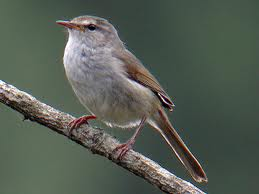
\includegraphics[scale=0.2]{figs/第04章/第157課:_onomatopoeiaii_fig/uguisu.png}
  ウグイス:ホーホケキョ 
&  
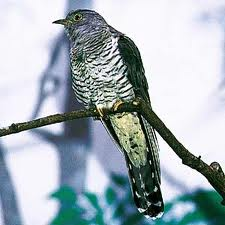
\includegraphics[scale=0.2]{figs/第04章/第157課:_onomatopoeiaii_fig/kakkoo.png}
 カッコウ:カッコー 
\\ \cline{1-2}

 
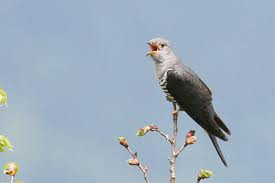
\includegraphics[scale=0.2]{figs/第04章/第157課:_onomatopoeiaii_fig/hototogisu.png}
 ホトトギス:テッペンカケタカ 
&  
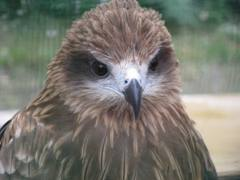
\includegraphics[scale=0.2]{figs/第04章/第157課:_onomatopoeiaii_fig/tonbi.png}
  トンビ:ピーヒョロロ 
\\ \cline{1-2}

\end{ltabulary}
\hfill\break
    

% http://www.imabi.net/onomatopoeiaiii.htm
     
\chapter{擬声語 III}

\begin{center}
\begin{Large}
第158課: 擬声語 III: 擬態語・擬情語 
\end{Large}
\end{center}
 
\par{ 擬態語 represent states and 擬情語 represent emotion(al states). These are intertwined with each other, and they are often tied to some sort of sound. Just like before, different spellings and nuances based on context are to be expected. However, the best thing that you can do to learn Japanese onomatopoeic expressions is see them how they're being used. }
      
\section{擬態語・擬情語}
 
\par{ To begin, we will look at a chart of common 擬態語 and 擬情語. Some notes that we have already seen before will be repeated in context of this lesson as reinforcement of what you already know with new material. }

\begin{ltabulary}{|P|P|P|P|}
\hline 

Tired, exhausted & くたくた(と・に) & Irritated & いらいら(と) \\ \cline{1-4}

Refreshed & すっきり(と) & Fixedly & じっと \\ \cline{1-4}

Round and round & ぐるぐる(と) & Firmly; fixedly \hfill\break
& ぐっと \\ \cline{1-4}

Relieved & ほっと & Nervous; excitedly & わくわく(と) \\ \cline{1-4}

Resolutely; tightly; firmly; steadily \hfill\break
& しっかり(と) & Furiously & ぷんぷん(と) \\ \cline{1-4}

Restlessly & そわそわ(と) & Astonished & びっくり(と) \\ \cline{1-4}

In a mess & めちゃくちゃ & Drenched & びっしょり(と) \\ \cline{1-4}

Glistening & ぴかぴか(と) & Radiantly & きらきら(と) \\ \cline{1-4}

Watery & べちゃべちゃ & Sneeze & はくしょん \\ \cline{1-4}

Rough & ざらざら(と・に) & Stickily & ねばねば(と) \\ \cline{1-4}

Ecstatically; vacantly & うっとり(と) & Dejected & がっかり \\ \cline{1-4}

\end{ltabulary}

\begin{itemize}

\item \textbf{くたくた }: Exhausted, worn down,  boiled to a mush, or even wordy. 
\item \textbf{いらいら(と) }: It may be irritating as in emotions are as in the body. 
\item \textbf{すっくり(と) }:  Being refreshed, clean-cut, straightforward, complete, and even neat. 
\item \textbf{しっかり(と) }: It can also mean reliable and enough. 
\item \textbf{ぷんぷん(と) }: It can also refer to a strong smell in a negative fashion. 
\end{itemize}

\par{\textbf{Part of Speech Note }: Some verbs are based off of onomatopoeia. Ex. きらめく (to sparkle\slash radiate). }

\par{\textbf{Voicing Note }: Voiced onomatopoeia often have a more serious or dramatic tone to them versus their very similar non-voiced counterparts. They are often antonymous. For example, さらさら can be smooth but ざらざら is rough. }

\par{ As you can see, there are some very similar patterns going on. Many onomatopoeic expressions in Japanese are the result of a doubled element(s). We have expressions like こそこそ(と) (stealthily) where double-morae element is doubled. These in particular are subject to having many variants. For instance, you can say こそっと or こっそり instead.  Note that the insertion of the っ is prevented when the resulting double consonant is not one that is allowed in Japanese. }

\par{ Please note that you always have your irregularities. Sometimes different forms have different nuances, although always related. This does not include non-onomatopoeic words with repeating elements. This is really just something you have to mess around with and test the limits of. }
      
\section{Examples}
 
\par{1. めらめらともえている ${\overset{\textnormal{ほのお}}{\text{炎}}}$ \hfill\break
A flaring flame }

\par{2. ちんちん。 \hfill\break
Beg! (To a dog) }

\par{3. だらだらとした ${\overset{\textnormal{とうろん}}{\text{討論}}}$ \hfill\break
A lengthy debate }

\par{4. じとじとした ${\overset{\textnormal{}}{\text{部屋}}}$ \hfill\break
Humid\slash damp room }

\par{5. がっかりした顔 \hfill\break
A dejected face }

\par{6. ${\overset{\textnormal{おんがく}}{\text{音楽}}}$ にうっとりする。 \hfill\break
To be enchanted by music. }

\par{7. はらはらして ${\overset{\textnormal{}}{\text{待}}}$ つ。 \hfill\break
To wait in great suspense. }

\par{8. ばらばらに ${\overset{\textnormal{こわ}}{\text{壊}}}$ す。 \hfill\break
To break into pieces. }

\par{9. でれでれにする。 \hfill\break
To be love-stricken. }

\par{10. にょろにょろと ${\overset{\textnormal{は}}{\text{這}}}$ い ${\overset{\textnormal{まわ}}{\text{回}}}$ る。 \hfill\break
To slither about. }

\par{11. ${\overset{\textnormal{あに}}{\text{兄}}}$ は今日プンプンしてる。(Casual) \hfill\break
My old brother is in a bad mood today. }

\par{12. ぎらぎら ${\overset{\textnormal{}}{\text{光}}}$ る ${\overset{\textnormal{たいよう}}{\text{太陽}}}$ \hfill\break
A glaring sun }

\par{${\overset{\textnormal{}}{\text{13a. 雨}}}$ の ${\overset{\textnormal{}}{\text{中}}}$ をはるばる ${\overset{\textnormal{}}{\text{来}}}$ る。 \hfill\break
${\overset{\textnormal{}}{\text{13b. 雨}}}$ の ${\overset{\textnormal{}}{\text{中}}}$ をわざわざ ${\overset{\textnormal{}}{\text{来}}}$ る。 \hfill\break
Come all the way through the rain. }

\par{\textbf{Sentence Note }: 13a infers that you never stopped on the way, and 13b infers that you took the trouble to come that far. }

\par{14. からからにする。 \hfill\break
To dry up. }

\par{15. ずきずきと ${\overset{\textnormal{いた}}{\text{痛}}}$ む。 \hfill\break
To throb in pain. }

\par{16. ぎっしり ${\overset{\textnormal{つ}}{\text{詰}}}$ まった \hfill\break
Packed; tight; heavy }

\par{${\overset{\textnormal{}}{\text{17. 雨}}}$ でぐっしょりとぬれた。 \hfill\break
I got soaked by the rain. }

\par{18. ぺこりと ${\overset{\textnormal{あたま}}{\text{頭}}}$ を ${\overset{\textnormal{さ}}{\text{下}}}$ げる。 \hfill\break
To bob one's head. }

\par{19. ぼんやりとした ${\overset{\textnormal{ひとかげ}}{\text{人影}}}$ \hfill\break
A vague figure. }

\par{20. がっしりとした ${\overset{\textnormal{}}{\text{男}}}$ \hfill\break
A well-built man }

\par{21. (あなた)の ${\overset{\textnormal{}}{\text{日本語}}}$ の ${\overset{\textnormal{のうりょく}}{\text{能力}}}$ はめきめきと ${\overset{\textnormal{じょうたつ}}{\text{上達}}}$ していますね。 \hfill\break
Your Japanese skills are remarkably improving. }

\par{22. チューインガムが ${\overset{\textnormal{くつ}}{\text{靴}}}$ の ${\overset{\textnormal{そこ}}{\text{底}}}$ にぺたっとくっついた。 \hfill\break
Chewing gum stuck to the bottom of my shoe. }

\par{23. ぐずぐずする。 \hfill\break
To be slow at doing. }

\par{24. まるまるとした ${\overset{\textnormal{よ}}{\text{酔}}}$ っ ${\overset{\textnormal{ぱら}}{\text{払}}}$ い \hfill\break
A plump drunkard }

\par{25. ${\overset{\textnormal{けむり}}{\text{煙}}}$ がもくもくと ${\overset{\textnormal{}}{\text{上}}}$ がる。 \hfill\break
For smoke to rise. }

\par{26. ぱっくりと裂ける。 \hfill\break
To split open. }

\par{27. とげがちくちく(と)する \hfill\break
Thorns are prickly }

\par{28. 背中がぞくぞく(と)する。 \hfill\break
For one's back to chill. }

\par{29. ふつふつ(と)沸く \hfill\break
To boil out. }

\par{30. 彼はまあまあ ${\overset{\textnormal{やさ}}{\text{優}}}$ しい。 \hfill\break
He is relatively nice. }

\par{\textbf{Part of Speech Note }: まあまあ can also be seen as an interjection meaning "now, now" or "my, my". Many adverbial phrases have varying parts of speech depending on usage. }

\par{31. ${\overset{\textnormal{びん}}{\text{瓶}}}$ はすっかり ${\overset{\textnormal{から}}{\text{空}}}$ だ。 \hfill\break
The bottle is quite\slash completely empty. }

\par{32. もうすっかりよくなりましたか。 \hfill\break
Have you become quite well already? \hfill\break
\hfill\break
33. そっと ${\overset{\textnormal{かた}}{\text{肩}}}$ を ${\overset{\textnormal{だ}}{\text{抱}}}$ いた。 \hfill\break
I gently hugged his shoulder. }

\par{\textbf{Reading Note }: 抱く is either read as だく or いだく. The first shows physical embrace. The latter shows the bearing of thoughts, feelings, etc. }

\begin{center}
\textbf{Eating \& Drinking }
\end{center}

\begin{ltabulary}{|P|P|P|P|}
\hline 

To gnaw & がりがり(と)かじる & To eat heartily & もりもり(と)食べる \\ \cline{1-4}

To gulp whole & がぶりと飲み込む \hfill\break
& To bite into & ぱ(っ)くり(と)食べる \\ \cline{1-4}

To bite fiercely & がぶり(と)かむ &  &  \\ \cline{1-4}

\end{ltabulary}

\begin{center}
\textbf{Laughter }
\end{center}

\begin{ltabulary}{|P|P|P|P|}
\hline 

To smile & にっこり(と)笑う & To smile & にこにこ(と)笑う \\ \cline{1-4}

To sneer \hfill\break
& せせら ${\overset{\textnormal{}}{\text{笑}}}$ う & To have a broad grin & にた\{っと・りと・にた(と)\}笑う \\ \cline{1-4}

To smirk & にや\{っと・りと・にや(と)\}笑う &  &  \\ \cline{1-4}

\end{ltabulary}
\hfill\break

\begin{center}
\textbf{Saying } 
\end{center}

\begin{ltabulary}{|P|P|P|P|P|P|}
\hline 

To harp & くだくだ(と)いう \hfill\break
くどくど(と)いう & To nag & がみがみ(と)する & To be fluent & ぺらぺら(と) \\ \cline{1-6}

To murmur & ぶつぶつ(と)いう & To buzz & がやがや & To be outspoken & ぽんぽん(と)いう \\ \cline{1-6}

To chatter & ぺちゃくちゃ(と)しゃべる \hfill\break
べらべら(と)しゃべる & To scold & がんがん(と)いう & To swallow & ぼそぼそ(と)いう \\ \cline{1-6}

To whisper & ひそひそ(と)いう & To grunt & ぶうぶう(と)いう & Noisily & わいわい(と) \\ \cline{1-6}

\end{ltabulary}

\begin{center}
 \textbf{Eating \& Drinking }
\end{center}

\begin{ltabulary}{|P|P|P|P|}
\hline 

To gulp & ごくごく(と)飲む \hfill\break
がぶがぶ(と)飲む \hfill\break
ぐっと飲む & To guzzle & がつがつ(と)食べる \\ \cline{1-4}

To gnaw & がりがり(と)かじる & To eat heartily & もりもり(と)食べる \\ \cline{1-4}

Crunchy & こりこり(と)する & Scraping; hard to the teeth & ごりごり(と) \\ \cline{1-4}

To gobble & ぱくぱく(と)食べる & To suck & ちゅうちゅう(と)吸う \\ \cline{1-4}

To swallow & ごくり(と)飲む \hfill\break
ごくん(と)飲む & To bite into & ぱ(っ)くり(と)食べる \\ \cline{1-4}

To bite fearcly & がぶり(と)かむ & To gulp whole & がぶりと飲み込む \\ \cline{1-4}

\end{ltabulary}
    

% http://www.imabi.net/duringthroughout.htm
     
\chapter{~中}

\begin{center}
\begin{Large}
第159課: ~中: During\slash Throughout 
\end{Large}
\end{center}
 
\par{ You will often see ~中 used in time phrases, and it is typically translated as during or throughout. }
      
\section{~中}
 
\par{ Although both are written as 中, the suffixes ~ちゅう and ~じゅう are slightly different. }

\par{~ちゅう means "during" in the sense of "under way". It becomes ~じゅう with 今日, 昨日, etc. It may also be used to show duration of condition (Ex. お祈り中 = At\slash in prayer). It can also mean under(going)――Ex. 試験中 = undergoing an exam. }

\par{~じゅう can be used to show duration as well. ~間中(ずっと) is a frequently used phrase and means "during\slash while". It helps when you want to use ~じゅう when you can use 間. This shows start to finish. Phrases it can directly attach to include things such as ${\overset{\textnormal{ひとばん}}{\text{一晩}}}$ , ${\overset{\textnormal{いちねん}}{\text{一年}}}$ , etc. ~じゅう(に) may also mean "throughout" but in terms of distance and place.  For instance, say you get stung all over your body by bees. You can use 体じゅう to describe where you were stung. }

\par{Connecting Note: ~中 can attach to either Sino-Japanese or native words. However, the etymology of the word it is used with will not help you in using the right reading. You have to learn how it is read one phrase at a time. }

\begin{center}
 Examples 
\end{center}

\par{1. 弟は ${\overset{\textnormal{はるやす}}{\text{春休}}}$ み ${\overset{\textnormal{ちゅう}}{\text{中}}}$ 遊んでばかり\{でした・いた\}。 \hfill\break
My brother just played all throughout spring break. }

\par{Grammar Note: ~てばかりです shows incessant action. }

\par{2. ${\overset{\textnormal{きょうじゅう}}{\text{今日中}}}$ に ${\overset{\textnormal{しあ}}{\text{仕上}}}$ げてください。 \hfill\break
Please finish it up within (the end of) today. }

\par{3. ${\overset{\textnormal{きゅうぎょうちゅう}}{\text{休業中}}}$ の ${\overset{\textnormal{えいぎょうしょ}}{\text{営業所}}}$ \hfill\break
 A business office that's closed for the holidays }

\par{4. ${\overset{\textnormal{からだじゅう}}{\text{体中}}}$ が ${\overset{\textnormal{いた}}{\text{痛}}}$ んだ。 \hfill\break
It hurt all over my body. }

\par{5. ${\overset{\textnormal{みつりょう}}{\text{密漁}}}$ ${\overset{\textnormal{せん}}{\text{船}}}$ が ${\overset{\textnormal{そうぎょうちゅう}}{\text{操業中}}}$ に ${\overset{\textnormal{てん}}{\text{転}}}$ ${\overset{\textnormal{ぷく}}{\text{覆}}}$ した。 \hfill\break
A poaching ship capsized in operation. }

\par{6. ${\overset{\textnormal{ひゃく}}{\text{百}}}$ ${\overset{\textnormal{にんちゅう}}{\text{人中}}}$ ${\overset{\textnormal{はんすう}}{\text{半数}}}$ ${\overset{\textnormal{ひなん}}{\text{避難}}}$ しました。 \hfill\break
Out of the 100 people, half evacuated. }

\par{\textbf{Meaning Note }: You will often see ~中 used in the same sense as in Ex. 6. to mean "out of\dothyp{}\dothyp{}\dothyp{}". Note that it is attached to the \emph{counter }phrase 百人. }

\par{\textbf{Phrase Note }: One common phrase which is slightly grammatically questionable is 発売中. This is often used to emphasize having started to sell something. However, the definition of 発売 is "to begin selling". As you can see, it is an instantaneous verb, and instantaneous verbs normally should never take 中. For instance, you can't say 死亡中, 卒業中, or 結婚中. You can say, though, 婚約中 (engaged) and 出願中 (under application). These phrases are acceptable because there is an end to the state the verb brings about. So, while 発売中 is typically acceptable when the product has not been out long, after a long period of time, it becomes very strange Japanese to anyone. }

\par{ The following phrases all have ~中 with the reading ちゅう except 世界中, which is read as せかいじゅう. Remember, when ~中 means "during", it is read as ちゅう, and when it means "throughout", it is read as ~じゅう. }

\begin{ltabulary}{|P|P|P|P|P|P|}
\hline 

今年中 & During the year & 午前中 & During the morning & 今月中 & During the month \\ \cline{1-6}

来月中 & Within the next month & 在学中 & In schooling & 世界中 & Throughout the world \\ \cline{1-6}

販売中 & On sale (not as in discount) & 存命中 & While one is still alive & 空気中 & In the air \\ \cline{1-6}

\end{ltabulary}
\hfill\break
    

% http://www.imabi.net/thebody.htm
     
\chapter{The Body}

\begin{center}
\begin{Large}
第160課: The Body 
\end{Large}
\end{center}
 
\par{ This lesson will be about the parts of the body. }
      
\section{The Body}
  
\par{  Many phrases relate to the body. Below is a chart of the most important parts of the body.  \hfill\break
\hfill\break
}

\begin{ltabulary}{|P|P|P|P|P|P|}
\hline 

Blood & 血 & ち \hfill\break
& Blood vessel & 血管 & けっかん \hfill\break
\\ \cline{1-6}

Hand & 手 & て \hfill\break
& Arm & 腕 & うで \hfill\break
\\ \cline{1-6}

Finger & 指 & ゆび & Wrist & 手首 & てくび \hfill\break
\\ \cline{1-6}

Ankle & 足首 & あしくび \hfill\break
& Heel & 踵 & かかと \hfill\break
\\ \cline{1-6}

Shoulder & 肩 & かた \hfill\break
& Nail & 爪 & つめ \hfill\break
\\ \cline{1-6}

Shin & 脛 & すね \hfill\break
& Knee & 膝 & ひざ \hfill\break
\\ \cline{1-6}

Calf & 脹脛 & ふくらはぎ \hfill\break
& Thigh & 腿 & もも \hfill\break
\\ \cline{1-6}

Thumb & 親指・拇 & おやゆび \hfill\break
& Index finger & 人差し指 & ひとさしゆび \hfill\break
\\ \cline{1-6}

Middle finger & 中指 & なかゆび \hfill\break
& Ring finger & 薬指 & くすりゆび \hfill\break
\\ \cline{1-6}

Pinky & 小指 & こゆび \hfill\break
& Palm & 手の平 & てのひら \hfill\break
\\ \cline{1-6}

Intestines & 腸 & ちょう \hfill\break
& Bellybutton & 臍 & へそ \hfill\break
\\ \cline{1-6}

Head & 頭 & あたま & Hair & 髪(の毛) & かみ(のけ) \\ \cline{1-6}

Forehead & 額 & ひたい \hfill\break
& Throat & 喉 & のど \hfill\break
\\ \cline{1-6}

Brain & 脳 & のう \hfill\break
& Tongue & 舌 & した \hfill\break
\\ \cline{1-6}

Eyes & 目、瞳 & め、ひとみ \hfill\break
& Eyeball & 眼球 & がんきゅう \hfill\break
\\ \cline{1-6}

Eyelash & 睫毛 & まつげ \hfill\break
& Eyebrow & 眉(毛) & まゆ(げ) \hfill\break
\\ \cline{1-6}

Ear & 耳 & みみ \hfill\break
& Eardrum & 鼓膜 & こまく \hfill\break
\\ \cline{1-6}

Skull & 頭蓋骨 & ずがいこつ \hfill\break
& Nose & 鼻 & はな \hfill\break
\\ \cline{1-6}

Nose hair & 鼻毛 & はなげ \hfill\break
& Cheek & 頬 & ほお・ほほ \\ \cline{1-6}

Mouth & 口 & くち \hfill\break
& Teeth & 歯 & は \hfill\break
\\ \cline{1-6}

Gums & 歯茎 & はぐき \hfill\break
& Lips & 唇 & くちびる \hfill\break
\\ \cline{1-6}

Jaw & 顎・頤 & あご \hfill\break
& Chin & 下顎 & したあご \hfill\break
\\ \cline{1-6}

Face & 顔 & かお \hfill\break
& Neck & 首、頸部 & くび \\ \cline{1-6}

Spine & 脊柱、背骨 & せきちゅう、せぼね \hfill\break
& Back & 背(中) & せ(なか) \hfill\break
\\ \cline{1-6}

Chest & 胸 & むね \hfill\break
& Esophagus & 食道 & しょくどう \hfill\break
\\ \cline{1-6}

Stomach & 胃 & い \hfill\break
& Internal organ & 内臓 & ないぞう \hfill\break
\\ \cline{1-6}

Bowel & 腸 & はらわた \hfill\break
& Liver & 肝臓 & かんぞう \hfill\break
\\ \cline{1-6}

Pancreas & 膵臓 & すいぞう \hfill\break
& Appendix & 盲腸 & もうちょう \hfill\break
\\ \cline{1-6}

Small intestine & 小腸 & しょうちょう & Large intestine & 大腸 & だいちょう \hfill\break
\\ \cline{1-6}

Abdomen & 腹 & はら \hfill\break
& Heart & 心臓 & しんぞう \hfill\break
\\ \cline{1-6}

Gall bladder & 胆のう \hfill\break
& たんのう \hfill\break
& Lungs & 肺(臓) & はい(ぞう) \hfill\break
\\ \cline{1-6}

Kidney & 腎臓 & じんぞう \hfill\break
& Bone & 骨 & ほね \hfill\break
\\ \cline{1-6}

Pelvis & 骨盤 & こつばん \hfill\break
& Leg; foot & 足 (foot)、脚 (leg) & あし \\ \cline{1-6}

\end{ltabulary}
 
\par{\textbf{Word Notes }: }
 
\par{1. To say "left" or "right X", all you need to do is add 左 and 右 respectively. So, right leg would be 右足. }

\par{2. 手 sometimes refers to full arm. }

\begin{center}
\textbf{Examples } 
\end{center}
 Blood 血 ち \hfill\break
Blood vessel 血管 けっかん \hfill\break
Hand 手 て \hfill\break
Arm 腕 うで \hfill\break
Finger 指 ゆび Wrist 手首 てくび \hfill\break
Ankle 足首 あしくび \hfill\break
Heel 踵 かかと \hfill\break
Shoulder 肩 かた \hfill\break
Nail 爪 つめ \hfill\break
Shin 脛 すね \hfill\break
Knee 膝 ひざ \hfill\break
Calf 脹脛 ふくらはぎ \hfill\break
Thigh 腿 もも \hfill\break
Thumb 親指・拇 おやゆび \hfill\break
Index finger 人差し指 ひとさしゆび \hfill\break
Middle finger 中指 なかゆび \hfill\break
Ring finger 薬指 くすりゆび \hfill\break
Pinky 小指 こゆび \hfill\break
Palm 手の平 てのひら \hfill\break
Intestines 腸 ちょう \hfill\break
Bellybutton 臍 へそ \hfill\break
Head 頭 あたま Hair 髪(の毛) かみ(のけ) Forehead 額 ひたい \hfill\break
Throat 喉 のど \hfill\break
Brain 脳 のう \hfill\break
Tongue 舌 した \hfill\break
Eyes 目、瞳 め、ひとみ \hfill\break
Eyeball 眼球 がんきゅう \hfill\break
Eyelash 睫毛 まつげ \hfill\break
Eyebrow 眉(毛) まゆ(げ) \hfill\break
Ear 耳 みみ \hfill\break
Eardrum 鼓膜 こまく \hfill\break
Skull 頭蓋骨 ずがいこつ \hfill\break
Nose 鼻 はな \hfill\break
Nose hair 鼻毛 はなげ \hfill\break
Cheek 頬 ほお・ほほ Mouth 口 くち \hfill\break
Teeth 歯 は \hfill\break
Gums 歯茎 はぐき \hfill\break
Lips 唇 くちびる \hfill\break
Jaw 顎・頤 あご \hfill\break
Chin 下顎 したあご \hfill\break
Face 顔 かお \hfill\break
Neck 首、頸部 くび Spine 脊柱、背骨 せきちゅう、せぼね \hfill\break
Back 背(中) せ(なか) \hfill\break
Chest 胸 むね \hfill\break
Esophagus 食道 しょくどう \hfill\break
Stomach 胃 い \hfill\break
Internal organ 内臓 ないぞう \hfill\break
Bowel 腸 はらわた \hfill\break
Liver 肝臓 かんぞう \hfill\break
Pancreas 膵臓 すいぞう \hfill\break
Appendix 盲腸 もうちょう \hfill\break
Small intestine 小腸 しょうちょう Large intestine 大腸 だいちょう \hfill\break
Abdomen 腹 はら \hfill\break
Heart 心臓 しんぞう \hfill\break
Gall bladder 胆のう \hfill\break
たんのう \hfill\break
Lungs 肺(臓) はい(ぞう) \hfill\break
Kidney 腎臓 じんぞう \hfill\break
Bone 骨 ほね \hfill\break
Pelvis 骨盤 こつばん \hfill\break
Leg; foot 足 (foot)、脚 (leg) あし 
\par{1. のどが ${\overset{\textnormal{いた}}{\text{痛}}}$ い。 \hfill\break
To have a sore throat. }
 
\par{3. ドアに\{ ${\overset{\textnormal{}}{\text{指・親指\}}}}$ を ${\overset{\textnormal{はさ}}{\text{挟}}}$ む。 \hfill\break
To smash one's [finger\slash thumb] in a door. }

\par{5. ${\overset{\textnormal{のう}}{\text{能}}}$ あるタカは ${\overset{\textnormal{つめ}}{\text{爪}}}$ を ${\overset{\textnormal{かく}}{\text{隠}}}$ す。(Idiomatic) \hfill\break
Still waters run deep. \hfill\break
Literally: A hawk with talent hides its talons. }
 
\par{${\overset{\textnormal{}}{\text{7. 顔}}}$ が ${\overset{\textnormal{き}}{\text{利}}}$ く。 \hfill\break
To have many contacts. \hfill\break
Literally: The face effective. }
 
\par{9. のどが ${\overset{\textnormal{つ}}{\text{詰}}}$ まる。 \hfill\break
To choke. }
 
\par{${\overset{\textnormal{}}{\text{11. 耳}}}$ が ${\overset{\textnormal{}}{\text{遠}}}$ い。 \hfill\break
To be hard of hearing. }
 
\par{${\overset{\textnormal{}}{\text{13. 耳}}}$ に ${\overset{\textnormal{のこ}}{\text{残}}}$ る。 \hfill\break
To tingle in the ears. }
 
\par{${\overset{\textnormal{}}{\text{15. 耳}}}$ を ${\overset{\textnormal{ふさ}}{\text{塞}}}$ ぐ。 \hfill\break
To close one's ears. }
 
\par{${\overset{\textnormal{}}{\text{17. 鼻}}}$ をほじる。 \hfill\break
To pick one's nose. }

\par{19. よく ${\overset{\textnormal{}}{\text{舌}}}$ が ${\overset{\textnormal{}}{\text{回}}}$ る。 \hfill\break
To be quite eloquent. }

\par{${\overset{\textnormal{}}{\text{21. 胸}}}$ に ${\overset{\textnormal{}}{\text{閉}}}$ まる。 \hfill\break
To keep to oneself. }

\par{23a. 錠を服用する。X \hfill\break
23b. 錠剤を服用する。 \hfill\break
To take a pill. \hfill\break
\textbf{\hfill\break
Vocabulary Note }: ~錠 is the counter for pills. }

\par{25. 予約をしてもらえますか。 \hfill\break
Could you make an appointment for me? }

\par{\textbf{Grammar Note }: Using the negative form is OK here as well or a more honorific final form like いただけませんか. }
 2. のどが ${\overset{\textnormal{かわ}}{\text{渇}}}$ いた。 \hfill\break
I'm thirsty. 
\par{${\overset{\textnormal{}}{\text{4. 手}}}$ を ${\overset{\textnormal{あ}}{\text{挙}}}$ げる。 \hfill\break
To surrender. \hfill\break
Literally: To raise one's hands\slash arms. }

\par{${\overset{\textnormal{}}{\text{6. 手}}}$ が ${\overset{\textnormal{た}}{\text{足}}}$ りない。 \hfill\break
To be shorthanded. }

\par{8. ${\overset{\textnormal{ひざ}}{\text{膝}}}$ の ${\overset{\textnormal{さら}}{\text{皿}}}$ \hfill\break
 Kneecap }

\par{${\overset{\textnormal{}}{\text{10. 地}}}$ に ${\overset{\textnormal{}}{\text{膝}}}$ を ${\overset{\textnormal{つ}}{\text{突}}}$ く。 \hfill\break
To go to the ground on one's knees. }

\par{${\overset{\textnormal{}}{\text{12. 顔}}}$ を ${\overset{\textnormal{つぶ}}{\text{潰}}}$ す。 \hfill\break
To embarrass. \hfill\break
Literally: To crush one's face. }

\par{${\overset{\textnormal{}}{\text{14. 鼻}}}$ がいい。 \hfill\break
Have a good sense of smell. }

\par{${\overset{\textnormal{}}{\text{16. 鼻}}}$ が ${\overset{\textnormal{}}{\text{高}}}$ い。 \hfill\break
To be proud. }

\par{${\overset{\textnormal{}}{\text{18. 鼻}}}$ であしらう。 \hfill\break
To snub. }

\par{20. のどを ${\overset{\textnormal{とお}}{\text{通}}}$ らない。 \hfill\break
To have no appetite. }

\par{22. 胃腸が\{強い・弱い\}。 \hfill\break
To have a [strong\slash weak] system. }

\par{24. こういう ${\overset{\textnormal{むいしき}}{\text{無意識}}}$ の時間は ${\overset{\textnormal{だいのうへんえんけい}}{\text{大脳辺縁系}}}$ の ${\overset{\textnormal{かいば}}{\text{海馬}}}$ が ${\overset{\textnormal{つかさど}}{\text{司}}}$ っている。 \hfill\break
Such unconscious time is controlled by the             hippocampus of the limbic system. \hfill\break
By 池田 ${\overset{\textnormal{きよひこ}}{\text{清彦}}}$ , a biologist, in the commentary for 冷たい ${\overset{\textnormal{ゆうわく}}{\text{誘惑}}}$  \emph{Cold Temptations }by ${\overset{\textnormal{のなみ}}{\text{乃南}}}$ アサ. }
 
\par{\textbf{Anatomy Note }: If you don't know what the limbic system or the hippocampus is, the 漢字 tell you they're about the brain. }

\begin{center}
 \textbf{凝る Versus 懲りる }
\end{center}
 
\par{ These words are often confused because they sound similar, and sometimes when not written in 漢字, they resemble each other. The first is a 五段 verb and the second is a 一段 verb. The following chart describes their most important usages. }

\begin{ltabulary}{|P|P|P|P|}
\hline 

凝る (こる) & 使用例 & 懲りる (こりる) & 使用例 \\ \cline{1-4}

To be stiff & 肩が凝っている。 & To learn a lesson & 彼女の運転には懲りた。 \\ \cline{1-4}

To be addicted to & 釣りに凝る。 &  &  \\ \cline{1-4}

To be intricate with & 凝りすぎた文体 &  &  \\ \cline{1-4}

\end{ltabulary}

\par{-------------------------------------------------------------------------------- }

\begin{center}
\textbf{会話 1 }
\end{center}

\par{26. お母さん: あら、セッス、顔色がよくないわね。 \hfill\break
セス: ええ、実は、今朝から何となく寒気がして、それに頭が痛くて。。。 \hfill\break
お母さん: 熱はあるの? \hfill\break
セス: さあ、分かりません。でも、あるかもしれません。 \hfill\break
お母さん: そうねえ。顔がちょっと赤いわねえ。風邪かしら。お医者さんに診察をもらったほうがいいよ。電話をかけてみるから。  }

\par{(電話を切る) }

\par{セス: どうもありがとうございました。 \hfill\break
お母さん: いいえ、でもよかったね、ちょうど空いてて。 }

\par{ There are several new things in this short little conversation. The mother uses a lot of feminine expressions, which haven't really been covered up to this point. あら is an expression like "oh my!" and is often used by female speakers. Sentence endings like わね, の (making a question), and かしら (I wonder) are all feminine. }

\begin{center}
\textbf{Grammar Points }
\end{center}

\par{~かもしれません = Might  ~たほうがいい = It's best to ~てみる = To try to\dothyp{}\dothyp{}\dothyp{} }

\begin{center}
\textbf{New Vocab }
\end{center}

\begin{ltabulary}{|P|P|P|}
\hline 

顔色 & かおいろ & Complexion \\ \cline{1-3}

何となく & なんとなく & Somehow or other \\ \cline{1-3}

お医者さん & おいしゃさん & Doctor \\ \cline{1-3}

診察 & しんさつ & Examination (medical) \\ \cline{1-3}

\end{ltabulary}

\begin{center}
\textbf{会話 2 }
\end{center}

\par{27. セス、医者に行く。 }

\par{医者: どうしましたか。 \hfill\break
セス: あのう、今朝から体がだるくなって、さっきのども痛くなって。 \hfill\break
医者: そうですか。 \hfill\break
セス: それに、ものを飲み込むとき、痛いんです。 \hfill\break
医者: いけませんね。食欲は? \hfill\break
セス: あまりありません。 \hfill\break
医者: じゃ、ちょっとのどを見てみましょう。大きく口を開けてください。ああ、やはりずいぶん赤いですね。風邪ですよ。薬を出しますから、一週間飲んでみてください。それから、一日に何回か、うがいをしてください。早く治ると思いますよ。 \hfill\break
セス: はい、分かりました。食事はどうしたらいいでしょうか。 \hfill\break
医者: そうですね。あのう、まあ、軟らかいものだけにしておいたらどうですか。おかゆぐらいにするんですが。 \hfill\break
セス: ありがとうございました。 \hfill\break
医者: お大事に。 }

\begin{center}
\textbf{Grammar Points }
\end{center}

\par{1. ~ておく: Used to show action in advance or preparation of something. \hfill\break
2. ~たらいいでしょうか = What do I do about? \hfill\break
3. ~たらどうですか = How about doing\dothyp{}\dothyp{}\dothyp{}? \hfill\break
4. ~ぐらい is used here to show a minimal limit. \hfill\break
5. ~てみましょう = Let's try to\dothyp{}\dothyp{}\dothyp{} Here it is used to more indirect and polite to the patient. }

\par{\textbf{Culture Note }: お大事に is only said to those that are in need of care. }

\begin{ltabulary}{|P|P|P|}
\hline 

怠い & だるい & To feel sluggish \\ \cline{1-3}

飲み込む & のみこむ & To swallow \\ \cline{1-3}

食欲 & しょくよく & Appetite \\ \cline{1-3}

何回か & なんかいか & Several times \\ \cline{1-3}

\end{ltabulary}

\begin{ltabulary}{|P|P|P|}
\hline 

治る & なおる & To heal \\ \cline{1-3}

嗽をする & うがいをする & To gargle \\ \cline{1-3}

軟らかい & やわらかい & Soft \\ \cline{1-3}

お大事に & おだいじに & Take care \\ \cline{1-3}

\end{ltabulary}
     

% http://www.imabi.net/colors.htm
     
\chapter{Colors}

\begin{center}
\begin{Large}
第161課: Colors 
\end{Large}
\end{center}
 
\par{ Each society has its own customs about colors. Japanese is now based on a seven color (七色) scheme, but Japanese has not always been this way. This will become quite apparent as we look at individual colors. }

\par{ A lot can be said about the nuances of each color, how to be more specific about shades and hues, and what sort of idiomatic expressions can be made with color. By now you should have already learned the basic colors through example sentences thus far. So, this lesson is more about knowing exact details about colors, and it will be expanded over time. }
      
\section{Colors}
 
\par{ There is a noun and an adjectival form to each color. Also, there are additional Sino-Japanese variants for many colors, which can be made adjectival by adding の. }

\begin{ltabulary}{|P|P|P|P|P|P|}
\hline 

Color & Native & Adjective & Non-native & Adjective & Kango \\ \cline{1-6}

Blue & 青(あお) & 青い &  &  & 青色(せいしょく) \\ \cline{1-6}

Red & 赤(あか) & 赤い &  &  & 赤色(せきしょく) \\ \cline{1-6}

Yellow & 黄(き) & 黄色(きいろ)い \hfill\break
黄(色)の &  &  \hfill\break
& 黄色(こうしょく) \\ \cline{1-6}

Green & 緑(みどり) & 緑の &  &  & 緑色(みどりいろ・りょくしょく) \\ \cline{1-6}

Black & 黒(くろ) & 黒い &  &  & 黒色(こくしょく) \\ \cline{1-6}

Brown &  &  &  & 茶色(ちゃいろ) & 茶色(ちゃいろ)い \hfill\break
茶色(ちゃいろ)の \\ \cline{1-6}

White & 白(しろ) & 白い &  &  & 白色(はくしょく) \\ \cline{1-6}

Purple & 紫(むらさき) & 紫の &  &  & 紫色(むらさきいろ) \\ \cline{1-6}

Grey &  &  &  &  & 灰色(はいいろ・かいしょく) \\ \cline{1-6}

Pink &  &  & ピンク & ピンクの &  \\ \cline{1-6}

Orange &  &  & オレンジ & オレンジの &  \\ \cline{1-6}

Gold & 金色(かねいろ) &  &  &  & 金色(きんいろ・こんじき・きんしょく) \\ \cline{1-6}

Silver & 銀色(しろがねいろ) &  &  &  & 銀色(ぎんいろ・ぎんしょく) \\ \cline{1-6}

Beige &  &  & ベージュ & ベージュの &  \\ \cline{1-6}

Tan & 渋色(しぶいろ) &  &  & 渋色の &  \\ \cline{1-6}

Turquoise &  &  & ターコイズ & ターコイズの &  \\ \cline{1-6}

Vermilion &  &  &  &  & 朱色(しゅいろ・しゅしょく) \\ \cline{1-6}

Indigo &  &  & インディゴ \hfill\break
インジゴ \hfill\break
&  & 藍色(あいいろ・らんしょく) \\ \cline{1-6}

\end{ltabulary}

\par{\textbf{Usage Notes }: }

\par{1. All colors of native or foreign origin may be followed by ${\overset{\textnormal{}}{\text{色}}}$ . Certain colors should be used with ${\overset{\textnormal{}}{\text{色}}}$ . For example, ${\overset{\textnormal{}}{\text{灰}}}$ just means "ashes". Gold and silver must have ${\overset{\textnormal{}}{\text{色}}}$ in order to not be confused with the actual elements. Words such as ターコイズ and オレンジ can be understood to mean the color, but they really refer to the objects. Without ${\overset{\textnormal{}}{\text{色}}}$ , ${\overset{\textnormal{}}{\text{緑}}}$ may mean "greenery". ${\overset{\textnormal{}}{\text{紫}}}$ as a noun may refer to soy sauce in sushi restaurants. }

\par{2. The native versions of gold and silver are rare. In fact, the one for gold is never used but in 白銀色, 銅色, and the like. }

\par{3. Most of the Sino-Japanese readings are rare. }

\par{4. ${\overset{\textnormal{}}{\text{青}}}$ , not ${\overset{\textnormal{}}{\text{緑}}}$ , is the color used for streetlights for "green". ${\overset{\textnormal{}}{\text{青}}}$ may also mean "greens" in expressions like ${\overset{\textnormal{あおものいちば}}{\text{青物市場}}}$ meaning "vegetable market". It is also the color for pale face, youth, and freshness in plants, coolness, the sea, and even the color of moonlight and evening mist. It may also refer to black as in a horse's coat. }

\par{5. 茶色 is "brown" instead of "green" because when tea was first introduced to Japan, it would be shipped to elites in hardened, steamed form. From then, it would be cut up and boiled in hot water and drank. As "green tea" variants would come later, the color of the original tea drinks became the Japanese word for brown. }

\par{\textbf{Light and Dark Colors }}

\par{Light colors are expressed by using ${\overset{\textnormal{うす}}{\text{薄}}}$ い or ${\overset{\textnormal{うす}}{\text{薄}}}$ ~. For dark colors, use ${\overset{\textnormal{こ}}{\text{濃}}}$ い. Now, there will be colors that are light or dark variants of a general color. 淡い is "light\slash faint" and its antonym is also 濃い. }

\par{1. 淡い黄色の葉っぱがありますよね。 \hfill\break
There are light yellow flowers, aren't there? }

\par{2. この花の色が薄い。 \hfill\break
This flower's color is pale\slash weak\slash thin. }

\par{3. 高橋さんの車はその濃い緑色のですね。 \hfill\break
Mr. Takahashi's car is that dark green one, right? }

\par{4. ${\overset{\textnormal{うめ}}{\text{梅}}}$ の ${\overset{\textnormal{うすべに}}{\text{薄紅}}}$ \hfill\break
 The light crimson of a plum }

\par{\textbf{Mixed Colors }}

\par{Colors may be put together to make things such as "white-black" and "yellow-green". The resultant expressions may be read with either 訓読み or 音読み. 音読み are rarer and reserved for the spoken language with exception to \#8. }

\par{5. 黄緑(きみどり・おうりょく) \hfill\break
Yellow-green \hfill\break
\hfill\break
6. 黒白(くろしろ・こくはく) \hfill\break
Black and white }

\par{7. 青緑(あおみどり・せいりょく) \hfill\break
Blue-green\slash aqua }

\par{8. 金茶(きんちゃ) \hfill\break
Golden brown }

\begin{center}
\textbf{Interesting Phrases }
\end{center}

\par{${\overset{\textnormal{}}{\text{赤字}}}$ and ${\overset{\textnormal{}}{\text{黒字}}}$ are deficit and surplus respectfully. They are words that typically confuse students, although there are similar expressions in English. For example, you can say "to be in the red". When you get a failing grade, you can say you got an ${\overset{\textnormal{あかてん}}{\text{赤点}}}$ . However, ${\overset{\textnormal{こくてん}}{\text{黒点}}}$ refers to sunspots. So, it is not the opposite of 赤点. Instead, the antonym for 赤点 is either ${\overset{\textnormal{きゅうだいてん}}{\text{及第点}}}$ or ${\overset{\textnormal{ごうかくてん}}{\text{合格点}}}$ . }

\par{ It is also important to note that the phrases 肌が\{白い・黒い\} are NOT used for nationality\slash race. Rather, they refer to someone's complexion. }
    

% http://www.imabi.net/food.htm
     
\chapter{Food}

\begin{center}
\begin{Large}
第162課: Food 
\end{Large}
\end{center}
 
\par{ Japanese food, ${\overset{\textnormal{にほんりょうり}}{\text{日本料理}}}$ ・ ${\overset{\textnormal{わしょく}}{\text{和食}}}$ ・日本食, is one of the most interesting things about Japan. At the end of this lesson, you will be able to go to a Japanese restaurant ( ${\overset{\textnormal{}}{\text{日本料理屋}}}$ ) and talk about what's in your food, how to ask for your food, etc. }
      
\section{At a Restaurant}
 
\begin{center}
 \textbf{お品書き }(Menu) 
\end{center}
 
\par{お好み焼き Okonomiyaki 700¥     天丼 Tendon 780¥     寿司 Sushi 1400¥   すき焼き Sukiyaki 1200¥ \hfill\break
刺し身 Sashimi 1350¥     狐そば Kitsune soba 700¥   狐うどん Kitsune udon 700¥ サラダ Salad 400¥ \hfill\break
お握りずし Onigirizushi 1000¥    ざるそば Zaru soba 550¥     しゃぶしゃぶ Shabushabu 1250¥ }
 
\par{\textbf{お飲み物 }}
 
\par{ビール Beer 310¥  お茶 Tea 300¥    水 Water 100¥    コーク Coke 250¥ \hfill\break
Qoo  300¥     焼酎 Shochu 300¥     ミルク Milk 250¥ }
 
\par{\textbf{デザート }}
 
\par{アイスクリーム Ice cream 240¥     チョコレートセーキ Chocolate shake 250¥ \hfill\break
アップルパイ Apple pie 300¥     チーズケーキ Cheese cake 350¥ }
 
\par{\textbf{Cultural Differences }: In the average Japanese restaurant, when food is done, it is sent out immediately regardless of whether or not the other people's food in one's party is ready. Refills are rare. Coffee might be refilled, but you may get charged double. When sitting down you are given a wet towel called a おしぼり to wipe your hands, a menu, and some tea and water. }

\begin{center}
 \textbf{Useful Expressions }
\end{center}

\par{1. メニューを ${\overset{\textnormal{}}{\text{見}}}$ せてください。 \hfill\break
Please show me a menu. }
 
\par{2. お ${\overset{\textnormal{なか}}{\text{腹}}}$ が ${\overset{\textnormal{あ}}{\text{空}}}$ きましたか。 \hfill\break
Are you hungry? }

\begin{ltabulary}{|P|P|P|P|P|P|P|P|}
\hline 

Bad & まずい & Sour & すっぱい & Sweet & 甘い & Bitter & 苦い \\ \cline{1-8}

Weak; thin & 薄い & Strong; thick & 濃い & Hot & 熱い & Cold & 冷たい \\ \cline{1-8}

\end{ltabulary}

\par{3. Xがおいしそうですね。 \hfill\break
X looks good. }
 
\par{${\overset{\textnormal{}}{\text{4. 安}}}$ いレストランです。 \hfill\break
It's a cheap restaurant. }
 
\par{5. じゃあ、それにしましょう。 \hfill\break
Well, let's go with that. }
 
\par{6. のどが ${\overset{\textnormal{かわ}}{\text{渇}}}$ きました。 \hfill\break
I'm thirsty. }

\par{7. ${\overset{\textnormal{すしににんまえ}}{\text{寿司二人前}}}$ お ${\overset{\textnormal{ねが}}{\text{願}}}$ いします。 \hfill\break
Sushi for two please. }
 
\par{${\overset{\textnormal{}}{\text{8. (お)酒}}}$ がお ${\overset{\textnormal{}}{\text{好}}}$ きですか。 \hfill\break
Do you like sake? }
 
\par{9. お ${\overset{\textnormal{}}{\text{飲}}}$ み ${\overset{\textnormal{}}{\text{物}}}$ は? \hfill\break
Drinks? }

\par{10. ${\overset{\textnormal{たんぱくしつ}}{\text{蛋白質}}}$ = Protein ${\overset{\textnormal{たんすいかぶつ}}{\text{炭水化物}}}$ = Carbohydrates ${\overset{\textnormal{しぼう}}{\text{脂肪}}}$ = Fat   }

\par{11. ${\overset{\textnormal{あいせき}}{\text{相席}}}$ お ${\overset{\textnormal{}}{\text{願}}}$ いします。 \hfill\break
Please let another party sit with you. }

\par{\textbf{Culture Note }: You may be asked this in Japan in inexpensive restaurants when it's really crowded and there's really nothing that you can do about it. }

\par{12. ${\overset{\textnormal{しょうしょう}}{\text{少々}}}$ お ${\overset{\textnormal{}}{\text{待}}}$ ちください。 \hfill\break
Please wait one moment. }
 
\par{13. いらっしゃいませ。 ${\overset{\textnormal{なんめい}}{\text{何名}}}$ ですか。こちらへどうぞ。 \hfill\break
Welcome. How many will there be? Please follow me. }
 
\par{14. ビールをもう ${\overset{\textnormal{}}{\text{一本}}}$ ください。 \hfill\break
Give me one more beer please. \hfill\break
\hfill\break
Note: Beer in this case is most likely 缶ビール. }
 
\par{15. てんぷらを ${\overset{\textnormal{}}{\text{一人前}}}$ お ${\overset{\textnormal{}}{\text{願}}}$ いします。 \hfill\break
Tempura for one please. }

\par{${\overset{\textnormal{}}{\text{16. 火}}}$ にかける。 \hfill\break
To put on the stove. }

\par{17. ${\overset{\textnormal{こしょう}}{\text{胡椒}}}$ を ${\overset{\textnormal{くわ}}{\text{加}}}$ えて ${\overset{\textnormal{あじ}}{\text{味}}}$ をつける。 \hfill\break
To put in flavor by adding pepper. }

\par{18. お ${\overset{\textnormal{かんじょう}}{\text{勘定}}}$ は○○になります。 \hfill\break
Your bill comes out to XX. }
 
\par{19. お ${\overset{\textnormal{}}{\text{待}}}$ たせしました。(Waiter) \hfill\break
I'm sorry for having made you wait. }
 
\par{20. 「ここでお ${\overset{\textnormal{め}}{\text{召}}}$ し ${\overset{\textnormal{}}{\text{上}}}$ がりですか、それともお ${\overset{\textnormal{}}{\text{持}}}$ ち ${\overset{\textnormal{}}{\text{帰}}}$ りですか」「ここで食べます。」 \hfill\break
“Is this to eat here or to-go?” “For here”. }
 
\par{21. すし ${\overset{\textnormal{や}}{\text{屋}}}$ へ ${\overset{\textnormal{}}{\text{行}}}$ きましょうか。 \hfill\break
How about going to the sushi shop? }
 
\par{22. たいてい ${\overset{\textnormal{}}{\text{何}}}$ を ${\overset{\textnormal{}}{\text{飲}}}$ みますか。 \hfill\break
What do you generally have to drink? }
 
\par{23. ご注文はお ${\overset{\textnormal{き}}{\text{決}}}$ まりですか。 \hfill\break
Have you decided on what you will order? }
 
\par{${\overset{\textnormal{}}{\text{24. 私}}}$ に ${\overset{\textnormal{はら}}{\text{払}}}$ わせてください。 \hfill\break
Allow me to pay. }
 
\par{25. はい、 ${\overset{\textnormal{ぜんぶ}}{\text{全部}}}$ でX ${\overset{\textnormal{えん}}{\text{円}}}$ になります。 \hfill\break
Yes, this comes out to in total to X yen. }
 
\par{${\overset{\textnormal{}}{\text{26. 何}}}$ に\{しましょう・なさいま\}か。 \hfill\break
What shall I get you? }
 
\par{27. お ${\overset{\textnormal{かんじょう}}{\text{勘定}}}$ をお ${\overset{\textnormal{ねが}}{\text{願}}}$ いします。 \hfill\break
Please bring us the bill. }
 
\par{28. 「お ${\overset{\textnormal{ちゃ}}{\text{茶}}}$ をもう ${\overset{\textnormal{いっぱい}}{\text{一杯}}}$ いかがでしょうか?」「ええ、いただきます」 \hfill\break
“Can I get you another glass of tea?” “Yes, thank you”. }
 
\par{29. コーヒーのお ${\overset{\textnormal{か}}{\text{代}}}$ わりはいかがですか。 \hfill\break
Would you like a refill of coffee? }
 
\par{\textbf{Culture Note }: When you are given something to eat or drink, say "いただきます". When leaving, you say "ご ${\overset{\textnormal{ちそう}}{\text{馳走}}}$ (さま(でした))". The hostess may respond with "お ${\overset{\textnormal{そまつ}}{\text{粗末}}}$ さまでした. }
 
\par{30. お ${\overset{\textnormal{}}{\text{水をください。}}}$ \hfill\break
Water, please. }
 
\par{\textbf{Female Speech Note }: お is more frequently used by women in common items such as these. Similar words include お ${\overset{\textnormal{にく}}{\text{肉}}}$ "meat" and お ${\overset{\textnormal{ひや}}{\text{冷}}}$ "cold water". }
 
\par{31. どこかおいしいレストランを ${\overset{\textnormal{おし}}{\text{教}}}$ えてください。 \hfill\break
Could you tell me of delicious restaurants anywhere? }
 
\par{${\overset{\textnormal{}}{\text{32. ずいぶん色々}}}$ なものがあるんですね。 \hfill\break
There are a lot of items. (In reference to the menu) }

\begin{center}
 \textbf{More Key Words }
\end{center}

\begin{ltabulary}{|P|P|P|P|P|P|P|P|}
\hline 

ナイフ & Knife & フォーク & Fork & スプーン & Spoon & はし & Chopsticks \\ \cline{1-8}

(お) ${\overset{\textnormal{さら}}{\text{皿}}}$ & Plate & ナプキン & Napkin & ウェイター & Waiter & ウェイトレス & Waitress \\ \cline{1-8}

\end{ltabulary}
      
\section{Rice and Noodles}
 
\par{ Rice is the most important food in Japan. ご ${\overset{\textnormal{はん}}{\text{飯}}}$ , cooked rice, is even synonymous to "meal". ${\overset{\textnormal{こめ}}{\text{米}}}$ is uncooked rice. Many things are made from rice. }
 
\par{\textbf{${\overset{\textnormal{}}{\text{酒}}}$ \textbf{: The Japanese Drink }}}
 
\par{ ${\overset{\textnormal{}}{\text{酒}}}$ , also known as ${\overset{\textnormal{にほんしゅ}}{\text{日本酒}}}$ , is a rice-based alcoholic beverage. It's served at room temperature or heated. It can be served in お ${\overset{\textnormal{ちょこ}}{\text{猪口}}}$ ,small cylindrical cups, ${\overset{\textnormal{さかずき}}{\text{杯}}}$ which are flat saucer-like cups, or ${\overset{\textnormal{ます}}{\text{枡}}}$ which are wooden box-like cups. One shouldn't fill one's own cup: it should be done for you. To ask: }
 
\par{33. (お) ${\overset{\textnormal{}}{\text{酒}}}$ をもう ${\overset{\textnormal{}}{\text{一杯}}}$ ください。 \hfill\break
One more cup please. }
 
\par{Be sure to hold your cup to the ${\overset{\textnormal{とっくり}}{\text{徳利}}}$ --the flask--as a gesture of acceptance. ${\overset{\textnormal{かんぱい}}{\text{乾杯}}}$ (Cheers)! }
 
\par{\textbf{More Rice }}
 
\par{${\overset{\textnormal{どんぶり}}{\text{丼}}}$ : 丼 is a bowl of hot steamed rice with toppings. \hfill\break
 ${\overset{\textnormal{せんべい}}{\text{煎餅}}}$ : Rice crackers in all shapes and flavors. \hfill\break
チャーハン・炒飯: Chinese fried rice. \hfill\break
お ${\overset{\textnormal{にぎ}}{\text{握}}}$ り: Balls of rice with filling. \hfill\break
 ${\overset{\textnormal{もち}}{\text{餅}}}$ : Rice cake. \hfill\break
すし: すし is vinegar rice topped\slash mixed with seafood \& vegetables. There are many kinds. }
 
\par{\textbf{Noodles ${\overset{\textnormal{めんるい}}{\text{麺類}}}$ }}
 
\par{うどん (Japanese): うどん is a wheat-flour noodle. There are several kinds of dishes. \hfill\break
そば (Japanese): そば is buckwheat. It is either served chilled with a dipping sauce or in a hot broth. \hfill\break
 ${\overset{\textnormal{そうめん}}{\text{素麺}}}$ (Japanese): そうめん are white thin wheat flour noodles dipped in めん ${\overset{\textnormal{つゆ}}{\text{汁}}}$ and served cold. The noodles are often placed in a flume in cold water and the diners have to catch them. \hfill\break
ラーメン (Chinese): ラーメン is made of Chinese-style wheat noodles and is served with a meat and often flavored with soy sauce or ${\overset{\textnormal{みそ}}{\text{味噌}}}$ (soybean paste). }
      
\section{Dishes}
  
\begin{ltabulary}{|P|P|P|P|P|P|}
\hline 

Deep-fry & 揚げ物(あげもの) & Pot cooking & 鍋物(なべもの) & Stews & 煮物(にもの) \\ \cline{1-6}

Grilled & 焼き物(やきもの) & Soups & 吸い物(すいもの) & Pickled & 漬物(つけもの) \\ \cline{1-6}

Stir-fried & 炒め物(いためもの) & Sashimi & 刺し身 & Soup (from juice) & 汁物(しるもの) \\ \cline{1-6}

\end{ltabulary}

\par{\textbf{Word Note }: ${\overset{\textnormal{つけもの}}{\text{漬物}}}$ also refers to salted foods. }
 
\par{${\overset{\textnormal{ふぐ}}{\text{河豚}}}$ (Sashimi): The フグ, puffer fish, is poisonous yet delicious. It is prepared with extreme caution to remove the toxic areas. The Emperor is forbidden to eat it. The liver is apparently the most delicious part, but it's also the part most likely to kill you. フグ is a delicacy ( ${\overset{\textnormal{ちんみ}}{\text{珍味}}}$ ). }
 
\par{ギョーザ (Yakimono): Chinese ravioli-dumplings usually filled with pork and vegetables. \hfill\break
 ${\overset{\textnormal{みそしる}}{\text{味噌汁}}}$ (Shirumono): みそ soup is made out of ${\overset{\textnormal{だし}}{\text{出汁}}}$ , stock, and みそ paste. \hfill\break
 ${\overset{\textnormal{うなぎ}}{\text{鰻}}}$ (Yakimono): ウナギ is freshwater eel. Saltwater eels are called ${\overset{\textnormal{あなご}}{\text{穴子}}}$ . \hfill\break
しゃぶしゃぶ (Nabemono): しゃぶしゃぶ is made with thinly sliced beef. It is usually served with ${\overset{\textnormal{とうふ}}{\text{豆腐}}}$ , ${\overset{\textnormal{はくさい}}{\text{白菜}}}$ (Chinese cabbage), 春菊 (edible chrysanthemum leaves), ${\overset{\textnormal{のり}}{\text{海苔}}}$ seaweed, onions, ${\overset{\textnormal{にんじん}}{\text{人参}}}$ carrots, ${\overset{\textnormal{しいたけ}}{\text{椎茸}}}$ and えのき ${\overset{\textnormal{だけ}}{\text{茸}}}$ mushrooms, etc. \hfill\break
 ${\overset{\textnormal{とん}}{\text{豚}}}$ カツ (Agemono): Breaded, deep fried pork cutlet. \hfill\break
 ${\overset{\textnormal{や}}{\text{焼}}}$ き ${\overset{\textnormal{とり}}{\text{鳥}}}$ (Yakimono): Skewered chicken, it can refer to skewered food in general. \hfill\break
 ${\overset{\textnormal{て}}{\text{照}}}$ り ${\overset{\textnormal{や}}{\text{焼}}}$ き (Yakimono): 照り焼き is grilled, broiled, or fried meat glazed in sweet soy sauce. \hfill\break
てんぷら (Agemono): Deep-fried prawns and vegetables. \hfill\break
 ${\overset{\textnormal{よ}}{\text{寄}}}$ せ ${\overset{\textnormal{なべ}}{\text{鍋}}}$ (Nabemono): Seafood hot pot. \hfill\break
 ${\overset{\textnormal{ぞうに}}{\text{雑煮}}}$ (Shirumono): A soup with ${\overset{\textnormal{もち}}{\text{餅}}}$ common in New Year's. \hfill\break
 ${\overset{\textnormal{とんじる}}{\text{豚汁}}}$ (Shirumono): Like みそ soup with pork. \hfill\break
 ${\overset{\textnormal{うめぼし}}{\text{梅干}}}$ (Tsukemono): 梅干 is pickled ${\overset{\textnormal{うめ}}{\text{梅}}}$ , which are like plums. }

\par{${\overset{\textnormal{からあ}}{\text{唐揚}}}$ げ (Agemono): 唐揚げ is bite-size chicken, fish, etc. deep fried. \hfill\break
お ${\overset{\textnormal{この}}{\text{好}}}$ み ${\overset{\textnormal{や}}{\text{焼}}}$ き (Yakimono): Consists of a flour batter, トロロ, ${\overset{\textnormal{みず}}{\text{水}}}$ \slash  ${\overset{\textnormal{だし}}{\text{出汁}}}$ , ${\overset{\textnormal{たまご}}{\text{卵}}}$ egg, and shredded キャベツ(cabbage), etc. It is often flavored with mayo. \hfill\break
すきやき (Nabemono): Thinly sliced ビーフ (beef) and vegetables cooked in ${\overset{\textnormal{しょうゆ}}{\text{醤油}}}$ soy sauce, 出汁 sugar, and sake. It's dipped into bowls of raw egg. \hfill\break
 ${\overset{\textnormal{いもに}}{\text{芋煮}}}$ (Suimono): A thick potato soup. \hfill\break
 ${\overset{\textnormal{うすづく}}{\text{薄作}}}$ り (Sashimi): Finely sliced raw fish. Plate is decorated with shredded ${\overset{\textnormal{だいこん}}{\text{大根}}}$ Japanese radish, lemon slice, ginger, and a ${\overset{\textnormal{だいこん}}{\text{大根}}}$ -chili mixture with scallions in the center. \hfill\break
 ${\overset{\textnormal{べんとう}}{\text{弁当}}}$ (Miscellaneous): Assorted lunches. }

\begin{center}
 \textbf{Delicacies }
\end{center}

\begin{ltabulary}{|P|P|P|P|}
\hline 

アンキモ & Anglerfish liver & カラスミ & Salted mullet roe \\ \cline{1-4}

このわた & Salted sea cucumber entrails & ウニ & Salt\slash pickled sea urchins  \\ \cline{1-4}

\end{ltabulary}
      
\section{Drinks}
 
\begin{ltabulary}{|P|P|P|P|P|P|}
\hline 

 お茶 & (Green) tea & 酒 & Alcohol & ワイン & Wine \\ \cline{1-6}

ビール & Beer & ウォッカ & Vodka & コーク & Coke \\ \cline{1-6}

抹茶 & Powdered green tea \hfill\break
& 麦茶 & Barley tea & 紅茶 & Black tea \\ \cline{1-6}

焼酎 & Shochu & 桜湯 & Cherry blossom tea & 水 & Water \\ \cline{1-6}

コーヒー & Coffee & ミルク & Milk & ジュース & Juice \\ \cline{1-6}

アイスティー & Ice tea & コーラ & Cola & スプライト & Sprite \\ \cline{1-6}

\end{ltabulary}

\begin{center}
 \textbf{Other Unique Drinks }
\end{center}

\begin{ltabulary}{|P|P|}
\hline 

クー & Qoo, a non-carbonated beverage with grape and orange flavors. \\ \cline{1-2}

ヤクルト & Yakult is a pro-biotic milk-like drink. \\ \cline{1-2}

カルピス & Calpis is a non-carbonated beverage with a milky taste. \\ \cline{1-2}

C.C Lemon & A soft drink known for its lemon flavor. \\ \cline{1-2}

ポカリスエット & A soft\slash sports drink that has a mild grapefruit flavor. \\ \cline{1-2}

ラムネ & A soft drink with many flavors. \\ \cline{1-2}

\end{ltabulary}

\par{\textbf{Word Note }: For liquor, "straight" is "ストレートで" and "on-ice" is " ${\overset{\textnormal{みずわ}}{\text{水割}}}$ りで". }
      
\section{Western Food  洋食}
  
\begin{ltabulary}{|P|P|P|P|}
\hline 

 カキフライ & Breaded oyster & カキエビ & Breaded shrimp \\ \cline{1-4}

ステーキ & Steak & ポークチョップ & Pork chop \\ \cline{1-4}

オクラ & Okra & アボカド & Avocado \\ \cline{1-4}

パイナップル & Pineapple & パパイヤ & Papaya \\ \cline{1-4}

ネクタリン & Nectarine & カボチャ & Pumpkin \hfill\break
\\ \cline{1-4}

ハンバーガー & Hamburger & ビフテキ & Beef steak \\ \cline{1-4}

ブドウ & Grape & ブラックベリー & Blackberry \\ \cline{1-4}

マンゴー & Mango & キーウィ & Kiwi \\ \cline{1-4}

プラム & Plum & ココナッツ & Coconut \\ \cline{1-4}

オレンジ & Orange & リンゴ & Apple \\ \cline{1-4}

ラスベリー & Raspberry & ブルーベリー & Blueberry \\ \cline{1-4}

ロースト & Roast & シチメンチョウ & Turkey \\ \cline{1-4}

フライドポテト & French fries & ピザ & Pizza \\ \cline{1-4}

タコス & Taco & ベーコン & Bacon \\ \cline{1-4}

スクワッシュ & Squash & ハム & Ham \\ \cline{1-4}

ホットドッグ & Hot dog & サンドウィッチ & Sandwich \\ \cline{1-4}

サラダ & Salad & スープ & Soup \\ \cline{1-4}

オムレツ & Omelet & ソーセージ & Sausage \\ \cline{1-4}

トマト & Tomato & ピーマン & Bell pepper \\ \cline{1-4}

\end{ltabulary}
       
\section{Snacks}
 
\par{  デザート (desserts) and おやつ (snacks) are very important, and there is a large variety that you can choose from in Japan.  }

\par{\textbf{${\overset{\textnormal{わがし}}{\text{和菓子}}}$ \textbf{(Japanese-style sweets) }}}

\begin{ltabulary}{|P|P|P|P|}
\hline 

団子 & Rice dumplings & カキ氷 & Shaved ice with syrup topping \hfill\break
\\ \cline{1-4}

こんぺいと & Crystal sugar candy & まんじゅう & Sticky rice surrounding a sweet bean center  \\ \cline{1-4}

\end{ltabulary}

\par{\textbf{${\overset{\textnormal{ようがし}}{\text{洋菓子}}}$ \textbf{(Western-style sweets) }}}

\begin{ltabulary}{|P|P|P|P|}
\hline 

カステラ & Iberian-style sponge cakes & アイスクリーム \hfill\break
& Ice cream \\ \cline{1-4}

ケーキ & Cake & クッキー & Cookie \\ \cline{1-4}

\end{ltabulary}
 
\begin{center}
\textbf{Common Snacks }
\end{center}

\begin{ltabulary}{|P|P|P|P|}
\hline 

ハイチュー & Edible chewing candy similar to gum. & ポッキー & Biscuit stick snack \\ \cline{1-4}

うまい棒 & Puff corn snacks similar to Cheetos & コアラのマーチ & Bite-sized cookie snacks \\ \cline{1-4}

\end{ltabulary}
      
\section{Seasoning 調味料}
 
\begin{ltabulary}{|P|P|P|P|}
\hline 

辛子 & Spicy mustard & 酢みそ & Vinegar miso sauce \\ \cline{1-4}

ケチャップ & Ketchup & 二杯酢 & Soy vinegar sauce \\ \cline{1-4}

米酢 & Rice vinegar & ふりかけ & Dry condiment sprinkled on rice \\ \cline{1-4}

しょう油 & Soy sauce & ポン酢 & Citrus-based sauce \\ \cline{1-4}

マヨネーズ & Mayonnaise & みりん & Low alcohol rice wine \\ \cline{1-4}

めんま & From dried bamboo & ラー油 & Chili-infused vegetable oil \\ \cline{1-4}

わさび & Wasabi & こしょう & Pepper \\ \cline{1-4}

塩 & Salt & 砂糖 & Sugar \\ \cline{1-4}

香辛料 & Spices & ショウガ & Ginger \\ \cline{1-4}

カレー粉 & Curry powder & マスタード & Mustard \\ \cline{1-4}

ソース & Worcestershire sauce & 油 & Oil\slash fat \\ \cline{1-4}

\end{ltabulary}
      
\section{Other Ingredients}
  
\begin{ltabulary}{|P|P|P|P|}
\hline 

 ミカン & Mandarin orange & アユ & Ayu fish \\ \cline{1-4}

ナマズ & Catfish & ヒジキ & Dark edible seaweed \hfill\break
\\ \cline{1-4}

かずのこ & Herring roe & ニラ & Chinese chives \\ \cline{1-4}

ナス & Eggplant & サケ & Salmon \\ \cline{1-4}

イカ & Squid \hfill\break
& ハマグリ & Clam \\ \cline{1-4}

豚肉 & Pork & サツマイモ & Sweet potato \\ \cline{1-4}

梨 & Nashi pear & 昆布 & Kombu \\ \cline{1-4}

キュウリ & Cucumber \hfill\break
& 豆 & Beans \\ \cline{1-4}

モモ & Peach & イチゴ & Strawberry \\ \cline{1-4}

バナナ & Banana & かも肉 & Duck \\ \cline{1-4}

インゲン & String bean & マッシュルーム & Mushroom \\ \cline{1-4}

ヤマイモ & Yam & 唐辛子 & Chili pepper \\ \cline{1-4}

レモン & Lemon & スイカ & Watermelon \\ \cline{1-4}

レタス & Lettuce & ザクロ & Pomegranate \\ \cline{1-4}

トウモロコシ & Corn & カブ & Turnip \\ \cline{1-4}

タコ & Octopus & クリ & Chestnut \\ \cline{1-4}

ホタテガイ & Scallop & カツオ & Bonito \\ \cline{1-4}

ホウレンソウ & Spinach & 酢 & Vinegar \\ \cline{1-4}

パン粉 & Dried bread crumbs \hfill\break
& マグロ & Tuna \\ \cline{1-4}

イクラ & Salmon roe & 魚肉 & Fish \\ \cline{1-4}

鶏肉 & Chicken & ヒラメ & Flounder \\ \cline{1-4}

イワシ & Sardine & エビ & Shrimp \\ \cline{1-4}

アズキ & Azuki red beans & ショウガ & Ginger \\ \cline{1-4}

\end{ltabulary}
       
\section{Cookware \& Utensils 台所用品}
 
\begin{ltabulary}{|P|P|P|P|P|P|}
\hline 

 皿 & Plate & 鍋 & Pot & ざる & Colander \\ \cline{1-6}

フライパン & Fry pan & 布巾 & Kitchen towel & ふた & Lid \\ \cline{1-6}

薬缶 & Kettle & (お)箸 & Chopsticks & 包丁 & Kitchen knife \\ \cline{1-6}

ナイフ & Knife & フォーク & Fork & スプーン & Spoon \\ \cline{1-6}

炊飯器 & Rice cooker & レンジ & Microwave & ガス台 & Gas stove \\ \cline{1-6}

まな板 & Cutting board & 杓文字 & Rice paddle & 缶切 & Can opener \\ \cline{1-6}

栓抜き & Bottle opener & 流し(台) & Sink & 換気扇 & Ventilation fan \\ \cline{1-6}

おたま & Ladle & ポット & Thermos bottle &  &  \\ \cline{1-6}

\end{ltabulary}
    

% http://www.imabi.net/theplanets.htm
     
\chapter{Astronomy}

\begin{center}
\begin{Large}
第163課: Astronomy: The Planets \& More 
\end{Large}
\end{center}
 
\par{ In this vocabulary lesson, we will learn about the planets and basic astronomical terminology. Note that this lesson will be about ${\overset{\textnormal{てんもんがく}}{\text{天文学}}}$ (アストロノミー) and not astrology ${\overset{\textnormal{せんせいじゅつ}}{\text{占星術}}}$ (アストロロジー). The difference is that astronomy is a true science whereas astrology is a pseudo-science. Although fascinating with its own realm of terminology, this lesson will focus on the former as the terminology in the field is of practical use. }
      
\section{The Solar System}
 
\par{ Our solar system is called the ${\overset{\textnormal{たいようけい}}{\text{太陽系}}}$ . The Sun in Japanese is ${\overset{\textnormal{たいよう}}{\text{太陽}}}$ , but it also often just goes by 陽・日. The moon in Japanese is 月.The planets of our solar system are as follows: }

\begin{ltabulary}{|P|P|P|P|P|P|P|P|}
\hline 
 
  Mercury 
 &    ${\overset{\textnormal{すいせい}}{\text{水星}}}$ 
 &   Venus 
 &    ${\overset{\textnormal{きんせい}}{\text{金星}}}$ \hfill\break
 ${\overset{\textnormal{みょうじょう}}{\text{明星}}}$ 
 &   Earth 
 &    ${\overset{\textnormal{ちきゅう}}{\text{地球}}}$ 
 &   Mars 
 &    ${\overset{\textnormal{かせい}}{\text{火星}}}$ 
 \\ \cline{1-8} 
 
  Jupiter 
 &    ${\overset{\textnormal{もくせい}}{\text{木星}}}$ 
 &   September 
 &    ${\overset{\textnormal{どせい}}{\text{土星}}}$ 
 &   Uranus 
 &    ${\overset{\textnormal{てんのうせい}}{\text{天王星}}}$ 
 &   Neptune 
 &    ${\overset{\textnormal{かいおうせい}}{\text{海王星}}}$ 
 \\ \cline{1-8} 
 
\end{ltabulary}

\par{\hfill\break
Word Note: 明星 is a literary term and not an astronomical term. 金星 is the predominant name in the spoken language. }

\par{1. ${\overset{\textnormal{すいせい}}{\text{水星}}}$ は ${\overset{\textnormal{つき}}{\text{月}}}$ と ${\overset{\textnormal{に}}{\text{似}}}$ ている。 \hfill\break
Mercury resembles the moon. }

\par{2. ${\overset{\textnormal{きんせい}}{\text{金星}}}$ の ${\overset{\textnormal{たいき}}{\text{大気}}}$ は ${\overset{\textnormal{ほとん}}{\text{殆}}}$ どが ${\overset{\textnormal{にさんかたんそ}}{\text{二酸化炭素}}}$ から ${\overset{\textnormal{な}}{\text{成}}}$ っている。 \hfill\break
The atmosphere of Venus is almost completely made up of carbon dioxide. }

\par{3. ${\overset{\textnormal{わたし}}{\text{私}}}$ たち ${\overset{\textnormal{にんげん}}{\text{人間}}}$ が ${\overset{\textnormal{す}}{\text{住}}}$ む ${\overset{\textnormal{ちきゅう}}{\text{地球}}}$ も「 ${\overset{\textnormal{わくせい}}{\text{惑星}}}$ 」です。 \hfill\break
The Earth that we humans live on is also a “planet.” }

\par{4. ${\overset{\textnormal{かせい}}{\text{火星}}}$ に ${\overset{\textnormal{いじゅう}}{\text{移住}}}$ する ${\overset{\textnormal{けいかく}}{\text{計画}}}$ が ${\overset{\textnormal{じっさい}}{\text{実際}}}$ に ${\overset{\textnormal{しんこう}}{\text{進行}}}$ しているのはご ${\overset{\textnormal{ぞんじ}}{\text{存知}}}$ ですか。 \hfill\break
Did you know that plans to migrate to Mars are actually progressing? }

\par{5. ${\overset{\textnormal{たいようけい}}{\text{太陽系}}}$ で ${\overset{\textnormal{いちばんおお}}{\text{一番大}}}$ きい ${\overset{\textnormal{わくせい}}{\text{惑星}}}$ は ${\overset{\textnormal{もくせい}}{\text{木星}}}$ です。 \hfill\break
The largest planet in the solar system is Jupiter. }

\par{6. ${\overset{\textnormal{もくせい}}{\text{木星}}}$ と ${\overset{\textnormal{どせい}}{\text{土星}}}$ はガスで ${\overset{\textnormal{でき}}{\text{出来}}}$ ている。 \hfill\break
Jupiter and Saturn are made of gas. }

\par{7. ${\overset{\textnormal{てんのうせい}}{\text{天王星}}}$ は ${\overset{\textnormal{よこ}}{\text{横}}}$ を ${\overset{\textnormal{む}}{\text{向}}}$ いている。 \hfill\break
Uranus is on its side. }

\par{8. ${\overset{\textnormal{かいおうせい}}{\text{海王星}}}$ の ${\overset{\textnormal{ちゅうしんぶ}}{\text{中心部}}}$ は ${\overset{\textnormal{みず}}{\text{水}}}$ の ${\overset{\textnormal{こおり}}{\text{氷}}}$ とアンモニアから ${\overset{\textnormal{な}}{\text{成}}}$ っている。 \hfill\break
The center of Neptune is made up of water ice and ammonia. }
      
\section{Important Astronomical Terminology}
 
\par{ The chart below provides a healthy list of some of the most important terminology in the field of astronomy. These words encompass many of the words that pervade daily conversations regarding the heavens. Following the chart are plenty of example sentences for you to study past grammar as well as practice using the words introduced below.  }
 
\begin{ltabulary}{|P|P|P|P|}
\hline 
 
  Planet 
 &    ${\overset{\textnormal{わくせい}}{\text{惑星}}}$ 
 &   Dwarf Planet 
 &   準惑星 \hfill\break
矮惑星 
 \\ \cline{1-4} 
 
  Pluto 
 &    ${\overset{\textnormal{めいおうせい}}{\text{冥王星}}}$ 
 &   Kuiper Belt 
 &   カイパーベルト 
 \\ \cline{1-4} 
 
  Asteroid 
 &    ${\overset{\textnormal{しょうわくせい}}{\text{小惑星}}}$ 
 &   Asteroid Belt 
 &    ${\overset{\textnormal{しょうわくせいたい}}{\text{小惑星帯}}}$ 
 \\ \cline{1-4} 
 
  Star 
 &    ${\overset{\textnormal{こうせい}}{\text{恒星}}}$ \hfill\break
 ${\overset{\textnormal{ほし}}{\text{星}}}$ 
 &   Celestial Body 
 &    ${\overset{\textnormal{てんたい}}{\text{天体}}}$ 
 \\ \cline{1-4} 
 
  Celestial sphere 
 &    ${\overset{\textnormal{てんきゅう}}{\text{天球}}}$ 
 &   Nebula 
 &    ${\overset{\textnormal{せいうん}}{\text{星雲}}}$ 
 \\ \cline{1-4} 
 
  Milky Way 
 &    ${\overset{\textnormal{あま}}{\text{天}}}$ の ${\overset{\textnormal{がわ}}{\text{川}}}$ \hfill\break
 ${\overset{\textnormal{ぎんがけい}}{\text{銀河系}}}$ 
 &   Galaxy 
 &    ${\overset{\textnormal{ぎんが}}{\text{銀河}}}$ 
 \\ \cline{1-4} 
 
  Galaxy system 
 &    ${\overset{\textnormal{ぎんがけい}}{\text{銀河系}}}$ 
 &   Satellite 
 &    ${\overset{\textnormal{えいせい}}{\text{衛生}}}$ 
 \\ \cline{1-4} 
 
  Man-made satellite 
 &    ${\overset{\textnormal{じんこうえいせい}}{\text{人工衛星}}}$ 
 &   Star system 
 &    ${\overset{\textnormal{こうせい}}{\text{恒星}}}$ システム 
 \\ \cline{1-4} 
 
  Universe 
 &    ${\overset{\textnormal{うちゅう}}{\text{宇宙}}}$ 
 &   Extraterrestrial 
 &    ${\overset{\textnormal{うちゅうじん}}{\text{宇宙人}}}$ 
 \\ \cline{1-4} 
 
  Cosmology 
 &    ${\overset{\textnormal{うちゅうろん}}{\text{宇宙論}}}$ \hfill\break
コスモロジー 
 &   Space dust 
 &    ${\overset{\textnormal{うちゅうじん}}{\text{宇宙塵}}}$ 
 \\ \cline{1-4} 
 
  The Big Bang 
 &   ビッグバン 
 &   Space adaptation   syndrome 
 &    ${\overset{\textnormal{うちゅうよ}}{\text{宇宙酔}}}$ い 
 \\ \cline{1-4} 
 
  Space weather 
 &    ${\overset{\textnormal{うちゅうてんきよほう}}{\text{宇宙天気予報}}}$ 
 &   Observatory 
 &    ${\overset{\textnormal{てんもんだい}}{\text{天文台}}}$ 
 \\ \cline{1-4} 
 
  Spaceship 
 &    ${\overset{\textnormal{うちゅうせん}}{\text{宇宙船}}}$ 
 &   International Space   Station 
 &    ${\overset{\textnormal{こくさいうちゅう}}{\text{国際宇宙}}}$ ステーション 
 \\ \cline{1-4} 
 
  Orbit 
 &   軌道 
 &   Meteorite 
 &    ${\overset{\textnormal{いんせき}}{\text{隕石}}}$ 
 \\ \cline{1-4} 
 
  Crater 
 &   クレーター 
 &   Ozone layer 
 &   オゾン ${\overset{\textnormal{そう}}{\text{層}}}$ 
 \\ \cline{1-4} 
 
  Solar eclipse 
 &    ${\overset{\textnormal{にっしょく}}{\text{日蝕}}}$ ・ ${\overset{\textnormal{にっしょく}}{\text{日食}}}$ 
 &   Lunar eclipse 
 &    ${\overset{\textnormal{げっしょく}}{\text{月蝕}}}$ ・ ${\overset{\textnormal{げっしょく}}{\text{月食}}}$ 
 \\ \cline{1-4} 
 
  Telescope 
 &    ${\overset{\textnormal{ぼうえんきょう}}{\text{望遠鏡}}}$ 
 &   Comet 
 &    ${\overset{\textnormal{すいせい}}{\text{彗星}}}$ \hfill\break
ほうき ${\overset{\textnormal{ぼし}}{\text{星}}}$ 
 \\ \cline{1-4} 
 
  Revolution 
 &    ${\overset{\textnormal{こうてん}}{\text{公転}}}$ 
 &   Cycle 
 &   周期 
 \\ \cline{1-4} 
 
  Rotation 
 &    ${\overset{\textnormal{じてん}}{\text{自転}}}$ 
 &   Atmosphere 
 &    ${\overset{\textnormal{たいき}}{\text{大気}}}$ ( ${\overset{\textnormal{けん}}{\text{圏}}}$ ) 
 \\ \cline{1-4} 
 
  Oort Cloud 
 &   オールトの ${\overset{\textnormal{くも}}{\text{雲}}}$ 
 &   NASA 
 &   NASA \hfill\break
アメリカ ${\overset{\textnormal{こうくううちゅうきょく}}{\text{航空宇宙局}}}$ 
 \\ \cline{1-4} 
 
  Andromeda Galaxy 
 &   アンドロメダ ${\overset{\textnormal{ぎんが}}{\text{銀河}}}$ 
 &   Dwarf star 
 &    ${\overset{\textnormal{わいせい}}{\text{矮星}}}$ 
 \\ \cline{1-4} 
 
  Europa 
 &   エウロパ 
 &   Titan 
 &   タイタン 
 \\ \cline{1-4} 
 
  Blackhole 
 &   ブラックホール 
 &   Astronaut 
 &    ${\overset{\textnormal{うちゅうひこうし}}{\text{宇宙飛行士}}}$ 
 \\ \cline{1-4} 
 
  Meteor shower 
 &    ${\overset{\textnormal{りゅうせいぐん}}{\text{流星群}}}$ 
 &   Io 
 &   イオ 
 \\ \cline{1-4} 
 
  Red giant 
 &    ${\overset{\textnormal{せきしょくきょせい}}{\text{赤色巨星}}}$ 
 &   Superstar 
 &    ${\overset{\textnormal{きょせい}}{\text{巨星}}}$ 
 \\ \cline{1-4} 
 
\end{ltabulary}
 
\par{\hfill\break
\textbf{Word Notes }: }
 
\par{1. 恒星 is the astronomical term for a “star” whereas 星 is the common day word. Another difference is that 星 may refer to any celestial body, including the Earth and other planets. \hfill\break
2. 彗星 is both the technical word for “comet” and the most frequently used word for it in everyday speech. Colloquially, it may also be ほうき星. This is no different than the English phrase “shooting star.” \hfill\break
3. Colloquially, our galaxy is called 天の川. The technical term is 銀河系, which also refers to galaxy systems in general. \hfill\break
4. Eclipse is ${\overset{\textnormal{しょく}}{\text{食}}}$ . This, however, is the simplified spelling. It is traditionally spelled as 蝕. Both spellings are still used. In media, though, only the simplified spelling is typically employed. \hfill\break
5. Colloquially, 大気 suffices as the word for atmosphere, but 大気圏 encompasses all parts of the atmosphere up to the boundary between the outer edge and space itself whereas 大気 typically refers just to the part of the atmosphere that we view as air. }

\begin{center}
\textbf{Examples }
\end{center}
 
\par{9. ${\overset{\textnormal{すいせい}}{\text{水星}}}$ は、 ${\overset{\textnormal{たいよう}}{\text{太陽}}}$ に ${\overset{\textnormal{もっと}}{\text{最}}}$ も ${\overset{\textnormal{ちか}}{\text{近}}}$ く ${\overset{\textnormal{こうてん}}{\text{公転}}}$ している ${\overset{\textnormal{わくせい}}{\text{惑星}}}$ だ。 \hfill\break
Mercury is the planet that revolves closest to the Sun. }
 
\par{10. ${\overset{\textnormal{きょだい}}{\text{巨大}}}$ な ${\overset{\textnormal{いんせき}}{\text{隕石}}}$ が ${\overset{\textnormal{ちきゅう}}{\text{地球}}}$ に ${\overset{\textnormal{しょうとつ}}{\text{衝突}}}$ する ${\overset{\textnormal{かのうせい}}{\text{可能性}}}$ は ${\overset{\textnormal{なに}}{\text{何}}}$ パーセントですか。 \hfill\break
What percentage is the possibility that a large meteorite will collide with Earth? }
 
\par{11. オゾン ${\overset{\textnormal{そう}}{\text{層}}}$ が ${\overset{\textnormal{はかい}}{\text{破壊}}}$ されると、 ${\overset{\textnormal{ちきゅう}}{\text{地球}}}$ に ${\overset{\textnormal{とど}}{\text{届}}}$ く ${\overset{\textnormal{しがいせん}}{\text{紫外線}}}$ の ${\overset{\textnormal{りょう}}{\text{量}}}$ が ${\overset{\textnormal{ふ}}{\text{増}}}$ える。 \hfill\break
If the ozone layer is destroyed, the amount of ultra-violet rays that reach Earth will increase. }
 
\par{12. ほぼ ${\overset{\textnormal{ぜんいん}}{\text{全員}}}$ の ${\overset{\textnormal{うちゅうひこうし}}{\text{宇宙飛行士}}}$ がなんらかの ${\overset{\textnormal{うちゅうよ}}{\text{宇宙酔}}}$ いを ${\overset{\textnormal{けいけん}}{\text{経験}}}$ します。 \hfill\break
Almost all astronauts experience some amount of space adaptation syndrome. }
 
\par{13. ブラックホールとは ${\overset{\textnormal{こうみつど}}{\text{高密度}}}$ かつ ${\overset{\textnormal{だいしつりょう}}{\text{大質量}}}$ の ${\overset{\textnormal{てんたい}}{\text{天体}}}$ で、 ${\overset{\textnormal{ぶっしつ}}{\text{物質}}}$ だけでなく ${\overset{\textnormal{ひかり}}{\text{光}}}$ さえも吸い ${\overset{\textnormal{こ}}{\text{込}}}$ んでしまうほど ${\overset{\textnormal{きょうりょく}}{\text{強力}}}$ な ${\overset{\textnormal{じゅうりょく}}{\text{重力}}}$ を ${\overset{\textnormal{も}}{\text{持}}}$ っている。 \hfill\break
A blackhole is a celestial body with high density and great mass that holds such strong gravity that it not only swallows matter but even light. }
 
\par{14. ${\overset{\textnormal{ぼく}}{\text{僕}}}$ はひとり ${\overset{\textnormal{くるま}}{\text{車}}}$ で ${\overset{\textnormal{りゅうせいぐん}}{\text{流星群}}}$ を ${\overset{\textnormal{み}}{\text{見}}}$ に ${\overset{\textnormal{い}}{\text{行}}}$ きました。 \hfill\break
I went by myself via car to go see a meteor shower. }
 
\par{15. ${\overset{\textnormal{てんのうせい}}{\text{天王星}}}$ の ${\overset{\textnormal{じてんじく}}{\text{自転軸}}}$ が ${\overset{\textnormal{よこだお}}{\text{横倒}}}$ しになっている。 \hfill\break
The axle of Uranus is on its side. }
 
\par{16. みんなで ${\overset{\textnormal{かいきげっしょく}}{\text{皆既月食}}}$ を ${\overset{\textnormal{かんさつ}}{\text{観察}}}$ しましょう。 \hfill\break
Let\textquotesingle s all observe a total lunar eclipse together. }
 
\par{\textbf{Word Note }: The antonym of 皆既月食 is ${\overset{\textnormal{かいきにっしょく}}{\text{皆既日食}}}$ . }
 
\par{17. ${\overset{\textnormal{ぼうえんきょう}}{\text{望遠鏡}}}$ を覗き ${\overset{\textnormal{こ}}{\text{込}}}$ んで、ほうき ${\overset{\textnormal{ぼし}}{\text{星}}}$ を ${\overset{\textnormal{さが}}{\text{探}}}$ した。 \hfill\break
I looked into a telescope and searched for shooting stars. }
 
\par{18. ${\overset{\textnormal{よぞら}}{\text{夜空}}}$ を ${\overset{\textnormal{みあ}}{\text{見上}}}$ げたら、 ${\overset{\textnormal{あま}}{\text{天}}}$ の ${\overset{\textnormal{がわ}}{\text{川}}}$ が ${\overset{\textnormal{み}}{\text{見}}}$ えました。 \hfill\break
I looked up at the night sky and could see the Milky Way. }
 
\par{19. ${\overset{\textnormal{うちゅうせん}}{\text{宇宙船}}}$ に ${\overset{\textnormal{の}}{\text{乗}}}$ る ${\overset{\textnormal{ゆめ}}{\text{夢}}}$ を ${\overset{\textnormal{み}}{\text{見}}}$ ました。 \hfill\break
I dreamed of riding in a spaceship. }
 
\par{20. イオには、 ${\overset{\textnormal{じゅうはっ}}{\text{18}}}$ ${\overset{\textnormal{こ}}{\text{個}}}$ の ${\overset{\textnormal{かつかざん}}{\text{活火山}}}$ があります。 \hfill\break
There are eighteen active volcanoes on Io. }
 
\par{21. エウロパの ${\overset{\textnormal{ちか}}{\text{地下}}}$ に ${\overset{\textnormal{うみ}}{\text{海}}}$ があるかもしれない。 \hfill\break
There may be a sea below the surface of Europa. }
 
\par{22. ${\overset{\textnormal{つき}}{\text{月}}}$ の ${\overset{\textnormal{うらがわ}}{\text{裏側}}}$ には、 ${\overset{\textnormal{いんせきしょうとつ}}{\text{隕石衝突}}}$ でクレーターがボコボコと ${\overset{\textnormal{あ}}{\text{開}}}$ いている。 \hfill\break
On the backside of the moon, there are craters everywhere due to meteorite impacts. }
 
\par{23. ${\overset{\textnormal{てんもんだい}}{\text{天文台}}}$ で ${\overset{\textnormal{ほし}}{\text{星}}}$ を ${\overset{\textnormal{み}}{\text{観}}}$ たいです。 \hfill\break
I want to see stars at an observatory. }
 
\par{24. ${\overset{\textnormal{うちゅう}}{\text{宇宙}}}$ は ${\overset{\textnormal{ぼうちょう}}{\text{膨脹}}}$ し ${\overset{\textnormal{つづ}}{\text{続}}}$ けている。 \hfill\break
The universe continues to expand. }
 
\par{25. ${\overset{\textnormal{うちゅうじん}}{\text{宇宙人}}}$ が ${\overset{\textnormal{そんざい}}{\text{存在}}}$ する ${\overset{\textnormal{かくりつ}}{\text{確率}}}$ が ${\overset{\textnormal{たか}}{\text{高}}}$ いなら ${\overset{\textnormal{ちきゅう}}{\text{地球}}}$ に ${\overset{\textnormal{こ}}{\text{来}}}$ ないのは ${\overset{\textnormal{なぜ}}{\text{何故}}}$ だろうか。 \hfill\break
Why is it that if the probability that extraterrestrials is so high yet they haven\textquotesingle t come to Earth? }
 
\par{26. ${\overset{\textnormal{かせい}}{\text{火星}}}$ は ${\overset{\textnormal{かこ}}{\text{過去}}}$ にフォボスとデイモスのような ${\overset{\textnormal{ちい}}{\text{小}}}$ さい ${\overset{\textnormal{えいせい}}{\text{衛星}}}$ がいくつかあったとされています。 \hfill\break
It is said that Mars in the past had several small satellites like Phobos and Deimos. }
 
\par{27. ${\overset{\textnormal{てんたい}}{\text{天体}}}$ を ${\overset{\textnormal{み}}{\text{見}}}$ るのに ${\overset{\textnormal{てき}}{\text{適}}}$ した ${\overset{\textnormal{ばしょ}}{\text{場所}}}$ はどこですか。 \hfill\break
Where is a suitable place to see celestial bodies? }
 
\par{28. ${\overset{\textnormal{しょうわくせいたい}}{\text{小惑星帯}}}$ は ${\overset{\textnormal{げんし}}{\text{原始}}}$ の ${\overset{\textnormal{たいようけい}}{\text{太陽系}}}$ の ${\overset{\textnormal{なごり}}{\text{名残}}}$ に ${\overset{\textnormal{み}}{\text{見}}}$ えるが、 ${\overset{\textnormal{げんし}}{\text{原始}}}$ の ${\overset{\textnormal{じょうたい}}{\text{状態}}}$ を ${\overset{\textnormal{たも}}{\text{保}}}$ っているわけではない。 \hfill\break
The asteroid belt may look like relics of the primal solar system, but it is not the case that it maintains a primal condition. }
 
\par{29. ${\overset{\textnormal{こくさいうちゅう}}{\text{国際宇宙}}}$ ステーションとは、アメリカ ${\overset{\textnormal{がっしゅうこく}}{\text{合衆国}}}$ 、ロシア、 ${\overset{\textnormal{にっぽん}}{\text{日本}}}$ 、カナダ ${\overset{\textnormal{およ}}{\text{及}}}$ び ${\overset{\textnormal{おうしゅううちゅうきかん}}{\text{欧州宇宙機関}}}$ (ESA) が ${\overset{\textnormal{きょうりょく}}{\text{協力}}}$ して ${\overset{\textnormal{うんよう}}{\text{運用}}}$ している ${\overset{\textnormal{うちゅう}}{\text{宇宙}}}$ ステーションである。 \hfill\break
The International Space Station is a space station which is operated in collaboration of the United States, Russia, Japan, Canada and the European Space Agency (ESA). }
 
\par{30. ${\overset{\textnormal{うちゅうじん}}{\text{宇宙塵}}}$ は ${\overset{\textnormal{ちきゅう}}{\text{地球}}}$ に ${\overset{\textnormal{お}}{\text{降}}}$ り ${\overset{\textnormal{そそ}}{\text{注}}}$ ぐ ${\overset{\textnormal{うちゅう}}{\text{宇宙}}}$ の ${\overset{\textnormal{ちり}}{\text{塵}}}$ である。 \hfill\break
Space dust is dust from space that falls to Earth. }
 
\par{31. ${\overset{\textnormal{たいきけん}}{\text{大気圏}}}$ とは、 ${\overset{\textnormal{ちきゅう}}{\text{地球}}}$ を ${\overset{\textnormal{と}}{\text{取}}}$ り ${\overset{\textnormal{ま}}{\text{巻}}}$ く ${\overset{\textnormal{うす}}{\text{薄}}}$ い ${\overset{\textnormal{たいき}}{\text{大気}}}$ の ${\overset{\textnormal{そう}}{\text{層}}}$ のことである。 \hfill\break
The atmosphere is the thin stratum of air that surrounds Earth. }
 
\par{32. なぜ ${\overset{\textnormal{わくせい}}{\text{惑星}}}$ は ${\overset{\textnormal{こうてん}}{\text{公転}}}$ の ${\overset{\textnormal{きどう}}{\text{起動}}}$ から ${\overset{\textnormal{はず}}{\text{外}}}$ れないのか。 \hfill\break
Why is it that planets don\textquotesingle t leave their revolution orbits? }
 
\par{33. ビッグバンとは、 ${\overset{\textnormal{うちゅう}}{\text{宇宙}}}$ の ${\overset{\textnormal{かいびゃくちょくご}}{\text{開闢直後}}}$ に ${\overset{\textnormal{うちゅう}}{\text{宇宙}}}$ の ${\overset{\textnormal{ぼうちょう}}{\text{膨張}}}$ が ${\overset{\textnormal{はじ}}{\text{始}}}$ まった ${\overset{\textnormal{じてん}}{\text{時点}}}$ を ${\overset{\textnormal{さ}}{\text{指}}}$ します。 \hfill\break
The Big Bang indicates the point in time when universe expansion began immediately after the creation of the universe. }
 
\par{34. ${\overset{\textnormal{めいおうせい}}{\text{冥王星}}}$ は ${\overset{\textnormal{じゅんわくせい}}{\text{準惑星}}}$ の ${\overset{\textnormal{てんけいれい}}{\text{典型例}}}$ である。 \hfill\break
Pluto is a classic example of a dwarf planet. }
35. ハッブル ${\overset{\textnormal{うちゅうぼうえんきょう}}{\text{宇宙望遠鏡}}}$ の ${\overset{\textnormal{かんそく}}{\text{観測}}}$ データにより、アンドロメダ ${\overset{\textnormal{ぎんが}}{\text{銀河}}}$ の ${\overset{\textnormal{うご}}{\text{動}}}$ きが ${\overset{\textnormal{はあく}}{\text{把握}}}$ されるようになった。 \hfill\break
The movement of the Andromeda Galaxy was ascertained by means of observational data from the Hubble Space Telescope.      

% http://www.imabi.net/or.htm
     
\chapter{Or}

\begin{center}
\begin{Large}
第164課: Or 
\end{Large}
\end{center}
 
\par{ This lesson is about the several ways to say "or," but it is not exhaustive. Nevertheless, it will provide you what you need to know to understand how to express "or" correctly in Japanese. }
      
\section{Or}
 
\begin{center}
  \textbf{か・それか・それとも }
\end{center}

\par{\textbf{} か can also list noun phrases to mean "or." When you start a new sentence to list things with "or," you use それか. If you start a new sentence in listing with "or" but are making a question, you use それとも. か functions for both situations when you don't make a new sentence. }

\par{1. すしか ${\overset{\textnormal{}}{\text{さしみ}}}$ を ${\overset{\textnormal{}}{\text{食}}}$ べるつもりです。 \hfill\break
I intend to eat sushi or sashimi. }

\par{\textbf{Grammar Note }: か is not necessary after sashimi. Adding it would be old-fashioned. }

\par{2. すしを ${\overset{\textnormal{}}{\text{食}}}$ べる。それか、フランス ${\overset{\textnormal{}}{\text{料理}}}$ を ${\overset{\textnormal{}}{\text{食}}}$ べる。 \hfill\break
Eat sushi, or eat French cuisine. }

\par{3. すしを食べる? それとも、フランス料理を食べるの? \hfill\break
Will you have sushi? Or, will you have French cuisine? }

\par{${\overset{\textnormal{}}{\text{4. 手}}}$ で ${\overset{\textnormal{}}{\text{書}}}$ くか。それとも、タイプするか。 \hfill\break
Will you write it by hand? Or, will you type it? }

\par{${\overset{\textnormal{}}{\text{5. 料理}}}$ をする。それか、 ${\overset{\textnormal{}}{\text{掃除}}}$ をする。 \hfill\break
I'll cook. Or, I'll do the cleaning. }

\par{\textbf{Practice }: Translate the following. You may use a dictionary. }

\par{1. A nation like Japan or China. \hfill\break
2. I'll eat fish. Or, I'll eat pizza. \hfill\break
3. Will you go next month? Or, will you go next week? \hfill\break
4. He is around 20 years old. \hfill\break
5. Is he smart? }

\begin{center}
 \textbf{か(どうか) }
\end{center}

\par{ "Whether (or not)" is "か(どう)か".  どう may only be added when the embedded question doesn't have a question word like 何 in it.  When just か is used, the "not" is implied. }

\par{6. ${\overset{\textnormal{かれ}}{\text{彼}}}$ が ${\overset{\textnormal{おとうと}}{\text{弟}}}$ さんかどうかは ${\overset{\textnormal{あや}}{\text{怪}}}$ しい。 \hfill\break
It is doubtful that he is his little brother. }
 
\par{7. 彼女がパーティーに来るかどうか(を)知っていますか。 \hfill\break
Do you know if she is coming to the party or not? }
 
\par{8. 明日までに宿題ができるかどうかわかんない。 \hfill\break
I don't know whether or not I'll be able to finish my homework by tomorrow. }
 
\par{9. 「 ${\overset{\textnormal{あした}}{\text{明日}}}$ はいい ${\overset{\textnormal{てんき}}{\text{天気}}}$ でしょうか」「あの、いい天気かどうか \textbf{分かりません }」 \hfill\break
“Is tomorrow's weather going to be good?” “Uh, I don't know if it's going to be good weather or not”. }
 
\par{10. 先生が学校に行った \textbf{か }は ${\overset{\textnormal{ふめい}}{\text{不明}}}$ だ。 \hfill\break
It is unknown \textbf{whether }the teacher went to the school. }
 
\par{11. だれ(だ)か分からない。 \hfill\break
I don't know who he is. }
 
\par{\textbf{Grammar Note }: The だ isn't necessary when followed by か inside a subordinate clause. }
 
\par{\textbf{Variant Note }: かいなか is a very formal variant of かどうか. }
 
\begin{center}
\textbf{A }\textbf{かA }\textbf{ないか: No More Than }
\end{center}
 
\par{ This usage is \textbf{exclusively used with counter phrases }. As the examples below suggest, A is the same verbal expression in the affirmative and negative form respectively. }
 
\par{12. 2千円するかしないかだ。 \hfill\break
It costs no more than 2,000 yen. }

\par{13. ${\overset{\textnormal{ほすう}}{\text{歩数}}}$ は千歩行くか行かないかだ。 \hfill\break
The number of steps is no more than 1000. }

\par{14. 彼の ${\overset{\textnormal{}}{\text{年}}}$ のころは50 ${\overset{\textnormal{さい}}{\text{歳}}}$ になるかならないかだ。 \hfill\break
He's no more than fifty years old. }
      
\section{Literary "Or" Phrases}
 
\begin{center}
 \textbf{または }
\end{center}

\par{ または, rarely written as 又は, is used in situations such as when you want to express tolerance\slash allowance of either options presented or when out of two things you take one and get rid of the other. }

\par{15. 電話または電報で知らせる。 \hfill\break
To inform by either phone or telegram. }

\par{16. 肉または魚の料理を準備する。 \hfill\break
To either prepare meat or fish.  }

\par{17. A \textbf{または }Bに〇を ${\overset{\textnormal{}}{\text{付}}}$ ける。 \hfill\break
To put a 〇 to A or B. }

\par{\textbf{Reminder Note }: As for \textbf{または }, it gives the sense that either is fine. }

\begin{center}
\textbf{もしくは }
\end{center}

\par{ もしくは, rarely written in 漢字 as 若しくは, is used in limited situations where you choose something out of several options. }

\par{18. 万年筆もしくはボールペンで書くこと \hfill\break
Writing with a fountain pen or a ballpoint pen. }

\par{${\overset{\textnormal{}}{\text{19. 手紙}}}$ \textbf{もしくは }${\overset{\textnormal{}}{\text{電話}}}$ で ${\overset{\textnormal{}}{\text{連絡}}}$ する。 \hfill\break
To contact via letter or phone. }

\par{\textbf{Remember Note }: もしくは should only be used if the options are not significantly different. }

\begin{center}
\textbf{あるいは }
\end{center}

\par{ あるいは, rarely in 漢字 as 或(い)は, is used in situations where you are showing that things are alternate or both simultaneous, but it is not normally used in showing permission\slash allowance. }

\par{20. インタビューの結果を口頭発表、あるいは論文の形で報告する。 \hfill\break
To either report the interview results by oral representation or essay form. }

\par{${\overset{\textnormal{}}{\text{21. 東京}}}$ \textbf{あるいは }ソウルのような ${\overset{\textnormal{}}{\text{首都}}}$ \hfill\break
A capital city like Tokyo or Seoul. \hfill\break
\hfill\break
Note: As for \textbf{あるいは }, the items must be of the same kind. }

\begin{center}
 \textbf{ないし }
\end{center}

\par{ ないし, rarely spelled in 漢字 as 乃至, doesn't merely suggest A or B but A and B and what's in between. This is quite different from the other options. So, pay attention to this. }

\par{${\overset{\textnormal{}}{\text{22. 北}}}$ \textbf{ないし }${\overset{\textnormal{}}{\text{北東}}}$ \hfill\break
North or northeast }

\par{\textbf{Etymology Note }: As the characters show, this is not a combination of the negative ない and the particle し. }

\par{\textbf{Reminder Note }: All of these are rather formal and literary and would be replaced by か in the spoken language. }
    

% http://www.imabi.net/adjnominalization.htm
     
\chapter{Adjective Nominalization I}

\begin{center}
\begin{Large}
第165課: Adjective Nominalization I: ~さ \& ~み 
\end{Large}
\end{center}
 
\par{ There are some set phrases in Japanese that involve adjectives becoming nominalized by simply being left as is. As quick examples, consider the following set phrases. }

\par{1a. 酸いも甘いも嚙み分ける。 \hfill\break
1b. 酸っぱいも甘いもよく心得ている。 \hfill\break
To know full well about the world. \hfill\break
Literally: To fully distinguish between sour and sweet. }

\par{ Typically, however, ~さ and ~み are used to nominalize adjectives, with ~め and ~き two other methods. The resulting products of these endings are not completely interchangeable. }
      
\section{~さ}
 
\par{ ~さ nominalizes an adjective objectively. Nouns with ~さ can either be concrete or feel as if they are. Not only can you find it after 形容詞, but you can also find it after 形容動詞 of both native and Sino-Japanese origin as well as loans from other languages. }
 
\par{1. 長さはどれぐらいですか。 \hfill\break
How long is it? }
 
\par{2. ${\overset{\textnormal{うれ}}{\text{嬉}}}$ しさを ${\overset{\textnormal{か}}{\text{噛}}}$ み ${\overset{\textnormal{し}}{\text{締}}}$ める。 \hfill\break
To enjoy happiness. }
 
\par{3. ${\overset{\textnormal{むてっぽう}}{\text{無鉄砲}}}$ さだけは ${\overset{\textnormal{おやゆず}}{\text{親譲}}}$ り。  (皮肉的) \hfill\break
Only recklessness is from (his) parents. }

\par{4. 安定の早さ \hfill\break
Rapidity of stability }

\par{5. 薬の飲みにくさ \hfill\break
Difficulty of taking medicine }

\par{6. その花の美しさに感動しました。 \hfill\break
I was moved by the flower's beauty. }

\par{7. モダンさのコントラスト \hfill\break
Modernity contrast }

\par{8. 強さで ${\overset{\textnormal{な}}{\text{成}}}$ し ${\overset{\textnormal{と}}{\text{遂}}}$ げる。 \hfill\break
To accomplish with strength. }

\par{${\overset{\textnormal{とち}}{\text{9. 土地}}}$ の ${\overset{\textnormal{ねだん}}{\text{値段}}}$ は ${\overset{\textnormal{}}{\text{広}}}$ さと\{利便性・ ${\overset{\textnormal{べんり}}{\text{便利}}}$ さ △\}で変わります。 \hfill\break
The price of land changes according to the size and convenience. }
 
\par{10. 打撃の強さは木を倒すほどでした。 \hfill\break
The blow was strong enough to knock down a tree. }
 
\par{11. 設備投資の弱さは競争力に大きなマイナスになるだろう。 \hfill\break
The weakness of capital investment could became a big minus to competitiveness. }

\par{12. 幸登は故郷の讃岐うどんが食べたさに日帰りで帰省することにした。 \hfill\break
Wanting to eat his hometown's Sanuki udon, Yukito decided to go back home for the day. }

\par{\textbf{Grammar Note }: This shows that ~さ can be used with ~たい phrases. }

\par{13. 嵐の前の静けさだね。 \hfill\break
It's the lull before the storm. }

\par{\textbf{Form Note }: 静けさ is from the Classical Japanese  静けし. Note, though, that 静かさ does exist because 静けし and 静かなり were different words then. 静かさ describes the objective quietness of something whereas 静けさ describes quietness in the sense of tranquility, emphasizing that quietness is a prerequisite. }

\par{\textbf{Warning Note }: 大げさ  is not an example of this. The true spelling is 大袈裟, and this is not 当て字. Rather, 袈裟 in this phrase comes from 袈裟懸け, meaning "slashing someone diagonally from the shoulders" in this instance. This eventually led to its adjectival meaning of "grandiose". }
 
\par{14. 若さに免じて許す。 \hfill\break
To forgive out of consideration of (the person's) youth. }
      
\section{~み}
 
\par{ ~み nominalizes an adjective \emph{\textbf{subjectively }}. So, ~み shows that there is some sort of \textbf{condition or nature }. It may also show the "location" of a certain condition. For example, 高み means "elevated place". The 当て字 味 is often used to write ~み. }

\par{ Grammatically speaking, ~み is very limited as to what it may attach to. It must only attach to simple adjectives (単純形容詞) such as 苦い. Derived adjectives, compound adjectives, and adjectives with repeating parts like 美々しい, cannot be used with ~み. This is the complete opposite with ~さ. }

\par{ Most of the adjective it can be used with refer to sight, hearing, hues, significance, etc. However, even this is not good enough. The chart below has almost all existing examples in Modern Japanese. To really know how み works, you have to investigate into each one. Some commonalities exist between similar words, but that's about it. }

\begin{ltabulary}{|P|P|P|P|P|}
\hline 

赤み & 黒み & 白み & 黄み & 黄色み \\ \cline{1-5}

臭み & 深み & 浅み & 高み & 低み \\ \cline{1-5}

丸み & 重み & 厚み & 温かみ & 柔らかみ \\ \cline{1-5}

温み & 軽み & 強み & 弱み & 痛み \\ \cline{1-5}

苦み & 甘み & 旨み & 辛み & 酸っぱみ \\ \cline{1-5}

痒み & 悲しみ & 面白み & 楽しみ & しょっぱみ \\ \cline{1-5}

有り難み & おかしみ & 茂み & 明るみ & 暗み \\ \cline{1-5}

渋み & 苦しみ &  &  &  \\ \cline{1-5}

\end{ltabulary}

\par{ Some of these are so rare that they may not be recognized as existing words. Some may be viewed as coming from verbs (痛む \textrightarrow  痛み; 楽しむ \textrightarrow  楽しみ; 悲しむ \textrightarrow  悲しみ; 明るむ \textrightarrow  明るみ; 暗む \textrightarrow  暗み). }

\par{\textbf{Word Notes }: }

\par{1. 白み  may be read as 白身 to refer specifically to "egg white", and 白味 can be used to refer to "whiteness" or "egg white". }

\par{2. 黒み may also refer to "dark feeling" instead of just "dark hue". }

\par{3. 黄み spelled as 黄味 or 黄身 may mean "egg yolk" with the last option only meaning "egg yolk".   }

\par{4. 浅み (shallow place), 低み (low ground), 軽み (light hue) read as either かるみ or かろみ, and しょっぱみ are often deemed "ungrammatical" due to their rarely used status. It is to note that かろみ is actually a complex word from 芭蕉 works referring to a serious and smooth figure for discovering beauty. It's also important to note that although many Japanese teachers will tell you that しょっぱみ doesn't exist, it's not difficult to find examples of it made by native speakers. Perhaps this is due to confusion from み\textquotesingle s multiple usages in the Japanese lexicon. On one hand, しょっぱみ refers to salty flavor, not saltiness, which then it would need to be replaced with しょっぱさ. }

\par{5. 高み, 低み, 深み, and 浅み refer to places of a certain depth. }

\par{6. 臭み may be used figuratively. }

\par{7. うまみ has several meanings, which include "good taste", "the fifth category of taste 'umami'", "skill", and "profit (商売)". It's interesting to note that umami has been introduced into English. }

\par{8. 暗み no longer exists from the adjective 暗い, though it is productive when derived from 暗む. }

\par{9. ありがたさ = gratefulness; ありがたみ = value; importance. }

\par{10. 重み may refer to a weight that feels heavy, heavy in the feeling sense, or heavy in the abstract sense. Thus, as you can imagine, 強み and 弱み are based on feeling rather than on concrete strength. This sense is also true for 厚み, 温かみ, 柔らかみ, and 温み. }
 
\begin{center}
 \textbf{Examples }
\end{center}

\par{15. 赤味がかったもの \hfill\break
Something that's reddish }

\par{16. 深みにはまる。 \hfill\break
To go in too far. }

\par{17. 明るみに出された。 \hfill\break
It was brought to light. }

\par{18. ${\overset{\textnormal{へび}}{\text{蛇}}}$ が ${\overset{\textnormal{しげ}}{\text{茂}}}$ みの中でうごめいている。 \hfill\break
A snake is squirming in the grove. }

\par{\textbf{Word Note }: 茂み is an example where the original adjective is no longer in existence. }

\par{19. 母が亡くなって、初めて有難みを実感した。 \hfill\break
With the passing of my mother, I experienced gratefulness for the first time. }

\par{20. 新鮮味は欠けるが、多くの人を呼び寄せる企画だ。 \hfill\break
It lacks freshness, but it is a plan that will bring over a lot of people. }

\par{\textbf{Word Note }: 新鮮み may be viewed as an exceptional case, but 味 in this instance can also be viewed as literally being Sino-Japanese, in which case this would not be a suitable example. }

\par{21. 新鮮味に欠ける企画だ。 \hfill\break
It's a plan that lacks freshness. }
      
\section{~め・目}
 
\par{ ~め is yet another ending that may nominalize a subset of adjectives. It is even more restricted than み. It may be used with dimensional adjectives (次元形容詞) such as 長い, 短い, 太い, 近い, 遠い, 高い, 低い, 細い, 丸い, 厚い, 薄い, 深い, and 浅い. }

\par{ There are also other examples such as 多め, 早め, and 古め (not so common).It can also be with some color: 黒め; 白め. You have to be careful, though, because 赤目 does literally mean "red eye(s)". In speaking of which, 黒目 do mean "iris" and 白目 "white of the eye". So, using ひらがな instead is wise to differentiate meanings. These words in which there could be conflicting meanings are best used in phrases. In fact, all of thee words are most frequently used in larger phrases. }

\par{ The purpose of ~め is to show degree or tendency. And, it may also be seen after some verbs. Important examples include 控えめ and 落ち目. }

\par{22. 畑を深めに掘り返す。 \hfill\break
To tear up a field deep. }

\par{23. 肌が黒めの男性 \hfill\break
Dark-skinned males }

\par{24. 英語が多めのアニソン \hfill\break
Anime songs with a lot of English }

\par{25. 色素薄め \hfill\break
Light on pigment }

\par{26. 厚めの布 \hfill\break
A rather thick cloth }

\par{\textbf{Spelling Note }: There is no true difference in spelling if you use め or 目 aside from the color examples. However, it is less common when it attaches to adjectives. }
    

% http://www.imabi.net/adjnominalizationii.htm
     
\chapter{Adjective Nominalization II}

\begin{center}
\begin{Large}
第166課: Adjective Nominalization II: ~く 
\end{Large}
\end{center}
 
\par{ The adjectival form ending in く, for a very small amount of adjectives, can be used to create nominalized expressions. }
      
\section{~く \textrightarrow  Noun Phrase}
 
\par{ Words such as 近く, 遠く, 多く, 古く, and 早く are often used as nouns. Such words and phrases involving them are almost always dealing with time and space. Even so, their antonyms are not necessarily applicable with this grammar. For instance, 古く can be used nominally, but 若く cannot. }

\par{ There are three basic things to know about these phrases that have already been mentioned. To be clear, they are: }

\begin{itemize}

\item All of these end in く. 
\item You can view this usage as coming from the deletion of a noun phrase that would be before the adjective in question. 
\item These phrases are usually about time and space. 
\end{itemize}

\par{ These words often take the particles へ, から, に, and まで, but they are almost never used with other particles like が and を. If が and を are to be used, the phrase in question must be fully nominalized. Though there are particles that they can often be used with, this does not mean you can always use them together. }

\par{ Consider the following example. }

\par{1a. 友里が遠くに行ってしまった。 \hfill\break
1b. 友里が遠\{い・くの\}場所に行ってしまった。 \hfill\break
Yuri went far away. }

\par{2. 空高くを目指す。 \hfill\break
To aim up for the skies. }

\par{3. ${\overset{\textnormal{つばめ}}{\text{燕}}}$ が空高くを飛んでいた。 \hfill\break
The swallows were flying up above. }

\par{4. その ${\overset{\textnormal{びん}}{\text{瓶}}}$ が遠くから海に浮かんできた。 \hfill\break
The bottle came and floated (here) from afar on the sea. }

\par{5. 友里が船橋駅の近くに住んでいる。 \hfill\break
Yuri lives near Funabashi Station. }

\par{6. その土地の広くに伝えられた。 \hfill\break
(It) was spread throughout the land. }

\par{7. こんな遅くにどうしたの? \hfill\break
What's wrong this late (at night)? }

\par{8. ついに目的の谷に ${\overset{\textnormal{たど}}{\text{辿}}}$ り着いた。勢いをつけて ${\overset{\textnormal{しょうこひん}}{\text{証拠品}}}$ を深くに投げ捨てた。 \hfill\break
I finally arrived at the valley, my destination. I then threw the evidence deep down the valley. }

\par{9.セスが遅くに出て行った。午前2時を回っていた。 \hfill\break
Seth left when it was late out. It was past 2 A.M. }

\par{ Several words only work well when used right after a noun, creating very commonly used phrases. }

\par{5. 友里が \textbf{朝早くから夜遅くまで }働いていた。 \hfill\break
Yuri was working from early in the morning until late at night. }

\par{6. \textbf{地中奥深くまで }沈み込む。 \hfill\break
To sink deep into the ground. }

\par{7. ${\overset{\textnormal{あんこう}}{\text{鮟鱇}}}$ は海の \textbf{底深くに }生息している。 \hfill\break
Angler fish live deep below on the sea floor. }

\par{8. ${\overset{\textnormal{だんな}}{\text{旦那}}}$ は \textbf{朝早くに }目覚めた。 \hfill\break
My husband woke up early in the morning. }

\par{9.私はほとんど毎日、 \textbf{夜遅くに }帰宅します。 \hfill\break
I come home late in the night almost every day. }

\par{14. 太平洋の東側にフィリピン ${\overset{\textnormal{かいこう}}{\text{海溝}}}$ がある。百合が \textbf{その深くに }${\overset{\textnormal{もぐった}}{\text{潜った}}}$ 。 \hfill\break
The Philippine Trench is on the east side of the Pacific Ocean. There, Yuri dove deep down. }

\par{ Though these words have been described as involving the nominalization of adjectives through the連用形, it is actually more probable that these are merely the 省略形 (abbreviated form) of statements with these adjectives in the 連体形 followed by some time\slash place noun. The evidence for this is the ungrammatically of Ex. 15. This example shows that you cannot fully exploit them as nouns unless like in Ex. 2. }

\par{15a. 月が古くについて語る。 X \hfill\break
15b. ${\overset{\textnormal{むかし}}{\text{昔}}}$ の月について語る。◯ \hfill\break
To tell about the ancient moon. }

\par{16. きょう、近くの大学を見学しました。 \hfill\break
Today, I observed a nearby college. }

\par{ To use these phrases in isolation, there has to be a clear reference to time or space. In Ex. 17, この噂 refers to a time that acts as the referent for 古く. This point of reference is abbreviated out of the phrase, but without such as phrase existing, you get incorrect sentences like 18a. }

\par{17. この ${\overset{\textnormal{うわさ}}{\text{噂}}}$ は古くからある。 \hfill\break
This rumor is ancient. }

\par{18a. 優里が古くを振り返った。X \hfill\break
18b. 優里が過去を振り返った。◯ \hfill\break
Yuri looked back at the past. }

\par{19. その歴史は古くまで ${\overset{\textnormal{さかのぼ}}{\text{遡}}}$ る。 \hfill\break
The history goes way back. }

\begin{center}
\textbf{多く: The Exceptional Word } 
\end{center}

\par{ 多くrefers to quantity and can be used freely like any other noun. It does not follow the rules discussed above. }

\par{20. 市民の多くから信任を得る。 \hfill\break
To receive trust from most of the townspeople. }

\par{21. ${\overset{\textnormal{けつえき}}{\text{血液}}}$ の ${\overset{\textnormal{りゅうしゅつ}}{\text{流出}}}$ を止める機能は動物の多くに ${\overset{\textnormal{そな}}{\text{備}}}$ わっている。 \hfill\break
The function of stopping blood flow is found in a lot of animals. }

\par{22. ${\overset{\textnormal{ひょうざん}}{\text{氷山}}}$ がすべて ${\overset{\textnormal{と}}{\text{溶}}}$ けてしまったら、 ${\overset{\textnormal{なんきょく}}{\text{南極}}}$ ${\overset{\textnormal{たいりく}}{\text{大陸}}}$ に住む動物の多くが ${\overset{\textnormal{ぜつめつ}}{\text{絶滅}}}$ してしまう。 \hfill\break
If all the icebergs were to melt, most of the animals living in Antarctica would go extinct. }

\par{23. インターネットによる ${\overset{\textnormal{しんさつ}}{\text{診察}}}$ ${\overset{\textnormal{よやく}}{\text{予約}}}$ が多くの病院で導入されている。 \hfill\break
Reserving medical examinations online is being introduced to many hospitals. }

\par{24. 実験結果の多くにこの ${\overset{\textnormal{けいこう}}{\text{傾向}}}$ が見られる。 \hfill\break
This trend is seen in most of the experiment results. }

\begin{center}
\textbf{若く \& 浅く: X }
\end{center}

\par{ 若く and 浅く, despite being related to time and space, cannot be used nominally. Yet, their antonyms 古く and 深く can. However, you can still use them in other ways. }

\par{25. ワニに ${\overset{\textnormal{く}}{\text{食}}}$ いちぎられたレイヨウの ${\overset{\textnormal{しがい}}{\text{死骸}}}$ が水中深くまで沈んだ。 \hfill\break
The antelope carcass ripped to shreds by the alligator sunk deep below the water. }

\par{26a. ${\overset{\textnormal{てんぷく}}{\text{転覆}}}$ した船が浅くに浮いている。X \hfill\break
26b. 転覆した船が浅く浮いている。? \hfill\break
26c. 転覆した船が少し沈んでいる。〇 \hfill\break
26d. 転覆した船が沈みかけている。 \hfill\break
The capsized boat is teetering. }

\par{\textbf{Sentence Note }: Imagine a boat capsized and teetering above and below the surface. Usually, 26c or 26d would be used to describe this, but 26b is not out of the question. Unlike the rest, it is vague as to whether the boat is permanently jutting out of the water or is fully sunken directly below the water but not deep down. }

\par{27. ${\overset{\textnormal{するど}}{\text{鋭}}}$ い ${\overset{\textnormal{ぼう}}{\text{棒}}}$ で ${\overset{\textnormal{つ}}{\text{突}}}$ かれて死んだカエルがかなり深いところまで沈んでいる。 \hfill\break
The frog that died from being stabbed with a sharp rod has sunk really deep. }

\par{28. ${\overset{\textnormal{しんかいぎょ}}{\text{深海魚}}}$ は浅いところに住んでいる。 \hfill\break
Deep-sea fish are living in a shallow area. }

\par{29. ${\overset{\textnormal{あんしょう}}{\text{暗礁}}}$ に乗り上げた ${\overset{\textnormal{りょかく}}{\text{旅客}}}$ ${\overset{\textnormal{せん}}{\text{船}}}$ は、10メートルくらいの浅いところに沈んでいる。 \hfill\break
The cruise ship capsized on the coral reefs and is sunken in a shallow spot 10 meters deep. }

\par{30a. 妹の友達は若くに亡くなった。X \hfill\break
30b. 妹の友達は若く亡くなった。◯ \hfill\break
My younger sister's friend died young. }

\par{31. 若いときに亡くなる人が多くて、悲しい。 \hfill\break
It's sad that a lot of people die when they are young. }

\par{32. かなり深くまで潜った。 \hfill\break
I dived quite far down. }

\par{\textbf{Grammar Note }: Using an adverb before these words allows them to stay grammatical as if they were used with another noun before them. However, this cannot be used to expand this pattern to other adjectives. }

\begin{center}
 \textbf{近く \& 遠く }
\end{center}

\par{ The adjectives 近い and 遠い are somewhat irregular because they can essentially always be used with the particles に, へ, から, and まで in the forms 近く and 遠くrespectively. }

\par{33. 流れ着いてよ、どこか遠くへ。あなたの待つ ${\overset{\textnormal{すてき}}{\text{素敵}}}$ な場所へ探しているよ、歌えるような今は音信不通のラブソングを。 \hfill\break
Drift somewhere afar. I search for a song that I might sing, one that is now on silent, as I head to the splendid place you are waiting for me. }

\par{From DIV's ${\overset{\textnormal{ひょうりゅう}}{\text{漂流}}}$ 彼女. }

\par{34. ${\overset{\textnormal{めいおうせい}}{\text{冥王星}}}$ の近くからやってきた ${\overset{\textnormal{うちゅうじん}}{\text{宇宙人}}}$ たち、いったい何を ${\overset{\textnormal{たくら}}{\text{企}}}$ んでいるのか? \hfill\break
What on Earth are the aliens from near Pluto planning? }

\par{35. 遠くにある火山が ${\overset{\textnormal{ふんか}}{\text{噴火}}}$ して、まさか ${\overset{\textnormal{かざん}}{\text{火山}}}$ ${\overset{\textnormal{ばい}}{\text{灰}}}$ がここまで降って来るとは思わなかった。 \hfill\break
I never thought that volcanic ash would fall all the way here since the volcano is so far away. }

\par{36. 銀閣寺の近くにある ${\overset{\textnormal{せんとう}}{\text{銭湯}}}$ に行きたいです。 \hfill\break
I want to go to a public bath near Ginkakuji. }

\par{37. 近くにある公園で桜が満開です。 \hfill\break
The cherry blossoms are in full bloom at the nearby park. }

\begin{center}
 \textbf{Obligatory ~くの }
\end{center}

\par{ For 近い, 遠い, 少ない, and 多い, unless part of an entire phrase modifying a noun, they can't be used to modify a noun alone. With exception to 近い and 遠い which we'll get to later, this holds true. In this situation you must use ~くの. However, for 少ない,  you have to totally rephrase as 少なくの doesn't exist. 少しの exists, though. }

\begin{ltabulary}{|P|P|P|P|}
\hline 

近い学校 X & 遠い大学 X & 少ない人 X & 多い人 X \\ \cline{1-4}

\end{ltabulary}

\par{38. いちばん近いところ \hfill\break
The closest place }

\par{39. 近いうちに   (Set Phrase) \hfill\break
In the near future }

\par{\textbf{Grammar Note }: You can actually say 近く to mean 近いうちに. The form 近々 also exists. This just goes to show you what might be done to an adjective on an individual basis. }

\par{40. 駅に近い。 \hfill\break
It's close to the train station. }

\par{41. 駅に近いマンションに住む。 \hfill\break
To live in an apartment close to the train station. }

\par{42. 近くの学校 \hfill\break
A school nearby }

\par{43. 遠くの大学 \hfill\break
A college far away }

\par{44. 日本は ${\overset{\textnormal{じしん}}{\text{地震}}}$ が多い。 \hfill\break
There are a lot of earthquakes in Japan. }

\par{45. 人が少ない。 \hfill\break
There are few people. }

\par{46. 少ない ${\overset{\textnormal{にんずう}}{\text{人数}}}$  \hfill\break
Small amount of people }

\par{\textbf{Phrase Note }: This phrase is alright because 人数, unlike 人, is a quantity noun. Nevertheless, it's shown to show one way of how to overcome the ungrammaticality of 少ない人. }

\par{47a. 東京には少しの緑がある。 \hfill\break
47b. 東京には緑が少しある。 }

\par{ It seems that 近い and 遠い actually fall out of the problem if a modifier is implied in context. Although not appropriate for writing, using these two without restriction appears to be a feature of the spoken language among younger people. }
 
\par{48. 遠い学校に通いたくない。 \hfill\break
I don't want to go to a school that's far away. }
    

% http://www.imabi.net/gavswo.htm
     
\chapter{が VS を}

\begin{center}
\begin{Large}
第167課: が VS を 
\end{Large}
\end{center}
 
\par{ The difference between が and を does not stop at 私が魚を食べる kind of sentences. Though が is called the subject marker and を is called the direct object marker, there are times when they are indeed interchangeable. As to be expected, there are restrictions on when they are interchangeable. }

\par{ When we learned about the potential form, we saw how が and を can be interchangeable. For instance, you can say 日本語が話せる or 日本語を話せる for "can speak Japanese." The use of を with the potential is highly tied to personal volition. The more volition the agent has, the more likely を will be used and the less likely が is used. }

\par{1. 美恵子は自然に美しい歌詞\{が 〇・を ???\}書けた。 \hfill\break
Mieko was naturally able to write beautiful lyrics. }

\par{2. ホームラン\{が 〇・を ???\}打てた。 \hfill\break
I was able to hit a home run. }

\par{3. この漢字\{が・を\}書ける人はあまりいないでしょうね。 \hfill\break
There probably isn't a lot of people who can write this Kanji.  }

\par{ Aside from the potential form, there is interchangeability with ~たい and phrases of like and dislike (好き and 嫌い). To see if the same concept of control is at work, consider the following. }

\par{4. 私は自分のこと\{が・を\}好きになった。 \hfill\break
I've gotten to like myself. }

\par{5. 私はポケットモンスター新作\{が・を\}買いたいです。 \hfill\break
I want to buy the latest Pokemon game. }

\par{ ~を分かる has traditionally been incorrect, but it first started to appear in the late 1800s and is here to stay. The trigger for why を is being acceptable is a change in perceptible control implied by 分かる. }

\par{6.  誰もあたしの気持ちを分かるはずなんてない! \hfill\break
There's no way anyone understands my feelings! }
      
\section{In-Depth Analysis on が VS を}
 
\par{\textbf{助詞の選択 }}

\par{ Japanese grammar generally frowns upon the same particle showing up more than once in a single clause. Consequently, counterexamples involve very specific grammatical structures that trump regular judgment calls. }

\par{  I f a subject that would otherwise take が is used in a potential sentence with an object marked with が, we get XがYがPotential Verb. Of course, XはYがPotential Verb exists and is most common, but the existence of the former sentence type requires explanation. In reality, we must consider five different sentence types. The least common is V, and we'll give it an ? for being questionable. }

\begin{enumerate}

\item 友里が英語を話す。 
\item 友里が英語が話せる。 X* 
\item 友里が英語を話せる。 
\item 友里に英語が話せる。 
\item 友里に英語を話せる。(X) 
\end{enumerate}

\par{*: These sentence patterns should be thought of as underlining forms that then may change when spoken. So, in reality, as you can see later below, II is not used as is but is when the subject is marked by は. }

\par{ Here is a chart that shows the percentages of what the subject is marked with depending on whether the object is marked with either が or を. }

\begin{enumerate}

\item 
\begin{ltabulary}{|P|P|P|}
\hline 

 & Object+が & Object+を \\ \cline{1-3}

Subject & が  は   に   には    にも & が   は   に  にも  には \\ \cline{1-3}

 & 0\%  25\%     8\%     51\%     16\% & 50\%      49\%     0\%       1\%     0\% \\ \cline{1-3}

\end{ltabulary}

\end{enumerate}

\par{\textbf{Chart Note }: The subject does not like to have the same particle as the object. には and にも, which indirectly refer to the subject in terms of spontaneous action, should not be used when the object is marked with を as を highlights volition. Spontaneity is the opposite of volition. So, you'd be adding two grammatical opposites together.  }

\par{ There is no doubt that Type III is becoming more pervasive than Type II (remember that Type II essentially surfaces with は on the subject instead), but that doesn't help explain the difference between them at all. We will need to investigate what sort of other grammatical triggers aid in the decision. First, though, let's get back to the somewhat questionable Type V. }

\par{7a. 俺は涙を流せない。 \hfill\break
7b. 俺には涙を流せない。△・X \hfill\break
I can't shed a tear. }

\par{ In context, questionable grammar can be made natural. With this in mind, consider the following }

\par{8. 人間には涙が流せるし、自分は涙を流せないが、涙を流す理由は理解できた。 1 \hfill\break
Man can cry, and so though I myself cannot shed tears, I have now understood the reason for crying. }

\par{ Ex. 8 shows us several of the sentence types above in one, which are both frequently used in negative structures, but we do not see Pattern V. This gives us more proof to say that it is ungrammatical. The first part of this sentence lacks volition. The ability to cry is described initially as an innate characteristic of people that may in essence occur spontaneously. Thus, 涙を would be ungrammatical for this meaning. Because には calls for this sort of nuance, を becomes inappropriate. }

\par{ \textbf{${\overset{\textnormal{じょうたいてき}}{\text{状態的}}}$ }\textbf{動詞 }\textbf{\slash  }\textbf{State Verbs }}

\par{ One way to start thinking about が versus を is whether the verb is in regards to a state. So, we would expect transitive verbs like 理解する and 期待する to favor or mandate the use of が. If not, then が or を, but the internalized relationship between the parts of the sentence would be different. }

\par{9a. [友里は英語を話]せる。 \hfill\break
9b. [友里は英語が][話せる]。 \hfill\break
Yuri can speak English. }

\par{10a. [僕はパンを食べ]たい。 \hfill\break
10b. [僕はパンが][食べたい]。 \hfill\break
I want to eat bread. }

\par{11 . 日本語\{が・を\}話したいです。 \hfill\break
I want to speak Japanese. }

\par{12. 日本語\{が・を\}話せますか。 \hfill\break
Can you speak Japanese? }

\par{13. その文法点\{が・を\}説明できません。 \hfill\break
I can't explain that grammar point. }

\par{14. ${\overset{\textnormal{きたちょうせん}}{\text{北朝鮮}}}$ はいつでもミサイルを ${\overset{\textnormal{はっしゃ}}{\text{発射}}}$ できる状態 だ。 \hfill\break
North Korea is in the state of being able to fire a missile at any time. }

\par{ We will see again this concept of whether the ending is modifying the verb only or the entire phrase itself. Also, you may be wondering why を is used in Ex. 14 even though the subject is clearly in the state of being able to do the action. That is because of the next factor: control. }

\par{ \textbf{${\overset{\textnormal{さいだいげん}}{\text{最大限}}}$ }\textbf{のコントロール }\textbf{\slash  }\textbf{Ultimate Control } }

\par{  The next example is quite intriguing. Using が with 自分 and the like in this sort of grammar is avoided, and wrong at the worst. But, if we replace 自分 with other people nouns, the grammar doesn't change. が is highly related to spontaneity (things happening naturally), and that does help us with examples like Ex.1, but it doesn't help us here. The concept to introduce here is control. The use of を is determined by whether the speaker is able to control the action or want being expressed. }

\par{15. あいつは\{自分・他人\}を ${\overset{\textnormal{いつわ}}{\text{偽}}}$ れる男 だ。 \hfill\break
That guy is a man can deceive himself\slash others. }

\par{ This sentence demonstrates ultimate control. The subject is able to deceive so much that he himself can be victim to his own deceit. So, there are at least two restrictions to keep in mind: spontaneity and control. The former makes が obligatory, and the latter makes を obligatory. }

\par{ \textbf{~ようになる \& ~ようにする }}

\par{ Consider ~ようになる and ~ようにする. The former is intransitive and the latter is transitive. Thus, you do not see interchangeability with が and を. [] will be used to show how to view the main argument to focus on in these sentences. The content of the brackets could be replaced with other phrases, but the grammar would still be the same. }

\par{16. 私は毎日やっているうちに[自然に漢字が書けるよう]になりました。 \hfill\break
I became able to naturally write Kanji while I was studying every day. \hfill\break
\hfill\break
17. 4年生が終わるまでに常用漢字を[書けるようにします]。 \hfill\break
I will have (the students) able to write the Joyo Kanji by the time the fourth year students end. }

\par{18. 乃理子は独学でハングル\{が 〇・を?\}書けるようになった。 \hfill\break
Noriko became able to write Hangul through self-study. }

\par{19. 乃理子は独学でハングル\{が ?・を 〇\}を読めるようにした。 \hfill\break
Noriko had herself able to read Hangul through self-study. }

\par{ する has a high degree of 他動詞性 even when it is in a potential phrase. This is further seen when we use する with a potential phrase with the addition of imperative or imperative-like structures such as ~なければならない or the 命令形. }

\par{20. 運転中は、絶対にスマホ\{が ?・を 〇\}使えないようにしなくてはいけない。 \hfill\break
You must make it that you can't use your smartphone ever while you drive. }

\par{21. 引っ越しの前に、 ${\overset{\textnormal{ふよう}}{\text{不要}}}$ なもの \{が ?・を 〇\}捨てられるようにしておけ。 \hfill\break
Before moving, have it that you are able to throw away unneeded things. }

\par{  \textbf{動作主性 = Agency }}

\par{ Another way to look at this issue is agency. Control is directly tied to a sense of agency. Whenever there is a perfective aspect and\slash or emphasis on result, が becomes inappropriate. Anything related to completion is really perfect for を but not が.  }

\par{22. 中国に長く住んでいて、英語を話す機会がほとんどなくなったので、英語\{が 〇・を ??\}話せなくなった。 \hfill\break
I lived in China for a long time, and because I basically lost my chances to speak English, I became unable to speak English. }

\par{23. いつでも ${\overset{\textnormal{のら}}{\text{野良}}}$ ${\overset{\textnormal{ねこ}}{\text{猫}}}$ \{を 〇・が ?\}殺せるわけではない。 \hfill\break
You can't just be able to kill the stray cats whenever. }

\par{24. 思ったより早くエッセイを書けてよかった。 \hfill\break
I'm so glad I was able to write the essay earlier than I thought. }

\par{25. 冬の間はあの ${\overset{\textnormal{どうくつ}}{\text{洞窟}}}$ にある ${\overset{\textnormal{つらら}}{\text{氷柱}}}$ を ${\overset{\textnormal{と}}{\text{溶}}}$ かせない 。 \hfill\break
You can't melt the icicles in that cave during the winter. }

\par{26. ${\overset{\textnormal{りょう}}{\text{量}}}$ が多すぎて、ビール\{を 〇・が ?\}\{飲み ${\overset{\textnormal{ほ}}{\text{干}}}$ せなかった・飲み切れなかった\}。  \hfill\break
I was unable to douse down\slash completely drink\} all of the beer because there was just too much. }

\par{27. 山口さんがフランス語\{を 〇・が??\}話せるように、私はフランス人も招待しました。 \hfill\break
To get Yamaguchi-san able to speak French, I also invited French people. }

\par{\textbf{Sentence Note }: Another reason why が wouldn't be used in Ex. 27 is the doubling of が in the same clause. }

\par{28. 神経科学試験の前に韓国語の宿題\{を 〇・が X\}してしまいたい。 \hfill\break
I want to get my Korean homework over before my neurology exam. }

\par{29. 子供たちが来る前に、テーブル\{を 〇・が X\}片づけておきたい。 \hfill\break
I want to have the table cleared off before the children come. }

\par{\textbf{Grammar Note }: The interchangeability of が and を also applies to ~たい. Here, the argument that control is the deciding factor seems really strong. }

\par{ \textbf{When the Potential Form and Intransitive Form Look the Same }}

\par{ There are instances in which the potential form of a transitive form looks just like the intransitive form. Examples of this situation include 焼ける and 割れる. So, sentences such as パンが焼ける are naturally ambiguous. The agent may or may not be implied. In this case, the meaning difference is minor. Meaning A would be for "the bread to bake" and Meaning B would be "to be able to bake bread". The solution to distinguish them would be to say パンを焼ける instead. Though one would think avoiding ambiguity would be a good thing, not all speakers like ~を焼ける because both the default intransitive meaning and the potential meaning are intransitive. }

\par{ \textbf{自発性 Betrays Us at Times }}

\par{ が is the particle for spontaneity(自発性) . It is this sense of lack of control in something spontaneous that makes が the better choice, but for verbs that typically imply a sense of control, the particle を may be seen used nonetheless due to it being the norm rather than being a reflection of the grammatical constraints of the context in question. }

\par{30. セスは日本語の ${\overset{\textnormal{てんさい}}{\text{天才}}}$ だから 、新しいレッスン\{が・を ?\}次から次にとめどなく作れた。 \hfill\break
Because Seth is a Japanese genius, he was able create new lessons nonstop one after the other. }

\par{31. 俺はお前\{が 〇・を 〇・?\}好きで好きでたまらねーんだよ。 \hfill\break
I like you so, so much I can't stand it. }

\par{32. 僕はきのうから豚骨スープ\{が・を ?\}食べたくて、食べたくて仕方なかったので、 あの ${\overset{\textnormal{やたい}}{\text{屋台}}}$ に行ってみた。 \hfill\break
I wanted to eat tonkotsu soup so bad since yesterday, and so I went to that stand. }

\par{ Sure, you will have people say that ? is in fact X to them. After all, this is a grey zone. It all has to deal with how the speaker internalizes this concept of spontaneity versus control and how this relates to potential (可能)and desire (願望). We can see how either makes sense for a lot of verbs. In the second example here, the fact that the sentence is overall more colloquial is another factor for why を may appear. The reason why が is always right in this sort of context is because of its role as the spontaneity particle. }

\par{ \textbf{Control ≈ Will } }

\par{ If you have control over something, you usually willfully exercise this control. Because of this, we will likely never see ~を聞こえる or ~を見える because not only are we dealing with completely spontaneous actions, there is no way will (有意志性) or motor action will ever be expressed with them. Spontaneous verbs dealing with the senses are completely contrary in meaning to 他動詞. Remember, grey zones like above are where the semantic domains of two things overlap. Here, we are looking at an extremity. が would have to completely disappear for ~を聞こえる or ~を見える to ever be acceptable. This is more evidence that these verbs are indeed not potential verbs despite what textbooks often claim. }

\par{ This explanation also explains why ~をできる is not acceptable. Though, ~を+する Verb can be put into the potential with the same restrictions on が・を交替, the independent verb 出来る must be treated differently. }

\par{33. 知也は英語\{が 〇・を X\}出来る。 \hfill\break
Tomoya can speak English. }

\par{34. 知也は英語\{が 〇・を X\}出来るようになった。 \hfill\break
Tomoya became able to speak English. }

\par{35. 知也は英語\{が 〇・を X・???\}出来るようになりたいと思っている。 \hfill\break
Tomoya wants to become able to speak English. }

\par{36. 知也は英語\{が ??・を 〇\}出来るようにしたいと思っている。 \hfill\break
Tomoya wants to have himself able to speak English. }

\par{ We see again how ~ようになる and ~ようにする influence the decision and change the organization of the parts of the sentence. We expect the same things if we use ~ておく. }

\par{37. これまでに出来なかった問題をできるようにしておくことを願います。 \hfill\break
We ask that you prepare yourself to be able to answer the problems that you haven't been able to up till now. }

\par{38. 休み時間になったら 、 ${\overset{\textnormal{うわさばなし}}{\text{噂話}}}$ \{が・を\}できる ようにしておいた。 \hfill\break
We had that we cold gossip once we were in free time. }

\par{39. 学校で使っている問題集の問題が出来るようにしておくこと。 \hfill\break
Have it that you can do the problems in the problem set used at school. }

\par{40. お金の ${\overset{\textnormal{かんり}}{\text{管理}}}$ をできるようにしておくことが、自分の生活を守る上 でも大切になってくる。 2 \hfill\break
Being able to manage one's money before will become even more important than protecting one's way of life. }

\par{41. みだりに青年が ${\overset{\textnormal{うめたてち}}{\text{埋立地}}}$ に立ち入るのを ${\overset{\textnormal{ぼうし}}{\text{防止}}}$ すること ができるようにしておくこと。 \hfill\break
Have it that you can prevent youths from trespassing recklessly into the land reclamation site. }

\par{ We see that ~することができる will never become ~することできる even when you add ~ておく. Aside from this, there is a lot of variation between  が and を. Due to the independent nature of the verb 出来る, we can say that が出来る would still be more common and grammatically safer overall even with the addition of ~ておく. }

\par{ If using ~ておく worked to get を used before 出来る, then this should work for verbs like 見える. The use of ~ようにする or an imperative phrase should also influence this. }

\par{42. ${\overset{\textnormal{つうがく}}{\text{通学}}}$ ${\overset{\textnormal{ろ}}{\text{路}}}$ の近くでは、どこからでも ${\overset{\textnormal{こうつう}}{\text{交通}}}$ ${\overset{\textnormal{ひょうしき}}{\text{標識}}}$ \{が・を\}見えるようにしておきなさい。 \hfill\break
Please make sure that the traffic signs are visible from any direction near the school zone. }

\par{ \textbf{分かる }}

\par{ The use of ~を分かる is here to stay, though it has traditionally been incorrect. Again, the idea that it is English's fault is not plausible. What is certain is that this verb has come to mean 理解する and has taken on the same grammatical rules as it in colloquial\slash emphatic speech. }

\par{ Can we, though, find a Japanese route to the emergence of ~を分かる through this discussion? Yes, think about ~を分かろうとする. It would be harder to find Japanese speakers who don't like this example because the volitional pattern ~(よ)うとする is added, which adds the highly transitive する and 'control' related grammar. Similar grammar, then, should also make を is easier to use or at most obligatory. }

\par{43. 俺の気持ち\{を 〇・が X\}分かってくれ! \hfill\break
Understand my feelings! }

\par{参照: https:\slash \slash www.jpf.go.jp\slash j\slash japanese\slash survey\slash globe\slash 18\slash 08.pdf }
    

% http://www.imabi.net/idiomsiki.htm
     
\chapter{Idioms I}

\begin{center}
\begin{Large}
第168課: Idioms I: 気 
\end{Large}
\end{center}
 
\par{ There are tons of idioms with 気. There is no simple definition of 気. It can refer to one's spirit, mind, disposition, mood, intention, feeling, attention, interest, etc. It can also refer to the atmosphere or the essence of something. All of these have a common theme. Once you begin seeing expressions with it, this will become much clearer. }
      
\section{The Idioms}
 
\par{ The literal interpretations of idioms gives us an insight on how truly different Japanese words things in comparison to English. Don't let this, though, make you unable to understand them. Keep in mind that 気 is just a normal noun. There's nothing really different from it than words in English with lots of usages or those found in many set phrases. }

\par{ Don't view this list as bunch of set phrases whose literal meanings are just bizarre. This is certainly not how the Japanese view them. In every language, there are idiomatic phrases that have deviated so far from the original meanings of the words that they are composed of that you have to treat them as separate items in one's vocabulary. But, for the most part, the Japanese really think of 気 expressions with the literal interpretations provided in the right column. }

\par{ Also, idioms are not equal in idiomacy (level of being idiomatic). Some may be very similar to the English phrasing minus a word here and there. The Japanese itself in 気 phrases may be far more abstract than others. For instance, 気が重い is more straightforward than 気をそろえる. Keep all of this in mind as you look at this list and the example sentences that follow. }

\begin{ltabulary}{|P|P|P|}
\hline 

 & Meaning & Literal Meaning \\ \cline{1-3}

気を張る & To pay attention to & To stretch the mind \\ \cline{1-3}

気を使う & To fuss about; attend to & To use the mind \\ \cline{1-3}

気を回す & To be suspicious & To spin the mind \\ \cline{1-3}

気をそろえる & To pull together & To line up one's feelings \\ \cline{1-3}

気を通す & To have the sense to & To carry through the mind \\ \cline{1-3}

気が付く & To notice & To attach to the mind (intrans.) \\ \cline{1-3}

気を付ける & To be careful & To attach to the mind (trans.) \\ \cline{1-3}

気になる & To be on one's mind & To become in mind \\ \cline{1-3}

気に入る & To like\slash be fond of & To enter the mind \\ \cline{1-3}

気が焦る & To be impatient & For the mind to be in a hurry \\ \cline{1-3}

気が荒い & To be quarrelsome & For the mind to be violent \\ \cline{1-3}

気が進む & To feel like doing something & For the mind to advance \\ \cline{1-3}

気が軽い & To be sociable \hfill\break
& For the mind to be light \\ \cline{1-3}

気が座る & To feel relieved\slash be at ease & For the mind to sit \\ \cline{1-3}

気がそれる & To be distracted & For the mind to divert \\ \cline{1-3}

気が多い & To be fickle & To have many minds \\ \cline{1-3}

気が大きい & To be generous & To have a big mind \\ \cline{1-3}

気が腐る & To feel dispirited & For one's mind to rot \\ \cline{1-3}

気に留める & To keep in mind & To keep in the mind \\ \cline{1-3}

気前がいい & To be generous & To have good generosity \\ \cline{1-3}

気が急く & To be in a hurry\slash feel under pressure & For the mind to be hurried \\ \cline{1-3}

気は心 & It's the thought that counts & The mind's the heart \\ \cline{1-3}

気が重い & To feel depressed & For the mind to be heavy \\ \cline{1-3}

気が散る & To be distracted & For the mind to be scattered \\ \cline{1-3}

気が乗らない & To not be in the mood & For the mind to not be riding \\ \cline{1-3}

気を引く & To attract someone's affection & To draw in minds \\ \cline{1-3}

気をもむ & To fret & To worry the mind \\ \cline{1-3}

\end{ltabulary}
  
\section{}
 
\par{Despite that idiomatic  phrases are typically stand-alone phrases that can be and are understood  in isolation, it is helpful to see context with these phrases. Do not  be confused with syntax as nothing out of the ordinary was shown. If you  must, get familiar with the literal definitions to think of the  phrases. }

\par{1. 彼は僕と \textbf{気の合う }友人です。 \hfill\break
He is a congenial friend to me. }

\par{2. あいつに従う \textbf{気 }はない。 \hfill\break
I have no intentions to obey him. }

\par{3. 気を悪くしないで。 \hfill\break
No hard feelings. }

\par{4. あの子 \textbf{に気がある }の?(Casual) \hfill\break
Do you have a fancy for her? }

\par{5a. もし俺の言うことを聞く気があんなら助けてやろう。(Really casual) \hfill\break
5b. もし俺の言う通りにするなら助けてやろう。 \hfill\break
If he intends to listen what I'm going to say, I'll help him. }

\par{6. 今度の\{催し・イベント\}のこと(を)考えると気が重くなっちゃうの。(A little feminine) \hfill\break
Whenever I think of the coming event, I get depressed. }

\par{7. \{気が狂いそうな・頭がおかしい\}やつじゃん。(Casual) \hfill\break
Isn't he a crazy guy? }

\par{8. 遊ぶ \textbf{気がしない }子供は存在するはずがない。(Somewhat old-fashioned) \hfill\break
There shouldn't exist children that don't feel like playing. }

\par{9. 鈴木さんは \textbf{気前のよい }寄贈者でいらっしゃいます。(Honorific) \hfill\break
Mr. Suzuki is a generous contributor. }

\par{10. 気は心。 \hfill\break
It's the thought that counts. }

\par{11. 彼はいつも自分の思い通りじゃないと \textbf{気がすまない }嫌いがある。 \hfill\break
He has the tendency to always want his way. }

\par{12. コンピューターがついてると \textbf{気が散って }ちっとも勉強できないんだ。(Casual) \hfill\break
I can't study at all when the computer is on. }
    

% http://www.imabi.net/conjunctions.htm
     
\chapter{Conjunctions}

\begin{center}
\begin{Large}
第169課: Conjunctions 
\end{Large}
\end{center}
 
\par{ Conjunctions ${\overset{\textnormal{せつぞくし}}{\text{接続詞}}}$ connect sentences together in Japanese. They don't normally connect clauses, however. This is quite unlike English, which often doesn't like some conjunctions being used at the beginning of a sentence. Instead, Japanese does a good job distinguishing between conjunctions, which is the topic of this lesson, and conjunctive particles. }

\par{ Some conjunctive phrases are made of multiple phrases. This makes things a bit more complicated, especially when things look very similar minus one thing. Also be aware that all of the conjunctions may not be expressed with either conjunctions or conjunctive particles and thus will not be mentioned in this lesson. }

\par{ In this this lesson conjunctions are labeled with the following terms. This lesson does not aim to teach you all conjunctive phrases in Japanese, but you will definitely learn what they are, how they are used, and plenty to practice with. }

\begin{ltabulary}{|P|P|P|P|}
\hline 

Function &  &  & Abbreviation \\ \cline{1-4}

Parallelism & 並行 & へいこう & 並 \\ \cline{1-4}

Alternation & 代替 & だいがえ \hfill\break
& 代 \\ \cline{1-4}

Addition & 添加 & てんか & 添 \\ \cline{1-4}

Change & 転換 & てんかん & 転 \\ \cline{1-4}

Concession & 逆接 & ぎゃくせつ & 逆 \\ \cline{1-4}

Sequence & 連続 & れんぞく & 連 \\ \cline{1-4}

\end{ltabulary}
      
\section{Single Word Conjunctions}
 
\begin{ltabulary}{|P|P|P|P|P|P|}
\hline 

 転 & さて & Now & 添 & 加えて & Moreover \\ \cline{1-6}

逆 & しかし & However & 逆 & 一方 & On the other hand \\ \cline{1-6}

添 & しかも & Moreover & 連 & 従って & Therefore \\ \cline{1-6}

代 & 即ち & In other words & 逆 & ただし \hfill\break
& Provided \hfill\break
\\ \cline{1-6}

添 & そして & And & 並 & 及び & And \\ \cline{1-6}

転 & そもそも & In the first place & 添 & なお & Still \\ \cline{1-6}

添 & 且つ & Also & 連 & よって & Thus \\ \cline{1-6}

\end{ltabulary}

\par{\textbf{Usage Notes }: }
 
\par{1. さて is used to change the topic of conversation. It may also be an interjection similar to "well" in English. \hfill\break
2. しかし is not used as frequently as the English equivalent "however". It is used, first and foremost, to contrast two different things. \hfill\break
3. When (その) ${\overset{\textnormal{いっぽう}}{\text{一方}}}$ (では)  is used with ${\overset{\textnormal{たほう}}{\text{他方}}}$ (では) before it, in which case その may never precede it, the interpretation changes to "on the one hand". This extended pattern is not likely to be used in the spoken language. \hfill\break
4. Due to it looking like しかし, しかも is often misused by students. It is just like そのうえに. \hfill\break
5. そして shows that something additionally happens. }

\begin{center}
\textbf{Examples } 
\end{center}
 
\par{1a. あるいは ${\overset{\textnormal{}}{\text{本当}}}$ かもしれません。 \hfill\break
 ${\overset{\textnormal{おそ}}{\text{1b. 恐}}}$ らく(それが) ${\overset{\textnormal{}}{\text{本当}}}$ かもしれません。(More natural) \hfill\break
Perhaps that's true. }
 
\par{${\overset{\textnormal{}}{\text{2. 明朝十時集合}}}$ 。ただし ${\overset{\textnormal{}}{\text{雨}}}$ の ${\overset{\textnormal{}}{\text{場合}}}$ は ${\overset{\textnormal{}}{\text{中止}}}$ 。 \hfill\break
A 10 o\textquotesingle clock meeting tomorrow, but cancellation in case of rain. }

\par{3. しかも、あられが降ってるんだよ。 \hfill\break
Besides, it's hailing! }

\par{\textbf{漢字 Note }: あられ may rarely be spelled as霰 }

\par{4. そりゃそもそもの始まりだった。 \hfill\break
That's all it was to begin with. }

\par{5. 命は天に ${\overset{\textnormal{あ}}{\text{在}}}$ り。 ${\overset{\textnormal{さ}}{\text{然}}}$ らばただ時を待つのみ。(Old-fashioned) \hfill\break
Life is in heaven. So, we just wait for the time. }

\par{6a. よく学び ${\overset{\textnormal{か}}{\text{且}}}$ つよく遊ぶ。(Not an imperative; Set phrase; old-fashioned) \hfill\break
6b. よく学びよく遊べ。(Imperative) \hfill\break
Study well and play well. }

\par{7. お金は ${\overset{\textnormal{すなわ}}{\text{即}}}$ ち幸福と考える。 \hfill\break
To think of money, in other words, happiness. }

\par{8. しかし、 ${\overset{\textnormal{けいき}}{\text{景気}}}$ はまだ ${\overset{\textnormal{かいふく}}{\text{回復}}}$ しない。 \hfill\break
However, the economy hasn't recovered. }

\par{9. \{さて・さあ\}、始めよう。 \hfill\break
Well, let's begin. }

\par{10. だったら、 ${\overset{\textnormal{てつだ}}{\text{手伝}}}$ おう。 \hfill\break
If that's the case, I'll help. }

\par{11. ${\overset{\textnormal{ただ}}{\text{但}}}$ し雨の場合は ${\overset{\textnormal{えんき}}{\text{延期}}}$ 。 \hfill\break
However, it will be postponed in the case of rain. }

\par{12. 彼女は ${\overset{\textnormal{かじん}}{\text{歌人}}}$ であり、かつ小説家であります。 \hfill\break
She is a tanka poet, and she is also a novelist. }

\par{13. あいつはそもそも殺すつもりはなかった。 \hfill\break
He didn't have an intention of killing in the first case. }

\par{14. 0 ${\overset{\textnormal{たい}}{\text{対}}}$ 0の ${\overset{\textnormal{きんこう}}{\text{均衡}}}$ を ${\overset{\textnormal{やぶ}}{\text{破}}}$ る。 \hfill\break
To break a tie of 0-0. }

\par{\textbf{Word Note }: 対 is the equivalent of "versus". }

\par{15. ${\overset{\textnormal{ま}}{\text{先}}}$ ず日本へ行きました。そしていろいろなところへ行きました。 \hfill\break
First of all, I went to Japan, and I went to a lot of different places. }

\par{16. よって ${\overset{\textnormal{くだん}}{\text{件}}}$ の ${\overset{\textnormal{ごと}}{\text{如}}}$ し。(Set phrase; Formal) \hfill\break
Therefore, it is as the aforementioned statement. }
      
\section{Multiple Word Conjunctions}
 
\begin{ltabulary}{|P|P|P|P|P|P|}
\hline 

 連 & そのうえ & Besides & 連 & そのうち & Some day \\ \cline{1-6}

代 & または & Or & 添 & ところで & By the way \\ \cline{1-6}

連 & 何故なら & Because & 連 & そればかりか & Besides \\ \cline{1-6}

逆 & だから & Because & 連 & さもないと & Otherwise \\ \cline{1-6}

添 & それで & And so & 連 & それから & Then \\ \cline{1-6}

代 & それとも & Or & 連 & それなら & If so \\ \cline{1-6}

添 & こうして & With this & 添 & そうして & With that \\ \cline{1-6}

代 & もしくは & Or & 逆 & それどころか & Rather \\ \cline{1-6}

並 & 並びに & Both\dothyp{}\dothyp{}\dothyp{}and\dothyp{}\dothyp{}\dothyp{} & 逆 & それでも & Nevertheless \\ \cline{1-6}

連 & それ故 & Therefore, thus & 連 & それにしても & Even so \\ \cline{1-6}

連 & 故に & Accordingly & 連 & それにつけても & Anyway \\ \cline{1-6}

逆 & だが & But & 連 & それはさておき & By the way \\ \cline{1-6}

連 & それに & Moreover &  &  &  \\ \cline{1-6}

\end{ltabulary}

\par{17. それゆえ、 ${\overset{\textnormal{じゅうげきせん}}{\text{銃撃戦}}}$ の ${\overset{\textnormal{ししゃ}}{\text{死者}}}$ は ${\overset{\textnormal{}}{\text{百人以上}}}$ に ${\overset{\textnormal{のぼ}}{\text{上}}}$ ります。 \hfill\break
Therefore, the casualties from the shoot-out will climb to over 100. }

\par{18a. ${\overset{\textnormal{ゆ}}{\text{行}}}$ く ${\overset{\textnormal{}}{\text{川}}}$ の ${\overset{\textnormal{}}{\text{流}}}$ れは ${\overset{\textnormal{た}}{\text{絶}}}$ えず ${\overset{\textnormal{あふ}}{\text{溢}}}$ れ ${\overset{\textnormal{}}{\text{出}}}$ している ${\overset{\textnormal{}}{\text{故}}}$ にもとの ${\overset{\textnormal{}}{\text{水}}}$ ではない。 \hfill\break
${\overset{\textnormal{}}{\text{18b. 行}}}$ く ${\overset{\textnormal{}}{\text{川}}}$ の ${\overset{\textnormal{}}{\text{流}}}$ れは ${\overset{\textnormal{}}{\text{絶}}}$ えずして、しかももとの ${\overset{\textnormal{}}{\text{水}}}$ にあらず。(Original Classical version) \hfill\break
The flow of a passing river endlessly flows; hence, it is not the original water. }
 
\par{19. その ${\overset{\textnormal{か}}{\text{代}}}$ わりに、 ${\overset{\textnormal{}}{\text{本}}}$ を ${\overset{\textnormal{}}{\text{買}}}$ った。 \hfill\break
Instead, I bought a book. }
 
\par{20. ところでお ${\overset{\textnormal{}}{\text{仕事}}}$ は? \hfill\break
By the way, your job is? }
 
\par{21. それにつけても ${\overset{\textnormal{}}{\text{思}}}$ い ${\overset{\textnormal{}}{\text{出}}}$ すのは ${\overset{\textnormal{}}{\text{古}}}$ き ${\overset{\textnormal{}}{\text{良}}}$ き ${\overset{\textnormal{}}{\text{時代}}}$ だ。 \hfill\break
Anyways, that reminds me of the good old days. }

\par{22. ${\overset{\textnormal{しんごなら}}{\text{新語並}}}$ びに ${\overset{\textnormal{がいらいご}}{\text{外来語}}}$ に ${\overset{\textnormal{かん}}{\text{関}}}$ する ${\overset{\textnormal{しりょう}}{\text{資料}}}$ を ${\overset{\textnormal{しら}}{\text{調}}}$ べる。 \hfill\break
To examine data about both neologisms and foreign expressions. }
 
\par{23. そういえば、 ${\overset{\textnormal{}}{\text{久実}}}$ さんはどうしてるんだろう? \hfill\break
Now that I think of it, I wonder what Kumi is doing? }
 
\par{${\overset{\textnormal{}}{\text{24. 日本語}}}$ には ${\overset{\textnormal{どうおんいぎご}}{\text{同音異義語}}}$ が ${\overset{\textnormal{}}{\text{多}}}$ い。\{ ${\overset{\textnormal{}}{\text{故}}}$ に・それゆえ・よって・そういうわけで・そのようなわけで・従って・このた め・そのため・だから・このことから\}、 ${\overset{\textnormal{}}{\text{漢字}}}$ で ${\overset{\textnormal{}}{\text{書}}}$ く。 \hfill\break
Japanese has a lot of homophones. Therefore, you write with Kanji. }
 
\par{\textbf{Historical Note }: The introduction of 漢字 caused Japanese to have a lot of homophones. }
 
\par{\textbf{Word Note }: From the single example above, there are a lot of possible conjunctions out there that relatively mean the same thing. However, what are their exact differences? }
 
\begin{itemize}
 
\item ${\overset{\textnormal{}}{\text{故}}}$ に      shows that due to the fact it's after, the following is as effect.  
\item それ ${\overset{\textnormal{}}{\text{故}}}$ に      shows that the stated matter is reason for the next case stated after it.  
\item よって states that      the previous sentence as the reason or evidence.  
\item そういわけで・そのようなわけで = With that reason  
\item 従って = Therefore;      so; consequently.  
\item このため・これゆえに =      Points that as the goal or reason.  
\item そのため = このため. This is a rare      occasion with これ are      interchangeable それ.  
\item だから = So;      because  
\item このことから ≒ With this  
\end{itemize}
 
\par{ Even in English, there are several interchangeable but slightly different phrases that can be used. The specifics and impromptu nature of speech at a given situation is the ultimate determining factor. Some of these are more formal or casual then the others. So, that has a lot to do with which is used. }
 
\par{25a. だから ${\overset{\textnormal{}}{\text{言}}}$ わないことじゃない。 \hfill\break
25b. だから ${\overset{\textnormal{}}{\text{言}}}$ わんこっちゃない。(Slang\slash very casual) \hfill\break
I told you so. }
 
\par{26. その ${\overset{\textnormal{けっか}}{\text{結果}}}$ 、 ${\overset{\textnormal{しけん}}{\text{試験}}}$ に ${\overset{\textnormal{}}{\text{受}}}$ かった。 \hfill\break
Because of that, I passed the exam. }

\par{27. それはさておき、東京に引っ ${\overset{\textnormal{こ}}{\text{越}}}$ すんだ。 \hfill\break
By the way, I'm moving to Tokyo. }

\par{28. それにしても\{どれも・いずれも\} ${\overset{\textnormal{けっ}}{\text{決}}}$ して ${\overset{\textnormal{かんぺき}}{\text{完璧}}}$ じゃないね。 \hfill\break
Even so, nothing is perfect, you know? }
 
\par{29. しかしながら、 ${\overset{\textnormal{よさん}}{\text{予算}}}$ がかかりすぎる。 \hfill\break
However, it is too much for the budget. }

\par{30. ${\overset{\textnormal{われおも}}{\text{我思}}}$ う、 ${\overset{\textnormal{}}{\text{故}}}$ に ${\overset{\textnormal{}}{\text{我}}}$ あり。 \hfill\break
I think; therefore,I am. }
 
\par{31. そればかりか ${\overset{\textnormal{}}{\text{動物}}}$ も ${\overset{\textnormal{}}{\text{殺}}}$ された。 \hfill\break
Besides that, even the animals were killed. }
 
\par{32. それどころか、もう ${\overset{\textnormal{}}{\text{20歳}}}$ です。 \hfill\break
Rather, he's already twenty. }
 
\par{33. その ${\overset{\textnormal{}}{\text{結果試験}}}$ に ${\overset{\textnormal{}}{\text{落}}}$ ちた。 \hfill\break
And thus, I failed the exam. }
 
\par{34. さもないと ${\overset{\textnormal{}}{\text{警察}}}$ を ${\overset{\textnormal{}}{\text{呼}}}$ ぶぞ。 \hfill\break
If you don't, I'll call the police. }
 
\par{${\overset{\textnormal{}}{\text{35. 度々}}}$ インフルエンザに市民の半分もしくは ${\overset{\textnormal{ぜんいん}}{\text{全員}}}$ かかって ${\overset{\textnormal{とこ}}{\text{床}}}$ につくこともある。 \hfill\break
Often, (the city) also has times where half or all of the citizens are down with influenza. }

\par{36. それなら、いつも ${\overset{\textnormal{}}{\text{学校}}}$ に ${\overset{\textnormal{おく}}{\text{遅}}}$ れるのはどういうわけですか。 \hfill\break
If that's the case, how is it that you're always late to school? }

\begin{center}
 \textbf{それで, それに, それから, \& そして }
\end{center}

\par{  Many people confuse それで and それに. それで shows that what was stated before is the reason or cause for what follows while それに shows another additional fact or situation. Also, if the previous facts were positive in nature, so should the additional information. This is the same for negative things too. そこで is also similar to それで, but it is specifically used to when you know in detail the reason for what follows. The previous context is very concrete, and this is not always the case with それで. そこで can also be used to mean さて, and this is something それで never means. }

\par{ Other related conjunctions include それから and そして. The former is used to mean "after that\slash then" showing chronological order of events. The latter is the generic "and". }
 
\par{${\overset{\textnormal{}}{\text{37. 韓国語}}}$ は ${\overset{\textnormal{}}{\text{面白}}}$ いです。それに、 ${\overset{\textnormal{やく}}{\text{役}}}$ に ${\overset{\textnormal{}}{\text{立}}}$ ちます。 \hfill\break
Korean is interesting. Moreover, it's beneficial. }

\par{38. 「ロッテリアは値段も安いし、おいしいんです」「それで人が多いんですね」 \hfill\break
"Lotteria is cheap and delicious" "So, that's why it's crowded." }
 
\par{${\overset{\textnormal{}}{\text{39. きのう風邪}}}$ を引きました。それで、 ${\overset{\textnormal{}}{\text{今日学校}}}$ を ${\overset{\textnormal{}}{\text{休}}}$ んだんです。 \hfill\break
I caught a cold yesterday. So, I stayed away from school today. }
 
\par{${\overset{\textnormal{}}{\text{40. 昨日}}}$ は ${\overset{\textnormal{じゅぎょう}}{\text{授業}}}$ のあと ${\overset{\textnormal{}}{\text{公園}}}$ へ ${\overset{\textnormal{}}{\text{行}}}$ きました。それから、 ${\overset{\textnormal{}}{\text{三時間}}}$ ぐらい ${\overset{\textnormal{}}{\text{友達}}}$ と ${\overset{\textnormal{}}{\text{話}}}$ をしました。 \hfill\break
Yesterday, I went to the park after class. Then, I talked for about three hours with friends. }
 
\par{${\overset{\textnormal{}}{\text{41. 私}}}$ は ${\overset{\textnormal{}}{\text{おととし五月}}}$ に ${\overset{\textnormal{そつぎょう}}{\text{卒業}}}$ しましたが、それからずっと ${\overset{\textnormal{}}{\text{仕事}}}$ を ${\overset{\textnormal{}}{\text{探}}}$ しています。 \hfill\break
I graduated in May two years ago, but I've been searching for a job ever since. }
 
\par{42. 「このごろどうですか。 ${\overset{\textnormal{}}{\text{忙}}}$ しいですか」「 ${\overset{\textnormal{}}{\text{宿題}}}$ がたくさんありますし、それに、 ${\overset{\textnormal{ひま}}{\text{暇}}}$ な ${\overset{\textnormal{}}{\text{時間}}}$ はほとんどありません」 \hfill\break
"How have you been lately? Are you busy?" "I have a lot of homework, and on top of that, I barely            have any free time". }
 
\par{43. 「あなたのアパートは、どんなアパートですか」「 ${\overset{\textnormal{}}{\text{私}}}$ のアパートはきれいなところですし、それに ${\overset{\textnormal{やちん}}{\text{家賃}}}$ が ${\overset{\textnormal{}}{\text{安}}}$ いの          で、 ${\overset{\textnormal{}}{\text{住}}}$ みやすいです」 \hfill\break
“What kind of apartment do you have?” “My apartment is a pretty place, and since the rent is cheap,         it's easy to live there”. }
 
\par{\textbf{Phrase Note }: When using それに, all the parts of the sentence must either have positive or negative connotations but never both! }
 
\par{44. 「あなたの ${\overset{\textnormal{}}{\text{住}}}$ んでいる ${\overset{\textnormal{}}{\text{町}}}$ はどんな ${\overset{\textnormal{}}{\text{町}}}$ ですか」「 ${\overset{\textnormal{}}{\text{人口}}}$ が ${\overset{\textnormal{}}{\text{少}}}$ なく ${\overset{\textnormal{}}{\text{美}}}$ しい ${\overset{\textnormal{}}{\text{町}}}$ です。それに、 ${\overset{\textnormal{ふんいき}}{\text{雰囲気}}}$ のよいところです」 \hfill\break
“What kind of town is the town that you live in?” “It's a small, beautiful town. Moreover, it is a local             with a good atmosphere”. \hfill\break
 \hfill\break
 \textbf{Word Note }: ${\overset{\textnormal{}}{\text{人}}}$ can replace ${\overset{\textnormal{}}{\text{人口}}}$ above, but it is not the best choice of the two. }
 
\par{45. 「 ${\overset{\textnormal{}}{\text{日本語}}}$ の ${\overset{\textnormal{}}{\text{勉強}}}$ はどうですか」「 ${\overset{\textnormal{}}{\text{宿題}}}$ が ${\overset{\textnormal{}}{\text{簡単}}}$ ですし、それに ${\overset{\textnormal{}}{\text{日本人}}}$ と ${\overset{\textnormal{}}{\text{毎日会話}}}$ しております」 \hfill\break
“How are your Japanese studies?” “My homework is easy, and I talk to Japanese people every day”. }

\begin{center}
 \textbf{読み物: アイヌ語を守ろう! }
\end{center}

\par{ This is an example of a small speech in Japanese. Read through the text and answer the questions that follow. Conjunctions will be in bold. No English will be given. You are free to use previous lessons and dictionary resources to understand the text. }

\par{皆様、こんにちは。〇〇と ${\overset{\textnormal{もう}}{\text{申}}}$ します。今日は、「アイヌ語を守ろう」というテーマについて、発表させていただきます。 }
 
\par{私は大学で言語学を専攻しており、特に東アジアの言語学について研究しております。その中で、日本の文化の一部であるアイヌ語が消滅の ${\overset{\textnormal{きき}}{\text{危機}}}$ にあるということを知りました。言語学を専攻している私にとって、言語の消滅は ${\overset{\textnormal{むし}}{\text{無視}}}$ することの出来ない問題です。 \textbf{また }、言語は人間のごとく生きているというのが私の考えです。アイヌ語の命が ${\overset{\textnormal{た}}{\text{絶}}}$ たれたならば、 \textbf{いわば }、使われなくなってしまったのなら、もう二度とアイヌ語が復活できなくなってしまうと考え、今回の発表のテーマに ${\overset{\textnormal{いた}}{\text{至}}}$ りました。 }
 
\par{\textbf{先ず }、簡単にアイヌ語について説明させていただきます。アイヌ語とは、日本の北海道などで、話されている少数言語です。多くのアイヌ人は、現代では、両親からアイヌ語を教わっていません。アイヌ語の教室が開設されていても、ほとんどの人が学ぼうとしない、というのが現状です。このように、消滅の危機にあるアイヌ語ですが、私はアイヌ語を保たなければならないと思います。 }
 
\par{\textbf{では }、どうしてアイヌ語を保つ必要があるのでしょうか。それはアイヌ語の ${\overset{\textnormal{どくじせい}}{\text{独自性}}}$ にあります。アイヌ人の歴史や経験が記号化されたものがアイヌ語です。 \textbf{例えば }、「神」という日本語はアイヌ語の「カムイ」から出来ました。これは、大昔に、神道の ${\overset{\textnormal{がいねん}}{\text{概念}}}$ がなかった日本語が ${\overset{\textnormal{こんぽんてき}}{\text{根本的}}}$ な神道の概念を持つアイヌ語の ${\overset{\textnormal{えいきょう}}{\text{影響}}}$ を受けたことに由来します。 \textbf{${\overset{\textnormal{ほか}}{\text{他}}}$ }\textbf{にも }、「ラッコ」や「トナカイ」、「くま」などアイヌ語に影響を受けた日本語が少なからず存在します。このように、アイヌ語の独自性が日本の文化に ${\overset{\textnormal{ふく}}{\text{含}}}$ まれていることは明らかなのです。アイヌ語も日本語と同じく ${\overset{\textnormal{そんちょう}}{\text{尊重}}}$ されるべきではないでしょうか? }
 
\par{現在、アイヌ語のネイティブスピーカーのほとんどが ${\overset{\textnormal{こうれいしゃ}}{\text{高齢者}}}$ になってしまっているので、会話を ${\overset{\textnormal{ほぞん}}{\text{保存}}}$ するといった方法でアイヌ語を守ろうとしている人がいるそうです。これらのテープを使って、未来の ${\overset{\textnormal{ねっしん}}{\text{熱心}}}$ な生徒のために ${\overset{\textnormal{べんきょう}}{\text{勉強}}}$ ${\overset{\textnormal{きょうざい}}{\text{教材}}}$ を作ることができるようになればいいと思います。アイヌ語が消滅する可能性は ${\overset{\textnormal{いぜん}}{\text{依然}}}$ として高いものの、こういった ${\overset{\textnormal{こうかてき}}{\text{効果的}}}$ な ${\overset{\textnormal{かつどう}}{\text{活動}}}$ のため、近いうちに消滅してしまう可能性も、少しずつですが、減ってきているようです。これから多くの日本人がアイヌ語の尊さに気づき、アイヌ語が ${\overset{\textnormal{けいしょう}}{\text{継承}}}$ されていくことを願います。 }
 
\par{これで私の発表を終わります。ご ${\overset{\textnormal{せいちょう}}{\text{静聴}}}$ どうもありがとうございました。何かご質問などありますでしょうか? }

\par{Questions: }

\par{1. What is the theme of this speech? \hfill\break
2. Why is Ainu important to protect according to this person? \hfill\break
3. What are some examples of Ainu influence in Japanese? \hfill\break
4. What has become of the Ainu speaking population? \hfill\break
5. What is being doing to protect Ainu? \hfill\break
6. What is the presenter majoring in? \hfill\break
7. What is language linked to? \hfill\break
8. Is it still likely Ainu will die out? }
    

% http://www.imabi.net/negativeprefixes.htm
     
\chapter{Negative Prefixes}

\begin{center}
\begin{Large}
第170課: Negative Prefixes: 未, 無, 非, 否, \& 不 
\end{Large}
\end{center}
 
\par{ Prefixes are cumbersome in Japanese as they are in English. In English when we think of negative prefixes, we think of un-, non-, a-, in-, de-, etc. If distinguishing between all these is difficult, then you might be relieved to know that Japanese isn\textquotesingle t as complex in this regard. Although there is some truth in having to learn when they\textquotesingle re used on a case-by-case basis, differentiating between 未, 無, 非, 否, and 不 is not all that troublesome. }

\par{ Although there are no rules that determine which of these prefixes are to be used, corresponding these endings with the following Japanese and English keywords will help you tremendously in understanding how they're used. }

\begin{ltabulary}{|P|P|P|}
\hline 

未 & まだ…ない & Incompletion \\ \cline{1-3}

無 & ない・存在しない & Absence \\ \cline{1-3}

非 & しない・ではない & Unjustifiability \\ \cline{1-3}

否 & 同意しない & Noncompliance \\ \cline{1-3}

不 & ではない & Simple Negation \\ \cline{1-3}

\end{ltabulary}

\par{Another thing to keep in mind about these prefixes is that although they are being referred to as prefixes, it is not a 100\% guarantee that what they attach to can be used in isolation as independent words. This is because they are being viewed as prefixes based on how they are used from a Chinese language perspective. For instance, anxiety in Japanese is 不安. 安, however, is not used as the antonym of 不安.  Instead, the antonym of 不安 is 安心. These are simply quirks that you will need to become accustomed to as you learn words with these prefixes. }
      
\section{未: Incompletion}
 
\par{ Simply put, this prefix indicates incompletion. Meaning, something isn\textquotesingle t quite so yet, but it will (most likely) be so in the future. }

\par{1. ${\overset{\textnormal{みじゅく}}{\text{未熟}}}$ なだけに、かえって ${\overset{\textnormal{ひがい}}{\text{被害}}}$ を起こす可能性が高いのです。 \hfill\break
Precisely because (X) is inexperienced, the possibility of him causing damage is all the more high. }

\par{2. きのう、 ${\overset{\textnormal{みこうかい}}{\text{未公開}}}$ の映画を ${\overset{\textnormal{み}}{\text{観}}}$ ました。 \hfill\break
I watched an unreleased movie yesterday. }

\par{3. ${\overset{\textnormal{みかいけつ}}{\text{未解決}}}$ の ${\overset{\textnormal{じけん}}{\text{事件}}}$ を ${\overset{\textnormal{まと}}{\text{纏}}}$ めました。 \hfill\break
I have compiled unresolved cases. }

\par{4. ${\overset{\textnormal{むすこ}}{\text{息子}}}$ が ${\overset{\textnormal{みせいねんいんしゅ}}{\text{未成年飲酒}}}$ をしたということで ${\overset{\textnormal{けいさつ}}{\text{警察}}}$ に ${\overset{\textnormal{つ}}{\text{連}}}$ れていかれました。 \hfill\break
My son was taken by police for underage drinking. }

\par{5. もしも ${\overset{\textnormal{みぼうじん}}{\text{未亡人}}}$ になったら、 ${\overset{\textnormal{く}}{\text{暮}}}$ らし ${\overset{\textnormal{かた}}{\text{方}}}$ は今までと違うのか。 \hfill\break
If you were to become a widow, how would the way you live differ from what it is now? }

\par{6. ${\overset{\textnormal{みけいけんしゃ}}{\text{未経験者}}}$ ばかりのオフィスで働いています。 }

\par{7. 人間は ${\overset{\textnormal{だれ}}{\text{誰}}}$ もが ${\overset{\textnormal{みかんせい}}{\text{未完成}}}$ だ。 \hfill\break
All people are incomplete. }

\par{8. もしかしたら ${\overset{\textnormal{みかくにんひこうぶったい}}{\text{未確認飛行物体}}}$ を見たかもしれない。 \hfill\break
I may have possibly seen an unidentified flying object. }

\par{9. ${\overset{\textnormal{たいけんばん}}{\text{体験版}}}$ を ${\overset{\textnormal{つう}}{\text{通}}}$ じて、たくさんの ${\overset{\textnormal{みはっぴょう}}{\text{未発表}}}$ のポケモンがリークされてしまった。 \hfill\break
Many unrevealed Pokemon were accidentally leaked through the demo version. }

\par{10. ${\overset{\textnormal{みかいはつしじょう}}{\text{未開発市場}}}$ に乗り出す。 \hfill\break
To set out in undeveloped markets. }

\par{11. 10歳 ${\overset{\textnormal{みまん}}{\text{未満}}}$ の子供を ${\overset{\textnormal{たいしょう}}{\text{対象}}}$ としています。 \hfill\break
We are targeting children under ten. }

\par{12. わたしは ${\overset{\textnormal{みこん}}{\text{未婚}}}$ ですが、子供が欲しいです。 \hfill\break
I'm unmarried, but I want a child. }
      
\section{無: Absence}
 
\par{ Attaches to things that are nouns (in Chinese and as an effect can be viewed as nouns in Japanese). It may result in an adjective or adverb on a case-by-case basis, though. This prefix indicates total lack. It typically only attaches to Sino-Japanese words. When dealing with non-Sino-Japanese words, ~なし is preferred (ex. 底なし = bottomless). }

\par{13. ${\overset{\textnormal{むじんとう}}{\text{無人島}}}$ に住みたいと思っています。 \hfill\break
I want to live on an uninhabited island. }

\par{14. ${\overset{\textnormal{かいいんとうろく}}{\text{会員登録}}}$ は ${\overset{\textnormal{むりょう}}{\text{無料}}}$ ですか。 \hfill\break
Is membership registration free? }

\par{15. 一人で泣いたって無意味だよ。 \hfill\break
It's meaningless to cry by yourself. }

\par{16. 可能性は ${\overset{\textnormal{かいむ}}{\text{皆無}}}$ に ${\overset{\textnormal{ひと}}{\text{等}}}$ しい。 \hfill\break
The likelihood is near nothing. }

\par{17. ${\overset{\textnormal{よなか}}{\text{夜中}}}$ に ${\overset{\textnormal{むすう}}{\text{無数}}}$ の ${\overset{\textnormal{ほしぼし}}{\text{星々}}}$ を ${\overset{\textnormal{なが}}{\text{眺}}}$ める。 \hfill\break
To gaze at the endless stars in the middle of the night. }

\par{18. ${\overset{\textnormal{むろん}}{\text{無論}}}$ 、その通りです。 \hfill\break
Of course, that's exactly the case. }

\par{19. ${\overset{\textnormal{むし}}{\text{無視}}}$ されたくないです。 \hfill\break
I don't like being ignored. }

\par{20. ジンバブエは ${\overset{\textnormal{むほうちたい}}{\text{無法地帯}}}$ のソマリアよりも ${\overset{\textnormal{ちあん}}{\text{治安}}}$ が悪いと聞いています。 \hfill\break
I'm hearing that public order in Zimbabwe is worse that lawless Somalia. }

\par{21. ${\overset{\textnormal{むしょく}}{\text{無職}}}$ の男性が ${\overset{\textnormal{たいほ}}{\text{逮捕}}}$ されました。 \hfill\break
An unemployed male was arrested. }

\par{22. 彼女は ${\overset{\textnormal{むひょうじょう}}{\text{無表情}}}$ な顔をして ${\overset{\textnormal{だま}}{\text{黙}}}$ っていた。 \hfill\break
Her face was expressionless as she stayed quiet. }

\par{23. ${\overset{\textnormal{むいしき}}{\text{無意識}}}$ に ${\overset{\textnormal{は}}{\text{歯}}}$ を ${\overset{\textnormal{く}}{\text{食}}}$ いしばる ${\overset{\textnormal{くせ}}{\text{癖}}}$ を治したい。 \hfill\break
I want to fix my habit of unconsciously grinding my teeth. }

\par{24. ${\overset{\textnormal{むかんしん}}{\text{無関心}}}$ な相手に ${\overset{\textnormal{たい}}{\text{対}}}$ しては ${\overset{\textnormal{いか}}{\text{怒}}}$ りを感じません。 \hfill\break
I don't feel anger towards those who are uninterested. }

\begin{center}
\textbf{In 当て字 }
\end{center}

\par{ Although not an example of the prefix, you will also see the character 無 found in the 熟字訓 reading of the native word for “fig,” which is イチジク. This is because figs, despite having many stamen and pistils, they are not visible from the outside, thus the spelling  無花果. }
      
\section{非: Unjustifiability}
 
\par{ This prefix indicates that something is not belonging to a certain state of being. It is used to show unjustifiability. Meaning, whatever it is referring to, there is a state in which it ought to be but this is the negation of it being so. More emotion, as an effect, can be seen in many examples of it. }

\par{不合理:  Simple negation of something being rational. }

\par{非合理: Emotional appeal to something being irrational\slash illogical. }

\par{ It usually attaches to nouns but may result in adjectives depending on the phrase. It can attach to Sino-Japanese, native, and foreign words. }

\par{25. ${\overset{\textnormal{ひじょうしき}}{\text{非常識}}}$ な妻に息子を育てさせるのは絶対に嫌です。 \hfill\break
I absolutely don't want to let my senseless wife raise our son. }

\par{26. ${\overset{\textnormal{ひわ}}{\text{非割}}}$ り ${\overset{\textnormal{こ}}{\text{込}}}$ み ${\overset{\textnormal{がたゆうせんどじゅん}}{\text{型優先度順}}}$ サービス \hfill\break
Non-preemptive priority service }

\par{27. ${\overset{\textnormal{ひ}}{\text{非}}}$ アフリカ ${\overset{\textnormal{けい}}{\text{系}}}$ の ${\overset{\textnormal{げんだいじん}}{\text{現代人}}}$ が、DNAの1~4\%をネアンデルタール人から受け ${\overset{\textnormal{つ}}{\text{継}}}$ いでいる。 \hfill\break
Non-African descent modern humans inherit 1~4\% of their DNA from Neanderthals. }

\par{28. 現実の世界から非現実の世界に入っていってしまう。 \hfill\break
To end up entering an unreal world from the real world. }

\par{29. ${\overset{\textnormal{ひかがくてき}}{\text{非科学的}}}$ な ${\overset{\textnormal{はつげん}}{\text{発言}}}$ が大嫌いだ。 \hfill\break
I hate nonscientific remarks. }

\par{30. このページは ${\overset{\textnormal{ひひょうじ}}{\text{非表示}}}$ になっています。 \hfill\break
This page does not display. }

\par{31. これからは ${\overset{\textnormal{ひこん}}{\text{非婚}}}$ の男性が増えるでしょう。 \hfill\break
Men who aren't married (and don't wish to) will increase from now on. }

\par{32. ${\overset{\textnormal{へいじつ}}{\text{平日}}}$ は ${\overset{\textnormal{ひじょうきんしょくいん}}{\text{非常勤職員}}}$ として働いています。 \hfill\break
On week days I work as a part-time worker. }

\par{33. ${\overset{\textnormal{じょうおん}}{\text{常温}}}$ で ${\overset{\textnormal{こたい}}{\text{固体}}}$ の ${\overset{\textnormal{ひきんぞくげんそ}}{\text{非金属元素}}}$ といえば、ケイ素などあります。 \hfill\break
In speaking of non-metal elements that are solid at room temperature, there is silicon. }
      
\section{否: Noncompliance}
   This prefix is not near as common as any of the previous ones, but when it is used, it indicates a meaning of noncompliance. \hfill\break

\par{34. その ${\overset{\textnormal{じじつ}}{\text{事実}}}$ を ${\overset{\textnormal{ひてい}}{\text{否定}}}$ することはできないし、否定しても意味がない。 \hfill\break
You can't even deny the truth, and even if you were to, there would be no point. }

\par{35. ${\overset{\textnormal{ぎかい}}{\text{議会}}}$ に ${\overset{\textnormal{ひけつ}}{\text{否決}}}$ されたらどうなるのか。 \hfill\break
What happens if it's rejected by the assembly? }

\par{36. ${\overset{\textnormal{ひこく}}{\text{被告}}}$ は ${\overset{\textnormal{ようぎ}}{\text{容疑}}}$ を ${\overset{\textnormal{ひにん}}{\text{否認}}}$ しています。 \hfill\break
The defendant is denying the allegation. }
      
\section{不: Simple Negation}
 
\par{ This prefix attaches to adjectives and verbs to show simple negation. It may not be absolute negation, though. For instance, it may indicate stagnation in some sense. It typically follows nouns to negate an action, and it typically follows 形容動詞 to negate a state. }

\par{37. 人は、気分がいいときは健康な食べ物を、ストレスを感じているときは不健康な食べ物を選ぶ ${\overset{\textnormal{けいこう}}{\text{傾向}}}$ がある。 \hfill\break
People have the tendency of choosing healthy foods when they feel good and unhealthy foods when they're under stress. }

\par{38. ${\overset{\textnormal{さきほど}}{\text{先程}}}$ お送りしたメールに ${\overset{\textnormal{ふび}}{\text{不備}}}$ がありました。 \hfill\break
There was a fault in the e-mail that I had just sent you. }

\par{39. ${\overset{\textnormal{あくさい}}{\text{悪妻}}}$ は百年の ${\overset{\textnormal{ふさく}}{\text{不作}}}$ 。 \hfill\break
A bad wife leads to 100 years of failure. }

\par{40. 今年は ${\overset{\textnormal{ふきょう}}{\text{不況}}}$ のため ${\overset{\textnormal{さいよう}}{\text{採用}}}$ を ${\overset{\textnormal{ひか}}{\text{控}}}$ えます。 \hfill\break
We are holding off on hiring this year due to recession. }

\par{41. ${\overset{\textnormal{ろうがん}}{\text{老眼}}}$ は不便だね。 \hfill\break
Farsightedness due to old age is inconvenient, you know. }

\par{42. 海外で ${\overset{\textnormal{ゆくえふめい}}{\text{行方不明}}}$ になる。 \hfill\break
To go missing overseas. }

\begin{center}
 \textbf{不 +Native Words }
\end{center}

\begin{center}
不 has been around long enough to follow a select number of native words. 
\end{center}

\par{43. ${\overset{\textnormal{ふゆ}}{\text{不行}}}$ き ${\overset{\textnormal{とど}}{\text{届}}}$ きの点は許してください。 \hfill\break
Please forgive the carelessness. }

\par{44. ${\overset{\textnormal{てう}}{\text{手打}}}$ ちで ${\overset{\textnormal{ふぞろ}}{\text{不揃}}}$ いの ${\overset{\textnormal{めん}}{\text{麺}}}$ が多い。 \hfill\break
There are many uneven noodles made by hand. }

\par{45. なぜ ${\overset{\textnormal{ふまじめ}}{\text{不真面目}}}$ な人ほど、 ${\overset{\textnormal{しゅっせ}}{\text{出世}}}$ するのか。 \hfill\break
Why is it that the less serious someone is the more he advances in life? }

\begin{center}
\textbf{不・無(ぶ): Ill-representation }
\end{center}

\par{ This is yet another prefix which can be written as either 不 or 無 with no true rules as to when you should use which aside from standard convention on a case-by-case basis. Most examples of this involve 形容動詞 as equivalents of  the English prefixes “mis-“ and “ill-.” }

\par{46. ${\overset{\textnormal{てさき}}{\text{手先}}}$ が ${\overset{\textnormal{ぶきよう}}{\text{不器用}}}$ すぎる。 \hfill\break
I'm too clumsy with my hands. }

\par{47. ${\overset{\textnormal{ぶあいそう}}{\text{無愛想}}}$ な顔をしていると、相手も無愛想になる。 \hfill\break
Whenever you have a blunt look on your face, your opponent will also become blunt. }

\par{48. 顔が ${\overset{\textnormal{ぶさいく}}{\text{不細工}}}$ な人と付き合えますか。 \hfill\break
Are you capable of dating someone with an ugly face? }
    

% http://www.imabi.net/prefixessuffixescounters.htm
     
\chapter{Counters VII Prefixes\slash Suffixes with Counters}

\begin{center}
\begin{Large}
第171課: Counters VII: Prefixes\slash Suffixes with Counters: 何~, 幾~, 数~, ~数, 半~, ~半, ~余, \& ~余り 
\end{Large}
\end{center}
 
\par{ In this lesson, rather than learn about new counters, we\textquotesingle ll study several important appendages added to counters themselves. You've already seen them at play at least once before, so this lesson should serve as a very informative yet well deserved break from learning more counters. }

\begin{center}
\textbf{Prefixes\slash Suffixes Covered }
\end{center}

\par{1. \emph{Nan }- 何~ \hfill\break
2. \emph{Iku }- 幾~ \hfill\break
3. \emph{Sū }- 数~ \hfill\break
4.       - \emph{sū }~数 \hfill\break
5. \emph{Han }- 半~ \hfill\break
6.       - \emph{han }~半 \hfill\break
7. \emph{-yo }- 余 \hfill\break
8.       - \emph{amari }余り }

\par{\textbf{Curriculum Note }: This lesson will be moved earlier into the curriculum in the next lesson reordering. }
      
\section{How many\dothyp{}\dothyp{}\dothyp{}}
 
\begin{center}
\textbf{\emph{Nan- }何~ }
\end{center}

\par{ Aside from certain temporal phrases where it may also function as “what…” \emph{nan }- 何 is typically used with counters to express “how…” as in quantity. As a recap of this, consider the following examples. }

\par{1. ${\overset{\textnormal{きにゅうも}}{\text{記入漏}}}$ れは、 ${\overset{\textnormal{いちにち}}{\text{一日}}}$ (に) ${\overset{\textnormal{なんけん}}{\text{何件}}}$ ありますか。 \hfill\break
 \emph{Kinyūmore wa, ichinichi (ni) nanken arimasu ka? \hfill\break
 }How many omissions are there a day? }

\par{2. ${\overset{\textnormal{だいあん}}{\text{代案}}}$ は ${\overset{\textnormal{なんぜん}}{\text{何千}}}$ もある。 \hfill\break
 \emph{Daian wa nanzen mo aru. \hfill\break
 }There are thousands of alternate plans. }

\par{3. ${\overset{\textnormal{きょねん}}{\text{去年}}}$ は ${\overset{\textnormal{ねんがじょう}}{\text{年賀状}}}$ を ${\overset{\textnormal{なんつうおく}}{\text{何通送}}}$ りましたか。 \hfill\break
 \emph{Kyonen wa nengajō wo nantsū okurimashita ka? \hfill\break
 }How many New Year\textquotesingle s cards did you send last year? }

\par{4. ${\overset{\textnormal{たまご}}{\text{卵}}}$ は ${\overset{\textnormal{いちにち}}{\text{一日}}}$ (に) ${\overset{\textnormal{なんこ}}{\text{何個}}}$ まで ${\overset{\textnormal{た}}{\text{食}}}$ べてよいのか ${\overset{\textnormal{し}}{\text{知}}}$ っていますか。 \hfill\break
 \emph{Tamago wa ichinichi (ni) nanko made tabete yoi no ka shitte imasu ka? \hfill\break
 }Do you know how many eggs are okay to eat a day? }

\par{5. ${\overset{\textnormal{ぎんこうこうざばんごう}}{\text{銀行口座番号}}}$ は ${\overset{\textnormal{なんけた}}{\text{何桁}}}$ でしょうか。 \hfill\break
 \emph{Ginkō kōza bangō wa nanketa deshō ka? \hfill\break
 }How many digits are in a bank account number? }

\par{6. ラーメンの ${\overset{\textnormal{か}}{\text{替}}}$ え ${\overset{\textnormal{だま}}{\text{玉}}}$ は ${\overset{\textnormal{さいこう}}{\text{最高}}}$ で ${\overset{\textnormal{なんたまちゅうもん}}{\text{何玉注文}}}$ したことがありますか。 \hfill\break
 \emph{Rāmen no kaedama wa saikō de nantama chūmon shita koto ga arimasu ka? \hfill\break
 }How many second servings of ramen have you ordered at the most? }

\par{7. ${\overset{\textnormal{なんだい}}{\text{何台}}}$ かの ${\overset{\textnormal{くるま}}{\text{車}}}$ が ${\overset{\textnormal{こうさてん}}{\text{交差点}}}$ で ${\overset{\textnormal{と}}{\text{止}}}$ まっている。 \hfill\break
 \emph{Nandaika no kuruma ga kōsaten de tomatte iru. \hfill\break
 }Several cars are stopped at the intersection. }

\par{8. ピザハットの ${\overset{\textnormal{エール}}{\text{L}}}$ サイズのピザ ${\overset{\textnormal{いち}}{\text{1}}}$ ${\overset{\textnormal{まい}}{\text{枚}}}$ は ${\overset{\textnormal{なんき}}{\text{何切}}}$ れでしょうか。 \hfill\break
 \emph{Pizahatto no ēru saizu no piza ichimai wa nankire deshō ka? \hfill\break
 }How many slices is a single large-sized pizza from Pizza Hut? \hfill\break
 \hfill\break
9. ヤギは ${\overset{\textnormal{なんとう}}{\text{何頭}}}$ 飼っているんですか。 \hfill\break
 \emph{Yagi wa nantō katte iru n desu ka? \hfill\break
 }How many goats are you raising? }

\par{\textbf{Spelling Note }: \emph{Yagi }is seldom spelled as 山羊. }

\par{10. ${\overset{\textnormal{いち}}{\text{1}}}$ ${\overset{\textnormal{にち}}{\text{日}}}$ に ${\overset{\textnormal{さいこう}}{\text{最高}}}$ で ${\overset{\textnormal{なんぽある}}{\text{何歩歩}}}$ きましたか。そして、 ${\overset{\textnormal{なんじかん}}{\text{何時間}}}$ くらい ${\overset{\textnormal{ある}}{\text{歩}}}$ きましたか。 \hfill\break
 \emph{Ichinichi ni saikō de nampo arukimashita ka? Soshite, nanjikan kurai arukimashita ka? \hfill\break
 }How many steps did you walk a day at most? Also, about how many hours did you walk? }

\begin{center}
\textbf{幾~ }
\end{center}

\par{ The native equivalent of \emph{nan }- 何 is \emph{iku }- 幾. In Modern Japanese, it is largely limited to the written language and song lyrics. Its use is also limited to only a handful of phrases. As such, you must learn each one on an individual basis. }

\par{11. ${\overset{\textnormal{ただ}}{\text{正}}}$ しい ${\overset{\textnormal{みち}}{\text{道}}}$ を ${\overset{\textnormal{あゆ}}{\text{歩}}}$ んでいる ${\overset{\textnormal{もの}}{\text{者}}}$ は ${\overset{\textnormal{いくにん}}{\text{幾人}}}$ かいる。 \hfill\break
 \emph{Tadashii michi wo ayunde iru mono wa ikuninka iru. \hfill\break
 }There are few who are walking down the right path. }

\par{12. ${\overset{\textnormal{いくせん}}{\text{幾千}}}$ の ${\overset{\textnormal{よる}}{\text{夜}}}$ を ${\overset{\textnormal{こ}}{\text{越}}}$ えて ${\overset{\textnormal{さが}}{\text{探}}}$ し ${\overset{\textnormal{つづ}}{\text{続}}}$ けた。 \hfill\break
 \emph{Ikusen no yoru wo koete sagashitsuzuketa. \hfill\break
 }I continued to search past thousands of nights. }

\par{13. ${\overset{\textnormal{かのじょ}}{\text{彼女}}}$ は ${\overset{\textnormal{ほしぞら}}{\text{星空}}}$ を ${\overset{\textnormal{みあ}}{\text{見上}}}$ げて ${\overset{\textnormal{いくばん}}{\text{幾晩}}}$ も ${\overset{\textnormal{いくばん}}{\text{幾晩}}}$ も ${\overset{\textnormal{す}}{\text{過}}}$ ごした。 \hfill\break
 \emph{Kanojo wa hoshizora wo miagete ikuban mo ikuban mo sugoshita. \hfill\break
 }She spent evening after evening looking up at the starry sky. }

\par{14. ${\overset{\textnormal{いくにち}}{\text{幾日}}}$ も ${\overset{\textnormal{たたか}}{\text{戦}}}$ い ${\overset{\textnormal{つづ}}{\text{続}}}$ けた。 \hfill\break
 \emph{Ikunichi mo tatakaitsuzuketa. \hfill\break
 }I continued to fight for days. }

\par{15. ${\overset{\textnormal{いくえ}}{\text{幾重}}}$ にも ${\overset{\textnormal{かさ}}{\text{重}}}$ なる ${\overset{\textnormal{くも}}{\text{雲}}}$ を ${\overset{\textnormal{なが}}{\text{眺}}}$ めていた。 \hfill\break
 \emph{Ikue ni mo kasanaru kumo wo nagamete ita. \hfill\break
 }I was gazing up at multiple-layered clouds. }
      
\section{数~ \& ~数}
 
\par{ The prefix \emph{sū }- 数~ attaches to all sorts of counters to indicate “several…” The number implied by this prefix is based largely on context and personal intuition. It generally refers to at least 2-10. }

\par{16. キャッシュ ${\overset{\textnormal{さくじょ}}{\text{削除}}}$ に ${\overset{\textnormal{すうふん}}{\text{数分}}}$ かかりました。 \hfill\break
 \emph{Kyasshu sakujo ni sūfun kakarimashita. \hfill\break
 }it took several minutes to delete the cache. }

\par{17. ${\overset{\textnormal{ディーブイディー}}{\text{DVD}}}$ を ${\overset{\textnormal{すうじゅうまいか}}{\text{数十枚買}}}$ いました。 \hfill\break
 \emph{Diibuidii wo sūmai kaimashita. \hfill\break
 }I bought several DVDs. }

\par{18. ${\overset{\textnormal{つき}}{\text{月}}}$ に ${\overset{\textnormal{すうひゃくこう}}{\text{数百個売}}}$ れている ${\overset{\textnormal{しょうひん}}{\text{商品}}}$ もあります。 \hfill\break
 \emph{Tsuki ni sūhyakko urete iru shōhin mo arimasu. \hfill\break
 }We also have products that sell several hundred a month. }

\par{19. ${\overset{\textnormal{なま}}{\text{生}}}$ ビールを ${\overset{\textnormal{すうはいの}}{\text{数杯飲}}}$ みました。 \hfill\break
 \emph{Namabiiru wo sūhai nomimashita. \hfill\break
 }I drank several glasses of draught beer. }

\par{20. ${\overset{\textnormal{すうまんにん}}{\text{数万人}}}$ の ${\overset{\textnormal{しみん}}{\text{市民}}}$ が ${\overset{\textnormal{どうろ}}{\text{道路}}}$ を ${\overset{\textnormal{う}}{\text{埋}}}$ め ${\overset{\textnormal{つ}}{\text{尽}}}$ くした。 \hfill\break
 \emph{Sūman\textquotesingle nin no shimin ga dōro wo umetsukushita. \hfill\break
 }Several tens of thousands of citizens filled up the road. }

\par{21. ${\overset{\textnormal{すうむね}}{\text{数棟}}}$ の ${\overset{\textnormal{じゅうたく}}{\text{住宅}}}$ が ${\overset{\textnormal{しゃめん}}{\text{斜面}}}$ を ${\overset{\textnormal{すべ}}{\text{滑}}}$ り ${\overset{\textnormal{お}}{\text{落}}}$ ちかけている。 \hfill\break
 \emph{Sūmune no jūtaku ga shamen wo suberiochikakete iru. \hfill\break
 }Several residences are slipping off the slope. }

\par{22. ${\overset{\textnormal{さわ}}{\text{沢}}}$ が ${\overset{\textnormal{あふ}}{\text{溢}}}$ れて ${\overset{\textnormal{ふくすう}}{\text{複数}}}$ の ${\overset{\textnormal{じゅうたく}}{\text{住宅}}}$ が ${\overset{\textnormal{ゆかした}}{\text{床下}}}$ まで ${\overset{\textnormal{しんすい}}{\text{浸水}}}$ している。 \hfill\break
 \emph{Sawa ga afurete fukusū no jūtaku ga yukashita made shinsui shite iru. \hfill\break
 }The marsh overflowed and several residences are now inundated up beneath the floor. }

\par{23. ${\overset{\textnormal{われわれ}}{\text{我々}}}$ は ${\overset{\textnormal{ふくすうにん}}{\text{複数人}}}$ で ${\overset{\textnormal{ひと}}{\text{1}}}$ つのシステムの ${\overset{\textnormal{かいはつ}}{\text{開発}}}$ を ${\overset{\textnormal{すす}}{\text{進}}}$ めています。 \hfill\break
 \emph{Wareware wa fukusūnin de hitotsu no shisutemu no kaihatsu wo susumete imasu. \hfill\break
 }We are furthering the development of one system with several people. }

\par{24. ${\overset{\textnormal{ふくすうめい}}{\text{複数名}}}$ にメールを ${\overset{\textnormal{そうしん}}{\text{送信}}}$ した ${\overset{\textnormal{さい}}{\text{際}}}$ 、 ${\overset{\textnormal{つうち}}{\text{通知}}}$ メールは ${\overset{\textnormal{ふくすうにんぶんとど}}{\text{複数人分届}}}$ きます。 \hfill\break
 \emph{Fukusūmei ni mēru wo sōshin shita sai, tsūchi mēru wa fukusūnin-bun todokimasu. \hfill\break
 }When you send an e-mail to several people, you will receive that amount of people\textquotesingle s worth of notification e-mails. }

\par{25. ここ ${\overset{\textnormal{すうじつ}}{\text{数日}}}$ とても ${\overset{\textnormal{あつ}}{\text{暑}}}$ いです。 \hfill\break
 \emph{Koko sūjitsu totemo atsui desu. }\hfill\break
These past few days have been really hot. }

\par{ \textbf{Reading Note }: Note that 数日 is read as “ \emph{sūjitsu }” rather than “ \emph{sūnichi }.” }

\begin{center}
\textbf{~数 }
\end{center}

\par{ When - \emph{sū }数 is attached after a counter, it expresses “number of…” Do not confuse this with the prefix \emph{sū }- 数~ from above. This suffix can essentially be used with any counter. }

\par{26. ${\overset{\textnormal{たてもの}}{\text{建物}}}$ の ${\overset{\textnormal{かいすう}}{\text{階数}}}$ を ${\overset{\textnormal{ひょうげん}}{\text{表現}}}$ する ${\overset{\textnormal{い}}{\text{言}}}$ い ${\overset{\textnormal{かた}}{\text{方}}}$ で、アメリカでは ${\overset{\textnormal{いっ}}{\text{1}}}$ ${\overset{\textnormal{かい}}{\text{階}}}$ を「first floor」、 ${\overset{\textnormal{に}}{\text{2}}}$ ${\overset{\textnormal{かい}}{\text{階}}}$ を「second floor」と ${\overset{\textnormal{い}}{\text{言}}}$ いますが、イギリスでは ${\overset{\textnormal{いっ}}{\text{1}}}$ ${\overset{\textnormal{かい}}{\text{階}}}$ を「ground floor」、 ${\overset{\textnormal{に}}{\text{2}}}$ ${\overset{\textnormal{かい}}{\text{階}}}$ を「first floor」と ${\overset{\textnormal{い}}{\text{言}}}$ います。 \hfill\break
 \emph{Tatemono no kaisū wo hyōgen suru iikata de, Amerika de wa ikkai wo “first floor,” nikai wo “second floor” to iimasu ga, Igirisu de wa ikkai wo “ground floor,” nikai wo “first floor” to iimasu. \hfill\break
 }For phrases that express number of floors in a building, in America "ikkai" is called the "first floor" and "nikai" is called the "second floor," but in England "ikkai" is called the "ground floor” and “nikai” is called the “first floor.” }

\par{27. ${\overset{\textnormal{いち}}{\text{1}}}$ ${\overset{\textnormal{にち}}{\text{日}}}$ で ${\overset{\textnormal{こうつうじこ}}{\text{交通事故}}}$ が ${\overset{\textnormal{お}}{\text{起}}}$ こる ${\overset{\textnormal{けんすう}}{\text{件数}}}$ は、 ${\overset{\textnormal{ぜんこく}}{\text{全国}}}$ で ${\overset{\textnormal{なんけん}}{\text{何件}}}$ ぐらいあるんですか。 \hfill\break
 \emph{Ichinichi de kōtsū jiko ga okoru kensū wa, zenkoku de nanken gurai aru n desu ka? \hfill\break
 }About how many traffic accident cases are there nationwide a day? }

\par{28. スタート ${\overset{\textnormal{ちてん}}{\text{地点}}}$ から ${\overset{\textnormal{もくてきち}}{\text{目的地}}}$ までの ${\overset{\textnormal{ほすう}}{\text{歩数}}}$ を ${\overset{\textnormal{かぞ}}{\text{数}}}$ えました。 \hfill\break
 \emph{Sutāto chiten kara mokutekichi made no hosū wo kazoemashita. \hfill\break
 }I counted the number of steps from my starting point to my destination. }

\par{29. マイナンバーは ${\overset{\textnormal{なんけた}}{\text{何桁}}}$ になるんですか。 \hfill\break
 \emph{Mainambā wa nanketa ni naru n desu ka? \hfill\break
 }How many digits will “my number” be? }

\par{\textbf{Culture Note }: \emph{Mainambā }マイナンバー, also known as \emph{kojin bangō }個人番号 (individual number), is a 12-digit ID number issued to all citizens and (foreign) residents of Japan for taxation purposes. }

\par{30. ${\overset{\textnormal{ちゅうかん}}{\text{中間}}}$ テストの ${\overset{\textnormal{てんすう}}{\text{点数}}}$ が ${\overset{\textnormal{わる}}{\text{悪}}}$ かった。 \hfill\break
 \emph{Chūkan tesuto no tensū ga warukatta. \hfill\break
 }My mid-term test score was bad. }

\par{31. ボールの ${\overset{\textnormal{のこ}}{\text{残}}}$ り ${\overset{\textnormal{こすう}}{\text{個数}}}$ をあまり ${\overset{\textnormal{き}}{\text{気}}}$ にしなくていいですよ。 \hfill\break
 \emph{Bōru no nokori kosū wo amari ki ni shinakute ii desu yo. \hfill\break
 }You don't need to worry so much about how many remaining balls you have. }

\par{32. ${\overset{\textnormal{しょうかき}}{\text{消火器}}}$ の ${\overset{\textnormal{たいようねんすう}}{\text{耐用年数}}}$ を ${\overset{\textnormal{かくにん}}{\text{確認}}}$ して ${\overset{\textnormal{くだ}}{\text{下}}}$ さい。 \hfill\break
 \emph{Shōkaki no taiyō nensū wo kakunin shite kudasai. \hfill\break
 }Please verify the life of the fire extinguishers. }

\par{33. ${\overset{\textnormal{にほん}}{\text{日本}}}$ での ${\overset{\textnormal{ぶすう}}{\text{部数}}}$ が ${\overset{\textnormal{ひゃく}}{\text{100}}}$ ${\overset{\textnormal{まんぶ}}{\text{万部}}}$ を ${\overset{\textnormal{とっぱ}}{\text{突破}}}$ した。 \hfill\break
 \emph{Nihon de no busū ga hyakumambu wo toppa shita. \hfill\break
 }The number of copies in Japan has broken through a million. \hfill\break
34. タバコの ${\overset{\textnormal{ほんすう}}{\text{本数}}}$ を ${\overset{\textnormal{じょじょ}}{\text{徐々}}}$ に ${\overset{\textnormal{へ}}{\text{減}}}$ らしていく ${\overset{\textnormal{ほうほう}}{\text{方法}}}$ で ${\overset{\textnormal{きんえん}}{\text{禁煙}}}$ に ${\overset{\textnormal{せいこう}}{\text{成功}}}$ した ${\overset{\textnormal{ひと}}{\text{人}}}$ はいる。 \hfill\break
 \emph{Tabako no honsū wo jojo ni herashite iku hōhō de kin\textquotesingle en ni seikō shita hito wa iru. \hfill\break
 }There are people who have successfully quit smoking by using the method of gradually decreased the number of cigarettes they have. }

\par{35. ${\overset{\textnormal{さいきん}}{\text{最近}}}$ 、 ${\overset{\textnormal{しんせつじゅうたく}}{\text{新設住宅}}}$ の ${\overset{\textnormal{こすう}}{\text{戸数}}}$ が ${\overset{\textnormal{ふ}}{\text{増}}}$ えている。 \hfill\break
 \emph{Saikin, shinsetsu jūtaku no kosū ga fuete iru. \hfill\break
 }Recently, the number of new residences has been increasing. }

\par{36. ${\overset{\textnormal{いちばんかくすう}}{\text{一番画数}}}$ の ${\overset{\textnormal{おお}}{\text{多}}}$ い ${\overset{\textnormal{かんじ}}{\text{漢字}}}$ は ${\overset{\textnormal{なに}}{\text{何}}}$ ですか。 \hfill\break
 \emph{Ichiban kakusū no ōi kanji wa nan desu ka? \hfill\break
 }What Kanji has the most number of strokes? }

\par{37. ${\overset{\textnormal{しへい}}{\text{紙幣}}}$ の ${\overset{\textnormal{まいすう}}{\text{枚数}}}$ を ${\overset{\textnormal{かくにん}}{\text{確認}}}$ してください。 \hfill\break
 \emph{Shihei no maisū wo kakunin shite kudasai. \hfill\break
 }Please verify the number of bills. }

\par{38. ダチョウの ${\overset{\textnormal{とうすう}}{\text{頭数}}}$ は ${\overset{\textnormal{まいとしへ}}{\text{毎年減}}}$ っています。 \hfill\break
 \emph{Dachō no tōsū wa maitoshi hette imasu. \hfill\break
 }The number of ostriches decreases every year. }

\par{Spelling Note: \emph{Dachō }may seldom be spelled as 駝鳥. }

\par{39. ${\overset{\textnormal{ぼく}}{\text{僕}}}$ を ${\overset{\textnormal{あたまかず}}{\text{頭数}}}$ に ${\overset{\textnormal{い}}{\text{入}}}$ れないで。 \hfill\break
 \emph{Boku wo atamakazu ni irenaide. \hfill\break
 }Don\textquotesingle t add me in the headcount. }

\par{\textbf{Sentence Note }: Though not related necessary to the suffix - \emph{sū }数, it is important to know that 頭数 has two different meanings and readings for each respectively as is demonstrated in Exs. 38 and 39. }

\par{ Interestingly enough, when paired with the counter - \emph{nin }人, ~数 undergoes a sound change and becomes either - \emph{zu }or - \emph{zū }. Either reading is fine in the phrases 人数 creates, as is demonstrated below. }

\par{40. なんとか ${\overset{\textnormal{にんずう}}{\text{人数}}}$ を ${\overset{\textnormal{そろ}}{\text{揃}}}$ えました。 \hfill\break
 \emph{Nantoka ninzū wo soroemashita. \hfill\break
 }We somehow managed to gather many people. }

\par{41. ${\overset{\textnormal{たにんずう}}{\text{多人数}}}$ で ${\overset{\textnormal{りよう}}{\text{利用}}}$ するには ${\overset{\textnormal{さいてき}}{\text{最適}}}$ ! \hfill\break
 \emph{Taninzū de riyō suru ni wa saiteki! \hfill\break
 }It\textquotesingle s most suitable for use with a large number of people! \hfill\break
 \hfill\break
42. ${\overset{\textnormal{おおにんずう}}{\text{大人数}}}$ でポケモンをゲットしに ${\overset{\textnormal{い}}{\text{行}}}$ きました。 \hfill\break
 \emph{Ōninzū de pokemon wo getto shi ni ikimashita. \hfill\break
 }I went to catch Pokemon with a lot of people. }

\par{ 43. ${\overset{\textnormal{こにんずう}}{\text{小人数}}}$ でレイドボスを ${\overset{\textnormal{たお}}{\text{倒}}}$ すコツを ${\overset{\textnormal{おぼ}}{\text{覚}}}$ えました。 \hfill\break
 \emph{Koninzū de reido bosu wo taosu kotsu wo oboemashita. \hfill\break
 }I learned the tricks to taking down a raid boss with a small amount of people. }
      
\section{半~ \& ~半}
 
\par{ The prefix \emph{han }- 半 indicates “half” of something and is limited to counters that measure some sort of increment, whether it be a period of time or quantity of something. It is important to note, however, that it does have one peculiar restriction. This restriction is on how to say “half a week.” You would think \emph{hanshū }半週 would be used. However, this is not the case for most speakers. Instead, phrases like \emph{mikka }三日 (three days) or \emph{yokka }四日 (four days) would be used instead. }

\par{44. ${\overset{\textnormal{はんぶん}}{\text{半分}}}$ に ${\overset{\textnormal{き}}{\text{切}}}$ ってください。 \hfill\break
 \emph{Hambun ni kitte kudasai. \hfill\break
 }Please cut it in half. }

\par{45. さて、 ${\overset{\textnormal{はん}}{\text{半}}}$ ${\overset{\textnormal{か}}{\text{ヶ}}}$ ${\overset{\textnormal{げつ}}{\text{月}}}$ ぶりの ${\overset{\textnormal{こうしん}}{\text{更新}}}$ です! \hfill\break
 \emph{Sate, hankagetsu-buri no kōshin desu! \hfill\break
 }Alright now, this will be a half-month belated update! }

\par{46. ドーナッツを ${\overset{\textnormal{はん}}{\text{半}}}$ ダース ${\overset{\textnormal{か}}{\text{買}}}$ いました。 \hfill\break
 \emph{Dōnattsu wo handāsu kaimashita. \hfill\break
 }I bought half a dozen of donuts. }

\par{47. ${\overset{\textnormal{しょうにんずう}}{\text{少人数}}}$ の ${\overset{\textnormal{しょくば}}{\text{職場}}}$ に ${\overset{\textnormal{はい}}{\text{入}}}$ って ${\overset{\textnormal{はんとしみまん}}{\text{半年未満}}}$ の ${\overset{\textnormal{もの}}{\text{者}}}$ です。 \hfill\break
 \emph{Shōninzū no shokuba ni haitte hantoshi miman no mono desu. \hfill\break
 }I am someone who entered a small work-place and have been there for under half a year. }

\par{48. ${\overset{\textnormal{ことし}}{\text{今年}}}$ ${\overset{\textnormal{いち}}{\text{1}}}$ ${\overset{\textnormal{がつまつ}}{\text{月末}}}$ までにおよそ ${\overset{\textnormal{はんすう}}{\text{半数}}}$ の ${\overset{\textnormal{よんひゃくごじゅうよん}}{\text{454}}}$ ${\overset{\textnormal{しせつ}}{\text{施設}}}$ から ${\overset{\textnormal{かいとう}}{\text{回答}}}$ を ${\overset{\textnormal{え}}{\text{得}}}$ ました。 \hfill\break
 \emph{Kotoshi ichigatsu-matsu made ni oyoso hansū no yonhyakugojūyon shisetsu kara kaitō wo emashita. \hfill\break
 }Before the end of January of this year, we had received responses from approximately half of the 454 facilities. }

\begin{center}
\textbf{~半 }
\end{center}

\par{ The suffix - \emph{han }半 is added to time phrases to indicate “and a half.” }

\par{49. ${\overset{\textnormal{わたし}}{\text{私}}}$ は ${\overset{\textnormal{きょう}}{\text{今日}}}$ から ${\overset{\textnormal{いっしゅうかんはんだんじき}}{\text{一週間半断食}}}$ を ${\overset{\textnormal{おこな}}{\text{行}}}$ います。 \hfill\break
 \emph{Watashi wa kyō kara isshūkan-han danjiki wo okonaimasu. \hfill\break
 }I will start a week and a half long fast today. }

\par{ 50. ${\overset{\textnormal{わたし}}{\text{私}}}$ は ${\overset{\textnormal{てんきん}}{\text{転勤}}}$ でバンクーバー ${\overset{\textnormal{し}}{\text{市}}}$ で ${\overset{\textnormal{いちねん}}{\text{一年}}}$ ( ${\overset{\textnormal{かん}}{\text{間}}}$ ) ${\overset{\textnormal{はんす}}{\text{半過}}}$ ごしました。 \hfill\break
 \emph{Watashi wa tenkin de Bankūbā-shi de ichinen(kan)-han sugoshimashita. \hfill\break
 }I spent a year and a half in Vancouver due to a job transfer. }
      
\section{~余 \& ~余り}
 
\par{\emph{ Yo }- 余 goes in between a number and counter to mean “more than.” Technically, it is a suffix which attaches to numbers which is then followed by a counter. This phrase is used largely in the written language. In the spoken language, - \emph{amari }余り is used instead, which is a suffix that follows counter phrases. }

\par{51. ${\overset{\textnormal{そうぎょう}}{\text{創業}}}$ ${\overset{\textnormal{ひゃく}}{\text{100}}}$ ${\overset{\textnormal{よねん}}{\text{余年}}}$ ! \hfill\break
 \emph{Sōgyō hyaku-yo-nen! }\hfill\break
Over 100 years since [its\slash our] establishing! }

\par{52. この ${\overset{\textnormal{しちじゅう}}{\text{70}}}$ ${\overset{\textnormal{よねんかん}}{\text{余年間}}}$ 、 ${\overset{\textnormal{せんそう}}{\text{戦争}}}$ はありませんでした。 \hfill\break
 \emph{Kono shichijū-yo-nenkan, sensō wa arimasen deshita. \hfill\break
 }There has not been any war over these past seventy-odd years. }

\par{53. ${\overset{\textnormal{へいしごまんよにん}}{\text{兵士五万余人}}}$ がいた。 \hfill\break
 \emph{Heishi goman-yo-nin ga ita. \hfill\break
 }There were over fifty thousand soldiers. }

\par{54. ${\overset{\textnormal{よんじゅう}}{\text{40}}}$ ${\overset{\textnormal{まんにんあま}}{\text{万人余}}}$ りが ${\overset{\textnormal{かんせん}}{\text{感染}}}$ している。 \hfill\break
 \emph{Yoman\textquotesingle nin-amari ga kansen shite iru. \hfill\break
 }Over four hundred thousand people are infected. }

\par{ 55. 彼は6ヶ月余りの戦闘の末に戦死した。 \hfill\break
 \emph{Kare wa rokkagetsu-amari no sentō no sue ni senshi shita. \hfill\break
 }He died in battle at the end of over six months of combat. }
    

% http://www.imabi.net/goodbadat.htm
     
\chapter{Good At \& Bad At}

\begin{center}
\begin{Large}
第172課: Good At \& Bad At 
\end{Large}
\end{center}
 
\par{ These phrases are not as easy as they are in English. Pay attention to part of speech and when you use these phrases. }
      
\section{Good At}
 
\par{ The expression "good at" is typically expressed by one of three phrases. These phrases are not quite the same. First, look at the chart below. }

\begin{ltabulary}{|P|P|P|P|}
\hline 

上手い・巧い & うまい & Good at & Shows someone's good abilities. \\ \cline{1-4}

得意 & とくい(な) & Good at & Talks about one's or someone's forte. \\ \cline{1-4}

上手 & じょうず(な) & Good at & Speaks of other people's abilities. \\ \cline{1-4}

\end{ltabulary}

\par{\textbf{Kanji Note }: うまい is typically spelled in ひらがな. }

\par{Both 上手 and 得意 mean that someone is good at some activity; however, 上手 is objective, and 得意 is subjective. 上手 is used to indicate that someone is skillful based on other people's opinions. 得意, though, indicates that the person in question thinks oneself is good. It may also, however, show specifically someone's strong point. For 上手 to be used for oneself, something has to be done to get rid of the haughtiness. Or, if you want to sound like that, go right ahead. }

\par{ So, 得意 can be translates as "forte". So, for speaking of one's own skills, use 得意. You should also not use うまい in reference to yourself. It is also important to note that うまい often means "delicious", but it should be obvious in context whether it is referring to someone's ability or something's taste. }

\par{ Lastly, before we move on to the example sentences, it is important to remember that these phrases are all adjectives, 形容動詞 to be exact. }

\begin{center}
 \textbf{Examples }
\end{center}

\par{1. 彼は ${\overset{\textnormal{}}{\text{母}}}$ に ${\overset{\textnormal{あま}}{\text{甘}}}$ えるのが ${\overset{\textnormal{}}{\text{上手}}}$ だね \hfill\break
He's good at sucking up to his mother, isn't he? }

\par{${\overset{\textnormal{}}{\text{2. 私}}}$ は ${\overset{\textnormal{}}{\text{水泳}}}$ が ${\overset{\textnormal{}}{\text{得意}}}$ だ。 \hfill\break
I am good at swimming. }

\par{${\overset{\textnormal{}}{\text{3. 私}}}$ はビデオゲームが ${\overset{\textnormal{}}{\text{得意}}}$ です。 \hfill\break
I am good at video games. }

\par{4. 「 ${\overset{\textnormal{}}{\text{日本語}}}$ の ${\overset{\textnormal{}}{\text{先生}}}$ は ${\overset{\textnormal{}}{\text{日本料理}}}$ が ${\overset{\textnormal{}}{\text{上手}}}$ ですか」「 ${\overset{\textnormal{}}{\text{先生}}}$ は ${\overset{\textnormal{}}{\text{料理}}}$ が ${\overset{\textnormal{}}{\text{上手}}}$ かどうか ${\overset{\textnormal{}}{\text{分}}}$ かりません」 \hfill\break
“Is your Japanese teacher good at (making) Japanese food?” “I don't know whether my teacher is         good at cooking or not?”. }

\par{5. ジェニファーさん、 ${\overset{\textnormal{}}{\text{英語}}}$ がお ${\overset{\textnormal{}}{\text{上手}}}$ ですね。 \hfill\break
You really are good at speaking English, aren't you Jennifer! }

\par{6. 彼女は水泳が得意です。 \hfill\break
She is quite strong at swimming. }

\par{7. 彼女は水泳が上手です。 \hfill\break
She is good at swimming. }

\par{\textbf{Contrast Note }: If you are in a swimming match and want to know about how good your rivals are, being told sentence \#6 may make you a little worried as it sounds like she is actually formidable. }

\par{8. 私は上手だと思います。 \hfill\break
I think that I'm good at it. }

\par{\textbf{Nuance Note }: This sentence would be in a response in a dialogue where others are making comments about ability, so it wouldn't be out of place. What follows is a good complement to leveling the haughtiness that would otherwise accompany 上手. }

\par{\textbf{Cultural Note }: In response to being told you're good at something, you should respond by saying "いいえ、まだまだです". }

\par{\textbf{Honorific Note }: The お attached to 上手 is being used here for honorific speech, but it is most likely to be used in this situation by a female speaker. }
      
\section{Bad At}
 
\par{ As you can imagine, the phrases for "bad at" should be very similar to the ones for "good at". If you thought this, you would be right. Just like before, these phrases are 形容動詞. }

\begin{ltabulary}{|P|P|P|P|}
\hline 

下手 & へた(な) & Awful at & Speaks badly of one's or someone's abilities. \\ \cline{1-4}

苦手 & にがて(な) & Bad at & Shows one's or someone's bad abilities. \\ \cline{1-4}

不得意 & ふとくい(な) & Not one's forte & Refers politely about other people's bad abilities. \\ \cline{1-4}

不味い・拙い & まずい & Unskilled & Speaks harshly of skill and not a nice word. \\ \cline{1-4}

拙い & つたない & Poor at & Unskillful and awkward and not a nice word. \\ \cline{1-4}

\end{ltabulary}

\par{There are no reference restrictions as there are for the "good at" phrases, but the nuances are different as is noted in the third column. It is to note that 苦手 more so implies that doing something brings on a bitter experience, which may not necessarily imply a truly bad ability. However, sometimes this is clearly not the case, but it's not as harsh in nature as 下手. }

\par{ まずい is most often used in reference to poor flavor, which ultimately reflects on the cooker's ability of cooking. まずい is normally written in かな. }

\begin{center}
\textbf{Examples }
\end{center}

\par{${\overset{\textnormal{}}{\text{9. 彼女}}}$ は ${\overset{\textnormal{うんてん}}{\text{運転}}}$ が ${\overset{\textnormal{}}{\text{下手}}}$ だ。 \hfill\break
She is bad at driving. }

\par{${\overset{\textnormal{}}{\text{10. 彼}}}$ の ${\overset{\textnormal{おく}}{\text{奥}}}$ さんはやりくりがちょっと ${\overset{\textnormal{}}{\text{苦手}}}$ ですね。 \hfill\break
His wife is a little bad at managing, isn't she? }

\par{${\overset{\textnormal{}}{\text{11. 彼女}}}$ は ${\overset{\textnormal{ぶつり}}{\text{物理}}}$ が ${\overset{\textnormal{}}{\text{不得意}}}$ です。 \hfill\break
She is not good at physics. }

\par{12. ${\overset{\textnormal{}}{\text{私}}}$ は ${\overset{\textnormal{すいえい}}{\text{水泳}}}$ が ${\overset{\textnormal{}}{\text{下手}}}$ だ。 \hfill\break
I am awful at swimming. }

\par{${\overset{\textnormal{}}{\text{13. 彼}}}$ は ${\overset{\textnormal{}}{\text{数学}}}$ が ${\overset{\textnormal{}}{\text{苦手}}}$ だ。 \hfill\break
He is bad at math. }

\par{14. 字が拙いね。 \hfill\break
Your handwriting is bad. }

\par{15. うわ、すんごくまずかったよ。(Casual) \hfill\break
Oh, that was just awful. }

\par{16. 韓国語のEメールに返事を書くのは苦手です。 \hfill\break
I am bad at writing a reply in E-mail in Korean. }
    

% http://www.imabi.net/likelove.htm
     
\chapter{Like \& Love}

\begin{center}
\begin{Large}
第173課: Like \& Love 
\end{Large}
\end{center}
 
\par{ There are many words in Japanese for liking and loving people and things. In this lesson, you will learn about all sorts of these phrases. It is really important that you pay attention to detail but also realize that such a topic can never be described in absolutes in any language. Feeling is something with no bounds or standards. }
      
\section{Like\slash Love}
 
\begin{center}
\textbf{~好きだ } 
\end{center}

\par{ Like, even in English, is a word with varying potency. You can tell a girl “I like you”, but you can also say “I like pizza” or “I like Japanese food”. The same goes for Japanese. }

\par{ ~が好きだ is the Japanese equivalent of “to like”, and as will be explained later in more detail, it is an adjectival phrase, not verbal. This word may show that one is pleased with something and have inclination for. This inclination can also be emotional attachment and love. }

\par{1. サッちゃん、好きだよ。 \hfill\break
Satchan, I like you. }

\par{2. 夏よりも春が好きだ。 \hfill\break
I like spring better than summer. }

\par{3. 現代音楽はあまり好きじゃない。 \hfill\break
I don't like modern music much. }

\par{4. あいつはほんと酒(飲むの)好きだよね。 (くだけた話し方) \hfill\break
That guy really does like drinking. }

\par{5. 毎朝走るのが好きです。 \hfill\break
I like to run every morning. }

\par{6. ${\overset{\textnormal{あに}}{\text{兄}}}$ は歌えなくても歌うのが好きです。 \hfill\break
Even though my older brother can't sing, he likes to sing. }

\par{7. マンガが好きじゃない。 \hfill\break
I don't like manga. }

\par{ Just like the English phrase, 好きだ can have negative connotations. For instance, getting on to one\textquotesingle s obsession over something can be taken as a negative comment. }

\par{8. 今夜もパッドタイ?マジで好きだねぇ。 \hfill\break
Pad Thai again, tonight? You really like it, don\textquotesingle t you? }

\par{9. あんた、社長が好きなんでしょう。(Familiar) \hfill\break
That\textquotesingle s cause you like the prez, don\textquotesingle t you? }

\par{\textbf{Part of Speech Note }: The Japanese phrase 好き is a 形容動詞. That means you should treat it like an adjective, this is despite that in English the phrase is treated as a verb. The phrase, though, does come from a verb. The verb form 好くis limited to the passive form, and outside of this, other instances are typically set phrases. }

\par{\textbf{Set Phrases Note }: Below are some common set phrases utilizing different forms of 好く. }

\par{10. ${\overset{\textnormal{か}}{\text{賭}}}$ け ${\overset{\textnormal{ごと}}{\text{事}}}$ は\{すかない・すかん\}。 \hfill\break
I can\textquotesingle t stand gambling. }

\par{11. あいつは虫がすかない。 \hfill\break
I especially hate that guy. }

\par{12. 好いたらしい人だと思う。 \hfill\break
I think that person is delightful. }

\par{\textbf{Particle Note }: Particle usage is also something to keep in mind. When you say that you like something, this is generally new information that you are trying to tell someone. So, because this is the case and you are using an adjectival expression, you should say Xが好きだ. However, due to influence from Western languages, primarily English, ~を好きだ has become acceptable for many younger speakers (those ~35 and under). }

\par{13. あたしを好きなの? (Feminine) \hfill\break
Do you like me? }

\par{14. ブスを好きになる方法を教えて。 \hfill\break
Teach me how to like an ugly person. }

\par{15. あんたの醜い犬めを好きになるくらいに (失礼!) \hfill\break
To the point of liking your ugly dog }

\par{ There is a tendency for を to be more accepted the longer the sentence is. It is wrong to say that this is “bad Japanese”. This is just an instance of the language evolving. However, when you are speaking politely, you shouldn't use something casual. In casual yet polite situations, certain things like this may appear, but this is something you should play by ear. }

\begin{center}
\textbf{大好き }
\end{center}

\par{大好き is really liking something\slash someone a lot. Now, whether it has love connotations or not is solely based on context. For instance, when you say, あの歌手、大好き!, you aren\textquotesingle t necessarily saying you love that singer. It is clear, though, you really like the singer. Even still, this is ambiguous. Whether you like the singer\textquotesingle s music, the singer as an individual, or emotionally love the singer would all be based on context. }

\par{16. 大好きな君へ  (Something you\textquotesingle d see in a song; romantic) \hfill\break
~To you, my love }

\par{17. 韓国料理が大好き! \hfill\break
I love Korean food! }

\par{18. 母は友だちとしゃべることが大好きだ。 \hfill\break
My mom loves to chat with her friends. }

\par{19. 私は泳ぐのが大好きです。 \hfill\break
I love to swim. }

\begin{center}
\textbf{好む }
\end{center}

\par{${\overset{\textnormal{この}}{\text{好}}}$ む is like “to fond\slash love”. It comes from the idea of choosing something out of a number of things because it fits with one\textquotesingle s disposition. So, there is a sense of interest involved that one holds, and describes something you may grow a fond, taste, liking to. }

\par{${\overset{\textnormal{}}{\text{20. 明}}}$ るい ${\overset{\textnormal{ちょうちん}}{\text{提灯}}}$ の光を好んで、虫が ${\overset{\textnormal{あつ}}{\text{集}}}$ まる。 \hfill\break
Bugs love the bright light of paper lanterns and swarm (around them). }

\par{21. 人は平和を好むのが ${\overset{\textnormal{あ}}{\text{当}}}$ たり ${\overset{\textnormal{まえ}}{\text{前}}}$ のことだ。 \hfill\break
People preferring\slash loving peace is an obvious thing. }

\par{22. 音楽を好む。 \hfill\break
To be fond of music. }

\par{ 好む has older meanings, one of which is “to want\slash hope for”. This often had romantic connotations in the Classical era, and it could also refer to having something suit one\textquotesingle s interests. Nevertheless, the only time when such an old meaning is used today is in the following rather literary phrase. }

\par{23. 好むと好まざるとにかかわらず \hfill\break
Whether you like it or not }

\begin{center}
\textbf{気に入る }
\end{center}

\par{ 気に入る is a relevant 気 idiom referring to having a fancy for something\slash someone. Think of it as something getting into one likes. It is often like “to please”. It would not be used to express one\textquotesingle s affection to someone directly, but you could say that someone has 気に入った. }

\par{24. お気に入りのポケモンを選んでください。 \hfill\break
Choose the Pokemon you like. }

\par{25. そのカバー、気に入らないよ。別のを使って。 \hfill\break
I don\textquotesingle t like that cover. Use another one. }

\par{26. 気に入った女性の扱い方 \hfill\break
How to treat women you fancy }

\par{27. 気に入られようと努める。 \hfill\break
To strive to please\slash be liked. }

\begin{center}
\textbf{惚れる }
\end{center}

\par{${\overset{\textnormal{ほ}}{\text{惚}}}$ れる is also “to fancy”, but this is like “head over heels for”. It is used for people or things, but it has negative undertones. That\textquotesingle s because its original meaning is “to be senile”, and “to be absent-minded”. The first is typically now 老い ${\overset{\textnormal{ぼ}}{\text{耄}}}$ れる, which uses the same verb with a different spelling. }

\par{28. 惚れた ${\overset{\textnormal{は}}{\text{腫}}}$ れた。(Idiom) \hfill\break
To be head over heels. }

\par{29. 惚れてしまえば ${\overset{\textnormal{あばた}}{\text{痘痕}}}$ も ${\overset{\textnormal{えくぼ}}{\text{笑窪}}}$ 。  (Idiom) \hfill\break
She who loves an ugly man thinks him handsome. \hfill\break
Literally: If you end up falling in love, pockmarks are the same as dimples. }

\par{30. 惚れた弱み \hfill\break
The weakness of being head over heels for someone }

\par{31. 惚れた ${\overset{\textnormal{よくめ}}{\text{欲目}}}$ でいうのじゃない。 \hfill\break
This isn't something said out of mere affection. }

\par{\textbf{Phrase Note }: The phrase 惚れた欲目 refers to looking at someone with so much affection that you perceive the person (and the situation involving the person) above reality. }

\begin{center}
\textbf{恋(を)する }
\end{center}

\par{${\overset{\textnormal{こい}}{\text{恋}}}$ (を)する is often known as referring to sexual love. Though this is true, it can still be used in situations such as to “to fall in love” and other things Westerners associate with romantic love altogether. }

\par{32. 恋に落ちる \hfill\break
To fall in love. }

\par{33. 恋から ${\overset{\textnormal{さ}}{\text{覚}}}$ める。 \hfill\break
To fall out of love. }

\par{34. 恋するあなたにだけあげよう。 \hfill\break
I'll give this to only you, who I love. }

\par{35. 恋してたが... \hfill\break
I was in love with someone, but… }

\begin{center}
 \textbf{Related Words to 恋する } 
\end{center}

\par{ By definition, 恋する refers to a strong yearning for someone. It can also be shown that you yearn for someone that you could never live with or someone that is deceased. This sense of almost nostalgic wanting is the original meaning, making it not surprising that the original verb form is 恋う. This meaning is typically given to the compound 恋い慕う, but 恋う is still used in limited situations. For instance, you can say 恋い続ける instead of 恋をし続ける. You can also say something like ふるさとを恋う (to long for one\textquotesingle s hometown). The adjectival form 恋しい means “missing\slash longing for”. }

\par{36. 君が恋しくて会いたいよ。 \hfill\break
I miss you and want to see you. }

\par{37. 高校が恋しくなった。 \hfill\break
I've started to miss my high school. }

\par{38. 亡くなった母を恋い慕う。 \hfill\break
To yearn for one\textquotesingle s mother even after death. }

\begin{center}
\textbf{慕う }
\end{center}

\par{${\overset{\textnormal{した}}{\text{慕}}}$ う, alone, although meaning “to yearn” is a little different because it is used in situations where a person of lower status yearns\slash adores someone of higher status. In this sense of respect, it is the same as ${\overset{\textnormal{けいぼ}}{\text{敬慕}}}$ する. However, it can also refer to loving such a person. ${\overset{\textnormal{あいぼ}}{\text{愛慕}}}$ する looks like it would refer to love, but it is actually akin to nostalgia. }

\par{39. 彼のことを敬愛する。 \hfill\break
To adore him. }

\par{40. 日本の習慣を愛慕する。 \hfill\break
To long for the Japanese customs. }

\par{ 慕う can also be used in reference to animals longing for their masters. It can also refer to being homesick, for which the adjectival form 慕わしい also exists. But, the oddest meaning is for bugs to yearn for fire, which we've seen already with 好む. }

\par{41. 僕の犬が僕を慕ってついてくる。 \hfill\break
My dog adores me and follows along. }

\par{42. 国民こぞって女王を慕う。 \hfill\break
For the citizens to all love the queen. }

\par{43. ${\overset{\textnormal{そこく}}{\text{祖国}}}$ を慕う民族 \hfill\break
A people which yearns for its ancestral land }

\par{44. ${\overset{\textnormal{こきょう}}{\text{故郷}}}$ の親友を慕わしく思う。 \hfill\break
To long for one\textquotesingle s dear friend at home. }

\par{45. 虫が灯火を慕う夜に月が海を照らす。 \hfill\break
In the night with bugs swarming around the light, the moon brightens the sea. }

\par{\textbf{Speech Style Note }: 慕う and related words tend to be used mainly in the written language. Overall, it is slightly old-fashioned, but one can say its lack of use is due to the meaning itself, which makes it no different than the English equivalent. }

\begin{center}
 \textbf{More Words for Yearning }
\end{center}

\par{ Even more words exist for yearning. 恋慕する is to yearn for someone and is essentially the literary, Sino-Japanese version of 恋い慕う. }

\par{46. 人妻に恋慕する。 \hfill\break
To yearn for another man\textquotesingle s wife. }
\textbf{}
\par{${\overset{\textnormal{あこが}}{\text{憧}}}$ れる・ ${\overset{\textnormal{あこが}}{\text{憬}}}$ れる and ${\overset{\textnormal{どうけい・しょうけい}}{\text{憧憬}}}$ mean “to yearn”, but they are not used in reference to yearning\slash loving someone. However, because they can be used in expressing for an event of some sort, something like 結婚に憧れる is completely OK. The latter is Sino-Japanese and strictly 書き言葉. \hfill\break
}

\begin{center}
\textbf{Holding Feelings for Someone } 
\end{center}

\par{ As for holding feelings for someone, there are numerous ways of expressing this. Think of the following paraphrases. Words such as 思い (feelings), 心 (mind), 好意 (favor), 情(emotion), いだく (to hold), etc. all refer to this idea of expressing one\textquotesingle s feeling of love towards another. When you see the character 慕, though, think longing. }

\begin{ltabulary}{|P|P|}
\hline 

思い・心・好意を寄せる & 慕情・恋情・恋慕(の情)・好意をいだく \\ \cline{1-2}

\end{ltabulary}

\begin{center}
\textbf{愛する }
\end{center}

\par{ We have seen so many phrases related to love, and there are definitely other phrases out there, but the most important and highest level of love is 愛. Unlike 惚れる, which is slang and gives the impression that the person is out of it, and unlike 慕う,  which is old-fashioned and shows a yearning, 愛する has a very deep feeling of emotion. }

\par{ This means that unlike 好きだ, which is very natural for expressing one\textquotesingle s like for someone, 愛する is far more potent. This is why you hear it so much in serious, romantic contexts in music. It doesn\textquotesingle t have to be used with just people, but when it\textquotesingle s not there is a great sense of value placed on something. }

\par{47. 愛してるよ。 \hfill\break
I love you. }

\par{48. 愛はどこから来るのだろう。 \hfill\break
Where does love come from? }

\par{49. おばあさんはみんなに、愛情をこめて最期の言葉を伝えた。 \hfill\break
Our grandmother gave her final words to everyone with love. }

\par{50. 死ぬまで愛し続けよう。 \hfill\break
I will continue to love you until I die. }

\par{51. コンピューターを愛するなんて無理でしょう。 \hfill\break
Isn't it too much to love your computer? }

\par{ When this “thing” happens to be a setting, feeling, etc., and can be viewed as meaning “to have adoration for”. 愛好する is related to this latter usage, and this is specific to loving a particular hobby. }

\par{52. ${\overset{\textnormal{こどく}}{\text{孤独}}}$ を愛する。 \hfill\break
To love solitude. }

\par{53. ビジュアル系を愛好する。 \hfill\break
To be in love with Visual Kei. }

\par{愛 can also be used in many compounds. }

\begin{ltabulary}{|P|P|P|P|P|P|}
\hline 

愛犬 & Beloved dog & 愛校心 & School spirit & 愛国 & Love for one's country \\ \cline{1-6}

愛車 & Beloved car & 愛読 & Love for reading & 愛人 & Lover \\ \cline{1-6}

\end{ltabulary}

\par{\textbf{Word Note }: 愛人 is similar to 恋人, but it is more like “one\textquotesingle s love”. }

\par{54. 恋人がいるの。 \hfill\break
Do you have a boyfriend\slash girlfriend? }

\par{55. あの女はあいつの愛人の一人なんだ。 \hfill\break
That woman is one of his lovers. }

\par{\textbf{Conjugation Note }: 愛す, its original form, can still be used in Modern Japanese, but the interesting thing that it is now treated as a 五段 verb. }

\par{56. 君を愛せない。 \hfill\break
I can\textquotesingle t love you. }

\par{57. どんなときでも愛そう。 \hfill\break
I'll love you no matter what. }

\begin{center}
\textbf{恋愛 }
\end{center}

\par{  Always expect compounds like this to exist where two related characters are used to make yet another word of the same vein. This word is also love, but this one is very close to romance. It is a very common word. }

\par{58. 恋愛経験 \hfill\break
Love experience }

\par{59. 恋愛関係 \hfill\break
Romantic relationship }

\par{60. 恋愛小説 \hfill\break
Romance novel }
    

% http://www.imabi.net/hate.htm
     
\chapter{Hate}

\begin{center}
\begin{Large}
第174課: Hate 
\end{Large}
\end{center}
 
\par{ We have gone through all the phrases for liking and loving, but now it's time to go over hatred. Many of the phrases will look very similar, and unlike the previous phrases for liking and loving, there isn't much nuance splitting to worry about. However, like always, you should pay attention to detail. }
      
\section{Hatred}
 
\par{\textbf{(大)嫌いだ }}

\par{The most basic word for "to hate" in Japanese is 嫌いだ. 嫌い implies that you hold a bad impression of something, and the disdain that you hold is a reaction to this. You can't use 嫌いだ to reject a request. }
 
\par{1. エッセイを書くのが嫌いだよ。 \hfill\break
I hate writing essays. }
 
\par{2. 毎日走らなきゃいけないけど、ホントに嫌いだよ。とっても ${\overset{\textnormal{つら}}{\text{辛}}}$ いんだ。いつも ${\overset{\textnormal{あせ}}{\text{汗}}}$ かいてて、体中が ${\overset{\textnormal{ぬ}}{\text{濡}}}$ れちゃうし、 ${\overset{\textnormal{くさ}}{\text{臭}}}$ くなっちゃうよ。 \hfill\break
I have to run every day, but I really hate it. It's really tough, and I'm always sweating. My whole body gets drenched, and I end up smelling. }
 
\par{\textbf{Part of Speech Note }:  The expression comes from the verb 嫌う, which means "to detest", but unlike it, 嫌いだ and 大嫌いだ are used as 形容動詞. }
 
\par{大嫌い is the extreme of hating, as is implied by the prefix 大-. This is an emphatic version of 嫌いだ. Both come from the verb 嫌う. }
 
\par{3. 大嫌いなスポーツはありますか。 \hfill\break
Are there any sports that you hate? }
 
\par{4. 嫌いな人のことで ${\overset{\textnormal{なや}}{\text{悩}}}$ む。 \hfill\break
To fret over people who you hate. }
 
\par{5. スカンクが嫌いなの。(Feminine) \hfill\break
I hate skunks. }
 
\par{6. 好き嫌い \hfill\break
Likes and dislikes }
 
\par{7. 平気で ${\overset{\textnormal{うそ}}{\text{嘘}}}$ つく人が大嫌いなの。(Feminine) \hfill\break
I hate people that can just flat out lie in your face. }
 
\par{8. 彼女は野球が大嫌いです。 \hfill\break
She really hates baseball. }
 
\par{\textbf{Word Note }: ベースボール is the same thing as 野球, but it not used nearly as often. }
 
\par{ 嫌いがある is often used to show bad tendency. See more examples in Lesson 201. }
 
\par{9. 人前で鼻くそをほじる嫌いがある女性と付き合ったことある? \hfill\break
Have you ever dated a girl who picks her nose in public? }
 
\par{10. 蛙を棒で叩く嫌いがある、そのいたずらっ子はまたほかの小学生の目の前で蛙を殺したばっかりなんだよ。どうしたらいいのかさっぱり分からんよ。 \hfill\break
That bad kid that likes to hit frogs with sticks just killed a frog in front of the other elementary kids. I have no idea what we're going to do with him. }
 
\par{ 嫌う can be translated as "to hate". This hate is a very strong dislike, and although 嫌いだ comes from it, 嫌う is still more powerful. This hate implies that you don't want to deal with whatever or whoever you hate. }
 
\par{11. 人は何故 ${\overset{\textnormal{むじゅん}}{\text{矛盾}}}$ を嫌うのでしょう。 \hfill\break
Why do people despise contradiction? }
 
\par{12. いじめっ子を嫌うとしても、何の役にも立たないでしょう。 \hfill\break
Even if you were to hate the bully, that does nothing, no? }
 
\par{13. 僕を嫌わないで。 \hfill\break
Don't hate me. }
 
\par{ On the flip side, though, it can even refer to animals and plants disliking something. So, vampires hating the sunlight would be a great example. When used with non-living things, it shows that two things are not compatible such as fire and water. }
 
\par{14. 本は ${\overset{\textnormal{しっけ}}{\text{湿気}}}$ を嫌う。 \hfill\break
Books hate moisture. }

\par{15. ${\overset{\textnormal{きゅうけつき}}{\text{吸血鬼}}}$ は日光を嫌う。 \hfill\break
Vampires hate sunlight. }
 
\par{ It is also found in the phrase 嫌わず, which uses the old negative auxiliary verb ~ず, which functions as ~ないで here. In this phrase, you just do something without even giving a dime about the place or person you're dealing with. }
 
\par{17. 中国では所嫌わず ${\overset{\textnormal{つば}}{\text{唾}}}$ を ${\overset{\textnormal{は}}{\text{吐}}}$ いてしまうと、逮捕されるそうだ。 \hfill\break
They say that if you spit carelessly anywhere in China that you get arrested. }
 
\par{\textbf{Etymology Note }: 嫌う potentially comes from the verb 切る + the Old Japanese auxiliary verb ふ, which was very similar to ~ている. It survives in many words, but this one is not completely verified. However, it makes perfect sense. Proof for this can be found in the fact that its original meaning was 除き去る. Exclusion is closely related to \textbf{cutting }off. It also used to mean to separate\slash distinguish and avoid. This is still seen rarely in Modern Japanese in ~の嫌いなく. }
 
\begin{center}
 \textbf{いやだ }
\end{center}
 
\par{ いやだ, written in 漢字 as  嫌だ or 厭だ, is very similar to 嫌いだ, but there are considerable differences. いやだ refers to situations in which you reject a person's request or invitation or a certain circumstance. }
 
\par{18. こんな時に行くなんていやだよ。 \hfill\break
No way am I going at a time like this. }
 
\par{19. 「先輩、先に帰ってもいいですか?」「いやだよ」 \hfill\break
"Senpai, is it alright if I go home first?" "No way". }
 
\par{20. 息子がいやなことばかりするから、 どうしつけたらいいか分かりません。 \hfill\break
Because my son keeps on doing bad things, I don't know how to discipline him. }
 
\par{21. 嫌だから、やめてちょうだい。 \hfill\break
No, that's bad. Please quit it. }
 
\par{22. 猫に ${\overset{\textnormal{さわ}}{\text{触}}}$ られるのもいやになってきた。 \hfill\break
I've gotten to the point that it's awful to be touched by cats. }
 
\par{23. いやな気分になっても、平気でやりつづけなさい。 \hfill\break
Continue to work calmly even if you feel uncomfortable. }
 
\par{ When you use いやだ in not accepting a certain person or thing, it is far stronger than 嫌いだ. For example, consider the following. }
 
\par{24. 健太くんなんか嫌いだよ。 \hfill\break
I really don't like Kenta. }
 
\par{25. 健太くんなんかいやだよ。 \hfill\break
Kenta is just no good. }
 
\par{The first sentence does show hatred towards Kenta, but the latter sentence is to the point that you don't even want to recognize his existence. It's almost like a euphemism for wishing he'd no longer live. }
 
\begin{center}
\textbf{嫌がる・嫌がらせ }
\end{center}
 
\par{You can't just use 嫌だ for referring to what someone else hates\slash dislikes. Instead, you have to couple this with the auxiliary 〜がる. The nominal form of the causative form of 嫌がる, 嫌がらせ, actually means "nuisance\slash annoyance". 嫌がらせをする happens to mean "to annoy (someone)". }
 
\par{26. 他人がいやがる仕事だけ引き受ける人、かわいそうだな。おれにもそんなことできないけどね。 \hfill\break
People that only handle jobs that everyone else dislikes are pitiful, aren't they? I sure couldn't do any of it. }
 
\par{27. まず嫌がらせをした人の気持ちをよく考えればいいと思います。 \hfill\break
I think you need to first think really hard about the feelings of the person you annoyed. }

\begin{center}
\textbf{だめだ }
\end{center}
 
\par{ This phrase is meant to show that something is impossible or incompatible in light of the circumstances. It's often objective, although objectivity is not necessarily something natives think about when they use this word. }
 
\par{28. そもそも意味が重複したら、だめでしょうか。 \hfill\break
Is it really bad in the first place for the meaning to be doubled? }
 
\par{29. 「先輩、お先に帰ってもいいですか?」「ううん、だめだよ。まだ仕事あるから。」 \hfill\break
"Senpai, is it alright if I go home first?" "No, that won't work because we still have things to do". }
 
\par{30. 健太なんかだめだよ。 \hfill\break
Kenta is bad. }
 
\par{\textbf{Sentence Note }: This sentence is a qualification of some attribute to Kenta, not necessarily that you hate him. }
 
\begin{center}
\textbf{憎む } 
\end{center}
 
\par{Rarely spelled as 悪む and the primary verbal form of 憎い, this verb shows that you think something or someone is detestable. This verb can also be used to show abhorrence to an abstract thing such as an ideology or war. }
 
\par{31. 大統領を憎む。 \hfill\break
To detest the president. }
 
\par{32. 共産主義を憎む。 \hfill\break
To detest communism. }
 
\par{33. 戦争を憎む。 \hfill\break
To detest war. }

\par{34. ${\overset{\textnormal{こいがたき}}{\text{恋敵}}}$ を憎むことが当然でしょう。 \hfill\break
It's only natural to detest a love rival. }
 
\par{35. 罪を憎んで、人を憎まず。(Set Phrase) \hfill\break
I hate sin, not people. }
 
\begin{center}
\textbf{憎らしい }
\end{center}
 
\par{ 憎らしい points out the (condition of the) person that makes you mad. Ironically, it is not always the case that this word has negative connotations. }
 
\par{36. 若者の砕けたスラングだらけの話し方が憎らしい。 \hfill\break
The broken down, slang filled speech of young people is detestable. }
 
\par{37. 愛犬を死なせた、あの人が憎らしい。 \hfill\break
That person who let my beloved dog die is detestable. }
 
\par{38. 憎らしい口を利く。 \hfill\break
To say hateful things. }
 
\par{39. 彼女はあまりにもかわいくて憎らしくなってきた。(More positive than negative) \hfill\break
She's just so cute that it's gotten to me. }
 
\begin{center}
\textbf{憎い }
\end{center}
 
\par{Unlike the opposite of love, 憎い expresses emotion of feeling displeasure, irritation, envy, etc. towards\slash about someone. It is you yourself who feels this discomfort. It also happens to have the old meaning of "ugly", which is now typically handled by 醜い except in rare circumstances. }
 
\par{40. 不正を許す大臣が憎い。 \hfill\break
I hate prime ministers who allow injustice. }

\par{41. ${\overset{\textnormal{ぼうず}}{\text{坊主}}}$ 憎けりゃ ${\overset{\textnormal{けさ}}{\text{袈裟}}}$ まで憎い。(Set Phrase) \hfill\break
He who hates Peter harms his dogs. \hfill\break
Literally: If you hate a bonze, you also hate his kesa. }
 
\par{42. 妻がとっても憎いもんだ。 \hfill\break
I really hate my wife. }
 
\par{43. あんた、憎いこと言うね。(Ironic) \hfill\break
You really do say some provoking things. }
 
\par{44. 憎き〇〇の豚どもを日本から追い出そう。(Racist) \hfill\break
Let's drive all those ugly XX pigs out of Japan! }
 
\begin{center}
 \textbf{憎々しい・憎(っ)たらしい }
\end{center}
 
\par{These words are stronger versions of 憎らしい. }
 
\par{45. 彼は憎々しげにあのうるさい猫を ${\overset{\textnormal{け}}{\text{蹴}}}$ ったが、すぐその後、あの猫が ${\overset{\textnormal{けが}}{\text{怪我}}}$ で死んで、ひどく ${\overset{\textnormal{こうかい}}{\text{後悔}}}$ した。 \hfill\break
He viciously kicked that annoying cat, but shortly afterwards, that cat died from its injuries, and he was filled with remorse. }
 
\par{46. あの人はね、とっても憎たらしいよ。 \hfill\break
That person just really infuriates me. }
 
\begin{center}
\textbf{憎しみ }
\end{center}
 
\par{ Rather than using 憎み, which is a word but not used as a noun, as the nominal form of 憎む, 憎しみ is typically used. The verb form 憎しむ did exist at one point, but it is no longer used. }
 
\par{47. 憎しみを覚える。 \hfill\break
To feel hatred\slash enmity. }
 
\par{48. 憎しみの炎を燃やす。 \hfill\break
To fuel the flames of hatred. }
 
\begin{center}
 \textbf{気に\{食・喰\}わない }
\end{center}
 
\par{ This 気 idiom just shows that you just can't stomach something. It is rather colloquial, so there are plenty of instances you can use it in speaking. }
 
\par{49. 見くびられるの、気に食わない。 \hfill\break
I can't stand being looked down at (by others). }
 
\par{50. あいつ、ちっとも気にくわねーよ。 \hfill\break
I just can't stand that guy. }
 
\begin{center}
\textbf{嫌悪 }
\end{center}
 
\par{ This word is "hatred" by definition, and it is rather cruel hatred. People tend to not use this word correctly, and one of the most egregious misuses happens to be the following. }
 
\par{51. 嫌悪感を感じる X\slash △ \hfill\break
To feel hatred. }
 
\par{The problem is that the phrase is a 重複表現. Double phrases are almost always frowned upon in Japanese, and this is especially bad. however, all you have to do to make this phrase correct is replace 感じる with another verb like 覚える and 持つ. }
 
\par{52. 分かりづらいことばかり言う人に嫌悪感が覚える。 \hfill\break
To feel disgust towards people who only say things that are difficult to understand. }
 
\par{53. 自己嫌悪に ${\overset{\textnormal{おちい}}{\text{陥}}}$ る。 \hfill\break
To despise oneself. }
 
\par{54. 自分の母親の殺人に対して嫌悪を持つのは ${\overset{\textnormal{にんじょう}}{\text{人情}}}$ というものだ。 \hfill\break
It's only human nature to hold hatred against the murderer of your own mother. }
 
\par{55. 世界中の人々は ${\overset{\textnormal{ざんこく}}{\text{残酷}}}$ さを嫌悪すべきだ。 \hfill\break
Everyone in the world should abhor cruelty. }
 
\begin{center}
\textbf{毛嫌いする } 
\end{center}
 
\par{  ${\overset{\textnormal{けぎら}}{\text{毛嫌}}}$ いする is commonly used in the spoken language. This word, though, has the particular nuance of hating something for no particular reason. }

\par{56. ${\overset{\textnormal{なま}}{\text{怠}}}$ け者を毛嫌いしたほうがいい。 \hfill\break
It's best to hate lazy people. }
 
\par{57. インテリーを毛嫌いするのですか。 \hfill\break
Do you detest intellectuals? }
 
\par{58. わけもなく村上春樹さんの小説を毛嫌いする人はバカだね。 \hfill\break
Those that hate Murakami Haruki's novels for no reason are stupid, aren't they? }
 
\par{\textbf{Person Note }: 村上春樹 is one of the current most renowned authors of Japanese literature. }
 
\begin{center}
\textbf{不愉快 }
\end{center}
 
\par{ Although not necessarily hatred, 不愉快, the antonym of 愉快, shows that something is not pleasant at all and can put you in a bad mood. The reason why it is mentioned is because in contexts like the last example, it really is akin to "hate". Most of the time, it is typically equivalent to "disgusted" and "unpleasant". This word is also used frequently in the spoken language. }
 
\par{59. ちょっと不愉快な思いをした。 \hfill\break
I was a bit disgusted. }
 
\par{60. 不愉快な現実を認めなければなりません。 \hfill\break
You must recognize the unpleasant reality. }
 
\par{61. 不愉快な人と話すのはいやだね。 \hfill\break
Speaking to unpleasant people is awful, isn't it? }
 
\par{62. 本当に不愉快なやつだね、黒田君は。 \hfill\break
He's really a pain, that Kuroda. }
 
\begin{center}
\textbf{憎悪 } 
\end{center}
 
\par{ This word is rather literary, but it shows a very violent hatred, which is why it might be left more so to writing because of its potency. }
 
\par{63. 憎悪に満ちた目で睨む。 \hfill\break
To stare down with eyes full of revulsion. }
 
\par{64. 人種差別を憎悪する。 \hfill\break
To hate racial discrimination. }
 
\par{65. 憎悪の炎を燃やす。 \hfill\break
To fuel the flames of abhorrence. }
 
\par{66. 公開の場で憎悪の感情を抑えなくてはいけない。 \hfill\break
You must control your feelings of hatred in public. }
 
\par{67. 憎悪に ${\overset{\textnormal{か}}{\text{駆}}}$ られてはならない。 \hfill\break
You can't get caught up in anger. }
 
\par{68. 憎悪で狂ったように人を ${\overset{\textnormal{なぐ}}{\text{殴}}}$ ったり蹴ったりしてしまう。 \hfill\break
To end up beating up and kicking people in a fit of mad rage. }
 
\begin{center}
\textbf{忌む }
\end{center}
 
\par{This is by all means a literary word, but one usage other than "abhor" that this word has is "to be taboo", which is quite unlike the rest although semantically related. }
 
\par{69. 忌むべき者の ${\overset{\textnormal{かがりび}}{\text{篝火}}}$ \hfill\break
Bonfire of the damned }
 
\par{70. 国民は ${\overset{\textnormal{かくしん}}{\text{革新}}}$ を忌む方がよい。 \hfill\break
It is best for the citizens to abhor the notion of revolution. }
 
\par{71. 日本人が死に通じるとして四を忌むことはアメリカ人でも知っている。 \hfill\break
Even Americans know about the Japanese hating the number four because it correlates to death. }
 
\par{\textbf{Word Note }:  忌み嫌う is also possible and means "to detest\slash abhor", too. Just view it as a combination of 忌む and 嫌う. }
 
\begin{center}
 \textbf{厭う }
\end{center}
 
\par{ ${\overset{\textnormal{いと}}{\text{厭}}}$ う means "to begrudge", but its negative form means "willing". Since 〜ない is used, this positive definition might be a surprise. This is the negative of “to begrudge”. So, it is literally "to not begrudge in". This is normally spelled in かな. It is also important to note that this word is very literary. In fact, any word with 厭 is going to be uncommon and literary. }
 
\par{72. 彼女は手を ${\overset{\textnormal{さ}}{\text{差}}}$ し出すこともいとわない。 \hfill\break
She is willing to lend a hand. }
 
\par{73. 彼は ${\overset{\textnormal{ようせい}}{\text{要請}}}$ に ${\overset{\textnormal{おう}}{\text{応}}}$ じることをいといません。 \hfill\break
He is willing to answer to our requests. }
 
\par{74. 世をいとうな。 \hfill\break
Hate not the world. }
 
\par{75a. お体をご自愛ください。 \hfill\break
75b. お体おいといください。 \hfill\break
Please be careful to not cause yourself any harm. }
 
\begin{center}
\textbf{厭わしい }
\end{center}
 
\par{ Like its verb form 厭う, 厭わしい is very literary. Its meaning is similar to it as it means "detestable\slash deplorable". The following sentence would be a good way to intelligently insult someone with class in one\textquotesingle s word choice. }
 
\par{76. あの顔を見ることさえ厭わしい。 \hfill\break
Just looking at that face is deplorable. }
 
\begin{center}
\textbf{厭悪 }
\end{center}
 
\par{ This is a very literary word meaning "detestation". The first sentence shows just how complicated a context with this word may be. It is important to note, though, that in reality when a word of hatred is used in a piece of literature, the surrounding context is likely to have more hate related words. }
 
\par{77. 双方ともに、自らの側に絶対不可分にして圧倒的な正義のあることをつねづね主張し、当然の嫌悪を抱いて相手の ${\overset{\textnormal{そこし}}{\text{底知}}}$ れぬ ${\overset{\textnormal{じゃあく}}{\text{邪悪}}}$ に、その野望、冷酷さ、 ${\overset{\textnormal{はいしん}}{\text{背信}}}$ 、 ${\overset{\textnormal{いんぼう}}{\text{陰謀}}}$ の数々に ${\overset{\textnormal{えんお}}{\text{厭悪}}}$ の ${\overset{\textnormal{まなざ}}{\text{眼差}}}$ しを向けていた。 \hfill\break
I always insisted on what was completely mutually inseparable from my own side and overwhelmingly righteous, and I naturally held hatred and gazed upon my enemy's bottomless evil, that ambition, the cruelty, the treachery, and the endless numbers of conspiracy in abhorrence. \hfill\break
From 智慧の林檎. }
 
\par{78. 厭悪の眼差し \hfill\break
Gaze of detestation }
    

% http://www.imabi.net/old.htm
     
\chapter{Old}

\begin{center}
\begin{Large}
第175課: Old 
\end{Large}
\end{center}
 
\par{ The word "old" has many usages. English speakers often disregard the multifaceted usages of English words when trying to express something in Japanese. To focus on the word "old" in particular, c onsider the following phrases which all have some phrase that translates as "old." }

\par{1. 年とった政治家は堪え性がない。 \hfill\break
Old politicians don't have endurance. }

\par{2. 年老いた犬を介護し、最後を看取る。 \hfill\break
To care for an old dog and watch its final moments. }

\par{3. 義父が \textbf{老 }人ホームに入りたがらない。 \hfill\break
My father-in-law does not want to enter the nursing home. }

\par{4. 老人を尊敬しないといけないことは肝に銘じている。 \hfill\break
Respecting the old\slash elderly is engraved in me. }

\par{5. カシの老木を伐採する。 \hfill\break
To cut down old oak trees. }

\par{6. 20歳になると、成人になる。 \hfill\break
You become an adult when you turn twenty years old. }

\par{7. 夜が更けた。 \hfill\break
The night grew old. }

\par{8. お子さんはおいくつですか。 \hfill\break
How old is your child? }

\par{9. 古い木造の家が全焼した。 \hfill\break
An\slash the old, wooden house completely burned. }

\par{10. 昔からの慣習を重んじる。 \hfill\break
To respect old traditions. }

\par{11. 前の彼氏にばったり出会った。 \hfill\break
I came across my old boyfriend. }
      
\section{Old (Age)}
 
\par{ One problem English speakers have with Japanese is Japanese's lack of a simple pattern such as "\# old" that can apply for anything. Depending on the object, the phrasing options are different. }

\par{ Have you ever thought about the age of inanimate objects? There is nothing wrong in saying something like Ex. 12a, but Ex. 12b is also OK. }

\par{12a. 地球の年齢は何歳ですか? \hfill\break
12b. 地球の年齢は何年ですか。 \hfill\break
How old is the age of the Earth? }

\par{ The answer, however, would always be 46億年. Using 歳・才 would be incorrect.  If your dog is 11, he\slash she is 11歳, not 11年. This is because dogs are alive and \emph{like }humans. }

\par{ Your apartment complex may be a 5年物, not 5歳. You may also live in a 5年前に建てた家 or 5年前に建った家 depending on context. With this in mind, consider the following examples. }

\par{13. 100年前に建てられたホテル \hfill\break
A hotel that was built 100 years ago }

\par{14. 三百年前に建った家だ。 \hfill\break
This is\slash it's a house built 300 years ago. }

\par{15. 築50年のマンションに住む。 \hfill\break
To live in an apartment of 50 years. }

\par{\textbf{Phrase Note }: 築#年 specifically shows how long ago a piece of architecture was constructed. }

\par{16. 10年もののワイン \hfill\break
Ten year wine }

\par{17. 年代もののブドウ酒 \hfill\break
Old\slash aged wine }

\par{\textbf{Word Note }: The phrase 古いワイン exists as well. }

\par{18. これは50年ものワインだよ。 \hfill\break
This is a fifty year old wine. }

\par{\textbf{Particle Note }: The もの is 物. の can be dropped in this context. It is more traditional\slash correct with it. }

\par{19. 50年前の写真 \hfill\break
A photograph form fifty years ago }

\par{20. 30年前(の)車両 \hfill\break
Train cars from 30 years ago }

\par{\textbf{Particle Note }: The particle の may also be omitted here as well. }

\par{ When you have something like 〇〇年齢は何歳, 〇〇の樹齢は何歳・何年, you get to use 歳 in the question. If you were to show a \emph{difference }in age, 歳 is possible. Though, when the tree is far older than a human could ever be, ~歳 becomes impractical. Even so, 木の年齢差 is shown with ~年. ~歳違いの〇〇 or ~歳違っている, though, is common for animals and plants. It should be clear by now that everything is subject to pragmatic issues. }

\par{  Applying ~歳 to something non-human personifies the object. We're fine with animals because we're animals. We're sometimes fine with plants because we have our tree lovers in Japan too. We're OK using it in a question when we specifically use the phrases 年齢・樹齢, but unless you have a very specific environment, this isn't applied to something like a house. }

\par{21. 生後10か月の赤ちゃん \hfill\break
10 month baby }

\par{22. ほまれくんが10か月(歳)になりました。 \hfill\break
Homare's now 10 months! }

\par{ In Ex. 22, some speakers would add 歳 to equate the mile stones of months for their child in the same way they as if they were to turn one or two. }

\par{ 日齢 exists, but it's the age of something born\slash birthed. So, it can work for humans or even eggs. We can even go smaller by considering 時(間)齢 (hour age), 分齢 (minute age), and 秒齢 (second age). These are certainly not used in the spoken language, but we can get around this. }

\par{23. 14日齢卵 \hfill\break
14 day old eggs }

\par{24a. 彼の母親は、彼がわずか5時間だった齢に亡くなった。△ \hfill\break
24b. 彼の母親は、彼が生まれてわずか5時間後に亡くなった。 \hfill\break
His mother died when he was only five hours old\slash His mother died only five hours after he was born. }

\par{\textbf{自然さ Note }: 19b is more natural than 19a. Japanese does not like having to express age in things so small and would rather avoid it by using phrases such as "after" if possible. }

\par{25. 海外在住の人が日本で里帰り出産する場合は、海外に戻るのにゼロ歳の赤ちゃんのパスポートが必要です。 \hfill\break
In the case of people abroad who come home to give birth in Japan, a passport is needed for the zero year old child for returning overseas.  }

\par{\textbf{Phrase Note }: Japanese has adopted ゼロ歳 and it is frequently used. You can also see 生後ゼロ歳ゼロヶ月. }

\par{26. 分裂して3秒後の菌 \hfill\break
Three second old bacteria \textrightarrow  bacteria three seconds after splitting }

\par{27. 13日培養された菌 \hfill\break
Thirteen day old bacteria culture \textrightarrow  Bacteria cultured for thirteen days }

\par{\textbf{Phrasing Note }: If English can avoid the phrase, then you can use that to help you understand how Japanese avoids "old". }

\par{ This, however, wouldn't be a word that you would just use in conversation. The spoken language must have ways to go around this. With this in mind, consider the following. These examples show how Japanese takes close detail to the total semantic context. }

\par{28. 1日経過したパン \hfill\break
Day old bread }

\par{29. 3日経ったウニ \hfill\break
Three day old sea urchin(s) }

\par{30. 産卵から5日たった卵をゆでる。 \hfill\break
To boil five day old eggs since being laid. }

\par{31. 生後5日の赤ちゃん \hfill\break
Five day old baby }

\par{32. 作ってから2日目のカレー \hfill\break
Curry one made two days ago }

\par{33. 妻の車は買ってから5年たっている。 \hfill\break
My wife's car is five years old\slash of five years. \textrightarrow  It has been five years since my wife bought her car. }
    

% http://www.imabi.net/yaharisasuga.htm
     
\chapter{やはり \& さすが}

\begin{center}
\begin{Large}
第176課: やはり \& さすが 
\end{Large}
\end{center}
 
\par{ These two adverbial expressions are referred to as phrases that don't have good English equivalents. Although this is true, the main thing that is brushed aside is how to differentiate between them. Though they are different enough to the point that that shouldn't really be an issue, it's best to make sure that you know when to use them. }
      
\section{やはり}
 
\par{ やはり, also やっぱり, やっぱし, and やっぱ in slang, means "just as one thought", "as of\slash still yet\slash now". It may also suggest a feeling of returning back to one's original idea or motives. }

\par{1. やっぱ(り)、これでは変だよ。 \hfill\break
This here is weird as I thought. }

\par{2. やはり想像した通りの家です。 \hfill\break
This is the house just as I had imagined. }

\par{3. やっぱり殺されちゃった。 \hfill\break
I knew that he was killed. }

\par{4. やっぱしだめ。 \hfill\break
It's bad in the end. }

\par{5. やっぱり来たのね。 \hfill\break
Here you come again. }

\par{6. 「夏休みはどうしたんですか」「日本語を勉強しました」「じゃあ、たくさん勉強できたでしょう」 \hfill\break
「ええ、でも、夏はやっぱり暇な時間がたくさんあると思いました」 \hfill\break
「そうですね。ところで、きのうはどんなレストランへ行ったんですか」 \hfill\break
「メキシコ風料理屋へ行きました」「おいしかったですか」 \hfill\break
「ええ、でも、私は韓国人だから、やっぱり味が韓国料理店のとすごく違うと思いました」 \hfill\break
"How was your summer break?". "I studied Japanese". "Well, so you got to do a lot of studying, right?". "Yes, but, I thought that there was a lot of free time". "True, by the way, what kind of restaurant did you go to yesterday?". "I went to a Mexican food restaurant". "Was it good?". "Yes, but since I'm Korean, I thought that the flavor was quite different from a Korean restaurant". }
      
\section{さすが}
 
\par{ さすが is just one of those words that gives a lot of trouble because it doesn't have an English equivalent. さすが shows something \textbf{\emph{good is as expected }}. It can also be used with the negative to show that although one thought one's expectations would come through, things don't pan out so. This pattern is often used with ~だけあって. }

\par{7. さすがだな。 \hfill\break
Just as expected. }

\par{8. 時は金なりとはさすがによく言えている。 \hfill\break
It is indeed said that time is money. }

\par{\textbf{Grammar Note }: とは quotes a set phrase. In this set phrase, なり is simply a classical copular verb. }

\par{9. さすがは彼女だ。 \hfill\break
It's just like her to. }

\par{10. 田中さんは、プロだけあって、さすがにホームランが打てますよ。 \hfill\break
Since Tanaka is a pro, he can hit home runs as expected. }

\par{11. 有名なレストランだけあって、さすがに予約をしても、いつも客が長い列を作っていて、席に案内されるのに長時間がかかるのです。 \hfill\break
Given that it's a famous restaurant, even when you get a reservation, there is always a line of customers, and it takes a long time to get seated. }

\par{12. 彼は \textbf{さすがは }大統領です。 \hfill\break
He is worthy to be the president. }

\par{13. \textbf{さすがの }僕もそこまでは言えませんよ。 \hfill\break
Even I can't say to that extent. }

\par{\textbf{Variant Note }: さすがの = さしもの. However, the latter is rare and is seen in literature. }

\par{\textbf{Orthography Note }: さすが can be seldom seen written in 漢字 as 流石. }
    

% http://www.imabi.net/sekkakuwazawaza.htm
     
\chapter{せっかく \& わざわざ}

\begin{center}
\begin{Large}
第177課: せっかく \& わざわざ 
\end{Large}
\end{center}
 
\par{ These are mixed up all the time by students. Maybe it's because わざわざ is just so fun to say? }
      
\section{せっかく \& わざわざ}
 
\par{ せっかく shows something that is done through great trouble or time to reach a certain point or condition. It is an adverbial noun, so it is possible for it to act as a noun. Again, there is some sort of big cost implied, and it is that cost being put into good use that's being insisted on. }

\par{ There are several grammatical environments that せっかく can be used in. }

\begin{itemize}

\item せっかくの: Used as a noun with の to be an attribute. 
\item せっかく\dothyp{}\dothyp{}\dothyp{}のだから: Combined with のだから to stress hard efforts that are to be well known by the listener. 
\item せっかく\dothyp{}\dothyp{}\dothyp{}のに: This is often used in declining something from someone, assuming the person went through the trouble. However, depending on the situation, it can be used sardonically. It can also be used by the person who went through the hard efforts. Or it could be used to show a shame. 
\item せっかくだから: Used by someone excepting an opportunity from the person that went through the trouble. 
\item せっかくだが: Used in declining something from someone who went through the trouble. 
\end{itemize}

\par{ These are simply applications of せっかく with other patterns. Of course, you should always be aware of how polite you should be to someone. }

\begin{center}
\textbf{Examples } 
\end{center}

\par{1. せっかく日本語を習ったんだから、日本語をぺらぺらと話すことができるようになりたいです。 \hfill\break
Since I've taken the trouble to study Japanese, I want to become able to speak Japanese fluently. }

\par{\textbf{Nuance Note }: んだから implies that the person you're speaking to is well aware of your Japanese skills. }

\par{2. せっかくの苦労も ${\overset{\textnormal{あだ}}{\text{仇}}}$ になった。 \hfill\break
All my troubles have been done for nothing. }

\par{3. せっかくの苦労が水の ${\overset{\textnormal{あわ}}{\text{泡}}}$ になった。 \hfill\break
All my pains were in vain. }

\par{4. せっかくのご ${\overset{\textnormal{こうい}}{\text{厚意}}}$ ですから、お受けしましょう。 \hfill\break
For your great kindness, I accept. }

\par{5. せっかく習った日本語は忘れないようにしましょう。 \hfill\break
Please try not to forget Japanese, which you've taken the trouble to learn. }

\par{6. せっかく日本へ行っても、日本人と話さないと、日本語は上手になりません。 \hfill\break
Even if you make the efforts to go to Japan, if you don't speak with Japanese people, your Japanese won't get better. }

\par{7. せっかくアメリカへ来たんだから、しばらく ${\overset{\textnormal{たいざい}}{\text{滞在}}}$ してください。 \hfill\break
Since you've gone through the trouble to come to America, please stay for a while. }

\par{8. せっかくエッセイを書いたのに、文が全部消えてしまったよ。 \hfill\break
Although I spent so much energy writing my essay, it got completely erased! }

\par{9. せっかくやれるなら、やってほしいんだが。 (失礼な言い方) \hfill\break
If you could do it, I'd like you to, but\dothyp{}\dothyp{}\dothyp{} }

\par{\textbf{Orthography Note }: せっかく can be written in 漢字 as 折角 or 切角 }

\begin{center}
 \textbf{せっかく VS わざわざ }
\end{center}

\par{ せっかく gives a feeling that something should not be wasted because one has put a lot of effort into it. It can be used as a nominal, and it is often used in refusing a request. わざわざ, on the other hand, can only be used as an adverb and describes that there was no necessity to go through the trouble. It is often used out of care for a person. }

\par{10. お忙しいところをわざわざ来ていただいて、すみません。 \hfill\break
I'm sorry for having you come all the way while you're busy. }

\par{11. 焼き肉を食べにわざわざ北見市まで行きました。 \hfill\break
I went all the way to Kitami to eat yakiniku. }

\par{12. せっかくですがお ${\overset{\textnormal{かま}}{\text{構}}}$ いなく。 \hfill\break
Thank you, but don't trouble. }

\par{13. せっかく作ったんですから、食べてみてください。 \hfill\break
Since I went through the trouble to make it, please try to eat it. }

\par{14. わざわざ取りに帰らなくてもいいですよ。 \hfill\break
It's alright for you to not go all the way home to get it. }

\par{15. せっかくの休みなのに、仕事をしなけりゃいけないさ。(すごく砕けた言い方) \hfill\break
Although it's a long-awaited holiday, I have to work. }

\par{16a. 多忙なところをわざわざお越し頂きありがとうございました。(もっと自然) \hfill\break
16b. 多忙なところを押して来てもらってありがとうございました。 \hfill\break
Thank you very much for coming for me although you are quite busy. }
    

% http://www.imabi.net/semete.htm
     
\chapter{せめて}

\begin{center}
\begin{Large}
第178課: せめて 
\end{Large}
\end{center}
 
\par{ This really isn't that hard. So, take this as a break from hard studying. }
      
\section{せめて}
 
\par{ せめて means "at the very least". せめて is used when implied that more is desirable. After all, "it's the very least". Because of this, it is often used with the particle くらい・ぐらい to make the statement less specific\slash direct. With は, it may be translated as "if it is unavoidable". }

\par{1. せめて夢の中なら、何でも自由にできるでしょう。 \hfill\break
Shouldn't you at least be able to do anything freely inside a dream? }

\par{2. せめて酒はやめなよ。(Casual) \hfill\break
Quit drinking at the very least. }

\par{3. 小さな事業でも興したいので、せめてパソコンくらいはほしいです。 \hfill\break
Because I want to start up a small business, I want at least a computer. }

\par{4. どんなに経済的にも大変でも、せめて光熱費を払ったほうがいい。 \hfill\break
No matter how financially troubled you are, it's best to at least pay your utility bills. }

\par{5. せめて一万円は支払わなきゃいけねー。(Slang) \hfill\break
If it cannot be helped, I'll have to pay 10,000 yen. }

\par{6. せめて宿題ぐらいはしといてくれ。(Casual; potentially rude; 男性語) \hfill\break
At the very most, do your homework beforehand! }

\par{7. せめて一年間ぐらい日本に住んでみたいんですがねえ。(20年代後半以降) \hfill\break
I'd like to at least live in Japan for a year. }

\par{8. どんなに疲れていても、せめて三十分くらいは勉強してください。 \hfill\break
No matter how tired you are, at least study for thirty minutes. }

\par{9. せめて週に一回くらいは運動した方がいいですよ。 \hfill\break
It's best to at least exercise once a week. }

\par{10. どんなにあの人が嫌いでも、せめて挨拶ぐらいはしたほうがいい。 \hfill\break
No matter how much you hate that person, it's best to at least great him. }

\par{11. 毎日せめて一時間ぐらい勉強してきてほしいですねえ。 \hfill\break
I wish that they'd at least come to study an hour daily. }

\par{12. アメリカでは、せめて一度はハワイへ行ってみたいと思う人が多い。 \hfill\break
There are a lot of people in America who would like to visit Hawaii at least once. }

\par{\textbf{漢字 Note }: ハワイ may also rarely be spelled in 漢字 with the あて字 spelling 布哇. If you are to ever type this, do not use 羽合, which has the same pronunciation but is a town in Japan. }
    

% http://www.imabi.net/idiomsiiphrases.htm
     
\chapter{Idioms II}

\begin{center}
\begin{Large}
第179課: Idioms II: Basic Expressions 
\end{Large}
\end{center}
 
\par{ An idiom (慣用句) is a set expression that diverts to some degree from the literal definition from which it originally derives. }

\par{It is very easy to comprehend an idiom when said in one's native language. When a Japanese person thinks or hears a given set phrase, their mind naturally thinks of the idiomatic intent from its literal approach. So, no matter how deviant a phrase is from the literal arrangement of words, a connection is still visible and very much shows the cultural reasoning why a phrase means what it does idiomatically. But, a definition of a said idiom from another language is a different story and requires a two step process. }

\par{1. Understanding the literal meaning of the phrase \hfill\break
2. Understanding what is actually trying to be said }

\par{Idioms is by far the most difficult aspect of the Japanese language. This is further compounded by the sheer number of idioms that exist in the language. On the spot translation without a culture translation can lead to a horrible chain of events caused by tripping into the 'idiomatic cultural divide'. }

\par{Many idioms in Japanese derive from unique indigenous concepts such as martial arts and an array of ceremonies--tea, etc. The sheer number, though, of the idioms that exist can be reduced by realizing a few key concepts. }

\par{Many idioms are only different from each other by a single synonymous and interchangeable particle or word. Understanding particles is an important element in understanding idioms and constructing them. At this point in IMABI, this should not be a problem. If it is a problem, you will have many problems as particle usage can greatly alter the meaning intended in an idiomatic expression. }

\par{It is also important to realize that many idioms are only off by transitivity orientation. The nuance given off is really the only thing, then, that typically changes. First person is normally shown with transitive expressions and intransitive expressions show some sort of observation. }

\par{Something that is hard to decipher, especially in text, is the sense that an idiom is being used in. Here, context decides. For example, if you go to a jail and set everyone free, you would say 自由にした. But, if you were instead an interrogator of the prisoners, you would have most likely meant that you had them all at your mercy. }

\par{Lastly, do not be completely overwhelmed by the expressions that are basically completely different from their literal meanings. You will just have to sit, think, study, and learn them. }

\par{ In the chart below there are some of the many common idioms that are used in Japanese. Take note of their particle usages, what kind of noun and verb combinations that are made, and determine the degree of 'idiomaticity' there is between the literal and idiomatic definitions. Following the chart, there will be several example sentences to give you the cultural background to better apply them in your speech. }
      
\section{Idioms}
 
\begin{ltabulary}{|P|P|P|P|}
\hline 

 &  & Meaning & Literal Meaning \\ \cline{1-4}

火に油を注ぐ & ひにあぶらをそそぐ & Add fuel to the fire & Pour grease in a fire \\ \cline{1-4}

転ばぬ先の杖 & ころばぬさきのつえ & Look before you leap & Twig of point that doesn't fall \\ \cline{1-4}

金看板を掛ける & きんかんばんをかける & To assume importance & To hang a billboard with gold \hfill\break
\\ \cline{1-4}

草を結ぶ & くさをむすぶ & To return a favor & To bind grass \\ \cline{1-4}

声が詰まる & こえがつまる & To speak in a choked voice & For the voice to choke \\ \cline{1-4}

声を曇らす & こえをくもらす & To falter out & To cloud the voice \\ \cline{1-4}

声を呑む & こえをのむ & To swallow one's words & To swallow one's voice \\ \cline{1-4}

声を立てる & こえをたてる & To cry out & To raise one's voice \\ \cline{1-4}

暮しに困る & くらしにこまる & To be in financial trouble & To be troubled in livelihood \\ \cline{1-4}

暮しを立てる & くらしをたてる & To make a living & To raise a living \\ \cline{1-4}

芸が立つ & げいがたつ & To be a master of the arts & For skill to stand \\ \cline{1-4}

芸は身を助く & げいはみをたすく & Art brings bread & A skill will save yourself \\ \cline{1-4}

蔵が建つ & くらがたつ & To become a millionaire & A storage house to be built \\ \cline{1-4}

車に切る & くるまに切る & To cut clockwise & To cut in a car \\ \cline{1-4}

癖を直す & くせをなおす & To break a habit & To fix a habit \\ \cline{1-4}

記録に載る & きろくにのる & To be recorded & To appear in the records \\ \cline{1-4}

義理がある & ぎりがある & To be bound by duty & To have duty \\ \cline{1-4}

看板を下す & かんばんをおろす & To close down shop & To take down a billboard \\ \cline{1-4}

肝胆を出す & かんたんをいだす & To do with devotion & To show one's inner being \\ \cline{1-4}

慣例を残す & かんれいをのこす & To set precedent & To leave behind a precedent \\ \cline{1-4}

勘定を留める & かんじょうをとめる & To run up bills & To pile up bills \\ \cline{1-4}

嘴が黄色い & くちばしがきいろい & To be immature & For the beak to be yellow \\ \cline{1-4}

嘴を入れる & くちばしをいれる & To interfere with & To put in one's beak \\ \cline{1-4}

嘴を鳴らす & くちばしをならす & To babble about \hfill\break
& To sound one's beak \\ \cline{1-4}

気が焦る & きがあせる & To be impatient & For the mind to be in a hurry \\ \cline{1-4}

気が荒い & きがあらい & To be quarrelsome & For the mind to be violent \\ \cline{1-4}

気が進む & きがすすむ & To feel like doing & For the mind to advance \\ \cline{1-4}

気が軽い & きがかるい & To be sociable \hfill\break
& For the mind to be light \\ \cline{1-4}

気が座る & きがすわる & To be at ease & For the mind to sit \\ \cline{1-4}

気が置ける & きがおける & To feel ill at ease & For the mind to be place-able \hfill\break
\\ \cline{1-4}

気がそれる & きがそれる & To be distracted & For the mind to divert \\ \cline{1-4}

気が多い & きがおおい & To be fickle & To have many minds \\ \cline{1-4}

気が大きい & きがおおきい & To be generous & To have a big mind \\ \cline{1-4}

気が腐る & きがくさる & To be dejected & For one's mind to rot \\ \cline{1-4}

気に持つ & きにもつ & To weigh on one's mind & To hold in one's mind \\ \cline{1-4}

雲を凌ぐ & くもをしのぐ & To rise over the clouds & To gain advantage of clouds \\ \cline{1-4}

組みになる & くみになる & To join forces & To become a group \\ \cline{1-4}

組みを選ぶ & くみをえらぶ & To choose sides & To choose groups \\ \cline{1-4}

訓練が行届く & くんれんがいきとどく & To be well-trained & For training to be well-kept \\ \cline{1-4}

先がある & さきがある & To have potential & To have a future \\ \cline{1-4}

先に立つ & さきにたつ & To be in the lead & To stand ahead \\ \cline{1-4}

先を読む & さきをよむ & To look into the future & To read the future \\ \cline{1-4}

気が戻る & きがもどる & To be turned off & For the mind to return \\ \cline{1-4}

酒に痛む & さけにいたむ & To get dead drunk & To ache in liquor \\ \cline{1-4}

酒に回される & さけにまわされる & To lose oneself to liquor & To be winded in liquor \\ \cline{1-4}

酒を使う & さけをつかう & To be under the influence & To use liquor \\ \cline{1-4}

肉が落ちる & にくがおちる & To lose weight & For meat to drop \\ \cline{1-4}

匙を投げる & さじをなげる & To throw in the towel & To throw a spoon \\ \cline{1-4}

鯖を読む & さばをよむ & To cheat in counting & To read the mackerel \\ \cline{1-4}

最期を遂げる & さいごをとげる & To die a pitiful death & To achieve one's latter end \hfill\break
\\ \cline{1-4}

策に富む & さくにとむ & To be resourceful & To be rich in measures \\ \cline{1-4}

策を弄する & さくをろうする & To use artifice & To play with measures \\ \cline{1-4}

工夫を凝らす & くふうをこらす & To work out a plan & To concentrate devices \\ \cline{1-4}

気に留める & きにとめる & To keep in mind & To keep in the mind \\ \cline{1-4}

災難を免れる & さいなんをまぬかれる & To avoid a disaster & To avoid misfortune \\ \cline{1-4}

財布を叩く & さいふをたたく & To empty one's purse & To hit one's purse \\ \cline{1-4}

財布を満たす & さいふをみたす & To fill one's purse & To fill one's purse \\ \cline{1-4}

構想を練る & こうそうをねる & To rack one's brains & To draw up a framework \\ \cline{1-4}

座を冷ます \hfill\break
& ざをさます & To ruin the mood & To cool the seat \\ \cline{1-4}

才に溺れる & さいにおぼれる & To rely heavily on talent & To drown in ability \\ \cline{1-4}

我を忘れる & われをわすれる & To get carried away & To forget oneself \\ \cline{1-4}

割符が合う & わりふがあう & To meet eye to eye & To match tallies \\ \cline{1-4}

草鞋を剥ぐ & わらじをはぐ & To end one's journey & To take off one's sandals \hfill\break
\\ \cline{1-4}

利に走る & りにはしる & To be eager to make profit & To run to profits \\ \cline{1-4}

巧言を用いる & こうげんをもちいる & To flatter & To use flatter \\ \cline{1-4}

涎が出る & よだれがでる & To be delicious & To begin to drool \hfill\break
\\ \cline{1-4}

運に任せる & うんにまかせる & Trust to Providence & To entrust in destiny \\ \cline{1-4}

気前がいい & きまえがいい & To have an open hand & To have good generosity \\ \cline{1-4}

歓心を買う & かんしんをかう & To buy favor & To buy favor \\ \cline{1-4}

口火となる & くちびとなる & To trigger something & To become the spark \\ \cline{1-4}

口火を切る & くちびをきる & To spark something & To cut the spark \\ \cline{1-4}

攻撃を防ぐ & こうげきをふせぐ & To defend against an attack & To prevent an attack \\ \cline{1-4}

看板が泣く & かんばんがなく & Not true to one's name & For the billboard to cry \\ \cline{1-4}

冠を曲げる & かんむりをまげる & To take offense & To bend a crown \\ \cline{1-4}

気が急く & きがせく & To feel hard pressed & For the mind to be hurried \\ \cline{1-4}

犠牲を払う & ぎせいをはらう & To make a sacrifice & To pay a sacrifice \\ \cline{1-4}

気は心 & きはこころ & It's the thought that counts & The mind's the heart \\ \cline{1-4}

気が重い & きがおもい & To feel depressed & For the mind to be heavy \\ \cline{1-4}

気が散る & きがちる & To be distracted & For the mind to be scattered \\ \cline{1-4}

気が乗らない & きがのらない & To not be in the mood & For the mind to not be riding \\ \cline{1-4}

火事に遭う & かじにあう & To be in a fire & To encounter a fire \\ \cline{1-4}

口車に乗る & くちぐるまにのる & To be cajoled into something & To ride a cajoler \\ \cline{1-4}

傘に乗る & かさにのる & To be carried away & To ride an umbrella \\ \cline{1-4}

過去に生きる & かこにいきる & To live in the past & To live in the past \\ \cline{1-4}

仇を成す & あだをなす & To make enemies & To give birth to enemies \\ \cline{1-4}

案に落つ & あんにおつ & To go according to plan & To fall into a plan \\ \cline{1-4}

左右に托する & さゆうにたくする & To dodge an issue & To make excuses left and right \\ \cline{1-4}

授業を休む & じゅぎょうをやすむ & To miss a class & To take a rest from class \\ \cline{1-4}

処置に窮する & しょちにきゅうする & To be at a loss & For a measure to be a loss \\ \cline{1-4}

塵界を脱する & じんかいをだっする & To retire from the world & To get out of a dirty world \hfill\break
\\ \cline{1-4}

気を引く & きをひく & To rouse excitement & To draw in minds \\ \cline{1-4}

奇跡を現す & きせきをあらわす & To achieve a miracle & To reveal a miracle \\ \cline{1-4}

期待に添う & きたいにそう & To meet expectations & To live up to expectations \\ \cline{1-4}

隙に乗じる & すきにじょうじる & To catch off guard & To take advantage of gaps \\ \cline{1-4}

逃げを打つ & にげをうつ & To attempt to escape & To hit an escape \\ \cline{1-4}

気を揉む & きをもむ & To be anxious about & To worry the mind \\ \cline{1-4}

恥を掻く & はじをかく & To be ashamed \hfill\break
& To scratch one's shame \\ \cline{1-4}

鼻薬を嗅がせる & はなぐすりをかがせる & To offer a bribe & To make\dothyp{}\dothyp{}\dothyp{}smell nasal spray \\ \cline{1-4}

幅に成る & はばになる & To gain prestige & To become width \\ \cline{1-4}

百計が尽きる & ひゃっけいがつきる & To be at the end of the rope & To exhaust all means \\ \cline{1-4}

顰蹙を買う & ひんしゅくをかう & To be frowned upon & To buy frowning on \\ \cline{1-4}

不信を抱く & ふしんをいだく & To have a suspicion & To hold a distrust \\ \cline{1-4}

管を巻く & くだをまく & To blurt out something & To wind a pipe \\ \cline{1-4}

風致を害する & ふうちをがいする & To spoil the view & To damage the scenic beauty \\ \cline{1-4}

武を争う & ぶをあらそう & To struggle for supremacy & To fight martial affairs \\ \cline{1-4}

風呂を落とす & ふろをおとす & To empty a bathtub & To drop a bathtub \\ \cline{1-4}

狐が落ちる & きつねがおちる & To come to one's senses & The fox falls \\ \cline{1-4}

狐に摘まされる & きつねにつままされる & To be baffled & To be caught by the fox \\ \cline{1-4}

不平を並べる & ふへいをならべる & To whine over & To line up dissatisfaction \\ \cline{1-4}

不評を買う & ふひょうをかう & To lose popularity & To buy a bad reputation \\ \cline{1-4}

枕を重ねる & まくらをかさねる & To sleep together regularly & To stack up pillows \\ \cline{1-4}

枕を砕く & まくらをくだく & To fret over & To break a pillow \hfill\break
\\ \cline{1-4}

身を誤る & みをあやまる & To go astray & To misjudge the body \\ \cline{1-4}

見切りで買う & みきりでかう & To buy at a reduced price & To buy with abandonment \\ \cline{1-4}

虫の居所が悪い & むしのいどころがわるい & To be in a bad mood & The the bug is in a bad spot. \\ \cline{1-4}

虫が良すぎる & むしがよすぎる & To ask for too much & For a bug to be too good \\ \cline{1-4}

肘鉄砲を食う & ひじでっぽうをくう & To get snubbed & To eat at a rebuff \\ \cline{1-4}

馬力がある & ばりきがある & To have stamina & To have horse power \\ \cline{1-4}

日が浅い & ひがあさい & To be only recent & For the day to be shallow \\ \cline{1-4}

日を消す & ひをけす & To spend one's time & To erase the day \\ \cline{1-4}

火を被る & ひをかぶる & To be overcome with grief & To wear fire \\ \cline{1-4}

舞台を踏む & ぶたいをふむ & To make one's debut & To step on stage \\ \cline{1-4}

平気を装う & へいきをよそおう & To keep one's head & To put on calmness \\ \cline{1-4}

気を負う & きをおう & To be eager & To bear the mind \\ \cline{1-4}

芸がない & げいがない & To be good for nothing & To have no art\slash skill \\ \cline{1-4}

声を殺す & こえをころす & To talk in a whisper & To kill one's voice \\ \cline{1-4}

\end{ltabulary}
      
\section{Example Sentences}
 
\par{ Despite that idiomatic phrases are typically stand-alone phrases that can be and are understood in isolation, it is helpful to see context with these phrases. Do not be confused with syntax as nothing out of the ordinary was shown. If you must, get familiar with the literal definitions to think of the phrases. }

\par{1. おやつで腹の虫を抑えたらどうや。(Dialectical) \hfill\break
What do you think about easing your emotions with a little snack? }

\par{2. なんとなくあいつ、虫が好かねぇ。(Vulgar) \hfill\break
For some reason I just don't like that guy. }

\par{3. うちの家はよく日が当たります。 \hfill\break
My house gets a lot of sun. }

\par{4. 火のないところに煙はたたぬ。(Slightly old-fashioned) \hfill\break
There's no smoke without fire. }

\par{5. 日をみるより明らかな問題だと強調しております。(Humble) \hfill\break
I'm stressing that it is a problem as clear as day. }

\par{6. 社会で幅をきかせている。 \hfill\break
To be having a big influence and becoming prestigious in society. }

\par{7. 看板を下ろすとは廃業して店をたたむということである。(改まった) \hfill\break
”Kanban wo orosu" is to shut down a shop in discontinuing a business. }

\par{8. 塵界を脱して逃れた方がましだ。 \hfill\break
I'd rather retire and run away from the hustle and bustle of this world. }

\par{9. 5歳ほど鯖を読むのにFacebookアカウントを作る子供が多いそうです。 \hfill\break
There are supposedly a lot of kids that make a Facebook account that edge their age by a little 5 years. }

\par{10. 彼はいつも自分の思い通りじゃないと気がすまない嫌いがある。 \hfill\break
He has the tendency to always want his way. }

\par{11. コンピューターがついていると気が散ってちっとも勉強できないんだ。 \hfill\break
I can't study at all when the computer is on. }
    

% http://www.imabi.net/suruverbs.htm
     
\chapter{Nouns \textrightarrow  Verbs with する}

\begin{center}
\begin{Large}
第180課: Nouns \textrightarrow  Verbs with する 
\end{Large}
\end{center}
 
\par{ Numerous verbs are made with する attached to nouns. する is primarily seen after ${\overset{\textnormal{かんごめいし}}{\text{漢語名詞}}}$ , nouns that are Sino-Japanese (Chinese based) in origin or composition, for this. However, する is not limited to these nouns. It is also seen after native words and recent loanwords. }

\begin{ltabulary}{|P|P|P|P|}
\hline 

To study & 勉強する & To buy and sell & 売買する \\ \cline{1-4}

To eat and drink & 飲食する & To point out & 指図する \\ \cline{1-4}

To oversleep & 寝坊する & To exchange (money) & 両替する \\ \cline{1-4}

To love (sexual relation) & 恋する & To sweat & 汗する \\ \cline{1-4}

To copy & コピーする & To sign & サインする \\ \cline{1-4}

To design & デザインする & To cancel & キャンセルする \\ \cline{1-4}

\end{ltabulary}

\par{  When する attaches to these words, it loses its literal meaning and places a grammatical function instead. In this sense, we say that it has become grammaticalized. }

\par{ There are problematic restrictions on this usage of する. Even though ${\overset{\textnormal{きょうきゅう}}{\text{供給}}}$ (supply) is the opposite of ${\overset{\textnormal{じゅよう}}{\text{需要}}}$ (demand), only 供給 can be followed by する. It turns out that verbal-like nouns get する verb forms, but others not so verbal don't. This lesson will investigate what exactly the patterns are to figuring this out. Particles are also confusing. Some nouns become verbalized by adding ~する, ~をする, ~にする, ~になる, a combination of these. This does not consider the particle to be used before the resultant verb phrase. }

\par{\textbf{Curriculum Note }: The level of this lesson is currently under evaluation. Once a decision has been made, reading aids will be added to suit the level chosen. }
      
\section{Initial Problems}
 
\par{ Our first problem is when to use ~をする. Many students learn about 練習(を)する (to practice ) and 勉強(を)する (to study). But, extending ~をする haphazardly to any する verb isn't smart. There are situations in which only ~する is right. In other situations, ~をする is obligatory. Thus, ~する would be ungrammatical.  For other nouns, neither is correct and other means of making them verbal, if possible, must be used. }

\par{ One thing you have to be careful of is grammatical context. These judgments are based for non-casual speech and when the phrase is used without any other attribute phrases. For instance, テニスする is used in casual speech because を is unconditionally dropped in casual speech. }

\begin{ltabulary}{|P|P|P|P|}
\hline 

To play tennis & テニス\{をする 〇・する △\} & To play baseball & 野球\{をする 〇  ・する △\} \\ \cline{1-4}

To mean\slash imply & 意味\{する 〇・をする\} X & To imply & 含意\{する 〇・をする X\} \\ \cline{1-4}

To consult & 参考\{する X・をする X・にする 〇\} & To be in a daze & 夢中\{する X ・をする X・になる 〇\} \\ \cline{1-4}

\end{ltabulary}

\par{\textbf{Clarification Note }: 意味をする may be used if you have ~という意味 or ~のような意味. However, the verb 意味する is not quite the same as just to define. Rather, it is more like to mean as in implication. You can't take this chart and run with it. Like always, be careful of understanding the entire picture. This includes knowing any nuance differences with familiar looking phrases. So, when we focus on this 意味する as a separate vocabulary word and try to insert a を, you would get を意味をする. It may also mean "to stand for", but this is still slightly different than ~という意味をする(〇〇). }

\par{\textbf{Particle Note }: Look how になる・する appear to save the day. }

\par{When the particle を is required, する is interpreted literally . This する is sometimes called a 重動詞 (heavy verb) in contrast to when it is just a grammatical item. Notice that the words that only take をする are specific activities: 強盗, テニス, 野球. Are these nouns then made verbs? No, they're obligatorily marked by を and are thus functioning as direct objects. }

\par{ For activity nouns that are broad in meaning such as 勉強 and 練習, we see that を is optional. When を is used, these nouns usually have some sort of attribute, making them more specific. }

\par{1. 日本語の勉強をする。 \hfill\break
To study Japanese. \hfill\break
Literally: To do Japanese studies. }

\par{ For those that obligatorily only take する, they all represent a state\slash situation. More examples of these nouns include 刺殺 (stabbing to death), 集中 (concentration), 信用 (trust), 逆転 (reversal). }

\par{ When する cannot be used at all, the noun lacks a strong verbal aspect. How do you know this? There must be certain conditions to look at. Ignoring set phrases that may break the rules, there are a set of tests to determine whether a noun has a high 動詞性 (verb nature) and can then take する. }
      
\section{The Tests}
 
\par{ These tests predict what nouns have verb forms. You already know what nouns that take する look like and come from. So, these tests are simply here to help you more definitively figure out whether a noun has one or not. However, if you don't understand why things are, you open yourself up to making unnecessary mistakes. }

\begin{center}
\textbf{Test 1: Aspect Modifier Test }
\end{center}

\par{ Time phrases like “until" (まで) in Japanese set aspect limitations on verbs. They make verbs have a punctual end. If a noun is able to agree with these time phrases, it should have a high 動詞性 and thus have a verb form. When we do this test on the following native noun, it passes. }

\par{2. 明日までの 仕上がり   合格: 動詞性が高い \textrightarrow  V.P  明日までに仕上がる \hfill\break
Completion by tomorrow  To complete by tomorrow }

\par{ If you were to replace 仕上がり with 本 or 部屋, which are both Sino-Japanese nouns, they fail. It turns out that there is no such thing as 本する or 部屋する, validating this test. }

\par{ There is a drawback to this test. Noun forms of the verbs 痛む (to feel pain) and 信頼する (to trust\slash confide) come out negative. For these verbs, time parameters are not a part of their meanings. It\textquotesingle s not correct Japanese to say something like 夜間以内の痛み (pain within night time). 夜に痛む is fine, though. We've just hit a separate roadblock in the meaning of these words. }

\par{ This test enables us in theory to prove that nouns with a temporal end implied should have verb forms. So, in dealing with such 漢語名詞, they should have する verb forms. }

\par{ 3. 完了 (Completion) \textrightarrow  完了する 〇  完成 (Completion\slash perfection) \textrightarrow  完成する \hfill\break
 4. 計算 (Calculation) \textrightarrow  計算する 〇  算数 (arithmetic)  \textrightarrow  算数する X\slash △ }

\begin{center}
\textbf{Test 2: Aspect Ending Test }
\end{center}

\par{ Nouns that describe a コト (event) and can then be followed by time endings such as ~後 (after) ~中 (under\slash during) should have verb forms. This test is immediately problematic because some words that can be used with one such ending can't be used with another. All of these words, though, can take ~中. So, according to the test, they should be able to take する, and they do. }

\begin{ltabulary}{|P|P|P|P|}
\hline 

採用 & Adoption (of something) & 活動 & Activity \\ \cline{1-4}

研究 & Research & 募集 & Recruitment \\ \cline{1-4}

建設 & Construction & 仮眠 & Doze \\ \cline{1-4}

\end{ltabulary}

\par{ Like the last test, this test shows that nouns that express モノ cannot have verb forms. However, it accidentally invalidates nouns with verb forms that can\textquotesingle t take both ~後 and ~中 for other reasons. Such nouns include 感動 (feeling\slash movement), 緊張 (nervousness), 静止 (stillness), 信用 (trust\slash faith), 信頼. They express particular states that can\textquotesingle t be viewed as having exact beginnings, midpoints, or ends. }

\begin{center}
\textbf{Test 3: State Aspect Test }
\end{center}

\par{ Nouns such as 痛み represent states. However, the state unlike that of a building has the potential of changing over time. In this sense, such nouns are more verb-like. When we use 一時的な (temporary), we can quickly eliminate many nouns that can\textquotesingle t take する. }

\par{5. 一時的な\{緊張 〇・保存 (Preservation) 〇・在庫 (Stock (supply)) 〇・健康 (health) X・精神 (spirit\slash mind) X\} }

\par{ Words like 健康 and 精神 also fail previous aspect tenses. They have no salient relation with time. Although nouns like 緊張, 混乱 (chaos), and 流行 (fashion\slash trend) may not necessarily have defined time frames, these stages are subject to change, and change takes time. }

\begin{center}
\textbf{Test 4: Intent\slash State of Action with Adjective Modifiers Test }
\end{center}

\par{ There are still some する verbs not accounted for. For nouns with which intention and state can be expressed with an adjectival modifier, it is more verb-like and should take する. Those that can't show intention in this way are less verb-like and shouldn\textquotesingle t take する. }

\par{6a. 彼女は一生懸命に調査を行ないました。〇 \hfill\break
6b. 彼女は一生懸命な調査を行ないました。〇 \hfill\break
 \hfill\break
 Though slightly different, we know that she carried out a full-hearted investigation. We know her intent and state of action. So, 調査する should be a possible verb form of 調査, which it is. }

\par{ Let\textquotesingle s look at similar noun pairs in which one can take する and one can't. So, one can take certain intent\slash state adjectival phrases but the other cannot. If one can\textquotesingle t, it shouldn't take する. }

\par{7. 意識的な参考 X  意識的な参照 〇  異常な熱中 〇  異常な夢中 X \hfill\break
Conscious consultation  Conscious reference  Abnormal zeal  Abnormal daze }

\par{ Nouns with Xs don't have する verb forms, thus validating the test. Though in English verb forms of these word aren't bad, if intent\slash volition isn't in the noun in Japanese, the noun fails the test. This is why 需要 doesn't have a する verb form. It fails this test. }

\par{ This test is great for nouns that would have transitive verb form. It doesn't work for intransitive verbs, which have no volition. In which case, you would use the previous tests. }

\begin{center}
\textbf{Final Comments }
\end{center}

\par{ With these four tests, you should be able to correctly assume whether a noun can take する or not. Beware of influence from your native language(s) that may make you accidentally say things like 独立になる, which should be 独立する (to become independent). Independence like marriage presumably lasts for some time. 独立 along with 結婚, 安心, etc. pass Test 3 and thus have する verbs. If a noun fails this test, ~になる, ~にする, or both might be used instead. }

\par{ As final examples, consider 瀕死 (to become moribund) and 中毒 (intoxication\slash poisoning). 瀕死する fails all tests. When verbal, you say 瀕死になる, as expected. Both 瀕死 and 中毒 don't make sense with “temporary”. They describe things that simply happen\slash come to be. It would be weird to say that something was moribund for several days or someone was intoxicated for two hours. }

\par{\textbf{Word Note }: 中毒する does exist in the transitive sense of “to poison”, which then passes Test 4. }

\par{\textbf{Particle Note }: The particle used before the する verb is determined by the semantics of the verb phrase itself. This is not the topic of this lesson. The topic of this lesson is what sort of nouns become する verbs and which ones need を. }

\par{ For instance, を敬礼する is ungrammatical because the する verb 敬礼する means "to salute", and because you "salute to something", you use the particle に with it. Though not using "to" is alright in English, this is not English, so you are going to have to consider how 敬礼する is used and not assume it's like its English equivalents. }
      
\section{Examples}
 
\par{ After a long time studying grammar, we will end this section with example sentences with even more する verbs. Though not part of the exercises, try to figure out which tests these verbs passed to be acceptable. }

\par{8. ${\overset{\textnormal{こんばん}}{\text{今晩}}}$ 、 ${\overset{\textnormal{よやく}}{\text{予約}}}$ したスミスです。 \hfill\break
I am Smith with a reservation for tonight. }

\par{9. ${\overset{\textnormal{にほん}}{\text{日本}}}$ に ${\overset{\textnormal{りゅうがく}}{\text{留学}}}$ します。 \hfill\break
I will study abroad in Japan. }

\par{10. ${\overset{\textnormal{かいぎ}}{\text{会議}}}$ を ${\overset{\textnormal{きゅうし}}{\text{休止}}}$ する。 \hfill\break
To adjourn\slash pause a meeting. }

\par{11. ${\overset{\textnormal{あ}}{\text{会}}}$ う ${\overset{\textnormal{やくそく}}{\text{約束}}}$ をキャンセルする。 \hfill\break
To cancel an appointment. }
      
\section{Different Kinds of する Verbs}
 
\par{ Long time ago, する was す. After certain words, it was voiced as ず, which changed to the interchangeable ~じる・ずる that differ only in speech style and conjugation. The tests taught in this lesson still work for these verbs. Only their conjugations are tricky. }

\par{ ~ずる came before ~じる, but the latter is more common. ~ずる is mainly found in literature, but because they do occasionally show up, you at least need to know that you are looking at a form of する and that it has a more modern equivalent, ~じる. }

\begin{ltabulary}{|P|P|P|P|P|P|P|}
\hline 

 & みぜんけい & れんようけい & しゅうしけい & れんたいけい & いぜんけい & めいれいけい \\ \cline{1-7}

~じる & じ- & じ- & じる & じる- & じれ- & じろ・じよ \\ \cline{1-7}

~ずる & ぜ・じ- & じ- & ず(る) & ずる- & ずれ- & ぜよ \\ \cline{1-7}

\end{ltabulary}

\par{\textbf{Base Note }: Like する, ぜ is used with older endings. So, you don't need to know it now. }

\par{ Another sound change with する occurs when it attaches to single character Sino-Japanese nouns that end in つ. This つ, then, subsequently contracts to  っ. The chart below illustrates the bases of ${\overset{\textnormal{はっ}}{\text{発}}}$ する (to emit). }

\begin{ltabulary}{|P|P|P|P|P|P|P|}
\hline 

動詞 & みぜんけい & れんようけい & しゅうしけい & れんたいけい & いぜんけい & めいれいけい \\ \cline{1-7}

発する & 発し・発せ・発さ- & 発し- & 発す(る) & 発する- & 発すれ- & しろ・せよ \\ \cline{1-7}

\end{ltabulary}

\par{\textbf{Base Note: }し- takes ~ない and the volitional as expected, but さ- can also take ~ない aside from being used with the passive and causative. せ-, is of course used with older endings that you should not worry about at this point. It\textquotesingle s just that if you see する verbs in these forms and see that the vowel in the base has changed to an “e”, you at least know what base you\textquotesingle re looking at. This alone can help you know what the ending is being used for. }

\begin{center}
\textbf{More Examples } 
\end{center}

\begin{ltabulary}{|P|P|P|P|P|P|}
\hline 

To emit & 発する & To presume & 察する & To believe & 信\{じる・ずる\} \\ \cline{1-6}

To feel; sense & 感\{じる・ずる\} & To anticipate & 先ん\{じる・ずる\} & To value & 重ん\{じる・ずる\} \\ \cline{1-6}

To memorize & 諳ん\{じる・ずる\} &  &  &  &  \\ \cline{1-6}

\end{ltabulary}
\hfill\break
\textbf{Word Note }: Notice that じる・ずる do not only follow Sino-Japanese words. When following native words, the native root is followed by ん, which then じる・ずる follows.     

% http://www.imabi.net/thesuffixka.htm
     
\chapter{The Suffix 化}

\begin{center}
\begin{Large}
第181課: The Suffix 化 
\end{Large}
\end{center}
 
\par{ Although “to become” is generally taken care of by the patterns になる in the intransitive sense and にする in the transitive sense, this is not the only way to go about expressing change with verbs. In the same way English has the suffixes “-ize,” “-ificate,” “-ify,” and “-ate,” Japanese has the suffix 化 that can attach to all sorts of nouns for the same effect. }

\par{ 化 is most commonly attached to Sino-Japanese words, but it is also frequently used with loan words from other languages. It may also seldom be used with native vocabulary. }

\begin{enumerate}

\item With Sino-Japanese words: 現代化 (modernization), 具体化 (materialization), 映画化 (making a book into a film), etc. \hfill\break

\item With Western language loans: グローバル化, カプセル化, イオン化, アメリカ化 \hfill\break

\item With native words: 畑化 
\end{enumerate}

\par{ Neologisms are also extremely easy to make with this, and so even if you were to memorize every current example of this that has been coined thus far, you might be surprised to see a totally new word coined with it tomorrow. }

\par{ As is with the case with any suffix, you will need to learn instances of them on a case by case basis. Even though the suffix 化 is used a lot, it\textquotesingle s not used with everything. For instance, you can\textquotesingle t say 必要化. Yet, you can say 必要性 (necessity), which utilizes another ending. However, you can\textquotesingle t look at this and say that suffix 化 can\textquotesingle t attach itself to things from adjectives. Examples like 多様化 demonstrate that that\textquotesingle s not true. }

\par{ In the example sentences below, you will find examples of the suffix 化 from very diverse backgrounds. All examples of this suffix can be used as stand alone nouns. They may also all be used as verbs. These resultant verbs may behave as intransitive, transitive or both intransitive and transitive verbs depending on the specific qualities of the word. }

\par{ Whenever you see a transitivity note that says you must change \emph{ }する to される to use the verb in an intransitive sense, the verb itself is not intrinsically intransitive. Therefore, you are simply creating the passive form of the verb itself. This means that you won\textquotesingle t have the ambiguity as to whether the passive nuance is literally meant or not as is the case with verbs that can either be intransitive or transitive. }

\par{ Whenever you see a transitivity note that says you must change \emph{ }する to させる to use the verb in a transitive sense, the verb itself is not intrinsically transitive. Therefore, you are simply creating the causative form of the verb itself. This means that you won\textquotesingle t have the ambiguity as to whether the causative nuance is literally meant or not as is the case with verbs that can either be intransitive or transitive. }
      
\section{Examples}
 
\par{1. ITの ${\overset{\textnormal{しんか}}{\text{進化}}}$ に ${\overset{\textnormal{ともな}}{\text{伴}}}$ って ${\overset{\textnormal{にちじょうせいかつ}}{\text{日常生活}}}$ のあらゆるものが ${\overset{\textnormal{きかいか}}{\text{機械化}}}$ \{して・されて\}きた。 \hfill\break
Following the evolution of IT, all sorts of things of everyday life have become mechanized. }

\par{\textbf{Transitivity Note }: The use of 機械化される for the intransitive use of this verb is done when one wishes to implicit hint at the agent. Meaning, in this example, people would have been actively working in the background to bring about the mechanization of everyday things via IT innovation. }

\par{2. ${\overset{\textnormal{さぎょう}}{\text{作業}}}$ は ${\overset{\textnormal{かんたん}}{\text{簡単}}}$ でも ${\overset{\textnormal{ひんど}}{\text{頻度}}}$ の ${\overset{\textnormal{たか}}{\text{高}}}$ い ${\overset{\textnormal{うんよう}}{\text{運用}}}$ ${\overset{\textnormal{たすく}}{\text{タスク}}}$ を ${\overset{\textnormal{じどうか}}{\text{自動化}}}$ した ${\overset{\textnormal{ばあい}}{\text{場合}}}$ 、 ${\overset{\textnormal{こうりつか}}{\text{効率化}}}$ が ${\overset{\textnormal{きたい}}{\text{期待}}}$ できます。 \hfill\break
In the situation that we automate the simple yet high-frequency operation tasks, we can expect optimization. }

\par{3. ${\overset{\textnormal{はっちゅうしょ}}{\text{発注書}}}$ の ${\overset{\textnormal{はっこう}}{\text{発行}}}$ が ${\overset{\textnormal{じどうか}}{\text{自動化}}}$ したことで、 ${\overset{\textnormal{しょうりょくか}}{\text{省力化}}}$ が ${\overset{\textnormal{すす}}{\text{進}}}$ んだ。 \hfill\break
By automatizing the issuance of work orders, it made progress in labor savings. }

\par{\textbf{Abbreviation Note }: In business, “work order” is frequently written as WO, following English standards. }

\par{4. もし ${\overset{\textnormal{ちゅうごく}}{\text{中国}}}$ が ${\overset{\textnormal{みんしゅか}}{\text{民主化}}}$ したらチベットやウイグル、 ${\overset{\textnormal{うち}}{\text{内}}}$ モンゴルは ${\overset{\textnormal{どくりつ}}{\text{独立}}}$ するんですか。 \hfill\break
If China were to become democratic, would Tibet, Uygur, and Inner Mongolia become independent? }

\par{5. ${\overset{\textnormal{ひづけ}}{\text{日付}}}$ の ${\overset{\textnormal{ひょうじ}}{\text{表示}}}$ を ${\overset{\textnormal{こくさいか}}{\text{国際化}}}$ しました。 \hfill\break
I\textquotesingle ve internationalized the display of the date. }

\par{6. ${\overset{\textnormal{にほん}}{\text{日本}}}$ は ${\overset{\textnormal{せいよう}}{\text{西洋}}}$ の ${\overset{\textnormal{せいじせいど}}{\text{政治制度}}}$ や ${\overset{\textnormal{ぶんか}}{\text{文化}}}$ を ${\overset{\textnormal{ゆにゅう}}{\text{輸入}}}$ して、( ${\overset{\textnormal{くに}}{\text{国}}}$ を) ${\overset{\textnormal{きんだいか}}{\text{近代化}}}$ しました。 \hfill\break
By importing a Western political system and Western culture, Japan modernized (its country). }

\par{7. ${\overset{\textnormal{じどううんてん}}{\text{自動運転}}}$ は、 ${\overset{\textnormal{かんぜん}}{\text{完全}}}$ に ${\overset{\textnormal{ごじゅう}}{\text{50}}}$ ${\overset{\textnormal{ねんご}}{\text{年後}}}$ に ${\overset{\textnormal{じつようか}}{\text{実用化}}}$ するでしょう。 \hfill\break
Automated driving will likely become completely practical fifty years from now. }

\par{8. ${\overset{\textnormal{おうしゅう}}{\text{欧州}}}$ は ${\overset{\textnormal{にいんせい}}{\text{二院制}}}$ のメリットを ${\overset{\textnormal{ごうりか}}{\text{合理化}}}$ している。 \hfill\break
Europe rationalizes the merits of the bicameral system. }

\par{\textbf{Transitivity Note }: In order to use 合理化する in an intransitive sense, you must use the form 合理化される. }

\par{9. ${\overset{\textnormal{ひししょくぶつ}}{\text{被子植物}}}$ は ${\overset{\textnormal{はくあきいこう}}{\text{白亜紀以降}}}$ に ${\overset{\textnormal{きゅうそく}}{\text{急速}}}$ に ${\overset{\textnormal{たようか}}{\text{多様化}}}$ しました。 \hfill\break
Flowering plants rapidly diversified from the Cretaceous period onward. }

\par{\textbf{Transitivity Note }: In order to use 多様化する in a transitive sense, you must use the form 多様化させる. }

\par{10. ${\overset{\textnormal{じだい}}{\text{時代}}}$ と ${\overset{\textnormal{とも}}{\text{共}}}$ に、 ${\overset{\textnormal{ことば}}{\text{言葉}}}$ の ${\overset{\textnormal{つか}}{\text{使}}}$ い ${\overset{\textnormal{かた}}{\text{方}}}$ や ${\overset{\textnormal{いみ}}{\text{意味}}}$ (など)が ${\overset{\textnormal{へんか}}{\text{変化}}}$ します。 \hfill\break
The usage and meanings of words change with time. }

\par{11. スーパーのウズラの ${\overset{\textnormal{たまご}}{\text{卵}}}$ には ${\overset{\textnormal{ゆうせいらん}}{\text{有精卵}}}$ が ${\overset{\textnormal{ま}}{\text{混}}}$ じっていて、ちゃんと ${\overset{\textnormal{あたた}}{\text{温}}}$ めれば ${\overset{\textnormal{ふか}}{\text{孵化}}}$ する ${\overset{\textnormal{かのうせい}}{\text{可能性}}}$ があります。 \hfill\break
Fertilized eggs are mixed with the quail eggs at the supermarket, and when you properly warm them up, there\textquotesingle s the possibility (of one) hatching. }

\par{\textbf{Spelling Note }: ウズラ may seldom be spelled as 鶉. }

\par{12. ヒトとチンパンジーが ${\overset{\textnormal{たねぶんか}}{\text{種分化}}}$ したのは ${\overset{\textnormal{ごひゃく}}{\text{500}}}$ ${\overset{\textnormal{まんねん}}{\text{万年}}}$ から ${\overset{\textnormal{ななひゃく}}{\text{700}}}$ ${\overset{\textnormal{まんねん}}{\text{万年}}}$ くらい ${\overset{\textnormal{まえ}}{\text{前}}}$ と ${\overset{\textnormal{い}}{\text{言}}}$ われています。 \hfill\break
It is said that humans and chimpanzees speciated from about 5 million to 7 million years ago. }

\par{13. ${\overset{\textnormal{さんか}}{\text{酸化}}}$ した ${\overset{\textnormal{あぶら}}{\text{油}}}$ は ${\overset{\textnormal{きけん}}{\text{危険}}}$ です。 \hfill\break
Oxidated oil is dangerous. }

\par{\textbf{Transitivity Note }: If the agent of oxidation is actively oxidizing the object, then 参加させる should be used. }

\par{14. セルロースは ${\overset{\textnormal{たんきかん}}{\text{短期間}}}$ で ${\overset{\textnormal{えきか}}{\text{液化}}}$ した。 \hfill\break
The cellulose liquefied in a short period of time. }

\par{\textbf{Transitivity Note }: If the agent of liquification is actively liquefying the object, then 液化させる should be used. }

\par{15. ${\overset{\textnormal{はいすい}}{\text{排水}}}$ を ${\overset{\textnormal{じょうか}}{\text{浄化}}}$ して ${\overset{\textnormal{さいりよう}}{\text{再利用}}}$ しています。 \hfill\break
We reuse drainage water by purifying it. }

\par{\textbf{Transitivity Note }: In order to use 浄化する in an intransitive sense, you must use the form 浄化される. }

\par{16. ${\overset{\textnormal{すな}}{\text{砂}}}$ は ${\overset{\textnormal{がんせき}}{\text{岩石}}}$ が ${\overset{\textnormal{ふうか}}{\text{風化}}}$ してできた ${\overset{\textnormal{もの}}{\text{物}}}$ である。 \hfill\break
Sand is what\textquotesingle s made from rocks eroding. }

\par{17. 他の ${\overset{\textnormal{みんぞく}}{\text{民族}}}$ を ${\overset{\textnormal{どうか}}{\text{同化}}}$ \{する・させる\}。 \hfill\break
To assimilate other ethnic groups. }

\par{\textbf{Transitivity Note }: Using 同化させる implies far more forceful assimilation. }

\par{\textbf{Reading Note }: 他 may be read as either た or ほか. }

\par{18. ${\overset{\textnormal{けいえいたいせい}}{\text{経営体制}}}$ を ${\overset{\textnormal{きょうか}}{\text{強化}}}$ しました。 \hfill\break
We\textquotesingle ve intensified our management structure. }

\par{\textbf{Transitivity Note }: In order to use 強化する in an intransitive sense, you must use the form 強化される. }

\par{19. ${\overset{\textnormal{ほそう}}{\text{舗装}}}$ が ${\overset{\textnormal{れっか}}{\text{劣化}}}$ している ${\overset{\textnormal{ほどう}}{\text{歩道}}}$ を ${\overset{\textnormal{なお}}{\text{直}}}$ してほしい。 \hfill\break
I\textquotesingle d like the sidewalks with the pavement deteriorating fixed. }

\par{\textbf{Transitivity Note }: In order to use 劣化する in a transitive sense, you must use the form 劣化させる. }

\par{20. ${\overset{\textnormal{にんげん}}{\text{人間}}}$ が ${\overset{\textnormal{くさ}}{\text{草}}}$ を ${\overset{\textnormal{しょうか}}{\text{消化}}}$ できないのは ${\overset{\textnormal{なぜ}}{\text{何故}}}$ ですか。 \hfill\break
Why is it that humans can\textquotesingle t digest grass? }

\par{\textbf{Transitivity Note }: In order to use 消化する in an intransitive sense, you must use the form 消化される. }

\par{21. ${\overset{\textnormal{た}}{\text{田}}}$ んぼをそのまま ${\overset{\textnormal{はたけか}}{\text{畑化}}}$ しても、 ${\overset{\textnormal{じゅうねんどしつ}}{\text{重粘土質}}}$ の ${\overset{\textnormal{どじょう}}{\text{土壌}}}$ なら ${\overset{\textnormal{さくもつ}}{\text{作物}}}$ の ${\overset{\textnormal{ね}}{\text{根}}}$ が ${\overset{\textnormal{ちっそく}}{\text{窒息}}}$ して ${\overset{\textnormal{か}}{\text{枯}}}$ れてしまいます。 \hfill\break
Even if you just change the rice paddy field into a (regular) field, if the soil is heavy with clay, the roots of your crop will suffocate and die. }

\par{\textbf{Spelling Note }: 田んぼ may also seldom be spelled as 田圃. }

\par{22. ${\overset{\textnormal{ないぶひばく}}{\text{内部被曝}}}$ は ${\overset{\textnormal{あっか}}{\text{悪化}}}$ するでしょう。 \hfill\break
Internal exposure will likely worsen. }

\par{\textbf{Transitivity Note }: In order to use 悪化する in a transitive sense, you must use the form 悪化させる. }

\par{23. インターネット ${\overset{\textnormal{じだい}}{\text{時代}}}$ には、 ${\overset{\textnormal{へいき}}{\text{兵器}}}$ も ${\overset{\textnormal{じょうほうか}}{\text{情報化}}}$ しているのです。 \hfill\break
In the Internet age, weapons are also being computerized. }

\par{24. ${\overset{\textnormal{がくじゅつようご}}{\text{学術用語}}}$ が ${\overset{\textnormal{いっぱんか}}{\text{一般化}}}$ して ${\overset{\textnormal{いみ}}{\text{意味}}}$ が ${\overset{\textnormal{ひろ}}{\text{広}}}$ がることが ${\overset{\textnormal{おお}}{\text{多}}}$ い。 \hfill\break
There are many instances in which technical terms become generalized and expand in meaning. }

\par{25. ${\overset{\textnormal{でんりょくこうり}}{\text{電力小売}}}$ を ${\overset{\textnormal{じゆうか}}{\text{自由化}}}$ しても ${\overset{\textnormal{りょうきん}}{\text{料金}}}$ は ${\overset{\textnormal{さ}}{\text{下}}}$ がらない。 \hfill\break
Even if you were to liberalize power retailing, fares won\textquotesingle t go down. }

\par{\textbf{Transitivity Note }: In order to use 自由化する in an intransitive sense, you must use the form \emph{ }自由化される. }

\par{26. ${\overset{\textnormal{みかく}}{\text{味覚}}}$ は ${\overset{\textnormal{かんぜん}}{\text{完全}}}$ に ${\overset{\textnormal{にほんか}}{\text{日本化}}}$ してるよね。 \hfill\break
Your sense of taste has become completely japanified, huh. }

\par{\textbf{Transitivity Note }: In order to use 日本化する in a transitive sense, you must use the form \emph{ }日本化させる. }

\par{27. Googleという ${\overset{\textnormal{たんご}}{\text{単語}}}$ は、 ${\overset{\textnormal{いっぱんどうしか}}{\text{一般動詞化}}}$ している。 \hfill\break
The word “Google” has turned into a standard verb. }

\par{28. ${\overset{\textnormal{のう}}{\text{脳}}}$ を ${\overset{\textnormal{かっせいか}}{\text{活性化}}}$ して ${\overset{\textnormal{べんきょう}}{\text{勉強}}}$ の ${\overset{\textnormal{こうりつ}}{\text{効率}}}$ をアップさせましょう。 \hfill\break
Increase the efficiency of your studying by stimulating your brain! }

\par{29. ${\overset{\textnormal{かんがいよう}}{\text{灌漑用}}}$ に ${\overset{\textnormal{みず}}{\text{水}}}$ を ${\overset{\textnormal{つか}}{\text{使}}}$ い ${\overset{\textnormal{す}}{\text{過}}}$ ぎて ${\overset{\textnormal{さばくか}}{\text{砂漠化}}}$ しているところもあります。 \hfill\break
There are also places that are turning into desert from overusing water for irrigation. }

\par{\textbf{Transitivity Note }: In order to use 砂漠化する in a transitive sense, you must use the form 砂漠化させる. }

\par{30. ${\overset{\textnormal{すいどうじぎょう}}{\text{水道事業}}}$ が ${\overset{\textnormal{みんえいか}}{\text{民営化}}}$ したら ${\overset{\textnormal{すいどうだい}}{\text{水道代}}}$ は ${\overset{\textnormal{はんぶん}}{\text{半分}}}$ になるって ${\overset{\textnormal{ほんとう}}{\text{本当}}}$ ですか。 \hfill\break
If the water supply were to privatize, would water bills really go down to half what they are? }

\par{31. ネット ${\overset{\textnormal{つうはん}}{\text{通販}}}$ の ${\overset{\textnormal{にもつ}}{\text{荷物}}}$ の ${\overset{\textnormal{ぞうか}}{\text{増加}}}$ と ${\overset{\textnormal{ひとでぶそく}}{\text{人手不足}}}$ で ${\overset{\textnormal{じゅうぎょういん}}{\text{従業員}}}$ の ${\overset{\textnormal{ちょうじかんろうどう}}{\text{長時間労働}}}$ が ${\overset{\textnormal{しんこくか}}{\text{深刻化}}}$ している。 \hfill\break
Long-hour labor is becoming more severe due to increases in packages from e-commerce and labor shortages. }

\par{\textbf{Transitivity Note }: In order to use 深刻化する in a transitive sense, you must use the form 深刻化させる. }

\par{32. ${\overset{\textnormal{とうしば}}{\text{東芝}}}$ の ${\overset{\textnormal{りんじかぶぬしそうかい}}{\text{臨時株主総会}}}$ で、 ${\overset{\textnormal{はんどうたいじぎょう}}{\text{半導体事業}}}$ を ${\overset{\textnormal{ぶんしゃか}}{\text{分社化}}}$ することについて、 ${\overset{\textnormal{さん}}{\text{3}}}$ ${\overset{\textnormal{ぷん}}{\text{分}}}$ の ${\overset{\textnormal{に}}{\text{2}}}$ ${\overset{\textnormal{いじょう}}{\text{以上}}}$ の ${\overset{\textnormal{かぶぬし}}{\text{株主}}}$ が ${\overset{\textnormal{さんせい}}{\text{賛成}}}$ して ${\overset{\textnormal{しょうにん}}{\text{承認}}}$ された。 \hfill\break
At the Special General Meeting of Shareholders, over two thirds of the shareholders supported the splitting off of the semiconductor business, which then (the split-off) was approved. }

\par{33. ${\overset{\textnormal{かごしまけん}}{\text{鹿児島県}}}$ の ${\overset{\textnormal{あまみおおしま}}{\text{奄美大島}}}$ と ${\overset{\textnormal{とくのしま}}{\text{徳之島}}}$ にだけ ${\overset{\textnormal{せいそく}}{\text{生息}}}$ する ${\overset{\textnormal{くに}}{\text{国}}}$ の ${\overset{\textnormal{とくべつてんねんきねんぶつ}}{\text{特別天然記念物}}}$ のアマミノクロウサギが ${\overset{\textnormal{やせいか}}{\text{野生化}}}$ した ${\overset{\textnormal{ねこ}}{\text{猫}}}$ に ${\overset{\textnormal{おそ}}{\text{襲}}}$ われるケースが ${\overset{\textnormal{あいつ}}{\text{相次}}}$ いでいる。 \hfill\break
Cases of the Amamino rabbit, a nationally protected species which only inhabits the islands of Amami Ōshima and Tokunoshima, being attacked by feral cats are happening one after another. }

\par{\textbf{Transitivity Note }: In order to use 野生化する in a transitive sense, you must use the form 野生化させる. }

\par{34. ライバルとの ${\overset{\textnormal{さべつか}}{\text{差別化}}}$ で ${\overset{\textnormal{じぎょう}}{\text{事業}}}$ を ${\overset{\textnormal{さら}}{\text{更}}}$ に ${\overset{\textnormal{きょうか}}{\text{強化}}}$ することが ${\overset{\textnormal{かだい}}{\text{課題}}}$ となっている。 \hfill\break
Further strengthening business via differentiation from rivals has become the task at hand. }

\par{35. ${\overset{\textnormal{こうれいか}}{\text{高齢化}}}$ や ${\overset{\textnormal{じんこう}}{\text{人口}}}$ の ${\overset{\textnormal{げんしょう}}{\text{減少}}}$ が ${\overset{\textnormal{すす}}{\text{進}}}$ んでいたところにイノシシによる ${\overset{\textnormal{たはた}}{\text{田畑}}}$ の ${\overset{\textnormal{ひがい}}{\text{被害}}}$ が ${\overset{\textnormal{あいつ}}{\text{相次}}}$ いだ。 \hfill\break
Just as population ageing and population decreasing has progressed, damage to fields by wild boars have occurred one after another. }

\par{\textbf{Spelling Note }: イノシシ \emph{ }may also be spelled as 猪. }

\par{\textbf{Transitivity Note }: In order to use 高齢化する in a transitive sense, you must use the form高齢化させる. }

\par{36. ${\overset{\textnormal{こんかい}}{\text{今回}}}$ の ${\overset{\textnormal{じこ}}{\text{事故}}}$ を ${\overset{\textnormal{う}}{\text{受}}}$ けて、 ${\overset{\textnormal{とちぎけんきょういくいいんかい}}{\text{栃木県教育委員会}}}$ は、ビーコンの ${\overset{\textnormal{ぎむか}}{\text{義務化}}}$ を ${\overset{\textnormal{けんとう}}{\text{検討}}}$ することにしている。 \hfill\break
In response to this incident, the Tochigi Prefecture Board of Education is making it a point to consider the mandating of beacons. }

\par{37. ${\overset{\textnormal{にほんいしん}}{\text{日本維新}}}$ の ${\overset{\textnormal{かい}}{\text{会}}}$ は、 ${\overset{\textnormal{きょねんはっぴょう}}{\text{去年発表}}}$ した ${\overset{\textnormal{けんぽうかいせいげんあん}}{\text{憲法改正原案}}}$ に、 ${\overset{\textnormal{きょういくむしょうか}}{\text{教育無償化}}}$ を ${\overset{\textnormal{さか}}{\text{盛}}}$ り ${\overset{\textnormal{こ}}{\text{込}}}$ んだ。 \hfill\break
The Japan Restoration Party incorporated making education free of charge in their original draft for constitutional reform, which they announced last year. }

\par{38. ${\overset{\textnormal{げんきん}}{\text{現金}}}$ をデジタル ${\overset{\textnormal{か}}{\text{化}}}$ しないと ${\overset{\textnormal{げんだい}}{\text{現代}}}$ の ${\overset{\textnormal{けっさいしゅだん}}{\text{決済手段}}}$ として ${\overset{\textnormal{い}}{\text{生}}}$ き ${\overset{\textnormal{のこ}}{\text{残}}}$ れない。 \hfill\break
If we don\textquotesingle t digitize cash, it won\textquotesingle t be able to last as a modern means of payment. }

\par{39. ${\overset{\textnormal{ほうそう}}{\text{包装}}}$ を ${\overset{\textnormal{かんそか}}{\text{簡素化}}}$ し、 ${\overset{\textnormal{せんでんひ}}{\text{宣伝費}}}$ も ${\overset{\textnormal{さくげん}}{\text{削減}}}$ するなどして ${\overset{\textnormal{おおて}}{\text{大手}}}$ メーカーより ${\overset{\textnormal{やす}}{\text{安}}}$ い ${\overset{\textnormal{しょうひん}}{\text{商品}}}$ を ${\overset{\textnormal{はんばい}}{\text{販売}}}$ しようとしている。 \hfill\break
(They) are trying to market merchandise cheaper than major manufacturers by simplifying packaging, reducing advertising expenses, and other means. }

\par{40. ${\overset{\textnormal{とうしっこうぶ}}{\text{党執行部}}}$ では、 ${\overset{\textnormal{げんぱつ}}{\text{原発}}}$ の ${\overset{\textnormal{かどう}}{\text{稼働}}}$ をゼロにする ${\overset{\textnormal{もくひょう}}{\text{目標}}}$ の ${\overset{\textnormal{じき}}{\text{時期}}}$ を「 ${\overset{\textnormal{にせんさんじゅうねん}}{\text{2030}}}$ ${\overset{\textnormal{ねん}}{\text{年}}}$ 」に ${\overset{\textnormal{じじつじょう}}{\text{事実上}}}$ 、 ${\overset{\textnormal{まえだお}}{\text{前倒}}}$ しして ${\overset{\textnormal{ほうあんか}}{\text{法案化}}}$ することを ${\overset{\textnormal{けんとう}}{\text{検討}}}$ していた。 \hfill\break
(They) had been considering legislating the goal period of reducing nuclear operations to zero, in actuality, ahead of schedule to 2030 among the executives of the party. }

\par{41. サイバー ${\overset{\textnormal{こうげき}}{\text{攻撃}}}$ もますます ${\overset{\textnormal{こうみょうか}}{\text{巧妙化}}}$ している。 \hfill\break
Cyber attacks are also gradually becoming more sophisticated. }

\par{\textbf{Transitivity Note }: In order to use 巧妙化する in a transitive sense, you must use the form 巧妙化させる. }

\par{42. ${\overset{\textnormal{けんこうじょうたい}}{\text{健康状態}}}$ などがデータ ${\overset{\textnormal{か}}{\text{化}}}$ できるようになった。 \hfill\break
Health status and the like have become convertible into data. }

\par{43. ${\overset{\textnormal{ぎょうむ}}{\text{業務}}}$ の ${\overset{\textnormal{ぶんさんか}}{\text{分散化}}}$ を ${\overset{\textnormal{はか}}{\text{図}}}$ っています。 \hfill\break
We are considering decentralizing business-work. }

\par{\textbf{Transitivity Note }: In order to use 分散化する in an intransitive sense, you must use the form 分散化される. }

\par{44. ${\overset{\textnormal{さいはいたつ}}{\text{再配達}}}$ の ${\overset{\textnormal{ゆうりょうか}}{\text{有料化}}}$ を ${\overset{\textnormal{かいけつさく}}{\text{解決策}}}$ に ${\overset{\textnormal{あ}}{\text{上}}}$ げる ${\overset{\textnormal{いけん}}{\text{意見}}}$ も ${\overset{\textnormal{めだ}}{\text{目立}}}$ った。 \hfill\break
Opinions calling for putting forward the charging of redelivering into the solution strategy also stood out. }

\par{45. ここ ${\overset{\textnormal{すうねん}}{\text{数年}}}$ は ${\overset{\textnormal{かかくきょうそう}}{\text{価格競争}}}$ の ${\overset{\textnormal{げきか}}{\text{激化}}}$ などで ${\overset{\textnormal{ぎょうせき}}{\text{業績}}}$ は ${\overset{\textnormal{の}}{\text{伸}}}$ び ${\overset{\textnormal{なや}}{\text{悩}}}$ んでいる。 \hfill\break
In these past several years, performance has been making little progress due to the intensification of price competition. }

\par{\textbf{Transitivity Note }: In order to use 激化する in a transitive sense, you must use the form 激化させる. }

\par{\textbf{Reading Note }: 激化 may also be read as げっか. }
    

% http://www.imabi.net/about.htm
     
\chapter{About}

\begin{center}
\begin{Large}
第182課: About: ~について, ~に関して, \& ~をめぐって 
\end{Large}
\end{center}
 
\par{ It normally doesn't take long to find differences between similar items in Japanese. Sometimes there might be certain forms and meanings of one that the other doesn\textquotesingle t have, or there could be formality differences. These are the kinds of differences that you will learn about in regards to ~について, ~に関して, and ~をめぐって in this lesson. }
      
\section{~について \& ~に関して}
 
\par{ You have no doubt come across ~について and ~に関して and noticed that each time that they were both translated as “about”. Although this is quite true, most students don\textquotesingle t understand the differences between them, when and when not to attach は, and how to choose an appropriate 連体形 (attribute form). }

\par{ First, consider the following mistakes and corrections. }

\par{1a. 今から韓国に関して話してください。X \hfill\break
1b. 今から韓国について話してください。〇 \hfill\break
From now talk about Korea. }

\par{2. }

\par{A: 田山さんは家事はやりますか。 \hfill\break
B: いえ、家事について、家内任せです。X \hfill\break
B: いえ、家事については、家内任せです。〇 \hfill\break
A: Does Mr. Tayama do housework? \hfill\break
B: No, in regards to housework, he leaves it up to his wife. }

\par{ The fundamental usage of ~について and ~に関して is to emphasize an event\slash person as the topic\slash theme. Then, one states something about it. These phrases are also common in forming questions in this manner. }

\par{3. ${\overset{\textnormal{ぼしんせんそう}}{\text{戊辰戦争}}}$ について教えていただけませんか。 \hfill\break
Could you teach me about the Boshin War? }

\par{4. 彼らは ${\overset{\textnormal{ぼうえき}}{\text{貿易}}}$ に関して議論した。 \hfill\break
They argued about trade. }

\par{ Whereas ~について emphasizes the content at hand, ~に関して includes the surroundings related to it. Also, as ~について comes from the verb 付く, it is used a lot when referring to things being tied to acts of communication via speaking, writing, thinking, etc. As you might gather just from the few examples thus far, ~に関して is more formal and stiff. Given its nuance and formality, you should see why it was wrong in the first example. }

\par{5. 駐車違反取締り\{〇 についての・Xに関しての\}お知らせ \hfill\break
Notice about the management of parking violations }

\par{6. 説明会のタイトルは水不足の問題\{〇 について・Xに関して\}です。 \hfill\break
The title of this information session is about the water shortage problem. }

\par{ Given the defining difference between the two, which do you suppose would be used when a student is giving a speech about his\slash her home country? The answer is ~について. In fact, ~について is used in the introduction of speeches because you are telling the listeners what your speech is going to be about, not what your speech\slash content of speech has relation with. Individual examples might be related with something else, but that\textquotesingle s not your introduction either. }

\begin{center}
\textbf{読み物: Excerpt from a Student Group Speech about 敬語 }
\end{center}

\par{ 「皆さん、こんにちは。私たちのインタビュープロジェクトのトピックは敬語です。私たちは日本の方に色々な敬語に \textbf{ついての }質問をしてみたかったので、今回日本人の敬語の考え方をテーマにして発表することにしました。インタビューした人のうち、13人が女性で、8人が男性でした。大体皆さんは若者でした。たった2人だけが35歳以上でした。 ${\overset{\textnormal{しゅふ}}{\text{主婦}}}$ が8人いて、大学生が6人いて、大学院生が4人いて、仕事をしている人が4人いました。 }

\par{ 最初に聞いてみた2つの質問は、敬語学習の ${\overset{\textnormal{じき}}{\text{時期}}}$ \textbf{について }です。… }

\par{ 日本人の敬語の考え方 \textbf{について }いくつか質問しました。その中で私たちが思っていたのと違った答えだったのは、「敬語はフェイクで、敬語を使わなかったら、人ともっと近くなれる」というのでした。日本人がすべて「敬語が必要だ」という ${\overset{\textnormal{しゅちょう}}{\text{主張}}}$ に ${\overset{\textnormal{いっち}}{\text{一致}}}$ していないのにとてもびっくりしました。何故現代の日本社会で敬語が必要なのかは、文化と習慣からだけだというわけではなくて、誠に尊敬の意を表している日本人の心を代表としていると思います。言語は時代と ${\overset{\textnormal{とも}}{\text{共}}}$ に変わるにもかかわらず、 ${\overset{\textnormal{ことばづか}}{\text{言葉遣}}}$ いに気をつけないと、「日本人じゃない」と思われてしまうこともこの発表の結果を考えると、お分かりいただけるでしょう。敬語の使い方は日本人自身にとっても難しいけれど、この先もずっと大切に使われるであろうと言えるかもしれません。これで、敬語 \textbf{についての }発表を終わります。」 }

\par{1. What were the demographics of the Japanese people interviewed? \hfill\break
2. How many people were college students? \hfill\break
3. What were the first two questions about? \hfill\break
4. What is the attribute form of について? \hfill\break
5. What was the most surprising response? \hfill\break
6. Language changes with time, but what must you always pay attention to? \hfill\break
7. Translate the last two sentences. \hfill\break
8. True or False: 敬語 is thought to be part of Japanese culture and tradition according to the findings of this speech. }

\par{ In explanation these phrases are essentially interchangeable. The same kinds of words are used with them, and as far as the kinds of sentences they appear in, they're essentially parallel. So, what mainly causes problems is formality and the nuance difference mentioned earlier. }

\par{7. ${\overset{\textnormal{じんしゅさべつしゅぎ}}{\text{人種差別主義}}}$ に\{ついて・関して\}の問題は重大です。 \hfill\break
The problem against racism is serious. }

\par{8. 自由と ${\overset{\textnormal{あっせい}}{\text{圧制}}}$ について考察する。 \hfill\break
To inquire about freedom and oppression. }

\par{9. 彼女の顔についていえば、本当に美しいですね。 \hfill\break
Starting with her look, she's really beautiful, isn't she? }

\par{\textbf{Variant Usage }: Although not related, ~につき (a variant which will be mentioned again) and ~について may also mean "per" with numerical phrases. Lastly, ~につき may be like ~ため to show reasoning in formal situations where it is typically written in 漢字 as ~に就き. }

\par{10. ${\overset{\textnormal{ゆきなだれ}}{\text{雪雪崩}}}$ に ${\overset{\textnormal{つ}}{\text{就}}}$ き電車は ${\overset{\textnormal{ふつう}}{\text{不通}}}$ です。 \hfill\break
Train (service) is suspended due to an avalanche. }

\par{11. 牛肉は今一ポンドにつき6ドルだよ。 \hfill\break
Meat is six dollars per pound now. }

\par{12. 千円につき50円の ${\overset{\textnormal{てすうりょう}}{\text{手数料}}}$ がかかります。 \hfill\break
There is a fifty yen handling fee per one thousand yen. }

\begin{center}
\textbf{~については・に関しては }
\end{center}

\par{ は is added, as one would imagine, to raise something as the topic or thing of contrast. }

\par{13. }

\par{A: 秘書がお金を受け取ったんでしょう。 \hfill\break
B: そのこと\{については・関しては\}、私は何も知りません。 \hfill\break
A: Didn\textquotesingle t the secretary receive the money? \hfill\break
B: I don\textquotesingle t know anything about that. }

\par{14. 男性であるか女性であるか、年齢はどうかなど\{については・に関しては\}、それほど重要ではありません。 \hfill\break
Whether it be about them being male or female or their age, it\textquotesingle s not that important. }

\begin{center}
\textbf{Formality }
\end{center}

\par{ You can also find these expressions as ~につきまして and ~に関しまして in more polite settings. }

\par{15. ご質問につきましてお答えします。(謙譲語) \hfill\break
I will answer concerning your question. }

\par{16. この前の ${\overset{\textnormal{しょうかい}}{\text{照会}}}$ に関しまして (Very Formal) \hfill\break
Regarding your recent inquiry }

\par{\textbf{Variant Note }: について can also be seen as につき in very formal writing. }

\begin{center}
\textbf{Attribute Forms }
\end{center}

\par{ ~についての is the attribute form of ~について. As for ~に関して, it has the attribute forms ~に関しての and ~に関する, with the latter being more literary. }

\par{17. 政府に関しての ${\overset{\textnormal{とうろん}}{\text{討論}}}$ 。 \hfill\break
A debate about the government. }

\par{18. 平和に関する北朝鮮の ${\overset{\textnormal{ぎわく}}{\text{疑惑}}}$ は日本の ${\overset{\textnormal{ぼうえい}}{\text{防衛}}}$ を ${\overset{\textnormal{きょうい}}{\text{脅威}}}$ に ${\overset{\textnormal{さら}}{\text{晒}}}$ している。 \hfill\break
North Korean doubts on peace is threatening Japanese security. }

\par{19. 平和に関する会合を開く。 \hfill\break
To hold a meeting concerning peace. }

\par{\textbf{Meaning Note }: ~に関する and ~に関わる have overlapping meanings of "concerning\slash related to X'. The first shows a connection, but the other shows a direct effect. }

\begin{center}
 \textbf{A }\textbf{+の+連体形+の }
\end{center}

\par{In this pattern it moreover limits something in noting a condition about what is expressed by the noun. It's very similar to ~に ${\overset{\textnormal{かん}}{\text{関}}}$ して. }

\par{20. コーヒーの ${\overset{\textnormal{さ}}{\text{冷}}}$ めたの \hfill\break
Cold in regards to coffee }

\par{21. コーヒーに関しては冷たい。 \hfill\break
It's cold in relation to coffee. }

\par{22. オレンジの ${\overset{\textnormal{こぶ}}{\text{小振}}}$ りなの \hfill\break
A comparatively small orange }

\par{\textbf{Meaning Note }: The word 小振り is normally only used in reference to things like fruits, fish, etc. However, its usage may be expanded some in speaking. Nevertheless, something like 小振りなテレビ is very weird. You should use ${\overset{\textnormal{こがた}}{\text{小型}}}$ のテレビ instead. }
      
\section{~をめぐって・めぐり}
 
\par{ ~を巡って, also seen as ~を巡り in more stiff, literary language, is typically written with 巡, but this is important in understanding its usage. There are some instances where it is used in a more literal sense of passing through places. }

\par{23. 四国四十八ヶ所の ${\overset{\textnormal{めいしょきゅうせき}}{\text{名所旧跡}}}$ を巡る。 \hfill\break
To pass through the 48 famous landmarks of Shikoku. }

\par{24. 僕は ${\overset{\textnormal{ひさいち}}{\text{被災地}}}$ を巡るつもりだ。 \hfill\break
I plan to go around the devastated area. }

\par{25. 鎌倉の古寺を巡ろう。 \hfill\break
Let's go through the Kamakura temples! }

\par{26. 名月や池を巡りて夜もすがら \hfill\break
Going about the full moon and lakes, all night. \hfill\break
From ${\overset{\textnormal{ばしょう}}{\text{芭蕉}}}$ . }

\par{\textbf{Conjugation Note }: 巡りて is the Classical form of 巡って. }

\par{ It can also be used in the sense of something that had gone away has returned. In this sense, it can also be written as 廻る. }

\par{27. 季節が巡る。 \hfill\break
Seasons return. }

\par{28a. 血液が体内を巡るのは生きるために必要だ。 \hfill\break
28b. 血液が体内を巡らなければ、生きることができない。 \hfill\break
Blood returning through the body is necessary in order to be able to live. }

\par{29. 悪運が日本に巡ってきたようだ。 \hfill\break
It looks like bad luck has reached Japan. }

\par{ However, what will be used the most with 巡る here concerns the meaning of "surrounding" some X and describing its condition.  This is translated as "concerning". In a sense you are surrounding something in an interest and describing it. One grammatical issue is that the attribute form can only be ~を巡っての when the following noun phrase Y concerns a situation and not a person. This restriction does not exist for the attribute form ~を巡った. }

\par{30. ジュリエットを巡る ${\overset{\textnormal{こいがたき}}{\text{恋敵}}}$ だよ。 \hfill\break
They are rivals concerning Juliet. }

\par{31. ${\overset{\textnormal{しろ}}{\text{城}}}$ の周りを巡れ! \hfill\break
Enclose the surroundings of the castle! }

\par{32. アメリカでは ${\overset{\textnormal{けんぽう}}{\text{憲法}}}$ を巡る問題が重なっています。 \hfill\break
There are problems concerning the Constitution building up in America. }

\par{33. 資金を巡って政府は ${\overset{\textnormal{あんしょう}}{\text{暗礁}}}$ に乗り上げてしまいました。 \hfill\break
(The government) reached a deadlock concerning government funds. }

\begin{center}
\textbf{~を巡って VS ~ }\textbf{について・に関して }
\end{center}

\par{ Although largely interchangeable, since ~を巡って is coming from the speaker's perspective as an onlooker, when one is actually a person concerned with something, ~について・に関して should be used instead. }

\par{34. 日本の将来\{を巡って・について\}、 ${\overset{\textnormal{ゆうしきしゃ}}{\text{有識者}}}$ による ${\overset{\textnormal{とうろんかい}}{\text{討論会}}}$ が行われました。 \hfill\break
There was a debate opened by experts concerning the future of Japan. }

\par{35. 健康保険\{〇 について・X を巡って\}、論議を進めたいと思います。 \hfill\break
I would like to proceed with an argument\slash discussion about health insurance. }

\par{36. 来年の企画\{〇 について・〇 に関して・ X をめぐって\}話し合ってください。 \hfill\break
Please talk together about next year\textquotesingle s project. }
    

% http://www.imabi.net/theparticleshimo.htm
     
\chapter{The Particle しも}

\begin{center}
\begin{Large}
第183課: The Particle しも 
\end{Large}
\end{center}
  This particle is very limited in use, but it is not that difficult.       
\section{The Adverbial Particle しも}
 
\par{ しも is essentially an emphatic し. However, its use in a sentence reflects a more productive use of し itself. Though we often see し in the spoken language today, the particle has existed for a long time, and the combination of the emphatic し and emphatic も has been around just as long. Although しも has survived along with し, its usage is primarily restricted to the following phrases. Notice how it is designated to nominal (or nominalized) phrases or after adverbial phrases. }

\par{ Aside from the last phrase 折しも, all of these phrases are used in negative sentences. This just goes to show you how many restrictions are on its use, and it's no surprise that most of these phrases are most frequently used in 書き言葉. }

\begin{ltabulary}{|P|P|P|P|}
\hline 

誰しも & Everyone, anyone (very emphatic) & ~ならまだしも & It\textquotesingle s one thing, but\dothyp{}\dothyp{}\dothyp{} \\ \cline{1-4}

必ずしも & Not necessarily & ~なきにしもあらず & It's not to say that\dothyp{}\dothyp{}\dothyp{}won't \\ \cline{1-4}

折しも & Just then &  &  \\ \cline{1-4}

\end{ltabulary}

\par{\textbf{Phrase Note }: ${\overset{\textnormal{かなら}}{\text{必}}}$ ずしも is often paired with ~とは ${\overset{\textnormal{かぎ}}{\text{限}}}$ らない ending the sentence. }

\par{\textbf{Speech Style Note }: ~なきにしもあらず and 折しも are especially 書き言葉. }

\par{\textbf{Variant Note }: A rarer variant of 折しも is 時しも. This essentially does not show up in Modern Japanese works, but it does show up sometimes in Early Modern Japanese works. Meaning wise, 折 and 時 mean the same thing here. }

\par{1. 誰しも ${\overset{\textnormal{じごく}}{\text{地獄}}}$ へ ${\overset{\textnormal{お}}{\text{落}}}$ ちるのは ${\overset{\textnormal{こわ}}{\text{怖}}}$ い。 \hfill\break
Everyone is afraid of going to hell. }

\par{2. ${\overset{\textnormal{せいりょく}}{\text{勢力}}}$ はそれ ${\overset{\textnormal{じたい}}{\text{自体}}}$ では必ずしも ${\overset{\textnormal{こうふく}}{\text{幸福}}}$ をもたらすとは限らない。 \hfill\break
Power, in itself, doesn't necessarily bring happiness. }

\par{3. 折しも、地震が起きました。 \hfill\break
Just at that time, the earthquake occurred. }

\par{4. 折しも、雪崩が発生し、登山者の二人は行方不明となった。依然として行方不明のままである。 \hfill\break
Just then, the avalanche was sparked, and the two mountain climbers went missing. They are still to this moment unaccounted for. }

\begin{center}
\textbf{~ならまだしも }
\end{center}

\par{ This phrase can be used after nouns, verbs, and adjectives. For verbs and adjectives, you attach it to the 終止形. For 形容動詞, simply add after the stem. }

\par{5. 1日か2つかならまだしも、10日も無断欠勤だなんて、許されないものだし、非常識だ。 \hfill\break
It's one thing to be 1 or 2 days, but an over ten day unexcused leave is intolerable and against common sense. }

\par{6. 新鮮ならまだしも、変色して黒ずんでいる果物を誰が買うものなのか。   \hfill\break
Being fresh is one thing, but who would ever by fruit that's discolored and black? }
7. 日本語ならまだしも、 ${\overset{\textnormal{えいご}}{\text{英語}}}$ なんて全く全然分からないよ。 \hfill\break
Japanese is one thing, but I absolutely don't understand English at all! 
\par{8. 寒いだけならまだしも、お腹が空いてきた。  \hfill\break
If it were just cold, that would be one thing, but I've gotten hungry. }

\par{9. 事情を説明しに来るならまだしも、顔さえ見せない。 \hfill\break
Coming to explain the situation is one thing, but (he) won't even show his face. }

\par{10. 一度ならまだしも、ここまで10回までその言葉を間違えて書いたんですよ。 \hfill\break
Once is fine, but you've written the word incorrectly ten times now. }

\par{11. まだしも死んだ方が良い。 \hfill\break
It would be best to just die. }

\begin{center}
\textbf{~なきにしもあらず } 
\end{center}

\par{ This is a double negative phrase which functions as a positive expression, and it ultimately has the meaning of 有り得る. Although it is a predicate phrase, it is still followed by the copula. Remember thatしも is here to show emphasis (強調). It is seldom used in the spoken language, but it can still show up. }

\par{12. あの子はまだ ${\overset{\textnormal{のぞ}}{\text{望}}}$ みはなきにしもあらずだ。 \hfill\break
It's not to say that the kid doesn't have (any) hope. }

\par{13. 台風が接近しているので、雨が降る事もなきにしもあらずなので、傘をお忘れなく。 \hfill\break
The typhoon is approaching, so don't forget your umbrella because it's not like it couldn't rain. }

\par{14. 急にカメラが壊れることもなきにしもあらずですよ。 \hfill\break
It's not to say that your camera won't suddenly break down. }

\par{15. 後数分で事故などで死ぬ事もなきにしもあらずだからだ。 \hfill\break
That's because it's not the case that you won't die in an accident or something a few minutes later. }
 
\begin{center}
\textbf{With Other Particles? }
\end{center}
 
\par{16. 男たちは縁側で将棋に興じている。街路樹のプラタナスの葉ずれ。ああいうのをしも、人間の文化といわずし て、何というのだろう。 \hfill\break
The men are amusing themselves with shogi on the veranda while plane trees rustle on the sides of the road. What would you call this if not human culture? \hfill\break
By 田辺聖子in 古川柳おちぼひろい. }
 
\par{\textbf{Grammar Note }: The particle しも used to be more versatile in the past. In the example above, the particle is used after を. This is very rare now, but it is not ungrammatical. }

\begin{center}
\textbf{必ず VS }\textbf{きっと VS }\textbf{ ${\overset{\textnormal{ぜったい}}{\text{絶対}}}$ \textbf{( }\textbf{に) }}
\end{center}

\par{ So, given that you have now seen these three similar words for quite a while, you're probably wondering how they're different. There is overlap. So, focus not only on the differences but also the commonalities. }

\par{\textbf{ きっと }:  }

\begin{itemize}
 
\item Based on observation, the probability of something happening is      high.  It may show strong determination or show strong will towards      the listener(s). It is like "surely". It may be seen at the      beginning, middle, or at the end of a sentence.  
\item It can also mean "certainly", synonymous with ${\overset{\textnormal{たし}}{\text{確}}}$ かに and ${\overset{\textnormal{うたが}}{\text{疑}}}$ いなく. Therefore it isn't used in a question.      In a command it is like "without fail", just like 必ず.  
\item きっと\dothyp{}\dothyp{}\dothyp{}する = "to be      sure to\dothyp{}\dothyp{}\dothyp{}".  
\item きっと\dothyp{}\dothyp{}\dothyp{}だ = "have      to be"  
\item きっと\dothyp{}\dothyp{}\dothyp{}に ${\overset{\textnormal{ちが}}{\text{違}}}$ いない = "must be\dothyp{}\dothyp{}\dothyp{}".  
\end{itemize}
It can also show sternness. 
\par{\textbf{必ず }: }

\begin{itemize}

\item Without a doubt, something will be done or happen. It is far      more firm. Probability is 100\%. It is like "always", and in      meaning so it makes a general noun the subject. 
\item It can mean "surely" just like きっと and be seen      in the same locations in the sentence. 
\item 必ずや is an even      more emphatic form. 
\item "Necessarily" as in something is inevitable,      interchangeable with ${\overset{\textnormal{ひつぜんてき}}{\text{必然的}}}$ に. 
\item In a command, it means "by all means\slash without      fail". 
\item Some commands with the pattern 必ず\dothyp{}\dothyp{}\dothyp{}する may mean      "be sure to\slash make certain". 
\item 必ずしも~ない      completely negates something and is equivalent to 絶対そう\dothyp{}\dothyp{}\dothyp{}とは限らない. 
\item 必ず is much more      serious than きっと despite that      they're used in similar environments. 
\end{itemize}

\par{\textbf{絶対(に) }: }

\begin{itemize}

\item No matter what 
\item Positively\slash definitely 
\item With the negative it means "never". 
\item It is often used with phrases that mean "must",      "will" and "would" to be similar to "on not account",      clearly in a negative sentence. 
\item Unlike the others, it is more constructive and can be used as      an noun and used as an attribute as 絶対の・ ${\overset{\textnormal{ぜったいてき}}{\text{絶対的}}}$ な to mean      "absolute\slash indispensable". 
\end{itemize}

\par{Some of these things feature grammar points that we haven't studied yet, but you should know the overall usage of these three words. }
17. 絶対に ${\overset{\textnormal{かくしん}}{\text{確信}}}$ があります。 I'm absolutely sure. 
\par{18. 絶対にそうだ。 \hfill\break
There's no doubt about it. }

\par{${\overset{\textnormal{}}{\text{19. 絶対零度を測定する}}}$ \hfill\break
To record absolute zero }

\par{20. 彼女は必ずしも忙しくない。 \hfill\break
She's not always busy. }

\par{${\overset{\textnormal{}}{\text{21. 戦争}}}$ は必ず起こる。 \hfill\break
War will inevitably occur. }

\par{22. 必ず ${\overset{\textnormal{やくそく}}{\text{約束}}}$ を ${\overset{\textnormal{まも}}{\text{守}}}$ ってください。 \hfill\break
Do not fail to keep your word\slash promise. }

\par{${\overset{\textnormal{}}{\text{23. 明日中}}}$ にはきっと ${\overset{\textnormal{うかが}}{\text{伺}}}$ います。 \hfill\break
I will certainly come sometime tomorrow. }

\par{24. 絶対的な ${\overset{\textnormal{けんりょく}}{\text{権力}}}$ を握る。 \hfill\break
To grab absolute power }

\par{25. 僕らはきっと勝つ。 \hfill\break
We will surely win. }

\par{26. きっとだ、 ${\overset{\textnormal{まちが}}{\text{間違}}}$ いない。 \hfill\break
I'll be bound. }

\par{27. それは絶対だめだよ。 \hfill\break
That'll never do. }

\par{28. そんなことを絶対にしてはいけません。 \hfill\break
You must never do something like that. }
    

% http://www.imabi.net/tearuiiwo.htm
     
\chapter{~てある II}

\begin{center}
\begin{Large}
第184課: ~てある II: With を 
\end{Large}
\end{center}
 
\par{ In Japanese textbooks, ~を~てある is often described as being incorrect. Although it is very easy to misuse it, this is simply not the case. Historically speaking, it is a relatively recent speech pattern. It derived, however, from the duplicate nature of ~てある itself. It can show completion of preparation and motivation. For the former, we see that を shows up a lot. Now, it is time to learn a little bit more about this mysterious grammar point. }
      
\section{~を~てある ?}
 
\par{ ~を~てある is an odd grammar point as, overall, ~が~てある is more common. Statistically speaking, が is still far more common than を, an there are very few grammatical circumstances when only the latter is correct. These situations, one would imagine, would probably be questionable phrases anyway. }

\par{ ~を~てある stems from emphasizing the completion of preparation by an agent. In this case, the agent can clearly be oneself. This is unlike ~が~てある which implies an active agent purposefully doing something, but the nuance doesn't go beyond that. The involvement of the agent with the resultant state is much higher. This makes this grammar only applicable to 他動詞. However, we'll see later on that for a few rare 自動詞, this similar nuance of ~てある may be allowed. }

\par{\textbf{Particle Note }: For examples with は instead of を below, the underlining case particle is still を, but because of other factors, は is more natural. }

\par{1. 英語はもう予習してあるから、大丈夫だ。 \hfill\break
I've already prepared for English, so I'm OK. }

\par{2. 伊藤さんに来月の予定を話してありますか? \hfill\break
Have you gotten talks done for next month's plans to Ito-san? }

\par{3. 漢字を調べてありますか? \hfill\break
Have you gotten done researching the Kanji? }

\par{4. 予約をしてあります。 \hfill\break
I have made the reservation. }

\par{5. はい、もう飛行機のチケットを買ってあります。 \hfill\break
Yes, I've already bought plane tickets. }

\par{6. 子供がいたずらするといけないから、コンセントを抜いてある。 \hfill\break
The kids can't mess with the outlet, so I've unplugged it. }

\par{7. ご飯を作ってある。 \hfill\break
I've made dinner. }

\par{8. いつ地震が起こるかわからないので、災害セットを用意してある。 \hfill\break
I don't know when an earthquake will hit, so I've prepared a disaster kit. }

\par{9. 貴重品はロッカーに預けてある。 \hfill\break
I've stored by valuables in a locker. }

\par{10. 朝から洗濯物を外に干してあるのでそろそろ乾いただろう。 \hfill\break
I've had the laundry drying outside since the morning, so they should be dry soon. }

\par{11. 前に水漏れが起きたので、ここの水道は水を止めてある。 \hfill\break
There was a water leak earlier, so I've stopped the water supply here. }

\par{12. 外に置く予定なので、錆止めスプレーをかけてある。  \hfill\break
I plan to place it outside, so I've sprayed with anti-rusting spray. }

\par{ There are some phrases that are just incompatible with ~を~てある for various semantic conflicts. }

\par{13. 授業が始めてある \textrightarrow  授業を始めてある X \textrightarrow  授業が始まっている 〇 \hfill\break
Class has been started. }

\par{\textbf{自動詞+~てある }}

\par{ ~てある can seldom be seen after intransitive verbs. It is fair to say that these intransitive verbs take on \textbf{contextual }qualities as transitive verbs. Again, think 準備. }

\par{14. 明日の試験に備えて、たくさん寝てある。 \hfill\break
I\textquotesingle ve slept a lot in preparation for the exam tomorrow. }

\par{\textbf{Sentence Note }: The speaker having slept is has had\slash needed to do so. The use of 寝てある is heavily dictated by context, and even though it is possible, it is hardly ever used and a lot of people would still think it's wrong. 寝ておく would be far much better. }

\par{ But, why is 寝てある possible if ~てある should only be used with transitive verbs? I t just so happens that ${\overset{\textnormal{すいみん}}{\text{睡眠}}}$ を取る and ${\overset{\textnormal{きゅうよう}}{\text{休養}}}$ を取る exist, which mean "to take a rest". Thus, though 寝る may be intransitive, it's not hard to think of it in transitive terms. Fo r intransitive verbs that involve a subject doing some sort of motion\slash exercise, through relying on context, ~てある can be used to show the building up of such effect\slash prior preparation. }

\par{15. このコースは4回、5回\{泳いである 〇・泳いだ ◎・泳いでおいた ◎\}から、 ${\overset{\textnormal{とまど}}{\text{戸惑}}}$ うことはない。 \hfill\break
I've swam the course 4, 5 times, so there is nothing to be perplexed about. }

\par{\textbf{Phrase Note }: Similar non-English likes usages of ある can be seen in phrases like ことがある, which is used to show that one has done something before when used with the past tense of a verb. This, though, should not be confused with 自動詞+てある. }

\par{\textbf{Grammar Note }: This grammar is very similar to ~ておく. As we've seen, it is prescriptively the only correct phrase for preparatory action with intransitives. ~ておく can be used with all verbs of volition for it shows the agent is doing something in preparation for benefit. ~てある preparation is done out of necessity or command and often comes about from an accumulation of effect. }
      
\section{Comparing ~てある, ~ている, \& ~ておく}
 
\par{ Now that we have seen some particle issues with ~てある and how it means a lot like ~ておく, we need to expand this conversation to make larger connections between not just these two patterns but also with ~ている. First, consider the following information in the chart below. }

\begin{ltabulary}{|P|P|}
\hline 

~ておく & Action in advance or current state maintenance in thinking of a later benefit. \\ \cline{1-2}

~ている & In the continuation of an action\slash the continuation of a state after a \hfill\break
change\slash custom and or experience\slash unchanging. \\ \cline{1-2}

~てある & Self-confidence or condition in which handling has \hfill\break
finished by a certain necessity\slash obligation\slash command. \\ \cline{1-2}

\end{ltabulary}

\par{ In the case of ~ている・いた and ~てある・あった, the base time simply goes from present to past, but the time that Verb A expresses respectively doesn\textquotesingle t change. But, ~ておく・おいた shows a strange behavior. Without sliding the base time, it has the time frame of Verb A to go from “unrealized” to “already realized”. This is because of the original nature of the verb 置く. }

\par{ Consider this. 行きます and 食べます express an action that is unrealized at the present base time. On the other hand, 行きました and 食べました show that the action has formerly realized at the present base time. This is just like ~ておく and ~ておいた. }

\par{ Again, consider 呼んでおく and 呼んでおいた. The Verb A 呼ぶ is unrealized in the former and realized beforehand in the latter. However, in the both cases, the base time is the present. In the first, you are going to do something in preparation for a certain circumstance. In the latter, you have made those preparations, but the circumstance has not occurred. Thus, the base time is the same. }

\par{ ある and いる take such strong grammatical burdens that they lose much of their independent properties; however, as the previous section concerning the verb 置く, おく\textquotesingle s original properties play a direct role in the usage of ~ておく. }

\par{ \textbf{~ておく, }\textbf{~てある, \& }\textbf{~ている Interchangeability }}

\par{ There is interchangeability among these items when Verb A is already realized in the present base time. Of course, the nuances are not the same. However, this doesn't negate the interchangeability. }

\par{1. XがYをAて\{ある・おいた・いる\}: Handling finished by X }

\par{16. 教科書は借りて\{あった・おいた・いた\}が、結局、読まなかった。 \hfill\break
I had borrowed the textbook, but in the end, I didn't read it. }

\par{17. 夕食は用意して\{ある・おいた・いる\}から、食べていってね。 \hfill\break
Dinner has been prepared, so go eat. }

\par{18. 明日、日本語の試験でしょう?ちゃんと勉強して\{ある・おいた・いる\}のか。 \hfill\break
Tomorrow\textquotesingle s the Japanese exam, right? Have you gotten your studying done? }

\par{19. 今日という日のために買い込んで\{あった・おいた・いた\}んだよ。 \hfill\break
I have had it bought up for a day such as today. }

\par{2. XがYをAて\{ある・いる・おく\}: A result of an action done by X continues }

\par{20. 思い出のある ${\overset{\textnormal{きちょうひん}}{\text{貴重品}}}$ を、 ${\overset{\textnormal{す}}{\text{捨}}}$ てずに残して\{ある・いる・おく\}。 \hfill\break
Keeping one's valuables with memories instead of throwing them away. }

\par{ Of course, even in this situation, if there is a meaning of handling being finished, ~ておく becomes ~ておいた. Also, again, though one translation may be given for each example, remember that the translations are only taking advantage of English ambiguity and that you should still keep in mind the meaning differences discussed earlier. }

\par{\textbf{Further Differentiating }\textbf{~ておく, }\textbf{~ている, \& }\textbf{~てある }}

\par{ Consider the following sentence where the three patterns could be used and think how the meaning of the sentence changes. }

\par{21. あのカップルは、よく ${\overset{\textnormal{けんか}}{\text{喧嘩}}}$ するから、席を離して\{ある・おいた・いる\}。 \hfill\break
Because that couple fights a lot, their sets [have been kept\slash were\slash were made]separate. }

\par{\textbf{席を離してある }: Shows the result of inevitably dealing with the problem by separating their seats apart from each other. The visual effect isn\textquotesingle t to the point of 「席が離してある」, but since the two end up going up to each other when they take their eyes off each other, a sense of effort in keeping their seats apart is felt, and a dynamic image is presented. }

\par{\textbf{席を離しておいた }: Rather than inevitability but by necessity, you are informing someone after dealing with it with benefit as being the goal. }

\par{\textbf{席を離している }: Shows that one is maintaining the situation after initially dealing with it. }

\par{ It\textquotesingle s fair to say that both ~てある and ~ておく have not a particular meaning of showing preparation, but rather, their interpretation is based on context. This is because the strongest feeling of “preparation” is when something \textbf{has }been done beforehand. }

\begin{ltabulary}{|P|P|P|P|P|P|}
\hline 

パターン & 場面 & 視覚効果 & 処理の意志 & 持続の意図 & 原因・目的 \\ \cline{1-6}

~ている & 静的 & X & X & X & X \\ \cline{1-6}

~てある & 動的 & △ & 処理済 & 〇 & 必要性など \\ \cline{1-6}

~ておく & 動的 & X & 〇 & 〇 & 都合のよさ \\ \cline{1-6}

~ておいた & 静的 & X & 処理済 & ? & 都合のよさ \\ \cline{1-6}

\end{ltabulary}

\par{\textbf{Terminology Notes }: ${\overset{\textnormal{しかくこうか}}{\text{視覚効果}}}$ = Visual Effect; 処理の意志 = Volition of Handling; 持続の意図 = Intentions of Continuation; 静的 = Static; 動的 = Dynamic; ${\overset{\textnormal{ず}}{\text{済}}}$ (み) = Resolved; Completed }

\par{\textbf{With Transitivity Verb Pairs } }

\par{ With all of these patterns and then adding transitivity into the problem, there can be at times six possible options. Of course, options in Japanese are never 100\% synonymous, but in such instances where things happen to be very similar, you definitely need to understand the differences. }

\par{22a. そのテレビがついているのは、お昼のニュースを見るためですよ。 \hfill\break
22b. そのテレビをつけているのは、お昼のニュースを見るためですよ。 \hfill\break
22c. そのテレビがつけてあるのは、お昼のニュースを見るためですよ。 \hfill\break
22d. そのテレビをつけてあるのは、お昼のニュースを見るためですよ。 \hfill\break
22e. そのテレビをつけておくのは、お昼のニュースを見るためですよ。 \hfill\break
22f. そのテレビをつけておいたのは、お昼のニュースを見るためですよ。 }

\par{ All of these sentence show the condition after the TV is turned on. However, \#2 also has the possible reading of currently turning on the TV. }

\par{ Imagine the situation is someone asking why the TV is on. In such a situation, the speaker could use the aforementioned sentences to respond in the following ways. }

\par{\textbf{テレビがついている }: The TV is just on. There is no image of who may have turned it on. Even if the speaker were the one that turned it on, from this statement, you wouldn't know. }

\par{\textbf{テレビをつけている }: A nonspecific someone has put the TV on. Even if the speaker turned it on, the speaker asks as if he\slash she doesn't know, and the phrase simply infers that someone willfully turned the TV on. }

\par{\textbf{テレビがつけてある }: Someone not the speaker has gone through the trouble of turning the TV on. The person that turned it on felt a necessity or duty to turn it on for the purpose of news watching. Even if the speaker were the one to turn on the TV, the speaker is not telling that to the listener. }

\par{\textbf{テレビをつけてある }: The speaker has gone through the trouble of turning on the TV. \hfill\break
Even if it is not the speaker, someone managing the TV with a responsibility to deal with it did. }

\par{\textbf{テレビをつけておく }: The speaker or a particular person maintain the state of the TV being turned on. The one who turned on the TV saw benefit in watching the news and is the one trying to maintain the state of the TV turned on for that purpose. }

\par{\textbf{テレビをつけておいた }: The speaker or a particular person went through the trouble of turning on the TV, but it is uncertain where from that point that individual is trying to maintain the state of the TV being on for the purpose of watching the news. In other words, it doesn't even show whether the TV is still on or not.  }

\par{\textbf{Summarization of the Usages of ~ておく, ~ている, \& ~てある } }

\begin{ltabulary}{|P|P|P|}
\hline 

Pattern & Time Relation & Usage(s) \\ \cline{1-3}

が + 自動詞 + ている & Realized beforehand & Condition after a natural change \\ \cline{1-3}

を + 他動詞 + ている & Realized beforehand \hfill\break
Same time frame & Condition\slash effect after you make a change \hfill\break
In the act of doing something \\ \cline{1-3}

が + 他動詞 + てある & Realized beforehand & Condition after a change is made purposely by someone \\ \cline{1-3}

を + 他動詞 + てある & Realized beforehand & Condition after a change is made by the speaker\slash agent. \\ \cline{1-3}

を + 他動詞 + ておく & Unrealized & Will in favorably changing a circumstance. \hfill\break
Will in maintaining a favorable position \\ \cline{1-3}

を + 他動詞 + ておいた & Realized beforehand & Effect\slash condition one changes into a favorable outcome. \hfill\break
The condition caused may or may not end up favorable. \\ \cline{1-3}

\end{ltabulary}

\par{The chart above details the differences that have been discussed up to this point between these three expressions. Now, the next chart shows when they \textbf{mustn't }ever be interchanged with each other. These are listed in the chart above as well. }

\begin{ltabulary}{|P|P|P|}
\hline 

Pattern & Time Relation & Usage(s) \\ \cline{1-3}

を + 他動詞 + ている & Same time frame & Progressive action \\ \cline{1-3}

を + 他動詞 + ておく & Unrealized & Preparing in advance \\ \cline{1-3}

を + 他動詞 + ておいた & Already realized & When the outcome isn't beneficial \hfill\break
When preparations for the future have been completed \\ \cline{1-3}

\end{ltabulary}

\par{\textbf{Grammar Notes }: }

\par{1. As we've seen before, when ~ておく is used in showing custom or repeated action, interchangeability is made as it then shows what has previously happened before. }

\par{2. When ~ている is used to show a natural change, then interchangeability is impossible. Remember the TV example? TVs are turned on by people most of the time. So, テレビがついている can be rephrased and still make valid yet different sentences. A sentence like the following can\textquotesingle t be rephrased. }

\par{23. お酒、すっかり冷めてるんじゃない?温めましょう。〇 \hfill\break
The sake\textquotesingle s completely chilled down? Let\textquotesingle s heat it up. }

\par{3. However, if the speaker wants to emphasize that something is not just a natural change, given that this is logical to assume, 自動詞+ている \textrightarrow  他動詞+ている is allowed. }

\par{24. 肩もだいぶ\{凝ってる ◎・凝らしてる\}ね。 \hfill\break
My shoulder\textquotesingle s also quite stiff. }
    

% http://www.imabi.net/gobiiii.htm
     
\chapter{語尾 III}

\begin{center}
\begin{Large}
第185課: 語尾 III: かな, かしら, じゃん, い, け, が, こと, たら, \& や 
\end{Large}
\end{center}
 
\par{ Yes, there are more 語尾. There are even more out there in dialects and Classical Japanese that you will one day encounter. }
      
\section{The Final Particles かな \& かしら}
 
\par{ かな = "I wonder" and is a colloquial variant of ~でしょう. ~ないかな shows wishful thinking by stressing desire for something to happen already. かしら is a feminine version. }
 
\par{1. 終わるかな。 \hfill\break
I wonder if it's going to end. }
 
\par{2. 悲しいかな。 \hfill\break
How sad! }

\par{3. ${\overset{\textnormal{まど}}{\text{窓}}}$ を開けてくれないかな。 \hfill\break
Could you open up the window? }
 
\par{\textbf{Nuance Note }: As demonstrated, かな may also elicit a request to people familiar\slash close to you. }

\par{4. ${\overset{\textnormal{しゃべ}}{\text{喋}}}$ りすぎたのじゃないかしら。 \hfill\break
I'm afraid I did chatter too much. }
 
\par{5. どのくらい雪が ${\overset{\textnormal{つ}}{\text{積}}}$ もったかしらね。 \hfill\break
I wonder how much snow accumulated. }
 
\par{6. どうかしら? \hfill\break
How does it look? }
 
\par{7. これをいただけるかしら? \hfill\break
May I take this? }

\par{9. ${\overset{\textnormal{だいじょうぶ}}{\text{大丈夫}}}$ かしら。 \hfill\break
I wonder if he's OK. }
 
\par{10. あの男、 ${\overset{\textnormal{だれ}}{\text{誰}}}$ かしら。 \hfill\break
I wonder who that man is. }
 
\par{11a. 売らんかなの ${\overset{\textnormal{せんでん}}{\text{宣伝}}}$  (慣用句) \hfill\break
11b. 売ってなんぼの姿勢が見え隠れする宣伝 (普通の言い方) \hfill\break
Exploitation\slash sales talk }
 
\par{\textbf{Phrase Note }: 売らんかな is a set phrase made up of the verb 売る (to sell), the auxiliary verb ~ん, which is a contraction of ~む (a Classical ending that shows guess here), and かな. }
 
\par{13. 「トルコで ${\overset{\textnormal{もっと}}{\text{最}}}$ も危険な道路」と言われるのもむべなるかなである。 \hfill\break
It's also plausible that it's called "the most dangerous road in Turkey". \hfill\break
From 雨天炎天 by 村上春樹. }
 
\par{\textbf{Phrase Note }: むべなるかな is a set phrase made up an old 形容動詞 in its 連体形, むべなる, which is equivalent to もっともな (plausible; quite right), followed by かな. }
 
\par{${\overset{\textnormal{は}}{\text{果}}}$ たせるかな means "just as expected". It is interchangeable with 果たして, but it may be confusing to some simply because it has かな in it. }
 
\par{14. \{果たせるかな・案の ${\overset{\textnormal{じょう}}{\text{定}}}$ ・思った通り\} ${\overset{\textnormal{こころ}}{\text{試}}}$ みはことごとく ${\overset{\textnormal{しっぱい}}{\text{失敗}}}$ したんだ。 \hfill\break
As expected, the experiment failed altogether. }
      
\section{The Final Particle じゃん}
 
\par{ じゃん started out as a contraction of じゃないか. Once it reached Tokyo, it reached national stardom. Unlike what it came from, it is quite casual and is by no means blunt. }

\par{15. ${\overset{\textnormal{あしもと}}{\text{足元}}}$ が危なっかしいじゃん? \hfill\break
Isn't your footing unsteady? }
 
\par{\textbf{Word Note }: 危なっかしい is not a typo of 危ない (dangerous). The word is very similar and refers to a situation that is either unsteady or dangerous. It is very similar to the word "precarious". }
 
\par{16. いいじゃん。 \hfill\break
Isn't that good? }
      
\section{The Final Particle い}
 
\par{ い is quite explosive and normally rude. It is almost always used by guys but is most importantly used by people of high temperament. It is often seen after だ, や, or じゃ and is also seen often after the 命令形. }

\par{17. 当たり前だぜぃ。 \hfill\break
That is obvious! }

\par{18. おい、こりゃ何だい? \hfill\break
Hey, what is this!? }

\par{19. 何か飲むかい? \hfill\break
Will you drink anything? }

\par{20. こりゃ何じゃい? \hfill\break
What's that? }

\par{\textbf{Etymology Note }: This particle comes from the particle よ.  よ \textrightarrow  え \textrightarrow  い. }
      
\section{The Final Particle け}
 
\par{ (っ)け is casually used in attempt to recall something by jogging one's memory and perhaps also the listener(s). っけ can only follow either the plain non-past or the plain or polite past forms. So, ですっけ isn't used. It is most often used with the plain forms, probably due to the fact that it is a contraction. However, with adjectives and verbs in the non-past, んだ is almost always inserted. So, you will see 新しいんだっけ but not 新しいっけ. This, though, may be acceptable in certain dialects. }
 
\par{This restriction stems from the fact that its usage with the past tense has a much longer history. -た can show confirmation in sentences like "what was his name?". Obviously the person's name hasn't changed, but we still use the past tense form of the verb. }
 
\par{Similarly, with interrogatives it solicits a response from the listener, whether it's something that the listener(s) have actually said before or not. Some situations, then, require the past tense. For instance, if you're recalling an event that's already happened, だっけ is wrong. }
 
\begin{center}
\textbf{Examples } 
\end{center}

\par{21. よく ${\overset{\textnormal{けんか}}{\text{喧嘩}}}$ したっけねえ。 \hfill\break
We often bickered, didn't we? }
 
\par{22. このパンはもう ${\overset{\textnormal{しょうみきげん}}{\text{賞味期限}}}$ が切れてるんだっけ? \hfill\break
Isn't this bread already passed the expiration date? }
 
\par{23. いつ ${\overset{\textnormal{ぞう}}{\text{象}}}$ を ${\overset{\textnormal{つか}}{\text{捕}}}$ まえたっけ? \hfill\break
When did you catch the elephant? }
 
\par{24. アメリカでは、 ${\overset{\textnormal{ぜいきん}}{\text{税金}}}$ が去年ぐーんと引き上げられたっけ。 \hfill\break
Weren't taxes raised straight up in America last year? }
 
\par{25. いつだ(った)っけ。 \hfill\break
When is it? }
 
\par{\textbf{Historical Note }: ~たっけ comes from ~たりけり. It does not come from ~たかえ. ~かえ is now old-fashioned, but it is a feature of Eastern Japanese dialects similar to かい without the vulgarity. }
 
\par{26. 出来たかえ。 \hfill\break
Could you do it? \hfill\break
From ${\overset{\textnormal{わがはい}}{\text{我輩}}}$ は猫である by 漱石. }
 
\par{\textbf{Dialect Note }: In some dialects け can be a ruder or typical version of か. }
 
\par{27. これ要るけ。(京都弁) \hfill\break
Do you need this? }
 
\par{Also, in some dialects け \textrightarrow  かいな. In Standard Japanese, though, this is an old ending that stresses a thought with a sense of doubt or is a contraction of そうかな. }
 
\par{28. やったかいな (京都弁) = やったっけ }
      
\section{The Final Particle が}
 
\par{1. The final particle が shows malice by speaking ill of someone. This usage is very rude and may cause sharp backlashes. }

\par{29. ガキめが! \hfill\break
You brat! }

\par{2. The final particle が may hint at one's own thoughts rather than what's at hand. }

\par{30. 今日はもう閉店なんですが。 \hfill\break
But we're already closed for today. (Polite) }

\par{31. 引っ ${\overset{\textnormal{こ}}{\text{越}}}$ せばよかったんだが。 \hfill\break
It would be good if we had moved, but\dothyp{}\dothyp{}\dothyp{} }

\par{32. 僕も注意したんだが。 \hfill\break
I also warned them, but\dothyp{}\dothyp{}\dothyp{} }

\par{33. もしもし、鈴木ですが。 \hfill\break
Hello, this is Suzuki. (Polite) }

\par{34. 社長がお呼びですが。 (Respectful) \hfill\break
The company president has called for you. }
      
\section{The Final Particle こと}
 
\par{ The final particle こと is not the nominal noun 事. It has quite a few usages. }

\begin{itemize}

\item Shows a practical yet somewhat harsh command most often used by superiors. 
\item Shows slightly deep emotion in feminine speech. 
\item Shows a slight feeling of questioning in feminine speech. 
\item ことよ softens an affirmative statement in feminine speech. 
\end{itemize}
 
\par{Use the definitions above to figure out which usage is being used in the following examples. }

\par{35. ${\overset{\textnormal{めずら}}{\text{珍}}}$ しい動物だこと。 \hfill\break
It's a rare animal! }
 
\par{36. もういいこと! \hfill\break
Isn't it already OK? }
 
\par{37. 金を返すこと! \hfill\break
Pay back the money! }
 
\par{38. とにかく ${\overset{\textnormal{あやま}}{\text{謝}}}$ ること! \hfill\break
Anyhow, apologize! }
      
\section{The Final Particle たら}
 
\par{ This たら brings up something to someone's attention with a sense of surprise, criticism, or impatience. This has nothing to do with the conditionals, but don't be surprised when you hear it. It's not a good thing if such a statement is directed to you. }
 
\par{39. やめてったら! \hfill\break
Stop that! }
 
\par{40. だまってたら! \hfill\break
Shut it! }
      
\section{The Final Particle や}
 
\par{ The final particle や has 4 usages. }

\begin{itemize}

\item Expresses urgency to people at or below one's status. In masculine speech this can be used to coax action similarly to "shall we". 
\item Lightly declares. This could be out of an array of emotions. 
\item Expresses exclamation. 
\item Used to call a person\slash thing one has a close relationship or an underling. By elderly people, this can be used to soften the tone. 
\end{itemize}
 
\begin{center}
 \textbf{Examples }
\end{center}

\par{41. お ${\overset{\textnormal{じい}}{\text{祖父}}}$ さんや、今日はあなたの ${\overset{\textnormal{たんじょうび}}{\text{誕生日}}}$ ですよ。 \hfill\break
Today's your birthday, my dear old man. }
 
\par{42. まあ、座れや。(Old person; dialectical) \hfill\break
Well, sit down. }
 
\par{43. そんなこと、知らなかったや。 \hfill\break
I had no idea about that. }
 
\par{44. こりゃええや。(Dialectical) \hfill\break
This is good. }
 
\par{45. まあいいや。 \hfill\break
Ahh, forget it. }

\par{46. ${\overset{\textnormal{おそ}}{\text{恐}}}$ ろしいや。 \hfill\break
That's scary! }
      
\section{Multiple 語尾}
 
\par{ You will often see more than one 語尾 at once. There are several important combinations that you should be aware that you can make. Exact combinations may not be common in some parts of Japan. Plus, there are plenty of interjectory particles that are very regional. }
 
\begin{center}
\textbf{かね }
\end{center}
 
\par{かな is the combination of か and な. かね is also possible. It works the same way as かな, but it is definitely more common in certain age groups and or dialects in Japanese. It can also be used to soften a criticism like in "どうしてそんなことをしているのかね?". It is softer than かな. }
 
\begin{center}
\textbf{がな }
\end{center}
 
\par{This comes from the archaic particle もがな, which shows wishful thinking. This is equivalent to といいなあ. がな is still occasionally used. It may also be dialectal to emphasize (a reminder). }
 
\par{47. もう ${\overset{\textnormal{す}}{\text{済}}}$ んだがな! \hfill\break
It should already be done! }
 
\begin{center}
\textbf{かい }
\end{center}
 
\par{かい  is a more harsh version of か. Its use is declining and can be associated with foreigner speech as learners tend to overuse it. }
 
\par{48. もういいのかい。 \hfill\break
Isn't it already OK? }
 
\begin{center}
\textbf{やい }
\end{center}
 
\par{やい is used to harshly call out for someone. It may also make a curt statement. }
 
\par{${\overset{\textnormal{いくじ}}{\text{49. 意気地}}}$ なしやい! \hfill\break
You coward! }
 
\par{50. 俺じゃねーやい! \hfill\break
It's not me! }
 
\par{51. 高田君やい! \hfill\break
Takada! }

\begin{center}
 \textbf{わい }
\end{center}

\par{ わい is typical of (older) male speech, and it is more common in dialectical speech, especially in West Japanese Dialects. This ending shows exclamation. }

\par{52. こんな老人を目の前にして「お墓」の一語をさらりと口に出すというのはなかなか良い根性をしておる \textbf{わい }と平岡は思い一転して愉快な気分になってきた。 \hfill\break
Having such an old man in front of his eyes without hesitation express the word "grave" shows good tenacity, Hiraoka thought, and in turn, he came to feel delightful. \hfill\break
From 不可能 by 松浦寿輝. }

\par{53. 困ったことだわい。 \hfill\break
I'm troubled. }

\par{54. そんなことないわい。 \hfill\break
That's not it at all.  }
 
\begin{center}
\textbf{Other Important Combinations }
\end{center}
 
\par{There are still more combinations. よ is often followed by ね and な. わ is often followed by よ and ね. い is seen all the time after ぜ and ぞ. If 語尾 have opposing usages, they aren't going to be used together. You may hear のね but not のな. Many combinations are often limited to certain regions of Japan. }
    

% http://www.imabi.net/theparticleteiii.htm
     
\chapter{The Particle て III}

\begin{center}
\begin{Large}
第186課: The Particle て III 
\end{Large}
\end{center}
 
\par{ The conjunctive particle て is by far the most important conjunctive particle in Japanese. By the end of this lesson, you should feel more comfortable in your ability to use and understand this fascinating particle. }
      
\section{The Particle て}
 
\par{ て \textbf{connects two or more phrases }, sometimes implicitly indicating reason. However, the action in the latter clause(s) can't contain volition. It may also \textbf{list actions or qualities or even indicate a method for action }. }

\par{ Though some call the て形 the Japanese "gerund", it can't be used as a nominal phrase, though ~ての might make one rethink this. Even so, ~ての is either a case of ellipsis (の is in place of something) or an alternative 連体形 (Ex. 事実に基づいての論文 VS 事実に基づいた論文). As other names cause problems, we'll continue to call it a conjunctive particle. }

\par{ Similar to ~た, the same sound changes mentioned above apply to ~て. It's important to note that て is generally thought to have come from the 連用形 of the perfective auxiliary つ, which is now obsolete. Some dispute this, however, and claim it has always existed. This will become important to keep in mind when tense in relation to て is addressed. }

\par{ At times, て creates adverbial-like expressions that don't have subjects or objects. Since the meanings of these expressions can't simply be understood from the verbs they come from, you have to treat them as separate words. Examples include 改める (to revise) VS 改めて (anew), 強いる(to coerce) VS 強いて (boldly). These phrases, though, will also not be the focus of this lesson. }

\begin{center}
 \textbf{Examples }
\end{center}

\par{1. 従って、出航は中止となりました。 \hfill\break
Therefore, leaving port is suspended. }

\par{2. 生まれて初めてアメリカを離れた。 \hfill\break
I left America for the first time in my life. }

\par{3. 改めてやりなおす。 \hfill\break
To start afresh. }

\par{4. 強いて\{いうなら・いえば\} \hfill\break
If I must say so\dothyp{}\dothyp{}\dothyp{} }

\par{\textbf{Word Note }: 強いる = To compel. }

\par{ There are other times when an auxiliary\slash supplementary verb of some kind comes after て to create a complex predicate phrase (Ex. ~ている and ~てある). Transitivity is a huge issue with these two endings. The first could result in a transitive or intransitive expression whereas the latter only results in an intransitive expression despite the verbs that it attaches to are all transitive. Essentially, the semantic issues are in large part determined by the latter element. }

\par{5. そのままにしてある。 \hfill\break
It was left as is (by someone). \hfill\break
State: Something has been left as is until someone else changes the fact. }
 
\par{6. 彼は悲しげな顔をしている。 \hfill\break
He's having a sad face. }

\par{ The next usage is when it connects two or more phrases. There are numerous purposes for this. You already know some usages. It can implicitly show reason, show sequence of events, indicate action or means, concession, etc. It can also be contrastive at times. }

\par{7. 花子さんは合格して、弘さんは不合格でした。 \hfill\break
Hanako passed, and Hiroshi failed. }

\par{8. 友達を苛めて、先生に叱られました。 \hfill\break
I was scolded by teacher for scolding my friend. }

\par{9. 酔って道に迷う。 \hfill\break
To get drunk and lost. }

\par{10. 彼は知っていて実行しない。 \hfill\break
Although he knows, he won't perform\slash realize it. }

\par{11. コーヒーに砂糖とミルクを入れてかき混ぜて飲んだ。 \hfill\break
I drank my coffee by mixing in sugar and milk. }

\par{12. ${\overset{\textnormal{いっぱん}}{\text{一斑}}}$ を見て ${\overset{\textnormal{ぜんぴょう}}{\text{全豹}}}$ を ${\overset{\textnormal{ぼく}}{\text{卜}}}$ す。 \hfill\break
Seeing one spot, you can predict the whole leopard. }

\par{\textbf{Proverb Note }: This proverb shows how one can predict the whole thing of something by merely seeing one part. }

\par{ As there are so many possible semantic relations that て can have, it is often thought to have no actual meaning itself, As far as this third broad usage goes, it does help to think of it as "and", but not in the sense of coordination. }

\par{13. 久実は明日名古屋へ行って、光平は明後日土佐から帰ってきます。 \hfill\break
Kumi will go to Nagoya tomorrow, and Kohei will return from Tosa the day after tomorrow. }

\par{ In this sentence the first part is not complementing or modifying the second part in any way. There are several other similar expressions in Japan with this same apparent discrepancy with the grammar and the meaning of the actual phrases. }

\par{ At times it appears that て is holding down the fort in a long continuous phrase where then the tense is decided at the end. However, depending on the speech modal, the tense of a て clause and the final clause don't have to match. Consider the following. }

\par{14. 鈴木さんは地元の木を使って家を建てるそうです。 (Only one interpretation) \hfill\break
I hear that Mr. Suzuki will build a house using local lumber. }

\par{15. 円子は昨日出国して、 誉は明日帰国してくるそうです。 \hfill\break
I heard that Maruko left the country yesterday and that Homare will return tomorrow. \hfill\break
Maruko left the country yesterday, and I hear that Homare will return tomorrow. ?? }

\par{16. ご主人が亡くなって奥様は保険金を請求するそうです。 \hfill\break
I heard that the husband died and the wife will claim the insurance money. \hfill\break
The husband died, and I heard that the wife will claim the insurance money. }

\par{ Consider the following sentence where tense is all over the place, but due to the context, the sentence is completely fine. However, just as in English, it makes the sentence potentially unnatural. With verb deletion, however, the unnaturalness that would be expected in the sentence below doesn't exist. }

\par{17. 伸三は明後日(払って)、美登里は先日(払って)、セスは昨日払った。 \hfill\break
Shinzo will pay the day after tomorrow, Midori paid the other day, and Seth paid yesterday. }

\par{ Intonation can also change things up substantially. Just as in English, a misplaced comma and cause huge changes in meaning. This is especially so when the complex predicate phrases mentioned above get split up, and it sounds as if the final verb is part of an independent clause away from て. }

\par{18. 彼氏の日記を読んで、仕舞った。 \hfill\break
I read my boyfriend's diary and put it away. }

\par{19. 彼氏の日記を読んでしまった。 \hfill\break
I accidentally read my boyfriend's diary. }

\par{ What you can't do is conjoin things into one question that are not of a cause relationship. Otherwise, you would have to split up the questions. }

\par{20. 誰が京都へ行って畑中さんが奈良へ行ったんですか。X \hfill\break
Who went to Kyoto, and Hatanaka went to Nara?  (Intended) }

\par{21. 誰が来てパーティーが台無しになったのか。〇 \hfill\break
Who came and the party was ruined (as an effect)? }

\par{22. ランスが来て、何が台無しになったの?〇 \hfill\break
Lance came, and what got ruined? }

\par{ There has to be a cause relation involved. If it is just additive, then て is not applicable. This misunderstanding is the cause a lot of mistakes. }

\par{ In some ways, it might actually be smart to view て as syntactically just an "and", and other implications are added through context. One way to find out whether these added features are from context or a part of it is to see if you can have one of these so-called features cancelled out in discourse. }

\par{23. 風邪を引いて頭が痛いです。頭が痛いのはいつものことですけど。 \hfill\break
I got a cold and my head hurts, but my head always hurts. }

\par{ It appears that the speaker is trying to negate the cold as being the reason for his headache because it's an everyday thing for the poor person. }

\par{24. 久実は名古屋へ行って、光平は土佐から帰ってくる。光平が帰ってくるのが先だけど。 \hfill\break
Kumi will go to Nagoya, and Kohei will return to from Tosa. Kohei's return will come first, though. }

\par{ This sentence shows that even a temporal sequence of actions can also be negated in context. It's starting to appear that these added situations are applied to て in context. But, does this mean that it's truly meaningless itself? This is challenged by the fact that there are restrictions to using て. After all, if it were truly meaningless, it wouldn't have them. }

\par{ One interesting restriction is that it cannot make a mere incidental temporal action. }

\par{25. 僕はアパートを出て、雨が降ってきた。X    \textrightarrow  僕はアパートを出\{ると・たら\}、雨が降ってきた。〇 \hfill\break
When I left my apartment, it began raining. }

\par{ Consider the following bad sentences and what they would have to be to work with the given meaning or changed to keep the same structure but give a different sentence. }

\par{26a. 日本列島に初めて独自の文化を生み出した縄文人は狩人であって、漁夫だった。X \hfill\break
26b. 日本列島に初めて独自の文化を生み出した縄文人は狩人であり、漁夫だった。〇 \hfill\break
The Jomon people who were the first in the Japanese islands to first form their own culture were farmers and fishermen. \hfill\break
 \hfill\break
 To preserve であって, the latter part should be negative because the sentence sounds contrastive. }

\par{27a. 息子がもうすぐ学校に入ってジムをやめなければならなかった。X \hfill\break
27b. 息子がもうすぐ学校に入るので、ジムをやめなければならなかった。〇 \hfill\break
My son will start school soon, so I had to quit the gym. }

\par{ There are a few problems with using て. One, although tense was shown above to not necessarily be temporally sequential with て, in this case it sounds as if the "starting school" is already a past event, which is not true. Other cause relations are also out of the question for similar tense reasons. }

\par{28. パソコンを買った。嬉しい。 〇 \hfill\break
I bought a PC. I'm happy. }

\par{29a. パソコンを買って嬉しい。X \hfill\break
29b. パソコンを買って嬉しかった。〇 \hfill\break
I bought a PC and was happy. }

\par{ Perhaps a more natural way to say this in English would be "I was happy that I bought a PC".  From this data, one can surmise that in order for て to show cause, the past tense must be used. However, with that being said, it causes a problem that the following are OK. }

\par{30. 試験に受かって嬉しい。〇 \hfill\break
I am glad that I passed the exam. }

\par{31. 弟が来て嬉しい。〇 \hfill\break
I am glad that my younger brother came. }

\par{  If the speaker is not the primary causer of the action, this cause relation is fine. This just goes to show that although one constraint may be important, other factors are important too. }

\begin{center}
\textbf{~ないで VS ~なくて }
\end{center}

\par{  Although etymologically the same, these two variations of the negative て form have developed in quite different ways in usage. }

\par{32a. 仕事をしないでいる。〇 \hfill\break
32b. 仕事をしなくている。X \hfill\break
I'm not working. \hfill\break
\hfill\break
 The latter cannot be used because it does not subordinate the nucleus of the phrase. You are in state of being of not working. This sense of without is carried out by ~ないで. }

\par{33. 山下さんはお金を貯めなくて車を買った。 (変な日本語) \hfill\break
Mr. Yamashita bought a car, having not saved up money. \hfill\break
\hfill\break
34. 山田さんはお金を貯めないで車を買った。 \hfill\break
Mr. Yamada bought a car without saving money. }

\par{ Notice the difference in translation. The first sounds like a sequential ordering of events while the latter is ambiguous. It doesn't have a sense of time as to whether this is a given point of time then or a sequence of events of having not saved up money and then buying a car. }

\par{ ~ないで can also be used to show by means of not doing something. }

\par{35. ご飯を食べないで、学校に行った。 \hfill\break
(He) went to school without eating. }
    

% http://www.imabi.net/theparticlemoii.htm
     
\chapter{The Particle も II}

\begin{center}
\begin{Large}
第187課: The Particle も II 
\end{Large}
\end{center}
 
\par{ The particle も itself is a rather easy particle. If it doesn't mean “also” literally, it plays some sort of emphatic role in the sentence. The grammar that often accompanies it, however, needs a more detailed analysis. }
      
\section{連用形+もしない}
 
\par{ The purpose of this pattern is to emphasize the substantial meaning of the verb and forcefully negate it. Not surprisingly, you aren\textquotesingle t going to find this in honorifics, but you will find it in negative imperatives. }

\par{1. 働きもしないでぐずぐずするな。 \hfill\break
Don\textquotesingle t loiter around and not work! }

\par{2. 法案を読みもしないで論評することなんて馬鹿げた行動にすぎない。 \hfill\break
Commenting without having read the legislature is no more than a foolish act. }

\par{3. 切迫した現場にいもしないものが、状況判断もせず原則論のみで何をいうか。 \hfill\break
What does someone who isn't even in an urgent spot say with mere principle without assessing the situation? \hfill\break
From 光の雨 by 立松和平. }

\par{ Similarly, you can see ~なくもない. This is essentially a double negative turning into a positive. }

\par{知らなくもない。 \hfill\break
it's nothing that I don't know. }
      
\section{Light Exclamation}
 
\par{ This light exclamation is used to show something that may very well be the case all the time, but there is a certain kind of surprise about it all. This exclamation can be inclusive or something unpredictable. So, you have to view this exclamation in light of も\textquotesingle s multifaceted use. }

\par{4. お前も馬鹿だね。 \hfill\break
Wow, you're stupid. }

\par{ The translation is liberal in its interpretation of the sentence, but the exclamation does not take away from the fact that the speaker is showing surprise in the addressee being an idiot, which would relate the addressee to stupid people. }

\par{5. 今や春もたけなわ(だ)。 (Set Phrase) \hfill\break
Spring is now in full swing. }

\par{6. クリスマスも終わりですね。 \hfill\break
Christmas is over, isn't it? }

\par{7. あいつも太ったな。 \hfill\break
He\textquotesingle s gotten fat too, hasn't he? }

\par{8. 私も秋から成人です。 \hfill\break
I too will be an adult in fall. }

\par{ In these sentences, the speaker shows exclamation at recognizing that there has been a change in circumstance or attribute. One thing that has to be understood, though, is that for there to be a sense of exclamation, there has to be a second realization of the matter and that it was not in one\textquotesingle s supposition to that point. It\textquotesingle s about taking things in all at once and realizing the change. }

\par{ It may also be the fact that exclamation is brought on from the fact that something is counter to the norm. }

\par{9. 「あのばあちゃんもマラソンに参加するの?」「あ、ほんと!ばあちゃんも元気一杯だね」 \hfill\break
“That old lady\textquotesingle s going to be in the marathon?” “Ah, she is! Well, isn\textquotesingle t she full of energy?”. }

\par{ What if you\textquotesingle re showing that something\textquotesingle s useless? In such a case, although there may be something unexpected and be found akin to something else, no exclamation is inherently expressed by も. }

\par{10. あんなに頭がよかったのに、今度の試験では健も次郎もだめだ。 \hfill\break
Although they\textquotesingle re so smart, Ken and Jiro both won\textquotesingle t do well this next exam. }

\par{ So, in order for the exclamation function to work, there has to be an atemporal relation expressed. Otherwise, も may just be showing 同類性 (similarity) and or 意外性 (unpredictability). }
      
\section{The Conjunctive Particle も}
 
\par{ Although normally replaced by ても, the conjunctive particle も means "even though" or "no matter". This is typically old-fashioned except for instances like よくも, which you'll see below in the examples. }

\par{11. どんなに ${\overset{\textnormal{おお}}{\text{多}}}$ \textbf{くも }${\overset{\textnormal{じゅうにん}}{\text{十人}}}$ までだ。(Old-fashioned) \hfill\break
 \textbf{No matter }how many there are, there are going to be only up to 10 people. }

\par{12. 今日に ${\overset{\textnormal{いた}}{\text{至}}}$ る \textbf{も }${\overset{\textnormal{かんせい}}{\text{完成}}}$ を見ない。(Old-fashioned) \hfill\break
 \textbf{Even }if it reaches today, we won't see completion. }

\par{\textbf{Grammar Note }: This is actually an instance of も after the 連体形 of a verb, but in this set instance, 至るも is equivalent to 至っても. }

\par{13. よくも人を ${\overset{\textnormal{ばか}}{\text{馬鹿}}}$ にする。 \hfill\break
To dare make people feel stupid. }

\par{\textbf{Phrase Note }: よくも is used to criticize someone's action(s). Ex., よくもそんなことを!= How dare you! It can also show surprise\slash astonishment at someone's action(s). }

\par{\textbf{漢字 Note }: よくも can be written in 漢字 as 善くも. }

\par{14. よくもそんなに ${\overset{\textnormal{しゃべ}}{\text{喋}}}$ ることがありましたね。 \hfill\break
It's amazing that he had so much to talk about! }
      
\section{~も~たり}
 
\par{ "\dothyp{}\dothyp{}\dothyp{}も\dothyp{}\dothyp{}\dothyp{}たり" repeats to make expressions like the following. This usage is limited, but it is important to realize that this is an extension of も's use of showing 意外性. The result is ironically unexpected. }

\par{15. 走りも走ったり ${\overset{\textnormal{よんまんぽ}}{\text{四万歩}}}$ 。 \hfill\break
Running and running, it was (only) 40,000 steps. }
      
\section{Peculiar Set Phrases}
 
\par{ The particle も usually goes after something nominal, excluding its usage after て or the 連用形 of something. Consider, though, the following exceptions in set phrases. }

\par{16. ${\overset{\textnormal{お}}{\text{老}}}$ いも ${\overset{\textnormal{わか}}{\text{若}}}$ きも ${\overset{\textnormal{かんどう}}{\text{感動}}}$ した。 \hfill\break
Everyone was moved. \hfill\break
Literally: Even the young and old were moved. }

\par{\textbf{Old Grammar Note }: In the past, the 連体形 of verbs and adjectives could be used as nominal phrases and be followed by particles. }

\par{17. ${\overset{\textnormal{す}}{\text{酸}}}$ いも ${\overset{\textnormal{あま}}{\text{甘}}}$ いも ${\overset{\textnormal{か}}{\text{噛}}}$ み ${\overset{\textnormal{わ}}{\text{分}}}$ ける。 \hfill\break
To distinguish between anything. \hfill\break
Literally: To distinguish between sour and sweet. }

\par{\textbf{Grammar Note }: This phrase involves the modern 連体形, which is rather intriguing given the fact that you really can't take this old grammatical construction and apply it at will. }

\par{18. 聞くも ${\overset{\textnormal{なみだ}}{\text{涙}}}$ 、 ${\overset{\textnormal{かた}}{\text{語}}}$ るも涙の ${\overset{\textnormal{ものがたり}}{\text{物語}}}$ 。 \hfill\break
A story that when heard brings tears and when told brings tears. }

\par{19. もう勝ったも同然だ。 \hfill\break
It's almost the same as winning. }

\par{\textbf{Grammar Note }: ~も同然だ = As good as\slash almost the same as. Similar to other phrases in Japanese like ~に違いない, this phrase just tags along after something without any need to fix any grammatical connection before it. }
    

% http://www.imabi.net/obligation.htm
     
\chapter{Planning \& Obligation}

\begin{center}
\begin{Large}
第188課: Planning \& Obligation: つもり, はず, \& ~べきだ 
\end{Large}
\end{center}
 
\par{ In this lesson we will learn about speech modals of planning and obligation. The speech modals that we are going to cover are the following. }
      
\section{つもり}
 
\par{ The noun 積もり may show one's intent or expectation to do something. In speech modals, it is normally left in かな. }
 
\par{${\overset{\textnormal{}}{\text{1a. 今日何}}}$ をするつもり(か)? \hfill\break
${\overset{\textnormal{}}{\text{1b. 今日}}}$ は ${\overset{\textnormal{}}{\text{何}}}$ をするの? \hfill\break
What do you plan to do today? }
 
\par{${\overset{\textnormal{}}{\text{2. 車}}}$ を ${\overset{\textnormal{}}{\text{買}}}$ うつもりだ。 \hfill\break
I plan to buy a car. }
 
\par{${\overset{\textnormal{}}{\text{3. 彼女}}}$ に ${\overset{\textnormal{}}{\text{従}}}$ うつもりはない。 \hfill\break
I have no intention of obeying her. }
 
\par{4. タバコをやめるつもりはない。 \hfill\break
I am not planning on quitting smoking. }
 
\par{5. もっと ${\overset{\textnormal{}}{\text{早}}}$ く ${\overset{\textnormal{}}{\text{帰}}}$ るつもりでした。 \hfill\break
I planned on coming home earlier. }
 
\par{${\overset{\textnormal{}}{\text{6. 留学}}}$ するつもりはありますか。 \hfill\break
Do you have intentions of studying abroad? }
 
\par{${\overset{\textnormal{}}{\text{7. 女優}}}$ のつもりでいる。 \hfill\break
She is by way of being an actress. }
 
\par{8. 冗談のつもりで言ったのに、彼を怒らせてしまいました。 \hfill\break
I meant it as a joke, but I accidentally made him angry. }

\par{9. 日本へ着いたら、日本語の ${\overset{\textnormal{じてん}}{\text{辞典}}}$ を買うつもりだ。 \hfill\break
(When\slash right after) I arrive in Japan, I plan to buy a Japanese dictionary. }
 
\par{${\overset{\textnormal{}}{\text{10a. 今日}}}$ 、 ${\overset{\textnormal{}}{\text{田中}}}$ さんに ${\overset{\textnormal{}}{\text{会}}}$ う ${\overset{\textnormal{}}{\text{予定}}}$ はない。 \hfill\break
 ${\overset{\textnormal{}}{\text{10b. 今日}}}$ 、 ${\overset{\textnormal{}}{\text{田中}}}$ さんに ${\overset{\textnormal{}}{\text{会}}}$ わない。 \hfill\break
I have no intention of meeting today. }
 
\par{\textbf{Word Note }: As the two variants above show, sometimes ~つもりだ is a little unnatural.  予定だ shows an intended schedule to inform people. }
 
\par{${\overset{\textnormal{}}{\text{11. 明日}}}$ の ${\overset{\textnormal{}}{\text{朝}}}$ は ${\overset{\textnormal{}}{\text{早}}}$ く ${\overset{\textnormal{}}{\text{起}}}$ きるつもりです。 \hfill\break
I plan to wake up early tomorrow morning. }
 
\par{${\overset{\textnormal{}}{\text{12. 旅行}}}$ は、 ${\overset{\textnormal{}}{\text{三日間}}}$ ぐらいの ${\overset{\textnormal{}}{\text{予定}}}$ です。 \hfill\break
The trip is scheduled to last three days. }
 
\par{${\overset{\textnormal{}}{\text{13. 明日}}}$ は ${\overset{\textnormal{}}{\text{授業}}}$ に ${\overset{\textnormal{}}{\text{行}}}$ かないつもりです。 \hfill\break
I plan to not go to class tomorrow. }
 
\par{${\overset{\textnormal{}}{\text{14. 友}}}$ だちのつもりだが ${\overset{\textnormal{なん}}{\text{何}}}$ だか ${\overset{\textnormal{みょう}}{\text{妙}}}$ に ${\overset{\textnormal{な}}{\text{馴}}}$ れ ${\overset{\textnormal{}}{\text{馴}}}$ れしい。 \hfill\break
We intended to be friends, but for some reason we got strangely over-familiar. }
 
\par{\textbf{Word Note }: The verb ${\overset{\textnormal{もくろ}}{\text{目論}}}$ む may also be used to show planning. }
 
\par{15. あいつが ${\overset{\textnormal{}}{\text{何}}}$ を ${\overset{\textnormal{}}{\text{目論}}}$ んでるのか ${\overset{\textnormal{}}{\text{分}}}$ からねー。(Slang; Vulgar) \hfill\break
I don't know what he's scheming to do. }
 
\par{${\overset{\textnormal{}}{\text{16. 私}}}$ は ${\overset{\textnormal{}}{\text{医者}}}$ になるつもりでしたが。 \hfill\break
I planned to become a doctor, but\dothyp{}\dothyp{}\dothyp{} }
 
\par{17. どこへ行くつもりだい?(Masculine; old-fashioned) \hfill\break
Where do you think you're going? }
 
\par{\textbf{Phrase Note }: The use of ~だい in this sentence makes it a little old-fashioned. Also, it would only be used by men. }
 
\par{${\overset{\textnormal{}}{\text{18. 来週}}}$ までに4 ${\overset{\textnormal{}}{\text{章読}}}$ むつもりです。 \hfill\break
I plan to read 4 chapters by next week }
 
\par{19. そんなつもりじゃなかったよ。 \hfill\break
I didn't mean that. }
 
\par{${\overset{\textnormal{}}{\text{20. 全力}}}$ で ${\overset{\textnormal{しえん}}{\text{支援}}}$ するつもりだよ。 \hfill\break
I plan to support you with all my support. }

\par{21. ${\overset{\textnormal{ぜ}}{\text{是}}}$ が ${\overset{\textnormal{ひ}}{\text{非}}}$ でも ${\overset{\textnormal{}}{\text{留学}}}$ するつもりらしいです。 \hfill\break
He seems to plan to study abroad by all means. }
 
\par{\textbf{Usage Note }: Remember that your plans should be treated differently from another person's. }
 
\par{\textbf{Grammar Note }: 「~たつもりだ、 ~のつもりだ、 ~ているつもりだ」等 show suppositions that contrast reality. They may also show self-centered decisions, subjective impressions, etc. }

\par{22. ${\overset{\textnormal{ぬ}}{\text{抜}}}$ かりなくやったつもりだったが ${\overset{\textnormal{}}{\text{失敗}}}$ した。 \hfill\break
I intended to have made it without blunder, but I failed. }

\par{23. 帰るつもりだったが、 ${\overset{\textnormal{}}{\text{泊}}}$ まることになっちゃった。 \hfill\break
I intended to go home, but I ended up staying at a hotel. }

\par{${\overset{\textnormal{}}{\text{24. 君}}}$ の ${\overset{\textnormal{}}{\text{気持}}}$ ちは ${\overset{\textnormal{}}{\text{分}}}$ かっているつもり(だ)。(Colloquial) \hfill\break
I believe I know your feelings well enough. }
 
\par{25. コーヒーを ${\overset{\textnormal{}}{\text{一杯飲}}}$ んだつもりで、 ${\overset{\textnormal{}}{\text{特急電車}}}$ に ${\overset{\textnormal{}}{\text{乗}}}$ った。 \hfill\break
I took a limited express train, and I imagined that I had a cup of coffee. }
 
\par{26. よく読んだつもりでした。 \hfill\break
I was convinced that I had read it well. }

\par{ This usage of つもり is closer to "conviction". ~たつもり shows a defense to one's convictions despite the fact that there is overwhelming evidence to the contrary. This is always why it can sometimes show a selfish side. }

\par{27. 切手を貼ったつもりで、手紙をポストに入れてしまった。 \hfill\break
I accidentally put a letter into the postbox having thought I put a stamp on it (but I hadn't). }

\par{28. 死んだつもりで生きていこうと決心した。 \hfill\break
I was determined to live on having thought I would die. }

\par{29. いとこはもう大人のつもりだな。 \hfill\break
My cousin thinks he's already grownup, eh? \hfill\break
 \hfill\break
30. 「アメリカ人ですか」。「アメリカ人のつもりですけれど」。 \hfill\break
Are you American? I was American the last time I checked, but\dothyp{}\dothyp{}\dothyp{} }
      
\section{はず}
 
\par{ The noun はず shows obligation. The speaker may use this pattern to show that he or she is convinced of what should happen based on some sort of reasoning that is either built on personal judgment or on what he or she is quite sure of is the case. }

\par{ It follows the 連体形 of verbs or adjectives and nouns with の. It is like "supposed to". The negative is はずじゃない. Lastly, はずがない strongly denies when there is neither reason nor basis. }

\begin{ltabulary}{|P|P|}
\hline 

Nouns & 本気 \textbf{の }はず \\ \cline{1-2}

形容詞 & い \textbf{い }はず \\ \cline{1-2}

形容動詞 & 簡単 \textbf{な }はず \\ \cline{1-2}

Verbs & 着 \textbf{く }はず \\ \cline{1-2}

\end{ltabulary}
 
\begin{center}
\textbf{Examples }
\end{center}

\par{${\overset{\textnormal{}}{\text{31. 田中}}}$ さんという ${\overset{\textnormal{}}{\text{男}}}$ は ${\overset{\textnormal{}}{\text{顔見知}}}$ りのはずだ。 \hfill\break
That Mr. Tanaka is supposed to be an acquaintance. }
 
\par{32. ここが ${\overset{\textnormal{たから}}{\text{宝}}}$ の ${\overset{\textnormal{あ}}{\text{在}}}$ り ${\overset{\textnormal{か}}{\text{処}}}$ のはずだ。 \hfill\break
This is the whereabouts the treasure is supposed to be. }
 
\par{${\overset{\textnormal{}}{\text{33. 八時}}}$ までに ${\overset{\textnormal{}}{\text{宿題}}}$ をやったはずだよ。 \hfill\break
You're supposed to have already finished your homework by 8 o'clock. }
 
\par{${\overset{\textnormal{}}{\text{34. 手紙}}}$ はもう ${\overset{\textnormal{}}{\text{着}}}$ いたはずだ。 \hfill\break
The letter is supposed to have already arrived. }
 
\par{${\overset{\textnormal{}}{\text{35. 彼女}}}$ は3 ${\overset{\textnormal{}}{\text{時}}}$ に ${\overset{\textnormal{}}{\text{着}}}$ くはずだった。 \hfill\break
She was supposed to arrive at three. }
 
\par{${\overset{\textnormal{}}{\text{36. 彼}}}$ はすぐ ${\overset{\textnormal{}}{\text{戻}}}$ るはずだが。 \hfill\break
He's supposed to return soon but. }
 
\par{${\overset{\textnormal{}}{\text{37. 四日}}}$ で ${\overset{\textnormal{}}{\text{仕上が}}}$ るはずだ。 \hfill\break
We should finish in four days\slash on the fourth. }
 
\par{38. ヨーグルトは ${\overset{\textnormal{ちょう}}{\text{腸}}}$ にいいはずですよ。 \hfill\break
Yogurt is supposed to be good for your intestines. }
 
\par{${\overset{\textnormal{}}{\text{39. 君}}}$ は ${\overset{\textnormal{}}{\text{彼}}}$ の ${\overset{\textnormal{いばしょ}}{\text{居場所}}}$ を ${\overset{\textnormal{}}{\text{知}}}$ ってるはずさ。(Casual) \hfill\break
You ought to know his whereabouts. }
 
\par{40. それは ${\overset{\textnormal{}}{\text{本当}}}$ であるはずがない。 \hfill\break
It cannot be true. }

\par{41. ${\overset{\textnormal{うそ}}{\text{嘘}}}$ をついたはずがありません。 \hfill\break
He couldn't have told a lie. }
 
\par{${\overset{\textnormal{}}{\text{42. 今日家}}}$ にいるはずだ。 \hfill\break
He should be at home today. }
 
\par{43. デパートは8 ${\overset{\textnormal{}}{\text{時}}}$ に ${\overset{\textnormal{}}{\text{開}}}$ くはずです。 \hfill\break
The department store is supposed to open at 8. }

\par{44. 「あのレストランはいつも込んでますね」「ええ、でも、お昼前に行けば\{込んでいない・人が少ない・空いてい         る\}はずですよ。 \hfill\break
"That restaurant is always crowded". "Yes, but if you go before noun, it shouldn't be crowded". }

\par{45. 「井上さんは来るでしょうか」「ええ、さっき出かけると電話がありましたから、そろそろ\{来る・着く\}はずです」 \hfill\break
"Is Inoue coming?". "Yes, I got a call a while ago when we left, and (he\slash she) should be (coming\slash getting) here soon". }

\par{46a. 生きているということは、 ${\overset{\textnormal{たいおん}}{\text{体温}}}$ は35度から36度の間で ${\overset{\textnormal{いってい}}{\text{一定}}}$ しているはずです. \hfill\break
46b. 生き残るためには、体温を35度から36度の間で保持しなければならない。 \hfill\break
In order to live, your body temperature should be stabilized between 35 to 36 degrees. }
いつもならもっといいはずなのに、 Although it's supposed to be more better if it always (happens) 田中(たなか)さんという男(おとこ)は顔見知(かおみし)りのはずだ。 That Mr. Tanaka is supposed to be an acquaintance. ここが宝(たから)の在(あ)り処(か)のはずだ。 This is the whereabouts the treasure is supposed to be. もう八時(はちじ)までに宿題(しゅくだい)をやったはずだよ。 You're supposed to have already finished your homework by 8 o'clock. 手紙(てがみ)はもう着(つ)いたはずだ。 The letter is supposed to have already arrived. 彼女(かのじょ)は三時(さんじ)に着(つ)くはずだった。 She was supposed to arrive at three. 彼(かれ)はすぐ戻(もど)るはずだが。 He's supposed to return soon but. 四日(よっか)で仕上(しあ)げるはずだ。 We should finish in four days\slash on the fourth. ヨーグルトは腸(ちょう)にいいはずですよ。 Yogurt is supposed to be good for your intestines. 君(きみ)は彼(かれ)の居場所(いばしょ)を知(し)ってるはずさ。 You ought to know his whereabouts. 今日着(きょうつ)くはずです。 He's supposed to arrive today. それは本当(ほんとう)であるはずがない。 It cannot be true. 嘘(うそ)をついたはずがありません。 He couldn't have told a lie. 彼女(かのじょ)は来(く)るはずです。 She is supposed to come. 今日家(きょういえ)にいるはずだ。 He should be at home today. デパートは八時(はちじ)に開(ひら)くはずです。 The department store is supposed to open at 8. 生きているということは、 ${\overset{\textnormal{たいおん}}{\text{体温}}}$ は35度から36度の間で ${\overset{\textnormal{いってい}}{\text{一定}}}$ しているはずです. \hfill\break
生き ${\overset{\textnormal{}}{\text{残}}}$ るためには、体温を35度から36度の間で保持しなければならない。 \hfill\break
In order to live, your body temperature should be stabilized between 35 to 36 degrees. \hfill\break
      
\section{~べきだ}
 
\par{ ~べきだ is infrequently used. It shows strong subjective opinion of obligation. ~べきだ attaches to the ${\overset{\textnormal{}}{\text{終止形}}}$ of verbs. When ~べきだ attaches to する, you get す(る)べきだ. This also goes for ずる-Verbs. }

\begin{ltabulary}{|P|P|P|P|}
\hline 

To ought to feel & 感ず(る)べきだ & 感じるべきだ & 感じべきだ X \\ \cline{1-4}

To ought to esteem & 重んず(る)べきだ & 重んじるべきだ & 重んじべきだ X \\ \cline{1-4}

\end{ltabulary}

\par{ It's normally only used with verbs , but when not it shows a strong sense of "should". ~べし should follow the ${\overset{\textnormal{}}{\text{連体形 ~かる}}}$ of 形容詞 and the copula as なる for ${\overset{\textnormal{}}{\text{形容動詞}}}$ and nouns. As for -べきだ, it should follow ${\overset{\textnormal{}}{\text{形容詞}}}$ like in あたらし \textbf{くある }べきだ and after the copula である for 形容動詞 and nouns. }

\par{\textbf{Negative Note }: The negative form of this pattern should be ~べきじゃない. Don't feel bad if you are corrected for saying ~ないべきだ. ~ざるべし, which would be the predecessor of such a form, has existed in the past. Though the majority of natives believe that ~ないべきだ is grammatically incorrect, in spoken language, it is seen quite a lot. As a student, you should avoid it. }

\begin{center}
\textbf{Examples } 
\end{center}

\par{47. もっとご ${\overset{\textnormal{りょうしん}}{\text{両親}}}$ を ${\overset{\textnormal{うやま}}{\text{敬}}}$ う\{もの・べき\}です。 \hfill\break
You ought to be more respectful to your parents. }
 
\par{\textbf{Word Note }: 両親 alone is only used for "one's parents". }

\par{48. ${\overset{\textnormal{つい}}{\text{遂}}}$ に ${\overset{\textnormal{}}{\text{来}}}$ るべき ${\overset{\textnormal{}}{\text{時}}}$ が ${\overset{\textnormal{}}{\text{来}}}$ た。 \hfill\break
At last the time when we're supposed to come has arrived! }
 
\par{${\overset{\textnormal{}}{\text{49. 絶対}}}$ に ${\overset{\textnormal{}}{\text{守}}}$ るべき ${\overset{\textnormal{}}{\text{場所}}}$ 。 \hfill\break
A place that should be protected always. }

\par{50. ${\overset{\textnormal{うち}}{\text{内}}}$ でやるべきだ。 \hfill\break
Our (department\slash group) should do it. }

\par{52. ${\overset{\textnormal{そくざ}}{\text{即座}}}$ に ${\overset{\textnormal{}}{\text{戦}}}$ うべきだとする ${\overset{\textnormal{}}{\text{意見}}}$ が ${\overset{\textnormal{}}{\text{多数}}}$ を ${\overset{\textnormal{し}}{\text{占}}}$ める。 \hfill\break
The opinion that we should immediately fight holds the majority }
 
\par{${\overset{\textnormal{}}{\text{53. 学生}}}$ はまじめに ${\overset{\textnormal{}}{\text{勉強}}}$ すべきです。 \hfill\break
Students should study seriously. }
 
\par{${\overset{\textnormal{}}{\text{54. 若}}}$ い ${\overset{\textnormal{}}{\text{時}}}$ に、もっと ${\overset{\textnormal{}}{\text{勉強}}}$ するべきでした。 \hfill\break
I should have studied more when I was young. \hfill\break
 \hfill\break
 ${\overset{\textnormal{}}{\text{55. 彼女}}}$ を ${\overset{\textnormal{}}{\text{軽視}}}$ すべきではない。 \hfill\break
You shouldn't think lightly of her. }

\par{56. ${\overset{\textnormal{けんか}}{\text{喧嘩}}}$ すべきではなかった。 \hfill\break
I shouldn't have argued. }

\par{${\overset{\textnormal{}}{\text{57. 生}}}$ きるべきか、 ${\overset{\textnormal{}}{\text{死}}}$ ぬべきか、これが ${\overset{\textnormal{もんだいてん}}{\text{問題点}}}$ だ。 \hfill\break
To be or not or not be, that is the question. }

\par{58. ${\overset{\textnormal{みな}}{\text{皆}}}$ はもっと ${\overset{\textnormal{すいみん}}{\text{睡眠}}}$ を ${\overset{\textnormal{}}{\text{取}}}$ るべきだ。 \hfill\break
Everyone should get more sleep. }
 
\par{${\overset{\textnormal{}}{\text{59. 許}}}$ すべからざる ${\overset{\textnormal{}}{\text{行為}}}$ 。 \hfill\break
An action that should not be allowed\slash forgiven. }
 
\par{60. もっと ${\overset{\textnormal{}}{\text{本}}}$ を ${\overset{\textnormal{}}{\text{読}}}$ むべきです。 \hfill\break
You should read more books. }
 
\par{${\overset{\textnormal{}}{\text{61. 中国}}}$ に ${\overset{\textnormal{}}{\text{行}}}$ くべきではありませんよ。 \hfill\break
You should not go to China. }
 
\par{${\overset{\textnormal{}}{\text{62. 若}}}$ い ${\overset{\textnormal{}}{\text{時}}}$ に、もっと ${\overset{\textnormal{}}{\text{韓国語}}}$ を ${\overset{\textnormal{}}{\text{勉強}}}$ するべきだった。 \hfill\break
I should have studied Korean more when I was young. }
 
\par{63. よく考えるべきだ。 \hfill\break
You should consider it well. }

\par{64. 政府は失業者の ${\overset{\textnormal{ぜいふたん}}{\text{税負担}}}$ を ${\overset{\textnormal{めんじょ}}{\text{免除}}}$ すべきだ。 \hfill\break
The government should exempt the tax burden of the unemployed. }
 
\par{65. どう ${\overset{\textnormal{}}{\text{生}}}$ きるべきか。 \hfill\break
In what way should we live? }
 
\par{\textbf{Speech Style\slash Grammar Note }: In colloquial speech, だ may be dropped in ~べきだ. }
    

% http://www.imabi.net/zutsuwaride.htm
     
\chapter{ずつ \& わりで}

\begin{center}
\begin{Large}
第189課: ずつ \& わりで 
\end{Large}
\end{center}
 
\par{ Allocation and proportion is a little tricky. Although these expressions aren't quite different from their English equivalents, there are a few differences that you will need to pay extra attention to. }
      
\section{The Adverbial Particle ずつ}
 
\par{ ずつ is a rather straightforward particle that splits things up into groups, creating ratios. Say you have X number of kids and Y number of mothers to watch the kids. Say there are 100 kids, but you want a chaperon every four kids. To tell the mothers this, you could say 子供4人に1人ずつ、お母さんがついてください。You can do the math as to how many mothers there are. }

\par{ In 1, of all the 100 kids now in groups of 10, two mothers are allotted to each. }

\par{1. 子供10人に、2ずつ、お母さんがついてください? \hfill\break
May two mothers follow with every ten kids? }

\par{ Think of it as grouping things from the start of a line\slash process until the end. It is implied that the allocation is repeated so that the intended ratio is carried out in turn. }

\par{2. この20冊の雑誌をひとりひとりに一冊ずつ配ってください。 \hfill\break
Please pass out to each and every person one of these twenty magazines. }

\par{ In English, it is more common for someone to say “give three pieces of paper to each kid” than “give three pieces of paper to every ten kids”. We want to make things grammatically singular in number and say “to each \textbf{group }of ten kids”. Saying group is not that necessary in Japanese because ずつ does that already. }

\par{ You can, though, paraphrase ずつ out of the sentence. Compare and contrast the following sets of sentences. }

\par{3a. カードはひとり15枚ずつですよ。残りは、ここに伏せておきましょう。 \hfill\break
3b. ひとりあたり15枚になるように、カードをみんなに配っていきます。 \hfill\break
3a. It'll be fifteen cards to each person. We'll put the rest face down here. \hfill\break
3b. So there will be fifteen cards for each person, we'll pass out the cards to everyone. }

\par{4a. 教科書は2冊ずつ、小説は10冊ずつ、雑誌は20冊ずつ、3本の ${\overset{\textnormal{ひも}}{\text{紐}}}$ で ${\overset{\textnormal{くく}}{\text{括}}}$ ってください。 \hfill\break
4b. 1 ${\overset{\textnormal{くく}}{\text{括}}}$ りにつき、教科書が2冊、小説が10冊、雑誌が20冊になるように、3本の紐で ${\overset{\textnormal{しば}}{\text{縛}}}$ ってください。 \hfill\break
4a. Bind up textbooks in groups of two, novels in groups of ten, and magazines in groups of twenty with three cords. \hfill\break
4b. To make bundles, bind so that textbooks are in sets of two, novels in ten, and magazines in twenty with three cords. }

\par{ As you can see, all ずつ does is mark how much the identified recipient(s) are going to get. Some expressions that you will constantly see include 少しずつ (little by little) and わずかずつ (similar to the first but smaller in degree). }

\par{5. それらを二個ずつ ${\overset{\textnormal{そろ}}{\text{揃}}}$ える。 \hfill\break
To arrange them in twos. }

\par{6. 子供が ${\overset{\textnormal{あめ}}{\text{飴}}}$ を二つずつもらいます。 \hfill\break
Kids will receive two candies each. }

\par{7. 少しずつ食べた方がいい。 \hfill\break
It's best to eat a little bit at a time. }

\par{8. 彼女は少しずつ回復しました。 \hfill\break
She recovered little by little. }

\par{9. 2枚ずつ下さい。 \hfill\break
Two sheets each please. }

\par{10. 一人ずつバスに乗りなさい。 \hfill\break
Please enter the bus one by one. }

\par{11. 毎日数ドルずつ ${\overset{\textnormal{たくわ}}{\text{貯}}}$ えた。 \hfill\break
He put aside a few dollars every day. }

\par{12. 昨日は ${\overset{\textnormal{かわ}}{\text{河}}}$ の ${\overset{\textnormal{すいい}}{\text{水位}}}$ が少しずつ上がっていた。 \hfill\break
The river water level rose little by little yesterday. }

\par{13. これらの単語を ${\overset{\textnormal{ひとこと}}{\text{一言}}}$ ずつ覚えてください。 \hfill\break
Please learn these words one word at a time. }

\par{14. 私は事の ${\overset{\textnormal{しんそう}}{\text{真相}}}$ が少しずつ分かってきました。 \hfill\break
I came to understand the bottom of it little by little. }

\par{\textbf{Orthography Note }: づつ is also correct but old-fashioned. }
      
\section{わりで}
 
\par{ ~わりで has some interchangeability withずつ. Rather than being involved with the flow of work or time, this pattern just shows a rate\slash proportion. So, if the numbers of the whole situation are not certainly known, you can\textquotesingle t use ~わりで. In spoken speech, however, ずつ and ~わりで are often omitted out of the sentence. }

\par{15. 1時間に10マイル\{のわりで・ずつ\}、いつ目的地に着きますか。 \hfill\break
At ten miles an hour, when will you arrive at your destination? }

\par{ ずつ still gets used in math texts, but because it needs context to be understood clearly, it is usually limited to the spoken language. ~わりで, on the other hand, clearly states things in more mathematical terms, so it is more indicative of the written language. }
    

% http://www.imabi.net/zu.htm
     
\chapter{The Auxiliary Verb ~ず I}

\begin{center}
\begin{Large}
第190課: The Auxiliary Verb ~ず I 
\end{Large}
\end{center}
 
\par{ ~ず is a Classical Japanese auxiliary verb that is still infrequently used in Modern Japanese. Its use in Modern Japanese is old-fashioned, but it is often used within sentences for poetic effects. ~ず is also in a several grammatical structures and set phrases. Set phrases, after all, is where you can expect to find archaisms in any language. Given its archaic status, it is mainly seen in 書き言葉. }
      
\section{The Auxiliary Verb ~ず}
 
\par{ The function of ~ず is to show negation. This means that it is going to follow the 未然形 of verbs. However, because it is older, it follows the original 未然形. So, for verbs whose 未然形 may have changed over the centuries, it is still the original one that is used with ~ず. }

\par{ Though extremely infrequent and almost entirely limited to set phrases, given that it has the potential to be attached to the 未然形 of adjectives, the following chart will show how to conjugate with it for both verbs and adjectives. }

\begin{ltabulary}{|P|P|P|P|}
\hline 

Class & Example Verb & 未然形 & 未然形+ず \\ \cline{1-4}

一段 Verbs & 見る &  \textbf{見 }- & 見ず \\ \cline{1-4}

五段 Verbs & 学ぶ & 学 \textbf{ば }- & 学ばず \\ \cline{1-4}

サ変 Verb & する &  \textbf{せ }- & せず \\ \cline{1-4}

カ変 Verb & 来る & 来( \textbf{こ })- & 来ず \\ \cline{1-4}

形容詞 & 少ない & 少な \textbf{から }- & 少なからず \\ \cline{1-4}

形容動詞 (Most Rare) & 華麗だ & 華麗 \textbf{なら }- & 華麗ならず \\ \cline{1-4}

\end{ltabulary}

\par{  ~ず also has three sets of bases, and as a consequence, a rather complicated history behind them. However, luckily for you, only the 連体形 ~ぬ and ~ざる and the 連用形・終止形-ず are ever used today. }

\par{ The 連体形 ~ぬ is used quite a lot, although it is typically limited to set phrases or more literary settings. It can also be used as the 終止形. ~ん comes from this usage. However, ~ない is said to derive from ~なふ, which came into being in northern Japanese dialects during the classical period. The ざる-連体形 is even more limited, and it is typically only seen in set phrases. However, it does find itself in the phrase ~ざるを得ない. }
 
\par{~ずに is just like ~ないで. ~ず as the 連用形 can also function like ~なくて. However, the form ~ずに is going to always be equivalent to ~ないで. }

\begin{center}
 \textbf{Examples }
\end{center}

\par{1. 連絡が取れ \textbf{ず }、心配しました。(Somewhat formal) \hfill\break
Without having contact, I got worried. }

\par{\textbf{Grammar Note }: The above sentence uses ~ず in the 連用形. }

\par{2. 分から \textbf{ず }屋 (Set Phrase) \hfill\break
An obstinate person. }

\par{3. 人知れ \textbf{ず }焦がれる。 \hfill\break
To inwardly yearn for. \hfill\break
\hfill\break
\textbf{Word Note }: 人知れず literally means "without it being known to people". }

\par{4. 新都はいまだ成ら \textbf{ず }。(Classical) \hfill\break
The new capital is still not completed. \hfill\break
From the 方丈記. }

\par{5. 絶え \textbf{ざる }不安     (Archaic\slash old-fashioned) \hfill\break
Anxiety that won't cease }

\par{6. 見ざる聞かざる言わざる・見猿聞か猿言わ猿 (Set Phrase) \hfill\break
See no evil, hear no evil, speak no evil. }

\par{\textbf{Phrase Note }: This expression is usually turned into a pun about monkeys, especially the ones that enter 温泉 in Japan. }

\par{7a. やる瀬ぬ X \hfill\break
7b. やる瀬(が)ない 〇 \hfill\break
Helpless }

\par{\textbf{Grammar Note }: やるせぬ comes from an over-generalization of ~ぬ. }

\par{8. 彼は知らずに側にいた。 \hfill\break
He was by my side without knowing it. }

\par{9. 生き急がずに、ときには立ち止まってあたりを見回すのもいいよ。 \hfill\break
It's also good to just stop once and awhile and look around and not live one's life so fast. }

\par{10. 何も書かん。 (Slang; dialectical) \hfill\break
I won't write anything. }

\par{11. それは開いた口が塞がらぬことだ。 (ちょっと古風) \hfill\break
That's a jaw-dropping situation. }

\par{12. \textbf{取りも直さず }やりくりが大変になるということだ。(Set phrase) \hfill\break
Which is to say, managing will become challenging. }

\par{13. 怖いものもあら \textbf{ず }。(Archaic) \hfill\break
To not even have things one is scared of. }

\par{14a. 好まし \textbf{からざる }状態 (古風な書き言葉) \hfill\break
14b. 好まし \textbf{くない }状態 (話し言葉) \hfill\break
An unfavorable situation }

\par{15. 瀧野は金彌の片足を拾い上げて、土踏まずを摑んだ。 \hfill\break
Takino picked up one of Kanaya's legs and gripped her foot's arch. \hfill\break
From 童謡 by 川端康成. }

\par{16. 雪を積らせ \textbf{ぬ }ためであろう、 ${\overset{\textnormal{ゆぶね}}{\text{湯槽}}}$ から ${\overset{\textnormal{あふ}}{\text{溢}}}$ れる湯を ${\overset{\textnormal{にわか}}{\text{俄}}}$ づくりの ${\overset{\textnormal{みぞ}}{\text{溝}}}$ で宿の壁沿いにめぐらせてあるが、玄関先では浅い ${\overset{\textnormal{せんすい}}{\text{泉水}}}$ のように ${\overset{\textnormal{ひろ}}{\text{拡}}}$ がっていた。 \hfill\break
It must be because they don't allow snow to pile up, but the hot water flowing from the tubs was made to encircle the inn along the walls in a make-shift ditch, and it stretched like shallow spring water at the entrance. \hfill\break
From 雪国 by 川端康成. }

\par{\textbf{Grammar Note }: せぬ is not しない in this sentence. Rather, 積らせぬ is a negative form of the causative form of 積る. }

\par{17. それにしても、さっき、吉田と向き合った自分は、いかにも惨めに見えたことだろうと思うと、言いしれ \textbf{ぬ }侘しさが心を冷やしていく。 \hfill\break
Even so, as I thought how wretched I, who had been face to face with Yoshida, a while ago, indescribable dreariness cooled my mind off.. \hfill\break
From 冷たい誘惑 by 乃南アサ. }

\par{18. このため石井委員長は、「 ${\overset{\textnormal{ないかく}}{\text{内閣}}}$ が取った ${\overset{\textnormal{そち}}{\text{措置}}}$ は ${\overset{\textnormal{さんぎいんよさんいいんかい}}{\text{参議院予算委員会}}}$ を ${\overset{\textnormal{ぐろう}}{\text{愚弄}}}$ するものであると同時に、 ${\overset{\textnormal{けんぽう}}{\text{憲法}}}$ の ${\overset{\textnormal{せいしん}}{\text{精神}}}$ に ${\overset{\textnormal{かえ}}{\text{反}}}$ しており、 ${\overset{\textnormal{だん}}{\text{断}}}$ じて ${\overset{\textnormal{ようにん}}{\text{容認}}}$ するわけにはいかず、予算委員長として政府に ${\overset{\textnormal{もうせい}}{\text{猛省}}}$ を ${\overset{\textnormal{うなが}}{\text{促}}}$ す」と批判したうえで、委員会を ${\overset{\textnormal{きゅうけい}}{\text{休憩}}}$ にしました。 \hfill\break
As so, Chairman Ishi\textquotesingle i put the committee on recess upon criticizing that “the measures that the cabinet took mock the House of Chancellors Budget Committee and at the same time are against the spirit of the constitution, and being absolutely impossible to approve, as the budget chairman, I urge to the government to reconsider seriously”. \hfill\break
From NHK 区 ${\overset{\textnormal{わ}}{\text{割}}}$ り法案 参院否決と見なす動議提出   2013年6月24日 }
\textbf{}
\par{\textbf{Part of Speech Note }: Set expressions like 土踏まず have gone from being verbal in nature to referring to the none that it represents this. This word means "arch of the foot". }

\par{19. だが、さしのべられる手に応えた \textbf{向こうみず }がいた。 \hfill\break
But, there was a foolhardy person that responded to the hand extended. \hfill\break
From 野生の風 by 村山由佳. }

\par{\textbf{Word Note }: In the sentence above, 向こう見ず is used as a noun, and in other contexts it can act as a 形容動詞. }

\par{20. だから心 \textbf{ならずも }、最後の大事な仕事を片づけることができなかったのだ。 \hfill\break
Against his heart's intentions, however, he couldn't finish the final, important job. \hfill\break
From 海辺のカフカ by 村上春樹. }

\par{\textbf{Phrase Note }: ならずも is a combination なり, the Classical copula, + ず + も, which also follows ず in other set phrases such as 図らずも (unexpectedly). }
 
\par{21. 君はなんといってもただの未成熟な、寸 \textbf{足らず }の幻想にすぎないわけだからね。 \hfill\break
No matter what you may say, it's because you're no more than a lacking, immature illusion. \hfill\break
From 海辺のカフカ by 村上春樹. }

\par{\textbf{Phrase Note }: 寸足らず is a set phrase that functions as a 形容動詞 or attribute that takes の. 寸 is a traditional unit of measurement equivalent to 3.03 cm. ~足らず is a suffix that means "just under", and it gives a strong sense of lacking as the verb 足る in the negative suggests. In this sentence, 寸足らず stresses the inferiority of the addressee. }

\par{22. 村は ${\overset{\textnormal{ちんじゅ}}{\text{鎮守}}}$ の ${\overset{\textnormal{すぎばやし}}{\text{杉林}}}$ の ${\overset{\textnormal{かげ}}{\text{陰}}}$ に半ば隠れているが、自動車で十分足らずの停車場の ${\overset{\textnormal{とうか}}{\text{灯火}}}$ は、寒さのためぴいんぴいんと音を立てて ${\overset{\textnormal{こぼ}}{\text{毀}}}$ れそうに ${\overset{\textnormal{まばた}}{\text{瞬}}}$ いていた。 \hfill\break
The village was half hidden by its Shinto shrine grove, and the lamplight from the train station under ten minutes away by car flickered and made a great noise due to the cold like it was going to give way. \hfill\break
From 雪国 by 川端康成. }

\par{23. 細かい手の ${\overset{\textnormal{きよう}}{\text{器用}}}$ なさばきは耳に覚えていず、ただ音の感情が分かる程度の島村は、 ${\overset{\textnormal{こまこ}}{\text{駒子}}}$ にはちょうどよい聞き手なのであろう。 \hfill\break
Her fine, clever hand movements couldn't be felt, but Shimura, who could only understand the emotion to the sound, was surely just the right listener to Komako. \hfill\break
From 雪国 by 川端康成. }

\par{\textbf{Grammar Note }: Typically, いる + ず is おらず, which utilizes the humble form to prevent the phrase from sounding odd, but the form いず still exists. This use is rather rare, so it is best for you to not use it. However, it does exist. So, don't get confused when it does appear. }

\par{24. 宴会では半玉が太鼓を叩いて踊らねばならぬので、その五六人がこの家へ入らぬ日はなく、時折の滞在の間に、瀧野は彼女等の顔を見覚えてしまっていた。 \hfill\break
Since young geisha's have to beat taiko and dance at banquets, there wasn't a day those five, six people didn't come in this house, and while they stayed occasionally, and Takino ended up remembering their faces. \hfill\break
From 童謡 by 川端康成. }

\par{25. この家へ来なければお茶を引いていると芸者の言うのが、満更お世辞でないほど、町へ来るお客の大半はここ一軒に取られてしまうのだとすると、女中の言葉も全く信じられぬではなかった。 \hfill\break
If you suppose that the majority of the guests that come to the town are taken in this one place to the point that what the geisha said about if she didn't come to this house that she was on break is not completely flattering, one couldn't completely disbelieve the maid's words too. \hfill\break
From 童謡 by 川端康. }

\par{\textbf{Grammar Note }: Notice how the 連体形-ぬ is functioning as a nominal without the aid of の. }

\par{26. わが信ずる運命を ${\overset{\textnormal{たむ}}{\text{手向}}}$ け、死によって ${\overset{\textnormal{かた}}{\text{互}}}$ みの悲劇を理解しようがために、こりずまに剣を交わして戦ったのだ。 \hfill\break
Offering the destiny I believed in, I incorrigibly fought and crossed swords in order to understand the mutual tragedy by death. \hfill\break
From ${\overset{\textnormal{かるのみこ}}{\text{軽王子}}}$ と ${\overset{\textnormal{そとおりひめ}}{\text{衣通姫}}}$ by 三島由紀夫. }

\par{\textbf{Grammar Note }: The ま in こりずま is a suffix used to show a certain condition. }

\par{27. ${\overset{\textnormal{と}}{\text{問}}}$ うは ${\overset{\textnormal{いっ}}{\text{一}}}$ ${\overset{\textnormal{とき}}{\text{時}}}$ の ${\overset{\textnormal{はじ}}{\text{恥}}}$ ${\overset{\textnormal{と}}{\text{問}}}$ わぬは ${\overset{\textnormal{まつ}}{\text{末}}}$ ${\overset{\textnormal{だい}}{\text{代}}}$ の ${\overset{\textnormal{はじ}}{\text{恥}}}$ 。(Proverb) \hfill\break
It is better to ask and be embarrassed than not ask and never know. }

\par{28. 小六が帰りがけに茶の間を覗いたら、御米は何にも \textbf{しずに }、長火鉢に倚り掛かっていた。 \hfill\break
As Koroku was about to go home, he took a glance around the living room, and Oyome was leaning   against an oblong brazier doing nothing. \hfill\break
From 門 by 夏目漱石. }

\par{\textbf{Dialect Note }: We can assume that しずに is an old, dialectical variant of せずに. }

\par{29. きつからず緩からずで休憩をするところを見つけられず、辿った道を振り返った。 \hfill\break
Though (the journey was) neither harsh or smooth, having not been able to find a place to rest, I turned around to where I had come.  }

\par{30. 天を恨みず人を尤めず \hfill\break
To not spite heaven and fault no one; to recover by reflecting on oneself }

\par{\textbf{Conjugation Note }: 恨む・怨む used to be a 上二段 verb. What this means is that the bases of conjugation alternated between i and u. So, the 未然形 would have been うらみ. Because it looked like a 五段 verb, it eventually became one. Thus, in Modern Japanese, 怨まず exists. However, set phrases cannot be changed. }
      
\section{Speech Modals with -ず}
 
\par{\textbf{~ずにはいられない }}

\par{ ~ずにはいられない means "can  not help but\dothyp{}\dothyp{}\dothyp{}" Variants of ~ずにはいられない include ~ずにはすまない, ~ずにはおかない, and ~ずにはすまさない. }

\par{31. 勉強せずに、受験したから、落第しちゃった。 \hfill\break
Because I took the exam without studying, I ended up failing it. }

\par{\textbf{Grammar Note }: You must use the 未然形-せ- of する. }

\par{32. 心配せずにはいられない。 \hfill\break
I couldn't help but worry. }

\par{33. 懲らしめてやらずにはおかない。 \hfill\break
I couldn't help but give him punishment. }

\par{34. 怒らせずにはすまないでしょう。 \hfill\break
You probably can't help but get angry, right? }

\par{35. 泣き出さずにはすまさない。 \hfill\break
I can't help but cry profusely. }

\par{ \textbf{~ずと }}

\par{ ~ずと is a variant of ないでも and is often seen in the set phrase 言わずと知(し)れた. It is classical, so it would only be seen in such set phrases in the spoken language. Otherwise, it would be limited to writing styles and situations suitable for 古語的な書き言葉. }

\par{36. 言わずと知れたことだ。 \hfill\break
It's an obvious thing. }

\par{37. 文句を言わずと話を聞け。 \hfill\break
Listen even if you don't argue. }

\begin{center}
 \textbf{~に過ぎず }
\end{center}

\par{ This is merely a form of ~に過ぎない, which is used to show that something doesn't even pass a certain extent. }
\hfill\break

\par{38. したがって、現代かなづかい論者の一人である吉川幸次郎博士が、日本語は発音をそのままに表記し得ることを大きな特徴とし、かつその表記法の歴史は、この特徴を生かしつつ発展して来たと述べていることを引用 し、発音をそのままに表記し得ることは、とりもなおさず表音式であり、表音文字=表音式であって、現代語に基づくことと表音式との差は五十歩百歩に過ぎず、現代かなづかいが、もともと表音的性格を有している仮名の線を、さらに徹底せしめたものであってみれば、現代かなづかいは表音式だと言い切ってさしつかえないと思うと述べている福田発言は、正しい判断と言ってよい。 \hfill\break
Hence, Professor Kojiro Yoshikawa, one advocate of Modern Kana Orthography, cites that Japanese has had the great characteristic of being transcribed phonetically and the history of its orthography has developed this characteristic and capitalized on it, which is to say that being able to transcribe the language's pronunciation phonetically is a phonetic system (phonetic characters = a phonetic system), and with there being a scant difference between basing it on the Modern Language and a phonetic system , Fukuda's statement which states his belief that "if Modern Kana Orthography tries to be something that furthermore completes the line of Kana which originally possesses a phonetic nature, Modern Japanese Orthography without objection should be called a phonetic system" may very well be a correct judgment. }

\par{From 国語国字の根本問題 By 渡部晋太郎. }

\par{ The main reason for choosing such a long sentence is that it shows how sentences in Japanese can get larger and larger the same way they can in English. Also, there are several uses of ~ず. }

\par{39. あやつは一介の庶民にすぎぬものだ。(ちょっと古風) \hfill\break
He is no more than a mere commoner. }

\begin{center}
 \textbf{~に忍びず }
\end{center}

\par{  ~に忍びず means "cannot stand to". It is synonymous to ~ に耐えられない. ~に忍びない is another more common form. }
 
\par{40. 見るに忍びぬ ${\overset{\textnormal{さんじょう}}{\text{惨状}}}$ だった。 \hfill\break
It was a sight too gruesome to stand seeing. }
 
\par{41. 物を捨てるのは忍びない。 \hfill\break
I can't stand throwing things away. }
 
\par{42. 捨てるには忍ばないと、彼はポケットに ${\overset{\textnormal{い}}{\text{入}}}$ れた。 \hfill\break
Not able to stand throwing it away, he put it in his pocket. }

\begin{center}
 \textbf{~ずじまい }
\end{center}

\par{ This is a particularly odd expression. As you can imagine by looking at it, it is simply expressing a circumstance of ending up not doing something. This is actually occasionally used in the spoken language, and it is often treated as creative language. It is rather unique that voicing occurs with しまい. }

\par{43. 食べてしまおう、言えずじまい。 \hfill\break
I'll eat (them) all, not able to say a word. \hfill\break
From Chocolate Prayer by DIV }

\begin{center}
\textbf{~ならいざ知らず }
\end{center}

\par{ This pattern means that if X is the case, something might be so, but since the circumstances are completely different, so are the results. It often follows words of extremes like 神、大昔、赤ん坊、 ヒマラヤ、etc. What follows is something opposite of it, showing a sense of dissatisfaction or astonishment. }

\par{44. ${\overset{\textnormal{やす}}{\text{安}}}$ いホテルならいざしらず、 ${\overset{\textnormal{いちりゅう}}{\text{一流}}}$ ホテルでこんなにサービスが ${\overset{\textnormal{わる}}{\text{悪}}}$ いなんてとても ${\overset{\textnormal{しん}}{\text{信}}}$ じられないよね。 \hfill\break
I don\textquotesingle t know about cheap hotels, but I can\textquotesingle t even believe how awful this service is from a first-class hotel. }

\par{45. ${\overset{\textnormal{さん}}{\text{3}}}$ ${\overset{\textnormal{さい}}{\text{歳}}}$ の ${\overset{\textnormal{こども}}{\text{子供}}}$ ならいざいしらず、 ${\overset{\textnormal{おとな}}{\text{大人}}}$ がこんなことを ${\overset{\textnormal{し}}{\text{知}}}$ らないなんておかしい。 \hfill\break
I don\textquotesingle t know about  a three year old, but it\textquotesingle s strange that an adult doesn\textquotesingle t know something like this. }

\par{46. ${\overset{\textnormal{しんじん}}{\text{新人}}}$ ならいざ ${\overset{\textnormal{し}}{\text{知}}}$ らず、 ${\overset{\textnormal{きみ}}{\text{君}}}$ があんなことをするなんて。 \hfill\break
I don\textquotesingle t know about newcomers, but you doing something like that… }

\par{47. ${\overset{\textnormal{ちい}}{\text{小}}}$ さい ${\overset{\textnormal{こども}}{\text{子供}}}$ ならいざ ${\overset{\textnormal{し}}{\text{知}}}$ らず、お ${\overset{\textnormal{としごろ}}{\text{年頃}}}$ の ${\overset{\textnormal{こどもたち}}{\text{子供達}}}$ にはつまらないかもしれない。 \hfill\break
I don\textquotesingle t know about small children, but (this) might be boring to older children. }

\par{48. プロ ${\overset{\textnormal{せんしゅ}}{\text{選手}}}$ ならいざ ${\overset{\textnormal{し}}{\text{知}}}$ らず、アマチュア ${\overset{\textnormal{せんしゅ}}{\text{選手}}}$ には ${\overset{\textnormal{むり}}{\text{無理}}}$ でしょう。 \hfill\break
I don\textquotesingle t know about pro-athletes, but it\textquotesingle s probably too much for an amateur athlete. }
    

% http://www.imabi.net/reflexivepronouns.htm
     
\chapter{Pronouns III}

\begin{center}
\begin{Large}
第191課: Pronouns III: 再帰代名詞 
\end{Large}
\end{center}
 
\par{ Japanese 再帰代名詞 \emph{equate }to English "reflexive pronouns". However, unlike the reflexive pronouns of English and other European languages, these Japanese words are far more complex. Usages vary and are heavily reliant on context for correct interpretation. }

\par{ The first problem that you have to come to grips with is the sheer number of "reflexive pronouns" in Japanese: 自分、自分自身、自身、自己、自体、自ら、自ずから、己、and 各々. Though this list may appear exhaustive, it does not include words with reflexive elements in them or dialectical variants. }

\par{\textbf{漢字 Note }: There are other words with 自- with a meaning of "own". Ex. 自宅 = "One's house". }
      
\section{自分(じぶん)}
 
\par{ 自分 causes linguists on both sides of the Pacific to constantly write on the so-called long-distance reflexive pronouns of Japanese. If you ever look into this matter in greater academic depth, this term will come up. However, even without any linguistic knowledge, with what is to be discussed, this term will inevitably hone things together in your mind. }

\begin{center}
 \textbf{Source of Confusion }
\end{center}

\par{ 自分 has \textbf{no exact }English equivalent. Most textbooks say it means "(one)self", "myself", "yourself", "himself", "herself", "themselves", "itself", etc. depending on context. This, though, is oversimplified. How do you know which is meant with just \textbf{a }sentence? What if there are multiple things 自分 could refer to? }

\par{ This is where long-distance reflexive properties and knowledge of clause structures and particles come into play. For starters, consider the following sentence: }

\par{1a. 自分が馬鹿者だって知らないんだ。 }

\par{ From an English perspective where an anaphor, a "-self" word, must have an antecedent (something before them) to refer to, 自分 having no subject to refer to and being marked by が as the subject is problematic! As, additional information can be easily dropped in a Japanese sentence, long-distance co-referencing comes into play. }

\par{ 自分 can refer to a subject mentioned earlier. In the alteration of the prevision example, it is clear that 自分 = 彼女ら自身 (they themselves). }

\par{1b. 彼女らは自分が馬鹿者だって知らないんだ。 }

\begin{center}
 \textbf{Scenarios with Multiple Potential Readings }
\end{center}

\par{ There are some cases where you need the full discourse to conclude the meaning of 自分. Even with context, in sentences such as below, there really are multiple, variable readings that you can derive and not be wrong. In such situations, even for native speakers, explaining may be the only way to negate ambiguity as seen below. }

\par{2. 岸田さんは、「小田原さんが『自分は頭がいい』と言った」と言った。 }

\par{It could be that Odawara was referring to Kishida. Or, he could have been just talking about himself. Regardless of what you think is the most probable interpretation, without any other information, it's not certain. }

\begin{center}
 \textbf{Single Interpretation Scenarios }
\end{center}

\par{ Consider the following with only one possible interpretation. Regardless whether there is ambiguity in what 自分 refers to or not or how long the sentence is, it still refers to something specific. }

\par{3. 畑中先生は憲太にとって自分の親のような存在だった。 \hfill\break
Hatanaka Sensei was to Kenta like his own parent. }

\par{4. 清美は、実際としては、春彦に何を白状させたというのでなく、ただ自分の推測でものを言っているだけだ。 \hfill\break
As for Kiyomi, it's not what did she make Haruhiko confess; it's just her own conjecture. }

\par{ In Ex. 3, 畑中先生 is still the topic. She has an existence of [憲太にとって自分の親のような]. We know that 自分 doesn't refer to her because にとって provides an explanatory sense to the situation, negating the other possible reference, 憲太. Without 憲太にとって, 自分 would refer to 畑中先生. }

\par{ In Ex. 4, 自分 refers to 清美. This is because [春彦から何を白状させたという] is embedded in the nominal phrase marked by の, which could be replaced by any other noun phrase you'd like. }

\begin{center}
 \textbf{Unlikely Ambiguous Scenarios }
\end{center}

\par{ In this final example, it would be odd for the command to be for the listener to retrospect on what the \emph{speaker }has done. However, this reading could exist given enough context. However, if this is all that is said, you can safely assume that the only plausible reading is the one given in translation. }

\par{5. 君は、自分のことを反省しなさい。 \hfill\break
Look back on what you yourself have done. }

\par{ One could potentially bring up counterexamples that defy minor details of what has been said thus far, but it is clear that context decides. Even if this context still doesn't solve everything, just like how we deal with ambiguity in English, you either make the most logical assumption of what it means or seek clarification if possible. }

\begin{center}
\textbf{More Examples }
\end{center}

\par{6. 自分でやりなさい。 \hfill\break
Do it yourself. }

\par{7a. 自分自身が自分であるために \hfill\break
7b. 自分が自分自身であるために   (もっと自然) \hfill\break
In order for one to be oneself }

\par{8. 若いうちに自分のしたいことをしておくといい。 \hfill\break
It is good for you to do what you want to do while you're still young. }

\par{9a. 多くの人は、自分の体を大切にすべきだと主張している。(もっと自然な言い方) \hfill\break
9b. 自分の体を大切にすべきだと主張する人は多い。(あまり使われていない言い方) \hfill\break
A lot of people stress that everyone should take good care of themselves. }

\par{10. 彼女は鏡で長いこと自分を見つめていた。 \hfill\break
She was staring at herself in the mirror for a long time. }

\par{11.\{各人・自分\}の責任において \hfill\break
At one's own risk }

\par{\textbf{Meaning Note }: It is not proper in honorifics to use 自分 to mean "I", which is extremely common in places like the 関西弁. This colloquial usage appears to have risen from the practice of soldiers having to refer to themselves as such. It can also confusingly still be used to refer to the listener. }

\par{12. 自分にやらせてください。 \hfill\break
Please let me do it. }

\par{13. この事実にたいして君が自分達を如何ように裁いてくれても自分たちは勿論甘受する。 \hfill\break
To this truth, no matter how you judge us, we will of course put up with it. \hfill\break
From 友情 by 武者小路実篤. }

\par{\textbf{Grammar Note }: As the sentence shows, 自分達 also exists. }

\begin{center}
 \textbf{自分自身 }
\end{center}

\par{ 自分自身 is a more potent way of saying "oneself". You can see 自身 after other pronouns. So, you can get 私自身、彼自身、彼女自身, etc.  Don't confuse 自身 with 自信, which means self-confidence. }

\par{14. 自分自身のことをしろ。 \hfill\break
Do your own thing! }

\par{15. 自分自身の言葉で言ったほうがいいんじゃない? \hfill\break
Isn't it best for you to say it in your own words? }

\par{16. ぼくは自信なんかない。 \hfill\break
I don't have any confidence (in myself). }
      
\section{自己}
 
\par{ 自己 = Self. It is used in many phrases and is the choice for translating instances of "self-" in English. }

\par{17. 自己紹介させていただきます。 \hfill\break
Allow me to introduce myself. }

\par{18. その選手は、自己記録を更新しましたよ。 \hfill\break
That athlete beat her own record! }

\begin{ltabulary}{|P|P|P|P|P|P|}
\hline 

自己防衛 & Self-defence & 自己批判 & Self-criticism & 自己矛盾 & Self-contradiction \\ \cline{1-6}

自己紹介 & Self-introduction & 自己犠牲 & Self-sacrifice & 自己採点 & Self-rating \\ \cline{1-6}

自己評価 & Self-evaluation & 自己中心 & Self-centered & 自己主張 & Self-assertion \\ \cline{1-6}

\end{ltabulary}
      
\section{自体}
 
\par{ This word refers to "itself", but it can also seldom refer to one's own body or be used as an adverb meaning on the lines of そもそも. }

\par{19. 考えそれ自体は、悪くありません。 \hfill\break
The idea itself isn't bad. }

\par{20. それ自体は毒じゃない。 \hfill\break
It itself isn't a poison. }

\par{21. 家自体が古い。 \hfill\break
The house itself is old. }

\par{22. 口答えすること自体そもそも間違いだろう。 \hfill\break
Talking back in of itself in the first place was a mistake, no? }
      
\section{自ら \& 自ずから}
 
\par{ As you would imagine, these are native reflexive pronouns. The first is read as みずから. The second is read as おのずから. So, be very careful about that. They're not used in any colloquial sense like 自分. However, the overall problems of interpretation are still very relevant. In an adverbial sense they can be used like 自分で. In this case, though, there is no particle involved. These words have the same nuance effect as 自分自身. }

\par{23a. 天は自ら助くるものを助く。 (Proverb) \hfill\break
23b. 天は\{自ら・自分(自身)を\}助けるものを助ける。(Modern Japanese Equivalent) \hfill\break
Heaven helps those who help themselves. }

\par{24. 彼自ら東京へ行った。 \hfill\break
He went to Tokyo himself. }

\par{25. その事実は自ずから明らかだ。 \hfill\break
The fact speak for themselves. }

\par{\textbf{Nuance Note }: 自ずから is often seen as 自ずと and both are used in a sense that the situation and hand is naturally so. }
      
\section{己 \& 各々}
 
\par{ 己 has always been an important reflexive pronoun in Japanese. Although now it can be used as a second person pronoun slur, you still see it in a lot of old, set phrases. The root is おの-, which can be seen doubled in the expression 各々 (each and every). Although there are a lot of possible set and at times very archaic expressions that use these words, only truly relevant examples will be brought up. }

\par{26. 己を知れ。 \hfill\break
Know thyself. }

\par{27. 己の説くところを励行せよ。 \hfill\break
Practice what you preach. }

\par{28. 己が誰なのか知れ。 \hfill\break
Know who you are. }

\par{29a. 己をもって他人を律するな。 \hfill\break
29a. 自分の基準で他人を律するな。(もっと自然) \hfill\break
Don't just others by yourself. }

\par{30. 容疑者がおのおの違った説明をした。 \hfill\break
The suspects each gave a different story. }

\par{31. どこの学校でも新入生がそうであるように、私は毎日新鮮な気持ちで通いながらも、とりとめのない思いがしていた。知り人は鶴川であった。どうしても鶴川とばかり話すようになる。それでは折角新らしい世界へ出て来た意味がないのを、鶴川のほうでも感じているらしく、数日たつうちに、休み時間にはわざと二人が離れて、 \textbf{お のがじし }新らしい友を開拓しようとした。しかし吃りの私には、そういう勇気もなかったので、鶴川の友が増えるにつれ、私はますます孤りになった。 \hfill\break
Like a new student in any school, while I went with fresh feelings each day, there was something I couldn't bring myself to. Tsurukawa was my acquaintance. I was to no matter what only talk with Tsurukawa. With even Tsurukawa sensing that there was no meaning to coming into this long awaited new world, in a matter of days, we purposely separated during break to each find friends. But, with my stutter, as Tsurukawa's friends grew in number, I became ever more alone. \hfill\break
From 金閣寺 by 三島由紀夫. }

\par{\textbf{Word Note }: おのがじし is an archaism meaning それぞれに. }

\par{\textbf{Spelling Note }: In Ex. 31, there are some interesting spellings. 独り is written instead as 孤り. Also, 新しい is written as 新らしい. This is because 送り仮名 usage was not standardized at the time. Lastly, although its not exceptional, 吃り is read as どもり.  }
    

% http://www.imabi.net/numbersviordinal.htm
     
\chapter{Numbers VI}

\begin{center}
\begin{Large}
第192課: Numbers VI: Ordinal Numbers 
\end{Large}
\end{center}
 
\par{ Ordinal numbers, ( ${\overset{\textnormal{じゅん}}{\text{順}}}$ ) ${\overset{\textnormal{じょすうし}}{\text{序数詞}}}$ , in English end in –th with exception to first, second, and third. Japanese doesn't have true ordinal number forms like English, but there are several ways to make such expressions. Decisions such as which prefix and or suffix should be used and what kind of number should be used, Sino-Japanese and native, cause nuance differences that shouldn't be overlooked. }
 
\par{ Practicality is also a factor, but this is no reason to ignore sections of this lesson. As the words “ordinal” and 順序 suggest, ordinal numbers show ordering. In English they\textquotesingle re used in giving the date, century, fractions, generations, etc. These usages, though, are taken over in Japanese by counters. However, in phrases such as “first intersection”, ordinal number expressions are still used in Japanese. }
 
\par{ You'll find that ordinal number-like expressions in Japanese have limitations, and they aren't quite straightforward. This lesson will try to give guidelines as to how exactly they are used, so pay close attention to details. }
      
\section{The Ordinal Number Patterns}
 
\begin{center}
\textbf{第# } 
\end{center}

\par{ With Sino-Japanese numbers, the prefix 第~ can be used, which brings a considerable level of formality. For instance, 第二 means “second”. You see it a lot in things like 第二に (secondly) and 第二の人生 (second life). }

\par{ You also see it used with counter expressions and nouns afterward like 第1課 (Lesson 1), 第一位 (first place), and 第二の論点 (second point of issue). 第# is extremely limited, though. It is true that you hear 第一 and 第二 used as adverbs in listing points. And, you can see 第#のNoun all the time for any number. However, when you pass two, using 第# in an adverbial sense (firstly, secondly) becomes unnatural. As such, to clearly use this pattern adverbially, the particle に becomes necessary. So, rather than stating a third point with 第三, do so with 第三に. }

\par{i. 第一の日本の技術者 \hfill\break
The foremost engineers of Japan }

\par{ii. 第一(、)説明しても誰も聞いてくれないんだ。 \hfill\break
First(ly), even if I explained, no one'll listen to me. }

\par{iii. 第三に、会社員が自分のゴミを捨てなければならないことになりました。 \hfill\break
Thirdly, it has been decided that employees must throw away their own trash. }

\par{ This does not negate the grammaticality of phrases like 第三の問題. In English this would be "third problem", but the Japanese, like the English, is ambiguous on whether the problem number is 3 or whether it is simply the third problem being touched on. }

\par{ Even so, this is more indicative of written Japanese. In regards to proper nouns and this pattern, you can see things like 第一ホテル and 第一製薬, but you don't see any other number with them unless if it were a play on words. So, typically, you would never see something like 第三ホテル. }

\par{ When do you distinguish this from just a #+Counter? This is a very difficult question that really depends on what you're using. For instance, when counting floors of a building, you simply use the counter ~階. If you were to use 第, it wouldn't quite be the same sense of the word. For instance, you can see things like 第2階差数列 (second differences sequence). }

\begin{center}
\textbf{(第)\#番 } 
\end{center}

\par{ Then, there is the counter ~番. 番 itself is a noun for “turn\slash order\slash place”. When used as a counter, it is equivalent to "No.". One instance that these are used is the parts of a hearing test. This is also used for giving the order of those that win a lottery. So, you get something like 二番は彼です. }

\par{ This, again, shows the number that something has. For instance, if a street is named with a number, for instance First Avenue\slash Avenue 1, then its Japanese equivalent would be 一番街. Like the English expression, however, #番街 is used for avenues\slash streets with a lot of people and or businesses. }

\par{ It is possible to see 第 with such expressions, but the sense of there being a “No.” is still there. For instance, 第2番の交差点 is a slightly uncommon\slash unnatural way of saying “Intersection No. 2”. It is slightly more common to see this without the 第. }

\par{ Another practical usage is #番線. This is used to mentioning the number of a train line, not the number of a train (列車番号). 番地 is used for house\slash property number, and unlike these other examples, it is also practically used with large numbers. So, it is possible to see 1000番地. In short, this is used when there is number posted on something. }

\par{ There is also the usage of 一番 as “most”. However, past 1, you would have to use #番目. So, the second most high-ranking person would be 2番目に偉い人. It\textquotesingle s not right to use 2番 here. Now, having said this, what would happen if in regards to a lottery you were to say 一番目が私、2番目は彼です? Well, then it would sound like you're talking about different lottery drawings, not separate drawings after each other in a single event. }

\par{ The confusion in semantics can cause natives to question the legitimacy of phrases such as the last one. This is why thoughtful consideration of detail and awareness of context is so important to discourse in any language. }

\begin{center}
 \textbf{#番目 }
\end{center}

\par{ Then, there is #番目. This has a very distinct spatial\slash temporal sense about it. It can also be used in sense where it\textquotesingle s not that one is counting it. It\textquotesingle s just factually the case. For instance, in reference to the third hurricane to reach the Gulf of Mexico, one would use 3番目. This, in comparison with the next option, has no real number limit. This is also of the same vein as #Counter+目. For instance, the third book is 3冊目(の本). }

\begin{center}
 \textbf{Native Number + つ + 目 }
\end{center}

\par{ The most common in the spoken language is definitely “Native number + つ + 目”. After nine, it is replaced with #番目・#個目, the latter specifically counting things of course. \hfill\break
This pattern definitely has the greater sense of counting, despite the fact that all of these patterns are ordinal number patterns. }

\par{ There isn't necessarily a strong relation to temporal\slash spatial distance. It could be in reference to things. Although #番目 can be used with things too, it\textquotesingle s hard to pull away a sense of distance or time from it. For instance, 2番目の駅 is something you could definitely hear when being told how to get somewhere. From where you and the explainer are standing, there is a spatial sense of two train stations away from you. Although you could definitely hear 2つ目の駅, one could say that this has broader implications and has no relation to distance, and if it were used in the same instance as above, that\textquotesingle s coincidental. }

\par{ A common question that is often brushed off by the most sincere natives is the existence of 十目. Sadly, it does exist in rare phrases like 四目十目, which comes from a superstition of an age difference between a married couple 3 to 9 years bad, so they get rounded to 4 and 10 instead. This, though, is homophonous with the phrase 夜目遠目 (being seen in the distance). }

\par{ Practically, though, yes, the pattern “Native number + つ + 目” ends at 9. Even so, if you were to say 9つの信号 (ninth light) in giving instructions, you might cause the traveler some anxiety as to how far away something is. Had you said 9番の信号, it may be next to you if that\textquotesingle s the name of it. Or, if you had said 9番目の信号, the light is no doubt in a series, but the sense of a number limit is nonexistent. }

\par{ In the past, native numbers past ten could be made like “とお あまり #つ”, but this has been reduced to rare instances and Classical Japanese. You can still sometimes see the original native number framework outside of 1~10, はたち, in things like 三十一文字, which is used to mean Waka\slash Tanka poetry. Another fun fact is that 一つ目小僧 actually means “one-eyed boy phantom”. Of all things…lol }

\begin{center}
 \textbf{Examples }
\end{center}

\par{ Although the number of examples for this lesson is currently insufficient, given the detailed explanations above, ordinal number expressions should make a whole lot more sense to you. }
  
\par{1. ${\overset{\textnormal{だい}}{\text{第}}}$ 1 ${\overset{\textnormal{かいめ}}{\text{回目}}}$ の ${\overset{\textnormal{じっけん}}{\text{実験}}}$ \hfill\break
 The first test\slash experiment }
 
\par{${\overset{\textnormal{}}{\text{2. 第}}}$ 7 ${\overset{\textnormal{か}}{\text{課}}}$  \hfill\break
Lesson 7 }
 
\par{${\overset{\textnormal{}}{\text{3. 第}}}$ 1 ${\overset{\textnormal{しあい}}{\text{試合}}}$ \hfill\break
Match one }
 
\par{${\overset{\textnormal{}}{\text{4. 第}}}$ 5 ${\overset{\textnormal{しょう}}{\text{章}}}$ \hfill\break
Chapter 5 }

\par{5. ${\overset{\textnormal{なんばんめ}}{\text{何番目}}}$ の ${\overset{\textnormal{へや}}{\text{部屋}}}$ ですか。 \hfill\break
What room (number)? }
 
\par{\textbf{Sentence Note }: This is appropriate when you are   not referring to the room number plaque but the location of the room. If you   want the number, you could ask 部屋は何番ですか。 }
 
\par{6. あなたは何番目の訪問者ですか。 \hfill\break
What number visitor are you? }

\par{\textbf{Exception Note }: 第4日 is exceptionally read as  だいよっか. }
    
\par{7. ${\overset{\textnormal{たいかい}}{\text{大会}}}$ ${\overset{\textnormal{10}}{\text{10}}}$ ${\overset{\textnormal{かめ}}{\text{日目}}}$ \hfill\break
 10th day of the tournament }

\par{8. ${\overset{\textnormal{ひと}}{\text{一}}}$ つ ${\overset{\textnormal{め}}{\text{目}}}$ の ${\overset{\textnormal{つき}}{\text{月}}}$ \hfill\break
 The first month }
 
\par{${\overset{\textnormal{}}{\text{9. 第}}}$ 2 ${\overset{\textnormal{まくだい}}{\text{幕第}}}$ 3 ${\overset{\textnormal{ば}}{\text{場}}}$ \hfill\break
Act II,Scene iii }
 
\par{10. 7 ${\overset{\textnormal{れいめ}}{\text{例目}}}$ \hfill\break
Seventh example }
 
\par{11. 3 ${\overset{\textnormal{れんしょうめ}}{\text{連勝目}}}$ \hfill\break
The third straight win }
 
\par{12. 前から2 ${\overset{\textnormal{れつめ}}{\text{列目}}}$ の ${\overset{\textnormal{せき}}{\text{席}}}$ に座る。 \hfill\break
To sit in a seat in the second row from the front. }
 
\par{13. 上から3段目 \hfill\break
Third from the top }

\par{14. ${\overset{\textnormal{いちぎょうめ}}{\text{一行目}}}$ の ${\overset{\textnormal{ひだり}}{\text{左}}}$ から五つ目の ${\overset{\textnormal{もじ}}{\text{文字}}}$ は ${\overset{\textnormal{ごしょく}}{\text{誤植}}}$ です。 \hfill\break
The fifth letter starting from the first line is a misprint. }
    

% http://www.imabi.net/countersviii.htm
     
\chapter{Counters VIII}

\begin{center}
\begin{Large}
第193課: Counters VIII: 基, 滴, 票, 件,行, 画, 種(類), 脚, 着, 膳, 貫, 対, 男, \& 女 
\end{Large}
\end{center}
 
\par{ In this installation on counters, you will learn about yet another fifteen counters to expand your knowledge on how to count even more things. }

\begin{center}
\textbf{Counters to be Covered }
\end{center}
 
\par{1.       ~基 \hfill\break
2.       ~滴 \hfill\break
3.       ~票 \hfill\break
4.       ~件 \hfill\break
5.       ~行(ぎょう・こう) \hfill\break
6.       ~画 \hfill\break
7.       ~種(類) \hfill\break
8.       ~脚 \hfill\break
9.       ~着 \hfill\break
10.   ~膳 \hfill\break
11.   ~貫 \hfill\break
12.   ~輪 \hfill\break
13.   ~対 \hfill\break
14.   ~男 \hfill\break
15.   ~女 }
      
\section{Intermediate Counters}
 
\begin{center}
\textbf{~基 }
\end{center}
 
\par{ The counter ~ ${\overset{\textnormal{き}}{\text{基}}}$ counts a variety of things that are installed and or placed somewhere. Common things it is used for include dams, elevators, grave(stone)s, wreaths, reactors, CPUs, large machinery, lanterns, etc. }

\begin{ltabulary}{|P|P|P|P|P|P|P|P|}
\hline 

1 & いっき & 2 & にき & 3 & さんき & 4 & よんき \\ \cline{1-8}

5 & ごき & 6 & ろっき & 7 & ななき & 8 & はっき \\ \cline{1-8}

9 & きゅうき & 10 &  \textbf{じゅっき \hfill\break
 }じっき & 100 & ひゃっき & ? & なんき \\ \cline{1-8}

\end{ltabulary}
 
\par{\hfill\break
1. この ${\overset{\textnormal{まち}}{\text{町}}}$ は ${\overset{\textnormal{ことし}}{\text{今年}}}$ 、 ${\overset{\textnormal{ふうりょくはつでんき}}{\text{風力発電機}}}$ を ${\overset{\textnormal{じゅっ}}{\text{10}}}$ ${\overset{\textnormal{き}}{\text{基}}}$ ${\overset{\textnormal{せっち}}{\text{設置}}}$ した。 \hfill\break
This town installed ten wind turbine generators this year. }
 
\par{2. ダムを ${\overset{\textnormal{いっ}}{\text{1}}}$ ${\overset{\textnormal{き}}{\text{基}}}$ ${\overset{\textnormal{けんせつ}}{\text{建設}}}$ するのに ${\overset{\textnormal{にじゅう}}{\text{20}}}$ ${\overset{\textnormal{ねんいじょう}}{\text{年以上}}}$ かかります。 \hfill\break
It takes over twenty years to construct one dam. }
 
\par{3. ${\overset{\textnormal{こうせいのう}}{\text{高性能}}}$ の ${\overset{\textnormal{シーピーユー}}{\text{CPU}}}$ を ${\overset{\textnormal{に}}{\text{2}}}$ ${\overset{\textnormal{き}}{\text{基}}}$ ${\overset{\textnormal{つ}}{\text{積}}}$ んでいます。 \hfill\break
It has two high-performance CPUs loaded. }
 
\begin{center}
\textbf{~滴 }
\end{center}
 
\par{ The counter ~ ${\overset{\textnormal{てき}}{\text{滴}}}$ is used to count drops of liquid. }
 
\begin{ltabulary}{|P|P|P|P|P|P|P|P|}
\hline 

1 & いってき & 2 & にてき & 3 & さんてき & 4 & よんてき \\ \cline{1-8}

5 & ごてき & 6 & ろくてき & 7 & ななてき & 8 & はってき \\ \cline{1-8}

9 & きゅうてき & 10 &  \textbf{じゅってき }\hfill\break
じってき & 100 & ひゃくてき & ? & なんてき \\ \cline{1-8}

\end{ltabulary}
 
\par{\hfill\break
4. ${\overset{\textnormal{みず}}{\text{水}}}$ が ${\overset{\textnormal{いっ}}{\text{1}}}$ ${\overset{\textnormal{てき}}{\text{滴}}}$ も ${\overset{\textnormal{はい}}{\text{入}}}$ っていないんですよ。 \hfill\break
There\textquotesingle s not a single drop of water in it. }
 
\par{5. ラー ${\overset{\textnormal{ゆ}}{\text{油}}}$ を ${\overset{\textnormal{じゅっ}}{\text{10}}}$ ${\overset{\textnormal{てき}}{\text{滴}}}$ かけて ${\overset{\textnormal{た}}{\text{食}}}$ べてみました。 \hfill\break
I tried eating with 10 drops of Chinese chili oil on it. }
 
\par{6. ${\overset{\textnormal{ゆび}}{\text{指}}}$ にオイルをつけて、 ${\overset{\textnormal{ほ}}{\text{頬}}}$ っぺたに ${\overset{\textnormal{なじ}}{\text{馴染}}}$ ませてください。 \hfill\break
Put the oil on your finger and then thoroughly blend it into your cheeks. }
 
\begin{center}
~ \textbf{票 }
\end{center}
 
\par{ The counter ~ ${\overset{\textnormal{ひょう}}{\text{票}}}$ counts votes. The word for vote also happens to be 票. }

\begin{ltabulary}{|P|P|P|P|P|P|P|P|}
\hline 

1 & いっぴょう & 2 & にひょう & 3 &  \textbf{さんぴょう }\hfill\break
さんびょう \hfill\break
さんひょう & 4 & よんひょう \\ \cline{1-8}

5 & ごひょう & 6 & ろっぴょう & 7 & ななひょう & 8 &  \textbf{はっぴょう }\hfill\break
はちひょう \\ \cline{1-8}

9 & きゅうひょう & 10 &  \textbf{じゅっぴょう \hfill\break
 }じっぴょう & 100 & ひゃっぴょう & ? &  \textbf{なんぴょう \hfill\break
}なんびょう \hfill\break
なんひょう \\ \cline{1-8}

\end{ltabulary}

\par{\hfill\break
7. ${\overset{\textnormal{しんじん}}{\text{新人}}}$ の ${\overset{\textnormal{だんせいこうほしゃ}}{\text{男性候補者}}}$ が ${\overset{\textnormal{いっ}}{\text{1}}}$ ${\overset{\textnormal{ぴょう}}{\text{票}}}$ も ${\overset{\textnormal{かくとく}}{\text{獲得}}}$ できなかった。 \hfill\break
The rookie male candidate was unable to acquire a single vote. }
 
\par{8. ${\overset{\textnormal{さいしゅうとうひょう}}{\text{最終投票}}}$ では、リオデジャネイロが ${\overset{\textnormal{ろくじゅうろく}}{\text{66}}}$ ${\overset{\textnormal{ひょうかくとく}}{\text{票獲得}}}$ した。 \hfill\break
In the final vote, Rio de Janeiro acquired 66 votes. }
 
\par{9. ${\overset{\textnormal{わたなべし}}{\text{渡辺氏}}}$ が ${\overset{\textnormal{ご}}{\text{5}}}$ ${\overset{\textnormal{まん}}{\text{万}}}$ ${\overset{\textnormal{よんせんろっぴゃくさんじゅうに}}{\text{4632}}}$ ${\overset{\textnormal{ひょうかくとく}}{\text{票獲得}}}$ しました。 \hfill\break
Mr. Watanabe acquired 54,632 votes. }
 
\begin{center}
\textbf{~件 }
\end{center}
 
\par{ The counter ${\overset{\textnormal{けん}}{\text{件}}}$ counts situations\slash incidents. This can extend to accidents, bugs (IT), cases (of a disease, etc.), inquiries, applications, search results, responses, news articles, etc. }

\begin{ltabulary}{|P|P|P|P|P|P|P|P|}
\hline 

1 & いっけん & 2 & にけん & 3 & さんけん & 4 & よんけん \\ \cline{1-8}

5 & ごけん & 6 & ろっけん & 7 & ななけん & 8 &  \textbf{はちけん }\hfill\break
はっけん \\ \cline{1-8}

9 & きゅうけん & 10 &  \textbf{じゅっけん \hfill\break
 }じっけん & 100 & ひゃっけん & ? & なんけん \\ \cline{1-8}

\end{ltabulary}
 
\par{\hfill\break
10. ${\overset{\textnormal{しゅとけんない}}{\text{首都圏内}}}$ では、 ${\overset{\textnormal{ことしじゅう}}{\text{今年中}}}$ に ${\overset{\textnormal{じんしんじこ}}{\text{人身事故}}}$ が ${\overset{\textnormal{さんじゅうよん}}{\text{34}}}$ ${\overset{\textnormal{けんはっせい}}{\text{件発生}}}$ しています。 \hfill\break
In greater Tokyo, there have been 34 accidents resulting in injury\slash death during this year. }
 
\par{11. ${\overset{\textnormal{かながわけん}}{\text{神奈川県}}}$ でも、 ${\overset{\textnormal{どうよう}}{\text{同様}}}$ の ${\overset{\textnormal{ひがい}}{\text{被害}}}$ が ${\overset{\textnormal{にじゅっ}}{\text{20}}}$ ${\overset{\textnormal{けん}}{\text{件}}}$ くらい ${\overset{\textnormal{はっせい}}{\text{発生}}}$ しています。 \hfill\break
Even in Kanagawa Prefecture, there have been about 20 similar cases of damage. }
 
\par{12. 検出したバグはすでに ${\overset{\textnormal{ひゃっ}}{\text{100}}}$ ${\overset{\textnormal{けん}}{\text{件}}}$ を ${\overset{\textnormal{こ}}{\text{超}}}$ えています。 \hfill\break
Bugs detected have already surpassed 100. }
 
\begin{center}
\textbf{~行(ぎょう・こう) }
\end{center}
 
\par{ When read as ぎょう, ~行 is used to count lines of text. When read as こう, it is used to count banks. However, the phrase ${\overset{\textnormal{いっこう}}{\text{一行}}}$ can also be used to mean “group of people\slash line of…” }
 
\par{~ぎょう }

\begin{ltabulary}{|P|P|P|P|P|P|P|P|}
\hline 

1 & いちぎょう & 2 & にぎょう & 3 & さんぎょう & 4 & よんぎょう \\ \cline{1-8}

5 & ごぎょう & 6 & ろくぎょう & 7 & ななぎょう & 8 & はちぎょう \\ \cline{1-8}

9 & きゅうぎょう & 10 & じゅうぎょう & 100 & ひゃくぎょう & ? & なんぎょう \\ \cline{1-8}

\end{ltabulary}

\par{\hfill\break
~こう }

\begin{ltabulary}{|P|P|P|P|P|P|P|P|}
\hline 

1 & いっこう & 2 & にこう & 3 & さんこう & 4 & よんこう \\ \cline{1-8}

5 & ごこう & 6 & ろっこう & 7 & ななこう & 8 &  \textbf{はちこう }\hfill\break
はっこう \\ \cline{1-8}

9 & きゅうこう & 10 &  \textbf{じゅっこう }\hfill\break
じっこう & 100 & ひゃっこう & ? & なんこう \\ \cline{1-8}

\end{ltabulary}
 
\par{\hfill\break
13. スペイン ${\overset{\textnormal{こくゆう}}{\text{国有}}}$ の ${\overset{\textnormal{に}}{\text{2}}}$ ${\overset{\textnormal{こう}}{\text{行}}}$ が ${\overset{\textnormal{がっぺい}}{\text{合併}}}$ することで ${\overset{\textnormal{ごうい}}{\text{合意}}}$ しました。 \hfill\break
Two of Spain\textquotesingle s national-owned banks have agreed to merge. }
 
\par{14. ${\overset{\textnormal{かみなり}}{\text{雷}}}$ に ${\overset{\textnormal{おどろ}}{\text{驚}}}$ いた ${\overset{\textnormal{いっこう}}{\text{一行}}}$ の ${\overset{\textnormal{うま}}{\text{馬}}}$ が ${\overset{\textnormal{ぼうそう}}{\text{暴走}}}$ して ${\overset{\textnormal{おんなひとり}}{\text{女一人}}}$ を ${\overset{\textnormal{ふ}}{\text{踏}}}$ み ${\overset{\textnormal{ころ}}{\text{殺}}}$ した。 \hfill\break
A troupe of horses scared by thunder rampaged and trampled one woman to death. }
 
\par{15. ${\overset{\textnormal{に}}{\text{2}}}$ ${\overset{\textnormal{ぎょうめ}}{\text{行目}}}$ の ${\overset{\textnormal{もじすう}}{\text{文字数}}}$ を教えてください。 \hfill\break
Please tell me the number of characters in the second line. }
 
\par{16. ${\overset{\textnormal{まるまるしいっこう}}{\text{〇〇氏一行}}}$ が ${\overset{\textnormal{ちゅうごくとうほくぶ}}{\text{中国東北部}}}$ へ ${\overset{\textnormal{しさつ}}{\text{視察}}}$ (し)に ${\overset{\textnormal{い}}{\text{行}}}$ きました。 \hfill\break
Mr. \#\#\textquotesingle s entourage went to observe Northeast China. }
 
\par{17. ${\overset{\textnormal{にせんはち}}{\text{2008}}}$ ${\overset{\textnormal{ねん}}{\text{年}}}$ には、アメリカの ${\overset{\textnormal{きんゆうきかん}}{\text{金融機関}}}$ のうち ${\overset{\textnormal{すく}}{\text{少}}}$ なくとも ${\overset{\textnormal{いっ}}{\text{1}}}$ ${\overset{\textnormal{こう}}{\text{行}}}$ が ${\overset{\textnormal{はたん}}{\text{破綻}}}$ してしまった。 \hfill\break
In 2008, of the financial institutions in America, at least one bank went into bankruptcy. }
 
\begin{center}
\textbf{~画 }
\end{center}
 
\par{ The counter ~ ${\overset{\textnormal{かく}}{\text{画}}}$ counts the number of strokes in a 漢字. It can also be used to count plots\slash lots of land. For this latter meaning, it is usually seen as 区画. }
 
\par{~かく }

\begin{ltabulary}{|P|P|P|P|P|P|P|P|}
\hline 

1 & いっかく & 2 & にかく & 3 & さんかく & 4 & よんかく \\ \cline{1-8}

5 & ごかく & 6 & ろっかく & 7 & ななかく & 8 &  \textbf{はっかく \hfill\break
 }はちかく \\ \cline{1-8}

9 & きゅうかく & 10 &  \textbf{じゅっかく \hfill\break
 }じっかく & 11 & じゅういっかく & ? & なんかく \\ \cline{1-8}

\end{ltabulary}

\par{~くかく }

\begin{ltabulary}{|P|P|P|P|P|P|P|P|}
\hline 

1 & いっくかく & 2 & にくかく & 3 & さんくかく & 4 & よんくかく \\ \cline{1-8}

5 & ごくかく & 6 & ろっくかく & 7 & ななくかく & 8 &  \textbf{はちくかく \hfill\break
 }はっくかく \\ \cline{1-8}

9 & きゅうくかく & 10 &  \textbf{じゅっくかく \hfill\break
}じっくかく & 100 & ひゃっくかく & ? & なんくかく \\ \cline{1-8}

\end{ltabulary}
 
\par{\hfill\break
18. 「ヲ」は ${\overset{\textnormal{さん}}{\text{3}}}$ ${\overset{\textnormal{かく}}{\text{画}}}$ で ${\overset{\textnormal{か}}{\text{書}}}$ きます。 \hfill\break
“ヲ” is written with 3 strokes. }
 
\par{19. ${\overset{\textnormal{かんこく}}{\text{韓国}}}$ の「 ${\overset{\textnormal{かん}}{\text{韓}}}$ 」を ${\overset{\textnormal{じゅうなな}}{\text{17}}}$ ${\overset{\textnormal{かく}}{\text{画}}}$ で ${\overset{\textnormal{か}}{\text{書}}}$ くって ${\overset{\textnormal{し}}{\text{知}}}$ ってる? \hfill\break
Did you know that the “kan” in “Kankoku” is written with 17 strokes? }
 
\par{20. このホテルはバンクーバーの ${\overset{\textnormal{かんこうちいき}}{\text{観光地域}}}$ から ${\overset{\textnormal{やく}}{\text{約}}}$ ${\overset{\textnormal{じゅうご}}{\text{15}}}$ ${\overset{\textnormal{くかくはな}}{\text{区画離}}}$ れた ${\overset{\textnormal{ばしょ}}{\text{場所}}}$ にあります。 \hfill\break
This hotel is at a place 15 blocks removed from the tourist area of Vancouver. }
 
\par{21. ${\overset{\textnormal{ぶんじょうち}}{\text{分譲地}}}$ の ${\overset{\textnormal{いっ}}{\text{1}}}$ ( ${\overset{\textnormal{く}}{\text{区}}}$ ) ${\overset{\textnormal{かく}}{\text{画}}}$ を ${\overset{\textnormal{こうにゅう}}{\text{購入}}}$ する ${\overset{\textnormal{よてい}}{\text{予定}}}$ です。 \hfill\break
I intend to purchase one section of a lot. }
 
\begin{center}
\textbf{~種(類) }
\end{center}
 
\par{ The counter ~ ${\overset{\textnormal{しゅ}}{\text{種}}}$ ( ${\overset{\textnormal{るい}}{\text{類}}}$ )counts species\slash kinds. }

\begin{ltabulary}{|P|P|P|P|P|P|}
\hline 

1 & いっしゅ(るい) & 2 & にしゅ(るい) & 3 & さんしゅ(るい) \\ \cline{1-6}

4 & よんしゅ(るい) & 5 & ごしゅ(るい) & 6 & ろくしゅ(るい) \\ \cline{1-6}

7 & ななしゅ(るい) & 8 &  \textbf{はちしゅ(るい) \hfill\break
 }はっしゅるい & 9 & きゅうしゅ(るい) \\ \cline{1-6}

10 &  \textbf{じゅっしゅ(るい) \hfill\break
}じっしゅ(るい) & 100 & ひゃくしゅ(るい) & ? & なんしゅ(るい) \\ \cline{1-6}

\end{ltabulary}
 
\par{\hfill\break
22. ${\overset{\textnormal{しはら}}{\text{支払}}}$ いプランが ${\overset{\textnormal{さん}}{\text{3}}}$ ${\overset{\textnormal{しゅるい}}{\text{種類}}}$ あります。 \hfill\break
There are three types of payment plans. }
 
\par{23. この ${\overset{\textnormal{に}}{\text{2}}}$ ${\overset{\textnormal{しゅ}}{\text{種}}}$ ( ${\overset{\textnormal{るい}}{\text{類}}}$ )の ${\overset{\textnormal{ぞう}}{\text{象}}}$ の ${\overset{\textnormal{かせき}}{\text{化石}}}$ は ${\overset{\textnormal{ほっかいどう}}{\text{北海道}}}$ でも ${\overset{\textnormal{み}}{\text{見}}}$ つかっている。 \hfill\break
Fossils of these two species of elephant have also been found in Hokkadio. }
 
\par{24. ${\overset{\textnormal{にほんこゆう}}{\text{日本固有}}}$ の ${\overset{\textnormal{けんしゅ}}{\text{犬種}}}$ は ${\overset{\textnormal{ぜんぶ}}{\text{全部}}}$ で ${\overset{\textnormal{ろく}}{\text{6}}}$ ${\overset{\textnormal{しゅ}}{\text{種}}}$ あります。 \hfill\break
There is a total of six species of dug unique to Japan. }
 
\begin{center}
\textbf{~脚 }
\end{center}
 
\par{ The counter ~ ${\overset{\textnormal{きゃく}}{\text{脚}}}$ counts chairs, desks, trays with legs, and seats. It can also be the “pod” in 一脚 (mono-pod).” Outside the home, however, these things frequently counted with ~台 or some other counter. }

\begin{ltabulary}{|P|P|P|P|P|P|P|P|}
\hline 

1 & いっきゃく & 2 & にきゃく & 3 & さんきゃく & 4 & よんきゃく \\ \cline{1-8}

5 & ごきゃく & 6 & ろっきゃく & 7 & ななきゃく & 8 & はっきゃく \\ \cline{1-8}

9 & きゅうきゃく & 10 &  \textbf{じゅっきゃく \hfill\break
 }じっきゃく & 100 & ひゃっきゃく & ? & なんきゃく \\ \cline{1-8}

\end{ltabulary}

\par{\hfill\break
25. オフィスチェアが\{ ${\overset{\textnormal{よん}}{\text{4}}}$ ${\overset{\textnormal{こ}}{\text{個}}}$ ・ ${\overset{\textnormal{よん}}{\text{4}}}$ ${\overset{\textnormal{きゃく}}{\text{脚}}}$ \}あります。 \hfill\break
There are four office chairs. }
 
\par{26. ${\overset{\textnormal{お}}{\text{折}}}$ り ${\overset{\textnormal{たた}}{\text{畳}}}$ み ${\overset{\textnormal{しき}}{\text{式}}}$ (の) ${\overset{\textnormal{いす}}{\text{椅子}}}$ が\{ ${\overset{\textnormal{さん}}{\text{3}}}$ ${\overset{\textnormal{こ}}{\text{個}}}$ ・ ${\overset{\textnormal{さん}}{\text{3}}}$ ${\overset{\textnormal{きゃく}}{\text{脚}}}$ \}あります。 \hfill\break
There are three fold-up chairs. }
 
\par{27. ${\overset{\textnormal{てっせい}}{\text{鉄製}}}$ の ${\overset{\textnormal{つくえ}}{\text{机}}}$ が\{ ${\overset{\textnormal{に}}{\text{2}}}$ ${\overset{\textnormal{だい}}{\text{台}}}$ ・ ${\overset{\textnormal{ふた}}{\text{2}}}$ つ・ ${\overset{\textnormal{に}}{\text{2}}}$ ${\overset{\textnormal{きゃく}}{\text{脚}}}$ \}あります。 \hfill\break
There are two steel desks. }
 
\par{28. ${\overset{\textnormal{さんきゃく}}{\text{三脚}}}$ を ${\overset{\textnormal{つか}}{\text{使}}}$ ったことがありますか。 \hfill\break
Have you ever used a tripod? }
 
\par{\textbf{Word Note }: In the phrase 三脚, the literal meaning of “leg” for the character 脚 is used. }
 
\begin{center}
\textbf{~着 }
\end{center}
 
\par{ Depending on the clothing, you will either count it with ~ ${\overset{\textnormal{ちゃく}}{\text{着}}}$ or ~枚.  Suits, dresses, coats, and jackets that cover the whole body are counted with ~着. Shirts, blouses, sweaters, skirts, pants, underwear, casual jackets, one-pieces, etc. are counted with ~枚. }

\begin{ltabulary}{|P|P|P|P|P|P|P|P|}
\hline 

1 & いっちゃく & 2 & にちゃく & 3 & さんちゃく & 4 & よんちゃく \\ \cline{1-8}

5 & ごちゃく & 6 & ろくちゃく & 7 & ななちゃく & 8 & はっちゃく \\ \cline{1-8}

9 & きゅうちゃく & 10 &  \textbf{じゅっちゃく }\hfill\break
じっちゃく & 100 & ひゃっちゃく & ? & なんちゃく \\ \cline{1-8}

\end{ltabulary}
 
\par{\hfill\break
29. ${\overset{\textnormal{しゃかいじん}}{\text{社会人}}}$ でもスーツを ${\overset{\textnormal{いっ}}{\text{1}}}$ ${\overset{\textnormal{ちゃく}}{\text{着}}}$ しか ${\overset{\textnormal{も}}{\text{持}}}$ ってない ${\overset{\textnormal{ひと}}{\text{人}}}$ はたくさんいるでしょう。 \hfill\break
There are plenty of people who may be working-adults yet have but one suit. }
 
\par{30. ${\overset{\textnormal{ゆかた}}{\text{浴衣}}}$ は ${\overset{\textnormal{たぶん}}{\text{多分}}}$ ${\overset{\textnormal{さん}}{\text{3}}}$ ${\overset{\textnormal{ちゃくも}}{\text{着持}}}$ ってると ${\overset{\textnormal{おも}}{\text{思}}}$ います。 \hfill\break
I think I probably have three yukatas. }
 
\par{31. ${\overset{\textnormal{みな}}{\text{皆}}}$ さんは、 ${\overset{\textnormal{しごとよう}}{\text{仕事用}}}$ のスーツは ${\overset{\textnormal{なんちゃくも}}{\text{何着持}}}$ ってるんですか。 \hfill\break
How many business suits does everyone have? }
 
\begin{center}
\textbf{~膳 }
\end{center}
 
\par{ The counter ~ ${\overset{\textnormal{ぜん}}{\text{膳}}}$ counts bowlfuls of rice or pairs of chopsticks. }

\begin{ltabulary}{|P|P|P|P|P|P|P|P|}
\hline 

1 & いちぜん & 2 & にぜん & 3 & さんぜん & 4 & よんぜん \\ \cline{1-8}

5 & ごぜん & 6 & ろくぜん & 7 & ななぜん & 8 & はちぜん \\ \cline{1-8}

9 & きゅうぜん & 10 & じゅうぜん & 100 & ひゃくぜん & ? & なんぜん \\ \cline{1-8}

\end{ltabulary}

\par{\hfill\break
32. ${\overset{\textnormal{わたし}}{\text{私}}}$ は ${\overset{\textnormal{さん}}{\text{3}}}$ ${\overset{\textnormal{ぜん}}{\text{膳}}}$ のご ${\overset{\textnormal{はん}}{\text{飯}}}$ を ${\overset{\textnormal{たい}}{\text{平}}}$ らげた。 \hfill\break
I ate up three bowfuls of rice. }
 
\par{33. ${\overset{\textnormal{はし}}{\text{箸}}}$ を ${\overset{\textnormal{に}}{\text{2}}}$ ${\overset{\textnormal{ぜん}}{\text{膳}}}$ ください。 \hfill\break
Two (pairs of) chopsticks, please. }
 
\par{34. ${\overset{\textnormal{しゅしょく}}{\text{主食}}}$ は、 ${\overset{\textnormal{いち}}{\text{1}}}$ ${\overset{\textnormal{にち}}{\text{日}}}$ ${\overset{\textnormal{に}}{\text{2}}}$ ${\overset{\textnormal{ぜん}}{\text{膳}}}$ のご ${\overset{\textnormal{はん}}{\text{飯}}}$ と ${\overset{\textnormal{たまご}}{\text{卵}}}$ や ${\overset{\textnormal{さかな}}{\text{魚}}}$ 、お ${\overset{\textnormal{にく}}{\text{肉}}}$ や ${\overset{\textnormal{とうふ}}{\text{豆腐}}}$ など ${\overset{\textnormal{たんぱくしつ}}{\text{蛋白質}}}$ の ${\overset{\textnormal{おお}}{\text{多}}}$ いものを ${\overset{\textnormal{かなら}}{\text{必}}}$ ず ${\overset{\textnormal{せっしゅ}}{\text{摂取}}}$ することが ${\overset{\textnormal{たいせつ}}{\text{大切}}}$ です。 \hfill\break
For one\textquotesingle s staple food, it is important that you always intake two bowlfuls of rice and foods rich in protein such as  eggs, fish, meat, tofu, etc. a day. }
 
\begin{center}
\textbf{~貫 }
\end{center}
 
\par{ The counter ~ ${\overset{\textnormal{かん}}{\text{貫}}}$ has three usages, two of which are obsolete. The first two involve units of currency and weight that are no longer used today but continue to be used when talking about or speaking as if one were in a period in which these units were in use. Otherwise, it is used to count pieces of sushi. Of course, ~個 is also appropriate. Interestingly enough, nearly half of all speakers treat 1貫 as 2個 rather than 1個. This is because sushi is usually dished out as two pieces. However, this practice itself is called 2貫付け, indicating that traditionally 1貫 refers to 1 piece. Because of this confusion, some speakers will either view each increment as referring to either one or two pieces each. }

\begin{ltabulary}{|P|P|P|P|P|P|P|P|}
\hline 

1 & いっかん & 2 & にかん & 3 & さんかん & 4 & よんかん \\ \cline{1-8}

5 & ごかん & 6 & ろっかん & 7 & ななかん & 8 &  \textbf{はっかん }\hfill\break
はちかん \\ \cline{1-8}

9 & きゅうかん & 10 &  \textbf{じゅっかん }\hfill\break
じっかん & 100 & ひゃっかん & ? & なんかん \\ \cline{1-8}

\end{ltabulary}
 
\par{\hfill\break
35. ${\overset{\textnormal{すし}}{\text{寿司}}}$ は ${\overset{\textnormal{なんかん}}{\text{何貫}}}$ ぐらい ${\overset{\textnormal{た}}{\text{食}}}$ べられますか。 \hfill\break
How many pieces of sushi can you eat? }
 
\par{36. ${\overset{\textnormal{いっ}}{\text{1}}}$ ${\overset{\textnormal{かん}}{\text{貫}}}$ って ${\overset{\textnormal{なんこ}}{\text{何個}}}$ ですか? \hfill\break
How much is 1 kan (of sushi)? }
 
\par{37. ${\overset{\textnormal{おお}}{\text{大}}}$ トロ ${\overset{\textnormal{じゅっ}}{\text{10}}}$ ${\overset{\textnormal{かん}}{\text{貫}}}$ ${\overset{\textnormal{た}}{\text{食}}}$ べても ${\overset{\textnormal{せんにひゃく}}{\text{1200}}}$ ${\overset{\textnormal{えん}}{\text{円}}}$ ! \hfill\break
It\textquotesingle s only 1200 yen even if you have 10 pieces of fat under-belly (of tuna)! }
 
\begin{center}
\textbf{~輪 }
\end{center}
 
\par{ The counter ~ ${\overset{\textnormal{りん}}{\text{輪}}}$ either counts flowers (in bloom) or the number of wheels (on a vehicle). When counting flowers, some speakers prefer to use ~本 whenever a single plant has more than one bud that blooms. }

\begin{ltabulary}{|P|P|P|P|P|P|P|P|}
\hline 

1 & いちりん & 2 & にりん & 3 & さんりん & 4 & よんりん \\ \cline{1-8}

5 & ごりん & 6 & ろくりん & 7 & ななりん & 8 & はちりん \\ \cline{1-8}

9 & きゅうりん & 10 & じゅうりん & 100 & ひゃくりん & ? & なんりん \\ \cline{1-8}

\end{ltabulary}
 
\par{\hfill\break
38. この ${\overset{\textnormal{ひごぜん}}{\text{日午前}}}$ ${\overset{\textnormal{じゅういち}}{\text{11}}}$ ${\overset{\textnormal{じ}}{\text{時}}}$ ごろ、 ${\overset{\textnormal{はな}}{\text{花}}}$ が ${\overset{\textnormal{ご}}{\text{5}}}$ ${\overset{\textnormal{りんさ}}{\text{輪咲}}}$ いているのを ${\overset{\textnormal{かくにん}}{\text{確認}}}$ しました。 \hfill\break
Today at around 11 AM, (I\slash we) verified that five flowers have bloomed. }
 
\par{39. ${\overset{\textnormal{おも}}{\text{思}}}$ い ${\overset{\textnormal{かえ}}{\text{返}}}$ せば、 ${\overset{\textnormal{ちい}}{\text{小}}}$ さいころに ${\overset{\textnormal{たし}}{\text{確}}}$ かに ${\overset{\textnormal{さんりんしゃ}}{\text{三輪車}}}$ に ${\overset{\textnormal{の}}{\text{乗}}}$ ったことないなあ。 \hfill\break
Now that I look back, I don\textquotesingle t think I ever rode a tricycle when I was little. }
 
\par{40. ${\overset{\textnormal{さくねん}}{\text{昨年}}}$ は ${\overset{\textnormal{いち}}{\text{1}}}$ ${\overset{\textnormal{りん}}{\text{輪}}}$ しか ${\overset{\textnormal{かいか}}{\text{開花}}}$ しなかった。 \hfill\break
Not one flower bloomed last year. }
 
\begin{center}
\textbf{~対 }
\end{center}
 
\par{ The counter ~ ${\overset{\textnormal{つい}}{\text{対}}}$ counts two things that make up a set. Be aware that some kinds of sets like footwear or teams are still counted with their unique counters and thus would not otherwise be counted with ~対. }

\begin{ltabulary}{|P|P|P|P|P|P|P|P|}
\hline 

1 & いっつい & 2 & につい & 3 & さんつい & 4 & よんつい \\ \cline{1-8}

5 & ごつい & 6 & ろくつい & 7 & ななつい & 8 & はっつい \\ \cline{1-8}

9 & きゅうつい & 10 &  \textbf{じゅっつい \hfill\break
}じっつい & 100 & ひゃくつい & ? & なんつい \\ \cline{1-8}

\end{ltabulary}

\par{\hfill\break
41. ウサギは ${\overset{\textnormal{せっし}}{\text{切歯}}}$ を ${\overset{\textnormal{ろっ}}{\text{6}}}$ ${\overset{\textnormal{ほん}}{\text{本}}}$ ( ${\overset{\textnormal{うえさゆう}}{\text{上左右}}}$ ${\overset{\textnormal{に}}{\text{2}}}$ ${\overset{\textnormal{つい}}{\text{対}}}$ ・ ${\overset{\textnormal{したさゆう}}{\text{下左右}}}$ ${\overset{\textnormal{いっ}}{\text{1}}}$ ${\overset{\textnormal{つい}}{\text{対}}}$ ) ${\overset{\textnormal{も}}{\text{持}}}$ っている。 \hfill\break
Rabbits have six incisors (two pairs to the left and right on the top and one pair to the left and right on the bottom). }
 
\par{42. ${\overset{\textnormal{さいぼう}}{\text{細胞}}}$ は ${\overset{\textnormal{ちちおや}}{\text{父親}}}$ 、 ${\overset{\textnormal{ははおやゆらい}}{\text{母親由来}}}$ の ${\overset{\textnormal{せんしょくたい}}{\text{染色体}}}$ を ${\overset{\textnormal{ひと}}{\text{1}}}$ つずつ、 ${\overset{\textnormal{いっ}}{\text{1}}}$ ${\overset{\textnormal{ついも}}{\text{対持}}}$ っている。 \hfill\break
Cells carry one pair of chromosomes, one derived from both one\textquotesingle s father and mother. }
 
\par{43. ${\overset{\textnormal{けんし}}{\text{犬歯}}}$ は ${\overset{\textnormal{せんい}}{\text{繊維}}}$ の ${\overset{\textnormal{おお}}{\text{多}}}$ いものを ${\overset{\textnormal{ひ}}{\text{引}}}$ き ${\overset{\textnormal{さ}}{\text{裂}}}$ くための ${\overset{\textnormal{は}}{\text{歯}}}$ で ${\overset{\textnormal{じょうげ}}{\text{上下}}}$ ${\overset{\textnormal{いっ}}{\text{1}}}$ ${\overset{\textnormal{つい}}{\text{対}}}$ ずつ ${\overset{\textnormal{よん}}{\text{4}}}$ ${\overset{\textnormal{ほん}}{\text{本}}}$ あります。 \hfill\break
Canines are teeth meant for slicing fibrous foods and there are four of them, a pair both top and both. }
 
\par{44. ${\overset{\textnormal{のうしんけい}}{\text{脳神経}}}$ ${\overset{\textnormal{じゅうに}}{\text{12}}}$ ${\overset{\textnormal{つい}}{\text{対}}}$ のうち ${\overset{\textnormal{のうかんぶ}}{\text{脳幹部}}}$ より ${\overset{\textnormal{で}}{\text{出}}}$ る ${\overset{\textnormal{のうしんけい}}{\text{脳神経}}}$ は ${\overset{\textnormal{じゅっ}}{\text{10}}}$ ${\overset{\textnormal{つい}}{\text{対}}}$ あります。 \hfill\break
Of the twelve pairs of cranial nerves, there are ten pairs of cranial nerves that come out from the brain stem. }
 
\begin{center}
\textbf{~男 }
\end{center}
 
\par{ The counter ~ ${\overset{\textnormal{なん}}{\text{男}}}$ counts sons and is typically used only up till five. The phrases for “first son” and “second son” are set phrases. However, when used to just count offspring in general, 1 and 2 are expressed as usual. }

\begin{ltabulary}{|P|P|P|P|P|P|P|P|P|P|}
\hline 

1 &  \textbf{ちょうなん(長男) \hfill\break
 }いちなん & 2 & じなん(次男) & 3 & さんなん & 4 & よんなん & 5 & ごなん \\ \cline{1-10}

\end{ltabulary}
 
\par{\hfill\break
45. ${\overset{\textnormal{むしょく}}{\text{無職}}}$ の ${\overset{\textnormal{よんじゅう}}{\text{42}}}$ ${\overset{\textnormal{さい}}{\text{歳}}}$ の ${\overset{\textnormal{だんせい}}{\text{男性}}}$ が、 ${\overset{\textnormal{しゅうしんちゅう}}{\text{就寝中}}}$ の ${\overset{\textnormal{にじゅうに}}{\text{22}}}$ ${\overset{\textnormal{さい}}{\text{歳}}}$ の ${\overset{\textnormal{ちょうなん}}{\text{長男}}}$ を ${\overset{\textnormal{おの}}{\text{斧}}}$ で ${\overset{\textnormal{さつがい}}{\text{殺害}}}$ しようとした ${\overset{\textnormal{うたが}}{\text{疑}}}$ いで ${\overset{\textnormal{たいほ}}{\text{逮捕}}}$ された。 \hfill\break
An unemployed male aged 42 was arrested under the suspicion that he attempted to murder his eldest son, aged 22, with an axe as he slept. }
 
\par{46. ${\overset{\textnormal{わたし}}{\text{私}}}$ は ${\overset{\textnormal{なぜ}}{\text{何故}}}$ 、 ${\overset{\textnormal{じなん}}{\text{次男}}}$ を ${\overset{\textnormal{あい}}{\text{愛}}}$ せないのか、 ${\overset{\textnormal{まいにち}}{\text{毎日}}}$ そのことを ${\overset{\textnormal{かんが}}{\text{考}}}$ えて ${\overset{\textnormal{かっとう}}{\text{葛藤}}}$ していました。 \hfill\break
I have thought and been conflicted every day about why it is that I can\textquotesingle t love my second son. }
 
\par{47. ${\overset{\textnormal{ちょうなん}}{\text{長男}}}$ 、 ${\overset{\textnormal{じなん}}{\text{次男}}}$ とも ${\overset{\textnormal{いえ}}{\text{家}}}$ を ${\overset{\textnormal{つ}}{\text{継}}}$ ぐとかそういうことしたくないと ${\overset{\textnormal{い}}{\text{言}}}$ い、 ${\overset{\textnormal{さんなん}}{\text{三男}}}$ が ${\overset{\textnormal{あとつ}}{\text{跡継}}}$ ぎになりました。 \hfill\break
The eldest and second son both stated that they didn\textquotesingle t want to be the successor of the family or anything of the such, and so the third son became the successor. }
  \textbf{~女 } \hfill\break
 The counter ~ ${\overset{\textnormal{じょ}}{\text{女}}}$ counts daughters and is typically used only up till five. The phrases for “first daughter” and “second daughter” are set phrases. However, when used to just count offspring in general, 1 and 2 are expressed as usual.  
\begin{ltabulary}{|P|P|P|P|P|P|P|P|P|P|}
\hline 

1 &  \textbf{ちょうじょ(長女) \hfill\break
 }いちじょ & 2 & じじょ(次女) & 3 & さんじょ & 4 & よんじょ & 5 & ごじょ \\ \cline{1-10}

\end{ltabulary}
 
\par{\hfill\break
48. ${\overset{\textnormal{わたし}}{\text{私}}}$ は ${\overset{\textnormal{おっと}}{\text{夫}}}$ から ${\overset{\textnormal{ちょうじょ}}{\text{長女}}}$ の ${\overset{\textnormal{ディーエヌエイ}}{\text{DNA}}}$ ${\overset{\textnormal{かんてい}}{\text{鑑定}}}$ を ${\overset{\textnormal{もと}}{\text{求}}}$ められました。 \hfill\break
I was asked by my husband to have a DNA test done for our eldest daughter. }
49. ${\overset{\textnormal{わたし}}{\text{私}}}$ は ${\overset{\textnormal{ちょうじょ}}{\text{長女}}}$ が ${\overset{\textnormal{ご}}{\text{5}}}$ ${\overset{\textnormal{さい}}{\text{歳}}}$ のときに ${\overset{\textnormal{じじょ}}{\text{次女}}}$ を ${\overset{\textnormal{う}}{\text{産}}}$ みました。 \hfill\break
I gave birth to my second daughter when my eldest daughter was five years old. \hfill\break
 \hfill\break
50. ${\overset{\textnormal{かぞく}}{\text{家族}}}$ は ${\overset{\textnormal{つま}}{\text{妻}}}$ との ${\overset{\textnormal{あいだ}}{\text{間}}}$ に ${\overset{\textnormal{いち}}{\text{1}}}$ ${\overset{\textnormal{なん}}{\text{男}}}$ ${\overset{\textnormal{さん}}{\text{3}}}$ ${\overset{\textnormal{じょ}}{\text{女}}}$ がいます。 \hfill\break
The family has one son and three daughters between him and his wife.  
\begin{ltabulary}{|P|P|P|P|P|P|P|P|}
\hline 

1 &  & 2 &  & 3 &  & 4 &  \\ \cline{1-8}

5 &  & 6 &  & 7 &  & 8 &  \\ \cline{1-8}

9 &  & 10 &  & 100 &  & ? &  \\ \cline{1-8}

\end{ltabulary}
 
\begin{ltabulary}{|P|P|P|P|P|P|P|P|}
\hline 

1 &  & 2 &  & 3 &  & 4 &  \\ \cline{1-8}

5 &  & 6 &  & 7 &  & 8 &  \\ \cline{1-8}

9 &  & 10 &  & 100 &  & ? &  \\ \cline{1-8}

\end{ltabulary}
 
\begin{ltabulary}{|P|P|P|P|P|P|P|P|}
\hline 

1 &  & 2 &  & 3 &  & 4 &  \\ \cline{1-8}

5 &  & 6 &  & 7 &  & 8 &  \\ \cline{1-8}

9 &  & 10 &  & 100 &  & ? &  \\ \cline{1-8}

\end{ltabulary}
 
\begin{ltabulary}{|P|P|P|P|P|P|P|P|}
\hline 

1 &  & 2 &  & 3 &  & 4 &  \\ \cline{1-8}

5 &  & 6 &  & 7 &  & 8 &  \\ \cline{1-8}

9 &  & 10 &  & 100 &  & ? &  \\ \cline{1-8}

\end{ltabulary}
     

% http://www.imabi.net/adjectivesivcompounds.htm
     
\chapter{Adjectives IV}

\begin{center}
\begin{Large}
第194課: Adjectives IV: Stems of Adjectives in Compounds 
\end{Large}
\end{center}
 
\par{ A very constructive means of using adjectives happens to be using the stems of adjectives in compounds. Instead of saying something like \emph{furui shimbun }古い新聞 to mean “old newspaper,” you can simply say \emph{furushimbun }古新聞. }

\par{ Before you go overboard and drop every \slash i\slash  each time you use an adjective, it\textquotesingle s important to note that all examples of this must be treated as set phrases. This is because you can\textquotesingle t assume that dropping \slash i\slash  results in a valid phrase and because you cannot be 100\% sure that nuance won\textquotesingle t change even if the resultant phrase is valid. For example, both of the following are possible, but they differ significantly in nuance. }
 
\par{\emph{Furudokei }古時計: Antique clock \hfill\break
 \emph{Furui tokei }古い時計: An old watch\slash clock }
 
\par{ The difference, as you can see, is far from subtle. Here's another instance of nuance being quite different: }
 
\par{\emph{Furuhon\textquotesingle ya }古本屋: A used book store \hfill\break
 \emph{Furui hon\textquotesingle ya }古い本屋: An old bookstore }
 
\par{ Yet again, you could unintentionally drastically change what you intend to say if you\textquotesingle re not careful. }
      
\section{Vocabulary List}
 Nouns ・新聞 Shimbun – Newspaper ・時計 Tokei – Clock\slash watch ・本屋 Hon\textquotesingle ya – Bookstore ・古新聞 Furushimbun – Old newspaper ・古時計 Furudokei – Antique clock ・古本屋 Furuhon\textquotesingle ya – Used book store ・考え方 Kangaekata – Mindset\slash way of thinking ・地区 Chiku – Sector\slash area ・お客さん Okyaku-san – Customer ・噂話 Uwasabanashi – Gossip ・前 Mae – In front ・店員 Ten\textquotesingle in – Store employee ・古着屋 Furugiya – Old clothing store ・売り場 Uriba – Sales floor ・過去  Kako – Past ・古傷 Furukizu – Old wounds ・故郷 Kokyō\slash furusato – Hometown ・時 Toki – Time\slash when ・古株 Furukabu – Old timer ・古雑誌 Furuzasshi – Old magazine(s) ・電車 Densha – Train ・気分 Kibun – Feeling\slash mood ・嬉し涙 Ureshinamida – Tears of joy ・弱虫 Yowamushi – Coward\slash weakling ・火 Hi – Fire ・弱火 Yowabi – Low flame ・とろ火 Torobi – Simmer flame ・こと Koto – Thing\slash incident\slash situation ・外交 Gaikō – Diplomacy ・弱音 Yowane – Feeble complaint ・赤字 Akaji – Deficit ・黒字 Kuroji – Surplus ・生活 Seikatsu – Life\slash livelihood ・倒産 Tōsan – Bankruptcy ・確率 Kakuritsu – Probability ・業種Gyōshu – Industry ・玄関前 Genkan-mae – In front of entryway ・赤身魚 Akamizakami – Red meat fish ・低温 Teion – Low temperature ・低時間 Teijikan – Short amount of time ・卵 Tamago – Egg ・白身 Shiromi – White meat\slash white of an egg ・黄身 Kimi – Yolk ・スーパー Sūpā – Supermarket ・八百屋 Yaoya – Greengrocer ・市場 Ichiba – Market ・高値 Takane – High price ・安値 Yasune – Low price ・本 Hon – Book ・弁護士 Bengoshi – Lawyer ・態度 Taido – Atittude ・婚活 Konkatsu – Marriage hunting ・シロクマ(白熊)Shirokuma – Polar bear ・薄着 Usugi – Light clothing ・厚着 Atsugi – Heavy clothing ・餌 Esa – Food (animal\textquotesingle s) ・量 Ryō – Amount ・男性 Dansei – Man\slash male ・女性  Josei – Woman\slash female ・厚化粧 Atsugeshō – Heavy makeup Pronouns ・俺 Ore – I (rough male speech) ・自分 Jibun – Oneself Proper Nouns ・日本 Nihon – Japan ・共産党 Kyosantō – Communist Party Adjectives ・古い Furui – Old ・古臭い Furukusai – Old-fashioned ・若い Wakai – Young ・低い Hikui – Low ・無い Nai – Not being ・辛い Tsurai – Bitter\slash tough\slash painful ・暑い Atsui – Hot (weather) Adjectival Nouns ・田舎\{の\}Inaka [no] – Rural ・他\{の\}Ta\slash hoka [no] – Other ・嫌\{な\}Iya [na] – Unpleasant ・地球上\{の\}Chikyūjō [no] – On Earth ・最強\{の\}Saikyō – Strongest ・弱腰\{な・の\}Yowagoshi [na\slash no] – Weak-kneed ・隣人\{の\}Rinjin [no] – Neighbor ・可能\{な\}Kanō [na] – Possible ・高飛車\{な\}Takabisha [na] – High-handed ・野生\{の\}Yasei [no] – Wild ・多く\{の\}Ōku – A lot\slash many Adnominal Adjectives ・ある Aru – A certain Question Words ・どうして Dōshite – Why ・何故 Naze – Why Prefixes ・最~ Sai- - -est Suffixes ・~達 -tachi – Plural marker ・~(Adj. stem +)そうだ -sō da – To seem ・~にくい -nikui – Difficult to Adverbs ・毎月 Maitsuki – Every month ・将来 Shōrai – In the future ・とっても Tottemo – Very ・必ずしも Kanarazu shimo – Not always ・ここ数日 Koko sūjitsu – The past few days ・限り Kagiri – As possible ・うちに Uchi ni – While ・ほとんど Hotondo – Hardly ・なかなか Nakanaka – Considerably\slash by no means ・いつも Itsumo – Always ・全然 Zenzen – Not at all ・一日に Ichinichi ni – In a day ・どのくらい Dono kurai – How much ・実際 Jissai – Actually ・あまり Amari – Not really ・快く Kokoroyoku – Pleasantly Number Phrases ・一人 Hitori – One person (ru) Ichidan Verbs ・掲げるKakageru – To hoist\slash carry (an article)\slash tout\slash adopt (slogan) (trans.) ・比べる Kuraberu – To compare (trans.) ・売れる Ureru – To be sold (intr.) ・寝る Neru – To sleep (intr.) (u) Godan verbs ・持つ Motsu – To hold\slash possess (trans.) ・抉る Eguru – To gouge\slash greatly perturb (trans.) ・向かう Mukau – To head  toward (intr.) ・乗る Noru – To ride (intr.) ・聞く Kiku – To hear\slash listen\slash ask (trans.) ・なる Naru – To be(come) (intr.) ・止まる Tomaru – To stop (intr.) ・吐く Haku – To vomit\slash breathe out\slash spit up (trans.) ・割る Waru – To crack\slash split  (trans.) ・濁る Nigoru – To be cloudy\slash muddy (intr.) ・出回る Demawaru – To appear (in market) (intr.) ・見つかる Mitsukaru – To find incidentally (intr.) ・取る Toru – To take (trans.) suru Verbs ・経営する Keiei suru – To operate\slash manage (trans.) ・分別する Bumbetsu suru – To separate (recycling)\slash division (trans.) ・回収する Kaishū suru – To collect\slash retrieve (trans.) ・脱出する Dasshutsu suru – To escape (intr.) ・冷凍する Reitō suru – To freeze (in freezer) (trans.) ・解凍する Kaitō suru – To thaw  (trans.) ・高望みする Takanozomi suru – To aim too high (intr.) Set Phrases ・うまくいく Umaku iku – To go well ・必要とする Hitsuyō to suru – To require ・黒字倒産 Kuroji tōsan – Insolvency due to liquidity problems ・赤旗  Akahata – Red Flag Nouns  
\par{・新聞 \emph{Shimbun }– Newspaper }
 
\par{・時計 \emph{Tokei }– Clock\slash watch }
 
\par{・本屋 \emph{Hon\textquotesingle ya }– Bookstore }
 
\par{・古新聞 \emph{Furushimbun }– Old newspaper }
 
\par{・古時計 \emph{Furudokei }– Antique clock }
 
\par{・古本屋 \emph{Furuhon\textquotesingle ya }– Used book store }
 
\par{・考え方 \emph{Kangaekata }– Mindset\slash way of thinking }
 
\par{・地区 \emph{Chiku }– Sector\slash area }
 
\par{・お客さん \emph{Okyaku-san }– Customer }
 
\par{・噂話 \emph{Uwasabanashi }– Gossip }
 
\par{・前 \emph{Mae }– In front }
 
\par{・店員 \emph{Ten\textquotesingle in }– Store employee }
 
\par{・古着屋 \emph{Furugiya }– Old clothing store }
 
\par{・売り場 \emph{Uriba }– Sales floor }
 
\par{・過去 \emph{Kako }– Past }
 
\par{・古傷 \emph{Furukizu }– Old wounds }
 
\par{・故郷 \emph{Koky }\emph{ō\slash furusato }– Hometown }
 
\par{・時 \emph{Toki }– Time\slash when }
 
\par{・古株 \emph{Furukabu }– Old timer }
 
\par{・古雑誌 \emph{Furuzasshi }– Old magazine(s) }
 
\par{・電車 \emph{Densha }– Train }
 
\par{・気分 \emph{Kibun }– Feeling\slash mood }
 
\par{・嬉し涙 \emph{Ureshinamida }– Tears of joy }
 
\par{・弱虫 \emph{Yowamushi }– Coward\slash weakling }
 
\par{・火 \emph{Hi }– Fire }
 
\par{・弱火 \emph{Yowabi }– Low flame }
 
\par{・とろ火 \emph{Torobi }– Simmer flame }
 
\par{・こと \emph{Koto }– Thing\slash incident\slash situation }
 
\par{・外交 \emph{Gaik }\emph{ō }– Diplomacy }
 
\par{・弱音 \emph{Yowane }– Feeble complaint }
 
\par{・赤字 \emph{Akaji }– Deficit }
 
\par{・黒字 \emph{Kuroji }– Surplus }
 
\par{・生活 \emph{Seikatsu }– Life\slash livelihood }
 
\par{・倒産 \emph{T }\emph{ōsan }– Bankruptcy }
 
\par{・確率 \emph{Kakuritsu }– Probability }
 
\par{・業種 \emph{Gy }\emph{ōshu }– Industry }
 
\par{・玄関前 \emph{Genkan-mae }– In front of entryway }
 
\par{・赤身魚 \emph{Akamizakami }– Red meat fish }
 
\par{・低温 \emph{Teion }– Low temperature }
 
\par{・低時間 \emph{Teijikan }– Short amount of time }
 
\par{・卵 \emph{Tamago }– Egg }
 
\par{・白身 \emph{Shiromi }– White meat\slash white of an egg }
 
\par{・黄身 \emph{Kimi }– Yolk }
 
\par{・スーパー \emph{S }\emph{ūp }\emph{ā }– Supermarket }
 
\par{・八百屋 \emph{Yaoya }– Greengrocer }
 
\par{・市場 \emph{Ichiba }– Market }
 
\par{・高値 \emph{Takane }– High price }
 
\par{・安値 \emph{Yasune }– Low price }
 
\par{・本 \emph{Hon }– Book }
 
\par{・弁護士 \emph{Bengoshi }– Lawyer }
 
\par{・態度 \emph{Taido }– Atittude }
 
\par{・婚活 \emph{Konkatsu }– Marriage hunting }
 
\par{・シロクマ(白熊) \emph{Shirokuma }– Polar bear }
 
\par{・薄着 \emph{Usugi }– Light clothing }
 
\par{・厚着 \emph{Atsugi }– Heavy clothing }
 
\par{・餌 \emph{Esa }– Food (animal\textquotesingle s) }
 
\par{・量 \emph{Ry }\emph{ō }– Amount }
 
\par{・男性 \emph{Dansei }– Man\slash male }
 
\par{・女性 \emph{Josei }– Woman\slash female }
 
\par{・厚化粧 \emph{Atsugesh }\emph{ō }– Heavy makeup }
 
\par{\textbf{Pronouns }}
 
\par{・俺 \emph{Ore }– I (rough male speech) }
 
\par{・自分 \emph{Jibun }– Oneself }
 
\par{\textbf{Proper Nouns }}
 
\par{・日本 \emph{Nihon }– Japan }
 
\par{・共産党 \emph{Kyosant }\emph{ō }– Communist Party }
 
\par{\textbf{Adjectives }}
 
\par{・古い \emph{Furui }– Old }
 
\par{・古臭い \emph{Furukusai }– Old-fashioned }
 
\par{・若い \emph{Wakai }– Young }
 
\par{・低い \emph{Hikui }– Low }
 
\par{・無い \emph{Nai }– Not being }
 
\par{・辛い \emph{Tsurai }– Bitter\slash tough\slash painful }
 
\par{・暑い \emph{Atsui }– Hot (weather) }
 
\par{\textbf{Adnominal Adjectives }}
 
\par{・ある \emph{Aru }– A certain }
    \textbf{Adverbs }
\par{・毎月 \emph{Maitsuki }– Every month }

\par{・将来 \emph{Sh }\emph{ōrai }– In the future }

\par{・とっても \emph{Tottemo }– Very }

\par{・必ずしも \emph{Kanarazu shimo }– Not always }

\par{・ここ数日 \emph{Koko s }\emph{ūjitsu }– The past few days }

\par{・限り \emph{Kagiri }– As possible }

\par{・うちに \emph{Uchi ni }– While }

\par{・ほとんど \emph{Hotondo }– Hardly }

\par{・なかなか \emph{Nakanaka }– Considerably\slash by no means }

\par{・いつも \emph{Itsumo }– Always }

\par{・全然 \emph{Zenzen }– Not at all }

\par{・一日に \emph{Ichinichi ni }– In a day }

\par{・どのくらい \emph{Dono kurai }– How much }

\par{・実際 \emph{Jissai }– Actually }

\par{・あまり \emph{Amari }– Not really }

\par{・快く \emph{Kokoroyoku }– Pleasantly }

\par{\textbf{Number Phrases }}

\par{・一人 \emph{Hitori }– One person }

\par{\textbf{\emph{(ru) Ichidan }Verbs }}

\par{・掲げる \emph{Kakageru }– To hoist\slash carry (an article)\slash tout\slash adopt (slogan) (trans.) }

\par{・比べる \emph{Kuraberu }– To compare (trans.) }

\par{・売れる \emph{Ureru }– To be sold (intr.) }

\par{・寝る \emph{Neru }– To sleep (intr.) }

\par{\textbf{\emph{(u) Godan }verbs }}

\par{・持つ \emph{Motsu }– To hold\slash possess (trans.) }

\par{・抉る \emph{Eguru }– To gouge\slash greatly perturb (trans.) }

\par{・向かう \emph{Mukau }– To head  toward (intr.) }

\par{・乗る \emph{Noru }– To ride (intr.) }

\par{・聞く \emph{Kiku }– To hear\slash listen\slash ask (trans.) }

\par{・なる \emph{Naru }– To be(come) (intr.) }

\par{・止まる \emph{Tomaru }– To stop (intr.) }

\par{・吐く \emph{Haku }– To vomit\slash breathe out\slash spit up (trans.) }

\par{・割る \emph{Waru }– To crack\slash split  (trans.) }

\par{・濁る \emph{Nigoru }– To be cloudy\slash muddy (intr.) }

\par{・出回る \emph{Demawaru }– To appear (in market) (intr.) }

\par{・見つかる \emph{Mitsukaru }– To find incidentally (intr.) }

\par{・取る \emph{Toru }– To take (trans.) }

\par{\textbf{\emph{suru }Verbs }}

\par{・経営する \emph{Keiei suru }– To operate\slash manage (trans.) }

\par{・分別する \emph{Bumbetsu suru }– To separate (recycling)\slash division (trans.) }

\par{・回収する \emph{Kaish }\emph{ū suru }– To collect\slash retrieve (trans.) }

\par{・脱出する \emph{Dasshutsu suru }– To escape (intr.) }

\par{・冷凍する \emph{Reit }\emph{ō suru }– To freeze (in freezer) (trans.) }

\par{・解凍する \emph{Kait }\emph{ō suru }– To thaw  (trans.) }

\par{・高望みする \emph{Takanozomi suru }– To aim too high (intr.) }

\par{\textbf{Set Phrases }}

\par{・うまくいく \emph{Umaku iku }– To go well }

\par{・必要とする \emph{Hitsuy }\emph{ō to suru }– To require }

\par{・黒字倒産 \emph{Kuroji t }\emph{ōsan }– Insolvency due to liquidity problems }
・赤旗 \emph{Akahata }– Red Flag  \textbf{Adjectival Nouns }
\par{・田舎\{の\} \emph{Inaka [no] }– Rural }

\par{・他\{の\} \emph{Ta\slash hoka [no] }– Other }

\par{・嫌\{な\} \emph{Iya [na] }– Unpleasant }

\par{・地球上\{の\} \emph{Chiky }\emph{ūj }\emph{ō [no] }– On Earth }

\par{・最強\{の\} \emph{Saiky }\emph{ō }– Strongest }

\par{・弱腰\{な・の\} \emph{Yowagoshi [na\slash no] }– Weak-kneed }

\par{・隣人\{の\} \emph{Rinjin [no] }– Neighbor }

\par{・可能\{な\} \emph{Kan }\emph{ō [na] }– Possible }

\par{・高飛車\{な\} \emph{Takabisha [na] }– High-handed }

\par{・野生\{の\} \emph{Yasei [no] }– Wild }

\par{・多く\{の\} \emph{Ōku }– A lot\slash many }

\par{\textbf{Prefixes }}

\par{・最~ \emph{Sai }- - -est }

\par{\textbf{Suffixes }}

\par{・~達 \emph{-tachi }– Plural marker }

\par{・~(Adj. stem +)そうだ \emph{-s }\emph{ō da }– To seem }

\par{・~にくい \emph{-nikui }– Difficult to }

\par{\textbf{Question Words }}

\par{・どうして \emph{D }\emph{ōshite }– Why }

\par{・何故 \emph{Naze }– Why }
      
\section{Stems in Compounds}
 1. 田舎の古臭い考え方を持つ。 Inaka no furukusai kangaekata wo motsu. To hold a rural, old-fashioned mindset. 2. ある地区では、毎月、古新聞と古雑誌を分別して回収している。 Aru chiku de wa, maitsuki, furushimbun to furuzasshi wo bumbetsu shite kaishū shite iru. In a certain sector, every month, (the municipality) separates and collects old newspapers and magazines. 3. 将来、古着屋を経営したいと考えています。 Shōrai, furugiya wo keiei shitai to kangaete imasu. I\textquotesingle m thinking about wanting to run an old clothing store in the future. 4. 売り場の古株そうな店員が他の若い店員達を前に、お客さんの噂話をしていたのを聞いたときもとっても嫌な気分になったんですよ。 Uriba no furukabu-sō na ten\textquotesingle in ga hoka no wakai ten\textquotesingle intachi wo mae ni, okyaku-san no uwasabanashi wo shite ita no wo kiita toki mo tottemo iya na kibun ni natta n desu yo. I was also in a really bad mood when I heard employees who seemed to be old-timers of the sales floor gossiping about customers in front of other young employees. 5. 過去の古傷をえぐってしまう。 Kako no furukizu wo egutte shimau. To accidentally perturb old wounds. 6. 故郷へ向かって電車に乗る。 Furusato e mukatte densha ni noru. To ride on a train heading for one\textquotesingle s hometown. Reading Note: 故郷 may also be read as “kokyō,” but the reading “furusato” is a combination of the adjective furui 古い (old) and the noun “sato” 里 (neighborhood). 7. 嬉し涙が止まらない。 Ureshinamida ga tomaranai. My tears of joy won\textquotesingle t stop. 8. 地球上最強の俺は、弱虫じゃないぞ! Chikyūjō saikyō no ore wa, yowamushi ja nai zo! I, the strongest man on Earth, am not a coward! 9. 弱火より弱い火のことをとろ火と言います。 Yowabi yori yowai hi no koto wo torobi to iimasu. A flame weaker than a “yowabi (low flame)” is called a “torobi.” 10. 何故日本の外交は弱腰なのか。 Naze Nihon no gaikō wa yowagoshi na no ka? Why is Japanese diplomacy weak-kneed? 11. 弱音を吐くのは必ずしもいけないんでしょうか。 Yowane wo haku no wa kanarazu shimo ikenai n deshō ka? Is making complaints always a bad thing? 12. 赤字生活から脱出したいんです。 Akaji seikatsu kara dasshutsu shitai n desu. I wish to escape my life in the red. 13. 黒字倒産になる確率は他の業種と比べて低いのです。 Kuroji tōsan ni naru kakuritsu wa ta no gyōshu to kurabete hikui no desu. The probability of insolvency due to liquidity issues compared to other industries is low. 14. ここ数日、隣人のひとりが、日本共産党の赤旗を自分の玄関前に掲げていました。 Koko sūjitsu, rinjin no hitori ga, Nihon Kyōsan-tō no akahata wo jibun no genkan-mae ni kakagete imashita. For the past couple of days, one of my neighbors has had the red flag of the Communist Party of Japan hanging in front of his entryway. 15. 冷凍した赤身魚を解凍する時は、可能な限り、低温で短時間のうちに解凍してください。 Reitō shita akamizakana wo kaitō suru toki wa, kanō na kagiri, teion de tanjikan no uchi ni kaitō shite kudasai. When thawing frozen fish with red meat, thaw at low temperature in as short amount of time as possible. 16. 卵を割ったとき、白身が濁っていたことはありませんか。 Tamago wo watta toki, shiromi ga nigotte ita koto wa arimasen ka? Has the white ever been cloudy for you when cracking an egg? 17. 黄身なしの卵がスーパーや八百屋などの市場で出回ることはほとんどないでしょう。 Kimi nashi no tamago ga sūpā ya yaoya nado no ichiba de demawaru koto wa hotondo nai deshō. Eggs without yolks probably hardly ever appear in markets like supermarkets or greengrocers. 18. 高値で売れる本はなかなか見つかりにくい。 Takane de ureru hon wa nakanaka mitsukarinikui. It is rather difficult to find books sold at a high price. 19. 株を一日の最安値で買うのは無理です。 Ichinichi no saiyasune de kau no wa muri desu. It\textquotesingle s impossible to buy stocks at the lowest price of the day. 20. 弁護士は何故いつも高飛車な態度を取るんでしょうか。 Bengoshi wa naze itsumo takabisha na taido wo toru n deshō ka? Why is it that lawyers always take a high-handed attitude? 21. 全然高望みしてないのに婚活がうまくいかなくて辛い。 Zenzen takanozomi shitenai noni konkatsu ga umaku ikanakute tsurai. Even though I\textquotesingle m not aiming too high at all, it\textquotesingle s been tough with my marriage hunting not going well. 22. 野生の白熊が一日に必要としている餌の量は、どのくらいですか。 Yasei no shirokuma ga ichinichi ni hitsuyō to shite iru esa no ryō wa, dono kurai desu ka? What is the amount of food a wild polar bear requires a day? 23. どうして薄着で寝るの? Dōshite usugi de neru no? Why do you sleep in light clothing? 24. 暑いのに厚着をする。 Atsui noni atsugi wo suru. To wear thick clothing despite it being hot. 25. 実際、多くの男性は厚化粧の女性をあまり快く思っていないようです。 Jissai, ōku no dansei wa atsugeshō no josei wo amari kokoroyoku omotte inai yō desu. 
\begin{center}
\textbf{Adjectives Aren't Created Equal }
\end{center}
Actually, many men don\textquotesingle t think very pleasantly of women with heavy makeup. 
\par{ Not all adjectives are created equally in how productive they may be used in compounds. Nonetheless, the number of examples that are commonly used is quite high. For the remainder of this lesson, you will become acquainted with plenty of examples to get a feel of what to look for as you continue to encounter more of them in your studies. }

\par{1. 田舎の古臭い考え方を持つ。 \hfill\break
 \emph{Inaka no furukusai kangaekata wo motsu. \hfill\break
}To hold a rural, old-fashioned mindset. }
 
\par{2. ある地区では、毎月、古新聞と古雑誌を分別して回収している。 \hfill\break
 \emph{Aru chiku de wa, maitsuki, furushimbun to furuzasshi wo bumbetsu shite kaishū shite iru. }\hfill\break
In a certain sector, every month, (the municipality) separates and collects old newspapers and magazines. }
 
\par{3. 将来、古着屋を経営したいと考えています。 \hfill\break
 \emph{Shōrai, furugiya wo keiei shitai to kangaete imasu. }\hfill\break
I\textquotesingle m thinking about wanting to run an old clothing store in the future. }
 
\par{4. 売り場の古株そうな店員が他の若い店員達を前に、お客さんの噂話をしていたのを聞いたときもとっても嫌な気分になったんですよ。 \hfill\break
 \emph{Uriba no furukabu-sō na ten\textquotesingle in ga hoka no wakai ten\textquotesingle intachi wo mae ni, okyaku-san no uwasabanashi wo shite ita no wo kiita toki mo tottemo iya na kibun ni natta n desu yo. \hfill\break
 }I was also in a really bad mood when I heard employees who seemed to be old-timers of the sales floor gossiping about customers in front of other young employees. }
 
\par{5. 過去の古傷をえぐってしまう。 \hfill\break
 \emph{Kako no furukizu wo egutte shimau. }\hfill\break
To accidentally perturb old wounds. }
 
\par{6. 故郷へ向かって電車に乗る。 \hfill\break
 \emph{Furusato e mukatte densha ni noru. } \hfill\break
To ride on a train heading for one\textquotesingle s hometown. }
 
\par{\textbf{Reading Note }: 故郷 may also be read as “ \emph{koky }\emph{ō },” but the reading “ \emph{furusato }” is a combination of the adjective \emph{furui }古い (old) and the noun “ \emph{sato }” 里 (neighborhood). }
 
\par{7. 嬉し涙が止まらない。 \hfill\break
 \emph{Ureshinamida ga tomaranai. }\hfill\break
My tears of joy won\textquotesingle t stop. }
 
\par{8. 地球上最強の俺は、弱虫じゃないぞ! \hfill\break
 \emph{Chikyūjō saikyō no ore wa, yowamushi ja nai zo! }\hfill\break
I, the strongest man on Earth, am not a coward! }
 
\par{9. 弱火より弱い火のことをとろ火と言います。 \hfill\break
 \emph{Yowabi yori yowai hi no koto wo torobi to iimasu. }\hfill\break
A flame weaker than a “yowabi (low flame)” is called a “torobi.” }
 
\par{10. 何故日本の外交は弱腰なのか。 \hfill\break
 \emph{Naze Nihon no gaikō wa yowagoshi na no ka? }\hfill\break
Why is Japanese diplomacy weak-kneed? }
 
\par{11. 弱音を吐くのは必ずしもいけないんでしょうか。 \hfill\break
 \emph{Yowane wo haku no wa kanarazu shimo ikenai n deshō ka? }\hfill\break
Is making complaints always a bad thing? }
 
\par{12. 赤字生活から脱出したいんです。 \hfill\break
 \emph{Akaji seikatsu kara dasshutsu shitai n desu. }\hfill\break
I wish to escape my life in the red. }
 
\par{13. 黒字倒産になる確率は他の業種と比べて低いのです。 \hfill\break
 \emph{Kuroji tōsan ni naru kakuritsu wa ta no gyōshu to kurabete hikui no desu. }\hfill\break
The probability of insolvency due to liquidity issues compared to other industries is low. }
 
\par{14. ここ数日、隣人のひとりが、日本共産党の赤旗を自分の玄関前に掲げていました。 \hfill\break
 \emph{Koko sūjitsu, rinjin no hitori ga, Nihon Kyōsan-tō no akahata wo jibun no genkan-mae ni kakagete imashita. }\hfill\break
For the past couple of days, one of my neighbors has had the red flag of the Communist Party of Japan hanging in front of his entryway. }
 
\par{15. 冷凍した赤身魚を解凍する時は、可能な限り、低温で短時間のうちに解凍してください。 \hfill\break
\emph{Reitō shita akamizakana wo kaitō suru toki wa, kanō na kagiri, teion de tanjikan no uchi ni kaitō shite kudasai. }\hfill\break
When thawing frozen fish with red meat, thaw at low temperature in as short amount of time as possible. }
 
\par{16. 卵を割ったとき、白身が濁っていたことはありませんか。 \hfill\break
 \emph{Tamago wo watta toki, shiromi ga nigotte ita koto wa arimasen ka? }\hfill\break
Has the white ever been cloudy for you when cracking an egg? }
 
\par{17. 黄身なしの卵がスーパーや八百屋などの市場で出回ることはほとんどないでしょう。 \hfill\break
 \emph{Kimi nashi no tamago ga sūpā ya yaoya nado no ichiba de demawaru koto wa hotondo nai deshō. \hfill\break
 }Eggs without yolks probably hardly ever appear in markets like supermarkets or greengrocers. }
 
\par{18. 高値で売れる本はなかなか見つかりにくい。 \hfill\break
 \emph{Takane de ureru hon wa nakanaka mitsukarinikui. }\hfill\break
It is rather difficult to find books sold at a high price. }
 
\par{19. 株を一日の最安値で買うのは無理です。 \hfill\break
 \emph{Ichinichi no saiyasune de kau no wa muri desu. }\hfill\break
It\textquotesingle s impossible to buy stocks at the lowest price of the day. }
 
\par{20. 弁護士は何故いつも高飛車な態度を取るんでしょうか。 \hfill\break
 \emph{Bengoshi wa naze itsumo takabisha na taido wo toru n deshō ka? }\hfill\break
Why is it that lawyers always take a high-handed attitude? }
 
\par{21. 全然高望みしてないのに婚活がうまくいかなくて辛い。 \hfill\break
 \emph{Zenzen takanozomi shitenai noni konkatsu ga umaku ikanakute tsurai. \hfill\break
 }Even though I\textquotesingle m not aiming too high at all, it\textquotesingle s been tough with my marriage hunting not going well. }
 
\par{22. 野生の白熊が一日に必要としている餌の量は、どのくらいですか。 \hfill\break
 \emph{Yasei no shirokuma ga ichinichi ni hitsuyō to shite iru esa no ryō wa, dono kurai desu ka? }\hfill\break
What is the amount of food a wild polar bear requires a day? }
 
\par{23. どうして薄着で寝るの? \hfill\break
 \emph{D }\emph{ōshite usugi de neru no? } \hfill\break
Why do you sleep in light clothing? }
 
\par{24. 暑いのに厚着をする。 \hfill\break
 \emph{Atsui noni atsugi wo suru. }\hfill\break
To wear thick clothing despite it being hot. }
 
\par{25. 実際、多くの男性は厚化粧の女性をあまり快く思っていないようです。 \hfill\break
 \emph{Jissai, ōku no dansei wa atsugeshō no josei wo amari kokoroyoku omotte inai yō desu. \hfill\break
 }Actually, many men don\textquotesingle t think very pleasantly of women with heavy makeup. }
    

% http://www.imabi.net/smallkeka.htm
     
\chapter{Counters IX}

\begin{center}
\begin{Large}
第195課: Counters IX: Counters with ヶ・ヵ 
\end{Large}
\end{center}
 
\par{ 个 is the most commonly used measure word in Mandarin Chinese. This character is a simplified version of 箇, derived by taking one half of the 竹 radical. In Japanese,  个 is further reduced to ケ, which is then normally shrunk to ヶ. Appearance-wise, this glyph looks like a small Katakana ケ. However, the Katakana ケ actually derives from 介. The glyph ヶ is also treated as a variant of 個. }

\par{ When used in counter phrases, ヶ is pronounced as “ka.” In government documents and news broadcasts, it is alternatively written as か. In other forms of publications such as the news or official documents at the workplace, it may also alternatively be written as カ or even ヵ. }

\par{ The purpose of ヶ is to count things, but it can\textquotesingle t do this on its own. It is found as part of a handful of counters, all of which are frequently used. These counters will be the focus of this lesson. }

\par{・ヶ月(間)\slash カ月(間)\slash か月(間)\slash ヵ月(間) \hfill\break
・ヶ年\slash カ年\slash か年\slash ヵ年 \hfill\break
・ヶ条\slash カ条\slash か条\slash ヵ条 \hfill\break
・ヶ所\slash カ所\slash か所\slash ヵ所 \hfill\break
・ヶ国\slash カ国\slash か国\slash ヵ国 \hfill\break
・ヶ国語\slash カ国語\slash か国語\slash ヵ国語 \hfill\break
・言語 }

\par{ As you can see, we have already familiarized ourselves with the first two counters in Lesson 49. }

\par{ Lastly, after we have learned about these counters, we will conclude the lesson by learning about an exclusive purpose ヶ, alternatively written as a full-sized ケ, has in place names. }

\par{\textbf{Spelling Notes }: \hfill\break
1. The following outlets use か月: 読売新聞, NHK, 日本テレビ, and テレビ東京. \hfill\break
2. The following outlets use カ月: 朝日新聞, 毎日新聞, 日本経済新聞, 産経新聞, テレビ朝日, and フジテレビ. \hfill\break
3. The non-simplified spelling 箇 may also be seen in the spellings of the counters introduced in this lesson. }

\par{ \textbf{Reading Notes }: \hfill\break
1. Because ヶ is also treated as an abbreviated form of 個, it can also stand for the counter 個. This, though, is only done based on personal preference. \hfill\break
2. At times in literature, カタカナ is sometimes used in 送り仮名. When this is the case, ケmay be shrunk to ヶ with no change in meaning or pronunciation. Meaning, it would be read as “ke” and would need to be distinguished from the ヶ discussed in this lesson. This use of a literal small ヶ can also be seen used in dialectical spelling. }
      
\section{Counters with ヶ・カ・か・ヵ}
 
\begin{center}
 \textbf{ヶ月(間)\slash カ月(間)\slash か月(間)\slash ヵ月(間) }
\end{center}
 
\par{ This counter is used to count a period of months. }
 
\begin{ltabulary}{|P|P|P|P|P|P|}
\hline 
 
  1 
 &   いっかげつ(かん) 
 &   2 
 &   にかげつ(かん) 
 &   3 
 &   さんかげつ(かん) 
 \\ \cline{1-6} 
 
  4 
 &   よんかげつ(かん) 
 &   5 
 &   ごかげつ(かん) 
 &   6 
 &   ろっかげつ(かん) 
 \\ \cline{1-6} 
 
  7 
 &   ななかげつ(かん) 
 &   8 
 &   はちかげつ(かん) \hfill\break
はっかげつ(かん) 
 &   9 
 &   きゅうかげつ(かん) 
 \\ \cline{1-6} 
 
  10 
 &   じゅっかげつ(かん) \hfill\break
じっかげつ(かん) 
 &   100 
 &   ひゃっかげつ(かん) 
 &   ? 
 &   なんかげつ(かん) 
\\ \cline{1-6}

\end{ltabulary}
 
\par{\hfill\break
1. ${\overset{\textnormal{はち}}{\text{8}}}$ か ${\overset{\textnormal{げつ}}{\text{月}}}$ で ${\overset{\textnormal{やく}}{\text{約}}}$ ${\overset{\textnormal{ご}}{\text{5}}}$ ${\overset{\textnormal{ばい}}{\text{倍}}}$ になった ${\overset{\textnormal{けいさん}}{\text{計算}}}$ だ。 \hfill\break
This calculation shows it\textquotesingle s become approximately five times greater in eight months. }
 
\par{2. ${\overset{\textnormal{いじょうきしょう}}{\text{異常気象}}}$ が ${\overset{\textnormal{すう}}{\text{数}}}$ ${\overset{\textnormal{か}}{\text{カ}}}$ ${\overset{\textnormal{げつ}}{\text{月}}}$ でグリーンアノールを ${\overset{\textnormal{きゅうそく}}{\text{急速}}}$ に ${\overset{\textnormal{しんか}}{\text{進化}}}$ させた。 \hfill\break
Extreme weather has made the green anole to rapidly evolve in a few months. }
 
\par{3. レギュラーガソリン、 ${\overset{\textnormal{さん}}{\text{3}}}$ か ${\overset{\textnormal{げつ}}{\text{月}}}$ ぶりに ${\overset{\textnormal{ねさ}}{\text{値下}}}$ がり \hfill\break
First Price Decline for Regular Gasoline in Three Months }
 
\par{4. 「 ${\overset{\textnormal{ほうてい}}{\text{法定}}}$ ${\overset{\textnormal{じゅうに}}{\text{12}}}$ ${\overset{\textnormal{か}}{\text{ヶ}}}$ ${\overset{\textnormal{げつてんけん}}{\text{月点検}}}$ 」って ${\overset{\textnormal{かなら}}{\text{必}}}$ ず ${\overset{\textnormal{じゅ}}{\text{受}}}$ けなければいけないのでしょうか。 \hfill\break
Must you always take the “Statutory 12-Month Inspection”? }
 
\par{5. ${\overset{\textnormal{こんかい}}{\text{今回}}}$ はこの ${\overset{\textnormal{ご}}{\text{5}}}$ ${\overset{\textnormal{か}}{\text{ヶ}}}$ ${\overset{\textnormal{げつ}}{\text{月}}}$ のダイエット ${\overset{\textnormal{せいかつ}}{\text{生活}}}$ を ${\overset{\textnormal{ふ}}{\text{振}}}$ り ${\overset{\textnormal{かえ}}{\text{返}}}$ ってみたいと ${\overset{\textnormal{おも}}{\text{思}}}$ います。 \hfill\break
This time, I would like to look back at my dieting life for these past five months. }
 
\begin{center}
\textbf{ヶ年\slash カ年\slash か年\slash ヵ年 }
\end{center}
 
\par{ This counter translates as “over…years” and is frequently employed in legislation and business settings. }
 
\begin{ltabulary}{|P|P|P|P|P|P|P|P|}
\hline 
 
  1 
 &   いっかねん △ 
 &   2 
 &   にかねん 
 &   3 
 &   さんかねん 
 &   4 
 &   よんかねん 
 \\ \cline{1-8} 
 
  5 
 &   ごかねん 
 &   6 
 &   ろっかねん 
 &   7 
 &   ななかねん 
 &   8 
 &    \textbf{はちかねん \hfill\break
 }はっかねん 
 \\ \cline{1-8} 
 
  9 
 &   きゅうかねん 
 &   10 
 &    \textbf{じゅっかねん \hfill\break
 }じっかねん 
 &   100 
 &   ひゃっかねん 
 &   ? 
 &   なんかねん 
\\ \cline{1-8}

\end{ltabulary}
 
\par{\hfill\break
6. この ${\overset{\textnormal{さん}}{\text{3}}}$ か ${\overset{\textnormal{ねんじっしけいかくしょ}}{\text{年実施計画書}}}$ に ${\overset{\textnormal{もと}}{\text{基}}}$ づいて ${\overset{\textnormal{よさん}}{\text{予算}}}$ を ${\overset{\textnormal{へんせい}}{\text{編成}}}$ します。 \hfill\break
(We) will compile the budget based on this three-year implementation plan. }
 
\par{7. ${\overset{\textnormal{どうろせいび}}{\text{道路整備}}}$ の ${\overset{\textnormal{ご}}{\text{5}}}$ か ${\overset{\textnormal{ねんけいかく}}{\text{年計画}}}$ が ${\overset{\textnormal{けってい}}{\text{決定}}}$ された。 \hfill\break
The five-year road maintenance plan was decided upon. }
 
\par{8. ${\overset{\textnormal{くに}}{\text{国}}}$ の ${\overset{\textnormal{ちょっかつこうじ}}{\text{直轄工事}}}$ では、 ${\overset{\textnormal{に}}{\text{2}}}$ ${\overset{\textnormal{か}}{\text{カ}}}$ ${\overset{\textnormal{ねんこくさい}}{\text{年国債}}}$ の ${\overset{\textnormal{かつよう}}{\text{活用}}}$ によって ${\overset{\textnormal{しんきこうじけいやくけんすう}}{\text{新規工事契約件数}}}$ が ${\overset{\textnormal{ふ}}{\text{増}}}$ えた。 \hfill\break
In government-controlled construction, the number of new construction contracts increased due to the application of two-year government bonds. }
 
\par{9. この ${\overset{\textnormal{ろっ}}{\text{6}}}$ ${\overset{\textnormal{か}}{\text{ヵ}}}$ ${\overset{\textnormal{ねんけいかく}}{\text{年計画}}}$ の ${\overset{\textnormal{ひげんじつせい}}{\text{非現実性}}}$ について ${\overset{\textnormal{せつめい}}{\text{説明}}}$ します。 \hfill\break
I will explain the impracticality of this six-year plan. }
 
\par{10. ${\overset{\textnormal{せいふ}}{\text{政府}}}$ は、がん ${\overset{\textnormal{けんきゅう}}{\text{研究}}}$ ${\overset{\textnormal{じっ}}{\text{10}}}$ か ${\overset{\textnormal{ねんせんりゃく}}{\text{年戦略}}}$ を ${\overset{\textnormal{さくてい}}{\text{策定}}}$ した。 \hfill\break
The government settled on the ten-year strategy for cancer research. }
 
\begin{center}
\textbf{ヶ条\slash カ条\slash か条\slash ヵ条 }
\end{center}
 
\par{ This counter counts the number of articles\slash clauses\slash sections in an official document. It may also be used to mean “points” as in “10 points to a happy marriage.” The noun for article\slash clause is 箇条, which is written with 箇 instead of with any of the abbreviated variants of the character. }
 
\begin{ltabulary}{|P|P|P|P|P|P|}
\hline 
 
  1 
 &   いっかじょう 
 &   2 
 &   にかじょう 
 &   3 
 &   さんかじょう 
 \\ \cline{1-6} 
 
  4 
 &   よんかじょう 
 &   5 
 &   ごかじょう 
 &   6 
 &   ろっかじょう 
 \\ \cline{1-6} 
 
  7 
 &   ななかじょう 
 &   8 
 &    \textbf{はちかじょう }\hfill\break
はっかじょう 
 &   9 
 &   きゅうかじょう 
 \\ \cline{1-6} 
 
  10 
 &    \textbf{じゅっかじょう }\hfill\break
じっかじょう 
 &   100 
 &   ひゃっかじょう 
 &   ? 
 &   なんかじょう 
 \\ \cline{1-6} 
 
\end{ltabulary}
   
\par{11. ${\overset{\textnormal{しあわ}}{\text{幸}}}$ せになる ${\overset{\textnormal{ひゃっ}}{\text{100}}}$ か ${\overset{\textnormal{じょう}}{\text{条}}}$ \hfill\break
The 100 Points to Becoming Happy }
 
\par{12. がんを防ぐための12か条 \hfill\break
12 Point Guide to Preventing Cancer }
 
\par{13. ${\overset{\textnormal{じょうほう}}{\text{情報}}}$ セキュリティ ${\overset{\textnormal{ご}}{\text{5}}}$ か ${\overset{\textnormal{じょう}}{\text{条}}}$ \hfill\break
Five-Point Information Security }
 
\par{14. ${\overset{\textnormal{ほうかぼうし}}{\text{放火防止}}}$ ${\overset{\textnormal{ご}}{\text{5}}}$ か ${\overset{\textnormal{じょう}}{\text{条}}}$ を ${\overset{\textnormal{じっせん}}{\text{実践}}}$ しましょう。 \hfill\break
Let\textquotesingle s practice the five points to preventing arson. }
 
\par{15. ${\overset{\textnormal{ぼうりょくだんたいおう}}{\text{暴力団対応}}}$ ${\overset{\textnormal{じゅうに}}{\text{12}}}$ か ${\overset{\textnormal{じょう}}{\text{条}}}$ \hfill\break
Twelve Points to Handling Gangs }
 
\par{16. マイナンバー ${\overset{\textnormal{ほう}}{\text{法}}}$ は ${\overset{\textnormal{ごじゅうなな}}{\text{57}}}$ ${\overset{\textnormal{か}}{\text{ヶ}}}$ ${\overset{\textnormal{じょう}}{\text{条}}}$ あります。 \hfill\break
The My Number Law has 57 clauses. }
 
\par{17. ${\overset{\textnormal{けんぽう}}{\text{憲法}}}$ は ${\overset{\textnormal{ぜんぶ}}{\text{全部}}}$ で ${\overset{\textnormal{ひゃくろくじゅうきゅう}}{\text{169}}}$ ${\overset{\textnormal{か}}{\text{ヶ}}}$ ${\overset{\textnormal{じょう}}{\text{条}}}$ あります。 \hfill\break
The constitution has 169 clauses in total. }
 
\par{18. ${\overset{\textnormal{けんり}}{\text{権利}}}$ や ${\overset{\textnormal{じゆう}}{\text{自由}}}$ を ${\overset{\textnormal{さだ}}{\text{定}}}$ めた ${\overset{\textnormal{じょうぶん}}{\text{条文}}}$ は ${\overset{\textnormal{じゅういっ}}{\text{11}}}$ ${\overset{\textnormal{か}}{\text{ヶ}}}$ ${\overset{\textnormal{じょう}}{\text{条}}}$ あります。 \hfill\break
The text has 11 clauses that establish rights and freedoms. }
 
\par{19. ${\overset{\textnormal{げんこうけんぽう}}{\text{現行憲法}}}$ は ${\overset{\textnormal{ぜんぶ}}{\text{全部}}}$ で ${\overset{\textnormal{ひゃくさん}}{\text{103}}}$ ${\overset{\textnormal{か}}{\text{ヶ}}}$ ${\overset{\textnormal{じょう}}{\text{条}}}$ あって、そのうち ${\overset{\textnormal{ほそく}}{\text{補足}}}$ が ${\overset{\textnormal{よん}}{\text{4}}}$ ${\overset{\textnormal{か}}{\text{ヶ}}}$ ${\overset{\textnormal{じょう}}{\text{条}}}$ あります。 \hfill\break
The current constitution has 103 clauses in total, and of those there are four complementary notes. }
  \textbf{ヶ所\slash カ所\slash か所\slash ヵ所 }\hfill\break
  This counter is used to count places\slash locations. As a noun, 箇所 means “passage\slash part.”   
\begin{ltabulary}{|P|P|P|P|P|P|}
\hline 
 
  1 
 &   いっかしょ 
 &   2 
 &   にかしょ 
 &   3 
 &   さんかしょ 
 \\ \cline{1-6} 
 
  4 
 &   よんかしょ 
 &   5 
 &   ごかしょ 
 &   6 
 &   ろっかしょ 
 \\ \cline{1-6} 
 
  7 
 &   ななかしょ 
 &   8 
 &    \textbf{はちかしょ }\hfill\break
はっかしょ 
 &   9 
 &   きゅうかしょ 
 \\ \cline{1-6} 
 
  10 
 &    \textbf{じゅっかしょ }\hfill\break
じっかしょ 
 &   100 
 &   ひゃっかしょ 
 &   ? 
 &   なんかしょ 
 \\ \cline{1-6} 
 
\end{ltabulary}
 
\par{\hfill\break
20. ${\overset{\textnormal{さん}}{\text{3}}}$ ${\overset{\textnormal{ねんまえ}}{\text{年前}}}$ の ${\overset{\textnormal{はち}}{\text{8}}}$ ${\overset{\textnormal{がつ}}{\text{月}}}$ ${\overset{\textnormal{はつ}}{\text{20}}}$ ${\overset{\textnormal{か}}{\text{日}}}$ に ${\overset{\textnormal{ひろしましない}}{\text{広島市内}}}$ の ${\overset{\textnormal{ひゃくろくじゅうろっ}}{\text{166}}}$ か ${\overset{\textnormal{しょ}}{\text{所}}}$ で ${\overset{\textnormal{どせきりゅう}}{\text{土石流}}}$ や ${\overset{\textnormal{がけくず}}{\text{崖崩}}}$ れが ${\overset{\textnormal{はっせい}}{\text{発生}}}$ し、 ${\overset{\textnormal{ななじゅうなな}}{\text{77}}}$ ${\overset{\textnormal{にん}}{\text{人}}}$ が ${\overset{\textnormal{しぼう}}{\text{死亡}}}$ しました。 \hfill\break
77 people died in the debris flows and the landslides that occurred in 166 places within Hiroshima City three years ago on August 20 th . }
 
\par{21. ${\overset{\textnormal{に}}{\text{2}}}$ 、 ${\overset{\textnormal{さん}}{\text{3}}}$ ${\overset{\textnormal{か}}{\text{ヶ}}}$ ${\overset{\textnormal{しょ}}{\text{所}}}$ ${\overset{\textnormal{あやま}}{\text{誤}}}$ りがあります。 \hfill\break
There are two or three areas with mistakes. }
 
\par{22. ${\overset{\textnormal{みなお}}{\text{見直}}}$ された ${\overset{\textnormal{ひなんじょ}}{\text{避難所}}}$ は ${\overset{\textnormal{いっ}}{\text{1}}}$ か ${\overset{\textnormal{しょ}}{\text{所}}}$ もありません。 \hfill\break
There is not a single shelter that has been re-examined. }
 
\par{23. ${\overset{\textnormal{さん}}{\text{3}}}$ か ${\overset{\textnormal{しょいじょう}}{\text{所以上}}}$ の ${\overset{\textnormal{いりょうきかん}}{\text{医療機関}}}$ に ${\overset{\textnormal{つういん}}{\text{通院}}}$ している ${\overset{\textnormal{こうれいしゃ}}{\text{高齢者}}}$ の ${\overset{\textnormal{きゅう}}{\text{9}}}$ ${\overset{\textnormal{わり}}{\text{割}}}$ が、 ${\overset{\textnormal{まんせいしっかん}}{\text{慢性疾患}}}$ の ${\overset{\textnormal{くすり}}{\text{薬}}}$ を ${\overset{\textnormal{ご}}{\text{5}}}$ ${\overset{\textnormal{しゅるいいじょうしょほう}}{\text{種類以上処方}}}$ されている。 \hfill\break
Nine-tenths of elderly patients being regularly treated at over three medial institutions are being prescribed over five kinds of chronic illness medication. }
 
\par{24. ポケストップを ${\overset{\textnormal{じゅっ}}{\text{10}}}$ か ${\overset{\textnormal{しょれんぞく}}{\text{所連続}}}$ で ${\overset{\textnormal{まわ}}{\text{回}}}$ りました。 \hfill\break
I visited ten Pokestops in a row. }
  \textbf{ヶ国\slash カ国\slash か国\slash ヵ国 } \hfill\break
 This counter is used to count countries\slash nations.   
\begin{ltabulary}{|P|P|P|P|P|P|}
\hline 
 
  1 
 &   いっかこく 
 &   2 
 &   にかこく 
 &   3 
 &   さんかこく 
 \\ \cline{1-6} 
 
  4 
 &   よんかこく 
 &   5 
 &   ごかこく 
 &   6 
 &   ろっかこく 
 \\ \cline{1-6} 
 
  7 
 &   ななかこく 
 &   8 
 &    \textbf{はちかこく }\hfill\break
はっかこく 
 &   9 
 &   きゅうかこく 
 \\ \cline{1-6} 
 
  10 
 &    \textbf{じゅっかこく }\hfill\break
じっかこく 
 &   100 
 &   ひゃっかこく 
 &   ? 
 &   なんかこく 
\\ \cline{1-6}

\end{ltabulary}
 
\par{\hfill\break
25. ${\overset{\textnormal{げんざい}}{\text{現在}}}$ 、 ${\overset{\textnormal{オーイーシーディー}}{\text{OECD}}}$ の ${\overset{\textnormal{かめいこく}}{\text{加盟国}}}$ は ${\overset{\textnormal{さんじゅうご}}{\text{35}}}$ か ${\overset{\textnormal{こく}}{\text{国}}}$ となっています。 \hfill\break
Currently, there are thirty-five member states in the OECD. }
 
\par{26. ${\overset{\textnormal{せかい}}{\text{世界}}}$ の ${\overset{\textnormal{くに}}{\text{国}}}$ の ${\overset{\textnormal{かず}}{\text{数}}}$ は ${\overset{\textnormal{なん}}{\text{何}}}$ ${\overset{\textnormal{か}}{\text{カ}}}$ ${\overset{\textnormal{こく}}{\text{国}}}$ ? \hfill\break
What is the number of countries in the world? }
 
\par{27. パレスチナに ${\overset{\textnormal{かん}}{\text{関}}}$ しては、 ${\overset{\textnormal{にっぽんせいふ}}{\text{日本政府}}}$ は ${\overset{\textnormal{こっかしょうにん}}{\text{国家承認}}}$ していないが、すでに ${\overset{\textnormal{やく}}{\text{約}}}$ ${\overset{\textnormal{ひゃくさんじゅっ}}{\text{130}}}$ か ${\overset{\textnormal{こく}}{\text{国}}}$ がパレスティナを ${\overset{\textnormal{しょうにん}}{\text{承認}}}$ している。 \hfill\break
Regarding Palestine, although the Japanese government does not recognize it as a state, there are already approximately 130 nations that have recognized Palestine. }
 
\par{28. アジア ${\overset{\textnormal{さん}}{\text{3}}}$ ${\overset{\textnormal{か}}{\text{カ}}}$ ${\overset{\textnormal{こく}}{\text{国}}}$ に ${\overset{\textnormal{またが}}{\text{跨}}}$ る ${\overset{\textnormal{こうずい}}{\text{洪水}}}$ で ${\overset{\textnormal{やく}}{\text{約}}}$ ${\overset{\textnormal{さんびゃく}}{\text{300}}}$ ${\overset{\textnormal{にん}}{\text{人}}}$ が ${\overset{\textnormal{しぼう}}{\text{死亡}}}$ した。 \hfill\break
Approximately 300 people have died in the flooding that has spanned three Asian countries. }
 
\par{29. ${\overset{\textnormal{せかい}}{\text{世界}}}$ ${\overset{\textnormal{じゅっ}}{\text{10}}}$ ${\overset{\textnormal{か}}{\text{カ}}}$ ${\overset{\textnormal{こくいじょう}}{\text{国以上}}}$ で ${\overset{\textnormal{あいよう}}{\text{愛用}}}$ されている。 \hfill\break
It is habitually used in over ten countries in the world. }
 
\par{ In set phrases, especially those related to history and international politics, nations may be counted with 国. }
 
\par{30. オーストリアとカナダは ${\overset{\textnormal{にこくかんかんけい}}{\text{二国間関係}}}$ を ${\overset{\textnormal{むす}}{\text{結}}}$ んでいる。 \hfill\break
Australia and Canada have bilateral relations. }
 
\par{31. アメリカとの ${\overset{\textnormal{に}}{\text{二}}}$ ${\overset{\textnormal{こく}}{\text{国}}}$ ${\overset{\textnormal{かん}}{\text{間}}}$ ${\overset{\textnormal{じ}}{\text{自}}}$ ${\overset{\textnormal{ゆう}}{\text{由}}}$ ${\overset{\textnormal{ぼう}}{\text{貿}}}$ ${\overset{\textnormal{えき}}{\text{易}}}$ ${\overset{\textnormal{きょう}}{\text{協}}}$ ${\overset{\textnormal{てい}}{\text{定}}}$ は ${\overset{\textnormal{じつ}}{\text{実}}}$ ${\overset{\textnormal{げん}}{\text{現}}}$ するのか。 \hfill\break
Will a bilateral free trade agreement realize with America? }
 
\par{32. バルト ${\overset{\textnormal{さんごく}}{\text{三国}}}$ は、バルト ${\overset{\textnormal{かい}}{\text{海}}}$ の ${\overset{\textnormal{とうがん}}{\text{東岸}}}$ 、フィンランドの ${\overset{\textnormal{みなみ}}{\text{南}}}$ に ${\overset{\textnormal{なんぼく}}{\text{南北}}}$ に ${\overset{\textnormal{なら}}{\text{並}}}$ ぶ ${\overset{\textnormal{みっ}}{\text{3}}}$ つの ${\overset{\textnormal{くに}}{\text{国}}}$ を ${\overset{\textnormal{さ}}{\text{指}}}$ す。 \hfill\break
The Baltic States refers to the three countries lined up north to south to the south of Finland on the east coast of the Baltic Sea. }
 
\par{\textbf{Grammar Note }: Notice how “the three countries” is expressed with 3つの国. This is another means of counting countries that is occasionally used. }
 
\begin{center}
\textbf{ヶ国語\slash カ国語\slash か国語\slash ヵ国語 }
\end{center}
 
\par{ This counter is used to count languages. However, as is implied by the spelling, this usually only refers to languages that are national languages. Because of this, counting languages with 言語, the word for “language,” is deemed most appropriate whenever national status is not a concern with the languages one is counting. }
 
\par{・かこくご }
 
\begin{ltabulary}{|P|P|P|P|P|P|}
\hline 
 
  1 
 &   いっかこくご 
 &   2 
 &   にかこくご 
 &   3 
 &   さんかこくご 
 \\ \cline{1-6} 
 
  4 
 &   よんかこくご 
 &   5 
 &   ごかこくご 
 &   6 
 &   ろっかこくご 
 \\ \cline{1-6} 
 
  7 
 &   ななかこくご 
 &   8 
 &    \textbf{はちかこくご \hfill\break
 }はっこくご 
 &   9 
 &   きゅうかこくご 
 \\ \cline{1-6} 
 
  10 
 &    \textbf{じゅっかこくご }\hfill\break
じっかこくご 
 &   100 
 &   ひゃっかこくご 
 &   ? 
 &   なんかこくご 
\\ \cline{1-6}

\end{ltabulary}

\par{・げんご }
 
\begin{ltabulary}{|P|P|P|P|P|P|}
\hline 
 
  1 
 &   いちげんご 
 &   2 
 &   にげんご 
 &   3 
 &   さんげんご 
 \\ \cline{1-6} 
 
  4 
 &   よんげんご 
 &   5 
 &   ごげんご 
 &   6 
 &   ろくげんご 
 \\ \cline{1-6} 
 
  7 
 &   ななげんご 
 &   8 
 &   はちげんご 
 &   9 
 &   きゅうげんご 
 \\ \cline{1-6} 
 
  10 
 &   じゅうげんご 
 &   100 
 &   ひゃくげんご 
 &   ? 
 &   なんげんご 
\\ \cline{1-6}

\end{ltabulary}
 
\par{\hfill\break
33. ${\overset{\textnormal{に}}{\text{二}}}$ ${\overset{\textnormal{か}}{\text{ヶ}}}$ ${\overset{\textnormal{こくご}}{\text{国語}}}$ を ${\overset{\textnormal{はな}}{\text{話}}}$ す ${\overset{\textnormal{ひと}}{\text{人}}}$ のことをバイリンガルと ${\overset{\textnormal{よ}}{\text{呼}}}$ びますが、 ${\overset{\textnormal{さん}}{\text{三}}}$ ${\overset{\textnormal{か}}{\text{ヶ}}}$ ${\overset{\textnormal{こくご}}{\text{国語}}}$ の ${\overset{\textnormal{わしゃ}}{\text{話者}}}$ をトライリンガルもしくはトリリンガルと ${\overset{\textnormal{よ}}{\text{呼}}}$ びます。 \hfill\break
We call people who speak two languages bilingual, but we call speakers of three languages trilingual. }
 
\par{34. ${\overset{\textnormal{に}}{\text{2}}}$ ${\overset{\textnormal{げんごへいき}}{\text{言語併記}}}$ の ${\overset{\textnormal{ひょうしき}}{\text{標識}}}$ や ${\overset{\textnormal{かんばん}}{\text{看板}}}$ などが ${\overset{\textnormal{せっち}}{\text{設置}}}$ されている。 \hfill\break
Bilingual signs and billboards are installed. }
 
\par{35. ヘルシンキ ${\overset{\textnormal{しない}}{\text{市内}}}$ には ${\overset{\textnormal{さんじゅっ}}{\text{30}}}$ か ${\overset{\textnormal{こくご}}{\text{国語}}}$ を ${\overset{\textnormal{おし}}{\text{教}}}$ える ${\overset{\textnormal{がっこう}}{\text{学校}}}$ もある。 \hfill\break
There is also a school in Helsinki that teaches thirty languages. }
 
\par{36. この ${\overset{\textnormal{ちいき}}{\text{地域}}}$ では ${\overset{\textnormal{じゅうご}}{\text{15}}}$ ${\overset{\textnormal{げんご}}{\text{言語}}}$ が ${\overset{\textnormal{しよう}}{\text{使用}}}$ されている。 \hfill\break
There are fifteen languages used in this region. }
 
\par{37. ${\overset{\textnormal{えいご}}{\text{英語}}}$ ・フランス ${\overset{\textnormal{ご}}{\text{語}}}$ ・オランダ ${\overset{\textnormal{ご}}{\text{語}}}$ の ${\overset{\textnormal{さん}}{\text{3}}}$ か ${\overset{\textnormal{こくご}}{\text{国語}}}$ を ${\overset{\textnormal{おし}}{\text{教}}}$ える ${\overset{\textnormal{がっこう}}{\text{学校}}}$ となりました。 \hfill\break
The school has become a school that teaches the three languages English, French, and Dutch. }
 
\par{38. ${\overset{\textnormal{にっぽんせいふ}}{\text{日本政府}}}$ からの ${\overset{\textnormal{じょうほうばんぐみ}}{\text{情報番組}}}$ ( ${\overset{\textnormal{ご}}{\text{5}}}$ か ${\overset{\textnormal{こくごほうそう}}{\text{国語放送}}}$ )をご ${\overset{\textnormal{しょうかい}}{\text{紹介}}}$ します。 \hfill\break
Here is an introduction to an information program (five-language broadcast) from the Japanese government. }
 
\par{39. ${\overset{\textnormal{かれ}}{\text{彼}}}$ はプログラミング ${\overset{\textnormal{げんご}}{\text{言語}}}$ も ${\overset{\textnormal{ふく}}{\text{含}}}$ めて、 ${\overset{\textnormal{じゅう}}{\text{10}}}$ ${\overset{\textnormal{げんごはな}}{\text{言語話}}}$ せるらしい。 \hfill\break
He apparently knows ten languages, including also programming languages. }
 
\par{40. ${\overset{\textnormal{エスオーブイ}}{\text{SOV}}}$ ${\overset{\textnormal{がた}}{\text{型}}}$ が ${\overset{\textnormal{いちばんおお}}{\text{一番多}}}$ く ${\overset{\textnormal{ごひゃくろくじゅうご}}{\text{565}}}$ ${\overset{\textnormal{げんご}}{\text{言語}}}$ 、 ${\overset{\textnormal{つ}}{\text{次}}}$ いで ${\overset{\textnormal{エスブイオー}}{\text{SVO}}}$ ${\overset{\textnormal{がた}}{\text{型}}}$ が ${\overset{\textnormal{よんひゃくはちじゅうはち}}{\text{488}}}$ ${\overset{\textnormal{げんご}}{\text{言語}}}$ である。 \hfill\break
The SOV pattern is the one with the most languages with 565, following it is the SVO pattern with 488. }
      
\section{Place Names: ヶ・ケ}
 
\par{ When ヶ, alternatively spelled as ケ, is used in places names, especially those found in East Japan, it stands in place of a classical usage of the particle が, which is to mark the possessive case. In this sense, it is equivalent to the particle の. Not all place names with this が are written with these glyphs, though. Sometimes it\textquotesingle s just written as が・ガ. }
 
\begin{ltabulary}{|P|P|P|P|P|P|}
\hline 
  
 Sekigahara &  関ケ原 
 &  Hatogaya &  鳩ヶ谷 
 &  Tsutsujigaoka & つつじヶ丘 \\ \cline{1-6} 
 
 Chigasaki &  茅ヶ崎 
 &  Shichigahama & 七ヶ浜 &  Aogashima &  青ヶ島 
 \\ \cline{1-6} 
 
 Yatsugatake &  八ヶ岳 
 &  Kamagaya &  鎌ケ谷 
 &  Kasumigaseki &  霞が関 
 \\ \cline{1-6} 
 
\end{ltabulary}
      

% http://www.imabi.net/idiomsiiibody.htm
     
\chapter{Idioms III}

\begin{center}
\begin{Large}
第196課: Idioms III: The Body 
\end{Large}
\end{center}
 
\par{ This lesson will introduce you to a lot of important idioms that involve parts of the body. }
      
\section{Examples}
 
\par{1. マンガで目の保養になりました。 \hfill\break
Literal: Seeing the manga book became a recreation of the eyes. \hfill\break
Seeing the manga book was a feast for my eyes. }
 
\par{2. 待つほかに手はなかった。 \hfill\break
Literal: There wasn't a hand but to wait. \hfill\break
There was nothing that I could do but wait for him. }
 
\par{3. 汚い手を使う。 \hfill\break
Literal: To use a dirty hand. \hfill\break
To hit below the belt. }
 
\par{4. もし手に余るようなことがあれば \hfill\break
Literal: If there is something that is too much for your hands. \hfill\break
If there is something that is beyond your control }
 
\par{5. 先生のお言葉が今でも耳に残っています。 \hfill\break
Literal: What my teacher said is still even now remaining in my ear. \hfill\break
What my teacher said is still even now lingering in my ear. }
 
\par{6. 彼は大統領の右腕として知られています。 \hfill\break
Literal: He is known as the president\textquotesingle s right arm. \hfill\break
He is known as the president\textquotesingle s right hand man. }
 
\par{7. そのアイスティーは僕の口に合わなかった。 \hfill\break
Literal: The ice tea doesn\textquotesingle t go well with my mouth. \hfill\break
The ice tea doesn\textquotesingle t fit my tastes. }
 
\par{8. 借金で首が回らない。 \hfill\break
Literal: One\textquotesingle s neck can\textquotesingle t turn with debt. \hfill\break
To be eaten up with debt. }
 
\par{9. 彼は首を振った。 \hfill\break
Literal: He nodded his neck. \hfill\break
He nodded his head. }

\par{10. このケーキはおいしくて顎が落ちそうです。 \hfill\break
This cake is so delicious that my jaws are dropping. }

\par{11. 顎を出してしまった。 \hfill\break
Literal: I showed by chin. \hfill\break
I got exhausted. }
 
\par{12a. 首をやる。 \hfill\break
12b. 首を切る。(To cut the neck). \hfill\break
Literal: To kill the neck \hfill\break
To be hanged. }
 
\par{13. 職務怠慢で首にした。 \hfill\break
Literal: To be necked due to neglect of duty. \hfill\break
To be fired due to neglect of duty. }
 
\par{14. 今は手が塞がっている。 \hfill\break
Literal: My hands are occupied now. \hfill\break
My hands are full now. }
 
\par{15. いつまでも親の脛を齧るつもりだそうだ。 \hfill\break
Literal: It sounds like she plans to gnaw at her parents' shin forever. \hfill\break
It sounds like she intends to sponge off her parents forever. }
 
\par{16. 日本語の腕を磨くために日本に引っ越しました。 \hfill\break
Literal: I moved to Japan in order to polish my Japanese arm. \hfill\break
I moved to Japan in order to polish my Japanese skills. }
 
\par{17. 頭が重くなった。 \hfill\break
Literal: My head got heavy. \hfill\break
I got a headache. }
 
\par{18. お小僧は大人になって頭を丸めた。 \hfill\break
Literal: The boy became an adult and rounded his head. \hfill\break
The boy became an adult and then became a Buddhist priest. }
 
\par{19. あなたにはとても頭が上がりません。 \hfill\break
Literal: I do not really raise my head to you. \hfill\break
I have a great esteem for you. }
 
\par{20. その問題に頭を抱えている。 \hfill\break
Literal: I\textquotesingle m carrying my head in the problem. \hfill\break
I\textquotesingle m racking my mind over the problem. }
 
\par{21. 解決のため頭を搾る。 \hfill\break
Literal: To squeeze one\textquotesingle s head for a solution. \hfill\break
To think hard on something in order to reach a solution. }
 
\par{22. 頭を冷やせよ。 \hfill\break
Literal: Cool your head. \hfill\break
Cool it. }
 
\par{23. 名案がぱっと頭に浮かんだ。 \hfill\break
Literal: A good idea suddenly floated into my mind. \hfill\break
A good idea flashed before my mind. }
 
\par{24. 疑念が頭を擡げてきた。 \hfill\break
Literal: Suspicion raised a head. \hfill\break
Suspicion reared its head. }
 
\par{25. 頭にきた。 \hfill\break
Literal: It came in (my) mind. \hfill\break
That makes me angry! }

\par{26. 彼は、何をやっても足が地につかない。 \hfill\break
Literally: No matter what he does, his feet won't stick to the ground. \hfill\break
No matter what he does, he can't stick to anything. }
 
\par{27. 彼は頭が鈍くて理解が遅い。 \hfill\break
Literal: His mind is dull and he\textquotesingle s comprehension is slow. \hfill\break
He\textquotesingle s dull-minded and slow at comprehending. }

\par{28. 足が重い。 \hfill\break
Literal: Feet are heavy. \hfill\break
To have lead feet. }

\par{29. 彼女は気が多すぎるね。 \hfill\break
Literal: Her spirit is too much. \hfill\break
She's too fickle. }
 
\par{30. とにかく頭を下げてこい。 \hfill\break
Literal: Anyways come over and lower your head. \hfill\break
Just go and apologize. }
 
\par{31. 将棋の腕が上がったな。 \hfill\break
Literal: Your shogi arm has risen, hasn\textquotesingle t it? \hfill\break
Your skills in shogi have improved, haven\textquotesingle t they? }

\par{ Below is a handful of some of the most common idioms of the body. Hundreds more exist, but this can keep you busy. The more you learn, the more you see how these phrases are constructed and about the true meanings of the words in Japanese. }

\begin{ltabulary}{|P|P|P|P|}
\hline 

頭が荒い & To breath hard & 頭が固まる & To have a fixed idea \\ \cline{1-4}

頭が切れる & To be quick thinking & 頭を抱える & To rack over \\ \cline{1-4}

顔が厚い & To be impudent & 顔が売れる & To be popular \\ \cline{1-4}

顔が利く & To be influential & 顔を貸す & To meet\dothyp{}\dothyp{}\dothyp{}wishes \\ \cline{1-4}

顔を潰す & To blight someone's dignity & 鼻であしらう & To snub someone \\ \cline{1-4}

鼻が凹む & To be put down & 鼻で笑う & To snicker \\ \cline{1-4}

耳が肥える & To have an ear of & 耳に立つ & To strike one's ear \\ \cline{1-4}

口が上がる & To become eloquent & 口が開く & To make a beginning \\ \cline{1-4}

唇を奪う & To steal a kiss & 歯が浮く & To be nauseating \\ \cline{1-4}

歯が立つ & To be edible; in one's reach & 舌が伸びる & To exaggerate \\ \cline{1-4}

舌を返す & To change one's tune & 目が散る & To be diverted \\ \cline{1-4}

目が出る & The die is cast & 目が届く & To keep an eye on \\ \cline{1-4}

額に汗する & To do with all one's might & 額を集める & To confer together \\ \cline{1-4}

首が危ない & To be in grave danger & 肩が怒る & To get worked up \\ \cline{1-4}

腕を鳴らす & To gain recognition & 腕を引く & To make a solemn vow \\ \cline{1-4}

指を折る & To make a vow & 爪を研ぐ & To prepare for a fight \\ \cline{1-4}

手が切れる & To fall out with & 手が冴える & To be skilled \\ \cline{1-4}

手が焼ける & To be troublesome & 手が笑う & To lose control of hands \\ \cline{1-4}

胸が決まる & To decide to & 胸が焦げる & To be impatient; pine for \\ \cline{1-4}

胸が裂ける & To be heart-broken & 胴が据わる & To be resolute \\ \cline{1-4}

臍で笑う & To be preposterous & 腹がある & To have an agenda \\ \cline{1-4}

腹がいる & To vent anger & 胆が抜ける & To be scared stiff \\ \cline{1-4}

胆が冷える & To be scared to death & 心が動く & To be interested \\ \cline{1-4}

心が変わる & To be unfaithful & 心が腐る & To be corrupted \\ \cline{1-4}

腰が落ち着く & To take root & 腰を上げる & To take action \\ \cline{1-4}

足を洗う & To make a new start & 足を払う & To trip up \\ \cline{1-4}

踵を巡らす & To retrace steps & 血が通う & To be kindhearted \\ \cline{1-4}

脈が上がる & To pass away; lose hope & 脈を見る & To test viability \\ \cline{1-4}

骨がある & To have fortitude & 肌で感じる & To have first-hand experience \\ \cline{1-4}

筋を言う & To split hairs & 筋を書く & To have in mind \\ \cline{1-4}

体が空く & To be vacant & 体が続く & To be in good health \\ \cline{1-4}

\end{ltabulary}
    

% http://www.imabi.net/adjectivedesu.htm
     
\chapter{The Grammaticality of Adjective + です}

\begin{center}
\begin{Large}
第197課: The Grammaticality of Adjective + です 
\end{Large}
\end{center}
 
\par{ Although using です after adjectives is used by almost all speakers, you would be surprised to know that some speakers feel that it is ungrammatical. In this lesson, we learn as to why that is.  }
      
\section{形容詞+です、って正しい日本語なの?}
  First, let\textquotesingle s think back to what です is. It is most likely a contraction of でございます. Intermediate forms such as でござんす and でげす could be found in the speech of adults in the late 1800s and early 1900s in Tokyo. Historically, copula verbs in Japanese could only follow nominal phrases. Nominalized phrases count, and so in the past, using the 連体形 of verbs and adjectives allowed for a copula to follow. For instance, you could get phrase like 思ふなり (do not get confused by the words and spelling being different). This grammar is almost identical in meaning to ○○のだ and its variants.  
\par{1. 得るは、捨つるにあり。 Set phrase \hfill\break
When you receive something, you have to consequently throw something else away. }
 
\par{\textbf{Grammar Note }: 捨つる is the old 連体形 of 捨てる. }
 
\par{ In the history of Japanese, there wasn't ever an instance in which copulas could attach directly to an adjective without some form of nominalization. Something such as 新しいです would not be grammatical because there is no precedent for it to be. To make it grammatical with grammar from the past, it would need to be in its 連体形; however, this is now identical to its 終止形. Going back in time to use its original 連体形 would produce 新しきです, but this has never existed, making this potential fix anachronistic. }
 
\par{ The violation of Japanese grammar is apparent. Before the invent of "adjective + です," the pattern "adjective + のです" was used and quite popular in the early 1900s, and it is still used to this day following modern rules on the usage of のです. Due to the strong tone that のです can give, dropping the の to lessen the tone and as a result be more polite is likely the reasoning that brought about "adjective + です." }

\par{ Another option, however, to fix the inherent grammar issue with "adjective + です," is using 連用形+ある. With it, we get forms as follows: }
 
\par{2a. 新しくあります \hfill\break
2b. 新しくはあります \hfill\break
2c. 新しくありません \hfill\break
2d. 新しくはありません \hfill\break
2e. 新しくもありません \hfill\break
2f. 新しく(は・も)ありませんでした。 \hfill\break
2g. 新しゅうございます  }
 
\par{ The first option is stretching things as far as natural speech is concerned. Adding an intervening particle, though, does make it viable in speech. In the negative form, it is not really awkward, and using an intervening particle makes the option all the more viable and common. The last option is an old respectful form. We see this construction in older speech and in set phrases like ありがとうございます. However, because it has for the most part died out within the last 70 years or so, it is unfair and unwise to claim that this should be the one and only right answer to the grammar debate. }
 
\par{ Another option to avoid "adjective+です" is paraphrasing. The above situation is a form of paraphrasing, but consider the following with another adjective 暑い. }
 
\par{3a. 暑いです。 〇・△・X 3b. 暑い一日でした。 〇 \hfill\break
3c. 暑くなってきましたね。〇 \hfill\break
3d. 暑く感じます。〇 }
 
\par{  Now, let\textquotesingle s broaden our discussion to all potentially grammatically unsound combinations of adjective or adjective-like phrases with です. }
 
\par{ We have in addition to 新しいです, 新しかったです. We also see ~ないです, ~たいです, and even だったです. Some think that using the past tense of adjectives with です is grammatically the same as with non-past tense. If the speaker likes one, the speaker likes both and vice versa. As is the case with ~ないです, though, using です after an auxiliary gives off the sense of a last-minute addition to make one\textquotesingle s phrase polite. Thus, it clearly marks the phrase as a polite phrase found in casual speech that should not be mimicked in more formal situations such as being a program announcer on television. }
 
\par{  ~たいです does not normally get pointed out as being ungrammatical, but it too disappears in formalized speech. だったです is, unlike every other example, deemed to be wrong by a majority of speakers. This is because でした exists. Yet, you would be surprised how many people still use it. To be fair, it is grammatically correct to upwards of 30\% of speakers. }
 
\par{ People young and old use the pattern "adjective + です." In reality, register restrictions for when you use it are more important. In strict formal writing, it is almost non-existent. After all, such style of writing tends to be grammatically conservative. However, in the spoken language and writing styles such as those found in blogs, it is extremely common. }
 
\par{ The people who are more likely to think that this pattern is incorrect are those who are said to be more sensitive to proper language use, people reading and writing primarily in formal registers. These people are frequently eloquent in their manner of speaking. However, it is important to note that the dialogue sections of even early Modern-Japanese works which laid the foundation for Modern Japanese literature provide us many examples of "adjective+です." Some examples even go beyond what is typically accepted to be correct today. }
 
\par{4. けれど自覚と云うのは、自省ということをも含んでおるですからな、 ${\overset{\textnormal{むやみ}}{\text{無闇}}}$ に意志や自我を ${\overset{\textnormal{ふりまわ}}{\text{振廻}}}$ しては困るですよ。自分の ${\overset{\textnormal{や}}{\text{遣}}}$ ったことには自分が全責任を帯びる覚悟がなくては \hfill\break
But self-awareness also involves self-reflection, so you mustn\textquotesingle t simply go recklessly abusing your willpower and ego. You must possess the resignation that you have to bear full responsibility for your own actions. \hfill\break
From 蒲団 by 田山花袋  }
 
\par{5. ええ寝ていて空を見る方がいいですと答えて \hfill\break
I answered that it was best to rest well and look at the sky \hfill\break
From 坊ちゃん by 夏目漱石 }

\par{ At the end of the day, it is best to ignore these people because they are not willing to realize that the language has already changed for quite some time to allow it in (casual) polite speech titled towards the spoken language. }
    

% http://www.imabi.net/adjectivesvsoundchange.htm
     
\chapter{Adjectives}

\begin{center}
\begin{Large}
第198課: Adjectives: Sound Changes 
\end{Large}
\end{center}
 
\par{ Although the contraction rules described in this lesson are discussed under the guise of slang speech, they are in fact more so representative of a widespread phonological phenomenon in many dialects in Japan. This is, Japanese tends to not like different vowels right next to each other. }

\par{ In many dialects (mostly northern and eastern) including casual Tokyo-ben 東京弁, \slash ai\slash , \slash oi\slash , and \slash ii\slash  at the end of adjectives contract to [ē] in slang. Less commonly, those that end in \slash ui\slash  may be found contracted to [ē] or [ii]. This phenomenon has existed in some capacity in Japanese for quite some time. In fact, outside of adjectives, you\textquotesingle ll find plenty of words contracted with the same premise. For instance, the course words for “you”— \emph{omae }お前 and \emph{temae }手前—are very frequently pronounced as \emph{omē }おめー and \emph{temē }てめー instead. Again, this is by no mistake. }
      
\section{How Sound Changes Affect Adjectives}
 Returning to how this applies to adjectives, in Standard Japanese there is no instance of the syllables \slash ye\slash  and \slash we\slash , at least in native vocabulary, which means if the sound change \slash ai\slash , \slash oi\slash , \slash ii\slash  \textrightarrow  [ē] causes either of those two syllables to form, \slash y\slash  and \slash w\slash  just drop altogether. An example of this is the adjectives tsuyoi 強い (strong). Its contracted form is tsuē, not tsuyē. In the examples below, you will find examples of these contracted adjectives in their glory. Unsurprisingly, this will be a wonderful opportunity to familiarize with some of the most iconic dialectical phrases in Japanese. 1. あの服、ほんまにええねん。(=あの服、本当にいいんだよ) Ano fuku, homma ni ē nen. Those clothes are really good. 2. ええやないか! (=いいじゃないか) Ē ya nai ka! Isn\textquotesingle t it great? \hfill\break
3. ええんちゃうか? (=いいんじゃないだろうか?) Ē n chau ka? Is it not great? Grammar Note: ちゃう is a contraction of 違う and is used in many Western dialects to ask if something is in fact not the case while still seeking a positive affirmation. 4. あのサメ、怖えぇぇ! (=あのサメ、怖い!) Ano same, koē…! That shark is scary! 5. すげーだろ! (=すごいだろう!) Sugē daro! Isn\textquotesingle t that cool! 6. めっちゃ眠てー! (=とっても眠たい!) Metcha nemutē! I\textquotesingle m really sleepy! 7. 冷蔵庫も何にもねえ! (=冷蔵庫も何もない!) Reizōko mo nan\textquotesingle ni mo nē! There\textquotesingle s nothing in the fridge! 8. うっせーな、てめー。 (=うるさい、お前) Ussē na, temē. Shut up, you. \hfill\break
Word Note: As this example shows, some words can be further contracted—urusai \textrightarrow  ussē. This sound change also affects grammatical endings such as –nai ない and –tai たい 9. 弱ぇ奴は着る服も選べねェ! (=弱い奴は着る服も選べない!) Yoē yatsu wa kiru fuku mo erabenē! Weak guys can\textquotesingle t even choose their own clothes to wear! 10. たくさん食べてーなぁ。 (=たくさん食べたいなぁ) Takusan tabetē nā. Man, I wanna eat a lot. 11. くだらねーことでいちいち突っかかってくんじゃねーよ。(=下らないことでいちいち突っかかっていくんじゃないよ) Kudaranē koto de ichi\textquotesingle ichi tsukkakatteku n ja nē yo. You can\textquotesingle t be charging at me with every little stupid thing. 12. つまんねーこと聞くなよ。(=つまらないことを聞くなよ) Tsuman\textquotesingle nē koto kiku na yo. Don\textquotesingle t ask absurd things. One must understand that the productivity of this sound change is not applied to all adjectives. There are plenty of idiosyncrasies and specialized variations depending on the adjective. 小さい  Chiisai  ちっちゃい・ちっちぇー Chitchai\slash chitchē  寒い Samui  さみい・さめー Samii\slash samē 悪い Warui  わりい Warii  暑い・熱い Atsui  あちい・あちぇー Achii\slash achē 安い Yasui  やせえ Yasē  まずい Mazui  ま(っ)ぜー Ma(z)zē \hfill\break
\hfill\break
\hfill\break
Another dialectical phenomenon that has an even wider distribution in Japan is dropping the final –i of adjectives and replacing it with a glottal stop, which is optionally spelled with っ. This is frequently employed when talking to oneself or when the adjective in question is not necessarily directed toward anyone. In other words, it has an expletive nature to it. 13. やばっ、逃げろ! Yaba…nigero! Crap…run! 14. 痛っ! Ita…! Ouch…! 15. このお湯、熱っ! Kono oyu, atsu…! This (bath) water\textquotesingle s hot! 16. くそ寒っ! Kuso samu…! It\textquotesingle s freaking cold…! 17. うわっ、臭っ! Uwa…, kusa…! Dang…it smells…! Another phenomenon that's not so much dialectical as it is emphatic, rather than stopping with a glottal stop, emphasis can be added to an adjective in casual speech by dropping I and elongating the preceding vowel. In fact, the final \slash i\slash  doesn\textquotesingle t have to be dropped for this to work. 18. 外、寒ー。 Soto, samū. Outside\textquotesingle s co-o-old! 19. すごーい! Sugōi! Coool! 20. 胃が痛ーい! I ga itāi! My stomach hurrts! Returning to how this applies to adjectives, in Standard Japanese there is no instance of the syllables \slash ye\slash  and \slash we\slash , at least in native vocabulary, which means if the sound change \slash ai\slash , \slash oi\slash , \slash ii\slash  \textrightarrow  [ē] causes either of those two syllables to form, \slash y\slash  and \slash w\slash  just drop altogether. An example of this is the adjectives tsuyoi 強い (strong). Its contracted form is tsuē, not tsuyē. In the examples below, you will find examples of these contracted adjectives in their glory. Unsurprisingly, this will be a wonderful opportunity to familiarize with some of the most iconic dialectical phrases in Japanese. 1. あの服、ほんまにええねん。(=あの服、本当にいいんだよ) Ano fuku, homma ni ē nen. Those clothes are really good. 2. ええやないか! (=いいじゃないか) Ē ya nai ka! Isn\textquotesingle t it great? \hfill\break
3. ええんちゃうか? (=いいんじゃないだろうか?) Ē n chau ka? Is it not great? Grammar Note: ちゃう is a contraction of 違う and is used in many Western dialects to ask if something is in fact not the case while still seeking a positive affirmation. 4. あのサメ、怖えぇぇ! (=あのサメ、怖い!) Ano same, koē…! That shark is scary! 5. すげーだろ! (=すごいだろう!) Sugē daro! Isn\textquotesingle t that cool! 6. めっちゃ眠てー! (=とっても眠たい!) Metcha nemutē! I\textquotesingle m really sleepy! 7. 冷蔵庫も何にもねえ! (=冷蔵庫も何もない!) Reizōko mo nan\textquotesingle ni mo nē! There\textquotesingle s nothing in the fridge! 8. うっせーな、てめー。 (=うるさい、お前) Ussē na, temē. Shut up, you. \hfill\break
Word Note: As this example shows, some words can be further contracted—urusai \textrightarrow  ussē. This sound change also affects grammatical endings such as –nai ない and –tai たい 9. 弱ぇ奴は着る服も選べねェ! (=弱い奴は着る服も選べない!) Yoē yatsu wa kiru fuku mo erabenē! Weak guys can\textquotesingle t even choose their own clothes to wear! 10. たくさん食べてーなぁ。 (=たくさん食べたいなぁ) Takusan tabetē nā. Man, I wanna eat a lot. 11. くだらねーことでいちいち突っかかってくんじゃねーよ。(=下らないことでいちいち突っかかっていくんじゃないよ) Kudaranē koto de ichi\textquotesingle ichi tsukkakatteku n ja nē yo. You can\textquotesingle t be charging at me with every little stupid thing. 12. つまんねーこと聞くなよ。(=つまらないことを聞くなよ) Tsuman\textquotesingle nē koto kiku na yo. Don\textquotesingle t ask absurd things. One must understand that the productivity of this sound change is not applied to all adjectives. There are plenty of idiosyncrasies and specialized variations depending on the adjective. 小さい  Chiisai  ちっちゃい・ちっちぇー Chitchai\slash chitchē  寒い Samui  さみい・さめー Samii\slash samē 悪い Warui  わりい Warii  暑い・熱い Atsui  あちい・あちぇー Achii\slash achē 安い Yasui  やせえ Yasē  まずい Mazui  ま(っ)ぜー Ma(z)zē \hfill\break
\hfill\break
\hfill\break
Another dialectical phenomenon that has an even wider distribution in Japan is dropping the final –i of adjectives and replacing it with a glottal stop, which is optionally spelled with っ. This is frequently employed when talking to oneself or when the adjective in question is not necessarily directed toward anyone. In other words, it has an expletive nature to it. 13. やばっ、逃げろ! Yaba…nigero! Crap…run! 14. 痛っ! Ita…! Ouch…! 15. このお湯、熱っ! Kono oyu, atsu…! This (bath) water\textquotesingle s hot! 16. くそ寒っ! Kuso samu…! It\textquotesingle s freaking cold…! 17. うわっ、臭っ! Uwa…, kusa…! Dang…it smells…! Another phenomenon that's not so much dialectical as it is emphatic, rather than stopping with a glottal stop, emphasis can be added to an adjective in casual speech by dropping I and elongating the preceding vowel. In fact, the final \slash i\slash  doesn\textquotesingle t have to be dropped for this to work. 18. 外、寒ー。 Soto, samū. Outside\textquotesingle s co-o-old! 19. すごーい! Sugōi! Coool! 20. 胃が痛ーい! I ga itāi! My stomach hurrts!   Returning to how this applies to adjectives, in Standard Japanese there is no instance of the syllables \slash ye\slash  and \slash we\slash , at least in native vocabulary, which means if the sound change \slash ai\slash , \slash oi\slash , \slash ii\slash  \textrightarrow  [ē] causes either of those two syllables to form, \slash y\slash  and \slash w\slash  just drop altogether. An example of this is the adjectives \emph{tsuyoi }強い (strong). Its contracted form is \emph{tsuē }, not \emph{tsuyē }. In the examples below, you will find examples of these contracted adjectives in their glory. Unsurprisingly, this will be a wonderful opportunity to familiarize with some of the most iconic dialectical phrases in Japanese.  
\par{1. あの服、ほんまにええねん。(=あの服、本当にいいんだよ) \hfill\break
 \emph{Ano fuku, homma ni ē nen. }\hfill\break
Those clothes are really good. }
 
\par{2. ええやないか! (=いいじゃないか) \hfill\break
 \emph{Ē ya nai ka! }\hfill\break
Isn\textquotesingle t it great? }
 
\par{3. ええんちゃうか? (=いいんじゃないだろうか?) \hfill\break
 \emph{Ē n chau ka? }\hfill\break
Is it not great? }
 
\par{\textbf{Grammar Note }: ちゃう is a contraction of 違う and is used in many Western dialects to ask if something is in fact not the case while still seeking a positive affirmation. }
 
\par{4. あのサメ、怖えぇぇ! (=あのサメ、怖い!) \hfill\break
 \emph{Ano same, koē…! }\emph{ }\hfill\break
That shark is scary! }
 
\par{5. すげーだろ! (=すごいだろう!) \hfill\break
 \emph{Sugē daro! }\hfill\break
Isn\textquotesingle t that cool! }
 
\par{6. めっちゃ眠てー! (=とっても眠たい!) \hfill\break
 \emph{Metcha nemutē! }\hfill\break
I\textquotesingle m really sleepy! }
 
\par{7. 冷蔵庫も何にもねえ! (=冷蔵庫も何もない!) \hfill\break
 \emph{Reizōko mo nan\textquotesingle ni mo nē! }\hfill\break
There\textquotesingle s nothing in the fridge! }
 
\par{8. うっせーな、てめー。 (=うるさい、お前) \hfill\break
 \emph{Ussē na, temē. }\hfill\break
Shut up, you. \hfill\break
 \hfill\break
 \textbf{Word Note }: As this example shows, some words can be further contracted— \emph{urusai }\textrightarrow  \emph{ussē }. }
 
\par{This sound change also affects grammatical endings such as \emph{–nai }ない and \emph{–tai }たい }
 
\par{9. 弱ぇ奴は着る服も選べねェ! (=弱い奴は着る服も選べない!) \hfill\break
 \emph{Yoē yatsu wa kiru fuku mo erabenē! }\hfill\break
Weak guys can\textquotesingle t even choose their own clothes to wear! }
 
\par{10. たくさん食べてーなぁ。 (=たくさん食べたいなぁ) \hfill\break
\emph{Takusan tabetē nā. } \hfill\break
Man, I wanna eat a lot. }
 
\par{11. くだらねーことでいちいち突っかかってくんじゃねーよ。(=下らないことでいちいち突っかかっていくんじゃないよ) \hfill\break
 \emph{Kudaranē koto de ichi\textquotesingle ichi tsukkakatteku n ja nē yo. }\hfill\break
You can\textquotesingle t be charging at me with every little stupid thing. }
 
\par{12. つまんねーこと聞くなよ。(=つまらないことを聞くなよ) \hfill\break
 \emph{Tsuman\textquotesingle nē koto kiku na yo. }\hfill\break
Don\textquotesingle t ask absurd things. }
 
\begin{center}
\textbf{Idiosyncrasies } 
\end{center}

\par{ One must understand that the productivity of this sound change is not applied to all adjectives. There are plenty of idiosyncrasies and specialized variations depending on the adjective. }

\begin{ltabulary}{|P|P|P|P|}
\hline 

小さい \emph{Chiisai }& ちっちゃい・ちっちぇー \hfill\break
\emph{Chitchai\slash chitch }\emph{ē }& 寒い Samui & さみい・さめー \emph{Samii\slash sam }\emph{ē }\\ \cline{1-4}

悪い \emph{Warui }& わりい \emph{Warii }& 暑い・熱い Atsui & あちい・あちぇー \emph{Achii\slash ach }\emph{ē }\\ \cline{1-4}

安い \emph{Yasui }& やせえ \emph{Yas }\emph{ē }& まずい Mazui & ま(っ)ぜー \emph{Ma(z)z }\emph{ē }\\ \cline{1-4}

\end{ltabulary}

\par{ Another dialectical phenomenon that has an even wider distribution in Japan is dropping the final –i of adjectives and replacing it with a glottal stop, which is optionally spelled with っ. This is frequently employed when talking to oneself or when the adjective in question is not necessarily directed toward anyone. In other words, it has an expletive nature to it. }
 
\par{13. やばっ、逃げろ! \hfill\break
 \emph{Yaba…nigero! }\hfill\break
Crap…run! }
 
\par{14. 痛っ! \hfill\break
 \emph{Ita…! }\hfill\break
Ouch…! }
 
\par{15. このお湯、熱っ! \hfill\break
 \emph{Kono oyu, atsu…! }\hfill\break
This (bath) water\textquotesingle s hot! }
 
\par{16. くそ寒っ! \hfill\break
 \emph{Kuso samu…! }\hfill\break
It\textquotesingle s freaking cold…! }
 
\par{17. うわっ、臭っ! \hfill\break
 \emph{Uwa…, kusa…! }\hfill\break
Dang…it smells…! }
 
\begin{center}
\textbf{Vowel Elongation in Stem }
\end{center}

\par{ Another phenomenon that's not so much dialectical as it is emphatic, rather than stopping with a glottal stop, emphasis can be added to an adjective in casual speech by dropping I and elongating the preceding vowel. In fact, the final \slash i\slash  doesn\textquotesingle t have to be dropped for this to work. }
 
\par{18. 外、寒ー。 \hfill\break
 \emph{Soto, samū. }\hfill\break
Outside\textquotesingle s co-o-old! }
 
\par{19. すごーい! \hfill\break
 \emph{Sugōi! }\hfill\break
Coool! }
 
\par{20. 胃が痛ーい! \hfill\break
 \emph{I ga itāi! }\hfill\break
My stomach hurrts! }
    

% http://www.imabi.net/adjectivesiii.htm
     
\chapter{Adjectives}

\begin{center}
\begin{Large}
第199課: Adjectives: Other Forms 
\end{Large}
\end{center}
 
\par{ There is still a bit more that you need to know about adjectival expressions in Japanese. There are older conjugations that you need to get used to as well as two other classes of adjectives with syntactic restrictions to them that the other two classes don't. }
      
\section{形容詞: The Original 連体形}
 
\par{ Using the original 連体形 for 形容詞 is very limited in Modern Japanese. As you would imagine, fossilized use in set phrases will be the most likely place you find this. It's also the case that literary titles from the West often have older style Japanese. Unless in set phrases, it is most likely the case that the places you find this is in literature. And, there is a good chance that the context may very well be in Classical Japanese.  }

\begin{ltabulary}{|P|P|}
\hline 

 & 連体形 \\ \cline{1-2}

形容詞 ending in い & き \\ \cline{1-2}

形容詞 ending in しい・じい & しき・じき \\ \cline{1-2}

\end{ltabulary}

\begin{center}
\textbf{Examples } 
\end{center}

\par{1. 熱き海  (Literary; classical) \hfill\break
The warm seas }

\par{2. 熱い海 \hfill\break
Hot seas }
 
\par{\textbf{Translation Note }: Of course, "hot" is a better translation of any form of 熱い. However, to fit the style of 熱き海, warm is used instead. This phrase especially makes sense in contexts like in the following. }
 
\par{3. 70度以上の熱い海に生息する。 \hfill\break
To live in hot seas over 70℃. }

\par{4. この素晴らしき世界 \hfill\break
What a wonderful world }

\par{5. 我が良き友よ \hfill\break
My good friend! }

\par{6. 悪しき者は火と硫黄の池に投げ込まれた。 \hfill\break
The evil ones were thrown into the lake of fire and sulfur. }

\par{7. それであなたがた理解ある人々よ、わたしに聞け、神は断じて悪を行うことなく、全能者は断じて不義を行うことはない。神は人のわざに従ってその身に報い、各々の道に従って、その身に振りかからせられる。誠に神は悪しき事を行われない。全能者は裁きをまげられない。だれか全世界を彼に負わせた者があるか。神がもしその霊をご自分に取り戻し、その息をご自分に取り集められるならば、全ての肉は共に滅び、人は塵に帰るであろう。 \hfill\break
Therefore, hear me, you men of understanding: far be it from God that he should do wickedness, and from the Almighty that he should do wrong. For according to the work of a man he will repay him, and according to his ways he will make it befall him. Of a truth, God will not do wickedly, and the Almighty will not pervert justice. Who gave him charge over the earth, and who laid on him the whole world? If he should set his heart to it and gather to himself his spirit and his breath, all flesh would perish together and man would return to dust. \hfill\break
From ヨブ記 第三四章一〇~一五節 }

\par{8. 強気を砕く。 \hfill\break
To crush the strong. }

\par{\textbf{Grammar Note }: It was also possible to use the 連体形 of adjectives as nominal phrases in older Japanese. This is still seen in set phrases or purposely old-fashioned statements like Ex. 8. }
      
\section{Adjectival Elements in Sino-Japanese Compounds}
 
\par{ Have you noticed many compounds with translations with both an adjective and a noun? Many adjectival phrases that came into the language as "adjective + noun" were turned into nominal phrases in Japanese. Some become 形容動詞, but some don't. Why is this? }

\par{ It's interesting to consider how 明るい and 暗い are both adjectives, but 明暗 is not. In fact, 明暗な is ungrammatical.You can say something like the following. }

\begin{center}
\textbf{Examples } 
\end{center}

\par{9. 明暗の対比 \hfill\break
Light and dark contrast }

\par{ Of course, there are times when you add two adjectival 漢字 and get a 形容動詞. }

\par{10. 善良な市民 \hfill\break
Good citizen }

\par{\textbf{漢字 Note }: 善 and 良 may be used to spell いい. }

\par{11. 日本の \textbf{希少 }な野生水生生物 \hfill\break
Japan's scarce wild aquatic organisms }

\par{\textbf{漢字 Note }: 希 is a simplified spelling of 稀, which is in 稀な read as まれ to mean "rare". 少 is in 少ない. }

\par{ The most interesting examples are things like 良法 (good method). These words tend to always be formal and 書き言葉. After all, this is a foreign construction. However, there are still plenty more examples that are commonly used words. }

\par{ There is no morphology on the adjectival morpheme (meaning unit) 良 to function as an adjective. Thus, \{よい・いい\}方法 would be more practical in speaking. Below are more examples of such words. }

\par{12. \textbf{${\overset{\textnormal{だん}}{\text{暖}}}$ }${\overset{\textnormal{かい}}{\text{海}}}$ に ${\overset{\textnormal{す}}{\text{棲}}}$ む ${\overset{\textnormal{さめ}}{\text{鮫}}}$  \hfill\break
A shark that lives in warm seas }

\par{\textbf{漢字 Note }: 棲 and 鮫 are not 常用漢字. }

\par{13. ${\overset{\textnormal{しがいせん}}{\text{外線}}}$ による ${\overset{\textnormal{えいきょう}}{\text{影響}}}$ を ${\overset{\textnormal{ふせぐ}}{\text{防ぐ}}}$ 。 \hfill\break
To prevent effects from ultraviolet rays. }

\par{14. ${\overset{\textnormal{せいぶつ}}{\text{生物}}}$ の ${\overset{\textnormal{たようせい}}{\text{様性}}}$ を ${\overset{\textnormal{たも}}{\text{保}}}$ つべきだ。 \hfill\break
We should protect biological diversity. }

\par{15. ${\overset{\textnormal{ぜつめつ}}{\text{絶滅}}}$ ${\overset{\textnormal{きぐ}}{\text{危惧}}}$ の ${\overset{\textnormal{しょうすう}}{\text{数}}}$ ${\overset{\textnormal{げんご}}{\text{言語}}}$ を守るプロジェクトを開始する。 \hfill\break
To start a project for protecting endangered minority languages. }

\par{16. ${\overset{\textnormal{りょうやく}}{\text{薬}}}$ は口に ${\overset{\textnormal{にが}}{\text{苦}}}$ し。 \hfill\break
Good medicine is bitter to the taste. }

\par{17. 彼には ${\overset{\textnormal{ぜんあく}}{\text{}}}$ の ${\overset{\textnormal{かんねん}}{\text{観念}}}$ がない。 \hfill\break
He cannot tell right from wrong. }

\par{18. ${\overset{\textnormal{ぜんい}}{\text{意}}}$ VS ${\overset{\textnormal{あくい}}{\text{意}}}$ \hfill\break
Good intent vs malice }
      
\section{ナル形容動詞}
 
\par{ These adjectives never made the complete jump to modern 形容動詞. All modern ones come from this class from Classical Japanese. There are still several that are used a lot, but they still often have a formal feeling simply because of their grammatically restrictive use. Their old base set comes from the base set of the old copula verb なり, and they may show up in old proverbs and set phrases, but they are not necessary to know in order to use them. For completeness, they are provided below.  }

\begin{ltabulary}{|P|P|P|P|P|P|}
\hline 

未然形 & 連用形 & 終止形 & 連体形 & 已然形 & 命令形 \\ \cline{1-6}

なら- & なり-・に & なり & なる & なれ- & なれ \\ \cline{1-6}

\end{ltabulary}

\par{\textbf{Usage Note }: You can also use the なる-連体形 of current 形容動詞 and other attributive expressions in more neo-classical or formal texts. For instance, you might see 次なる instead of 次の. }

\begin{center}
\textbf{Examples } 
\end{center}

\par{19a. ${\overset{\textnormal{しんでん}}{\text{神殿}}}$ は ${\overset{\textnormal{せい}}{\text{聖}}}$ なる地であるはずです。 \hfill\break
19b. 神殿は ${\overset{\textnormal{しんれい}}{\text{神霊}}}$ な場所であるはずです。(More common) \hfill\break
A temple is supposed to be a holy place. }

\par{20. ${\overset{\textnormal{じゅしょう}}{\text{受賞}}}$ を ${\overset{\textnormal{おお}}{\text{大}}}$ いなる ${\overset{\textnormal{よろこ}}{\text{喜}}}$ びとする。 \hfill\break
To treat receiving the prize as a great joy. }

\par{21. 私たちはいくつかの ${\overset{\textnormal{せい}}{\text{聖}}}$ なる ${\overset{\textnormal{ち}}{\text{地}}}$ を ${\overset{\textnormal{おとず}}{\text{訪}}}$ れました。 \hfill\break
We visited some holy sites. }

\par{22. 七は聖なる数です。 \hfill\break
7 is a holy number. }

\par{23. ${\overset{\textnormal{さら}}{\text{更}}}$ なる ${\overset{\textnormal{しえん}}{\text{支援}}}$ を求めています。 \hfill\break
We are still seeking more aid. }

\par{24a. いかな(る)時でも (ちょっと古風) \hfill\break
24b. どんな時でも  (もっと自然) \hfill\break
Any time }

\par{${\overset{\textnormal{}}{\text{25a. 単}}}$ なる ${\overset{\textnormal{うわさ}}{\text{噂}}}$ にすぎない。 \hfill\break
25b. ただの噂にすぎない。 \hfill\break
It doesn't pass being a mere rumor. }

\par{26. 仕事が ${\overset{\textnormal{おお}}{\text{大}}}$ いに ${\overset{\textnormal{はかど}}{\text{捗}}}$ った。 \hfill\break
My job has made good headway. }

\par{\textbf{Word Note }: 大いに comes from 大いなる, which happens to retain its adverbial form. }
      
\section{タル形容動詞}
 
\par{ As mentioned earlier in the introduction of this lesson, there is a defunct class of adjectival verbs in Japanese called タル形容動詞. As the name suggests, their attribute base is タル. In Modern Japanese the bases are typically limited to the と-連用形 and the たる-連体形. The と-連用形 can make adverbs. Most are in decline. Their attribute base can be replaced with とした. Some have acquired other legitimate attributive forms. For instance, you can use 主な and 主たる (principal\slash main). }

\par{27a. 主たる理由はこれです。(古風) \hfill\break
27b. 主な理由はこれです。(もっと自然) \hfill\break
The main reason is this. }

\par{28. 全然たる狂人 \hfill\break
An absolute maniac }

\par{29. \{名立たる・有名な\}観光地 \hfill\break
A famous tourist spot }

\par{30. ${\overset{\textnormal{めんぜん}}{\text{面前}}}$ での ${\overset{\textnormal{ちょうしょう}}{\text{嘲笑}}}$ は ${\overset{\textnormal{ぶじょく}}{\text{侮辱}}}$ の ${\overset{\textnormal{さい}}{\text{最}}}$ たるものだ。 \hfill\break
Scorn in one's presence is the extremity of insult. }

\par{31a. 最たる例 (古風) \hfill\break
31b. 最も顕著な例  (自然) \hfill\break
Prime example }

\par{32. 人間の活動の最たるもの \hfill\break
The prime thing to human activity }

\par{33. ${\overset{\textnormal{どうどう}}{\text{堂々}}}$ \{たる・とした\} ${\overset{\textnormal{すがた}}{\text{姿}}}$ \hfill\break
 A magnificent figure }

\par{34. ${\overset{\textnormal{だんこ}}{\text{断固}}}$ \{たる・とした\}決意 \hfill\break
Resolute determination }

\par{35. ${\overset{\textnormal{たんたん}}{\text{淡々}}}$ \{たる・とした\} ${\overset{\textnormal{くちょう}}{\text{口調}}}$ で話す。 \hfill\break
To speak in a cool tone. }

\par{36. ${\overset{\textnormal{ばくぜん}}{\text{漠然}}}$ とした不安 \hfill\break
Vague anxiety }

\par{37. ${\overset{\textnormal{じゅんぜん}}{\text{純然}}}$ たる銀行 \hfill\break
Pure and simple bank }
    

% http://www.imabi.net/interjections.htm
     
\chapter{Interjections}

\begin{center}
\begin{Large}
第200課: Interjections  
\end{Large}
\end{center}
 
\par{ There are several terms for "interjection". They may be called ${\overset{\textnormal{かんどうし}}{\text{感動詞}}}$ , ${\overset{\textnormal{かんとうし}}{\text{間投詞}}}$ , or ${\overset{\textnormal{かんたんし}}{\text{感嘆詞}}}$ . Interjections may be outbursts of emotion while others are simply greetings ( ${\overset{\textnormal{あいさつ}}{\text{挨拶}}}$ ). Some are nasty pejoratives, others simply internet slang. Due to this diversity, we are going to study interjections with the following categories. }

\begin{ltabulary}{|P|P|}
\hline 

Emotional Interjections & 感動詞 \\ \cline{1-2}

Interjections of Yelling & かけ声の間投詞 \\ \cline{1-2}

Interjections of Response & 応答の間投詞 \\ \cline{1-2}

Interjections of Appeal & 呼びかけの間投詞 \\ \cline{1-2}

Interjections of Salutation & 挨拶の間投詞 \\ \cline{1-2}

Slang Interjections \hfill\break
& 俗語的な間投詞 \\ \cline{1-2}

Onomatopoeic Interjections \hfill\break
& 擬声語的な間投詞 \\ \cline{1-2}

\end{ltabulary}

\par{ This lesson won't show every interjection nor every variant, but this should hopefully help find about the most important ones. }
      
\section{Emotional Interjections}
 
\begin{ltabulary}{|P|P|P|}
\hline 

Ah & ああ & It can be used to show surprise, grief, joy, etc. and also as a light response. In the latter case it's often just あ. \\ \cline{1-3}

Oh & おう・おお & Used when moved (emotionally) by something, sudden remember something, or agree with something. \\ \cline{1-3}

Thank you & どうもありがとう・おおきに・サンキュー・三Q & 大きに is famous for being from Kansai Dialects. サンキュー comes from English and is used in casual settings. The second spelling is common in internet slang. \\ \cline{1-3}

Oh my & おや(おや) & It shows a little distrust when met with something unexpected. \\ \cline{1-3}

My, my & おやまあ &  \\ \cline{1-3}

Huh & まったく &  \\ \cline{1-3}

Goodness & やれ(やれ) & Used when relieved, tired, dejected, and bewildered. \\ \cline{1-3}

\end{ltabulary}
      
\section{Interjections of Yelling}
  
\begin{ltabulary}{|P|P|P|}
\hline 

 ああ・わあ & Ah & わあ is often used by females but not limited to them. The adverb わあと also exists. \\ \cline{1-3}

よいしょ &  & Sound of when you are lifting up something heavy. \\ \cline{1-3}

えいや &  & Sound one makes when pulling something with strength. \\ \cline{1-3}

おい & Hey! & Comes from Satsuguu Dialect for punishing people. \\ \cline{1-3}

おっと & Oops & Used mainly by middle-aged people and older. \\ \cline{1-3}

乾杯 & Cheers &  \\ \cline{1-3}

きゃー & Eek &  \\ \cline{1-3}

ふん & Pssh &  \\ \cline{1-3}

しまった & Dang\slash damn &  \\ \cline{1-3}

図星 & Bull's-eye &  \\ \cline{1-3}

畜生 & Damn you &  \\ \cline{1-3}

はくしょん & Achoo &  \\ \cline{1-3}

ファック & F*** & This is not used like in English frequency-wise, and it's not a given that the speaker knows it is a bad word in English. \\ \cline{1-3}

ヤッホー & Yo-ho &  \\ \cline{1-3}

もう & Jeez &  \\ \cline{1-3}

すごい & Awesome &  \\ \cline{1-3}

やった & # did it! &  \\ \cline{1-3}

\end{ltabulary}
 Notes: 1. The first shows how っ can make more emphasis, and this can be used for other adjectives. The latter contraction, which can also occur for 形容詞 ending in おい, あい, うい, and いい to えー, which is done in standard speech by men in casual situations. It depends on the region if women get to use this contraction or not. \textbf{Examples } \textbf{やんや }の喝采になってしまった。 \hfill\break
It ended up becoming a thunderous applause. \textbf{ }
\begin{ltabulary}{|P|P|P|}
\hline 

 & Notes \\ \cline{1-3}

Ah & ああ・わあ & わあ is not limited to females. It can even be in わあと with verbs dealing with crying and joy. \\ \cline{1-3}

Yo-ho & よいしょ &  \\ \cline{1-3}

Ugh & えいや &  \\ \cline{1-3}

There! & それ・そら & The latter is more so dialectical and depends on the speaker. This pattern can be applied to things like これ as well. \\ \cline{1-3}

Shut up \hfill\break
& うるさい・だまれ・だまって & There are many other ways to "shut up" that differ in grammar and politeness. \\ \cline{1-3}

Hey! & おい・こら &  \\ \cline{1-3}

Ouch! & いたっ・いたい・いてぇ &  \\ \cline{1-3}

Oops & おっと &  \\ \cline{1-3}

Have it your way! & 勝手にしろ &  \\ \cline{1-3}

Good luck! & 頑張って &  \\ \cline{1-3}

Cheers! & 乾杯 &  \\ \cline{1-3}

Eek & きゃー &  \\ \cline{1-3}

\dothyp{}\dothyp{}\dothyp{}stinks & くさい・くせー &  \\ \cline{1-3}

S%イ# & くそ・ふん &  \\ \cline{1-3}

Dαムni\% & しまった &  \\ \cline{1-3}

Awesome & すごい・すげー &  \\ \cline{1-3}

Stop! & ストップ &  \\ \cline{1-3}

Bull\textquotesingle s-eye & 図星 &  \\ \cline{1-3}

Da\#\% you & 畜生 &  \\ \cline{1-3}

Voila & 出来上がり &  \\ \cline{1-3}

Achoo & ハクション &  \\ \cline{1-3}

F*\#K & ファック &  \\ \cline{1-3}

Jeez & もう &  \\ \cline{1-3}

Yes; hurray \hfill\break
& やった &  \\ \cline{1-3}

Yoohoo & ヤッホー &  \\ \cline{1-3}

\end{ltabulary}

\begin{ltabulary}{|P|P|P|}
\hline 

 & Notes \\ \cline{1-3}

Ah & ああ・わあ & わあ is not limited to females. It can even be in わあと with verbs dealing with crying and joy. \\ \cline{1-3}

Yo-ho & よいしょ &  \\ \cline{1-3}

Ugh & えいや &  \\ \cline{1-3}

There! & それ・そら & The latter is more so dialectical and depends on the speaker. This pattern can be applied to things like これ as well. \\ \cline{1-3}

Shut up \hfill\break
& うるさい・だまれ・だまって & There are many other ways to "shut up" that differ in grammar and politeness. \\ \cline{1-3}

Hey! & おい・こら &  \\ \cline{1-3}

Ouch! & いたっ・いたい・いてぇ &  \\ \cline{1-3}

Oops & おっと &  \\ \cline{1-3}

Have it your way! & 勝手にしろ &  \\ \cline{1-3}

Good luck! & 頑張って &  \\ \cline{1-3}

Cheers! & 乾杯 &  \\ \cline{1-3}

Eek & きゃー &  \\ \cline{1-3}

\dothyp{}\dothyp{}\dothyp{}stinks & くさい・くせー &  \\ \cline{1-3}

S%イ# & くそ・ふん &  \\ \cline{1-3}

Dαムni\% & しまった &  \\ \cline{1-3}

Awesome & すごい・すげー &  \\ \cline{1-3}

Stop! & ストップ &  \\ \cline{1-3}

Bull\textquotesingle s-eye & 図星 &  \\ \cline{1-3}

Da\#\% you & 畜生 &  \\ \cline{1-3}

Voila & 出来上がり &  \\ \cline{1-3}

Achoo & ハクション &  \\ \cline{1-3}

F*\#K & ファック &  \\ \cline{1-3}

Jeez & もう &  \\ \cline{1-3}

Yes; hurray \hfill\break
& やった &  \\ \cline{1-3}

Yoohoo & ヤッホー &  \\ \cline{1-3}

\end{ltabulary}
      
\section{Interjections of Response}
 \hfill\break

\begin{ltabulary}{|P|P|P|}
\hline 

 &  & Notes \\ \cline{1-3}

Ah & ああ・あ &  \\ \cline{1-3}

Uh; um & あの(う) &  \\ \cline{1-3}

Well & じゃあ・さあ・まあ & See below \\ \cline{1-3}

Um & えーと & えーと is a very casual spelling. ええと and えっと are regular spellings. \\ \cline{1-3}

No & い(い)え・いや・ううん・や(ー)だ & やだ is quite casual and is more like "that's bad". \\ \cline{1-3}

Yes & はい・ええ・うん &  \\ \cline{1-3}

OK & OK・オーケー &  \\ \cline{1-3}

Eh? & え(っ) & May show doubt when surprised at something or when you want something to be repeated. \\ \cline{1-3}

Oh, yes? & へえ & Shows surprise at something. \\ \cline{1-3}

Sorry & ・ ごめんなさい \hfill\break
・申しわけありません \hfill\break
・すみません &  \\ \cline{1-3}

Uh-huh & しか &  \\ \cline{1-3}

Yeah & そうですね & This is even said when you will then show disagreement. In that case, it would be followed with something like そうかといって. \\ \cline{1-3}

Not at all \hfill\break
& とんでもない & See below. \\ \cline{1-3}

What? & 何 & Of course, it has variants like 何だ. \\ \cline{1-3}

Indeed & なるほど & Used in agreement or recognition of what someone said. \\ \cline{1-3}

Let me see & はて・はてな & Used when one is suspecting or thinking about something. \\ \cline{1-3}

Not really \hfill\break
& 別に & Maybe accompanied by the verb that is omitted. \\ \cline{1-3}

No use arguing & 問答無用 &  \\ \cline{1-3}

Rodger & 了解 &  \\ \cline{1-3}

Wow & あら & Often used by women. \\ \cline{1-3}

Of course \hfill\break
& もちろん &  \\ \cline{1-3}

Hey there; I say \hfill\break
& これは(これは) &  \\ \cline{1-3}

\end{ltabulary}
 \textbf{さあ VS まあ VS じゃあ }  Though all translated with relatively the same word "well", these three interjections aren't exactly the same, and they're used in different situations for different emotive effects.   さあ can be used to urge or invite someone to do something. It may be used to bolster oneself or even used when one is confused or troubled. It can also be the well in "well, that's done".   まあ is quite different. Women often use it whenever they're shocked, relieved, etc. In general, however, it can be used to suggest that something is not completely all right, but that it will suffice for now. Or, it can be used to pacify someone and tell them to do something for the time being.   じゃあ ・じゃ・では is like "ok now". It can be used like それでは as "then", which can also be してみるお. It can even be used to switch over to another conversation.   \textbf{とんでもない }   It can be used to completely reject another's idea and is equivalent to めっそうもない.It can also be used like とほうもない, which means "outrageous\slash absurd". It can be seen as "no kidding!". It's often used in a negative fashion.   In polite speech it can be more easily interpreted as "it's nothing". Or, it can be used in the sense of "don't mention it". Of course, a lot of this has to deal with context and tone of voice. For its meaning "unthinkable", it is interchangeable with とんだ・思いのほかの, which are both attributive expressions.        
\section{Interjections of Appeal}
 
\begin{ltabulary}{|P|P|}
\hline 

Sh! & しーっ \\ \cline{1-2}

I'm leaving & 行ってきます \\ \cline{1-2}

Have a nice day & 行ってらっしゃい \\ \cline{1-2}

Wait & ちょっと \\ \cline{1-2}

Please & お願いします・どうぞ \\ \cline{1-2}

Pretty please & かなりしてください \\ \cline{1-2}

Hello (on the telephone) & もしもし \\ \cline{1-2}

Good job & あっぱれ・グッジョブ \\ \cline{1-2}

Excuse me \hfill\break
& 失礼します \\ \cline{1-2}

Help & 助けて \\ \cline{1-2}

I'm home & ただいま \\ \cline{1-2}

\end{ltabulary}
      
\section{Interjections of Salutation}
 
\begin{ltabulary}{|P|P|}
\hline 

So long & あばよ \\ \cline{1-2}

Welcome home & お帰りなさい \\ \cline{1-2}

Congratulations & おめでとう(ございます) \\ \cline{1-2}

Happy birthday & (お)誕生日おめでとう(ございます) \\ \cline{1-2}

Good morning \hfill\break
& おはようございます \\ \cline{1-2}

Good afternoon \hfill\break
& 今日は \\ \cline{1-2}

Good evening \hfill\break
& 今晩は \\ \cline{1-2}

Good night \hfill\break
& お休みなさい \\ \cline{1-2}

How are you?; farewell & ご機嫌よう \\ \cline{1-2}

Farewell & さよ(う)なら・さらば \\ \cline{1-2}

See you later & また明日・あとで \\ \cline{1-2}

What's up? & どう \\ \cline{1-2}

Bye & ばい・バイバイ \\ \cline{1-2}

Long time no see & 久しぶりですね・久々・調子はどう? \\ \cline{1-2}

Merry Christmas & メリークリ(スマス) \\ \cline{1-2}

Yo!; Wow! & やあ \\ \cline{1-2}

Nice to meet you & どうぞよろしく・初めまして \\ \cline{1-2}

\end{ltabulary}
      
\section{Slangish Interjections}
  
\begin{ltabulary}{|P|P|}
\hline 

 What's up & おっす \\ \cline{1-2}

Here it comes & キタ \\ \cline{1-2}

Nice to meet you \hfill\break
& 4649 (Internet) \hfill\break
\\ \cline{1-2}

Lol & 笑・wwww (Internet)・ワロタ \\ \cline{1-2}

\end{ltabulary}
 
\par{\textbf{Usage Note }: Words that come from the infamous site 2ちゃんねる are deemed to be used by people with low intelligence. So, avoid using ワロタ. }
      
\section{Onomatopoeic Interjections}
 
\begin{ltabulary}{|P|P|}
\hline 

Ook & ウキー \\ \cline{1-2}

Caw & かー \\ \cline{1-2}

Ook ook \hfill\break
& きーきー \\ \cline{1-2}

Yuck & げっ \\ \cline{1-2}

Ribbit ribbit & げろげろ \\ \cline{1-2}

Cock-a-doodle-doo & こけこっこー \\ \cline{1-2}

Purr; meow \hfill\break
& ごろごろ・にゃあ \\ \cline{1-2}

Baa baa & めーめー \\ \cline{1-2}

\end{ltabulary}
    



\part{Advanced I}

% http://www.imabi.net/thebases.htm
     
\chapter{The Bases (活用形)}

\begin{center}
\begin{Large}
第201課: The Bases (活用形) 
\end{Large}
\end{center}
 
\par{ Japanese is an agglutinative language ( ${\overset{\textnormal{こうちゃくご}}{\text{膠着語}}}$ ). Agglutination in the case of Japanese refers to how endings attach to what are referred to as "bases" in chains, interwoven like DNA strands. Endings can range from auxiliaries, supplementary verbs, to even particles, but the bases they attach to are limited in number and the relationship between base and ending is not arbitrary. }
      
\section{Parts of Speech}
 
\par{ It's important to understand that the bases will differ in appearance and slightly in usage depending on the part of speech. The parts of speech that have bases are those that can conjugate. Thus, we will be investigating verbs, adjectives, and auxiliaries. In this lesson, we consider タル形容動詞 as a separate part of speech as their set of bases is a special point of interest. }

\begin{ltabulary}{|P|P|P|P|P|P|P|}
\hline 

 & 未然形 & 連用形 & 終止形 & 連体形 & 已然形 & 命令形 \\ \cline{1-7}

上一段活用動詞 & い- & い- & いる & いる- & いれ- & いろ・いよ \\ \cline{1-7}

下一段活用動詞 & え- & え- & える & える- & えれ- & えろ・えよ \\ \cline{1-7}

五段活用動詞 & -あ-・-お- & -い- & -う & -う- & -え- & -え \\ \cline{1-7}

サ変活用動詞 & さ・し・せ- & し- & する & する- & すれ- & しろ・せよ・せい \\ \cline{1-7}

カ変活用動詞 & こ- & き- & くる & くる & くれ- & こい \\ \cline{1-7}

形容詞 & かろ- & くて-・かり- & い & い-・(き-) & けれ- & かれ \\ \cline{1-7}

形容動詞 & だろ- & だっ・で・に- & だ & な- & なら- & X \\ \cline{1-7}

タル形容動詞 & (たら-) & と- & (たり) & たる- & (たれ-) & (たれ) \\ \cline{1-7}

~た & たろ- & たり & た & た & たら- & X \\ \cline{1-7}

~ず & ざら- & ず・ざり- & ず・ぬ・ん & ぬ・ざる- & ね・ざれ- & ざれ \\ \cline{1-7}

~べきだ & べから- & べく・べかり- & べし・べきだ & べき-・べかる & べけれ- & X \\ \cline{1-7}

~ます & ませ-・ましょ- & まし- & ます & ます(る) & ますれ- & ませ \\ \cline{1-7}

~なり & なら- & なり- & なり & なる- & なれ- & なれ \\ \cline{1-7}

~う・よう & X & X & う・よう & (う・よう-) & X & X \\ \cline{1-7}

~まい & X & X & まい & (まい・まじき) & X & X \\ \cline{1-7}

\end{ltabulary}

\par{ This is a lot of information condensed into one chart, so during the lesson individual examples from this chart will be discussed. }
      
\section{未然形}
 
\par{ The 未然形 literally translates into English as the "Irrealis Form". This comes from the Classical Japanese usage of making the ば hypothetical, which attached to the 未然形 for this meaning. So, you would get something like 急がば instead of 急げば. In fact, there are still several instances in Modern Japanese where this is allowed. For instance, 急がば is seen in the common set phrase 急がば回れ, which translates to "slow and steady wins the race". }

\par{ Remember that set phrases in any language are the most likely examples to find old-fashioned\slash archaic grammar. Yet, this example isn't the only example. In fact, whenever you use ~たらば or ~ならば, you are utilizing the 未然形+ば. }

\par{ The use of ~たら and ~なら in this fashion should be ungrammatical because as the chart above shows, they are the 未然形 of ~た and ~なり respectively. So, they should have an ending following them. As we should all know, though, languages evolve from errors. Now, they are deemed as particles because they have deviated from the rules. }

\begin{center}
\textbf{Examples }
\end{center}

\par{1. 星になれたならば \hfill\break
If you were able to become a star }

\par{2. できたら、見せてくれない? \hfill\break
If you were able to, can't you show me? }

\par{ As this is the base of things not having realized, it is also followed by auxiliaries of intention\slash volition. For the volition, many items have a 未然形 sound change of \slash a\slash  to \slash o\slash . }

\par{3. 行 \textbf{こう }! \hfill\break
Let's go! }

\par{4a. そうでもなか \textbf{ろう }。(ちょっと古風) \hfill\break
4b. そうでもない \textbf{でしょう }。(もっと自然) \hfill\break
It's probably not so. }

\begin{center}
 \textbf{する }
\end{center}

\par{ する\textquotesingle s original 未然形's was せ-. As it is the original, you should expect it to be used with old auxiliaries such as ~ず・ぬ・ん. These are all forms of each other, so this makes it easier to remember. Other endings that have attached to the 未然形 in Classical Japanese have all been replaced with other speech modals or changed somehow (like the volitional endings and their current relationship sound-wise with the 未然形). }

\par{5. 入会 \textbf{せず }にはいられない。 \hfill\break
I can't help but join. }

\par{6. 勉強 \textbf{せん }と。 (ちょっと古風: 方言的) \hfill\break
I have to study. }

\par{ The さ- variant in Modern Japanese is important for the forms される (passive) and させる (causative). However, in Classical Japanese you had せらる and せしむ respectively. So, the emergence of さ- comes about due the causative auxiliary さす. Essentially, the birth of させる was simultaneous with that of される. し- is paired with ~ない and the volitional ending ~よう. }

\par{7. 誘惑された人 \hfill\break
A person that got lured }

\par{8. 喧嘩を売られたのはこっちのほうだ。 \hfill\break
The one who had been picked into the fight was [him]. \hfill\break
From 混声の森  (下) by 松本清張. }

\par{9. いや、そうさせはしないのだ。 \hfill\break
No, [I] won't make [you] do such. }

\par{ The 未然形 of 五段 verbs, 形容詞, 形容動詞, and some auxiliaries ends in \slash o-\slash . }

\par{10. 新しかろうが古かろうが \hfill\break
Whether it's new or old }

\par{11. 今夜勉強しない \textbf{でしょう }。 \hfill\break
I probably won't study tonight. }

\par{12. 息子にも理屈は \textbf{あろう }。 (ちょっと古風) \hfill\break
His son must also have a reason. \hfill\break
From 混声の森 (下) by  松本清張. }

\begin{center}
 \textbf{Adjective 未然形 + Negation }
\end{center}

\par{ Though the 未然形 of adjectives has limited usage with the auxiliary ~う, which is also replaced with 終止形+だろう, the old negative auxiliary ~ず attaches to the 未然形 of adjectives. Though this would mean any instances of this combination in Modern Japanese are old-fashioned, you will come across examples in literature. }

\par{13. いささか詩人らし \textbf{からぬ }月並みな表現である。 \hfill\break
It's a commonplace expression unbecoming of a poet. }

\begin{center}
 \textbf{Potential Verbs }
\end{center}

\par{ Before Modern Japanese, there were no special conjugations for the potential such as 行ける for 行く. This came about from a very important sound change involving the auxiliary ~れる when attached to the 未然形 of 五段 verbs. }

\par{ Motivation for this lies in the fact that ~れる is primarily used to make the passive voice for 五段 and サ変 verbs. It also has another major function of making light 敬語, which is crucially important for situations such as talking to one's boss's boss or elderly people. }

\par{14. どちらに行かれますか。 \hfill\break
Where are you going? }

\par{15. シャコはカモメに食われた。 \hfill\break
The mantis shrimp was eaten by the sea gull. }

\par{ How, then, did a whole new "conjugation" form? In Classical Japanese, Japanese actually didn't express "affirmative potential". Japanese culture has always placed value in being humble in regards to oneself. So, the means of expressing potential were used when expressing negative potential. The auxiliaries ~られる and れる  were ~らる and ~る respectively. So, cannot swim would have been expressed as 泳がれず. }

\par{16. つゆまどろまれず。 \hfill\break
I couldn't doze even a little. \hfill\break
From the 更級日記. }

\par{ The 未然形 ~る was れ-, which is still the 未然形 of ~れる. Sometime during the Edo Period, "ar" in this potential pattern dropped. This renders 泳がれず as 泳げず. Though the changes in appearance of the negative and potential endings are separate events, this simple change that no doubt began as a colloquial contraction gave birth to fully independent potential verbs in the Japanese language. }

\par{ Due to Western influence with many works being translated into Japanese, the 終止形 (final form) of the potential began being used, and with the large majority of verbs now having a fully functional independent form for the potential, it was perfect timing. }

\par{17. 手紙が書けず。 \hfill\break
I can't write the letter. }

\par{ In Modern Japanese, this is now being extended to 一段 verbs. So, things like 見られる is becoming 見れる. In another 50 years or so, this may be the fully standard way to make the potential for this verb class. This entire process, though, originates from just a simple adjustment to the rules of a conjugation involving the 未然形 because having the potential to do something doesn't mean you've done it yet. }

\par{18. 何でも食べれるよ。 \hfill\break
You can eat anything. }

\par{19. 見れますか。 \hfill\break
Can you see it? }

\par{ Many people like to refer to this special development in these verbs as the 可能形. After all, it's far more deviant than the 連用形 sound changes with ~た・て. }

\par{聞く \textrightarrow  聞き- (連用形) + ~て \textrightarrow  聞きて \textrightarrow  (Drop K) 聞いて    Still using the 連用形 }

\par{聞く \textrightarrow  聞か- (未然形) + ~れる \textrightarrow  聞かれる \textrightarrow  (Drop ar) 聞ける   Still using the 未然形 }

\par{ However, this doesn't work well with the base format as seen above. Bases apply to anything that conjugates. There is no doubt that the term 可能形 refers to this potential form phenomenon, but is it of the same vein as the 未然形, 連用形, etc.? No. If it were, everything that conjugates in the language would at least have the opportunity to have it. }

\par{ Again, this is only a particular sound change of a process following the norm for a particular verb class. Furthermore, these resultant "potential verbs" have their own set of bases like any other verb. So, it is generally believed that these verbs should be treated as separate words that stem from the base verb, just as there are transitivity pairs in the language. }

\par{ Transitivity pairs didn't exist in ancient forms of Japanese. So, the emerging of a new derivative of verbs should not be surprising in a historical sense. If anything, this has allowed the language to fix a major problem in battling ambiguity with other usages of the auxiliary ~れる. }

\par{はじむ  (Old Japanese word for "to begin") \textrightarrow    Modern Japanese: はじまる (Intransitive)    はじめる  (Transitive) }

\par{いづ (Old Japanese word for "to go out")        \textrightarrow     Modern Japanse: 出る (Intransitive) \hfill\break
 出す (Transitive) \hfill\break
 出せる (Potential) }

\par{ There is a mistaken logic in Japanese texts that the 可能形 is made by affixing (attaching) る to the equivalent of the 已然形, which is what is meant by sources that call it the "E Base" because of the vowel that it ends with for all instances. However, this is nonsensical. It may be an easy way to remember how to make it for 五段 verbs. But, it completely neglects what the "E Base ≒ 已然形” is used for. It also ignores the sound change. The non-abbreviated form of the process 未然形+れる still has relevance in Modern Japanese. So, the downside that such an explanation brings is the watering down and unintended omission of important information to the student. }
      
\section{連用形}
 
\par{ The purpose of the 連用形 is to show that an action\slash process is either taking place or has already taken place. Thus, it is often followed by auxiliaries such as ~た. Conjunctive particles such as て, つつ, and ながら also follow it to indicate continuation. This is by far the most used base in Japanese conjugation. Further important usages include the 連用中止形 and making compound verbs. }

\par{20. 食卓に焜炉を \textbf{置いて }鍋を \textbf{囲み }、 \textbf{楽しく語らいながら }食事ができる。 \hfill\break
You can have a dinner while enjoying eating and talking sitting around the pot on the konro [stove] on the dining table. }

\par{ This sentence has several usages of the 連用形. You see it with て and the verb 置く, in the 連用中止形 with the verb 囲む, used as an adverb with the adjective 楽しい, and with the ながら with the verb 語る. }

\par{ One of the most difficult aspects of the 連用形 are sound changes and multiple ones for certain items. A lot has changed in regards to the base. Consider the chart below which shows how it has changed. 文語 stands for Classical Japanese and 口語 stands for Modern Japanese. }
 
\begin{ltabulary}{|P|P|P|P|P|P|P|P|P|P|}
\hline 
 
 \multicolumn{5}{|c|}{ 文語 
 }&  \multicolumn{5}{|c|}{ 口語 
 }\\ \cline{1-10} 
 
  品詞 
 &   活用の種類 
 &   例語 
 &  \multicolumn{2}{|c|}{ 語形 
 }&   活用の種類 
 &   例語 
 &  \multicolumn{2}{|c|}{ 語形 
 }&  \\ \cline{1-10} 
 
 \multirow{9}*{ 動詞 
 }&   四段活用 
 &   書く 
 &   かき 
 &   -i 
 &  \multirow{4}*{ 五段活用 
 }&  \multirow{4}*{ 書く 
 }&  \multirow{4}*{  かき かい   }&  \multirow{4}*{  -i っ\slash ん\slash い   }&  \\ \cline{1-0} \cline{1-5} \cline{6-6} \cline{7-7} \cline{8-8} \cline{9-10} 
 
  ラ行変格活用 
 &   あり 
 &   あり 
 &   -i 
 &   & \\ \cline{1-0} \cline{1-5} \cline{6-6} \cline{7-7} \cline{8-8} \cline{9-10} 
 
  ナ行変格活用 
 &   死ぬ 
 &   しに 
 &   -i 
 &   & \\ \cline{1-0} \cline{1-5} \cline{6-6} \cline{7-7} \cline{8-8} \cline{9-10} 
 
  下一段活用 
 &   蹴る 
 &   け 
 &   -e 
 &   & \\ \cline{1-0} \cline{1-10} 
 
  下二段活用 
 &   受く 
 &   うけ 
 &   -e 
 &   下一段活用 
 &   受ける 
 &   うけ 
 &   -e 
 &  \\ \cline{1-0} \cline{1-10} 
 
  上一段活用 
 &   着る 
 &   き 
 &   -i 
 &  \multirow{2}*{ 上一段活用 
 }&  \multirow{2}*{ 起きる 
 }&  \multirow{2}*{ おき 
 }&  \multirow{2}*{ -i 
 }&  \\ \cline{1-0} \cline{1-4} \cline{5-5} \cline{6-6} \cline{7-7} \cline{8-10} 
 
  上二段活用 
 &   起く 
 &   おき 
 &   -i 
  & &   & \\ \cline{1-0} \cline{1-10} 
 
  カ行変格活用 
 &   来 
 &   き 
 &   -i 
 &   カ行変格活用 
 &   来る 
 &   き 
 &   -i 
 &  \\ \cline{1-0} \cline{1-10} 
 
  サ行変格活用 
 &   す 
 &   し 
 &   -i 
 &   サ行変格活用 
 &   する 
 &   し 
 &   -i 
 &  \\ \cline{1-10} 
 
 \multirow{2}*{ 形容詞 
 }&   ク活用 
 &   なし 
 &    なく なかり   &    く かり   &  \multirow{2}*{   }&  \multirow{2}*{ ない 
 }&  \multirow{2}*{  なく なかっ   }&  \multirow{2}*{  く かっ   }&  \\ \cline{1-0} \cline{1-5} \cline{6-6} \cline{7-7} \cline{8-8} \cline{9-10} 
 
  シク活用 
 &   美し 
 &    うつくしく うつくしかり   &    しく しかり   &   & \\ \cline{1-10} 
 
 \multirow{2}*{ 形容動詞 
 }&   ナリ活用 
 &   静かなり 
 &    しずかに しずかなり   &    に なり   &  \multirow{2}*{   }&  \multirow{2}*{ 静かだ 
 }&  \multirow{2}*{  しずかに しずかだっ しずかで   }&  \multirow{2}*{  に だっ で   }&  \\ \cline{1-0} \cline{1-5} \cline{6-6} \cline{7-7} \cline{8-8} \cline{9-10} 
 
  タリ活用 
 &   堂々たり 
 &   どうどうと \hfill\break
どうどうたり 
 &   と \hfill\break
たり 
 &   & \\ \cline{1-10} 

\end{ltabulary}
  The different 連用形 are used with different endings. This should already be evident. For instance, the conjunctive particle て goes after く for 形容詞, に for 形容動詞 (which normally contracts to で), and the sound changes with 五段 verbs.  
\begin{ltabulary}{|P|P|P|P|P|P|}
\hline 

買う \textrightarrow  買って & 書く \textrightarrow  書いて & 嗅ぐ \textrightarrow  嗅いで & 勝つ \textrightarrow  勝って & 噛む \textrightarrow  嚙んで & 刈る \textrightarrow  刈って \\ \cline{1-6}

\end{ltabulary}
 
\begin{ltabulary}{|P|P|P|P|P|P|P|P|P|P|}
\hline 

\multicolumn{5}{|c|}{文語 }& \multicolumn{5}{|c|}{口語 }\\ \cline{1-10}

品詞 & 活用の種類 & 例語 & \multicolumn{2}{|c|}{語形 }& 活用の種類 & 例語 & \multicolumn{2}{|c|}{語形 }\\ \cline{1-10}

\multirow{9}*{動詞 }& 四段活用 & 書く & かき & -i & \multirow{4}*{五段活用 }& \multirow{4}*{書く }& \multirow{4}*{かき \hfill\break
かい }& \multirow{4}*{-i \hfill\break
っ\slash ん\slash い }\\ \cline{1-0} \cline{1-5} \cline{6-6} \cline{7-7} \cline{8-8} \cline{9-10}

ラ行変格活用 & あり & あり & -i \\ \cline{1-0} \cline{1-5} \cline{6-6} \cline{7-7} \cline{8-8} \cline{9-10}

ナ行変格活用 & 死ぬ & しに & -i \\ \cline{1-0} \cline{1-5} \cline{6-6} \cline{7-7} \cline{8-8} \cline{9-10}

下一段活用 & 蹴る & け & -e \\ \cline{1-0} \cline{1-10}

下二段活用 & 受く & うけ & -e & 下一段活用 & 受ける & うけ & -e \\ \cline{1-0} \cline{1-10}

上一段活用 & 着る & き & -i & \multirow{2}*{上一段活用 }& \multirow{2}*{起きる }& \multirow{2}*{おき }& \multirow{2}*{-i }\\ \cline{1-0} \cline{1-4} \cline{5-5} \cline{6-6} \cline{7-7} \cline{8-10}

上二段活用 & 起く & おき & -i  & \\ \cline{1-0} \cline{1-10}

カ行変格活用 & 来 & き & -i & カ行変格活用 & 来 & き & -i \\ \cline{1-0} \cline{1-10}

サ行変格活用 & す & し & -i & サ行変格活用 & す & し & -i \\ \cline{1-10}

\multirow{2}*{形容詞 }& ク活用 & なし & なく \hfill\break
なかり & く \hfill\break
かり & \multirow{2}*{ }& \multirow{2}*{ない }& \multirow{2}*{なく \hfill\break
なかっ }& \multirow{2}*{く \hfill\break
かっ }\\ \cline{1-0} \cline{1-5} \cline{6-6} \cline{7-7} \cline{8-8} \cline{9-10}

シク活用 & 美し & うつくしく \hfill\break
うつくしかり & しく \hfill\break
しかり \\ \cline{1-10}

\multirow{2}*{形容動詞 }& ナリ活用 & 静かなり & しずかに \hfill\break
しずかなり & に \hfill\break
なり & \multirow{2}*{ }& \multirow{2}*{静かだ }& \multirow{2}*{しずかに \hfill\break
しずかだっ \hfill\break
しずかで }& \multirow{2}*{に \hfill\break
だっ \hfill\break
で }\\ \cline{1-0} \cline{1-5} \cline{6-6} \cline{7-7} \cline{8-8} \cline{9-10}

タリ活用 & 堂々たり & どうどうと \hfill\break
どうどうたり & と \hfill\break
たり \hfill\break
\hfill\break
\\ \cline{1-10}

\end{ltabulary}

\begin{ltabulary}{|P|P|P|P|P|P|P|P|P|P|}
\hline 

\multicolumn{5}{|c|}{文語 }& \multicolumn{5}{|c|}{口語 }\\ \cline{1-10}

品詞 & 活用の種類 & 例語 & \multicolumn{2}{|c|}{語形 }& 活用の種類 & 例語 & \multicolumn{2}{|c|}{語形 }\\ \cline{1-10}

\multirow{9}*{動詞 }& 四段活用 & 書く & かき & -i & \multirow{4}*{五段活用 }& \multirow{4}*{書く }& \multirow{4}*{かき \hfill\break
かい }& \multirow{4}*{-i \hfill\break
っ\slash ん\slash い }\\ \cline{1-0} \cline{1-5} \cline{6-6} \cline{7-7} \cline{8-8} \cline{9-10}

ラ行変格活用 & あり & あり & -i \\ \cline{1-0} \cline{1-5} \cline{6-6} \cline{7-7} \cline{8-8} \cline{9-10}

ナ行変格活用 & 死ぬ & しに & -i \\ \cline{1-0} \cline{1-5} \cline{6-6} \cline{7-7} \cline{8-8} \cline{9-10}

下一段活用 & 蹴る & け & -e \\ \cline{1-0} \cline{1-10}

下二段活用 & 受く & うけ & -e & 下一段活用 & 受ける & うけ & -e \\ \cline{1-0} \cline{1-10}

上一段活用 & 着る & き & -i & \multirow{2}*{上一段活用 }& \multirow{2}*{起きる }& \multirow{2}*{おき }& \multirow{2}*{-i }\\ \cline{1-0} \cline{1-4} \cline{5-5} \cline{6-6} \cline{7-7} \cline{8-10}

上二段活用 & 起く & おき & -i  & \\ \cline{1-0} \cline{1-10}

カ行変格活用 & 来 & き & -i & カ行変格活用 & 来 & き & -i \\ \cline{1-0} \cline{1-10}

サ行変格活用 & す & し & -i & サ行変格活用 & す & し & -i \\ \cline{1-10}

\multirow{2}*{形容詞 }& ク活用 & なし & なく \hfill\break
なかり & く \hfill\break
かり & \multirow{2}*{ }& \multirow{2}*{ない }& \multirow{2}*{なく \hfill\break
なかっ }& \multirow{2}*{く \hfill\break
かっ }\\ \cline{1-0} \cline{1-5} \cline{6-6} \cline{7-7} \cline{8-8} \cline{9-10}

シク活用 & 美し & うつくしく \hfill\break
うつくしかり & しく \hfill\break
しかり \\ \cline{1-10}

\multirow{2}*{形容動詞 }& ナリ活用 & 静かなり & しずかに \hfill\break
しずかなり & に \hfill\break
なり & \multirow{2}*{ }& \multirow{2}*{静かだ }& \multirow{2}*{しずかに \hfill\break
しずかだっ \hfill\break
しずかで }& \multirow{2}*{に \hfill\break
だっ \hfill\break
で }\\ \cline{1-0} \cline{1-5} \cline{6-6} \cline{7-7} \cline{8-8} \cline{9-10}

タリ活用 & 堂々たり & どうどうと \hfill\break
どうどうたり & と \hfill\break
たり \hfill\break
\hfill\break
\\ \cline{1-10}

\end{ltabulary}
      
\section{終止形}
 
\par{ This base marks the end of a sentence. This is very important. Everything that conjugates has a 終止形. It normally expresses the non-past tense unless there is a tense item involved. What it looks like is quite straightforward as it is equivalent to the 辞書形. }

\par{21. 左に曲がる。  (左に曲がれという意味) \hfill\break
Turn left. }

\par{\textbf{Grammar Note }: Some times, the 終止形 in context may be used to instruct someone to do something. }

\par{ Recently in the history of Japanese, the 連体形 merged with the 終止形, causing the latter to look like the former for many things. For instance, the 終止形 of する used to be す, and the 連体形 was する. This also effected some auxiliaries. For instance, べし \textrightarrow  べきだ, ず \textrightarrow  ぬ. }
      
\section{連体形}
 
\par{ Though in Modern Japanese completely identical in appearance to the 終止形 for most conjugatable items, it is syntactically extremely different. The 連体形 is the attributive form, which is used in Modern Japanese to solely modify nominal phrases. }

\par{22. きれい \textbf{な }字 \hfill\break
Pretty handwriting }

\par{23. ずいぶん \textbf{ひどい }内容 \hfill\break
Quite horrible content\slash matter }

\par{24. もう宿題を \textbf{出した }んです。 \hfill\break
I've already turned in my homework. }

\par{ An issue that comes up a lot is students not realizing that verb phrases can modify sentences. There are even particle restrictions that come along with it. For instance, an embedded clause must never have the topic particle は unless there is a citation particle like と・って. Some make the mistake of finding the first が and assuming it's the subject, despite the fact that that is not always the case because of this fact. }

\par{25. }

\par{${\overset{\textnormal{ようし}}{\text{要旨}}}$ は、[ ${\overset{\textnormal{けんいち}}{\text{謙一}}}$ が長い間専務理事の ${\overset{\textnormal{いす}}{\text{椅子}}}$ に ${\overset{\textnormal{すわ}}{\text{坐}}}$ って学園の管理を ${\overset{\textnormal{ろうだん}}{\text{壟断}}}$ して \textbf{いる }]こと、[会計に不正が \textbf{ある }]こと、[それを理事会の席で大島に指摘されて謙一が ${\overset{\textnormal{ろうばい}}{\text{狼狽}}}$ \textbf{した }]こと、つづいて[彼が次の理事長の椅子を ${\overset{\textnormal{ねら}}{\text{狙}}}$ い ${\overset{\textnormal{かくさく}}{\text{画策}}}$ して \textbf{いる }]ことなどであった。 \hfill\break
The gist was that Ken'ichi has been sitting in the seat of the executive director for a long time and has been monopolizing on the management of the academy, has made a wrong in the accounting, and that that was pointed out in the board meeting by Ohshima and Ken'ichi was bewildered, and counting on, he was scheming for the seat of the next board chairman. \hfill\break
From 混声の森 (下) by 松本清張. }

\par{\textbf{Sentence Note }: The brackets indicate the long attributes phrases, and the 連体形 have been put in bold.  }
      
\section{已然形}
 
\par{ The 已然形 literally means "the already-realized form". This comes from the fact that in Classical Japanese, the particle ば would be used with it to mean "because; when". Thus, this grammar point has changed significantly. It is also used with the particle ど(も), which means although. }

\par{26. あかつきより雨降れば \hfill\break
Since it had been raining since early morning \hfill\break
From the 土佐日記. }
 
\par{27. エリスは ${\overset{\textnormal{とこ}}{\text{床}}}$ に ${\overset{\textnormal{ふ}}{\text{臥}}}$ すほどにはあらねど、小さき ${\overset{\textnormal{てつろ}}{\text{鉄炉}}}$ のほとりに椅子さし寄せて言葉少なし。 \hfill\break
Ellis wasn't to the point of being bedridden, but she lied on a chair near a small iron furnace and had little to say. \hfill\break
By ${\overset{\textnormal{おうがい}}{\text{鷗外}}}$ . }
 
\par{You also see it used in the pattern こそすれ. In Modern Japanese grammar, it is sometimes called the 仮定形 (the hypothetical form) due to how the particle ば is now used. Nevertheless, the original name generally stands. }
 
\par{28. 男女の違いこそあれ、二人は ${\overset{\textnormal{うり}}{\text{瓜}}}$ 二つだね。 \hfill\break
Of course they have their differences as man and woman, but they're like two peas in a pod. }
      
\section{命令形}
 
\par{ The 命令形 is the imperative form, which creates a command. There are many ways to make commands in Japanese, but this is the core way to. It isn't difficult to make an imperative, but it is difficult to use these phrases--with the ultimate goal to request something--like native speakers would. }

\par{\textbf{Construction Note }: Making the 命令形 is relatively easy. As we have already studied how to construct it, please refer back to the chart at the beginning of this lesson. }

\par{\textbf{Curriculum Note }: As there is already a lesson about the 命令形, every point mentioned here is meant to be summarization and not intense dissection. }

\par{ In Modern Japanese, the 命令形 is typically very stern and powerful. It is semantically impossible for it to be used with the past tense. }

\begin{center}
\textbf{Examples }
\end{center}

\par{29. こっちに来い! \hfill\break
Come here! }

\par{30. 手を挙げろ! \hfill\break
Hands up! }

\par{31. あんたのいいようにしてくれ。 (Vulgar) \hfill\break
Do as is good for you. }

\par{32. ゴミを投げるな。 \hfill\break
Don't throw trash! }

\par{33. 金を出せ! \hfill\break
Hand over money! }

\par{ One can easily see a bank robber saying 金を出せ or a soldier yelling 手を挙げろ. It's not that stern commands are never used. It's just that from a productive standpoint, you should understand that its use is limited. Experience as to when the 命令形 is used is the best solution to not sound rude. There are plenty of other ways to get your point across about wanting something done. }

\par{34. 息子は、相手の家に謝りに行けという考えに反抗している。 \hfill\break
His son was against his thought of going to apologize to his opponent's house. \hfill\break
From 混声の森 by 松本清張. }

\par{\textbf{Grammar Note }: In this instance, the command form is in quotations. Though there is a 上下関係 between the father and son, the 命令形 is used in this fashion a lot. }

\par{35. 一生懸命勉強しろといわれた。 \hfill\break
I was told to study as hard as possible.  }

\begin{center}
 \textbf{話者 VS 聴者 }
\end{center}

\par{ In studying more about the 命令形, we need to examine the relation between the 話者 (speaker) and 聴者 (listener). Inequality signs will demonstrate which side has the most power\slash influence. An equal sign would mean that they're equal in this regard. }

\begin{center}
話者 > 聴者  話者 = 聴者  話者 < 聴者 
\end{center}

\par{ In the first situation, the speaker has more authority on the choice of action than the listener. There is no place for the speaker to decide what to do. In the second situation, the speaker allows for the action, and the listener has the power to consent to it or not interfere with it. In the third section, even if the speaker makes a request for the listener to do something, the listener has the power to decide. Thus, the speaker ends up making a suggestion or some sort of advice\slash aspiration. }

\par{ With each of these situations, you can replace the 命令形 with various synonymous expressions. For instance, in the first relation, you could see ~なければならない or ~なさい. In the second situation, you could use ~ていい. In the third, ~た方がいい could be used instead. Though there are slight differences, relating the 命令形 with these patterns for the three broad situations it is used in will help you a lot in understanding it. }

\par{36. 黙って出されたものを食べろ。     (話者 >  聴者) \hfill\break
食べろ \textrightarrow  食べなさい \hfill\break
Shut up and eat what's been given to you! }

\par{37. これを飲め。 (話者 = 聴者) \hfill\break
飲め \textrightarrow  飲んで(も)いい \hfill\break
Drink this. }

\par{38. 一時間幸せになりたかったら酒を飲め,三日間幸せになりたかったら結婚しろ,一週間幸せになりたかったら豚を殺して食べろ,一生幸せになりたかったら釣りを覚えろ。 \hfill\break
命令形 \textrightarrow  ~た方がいい \hfill\break
If you want to become happy for an hour, drink; if you want to be happy for three days, get married; if you want to be happy for a week, kill a pig and eat it; if you want to be happy for a lifetime, learn how to fish.   (話者 < 聴者) \hfill\break
A Quote from 開高健. }

\par{ The notes after the example signify that the 命令形 could be paraphrased out. }
かったら酒を飲め,三日間幸せになりたかったら結婚しろ,一週間 幸せになりたかったら豚を殺して食べろ,一生幸せになりたかった ら釣りを覚えろ 
\begin{center}
\textbf{命令形 Studies }
\end{center}

\par{ Studying the 命令形 also interests Japanese grammarians. The 命令形 has been given many names. Some include 放任形 (non-interference form) and 命令法. However, is the word 命令 the most appropriate word? }

\par{ One interesting usage that is typically not mentioned is that the 命令形 is the chosen command pattern for decrees in law. Related to this is the usage of it by bosses. }

\par{39. 止まれ \hfill\break
Stop! }

\par{ This is the Japanese traffic lingo equivalent to "STOP" on stop signs. This shows an imperative and obligation to motorists and pedestrians to stop. }

\begin{center}
 \textbf{In 敬語 }
\end{center}

\par{ This has all been in regards to non-敬語 situations. There are things such as ~なさい and ~ませ that have different social implications that you need to pay close attention to. }

\par{40. いらっしゃいませ。 \hfill\break
Welcome! }

\par{ This usage, for example, is a very important set phrase that you hear all the time when entering businesses and restaurants. }

\par{41. 勉強しなさい。 \hfill\break
Study! }

\par{ This is something that you would hear a stern parent tell his child. Again, just as is the case in English, social dynamics play a crucial rule in how commands of any kind are perceived. As you have surely seen a lot of Japanese by now, this shouldn't be hard to understand. }
    

% http://www.imabi.net/renyokeiasnoun.htm
     
\chapter{連用形 \textrightarrow  Noun}

\begin{center}
\begin{Large}
第202課: 連用形 \textrightarrow  Noun 
\end{Large}
\end{center}
 
\par{ Verbs in the 連用形 can be very noun-like. Whether the result is actually a true-noun, a limited noun, or rarely like a noun shouldn't distract us from noting how verbs in this form can clearly deviate from a truly verbal meaning. }

\par{ First, let\textquotesingle s assume that a lot of verbs can at least be noun-like in some contexts. We can see at least five different types of resultant noun phrases. }

\begin{enumerate}

\item  Those that are so completely independent from the verb that they are separate words in the lexicon (vocabulary of the language). 
\item Those that are independent in the sense that they can stand alone as a noun in a sentence without the aid of context or additional words. \hfill\break

\item Those that may stand alone as a noun but need contextual support through phrasing to make sense. 
\item Those that need to be in a compound to function properly as a noun phrase. 
\item Those that are found in constructions like 連用形+に+Motion verb in which the noun-like phrase is too verbal to be considered a true noun phrase. 
\end{enumerate}
      
\section{Type 1}
 
\par{ Our example verb for this category is 光 (light). Although its meaning of radiance in 目の光 gets closer to its verb roots, if we were to say 〇が光り〇, we would treat 光り as a verb phrase in the 連用形. This difference between hikari and hikar-i suggests that the first comes from the second, but it has lost its literal connection to the verb 光る. The second clearly has not and is merely a form of the latter. In spelling, we distinguish the two for this verb, but that won\textquotesingle t always be a guarantee. }

\par{ If the verb in which the noun comes from has disappeared, then it becomes even clearer how independent the noun is from its verbal root. Some examples including the following. }

\par{${\overset{\textnormal{きり}}{\text{霧}}}$ (mist): Comes from the 連用形 of the old verb 霧る meaning “to mist” }

\par{${\overset{\textnormal{すもう}}{\text{相撲}}}$ (sumo wrestling): Comes from the 連用形 of the old verb 争(すま)ふ meaning to fight. }

\par{${\overset{\textnormal{かぶき}}{\text{歌舞伎}}}$ (Kabuki theatre): Comes from the 連用形 of the old verb かぶく meaning “to tilt (one\textquotesingle s head)”. }

\par{ Another interesting example is the verb 歌う. We find that there are two nouns derived from it: 歌 and 謡い. The 漢字 have the same reading here, but the words うた and うたい have different meanings. The first can mean song or even poem (though when meant to mean poem it is often spelled as 詩). You may even see the character 唄 to refer to a song akin to a lullaby. The latter, 謡い, refers specifically to Noh song. We see that the latter clearly comes from the 連用形. At first glance, it seems that 歌 is from the root of the verb. In reality, it is probably from the contraction of うたい. }
      
\section{Type 2}
 
\par{ This is a less drastic form of Type 1. For 連用形 of this type, it can be used like any other noun grammatically. It needs no context to be understood in isolation as a noun phrase with a specific meaning. This does not mean that the 連用形 can be used verbally. So, we could say that 光 may belong here. }

\par{ Many verbs regarding psychological and emotional state are represented here as well as human cognitive activities, speech acts, and actions regarding expression. }

\par{1. ほとんどの ${\overset{\textnormal{ぞうき}}{\text{臓器}}}$ が日ごろ \textbf{休み }なく働き続けています。 (休む) \hfill\break
Almost all of your organs continue to work nonstop on a normal basis. }

\par{2. ${\overset{\textnormal{つか}}{\text{}}}$ \textbf{れ }を感じたときは、自分の体が「休んで!」と言っているサインです。 (疲れる) \hfill\break
When you've felt fatigue, that's a sign from your body telling you "to take a rest!". }

\par{3. 薬と死の ${\overset{\textnormal{にお}}{\text{}}}$ \textbf{い }がする場所から ${\overset{\textnormal{のが}}{\text{逃}}}$ れる。   (匂う) \hfill\break
To escape from a place with the smell of medicine and death. }

\par{4. ISISの ${\overset{\textnormal{ねら}}{\text{狙}}}$ \textbf{い }はシリアとイラクの ${\overset{\textnormal{こっきょう}}{\text{国境}}}$ ${\overset{\textnormal{ちたい}}{\text{地帯}}}$ にイスラム国家を ${\overset{\textnormal{じゅりつ}}{\text{樹立}}}$ するところにあります。 (狙う) \hfill\break
The aim of ISIS is to establish an Islamic State in the border region between Syria and Iraq. }

\par{5. エジプト ${\overset{\textnormal{しみん}}{\text{市民}}}$ の ${\overset{\textnormal{のぞ}}{\text{望}}}$ \textbf{み }は ${\overset{\textnormal{かな}}{\text{叶}}}$ うのか。 (望む) \hfill\break
Will the hopes of the Egyptian people be fulfilled? }

\par{6. 新しい ${\overset{\textnormal{}}{\text{知ら}}}$ \textbf{せ }を伝える。 (知らせる) \hfill\break
To inform on a new notice. }

\par{7. ${\overset{\textnormal{まじょ}}{\text{魔女}}}$ は ${\overset{\textnormal{もりながけ}}{\text{森永家}}}$ ${\overset{\textnormal{ぜんいん}}{\text{全員}}}$ に ${\overset{\textnormal{のろ}}{\text{呪}}}$ \textbf{い }をかけた。 (呪う) \hfill\break
The witch put a curse on all of the Morinaga family. }

\par{8. 川の \textbf{流れ }に ${\overset{\textnormal{そ}}{\text{沿}}}$ って泳ぐ。 (流れる) \hfill\break
To swim along the current of the river. }

\par{9. ${\overset{\textnormal{なんどく}}{\text{難読}}}$ ${\overset{\textnormal{かんじ}}{\text{漢字}}}$ の \textbf{読み }を覚える ${\overset{\textnormal{ほうほう}}{\text{方法}}}$ を教えてくれませんか。 (読む) \hfill\break
Could you teach me methods to remember the readings of difficult to read Kanji? }

\par{10. どうしても何時間も ${\overset{\textnormal{いか}}{\text{怒}}}$ \textbf{り }が ${\overset{\textnormal{おさ}}{\text{収}}}$ まらない。 (怒る) \hfill\break
(My\slash X's) anger won't simmer down for hours no matter what. }

\par{ Even though these are clearly nouns, they still individually can have odd restrictions. }

\par{11a. きょうは仕事で疲れたなあ。〇 \hfill\break
11b. きょうの仕事は疲れたなあ。〇 ・△ \hfill\break
11c. きょうの \textbf{働き }は \textbf{疲れ }だったなあ。 X  (働く \& 疲れる) }

\par{ In this example, we see a major restriction on 働き and 疲れ. Even when you replace them with the correct words, the grammar is still off. This demonstrates how semantic and syntactic restrictions work in unison to form natural utterances like 11a. Take into consideration Ex. 12, which demonstrates the most natural and common use of 行き as a suffix. }

\par{12. ${\overset{\textnormal{にほん}}{\text{日本}}}$ ${\overset{\textnormal{ゆき}}{\text{}}}$ の ${\overset{\textnormal{ひこうき}}{\text{飛行機}}}$ に乗る。  (行く = ゆく) \hfill\break
To ride a plain bound for Japan. }
      
\section{Type 3}
 
\par{ Many verbs need context to be used independently. The point here is at least they can be stand-alone nouns. They just need help to make any sense. Consider Ex. 13-14. }

\par{13a. \textbf{泳ぎ }は体にいいですね。X  (泳ぐ) \hfill\break
13b. 泳ぐことは体にいいですね。〇 \hfill\break
Swimming is good for you. }

\par{14. やっぱり魚は \textbf{泳ぎ }が速いね。 (泳ぐ) \hfill\break
Fish are definitely fast at swimming. }

\par{ Ex. 13 demonstrates how if you give the wrong sort of help, you get a bad sentence. Many examples of this are found in set idiomatic phrases. Some require a XはYが structure to appear whereas others simply want a subject attribute. The requirements to have these sort of nouns work varies a lot, which is why the mastery of this type is going to very difficult. You have to in a sense get used to how Japanese phrases things, which is not an easy task. }

\par{15a. \textbf{高まり }を感じる。X    (高まる) \hfill\break
15b. 心の \textbf{高まり }を感じる。〇 \hfill\break
To feel an emotional high. }

\par{16. 彼は \textbf{${\overset{\textnormal{}}{\text{分}}}$ かり }が ${\overset{\textnormal{おそ}}{\text{遅}}}$ い。  (分かる) \hfill\break
He's a slow learner. }

\par{17. ${\overset{\textnormal{がめん}}{\text{画面}}}$ の ${\overset{\textnormal{うつ}}{\text{映}}}$ \textbf{り }が悪いですね。  (映る) \hfill\break
The quality of the screen is bad, isn't it? }

\par{18. エンジンの \textbf{かかり }が ${\overset{\textnormal{おそ}}{\text{遅}}}$ い。  (かかる) \hfill\break
The engine starts up slowly. }

\par{19. ${\overset{\textnormal{ほうちょう}}{\text{庖丁}}}$ がなまって \textbf{切れ }が悪くなった。  (切れる) \hfill\break
The kitchen knife has gotten dull and doesn't cut well. }

\par{20. 神経の ${\overset{\textnormal{つた}}{\text{伝}}}$ \textbf{わり }を ${\overset{\textnormal{しゃだん}}{\text{遮断}}}$ することで痛みを ${\overset{\textnormal{やわ}}{\text{和}}}$ らげる ${\overset{\textnormal{ちりょう}}{\text{治療}}}$ です。  (伝わる) \hfill\break
This is a treatment to alleviate pain by circumventing neural transmissions. }

\par{21. ${\overset{\textnormal{ないぞう}}{\text{内臓}}}$ は ${\overset{\textnormal{くさ}}{\text{腐}}}$ \textbf{り }が早い。 (腐る) \hfill\break
Innards rot quickly. }

\par{21. エアコンの ${\overset{\textnormal{き}}{\text{効}}}$ \textbf{き }が悪い。 (効く) \hfill\break
The air conditioning doesn't work well. }

\par{22. 今年はピーマンの ${\overset{\textnormal{でき}}{\text{出来}}}$ \textbf{が }イマイチですよ。 (出来る) \hfill\break
The pepper turnout this year is not that good. }

\par{23. ${\overset{\textnormal{きつえん}}{\text{喫煙}}}$ などは、 ${\overset{\textnormal{ち}}{\text{血}}}$ の ${\overset{\textnormal{めぐ}}{\text{巡}}}$ \textbf{り }を悪くする ${\overset{\textnormal{おも}}{\text{主}}}$ な ${\overset{\textnormal{げんいん}}{\text{原因}}}$ である。 (巡る) \hfill\break
Smoking and the like is a major factor in worsening blood circulation. }

\par{24. 細長く ${\overset{\textnormal{ねば}}{\text{粘}}}$ \textbf{り }のない ${\overset{\textnormal{こめ}}{\text{米}}}$ に ${\overset{\textnormal{なじ}}{\text{馴染}}}$ む。  (粘る) \hfill\break
To get to non-sticky thin rice. }

\par{25. ${\overset{\textnormal{えだ}}{\text{枝}}}$ が ${\overset{\textnormal{しめ}}{\text{湿}}}$ っていて、 ${\overset{\textnormal{た}}{\text{焚}}}$ き ${\overset{\textnormal{び}}{\text{火}}}$ の ${\overset{\textnormal{も}}{\text{燃}}}$ \textbf{え }が悪い。  (燃える) \hfill\break
The branches are damp, and so the bonfire's flame is bad. }
      
\section{Type 4}
 
\par{ The next group requires compounding. Do not think, though, that words can\textquotesingle t be in more than one category. Rather, we must truly investigate individual meanings of a word to determine what type it belongs to. For example, ${\overset{\textnormal{だし}}{\text{出汁}}}$ (soup stock) comes from 出す and would be an example of Type 1. Aside from this, 出し needs to be in a compound like ゴミ出し to work as a noun. }

\par{ Because of this required compounding, you do sometimes get sequential voicing. }

\par{26. プロでも ${\overset{\textnormal{ゆきお}}{\text{雪}}}$ \textbf{ろし }は ${\overset{\textnormal{こんなん}}{\text{困難}}}$ です。  (下ろす) \hfill\break
Removing snow is even difficult for professionals. }

\par{27. ${\overset{\textnormal{えど}}{\text{江戸}}}$ ${\overset{\textnormal{じだい}}{\text{時代}}}$ の根 \textbf{付 }を ${\overset{\textnormal{そうぞく}}{\text{相続}}}$ する。  (付ける) \hfill\break
To inherit netsuke from the Edo Period. }

\par{\textbf{Item Note }: Netsuke are small miniature carvings that are placed at the end of cords hanging from a pouch of some sort. }

\par{28. ${\overset{\textnormal{もくぞう}}{\text{木造}}}$ 2階 \textbf{建て }が ${\overset{\textnormal{ぜんしょう}}{\text{全焼}}}$ しました。  (建てる) \hfill\break
The wooden, two-story structure completely burned up. }

\par{29. 2014年の ${\overset{\textnormal{つゆい}}{\text{梅雨}}}$ りは6月8日と言われています。  (入る = いる) \hfill\break
They say that the start of 2014's rainy season was June, 8th.  }

\par{30. ${\overset{\textnormal{すうじ}}{\text{数字}}}$ ${\overset{\textnormal{あ}}{\text{}}}$ わせ ${\overset{\textnormal{じょう}}{\text{錠}}}$ を使うのが ${\overset{\textnormal{べんり}}{\text{便利}}}$ です。  (合わせる) \hfill\break
Using a number combination lock is convenient. }

\par{31. 昼 \textbf{寝 }のあとに ${\overset{\textnormal{ずつう}}{\text{頭痛}}}$ がします。  (寝る) \hfill\break
I have headaches after an afternoon nap. }

\par{32. ${\overset{\textnormal{しっさく}}{\text{失策}}}$ の ${\overset{\textnormal{あなう}}{\text{穴}}}$ めを国民に求める。  (埋める) \hfill\break
To seek the patching of a failed policy from the people. }

\par{33. ${\overset{\textnormal{さけ}}{\text{鮭}}}$ と ${\overset{\textnormal{やさい}}{\text{野菜}}}$ をごちゃ ${\overset{\textnormal{}}{\text{}}}$ \textbf{ぜ }にして 焼きます。  (混ぜる) \hfill\break
We mix salmon and vegetables together and cook them. }

\par{34. 結婚の話が立ち ${\overset{\textnormal{ぎ}}{\text{消}}}$ \textbf{え }になった。  (消える) \hfill\break
The talk of marriage fizzled away. }

\par{35. 人々の行き \textbf{来 }が ${\overset{\textnormal{にぎ}}{\text{賑}}}$ やかだった。  (来る) \hfill\break
The coming and going of people was lively. }

\begin{center}
\textbf{連用形 \textrightarrow  Noun \textrightarrow  する Verb } 
\end{center}

\par{ At times, a noun made in this way may attach to another noun, but to be used verbally again, it needs to become a verb by adding する, which will be introduced shortly. As we haven't gone over how to conjugate this verb yet, we'll just look at some examples of this phenomenon. Consider the following words. }

\begin{ltabulary}{|P|P|P|P|P|P|}
\hline 

Phrase & Reading & Meaning & Phrase & Reading & Meaning \\ \cline{1-6}

 目隠しする &  めかくしする &  To blindfold &  タグ付けする &  たぐつけする &  To tag \\ \cline{1-6}

 粗探しする &  あらさがしする &  To nitpick &  拾い読みする &  ひろいよみする &  To browse \\ \cline{1-6}

\end{ltabulary}

\par{\textbf{Part of Speech Note }: The あら in 粗探し is actually from the stem of the adjective 粗い (rough\slash coarse). }
      
\section{Type 5: 連用形+に+Motion Verb}
 
\par{ In the grammar pattern 連用形+に+Motion Verb plus a few other instances we\textquotesingle ll see later on in Japanese grammar, verbs that do or don\textquotesingle t fall in the categories above are able to be used like nouns while simultaneously holding onto their verbal meaning. }

\par{ If you want to say things like “I am going to watch the movie”, you must use this grammar pattern. The Japanese for this is 私は映画を見に行きます. The grammar is very parallel to English. In both languages, we would never call the verb a noun, per say. However, it certainly behaves like one in this situation. }

\par{ If the verb is a する verb made by putting する after a Sino-Japanese word, then you don\textquotesingle t even need し. So, say you want to say, I\textquotesingle m going to observe at Kyoto University. You could say 京都大学を見学しに行きます. However, you could just say 京都大学を見学に行きます. Either way is grammatically fine. }

\begin{center}
\textbf{Examples } 
\end{center}

\par{36. 私は一人でイチゴを \textbf{探し }に 歩きました。 \hfill\break
I walked to search for strawberries by myself. }

\par{37. ${\overset{\textnormal{あわ}}{\text{慌}}}$ てて ${\overset{\textnormal{にもつ}}{\text{荷物}}}$ を \textbf{取り }に ${\overset{\textnormal{もど}}{\text{戻}}}$ った。 \hfill\break
I rushed to return to get my luggage. }

\par{38. 彼は \textbf{遊び }に 来た。 \hfill\break
He came to play. }

\par{39. \textbf{ ${\overset{\textnormal{そうだん}}{\text{相談}}}$ (し) }に 来る。 \hfill\break
To come to discuss. }

\par{40. \textbf{買い }${\overset{\textnormal{もの}}{\text{}}}$ に 行く。 \hfill\break
To go shopping. }

\par{\textbf{Sentence Note }: 買い物をする is the verb phrase! }

\par{\textbf{Phrase Note }: ~物 attaches to the ${\overset{\textnormal{れんようけい}}{\text{連用形}}}$ of verbs of type 4 to refer to the things that you do the action with. So, 飲み物 = drink, 食べ物 = food, and 読み物 = reading (material). }

\par{41. ${\overset{\textnormal{ぼく}}{\text{僕}}}$ らは ${\overset{\textnormal{えいが}}{\text{映画}}}$ を \textbf{見 }に 来たよ。 \hfill\break
We came to see a movie. }

\par{42. ${\overset{\textnormal{ばん}}{\text{晩}}}$ ご ${\overset{\textnormal{はん}}{\text{飯}}}$ を \textbf{食べ }に 来ませんか。 \hfill\break
Will you come to eat dinner? }

\par{43. ${\overset{\textnormal{つま}}{\text{妻}}}$ はハンドバッグを \textbf{${\overset{\textnormal{}}{\text{取}}}$ り }に 帰った。 \hfill\break
My wife went home to go get her handbag. }
    

% http://www.imabi.net/renyouchuushikei.htm
     
\chapter{連用中止形}

\begin{center}
\begin{Large}
第203課: 連用中止形 
\end{Large}
\end{center}
 
\par{ Instead of using the particle て, there is also a method called the 連用中止形. This is when you use the 連用形 but attach nothing to it, and in doing so, it functions like the particle て. This was in fact the original way. However, no two methods in Japanese evolve without differences emerging as well. }
      
\section{The 連用中止形}
 
\par{ One of the first problems with using the 連用形 is that most learners don't know what it is. Even though by now you should know exactly what it is, here is a reminder. }

\begin{ltabulary}{|P|P|P|P|}
\hline 

Class & Example & 終止形 & 連用形 \\ \cline{1-4}

一段 & 見る & 見る & 見 \\ \cline{1-4}

五段 & 勝つ & 勝つ & 勝ち \\ \cline{1-4}

サ変 & する & する & し \\ \cline{1-4}

カ変 & 来る & 来る & 来 \\ \cline{1-4}

形容詞 & 少ない & 少ない & 少なく \\ \cline{1-4}

形容動詞 & 簡単だ & 簡単だ & 簡単で(あり) \\ \cline{1-4}

\end{ltabulary}

\par{ When you use いる in this grammatical pattern, you have to use おり, which is the 連用形 of its humble form おる. You should not use the 連用形 い. However, in older works, you do find ~てい instead of ~ており. }

\par{1. また、これまでに18万人が住まいを追われ、このうち7万5000人が各地にある国連のPKO=平和維持活動の施設に避難しており、国連は安全の確保や人道支援に全力を挙げているとしています。 \hfill\break
Also, there have been 180,000 people driven from their dwellings, and of these, 75,000 have evacuated to UN PKO (Peacekeeping Operations) facilities, and the UN are putting all forces to human aid and safety security. \hfill\break
From the NHK Article 南スーダン緊張 7万人以上が避難 on December 31, 2013. }

\par{2. 出来た。出来ないにしろ、二人がお互いに愛し \textbf{てい }、女が自分の存在に無頓着ならば、自分はどうすることも出来なかったにちがいない。 \hfill\break
I was able to do it. Even if I couldn't, the two love each other, and had the women been indifferent to my own existence, there is no doubt that I wouldn't have been able to do anything. \hfill\break
From 友情 by 武者小路実篤. }

\par{ Though more common in literature, due to the fact that they are two morae verbs, 見る, 寝る, and 来る are not near as common in this. This, though, is keeping in mind mediums such as very formal speech where this grammar structure is seen in the spoken language. As this is mainly 書き言葉, the frequency of any verb in this is determined by the refinement and formality of the language used. For instance, the Bible has a plethora of examples of the 連用中止形. }

\par{3. わたしは一つの事を主に願った。わたしはそれを求める。わたしの生きるかぎり、主の家に住んで、主のうるわしきを見、その宮で尋ねきわめることを。 \hfill\break
I desired one thing from the Lord; that I sought. For as long as I live, may I dwell in the house of the Lord, look upon his beauty, and seek him in his temple. \hfill\break
From ${\overset{\textnormal{しへん}}{\text{詩篇}}}$ 第二七章四節 口語訳 }

\par{ Again, instead of ~て, you can just use the 連用形, which is quite literary. Verbs and adjectives may be used in this way. It sounds more refined, and is often used in songs and poems. }

\par{4. 本を\{読んで・読み\}、しばらく考える。 \hfill\break
To think awhile from reading a book. }

\par{5. 街中は人も少なく(て)、たまに車が通り過ぎるだけだった。 \hfill\break
There were few people downtown and cars only occasionally passed by. }

\par{ However, to truly investigate the interchangeability of the two, you need to know what て does and then see if there are any usages that can\textquotesingle t be expressed with the 連用中止形. ~て, as has been seen in previous lessons, can be used to show successive action, ancillary\slash incidental conditions, cause\slash reason, and parallelism. The points of contingency involve ancillary conditions and cause\slash reason. }

\par{6a. 食べすぎて、お腹が痛い。〇 \hfill\break
6b. 食べすぎ, お腹が痛い。 〇\slash ? }

\par{7a. 座って話す。〇 \hfill\break
7b. 座り、話す。X }

\par{ In the first example, not using て means not establishing a cause-effect relationship. Rather, you end up just showing successive action. }

\par{ Although using the 連用中止形 for showing successive action, it causes the sentence to sound very segmented, which may very well be how you want to express something, which can be seen in the first example. Though, in more spoken statements, it is more natural to mix it with て. }

\par{8. 過去を忘れ、職を探し、社員になり、私の生活は立派になりました。 \hfill\break
I forgot the past, I looked for a job, I became a company employee, and my way of life became amazing. }

\par{9. お母さんは雑誌を読み、コーヒーを飲んで、出かけた。 \hfill\break
My mother read a magazine, drank coffee, and left. }

\par{Consider the following bad sentence where て is the problem rather than the 連用中止形. }

\par{10a. 日本列島に初めて独自の文化を生み出した ${\overset{\textnormal{じょうもんじん}}{\text{縄文人}}}$ は ${\overset{\textnormal{かりゅうど}}{\text{狩人}}}$ であって、 ${\overset{\textnormal{ぎょふ}}{\text{漁夫}}}$ だった。X \hfill\break
10b. 日本列島に初めて独自の文化を生み出した縄文人は狩人であり、漁夫だった。〇 \hfill\break
The Jomon people who were the first in the Japanese islands to first form their own culture were farmers and fishermen. }

\par{ This is the case because て borders sounding like it shows a contrast. To keep であって, it would have been best to have a just as equally complex latter clause that balances out the meaning of the first. The use of the 連用中止形 has no such problem and nicely segments the two properties in a formal fashion. }

\par{11. ${\overset{\textnormal{ふともも}}{\text{太股}}}$ の上で握り ${\overset{\textnormal{こぶし}}{\text{拳}}}$ を作っていた信人は、切ない気持ちで、 ${\overset{\textnormal{うわめづか}}{\text{上目遣}}}$ いに上司を見た。 \hfill\break
Nobuto, who had made a fist on top her thighs, looked with an upward glance and saddened emotion at her boss. \hfill\break
From 冷たい誘惑 by 乃南アサ. }

\par{\textbf{Article from NHK }}

\par{\textbf{ }As stated earlier, one of the most common places you can find the 連用中止形 used is in writing. News articles utilize this pattern a lot. Notice how it is used in concert with て in the following article from NHK. }

\par{12. }

\par{\textbf{元同級生を車内でも ${\overset{\textnormal{ぼうこう}}{\text{暴行}}}$ \textbf{か \hfill\break
}}7月19日 4時20分 \hfill\break
広島県 ${\overset{\textnormal{くれし}}{\text{呉市}}}$ の山中に元同級生とみられる遺体を ${\overset{\textnormal{いき}}{\text{遺棄}}}$ したとして広島市の16歳の少女と知り合いの男女ら6人が ${\overset{\textnormal{たいほ}}{\text{逮捕}}}$ された事件で、7人の一部は山中に向かう車の中で、元同級生を \textbf{押さえつけ }、暴行を繰り返していたとみられることが警察への取材で分かりました。 \hfill\break
警察は初めから暴行を加えるつもりで元同級生を車で連れ出した疑いがあるとみて ${\overset{\textnormal{そうさ}}{\text{捜査}}}$ を進めています。 \hfill\break
今月14日、広島県呉市の山中に、 ${\overset{\textnormal{こうとうせんしゅう}}{\text{高等専修}}}$ 学校の元同級生の16歳の少女とみられる遺体を遺棄したとして警察に ${\overset{\textnormal{じしゅ}}{\text{自首}}}$ した広島市の16歳の少女が \textbf{逮捕され }、17日、 ${\overset{\textnormal{とっとりけん}}{\text{鳥取県}}}$ ${\overset{\textnormal{ゆりはまちょう}}{\text{湯梨浜町}}}$ の無職、 ${\overset{\textnormal{せとおおひら}}{\text{瀬戸大平}}}$ 容疑者(21)と、16歳の無職の男女5人が死体遺棄の疑いで逮捕されました。 \hfill\break
警察の調べに \textbf{対し }瀬戸容疑者は容疑を \textbf{否認し }、ほかの6人は容疑を認めているということです。 \hfill\break
これまでの調べで7人が、元同級生を車に乗せて現場の山中に \textbf{行き }、車を降りたあと、集団で暴行を加えたと供述していることが分かっていて、警察は使われたとみられる車を18日夜、 ${\overset{\textnormal{おうしゅう}}{\text{押収}}}$ しました。その後の警察の調べで、7人の一部は、現場へ向かう車の中で、元同級生を押さえつけて ${\overset{\textnormal{なぐ}}{\text{殴}}}$ ったり ${\overset{\textnormal{け}}{\text{蹴}}}$ ったりする暴行を繰り返していたとみられることが警察への取材で分かりました。 \hfill\break
元同級生への暴行が山中に着く前の車内から続いていることから、警察は、初めから暴行を加えるつもりで元同級生を車で連れ出した疑いがあるとみて捜査を進めています。 }

\par{Assaulting of Former Classmate also Inside Car? \hfill\break
July 19 th , 4:20 \hfill\break
It has been found out through police investigation that in the case in which a 16 year old girl and 6 men and women acquaintances from Hiroshima City were arrested for the abandonment of the body of a former classmate in the mountains of Hiroshima Prefecture Kure City, a group of 7 people inside a car towards the mountainside suppressed the former classmate, and repeatedly assaulted her. The police are furthering investigation into the suspicion that [the group] had taken the former student into the car with plans to assault her from the beginning. \hfill\break
This month on the 14 th , a 16 year old girl who surrendered herself to police for the abandonment of the body in the mountains of Hiroshima Prefecture Kure City of a former 16 year old female student at [their] vocational high school was arrested, and on the 17 th , unemployed 21 year old resident of Tottori Prefecture Yurihama Town Seto Ohira and 5 unemployed 16 year old men and women were arrested for suspicion in the body abandonment. \hfill\break
Suspect Ohira denies claims from the police, but the 6 others have confessed. \hfill\break
In investigation up to now, it\textquotesingle s understood that the 7 people are testifying that they put the former classmate into the vehicle, went to the scene in the mountains, and after getting off the vehicle, they group assaulted [her], and the police on the 18 th seized the car thought to be used. In police investigation afterward, it has been found out from reports to the police that the group of 7 suppressed the former classmate inside the car towards the scene and repeatedly assaulted her by beating and kicking her. }

\par{In light of the the continuation of assault to their former classmate inside the vehicle before having reached the mountains, the police are furthering investigation into the charge that [the group] had brought the former student in the vehicle with plans to assault from the beginning. }
    

% http://www.imabi.net/tensei.htm
     
\chapter{Tense I}

\begin{center}
\begin{Large}
第204課: Tense I: The Auxiliary Verb -TA 
\end{Large}
\end{center}
 
\par{ In its basic understanding, the auxiliary verb -TA stands for the past tense, especially when it is in a mono-clausal sentence (a sentence with a single clause) in isolation from other grammatical circumstances. This can be demonstrated with the following examples. }

\par{1a. ${\overset{\textnormal{わたし}}{\text{私}}}$ はきのう、 ${\overset{\textnormal{とざん}}{\text{登山}}}$ をしました。〇 \hfill\break
1b. ${\overset{\textnormal{わたし}}{\text{私}}}$ はきのう、 ${\overset{\textnormal{とざん}}{\text{登山}}}$ をします。X \hfill\break
I mountain climbed yesterday. }

\par{2a. ${\overset{\textnormal{こま}}{\text{細}}}$ かいことは ${\overset{\textnormal{あすはっぴょう}}{\text{明日発表}}}$ します。〇 \hfill\break
2b. ${\overset{\textnormal{こま}}{\text{細}}}$ かいことは ${\overset{\textnormal{あすはっぴょう}}{\text{明日発表}}}$ しました。X \hfill\break
I will announce the fine details tomorrow. }

\par{ These sentences demonstrate a basic understanding of what non-past and past tense are in Japanese, but they ignore the other varied nuances and situations that both forms can represent. This is because mono-clausal sentences like these only make up a small percentage of the complexity that can be found in the language. }

\par{ Whenever you read a book or listen to speakers talk, you will notice that -TA and -RU\slash U (the morphemes used in the ‘non-past\textquotesingle  form) alternate from one to the other, and you\textquotesingle ll also notice that they often deviate far away from the concept of tense-agreement found in English. One grammatical circumstance that negates the notion that these endings are fixated to one tense is the creation of conditionals. }

\par{3. ドアを ${\overset{\textnormal{あ}}{\text{開}}}$ けたら、 ${\overset{\textnormal{かなら}}{\text{必}}}$ ず ${\overset{\textnormal{し}}{\text{閉}}}$ めてください。 \hfill\break
If you open the door, please make sure to close it. \hfill\break
 \hfill\break
4. ドアを ${\overset{\textnormal{あ}}{\text{開}}}$ けると、コウモリが ${\overset{\textnormal{はい}}{\text{入}}}$ ってきた。 \hfill\break
When I opened the door, a bat came inside. }

\par{ Seeing as how the tense in both the dependent clauses of 3 and 4 are the same in English, the fact that there is this dichotomy between -TA and -RU\slash U is perplexing. Never will you see 開けるら, and never will you see 開けたと. One way to explain this is that Japanese makes a distinction between foreground and background circumstances. When something happens\slash is so in the background, it usually or must take -RU\slash U. This means that for 4, the door opening is a pretext for the bat having entered the home. The door is presumably open when the bat enters, and so that clause takes -RU. The bat entering is at the foreground of the sentence and thus takes -TA. In 3, the action of having opened the door is at the foreground when you get to closing it back shut. Therefore, it takes -TA. These examples demonstrate a need to analyze these endings far more closely. }

\par{ First, we will study the individual usages of -TA. Then, in the next lesson we\textquotesingle ll study the individual usages of -RU\slash U. By doing so, you'll see how they both heavily reflect the speaker\textquotesingle s intent rather than follow concrete rules, which inevitably means that context must be looked at. Instead of having the decision between the two be mechanical based on a handful of criteria, deciding between the two often relies on a feel for the situation--pragmatics. As we study these forms, think about the dynamics that could change how you interpret them--time, voice (narrator versus self), state, etc. }

\par{\textbf{Notation Note }: For this lesson and the one that follows, the forms -RU\slash U, -TA, -TE IRU, and -TE ITA will be Romanized as such due to the technical nature of the discussion at hand. Although this lesson focuses on -TA, it also makes note usages of these other forms due to their similarities. }

\par{\textbf{Terminology Note }: }

\par{1. A morpheme is a meaningful unit of language that cannot be further divided. \hfill\break
2. The copula is also treated as being grammatically equal to -RU\slash U. All references to -RU\slash U, therefore, will also apply to it. The non-past forms of adjectives also count as being in the -RU\slash U form. }
      
\section{Etymology of -TA}
 
\par{ The auxiliary verb -TA comes from the conjunctive particle てcombined with the existential verb あり (Modern ある). At this time, it took the form たり and served to either show completion or continuation. Meaning, it was equivalent to either てしまった or てある・ている. Both these two meanings survive in their respective capacities in Modern Japanese. The large reason for why -TA has taken on so many meanings was that there were several other endings for aspect that collapsed into -TA over time. }

\par{ -TA attaches to the 連用形 of conjugatable parts of speech. The bases of -TA—both classical and modern—are shown below: }

\begin{ltabulary}{|P|P|P|}
\hline 

The Bases 活用形 & Classical 古文 & Modern 現代語 \\ \cline{1-3}

Irrealis 未然形 & たら & たろ \\ \cline{1-3}

Continuative 連用形 & たり & たり \\ \cline{1-3}

Terminal 終止形 & たり & た \\ \cline{1-3}

Attributive 連体形 & たる & た \\ \cline{1-3}

Realis 已然形 \hfill\break
Hypothetical 仮定形 & たれ & たら \\ \cline{1-3}

Imperative 命令形 & たれ & た \\ \cline{1-3}

\end{ltabulary}

\par{ As implied by the chart, the particle たり is the continuative form ( ${\overset{\textnormal{れんようけい}}{\text{連用形}}}$ ) of -TA. Also, the particle たら is treated as the hypothetical form ( ${\overset{\textnormal{かていけい}}{\text{仮定形}}}$ ) of -TA. Additionally, note how -TA has an imperative form. This will be one of the many usages discussed. }
      
\section{Usages of -TA}
 
\par{1 . The most basic meaning of -TA is to demonstrate a situation that has happened ( \textbf{past tense) }or has been completed ( \textbf{perfect tense }) in the past. The nature of the act\slash event must be assessed by the context at hand to determine whether -TA denotes a past and\slash or perfect tense interpretation. }

\par{1a. In English, the \textbf{past tense }is made by adding –(e)d to the base form of the verb. Its function is to talk about the past. The “ \textbf{past simple }” form is simply the verb + -(e)d and nothing more. The “ \textbf{past continuous\slash progressive }” form, which denotes a continuing action which began in the past, involves the pattern “was + verb + -ing.” }

\par{i. I worked. \textrightarrow  ${\overset{\textnormal{わたし}}{\text{私}}}$ は ${\overset{\textnormal{はたら}}{\text{働}}}$ きました。(Past Simple) \hfill\break
ii. I was working. \textrightarrow  ${\overset{\textnormal{わたし}}{\text{私}}}$ は ${\overset{\textnormal{はたら}}{\text{働}}}$ いていました。 (Past Continuous) }

\par{ Both -TA and -TE ITA can indicate past events\slash states whose duration was long. However, -TA does not explicitly denote duration of a past event. }

\par{5. ${\overset{\textnormal{せいと}}{\text{生徒}}}$ たちが ${\overset{\textnormal{じっけん}}{\text{実験}}}$ を ${\overset{\textnormal{おこな}}{\text{行}}}$ いました。 (Past Simple) \hfill\break
The students \textbf{conducted }an experiment. \hfill\break
 \hfill\break
6. ${\overset{\textnormal{おおあめこうずいけいほう}}{\text{大雨洪水警報}}}$ が ${\overset{\textnormal{はっぴょう}}{\text{発表}}}$ された。(Past Simple + Passive) \hfill\break
A storm-flood warning \textbf{was announced }. }

\par{7. ${\overset{\textnormal{わたし}}{\text{私}}}$ も ${\overset{\textnormal{はな}}{\text{話}}}$ していました。 (Past Continuous\slash Progressive) \hfill\break
I \textbf{was }also \textbf{speaking }. }

\par{8a. ${\overset{\textnormal{かれ}}{\text{彼}}}$ が ${\overset{\textnormal{せんそう}}{\text{戦争}}}$ に ${\overset{\textnormal{たい}}{\text{対}}}$ する ${\overset{\textnormal{おも}}{\text{思}}}$ いを ${\overset{\textnormal{かた}}{\text{語}}}$ った。 \hfill\break
8b. 彼が戦争に対する思いを語っていました。 \hfill\break
He \textbf{spoke of }his thoughts towards war. (9a) \hfill\break
He \textbf{was speaking of }his thoughts towards war. (9b) }

\par{1b. The perfect tenses are created by using the appropriate tense of the auxiliary verb “to have”—or “got”—plus the past participle of a verb. }

\par{iii.  I have worked.  \textrightarrow  ${\overset{\textnormal{はたら}}{\text{働}}}$ いたことがあります。(Present Perfect) \hfill\break
iv. I had worked. \textrightarrow  (かつて) ${\overset{\textnormal{はたら}}{\text{働}}}$ いていました。(Past Perfect\slash Pluperfect) \hfill\break
v. I will have worked. \textrightarrow  それまでに ${\overset{\textnormal{はたら}}{\text{働}}}$ いたでしょう。(Future Perfect) }

\par{ The \textbf{present perfect }is used to denote a past event that has occurred and been completed in the past yet has consequences in the present. In iii., the present consequence is that one has a work history. Similarly, the \textbf{present progressive perfect }is used to denote an action that has occurred up to the present and may continue. }

\par{9. アメリカ ${\overset{\textnormal{せいふ}}{\text{政府}}}$ が ${\overset{\textnormal{きたちょうせん}}{\text{北朝鮮}}}$ に ${\overset{\textnormal{たい}}{\text{対}}}$ して ${\overset{\textnormal{ちょうはつこうい}}{\text{挑発行為}}}$ をやめるよう ${\overset{\textnormal{あらた}}{\text{改}}}$ めて求めた。(Present Perfect) \hfill\break
The American government \textbf{has }once again \textbf{requested }that North Korea stop its provocations. }

\par{10. ${\overset{\textnormal{うけとりにん}}{\text{受取人}}}$ が ${\overset{\textnormal{すで}}{\text{既}}}$ に ${\overset{\textnormal{しぼう}}{\text{死亡}}}$ していた ${\overset{\textnormal{ばあい}}{\text{場合}}}$ (Present Perfect) \hfill\break
In the case the recipient \textbf{has already died\slash is already deceased }}

\par{11. 彼はその ${\overset{\textnormal{ひみつ}}{\text{秘密}}}$ をずっと ${\overset{\textnormal{かく}}{\text{隠}}}$ していた! (Present Progressive Perfect) \hfill\break
He \textbf{has been hiding }that secret the whole time! }

\par{12 うまく ${\overset{\textnormal{せいちょう}}{\text{成長}}}$ したね。 \hfill\break
You \textbf{\textquotesingle ve }sure \textbf{grown }, huh. }

\par{13. ${\overset{\textnormal{かのじょ}}{\text{彼女}}}$ は ${\overset{\textnormal{せ}}{\text{背}}}$ が ${\overset{\textnormal{たか}}{\text{高}}}$ くなった。 (Simple Past\slash Present Perfect) \hfill\break
She \textbf{became tall }\slash  \textbf{has become tall }. }

\par{14.いつの ${\overset{\textnormal{ま}}{\text{間}}}$ にか ${\overset{\textnormal{こえ}}{\text{声}}}$ が ${\overset{\textnormal{ひく}}{\text{低}}}$ くなった。(Present Perfect) \hfill\break
My voice \textbf{got deep }before I knew it. }

\par{ -TE IRU may also express the present perfect if the state the action brings about is ongoing. This, though, can and is most often expressed with -TA when modifying nouns. }

\par{15. ${\overset{\textnormal{ていでん}}{\text{停電}}}$ が ${\overset{\textnormal{ひろ}}{\text{広}}}$ い ${\overset{\textnormal{はんい}}{\text{範囲}}}$ で ${\overset{\textnormal{はっせい}}{\text{発生}}}$ している。 \hfill\break
A blackout \textbf{has occurred }over a wide extent ( \textbf{and is still ongoing }). }

\par{16. ${\overset{\textnormal{ふしぎ}}{\text{不思議}}}$ な ${\overset{\textnormal{かたち}}{\text{形}}}$ をした ${\overset{\textnormal{たてもの}}{\text{建物}}}$ が ${\overset{\textnormal{なら}}{\text{並}}}$ んでいる。 \hfill\break
Buildings \textbf{in }mysterious shapes \textbf{are lined up }. }

\par{ The \textbf{past perfect\slash pluperfect }is used to denote a past event that had already been completed prior to a point in time which is referred to. In iv., the point in time when the speaker had worked is prior to “now” or an unspecified “then.” Although iv. utilizes -TE ITA, the past perfect can still be reworded to use -TA like in Ex. 17. }

\par{17. ${\overset{\textnormal{かこ}}{\text{過去}}}$ に ${\overset{\textnormal{いっかい}}{\text{一回}}}$ は ${\overset{\textnormal{はたら}}{\text{働}}}$ いたことがあります。 \hfill\break
I \textbf{had worked }once in the past. }

\par{18. ${\overset{\textnormal{の}}{\text{乗}}}$ っていた3 ${\overset{\textnormal{にん}}{\text{人}}}$ が ${\overset{\textnormal{しぼう}}{\text{死亡}}}$ した。(Pluperfect\slash Past Continuous) \hfill\break
The three people who \textbf{were\slash had been riding }died. }

\par{19. ${\overset{\textnormal{あんぜん}}{\text{安全}}}$ バーの ${\overset{\textnormal{てつせい}}{\text{鉄製}}}$ の ${\overset{\textnormal{ぼう}}{\text{棒}}}$ が ${\overset{\textnormal{ねもとふきん}}{\text{根元付近}}}$ で ${\overset{\textnormal{お}}{\text{折}}}$ れていたことが ${\overset{\textnormal{わ}}{\text{分}}}$ かりました。 (Pluperfect\slash Present Perfect) \hfill\break
It has been discovered that the metal rod near the base of the safety bar \textbf{had\slash has been broken }. }

\par{\textbf{Sentence Note }: Because it is likely that the rod is still not fixed as it is piece of evidence, the present perfect interpretation is also valid. }

\par{ The \textbf{future perfect }is a verb form used to describe an event that is expected\slash planned to happen before a future point in time. This is usually denoted by -TA + でしょう, but the form is not limited to this for the future perfect (Ex. 20). The \textbf{future progressive perfect }also exists with -TE IRU, which indicates an event that is expected\slash planned to happen in the future whose effects are forecast to continue even after the event realizes. }

\par{20. ${\overset{\textnormal{けんた}}{\text{健太}}}$ が ${\overset{\textnormal{けっこん}}{\text{結婚}}}$ した ${\overset{\textnormal{じぶん}}{\text{自分}}}$ を ${\overset{\textnormal{そうぞう}}{\text{想像}}}$ してみた。 \hfill\break
Kenta imagined himself as a \textbf{married }man. }

\par{2. Utilizing the past tense (in English translation), -TA may denote a \textbf{situation that occurred under certain circumstances in the past }. The circumstance may in fact be that it was in the past that one “ \textbf{would\slash used to }” do something. With states, this would be interpreted as a repetitive situation in the past. With actions, this would be interpreted as habitual repetition. }

\par{21. あの ${\overset{\textnormal{ころ}}{\text{頃}}}$ は ${\overset{\textnormal{しあわ}}{\text{幸}}}$ せだった。 \hfill\break
I used to be happy in those days. }

\par{22. あの ${\overset{\textnormal{ころ}}{\text{頃}}}$ は ${\overset{\textnormal{よ}}{\text{良}}}$ かった。 \hfill\break
Those were the good old days. }

\par{23. かつてあの ${\overset{\textnormal{みせ}}{\text{店}}}$ に ${\overset{\textnormal{い}}{\text{行}}}$ きました。 \hfill\break
I once would\slash used to go to that store. }

\par{24a. ${\overset{\textnormal{わか}}{\text{若}}}$ い ${\overset{\textnormal{ころ}}{\text{頃}}}$ 、 ${\overset{\textnormal{まち}}{\text{町}}}$ の ${\overset{\textnormal{ぼち}}{\text{墓地}}}$ をよく ${\overset{\textnormal{ある}}{\text{歩}}}$ いたものだ。 \hfill\break
24b. ${\overset{\textnormal{わか}}{\text{若}}}$ い ${\overset{\textnormal{ころ}}{\text{頃}}}$ 、 ${\overset{\textnormal{まち}}{\text{町}}}$ の ${\overset{\textnormal{ぼち}}{\text{墓地}}}$ をよく ${\overset{\textnormal{ある}}{\text{歩}}}$ いたものだった。 \hfill\break
I frequently used to walk the town\textquotesingle s cemetery when I was young. (24a) \hfill\break
He\slash she used to walk the town\textquotesingle s cemetery when he\slash she was young. (24b) }

\par{\textbf{Grammar Note }: “Used to” is frequently expressed with a verb in the -TA form while preceded by the adverb よく and followed by ものだ. The addition of ものだ gives a matter-of-fact nuance to the statement. The matter-of-fact being so in one\textquotesingle s interpretation of the past calls for the copula to be in the non-past form, but when switching from first person to third person, ものだった is used. This is because another person\textquotesingle s past situation cannot be stated at the same emotional level as would be the case with ものだ. }

\par{25. あの ${\overset{\textnormal{ころ}}{\text{頃}}}$ は、よく ${\overset{\textnormal{み}}{\text{見}}}$ に ${\overset{\textnormal{い}}{\text{行}}}$ っていました。 \hfill\break
Those days, I used to always go to see it. }

\par{\textbf{Grammar Note }: The use of ものだ is not a requirement to bring about the meaning of “used to” as has been shown to be the case in Ex. 22. In this example, -TE ITA is demonstrated to also hold this function without the intervention of ものだ. The difference is that the “matter-of-fact” nuance is lost. Translation-wise, the use of -TE ITA in conjunction with よく brings about a non-literal interpretation of “always.” }

\par{26. ${\overset{\textnormal{がっこう}}{\text{学校}}}$ から ${\overset{\textnormal{かえ}}{\text{帰}}}$ るとすぐに ${\overset{\textnormal{しゅくだい}}{\text{宿題}}}$ を ${\overset{\textnormal{す}}{\text{済}}}$ ませた。 \hfill\break
I would immediately finish my homework when I got home from school. }

\par{27. ${\overset{\textnormal{は}}{\text{歯}}}$ を ${\overset{\textnormal{みが}}{\text{磨}}}$ くとよく ${\overset{\textnormal{しゅっけつ}}{\text{出血}}}$ しました。 \hfill\break
I would often bleed when I brushed my teeth. }

\par{28. ジムに ${\overset{\textnormal{い}}{\text{行}}}$ くとよく ${\overset{\textnormal{こえ}}{\text{声}}}$ をかけられました。 \hfill\break
I would often be called out by someone when I went to the gym. }

\par{29. ${\overset{\textnormal{か}}{\text{買}}}$ い ${\overset{\textnormal{もの}}{\text{物}}}$ デートに ${\overset{\textnormal{い}}{\text{行}}}$ くと、よく ${\overset{\textnormal{かのじょ}}{\text{彼女}}}$ と ${\overset{\textnormal{けんか}}{\text{喧嘩}}}$ してしまいました。 \hfill\break
I would often end up getting into arguments with my girlfriend when(ever) we went on shopping dates. }

\par{3. -TA may express a \textbf{sudden recalling of a future event\slash plan }that the speaker has already recognized as being definite. Many of the realizations we have in our daily lives involve things we already know about. Those facts may just be floating in the back of our minds until for some reason we remember about them and freak out. In the bigger picture, -TA can be viewed as denoting the point in time at which the speaker recognizes something to have already happened (Usages 1-2, 6-7) or recognize as being the case (Usages 3-5). }

\par{30. あ、 ${\overset{\textnormal{あしたしけん}}{\text{明日試験}}}$ があった! \hfill\break
Ah, I have an exam tomorrow! }

\par{31. ${\overset{\textnormal{あしたしごと}}{\text{明日仕事}}}$ だった。。。 \hfill\break
I have work tomorrow… }

\par{32. ${\overset{\textnormal{きょう}}{\text{今日}}}$ は ${\overset{\textnormal{しめきりび}}{\text{締切日}}}$ だった! \hfill\break
Today\textquotesingle s the deadline! }

\par{33. あ、 ${\overset{\textnormal{わす}}{\text{忘}}}$ れてた! \hfill\break
Oops, I\textquotesingle d forgotten! }

\par{4. In the same vein, -TA may also show \textbf{sudden discovery }of a certain state that has been and is still so. This form of discovery also implies that the speaker thinks he\slash she should have known about the discovery. In this sense, discovery is being treated semantically like remembering. This usage is also referred to as “Discovery Present” and is closely tied to present progressive perfect form. }

\par{34. ここだった! \hfill\break
It\textquotesingle s here! \hfill\break
So it was here! }

\par{35. え、 ${\overset{\textnormal{とうきょう}}{\text{東京}}}$ にいたの? \hfill\break
What, you\textquotesingle re in Tokyo? }

\par{36. あ、 ${\overset{\textnormal{ひ}}{\text{引}}}$ き ${\overset{\textnormal{だ}}{\text{出}}}$ しに\{あった・入ってた\}! \hfill\break
Ah, it\textquotesingle s in the drawer! \hfill\break
Ah, it was in the drawer! }

\par{37. あ、そこにいたの! \hfill\break
There you are! }

\par{38. そう、ここにいたよ。 \hfill\break
Yep, I\textquotesingle m here. \hfill\break
Yep, I was here along. }

\par{\textbf{Contrast Note }: If -RU\slash U were switched out in these sentences, they would still be grammatical. However, they would lose the indirect report feel because there would no longer be an implied admission that the speaker ought to have known. }

\par{5. Another usage of -TA is to request for \textbf{confirmation }of a fact from the listener. It may also be used in a rhetorical sense of confirmation. This usage is frequently employed in ${\overset{\textnormal{けいご}}{\text{敬語}}}$ to add another layer of formality when asking questions. It\textquotesingle s important to note that the use of a past tense marker for seeking confirmation can also be seen in English. }

\par{39. ${\overset{\textnormal{しつれい}}{\text{失礼}}}$ ですが、どちら ${\overset{\textnormal{さま}}{\text{様}}}$ でしたか。 \hfill\break
I apologize for asking, but who were you again? }

\par{40. お ${\overset{\textnormal{なまえ}}{\text{名前}}}$ はなんと仰いましたか。 \hfill\break
What was your name? }

\par{41. ${\overset{\textnormal{はんこ}}{\text{判子}}}$ をお ${\overset{\textnormal{も}}{\text{持}}}$ ちでしたね。 \hfill\break
You had your seal, correct? }

\par{42. ${\overset{\textnormal{どうせき}}{\text{同席}}}$ された ${\overset{\textnormal{かた}}{\text{方}}}$ はどなたでしたか。 \hfill\break
Who was it that you sat with? }

\par{43. ${\overset{\textnormal{かのじょ}}{\text{彼女}}}$ 、 ${\overset{\textnormal{なんさい}}{\text{何歳}}}$ だ(った)っけ。 \hfill\break
How old was she? }

\par{44. ${\overset{\textnormal{つぎ}}{\text{次}}}$ は ${\overset{\textnormal{わたし}}{\text{私}}}$ の ${\overset{\textnormal{ばん}}{\text{番}}}$ でしたか。 \hfill\break
Next turn was mine, was it. }

\par{45. ${\overset{\textnormal{きょう}}{\text{今日}}}$ は ${\overset{\textnormal{げつようび}}{\text{月曜日}}}$ でしたね。 \hfill\break
Today\textquotesingle s Monday, huh. }

\par{6. -TA may also be used to denote a \textbf{proclamation, assertion, and or realization of a situation that has not realized }; however, the situation is treated as if it has. This usage cannot be used with time expressions because it already has an implied sense of urgency for the statement to be taken seriously. }

\par{46. よし、 ${\overset{\textnormal{か}}{\text{買}}}$ った! \hfill\break
Alright, I\textquotesingle m buying it! }

\par{47. もうやめた。 \hfill\break
I quit. }

\par{48. もう ${\overset{\textnormal{あきら}}{\text{諦}}}$ めた! \hfill\break
I give up! }

\par{49. じゃあ、 ${\overset{\textnormal{たの}}{\text{頼}}}$ みましたよ。 \hfill\break
Alright, well, I\textquotesingle m counting on you. }

\par{50. よし、これで ${\overset{\textnormal{か}}{\text{勝}}}$ った! \hfill\break
Alright, I\textquotesingle ll win with this! }

\par{7. -TA may be used to express an \textbf{urgent\slash immediate command }. This is the imperative usage of -TA mentioned earlier. How this works grammatically is that the speaker presses the listener so much to do something immediately that it\textquotesingle s as if it\textquotesingle s already been completed. Though not literally possible, this reflects the hyperbolic origin of this grammar point. }

\par{51. どいた、どいた! \hfill\break
Step back, step back! }

\par{52. 子供は帰った、帰った! \hfill\break
Kids go home, go home! }

\par{53. ちょっと ${\overset{\textnormal{ま}}{\text{待}}}$ った! \hfill\break
Wait right there! }

\par{54. さあ、どんどん ${\overset{\textnormal{ある}}{\text{歩}}}$ いた ${\overset{\textnormal{ある}}{\text{歩}}}$ いた! \hfill\break
Well, get to walking! }

\par{55. ${\overset{\textnormal{すわ}}{\text{座}}}$ った、 ${\overset{\textnormal{すわ}}{\text{座}}}$ った! \hfill\break
Sit, sit! }
    

% http://www.imabi.net/tenseii.htm
     
\chapter{Tense II}

\begin{center}
\begin{Large}
第205課: Tense II: The Morpheme -RU\slash U 
\end{Large}
\end{center}
 
\par{ The morpheme -RU\slash U is one of the most fundamental morphemes in the Japanese language. Although it manifests differently depending on the part of speech, its functions remain depending on the semantic and syntactic conditions of the sentence. }

\par{ In its basic understanding, the -RU\slash U form is thought of as being the non-past tense marker of Japanese. Although it is not limited to this interpretation, it can account for any usage in which it corresponds to either the present tense or future tense of English. }

\par{ In this lesson, we will study the various usages of -RU\slash U form as well as learn how some of these usages overlap with -TA and -TE IRU. Before continuing, if you have not read through the previous lesson on -TA, please go back and read it first. }
      
\section{-RU\slash U Morphology}
 
\par{ In Japanese, the -RU\slash U form is typically simply referred to as the ル ${\overset{\textnormal{けい}}{\text{形}}}$ . It is a linguistic yet colloquial term for the terminal form ( ${\overset{\textnormal{しゅうしけい}}{\text{終止形}}}$ ) \slash attributive form ( ${\overset{\textnormal{れんたいけい}}{\text{連体形}}}$ ). Because the latter terms are meant only to indicate morphology in relation to word order, we\textquotesingle ll stick to calling this the “-RU\slash U form” for the purposes of this discussion. }

\par{ After the root of any conjugatable speech is a morpheme that forms the -RU\slash U form. For \emph{Ichidan }verbs ( ${\overset{\textnormal{いちだんどうし}}{\text{一段動詞}}}$ ), the morpheme is most easily identified because it happens to be - \emph{ru }which attaches to the stem of these verbs. For \emph{Godan }Verbs ( ${\overset{\textnormal{ごだんどうし}}{\text{五段動詞}}}$ ), the morpheme manifests as - \emph{u }, which attaches to the consonant-ending stems that these verbs have. For adjectives, the morpheme manifests as - \emph{i }, - \emph{shii }, or - \emph{jii }. For the copula, because it is a contraction of である, it is appropriate to treat \emph{da }as a whole to be the morpheme. }
      
\section{-RU\slash U: Present, Future, \& Past}
 
\begin{center}
\textbf{PRESENT TENSE }
\end{center}

\par{ In English, the \textbf{present tense }expresses an action that is ongoing or habitually performed, or a state that currently and\slash or generally exists. -RU\slash U also expresses all these functions. However, it\textquotesingle s first important to understand how flexible even the concept of “now” can be in both English and Japanese. Take for example the following sentences: }

\par{i. My boyfriend just got home now. \textrightarrow  彼氏が今帰ったところだ。 \hfill\break
ii. My boyfriend is coming home now. \textrightarrow  彼氏が今帰っているところだ。 \hfill\break
iii. My boyfriend will come home now. \textrightarrow  彼氏が今帰る(ところだ)ね。 \hfill\break
iv. My boyfriend is home now. \textrightarrow  彼氏がもう帰っている。 }

\par{ We associate “now” with the present, but as these examples demonstrate, it is not fixated solely to the present tense. This is analogous to how the -RU\slash U form functions. These examples also scratch at the surface of how complex the endings -RU\slash U, -TA, and -TE IRU can be. For instance, -TE IRU can both denote the \textbf{present continuous\slash progressive }form like in ii. and the \textbf{present progressive perfect }form like in iv. In iii., the act of “coming home” is perceived to just be starting, which is in contrast to the continued ongoing state implied in ii. }

\par{1. The most fundamental usage of the -RU\slash U form is to show \textbf{present state }. Existential verbs, adjectives, and adjectival nouns are quintessential here. Present states may very well be ongoing. For instance, in Ex. 5, the existence of people who want to quit their jobs is a present state. The act of wanting to quit is an ongoing state that is marked with -TE IRU. This emphasizes duration of a continued ongoing state. When the “continued” aspect of an ongoing action is not implied, however, -RU\slash U should be used instead. }

\par{1. ${\overset{\textnormal{にわ}}{\text{庭}}}$ には ${\overset{\textnormal{き}}{\text{木}}}$ が ${\overset{\textnormal{さん}}{\text{3}}}$ ${\overset{\textnormal{ほん}}{\text{本}}}$ ある。 \hfill\break
There are three trees in the (court)yard. }

\par{2. ${\overset{\textnormal{ほっかいどう}}{\text{北海道}}}$ を ${\overset{\textnormal{せいそくち}}{\text{生息地}}}$ にする ${\overset{\textnormal{かめ}}{\text{亀}}}$ もいる。 \hfill\break
There \textbf{are }also turtles who \textbf{have }Hokkaido as their habitat. }

\par{3. ${\overset{\textnormal{あや}}{\text{彩}}}$ ちゃんの ${\overset{\textnormal{ふく}}{\text{服}}}$ 、めっちゃかわいい。 \hfill\break
Aya-chan\textquotesingle s clothes, they \textbf{\textquotesingle re }so \textbf{cute }. }

\par{4. これが ${\overset{\textnormal{さいこう}}{\text{最高}}}$ (だ)! \hfill\break
This \textbf{is }the \textbf{best }! }

\par{\textbf{Grammar Note }: Even when the copula is omitted, the -RU\slash U morpheme is still present grammatically. }

\par{5. ${\overset{\textnormal{しごと}}{\text{仕事}}}$ を ${\overset{\textnormal{や}}{\text{辞}}}$ めたがっている人がたくさんいる。 \hfill\break
There are lots of people who want to quit their jobs. }

\par{6. ${\overset{\textnormal{なん}}{\text{何}}}$ でもケチをつけたがる ${\overset{\textnormal{ひと}}{\text{人}}}$ が ${\overset{\textnormal{いだ}}{\text{抱}}}$ く ${\overset{\textnormal{しんり}}{\text{心理}}}$ とは ${\overset{\textnormal{なに}}{\text{何}}}$ か。 \hfill\break
What is the mentality that people harbor who want to find fault in everything? }

\par{7. ${\overset{\textnormal{もうれつ}}{\text{猛烈}}}$ な ${\overset{\textnormal{かぜ}}{\text{風}}}$ が ${\overset{\textnormal{ふ}}{\text{吹}}}$ いたと ${\overset{\textnormal{み}}{\text{見}}}$ られ\{ます・ています\}。 \hfill\break
It is believed that there was fierce wind. }

\par{2. In the same vein as Usage 1, the -RU\slash U form may also denote a \textbf{present psychological state }. This is frequently employed with verbal\slash adjectival expressions of emotion. }

\par{8. ${\overset{\textnormal{ほんとう}}{\text{本当}}}$ にむかつくわ。 \hfill\break
It really ticks me off. }

\par{9. ${\overset{\textnormal{はら}}{\text{腹}}}$ が ${\overset{\textnormal{た}}{\text{立}}}$ つ。 \hfill\break
This makes me mad. }

\par{10. ${\overset{\textnormal{とりはだ}}{\text{鳥肌}}}$ が ${\overset{\textnormal{た}}{\text{立}}}$ つ。 \hfill\break
This gives me goosebumps. }

\par{11. ${\overset{\textnormal{きも}}{\text{気持}}}$ ち ${\overset{\textnormal{わる}}{\text{悪}}}$ い。 \hfill\break
This is disgusting\slash unpleasant. }

\par{12. ${\overset{\textnormal{こわ}}{\text{怖}}}$ い。 \hfill\break
I\textquotesingle m scared. }

\par{3. Some verbs are used in \textbf{utterances whose implications are instantaneous }with said utterance. These instances create what is known as the “utterance present ( ${\overset{\textnormal{はつげんげんざい}}{\text{発言現在}}}$ ). }

\par{13. ${\overset{\textnormal{ちか}}{\text{誓}}}$ います。 \hfill\break
I vow. }

\par{14. ご ${\overset{\textnormal{めいふく}}{\text{冥福}}}$ をお ${\overset{\textnormal{いの}}{\text{祈}}}$ りします。 \hfill\break
I pray for his\slash her\slash their soul(s). }

\par{15. ${\overset{\textnormal{ふたり}}{\text{二人}}}$ の ${\overset{\textnormal{しあわ}}{\text{幸}}}$ せを ${\overset{\textnormal{ねが}}{\text{願}}}$ います。 \hfill\break
I wish for the two\textquotesingle s happiness. }

\par{16. ${\overset{\textnormal{やくそく}}{\text{約束}}}$ する! \hfill\break
I promise! }

\par{4. Sometimes, as if we\textquotesingle re narrating to ourselves, or perhaps when we are narrating, the -RU\slash U form is used similarly to that of an \textbf{infinitive }to describe what is happening\slash is to happen in front of the speaker\textquotesingle s\slash one\textquotesingle s eyes. Of course, if the action can\textquotesingle t literally be seen with the eyes, this discrepancy doesn\textquotesingle t stop this usage from being valid. }

\par{Grammar Note: An \textbf{infinitive }is the basic form of verb which has no inflection binding it to a particular subject and\slash or tense, and this too is a function of the -RU\slash U form. }

\par{17. ${\overset{\textnormal{あめ}}{\text{雨}}}$ が ${\overset{\textnormal{ふ}}{\text{降}}}$ る。 \hfill\break
Rain falls (in front of my eyes). }

\par{18. ${\overset{\textnormal{かんこくりょうり}}{\text{韓国料理}}}$ を ${\overset{\textnormal{た}}{\text{食}}}$ べ ${\overset{\textnormal{つ}}{\text{尽}}}$ くす。 \hfill\break
Consuming Korean cuisine. }

\par{19. ${\overset{\textnormal{やいば}}{\text{刃}}}$ が ${\overset{\textnormal{さ}}{\text{刺}}}$ さる。 \hfill\break
The blade pierces. }

\par{20. ${\overset{\textnormal{いき}}{\text{息}}}$ が ${\overset{\textnormal{と}}{\text{止}}}$ まる。 \hfill\break
My breath stops. }

\par{5. \textbf{Habitual repetition }is another facet of a person\textquotesingle s current state. -TE IRU can similarly be used to denote what one “always does,” but it must be used with adverbs of frequency to establish this meaning. This is so that it can show present habitual action rather than an ongoing action. Even so, it doesn\textquotesingle t denote an inherent habitualness. The -RU\slash U form need not have such adverbs for this meaning to be had. However, it conversely becomes far more open ended in interpretation without words like “always” or “every day.” It could be interpreted as future intent without context guiding the listener to think habitual action. }

\par{ Whenever the speaker feels a need to emphasize his current habit, especially when criticized for not doing something, the use of -TE IRU becomes imperative. Habitual statements with -RU\slash U are most suitable in neutral situations where there is no need to emphasize one\textquotesingle s current habit(s). }

\par{\textbf{Grammar Note }: This usage may also be used in the second and third person in question form. }

\par{21. いつも ${\overset{\textnormal{れいじ}}{\text{零時}}}$ に ${\overset{\textnormal{ね}}{\text{寝}}}$ ます。 \hfill\break
I always go to sleep at midnight. }

\par{22. ${\overset{\textnormal{わたし}}{\text{私}}}$ は ${\overset{\textnormal{しょくご}}{\text{食後}}}$ に ${\overset{\textnormal{は}}{\text{歯}}}$ を ${\overset{\textnormal{みが}}{\text{磨}}}$ きます。 \hfill\break
I brush my teeth after eating. \hfill\break
I will brush my teeth after eating (from now on). }

\par{23. ${\overset{\textnormal{まいあさ}}{\text{毎朝}}}$ シャワーを ${\overset{\textnormal{あ}}{\text{浴}}}$ びます。 \hfill\break
I take a shower every morning. }

\par{24. ${\overset{\textnormal{まいしゅうきょうかい}}{\text{毎週教会}}}$ に ${\overset{\textnormal{い}}{\text{行}}}$ きますか。 \hfill\break
Do you go to church every week? }

\par{25a. ${\overset{\textnormal{わたし}}{\text{私}}}$ は ${\overset{\textnormal{まいにちこうえん}}{\text{毎日公園}}}$ を ${\overset{\textnormal{さんぽ}}{\text{散歩}}}$ します。 \hfill\break
25b. ${\overset{\textnormal{わたし}}{\text{私}}}$ は ${\overset{\textnormal{まいにちこうえん}}{\text{毎日公園}}}$ を ${\overset{\textnormal{さんぽ}}{\text{散歩}}}$ しています。 \hfill\break
I walk the park every day. (25a) \hfill\break
I\textquotesingle m walking the park every day. (25b) }

\par{26. ${\overset{\textnormal{きみ}}{\text{君}}}$ がいると、いつも ${\overset{\textnormal{わら}}{\text{笑}}}$ えてる。 \hfill\break
I\textquotesingle m always able to laugh when you\textquotesingle re here (with me). }

\par{27. ${\overset{\textnormal{ひと}}{\text{人}}}$ に ${\overset{\textnormal{はな}}{\text{話}}}$ している ${\overset{\textnormal{とちゅう}}{\text{途中}}}$ で、 ${\overset{\textnormal{なに}}{\text{何}}}$ をしたかったのか ${\overset{\textnormal{わす}}{\text{忘}}}$ れてしまうことはありませんか。 \hfill\break
While talking to someone, do you ever forget what you wanted to talk about? }

\par{6. Yet another nuance that falls under the umbrella of current state is denoting a \textbf{characteristic and\slash or general truth }. However, a general truth need not literally be a current state. It could be a situation that regularly occurs under certain conditions. }

\par{28. カモメは ${\overset{\textnormal{おも}}{\text{主}}}$ に ${\overset{\textnormal{みずべ}}{\text{水辺}}}$ に ${\overset{\textnormal{す}}{\text{棲}}}$ みます。 \hfill\break
Seagulls mainly live at waterfronts. }

\par{29. ${\overset{\textnormal{ちゅうごくご}}{\text{中国語}}}$ って ${\overset{\textnormal{むずか}}{\text{難}}}$ しい。 \hfill\break
Chinese is difficult. }

\par{30. ${\overset{\textnormal{きみ}}{\text{君}}}$ はよく ${\overset{\textnormal{しゃべ}}{\text{喋}}}$ るね。 \hfill\break
You sure talk a lot. }

\par{31. ${\overset{\textnormal{けむし}}{\text{毛虫}}}$ が ${\overset{\textnormal{ちょう}}{\text{蝶}}}$ に ${\overset{\textnormal{か}}{\text{変}}}$ わります。 \hfill\break
Caterpillars become butterflies. }

\par{32. ${\overset{\textnormal{いっぱんじん}}{\text{一般人}}}$ は ${\overset{\textnormal{ひと}}{\text{人}}}$ を ${\overset{\textnormal{ころ}}{\text{殺}}}$ すと ${\overset{\textnormal{たいほ}}{\text{逮捕}}}$ されます。 \hfill\break
When ordinary person murders someone, he gets arrested. }

\par{33. ${\overset{\textnormal{にほん}}{\text{日本}}}$ は ${\overset{\textnormal{じしん}}{\text{地震}}}$ が ${\overset{\textnormal{おお}}{\text{多}}}$ いところだ。 \hfill\break
Japan is a place where there are many earthquakes. }

\par{34. ${\overset{\textnormal{じしん}}{\text{地震}}}$ はプレートが ${\overset{\textnormal{もと}}{\text{元}}}$ に ${\overset{\textnormal{もど}}{\text{戻}}}$ ろうとする ${\overset{\textnormal{とき}}{\text{時}}}$ に起こります。 \hfill\break
Earthquakes occur when plates try to return to their original positions. }

\begin{center}
\textbf{FUTURE TENSE }
\end{center}

\par{7. The future tense in English denotes \textbf{an action\slash state that has not yet happened }. Even when it is used by itself with no other modal changes, -RU\slash U can indicate something that you are rather certain will occur in the future. }

\par{35. もうすぐ ${\overset{\textnormal{しょうとうじかん}}{\text{消灯時間}}}$ だ。 \hfill\break
It\textquotesingle s almost lights-out. }

\par{36. ${\overset{\textnormal{でんき}}{\text{電気}}}$ が ${\overset{\textnormal{き}}{\text{消}}}$ えるね。 \hfill\break
The lights will go off, ok? }

\par{37. ${\overset{\textnormal{あした}}{\text{明日}}}$ は ${\overset{\textnormal{きゅうじつ}}{\text{休日}}}$ だ。 \hfill\break
Tomorrow is a holiday. }

\par{38. ${\overset{\textnormal{かえ}}{\text{帰}}}$ る ${\overset{\textnormal{とちゅう}}{\text{途中}}}$ で ${\overset{\textnormal{ぎんこう}}{\text{銀行}}}$ に ${\overset{\textnormal{よ}}{\text{寄}}}$ ってください。 \hfill\break
Please stop by the bank while you\textquotesingle re coming home. }

\par{39. きっと ${\overset{\textnormal{ごうかく}}{\text{合格}}}$ するよ。 \hfill\break
You\textquotesingle ll definitely pass. }

\par{8. -RU\slash U may show \textbf{first-person intention }and\slash or plan when used in the future tense. It must, though, be paired with a verb of volition (意志動詞). -RU\slash U may also simply provide information about what will happen in the future depending on the situation. In English, the -ing form or “going to…” pattern are frequently used for this. }

\par{\textbf{Grammar Note }: This usage may also be used in second person and third person in the form of a question. It may also be used in the affirmative in third person, but the -RU\slash U form must be paired with a modal change that incorporates a less direct tone. Lastly, when this usage is used in the affirmative in second person, it creates a command (See Usage 11). }

\par{40. ${\overset{\textnormal{あす}}{\text{明日}}}$ テキサスに ${\overset{\textnormal{た}}{\text{発}}}$ ちます。 \hfill\break
I head out to Texas tomorrow. }

\par{41. ${\overset{\textnormal{こんや}}{\text{今夜}}}$ は ${\overset{\textnormal{ばんごはん}}{\text{晩御飯}}}$ を ${\overset{\textnormal{がいしょく}}{\text{外食}}}$ にする。 \hfill\break
Tonight, I\textquotesingle m going to eat out for dinner. }

\par{42. ${\overset{\textnormal{かいしゃ}}{\text{会社}}}$ を ${\overset{\textnormal{や}}{\text{辞}}}$ めます。 \hfill\break
I\textquotesingle m quitting\slash going to quit my job (at the company). }

\par{43. ${\overset{\textnormal{しよう}}{\text{私用}}}$ で ${\overset{\textnormal{きゅうか}}{\text{休暇}}}$ を ${\overset{\textnormal{と}}{\text{取}}}$ ります。 \hfill\break
I\textquotesingle m taking\slash going to take }

\par{44. ${\overset{\textnormal{わたし}}{\text{私}}}$ は ${\overset{\textnormal{あす}}{\text{明日}}}$ から ${\overset{\textnormal{いっ}}{\text{1}}}$ ${\overset{\textnormal{しゅうかんきょうと}}{\text{週間京都}}}$ へ ${\overset{\textnormal{い}}{\text{行}}}$ きます。 \hfill\break
As of tomorrow, I will be going to Kyoto for a week. }

\par{45. はい、 ${\overset{\textnormal{わたし}}{\text{私}}}$ が ${\overset{\textnormal{い}}{\text{行}}}$ きます。 \hfill\break
Yes, I am the one going. }

\par{46. はい、 ${\overset{\textnormal{しょうひぜい}}{\text{消費税}}}$ は ${\overset{\textnormal{らいげつ}}{\text{来月}}}$ から ${\overset{\textnormal{にー}}{\text{2}}}$ ${\overset{\textnormal{パーセント}}{\text{\%}}}$ ほど ${\overset{\textnormal{ひ}}{\text{引}}}$ き ${\overset{\textnormal{あ}}{\text{上}}}$ げられることになります。 \hfill\break
Yes, as of next month, the consumers tax will be risen approximately two percent. }

\par{47. ${\overset{\textnormal{なんにん}}{\text{何人}}}$ ${\overset{\textnormal{き}}{\text{来}}}$ ますか。 \hfill\break
How many people are coming? }

\par{48. この ${\overset{\textnormal{くるま}}{\text{車}}}$ がいくらなら ${\overset{\textnormal{か}}{\text{買}}}$ いますか。 \hfill\break
How much would you buy this car for? }

\par{49. ${\overset{\textnormal{たいふう}}{\text{台風}}}$ ${\overset{\textnormal{さん}}{\text{3}}}$ ${\overset{\textnormal{ごう}}{\text{号}}}$ は、 ${\overset{\textnormal{きゅうしゅう}}{\text{九州}}}$ の ${\overset{\textnormal{なんぶ}}{\text{南部}}}$ に ${\overset{\textnormal{せっきん}}{\text{接近}}}$ していて、 ${\overset{\textnormal{ま}}{\text{間}}}$ もなく ${\overset{\textnormal{じょうりく}}{\text{上陸}}}$ する ${\overset{\textnormal{みこ}}{\text{見込}}}$ みです。 \hfill\break
Typhoon No. 3 is approached the southern portion of Kyushu, and it is forecast to make landfall any moment. }

\par{9.With a rising intonation, -RU\slash U indicates \textbf{surprise about a future event }. In second person, it can show disbelief, rebuke, or scoffing toward a statement the speaker deems improbable. However, it is not limited to these sorts of negative nuances in second person. You can express surprise about a future event in first and second person. }

\par{\textbf{Grammar Note }: -RU\slash U may also indicate surprise about a present state. Unlike the -TA form, it doesn't imply that the speaker should have known, and it doesn\textquotesingle t indicate the reality at hand as having been recognized in the past. }

\par{47. え、私が行く? \hfill\break
What, I\textquotesingle m going? }

\par{48. え、山田君がやる?冗談でしょう? \hfill\break
What, you\textquotesingle re going to do it, Yamada-kun? You\textquotesingle re joking, right? }

\par{49. あ、やってくれる?ありがとう! \hfill\break
Oh, you\textquotesingle re going to do it? Thank you! }

\par{50. ${\overset{\textnormal{せんそう}}{\text{戦争}}}$ が ${\overset{\textnormal{お}}{\text{終}}}$ わる?それは ${\overset{\textnormal{おそ}}{\text{恐}}}$ らく ${\overset{\textnormal{あ}}{\text{有}}}$ り ${\overset{\textnormal{え}}{\text{得}}}$ ないだろう。 \hfill\break
The war\textquotesingle s going to end? That\textquotesingle s probably impossible. }

\par{51. ${\overset{\textnormal{ことしじゅう}}{\text{今年中}}}$ に ${\overset{\textnormal{しゅとちょっかじしん}}{\text{首都直下地震}}}$ が ${\overset{\textnormal{お}}{\text{起}}}$ きます? \hfill\break
There\textquotesingle s going to be an earthquake directly hitting the Tokyo area within this year? }

\par{52. あ、そうだ! ${\overset{\textnormal{きょうごご}}{\text{今日午後}}}$ ${\overset{\textnormal{さん}}{\text{3}}}$ ${\overset{\textnormal{じはん}}{\text{時半}}}$ に ${\overset{\textnormal{かいぎ}}{\text{会議}}}$ がある。 \hfill\break
Ah, that\textquotesingle s right! There\textquotesingle s a meeting at 3:30 PM today. }

\par{53. あ、あの ${\overset{\textnormal{ひと}}{\text{人}}}$ は ${\overset{\textnormal{すずき}}{\text{鈴木}}}$ さんだ。 \hfill\break
Ah, that person is Mr. Suzuki. }

\begin{center}
\textbf{INSTRUCTION }
\end{center}

\par{10. The -RU\slash U form may also be used to show step-by-step instructions. This is frequently used in recipes. The instructions are not necessarily directed at one particular person; however, commands can be made by using the -RU\slash U form (Usage 11). }

\par{54. ${\overset{\textnormal{あぶら}}{\text{油}}}$ をフライパンに ${\overset{\textnormal{い}}{\text{入}}}$ れて、 ${\overset{\textnormal{ひゃくななじゅうご}}{\text{175}}}$ ${\overset{\textnormal{ど}}{\text{度}}}$ くらいになるまでに ${\overset{\textnormal{ひ}}{\text{火}}}$ を ${\overset{\textnormal{つ}}{\text{付}}}$ ける。 \hfill\break
Add cooking oil to the frying pan and heat until it is about 175 degrees. }

\par{55. ${\overset{\textnormal{なべ}}{\text{鍋}}}$ に ${\overset{\textnormal{ゆ}}{\text{湯}}}$ を ${\overset{\textnormal{わ}}{\text{沸}}}$ かし、 ${\overset{\textnormal{とうふ}}{\text{豆腐}}}$ を ${\overset{\textnormal{くず}}{\text{崩}}}$ し ${\overset{\textnormal{い}}{\text{入}}}$ れて、 ${\overset{\textnormal{ざる}}{\text{笊}}}$ にあげて ${\overset{\textnormal{みず}}{\text{水}}}$ を ${\overset{\textnormal{き}}{\text{切}}}$ る。 \hfill\break
Boil water in the pot, break up the tofu, and drain in a strainer. }

\par{56. ${\overset{\textnormal{ちょうみりょう}}{\text{調味料}}}$ と ${\overset{\textnormal{たま}}{\text{玉}}}$ ネギを ${\overset{\textnormal{くわ}}{\text{加}}}$ えて ${\overset{\textnormal{いた}}{\text{炒}}}$ め、 ${\overset{\textnormal{と}}{\text{溶}}}$ き ${\overset{\textnormal{たまご}}{\text{卵}}}$ を ${\overset{\textnormal{くわ}}{\text{加}}}$ えて ${\overset{\textnormal{かる}}{\text{軽}}}$ く ${\overset{\textnormal{ま}}{\text{混}}}$ ぜ、 ${\overset{\textnormal{ひ}}{\text{火}}}$ を ${\overset{\textnormal{と}}{\text{止}}}$ める。 \hfill\break
Sauté upon adding spices and onion, add a beaten egg and lightly mix, and then turn off the heat. }

\par{57. ${\overset{\textnormal{ぎゅうにく}}{\text{牛肉}}}$ は ${\overset{\textnormal{た}}{\text{食}}}$ べやすい ${\overset{\textnormal{おお}}{\text{大}}}$ きさに ${\overset{\textnormal{き}}{\text{切}}}$ り、 ${\overset{\textnormal{かたくりこ}}{\text{片栗粉}}}$ をまぶす。 \hfill\break
As for the beef, cut it into easy to eat sizes and then smear the beef with potato starch. }

\par{58. スキレットにごま ${\overset{\textnormal{あぶら}}{\text{油}}}$ を ${\overset{\textnormal{うす}}{\text{薄}}}$ くひいて ${\overset{\textnormal{ひ}}{\text{火}}}$ にかけ、ご ${\overset{\textnormal{はん}}{\text{飯}}}$ を ${\overset{\textnormal{ひろ}}{\text{広}}}$ げて ${\overset{\textnormal{の}}{\text{載}}}$ せる。 \hfill\break
Lightly cover the skillet with sesame oil, add heat, and spread the rice on top. }

\begin{center}
\textbf{COMMAND }
\end{center}

\par{11. When -RU\slash U is used to make a command, it does not have the same time constraint that -TA has. Although it implies that the listener better get to it--which is why it is often used by teachers, parents, or people with a clear higher status over someone else—it is not the case that it has to happen immediately for it to be grammatical. }

\par{59. さっさと ${\overset{\textnormal{かたづ}}{\text{片付}}}$ ける。 \hfill\break
Get to cleaning up. }

\par{60. ${\overset{\textnormal{じゅう}}{\text{10}}}$ ${\overset{\textnormal{びょうご}}{\text{秒後}}}$ に ${\overset{\textnormal{はし}}{\text{走}}}$ る。 \hfill\break
Run in ten seconds. }

\par{ This sentence would likely be said by a coach and\slash or someone who would be instructing you to do something. This sentence demonstrates how the “instruction” meaning of -RU\slash U derives from its sense of command. The pragmatic difference is that the “instructions” given in the -RU\slash U form are very frequently in polite speech. Even so, an instructor\slash knowledgeable person instructing is intrinsically higher in position than the listener learning from said individual. }

\par{61. すぐに ${\overset{\textnormal{た}}{\text{食}}}$ べる! \hfill\break
Eat it now! }

\par{\textbf{Sentence Note }: Ex. 61 would most likely be said by a semi-strict parent. }

\par{62. ${\overset{\textnormal{われわれ}}{\text{我々}}}$ は ${\overset{\textnormal{しゅっぱつ}}{\text{出発}}}$ する。 \hfill\break
We\textquotesingle re departing. }

\par{\textbf{Sentence Note }: The use of first person plural allows for a rather subtle yet explicit means of getting others to act alongside oneself. The person saying this would be the leader of the group. }

\par{63. ${\overset{\textnormal{きみ}}{\text{君}}}$ は ${\overset{\textnormal{あす}}{\text{明日}}}$ から ${\overset{\textnormal{おおさか}}{\text{大阪}}}$ へ ${\overset{\textnormal{しゅっちょう}}{\text{出張}}}$ \{する・だ\}。 \hfill\break
You will be going to Osaka on business starting tomorrow. }

\par{64. このお ${\overset{\textnormal{きゃく}}{\text{客}}}$ さんは ${\overset{\textnormal{きみ}}{\text{君}}}$ が ${\overset{\textnormal{せったい}}{\text{接待}}}$ \{する・だ\}。 \hfill\break
You\textquotesingle ll be entertaining this patron. }

\par{65. ${\overset{\textnormal{いま}}{\text{今}}}$ だ! \hfill\break
Now! }

\par{\textbf{Sentence Note }: Ex. 65 can be used without imposing a sense of social hierarchy. However, the person stating it would still be taking the initiative to get others to act. }

\par{65. ${\overset{\textnormal{か}}{\text{書}}}$ くんだ! \hfill\break
Write! }

\par{\textbf{Grammar Note }: Though not exactly the same, it is important to note that the -RU\slash U form is used with のだ・んだ instead of the -TA form. This is due to the time restriction placed on -TA form imperatives. }

\begin{center}
\textbf{PAST TENSE }
\end{center}

\par{12. -RU\slash U need not always refer to non-past time. There are instances where it does refer to a past event. If -TA were used, it would indicate that the speaker perceives the situation to be remote, but if -RU\slash U were used, it would mean that the past situation is perceived as if it were directly before the speaker. -TA suggests a detached, objective attitude on the part of the speaker toward the situation, but -RU\slash U suggests the speaker's subjective and psychological involvement with the situation. }

\par{ When both -RU\slash U and -TA are present together, the -RU\slash U event\slash state must either be clearly completed\slash established before the -TA event\slash state. For instance, in Ex. 67, Mr. Hirota had good-looking teeth before ever showing them when he smiled. Ex. 67 also demonstrates how this facet of the -RU\slash U form also affects choosing between -TE IRU and -TE ITA. The latter would show definitive completion of a once ongoing event, which is not logical to posit in Ex. 67. }

\par{66. ひどいことを ${\overset{\textnormal{い}}{\text{言}}}$ うね。 \hfill\break
What a horrible thing to say. }

\par{67. ${\overset{\textnormal{やまだ}}{\text{山田}}}$ さんは ${\overset{\textnormal{は}}{\text{歯}}}$ を ${\overset{\textnormal{だ}}{\text{出}}}$ して ${\overset{\textnormal{わら}}{\text{笑}}}$ った。 ${\overset{\textnormal{わり}}{\text{割}}}$ と ${\overset{\textnormal{きれい}}{\text{綺麗}}}$ な ${\overset{\textnormal{は}}{\text{歯}}}$ を ${\overset{\textnormal{も}}{\text{持}}}$ っている。 \hfill\break
Mr. Hirota smiled showing his teeth. He had rather good-looking teeth. }

\par{68. ${\overset{\textnormal{にょうぼう}}{\text{女房}}}$ がどうしても ${\overset{\textnormal{けっこん}}{\text{結婚}}}$ してほしいって ${\overset{\textnormal{な}}{\text{泣}}}$ いて ${\overset{\textnormal{たの}}{\text{頼}}}$ むから、 ${\overset{\textnormal{しかた}}{\text{仕方}}}$ なく ${\overset{\textnormal{けっこん}}{\text{結婚}}}$ してやったんだよ。 \hfill\break
My wife had cried and begged that I marry her, and so I reluctantly did. }

\par{69. ${\overset{\textnormal{たまご}}{\text{卵}}}$ がないと ${\overset{\textnormal{もんく}}{\text{文句}}}$ を ${\overset{\textnormal{い}}{\text{言}}}$ うから、もう ${\overset{\textnormal{いっかい}}{\text{一回}}}$ ${\overset{\textnormal{か}}{\text{買}}}$ いに ${\overset{\textnormal{い}}{\text{行}}}$ ったの。 \hfill\break
You complained about there being no eggs, so I went out again to go buy some. }

\par{70. ${\overset{\textnormal{ち}}{\text{血}}}$ も ${\overset{\textnormal{なみだ}}{\text{涙}}}$ もないことを ${\overset{\textnormal{い}}{\text{言}}}$ うから、バチが ${\overset{\textnormal{あ}}{\text{当}}}$ たったんだ。 \hfill\break
You got what you deserved for saying something so heartless. }
    

% http://www.imabi.net/tewa.htm
     
\chapter{~ては}

\begin{center}
\begin{Large}
第206課: ~ては 
\end{Large}
\end{center}
 
\par{ In this lesson, we will learn about the grammar point ~ては, which is a combination of the conjunctive particle て and the bound particle は, used here in its contrastive role. Firstly, as a very brief reminder, below is a quick summation of how to conjugate with ~ては. Because this grammar pattern only concerns verbs, we\textquotesingle ll only need to worry about when~ては may become ~では. This occurs for \emph{Godan }verbs which end in ぶ・む・ぬ. }

\begin{ltabulary}{|P|P|P|}
\hline 

 \emph{Ichidan }Verb & 食べる + ては \textrightarrow  & 食べては \\ \cline{1-3}

 \emph{Godan }Verb & 立つ + ては \textrightarrow  \hfill\break
死ぬ + ては \textrightarrow  & 立っては \hfill\break
死んでは \\ \cline{1-3}

する & する + ては \textrightarrow  & しては \\ \cline{1-3}

くる & くる + ては \textrightarrow  & きては \\ \cline{1-3}

だ & だ + ては \textrightarrow  & では \\ \cline{1-3}

\end{ltabulary}

\par{\textbf{Curriculum Note }: This lesson does not cover how the contrastive は can go after the gerund use of the particle て as seen in phrases like ~について, ~に関して, ~に対して, etc. This is to be discussed later in IMABI. }
      
\section{The Usages of ~ては}
 
\par{\textbf{Usage 1: Trouble Causing Hypotheticals }}

\par{ The first usage of ~ては we will look at is how it is used to express situations that bring about anxiety, misgivings, uneasiness, fear, and\slash or inconvenience. }

\par{1. ${\overset{\textnormal{がっこう}}{\text{学校}}}$ の ${\overset{\textnormal{たいいく}}{\text{体育}}}$ の ${\overset{\textnormal{うんどう}}{\text{運動}}}$ で ${\overset{\textnormal{ぜんそくほっさ}}{\text{喘息発作}}}$ が ${\overset{\textnormal{で}}{\text{出}}}$ ては ${\overset{\textnormal{こま}}{\text{困}}}$ ります。 \hfill\break
I\textquotesingle m troubled with asthma attacks happening due to exercise at school in gymnastics. }

\par{2. ${\overset{\textnormal{ろうじん}}{\text{老人}}}$ に ${\overset{\textnormal{み}}{\text{見}}}$ られては ${\overset{\textnormal{こま}}{\text{困}}}$ ります。 \hfill\break
I\textquotesingle m embarrassed when I\textquotesingle m looked at by old people. }

\par{3. ${\overset{\textnormal{ごかい}}{\text{誤解}}}$ があっては ${\overset{\textnormal{こま}}{\text{困}}}$ りますので。 \hfill\break
Since it\textquotesingle d be worrisome if there is a misunderstanding. }

\par{4. ${\overset{\textnormal{きず}}{\text{傷}}}$ が ${\overset{\textnormal{のこ}}{\text{残}}}$ っては ${\overset{\textnormal{たいへん}}{\text{大変}}}$ だ。 \hfill\break
Things will be difficult if there are any wounds\slash nicks. }

\par{5. ${\overset{\textnormal{しか}}{\text{鹿}}}$ にやられては ${\overset{\textnormal{もと}}{\text{元}}}$ も ${\overset{\textnormal{こ}}{\text{子}}}$ もないので、 ${\overset{\textnormal{しんりん}}{\text{森林}}}$ の ${\overset{\textnormal{しゅうい}}{\text{周囲}}}$ を ${\overset{\textnormal{でんきさく}}{\text{電気柵}}}$ で ${\overset{\textnormal{かこ}}{\text{囲}}}$ っています。 \hfill\break
Since it\textquotesingle d all be for naught if it were ruined by deer, we have the surroundings of the forest enclosed in an electric fence. }

\begin{center}
~ては(いけない・ならない・だめ) 
\end{center}

\par{ We have actually already learned about this usage of ~ては when we learned about “must” and “must not” conditional phrases. As review, we will go over the basic combinations for these conditional phrases once more. \hfill\break
 \hfill\break
}
【Must Not】  
\par{・~てはいけない: This is used to tell someone he\slash she mustn\textquotesingle t do something. It isn\textquotesingle t simply used just to forcibly prohibit things. It could simply imply that the act in question is not favorable and that it will not be approved of by the speaker. This pattern is not typically used towards those who are higher in social status. \hfill\break
\hfill\break
・~てはならない: This is used to prohibit something with a sense of duty and responsibility. Whereas the phrase above is most frequently used to prohibit and\slash or disapprove of the action(s) of individuals, this phrase is most frequently used to objectively state things that ought not be allowed by society at large. Because of this, it is frequently used in law and other important, official documents. \hfill\break
\hfill\break
・~てはだめだ: This phrase is a more colloquial, softer variant of ~てはいけない. }

\par{6. お ${\overset{\textnormal{ぼん}}{\text{盆}}}$ に ${\overset{\textnormal{つち}}{\text{土}}}$ を ${\overset{\textnormal{ほ}}{\text{掘}}}$ ってはいけない。 \hfill\break
One mustn\textquotesingle t dig up dirt during the Festival of the Dead. }

\par{7. ${\overset{\textnormal{わたし}}{\text{私}}}$ たちが ${\overset{\textnormal{せきにん}}{\text{責任}}}$ を ${\overset{\textnormal{ほうき}}{\text{放棄}}}$ してはならない。 \hfill\break
We must not abdicate our responsibility. }

\par{8. ${\overset{\textnormal{どうぶつ}}{\text{動物}}}$ を ${\overset{\textnormal{ころ}}{\text{殺}}}$ してはだめなのはなぜなんだろう。 \hfill\break
Why is it that it\textquotesingle s bad to kill animals? }

\par{9. ${\overset{\textnormal{み}}{\text{見}}}$ た ${\overset{\textnormal{め}}{\text{目}}}$ で ${\overset{\textnormal{はんだん}}{\text{判断}}}$ してはいけません。 \hfill\break
One mustn\textquotesingle t judge based on appearance. }

\par{10. もう ${\overset{\textnormal{にど}}{\text{二度}}}$ と ${\overset{\textnormal{せんそう}}{\text{戦争}}}$ を ${\overset{\textnormal{お}}{\text{起}}}$ こしてはなりません。 \hfill\break
We mustn\textquotesingle t start a war ever again. }

\begin{center}
【Must】 
\end{center}

\par{・~なくてはいけない: The use of this pattern indicates that the listener ought to do something, not just because the speaker is demanding such action, but that not doing whatever it is will be unbeneficial\slash unfavorable for the speaker and\slash or listener. This is often used to make statements regarding common sense, morality, societal common wisdom, or current trends. Typically, the sentence is not interpreted as first-person unless a first-person pronoun is explicitly used. \hfill\break
\hfill\break
・~なくてはならない: This pattern is used for very affirmative commands out of a sense of duty, but this “must” pattern is directed more so toward individual responsibilities rather than societal ones. This pattern is also preferred in formal writing over the phrase above. }

\par{11. なんで ${\overset{\textnormal{べんきょう}}{\text{勉強}}}$ (を)しなくてはいけないの? \hfill\break
Why do you have to study? }

\par{\textbf{Sentence Note }: The “you” in the sentence is the indirect “you” and not necessarily literally second-person. This is also the case for Ex. 12 }

\par{12. ${\overset{\textnormal{おやし}}{\text{親知}}}$ らずは ${\overset{\textnormal{ぜったい}}{\text{絶対}}}$ に ${\overset{\textnormal{ぬ}}{\text{抜}}}$ かなくてはいけないんですか。 \hfill\break
Do you have to always pull wisdom teeth? }

\par{13. ${\overset{\textnormal{けいざい}}{\text{経済}}}$ も ${\overset{\textnormal{こくみん}}{\text{国民}}}$ ひとりひとりも ${\overset{\textnormal{つね}}{\text{常}}}$ に ${\overset{\textnormal{せいちょう}}{\text{成長}}}$ を ${\overset{\textnormal{めざ}}{\text{目指}}}$ さなくてはいけないのです。 \hfill\break
Not just the economy but also each and every citizen must constantly aim at growth. }

\par{14. ${\overset{\textnormal{けいたいでんわ}}{\text{携帯電話}}}$ は、 ${\overset{\textnormal{わたし}}{\text{私}}}$ にとってなくてはならない ${\overset{\textnormal{ひつじゅひん}}{\text{必需品}}}$ だ。 \hfill\break
A cellphone is a necessity that one can\textquotesingle t be without to me. }

\par{15. ${\overset{\textnormal{たいふう}}{\text{台風}}}$ でも ${\overset{\textnormal{しゅっきん}}{\text{出勤}}}$ しなくてはならない ${\overset{\textnormal{かいしゃ}}{\text{会社}}}$ の ${\overset{\textnormal{たいせい}}{\text{体制}}}$ をどう思いますか。 \hfill\break
Would do you think about company systems that mandate (workers) be present even during typhoons? }

\par{\textbf{Usage 2: Condition for Strong Emotional Response }}

\par{ This usage of ~ては is used to express that an action\slash state that has come about is the reason for a strong emotional response, whether that response be a rebuke, retort, or astonishment. }

\par{16. そこまで ${\overset{\textnormal{い}}{\text{言}}}$ われては ${\overset{\textnormal{はんろん}}{\text{反論}}}$ しないわけにはいかない。 \hfill\break
Being talked about to that degree, I have no choice but object. }

\par{17. そこまでからかわれ ${\overset{\textnormal{ばか}}{\text{馬鹿}}}$ にされては ${\overset{\textnormal{がまん}}{\text{我慢}}}$ (が)なりません。 \hfill\break
I can\textquotesingle t stand being so ridiculed and made a fool of. }

\par{18. ${\overset{\textnormal{すじ}}{\text{筋}}}$ の ${\overset{\textnormal{とお}}{\text{通}}}$ らないことを ${\overset{\textnormal{へいぜん}}{\text{平然}}}$ とやられては ${\overset{\textnormal{だま}}{\text{黙}}}$ っていられない。 \hfill\break
I can\textquotesingle t stay silent having something illogical so calmly be done to me. }

\par{19. ${\overset{\textnormal{いのち}}{\text{命}}}$ まで ${\overset{\textnormal{きけん}}{\text{危険}}}$ に ${\overset{\textnormal{さら}}{\text{晒}}}$ されては ${\overset{\textnormal{だま}}{\text{黙}}}$ っていられない。 \hfill\break
I can\textquotesingle t stay silent as even my life is put in danger. }

\par{20. ${\overset{\textnormal{ぬ}}{\text{濡}}}$ れ ${\overset{\textnormal{ぎぬ}}{\text{衣}}}$ を ${\overset{\textnormal{き}}{\text{着}}}$ せられては ${\overset{\textnormal{だま}}{\text{黙}}}$ ってはいられない。 \hfill\break
I can\textquotesingle t stay silent when I\textquotesingle m falsely accused. }

\par{\textbf{Usage 3: Repeated Action\slash Effect }}

\par{ Similar to the particle たり, ~ては is most frequently used to express the repetition (of a series of) actions. This is usage is more naturally emphatic than たり due to the presence of the contrastive\slash emphatic は. It is most frequently used in the written language and song lyrics as it adds a layer of expressive capability that isn\textquotesingle t necessarily indicative of standard conversation. }

\par{ Grammatically speaking, the second verbal element of the pattern V+ては+V needs to be in the 連用中止形. This is the form of a verb that can at times be used as nouns. Incidentally, this pattern can be treated as a complex nominal phrase as an effect (See Ex. 28). }

\par{21. ${\overset{\textnormal{か}}{\text{書}}}$ いては ${\overset{\textnormal{け}}{\text{消}}}$ し、 ${\overset{\textnormal{か}}{\text{書}}}$ いては ${\overset{\textnormal{け}}{\text{消}}}$ し、なんとかレポートを ${\overset{\textnormal{か}}{\text{書}}}$ き ${\overset{\textnormal{あ}}{\text{上}}}$ げた。 \hfill\break
I wrote and erased, wrote and erased in writing up the report. }

\par{22. ${\overset{\textnormal{はし}}{\text{走}}}$ っては ${\overset{\textnormal{やす}}{\text{休}}}$ み、 ${\overset{\textnormal{はし}}{\text{走}}}$ っては ${\overset{\textnormal{やす}}{\text{休}}}$ み、 ${\overset{\textnormal{すす}}{\text{進}}}$ み ${\overset{\textnormal{つづ}}{\text{続}}}$ けた。 \hfill\break
From running to resting, I continued forward. }

\par{23. ${\overset{\textnormal{め}}{\text{目}}}$ を ${\overset{\textnormal{と}}{\text{閉}}}$ じ、 ${\overset{\textnormal{いき}}{\text{息}}}$ を ${\overset{\textnormal{す}}{\text{吸}}}$ っては ${\overset{\textnormal{は}}{\text{吐}}}$ く。 \hfill\break
Eyes closed, I inhale and exhale. }

\par{24. ${\overset{\textnormal{じんせい}}{\text{人生}}}$ とは ${\overset{\textnormal{なみ}}{\text{波}}}$ のように ${\overset{\textnormal{よ}}{\text{寄}}}$ せては ${\overset{\textnormal{かえ}}{\text{返}}}$ しているものである。 \hfill\break
Life breaks and retreats like waves. }

\par{25. あの ${\overset{\textnormal{ねこ}}{\text{猫}}}$ は、 ${\overset{\textnormal{し}}{\text{死}}}$ んでは ${\overset{\textnormal{い}}{\text{生}}}$ き ${\overset{\textnormal{かえ}}{\text{返}}}$ り、 ${\overset{\textnormal{い}}{\text{生}}}$ き ${\overset{\textnormal{かえ}}{\text{返}}}$ っては ${\overset{\textnormal{し}}{\text{死}}}$ に、まるで ${\overset{\textnormal{ふじみ}}{\text{不死身}}}$ だ。 \hfill\break
That cat constantly dies and comes back to life; it\textquotesingle s as if it\textquotesingle s immortal. }

\par{26. これまで ${\overset{\textnormal{けっこん}}{\text{結婚}}}$ しては ${\overset{\textnormal{りこん}}{\text{離婚}}}$ と ${\overset{\textnormal{さいこん}}{\text{再婚}}}$ を ${\overset{\textnormal{かさ}}{\text{重}}}$ ねた ${\overset{\textnormal{ふじこ}}{\text{不二子}}}$ は、なんと ${\overset{\textnormal{よん}}{\text{4}}}$ ${\overset{\textnormal{ど}}{\text{度}}}$ もデキ ${\overset{\textnormal{こん}}{\text{婚}}}$ ! \hfill\break
Fujiko, who has up till now repeatedly been married, divorced, and then remarried, has had four shotgun weddings! }

\par{27. ${\overset{\textnormal{さまざま}}{\text{様々}}}$ な ${\overset{\textnormal{けしき}}{\text{景色}}}$ が現れては ${\overset{\textnormal{き}}{\text{消}}}$ えていった。 \hfill\break
Various sceneries appeared and went away. }

\par{28. ${\overset{\textnormal{うつじょうたい}}{\text{鬱状態}}}$ になると ${\overset{\textnormal{お}}{\text{落}}}$ ち ${\overset{\textnormal{つ}}{\text{着}}}$ きがなくなり、ずっと ${\overset{\textnormal{へや}}{\text{部屋}}}$ を ${\overset{\textnormal{ある}}{\text{歩}}}$ き ${\overset{\textnormal{まわ}}{\text{回}}}$ ったり、 ${\overset{\textnormal{た}}{\text{立}}}$ っては ${\overset{\textnormal{すわ}}{\text{座}}}$ りを ${\overset{\textnormal{く}}{\text{繰}}}$ り ${\overset{\textnormal{かえ}}{\text{返}}}$ したり(する)などが ${\overset{\textnormal{み}}{\text{見}}}$ られます。 \hfill\break
When someone becomes depressed, one will see behaviors such as loss of composure, walking constantly back and forth in rooms, and repeatedly standing up and sitting down. }

\par{29. ${\overset{\textnormal{ふく}}{\text{服}}}$ を ${\overset{\textnormal{えら}}{\text{選}}}$ ぶときしっくりこなくて、 ${\overset{\textnormal{ぬ}}{\text{脱}}}$ いでは ${\overset{\textnormal{き}}{\text{着}}}$ てを ${\overset{\textnormal{なんかい}}{\text{何回}}}$ も ${\overset{\textnormal{く}}{\text{繰}}}$ り ${\overset{\textnormal{かえ}}{\text{返}}}$ してしまいます。 \hfill\break
When I pick out clothes, I can\textquotesingle t get it together and I end up repeatedly taking clothes off and putting them back on many times over. }

\par{\textbf{Grammar Note }: Verbs that end up being one-mora long when put in the 連用中止形 usually manifest in the て form when the “V + ては + V” is used as a noun. }

\par{30. ${\overset{\textnormal{ゆうしょく}}{\text{夕食}}}$ が ${\overset{\textnormal{おそ}}{\text{遅}}}$ いうえにたくさん ${\overset{\textnormal{た}}{\text{食}}}$ べては ${\overset{\textnormal{ふと}}{\text{太}}}$ るのは ${\overset{\textnormal{あ}}{\text{当}}}$ たり ${\overset{\textnormal{まえ}}{\text{前}}}$ だ。 \hfill\break
On top of dinner being late, it\textquotesingle s only natural to be gaining weight each time one eats. }

\par{\textbf{Usage 4: Infallible Repeat }}

\par{ The purpose of this usage of ~ては is to explain how something always happens under the condition that it marks. Think of this as an amalgam of the three usages above being intended simultaneously. }

\par{31. ${\overset{\textnormal{た}}{\text{他}}}$ の ${\overset{\textnormal{ひと}}{\text{人}}}$ と ${\overset{\textnormal{おな}}{\text{同}}}$ じようなことをしていては、いつまでも ${\overset{\textnormal{せいこう}}{\text{成功}}}$ しない。 \hfill\break
You will not succeed forever by repeatedly doing the same things as other people. }

\par{32. ${\overset{\textnormal{みな}}{\text{皆}}}$ のように ${\overset{\textnormal{あそ}}{\text{遊}}}$ んでは ${\overset{\textnormal{なに}}{\text{何}}}$ もプラスにはならないよ。 \hfill\break
There will be no plus to messing around like everyone else. }

\par{33. コソコソしていては ${\overset{\textnormal{なにごと}}{\text{何事}}}$ もうまくいかない。 \hfill\break
Nothing will go well from constantly being sneaky about things. }

\par{34. ${\overset{\textnormal{じぶん}}{\text{自分}}}$ の ${\overset{\textnormal{からだ}}{\text{身体}}}$ を ${\overset{\textnormal{ひてい}}{\text{否定}}}$ していてはダイエットは ${\overset{\textnormal{せいこう}}{\text{成功}}}$ できない。 \hfill\break
You cannot succeed with a diet by constantly denying what your body (is trying to tell you). }

\par{35. ${\overset{\textnormal{せ}}{\text{急}}}$ いては ${\overset{\textnormal{こと}}{\text{事}}}$ を ${\overset{\textnormal{そん}}{\text{損}}}$ じる。 \hfill\break
Haste makes waste. }

\par{\textbf{Usage 5: ~てはみる }}

\par{ The purpose of ~てはみる is to express that although one will make an attempt at doing something, one doesn\textquotesingle t have the confidence and\slash or doesn\textquotesingle t expect a good result. }

\par{36. ${\overset{\textnormal{かんが}}{\text{考}}}$ えてはみるよ。 \hfill\break
I\textquotesingle ll think about it (but I\textquotesingle m not so sure I\textquotesingle ll be okay with it). }

\par{37. やってはみるけど、うまくいくかどうかは ${\overset{\textnormal{わ}}{\text{分}}}$ からない。 \hfill\break
I\textquotesingle ll definitely try, but I don\textquotesingle t know whether it\textquotesingle ll go well. }

\par{38. ${\overset{\textnormal{いちおうまいかい}}{\text{一応毎回}}}$ クリックしてはみるものの、 ${\overset{\textnormal{いっかい}}{\text{一回}}}$ も ${\overset{\textnormal{あ}}{\text{当}}}$ たったことありません。 \hfill\break
I at any rate try clicking it every time, but I have yet to win even once. }

\par{39. ${\overset{\textnormal{しょくじ}}{\text{食事}}}$ だって ${\overset{\textnormal{き}}{\text{気}}}$ を ${\overset{\textnormal{つ}}{\text{付}}}$ けてるし、 ${\overset{\textnormal{いろいろ}}{\text{色々}}}$ と ${\overset{\textnormal{ちょうせん}}{\text{挑戦}}}$ してはみるけれど、どんなに ${\overset{\textnormal{がんば}}{\text{頑張}}}$ ってもヤセない。 \hfill\break
I pay attention to what my meals are and I try all sorts of challenges, but not matter how much I try, I don\textquotesingle t get slimmer. }

\par{40. ${\overset{\textnormal{えいたんご}}{\text{英単語}}}$ を ${\overset{\textnormal{おぼ}}{\text{覚}}}$ えてはみるけど、いつも ${\overset{\textnormal{おぼ}}{\text{覚}}}$ えられない、 ${\overset{\textnormal{おぼ}}{\text{覚}}}$ えられる ${\overset{\textnormal{き}}{\text{気}}}$ がしない。 \hfill\break
I\textquotesingle ll try committing English vocabulary to memory, but I always can\textquotesingle t remember, or I\textquotesingle m always not in the mood to be able to remember them. }

\par{\textbf{Usage 6: ~てはどうか }}

\par{ By using the pattern ~てはどうか, you can suggest that someone do something. There is an implication that the suggestion hasn\textquotesingle t been tried yet by the speaker, thus the use of the contrastive は. In more formal speech, this is expressed as ~てはいかがですか. }

\par{41. ${\overset{\textnormal{まほう}}{\text{魔法}}}$ の ${\overset{\textnormal{せかい}}{\text{世界}}}$ に ${\overset{\textnormal{き}}{\text{来}}}$ てはどう? \hfill\break
How about coming to the world of magic? }

\par{42. ${\overset{\textnormal{て}}{\text{手}}}$ を ${\overset{\textnormal{か}}{\text{貸}}}$ すから ${\overset{\textnormal{くるまいす}}{\text{車椅子}}}$ に ${\overset{\textnormal{の}}{\text{乗}}}$ ってはどうか。 \hfill\break
How about if you use the while chair if I lend you my hands? }

\par{43. ${\overset{\textnormal{す}}{\text{捨}}}$ てる ${\overset{\textnormal{まえ}}{\text{前}}}$ に ${\overset{\textnormal{りよう}}{\text{利用}}}$ してはどうですか。 \hfill\break
How about using it before throwing it away? }

\par{44. ${\overset{\textnormal{ひしょち}}{\text{避暑地}}}$ へ ${\overset{\textnormal{あし}}{\text{足}}}$ を ${\overset{\textnormal{の}}{\text{延}}}$ ばしてはいかがですか。 \hfill\break
How would you like going to relax at a summer resort? }

\par{45. ご ${\overset{\textnormal{らん}}{\text{覧}}}$ になってはいかがですか。 \hfill\break
How would you like seeing it? }

\par{\textbf{Usage 7: ~てはいる }}

\par{ The contrastive marker は may be inserted inside ~ている to imply that one is doing something, or that what is in question is indeed the case, but that other actions\slash states are not being undertaken\slash happening. }

\par{46.ここ ${\overset{\textnormal{ご}}{\text{5}}}$ ${\overset{\textnormal{ねん}}{\text{年}}}$ は ${\overset{\textnormal{おな}}{\text{同}}}$ じ ${\overset{\textnormal{おとこ}}{\text{男}}}$ と ${\overset{\textnormal{どうせい}}{\text{同棲}}}$ してはいるが、 ${\overset{\textnormal{なに}}{\text{何}}}$ も ${\overset{\textnormal{きず}}{\text{築}}}$ いてはいない。 \hfill\break
Although I\textquotesingle ve been living with the same man for the last five years, we haven\textquotesingle t built anything (together). }

\par{47. お ${\overset{\textnormal{とう}}{\text{父}}}$ さんは ${\overset{\textnormal{な}}{\text{亡}}}$ くなってはいるけれど、その ${\overset{\textnormal{そんざい}}{\text{存在}}}$ は ${\overset{\textnormal{かぞく}}{\text{家族}}}$ のなかにずっとあるものです。 \hfill\break
Although our father is no longer with us, his being remains forever within our family. }

\par{48. ${\overset{\textnormal{かいしゃ}}{\text{会社}}}$ としてはそういう ${\overset{\textnormal{いと}}{\text{意図}}}$ でやってはいるけど、その ${\overset{\textnormal{いと}}{\text{意図}}}$ どおりに ${\overset{\textnormal{つた}}{\text{伝}}}$ わっているかはまた ${\overset{\textnormal{べつもんだい}}{\text{別問題}}}$ なわけで、それはしょうがないのではないか。 \hfill\break
As a company, it is doing so with that intent, but whether it\textquotesingle s being transmitted as intended is a separate problem, but }

\par{49. トランプ ${\overset{\textnormal{だいとうりょう}}{\text{大統領}}}$ が ${\overset{\textnormal{ていあん}}{\text{提案}}}$ した ${\overset{\textnormal{よさん}}{\text{予算}}}$ は ${\overset{\textnormal{きょくたん}}{\text{極端}}}$ に ${\overset{\textnormal{さくげん}}{\text{削減}}}$ されてはいるが、 ${\overset{\textnormal{ざいせいししゅつ}}{\text{財政支出}}}$ は ${\overset{\textnormal{どうし}}{\text{同氏}}}$ が ${\overset{\textnormal{だいとうりょうせん}}{\text{大統領選}}}$ の ${\overset{\textnormal{せんきょかつどうちゅう}}{\text{選挙活動中}}}$ にこだわった ${\overset{\textnormal{もんだい}}{\text{問題}}}$ ではなかった。 \hfill\break
Although the budget presented by President Trump is exclusively reduced, government spending was not a problem that he fussed over during his campaigning in the presidential election. \hfill\break
 \hfill\break
50. ${\overset{\textnormal{さまざま}}{\text{様々}}}$ な ${\overset{\textnormal{ぶたい}}{\text{舞台}}}$ で ${\overset{\textnormal{かくはいぜつ}}{\text{核廃絶}}}$ が ${\overset{\textnormal{ぎろん}}{\text{議論}}}$ されてはいるが、 ${\overset{\textnormal{かっこく}}{\text{各国}}}$ の ${\overset{\textnormal{おもわく}}{\text{思惑}}}$ から ${\overset{\textnormal{かなら}}{\text{必}}}$ ずしも ${\overset{\textnormal{しんてん}}{\text{進展}}}$ しているとは ${\overset{\textnormal{い}}{\text{言}}}$ い ${\overset{\textnormal{がた}}{\text{難}}}$ い。 \hfill\break
Although total abolition of nuclear weapons is discussed in various settings, it is difficult to say that it is necessarily progressing due to each country\textquotesingle s ulterior motives. }

\par{\textbf{Usage 8: ~ではない }}

\par{ As the last use of ~ては to be discussed in this lesson, we return to a grammar point that was first introduced in Lesson 9. Now that you understand how the particle は is exclusively treated as a contrast marker after the particle て, it is only natural to conclude that some degree of contrast is implied with ~ではない, which is indeed the case. }

\par{51. ${\overset{\textnormal{じったい}}{\text{実態}}}$ は ${\overset{\textnormal{かなら}}{\text{必}}}$ ずしもそうではない。 \hfill\break
The reality is not always so. }

\par{52. イチジクは果物ではない。 \hfill\break
Figs are not fruit. }

\par{53. しばしば、この ${\overset{\textnormal{そしき}}{\text{組織}}}$ は ${\overset{\textnormal{けっか}}{\text{結果}}}$ ではなく ${\overset{\textnormal{かてい}}{\text{過程}}}$ や ${\overset{\textnormal{かんりょうしゅぎ}}{\text{官僚主義}}}$ に ${\overset{\textnormal{き}}{\text{気}}}$ をとられている。 \hfill\break
Too often the focus of this organization has not been on results, but on bureaucracy and process. }

\par{54. どの ${\overset{\textnormal{くに}}{\text{国}}}$ も ${\overset{\textnormal{ぐんじてき}}{\text{軍事的}}}$ 、 ${\overset{\textnormal{ざいせいてき}}{\text{財政的}}}$ な ${\overset{\textnormal{ふたん}}{\text{負担}}}$ の ${\overset{\textnormal{ふきんこう}}{\text{不均衡}}}$ に ${\overset{\textnormal{た}}{\text{耐}}}$ える ${\overset{\textnormal{ひつよう}}{\text{必要}}}$ があるべきではない。 \hfill\break
No nation should have to bear a disproportionate share of the burden, militarily, or financially. }

\par{55. ブラジルのテメル ${\overset{\textnormal{だいとうりょう}}{\text{大統領}}}$ は ${\overset{\textnormal{じゅうく}}{\text{19}}}$ ${\overset{\textnormal{にちごぜん}}{\text{日午前}}}$ 、 ${\overset{\textnormal{こくれんそうかい}}{\text{国連総会}}}$ で、 ${\overset{\textnormal{きたちょうせん}}{\text{北朝鮮}}}$ を ${\overset{\textnormal{つよ}}{\text{強}}}$ く ${\overset{\textnormal{ひはん}}{\text{批判}}}$ するとともに、 ${\overset{\textnormal{ぐんじりょく}}{\text{軍事力}}}$ に ${\overset{\textnormal{たよ}}{\text{頼}}}$ るのではなく、 ${\overset{\textnormal{かっこく}}{\text{各国}}}$ が ${\overset{\textnormal{きょうりょく}}{\text{協力}}}$ して ${\overset{\textnormal{へいわてき}}{\text{平和的}}}$ な ${\overset{\textnormal{かいけつほうほう}}{\text{解決方法}}}$ を ${\overset{\textnormal{さぐ}}{\text{探}}}$ るべきだと ${\overset{\textnormal{うった}}{\text{訴}}}$ えました。 \hfill\break
President Temer of Brazil on the morning of the 19 th at the United Nations General Assembly, along with strongly criticizing North Korea, urged that each nation not rely on military force but rather search for peaceful solutions through mutual collaboration. }

\begin{center}
\textbf{Contractions }
\end{center}

\par{ For Usages 1, 2, 3, 4, and 8, you may find ては contracted to ちゃ(あ) ・じゃ(あ) . There isn't any difference in meaning whether the vowel \slash a\slash  is elongated. }

\par{56. ${\overset{\textnormal{わる}}{\text{悪}}}$ いことはしちゃいけないよ。 \hfill\break
You mustn\textquotesingle t do anything bad. }

\par{57. ${\overset{\textnormal{さいしょ}}{\text{最初}}}$ から ${\overset{\textnormal{あたら}}{\text{新}}}$ しい ${\overset{\textnormal{つと}}{\text{勤}}}$ めに ${\overset{\textnormal{おく}}{\text{遅}}}$ れちゃあ ${\overset{\textnormal{たいへん}}{\text{大変}}}$ だろう? \hfill\break
Wouldn\textquotesingle t it be terrible if you were late to your new job from the very beginning? }

\par{58. ${\overset{\textnormal{いど}}{\text{挑}}}$ むって ${\overset{\textnormal{い}}{\text{言}}}$ われちゃあ、 ${\overset{\textnormal{おれ}}{\text{俺}}}$ らがやんなきゃなあ。 \hfill\break
We gotta do it if we\textquotesingle re told to have a throw down. }

\par{59. ${\overset{\textnormal{じめつ}}{\text{自滅}}}$ してちゃ ${\overset{\textnormal{か}}{\text{勝}}}$ てるわけがない! \hfill\break
You can\textquotesingle t possibly when by constantly ruining yourself! }

\par{60. ${\overset{\textnormal{やさ}}{\text{優}}}$ しいだけじゃ ${\overset{\textnormal{こま}}{\text{困}}}$ るわ。 \hfill\break
It\textquotesingle d just be trouble if (he\slash she) were just nice. }

\par{61. いや、 ${\overset{\textnormal{よ}}{\text{呼}}}$ んじゃあまずい。 \hfill\break
No, now\textquotesingle s not the time to call for (him\slash her). }

\par{62. ワガママで ${\overset{\textnormal{じぶんほんい}}{\text{自分本位}}}$ な ${\overset{\textnormal{おとこ}}{\text{男}}}$ じゃ(あ) ${\overset{\textnormal{こま}}{\text{困}}}$ る。 \hfill\break
I\textquotesingle d be in a rut with a man who\textquotesingle s selfish and egotistic. }

\par{63. いつまでも ${\overset{\textnormal{な}}{\text{泣}}}$ いてちゃいけないね。 \hfill\break
You mustn\textquotesingle t cry forever. }

\par{64. ${\overset{\textnormal{だま}}{\text{黙}}}$ ってちゃ ${\overset{\textnormal{こま}}{\text{困}}}$ るんだよ。 \hfill\break
[I\textquotesingle m\slash we\textquotesingle re] going to go through a bunch of trouble with you staying quiet. }

\par{ 65. ぐずぐずしてちゃ ${\overset{\textnormal{だめ}}{\text{駄目}}}$ だ! \hfill\break
You can\textquotesingle t just be dawdling! }
    

% http://www.imabi.net/theparticlenomi.htm
     
\chapter{The Particles のみ}

\begin{center}
\begin{Large}
第207課: The Particles のみ  
\end{Large}
\end{center}
 
\par{ The particle のみ is very similar to だけ. One of the main things to keep in mind is that it is not のに. }
      
\section{The Adverbial Particle のみ}
 
\par{ のみ has fallen into more so literary usage due to the rise of だけ. のみ has four distinct usages. }

\begin{itemize}

\item Limits something to a certain amount. 
\item のみだ shows that at \emph{that }much, there is no other situation. 
\item のみか means "not just that". 
\item のみならず means "not only". 
\end{itemize}

\begin{center}
 \textbf{Examples }
\end{center}

\par{1. この ${\overset{\textnormal{}}{\text{村}}}$ のみが ${\overset{\textnormal{}}{\text{水害}}}$ に\{免れた・ ${\overset{\textnormal{あ}}{\text{遭}}}$ わなかった\}。 \hfill\break
Only this village escaped the damages from the flood. }
 
\par{${\overset{\textnormal{}}{\text{2. 神}}}$ のみぞ ${\overset{\textnormal{}}{\text{知}}}$ る。 \hfill\break
Only God knows. }
 
\par{3. 我々はただ ${\overset{\textnormal{にんたい}}{\text{忍耐}}}$ があるのみだ。 \hfill\break
We only have perseverance. }

\par{${\overset{\textnormal{}}{\text{4. 入場}}}$ は ${\overset{\textnormal{}}{\text{招待者}}}$ のみ可 \hfill\break
Admission by invitation only }
 
\par{${\overset{\textnormal{}}{\text{5. 老兵}}}$ は ${\overset{\textnormal{}}{\text{死}}}$ なずただ ${\overset{\textnormal{}}{\text{消}}}$ え ${\overset{\textnormal{}}{\text{去}}}$ るのみ。 \hfill\break
Old soldiers never die, they just fade away. }
 
\par{${\overset{\textnormal{}}{\text{6. 富士山}}}$ はただ ${\overset{\textnormal{}}{\text{高}}}$ いのみならず、 ${\overset{\textnormal{}}{\text{美}}}$ しいのです。 \hfill\break
Mount Fuji is not just tall, but it is also beautiful. }

\par{7. ${\overset{\textnormal{けんじゅつ}}{\text{剣術}}}$ のみか ${\overset{\textnormal{せこ}}{\text{世故}}}$ にも ${\overset{\textnormal{た}}{\text{長}}}$ け \hfill\break
Not only know about fencing, but also know about worldly affairs. \hfill\break
From 池波正太郎 }
 
\par{8a. この ${\overset{\textnormal{}}{\text{水族館}}}$ には、 ${\overset{\textnormal{}}{\text{深海魚}}}$ のみならず、 ${\overset{\textnormal{}}{\text{熱帯魚}}}$ もいます。(A little old-fashioned) \hfill\break
8b. この ${\overset{\textnormal{}}{\text{水族館}}}$ には、 ${\overset{\textnormal{}}{\text{深海魚}}}$ だけでなく、 ${\overset{\textnormal{}}{\text{熱帯魚}}}$ もいます。(More natural) \hfill\break
In this aquarium, there are not only deep-sea fish but also tropical fish. }
 
\par{\textbf{Grammar Note }: Using だけでなく is much more common because, again, のみ is very literary. }

\par{9. ${\overset{\textnormal{きんきゅう}}{\text{緊急}}}$ の ${\overset{\textnormal{}}{\text{場合}}}$ にのみ ${\overset{\textnormal{}}{\text{連絡}}}$ せよ。 \hfill\break
Call me in only in the case of an emergency. }

\par{10. ${\overset{\textnormal{みずぶそく}}{\text{水不足}}}$ はいよいよ ${\overset{\textnormal{}}{\text{深刻}}}$ だ。 ${\overset{\textnormal{}}{\text{後}}}$ はただ ${\overset{\textnormal{}}{\text{雨}}}$ が ${\overset{\textnormal{}}{\text{降}}}$ るのを ${\overset{\textnormal{}}{\text{待}}}$ つのみだ。 \hfill\break
The water shortage is really serious. The only thing to do is wait for it to rain. }
    

% http://www.imabi.net/theparticlekoso.htm
     
\chapter{The Particle こそ}

\begin{center}
\begin{Large}
第208課: The Particle こそ 
\end{Large}
\end{center}
 
\par{ こそ is a rather straightforward particle to understand, but its usage is a little tricky. }
      
\section{The Fundamentals of こそ}
 
\par{ The first instances of こそ students learn about are set phrases like こちらこそ (likewise), 今度こそ (surely next time), and 今年こそ (surely next year). However, even these set phrases can get messed up. }

\par{1a. 今年こそ危機に瀕する言語の重要性が分かるようになりました。 X \hfill\break
1b. 今年 \textbf{になってはじめて }危機に瀕する言語の重要性が分かるようになりました。〇 \hfill\break
I've finally understood for the first time this year the importance of endangered languages. }

\par{2a. 彼 \textbf{こその }努力すれば、東大に行けるでしょう。X \hfill\break
2b. 彼ほどの努力をすれば、東大に行けるでしょう。〇 \hfill\break
If you strive like him, you\textquotesingle ll be able to go to Tokyo University. }

\par{ こそ strongly emphasizes what precedes it similarly to the words "certainly" and "indeed." It can be seen after nouns (especially those concerning people), time phrases, Verb+て, and the 連用形 of verbs. }

\par{3. 企業家精神こそ最もリスクが小さな道である。 \hfill\break
The entrepreneurial spirit is certainly the least risky road to take. }

\par{4. 物腰こそ ${\overset{\textnormal{いんぎん}}{\text{慇懃}}}$ だが、根は黒い。 \hfill\break
His demeanor is indeed courteous, but his true nature is mean. }

\par{5. 明日こそ鳥は羽ばたく。 \hfill\break
The birds will certainly flap tomorrow. }

\par{6. 今こそ始めましょう。 \hfill\break
Let\textquotesingle s get started now! }

\par{7. 今度こそうまくいきますよう! \hfill\break
You'll certainly do better next time! }

\par{8. まさかの時の友こそ真の友。 \hfill\break
A friend in need is a friend indeed. }

\par{9. 今年こそ日本へ行ってみよう。 \hfill\break
This year, indeed, let's try going to Japan. }

\par{10. このひどい子宮から逃げようと失敗したが、今度こそこの地獄を切り抜けて自由を手に入れよう! \hfill\break
I failed in trying to escape this damned uterus, but next time I will definitely come clear out of this hell and attain freedom! }

\par{\textbf{Sentence Note }: Someone like Stewie from Family Guy would say something like this. }

\par{11. 健全な国民が存在してこそ国家が成り立つ。 \hfill\break
A nation is born with the existence of a healthy citizen body. }

\par{12. 喜びこそすれ、怒ることはない。 \hfill\break
There\textquotesingle s nothing to be angry about when you\textquotesingle re joyous. }

\par{\textbf{Grammar Note }: ~こそすれ・こそなれ・こそであれ involve the 已然形 of the verbal element that follow こそ. }

\par{13. 褒めこそすれ、非難することはない。 \hfill\break
She does speak highly (of others), but she never criticizes. }

\par{13. 愚かな女でこそあれ、良妻賢母だなんて、とんでもない。 \hfill\break
So long as the woman is a fool, “good wife, wise mother” means nothing. }

\par{14. 毒にこそなれ薬にはならない。 \hfill\break
Do more harm than good. }

\par{ \textbf{Word Note }: When you take out こそ in にこそなれ, you get the archaic copula なり. }

\par{ Because こそ is so emphatic, sentences with it often end in ~だ, ~(よ)う, ~べきだ, etc. It is used a lot, but it is more common in the written language. Reasons for this include sentences like the last where traditional grammar holds on. In the spoken language, it tends to be used in statements by politicians and what not, and a few of the sentences above could definitely be used as slogans. }

\par{ The particle こそ can also be paired before or after を, but this is optional and quite uncommon. It may also be paired with the particles に, へ, で, と, から, in which case it will always be preceded by these particles. }

\par{15. 山田氏\{(を)こそ・こそ(を)\}知事に推薦したい。 \hfill\break
We want to recommend Mr. Yamada to the governor. }

\par{16. 日本にこそおいしい食べ物がありますよ。 \hfill\break
There is indeed delicious food in Japan. }

\par{17. 今でこそ、嘘がつけるが、あのときは、どうもつけなかった。 \hfill\break
Now I can absolutely lie, but at that time, I couldn't whatsoever. }

\par{ Unlike using が, which sounds like the speaker is picking one thing as the focus, こそ emphasizes this “focus” as the sole thing fit for the situation. It is often used in sentences where one quality is highlighted in the first clause with こそ, but then it gets negated. When this gets flipped around, the second clause with こそ shows what\textquotesingle s actually the case. }

\par{18. 「オバマ大統領の支持率が低いですね。」「いえ、違いますよ。支持率こそ伸び悩んでいますが、何かやってくれそうですよ。」 \hfill\break
“President Obama\textquotesingle s approval rating is low, isn't it?” No, you\textquotesingle re wrong. Though his approval rating may very well be lagging behind, he seems like he\textquotesingle s going to do something for us”. }

\par{19. お金は悪の元とは言うが、お金の金銭欲こそ悪の元である。 \hfill\break
They say money is the root of evil, but it\textquotesingle s the lust for money that is the root of evil. }

\par{ Using ~こそが instead of ~こそ can\textquotesingle t be easily explained. If a noun phrase being modified by こそ is the subject of the sentence, grammatically speaking, there is nothing wrong with using ~こそが. If the particle is dropped, it may be because other things in your sentence are just off for the tone to work. }

\par{20. 去勢と卵巣除去こそが犬の数の急増を防ぐのです。猫の場合は、毒を加えたミルクで十分なはずでしょう。 \hfill\break
Spaying and neutering will definitely prevent the rapid increase of the dog population. As for cats, poison laced milk should do it. }
      
\section{~からこそ \& ~ばこそ}
 
\par{ " A+からこそ+B" and "A+ばこそ+B"  are mostly interchangeable, translating roughly as "indeed it is because." Both are used when the speaker compares the situation with past experience or knowledge and can\textquotesingle t think of anything but reason A for result B. A statement of reason, with the addition of こそ, becomes a declaration of what the speaker perceives to be fact. }

\par{21. だからこそ、強い日本を作るために、憲法をなおそう! \hfill\break
Precisely because of this, in order to create a strong Japan, let us fix the constitution! }

\par{22. あなたのことを思って\{いるから・いれば\}こそ、こう言うのです。It's precisely because I\textquotesingle m thinking about you that I say this. }

\par{23. たとえ過去に犯罪を犯したとしても、人のために全力を\{尽くすから・尽くせば\}こそ、神様に報われるのです。 \hfill\break
Even if you've committed a crime in the past, it is precisely because you are giving your all to the better of people that you will be rewarded by God. }

\par{24. 愛して\{いるから・いれば\}こそ、別れなければならないのです。 \hfill\break
It is exactly because I love you that we must separate. }

\par{25. 気が\{短いからこそ・短ければこそ\}、喧嘩してはなりません。 \hfill\break
It is precisely because of your short temper that you mustn't get into an argument. }

\par{26. 充実した毎日を送れるのは、心身が健康\{だから(こそ)・であればこそ\}だ。 \hfill\break
The reason why I am able to live fulfilled each day is the fact that my mind and body are healthy. }

\par{27. その発想があったからこそ、道子は同棲生活をとりあえず清算して山岳拠点に身を投ずることができた。 \hfill\break
It was precisely because Michiko had that conception that she was for now able to throw herself to  the base in the mountains and end her cohabitation lifestyle. \hfill\break
From 光の雨 by 立松和平. }

\par{\textbf{Word Note }: 身を投ずる = 身を投じる. }

\par{\textbf{Grammar Note }: ~ばこそ has become more literary, and it is usually not used by the younger generations. Inverting the sentences can cause grammatical problems. When ~からこそだ ends the sentence, it is often the case that こそ just gets dropped. Sometimes, keeping it can make the sentence sound unnatural, especially in the spoken language. }

\par{ Examples with the format A\{から・ば\}こそB can be reworded to BのはA\{から・ば\}こそだ if the context is resultative, but in contradictory contexts, this is not possible. However, when you can reword to BのはAからこそだ, it is because A is expressing a positive cause\slash reason. Negative situations don't go. }

\begin{center}
 \textbf{~ばこそ: 一般条件 }
\end{center}

\par{ ~ばこそ may be used in showing a general condition. This is simply based on the fact that you are using the conditional particle ば in the pattern. As stated above, the context does not involve contradictory clauses. ば functions as a general condition, and the situation is in regards to knowledge, morals, or logic of some sort. The pattern becomes unnatural when the situation is already a defined condition of the past. }

\par{28. 政府のことを\{思ったからこそ 〇・思えばからこそX\}、腹を立てたんじゃないか。 \hfill\break
It's surely because you thought about the government that you got mad, no? }

\par{29. 政府のことを思えばこそ、腹を立てることも多い。 \hfill\break
Of course, when you think about the government, you often get mad. }

\par{30. 親友の友だちが励まして\{くれるから・くれればこそ\}、挫折せずに生きていけるんだ。 \hfill\break
Because I certainly have a true friend to encourage me on, I can live on without setbacks. }

\par{ "A+\{から・ば\}こそ+B" are used to express personal declaration, but when one is making a statement about objective fact regarding the laws of nature, then they become unnatural. }

\par{31. 本当に信じていればこそ、こうして頼んでいるのです。 \hfill\break
Because I truly believe in you, I am asking you this. }

\par{32. 岡田さんのことを思うからこそ、本当のことを言うべきでしょう? \hfill\break
Because I truly think about Okada-san, should I tell him\slash her the truth? }

\par{33a. 火星にも引力が\{あるからこそ・あればこそ\}、物体は地表へと落下する。X \hfill\break
33b. 火星にも引力があるから、物体は地表へ(と)落下する。〇 \hfill\break
Since there is also gravity on Mars, objects will fall to the surface. }

\par{34. 表題作の「光と影」も、まさに医家でなければもてない眼差しと、作家でなければ見抜くことができない眼差しがあったればこそと、私は確信している。 \hfill\break
Along with the title work "Light and Shadow", I'm confident that he had the eye that only a doctor could have and the eye with which he could see through things being a novelist. \hfill\break
From 光と影 by 渡辺淳一 in the 解説 by 小松伸六. }

\par{\textbf{Grammar Note }: あったれば = あれば. }
      
\section{~てこそ}
 
\par{ AてこそB is used when the speaker is evaluating or persuading the listener based on experience\slash social wisdom\slash morals\slash ethics and a positive B coming about. Because there is a condition A, a positive B naturally\slash necessarily comes about. B must be some noun (of condition), adjective, potential or passive phrase, all of which are non-volitional. B can\textquotesingle t be a phrase that shows the speaker\textquotesingle s\slash your volition. }

\par{35. 見知らぬ人を快く歓迎してこそ、誰にも熱く歓迎されるのです。 \hfill\break
As you cheerfully welcome strangers, you will be warmly welcomed by anyone. }

\par{36. 身を捨ててこそ浮ぶ瀬もあれ。(Set Phrase) \hfill\break
Literally: Just as throw your own self away, there are also rapids for your body to float in. \hfill\break
Risk all and gain all. }

\par{37. この山中に暮らしをしてこそ、完璧に平等な理想の社会を築くことができるのではないか。人間らしい叫び声を上げることができてこそ、革命家たり得るはずなのだ。 \hfill\break
Isn't it not possible to build a perfectly impartial society by living within the mountains?  It should be possible to become a revolutionist by simply giving a human shout. \hfill\break
From 光の雨 by 立松和平. }

\par{38. 原因があり条件があってこそ現象としてとらえられるのだが、条件は刻一刻と変化する。 \hfill\break
One can grasp things as phenomena so long as there is a cause and condition, but conditions change moment by moment. \hfill\break
From 光の雨 by 立松和平. }

\par{\textbf{Grammar Note }: たり得る is a combination of たり (a classical copula) and ~得る (showing potential). It is equivalent to であることができる。 }

\par{ All instances of ~てこそ may be replaced with ~てはじめて, but this doesn't mean that ~てはじめて is always interchangeable with ~てこそ. Just like ~ばこそ, ~てこそ cannot be used with some past or individual event with a defined condition. }

\par{39. 君と会ってはじめて本当の愛の意味が分かった気がする。 \hfill\break
Since meeting you, I feel like I've understood the meaning of true love for the first time. }

\par{ AてこそB is interchangeable with A\{から・ば\}こそB whenever the situation is a defined, resultative condition, the likes of which are seen with から・ので. However, if the situation is hypothetical, you cannot paraphrase ~てこそ out with just から. It should be ~てからこそ・ばこそ・ば. If it is a situation that could be defined or hypothetical, paraphrasing ~てこそ out with ~てからこそ, ~ばこそ, ~ば, or ~から is fine. }

\par{40a. 全力を尽く\{してこそ・せば・してはじめて\}、神様に報われるのです。〇 \hfill\break
40b. 全力を尽くせば、神様に報われるのです。X \hfill\break
It is precisely because of you giving your all (for something) that you will be rewarded by God. }

\par{41a. 人々がこの地球を守ってこそ、人類はサバイバルが可能だ。〇 \hfill\break
41b. 人々がこの地球を\{守ってからこそ・守ればこそ\}、人類はサバイバルが可能だ。〇人々がこの地球を守るから、人類はサバイバルが可能だ。X\slash △ \hfill\break
So long as people protect this earth, humanity has the potential to survive. }

\par{42. 一生懸命\{頑張ってこそ・頑張るからこそ・頑張ればこそ・頑張るから・頑張れば\}、成功するのだ。 \hfill\break
You'll succeed if I try all my might. Of course, by now you should realize that there are minor nuance changes in switching between the options, but at least you know what a situation looks like in which all are fine. }
    

% http://www.imabi.net/wakeda.htm
     
\chapter{わけだ}

\begin{center}
\begin{Large}
第209課: わけだ 
\end{Large}
\end{center}
 
\par{ The noun 訳 when read as わけ can be translated as “conclusion from reasoning”, but it is not to be confused with the reading やく, which means  “translation." }
 
\par{1. そのわけは ${\overset{\textnormal{いま}}{\text{未}}}$ だ ${\overset{\textnormal{かいめい}}{\text{解明}}}$ されていない。 \hfill\break
The reason for that has still yet to be clarified. }
 
\par{2. なるほど、そんなわけで、 ${\overset{\textnormal{かねこ}}{\text{金子}}}$ は ${\overset{\textnormal{きこく}}{\text{帰国}}}$ したのか。 \hfill\break
I see, so that\textquotesingle s why Kaneko returned to Japan. }
 
\par{3. あいつはいつも ${\overset{\textnormal{わけ}}{\text{訳}}}$ の ${\overset{\textnormal{わ}}{\text{分}}}$ からないことばかりやってるよ。 \hfill\break
That guy always does a bunch of nonsense. }
 
\par{4. ロケット ${\overset{\textnormal{だん}}{\text{団}}}$ がピカチュウを ${\overset{\textnormal{お}}{\text{追}}}$ っている ${\overset{\textnormal{りゆう}}{\text{理由}}}$ はこういうわけです。 \hfill\break
This is the reasoning for Team Rocket chasing Pikachu. }
 
\par{5. てなわけで、ごきげんよう! }

\par{With that, have a nice day! }

\par{\textbf{Contraction Note }: てなわけで comes from というようなわけで. It is equivalent to “with that being said” and is very fitting in this example sentence in concluding the conversation, but it is rather interchangeable with the phrase ということで.  Just as in English, either of these two phrases are used in making transitions. \hfill\break
 \hfill\break
6. ${\overset{\textnormal{わけ}}{\text{訳}}}$ もなく、 ${\overset{\textnormal{かれ}}{\text{彼}}}$ は ${\overset{\textnormal{つくえ}}{\text{机}}}$ を ${\overset{\textnormal{こわ}}{\text{壊}}}$ した。 \hfill\break
Without any reason, he broke the desk. }
 
\par{7. ちゅうわけで、 ${\overset{\textnormal{こんや}}{\text{今夜}}}$ も ${\overset{\textnormal{い}}{\text{行}}}$ こうぜ~。 \hfill\break
With that, let\textquotesingle s go tonight too! \hfill\break
 \hfill\break
 \textbf{Contraction Note }: ちゅう is a contraction of という, and together, ちゅうわけで is yet another means of saying “so with that…” }
 
\par{\emph{ }訳だ, most frequently spelled as わけだ, is multifaceted in meaning, but its fundamental meaning is to express reasoning which has come about from having thought along the logic or reasoning from one certain circumstance which led the speaker to yet another circumstance. Meaning, there is a known fact that leads to a reason or cause for which one draws a conclusion. In doing so, this pattern draws parallels with はずだ and \emph{ }ことになる, but as is always the case with interrelated grammar points, it will be necessary for us to delve into when and how these patterns are ever interchangeable. }
      
\section{Affirmation vs. Inference}
 
\par{ All three of these patterns demonstrate an inevitable conclusion that the speaker makes after having thought things through logically. However, whereas わけだ and ことになる can be viewed as stating a matter as logically based established fact, はずだ more so states induction with a high degree of confidence—not quite fact. }

\par{8. このガス ${\overset{\textnormal{うん}}{\text{雲}}}$ は、ブラックホールの ${\overset{\textnormal{ちょうせきりょく}}{\text{潮汐力}}}$ によって ${\overset{\textnormal{はかい}}{\text{破壊}}}$ され、 ${\overset{\textnormal{こうちゃくえんばん}}{\text{降着円盤}}}$ に ${\overset{\textnormal{しょうとつ}}{\text{衝突}}}$ するはずです。 \hfill\break
This gas cloud should be destroyed by the tidal force of the black hole and collide with the accretion disk. }

\par{9. ${\overset{\textnormal{すいじょうき}}{\text{水蒸気}}}$ を ${\overset{\textnormal{ふく}}{\text{含}}}$ んだ ${\overset{\textnormal{くうき}}{\text{空気}}}$ が ${\overset{\textnormal{じょうしょう}}{\text{上昇}}}$ し、 ${\overset{\textnormal{ゆきぐも}}{\text{雪雲}}}$ を ${\overset{\textnormal{つく}}{\text{作}}}$ ると、 ${\overset{\textnormal{ゆき}}{\text{雪}}}$ が ${\overset{\textnormal{ふ}}{\text{降}}}$ るわけです。 \hfill\break
When air filled with water vapor rises and creates snow clouds, it snows. }

\par{10. ${\overset{\textnormal{らんそううん}}{\text{乱層雲}}}$ は、 ${\overset{\textnormal{よこ}}{\text{横}}}$ に ${\overset{\textnormal{ひろ}}{\text{広}}}$ がっているので、 ${\overset{\textnormal{こさめ}}{\text{小雨}}}$ が ${\overset{\textnormal{なが}}{\text{長}}}$ く ${\overset{\textnormal{ふ}}{\text{降}}}$ り ${\overset{\textnormal{つづ}}{\text{続}}}$ くことになる。 \hfill\break
The nimbostratus stretches horizontally, and so the light rain will continue to fall for a long time. }

\par{\emph{ }わけだ is at its heart an expression that decisively demonstrates a logical conclusion based on some premise. はずだ, on the other hand, does not assert knowledge of the truth as it only infers a conclusion based on the extent of information at the speaker\textquotesingle s disposal. It is a “should” and nothing more. The predicates before わけだ and はずだ, thus, have a fundamental difference. For the former, the predicate is known as fact and is in response to why it is so. For the latter, the predicate is not known to be fact, but its validation is what is being set in motion. Their focal points may share some similarity in showing a conclusion, but \emph{hazu da }はずだ places emphasis on the speaker\textquotesingle s high confidence about how something ought to be the case while わけだ places emphasis on what has come about from following a logical path of reasoning. Both, however, are used in a very explanatory sense. They simply differ in the nature of the explanation: fact or conjecture. }

\par{\textbf{Conjugation Note }: Because わけだ is composed of a noun, there is nothing special about how it attaches to other parts of speech. }
      
\section{Objectiveness or Lack Thereof}
 
\par{ Both わけだ and はずだ are actually subjective in nature despite わけだ emphasizing what the speaker feels to be established fact, but this is exactly how both demonstrate subjectivity. Of course, はずだ is by far the most subjective in nature. Even if the statement which the speaker is trying to make with はずだ is based on facts, it is at the very most inference that is hoping to squeeze agreement from the listener. This is so much so that if that if what ends up being the case is different than what expected and asserted with はずだ, suspicion as to whether said realization is true is inferred. This never happens with \emph{ }わけだ. }

\par{11. ${\overset{\textnormal{ふつう}}{\text{普通}}}$ なら ${\overset{\textnormal{こたい}}{\text{固体}}}$ は ${\overset{\textnormal{えきたい}}{\text{液体}}}$ に ${\overset{\textnormal{しず}}{\text{沈}}}$ むんですが、これってなんで ${\overset{\textnormal{う}}{\text{浮}}}$ いてるの? \hfill\break
Usually, solids sink in liquids, but why is this floating? }

\par{12. ${\overset{\textnormal{こおり}}{\text{氷}}}$ は ${\overset{\textnormal{みず}}{\text{水}}}$ より ${\overset{\textnormal{かる}}{\text{軽}}}$ いので、 ${\overset{\textnormal{こたい}}{\text{固体}}}$ とはいえ ${\overset{\textnormal{みず}}{\text{水}}}$ に ${\overset{\textnormal{う}}{\text{浮}}}$ くわけです。 \hfill\break
Ice is lighter than water, and so although it\textquotesingle s a solid, that\textquotesingle s why it floats in water. }

\par{ Where does ことになる fall in all this? It is quite interchangeable with わけだ as it too expresses how an inevitable conclusion is brought about by following logic, fact, and or the course of things, but unlike わけだ, it is extremely objective in nature. In summary, all three patterns show conclusions based on logic, but they differ in objectivity and in the nature of their claims. }

\par{13. ${\overset{\textnormal{かたち}}{\text{形}}}$ あるものは ${\overset{\textnormal{すべ}}{\text{全}}}$ て ${\overset{\textnormal{こわ}}{\text{壊}}}$ れるわけですよね? \hfill\break
Things with form must all go to pieces, right? }

\par{14. アセトアルデヒドは、 ${\overset{\textnormal{ゆうがいぶっしつ}}{\text{有害物質}}}$ なので、さらに ${\overset{\textnormal{たんさん}}{\text{炭酸}}}$ ガスと ${\overset{\textnormal{すいぶん}}{\text{水分}}}$ に ${\overset{\textnormal{ぶんかい}}{\text{分解}}}$ されることになります。 \hfill\break
Because acetaldehyde is a toxic substance, it becomes further decomposed to carbonic acid and water. }

\par{ As far as わけだ is concerned, its fundamental meaning being to express reasoning, which has come about from having thought along the logic or reasoning from one certain circumstance which led the speaker to yet another circumstance, is not so difficult to comprehend, but there are issues that arise when looking further into the relationship between the two circumstances intrinsically implied with わけだ. At times, what わけだ attaches to shows reason\slash cause, and at other times it shows result, which at first glance seem to be contradictory. In order to reconcile this, it is necessary to separate the individual functions of わけだ according to the flow of awareness of the speaker as this will help determine the relationship meant by whatever two circumstances are linked with it. }

\par{ The reason for why all this is necessary is because わけだ is intrinsically subjective to some degree. The subjective nature lies in the fact that although it may be based on established fact\slash logic, these facts and or logic are being represented with the speaker\textquotesingle s personal point of view. Depending on where one\textquotesingle s flow of thought goes, one\textquotesingle s thoughts may levitate toward to either the reason\slash cause or the effect of the logical conclusion clause that わけだ attaches to. }
      
\section{Showing Result\slash Effect}
 
\par{ When showing result\slash effect, わけだ can be associated with claims that refer to an unconfirmed event in the past as well as claims based on established fact and as of yet established ‘fact.\textquotesingle  Choosing はずだ or ことになる instead depends on the objectivity you wish to give to the result, but it is worth noting that ことになる doesn\textquotesingle t work when the result has already happened. }

\par{15. フランスはフィンランドと ${\overset{\textnormal{いち}}{\text{1}}}$ ${\overset{\textnormal{じかん}}{\text{時間}}}$ の ${\overset{\textnormal{じさ}}{\text{時差}}}$ があるから、ホテルには ${\overset{\textnormal{にっぽんじかん}}{\text{日本時間}}}$ の ${\overset{\textnormal{じゅうご}}{\text{15}}}$ ${\overset{\textnormal{じ}}{\text{時}}}$ ごろに ${\overset{\textnormal{つ}}{\text{着}}}$ くわけだ。 \hfill\break
Because there is a one-hour time difference between France and Finland, (I) will arrive at the hotel around 3 PM JST. }

\par{16. そんなに ${\overset{\textnormal{いちば}}{\text{市場}}}$ に ${\overset{\textnormal{でまわ}}{\text{出回}}}$ ってるんだったら、 ${\overset{\textnormal{たし}}{\text{確}}}$ かに ${\overset{\textnormal{らんかく}}{\text{乱獲}}}$ とかで ${\overset{\textnormal{ご}}{\text{5}}}$ ${\overset{\textnormal{ねんご}}{\text{年後}}}$ に ${\overset{\textnormal{すがた}}{\text{姿}}}$ を ${\overset{\textnormal{かんぜん}}{\text{完全}}}$ に ${\overset{\textnormal{け}}{\text{消}}}$ してしまうわけですね。 \hfill\break
If it\textquotesingle s circulating that much in the markets, then it\textquotesingle ll definitely completely disappear five years from now due to overfishing and what not. }

\par{17. ${\overset{\textnormal{に}}{\text{2}}}$ ${\overset{\textnormal{じかんおく}}{\text{時間遅}}}$ れでシアトルを ${\overset{\textnormal{しゅっぱつ}}{\text{出発}}}$ したので、 ${\overset{\textnormal{に}}{\text{2}}}$ ${\overset{\textnormal{じかんおく}}{\text{時間遅}}}$ れでハワイに ${\overset{\textnormal{とうちゃく}}{\text{到着}}}$ したわけです。 \hfill\break
(I\slash We) departed Seattle with a two-hour delay, which is why we arrived at Hawaii two-hours late. }

\par{18. ${\overset{\textnormal{に}}{\text{2}}}$ ${\overset{\textnormal{じかんおく}}{\text{時間遅}}}$ れでシドニーを ${\overset{\textnormal{しゅっぱつ}}{\text{出発}}}$ したので、およそ ${\overset{\textnormal{に}}{\text{2}}}$ ${\overset{\textnormal{じかんおく}}{\text{時間遅}}}$ れでジャカルタに ${\overset{\textnormal{とうちゃく}}{\text{到着}}}$ したはずです。 \hfill\break
(They) departed Sydney with a two-hour delay, and so they should have arrived at Jakarta approximately two-hours late. }

\par{19. ${\overset{\textnormal{しっぴつしゃ}}{\text{執筆者}}}$ の ${\overset{\textnormal{かた}}{\text{方}}}$ は、ベンチャーキャピタル ${\overset{\textnormal{しゅっしん}}{\text{出身}}}$ の ${\overset{\textnormal{こうにんかいけいし}}{\text{公認会計士}}}$ なので、 ${\overset{\textnormal{どうり}}{\text{道理}}}$ で ${\overset{\textnormal{ないぶじじょう}}{\text{内部事情}}}$ に ${\overset{\textnormal{くわ}}{\text{詳}}}$ しいわけです。 \hfill\break
The author (of this) is a certified public accountant from a venture capital, which is no wonder why he is well-informed about internal state of affairs. }

\par{20. ${\overset{\textnormal{おかだ}}{\text{岡田}}}$ さんは ${\overset{\textnormal{かんこく}}{\text{韓国}}}$ で ${\overset{\textnormal{ご}}{\text{5}}}$ ${\overset{\textnormal{ねん}}{\text{年}}}$ くらい ${\overset{\textnormal{はたら}}{\text{働}}}$ いていたので、そもそも ${\overset{\textnormal{かんこく}}{\text{韓国}}}$ の ${\overset{\textnormal{ないぶじじょう}}{\text{内部事情}}}$ に ${\overset{\textnormal{くわ}}{\text{詳}}}$ しいはずです。 \hfill\break
Mr. Okada had worked in South Korea for around five years, and so he should know about the internal state of South Korea anyway. }

\par{21. ところで、 ${\overset{\textnormal{さいきんのうやく}}{\text{最近農薬}}}$ を ${\overset{\textnormal{つか}}{\text{使}}}$ い ${\overset{\textnormal{はじ}}{\text{始}}}$ めたよね。で、もう ${\overset{\textnormal{がいちゅう}}{\text{害虫}}}$ がつかない\{わけですか・ことになりますか\}。 \hfill\break
By the way, you\textquotesingle ve started to use agrochemicals, right? Will the pests no longer stick? }

\par{\textbf{Grammar Note }: The question form of はずだ does not exist due to the strong subjective nature it has in expressing the speaker\textquotesingle s thoughts of what something “should” be. }
      
\section{Showing Reason\slash Cause}
 
\par{ If the reason\slash cause is known from established fact, then はずだ can\textquotesingle t be used, but if the reason\slash cause deals with something that one hasn\textquotesingle t gone out and confirmed, then either can be used. It\textquotesingle s just that わけだ would be somewhat subjective whilst still presenting the matter as fact. }

\par{22. ${\overset{\textnormal{へや}}{\text{部屋}}}$ がとっても ${\overset{\textnormal{しず}}{\text{静}}}$ かですね。あ、みんなが ${\overset{\textnormal{きゅうけい}}{\text{休憩}}}$ に ${\overset{\textnormal{はい}}{\text{入}}}$ ったわけですね。 \hfill\break
The room is very quiet isn\textquotesingle t it? Ah, everyone\textquotesingle s gone on break. }

\par{23. ${\overset{\textnormal{ことし}}{\text{今年}}}$ は、ブドウの ${\overset{\textnormal{でき}}{\text{出来}}}$ が ${\overset{\textnormal{きょねん}}{\text{去年}}}$ と ${\overset{\textnormal{くら}}{\text{比}}}$ べてやや ${\overset{\textnormal{わる}}{\text{悪}}}$ かったんですけど、ま、 ${\overset{\textnormal{れいか}}{\text{冷夏}}}$ だったわけですね。 \hfill\break
This year, the quality of the grapes was bad compared to last year, but, well, it was a cold summer. }

\par{24. ${\overset{\textnormal{ことし}}{\text{今年}}}$ のトマトの ${\overset{\textnormal{でき}}{\text{出来}}}$ が ${\overset{\textnormal{わる}}{\text{悪}}}$ かったです。まあ、 ${\overset{\textnormal{ほんらい}}{\text{本来}}}$ この ${\overset{\textnormal{なつ}}{\text{夏}}}$ も ${\overset{\textnormal{れいか}}{\text{冷夏}}}$ だったはずなので、 ${\overset{\textnormal{しかた}}{\text{仕方}}}$ がないですね。 \hfill\break
This year\textquotesingle s tomato quality was bad. Well, this summer was originally supposed to be a cold summer, so it can\textquotesingle t be helped. }

\par{25. ${\overset{\textnormal{たいふう}}{\text{台風}}}$ が ${\overset{\textnormal{ちか}}{\text{近}}}$ づいているわけですが、 ${\overset{\textnormal{きんじょ}}{\text{近所}}}$ の ${\overset{\textnormal{まわ}}{\text{周}}}$ りは ${\overset{\textnormal{あめ}}{\text{雨}}}$ が ${\overset{\textnormal{ふ}}{\text{降}}}$ ったり、 ${\overset{\textnormal{あおぞら}}{\text{青空}}}$ が ${\overset{\textnormal{み}}{\text{見}}}$ えたり、 ${\overset{\textnormal{いや}}{\text{嫌}}}$ な ${\overset{\textnormal{くも}}{\text{雲}}}$ が ${\overset{\textnormal{なが}}{\text{流}}}$ れてきたりしてて、 ${\overset{\textnormal{てんき}}{\text{天気}}}$ が ${\overset{\textnormal{お}}{\text{落}}}$ ち着きません。 \hfill\break
It\textquotesingle s because the typhoon is approaching but, in and around the neighborhood, it rains, lets up to see the blue sky, then awful looking clouds flood in…back and forth. The weather won\textquotesingle t calm down. }

\par{\textbf{Grammar Note }: \emph{ }ことになる is incapable of being used to show reason\slash cause. It is limited to show result\slash effect in the most objective of situations. }
      
\section{Acknowledgment of Truth}
 
\par{ When acknowledging the truth of something, わけだ is interchangeable with はずだ, but the nuance changes to showing what something ought to be, which isn\textquotesingle t surprising. However, for every “ought” you can think of, there are just as many situations that are in fact true which you can then acknowledge with わけだ, and these situations can overlap a lot. }

\par{26.「 ${\overset{\textnormal{にほん}}{\text{日本}}}$ にいつ ${\overset{\textnormal{き}}{\text{来}}}$ たの」「 ${\overset{\textnormal{に}}{\text{2}}}$ ${\overset{\textnormal{さい}}{\text{歳}}}$ のとき」「はあ?じゃ、 ${\overset{\textnormal{にほん}}{\text{日本}}}$ に ${\overset{\textnormal{す}}{\text{住}}}$ んで ${\overset{\textnormal{にじゅう}}{\text{20}}}$ ${\overset{\textnormal{ねん}}{\text{年}}}$ ? ${\overset{\textnormal{どうり}}{\text{道理}}}$ で ${\overset{\textnormal{にほんご}}{\text{日本語}}}$ が ${\overset{\textnormal{りゅうちょう}}{\text{流暢}}}$ なわけだね」 \hfill\break
“When did you come to Japan?” “When I was two years old.” “What? Then, you\textquotesingle ve lived in Japan for 20 years? Well no wonder you\textquotesingle re fluent in Japanese.” }

\par{27. ${\overset{\textnormal{あ}}{\text{開}}}$ かないわけだよ。そもそも ${\overset{\textnormal{ちが}}{\text{違}}}$ う ${\overset{\textnormal{かぎ}}{\text{鍵}}}$ を ${\overset{\textnormal{わた}}{\text{渡}}}$ したんだから。 \hfill\break
It won\textquotesingle t open. That\textquotesingle s because I handed you the wrong key in the first place. }

\par{28. ${\overset{\textnormal{しょうしこうれいか}}{\text{少子高齢化}}}$ が ${\overset{\textnormal{すす}}{\text{進}}}$ んでいる。このため、 ${\overset{\textnormal{けんこうほけんりょう}}{\text{健康保険料}}}$ は ${\overset{\textnormal{たか}}{\text{高}}}$ くなっているわけだ。 \hfill\break
The decreasing birthrate and aging population is advancing. Because of this, health insurance has gone up. }

\par{29. 「いくら ${\overset{\textnormal{いっしょうけんめいべんきょう}}{\text{一生懸命勉強}}}$ しても、まだ ${\overset{\textnormal{えいご}}{\text{英語}}}$ の ${\overset{\textnormal{のうりょく}}{\text{能力}}}$ が ${\overset{\textnormal{た}}{\text{足}}}$ りません。」「 ${\overset{\textnormal{よう}}{\text{要}}}$ するに、 ${\overset{\textnormal{えいご}}{\text{英語}}}$ を ${\overset{\textnormal{はな}}{\text{話}}}$ すのが ${\overset{\textnormal{へた}}{\text{下手}}}$ だというわけでしょう。」 \hfill\break
"No matter how much I study, my English skills are still lacking." "In short, you're not good at speaking English, right?" }

\begin{center}
はずだ Not Possible 
\end{center}

\par{ If there is no chance of speculation from not having verified the claim oneself, はずだ can\textquotesingle t be used. It doesn\textquotesingle t make sense to make an inference about something you\textquotesingle ve already observed. }

\par{30. 「 ${\overset{\textnormal{きしもと}}{\text{岸本}}}$ さんは ${\overset{\textnormal{かいしゃ}}{\text{会社}}}$ でクビになったらしいよ」「だからずっと ${\overset{\textnormal{いえ}}{\text{家}}}$ に ${\overset{\textnormal{こも}}{\text{籠}}}$ ってるわけね」 \hfill\break
“It seems that Mr. Kishimoto was fired at his company. “So that\textquotesingle s why he\textquotesingle s confined himself at home this whole time.” }

\par{ \emph{ }はずだ would not make sense in this sentence because the second speaker has observed Kishimoto being in his home the whole time. }
      
\section{Restating Fact}
 Normally, when restating fact, you\textquotesingle re already stating something without inferring the details. Now, you might restate this said fact from your point of view, in which case wake da わけだ is most certainly the choice pattern to use. If instead of being from your point of view you are merely (re)stating the natural course of things from an objective stance, koto ni naru ことになる will be your friend. 31. 確(たし)かに、火災(かさい)の後(あと)、目(め)が痛(いた)いと訴(うった)えて出(で)る者(もの)が多(おお)かった。あの、音道(おとみち)としか話(はな)そうとしなかったアルバイトの娘(むすめ)も、目(め)が痛(いた)み、黒(くろ)い煙(けむり)が出(で)たと言(い)っていた。あの時(とき)には、まさかこんな妙(みょう)な事件(じけん)になるなんて、考(かんが)えてもみなかった。それが、男(おとこ)が勝手(かって)に燃(も)え出(だ)したというし、時限装置(じげんそうち)は見(み)つかるし、お陰(かげ)で俺(おれ)は、お嬢様(じょうさま)と楽(たの)しい毎日(まいにち)を過(す)ごすことになっちまったってわけだ。 Tashika ni, kasai no ato, me ga itai to uttaete deru mono ga ōkatta. Ano, Otomichi to shika hanasō to shinakatta arubaito no musume mo, me ga itami, kuroi kemuri ga deta to itte ita. Ano toki ni wa, masaka kon\textquotesingle na myō na jiken ni naru nante, kangaete mo minakatta. Sore ga, otoko ga katte ni moedashita to iu shi, jigen sōchi wa mitsukaru shi, okage de ore wa, ojō-sama to tanoshii mainichi wo sugosu koto ni natchimatta tte wake da. There were certainly many people who came forward claiming that their eyes hurt after the fire. That girl, who was a part-time worker and only tried to speak Otomichi, also claimed that her eyes hurt and that there was black smoke. At that time, I never even thought that this would become such a strange case. That…a man would just catch himself on fire, that a timing device would be found, and thanks to all this, I\textquotesingle ve ended up spending every pleasant day with the lady (detective). 32. 夫(おっと)と浮気相手(うわきあいて)の会話(かいわ)の録音(ろくおん)は不貞行為(ふていこうい)の存在(そんざい)を示(しめ)す証拠(しょうこ)になります。 Otto to uwaki aite no kaiwa no rokuon wa futei kōi no sonzai wo shimesu shōko ni narimasu. Recording of one\textquotesingle s husband and lover becomes proof of the existence of unfaithful acts. As stated above, if there is no chance of subjective inference, then hazu da はずだ is inappropriate. However, if there is room for such inference like in the last sentence, then it is fine using it when restating fact.   Normally, when restating fact, you\textquotesingle re already stating something without inferring the details. Now, you might restate this said fact from your point of view, in which case わけだ is most certainly the choice pattern to use. If instead of being from your point of view you are merely (re)stating the natural course of things from an objective stance, ことになる will be your friend.  
\par{31. ${\overset{\textnormal{たし}}{\text{確}}}$ かに、 ${\overset{\textnormal{かさい}}{\text{火災}}}$ の ${\overset{\textnormal{あと}}{\text{後}}}$ 、 ${\overset{\textnormal{め}}{\text{目}}}$ が ${\overset{\textnormal{いた}}{\text{痛}}}$ いと ${\overset{\textnormal{うった}}{\text{訴}}}$ えて ${\overset{\textnormal{で}}{\text{出}}}$ る ${\overset{\textnormal{もの}}{\text{者}}}$ が ${\overset{\textnormal{おお}}{\text{多}}}$ かった。あの、 ${\overset{\textnormal{おとみち}}{\text{音道}}}$ としか ${\overset{\textnormal{はな}}{\text{話}}}$ そうとしなかったアルバイトの ${\overset{\textnormal{むすめ}}{\text{娘}}}$ も、 ${\overset{\textnormal{め}}{\text{目}}}$ が ${\overset{\textnormal{いた}}{\text{痛}}}$ み、 ${\overset{\textnormal{くろ}}{\text{黒}}}$ い ${\overset{\textnormal{けむり}}{\text{煙}}}$ が ${\overset{\textnormal{で}}{\text{出}}}$ たと ${\overset{\textnormal{い}}{\text{言}}}$ っていた。あの ${\overset{\textnormal{とき}}{\text{時}}}$ には、まさかこんな ${\overset{\textnormal{みょう}}{\text{妙}}}$ な ${\overset{\textnormal{じけん}}{\text{事件}}}$ になるなんて、 ${\overset{\textnormal{かんが}}{\text{考}}}$ えてもみなかった。それが、 ${\overset{\textnormal{おとこ}}{\text{男}}}$ が ${\overset{\textnormal{かって}}{\text{勝手}}}$ に ${\overset{\textnormal{も}}{\text{燃}}}$ え ${\overset{\textnormal{だ}}{\text{出}}}$ したというし、 ${\overset{\textnormal{じげんそうち}}{\text{時限装置}}}$ は ${\overset{\textnormal{み}}{\text{見}}}$ つかるし、お ${\overset{\textnormal{かげ}}{\text{陰}}}$ で ${\overset{\textnormal{おれ}}{\text{俺}}}$ は、お ${\overset{\textnormal{じょうさま}}{\text{嬢様}}}$ と ${\overset{\textnormal{たの}}{\text{楽}}}$ しい ${\overset{\textnormal{まいにち}}{\text{毎日}}}$ を ${\overset{\textnormal{す}}{\text{過}}}$ ごすことになっちまったってわけだ。 \hfill\break
There were certainly many people who came forward claiming that their eyes hurt after the fire. That girl, who was a part-time worker and only tried to speak Otomichi, also claimed that her eyes hurt and that there was black smoke. At that time, I never even thought that this would become such a strange case. That…a man would just catch himself on fire, that a timing device would be found, and thanks to all this, I\textquotesingle ve ended up spending every pleasant day with the lady (detective). }
 
\par{32. ${\overset{\textnormal{おっと}}{\text{夫}}}$ と ${\overset{\textnormal{うわきあいて}}{\text{浮気相手}}}$ の ${\overset{\textnormal{かいわ}}{\text{会話}}}$ の ${\overset{\textnormal{ろくおん}}{\text{録音}}}$ は ${\overset{\textnormal{ふていこうい}}{\text{不貞行為}}}$ の ${\overset{\textnormal{そんざい}}{\text{存在}}}$ を ${\overset{\textnormal{しめ}}{\text{示}}}$ す ${\overset{\textnormal{しょうこ}}{\text{証拠}}}$ になります。 \hfill\break
Recording of one\textquotesingle s husband and lover becomes proof of the existence of unfaithful acts. }
  As stated above, if there is no chance of subjective inference, then はずだ is inappropriate. However, if there is room for such inference like in the last sentence, then it is fine using it when restating fact.        
\section{Merely Stating What's What}
 
\par{ わけだ also happens to be frequently used with statements that the speaker deems to be common sense\slash well-known establish fact, so much so that it can viewed as a final particle. In fact, this is so prevalent that わけ by itself at the end of a sentence is almost as common as hearing other final particles like よ or ね. }

\par{33. ${\overset{\textnormal{くち}}{\text{口}}}$ に ${\overset{\textnormal{い}}{\text{入}}}$ れた ${\overset{\textnormal{しゅんかん}}{\text{瞬間}}}$ 、もう ${\overset{\textnormal{うまみ}}{\text{旨味}}}$ が ${\overset{\textnormal{くち}}{\text{口}}}$ に ${\overset{\textnormal{ひろ}}{\text{広}}}$ がるわけ。 \hfill\break
The moment you put it in your mouth, the taste spreads through your mouth. }

\par{34. そこが ${\overset{\textnormal{おとこ}}{\text{男}}}$ らしいわけよ。 \hfill\break
That right there is what\textquotesingle s manly. }

\par{35. こうして ${\overset{\textnormal{ふたり}}{\text{二人}}}$ は ${\overset{\textnormal{けっこん}}{\text{結婚}}}$ して ${\overset{\textnormal{しあわ}}{\text{幸}}}$ せに ${\overset{\textnormal{く}}{\text{暮}}}$ らしたわけです。 \hfill\break
And so the two married and lived happily. }
    

% http://www.imabi.net/wakenegation.htm
     
\chapter{わけではない, わけがない, わけにはいかない}

\begin{center}
\begin{Large}
第210課: わけではない, わけがない, わけにはいかない 
\end{Large}
\end{center}
 
\par{ In the previous lesson, we learned all about the phrase わけだ and its relation with similar phrases. What we did not do is cover what happens when we use this in the negative. This is because there are three possible options that are all different from each other in their own unique ways. These phrases are as follows: }

\begin{itemize}

\item わけではない 
\item わけがない 
\item わけにはいかない 
\end{itemize}

\par{ Because the situations they are respectively used in are quite different, it will be very important to hone down on these differences in order to properly use them. }
      
\section{わけではない}
 
\par{\emph{ }わけではない is, simply put, the basic negation of わけだ. Therefore, it may be used in all five usages mentioned in the previous lesson. Therefore, context will be necessary to show whether it used in negating reason, cause\slash effect, acknowledge, or (re)stating fact. It is simply translated as “it is not that…” However, despite showing negation, it can be viewed as not being a 100\% denial. }

\par{1. ${\overset{\textnormal{ぜったい}}{\text{絶対}}}$ に ${\overset{\textnormal{はんたい}}{\text{反対}}}$ (だ)というわけではないんですが、もうすこし ${\overset{\textnormal{かんが}}{\text{考}}}$ えてみたいんです。 \hfill\break
It\textquotesingle s not that I\textquotesingle m absolutely against it, but I would like to think about it a little more. }

\par{2. 「 ${\overset{\textnormal{ぼく}}{\text{僕}}}$ は ${\overset{\textnormal{なん}}{\text{何}}}$ とも ${\overset{\textnormal{い}}{\text{言}}}$ えないんですけれど、 ${\overset{\textnormal{ねもと}}{\text{根本}}}$ さんも ${\overset{\textnormal{さんせい}}{\text{賛成}}}$ なんでしょうか」「いや、うちもその ${\overset{\textnormal{いけん}}{\text{意見}}}$ には ${\overset{\textnormal{ぜんめんてき}}{\text{全面的}}}$ に ${\overset{\textnormal{さんせい}}{\text{賛成}}}$ (だ)というわけじゃありません」 \hfill\break
“I can\textquotesingle t really say anything, but are you too in support of it, Mr. Nemoto?” ”No, it\textquotesingle s not that I\textquotesingle m wholeheartedly in support of the opinion either.” }

\par{3. ${\overset{\textnormal{かれし}}{\text{彼氏}}}$ の ${\overset{\textnormal{かんが}}{\text{考}}}$ えてることがすべて ${\overset{\textnormal{わ}}{\text{分}}}$ かるわけじゃないが、おおよそは ${\overset{\textnormal{わ}}{\text{分}}}$ かるよ。 \hfill\break
It\textquotesingle s not that I understand everything my boyfriend is thinking, but I generally do. }

\par{4. 「ベジタリアンということは、 ${\overset{\textnormal{にく}}{\text{肉}}}$ や ${\overset{\textnormal{さかな}}{\text{魚}}}$ は ${\overset{\textnormal{ぜんぜんた}}{\text{全然食}}}$ べないということですか。」「いろいろなベジタリアンがいますが、 ${\overset{\textnormal{わたし}}{\text{私}}}$ の ${\overset{\textnormal{ばあい}}{\text{場合}}}$ は、 ${\overset{\textnormal{ぜんぜん}}{\text{全然}}}$ ${\overset{\textnormal{た}}{\text{食}}}$ べないというわけではありません。 ${\overset{\textnormal{さかな}}{\text{魚}}}$ は ${\overset{\textnormal{た}}{\text{食}}}$ べることがありますから。つまり、 ${\overset{\textnormal{ぎょさいしょくしゅぎしゃ}}{\text{魚菜食主義者}}}$ なんです。ペスクタリアンとも ${\overset{\textnormal{い}}{\text{言}}}$ いますよ。」 \hfill\break
“Is being a vegetarian not eating any meat or fish?” “There are many kinds of vegetarians, but as for myself, it\textquotesingle s not that I don\textquotesingle t completely eat (meat). That\textquotesingle s because I eat fish. In other words, I follow pescaterianism. You can also call me a pescatarian.” }

\par{5. お ${\overset{\textnormal{さけ}}{\text{酒}}}$ はあまり ${\overset{\textnormal{の}}{\text{飲}}}$ みませんが、 ${\overset{\textnormal{の}}{\text{飲}}}$ めないわけじゃないですよ。 \hfill\break
I don\textquotesingle t really drink alcohol, but it\textquotesingle s not that I can\textquotesingle t drink it. }

\par{6. ${\overset{\textnormal{すべ}}{\text{全}}}$ てが ${\overset{\textnormal{わたし}}{\text{私}}}$ の ${\overset{\textnormal{せきにん}}{\text{責任}}}$ (だ)というわけではありません。 \hfill\break
That doesn't mean it's entirely my fault. }

\par{7. そこまで ${\overset{\textnormal{ほんき}}{\text{本気}}}$ で ${\overset{\textnormal{えいご}}{\text{英語}}}$ を ${\overset{\textnormal{べんきょう}}{\text{勉強}}}$ したいわけではない。 \hfill\break
It\textquotesingle s not that I want to seriously study English to that extent. }

\par{8. ${\overset{\textnormal{つゆ}}{\text{梅雨}}}$ の ${\overset{\textnormal{ころ}}{\text{頃}}}$ はよく ${\overset{\textnormal{ふ}}{\text{降}}}$ りますが、 ${\overset{\textnormal{まいにちふ}}{\text{毎日降}}}$ るわけではありません。 \hfill\break
In the rainy season it frequently rains, but it\textquotesingle s not the case that it rains every day. }

\par{9. ${\overset{\textnormal{し}}{\text{死}}}$ ぬ ${\overset{\textnormal{き}}{\text{気}}}$ でやっても ${\overset{\textnormal{ほんとう}}{\text{本当}}}$ に ${\overset{\textnormal{し}}{\text{死}}}$ ぬわけじゃないよ。 \hfill\break
Even if you did it with the will to die, it\textquotesingle s not that you will really die. }

\par{10. まだ ${\overset{\textnormal{けっこん}}{\text{結婚}}}$ していないですが、 ${\overset{\textnormal{けっこん}}{\text{結婚}}}$ したくないわけでもないんです。 \hfill\break
I\textquotesingle m not married yet, but it\textquotesingle s not that I don\textquotesingle t want to get married. }

\par{11. ホタテのこういうことを ${\overset{\textnormal{し}}{\text{知}}}$ りたかったわけじゃないのよ。 \hfill\break
It\textquotesingle s not the case at all that I wanted to know this about scallops. }

\par{12. 「この ${\overset{\textnormal{かんじゃ}}{\text{患者}}}$ は ${\overset{\textnormal{ぜんぜんたす}}{\text{全然助}}}$ からないんですか。」「いいえ、 ${\overset{\textnormal{ぜんぜんたす}}{\text{全然助}}}$ からないというわけではありませんが、 ${\overset{\textnormal{むずか}}{\text{難}}}$ しいでしょう。」 \hfill\break
“Can this patient not be saved?” “No, well it\textquotesingle s not the case that he can\textquotesingle t be helped at all, but it\textquotesingle ll be difficult.” }

\par{13. ${\overset{\textnormal{こい}}{\text{恋}}}$ を ${\overset{\textnormal{し}}{\text{知}}}$ らないわけじゃないし、 ${\overset{\textnormal{に}}{\text{逃}}}$ げてるわけでもない。 \hfill\break
It\textquotesingle s not that I don\textquotesingle t know love, and it\textquotesingle s also not even that I\textquotesingle m running away. }

\par{14.「 ${\overset{\textnormal{さとしくん}}{\text{智君}}}$ のこと、 ${\overset{\textnormal{す}}{\text{好}}}$ きじゃないの?」「 ${\overset{\textnormal{す}}{\text{好}}}$ きじゃないってわけじゃないけど…」 \hfill\break
“Do you not like Satoshi?” “It\textquotesingle s not that I don\textquotesingle t like him, but…” }

\par{15. ${\overset{\textnormal{わる}}{\text{悪}}}$ いことをしたわけじゃない。 \hfill\break
It\textquotesingle s not that I did something bad. }
      
\section{わけがない}
 Wake ga nai わけがないis used when you are negative the commonsense reasoning behind something being right\slash correct\slash impossible. In its own way, it is very similar to phrases arienai ありえないand shinjirarenai 信じられない. It can be translated as “there\textquotesingle s no way that…” 16. ビッグフートが存在(そんざい)するわけがない。 Biggu fūto ga sonzai suru wake ga nai. There\textquotesingle s no way that Big Foot exists. 17. 六月(ろくがつ)に雪(ゆき)が降(ふ)るわけがない。 Rokugatsu ni yuki ga furu wake ga nai. There\textquotesingle s no way that it will\slash can snow in June. 18. ペンギンは絶滅(ぜつめつ)するわけがないでしょう。 Pengin wa zetsumetsu suru wake ga nai deshō. Surely there\textquotesingle s no way that penguins will go extinct. 19. 偶然(ぐうぜん)なわけがないでしょう。 Gūzen na wake ga nai deshō. Surely there\textquotesingle s no way it was a coincidence. 20. 英語(えいご)はおろか、中国語(ちゅうごくご)も学(まな)べるわけないでしょう。 Eigo wa oroka, chūgokugo mo manaberu wake ni wa nai deshō. English is one thing, but there\textquotesingle s no way that I could learn Chinese, no? 21. 黙(だま)って見送(みおく)ることなど出来(でき)るわけがないでしょう。 Damatte miokuru koto nado dekiru wake ga nai deshō. There\textquotesingle s no way I can just stay silent and see (him) off, you know. 22. 皆(みんな)に信用(しんよう)されるわけがないでしょう。 Min\textquotesingle na ni shin\textquotesingle yō sareru wake ga nai deshō. There\textquotesingle s definitely no way that (he) would be trusted by everyone, you know. 23. 病院(びょういん)を退院(たいいん)して1(いち)日(にち)も過(す)ぎていないんだから、旅行(りょこう)に行(い)けるわけなんてないよ。 Byōin wo tai\textquotesingle in shite ichinichi mo sugite inai n da kara, ryokō ni ikeru wake nante nai yo. It hasn\textquotesingle t even been a day since (he) left the hospital, so there\textquotesingle s absolutely no way he\textquotesingle d go travelling. 24. 稚魚(ちぎょ)はたとえば小(ちい)さい池(いけ)だったら、全部駆除(ぜんぶくじょ)できるのかもしれないけど、琵琶湖(びわこ)みたいなところでは完全(かんぜん)に駆除(くじょ)できるわけがないでしょう。 Chigyo wa tatoeba chiisai ike dattara, zembu kujo dekiru no ka mo shirenai kedo, biwa-ko mitai na tokoro de wa kanzen ni kujo dekiru wake ga nai deshō. If say it were a small pond, you could exterminate all the juvenile fish, but if it were a large place like Lake Biwa, there\textquotesingle s no way that you could possibly completely exterminate them. 25. いくら頭(あたま)がいい人(ひと)でも、一年間(いちねんかん)で広東語(かんとんご)がマスターできるわけがありません。 Ikura atama ga ii hito demo, ichinenkan de kantongo ga masutā dekiru wake ga arimasen. No matter how smart someone is, there\textquotesingle s no way one could master Cantonese in year.  \emph{ }わけがない is used when you are negating the commonsense reasoning behind something being right\slash correct\slash impossible. In its own way, it is very similar to phrases ありえない and 信じられない. It can be translated as “there\textquotesingle s no way that…”  
\par{16. ビッグフートが ${\overset{\textnormal{そんざい}}{\text{存在}}}$ するわけがない。 \hfill\break
There\textquotesingle s no way that Big Foot exists. }
 
\par{17. ${\overset{\textnormal{ろくがつ}}{\text{六月}}}$ に ${\overset{\textnormal{ゆき}}{\text{雪}}}$ が ${\overset{\textnormal{ふ}}{\text{降}}}$ るわけがない。 \hfill\break
There\textquotesingle s no way that it will\slash can snow in June. }
 
\par{18. ペンギンは ${\overset{\textnormal{ぜつめつ}}{\text{絶滅}}}$ するわけがないでしょう。 \hfill\break
Surely there\textquotesingle s no way that penguins will go extinct. }
 
\par{19. ${\overset{\textnormal{ぐうぜん}}{\text{偶然}}}$ なわけがないでしょう。 \hfill\break
Surely there\textquotesingle s no way it was a coincidence. }
 
\par{20. ${\overset{\textnormal{えいご}}{\text{英語}}}$ はおろか、 ${\overset{\textnormal{ちゅうごくご}}{\text{中国語}}}$ も ${\overset{\textnormal{まな}}{\text{学}}}$ べるわけないでしょう。 \hfill\break
English is one thing, but there\textquotesingle s no way that I could learn Chinese, no? }
 
\par{21. ${\overset{\textnormal{だま}}{\text{黙}}}$ って ${\overset{\textnormal{みおく}}{\text{見送}}}$ ることなど ${\overset{\textnormal{でき}}{\text{出来}}}$ るわけがないでしょう。 \hfill\break
There\textquotesingle s no way I can just stay silent and see (him) off, you know. }
 
\par{22. ${\overset{\textnormal{みんな}}{\text{皆}}}$ に ${\overset{\textnormal{しんよう}}{\text{信用}}}$ されるわけがないでしょう。 \hfill\break
There\textquotesingle s definitely no way that (he) would be trusted by everyone, you know. }
 
\par{23. ${\overset{\textnormal{びょういん}}{\text{病院}}}$ を ${\overset{\textnormal{たいいん}}{\text{退院}}}$ して ${\overset{\textnormal{いち}}{\text{1}}}$ ${\overset{\textnormal{にち}}{\text{日}}}$ も ${\overset{\textnormal{す}}{\text{過}}}$ ぎていないんだから、 ${\overset{\textnormal{りょこう}}{\text{旅行}}}$ に ${\overset{\textnormal{い}}{\text{行}}}$ けるわけなんてないよ。 \hfill\break
It hasn\textquotesingle t even been a day since (he) left the hospital, so there\textquotesingle s absolutely no way he\textquotesingle d go traveling. }
 
\par{24. ${\overset{\textnormal{ちぎょ}}{\text{稚魚}}}$ はたとえば ${\overset{\textnormal{ちい}}{\text{小}}}$ さい ${\overset{\textnormal{いけ}}{\text{池}}}$ だったら、 ${\overset{\textnormal{ぜんぶくじょ}}{\text{全部駆除}}}$ できるのかもしれないけど、 ${\overset{\textnormal{びわこ}}{\text{琵琶湖}}}$ みたいなところでは ${\overset{\textnormal{かんぜん}}{\text{完全}}}$ に ${\overset{\textnormal{くじょ}}{\text{駆除}}}$ できるわけがないでしょう。 \hfill\break
If say it were a small pond, you could exterminate all the juvenile fish, but if it were a large place like Lake Biwa, there\textquotesingle s no way that you could possibly completely exterminate them. }
 
\par{25. いくら ${\overset{\textnormal{あたま}}{\text{頭}}}$ がいい ${\overset{\textnormal{ひと}}{\text{人}}}$ でも、 ${\overset{\textnormal{いちねんかん}}{\text{一年間}}}$ で ${\overset{\textnormal{かんとんご}}{\text{広東語}}}$ がマスターできるわけがありません。 \hfill\break
No matter how smart someone is, there\textquotesingle s no way one could master Cantonese in year. }
      
\section{わけにはいかない}
 
\par{ When stating that an action is not reasonable\slash proper for obvious reasons and cannot be done as an effect, you use わけにはいかない. It can be translated as “there\textquotesingle s no way\dothyp{}\dothyp{}\dothyp{}can…\slash \dothyp{}\dothyp{}\dothyp{}cannot afford to…” }

\par{26. まだまだ ${\overset{\textnormal{しゅうりょうほうこくだ}}{\text{終了報告出}}}$ してないから、 ${\overset{\textnormal{かえ}}{\text{帰}}}$ るわけにはいかないだろう。 \hfill\break
I still haven\textquotesingle t done the end of the day report, so there\textquotesingle s no way I can go home. }

\par{27. ${\overset{\textnormal{あいまい}}{\text{曖昧}}}$ な ${\overset{\textnormal{たいど}}{\text{態度}}}$ を ${\overset{\textnormal{と}}{\text{取}}}$ るわけにはいきません。 \hfill\break
You cannot afford to take a vague attitude. }

\par{28. ${\overset{\textnormal{かぜ}}{\text{風邪}}}$ を ${\overset{\textnormal{ひ}}{\text{引}}}$ いてしまったんですが、 ${\overset{\textnormal{きょう}}{\text{今日}}}$ は ${\overset{\textnormal{だいじ}}{\text{大事}}}$ な ${\overset{\textnormal{かいぎ}}{\text{会議}}}$ があるので、 ${\overset{\textnormal{やす}}{\text{休}}}$ むわけにはいきません。 \hfill\break
I caught a cold, but because I have an important meeting today, I can\textquotesingle t afford to take the day off. }

\par{29. ${\overset{\textnormal{くるま}}{\text{車}}}$ で ${\overset{\textnormal{き}}{\text{来}}}$ ちゃったから、お ${\overset{\textnormal{さけの}}{\text{酒飲}}}$ むわけにはいかん。 \hfill\break
I accidentally came by car, so there\textquotesingle s no way I can drink. }

\par{30. ${\overset{\textnormal{かれし}}{\text{彼氏}}}$ が ${\overset{\textnormal{つく}}{\text{作}}}$ った ${\overset{\textnormal{りょうり}}{\text{料理}}}$ は ${\overset{\textnormal{から}}{\text{辛}}}$ すぎても、 ${\overset{\textnormal{た}}{\text{食}}}$ べないわけにはいかない。 \hfill\break
Even if my boyfriend\textquotesingle s cooking is too spicy, there\textquotesingle s no way I can just not eat it. }

\par{31. ${\overset{\textnormal{やす}}{\text{休}}}$ みだからといって、 ${\overset{\textnormal{べんきょう}}{\text{勉強}}}$ しないわけではない。 \hfill\break
I can\textquotesingle t afford to not be studying just because we\textquotesingle re on holiday. }

\par{32. ${\overset{\textnormal{ぎふぼ}}{\text{義父母}}}$ が ${\overset{\textnormal{たず}}{\text{訪}}}$ ねてくるから、 ${\overset{\textnormal{そうじ}}{\text{掃除}}}$ しないわけにはいかないですね。 \hfill\break
My in-laws are coming to visit, so I can\textquotesingle t afford not to clean. }

\par{33. ${\overset{\textnormal{やまぐち}}{\text{山口}}}$ さんも ${\overset{\textnormal{いっしょ}}{\text{一緒}}}$ に ${\overset{\textnormal{こ}}{\text{来}}}$ てくださるわけにはいきませんか。 \hfill\break
Is there no way that you can\textquotesingle t come with us, Mr. Yamaguchi? }

\par{34. ${\overset{\textnormal{ふゆ}}{\text{冬}}}$ だからって、 ${\overset{\textnormal{まいにちかみ}}{\text{毎日髪}}}$ を ${\overset{\textnormal{あら}}{\text{洗}}}$ わないわけにはいかない。 \hfill\break
I can\textquotesingle t afford to not wash my hair every day just because it\textquotesingle s winter. }

\par{35. ${\overset{\textnormal{にほんごきょういく}}{\text{日本語教育}}}$ は ${\overset{\textnormal{りそう}}{\text{理想}}}$ ばかり ${\overset{\textnormal{い}}{\text{言}}}$ っても ${\overset{\textnormal{げんじつ}}{\text{現実}}}$ を ${\overset{\textnormal{むし}}{\text{無視}}}$ するわけにはいきません。 \hfill\break
Even if Japanese education only speaks of ideals, we can\textquotesingle t afford to ignore reality. }

\par{36. ${\overset{\textnormal{ま}}{\text{負}}}$ けるわけにはいかないよ。 \hfill\break
I can\textquotesingle t afford to lose! }

\par{37. ${\overset{\textnormal{つか}}{\text{疲}}}$ れたからってやめるわけにはいかない。 \hfill\break
You can't afford to quit just because you got tired. }

\par{38. そうかといって、 ${\overset{\textnormal{しん}}{\text{信}}}$ じるわけにはいかない。 \hfill\break
Even so, you can\textquotesingle t afford to believe (that). }

\par{39. 「 ${\overset{\textnormal{あす}}{\text{明日}}}$ まで ${\overset{\textnormal{ま}}{\text{待}}}$ っていただけないでしょうか」「ええ、でも、 ${\overset{\textnormal{いそ}}{\text{急}}}$ いでいるので、 ${\overset{\textnormal{なが}}{\text{長}}}$ い ${\overset{\textnormal{あいだま}}{\text{間待}}}$ つわけにはいかないんです」 \emph{\hfill\break
}"Could you wait until tomorrow?" "Yes, but, since I'm in a hurry, I can't afford to wait long." \hfill\break
}

\par{40. ${\overset{\textnormal{ことわ}}{\text{断}}}$ るわけにはいかないので、 ${\overset{\textnormal{めいれい}}{\text{命令}}}$ に ${\overset{\textnormal{したが}}{\text{従}}}$ おう。 \hfill\break
I cannot afford to refuse, and so I\textquotesingle ll follow the order. }
    

% http://www.imabi.net/theparticlenagaraii.htm
     
\chapter{The Particle ながら II}

\begin{center}
\begin{Large}
第211課: The Particle ながら II: ながら(も)\& ながらに(して) 
\end{Large}
\end{center}
 
\par{ In this second installment concerning the particle ながら, we learn about its second most common usage: showing contradiction. }
      
\section{Contradiction}
 
\par{ The particle ながら, when used to show contradiction, follows the same restraints on clauses as when it shows simultaneous action. This is because the contradiction involves the same subject and because the two parts of the contradiction still happen in the same time span. }

\par{ Unlike its primary usage to show non-contradictory simultaneous action, this use of ながら can attach to pretty much anything. You can find it directly after nouns, adjectival nouns, adjectives, adverbs, and verbs. }

\begin{ltabulary}{|P|P|P|}
\hline 

 & Affirmative & Negative \\ \cline{1-3}

Nouns & N (であり)+ ながら(も) & Nではない + ながら(も) \\ \cline{1-3}

Adjectival Nouns & Adj. N(であり)+ながら(も) & Adj. Nではない+ながら(も) \\ \cline{1-3}

Adjectives & Adj. +ながら(も) & Drop \slash i\slash  + くない+ながら(も) \\ \cline{1-3}

Adverbs & Adv. + ながら(も) &  \\ \cline{1-3}

Verbs & Stem + ながら(も) & V +ない \textrightarrow  ず・ぬ + ながら(も) \\ \cline{1-3}

\end{ltabulary}

\par{  The productivity of all these combinations will not be equal in the real world. ながら(も) is most frequently used with verbs, and for everything else it may be follow, creative license is required. Due to the fact that this pattern is more so employed in the written language, you will need to explore this grammar on a case-by-case basis. There are many set phrases that utilize this, some of which are very important. For instance, 残念だ  means “to be unfortunate,” and when used with ながら as 残念ながら, it\textquotesingle s used to mean “unfortunately…” }

\par{ The addition of the particle も in this expression is only used for emphatic purposes. As such , normally, ながら and ながらも are interchangeable. }

\par{1. ${\overset{\textnormal{かのじょ}}{\text{彼女}}}$ はあんなにいろいろ ${\overset{\textnormal{くろう}}{\text{苦労}}}$ しながらも、それを ${\overset{\textnormal{く}}{\text{苦}}}$ にしていない。 \hfill\break
Even though she's going through that many troubles, she isn't worrying about them. }

\par{2. ${\overset{\textnormal{ゆざわ}}{\text{湯沢}}}$ さんは ${\overset{\textnormal{だいきぎょう}}{\text{大企業}}}$ の ${\overset{\textnormal{しゃちょう}}{\text{社長}}}$ (であり)ながら(も)、 ${\overset{\textnormal{しず}}{\text{静}}}$ かな ${\overset{\textnormal{お}}{\text{落}}}$ ち ${\overset{\textnormal{つ}}{\text{着}}}$ いた ${\overset{\textnormal{ものごし}}{\text{物腰}}}$ が ${\overset{\textnormal{いんしょうてき}}{\text{印象的}}}$ でした。 \hfill\break
Though Mr. Yuzawa is the president of a large corporation, his quiet and calm demeanor is impressive. }

\par{3. ${\overset{\textnormal{まゆこ}}{\text{真由子}}}$ は ${\overset{\textnormal{しょしんしゃ}}{\text{初心者}}}$ (であり)ながら(も)、 ${\overset{\textnormal{せんざい}}{\text{潜在}}}$ ${\overset{\textnormal{のうりょく}}{\text{能力}}}$ はかなりあると ${\overset{\textnormal{おも}}{\text{思}}}$ います。 \hfill\break
Even though Mayuko is a beginner, I think that her skills are considerably good. }

\par{4. しかしながら、 ${\overset{\textnormal{よさんあん}}{\text{予算案}}}$ はまだ ${\overset{\textnormal{しゅうせい}}{\text{修正}}}$ の ${\overset{\textnormal{よち}}{\text{余地}}}$ がある。 \hfill\break
Nevertheless, the budget still has plenty of room for improvement. }

\par{5. すでに ${\overset{\textnormal{いちがつ}}{\text{一月}}}$ を ${\overset{\textnormal{す}}{\text{過}}}$ ごしてしまったのですが、 ${\overset{\textnormal{おそ}}{\text{遅}}}$ まきながら ${\overset{\textnormal{はつもうで}}{\text{初詣}}}$ に ${\overset{\textnormal{で}}{\text{出}}}$ かけました。 \hfill\break
I\textquotesingle ve already let January pass, but I belatedly went out to my first shrine visit of the New Year. }

\par{6. ${\overset{\textnormal{さぬき}}{\text{讃岐}}}$ うどんとは ${\overset{\textnormal{い}}{\text{言}}}$ いながらも、ほとんどは ${\overset{\textnormal{がいこくさん}}{\text{外国産}}}$ の ${\overset{\textnormal{こむぎ}}{\text{小麦}}}$ で ${\overset{\textnormal{つく}}{\text{作}}}$ られている。 \hfill\break
Although we call it “Sanuki Udon,” most of it is made with foreign manufactured wheat. }

\par{7. ${\overset{\textnormal{かのじょ}}{\text{彼女}}}$ はダイエットしていると ${\overset{\textnormal{い}}{\text{言}}}$ いながら(も)ケーキばかり ${\overset{\textnormal{た}}{\text{食}}}$ べている。 \hfill\break
Although she says that she\textquotesingle s on a diet, all she eats is cake. }

\par{8. ${\overset{\textnormal{は}}{\text{恥}}}$ ずかしながら、 ${\overset{\textnormal{じこしょうかい}}{\text{自己紹介}}}$ です。 \hfill\break
As embarrassing as this is, this is my self-introduction. }

\par{\textbf{Form Note }:  Note that with the adjective 恥ずかしい, the final \slash i\slash  is dropped. }

\par{9.\{ ${\overset{\textnormal{われ}}{\text{我}}}$ ・ ${\overset{\textnormal{じぶん}}{\text{自分}}}$ \}ながら ${\overset{\textnormal{なさ}}{\text{情}}}$ けない。 \hfill\break
This is deplorable even if I do say so myself. }

\par{10. ゾンビーは ${\overset{\textnormal{し}}{\text{死}}}$ んでいながらも、 ${\overset{\textnormal{せいぜん}}{\text{生前}}}$ と ${\overset{\textnormal{おな}}{\text{同}}}$ じ ${\overset{\textnormal{こうどう}}{\text{行動}}}$ を ${\overset{\textnormal{く}}{\text{繰}}}$ り ${\overset{\textnormal{かえ}}{\text{返}}}$ します。 \hfill\break
Zombies, though dead, repeat the same actions as when they were alive. }

\par{11. ゆっくりながら(も)、 ${\overset{\textnormal{かんせい}}{\text{完成}}}$ に ${\overset{\textnormal{ちか}}{\text{近}}}$ づいています。 \hfill\break
Although slowly, I\textquotesingle m approaching completion. }

\par{12. ${\overset{\textnormal{ざんねん}}{\text{残念}}}$ ながら、 ${\overset{\textnormal{きろく}}{\text{記録}}}$ は ${\overset{\textnormal{こうしん}}{\text{更新}}}$ できませんでした。 \hfill\break
Unfortunately, I was unable to break the record. }

\par{13. ${\overset{\textnormal{けんたろうくん}}{\text{憲太郎君}}}$ は ${\overset{\textnormal{しっぱい}}{\text{失敗}}}$ するとわかりながら(も)、そのままやってしまう ${\overset{\textnormal{せいかく}}{\text{性格}}}$ だ。 \hfill\break
Kentaro has the kind of personality of doing something as is even if he understands that he\textquotesingle ll fail. }

\par{14. ${\overset{\textnormal{かみ}}{\text{神}}}$ が ${\overset{\textnormal{ゆる}}{\text{赦}}}$ さない ${\overset{\textnormal{つみ}}{\text{罪}}}$ だと ${\overset{\textnormal{し}}{\text{知}}}$ っていながらも、 ${\overset{\textnormal{こい}}{\text{故意}}}$ に ${\overset{\textnormal{つづ}}{\text{続}}}$ けていく。 \hfill\break
To continue purposely doing something whilst knowing it is a sin God does not condone. }

\par{15. ${\overset{\textnormal{しゃいん}}{\text{社員}}}$ が ${\overset{\textnormal{ふせい}}{\text{不正}}}$ を ${\overset{\textnormal{し}}{\text{知}}}$ りながら ${\overset{\textnormal{かんゆう}}{\text{勧誘}}}$ していたことがわかりました。 \hfill\break
It has been discovered that company employees were soliciting whilst knowing of the illegality. }

\par{16. ${\overset{\textnormal{せま}}{\text{狭}}}$ いながらも、 ${\overset{\textnormal{じぶん}}{\text{自分}}}$ のアパートを ${\overset{\textnormal{て}}{\text{手}}}$ に ${\overset{\textnormal{い}}{\text{入}}}$ れることができました。 \hfill\break
While small, I\textquotesingle ve obtained my own apartment. }

\par{17. ${\overset{\textnormal{まず}}{\text{貧}}}$ しいながらも、 ${\overset{\textnormal{おだ}}{\text{穏}}}$ やかに ${\overset{\textnormal{く}}{\text{暮}}}$ らすことができます。 \hfill\break
Once can live calmly live whilst being poor. }

\par{18. ${\overset{\textnormal{およ}}{\text{及}}}$ ばずながら、 ${\overset{\textnormal{いっしょうけんめい}}{\text{一生懸命}}}$ やります。 \hfill\break
I\textquotesingle ll do it to the best of my ability, as poor as that may be. }

\par{19. ${\overset{\textnormal{かんぜん}}{\text{完全}}}$ ではないながらも、 ${\overset{\textnormal{えいご}}{\text{英語}}}$ の ${\overset{\textnormal{つづ}}{\text{綴}}}$ りと ${\overset{\textnormal{おと}}{\text{音}}}$ にはある ${\overset{\textnormal{ていどきそく}}{\text{程度規則}}}$ があります。 \hfill\break
Although not absolute, there are rules to some degree to the spelling and sounds of English. }

\begin{center}
 \textbf{もさることながら }
\end{center}

\par{\emph{ }もさることながら is a set phrase that follows nouns that states that the one quality is of course true, but a second quality is also just as so. }

\par{20. ${\overset{\textnormal{ちゅうかりょうり}}{\text{中華料理}}}$ は ${\overset{\textnormal{あじ}}{\text{味}}}$ もさることながら、 ${\overset{\textnormal{けんこう}}{\text{健康}}}$ にいいですよ。 \hfill\break
It goes without saying that Chinese food is tasty, but it's also good for you. }

\par{21. ${\overset{\textnormal{ふじさん}}{\text{富士山}}}$ は ${\overset{\textnormal{もみじ}}{\text{紅葉}}}$ もさることながら、 ${\overset{\textnormal{ふゆげしき}}{\text{冬景色}}}$ も ${\overset{\textnormal{きれい}}{\text{綺麗}}}$ です。 \hfill\break
The autumn leaves of Mt. Fuji go without saying, but its winter-scape is also pretty. }

\par{ 22. この ${\overset{\textnormal{くるま}}{\text{車}}}$ は ${\overset{\textnormal{ねんぴ}}{\text{燃費}}}$ の ${\overset{\textnormal{よ}}{\text{良}}}$ さもさることながら、ネット ${\overset{\textnormal{じょう}}{\text{上}}}$ での ${\overset{\textnormal{ひょうばん}}{\text{評判}}}$ も ${\overset{\textnormal{たか}}{\text{高}}}$ かったです。 \hfill\break
The gas mileage of this car goes without saying, but its internet review was high as well. }
      
\section{ながらに(して)}
 
\par{ In the patterns ながらに(して)or ながら(の), the particle ながら may also mean “as” as in staying “as is” in a certain condition.  Just as is the case with the past usage, instances of this meaning ought to be learned on a case-by-case basis. }

\par{23. すべての ${\overset{\textnormal{ひと}}{\text{人}}}$ は ${\overset{\textnormal{う}}{\text{生}}}$ まれながらに ${\overset{\textnormal{びょうどう}}{\text{平等}}}$ である。 \hfill\break
All men are born equal. }

\par{24. ${\overset{\textnormal{たなか}}{\text{田中}}}$ さんは ${\overset{\textnormal{いえ}}{\text{家}}}$ に ${\overset{\textnormal{い}}{\text{居}}}$ ながらにして、 ${\overset{\textnormal{つき}}{\text{月}}}$ に ${\overset{\textnormal{ななじゅう}}{\text{70}}}$ ${\overset{\textnormal{まんえん}}{\text{万円}}}$ くらいの ${\overset{\textnormal{しゅうにゅう}}{\text{収入}}}$ を ${\overset{\textnormal{え}}{\text{得}}}$ ている。 \hfill\break
Mr. Tanaka earns an income of approximately 700,000 yen a month whilst staying at home. }

\par{25. ${\overset{\textnormal{そんみん}}{\text{村民}}}$ は ${\overset{\textnormal{むかし}}{\text{昔}}}$ ながらの ${\overset{\textnormal{でんとう}}{\text{伝統}}}$ を ${\overset{\textnormal{まも}}{\text{守}}}$ り ${\overset{\textnormal{つづ}}{\text{続}}}$ けている。 \hfill\break
The villages continue protecting traditions as they were long ago. }

\par{26. ${\overset{\textnormal{かれ}}{\text{彼}}}$ は ${\overset{\textnormal{こども}}{\text{子供}}}$ ながらにしっかりしている。 \hfill\break
He\textquotesingle s quite level-headed despite being a kid. }

\par{27. ${\overset{\textnormal{なつこ}}{\text{夏子}}}$ は、 ${\overset{\textnormal{じぶん}}{\text{自分}}}$ の ${\overset{\textnormal{め}}{\text{目}}}$ の ${\overset{\textnormal{まえ}}{\text{前}}}$ で ${\overset{\textnormal{お}}{\text{起}}}$ こった ${\overset{\textnormal{ひさん}}{\text{悲惨}}}$ な ${\overset{\textnormal{できごと}}{\text{出来事}}}$ を ${\overset{\textnormal{なみだ}}{\text{涙}}}$ ながらに ${\overset{\textnormal{かた}}{\text{語}}}$ りました。 \hfill\break
Natsuko tearfully spoke of the tragic events that transpired in front of her eyes. }

\par{28. いつもながら、 ${\overset{\textnormal{かれし}}{\text{彼氏}}}$ の ${\overset{\textnormal{りょうり}}{\text{料理}}}$ はとてもうまい。 \hfill\break
My boyfriend\textquotesingle s cooking is very delicious as always. }

\par{29. この ${\overset{\textnormal{かいしゃ}}{\text{会社}}}$ は ${\overset{\textnormal{むかし}}{\text{昔}}}$ ながらの ${\overset{\textnormal{せいほう}}{\text{製法}}}$ で ${\overset{\textnormal{とうふ}}{\text{豆腐}}}$ を ${\overset{\textnormal{つく}}{\text{作}}}$ っている。 \hfill\break
This company makes tofu with traditional methods. }

\par{30. ${\overset{\textnormal{にんげん}}{\text{人間}}}$ には、 ${\overset{\textnormal{う}}{\text{生}}}$ まれながらにして ${\overset{\textnormal{ひんぷ}}{\text{貧富}}}$ の ${\overset{\textnormal{さ}}{\text{差}}}$ がある。 \hfill\break
Humans are born with a disparity of wealth. }
    

% http://www.imabi.net/nodoubtthat.htm
     
\chapter{No Doubt that}

\begin{center}
\begin{Large}
第212課: No Doubt that: ~に違いない, ~に相違ない, \& ~に決まっている 
\end{Large}
\end{center}
 
\par{ ~に違いない and ~に相違ない are not necessarily difficult, but there are certain problems that students have. The unusual way it connects to adjective\slash verb expressions, not properly understanding what can follow them, and not understanding formality differences are the main sources of error. The lesson will be ended with the similar ~に決まっている. }
      
\section{~に違いない VS ~に相違ない}
 
\par{ First and foremost, these expressions are both translated as “there is without a doubt that…”. This is the immediate source of confusion because you can add phrases like “I think that” or “probably” in English without causing ungrammaticality. However, with these Japanese expressions, doing so does. First, consider the following defining of these terms. }

\par{\textbf{~に違いない }: Not from objective proof or logical speculation, but rather from the speaker\textquotesingle s own experience, this phrase shows one\textquotesingle s intuitive speculation\slash confidence. With such a bold move, it is without surprise that this is quite strong. It is often used in situations where it's as if one is talking to oneself in attempts to verify one\textquotesingle s own guess or deliberation. }

\par{\textbf{~に相違ない }: Like ~に違いない, it shows intuitive speculation\slash confidence, but it is more stiff and formal. This formality difference is very important to keep in mind. One reason is that speech modals more akin to the spoken language like the final particle から, which is commonly used with ~に違いない, are not typically used with ~相違ない. This also implies that there is no mistake in it; thus, it gives a more confident tone. Thus, although adverbs like きっと are common with ~に違いない, it is not with ~に相違ない due to the tone. Although perhaps of old logic, some speakers feel this is more so indicative of middle-aged\slash old men as they are more likely to use old-fashioned expressions, which would not be old-fashioned for them, and fits the traditional tone for masculine speech. }

\par{These patterns attach to phrases in the following manner. }

\begin{ltabulary}{|P|P|}
\hline 

Nouns & N(である)+~に\{違い・相違\}ない \\ \cline{1-2}

形容詞 & 形容詞 + ~に\{違い・相違\}ない \\ \cline{1-2}

形容動詞 & 形容詞(である) + ~に\{違い・相違\}ない \\ \cline{1-2}

Verbs & Verb + ~に\{違い・相違\}ない \\ \cline{1-2}

\end{ltabulary}

\par{ Notice that it does not say Adj\slash V + こと + に\{違い・相違\}ない. It is a set phrase, and like other phrases with に, the reason for why this is allowed stems from a Classical Japanese grammatical maneuver of using conjugational parts of speech as nominal phrases when in the 連体形. As this base has changed appearance for many items, it's not surprising that in Modern Japanese this technique is limited. }

\begin{center}
 \textbf{Examples }
\end{center}

\par{1. 政府の報道官の応答はどんなに(か)悔しかったに違いない。 \hfill\break
The response of the government spokesperson was in no doubt overly regrettable. }

\par{\textbf{Grammar Note }: In a more literary sense どんなに(か) may be replaced with いかばかりか. Also note that the use of か with this in the first place is hardly ever heard. }

\par{2. 違いない(その通り)、君の言う通りだ。 \hfill\break
That\textquotesingle s right. It's just as you say. }

\par{3. この計画の実行は困難に違いない。 \hfill\break
It is without a doubt that this plan's implementation is difficult. }

\par{4. ${\overset{\textnormal{どろぼう}}{\text{泥棒}}}$ が入ったに違いない。 \hfill\break
There is no doubt that a robber came in. }

\par{5. ${\overset{\textnormal{ばかもの}}{\text{馬鹿者}}}$ には違いないが、責任を取らざるをえないだろう。 \hfill\break
Although it's without a doubt that you're an idiot, there's no other way but to take responsibility. \hfill\break
By ${\overset{\textnormal{おさらぎじろう}}{\text{大仏次郎}}}$ }

\par{${\overset{\textnormal{}}{\text{}}}$ }

\par{6. 明日は ${\overset{\textnormal{くも}}{\text{曇}}}$ るに違いない。 \hfill\break
It will definitely be cloudy tomorrow. }

\par{7. 社長は天才であることに相違ない。 \hfill\break
There's no doubt that the company president is a genius. }

\par{8. 「あの女の人は誰でしょうか」「ケンさんのガールフレンドに違いありません。手を ${\overset{\textnormal{つな}}{\text{繋}}}$ いで一緒に歩いていますから」 \hfill\break
"Who is that woman?" "There's no doubt that she's Ken's girlfriend because they're holding hands walking together". }

\par{9. 「あの人は ${\overset{\textnormal{なにご}}{\text{何語}}}$ の学生でしょうか」「日本語の学生に違いありません。読んでいるものに「新しい」と書いてありますから」 \hfill\break
"What language student is that person? "That person is no doubt a Japanese student because the thing (that person) is reading has "atarashii" written on it" }

\par{10. 「あの人は日本に住んでいたんでしょうか」「そうに違いありません。日本の新聞を読んでいますから」 \hfill\break
"I wonder if that person lived in Japan" There's no doubt about it because he's reading a Japanese newspaper" }

\par{11. 「あの女の人は結婚しているんでしょうか」「そうに違いありません。 ${\overset{\textnormal{ゆびわ}}{\text{指輪}}}$ を ${\overset{\textnormal{は}}{\text{嵌}}}$ めていますから」 \hfill\break
"I wonder if that woman is married" "There's no doubt about it because she's wearing a ring" }
      
\section{~に決まっている}
 
\par{ ~に決まっている means "it is certainly\dothyp{}\dothyp{}\dothyp{}" and follows nouns, adjectives, or verbs. This speech modal shows 100\% certainty and is reflective of 話し言葉. It shows that the speaker is very confident in labeling something as so. It is also used in chastising. }

\par{12. 彼は ${\overset{\textnormal{うそ}}{\text{嘘}}}$ をついているに決まっている。 \hfill\break
He's certainly lying. }

\par{13. 夏は暑いに決まっている。 \hfill\break
It is certainly hot in summer. }

\par{14. 負けるに決まってる。(Casual) \hfill\break
(They) will certainly lose. }
    

% http://www.imabi.net/basedon.htm
     
\chapter{Based on}

\begin{center}
\begin{Large}
第213課: Based on: に基づいて、を踏まえて, をもとにして, に沿って, に即して, \& に則って 
\end{Large}
\end{center}
 
\par{ These phrases are definitely very similar to each other, but as you will see during the compare and contrast sections of this lesson, there are important differences to keep in mind. }
      
\section{~に基づいて}
 
\par{ ~に基づいて means "on the basis of\slash based off of\slash based on". Its attribute form may either be ~に基づいての or ~に基づいた. Broadly speaking, there are two main usages of Xに基づいてY. The first is "without deterring from a standard\slash criterion\slash norm\slash rule\slash law X, one carries out\slash executes an action Y". The other, which is found primarily in the written language, is "having A as a basis\slash foundation\slash modal\slash example\slash pattern\slash reference, one does\slash makes a decision B". }
 
\par{1. 事実に基づいた ${\overset{\textnormal{きじゅつ}}{\text{記述}}}$ をする。 \hfill\break
Describe on the basis of reality. }
 
\par{2. 彼女の議論は確かに ${\overset{\textnormal{しょうこ}}{\text{証拠}}}$ に ${\overset{\textnormal{もと}}{\text{基}}}$ づいていなかった。 \hfill\break
Her argument was certainly not on the basis of evidence. }
 
\par{3. 明らかなことに基づいた議論の ${\overset{\textnormal{よち}}{\text{余地}}}$ のない事実。 \hfill\break
Unarguable facts based on obvious things. }

\par{4. このマニュアルに基づいて操作します。 \hfill\break
I will operate it based on this manual. }

\par{5. 規則に基づいて処理する。 \hfill\break
To process according to regulations. }
 
\par{6. さっきの例文に基づいた、もっと複雑なものです。 \hfill\break
These are more complicated ones based off of the previous example sentences. }
 
\par{7. 証拠に基づいて、 ${\overset{\textnormal{かがいしゃ}}{\text{加害者}}}$ に ${\overset{\textnormal{しけい}}{\text{死刑}}}$ を言い ${\overset{\textnormal{わた}}{\text{渡}}}$ した。 \hfill\break
In line with the evidence, the assailant was sentenced to death. }

\par{\textbf{Variant Note }: ~に基づいて may also be ~に基づき in stiffer writing. }

\par{\textbf{Grammar Note }: For the attribute form, ~に基づいての must only be used when what it precedes is a standard of some sort. If it is not, you must use ~に基づいた instead. }
      
\section{を踏まえて}
 
\par{ The  一段 verb 踏まえる means "to be based on". So, ~を踏まえて means "on the basis of" just like ~に基づいて. It can also be seen as ~を踏まえ in the written language. Its attribute form may either be ~を踏まえての or ~を踏まえた. As its original literal meaning is "to tread on" in a defensive posture, it is used after words that can show a basis\slash foundation\slash precedent for something. Again, it cannot follow material for reference as a standard. Rather, it must follow an extant basis. This pattern is usually seen in the written language and finds itself in news reports all the time. }
 
\par{8. 自分の経験を踏まえてこういう。 \hfill\break
To say such based on one's own experience. }
 
\par{9. これまでの状況を踏まえて得た最終結論です。 \hfill\break
This is the last argument gotten based on the conditions up to now. }
 
\par{10. 報告を\{踏まえた・踏まえての\}処理 \hfill\break
Processing based on the report }
 
\par{\textbf{Translation Note }: 踏まえる may also mean "to tread". }
 
\par{11. 両足で大地を\{踏まえて・踏んで\}立って! \hfill\break
Tread on the ground with both your legs and stand! }
      
\section{~をもとにして}
 
\par{ ~をもとにして is used to show that one bases off of the good qualities of something. It does not necessarily have to be 100\% congruent with the full truth in the circumstances. It shows willful change, and it is usually shortened in the spoken language to ~をもとに. When this pattern happens to be used as an attribute, it becomes ~をもとに \textbf{した }. }

\par{12. 私は ${\overset{\textnormal{おやゆず}}{\text{親譲}}}$ りの財産をもとにして ${\overset{\textnormal{とみ}}{\text{富}}}$ を作りました。 \hfill\break
I built my wealth on the fortune from my father. }

\par{13. ${\overset{\textnormal{うそ}}{\text{嘘}}}$ をもとにして ${\overset{\textnormal{おこな}}{\text{行}}}$ う。 \hfill\break
To act upon a lie. }

\par{14. 事実を基にして書かれた劇だ。 \hfill\break
It is a play written on the basis of the truth. }
 
\par{\textbf{漢字 Note }: Although this pattern is used both in the spoken and written language, when もと is written in 漢字, you have the options 基, 本, 素, 原, 源, 元, and 下. Thus, the meaning of this expression can be further refined. The first refers to a standard. The second refers to the foundation of something. The third refers to the subject matter. The fourth refers to raw materials. The fifth refers to a source. The sixth refers to the original way. The seventh refers to being under an influence. However, most natives cannot distinguish this well, and this is only knowledge relevant for when reading through literature. }
      
\section{~に沿って \& More}
 
\begin{center}
 \textbf{~に沿って }
\end{center}

\par{ ~に沿って is used in a physical or cause and effect sense. It can also be seen as ~に沿い is stiff writing, but even here it is considerably rare. The attribute forms ~に沿った and ~に沿っての are slightly different. The former can be used when A fits nicely with B, but there can be some deviance. However, there can be no such deviance with the latter. }

\par{15. ${\overset{\textnormal{じせい}}{\text{時勢}}}$ に沿って生きる。 \hfill\break
To live in consonance of the times. }
 
\par{16. 土手に沿って、 ${\overset{\textnormal{こけ}}{\text{苔}}}$ が生えている。 \hfill\break
Moss is growing along the embankment. }
 
\par{17. 事実に沿って、話しをしてくださいますか。 \hfill\break
Could you please talk along the facts (of the case)? }
 
\par{18. 湖に\{〇 沿った・X 沿っての\}公園を歩きました。 \hfill\break
I walked through the park that's alongside the lake. }
 
\par{19. 事業計画に\{沿った・沿っての\} ${\overset{\textnormal{じっしじょうきょう}}{\text{実施状況}}}$  \hfill\break
The status of implementation along the business plan }
 
\par{20. 僕は川に沿って歩いた。 \hfill\break
I walked along the river. }
 
\par{\textbf{Variant Note }: ~に沿って may be replaced by the suffixes ~ ${\overset{\textnormal{ぞ}}{\text{沿}}}$ い and ~ ${\overset{\textnormal{づた}}{\text{伝}}}$ い in the physical sense. }

\par{21. ${\overset{\textnormal{のき}}{\text{軒}}}$ づたいに ${\overset{\textnormal{そうこ}}{\text{倉庫}}}$ の裏に廻って行った。 \hfill\break
Along the eaves, I went around the back of the storehouse. }
 
\par{22. 川伝いに走り回る。 \hfill\break
To run around along the river. }

\par{23. ${\overset{\textnormal{こはん}}{\text{湖畔}}}$ 沿いの道路を歩く。 \hfill\break
To walk through the street alongside the lake shore. }

\par{24. 流れに沿うてやがて広野に出ると、 ${\overset{\textnormal{ちょうじょう}}{\text{頂上}}}$ は面白く切り ${\overset{\textnormal{きざ}}{\text{刻}}}$ んだようで、そこからゆるやかに美しい ${\overset{\textnormal{しゃせん}}{\text{斜線}}}$ が遠い ${\overset{\textnormal{すそ}}{\text{裾}}}$ まで伸びている山の ${\overset{\textnormal{は}}{\text{端}}}$ に月が色づいた。 ${\overset{\textnormal{のずえ}}{\text{野末}}}$ にただ一つの眺めである、その山の ${\overset{\textnormal{まった}}{\text{全}}}$ き姿を、淡い夕映えの空がくっきりと ${\overset{\textnormal{ふかはなだいろ}}{\text{濃深縹色}}}$ に描き出した。 \hfill\break
Along the stream, when we at last entered the wide, the moon changed colors in the edge of the mountain, which had a gently beautiful slant with the peak interestingly cutting it that stretched to the far base of the mountain. The light sunset sky sharply drew the perfect view of the mountain for the single view at the corner of the field a light yet deep indigo. \hfill\break
From 雪国 by 川端康成. }

\par{\textbf{漢字 Note }: The spellings 添う・副う exist. The first is seen with the sense of "addition" and the latter is seen with the sense of "expectation\slash satisfaction". }

\par{25. 身に添った悲しみ \hfill\break
The sadness on oneself }

\par{26. 花が期待に副って見事に咲いたよ。 \hfill\break
The flowers bloomed splendidly to my expectations. }

\begin{center}
\textbf{\hfill\break
~に即して }
\end{center}

\par{ ~に即して is reserved to writing and often very stiff. If used in the spoken language, it is very formal or official sounding. It is frequently used to show that something is based on\slash along things. In even more formal writing, it can be seen as ~に即し. }
 
\par{27. 時代に即した教育 \hfill\break
Education according to the times }
 
\par{28. 事実に即したドラマ \hfill\break
A drama in accordance with the facts }
 
\par{29. 法律に即した判断 \hfill\break
A decision in accordance with the law }
 
\par{30. 理念に即した行動 \hfill\break
Actions in accordance to an ideal }
 
\par{\textbf{Spelling Note }: As for spelling そくして, when the situation is based off of a given fact or observation you use 即して. However, if the situation is based on rules you use 則して, following the meanings of the 漢字 in question. There is a tendency to only use the former. }

\par{31. 前例に則して処理する。 \hfill\break
To process according to precedent. }

\par{\textbf{Attribute Note }: The attribute forms available depends on the spelling. If 即して, you can only use に即した. If 則して, you can use either ~に則しての or ~に則した. Although with ~に即して one can't feel any sense of excess or deviance, with ~に則して you can. Thus, the differences in possible attribute forms arise. It's opposite to that of ~に沿って's attribute forms, so be careful. }

\begin{center}
 \textbf{~にのっとって }
\end{center}

\par{ ~に則って is from the て形 of 則る, which is used to show that one protects some sort of tradition\slash rule set up in the past. This part of the meaning comes from an old verb のる in combination with 採る. This のり can still be found in many words written as 法: 御法 (humble law), 内法 (inside measure), etc. This is why 則る can also, but rarely, be seen written as 法る. It is no surprise that these two concepts are found in the word 法則 (law; rule). }

\par{ Whether this pattern is used in the spoken language or not is debatable, but it is very literary\slash rather stiff written speech modal. It can be used in official situations and in technical terms in relation to rules\slash costumes. It can also be seen as ~に則り, and the attribute form can be seen as ~に則っての or ~に則った without any restriction. }

\par{32. 遺言状に則って、遺産相続がなされます。 \hfill\break
Inheritance will be carried out according to the will. }

\par{33. 憲法に則り、最高裁判所の判断が示される。 \hfill\break
The Supreme Court's decision will be presented in accordance with the Constitution. }

\par{34. 仕来りに\{則った・則っての\}儀式 \hfill\break
A ceremony that is in accordance with tradition }
      
\section{Points of Confusion}
 
\par{ Although this section is not meant to exhaustively nitpick things, by the end of this section you will certainly have a better understanding of the differences between these phrases taught. Note that only those that truly seem synonymous will be addressed here. }

\par{35a. これまでの経験に基づいて、これからも頑張りたいと思う。X \hfill\break
35b. これまでの経験を元にして、これからも頑張りたいと思う。〇 }

\par{ If you paid any attention to the kind of words and situations above with ~に基づいて, you should have noticed that they are all in the same vein in regards to the basis of something in regards to fact or circumstances. The problem with the first sentence, though, will lead us into a serious issue: what are the differences between ~に基づいて, ~をもとにして, ~に沿って, ~に即して, and ~に則って. }
 
\par{1. ~に基づいて, ~に基いて being a less common spelling, shows that an action or circumstance is taking place based on fundamentals, matter at hand, or in combination with some sort of proof. }

\par{36. 判決に\{基づいて・基づき\}、刑が執行される。 \hfill\break
The verdict will be carried out according to the punishment. }
 
\par{37. 人は法に基づいて裁かれる。 \hfill\break
People are judged according\slash based on the law. }
 
\par{\textbf{Usage Note }: This pattern is often used after words like 事実, 証拠, 経験, 規則, 情報, etc. Words that often follow this pattern include 判断する, 行動する, 決める, 作る, 裁く, 言い渡す, 下す, 等. }
 
\par{2. ~をもとにして, on the other hand, shows a meaning of “ \textbf{basing on }fundamentals or matter at hand, while one capitalizes\slash utilizes on it or while one utilizes a certain part…”. The orientation of the expressions, thus, are quite different. }
 
\par{38. 資料を基にする。 \hfill\break
To base it on the materials. }
 
\par{39. 人の噂をもとにして判断してはいけないよ。 \hfill\break
I mustn't judge something based on people\textquotesingle s rumors! }
 
\par{40. これまでの経験をもとにして、頑張りたいと思う。 \hfill\break
I wish to try hard based on my experience up to now. }
 
\par{\textbf{Usage Note }: This pattern is often used after words like データ, 情報, 事件, 話, 噂, 等. Words that often follow this pattern include 頑張る, 書く, 作る, 対処する, 等. }
 
\par{3. ~に沿って, like the above two, all share the feature of being based on the matter at hand or fundamentals of something, but the peculiar part about this is that the meaning of “without there being a physical distance” is included. }
 
\par{41. 道に沿って花が植えられている。 \hfill\break
Flowers are planted along the street. }
 
\par{42. 塀にそって進んでくれ。(Vulgar command) \hfill\break
Move forward along the wall! }
 
\par{43. 川に沿って歩きなさい。 \hfill\break
Walk along the river. }
 
\par{44. 私の考えにそってやってほしい。 \hfill\break
I would like for it to be done along my ideas. }
 
\par{\textbf{Usage Note }: This pattern is often used after words like 道路, 道, 川, 壁, 歩道, 考え, 意向, 等. Words that often follow this pattern include 行く, 歩く, する, やる, 進む, 等. }
 
\par{Without getting into the other two remaining patterns, there are still times when all three structures appear to work. However, there will always be nuance differences based on the lines outlined above. }
 
\par{45. 事実\{ に 基づいて・をもとにして・にそって\}作ってある。 \hfill\break
It was created and based on facts. }
 
\par{Nuances differences still exist. The first sounds purely factual. The second sounds like it was based on fact but not entirely. The third sounds like it was closely aligned with the facts. In more complex sentences, these differences can be large enough for ungrammaticality calls if violated. }
 
\par{46. 取材\{〇 に基づいて・〇 をもとにして・X にそって\}書かれている。 \hfill\break
It is written based on collected data. }
 
\par{\textbf{Grammar Note }:  ~にそって is bad because collected data could be conflicting. If this were known not to be the case, the unnaturalness would go away. Contextual environment and what kind of word(s) you\textquotesingle re using a pattern with help you put things together within grammatical restrictions. }

\par{47. その図面\{〇 に基づいて・X をもと(にして)・X にそって\}、配線工事をお願いします。 \hfill\break
Please do the wiring work according to the blueprint. }

\par{48. この判例\{に基づいて・をもと(にして)\}裁判での闘い方を考えてみよう。 \hfill\break
Let's try to consider the ways of fighting in the trial based on this judicial precedent. }
 
\par{49. 高校で得た経験に基づいて頑張りたい。X  \textrightarrow  をもとにして \hfill\break
I will try hard based on experience I got from high school. }

\par{50. 過去の経験に基づいて判断した。〇 \hfill\break
I judged based on past experience. }
 
\par{\textbf{~に即して・に則って }}
 
\par{ Besides getting the reading wrong for the last one, which is ~にのっとって, the latter is often attached to words concerning standards\slash norms. Experiences are personal, so using it with such expressions would be unnatural. On the other hand, ~に即して also has the same meaning of “being based on\slash following”, just not with the particular restraint as ~に則って. If the spelling of the first is changed to ~に則して, it can have a meaning of showing something is done along rules\slash laws. }
 
\par{51. 伝統に\{則って・即して・基づいて\}行われている。 \hfill\break
It is being done according to tradition. }
 
\par{52. 不法入国者は法律に則して強制送還される。 \hfill\break
Illegal immigrants will be forcefully repatriated according to the law. }
    

% http://www.imabi.net/afterii.htm
     
\chapter{After II}

\begin{center}
\begin{Large}
第214課: After II: ~てからというもの(は) \& ~て以来 
\end{Large}
\end{center}
 
\par{ This lesson will primarily focus on ~てからというもの(は), but it will also take time to compare it with ~てから ~て以来, which has not been discussed at this point. }
      
\section{~てからというもの(は)}
 
\par{ ~てからというもの(は): Right after something happens, there is a change, and that change persists from that point on. This pattern is not used for things in the recent past. This pattern is not used very often. So, it may be somewhat unnatural if the context doesn't sound really serious. }

\par{1. ギリシャに来てからというもの、国の家族のことを思わない日はありません。 \hfill\break
Ever since I've come to Greece, there has not been a day where I don't think of my family at home. }

\par{2. ドル安の問題は深刻である。今年度になってからというもの、ドル安(の) ${\overset{\textnormal{けいこう}}{\text{傾向}}}$ は進む一方である。 \hfill\break
The weak dollar is a serious problem. The weak dollar trend will continue onward through this fiscal year and onward. }

\par{3. このタブレット ${\overset{\textnormal{たんまつ}}{\text{端末}}}$ を使ってからというもの、 ${\overset{\textnormal{てばな}}{\text{手放}}}$ せなくなった。 \hfill\break
Ever since using this tablet, I have not been able to let go of it. }
      
\section{Comparison}
 
\par{ To begin comparing ~てから, ~てからというもの, and ~て以来 (which will be discussed for the first time), consider the following examples. }

\par{4. この夏の ${\overset{\textnormal{けんさ}}{\text{検査}}}$ で、 ${\overset{\textnormal{しんこう}}{\text{進行}}}$ ${\overset{\textnormal{すいぞうがん}}{\text{膵臓癌}}}$ と ${\overset{\textnormal{しんだん}}{\text{診断}}}$ されて\{から・からというもの・以来\}、明日にでも死ぬかのような ${\overset{\textnormal{きょうふ}}{\text{恐怖}}}$ に ${\overset{\textnormal{}}{\text{捉}}}$ われている。 \hfill\break
Ever since being diagnosed with advanced pancreatic cancer in this summer\textquotesingle s scan, I have been entrapped by the fear of maybe dying at morning\textquotesingle s wake. }

\par{5. 就職して15年、部長になって\{から・からというもの・以来\}、ほとんど毎晩のように ${\overset{\textnormal{ざんぎょう}}{\text{残業}}}$ で遅くなり、目に見えて ${\overset{\textnormal{}}{\text{顔色}}}$ が悪くなっている。 \hfill\break
Since becoming the department head after working for 15 years, he has been late almost every night it seems due to overtime, and his complexion has visibly worsened. }

\par{6. ${\overset{\textnormal{たけやま}}{\text{武山}}}$ ${\overset{\textnormal{み}}{\text{美}}}$ ${\overset{\textnormal{さこ}}{\text{砂子}}}$ 15歳のときからずっと付き合っていた ${\overset{\textnormal{こいびと}}{\text{恋人}}}$ と ${\overset{\textnormal{しつれん}}{\text{失恋}}}$ して\{から・からというもの・以来\}、食事も ${\overset{\textnormal{のど}}{\text{喉}}}$ を通らなくなって、 ${\overset{\textnormal{やつ}}{\text{窶}}}$ れ ${\overset{\textnormal{は}}{\text{果}}}$ てて、見る ${\overset{\textnormal{かげ}}{\text{影}}}$ もなくなってしまった。 \hfill\break
Misako Takeyama couldn\textquotesingle t put down food and withered down to the point of leaving a mere shadow of her former self ever since being lovelorn with her partner she had been with since the age of 15. }

\par{7. 愛犬を亡くして\{から・からというもの・以来\}、すっかり元気をなくし、人が変わったようになってしまった。 \hfill\break
Since losing (his) beloved dog, (he) has lost all vitality, and (his) entire persona changed. }

\par{ “A + て\{からというもの・以来\}+B” means that “After Situation A occurs, Situation B continues indefinitely since”. The first option ~てからというもの agrees well with native Japanese phrasing and is occasionally used in the spoken language. On the other hand, ~て以来 is more appropriate in the written language. Even so, there are still nuance differences to keep in mind. }

\begin{center}
 \textbf{Traditional Nuances of ~てからというもの \& ~て以来 }
\end{center}

\par{ First, the nuances implied in Standard Japanese (標準語) will be discussed. It is important to understand now that what is to be described is now more often than not the case if you were to talk to speakers of the younger generation. However, knowing what has traditionally been went will help you when you see these phrases used in literature. }

\par{ ~てからというもの usually has a general negative evaluation of Situation B. There is the thought in the speaker that things could be a whole lot better, and there is thus a sense of severity of seriousness involved. Contrarily, ~て以来 is the opposite and generally has Situation B be positive. Both are ungrammatical, though, if Situation B is not continuing. So, neither allows Situation B to be the instant of a change. }

\par{ In reality, not even ~てからというもの is used that much in the spoken language. It has essentially become almost as 書き言葉的 as ~て以来 despite not being a Sino-Japanese phrase. }

\par{ Though Situation B has its limitations, there is historically no problem in negating it within the same sentence afterward. In order for this to work for both, a 期間 (time period) phrase such as \#年 is attached after ~てから or ~て以来. So, you get ~てから\#年というもの or ~て以来\#年というもの. In fact, this pattern is often used without ~てから or ~て以来 for the same effect. }

\par{8. セスさんは、愛犬を亡くして\{から・以来\}3年というもの、人が変わったようになっていたが、最近、少し元気を取り戻しつつあるようだ。 \hfill\break
Seth seemed as if his personality shifted drastically since his dear dog died three years ago, but he has recently seemed to be recovering his vitality. }

\par{9. 今年は、とりわけ干ばつが長引き、この一月というもの、火事などが ${\overset{\textnormal{おお}}{\text{大}}}$ ${\overset{\textnormal{あば}}{\text{暴}}}$ れをして、各地に大きな ${\overset{\textnormal{ひがい}}{\text{被害}}}$ をもたらしている。 \hfill\break
As for this year, drought has especially prolonged, and in this month, wild fires and such have raged on and continued to bring great damage everywhere. }

\begin{center}
\textbf{Restrictions a Thing of the Past }
\end{center}

\par{ It appears, though, that the restrictions on these phrases are disappearing due to disuse, and some can\textquotesingle t really tell that they are different than ~てから. But, there should be some people who think gloom is coming if they heard the following with ~てからというもの. As said at the beginning, it is now more so emphatic with one\textquotesingle s emotional appeal in presenting a change since as being severe or serious in now either a good or bad way. }

\par{10. 先月、 ${\overset{\textnormal{けいば}}{\text{競馬}}}$ で ${\overset{\textnormal{おおあな}}{\text{大穴}}}$ を当ててからというもの、何であれ、勝ちに勝ちまくっているそうだ。 \hfill\break
Ever since winning big last month in the horse races, I hear that he\textquotesingle s raking in the wins no matter what the game is. }

\par{11. 大学生になってからというもの、毎日が楽しい。 \hfill\break
Ever since becoming a college student, everyday is fun. }

\par{12. タバコをやめてからというもの、体が元気になった。 \hfill\break
Ever since quitting smoking, my body has felt great. }

\par{13. タバコをやめてからというもの、体の調子がいい。 \hfill\break
Ever since quitting smoking, my physical condition has been good.  }
    

% http://www.imabi.net/baai.htm
     
\chapter{Circumstance}

\begin{center}
\begin{Large}
第215課: Circumstance: 場合 \& ~に備えて 
\end{Large}
\end{center}
 
\par{ 場合 means "circumstance" and the grammar behind it and its usage are very important. }
      
\section{場合}
 
\par{ 場合 is often in ~場合(は) to mean "in the case\slash event of\dothyp{}\dothyp{}\dothyp{}". It is a nominal phrase, so it is not limited to this grammatical construction. It is very similar to the particle ~たら in that it presents a hypothetical. As it is used to pinpoint a circumstance, it often replaces the particle in doing so. Though you see it after ~た, it is a hypothetical situation of what could happen. So, it is inappropriate if the situation that you are raising is actually of the past. }

\par{1. 火事の場合、段階を使いなさい。 \hfill\break
In the case of fire, use staircases. }

\par{2. 英語の場合はちゃんとイエスやノーを言いますが、日本語の場合は違います。 \hfill\break
In the case of English, you precisely say yes or no, but in the case of Japanese, it\textquotesingle s different. }

\par{3. 何か問題があった場合、 ${\overset{\textnormal{だれ}}{\text{誰}}}$ に ${\overset{\textnormal{れんらく}}{\text{連絡}}}$ すればいいですか。 \hfill\break
In case of any problems, who would be good to contact? }

\par{ It is very easy to use this phrase when stating a particular situation after stating the norm. After all, you are pinpointing a hypothetical that is important. }

\par{4a. 日曜や祝日は手数料は要らないが、平日の場合は手数料がかかる。 \hfill\break
4b. 日曜や祝日は手数料は要らない。ただし、平日の場合は手数料がかかる。 \hfill\break
There is no need for handling fees on Sundays and holidays, but on week days there is a charge. }

\par{\textbf{Grammar Note }: The two paraphrases are important in showing different situations where 場合 may be used, with the second option clearly being used in showing it in a two sentence statement. }

\par{\textbf{Particle Note }: The difference between ~場合, ~場合は, and ~場合に is essentially the same as with ~とき. The second option, of course, is used particularly when emphatically raising something or creating a contrast with another situation. The third option is used easily when the following clause involves an action\slash change. }

\par{5. }

\par{A: このゴムはどう使うんですか。 \hfill\break
B: 椅子がガタガタする場合に、ここに嵌めてください。 \hfill\break
A: ああ、なるほど。 \hfill\break
B: 通常の場合は、椅子の後ろのポケットに入れておいてください。 }

\par{A: How do you use this rubber? \hfill\break
B: Fit it in here in the event that the chair rattles. \hfill\break
A: Ah, I see. \hfill\break
B: In regular cases, place it the pocket behind the chair. \hfill\break
From 中級日本語文法と教え方のポイント by 市川保子. }

\par{6. 火事の場合は、エレベーターを使わないでください。 \hfill\break
In the event of a fire, please do not use the elevators. }

\par{7. 地震が起こった場合、階段を使ってください。 \hfill\break
In the case of an earthquake, use the stairs. }

\par{8. エレベーターに閉じ込められた場合、長期戦を ${\overset{\textnormal{かくご}}{\text{覚悟}}}$ して体力を ${\overset{\textnormal{しょうもう}}{\text{消耗}}}$ しないようにしてください。 \hfill\break
In the case you are trapped in an elevator, try not to waste your energy and prepare yourself for long     fight. }

\par{9. 地震が起こった場合、 ${\overset{\textnormal{あわ}}{\text{慌}}}$ てて階段を降りたり ${\overset{\textnormal{のぼ}}{\text{昇}}}$ ったりするのは危険なのでその場にしゃがんで待機しましょう。 \hfill\break
In the event of an earthquake, because it is dangerous to hastily go up and down the stairs, let\textquotesingle s crouch in that place and be on standby. }

\par{10. ${\overset{\textnormal{さいあく}}{\text{最悪}}}$ の ${\overset{\textnormal{ばあい}}{\text{場合}}}$ を覚悟する。 \hfill\break
To prepare for the worst. }

\par{11. それは極端な場合だよ。 \hfill\break
That's an extreme case. }

\par{12. 場合によりけりだ。 \hfill\break
It depends on the case. }

\par{13. 雨天の場合には、お電話ください。 \hfill\break
Call me in the case that it rains. }

\par{14. 緊急の場合は警察を呼びなさい。 \hfill\break
In the case of an emergency, call the police. }

\par{ ~ている場合 is used to criticize someone that is not dealing with a tense situation appropriately. }

\par{15. 笑ってる場合か? \hfill\break
Is this really the time to be laughing? }

\par{ Also, ~場合\{が・も\}ある, is similar to ことがある because it shows that something happens given a certain situation but doesn't always happen. }

\par{16. たまに遅刻する場合がある。 \hfill\break
There are times when I'm late. }
      
\section{~に備えて}
 
\par{ The 一段 verb 備える has several related meanings: "to provide","to furnish", "to have (attributes)". In ~に備えて, it is equivalent to either "in case of", "for", etc. and is similar to phrases like ~ために and ~しないように. }

\par{17. 大洪水に備えて ${\overset{\textnormal{ようへき}}{\text{擁壁}}}$ を造る。 \hfill\break
To build a retaining wall to prevent a big flood. }

\par{18. いつ起こるか分からない災害に備えておきましょう。 \hfill\break
Let's prepare for the disasters we can't see predict. }

\par{19. 事故に備えて車ではいつもシートベルトを締めていてください。 \hfill\break
Always keep your seat belt on in a car in case of an accident. }

\par{20. 私はオリンピックに備えて練習しています。 \hfill\break
I am training for the Olympics. }

\par{21. 台風に備えるのは重要だ。 \hfill\break
Preparing for typhoons is important. }
    

% http://www.imabi.net/wheneverii.htm
     
\chapter{Whenever II}

\begin{center}
\begin{Large}
第216課: Whenever II: ~度に, ~都度, \& ~につけ 
\end{Large}
\end{center}
 
\par{ This lesson will discuss slightly more advanced phrases that equate to "whenever". }
      
\section{~度に}
 
\par{ ~度(毎)に means "whenever". 度 is the native word\slash counter for the number of times, making it common in set phrases such as 度を重ねる (to continue repeat itself). Grammatically speaking, it is after either nouns or the non-past form of a verb. What it follows is either a definite integer of place, time, action, or activity. This X is the trigger for Y, which without doubt will occur. Thus, whenever you say “whenever” with ~度に, you are saying that Y will 100% happen. }

\par{ Now, the ごと is important to keep in mind. In the past, it was not uncommon to see ~ごとに after verbs. Now, it causes the sentence to become unnatural. So, as an effect, ~度毎に is also typically only found with nouns. }

\par{ \textbf{Examples }}

\par{1. ${\overset{\textnormal{いくど}}{\text{幾度}}}$ も ${\overset{\textnormal{しっぱい}}{\text{失敗}}}$ を ${\overset{\textnormal{く}}{\text{繰}}}$ り返すのはつらいですね。 \hfill\break
Repeating a failure countless times is painful, isn't it? }

\par{2. ${\overset{\textnormal{なにごと}}{\text{何事}}}$ も ${\overset{\textnormal{たび}}{\text{度}}}$ を ${\overset{\textnormal{かさ}}{\text{重}}}$ ねれば ${\overset{\textnormal{かなら}}{\text{必}}}$ ずや ${\overset{\textnormal{じょうたつ}}{\text{上達}}}$ する。 \hfill\break
If you repeat anything all the time, you will certainly improve. }

\par{3. ${\overset{\textnormal{きかい}}{\text{機会}}}$ がある度に \hfill\break
Whenever you get a chance }

\par{4. ${\overset{\textnormal{おれ}}{\text{俺}}}$ はやる度に失敗しちまうんだよ。(Casual; masculine) \hfill\break
Whenever I do it, I end up failing (which is why I won't do it) }

\par{\textbf{Grammar Notes }: }

\par{1. This makes it very similar to ~につけ, which will be discussed in this lesson. However, if you interchange it for ~度に, you speak objectively and the emotional feel is lost entirely. }

\par{2. There is some similarity between ~ごとに and ~たびに. ~ごとに shows that when there is a chance, a habitual action is simply repeated. ~たびに, despite also showing same habitual action, when one encounters a \emph{particular }opportunity, it gives a sense that it is not incidental. Thus, even if the action is special but the timing is not, you can\textquotesingle t use ~たびに. }
      
\section{~都度}
 
\par{ The most appropriate translation of 都度 is "whenever". Like 度, it must be used with の when with another nominal phrase, and it may also be accompanied by に. What is neat about 都度 is that it is often seen in the pattern その都度. }

\par{都度 is less emphatic and less likely to be in more personal situations. It is very similar "each time it happens". }

\par{ \textbf{Examples }}

\par{5. ${\overset{\textnormal{とりひき}}{\text{取引}}}$ のつど ${\overset{\textnormal{ざんだからん}}{\text{残高欄}}}$ に残高 ${\overset{\textnormal{きんがく}}{\text{金額}}}$ が示されるようにしたものです。 \hfill\break
Whenever it is exchanged, the balance amount is made shown in the bank balance column. }

\par{6. 彼氏に会うその ${\overset{\textnormal{つど}}{\text{都度}}}$ 、彼女はとても ${\overset{\textnormal{うれ}}{\text{嬉}}}$ しくなるようです。 \hfill\break
It seems that she becomes very happy whenever she meets her boyfriend. }

\par{7. 夫の両親が来る時はその都度 ${\overset{\textnormal{けんか}}{\text{喧嘩}}}$ が始まる。 \hfill\break
Whenever my husband's parents come, an argument gets started (with them). }
      
\section{~につけ}
 
\par{ Following nouns or the 連体形 of verbs or adjectives, ~につけ means "each time when\slash both\dothyp{}\dothyp{}\dothyp{}and\dothyp{}\dothyp{}\dothyp{}". It is mainly used in the written language, but it is also used in formal speaking situations. What comes before it\slash what it follows is a constant that causes a change. In other words, if there is a situation X, then no matter what, along with X, Y reflexively occurs, and at the same time, a psychological change is brought about. }

\par{In the case that Y describes a past event, X is the trigger in remembering Y, and a sense of emotion suitable to that memory is expressed. This pattern is often after verbs such as 見る, 聞く, and 思う. The pattern is then often followed by phrase that captures the emotion the speaker wishes to portray. }

\par{ ~につけて is naturally more suitable for the spoken language, but when used in examples like the first one and others such as 雨につけ風につけ, ~につけて is impossible. This is due to the antithetical element. }

\par{There is also  ~につけても. This adds the particle も, which in this situation adds the function of analogy. So, aside from A, it is used to show various changes of B happening. }

\par{ \textbf{Examples }}

\par{8. 喜びにつけ悲しみにつけ \hfill\break
Both in joy and in sorrow }

\par{9. あいつを見るにつけ、兄を思い出させる。 \hfill\break
Each time I see him, he reminds me of my older brother. }

\par{10. 試験をもう一度失敗するにつけ、 ${\overset{\textnormal{ゆううつ}}{\text{憂鬱}}}$ が ${\overset{\textnormal{よみがえ}}{\text{蘇}}}$ る。 \hfill\break
Each time when I fail the exam once more, my depression comes back. }

\par{11. 何事につけても、喜んでお手伝いします。 \hfill\break
Whatever you do, we're ready to gladly help you. }

\par{12. 年のせいなんだろう、暑いにつけ、寒いにつけ、よく風邪を引くようになった。 \hfill\break
I wonder if it's because of my age; both when hot and when cold, I have become more prone to having colds. }

\par{13. この写真を見るにつけ、いつも思い出すのは、あの決して美しくはなかった青春時代のことである。(Written) \hfill\break
Each time I see this photo, I always remember my completely ugly youth. }
    

% http://www.imabi.net/supplementarysuru.htm
     
\chapter{The Supplementary Verb する}

\begin{center}
\begin{Large}
第217課: The Supplementary Verb する 
\end{Large}
\end{center}
 
\par{ Essentially all material in this lesson should be review. What this lesson will try to do is showcase the various usages of the supplementary verb する, which by now you should be accustomed to seeing and using. }
      
\section{With Bound Particles}
 
\par{ Bound particles are often placed after a base and followed by the supplementary verb する. For example, the particles は, も, and や may follow the 連用形  and are then followed by する to greatly emphasize the verb. }

\par{1. 彼女は褒めこそすれ、非難したことはない。 \hfill\break
She does speaks highly (of others), but she never criticizes. }

\par{2. 聞きもしないで批評すんな。 \hfill\break
Don't criticize without listening. }

\par{3. 彼女は日本語が話せはするが、うまくはないね。 \hfill\break
She can speak Japanese, but she's not good. }

\par{4. 責めやしないのはいつまでも最良の決定です。 \hfill\break
Not blaming (others) is the best decision no matter what. }

\par{5. 彼は顔の前で両手を広げ、それからぱたんとあわせる。「世の中にはいっぱい納屋があって、それらがみんな僕に焼かれるのを待っているような気がするんです。海辺にぽつんと建った納屋やら、たんぼのまん中に建った納屋やら・・・・・・とにかく、いろんな納屋です。十五分もあれば ${\overset{\textnormal{きれい}}{\text{綺麗}}}$ に燃えつきちゃうんです。まるでそもそもの最初からそんなもの存在もしなかったみたいにね。誰も \textbf{悲しみゃしません }。ただ―消えちゃうんです。 ${\overset{\textnormal{﹅﹅﹅}}{\text{ぷつん}}}$ ってね」 \hfill\break
He spread out his hands in front of his face, clapped them together with a bang and then said, ”There are a lot of barns in this world, and I feel like waiting for them all to burn. Whether it is the barn standing up all alone on the seashore, the barn built in the middle of a field, just a wide variety of barns. Given fifteen minutes, one can burn down completely quite nicely. It's as if from the very beginning like those barns had no existence. No one is saddened by this. They just disappear, with a \emph{snap }". \hfill\break
From 納屋を焼く by 村上春樹. }

\par{\textbf{Grammar Note }: Notice how は may contract in the construction ”連用形+はする”. }
      
\section{In Honorifics}
 
\par{ する is a very important verb in humble speech. It is seen after the stems of verbs to show first person action. }

\par{6. ご案内します。 \hfill\break
I will guide you. }

\par{7. ご奉納します。 \hfill\break
I will offer (this). }

\par{8. お待ちします。 \hfill\break
I will wait. }
      
\section{With the Particles たり and など}
 
\par{ たり attaches to the 連用形 to primarily show back and forth action and must always be used with する. In the same fashion, など may also list actions by following the 連体形 of a verb. }

\par{9. 休日に雑誌を読むなどして過ごすのは本当につまらない。 \hfill\break
To spend the holidays doing stuff like reading magazines is really boring. }

\par{10. 彼は泣いたり笑ったりばかりしている男だ。 \hfill\break
He's only a guy that cries and laughs. }

\par{11. 遊んだり働いたりしているというのが若さの意味だ。 \hfill\break
The meaning of youth is to play and work. }

\par{12. 彼女は掃除をするなどして暮らしていた。 \hfill\break
She lived on doing things such as cleaning. }
      
\section{With the Volitional Form}
 
\par{ With the auxiliary verbs ~ う, ~よう, and ~まい + と it shows volition in trying to (not) do something. Of course, the first two auxiliaries are positive and the last is negative. }

\par{13. 嘘をつこうとしたが、つけなかった。 \hfill\break
I tried to lie, but I couldn't. }

\par{14. 負けるまいとする。 \hfill\break
To try not to lose. }

\par{15. 彼は歌おうとしたが、うまくなかった。 \hfill\break
He tried to sing, but it wasn't good. }
      
\section{~ようにする}
 
\par{ This usage is translated as "to try\dothyp{}\dothyp{}\dothyp{}". This is to try to do something for the long run, unlike above. Furthermore, the よう in this pattern is from 様: it's not the volitional ending. The volitional ending ~よう came from a sound change when the original volitional contracted from む \textrightarrow  ん and then \textrightarrow  う. With some verb classes, this resulted in the birth of ~よう, most certainly because of pronunciation ease. }

\par{16. できるだけ野菜を食べるようにする。 \hfill\break
I'll try to eat vegetables as much as possible. }

\par{17. もう二度と会わないようにした。 \hfill\break
I tried to not see him a second time. \hfill\break
\hfill\break
18. 遅れないようにしてください。 \hfill\break
Please try not be late. }

\par{\textbf{Variant Note }: ~ようとする is a more formal variant. }
      
\section{~ことにする}
 
\par{ In this speech pattern the speaker shows what he or she decided with his or her own will. Remember that this pattern can also be seen as ~こととする, which is deemed to be more punctual and formal. }

\par{19. 私は酒を飲むのをやめることとしました。 \hfill\break
I have decided to quit drinking liquor. }

\par{20. 東京に引っ越すことにした。 \hfill\break
I have decided to move to Tokyo. }

\par{21. たばこをやめることにしましたよ。 \hfill\break
I've decided to quit smoking! }
      
\section{~としたことが}
 
\par{  Being equivalent to ~ともあろうものが, it shows dismay and regret for someone's abnormal misbehavior. }

\par{22. 彼女としたことが、大変なことを言ってしまった。 \hfill\break
Of all people, she accidentally said something that bad! }
      
\section{~と[すると・したら・すれば]}
 
\par{~と[すると・したら・すれば] means "if there were". The slightly different nuances of the conditional patterns still apply. }

\par{23. 十時に出たとすればもう着いているだろう? \hfill\break
If we had left at 10 o' clock, wouldn't we already have arrived? }

\par{24. ${\overset{\textnormal{よじげん}}{\text{四次元}}}$ の ${\overset{\textnormal{せかい}}{\text{世界}}}$ があるとすれば、どのようなものだと思いますか。 \hfill\break
What do you think of what kind of a world it would be if we assumed that there was a 4 dimensional world? }

\par{25. 仮に戦争が起った としたら 、何千、何百万の人々の命が失われるだろう。 \hfill\break
Supposed that war broke out, tens, hundreds of millions of lives would be lost. }

\par{26. 温泉に行くとしたら、どこがいいのでしょうか。 \hfill\break
If we were to go to a hot spring, where would be good? }

\par{27. 雨だとすると、中止だろう。 \hfill\break
If there's rain, it'll probably be postponed. }

\par{28. 大地震が起こるとすると、どうすればいいのか。 \hfill\break
If there were to be a big earthquake, what would we do? }

\par{29. 大学とすれば、 ${\overset{\textnormal{こうぎ}}{\text{抗議}}}$ しないといけない。 \hfill\break
Assuming it's the university, we must protest. }
    

% http://www.imabi.net/nitaishite.htm
     
\chapter{~に対して}

\begin{center}
\begin{Large}
第218課: ~に対して 
\end{Large}
\end{center}
 
\par{ ~に対して is something that gets abused and confused with a lot of things. One of the biggest errors with it is using it in the first place. On top of that, it is frequently confused with other phrases as ~にとって and ~について, and students often don\textquotesingle t know when to add は to make ~に対しては. This lesson will hopefully enable you to avoid such errors. }
      
\section{~に対して}
 
\par{ "Noun + ~に対して" gives a meaning of targeting something and facing\slash confronting it. }

\par{1. この頃の親は子供に(対して)甘すぎる。 \hfill\break
Parents these days are being too sweet towards their kids. }

\par{2. 政府に(対して)不満を\{言う・持つ\}な。 \hfill\break
Don't complain about the government. }

\par{3a. 大統領は記者団の質問に対して事実関係を否定した。〇 \hfill\break
3b. 大統領は記者団の質問に事実関係を否定した。X \hfill\break
The president denied all facts of the case to the press group\textquotesingle s questions. }

\par{ At the end of the sentence there is a verb or adjective that shows some sort of urging\slash pressure. It wouldn\textquotesingle t change the meaning to get rid of ~に対して in the sentences above, but it\textquotesingle s used to clearly state the object and direction of action. However, in sentences like the third one, it has to be used because it\textquotesingle s used in a sense of " \textbf{against }". }

\par{4. 今の意見に質問がありますか。今の意見に対してご質問、ご意見があったらお願いします。 \hfill\break
Do you have questions to the opinion now? If you have any questions or ideas concerning this opinion, please feel free. }

\par{5. ${\overset{\textnormal{きせいちゅう}}{\text{寄生虫}}}$ に対して、どうしたらいいでしょうか。 \hfill\break
What should we do against parasites? }

\begin{center}
\textbf{~に対しては }
\end{center}

\par{ This is still used in the spoken language, but it does have somewhat of a formal tone. ~に対しては strengthens the speaker\textquotesingle s judgment\slash feeling by emphasizing\slash contrasting. }

\par{6. 報道官は記者団に対してはまだ何も答えていません。 \hfill\break
The Press Secretary is still not answering anything to the press corps. }

\par{7. 日本人は知らない人に対しては消極的だが、親しい人に対しては積極的な態度を見せることが多い。 \hfill\break
Japanese people often show negative attitudes towards people they don\textquotesingle t know and positive attitudes to people that they are close with. }

\par{8. 危険を与えるようなものに対しては、人間側が配慮すべきであろう。 \hfill\break
The human side should consider things that cause hazard. }

\begin{center}
\textbf{文体 }
\end{center}

\par{ ~に対しまして (very polite) and ~に対し (very stiff\slash formal\slash literary) are also possible. }

\par{9. 今回の ${\overset{\textnormal{ふしょうじ}}{\text{不祥事}}}$ に対して、お ${\overset{\textnormal{わ}}{\text{詫}}}$ び申し上げます。 \hfill\break
I deeply apologize for this scandal. }

\par{10. ご家族の皆様に対し、心よりお ${\overset{\textnormal{く}}{\text{悔}}}$ やみ申し上げます。 \hfill\break
To all of those in the families, please accept my heartfelt condolences. }

\begin{center}
 \textbf{読み物: 殺害の事件 }
\end{center}

\par{3日夜 ${\overset{\textnormal{かながわけん}}{\text{神奈川県}}}$ ${\overset{\textnormal{はやまちょう}}{\text{葉山町}}}$ の住宅で9歳と生後9ヶ月の姉妹が ${\overset{\textnormal{はもの}}{\text{刃物}}}$ で ${\overset{\textnormal{さ}}{\text{刺}}}$ されて殺害された事件で ${\overset{\textnormal{さつじんみすい}}{\text{殺人未遂}}}$ の疑いで ${\overset{\textnormal{たいほ}}{\text{逮捕}}}$ された母親が、警察の調べに対し「 ${\overset{\textnormal{くだもの}}{\text{果物}}}$ ナイフで刺した」と供述しているということで、警察は動機や ${\overset{\textnormal{けいい}}{\text{経緯}}}$ について調べを進めることにしています。 \hfill\break
The mother arrested on the night of the third under the charge of attempted manslaughter of her daughters  aged 9 and 9 months old by stabbing them at home in Hayama Town, Kanagawa Prefecture says in her affidavit in the police investigation that she "stabbed (them) with a fruit knife", and the police are to investigate the motive and cause. }

\par{From NHK on October, 3, 2012. }

\par{1. How is に対して being used in this sentence? \hfill\break
2. Why would using に alone instead be wrong? }

\begin{center}
\textbf{~に対して、というより }
\end{center}

\par{ " \textbf{に対して、というより }" is a very common combination. In this case, you would not see ~に、というより. This would beat the point of making something stand out. }

\par{11. このことは日本人に対して、というよりすべての国の人に知っておいてほしいことです。 \hfill\break
Rather than to Japanese, but I want this to be known to people of all countries. }

\begin{center}
\textbf{連体形 } 
\end{center}

\par{ There are \textbf{two attributive forms }of this pattern that are generally interchangeable, ~ \textbf{に対する and ~に対しての }. }

\par{12. 結婚\{に対しての・に対する\} ${\overset{\textnormal{りょうけ}}{\text{両家}}}$ の ${\overset{\textnormal{かちかん}}{\text{価値観}}}$ の違いに不安を感じます。 \hfill\break
I feel anxiety over the differences of the two families values towards marriage. }

\par{13. ${\overset{\textnormal{おせん}}{\text{汚染}}}$ 問題に対する解決策は ${\overset{\textnormal{よぶん}}{\text{余分}}}$ の法律を可決するというわけではありませんよ。 \hfill\break
The resolution to our pollution problem is not to pass further legislation. }

\begin{center}
 \textbf{数量+~に対して: 割合 } 
\end{center}

\par{ With \textbf{number\slash counter phrases, ~に対して shows a ratio }. }

\par{14. ${\overset{\textnormal{はくさい}}{\text{白菜}}}$ 1キロに対して塩50グラム入れてください。 \hfill\break
For every kilogram of nappa, add 50 grams of salt. }

\par{15. 彼には一人の敵に対して百人もの ${\overset{\textnormal{みかた}}{\text{味方}}}$ がいた。 \hfill\break
For one enemy he had a hundred friends. }

\begin{center}
 \textbf{~に対して VS ~について・に関して }
\end{center}

\par{ Now, when is this phrase similar to ~について and ~に関して? They all have a commonality of targeting something to show concern. However, the kinds of relation they represent are never the same. ~に対して shows something in regards of confronting whereas ~について・に関して state something regarding to the thing itself. }

\par{16a. その問題に対して説明してください。X \hfill\break
16b. その問題について説明してください。〇 \hfill\break
Please explain that problem. }

\par{17. スピード ${\overset{\textnormal{いはん}}{\text{違反}}}$ に対する3万円の ${\overset{\textnormal{はんそくきん}}{\text{反則金}}}$ なんて辛いんだよな。 \hfill\break
A penalty of 30,000 yen for a traffic ticket is harsh, isn't it? }

\par{18a. その意見について反対します。X \hfill\break
18b. その意見に対して反対します。〇 \hfill\break
I am against that opinion. }

\par{19a. 昨日、水不足に関して ${\overset{\textnormal{せっすいせいげん}}{\text{節水制限}}}$ が ${\overset{\textnormal{どうにゅう}}{\text{導入}}}$ されました。X \hfill\break
19b. 昨日、水不足に対して節水制限が導入されました。〇 \hfill\break
Yesterday, water restrictions were introduced concerning the water shortage. }

\par{\textbf{Examples }}

\par{ As one can never have too many examples, the following examples will hopefully give you even more data to pull on in understanding ~に対して. }

\par{20a. 勉強しない学生に対して、 ${\overset{\textnormal{じょめい}}{\text{除名}}}$ しましょう。X \hfill\break
20b. 勉強しない学生を除名しましょう。 \hfill\break
Let\textquotesingle s drop students that don\textquotesingle t study. }

\par{21. ${\overset{\textnormal{ぐんたい}}{\text{軍隊}}}$ は反乱軍に対して ${\overset{\textnormal{かつ}}{\text{嘗}}}$ てないほどの大規模な攻撃をした。 \hfill\break
The army made the biggest ever large-scale attack against the rebel army. }

\par{\textbf{Orthography Note }: 嘗て is normally just written as かつて. }

\par{22. 高田がぐうたらであるのに対して、益田は ${\overset{\textnormal{きんべん}}{\text{勤勉}}}$ だ。 \hfill\break
In comparison to Takada being lazy, Masuda is a hard worker. }

\par{23. 2010年に円はドルに対してずっと ${\overset{\textnormal{てがた}}{\text{手堅}}}$ い動きをしていた。 \hfill\break
The yen stayed firm against the dollar in 2010. }

\par{24. 我が国は、アジア ${\overset{\textnormal{しょこく}}{\text{諸国}}}$ の人々に(対して)多大の ${\overset{\textnormal{そんがい}}{\text{損害}}}$ と ${\overset{\textnormal{くつう}}{\text{苦痛}}}$ を与えました。 \hfill\break
Our country brought great damage and pain to all of the peoples of Asia. \hfill\break
Based off of the 村山談話. }

\par{25. むしこなーずは何の虫に対して ${\overset{\textnormal{こうか}}{\text{効果}}}$ がありますか。 \hfill\break
What bugs does “big corners” have an effect on? }

\par{\textbf{Word Note }: むしこなーず is a kind of bug killer\slash repellent. }

\par{26. 私たちに(対して) ${\overset{\textnormal{えんりょ}}{\text{遠慮}}}$ しないでください。 \hfill\break
Please speak outright to us. }

\par{27. この品は値段に対して品質が悪い。 \hfill\break
As for these goods, the quality is bad for the price. }

\par{28. 日本では ${\overset{\textnormal{へいきん}}{\text{平均}}}$ して職員一人に対して百万円の ${\overset{\textnormal{けいひ}}{\text{経費}}}$ がかかります。 \hfill\break
In Japan, on average, for a single worker, the outlay costs 1 million yen. }

\par{29. 和平に対する北朝鮮の ${\overset{\textnormal{ぎわく}}{\text{疑惑}}}$ は日本の防衛を ${\overset{\textnormal{おびや}}{\text{脅}}}$ かしています。 \hfill\break
Suspicions of North Korea for peace threatens Japanese security. }

\par{30. キックに対してもパンチに対しても使うのですか? \hfill\break
Do you even use it in regards to a kick or even a punch? }

\par{31. 取扱説明書は、コンピュータに対する静電気の ${\overset{\textnormal{きけんせい}}{\text{危険性}}}$ を、間接的に警告します。 \hfill\break
Guidebooks indirectly warn of the danger to computers by static electricity. }

\par{32. 友だちの経済学に対する関心はもっぱら学問上のもののようですが。 \hfill\break
It seems that my friends\textquotesingle  interest in economics is largely academic. }

\par{\textbf{Particle Note }: が shows that the sentence is cut off, perhaps leading into something else. }

\par{33. トヨタのものづくりに対する ${\overset{\textnormal{じょうねつ}}{\text{情熱}}}$ と、日本のものづくりに対するこだわりは ${\overset{\textnormal{そうぎょう}}{\text{創業}}}$ 以来、決して変わらない。 \hfill\break
The passion towards Toyota manufacturing and dwelling on Japanese manufacturing, since our founding, will never change. \hfill\break
By 豊田章男 in April 2013. }
    

% http://www.imabi.net/transitivityii.htm
     
\chapter{Intransitive \& Transitive}

\begin{center}
\begin{Large}
第219課: Intransitive \& Transitive: Part 1 
\end{Large}
\end{center}
 
\par{ Previously, we learned about how the particle を can be used with intransitive verbs to mean “through.” In this lesson, we will look at verbs that don\textquotesingle t change form depending on whether they\textquotesingle re used as a transitive or an intransitive verb. These verbs in Japanese are called 自他同形動詞. }
 
\par{ One mistake that many students as well as educators make all the time is downplay the number and importance of these kinds of verbs. Japanese only has about 300 important intransitive-transitive verb pairs, and a lot of these pairs are not straightforward, and that means all other verbs can either be one or the other…or both. }
 
\par{ Each one of these verbs that can be both deserves special attention. That means we\textquotesingle ll be returning to this topic several times until we\textquotesingle ve truly gone through the mysterious quirks of Japanese transitivity. }
      
\section{閉じる, 伴う, 張る, 開く, 限る, \& 言う}
 
\begin{center}
\textbf{閉じる }
\end{center}

\par{\emph{ }閉じる  means “to close” and can be used with various things such books, the eyes, flip phones, legs, or anything that can be conceptualized as stuck\slash sealed and\slash or put back to how it was. }

\par{1. ${\overset{\textnormal{かさ}}{\text{傘}}}$ を ${\overset{\textnormal{と}}{\text{閉}}}$ じてください。 \hfill\break
Please close your umbrella. }

\par{2. ${\overset{\textnormal{ちょうりご}}{\text{調理後}}}$ も ${\overset{\textnormal{から}}{\text{殻}}}$ が ${\overset{\textnormal{と}}{\text{閉}}}$ じたままの ${\overset{\textnormal{かい}}{\text{貝}}}$ は ${\overset{\textnormal{かなら}}{\text{必}}}$ ず ${\overset{\textnormal{す}}{\text{捨}}}$ ててください。 \hfill\break
Please always throw away shellfish whose shells remain closed even after being prepared. }

\par{3. ${\overset{\textnormal{あか}}{\text{赤}}}$ ちゃんは、 ${\overset{\textnormal{にんしん}}{\text{妊娠}}}$ 8 ${\overset{\textnormal{か}}{\text{ヶ}}}$ ${\overset{\textnormal{げつ}}{\text{月}}}$ に ${\overset{\textnormal{はい}}{\text{入}}}$ ると、 ${\overset{\textnormal{きしょうじ}}{\text{起床時}}}$ には ${\overset{\textnormal{め}}{\text{目}}}$ が ${\overset{\textnormal{ひら}}{\text{開}}}$ いて、 ${\overset{\textnormal{ね}}{\text{寝}}}$ ているときには ${\overset{\textnormal{め}}{\text{目}}}$ が ${\overset{\textnormal{と}}{\text{閉}}}$ じるようになります。 \hfill\break
A baby\textquotesingle s eyes, once one has entered month eight of pregnancy, opens when it wakes up and stays closed when sleeping. }

\par{4. ${\overset{\textnormal{め}}{\text{目}}}$ を ${\overset{\textnormal{と}}{\text{閉}}}$ じてください。 \hfill\break
Please close your eyes. }

\par{ Its transitive usage is similar to the words 閉める and 閉ざす. 閉める means “to shut\slash close” and can be used with various things like doors, lids, shutters, businesses, gates,  etc. When spelled as 締める, it has various other usages such as “to fasten,” “to wear (necktie, belt, etc.), to sum up, etc. Lastly, 閉ざす is used in metaphoric expressions by personifying some emotionally packed word like 心 or 気持ち. }

\par{5. ドアを ${\overset{\textnormal{し}}{\text{閉}}}$ めてください。 \hfill\break
Please shut the door. }

\par{6. ${\overset{\textnormal{てん}}{\text{店}}}$ を ${\overset{\textnormal{し}}{\text{閉}}}$ めるときに ${\overset{\textnormal{う}}{\text{売}}}$ れ ${\overset{\textnormal{のこ}}{\text{残}}}$ った ${\overset{\textnormal{しょうひん}}{\text{商品}}}$ はどうするんですか。 \hfill\break
When closing down a store, what do you do with unsold merchandise? }

\par{7. ${\overset{\textnormal{いと}}{\text{糸}}}$ を ${\overset{\textnormal{し}}{\text{締}}}$ めてください。 \hfill\break
Please fasten the strings. }

\par{8. ${\overset{\textnormal{さ}}{\text{刺}}}$ し ${\overset{\textnormal{み}}{\text{身}}}$ を ${\overset{\textnormal{す}}{\text{酢}}}$ でしめてください。 \hfill\break
Please marinate the sashimi with vinegar. }

\par{9. ${\overset{\textnormal{きょうわとう}}{\text{共和党}}}$ は ${\overset{\textnormal{しゅうぎいん}}{\text{衆議院}}}$ の ${\overset{\textnormal{かはんすう}}{\text{過半数}}}$ を ${\overset{\textnormal{し}}{\text{占}}}$ めています。 \hfill\break
The Republican Party holds the majority in the House of Representatives. }

\par{10. \{ ${\overset{\textnormal{みずか}}{\text{自}}}$ ら・ ${\overset{\textnormal{じぶん}}{\text{自分}}}$ \}の ${\overset{\textnormal{くび}}{\text{首}}}$ を ${\overset{\textnormal{し}}{\text{絞}}}$ める。 \hfill\break
To strangle one\textquotesingle s own neck. }

\par{11. ${\overset{\textnormal{かれ}}{\text{彼}}}$ は ${\overset{\textnormal{かぞく}}{\text{家族}}}$ に ${\overset{\textnormal{こころ}}{\text{心}}}$ を ${\overset{\textnormal{と}}{\text{閉}}}$ ざしてしまっていた。 \hfill\break
He has had his heart shut off to his family. }

\begin{center}
\textbf{伴う }
\end{center}

\par{\emph{ }伴う can be used with either the particles が, \emph{ }に, or を. With the particle が, 伴う means “to accompany” in the sense “mountain climbing accompanied by danger.” With the particle に, \emph{ }伴う means “to accompany” in the sense “to be accompanied with.” With the particle を, 伴う means “to accompany” in the sense “to be accompanied by\slash to bring with…” }

\par{12. ${\overset{\textnormal{さいご}}{\text{最後}}}$ の ${\overset{\textnormal{かてい}}{\text{過程}}}$ には、 ${\overset{\textnormal{そうとう}}{\text{相当}}}$ の ${\overset{\textnormal{ぶんかてきそうしつ}}{\text{文化的喪失}}}$ が ${\overset{\textnormal{ともな}}{\text{伴}}}$ うだろう。 \hfill\break
In the final course, a considerable cultural loss will go hand in hand. }

\par{13. この ${\overset{\textnormal{ぎょうしゅ}}{\text{業種}}}$ は ${\overset{\textnormal{きけん}}{\text{危険}}}$ を ${\overset{\textnormal{ともな}}{\text{伴}}}$ う ${\overset{\textnormal{しごと}}{\text{仕事}}}$ です。 \hfill\break
This type of industry is the kind of job that brings danger with it. }

\par{14. リスクを ${\overset{\textnormal{ともな}}{\text{伴}}}$ う ${\overset{\textnormal{きんゆうしじょう}}{\text{金融市場}}}$ に ${\overset{\textnormal{じゅうじ}}{\text{従事}}}$ する。 \hfill\break
To engage oneself in the finance market which is accompanied with risk. }

\par{15. ${\overset{\textnormal{かぞく}}{\text{家族}}}$ を ${\overset{\textnormal{ともな}}{\text{伴}}}$ って ${\overset{\textnormal{い}}{\text{行}}}$ くのもお ${\overset{\textnormal{すす}}{\text{薦}}}$ めです。 \hfill\break
Going and bringing your family along is also recommended. }

\par{16. ${\overset{\textnormal{ふきょう}}{\text{不況}}}$ に ${\overset{\textnormal{ともな}}{\text{伴}}}$ って、 ${\overset{\textnormal{かいしゃ}}{\text{会社}}}$ の ${\overset{\textnormal{ぎょうせき}}{\text{業績}}}$ が ${\overset{\textnormal{あっか}}{\text{悪化}}}$ した。 \hfill\break
The company\textquotesingle s performance worsened accordingly with the recession. }

\par{17. ${\overset{\textnormal{ちけい}}{\text{地形}}}$ や ${\overset{\textnormal{きせつ}}{\text{季節}}}$ の ${\overset{\textnormal{へんか}}{\text{変化}}}$ に ${\overset{\textnormal{ともな}}{\text{伴}}}$ って ${\overset{\textnormal{きこう}}{\text{気候}}}$ がどのように ${\overset{\textnormal{へんか}}{\text{変化}}}$ するのかがわかります。 \hfill\break
We understand how the climate changes per topography and seasons. }

\begin{center}
\textbf{張る }
\end{center}

\par{ The verb \emph{ }張る has several meanings such as “to stretch\slash strain\slash etc.” among many other things. For the most part, its usages can easily be rephrased from being intransitive to transitive and vice versa. }

\par{18. ${\overset{\textnormal{じぶん}}{\text{自分}}}$ たちでテントを ${\overset{\textnormal{は}}{\text{張}}}$ りました。 \hfill\break
We pitched tents by ourselves. }

\par{19. ${\overset{\textnormal{ね}}{\text{根}}}$ が ${\overset{\textnormal{は}}{\text{張}}}$ っていてなかなか ${\overset{\textnormal{ぬ}}{\text{抜}}}$ き ${\overset{\textnormal{き}}{\text{切}}}$ れない。 \hfill\break
The roots have spread and I can\textquotesingle t seem to completely remove them. }

\par{20. フロントガラスに ${\overset{\textnormal{こおり}}{\text{氷}}}$ が ${\overset{\textnormal{は}}{\text{張}}}$ っている。 \hfill\break
Ice is forming on the windshield. }

\par{21. お ${\overset{\textnormal{ふろ}}{\text{風呂}}}$ に ${\overset{\textnormal{みず}}{\text{水}}}$ を ${\overset{\textnormal{は}}{\text{張}}}$ っておきましょう。 \hfill\break
Let\textquotesingle s fill the bath with water ahead of time. }

\par{22. ${\overset{\textnormal{き}}{\text{気}}}$ が ${\overset{\textnormal{は}}{\text{張}}}$ っていると ${\overset{\textnormal{かぜ}}{\text{風邪}}}$ を ${\overset{\textnormal{ひ}}{\text{引}}}$ かないよ。 \hfill\break
You won\textquotesingle t catch a cold when you\textquotesingle re tensed. }

\par{23. そんなに ${\overset{\textnormal{き}}{\text{気}}}$ を ${\overset{\textnormal{は}}{\text{張}}}$ って ${\overset{\textnormal{つか}}{\text{疲}}}$ れませんか。 \hfill\break
Don\textquotesingle t you get exhausted straining your nerves like that? }

\par{24. ${\overset{\textnormal{こえ}}{\text{声}}}$ を ${\overset{\textnormal{は}}{\text{張}}}$ ってください。 \hfill\break
Raise your voice. }

\par{ When used to mean “to stick\slash post,” is spelled as 貼る. }

\par{25. ${\overset{\textnormal{ふうとう}}{\text{封筒}}}$ に ${\overset{\textnormal{きって}}{\text{切手}}}$ を ${\overset{\textnormal{は}}{\text{貼}}}$ ってください。 \hfill\break
Put a stamp on the envelope. }

\begin{center}
\textbf{開く }
\end{center}

\par{ The verb 開く is both intransitive and transitive, but the subject of the sentence acts differently depending on how it\textquotesingle s used. First, let\textquotesingle s consider the following examples in English. }

\par{i. The rose buds are blooming. \hfill\break
ii. The rose bloomed. \hfill\break
iii. The school door opened on its own. \hfill\break
iv. He opened the door for me. }

\par{ In Japanese, 開く would appear in all four of these sentences. Its usages differ in the emotional state of the subject. If the usage utilizes a subject that has no willful control of itself, then changing the sentence from an intransitive one to a transitive one doesn\textquotesingle t change this fact. }

\par{26. ハスの ${\overset{\textnormal{つぼみ}}{\text{蕾}}}$ が ${\overset{\textnormal{ひら}}{\text{開}}}$ くときはバラのように ${\overset{\textnormal{きれい}}{\text{綺麗}}}$ ですね。 \hfill\break
The lotus blooming is beautiful like roses, huh. }

\par{\textbf{Spelling Note }: ハス \emph{ }may also be spelled as 蓮. バラ may also be spelled as 薔薇. }

\par{27. ${\overset{\textnormal{あお}}{\text{青}}}$ いバラが ${\overset{\textnormal{つぼみ}}{\text{蕾}}}$ を ${\overset{\textnormal{ひら}}{\text{開}}}$ いた。 \hfill\break
The blue roses bloomed. }

\par{ As you can see, 開く can mean “to bloom,” and when its buds bloom, you can describe this as a transitive sentence, with the plant having its buds flower. This, though, is an involuntary action as the act of blooming happens naturally. }

\par{ However, when the subject switches from one that has no volition over itself to one that does, the subject\textquotesingle s willfulness becomes prominent using \emph{ }を. }

\par{28. ドアが ${\overset{\textnormal{ひら}}{\text{開}}}$ いた。 \hfill\break
The door opened. }

\par{29. ${\overset{\textnormal{まど}}{\text{窓}}}$ を ${\overset{\textnormal{ひら}}{\text{開}}}$ きました。 \hfill\break
I opened the window. }

\par{ The next question that is presented here is the existence of two readings for 開く. It may either be read as あく \emph{ }or ひらく. The former is essentially only used as an intransitive verb in the sense of a gap\slash vacancy\slash etc. opening. When used to describe emptiness\slash vacancy, it is spelled as 空く. }

\par{30. ${\overset{\textnormal{あな}}{\text{穴}}}$ が\{ ${\overset{\textnormal{あ}}{\text{開}}}$ いて・ ${\overset{\textnormal{あ}}{\text{空}}}$ いて\}しまった。 \hfill\break
A hole opened. }

\par{31. ${\overset{\textnormal{てんいん}}{\text{店員}}}$ が、 ${\overset{\textnormal{あ}}{\text{空}}}$ いたカップを ${\overset{\textnormal{かたづ}}{\text{片付}}}$ けに ${\overset{\textnormal{き}}{\text{来}}}$ た。 \hfill\break
A clerk came to tidy up the empty cups. }

\par{32. いつなら ${\overset{\textnormal{あ}}{\text{空}}}$ いている? \hfill\break
When are you free? }

\par{33. ${\overset{\textnormal{しょうこ}}{\text{昌子}}}$ は ${\overset{\textnormal{いま}}{\text{今}}}$ 、 ${\overset{\textnormal{くち}}{\text{口}}}$ を ${\overset{\textnormal{ひら}}{\text{開}}}$ いて ${\overset{\textnormal{ね}}{\text{寝}}}$ ています。 \hfill\break
 \emph{Shōko wa ima, kuchi wo [hiraite\slash aite ??] nete imasu. }\hfill\break
Shoko is now sleeping with her mouth open. }

\par{ However, some speakers do use it like in Ex. 33 to indicate involuntary opening that is carried out by a clear agent. Although Shoko may be asleep, she is still the one opening her mouth when she is asleep. As sound as this reasoning may be, most speakers would still either use 開ける or ひらく. }

\par{ As for the difference between 開ける and ひらく, the former is only used to indicate the opening of a partition or exposing a space of some sort. That\textquotesingle s why it may also be used to mean “to empty” when spelled as 空ける. }

\par{34. ${\overset{\textnormal{まど}}{\text{窓}}}$ を ${\overset{\textnormal{あ}}{\text{開}}}$ けました。 \hfill\break
I opened the window. }

\par{35. ${\overset{\textnormal{なかみ}}{\text{中身}}}$ を ${\overset{\textnormal{あ}}{\text{空}}}$ けてください。 \hfill\break
Please empty out its contents. }

\par{36. ${\overset{\textnormal{てん}}{\text{店}}}$ を ${\overset{\textnormal{あ}}{\text{開}}}$ けてください。 \hfill\break
Please open the store. }

\par{ This means that business at a store has begun. The actual "opening” of the store would usually be described as 店をひらく. ひらく tends to be politer and more formal than 開ける whenever both can be used. ひらく, though, indicates two or more surfaces that are pulled apart. Think of eyelids, books, two-part doors and windows. If any such item doesn't lead to the opening of some physical space or content, then 開ける can\textquotesingle t be used. }

\par{37a. ${\overset{\textnormal{ほん}}{\text{本}}}$ を ${\overset{\textnormal{あ}}{\text{開}}}$ けてください。X \hfill\break
37b. ${\overset{\textnormal{ほん}}{\text{本}}}$ を ${\overset{\textnormal{ひら}}{\text{開}}}$ いてください。○ \hfill\break
Please open the book. }

\par{38. ${\overset{\textnormal{まぶた}}{\text{瞼}}}$ を ${\overset{\textnormal{あ}}{\text{開}}}$ けてください。 \hfill\break
Please open your eye(lids). }

\par{\textbf{Spelling Note }: 瞼 \emph{ }may be alternatively spelled as 目蓋. }

\par{39. ${\overset{\textnormal{め}}{\text{目}}}$ を ${\overset{\textnormal{ひら}}{\text{開}}}$ いてください。 \hfill\break
Please open your eye. }

\par{\textbf{Nuance Note }: In this last example, ひらく has a deeper meaning beyond the literal physical act of opening one\textquotesingle s eyes. }

\par{ Below are more examples of ひらく to showcase more of its scope of use. }

\par{40. ${\overset{\textnormal{こうざ}}{\text{口座}}}$ を ${\overset{\textnormal{ひら}}{\text{開}}}$ いてみませんか。 \hfill\break
Why not try to open a bank account? }

\par{41. ${\overset{\textnormal{ばっしご}}{\text{抜糸後}}}$ 、 ${\overset{\textnormal{きずぐち}}{\text{傷口}}}$ が ${\overset{\textnormal{あ}}{\text{開}}}$ いてしまいました。 \hfill\break
The wound opened after having my stitches removed. }

\par{42. ${\overset{\textnormal{きょうかしょ}}{\text{教科書}}}$ を ${\overset{\textnormal{ひら}}{\text{開}}}$ いてください。 \hfill\break
Please open your textbook. }

\par{43. ${\overset{\textnormal{ていきてき}}{\text{定期的}}}$ に ${\overset{\textnormal{てんじかい}}{\text{展示会}}}$ を ${\overset{\textnormal{ひら}}{\text{開}}}$ いています。 \hfill\break
We\textquotesingle re routinely holding exhibitions. }

\par{44. ${\overset{\textnormal{さかな}}{\text{魚}}}$ を ${\overset{\textnormal{ひら}}{\text{開}}}$ いて、 ${\overset{\textnormal{ほね}}{\text{骨}}}$ を ${\overset{\textnormal{と}}{\text{取}}}$ り ${\overset{\textnormal{のぞ}}{\text{除}}}$ きましょう。 \hfill\break
(Let\textquotesingle s) cut open the fish and remove the bones. }

\par{45. ${\overset{\textnormal{たいらのきよもり}}{\text{平清盛}}}$ は ${\overset{\textnormal{そう}}{\text{宋}}}$ との ${\overset{\textnormal{こっこう}}{\text{国交}}}$ を ${\overset{\textnormal{ひら}}{\text{開}}}$ いて ${\overset{\textnormal{ぼうえき}}{\text{貿易}}}$ を ${\overset{\textnormal{しんこう}}{\text{振興}}}$ した。 \hfill\break
Taira no Kiyomori opened up diplomatic relations with the Song Dynasty and promoted trade. }

\par{46. ${\overset{\textnormal{みなもとのよりとも}}{\text{源頼朝}}}$ が ${\overset{\textnormal{かまくら}}{\text{鎌倉}}}$ に ${\overset{\textnormal{ばくふ}}{\text{幕府}}}$ を ${\overset{\textnormal{ひら}}{\text{開}}}$ いた ${\overset{\textnormal{りゆう}}{\text{理由}}}$ は ${\overset{\textnormal{なに}}{\text{何}}}$ ですか。 \hfill\break
What is the reason for why Minamoto no Yoritomo opened the Bakufu Shogunate in Kamakura? }

\par{47. ${\overset{\textnormal{せっていがめん}}{\text{設定画面}}}$ を ${\overset{\textnormal{ひら}}{\text{開}}}$ いてください。 \hfill\break
Please open the settings screen. }

\par{48. ${\overset{\textnormal{さんりん}}{\text{山林}}}$ を\{ ${\overset{\textnormal{ひら}}{\text{拓}}}$ いて・ ${\overset{\textnormal{かいたく}}{\text{開拓}}}$ して\} ${\overset{\textnormal{のうち}}{\text{農地}}}$ にしました。 \hfill\break
I opened up the forest and mountain and turned it into farmland. }

\par{\textbf{Spelling Note }: In the sense of “to open up (land),” ひらく may also be spelled as 拓く. }

\begin{center}
\textbf{限る }
\end{center}

\par{ The verb 限る can be both a transitive meaning "to restrict\slash limit" and "to be restricted." Its intransitive usage is discussed at length in Lesson 226. The transitive sense is frequently used in the passive form. The intransitive form, as you will see, has no active agent. Like most other intransitive verbs, it lacks volition. This is how you can differentiate it from its transitive form, which is the opposite of this. }

\par{・Transitive Examples }

\par{49. ${\overset{\textnormal{ちゅうしゃ}}{\text{駐車}}}$ は ${\overset{\textnormal{いち}}{\text{1}}}$ ${\overset{\textnormal{じかん}}{\text{時間}}}$ に ${\overset{\textnormal{かぎ}}{\text{限}}}$ られています。 \hfill\break
Parking is limited to one hour. }

\par{50. ${\overset{\textnormal{ひがいしゃ}}{\text{被害者}}}$ を ${\overset{\textnormal{じょせい}}{\text{女性}}}$ に ${\overset{\textnormal{かぎ}}{\text{限}}}$ っている ${\overset{\textnormal{げんざい}}{\text{現在}}}$ の ${\overset{\textnormal{きてい}}{\text{規定}}}$ を ${\overset{\textnormal{みなお}}{\text{見直}}}$ し、 ${\overset{\textnormal{せいべつ}}{\text{性別}}}$ にかかわらず ${\overset{\textnormal{ひがいしゃ}}{\text{被害者}}}$ になりうる。 \hfill\break
(The government) is to re-examine the current stipulation restricting victims to women so that people may be (deemed) victims regardless of sex. }

\par{51. ${\overset{\textnormal{たいしょうしゃ}}{\text{対象者}}}$ を ${\overset{\textnormal{せいじん}}{\text{成人}}}$ に ${\overset{\textnormal{かぎ}}{\text{限}}}$ っています。 \hfill\break
We are limiting the target group to adults. }

\par{・ Intransitive Examples }

\par{52. うちの ${\overset{\textnormal{こども}}{\text{子供}}}$ に ${\overset{\textnormal{かぎ}}{\text{限}}}$ ってそんなはずがない。 \hfill\break
That could never happen to one's own child. }

\par{53. ${\overset{\textnormal{いそ}}{\text{急}}}$ いでいる ${\overset{\textnormal{とき}}{\text{時}}}$ に ${\overset{\textnormal{かぎ}}{\text{限}}}$ って ${\overset{\textnormal{しんごう}}{\text{信号}}}$ に ${\overset{\textnormal{つぎつぎ}}{\text{次々}}}$ (と) ${\overset{\textnormal{と}}{\text{止}}}$ められたことはありますか。 \hfill\break
Have you ever been stopped by lights one after another particularly when you were in a hurry? }

\begin{center}
\textbf{言う }
\end{center}

\par{ You know how the verb 言う as a transitive verb is used to mean "to say." You also know how it's used as a supplementary verb in grammar patterns such as という. As an intransitive verb, it is used to mean "to make a sound." In this sense, it is used with various onomatopoeic expressions. }

\par{\textbf{Pronunciation Note }: Remember that this verb is technically pronounced as "yū." }

\par{54. ${\overset{\textnormal{いぬ}}{\text{犬}}}$ はワンワンと ${\overset{\textnormal{い}}{\text{言}}}$ って ${\overset{\textnormal{なに}}{\text{何}}}$ か ${\overset{\textnormal{しゃべ}}{\text{喋}}}$ っているのですか。 \hfill\break
When dogs bark, are they saying something? }

\par{55. ベッドに ${\overset{\textnormal{すわ}}{\text{座}}}$ るとミシミシ(と) ${\overset{\textnormal{い}}{\text{言}}}$ う ${\overset{\textnormal{おと}}{\text{音}}}$ は ${\overset{\textnormal{となり}}{\text{隣}}}$ に ${\overset{\textnormal{き}}{\text{聞}}}$ こえるんですか。 \hfill\break
When you sit in your bed, can the creaking be heard next door? }

\par{56. プロポーズって ${\overset{\textnormal{なに}}{\text{何}}}$ を ${\overset{\textnormal{い}}{\text{言}}}$ えばいいの? \hfill\break
What should you say in a (marriage) proposal? }
    

% http://www.imabi.net/transitivityiii.htm
     
\chapter{Intransitive \& Transitive}

\begin{center}
\begin{Large}
第220課: Intransitive \& Transitive: Part II 
\end{Large}
\end{center}
 
\par{ In this second lesson on verbs with both intransitive and transitive usages, we\textquotesingle ll continue to uncover peculiarities in Japanese at the individual word basis. }
      
\section{巻く, 運ぶ, 吹く, 催す, 結ぶ, \& 頼る}
 
\begin{center}
\textbf{巻く } 
\end{center}

\par{\emph{ }巻く can be used to “to wind\slash coil\slash etc.” as an intransitive or a transitive verb. Its intransitive usage is not that common, and it is usually rephrased out of the sentence, often with 巻き付く. }

\par{1. ${\overset{\textnormal{おも}}{\text{思}}}$ いがけないほど ${\overset{\textnormal{うず}}{\text{渦}}}$ (が) ${\overset{\textnormal{ま}}{\text{巻}}}$ いている。 \hfill\break
The whirlpool is swirling beyond expectation. \hfill\break
It is whirling beyond expectation. (Without が). }

\par{2. ${\overset{\textnormal{じょうくう}}{\text{上空}}}$ の ${\overset{\textnormal{くも}}{\text{雲}}}$ が ${\overset{\textnormal{うず}}{\text{渦}}}$ (を) ${\overset{\textnormal{ま}}{\text{巻}}}$ いている。 \hfill\break
The clouds in the sky above are swirling in a whirlpool. }

\par{3. ${\overset{\textnormal{くすり}}{\text{薬}}}$ を ${\overset{\textnormal{ぬ}}{\text{塗}}}$ って ${\overset{\textnormal{ほうたい}}{\text{包帯}}}$ を ${\overset{\textnormal{ま}}{\text{巻}}}$ いてください。 \hfill\break
Please apply the medicine and wind a bandage (around the wound). }

\par{4. くるりと ${\overset{\textnormal{ま}}{\text{巻}}}$ いた ${\overset{\textnormal{はり}}{\text{針}}}$ のような ${\overset{\textnormal{なが}}{\text{長}}}$ い ${\overset{\textnormal{くち}}{\text{口}}}$ が ${\overset{\textnormal{とくちょう}}{\text{特徴}}}$ です。 \hfill\break
It\textquotesingle s long and completely wrapped up mouth, which is akin to a needle, is its trait. }

\par{5. ${\overset{\textnormal{へび}}{\text{蛇}}}$ がとぐろを ${\overset{\textnormal{ま}}{\text{巻}}}$ いている。 \hfill\break
The snake has coiled itself up. }

\par{\textbf{Spelling Note }: とぐろ \emph{ }may also be spelled as 蜷局. }

\par{6. ${\overset{\textnormal{ほそ}}{\text{細}}}$ いツルが ${\overset{\textnormal{ま}}{\text{巻}}}$ (き ${\overset{\textnormal{つ}}{\text{付}}}$ )いている。 \hfill\break
The slender vines are twined around. }

\par{\textbf{Spelling Note }: ツル may also be spelled as 蔓. }

\par{7. ${\overset{\textnormal{しろ}}{\text{城}}}$ が ${\overset{\textnormal{しろ}}{\text{白}}}$ い ${\overset{\textnormal{けむり}}{\text{煙}}}$ に\{ ${\overset{\textnormal{つつ}}{\text{包}}}$ まれている・ ${\overset{\textnormal{かこ}}{\text{囲}}}$ まれている・ ${\overset{\textnormal{ま}}{\text{巻}}}$ かれている\}。 \hfill\break
The castle is enveloped by white smoke. }

\begin{center}
\textbf{蒔く, 播く, \& 撒く }
\end{center}

\par{ There are three more まく that need to be addressed. All three are solely transitive verbs. }

\par{蒔く: Used to mean “to plant\slash sow\slash seed.” \hfill\break
播く: Interchangeable with 蒔く. \hfill\break
撒く: Used to mean “to scatter.” It may also be used in a figurative sense such as in “to spread (rumors).” }

\par{8. ${\overset{\textnormal{やさい}}{\text{野菜}}}$ の ${\overset{\textnormal{たね}}{\text{種}}}$ を\{ ${\overset{\textnormal{ま}}{\text{蒔}}}$ ・ ${\overset{\textnormal{ま}}{\text{播}}}$ いた\}のに、 ${\overset{\textnormal{め}}{\text{芽}}}$ が ${\overset{\textnormal{で}}{\text{出}}}$ ません。 \hfill\break
Even though I\textquotesingle ve sowed the vegetable seeds, they haven\textquotesingle t sprouted. }

\par{9. ベランダや ${\overset{\textnormal{げんかんさき}}{\text{玄関先}}}$ だけに ${\overset{\textnormal{まめ}}{\text{豆}}}$ を ${\overset{\textnormal{ま}}{\text{撒}}}$ いたとしても、きちんと ${\overset{\textnormal{かいしゅう}}{\text{回収}}}$ することは ${\overset{\textnormal{ひつよう}}{\text{必要}}}$ です。 \hfill\break
Even if you\textquotesingle ve only scattered beans on your veranda and at your front door, it is necessary that you properly retrieve them. }

\par{\textbf{Cultural Note }: This is a reference to cleanup efforts after having scattered beans as part of commemorating 節分 (the last day of winter in the traditional Japanese calendar). }

\par{10. ${\overset{\textnormal{わる}}{\text{悪}}}$ い ${\overset{\textnormal{うわさ}}{\text{噂}}}$ を ${\overset{\textnormal{ま}}{\text{撒}}}$ き ${\overset{\textnormal{ち}}{\text{散}}}$ らしている ${\overset{\textnormal{ひと}}{\text{人}}}$ も、あまり ${\overset{\textnormal{しんよう}}{\text{信用}}}$ されていないんでしょう。 \hfill\break
The people spreading awful rumors are also likely not all that trusted either. }

\par{11. うちの ${\overset{\textnormal{ねこ}}{\text{猫}}}$ はほぼ ${\overset{\textnormal{まいにち}}{\text{毎日}}}$ 、 ${\overset{\textnormal{あそ}}{\text{遊}}}$ びでトイレ(の) ${\overset{\textnormal{すな}}{\text{砂}}}$ を ${\overset{\textnormal{ま}}{\text{撒}}}$ き ${\overset{\textnormal{ち}}{\text{散}}}$ らしてしまいます。 \hfill\break
My cat scatters the sand in its litter box out of play almost every day. }

\begin{center}
\textbf{運ぶ }
\end{center}

\par{ As an intransitive verb, 運ぶ means “to proceed\slash to go (well),” but it is far more commonly used as a transitive verb to mean “to carry\slash transport.” }

\par{12. ${\overset{\textnormal{しょくぶつ}}{\text{植物}}}$ の ${\overset{\textnormal{おお}}{\text{多}}}$ くは、 ${\overset{\textnormal{たね}}{\text{種}}}$ を ${\overset{\textnormal{つく}}{\text{作}}}$ るために ${\overset{\textnormal{かふん}}{\text{花粉}}}$ を ${\overset{\textnormal{かぜ}}{\text{風}}}$ で ${\overset{\textnormal{はこ}}{\text{運}}}$ ばなければなりません。 \hfill\break
A lot of plants must carry their pollen via the wind to create their seeds. }

\par{13. ${\overset{\textnormal{ものごと}}{\text{物事}}}$ がうまく\{いっている・ ${\overset{\textnormal{はこ}}{\text{運}}}$ んでいる\}ときにも ${\overset{\textnormal{ゆだん}}{\text{油断}}}$ (を)してはいけない。 \hfill\break
You also mustn\textquotesingle t be careless when things are going well. }

\par{14. ${\overset{\textnormal{せいか}}{\text{成果}}}$ が ${\overset{\textnormal{で}}{\text{出}}}$ ているからといって、 ${\overset{\textnormal{じんせい}}{\text{人生}}}$ がうまく\{いっている・ ${\overset{\textnormal{はこ}}{\text{運}}}$ んでいる\}とは ${\overset{\textnormal{かぎ}}{\text{限}}}$ らない。 \hfill\break
Just because one is making results, it isn\textquotesingle t necessarily the case that life is going well. }

\par{15. ${\overset{\textnormal{すべ}}{\text{全}}}$ てがうまく\{いっている・ ${\overset{\textnormal{はこ}}{\text{運}}}$ んでいる\}わけではありませんが、 ${\overset{\textnormal{おお}}{\text{大}}}$ きな ${\overset{\textnormal{しっぱい}}{\text{失敗}}}$ もしていません。 \hfill\break
It\textquotesingle s not the case that everything is going well, but I\textquotesingle m also not making any great failures. }

\par{ As the following example sentence demonstrates, 運ぶ can also be used to mean “to carry out.” However, the verb 進める is far more common in this regard. }

\par{16. ${\overset{\textnormal{たいとう}}{\text{対等}}}$ に ${\overset{\textnormal{こうしょう}}{\text{交渉}}}$ を\{ ${\overset{\textnormal{すす}}{\text{進}}}$ める・ ${\overset{\textnormal{はこ}}{\text{運}}}$ ぶ\}ことは ${\overset{\textnormal{こんなん}}{\text{困難}}}$ です。 \hfill\break
Carrying out negotiations equally is difficult. }

\par{17. ${\overset{\textnormal{ほんじつ}}{\text{本日}}}$ の ${\overset{\textnormal{さぎょう}}{\text{作業}}}$ をもちまして ${\overset{\textnormal{いったんちゅうだん}}{\text{一旦中断}}}$ の ${\overset{\textnormal{はこ}}{\text{運}}}$ びとさせていただきます。 \hfill\break
We will temporarily suspend progress as of today\textquotesingle s work. }

\par{\textbf{Grammar Note }: As a noun, 運び far more frequently is used to mean “progress” than its verbal form 運ぶ. }

\begin{center}
\textbf{\emph{Fuku }吹く }
\end{center}

\par{ The verb 吹く can be used as both an intransitive and a transitive verb, but as a transitive verb, it is rather restricted. For one, the subject never acts out of its own volition. This is just like what was the case with \emph{ひら }く and the meaning “to bloom.” }

\par{18. ${\overset{\textnormal{へや}}{\text{部屋}}}$ の ${\overset{\textnormal{すみ}}{\text{隅}}}$ から ${\overset{\textnormal{そよかぜ}}{\text{微風}}}$ が ${\overset{\textnormal{ふ}}{\text{吹}}}$ いてきた。 \hfill\break
A breeze blew in from the corner of the room. }

\par{\textbf{Reading Note }: In literature, 微風 may seldom be read as びふう. }

\par{19. ${\overset{\textnormal{よる}}{\text{夜}}}$ に ${\overset{\textnormal{くちぶえ}}{\text{口笛}}}$ を ${\overset{\textnormal{ふ}}{\text{吹}}}$ いてはいけない。 \hfill\break
You mustn\textquotesingle t whistle at night. }

\par{20. カモメは、 ${\overset{\textnormal{うみ}}{\text{海}}}$ から ${\overset{\textnormal{ふ}}{\text{吹}}}$ く ${\overset{\textnormal{じょうしょうきりゅう}}{\text{上昇気流}}}$ に ${\overset{\textnormal{の}}{\text{乗}}}$ って ${\overset{\textnormal{と}}{\text{飛}}}$ びます。 \hfill\break
Seagulls fly by riding the updrafts that blow from the sea. }

\par{\textbf{Spelling Note }: カモメ may also be spelled as 鴎・鷗. The former variant is an unofficial abbreviation that has become widely used. }

\par{ When used to mean “to bud,” 吹くcan never be used in the passive. This is largely due to the absence of volition plants have in budding. It's also important to note that the verb \emph{ }芽吹く, which has 吹く in it, typically replaces 吹く for this nuance. }

\par{21a. ${\overset{\textnormal{きぎ}}{\text{木々}}}$ が ${\overset{\textnormal{め}}{\text{芽}}}$ を ${\overset{\textnormal{ふ}}{\text{吹}}}$ き ${\overset{\textnormal{はじ}}{\text{始}}}$ めた。 \hfill\break
21b. ${\overset{\textnormal{きぎ}}{\text{木々}}}$ が ${\overset{\textnormal{めぶ}}{\text{芽吹}}}$ き ${\overset{\textnormal{はじ}}{\text{始}}}$ めた。 \hfill\break
21c. 芽が ${\overset{\textnormal{きぎ}}{\text{木々}}}$ によって ${\overset{\textnormal{ふ}}{\text{吹}}}$ かれた。X \hfill\break
The trees have begun to bud. }

\par{22. ${\overset{\textnormal{とつぜん}}{\text{突然}}}$ 、 ${\overset{\textnormal{なべ}}{\text{鍋}}}$ が ${\overset{\textnormal{ふ}}{\text{噴}}}$ き ${\overset{\textnormal{こぼ}}{\text{零}}}$ れて、 ${\overset{\textnormal{ねっとう}}{\text{熱湯}}}$ が ${\overset{\textnormal{あし}}{\text{足}}}$ に ${\overset{\textnormal{か}}{\text{掛}}}$ かって ${\overset{\textnormal{やけど}}{\text{火傷}}}$ をしてしまいました。 \hfill\break
Suddenly, the stew boiled over and my leg got burned by boiling water. }

\par{\textbf{Word Note }: Just as in English, a pot for stew can be used to refer to the stew itself. }

\par{ There are two other verbs that are also ふく. Both are purely transitive and do not have the same grammatical constraints as 吹く・噴く above. }

\par{23. ${\overset{\textnormal{て}}{\text{手}}}$ を ${\overset{\textnormal{ぬ}}{\text{濡}}}$ らしたハンカチで ${\overset{\textnormal{ふ}}{\text{拭}}}$ く。 \hfill\break
To wipe one\textquotesingle s hand(s) with a wettened handkerchief. }

\par{24. 犬が顔を拭かれて怒ってしまった。 \hfill\break
The dog got angry from having its face wiped. }

\par{25. ${\overset{\textnormal{かわら}}{\text{瓦}}}$ で ${\overset{\textnormal{やね}}{\text{屋根}}}$ を ${\overset{\textnormal{ふ}}{\text{葺}}}$ きました。 \hfill\break
I thatched the roof with tile. }

\par{26. ${\overset{\textnormal{くさ}}{\text{草}}}$ で ${\overset{\textnormal{ふ}}{\text{葺}}}$ かれた ${\overset{\textnormal{ぶぶん}}{\text{部分}}}$ が ${\overset{\textnormal{ふ}}{\text{吹}}}$ き ${\overset{\textnormal{と}}{\text{飛}}}$ ばされた。 \hfill\break
The parts thatched with grass were blown off. }

\begin{center}
\textbf{催す }
\end{center}

\par{ When you open up a dictionary, the first meaning of 催す that you will find is “to hold (a ceremony).” However, instances like 宴を催す (to hold a banquet) are rare and literary. Although the verb itself is usually only used in the written language, its most important meaning is “to feel (a physical sensation).” In that sense, it can be used as either an intransitive or a transitive verb, and although が and を appear seemingly interchangeable, the use of が is disappearing. }

\par{27. ${\overset{\textnormal{すこ}}{\text{少}}}$ し ${\overset{\textnormal{ねむけ}}{\text{眠気}}}$ \{が・を\} ${\overset{\textnormal{もよお}}{\text{催}}}$ してから、 ${\overset{\textnormal{あんていざい}}{\text{安定剤}}}$ を ${\overset{\textnormal{の}}{\text{飲}}}$ む。 \hfill\break
To take a stabilizer after showing signs of some drowsiness. }

\par{28. ビールで ${\overset{\textnormal{にょうい}}{\text{尿意}}}$ \{が・を\} ${\overset{\textnormal{もよお}}{\text{催}}}$ すのはアルコールに ${\overset{\textnormal{りにょうさよう}}{\text{利尿作用}}}$ があるためです。 \hfill\break
Having the urge to urinate from bear is due to the diuretic effect of alcohol. }

\par{29. ${\overset{\textnormal{いしき}}{\text{意識}}}$ が ${\overset{\textnormal{もうろう}}{\text{朦朧}}}$ とし、 ${\overset{\textnormal{は}}{\text{吐}}}$ き ${\overset{\textnormal{け}}{\text{気}}}$ \{が・を\} ${\overset{\textnormal{もよお}}{\text{催}}}$ す。 \hfill\break
To feel nauseated while in a hazy state. }

\par{30. ${\overset{\textnormal{かんちょう}}{\text{浣腸}}}$ (を)して ${\overset{\textnormal{べんい}}{\text{便意}}}$ \{が・を\} ${\overset{\textnormal{もよお}}{\text{催}}}$ す。 \hfill\break
To feel a bowel movement from taking an enema. }

\begin{center}
\textbf{結ぶ }
\end{center}

\par{\emph{ }結ぶ is usually used as a transitive verb meaning “to tie\slash link.” As an intransitive verb, it can be used to mean “to bear (fruit)” or for dew to coagulate, but other verbs typically replace it. }

\par{31. ${\overset{\textnormal{くさ}}{\text{草}}}$ の ${\overset{\textnormal{は}}{\text{葉}}}$ に ${\overset{\textnormal{つゆ}}{\text{露}}}$ が\{ ${\overset{\textnormal{つ}}{\text{付}}}$ いている・ ${\overset{\textnormal{ふちゃく}}{\text{付着}}}$ している・ ${\overset{\textnormal{むす}}{\text{結}}}$ んでいる\}。 \hfill\break
Dew has attached\slash condensed onto the grass leaves. }

\par{32. ${\overset{\textnormal{どりょく}}{\text{努力}}}$ が\{ ${\overset{\textnormal{み}}{\text{実}}}$ を ${\overset{\textnormal{むす}}{\text{結}}}$ ぶ・ ${\overset{\textnormal{みの}}{\text{実}}}$ る\}と ${\overset{\textnormal{しん}}{\text{信}}}$ じている。 \hfill\break
I believe our efforts will bear fruit. }

\par{33. ${\overset{\textnormal{どりょく}}{\text{努力}}}$ の ${\overset{\textnormal{み}}{\text{実}}}$ が ${\overset{\textnormal{むす}}{\text{結}}}$ ぶことを ${\overset{\textnormal{ねが}}{\text{願}}}$ っています。 \hfill\break
I wish that the fruits of our efforts will manifest. }

\par{34. マカオと ${\overset{\textnormal{ほんこん}}{\text{香港}}}$ (と)を ${\overset{\textnormal{むす}}{\text{結}}}$ ぶ ${\overset{\textnormal{はし}}{\text{橋}}}$ の ${\overset{\textnormal{こうじ}}{\text{工事}}}$ が ${\overset{\textnormal{すす}}{\text{進}}}$ んでいる。 \hfill\break
Construction on a bridge connecting Macao and Hong Kong is making progress. }

\par{\textbf{Spelling Note }: Traditionally, マカオ \emph{ }is spelled as 澳門. }

\par{35. ${\overset{\textnormal{じょうやく}}{\text{条約}}}$ を\{ ${\overset{\textnormal{むす}}{\text{結}}}$ ぶ・ ${\overset{\textnormal{ていけつ}}{\text{締結}}}$ する\}ことに ${\overset{\textnormal{せいこう}}{\text{成功}}}$ する。 \hfill\break
To succeed in entering a treaty. }

\begin{center}
\textbf{頼る }
\end{center}

\par{ The verb 頼る has three different nuances depending on how it is used. }

\par{・In "(X を) Yに頼る," it shows dependency meaning “to rely on Y (for X).” \hfill\break
・In “Yを頼る,” it shows from whom\slash what you get help from. Essentially, you are purposely using connections. \hfill\break
・In "Yを頼りにする,” it shows with whom\slash what one depends on out of trust. }

\par{36. ${\overset{\textnormal{にほん}}{\text{日本}}}$ が ${\overset{\textnormal{いま}}{\text{今}}}$ 、 ${\overset{\textnormal{ひゃく}}{\text{100}}}$ パーセント ${\overset{\textnormal{ゆにゅう}}{\text{輸入}}}$ に ${\overset{\textnormal{たよ}}{\text{頼}}}$ っている ${\overset{\textnormal{た}}{\text{食}}}$ べ ${\overset{\textnormal{もの}}{\text{物}}}$ ってなんですか? \hfill\break
What foods does Japan now 100\% rely on imports for? }

\par{37. ${\overset{\textnormal{いしゃ}}{\text{医者}}}$ と ${\overset{\textnormal{くすり}}{\text{薬}}}$ に ${\overset{\textnormal{たよ}}{\text{頼}}}$ るのを ${\overset{\textnormal{や}}{\text{止}}}$ めませんか。 \hfill\break
Why not stop relying upon doctors and medicine? }

\par{38. スマホに ${\overset{\textnormal{たよ}}{\text{頼}}}$ ると、 ${\overset{\textnormal{しゅうちゅうりょく}}{\text{集中力}}}$ が ${\overset{\textnormal{お}}{\text{落}}}$ ちる。 \hfill\break
If you rely on your smart phone, your concentration will drop. }

\par{39. ${\overset{\textnormal{じゅようよそく}}{\text{需要予測}}}$ に ${\overset{\textnormal{たよ}}{\text{頼}}}$ りすぎるべきではない。 \hfill\break
You mustn't over-rely on demand forecasts. }

\par{40. ${\overset{\textnormal{けいざい}}{\text{経済}}}$ を ${\overset{\textnormal{しげん}}{\text{資源}}}$ の ${\overset{\textnormal{ゆしゅつ}}{\text{輸出}}}$ に ${\overset{\textnormal{たよ}}{\text{頼}}}$ る ${\overset{\textnormal{くに}}{\text{国}}}$ が ${\overset{\textnormal{おお}}{\text{多}}}$ くあります。 \hfill\break
There are many countries who rely on the importing of resources for their economies. }

\par{41. ${\overset{\textnormal{しりょう}}{\text{飼料}}}$ として ${\overset{\textnormal{つか}}{\text{使}}}$ われる ${\overset{\textnormal{こくもつ}}{\text{穀物}}}$ の ${\overset{\textnormal{おお}}{\text{多}}}$ くを ${\overset{\textnormal{かいがい}}{\text{海外}}}$ からの ${\overset{\textnormal{ゆにゅう}}{\text{輸入}}}$ に ${\overset{\textnormal{たよ}}{\text{頼}}}$ っている。 \hfill\break
We rely on the imports from foreign countries for a lot of the grain that is used for feed. }

\par{42. ${\overset{\textnormal{しようりょう}}{\text{使用量}}}$ のほとんどを ${\overset{\textnormal{ちゅうごく}}{\text{中国}}}$ に ${\overset{\textnormal{たよ}}{\text{頼}}}$ っている。 \hfill\break
We\textquotesingle re relying on China for most of the amount used, has no choice but to accept. }

\par{43. ${\overset{\textnormal{ちじん}}{\text{知人}}}$ を ${\overset{\textnormal{たよ}}{\text{頼}}}$ って ${\overset{\textnormal{とべい}}{\text{渡米}}}$ しました。 \hfill\break
I relied on an acquaintance to travel to America. }

\par{44. ${\overset{\textnormal{いちどちず}}{\text{一度地図}}}$ を ${\overset{\textnormal{たよ}}{\text{頼}}}$ って ${\overset{\textnormal{おこな}}{\text{行}}}$ ってみました。 \hfill\break
I tried going once by depending on a map. }

\par{45. ${\overset{\textnormal{つて}}{\text{伝手}}}$ を ${\overset{\textnormal{たよ}}{\text{頼}}}$ ってソマリアの ${\overset{\textnormal{かいぞく}}{\text{海賊}}}$ たちに ${\overset{\textnormal{あ}}{\text{会}}}$ いに ${\overset{\textnormal{い}}{\text{行}}}$ きました。 \hfill\break
I used connections to go meet the Somalian pirates. }

\par{46. ${\overset{\textnormal{みな}}{\text{皆}}}$ さんは ${\overset{\textnormal{なに}}{\text{何}}}$ を ${\overset{\textnormal{たよ}}{\text{頼}}}$ りに ${\overset{\textnormal{い}}{\text{生}}}$ きていらっしゃいますか。 \hfill\break
What does everyone rely on to live? }

\par{47. ${\overset{\textnormal{ちず}}{\text{地図}}}$ を ${\overset{\textnormal{たよ}}{\text{頼}}}$ りに ${\overset{\textnormal{もよ}}{\text{最寄}}}$ りの ${\overset{\textnormal{えき}}{\text{駅}}}$ に ${\overset{\textnormal{む}}{\text{向}}}$ かいました。 \hfill\break
I headed toward the nearest train station, relying on a map. }

\par{48. いくら ${\overset{\textnormal{けっこん}}{\text{結婚}}}$ できなくても ${\overset{\textnormal{こんかつ}}{\text{婚活}}}$ ビジネスを ${\overset{\textnormal{たよ}}{\text{頼}}}$ るのはやめた ${\overset{\textnormal{ほう}}{\text{方}}}$ がいい。 \hfill\break
No matter how much trouble you have in getting married, it\textquotesingle s better to stop relying on marriage hunting businesses. }

\par{49. ${\overset{\textnormal{めいい}}{\text{名医}}}$ を ${\overset{\textnormal{たよ}}{\text{頼}}}$ って ${\overset{\textnormal{びょういん}}{\text{病院}}}$ を ${\overset{\textnormal{えら}}{\text{選}}}$ ぶという ${\overset{\textnormal{ひと}}{\text{人}}}$ は ${\overset{\textnormal{すく}}{\text{少}}}$ なくありません。 \emph{\hfill\break
 }There are far from few individuals who chose hospitals by recoursing to noted physicians. }

\par{ 50. ${\overset{\textnormal{げんざいおや}}{\text{現在親}}}$ を ${\overset{\textnormal{たよ}}{\text{頼}}}$ って ${\overset{\textnormal{せいかつ}}{\text{生活}}}$ しています。 \hfill\break
Currently, I am living by relying on my parents. }
    

% http://www.imabi.net/standpoint.htm
     
\chapter{Standpoint}

\begin{center}
\begin{Large}
第221課: Standpoint: として(は) VS にとって(は) 
\end{Large}
\end{center}
 
\par{ This lesson is about relatively similar speech modals that concern describing standpoint or point of view. Although their English translations cause great confusion to learners, don't let this beat you. }
      
\section{~として(は)}
 
\par{1. The first uses of ~として that we will study are after nominal phrases. This is something really important to keep in mind because other usages of this will go after other things. So, don't get things confused in your mind. }

\par{ The first thing that として is most known for is when it shows "qualification\slash title". In other words, it functions like the as in "to carry out one's duty \textbf{as }an officer". It can also be used to show what you have something as. This is somewhat causative in nature, but in this sense it is closer to utility. So, just as you can say, "to use a sharp stick \textbf{as }a knife", you can say 鋭い枝をナイフとして使う. Notice, though, that "as" in English can be used in many more situations than what has just been defined for として. }

\par{ "(Aは)B としては" is typically just a contrastive usage of として, but it can have nuances more similar to "among" in the sense of ~の場合には. It could also emphasis a side of judgment. For instance, if you were to say 私としては, you are emphasizing your side of opinion. }

\par{\textbf{Particle Note }: When used to modify another noun phrase, which is possible as well in English, you must use ~としての. }

\par{1. ジョン ${\overset{\textnormal{まんじろう}}{\text{万次郎}}}$ は、日本人として始めて、アメリカで教育を受けた。 \hfill\break
Jon Manjiro was the first person as a Japanese to receive an education in America. }

\par{2. 石炭を燃料として使う。 \hfill\break
To use coal as fuel. }

\par{3. 私一己としては \hfill\break
For my own part\slash personally }

\par{4. 私としては、彼の意見に反対です。 \hfill\break
As for me, I don't agree with his opinion. }

\par{5. 最高傑作として作る。X   \textrightarrow   最高傑作を作る。 \hfill\break
To create as a masterpiece. \hfill\break
\hfill\break
6. 最高傑作としての条件 〇 \hfill\break
Conditions as a best work masterpiece }

\par{7. くそあいつは教師としても無能だぞ。(Vulgar) \hfill\break
That guy is also incompetent as a teacher. }

\par{\textbf{Usage Note }: This usage is deemed to be case. }

\par{2. Shows complete negation with a word showing unit. }

\par{8. 僕は、一日として彼女のことを思わない日はない。 \hfill\break
There's not even a single day that I don't think about her. }

\par{9. 一人として賛成しません。 \hfill\break
Not one person can agree. }

\par{\textbf{Usage Note }: This usage is deemed to be adverbial. }

\par{3. After the 終止形 it means "in assuming that" or "with the reason of". }

\par{10. 話は後でするとして、まず食事にしましょう。 \hfill\break
Let's leave talking for later and eat first. }

\par{\textbf{Usage Note }: This usage is deemed to be conjunctive. }

\par{\textbf{Grammar Note }: として is a grammaticalized object that should be studied separately from とする. Though its usages derive from it, it has become its own grammar point in its own right. Thus, it should be differentiated from a として from とする used at the end of a dependent clause, in which て would still have a conjunctive function. The として is also not the same as the として found in the 連用形 of タル形容動詞. }

\par{11. 堂堂としている。 \hfill\break
It's magnificent. (Grand; impressive) }

\par{12. われわれはその実験の結果を基礎として、学会雑誌に発表することになりました。 \hfill\break
We had the results of that experiment as our basis and published (the results) in a scientific journal. }

\begin{center}
 \textbf{In Relation to }\textbf{~とする }
\end{center}

\par{ Up to now, there have been several mentions of ~とする. How exactly does this fit with this section? Furthermore, how are you supposed to know what you're looking at? "AをBとする" is "to make\slash have A be B" a certain way where と shows the content\slash substance of a result. ~とする can mean "to presume; to think that; etc. }

\par{13. その結果を基礎としている。 \hfill\break
To be having the results as the basis. }

\par{14. 業としている。 \hfill\break
To be pursuing a vocation. }

\par{15. 石炭を燃料とする。 \hfill\break
To have coal be (used as) fuel. }

\par{16. 今は配慮を必要としている。 \hfill\break
We need forethought now. }

\par{17. 一時として目が離せないよ。 \hfill\break
My eyes can leave a single moment. }

\par{18. 長官として発言する。 \hfill\break
To speak as a general. }

\par{19. 初めて会う人やよく知らない人には敬語を使うのが礼儀だとされていますよ。 \hfill\break
It is deemed proper etiquette to use Keigo towards people such as those you first meet or don't know well. }

\par{20. 人を殺すのが犯罪(だ)とされていない者はいるのか。 \hfill\break
Is there a person that doesn't deem killing a person a crime? }

\begin{center}
\textbf{~としても }
\end{center}

\par{~としても is after nominal phrases to mean "even the position of\dothyp{}\dothyp{}\dothyp{}" or "even if\dothyp{}\dothyp{}\dothyp{}were to\dothyp{}\dothyp{}\dothyp{}". }

\par{21. 私としても、この事柄は重要ではないとよく分かります。 \hfill\break
As for me, too, I understand well that this matter is not important. }

\par{22. 新車を買うとしても、今度もやっぱ(り)黒いのにしよう。 \hfill\break
Even if we were to buy a new vehicle, let's surely get the black one this time. }

\par{23. 行けるとしても、少し遅れてしまうかも。 \hfill\break
Even if we were able to go, we would end up being a little late. }

\par{24. 生まれ変わったとしても、またそんなことをするのか。 \hfill\break
Even if I were born again, would such a thing happen again? }
      
\section{~にとって}
 
\par{ ~にとって, equivalent to "(の立場・たちば)からみて", means "to\slash for" and shows someone's perspective on something. ~にとって may be with は to make a \textbf{slightly contrasting }image or with の attributively. It may be ~にとりまして in polite speech and ~にとっちゃ(あ) in slang. }

\par{25. 彼にとっちゃその方がええんだよ。(砕けた) \hfill\break
For him, that way's better. }

\par{26. 初心者にとってはあのクラスは難しい。 \hfill\break
That class is difficult to beginners. }

\par{27. 人間にとっての ${\overset{\textnormal{ことがら}}{\text{事柄}}}$ \hfill\break
A circumstance to humans }

\par{28. 韓国語を知っている人にとって、日本語は難しくないはずです。 \hfill\break
For people who know Korean, Japanese isn't supposed to be difficult. }

\par{29. ${\overset{\textnormal{かくばくだん}}{\text{核爆弾}}}$ は世界平和にとっての重大な ${\overset{\textnormal{きょうい}}{\text{脅威}}}$ です。 \hfill\break
Nuclear weapons are great threats to world peace. }
      
\section{~として VS ~にとって}
 
\par{ Many students often overextend the usages of these two speech modals. Common mistakes include confusing these patterns with topicalization and "although phrases". As a quick exercise, consider the following sentences and what you should do to fix them. }

\par{30a. 彼女は学生として、学校へ行かず、遊んでばかりいるよ。X \hfill\break
30b. 外国人として大変なのは食べ物だと思います。X \hfill\break
30c. 僕にとってその色はあんまり好きじゃない。X }

\par{ Hopefully you found something wrong with these sentences. The first order of business is to where these speech modals literally come from. ~として comes from the case particle と + the verb する; ~にとって comes from the case particle に + the verb 取る. Once put together, they mark their own unique case function. Thus, some people often call them "compound case particles". }

\par{ "Noun + ~として" and "Noun + ~にとって" both show position\slash point of view, but in the case of the former, it is often used to state an action that one does\slash did as qualification and\slash or from a position\slash standpoint. This may sound confusing, but consider the following. }

\par{31. クラスの代表として委員会に出席しました。(Qualification\slash position) \hfill\break
I attended the committee meeting as the class representative. }

\par{32. あなたの医者として、食事の量を減らすよう忠告します。 \hfill\break
As your doctor, I advise you to decrease the amount you eat. }

\par{ On the other hand, ~にとって shows an evaluation or value judgment from the\slash a standpoint (of someone). }

\par{33. 私にとりまして、出張は大変思い出深かったです。 \hfill\break
For me, the business trip was very profoundly memorable. }
 
\par{\textbf{Usage Note }: ~にとりまして is normally used when talking to someone much older than you. So, the above sentence would most likely be 私にとって、出張は大変思い出深かったです. }

\par{34. これは私にとって忘れられない思い出です。 \hfill\break
This is a memory to me that I can't forget. }

\par{35. これはあたしにとってとっても大切なものなんだわ。(Feminine; Emphatic) \hfill\break
This is something very important to me. }

\begin{center}
 \textbf{With は }
\end{center}

\par{ は is added to them when raising a circumstance as the topic, emphasis, or show a contrast. }

\par{36. 私としては、その考えには賛成いたしかねます。 \hfill\break
As for me, I can't agree to that idea. }

\par{37. あんたにとっちゃ朝飯前かもしれんが、俺にとっちゃ大変な仕事なんだよ。(砕けた) \hfill\break
To you it may be trivial, but to me it's a big job. }

\begin{center}
 \textbf{Contrast }
\end{center}

\par{38. 人\{として・にとって]大切なことは何か。 }

\par{ With ~として, the sentence suggests that what's being important should be done by people whereas ~にとって simply states what's so, or in this case simply stating a question. }

\par{39. }

\par{Aさん: A銀行がB銀行と ${\overset{\textnormal{がっぺい}}{\text{合併}}}$ するそうですよ。 \hfill\break
Bさん: へえ。でも、A銀行\{としては・にとっては\}、そう悪いことではないんじゃないですか。 \hfill\break
Aさん: でも、B銀行としては黙って見ているわけにはいかないんじゃないですか。 }

\par{40. }
 
\par{Aさん: ${\overset{\textnormal{もんぶしょう}}{\text{文部省}}}$ としてはどう考えていますか。 \hfill\break
Bさん: 文部省としましては、今回の ${\overset{\textnormal{しょち}}{\text{処置}}}$ はやむを得ないものと考えております。(謙譲語) }
 
\par{Exercise: Translate the last two passages! }

\par{ These patterns also differ greatly in what kinds of sentences they're used in. }

\begin{ltabulary}{|P|P|}
\hline 

 & ~ \textbf{として }\\ \cline{1-2}

Circumstance & There is a sentence that shows that something happens, and the sentence after shows an opinion or stance concerning it. \\ \cline{1-2}

Opinion & Used to present one's opinion and then show an opposite position. \\ \cline{1-2}

\end{ltabulary}

\par{41. 市から感謝状と記念品をいただきました。これは我が家の家宝として大切にしたいです。 \hfill\break
I received a letter of thanks and mementos from the city. I would like to treat this as a family treasure in our home. }

\par{42. 義務教育の段階で外国語を教えた方がいい。外国語が話せるのは社会人として絶対に必要な教育である。 \hfill\break
Foreign language should be taught at the level of mandatory education. Being able to speak a foreign language is absolutely necessary education for a person of society. }

\begin{ltabulary}{|P|P|}
\hline 

 & ~ \textbf{にとって }\\ \cline{1-2}

~にとって~の\slash ことは~だ\slash である & A very emphatic derivative of the basic form. \\ \cline{1-2}

In topic sentence & After introducing the topic, a concrete explanation follows. \\ \cline{1-2}

\end{ltabulary}

\par{43. 今僕にとって唯一の楽しみになっているのは日本語の勉強です。 \hfill\break
What has now become my sole enjoyment is my Japanese studies. }

\par{44. 昔の人々の生活にとって、お寺は欠かせないものだった。 \hfill\break
The temple was a necessary thing to the lives of the ancient. }

\begin{center}
 \textbf{Words Used with Them }
\end{center}

\par{1. XとしてY }

\par{Words that follow Y: }

\par{Verbs that describe action: 言う、許す、行動する. \hfill\break
Verbs\slash adjectives that describe condition: 恥ずかしい、有名だ、知られている. }
 
\par{45. 彼は弁護士としては無能です。 \hfill\break
He is no good as a lawyer. }

\par{2. XにとってY \hfill\break
\hfill\break
Words that follow Y: }

\par{Potential expressions: 可能だ、忘れられない. \hfill\break
Adjectives of evaluation: 大切だ、難しい、大変だ. \hfill\break
Adjective + Noun }

\par{46. 世界の経済にとって、 ${\overset{\textnormal{きんゆう}}{\text{金融}}}$ を引き ${\overset{\textnormal{し}}{\text{締}}}$ めるのは ${\overset{\textnormal{この}}{\text{好}}}$ ましくない事態だ。 \hfill\break
For the world economy, tightening the money market is not a desirable situation. }

\par{あ }

\par{なたの ${\overset{\textnormal{}}{\text{医者}}}$ として、 ${\overset{\textnormal{}}{\text{食事}}}$ の ${\overset{\textnormal{}}{\text{量}}}$ を ${\overset{\textnormal{}}{\text{減}}}$ らすよう ${\overset{\textnormal{}}{\text{忠告}}}$ します。 \hfill\break
As your doctor, I advise you to decrease the amount you eat. }

\par{Aさん: A銀行がB銀行と合併するそうですよ。 \hfill\break
Bさん: へえ。でも、A銀行\{としては・にとっては\}、そう悪いことではないんじゃないですか。 \hfill\break
Aさん: でも、B銀行としては黙って見ているわけにはいかないんじゃないですか。 }

\par{Aさん: 文部省としてはどう考えていますか。 \hfill\break
Bさん: 文部省としましては、今回の処置はやむを得ないものと考えております。(謙譲語) }

\par{Exercise: Translate the last two passages! }
    

% http://www.imabi.net/through.htm
     
\chapter{Through}

\begin{center}
\begin{Large}
第222課: Through: を通じて \& を通して 
\end{Large}
\end{center}
 
\par{ ~を通して and ~を通じて without context are completely interchangeable. So, getting the small details straight will probably be the hardest thing about this lesson. }

\par{\textbf{漢字 Note }: Note that there is also ${\overset{\textnormal{かよ}}{\text{通}}}$ う and ${\overset{\textnormal{とお}}{\text{通}}}$ る. The first is used in the sense of “commute” or flowing\slash understanding such as in phrases like 学校に通う and 心が通う. 通る expresses transit. Ex. 道を通る. }
      
\section{~を通して VS ~を通じて}
 
\par{ を通しで and ~通(とお)じて are incorrect. Pronunciation is perhaps the most common mistakes about these. That should be good news. Both show a meaning equivalent to ~を経て\slash を仲介して to show a means "of through (the intermediary of)". They can also be used to mean "through" in a temporal sense. }

\par{1. 仕事を\{通じて・通して\}人脈が広がっていった。 \hfill\break
My connections spread through my job. }

\par{2. 1年を\{通じて・通して\}スキーができる。 \hfill\break
You can ski (here) throughout the year. }

\par{3. 日本語の勉強を\{通じて・通して\}日本人の考え方が少し分かってきました。 \hfill\break
Through my Japanese studies, I have come to understand the Japanese way of thinking a little. }

\par{通じる is a verb used to show the result gained by a certain action; 通す is thought to hold a volitional side. Although even in these examples either is OK, when you want to show volitional, the latter is the best choice. }

\par{ In a normal situation where this is not an exceptional circumstance, it is best not to use ~を通じて. The longer the sentence, the easier it gets to become to decide whether it fits this criterion or not. Certain speech modals also aid in the decision. }

\par{4. 私はインターネット\{〇 を通して・X を通じて\}役に立つニュースを得ました。 \hfill\break
I got useful news through the Internet. }

\par{5. 一緒に働いた経験\{〇 を通して・X を通じて\}、ふたりは生涯かわらぬ友愛をもちつづけた。 \hfill\break
Through the experience of working together, they continued to hold a friendship for life. }

\par{6. 仲人を通して縁談をすすめたほうがいいでしょう。 \hfill\break
Isn't it best to forward an engagement through a middleman? }

\par{7. ハッカーたちは、ウイルスに感染されたファイルが送りこめるインターネット\{〇 を通じて、Xを通して\}、ユーザーのシステムを破壊していく。 \hfill\break
Hackers through the internet that can send files infected with viruses go on to destroy the user\textquotesingle s system. }

\par{ Even when either is fine, there will always be slight nuance differences. }

\par{8. 社長との連絡は、すべて秘書を\{通して・通じて\}行われた。 \hfill\break
All contact with the company president was carried out through the secretary. }

\par{ The first option makes the situation far from out of the ordinary, but the second option makes it sound secretive. }

\par{ There are two broad situations that can describe most sentences with these modals. There could be an intermediary between an X and Y, or through the means of A, B is done. Consider the following information for further distinguishing. }

\par{\textbf{Aを通してB }: Through the intermediation\slash means of A, B is done simply and clearly. \hfill\break
\textbf{Aを通じてB }: A, which is an intermediate or means, is something that can\textquotesingle t be public, must be a secret, or is something unjust. }

\par{ As mentioned earlier, there is a peculiar nature about ~を通じて, and special circumstances are often mysterious, clandestine, and may involve some sort of secret means. In this sense, it contrasts the openness and simplicity of action implied by statements with ~を通して. }

\par{ Now, what about a sentence like the following? }

\par{9. この種の松林は、日本全国を\{通して・通じて\}見ることができる。 \hfill\break
You can see this kind of pine forest throughout all of Japan. }

\par{ If you get a native speaker that doesn't like one version or another, you probably need to find a different opinion. This sentence is different because there is no intermediation or means involved. In this sense they are similar to “throughout”. The decision as to which one should be used goes down to individual speaker variation pending on whether that person likes more native words over 漢語. With this, ~を通じて can be used in a stiffer and more literary fashion. }

\begin{center}
\textbf{Attribute Forms }
\end{center}

\par{ Don't you just love attribute forms? As you may have guessed, ~を通した, ~通しての, ~通じた, and ~を通じての are all possible, but they are not completely interchangeable. }

\par{ Aを\{通した・通じた\}B can\textquotesingle t be used in situations where A is a direct information source. This is because "Aを通す" and "A\{を・が\}通じる" originally meant that through the intermediation of A, two spaces are connected (examples of this will be shown later in this lesson). }

\par{ Accordingly, A both can be used as the go-between X and Y, but when A becomes the information source, "Aを通じてのB" or "Aを通してのB" must be used. }

\par{10. 秘書を\{通した・通じた・通しての・通じての\}連絡が社長に届いた。 \hfill\break
A contact through the secretary reached the company president }

\par{11. 今回、入手した情報は、その筋の人を\{〇 通しての・〇 通じての・X 通した・X 通じた\}ものです。. \hfill\break
The information I received this time is info from a person of that source. }

\par{ When showing consistency temporally or geographically, ~を通しての and ~を通じての are your only options. }

\par{12. 日本全国を\{通じての・通しての\}この種の松林は、日本の森林を特徴づけるもののひとつである。 \hfill\break
This kind of pine forest throughout Japan is one characteristic of the forests of Japan. }

\par{13. 山を\{〇 通しての・△ 通じての\}トンネル \hfill\break
A tunnel through a mountain }

\par{ It does become more natural to rephrase them out, especially since there\textquotesingle s not much of a sense of familiarity in sentences like the second to last. Also, when there is not a sense of a go-between, ~を通じた・を通した mustn't be used. }

\par{14. 彼らは一緒に働いた経験を通しての友愛を持ち続けた。 \hfill\break
They continued to a hold friendship through the experience of working together. }

\begin{center}
 \textbf{Other Meanings }
\end{center}

\par{ Remember that 通す means "pass through" and can be used in several contexts. This remains the case in ~を通して. 通じる can mean “to lead through\slash get through\slash get across”. Both are used in many idioms as well. }

\par{15. 道を開けて、車を通す。 \hfill\break
To open up the road and let cars pass through. }

\par{16. 前に化け物が立ちはだかって、僕を通そうとしなかった。 \hfill\break
A monster blocked my path in front of me, and it didn't attempt to let me pass by. }

\par{17. 空港まで政府が高速道路と新幹線を開通させた。 \hfill\break
The government created passage through a highway and bullet train line up to the airport. \hfill\break
 \hfill\break
\textbf{Word Note }: 開通する is more appropriate here, but 新幹線を通す is an appropriate phrase, but it is more general in nature and doesn't fit well with 政府. }

\par{18. 肉に串を通す。 \hfill\break
To put meet through a skewer. }

\par{19. 目を通す。 \hfill\break
To scan. }

\par{20. やりたいことを通す。 \hfill\break
To do what one wants. }

\par{21. 戻ってきてから、目を通すから。 \hfill\break
I'll look over it when I come back. }

\par{22. 針に糸を通す。 \hfill\break
To thread yard in a needle. }

\par{23. 袖に手が通せるか。 \hfill\break
Can you pass your hands through your sleeves? }

\par{24. 刺身を氷水に通さなきゃいけない。 \hfill\break
You have to pass sashimi through ice water. }

\par{25. 彼らに私の中国語は通じませんでした。 \hfill\break
I couldn't make myself understood to them in Chinese. }

\par{26. 電話が通じなくなりました。 \hfill\break
The phone went dead. }

\par{27a. バスがオースティンとサン・アントニオの間に通じている。 \hfill\break
27b. バスがオースティンとサン・アントニオの間を通している。(もっと自然) \hfill\break
The bus runs between Austin and San Antonio. }

\par{28. 肉を熱湯に通すと、殺菌できる。 \hfill\break
If you put meat through hot water, you'll sterilize it. }

\par{29. 黒いものは熱を通しやすい。 \hfill\break
It is easy for black objects to transmit heat. }

\par{30. これは水を通さない。 \hfill\break
This will not let water pass through. }

\par{31. 通してくださいませんか。 \hfill\break
Could you let me through? }

\par{32. \{火・熱\}を通す。 \hfill\break
To heat (food). }

\par{33. 我を通す。 \hfill\break
To have one's way. }

\par{34a. 風を通さないように窓を閉めてください。 \hfill\break
34b. 風が通らないように窓を閉めてください。(もっと自然) \hfill\break
In order to not ventilate air, please shut your windows. }

\par{35. 肉の中まで火を通す。 \hfill\break
To pass the meat up to the center in the fire. }

\par{36. ステーキはよく火を通すべきだ。 \hfill\break
You should cook steak well. }

\par{37. 堅を通して僕は彼女と知り合った。 \hfill\break
I got acquainted with her through Ken. }

\par{38. 政界で成功したければ、自分の建て前を明確に通さなければなりません。 \hfill\break
If you want to succeed in politics, you have to correctly put in one's official stance. }

\par{39. 理屈を通す。 \hfill\break
To correctly arrange the logic (in something). }

\par{40. 自己の信念を通すとは真に勇気があるという意味だ。 \hfill\break
Persisting in one's belief is the true definition of courage. }

\par{41. 独身で通すのはださいな。 \hfill\break
Remaining single sucks. }

\par{42a. インターネットを通じてビデオゲームを注文する。(書き言葉) \hfill\break
42b. インターネットでビデオゲームを注文する。(話し言葉) \hfill\break
To order video games via the Internet. }
 
\par{43. 全歴史を通じて、東北関東大震災は第5番目のもっとも巨大な地震です。 \hfill\break
Throughout all of history, the Tohoku-Kanto Earthquake Disaster is the 5th largest earthquake. }
 
\par{44. 一年を\{通して・通じて\} \hfill\break
Throughout the year }
 
\par{45. 週末を通じて仕上げられるのか。(ちょっと硬い) \hfill\break
Can you do it over the weekend? }

\par{46a.  ${\overset{\textnormal{めいし}}{\text{名刺}}}$ を差し出して面会を求める。 \hfill\break
46b. ${\overset{\textnormal{し}}{\text{刺}}}$ を通じて、面会を求める。(Very Rare) \hfill\break
47b. 名刺を通じて、面会を求める。(Rare) \hfill\break
To present one's card and seek a meeting. }

\par{48. ${\overset{\textnormal{きみゃく}}{\text{気脈}}}$ を通じる。 \hfill\break
To have secret connections with something\slash one. }

\par{49a. ${\overset{\textnormal{でんりゅう}}{\text{電流}}}$ を通じる。 \hfill\break
49b. 電流が通じる。(More natural) \hfill\break
To connect an electric current. }
 
\par{50. あいつは ${\overset{\textnormal{てき}}{\text{敵}}}$ に通じてる。 \hfill\break
He's colluding with the enemy! }
 
\par{51. そんなことでは社会では通じません。 \hfill\break
In such manner is not accepted in society. }

\par{52. ${\overset{\textnormal{じじょう}}{\text{事情}}}$ に通じている。 \hfill\break
I'm well-informed of the circumstances. }
 
\par{53. 僕の中国語は通じなかった。 \hfill\break
My Chinese wouldn't get across. }
 
\par{54. 電話が通じなくなった。 \hfill\break
My phone went dead. }
 
\par{55. この道は ${\overset{\textnormal{ちょうじょう}}{\text{頂上}}}$ に通じている。 \hfill\break
This road leads to the summit. }

\par{56. ${\overset{\textnormal{ていでん}}{\text{停電}}}$ で何も通じない。 \hfill\break
Nothing will go through due to the blackout. }

\par{57. 参議院\{において・で\}法案を通す。 \hfill\break
To pass a bill through the House of Councilors. }

\par{58. 立法者たちは米議会で法律を無理矢理通しすぎる。 \hfill\break
Lawmakers pass too many laws forcibly through the US Congress. }

\par{59a. 補聴器を通して話が聴けるようになった。(改まった) \hfill\break
59b. 補聴器で話が聴けるようになった。(自然) \hfill\break
I have become able to listen to conversations with a hearing aid. }

\par{60. フィルターを通して不純物を除去すればよい。 \hfill\break
It is good for you to get rid of impurities through a filter. }

\par{61. 昼夜\{を通して・を問わず\}工事を続けた。 \hfill\break
(The workers) continued to work on the construction around the clock. }

\par{62. 全幕を通して役者を見る。 \hfill\break
To see through the entire curtain and watch the actors. }

\par{63. 一生独身を通す。 \hfill\break
To live one's whole life single. }

\par{64a. 傷にオキシドールを塗れば、消毒できるようになります。(もっと自然) \hfill\break
64b. 傷をオキシドールに通して、消毒できるようになります。 \hfill\break
If you will pass your wound through hydrogen peroxide, you'll be able to disinfect it. }

\par{65a. レインコートの中まで雨が沁みてきた。(もっと自然) \hfill\break
65b. レインコートを通して雨が沁みてきた。 \hfill\break
Rain has started to soak in through my raincoat. }

\par{66a. 一年中和服で過ごす人は少ない。(自然) \hfill\break
66b. 一年中和服で通す人は少ない。(ちょっと不自然) \hfill\break
There are seldom people that wear traditional Japanese clothing throughout the year. }
 
\par{67. 気持ちが通じる。 \hfill\break
To have one's feelings get across. }

\par{68a. ${\overset{\textnormal{せこ}}{\text{世故}}}$ に ${\overset{\textnormal{つう}}{\text{通}}}$ じている。 \hfill\break
68b. 世故にたけている。 \hfill\break
I know fully about worldly affairs. }

\par{69. ${\overset{\textnormal{ひとづま}}{\text{人妻}}}$ と通じる。 \hfill\break
To commit adultery. }

\par{70. ${\overset{\textnormal{だいべん}}{\text{大便}}}$ が通じる。 \hfill\break
To have a bowel movement. }

\par{71. ${\overset{\textnormal{しぜん}}{\text{自然}}}$ であることは幸せに通じている。 \hfill\break
Being natural is tied to happiness. }
 
\par{72. 『 ${\overset{\textnormal{おく}}{\text{憶}}}$ 』は『 ${\overset{\textnormal{おく}}{\text{臆}}}$ 』に通じる。 \hfill\break
To not distinguish between 憶 and 臆. }

\par{73a. 服装を通して人の風俗を考える。 \hfill\break
73b. 服装から人に品位を考える。(もっと自然) \hfill\break
To think about the manners of people through their dress. }

\par{74a. 高校生の女子は夜通し語り合った。 \hfill\break
74b. 高校生の女子は夜を通して語り合った。(Wordier) \hfill\break
The high school girls talked to each other all through the night. }

\begin{center}
 \textbf{~によって VS ~に通して・に通じて }
\end{center}

\par{ Although mentioned in the lesson about ~によって, there is some interchangeability between ~によって, ~を通じて, and ~を通して with this usage. However, the first places emphasis on the connection between the method and effect\slash result. The latter two place emphasis on the process. }

\par{75. インターネット\{によって・を通じて・を通して\}、アルバムを販売する。 \hfill\break
To sell albums by\slash via\slash through the internet. }

\par{76. 選挙\{〇 によって・X を通じて・X を通して]委員長になる。 \hfill\break
To become the committee chairman by election. }
    

% http://www.imabi.net/span.htm
     
\chapter{Span}

\begin{center}
\begin{Large}
第223課: Span: ~にかけて \& にわたって 
\end{Large}
\end{center}
 
\par{ A common error made by students is not understanding the difference between ~から~まで and ~から~にかけて. Then, if they learn about ~にわたって, this quickly becomes confused with ~にかけて. The nouns that students chose before these expressions are also often very problematic. So, this lesson will delve into these issues so that you don\textquotesingle t end up making the same mistakes! }
      
\section{~から~まで VS ~から~にかけて}
 
\par{ First, let\textquotesingle s discuss the basic information about ~から~にかけて. This is a less concrete variant of ~から~まで. Both から and まで concretely define beginning and end points, so with the replacement of まで with ~にかけて, you make this less poignant. The main issues, then, will come from not thinking closely enough as to what\textquotesingle s practical. }

\par{1a. 秋田から大阪まで地震がありました。X \hfill\break
1b. 秋田から大阪にかけて地震がありました。〇 \hfill\break
There was an earthquake from Akita to Osaka. }

\par{2. この道路は夕方5時半から9時にかけて必ず ${\overset{\textnormal{じゅうたい}}{\text{渋滞}}}$ する。 \hfill\break
This road is always congested from 5:30 to 9 in the evening. }

\par{3. 青森県から岩手県にかけて震度5の地震が起こりました。 \hfill\break
A Shindo scale 5 earthquake occurred from Aomori to Iwate Prefecture. }

\par{4a. 午前8時から午後7時にかけて宿題をしました。X \hfill\break
4b. 午前8時から午後7時まで宿題をしました。〇 \hfill\break
I did my homework from 8 A.M to 7 P.M. }

\par{5a. オースティンでは、北側から南側にかけて車で一時間でかかる。X \hfill\break
5b. オースティンでは、北側から南側に行くのに車で一時間かかる。〇 \hfill\break
In Austin, it takes an hour by car to get from the north side to the south side. }

\par{6. テキサスからフロリダにかけて土砂降りに降った。 \hfill\break
It down-poured from Texas to Florida. }

\par{7. 週末にかけて仕事をする。 \hfill\break
To work over the weekend. }
      
\section{The Meanings of わたる}
 
\par{ Before getting to any particular usage of わたる, it\textquotesingle s important to know all what it could possibly mean. This gives insight as to what particles and kinds of words that it is to be used with. This, of course, is the primary source of confusion and error by students, so it\textquotesingle s very important to pay attention to these things. }

\begin{ltabulary}{|P|P|P|P|}
\hline 

\# & 語義 & 適当な助詞 & 書き方 \\ \cline{1-4}

1. & To cross over & を & 渡る・渉る \\ \cline{1-4}

2. & To cross over a route\slash bridge & を & 渡る \\ \cline{1-4}

3. & One goes to\slash comes from a far place & に\slash から & 渡る \\ \cline{1-4}

4. & To pass (by) through things such as the air & を & 渡る \\ \cline{1-4}

5. & To migrate through the sky & を & 渡る \\ \cline{1-4}

6. & To wander about & を & 渡る \\ \cline{1-4}

7. & To live through & を & 渡る・亘る・亙る \\ \cline{1-4}

8. & 手に渡る = To be handed down & に & 渡る \\ \cline{1-4}

 \textbf{9 }. & To cover\slash range\slash span & に & 渡る・亘る・亙る \\ \cline{1-4}

10. & To continue without being interrupted & に & 渡る・亘る・亙る \\ \cline{1-4}

\end{ltabulary}
 
\par{\textbf{Orthography Note }: This verb regardless of meaning is almost always written as 渡る. Most Japanese people might not even recognize the alternative spellings. So, keep that in mind. }
 
\par{ These meanings for the most are interrelated with each other. So, it shouldn't feel as if you're learning over ten completely different usages. Rather, it\textquotesingle s just defining with more specificity the kinds of environments that you can find the word in. }
 
\begin{center}
\textbf{Examples }
\end{center}

\par{8. 私事に\{ ${\overset{\textnormal{かか}}{\text{関}}}$ わる・ ${\overset{\textnormal{わた}}{\text{亙}}}$ る\}質問をするのは失礼ですね。 \hfill\break
Asking personal questions is rude, isn't it? }
 
\par{9. 橋を渡る。 \hfill\break
To cross a bridge. }
 
\par{10. 通りを向こう側へ渡る。 \hfill\break
To get across the street. }
 
\par{11. 彼は中国へ渡りました。 \hfill\break
He went over to China. }
 
\par{12. その土地は彼女の息子の手に渡った。 \hfill\break
The land was passed down to her son. }
 
\par{13. 世の中をうまく渡っていく。 \hfill\break
To get along living well in the world. }

\par{14. ${\overset{\textnormal{そよかぜ}}{\text{微風}}}$ が ${\overset{\textnormal{こずえ}}{\text{梢}}}$ を渡った。 \hfill\break
The breeze passed through the treetops. }

\par{15. ${\overset{\textnormal{かり}}{\text{雁}}}$ が空中を渡る。 \hfill\break
Wild geese migrate through the skies. }
      
\section{~にわたって}
 
\par{ This grammar point is the て形 of usage \#9 from the chart above, and as implied, this pattern follows a noun that expresses some quantity in regards to time, parameter, space, etc. The noun that precedesにわたって is quite limited, and the verb phrase that follows deals with continuation. }
 
\par{16a. ゴールデンウィークにわたって関東全体を観光した。X \hfill\break
16b. ゴールデンウィークのあいだ、関東全体を観光した。〇 \hfill\break
During Golden week, I went sightseeing through all of Kanto. }

\par{17a. ${\overset{\textnormal{ろうにゃくだんじょ}}{\text{老若男女}}}$ にわたって ${\overset{\textnormal{よろんちょうさ}}{\text{世論調査}}}$ が行われました。X \hfill\break
17b. 老若男女すべてに(対して)世論調査が行われました。〇 \hfill\break
A public opinion survey was done to men and women of all ages. }

\par{18. ${\overset{\textnormal{ごじゅうかた}}{\text{五十肩}}}$ かもしれませんけど、肩から腕にかけて、痛くて、重くて・・・・。 \hfill\break
It may be a stiff shoulder, but it\textquotesingle s heavy and painful from my shoulder to my arm. }
 
\par{19. 倉田博士は35年にわたって研究を続け、新療法を開発した。 \hfill\break
Professor Kurata continued to research over 35 years and developed a new treatment. }
 
\par{20. その火事は広範囲に渡って損害を与えた。 \hfill\break
The fire gave damage over a vast range. }
 
\par{21. 営業案内が全員に渡った。 \hfill\break
A pamphlet of business information was passed out to everyone. \textbf{}}
      
\section{Sentence and Word Differences: ~にかけて VS ~にわたって}
 
\par{ As errors arise from incorrect matching of pattern and word choice, we will now example the kind of sentences and words that accompany ~にかけて and ~にわたって. }

\par{ \textbf{Condition: }\textbf{~から~にかけて。( }\textbf{だから・それで~) }}

\par{22. 今晩から明朝にかけて台風が上陸します。海岸寄りの皆さんは高潮に警戒してください。 \hfill\break
The typhoon will reach landfall from this evening to tomorrow morning. Everyone along the coast please take caution with high tide. }

\par{ This could be reworded in a sentence that more explicitly shows reasoning. In this manner, it is possible to see ~から~にかけては. }

\par{23. 今晩から明朝にかけて台風が上陸するので、海岸寄りの皆さんは高潮に警戒してください。 \hfill\break
The typhoon will reach landfall from this evening to tomorrow morning, so everyone along the coast please take caution with high tide. }

\par{24. 豪雪が予測されるので、北海道から福島県にかけては注意が必要です。 \hfill\break
Since heavy snow is expected, warning is needed from Hokkaido to Fukushima Prefectures. }

\par{\textbf{Pattern Note }: The pattern ~にかけては is quite different from above. Rather than showing a temporal or spatial range, it is followed by expressions of high evaluation regarding ability, strength, etc. In this sense, it can be translated as “regarding”. }

\par{25. 彼は法律にかけては欠けている。 \hfill\break
He lacks regarding to the (knowledge of the) law. }

\par{26. ラーメン作りにかけては王さんの右に出る人はいない。 \hfill\break
In regards to ramen making, there is no one superior to Mr. Wang. }

\par{\textbf{Condition: Clause concerning the course of a condition + ~ }\textbf{にわたって + Effect }\textbf{ }}

\par{ The effect doesn't necessarily have to be bad. However, most usages of ~にわたって fit pretty well within this framework. }

\par{27. 15年にわたって遺跡の調査が行われた。その結果、このあたりは奈良時代の住居の跡だということがわかってきた。 \hfill\break
An excavation inquiry has gone on for a span of 15 years. As a result, we have come to understand that this area is the remains of Nara Period dwellings. }

\par{\textbf{Word Notes }:  }

\par{1. Words that ~ \textbf{にかけて easily follows }: Words of time\slash place such as ~日, ~時, ~県. \hfill\break
2. Words that easily \textbf{follow ~にかけて }: Verbs that describe something happening: 降る, 起こる, ある, 発生する, 等. \hfill\break
3. Words that ~ \textbf{にわたって easily follows }: Words of some parameter such as 長年, 全般, ~年, 将来, 範囲, 等. \hfill\break
4. Words that easily \textbf{follow ~にわたって }: Verbs of continuation: 続ける, 記録する, 継続する, 行(な)う, 等. }
    

% http://www.imabi.net/niyotte.htm
     
\chapter{~によって}

\begin{center}
\begin{Large}
第224課: ~によって 
\end{Large}
\end{center}
 
\par{ When we learned about the agent marker に, we learned how several functions of に are interrelated. From its basic definition of showing where something exists, に by extension marks the existence of an agent. As we learned in that lesson and the lessons that followed, に marks the agent of stative-transitive, passive sentences, and causative predicates. }

\par{ At the conclusion of our discussion on how に functions as an agent, we learned that に can in fact follow verbal expressions. By doing so, the verb becomes grammatically nominalized, but because the resultant noun is still verbal in nature, the “agent” becomes interpreted as a reason\slash purpose\slash cause for the main predicate of the sentence. Thus, the purpose-marker is born. }

\par{ In Lesson 115, we briefly discussed how ~によって can be used to mark the agent. This is the combination of the agent-marker に and よる, which has various nuances including “to be caused by\slash to depend on\slash to be based on.” At its basic understanding, it helps fully establish that something is an agent, especially when other usages of に are present. }
      
\section{~によって・により}
 
\par{1. 原因 (Cause)・理由 (Reason): The first usage of ~によって is to objectively and indifferently present cause\slash reason. This speech pattern, thus, is not used so much in general conversation due to its lack of emotion. It is, however, perfectly appropriate for speaking in a technical manner. }

\par{ In English, this usage translates as “due to.” Whenever it is used to directly modify a noun, you use ~による (Exs. 3-6). }

\par{\textbf{Spelling Note }: The Kanji spelling for this nuance is に因って. }

\par{1. ${\overset{\textnormal{ふみきり}}{\text{踏切}}}$ での ${\overset{\textnormal{おお}}{\text{大}}}$ きな ${\overset{\textnormal{しょうとつじこ}}{\text{衝突事故}}}$ によって、 ${\overset{\textnormal{うんこう}}{\text{運行}}}$ に ${\overset{\textnormal{にじゅう}}{\text{20}}}$ ${\overset{\textnormal{じかん}}{\text{時間}}}$ の ${\overset{\textnormal{おく}}{\text{遅}}}$ れが ${\overset{\textnormal{で}}{\text{出}}}$ た。 \hfill\break
Due to a large collision at the railroad crossing, a 20-hour delay came out in operations.  }

\par{2. このビルは ${\overset{\textnormal{おおじしん}}{\text{大地震}}}$ \{によって・で\}ばらばらに ${\overset{\textnormal{はかい}}{\text{破壊}}}$ された。 \hfill\break
This building was destroyed to pieces [by\slash in] the big earthquake. }

\par{3. ${\overset{\textnormal{かしつ}}{\text{過失}}}$ による ${\overset{\textnormal{じんしんじこ}}{\text{人身事故}}}$ \hfill\break
Traffic accident caused by a blunder  }

\par{4. ${\overset{\textnormal{おおじしん}}{\text{大地震}}}$ による ${\overset{\textnormal{かおくとうかい}}{\text{家屋倒壊}}}$ は、すでに ${\overset{\textnormal{いちまんこ}}{\text{一万戸}}}$ を ${\overset{\textnormal{こ}}{\text{超}}}$ えているといわれる。 \hfill\break
It's said that the number of homes that collapsed due to the big earthquake has already surpassed 10,000 homes. }

\par{5. ${\overset{\textnormal{ふくしまげんぱつじこ}}{\text{福島原発事故}}}$ による ${\overset{\textnormal{ほうしゃのうかんきょうおせん}}{\text{放射能環境汚染}}}$ \hfill\break
Environmental radioactivity pollution caused by the Fukushima Nuclear Accident  }

\par{6. ${\overset{\textnormal{うし}}{\text{牛}}}$ インフルエンザによる ${\overset{\textnormal{しぼうしゃ}}{\text{死亡者}}}$ が ${\overset{\textnormal{ぞくしゅつ}}{\text{続出}}}$ しています。 \hfill\break
Deaths are occurring one after another due to cow influenza.  }

\par{2. 手段 (Method): によって can also be used in the sense of “by” to express method. This usage has considerable overlap with the particle で, but because によって deals heavily in showing agents of happenstance, when method is being used in a way that is not a speaker literally using a tool\slash method, then only によって would be appropriate. }

\par{ When modifying nouns directly with this meaning, ~によって takes either the form ~による or ~によっての. }

\par{7. インターネットにより ${\overset{\textnormal{せかい}}{\text{世界}}}$ のニュースを ${\overset{\textnormal{し}}{\text{知}}}$ る。 \hfill\break
To know the world news by the Internet.  }

\par{8. インターネット\{によって・で\}、 ${\overset{\textnormal{にんげん}}{\text{人間}}}$ は ${\overset{\textnormal{い}}{\text{居}}}$ ながらにして、 ${\overset{\textnormal{せかい}}{\text{世界}}}$ を ${\overset{\textnormal{がいかん}}{\text{概観}}}$ できる。 \hfill\break
Through\slash with the internet, people can stay seated as they can survey the world.  }

\par{9. ${\overset{\textnormal{とうひょう}}{\text{投票}}}$ \{によって・で\} ${\overset{\textnormal{き}}{\text{決}}}$ めよう。 \hfill\break
Let's decide by vote.  }

\par{10. ${\overset{\textnormal{たいてい}}{\text{大抵}}}$ の ${\overset{\textnormal{せいこう}}{\text{成功}}}$ は ${\overset{\textnormal{ふだん}}{\text{不断}}}$ の ${\overset{\textnormal{どりょく}}{\text{努力}}}$ によって ${\overset{\textnormal{え}}{\text{得}}}$ られる。 \hfill\break
Most success is gained by ceaseless effort. }

\begin{center}
~によって VS ~を通じて・通して 
\end{center}

\par{ There is some interchangeability between ~によって, ~を通じて, and ~を通して with Usage 2. ~によって places emphasis on the connection between the method and effect\slash result, which is in line with how the agent-maker に behaves. The latter two phrases, on the other hand, place emphasis on the process.  }

\par{12. インターネット\{によって・を ${\overset{\textnormal{つう}}{\text{通}}}$ じて・を ${\overset{\textnormal{とお}}{\text{通}}}$ して\}、アルバムを ${\overset{\textnormal{はんばい}}{\text{販売}}}$ する。 \hfill\break
To sell albums by\slash via\slash through the Internet.  }

\par{13. ${\overset{\textnormal{せんきょ}}{\text{選挙}}}$ \{〇 によって・X を ${\overset{\textnormal{つう}}{\text{通}}}$ じて・X を ${\overset{\textnormal{とお}}{\text{通}}}$ して\} ${\overset{\textnormal{いいんちょう}}{\text{委員長}}}$ になる。 \hfill\break
To become the committee chairman by election. }

\par{3. 受身の動作主 (Agent of a Passive Structure): As we have already learned about, ~によって can be used with the passive form of a verb to show the agent (doer). If a sentence with a receiver (indirect object) is passivized, the agent must be marked by ~によって. Additionally, ~による is the only acceptable attribute form for this usage. }

\par{14. ${\overset{\textnormal{たなか}}{\text{田中}}}$ さん\{〇 によって・X に\} ${\overset{\textnormal{おかだ}}{\text{岡田}}}$ さんに ${\overset{\textnormal{てがみ}}{\text{手紙}}}$ が ${\overset{\textnormal{か}}{\text{書}}}$ かれた。 \hfill\break
A letter was written to Mr. Okada by Mr. Tanaka. }

\par{15. その ${\overset{\textnormal{しごと}}{\text{仕事}}}$ は ${\overset{\textnormal{かとう}}{\text{加藤}}}$ さんによってなされました。 \hfill\break
The work was done by Mr. Kato.  }

\par{16. ライトアップ\{によって・で\} ${\overset{\textnormal{むげんてき}}{\text{夢幻的}}}$ な ${\overset{\textnormal{こうけい}}{\text{光景}}}$ が ${\overset{\textnormal{う}}{\text{生}}}$ み ${\overset{\textnormal{だ}}{\text{出}}}$ された。 \hfill\break
A dreamy scenery was created by\slash with a light-up.  }

\par{17. ${\overset{\textnormal{まつもとせいちょう}}{\text{松本清張}}}$ による ${\overset{\textnormal{しょうせつ}}{\text{小説}}}$ \hfill\break
A novel by Matsumoto Seichō }

\par{4. 根拠 (Proof)・拠り所 (Basis): Following a rule\slash law\slash example\slash precedent\slash previous example\slash etc., it is used a lot to clearly show proof\slash basis. In this usage, ~による is the only acceptable attribute form. This should only be used when something clear is understood. It should not be used for mere hearsay.  }

\par{18. ${\overset{\textnormal{しょうげん}}{\text{証言}}}$ による ${\overset{\textnormal{しんじつ}}{\text{真実}}}$ \hfill\break
Truth according to testimony  }

\par{19. ${\overset{\textnormal{ぜんれい}}{\text{前例}}}$ \{による・に ${\overset{\textnormal{もと}}{\text{基}}}$ づく\} ${\overset{\textnormal{はんけつ}}{\text{判決}}}$ が ${\overset{\textnormal{くだ}}{\text{下}}}$ されることになる。 \hfill\break
A judgment is to be made based on precedent. }

\par{5. 場合 (Circumstance)・相応変化 (Reasonable Change): This usage is perhaps the most common in the spoken language, equating to “depending on…” Both ~による and ~によっての are correct attribute forms, although the latter is more common in the spoken language.  }

\par{20. ${\overset{\textnormal{てんこう}}{\text{天候}}}$ によっては ${\overset{\textnormal{ちゅうし}}{\text{中止}}}$ もありえるでしょう。 \hfill\break
Depending on the weather conditions, (the match) may possibly be canceled. }

\par{21. ${\overset{\textnormal{とき}}{\text{時}}}$ と ${\overset{\textnormal{ばあい}}{\text{場合}}}$ に\{よっての・よる\} ${\overset{\textnormal{たいしょ}}{\text{対処}}}$ \hfill\break
Approach which depends on the time and circumstance  }

\par{22. お ${\overset{\textnormal{かね}}{\text{金}}}$ によって、 ${\overset{\textnormal{ひと}}{\text{人}}}$ は ${\overset{\textnormal{か}}{\text{変}}}$ わるものです。 \hfill\break
People change depending on money. }

\par{23. この ${\overset{\textnormal{しごと}}{\text{仕事}}}$ は ${\overset{\textnormal{はんばいすう}}{\text{販売数}}}$ によって ${\overset{\textnormal{きゅうりょう}}{\text{給料}}}$ が ${\overset{\textnormal{か}}{\text{変}}}$ わります。 \hfill\break
As for this job, one's salary changes depending on sales. }

\par{24. ${\overset{\textnormal{いたまえちょう}}{\text{板前長}}}$ の ${\overset{\textnormal{うで}}{\text{腕}}}$ によって、 ${\overset{\textnormal{すし}}{\text{寿司}}}$ の ${\overset{\textnormal{あじ}}{\text{味}}}$ の ${\overset{\textnormal{よ}}{\text{良}}}$ し悪しが ${\overset{\textnormal{さゆう}}{\text{左右}}}$ されます。 \hfill\break
The quality of the flavor of sushi is dependent on the skill of the chef.  }

\par{25. ${\overset{\textnormal{ふく}}{\text{含}}}$ まれる ${\overset{\textnormal{ざいりょう}}{\text{材料}}}$ によって、いろいろな ${\overset{\textnormal{あじ}}{\text{味}}}$ のラーメンがあります。 \hfill\break
There are many flavors of ramen based on the ingredients put in it.  }

\par{26. ${\overset{\textnormal{ひと}}{\text{人}}}$ によって ${\overset{\textnormal{かんが}}{\text{考}}}$ えが ${\overset{\textnormal{ちが}}{\text{違}}}$ います。 \hfill\break
Opinions vary from person to person. }

\par{27. ${\overset{\textnormal{あいさつことば}}{\text{挨拶言葉}}}$ はその ${\overset{\textnormal{ひ}}{\text{日}}}$ の ${\overset{\textnormal{てんき}}{\text{天気}}}$ によっていろいろ ${\overset{\textnormal{い}}{\text{言}}}$ えばよい。 \hfill\break
It's best to say that there are various greetings based on the weather of the day. }

\par{28. ${\overset{\textnormal{ようび}}{\text{曜日}}}$ によって ${\overset{\textnormal{じゅぎょう}}{\text{授業}}}$ が ${\overset{\textnormal{か}}{\text{変}}}$ わります。 \hfill\break
Classes change depending on the day of the week. }

\par{29. ${\overset{\textnormal{ひと}}{\text{人}}}$ によって ${\overset{\textnormal{す}}{\text{好}}}$ きなものと ${\overset{\textnormal{きら}}{\text{嫌}}}$ いなものは ${\overset{\textnormal{こと}}{\text{異}}}$ なります。 \hfill\break
One's likes and dislikes differ from person to person. }

\par{30. 「でも、すごいのよ。 ${\overset{\textnormal{にかい}}{\text{二階}}}$ の ${\overset{\textnormal{ひと}}{\text{人}}}$ が ${\overset{\textnormal{ある}}{\text{歩}}}$ くと、 ${\overset{\textnormal{てんじょう}}{\text{天井}}}$ がみしみしって ${\overset{\textnormal{な}}{\text{鳴}}}$ るの。 ${\overset{\textnormal{まどわく}}{\text{窓枠}}}$ も ${\overset{\textnormal{き}}{\text{木}}}$ だし、 ${\overset{\textnormal{かざむ}}{\text{風向}}}$ きによってはかたかた ${\overset{\textnormal{な}}{\text{鳴}}}$ って、すきま ${\overset{\textnormal{かぜ}}{\text{風}}}$ が ${\overset{\textnormal{はい}}{\text{入}}}$ ってくるみたい。ドアなんか、鍵なんかなくても体当たりすれば開きそうよ」 \hfill\break
“But, it\textquotesingle s dreadful! When the people on the second-floor walk, the ceiling creaks. The window frame is made of wood, which makes it clatter in the wind, and it\textquotesingle s like a draft is coming in. The door, it seems like it\textquotesingle ll open if you charge at it even if there wasn't a lock." From 冷たい誘惑 by 乃南アサ. }
その ${\overset{\textnormal{}}{\text{仕事}}}$ は ${\overset{\textnormal{かとう}}{\text{加藤}}}$ さんによってなされました。 \hfill\break
The work was done by Mr. Kato. \hfill\break
      
\section{~によらず}
 
\par{ ~ず is an old negative auxiliary, and when it is paired with ~による, the resulting phrase gives a meaning of "in any situation everything\slash despite\slash regardless". }
 
\par{31. ${\overset{\textnormal{なにごと}}{\text{何事}}}$ によらず ${\overset{\textnormal{ちゅうい}}{\text{注意}}}$ が ${\overset{\textnormal{かんじん}}{\text{肝心}}}$ だ。 \hfill\break
No matter what, attention is crucial. }
 
\par{32. ${\overset{\textnormal{だれ}}{\text{誰}}}$ によらず ${\overset{\textnormal{ひと}}{\text{人}}}$ の ${\overset{\textnormal{ふしまつ}}{\text{不始末}}}$ の ${\overset{\textnormal{しりぬぐ}}{\text{尻拭}}}$ いなどしたくはないよ。 \hfill\break
No matter who it is, I don't want to reap the harvests off other people's misconduct. }
      
\section{~によると・によったら・によれば}
 
\begin{center}
\textbf{~によると } \hfill\break

\end{center}

\par{ Also seen as ~によりますと in extremely polite\slash formal speech, the most common usage of this is to mean "according to". }

\par{33. ${\overset{\textnormal{しんぶん}}{\text{新聞}}}$ によると ${\overset{\textnormal{たいふう}}{\text{台風}}}$ が ${\overset{\textnormal{せっきんちゅう}}{\text{接近中}}}$ だった。 \hfill\break
According to the newspaper, the typhoon was approaching. }

\par{34. ( ${\overset{\textnormal{てんき}}{\text{天気}}}$ ) ${\overset{\textnormal{よほう}}{\text{予報}}}$ によりますと、 ${\overset{\textnormal{あした}}{\text{明日}}}$ は ${\overset{\textnormal{は}}{\text{晴}}}$ れるそうです。 \hfill\break
According to the weather report, it'll clear up tomorrow. }

\par{35. ニュースによると、 ${\overset{\textnormal{あさ}}{\text{朝}}}$ は ${\overset{\textnormal{は}}{\text{晴}}}$ れだそうだ。 \hfill\break
According to the news, morning will be clear skies. }

\par{36. ${\overset{\textnormal{でんとう}}{\text{電灯}}}$ の ${\overset{\textnormal{はつめい}}{\text{発明}}}$ はエジソンによるとされている。 \hfill\break
The invention of electric light is credited to Edison. }

\begin{center}
\textbf{~によれば }
\end{center}

\par{ A more direct and personal means of saying "according to" is ~によれば. }

\par{37. }

\par{\hfill\break
お ${\overset{\textnormal{かあ}}{\text{母}}}$ さま ${\overset{\textnormal{がた}}{\text{方}}}$ のために }
 
\par{${\overset{\textnormal{こじき}}{\text{古事記}}}$ 、 ${\overset{\textnormal{にほんしょき}}{\text{日本書紀}}}$ ( ${\overset{\textnormal{きき}}{\text{記紀}}}$ )によれば、 ${\overset{\textnormal{いざなぎのみこと}}{\text{伊弉諾尊}}}$ ( ${\overset{\textnormal{だんしん}}{\text{男神}}}$ )、 ${\overset{\textnormal{いざなみみこと}}{\text{伊弉冉尊}}}$ ( ${\overset{\textnormal{めがみ}}{\text{女神}}}$ ) ${\overset{\textnormal{ふたはしら}}{\text{二柱}}}$ の ${\overset{\textnormal{おおがみ}}{\text{大神}}}$ による ${\overset{\textnormal{くにう}}{\text{国生}}}$ みの ${\overset{\textnormal{しんわ}}{\text{神話}}}$ は、 ${\overset{\textnormal{にほん}}{\text{日本}}}$ の ${\overset{\textnormal{こくどたんじょうものがたり}}{\text{国土誕生物語}}}$ です。 ${\overset{\textnormal{わたし}}{\text{私}}}$ たち ${\overset{\textnormal{にほんじん}}{\text{日本人}}}$ の ${\overset{\textnormal{そせん}}{\text{祖先}}}$ は、 ${\overset{\textnormal{にほん}}{\text{日本}}}$ の ${\overset{\textnormal{こくど}}{\text{国土}}}$ は ${\overset{\textnormal{かみさま}}{\text{神様}}}$ がお ${\overset{\textnormal{う}}{\text{生}}}$ みになり、 ${\overset{\textnormal{す}}{\text{住}}}$ みやすく ${\overset{\textnormal{よ}}{\text{良}}}$ い ${\overset{\textnormal{くに}}{\text{国}}}$ に ${\overset{\textnormal{つく}}{\text{作}}}$ りあげられたものと ${\overset{\textnormal{しん}}{\text{信}}}$ じていました。ですから、 ${\overset{\textnormal{にほん}}{\text{日本}}}$ の ${\overset{\textnormal{こくど}}{\text{国土}}}$ に ${\overset{\textnormal{す}}{\text{住}}}$ む ${\overset{\textnormal{にほんじん}}{\text{日本人}}}$ は、すべて ${\overset{\textnormal{かみさま}}{\text{神様}}}$ の ${\overset{\textnormal{こ}}{\text{子}}}$ としてかたく ${\overset{\textnormal{むす}}{\text{結}}}$ ばれている ${\overset{\textnormal{いしき}}{\text{意識}}}$ が非常に強かったのです。 \hfill\break
For Mothers }

\par{According to the Kojiki and Nihon Shoki (Kiki), the tale of the birth of our nation by the two-great kami Izanagi (male kami) and Izanami (female kami), is the creation story of Japan. Our Japanese ancestors that the kami created the Japanese land to make a great and easy to live country. That is why Japanese people living in the land of Japan felt a strong and tight binding connection to the land as all being children of the kami. }

\par{\textbf{Citation Note }: From かみさまのおはなし. }

\begin{center}
\textbf{~によったら }
\end{center}

\par{ ~によったら would directly translate as "if it were according to." It is most common in the set phrase ことによったら, meaning "perhaps." }

\par{38. \{ことによると・ことによったら\} ${\overset{\textnormal{れっしゃ}}{\text{列車}}}$ が ${\overset{\textnormal{ていし}}{\text{停止}}}$ するかもしれません。 \hfill\break
Perhaps the train might halt. }
    

% http://www.imabi.net/zaruwoenai.htm
     
\chapter{~ざるを得ない \& やむを得ない}

\begin{center}
\begin{Large}
第225課: ~ざるを得ない \& やむを得ない 
\end{Large}
\end{center}
 
\par{ The を in these phrases is not the case particle you are used to. Here, it is a conjunctive particle, which is a usage from Classical Japanese that remains in these expressions. Pay attention to what phrases these phrases are similar and the things that make them different. }

\par{\textbf{漢字 Note }: The やむ in やむを得ない can be written in 漢字 as 止む or 已む. }
      
\section{~ざるを得ない}
 
\par{ ~ざる is the ${\overset{\textnormal{れんたいけい}}{\text{連体形}}}$ of the classical\slash old-fashioned negative auxiliary verb ~ず; thus, this pattern attaches to the ${\overset{\textnormal{みぜんけい}}{\text{未然形}}}$ . ${\overset{\textnormal{え}}{\text{得}}}$ ない is the negative form of 得る. Put together, ~ざるを ${\overset{\textnormal{え}}{\text{得}}}$ ない means "there is no other choice but to". As for する and 来る, you must use the せ- and こ- 未然形 respectively because we are using an older ending. So, \textbf{never say }\textbf{しざる }. }

\begin{ltabulary}{|P|P|}
\hline 

する \textrightarrow  & せざる \\ \cline{1-2}

来る \textrightarrow  & 来ざる \\ \cline{1-2}

\end{ltabulary}

\par{ Common questions in regards to this pattern include what the subject of the sentence is, when it is appropriate to use the pattern, and how the pattern differs from the “must phrases”. }

\par{ This phrase has a negative tone, and it should not be used in situations where such implications would be inappropriate. The action is something that the agent does not truly want to do. There is also some outside force that is making the agent act. }

\par{Although this is typically more common in the written language, it is still occasionally used in the spoken language. In this case, it is often followed by things like ~だろう・でしょう, ~(ん)じゃないか, ~と思う, 等. }

\begin{center}
 \textbf{Examples }
\end{center}

\par{1. ...ということを ${\overset{\textnormal{みと}}{\text{認}}}$ めざるを得ません。 \hfill\break
We have no other choice but to recognize… }

\par{2. ${\overset{\textnormal{あくてんこう}}{\text{悪天候}}}$ のため、 ${\overset{\textnormal{われわれ}}{\text{我々}}}$ はピクニックを ${\overset{\textnormal{ちゅうし}}{\text{中止}}}$ せざるを得なかったです。 \hfill\break
There was no other choice but to call off the picnic due to the weather. }

\par{3. このコンピューターが壊れたら、新しいのを買わざるをえないよ。 \hfill\break
If this computer breaks, there is no other choice but to buy a new one. }

\par{4. ${\overset{\textnormal{はいしゃ}}{\text{歯医者}}}$ さんに行かざるを得ない。 \hfill\break
There's no other choice but to go to the dentist. }

\par{5. 僕が引き受けざるを得ないじゃないか。 \hfill\break
There\textquotesingle s no other way but me having to undertake it, no? }

\par{6. 海外旅行に行くと、自分がアメリカ人であることを意識せざるをえない。 \hfill\break
When you travel overseas, you have no other choice but to be conscious of the fact that you are an       American. }

\par{7. 生徒が試験に失敗をすれば、先生は責任を取らざるをえない。 \hfill\break
If the student fails an exam, the student has no choice but to take responsibility. }

\par{8. 社長からの命令なので、やらざるを得ません。 \hfill\break
Since this is an order from the company president, I have no choice but to do it. }

\par{9a. この問題はもう一度検討しざるを得ない。X \hfill\break
9b. この問題はもう一度検討せざるを得ない。〇 \hfill\break
We have no choice but to examine this problem one more time. }
      
\section{やむを得ない}
 
\par{  ${\overset{\textnormal{や}}{\text{止}}}$ むを得ない shows that something is inevitable. We don't attach it to anything like the phrase above because 止む is a verb--the intransitive form of やめる. }

\par{10. それは ${\overset{\textnormal{おそ}}{\text{恐}}}$ らく止むを得なかったのだろう。 \hfill\break
It was perhaps inevitable. }

\par{11. 止むを得ない理由の ${\overset{\textnormal{ちこく}}{\text{遅刻}}}$ だから。 \hfill\break
It's because of inevitable delays. }
    

% http://www.imabi.net/causativeformissues.htm
     
\chapter{The Causative II}

\begin{center}
\begin{Large}
第226課: The Causative II: The Corruption of Transitive Verbs  
\end{Large}
\end{center}
 
\par{ Causative conjugations in Japanese are complicated. Historically, many transitive verbs are derived by adding す to a stem, creating naturally causative-like expressions. So, 燃やす describes the event of someone putting something on fire. The thing doesn't just spontaneously ignite. If it were to, you would use the intransitive 燃える. Yet, the causative forms for both 燃える and 燃やす involve using a form ultimately coming from the same source as す that makes so many transitive verbs. }

\begin{ltabulary}{|P|P|P|P|P|}
\hline 

Verb Root & Intransitive & Intransitive Causative & Transitive & Transitive Causative \\ \cline{1-5}

moy- &  \emph{moeru }\hfill\break
to burn &  \emph{moesaseru }\hfill\break
to make X burn &  \emph{moyasu }\hfill\break
to burn X &  \emph{moyasaseru }\hfill\break
to make someone burn X \\ \cline{1-5}

\end{ltabulary}

\par{ One would hope that this could be straightforward for every verb, but reality tells otherwise. There is also the short causative 燃えさす for 燃えさせる, but this form is usually △・X for most speakers. If the verb in the base form were a 五段 verb not ending in す, then it would be OK to anyone. Due to the fact that せる comes from す, the す in more and more transitive verbs is starting to become せる. This lesson will explain the ins and outs of this problem. }
      
\section{Corrupted Transitive Verb Forms}
 
\begin{center}
 \textbf{Intransitive \textrightarrow  Transitive and or Intransitive Causative }
\end{center}

\par{ Historically, the causative endings were さす and す. The す ending transitives and causative phrases is the same word, ignoring conjugation differences. Odd vowel changes may happen when attaching す to make transitives, but they all semantically resemble causative phrases. }

\begin{ltabulary}{|P|P|P|P|}
\hline 

To burn \textrightarrow  To burn it & 燃える \textrightarrow  燃やす & To boil \textrightarrow  To boil it & 沸く \textrightarrow  沸かす \\ \cline{1-4}

To get off \textrightarrow  To drop off & 降りる \textrightarrow  降ろす & To melt \textrightarrow  To melt it & 溶く \textrightarrow  溶かす \\ \cline{1-4}

\end{ltabulary}

\par{  On the left side, we have verbs with transitive forms and intransitive causative forms. That means 燃えさせる・燃やす and 降りさせる・降ろす are all words with \textbf{significant difference }in meaning. On the right side, we have verbs with no intransitive causative form. These forms, though, look and act like intransitive causative phrases. Verbs like on the left are able to have both forms with the aid of さ insertion. What then would need to happen in form for verbs on the right to have a \emph{causative }form? }

\par{ If ~せる comes from す, then ~せる should be able to be used just like ~させる to create intransitive causative phrases. Consider 澄む (to be transparent). 澄む's transitive form is 澄ます, which is causative in nature. A causative form of 澄む would be identical in meaning to a transitive form. So, 澄ませる would be the potential form of 澄ます. Nevertheless, because 澄ます is causative in nature, the す is seen by more speakers as the short causative and changing it to 澄ませる for the causative. Even so, no one would ever have a problem telling when 澄ませる is meant to be the causative or potential. }

\par{ So, which transitive verbs ending in す are vulnerable to changing to end in せる? Certainly, any intransitive verb with no distinct transitive and intransitive causative form is vulnerable. As we look at individual cases of this change, the majority fall under this situation. Even so, -asu is becoming more stigmatic of dialectical speech. Thus, verbs with intransitive causative and transitive verbs are now starting to have the transitive form ending in せる. 沸かす and 溶かす are more vulnerable to change than 燃やす, but the verb 甘やかす (to spoil), which you'll see later as well, has already changed for some speakers to 甘やかせる. This is despite the fact that 甘えさせる exists. This means that one day speakers may use 燃やせる to mean "to burn X". }

\begin{center}
 \textbf{Comparing Old and Modern Conjugations }
\end{center}

\par{ To tell whether an intransitive verb has both a causative and transitive form, let's compare the modern and old conjugations for the causative. させる and せる come from さす and す. They did not conjugate exactly like す(る) as in the present or the past, but they were still similar due to them sharing the same origin. The chart below show shows the old causative conjugations and the modern ones (short and long). As you can see, although the short causative is a retention of the old, some change has occurred. }

\begin{ltabulary}{|P|P|P|P|P|P|P|}
\hline 

 & 未然形 & 連用形 & 終止形 & 連体形 & 已然形 & 命令形 \\ \cline{1-7}

Old さす & させ & させ & さす & さする & さすれ & させよ \\ \cline{1-7}

Old す & せ & せ & す & する & すれ & せよ \\ \cline{1-7}

Modern させる & させ & させ & させる & させる & させれ & させろ \\ \cline{1-7}

Modern せる & せ & せ & せる & せる & せれ & せろ \\ \cline{1-7}

Modern さす & X & (し) & (さす) & X & X & X \\ \cline{1-7}

Modern す & さ & し & す & す & せ & (せ) \\ \cline{1-7}

\end{ltabulary}

\par{ The modern さす is almost nonexistent in Standard Japanese. Its usage is usually dialectical. As for the modern す, it is still really productive. Its 連体形 and 已然形 are not as common, but they're usually not felt as being wrong. The 命令形 is questionable to some speakers, so it will be left in parentheses. Aside from the short causative-passive usage of the 未然形 with the modern す, the modern long causative forms are the most used (and at times the only ones you can\slash should use). }

\par{ As you can see, さす has almost died out. Any instance of it is dialectical. The modern す is also starting to die. Signs of this are evident in the chart. One base is already questionable, and as stated above, aside from the short-causative passive, you're likely to use the modern せる. If the language is hating on -asu, then it's no wonder transitive verbs ending in this are starting to end in -aseru. }

\begin{center}
\textbf{Case-by-Case Study }
\end{center}

\par{ So far, we have seen what verbs are being most affected, and we've even looked at the causative conjugations of the past and present and found yet another source of the problem. Now, we are going to look at individual examples to see how well they fit into the framework described thus far. There is a lot of individual variation, so it is almost impossible to fully express all the details of the options. }

\begin{center}
\textbf{When 下一段 is Most Common }
\end{center}

\par{ Transitive verbs which have shifted from す \textrightarrow  せる are most certainly the trigger for all the change we see in other verbs. }

\begin{itemize}

\item 合う means "to fit\slash go well" and its transitive form is 合わす. However, this has almost entirely been replaced by 合わせる. The only time 合わす gets used is in the causative-passive 
\item 任す means "to entrust" and its intransitive form has long been dead. It too has largely died in favor of 任せる. The only time it gets used more frequently is in the causative-passive. 
\item 飽かす is from the old form of 飽きる, 飽く, meaning "to bore\slash tire of". 飽かす may mean "to use lavishly", but it also is used in a causative sense. However, the forms 飽きさせる and 飽かせる are more common. 飽かせる is sometimes felt as being wrong, but this is a minority opinion. 
\end{itemize}

\begin{center}
\textbf{When Both 下一段 \& 五段 are Most Common }
\end{center}

\par{ These next verbs are undergoing change to only ending in せる, but the traditional form is still holding on strong. Unlike the previous verbs, form preference is more hectic. }

\begin{itemize}

\item 済む means "to finish" or "to be over" and its transitive form is 済ます. This has largely been replaced by 済ませる, especially in Tokyo. 済ました is becoming rare and being treated as dialectical, but it's still used by a lot of people. The same goes for 済まさない versus 済ませない. The passive is still usually seen as 済まされる. Yet, 済ませれば is more common 済ませば. \hfill\break
Standard usage still defines 済ませる as being the potential form of 済ます. 
\item 泣く means "to cry" and its transitive form is 泣かす. At an emotional level, it is not as forceful as the causative form 泣かせる. 泣かせる is not deemed to mean "to be able to make someone cry" and has largely replaced 泣かす. Both 泣かす and 泣かせる are treated as causative phrases. 泣かす is only more common in the causative-passive. Some speakers even think 泣かした is dialectical, but there are still conjugations where they're both more or less just as common. For instance, 泣かさない and 泣かせない are both common. Yet, 泣かせれば is more common than 泣かせば. The potential would either be 泣かすことができる, 泣かせることができる, or 泣かせられる. 
\item 浮く means "to float" and its transitive form is 浮かす. 浮かせる is also very common, but it can still be the potential form of 浮かす. Just like the rest, 浮かす is most common in the causative-passive and the frequency of other conjugations is the same. 
\item 尖る means "to become sharp" and its transitive form is 尖らす, which may also be 尖らせる. Conjugations are more likely to be used with the latter, but there is flux to be had among speakers. 
\item 寝る means to "sleep" and its transitive form is  寝かす, which may also be 寝かせる. Both forms are used frequently, and there is no clear consensus on how the two differ. 
\end{itemize}
\textbf{When 五段 is Most Common }  This group of verbs have せる forms that are acceptable, but the original す form is most common. This is unlike 済ませる, which although common, is not always deemed correct. 
\begin{itemize}

\item 驚く means "to be surprised" and its transitive form is 驚かす. 驚かせる is also acceptable. Most conjugations, though, are more natural with 驚かす. 
\item 輝く means "to shine\slash glow" and its transitive form is 輝かす. 輝かせる is more common in the base form. Its form are slowly becoming more common than 輝かす but still has a way to go. 
\item 鳴る means "to ring" and its transitive form is 鳴らす. 鳴らせる, however, sounds causative and is not used the same as 鳴らす. However, 鳴らす is more common overall. 
\item 反る means "to bend" and its transitive form is 反らす. 反らせる is now an acceptable form, but a lot of its conjugations are typically interpreted as being in the potential. This is the same for 逸らす・逸らせる (to evade). 
\item One of the meanings of 巡る is "to surround" and its transitive for is 巡らす. 巡らせる is now acceptable and becoming more common; however, it still retains its potential meaning. 
\end{itemize}
\textbf{Verbs Just Starting to Undergo す \textrightarrow  せる }  All of the verbs above have undergone す \textrightarrow  せる successfully with variation in retention of the original form. In the following verbs, the new せる ending form is wrong to a lot of speakers, but they are becoming more common. If there are alternate forms, the most common will be in bold.  
\begin{ltabulary}{|P|P|P|P|P|}
\hline 

Intransitive & Intransitive Causative & Transitive & Transitive Causative & New Transitive \\ \cline{1-5}

甘える & 甘えさせる & 甘やかす & 甘やかさせる & 甘やかせる \\ \cline{1-5}

 &  & ひけらかす & ひけらかさせる & ひけらかせる \\ \cline{1-5}

尽きる & 尽きさせる &  \textbf{尽くす }・尽かす &  \textbf{尽くさせる }・尽かさせる & 尽かせる \\ \cline{1-5}

\end{ltabulary}
\textbf{Verbs which Haven't Undergone す \textrightarrow  せる }
\par{ Knowing what form to use is not an easy task as a learner. In the end, the best thing that you should do is listening to what Japanese speakers are using. If various forms exist, they're likely going to be different. For instance, 甘えさせる and 甘やかす exist, but they're vastly different. The first is a good thing and the second is a bad thing. }

\par{ Intransitive verbs with causative-like transitive forms do exist, but the causative should still come from the transitive version of the verb. These include verbs like 鳴る and 散る, but they're in the minority. For instance, 照る means "to shine" and 照らす means "to brighten", but the causative is 照らさせる. You cannot find 照らせる to mean 照らす. It is the potential as expected. }

\par{ Over time, more verbs will switch over to having their transitive forms end in せる. This lesson was about transitive verbs having corrupted forms due to the causative. This confusion arose due to common etymology, and there is various degrees of acceptance of variant forms. This is what you can expect in a wider change affecting the entire language. Sadly, this will only be truly easy centuries later when this change has fully taken effect. }

\begin{center}
\textbf{Examples }
\end{center}

\par{ Forms are listed from most to least common. }

\par{1. 食事を\{済ませる・済ます\}。 \hfill\break
To finish supper. }

\par{2. 知識を\{ひけらかす 〇・ひけらかせる △\}。 \hfill\break
To show off one's knowledge. }

\par{3. 子供を\{甘やかす 〇・甘やかせる △\}。 \hfill\break
To spoil one's\slash a children. }

\par{4. 聴衆を\{飽きさせない・飽かさない・飽かせない\}。 \hfill\break
It doesn't bore the crowd. }
    

% http://www.imabi.net/intransitivevspassive.htm
     
\chapter{Intransitive Verbs Translated in the Passive Voice}

\begin{center}
\begin{Large}
第227課: Intransitive Verbs Translated in the Passive Voice 
\end{Large}
\end{center}
 
\par{ There are many times when an intransitive verb is technically translated with an English passive expression. For instance, 決まる, the first verb we\textquotesingle ll be looking at, can either be translated as “to be decided\slash settled.”  However, just because it\textquotesingle s translated as this doesn\textquotesingle t mean that there isn\textquotesingle t a transitive passive equivalent with a different nuance. In this lesson, a handful of these kinds of verbs will be looked at carefully so that you may get the sense of when to use which. }
      
\section{決まる vs 決められる}
 
\par{ The verbs 決まる and 決める create an intransitive-transitive verb pair meaning “to be decided\slash to decide.” However, 決められる (to be decided) also exists. This means that one must truly look at the meanings of both 決まる and 決める carefully to make tales of how 決まる and 決められる may differ. }

\par{ Firstly, it\textquotesingle s important to understand that although they share basic meanings, there are plenty of instances that only one or the other may be used. }

\par{\emph{ }決まる indicates a matter that is fixated\slash settled upon as a natural conclusion. The agent of the action, even if one exists, is not emphasized at all. 決める is the opposite of this. The agent is emphasized and its presence is felt in any form that it takes. }

\par{1. ${\overset{\textnormal{さいばん}}{\text{裁判}}}$ で ${\overset{\textnormal{ゆうざい}}{\text{有罪}}}$ が ${\overset{\textnormal{き}}{\text{決}}}$ まった ${\overset{\textnormal{こっかいぎいん}}{\text{国会議員}}}$ は ${\overset{\textnormal{ぎいん}}{\text{議員}}}$ を ${\overset{\textnormal{や}}{\text{辞}}}$ めさせられます。 \hfill\break
The Diet member whose guilty verdict was decided in court will be made to resign his seat. }

\par{2. どうにも ${\overset{\textnormal{はら}}{\text{腹}}}$ が ${\overset{\textnormal{き}}{\text{決}}}$ まらない。 \hfill\break
I can\textquotesingle t make up my mind. }

\par{\textbf{Idiom Note }: In Japanese, “to make up one\textquotesingle s mind” is 腹を決める. Essentially, the Japanese use the “gut” as the reference point for gut decisions. The reason why 決める is switched to 決まる in Ex. 2 is to emphasis the lack of control the speaker has in making up his own mind. This incapability goes well with the lack of volition that 決まる has in the outcome of things. }

\par{3. ${\overset{\textnormal{まいばん}}{\text{毎晩}}}$ 、 ${\overset{\textnormal{き}}{\text{決}}}$ まった ${\overset{\textnormal{じかん}}{\text{時間}}}$ に ${\overset{\textnormal{にょうい}}{\text{尿意}}}$ で ${\overset{\textnormal{お}}{\text{起}}}$ きます。 \hfill\break
Every evening, I wake up at a fixed time to go pee. }

\par{4. ${\overset{\textnormal{あらかじ}}{\text{予}}}$ め ${\overset{\textnormal{こうし}}{\text{講師}}}$ と ${\overset{\textnormal{こうしょう}}{\text{交渉}}}$ して ${\overset{\textnormal{にちじ}}{\text{日時}}}$ を ${\overset{\textnormal{き}}{\text{決}}}$ めてください。 \hfill\break
Negotiate with your lecturer beforehand and decide upon a date and time. }

\par{5. ピンクのスーツで ${\overset{\textnormal{き}}{\text{決}}}$ めましょう。 \hfill\break
Dress up nicely with a pink suit. }

\par{\textbf{Meaning Note }: 決める can be used to mean “to dress up (nicely).” 決まる may also be used to indicate that one\textquotesingle s attire\slash appearance is good looking. }

\par{6. スクイズを ${\overset{\textnormal{き}}{\text{決}}}$ め、 ${\overset{\textnormal{さん}}{\text{3}}}$ ${\overset{\textnormal{てん}}{\text{点}}}$ を ${\overset{\textnormal{だっしゅ}}{\text{奪取}}}$ した。 \hfill\break
(The player) successfully carried out a squeeze and took back three points. }

\par{ One pattern that 決まる is only used in is に決まっている. This is a highly subjective statement used to indicate that whatever it follows is undoubtedly so without a shadow of a doubt. This attaches directly after nouns, adjectives, and verbs. }

\par{7. ${\overset{\textnormal{はなし}}{\text{話}}}$ が ${\overset{\textnormal{むじゅん}}{\text{矛盾}}}$ だらけで ${\overset{\textnormal{ほんにん}}{\text{本人}}}$ が ${\overset{\textnormal{はんにん}}{\text{犯人}}}$ に ${\overset{\textnormal{き}}{\text{決}}}$ まっているでしょう。 \hfill\break
(His) story is littered with contradictions; it\textquotesingle s without a doubt that he himself is the criminal. }

\par{8. ${\overset{\textnormal{たいふう}}{\text{台風}}}$ が ${\overset{\textnormal{く}}{\text{来}}}$ れば、 ${\overset{\textnormal{でんしゃ}}{\text{電車}}}$ は ${\overset{\textnormal{おく}}{\text{遅}}}$ れるに ${\overset{\textnormal{き}}{\text{決}}}$ まっている。 \hfill\break
When a typhoon comes, it\textquotesingle s a guarantee that the trains will be late. }

\par{\emph{ }決める, when used in に決める, is very similar to にする. The use of 決める over する is used to emphasize the decision aspect. }

\par{9. ${\overset{\textnormal{あおじる}}{\text{青汁}}}$ を ${\overset{\textnormal{の}}{\text{飲}}}$ むことに ${\overset{\textnormal{き}}{\text{決}}}$ めました。 \hfill\break
I have decided to drink aojiru. }

\par{\textbf{Word Note }: 青汁 is a Japanese drink made from green leafy vegetables. An American equivalent would be something like V8. }

\par{10a. マサチューセッツ ${\overset{\textnormal{しゅう}}{\text{州}}}$ へ ${\overset{\textnormal{りゅうがく}}{\text{留学}}}$ することに\{ ${\overset{\textnormal{き}}{\text{決}}}$ めた・した\}。 \hfill\break
I\textquotesingle ve decided to study abroad at Massachusetts. \hfill\break
10b. マサチューセッツ ${\overset{\textnormal{しゅう}}{\text{州}}}$ に ${\overset{\textnormal{りゅうがく}}{\text{留学}}}$ することを ${\overset{\textnormal{き}}{\text{決}}}$ めた。 \hfill\break
I\textquotesingle ve decided to study abroad at Massachusetts. }

\par{\textbf{Grammar Note }: Although it's not wrong to have two に phrases in one sentence, whenever it can be helped, one of the に usually has to go. In 10a. the particle へ is used, but in 10b. the first に is kept and 決める is preceded by を. The nuance difference of using を instead of に indicates that the decider had at least more than one option and after some thought chose. The use of に does not imply a decision process from multiple options. Incidentally, the use of the particle を can emphasize satisfaction to the decision (See Ex. 11 below). }

\par{11. ${\overset{\textnormal{おおいた}}{\text{大分}}}$ に ${\overset{\textnormal{のこ}}{\text{残}}}$ ることを ${\overset{\textnormal{き}}{\text{決}}}$ めました。 \hfill\break
I\textquotesingle ve decided to stay in Ōita. }

\par{ When に決めている is after a noun, it shows what is always decided upon. }

\par{12. ${\overset{\textnormal{かぞく}}{\text{家族}}}$ が ${\overset{\textnormal{あつ}}{\text{集}}}$ まるときはドライブイン ${\overset{\textnormal{とり}}{\text{鳥}}}$ に ${\overset{\textnormal{き}}{\text{決}}}$ めています。 \hfill\break
When the family gathers, we make a habit of going to Drivein-Tori. }

\par{13. ${\overset{\textnormal{いちにち}}{\text{一日}}}$ の ${\overset{\textnormal{こづか}}{\text{小遣}}}$ いは ${\overset{\textnormal{ちゅうしょくこ}}{\text{昼食込}}}$ みで1000 ${\overset{\textnormal{えん}}{\text{円}}}$ に ${\overset{\textnormal{き}}{\text{決}}}$ めています。 \hfill\break
Daily allowance is set to 1000 yen including lunch. }

\par{ The difference between using こと or よう before に決める is rather small. With こと, you demonstrate what you\textquotesingle ve decided to do. With よう, you demonstrate what you\textquotesingle re determined to try to do. }

\par{14. ${\overset{\textnormal{いっしょ}}{\text{一緒}}}$ にプレイしない\{こと・よう\}に ${\overset{\textnormal{き}}{\text{決}}}$ めている。 \hfill\break
[We\textquotesingle ve settled\slash we\textquotesingle re determined] not to play together. }

\par{ In the realm of sports, 決める can indicate a successful move. In the realm of martial arts, it can mean “to immobilize” with certain techniques. As for  決まる, its use in sports indicates that a match is settled. }

\par{15. ${\overset{\textnormal{かんぬき}}{\text{閂}}}$ に ${\overset{\textnormal{き}}{\text{決}}}$ めているように ${\overset{\textnormal{み}}{\text{見}}}$ えるが、 ${\overset{\textnormal{かんぜん}}{\text{完全}}}$ に ${\overset{\textnormal{き}}{\text{決}}}$ まっていない。 \hfill\break
It appears that (he) is immobilized from the overhook, but (the match) is not entirely settled. }

\par{ As for 決められる, one thing that must be noted is that sometimes it is simply the potential form of 決める. }

\par{16. ${\overset{\textnormal{ひとり}}{\text{一人}}}$ で ${\overset{\textnormal{き}}{\text{決}}}$ められずにいたのですが、やっと ${\overset{\textnormal{き}}{\text{決}}}$ められました。 \hfill\break
I had been unable to decide on my own, but I\textquotesingle ve finally been able to decide. }

\par{\emph{ }決められる always implies an agent even if it isn\textquotesingle t explicitly expressed. In Ex. 17, the ‘indirect passive\textquotesingle  is used. This is because the speaker is upset that what was to become of his\slash her dental treatment was decided by the doctor without full consent. In the rest of the examples that follow, \emph{ }決められる is used as a normal passive verb with the agent either expressed or readily obvious. }

\par{17. ${\overset{\textnormal{は}}{\text{歯}}}$ の ${\overset{\textnormal{ちりょうほうしん}}{\text{治療方針}}}$ を ${\overset{\textnormal{かって}}{\text{勝手}}}$ に ${\overset{\textnormal{き}}{\text{決}}}$ められました。 \hfill\break
My dental treatment plan was arbitrarily decided. }

\par{18. ${\overset{\textnormal{せいれき}}{\text{西暦}}}$ ${\overset{\textnormal{さんびゃくにじゅうご}}{\text{325}}}$ ${\overset{\textnormal{ねん}}{\text{年}}}$ には、 ${\overset{\textnormal{だいいち}}{\text{第一}}}$ ${\overset{\textnormal{にかいあ}}{\text{ニカイア}}}$ ${\overset{\textnormal{こうかいぎ}}{\text{公会議}}}$ が ${\overset{\textnormal{おこな}}{\text{行}}}$ われ、「 ${\overset{\textnormal{しゅんぶん}}{\text{春分}}}$ の ${\overset{\textnormal{ひ}}{\text{日}}}$ 」が ${\overset{\textnormal{さん}}{\text{3}}}$ ${\overset{\textnormal{がつ}}{\text{月}}}$ ${\overset{\textnormal{にじゅういち}}{\text{21}}}$ ${\overset{\textnormal{にち}}{\text{日}}}$ に ${\overset{\textnormal{き}}{\text{決}}}$ められた。 \hfill\break
In the year 325 AD, the First Council of Nicaea was convened, and the Vernal Equinox was decided upon to be March 21 st . }

\par{19. ${\overset{\textnormal{さんかこく}}{\text{参加国}}}$ の ${\overset{\textnormal{とうひょう}}{\text{投票}}}$ により、グリニッジ ${\overset{\textnormal{てんもんだい}}{\text{天文台}}}$ を ${\overset{\textnormal{とお}}{\text{通}}}$ る ${\overset{\textnormal{しごせん}}{\text{子午線}}}$ を ${\overset{\textnormal{けいど}}{\text{経度}}}$ ${\overset{\textnormal{れい}}{\text{0}}}$ ${\overset{\textnormal{ど}}{\text{度}}}$ とすることが ${\overset{\textnormal{き}}{\text{決}}}$ められました。 \hfill\break
By vote from participating countries, the prime meridian was decided upon to be the merdian that goes through the Greenwich Observatory. }

\par{20. ${\overset{\textnormal{せんきゅうひゃくはちじゅうに}}{\text{1982}}}$ ${\overset{\textnormal{ねん}}{\text{年}}}$ に「 ${\overset{\textnormal{かいようほう}}{\text{海洋法}}}$ に ${\overset{\textnormal{かん}}{\text{関}}}$ する ${\overset{\textnormal{こくさいれんごうじょうやく}}{\text{国際連合条約}}}$ 」が ${\overset{\textnormal{つく}}{\text{作}}}$ られ、 ${\overset{\textnormal{りょうかい}}{\text{領海}}}$ は ${\overset{\textnormal{じゅうに}}{\text{12}}}$ ${\overset{\textnormal{かいりいない}}{\text{海里以内}}}$ とすることが ${\overset{\textnormal{き}}{\text{決}}}$ められました。 \hfill\break
The United Nations Convention on the Law of the Sea was created in 1982, and the extent of national waters was set to be within 12 nautical miles. }
      
\section{定まる vs 定められる}
 
\par{\emph{ }定まる and 定める are more formal equivalents to 決まる and 決める. For instance, 定まる can also indicate that a decision has been settled. However, 定まる implies that a certain situation is maintained by said decision. When 定められる is used, as was the case for 決められる, the agent is either explicitly stated or obvious and there is volition behind the action. There is no volition implied with 定まる. }

\par{21. ${\overset{\textnormal{うんめい}}{\text{運命}}}$ が ${\overset{\textnormal{さだ}}{\text{定}}}$ まっているわけではない。 \hfill\break
It is not the case that one\textquotesingle s destiny is fixed. }

\par{22. ${\overset{\textnormal{みんしんとうせいけん}}{\text{民進党政権}}}$ の ${\overset{\textnormal{しょうてん}}{\text{焦点}}}$ が ${\overset{\textnormal{さだ}}{\text{定}}}$ まった。 \hfill\break
The focus of the Democratic Party of Japan has been set. }

\par{23. ${\overset{\textnormal{かんむてんのう}}{\text{桓武天皇}}}$ はなぜ ${\overset{\textnormal{きょうと}}{\text{京都}}}$ に ${\overset{\textnormal{みやこ}}{\text{都}}}$ を ${\overset{\textnormal{さだ}}{\text{定}}}$ めたのでしょうか。 \hfill\break
Why is that Emperor Kanmu set the capital to Kyoto? }

\par{24. ${\overset{\textnormal{かくしゅう}}{\text{各州}}}$ および ${\overset{\textnormal{し}}{\text{市}}}$ などの ${\overset{\textnormal{ぜいむとうきょく}}{\text{税務当局}}}$ が ${\overset{\textnormal{どくじ}}{\text{独自}}}$ の ${\overset{\textnormal{ぜいせい}}{\text{税制}}}$ を ${\overset{\textnormal{さだ}}{\text{定}}}$ めている。 \hfill\break
Each state and city tax authority sets its own system of taxation. }

\par{25. その ${\overset{\textnormal{ひとみ}}{\text{瞳}}}$ は、まるで ${\overset{\textnormal{えもの}}{\text{獲物}}}$ に ${\overset{\textnormal{ねら}}{\text{狙}}}$ いを ${\overset{\textnormal{さだ}}{\text{定}}}$ めた ${\overset{\textnormal{とら}}{\text{虎}}}$ の ${\overset{\textnormal{め}}{\text{目}}}$ だ。 \hfill\break
Those eyes were like that of a tiger\textquotesingle s locked onto its prey. }

\par{ In the following examples, 定まる would not be used instead. 定められる happens to be the verb of choice in technical circumstances. This is likely because the agent needs to be unambiguous. }

\par{26. ${\overset{\textnormal{ほうりつ}}{\text{法律}}}$ で ${\overset{\textnormal{さだ}}{\text{定}}}$ められた ${\overset{\textnormal{きんむじかん}}{\text{勤務時間}}}$ の ${\overset{\textnormal{じょうげん}}{\text{上限}}}$ を ${\overset{\textnormal{し}}{\text{知}}}$ りたいのです。 \hfill\break
I want to know the upper limit on working hours set by law. }

\par{27. 「 ${\overset{\textnormal{しょくひんひょうじきじゅん}}{\text{食品表示基準}}}$ 」で ${\overset{\textnormal{さだ}}{\text{定}}}$ められた ${\overset{\textnormal{めいしょう}}{\text{名称}}}$ が ${\overset{\textnormal{きさい}}{\text{記載}}}$ されている。 \hfill\break
The names set by the “Food Product Labeling Standards” are listed. }
      
\section{焦げる vs 焦がされる}
 
\par{\emph{ }焦げる is a verb meaning “to be burned” by some sort of fire or heat. Its transitive equivalent is 焦がす. The transitive version, however, can be used in non-literal expressions, widening its range of usage. 焦がされる gets used to mean “to get burned” by the fault of someone or something. The agent, then, is emphasized with it. With 焦げる, there is no ‘culprit\textquotesingle  involved. }

\par{28. ${\overset{\textnormal{りょうり}}{\text{料理}}}$ をしていて、うっかり ${\overset{\textnormal{なべ}}{\text{鍋}}}$ やフライパンを ${\overset{\textnormal{しょう}}{\text{焦}}}$ がしてしまったことはありませんか。 \hfill\break
Have you ever unintentionally burned at pot or frying pan while cooking? }

\par{29. アイロンでワイシャツが ${\overset{\textnormal{こ}}{\text{焦}}}$ げてしまった。 \hfill\break
The white shirt got burnt by the iron. }

\par{30. ライターで ${\overset{\textnormal{かみ}}{\text{髪}}}$ を ${\overset{\textnormal{こ}}{\text{焦}}}$ がされてしまったのですが、 ${\overset{\textnormal{かみ}}{\text{髪}}}$ の ${\overset{\textnormal{け}}{\text{毛}}}$ が ${\overset{\textnormal{こ}}{\text{焦}}}$ げてしまったとき、どのようなケアをすればいいんでしょうか。 \hfill\break
My hair got burnt by someone with a lighter, and so what sort of care should you do when your hair gets burned? }

\par{31. 旦那様のご経験に食材を火に入れすぎて焦がされてしまったことはございませんか。 \hfill\break
In your experiences with your husband, have you ever had a situation where he heated the ingredients for too long and burned them? }

\par{\textbf{Grammar Note }: Ex. 31 is a perfect example demonstrating a bridging context for how one can see the interconnection between light honorifics and the passive. In this case, 焦がされる should be interpreted as the light honorific form of 焦がす, but interpreting as the passive does not really alter the meaning of the sentence. }

\par{32. ${\overset{\textnormal{たいよう}}{\text{太陽}}}$ に ${\overset{\textnormal{こ}}{\text{焦}}}$ がされて ${\overset{\textnormal{ほて}}{\text{火照}}}$ った。 \hfill\break
I was flushed from the sun. }
      
\section{かかる vs かけられる}
 
\par{ The verb かかる and \emph{ }かける as we know have many usages. The most basic meaning of the two is “to be hung” and “to hang” respectively. The former has no volition entailed in it. However, かける always does. Thus, when you use \emph{ }かけられる, the agent of the action is always implied if it isn\textquotesingle t explicitly stated. }

\par{\textbf{Orthography Note }: As the sentences below demonstrate, かかる and かける have various spellings depending on nuance. }

\par{33. ${\overset{\textnormal{じゅう}}{\text{10}}}$ ${\overset{\textnormal{まんえん}}{\text{万円}}}$ の ${\overset{\textnormal{しょうきん}}{\text{賞金}}}$ が ${\overset{\textnormal{か}}{\text{懸}}}$ かっている。 \hfill\break
There is a prize for 100,000 yen. }

\par{34. テーブルの ${\overset{\textnormal{うえ}}{\text{上}}}$ の ${\overset{\textnormal{かべ}}{\text{壁}}}$ に ${\overset{\textnormal{か}}{\text{掛}}}$ けられた ${\overset{\textnormal{かがみ}}{\text{鏡}}}$ が、 ${\overset{\textnormal{かのじょ}}{\text{彼女}}}$ の目を ${\overset{\textnormal{ひ}}{\text{惹}}}$ いた。 \hfill\break
The mirror hung up on the wall above the table caught her eye. }

\par{35. ${\overset{\textnormal{たにん}}{\text{他人}}}$ からかけられた ${\overset{\textnormal{のろ}}{\text{呪}}}$ いを ${\overset{\textnormal{は}}{\text{跳}}}$ ね ${\overset{\textnormal{かえ}}{\text{返}}}$ すにはどうすればいいでしょうか。 \hfill\break
What should I do to repel a spell cast on me by someone? }

\par{36. キリストは、 ${\overset{\textnormal{なぜ}}{\text{何故}}}$ 、 ${\overset{\textnormal{じゅうじか}}{\text{十字架}}}$ に ${\overset{\textnormal{か}}{\text{架}}}$ けられたのでしょうか。 \hfill\break
Why was it that Christ was put on the cross? }

\par{37. ${\overset{\textnormal{そら}}{\text{空}}}$ に ${\overset{\textnormal{みごと}}{\text{見事}}}$ な ${\overset{\textnormal{にじ}}{\text{虹}}}$ が ${\overset{\textnormal{か}}{\text{架}}}$ かっている。 \hfill\break
There is a magnificent rainbow suspended in the sky. }

\par{38. ホテルには ${\overset{\textnormal{やけい}}{\text{夜景}}}$ を ${\overset{\textnormal{か}}{\text{描}}}$ いた ${\overset{\textnormal{かい}}{\text{絵}}}$ が ${\overset{\textnormal{か}}{\text{掛}}}$ かっている。 \hfill\break
There is a picture of the nightscape hung up in the hotel. }
      
\section{伝わる vs 伝えられる}
 
\par{\emph{ }伝わる is an intransitive verb meaning “to be handed down\slash transmitted\slash circulated” and its transitive counterpart is 伝える, which is typically translated as “to convey\slash transmit\slash communicate\slash propagate.” 伝わる does not imply personal volition, and so whenever there is an agent with volition involved, when used in a passive sense, 伝えられる becomes your choice. }

\par{39. ${\overset{\textnormal{い}}{\text{言}}}$ いたいことが ${\overset{\textnormal{つた}}{\text{伝}}}$ わらない。 \hfill\break
I can\textquotesingle t get across what I want to say. }

\par{40. ${\overset{\textnormal{わ}}{\text{我}}}$ が ${\overset{\textnormal{や}}{\text{家}}}$ に ${\overset{\textnormal{だいだいつた}}{\text{代々伝}}}$ わるレシピをご ${\overset{\textnormal{しょうかい}}{\text{紹介}}}$ します。 \hfill\break
I will introduce a recipe passed down from generation to generation in my family. }

\par{41. ${\overset{\textnormal{うえ}}{\text{上}}}$ からの ${\overset{\textnormal{おと}}{\text{音}}}$ は ${\overset{\textnormal{かべ}}{\text{壁}}}$ を ${\overset{\textnormal{つた}}{\text{伝}}}$ わって ${\overset{\textnormal{き}}{\text{聞}}}$ こえてきます。 \hfill\break
Noise from above can be heard through the walls. }

\par{42. ダイヤモンドは ${\overset{\textnormal{ねつ}}{\text{熱}}}$ をよく ${\overset{\textnormal{つた}}{\text{伝}}}$ えると ${\overset{\textnormal{い}}{\text{言}}}$ われます。 \hfill\break
It\textquotesingle s say that diamonds conduct heat well. }

\par{43. ${\overset{\textnormal{ぶっきょう}}{\text{仏教}}}$ は ${\overset{\textnormal{ちょうせんじん}}{\text{朝鮮人}}}$ によって ${\overset{\textnormal{にほん}}{\text{日本}}}$ に ${\overset{\textnormal{つた}}{\text{伝}}}$ えられた。 \hfill\break
Buddhism was propagated to Japan by Koreans. }

\par{44. ${\overset{\textnormal{ちゅうごくたいりく}}{\text{中国大陸}}}$ や ${\overset{\textnormal{ちょうせんはんとう}}{\text{朝鮮半島}}}$ から ${\overset{\textnormal{いじゅう}}{\text{移住}}}$ した ${\overset{\textnormal{ひとびと}}{\text{人々}}}$ によって、 ${\overset{\textnormal{にほんれっとう}}{\text{日本列島}}}$ に ${\overset{\textnormal{いなさく}}{\text{稲作}}}$ が ${\overset{\textnormal{つた}}{\text{伝}}}$ えられました。 \hfill\break
Rice cultivation was propagated to the Japanese Archipelago by people who had migrated there from Mainland China and the Korean Peninsula. }
      
\section{集まる vs 集められる}
 
\par{ To “gather\slash assemble” in the intransitive sense is 集まる. In the transitive sense, it\textquotesingle s 集める. Because the intransitive sense can also be translated in English as “to be gathered,” some may confuse it with the passive of the transitive form, 集められる. However, as continues to be the case for all the other examples in this lesson, \emph{ }集められる has an agent, and the action involved is done by the volition of said agent. 集まる has no volition entailed. }

\par{45. ${\overset{\textnormal{しょくたく}}{\text{食卓}}}$ にはいつも、 ${\overset{\textnormal{せかいじゅう}}{\text{世界中}}}$ から ${\overset{\textnormal{さまざま}}{\text{様々}}}$ な ${\overset{\textnormal{しょくざい}}{\text{食材}}}$ が ${\overset{\textnormal{あつ}}{\text{集}}}$ まっています。 \hfill\break
There are always various ingredients from all over the world gathered on the dinner table. }

\par{46. ${\overset{\textnormal{あべないかく}}{\text{安倍内閣}}}$ に ${\overset{\textnormal{しじ}}{\text{支持}}}$ が ${\overset{\textnormal{あつ}}{\text{集}}}$ まっている ${\overset{\textnormal{じょうきょう}}{\text{状況}}}$ だ。 \hfill\break
The circumstance is that support is gathering for Abe\textquotesingle s cabinet. }

\par{47. あの ${\overset{\textnormal{ひと}}{\text{人}}}$ の ${\overset{\textnormal{まわ}}{\text{周}}}$ りには ${\overset{\textnormal{つね}}{\text{常}}}$ に ${\overset{\textnormal{ひと}}{\text{人}}}$ が ${\overset{\textnormal{あつ}}{\text{集}}}$ まっている。 \hfill\break
There are always people gathered around that person. }

\par{48. ${\overset{\textnormal{こきゃく}}{\text{顧客}}}$ からの ${\overset{\textnormal{くじょう}}{\text{苦情}}}$ がたくさん ${\overset{\textnormal{あつ}}{\text{集}}}$ められている。 \hfill\break
Tons of complaints are being gathered from customers. }

\par{49. ${\overset{\textnormal{けんけつ}}{\text{献血}}}$ によって ${\overset{\textnormal{あつ}}{\text{集}}}$ められた ${\overset{\textnormal{けつえき}}{\text{血液}}}$ はどのようなルートで ${\overset{\textnormal{かんじゃ}}{\text{患者}}}$ に ${\overset{\textnormal{ゆけつ}}{\text{輸血}}}$ されるんですか。 \hfill\break
Through what sort of routes do the blood that is gathered by donations transfused into patients? }
      
\section{収まる vs 収められる}
 
\par{ The verb 収まる can be translated as “to settle into\slash be settled into\slash installed\slash in one\textquotesingle s place.” Essentially, it refers to things being in place and settled. That\textquotesingle s why it can even refer to a weapon being sheathed. When used to refer to payment having been paid, it\textquotesingle s spelled as 納まる. Conversely, 収める・納める handles the transitive twist of these meanings. As is the case with all the other verbs, \emph{ }収まる・納まる has no volition. Therefore, 収められる・納められる is the correct passive expression when there is a willful agent involved. }

\par{50. ${\overset{\textnormal{まんぷく}}{\text{満腹}}}$ なのに ${\overset{\textnormal{い}}{\text{胃}}}$ に ${\overset{\textnormal{おさ}}{\text{収}}}$ まっていく。 \hfill\break
Even despite being full, it smoothly settles in one\textquotesingle s stomach. }

\par{51. ${\overset{\textnormal{に}}{\text{2}}}$ ${\overset{\textnormal{ねんいない}}{\text{年以内}}}$ に ${\overset{\textnormal{きゅうじゅうきゅう}}{\text{99}}}$ ${\overset{\textnormal{てん}}{\text{.}}}$ ${\overset{\textnormal{に}}{\text{2}}}$ ${\overset{\textnormal{パーセント}}{\text{%}}}$ の ${\overset{\textnormal{おさ}}{\text{納}}}$ めるべき ${\overset{\textnormal{ぜいがく}}{\text{税額}}}$ が ${\overset{\textnormal{こっこ}}{\text{国庫}}}$ に ${\overset{\textnormal{おさめ}}{\text{納}}}$ まっているということになります。 \hfill\break
99.2\% of the taxes that you ought to pay within two years is paid to the national treasury. }

\par{52. ${\overset{\textnormal{かたな}}{\text{刀}}}$ を ${\overset{\textnormal{さや}}{\text{鞘}}}$ に ${\overset{\textnormal{おさ}}{\text{収}}}$ める。 \hfill\break
To sheathe a sword. }

\par{53. 中世の重要な資料や遺産などが収められている。 \hfill\break
Important medieval materials and heritage items are dedicated (here). }

\par{54. ${\overset{\textnormal{かべ}}{\text{壁}}}$ の ${\overset{\textnormal{あな}}{\text{穴}}}$ の ${\overset{\textnormal{なか}}{\text{中}}}$ に ${\overset{\textnormal{ぶつぞう}}{\text{仏像}}}$ が ${\overset{\textnormal{おさ}}{\text{納}}}$ められています。 \hfill\break
Buddha statues are installed in the holes of the walls. }
      
\section{混ざる・混じる vs 混ぜられる}
 
\par{ まざる and まじる both mean “to be blended\slash mixed.” まざる is closer to “to be blended” whereasまじる is closer to “to be mixed.” The use of the character 混 is to emphasize things being mixed but technically separate whereas the character 交 is used to emphasize that things are blended together as one. Both まざる and まじる have zero volition. It is \emph{ }まぜられる that you need to use for when things are mixed together with an active agent. }

\par{55. この ${\overset{\textnormal{きじ}}{\text{生地}}}$ にナイロンが\{混・交\}ざっている。 \hfill\break
Nylon is blended into this fabric. }

\par{56. ${\overset{\textnormal{からみ}}{\text{辛味}}}$ の ${\overset{\textnormal{すく}}{\text{少}}}$ ない ${\overset{\textnormal{やさい}}{\text{野菜}}}$ カレーを ${\overset{\textnormal{ま}}{\text{混}}}$ ぜればマイルドな ${\overset{\textnormal{あじ}}{\text{味}}}$ わいになります。 \hfill\break
If you mix in a vegetable curry, which has little spice, it becomes a mild flavor. }

\par{57. ${\overset{\textnormal{たん}}{\text{痰}}}$ に ${\overset{\textnormal{ち}}{\text{血}}}$ が ${\overset{\textnormal{ま}}{\text{混}}}$ じっている。 \hfill\break
Blood is mixed in the phlegm. }

\par{58. ${\overset{\textnormal{だいしょう}}{\text{大小}}}$ の ${\overset{\textnormal{たてもの}}{\text{建物}}}$ が ${\overset{\textnormal{い}}{\text{入}}}$ り\{混・交\}じっている。 \hfill\break
Buildings big and small are mixed together. }

\par{59. ${\overset{\textnormal{きゅうしょくしつ}}{\text{給食室}}}$ の ${\overset{\textnormal{じゃぐち}}{\text{蛇口}}}$ から ${\overset{\textnormal{で}}{\text{出}}}$ た ${\overset{\textnormal{すいどうすい}}{\text{水道水}}}$ に ${\overset{\textnormal{くろ}}{\text{黒}}}$ い ${\overset{\textnormal{いぶつ}}{\text{異物}}}$ が\{ ${\overset{\textnormal{こんにゅう}}{\text{混入}}}$ して・ ${\overset{\textnormal{ま}}{\text{混}}}$ じって・ ${\overset{\textnormal{ざつ}}{\text{雑}}}$ じって・\}いた。 \hfill\break
A black foreign substance was mixed in the tap-water from the faucet in the lunch room. }

\par{\textbf{Spelling Note }: When used for saying that a foreign substance is mixed in with something, the spelling  雑ざるmay occasionally be used. }

\par{60. ${\overset{\textnormal{あぶら}}{\text{油}}}$ で ${\overset{\textnormal{ま}}{\text{混}}}$ ぜられた ${\overset{\textnormal{え}}{\text{絵}}}$ の ${\overset{\textnormal{ぐ}}{\text{具}}}$ で ${\overset{\textnormal{え}}{\text{絵}}}$ を ${\overset{\textnormal{か}}{\text{描}}}$ く。 \hfill\break
To draw a picture with coloring materials mixed with oil. }

\par{ Of course, 混ぜられる can also be the potential form of 混ぜる. }

\par{61. ジュースにも ${\overset{\textnormal{ま}}{\text{混}}}$ ぜられるからいいですね。 \hfill\break
It\textquotesingle s good because you can also mix it in juice. }
      
\section{育つ vs 育てられる}
 
\par{ The verb 育つ means “to grow up.” Because it can also be translated as “to be raised\slash brought up,” some confuse it with 育てられる. However, there is no active agent with 育つ. To express an active agent in the passive sense, 育てられる, the passive form of the transitive form, needs to be used. Of course, there is also the fact that 育てられる may also be used as the potential form of \emph{ }育てる. }

\par{62. ${\overset{\textnormal{ぼく}}{\text{僕}}}$ が ${\overset{\textnormal{そだ}}{\text{育}}}$ った ${\overset{\textnormal{まち}}{\text{町}}}$ に ${\overset{\textnormal{すこ}}{\text{少}}}$ しでも ${\overset{\textnormal{なに}}{\text{何}}}$ か ${\overset{\textnormal{こうけん}}{\text{貢献}}}$ したいなと ${\overset{\textnormal{おも}}{\text{思}}}$ っています。 \hfill\break
I\textquotesingle d like to donate something back, even if it\textquotesingle s just a little, to the town I grew up in. }

\par{63. ${\overset{\textnormal{わたし}}{\text{私}}}$ は ${\overset{\textnormal{とうきょう}}{\text{東京}}}$ で ${\overset{\textnormal{う}}{\text{生}}}$ まれて、 ${\overset{\textnormal{おおさか}}{\text{大阪}}}$ で ${\overset{\textnormal{そだ}}{\text{育}}}$ ちました。 \hfill\break
I was born in Tokyo and raised in Ōsaka. }

\par{64. ${\overset{\textnormal{どうぶつ}}{\text{動物}}}$ に ${\overset{\textnormal{そだ}}{\text{育}}}$ てられた ${\overset{\textnormal{ひと}}{\text{人}}}$ って ${\overset{\textnormal{ほんとう}}{\text{本当}}}$ にいるの? \hfill\break
Is it really true that there are people who were raised by animals? }

\par{ 65. ${\overset{\textnormal{さる}}{\text{猿}}}$ の ${\overset{\textnormal{いちぞく}}{\text{一族}}}$ に ${\overset{\textnormal{そだ}}{\text{育}}}$ てられました。 \hfill\break
I was raised by a family of monkeys. }
    

% http://www.imabi.net/intransitivepassiveverbs.htm
     
\chapter{自受動詞}

\begin{center}
\begin{Large}
第228課: 自受動詞 
\end{Large}
\end{center}
 
\par{ In this lesson, we will discuss a handful of verbs that are called 自受動詞. These verbs are naturally passive-like intransitive verbs, and they incidentally share some level of interchangeability with their transitive verb pair passive forms. In this lesson, we will study the following verb forms: }

\begin{itemize}

\item 見つかる vs 見つけられる \hfill\break

\item 捕まる vs 捕まえられる \hfill\break

\item 負ける vs 負かされる \hfill\break

\item やぶれる vs やぶられる \hfill\break

\item 知れる vs 知られる 
\end{itemize}

\par{ A key requirement to be a 自受動詞 is that the number of required parts (arguments) in the sentence must be the same as when it\textquotesingle s written in a transitive fashion. }

\par{i. [I] lost [to John]. \hfill\break
ii. [I] was beaten [by John]. }

\par{ Just from looking at English, we can see that 負ける and 負かされる qualify as 自受動詞. Another requirement is that there be two arguments in the sentence for both means of phrasing. 負ける and 負かされる help make 負ける qualify to be a 自受動詞. }

\par{ Before delving into examples, it is important to understand what defines the differences between the first and second options. When using a 自受動詞, you are inherently being more objective. Using the transitive passive forms requires that you be more specific about what is going on. This is because using these forms implies a far higher level of subjectivity. Grounding your statement with specifics is a natural means of providing legitimacy to what you\textquotesingle re saying. This logic is what defines the naturalness and nuance splicing of deciding between a 自受動詞 and a transitive passive verb of the same thing. }
      
\section{見つかる vs 見つけられる}
 
\par{ The intransitive verb 見つかる creates an intransitive-transitive verb pair with 見つける. The verb 見つかる indicates the rather spontaneous finding of something. It lacks volition and, again, implies that the act of finding was incidental in nature. It is very objective as an effect. However, 見つける  is the willful act of having found something. In other words, what the agent finds was actively sought out. As such, its passive form 見つけられる has volition, an active agent, and a high level of subjectivity, all characteristics that 見つかる lacks. }

\par{1. きのう ${\overset{\textnormal{ゆうがた}}{\text{夕方}}}$ 、 ${\overset{\textnormal{いえで}}{\text{家出}}}$ した ${\overset{\textnormal{ゆくえふめい}}{\text{行方不明}}}$ の ${\overset{\textnormal{がくせい}}{\text{学生}}}$ が ${\overset{\textnormal{きんじょ}}{\text{近所}}}$ の ${\overset{\textnormal{ひと}}{\text{人}}}$ に\{ ${\overset{\textnormal{み}}{\text{見}}}$ つかりました・ ${\overset{\textnormal{み}}{\text{見}}}$ つけられました\}。 \hfill\break
Yesterday evening, the missing student who had run away was found by someone in the neighborhood. }

\par{\textbf{Sentence Note }: When 見つかる is used, the discovery sounds incidental. When 見つけられる is used, the person found was actively sought out. The question “who found the person” also becomes more likely to be raised. If it\textquotesingle s just 見つかる, then the listener is more likely to react, “oh, the person was found.” If it\textquotesingle s 見つけられる, then the listener is more likely to react, “Huh, I wonder who found the person, probably the police looking for him.” }

\par{2. ${\overset{\textnormal{みせいねん}}{\text{未成年}}}$ にタバコを ${\overset{\textnormal{はんばい}}{\text{販売}}}$ したのが ${\overset{\textnormal{けいさつ}}{\text{警察}}}$ に\{ ${\overset{\textnormal{み}}{\text{見}}}$ つかりました・ ${\overset{\textnormal{み}}{\text{見}}}$ つけられました\}。 \hfill\break
I was caught by the police selling tobacco to a minor. }

\par{\textbf{Spelling Note }: タバコ \emph{ }can also be spelled as たばこ or 煙草. }

\par{\textbf{Sentence Note }: When 見つかる is used, it sounds as if the police incidentally found out about the speaker selling the tobacco to a minor. The sentence simply states the situation of the police finding out. Not much more can be gleamed from the statement, but not much more is necessarily going to be asked of by a listener. When 見つけられる is used, it sounds like the police actively tried snatching the establishment when the worker made the mistake of selling the tobacco to the minor. }

\par{3. ${\overset{\textnormal{しんごうむし}}{\text{信号無視}}}$ をしていたら、 ${\overset{\textnormal{けいさつ}}{\text{警察}}}$ に ${\overset{\textnormal{み}}{\text{見}}}$ つかりました。 \hfill\break
Just as I was ignoring the traffic signal, I was caught by the police. }

\par{\textbf{Sentence Note }: In this sentence, the speaker was caught ignoring a traffic signal meant for a pedestrian. A policeman was incidentally there to notice the speaker flagrantly ignoring it and promptly snatched him\slash her. }

\par{4. ${\overset{\textnormal{しっそうしゃ}}{\text{失踪者}}}$ が、 ${\overset{\textnormal{せいじん}}{\text{成人}}}$ の ${\overset{\textnormal{ばあい}}{\text{場合}}}$ は、 ${\overset{\textnormal{けいさつ}}{\text{警察}}}$ に ${\overset{\textnormal{み}}{\text{見}}}$ つかったとしても、 ${\overset{\textnormal{ほんにん}}{\text{本人}}}$ の ${\overset{\textnormal{いし}}{\text{意思}}}$ が ${\overset{\textnormal{そんちょう}}{\text{尊重}}}$ されます。 \hfill\break
Even if a missing person is found by the police, in the even that the individual is an adult, the person\textquotesingle s intention are respected. }

\par{5. ${\overset{\textnormal{すいぞうがん}}{\text{膵臓癌}}}$ を ${\overset{\textnormal{はや}}{\text{早}}}$ いうちに ${\overset{\textnormal{み}}{\text{見}}}$ つけられた。 \hfill\break
The pancreatic cancer was caught early. }

\par{\textbf{Sentence Note }: The use of 見つけられる implies an active role of the patient and physician(s) to find the cancer in its early stage. }

\par{6. すでに ${\overset{\textnormal{へいてん}}{\text{閉店}}}$ している ${\overset{\textnormal{てんぽしょうかい}}{\text{店舗紹介}}}$ ページを ${\overset{\textnormal{み}}{\text{見}}}$ つけられた ${\overset{\textnormal{ばあい}}{\text{場合}}}$ は、お ${\overset{\textnormal{と}}{\text{問}}}$ い ${\overset{\textnormal{あ}}{\text{合}}}$ わせフォームよりご連絡ください。 \hfill\break
If you find an introductory page to a store that has already closed, please contact us from our inquiry form. }

\par{\textbf{Sentence Note }: The 見つけられる in this sentence is simply the light honorific form of 見つける. Of course, this has the same origin as the passive form, which also demonstrates how this usage of ~(ら)れる is only possible with the transitive verb forms here. }

\par{\textbf{Spelling Note }: すでに may also be spelled as 既に. }

\par{7. ${\overset{\textnormal{じゅうたく}}{\text{住宅}}}$ が ${\overset{\textnormal{ぜんしょう}}{\text{全焼}}}$ し、 ${\overset{\textnormal{ひと}}{\text{1}}}$ ${\overset{\textnormal{り}}{\text{人}}}$ の ${\overset{\textnormal{いたい}}{\text{遺体}}}$ が ${\overset{\textnormal{み}}{\text{見}}}$ つかりました。 \hfill\break
The home completely burned up, and one body was found. }

\par{8. この ${\overset{\textnormal{じょせい}}{\text{女性}}}$ は ${\overset{\textnormal{だんせい}}{\text{男性}}}$ の ${\overset{\textnormal{へや}}{\text{部屋}}}$ で ${\overset{\textnormal{むね}}{\text{胸}}}$ に ${\overset{\textnormal{ほうちょう}}{\text{包丁}}}$ が ${\overset{\textnormal{さ}}{\text{刺}}}$ さった ${\overset{\textnormal{じょうたい}}{\text{状態}}}$ で ${\overset{\textnormal{み}}{\text{見}}}$ つかりました。 \hfill\break
The woman was discovered stabbed in the chest with a kitchen knife in the man\textquotesingle s room. }

\par{9. ${\overset{\textnormal{じぶん}}{\text{自分}}}$ に ${\overset{\textnormal{にあ}}{\text{似合}}}$ う ${\overset{\textnormal{いろ}}{\text{色}}}$ ってなかなか ${\overset{\textnormal{み}}{\text{見}}}$ つけられません。 \hfill\break
I can\textquotesingle t seem to find a color that suits me. }

\par{\textbf{Sentence Note }: This 見つけられる utilizes the potential meaning of \emph{~ }られる. }

\par{10a. どうしても ${\overset{\textnormal{しごと}}{\text{仕事}}}$ が ${\overset{\textnormal{み}}{\text{見}}}$ つからない。 \hfill\break
I simply can\textquotesingle t find a job. \hfill\break
10b. どうしても ${\overset{\textnormal{しごと}}{\text{仕事}}}$ が ${\overset{\textnormal{み}}{\text{見}}}$ つけられない。 \hfill\break
I simply can\textquotesingle t find a job. }

\par{\textbf{Sentence Note }: In 10a, the speaker is making a simple fact-of-the-matter statement that jobs aren\textquotesingle t to be found whereas 10b implies an incapability of finding a job. }
      
\section{捕まる vs 捕まえられる}
 
\par{ The verb 掴まる creates an intransitive-transitive verb pair with 捕まえる for “to be caught” and “to catch” respectively. When 掴まる is used, the objective act of being captured\slash arrested is what is being described. When 捕まえられる is used, the sentence becomes very subjective. Although it is not always necessary to include by whom the action was done in the sentence, but not including this information will have the listener wondering about more details. }

\par{\textbf{Orthography Note }: The characters 掴・摑 can be used instead if the person is being forcibly held down. }

\par{11a. ${\overset{\textnormal{はんかがい}}{\text{繁華街}}}$ の ${\overset{\textnormal{ぼうはん}}{\text{防犯}}}$ カメラに ${\overset{\textnormal{うつ}}{\text{映}}}$ っていた ${\overset{\textnormal{ようぎしゃ}}{\text{容疑者}}}$ がきょう、 ${\overset{\textnormal{けんけい}}{\text{県警}}}$ に ${\overset{\textnormal{つか}}{\text{捕}}}$ まった。 \hfill\break
Today, the suspect, who had been captured by downtown security cameras, was caught by prefectural police. \hfill\break
11b. ${\overset{\textnormal{はんかがい}}{\text{繁華街}}}$ の ${\overset{\textnormal{ぼうはん}}{\text{防犯}}}$ カメラに ${\overset{\textnormal{うつ}}{\text{映}}}$ っていた ${\overset{\textnormal{ようぎしゃ}}{\text{容疑者}}}$ がきょう、 ${\overset{\textnormal{けんけい}}{\text{県警}}}$ に ${\overset{\textnormal{つか}}{\text{捕}}}$ まえられた。 \hfill\break
Today, the suspect, who had been captured by downtown security cameras, was caught by prefectural police. \hfill\break
11c. ${\overset{\textnormal{けんけい}}{\text{県警}}}$ がきょう、 ${\overset{\textnormal{はんかがい}}{\text{繁華街}}}$ の ${\overset{\textnormal{ぼうはん}}{\text{防犯}}}$ カメラに ${\overset{\textnormal{うつ}}{\text{映}}}$ っていた ${\overset{\textnormal{ようぎしゃ}}{\text{容疑者}}}$ を ${\overset{\textnormal{つか}}{\text{捕}}}$ まえた。 \hfill\break
Today, the prefectural police caught the suspect, who had been captured by downtown security cameras. }

\par{12. ${\overset{\textnormal{よ}}{\text{世}}}$ の ${\overset{\textnormal{なか}}{\text{中}}}$ には、まだ ${\overset{\textnormal{つか}}{\text{捕}}}$ まっていない ${\overset{\textnormal{さつじんはん}}{\text{殺人犯}}}$ が ${\overset{\textnormal{そうとう}}{\text{相当}}}$ いる。 \hfill\break
There is a considerable number of criminals in the world who have yet to be caught. }

\par{13. ピカチュウを ${\overset{\textnormal{つか}}{\text{捕}}}$ まえた! \hfill\break
I caught a Pikachu! }

\par{14. あいつは ${\overset{\textnormal{まんび}}{\text{万引}}}$ きで ${\overset{\textnormal{つか}}{\text{捕}}}$ まえられた。 \hfill\break
The guy was caught shoplifting. }

\par{15. ${\overset{\textnormal{はんにん}}{\text{犯人}}}$ は、 ${\overset{\textnormal{おおどお}}{\text{大通}}}$ りを ${\overset{\textnormal{よこぎ}}{\text{横切}}}$ った ${\overset{\textnormal{しゅんかん}}{\text{瞬間}}}$ に ${\overset{\textnormal{けいさつ}}{\text{警察}}}$ に ${\overset{\textnormal{つか}}{\text{捕}}}$ まえられた。 \hfill\break
The criminal was caught by police the instant he\slash she tried crossing the boulevard. }

\par{16. ${\overset{\textnormal{いま}}{\text{未}}}$ だメタモンを ${\overset{\textnormal{つか}}{\text{捕}}}$ まえられていない ${\overset{\textnormal{ひと}}{\text{人}}}$ が ${\overset{\textnormal{けっこう}}{\text{結構}}}$ いるようです。 \hfill\break
It appears that there are quite a lot of people who haven\textquotesingle t been able to catch Ditto yet. }

\par{\textbf{Sentence Note }: Ex. 16 demonstrates how \emph{ }捕まえられる, unlike 捕まる, can be used to indicate the potential. It\textquotesingle s even possible for it to be used as the light honorific form of 捕まえる. Noticing that particle usage is different for the ‘passive\textquotesingle  interpretation than it is for the potential and the light honorific interpretations is very important in preventing confusion. }

\par{17. ${\overset{\textnormal{せんじつ}}{\text{先日}}}$ 、 ${\overset{\textnormal{ともだち}}{\text{友達}}}$ が ${\overset{\textnormal{こうつういはん}}{\text{交通違反}}}$ で ${\overset{\textnormal{つか}}{\text{捕}}}$ まってしまった。 \hfill\break
The other day, my friend got caught for a traffic violation. }

\par{18. ついに宇宙人が捕まえられた! \hfill\break
The alien has at last been caught! \hfill\break
I've at last been able to capture the alien! }

\par{19. ${\overset{\textnormal{わたし}}{\text{私}}}$ は ${\overset{\textnormal{せっとう}}{\text{窃盗}}}$ で ${\overset{\textnormal{けいさつ}}{\text{警察}}}$ に\{ ${\overset{\textnormal{たいほ}}{\text{逮捕}}}$ されました・ ${\overset{\textnormal{つか}}{\text{捕}}}$ まえられました\}。 \hfill\break
I was arrested by police for theft. }

\par{\textbf{Sentence Note }: When 捕まえられる is used, Ex. 19 sounds like the speaker had been actively sought and then arrested. Perhaps the speaker had been caught close to the scene after a short chase. 逮捕される, on the other hand, is a more formal variation of 捕まる. It just incidentally catches the meaning that the speaker was arrested for theft. All the listener would know is that the speaker could have surrendered himself\slash herself at the police station. }

\par{20. ${\overset{\textnormal{いんしゅうんてん}}{\text{飲酒運転}}}$ で ${\overset{\textnormal{つか}}{\text{捕}}}$ まると、 ${\overset{\textnormal{ばっきん}}{\text{罰金}}}$ はいくらですか。 \hfill\break
When you\textquotesingle re arrested\slash caught for drunk-driving, how much is the fine? }
      
\section{負ける vs 負かされる}
 
\par{ The intransitive verb 負ける when meaning “to lose (to)” is similar in meaning to 負かされる, meaning “to be beaten (by).” Although 負ける is naturally more objective and 負かされる is more subjective, over all, 負ける is far more common. This is because 負ける can be used in very emotional situations, and so the heightened emotion that 負かされる would provide is usually unnecessary. }

\par{21. ( ${\overset{\textnormal{べんごし}}{\text{弁護士}}}$ の) ${\overset{\textnormal{はらだ}}{\text{原田}}}$ さんは、 ${\overset{\textnormal{こうろん}}{\text{口論}}}$ になると、いつも ${\overset{\textnormal{おく}}{\text{奥}}}$ さんに ${\overset{\textnormal{ま}}{\text{負}}}$ けてしまうらしいです。 \hfill\break
(The lawyer by the name of) Mr. Harada seems to lose every time he gets into an argument with his wife. }

\par{22. ( ${\overset{\textnormal{べんごし}}{\text{弁護士}}}$ の) ${\overset{\textnormal{はらだ}}{\text{原田}}}$ さんは、 ${\overset{\textnormal{ひにく}}{\text{皮肉}}}$ にも、 ${\overset{\textnormal{こうろん}}{\text{口論}}}$ になると、いつも ${\overset{\textnormal{おく}}{\text{奥}}}$ さんに ${\overset{\textnormal{ま}}{\text{負}}}$ かされてしまうらしいです。 \hfill\break
Ironically, (the lawyer by the name of) Mr. Harada seems to always get defeated by his wife when they get into an argument. }

\par{23. あんなにきれいさっぱり ${\overset{\textnormal{ま}}{\text{負}}}$ かされるのが ${\overset{\textnormal{がまん}}{\text{我慢}}}$ できなかったんです。 \hfill\break
I just couldn\textquotesingle t stand being completely defeated like that. }

\par{24. ${\overset{\textnormal{きし}}{\text{棋士}}}$ がコンピュータに\{ ${\overset{\textnormal{ま}}{\text{負}}}$ かされる・ ${\overset{\textnormal{ま}}{\text{負}}}$ ける\} ${\overset{\textnormal{ひ}}{\text{日}}}$ が ${\overset{\textnormal{く}}{\text{来}}}$ るなど、とても ${\overset{\textnormal{かんが}}{\text{考}}}$ えられなかった。 \emph{\hfill\break
 }It was totally unthinkable that the day would come a shogi\slash go player would [be defeated by\slash lose to] a computer. }

\par{25. ${\overset{\textnormal{がん}}{\text{癌}}}$ に ${\overset{\textnormal{ま}}{\text{負}}}$ けない! \hfill\break
I will not lose to cancer! }

\par{26. ${\overset{\textnormal{こうしょう}}{\text{交渉}}}$ は、 ${\overset{\textnormal{あいて}}{\text{相手}}}$ を ${\overset{\textnormal{ま}}{\text{負}}}$ かすことではありません。 \hfill\break
Negotiating is not defeating one\textquotesingle s opponent. }

\par{27. ${\overset{\textnormal{おんな}}{\text{女}}}$ の ${\overset{\textnormal{こ}}{\text{子}}}$ に ${\overset{\textnormal{ま}}{\text{負}}}$ かされた ${\overset{\textnormal{くつじょくかん}}{\text{屈辱感}}}$ が ${\overset{\textnormal{ま}}{\text{増}}}$ していった。 \hfill\break
The sense of humiliation from having been defeated by a girl grew. }

\par{28. ${\overset{\textnormal{いか}}{\text{怒}}}$ りに\{ ${\overset{\textnormal{ま}}{\text{負}}}$ けない・ ${\overset{\textnormal{ま}}{\text{負}}}$ かされない\}ようにしましょう。 \hfill\break
Let\textquotesingle s try not to [lose\slash be defeated by] anger. }

\par{29. ${\overset{\textnormal{しょしんしゃ}}{\text{初心者}}}$ に\{ ${\overset{\textnormal{ま}}{\text{負}}}$ けて・ ${\overset{\textnormal{ま}}{\text{負}}}$ かされて\}もめげない。 \hfill\break
Even if I [lose to\slash am defeated by] a beginner, I won\textquotesingle t be discouraged. }

\par{30. ${\overset{\textnormal{かれ}}{\text{彼}}}$ は ${\overset{\textnormal{むめい}}{\text{無名}}}$ の ${\overset{\textnormal{しんじん}}{\text{新人}}}$ に\{ ${\overset{\textnormal{ま}}{\text{負}}}$ けた・ ${\overset{\textnormal{ま}}{\text{負}}}$ かされた\}。 \hfill\break
He [lost to\slash was defeated by] an anonymous newcomer. }
      
\section{敗れる vs 破られる}
 
\par{ The verb やぶれる and やぶる create an intransitive-transitive verb pair, but their meanings are not quite the same. Additionally, how they\textquotesingle re spelled is also different. }

\begin{itemize}

\item 破れる: To get torn; to rip; to break down; to be broken off. \hfill\break

\item 敗れる: To be defeated; to lose. \hfill\break

\item 破る: To tear\slash destroy; to break through; to defeat; to shatter\slash disturb; to break (a record). 
\end{itemize}

\par{ At first glance, it appears that 敗れる is interchangeable with \emph{ }負ける. Although this is true for the most part, 敗れる is slightly more literary. Furthermore, 敗れる, being that it is the same verb as the other 破れる, gives a nuance that the loss at hand was due to one\textquotesingle s group falling apart. 破れる・敗れる and 負ける will also differ in set phrases. }

\par{ Because set phrases are set, you can\textquotesingle t just switch out a key component and be fine. Therefore, 負けるが勝ち (he that fights and runs away may live to fight another day) and 恋に破れる (to be disappointed in love) won\textquotesingle t ever be seen with the two verbs flipped with each other. }

\par{ Although 破る may be used to mean “defeat,” in which case it is interchangeable with the more common 打ち負かす (to defeat), it is not used in the passive. However, 破られる is used as the passive form for all the other usages. }

\par{31. ${\overset{\textnormal{けっきょく}}{\text{結局}}}$ は ${\overset{\textnormal{しあい}}{\text{試合}}}$ に ${\overset{\textnormal{やぶ}}{\text{敗}}}$ れてしまった。 \hfill\break
In the end, I was defeated in the match. }

\par{32. ${\overset{\textnormal{かれし}}{\text{彼氏}}}$ に ${\overset{\textnormal{やくそく}}{\text{約束}}}$ を ${\overset{\textnormal{やぶ}}{\text{破}}}$ られたら ${\overset{\textnormal{わか}}{\text{別}}}$ れますか。 \hfill\break
Do you break up if your boyfriend breaks a promise on you? }

\par{33. ${\overset{\textnormal{りょかん}}{\text{旅館}}}$ やホテルの ${\overset{\textnormal{しょうじ}}{\text{障子}}}$ を ${\overset{\textnormal{やぶ}}{\text{破}}}$ ってしまった ${\overset{\textnormal{とき}}{\text{時}}}$ 、 ${\overset{\textnormal{りょうきん}}{\text{料金}}}$ はどうなりますか。 \hfill\break
When you accidentally tear a paper sliding door at a ryokan or hotel, what happens to the fare? }

\par{34. ${\overset{\textnormal{せいじゃく}}{\text{静寂}}}$ が ${\overset{\textnormal{やぶ}}{\text{破}}}$ られた。 \hfill\break
The silence was broken. }

\par{35. ${\overset{\textnormal{にしきおりけい}}{\text{錦織圭}}}$ は、 ${\overset{\textnormal{じゅんじゅんけっしょう}}{\text{準々決勝}}}$ で ${\overset{\textnormal{やぶ}}{\text{敗}}}$ れた。 \hfill\break
Kei Nishikori was defeated in the quarterfinal. }
      
\section{知れる vs 知られる}
 
\par{ The intransitive form of 知る is 知れる. 知れる means “to come to light\slash to be known.” Aside from these two basic meanings, it also means “to obviously not amount to much” in the set phrase 高が知れている. It also appears in the infamous phrase かも知れない (might\slash maybe). }

\par{ Clearly, because it is used in かも知れない, 知れる is a very common verb. However, its use outside set phrases is rather limited. When the sense of “to come to light” extends to “to be found out,” 知られる is far more frequent. Also, the more serious and\slash or complex the situation being found out is, the more likely 知られる is used over 知れる. }

\par{ The reason for this is simple. In the positive sense of something being known to other people, 知れる is contained to set phrases. For instance, 名の知れた (well-known) is one example. Usually, the sense of “to be well-known” is taken over by the compound verb 知れ渡る. }

\par{ Usually, 知れる is rather negative to the point of contempt. When used to indicate that something is obviously known it\textquotesingle s not worth saying or that something doesn\textquotesingle t amount to much, it clearly isn\textquotesingle t being used nicely. This is likely why 知られる is almost always used in general situations to show that something was found out by others. }

\par{36. お ${\overset{\textnormal{さと}}{\text{里}}}$ が ${\overset{\textnormal{し}}{\text{知}}}$ れてしまう ${\overset{\textnormal{とき}}{\text{時}}}$ ってどんな ${\overset{\textnormal{とき}}{\text{時}}}$ ですか。 \hfill\break
What sort of moments does your upbringing get found out? }

\par{\textbf{Sentence Note }: Ex. 36 refers to the location of one\textquotesingle s upbringing being found out by one\textquotesingle s dialect. Even if a person learns how to speak in a standardized manner, slip-ups always occur. When directed at other people, お里が知れる is not a nice phrase. }

\par{37. ${\overset{\textnormal{じえいたい}}{\text{自衛隊}}}$ に ${\overset{\textnormal{おうぼ}}{\text{応募}}}$ しましたが、 ${\overset{\textnormal{おや}}{\text{親}}}$ に ${\overset{\textnormal{し}}{\text{知}}}$ れて、 ${\overset{\textnormal{そし}}{\text{阻止}}}$ されてしまった ${\overset{\textnormal{かこ}}{\text{過去}}}$ があります。 \hfill\break
There was a moment in the past where I enlisted into the Self-Defense-Force but my parents found out and I was prevented from joining. }

\par{38. ${\overset{\textnormal{かれ}}{\text{彼}}}$ はゲーム ${\overset{\textnormal{ぎょうかい}}{\text{業界}}}$ では ${\overset{\textnormal{な}}{\text{名}}}$ の ${\overset{\textnormal{し}}{\text{知}}}$ れた ${\overset{\textnormal{じんぶつ}}{\text{人物}}}$ だ。 \hfill\break
He is a well-known figure in the game industry. }

\par{39. ${\overset{\textnormal{ひとり}}{\text{一人}}}$ でできることはたかが ${\overset{\textnormal{し}}{\text{知}}}$ れている。 \hfill\break
What one can do by oneself doesn\textquotesingle t amount to much. }

\par{40. マイナンバーで ${\overset{\textnormal{せいかつほごじゅきゅう}}{\text{生活保護受給}}}$ は ${\overset{\textnormal{かいしゃ}}{\text{会社}}}$ に ${\overset{\textnormal{し}}{\text{知}}}$ られるのでしょうか。 \hfill\break
Will being a welfare recipient be found out by my company through My Number? }

\par{41. クレジットカードは ${\overset{\textnormal{ばんごう}}{\text{番号}}}$ を ${\overset{\textnormal{し}}{\text{知}}}$ られるだけで ${\overset{\textnormal{きけん}}{\text{危険}}}$ です。 \hfill\break
A credit card is dangerous just by having the number found out. }

\par{42. クレジットカードの ${\overset{\textnormal{あんしょうばんごう}}{\text{暗証番号}}}$ を ${\overset{\textnormal{たにん}}{\text{他人}}}$ に ${\overset{\textnormal{し}}{\text{知}}}$ られてしまった。 \hfill\break
The PIN to my credit card was found out by another person. }

\par{43. ${\overset{\textnormal{てんしょく}}{\text{転職}}}$ の ${\overset{\textnormal{さい}}{\text{際}}}$ 、 ${\overset{\textnormal{ねんきん}}{\text{年金}}}$ (の) ${\overset{\textnormal{てつづ}}{\text{手続}}}$ きで ${\overset{\textnormal{りこんれき}}{\text{離婚歴}}}$ が ${\overset{\textnormal{し}}{\text{知}}}$ られてしまうでしょうか。 \hfill\break
When switching jobs, would one\textquotesingle s divorce history be found out via pension procedures? }

\par{44. ${\overset{\textnormal{だれ}}{\text{誰}}}$ にも ${\overset{\textnormal{し}}{\text{知}}}$ られないでしょう。 \hfill\break
It probably won\textquotesingle t be found out by anyone. }

\par{45. ${\overset{\textnormal{じしょ}}{\text{辞書}}}$ を ${\overset{\textnormal{ひ}}{\text{引}}}$ けば ${\overset{\textnormal{わ}}{\text{分}}}$ かるのに、こんな ${\overset{\textnormal{しつもん}}{\text{質問}}}$ を ${\overset{\textnormal{とうこう}}{\text{投稿}}}$ する ${\overset{\textnormal{ひと}}{\text{人}}}$ の ${\overset{\textnormal{き}}{\text{気}}}$ が ${\overset{\textnormal{し}}{\text{知}}}$ れない。 \hfill\break
I can\textquotesingle t for the life of me understand people who post these kinds of questions even though they could\textquotesingle ve figured them out by pulling out a dictionary. }

\par{\textbf{Grammar Note }: Ex. 45 is an example of 知れる being the potential form of 知る. As this example shows, when it\textquotesingle s used this way, it\textquotesingle s usually going to be in the negative form and the sentence overall will not be so kind. }

\par{46. ${\overset{\textnormal{よう}}{\text{杳}}}$ として ${\overset{\textnormal{ゆくえ}}{\text{行方}}}$ \{(が) ${\overset{\textnormal{ふめい}}{\text{不明}}}$ だ・が ${\overset{\textnormal{わ}}{\text{分}}}$ からない・が ${\overset{\textnormal{し}}{\text{知}}}$ れない\}。 \hfill\break
(The person\textquotesingle s) whereabouts are completely unknown. }

\par{47. それは ${\overset{\textnormal{い}}{\text{言}}}$ わずと ${\overset{\textnormal{し}}{\text{知}}}$ れたことだよ。 \hfill\break
That\textquotesingle s needless to point out. }

\par{48. ${\overset{\textnormal{きみ}}{\text{君}}}$ のことをどれほど ${\overset{\textnormal{しんぱい}}{\text{心配}}}$ したか ${\overset{\textnormal{し}}{\text{知}}}$ れないよ。 \hfill\break
You have no idea how worried I was about you. }

\par{49. ${\overset{\textnormal{おうべいけん}}{\text{欧米圏}}}$ では ${\overset{\textnormal{ひろ}}{\text{広}}}$ く ${\overset{\textnormal{し}}{\text{知}}}$ れ ${\overset{\textnormal{わた}}{\text{渡}}}$ っている。 \hfill\break
It\textquotesingle s widely known in the West. }

\par{50. ${\overset{\textnormal{けんこうほけん}}{\text{健康保険}}}$ を ${\overset{\textnormal{つか}}{\text{使}}}$ って ${\overset{\textnormal{びょういん}}{\text{病院}}}$ \{で・を?\} ${\overset{\textnormal{じゅしん}}{\text{受診}}}$ しても ${\overset{\textnormal{かいしゃ}}{\text{会社}}}$ に ${\overset{\textnormal{し}}{\text{知}}}$ られることはありません。 \hfill\break
Even if you get seen at a hospital with health insurance, (the visit) won\textquotesingle t be found out by your company. }
    

% http://www.imabi.net/transitivepassive.htm
     
\chapter{他受動詞}

\begin{center}
\begin{Large}
第229課: 他受動詞 
\end{Large}
\end{center}
 
\par{ If there is such thing as a 自受動詞, then 他受動詞 ought to exist as well. Unsurprisingly, they do. The only difference between the two is that 他受動詞 \emph{ }have a minimum requirement of three arguments. }

\par{i. [I] am being taught [karate] by [my instructor.] \hfill\break
ii. [I] am borrowing [this pencil] from [my friend]. \hfill\break
iii. [I] was entrusted with [the care of several animals] from [my neighbors]. }

\par{ Although Japanese has a high tendency of dropping things that are apparent in context such as first person and other elements of the sentence, with verbs that are 他受動詞, the three arguments of “subject,” “direct object,” and “indirect object” are always implied because they are absolutely required in the same sense that they are with their English equivalents in the examples above. \hfill\break
 \hfill\break
 As you should have already gathered, the Japanese equivalents of the verbs in the examples above along with other verbs like them make up the topic of this lesson. The verbs to be looked at are categorized neatly below. As you can see, comparing them to their passive transitive counterparts will be the primary goal of this lesson. The dichotomy for 他受動詞 behaves the same as with 自受動詞. That means if you figured out the nuances discussed in the previous lesson, then this lesson should be a breeze. }

\begin{center}
\textbf{Movement of Information }
\end{center}

\begin{center}
教わる vs 教えられる 
\end{center}

\begin{center}
\textbf{Movement of Something }
\end{center}

\begin{center}
授かる vs 授けられる 
\end{center}

\begin{center}
預かる vs 預けられる 
\end{center}

\begin{center}
借りる vs 貸される 
\end{center}

\begin{center}
\textbf{Carrying out Orders }
\end{center}

\begin{center}
言い付かる vs 言い付けられる 
\end{center}

\begin{center}
言付かる vs 言付けられる 
\end{center}

\begin{center}
\textbf{Being Caught Doing Something }
\end{center}

\begin{center}
見つかる vs 見つけられる 
\end{center}

\begin{center}
捕まる vs 捕まえられる 
\end{center}
      
\section{Movement of Information}
 
\begin{center}
\textbf{教わる vs 教えられる }
\end{center}

\par{ Contrary to expectations, 教えられる is not that frequently used in the passive form. This is because its uses in light honorifics and as the potential form of 教える are more common than its passive meaning. When the passive meaning is employed, it is usually juxtaposed with 教える in some way, or the statement itself is personally indifferent. }

\par{1a. 私は李先生\{に・から\}韓国語会話を教わっています。 \hfill\break
I\textquotesingle m learning Korean conversation from Mr. Lee. \hfill\break
1b. 私は李先生から韓国語会話を教えられていますよ(△)。 \hfill\break
I\textquotesingle m being taught Korean conversation from Mr. Lee. \hfill\break
1c. 私は李先生\{に・から\}韓国語会話を教えてもらっています(よ)。 \hfill\break
I\textquotesingle m having Mr. Lee teach me Korean conversation. }

\par{\textbf{Grammar Note }: When using the passive form as shown in 1b, the personal nature of the statement in combination with the relative lack of use of this form for such a personal comment requires that the particle から be used in order to make the sentence passable as natural. It's also important to note that when there is a clear person stated as to who is teaching you, 教えてもらう is used more than 教わる. This is so the subjective nature of the flow of learning is emphasized since 教わる \emph{ }naturally lacks a subjective feel to it because it is a 他受動詞. }

\par{2. ${\overset{\textnormal{おんしつ}}{\text{温室}}}$ での ${\overset{\textnormal{さいばい}}{\text{栽培}}}$ のやり ${\overset{\textnormal{かた}}{\text{方}}}$ を ${\overset{\textnormal{おそ}}{\text{教}}}$ わっています。 \hfill\break
I\textquotesingle m being taught how to cultivate in a greenhouse. }

\par{3. ネイティブから ${\overset{\textnormal{えいご}}{\text{英語}}}$ を ${\overset{\textnormal{きょう}}{\text{教}}}$ わらないほうがいいかもしれない。 \hfill\break
It might not be best to learn English from a native. }

\par{4. ${\overset{\textnormal{せんぱい}}{\text{先輩}}}$ から ${\overset{\textnormal{おそ}}{\text{教}}}$ わった ${\overset{\textnormal{こと}}{\text{事}}}$ がなかなか ${\overset{\textnormal{おぼ}}{\text{覚}}}$ えられません。 \hfill\break
I can\textquotesingle t seem to remember what I learned from my senpai. }

\par{5. ${\overset{\textnormal{こうしゅう}}{\text{広州}}}$ で、 ${\overset{\textnormal{ぎょうざ}}{\text{餃子}}}$ と ${\overset{\textnormal{めん}}{\text{麺}}}$ の ${\overset{\textnormal{つく}}{\text{作}}}$ り ${\overset{\textnormal{かた}}{\text{方}}}$ を ${\overset{\textnormal{おそ}}{\text{教}}}$ わりました。 \hfill\break
I learned how to make gyoza and noodles in Guangzhou. }

\par{6. ${\overset{\textnormal{かていきょうし}}{\text{家庭教師}}}$ の ${\overset{\textnormal{ほう}}{\text{方}}}$ に ${\overset{\textnormal{えいご}}{\text{英語}}}$ を ${\overset{\textnormal{おそ}}{\text{教}}}$ わっていました。 \hfill\break
I had been learning English from a private teacher. }

\par{7. ${\overset{\textnormal{かれ}}{\text{彼}}}$ は ${\overset{\textnormal{まちが}}{\text{間違}}}$ った ${\overset{\textnormal{れきし}}{\text{歴史}}}$ を ${\overset{\textnormal{おし}}{\text{教}}}$ えられているという ${\overset{\textnormal{にんしき}}{\text{認識}}}$ がない。 \hfill\break
He has no knowledge that he is being taught incorrect history. }

\par{8. ${\overset{\textnormal{おし}}{\text{教}}}$ える ${\overset{\textnormal{がわ}}{\text{側}}}$ と ${\overset{\textnormal{おし}}{\text{教}}}$ えられる ${\overset{\textnormal{がわ}}{\text{側}}}$ は、どちらの ${\overset{\textnormal{たちば}}{\text{立場}}}$ が ${\overset{\textnormal{うえ}}{\text{上}}}$ ですか。 \hfill\break
Which standpoint is higher in rank, ‘teaching\textquotesingle  or ‘being taught\textquotesingle ? }

\par{9. ${\overset{\textnormal{お}}{\text{負}}}$ うた ${\overset{\textnormal{こ}}{\text{子}}}$ に ${\overset{\textnormal{おし}}{\text{教}}}$ えられて ${\overset{\textnormal{あさせ}}{\text{浅瀬}}}$ を ${\overset{\textnormal{わた}}{\text{渡}}}$ る。 \hfill\break
A fool may give a wise man counsel. }

\par{10. ${\overset{\textnormal{おし}}{\text{教}}}$ えたり ${\overset{\textnormal{おし}}{\text{教}}}$ えられたりするときに ${\overset{\textnormal{たいせつ}}{\text{大切}}}$ なのは ${\overset{\textnormal{りかい}}{\text{理解}}}$ することです。 \hfill\break
What\textquotesingle s important when teaching or being taught is understanding. }

\par{11. ${\overset{\textnormal{かいわ}}{\text{会話}}}$ を ${\overset{\textnormal{おし}}{\text{教}}}$ えられても、 ${\overset{\textnormal{つづ}}{\text{綴}}}$ りをきちんと ${\overset{\textnormal{か}}{\text{書}}}$ けなければならない。 \hfill\break
Even if you\textquotesingle re taught conversation, you still have to be able to properly spell. }

\par{12. ${\overset{\textnormal{しごと}}{\text{仕事}}}$ で ${\overset{\textnormal{あき}}{\text{明}}}$ らかに ${\overset{\textnormal{まちが}}{\text{間違}}}$ いを ${\overset{\textnormal{おし}}{\text{教}}}$ えられていると ${\overset{\textnormal{おも}}{\text{思}}}$ う(ん)なら、きちんと ${\overset{\textnormal{しごと}}{\text{仕事}}}$ をして ${\overset{\textnormal{みかえ}}{\text{見返}}}$ してやってはどうですか。 \hfill\break
If you really think that you are being taught something clearly wrong at work, why not get back at the person by doing the job properly? }

\par{13. ${\overset{\textnormal{きょうし}}{\text{教師}}}$ から ${\overset{\textnormal{まちが}}{\text{間違}}}$ いを ${\overset{\textnormal{おし}}{\text{教}}}$ えられました。 \hfill\break
I was informed of my mistake by a teacher. }

\par{14. ${\overset{\textnormal{どうとく}}{\text{道徳}}}$ は ${\overset{\textnormal{おし}}{\text{教}}}$ えられるのか。 \hfill\break
Can morals be taught? }

\par{15. ${\overset{\textnormal{せんせい}}{\text{先生}}}$ は ${\overset{\textnormal{なに}}{\text{何}}}$ を ${\overset{\textnormal{おし}}{\text{教}}}$ えられているんですか。 \hfill\break
Teacher, what is it that you teach? }
      
\section{Movement of Something}
 
\begin{center}
\textbf{授かる vs 授けられる }
\end{center}

\par{ The verbs 授かる and 授けられる have the following meanings. }

\begin{itemize}

\item 授かる: To be awarded; to receive (a title); to be blessed with (a child). \hfill\break

\item 授ける: To grant; to award; to teach (a secret). 
\end{itemize}

\par{ Together, they create an intransitive-transitive verb pair even though both utilize the particle を. Both words are quite literary and are rarely employed in the spoken language. As for 授けられる, it is not used nearly as often as 授かる, but when it is, the context is usually religious and\slash or text translated from European languages. }

\par{\emph{ }授かる being more objective and 授けられる being more subjective is certainly applicable here, but as you will see in the examples, 授かる tends to be more natural; however, there are many instances in which another verb altogether is more common. Even so, one nuance that 授かる and \emph{ }授ける would share that another verb wouldn\textquotesingle t necessarily have is emphasizing how what is being bestowed is something worth more than what can be bought by money. Essentially, price tags aren\textquotesingle t placed on what is being given. }

\par{16. ${\overset{\textnormal{じょおうへいか}}{\text{女王陛下}}}$ から ${\overset{\textnormal{しゃくい}}{\text{爵位}}}$ を\{ ${\overset{\textnormal{あた}}{\text{与}}}$ えられる・ ${\overset{\textnormal{さず}}{\text{授}}}$ かる・ ${\overset{\textnormal{さず}}{\text{授}}}$ けられる\}。 \hfill\break
To be awarded a court rank from Her Majesty. }

\par{17. ${\overset{\textnormal{でし}}{\text{弟子}}}$ たちは、 ${\overset{\textnormal{かみさま}}{\text{神様}}}$ \{に・から\} ${\overset{\textnormal{さず}}{\text{授}}}$ けられた ${\overset{\textnormal{けんい}}{\text{権威}}}$ を ${\overset{\textnormal{も}}{\text{持}}}$ って ${\overset{\textnormal{あくりょう}}{\text{悪霊}}}$ を ${\overset{\textnormal{お}}{\text{追}}}$ い ${\overset{\textnormal{だ}}{\text{出}}}$ し、 ${\overset{\textnormal{やまい}}{\text{病}}}$ を ${\overset{\textnormal{いや}}{\text{癒}}}$ し、 ${\overset{\textnormal{かみ}}{\text{神}}}$ の ${\overset{\textnormal{くに}}{\text{国}}}$ を ${\overset{\textnormal{の}}{\text{宣}}}$ べ ${\overset{\textnormal{つた}}{\text{伝}}}$ えるために ${\overset{\textnormal{つか}}{\text{遣}}}$ わされた。 \hfill\break
The disciples, with power granted to them [by\slash from] God, were sent to cast out evil spirits, heal disease, and proclaim God\textquotesingle s kingdom. }

\par{18. ${\overset{\textnormal{かいみょう}}{\text{戒名}}}$ とは、 ${\overset{\textnormal{もともと}}{\text{元々}}}$ は ${\overset{\textnormal{ぶっきょうと}}{\text{仏教徒}}}$ となったときに ${\overset{\textnormal{さず}}{\text{授}}}$ けられる ${\overset{\textnormal{なまえ}}{\text{名前}}}$ で、 ${\overset{\textnormal{ほんらい}}{\text{本来}}}$ は ${\overset{\textnormal{せいぜん}}{\text{生前}}}$ に ${\overset{\textnormal{さず}}{\text{授}}}$ かるものです。 \hfill\break
A (posthumous) Buddhist name, was originally a name granted to someone once he became a Buddhist, and so originally, it was something awarded during one\textquotesingle s lifetime. }

\par{19. ${\overset{\textnormal{かいみょう}}{\text{戒名}}}$ は ${\overset{\textnormal{かなら}}{\text{必}}}$ ずしも ${\overset{\textnormal{そうりょ}}{\text{僧侶}}}$ から\{ ${\overset{\textnormal{さず}}{\text{授}}}$ かる・ ${\overset{\textnormal{さず}}{\text{授}}}$ けられる\}ものではない。 \hfill\break
A posthumous Buddhist name is not something you are granted by a monk. }

\par{20. ${\overset{\textnormal{にんげん}}{\text{人間}}}$ は ${\overset{\textnormal{りせい}}{\text{理性}}}$ と ${\overset{\textnormal{りょうしん}}{\text{良心}}}$ を ${\overset{\textnormal{\{}}{\text{\{}}}$ ${\overset{\textnormal{あた}}{\text{与}}}$ えられている・ ${\overset{\textnormal{さず}}{\text{授}}}$ けられている\} 。 \hfill\break
Humans are given reasoning power and a conscience. }

\par{21. ロシア ${\overset{\textnormal{こうてい}}{\text{皇帝}}}$ から ${\overset{\textnormal{くんしょう}}{\text{勲章}}}$ を\{ ${\overset{\textnormal{う}}{\text{受}}}$ ける・ ${\overset{\textnormal{さず}}{\text{授}}}$ かる・ ${\overset{\textnormal{あた}}{\text{与}}}$ えられる・ ${\overset{\textnormal{さず}}{\text{授}}}$ けられる\}。 \hfill\break
To [receive\slash be granted] a medal from the Russian emperor. }

\par{22. ${\overset{\textnormal{しといがい}}{\text{使徒以外}}}$ に ${\overset{\textnormal{かみ}}{\text{神}}}$ の ${\overset{\textnormal{くに}}{\text{国}}}$ の ${\overset{\textnormal{おうぎ}}{\text{奥義}}}$ を ${\overset{\textnormal{さず}}{\text{授}}}$ けられた ${\overset{\textnormal{ひと}}{\text{人}}}$ はいないのです。 \hfill\break
Aside from the disciples, no man has been bestowed the secrets of God\textquotesingle s kingdom. }

\par{23. この ${\overset{\textnormal{しょうごう}}{\text{称号}}}$ は ${\overset{\textnormal{おうけ}}{\text{王家}}}$ の ${\overset{\textnormal{にんしょうじょう}}{\text{認証状}}}$ で ${\overset{\textnormal{さず}}{\text{授}}}$ けられ、 ${\overset{\textnormal{とっきょじょう}}{\text{特許状}}}$ によって ${\overset{\textnormal{さず}}{\text{授}}}$ けられるのではない。 \hfill\break
This title is granted by royal charter; it is not granted by a patent. }

\par{\textbf{Grammar Note }: Ex. 23 demonstrates how 授けられる is the correct form when using the 連用中止形. However, another reason that makes it the appropriate verb choice is that the entity granting the title is bureaucratic in nature, although royal. Although homage is being paid to the royal establishment, the sentence sounds procedural and not one of glorification. }

\par{24. ${\overset{\textnormal{きょうかい}}{\text{教会}}}$ で ${\overset{\textnormal{こ}}{\text{子}}}$ どもに ${\overset{\textnormal{せんれい}}{\text{洗礼}}}$ を ${\overset{\textnormal{さず}}{\text{授}}}$ けました。 \hfill\break
I baptized the children at (the) church. }

\par{25. ${\overset{\textnormal{こども}}{\text{子供}}}$ を ${\overset{\textnormal{さず}}{\text{授}}}$ からない ${\overset{\textnormal{じんせい}}{\text{人生}}}$ を ${\overset{\textnormal{えら}}{\text{選}}}$ んできたのです。 \hfill\break
I\textquotesingle ve chosen a life of not being blessed with children. }

\begin{center}
\textbf{預かる vs 預けられる }
\end{center}

\par{ The verbs 預かる and 預ける create an intransitive-transitive verb pair for “to take care of” and “to leave in someone\textquotesingle s care.” Incidentally, both verbs utilize the particle を. However, the “who” does what isn\textquotesingle t the same. For 預かる, it is either the speaker taking care of something for someone or the speaker telling someone to look after someone. For 預ける, the speaker is leaving something in someone\textquotesingle s care. The something is often money, kids, or other things that need taking care of that you entrust with someone. }

\par{ Although 預かる typically translates as “to take care of\slash to look after,” 預けられる typically translates as “to be given custody\slash to be left…to look after\slash to be entrusted with…” It turns out that from the standpoint of English phrasing, there shouldn\textquotesingle t be much reason why you would ever confuse the two. }

\par{26. ${\overset{\textnormal{わす}}{\text{忘}}}$ れ ${\overset{\textnormal{もの}}{\text{物}}}$ を ${\overset{\textnormal{あず}}{\text{預}}}$ かっています。 \hfill\break
I\textquotesingle m looking after lost belongings. }

\par{27. ${\overset{\textnormal{さいとう}}{\text{斉藤}}}$ は ${\overset{\textnormal{もとつま}}{\text{元妻}}}$ から ${\overset{\textnormal{こども}}{\text{子供}}}$ を ${\overset{\textnormal{むり}}{\text{無理}}}$ やり ${\overset{\textnormal{あず}}{\text{預}}}$ けられて ${\overset{\textnormal{こんわく}}{\text{困惑}}}$ した。 \hfill\break
Saito was bewildered from being forcibly given custody of his kids by his ex-wife. }

\par{\textbf{Spelling Note }: 無理やり \emph{ }may also be spelled as 無理矢理. }

\par{28. ${\overset{\textnormal{おば}}{\text{叔母}}}$ にお ${\overset{\textnormal{かね}}{\text{金}}}$ を ${\overset{\textnormal{あず}}{\text{預}}}$ けました。 \hfill\break
I entrusted money to my aunt. }

\par{29. ${\overset{\textnormal{かぎ}}{\text{鍵}}}$ を ${\overset{\textnormal{あず}}{\text{預}}}$ かってください。 \hfill\break
Please hold onto the key. }

\par{30. ${\overset{\textnormal{きゅう}}{\text{急}}}$ な ${\overset{\textnormal{ようじ}}{\text{用事}}}$ が ${\overset{\textnormal{でき}}{\text{出来}}}$ たので、 ${\overset{\textnormal{ほいくじょ}}{\text{保育所}}}$ で ${\overset{\textnormal{たんきかん}}{\text{短期間}}}$ だけ ${\overset{\textnormal{こども}}{\text{子供}}}$ を ${\overset{\textnormal{あず}}{\text{預}}}$ かってもらえるでしょうか。 \hfill\break
I\textquotesingle ve got a sudden matter to attend to, so could I have my kids looked after for just a short period of time at a nursery? }

\par{31. ${\overset{\textnormal{ちい}}{\text{小}}}$ さいうちから ${\overset{\textnormal{ほいくえん}}{\text{保育園}}}$ に ${\overset{\textnormal{あず}}{\text{預}}}$ けられている ${\overset{\textnormal{こども}}{\text{子供}}}$ って ${\overset{\textnormal{かわいそう}}{\text{可哀想}}}$ じゃないですか。 \hfill\break
Aren\textquotesingle t kids who are left in the care of a nursery school from a young age pitiable? }

\par{32. ペットホテルには、 ${\overset{\textnormal{よぼうせっしゅ}}{\text{予防接種}}}$ をしていない ${\overset{\textnormal{どうぶつ}}{\text{動物}}}$ も ${\overset{\textnormal{あず}}{\text{預}}}$ けられているため、 ${\overset{\textnormal{じぶん}}{\text{自分}}}$ のペットが ${\overset{\textnormal{かんせん}}{\text{感染}}}$ してしまうかもしれないというリスクがあることをご ${\overset{\textnormal{りかい}}{\text{理解}}}$ ください。 \hfill\break
At the pet hotel, because there are also animals in its care that are not immunized, please understand that there is the risk that your pet may become infected with something. }

\par{33. 荷物を彼に預けました。 \hfill\break
I entrusted my luggage to him. }

\par{34. ${\overset{\textnormal{あず}}{\text{預}}}$ けられない ${\overset{\textnormal{てにもつ}}{\text{手荷物}}}$ はありますか。 \hfill\break
Is there any baggage that can\textquotesingle t be kept? }

\par{35. ${\overset{\textnormal{こども}}{\text{子供}}}$ を ${\overset{\textnormal{あず}}{\text{預}}}$ けられないので ${\overset{\textnormal{つ}}{\text{連}}}$ れていくつもりでいますが、 ${\overset{\textnormal{だいじょうぶ}}{\text{大丈夫}}}$ でしょうか。 \hfill\break
I\textquotesingle ve been planning to bring my children along because I can\textquotesingle t leave them somewhere, but would that be okay? }

\begin{center}
\textbf{借りる vs 貸される }
\end{center}

\par{ The verbs 借りる and 貸す create an intransitive-verb pair for "to borrow" and "to lend" respectively. Etymologically speaking, 借りる is the intransitive counterpart of 貸す. In fact, for most of its history, it\textquotesingle s actually been 借る, which is still a valid form of the verb in most of West Japan. Incidentally, both the concept of borrowing and the concept of lending involve the particle を. }

\par{ The two verbs technically become synonymous when す becomes 貸される. This is because “to be lent” is the same thing as “to borrow.” The only difference is that “to borrow” always implies that one is purposely having someone loan something to oneself whereas if one is lent something, the lender could just be providing a kind gesture without seeking any word as to whether the act is necessary in the first place. Incidentally, this nuance splicing creates problems with the frequency of use for 貸される. It turns out that its only practical application is with the set phrase 手を貸す (to lend a hand). As you will see, a foreseeable situation to use the passive form is when an opponent\slash adversary offers a hand to you, but you don\textquotesingle t necessarily like the fact that the person did so. }

\par{36. ${\overset{\textnormal{じゅうたく}}{\text{住宅}}}$ ローンを ${\overset{\textnormal{か}}{\text{借}}}$ りています。 \hfill\break
I\textquotesingle m borrowing a home loan. }

\par{37. ${\overset{\textnormal{ともだち}}{\text{友達}}}$ に ${\overset{\textnormal{か}}{\text{貸}}}$ したお ${\overset{\textnormal{かね}}{\text{金}}}$ が ${\overset{\textnormal{かえ}}{\text{返}}}$ ってこない。 \hfill\break
The money I lent my friend has yet to return. }

\par{38. ${\overset{\textnormal{て}}{\text{手}}}$ を ${\overset{\textnormal{か}}{\text{貸}}}$ されることが ${\overset{\textnormal{きら}}{\text{嫌}}}$ いな ${\overset{\textnormal{こ}}{\text{子}}}$ がいれば、 ${\overset{\textnormal{せっきょくてき}}{\text{積極的}}}$ に ${\overset{\textnormal{おとな}}{\text{大人}}}$ に ${\overset{\textnormal{て}}{\text{手}}}$ を ${\overset{\textnormal{か}}{\text{借}}}$ りる ${\overset{\textnormal{こ}}{\text{子}}}$ もいます。 \hfill\break
If there are kids that hate having a hand lent to them, there are also kids that positively borrow a hand from adults. }

\par{39. ${\overset{\textnormal{あいて}}{\text{相手}}}$ から ${\overset{\textnormal{て}}{\text{手}}}$ を ${\overset{\textnormal{か}}{\text{貸}}}$ されたら ${\overset{\textnormal{くつじょく}}{\text{屈辱}}}$ だと ${\overset{\textnormal{おも}}{\text{思}}}$ わない? \hfill\break
Do you not think it\textquotesingle s a disgrace to be lent a hand from an opponent? }

\par{40. ${\overset{\textnormal{わたし}}{\text{私}}}$ の ${\overset{\textnormal{ねんしゅう}}{\text{年収}}}$ でいくら ${\overset{\textnormal{か}}{\text{借}}}$ りられるんですか。 \hfill\break
How much can I borrow with my annual income? }
      
\section{Carrying out Orders}
 
\begin{center}
\textbf{言い付かる vs 言い付けられる \hfill\break
仰せ付かる vs 仰せ付けられる }
\end{center}

\par{ The verbs 言い付かる and 言い付ける create an intransitive-transitive verb pair meaning “to be told to\slash ordered to” and “to tell to do\slash order to do\slash to tell on someone.” }

\par{ The objective\slash subjective dichotomy between 他受動詞 and the passive forms of their transitive counterparts becomes very evident with 言い付かる and 言い付けられる. 言い付かる is rather objective and it is safe to assume that the order is legitimate and deserves being followed trough. In Ex. 43, you can see how it would be used in reference to an order from a superior. 言い付けられる, on the other hand, almost always refers to orders people essentially drag you down with. Most contexts involve the speaker being annoyed at the person making all the orders. }

\par{ As for 仰せ付かる and 仰せ付けられる, the only difference is that the element of the verbs meaning “to say” is replaced with the honorific form of 言う, 仰せる, usually seen as 仰る (a contraction of 仰せられる). However, as you may be able to deduce from what\textquotesingle s been said thus far, the concept of respecting the order of a superior and being melodramatic about being bossed around don\textquotesingle t mix together. As such, 仰せ付けられる is essentially not used. However, you might find it in obscure text from older translation works from European languages. In which case, it would come from a literal translation in which the passive is used with an explicitly stated indirect object. Overall, it is important to note that 仰せ付かる  is not really used aside from contexts such as Ex. 44. }

\par{41. ${\overset{\textnormal{ようじ}}{\text{用事}}}$ を ${\overset{\textnormal{い}}{\text{言}}}$ い ${\overset{\textnormal{つ}}{\text{付}}}$ けてこないでください。 \hfill\break
Please don\textquotesingle t come telling me to take care of something. }

\par{42. ${\overset{\textnormal{やきんあ}}{\text{夜勤明}}}$ けで ${\overset{\textnormal{かえ}}{\text{帰}}}$ ってきたばかりなのに、 ${\overset{\textnormal{いぬ}}{\text{犬}}}$ の ${\overset{\textnormal{さんぽ}}{\text{散歩}}}$ を ${\overset{\textnormal{い}}{\text{言}}}$ いつけられた。 \hfill\break
I was told to walk the dog despite having just gotten home from night shift. }

\par{43. ${\overset{\textnormal{たな}}{\text{棚}}}$ の ${\overset{\textnormal{せいり}}{\text{整理}}}$ を\{ ${\overset{\textnormal{い}}{\text{言}}}$ い ${\overset{\textnormal{つ}}{\text{付}}}$ かった・ ${\overset{\textnormal{い}}{\text{言}}}$ い ${\overset{\textnormal{つ}}{\text{付}}}$ けられた\}が、 ${\overset{\textnormal{せいりのうりょく}}{\text{整理能力}}}$ がまったくないので ${\overset{\textnormal{こま}}{\text{困}}}$ っています。 \hfill\break
I was [ordered\slash told to] arrange the shelves, but because I have absolutely no organization skills, I\textquotesingle m in a bind. }

\par{44. 大役を仰せ付かりました。 \hfill\break
I\textquotesingle ve been appointed an important task\slash major part. }

\par{45. ${\overset{\textnormal{つま}}{\text{妻}}}$ に ${\overset{\textnormal{よくそう}}{\text{浴槽}}}$ の ${\overset{\textnormal{そうじ}}{\text{掃除}}}$ を ${\overset{\textnormal{い}}{\text{言}}}$ いつけられた。 \hfill\break
I was told to scrub the tub by my wife. }

\begin{center}
\textbf{言付かる vs 言付けられる }
\end{center}

\par{ The verbs 言付かる and 言付ける have the following meanings: }

\begin{itemize}

\item 言付かる: To be entrusted with; to be asked to. \hfill\break

\item 言付ける: To have a word\slash item sent; to make an excuse. 
\end{itemize}

\par{ Both words are meant to be formal. The former may be seen in business settings in which one is entrusted with a message to relay information. Ex. 47 is exemplary of honorifics that is slightly out-of-date, not because of the word choice but because of the situation in which one implies you\textquotesingle re going to meet someone of importance outside one\textquotesingle s inside group because one is following orders. In the minds of people today, that takes away from one\textquotesingle s sense of humility towards a client. }

\par{\emph{ }言付ける, alternatively spelled as 託ける, has two rather different meanings. The first is translated in a way that makes it seem to be passive in nature, but this is only an issue with English phrasing. In actuality, it simply refers to entrusting a word\slash item to someone so that it may be passed to the right person. The second usage meaning "to make an excuse” has for the most part been entirely taken over by the verb , which incidentally is also spelled as 託ける. This coincidence likely has a reason for why the verb overall is usually not used, being substituted for an explanation of the circumstances. The passive form 言付けられる is hardly ever used. Although it can be used in completely grammatical sentences, it is simply out of style. }

\par{46. ${\overset{\textnormal{なに}}{\text{何}}}$ も ${\overset{\textnormal{でんごん}}{\text{伝言}}}$ を ${\overset{\textnormal{ことづ}}{\text{言付}}}$ かっておりません。 \hfill\break
I have not been entrusted with any messages. }

\par{47. 橋本が只今出張中の為、佐々木様によろしくお伝えくださいと言付かって参りました。 \hfill\break
Mr. Hashimoto is currently on a business trip, and so I have come to convey his best regards to you, Mr. Sasaki, per his request. }

\par{48. ${\overset{\textnormal{やまもとどの}}{\text{山本殿}}}$ を ${\overset{\textnormal{けいだい}}{\text{境内}}}$ までお ${\overset{\textnormal{つ}}{\text{連}}}$ れするよう ${\overset{\textnormal{ことづ}}{\text{言付}}}$ かって ${\overset{\textnormal{まい}}{\text{参}}}$ りました。 \hfill\break
I have come here under orders that I lead you into the compound, Lord Yamamoto. }

\par{49. ${\overset{\textnormal{よう}}{\text{用}}}$ を ${\overset{\textnormal{ことづ}}{\text{言付}}}$ かって ${\overset{\textnormal{き}}{\text{来}}}$ ました。 \hfill\break
I have been brought here under orders of service. }

\par{50. ${\overset{\textnormal{よう}}{\text{用}}}$ を ${\overset{\textnormal{ことづ}}{\text{言付}}}$ けられてやってきた。 \hfill\break
I came here under the pretext of a task. }
      
\section{Being Caught Doing Something}
 
\begin{center}
\textbf{を見つかる \& を捕まる }
\end{center}

\par{ With the addition of what one is caught “doing” 見つかる and 捕まる can be used as 他受動詞. It is important to note that although some speakers will occasionally use them anyway, the passive transitive counterpart forms are not compatible in this situation. This is because there is no intent involved with the speaker being caught doing something. The situation is spontaneous and there is no logical reason for subjectivity to be interjected. People sometimes just get caught red-handed. }

\par{51. ベッドで ${\overset{\textnormal{ね}}{\text{寝}}}$ ているところを ${\overset{\textnormal{み}}{\text{見}}}$ つかった ${\overset{\textnormal{ねこ}}{\text{猫}}}$ が ${\overset{\textnormal{おどろ}}{\text{驚}}}$ いて ${\overset{\textnormal{に}}{\text{逃}}}$ げ ${\overset{\textnormal{だ}}{\text{出}}}$ した。 \hfill\break
The cat caught sleeping on the bed was startled and ran off. }

\par{52. ${\overset{\textnormal{まち}}{\text{街}}}$ でデートしているところを ${\overset{\textnormal{み}}{\text{見}}}$ つかった。 \hfill\break
I was caught on a date in town. }

\par{53. 親に酒を飲んでいるところを見つかった。 \hfill\break
I was caught drinking by my parents. }

\par{54. ${\overset{\textnormal{かつどうか}}{\text{活動家}}}$ ${\overset{\textnormal{にじゅうご}}{\text{25}}}$ ${\overset{\textnormal{にん}}{\text{人}}}$ が ${\overset{\textnormal{ゆでん}}{\text{油田}}}$ のプラットフォームを ${\overset{\textnormal{おそ}}{\text{襲}}}$ っているところを ${\overset{\textnormal{つか}}{\text{捕}}}$ まった。 \hfill\break
Twenty-five activists were captured assaulting an oil platform. }

\par{55. ${\overset{\textnormal{かれ}}{\text{彼}}}$ らは ${\overset{\textnormal{じょせい}}{\text{女性}}}$ や ${\overset{\textnormal{なんみん}}{\text{難民}}}$ のふりをしているところを ${\overset{\textnormal{つか}}{\text{捕}}}$ まった。 \hfill\break
They were captured pretending to be women and refugees. }

\par{56. ${\overset{\textnormal{かれ}}{\text{彼}}}$ は ${\overset{\textnormal{うんてんちゅう}}{\text{運転中}}}$ に ${\overset{\textnormal{けいたい}}{\text{携帯}}}$ を ${\overset{\textnormal{しよう}}{\text{使用}}}$ しているところを ${\overset{\textnormal{つか}}{\text{捕}}}$ まった。 \hfill\break
He was caught using his cellphone while driving. }
    

% http://www.imabi.net/saesuradani.htm
     
\chapter{The Particles さえ, すら, \& だに}

\begin{center}
\begin{Large}
第230課: The Particles さえ, すら, \& だに 
\end{Large}
\end{center}
 
\par{ The particles さえ, すら, and だに are often interchangeable, but pay close attention to detail. There is some history involved, so try not to use these words anachronistically. Although they're interchangeable with each other, there are subtle differences. }
      
\section{The Adverbial Particle すら}
 
\par{ すら is the original particle for minimal example--"even\dothyp{}\dothyp{}\dothyp{}not to mention..". Now it has evolved to show minimal expectation, which is showing an extreme (usually negative) example. So, it is equal to "(not) even". It can be seen as ですら. すら is faded into literature and somehow survived to the present. Now, だに is ironically rarer than すら. }

\par{ Using this with other particles is very tricky as there is historical and personal variation. For instance, using it with を isn't wrong. However, many people just use すら. For when you do want to use it with を, をすら and すらを are both possible, but the latter is extremely old-fashioned. Even so, it still pops up. }

\par{1. なにしろ、警視庁みずから一般人の犯歴データを流していたことが問題になったばかりなのに、公の裁判所の正式決定すらをはねつけたんですからね。 \hfill\break
Anyhow, although the Metropolitan Police themselves having been leaking out general people's criminal record data has just become a problem, it's because they even rejected a public court's official decision. \hfill\break
From 明日はどっちだ! by 岡留安則. }
      
\section{The Adverbial Particle さえ}
 
\par{ さえ comes from the verb 添ふ (to add), which has become 添える in Modern Japanese. So, the original meaning of this particle was  "in addition to". Eventually, さえ began to be used to show minimal example. Both usages survive today, but the latter can be alternatively expressed with \textbf{でさえ }, as is demonstrated in the example below. It is to note that both ですら and でさえ are only used after nouns! This is because the case particle で is in these expressions. }

\par{2. 今どき、男の子だったら、小学生でさえ知ってるよ。 \hfill\break
These days even boys in elementary school know. }

\par{ The meaning of X(で)さえY is this. Some X matter and some Y action\slash happening\slash condition are usually not connected in any one, yet when you bind them together, you emphasize a situation that is not the norm by any means. This is what minimal example means. }

\par{3. 虎でさえ彼を傷つけることはできない。 \hfill\break
Not even a tiger can hurt him. }
4. 彼は食費\{さえ・すら\}惜しんだ。 \hfill\break
He even begrudged taking the money for food. 
\par{ It's sometimes hard to tell which meaning is meant. Minimal example is often used in negative expressions, but when this is not the case, consider the context. "Even a kid can understand it" is minimum example. "In addition to us, even the dogs understand" shows addition. It doesn't help that both English and Japanese are vague on this. }

\par{5. 雪どころか雨さえ降らなかった。 \hfill\break
Not even rain fell, let alone snow. }

\par{6 初心者にさえできることだ。 \hfill\break
It's something even a beginner can do. }

\par{7a. 子供\{(で)\{さえ・すら\}・でも\}(そのこと)知ってる(ことだ)よ。〇 \hfill\break
7b. 子供もさえそんなこと知ってるよ。X \hfill\break
Even kids know that. }

\par{8. ただでさえ電車が遅れているのに、寄り道をしようだなんて。 \hfill\break
Even under normal circumstances, hanging out along the way even when the train is late is just\dothyp{}\dothyp{}\dothyp{} }

\par{9a. ぼくは独りだから、君さえぼくの心の頼りだよ。X \hfill\break
9b. ぼくは独りだから、君だけがぼくの心の頼りだよ。〇 \hfill\break
Because I'm all alone, you're the only thing my heart relies on. }

\par{\textbf{Particle Note }: }

\par{1. さえ can be after other particles like に. をさえ is also possible, but を is usually dropped. In literature, however, をさえ is more common. }

\par{10. 秘密にしていたのに、三歳の子供にさえ気づかれてしまった。 \hfill\break
Even though I was keeping it a secret, it was even found out by a three year old. }

\par{11. 自分はまだ生きているのだという実感をさえ持つことができたのだった。 \hfill\break
I was able to have the realization that I myself was still alive. \hfill\break
From 光の雨 by 立松和平. }

\par{2. There is also さえも and さえもが. Both are more emphatic than さえ and show minimal example, but が implies new information and or surprise. If you understand も and が well enough, this shouldn't be hard to visualize. }

\par{12. 死さえもが玉井にとっては安楽なのだ。 \hfill\break
Even death was something which would be bring ease to Tamai. \hfill\break
From 光の雨 by 立松和平. }
13. 子どもばっかりじゃなく、大人さえも悲鳴をあげたよ。 \hfill\break
The children and even the adults screamed. 
\begin{center}
 \textbf{Important Patterns }
\end{center}

\par{ Both さえ and すら can be after the 連用形 of verbs similar to は, や. etc. You can also use them after て. This creates a phrase that puts emphasis on the action rather than the noun. すら, again, is increasingly becoming rarer, so you will probably only see it with nouns. Here is a chart using the pattern さえ…ば (if only you~) to illustrate this grammar. }

\begin{ltabulary}{|P|P|P|}
\hline 

Noun + さえ + Verb + ば & 薬さえ飲めば & If you only drank this medicine (and no other) \\ \cline{1-3}

Verb (連用形) + さえ + すれば & 薬を飲みさえすれば & If you only drink this medicine (and do nothing else) \\ \cline{1-3}

Verb + て + さえ + いれば & 薬を飲んでさえいれば & If you are drinking this medicine (and doing nothing else) \\ \cline{1-3}

\end{ltabulary}

\par{\textbf{Grammar Note }: Verb+ている+さえすれば  \textrightarrow  Verb+ていさえすれば. In this case, it doesn't matter that 連用形 of いる is left like that. Remember, this is not like ~ており、・・・. }

\par{14. 食べ((すぎ)さえし)なければ、もっとやせ(られる・るようになるよ)。 \hfill\break
If you would only not eat, you would be able to lose more weight. }

\par{15. 幸せでありさえすればかまわないんだ。 \hfill\break
I don't care so long as you are happy. }

\par{16. 知ってさえいればな~。(Colloquial Spelling) \hfill\break
If only I had known! }

\par{17. 時間さえあれば、手伝うんだが。 \hfill\break
If only I had time, I'd help. }

\par{18. 生きていさえすれば、何も要らない。 \hfill\break
If you just live on, you won't need anything. }

\par{19. 勉強さえすれば、試験はできるでしょう。 \hfill\break
If you just study, you should be able to do the exam. }

\par{20. 一生懸命頑張りさえすれば、何でも好きなことができる。 \hfill\break
If you just try with all your hardest, you should be able to do anything you like. }

\par{21. 分からない漢字は、調べさえすれば分かりますよ。 \hfill\break
If you simply look up Kanji you don't understand, you'll understand them. }

\par{22. 日本語は、日本人と毎日話そうとしてさえいれば話せるようになります。 \hfill\break
If you just try talking to Japanese people everyday, you'll become able to speak in Japanese. }

\par{23. 病気は、この漢方薬さえ飲めば、よくなります。 \hfill\break
If you drink just this herbal medicine, your sickness should become better. }

\par{24. 和書さえ読めれば、幸せです。 \hfill\break
If I read just Japanese books, I'm happy. }

\par{25. これさえあれば、後は何も要らない。 \hfill\break
If we only had this, we'd need nothing later. }

\par{\textbf{Nuance Note }: Again, these particles emphasize what they directly follow, so although there is some levity on where to place さえ in a sentence, be aware of this. }

\par{\textbf{Speech Style Note }: Though さえ may be used in the spoken language, it is more common in the written language. }

\par{26. しかしこの進学については、思い出すさえ忌々しい事情がある。 \hfill\break
But, remembering about going onto university brought on annoying circumstances by just remembering. \hfill\break
From 金閣寺 by 三島由紀夫. }

\par{\textbf{Grammar Note }: さえ also rarely follows the 連体形 of verbs. This is essentially old-fashioned. }
      
\section{The Adverbial Particle だに}
 
\par{ だに, not to be confused with the noun ダニ (tick), is used in both negative and positive sentences. It raises the most probable thing and negates it and anything aside from it. Originally, it showed minimal desire or want. In this sense it means "at the least". This led to it being used to show minimal example just like さえ and すら. This is equivalent to だけで. It is the rarest of the three. }

\par{27a. 夢にだに思ったことはない。(かなり古風) \hfill\break
27b. 夢でさえ思ったこともない。(もっと一般的) \hfill\break
I have not thought of something in just a dream. }

\par{28. ネオンは錯綜し、吞み屋の大きな赤い提灯は微動だもしなかった。 \hfill\break
The neon lights complicated things, and the bar's big, red lantern didn't even sway a bit. \hfill\break
From スタア by 三島由紀夫. }

\par{\textbf{Grammar Note }: だも is a contraction of だにも. }
    

% http://www.imabi.net/nioiteniokeru.htm
     
\chapter{~において・における}

\begin{center}
\begin{Large}
第231課: ~において・における 
\end{Large}
\end{center}
 
\par{  In this lesson we'll learn about the compound particle ~において and its attribute form ~における. }
      
\section{~において・おける}
 
\par{ ~において・おける can be used to mark the place of an event or field of activity. As you could imagine, ~における is the attribute form. }
 
\par{1. 国会における発言 \hfill\break
The remark in the Diet }
 
\par{2. 大会は上海において1週間にわたって開かれます。 \hfill\break
The convention will be open in Shanghai over a week\textquotesingle s time. }
 
\par{3. 来年の総会はベルリンにおいて行われます。 \hfill\break
Next year\textquotesingle s general meeting will be held in Berlin. }
 
\par{4. 会議は第一会議室において行われました。 \hfill\break
The meeting was held in the first conference room. }
 
\par{ Unlike で, however, it can be used to specify a non-physical location. It could still be paraphrased out, but lack of emphasis and this connection are as consequence. The examples below, though, aren\textquotesingle t truly quite like existential statements. Rather, they force emphasis on the setting in which the attributed item is in. }
 
\par{5. 人生におけるいくつかの過ちと選択 \hfill\break
The several mistakes and choices in human life \hfill\break
From the title of a book by ウォーリー・ラム. }
 
\par{6. それは私の人生における最良の日であった。 \hfill\break
That was the best day in my life. }
 
\par{7. 恋と戦争においては全てが正当であるというのは本当かな。 \hfill\break
I wonder if all is truly fair in love and war. }
 
\par{ When it is used to show the time of something, it is interchangeable with the particle に. Unlike に, though it does not indicate a specific time. ~における, as one would imagine, is interchangeable with の. This only means that whenever you can use ~における, you could use の instead, not the other way around. }
 
\par{\textbf{Speech Style Note }: It\textquotesingle s very formal and usually replaced by other things in 話し言葉. As such, it is rarely ever used in reference to personal activity. }
 
\par{8. 私は毎日友達の家において勉強します。X }

\par{ \textbf{Orthography Note }: It can be written in 漢字 as に[於いて・於ける]. You may often see “at” written as 於 on info cards. }
 
\par{9. 過去においての出来事 \hfill\break
Happenings in the past }
 
\par{10. 地震などの災害時においては、特に正確な情報が必要である。 \hfill\break
In times of natural disaster such as earthquakes, it\textquotesingle s important to especially have accurate  information. }
 
\par{11a. 2014年のG8のサミットはブラジルにおいて行われます。(More formal) \hfill\break
11b. 2014年のG8のサミットはブラジルで行われます。 \hfill\break
The 2014 G8 summit will be held in Brazil. }
 
\par{12. 彼は経済学において\{優れて・秀でて\}います。 \hfill\break
He is outstanding in the field of economics. }
 
\par{13. 人生に於ける使命感のある人。 \hfill\break
A person who has a sense of mission in life. }

\par{14. ${\overset{\textnormal{あぜ}}{\text{畦}}}$ は、 ${\overset{\textnormal{いなさくのうぎょう}}{\text{稲作農業}}}$ において、水田と水田の境に ${\overset{\textnormal{でいど}}{\text{泥土}}}$ を盛り上げて、水が外に漏れないようにしたものである。 \hfill\break
Causeways in rice farming are things made for water to not leak out from piling up mud on the boarders of rice patty fields. }

\par{From ウィキペディア. }
 
\par{15. 絵画においても、音楽においても、彼女より才能に恵まれた人はあまりいない。 \hfill\break
In both art and music, there aren\textquotesingle t many more gifted than her. \hfill\break
Adapted from \emph{A Dictionary of Japanese Particles }by Sue A. Kawashima. }
 
\par{16. 家族や友だち等と一緒の食卓においては、子どもの心身の成長・発達の変化を日々観察することが可能である。 \hfill\break
It is possible to observe the development changes and mind and soul growth of children daily at the dinner table together with family and friends. \hfill\break
From 保育所における食事の提供ガイドライン }
 
\par{ It may also be used in the sense of “regards to” and translated as such to be “at\slash in”. }
 
\par{17. 技術において他国に優る。 \hfill\break
To be superior to other countries in technology. }
 
\par{18. 個人の名において \hfill\break
As to individual names \hfill\break
 }

\par{19. 統計の分析の能力において彰子は非常に優れている。 \hfill\break
In regards to statistic analysis, Shoko is extremely excellent. }
 
\par{20. この点において私と彼女とは意見が食い違っています。 \hfill\break
As for this point, my opinion differs with hers. }
 
\par{21. 自分の責任において \hfill\break
At one\textquotesingle s risk }
 
\par{\textbf{Etymology Note }: 於ける comes from the verb おく's 命令形 + ~り in its 連体形. ~り is an archaic auxiliary that shows completion. }
    

% http://www.imabi.net/negpatterns.htm
     
\chapter{More Negative Patterns}

\begin{center}
\begin{Large}
第232課: More Negative Patterns: ~ないことには, ~なし・なき, ~なしで(は), ~なしに(は), ~なくして(は), ~ことなく, \& 甲斐もなく 
\end{Large}
\end{center}
 
\par{ This lesson will introduce you to more patterns that utilize ~ない or derivations of it. }
      
\section{~ないことには(~ない)}
 
\par{ AないことにはB means "if\dothyp{}\dothyp{}\dothyp{}don't\slash in not\dothyp{}\dothyp{}\dothyp{}; unless". So, if you don't do A, you get stuck with B. B could be positive or negative depending on the outcome that you wish to express. It can be used with verbs, adjectives, or the copula, but don't forget how to properly use ない! This pattern must be only used in declarative sentences. }

\begin{ltabulary}{|P|P|P|}
\hline 

品詞 & 接続 & 例 \\ \cline{1-3}

名詞 & N+でないことには & 人でないことには \\ \cline{1-3}

形容詞 & Adj \textrightarrow  く-連用形 + ないことには & 高くないことには \\ \cline{1-3}

形容動詞 & Adj + でないことには & 精密でないことには \\ \cline{1-3}

動詞 & Adj \textrightarrow  未然形 + ないことには & しないことには \\ \cline{1-3}

\end{ltabulary}

\par{1. 泳がないことには、海岸に行けなくなった。 \hfill\break
In not swimming, I became unable to go to the beach. }

\par{2. 急がないことには、間に合わなくなる。 \hfill\break
In not hurrying, you won't make it in time. }

\par{3. 勝たないことには、 ${\overset{\textnormal{しあい}}{\text{試合}}}$ に負ける。 \hfill\break
If you don't win, you lose in the tournament. }

\par{4. がんばらないことには、今度の韓国語の試験に合格できないよ。 \hfill\break
Unless you try hard, you won't pass this next Korean exam. }

\par{\textbf{Grammar Note }: Do not confuse this with \dothyp{}\dothyp{}\dothyp{}ないことには where は is simply emphatic. The phrase discussed in this section is conjunctive in nature whereas this isn't. }

\par{5. 自分に関わりのないことには口を出すなよ。 \hfill\break
Don't interfere in things that don't concern you! }
      
\section{~なし}
 
\par{  ${\overset{\textnormal{な}}{\text{無}}}$ し means  "without"  and is after nominal phrases. If なし for some reason is placed before a noun, it becomes 無き. There is more behind this form of ない. The problem lies with how to use ~なしに(は), ~なしで(は), and ~なくして(は). These phrases show that if something were not to happen, a certain event won't be. These phrases show necessity, and there is a negative phrase in the next clause. }

\par{6. コーヒーなしに過ごせない。 \hfill\break
I can't go on without coffee. }

\par{7. 涙なしに語ることができない。(書き言葉的) \hfill\break
I can't tell it without tears coming. }

\par{8. 国民の理解と協力なしには実行できない。(書き言葉) \hfill\break
We can't act forth without the understanding and cooperation of the citizens. }

\par{9. 政府開発援助なしではこの革新的な医学研究は続けることができない。 \hfill\break
Without government development aid, this groundbreaking medical research can't continue. }

\par{10. しっかりと準備することなくしては成功できぬ。 (硬い書き言葉) \hfill\break
Without properly preparing, you can't succeed. }

\par{11. 先生方のご指導なくして私の大学合格は有り得ませんでした。(とても丁寧; Useful expression) \hfill\break
Without the guidance of my teachers, my college success wouldn't have been possible. }

\par{12. ${\overset{\textnormal{せいじか}}{\text{政治家}}}$ はテレプロンプター(原稿)なしで話せない。 \hfill\break
Politicians can't talk without a teleprompter. }

\par{13. ${\overset{\textnormal{ひゃくがい}}{\text{百害}}}$ あって ${\overset{\textnormal{いちり}}{\text{一利}}}$ なし。(Set phrase\slash proverb) \hfill\break
To do no good but a lot of harm. }

\par{14. 「憲法を改正することなくして、軍事大国になれない」と考える人が増えているそうだ。 \hfill\break
It sounds that the number of people who think that without revising the constitution, [Japan] won't be able to become a military power is growing. }

\par{\textbf{Grammar Note }: Also seen as ~ずして(は), ~なくして(は) is a more old-fashioned\slash archaic equivalent of ~なしに(は), but it can be used in plus and or negative situations. }

\begin{center}
\textbf{~なしで(は) VS ~なしに(は) }
\end{center}

\par{ Although both present a premise X, which makes Y possible, they are slightly different. }

\par{1. ~なしで(は) is used with a noun that shows a general condition, and the listener is told that there must be X. Thus, the speaker can use this when pointing out a ban or the need for evasion. }

\par{2. ~なしに(は) can't be used directly towards the listener to get that person working. When these expressions are interchangeable, the former shows an individual cause whereas the latter shows a more obvious situation that is deemed to be evident and necessary. Thus, it is more suited for the written language. }

\par{15. スペイン語?無理いうなや。辞書なし\{で・に\}は、分からんわ。(ちょっと関西弁っぽい) \hfill\break
Spanish? Don't be unreasonable. I can't understand it without a dictionary. }

\par{16. 客商売だから、ネクタイなし\{〇 で・X に\}は、困るんだけども。(話し言葉) \hfill\break
Since it's business (client-oriented), it'd be troubling without a tie. }

\par{17. 届け出なし\{〇 に・△ で\}外泊するのは、キャンプの規則に違反することになります。 \hfill\break
Sleeping outdoors is now a violation of camp rules without notification. }

\par{18. ノックなしに(は)、ドアを開けないでください。 \hfill\break
Don't open the door without knocking. }

\par{\textbf{Grammar Note }: は in the last situation would make it fit well, but the message was probably written on the door rather than spoken. Had the sentence been spoken, with ノックしないで being more common, ~なしに would exemplary demonstrate consideration to the listener. }

\begin{center}
 \textbf{~ないことには~ない VS ~ことなしに(は)~ない VS ~ことなく }
\end{center}

\par{  XないことにはYない shows that for the realization of Y, X is necessary. X can be a positive or negative situation. However, ~ことなしに(は)~ない and ~ことなく can only be used with verbs whereas the former pattern is also seen with nouns and adjectives. Furthermore, these latter expressions show that "for Y to realize, X is unavoidable". So, it's not positive. }

\par{19a. ${\overset{\textnormal{どりょく}}{\text{努力}}}$ \{することなしには・しないことには\}、成功はできない。 \hfill\break
19b. 成功するためには、努力を ${\overset{\textnormal{さ}}{\text{避}}}$ けていることはできない。 \hfill\break
You cannot succeed unless you put in effort. }

\par{20. 「憲法を変え\{・ることなしには・ないことには\}、軍事大国になれないと考える人が増えている」といわれますが、本当かどうかよく分かりませんね。 \hfill\break
It's said that the number of people that think that without changing the constitution, [Japan] won't be able to come a military power is growing, but I don't really know if that's true. }

\par{21. 優しい人でないことには、お金があっても、結婚できませんよ。 \hfill\break
You can't get married even if you have money if you're not a nice person. }

\par{ Other things to keep in mind is that both ~ことなしに(は)~ない and ~ことなく are more 書き言葉的; however, the former is even more ${\overset{\textnormal{かた}}{\text{硬}}}$ い because it has the old なし in it. You do still see ~こと(も)なく in the spoken language, though, in which it has interchangeability with 連用形+もしないで. }

\par{22a. 多少のリスクを負わないことには、ビジネスなんかできないよ。とうてい避けられないもんだから。〇 \hfill\break
22b. 多少のリスクを負う\{ことなく・ことなしに\}、ビジネスなんかできないよ。とうてい避けられないもんだから。X \hfill\break
Without taking some risk, you can't do business. That's because you can't avoid it no matter what. }
23. 石に ${\overset{\textnormal{つまづ}}{\text{躓}}}$ いて ${\overset{\textnormal{ころ}}{\text{転}}}$ んだ子供が\{泣くこともなく・泣きもしないで\}、 ${\overset{\textnormal{えがお}}{\text{笑顔}}}$ で立ち上がったなんてびっくりしたよ。 \hfill\break
I was surprised that the kid who tripped and fell on the rocks got up with a smile without even crying. 
\par{24. しょうことなく、メザキさんと並んで、いくら行っても太くもならないし細くもならない道を、長く歩いた。 \hfill\break
With it not being helped, I went along with Mr. Mezaki, and we walked a long ways down the road, which no matter how much you go neither widens nor thins. \hfill\break
From 溺レる by 川上弘美. }

\par{\textbf{Phrase Note }: しょうことなく = しょうことなしに = やむを得ず. }
      
\section{甲斐(かい)もなく}
 
\par{   ${\overset{\textnormal{かい}}{\text{甲斐}}}$ means "avail" and ${\overset{\textnormal{かい}}{\text{甲斐}}}$ もなく, thus, means "to no avail\slash in vain". Just as in English, it is not really casual. }

\par{25. 私たちは ${\overset{\textnormal{れんしゅう}}{\text{練習}}}$ した ${\overset{\textnormal{かい}}{\text{甲斐}}}$ もなく負けてしまった。 \hfill\break
We lost despite practicing. }

\par{26. わざわざフランスから出かけてきた甲斐がありました。 \hfill\break
It was worth our while to have come all the way from France. }

\par{27. 勉強した甲斐もなく落ちてしまいました。 \hfill\break
I ended up failing to no avail of studying. }

\par{28. ${\overset{\textnormal{はたら}}{\text{働}}}$ き ${\overset{\textnormal{がい}}{\text{甲斐}}}$ \hfill\break
 Just the value of working }

\par{29. ${\overset{\textnormal{としがい}}{\text{年甲斐}}}$ もなく \hfill\break
Unbecoming to one's age }
    

% http://www.imabi.net/exception.htm
     
\chapter{Exception}

\begin{center}
\begin{Large}
第233課: Exception: ~をのぞいて, ~をおいて, \& ~ならでは 
\end{Large}
\end{center}
 
\par{ These phrases limit things as exceptions in their own unique ways. }
      
\section{~のぞいて}
 
\par{ After a noun phrase of some sort, ~除いて is used to mean “except…” and is often left in ひらがな. It is a general phrase and will differ with the emotive power of the following grammar point ~をおいて. The verb 除く can mean “to remove\slash exclude”, and “exclude” can also be expressed with the verb ${\overset{\textnormal{じょがい}}{\text{除外}}}$ する, which is of the vein of “to set aside\slash rule out”. }

\par{1. ${\overset{\textnormal{いっせき}}{\text{一隻}}}$ を除いて ${\overset{\textnormal{かんせん}}{\text{艦船}}}$ は全部 ${\overset{\textnormal{しず}}{\text{沈}}}$ んだ。 \hfill\break
Except for one vessel, all of the carriers sank. }

\par{2. きのう、暑かったことをのぞいて、僕らは楽しいときを過ごした。 \hfill\break
Yesterday, except it being hot, we had a good time. }

\par{3. 私は除いてください。 \hfill\break
Please include me out. }

\par{4. 私は報道記者と政治家を除く全ての人々が平等であると信じている。 \hfill\break
I believe it in the equality of all people except reporters and politicians. }

\par{5. 北部をのぞいて、お天気はよかったですよ。 \hfill\break
The weather was good except in the north. }

\par{6. わたしを除いて全ての人がそれを知っていたそ。 \hfill\break
Except me, it seems that everyone knew about it. }

\par{7. 女性は ${\overset{\textnormal{ちょうさたいしょう}}{\text{調査対象}}}$ から除外することになった。 \hfill\break
It was decided that women were to be taken out of the inquiry subjects. }

\par{ \textbf{Variant Note }: In more formal literary fashion, this can also be seen as ~のぞき. }

\par{8. 政府の ${\overset{\textnormal{きせいかいかくかいぎ}}{\text{規制改革会議}}}$ が ${\overset{\textnormal{ぜんめんてき}}{\text{全面的}}}$ な ${\overset{\textnormal{かいきん}}{\text{解禁}}}$ を求めている、インターネットを使った ${\overset{\textnormal{しはんやく}}{\text{市販薬}}}$ の販売について、 ${\overset{\textnormal{かんかんぼうちょうかん}}{\text{菅官房長官}}}$ や ${\overset{\textnormal{たむらこうせいろうどうだいじん}}{\text{田村厚生労働大臣}}}$ ら関係4 ${\overset{\textnormal{かくりょう}}{\text{閣僚}}}$ は、 ${\overset{\textnormal{ふくさよう}}{\text{副作用}}}$ のリスクの評価が終わっていない、ごく一部の市販薬を除き、 ${\overset{\textnormal{たいはん}}{\text{大半}}}$ を解禁する方向で ${\overset{\textnormal{ちょうせい}}{\text{調整}}}$ を進める見通しです。 }

\par{In regards to the all-round band lift of the sale of over-the-counter drugs using the internet that a government regulation reform meeting is seeking, Chief Cabinet Secretary Kan, Prime Minister Tamura of the Ministry of Health, Labor and Welfare, and four other bureaucrats in connection are forecast to further the coordination in the direction of lifting the ban in large part with exception to a small amount of over-the-counter drugs of which the evaluation of side-effect risks is not over. \hfill\break
From NHK on June 4, 2013. }

\par{\textbf{Warning Note }: Do not confuse this with the verb 覗く, which means to “to peep\slash take a look at” and has the same pronunciation. }

\par{\textbf{~をのぞいて VS ~以外 }}

\par{ This is very similar to ~以外.  One thing to notice, though, is that ~以外 is a suffix, and as seen below, the phrase is more affirmative and somewhat more formal sounding. }

\par{9. 九州以外のどこも地震が発生した。 \hfill\break
With exception of Kyushu, earthquakes occurred everywhere. }

\par{10. これ以外に方法はありませんよ。 \hfill\break
There is no method other than this. }
      
\section{~をおいて}
 
\par{ ~をおいて means "apart from". This phrase is used to highly evaluate something or someone. So, it's a good thing. There is always something like  ほかに\dothyp{}\dothyp{}\dothyp{}(い)ない after it. When you are generally saying "aside from", use ~を除いて. Like ~除いて, ~をおいて is used after noun phrases. }

\par{This phrase originally showed a meaning of "without emphasizing A as something important, one treats A as being useless and throws it out\slash places it to the side\slash separates it apart\slash removes it. In this sense, Aをおいてほかに(い)ない becomes a double negative expression, which then makes it an extremely powerful affirmative statement of A being number one. }

\par{In Japanese it is usually the case that very powerful expressions are kept in the written language, and although this is the case for をおいて, in rather formal situations, it can be used to declare one's top recommendation. It doesn't necessarily have to be in formal situations; however, as the first example sentence demonstrates clearly. }

\begin{center}
 \textbf{Examples }
\end{center}

\par{11. 君をおいて ${\overset{\textnormal{てきにんしゃ}}{\text{適任者}}}$ はいないぞ! \hfill\break
Apart from you there's no responsible person! }

\par{12. 頼れるのは彼女をおいてほかにない。 \hfill\break
There is no one to rely apart from her. }

\par{13. これをおいてほかに方法はなかった。 \hfill\break
There was no way but this. }

\par{14. それはさておき・それはさておいて \hfill\break
Aside from that }

\par{15. 九州と四国を除いてそこかしこで東日本大震災は多数の死者を出して大災害が発生する結果となりました。 \hfill\break
Apart from Kyushu and Shikoku, no matter where there are many deaths and major catastrophes have occurred in the Tohoku-Kanto Earthquake Catastrophe. }

\par{\textbf{~別 VS ~をおいて }}

\par{ The following paraphrases with 別 is used rather than ~をおいて because the situation is not one of pointing out as the best but something that should be treated separately. }

\par{16a. 震度7 は別として、釜石市には津波が押し寄せました。 \hfill\break
16b. 震度7度の地震とは別に、津波が釜石市を ${\overset{\textnormal{おそ}}{\text{襲}}}$ った。 \hfill\break
Apart from a 7 earthquake, Kamaishi City got flooded by a tsunami. }

\par{\textbf{Word Note }: The 震度 system is on a different scale than the Richter scale. }
      
\section{~ならでは}
 
\par{ ~ならでは is one of those instances where classical grammar holds on strong. The なら in this expression, like the particle なら comes from the 未然形 of the Classical Japanese copular verb なり. It is then followed by a classical usage of で, which is not related to the contraction of にて. In this case, it is the contraction of ~ずて, which is equivalent to ~なくて. は, here, is here for contrastive purposes. If the pattern were translated into something solely Modern Japanese, it would be equivalent to ~でなくては・~でなければ. }

\par{ This pattern is used to express the brilliance\slash wonderfulness of something by claiming that only it is as such. In the unabbreviated state of a sentence with it, a complementing verbal\slash adjectival phrase follows, but this can be omitted out if that phrase is being used as an attribute by replacing it with の, giving ~ならではの, which is the more common form of the pattern. }

\par{ The entire phrase, which is “AならではBない(C )” is, then, equivalent to expressions such as “AであってはじめてB” and “AだからこそB”. In the case that A is a commonplace noun, ~ならでは is of the sense of the former coming from the position of societal wisdom\slash common sense. However, when A is particular, it shows that only A can do C. }

\begin{center}
\textbf{Examples } 
\end{center}

\par{17. 君ならではできないことだよ! \hfill\break
Without you, this cannot be done! }

\par{18. それ、中国の方ならでは\{できない・の\}ものの考え方ですよ。 \hfill\break
That is only a matter of thought possibly by a person from China. }

\par{19. それって、大阪弁ならでは\{ありえない・の\}人当たりのよさですね。 \hfill\break
That is charm only that of Osaka Dialect, isn\textquotesingle t it? }

\par{20. ${\overset{\textnormal{しゃちょう}}{\text{社長}}}$ ならではの ${\overset{\textnormal{はっそう}}{\text{発想}}}$ ですね。 \hfill\break
This can only be a conception of the company president, isn't it? }

\par{21. この ${\overset{\textnormal{きょうかしょ}}{\text{教科書}}}$ ならではの ${\overset{\textnormal{とくちょう}}{\text{特徴}}}$ です。 \hfill\break
This is a characteristic only in this textbook. }

\par{22. 50年続いた老舗ならでは出せないこの味の良さ! \hfill\break
The goodness of this flavor that only an old shop for 50 years can offer! }

\par{23. この体験は沖縄ならではですよ。 \hfill\break
This experience can only be in Okinawa! }

\par{\textbf{Grammar Note }: As you can see, another exceptional thing about ~ならでは is that it can be followed by ~です with the rest of the pattern omitted. }

\par{24. さすが一流レストランのシェフならでは\{出せない・の\}味ですね。 \hfill\break
This is as expected flavor that can only be from a first rate restaurant chef. }

\par{\textbf{Phrase Note }: さすが, which is an adverb that shows something as something to be expected, is frequently used with ~ならでは. }
    

% http://www.imabi.net/canthelpi.htm
     
\chapter{Can't Help I}

\begin{center}
\begin{Large}
第234課: Can't Help I: ~ないではいられない 
\end{Large}
\end{center}
 
\par{ Double negative expressions seem to cause confusion for Japanese learners. Especially if these learners come from language backgrounds that include languages where these kind of expressions still yield negative meaning, it\textquotesingle s not surprising that phrases like ~ないではいられない would cause problems. }

\par{ It\textquotesingle s also not helpful that some textbooks call certain adverbs “negative” when it\textquotesingle s just a matter of semantics. In this lesson, you will learn about ~ないではいられない by knowing not only what it means, but also what it is similar to and how it is different. }
      
\section{~ないではいられない}
 
\par{ At a basic understanding, ~ないではいられない means "cannot help but\dothyp{}\dothyp{}\dothyp{}". This translation, however, makes it seem a whole lot like ~てしまう.It also looks vaguely similar to ~なければならない and happens to also mean something similar. Consider the following errors. }

\par{1a. 期末試験があるので、今晩勉強しないではいられない。X \hfill\break
1b. 期末試験があるので、今晩勉強しなければならない。〇 \hfill\break
Intended: Since I have a final exam, I have to study tonight. }

\par{2a. その赤ちゃんの笑顔を見ると、笑わないではいられなくなる。X \hfill\break
2b. その赤ちゃんの笑顔を見ると、自然と笑ってしまう。〇 \hfill\break
Intended: When(ever) I see that baby\textquotesingle s smiling face, I cannot help but laugh. }

\par{ If you couldn't figure out why the first wording was wrong, we'll reexamine them later as to why they\textquotesingle re wrong after we go through some facts about ~ないではいられない. }

\begin{center}
 \textbf{Conjugation and Variants }
\end{center}

\par{ This pattern can also be seen as ~ずにはいられない, which is more literary. ~ず is an old negative ending. Like other negative endings, it attaches to the 未然形. As it is old, it attaches to the old 未然形 of する, せ-. Thus, you get せずにはいられない, and not しずにはいられない. }

\begin{ltabulary}{|P|P|P|P|}
\hline 

Class & 例 & ~ないではいられない & ~ずにはいられない (書き言葉的) \\ \cline{1-4}

一段 & 感じる & 感じないではいられない & 感じずにはいられない \hfill\break
感ぜずにはいられない (古風) \\ \cline{1-4}

一段 & 食べる & 食べないではいられない & 食べずにはいられない \\ \cline{1-4}

五段 & 泣く & 泣かないではいられない & 泣かずにはいられない \\ \cline{1-4}

五段 & 思う & 思わないではいられない & 思わずにはいられない \\ \cline{1-4}

カ変 & 来る & 来ないではいられない & 来ずにはいられない \\ \cline{1-4}

サ変 & する & しないではいられない & せずにはいられない \\ \cline{1-4}

\end{ltabulary}

\begin{center}
 \textbf{Defining }
\end{center}

\par{ Now, what does ~ずにはいられない really mean? Consider the following. }

\par{\textbf{~ずにはいられない }: This expression shows the speaker's feeling of ending up doing something without being able to restrain one\textquotesingle s willpower. So, it cannot be used with things that are deemed to be spontaneous. The situation must be one where you should have willful control over, but you succumb to something. This, though, doesn't have to always be used in a negative fashion, because it\textquotesingle s often the case that the situation is good. }

\par{3. 会社でいやなことがあって、飲ま\{ないで・ずに\}はいられなかったんだ。 \hfill\break
Bad things happened at the company, and so I couldn't help but drink. }

\par{4. ダイエット中でも食べずにはいられない。 \hfill\break
I can't help but eat even during a diet. }

\par{5. 僕の彼女に勧められれば、買わないではいられないよ。 \hfill\break
If I\textquotesingle m recommended to by my girlfriend, I can't help but buy it. }

\begin{center}
 \textbf{More Notes }
\end{center}

\par{ This phrase, as the last example shows, is often used with conditionals. Remember that when talking about a third person, speech modals like ~だろう and ~ようだ become necessary. This pattern is also frequently used after clauses that establish a reason as for why “one cannot help but…”. Although earlier it was noted that this does not necessarily have to be used in a negative light, it still can be. }

\par{6. その話を聞いたら、いくらやさしい彼女でも怒らずにはいられないだろう。 \hfill\break
Even such a nice person like her wouldn't probably be able to help but be angry if she heard that story. }

\par{7. そのニュースに対して疑問を抱かずにはいられませんでした。 \hfill\break
I couldn't help but hold doubts in regards to that news. }

\par{ This expression is frequently used with verbs of action, emotion, and thought. As this pattern indicates a slipping of willful control to letting go in doing such action, it is frequently used with adverbs such as どうしても, なぜか, つい, etc. }

\par{8. 僕は黙ってたほうがええと思ったが、どうしても一言言わないではいられんかった。(Casual) \hfill\break
I thought that it would be best to just stay quiet, but I couldn't help but say something. }

\par{ This pattern is similar to ~てしまう in that both show a sense of accidentally doing something, but if something is felt to spontaneously\slash physiologically occur, ~てしまう remains grammatical while ~ないではいられない does not. }

\par{9a. 嬉しくて買わないではいられなかった。X \hfill\break
9b. 嬉しくて買ってしまった。 \hfill\break
I was happy and ended up\slash accidentally bought it. }

\par{ Mixing this phrase up with ~なければならない is not acceptable. The literal translation of such a mistake doesn't even make much sense in English, that is unless you\textquotesingle re purposely being humorous, which in that case humor often breaks grammatical rules regardless of language. }

\par{10. 笑わないではいられません。 \hfill\break
I can't help but laugh. }

\par{11. おかしくて笑わないではいられない。 \hfill\break
I couldn't help but laugh because it was funny. }

\par{\textbf{Sentence Note }: Although the first sentence in this lesson with 笑う was marked wrong, with context that implies the willful effort of trying to withhold laughter, this pattern can be used. Remember that with this pattern you can\textquotesingle t restrain oneself from doing something, so there has to be some sense that you gave up trying. }

\begin{center}
 \textbf{More Examples }
\end{center}

\par{12. 会わないではいられなかった。 \hfill\break
I couldn't help but see her. }

\par{13. 泣かないではいられませんでした。 \hfill\break
I couldn't help but cry. }

\par{14. お酒を飲まないではいられない。 \hfill\break
I can't help but drink sake. }

\par{15. サービスが悪いと、一言文句を言わないではいられない。 \hfill\break
When the service is bad, I can\textquotesingle t help but complain a bit.  }

\par{16. 単純な質問を見ると、答えずにはいられないよ。 \hfill\break
When I see a simple question, I can\textquotesingle t help but answer it. }

\par{17. 何かできることを手伝わないではいられなかった。 \hfill\break
I couldn't help but do what I could. }

\par{18. この本を読み始めたら、終りまで読まないではいられませんでした。 \hfill\break
When I started reading this book, I couldn't help but read it until the end. }

\par{19. 私は困っ\{た・ている\}人を見ると、声をかけないではいられません。 \hfill\break
When I see someone in distress, I can\textquotesingle t help but call to them. }

\par{20. 私は困っ\{た・ている\}人を見ると、助けないではいられません。 \hfill\break
When I see someone in distress, I can\textquotesingle t help but help them. }

\par{21. ${\overset{\textnormal{とうせん}}{\text{当選}}}$ したからって ${\overset{\textnormal{よろこ}}{\text{喜}}}$ んではいられない。 \hfill\break
I can\textquotesingle t be so happy just because I got elected. }

\par{\textbf{Grammar Note }: When you do not make this phrase a double negative, you change the translation as seen in the example above to “can\textquotesingle t be..”. }

\par{\textbf{Curriculum Note }: We will return to similar expressions dealing with restraint of various sorts later in IMABI. }

\begin{center}
 \textbf{~ざるを得ない VS ~ないではいられない }
\end{center}

\par{ ~ざるを得ない is very similar, but the speaker has more control in the fact that they feel an obligation to do something, but obligation itself is not all there has to be for someone to actually do something. Thus, the speaker still has some control, howbeit very little. }

\par{22. 酔っ払いに注意しないではいられなかった。 \hfill\break
I couldn't help but pay attention to the drunks. }

\par{23. 酔っ払いに注意せざるを得なかった。 \hfill\break
I had no choice but to pay attention to the drunks. }
    

% http://www.imabi.net/canthelpii.htm
     
\chapter{Can't Help II}

\begin{center}
\begin{Large}
第235課: Can't Help II: ~てならない, ~てやまない, ~てしかたがない, ~にたえない, \& ~てたまらない 
\end{Large}
\end{center}
 
\par{ This lesson will continue coverage on phrases regarding "not being able to restrain" one's emotions or feeling. The phrases here with exception to ~にたえない, which is brought up because of ~てこたらない, all use the て form to attach to verbs\slash adjectives, but be careful about what kind of words they can semantically be used with. }
      
\section{~てならない}
 
\par{ ~てならない is found primarily in the written language, though this doesn't mean you can\textquotesingle t hear it be used in the spoken language, and its purpose is to show that a certain feeling can\textquotesingle t be helped being felt\slash thought. If the verb, though, does not refer to emotion or something spontaneous, it cannot be used. This pattern, also, does not attach to the negative form. }

\par{${\overset{\textnormal{}}{\text{1. 不思議}}}$ に思えてならない。 \hfill\break
I can't help but think it\textquotesingle s strange. }

\par{2. 悪化するように思えてならない。 \hfill\break
I can't help but think that it\textquotesingle s going to get worse. }

\par{3. もう10年も ${\overset{\textnormal{ふるさと}}{\text{故郷}}}$ に帰っていないので、両親に会いたくてならない。 \hfill\break
Since it's already been 10 years since I haven't been home at my hometown, I can\textquotesingle t help but want to meet my parents. }

\par{\textbf{漢字 Note }: 故郷 may also be read as こきょう. }

\par{4. ${\overset{\textnormal{ひじ}}{\text{肘}}}$ が痛くてならない。 \hfill\break
I can't help but think about my hurting elbow. }

\par{5. ${\overset{\textnormal{たいくつ}}{\text{退屈}}}$ な日本語の授業に出ていると、眠くてならない。 \hfill\break
I can't help but sleep when I'm at my boring Japanese class. }

\par{6. 毎日 ${\overset{\textnormal{さび}}{\text{寂}}}$ しくてならない。 \hfill\break
I can\textquotesingle t help but be sad every day. }

\par{7. 日本語能力試験が心配でならない。 \hfill\break
I can't help but worry about the JLPT. }

\par{8. 失敗するような気がしてなりません。 \hfill\break
I can't help but have the feeling that I'm going to fail. }

\par{\textbf{Warning Note }: Do not confuse this with the must\slash must not pattern ~てはならない. }
      
\section{~てやまない}
 
\par{ ~てやまない is a somewhat ${\overset{\textnormal{かた}}{\text{硬}}}$ い phrase that is used to show that one will continue to be holding a strong feeling. You just won\textquotesingle t stop. It is used with verbs concerning emotion, but it is not used with emotional verbs that describe temporary states. The grammatical person is usually first person. Understandably, it is not appropriate to attach this phrase to the negative form. }

\par{9. この写真に ${\overset{\textnormal{うつ}}{\text{写}}}$ っているのは私が愛してやまない犬だ。 \hfill\break
The thing in this picture is a dog that I shall always love. }

\par{10. 親は子供の将来を期待してやまないものだ。 \hfill\break
Parents never stop hoping for their children;s future. }

\par{11. 愛犬が死んで悲しくてやまない。 \hfill\break
I will continue to be sad over my beloved dog dying. }

\par{12. 皆さんの幸せを願ってやみません。 \hfill\break
I will continue to wish for everyone's happiness. }

\par{13. ご ${\overset{\textnormal{かつやく}}{\text{活躍}}}$ を願ってやまない。 \hfill\break
I can't stop wishing for you to flourish. }
      
\section{~てしかたがない}
 
\par{ ~てしかたがない is very similar to ~てならない, but since it originally referred to there not being a way to withstand or conquer, it gives off a feeling that one can\textquotesingle t stand something while thinking at the same time that there is nothing else that could be done. Therefore, it is also very common in the spoken language. This is unlike ~てならない which is often felt to be quite old-fashioned. }

\par{ ~てならない and ~てしかたがない are different when the verb doesn\textquotesingle t express something spontaneous or emotional, in which case you use ~てしかたがない because nothing is predicated in its definition that it must be used with a verb of emotion. However, this does not mean that ~てしかたがない can\textquotesingle t be used with verbs of spontaneity and or emotion because it still can. }

\par{\textbf{Variant Note }: ~しようがない and ~てしょうがない are more casual versions with the latter being the most casual. }

\begin{center}
\textbf{Examples }
\end{center}

\par{14. もう残念でしかたがない。 \hfill\break
It\textquotesingle s no use that it\textquotesingle s already regrettable. }

\par{15. いくら着込んでも寒くてしょうねーな。 \hfill\break
No matter how much I wear, I\textquotesingle m still cold! }

\par{16. 彼が言うと、僕を非難しているように聞こえて\{ならない・しかたがない\}。 \hfill\break
Whenever he says (something), I can't help but hear it that he's criticizing me. }

\par{17. 朝っぱらからくそ犬めが鳴くんで、うるさくしょうがねーよ。(Vulgar) \hfill\break
Since the damn dog barks from early in the morning, it's annoying as hell. }

\par{18. ${\overset{\textnormal{ちゅうせん}}{\text{抽選}}}$ にもれたなんて、残念でしかたないね。 \hfill\break
It can't be helped that I'm disappointed that I didn't get drawn. }
      
\section{~にたえる・~にたえない}
 
\par{ 耐える means " to endure". ~に耐える is seen after nouns and verbs of personal attention to show the worth of something. With する verbs, する is dropped. For example, it is used in contexts such as being worth to read, hear, criticize, applaud, value, etc. }

\par{ ~に耐えない, though, has two usages. When used with the 連体形, it means "cannot stand\slash endure to\dothyp{}\dothyp{}\dothyp{}". When used \textbf{after a noun }, it shows a strong emotional reaction in which one can\textquotesingle t hold back such emotions. This may sound very similar to the first usage, but this usage is strictly used with nouns. }

\par{\textbf{Spelling Note }: The phrase can also be spelled as に堪えない. }

\par{\textbf{Style\slash Word Choice Note }: It is somewhat of a stiff phrase and used with a limited number of nouns such as 感謝, 感激, ${\overset{\textnormal{ざんき}}{\text{慙愧}}}$ (shame), 等. }

\begin{center}
\textbf{Examples } 
\end{center}

\par{19. 感謝に耐えません。 \hfill\break
I can't help but thank you. }

\par{20. 見るに耐えないOLだぞ。 \hfill\break
She's a butt-ugly office lady. }

\par{21. ${\overset{\textnormal{ざんき}}{\text{慙愧}}}$ (の念)に堪えない。 \hfill\break
To be deeply ashamed of oneself. }

\par{22. お忙しいところを多くの方にお集まりいただき、感激に堪えません。(謙譲語) \hfill\break
I am overwhelmed with emotion from receiving all of you gathering while you are all busy. }

\par{23. 気の毒で同情に堪えない。 \hfill\break
I am deeply sorry for you and sympathize with you. }

\par{24. ${\overset{\textnormal{まこと}}{\text{誠}}}$ に ${\overset{\textnormal{がいたん}}{\text{慨嘆}}}$ に堪えない。 \hfill\break
It is truly a matter for great regret. }

\par{25. 父は聞くに耐えない ${\overset{\textnormal{た}}{\text{歌}}}$ いぶりをする。 \hfill\break
My dad has an awful manner of singing. }

\par{26. 鑑賞に耐えるものだ。 \hfill\break
It is something worth appreciating. }

\par{\textbf{Word Note }: Again, this phrase is used with limited words such as 見る、聞く、批判、 ${\overset{\textnormal{かんしょう}}{\text{鑑賞}}}$ 、議論、etc. }
      
\section{~てたまらない}
 
\par{ Although usually left in かな, if you do see this pattern written in 漢字, don\textquotesingle t confuse the reading for the one in ~(に)堪えない. They're not the same, of course. This is a very common phrase in the spoken language, unlike a lot of the phrases in this lesson, and it is a strong speech style meant to show that one can\textquotesingle t resist a certain emotion, sense, or want. }

\par{ ~てたまらない can't be used with spontaneous verbs. This is contrast with things like ~てならない and ~てしかたがない. On the other hand, if you are using an adjective that shows an objective degree, ~てたまらない can be used but ~てならない・~てしかたがない can\textquotesingle t. }

\begin{center}
\textbf{Examples } 
\end{center}

\par{26. 日本へ帰りたくてたまらない。 \hfill\break
I can't stand but want to go back home to Japan. }

\par{27. 隣の車のマフラー音がうるさくて、たまらないよ。 \hfill\break
The muffler of the car next to me is annoying, and I can't stand it. }

\par{28. 隣の駐車場の車の音がうるさくて、たまりません。困ってますよ。 \hfill\break
The car noise from the parking lot next to me is annoying, and I can't stand it. I\textquotesingle m at a loss. }

\par{29. お兄さんは毎日退屈で堪らないそうです。 \hfill\break
I hear that your older brother can\textquotesingle t stand him being bored every day? }
    

% http://www.imabi.net/canthelpiii.htm
     
\chapter{Can't Help III}

\begin{center}
\begin{Large}
第236課: Can't Help III: ~ないではすまない, ~ないではおかない, ~を余儀なく[される・させる], \& ~を禁じ得ない 
\end{Large}
\end{center}
 
\par{ These are even more difficult phrases dealing with not being able to help one's emotions, etc. Not only do you need to try to separate these in your mind from the phrases found in the two previous lessons about this topic, but you're going to have to pay even more attention to the differences among these patterns. }
      
\section{~\{ないで・ずに\}はすまない}
 
\par{ Also seen as ~ずにはすまない, which is more formal but can still be found used in the spoken language, is used to show that if one thinks from a societal point of view with a given circumstance, doing something is simply and certainly unavoidable. It is difficult to use, however, when you think that you have to do something from personal emotion. Given that the phrase is stiff, this should be understandable. }

\par{1. 人の心を傷つけてしまったなら、謝らずにはすまない。 \hfill\break
If you are to hurt someone\textquotesingle s heart, you can\textquotesingle t avoid apologizing. }

\par{2. 借金をせずにはすむまい。(古風で、硬い言い方) \hfill\break
You can\textquotesingle t get by without borrowing money. }

\par{3. 親に知られたら叱られないではすまないよ。 \hfill\break
If your parents found out, you won\textquotesingle t be able to avoid getting scolded. }

\par{ The non-double negative form above result in ~ないで ${\overset{\textnormal{す}}{\text{済}}}$ む, which means "to get by without\dothyp{}\dothyp{}\dothyp{}". Just as in English, this implies a good thing because you got away without doing something. 済む itself may show that something is done. }

\par{4. 済んだことだ。 \hfill\break
It's finished. }

\par{5. 済んだのですか。 \hfill\break
Is it over? }

\par{6. 金を払わないで済みました。 \hfill\break
I got by without paying for it. }

\par{7. 気づかれずに済む。 \hfill\break
To escape attention. }

\par{8. 彼が ${\overset{\textnormal{けが}}{\text{怪我}}}$ をせずに済んでよかった。 \hfill\break
I'm glad that he got by without injury. }

\par{9. ${\overset{\textnormal{じょうだん}}{\text{冗談}}}$ ですまない。 \hfill\break
To go beyond a joke. (Shows guilt) }

\par{10. 済んだことは ${\overset{\textnormal{もと}}{\text{元}}}$ に ${\overset{\textnormal{もど}}{\text{戻}}}$ らない。 \hfill\break
What's done cannot be undone. }

\par{11. 蜂を見つけたら、ゆっくり離れたほうがいい。体に止まっても振り払わずにじっとしていれば刺されずに済むよ。 \hfill\break
If you are to find a bee, it\textquotesingle s best to separate oneself from it slowly.  Even if it lands on you, you can leave without being stung if you stay still. }

\par{12. もう一つは、犯行後、同じように夜を待ち、普通の道を河内長野方面に向かって歩いたかもしれないことだ。これは車道以外に近道の旧道もあるので、ここを歩けば夜間は誰にも見られずに済む。 \hfill\break
Another possibility is that (the criminal) waited just like that for night after the crime and walked down a regular road toward Kawachi-Nagano. This could go without being seen by anyone at night walking through here because there are also old shortcuts aside from the roadway. \hfill\break
From 二重葉脈 by 松本清張. }
      
\section{~\{ないで・ずに\}はおかない}
 
\par{ Also seen as ~ずにはおかない, this pattern is used to show that one will certainly happen naturally or that you won\textquotesingle t allow something to stay not being done. It shows strong resolution. The situation where one won\textquotesingle t allow for something deals with first person. However, the first situation deals with subjects outside of first person, which includes inanimate things. }

\par{13. あの話はやはり嘘だったと、絶対に ${\overset{\textnormal{はくじょう}}{\text{白状}}}$ させないではおかないぞ。 \hfill\break
If that was indeed a lie, I will absolutely not stand without making (that person) confess. }

\par{14. 彼女が歌ったのは聞く人の心を ${\overset{\textnormal{ゆ}}{\text{揺}}}$ さぶらずにはおかない。 \hfill\break
What she had sung will surely move the hearts of those who hear. }
      
\section{~を余儀なく[される・させる]}
 
\par{${\overset{\textnormal{よぎ}}{\text{余儀}}}$ means "another way\slash problem" and 余儀ない expresses "out of one's control". So, ~を余儀なくされる, shows that one had to do something that was not of one's will and there was no other choice to get around it. You are essentially driven into a corner in a certain situation. This can also be seen in the causative as ~を余儀なくさせる. Usually the subject of sentences with ~を余儀なくされる is usually human, but the subject of sentences with ~を余儀なくさせる is usually not human but a something. }

\par{15. 悪天候のため試合の中止を余儀なくされました。 \hfill\break
Bad weather made us postpone the match. }

\par{16. アメリカの圧力が ${\overset{\textnormal{ぼうえき}}{\text{貿易}}}$ 自由化を余儀なくさせた。 \hfill\break
American pressure made free trade unavoidable. }

\par{17. 暴風雨で遠足は延期を余儀なくされた。 \hfill\break
We had to put off the field trip due to fierce rain. }

\par{18. \{余儀ない・やむを得ない\}事情で欠席しました。 \hfill\break
I was absent due to an uncontrollable situation. }

\par{${\overset{\textnormal{}}{\text{19. 辞任}}}$ を余儀なくされる。 \hfill\break
To become out of one\textquotesingle s control to resign. }
      
\section{~を禁じ得ない}
 
\par{ Although most dictionaries will just tell you this is the same as ~ないではいられない, this is not enough information to help you get a question right about it on the JLPT. Like all the other phrases in this series, this phrase describes not being able to withhold emotions, but this portrays an image of not being able to restrain emotions that have sprung up due to the circumstances. This phrase attaches to nouns that imply emotion. Sentences with it are usually first person. }

\par{20. 涙を禁じえなかった。 \hfill\break
I couldn't hold back the tears. }

\par{21. 犯人の供述を聞き、 ${\overset{\textnormal{はんこうどうき}}{\text{犯行動機}}}$ の ${\overset{\textnormal{みがって}}{\text{身勝手}}}$ さに ${\overset{\textnormal{いか}}{\text{怒}}}$ りを禁じ得なかった。 \hfill\break
I couldn't withhold my anger at the selfishness of the motive from listening to the criminal\textquotesingle s affidavit. }

\par{22. 同情の念を禁じえない。 \hfill\break
I can't hold back sympathy }

\par{23. 残された子犬を見て、涙を禁じ得なかった。 \hfill\break
I couldn't hold back the tears from looking at the puppy that was left.  }
    

% http://www.imabi.net/transitivityiv.htm
     
\chapter{Intransitive \& Transitive}

\begin{center}
\begin{Large}
第237課: Intransitive \& Transitive: Part 3 
\end{Large}
\end{center}
 
\par{ In this third lesson on verbs with both intransitive and transitive usages, we\textquotesingle ll continue to uncover peculiarities in Japanese at the individual word basis. }
      
\section{する, 増す, 働く, 引く}
 
\begin{center}
\textbf{する } 
\end{center}

\par{\emph{ }する is the most important verb in the Japanese language as we have already learned due to how many usages it has and how important those usages are to the entirety of the language. Unsurprisingly, its usages can be classified as either being intransitive or transitive in nature. }

\par{ As an intransitive verb, する can demonstrate a sense being sensed, in some state (often with onomatopoeia), show the worth of something (as in price), or the elapse of time (with time phrases). }

\par{1. アテモヤは ${\overset{\textnormal{ざとう}}{\text{砂糖}}}$ で ${\overset{\textnormal{につ}}{\text{煮詰}}}$ めたリンゴのような ${\overset{\textnormal{あじ}}{\text{味}}}$ がします。 \hfill\break
The atemoya has a flavor like that of an apple boiled down in sugar. }

\par{\textbf{Spelling Note }: \emph{Ringo }is seldom spelled as 林檎. }

\par{2. ${\overset{\textnormal{め}}{\text{目}}}$ がぐるぐると ${\overset{\textnormal{まわ}}{\text{回}}}$ るような ${\overset{\textnormal{めまい}}{\text{眩暈}}}$ がした。 \hfill\break
I got dizzy as if my eyes were spinning. }

\par{3. ${\overset{\textnormal{みみな}}{\text{耳鳴}}}$ りがするとお ${\overset{\textnormal{ば}}{\text{化}}}$ けが ${\overset{\textnormal{がわ}}{\text{側}}}$ にいるって ${\overset{\textnormal{ほんとう}}{\text{本当}}}$ ですか。 \hfill\break
Is it true that a ghost is next to you when your ears ring? }

\par{4. ${\overset{\textnormal{はいご}}{\text{背後}}}$ に ${\overset{\textnormal{きょうれつ}}{\text{強烈}}}$ な ${\overset{\textnormal{ばくはつおん}}{\text{爆発音}}}$ がした。 \hfill\break
There was the sound of an intense explosion in the background. }

\par{5. しばらくしてから ${\overset{\textnormal{い}}{\text{行}}}$ きましょう。 \hfill\break
Let\textquotesingle s go after a little while. }

\par{\textbf{Spelling Note }: しばらく is sometimes written as 暫く. }

\par{6. このネックレスはいくらしたの? \hfill\break
How much was this necklace? }

\par{\textbf{Spelling Note }: いくら \emph{ }is seldom spelled as 幾ら. }

\par{7. ${\overset{\textnormal{せま}}{\text{狭}}}$ くて ${\overset{\textnormal{いき}}{\text{息}}}$ が ${\overset{\textnormal{つ}}{\text{詰}}}$ まるような ${\overset{\textnormal{かん}}{\text{感}}}$ じする。 \hfill\break
I feel cramped. }

\par{8. ${\overset{\textnormal{ひや}}{\text{日焼}}}$ けしちゃった。 \hfill\break
I got sunburned. }

\par{ As a transitive verb, its primary meaning is “to do.” Aside from its complex grammatical usages that happen to be transitive, it can be used to show occupation, mean “to play (a game\slash sport\slash etc.),” “to wear (an accessory)", or even “to be\dothyp{}\dothyp{}\dothyp{}(shaped)\slash to have a…(face)\slash etc.” when describing appearances. }

\par{9. ${\overset{\textnormal{なに}}{\text{何}}}$ をしたらいいでしょうか。 \hfill\break
What should I do? }

\par{10. ここは、 ${\overset{\textnormal{だいだい}}{\text{代々}}}$ パン ${\overset{\textnormal{や}}{\text{屋}}}$ をしている ${\overset{\textnormal{しにせ}}{\text{老舗}}}$ です。 \hfill\break
This here is an old bakery past down for generations. }

\par{11. ${\overset{\textnormal{てぶくろ}}{\text{手袋}}}$ をしなさい。 \hfill\break
Please wear your cloves. }

\par{12. ${\overset{\textnormal{かれ}}{\text{彼}}}$ は ${\overset{\textnormal{なが}}{\text{長}}}$ い ${\overset{\textnormal{かみ}}{\text{髪}}}$ をしている。 \hfill\break
He has long hair. }

\par{13. ${\overset{\textnormal{か}}{\text{買}}}$ い ${\overset{\textnormal{もの}}{\text{物}}}$ でもしようか。 \hfill\break
How about we shop or something? }

\par{14. ${\overset{\textnormal{ぼく}}{\text{僕}}}$ の ${\overset{\textnormal{つと}}{\text{勤}}}$ めている ${\overset{\textnormal{かいしゃ}}{\text{会社}}}$ にパチンコをする ${\overset{\textnormal{ひと}}{\text{人}}}$ が ${\overset{\textnormal{すうにん}}{\text{数人}}}$ いました。 \hfill\break
There were several people who play pachinko at the company where I work. }

\par{15. ${\overset{\textnormal{わくせい}}{\text{惑星}}}$ ってどんな ${\overset{\textnormal{かたち}}{\text{形}}}$ をしているんですか。 \hfill\break
What sort of shape do planets have? }

\par{16. ${\overset{\textnormal{へん}}{\text{変}}}$ な ${\overset{\textnormal{かお}}{\text{顔}}}$ しないでよ。 \hfill\break
Don\textquotesingle t make weird faces. }

\par{\textbf{Spelling Note }: 為る may very well be the Kanji for “to do,” but it is no longer used in regular writing. If, though, you feel compelled to know how in its truly transitive sense of “to do” is spelled in Kanji, then this is how. }

\begin{center}
\textbf{増す }
\end{center}

\par{\emph{ }増す is a literary verb that means “to increase.” In this regard, it is very similar to the intransitive\slash transitive verb pair 増える and \emph{ }増やす. 増える, unlike 増す, is commonly used in both the written and spoken language. It, though, can have emotion attached to it whereas 増す is only used in an objective sense. However, unlike 増す, it cannot be used to express (dramatic) increase in degree (See Exs. 17, 18, and 21). }

\par{17. プミポン ${\overset{\textnormal{こくおう}}{\text{国王}}}$ の ${\overset{\textnormal{そうしつ}}{\text{喪失}}}$ で、タイの ${\overset{\textnormal{しょうらい}}{\text{将来}}}$ への ${\overset{\textnormal{ふあん}}{\text{不安}}}$ が ${\overset{\textnormal{ま}}{\text{増}}}$ している。 \hfill\break
With the loss of King Bhumibol, suspense over Thailand\textquotesingle s future is massing. }

\par{18. ${\overset{\textnormal{きょくうせいとう}}{\text{極右政党}}}$ が ${\overset{\textnormal{いきお}}{\text{勢}}}$ いを ${\overset{\textnormal{ま}}{\text{増}}}$ している。 \hfill\break
The far right political party is gathering strength. }

\par{19. ${\overset{\textnormal{にほん}}{\text{日本}}}$ では ${\overset{\textnormal{こうれいしゃ}}{\text{高齢者}}}$ の ${\overset{\textnormal{じんこう}}{\text{人口}}}$ が ${\overset{\textnormal{ま}}{\text{増}}}$ している。 \hfill\break
In Japan, the elderly population is increasing. }

\par{20. ${\overset{\textnormal{ぜんじつ}}{\text{前日}}}$ の ${\overset{\textnormal{おおあめ}}{\text{大雨}}}$ で ${\overset{\textnormal{かわ}}{\text{川}}}$ の ${\overset{\textnormal{みずかさ}}{\text{水嵩}}}$ が ${\overset{\textnormal{ま}}{\text{増}}}$ して、 ${\overset{\textnormal{かわ}}{\text{川}}}$ が ${\overset{\textnormal{はんらん}}{\text{氾濫}}}$ した。 \hfill\break
In the heavy rain the other day, the river\textquotesingle s banks enlarged, causing the river to inundate. }

\par{21. ${\overset{\textnormal{じしんは}}{\text{地震波}}}$ は、 ${\overset{\textnormal{ふか}}{\text{深}}}$ さと ${\overset{\textnormal{とも}}{\text{共}}}$ に ${\overset{\textnormal{そくど}}{\text{速度}}}$ を ${\overset{\textnormal{ま}}{\text{増}}}$ している。 \hfill\break
The seismic waves are increasing in depth as well as speed. }

\par{22. ${\overset{\textnormal{けんきゅうじん}}{\text{研究人}}}$ の ${\overset{\textnormal{にんずう}}{\text{人数}}}$ が ${\overset{\textnormal{ふ}}{\text{増}}}$ えた。 \hfill\break
The number of researchers has increased. }

\par{23. ${\overset{\textnormal{こうつうじこ}}{\text{交通事故}}}$ の ${\overset{\textnormal{かず}}{\text{数}}}$ が ${\overset{\textnormal{ふ}}{\text{増}}}$ えているのは ${\overset{\textnormal{なぜ}}{\text{何故}}}$ だろうか。 \hfill\break
Why is that the number of traffic accidents is increasing? }

\par{24. ${\overset{\textnormal{ごうとう}}{\text{強盗}}}$ が ${\overset{\textnormal{ふ}}{\text{増}}}$ えてきているため、 ${\overset{\textnormal{ほうせきてん}}{\text{宝石店}}}$ などでは ${\overset{\textnormal{げんじゅう}}{\text{厳重}}}$ な ${\overset{\textnormal{ぼうはんたいさく}}{\text{防犯対策}}}$ が ${\overset{\textnormal{ひつよう}}{\text{必要}}}$ です。 \hfill\break
Because robberies have risen, strong crime prevention measures are necessary at places such as jewelry stores. }

\par{ 増やす is used in the sense of “to increase the number of (resources).” When used in the sense of “to increase (fortune\slash animals\slash plants)” as in promulgation, it is often spelled as 殖やす. When this meaning is used in an intransitive sense, 殖える can be used. }

\par{25. ${\overset{\textnormal{そうぞくざいさん}}{\text{相続財産}}}$ が\{ ${\overset{\textnormal{ふ}}{\text{増}}}$ えて・ ${\overset{\textnormal{ふ}}{\text{殖}}}$ えて\}いきます。 \hfill\break
Your inheritance will increase. }

\par{26. ${\overset{\textnormal{しょうひん}}{\text{商品}}}$ の ${\overset{\textnormal{しゅるい}}{\text{種類}}}$ を ${\overset{\textnormal{ふ}}{\text{増}}}$ やすことで、カナダでの ${\overset{\textnormal{う}}{\text{売}}}$ り ${\overset{\textnormal{あ}}{\text{上}}}$ げを ${\overset{\textnormal{の}}{\text{伸}}}$ ばしたいと ${\overset{\textnormal{おも}}{\text{思}}}$ います。 \hfill\break
By increasing the variety of merchandise, I would like to expand sales in Canada. }

\par{27. ${\overset{\textnormal{せいぶつ}}{\text{生物}}}$ の ${\overset{\textnormal{しゅるい}}{\text{種類}}}$ を ${\overset{\textnormal{ふ}}{\text{殖}}}$ やしていきたいと ${\overset{\textnormal{おも}}{\text{思}}}$ います。 \hfill\break
I would like to increase the diversity of living things. }

\par{28. ${\overset{\textnormal{ふどうさん}}{\text{不動産}}}$ を ${\overset{\textnormal{かつよう}}{\text{活用}}}$ して ${\overset{\textnormal{ざいさん}}{\text{財産}}}$ を ${\overset{\textnormal{ふ}}{\text{殖}}}$ やす。 \hfill\break
To increase assets by utilizing real estate. }

\begin{center}
\textbf{働く }
\end{center}

\par{ As an intransitive verb, 働く means “to work” or “to function.” As a transitive verb, it means “to perpetrate.” }

\par{29. ${\overset{\textnormal{ちゅうごく}}{\text{中国}}}$ では、 ${\overset{\textnormal{でかせ}}{\text{出稼}}}$ ぎ ${\overset{\textnormal{ろうどうしゃ}}{\text{労働者}}}$ の ${\overset{\textnormal{おお}}{\text{多}}}$ くは、 ${\overset{\textnormal{こうじょう}}{\text{工場}}}$ などで ${\overset{\textnormal{はたら}}{\text{働}}}$ いているようです。 \hfill\break
In China, a lot of migrant workers seem to work at places like factories. }

\par{30. ${\overset{\textnormal{じょうし}}{\text{上司}}}$ が ${\overset{\textnormal{ふせい}}{\text{不正}}}$ を ${\overset{\textnormal{はたら}}{\text{働}}}$ いていることにたまたま ${\overset{\textnormal{き}}{\text{気}}}$ づいてしまいました。 \hfill\break
I\textquotesingle ve incidentally noticed that my boss is committing fraud. }

\par{\textbf{Spelling Note }: たまたま is seldom spelled as 偶々. }

\par{31. ${\overset{\textnormal{あくじ}}{\text{悪事}}}$ を ${\overset{\textnormal{はたら}}{\text{働}}}$ いても ${\overset{\textnormal{なに}}{\text{何}}}$ も ${\overset{\textnormal{かん}}{\text{感}}}$ じないという ${\overset{\textnormal{ひと}}{\text{人}}}$ は ${\overset{\textnormal{すく}}{\text{少}}}$ ない。 \hfill\break
There are few people who don\textquotesingle t feel anything from having committed an evil deed. }

\par{32. ${\overset{\textnormal{むすこ}}{\text{息子}}}$ が ${\overset{\textnormal{ぬす}}{\text{盗}}}$ みを ${\overset{\textnormal{はたら}}{\text{働}}}$ いているとは ${\overset{\textnormal{かんが}}{\text{考}}}$ えたくなかった。 \hfill\break
I didn't want to think that my son was committing robberies. }

\begin{center}
\textbf{引く }
\end{center}

\par{ As a transitive verb, ひく can mean a variety of things with just as many ways to spell it. 引く just happens to be the most basic way to spell it. As an intransitive verb, it simply means “to ebb\slash fade.” }

\par{33. くじを ${\overset{\textnormal{ひ}}{\text{引}}}$ いてみました。 \hfill\break
I tried drawing a lot. }

\par{\textbf{Spelling Note }: くじ may also be spelled as 籤. }

\par{34. ${\overset{\textnormal{さんかしゃ}}{\text{参加者}}}$ の ${\overset{\textnormal{め}}{\text{目}}}$ を ${\overset{\textnormal{ひ}}{\text{惹}}}$ いていました。 \hfill\break
It had been drawing the participants\textquotesingle  attention. }

\par{\textbf{Spelling Note }: When used to mean “to attract\slash captivate,” ひく is usually written as 惹く. }

\par{35. ${\overset{\textnormal{せんじつ}}{\text{先日}}}$ 、 ${\overset{\textnormal{かぜ}}{\text{風邪}}}$ を引きました。 \hfill\break
I caught a cold the other day. }

\par{36. \{まっすぐに ${\overset{\textnormal{せん}}{\text{線}}}$ ・ ${\overset{\textnormal{ちょくせん}}{\text{直線}}}$ \}を ${\overset{\textnormal{ひ}}{\text{引}}}$ いてください。 \hfill\break
Please draw a straight line. }

\par{\textbf{Spelling Note }: まっすぐ \emph{ }may alternatively be spelled as 真っ直ぐ. }

\par{37. ${\overset{\textnormal{じしょ}}{\text{辞書}}}$ を ${\overset{\textnormal{ひ}}{\text{引}}}$ いてください。 \hfill\break
Please consult a dictionary. }

\par{38. ${\overset{\textnormal{さん}}{\text{3}}}$ から ${\overset{\textnormal{に}}{\text{2}}}$ を ${\overset{\textnormal{ひ}}{\text{引}}}$ くと、 ${\overset{\textnormal{いち}}{\text{1}}}$ になります。 \hfill\break
When you subtract 2 from 3, you get 1. }

\par{39. カードを ${\overset{\textnormal{ひ}}{\text{引}}}$ いてください。 \hfill\break
Please draw a card. }

\par{40. ${\overset{\textnormal{ねつ}}{\text{熱}}}$ が ${\overset{\textnormal{ひ}}{\text{引}}}$ いてから2、 ${\overset{\textnormal{みっ}}{\text{3}}}$ ${\overset{\textnormal{か}}{\text{日}}}$ は ${\overset{\textnormal{がいしゅつ}}{\text{外出}}}$ を ${\overset{\textnormal{ひか}}{\text{控}}}$ えてください。 \hfill\break
Refrain from going out for two to three days after the fever has receded. }

\par{41. 潮が ${\overset{\textnormal{ひ}}{\text{引}}}$ いたら ${\overset{\textnormal{ある}}{\text{歩}}}$ いて ${\overset{\textnormal{わた}}{\text{渡}}}$ れます。 \hfill\break
You can walk across once the tide has ebbed away. }

\par{42. ${\overset{\textnormal{そんし}}{\text{孫氏}}}$ は ${\overset{\textnormal{ながねん}}{\text{長年}}}$ 、 ${\overset{\textnormal{せいじ}}{\text{政治}}}$ の ${\overset{\textnormal{おもてぶたい}}{\text{表舞台}}}$ を\{ ${\overset{\textnormal{いんたい}}{\text{引退}}}$ している・ ${\overset{\textnormal{しりぞ}}{\text{退}}}$ いている\slash  ${\overset{\textnormal{ひ}}{\text{退}}}$ いている\}。 \hfill\break
Mr. Sun has retired from the center stage of politics for many years. }

\par{\textbf{Spelling Note }: When used to mean “to draw back\slash retire,” ひく is often written as 退く but it becomes indistinguishable from the verb しりぞく, which is far more common and used for the same purpose. }

\par{43. ${\overset{\textnormal{ひ}}{\text{挽}}}$ き ${\overset{\textnormal{にく}}{\text{肉}}}$ を ${\overset{\textnormal{じぶん}}{\text{自分}}}$ で ${\overset{\textnormal{ひ}}{\text{挽}}}$ きたいのですが、どんな ${\overset{\textnormal{にく}}{\text{肉}}}$ を ${\overset{\textnormal{ようい}}{\text{用意}}}$ すればいいでしょうか。 \hfill\break
I\textquotesingle d like to mince ground meet by myself, but what sort of meat should I prepare? }

\par{\textbf{Spelling Note }: When used to mean “to saw\slash mince,” ひく \emph{ }is usually written as 挽く. }

\par{44. コーヒー ${\overset{\textnormal{まめ}}{\text{豆}}}$ を\{ ${\overset{\textnormal{ひ}}{\text{挽}}}$ く・ ${\overset{\textnormal{ひ}}{\text{碾}}}$ く\}と、いい ${\overset{\textnormal{かお}}{\text{香}}}$ りがします。 \hfill\break
Coffee grains have a good scent when you grind them. }

\par{\textbf{Spelling Note }: When used to mean “to grind\slash mill,” ひく \emph{ }is often written as 挽く. It may also be traditionally written as 碾く. }

\par{45. ${\overset{\textnormal{まっちゃ}}{\text{抹茶}}}$ はなぜ ${\overset{\textnormal{いしうす}}{\text{石臼}}}$ で\{ ${\overset{\textnormal{ひ}}{\text{挽}}}$ く・ ${\overset{\textnormal{ひ}}{\text{碾}}}$ く\}んですか。 \hfill\break
Why is it that you grind matcha in a stone mortar? }

\par{\textbf{Culture Note }: 抹茶 is powdered green tea. }

\par{46. ${\overset{\textnormal{わたし}}{\text{私}}}$ が ${\overset{\textnormal{じてんしゃ}}{\text{自転車}}}$ に ${\overset{\textnormal{の}}{\text{乗}}}$ って ${\overset{\textnormal{ちょくしん}}{\text{直進}}}$ していたところ、 ${\overset{\textnormal{まえ}}{\text{前}}}$ からきた ${\overset{\textnormal{させつ}}{\text{左折}}}$ する ${\overset{\textnormal{くるま}}{\text{車}}}$ に ${\overset{\textnormal{ひ}}{\text{轢}}}$ かれました。 \hfill\break
As I was riding straight ahead on my bicycle, I was knocked down by a car turning left which had come from ahead. }

\par{\textbf{Spelling Note }: When used to mean “to run over (with a vehicle)", ひく is usually spelled as 轢く. }

\par{47. ピアノを ${\overset{\textnormal{ひ}}{\text{弾}}}$ けますか。 \hfill\break
Can you play the piano? }

\par{\textbf{Spelling Note }: When used to mean “to play (a string instrument)", ひくis spelled as 弾く. }

\par{\textbf{Spelling Notes }: ひく may seldom be spelled as 曳く with a nuance of “to tow.” This is especially the case with towing boats, which may be expressed alternatively with the verb 曳航する. When used to mean “to pull\slash drag ahead,” ひく may seldom be spelled as 牽く. In this sense of “traction\slash hauling,” the verb 牽引する would be far more common. }
    

% http://www.imabi.net/transitivityv.htm
     
\chapter{Intransitive \& Transitive}

\begin{center}
\begin{Large}
第238課: Intransitive \& Transitive: Part 4 
\end{Large}
\end{center}
 
\par{ In this fourth lesson on verbs with both intransitive and transitive usages, we\textquotesingle ll continue to uncover peculiarities in Japanese at the individual word basis. }
      
\section{持つ, 馳せる, 跳ねる, はだける, 生じる, 踊る, 寄せる, 誤る, 笑う,つとめる}
 
\begin{center}
\textbf{持つ }
\end{center}

\par{ As a transitive verb, \emph{ }持つ means “to hold\slash possess\slash have.” As an intransitive verb, it means to keep (as in perishable goods) or “to be durable (as in the body).” As an intransitive verb, it is usually spelled as もつ. }

\par{1. ${\overset{\textnormal{だれ}}{\text{誰}}}$ でも ${\overset{\textnormal{じぶん}}{\text{自分}}}$ の ${\overset{\textnormal{こうどう}}{\text{行動}}}$ に ${\overset{\textnormal{せきにん}}{\text{責任}}}$ を ${\overset{\textnormal{も}}{\text{持}}}$ っている。 \hfill\break
Everyone holds responsible for his own actions. }

\par{2. ブランドの ${\overset{\textnormal{さいふ}}{\text{財布}}}$ を ${\overset{\textnormal{も}}{\text{持}}}$ っています。 \hfill\break
I have a brand wallet. }

\par{3. このままでは ${\overset{\textnormal{からだ}}{\text{体}}}$ がもたない。 \hfill\break
At this rate, my body won\textquotesingle t last. }

\par{4. お ${\overset{\textnormal{みそしる}}{\text{味噌汁}}}$ を ${\overset{\textnormal{つく}}{\text{作}}}$ ったら、 ${\overset{\textnormal{なんにち}}{\text{何日}}}$ くらいもちますか。 \hfill\break
Once you've made miso soup, about how many days is it good for? }

\begin{center}
\textbf{馳せる }
\end{center}

\par{\emph{ }馳せる has almost entirely disappeared from Modern Japanese, but its grammar is interesting. In the physical sense, it either means “to hurry\slash run to…” or “to ride…fast.” Nowadays, the verb is usually limited to set phrases like 思いを馳せる (to give more than a passing thought to…). }

\par{5. ${\overset{\textnormal{かれ}}{\text{彼}}}$ は ${\overset{\textnormal{よりとも}}{\text{頼朝}}}$ のもとへ(と) ${\overset{\textnormal{は}}{\text{馳}}}$ せようとした。 \hfill\break
He ran for Yoritomo\textquotesingle s side. }

\par{6. ${\overset{\textnormal{しろ}}{\text{城}}}$ の ${\overset{\textnormal{ほう}}{\text{方}}}$ から ${\overset{\textnormal{うま}}{\text{馬}}}$ が\{ ${\overset{\textnormal{はし}}{\text{走}}}$ り ${\overset{\textnormal{よ}}{\text{寄}}}$ って・ ${\overset{\textnormal{か}}{\text{駆}}}$ け ${\overset{\textnormal{よ}}{\text{寄}}}$ って・ ${\overset{\textnormal{は}}{\text{馳}}}$ せて\} ${\overset{\textnormal{き}}{\text{来}}}$ た。 \hfill\break
Horses came running from the direction of the castle. }

\par{7. ${\overset{\textnormal{むしゃ}}{\text{武者}}}$ が ${\overset{\textnormal{うま}}{\text{馬}}}$ を\{ ${\overset{\textnormal{はし}}{\text{走}}}$ らせながら・ ${\overset{\textnormal{は}}{\text{馳}}}$ せながら\} ${\overset{\textnormal{や}}{\text{矢}}}$ を ${\overset{\textnormal{い}}{\text{射}}}$ た。 \hfill\break
The warriors shot arrows as they raced their horses. }

\par{8. ${\overset{\textnormal{べいこく}}{\text{米国}}}$ の ${\overset{\textnormal{く}}{\text{暮}}}$ らしに ${\overset{\textnormal{おも}}{\text{思}}}$ いを\{ ${\overset{\textnormal{めぐ}}{\text{巡}}}$ らして・ ${\overset{\textnormal{は}}{\text{馳}}}$ せて\}います。 \hfill\break
I\textquotesingle ve been thinking nostalgically upon my living in America. }

\begin{center}
\textbf{跳ねる }
\end{center}

\par{\emph{ Haneru }as an intransitive verb means “to jump\slash leap\slash splash,” and as a transitive verb it means “to splash\slash hit (with a car)\slash reject” among other things. Traditionally, the intransitive form is spelled as 跳ねる and the transitive form is spelled as 撥ねる.  Usually, though, 跳ねる or はねる will work. }

\par{ Grammatically speaking, the intransitive form cannot be used in certain forms such as the passive. In such instances, the transitive form must be used. }

\par{9. ${\overset{\textnormal{あ}}{\text{揚}}}$ げ ${\overset{\textnormal{もの}}{\text{物}}}$ をしていて ${\overset{\textnormal{あぶら}}{\text{油}}}$ が ${\overset{\textnormal{は}}{\text{跳}}}$ ねて ${\overset{\textnormal{め}}{\text{目}}}$ に ${\overset{\textnormal{はい}}{\text{入}}}$ った。 \hfill\break
I was deep-frying food when oil splashed up and got in my eyes. }

\par{10. ${\overset{\textnormal{かいめん}}{\text{海面}}}$ には、 ${\overset{\textnormal{さかな}}{\text{魚}}}$ が ${\overset{\textnormal{は}}{\text{跳}}}$ ねています。 \hfill\break
Fish are leaping up from the sea. }

\par{11. あの ${\overset{\textnormal{くるま}}{\text{車}}}$ は、 ${\overset{\textnormal{みずたま}}{\text{水溜}}}$ りの ${\overset{\textnormal{どろ}}{\text{泥}}}$ を ${\overset{\textnormal{ほこうしゃ}}{\text{歩行者}}}$ に\{ ${\overset{\textnormal{は}}{\text{跳}}}$ ねた・ ${\overset{\textnormal{は}}{\text{撥}}}$ ねた\}。 \hfill\break
That car splashed mud from the muddle over the pedestrian(s). }

\par{12. ${\overset{\textnormal{どろ}}{\text{泥}}}$ が ${\overset{\textnormal{わたし}}{\text{私}}}$ の ${\overset{\textnormal{は}}{\text{晴}}}$ れ ${\overset{\textnormal{ぎ}}{\text{着}}}$ に ${\overset{\textnormal{は}}{\text{跳}}}$ ねてしまった。 \hfill\break
Mud splashed onto my best clothes. }

\par{13. ${\overset{\textnormal{くるま}}{\text{車}}}$ に ${\overset{\textnormal{みず}}{\text{水}}}$ をはねられて ${\overset{\textnormal{ぬ}}{\text{濡}}}$ れてしまった。 \hfill\break
I got wet from being splattered with water by a car. }

\par{14. ${\overset{\textnormal{そうこうちゅう}}{\text{走行中}}}$ に ${\overset{\textnormal{まるた}}{\text{丸太}}}$ のようなものをはねてしまった。 \hfill\break
I ran over a log of some sort while driving. }

\par{15. ${\overset{\textnormal{けいびいん}}{\text{警備員}}}$ の ${\overset{\textnormal{だんせい}}{\text{男性}}}$ がはねられて ${\overset{\textnormal{しぼう}}{\text{死亡}}}$ しました。 \hfill\break
A male security officer passed away from being ran over. }

\par{16. ${\overset{\textnormal{けんさ}}{\text{検査}}}$ で ${\overset{\textnormal{ふりょう}}{\text{不良}}}$ 品をはね(のけ)る。 \hfill\break
To exclude defective products in inspection. }

\par{\textbf{Spelling Note }: \emph{Hanenokeru }may be spelled as 撥ね除ける. }

\par{ In addition to the meanings mentioned above, the transitive 撥ねる may also be used to mean “to point up\slash add a hook.” This is typically in reference to things like mustaches or the hooks on characters. }

\par{17. 「干」という ${\overset{\textnormal{かんじ}}{\text{漢字}}}$ を ${\overset{\textnormal{は}}{\text{撥}}}$ ねて ${\overset{\textnormal{か}}{\text{書}}}$ くと、「于」という ${\overset{\textnormal{べつじ}}{\text{別字}}}$ になります。 \hfill\break
The Kanji "干" when written with a hook becomes “于,” a separate character. }

\par{ The transitive 撥ねる also has the meaning “to make nasal.” This is in reference to sound changes in Japanese that result in sounds being turned into ん. }

\par{18. 「 ${\overset{\textnormal{し}}{\text{死}}}$ にて」は「 ${\overset{\textnormal{し}}{\text{死}}}$ んで」と ${\overset{\textnormal{は}}{\text{撥}}}$ ねます。 \hfill\break
We nasalize “shinite” as “shinde.” }

\par{ The transitive \emph{haneru }also has the meaning of “to behead.” Although typically spelled as はねる, its traditional spelling is 刎ねる. }

\par{19. ${\overset{\textnormal{くび}}{\text{首}}}$ を ${\overset{\textnormal{は}}{\text{刎}}}$ ねろ! \hfill\break
Behead him! }

\par{\textbf{Word Note }: \emph{Kubi }may refer to the head along with the neck. This comes from the fact that the neck is the point of severing in a beheading. Historically, 頸 should be the character for neck because 首 refers to the head in Chinese. In anatomy, the head is often referred to as 頭部(とうぶ) while the neck is referred to as 頸部(けいぶ). }

\begin{center}
\textbf{はだける }
\end{center}

\par{\emph{ }開ける is unique in that it traditionally creates an intransitive\slash transitive verb pair with 開かる. From appearances alone, 開かる should be the intransitive form and 開ける should be the transitive form, but now, 開ける  can be used as both to mean “to open (one\textquotesingle s clothes) to expose (one\textquotesingle s chest).” Although not limited to the chest, it can be used to indicate clothing no longer covering some part of the body. }

\par{20. ${\overset{\textnormal{あし}}{\text{足}}}$ を ${\overset{\textnormal{うご}}{\text{動}}}$ かしても、 ${\overset{\textnormal{すそ}}{\text{裾}}}$ が\{ ${\overset{\textnormal{はだ}}{\text{開}}}$ ける・ ${\overset{\textnormal{はだ}}{\text{開}}}$ かる\} ${\overset{\textnormal{しんぱい}}{\text{心配}}}$ などありません。 \hfill\break
Even if you move your legs, there\textquotesingle s no worry of your cuffs being exposed. }

\par{21. ${\overset{\textnormal{ちゃくよう}}{\text{着用}}}$ が ${\overset{\textnormal{こんなん}}{\text{困難}}}$ で、 ${\overset{\textnormal{むね}}{\text{胸}}}$ が ${\overset{\textnormal{はだ}}{\text{開}}}$ ける ${\overset{\textnormal{おそ}}{\text{恐}}}$ れもある。 \hfill\break
Wearing is difficult, and there is also the fear of your chest becoming exposed. }

\par{22. ${\overset{\textnormal{かれ}}{\text{彼}}}$ はシャツのボタンを ${\overset{\textnormal{はず}}{\text{外}}}$ し、 ${\overset{\textnormal{きんにくしつ}}{\text{筋肉質}}}$ の ${\overset{\textnormal{むね}}{\text{胸}}}$ を ${\overset{\textnormal{はだ}}{\text{開}}}$ けた。 \hfill\break
He undid the buttons of his shirt and exposed his muscular chest. }

\par{ One meaning that \emph{ }開かる doesn\textquotesingle t share with 開ける  is “to obstruct\slash block (the way),” and in this sense, it is usually seen in the compound verb 立ちはだかる. }

\par{23. ${\overset{\textnormal{め}}{\text{目}}}$ の ${\overset{\textnormal{まえ}}{\text{前}}}$ に ${\overset{\textnormal{おお}}{\text{大}}}$ きな ${\overset{\textnormal{かべ}}{\text{壁}}}$ が ${\overset{\textnormal{た}}{\text{立}}}$ ちはだかっている。 \hfill\break
A large wall stands in the way in front of my eyes. }

\begin{center}
\textbf{生じる }
\end{center}

\par{ The verb 生じる means “to happen\slash occur\slash germinate.” For the most part, it is usually used as an intransitive verb. However, it can technically also be used as a transitive verb. This is possible when the subject of the verb can be viewed as the agent. Yet, many speakers don\textquotesingle t like the verb being used as a transitive verb if it\textquotesingle s not used in the causative form 生じさせる. This is why, as the example sentences demonstrate, there will always be a way to phrase out the transitive 生じる. }

\par{24. ${\overset{\textnormal{ひょうめんちか}}{\text{表面近}}}$ くの ${\overset{\textnormal{さいぼう}}{\text{細胞}}}$ から ${\overset{\textnormal{め}}{\text{芽}}}$ が\{ ${\overset{\textnormal{で}}{\text{出}}}$ る・ ${\overset{\textnormal{しょう}}{\text{生}}}$ じる\}ことが分かりました。 \hfill\break
We discovered that buds sprout from the cells close to the surface. }

\par{25. その ${\overset{\textnormal{ちが}}{\text{違}}}$ いによって、 ${\overset{\textnormal{ぼうえき}}{\text{貿易}}}$ から ${\overset{\textnormal{りえき}}{\text{利益}}}$ が ${\overset{\textnormal{しょう}}{\text{生}}}$ じる。 \hfill\break
Based on that difference, profit results from trade. }

\par{26a. ${\overset{\textnormal{とうふ}}{\text{豆腐}}}$ にカビが\{ ${\overset{\textnormal{は}}{\text{生}}}$ えた・ ${\overset{\textnormal{しょう}}{\text{生}}}$ じた\}。 \hfill\break
26b. ${\overset{\textnormal{とうふ}}{\text{豆腐}}}$ がカビを ${\overset{\textnormal{しょう}}{\text{生}}}$ じた。 \hfill\break
Mold grew on the tofu. }

\par{\textbf{Spelling Note }: \emph{Kabi }may also be spelled as 黴. }

\par{27. ${\overset{\textnormal{ふりえき}}{\text{不利益}}}$ を\{ ${\overset{\textnormal{かぶ}}{\text{被}}}$ る・ ${\overset{\textnormal{しょう}}{\text{生}}}$ じる\} ${\overset{\textnormal{かのうせい}}{\text{可能性}}}$ が ${\overset{\textnormal{たか}}{\text{高}}}$ い。 \hfill\break
There is a high probability of suffering a loss. }

\par{28. ${\overset{\textnormal{たしょう}}{\text{多少}}}$ の ${\overset{\textnormal{こんらん}}{\text{混乱}}}$ を\{ ${\overset{\textnormal{まね}}{\text{招}}}$ く・ ${\overset{\textnormal{しょう}}{\text{生}}}$ じる\} ${\overset{\textnormal{ことば}}{\text{言葉}}}$ の ${\overset{\textnormal{ひと}}{\text{一}}}$ つです。 \hfill\break
This is one (of several) words that causes some confusion. }

\par{29. ${\overset{\textnormal{こきゅう}}{\text{呼吸}}}$ に ${\overset{\textnormal{もんだい}}{\text{問題}}}$ \{が・を\} ${\overset{\textnormal{しょう}}{\text{生}}}$ じる ${\overset{\textnormal{しっかん}}{\text{疾患}}}$ では、 ${\overset{\textnormal{こきゅうしょうがい}}{\text{呼吸障害}}}$ だけが ${\overset{\textnormal{もんだい}}{\text{問題}}}$ になることは ${\overset{\textnormal{すく}}{\text{少}}}$ ない。 \hfill\break
In ailments that cause problems in one\textquotesingle s respiration, there are few instances in which respiratory impairment is the only problem at hand. }

\par{30. ${\overset{\textnormal{ふくさよう}}{\text{副作用}}}$ を ${\overset{\textnormal{しょう}}{\text{生}}}$ じ(させ)ることなく ${\overset{\textnormal{りょうこう}}{\text{良好}}}$ な ${\overset{\textnormal{すいみん}}{\text{睡眠}}}$ を ${\overset{\textnormal{え}}{\text{得}}}$ ることができます。 \hfill\break
We will be ale to get satisfactory sleep without causing any side effects. }

\par{31. ${\overset{\textnormal{めんえききのう}}{\text{免疫機能}}}$ に ${\overset{\textnormal{ししょう}}{\text{支障}}}$ を\{ ${\overset{\textnormal{き}}{\text{来}}}$ たす・ ${\overset{\textnormal{しょう}}{\text{生}}}$ じ(させ)る\} ${\overset{\textnormal{じゅうとく}}{\text{重篤}}}$ な ${\overset{\textnormal{しっぺい}}{\text{疾病}}}$ に ${\overset{\textnormal{かか}}{\text{罹}}}$ ってしまう。 \hfill\break
To suffer from a severe illness that creates an impediment to one\textquotesingle s immune system. }

\par{\textbf{Word Notes }: There are several words for “illness.” Of these include 病気, 病い, 疾病, 疾患, and 患い. }

\par{疾病 is a clinical terminology for “illness.” 疾患 refers to ailments that bring about physical and or mental symptoms. 病気 is the more general term for “illness” used most commonly in the spoken language and in more subjective situations. \emph{ }病い is the native word for “sickness,” but it takes on a personal tone to an ailment. Whereas 疾患 can refer to a medical state of function failure, 胸の病い would refer to personal suffering in the chest. The native equivalent of 疾患 is 患い and is even more emphatic than 病い, but it is more so used to refer to suffering of the heart. However, it is rarely used outside of literature. }

\begin{center}
\textbf{踊る }
\end{center}

\par{\emph{ }踊る can be used to mean “to dance” in an intransitive or transitive sense. When used to mean “to pound\slash throb\slash jump,” it\textquotesingle s spelled as 躍る. }

\par{32. ワルツを ${\overset{\textnormal{おど}}{\text{踊}}}$ りましょう。 \hfill\break
Let\textquotesingle s dance the waltz. }

\par{33. ${\overset{\textnormal{こころ}}{\text{心}}}$ が ${\overset{\textnormal{おど}}{\text{躍}}}$ っている。 \hfill\break
My heart is throbbing. }

\begin{center}
\textbf{寄せる }
\end{center}

\par{ As an intransitive verb, 寄せる means “to surge (as in waves).” As a transitive verb, it means “to come\slash bring near.” }

\par{34. ${\overset{\textnormal{おき}}{\text{沖}}}$ に ${\overset{\textnormal{なみ}}{\text{波}}}$ が ${\overset{\textnormal{よ}}{\text{寄}}}$ せている。 \hfill\break
Waves are surging in the open sea. }

\par{35. ${\overset{\textnormal{かれ}}{\text{彼}}}$ は ${\overset{\textnormal{みみもと}}{\text{耳元}}}$ に ${\overset{\textnormal{くち}}{\text{口}}}$ を ${\overset{\textnormal{よ}}{\text{寄}}}$ せてそっと ${\overset{\textnormal{ささや}}{\text{囁}}}$ いた。 \hfill\break
He brought his mouth near to my ears and softly whispered. }

\par{36. いつも ${\overset{\textnormal{みけん}}{\text{眉間}}}$ に ${\overset{\textnormal{しわ}}{\text{皺}}}$ を ${\overset{\textnormal{よ}}{\text{寄}}}$ せている ${\overset{\textnormal{ひと}}{\text{人}}}$ といつも ${\overset{\textnormal{えがお}}{\text{笑顔}}}$ の ${\overset{\textnormal{ひと}}{\text{人}}}$ はどちらが ${\overset{\textnormal{す}}{\text{好}}}$ きですか。 \hfill\break
Which do you like, people who are always furrowing their brows or people who always have a smile on their face? }

\par{37. ${\overset{\textnormal{きょう}}{\text{今日}}}$ も、マムシたちが ${\overset{\textnormal{くさやぶ}}{\text{草藪}}}$ に ${\overset{\textnormal{み}}{\text{身}}}$ を ${\overset{\textnormal{よ}}{\text{寄}}}$ せていた。 \hfill\break
The pit vipers were living under the clump of bushes today as well. }

\par{\textbf{Spelling Note }: \emph{Mamushi }may also be spelled as 蝮. }

\begin{center}
\textbf{誤る }
\end{center}

\par{ Traditionally, 誤る was the intransitive version of 過つ, both revolving around expressing failure\slash mistake. Nowadays, 過つ is hardly used aside from its noun form 過ち (fault\slash indiscretion), and 誤る exists both as an intransitive and a transitive verb, but mostly a transitive verb aside from when 誤った is used similarly to 間違った (mistaken) before nouns. }

\par{38. どこで ${\overset{\textnormal{みち}}{\text{道}}}$ を ${\overset{\textnormal{あやま}}{\text{誤}}}$ ってしまったのだろうか。 \hfill\break
Where have I gone wrong? }

\par{39. ${\overset{\textnormal{そうさ}}{\text{操作}}}$ を ${\overset{\textnormal{あやま}}{\text{誤}}}$ って ${\overset{\textnormal{あいてさき}}{\text{相手先}}}$ の ${\overset{\textnormal{でんわばんごう}}{\text{電話番号}}}$ を ${\overset{\textnormal{ひと}}{\text{一}}}$ つ ${\overset{\textnormal{さくじょ}}{\text{削除}}}$ してしまった。 \hfill\break
I made a mistake in handling (my phone) and accidentally deleted one of my contact\textquotesingle s phone numbers. }

\par{40. あなたは ${\overset{\textnormal{はり}}{\text{鍼}}}$ について ${\overset{\textnormal{あやま}}{\text{誤}}}$ った ${\overset{\textnormal{にんしき}}{\text{認識}}}$ をしていませんか。 \hfill\break
Do you not have a mistaken perception about acupuncture? }

\begin{center}
\textbf{笑う }
\end{center}

\par{ As an intransitive verb, 笑う means “to laugh,” but as a transitive verb it means “to laugh at\slash make fun of.” As a transitive verb, it can alternatively be spelled as 嗤う. }

\par{41. ${\overset{\textnormal{いぬ}}{\text{犬}}}$ も ${\overset{\textnormal{わら}}{\text{笑}}}$ うんでしょうか。 \hfill\break
Do dogs also laugh? }

\par{42. ${\overset{\textnormal{かれ}}{\text{彼}}}$ の ${\overset{\textnormal{うれ}}{\text{嬉}}}$ しそうに ${\overset{\textnormal{わら}}{\text{笑}}}$ っている ${\overset{\textnormal{すがた}}{\text{姿}}}$ を ${\overset{\textnormal{そうぞう}}{\text{想像}}}$ してみた。 \hfill\break
I tried imagining the look of him happily laughing. }

\par{43. ${\overset{\textnormal{いちえん}}{\text{一円}}}$ を\{ ${\overset{\textnormal{わら}}{\text{笑}}}$ う・ ${\overset{\textnormal{わら}}{\text{嗤}}}$ う\} ${\overset{\textnormal{もの}}{\text{者}}}$ は ${\overset{\textnormal{いちえん}}{\text{一円}}}$ に ${\overset{\textnormal{な}}{\text{泣}}}$ く。 \hfill\break
He who makes fun of one yen will cry at one yen. }

\par{44. ${\overset{\textnormal{めくそはなくそ}}{\text{目糞鼻糞}}}$ を\{ ${\overset{\textnormal{わら}}{\text{笑}}}$ う・ ${\overset{\textnormal{わら}}{\text{嗤}}}$ う\}。 \hfill\break
The pot calls the kettle black. }

\par{45. ${\overset{\textnormal{なぜわら}}{\text{何故笑}}}$ ってはいけない ${\overset{\textnormal{ばめん}}{\text{場面}}}$ で ${\overset{\textnormal{わら}}{\text{笑}}}$ ってしまうんだろうか。 \hfill\break
We do (I\slash we) laugh in scenes where we ought not to laugh? }

\begin{center}
\textbf{つとめる }
\end{center}

\par{\emph{ Tsutomeru }has both intransitive and transitive nuances. They are conveniently spelled differently. }

\par{Intransitive Nuances: 勤める, 努める \hfill\break
Transitive Nuance: 務める }

\par{46. ${\overset{\textnormal{おおてがいしゃ}}{\text{大手会社}}}$ に ${\overset{\textnormal{つと}}{\text{勤}}}$ めています。 \hfill\break
I work at a major company. }

\par{47. ${\overset{\textnormal{じつげん}}{\text{実現}}}$ に ${\overset{\textnormal{つと}}{\text{努}}}$ めています。 \hfill\break
I\textquotesingle m striving to realize it. }

\par{48. ${\overset{\textnormal{だいりにん}}{\text{代理人}}}$ を ${\overset{\textnormal{つと}}{\text{務}}}$ めています。 \hfill\break
I\textquotesingle m serving as a proxy\slash agent\slash representative. }

\par{ There is also an intransitive 勤まる・務まる, which is used to mean “to be fit for (job\slash post).” In the case of a typical job, the former spelling is used. In the case of a typical post, the latter spelling is used. }

\par{49. 私に務まるだろうか。 \hfill\break
Am I even fit (for the post)? }

\par{50. とても ${\overset{\textnormal{つと}}{\text{勤}}}$ まりそうもない。 \hfill\break
I\textquotesingle m far from fit (for the job). }
    

% http://www.imabi.net/transitivityvi.htm
     
\chapter{Intransitive \& Transitive}

\begin{center}
\begin{Large}
第239課: Intransitive \& Transitive: Part V (Sino-Japanese Verbs) 
\end{Large}
\end{center}
 
\par{ In our fifth installment on verbs that do not change based on whether it is used as an intransitive or a transitive verb, we will focus on Sino-Japanese examples. }

\par{ There are plenty of verbs from Chinese that can be used either in an intransitive sense or a transitive sense because there is no morphological distinction made in Chinese. Therefore, the lack of marking transitivity found in Chinese simply carries over into Japanese. Japanese then compensates by using its backup system of particles, if you will, to help the speaker determine how the verb should be interpreted. }

\par{ This, as one might imagine, does cause issues. As you will soon see in the example sentences, many speakers frequently change する to される or to させる depending on whether they wish to make it clear that the Sino-Japanese verb in question is being used in an intransitive or transitive sense respectively. This causes grammatical ambiguity, understandably, because される and させる stand for the passive and causative forms respectively. }

\par{ Before you go on thinking that Japanese is being overly complicated, think about English for one moment. English is just as guilty as Chinese for not marking transitivity in verbal conjugations. }

\par{i. I started the movie three minutes ago. \hfill\break
ii. The movie started three minutes ago. }

\par{ If English does a poor job in marking transitivity, and if it\textquotesingle s the case that Japanese has borrowed many words from English, one might also assume that Sino-Japanese verbs are not the only foreign verbs that have this transitivity problem. \hfill\break
 \hfill\break
iii. ${\overset{\textnormal{じむしょりのうりょく}}{\text{事務処理能力}}}$ をアップする ことで、 ${\overset{\textnormal{しごと}}{\text{仕事}}}$ のすべての ${\overset{\textnormal{のうりょく}}{\text{能力}}}$ がアップする のですから、 ${\overset{\textnormal{こうりつか}}{\text{効率化}}}$ をアップさせ ましょう。 \hfill\break
By \textbf{raising }one\textquotesingle s clerical work capacity, all your job skills \textbf{will improve }, so try \textbf{upping }your efficiency. }

\par{ This example marvelously demonstrates the flux in transitivity that you will find with the verbs discussed in this lesson. Now, to learn as many of these verbs as possible, each Sino-Japanese verb taught will have a minimum of two sentences to account for its intransitive and transitive use. If nuance requires further investigation, more example sentences will be provided. }
      
\section{Common Dual Purpose Sino-Japanese Verbs}
 
\par{・変形する - To transform\slash metamorphize\slash deform }

\par{\emph{ }変形する is used both in the spoken and written language. Its intransitive and transitive usages are both very common. }

\par{1. ${\overset{\textnormal{しき}}{\text{式}}}$ を ${\overset{\textnormal{へんけい}}{\text{変形}}}$ する ${\overset{\textnormal{もんだい}}{\text{問題}}}$ です。 \hfill\break
This problem is about transforming an equation. \hfill\break
 \hfill\break
2. ${\overset{\textnormal{なんこつ}}{\text{軟骨}}}$ が ${\overset{\textnormal{ぞうしょく}}{\text{増殖}}}$ したり、 ${\overset{\textnormal{ほね}}{\text{骨}}}$ が ${\overset{\textnormal{なんか}}{\text{軟化}}}$ したりするこことで、 ${\overset{\textnormal{かんせつ}}{\text{関節}}}$ が ${\overset{\textnormal{へんけい}}{\text{変形}}}$ していきます。 \hfill\break
Joints become deformed by cartilage increasing, bones softening, etc. }

\par{・分解する – To disassemble\slash dismantle\slash decompose\slash factor\slash deblock }

\par{\emph{ }分解する is used both in the spoken language and written language. It is especially important in construction, science, and computer science. Its intransitive and transitive usages are both very common. }

\par{3. ${\overset{\textnormal{みず}}{\text{水}}}$ を ${\overset{\textnormal{でんきぶんかい}}{\text{電気分解}}}$ すると、 ${\overset{\textnormal{すいそ}}{\text{水素}}}$ と ${\overset{\textnormal{さんそ}}{\text{酸素}}}$ が ${\overset{\textnormal{はっせい}}{\text{発生}}}$ し ${\overset{\textnormal{みず}}{\text{水}}}$ が ${\overset{\textnormal{ぶんかい}}{\text{分解}}}$ します。 \hfill\break
When you electrolyze water, hydrogen and oxygen are produced, which results in the water decomposing. }

\par{4. ${\overset{\textnormal{かき}}{\text{下記}}}$ の ${\overset{\textnormal{しき}}{\text{式}}}$ を ${\overset{\textnormal{いんすうぶんかい}}{\text{因数分解}}}$ しなさい。 \hfill\break
Factor the equation(s) below. }

\par{5. ${\overset{\textnormal{しぼう}}{\text{脂肪}}}$ を ${\overset{\textnormal{ぶんかい}}{\text{分解}}}$ する ${\overset{\textnormal{こうそ}}{\text{酵素}}}$ があります。 \hfill\break
There is an enzyme that breaks down fat. }

\par{・決定する -  To decide\slash determine }

\par{\emph{ }決定する is largely literary, but it is commonly used in news reports. Its intransitive form is more common than its transitive form, but neither usage is rare by any means. }

\par{6. ${\overset{\textnormal{いいんかい}}{\text{委員会}}}$ は ${\overset{\textnormal{こんねんど}}{\text{今年度}}}$ の ${\overset{\textnormal{せいさくほうしん}}{\text{政策方針}}}$ を ${\overset{\textnormal{けってい}}{\text{決定}}}$ した。 \hfill\break
The committee decided upon the line of policy for this fiscal year. }

\par{7. ${\overset{\textnormal{ほうそうひ}}{\text{放送日}}}$ が ${\overset{\textnormal{けってい}}{\text{決定}}}$ しました。 \hfill\break
 \emph{Hōsōbi ga kettei shimashita. }\hfill\break
The air date has been determined. }

\par{\textbf{Grammar Note }: Some speakers use 決定される for the intransitive usage, but this is not grammatically necessary. }

\par{・内定する - To make a tentative decision }

\par{\emph{ }内定する is formal and literary. Its intransitive usage is the most common. }

\par{8. ${\overset{\textnormal{せんしゅう}}{\text{先週}}}$ の ${\overset{\textnormal{せんきょ}}{\text{選挙}}}$ で ${\overset{\textnormal{らくせん}}{\text{落選}}}$ した○○ ${\overset{\textnormal{し}}{\text{氏}}}$ が ${\overset{\textnormal{ないてい}}{\text{内定}}}$ したことが ${\overset{\textnormal{わ}}{\text{分}}}$ かりました。 \hfill\break
It has been discovered that Mr. \#\#, who lost in last week\textquotesingle s election, has been unofficially decided (for a certain post). }

\par{9. ${\overset{\textnormal{やくいんじんじ}}{\text{役員人事}}}$ を ${\overset{\textnormal{ないてい}}{\text{内定}}}$ しました。 \hfill\break
We have tentatively decided on officer resources. }

\par{・継続する }

\par{\emph{ }継続する is more so literary than a spoken word, but it is quite commonly used adverbially in the gerund—as 継続して –to express a continuation of a certain situation. This comes from its transitive usage. Its intransitive usage is more or less a formal synonym of \emph{ }続く. }

\par{10. 既存のドメインを ${\overset{\textnormal{けいぞく}}{\text{継続}}}$ して ${\overset{\textnormal{つか}}{\text{使}}}$ えますか。 \hfill\break
 \emph{Kison\slash kizon no domein wo keizoku shite tsukaemasu ka? }\hfill\break
Can I continue using my existing domain? }

\par{\textbf{Reading Note }: The traditional reading of 既存 is \emph{きそん }, but きぞん is becoming more and more common. In the case of this word, pronouncing it as きぞん helps distinguish it from 毀損 (defamation), which is read as きそん. }

\par{11. ${\overset{\textnormal{けいざい}}{\text{経済}}}$ の ${\overset{\textnormal{しんてん}}{\text{進展}}}$ が ${\overset{\textnormal{けいぞく}}{\text{継続}}}$ している。 \hfill\break
Economic development is continuing. }

\par{・持続する – To persist\slash last\slash sustain }

\par{ Although similar to 継続する, 持続する is used to indicate that status is persisting and being sustained whereas 継続する only describes a condition that is continuing from before. An end point to the state in question is left far more uncertain with 持続する than with 継続する. Similarly, it too is largely used in the written language, but it is also commonly used in news reports. Both its intransitive and transitive usages are commonly used. }

\par{12. ${\overset{\textnormal{へいきん}}{\text{平均}}}$ ${\overset{\textnormal{ろく}}{\text{6}}}$ ${\overset{\textnormal{じかん}}{\text{時間}}}$ ほど\{ ${\overset{\textnormal{き}}{\text{効}}}$ き ${\overset{\textnormal{め}}{\text{目}}}$ ・ ${\overset{\textnormal{やっこう}}{\text{薬効}}}$ \}が ${\overset{\textnormal{じぞく}}{\text{持続}}}$ します。 \hfill\break
The effects last for an average of approximately six hours. }

\par{13. ${\overset{\textnormal{ちょうわ}}{\text{調和}}}$ のとれた ${\overset{\textnormal{かんけい}}{\text{関係}}}$ を ${\overset{\textnormal{じぞく}}{\text{持続}}}$ することが ${\overset{\textnormal{だいいち}}{\text{第一}}}$ です。 \hfill\break
Sustaining a balanced relationship is first and foremost. }

\par{・連続する – To occur in succession }

\par{\emph{ }連続する is commonly used in both the spoken and written language. Its transitive usage is not as common, but when the verb is used as a gerund in 連続して, it can come from either its intransitive or transitive usage. }

\par{14. ${\overset{\textnormal{しゅうしょくかつどう}}{\text{就職活動}}}$ は ${\overset{\textnormal{しっぱい}}{\text{失敗}}}$ が ${\overset{\textnormal{れんぞく}}{\text{連続}}}$ するのが ${\overset{\textnormal{あ}}{\text{当}}}$ たり ${\overset{\textnormal{まえ}}{\text{前}}}$ だ。 \hfill\break
It\textquotesingle s only natural to continuously fail in job hunting. }

\par{15. ${\overset{\textnormal{こうひんしつかこう}}{\text{高品質加工}}}$ を ${\overset{\textnormal{れんぞく}}{\text{連続}}}$ することが ${\overset{\textnormal{かのう}}{\text{可能}}}$ となった。 \hfill\break
It has become possible to continually perform high quality manufacturing. }

\par{16. ${\overset{\textnormal{れんぞく}}{\text{連続}}}$ して ${\overset{\textnormal{よやく}}{\text{予約}}}$ を ${\overset{\textnormal{と}}{\text{取}}}$ ることはできますか。 \hfill\break
Is it possible to continuously make reservations? }

\par{\textbf{Nuance Note }: If there is in fact brief intervals in repeatedly doing an action, 連続で rather than \emph{ }連続して is appropriate. }

\par{・展開する – To develop\slash unfold\slash extend }

\par{ As an intransitive verb, 展開する is essentially interchangeable with 広がる, but 広がる is far more common in both the spoken and written language. In the sense of "to develop\slash unfold,” however, it can be used in an intransitive and or transitive sense. In an intransitive sense, many speakers opt to change it to 展開される. This is likely because the agent of the development is implicitly felt to be relevant. Overall, the verb is more so used in the written language, but it isn\textquotesingle t all that rare in the spoken language. }

\par{17. ${\overset{\textnormal{はる}}{\text{遙}}}$ かに ${\overset{\textnormal{さがへいや}}{\text{佐賀平野}}}$ が\{ ${\overset{\textnormal{ひろ}}{\text{広}}}$ がっている・ ${\overset{\textnormal{てんかい}}{\text{展開}}}$ している\}。 \hfill\break
The Saga Plain extends in the distance. }

\par{18. ${\overset{\textnormal{ゆういぎ}}{\text{有意義}}}$ な ${\overset{\textnormal{ぎろん}}{\text{議論}}}$ が ${\overset{\textnormal{てんかい}}{\text{展開}}}$ されました。 \hfill\break
A meaningful discussion developed (by the participants). }

\par{19. ${\overset{\textnormal{せんもんか}}{\text{専門家}}}$ たちが ${\overset{\textnormal{せいりょくてき}}{\text{精力的}}}$ な ${\overset{\textnormal{かつどう}}{\text{活動}}}$ を ${\overset{\textnormal{てんかい}}{\text{展開}}}$ した。 \hfill\break
The experts developed an energetic activity. }

\par{・移動する – To move\slash transfer\slash migrate \hfill\break
 \hfill\break
 The verb 移動する is used as a slightly formal means to simply show the movement\slash transferring\slash migration from one place to another. You will see it used in all sorts of situations including in computer science settings when you move things around. This verb is slightly more common in the written language, but it wouldn\textquotesingle t be odd to use it in the spoken language. }

\par{ Its transitive use is sometimes represented with 移動させる. However, this is not grammatically necessary. In fact, it can be grammatically confusing because it should only be the causative form as in “(X has) Y move Z…” like in Ex. 22. }

\par{20. ${\overset{\textnormal{びょういん}}{\text{病院}}}$ の ${\overset{\textnormal{しじ}}{\text{指示}}}$ で ${\overset{\textnormal{ふくしひなんじょ}}{\text{福祉避難所}}}$ に ${\overset{\textnormal{いどう}}{\text{移動}}}$ しました。 \hfill\break
I moved to a welfare shelter under the direction of the hospital. }

\par{21. ファイルやフォルダを ${\overset{\textnormal{いどう}}{\text{移動}}}$ \{させて・して\}みましょう。 \hfill\break
Try moving files and folders. }

\par{22. ${\overset{\textnormal{せいと}}{\text{生徒}}}$ たちを ${\overset{\textnormal{たかだい}}{\text{高台}}}$ に ${\overset{\textnormal{いどう}}{\text{移動}}}$ させてください。 \hfill\break
Please move the students to high ground. }

\par{・縮小する – To reduce\slash shrink\slash curtail }

\par{ The intransitive usage is most often seen as 縮小される. Although this does imply some agent doing the action, the main reasoning for why 縮小する is not simply used is because many speakers don't register it as being both intransitive and intransitive. Its transitive usage, however, is extremely common. }

\par{23. ファイルサイズを ${\overset{\textnormal{しゅくしょう}}{\text{縮小}}}$ してください。 \hfill\break
Please shrink the file size. }

\par{24. ${\overset{\textnormal{きんゆうしさん}}{\text{金融資産}}}$ の ${\overset{\textnormal{かくさ}}{\text{格差}}}$ が ${\overset{\textnormal{しゅくしょう}}{\text{縮小}}}$ した。 \hfill\break
Financial asset disparity has shrunk. }

\par{25. ツールバーが ${\overset{\textnormal{しゅくしょう}}{\text{縮小}}}$ されてしまった。 \hfill\break
The tool bar got minimized. }

\par{・拡大する – To magnify\slash enlarge\slash amplify\slash expand }

\par{ The verb 拡大する is slightly formal but still common in both the spoken and written language. Some speakers inadvertently use 拡大される when used intransitively, but unless you wish to implicitly hint at an agent, then this is not grammatically necessary. }

\par{26. ${\overset{\textnormal{しげんかかくじょうしょう}}{\text{資源価格上昇}}}$ で ${\overset{\textnormal{ゆしゅつ}}{\text{輸出}}}$ が ${\overset{\textnormal{かくだい}}{\text{拡大}}}$ している。 \hfill\break
Exports are expanding due to rises in the price of resources. }

\par{27. ${\overset{\textnormal{がめん}}{\text{画面}}}$ が ${\overset{\textnormal{じどうてき}}{\text{自動的}}}$ に ${\overset{\textnormal{かくだい}}{\text{拡大}}}$ されます。 \hfill\break
The screen automatically enlarges. }

\par{28. ${\overset{\textnormal{かっこく}}{\text{各国}}}$ が ${\overset{\textnormal{げんざい}}{\text{現在}}}$ も ${\overset{\textnormal{へいきせいさん}}{\text{兵器生産}}}$ を ${\overset{\textnormal{かくだい}}{\text{拡大}}}$ し、 ${\overset{\textnormal{かいがい}}{\text{海外}}}$ へ ${\overset{\textnormal{ぐんたい}}{\text{軍隊}}}$ を ${\overset{\textnormal{ぞうは}}{\text{増派}}}$ している。 \hfill\break
Even now, each nation is expanding its weapon production and is sending troop reinforcements overseas. }

\par{・完成する – To complete\slash accomplish }

\par{ When something has been completely accomplished, and the result is visible for all to see, you can use the verb 完成する. It is used in both the spoken and written language, and its intransitive and transitive usages are both very common. }

\par{29. ${\overset{\textnormal{つなみひなん}}{\text{津波避難}}}$ ビルが ${\overset{\textnormal{かんせい}}{\text{完成}}}$ しました。 \hfill\break
The tsunami refuge building has been completed. }

\par{30. ${\overset{\textnormal{ぼうさい}}{\text{防災}}}$ マップを ${\overset{\textnormal{かんせい}}{\text{完成}}}$ しました。 \hfill\break
I\textquotesingle ve completed the disaster prevention map. }

\par{・完了する – To complete\slash conclude }

\par{ When you conclude a task, you can use the verb 完了する. It is rather formal and both its intransitive and transitive usages are very common. }

\par{31. ${\overset{\textnormal{しゅうせい}}{\text{修正}}}$ が ${\overset{\textnormal{かんりょう}}{\text{完了}}}$ しました。 \hfill\break
Editing has been completed. }

\par{32. ${\overset{\textnormal{とうろく}}{\text{登録}}}$ を ${\overset{\textnormal{かんりょう}}{\text{完了}}}$ しました。 \hfill\break
I\textquotesingle ve completed the registration. }

\par{・終了する – To end\slash close\slash terminate }

\par{ When something ends\slash terminates, you can use the verb 終了する. It's somewhat formal and more common in the written language. Its intransitive and transitive usages are both very common. It is important to note that this verb does not imply that a task has been thoroughly completed before ending. }

\par{33. ヘドロの ${\overset{\textnormal{しゅんせつ}}{\text{浚渫}}}$ は ${\overset{\textnormal{せんきゅうひゃくきゅうじゅう}}{\text{1990}}}$ ${\overset{\textnormal{ねん}}{\text{年}}}$ に ${\overset{\textnormal{しゅうりょう}}{\text{終了}}}$ し、 ${\overset{\textnormal{ゆた}}{\text{豊}}}$ かな ${\overset{\textnormal{うみ}}{\text{海}}}$ が ${\overset{\textnormal{さいせい}}{\text{再生}}}$ した。 \hfill\break
The sludge dredging was terminated in 1990, and the rich sea restored itself. }

\par{34. ${\overset{\textnormal{ぼしゅう}}{\text{募集}}}$ を ${\overset{\textnormal{しゅうりょう}}{\text{終了}}}$ しました。 \hfill\break
We\textquotesingle ve ended recruiting\slash taking applications\slash raising (donations). }

\par{・実現する – To implement\slash materialize\slash realize }

\par{ The intransitive use of 実現する is the primary usage of this verb. As a transitive verb, many speakers are compelled to use 実現させる instead. This doesn't always necessarily mean the causative nuance of "to make\slash let someone…" is literally intended, but it will always imply a more direct involvement of the agent to make something happen. }

\par{35. ${\overset{\textnormal{きんべん}}{\text{勤勉}}}$ に ${\overset{\textnormal{はたら}}{\text{働}}}$ き、 ${\overset{\textnormal{しんぼう}}{\text{辛抱}}}$ すれば ${\overset{\textnormal{ゆめ}}{\text{夢}}}$ は ${\overset{\textnormal{じつげん}}{\text{実現}}}$ するでしょう。 \hfill\break
If you work diligently and persevere, your dreams will surely be realized. }

\par{36. ${\overset{\textnormal{じぞくてき}}{\text{持続的}}}$ な ${\overset{\textnormal{けいざいせいちょう}}{\text{経済成長}}}$ を ${\overset{\textnormal{じつげん}}{\text{実現}}}$ するためには、 ${\overset{\textnormal{げんざい}}{\text{現在}}}$ よりも ${\overset{\textnormal{だいたん}}{\text{大胆}}}$ な ${\overset{\textnormal{かわせ}}{\text{為替}}}$ ・ ${\overset{\textnormal{きんゆうかんわせいさく}}{\text{金融緩和政策}}}$ に ${\overset{\textnormal{くわ}}{\text{加}}}$ えて、 ${\overset{\textnormal{こよう}}{\text{雇用}}}$ の ${\overset{\textnormal{かくだい}}{\text{拡大}}}$ 、 ${\overset{\textnormal{ちんぎん}}{\text{賃金}}}$ の ${\overset{\textnormal{ひ}}{\text{引}}}$ き ${\overset{\textnormal{あ}}{\text{上}}}$ げなど ${\overset{\textnormal{しょうひかくだい}}{\text{消費拡大}}}$ に ${\overset{\textnormal{つな}}{\text{繋}}}$ がる ${\overset{\textnormal{せいさく}}{\text{政策}}}$ を ${\overset{\textnormal{すす}}{\text{進}}}$ める ${\overset{\textnormal{ひつよう}}{\text{必要}}}$ があります。 \hfill\break
In order to implement sustainable economic growth, in addition to far more audacious exchange and finance easing policies than now, we must forward policies that are linked to consumption expansion by such means as expanding employment, raising wages, etc. }

\par{37. ${\overset{\textnormal{いごこち}}{\text{居心地}}}$ の ${\overset{\textnormal{よ}}{\text{良}}}$ さを ${\overset{\textnormal{じつげん}}{\text{実現}}}$ \{した・させた\}モダンな ${\overset{\textnormal{じゅうたく}}{\text{住宅}}}$ です。 \hfill\break
This is a modern home that realizes coziness. }

\par{38. 息子が夢を実現\{しました・させました\}。 \hfill\break
My son has realized his dreams. }

\par{・転換する – To convert\slash divert\slash changeover\slash switch-over }

\par{ The verb 転換する is generally used to indicate changes into tendency\slash directives. So, even though the fundamentals of the matter may not change, the direction of said entity might. This word is appropriate in both the spoken and the written language. Its intransitive usage is most common. As an intransitive verb, the form 転換させる is preferred, especially when emphasis is placed on the agent. }

\par{39. ${\overset{\textnormal{かこう}}{\text{下降}}}$ トレンドが ${\overset{\textnormal{うわむ}}{\text{上向}}}$ きに ${\overset{\textnormal{てんかん}}{\text{転換}}}$ しました。 \hfill\break
The downward trend has switched upward. }

\par{40. ${\overset{\textnormal{にちぎん}}{\text{日銀}}}$ は、 ${\overset{\textnormal{きんゆうせいさく}}{\text{金融政策}}}$ を ${\overset{\textnormal{てんかん}}{\text{転換}}}$ しました。 \hfill\break
The Bank of Japan has shifted its finance policies. }

\par{41. ニクソン ${\overset{\textnormal{だいとうりょう}}{\text{大統領}}}$ は、それまでの ${\overset{\textnormal{れいせんこうぞう}}{\text{冷戦構造}}}$ を ${\overset{\textnormal{てんかん}}{\text{転換}}}$ させました。 \hfill\break
President Nixon had changed-over the structuring of the Cold War up to that time. }

\par{\emph{・ }変換する – To change\slash convert\slash transform }

\par{ The verb 変換する is a somewhat technical verb that indicates switching out\slash converting something from one thing to another. However, it cannot refer to religious conversion. That would be handled by the verb 改宗する. Its intransitive usage is rare, so much so that most speakers replace it with 変換される. Although this grammatically implicitly hints at an agent, this is not usually meant by the speaker. Rather, using the “passive form” is a means of lexicalizing a transitive verb in an intransitive means. }

\par{42. ${\overset{\textnormal{いろいろ}}{\text{色々}}}$ と ${\overset{\textnormal{そうさ}}{\text{操作}}}$ しているうちにワードの ${\overset{\textnormal{もじ}}{\text{文字}}}$ が ${\overset{\textnormal{へんかん}}{\text{変換}}}$ \{されました・しました\}。 \hfill\break
While doing all sorts of operations, the characters in Word (got) converted. \hfill\break
 \hfill\break
43. ${\overset{\textnormal{どうが}}{\text{動画}}}$ をPSP ${\overset{\textnormal{よう}}{\text{用}}}$ に ${\overset{\textnormal{へんかん}}{\text{変換}}}$ しました。 \hfill\break
I converted the video to be for the PSP. }

\par{・集中する – To concentrate\slash converge\slash centralize }

\par{ The intransitive usage of this verb is not so common and more so stilted for the written language; however, its transitive usage is very common in both the spoken and written languages. }

\par{43. ${\overset{\textnormal{せいしん}}{\text{精神}}}$ を ${\overset{\textnormal{しゅうちゅう}}{\text{集中}}}$ して ${\overset{\textnormal{どりょく}}{\text{努力}}}$ すればどんなことでも ${\overset{\textnormal{な}}{\text{成}}}$ し ${\overset{\textnormal{と}}{\text{遂}}}$ げられないことはない。 \hfill\break
If you concentrate your mind and exert yourself, there isn\textquotesingle t anything that you cannot accomplish. }

\par{44. ${\overset{\textnormal{げんざい}}{\text{現在}}}$ アクセスが ${\overset{\textnormal{しゅうちゅう}}{\text{集中}}}$ しているため、 ${\overset{\textnormal{とうこう}}{\text{投稿}}}$ ができません。 \hfill\break
Unable to post due to a current heavy traffic spike. }

\par{45. ○○ ${\overset{\textnormal{かいちょう}}{\text{会長}}}$ に ${\overset{\textnormal{ぎいん}}{\text{議員}}}$ らの ${\overset{\textnormal{しつもん}}{\text{質問}}}$ が ${\overset{\textnormal{しゅうちゅう}}{\text{集中}}}$ した。 \hfill\break
Questions from the assemblymen converged on Chairman \#\#. }

\par{・減少する – To decrease\slash decline\slash reduce }

\par{ This is a literary verb that is frequently also used in news reports. Its usually always used as an intransitive verb. In fact, even though its transitive usage is grammatically correct, it\textquotesingle s unnatural to the majority of speakers nowadays. If you\textquotesingle re compelled to use this verb in a transitive manner, the form 減少される is more natural, this is despite the fact that this could also mean “to make X decrease\slash reduce Y.” }

\par{46. メイン ${\overset{\textnormal{わん}}{\text{湾}}}$ ではタラの ${\overset{\textnormal{ぎょかくりょう}}{\text{漁獲量}}}$ が ${\overset{\textnormal{げんしょう}}{\text{減少}}}$ している。 \hfill\break
In the Gulf of Main, cod hauls are declining. }

\par{\textbf{Spelling Note }: \emph{タラ }may alternatively be spelled as 鱈. }

\par{47. ${\overset{\textnormal{たいじゅう}}{\text{体重}}}$ を\{ ${\overset{\textnormal{へ}}{\text{減}}}$ らす・ ${\overset{\textnormal{げんしょう}}{\text{減少}}}$ させる・△ ${\overset{\textnormal{げんしょう}}{\text{減少}}}$ する\}には、 ${\overset{\textnormal{げんかい}}{\text{限界}}}$ がある。 \hfill\break
There is a limit to reducing weight. }

\par{・増加する – To increase }

\par{ This verb is more common as an intransitive verb. When used as a transitive verb, some speakers opt to use 増加させる even though that can technically also be used as the verb\textquotesingle s causative form. It is literary and is frequently used in news reports. It is “to increase” as in making the quantity of something larger. }

\par{48. ${\overset{\textnormal{けつえきけんさ}}{\text{血液検査}}}$ の ${\overset{\textnormal{まえ}}{\text{前}}}$ に ${\overset{\textnormal{うんどう}}{\text{運動}}}$ することも ${\overset{\textnormal{はっけっきゅう}}{\text{白血球}}}$ が ${\overset{\textnormal{ぞうか}}{\text{増加}}}$ する ${\overset{\textnormal{げんいん}}{\text{原因}}}$ の ${\overset{\textnormal{ひと}}{\text{一}}}$ つです。 \hfill\break
Exercising before blood work is also one reason for a rise in white blood cell count. }

\par{49. この ${\overset{\textnormal{かいろ}}{\text{回路}}}$ の ${\overset{\textnormal{でんりゅうきょうきゅうりょう}}{\text{電流供給量}}}$ を ${\overset{\textnormal{ぞうか}}{\text{増加}}}$ \{する・させる\}ことができます。 \hfill\break
It is possible to increase the current supply of this circuit. }

\par{・増殖する – To increase\slash propagate }

\par{ This verb is typically used to mean “to propagate” as in organic matter. This could be procreation or the proliferation of cells. It may also refer to the increase of resources, especially assets, but this is not near as common. Although both its intransitive and transitive usages are common, as a transitive verb, it is often seen as 増殖させる. Because it is largely used in the realm of biology, the causative sense of making cells propagate, for instance, is very natural. }

\par{50. ${\overset{\textnormal{かんじゃじしん}}{\text{患者自身}}}$ の ${\overset{\textnormal{さいぼう}}{\text{細胞}}}$ を ${\overset{\textnormal{ぞうしょく}}{\text{増殖}}}$ \{して・させて\} ${\overset{\textnormal{いしょく}}{\text{移植}}}$ するという「 ${\overset{\textnormal{さいせいいりょう}}{\text{再生医療}}}$ 」が ${\overset{\textnormal{すす}}{\text{進}}}$ んでいる。 \hfill\break
“Regenerative medicine,” in which one propagates the cells of the patient himself and then transplant (said cells back into the patient), is advancing. }

\par{50. ${\overset{\textnormal{がんさいぼう}}{\text{癌細胞}}}$ は、 ${\overset{\textnormal{じょじょ}}{\text{徐々}}}$ に ${\overset{\textnormal{ぞうしょく}}{\text{増殖}}}$ し、 ${\overset{\textnormal{た}}{\text{他}}}$ の ${\overset{\textnormal{そしき}}{\text{組織}}}$ や ${\overset{\textnormal{ぞうき}}{\text{臓器}}}$ に ${\overset{\textnormal{いてん}}{\text{移転}}}$ してしまうのです。 \hfill\break
Cancer cells gradually propagate and then end up moving to other tissues and organs. }

\par{\textbf{Transitivity Note }: 移転する is another example and grammatically functions just like 移動する. 移転する can refer moving of placement\slash location or the transfer of legal rights whereas 移動する simply refers to the movement from one place to another. }

\par{・増大する – To enlarge\slash increase }

\par{ This is a literary verb largely used in an intransitive sense that refers to the increase in degree, not quantity. When used as a transitive verb, if the agent has direct involvement in the action, 増大させる is preferred. }

\par{51. ${\overset{\textnormal{いやくひん}}{\text{医薬品}}}$ の ${\overset{\textnormal{ししゅつ}}{\text{支出}}}$ が ${\overset{\textnormal{ぞうだい}}{\text{増大}}}$ している。 \hfill\break
Medical supply expenditures are increasing. }

\par{52. ${\overset{\textnormal{べいこくせいふ}}{\text{米国政府}}}$ はまたも ${\overset{\textnormal{ぼうえいよさん}}{\text{防衛予算}}}$ を ${\overset{\textnormal{ぞうだい}}{\text{増大}}}$ させることを ${\overset{\textnormal{はっぴょう}}{\text{発表}}}$ した。 \hfill\break
The U.S. government has again announced that they are to increase the defense budget. }

\par{53. ${\overset{\textnormal{おお}}{\text{多}}}$ くの ${\overset{\textnormal{くに}}{\text{国}}}$ が ${\overset{\textnormal{かがくぎじゅつ}}{\text{科学技術}}}$ (の) ${\overset{\textnormal{よさん}}{\text{予算}}}$ を ${\overset{\textnormal{ぞうだい}}{\text{増大}}}$ している。 \hfill\break
Many countries are increasing their science and technology budgets. }

\par{・固定する – fixate\slash fix }

\par{ This verb is common in both the spoken and written language. Its transitive usage is more common. When used as an intransitive verb, it is frequently seen as 固定される. This is less likely when referring to a fixed state in which no exertion was used to make it so. }

\par{54. レベルが ${\overset{\textnormal{あ}}{\text{上}}}$ がらず ${\overset{\textnormal{もと}}{\text{元}}}$ のレベルに ${\overset{\textnormal{こてい}}{\text{固定}}}$ \{して・されて\}しまうことがあります。 \hfill\break
There are times in which one level doesn\textquotesingle t go up and one is fixed to one\textquotesingle s original level. }

\par{55. ${\overset{\textnormal{たないた}}{\text{棚板}}}$ と ${\overset{\textnormal{しちゅう}}{\text{支柱}}}$ を ${\overset{\textnormal{こてい}}{\text{固定}}}$ しているネジを ${\overset{\textnormal{はず}}{\text{外}}}$ します。 \hfill\break
Remove the screws that fixate the shelf boards and props together. }

\par{\textbf{Spelling Note }: ネジ \emph{ }may alternatively be spelled as ねじ, 捩子, 螺子, 螺旋, or 捻子. }

\par{・再生する – To resuscitate\slash playback\slash etc. }

\par{ As an intransitive verb, 再生する typically refers to something restoring back to life. This can be used in a figurative sense. It may also refer to reformation of a person as well. It may also be used to refer to regeneration. This usage can be both intransitive and transitive. As a transitive verb, it can also mean to “play (back)” as in video footage. When its meanings revolving regeneration, which includes playing back sound, is used in an intransitive fashion, it\textquotesingle s typically seen as 再生される. Lastly, this verb is used in both the spoken and the written language. }

\par{56. パワーポイントで ${\overset{\textnormal{どうが}}{\text{動画}}}$ を ${\overset{\textnormal{さいせい}}{\text{再生}}}$ したいです。 \hfill\break
I want to play a video on PowerPoint. }

\par{57. Wi-Fi ${\overset{\textnormal{かんきょう}}{\text{環境}}}$ が ${\overset{\textnormal{ふあんてい}}{\text{不安定}}}$ な ${\overset{\textnormal{ばあい}}{\text{場合}}}$ 、 ${\overset{\textnormal{えいぞう}}{\text{映像}}}$ が ${\overset{\textnormal{さいせい}}{\text{再生}}}$ されないことがあります。 \hfill\break
Whenever your Wi-Fi environment is unstable, footage may not play. }

\par{58. ${\overset{\textnormal{さいせいいでんし}}{\text{再生遺伝子}}}$ を ${\overset{\textnormal{きどう}}{\text{起動}}}$ させる ${\overset{\textnormal{いんし}}{\text{因子}}}$ を ${\overset{\textnormal{はっけん}}{\text{発見}}}$ し、それを ${\overset{\textnormal{まうす}}{\text{マウス}}}$ に ${\overset{\textnormal{いしょく}}{\text{移植}}}$ されたところ、 ${\overset{\textnormal{まうす}}{\text{マウス}}}$ の ${\overset{\textnormal{そしき}}{\text{組織}}}$ が ${\overset{\textnormal{さいせい}}{\text{再生}}}$ されたそうです。 \hfill\break
I hear that they\textquotesingle ve discovered the factor that activates the gene for regeneration, and upon having it transplanting in a mouse, the mouse\textquotesingle s tissue was regenerated. }

\par{59. ${\overset{\textnormal{うしな}}{\text{失}}}$ った ${\overset{\textnormal{ぶい}}{\text{部位}}}$ を ${\overset{\textnormal{さいせい}}{\text{再生}}}$ する ${\overset{\textnormal{いでんし}}{\text{遺伝子}}}$ が ${\overset{\textnormal{そんざい}}{\text{存在}}}$ する。 \hfill\break
Genes for regeneration lost body parts exist. }

\par{60. カニの ${\overset{\textnormal{あし}}{\text{足}}}$ は ${\overset{\textnormal{なんど}}{\text{何度}}}$ も ${\overset{\textnormal{さいせい}}{\text{再生}}}$ するって ${\overset{\textnormal{ほんとう}}{\text{本当}}}$ ですか。 \hfill\break
Is it really true that crab legs regenerate many times over? }

\par{\textbf{Spelling Note }: カニ may also be spelled as 蟹. }

\par{・開始する – To begin\slash start }

\par{ This is the literary version of 始まる and 始める. It is more formal and used extensively in news reports. Some speakers use 開始される instead when used in the intransitive sense. Although this technically implicitly hints at the agent, this is not always the case. }

\par{61. ${\overset{\textnormal{へいせい}}{\text{平成}}}$ ${\overset{\textnormal{にじゅうはち}}{\text{28}}}$ ${\overset{\textnormal{ねん}}{\text{年}}}$ ${\overset{\textnormal{いち}}{\text{1}}}$ ${\overset{\textnormal{がつ}}{\text{月}}}$ から、マイナンバー ${\overset{\textnormal{せいど}}{\text{制度}}}$ が ${\overset{\textnormal{かいし}}{\text{開始}}}$ しました。 \hfill\break
The “My Number” system started in January 2016. }

\par{62. これらは全て来月から開始されます。 \hfill\break
These will all be started next month. }

\par{63. ${\overset{\textnormal{ご}}{\text{5}}}$ ${\overset{\textnormal{がつ}}{\text{月}}}$ より ${\overset{\textnormal{ひふか}}{\text{皮膚科}}}$ の ${\overset{\textnormal{しんさつ}}{\text{診察}}}$ を ${\overset{\textnormal{かいし}}{\text{開始}}}$ します。 \hfill\break
We will begin dermatology examinations starting in May. }

\par{・反転する – To Roll Over\slash Turn Around }

\par{ This verb means “to roll over\slash turn around” and is appropriate in both the written and the spoken language. When used transitively, some people prefer to use 反転させる, but this is also the verb\textquotesingle s causative form. Sometimes, using this incidentally personifies non-living agents like in Ex. 64. }

\par{64. ${\overset{\textnormal{つよ}}{\text{強}}}$ い ${\overset{\textnormal{たいふう}}{\text{台風}}}$ ${\overset{\textnormal{まる}}{\text{○}}}$ ${\overset{\textnormal{ごう}}{\text{号}}}$ は ${\overset{\textnormal{じゅうご}}{\text{15}}}$ ${\overset{\textnormal{にち}}{\text{日}}}$ 、 ${\overset{\textnormal{ぼうふういき}}{\text{暴風域}}}$ を ${\overset{\textnormal{ともな}}{\text{伴}}}$ いながら、 ${\overset{\textnormal{おきなわ}}{\text{沖縄}}}$ ・ ${\overset{\textnormal{みなみだいとうじま}}{\text{南大東島}}}$ の ${\overset{\textnormal{みなみ}}{\text{南}}}$ で ${\overset{\textnormal{しんろ}}{\text{進路}}}$ を ${\overset{\textnormal{ほくとう}}{\text{北東}}}$ に ${\overset{\textnormal{はんてん}}{\text{反転}}}$ \{した・させた\}。 \hfill\break
On the fifteenth, the strong Typhoon \#? turned its course around northeast to the south of Minamidaito Island of Okinawa along with its storm area. }

\par{ 65. アメリカに ${\overset{\textnormal{す}}{\text{住}}}$ むアフリカ ${\overset{\textnormal{けい}}{\text{系}}}$ アメリカ ${\overset{\textnormal{じん}}{\text{人}}}$ ${\overset{\textnormal{ごじゅう}}{\text{50}}}$ ${\overset{\textnormal{にん}}{\text{人}}}$ と、 ${\overset{\textnormal{みなみ}}{\text{南}}}$ アフリカ ${\overset{\textnormal{じん}}{\text{人}}}$ ${\overset{\textnormal{ごじゅう}}{\text{50}}}$ ${\overset{\textnormal{にん}}{\text{人}}}$ の ${\overset{\textnormal{しょくせいかつ}}{\text{食生活}}}$ をそっくり ${\overset{\textnormal{い}}{\text{入}}}$ れ ${\overset{\textnormal{か}}{\text{替}}}$ えてみたところ、 ${\overset{\textnormal{に}}{\text{2}}}$ ${\overset{\textnormal{しゅうかん}}{\text{週間}}}$ で ${\overset{\textnormal{ちょうない}}{\text{腸内}}}$ フローラが ${\overset{\textnormal{はんてん}}{\text{反転}}}$ し、アメリカ ${\overset{\textnormal{じん}}{\text{人}}}$ の ${\overset{\textnormal{ちょうない}}{\text{腸内}}}$ フローラは ${\overset{\textnormal{みなみ}}{\text{南}}}$ アフリカ ${\overset{\textnormal{じん}}{\text{人}}}$ と ${\overset{\textnormal{おな}}{\text{同}}}$ じ ${\overset{\textnormal{とくちょう}}{\text{特徴}}}$ を ${\overset{\textnormal{あらわ}}{\text{表}}}$ すようになり、 ${\overset{\textnormal{みなみ}}{\text{南}}}$ アフリカ ${\overset{\textnormal{じん}}{\text{人}}}$ の ${\overset{\textnormal{ちょうない}}{\text{腸内}}}$ は ${\overset{\textnormal{だいちょうがん}}{\text{大腸癌}}}$ の ${\overset{\textnormal{はっしょう}}{\text{発症}}}$ リスクが ${\overset{\textnormal{たか}}{\text{高}}}$ くなることが ${\overset{\textnormal{わ}}{\text{分}}}$ かりました。 \hfill\break
After precisely switching the dietary habits of 50 Americans of African descent living in America and 50 South Africans with each other, it was discovered that their intestinal florae (of the two groups) reversed in two weeks; the intestinal florae of the Americans expressed the same characteristics as the South Africans, and the risk of developing colorectal cancer in the intestines of the South Africans rose. }

\par{・停止する – To Suspend }

\par{ This is a slightly more literary version of 止まる and 止める meaning "to halt\slash cease\slash suspend\slash interrupt\slash ban." The suspension\slash hang-up in question is not necessarily permanent. }

\par{66. 移動が停止してしまい、ミスに繋がることがありました。 \hfill\break
Movement would halt, which sometimes led to mistakes. }

\par{67. 東京都は、卸売業者3社に対して、最大20日間、業務を停止するよう命じました。 \hfill\break
Tokyo has ordered the suspension of operations for a maximum of twenty days to three wholesalers.  }
    

% http://www.imabi.net/limit.htm
     
\chapter{Limit}

\begin{center}
\begin{Large}
第240課: Limit: ~限り, ~を限りに, ~限りでは, ~に限って, ~に限らない, \& ~とは限らない 
\end{Large}
\end{center}
 
\par{ 限り is a rather complicated noun. Although it means "limit" and understanding it is no problem for most students, similar looking structures with it cause problems.  }
      
\section{限り}
 
\par{  ~かぎり shows up in a lot of expressions, but what comes before it must be taken into account. Although particles may be a pain to get used to, you should still love them. }
 
\par{1. ~かぎり: This shows a parameter of a certain condition. Before ~かぎり, you may see nouns, adjectives, and verbs. }

\par{1. ${\overset{\textnormal{ほしょう}}{\text{保証}}}$ の限りではない。 \hfill\break
It is not in the warranty. }
 
\par{2. 目の ${\overset{\textnormal{とど}}{\text{届}}}$ く限り、晴れ ${\overset{\textnormal{わた}}{\text{渡}}}$ っている。 \hfill\break
The sky is clear as far as the eye can see. }
 
\par{3. 可能な限り、薬を飲まないようにしています。 \hfill\break
I'm trying as best I can to not take the medicine. }
 
\par{4. できる限りのことをするのも無理なのだ。 \hfill\break
Doing as much as possible is also no good. }

\par{5. ${\overset{\textnormal{ほうりつ}}{\text{法律}}}$ の ${\overset{\textnormal{およ}}{\text{及}}}$ ぶ限り ${\overset{\textnormal{げんみつ}}{\text{厳密}}}$ に ${\overset{\textnormal{しょ}}{\text{処}}}$ すべきだ。 \hfill\break
It should be strictly dealt with to the full extent of the law. }
 
\par{6. 今年も能力の限り、お役に立てるよう働くことを ${\overset{\textnormal{ちか}}{\text{誓}}}$ います。 \hfill\break
I vow to work to be of benefit [to X] to the best of my ability this year as well. }
 
\par{7. 外は ${\overset{\textnormal{ごうせつ}}{\text{豪雪}}}$ でも、部屋のなかにいるかぎりは ${\overset{\textnormal{まなつび}}{\text{真夏日}}}$ のようだ。 \hfill\break
Even if there is heavy snowfall outside, for as long as you're inside the room, it's like a hot summer day. }

\begin{center}
\textbf{読み物: A Passage from 心 by 夏目漱石 } 
\end{center}

\par{8. 次の日私は先生の ${\overset{\textnormal{あと}}{\text{後}}}$ につづいて海へ飛び ${\overset{\textnormal{こ}}{\text{込}}}$ んだ。そうして先生といっしょの ${\overset{\textnormal{ほうがく}}{\text{方角}}}$ に泳いで行った。二 ${\overset{\textnormal{ちょう}}{\text{丁}}}$ ほど ${\overset{\textnormal{おき}}{\text{沖}}}$ へ出ると、先生は後ろを ${\overset{\textnormal{ふ}}{\text{振}}}$ り返って私に話し ${\overset{\textnormal{か}}{\text{掛}}}$ けた。広い ${\overset{\textnormal{あお}}{\text{蒼}}}$ い海の表面に ${\overset{\textnormal{う}}{\text{浮}}}$ いているものは、その近所に私ら二人より ${\overset{\textnormal{ほか}}{\text{外}}}$ になかった。そうして強い太陽の光が、 ${\overset{\textnormal{め}}{\text{眼}}}$ の届く \textbf{限り }水と山とを照らしていた。私は自由と ${\overset{\textnormal{かんき}}{\text{歓喜}}}$ に ${\overset{\textnormal{み}}{\text{充}}}$ ちた筋肉を動かして海の中で ${\overset{\textnormal{おど}}{\text{躍}}}$ り ${\overset{\textnormal{くる}}{\text{狂}}}$ った。先生はまたぱたりと手足の運動を ${\overset{\textnormal{や}}{\text{已}}}$ めて ${\overset{\textnormal{あおむ}}{\text{仰向}}}$ けになったまま ${\overset{\textnormal{なみ}}{\text{浪}}}$ の上に寝た。私もその ${\overset{\textnormal{まね}}{\text{真似}}}$ をした。青空の色がぎらぎらと眼を ${\overset{\textnormal{い}}{\text{射}}}$ るように ${\overset{\textnormal{つうれつ}}{\text{痛烈}}}$ な色を私の顔に ${\overset{\textnormal{な}}{\text{投}}}$ げ ${\overset{\textnormal{つ}}{\text{付}}}$ けた。「 ${\overset{\textnormal{ゆかい}}{\text{愉快}}}$ ですね」と私は大きな声を出した。 }

\par{\textbf{漢字 Notes }: }

\par{1. 蒼い is a very literary spelling for blue. And, you may also encounter 碧い in similar contexts. 蒼い is a rather dull "blue", and it is often used in contexts where one "is blue in the face". 碧い is used when "blue" may have anywhere from a light to dark green hue to it. \hfill\break
2. ~掛ける is usually spelled as ~かける in everyday writing. \hfill\break
3. Rather than using 満ちる, 充ちる has the added nuance of inundation. 満ちる is over all the most important spelling due to the fact that 充 does not have the reading み(ちる) listed in the 常用漢字表. \hfill\break
4. 躍る differs from 踊る in the sense that the latter is "dance" in a rhythmic sense whereas the former is just jumping up and down. \hfill\break
5. 已む specifically describes a phenomenon, action, or condition that has continued for some time stopping completely. It is generally replaced with 止む except in literal situations like this when the writer wishes to make this nuance clear. \hfill\break
6. 浪 specifically refers to ripples in water or water rising up. }

\par{ The next day, I followed Sensei into the ocean. I then swam in the same direction as him. After going over a hundred meters offshore, Sensei turned around to talk to me. It was only us floating atop the surface of the wide, blue sea. The strong sunlight made the water and mountains glow for as far as one could see. I madly danced around in the waves with my muscles full of joy and freedom. Sensei, again, suddenly froze his arms and legs and lay flat on his back asleep on the waves, and so I mimicked him. The blue sky cast a scathing light into my eyes as if to pierce them out.  "How pleasant!", I yelled out. }

\par{Questions: }

\par{1. Find an example where a Japanese item is naturalized for the English translation. }

\par{2. Why might liberties in translation be needed with this passage? }

\begin{center}
 ~ない限り, which is an application of above, can be translated as "until" in contexts like below. 
\end{center}
 
\par{9. 君が考えを ${\overset{\textnormal{あらた}}{\text{改}}}$ めないかぎり、うまくいかない。 \hfill\break
Until you rethink yourself, things won't go well. }
 
\par{10. あいつは、あまりにも疲れていないかぎり、夜遅くまでIMABIを ${\overset{\textnormal{へんしゅう}}{\text{編集}}}$ するそうだ。 \hfill\break
That guy seems to edit IMABI up into the night unless he's too tired. }
 
\par{11. ${\overset{\textnormal{おすい}}{\text{汚水}}}$ を飲まないかぎり大丈夫ですよ。 \hfill\break
So long as you don't drink filthy water, you should be fine. }
 
\par{ After adjectives at the end of a sentence, ~かぎりだ shows the speaker's emotions with what is being said not being simply about the nature of things, but the matter at hand doesn't extend beyond a certain limit. }
 
\par{12. 誰からも連絡がなく、 ${\overset{\textnormal{さび}}{\text{寂}}}$ しいかぎりだ。 \hfill\break
It's just very lonely that I don't get contact from anyone. }
 
\par{ Another thing that this form can do that the two below cannot is be followed with a volitional expression. }
 
\par{13. 生きている限り歌おう。 \hfill\break
I'll sing until I die. }
 
\par{ As a suffix after temporal phrases in the form of ~かぎりで, it express deadline. }
 
\par{14. 来月末限りで辞任するつもりだ。 \hfill\break
I plan to resign at the end of next month. }
 
\par{2. ~を限りに, when used with time phrases, explicitly states when will be the last time that one does something. With non-temporal phrases, it shows some sort of physical limitation. }
 
\par{15. 彼は声の限りに ${\overset{\textnormal{さけ}}{\text{叫}}}$ んだ。 \hfill\break
He screamed to the top of list lungs. }
 
\par{16. 今日を限りに酒は飲みません。 \hfill\break
I will not drink alcohol from this day forward! }
 
\par{17. これを限りにお前とは ${\overset{\textnormal{えん}}{\text{縁}}}$ を切る。 \hfill\break
From here on I break my ties with you. }
 
\par{18. 今年の年末を限りに期限が切れる。 \hfill\break
The term\slash period\slash deadline will expire at the end of this year. }
 
\par{3. ~限りでは: Verbs of cognition such as 知る, 見る, 聞く, 読む, etc. come before, and the following clause deals with a judgment. In totality, this construction means "as far as\dothyp{}\dothyp{}\dothyp{}". }
 
\par{19. 知られる限りでは ${\overset{\textnormal{いぜんゆくえふめい}}{\text{依然行方不明}}}$ 。  (Headline) \hfill\break
[X] is\slash are still missing as far as is known. }
 
\par{20. 私の知っている限りでは、彼はそんなことをする人ではありません。 \hfill\break
As far as I know, he is not the kind of person to do something like that. }
 
\par{4. ~に限って: This raises a time, person, or thing to mean "insofar\slash unless". This is used a lot with とき. }
 
\par{21. あたしが出かけるときにかぎって、雨が降るのよ。(女性語) \hfill\break
It doesn't rain unless I go out [somewhere]. }

\par{22. ${\overset{\textnormal{わ}}{\text{我}}}$ が ${\overset{\textnormal{しゃ}}{\text{社}}}$ の社員に限って、そのような不正はするはずがない。 \hfill\break
Insofar as our company's workers, we have no reason to do such illegality. }
 
\par{23. 読みたいときに限って、アクセスできない。 \hfill\break
I can't access it insofar as to when I want to read it. }
 
\par{ As one would expect, this phrase has a negative form, ~に限らない.  This means that something is not yet decided. Of course, in formal\slash written situations, you can see it as ~に限らず. }

\par{24. ${\overset{\textnormal{なま}}{\text{怠}}}$ けたがるのは、子供に限ったことじゃない。 \hfill\break
Wanting to slack off is not limited to just kids. }
 
\par{25. 対象はアメリカ人に限りません。 \hfill\break
Our target is not limited to Americans. }
 
\par{26. 韓国語を勉強している学生は、東アジア専攻に限りません。 \hfill\break
Students who study Korean are not limited to East Asian majors. }
 
\par{5. ~とは限らない may resemble ~に限らない, and the best of students mix them up. However, because of the particle と, no part of speech limitations exists. ~とは限らない means "not necessarily". This phrase is frequently used to speak against stereotypes. }
 
\par{27. 日本人がみんな勉強ばかりしているとは限らない。 \hfill\break
It's not necessarily the case that all Japanese people do nothing but study. }
 
\par{28. アメリカ人は、必ずしも日本人より背が高いとは限らない。 \hfill\break
Americans are not necessarily taller than Japanese people. }
 
\par{29. テキサスの人がみんな必ずバーベキューばかり食べるとは限らない。 \hfill\break
All Texans don't necessarily eat just barbecue. }

\par{30. ${\overset{\textnormal{ねん}}{\text{念}}}$ を入れたからっていい ${\overset{\textnormal{しあ}}{\text{仕上}}}$ がりになるとは限らない。 \hfill\break
Because we paid attention to detail, it's (now) a good finish. }
    

% http://www.imabi.net/addition.htm
     
\chapter{Addition}

\begin{center}
\begin{Large}
第241課: Addition: ~に加えて, ~にとどまらず, ~もさることながら, ~はおろか, ~はもちろん, ~はもとより, ~ともあれ 
\end{Large}
\end{center}
 
\par{ In this lesson we will learn about somewhat negative speech modals of end result. }
      
\section{~に加えて}
 
\par{ 加える means anything related to “to add”. So, ~に加えて means "in addition to". It is used a lot in enumerating negative situations. }

\par{1. 子供は指を ${\overset{\textnormal{くわ}}{\text{銜}}}$ える嫌いがある。 \hfill\break
Children have the tendency to have their fingers in their mouth. }

\par{\textbf{Orthography Note }: 銜 is rare. If anything, it would be replaced by 咥, but it's highly unlikely that you will see the word written in 漢字. }

\par{2. 彼女は日本語に加えて、英語もあまり分からないみたいね。 \hfill\break
In addition to Japanese, it looks like she barely understands English. }

\par{3. 料理に ${\overset{\textnormal{こしょう}}{\text{胡椒}}}$ は一つまみも加える必要はない。 \hfill\break
It's not necessary to add a pinch of pepper to a dish. }

\par{4. お茶に砂糖を加える。 \hfill\break
To mix sugar in the tea. }

\par{5. イギリスに加えて、フランスもドイツも多文化主義の非を鳴らしています。 \hfill\break
In addition to England, France and Germany are also denouncing multiculturalism. }

\par{7. 圧力を加える。 \hfill\break
To put pressure on. }

\par{8. そのことに加えて、彼は自分の名前を忘れたよ! \hfill\break
In addition to that, he also forgot his own name! }

\par{9. 5日のニューヨーク ${\overset{\textnormal{かぶしきしじょう}}{\text{株式市場}}}$ は、東京市場で株価が ${\overset{\textnormal{おおはば}}{\text{大幅}}}$ に値下がりしたこと \textbf{に加えて }、アメリカが景気を ${\overset{\textnormal{したざさ}}{\text{下支}}}$ えするために行っている ${\overset{\textnormal{りょうてきかんわ}}{\text{量的緩和}}}$ の ${\overset{\textnormal{しゅくしょう}}{\text{縮小}}}$ 時期など、アメリカの ${\overset{\textnormal{きんゆう}}{\text{金融}}}$ 政策に対する不安から幅広い ${\overset{\textnormal{めいがら}}{\text{銘柄}}}$ に売り注文が広がりました。 \hfill\break
As for the New York Stock Exchange on the fifth, selling orders have spread in a wide range of brands from worries towards American financial policies such as the quantitative easing curtailment period America is carrying out in order to backup the economy in addition to the large drop in prices due to the Tokyo Exchange. \hfill\break
From NHK. }
      
\section{~にとどまらず}
 
\par{ This speech modal means that X does not stop in a certain parameter, but extends farther. This pattern can be seen after nouns and the 終止形 of verbs. It comes after a phrase that shows a phenomenon or extent that is limited in some way, and then it is followed by a phrase with a larger scale implied or explicitly stated. This phrase should not be used with static expressions. }

\par{10. マスメディアによる情報というものは、今や一国にとどまらず、世界中に伝わる。 \hfill\break
Information by the media doesn't stay in one country now; it travels the world. }

\par{11. 農作物は、台風に襲われた直後にとどまらず、一年中その影響を受ける。 \hfill\break
Crops don't just receive the effects directly after being hit by a typhoon; they feel the impact throughout the year. }

\par{12. 一人の人間の明るさは、場を明るくするにとどまらず、周囲の人々に心身の活力をも与える。 \hfill\break
The brightness of a person not only brightens up the area, but also it gives energy to the hearts and minds of the surrounding people. }

\par{13. 彼女は成功にとどまらず、社会貢献に尽力した。 \hfill\break
She not only stopped at success, but she also labored as a contribution to society. }

\par{14. 更に執刀した岡山大学病院の大藤剛宏医師は手術後の記者会見で「中葉を使った移植は男の子1人を助けるにとどまらず、これまで助けることができなかった子どもたちに光が当たるという意義がある」と話しました。 \hfill\break
In addition, Dc. Oto Takahiro of Okayama University Hospital who did the surgery in a press conference afterwards said that "the transplant using the middle lobe [of the lung] doesn't just save this one boy, but it gives light to other children that have not been able to be helped till now". \hfill\break
From the NHK article 生体肺移植の男児 容体安定 by 2013年7月2日 4時15分. }
      
\section{~もさることながら}
 
\par{  ~もさることながら gives a meaning that something is so, but in addition, something else needs to be emphasized. Thus, it is equivalent to, "it goes without saying that\dothyp{}\dothyp{}\dothyp{}". It is used after nouns. }

\par{15. ${\overset{\textnormal{ちゅうかりょうり}}{\text{中華料理}}}$ は ${\overset{\textnormal{あじ}}{\text{味}}}$ もさることながら、 ${\overset{\textnormal{けんこう}}{\text{健康}}}$ にいいですよ。 \hfill\break
It goes without saying that Chinese food is tasty, but it's also good for you. }

\par{16. 彼女は人柄もさることながら、その頭の働きの良さで周囲の人をぐいぐいと引っ張っていく。 \hfill\break
Her personality goes with saying, and her great mind pulls those around her [towards her]. }
${\overset{\textnormal{ちゅうかりょうり}}{\text{中華料理}}}$ は ${\overset{\textnormal{あじ}}{\text{味}}}$ もさることながら、 ${\overset{\textnormal{けんこう}}{\text{健康}}}$ にいいですよ。 \hfill\break
It goes without saying that Chinese food is tasty, but it's also good for you. \hfill\break
      
\section{~おろか・もちろん・もとより}
 
\par{ ~はおろか・もちろん・もとより, mean "not to mention", "much less", or "let alone" and are placed after a sentence fragment. }

\par{17. 彼女は料理はもとより食器も洗う。 \hfill\break
She not only cooks, but she also washes the dishes. }

\par{18. 一ドルはおろか一セントも持ってないよ。 \hfill\break
I don't have a cent, let alone a dollar! }

\par{19. 彼は英語はもとより、スペイン語も韓国語もできます。 \hfill\break
Not to mention English, he can also speak Spanish and Korean. }

\par{20. 彼は英語はもちろん、スペイン語も韓国語もできます。 \hfill\break
Not to mention English, he can also speak Spanish and Korean. }

\par{21. 低賃金、劣悪な労働条件、一方的な首切りなどの経済・労働問題はもとより、各種の人道的問題までも引き起こしている。 \hfill\break
They are not only suffering from low wages, cases of poor working condition, and economic and labor problems such as one-sided layoffs, they are also troubled to the extent of various forms of discrimination. }

\par{22. あの子は書くのはもちろん、読むこともできない。 \hfill\break
That kid can't even read, let alone write. }

\par{23. 地方ごとに、味はもとより、料理の仕方も違ってきますね。 \hfill\break
With each region, not to mention flavor, but even cooking methods differ, don't they? }
24. 父はおろか、僕の犬でさえ反対したようだ。 \hfill\break
Not to mention my father, even my dog seemed to object. 
\par{25. 私はバイオリンはおろか、ギターも弾けない。 \hfill\break
I can't even play the guitar, much less a violet. }

\par{26. 母語はもちろん、彼は七つの他の言語も話せます。 \hfill\break
Not only his native language, but he can also speak seven other languages. }

\par{27. 彼女は話すのはおろか、足も動かせません。 \hfill\break
She can't even move her legs, let alone speak. }

\par{28. 彼は修士を得るのはもちろん、入学さえできない。 \hfill\break
He can't even enter college, let alone receive a master's degree. }

\par{\textbf{Word Notes }: もちろん may be translated as "not only\dothyp{}\dothyp{}\dothyp{}but also\dothyp{}\dothyp{}\dothyp{}" and may be an interjection meaning "of course" when by itself. もとより may be written as 元より, 固より, or 素より. }
      
\section{~ともあれ}
 
\par{ ~ともあれ is an adverbial phrase that means "never mind\slash putting aside". It is also seen in 何はともあれ meaning "in any case". }

\par{29. 中国語はともあれ、問題は日本語の勉強だぞ。 \hfill\break
Never mind Chinese, the problem is my Japanese studies! }

\par{30. 何はともあれ、後でしよう。 \hfill\break
In any case, let's do it later. }
    

% http://www.imabi.net/tonegative.htm
     
\chapter{The Particle と III}

\begin{center}
\begin{Large}
第242課: The Particle と III: と + \dothyp{}\dothyp{}\dothyp{}~ない 
\end{Large}
\end{center}
 
\par{ We will look at yet another use of the case particle と. This one is quite different than all the other usages we've looked at as it behaves more like an adverb than any of the other case particles. So, keep this in mind. }
      
\section{と + \dothyp{}\dothyp{}\dothyp{}~ない}
 
\par{ と may strengthen negative expressions used with counter expressions and some other adverbs. It is especially common in the phrase 二度と. This usage stresses that things aren't going to be so. Although this usage is classified as a case particle usage, it's easy to view it as an adverbial particle as it is always paired with adverbial phrases (counters). }

\par{1. もう二度とあんなところへ行かない。 \hfill\break
I'm not going to go to a place like that ever again. }

\par{2. 3 ${\overset{\textnormal{ぷん}}{\text{分}}}$ とかからない。 \hfill\break
It won't take more than 3 minutes. }

\par{3. ${\overset{\textnormal{いのち}}{\text{命}}}$ は二つとない。 \hfill\break
Life is but once. }

\par{4. ${\overset{\textnormal{なま}}{\text{生}}}$ ものは3日ともたない。 \hfill\break
Raw foods won't last three days. }

\par{5. 一分と待てない。 \hfill\break
I can't even wait one minute. }

\par{6. ${\overset{\textnormal{へいおん}}{\text{平穏}}}$ は3日ともたない。 \hfill\break
Tranquility won't last but three days. }

\par{7. 色んな ${\overset{\textnormal{ちりょう}}{\text{治療}}}$ を受けても1週間ともたない。 \hfill\break
No matter what various treatment (I) receive, it lasts but a week. }

\par{8. 時間は一秒とかからない。 \hfill\break
Not even a second will go by. }

\par{9. この数学問題を解くのに5分とかからなかった。 \hfill\break
It didn't take more than five minutes to solve this math problem. }

\par{10. この ${\overset{\textnormal{しょくりょう}}{\text{食料}}}$ では1日ともたない。 \hfill\break
We won't even make it a day with this food. }

\par{11. この食料は1日ともたない。 \hfill\break
This food won't make it a day. }

\par{12. 同じものは二つとない。 \hfill\break
There isn't a same thing twice. }

\par{13. これは世界に2個もないものですね。 \hfill\break
There is only one in the world. }

\par{14. 雲一つとない青空を見上げる。 \hfill\break
To look up at the blue sky with not a single cloud. }

\par{15. 二ヶ月5000円とかからなかった。 \hfill\break
It didn't even cost more than ¥5000 for two months. }

\par{16. ${\overset{\textnormal{げり}}{\text{下痢}}}$ が出るまで1分と ${\overset{\textnormal{がまん}}{\text{我慢}}}$ できない。 \hfill\break
I can't even hold it one minute till diarrhea comes out. }

\par{17. こんな機会はまたとない。 \hfill\break
Such an opportunity won't come again. }

\par{18. 大失敗は二度と繰り返しません。 \hfill\break
Great failure won't repeat once more. }

\par{19. だめだ、何をやっても2日と続かない。 \hfill\break
It's useless, I can't keep going at something for two days no matter what I do. }

\par{20. この問題は手計算だと10分かかるが、パソコンに解かせれば1秒とかからない。 \hfill\break
This problem by hand takes 10 minutes, but if you get get it solved by computer, it doesn't even take a second. }

\begin{center}
 \textbf{も VS と }
\end{center}

\par{ This is very similar to the particle も, but the particle も emphasizes the greatness of something and can either be used with positive or negative sentences. This is in stark difference with this usage of と which often emphasizes the smallness and often showing intolerance about things. For instance, in 22, the speaker, despite 1 hour being reasonably short for the situation, is not wanting to be patient anymore. }

\par{21. 一時間も待った。 \hfill\break
I waited at least one hour. }

\par{22. もう一分と待たない。 \hfill\break
I won't even wait a minute. }

\par{23. 税金を一円と払わない! \hfill\break
I won't pay even a yen in taxes! }

\par{24. 税金を10万円も払えない。 \hfill\break
I can't even pay ¥100,000 in taxes. }

\par{25a. 誰ひとりと知らない。 \hfill\break
25b. 誰ひとりも知らない。 \hfill\break
Not a single person knows. \hfill\break
No one knows. }

\par{ 25a stresses the smallness of the quantity that one\slash someone either doesn't know more than essentially no one or that no one doesn't know something. 25b is the same but makes a big deal about the situation and is consequently more common than 25a. Say no one knows your new address, if you used 25a in the dialogue, you're just stating that no one knows, but if you say 25b, you're making an issue out of things and emphasizing the situation as a problem. }
    

% http://www.imabi.net/thevolitionalii.htm
     
\chapter{The Volitional II The Negative Volitional}

\begin{center}
\begin{Large}
第243課: The Volitional II: The Negative Volitional: ~まい 
\end{Large}
\end{center}
 
\par{ Just when you thought you were done, you now have to consider negative volition. }
      
\section{~まい}
 
\par{ ~まい shows \textbf{negative volition }. So, you have will for \textbf{something not to happen }. It may also be like ~ないだろう. The first meaning would be used in contexts like "I won't\dothyp{}\dothyp{}\dothyp{}" or "She vowed not to go". This can be distinguished from other contexts such as "it won't possibly rain". }

\par{ ~まい attaches to the 終止形 of 五段 verbs and auxiliary verbs, which includes ~ます. As for 一段 verbs and する and 来る, it attaches to the 未然形 or 終止形. However, the 未然形 is better. }

\begin{ltabulary}{|P|P|P|}
\hline 

一段 & 食べる + まい \textrightarrow  & 食べまい \hfill\break
食べるまい (△) \\ \cline{1-3}

五段 & 書く + まい \textrightarrow  & 書くまい \\ \cline{1-3}

~ます & 書きます + まい \textrightarrow  & 書きますまい \\ \cline{1-3}

する & する + まい \textrightarrow  & しまい (打ち消し意志) \hfill\break
するまい (普通, 打ち消し推量) \hfill\break
すまい (ちょっとかしこまった) \\ \cline{1-3}

来る & 来る + まい \textrightarrow  & 来まい \hfill\break
来るまい \\ \cline{1-3}

\end{ltabulary}

\par{\textbf{Grammar Notes }: }

\par{1. It's possible to see すまい when it is treated as a 五段 verb like with 愛す. \hfill\break
2. It is also common in casual speech and \emph{some dialects }to see よ inserted between the 未然形 and ~まい. For example, いようがいよまいが. }

\begin{center}
 \textbf{Examples }
\end{center}

\par{1a. 雪が降るまい。 \hfill\break
1b. おそらく雪は降らないだろう。(Natural) \hfill\break
It probably won't snow. }

\par{2a. 勝てまい。 \hfill\break
2b. 勝てないだろう。(Natural) \hfill\break
I doubt you'll win. }

\par{3a. あの男は負けるまい。 \hfill\break
3b. あの男は負けないだろう。(Natural) \hfill\break
That man will probably not lose. }

\par{4. それは ${\overset{\textnormal{たい}}{\text{大}}}$ した金にはなるまい。 \hfill\break
That probably won't be worth much money. }

\par{5a. ${\overset{\textnormal{がい}}{\text{害}}}$ にはなりますまい。 \hfill\break
5b. 害にはならないでしょう。(Natural) \hfill\break
It'll do you no harm. }

\par{6a. ペンギンは助かるまい。 \hfill\break
6b. ペンギンは助からないだろう。(Natural) \hfill\break
The penguins probably won't be saved. }

\par{7. 誰も信じまい。 \hfill\break
No one will probably believe it. }

\par{8a. そんな手段は認めますまい。 \hfill\break
8b. そんな手段は認められませんよ。(Natural) \hfill\break
I will not approve of such a method. }

\par{9. もう二度とそんな ${\overset{\textnormal{あやま}}{\text{過}}}$ ちは ${\overset{\textnormal{く}}{\text{繰}}}$ り返すまい! \hfill\break
I will not make such a mistake a second time! }

\par{10. 明日、行くのをやめよう。 \hfill\break
Let's not go tomorrow. }

\par{11. 絶対に ${\overset{\textnormal{らくだい}}{\text{落第}}}$ するまいぞ! \hfill\break
I will absolutely not fail! }

\par{12. もう言うまい! \hfill\break
I'll say no more! }

\par{13. いくら肉親の妹だって、姉の骨まで見たことはあるまいから、分かるもんか。 \hfill\break
Even if it was your own little sister, you'd never understand since you've surely never seen bones to that of your older sister. \hfill\break
From 死体紹介人 by 川端康成. }

\par{14. 「里子ちゃん、いらっしゃい。お雑煮のお餅を焼きましょうね。里子ちゃんも、お手つだいしてちょうだい。」などと言って、菊子は里子を台所へ呼び寄せ、信吾の寝部屋の廊下を走らせまいとするつもりらしいが、里子は聞く風もなく、ぺたぺた廊下を走りつづけた。 \hfill\break
Kikuko said something like "Satoko-chan, come here. Let's make some zoni mochi. Won't you please help?" to call Satoko to the kitchen, and although it seemed she meant on not having her run through the hall by Shingo's bedroom, Satoko paid no heed to this and continued to run down loudly through the hall. \hfill\break
From 山の音 by 川端康成. }
  \textbf{~まいとする } 
\par{ ~まいとする means "to try not to". It is normally replaced by ~ないようにする. This paraphrase can also work for when する is not the verb phrase, but in this case, because using ~まい is a little more common in the spoken language, such a paraphrase is not necessary. }

\par{15. 笑うまいとする。 \hfill\break
To try not to laugh. }

\par{16. 笑うまいとしてもつい笑ってしまうだろう。 \hfill\break
Even if you try not to laugh, you'll eventually end up laughing. }

\par{17. 負けるまいとする。 \hfill\break
To try not to lose. }

\par{18. 会うまいと決心した。 \hfill\break
I decided that I wasn't going to meet (him). }

\par{19. その時までは決して彼に会うまいと心に決めていた。 \hfill\break
Until that time, I decided in my heart not to meet him by all means. }

\par{20. 彼女は眠るまいと決心していたが、結局眠りにつけてしまった。 \hfill\break
She was resolute not to sleep, but she finally ended up falling asleep. }

\begin{center}
 \textbf{~ではあるまい }
\end{center}

\par{ ~ではあるまい shows inadequacy. ~というわけではない is now common-place. ~ではあるまいし means "it's not as if\dothyp{}\dothyp{}\dothyp{}". }

\par{21. 知らなかったわけではあるまい。 \hfill\break
It's not that they didn't know. }

\par{${\overset{\textnormal{}}{\text{22. 馬鹿}}}$ じゃあるまいし、そんなことをするな。 \hfill\break
It's not as if you're an idiot, so don't do that. }

\begin{center}
  \textbf{Volition+が・と+ Negative Volition + が・と } 
\end{center}

\par{ ~(よ)うが~まいが and ~(よ)うと~まいと mean "whether\dothyp{}\dothyp{}\dothyp{}or\dothyp{}\dothyp{}\dothyp{}". }

\par{23. 真実であろうが真実であるまいが、まだ関係はない。 \hfill\break
Whether it's true or it's not true, I still have no part in it. }

\par{24. 行こうと行くまいと僕の勝ちだ。 \hfill\break
Even if you go or don't go, it's my victory. }

\par{25. 人が来ようと来るまいとまだパーティーを ${\overset{\textnormal{ひら}}{\text{開}}}$ く。 \hfill\break
Whether people come or not, I'm still going to throw a party. }

\begin{center}
\textbf{~まいぞ }
\end{center}

\par{ ~まいぞ shows prohibition. Although ~ますまい exists, ~ますまいぞ does not. This expression is quite old-fashioned, so you may only hear old men say this or find it in literature. Tone would distinguish it from a negative volitional statement like above. }

\par{26. 行くまいぞ。 \hfill\break
You mustn't go. }

\begin{center}
 \textbf{~まじき }
\end{center}

\par{ ~まい comes from the Classical Japanese ending ~まじ (the negative equivalent of ~べし). ~まじ only attached to the 終止形, except when it was attached to the verb あり (ある). For あり, it followed its 連体形, ある. }

\par{ あるまじき happens to be retained in Modern Japanese in more literary\slash formal situations to mean "not proper to". ~まじき can also be found in other set expressions. }

\par{27. あるまじき行為だ。 \hfill\break
It is an improper act. }

\par{28. すまじきものは ${\overset{\textnormal{みやづか}}{\text{宮仕}}}$ え。(Set Phrase) \hfill\break
It is better to work for oneself than to work for someone else. }

\par{ ~まじ had every base except the 命令形. This is in stark contrast with the Modern Japanese ~まい, which only has a 終止形 and a very rarely used 連体形 (~まい). However, two older 連体形 still hold on. The original ~まじき can still be seen in set phrases, but in the early 1900s, the form ~まじい was still frequently used in literature. }

\par{29. 「早くね、早くね。」と、言うなり後向いて走り出したのは ${\overset{\textnormal{うそ}}{\text{噓}}}$ みたいにあっけなかったが、遠ざかる後姿を見送っていると、なぜまたあの娘はいつもああ ${\overset{\textnormal{しんけん}}{\text{真剣}}}$ な様子なのだろうと、この場にある \textbf{まじい }${\overset{\textnormal{ふしん}}{\text{不審}}}$ が島村の心を ${\overset{\textnormal{かす}}{\text{掠}}}$ めた。 \hfill\break
Her running off as soon as she looked back saying "hurry, hurry!" seemed all too easy like a lie, but as he looked at her retreating figure go farther away, a suspicion unfit for the scene grazed Shimamura's mind as he thought on why again she was always seemed so serious like that. \hfill\break
From 雪国 by 川端康成。 }

\par{30. ${\overset{\textnormal{しかん}}{\text{士官}}}$ の軍刀と、 ${\overset{\textnormal{はんぎょく}}{\text{半玉}}}$ の守り袋や ${\overset{\textnormal{はなかんざし}}{\text{花簪}}}$ の鈴とが、 ${\overset{\textnormal{あしびょうし}}{\text{足拍子}}}$ につれて鳴った。兵士にある \textbf{まじい }、 ${\overset{\textnormal{あいしょう}}{\text{哀傷}}}$ の歌詞でありながら、二十五前後の青年と十五六の少女との ${\overset{\textnormal{がっしょう}}{\text{合唱}}}$ であるために、進軍の歌の響きがあった。 \hfill\break
The officer's saber and the young geisha's little pouch and bells on her flowery hairpin rang along with the beating of their feet. While the lyrics were elegiac and unworthy for a soldier, there was a marching song sound for the lad around twenty five or six and the young fifteen or sixteen girl to sing in chorus to. From 童謡 by 川端康成. }

\par{31. 触れるほど顔を重ねて見るほど、能面にはある \textbf{まじい }邪道だろう。 \hfill\break
It was surely heresy unworthy of the Noh mask to even touch or try to put over one's face. \hfill\break
From 山の音 by 川端康成. }

\par{ \textbf{Tense Note }: Sentences with ~まい are always in the non-past tense because ~まじ indicates that something should or won't happen due to some experience. }
    

% http://www.imabi.net/assoonas.htm
     
\chapter{As soon as}

\begin{center}
\begin{Large}
第244課: As soon as: ~や(いなや), ~なり, ~途端(に), ~かと思うと, \& ~次第 
\end{Large}
\end{center}
 
\par{ Though "as" itself is hard enough in Japanese, Japanese also has a lot of expressions that mean “as soon as”. This lesson will investigate how to use these expressions. Take close attention to what defines them as there are differences! }
      
\section{~や否や \& ~や}
 
\par{ Placed after the ${\overset{\textnormal{しゅうしけい}}{\text{終止形}}}$ of a verb in ~や or ~や ${\overset{\textnormal{いな}}{\text{否}}}$ や, it means "as soon as". With 否や, it is like the second action takes place before the first action can even be confirmed or done. The most used is や否や. In fact, や否や will be used 90\% of the time. }

\par{1. ${\overset{\textnormal{じしん}}{\text{地震}}}$ が ${\overset{\textnormal{はっせい}}{\text{発生}}}$ するやいなや、 ${\overset{\textnormal{きしょうちょう}}{\text{気象庁}}}$ は ${\overset{\textnormal{ただ}}{\text{直}}}$ ちに ${\overset{\textnormal{つなみけいほう}}{\text{津波警報}}}$ を出しました。 \hfill\break
As soon as the earthquake happened, the Meteorological Agency issued a tsunami warning. }
 
\par{2. 姉の顔を見るやいなや、泣き出した。 \hfill\break
I began weeping as soon as I saw my sister's face. }

\par{3a. その選手はチャンスと見るや、一気に\{攻め込んだ・攻撃をしかけた\}。 \hfill\break
3b. その選手はチャンスと見るやいなや、一気に\{攻め込んだ・攻撃をしかけた\}。 (あまり使わない言い方) \hfill\break
The player felt a chance open and attacked in one burst. }

\par{4. ${\overset{\textnormal{しゅっぱつ}}{\text{出発}}}$ するやいなや雨が ${\overset{\textnormal{ふ}}{\text{降}}}$ り出した。 \hfill\break
It started to rain as soon as I departed. }
 
\par{ ~やいなや cannot be used to show the speaker's wants or intentions. Also, don't use the past tense before ~やいなや. The action can be something that you can expect. It\textquotesingle s important to understand that the events of the second clause are actions\slash movements. }
 
\par{5. うちの猫は魚が大好きで、あげるやいなや、一気に全部食べてしまう。 \hfill\break
My cat loves fish, and the instant you give it to it, it's gone in an instant. }
      
\section{The Conjunctive Particle なり}
 
\par{ After the 連体形 of a verb, ~なり shows that something is done as soon as something else is done. So right when someone does something, they do something next in sequence to the first action. The subject is normally third person, and the subject is the same in both clauses. }

\par{6a. 宿題を済ませるなり、彼らはインターネットを使った。 \hfill\break
6b. 宿題を済ませるとすぐに、彼らはインターネットを使った。(More natural) \hfill\break
They used the Internet as soon as they finished their homework. }

\par{7. 彼は帰るなり、トイレに行った。 \hfill\break
He went to the bathroom as soon as he got home. }

\par{8. 社長は入ってくるなり、大声で怒鳴りました。 \hfill\break
As soon as the company president came in, he shouted in a big voice. }

\par{ The word comes from the なり in words like 身なり (appearance). The event in the second clause is often one that describes an action\slash condition not wanted. Although it is used some in the spoken language, it is usually reserved to writing. }

\par{ After the past tense, it shows a situation that is still in play as another action begins. It is unnatural when you move in any way to a different action. }

\par{9. 彼は靴を履いたなり、畳に上がってしまった。  △ \hfill\break
彼は靴を履いたまま、畳に上がってしまった。  〇 \hfill\break
He accidentally stepped onto the tatami mat with his shoes still. }

\par{10. 彼女は公園でベンチに座り込んだ\{なり・まま\}、眠ってしまった。 \hfill\break
She fell asleep while sitting on a park bench. }
      
\section{~途端(に)}
 
\par{ When students learn of 途端に, they immediately think of ~ときに,  especially when they learn that this phrase is used after the past tense. Understandable, ~たとき(に)and ~たとたん(に) vaguely resemble each other, especially when not written in 漢字. }

\par{ ~た ${\overset{\textnormal{とたん}}{\text{途端}}}$ (に) is, again, only used with the past tense. It marks the instant after one does something. This “something” that happens afterward is something that is \textbf{unexpected }and much of a surprise. }

\par{11. 彼がドアを開けた途端、車が爆発した。 \hfill\break
The car exploded just as he opened the door. }

\par{12. ${\overset{\textnormal{まど}}{\text{窓}}}$ を開けた途端に、犬が飛び出していった。 \hfill\break
As soon as I opened the window, the dog jumped out. }

\par{13. 立ち ${\overset{\textnormal{さ}}{\text{去}}}$ った途端に、その ${\overset{\textnormal{たてもの}}{\text{建物}}}$ が ${\overset{\textnormal{ばくはつ}}{\text{爆発}}}$ したよ! \hfill\break
As soon as he left, the building exploded! }

\par{14. ${\overset{\textnormal{どうが}}{\text{動画}}}$ を ${\overset{\textnormal{み}}{\text{観}}}$ た途端に、 ${\overset{\textnormal{ねむ}}{\text{眠}}}$ くなってしまった。 \hfill\break
I accidentally fell asleep as soon as I saw the video. }

\par{15. 余所見をした途端、転んだ。 \hfill\break
I fell down as soon as I turned away. }

\par{16. 酒を飲む と、(その)途端に 人が変わる。 \hfill\break
Once a person drinks, that person changes instantly. }

\par{\textbf{Grammar Note }: 途端 may also be used in the sense of instantly and can be seen with such statements. }

\par{ As seen in the example sentences, though, ~た途端(に)can\textquotesingle t be used when something volitional occurs. So, although a situation may be unexpected, you would need to use a phrase like ~たら、すぐに if you are using a verb of volition. }

\par{17. ベルが鳴ったら、すぐに外に出てください。 \hfill\break
When the bell rings, immediately go outside. }
      
\section{~かと思うと}
 
\par{ Perhaps because it is rarely treated separately in grammar discussions, students have a hard time knowing how to use this phrase. This describes something happening that causes a sense of surprise, similar to ~た途端(に), which follows after an event described in the first clause. Transitivity, though, is clearly different as ~た途端(に)is used with transitive expressions, but this phrase does not have that requirement. }

\par{ You cannot use this phrase for yourself. At times it may be best to use ~かと思ったら instead. Sentences of command, negation, or will appear afterwards. For some people, when the event is not of the future or going back and forth in a way that means the first action may happen again in the "future", then the use of ~かと思うと is somewhat unnatural and should be replaced with ~かと思ったら. So, for the sentences below regarding weather, you can paraphrase with the latter and have no problem. }

\begin{center}
 \textbf{Examples }
\end{center}

\par{18. 雨が降ってきたかと\{思うと ?\slash 〇・思ったら 〇\}、もう止んだ。 \hfill\break
Just when I thought it had started to rain, it stopped. }

\par{19. 空が曇ってきたと\{思うと ?\slash 〇・思ったら 〇\}、突然大雨になった。 \hfill\break
Just when I thought it got cloudy, it started to rain heavily. }

\par{20. 彼女はA君のことを好きだと言っていたかと思うと、次はB君が好きだと言い出し、何を考えているのかよく分からない。 \hfill\break
Just as I had thought she said she liked A-kun, she then stated that she liked B-kun, and so I don't know what she's thinking. }

\par{22. うちの子供は帰ってきたかと\{思うと ?\slash 〇・思ったら 〇\}、もう外に遊びに行った。 \hfill\break
The kids had already gone to play outside just when I thought they had come home. }
      
\section{~次第}
 
\par{ As a regular noun, 次第 means "course of events". It is seen after nouns a lot, especially Sino-Japanese words, but also after the 連用形 of verbs. }

\par{ When it attaches to other nouns, it often means "depending on". As such, when after the 連用形 of a verb, it may show that something is dependent on an action in question. }

\par{23. ${\overset{\textnormal{せいきゅう}}{\text{請求}}}$ があり次第だ。 \hfill\break
It's on demand. }

\par{24. 物事は状況次第。 \hfill\break
Circumstances alter cases. }

\par{25. こういう次第だ。 \hfill\break
This is how it stands. }

\par{26. 万事は君の(この)取り扱い方次第だ。 \hfill\break
It depends on the way you handle it. }

\par{27. 天気の様子次第で行くかどうか決めるんだ。 \hfill\break
I'm going to decide on whether to go or not depending on the weather condition. }

\par{28. 大統領が決心するかどうかはそれ次第だ。 \hfill\break
The president's resolution depends on this. }

\par{${\overset{\textnormal{}}{\text{29. 豊作になるかどうか}}}$ は天気次第です。 \hfill\break
An abundant harvest is dependent on the weather. }

\par{30. 結果は君次第だ。 \hfill\break
The results depend on you. }

\par{31. 昇進できるかどうかは能力次第だ。 \hfill\break
Promotion is dependent on one's ability. }

\begin{center}
 \textbf{連用形 + 次第 }
\end{center}

\par{ It may also be used with the 連用形 of a verb to show what happens "as soon as\dothyp{}\dothyp{}\dothyp{}". This is in the sense that right after something realizes, one does the next action. Thus, the second clause following must be a verb of volition in regards to the speaker. This separates it quite well from the other “as soon as” phrases in this lesson. }

\par{32. 着き次第、被災地に援助します。 \hfill\break
As soon as we arrive, we will aid in the disaster area. }

\par{33. 手当たり次第に食べ物を買い ${\overset{\textnormal{し}}{\text{占}}}$ める。 \hfill\break
To buy up food as it is made available. }

\par{34. 満員になり次第締め切ろう。 \hfill\break
Let's close up as soon as we become a full house. }

\par{35. 我々は雪がやみ次第、作業を再び始めるつもりです。 \hfill\break
We plan to resume operations as soon as it stops snowing. }

\begin{center}
 \textbf{Adverbial 次第に }
\end{center}

\par{ Lastly, 次第に is an adverb meaning "gradually", "finally", or "in order". }

\par{36. 機械は\{次第にだんだんと\} ${\overset{\textnormal{すた}}{\text{廃}}}$ れていくだろう。 \hfill\break
Machines will gradually go out of date. }

\par{37. ${\overset{\textnormal{そうおん}}{\text{騒音}}}$ が次第に消えてゆく。 \hfill\break
Noise will gradually fade away. }
    

% http://www.imabi.net/combparttokoro.htm
     
\chapter{Combination Particles with ところ}

\begin{center}
\begin{Large}
第245課: Combination Particles with ところ 
\end{Large}
\end{center}
 
\par{ While learning about the particle ところ, you'll be introduced to combination particles. We've seen many instances where 2(+) particles can be used together, but we haven't really dealt with instances where one or more used together make a new phrase. }

\par{Combination Particles : A particle phrase made up of either more than one particle or a particle(s)  with another part of speech . }
      
\section{ところ}
 
\par{ The noun 所 means "place". There are four usages of ところ. These usages can be used in many situations. It can be used to show place, moment of time, situation, or the substance of a matter. More specific things that it can show include the following. }

\begin{itemize}

\item Show a specific space or spot. 
\item Show a particular place, part, or position. 
\item Show a point, address, region, etc. 
\item Shows the current time in phrases like このところ and 今日の所. 
\item Show a particular time. 
\item With a meaning of content\slash outline. 
\item 早いところ = Promptly 
\end{itemize}

\par{ When seen after a verb, tense is very important for correct interpretation. With the \textbf{non-past }tense, ところ means "just about to\dothyp{}\dothyp{}\dothyp{}". When used with the \textbf{past }tense of a verb, it shows what you "just did".  This can only be used to indicate the time when a certain action has literally just been done . If you want to say that you just recently did something, you should use ~たばかりです. }

\par{ When used with the \textbf{progressive }, it shows that you are now doing a certain action. The "just" may also be emphasized with adverbs such as ちょうど. This is simply an extension of translation of its usage to show time. The tense just shows the time factor. }
 
\par{1. 帰るところだ。 \hfill\break
I'm about to go home. }
 
\par{2. 学校に行くところでした。 \hfill\break
I was about to go to school. }
 
\par{3. 事故を起こすところだったよ。 \hfill\break
I was about to cause an accident. }
 
\par{4. 忘れるところでした。 \hfill\break
I almost forgot. }
 
\par{5. よく晴れるところもあります。 \hfill\break
There are also places where it is quite clear. }
 
\par{6. 雨の降るところもありそうです。 \hfill\break
There also seems to be places where it's raining. }
 
\par{7. 陽が沈むところです。 \hfill\break
The sun is about to set. }
 
\par{8. 会社を出たところです。 \hfill\break
I just left the company. }
 
\par{9. 彼の言ったところが分かりませんでした。 \hfill\break
I didn't understand what \emph{he }said. }
 
\par{10. この国の議会では、B党の占めるところが大きい。 \hfill\break
In this\slash our country's parliament, B party is the majority. }
 
\par{11. 彼女の理論は、仲間の調査によるところが大きい。 \hfill\break
Her theory mainly relies on the research by his friends. }
 
\par{12. 人は建物を余すところなく建てている。 \hfill\break
People are building buildings exhaustively. }
 
\par{13. もう ${\overset{\textnormal{いっぽ}}{\text{一歩}}}$ といったところですが。 \hfill\break
You're just one more step away, but\dothyp{}\dothyp{}\dothyp{} }
 
\par{14. 私たちは田舎に新築の家をちょうど買ったところです。 \hfill\break
We have just bought a new house in the countryside. }
 
\par{\textbf{Grammar Note }: You can also see ところ after speech modals like ~ようとする ~てしまった. It works the same way. }
      
\section{Combination Particles with ところ}
 
\par{ The meaning of a combination will reflect that of its individual parts put together. However, for the conjunctive particles that are created with ところ, this may not be that obvious. These combinations below may also not be used as conjunctive particles and can be more literally interpreted in different situations. Don't let punctuation get the best of you. }

\begin{ltabulary}{|P|P|P|}
\hline 

 & Meaning & Usage \\ \cline{1-3}

ところへ & Just when & Shows coincidence of events after -ている or -た. \\ \cline{1-3}

ところが & But\slash while & Shows unexpected bad outcome. \\ \cline{1-3}

ところで & Even if (X) were to\dothyp{}\dothyp{}\dothyp{} & Poses an undesirable hypothetical situation. \\ \cline{1-3}

ところを & Although usually & Shows something unexpected is happening \\ \cline{1-3}

\end{ltabulary}

\par{\textbf{Grammar Notes }: }

\par{1. ところ may often be shortened to just とこ. }

\par{2. ところへ may also be ところに. }

\par{3. The particle ところ either shows a sequence or contradiction depending on context. The last usage is synonymous with ところが. These are conjunction usages of ところ. }

\begin{center}
 \textbf{Examples }
\end{center}

\par{15. 科学の宿題をし始めようとしているところへ、僕の友だちが遊びにきた。 \hfill\break
Just when I was about to start doing my science homework, my friends came to play. }

\par{16. ${\overset{\textnormal{にわか}}{\text{俄}}}$ ${\overset{\textnormal{あめ}}{\text{雨}}}$ がやんだところへ、 ${\overset{\textnormal{たいふう}}{\text{台風}}}$ が町を ${\overset{\textnormal{おそ}}{\text{襲}}}$ った。 \hfill\break
Just when the shower quit, a typhoon hit the town. }

\par{17. 彼女は僕が好きらしいんだよね。ところが、彼女の方は僕が知ってるなんて全く気がついてないよ。 \hfill\break
She (seems) to love me you know. But, she doesn't realize that I know it at all. }

\par{\textbf{Grammar Note }: As you can see, ところが may also be used as a conjunction at the beginning of a sentence to mean "even so\slash however\slash but". }

\par{18. 半分したところで、彼はもう済ませたよ。 \hfill\break
I've finished half, but he's already finished! }

\par{19. いつもなら6時に起きるところを、今朝は ${\overset{\textnormal{ねぼう}}{\text{寝坊}}}$ して、学校に遅刻してしまった。 \hfill\break
Although I always wake up at six, I overslept this morning and became late to school. }
    

% http://www.imabi.net/iadverbialnouns.htm
     
\chapter{以 Adverbial Nouns}

\begin{center}
\begin{Large}
第246課: 以 Adverbial Nouns  
\end{Large}
\end{center}
 
\par{ This lesson is about a handful of important phrases which start with the character 以. Adverbial nouns can follow other nouns without particles and can easily just be used as adverbs and after the て形. }

\begin{ltabulary}{|P|P|P|P|}
\hline 

以外 & 以内 & 以降 & 以後 \\ \cline{1-4}

以前 & 以来 & 以上 & 以下 \\ \cline{1-4}

以遠 & 以往 & 以東 & 以北 \\ \cline{1-4}

以南 & 以西 &  &  \\ \cline{1-4}

\end{ltabulary}
\hfill\break
      
\section{以外}
 
\par{1. Attached to a nominal phrase meaning "except". }

\par{1. 九州と四国以外で地震が発生した。 \hfill\break
With exception of Kyushu and Shikoku, earthquakes had occurred everywhere. }

\par{2. これ以外に方法はありませんよ。 \hfill\break
There is no method other than this. }

\par{3. 従業員以外の方の入室は\{お ${\overset{\textnormal{ことわ}}{\text{断}}}$ りします・ ${\overset{\textnormal{きん}}{\text{禁}}}$ じられています\}。 \hfill\break
Entrance except for employees is prohibited. }

\par{2. 以外の ${\overset{\textnormal{なに}}{\text{何}}}$ ものでもない means "\dothyp{}\dothyp{}\dothyp{} is entirely\dothyp{}\dothyp{}\dothyp{}". }

\par{4. ${\overset{\textnormal{ぐち}}{\text{愚痴}}}$ 以外の何ものでもない。 \hfill\break
It is complete stupidity. }

\par{5. ${\overset{\textnormal{こうきしん}}{\text{好奇心}}}$ 以外の何ものでもありませんね。 \hfill\break
It's entirely curiosity isn't it? }

\par{3. ”Apart from". }

\par{6a. ${\overset{\textnormal{じょうへき}}{\text{城壁}}}$ 以外の地へは ${\overset{\textnormal{ふ}}{\text{踏}}}$ み込めないなら、 ${\overset{\textnormal{たいほう}}{\text{大砲}}}$ を ${\overset{\textnormal{う}}{\text{撃}}}$ つがよい。(Bookish) \hfill\break
6b. 城壁以外から踏み込めないなら、大砲を撃つ(の)がよい。(More natural) \hfill\break
If you cannot break in apart from the wall, it would be good to fire the cannon. }
      
\section{以内}
 
\par{  The opposite of 以外, 以内 means "inside of\slash within". }

\par{7a. ${\overset{\textnormal{きょうかいせん}}{\text{境界線}}}$ 以内に止まる。 \hfill\break
7b. 境界線の中で止まる。(More natural) \hfill\break
To stop within the boundary line. }
 
\par{8. 二百字以内で ${\overset{\textnormal{まと}}{\text{纏}}}$ められるのか。(Harsh) \hfill\break
Can you summarize it within 200 characters? }
 
\par{9. 6時間以内に着くはずです。 \hfill\break
It is supposed to arrive within 6 hours. }
      
\section{以降}
 
\par{ 以降 means "thereafter". }

\par{10. 20世紀以降、日本は新技術において進んでいます。 \hfill\break
From the 20th century thereafter, Japan has been advancing in new technology. }

\par{11. 面会人は午後10時以降本病院に留まることはできません。 \hfill\break
Visitors can not remain in the hospital on and after 10 p.m. }

\par{12. 8時以降は店を閉じています。 \hfill\break
We will close the shop after 8 o' clock. }
      
\section{以後}
 
\par{  Following after nouns and the て形 of a verb, 以後 means "thereafter\slash since then". 以後 is quite \textbf{objective }while 以降 is not. 以後 may also mean "from now on". }
 
\par{13a. 以後、十分気をつけます。 \hfill\break
13b. 以後はもっと注意します。 \hfill\break
I'll be more careful from now on. }
 
\par{14. その店舗は7時\{以後は・以降は・から\}開店しています。 \hfill\break
The shop will be open after 7 o' clock. }
 
\par{15. 彼女は ${\overset{\textnormal{せんせんしゅう}}{\text{先々週}}}$ 風邪を引いて、以後ずっと寝込んでいます。 \hfill\break
She caught a cold two weeks ago and has been in bed ever since. }
 
\par{16. それ以後ずっと \hfill\break
Ever after }

\par{17a. ${\overset{\textnormal{たいしょくいご}}{\text{退職以後}}}$ は ${\overset{\textnormal{ゆうゆうじてき}}{\text{悠々自適}}}$ 。 \hfill\break
17b. 退職後は悠々自適。(More natural) \hfill\break
After retirement is leisure with dignity. }
      
\section{以前}
 
\par{ The opposite of 以降, 以前 means "before" or "ago". }

\par{18. 以前どこかであなたに出会ったことがあります。 \hfill\break
I believe I've seen you somewhere before. }

\par{19. 4人とも以前は旧「Enron」に勤めていた。 \hfill\break
All four formerly worked at Enron. }

\par{20. 以前よりずっとよく見えます。 \hfill\break
It looks much better than it was before. }

\par{21. 以前ほど魚を食べていない。 \hfill\break
We're eating not as much fish. }

\par{22. 俺は以前にもまして勉強しようと決めたのだよ。 \hfill\break
I decided to study harder still more than ever before. }
      
\section{以来}
 
\par{  以来 means "from\slash since". In a slightly old fashioned sense, it may mean "henceforth". It is used when the situation is continuing action or state since a certain point in time. Other situations are taken care of by ~てから. Also, this phrase is interchangeable with the even more less frequently used ~てこのかた. }
 
\par{23a. 以来君と旅行するのはご ${\overset{\textnormal{めん}}{\text{免}}}$ だ。(Original from text; old-fashioned) \hfill\break
23b. 今後、君と旅行するのはご免だ。(More natural) \hfill\break
I decline from traveling with you henceforth. \hfill\break
From ${\overset{\textnormal{そうせき}}{\text{漱石}}}$ . }
 
\par{24a. 以来、気をつけたまえ。(Old-fashioned) \hfill\break
24b. 以後、気をつけたまえ。(Slightly old-fashioned; Masculine) \hfill\break
From henceforth, be careful. }
 
\par{25. 彼は大学を出て以来会社に勤めています。 \hfill\break
He has been working at the company since he left college. }
 
\par{26a. 子供の ${\overset{\textnormal{ころ}}{\text{頃}}}$ 以来知っている。 \hfill\break
26b. 子供の頃から知っている。(More natural) \hfill\break
To know since childhood. }

\par{27. 佐伯に関しては、このマンションに越して以来、何の音沙汰もなかったから、徐々に緊張が解け始めているが、拳銃のことは、日を追うに連れて祥子の心に重くのしかかってきていた。 \hfill\break
In regards to Sahaku, there hadn't been any news since moving into this apartment, so Sachiko's tensions gradually began to wind down, but as for the handgun, as she pursued the days, it came to press heavily on her heart. \hfill\break
From 冷たい誘惑 by 乃南アサ. }

\par{\textbf{Word Note }: 音沙汰 literally has "sound" and "incident" in it. Although 沙汰 in this case is used to mean "update", the word is most likely used here to continue a not so favorable tone in regards to 佐伯. Here are some more phrases with 沙汰. }

\begin{ltabulary}{|P|P|P|P|P|P|}
\hline 

警察沙汰 & Police case & 取り沙汰 & Idle talk & 裁判沙汰 & Litigation \\ \cline{1-6}

表沙汰 & Creating publicity & 色恋沙汰 & Love affair & 狂気の沙汰 & Madness \\ \cline{1-6}

\end{ltabulary}
      
\section{以上}
 
\par{ 1. "More than". }

\par{28. このグループには12歳以上の子供が ${\overset{\textnormal{ふく}}{\text{含}}}$ まれている。 \hfill\break
Children twelve and over are included in this group. }

\par{29. iPadは400ドル以上する。 \hfill\break
The iPad costs 400 dollars and over. }

\par{30. 3ヶ月以上大阪に ${\overset{\textnormal{たいざい}}{\text{滞在}}}$ するつもりだ。 \hfill\break
I plan to stay in Osaka for over three months. }

\par{31. 予想以上 \hfill\break
Beyond expectation }

\par{32. 期待以上でした。 \hfill\break
It exceeded our hopes. }

\par{33 . これ以上の ${\overset{\textnormal{めんどう}}{\text{面倒}}}$ には ${\overset{\textnormal{た}}{\text{耐}}}$ えられない。 \hfill\break
I can't take it anymore. }

\par{2. Above-mentioned; foregoing; herein-before. }

\par{34. 以上の説明でご理解を ${\overset{\textnormal{いただ}}{\text{頂}}}$ きたい。 \hfill\break
I would like to receive some understanding with the above explanation. }

\par{35. 以上は方法を説明したものだ。 \hfill\break
The above-mentioned explains how to do it. }

\par{3. That is the end; the end; this is all. }

\par{36. 以上で私の報告は終わります。 \hfill\break
Let me finish my report with this. }

\par{37a. 死亡者3千名、行方不明者1万5千名、以上1万8千名。 \hfill\break
37b. 死亡者3千名、行方不明者1万5千名、計1万8千名。 \hfill\break
Fatalities 3000 people, missing people 15,000 people, and 18,000 people in total. }

\par{4. Following the 連体形 of a verb, it means "seeing that", "over", or "since". }

\par{38. 前回の売り上げ以上の成績を上げる。 \hfill\break
To raise improvements over the previous sales. }

\par{39. 昨年以上に売り上げは ${\overset{\textnormal{の}}{\text{伸}}}$ ばせない。 \hfill\break
We can't boost our sales above as they were last year. }

\par{40. (私を)信頼できない以上、犬の世話をさせるべきじゃない。 \hfill\break
Since you don't trust me, you should not let me take care of your dog. }
      
\section{以下}
 
\par{ 以下 means "below(-mentioned)\slash following". }

\par{41. 以下次号。 \hfill\break
To be continued. }

\par{42. 結果は以下の通り。 \hfill\break
The results are as follows. }

\par{43a. 氷点以下となったため、寒さで体温の下がる低体温症で亡くなった方もいました。(Rare) \hfill\break
43b. 氷点下となりましたから、寒さで体温の下がる低体温症で亡くなった方もいました。 \hfill\break
Because it has become below freezing, there are those that have died from hypothermia due to loss of body temperature from the cold. }

\par{44. 小数点以下を切り捨てる。 \hfill\break
To round off the figures below\slash after the decimal point. }

\par{45. 社長以下八名が出席しました。 \hfill\break
With the president, eight people in total were present.  }
      
\section{以遠 \& 以往}
 
\par{ 以遠 means "beyond" and 以往 means "hereafter\slash formerly". }

\par{46. この電車は大阪以遠は各駅停車となります。 \hfill\break
This train stops at Osaka and all stations beyond. }

\par{47a. 終戦以往百年。(Literary; old-fashioned) \hfill\break
47b. 終戦後百年。(Natural) \hfill\break
47c. 終戦以来百年。(Natural) \hfill\break
100 years hereafter the war. }
      
\section{以東、以北、以南、以西}
 
\par{ These words, 以東, 以北, 以南, and 以西 mean "east of", "north of", "south of", and "west of" respectively. However, the area is everything below. So, consider that when you use these words. }

\par{48. 東京以東 \hfill\break
East of Tokyo }

\par{49. 東京の東は千葉県です。 \hfill\break
To the east of Tokyo is Chiba Prefecture. }

\par{50. ミシシッピ川以西はグレート・プレーンズです。 \hfill\break
West of the Mississippi River are the Great Plains. }

\par{51a. 東京以北には福島第一原発発電所があります。X \hfill\break
51b. 東京の北には福島第一原発発電所があります。〇 \hfill\break
51c. 福島第一原発発電所は東京の北です。〇 \hfill\break
North of Tokyo is the Fukushima Number One Nuclear Electric Power Plant. }

\par{52a. 仙台以南は東京です。X \hfill\break
52b. 仙台の南に東京はあります。〇 \hfill\break
52c. 東京は仙台の南です。〇 \hfill\break
South of Sendai is Tokyo. }
    

% http://www.imabi.net/circumstance.htm
     
\chapter{Circumstance}

\begin{center}
\begin{Large}
第247課: Circumstance: まま, 思いきや, \& もと 
\end{Large}
\end{center}
       
\section{まま}
 
\par{ " \textbf{As is }", with verbs it is primarily seen in the pattern ~たまま(で). It is used to show action "as is" in a certain state without any change in course or situation. However, it is not necessarily the case that the subject in question is still. However, there is a very similarly meaning particle, なり, that we will learn about later which requires the subject be still. So, this is something to keep in mind. }

\par{ It is not to say that this word is only used with the past tense, although for this meaning it most certainly is. However, in other usages you may see it used with the negative or demonstratives to show how a state is still the same without there being any change, which is of the same vein as above. }

\par{ Though not really different in meaning, there is also the pattern ままに which is used to show that one leaves something to the course of a situation or to show things are going as thought. In other words, it shows something being left to a natural course of action. You may see this after verbs in the non-past form and even in the passive. You may also see ~がままに, which is very formal and 書き言葉的. A common phrase utilizing this older grammar is 思うがままに. In more modern Japanese, this would become 思いのままに. }

\begin{center}
\textbf{Examples } 
\end{center}

\par{${\overset{\textnormal{}}{\text{1. 昔}}}$ のままの ${\overset{\textnormal{}}{\text{風景}}}$ だよね。 \hfill\break
This scenery is just as it was in the old times, isn't it? }
 
\par{2. そのままにしておいた。 \hfill\break
I left it alone the way it was. }
 
\par{${\overset{\textnormal{}}{\text{3. 何}}}$ かを ${\overset{\textnormal{なま}}{\text{生}}}$ のまま ${\overset{\textnormal{}}{\text{食}}}$ べたことがありますか。 \hfill\break
Have you ever eaten something raw? }
 
\par{${\overset{\textnormal{}}{\text{4a. 意}}}$ のままに( ${\overset{\textnormal{}}{\text{思}}}$ ったように) ${\overset{\textnormal{}}{\text{歌}}}$ う ${\overset{\textnormal{}}{\text{自由}}}$ があるよ。 \hfill\break
4b. 意のままに(思ったように)歌っていいんだよ。(More common) \hfill\break
I have the freedom to sing at will. }
 
\par{${\overset{\textnormal{}}{\text{5. 彼}}}$ は、 ${\overset{\textnormal{}}{\text{本能}}}$ のままに ${\overset{\textnormal{}}{\text{行動}}}$ しただけです。 \hfill\break
He only acted out of instinct. }
 
\par{${\overset{\textnormal{}}{\text{6. 窓}}}$ を ${\overset{\textnormal{}}{\text{開}}}$ けたままにしておいてください。 \hfill\break
Please leave the window open. }
 
\par{7. このままでは ${\overset{\textnormal{}}{\text{必}}}$ ず ${\overset{\textnormal{}}{\text{死}}}$ んでしまう。 \hfill\break
As it is now, we will surely die. }
 
\par{${\overset{\textnormal{}}{\text{8. 彼女は電気}}}$ をつけたまま ${\overset{\textnormal{}}{\text{寝}}}$ ちゃった。(砕けた) \hfill\break
She slept with the lights on. }
 
\par{9. このままお ${\overset{\textnormal{}}{\text{待}}}$ ち ${\overset{\textnormal{}}{\text{下}}}$ さい。(On the phone) \hfill\break
Please hold the line. }
 
\par{${\overset{\textnormal{}}{\text{10. 会議}}}$ がありますから、 ${\overset{\textnormal{いす}}{\text{椅子}}}$ はこのままにしておいてください。 \hfill\break
There's going to be a meeting, so please leave the chairs the way they are. }

\par{11. ${\overset{\textnormal{き}}{\text{着}}}$ の ${\overset{\textnormal{みき}}{\text{身着}}}$ のままで ${\overset{\textnormal{}}{\text{逃}}}$ げること \hfill\break
Running away with only one's clothes. }

\par{12. 自然のままで ${\overset{\textnormal{すてき}}{\text{素敵}}}$ ですわね。(Very feminine) \hfill\break
It's great keeping it natural. }
 
\par{\textbf{漢字 Note }: まま can be written in 漢字 as either 儘・侭. }

\par{\textbf{Variant\slash Pronunciation Note }: Depending on the speaker, with region being a significant factor, this may also be seen\slash pronounced as まんま. }
 
\par{ ほしいまま, a very important phrase that uses mama that is written in 漢字 as either 恣, 縦, or 擅, means "selfish". }
 
\par{${\overset{\textnormal{}}{\text{13. 権勢}}}$ を ${\overset{\textnormal{}}{\text{恣}}}$ にする。 \hfill\break
To exert one's power at will. }
 
\par{${\overset{\textnormal{}}{\text{14. 世界最高}}}$ の ${\overset{\textnormal{}}{\text{日本語}}}$ (の) ${\overset{\textnormal{}}{\text{教授}}}$ としての ${\overset{\textnormal{}}{\text{名声}}}$ をほしいままにしてるぞ! \hfill\break
I enjoy the reputation of being the greatest Japanese professor in the world! }
      
\section{思いきや}
 
\par{ ~と思いきや is equivalent to either "despite having thought" or "contrary to expectations". Its literal translation is "just as I thought\dothyp{}\dothyp{}\dothyp{}". Tense is determined by the final verb. }
 
\par{15. あっさり ${\overset{\textnormal{}}{\text{断}}}$ られると ${\overset{\textnormal{}}{\text{思}}}$ いきや、 ${\overset{\textnormal{}}{\text{彼女}}}$ は ${\overset{\textnormal{しょうだく}}{\text{承諾}}}$ してくれました。 \hfill\break
Despite having thought that she would just refuse, she consented to it. }
 
\par{16. このレストランは ${\overset{\textnormal{}}{\text{安}}}$ いと ${\overset{\textnormal{}}{\text{思}}}$ いきや、 ${\overset{\textnormal{}}{\text{会計}}}$ は5000 ${\overset{\textnormal{}}{\text{円以上}}}$ だったよ。 \hfill\break
Contrary to thinking that this restaurant was cheap, the bill was over five thousand yen! }
 
\par{${\overset{\textnormal{}}{\text{17. 彼}}}$ はもう ${\overset{\textnormal{}}{\text{帰}}}$ ってきたと ${\overset{\textnormal{}}{\text{思}}}$ いきや、 ${\overset{\textnormal{}}{\text{彼}}}$ にびっくりした。 \hfill\break
Just as I thought he had gone home, I was scared by him. }
 
\par{${\overset{\textnormal{}}{\text{18. 誰}}}$ もあの ${\overset{\textnormal{}}{\text{講座}}}$ に ${\overset{\textnormal{}}{\text{出席}}}$ しないと ${\overset{\textnormal{}}{\text{思}}}$ いきや、 ${\overset{\textnormal{}}{\text{大}}}$ ${\overset{\textnormal{}}{\text{勢}}}$ ${\overset{\textnormal{}}{\text{出}}}$ ${\overset{\textnormal{}}{\text{席}}}$ しました。 \hfill\break
Despite having thought that no one would attend that lecture, a lot of people attended. }
 
\par{${\overset{\textnormal{}}{\text{19. 日本}}}$ はどこに ${\overset{\textnormal{}}{\text{行}}}$ っても ${\overset{\textnormal{じゅうたい}}{\text{渋滞}}}$ で ${\overset{\textnormal{}}{\text{遅}}}$ くなると ${\overset{\textnormal{}}{\text{思}}}$ いきや、 ${\overset{\textnormal{}}{\text{交通}}}$ はアメリカのように ${\overset{\textnormal{}}{\text{普通}}}$ だった。 \hfill\break
Despite having thought that you would be made to slow down by congestion wherever you go in Japan, the traffic was normal like America. }
 
\par{\textbf{Definition Note }: 思いきや is equivalent to 思っていたところが. }
      
\section{もと}
 
\par{ もと may be written in 漢字 in different ways depending on how it is interpreted. You will see this word again in regards to ~をもとにして. }

\par{下・許 }

\par{When written as such, it means "under" in a physical sense. It can also refer to be under rules, forces, etc. のもとで  and のもとに are both possible, but the former refers to action\slash movement whereas the latter refers to existence\slash static situation. Both expressions are rather literary, but the latter is even more so. }

\par{20. ${\overset{\textnormal{ぎょうせい}}{\text{行政}}}$ の ${\overset{\textnormal{}}{\text{保護}}}$ の ${\overset{\textnormal{}}{\text{下}}}$ で ${\overset{\textnormal{}}{\text{税}}}$ を ${\overset{\textnormal{ちょうしゅう}}{\text{徴収}}}$ している。 \hfill\break
I'm collecting taxes under the protection of the administration. }
 
\par{${\overset{\textnormal{}}{\text{21. 法}}}$ の ${\overset{\textnormal{}}{\text{許}}}$ に \hfill\break
Under the law }

\par{22. 勇将の下に弱卒なし。 \hfill\break
There are no weak soldiers under a strong\slash brave general. }
 
\par{${\overset{\textnormal{}}{\text{23. 長男}}}$ は ${\overset{\textnormal{}}{\text{親}}}$ の ${\overset{\textnormal{}}{\text{下}}}$ を ${\overset{\textnormal{}}{\text{離}}}$ れた。 \hfill\break
The older brother left from under his parents. }
 
\par{${\overset{\textnormal{}}{\text{24. 厳}}}$ しい ${\overset{\textnormal{}}{\text{監視}}}$ の ${\overset{\textnormal{}}{\text{許}}}$ に ${\overset{\textnormal{}}{\text{置}}}$ かれるのは\{ ${\overset{\textnormal{}}{\text{大変}}}$ な・ ${\overset{\textnormal{ひど}}{\text{酷}}}$ い\}ことでしょうね。 \hfill\break
Being placed under harsh surveillance is awful, isn't it? }
 
\par{${\overset{\textnormal{}}{\text{25. 販売予想}}}$ を ${\overset{\textnormal{}}{\text{基}}}$ にして ${\overset{\textnormal{}}{\text{我々}}}$ は ${\overset{\textnormal{}}{\text{製品}}}$ の ${\overset{\textnormal{}}{\text{生産}}}$ を ${\overset{\textnormal{}}{\text{停止}}}$ することにしました。 \hfill\break
On the basis of the sales forecast, we have decided to halt the manufacturing of the product. }

\par{26. 太陽のもとで子供たちが遊んでいる。 \hfill\break
Kids are playing under the sun. }

\par{27. 街灯のもと\{に・で\}住民たちが集まっている。 \hfill\break
Residents are gathering underneath the street light(s). }
 
\par{\textbf{元・旧・故 }}
 
\par{When written as such, もと means "former\slash previous". Lastly, it may be used in two important expressions. }
 
\par{${\overset{\textnormal{}}{\text{28. 元}}}$ に ${\overset{\textnormal{}}{\text{戻}}}$ った ${\overset{\textnormal{}}{\text{方}}}$ がいい。 \hfill\break
It's best to return to the previous condition. }
 
\par{${\overset{\textnormal{}}{\text{29a. 今日}}}$ 、 ${\overset{\textnormal{もとどうりょう}}{\text{元同僚}}}$ と ${\overset{\textnormal{}}{\text{偶然出会}}}$ いましたよ。 \hfill\break
 ${\overset{\textnormal{}}{\text{29b. 今日}}}$ 、かつての ${\overset{\textnormal{}}{\text{同僚}}}$ と ${\overset{\textnormal{}}{\text{偶然会}}}$ いましたよ。 \hfill\break
I happened to meet my former colleague suddenly today. }
 
\par{${\overset{\textnormal{}}{\text{30. 元}}}$ の ${\overset{\textnormal{さや}}{\text{鞘}}}$ に ${\overset{\textnormal{}}{\text{収}}}$ まる。(Idiom) \hfill\break
To bury the hatchet. }
 ${\overset{\textnormal{}}{\text{31. 元}}}$ の ${\overset{\textnormal{もくあみ}}{\text{木阿弥}}}$ 。(Idiom) \hfill\break
Ending up right where you started. 
\par{本・元 }

\begin{ltabulary}{|P|P|}
\hline 

1. & Origin, source, root \hfill\break
\\ \cline{1-2}

2. & The basis of things, foundation. This usage may also be written in Kanji as 基. \\ \cline{1-2}

3. & The cause. This usage may also be written in Kanji as 因. \\ \cline{1-2}

4. & Funds, capital; cost price. \\ \cline{1-2}

5. & Food stock, ingredients. This usage may also be written in Kanji as 素 \\ \cline{1-2}

6. & A counter that counts the number of stumps of plants. \\ \cline{1-2}

\end{ltabulary}

\par{\textbf{Usage Notes }: }

\par{1. 本・元 may also be in 元も子もない which means "losing everything". }

\par{2. As you may have noticed, usage number 4 is the same as the third usage of 下・許. }

\begin{center}
\textbf{Examples } 
\end{center}

\par{${\overset{\textnormal{}}{\text{32. 失敗}}}$ は ${\overset{\textnormal{}}{\text{成功}}}$ の ${\overset{\textnormal{}}{\text{元}}}$ だ。 \hfill\break
Failure is the source of success. }

\par{33. ${\overset{\textnormal{さんじ}}{\text{惨事}}}$ の ${\overset{\textnormal{もと}}{\text{本}}}$ を ${\overset{\textnormal{たど}}{\text{辿}}}$ ろう。(Literary Spelling) \hfill\break
I will pursue the origin of this horrible accident. }
 
\par{${\overset{\textnormal{}}{\text{34. 木}}}$ の ${\overset{\textnormal{}}{\text{元}}}$ を ${\overset{\textnormal{}}{\text{見}}}$ つけたか。 \hfill\break
Did you find the root of the tree? }

\par{35. 風邪は万病の元。 \hfill\break
The cold is the source of all sorts of diseases. }
 
\par{${\overset{\textnormal{}}{\text{36. 酒}}}$ とタバコが ${\overset{\textnormal{}}{\text{因}}}$ で ${\overset{\textnormal{}}{\text{健康}}}$ を\{損・害\}う。 \hfill\break
You lose health due to alcohol and tobacco. }
 
\par{${\overset{\textnormal{}}{\text{37. 元}}}$ のかかる ${\overset{\textnormal{}}{\text{商売}}}$ は ${\overset{\textnormal{}}{\text{高}}}$ い。 \hfill\break
The transaction capital is high. }
 
\par{38. スープの ${\overset{\textnormal{もと}}{\text{素}}}$ はあるの。 \hfill\break
Do we have the soup stock? }
 
\par{39. 私は ${\overset{\textnormal{}}{\text{柳一本}}}$ を ${\overset{\textnormal{}}{\text{植}}}$ えた。 \hfill\break
I planted a single willow tree. }
    

% http://www.imabi.net/result.htm
     
\chapter{Result}

\begin{center}
\begin{Large}
第248課: Result: ~結果, ~うえで, ~挙句, ~すえに, \& ~始末だ 
\end{Large}
\end{center}
 
\par{ Though these patterns show result, they have their own special nuances. So, even when there is interchangeability, that doesn't mean you are saying 100\% the same thing. }
      
\section{~結果}
 
\par{ ~結果 utilizes the word for “result”. It is seen after nouns or the past tense of verbs. What follows is a result and what precedes is a cause. Whether it is in one sentence or two, this is how the pattern works. It is objective and 書き言葉的. It is preceded by verbs of thought\slash consideration and followed by verbs of result. }

\par{1. やるだけはやったのだから、静かに結果を待とう。 \hfill\break
I\textquotesingle ve done just what to do, so I will quietly await the results. }

\par{2. ${\overset{\textnormal{しょうぼうしゃ}}{\text{消防車}}}$ など13台が消火にあたった \textbf{結果 }、火はおよそ1時間半後に消し止められましたが、部屋は全焼しまし   た。 \hfill\break
As a result of 13 fire trucks fighting the fire, the fire was extinguished after approximately an hour and a half, but the room was completely burned. \hfill\break
From the NHK article ${\overset{\textnormal{けんえい}}{\text{県営}}}$ 住宅焼け1人死亡1人 ${\overset{\textnormal{じゅうたい}}{\text{重体}}}$ on 2013年7月3日 2時11分. }

\par{3. 2日のロンドン外国 ${\overset{\textnormal{かわせ}}{\text{為替}}}$ 市場は、ニューヨーク市場や東京市場で ${\overset{\textnormal{かぶか}}{\text{株価}}}$ が ${\overset{\textnormal{じょうしょう}}{\text{上昇}}}$ したことなどを ${\overset{\textnormal{はいけい}}{\text{背景}}}$ に、世界経済の ${\overset{\textnormal{さきゆ}}{\text{先行}}}$ きに対する ${\overset{\textnormal{けねん}}{\text{懸念}}}$ がいくぶん ${\overset{\textnormal{やわ}}{\text{和}}}$ らぎ、ドルを買って円を売る動きが ${\overset{\textnormal{しだい}}{\text{次第}}}$ に強まりました。 \textbf{その結果 }、円 ${\overset{\textnormal{そうば}}{\text{相場}}}$ は一時、先月 ${\overset{\textnormal{じょうじゅん}}{\text{上旬}}}$ 以来およそ1か月ぶりに1ドル=100円台 ${\overset{\textnormal{ぜんはん}}{\text{前半}}}$ まで ${\overset{\textnormal{ねさ}}{\text{値下}}}$ がりしました。 \hfill\break
The London Foreign Stock Exchange on the second, against the background of stocks having risen in the New York and Tokyo Exchanges, concerns towards the world economy\textquotesingle s future have somewhat eased, and the trend of buying dollars and selling yes has gradually strengthened. \hfill\break
As a result, the yen exchange rate for a moment dropped down to the low 1\$ = 100\ mark after about a month since the first part of last month. \hfill\break
From the NHK article ロンドン市場 1か月ぶり100円台 on 2013年7月2日 21時36分. }

\par{4. この問題は、東日本大震災の ${\overset{\textnormal{ふっこうよさん}}{\text{復興予算}}}$ が、 ${\overset{\textnormal{じちたい}}{\text{自治体}}}$ などが管理する基金を通じて、 ${\overset{\textnormal{ひさいち}}{\text{被災地}}}$ 以外の事業にも使われているという ${\overset{\textnormal{してき}}{\text{指摘}}}$ が出ていたもので、政府は、財務省や復興庁など関係 ${\overset{\textnormal{しょうちょう}}{\text{省庁}}}$ を通じて ${\overset{\textnormal{じったいちょうさ}}{\text{実態調査}}}$ を進めてきました。その結果、調査の対象となった各自治体などが管理する16の基金には、およそ1兆1500億円の復興予算が配分され、その大半はすでに執行されていましたが、およそ1400億円がまだ使われていないことが分かりました。 \hfill\break
As for this problem, with the indication having come out that the East Japan Great Earthquake Disaster Recovery Budget, through funds the municipalities manages are being used even in projects outside the devastated areas, the government has forwarded investigations into the actual circumstances through the ministries and offices concerned such as the Ministry of Office and the  Recovery Agency. \hfill\break
As a result, in the 16 funds that each of the municipalities that have become the object of investigation manage, approximately 1 trillion 150 billion yen recovery budget has been allocated, and the great majority of which has already been administered, but it has been found out that  approximately 140 billion yen has yet to be used. \hfill\break
From the NHK article未使用の復興予算 ${\overset{\textnormal{へんかんようせい}}{\text{返還要請}}}$ へ on 2013年7月2日 12時48分. }
      
\section{~うえで}
 
\par{ ~うえで works grammaticality just like ~結果. It too is seen after nouns or the past tense of a verb. ~うえで shows a willful aspect in taking the next action based on the results of the present\slash clause or context. This makes it quite different for all of the other patterns in this lesson. It is preceded by verbs of thought\slash consideration, and then it is followed by verbs of conclusion. Adverbs frequently used in the first clause include よく and 十分(に). }

\par{5. 十分に事件を ${\overset{\textnormal{かんあん}}{\text{勘案}}}$ したうえで返事します。 \hfill\break
I will reply after having sufficiently considered the matter. }

\par{6. 上司と ${\overset{\textnormal{くわ}}{\text{詳}}}$ しく相談したうえで、お返事いたします。 \hfill\break
I will reply after having consulted in detail with my boss. }

\par{7. ASEAN=東南アジア ${\overset{\textnormal{しょこくれんごう}}{\text{諸国連合}}}$ と、日本やアメリカ、それに北朝鮮も含む、27の国と国際機関の ${\overset{\textnormal{がいしょう}}{\text{外相}}}$ などが参加して、2日にブルネイで開かれたARFは、会議の ${\overset{\textnormal{し}}{\text{締}}}$ めくくりとして議長声明を ${\overset{\textnormal{さいたく}}{\text{採択}}}$ しました。 \hfill\break
議長声明では、ほとんどの参加国の ${\overset{\textnormal{きょうつうにんしき}}{\text{共通認識}}}$ として、北朝鮮に ${\overset{\textnormal{かくじっけん}}{\text{核実験}}}$ の ${\overset{\textnormal{ていし}}{\text{停止}}}$ などを求めた過去の国連 ${\overset{\textnormal{あんぽり}}{\text{安保理}}}$ 決議と、北朝鮮による ${\overset{\textnormal{きそん}}{\text{既存}}}$ の核計画の ${\overset{\textnormal{ほうき}}{\text{放棄}}}$ などを ${\overset{\textnormal{も}}{\text{盛}}}$ り ${\overset{\textnormal{こ}}{\text{込}}}$ んだ、6か国協議の共同声明の義務を ${\overset{\textnormal{は}}{\text{果}}}$ たすよう、北朝鮮に求めています。 \hfill\break
\textbf{そのうえで }、「参加国のほとんどは朝鮮半島の非核化に向けた努力を支持する」としています。 \hfill\break
ARF, which was opened in Brunei on the second with foreign ministers from 27 international organizations including ASEAN (Association of Southeast Asian Nations), Japan, America, as well as North Korea participating, adopted the chairman\textquotesingle s proclamation as the meeting\textquotesingle s close. With the chairman\textquotesingle s proclamation, as almost all of the participating nations\textquotesingle  common understanding, it is calling for North Korea to carry out its duties of the six nation conference joint statement, including things such as U.N Security Council Resolution of the past which sought the halt of nuclear tests in North Korea and the abandonment of current nuclear plans by North Korea. \hfill\break
Moreover, it is asserting that “almost all of the participating nations support the efforts towards the denuclearization of the Korean Peninsula”. \hfill\break
From the NHK Article ARF議長声明 朝鮮半島の ${\overset{\textnormal{ひかくかしじ}}{\text{非核化支持}}}$ on  2013年7月3日 0時9分. }

\par{8. ${\overset{\textnormal{にいがたけん}}{\text{新潟県}}}$ 知事「地元 ${\overset{\textnormal{けいし}}{\text{軽視}}}$ だ」 }

\par{新潟県の ${\overset{\textnormal{いずみだちじ}}{\text{泉田知事}}}$ は「事前に連絡はなく、こんな地元軽視はない」と強い ${\overset{\textnormal{ふかいかん}}{\text{不快感}}}$ を示しました。 \hfill\break
\textbf{そのうえで }、「東京電力は福島第一原発の事故の際のTV会議の状況をすべて公開していないなど、 ${\overset{\textnormal{けんしょう}}{\text{検証}}}$ が不十分で事故の ${\overset{\textnormal{せきにん}}{\text{責任}}}$ もとっていない。運転再開について議論を行う段階ではない」と東京電力の姿勢を改めて批判しました。 }

\par{国も理解得る努力を ${\overset{\textnormal{もてぎ}}{\text{茂木}}}$ ${\overset{\textnormal{けいざいさんぎょうだいじん}}{\text{経済産業大臣}}}$ は、 ${\overset{\textnormal{ほうもんちゅう}}{\text{訪問中}}}$ のベトナムで「 ${\overset{\textnormal{しんせい}}{\text{申請}}}$ が出された段階で原子力 ${\overset{\textnormal{きせいいいんかい}}{\text{規制委員会}}}$ には ${\overset{\textnormal{げんせい}}{\text{厳正}}}$ で ${\overset{\textnormal{すみ}}{\text{速}}}$ やかな ${\overset{\textnormal{しんさ}}{\text{審査}}}$ を行っていただきたい。 \textbf{そのうえで }安全性が確認されたら東京電力任せではなくて国としても ${\overset{\textnormal{ぜんめん}}{\text{前面}}}$ に出て自治体などの理解を得るよう ${\overset{\textnormal{どりょく}}{\text{努力}}}$ をしていきたい」と述べました。 \hfill\break
Niigata Prefecture Governor "It\textquotesingle s local neglect" \hfill\break
Niigata Prefecture Governor Izumida demonstrated strong displeasure saying that "there isn't local neglect like this without contact beforehand". \hfill\break
Moreover, he again criticized the position of Tokyo Electric saying, “Tokyo Electric aren't even taking responsibility for the accident, not completely making public the conditions of the TV meeting at the time of the Fukushima No. 1 Reactor accident and with the inspections being insufficient. This is not the stage to debates about the restart of operations”. }

\par{The Nation Too to Strive for Receiving Understanding }

\par{Ministry of Economy, Trade and Industry Motegi, stated while in Vietnam “I would like for a strict and speedy hearing in the Nuclear Energy Regulations Committee on the phase of having sent an application. Moreover, once safety is confirmed, not being left up to Tokyo Electric, but as a nation, I want us to come to the front and strive to seek the understanding of the municipalities. \hfill\break
From the NHK article ${\overset{\textnormal{かしわざきかりわげんぱつ}}{\text{柏崎刈羽原発}}}$ 安全審査の申請決定 on 2013年7月2日 15時12分. }

\par{9. ${\overset{\textnormal{すがかんぼうちょうかん}}{\text{菅官房長官}}}$ は、東京都内で ${\overset{\textnormal{こうえん}}{\text{講演}}}$ し、 ${\overset{\textnormal{さんぎいんせんきょ}}{\text{参議院選挙}}}$ では自民・ ${\overset{\textnormal{こうめいりょうとう}}{\text{公明両党}}}$ で ${\overset{\textnormal{ひかいせん}}{\text{非改選}}}$ も含め過半数を確保することが最低限の目標だとし \textbf{たうえで }、経済の再生を ${\overset{\textnormal{さいゆうせん}}{\text{最優先}}}$ に ${\overset{\textnormal{かか}}{\text{掲}}}$ げて選挙戦に臨みたいという考えを示しました。 \hfill\break
\textbf{そのうえで }、菅官房長官は、参議院選挙で ${\overset{\textnormal{うった}}{\text{訴}}}$ える ${\overset{\textnormal{せいさく}}{\text{政策}}}$ について、「 ${\overset{\textnormal{けんぽう}}{\text{憲法}}}$ 改正は、自民党の党是であり今回の選挙戦でも訴えることになる。しかし、今の状況での優先 ${\overset{\textnormal{じゅんい}}{\text{順位}}}$ は、国民やいろいろな人から話を聞いても、経 済だ」と述べ、経済の再生を最優先に掲げて選挙戦に臨みたいという考えを示しました。 \hfill\break
Chief Cabinet Secretary Suga held a lecture in Tokyo and suggested that they look forward to the election battle carrying the economy\textquotesingle s recover as their top priority, with both the Liberal Democratic Party and the Justice Party securing the majority including those not up for reelection in the House of Councilors election as a minimal goal. \hfill\break
Moreover, Chief Cabinet Secretary Suga, in regards to the policies they're calling for in the election stated, "As for Constitution revision, it is the LDP\textquotesingle s party platform, and we are to call for it in this election battle as well. However, our current priority is on the economy no matte what we hear from citizens or others", suggesting that carrying the economy\textquotesingle s recover is their top priority. }

\par{From the NHK article 菅氏「過半数目標 経済前面に」on 2013年7月2日 15時12分. }
      
\section{~挙句}
 
\par{${\overset{\textnormal{あげく}}{\text{挙句}}}$ , normally negative, is used with a noun or the past tense of a verb to show that one spends a lot of effort on something but something else comes out of it with the outcome often being a last resort. 挙句 is close to "after a great deal of" and is often used with the adverb ${\overset{\textnormal{さんざん}}{\text{散々}}}$ meaning "repeatedly". Verbs that precede it entail thought\slash consideration, but they are mainly verbs with negative outcomes such as 悩む, 迷う, 議論する, ${\overset{\textnormal{もんく}}{\text{文句}}}$ をいう, etc. Passive and causative expressions are also common. }

\par{ Expressions found in the latter clause involve result just like ~結果. However, again, it is usually negative, and even if the result isn't totally bad, it definitely gives the sense that it\textquotesingle s not worth much. With that said, you are not likely to see it much in the news as the news is typically written in an objective fashion. }

\par{\textbf{Orthography Note }: 挙(げ)句 can also be spelled as 揚(げ)句. }

\begin{center}
\textbf{Examples } 
\end{center}

\par{10. 散々文句を言った挙句、出たばかりだよ。 \hfill\break
After a great deal of repeatedly arguing, she just left! }

\par{11. 三人が ${\overset{\textnormal{よ}}{\text{酔}}}$ っ ${\overset{\textnormal{ぱら}}{\text{払}}}$ った挙句の果てに ${\overset{\textnormal{こうあつせん}}{\text{高圧線}}}$ に ${\overset{\textnormal{おそ}}{\text{襲}}}$ いかけて ${\overset{\textnormal{かんでんし}}{\text{感電死}}}$ したという。 \hfill\break
It's said that after three men had gotten drunk that they crashed into a high-voltage line and were electrocuted to death. }

\par{12. ${\overset{\textnormal{いろいろ}}{\text{色々}}}$ 勉強の揚句、地元の大学に入学することにしました。 \hfill\break
After a great deal of various studies, I decided to enter a local college (although I tried for more). }

\par{13. 頑張った挙句の果てに ${\overset{\textnormal{あきら}}{\text{諦}}}$ めただけさ。(Casual) \hfill\break
After trying my best, I just gave up. }
      
\section{~すえに}
 
\par{ すえ is noun that literally refers to the “end\slash tip”. You see it in temporal phrases such as 7月の末. However, it also shares something in common with the speech modals of this lesson. Used in the same fashion as them, it shows a temporal conclusion in which “after a certain course of events has run its way, in the end it becomes as such”. }

\par{14. 夜を ${\overset{\textnormal{てっ}}{\text{徹}}}$ して議論した\{△ 結果・〇 挙句・Xうえで・〇すえに\}、 ${\overset{\textnormal{はくし}}{\text{白紙}}}$ に ${\overset{\textnormal{もど}}{\text{戻}}}$ してやり直すことになった。 \hfill\break
After having debated all night, it became decided that we should redo and go back to the drawing board. \hfill\break
From 中級日本語文法と教え方のポイント by 市川保子. }

\par{ From this sentence it resembles 挙句, but it is actually more objective. It also doesn't have to seem negative. What they do share, though, is that they demonstrate a long trial of sorts. }

\par{15. 「コマキさん、楽器は何か演奏できる」 \hfill\break
固い布団に横たわりながら、モウリさんが聞いた。長く逃げてきた \textbf{すえ }、よく知らない西の町の海辺に、部屋を借りているのだった。モウリさんは町のはずれにあるゴムの工場に勤めていた。三日に一回ある夜勤から帰った日だったかもしれない。窓の外が明るみはじめていた。 \hfill\break
"Komaki, can you play any instrument?", Mouri asked as she lay on the hard futon. After having ran away a long ways, we were renting a room on the shore in a town to the west we didn't quite know. Mouri was working at a rubber factory at the edge of the town. It might have been the day she returned from a certain night shift once every three days. The outside from the window was beginning to brighten up. \hfill\break
From 溺レる by 川上弘美. }

\par{16. あの国は ${\overset{\textnormal{ながねん}}{\text{長年}}}$ の ${\overset{\textnormal{ふんそう}}{\text{紛争}}}$ を ${\overset{\textnormal{へ}}{\text{経}}}$ た\{〇 結果・△ 挙句・Xうえで・〇 すえに\}、ようやく反対デモもなく ${\overset{\textnormal{じしゅせんきょ}}{\text{自主選挙}}}$ を行なうことができた。 \hfill\break
That nation after having gone through years of conflict was able to finally carry out voluntary elections without even any opposition demonstrations. }

\begin{center}
 \textbf{Finally: やっと, ようやく, ついに, Etc. }
\end{center}

\par{ There are many adverbs that are translated as "finally". If there are so many words, there must be differences between them. The sentence above shows a very typical instance of ようやく, but the sentence would sound unnatural to various degrees if you were to replace it with another synonymous phrase. }

\par{\textbf{やっと }:  After one's effort over a long period of time, something finally\slash narrowly realizes. やっと is a positive and shows considerable satisfaction. Whether it is a place, time, or money, after a narrow situation, there is a final realization\slash conclusion. If the speaker has gone through much trial\slash struggle in achieving a result that is positive yet contrary to original expectation, やっと \textbf{can't }be used. }

\par{17. やっと安心して眠れる。 \hfill\break
I'm finally able to sleep with ease. }

\par{18. やっとこさ全部片づいたよ。 \hfill\break
I've finally finished it all. }

\par{\textbf{Slang Note }: In slang it can be seen as やっとこさ. }

\par{\textbf{ついに・遂に }: At the final stage of something, X either realizes or it doesn't. The situation one has been in has lasted a long time (like やっと), and there is the potential that what you wanted ends up not happening at all (not like やっと). ついに can rather coldly state non-realization. If it is a positive outcome, it may have a light sense of happiness or relief. However, although やっと doesn't foster an indifferent attitude, it usually implies that the speaker wished the good outcome would have come earlier. }

\par{19. 警察はついに犯人を逮捕した。 \hfill\break
The police finally arrested the criminal. }

\par{\textbf{ようやく・漸く }: やっと and ついに capture the moment of realization, but ようやく places stress on the process. ようやく shows a positive, objective evaluation of planned change, and it expressed an effort that one has waited on. This is in relation to \textbf{time }and not something like money or physical labor. ようやく is inappropriate in showing one's 本音 due to its objectivity. }

\par{20. ようやく分かった気がする。 \hfill\break
I think I finally understand. }

\par{21. ようやく秋が来た。 \hfill\break
Fall has finally come. }

\par{22. 寮での集団生活にようやく慣れました。 \hfill\break
I have finally gotten used to group living in the dormitory. }

\par{23. 私は漸くほっとした心もちになって、 ${\overset{\textnormal{まきたばこ}}{\text{巻煙草}}}$ に火をつけながら、始めて ${\overset{\textnormal{ものう}}{\text{懶}}}$ い ${\overset{\textnormal{まぶた}}{\text{睚}}}$ をあげて、前の席に腰を下していた小娘の顔を ${\overset{\textnormal{いちべつ}}{\text{一瞥}}}$ した。 \hfill\break
I finally became relieved, and while I lit my cigar, I first started to raise my languid eyes and glanced at the little girl's face, who was sitting in the seat in front of me. \hfill\break
From 蜜柑 by 芥川龍之介. }

\par{\textbf{Form Note }: It can be seen as ようよう・漸う in older language. ようやっと, the fusion of やっと and ようやく, also exists and is essentially the same as やっと with the time nuance of ようやく. }

\par{\textbf{とうとう・到頭 }: This is similar to ようやく in that it places stress on the process rather than instant of realization. It is either used in positive or negative situations to show that after repeated efforts and over the course of a long time, an expected change either does or doesn't happen. This is subjective rather than objective. If you were to use it or ついに instead of やっと in something like あっ、やっと電車が来た!, your statement would be quite hyperbolic. }

\par{24. 彼らはとうとう行っちゃったよ。 \hfill\break
They finally left. }

\par{25. すると間もなく ${\overset{\textnormal{すさ}}{\text{凄}}}$ まじい音をはためかせて、汽車が ${\overset{\textnormal{トンネル}}{\text{隧道}}}$ へなだれこむと同時に、小娘の開けようとした ${\overset{\textnormal{がらすど}}{\text{硝子戸}}}$ は、とうとうばたりと下へ落ちた。 \hfill\break
Then, in no time at all, the girl caused a fierce noise to flutter about, and at the same time the train plunged into the tunnel, the glass door that she had tried to open finally fell and plopped down below. \hfill\break
From 蜜柑 by 芥川龍之介. }

\par{\textbf{辛うじて }: This is a literary word that shows an extremely close-call situation in one's favor. So, it is often translated as "barely", but it is much like やっと. But, it doesn't have the same requirement that it have the prerequisite of something going as planned. かろうじて can easily be used to refer to future event. If it is an nonfactual probability, it can't be replaced with やっと or ようやく. It can be if it is a factual probability, but in this case ついに and とうとう aren't good because they aren't used with future expressions. }

\par{26. 辛うじて生きてろ! \hfill\break
Narrowly live! }

\par{27. 辛うじて手に入った。 \hfill\break
I narrowly got a hold of it. }

\par{\textbf{いよいよ・愈(々)・ 弥弥 }: This can be very similar to the above when it shows that after some time, an event reaches an important situation. In this sense it is very similar to ついに. It is not emotionally cold like ついに. However, it is more objective than the other options like やっと. It also has other meanings such as "more and more" in which it implies increase in momentum. }

\par{28. あの ${\overset{\textnormal{しわ}}{\text{皸}}}$ だらけの頬は ${\overset{\textnormal{いよいよ}}{\text{愈}}}$ 赤くなって、時々 ${\overset{\textnormal{はな}}{\text{鼻洟}}}$ をすすりこむ音が、小さな息の切れる声と一しょに、せわしなく耳へはいって来る。 \hfill\break
Her wrinkle covered cheeks at last became red, and the occasional sound of her sniffling her nose along with the sound of her breath running out restlessly entered my ears. \hfill\break
From 蜜柑 by 芥川龍之介. }
      
\section{~始末だ}
 
\par{ There are four simple meanings of 始末. The first is to mean "beginning and end". It may mean "end result" in a negative fashion. As a noun or a verb with する, it means "clean up\slash get rid of". Lastly, it can mean "thrifty" as a noun or as a verb with する. }

\par{29. 事の始末を語った。 \hfill\break
He gave the story of it (an event) from beginning to end. }

\par{30. 彼はしまいに、逃げ出す始末だった。 \hfill\break
He, in the end, had to run away (from there). }

\par{31. 不法滞在して国外追放になる始末だ。 \hfill\break
Illegal overstaying in a country results in deportation. }

\par{32. ${\overset{\textnormal{よ}}{\text{酔}}}$ うと始末に終えない。 \hfill\break
Obstreperous. }

\par{33. 始末屋 \hfill\break
A thrifty person }
    

% http://www.imabi.net/comparecontrast.htm
     
\chapter{Compare \& Contrast}

\begin{center}
\begin{Large}
第249課: Compare \& Contrast: ~に比べて, ~に引き換え, ~に反して,~にもまして, \& ~ないまでも 
\end{Large}
\end{center}
 
\par{ The patterns in this lesson deal with compare and contrast. Although not near as similar to each other as topics in other lessons, you still need to pay attention to detail so that you don't confuse them with each other. }
      
\section{~に比べて}
 
\par{ Also ~と比べて, ~に比べると, ~に比べ, ~と比べ, and ~と比べると, ~に比べて means "compared to". It is a simple comparison. Without ~て, of course, the pattern becomes more literary. }

\par{1. 外は暑いが、それに比べて中は寒い。 \hfill\break
It's hot outside, but, moreover, in contrast, it's cold inside. }

\par{2. この本は昨日読んだのと比べると全くつまらない。 \hfill\break
This book compared to the one I read yesterday is completely boring. }

\par{3. 彼は妹と比べて若く見えました。 \hfill\break
He looked younger beside his younger sister. }
4. 今年は去年に比べ、雪の ${\overset{\textnormal{りょう}}{\text{量}}}$ が多い。 \hfill\break
In contrast to last year, there has been more snowfall this year. 
\par{5. 男子学生と女子学生の比率は、2対1だ。 \hfill\break
The ratio of male and female students is 2 to 1. }

\par{\textbf{Word Note }: The last example is shown to give other similar words with the character 比. }
      
\section{~に引き換え}
 
\par{ ~に引き換え is used to show a sharp contrast in which something is greatly better or worse than something else. This can only go after nominal phrases, so you have to nominalize verbs and adjectives if you want to use them together. }

\par{6. 健太の住んでいるマンションは新しくて、広い。それに引き換え、僕のところは古くて狭いし、駅からも遠いよ。 \hfill\break
The apartment that Kenta is living at is new and wide. By contrast, my place is old, small, and also far from the train station. }

\par{7. 同じ年の人に引き換え、彼はとても頭がよくて、たくさんの素晴らしい ${\overset{\textnormal{いぎょう}}{\text{偉業}}}$ を成し ${\overset{\textnormal{と}}{\text{遂}}}$ げました。 \hfill\break
In sharp contrast to people of his same age, he is very smart and has made a lot of wonderful achievements. }

\par{8. ${\overset{\textnormal{わくせい}}{\text{惑星}}}$ の大きさに引き換え、 ${\overset{\textnormal{めいおうせい}}{\text{冥王星}}}$ はとても小さい。 \hfill\break
In sharp contrast to the size of a planet, Pluto is very small. }
      
\section{~に反して}
 
\par{ 反する means "contrary" and に反して means "contrary to\slash against". }

\par{9. ${\overset{\textnormal{よそう}}{\text{予想}}}$ に反して成功するのはいつもいいことでしょう。 \hfill\break
Succeeding against one's expectations is always a good thing isn't it? }

\par{10. 神の意に反して人間は ${\overset{\textnormal{たが}}{\text{互}}}$ いに殺害している。 \hfill\break
Against the will of God, humans are slaying each other. }

\par{11. 我々の期待に反していた。 \hfill\break
It was contrast to our expectations. }

\par{12. ${\overset{\textnormal{こくぼうちょうかん}}{\text{国防長官}}}$ は事実に反する報告をしました。 \hfill\break
The Secretary of Defense made a report contradictory to the facts. }
      
\section{~にもまして}
 
\par{ まして is an adverbial phrase that shows something is beyond the degree of the norm, past, other things, or the present situation. If the sentence is negative, of course, you say the opposite. ~にもまして takes this back to a verbal phrase with the same purpose. }

\par{ You may also see ${\overset{\textnormal{いわん}}{\text{況}}}$ や, which is a contraction of the verb 言う, the auxiliary verb ~む, and や, which equate to something on the lines of いうまでもなく. This phrase is typically seen in negative sentences to mean “let alone”. }

\begin{center}
\textbf{Examples }
\end{center}

\par{12. あいつは日本語を読むことすらできない。まして書くのと話すなどできるものではない。 \hfill\break
He can't even read Japanese. Much less write it or speak it. }

\par{13. 彼女は小走りもろくにできない。 ${\overset{\textnormal{ま}}{\text{況}}}$ して走れるわけがない。 \hfill\break
She can hardly jog, much less being able to run. }

\par{14. 今年は去年にもまして暑さが厳しい。 \hfill\break
The heat is far more severe than even last year. }

\par{15. 彼はほとんど目が見えない。ましてや、読めるわけがないよ。 \hfill\break
He can't really see, much less being able to read. }

\par{16. ${\overset{\textnormal{てき}}{\text{敵}}}$ でも困っていたら助けます。ましてや ${\overset{\textnormal{みかた}}{\text{味方}}}$ なら当然です。 \hfill\break
I would help an enemy if her were to be in distress, much more a friend. }

\par{17. いわんや子供には無理だね。 \hfill\break
It\textquotesingle s useless much less with kids. }

\par{18. 最近は以前にもまして物覚えが悪くなった。 \hfill\break
Recently, my memory has gotten worse than it was even before. }
      
\section{~ないまでも}
 
\par{ This shows that something has not reaching past a certain level, but it is a little below. }

\par{19. 毎週とはいわないまでも、せめて月に1回は映画館に行きたい。 \hfill\break
Not that it'd have to be every week, but I'd like to at least go to the movies once a month. }

\par{20. ${\overset{\textnormal{かいせい}}{\text{快晴}}}$ とはいかないまでも、雨は降らないでほしい。 \hfill\break
Not that I won't go if it doesn't turn out to be clear weather, but I'd like it to not rain. }
    

% http://www.imabi.net/aschange.htm
     
\chapter{As (change)}

\begin{center}
\begin{Large}
第250課: As (change): ~につれて, ~に従って, ~に伴って, ~とともに, ~に応じて, \& ~に応えて 
\end{Large}
\end{center}
 
\par{ ~につれて, ~に従って, ~に伴って, and ~とともに all have meanings of showing the transition\slash change of one situation as another transition\slash change is under way. We will also see how ~に応じて・応えてrelate to them. }
      
\section{~につれて}
 
\par{ ~につれて is either after a noun or a verb in the 連体形 to express "as one thing changes, another thing changes as well". These changes are simultaneous. Although it can be after nouns or verbs, it is after verbs more often. ~につれて is often used in situations where there is a proportional relationship with the two events in the respective clauses. }

\par{ As such, the first clause acts as the trigger, proportionately raising the degree of the change\slash transition of the latter clause. Common translations include "as", "together with", and "in accordance to\slash with". }

\par{\textbf{Variant Note }: It can be seen in more formal\slash written language as ~につれ. }

\begin{center}
\textbf{Examples } 
\end{center}

\par{1. 歌は世につれ世は歌につれ。 \hfill\break
Song changes by generation, and generations change by song. }

\par{2. 昭和から平成へと時代が変わるにつれて ${\overset{\textnormal{ぐんか}}{\text{軍歌}}}$ は歌われなくなりました。 \hfill\break
With the changing of periods from the Showa to the Heisei, military songs became unsung. }

\par{3. 時間が経つにつれて忘れっぽくなる。 \hfill\break
As time passes, I become forgetful. }

\par{4. 都心化(が進む)につれて自分の地域への関心が ${\overset{\textnormal{うす}}{\text{薄}}}$ れる。 \hfill\break
As urbanization progresses, the concern towards one's region fades. }

\par{5. 夜が ${\overset{\textnormal{ふ}}{\text{更}}}$ けるにつれて ${\overset{\textnormal{あらし}}{\text{嵐}}}$ は激しくなった。 \hfill\break
The storm became fierce as the night grew late. }

\par{6. 季節の変化につれて気温が ${\overset{\textnormal{}}{\text{変わる。}}}$  \hfill\break
The temperatures change in accordance to the seasons. }
7. 冬になるにつれて、山が白くなってくる。 \hfill\break
The mountains become white as winter depends. 
\par{8. イナゴは稲に付く害虫なので駆除しなくてはなりません。昔の人はそこからイナゴを食べることを思いつきました。当時は、食べることを前提に捕まえていたので、殺虫剤は使っていませんでした。しかし戦後、 農薬が ${\overset{\textnormal{}}{\text{普及し、それにつ}}}$ れてイナゴは ${\overset{\textnormal{}}{\text{激減}}}$ してしまいました。現在では、殺虫剤を使ったイナゴの駆除も行われていますが、安全な無農薬栽培やオーガニック栽培をしている農家では一匹ずつ捕まえているそうです。大変な作業ですね。 \hfill\break
Locusts are harmful insects which stick to rice plants and have to be exterminated. People in the past thought of eating locusts from this. At the time, they wouldn't use pesticides with eating them as a premise. However, after the war, agrochemicals spread, and with this locusts were decreased in number. Presently, there is extermination involving pesticides, but at farms which use safe non-agriculture chemical and organic cultivation, locusts are caught by hand one by one. That's definitely a tough job. }
      
\section{~に従って}
 
\par{ ~に従って can be used in a hierarchical sense to mean "according to". As should be expected, ~に従い is more formal and indicative of the written language. Both に従っての and に従った are appropriate attribute forms. }

\par{9. 命令に従って、行動しろ。 \hfill\break
Act according to the command. }

\par{10. 私の合図に従って行動してください。 \hfill\break
Please act in according to my signals. }

\par{ It may also be used like ~につれて. In the first usage above, it attaches to nouns. As for this usage, it attaches primarily to verbs. It, however, simply states that the two actions described in the respective clauses are happening in parallel. }

\par{11. 南に行くに従い、気温がどんどん高くなる。(Somewhat literary) \hfill\break
The temperature gets higher as you go south. }

\par{12. 人口が増えるにしたがって、住宅問題が起こってくる。 \hfill\break
As the population increases, housing problems will come to occur. }

\par{13. 人口が増えるにしたがって、犯罪が多発する。 \hfill\break
As the population increases, crime will frequently occur. }

\par{ The contrast in nuance between ~につれて and ~にしたがって can definitely be seen in the following example. }

\par{14. スタジアムで場内の歓声が高まる\{につれて・にしたがって\}。実況アナウンサーの声も大きくなっていった。 \hfill\break
As the cheers in the stadium intensified, the commentator\textquotesingle s voice got ever louder. }

\par{ With ~につれて, the suspense is captured with the first clause being the trigger for the events of the second. With ~にしたがって, the sentence doesn't become ungrammatical, but it loses the emotive drive and merely states that the two events described in the respective clauses are happening in parallel. }
      
\section{~に伴って}
 
\par{ 伴う means "to accompany" and ~に伴って means "associated\slash accompanied with" or "as". Just like ~につれて, it may show that something is happening together with a change\slash transition of a certain situation. There is a temporal context of “taking A as the opportunity, therefore…B”.  It is also often the case that it infers that the thing in the second clause continues. }

\par{ What precedes it is either a noun or verb. In the case of a verb, unlike the other options, the particle の may be optionally used after the verb for nominalization. To be clear, this is not required and is not done in the first place for the other options. Lastly, ~に伴って is more literary. }

\par{\textbf{Variant Note }: It may also be seen in writing as ~に伴い. }

\par{15. ${\overset{\textnormal{おせん}}{\text{汚染}}}$ に伴う問題について話しましょう。 \hfill\break
Let's talk about the problems accompanied with pollution. }

\par{16. 人口の増加に伴って、たくさんの住宅が建てられる。 \hfill\break
Many houses are constructed in association to the increase in population. }

\par{\textbf{Particle Note }: 伴う is used with を when used transitively. }
      
\section{~とともに}
 
\par{ ~とともに also behaves like ~につれて to show that something happens together with a change\slash transition of a certain situation. However, unlike ~につれて, the entire sentence doesn\textquotesingle t necessarily have to show a state of progress. In other cases it can have meanings equivalent to 同時に and 一緒に. As for its usage similar to ~につれて, it\textquotesingle s also the case that the words it follows must show change in situation. It cannot be words pertaining to action, which ~につれ and ~にしたがって can be. }

\par{17. 人口の増加とともに、犯罪が多発する。 \hfill\break
Along with the increase in population, crimes will frequently occur. }

\par{18. 子供が卒業するとともに、 ${\overset{\textnormal{ふぼかい}}{\text{父母会}}}$ も ${\overset{\textnormal{かいさん}}{\text{解散}}}$ しました。 \hfill\break
The parents' association also dissolved at the same time the kids graduated. }

\par{19. 皆さんとともに ${\overset{\textnormal{かいてき}}{\text{快適}}}$ な道づくりを進めます。 \hfill\break
With everyone we will go forward with a pleasant road construction. }

\par{\textbf{漢字 Note }: This pattern may also be written in 漢字 as ~と共に. }
      
\section{~に応じて}
 
\par{ ~に応じて means "accordingly" or "as to". The first meaning is important in this lesson as it ties with the other patterns. When it is used with a verb that shows change, it describes the corresponding\slash dealing with a certain change. In this instance, it is possible to switch it out with ~につれて, ~にしたがって, ~にともなって, and ~とともに. }

\par{ In its other meaning, it is equivalent to ~に応えて (as to\slash to satisfy). Although this, too, sounds like it is of the vein of the other phrases, it\textquotesingle s not. Although in such situations it may seem that ~に従って is possible, it would be considerably more negative. }

\par{20a. 住民の要求に応じて、説明会を開くことになりました。〇 \hfill\break
20b. 住民の要求に従って、説明会を開くことになりました。△ \hfill\break
20c. 住民の要求\{にともなって・とともに\}、説明会を開くことになりました。? \hfill\break
20d. 住民の要求につれて、説明会を開くことになりました。X \hfill\break
In meeting the wants of the citizens, it has been decided that we open an information seminar. }

\par{ It has the attribute forms ~に応じての and ~に応じた. When に応じて comes before a noun, の is necessary after 応じて. Or, you can use に応じた. The 一段 conjugating verb 応じる either means "reply" or "to comply". }

\par{21. 質問に応じて、彼女は問題の解答を ${\overset{\textnormal{くわ}}{\text{詳}}}$ しく説明しました。 \hfill\break
As to answer the question, she explained the answer to the problem well. }

\par{22. 命令に応じた服従。 \hfill\break
Obedience in accordance to command. }

\par{23. 料金が ${\overset{\textnormal{きょり}}{\text{距離}}}$ と時間に応じて決まります。 \hfill\break
The fee is determined according to distance and time. }

\par{24. 「うん」と応じる。 \hfill\break
To respond with a "yes". }

\par{25. 相手の ${\overset{\textnormal{いらい}}{\text{依頼}}}$ に応じましたか。 \hfill\break
Have you responded to your partner's request? }

\par{26. 車の速さに応じてガソリンの消費量が変わる。 \hfill\break
Fuel use will change depending upon the car's speed. }
      
\section{~に応えて}
 
\par{ The 一段 verb 応える may be used to mean "to come through\slash satisfy\slash answer" or "to tell\slash go to one's heart". The latter usage shows some sort of burden. }

\par{27. 要求に ${\overset{\textnormal{こた}}{\text{応}}}$ えて、社員の給料が上がりました。 \hfill\break
To meet demand, the employee's salaries went up. }

\par{28. 国民に応えて、法律は ${\overset{\textnormal{はいし}}{\text{廃止}}}$ されました。 \hfill\break
The law was repealed in response to the citizens. }

\par{29. 期待に応える。 \hfill\break
To come through with expectations. }

\par{30. ${\overset{\textnormal{ふかざけ}}{\text{深酒}}}$ は身体に応えるのです。 \hfill\break
Hard drinking takes its toll on the body. }

\par{31. その当時供給は需要に\{応えて・満たして\}いなかった。 \hfill\break
In those days, the supply didn't meet the demand. }
    



\part{Advanced II}

% http://www.imabi.net/theparticlemadeii.htm
     
\chapter{The Particle まで II}

\begin{center}
\begin{Large}
第251課: The Particle まで II 
\end{Large}
\end{center}
 
\par{ This small lesson will be about difficult usages of the particle まで. Half of this lesson will focus on grammar points that are still quite important to know but are more difficult to use. The rest of the lesson involves grammar that is either outdated or restricted to the written language. However, because these usages have not died out entirely, they are worth mentioning. As we are now well into our advanced studies, it's more important for you to know what all is out there so that you are not confused by small things.  }
      
\section{~てまで}
 
\par{ Some people get utterly confused when they see this pattern. Nothing has really changed, but the implication of using this is slightly different than a phrase with just "Non-past+まで". This shows that one goes all the way to doing action X. This is often used with the particle のに, which means "although". }

\par{1. ${\overset{\textnormal{けんみんたいかい}}{\text{県民大会}}}$ を ${\overset{\textnormal{}}{\text{開}}}$ いてまで ${\overset{\textnormal{}}{\text{反対}}}$ を ${\overset{\textnormal{うった}}{\text{訴}}}$ えたのに、オスプレイは ${\overset{\textnormal{はいび}}{\text{配備}}}$ されてしまった。 \hfill\break
Although we voiced our protest by going as far as to open a meeting of the prefecture citizens, the Ospreys ended up being deployed. \hfill\break
From NHK on January 22, 2012. }

\par{2. 10万ドル ${\overset{\textnormal{はら}}{\text{払}}}$ ってまでテキサス大学に入りたくないよ。 \hfill\break
I don't want to go to the University of Texas to the point of paying 100,000 dollars. }

\par{3. 体を壊してまで、仕事を続ける。 \hfill\break
To continue the\slash a job until one hurts one's health (literally: until one breaks one's body). }

\par{4. 「苦肉の策」は自分の身を傷めてまでも敵を欺くことを指す言葉です。 \hfill\break
"Kuniku no saku" is a phrase that refers to deceiving an enemy even to the point of hurting oneself. }
      
\section{~まで(のこと)だ}
 
\par{ ~まで(のこと)だ shows that nothing else extends out of the action in question. This can be used with the past tense because the particle is literally only being used in the sense of "extent". So, just as you can "to the extent I have done" in English, you can say in Japanese したまでだ. This, though, does not negate the fact that there are still situations just like earlier in which using the past tense with まで would be unnatural. The のこと that is optional in the phrase is essentially just a filler phrase. }

\par{5. ${\overset{\textnormal{}}{\text{考}}}$ え ${\overset{\textnormal{}}{\text{事}}}$ をしていたまでです。 \hfill\break
I was just thinking (and nothing more).   }

\par{ Used with the negative, まで shows a meaning of "no need to do so". With this, there are two important situations. ~まで(のこと)もない means "there's no need to\dothyp{}\dothyp{}\dothyp{}" and ~ないまでも means "even though it's not necessary to\dothyp{}\dothyp{}\dothyp{}at least\dothyp{}\dothyp{}\dothyp{}". ~たまで is impossible. }

\par{6. それをするまでもない。 \hfill\break
There's no need to do that. }

\par{7. ${\overset{\textnormal{}}{\text{手紙}}}$ に書くまでもないことだから、 ${\overset{\textnormal{}}{\text{電話}}}$ で ${\overset{\textnormal{}}{\text{伝}}}$ える。 \hfill\break
Because it's not necessary to write a letter, I'll tell you on the telephone. }

\par{8. ${\overset{\textnormal{}}{\text{確}}}$ かめるまでもなく ${\overset{\textnormal{}}{\text{明}}}$ らかだった。 \hfill\break
It was clear without even having to make sure. }

\par{9. それは言うまでもないよ。 \hfill\break
That goes without saying. }
      
\section{までが}
 
\par{ Particles like が and を \emph{can }follow まで even though まで is a case particle. This, though, has to deal with the fact that this particle was once a noun. In which, this wouldn't be that exceptional. This pattern is somewhat uncommon. After all, this quote comes from a book that is somewhat old. It's simply fun to know that such phrasing is still possible every now and then. }

\par{10.足の下の ${\overset{\textnormal{たたみ}}{\text{畳}}}$ \textbf{までが }${\overset{\textnormal{ひ}}{\text{冷}}}$ えて来るので、一人で ${\overset{\textnormal{ゆ}}{\text{湯}}}$ に行こうとすると、 \hfill\break
「待って下さい。私も行きます。」と、今度は女が ${\overset{\textnormal{すなお}}{\text{素直}}}$ について来た。 \hfill\break
While I was about to go bathe alone since even the tatami mat underneath my feet was getting \hfill\break
cold, she finally came by this time and meekly said , "Wait for me. I'm going too". }

\par{From 雪国 by 川端康成. }

\par{7. 足の下の ${\overset{\textnormal{たたみ}}{\text{畳}}}$ \textbf{までが }${\overset{\textnormal{ひ}}{\text{冷}}}$ えて来るので、一人で ${\overset{\textnormal{ゆ}}{\text{湯}}}$ に行こうとすると、 \hfill\break
「待って下さい。私も行きます。」と、今度は女が ${\overset{\textnormal{すなお}}{\text{素直}}}$ について来た。 \hfill\break
While I was about to go bathe alone since even the tatami mat underneath my feet was getting \hfill\break
cold, she finally came by this time and meekly said , "Wait for me. I'm going too". }

\par{From 雪国 by 川端康成. }

\par{\textbf{Grammar Notes }: }

\par{1. When reading things from actual books, you are going to inevitably encounter grammar you've not seen before. In this sentence, ~までが shows us that particles like が and を can follow まで even though まで is a case particle. This, though, has to deal with the fact that this particle was once a noun. In which, this wouldn't be that exceptional. This pattern is somewhat uncommon. After all, this quote comes from a book that is somewhat old. It's simply fun to know that such phrasing is still possible every now and then. }

\par{2. ので shows reason in this sentence. }

\par{3. 行こうとすると is a combination of several things, but the phrase as a whole shows that when the speaker starts to try to go, the following thing happens. }

\par{7. 足の下の ${\overset{\textnormal{たたみ}}{\text{畳}}}$ \textbf{までが }${\overset{\textnormal{ひ}}{\text{冷}}}$ えて来るので、一人で ${\overset{\textnormal{ゆ}}{\text{湯}}}$ に行こうとすると、 \hfill\break
「待って下さい。私も行きます。」と、今度は女が ${\overset{\textnormal{すなお}}{\text{素直}}}$ について来た。 \hfill\break
While I was about to go bathe alone since even the tatami mat underneath my feet was getting \hfill\break
cold, she finally came by this time and meekly said , "Wait for me. I'm going too". }

\par{From 雪国 by 川端康成. }

\par{\textbf{Grammar Notes }: }

\par{1. When reading things from actual books, you are going to inevitably encounter grammar you've not seen before. In this sentence, ~までが shows us that particles like が and を can follow まで even though まで is a case particle. This, though, has to deal with the fact that this particle was once a noun. In which, this wouldn't be that exceptional. This pattern is somewhat uncommon. After all, this quote comes from a book that is somewhat old. It's simply fun to know that such phrasing is still possible every now and then. }

\par{2. ので shows reason in this sentence. }

\par{3. 行こうとすると is a combination of several things, but the phrase as a whole shows that when the speaker starts to try to go, the following thing happens. }

\par{7. 足の下の ${\overset{\textnormal{たたみ}}{\text{畳}}}$ \textbf{までが }${\overset{\textnormal{ひ}}{\text{冷}}}$ えて来るので、一人で ${\overset{\textnormal{ゆ}}{\text{湯}}}$ に行こうとすると、 \hfill\break
「待って下さい。私も行きます。」と、今度は女が ${\overset{\textnormal{すなお}}{\text{素直}}}$ について来た。 \hfill\break
While I was about to go bathe alone since even the tatami mat underneath my feet was getting \hfill\break
cold, she finally came by this time and meekly said , "Wait for me. I'm going too". }

\par{From 雪国 by 川端康成. }

\par{\textbf{Grammar Notes }: }

\par{1. When reading things from actual books, you are going to inevitably encounter grammar you've not seen before. In this sentence, ~までが shows us that particles like が and を can follow まで even though まで is a case particle. This, though, has to deal with the fact that this particle was once a noun. In which, this wouldn't be that exceptional. This pattern is somewhat uncommon. After all, this quote comes from a book that is somewhat old. It's simply fun to know that such phrasing is still possible every now and then. }

\par{2. ので shows reason in this sentence. }

\par{3. 行こうとすると is a combination of several things, but the phrase as a whole shows that when the speaker starts to try to go, the following thing happens. }
      
\section{~ほどまでに}
 
\par{ When it is after the 連体形 of a verb or in (ほど)までに, it shows to what extent something has reached. Unlike the case までに, what it is after isn't necessarily the actual end point. For instance, the speaker in the example obviously didn't actually die. Having ほど there, which is a particle from a noun meaning "extent", helps. However, the sentence could easily not have it. }

\par{11. わたしは死ぬほど(までに) ${\overset{\textnormal{くる}}{\text{苦}}}$ しんだ。 \hfill\break
I suffered to the death.  }
      
\section{~までをも \& ~までもを}
 
\par{ ~までも, of course, is quite emphatic, but you may be surprised to find out that ~までをも and ~までもを also exist, and if your teachers deny it, they need to face reality the same way people need to recognize that "ain't" is indeed a word in the English speaking world. }

\par{ Remember that we are using the adverbial particle まで. When being very formal in one's speech, the particle を surfaces in this pattern. Why? With the change in category, no matter how arbitrary it may seem, it is a logical trigger for を to appear. }

\par{ Some speakers don't like either patterns, which is fine. If speakers just don't like one of them, it'll be ~までもを that they don't like. Compounds like までに are fine, but other combinations like はを or もに are just wrong. These facts lead to speakers' opinions of liking ~までをも but not ~までもを. }

\par{ Nevertheless, both are and have been used, and even the egregious ~までもを  appears in the famous novel 海辺のカフカ by the renowned author 村上春樹. This man is no idiot, and although this doesn't mean he never messes up his grammar, it's highly likely that he thinks it's quite OK and probably used it on purpose. }

\par{12. 日本人までをも ${\overset{\textnormal{みりょう}}{\text{魅了}}}$ した ${\overset{\textnormal{いぶんか}}{\text{異文化}}}$ の ${\overset{\textnormal{しゅうかん}}{\text{習慣}}}$ \hfill\break
A tradition of another culture that has even fascinated Japanese people }

\par{13. あの ${\overset{\textnormal{}}{\text{戦争}}}$ で愛する ${\overset{\textnormal{おっと}}{\text{夫}}}$ と父をなくし、 ${\overset{\textnormal{しゅうせんご}}{\text{終戦後}}}$ の ${\overset{\textnormal{こんらん}}{\text{混乱}}}$ の中で母 \textbf{までもを }なくし、あわただしい結婚生活の中で子どもをもうけるいとまなく、 ${\overset{\textnormal{いらいてんがいこどく}}{\text{以来天涯孤独}}}$ の ${\overset{\textnormal{み}}{\text{身}}}$ をかかえて生きて ${\overset{\textnormal{まい}}{\text{参}}}$ りました。(Humble, written speech) \hfill\break
I lost my beloved husband and father in that war, and I even lost my mother in the turmoil after the end of the war, and with there being no time to bear a child in my busy married life, I have since picked myself up and lived on alone with no relatives. \hfill\break
From 海辺のカフカ 上 by 村上春樹. }

\par{\textbf{Translation Note }: If you go word for word in the original Japanese, you\textquotesingle ll see that it doesn\textquotesingle t match literally with the English translation. However, if you were to give a literal English translation, you\textquotesingle d end up with a bad translation. Sometimes you have to take liberties in translating, and that\textquotesingle s completely fine so long as you still captivate the meaning of the original text as best as can be done. }

\par{ \textbf{~までをも・~までもを }}

\par{ ~までも, of course, is quite emphatic, but you may be surprised to find out that ~までをも and ~までもを also exist, and if your teachers deny it, they need to face reality the same way people need to recognize that "ain't" is indeed a word in the English speaking world. }

\par{ Remember that we are using the adverbial particle まで. When being very formal in one's speech, the particle を surfaces in this pattern. Why? With the change in category, no matter how arbitrary it may seem, it is a logical trigger for を to appear. }

\par{ Some speakers don't like either patterns, which is fine. If speakers just don't like one of them, it'll be ~までもを that they don't like. Compounds like までに are fine, but other combinations like はを or もに are just wrong. These facts lead to speakers' opinions of liking ~までをも but not ~までもを. }

\par{ Nevertheless, both are and have been used, and even the egregious ~までもを  appears in the famous novel 海辺のカフカ by the renowned author 村上春樹. This man is no idiot, and although this doesn't mean he never messes up his grammar, it's highly likely that he thinks it's quite OK and probably used it on purpose. }

\par{21. 日本人までをも ${\overset{\textnormal{みりょう}}{\text{魅了}}}$ した ${\overset{\textnormal{いぶんか}}{\text{異文化}}}$ の ${\overset{\textnormal{しゅうかん}}{\text{習慣}}}$ \hfill\break
A tradition of another culture that has even fascinated Japanese people }

\par{22. あの ${\overset{\textnormal{せんそう}}{\text{戦争}}}$ で愛する ${\overset{\textnormal{おっと}}{\text{夫}}}$ と父をなくし、 ${\overset{\textnormal{しゅうせんご}}{\text{終戦後}}}$ の ${\overset{\textnormal{こんらん}}{\text{混乱}}}$ の中で母 \textbf{までもを }なくし、あわただしい結婚生活の中で子どもをもうけるいとまなく、 ${\overset{\textnormal{いらいてんがいこどく}}{\text{以来天涯孤独}}}$ の ${\overset{\textnormal{み}}{\text{身}}}$ をかかえて生きて ${\overset{\textnormal{まい}}{\text{参}}}$ りました。(Humble, written speech) \hfill\break
I lost my beloved husband and father in that war, and I even lost my mother in the turmoil after the       end of the war, and with there being no time to bear a child in my busy married life, I have since           picked myself up and lived on alone with no relatives. \hfill\break
From 海辺のカフカ 上 by 村上春樹. }

\par{\textbf{Translation Note }: If you go word for word in the original Japanese, you\textquotesingle ll see that it doesn\textquotesingle t match literally with the English translation. However, if you were to give a literal English translation, you\textquotesingle d end up with a bad translation. Sometimes you have to take liberties in translating, and that\textquotesingle s completely fine so long as you still captivate the meaning of the original text as best as can be done.  }

\par{\textbf{~てまで }}
 
\par{ \textbf{~までをも・~までもを }}

\par{ ~までも, of course, is quite emphatic, but you may be surprised to find out that ~までをも and ~までもを also exist, and if your teachers deny it, they need to face reality the same way people need to recognize that "ain't" is indeed a word in the English speaking world. }

\par{ Remember that we are using the adverbial particle まで. When being very formal in one's speech, the particle を surfaces in this pattern. Why? With the change in category, no matter how arbitrary it may seem, it is a logical trigger for を to appear. }

\par{ Some speakers don't like either patterns, which is fine. If speakers just don't like one of them, it'll be ~までもを that they don't like. Compounds like までに are fine, but other combinations like はを or もに are just wrong. These facts lead to speakers' opinions of liking ~までをも but not ~までもを. }

\par{ Nevertheless, both are and have been used, and even the egregious ~までもを  appears in the famous novel 海辺のカフカ by the renowned author 村上春樹. This man is no idiot, and although this doesn't mean he never messes up his grammar, it's highly likely that he thinks it's quite OK and probably used it on purpose. }

\par{21. 日本人までをも ${\overset{\textnormal{みりょう}}{\text{魅了}}}$ した ${\overset{\textnormal{いぶんか}}{\text{異文化}}}$ の ${\overset{\textnormal{しゅうかん}}{\text{習慣}}}$ \hfill\break
A tradition of another culture that has even fascinated Japanese people }

\par{22. あの ${\overset{\textnormal{せんそう}}{\text{戦争}}}$ で愛する ${\overset{\textnormal{おっと}}{\text{夫}}}$ と父をなくし、 ${\overset{\textnormal{しゅうせんご}}{\text{終戦後}}}$ の ${\overset{\textnormal{こんらん}}{\text{混乱}}}$ の中で母 \textbf{までもを }なくし、あわただしい結婚生活の中で子どもをもうけるいとまなく、 ${\overset{\textnormal{いらいてんがいこどく}}{\text{以来天涯孤独}}}$ の ${\overset{\textnormal{み}}{\text{身}}}$ をかかえて生きて ${\overset{\textnormal{まい}}{\text{参}}}$ りました。(Humble, written speech) \hfill\break
I lost my beloved husband and father in that war, and I even lost my mother in the turmoil after the       end of the war, and with there being no time to bear a child in my busy married life, I have since           picked myself up and lived on alone with no relatives. \hfill\break
From 海辺のカフカ 上 by 村上春樹. }

\par{\textbf{Translation Note }: If you go word for word in the original Japanese, you\textquotesingle ll see that it doesn\textquotesingle t match literally with the English translation. However, if you were to give a literal English translation, you\textquotesingle d end up with a bad translation. Sometimes you have to take liberties in translating, and that\textquotesingle s completely fine so long as you still captivate the meaning of the original text as best as can be done.  }

\par{\textbf{~てまで }}
     

% http://www.imabi.net/teno.htm
     
\chapter{~ての}

\begin{center}
\begin{Large}
第252課: ~ての  
\end{Large}
\end{center}
 
\par{ Although it would seem that such a relatively small phrase would be easy, ~ての is far from simple. }
      
\section{~ての}
 
\par{ What is so complicated about this expression? As you know, て follows the 連用形 as a conjunctive particle to show continuation or parallelism. It has become so important that it is deemed an essential conjugation in Japanese, the て形, or more correctly called the 並列形 in this instance. Essentially how it works is that it attaches to the 連用形 and stops the continuation of the current clause, and you as the listener or reader expect something related to that clause to be said next. }

\par{ What about ~ての? の makes an attribute. You may have seen ~についての (about) before. }

\par{1a. 日本について話す。To talk about Japan. \hfill\break
1b. 日本についての話。 A talk about Japan.  }

\par{ In the second it's used as an attribute of 話. There are several such phrases and they're often deemed as fixed postpositions. This, though, doesn't account for everything. In reality there are four broad usages of ~ての. }

\par{1. The attribute form for stopping the 連用形 (連用中止法の連体形). \hfill\break
2. As a postposition (the opposite of a preposition) \hfill\break
3. In fixed attribute expressions. \hfill\break
4. After て phrases used adverbially like 初めて. }

\par{ However, the hard one is 1. Expressions under the third category are just deemed suffixes. An example is ~きっての (The most\dothyp{}\dothyp{}\dothyp{}of all). }

\par{2. 国内きっての敏腕家 \hfill\break
The most capable person in the country }

\par{ We also understand expressions under 4 like 初めての. }

\par{3. 生まれて初めての海外旅行はメキシコでした。 \hfill\break
My first overseas trip ever was to Mexico. }

\par{ The problem is how の really functions and the relationship between the 連用形 and 連体形. Say you have the verb 使う. 使う\textquotesingle s 連体形 is still just 使う. So, why can you say something like さいころを使っての遊び (a game played with dice)? One would assume that this could work with anything. However, there are indeed instances where this is unnatural. Now we have to find out what these restrictions are. The previous example could have easily been stated as さいころを使った遊び. }

\par{ ~ての has a deep tie to the 連体形. After all, it too is an attributive expression. Considering the ways to make an attributive expression in Japanese, you have the following options. }

\begin{enumerate}

\item Nominal + の + Noun ( ${\overset{\textnormal{こ}}{\text{木}}}$ の ${\overset{\textnormal{は}}{\text{葉}}}$ = tree leaves) 
\item 連体形 + Noun  (きれいな町; 美しい花; 勉強している ${\overset{\textnormal{せいと}}{\text{生徒}}}$ ) 
\item Attributive (この学校) 
\end{enumerate}

\par{ Let us not forget about the underlining properties of an attribute and case particles themselves as we examine this pattern further. }

\par{4a. 韓国へ旅行する。To travel to Korea. \hfill\break
4b. 韓国への旅行。 Travel to Korea. \hfill\break
4c. 韓国にの旅行。X }

\par{ As you can see, you have to use の for the attribute, and the case particle in this case stays. However, you couldn't have said にの. Consider how the following expressions below change when you change it to an attribute. }

\par{5. 高校 \textbf{を }卒業する \textrightarrow  高校 \textbf{の }卒業  \hfill\break
To graduate high school \textrightarrow  High school graduation \hfill\break
\hfill\break
6. 彼 \textbf{に }死刑 \textbf{を }宣告する \textrightarrow  彼 \textbf{への }死刑 \textbf{の }宣告  \hfill\break
To give him the death penalty \textrightarrow  The death sentence given to him }

\par{7. 武器 \textbf{が }恐ろし \textbf{い }\textrightarrow  武器 \textbf{への }恐ろし \textbf{さ }\hfill\break
Weapons are dreadful \textrightarrow  The dreadfulness of weapons }

\par{  What about when it seems that both the 連用形 and the 連体形 are logical choices. These are exceptional circumstances, and the noun in question is one that has adjectival qualities. Consider the following. }

\par{8a. 彼女はすごく美人だ。 \hfill\break
8b. 彼女はすごい美人だ。(元は間違い) }

\par{ The first focuses on the quality of beauty while the second modifies the thing. So, it's like the difference between "she's really beautiful" and "she's a real beauty". In other cases such as the ones we've seen, there is a clear back-and-forth change between the 連用形 and 連体形. However, sometimes changing one phrase to fit the other results in an unnatural sentence. This is due to semantic restraints, not the 'grammaticality' of the phrase. }

\par{9. うれしい話 〇 \textrightarrow  うれしく話す X   }

\par{ What about adverbs? What if they're used like an attribute? はじめて is a prime example of の following. しばらく (in a while) is also a good example. Yet, there is a group of adverbs that never take の even when they are with a noun. These nouns are relative and have to do with an indeterminate quantity. So, one says something like ちょっと前. However, ちょっとの前 is unacceptable. There are still other adverbs that are never used with の like 必ず. }

\par{ You have now gotten a glimpse of why ~ての may be so difficult given the complexity of the 連体形 itself and how it relates to the 連用形. However, that's not the only thing that makes it complex. What about the many usages of て? }

\par{1. Shows sequence. }

\par{10. 家に帰って、晩ご飯を食べる。 \hfill\break
To go home and eat dinner. }

\par{2. Indicates reason or cause. }

\par{11. 猫に引っ掻かれて、泣いた。 \hfill\break
I got scratched by a cat and cried. }

\par{3. Indicates method or means. }

\par{12. 肘をついて、眺める。 \hfill\break
To use one's elbows to view. }

\par{4. Comparison or contrast. }

\par{13. 赤くて大きなリンゴ \hfill\break
A red and large apple }

\par{5. Contradictory condition. }

\par{14. あいつは知っていて教えてくれなかった。 \hfill\break
He knew but didn't tell (me). }

\par{6. Shows some sort of condition. This is so in phrases like について. }

\par{ Ignoring \#6, \#1-3 can be used with ~ての. This definitely makes things still difficult. \#4 and \#5 are illogical with it. Now, let's see what happens when it's used with \#1. }

\begin{center}
\textbf{~ての: Sequential }
\end{center}

\par{ When ~ての is used to show sequence, it compensates the particle から. So, it could be replaced by ~てからの or ~たあとの. }

\par{14. 2年間休んでの予定通りの復活でした。 \hfill\break
It was a come-back as planned after a rest for two years }

\par{15. 水族館を見学しての帰り \hfill\break
Coming back from visiting an aquarium }

\par{16. 行脚を果たしての帰途 \hfill\break
Homeward after completing a pilgrimage }

\par{17a. あの日は、遊園地に遊びに行っての緊急事態だったため、現場に行くのに時間がかかってしまった。〇 \hfill\break
17b. あの日は、遊園地に遊びに行った緊急事態だったため、現場に行くのに時間がかかってしまった。X \hfill\break
That day, because there was an emergency situation after having already gone to have fun at an amusement park, it took some time to get to the scene. }

\par{ All of these can be rephrased with the 連体形. This phrase can lead to something being incidental. }

\par{18. 番組は見てのお楽しみだ。 \hfill\break
The fun in the show comes from watching it. }

\par{\textbf{Phrase Note }: This phrase indicates that one wouldn't understand the fun had you not seen it. This phrase, incidentally, no pun intended, can lead to very strong statements. }

\par{19. それは10日たってのことだ。 \hfill\break
That is something that lapsed over 10 days. }

\par{20. 許しを得\{ての・た\}上で \hfill\break
Upon receiving permission }

\par{21. 知っ\{ての・た\}上で \hfill\break
Upon knowing\slash realizing }

\par{ However, when the transition shown by て is a simple sequence, it's very hard to use ~ての. This is because as these examples have shown, it presents some sort of premise, and then something strong is supposed to come after it. }

\begin{center}
 \textbf{~ての: Reasoning }
\end{center}

\par{ When て indicates reasoning or cause, the relation is general. Since X is so, Y happens. Phrases like 心配しての言葉 can be rephrased to 心配して言った言葉. However, this is not as simple as it looks. Rather, there are three possible consequences. }

\begin{enumerate}

\item ~ての can be interchangeable with the 連体形 
\item ~ての can be replaced by the 連体形 but there is a change in meaning 
\item The two are not interchangeable and only one is correct. 
\end{enumerate}

\par{ This is very context driven, but it isn't a totally random assignment. Sometimes context must be there for ~ての to be understood. If words seem to be missing if you translate back into English, the Japanese is probably bad. }

\par{22. 借金返済に追われ\{ての・た\}無理心中 \hfill\break
A suicide forced by being pressed into repaying one's debts }

\par{23. アメリカ生活に疲れ\{ての・た\}情緒的な日本回帰 \hfill\break
An emotional return to Japan from being tired of American life. }

\par{ You can also see ~てのことだ. In similar examples, you can't just replace it with ~た. That's because you lose any sense of reasoning with something else. The の replaces a verb that can be ascertained from the context. The same goes for ~てのものだ. }

\par{24. いつも食料や水を貯めておくのは、\{自然災害・地震・緊急事態\}に備えてのことだ。 \hfill\break
Why I always store food and water is in case of a [natural disaster\slash earthquake\slash emergency situation]. }

\par{25. 明日からのことを考えての準備だ。 \hfill\break
That's in preparation for things tomorrow. }

\par{26. アベノミクスの政策が失敗に終わったら、日本の経済はすぐに復活できないかもしれない。景気が戻るには50年はかかる可能性があるだろう。なので、私が現在のアベノミクスに対して警鐘を唱えるのは、30年先の生活を心配してのことだ。 \hfill\break
If the Abenomics policy were to end in failure, the Japanese economy would possibly not be able to quickly recover. There is also the possibility that it could take even 50 years for the economy to recover. So, as for me personally, what raises an alarm at the current Abenomics is worrying about my life thirty years down. }

\begin{center}
\textbf{~あっての }
\end{center}

\par{ ~あっての is a very important application that states that without X, there is no Y. が is usually dropped. }

\par{27. 苦労あっての喜び。 \hfill\break
Joy only from having gone through hardship. }

\par{28. 海あっての漁業なんだから、海を汚してはいけないぞ。 \hfill\break
As this is a fishing industry since there is the ocean, we mustn't pollute it. }

\par{29. 両親あってのことです。 \hfill\break
It's all thanks to my parents. }

\par{30. 命あっての物種 (Proverb) \hfill\break
Where there is life, there is hope. }

\par{31. 企業あっての組合 \hfill\break
A union in existence thanks to the company }

\begin{center}
 \textbf{~ての: Means and Condition }
\end{center}

\par{ This is actually the most prevalent usage and the easiest to understand. It is often interchangeable with ~ながらの. }

\par{32. たくさんの人を案内しての登山は大変だった。 \hfill\break
Hiking while guiding a lot of people was hard. }

\par{33. 恥をさらしての暴露 \hfill\break
A revolution while disgracing oneself }

\par{ Just as was the case before, there are instances where you can replace it with the 連体形, cases you can but there is a change in meaning, and cases where they're not interchangeable. }

\par{When Interchangeable: }

\par{34. 仕事を離れ\{ての・た\}個人的な関係 \hfill\break
A personal relation aside from work }

\par{35. 予想を踏まえ\{ての・た\}決定 \hfill\break
A decision based on forecast }

\par{36. 大統領にちなん\{での・だ\}恐竜の名前 \hfill\break
A dinosaur name after the president }

\par{37a. 試験に向けての勉強 \hfill\break
37b. 試験に向けた勉強 \hfill\break
Study directed for exam  }
    

% http://www.imabi.net/combpartmono.htm
     
\chapter{Combination Particles with もの}

\begin{center}
\begin{Large}
第253課: Combination Particles with もの 
\end{Large}
\end{center}
 
\par{ This lesson is about the particle もの and the combination particles associated with it, not about the nouns 物 and 者, although all three words share the same origin. }
      
\section{The Particle もの: Because}
 
\par{ The particle もの, colloquially as もん, may mean "because". This usage is used extensively by women and small children as an alternative to から and may be used conjunction or as a final particle. }
 
\par{1. この ${\overset{\textnormal{けしき}}{\text{景色}}}$ は ${\overset{\textnormal{なつ}}{\text{懐}}}$ かしいですね。私たちが若い時に出会ったところですもの。 \hfill\break
This scenery is nostalgic isn't it? It's because this is the place we met when we young. }
 
\par{\textbf{Sentence Note }: Scenes like above would be commonly heard among old people. }
 
\par{2. ねぇ、ねぇ、あのビデオゲーム買ってよ。どうしてもあたしほしいんだもの。 \hfill\break
Hey, hey, can you buy that video game? Cause I've got to have it. }
 
\par{The particle もの has several other usages. }

\begin{ltabulary}{|P|P|}
\hline 

1. & Similar to "will", it nominalizes a verb. \\ \cline{1-2}

2. & Used with -たい showing wish, it means "would like to do". \hfill\break
\\ \cline{1-2}

3. & Ought to. \\ \cline{1-2}

4. & "よくしたものだ" means "used to". \\ \cline{1-2}

\end{ltabulary}

\par{3. よく泳いだもんだ。 \hfill\break
I used to swim. }

\par{4. ${\overset{\textnormal{まるき}}{\text{丸木}}}$ は水に ${\overset{\textnormal{う}}{\text{浮}}}$ くものだ。 \hfill\break
A log will float in water. }

\par{5. ${\overset{\textnormal{くじら}}{\text{鯨}}}$ になりたいものです。 \hfill\break
I wish I were a whale. }

\par{6. もっとご両親は ${\overset{\textnormal{うやま}}{\text{敬}}}$ うものですよ。 \hfill\break
You should be more respectful to your parents. }

\par{7. 私、 ${\overset{\textnormal{せいじん}}{\text{成人}}}$ になったんだもの、少しぐらいお酒を飲んでもいいでしょう。 \hfill\break
I'm an adult now, so isn't it alright for me to have a little liquor to drink? }
      
\section{Combination Particles}
 
\par{ Below is a chart of combination particles with the conjunctive particle もの. }

\begin{ltabulary}{|P|P|}
\hline 

~もので & Shows reason of action for what happened \hfill\break
\\ \cline{1-2}

~ものか \hfill\break
& Extremely emphatic negation \\ \cline{1-2}

~ものなら & Should there be, if\dothyp{}\dothyp{}\dothyp{}then (volitional) \hfill\break
\\ \cline{1-2}

~ものの & Even though \\ \cline{1-2}

~ものを & Although, if only \\ \cline{1-2}

\end{ltabulary}

\par{\textbf{Usage Notes }: }

\par{1. ~ものを signifies the unsatisfactory feeling of the speaker. }

\par{2. ~ないものか shows a feeling of expectation for the realization of an idea and ~たものか shows a sense of confusion. }

\par{3. ~からいいようなものの and ~ば・といいようなものの express "though it's OK because" and "although it would be for the better if" respectively. }

\begin{center}
 \textbf{Examples }
\end{center}

\par{8. いくつかの ${\overset{\textnormal{けってん}}{\text{欠点}}}$ はある \textbf{ものの }、彼は天才です。 \hfill\break
Even though he has a few flaws, he's a genius. }

\par{9 あんなやつに負ける \textbf{もんか }い。 \hfill\break
Like I'd lose to that kind of guy! }

\par{10. ${\overset{\textnormal{つか}}{\text{掴}}}$ める \textbf{ものなら }、掴んでごらん。 \hfill\break
If you think you can grab it, go right ahead. }

\par{\textbf{Word Note }: ごらん is just like みせてもらう. }

\par{11. 負ければ ${\overset{\textnormal{す}}{\text{済}}}$ む \textbf{ものの }、そこまで自分をおとしめることができなかった。 \hfill\break
Although it would have ended better if he would have lost, he could not lower himself to such a degree. }

\par{12. あんまり ${\overset{\textnormal{うれ}}{\text{嬉}}}$ しかった \textbf{もんで }、何をしてるのかは忘れちまった。(Really casual) \hfill\break
I was so happy that I forgot what I was doing. }

\par{13. 一言だけ話せばよかった \textbf{ものを }、しゃべりすぎたので、事件に ${\overset{\textnormal{ま}}{\text{巻}}}$ き込まれてしまった。 \hfill\break
Although it would have been alright to speak just a word, I accidentally got involved into the matter because I chattered too much. }

\par{14. 聞いてくれればよかった \textbf{ものを }。 \hfill\break
If only he would have listened. }

\par{15 さっさと警察に届けりゃいい \textbf{ものを }。 \hfill\break
If only I had given it to the police promptly. \hfill\break
From 冷たい誘惑 by 乃南アサ. }

\par{\textbf{Contraction Note }: りゃ is the contraction of れば. }

\par{16. もっとうまくできない \textbf{ものか }? \hfill\break
Can't you do better? }

\par{17. この仕事は誰に ${\overset{\textnormal{たの}}{\text{頼}}}$ んだ \textbf{ものか }。 \hfill\break
To whom was this work entrusted? }

\par{18. できる \textbf{もんなら }、 ${\overset{\textnormal{か}}{\text{代}}}$ わってやりたい。 \hfill\break
If it's possible, then I'd like to switch out (for you). }

\par{19. 気づいたからいいような \textbf{ものの }、他の人がいたらどうしただろうか。 \hfill\break
Though it is all right that I noticed, what would I do if there were other people? }

\par{20. 先生に ${\overset{\textnormal{あつ}}{\text{厚}}}$ かましくも ${\overset{\textnormal{くちごた}}{\text{口答}}}$ えをしよう \textbf{ものなら }、 ${\overset{\textnormal{おおめだま}}{\text{大目玉}}}$ を ${\overset{\textnormal{く}}{\text{食}}}$ らうでしょう。 \hfill\break
Should you even have the nerve to talk back to the teacher, you'll surely get scolded severely. }

\par{28. 火事になろう \textbf{もんなら }、大変だぞ。 \hfill\break
It would be grave should there be a fire. }

\par{29. 借金で困っていた友人を、助けようと思えば助けられた \textbf{ものを }、見捨ててしまった。 \hfill\break
If only I had thought to help my friend who was struggling with debt, I could have helped her, but I accidentally ran out on her. }

\par{30. 休めばよかった \textbf{ものを }、無理をして働きすぎたので、病気になってしまったよ。 \hfill\break
Although I would have been fine if I took a rest, I unreasonably worked too much, so I ended up getting ill. }

\par{31. あたしの気持ち、君にわかってたまる \textbf{ものか }! \hfill\break
How could you ever know how I'm feeling!? }
    

% http://www.imabi.net/combpartbakari.htm
     
\chapter{Combination Particles with ばかり}

\begin{center}
\begin{Large}
第254課: Combination Particles with ばかり 
\end{Large}
\end{center}
 
\par{ ばかり is a very important particle and is in many combination particles. }
      
\section{The Adverbial Particle ばかり}
 
\par{  ばかり is used in several important usages and may be ばっかり, ばかし, or ばっか in colloquial settings. }
 
\par{1. Shows degree. }
 
\par{1. リンゴを二つばかりください。 \hfill\break
Please give me (approximately) two apples. }
 
\par{2. 旅行の ${\overset{\textnormal{ひよう}}{\text{費用}}}$ は全部で50万円ばかりかかりました。 \hfill\break
The total cost of the trip came to around 500,000 yen. }
 
\par{3. 運動選手さんは10キロばかり ${\overset{\textnormal{きょうそう}}{\text{競走}}}$ に走りました。 \hfill\break
The athlete ran about 10 kilometers in the race. }
 
\par{2. Shows limitation. }

\begin{ltabulary}{|P|P|}
\hline 

1. & Used with nominals to show everything is just a certain thing. \\ \cline{1-2}

2. & After a noun or in between て and いる meaning "just doing". \\ \cline{1-2}

3. & ばかりだ expresses what's yielded in a one-sided situation. \\ \cline{1-2}

\end{ltabulary}

\par{${\overset{\textnormal{}}{\text{4. 見渡}}}$ す限り一面雪ばかりでした。 \hfill\break
There was nothing but snow as far as I could see. }

\par{5. 弟は外で遊んでばかりいます。 \hfill\break
My younger brother does nothing but play outside. }

\par{6. 兄はコンピューターを使ってばかりいる。でも、毎度クラッシュしてしまうから、お返しされるんだ。 \hfill\break
My older brother is always just using the computer. But, since every time he uses it it crashes, I get payback. }

\par{7. 国際問題は悪くなるばかりだ。 \hfill\break
The international problem is just getting worse. }

\par{8. その子犬はいつも眠ってばかりいる。 \hfill\break
That puppy is always just sleeping. }

\par{9. 家にばかりいないで、たまには外出しよう。 \hfill\break
Don't just stay home. Let's go out once in a while. }

\par{10. ${\overset{\textnormal{とつぜん}}{\text{突然}}}$ の ${\overset{\textnormal{ていでん}}{\text{停電}}}$ で人々は逃げ場を求めながら ${\overset{\textnormal{うおうさおう}}{\text{右往左往}}}$ するばかりだった。 \hfill\break
People could only move in confusion while looking for a place to escape by the sudden blackout. }

\par{3. Either after ~ん, which must follow the original 未然形 for all verbs, or the 連体形, ばかり may also show that "something is as if it is going to happen". It does not have to literally be the case. This pattern may also be used to show an excessive\slash extreme degree. }

\par{11. 雨が降り出さんばかりの空 ${\overset{\textnormal{もよう}}{\text{模様}}}$ だ。 \hfill\break
The sky is as if it's about to rain. }

\par{12. ${\overset{\textnormal{ふくろ}}{\text{袋}}}$ ははち切れるんばかりにつまっていた。 \hfill\break
The bag was filled as if it was about to burst. }

\par{13. ボールは爆発せんばかりに、 ${\overset{\textnormal{ふく}}{\text{膨}}}$ らんでいた。 \hfill\break
The ball expanded as if it were about to explode. }

\par{14. 彼は爆発せんばかりに、 ${\overset{\textnormal{ほお}}{\text{頬}}}$ を膨らませていた。 \hfill\break
He was about to explode (in anger). }

\par{\textbf{Historical Note }: The ~ん comes from the old negative ending ~ぬ, and the pattern ~ぬばかりだ was equivalent to しないだけで・・・したかと思うほど. It eventually got confused with the old volitional form ~ん・む, which brought about the sense that it looks like it's about to happen. }

\par{\textbf{Reading Note }: 頬 can also be read as ほほ. }

\par{4. After ~た it shows what is yielded right after something. It is of a moment. In other words, the event in question can't have a long duration. So, things like 徹夜したばかり are wrong. }

\par{15. 20歳になったばかりだ。 \hfill\break
I just turned 20. }

\par{16. 僕はたった今着いたばかりだ。 \hfill\break
I only just arrived. }

\par{17. 寝たばかりのようだ。 \hfill\break
It looks like he just fell asleep. }

\par{18. 寝たばかり。X \hfill\break
I just slept. }

\par{19. はい、昨日覚えたばかりですから。 \hfill\break
Yes, it's because I just learned it yesterday. }

\par{20. 起きたばかりです。 \hfill\break
I just woke up. }

\par{21. 私は習ったばかりの日本語を使ってみました。 \hfill\break
I tried using Japanese I had just learned. }

\par{22. 学期が始まったばかりなので、まだあんまり忙しくない。 \hfill\break
Since the semester started, I'm still not that busy. }

\par{23. さっき食べたばかりなのに、またすぐお ${\overset{\textnormal{なか}}{\text{腹}}}$ が空いてしまった。 \hfill\break
Although I had just eaten a little while ago, I got hungry again right away. }

\par{24. この本は出版されたばかりだ。 \hfill\break
This book has just been printed. }

\par{25. 昼ご飯を食べたばっかりなのに、もうお腹がすきました。 \hfill\break
Although I just ate lunch, I'm already hungry. }

\par{読み物: \textbf{アイヌ語を守ろう! }}

\par{アイヌ語は、単語のひとつひとつにも物語のような ${\overset{\textnormal{がいねん}}{\text{概念}}}$ があるらしいですね。アイヌ語が消えて行くのはもったいないです。アイヌ語は ${\overset{\textnormal{ぜつめつ}}{\text{絶滅}}}$ の ${\overset{\textnormal{きき}}{\text{危機}}}$ にある言語ですが、まだ ${\overset{\textnormal{ひとすじ}}{\text{一筋}}}$ の希望の光があると思います。言語は人間のごとく生きているものです。アイヌ語の命が ${\overset{\textnormal{た}}{\text{絶}}}$ たれたならば、それは世界は人間性を形成する大事な部分も失ってしまうほどのことなのです。それぞれの言語は ${\overset{\textnormal{どくじせい}}{\text{独自性}}}$ を保っていて、代々受け ${\overset{\textnormal{つ}}{\text{継}}}$ がれた情報のかたまりであり、それが記号化されたものです。アイヌ語が絶滅する可能性は高いですが、きっと ${\overset{\textnormal{よみがえ}}{\text{蘇}}}$ らせられるでしょう。アイヌ語のネイティブは ${\overset{\textnormal{こうれいしゃ}}{\text{高齢者}}}$ ばかりになってしまっているので、テープなどで保存していると以前聞いたことがありますが、どうでしょうかね…。 }

\par{1. What is the overall gist? }

\par{2. Find and explain the usage of ばかり. }

\par{3. What is the Ainu language described as? }

\par{4. What has been done according to the reading to preserve it? }

\par{\textbf{Reading Note }: 代々 = だいだい・よよ. The last reading is less common. }
      
\section{Combination Particles of ばかり}
 
\par{ The chart below illustrates the usages and meanings of the combination particles of ばかり. Then, the chart will be followed by examples. }

\begin{ltabulary}{|P|P|P|}
\hline 

 & Meaning & Description \\ \cline{1-3}

~ばかりに & Only Because & Shows what happens solely due to\dothyp{}\dothyp{}\dothyp{} \\ \cline{1-3}

~ばかりか & Not only, but & Shows a negative extreme and then another. \\ \cline{1-3}

~ばかり[で・じゃ]なく & Not only, but also & Shows an extreme and then presents another. \\ \cline{1-3}

\end{ltabulary}

\par{\textbf{Grammar Note }: ~ばかりに is only seen after a dependent clause. All other ばかり are simply the two separate particles used right next to each other. }

\begin{center}
 \textbf{Examples }
\end{center}

\par{26. あの終電車に乗ったばかりに、事故に ${\overset{\textnormal{あ}}{\text{遭}}}$ った。 \hfill\break
I was in the wreck only because I road on the last train. }

\par{27. ${\overset{\textnormal{はんざい}}{\text{犯罪}}}$ の場にたまたま居合わせたばかりに、事件に巻き込まれてしまうということはよくあります。 \hfill\break
Getting dragged into a case solely due to the fact that you just happen to be at the crime scene happens a lot. }

\par{28. 彼はお金がないばかりに友だちも少ない。 \hfill\break
His friends are even few solely because he has no money. }

\par{29. 頭ばかりか胸も痛いです。 \hfill\break
Not only my head but my chest hurts, too. }

\par{30. 彼は ${\overset{\textnormal{きょうじゅ}}{\text{教授}}}$ にゴマをするばかりか、カンニングまでしていい点を取ろうとするそうです。友人ではあるけど、信じられないよ。 \hfill\break
I hear that not only butters up his professors, but even goes so far as to cheat to try to get a good grade. Although he's a friend, I can't believe it. }

\par{31. 日本語ばかりでなく韓国語も勉強したいです。 \hfill\break
Not only do I want to study Japanese, but I also want to study Korean. }

\par{32. ${\overset{\textnormal{のど}}{\text{喉}}}$ が ${\overset{\textnormal{かわ}}{\text{渇}}}$ いたばかりじゃなく、お腹も ${\overset{\textnormal{す}}{\text{空}}}$ いた。 \hfill\break
Not only am I thirsty, I'm also hungry. }
    

% http://www.imabi.net/ttetattedatte.htm
     
\chapter{The Particles って, たって, \& だって}

\begin{center}
\begin{Large}
第255課: The Particles って, たって, \& だって 
\end{Large}
\end{center}
 
\par{ In this lesson we will learn about the particles って, たって, and だって which are necessary in improving your colloquial Japanese skills. }
      
\section{The Particle って}
 \hfill\break
 \textbf{The Case Particle }\textbf{って: Colloquial Citation } 
\par{ This is a very important feature of casual Japanese. The particle と is very frequently seen as って in spoken Japanese. Although it originally came from the contraction of という, it has since taken on と's function as a citation particle. }

\par{${\overset{\textnormal{}}{\text{1. 難}}}$ しいって ${\overset{\textnormal{}}{\text{思}}}$ った。 \hfill\break
I thought it was difficult. }
 
\par{${\overset{\textnormal{}}{\text{2. 負}}}$ けたよって ${\overset{\textnormal{}}{\text{言}}}$ われてもなあ。 \hfill\break
Even if you would have said you lost. }
 
\par{3. お ${\overset{\textnormal{}}{\text{母}}}$ さんにどうぞよろしくって伝えてくださいね。 \hfill\break
Please say nice to meet you to her mother. }
 
\par{${\overset{\textnormal{}}{\text{4. 田中}}}$ さんって ${\overset{\textnormal{}}{\text{知}}}$ ってる? \hfill\break
Do you know Mr. Tanaka? }
 
\par{${\overset{\textnormal{}}{\text{気}}}$ にしなくてもいいってことだ。 \hfill\break
It's nothing you may need to be worried about. }

\par{ "\dothyp{}\dothyp{}\dothyp{}の\dothyp{}\dothyp{}\dothyp{}の(と)" is used to list things in contrast or emphatically and "\dothyp{}\dothyp{}\dothyp{}の\dothyp{}\dothyp{}\dothyp{}ないの(って)" shows excess. As is noted, sometimes using it may be uncommon or even old-fashioned. }

\par{5. ${\overset{\textnormal{なん}}{\text{何}}}$ のかんのと ${\overset{\textnormal{もんく}}{\text{文句}}}$ をつける。 \hfill\break
To complain of what and that. }
 
\par{6. 死ぬの生きるのと ${\overset{\textnormal{おおさわ}}{\text{大騒}}}$ ぎだ。 \hfill\break
Dying and living is all turmoil. }
 
\par{7. うるさいのなんのって、 ${\overset{\textnormal{}}{\text{耳}}}$ が聞こえなくなったほどだ。 \hfill\break
It's so loud to the point I've lost my hearing. }

\par{8. ${\overset{\textnormal{むしょく}}{\text{無職}}}$ になるの、 ${\overset{\textnormal{りこん}}{\text{離婚}}}$ するの、 ${\overset{\textnormal{さんざん}}{\text{散々}}}$ な目にあったな。(Not so common) \hfill\break
Becoming unemployed and divorced, I've met a lot of terrible things hasn't it! }
 
\par{9. 寒いの暑いのと ${\overset{\textnormal{}}{\text{言}}}$ っていないで、ジョギングは ${\overset{\textnormal{まいあさ}}{\text{毎朝}}}$ しなさい。 \hfill\break
Don't complain about it being hot or cold, you must go jogging every day. }

\par{10. ${\overset{\textnormal{いた}}{\text{痛}}}$ いの ${\overset{\textnormal{}}{\text{痛}}}$ くないのと、 ${\overset{\textnormal{と}}{\text{飛}}}$ び ${\overset{\textnormal{あ}}{\text{上}}}$ がってしまったよ。(古い言い方) \hfill\break
It hurt so bad I accidentally jumped up. }
 
\par{\textbf{The Adverbial Particle }\textbf{って: Emphatic }}
 
\par{ It takes up the subject with slight exclamation and is equivalent to というのは. It's also used in repeating what someone said. }
 
\par{11. オレって、なんてバカなんだ。 \hfill\break
I'm such an idiot. }
 
\par{${\overset{\textnormal{}}{\text{12. 誰}}}$ かに ${\overset{\textnormal{}}{\text{出会}}}$ える ${\overset{\textnormal{}}{\text{時}}}$ っていつもこうだ。 \hfill\break
Meeting someone is always the same way. }
 
\par{13. したくないって、どういう ${\overset{\textnormal{}}{\text{意}}}$ ${\overset{\textnormal{}}{\text{味}}}$ だ。 \hfill\break
You don't want to do it, what do you mean? }
 
\par{${\overset{\textnormal{}}{\text{14. 誰}}}$ が\{殺人・ ${\overset{\textnormal{}}{\text{殺人者・人殺し・犯人\}}}}$ かって、あいつに ${\overset{\textnormal{}}{\text{決}}}$ まってるよ。 \hfill\break
It's settled that who the, um, murderer is that guy over there. }
 
\par{\textbf{Word Note }: ${\overset{\textnormal{}}{\text{殺人者}}}$ is a rather formal word and not used much in actual conversation, although it is common in books. ${\overset{\textnormal{}}{\text{人殺}}}$ し is a graphic word that bring images of the bloody crime scene. So, it is considered a sensitive word and often avoided. ${\overset{\textnormal{}}{\text{犯人}}}$ , although it only means "criminal", it is the most likely word to use in this situation, and most people would realize automatically that the sentence is about murder anyways. }
 
\par{\textbf{The Final Particle }\textbf{って: All of the Above }}
 
\par{15. すぐ ${\overset{\textnormal{}}{\text{帰}}}$ れってさ。 \hfill\break
He said like to hurry home. }
 
\par{${\overset{\textnormal{}}{\text{16. 間}}}$ に ${\overset{\textnormal{}}{\text{合}}}$ うだろうって。 \hfill\break
They said they would probably make it on time. }
 
\par{With a high intonation, it shows confirmation. }
 
\par{${\overset{\textnormal{}}{\text{17. 離婚}}}$ するんですって。 \hfill\break
You're getting divorced? }
 
\par{${\overset{\textnormal{}}{\text{18. 病気}}}$ だったんですってねー。 \hfill\break
It was sickness, right? }
 
\par{ In a downward intonation, it passes down an assertion strongly. It is often used to (re)assure someone like in Ex. 19. }
 
\par{${\overset{\textnormal{}}{\text{19. 大丈夫}}}$ だって。 \hfill\break
It's OK. }
 
\par{20. きっと ${\overset{\textnormal{}}{\text{合格}}}$ するって。 \hfill\break
I'll surely pass. }
 
\par{\textbf{The Conjunctive Particle }\textbf{って }}
 
\par{1. When used with ~た. }
 
\begin{itemize}
 
\item Even if you; no matter how.  
\item っていい, ってかまわない,      and って ${\overset{\textnormal{}}{\text{差}}}$ し ${\overset{\textnormal{つか}}{\text{支}}}$ えない      to show permission.  
\end{itemize}
 
\par{21a. どう ${\overset{\textnormal{}}{\text{叫}}}$ んだって、 ${\overset{\textnormal{}}{\text{聞}}}$ こえない。(Less common) \hfill\break
21b. どれほど ${\overset{\textnormal{}}{\text{叫}}}$ んだって ${\overset{\textnormal{}}{\text{聞}}}$ こえない。 \hfill\break
Even if you somehow shout, he can't hear. }
 
\par{22. どう ${\overset{\textnormal{}}{\text{見}}}$ えたって、 ${\overset{\textnormal{}}{\text{校長}}}$ は ${\overset{\textnormal{}}{\text{校長}}}$ だ。 \hfill\break
No matter how you look at it, the principal is the principal. }
 
\par{23. やったっていいじゃん。 \hfill\break
Isn't it OK to do it? }
 
\par{\textbf{Grammar Note }: When used with ん, って is often changed to て. It's also common as ってー. }
      
\section{The Particle たって}
 
\par{ For the most part, たって is ~た + って. However, there is one usage of たって that makes it unique. }

\par{The Conjunctive Particle たって }

\par{Often with a ${\overset{\textnormal{そくおん}}{\text{促音}}}$ , it is used as a colloquial variant of the phrase といっても meaning "even if you say that". There are several set expressions that accompany this. }

\begin{ltabulary}{|P|P|}
\hline 

Tense & Meaning \\ \cline{1-2}

Non-past & Even though (pronoun)\dothyp{}\dothyp{}\dothyp{} \\ \cline{1-2}

Past & Even if you (past tense verb)\dothyp{}\dothyp{}\dothyp{} \\ \cline{1-2}

Volitional & Even if (pronoun) going to\dothyp{}\dothyp{}\dothyp{} \\ \cline{1-2}

Adjectives & Even if you\dothyp{}\dothyp{}\dothyp{} \\ \cline{1-2}

\end{ltabulary}

\par{24. ハワイに行こうったって、どこも ${\overset{\textnormal{}}{\text{満員}}}$ だよ。 \hfill\break
Even if we're going to Hawaii, everywhere is full. }
 
\par{${\overset{\textnormal{}}{\text{25. 無}}}$ くったって、 ${\overset{\textnormal{}}{\text{生}}}$ きてはゆけるだろう? \hfill\break
Even if you don't have it, wouldn't you still go on living? }

\par{26. そうだと ${\overset{\textnormal{}}{\text{思}}}$ ったとしても、そうと ${\overset{\textnormal{}}{\text{決}}}$ まったわけじゃないだろ。 \hfill\break
Even if you thought that, that doesn't mean that it's supposed to still occur that way you know. }

\par{\textbf{Grammar Note }: Of course, there are some situations in which たって would be unnatural. }
      
\section{The Particle だって}
 
\par{ At times だって is merely a combination of だ and って or the voiced version of the particle だって. However, だって is also seen in unique situations. }
 
\par{\textbf{The Adverbial Particle }\textbf{だって }}
 
\par{1. It presents something with an added feeling of rebuttal in response to an assumption and is equivalent to もまた--"even (does)". }
 
\par{${\overset{\textnormal{}}{\text{27. 犬}}}$ だってそれくらい ${\overset{\textnormal{}}{\text{分}}}$ かるだろう!? \hfill\break
Even a dog should understand that!? }
 
\par{${\overset{\textnormal{}}{\text{28. 僕}}}$ だって ${\overset{\textnormal{つら}}{\text{辛}}}$ いのだ。 \hfill\break
Even I'm bitter (about it). }

\par{29. ${\overset{\textnormal{こじき}}{\text{乞食}}}$ にだって ${\overset{\textnormal{}}{\text{言}}}$ い ${\overset{\textnormal{ぶん}}{\text{分}}}$ はある。 \hfill\break
Even a beggar has one's say. }

\par{2. "AだってBだって" arranges like things with the hint that other things are applicable as well. }
 
\par{30. 学校だって、 ${\overset{\textnormal{}}{\text{大学}}}$ だって、 ${\overset{\textnormal{}}{\text{同}}}$ じところじゃないか。 \hfill\break
Isn't it the same place, whether it's school or college? }

\par{31. ペットを飼うなら犬だって猫だって同じようなもんじゃないか。 \hfill\break
If you're going to raise a pet, isn't a dog or cat the same? }

\par{32. イルカだってクジラだって哺乳類なんだよ。 \hfill\break
Whether a dolphin or a whale, it's still a mammal. }

\par{33. 子どもだって大人だって遊びたいときは思いっきり遊ぶんだよ。 \hfill\break
Whether a kid or an adult, when people want to play, they play with all their heart. }
 
\par{${\overset{\textnormal{}}{\text{34. 宝石}}}$ だって ${\overset{\textnormal{}}{\text{着物}}}$ だって ${\overset{\textnormal{}}{\text{買}}}$ う。 \hfill\break
To buy things whether it is jewelry or clothing. }
 
\par{3. With a feeling of rebuttal and attached to a phrase showing high value, it strengthens the meaning of a sentence and is equivalent to さえも meaning "even also". }
 
\par{35. うそ(だ)、 ${\overset{\textnormal{}}{\text{決定的}}}$ な ${\overset{\textnormal{}}{\text{証拠}}}$ だってあるぞ。 \hfill\break
Lie, there's even definitive evidence. }
 
\par{36. クラスにはピアニストだっているよ。 \hfill\break
There's even a pianist in the classroom. }
 
\par{4. Attached to a phrase showing the "smallest" of something and followed by a negative expression, it is used to show complete negation. }
 
\par{37. いとこにとってはこんな ${\overset{\textnormal{}}{\text{大学}}}$ は ${\overset{\textnormal{}}{\text{一日}}}$ だって ${\overset{\textnormal{がまん}}{\text{我慢}}}$ できないだろう。 \hfill\break
My cousin wouldn't last in this kind of a college for even a day. }

\par{38. ${\overset{\textnormal{わず}}{\text{僅}}}$ かだって ${\overset{\textnormal{}}{\text{許}}}$ されない。 \hfill\break
Not even a little bit will be forgiven. }
 
\par{5. Attached to an interrogative, it is used to mean "all without exception", and is equivalent to "interrogative + でも". }
 
\par{39. いつだっていいさ。 \hfill\break
Anytime is good. }
 
\par{${\overset{\textnormal{}}{\text{40. 誰}}}$ だってそんなこと\{は・を\}したく(は)ないね。 \hfill\break
Nobody wants to do a thing like that. }
 
\par{6. ${\overset{\textnormal{}}{\text{何}}}$ だって asks for a reason with a feeling of criticism--why". }
 
\par{${\overset{\textnormal{}}{\text{41. 何}}}$ だってそんなことをしたんだ。 \hfill\break
Why did you do even such a thing as that? }
 
\par{\textbf{The Final Particle }\textbf{だって }}
 
\par{1. Directly quotes the words of someone of which one thought to be unsuitable and is equivalent to だと. }
 
\par{${\overset{\textnormal{}}{\text{42. 彼}}}$ は、 ${\overset{\textnormal{}}{\text{金}}}$ を ${\overset{\textnormal{}}{\text{貸}}}$ さなかったんだって。 \hfill\break
He said, I didn't lend any money. }
 
\par{${\overset{\textnormal{}}{\text{43. 知}}}$ らなかったんだって。 \hfill\break
You didn't know? }
 
\par{${\overset{\textnormal{}}{\text{44. 遊}}}$ びたくないだって? \hfill\break
You don't want to play? }
 
\par{\textbf{Phrase Note }: This usage is a contraction of だとて. }
 
\par{2. のだって quotes what someone said. }
 
\par{45. あの ${\overset{\textnormal{}}{\text{田中}}}$ さん、 ${\overset{\textnormal{い}}{\text{行}}}$ きたくないんだって。 \hfill\break
Mr. Tanaka says he don't want to go. }
 
\par{46. あいつは ${\overset{\textnormal{}}{\text{来}}}$ るんだって。 \hfill\break
He's coming? }
 
\par{3. Asks about the information of something passed down when attached to a phrase of question or doubt. }
 
\par{${\overset{\textnormal{}}{\text{47. 何}}}$ だって? \hfill\break
What was it? }
 
\par{${\overset{\textnormal{}}{\text{48. 食費}}}$ はいくらって? \hfill\break
How much was the food expenses? }
 
\par{\textbf{Variant Note }: だって may be changed to ですって in polite context. }
    

% http://www.imabi.net/theparticlekaraii.htm
     
\chapter{The Particle から II}

\begin{center}
\begin{Large}
第256課: The Particle から II: ~からある, ~からの, \& ~からする 
\end{Large}
\end{center}
 
\par{ These phrases are all quite similar, but it's important to understand how they don't overlap. }
      
\section{Emphasizing Degree}
 
\par{ からある basically shows that a something is a certain amount, but in other contexts it may imply that the quantity is large or even more than the number phrase being used. It is used with phrase involving length, width, wideness, depth, weight, size, and quantity. }

\par{ However, because it is generally not used as much and is very 書き言葉的, it may be best to avoid it in the spoken language in order to not sound unnatural. For instance, 1a is completely grammatically correct, but many speakers would prefer you say 1b. }

\par{1a. 2000からある漢字 〇\slash △ \hfill\break
1b. 2000もの漢字 〇 \hfill\break
As much as 2000 Kanji }

\par{ One application that has not been affected much is when からある is preceded by some time phrase. }

\par{2.\{古く・昔\}からある物語 \hfill\break
A story from a long time ago }

\par{3. この神社は鎌倉時代からあります。 \hfill\break
This temple is from the Kamakura Period. }

\par{ Before seeing more examples, it\textquotesingle s important to know about the similar ~からの and ~からする which find themselves used more than ~からある. ~からの has some overlap with ~からある at times, but its main purpose to be used with cost and expenses as well as basic number statements in which ある would be inappropriate like in Ex. 13. ~からする is used to show prices as in purchases. }

\par{4. 17兆6000億ドルからの国債 \hfill\break
National debt of over 17 trillion, 600 billion dollars }

\par{5. 年間一万ドルからする特別教室 \hfill\break
Special classroom costing ten thousand dollars annually }

\par{6. この地方では毎年100㎝からある積雪のため、スキーが盛んだ。 \hfill\break
Due to snow accumulation of 100 cm or more each year in this region, skiing has flourished. }

\par{7. 夜の間に、10トンからある大量のバイオ ${\overset{\textnormal{はいきぶつ}}{\text{廃棄物}}}$ がゴミ捨て場に捨てられていた。 \hfill\break
During the night, more than 10 tons of biological waste was dumped in the dump site. }

\par{8. 今年は大雪で、ダラスでも30㎝からある積雪が観測された \hfill\break
This year has had heavy snow, and 30 cm has been recorded even in Dallas. }

\par{9. その男の人は50キロからある荷物をひょいと肩に ${\overset{\textnormal{かつ}}{\text{担}}}$ いで、大型トラックに載せた。 \hfill\break
The man hoisted luggage of more than 50 kilos with ease on his shoulders and loaded it into the semi-trailer. }

\par{10. インドネシア諸島は1万3000からある島で構成されている。 \hfill\break
The Indonesian Isles is composed of more than 13,000 islands. }

\par{11. 安くても大体1頭3、4万円からする。 \hfill\break
Even if it\textquotesingle s cheap, a head will basically cost 3-4000 yen. }

\par{12. 数時間前に、40キロからある荷物をいくつも運んだので、体中が痛くて動けない。 \hfill\break
Several hours ago, I was lifting a lot of luggage over 40 kills, and so my whole body aches, and I can\textquotesingle t move. }

\par{13. ${\overset{\textnormal{せんにん}}{\text{千人}}}$ からの ${\overset{\textnormal{かんこうきゃく}}{\text{観光客}}}$ が、 ${\overset{\textnormal{まいにちすいぞくかん}}{\text{毎日水族館}}}$ を ${\overset{\textnormal{おとず}}{\text{訪}}}$ れます。 \hfill\break
As many as a thousand tourists visit the aquarium every day. }

\par{14. 木の ${\overset{\textnormal{おも}}{\text{重}}}$ さは2百トンからある。 \hfill\break
The tree's weight is as much as 200 tons }

\par{15. 身長6メートルからあるキリンが、突然、目の前に現れた。 \hfill\break
A giraffe of over 6 meters in height suddenly appeared in front of my\slash our eyes. }

\par{16. 10メートルからある ${\overset{\textnormal{たいぼく}}{\text{大木}}}$ が集落の家のある方向へ倒れてきた。 \hfill\break
A large tree of 10 meters came crashing down in the direction where a village house was. }

\par{17a. 50 ${\overset{\textnormal{だい}}{\text{台}}}$ からのトラックが ${\overset{\textnormal{なら}}{\text{並}}}$ んでいる。 \hfill\break
17b. 50 ${\overset{\textnormal{だいいじょう}}{\text{台以上}}}$ のトラックが並んでいる。(もっと ${\overset{\textnormal{しぜん}}{\text{自然}}}$ ) \hfill\break
There are as many as fifty trucks lined up. }

\par{\textbf{Warning Note }: Do not confuse this からある with the particle から being followed by ある meaning a certain distance. }

\par{18. 至るとは、始点からある ${\overset{\textnormal{けいろ}}{\text{経路}}}$ を ${\overset{\textnormal{たど}}{\text{辿}}}$ って終点に到達するという意味です。 \hfill\break
“Itaru” means following a certain route from the start point and reaching the end point. }
    

% http://www.imabi.net/transitivityvii.htm
     
\chapter{Intransitive \& Transitive}

\begin{center}
\begin{Large}
第257課: Intransitive \& Transitive: Part 6 
\end{Large}
\end{center}
 
\par{ In this sixth lesson on verbs that can either be used intransitively or transitively, we will focus on verbs that have unique strings attached to them. There are three broad categories that we\textquotesingle ll be looking at. }

\par{1. Either the intransitive or the transitive usage is relatively new in the language. Meaning, some speakers will think it\textquotesingle s wrong to use it a certain way but many speakers still do. \hfill\break
2. The use of the verb in a transitive sense is done so to implicitly show a connection between an agent and an action. \hfill\break
3. The use of the verb in a transitive sense is done so to emphasize the agent\textquotesingle s volition in said action. }

\par{ Each verb to be looked as must be done so on an individual basis. Although they can all more or less be classified into one of these three points, they\textquotesingle re special for reasons that must be carefully considered. }
      
\section{間違う vs 間違える}
 
\par{ The verb 間違う has the basic meaning of “to be mistaken\slash incorrect.” Essentially, a certain situation and or certain results are different (than what they should be). Its transitive form is 間違える. 間違える incidentally either means “to fail\slash make a mistake (in)” or “to mistake something for something else.”  The latter meaning greatly influences how it is used to refer to mistakes. When the mistake in question was made by confusing how it should have played out, 間違える is the verb you should use. }

\par{ Now, the issue at hand is the severity of 間違える and how it affects the use of 間違う. To many speakers, 間違える is very direct. After all, it intrinsically implies that another means was actually right and what was done was wrong. Consequently, some speakers use 間違う instead to lessen the emphasis of the mistake at hand. Incidentally, speakers also tend to use 間違う more often in contexts that involve abstract issues. The more physically ascertainable the mistake is, the more likely 間違える will be used instead of 間違う. }

\par{1. ${\overset{\textnormal{きみ}}{\text{君}}}$ が ${\overset{\textnormal{まちが}}{\text{間違}}}$ っている。 \hfill\break
\emph{You }\textquotesingle re mistaken. }

\par{2. ${\overset{\textnormal{じん}}{\text{人}}}$ は ${\overset{\textnormal{なぜじんせい}}{\text{何故人生}}}$ を ${\overset{\textnormal{まちが}}{\text{間違}}}$ うのか。 \hfill\break
Why do people mess up life? }

\par{3. ${\overset{\textnormal{むすこ}}{\text{息子}}}$ の ${\overset{\textnormal{そだ}}{\text{育}}}$ て ${\overset{\textnormal{かた}}{\text{方}}}$ を ${\overset{\textnormal{まちが}}{\text{間違}}}$ ったんじゃないかと ${\overset{\textnormal{なや}}{\text{悩}}}$ んでいます。 \hfill\break
I'm worried that I might have messed up raising my son. }

\par{4. 粘着テープを貼る場所を\{間違った・間違えた\}けど、貼り直せますか。 \hfill\break
I messed up where I should stick the adhesive tape, but can I re-stick it (where it should have been)? }

\par{5. ${\overset{\textnormal{ふりこみ}}{\text{振込}}}$ の ${\overset{\textnormal{ないよう}}{\text{内容}}}$ を\{ ${\overset{\textnormal{まちが}}{\text{間違}}}$ った・ ${\overset{\textnormal{まちが}}{\text{間違}}}$ えた\}が、 ${\overset{\textnormal{と}}{\text{取}}}$ り ${\overset{\textnormal{け}}{\text{消}}}$ せますか。 \hfill\break
I messed up something in a wire transfer, but can I cancel it? }

\par{6. ワープの ${\overset{\textnormal{ばしょ}}{\text{場所}}}$ を\{ ${\overset{\textnormal{まちが}}{\text{間違}}}$ った・ ${\overset{\textnormal{まちが}}{\text{間違}}}$ えた\}! \hfill\break
We\textquotesingle ve messed up where we were supposed to warp to! }

\par{7. ${\overset{\textnormal{こせきとどけしょ}}{\text{戸籍届書}}}$ の ${\overset{\textnormal{きにゅう}}{\text{記入}}}$ を\{ ${\overset{\textnormal{まちが}}{\text{間違}}}$ った・ ${\overset{\textnormal{まちが}}{\text{間違}}}$ えた\}のですが、どうしたらいいでしょうか。 \hfill\break
I made a mistake in filling out a family registry notification form, but what should I do? }

\par{8. ${\overset{\textnormal{ぶんき}}{\text{分岐}}}$ を\{ ${\overset{\textnormal{まちが}}{\text{間違}}}$ った・ ${\overset{\textnormal{まちが}}{\text{間違}}}$ えた\} ${\overset{\textnormal{くるま}}{\text{車}}}$ が ${\overset{\textnormal{きゅう}}{\text{急}}}$ に ${\overset{\textnormal{しゃせん}}{\text{車線}}}$ (を) ${\overset{\textnormal{へんこう}}{\text{変更}}}$ して ${\overset{\textnormal{じこ}}{\text{事故}}}$ を ${\overset{\textnormal{お}}{\text{起}}}$ こしてしまった。 \hfill\break
A car which had made a mistake at a fork in the road suddenly switched lanes and caused an accident. }
      
\section{終わる vs 終える}
 
\par{ Although 終わる and 終える are intrinsically the intransitive and transitive verbs for “to end\slash finish” respectively, the difference between them is actually not this simplistic. There are in fact three primary patterns with them that you must learn. }

\begin{enumerate}

\item …が終わる: Something ends, finishes, completes, or is terminated, but any agent involved in the situation would only be implicitly implied. \hfill\break

\item …を終わる: To end something as the natural end to a means. The situation at hand has been completed. \hfill\break

\item …を終える: To purposely end something regardless if the matter at hand hasn\textquotesingle t been completed. 
\end{enumerate}

\par{ The forceful nature of the verb 終える is amplified by the use of the particle を. }

\par{10. ${\overset{\textnormal{くんれん}}{\text{訓練}}}$ が ${\overset{\textnormal{お}}{\text{終}}}$ わりました。 \hfill\break
Practice ended. }

\par{11. ${\overset{\textnormal{くんれん}}{\text{訓練}}}$ を ${\overset{\textnormal{お}}{\text{終}}}$ わりました。 \hfill\break
I finished practice. }

\par{12. ${\overset{\textnormal{くんれん}}{\text{訓練}}}$ を ${\overset{\textnormal{お}}{\text{終}}}$ えました。 \hfill\break
I ended\slash finished practice. }

\par{13. ${\overset{\textnormal{しごと}}{\text{仕事}}}$ が ${\overset{\textnormal{お}}{\text{終}}}$ わりました。 \hfill\break
Work (has) ended. \hfill\break
 \hfill\break
14. ${\overset{\textnormal{しごと}}{\text{仕事}}}$ を ${\overset{\textnormal{お}}{\text{終}}}$ わりました。 \hfill\break
I finished work. }

\par{15. ${\overset{\textnormal{しごと}}{\text{仕事}}}$ を ${\overset{\textnormal{お}}{\text{終}}}$ えました。 \hfill\break
I ended\slash finished (the) work. }

\par{16. ${\overset{\textnormal{き}}{\text{聞}}}$ き ${\overset{\textnormal{と}}{\text{取}}}$ り ${\overset{\textnormal{れんしゅう}}{\text{練習}}}$ を ${\overset{\textnormal{お}}{\text{終}}}$ わりました。 \hfill\break
I finished my listening comprehension practice. }

\par{17. うちの ${\overset{\textnormal{こども}}{\text{子供}}}$ は ${\overset{\textnormal{ことし}}{\text{今年}}}$ 、 ${\overset{\textnormal{ぎむきょういく}}{\text{義務教育}}}$ を ${\overset{\textnormal{お}}{\text{終}}}$ わりました。 \hfill\break
My child(ren) finished their compulsory education this year. }

\par{\emph{ }終える is very similar in meaning to 終わらせる. Both indicate stopping something, but 終わらせる implies that you are purposely stopping something once it has been completed. It\textquotesingle s not always the case, however, that 終える represents a reckless ends to a means. When it is used, though, it does give a more poignant, crisp end. This makes it satisfactory for when you express finishing something and you want to relish the moment that you got through the situation. }

\par{18. ${\overset{\textnormal{さいご}}{\text{最後}}}$ の ${\overset{\textnormal{けいこ}}{\text{稽古}}}$ を ${\overset{\textnormal{お}}{\text{終}}}$ えました。 \hfill\break
I finished my last practice. }

\par{19. ${\overset{\textnormal{ぶじ}}{\text{無事}}}$ に ${\overset{\textnormal{けっこんしき}}{\text{結婚式}}}$ を ${\overset{\textnormal{お}}{\text{終}}}$ えました。 \hfill\break
I\textquotesingle ve safely finished the wedding. }

\par{20. この ${\overset{\textnormal{とり}}{\text{鳥}}}$ は ${\overset{\textnormal{すだ}}{\text{巣立}}}$ ちを ${\overset{\textnormal{お}}{\text{終}}}$ えたばかりみたいですね。 \hfill\break
This bird seems to have just completed leaving the nest, huh. }

\par{21. ${\overset{\textnormal{しゅくだい}}{\text{宿題}}}$ を ${\overset{\textnormal{はや}}{\text{早}}}$ く ${\overset{\textnormal{お}}{\text{終}}}$ わらせたい。 \hfill\break
I want to quickly finish my homework. }

\par{22. ${\overset{\textnormal{かがく}}{\text{科学}}}$ は ${\overset{\textnormal{せんそう}}{\text{戦争}}}$ を ${\overset{\textnormal{しゅう}}{\text{終}}}$ わらせることができるのでしょうか。 \hfill\break
Could science bring an end to war? }

\par{23. ${\overset{\textnormal{あい}}{\text{愛}}}$ を ${\overset{\textnormal{お}}{\text{終}}}$ わらせない ${\overset{\textnormal{ほうほう}}{\text{方法}}}$ はひとつしかない。 \hfill\break
There is but one way of not bringing an end to love. }

\par{24. この ${\overset{\textnormal{しごと}}{\text{仕事}}}$ は ${\overset{\textnormal{あした}}{\text{明日}}}$ の ${\overset{\textnormal{あさ}}{\text{朝}}}$ までに ${\overset{\textnormal{お}}{\text{終}}}$ えないと、まずいですよ。 \hfill\break
If we don\textquotesingle t finish this work by tomorrow morning, things won\textquotesingle t be good. }

\par{\emph{ }終えさせる means “to make…end.” The haphazard nature of ending something before it is complete is often implied. It may also simply give the “let” nuance of the causative. These two different nuances are contrasted in the two examples below. }

\par{25. ${\overset{\textnormal{しず}}{\text{静}}}$ かに ${\overset{\textnormal{きんしんしゃ}}{\text{近親者}}}$ の ${\overset{\textnormal{し}}{\text{死}}}$ を ${\overset{\textnormal{う}}{\text{受}}}$ け ${\overset{\textnormal{い}}{\text{入}}}$ れ、 ${\overset{\textnormal{しぜん}}{\text{自然}}}$ に(かつ) ${\overset{\textnormal{おだ}}{\text{穏}}}$ やかに ${\overset{\textnormal{しょう}}{\text{生}}}$ を ${\overset{\textnormal{お}}{\text{終}}}$ えさせることが、 ${\overset{\textnormal{きんしんしゃ}}{\text{近親者}}}$ としての ${\overset{\textnormal{さいご}}{\text{最後}}}$ の ${\overset{\textnormal{つと}}{\text{務}}}$ めです。 \hfill\break
The final duty of a close relative is to calmly accept a close relative\textquotesingle s death and to naturally and gently let the individual end life. }

\par{26. ただ ${\overset{\textnormal{けいき}}{\text{刑期}}}$ を ${\overset{\textnormal{お}}{\text{終}}}$ えさせるだけなら、 ${\overset{\textnormal{なん}}{\text{何}}}$ の ${\overset{\textnormal{はんせい}}{\text{反省}}}$ もなくまた ${\overset{\textnormal{はんざい}}{\text{犯罪}}}$ を ${\overset{\textnormal{おか}}{\text{犯}}}$ すと ${\overset{\textnormal{おも}}{\text{思}}}$ う。 \hfill\break
I think that if you simply just end (the person's) sentence, (that person) will commit crime again without any self-reflection. }
      
\section{変わる vs 変える}
 
\par{ The verb for to change, as you\textquotesingle ve known it to be, is かわる and かえる for the intransitive and transitive sense respectively. Although this is true, をかわる is also possible. Before we investigate that aspect further, however, it\textquotesingle s important to understand the various nuances of かわる and かえる, especially because they have unique spellings. }

\par{・変わる・変える: For general change; the character 変 is used for showing changes in state\slash appearance\slash etc. As “state” is the broadest means of describing situation, it is what you should use if you are not sure if any of the following spellings are more appropriate. \hfill\break
・代わる・代える: For indicating substitution; the character 代 is used to show that some role\slash situation\slash standing\slash position is switched\slash being substituted for something else. \hfill\break
・替わる・替える: For indicating switching to something new; the character 替 also indicates switching, but the switching is permanent and it\textquotesingle s to something deemed new(er). \hfill\break
・換わる・換える: For exchanging; the character 換 is used to show exchanging one thing for another of the same value. It is especially common in reference to currency exchange. }

\par{27. ${\overset{\textnormal{とちゅう}}{\text{途中}}}$ で ${\overset{\textnormal{よてい}}{\text{予定}}}$ が ${\overset{\textnormal{か}}{\text{変}}}$ わりましたので ${\overset{\textnormal{のうき}}{\text{納期}}}$ を ${\overset{\textnormal{はや}}{\text{早}}}$ めてください。 \hfill\break
Plans have changed midway, so please hasten the delivery day. }

\par{28. ${\overset{\textnormal{いま}}{\text{今}}}$ までの ${\overset{\textnormal{ほうほう}}{\text{方法}}}$ を ${\overset{\textnormal{か}}{\text{変}}}$ えました。 \hfill\break
We\textquotesingle ve changed our method that we\textquotesingle ve used up until now. }

\par{29. ${\overset{\textnormal{げんち}}{\text{現地}}}$ で ${\overset{\textnormal{にほんえん}}{\text{日本円}}}$ の ${\overset{\textnormal{げんきん}}{\text{現金}}}$ をユーロに\{換・替\}えるのは、 ${\overset{\textnormal{かわせ}}{\text{為替}}}$ レートが ${\overset{\textnormal{わる}}{\text{悪}}}$ いので、 ${\overset{\textnormal{でき}}{\text{出来}}}$ るだけ ${\overset{\textnormal{さ}}{\text{避}}}$ けたほうが ${\overset{\textnormal{よ}}{\text{良}}}$ いです。 \hfill\break
When you exchange Japanese yen for euro locally, the exchange rate is bad, and so it\textquotesingle d be better that you avoid that as much as possible. }

\par{30. ${\overset{\textnormal{やまのてせん}}{\text{山手線}}}$ に ${\overset{\textnormal{の}}{\text{乗}}}$ り ${\overset{\textnormal{か}}{\text{換}}}$ えました。 \hfill\break
I transferred trains to the Yamanote Line. }

\par{31. ${\overset{\textnormal{しょうひんけん}}{\text{商品券}}}$ をお ${\overset{\textnormal{かね}}{\text{金}}}$ に ${\overset{\textnormal{か}}{\text{換}}}$ える。 \hfill\break
To exchange a gift certificate into money. }

\par{32. あの ${\overset{\textnormal{しにせ}}{\text{老舗}}}$ は ${\overset{\textnormal{だいが}}{\text{代替}}}$ わりして ${\overset{\textnormal{むすこ}}{\text{息子}}}$ さんが ${\overset{\textnormal{あと}}{\text{後}}}$ を ${\overset{\textnormal{つ}}{\text{継}}}$ いだらしいです。 \hfill\break
It appears that that old shop has been taken over by the son. }

\par{33. ${\overset{\textnormal{し}}{\text{4}}}$ ${\overset{\textnormal{がつ}}{\text{月}}}$ になって ${\overset{\textnormal{ねんど}}{\text{年度}}}$ が\{替・変\}わった。 \hfill\break
Now that it\textquotesingle s April, the fiscal year has changed. }

\par{34. ${\overset{\textnormal{じゅんばん}}{\text{順番}}}$ を\{変・替\}えました。 \hfill\break
I changed the ordering. }

\par{35. Tシャツを ${\overset{\textnormal{きが}}{\text{着替}}}$ えました。 \hfill\break
I changed T-shirts. }

\par{36. ${\overset{\textnormal{ま}}{\text{先}}}$ ずは、 ${\overset{\textnormal{しゃちょう}}{\text{社長}}}$ に ${\overset{\textnormal{か}}{\text{代}}}$ わってご ${\overset{\textnormal{あいさつもう}}{\text{挨拶申}}}$ し ${\overset{\textnormal{あ}}{\text{上}}}$ げます。 \hfill\break
First of all, I would like to say a few words on behalf of the (company) president. }

\par{37. ${\overset{\textnormal{じぶん}}{\text{自分}}}$ を ${\overset{\textnormal{ひとじち}}{\text{人質}}}$ の ${\overset{\textnormal{みが}}{\text{身代}}}$ わりとして ${\overset{\textnormal{さ}}{\text{差}}}$ し ${\overset{\textnormal{だ}}{\text{出}}}$ す。 \hfill\break
To present oneself as a sacrifice for hostage(s). }

\par{38. ${\overset{\textnormal{いま}}{\text{今}}}$ から ${\overset{\textnormal{せきゆ}}{\text{石油}}}$ に ${\overset{\textnormal{か}}{\text{代}}}$ わる ${\overset{\textnormal{しげん}}{\text{資源}}}$ に ${\overset{\textnormal{き}}{\text{切}}}$ り ${\overset{\textnormal{か}}{\text{替}}}$ えていくことが ${\overset{\textnormal{ひつよう}}{\text{必要}}}$ です。 \hfill\break
It is necessary that we switch to a resource in place of oil starting now. }

\par{39. これを以って ${\overset{\textnormal{あいさつ}}{\text{挨拶}}}$ \{に・と\} ${\overset{\textnormal{か}}{\text{代}}}$ えさせていただきます。 \hfill\break
With this, I\textquotesingle d like to give my salutations. }

\par{\textbf{Sentence Note }: 挨拶\{に・と\}代えさせていただきます literally implies that you are using whatever you said prior as the thing it attaches to. It is yet another way to add a layer of politeness in addresses and the like. }

\par{ The use of を変わる instead of を変える is meant to lessen the direct volition of the agent in the change\slash switch. }

\par{40. 早く職を変わりたい。 \hfill\break
I want to change jobs soon. }

\par{41. ○○さんに ${\overset{\textnormal{でんわ}}{\text{電話}}}$ を ${\overset{\textnormal{か}}{\text{代}}}$ わっていただけますか。 \hfill\break
May I speak to Mr. \#\#? }

\par{42. ${\overset{\textnormal{けんたろう}}{\text{健太郎}}}$ が ${\overset{\textnormal{ざせき}}{\text{座席}}}$ を ${\overset{\textnormal{か}}{\text{代}}}$ わった。 \hfill\break
Kentaro switched seats. }

\par{\textbf{Spelling Note }: As you can see, when かわる indicates a meaning closer to “to switch,” then the spelling 代わる becomes more appropriate. In Ex. 42, Kentaro simply switched seats with someone, likely with someone sitting directly next to him. }

\par{43. ${\overset{\textnormal{けんたろう}}{\text{健太郎}}}$ が ${\overset{\textnormal{ざせき}}{\text{座席}}}$ を ${\overset{\textnormal{か}}{\text{変}}}$ えた。 \hfill\break
Kentaro changed (the) seats. }

\par{\textbf{Nuance Note }: This sentence has two possible interpretations. Kentaro may have changed seating arrangements that may or may not include his own seat, or he simply switched seats but solely following his own volition to do so. For instance, this would be appropriate if he were sitting next to someone talking loudly on his cellphone and got up to sit in a seat far away from that individual. }

\par{44. ${\overset{\textnormal{せんせい}}{\text{先生}}}$ が ${\overset{\textnormal{せいと}}{\text{生徒}}}$ たちの ${\overset{\textnormal{ざせき}}{\text{座席}}}$ を\{ ${\overset{\textnormal{か}}{\text{変}}}$ わった X・ ${\overset{\textnormal{か}}{\text{変}}}$ えた\}。 \hfill\break
The teacher changed the students\textquotesingle  seats. }

\par{45.\{ ${\overset{\textnormal{てんこう}}{\text{転校}}}$ しました・ ${\overset{\textnormal{がっこう}}{\text{学校}}}$ を ${\overset{\textnormal{か}}{\text{変}}}$ わりました\}。 \hfill\break
I changed schools. }

\par{\textbf{Phrase Note }: 転校する is more common. }

\par{46. ${\overset{\textnormal{いま}}{\text{今}}}$ の ${\overset{\textnormal{しごと}}{\text{仕事}}}$ がつまらないんなら、 ${\overset{\textnormal{しごと}}{\text{仕事}}}$ を ${\overset{\textnormal{か}}{\text{変}}}$ えたらどうでしょうか。 \hfill\break
If your current job is so boring, how about changing jobs? }

\par{47. アメリカでは、 ${\overset{\textnormal{こうこうそつぎょう}}{\text{高校卒業}}}$ から ${\overset{\textnormal{よんじゅう}}{\text{40}}}$ ${\overset{\textnormal{さい}}{\text{歳}}}$ くらいまでの ${\overset{\textnormal{あいだ}}{\text{間}}}$ に ${\overset{\textnormal{ご}}{\text{5}}}$ ${\overset{\textnormal{かい}}{\text{回}}}$ くらい ${\overset{\textnormal{しごと}}{\text{仕事}}}$ を ${\overset{\textnormal{か}}{\text{変}}}$ わることも ${\overset{\textnormal{れいがい}}{\text{例外}}}$ ではありません。 \hfill\break
In America, it is not exceptional even for someone to switch jobs five or so times from the time one graduates high school to the time one turns 40. }

\par{48. ${\overset{\textnormal{し}}{\text{4}}}$ ${\overset{\textnormal{がつ}}{\text{月}}}$ から ${\overset{\textnormal{しごと}}{\text{仕事}}}$ が ${\overset{\textnormal{か}}{\text{変}}}$ わって ${\overset{\textnormal{ひろしま}}{\text{広島}}}$ から ${\overset{\textnormal{なごや}}{\text{名古屋}}}$ に ${\overset{\textnormal{てんきょ}}{\text{転居}}}$ しています。 \hfill\break
My job changed starting April, and so I\textquotesingle ve changed residence from Hiroshima to Nagoya. }

\par{49. ${\overset{\textnormal{しゅっさんご}}{\text{出産後}}}$ 、 ${\overset{\textnormal{しごと}}{\text{仕事}}}$ が ${\overset{\textnormal{か}}{\text{変}}}$ わりました。 \hfill\break
My job changed after giving birth. }

\par{\textbf{Nuance Note }: In Ex. 49, it\textquotesingle s not necessarily the case that the speaker switched jobs. It could just be that her duties at her existing job changed due to having become a mother. }

\par{50. ${\overset{\textnormal{がっき}}{\text{楽器}}}$ を ${\overset{\textnormal{か}}{\text{変}}}$ わりたかったら、 ${\overset{\textnormal{か}}{\text{変}}}$ わればいいんです。 \hfill\break
If you want to switch instruments, switch. }
    

% http://www.imabi.net/transitivityviii.htm
     
\chapter{Intransitive \& Transitive}

\begin{center}
\begin{Large}
第258課: Intransitive \& Transitive: Part 7 
\end{Large}
\end{center}
 
\par{ In this seventh installment about verbs that are both intransitive and transitive, we\textquotesingle ll look at another handful of verbs that deserve special attention. In this lesson, all verbs discussed are typically taught as being primarily used with に, but their usages with を mustn\textquotesingle t be overlooked. As was the case last lesson, these usages with を typically fall under the three categories below: }

\par{1. Either the intransitive or the transitive usage is relatively new in the language. Meaning, some speakers will think it\textquotesingle s wrong to use it a certain way but many speakers still do. \hfill\break
2. The use of the verb in a transitive sense is done so to implicitly show a connection between an agent and an action. \hfill\break
3. The use of the verb in a transitive sense is done so to emphasize the agent\textquotesingle s volition in said action. }
      
\section{負ける}
 
\par{ The verb 負ける is generally an intransitive verb meaning “to lose (to).” It can even mean "to break out in a rash (due to shaving, etc.). However, it has one transitive meaning that is equivalent to 安くする. In other words, in addition to meaning to succumb to defeat, it can also be mean reducing the price of something. }

\par{1. ${\overset{\textnormal{しあい}}{\text{試合}}}$ に ${\overset{\textnormal{ま}}{\text{負}}}$ けました。 \hfill\break
I lost (in) the match. }

\par{2. ${\overset{\textnormal{はだ}}{\text{肌}}}$ が ${\overset{\textnormal{よわ}}{\text{弱}}}$ いので、どうしてもかみそりに ${\overset{\textnormal{ま}}{\text{負}}}$ けて ${\overset{\textnormal{しゅっけつ}}{\text{出血}}}$ してしまいます。 \hfill\break
My skin is tender, and so no matter what, I break out from razors and end up bleeding. \hfill\break
 \hfill\break
\textbf{Spelling Note }: かみそり may also be spelled as 剃刀. }

\par{3. ${\overset{\textnormal{ねだん}}{\text{値段}}}$ を ${\overset{\textnormal{ま}}{\text{負}}}$ けて ${\overset{\textnormal{う}}{\text{売}}}$ ることの ${\overset{\textnormal{ふごうり}}{\text{不合理}}}$ に、 ${\overset{\textnormal{まった}}{\text{全}}}$ く ${\overset{\textnormal{がまん}}{\text{我慢}}}$ できません! \hfill\break
I absolutely can\textquotesingle t stand the irrationality behind lowering the price and selling it! }

\par{4. ${\overset{\textnormal{にほん}}{\text{日本}}}$ やアメリカなどでは、 ${\overset{\textnormal{ねだん}}{\text{値段}}}$ を ${\overset{\textnormal{ま}}{\text{負}}}$ けてもらうということが ${\overset{\textnormal{すく}}{\text{少}}}$ ない。 \hfill\break
There are few instances in Japan and America where you get the price down on something. }

\par{5. ${\overset{\textnormal{ちゅうかいてすうりょう}}{\text{仲介手数料}}}$ を ${\overset{\textnormal{ま}}{\text{負}}}$ けてくれない ${\overset{\textnormal{ふどうさんがいしゃ}}{\text{不動産会社}}}$ が ${\overset{\textnormal{おお}}{\text{多}}}$ い。 \hfill\break
There are many real estate companies that won\textquotesingle t lower brokerage fees. }
      
\section{当たる}
 
\par{\emph{ }当たる creates an intransitive-transitive verb pair with 当てる. Unfortunately, things get complicated due to the fact that they both have several nuances and because 当たる also happens to have transitive uses that cannot be replaced by 当てる. }

\par{当たる (intrs.): To be hit; to be equivalent to; to win (a lottery); to be stricken (by heat, food poisoning, etc.); to hit well (baseball); to feel a bite (in fishing); to be bruised (fruit); to be called upon (by a teacher); to be assigned to; to be right on the money; to lash out at. }

\par{6. ${\overset{\textnormal{いし}}{\text{石}}}$ がガラスに ${\overset{\textnormal{あ}}{\text{当}}}$ たっても ${\overset{\textnormal{わ}}{\text{割}}}$ れ ${\overset{\textnormal{づら}}{\text{辛}}}$ く、もし ${\overset{\textnormal{わ}}{\text{割}}}$ れたとしても ${\overset{\textnormal{いし}}{\text{石}}}$ がガラスを ${\overset{\textnormal{かんつう}}{\text{貫通}}}$ しない。 \hfill\break
Even if rocks hit the glass, it\textquotesingle s hard to crack. Even if it were to crack, the rock won\textquotesingle t penetrate the glass. }

\par{7. ${\overset{\textnormal{ちょうきかん}}{\text{長期間}}}$ 日が ${\overset{\textnormal{あ}}{\text{当}}}$ たらないと、うまく ${\overset{\textnormal{そだ}}{\text{育}}}$ ちません。 \hfill\break
If it isn't exposed to the sun for a long period of time, it won\textquotesingle t grow well. }

\par{8. スーツの ${\overset{\textnormal{まえ}}{\text{前}}}$ ボタンを ${\overset{\textnormal{し}}{\text{締}}}$ めないのは、 ${\overset{\textnormal{しつれい}}{\text{失礼}}}$ に ${\overset{\textnormal{あ}}{\text{当}}}$ たりますか。 \hfill\break
Would it be rude not to fasten the front button of a suit? }

\par{9. ${\overset{\textnormal{おや}}{\text{親}}}$ を ${\overset{\textnormal{わる}}{\text{悪}}}$ く ${\overset{\textnormal{おも}}{\text{思}}}$ うだけでも ${\overset{\textnormal{ばつ}}{\text{罰}}}$ が ${\overset{\textnormal{あ}}{\text{当}}}$ たります。 \hfill\break
Even by merely thinking bad about your parents, you\textquotesingle ll incur punishment. }

\par{10. ${\overset{\textnormal{あめ}}{\text{雨}}}$ の ${\overset{\textnormal{てんきよほう}}{\text{天気予報}}}$ が ${\overset{\textnormal{あ}}{\text{当}}}$ たってよかった。 \hfill\break
I\textquotesingle m glad that the rain forecast was right on. }

\par{11. ${\overset{\textnormal{つうじょう}}{\text{通常}}}$ 、 ${\overset{\textnormal{ようじん}}{\text{要人}}}$ の ${\overset{\textnormal{しんぺんけいご}}{\text{身辺警護}}}$ に ${\overset{\textnormal{あ}}{\text{当}}}$ たっている。 \hfill\break
Normally, (the individual) is assigned to the personal protection of important persons. }

\par{12. フグに\{当たったら・中ったら\}、首から ${\overset{\textnormal{した}}{\text{下}}}$ を ${\overset{\textnormal{つち}}{\text{土}}}$ に ${\overset{\textnormal{う}}{\text{埋}}}$ めろ。 \emph{\hfill\break
 }If you get poisoned by a puffer-fish, bury yourself from the neck down in dirt. }

\par{\textbf{Spelling Notes }: フグ can alternatively be spelled as 河豚. When used to mean “to be stricken,” 当たる \emph{ }can seldom be seen spelled as 中る. }

\par{13. それは\{あたってる・ ${\overset{\textnormal{いた}}{\text{傷}}}$ んでる\}だけでしょう。 \hfill\break
That\textquotesingle s just bruised, you know. }

\par{\textbf{Nuance Note }:  A lot of speakers do not understand what is meant by あたる when used in the context of indicating that food produce is bruised. This is because although it is in dictionaries, it is dialectical in nature. Some people will be confused because of how に当たる can indicate food poisoning. After all, one way of saying “food poisoning” itself is 食中り. When using 当たる to indicate bruising, there is a nuance of the bruising being caused by the produce hitting each other, likely during transport. To avoid confusion, using the verb 傷む is your best bet. }

\par{当たる (trans.): To check (by comparison); to probe into; to shave. }

\par{ This usage typically takes に as well; however, when used to mean “to check (establishments),”を is typically used. }

\par{14. イライラして ${\overset{\textnormal{だんな}}{\text{旦那}}}$ や ${\overset{\textnormal{むすこ}}{\text{息子}}}$ や ${\overset{\textnormal{いぬ}}{\text{犬}}}$ にまで ${\overset{\textnormal{あ}}{\text{当}}}$ たってしまいました。 \hfill\break
I got irritated and lashed out at my husband, son, and even my dog. }

\par{15. ${\overset{\textnormal{げんぽん}}{\text{原本}}}$ に ${\overset{\textnormal{あ}}{\text{当}}}$ たって ${\overset{\textnormal{こうせい}}{\text{校正}}}$ してほしいです。 \hfill\break
I\textquotesingle d like you to proofread by checking with the original script. }

\par{16. ${\overset{\textnormal{しょうさい}}{\text{詳細}}}$ は ${\overset{\textnormal{ほんにん}}{\text{本人}}}$ に ${\overset{\textnormal{あ}}{\text{当}}}$ たってください。 \hfill\break
For details, please see the person himself. }

\par{17. 小さな個人経営のお店を当たっています。 \hfill\break
I\textquotesingle m checking small businesses. }

\par{18. ${\overset{\textnormal{ほか}}{\text{他}}}$ を ${\overset{\textnormal{あ}}{\text{当}}}$ たってください。 \hfill\break
Please check (another store). }

\par{19. ${\overset{\textnormal{かお}}{\text{顔}}}$ を ${\overset{\textnormal{あ}}{\text{当}}}$ たりますか。 \hfill\break
Shall I shave your face? }

\par{\textbf{Word Note }: In certain lines of industry, instances of 剃る (to shave), 擂る (to grind), and other things resembling the two in pronunciation such as 鯣・スルメ (dried squid\slash cuttlefish) have そる・する replaced by 当たる.  As for スルメ, it turns into \emph{ }当たりめ. }

\par{当てる (trans.): To hit; expose; to put (on\slash against); to allot; to make a hit (in a lottery); to guess (an answer); to call on; to sit (on a cushion); to address. }

\par{20. ${\overset{\textnormal{ざぶとん}}{\text{座布団}}}$ を ${\overset{\textnormal{あ}}{\text{当}}}$ ててください。 \hfill\break
Please sit on the floor cushion. }

\par{21. ${\overset{\textnormal{わご}}{\text{和語}}}$ に ${\overset{\textnormal{かんじ}}{\text{漢字}}}$ を ${\overset{\textnormal{あ}}{\text{当}}}$ てる。 \hfill\break
To attach Kanji to native Japanese words. }

\par{22. ${\overset{\textnormal{かんようしょくぶつ}}{\text{観葉植物}}}$ を ${\overset{\textnormal{ひるま}}{\text{昼間}}}$ に ${\overset{\textnormal{おくがい}}{\text{屋外}}}$ で ${\overset{\textnormal{ひ}}{\text{日}}}$ に ${\overset{\textnormal{あ}}{\text{当}}}$ てていたら、 ${\overset{\textnormal{か}}{\text{枯}}}$ れてしまった。 \hfill\break
When I had left my decorative plant exposed to the sun outdoors in the afternoon, it died. }

\par{23. ポイントが ${\overset{\textnormal{た}}{\text{貯}}}$ まると、このポイントを ${\overset{\textnormal{りよう}}{\text{利用}}}$ して ${\overset{\textnormal{こうくうひ}}{\text{航空費}}}$ や ${\overset{\textnormal{りょひ}}{\text{旅費}}}$ に ${\overset{\textnormal{みつる}}{\text{充}}}$ てることができるようになったりします。 \hfill\break
When points build up, by using them you become able to do things like allot them to air fares and travel expenses. }

\par{\textbf{Spelling Note }: When used to mean “to allot,” あてる is spelled as 充てる. }

\par{24. ${\overset{\textnormal{こんど}}{\text{今度}}}$ は ${\overset{\textnormal{はは}}{\text{母}}}$ に ${\overset{\textnormal{あ}}{\text{宛}}}$ てて ${\overset{\textnormal{てがみ}}{\text{手紙}}}$ を ${\overset{\textnormal{か}}{\text{書}}}$ きました。 \hfill\break
I wrote a letter addressed to my mother. }

\par{\textbf{Spelling Note }: When used to mean “to address” as in a document of some sort, あてる is spelled as 宛てる. }

\par{25. ${\overset{\textnormal{じゅぎょうちゅう}}{\text{授業中}}}$ 、 ${\overset{\textnormal{あ}}{\text{当}}}$ たりたくないと ${\overset{\textnormal{おも}}{\text{思}}}$ って、 ${\overset{\textnormal{せんせい}}{\text{先生}}}$ と ${\overset{\textnormal{め}}{\text{目}}}$ を ${\overset{\textnormal{あ}}{\text{合}}}$ わせないようにしていたら、 ${\overset{\textnormal{あ}}{\text{当}}}$ てられてしまった。 \hfill\break
During class while I was trying not to lock eyes with the teacher so that I wouldn\textquotesingle t get called on, I got called upon. }

\par{26. うまく ${\overset{\textnormal{あ}}{\text{当}}}$ てた。 \hfill\break
I guessed right. }
      
\section{喜ぶ}
 
\par{ The verb 喜ぶ can incidentally be used with either に or を. The nuance is slightly different and so it is often the case that you can switch up the particles in most instances without making a grammatical error. に喜ぶ means “to be delighted\slash pleased with” and を喜ぶ means “to rejoice at\slash congratulate.” }

\par{27. ${\overset{\textnormal{あいて}}{\text{相手}}}$ の ${\overset{\textnormal{しあわ}}{\text{幸}}}$ せを ${\overset{\textnormal{いっしょ}}{\text{一緒}}}$ に ${\overset{\textnormal{よろこ}}{\text{喜}}}$ ぶと、 ${\overset{\textnormal{こうかん}}{\text{好感}}}$ が ${\overset{\textnormal{も}}{\text{持}}}$ てる。 \hfill\break
When you celebrate another person\textquotesingle s happiness together, you give a positive vibe. }

\par{28. ${\overset{\textnormal{わたしたち}}{\text{私達}}}$ は ${\overset{\textnormal{なぜたにん}}{\text{何故他人}}}$ の ${\overset{\textnormal{ふこう}}{\text{不幸}}}$ を ${\overset{\textnormal{よろこ}}{\text{喜}}}$ ぶのか。 \hfill\break
Why is it that we rejoice at other people\textquotesingle s misfortune? }

\par{29. ${\overset{\textnormal{しんさい}}{\text{震災}}}$ を ${\overset{\textnormal{よろこ}}{\text{喜}}}$ ぶようなブログなどがネット ${\overset{\textnormal{じょう}}{\text{上}}}$ に ${\overset{\textnormal{なが}}{\text{流}}}$ れているのも ${\overset{\textnormal{じじつ}}{\text{事実}}}$ である。 \hfill\break
It is also true that there are blogs and such circulating on the internet that seem to rejoice at natural disasters. }

\par{30. ${\overset{\textnormal{おい}}{\text{美味}}}$ しいデザートに ${\overset{\textnormal{よろこ}}{\text{喜}}}$ ばない ${\overset{\textnormal{じょせい}}{\text{女性}}}$ はいません。 \hfill\break
There isn\textquotesingle t a woman who isn\textquotesingle t pleased with a delicious desert. }

\par{31. ${\overset{\textnormal{おお}}{\text{大}}}$ きな ${\overset{\textnormal{せいか}}{\text{成果}}}$ に ${\overset{\textnormal{よろこ}}{\text{喜}}}$ ぶこともあれば、うまくいかず ${\overset{\textnormal{らくたん}}{\text{落胆}}}$ し、 ${\overset{\textnormal{かっとう}}{\text{葛藤}}}$ を ${\overset{\textnormal{く}}{\text{繰}}}$ り ${\overset{\textnormal{かえ}}{\text{返}}}$ した ${\overset{\textnormal{けいけん}}{\text{経験}}}$ も ${\overset{\textnormal{おお}}{\text{多}}}$ くあるでしょう。 \hfill\break
If you're ever delighted at great results, then you will surely also have experienced things not going well, getting discouraged, and then having repeated those troubles. }

\par{32. ${\overset{\textnormal{せんしゅ}}{\text{選手}}}$ たちは ${\overset{\textnormal{ひさびさ}}{\text{久々}}}$ の ${\overset{\textnormal{しょうり}}{\text{勝利}}}$ に ${\overset{\textnormal{よろこ}}{\text{喜}}}$ んでいる。 \hfill\break
The athletes are delighted about their long overdue victory. }
      
\section{怒る}
 
\par{ When used with the particle に as an intransitive verb, 怒る means “to get mad at…” As a transitive verb with the particle を, it means “to scold.” There is also the verb 叱る which also means “to scold,” but 叱る is thought to be constructive whereas 怒る is usually not constructive. }

\par{33. ${\overset{\textnormal{こども}}{\text{子供}}}$ に ${\overset{\textnormal{おこ}}{\text{怒}}}$ って、 ${\overset{\textnormal{どな}}{\text{怒鳴}}}$ ってしまいました。 \hfill\break
I got mad at my kid and accidentally shouted at him\slash her. }

\par{34. ${\overset{\textnormal{ひこうき}}{\text{飛行機}}}$ の ${\overset{\textnormal{おく}}{\text{遅}}}$ れに ${\overset{\textnormal{おこ}}{\text{怒}}}$ った ${\overset{\textnormal{じょせいきゃく}}{\text{女性客}}}$ が ${\overset{\textnormal{きゃくしつじょうむいん}}{\text{客室乗務員}}}$ に ${\overset{\textnormal{ぼうこう}}{\text{暴行}}}$ を ${\overset{\textnormal{くわ}}{\text{加}}}$ える ${\overset{\textnormal{ようす}}{\text{様子}}}$ を ${\overset{\textnormal{さつえい}}{\text{撮影}}}$ した ${\overset{\textnormal{どうが}}{\text{動画}}}$ が ${\overset{\textnormal{えんじょう}}{\text{炎上}}}$ している。 \hfill\break
A video is receiving a flood of criticisms which captures a female passenger who got angry at the plane\textquotesingle s delay assaulting a flight attendant. }

\par{35. ${\overset{\textnormal{じっさい}}{\text{実際}}}$ の ${\overset{\textnormal{じぶん}}{\text{自分}}}$ に ${\overset{\textnormal{おこ}}{\text{怒}}}$ っているのに、 ${\overset{\textnormal{つま}}{\text{妻}}}$ の ${\overset{\textnormal{ろうひくせ}}{\text{浪費癖}}}$ に ${\overset{\textnormal{おこ}}{\text{怒}}}$ っていると ${\overset{\textnormal{しん}}{\text{信}}}$ じ ${\overset{\textnormal{こ}}{\text{込}}}$ んでいる ${\overset{\textnormal{おっと}}{\text{夫}}}$ は ${\overset{\textnormal{おお}}{\text{多}}}$ い。 \hfill\break
There are many husbands who are convinced that they are mad at their wives\textquotesingle  reckless spending habits even though they are mad at their actual selves. }

\par{36. ${\overset{\textnormal{ぶか}}{\text{部下}}}$ を ${\overset{\textnormal{おこ}}{\text{怒}}}$ った ${\overset{\textnormal{かんじょう}}{\text{感情}}}$ はどれくらい ${\overset{\textnormal{けいぞく}}{\text{継続}}}$ するのか。 \hfill\break
How long do your feelings continue from having scolded an underling? }

\par{37. ${\overset{\textnormal{せいと}}{\text{生徒}}}$ を ${\overset{\textnormal{おこ}}{\text{怒}}}$ ったあと、あなたはどうしますか。 \hfill\break
What do you do after scolding a student? }

\par{38. ${\overset{\textnormal{いぬ}}{\text{犬}}}$ を\{ ${\overset{\textnormal{しか}}{\text{叱}}}$ る・ ${\overset{\textnormal{おこ}}{\text{怒}}}$ る\}ときは ${\overset{\textnormal{はな}}{\text{鼻}}}$ を ${\overset{\textnormal{たた}}{\text{叩}}}$ けばいいですか。 \hfill\break
When scolding a dog, should you hit its nose? }

\par{39. ${\overset{\textnormal{じぶん}}{\text{自分}}}$ のために ${\overset{\textnormal{おこ}}{\text{怒}}}$ る、 ${\overset{\textnormal{あいて}}{\text{相手}}}$ のために ${\overset{\textnormal{しか}}{\text{叱}}}$ る。 \hfill\break
You tell someone off for oneself; you reprimand someone for that person\textquotesingle s sake. }

\par{40. ${\overset{\textnormal{こども}}{\text{子供}}}$ を ${\overset{\textnormal{かんじょうてき}}{\text{感情的}}}$ に ${\overset{\textnormal{おこ}}{\text{怒}}}$ ってしまった。 \hfill\break
I accidentally emotionally scolded my child(ren). }
    

% http://www.imabi.net/transitivityix.htm
     
\chapter{Intransitive \& Transitive}

\begin{center}
\begin{Large}
第259課: Intransitive \& Transitive: Part 8 
\end{Large}
\end{center}
 
\par{ In this eighth and final installment on verbs that are both intransitive and transitive, we will master five more verbs that deserve special attention. As has been the case for the last two lessons, their usages with the particle を can more or less be categorized in the three categories below: }

\par{1. Either the intransitive or the transitive usage is relatively new in the language. Meaning, some speakers will think it\textquotesingle s wrong to use it a certain way but many speakers still do. \hfill\break
2. The use of the verb in a transitive sense is done so to implicitly show a connection between an agent and an action. \hfill\break
3. The use of the verb in a transitive sense is done so to emphasize the agent\textquotesingle s volition in said action. }
      
\section{垂れる vs 垂らす}
 
\par{ The verb 垂れる is an intransitive verb with the basic meanings of “to hang\slash droop\slash drip” and its transitive pair is 垂らす, whose basic meanings are “to suspend\slash hang down\slash dribble.” However, the two happen to overlap each other in the sense of “to hang\slash droop.” When the act of suspension is involuntary to a reasonable degree but there is an agent for said suspension, 垂れる is used over 垂らす. This is because \emph{ }垂らす shows an active effort to suspend something. }

\par{ When you use \emph{ }垂れる, there is a general nuance that the object is not totally detached from the agent. In a sense, it\textquotesingle s as if it is an extension of said agent. For instance, when you\textquotesingle re dangling a fishing lure into a lake, it and the rod that\textquotesingle s undoubtedly in your hand can be viewed as an extension of your hand. }

\par{ Ironically, however, there are some things that even if they are somehow appended to you, you can\textquotesingle t use 垂れる because there\textquotesingle s no way you aren\textquotesingle t purposely hanging said thing down. One example of this is “bangs” (前髪). Men and women alike who have bangs consciously let their bangs down. Even if they aren\textquotesingle t, idiomatically speaking, only 前髪を垂らす is used. }

\par{ When, then, can only 垂れる be used? In addition to the basic meanings described already, it can also be used as a condescending variant of the verb 言う (to say). }

\par{1. ${\overset{\textnormal{かれ}}{\text{彼}}}$ は ${\overset{\textnormal{りょううで}}{\text{両腕}}}$ を ${\overset{\textnormal{た}}{\text{垂}}}$ れて ${\overset{\textnormal{しず}}{\text{静}}}$ かに ${\overset{\textnormal{た}}{\text{立}}}$ っていた。 \hfill\break
He stood silently with both arms drooping. }

\par{2. ${\overset{\textnormal{りょううで}}{\text{両腕}}}$ を ${\overset{\textnormal{まえ}}{\text{前}}}$ に ${\overset{\textnormal{た}}{\text{垂}}}$ らします。 \hfill\break
Dangle both arms in front of you. }

\par{\textbf{Nuance Note }: This would be something that you would hear in an exercise program. }

\par{3. ${\overset{\textnormal{かれ}}{\text{彼}}}$ は ${\overset{\textnormal{くち}}{\text{口}}}$ をだらりと ${\overset{\textnormal{ひら}}{\text{開}}}$ けたまま ${\overset{\textnormal{よだれ}}{\text{涎}}}$ を ${\overset{\textnormal{た}}{\text{垂}}}$ らしている。 \hfill\break
He is slobbering all over with his mouth languidly open. }

\par{4. ${\overset{\textnormal{もんく}}{\text{文句}}}$ を\{ ${\overset{\textnormal{た}}{\text{垂}}}$ れる・ ${\overset{\textnormal{い}}{\text{言}}}$ う\}な。 \hfill\break
Don\textquotesingle t complain. }

\par{5. ${\overset{\textnormal{むいしき}}{\text{無意識}}}$ のうちに ${\overset{\textnormal{よだれ}}{\text{涎}}}$ が ${\overset{\textnormal{た}}{\text{垂}}}$ れているのは ${\overset{\textnormal{なに}}{\text{何}}}$ かの ${\overset{\textnormal{しっかん}}{\text{疾患}}}$ でしょうか。 \hfill\break
Is unconsciously having slobber drool a sign of some ailment? }

\par{6. ${\overset{\textnormal{にほん}}{\text{日本}}}$ では、 ${\overset{\textnormal{じょせい}}{\text{女性}}}$ が ${\overset{\textnormal{まえがみ}}{\text{前髪}}}$ を ${\overset{\textnormal{た}}{\text{垂}}}$ らして ${\overset{\textnormal{ひたい}}{\text{額}}}$ を ${\overset{\textnormal{だ}}{\text{出}}}$ さずに ${\overset{\textnormal{よこ}}{\text{横}}}$ に ${\overset{\textnormal{なが}}{\text{流}}}$ すのが ${\overset{\textnormal{はや}}{\text{流行}}}$ っている。 \hfill\break
In Japan, for women who have bangs, putting them sideways without covering the forehead is a fashion trend. }

\par{7. ${\overset{\textnormal{なに}}{\text{何}}}$ かにつけて ${\overset{\textnormal{うんちく}}{\text{ウンチク}}}$ を ${\overset{\textnormal{た}}{\text{垂}}}$ れまくるやつって ${\overset{\textnormal{ほんとう}}{\text{本当}}}$ にうるさいよね。 \hfill\break
People who just have to say anything and everything they know are really annoying, huh. }

\par{\textbf{Spelling Notes }: ウンチク can seldom be spelled as 薀蓄 or 蘊蓄. Also, うるさい may seldom be spelled as 五月蝿い or 煩い. }

\par{8. ${\overset{\textnormal{しょうゆ}}{\text{醤油}}}$ を ${\overset{\textnormal{た}}{\text{垂}}}$ らしてしっかり ${\overset{\textnormal{ひ}}{\text{火}}}$ を ${\overset{\textnormal{とお}}{\text{通}}}$ してください。 \hfill\break
Drip soy sauce on it and heat it thoroughly. }

\par{9. ${\overset{\textnormal{こいぬ}}{\text{子犬}}}$ がしっぽを\{ ${\overset{\textnormal{た}}{\text{垂}}}$ れて・ ${\overset{\textnormal{た}}{\text{垂}}}$ らして\} ${\overset{\textnormal{ある}}{\text{歩}}}$ いている。 \hfill\break
The puppy has his tail down while walking. }
      
\section{気づく}
 
\par{ The verb 気付く means “to notice\slash recognize\slash become aware of” and historically only takes the particle に. However, some people use the particle を instead. There are a few grammatical situations, though, that must be put into consideration. }

\par{\textbf{Orthography Note }: 気づく may alternatively be spelled as 気付く. }

\par{1. When using the causative, there is a direct object and an indirect object. The direct object is who you\textquotesingle re making realize what. The “what” is the indirect object. However, there is no requirement that the indirect object always be in the sentence. This will make it seem as if 気づく is just used with を. }

\par{10. ${\overset{\textnormal{かれし}}{\text{彼氏}}}$ を ${\overset{\textnormal{こうしゅう}}{\text{口臭}}}$ に ${\overset{\textnormal{き}}{\text{気}}}$ づかせるためにどうしたらいいですか。 \hfill\break
What should I do in order to get my boyfriend to notice his bad breathe? }

\par{11. ${\overset{\textnormal{こうしゅう}}{\text{口臭}}}$ \{に・を??\} ${\overset{\textnormal{き}}{\text{気}}}$ づかせるためにどうしたらいいですか。 \hfill\break
What should I do in order to get him\slash her to notice his\slash her bad breathe? }

\par{\textbf{Sentence Note }: In Ex. 10, you could imagine the sentence making sense without 口臭 if it were already mentioned and it was clear in context that that is the indirect object. In Ex. 11, the lack of the direct object causes confusion to some speakers as there is a tendency for を to be used to emphasize the agent\textquotesingle s role in an action. However, in this case, Ex. 11 would literally mean that it\textquotesingle s the breathe odor you\textquotesingle re trying to convince of something, which doesn\textquotesingle t make sense. }

\par{12. ${\overset{\textnormal{しゃしん}}{\text{写真}}}$ は ${\overset{\textnormal{き}}{\text{気}}}$ づいていないこと\{に・を?\} ${\overset{\textnormal{き}}{\text{気}}}$ づかせる。 \hfill\break
Pictures make you notice things you hadn\textquotesingle t noticed before. }

\par{\textbf{Sentence Note }: Ex. 12 has the same issue as Ex. 11 when wo を is used. The one being made to notice is “you” and not the “things one hadn\textquotesingle t noticed before.” }

\par{2. The use of を instead of に is often used when using the passive. However, even in this situation, the particle に is still the ‘correct\textquotesingle  one to use. The use of を highlights the seriousness of the situation. Although who you're noticed by and what is being noticed end up both being marked by に, this poses no real problem to the naturalness of a sentence. }

\par{13. ${\overset{\textnormal{じょせい}}{\text{女性}}}$ は ${\overset{\textnormal{かみ}}{\text{髪}}}$ を ${\overset{\textnormal{き}}{\text{切}}}$ ったこと\{に・を ?\} ${\overset{\textnormal{き}}{\text{気}}}$ づかれると ${\overset{\textnormal{うれ}}{\text{嬉}}}$ しいものですか。 \hfill\break
Are women happy when their haircuts are noticed? }

\par{14. ${\overset{\textnormal{だんせい}}{\text{男性}}}$ でも ${\overset{\textnormal{かみ}}{\text{髪}}}$ を ${\overset{\textnormal{き}}{\text{切}}}$ ったこと\{に・を ?\} ${\overset{\textnormal{き}}{\text{気}}}$ づかれたら ${\overset{\textnormal{うれ}}{\text{嬉}}}$ しいもんですよ。 \hfill\break
Even men are happy when their haircuts are noticed. }

\par{15. 何かを探っていること\{に・を ?\}気づかれたら、夫婦喧嘩になることはもとより、浮気調査を行うことさえ危うくなってしまう場合があります。 \hfill\break
There are instance in which being found out about searching for something results even with performing an infidelity investigation becomes dangerous, let alone the marital disputes. }

\par{16. ${\overset{\textnormal{だんせい}}{\text{男性}}}$ は、 ${\overset{\textnormal{じぶん}}{\text{自分}}}$ が ${\overset{\textnormal{しっと}}{\text{嫉妬}}}$ していること\{に・を?\} ${\overset{\textnormal{き}}{\text{気}}}$ づかれるのが ${\overset{\textnormal{は}}{\text{恥}}}$ ずかしいと ${\overset{\textnormal{おも}}{\text{思}}}$ っている。 \hfill\break
Men think it\textquotesingle s embarrassing when they\textquotesingle re noticed being jealous. }

\par{3. Sometimes 気づく is part of an adverbial phrase, which makes it seem it\textquotesingle s with を but it isn\textquotesingle t. }

\par{17. ${\overset{\textnormal{おお}}{\text{多}}}$ くの ${\overset{\textnormal{ひと}}{\text{人}}}$ が、「 ${\overset{\textnormal{おんな}}{\text{女}}}$ らしさ」「 ${\overset{\textnormal{おとこ}}{\text{男}}}$ らしさ」を ${\overset{\textnormal{き}}{\text{気}}}$ づかないうちに信じ ${\overset{\textnormal{こ}}{\text{込}}}$ んでいるのです。 \hfill\break
Many people believe implicitly in “femininity” and “masculinity” without even realizing it. }

\par{4. Another instance of を being used with \emph{ }気づく is in 気づいてもらう. This is done to avoid two に in the same sentence, but as mentioned in the second point, this isn\textquotesingle t a valid grammatical issue. }

\par{18. どうしても ${\overset{\textnormal{もと}}{\text{元}}}$ カレに ${\overset{\textnormal{ふくえん}}{\text{復縁}}}$ したいこと\{に・を?\} ${\overset{\textnormal{き}}{\text{気}}}$ づいてもらいたいんです。 \hfill\break
No matter what it takes, I want my ex-boyfriend to realize that I want to reconcile things with him. }

\par{19. ${\overset{\textnormal{どんかん}}{\text{鈍感}}}$ な ${\overset{\textnormal{あいて}}{\text{相手}}}$ に ${\overset{\textnormal{じぶん}}{\text{自分}}}$ の ${\overset{\textnormal{こうい}}{\text{好意}}}$ \{に・を ?\} ${\overset{\textnormal{き}}{\text{気}}}$ づいてもらいたい。 \hfill\break
I want this dull person to notice my affection to him\slash her. }

\par{20. ${\overset{\textnormal{かげぐち}}{\text{陰口}}}$ を ${\overset{\textnormal{い}}{\text{言}}}$ う ${\overset{\textnormal{ひと}}{\text{人}}}$ は ${\overset{\textnormal{ばれ}}{\text{バレ}}}$ てるの\{に・ ${\overset{\textnormal{さんかく}}{\text{△}}}$ を・Ø\} ${\overset{\textnormal{き}}{\text{気}}}$ づいてないの? \hfill\break
Do people that gossip not even realize that the cat\textquotesingle s out of the bag? }
      
\section{生きる}
 
\par{ The intransitive verb “to live” is used to mean so in several ways. It can be taken literally, be used to mean “to be live” as in baseball, indicate what you dedicate your life to, etc. When used with the particle を, 生きる  indicates a more dynamic outlook on living out one\textquotesingle s life on a certain stage. }

\par{21. ウナギは ${\overset{\textnormal{かくち}}{\text{各地}}}$ の ${\overset{\textnormal{みずうみ}}{\text{湖}}}$ や ${\overset{\textnormal{かせん}}{\text{河川}}}$ に ${\overset{\textnormal{す}}{\text{住}}}$ む ${\overset{\textnormal{たんすいぎょ}}{\text{淡水魚}}}$ ですが、 ${\overset{\textnormal{たんすい}}{\text{淡水}}}$ だけでなく ${\overset{\textnormal{かいすい}}{\text{海水}}}$ でも ${\overset{\textnormal{い}}{\text{生}}}$ きることができます。 \hfill\break
The eel is a freshwater fish that lives in lakes and rivers everywhere, but it it doesn\textquotesingle t live in just fresh water. It can even life in seawater. }

\par{\textbf{Spelling Note }: ウナギ may also be spelled as 鰻. }

\par{22. ${\overset{\textnormal{しゅみ}}{\text{趣味}}}$ に ${\overset{\textnormal{い}}{\text{生}}}$ きる ${\overset{\textnormal{わかもの}}{\text{若者}}}$ はダメ! \hfill\break
Young people who subsist on their hobbies are no good! }

\par{23. ${\overset{\textnormal{かこ}}{\text{過去}}}$ を ${\overset{\textnormal{す}}{\text{捨}}}$ てて ${\overset{\textnormal{いま}}{\text{今}}}$ を ${\overset{\textnormal{い}}{\text{生}}}$ きてください。 \hfill\break
Throw away the past and live the now. }

\par{24. ${\overset{\textnormal{く}}{\text{悔}}}$ いのない ${\overset{\textnormal{せいしゅん}}{\text{青春}}}$ を ${\overset{\textnormal{い}}{\text{生}}}$ きてほしい。 \hfill\break
I want you to live out a regret-free youth. }

\par{25. ${\overset{\textnormal{たにん}}{\text{他人}}}$ の ${\overset{\textnormal{じんせい}}{\text{人生}}}$ を ${\overset{\textnormal{い}}{\text{生}}}$ きないと ${\overset{\textnormal{き}}{\text{決}}}$ めましょう。 \hfill\break
Decide not to live another\textquotesingle s life. }

\par{26. ${\overset{\textnormal{しごと}}{\text{仕事}}}$ でただ ${\overset{\textnormal{ていじ}}{\text{定時}}}$ を ${\overset{\textnormal{ま}}{\text{待}}}$ つ ${\overset{\textnormal{じんせい}}{\text{人生}}}$ を ${\overset{\textnormal{い}}{\text{生}}}$ きたくない。 \hfill\break
I don\textquotesingle t want to live a life where I\textquotesingle m just waiting for the end of the day at work. }

\par{\textbf{Word Note }: 定時 refers to the set time one gets off at in Ex. 26. }

\par{27. ${\overset{\textnormal{こども}}{\text{子供}}}$ のような ${\overset{\textnormal{たんきゅうしん}}{\text{探求心}}}$ を ${\overset{\textnormal{も}}{\text{持}}}$ って ${\overset{\textnormal{じんせい}}{\text{人生}}}$ を ${\overset{\textnormal{い}}{\text{生}}}$ きれば、 ${\overset{\textnormal{せかい}}{\text{世界}}}$ があなたを ${\overset{\textnormal{たの}}{\text{楽}}}$ しませてくれるでしょう。 \hfill\break
If you live your life with the heart of exploration like that of a child, the world will surely delight you. }
      
\section{触る \& 触れる}
 
\par{ The verbs 触る and 触れる both mean “to touch, “and they can both incidentally be used with either に or を, but that doesn\textquotesingle t mean these four combinations are freely interchangeable. }

\par{1. に触る: \emph{ }触る specifically refers to purposely touching\slash feeling something, usually using one\textquotesingle s hand(s). In a non-literal sense, it can also mean “to be involved with.” Additionally, when spelled as 障る, it refers to hurting someone\textquotesingle s feelings. In these senses, the typical particle used is に. }

\par{28. ${\overset{\textnormal{くら}}{\text{暗}}}$ い ${\overset{\textnormal{なか}}{\text{中}}}$ で ${\overset{\textnormal{て}}{\text{手}}}$ が ${\overset{\textnormal{なに}}{\text{何}}}$ かに ${\overset{\textnormal{さわ}}{\text{触}}}$ った。 \hfill\break
Something touched my hand in the dark. }

\par{29. コタツの ${\overset{\textnormal{なか}}{\text{中}}}$ で ${\overset{\textnormal{だれ}}{\text{誰}}}$ かの ${\overset{\textnormal{あし}}{\text{足}}}$ が ${\overset{\textnormal{わたし}}{\text{私}}}$ の ${\overset{\textnormal{あし}}{\text{足}}}$ に ${\overset{\textnormal{さわ}}{\text{触}}}$ った。 \hfill\break
Someone\textquotesingle s leg touched my leg inside the kotatsu. }

\par{\textbf{Spelling Note }: コタツ may also be spelled as 炬燵 or 火燵. }

\par{30. ${\overset{\textnormal{じゅぎょうちゅう}}{\text{授業中}}}$ に ${\overset{\textnormal{つくえ}}{\text{机}}}$ の ${\overset{\textnormal{した}}{\text{下}}}$ で ${\overset{\textnormal{あし}}{\text{足}}}$ を ${\overset{\textnormal{まえ}}{\text{前}}}$ に ${\overset{\textnormal{の}}{\text{伸}}}$ ばして ${\overset{\textnormal{すわ}}{\text{座}}}$ っていたら、 ${\overset{\textnormal{なに}}{\text{何}}}$ か ${\overset{\textnormal{つめ}}{\text{冷}}}$ たい ${\overset{\textnormal{もの}}{\text{物}}}$ が ${\overset{\textnormal{あし}}{\text{足}}}$ に ${\overset{\textnormal{さわ}}{\text{触}}}$ った。 \hfill\break
As I was sitting with my legs extended in front of me under the desk during class, something cold touched my legs. }

\par{31. ${\overset{\textnormal{しんけい}}{\text{神経}}}$ に ${\overset{\textnormal{さわ}}{\text{障}}}$ ることを ${\overset{\textnormal{い}}{\text{言}}}$ う ${\overset{\textnormal{あいて}}{\text{相手}}}$ にはどう ${\overset{\textnormal{たいおう}}{\text{対応}}}$ したらいいのか。 \hfill\break
How should you handle people who say things that get on your nerves? }

\par{32. その ${\overset{\textnormal{ぶん}}{\text{文}}}$ の ${\overset{\textnormal{なに}}{\text{何}}}$ があなたの ${\overset{\textnormal{しゃく}}{\text{癪}}}$ に ${\overset{\textnormal{さわ}}{\text{障}}}$ ったの? \hfill\break
What about that sentence offended you? }

\par{33. ${\overset{\textnormal{てんじぶつ}}{\text{展示物}}}$ には ${\overset{\textnormal{さわ}}{\text{触}}}$ らないでください。 \hfill\break
Please do not touch the display. }

\par{34. ${\overset{\textnormal{あや}}{\text{怪}}}$ しいものには ${\overset{\textnormal{さわ}}{\text{触}}}$ らないほうがいいよ。 \hfill\break
It\textquotesingle s best not to touch\slash get involved with suspicious things. }

\par{\textbf{Sentence Note }: If this were spoken out-loud, one could interpret this as referring to people because もの can also be 者. }

\par{35. ${\overset{\textnormal{べい}}{\text{米}}}$ ドルには ${\overset{\textnormal{さわ}}{\text{触}}}$ らないほうがいいかな。 \hfill\break
It\textquotesingle s maybe best not to touch the American dollar. }

\par{2. を触る: The use of を is meant to emphasize the purposeful touching\slash feeling of something. It is frequently used when expressing touching in which the thing\slash person touched is not a fan of being touched. }

\par{36. ${\overset{\textnormal{かれし}}{\text{彼氏}}}$ が ${\overset{\textnormal{むね}}{\text{胸}}}$ を ${\overset{\textnormal{さわ}}{\text{触}}}$ ってきてとても ${\overset{\textnormal{いや}}{\text{嫌}}}$ です。 \hfill\break
I really hate it when my boyfriend comes and touches my chest. }

\par{37. ${\overset{\textnormal{とうがらし}}{\text{唐辛子}}}$ に ${\overset{\textnormal{さわ}}{\text{触}}}$ った ${\overset{\textnormal{て}}{\text{手}}}$ で ${\overset{\textnormal{はな}}{\text{鼻}}}$ を ${\overset{\textnormal{さわ}}{\text{触}}}$ ってしまいました。 \hfill\break
I accidentally touched my noise with the hand that had touched cayenne pepper. }

\par{38. ${\overset{\textnormal{だんせい}}{\text{男性}}}$ が ${\overset{\textnormal{じょせい}}{\text{女性}}}$ の ${\overset{\textnormal{はな}}{\text{鼻}}}$ を ${\overset{\textnormal{さわ}}{\text{触}}}$ りたがるのはなぜでしょうか。 \hfill\break
Why is that men want to touch women\textquotesingle s noses? }

\par{39. この ${\overset{\textnormal{けん}}{\text{剣}}}$ の ${\overset{\textnormal{はさき}}{\text{刃先}}}$ を ${\overset{\textnormal{さわ}}{\text{触}}}$ ってみて。 \hfill\break
Try feeling the edge of this sword. }

\par{40. ウサギを ${\overset{\textnormal{さわ}}{\text{触}}}$ ろうとしたら、 ${\overset{\textnormal{さわ}}{\text{触}}}$ らせてくれなかった。 \hfill\break
When I tried to touch the bunny, it wouldn\textquotesingle t let me touch it. }

\par{\textbf{Spelling Note }: ウサギ may alternatively be spelled as 兎. }

\par{3. に触れる: In a literal sense, 触れる means “to lightly touch.” In a less literal sense, it encompasses other sense of “touch” such as “to touch on.” You may see it in plenty of set phrases like 目に触れる  (to cross one\textquotesingle s eyes). Another important application is when it means “to violate” as in a law or regulation of some sort. }

\par{41. ${\overset{\textnormal{はだ}}{\text{肌}}}$ が ${\overset{\textnormal{さんご}}{\text{珊瑚}}}$ に ${\overset{\textnormal{ふ}}{\text{触}}}$ れたら ${\overset{\textnormal{かゆ}}{\text{痒}}}$ みとかぶれで ${\overset{\textnormal{ねむ}}{\text{眠}}}$ れなくなった。 \hfill\break
When my skin touched the coral reef, I ended up not being able to sleep because of itchiness and a rash. }

\par{\textbf{Spelling Note }: かぶれ may also be spelled as 気触れ. }

\par{42. それ ${\overset{\textnormal{いご}}{\text{以後}}}$ も ${\overset{\textnormal{おり}}{\text{折}}}$ に ${\overset{\textnormal{ふ}}{\text{触}}}$ れて ${\overset{\textnormal{さん}}{\text{3}}}$ ${\overset{\textnormal{にん}}{\text{人}}}$ で ${\overset{\textnormal{かつどう}}{\text{活動}}}$ している。 \hfill\break
Even since then, the three of us campaign\slash do activities occasionally. }

\par{\textbf{Phrase Note }: 折に触れて is a rather literary set phrase meaning “occasionally.” }

\par{43. ${\overset{\textnormal{けんきゅうしつ}}{\text{研究室}}}$ で ${\overset{\textnormal{はたら}}{\text{働}}}$ いている ${\overset{\textnormal{かぎ}}{\text{限}}}$ りは ${\overset{\textnormal{りんしょう}}{\text{臨床}}}$ の ${\overset{\textnormal{もんだい}}{\text{問題}}}$ に ${\overset{\textnormal{ふ}}{\text{触}}}$ れる ${\overset{\textnormal{きかい}}{\text{機会}}}$ はほとんどありません。 \hfill\break
So long as you are working in the research lab, there are hardly any opportunities to personally touch on clinical issues. }

\par{44. 「 ${\overset{\textnormal{じぶん}}{\text{自分}}}$ は ${\overset{\textnormal{かみ}}{\text{神}}}$ より ${\overset{\textnormal{すぐ}}{\text{優}}}$ れている」と ${\overset{\textnormal{くち}}{\text{口}}}$ に ${\overset{\textnormal{だ}}{\text{出}}}$ せば、 ${\overset{\textnormal{かみ}}{\text{神}}}$ の ${\overset{\textnormal{いか}}{\text{怒}}}$ りに ${\overset{\textnormal{ふ}}{\text{触}}}$ れる ${\overset{\textnormal{こと}}{\text{事}}}$ になる。 \hfill\break
If you verbalize that oneself is superior to gods, you will offend the gods. }

\par{45. ${\overset{\textnormal{わいろぼうしじょうれい}}{\text{賄賂防止条例}}}$ に ${\overset{\textnormal{ふ}}{\text{触}}}$ れる ${\overset{\textnormal{かのうせい}}{\text{可能性}}}$ がある。 \hfill\break
There is the possibility that it violates the bribe prevention ordinance. }

\par{41. ${\overset{\textnormal{ほうりつ}}{\text{法律}}}$ に ${\overset{\textnormal{ふ}}{\text{触}}}$ れる ${\overset{\textnormal{こうい}}{\text{行為}}}$ をしても、 ${\overset{\textnormal{はんざいしゃ}}{\text{犯罪者}}}$ にならない ${\overset{\textnormal{ほうりつ}}{\text{法律}}}$ は ${\overset{\textnormal{おどろ}}{\text{驚}}}$ くことにわんさかあります。 \hfill\break
Surprisingly, there are a lot of laws that you won\textquotesingle t become a criminal for even if you do something that violates the law. }

\par{4. を触れる: The basic pattern of using 触れる can be viewed as being “object + に + body part +が・を・で.” The use of が implies zero volition in a body part breezing against something. As for Ex. 42, you might wonder why で isn\textquotesingle t used. If で were used, then the listener could just interpret the request as simply banning touching with one\textquotesingle s hands but touching with one\textquotesingle s feet is fair game. By using を, this is not the first that would come to mind. It simply recognizes a willful act of lightly touching something and that act of touching happens to be carried out by one\textquotesingle s hands. }

\par{42. ${\overset{\textnormal{て}}{\text{手}}}$ を ${\overset{\textnormal{ふ}}{\text{触}}}$ れないでください。 \hfill\break
Please don\textquotesingle t touch with your hands. }

\par{43. ${\overset{\textnormal{ろじょう}}{\text{路上}}}$ にあったアライグマの ${\overset{\textnormal{しがい}}{\text{死骸}}}$ を ${\overset{\textnormal{ぼう}}{\text{棒}}}$ で ${\overset{\textnormal{さわ}}{\text{触}}}$ ってみた。 \hfill\break
I tried touching the carcass of a raccoon that was on the side of the road with a stick. }

\par{44. はやり目は、その名の通り、非常に感染力が強く、感染者が手を目に触れて、テーブルに手を置いて、そこが乾燥し切る前に別の人が手を触れて、その人が手を目に触れたら、感染してしまう可能性もあります。 \hfill\break
Pink eye, literally 'endemic eye' (in Japanese, has an extremely great infectious capacity; by an infect person touching his\slash her hand on the eyes and then placing said hand on a table, if another person touches the table by the hand before it can fully dry out and then touches his\slash her eye, there is even the potential of that person getting infected. }

\par{5: が触れる: In the phrase 脈が触れる, the verb \emph{ }触れる is used to mean “to feel a pulse.” In this context, there is no に or を used with it. }

\par{45. ${\overset{\textnormal{てくびいがい}}{\text{手首以外}}}$ で ${\overset{\textnormal{みゃく}}{\text{脈}}}$ が ${\overset{\textnormal{ふ}}{\text{触}}}$ れるのはこめかみ、 ${\overset{\textnormal{のどほとけ}}{\text{喉仏}}}$ の ${\overset{\textnormal{りょうわき}}{\text{両脇}}}$ 、 ${\overset{\textnormal{ひじ}}{\text{肘}}}$ の ${\overset{\textnormal{うちがわ}}{\text{内側}}}$ 、 ${\overset{\textnormal{だいたい}}{\text{大腿}}}$ の ${\overset{\textnormal{つ}}{\text{付}}}$ け ${\overset{\textnormal{ね}}{\text{根}}}$ 、 ${\overset{\textnormal{ひざ}}{\text{膝}}}$ の ${\overset{\textnormal{うら}}{\text{裏}}}$ 、 ${\overset{\textnormal{あし}}{\text{足}}}$ の ${\overset{\textnormal{こう}}{\text{甲}}}$ などが ${\overset{\textnormal{だいひょうてき}}{\text{代表的}}}$ な部分です。 \hfill\break
Aside from the wrists, representative places where you can feel your pulse include the temple, both sides of one\textquotesingle s Adam\textquotesingle s apple, the root of one\textquotesingle s thigh, the back of the knee, and the top of the feet. }

\par{\textbf{Spelling Note }: こめかみ \emph{ }may seldom be alternatively spelled as 顳顬. }
    

% http://www.imabi.net/repetitionnouns.htm
     
\chapter{Reduplication}

\begin{center}
\begin{Large}
第260課: Reduplication: Nouns 
\end{Large}
\end{center}
 
\par{ The reduplication of words ( \emph{jōgo }畳語) is a phenomenon found in Japanese in which the same morpheme (unit of meaning) is doubled to create a new yet related word. This is seen virtually across all parts of speech in Japanese to varying degrees. Before you think this is only limited to some form of slang, it must be noted that most words created by doubling something are actually quite important. }

\par{ When a noun is doubled, the resultant phrase is a plural phrase denoting a large variety of said noun. Essentially, only nouns that have been conceptualized by the Japanese as something that is both numerous and highly varied may be pluralized in this way. }

\par{i. ${\overset{\textnormal{やま}}{\text{山}}}$ \hfill\break
 \emph{Yama }\hfill\break
Mountain }

\par{ii. ${\overset{\textnormal{やまやま}}{\text{山々}}}$ \hfill\break
 \emph{Yamayama }\hfill\break
Many mountains }

\par{ As simple as this may seem, it is important to note that only a handful of these phrases are frequently used, and it isn\textquotesingle t even the case that all related words of a particular variety can be pluralized in this way. For instance, although \emph{yamayama }山々 is used, \emph{kawagawa }川々 (rivers) hardly ever used, and \emph{okaoka }岡々 (hills) is basically unheard of. }

\par{ One thing to take especial note of regarding doubling nouns is that a phonological phenomenon called \emph{rendaku }連濁 affects the pronunciation of the repeated element. \emph{Rendaku }連濁 is when the second part of a compound has its initial consonant voiced if it isn\textquotesingle t already. }

\par{iii. ${\overset{\textnormal{くに}}{\text{国}}}$ \hfill\break
 \emph{Kuni }\hfill\break
Country }

\par{iv. ${\overset{\textnormal{くにぐに}}{\text{国々}}}$ \hfill\break
 \emph{Kuni \textbf{guni }}\hfill\break
Many countries }

\par{ As far as spelling is concerned, rather than repeating the same character, the ditto character 々 is used instead. However, when a word of more than one character is repeated, the whole word is usually repeated instead of using the ditto mark. }

\par{v. ${\overset{\textnormal{しまじま}}{\text{島}}}$ \hfill\break
 \emph{Shimajima }\hfill\break
Many islands }

\par{vi. ${\overset{\textnormal{こうたいごうたい}}{\text{交代}}}$ \hfill\break
 \emph{K }\emph{ōtaig }\emph{ōtai \hfill\break
 }Shift after shift }

\par{ Unfortunately, instances of these phrases must be learned on a case by case basis, and because these phrases are so closely intertwined into the very conceptualization of core vocabulary, a good handful of the phrases that do exist have quirks that must also be addressed. For starters, we will look at the most common, straightforward instances of noun duplication. }
      
\section{Examples}
 
\par{1. ${\overset{\textnormal{さんじゅっ}}{\text{30}}}$ ${\overset{\textnormal{か}}{\text{ヶ}}}$ ${\overset{\textnormal{こくいじょう}}{\text{国以上}}}$ の ${\overset{\textnormal{ひとびと}}{\text{人々}}}$ \textbf{に }${\overset{\textnormal{いけん}}{\text{意見}}}$ を ${\overset{\textnormal{ちょうさ}}{\text{調査}}}$ しました。 \hfill\break
 \emph{Sanjukkakoku ij }\emph{ō no \textbf{hitobito }ni iken wo ch }\emph{ōsa shimashita. }\hfill\break
(I\slash we) have investigated the opinions of \textbf{(many) people }from over thirty nations. }

\par{2. ${\overset{\textnormal{にほん}}{\text{日本}}}$ の ${\overset{\textnormal{やまやま}}{\text{山々}}}$ を ${\overset{\textnormal{たの}}{\text{楽}}}$ しみましょう。 \hfill\break
 \emph{Nihon no \textbf{yamayama }wo tanoshimimash }\emph{ō. \hfill\break
 }Enjoy \textbf{the many } \textbf{mountains }of Japan. }

\par{3. アフリカの ${\overset{\textnormal{くにぐに}}{\text{国々}}}$ までもが ${\overset{\textnormal{ちゅうごく}}{\text{中国}}}$ に ${\overset{\textnormal{いそん}}{\text{依存}}}$ している。 \hfill\break
 \emph{Afurika no \textbf{kuniguni }\textbf{ }made mo ga ch }\emph{ūgoku ni ison shite iru. }\hfill\break
As far as \textbf{the nations }of Africa are dependent on China. }

\par{\textbf{Reading Note }: 依存 may alternatively be pronounced as \emph{izon }. }

\par{4. ${\overset{\textnormal{こだい}}{\text{古代}}}$ のギリシャ ${\overset{\textnormal{じん}}{\text{人}}}$ は、ゼウスをはじめ、 ${\overset{\textnormal{おお}}{\text{多}}}$ くの ${\overset{\textnormal{かみがみ}}{\text{神々}}}$ を ${\overset{\textnormal{あが}}{\text{崇}}}$ めていたといわれている。 \hfill\break
 \emph{Kodai no girishajin wa, zeusu wo hajime, }\emph{ōku no \textbf{kamigami }wo agamete ita to iwarete iru. }\hfill\break
It is said that the ancient Greeks, not only worshiped Zeus, but they also worshiped \textbf{many } \textbf{other gods }. }

\par{5. ${\overset{\textnormal{こうだい}}{\text{広大}}}$ な ${\overset{\textnormal{うちゅう}}{\text{宇宙}}}$ に ${\overset{\textnormal{ち}}{\text{散}}}$ らばる、 ${\overset{\textnormal{かぞ}}{\text{数}}}$ え ${\overset{\textnormal{き}}{\text{切}}}$ れないほどの ${\overset{\textnormal{ほしぼし}}{\text{星々}}}$ へ ${\overset{\textnormal{たびだ}}{\text{旅立}}}$ ちましょう。 \hfill\break
\textbf{ }\emph{K }\emph{ōdai na uch }\emph{ū ni chirabaru, kazoekirenai hodo no \textbf{hoshiboshi }e tabidachimash }\emph{ō. }\hfill\break
Let\textquotesingle s embark on exploring \textbf{the }countless \textbf{stars }scattered in our grand universe. }

\par{6. ここ ${\overset{\textnormal{すうじつ}}{\text{数日}}}$ 、 ${\overset{\textnormal{こうたいごうたい}}{\text{}}}$ で ${\overset{\textnormal{やす}}{\text{休}}}$ みなく ${\overset{\textnormal{さぎょう}}{\text{作業}}}$ を ${\overset{\textnormal{つづ}}{\text{続}}}$ けていました。 \hfill\break
\textbf{ }\emph{Koko s }\emph{ūjitsu, \textbf{k }}\textbf{\emph{ōtaig }}\textbf{\emph{ōtai }}\emph{de yasumi naku sagy }\emph{ō wo tsuzukete imashita. }\hfill\break
For these past few day, I have been doing work without break \textbf{shift after shift }. }

\par{7. ${\overset{\textnormal{みなみたいへいよう}}{\text{南太平洋}}}$ の ${\overset{\textnormal{しまじま}}{\text{島々}}}$ に ${\overset{\textnormal{りょこう}}{\text{旅行}}}$ してみたいと ${\overset{\textnormal{おも}}{\text{思}}}$ います。 \hfill\break
\textbf{ }\emph{Minami Taiheiy }\emph{ō no \textbf{shimajima }ni ryok }\emph{ō shite mitai to omoimasu. \hfill\break
 }I\textquotesingle d like to travel \textbf{the } \textbf{many islands }of the South Pacific. }

\par{8. ${\overset{\textnormal{われわれ}}{\text{我々}}}$ はどこから ${\overset{\textnormal{き}}{\text{来}}}$ たのか、 ${\overset{\textnormal{われわれ}}{\text{我々}}}$ は ${\overset{\textnormal{なにもの}}{\text{何者}}}$ か、 \textbf{${\overset{\textnormal{われわれ}}{\text{我々}}}$ は }どこへ ${\overset{\textnormal{い}}{\text{行}}}$ くのか。 \hfill\break
 \emph{\textbf{Wareware }wa doko kara kita no ka, \textbf{wareware }wa nanimono ka, \textbf{wareware }wa doko e iku no ka. }\hfill\break
Where did \textbf{we }come from, what are \textbf{we }, and where are \textbf{we }going? }

\par{9. ${\overset{\textnormal{あし}}{\text{足}}}$ を ${\overset{\textnormal{はこ}}{\text{運}}}$ んでくださった ${\overset{\textnormal{かたがた}}{\text{方々}}}$ 、 ${\overset{\textnormal{まこと}}{\text{誠}}}$ にありがとうございました。 \hfill\break
 \emph{Ashi wo hakonde kudasatta \textbf{katagata }, makoto ni arigat }\emph{ō gozaimashita. }\hfill\break
To \textbf{all those }who turned out, (I\slash we) sincerely thank you. }

\par{11. トルコ ${\overset{\textnormal{かくち}}{\text{各地}}}$ の ${\overset{\textnormal{まちまち}}{\text{町々}}}$ を ${\overset{\textnormal{たず}}{\text{訪}}}$ ねました。 \hfill\break
 \emph{Toruko kakuchi no \textbf{machimachi }wo tazunemashita. \hfill\break
 }I visited \textbf{the many towns }across Turkey. }

\par{12. ${\overset{\textnormal{かんきこう}}{\text{換気口}}}$ が ${\overset{\textnormal{ところどころ}}{\text{所々}}}$ に ${\overset{\textnormal{せっち}}{\text{設置}}}$ されている。 \hfill\break
 \emph{Kankik }\emph{ō ga \textbf{tokorodokoro }ni setchi sarete iru. }\hfill\break
Vents are installed \textbf{here and there }. }

\par{13. ${\overset{\textnormal{がいろじゅ}}{\text{街路樹}}}$ の ${\overset{\textnormal{きぎ}}{\text{木々}}}$ が ${\overset{\textnormal{いろ}}{\text{色}}}$ づいて ${\overset{\textnormal{きれい}}{\text{綺麗}}}$ ですね。 \hfill\break
 \emph{Gairoju no \textbf{kigi }ga irozuite kirei desu ne. }\hfill\break
The many roadside \textbf{trees }have turned colors and are lovely. }

\par{14. ${\overset{\textnormal{せかい}}{\text{世界}}}$ の ${\overset{\textnormal{すみずみ}}{\text{隅々}}}$ まで ${\overset{\textnormal{かもつ}}{\text{貨物}}}$ を ${\overset{\textnormal{はこ}}{\text{運}}}$ ぶ。 \hfill\break
 \emph{Sekai no \textbf{sumizumi }made kamotsu wo hakobu. }\hfill\break
To transport cargo to \textbf{the corners }of the world. }

\par{15. ${\overset{\textnormal{いちねん}}{\text{一年}}}$ を ${\overset{\textnormal{とお}}{\text{通}}}$ して ${\overset{\textnormal{きせつ}}{\text{季節}}}$ の ${\overset{\textnormal{はなばな}}{\text{花々}}}$ を ${\overset{\textnormal{さいばい}}{\text{栽培}}}$ しています。 \hfill\break
 \emph{Ichinen wo t }\emph{ōshite kisetsu no \textbf{hanabana }wo saibai shite imasu. }\hfill\break
(I\slash we) cultivate \textbf{the various flowers }of the seasons throughout the year. }

\par{16. ${\overset{\textnormal{かれ}}{\text{彼}}}$ らは ${\overset{\textnormal{みな}}{\text{皆}}}$ \textbf{それぞれ }の ${\overset{\textnormal{いけん}}{\text{意見}}}$ を ${\overset{\textnormal{も}}{\text{持}}}$ っています。 \hfill\break
 \emph{Karera wa mina \textbf{sorezore }no iken wo motte imasu. }\hfill\break
They all \textbf{each }have their own opinions. }

\par{17. ${\overset{\textnormal{がくせいおのおの}}{\text{学生}}}$ が ${\overset{\textnormal{たの}}{\text{楽}}}$ しみながら ${\overset{\textnormal{にほんご}}{\text{日本語}}}$ の ${\overset{\textnormal{かいわりょく}}{\text{会話力}}}$ を ${\overset{\textnormal{たか}}{\text{高}}}$ めている。 \hfill\break
 \emph{Gakusei \textbf{ono\textquotesingle ono }ga tanoshiminagara Nihongo no kaiwaryoku wo takamete iru. \hfill\break
 }\textbf{Each and every }student is increasing their conversation skills in Japanese while having fun. }

\par{\textbf{Word Note }: \emph{Ono }actually comes from an old word meaning “oneself” which is still seen in the word \emph{onore }己, which is either used to mean “oneself\slash itself” or as a derogatory “you,” of all things. }

\par{18. ${\overset{\textnormal{めいめい}}{\text{銘々}}}$ が ${\overset{\textnormal{べんとう}}{\text{弁当}}}$ を ${\overset{\textnormal{じさん}}{\text{持参}}}$ してください。 \hfill\break
 \textbf{\emph{Meimei }}\emph{ga bento wo jisan shite kudasai. }\hfill\break
\textbf{ }May \textbf{each }please bring his own bento. }

\par{\textbf{Word Note }: \emph{Ono\textquotesingle ono }各々 and \emph{meimei }銘々 are both very similar to \emph{sorezore }それぞれ. Neither, unlike \emph{sorezore }それぞれ, are particularly used in the spoken language anymore, but they both only refer to people. }

\par{19. アイドルグループの○○の ${\overset{\textnormal{めんめん}}{\text{面々}}}$ ${\overset{\textnormal{じゅうしょう}}{\text{重傷}}}$ ! \hfill\break
 \emph{Aidoru gurūpu no }\emph{marumaru }\emph{\textbf{ }no \textbf{memmen }jūshō! }\hfill\break
\textbf{Each Member }of Pop Group \textbf{\#\# }Severely Injured! }

\par{\textbf{Word Note }: \emph{Memmen }面々 is yet another word meaning “each one.” It is occasionally used in the written language; however, it is not suited for polite\slash honorific speech as the tone it gives is rather indifferent at a respectful level. It also literally means "every direction," but this meaning is obsolete and would be replaced with phrases like \emph{kaku hōmen }各方面. }

\par{20. ${\overset{\textnormal{てづく}}{\text{手作}}}$ りの ${\overset{\textnormal{しなじな}}{\text{}}}$ が ${\overset{\textnormal{そろ}}{\text{揃}}}$ っている。 \hfill\break
 \emph{Tezukuri no }\emph{shinajina }\emph{\textbf{ }ga sorotte iru. }\hfill\break
 \textbf{Various }\textbf{ }handmade \textbf{goods }\textbf{ }are lined up. }

\par{21. ${\overset{\textnormal{かぜ}}{\text{風邪}}}$ で ${\overset{\textnormal{ふしぶし}}{\text{節々}}}$ が ${\overset{\textnormal{いた}}{\text{痛}}}$ むのはなぜでしょうか。 \hfill\break
 \emph{Kaze de \textbf{fushibushi }\textbf{ }ga itamu no wa naze desh }\emph{ō }\emph{ka? \hfill\break
 }Why do all one\textquotesingle s joints \textbf{ }ache with a cold? }

\par{22. ${\overset{\textnormal{たで}}{\text{蓼}}}$ ${\overset{\textnormal{く}}{\text{食}}}$ う ${\overset{\textnormal{むし}}{\text{虫}}}$ も ${\overset{\textnormal{す}}{\text{好}}}$ \textbf{き ${\overset{\textnormal{ず}}{\text{好}}}$ \textbf{き }。 \hfill\break
 } \emph{Tade k }\emph{ū }\emph{mushi mo \textbf{sukizuki }\textbf{. }}\hfill\break
\textbf{ }Some prefer nettles\slash every man has his \textbf{taste }\textbf{. }}

\par{\textbf{Phrase Note }: This is a set expression which literally means, “There is also a matter of taste even for bugs that eat knotweed.” }

\par{23. ${\overset{\textnormal{つぎ}}{\text{次}}}$ は ${\overset{\textnormal{だれだれ}}{\text{誰々}}}$ です。 \hfill\break
 \emph{Tsugi wa \textbf{daredare }desu. }\hfill\break
Next is \textbf{so-and-so }\textbf{. }}

\par{\textbf{Word Note }: In addition to meaning "so-and-so," this word traditionally has also been used to mean “who” but in the sense of two or more people. This usage, however, has waned and hardly anyone uses it this way anymore. }

\begin{center}
 \textbf{Peculiar Examples }
\end{center}

\par{ As you can see, all the examples thus far utilize simple yet fundamental nouns in the language. The examples to follow are also very simple and important nouns, but their duplicated forms are either not as common or have something odd about them. }

\par{24. ${\overset{\textnormal{ひにく}}{\text{皮肉}}}$ なことに、 ${\overset{\textnormal{ぐんまけん}}{\text{群馬県}}}$ の ${\overset{\textnormal{むらむら}}{\text{村々}}}$ には、 ${\overset{\textnormal{しろくじじゅう}}{\text{四六時中}}}$ \textbf{ムラムラ }している ${\overset{\textnormal{そんみん}}{\text{村民}}}$ が ${\overset{\textnormal{おお}}{\text{多}}}$ いらしい。 \hfill\break
 \emph{Hiniku na koto ni, Gumma-ken no \textbf{muramura }ni wa, shirokujich }\emph{ū \textbf{muramura }shite iru sommin ga }\emph{ōi rashii. \hfill\break
 }Ironically, it seems that there are many villagers that are \textbf{horny }around the clock in the \textbf{villages }of Gunma Prefecture. }

\par{\textbf{Word Note }: Muramura 村々 would only be used in the written language because it is homophonous with the very common onomatopoeic expression \emph{muramura suru }ムラムラする, which means “to be horny.” Onomatopoeic expressions, as demonstrated with this mere example, also frequently exhibit duplication. }

\par{25. ${\overset{\textnormal{ちょうちょう}}{\text{蝶々}}}$ が ${\overset{\textnormal{むし}}{\text{虫}}}$ なのに ${\overset{\textnormal{きら}}{\text{嫌}}}$ われないのはなぜでしょうか。 \hfill\break
\textbf{ \emph{Ch }}\textbf{\emph{ōch }}\textbf{\emph{ō }}\emph{ga m \textbf{u }shi na noni kirawarenai no wa naze desh }\emph{ō ka? }\hfill\break
\textbf{ }Why is it that \textbf{butterflies }aren\textquotesingle t hated although they\textquotesingle re bugs? }

\par{\textbf{Word Note }: \emph{Ch }\emph{ōch }\emph{ō }蝶々 should just mean “(many) butterflies,” but it has ironically become detached from its literal meanings and can also just mean “butterfly.” }

\par{26. ${\overset{\textnormal{い}}{\text{行}}}$ ったことのない ${\overset{\textnormal{てらでら}}{\text{寺々}}}$ に ${\overset{\textnormal{さんぱい}}{\text{参拝}}}$ に ${\overset{\textnormal{で}}{\text{出}}}$ かける。 \hfill\break
 \emph{Itta koto no nai \textbf{teradera }\textbf{ }ni sampai ni dekakeru. }\hfill\break
To go out to pay homage to the many temples \textbf{ }one has never gone to. }

\par{27. \textbf{お }${\overset{\textnormal{てて}}{\text{手手}}}$ 、 ${\overset{\textnormal{ちょうだい}}{\text{頂戴}}}$ 。 \hfill\break
 \textbf{\emph{Otete }}\emph{, ch }\emph{ōdai. }\hfill\break
Give me your \textbf{hand(s)\slash paw(s) }. }

\par{\textbf{Word Note }: \emph{Otete }お手手 is a euphemism for “hand(s)\slash paw(s)” that is used towards children and pets. }

\par{ The following examples are indicative of when noun duplication would normally not be permissible; however, it is noteworthy that a far larger diversity of nouns can be duplicated in specialized contexts like those seen below. }

\par{28. ${\overset{\textnormal{ゆき}}{\text{雪}}}$ が ${\overset{\textnormal{き}}{\text{来}}}$ た。 ${\overset{\textnormal{たにだに}}{\text{谷々}}}$ は ${\overset{\textnormal{さんがつ}}{\text{三月}}}$ の ${\overset{\textnormal{よ}}{\text{余}}}$ も ${\overset{\textnormal{ふか}}{\text{深}}}$ く ${\overset{\textnormal{う}}{\text{埋}}}$ もれた。 \hfill\break
 \emph{Yuki ga kita. \textbf{Tanitani }\textbf{ }wa sangatsu no yo mo fukaku umoreta. \hfill\break
 }The snow came. The valleys \textbf{ }were deeply buried in it past March. \hfill\break
From 岩石の間 by 島崎藤村. }

\par{29. ${\overset{\textnormal{わたくし}}{\text{私}}}$ はほかの ${\overset{\textnormal{あな}}{\text{穴}}}$ を ${\overset{\textnormal{ちゅうい}}{\text{注意}}}$ して ${\overset{\textnormal{み}}{\text{見}}}$ た。そしてそれらの \textbf{${\overset{\textnormal{あなあな}}{\text{穴々}}}$ }が、いつの ${\overset{\textnormal{ま}}{\text{間}}}$ にか ${\overset{\textnormal{つぎつぎ}}{\text{次々}}}$ に ${\overset{\textnormal{ぬ}}{\text{塗}}}$ り ${\overset{\textnormal{かた}}{\text{固}}}$ められて ${\overset{\textnormal{い}}{\text{行}}}$ っているのを ${\overset{\textnormal{み}}{\text{見}}}$ た。 \hfill\break
 \emph{Watakushi wa hoka no ana wo ch }\emph{ū }\emph{i shite mita. Soshite sorera no \textbf{ana\textquotesingle ana }ga, itsu no ma ni ka \textbf{tsugitsugi }ni nurikatamerarete itte iru no wo mita. } \hfill\break
I looked cautiously at the \textbf{other holes }, and then I watched as \textbf{one after another }of those holes coated over before I knew it. \hfill\break
From ジガ蜂 by 島木健作. }

\par{\textbf{Word Note }: \emph{Tsugitsugi }次々 is an adverbial phrase meaning “one by one\slash one after another” by duplicating the noun \emph{tsugi }次 meaning “next.” }

\par{30. ${\overset{\textnormal{わたし}}{\text{私}}}$ を ${\overset{\textnormal{しん}}{\text{信}}}$ じる ${\overset{\textnormal{もの}}{\text{者}}}$ は、 ${\overset{\textnormal{せいしょ}}{\text{聖書}}}$ が ${\overset{\textnormal{い}}{\text{言}}}$ っているように、その ${\overset{\textnormal{ひと}}{\text{人}}}$ から ${\overset{\textnormal{い}}{\text{生}}}$ ける ${\overset{\textnormal{みず}}{\text{水}}}$ の ${\overset{\textnormal{かわがわ}}{\text{川々}}}$ が ${\overset{\textnormal{なが}}{\text{流}}}$ れ ${\overset{\textnormal{で}}{\text{出}}}$ るであろう。 \hfill\break
 \emph{Watashi wo shinjiru mono wa, seisho ga itte iru yō ni, sono hito kara ikeru mizu no \textbf{kawagawa }ga deru de arō. }\hfill\break
Whoever believes in me, as Scripture has said, \textbf{rivers }of living water will flow from him. \hfill\break
From John 7:38 }

\begin{center}
\textbf{Temporal Nouns: Nominal \& Adverbial }
\end{center}

\par{ Although we are focusing on instances of noun duplication, it is important to note that the majority of nouns that are temporal are often used as both nouns and adverbs, and this is no different when they\textquotesingle re duplicated. }

\par{31. ${\overset{\textnormal{しあわ}}{\text{幸}}}$ せな ${\overset{\textnormal{ひび}}{\text{日々}}}$ を ${\overset{\textnormal{す}}{\text{過}}}$ ごす。 \hfill\break
 \emph{Shiawase na \textbf{hibi }wo sugosu. }\hfill\break
To live out happy days . }

\par{32. ${\overset{\textnormal{てんぼうだい}}{\text{展望台}}}$ から ${\overset{\textnormal{しきおりおり}}{\text{四季}}}$ の ${\overset{\textnormal{うつく}}{\text{美}}}$ しさを ${\overset{\textnormal{たんのう}}{\text{堪能}}}$ できます。 \hfill\break
 \emph{Tembōdai kara shiki \textbf{oriori }no utsukishisa wo tan\textquotesingle nō dekimasu. \hfill\break
 }You can enjoy the beauty of the seasons \textbf{from season to season }from the observation deck. }

\par{33. ${\overset{\textnormal{しか}}{\text{鹿}}}$ も ${\overset{\textnormal{おりおり}}{\text{折々}}}$ ${\overset{\textnormal{み}}{\text{見}}}$ かけるが、カモシカは ${\overset{\textnormal{めずら}}{\text{珍}}}$ しい。 \hfill\break
 \emph{Shika mo \textbf{oriori }mikakeru ga, kamoshika wa mezurashii. }\hfill\break
Although I \textbf{occasionally }spot deer as well, wild goats are rare. }

\par{34. ${\overset{\textnormal{ときどき}}{\text{時々}}}$ 、コンロの ${\overset{\textnormal{ひ}}{\text{火}}}$ がつかない。 \hfill\break
 \textbf{ \emph{Tokidoki }}\emph{, konro no hi ga tsukanai. }\hfill\break
\textbf{Sometimes }, the gas burner doesn\textquotesingle t light. }

\par{35. ${\overset{\textnormal{あたまきん}}{\text{頭金}}}$ ゼロで ${\overset{\textnormal{つきづき}}{\text{月々}}}$ ${\overset{\textnormal{さん}}{\text{3}}}$ ${\overset{\textnormal{まんえんだい}}{\text{万円台}}}$ の ${\overset{\textnormal{しはら}}{\text{支払}}}$ いで ${\overset{\textnormal{こうにゅう}}{\text{購入}}}$ できます。 \hfill\break
 \emph{Atamakin zero de \textbf{tsukizuki }samman\textquotesingle en-dai no shiharai de kōnyū dekimasu. }\hfill\break
You can purchase with \textbf{monthly }payments in the 30,000 yen range with zero down payment. }

\par{36. ${\overset{\textnormal{ねんねん}}{\text{年々}}}$ 、 ${\overset{\textnormal{じゅよう}}{\text{需要}}}$ が ${\overset{\textnormal{ぞうか}}{\text{増加}}}$ している。 \hfill\break
\textbf{ \emph{Nen\textquotesingle nen }}\emph{, juyō ga zōka shite iru. }\hfill\break
Demand is increasing yearly \textbf{. }}

\par{37. ${\overset{\textnormal{きょうどう}}{\text{共同}}}$ で ${\overset{\textnormal{か}}{\text{買}}}$ った ${\overset{\textnormal{とち}}{\text{土地}}}$ を ${\overset{\textnormal{う}}{\text{売}}}$ ったお ${\overset{\textnormal{かね}}{\text{金}}}$ を ${\overset{\textnormal{はんはん}}{\text{半々}}}$ に ${\overset{\textnormal{わ}}{\text{分}}}$ けたことを ${\overset{\textnormal{のちのち}}{\text{後々}}}$ ${\overset{\textnormal{も}}{\text{揉}}}$ めないように ${\overset{\textnormal{しょめん}}{\text{書面}}}$ に ${\overset{\textnormal{のこ}}{\text{残}}}$ したいと ${\overset{\textnormal{おも}}{\text{思}}}$ っています。 \hfill\break
 \emph{Kyōdō de katta tochi wo utta okane wo \textbf{hanhan }\textbf{ }ni waketa koto wo \textbf{nochinochi }momenai yō ni shomen ni nokoshitai to omotte imasu. }\hfill\break
I would like to leave in writing that the money from selling land I hand jointly bought (with someone) was split in \textbf{half }\textbf{ }so that we don\textquotesingle t have a dispute in \textbf{ }\textbf{the distant future }\textbf{. }}

\par{38. その ${\overset{\textnormal{まち}}{\text{町}}}$ の ${\overset{\textnormal{ひとたち}}{\text{人達}}}$ は ${\overset{\textnormal{せんぞ}}{\text{先祖}}}$ ${\overset{\textnormal{だいだい}}{\text{}}}$ ${\overset{\textnormal{う}}{\text{受}}}$ け ${\overset{\textnormal{つ}}{\text{継}}}$ がれてきた ${\overset{\textnormal{ほうげん}}{\text{方言}}}$ を ${\overset{\textnormal{みずか}}{\text{自}}}$ ら ${\overset{\textnormal{ほうむ}}{\text{葬}}}$ り ${\overset{\textnormal{さ}}{\text{去}}}$ ったのだ。 \hfill\break
 \emph{Sono machi no hitotachi wa senzo \textbf{daidai }uketsugarete kita h }\emph{ō }\emph{gen wo mizukara hōmurisatta no da. }\hfill\break
The people of that town had buried their dialect, which had been passed down from the ancestors \textbf{generation to generation }, on their own. \hfill\break
 \hfill\break
 \textbf{Word Note }: 代々 may also be read as “ \emph{yoyo }” in far more literary fashion, utilizing the native word for “generation.” }

\par{39. ${\overset{\textnormal{まえまえ}}{\text{前々}}}$ から ${\overset{\textnormal{しゅちょう}}{\text{主張}}}$ しているように ${\overset{\textnormal{あき}}{\text{明}}}$ らかに ${\overset{\textnormal{まちが}}{\text{間違}}}$ っているんです。 \hfill\break
 \emph{ \textbf{Maemae } }\emph{kara shuch }\emph{ō }\emph{shite iru y }\emph{ō }\emph{ni akiraka ni machigatte iru n desu. }\hfill\break
Just as I have asserted from way before , it\textquotesingle s clearly mistaken\slash wrong. }

\par{40. ${\overset{\textnormal{さきざき}}{\text{先々}}}$ のことを考えると ${\overset{\textnormal{ふあん}}{\text{不安}}}$ になります。 \hfill\break
 \textbf{\emph{Sakizaki }}\emph{ }\emph{no koto wo kangaeru to fuan ni narimasu }. \hfill\break
\textbf{ }Whenever I think about what will be \textbf{way down the line }, I get anxious. }
    

% http://www.imabi.net/repetitionadjectives.htm
     
\chapter{Reduplication}

\begin{center}
\begin{Large}
第261課: Reduplication: Adjectives 
\end{Large}
\end{center}
 
\par{ As we have learned, reduplication is an important means of creating new words in Japanese. In this lesson, we will focus on how this affects the construction of adjectival phrases. }

\par{ Many new adjectives are created by doubling a word and following it with – \emph{shii }しい. All sorts of things can be morphed into new adjectives in this way. Everything from nouns to adjectives, adjectival nouns, verbs, prefixes, and things that would otherwise not be used as words in isolation may be doubled and followed by – \emph{shii }しい to make new adjectives. }

\par{ The words that are created in this manner are all adjectives with heightened descriptive power capable of capturing the speaker\textquotesingle s feelings and the meaning itself will always be specialized. }

\par{\textbf{Spelling Note }: As we learned when studying repetition in nouns, the second element of a reduplicated phrase is usually written as 々 when it is only one character long and written out fully if longer than one character. }

\par{i. ${\overset{\textnormal{とげとげ}}{\text{刺々}}}$ しい \hfill\break
 \emph{Togetogeshii }\hfill\break
To be thorny\slash snappy \hfill\break
 \hfill\break
ii. ${\overset{\textnormal{さ}}{\text{冴}}}$ え ${\overset{\textnormal{ざ}}{\text{冴}}}$ \textbf{え }しい \hfill\break
 \emph{Sae \textbf{zaes }hii \hfill\break
 }To be beyond vivid and refreshing }

\par{\textbf{Pronunciation Note }: The phonological phenomenon \emph{rendaku }連濁 still applies for reduplication in adjectives. As i. demonstrates, however, if the second syllable of the second element is voiced, even if the initial consonant of said second element is devoiced, it will not become voiced. }

\par{iii. ${\overset{\textnormal{しらじら}}{\text{白々}}}$ しい \hfill\break
 \emph{Shira \textbf{jira }shii \hfill\break
 }Barefaced\slash pure white }

\par{iv. くどくどしい \hfill\break
 \emph{Kudo \textbf{kudo }shii }\hfill\break
Verbose }
      
\section{Examples}
 
\begin{center}
\textbf{From Nouns }
\end{center}

\par{1. ${\overset{\textnormal{かいじょう}}{\text{会場}}}$ に ${\overset{\textnormal{ものもの}}{\text{物々}}}$ \textbf{しい }${\overset{\textnormal{ふんいき}}{\text{雰囲気}}}$ が ${\overset{\textnormal{ただよ}}{\text{漂}}}$ った。 \hfill\break
 \emph{Kaijō ni \textbf{monomonoshii }\textbf{f }un\textquotesingle iki ga tadayotta. }\hfill\break
An imposing atmosphere floated in the grounds. }

\par{2. お ${\overset{\textnormal{じょう}}{\text{嬢}}}$ さんは ${\overset{\textnormal{いぜん}}{\text{以前}}}$ にも ${\overset{\textnormal{ま}}{\text{増}}}$ して ${\overset{\textnormal{かおだ}}{\text{顔立}}}$ ちが ${\overset{\textnormal{ふくぶく}}{\text{}}}$ しくなっていました。 \hfill\break
 \emph{Ojō-san wa izen ni mo mashite kaodachi ga \textbf{fukubukushiku }\textbf{ }natte imashita. }\hfill\break
Her looks were more plump and happy-looking than ever before. }

\par{3. よく、 ${\overset{\textnormal{ずうずう}}{\text{図々}}}$ \textbf{しい }${\overset{\textnormal{ひと}}{\text{人}}}$ のことを「 ${\overset{\textnormal{つら}}{\text{面}}}$ の ${\overset{\textnormal{かわ}}{\text{皮}}}$ が ${\overset{\textnormal{あつ}}{\text{厚}}}$ い」と ${\overset{\textnormal{い}}{\text{言}}}$ います。 \hfill\break
 \emph{Yoku, \textbf{zūzūshii }hito no koto wo “tsura no kawa ga atsui” to iimasu. }\hfill\break
We often call shameless \textbf{ }people “brazen-faced.” }

\par{4. ${\overset{\textnormal{かいがい}}{\text{甲斐甲斐}}}$ \textbf{しく }${\overset{\textnormal{た}}{\text{立}}}$ ち ${\overset{\textnormal{はたら}}{\text{働}}}$ いている ${\overset{\textnormal{がいこくじん}}{\text{外国人}}}$ が ${\overset{\textnormal{おおぜい}}{\text{大勢}}}$ いました。 \hfill\break
 \textbf{\emph{Kaigaishiku }}\emph{t }\emph{achihataraite iru gaikokujin ga ōzei imashita. }\hfill\break
There were many foreigners diligently \textbf{ }at work. }

\par{5. ${\overset{\textnormal{ようちゅう}}{\text{幼虫}}}$ は \textbf{毒々しい }${\overset{\textnormal{しきさい}}{\text{色彩}}}$ を ${\overset{\textnormal{も}}{\text{持}}}$ つ。 \hfill\break
 \emph{Yōchū wa \textbf{dokudokushii }shikisai wo motsu. }\hfill\break
The larvae have a \textbf{poisonous-looking }color scheme. }

\par{6. ${\overset{\textnormal{てんいん}}{\text{店員}}}$ さんの ${\overset{\textnormal{おうたい}}{\text{応対}}}$ も ${\overset{\textnormal{かどかど}}{\text{角々}}}$ \textbf{しい }ところはない。 \hfill\break
 \emph{Ten\textquotesingle in-san no ōtai mo \textbf{kadokadoshii }tokoro wa nai. }\hfill\break
There isn\textquotesingle t anything angular about the clerk\textquotesingle s reception either. }

\par{7. そんな ${\overset{\textnormal{そらぞら}}{\text{空々}}}$ \textbf{しい }${\overset{\textnormal{うそ}}{\text{嘘}}}$ をつかなくてもいいんだよ。 \hfill\break
 \emph{Son\textquotesingle na \textbf{sorazorashii }uso wo tsukanakute mo ii n da yo. }\hfill\break
There's no need for you to make such a \textbf{false }\textbf{ }lie. }

\par{8. ${\overset{\textnormal{めめ}}{\text{女々}}}$ \textbf{しい }${\overset{\textnormal{おとこ}}{\text{男}}}$ ってどんな ${\overset{\textnormal{ひと}}{\text{人}}}$ でしょうか。 \hfill\break
 \textbf{\emph{Memeshii }}\emph{otoko tte don\textquotesingle na hito deshō ka? }\hfill\break
What kind of person is a feminine \textbf{ }man? }

\par{9. ${\overset{\textnormal{りこん}}{\text{離婚}}}$ したくないなら、あなた ${\overset{\textnormal{じしん}}{\text{自身}}}$ が ${\overset{\textnormal{おお}}{\text{雄々}}}$ \textbf{しい }${\overset{\textnormal{おとこ}}{\text{男}}}$ になる ${\overset{\textnormal{ひつよう}}{\text{必要}}}$ があります。 \hfill\break
 \emph{Rikon shitakunai nara, anata jishin ga \textbf{ōshii }\textbf{o }toko ni naru hitsuyō ga arimasu. }\hfill\break
If you don\textquotesingle t wish to divorce, you yourself must become manly . }

\par{10. この ${\overset{\textnormal{よ}}{\text{世}}}$ には、 ${\overset{\textnormal{まがまが}}{\text{禍々}}}$ \textbf{しい }オーラを ${\overset{\textnormal{まと}}{\text{纏}}}$ った ${\overset{\textnormal{ひと}}{\text{人}}}$ が ${\overset{\textnormal{おお}}{\text{多}}}$ くいます。 \hfill\break
 \emph{Kono yo ni wa, \textbf{magamagashii }\textbf{ }ōra wo matotta hito ga ōku imasu. }\hfill\break
There are many people in this world that put on an ominous aura. }

\par{\textbf{Word Note }: \emph{Maga }is an ancient word meaning “disaster.” }

\par{11. ${\overset{\textnormal{ほんとう}}{\text{本当}}}$ に ${\overset{\textnormal{こうごう}}{\text{神々}}}$ \textbf{しい }${\overset{\textnormal{じんじゃ}}{\text{神社}}}$ です。 \hfill\break
 \emph{Hontō ni \textbf{kōgōshii }jinja desu. }\hfill\break
It is a very \textbf{sublime }temple. }

\par{\textbf{Word Note }: \emph{Kōgōshii }神々しい derives from a sound change of \emph{kamigami }. This then became \emph{kamugamu }which became \emph{kaugau }, which finally resulted in \emph{kōgō }. }

\par{12. ${\overset{\textnormal{ことごと}}{\text{事々}}}$ \textbf{しく }${\overset{\textnormal{い}}{\text{言}}}$ い ${\overset{\textnormal{わけ}}{\text{訳}}}$ をする。 \hfill\break
 \textbf{\emph{Kotogoshiku }}\emph{iiwake wo suru. }\hfill\break
To \textbf{pretentiously }make an excuse. }

\par{\textbf{Usage Note }: \emph{Kotogotoshii }事々しいis particularly rare and is usually rephrased with something else. }

\par{13. ${\overset{\textnormal{かれ}}{\text{彼}}}$ はいつも ${\overset{\textnormal{しらじら}}{\text{白々}}}$ \textbf{しい }${\overset{\textnormal{うそ}}{\text{嘘}}}$ ばかりで ${\overset{\textnormal{はら}}{\text{腹}}}$ が ${\overset{\textnormal{た}}{\text{立}}}$ ちます。 \hfill\break
 \emph{Kare wa itsu mo \textbf{shirajirashii }uso bakari de hara ga tachimasu. }\hfill\break
I'm mad at how he always makes just the most glaring lies. }

\par{\textbf{Word Note }: \emph{Shira }is a form of the noun \emph{shiro }白 (white) used specifically in compounds. }

\par{14. ${\overset{\textnormal{かのじょ}}{\text{彼女}}}$ は \textbf{けばけばしく }${\overset{\textnormal{けしょう}}{\text{化粧}}}$ をしていた。 \hfill\break
 \emph{Kanojo wa \textbf{kebakebashiku }keshō wo shite ita. }\hfill\break
She \textbf{gaudily }wore her makeup. }

\par{\textbf{Spelling Note }: \emph{Kebakebashii }may also be spelled as 毳々しい. }

\par{\textbf{Word Note }: The word \emph{keba }is actually a noun meaning fuzz, which can be spelled as 毛羽 or 毳. }

\par{15. ${\overset{\textnormal{つやつや}}{\text{艶々}}}$ \textbf{しい }${\overset{\textnormal{かみ}}{\text{髪}}}$ をまっすぐに ${\overset{\textnormal{た}}{\text{垂}}}$ らす。 \hfill\break
 \textbf{\emph{Tsuyatsuyashii }}\emph{k }\emph{ami wo massugu ni tarasu. }\hfill\break
To hang down one\textquotesingle s \textbf{glossy }hair straight. }

\par{\textbf{Word Note }: \emph{Tsuya }艶 is a noun meaning “gloss\slash charm.” }

\par{16. ${\overset{\textnormal{にぎにぎ}}{\text{賑々}}}$ \textbf{しい }${\overset{\textnormal{はんかがい}}{\text{繁華街}}}$ で ${\overset{\textnormal{ゆうしょく}}{\text{夕食}}}$ する。 \hfill\break
 \textbf{\emph{ }}\textbf{ \emph{Niginigishii }}\emph{ }\emph{hankagai de yūshoku suru. }\hfill\break
To have dinner in a \textbf{lively }shopping district. }

\par{\textbf{Word Note }: The word \emph{nigi }is an ancient noun for “bustle” which has not been used in isolation in a very long time. }

\par{17. ${\overset{\textnormal{せいか}}{\text{成果}}}$ は ${\overset{\textnormal{はかばか}}{\text{捗々}}}$ \textbf{しくなかった }。 \hfill\break
 \emph{Seika wa \textbf{hakabakashikunakatta }\textbf{. }}\hfill\break
\textbf{ }The results \textbf{were not satisfactory. }}

\par{\textbf{Word Note }: The \emph{haka }comes from an old noun referring to work load\slash progress found in other words like \emph{hakaru }計る・測る・図る・量る・諮る・謀る (the nuances and spellings revolve around different senses of devising\slash measuring\slash deliberating something) and \emph{hakadoru }捗る (to make progress). }

\par{18. ドバイの ${\overset{\textnormal{にせんじゅうなな}}{\text{2017}}}$ ${\overset{\textnormal{ねん}}{\text{年}}}$ は ${\overset{\textnormal{まちぜんたい}}{\text{街全体}}}$ を ${\overset{\textnormal{て}}{\text{照}}}$ らす ${\overset{\textnormal{はなび}}{\text{花火}}}$ とともに ${\overset{\textnormal{はなばな}}{\text{華々}}}$ \textbf{しく }${\overset{\textnormal{まく}}{\text{幕}}}$ を ${\overset{\textnormal{あ}}{\text{開}}}$ けた。 \hfill\break
 \emph{Dobai no nisenjūnananen wa machi zentai wo terasu hanabi to tomo ni \textbf{hanabanashiku }\textbf{ }maku wo aketa. }\hfill\break
2017 in Dubai kicked off \textbf{splendidly }with fireworks which lit up the whole city. }

\par{\textbf{Word Note }: 華 is another form of 花 (flower). }

\par{19. ここは ${\overset{\textnormal{と}}{\text{採}}}$ れたての ${\overset{\textnormal{みずみず}}{\text{瑞々}}}$ \textbf{しい }${\overset{\textnormal{やさい}}{\text{野菜}}}$ を ${\overset{\textnormal{まいにちた}}{\text{毎日食}}}$ べるという ${\overset{\textnormal{きらく}}{\text{気楽}}}$ さを ${\overset{\textnormal{たの}}{\text{楽}}}$ しめる ${\overset{\textnormal{まち}}{\text{町}}}$ です。 \hfill\break
 \emph{Koko wa toretate no \textbf{mizumizushii }\textbf{ }yasai wo mainichi taberu to iu kirakusa wo tanoshimeru machi desu. }\hfill\break
This town here is a place where you can enjoy the ease of eating \textbf{fresh }, \textbf{ }picked vegetables every day. }

\par{\textbf{Word Note }: \emph{Mizu }瑞 is an ancient noun meaning “purity\slash luster.” }

\begin{center}
\textbf{From Adjectives\slash Adjectival Nouns }
\end{center}

\par{20. ${\overset{\textnormal{いたいた}}{\text{痛々}}}$ \textbf{しい }ニュースが ${\overset{\textnormal{あいつ}}{\text{相次}}}$ いでいる。 \hfill\break
 \textbf{\emph{Itaitashii }}\emph{ }\emph{nyūsu ga aitsuide iru. }\hfill\break
 \textbf{Painful }news keeps coming in one after another. }

\par{21. ${\overset{\textnormal{さいきん}}{\text{最近}}}$ は、 ${\overset{\textnormal{み}}{\text{見}}}$ た ${\overset{\textnormal{めねんれい}}{\text{目年齢}}}$ が ${\overset{\textnormal{わかわか}}{\text{若々}}}$ \textbf{しい }${\overset{\textnormal{じょせい}}{\text{女性}}}$ が ${\overset{\textnormal{ふ}}{\text{増}}}$ えている。 \hfill\break
 \emph{ }\emph{Saikin wa, mita me nenrei ga \textbf{wakawakashii }josei ga fuete iru. }\hfill\break
Recently, the amount of women whose apparent age is youthful is increasing. }

\par{22. ${\overset{\textnormal{ばかばか}}{\text{馬鹿馬鹿}}}$ \textbf{しい }${\overset{\textnormal{はなし}}{\text{話}}}$ はよしましょう。 \hfill\break
 \textbf{\emph{Bakabakashii }}\emph{hanashi wa yoshimashō. }\hfill\break
Let\textquotesingle s stop it with the \textbf{ludicrous }\textbf{ }talks. }

\par{23. ${\overset{\textnormal{けいすけ}}{\text{啓祐}}}$ は ${\overset{\textnormal{すうびょう}}{\text{数秒}}}$ の ${\overset{\textnormal{ちんもく}}{\text{沈黙}}}$ を ${\overset{\textnormal{やぶ}}{\text{破}}}$ って ${\overset{\textnormal{よわよわ}}{\text{弱々}}}$ \textbf{しい }${\overset{\textnormal{こえ}}{\text{声}}}$ を ${\overset{\textnormal{だ}}{\text{出}}}$ した。 \hfill\break
 \emph{K }\emph{eisuke wa sūbyō no chimmoku wo yabutte \textbf{yowayowashii }\textbf{ }koe wo dashita. }\hfill\break
Keisuke broke the several seconds of silence, speaking frailly . }

\par{24. とある ${\overset{\textnormal{こまごま}}{\text{細々}}}$ \textbf{しい }${\overset{\textnormal{もの}}{\text{物}}}$ が ${\overset{\textnormal{まと}}{\text{纏}}}$ まっている ${\overset{\textnormal{しょうひん}}{\text{商品}}}$ を ${\overset{\textnormal{こうにゅう}}{\text{購入}}}$ しました。 \hfill\break
 \emph{To aru \textbf{komagomashii }mono ga matomatte iru shōhin wo kōnyū shimashita. }\hfill\break
I purchased merchandise with certain very fine \textbf{ }parts bunched up. }

\par{25. ${\overset{\textnormal{はは}}{\text{母}}}$ はいつも ${\overset{\textnormal{にがにが}}{\text{苦々}}}$ \textbf{しい }${\overset{\textnormal{かお}}{\text{顔}}}$ をしていた。 \hfill\break
 \emph{Haha wa itsu mo \textbf{niganigashii }\textbf{ }kao wo shite ita. }\hfill\break
My mother always had an unpleasant \textbf{ }look on her face. }

\par{26. スタジアムは \textbf{${\overset{\textnormal{おもおも}}{\text{重々}}}$ しい }${\overset{\textnormal{ふんいき}}{\text{雰囲気}}}$ に ${\overset{\textnormal{つつ}}{\text{包}}}$ まれていた。 \hfill\break
 \emph{Sutajiamu wa \textbf{omo\textquotesingle omoshii }fun\textquotesingle iki ni tsutsumarete ita. }\hfill\break
A \textbf{serious }atmosphere enveloped the stadium. }

\par{27. ${\overset{\textnormal{おだのぶなが}}{\text{織田信長}}}$ は ${\overset{\textnormal{たんき}}{\text{短気}}}$ で ${\overset{\textnormal{あらあら}}{\text{荒々}}}$ \textbf{しい }${\overset{\textnormal{せいかく}}{\text{性格}}}$ を ${\overset{\textnormal{も}}{\text{持}}}$ っていたといわれる。 \hfill\break
 \emph{Oda Nobunaga wa tanki de \textbf{ara\textquotesingle arashii }\textbf{s }eikaku wo motte ita to iwareru. }\hfill\break
It is said that Oda Nobunaga had a quick temper and rough \textbf{ }personality. }

\par{28. ${\overset{\textnormal{かるがる}}{\text{軽々}}}$ \textbf{しい }${\overset{\textnormal{こうどう}}{\text{行動}}}$ を ${\overset{\textnormal{と}}{\text{取}}}$ っていると、 ${\overset{\textnormal{かんしたいしょう}}{\text{監視対象}}}$ になり、アカウントの ${\overset{\textnormal{とうけつ}}{\text{凍結}}}$ などの ${\overset{\textnormal{きび}}{\text{厳}}}$ しい ${\overset{\textnormal{しょち}}{\text{処置}}}$ になる ${\overset{\textnormal{かのうせい}}{\text{可能性}}}$ があります。 \hfill\break
 \textbf{\emph{Karugarushii }}\emph{ }\emph{kōdō wo totte iru to, kanshi taishō ni nari, akaunto no tōketsu nado no kibishii shochi ni naru kanōsei ga arimasu. }\hfill\break
If you are making careless \textbf{ }actions, you may become the target of surveillance, and there is the possibility of harsh measures such as the freezing of one\textquotesingle s account. }

\par{29. \textbf{ }\textbf{まめまめしく }${\overset{\textnormal{はたら}}{\text{働}}}$ いているのは ${\overset{\textnormal{かれ}}{\text{彼}}}$ だけだ。 \hfill\break
 \textbf{Mamemameshiku }hataraite iru no wa kare dake da. \hfill\break
The only one who is \textbf{painstakingly }working is him. }

\par{\textbf{Spelling Note }: \emph{Mamemameshii }may also be written as 忠実忠実しい. }

\par{30. ○○ ${\overset{\textnormal{せいけん}}{\text{政権}}}$ は、 ${\overset{\textnormal{みずか}}{\text{自}}}$ らの ${\overset{\textnormal{せいさく}}{\text{政策}}}$ を「○○ノミクス」だとかいって ${\overset{\textnormal{ぎょうぎょう}}{\text{仰々}}}$ \textbf{しく }${\overset{\textnormal{せんでん}}{\text{宣伝}}}$ していますが、 ${\overset{\textnormal{あたら}}{\text{新}}}$ しい ${\overset{\textnormal{なかみ}}{\text{中身}}}$ はあるんでしょうか。 \hfill\break
 \emph{Marumaru Seiken wa, mizukara no seisaku wo “marumaru-nomikusu” da toka itte \textbf{gyōgyōshiku }\textbf{ }senden shite imasu ga, atarashii nakami wa aru n deshō ka? }\hfill\break
The \#\# Administration \textbf{bombastically }propagandizes its own policies as “\#\#nomics,” but is there new substance to be had? }

\par{\textbf{Word Note }: \emph{Gyōgyōshii }仰々しい actually derives from the adjectival noun \emph{keu }希有 (rare\slash uncommon) being reduplicated and having its pronunciation and spelling altered. }

\par{31. ${\overset{\textnormal{ほし}}{\text{星}}}$ が ${\overset{\textnormal{あわあわ}}{\text{}}}$ しかった。 \hfill\break
 \emph{Hoshi ga \textbf{awa\textquotesingle awashikatta }. }\hfill\break
The stars were \textbf{faint }. }

\par{\textbf{Usage Note }: \emph{Awa\textquotesingle awashii }淡々しい is particularly rare and is usually rephrased with something else. }

\par{32. ${\overset{\textnormal{そうぞう}}{\text{騒々}}}$ \textbf{しい }${\overset{\textnormal{ばしょ}}{\text{場所}}}$ ではなかなか ${\overset{\textnormal{かいわ}}{\text{会話}}}$ が ${\overset{\textnormal{き}}{\text{聞}}}$ き ${\overset{\textnormal{と}}{\text{取}}}$ れない。 \hfill\break
 \textbf{\emph{Sōzōshii }}\emph{basho de wa nakanaka kaiwa ga kikitorenai. }\hfill\break
I can\textquotesingle t really make out conversations in noisy places. }

\par{\textbf{Word Note }: Although not used in isolation in Japanese, 騒 is being used here as an adjective for being “noisy.” }

\par{33. ${\overset{\textnormal{りり}}{\text{凛々}}}$ \textbf{しい }${\overset{\textnormal{ひと}}{\text{人}}}$ に ${\overset{\textnormal{あこが}}{\text{憧}}}$ れていました。 \hfill\break
 \textbf{\emph{Ririshii }}\emph{hito ni akogarete imashita. }\hfill\break
I was attracted by gallant \textbf{ }people. }

\par{\textbf{Word Note }: \emph{Ririshii }凛々しい derives from \emph{rinrin }凛々 (awe-inspiring\slash bitter cold). }

\begin{center}
\textbf{From Verbs }
\end{center}

\par{34. ${\overset{\textnormal{にぎ}}{\text{賑}}}$ やかで ${\overset{\textnormal{は}}{\text{晴}}}$ \textbf{れ }${\overset{\textnormal{ば}}{\text{晴}}}$ \textbf{れしい }${\overset{\textnormal{くうき}}{\text{空気}}}$ が ${\overset{\textnormal{あふ}}{\text{溢}}}$ れている。 \hfill\break
 \emph{Nigiyaka de \textbf{harebareshii }\textbf{ }kūki ga afurete iru. }\hfill\break
A lively and \textbf{splendid }\textbf{ }atmosphere is abounding. }

\par{35. ${\overset{\textnormal{まわ}}{\text{周}}}$ りに ${\overset{\textnormal{な}}{\text{馴}}}$ \textbf{れ }${\overset{\textnormal{な}}{\text{馴}}}$ \textbf{れしい }${\overset{\textnormal{ひと}}{\text{人}}}$ はいますか。 \hfill\break
 \emph{Mawari ni \textbf{narenareshii }hito wa imasu ka? }\hfill\break
Is there anyone around who is being \textbf{over-familiar }? }

\par{36. \textbf{ }\textbf{ふてぶてしい }${\overset{\textnormal{たいど}}{\text{態度}}}$ を ${\overset{\textnormal{と}}{\text{取}}}$ る ${\overset{\textnormal{ひと}}{\text{人}}}$ は ${\overset{\textnormal{わる}}{\text{悪}}}$ い ${\overset{\textnormal{いんしょう}}{\text{印象}}}$ を ${\overset{\textnormal{も}}{\text{持}}}$ たれてしまう。 \hfill\break
 \textbf{\emph{Futebuteshii }}\emph{taido wo toru hito wa warui inshō wo motarete shimau. }\hfill\break
People who take a \textbf{brazen }attitude give out bad impressions. }

\par{\textbf{Word Note }: \emph{Futebuteshii }ふてぶてしい derives from the verb \emph{futeru }ふてる, which is a dialect variation of the verb \emph{futekusareru }ふて腐れる (to become sulky), which it also gave rise to. \emph{Futebuteshii }may alternatively be written as 太々しい, 不貞不貞しい, or 不敵不敵しい. }

\par{37. ${\overset{\textnormal{わか}}{\text{若}}}$ いころの ${\overset{\textnormal{いまいま}}{\text{忌々}}}$ \textbf{しい }${\overset{\textnormal{きおく}}{\text{記憶}}}$ を ${\overset{\textnormal{おも}}{\text{思}}}$ い ${\overset{\textnormal{だ}}{\text{出}}}$ したくない。 \hfill\break
 \emph{Wakai koro no \textbf{imaimashii }kioku wo omoidashitakunai. }\hfill\break
I don't want to remember the \textbf{provoking }memories from when I was young. }

\par{\textbf{Word Note }: The \emph{ima }comes from the verb \emph{imu }忌む (to detest\slash shun). }

\par{38. ${\overset{\textnormal{ぬすびとたけだけ}}{\text{盗人}}}$ \textbf{しい }。 \hfill\break
 \emph{Nusubito \textbf{takedakeshii }. }\hfill\break
The guilty are \textbf{audacious }. }

\par{\textbf{Word Note }: \emph{Takedakeshii }猛々しい derives from the verb \emph{takeru }猛る (to rage). However, this verb form is now quite rare. }

\par{39. ${\overset{\textnormal{すがすが}}{\text{清々}}}$ \textbf{しい }${\overset{\textnormal{ひょうじょう}}{\text{表情}}}$ で ${\overset{\textnormal{きしゃかいけん}}{\text{記者会見}}}$ に ${\overset{\textnormal{のぞ}}{\text{臨}}}$ む。 \hfill\break
 \textbf{\emph{Sugasugashii }}\emph{hyōjō de kisha kaiken ni nozomu. }\hfill\break
To appear in a press conference with a \textbf{brisk }\textbf{ }expression. }

\par{\textbf{Word Note }: The \emph{suga }comes from the verb \emph{sugiru }過ぎる (to pass by). }

\begin{center}
\textbf{None of the Above }
\end{center}

\par{40. お ${\overset{\textnormal{ふたり}}{\text{二人}}}$ とも ${\overset{\textnormal{にじゅう}}{\text{20}}}$ ${\overset{\textnormal{だいぜんはん}}{\text{代前半}}}$ の ${\overset{\textnormal{ういうい}}{\text{初々}}}$ \textbf{しい }カップルです。 \hfill\break
 \emph{Ofutari tomo nijūdai zenhan no \textbf{uiuishii }kappuru desu. }\hfill\break
They are an unspoiled \textbf{ }couple both in their early twenties. }

\par{\textbf{Word Note }: \emph{Uiuishii }初々しい derives from the prefix \emph{ui }- 初, which means “first” and is seen in a handful of words such as \emph{uizan }初産 (first childbirth). }
    

% http://www.imabi.net/repetitionadjnouns.htm
     
\chapter{Reduplication}

\begin{center}
\begin{Large}
第262課: Reduplication: Adjectival Nouns 
\end{Large}
\end{center}
 
\par{ Reduplication in adjectival nouns is somewhat more complicated than for nouns or adjectives. The reason for this is that as we\textquotesingle ve learned before, whether to use \emph{na }な or \emph{no }の is a bit all over the place, and in addition to that, many of the phrases shown here may also have alternate uses as adverbs. }

\par{ Just as before, some examples of reduplication in adjectival nouns derive from nouns, adjectives, adjectival nouns, verbs, and even onomatopoeic expressions. However, you will be disappointed that the number of reduplicated adjectival nouns is dwindling in Modern Japanese. }

\par{・From Nouns: \emph{Kazukazu [no] }数々(の)- Numerous \hfill\break
・From Adjectives: \emph{Atsuatsu [no] }熱々(の) - Piping hot \hfill\break
・From Adjectival Nouns: \emph{Boroboro [na\slash no] }ぼろぼろ(な・の) - Run-down \hfill\break
・ From Verbs: \emph{Tobitobi [na] }飛び飛び(な) - Scattered here and there \hfill\break
・From Onomatopoeia: \emph{Pikapika [no\slash na] }ぴかぴか(の・な)- Sparkling }

\par{ Grammatical restraints are just as all over the place as the etymologies of these instances of reduplication. Most instances can be used as adverbs by using \emph{ni }に, which is no different than the majority of adjectival nouns. However, some may only be used to the extent of \emph{ni naru }になる, and so playing with each one to see how much it can be used in is necessary. }
      
\section{Examples}
 
\begin{center}
\textbf{From Nouns }
\end{center}

\par{1. ${\overset{\textnormal{しゃかい}}{\text{社会}}}$ に ${\overset{\textnormal{で}}{\text{出}}}$ ると ${\overset{\textnormal{かずかず}}{\text{数々}}}$ \textbf{の }${\overset{\textnormal{もんだい}}{\text{問題}}}$ に ${\overset{\textnormal{ちょくめん}}{\text{直面}}}$ する。 \hfill\break
 \emph{Shakai ni deru to \textbf{kazukazu no }\textbf{ }mondai ni chokumen suru. }\hfill\break
When you enter society, you encounter numerous problems. }

\par{2. ${\overset{\textnormal{しゅじゅ}}{\text{種々}}}$ \textbf{の }${\overset{\textnormal{たいさく}}{\text{対策}}}$ を ${\overset{\textnormal{こう}}{\text{講}}}$ じる。 \hfill\break
 \textbf{\emph{Shuju no }}\emph{ }\emph{taisaku wo kōjiru. }\hfill\break
To take all sorts of measures. }

\par{3. ${\overset{\textnormal{いろいろ}}{\text{色々}}}$ \textbf{な }${\overset{\textnormal{ばしょ}}{\text{場所}}}$ にポケモンが ${\overset{\textnormal{せいそく}}{\text{生息}}}$ しています。 \hfill\break
 \textbf{ \emph{Iroiro na }}\emph{\textbf{ }basho ni pokemon ga seisoku shite imasu. }\hfill\break
Pokemon inhabit various \textbf{ }places. }

\par{4. お ${\overset{\textnormal{にく}}{\text{肉}}}$ は ${\overset{\textnormal{ほどほど}}{\text{程々}}}$ \textbf{の }${\overset{\textnormal{あじ}}{\text{味}}}$ で ${\overset{\textnormal{ねだん}}{\text{値段}}}$ も ${\overset{\textnormal{わりだか}}{\text{割高}}}$ です。 \hfill\break
 \emph{Oniku wa \textbf{hodohodo no }aji de nedam mo waridaka desu. }\hfill\break
As for the meat, the price is also fairly expensive with a moderate \textbf{ }taste. }

\par{5. ${\overset{\textnormal{かれ}}{\text{彼}}}$ は ${\overset{\textnormal{もともと}}{\text{元々}}}$ 、 ${\overset{\textnormal{けっこんがんぼう}}{\text{結婚願望}}}$ がなかった。 \hfill\break
 \emph{Kare wa \textbf{motomoto }, kekkon gambō ga nakatta. }\hfill\break
He had no desire to marry from the start \textbf{. }}

\par{\textbf{Usage Note }: \emph{Motomoto }元々 may be used as an adverb without the need of any particle. }

\par{6. ${\overset{\textnormal{もともと}}{\text{元々}}}$ \textbf{の }${\overset{\textnormal{いみ}}{\text{意味}}}$ はご ${\overset{\textnormal{ぞん}}{\text{存}}}$ じですか。 \hfill\break
 \textbf{ \emph{Motomoto no }}\emph{\textbf{ }imi wa gozonji desu ka? }\hfill\break
Do you know what the original \textbf{ }meaning is? }

\par{7. ${\overset{\textnormal{きたく}}{\text{帰宅}}}$ が ${\overset{\textnormal{おそ}}{\text{遅}}}$ くなったりしますが、 ${\overset{\textnormal{えいぎょうしょく}}{\text{営業職}}}$ としては ${\overset{\textnormal{なみなみ}}{\text{並々}}}$ \textbf{の }${\overset{\textnormal{ざんぎょう}}{\text{残業}}}$ かと ${\overset{\textnormal{おも}}{\text{思}}}$ います。 \hfill\break
 \emph{Kitaku ga osoku nattari shimasu ga, eigyōshoku to shite wa }\emph{naminami }\emph{no zangyō ka to omoimasu. }\hfill\break
Coming home is sometimes late or what not, but I think that\textquotesingle s \textbf{ordinary }overtime for a business job. }

\begin{center}
\textbf{From Adjectives }
\end{center}

\par{8. ピリ ${\overset{\textnormal{から}}{\text{辛}}}$ で ${\overset{\textnormal{あつあつ}}{\text{熱々}}}$ \textbf{の }キムチをご ${\overset{\textnormal{はん}}{\text{飯}}}$ と ${\overset{\textnormal{いっしょ}}{\text{一緒}}}$ に ${\overset{\textnormal{た}}{\text{食}}}$ べました。 \hfill\break
 \emph{Pirikara de \textbf{atsuatsu no }\textbf{ }kimuchi wo gohan to issho ni tabemashita. }\hfill\break
I ate my meal\slash cooked rice with spicy and \textbf{piping hot }kimchi. }

\par{\textbf{9. }${\overset{\textnormal{ひさびさ}}{\text{久々}}}$ \textbf{に }カレーを ${\overset{\textnormal{つく}}{\text{作}}}$ った。 \hfill\break
 \textbf{\emph{Hisabisa ni }}\emph{ }\emph{karē wo tsukutta. }\hfill\break
\textbf{ }I made curry \textbf{after a long while }\textbf{. }}

\begin{center}
\textbf{From Adjectival Nouns }
\end{center}

\par{10. ${\overset{\textnormal{おっと}}{\text{夫}}}$ は ${\overset{\textnormal{けっこん}}{\text{結婚}}}$ するまで \textbf{ぼろぼろの }${\overset{\textnormal{ふく}}{\text{服}}}$ を ${\overset{\textnormal{き}}{\text{着}}}$ ていました。 \hfill\break
 \emph{Otto wa kekkon suru made \textbf{boroboro no }fuku wo kite imashita. }\hfill\break
My husband worse \textbf{ragged }clothes up until we got married. }

\begin{center}
\textbf{From Verbs }
\end{center}

\par{11. ${\overset{\textnormal{りょうたくん}}{\text{亮太君}}}$ は ${\overset{\textnormal{かのじょ}}{\text{彼女}}}$ に ${\overset{\textnormal{いき}}{\text{息}}}$ が ${\overset{\textnormal{た}}{\text{絶}}}$ \textbf{え }${\overset{\textnormal{だ}}{\text{絶}}}$ \textbf{えになる }ほど ${\overset{\textnormal{あつ}}{\text{熱}}}$ いキスをした。 \hfill\break
 \emph{Ryōta-kun wa kanojo ni iki ga \textbf{taedae ni naru }\textbf{ }hodo atsui kisu wo shita. }\hfill\break
Ryota gave her such a warm kiss so strong it left her \textbf{gasping }\textbf{. }}

\par{12. ${\overset{\textnormal{いろ}}{\text{色}}}$ \textbf{とりどりに }${\overset{\textnormal{はな}}{\text{花}}}$ が ${\overset{\textnormal{さ}}{\text{咲}}}$ いています。 \hfill\break
 \textbf{\emph{Iro toridori ni }}\emph{ }\emph{hana ga saite imasu. }\hfill\break
 \textbf{Multi-colored }flowers are blooming. }

\par{13. ${\overset{\textnormal{くうはく}}{\text{空白}}}$ が ${\overset{\textnormal{と}}{\text{飛}}}$ び ${\overset{\textnormal{と}}{\text{飛}}}$ \textbf{びになっている }。 \hfill\break
 \emph{ K }\emph{ū }\emph{haku ga \textbf{tobitobi ni natte iru }. }\hfill\break
 Empty spaces are \textbf{scattered everywhere }\textbf{. }}

\begin{center}
\textbf{From Four Character Idioms }
\end{center}

\par{14. ${\overset{\textnormal{ききかいかい}}{\text{奇々怪々}}}$ な ${\overset{\textnormal{じけん}}{\text{事件}}}$ を ${\overset{\textnormal{あざ}}{\text{鮮}}}$ やかに ${\overset{\textnormal{と}}{\text{解}}}$ き ${\overset{\textnormal{あ}}{\text{明}}}$ かしていく。 \hfill\break
 \textbf{\emph{Kikikaikai na }}\emph{ }\emph{jiken wo azayaka ni tokiakashite iku. } \hfill\break
I will vividly dispel \textbf{bizarre }cases. }

\par{\textbf{Word Note }: 奇々怪々 is rare and would usually be replaced with the simpler \emph{kikai }奇怪 from which it derives. }

\begin{center}
\textbf{From Onomatopoeia }
\end{center}

\par{15. \textbf{ }\textbf{ぴかぴかの }${\overset{\textnormal{は}}{\text{歯}}}$ を ${\overset{\textnormal{と}}{\text{取}}}$ り ${\overset{\textnormal{もど}}{\text{戻}}}$ しましょう。 \hfill\break
 \textbf{Pikapika no }ha wo torimodoshimashō. \hfill\break
Restore one\textquotesingle s \textbf{sparkling }teeth! }

\begin{center}
\textbf{From Prefixes }
\end{center}

\par{16. ${\overset{\textnormal{しゅうへんしょこく}}{\text{周辺諸国}}}$ にもその ${\overset{\textnormal{えいきょう}}{\text{影響}}}$ が ${\overset{\textnormal{でんぱ}}{\text{伝播}}}$ し、 \textbf{${\overset{\textnormal{もろもろ}}{\text{諸々}}}$ の }${\overset{\textnormal{じじょう}}{\text{事情}}}$ によって ${\overset{\textnormal{ほうかい}}{\text{崩壊}}}$ していったとのことでした。 \hfill\break
 \emph{Shūhen shokoku ni mo sono eikyō ga dempa shi, \textbf{moromoro no }jijō ni yotte hōkai shite itta to no koto deshita. }\hfill\break
That effect propagated to all the neighboring countries as well, which led to them collapsing under \textbf{all kinds of }circumstances. }

\par{17. ${\overset{\textnormal{もろもろ}}{\text{諸々}}}$ 、 ${\overset{\textnormal{りょうかい}}{\text{了解}}}$ しました。 \hfill\break
 \textbf{\emph{Moromoro }}\emph{, ryōkai shimashita. }\hfill\break
Rodger that \textbf{to everything }\textbf{. }}

\par{\textbf{Usage Note }: \emph{Moromoro }諸々 may be used as an adverb without the need of any particle. }
    

% http://www.imabi.net/repetitionadverbs.htm
     
\chapter{Reduplication}

\begin{center}
\begin{Large}
第263課: Reduplication: Adverbs 
\end{Large}
\end{center}
 
\par{ As has been the case for reduplication thus far, reduplication in adverbs is reliant upon diverse means of construction spanning several parts of speech. Some commonalities do exist, and it is these commonalities that will also emphasize the need to truly take each phrase for what it is worth on an individual basis. You will find that your control of vocabulary will be much more solid and intricate. }
      
\section{Examples}
 
\begin{center}
\textbf{From Nouns }
\end{center}

\par{ Some reduplication in adverbs results from the doubling of particular nouns. The grammatical ramifications tend to be quite unique. Some may have the particle \emph{to }と follow them, but this is never obligatory. Others need no particle at all and aid in the creation of more complex adverbial phrases. }

\par{1. それは、色々(と)事情があったんでしょう。 \hfill\break
 \emph{Sore wa, iroiro (to) jijō ga atta n deshō. \hfill\break
 }As far as that (is concerned), surely there were all sorts of circumstances. }

\par{2. 夫婦共々、より一層精進していますので、よろしくお願いします。 \hfill\break
 \emph{Fūfu tomodomo, yori issō shōjin shite imasu node, yoroshiku onegai shimasu. }\hfill\break
We, together as husband and wife, we will be even more diligent, and so we look forward to working with you. }

\par{\textbf{Word Note }: \emph{Tomo }共 is a noun meaning “both.” }

\begin{center}
\textbf{From Adverbial Nouns }
\end{center}

\par{ A very small number of reduplication in adverbs comes from adverbial nouns. The most common example is as follows. }

\par{3. 嫌々仕事をやるのなら、やらないほうがましです。 \hfill\break
 \emph{Iyaiya shigoto wo yaru no nara, yaranai hō ga mashi desu. } \hfill\break
If you\textquotesingle re going to grudgingly work, it\textquotesingle s better that you not work. }

\begin{center}
\textbf{From Adverbs }
\end{center}

\par{ A small number of reduplication in adverbs involves the doubling of adverbs. The number of such phrases in existence is quite low if one excludes those from onomatopoeia, which we\textquotesingle ll look at separately later in this lesson. Similarly to most examples of reduplication thus far, the nuance of the resultant phrase will always have a specialized meaning that will not be the same as its singular counterpart. }

\par{4. 一人で旅をしていると、いよいよ孤独感に落ち込んでしまう。 \hfill\break
 \emph{Hitori de tabi wo shite iru to, iyoiyo kodokukan ni ochikonde shimau. \hfill\break
 }As I\textquotesingle m traveling alone, I feel more and more down in a sense of isolation. }

\par{\textbf{Word Note }: \emph{Iyoiyo }いよいよ derives from the adverb \emph{iya }弥, which is known in the set phrase \emph{iya ga ue ni mo }弥が上にも (all the more). }

\par{5. ついつい言いそびれてしまいました。 \hfill\break
 \emph{Tsuitsui iisobirete shimaimashita. \hfill\break
 }I unintentionally forgot to speak of it. }

\par{6. わざわざ来てくれてありがとうございます。 \hfill\break
 \emph{Wazawaza kite kurete arigatō gozaimasu. }\hfill\break
Thank you for taking the trouble to come. }

\par{\textbf{Word Note }: \emph{Wazawaza }わざわざ derives from the adverb \emph{waza to }わざと (intentionally). It may alternatively be spelled as 態々. }

\begin{center}
\textbf{From Adjectives }
\end{center}

\par{ Reduplicated adverbial phrases resulting from the doubling of adjectival roots are frequently accompanied with the particle \emph{to }と, but whether it is obligatory or not is determined on a case-by-case basis. Sometimes, no particle intervention ever happens, while sometimes you will see the occasional \emph{ni }に as if the phrase in question is being treated as an adjectival noun in the adverbial form. These particle discrepancies are clearly defined in the examples below. }

\par{7. 近々(に)車検があります。 \hfill\break
 \emph{Chikajika (ni) shaken ga arimasu. }\hfill\break
I have a car inspection in the near future. }

\par{8. この先半年くらいで近々(に)閉めるのが確定している。 \hfill\break
 \emph{Kono saki hantoshi kurai de chikajika (ni) shimeru no ga kakutei shite iru. }\hfill\break
It's finalized that they will close business shortly about half a year from now. }

\par{9. よくよく考えてみれば当たり前の話です。 \hfill\break
 \emph{Yokuyoku kangaete mireba atarimae no hanashi desu. }\hfill\break
If you think very carefully, it\textquotesingle s quite obvious. }

\par{\textbf{Word Note }: \emph{Yokuyoku }よくよく may be used as an adverbial noun which takes either \emph{na }な or \emph{no }の when before nouns to mean “large extent,” but this is usually expressed with \emph{yohodo }よほど, which has the same grammatical limitations minus that it never takes \emph{na }な. }

\par{10. 深々と頭を下げるのは誠実さの表れ。 \hfill\break
 \emph{Fukabuka to atama wo sageru no wa seijitsusa no araware. }\hfill\break
Deeply bowing one\textquotesingle s head is an embodiment of sincerity. }

\par{11. 私は田舎で狭い畑を耕しながら細々と暮らしています。 \hfill\break
 \emph{Watashi wa inaka de semai hatake wo tagayashinagara hosoboso to kurashite imasu. }\hfill\break
I\textquotesingle m scraping by while cultivating a narrow field in the country. }

\par{12. 道端の土手に草花が青々と茂っている。 \hfill\break
 \emph{Michibata no dote ni kusabana ga aoao to shigette iru. }\hfill\break
Flowers are lushly growing thick in the embankments on the side of the road. }

\par{13. 暖炉の火が赤々と燃えている。 \hfill\break
 \emph{Danro no hi ga aka\textquotesingle aka to moete iru. \hfill\break
 }The hearth fire is burning bright red. }

\par{14. 黒々と墨で書かれている。 \hfill\break
 \emph{Kuroguro to sumi de kakarete iru. \hfill\break
 }It\textquotesingle s written deep black in India ink. }

\par{15. 間もなく夜が白々と明けてきた。 \hfill\break
 \emph{Ma mo naku yoru ga shirojiro to akete kita. }\hfill\break
The dawn grew bright in a short time. }

\par{16. 彼は自分の気持ちに薄々(と)気がついているようだ。 \hfill\break
 \emph{Kare wa jibun no kimochi ni ususu (to) ki ga tsuite iru yō da. \hfill\break
 }He seems vaguely aware of his own emotions. }

\begin{center}
\textbf{From Onomatopoeia }
\end{center}

\par{ A lot of onomatopoeic expressions are made via reduplication. In fact, an entire dictionary could be made with all the examples that could be found used in every day speech. These phrases give depth in nuance which will allow your speech to become ever more native like if used correctly. If there were ever a reason to study reduplication in detail for purposes of bettering your Japanese, placing heavy emphasis on learning and using as many of these phrases as possible will take you a long way. }

\par{ Grammatically speaking, they all have one thing in common: they may optionally take the particle \emph{to }と. The deciding factor as to when to use it or not is usually based on the cadence of the entire utterance. Essentially, whatever flows out of the mouth is right. }

\par{17. 雷がゴロゴロと鳴いている。 \hfill\break
 \emph{Kaminari ga gorogoro to naite iru. }\hfill\break
The thunder is roaring. }

\par{18. 田んぼに水が入ってカエルはゲロゲロと鳴いていました。 \hfill\break
 \emph{Tambo ni mizu ga haitte kaeru wa gerogero to naite imashita. }\hfill\break
Water got in the fields and then frogs ribbited. }

\par{\textbf{Spelling Note }: \emph{Tambo }may alternatively be spelled as 田圃. \emph{Kaeru }may alternatively be spelled as 蛙. }

\par{19. 僕はその破片をまじまじと見つめた。 \hfill\break
 \emph{Boku wa sono hahen wo majimaji to mitsumeta. \hfill\break
 }I took a long hard look at the fragments. }

\par{20. 表面が少しぶつぶつ(と)泡だってきたら醤油と味醂を加えてください。 \hfill\break
 \emph{Hyōmen ga sukoshi butsubutsu (to) awadatte kitara shōyu to mirin wo kuwaete kudasai. }\hfill\break
Once the surface starts to bubble and summer a little, add soy sauce and mirin. 7. 鶏肉500gを、適度の塩と少々のコショウを振って、こんがりとした焼き色が付くまで強火で焼いてください。 \hfill\break
 \emph{Toriniku gohyaku-guramu wo tekido no shio to shōshō no koshō wo futte kongari to shita yaki\textquotesingle iro ga tsuku made tsuyobi de yaite kudasai. }\hfill\break
Cook 500 grams of poultry by sprinkling a moderate amount of salt and a small amount of pepper and then cooking on high heat until it is beautifully browned. }

\begin{center}
\textbf{From Chinese Loans }
\end{center}

\par{ Those from Chinese loans may or may not always be stand-alone words, but what is reduplicated could be from nominal, adjectival, or adverbial phrases. For some, the addition of \emph{to }と may be optional or obligatory. This will be made visibly obvious in the examples below. }

\par{21. 少々お待ちください。 \hfill\break
 \emph{Shōshō omachi kudasai. }\hfill\break
Please wait a short while. }

\par{22. その状況については重々承知しております。 \hfill\break
 \emph{Sono jōkyō ni tsuite wa jūjū shōchi shite orimasu. \hfill\break
 }We are fully aware of the situation. }

\par{23.  段々(と)成長していく姿を見られて幸せです。 \hfill\break
 \emph{Dandan (to) seichō shite iku sugata wo mirarete shiawase desu. }\hfill\break
I'm so happy to be able to see (x) gradually grow. }

\par{24. せいぜいがんばるさ。 \hfill\break
 \emph{Seizei gambaru sa. }\hfill\break
I\textquotesingle ll keep at it as much as I can. }

\par{\textbf{Word Note }: \emph{Seizei }せいぜい is the reduplication of the noun \emph{sei }精 (energy\slash vigor). It originally has always held a positive meaning, but it now sometimes has an ironic\slash cynical nuance to it. This word may alternatively be spelled as 精々. }

\par{26. 清水さんは、ここで悠々と暮らしていたらしかった。 \hfill\break
 \emph{Shimizu-san wa, koko de yūyū to kurashite ita rashikatta. }\hfill\break
It appears that Mr. Shimizu lived here leisurely. }

\begin{center}
\textbf{From Number Phrases }
\end{center}

\par{ A small number of reduplicated phrases can be seen in number expressions such as those seen below. }

\par{27. 今のところ、五分五分かもしれません。 \hfill\break
 \emph{Ima no tokoro, gobu gobu kamoshiremasen. }\hfill\break
At present, it may be fifty-fifty. }

\par{28. 駅で降りた観光客は三々五々に散っていきました。 \hfill\break
 \emph{Eki de orita kankōkyaku wa sansangogo ni chitte ikimashita. }\hfill\break
The tourists that got off at the station scattered away in small groups. }

\par{29. いちいち指摘しなくてもいいでしょう。 \hfill\break
 \emph{Ichi\textquotesingle ichi shiteki shinakute mo ii deshō. }\hfill\break
Surely you don\textquotesingle t need to critique every single thing. }

\par{\textbf{Word Note }: If not already visually obvious, \emph{ichi\textquotesingle ichi }is reduplication of the number one, and thus, it may be alternatively written as 一々. }

\begin{center}
\textbf{Miscellaneous } 
\end{center}

\par{ If all this diversity weren't enough, there are also some examples that are truly unique. Take for example the word \emph{somosomo }そもそも below. It is the duplication of an ancient variant of \emph{sore mo }それも (that also). }

\par{30. この発想がそもそも間違っているのです。 \hfill\break
 \emph{Kono hassō ga somosomo machigatte iru no desu. }\hfill\break
This conception is what\textquotesingle s wrong in the first place. }
    

% http://www.imabi.net/komu.htm
     
\chapter{込む}

\begin{center}
\begin{Large}
第264課: 込む 
\end{Large}
\end{center}
 
\par{ In this lesson we'll learn all about 込む. It's interesting to know that the character 込 is a Japanese-made 漢字. This verb and how it's used often throws people off, especially when trying to translate stuff. }
      
\section{込む}
   込む means "to be crowded" or "to continue in the same state". Of all of the compound verb endings in Japanese, -込む is by far one of the most important. This is because it is used to create hundreds of unique verbs. ~込む has four broad usages.  
\par{\textbf{THE 4 USAGES }: 1: Going inside     2: Put inside     3: Keep as is     4: Doing enough }

\begin{ltabulary}{|P|P|P|P|P|P|}
\hline 

(1) To plunge & 飛び込む & とびこむ & (2) To corner into & 追い込む & おいこむ \\ \cline{1-6}

(3) To mope & 塞ぎ込む & ふさぎこむ & (4) To drill (teaching) & 教え込む & おしえこむ \\ \cline{1-6}

(4) To boil well & 煮込む & にこむ & (3) To age & 老け込む & ふけこむ \\ \cline{1-6}

(2) To cram & 詰め込む & つめこむ & (1) To invade & 攻め込む & せめこむ \\ \cline{1-6}

(1) To run in yelling & 怒鳴り込む & どなりこむ & (2) To entice & 誘い込む & さそいこむ \\ \cline{1-6}

(1) To march in & 繰り込む & くりこむ & (1) To roll in & 転がり込む & ころがりこむ \\ \cline{1-6}

(3) To sit down & 座り込む & すわりこむ & (2) To count on & 見込む & みこむ \\ \cline{1-6}

\end{ltabulary}
\hfill\break
 
\begin{center}
\textbf{Examples } 
\end{center}

\par{1. ${\overset{\textnormal{がけ}}{\text{崖}}}$ から海に飛び込むのは危ない。 \hfill\break
Plunging into the sea from a cliff is dangerous. }

\par{2. ${\overset{\textnormal{てき}}{\text{敵}}}$ を ${\overset{\textnormal{きゅうち}}{\text{窮地}}}$ に追い込むのは重要な ${\overset{\textnormal{せんりゃく}}{\text{戦略}}}$ です。 \hfill\break
Cornering the enemy is an important war strategy. }
 
\par{3. 冷たい空気が流れ込んでいます。 \hfill\break
Cold air is flowing in. }
 
\par{4. 我々の大学が ${\overset{\textnormal{てっていてき}}{\text{徹底的}}}$ に全教科課程を学生の頭に教え込むためには、そういった教授を雇用する ${\overset{\textnormal{}}{\text{必要があります。}}}$ \hfill\break
It is necessary that our university employ professors that exhaustively drill the curriculum into the minds of their students. }
 
\par{\textbf{Ending Note }: More compound verbs are based off of the solely transitive form ~こめる. }
 
\par{5. 部屋に閉じ込められた。 \hfill\break
I was locked in a room. }

\par{6. ${\overset{\textnormal{さくどう}}{\text{策動}}}$ を ${\overset{\textnormal{ふう}}{\text{封}}}$ じ込める。(Rare) \hfill\break
To contain a scheme. }
込・籠める 
\par{1. To load bullets. }

\par{8. 実弾を込める。 \hfill\break
To hold live fire. }

\par{2. To pour emotion into. This is where を込めて mostly applies. }

\par{9. 彼は満身の力を込めて大石を投げた。 \hfill\break
He threw a great stone with all his strength. \hfill\break
}

\par{10. 心をこめて持て成す。 \hfill\break
To make welcome with (all) one's heart. }

\par{3. To include another item. Using 含める is more common. }

\par{11. 消費税を込めた料金 \hfill\break
Fee with sales tax included. }

\par{4. As an intransitive verb, it means "enshroud (clouds, mist, etc.)". }

\par{12a. 霧が町に込めた。(Old-fashioned) \hfill\break
12b. 霧が町に立ち込めた。(Natural) \hfill\break
Mist enshrouded the village. }

\par{~込める }

\par{~込める may mean to "put into" or "to do away with". Examples include the following. \hfill\break
}

\begin{ltabulary}{|P|P|}
\hline 

To imprison & 閉じ込める \\ \cline{1-2}

To seal up & 塗り込める \\ \cline{1-2}

To argue down & 言い込める \\ \cline{1-2}

To envelop & 立ち込める \\ \cline{1-2}

To confine & 封じ込める \\ \cline{1-2}

To shut up & 押し込める \\ \cline{1-2}

\end{ltabulary}

\par{13. 雲の立ち込めた山を見よ。 \hfill\break
Look at the cloud enveloped mountains! }

\par{14. 相手を言いこめた。 \hfill\break
I argued down my opponent. }

\par{15. 強盗は人質を物置に押し込めた。 \hfill\break
The burglar pushed the hostages down into a closet. }

\par{16. 強盗は人質を物置きに押し込んだ。 \hfill\break
The burglar pushed the hostages into the closet. }

\par{17. 神社には、壁に塗り込められた経文がある。 \hfill\break
There are sutras painted over in walls at shrines. }
    

% http://www.imabi.net/honorificsninarimasu.htm
     
\chapter{Honorifics}

\begin{center}
\begin{Large}
第265課: Honorifics: [ni\slash to] narimasu\slash natte orimasu\{に・と\}なります\slash なっております 
\end{Large}
\end{center}
 
\par{ Honorifics is a very intricate and complicated system. Although it is without a doubt that a native Japanese speaker naturally has a decent control of honorifics, nearly half of all speakers complain of lacking confidence in using honorifics. The other half complains about how others ‘incorrectly\textquotesingle  use honorifics. Several patterns warrant special attention because they are new and or questionable. It is important to be things that are frequently used, even if those things are unorthodox in anyway. }

\par{ Having said this, in this lesson we will study the intriguing phrase \emph{ni narimasu }になります・ \emph{[ni\slash to] natte orimasu }に・となっております. }
      
\section{What is ni narimasu になります?}
 
\par{ We should know by now that the verb \emph{naru }成る is used in a wide variety of situations. }

\par{1. ${\overset{\textnormal{こおり}}{\text{氷}}}$ が ${\overset{\textnormal{みず}}{\text{水}}}$ になります。 \hfill\break
 \emph{K }\emph{ōri ga mizu ni narimasu. }\hfill\break
Ice \textbf{turns }into water. }

\par{2. ${\overset{\textnormal{かんぽうやく}}{\text{漢方薬}}}$ は ${\overset{\textnormal{からだ}}{\text{体}}}$ のためになります。 \hfill\break
 \emph{Kamp }\emph{ōyaku wa karada no tame ni narimasu. }\hfill\break
Chinese herbal medicine \textbf{benefits }the body. }

\par{3. ${\overset{\textnormal{けっこん}}{\text{結婚}}}$ して ${\overset{\textnormal{じゅう}}{\text{10}}}$ ${\overset{\textnormal{ねん}}{\text{年}}}$ になります。 \hfill\break
 \emph{Kekkon shite j }\emph{ūnen ni narimasu. }\hfill\break
It \textbf{will be }ten years since I got married. }

\par{4. お ${\overset{\textnormal{せわ}}{\text{世話}}}$ になります。 \hfill\break
 \emph{Osewa ni narimasu. \hfill\break
 }I \textbf{will be }in your aid. \hfill\break
 \hfill\break
\textbf{Phrase Note }: This is a set phrase used in formal situations when one is corresponding and or addressing someone to whom will be in your aid in some endeavor. }

\par{5. エオリア ${\overset{\textnormal{しょとう}}{\text{諸島}}}$ は ${\overset{\textnormal{なな}}{\text{7}}}$ つの ${\overset{\textnormal{かざんとう}}{\text{火山島}}}$ からなります。 \hfill\break
 \emph{Eoria shot }\emph{ō wa nanatsu no kazant }\emph{ō kara narimasu. } \hfill\break
The Aeolian Islands are made up of seven volcanic islands. }

\par{6. お ${\overset{\textnormal{きゃくさま}}{\text{客様}}}$ がお ${\overset{\textnormal{つ}}{\text{着}}}$ きになりました。 \hfill\break
 \emph{Okyaku-sama ga otsuki ni narimashita. }\hfill\break
The customer has arrived. }

\par{\textbf{Grammar Note }: \emph{O- }お+Verb Stem + \emph{ni naru }になる, as we have learned, is one of the fundamental means of making most verbs honorific. }

\par{7. ${\overset{\textnormal{ぜんぶ}}{\text{全部}}}$ で ${\overset{\textnormal{じゅう}}{\text{10}}}$ ${\overset{\textnormal{まんえん}}{\text{万円}}}$ になります。 \hfill\break
 \emph{Zembu de j }\emph{ūman\textquotesingle en ni narimasu. }\hfill\break
It will reach 100,000 yen in total. }

\par{ The usages thus far are well-established in Japanese, but we have yet to explore its unorthodox usage that is now used extensively in customer service honorific speech. }

\begin{center}
 \textbf{'Convenience Store' Honorifics: \emph{ni narimasu }になります }
\end{center}

\par{ So what is it about \emph{ni narimasu になります }that is problematic? The issue at hand is that \emph{ni narimasu }になります is a hallmark phrase of what is called \emph{baito keigo }バイト敬語. Although the name suggests that it is only used at part time jobs, \emph{baito keigo }is actually used by people in all walks of professions, especially if the job has anything to do with customer service. }

\par{ The issue at hand here is when \emph{ni narimasu }になります is used in the sense of \emph{desu }です or \emph{de gozaimasu }でございます. }

\par{8a. こちらが ${\overset{\textnormal{りょうしゅうしょ}}{\text{領収書}}}$ になります。△ \hfill\break
 \emph{Kochira ga ryōshūsho ni narimasu. }}

\par{8b. こちらが ${\overset{\textnormal{りょうしゅうしょ}}{\text{領収書}}}$ \{です・でございます\}。○ \hfill\break
 \emph{Kochira ga ryōshūsho [desu\slash de gozaimasu]. }}

\par{ Both sentences mean, “This is the receipt.” However, because \emph{naru }なる\textquotesingle s primary meaning expresses change of state, many speakers find it ungrammatical for means of simply avoiding a declarative statement. Nothing is becoming the receipt. The receipt is the receipt. }

\par{ There are important counterarguments to consider. Pretend that you are a waiter. Your customer orders iced coffee. You go to the back and fetch what your customer ordered, and then you return to the customer\textquotesingle s table and present it. In a psychological sense, one could say that the cup of iced coffee you have in your hand is simply a cup with a cold, dark liquid in it from the customer\textquotesingle s viewpoint. }

\par{9. こちら、ご ${\overset{\textnormal{ちゅうもん}}{\text{注文}}}$ のアイスコーヒーになります。 \hfill\break
 \emph{Kochira, goch }\emph{ūmon no aisuk }\emph{ōhii ni narimasu. \hfill\break
 }This is the iced coffee you ordered. \emph{}}

\par{ Instead of outright stating that it IS iced coffee, you present the iced coffee as something that has potentially gone from being an unknown entity to being the iced coffee the customer had asked for. In this sense, \emph{ni narimasu }になります becomes a conduit for presenting things without it sounding like you\textquotesingle re stating the obvious. Additionally, this serves as a means of avoiding responsibility if you messed up somehow. }

\par{10. お ${\overset{\textnormal{かいけい}}{\text{会計}}}$ 、 ${\overset{\textnormal{ろくせん}}{\text{6000}}}$ ${\overset{\textnormal{えん}}{\text{円}}}$ \{になります △・です ○・でございます ○\}。 \hfill\break
 \emph{Okaikei, rokusen\textquotesingle en [ni narimasu\slash desu\slash de gozaimasu]. \hfill\break
 }Your total is 6000 yen. }

\par{\textbf{Example Note }: The total of the bill is not inherently the worker\textquotesingle s fault. If the consumer is spending that much at said establishment, then it is the consumer\textquotesingle s responsibility to pay for the goods and or services the stated value. Therefore, it is strange at best why an employee would wish to shift blame away from himself for the cost of the consumer\textquotesingle s bill. However, there is a principle in customer service that the customer is always right. }

\par{ The pursuit of addressing all customers with the utmost respect and care also places pressure on the worker to also cover for his and the establishment\textquotesingle s own misgivings if any exist. For all one knows, the 6000-yen purchase may actually only be 5600 because a discount wasn\textquotesingle t properly taken into account. Since the possibilities of what could go wrong at the cash register are endless, one could say that the reason why \emph{ni narimasu }になります is here to stay is that it is the best means of the workers to cover face and yet be polite to the consumer at the same time. }

\par{\textbf{Terminology Note }: Customer service honorifics may also go by the names \emph{baitogo }バイト語, \emph{kombini keigo }コンビニ敬語, \emph{famiresu keigo }ファミレス敬語, \emph{famikon kotoba }ファミコン言葉, etc. }

\begin{center}
\textbf{\emph{To narimasu }となります \& \emph{[ni\slash to] natte orimasu }\{に・と\}なっております } 
\end{center}

\par{ In addition to \emph{ni narimasu }になります, there is also \emph{to narimasu }となります, and \emph{[ni\slash to] natte orimasu }に・となっております to consider. The usage of the particle \emph{to }と is meant to enhance formality. The use of に・となっております is meant to indicate that a situation is and has been so but in a manner that shifts responsibility away from the speaker. One can also say that the use of this form simply follows the general rule of thumb that the longer the phrase, the politer it is. However, with each time it\textquotesingle s used, the “but why?” response from the listener becomes ever more justified. }

\par{11. ${\overset{\textnormal{ほんじつ}}{\text{本日}}}$ のランチは、 ${\overset{\textnormal{ひ}}{\text{冷}}}$ やし ${\overset{\textnormal{ちゅうかていしょく}}{\text{中華定食}}}$ \{となっております △・でございます ○\}。 \hfill\break
 \emph{Honjitsu no ranchi wa, hiyashi ch }\emph{ūka teishoku [to natte orimasu\slash de gozaimasu]. } \hfill\break
As for today\textquotesingle s lunch, the special of the day is chilled Chinese days. }

\par{\textbf{Example Note }: When it is a waiter that is saying this, one can easily see how he or she is trying to avoid responsibility for the management\textquotesingle s decision for having the special of the day be as such. Yet, the worker is by default a spokesperson of the establishment when telling customers about the day\textquotesingle s special. The use of \emph{to natte orimasu }となっております conversely emphasizes the value in what the special is to many speakers, which is unnecessary. }

\par{12. こちらが ${\overset{\textnormal{まーぼーどうふていしょく}}{\text{麻婆豆腐定食}}}$ \{となっております △・です ○・でございます ○\}。 \hfill\break
 \emph{Kochira ga m }\emph{āb }\emph{ō-d }\emph{ōfu teishoku [to natte orimasu\slash desu\slash de gozaimasu]. \hfill\break
 }This the mapo doufu special. }

\par{\textbf{Example Note }: Just as with the previous example, too much emphasis is conversely attached to the value of the special, making this statement verging on boasting, an ironic conclusion to avoiding responsibility for what it is. }

\par{13. ${\overset{\textnormal{あした}}{\text{明日}}}$ が ${\overset{\textnormal{きげん}}{\text{期限}}}$ \{に\slash と・なっております △・です ○\}。 \hfill\break
 \emph{Asu ga kigen [ni\slash to natte orimasu\slash desu]. }\hfill\break
The deadline is tomorrow. }

\par{\textbf{Example Note }: This example sentence is indicative of a worker telling a coworker, perhaps someone of higher status at the place of employment, that the deadline is tomorrow. As such, the relationship between the speaker and listener is not as inherently distant as is the case between unacquainted customer and server. This is why the particle \emph{ni }に may manifest here. However, because the phrase \emph{ni\slash to natte orimasu }に・となっております, overall, implies shifting responsibility, that in and of itself is unpleasant in the workplace. As such, this worker will most likely be corrected to simply use \emph{desu }です instead. }

\par{14. ${\overset{\textnormal{とうてん}}{\text{当店}}}$ は、 ${\overset{\textnormal{じょせいせんよう}}{\text{女性専用}}}$ \{となっております △・とさせて ${\overset{\textnormal{いただ}}{\text{頂}}}$ いています ○・ でございます ○\}。 \hfill\break
 \emph{T }\emph{ōten wa, josei sen\textquotesingle y }\emph{ō [to natte orimasu\slash to sasete itadaite imasu\slash de gozaimasu]. }\hfill\break
This store is exclusive to women. \hfill\break
 \textbf{\hfill\break
Example Note }: In this example, the use of to \emph{natte orimasu }となっております shifts the blame away from the establishment for being women-exclusive, which at face value is ludicrous. As such, most speakers prefer that \emph{to sasete itadaite imasu }とさせていただいています be used because this pattern expresses a willful decision that was taken out of discretion toward those affected. }

\begin{center}
 \textbf{Listener Discomfort }
\end{center}

\par{ Another thing to consider is to why \emph{ni\slash to narimasu }に・となります and \emph{ni\slash to natte orimasu }に・となっております cause the listener discomfort is because \emph{naru }なる not only shows change, but the change it describes is not one caused by someone. Purposely using it in a situation where the situation (which may change) is most certainly caused by someone is yet another reason for why these phrases are interpreted as avoiding responsibility\slash blame. Using \emph{desu }です or \emph{de gozaimasu }でございます avoids this situation, and if the statement may still be perceived as being rude to the listener(s), then cushion words \emph{like ky }\emph{ōshuku desu ga }恐縮ですが (I\textquotesingle m terribly sorry to trouble you, but…), \emph{osoreimasu ga }恐れ入りますが (Pardon me for troubling you, but…), \emph{m }\emph{ōshiwake gozaimasen ga }申し訳ございませんが (I am terribly sorry, but…) may be used to enhance politeness, thus making the phrases in question unnecessary. }

\par{15. お ${\overset{\textnormal{しはら}}{\text{支払}}}$ いは ${\overset{\textnormal{ぎんこうふりこみ}}{\text{銀行振込}}}$ のみ\{となります △・です ○・ でございます ○\}。 \hfill\break
 \emph{Oshiharai wa gink }\emph{ō furikomi [to narimasu\slash desu\slash de gozaimasu]. }\hfill\break
Payment is only by bank transfer. }

\par{\textbf{Example Note }: Consumers, hearing this with \emph{to narimasu }となります, have every reason to retort, “But why? Is there not any other form of payment, and why is this the only one you offer?” }

\par{16. ${\overset{\textnormal{えきこうない}}{\text{駅構内}}}$ は ${\overset{\textnormal{きんえん}}{\text{禁煙}}}$ \{となります △・です ○・でございます ○\}。 \hfill\break
 \emph{Eki k }\emph{ōnai wa kin\textquotesingle en [to narimasu\slash desu\slash de gozaimasu]. }\hfill\break
The inside of the train station is nonsmoking. }

\par{\textbf{Example Note }: Smokers, hearing this statement with \emph{to narimasu }となります, may retort, “Well why can\textquotesingle t we smoke?” }

\begin{center}
\textbf{When \emph{n }\emph{i\slash to narimasu }に・となります \& \emph{ni\slash to natte orimasu }に・となっております are Correct }
\end{center}

\par{ As was demonstrated at the beginning of this lesson, there are indeed instances when these phrases are correct, which is when the verb \emph{naru }なる is used in its traditional means. In the following examples, \emph{naru }なる is used in the sense of showing some natural state, perhaps a change, benefit, or reaching some status. Also, as usually, the use of \emph{te imasu\slash orimasu }ています・おります is determined by normal grammar. If it is a state that has been the case, you use them. If you are stating said situation with any degree of formality \emph{orimasu }おります is used instead of \emph{imasu }います. }

\par{17. ${\overset{\textnormal{たま}}{\text{玉}}}$ ねぎを ${\overset{\textnormal{いた}}{\text{炒}}}$ めて ${\overset{\textnormal{じゅっ}}{\text{10}}}$ ${\overset{\textnormal{ふんかんひ}}{\text{分間火}}}$ を ${\overset{\textnormal{とお}}{\text{通}}}$ したものが、こちらになります。 \hfill\break
 \emph{Tamanegi wo itamete juppunkan hi wo t }\emph{ōshita mono ga, kochira ni narimasu. \hfill\break
 }This is what becomes of sautéing and cooking onions for ten minutes. }

\par{\textbf{Spelling Note }: \emph{Tamanegi }may alternatively be spelled as 玉葱. }

\par{\textbf{Reading Note }: 10分間 may also be read as \emph{jippunkan }. }

\par{18. ヴルカーノ ${\overset{\textnormal{とう}}{\text{島}}}$ は「 ${\overset{\textnormal{かざん}}{\text{火山}}}$ 」を ${\overset{\textnormal{いみ}}{\text{意味}}}$ する「Volcano」という ${\overset{\textnormal{えいたんご}}{\text{英単語}}}$ そのものの ${\overset{\textnormal{ごげん}}{\text{語源}}}$ となっています。 \hfill\break
 \emph{Buruk }\emph{ān }\emph{o-t }\emph{ō wa “kazan” wo imi suru “volcano” to iu eitango sono mono no gogen to natte imasu. }\hfill\break
Vulcano Island is the very origin of the English word “volcano” meaning “kazan.” \emph{}}

\par{19. この ${\overset{\textnormal{かんわじてん}}{\text{漢和辞典}}}$ では、 ${\overset{\textnormal{じょうようかんじ}}{\text{常用漢字}}}$ の ${\overset{\textnormal{よ}}{\text{読}}}$ みは ${\overset{\textnormal{あかもじ}}{\text{赤文字}}}$ となっております。 \hfill\break
 \emph{Kono kanwa jiten de wa, j }\emph{ōy }\emph{ō kanji no yomi wa akamoji to natte orimasu. }\hfill\break
In this Chinese-Japanese character dictionary, Joyo Kanji readings are in red. }

\begin{center}
\textbf{The Validity of \emph{ni narimasu }になります and Others }
\end{center}

\par{ The use of these phrases in honorifics to replace the copula is here to stay. Language is always evolving along with culture. Because this usage is here to stay, it is important to become familiar with them and understand what people mean when they use them. It is no longer the case that a large majority even views this usage as incorrect anymore; thus, labeling it as incorrect and ignoring it is no longer an option. As a Japanese learner, you must understand that if you ever absorb Japanese media or go to Japanese establishments, this will be used and used extensively. It is also a part of the regular honorific speech of people outside of the workplace, too. }

\par{20. お ${\overset{\textnormal{てあら}}{\text{手洗}}}$ いはあちらになります。 \hfill\break
 \emph{Otearai wa achira ni narimasu. }\hfill\break
The bathroom is over there. \hfill\break
 \hfill\break
21. こちらが ${\overset{\textnormal{かいぎしつ}}{\text{会議室}}}$ になります。 \hfill\break
 \emph{Kochira ga kaigishitsu ni narimasu. }\hfill\break
This is the meeting room }

\par{22. ${\overset{\textnormal{さんびゃくごじゅう}}{\text{350}}}$ ${\overset{\textnormal{えん}}{\text{円}}}$ のお ${\overset{\textnormal{つ}}{\text{釣}}}$ りになります。 \hfill\break
 \emph{Sambyakugoj }\emph{ūen no otsuri ni narimasu. }\hfill\break
Your change is 350 yen. }

\par{23. ${\overset{\textnormal{まいしゅうげつようび}}{\text{毎週月曜日}}}$ は ${\overset{\textnormal{ていきゅうび}}{\text{定休日}}}$ となっております。 \hfill\break
 \emph{Maish }\emph{ū getsuyobi wa teiky }\emph{ūbi to natte orimasu. }\hfill\break
Our fixed day off is Monday of every week. }

\par{24. ${\overset{\textnormal{ほんじつ}}{\text{本日}}}$ 、 ${\overset{\textnormal{あめ}}{\text{雨}}}$ の ${\overset{\textnormal{よほう}}{\text{予報}}}$ となっておりますので、お ${\overset{\textnormal{き}}{\text{気}}}$ をつけて、お ${\overset{\textnormal{こ}}{\text{越}}}$ しください。 \hfill\break
 \emph{Honjitsu, ame no yoh }\emph{ō to natte orimasu node, oki wo tsukete, okoshi kudasai. \hfill\break
 }Today, the forecast is rain, and so please be careful when you come. }

\par{25. ポイントの ${\overset{\textnormal{いちぶ}}{\text{一部}}}$ をご ${\overset{\textnormal{りよう}}{\text{利用}}}$ になりますか。 \hfill\break
 \emph{Pointo no ichibu wo goriy }\emph{ō ni narimasu ka? } \hfill\break
Would you like to use your points? }

\par{\textbf{Example Note }: This last example is an instance of the correct use of the pattern \emph{o\slash go- }お・ご + Verb Stem + \emph{ni narimasu }になります. }
    

% http://www.imabi.net/honorificsnohou.htm
     
\chapter{ほう}

\begin{center}
\begin{Large}
第266課: ほう 
\end{Large}
\end{center}
 
\par{ At its basic understanding, the word 方 means “direction” or “method.” It is used in both a physical and a temporal sense. This word exists as \emph{ほう }, a borrowing from Chinese, and as かた, the native equivalent. Both forms have survived to the present and their basic meanings are the same. To understand either, one has to also know the other. }
      
\section{かた}
 
\par{ The original word for direction in Japanese is \emph{かた }. Although no longer used in daily conversation, it is the basic meaning from which every other meaning derives. There are two b road ways humans conceptualize direction. We either talk about where we\textquotesingle re going or about the flow of time. Our lives are on both a timeline and a path. }

\par{i. 来し方 \hfill\break
The past \hfill\break
\hfill\break
\textbf{Reading Note }: This phrase is read as either こしかた or きしかた. }

\par{ This phrase literally means “the direction one has come,” but it was used both in the sense of time and direction. To this day, かた exists in temporal phrases indicating general time frame, but in the form \emph{がた }. }

\begin{ltabulary}{|P|P|P|P|P|P|}
\hline 

Dawn & 明け方(あけがた) & Evening & 夕方(ゆうがた) & Dusk & 暮れ方(くれがた) \\ \cline{1-6}

\end{ltabulary}

\par{ Direction words in Japanese tend to duly refer to people, and \emph{かた }is no different. You can see it used as a polite means of saying \emph{hito }人 (person), as well as a respectful plural phrase as \emph{がた }. }

\par{iii. ${\overset{\textnormal{だんせい}}{\text{男性}}}$ の ${\overset{\textnormal{かた}}{\text{方}}}$ のみ \emph{\hfill\break
 }Only men }

\par{iv. ${\overset{\textnormal{おくさまがた}}{\text{奥様方}}}$ の ${\overset{\textnormal{いどばたかいぎ}}{\text{井戸端会議}}}$ \hfill\break
Idle gossip among wives }

\par{ かた can also stand for the counter \emph{~ }人. However, this only works for numbers 1, 2, and 3, and the prefix お~ must precede the number. }

\par{v. お一方 (one person), お二方 (two people), お三方 (three people). }

\par{ Naturally, かた may also be used to mean “side” in reference to people. Have you ever wondered how to say “my grandfather on my mom\textquotesingle s side”? Luckily for you, かた lets you do that. In this case, it can either be read as \slash kata\slash  or \slash gata\slash . }

\par{vi. ${\overset{\textnormal{はは}}{\text{母}}}$ 方の ${\overset{\textnormal{そふ}}{\text{祖父}}}$ \hfill\break
One\textquotesingle s grandfather on one\textquotesingle s mother\textquotesingle s side }

\par{ がた may be used in letters when trying to address someone that isn\textquotesingle t the owner of the residence. For instance, say Mayuko Suzuki lives with someone by the surname of Izumi, but it is Mr. Izumi that owns the residence, yet you wish to send something to her. }

\par{vii. ${\overset{\textnormal{とうきょうとしぶやくじんぐうまえ}}{\text{東京都渋谷区神宮前}}}$ ○-○-○ ${\overset{\textnormal{いずみさまがた}}{\text{泉様方}}}$  ${\overset{\textnormal{すずきまゆこさま}}{\text{鈴木真悠子様}}}$ \hfill\break
\#-\#-\# Jingūmae, Shibuya Ward, Tokyo Metropolis \hfill\break
To Mayuko Suzuki in the care of Mr. Izumi }

\par{ If a word for “direction” can also refer to the people—which go places—and methods that those people do something, it\textquotesingle s logical to conclude that this word might also mean “how to (do something)” and by extension, doing it altogether. }

\par{viii. ${\overset{\textnormal{つか}}{\text{使}}}$ い ${\overset{\textnormal{かた}}{\text{方}}}$ \hfill\break
How to use }

\par{ix. ${\overset{\textnormal{せんかた}}{\text{詮方}}}$ ない \hfill\break
It can\textquotesingle t be helped }

\par{\textbf{Phrase Note }: Although viii. is a usage we're familiar with, ix. is difficult because of its confusing spelling and older grammar. The せん comes from する (to do) in a form that is equivalent to today\textquotesingle s しよう, which shows volition to do something. Essentially, this is an older phrase for expressing there\textquotesingle s nothing that can be done, or at least in a willful sense. Although the せん is from a verb, 詮 is used because it means “method.” }

\par{x. ${\overset{\textnormal{う}}{\text{撃}}}$ ち ${\overset{\textnormal{かた}}{\text{方}}}$ やめ \hfill\break
Cease fire! }

\par{\textbf{Phrase Note }: This phrase is a remnant of older grammar used to indicate doing. Nowadays, we use nominalizers like の or \emph{ }こと to help us do this, but at one time, かた was another viable option. Today, it\textquotesingle s relegated to old-time expressions and bureaucratic honorifics like in xi. }

\par{xi.i  ご ${\overset{\textnormal{しょうちかた}}{\text{承知方}}}$ お ${\overset{\textnormal{ねが}}{\text{願}}}$ いします。 \hfill\break
xi.ii ご ${\overset{\textnormal{しょうちお}}{\text{承知置}}}$ き ${\overset{\textnormal{くだ}}{\text{下}}}$ さい。 \emph{\hfill\break
 }Please be aware. }

\par{\textbf{Phrase Note }: In xi.i, the sentence in question would likely be written in a document of some form, perhaps an e-mail, sent among bureaucrats. xi.ii would be what a normal person would write, but the addressee cannot be someone above one\textquotesingle s own status. }

\par{ In addition to the usages above, がた also developed the ability to refer to general amount. After all, it indicates relative time in words like 明け方 (dawn). This usage, however, is no longer in general use. }

\par{xii. ${\overset{\textnormal{そうば}}{\text{相場}}}$ は、 ${\overset{\textnormal{さん}}{\text{3}}}$ ${\overset{\textnormal{わり}}{\text{割}}}$ \{ ${\overset{\textnormal{がた}}{\text{方}}}$ ・ほど\} ${\overset{\textnormal{げらく}}{\text{下落}}}$ した。 \hfill\break
The market value dropped approximately three-tenths. }

\par{\textbf{Phrase Note }: Nowadays, phrases like ほど are used for this sort of situation. }
      
\section{ほう}
 
\par{ Words are often borrowed into languages simply because the other language one is borrowing from is more prestigious. Chinese has been to Japanese what Latin has been to English. Gradually, ほう replaced かた in many of its usages for this very reason. }

\par{\textbf{Spelling Note }: Before we dive into the usages of ほう, it\textquotesingle s important to note that many Japanese learners are taught that it is improper to write it out in \emph{Hiragana }as ほう and to always write it out as 方. However, especially when both かた and ほう make sense, writers will write ほう in \emph{Hiragana }to differentiate between the two. }

\begin{center}
\textbf{General Direction }
\end{center}

\par{ If you want to say which general direction you\textquotesingle re going, you can add の方 to your destination. You can use a general direction word or an actual place. Therefore, something like 北の方 would be the same as “northward” and 大阪の方 would be the same as saying “the Ōsaka area.” To literally say “direction,” though, you would need to use the word 方向, which not surprisingly has 方 in it. }

\par{1. ${\overset{\textnormal{きゅう}}{\text{急}}}$ きょ、 ${\overset{\textnormal{おおさか}}{\text{大阪}}}$ から ${\overset{\textnormal{きゅうしゅう}}{\text{九州}}}$ の ${\overset{\textnormal{ほう}}{\text{方}}}$ へ ${\overset{\textnormal{い}}{\text{行}}}$ くことになりました。 \hfill\break
It\textquotesingle s been decided in haste that I go from Ōsaka to the Kyushu area. }

\par{\textbf{Spelling Note }: 急きょ may also be spelled as 急遽. }

\par{2. ${\overset{\textnormal{えき}}{\text{駅}}}$ の ${\overset{\textnormal{ほう}}{\text{方}}}$ へ ${\overset{\textnormal{む}}{\text{向}}}$ かいました。 \hfill\break
I went towards the train station. }

\par{3. ${\overset{\textnormal{とうきょう}}{\text{東京}}}$ の ${\overset{\textnormal{ほう}}{\text{方}}}$ に ${\overset{\textnormal{しごと}}{\text{仕事}}}$ に行っています。 \hfill\break
I go to work in the Tokyo area. }

\begin{center}
\textbf{"Which" Part of a Comparison }
\end{center}

\par{ When trying to describe someone as one type or another (comparison), we use \emph{h }\emph{ō }方. We also use it to tell “which” one we\textquotesingle re talking about. }

\par{4. ${\overset{\textnormal{ぼく}}{\text{僕}}}$ は ${\overset{\textnormal{もと}}{\text{元}}}$ から ${\overset{\textnormal{い}}{\text{胃}}}$ が ${\overset{\textnormal{よわ}}{\text{弱}}}$ いほうだ。 \hfill\break
I\textquotesingle ve always had a weak stomach. }

\par{\textbf{Sentence Note }: This sentence literally means “As for me, I\textquotesingle m the one who always has had a weak stomach.” }

\par{5. ${\overset{\textnormal{えいご}}{\text{英語}}}$ より ${\overset{\textnormal{かんこくご}}{\text{韓国語}}}$ の ${\overset{\textnormal{ほう}}{\text{方}}}$ が ${\overset{\textnormal{とくい}}{\text{得意}}}$ です。 \hfill\break
I\textquotesingle m better at Korean than English. }

\par{6. ${\overset{\textnormal{ごよう}}{\text{誤用}}}$ のほうが ${\overset{\textnormal{ひろ}}{\text{広}}}$ く ${\overset{\textnormal{つた}}{\text{伝}}}$ わっている。 \hfill\break
The misuse is what\textquotesingle s most widely circulating. }

\par{7. こちらのほうが ${\overset{\textnormal{わる}}{\text{悪}}}$ かったよ。 \hfill\break
I\textquotesingle m the one who was wrong. }

\par{8. バーガーキングのほうが、マクドナルドより ${\overset{\textnormal{す}}{\text{好}}}$ きです。 \hfill\break
I like Burger King more than McDonald's. }

\par{9. ${\overset{\textnormal{あか}}{\text{赤}}}$ ワインのほうが、ビールより ${\overset{\textnormal{からだ}}{\text{体}}}$ にいいですよ。 \hfill\break
Red wine is better for you than beer. }

\par{10. ${\overset{\textnormal{へや}}{\text{部屋}}}$ は ${\overset{\textnormal{ひろ}}{\text{広}}}$ いほうがいいじゃないですか。 \hfill\break
Isn\textquotesingle t it better that the room be wide? }

\par{11. ${\overset{\textnormal{に}}{\text{逃}}}$ げるより ${\overset{\textnormal{たたか}}{\text{戦}}}$ うほうがいいぞ。 \hfill\break
It\textquotesingle s better to fight than run away! }

\par{12. どちらの ${\overset{\textnormal{ほう}}{\text{方}}}$ が ${\overset{\textnormal{す}}{\text{好}}}$ きですか。 \hfill\break
Which do you like (better)? }

\begin{center}
\textbf{General Occupation }
\end{center}

\par{ If ほう can show general direction and “which” thing you\textquotesingle re talking about, it\textquotesingle s not that much of a stretch for it to be used to vaguely indicate what you do for a living. After all, your livelihood is carried out somewhere, and by using ほう, you are telling the person in what general field you\textquotesingle re working in. }

\par{13.うちの父は財務省の方に勤めています。 \hfill\break
My father works at the Ministry of Finance. }

\par{14. 「お仕事は?」「 ${\overset{\textnormal{きんゆう}}{\text{金融}}}$ のほうです。」 \hfill\break
“What do you do for work? “I\textquotesingle m in financing.” }

\begin{center}
\textbf{Use in Honorifics: Avoiding Directness }
\end{center}

\par{ There is a general pattern that 方 is used in generalizations. Some speakers assert that its use in indicating occupation is incorrect and unfounded, but that\textquotesingle s not the case. This usage has existed for a long time, and although it isn't grammatically necessary, that\textquotesingle s not why people use it. If you live to the west , why would you need to use 方? It would be just as easy for you to only use 西? That\textquotesingle s not, though, what often goes through the mind of a Japanese speaker. Whenever a speaker feels it\textquotesingle s important to emphasis the general direction of someplace, that person will use 方. }

\par{ The same logic works for when 方 refers to general occupation. Using it makes the statement less direct, and by doing so, also making it politer. Many speakers are taught to use 方 in this manner profusely, especially when they work at fast food restaurants and part time jobs where employees are taught how to address customers\slash clients via a manual. }

\par{ In the sentences below, every instance of 方 is grammatically unnecessary. When it\textquotesingle s used with a place, it may cause confusion as to whether the speaker is pointing out a general location or is just trying to politer. Even if this ‘can\textquotesingle  be the case, someone would have to be purposely rude or incompetent not to know how the word is intended. }

\par{15. お ${\overset{\textnormal{にもつ}}{\text{荷物}}}$ のほう、お ${\overset{\textnormal{あず}}{\text{預}}}$ かりします。 \hfill\break
I will hold onto your luggage. }

\par{16. 私のほうでやらせていただきます。 \hfill\break
I will be doing it. }

\par{17. メニューのほう、お ${\overset{\textnormal{さ}}{\text{下}}}$ げします。 \hfill\break
Allow me to take your menu. }

\par{18. お ${\overset{\textnormal{からだ}}{\text{体}}}$ のほうはどうですか。 \hfill\break
How is your body feeling? }

\par{19. カットのほう、させていただきます。 \hfill\break
I\textquotesingle ll be cutting your hair. }

\par{20. ムースのほう、お ${\overset{\textnormal{つ}}{\text{付}}}$ けします。 \hfill\break
I\textquotesingle m going to now apply muse. }

\par{21. デザートのほう、お ${\overset{\textnormal{だ}}{\text{出}}}$ ししてよろしいですか。 \hfill\break
Shall I bring out desert? }

\par{22. 私のほうから ${\overset{\textnormal{せつめい}}{\text{説明}}}$ させていただきます。 \hfill\break
I will be the one explaining. }

\par{23. 私のほうで ${\overset{\textnormal{たんとう}}{\text{担当}}}$ いたします。 \hfill\break
I will be the one leading. }

\par{24. ${\overset{\textnormal{けいやくしょ}}{\text{契約書}}}$ のほうをお ${\overset{\textnormal{も}}{\text{持}}}$ ちいたします。 \hfill\break
I will bring the contract. }

\par{25. コーヒーのほう、お ${\overset{\textnormal{も}}{\text{持}}}$ ちしました。 \hfill\break
I\textquotesingle ve brought your coffee. }

\par{26. お ${\overset{\textnormal{しょくじ}}{\text{食事}}}$ のほうをお ${\overset{\textnormal{も}}{\text{持}}}$ ちいたしました。 \hfill\break
I\textquotesingle ve brought your meal. }

\par{27. お ${\overset{\textnormal{かいけい}}{\text{会計}}}$ のほう、 ${\overset{\textnormal{せんごひゃく}}{\text{1500}}}$ ${\overset{\textnormal{えん}}{\text{円}}}$ になりました。 \hfill\break
Your bill has come out to 1500 yen. }

\par{28. こちらのほう、ご ${\overset{\textnormal{りよう}}{\text{利用}}}$ ください。 \hfill\break
Please use this (one ???). }

\par{\textbf{Sentence Note }: This instance could legitimately instead mean “please use this one.” This means that it conversely indicates which should be used rather than being vague. This is because こちらのほう and the like can be seen as set phrases, and seeing them triggers the interpretation of “which” for 方. }

\par{29. ご ${\overset{\textnormal{ちゅうもん}}{\text{注文}}}$ のほうは、お ${\overset{\textnormal{き}}{\text{決}}}$ まりですか。 \hfill\break
Have you decided on your order? }

\par{30. ${\overset{\textnormal{う}}{\text{売}}}$ り ${\overset{\textnormal{ば}}{\text{場}}}$ のほうをご ${\overset{\textnormal{あんない}}{\text{案内}}}$ します。 \hfill\break
I\textquotesingle ll show you the sales floor. }

\par{\textbf{Sentence Note }: This sentence could potentially mean “I will guide you in and around the sales area, but that is only due to the grammatical possibility of it meaning that. The chance that a speaker is actually using this phrase to mean such is slim to none. }

\par{ These examples demonstrate the wide variety of instances in which ほう is used in honorifics. As for you, the Japanese learner, get a feel for your surroundings and how the people you interact with use this word to guide your own linguistic choices.  }
    

% http://www.imabi.net/spontaneity.htm
     
\chapter{自発動詞}

\begin{center}
\begin{Large}
第267課: 自発動詞 
\end{Large}
\end{center}
 
\par{ Spontaneity is a cool usage of the endings ~られる and ~れる. The grammar resembles the passive, but they are semantically different. There are also unique spontaneity verbs. We'll touch on how spontaneity relates to potential phrases.  }
      
\section{Spontaneity}
 
\par{ ~られる and ~れる may show spontaneous action or situation. A spontaneous action or situation is one that occurs without the intention of the subject which is often one\textquotesingle s self. There is no will involved. This ending is typically restricted to verbs of thought, cognition, and or feeling. If mentioned, the experiencer is marked by に. The object is marked by が just like with passivization. }

\par{${\overset{\textnormal{}}{\text{1. 人}}}$ の ${\overset{\textnormal{けはい}}{\text{気配}}}$ が ${\overset{\textnormal{}}{\text{感}}}$ じられた。 \hfill\break
The presence of (the) people (there) was felt. }

\par{2. ${\overset{\textnormal{ゆ}}{\text{行}}}$ く ${\overset{\textnormal{さき}}{\text{先}}}$ が ${\overset{\textnormal{}}{\text{案}}}$ じられた。 \hfill\break
The course was considered. }

\par{${\overset{\textnormal{}}{\text{3. 波}}}$ の ${\overset{\textnormal{}}{\text{音}}}$ に ${\overset{\textnormal{おどろ}}{\text{驚}}}$ かれた。 \hfill\break
I found myself surprised by the sound of the waves. }

\par{${\overset{\textnormal{}}{\text{4. 昔}}}$ のことがふと ${\overset{\textnormal{}}{\text{思}}}$ い ${\overset{\textnormal{}}{\text{出}}}$ された。 \hfill\break
I found myself remembering about the old days all of a sudden. }

\par{5. 意気込みが感じられた。 \hfill\break
I felt ardor. }

\par{6. 空気がおいしいと感じられました。 \hfill\break
The air came to be delicious. }

\par{7. 入院した祖母の容体が案じられる。 \hfill\break
To get concerned about the condition of one's hospitalized grandmother. }

\par{8. 秋の気配が感じられる。 \hfill\break
To find oneself sensing (the coming of) autumn. }

\par{9. 僕にはどうしてもそう思われる。 \hfill\break
No matter what, all I think of is that. }

\par{10. いかにも不思議に思われた。 \hfill\break
It seemed really mysterious. }

\par{ \textbf{聞こえる \& 見える }}

\par{ The verbs 聞こえる, 見える, as well as other similar looking verbs such as 燃える and 消える also express 自発. So, we'll call these verbs 自発動詞. ${\overset{\textnormal{}}{\text{聞}}}$ こえる and ${\overset{\textnormal{}}{\text{見}}}$ える predate the potential forms ${\overset{\textnormal{}}{\text{聞}}}$ ける and ${\overset{\textnormal{}}{\text{見}}}$ られる, and because they don't actually show potential, though potential phrases do ultimately derive from spontaneity phrases due to the fact that having the potential to do something is a characteristic of you that you cannot control, we did not discuss them in the potential lesson. }

\par{${\overset{\textnormal{}}{\text{}}}$ So, if 聞こえる and 見える do not mean 聞ける and 見られる respectively, we need to see how they differ. Essentially, they show inherent ability whereas ${\overset{\textnormal{}}{\text{聞}}}$ ける and ${\overset{\textnormal{}}{\text{見}}}$ られる show that you \emph{can (if you want), indicating one's intentions can be realized }. }

\par{ ${\overset{\textnormal{}}{\text{聞}}}$ こえる describes a naturally hearing sensation. It can be defined as "to be able to hear", "to sound", "to be audible", and even "to be famous". ${\overset{\textnormal{}}{\text{見}}}$ える may mean "to be able to see". It can also mean "to come into view\slash to appear". With ように, ${\overset{\textnormal{}}{\text{見}}}$ える may show what something looks like . It may also be a very respectful form of the verb 来る. }

\par{ \textbf{Examples }}

\par{${\overset{\textnormal{}}{\text{11. 雨}}}$ (の) ${\overset{\textnormal{}}{\text{音}}}$ の ${\overset{\textnormal{}}{\text{中}}}$ でも ${\overset{\textnormal{}}{\text{彼}}}$ らの ${\overset{\textnormal{}}{\text{声}}}$ が ${\overset{\textnormal{}}{\text{聞}}}$ こえた。 \hfill\break
I could hear their voices even in the middle of the rain. }

\par{${\overset{\textnormal{}}{\text{12. 彼}}}$ は ${\overset{\textnormal{こうふん}}{\text{興奮}}}$ しているように ${\overset{\textnormal{}}{\text{見}}}$ えます。 \hfill\break
He looks like he's excited. }

\par{${\overset{\textnormal{}}{\text{13. 魚}}}$ は ${\overset{\textnormal{}}{\text{音}}}$ が ${\overset{\textnormal{}}{\text{聞}}}$ こえると ${\overset{\textnormal{}}{\text{思}}}$ う? \hfill\break
Do you think that fish can hear? }

\par{${\overset{\textnormal{}}{\text{14. 私}}}$ は ${\overset{\textnormal{}}{\text{彼}}}$ の ${\overset{\textnormal{こうえん}}{\text{講演}}}$ が ${\overset{\textnormal{}}{\text{聞}}}$ こえません。 \hfill\break
I can't hear his lecture. }

\par{15. ${\overset{\textnormal{ねんれいそうおう}}{\text{年齢相応}}}$ に ${\overset{\textnormal{}}{\text{見}}}$ える。 \hfill\break
To look one's age. }

\par{16. ${\overset{\textnormal{えいがかん}}{\text{映画館}}}$ で ${\overset{\textnormal{}}{\text{今黒沢}}}$ の ${\overset{\textnormal{}}{\text{映画}}}$ が ${\overset{\textnormal{}}{\text{見}}}$ られます。 \hfill\break
You can now see Kurosawa's movies in the theater. }

\par{17. iPhoneで ${\overset{\textnormal{てんきよほう}}{\text{天気予報}}}$ が ${\overset{\textnormal{}}{\text{聞}}}$ けます。 \hfill\break
You can hear the weather forecast on your iPhone. }

\par{${\overset{\textnormal{}}{\text{18. 昨日}}}$ は ${\overset{\textnormal{}}{\text{香具山}}}$ が ${\overset{\textnormal{}}{\text{見}}}$ えたが、 ${\overset{\textnormal{}}{\text{今日}}}$ は見えない。 \hfill\break
I could see Mt. Kaguyama yesterday, but I can't see it today. }

\par{19. ${\overset{\textnormal{}}{\text{降}}}$ り ${\overset{\textnormal{}}{\text{出}}}$ しそうに ${\overset{\textnormal{}}{\text{見}}}$ える。 \hfill\break
It appears that it's going to rain. }

\par{20. ${\overset{\textnormal{となり}}{\text{隣}}}$ のテレビの ${\overset{\textnormal{}}{\text{音}}}$ が ${\overset{\textnormal{}}{\text{聞}}}$ こえる。 \hfill\break
I can hear the neighbor's television('s sound). }

\par{${\overset{\textnormal{}}{\text{21. 新}}}$ しい ${\overset{\textnormal{}}{\text{眼鏡}}}$ をかけるとずっとよく ${\overset{\textnormal{}}{\text{見}}}$ えます。 \hfill\break
I see so much better when I wear my new glasses. }

\par{${\overset{\textnormal{}}{\text{22. 彼}}}$ は ${\overset{\textnormal{みぎめ}}{\text{右目}}}$ があまりよく ${\overset{\textnormal{}}{\text{見}}}$ えない。 \hfill\break
He can't see very well with his right eye. \hfill\break
Literally: As for him, his right eye can't see very well. }

\par{\textbf{Historical Note }: Long ago ~ゆ was used just like ~られる and ~れる and remains part of many verbs like ${\overset{\textnormal{}}{\text{燃}}}$ える and ${\overset{\textnormal{}}{\text{消}}}$ える. So, these example verbs come from 燃ゆ and 消ゆ. You may even see these old forms purposely used in songs and poetry. Their roots still end in "y" and they're intransitive and spontaneous in nature. }

\begin{center}
 \textbf{Bridging Contexts between Spontaneity and Potential }
\end{center}

\par{Another verb to note is ${\overset{\textnormal{}}{\text{思}}}$ える. It can show spontaneous thought. It can also show the ability of thought which can be seen as coming from ${\overset{\textnormal{}}{\text{思}}}$ ゆ or ${\overset{\textnormal{}}{\text{思}}}$ われる. 思える and 思われる are almost identical, but the only true difference between the two is that the former is felt to be more objective and the latter is felt to be more subjective. }

\par{ Before going to examples, note the mentioning of "potential". There are clear instances in which verbs can be interpreted as both a 自発動詞 and a 可能動詞. However, the use of a speech modal such ~てしまう or ~てくる are very important to get both meanings. }

\par{\textbf{Examples } }

\par{23. A生徒がいつのまにか書けてしまった。 \hfill\break
Student A managed to be able to write it before I knew it. }

\par{24. びっくりするくらい泣けてきたわ。 (Feminine) \hfill\break
I was surprised at how many tears (I was able to) shed. }

\par{24. 自然に笑える映画を作ってみてください。 \hfill\break
Try making a movie one would naturally laugh to. }

\par{25. 良い作品とは思えません。 \hfill\break
I cannot\slash could not think of it as a good work. }

\par{26. 地名の由来はアイヌ語から来ていると思われます。 \hfill\break
The place name's origin is thought to come from Ainu. }
    

% http://www.imabi.net/potentialiii.htm
     
\chapter{Potential III}

\begin{center}
\begin{Large}
第268課: Potential III 
\end{Large}
\end{center}
 
\par{ This lesson will focus on more difficult potential phrases in Japanese. Pay close attention to even the most minute differences. }
      
\section{可能}
 
\par{  可能 is a 形容動詞 meaning "possible". Impossible is ${\overset{\textnormal{ふかのう}}{\text{不可能}}}$ . }
 
\par{1. 可能ですが、本当に難しいです。 \hfill\break
It's possible, but it's really difficult. }

\par{2. ${\overset{\textnormal{じっこうかのう}}{\text{実行可能}}}$ だ。 \hfill\break
It's feasible. }

\par{3. ${\overset{\textnormal{いっしゅん}}{\text{一瞬}}}$ のうちに ${\overset{\textnormal{とうけいがく}}{\text{統計学}}}$ の ${\overset{\textnormal{もんだい}}{\text{問題}}}$ を ${\overset{\textnormal{と}}{\text{解}}}$ くのは不可能だよ。 \hfill\break
Solving a statistics problem in an instant is what's impossible! }
 
\par{4. それはほとんど不可能だ。 \hfill\break
That is all but impossible. }
 
\par{\textbf{Word Note }: 可 is in some words to mean "-able". Ex. ${\overset{\textnormal{かねん}}{\text{可燃}}}$ ごみ = combustible refuse. }

\par{5. 可否を論\{ずる・じる\}. \hfill\break
To dispute propriety. }

\par{6. 可視光線 \hfill\break
Visible ray }

\par{7. 不可視光線 \hfill\break
Unvisible ray }
      
\section{あたう  (古風な言い方)}
 
\par{ Although now quite old-fashioned, you may still come across this potential word. It's normally limited to 連体形+\{(こと)・に\}あたわず. The affirmative potential form of verbs became used in Japanese from Western influence when the first translations of Western works were attempted. So, starting from then, あたう became used as well. }

\par{\textbf{Pronunciation Note }: あたう is often written as あとう because it's pronounced as あとー. }
 
\par{8. 行くことあたわず。(Very old-fashioned) \hfill\break
I can't go. }

\par{9. 称賛おくあたわず。(Very old-fashioned) \hfill\break
I can't help but admire you. }

\par{10. あたう限り努力します。(Old-fashioned) \hfill\break
I will try to the best of my abilities. }

\par{\textbf{Usage Note }: あたうる限り is a common misuse by natives. }
      
\section{The Potential of ある  (書き言葉的)}
 
\par{ The potential form of ある is あり得(え・う)る. However, ありうる should be used only as the ${\overset{\textnormal{れんたいけい}}{\text{連体形}}}$ . This is a remnant feature of the original verb 得(う) in Classical Japanese. }

\par{11. ${\overset{\textnormal{あ}}{\text{有}}}$ り ${\overset{\textnormal{え}}{\text{得}}}$ ないことだよ。 \hfill\break
That\textquotesingle s impossible! }
 
\par{12. 彼がまだ生きているなどありえないことだ。 \hfill\break
It is impossible that he is alive. }

\par{13. うそ!信じられない!そんなの、ありえないよ。あんないい人が、人を殺すだなんて。 \hfill\break
Lie! I can't believe it! That's impossible. Such a nice person killing someone\dothyp{}\dothyp{}\dothyp{} }

\par{14. \{ ${\overset{\textnormal{あ}}{\text{有}}}$ り ${\overset{\textnormal{え}}{\text{得}}}$ る・ ${\overset{\textnormal{お}}{\text{起}}}$ こり ${\overset{\textnormal{う}}{\text{得}}}$ る\} ${\overset{\textnormal{さいがい}}{\text{災害}}}$  \hfill\break
A possible disaster }
 
\par{15. そのような ${\overset{\textnormal{じこ}}{\text{事故}}}$ は ${\overset{\textnormal{りくつ}}{\text{理屈}}}$ ではあり ${\overset{\textnormal{え}}{\text{得}}}$ るが、 ${\overset{\textnormal{じっさい}}{\text{実際}}}$ にはまず ${\overset{\textnormal{お}}{\text{起}}}$ こらない。 \hfill\break
That kind of accident is possible in reason, but above all, it won't really happen. }

\begin{center}
\textbf{~得る } 
\end{center}
 
\par{ Following from above, it is also a common practice in semi-classical format to use ${\overset{\textnormal{え}}{\text{得}}}$ る after the ${\overset{\textnormal{れんようけい}}{\text{連用形}}}$ of a verb. It can be read as うる in the 連体形, but in very old-fashioned speech, you can also see it used at the end of a sentence. With a transitive verb, we see that even this option allows を to mark the direct object. }

\par{ With a verb of non-volition, this shows possibility. When added to a verb of volition, it expresses rating or degree of ability to do something. Remember that non-volitional verbs don't have a 可能形. }
 
\par{16. このように取り得る。 \hfill\break
It can take it like this. }

\par{17. ${\overset{\textnormal{びしょう}}{\text{微笑}}}$ は ${\overset{\textnormal{きん}}{\text{禁}}}$ じえない。 \hfill\break
Smiling is irresistible. }

\par{18. この時期、 ${\overset{\textnormal{こうさ}}{\text{黄砂}}}$ が ${\overset{\textnormal{ひらい}}{\text{飛来}}}$ しうるのか。 \hfill\break
Loess flying in is possible in this time? }

\par{\textbf{Word Note }: 黄砂 is dust from the Yellow River region of China. }

\par{19. タバコは ${\overset{\textnormal{けんこう}}{\text{健康}}}$ を ${\overset{\textnormal{がい}}{\text{害}}}$ し ${\overset{\textnormal{う}}{\text{得}}}$ る。 \hfill\break
Tobacco can hurt your health. }

\par{20. 彼は死の ${\overset{\textnormal{きけん}}{\text{危険}}}$ が ${\overset{\textnormal{だっ}}{\text{脱}}}$ し ${\overset{\textnormal{え}}{\text{得}}}$ ぬ。(Old-fashioned) \hfill\break
He can't escape death. }

\par{21. 私がいることによって、彼らは裸のゲリラとしての彼らたり得ているのだ。 \hfill\break
It was because of me being there that they were able to stay being their bare guerrilla fighter \hfill\break
selves. \hfill\break
From 光の雨 by 立松和平. }

\par{\textbf{Grammar Note }: The ~たり in たり得る is a classical copular auxiliary verb. }

\par{22. \{できうる △・なしうる\}限り \hfill\break
To the best of one's ability }

\par{\textbf{Notation Note }: The triangle indicates that this is acceptable to some but not all speakers. The meaning is doubled, which should make it ungrammatical. However, you still see it used. }

\par{\textbf{Verb Note }: なす is the transitive verb pair for なる and is used just like する. It is only used in the spoken language in expressions like 財をなす(to build a fortune), 色をなす (to change one's complexion when angry), 成し遂げる (to accomplish), etc. }

\par{ In speaking of なす, なせる can't be used as the potential form. This is because it would be a look alike to the actual interpretation of "done". In Classical Japanese, there was an auxiliary equivalent to English's perfect tenses: り. This attached to the 已然形. So, you would get なせり. When used before a noun, it becomes なせる. This grammar point is only found in set phrases. }

\par{23. 神のなせる業 \hfill\break
An act of God }

\par{24. ようやく ${\overset{\textnormal{てき}}{\text{敵}}}$ の目を ${\overset{\textnormal{のが}}{\text{逃}}}$ れることを得た。 \hfill\break
I was finally able to get away from the watch of the enemy. }

\par{25. 事情を聞かざるを得ない。 \hfill\break
We will have no choice but to question. }

\par{ As you can see, the verb 得る can also function as a potential verb, which makes sense if it can do so as a supplementary verb. Here, in these rare cases it is always after を and usually after a nominalized form of a verb. In the case of ~ざる, the 連体形 of the classical negative auxiliary ~ず, case particles after the 連体形 was sufficient in Classical Japanese to use a verb phrase as a noun. So, the same principles still apply. }

\par{\textbf{History Note }: The sound change that lead to independent potential verbs for 五段 verbs is uncertain. One idea is that it is a contraction of the 連用形 of 五段 verbs plus ~得る. }

\par{Ex. 書き得る \textrightarrow  書ける }

\par{ A more plausible account, however, is that a subset of intransitive verbs that showed spontaneity (phenomena that occur naturally) promoted the generalization to all 五段 verbs. Also, historically, the endings ~られる and ~れる, though different in appearance, have stood for and continue to be used for not only potential but also passivization, spontaneity, and light honorifics. It's believed, though, that the root usage is to show spontaneity. For a potential pattern to evolve from another line of spontaneity phrases shouldn't be a surprise in light of this. }
    

% http://www.imabi.net/theparticledokoro.htm
     
\chapter{The Particle どころ}

\begin{center}
\begin{Large}
第269課: The Particle どころ 
\end{Large}
\end{center}
 
\par{ This lesson is all about the easy particle どころ, but don't confuse it with the noun ところ. }
      
\section{The Adverbial Particle どころ}
 
\par{ どころではない means "not possible to do\dothyp{}\dothyp{}\dothyp{}" or "out of the question" and is seen after the 連体形 or a noun. 騒ぎ and 話 are often added after どころ. }

\par{1. 電気が止まれば、寒いどころの話ではないよ。 \hfill\break
If the electricity will stop, then it won't be possible to be cold. }

\par{2. 休暇どころの騒ぎではないよ。 \hfill\break
There's no way I could take the trouble of a vacation. }

\par{3. 忙しくて食事どころではなかったんだ。 \hfill\break
I was too busy to even take a meal. }

\par{4. 忙しくて買い物に行くどころじゃなかった。 \hfill\break
I was so busy that I couldn't go shopping. }

\par{5. 事故で休暇どころの話じゃないよ。 \hfill\break
Due to the accident, talk of vacation is out of the question. }

\par{6. 受験を前にして花見どころの騒ぎではないです。 \hfill\break
Going cherry blossom viewing is out of the question before taking the exam. }

\par{7. まじめどころの騒ぎじゃないさ。 \hfill\break
Serious is out of the question. }

\par{8. 寒いどころじゃないぜ。凍え死ぬぞ! \hfill\break
Cold is out of the question! I'll freeze to death! }

\par{9. 政治家は正直どころの騒ぎではありません。 \hfill\break
Politicians being honest is out of the question. }

\par{10. 試験を受けないといけないから旅行どころの騒ぎではない。 \hfill\break
Because I have to take an exam, traveling is out of the question. }

\par{11. 天気が悪くては海で泳ぐどころの騒ぎじゃない。 \hfill\break
The weather is bad, so swimming in the ocean is out of the question. }

\par{12. あいつは紳士どころじゃないよ! \hfill\break
He's far from a gentleman! }

\par{\textbf{The Conjunctive Particle どころか } }

\par{The conjunctive combination particle どころか means "let alone", "far from", etc. It may also be seen as どころではなく. }

\par{13. それどころか、ひどいやつだ。 \hfill\break
Rather, he's a terrible guy. }

\par{14. 教科書には満足どころか全く不満だ。 \hfill\break
The textbook is far from being satisfactory. }

\par{15. いや、それどころか喜んでいます。 \hfill\break
No, rather, I'm glad. }

\par{16. 弟は全然勉強しない。それどころか、1日中ゲームばかりしてる。 \hfill\break
My little brother never studies. Instead, he plays games all day. }

\par{17. 一万円どころか一円も持っていない。 \hfill\break
I don't have a single yen, much less 10,000. }

\par{18. 雨はやむどころではなくいよいよ酷くなった。 \hfill\break
The rain got worse rather than stopping. }

\par{19. それどころか、かなり裕福だそうです。 \hfill\break
On the contrary, that say that they are quite affluent. }

\par{20. 口腔手術を受けて、食べるどころか何も飲めないんだ。 \hfill\break
I had oral surgery, so I can't drink anything and I'm far from eating. }
    

% http://www.imabi.net/combparttoi.htm
     
\chapter{と Combination Particles I}

\begin{center}
\begin{Large}
第270課: と Combination Particles I: となく \& とは 
\end{Large}
\end{center}
       
\section{となく}
  となく shows the inability to clearly decide something. It may also show a befitting uncertain amount with counter expressions. 何となく is a common phrase with it that means "somehow or another" or "vaguely". \hfill\break
 
\par{1. どことなく似ている。 \hfill\break
They somehow look alike. }
 
\par{2. なんとなく覚えてる。 \hfill\break
I vaguely remember. }

\par{3. ${\overset{\textnormal{いくど}}{\text{幾度}}}$ となく試みる。 \hfill\break
To try out countless times. }

\par{4. 何度か試みる。 \hfill\break
To try it several times. }
 
\par{\textbf{Word Note }: 幾度 is just like 何度も(何度も), しばしば, 何度も繰り返して, and 再三(再四). }
 
\par{5a. 何人となく辞めた。Countless people quit. \hfill\break
5b. 何人か(が)辞めた。Several people quit. }
 
\par{6. 何百\{となく・も\} \hfill\break
By the hundreds }
 
\par{7. あいつは何回となくチャンスがあったよ。 \hfill\break
That guy's had who knows how many times a chance. }

\par{8a. ${\overset{\textnormal{とりあつかいせつめいしょ}}{\text{取扱説明書}}}$ はそれとなくコンピューターに対する静電気の危険性を警告している。 \hfill\break
8b. 取扱説明書は、遠回しにコンピューターの静電気について注意している。 \hfill\break
Guide books warn of the danger to computers by static electricity. }
 
\par{"\dothyp{}\dothyp{}\dothyp{}となく\dothyp{}\dothyp{}\dothyp{}となく" shows a sense of extent to all of a certain thing. }
 
\par{9a. 彼らは昼となく夜となく働いた。 \hfill\break
9b. 彼らは昼夜となく働いた。 \hfill\break
9c. 彼らは昼夜関係なく働いた。 \hfill\break
They worked without day or night. }
 
\par{10a. 老人となく ${\overset{\textnormal{わこうど}}{\text{若人}}}$ となく男となく女となくあらゆる人が泣いた。 \hfill\break
10b. 老人だけでなく若人、男と女が泣き出した。 \hfill\break
Not only the old, not only the young, not only men and women, but all kinds of people cried. }
 
\begin{center}
\textbf{Somehow }
\end{center}
 
\par{There are other expressions like なんとなく. However, like with everything in Japanese, there are going to be differences. The expressions in question are なんか, なんだか, and なんとか(して). }
 
\begin{itemize}
 
\item なんか is      equivalent to など. Or, the slang      version of 何か used as an      adverb to show a feeling of obscurity.  
\item なんだか may just be      the same as 何であるか・何か in an      embedded sentence. Or, it is interchangeable with なんとなく・なぜか to      show vagueness\slash uncertainty in reason.  
\item なんとか(して) = なんらかの方法で  
\item どことなく = なんとかして.      Can't seem to show where.  
\end{itemize}
 
\par{11. 宿題なんか要らないよ。 \hfill\break
I don't need something like homework. }
 
\par{12. 何だか変だね。 \hfill\break
Isn't it strange for some reason? }
 
\par{13. 何だか妙だ。 \hfill\break
It's odd for some reason. }
 
\par{14. 何かの ${\overset{\textnormal{ひょうし}}{\text{拍子}}}$ で \hfill\break
By some chance }
 
\par{15. なんかキモい。(Slang) \hfill\break
I feel bad. }
 
\par{16. なんとかしてそこへ ${\overset{\textnormal{たど}}{\text{辿}}}$ り着きます。 \hfill\break
I'll get there somehow. \hfill\break
 \hfill\break
17. なんとかしてくれ! \hfill\break
Do something about it! }
 
\par{18. なんとかなるさ。 \hfill\break
Things'll work out. }
 
\par{19. 僕はなんとなく悲しい。 \hfill\break
I'm sad somehow or another. }
      
\section{とは}
 
\par{ とは may show surprise meaning "to think that\dothyp{}\dothyp{}\dothyp{}" as a final particle. It may also be used to in defining a word. }

\par{20. ブラックホールとは、 ${\overset{\textnormal{}}{\text{一体}}}$ どんなものなのでしょうか。 \hfill\break
What kind of thing is a black hole exactly? }
 
\par{${\overset{\textnormal{}}{\text{21. 方言}}}$ とは ${\overset{\textnormal{}}{\text{何}}}$ でしょうか。 \hfill\break
What is a dialect? }
 
\par{${\overset{\textnormal{}}{\text{22. 小川}}}$ さんとは、 ${\overset{\textnormal{}}{\text{小学校}}}$ の ${\overset{\textnormal{}}{\text{時}}}$ からの ${\overset{\textnormal{}}{\text{友だち}}}$ です。 \hfill\break
I've been friends with Ogawa since elementary school. }
 
\par{23. もう ${\overset{\textnormal{}}{\text{今年}}}$ も12 ${\overset{\textnormal{}}{\text{月}}}$ とは。 \hfill\break
To think that it's already December this year too! }
 
\par{${\overset{\textnormal{}}{\text{24. 標準語}}}$ とは20 ${\overset{\textnormal{}}{\text{世紀初頭}}}$ に ${\overset{\textnormal{}}{\text{誰}}}$ でも ${\overset{\textnormal{}}{\text{分}}}$ かる ${\overset{\textnormal{}}{\text{標準的}}}$ な ${\overset{\textnormal{}}{\text{日本語}}}$ を ${\overset{\textnormal{}}{\text{定}}}$ めるために、 ${\overset{\textnormal{}}{\text{当時}}}$ の ${\overset{\textnormal{}}{\text{東京下町弁}}}$ に ${\overset{\textnormal{}}{\text{基}}}$ づいて ${\overset{\textnormal{}}{\text{文法的}}}$ によく ${\overset{\textnormal{}}{\text{通}}}$ じる ${\overset{\textnormal{}}{\text{新方言}}}$ として ${\overset{\textnormal{}}{\text{人工的}}}$ に ${\overset{\textnormal{}}{\text{生}}}$ み ${\overset{\textnormal{}}{\text{出さ}}}$ れてしまったものなんです。 \hfill\break
Hyojungo is a grammatically sound "new dialect" artificially created in the beginning of the 20th century to make Standard Japanese for everyone to understand based on Tokyo Shitamachi Dialect of the time }
    

% http://www.imabi.net/combparttoii.htm
     
\chapter{と Combination Particles II}

\begin{center}
\begin{Large}
第271課: と Combination Particles II 
\end{Large}
\end{center}
 
\par{ In the next two lessons we will learn about more combination particles with と. }

\begin{ltabulary}{|P|P|P|P|}
\hline 

とも & とあって & とあれば & といっ\{た・て\} \\ \cline{1-4}

\end{ltabulary}
\hfill\break
      
\section{とも}
 
\par{ とも is an emphatic version of the case particle と. Do not confuse with the conjunctive\slash final particle とも. }
 
\par{${\overset{\textnormal{}}{\text{1. 君}}}$ とも ${\overset{\textnormal{あ}}{\text{逢}}}$ えなくなるだろう。 \hfill\break
I probably won't be able to see you. }
      
\section{とあって}
 
\par{ とあって means "because under the circumstances that\slash due to the fact that". }

\par{ ${\overset{\textnormal{}}{\text{2. 三連休}}}$ とあって、すごい ${\overset{\textnormal{}}{\text{人出}}}$ だ。 \hfill\break
There is a turnout due to the fact that it is a three-day weekend. }
 
\par{${\overset{\textnormal{}}{\text{3. 先生}}}$ の ${\overset{\textnormal{}}{\text{頼}}}$ みとあっては、お ${\overset{\textnormal{}}{\text{断}}}$ りできません。 \hfill\break
Because it is at your request, I cannot decline. }
 
\par{${\overset{\textnormal{}}{\text{4. 素晴}}}$ らしいホテルとあって、サービスは ${\overset{\textnormal{}}{\text{素晴}}}$ らしい。 \hfill\break
Since it is a wonderful hotel, the service is wonderful. }
 
\par{${\overset{\textnormal{}}{\text{5. 休日}}}$ とあって ${\overset{\textnormal{}}{\text{人出}}}$ が ${\overset{\textnormal{}}{\text{多}}}$ い。 \hfill\break
It is also that there is a lot of people out on the holidays. }
      
\section{といって・といった}
 
\par{ \{と・そう\}いった is placed after a list of nouns that are listed with particles like や, と, and とか to mean "such as". といって means "however". When not at the beginning of the sentence, it is often translated as "because" or "that\dothyp{}\dothyp{}\dothyp{}”. Though these phrases are from 言う, they are normally written in かな. }

\par{8. うちの息子は、科学や世界史といった科目が得意です。(From a mother) \hfill\break
Our son is good at subjects such as chemistry and world history. }

\par{9. 日本は、確かに経済大国となりました。\{と言って・しかし\}、国民一人一人の暮らしが豊かになったわけではあ りません。 \hfill\break
Japan has certainly become an "economic giant". However, that doesn't mean that the way of life for     each individual citizen has become wealthy. }

\par{\textbf{Sentence Note }: といって would not suitable for writing, but it would be fine in speech. }

\par{10a. 私は同意しました。だからといって、(私が) ${\overset{\textnormal{まんぞく}}{\text{満足}}}$ しているわけではありません。 \hfill\break
10b. 私は同意しましたが、満足しているわけではありません。 \hfill\break
I agreed, but that doesn't mean I am satisfied. }

\par{11a. そのように感じたからといって、誰も彼らを非難できませんよ。(Less natural ordering) \hfill\break
11b. 彼らがそのように感じたからといって、誰も非難できませんよ。 \hfill\break
Nobody can blame them that they felt that way. }

\par{12. 今はこれといってすることがない。 \hfill\break
I have nothing particular to do now. }

\par{13. 試験が終ったからといって努力を ${\overset{\textnormal{おこた}}{\text{怠}}}$ ってはいけない。 \hfill\break
You mustn't give up your efforts because the exam is over. }

\par{14. 彼女はケーキとかそういったものを焼いた。 \hfill\break
She baked cakes and stuff like that. }

\par{15. 「真理」とか「 ${\overset{\textnormal{び}}{\text{美}}}$ 」といった ${\overset{\textnormal{ちゅうしょうてき}}{\text{抽象的}}}$ な言葉 \hfill\break
Abstract words such as "truth" and "beauty }

\par{~からといって means "while it's true that\slash even though\slash just because". It normally sends a message of warning. The clause that follows should be negative in some way, either grammatically or in perspective. Don't let translation confuse you. }

\par{ A similar phrase is からに, which means "just by\slash from" and is used with the non-past. からには, on the other hand, expresses determination and is equivalent "now that". }

\par{16. ${\overset{\textnormal{てんさい}}{\text{天才}}}$ だからといって ${\overset{\textnormal{いば}}{\text{威張}}}$ るなよ。 \hfill\break
Don't brag just because you're a genius. }

\par{17. ${\overset{\textnormal{みな}}{\text{皆}}}$ そういうからには ${\overset{\textnormal{こわ}}{\text{怖}}}$ い話だよ。 \hfill\break
Just by everyone saying it, it's a scary story! }

\par{18. 彼は ${\overset{\textnormal{やくそく}}{\text{約束}}}$ したからには ${\overset{\textnormal{かなら}}{\text{必}}}$ ずやる(男だ)。 \hfill\break
He will surely do it just from promising. }

\par{\textbf{Variant Notes }: }

\par{1. からといって may be からって(ー) in colloquial speech or からとて in formal texts. }

\par{2. からには may be からは in literary language. }
      
\section{とあれば}
 
\par{ Also as とあらば, which is more poetic\slash nostalgic and old-fashioned, it shows a case established in a latter event(s) and is best translated as "if it is the case that". }
 
\par{19. お ${\overset{\textnormal{}}{\text{望}}}$ ${\overset{\textnormal{}}{\text{}}}$ みとあらば、 ${\overset{\textnormal{}}{\text{今}}}$ すぐ。(Slightly archaic) \hfill\break
(Go) right now if it is your wish. }
 
\par{${\overset{\textnormal{}}{\text{20. 必要}}}$ とあればすぐに ${\overset{\textnormal{}}{\text{伺}}}$ います。(A little old-fashioned) \hfill\break
I will come immediately if it is necessary. }
    

% http://www.imabi.net/whenitcomesto.htm
     
\chapter{"When it Comes to\dothyp{}\dothyp{}\dothyp{}" I}

\begin{center}
\begin{Large}
第272課: "When it Comes to\dothyp{}\dothyp{}\dothyp{}" I: というと, といえば, \& といったら 
\end{Large}
\end{center}
 
\par{ In this lesson, we will begin coverage on expressions that can roughly all translate to “when it comes to…” to some capacity. The expressions in this lesson all involve the verb 言う in its respective conditional forms. If you have a firm grasp of these forms, the nuance differences that you are to soon be introduced to will not be news to you. }
      
\section{~というと: When\slash in speaking of\dothyp{}\dothyp{}\dothyp{}}
 
\par{ ~というと is used to indicate what is representative or deeply associated with something, and it can even describe an inevitable correlation between something (as seen in Ex. 3). This pattern is quite objective in nature and is seen most frequently in the written language. In a literal sense, you can translate it as “if one were to speak…of,” but its translation can be flexible to more easily translated as “when\slash in\slash if speaking of…” }

\par{1. ${\overset{\textnormal{にほん}}{\text{日本}}}$ の ${\overset{\textnormal{こと}}{\text{古都}}}$ というと、 ${\overset{\textnormal{へいあんきょう}}{\text{平安京}}}$ 、 ${\overset{\textnormal{なら}}{\text{奈良}}}$ でしょう。 \hfill\break
In speaking of the former capitals of Japan, they\textquotesingle re Heian-kyō and Nara. }

\par{2. イギリスと ${\overset{\textnormal{い}}{\text{言}}}$ うと、いつも ${\overset{\textnormal{くも}}{\text{曇}}}$ っているというイメージがあるかと ${\overset{\textnormal{おも}}{\text{思}}}$ います。 \hfill\break
In speaking of England, I think you might have an image of it always being cloudy. }

\par{3. ずっと ${\overset{\textnormal{せいてん}}{\text{晴天}}}$ が ${\overset{\textnormal{つづ}}{\text{続}}}$ いていたのにお ${\overset{\textnormal{まつ}}{\text{祭}}}$ りだと ${\overset{\textnormal{い}}{\text{言}}}$ うと ${\overset{\textnormal{てんき}}{\text{天気}}}$ が ${\overset{\textnormal{わる}}{\text{悪}}}$ くなるのは ${\overset{\textnormal{き}}{\text{気}}}$ のせいかな? \hfill\break
Is it just my imagination that the weather certainly gets bad whenever there\textquotesingle s a festival despite it being clear skies the whole time? }

\par{4. ${\overset{\textnormal{ご}}{\text{5}}}$ ${\overset{\textnormal{だいしんぶん}}{\text{大新聞}}}$ と ${\overset{\textnormal{い}}{\text{言}}}$ うと、 ${\overset{\textnormal{よみうり}}{\text{読売}}}$ ・ ${\overset{\textnormal{あさひ}}{\text{朝日}}}$ ・ ${\overset{\textnormal{まいにち}}{\text{毎日}}}$ ・ ${\overset{\textnormal{さんけい}}{\text{産経}}}$ ・ ${\overset{\textnormal{とうきょう}}{\text{東京}}}$ を ${\overset{\textnormal{さ}}{\text{指}}}$ すことが ${\overset{\textnormal{おお}}{\text{多}}}$ い。 \hfill\break
When speaking of the five major newspapers, the Yomiuri, Asahi, Mainichi, Sankei, and Tokyo are often referred to. }

\par{5. アメリカに ${\overset{\textnormal{ねづ}}{\text{根付}}}$ いた ${\overset{\textnormal{にほんぶんか}}{\text{日本文化}}}$ というと、 ${\overset{\textnormal{すし}}{\text{寿司}}}$ ・ ${\overset{\textnormal{い}}{\text{生}}}$ け ${\overset{\textnormal{ばな}}{\text{花}}}$ ・アニメ・ ${\overset{\textnormal{まんが}}{\text{漫画}}}$ ・ ${\overset{\textnormal{ぜん}}{\text{禅}}}$ などがあります。 \hfill\break
In speaking of Japanese culture that has taken root in America, there is sushi, ikebana, anime, manga, Zen, etc. }

\par{6. ${\overset{\textnormal{てんこう}}{\text{天候}}}$ というと「 ${\overset{\textnormal{は}}{\text{晴}}}$ れ」「 ${\overset{\textnormal{あめ}}{\text{雨}}}$ 」など ${\overset{\textnormal{おも}}{\text{思}}}$ い ${\overset{\textnormal{う}}{\text{浮}}}$ かべますが、「 ${\overset{\textnormal{なみ}}{\text{波}}}$ 」「 ${\overset{\textnormal{かぜ}}{\text{風}}}$ 」も ${\overset{\textnormal{てんこう}}{\text{天候}}}$ なんですね。 \hfill\break
We\textquotesingle re reminded of “clear weather” and “rain” in speaking of the weather, but “waves” and “the wind” are also part of the weather, you know. }

\par{7. ${\overset{\textnormal{せいじ}}{\text{政治}}}$ というと、 ${\overset{\textnormal{ふしん}}{\text{不審}}}$ なものの ${\overset{\textnormal{だいめいし}}{\text{代名詞}}}$ のように ${\overset{\textnormal{おも}}{\text{思}}}$ えます。 \hfill\break
When speaking of politics, it would certainly seem to be a classic example of something suspicious. }

\par{8. ${\overset{\textnormal{びせいぶつ}}{\text{微生物}}}$ というと、 ${\overset{\textnormal{ふけつ}}{\text{不潔}}}$ なばい ${\overset{\textnormal{きん}}{\text{菌}}}$ や ${\overset{\textnormal{びょうき}}{\text{病気}}}$ を ${\overset{\textnormal{ひ}}{\text{引}}}$ き ${\overset{\textnormal{お}}{\text{起}}}$ こす ${\overset{\textnormal{わるもの}}{\text{悪者}}}$ を ${\overset{\textnormal{れんそう}}{\text{連想}}}$ する ${\overset{\textnormal{ひと}}{\text{人}}}$ が ${\overset{\textnormal{おお}}{\text{多}}}$ いかもしれない。 \hfill\break
When speaking of microbes, there may be many people who associate them with filthy germs or bad guys that cause illness. }

\par{9. ${\overset{\textnormal{にくがん}}{\text{肉眼}}}$ で ${\overset{\textnormal{かくにん}}{\text{確認}}}$ できる ${\overset{\textnormal{たいようけい}}{\text{太陽系}}}$ の ${\overset{\textnormal{わくせい}}{\text{惑星}}}$ というと、 ${\overset{\textnormal{すいせい}}{\text{水星}}}$ 、 ${\overset{\textnormal{きんせい}}{\text{金星}}}$ 、 ${\overset{\textnormal{かせい}}{\text{火星}}}$ 、 ${\overset{\textnormal{もくせい}}{\text{木星}}}$ 、 ${\overset{\textnormal{どせい}}{\text{土星}}}$ までであり、それに ${\overset{\textnormal{ちきゅう}}{\text{地球}}}$ を ${\overset{\textnormal{くわ}}{\text{加}}}$ えて ${\overset{\textnormal{むっ}}{\text{6}}}$ つです。 \hfill\break
When speaking of the planets in the solar system that can be verified with the naked eye, there is Mercury, Venus, Mars, Jupiter, and Saturn, and when you add Earth to the mix, there are six. }

\par{10. ${\overset{\textnormal{じゅうらい}}{\text{従来}}}$ 、 ${\overset{\textnormal{きぎょう}}{\text{企業}}}$ の ${\overset{\textnormal{しゃかいてきせきにん}}{\text{社会的責任}}}$ というと、 ${\overset{\textnormal{きぎょうりんり}}{\text{企業倫理}}}$ や ${\overset{\textnormal{ほうれいじゅんしゅ}}{\text{法令順守}}}$ などが ${\overset{\textnormal{ちゅうしん}}{\text{中心}}}$ だった。 \hfill\break
Conventionally, when speaking of societal responsibility to the company, company ethics, compliance, and such were at the center. }

\par{11. ワシントン州の有名な州立大学というと、ワシントン大学ですね。 \hfill\break
In speaking of famous state universities in the State of Washington, there is Washington University. }

\par{12. ${\overset{\textnormal{かんこく}}{\text{韓国}}}$ ドラマというと、 ${\overset{\textnormal{ふじ}}{\text{不治}}}$ の ${\overset{\textnormal{やまい}}{\text{病}}}$ や ${\overset{\textnormal{こうつうじこ}}{\text{交通事故}}}$ 、 ${\overset{\textnormal{あ}}{\text{有}}}$ り ${\overset{\textnormal{え}}{\text{得}}}$ ない ${\overset{\textnormal{す}}{\text{擦}}}$ れ ${\overset{\textnormal{ちが}}{\text{違}}}$ いなどが ${\overset{\textnormal{ひんしゅつ}}{\text{頻出}}}$ する ${\overset{\textnormal{れんあい}}{\text{恋愛}}}$ ドラマを ${\overset{\textnormal{そうぞう}}{\text{想像}}}$ するという ${\overset{\textnormal{ひと}}{\text{人}}}$ が ${\overset{\textnormal{おお}}{\text{多}}}$ いだろう。 \hfill\break
When speaking of Korean dramas, there are probably many people who associate them with romance dramas which frequently feature incurable diseases, traffic accidents, impossible crossing of paths, and what not. }
\textbf{~はというと: As far as\dothyp{}\dothyp{}\dothyp{}goes } \hfill\break
 ~はというと is very similar to ~というと, but it always intrinsically illustrates a stark contrast of some sort, whether implicitly or explicitly stated. 
\par{13. ${\overset{\textnormal{にしだ}}{\text{西田}}}$ さんは ${\overset{\textnormal{さかなりょうり}}{\text{魚料理}}}$ が ${\overset{\textnormal{す}}{\text{好}}}$ きで ${\overset{\textnormal{なん}}{\text{何}}}$ でも ${\overset{\textnormal{た}}{\text{食}}}$ べますが、 ${\overset{\textnormal{にくりょうり}}{\text{肉料理}}}$ はというとかなり ${\overset{\textnormal{す}}{\text{好}}}$ き ${\overset{\textnormal{きら}}{\text{嫌}}}$ いがあるらしいです。 \hfill\break
Mr. Nishida loves fish-based dishes and will eat anything, but as far as meat dishes go, he seems to have considerable likes and dislikes. }

\par{14. ${\overset{\textnormal{わたし}}{\text{私}}}$ は ${\overset{\textnormal{りかけい}}{\text{理科系}}}$ の ${\overset{\textnormal{かもく}}{\text{科目}}}$ は ${\overset{\textnormal{とくい}}{\text{得意}}}$ なんですが、 ${\overset{\textnormal{ぶんかけい}}{\text{文科系}}}$ の ${\overset{\textnormal{かもく}}{\text{科目}}}$ はというと、 ${\overset{\textnormal{まった}}{\text{全}}}$ く ${\overset{\textnormal{にがて}}{\text{苦手}}}$ なんです。 \hfill\break
I am good at science courses, but as far as liberal arts go, I\textquotesingle m absolutely bad at them. }

\par{15. ${\overset{\textnormal{ちち}}{\text{父}}}$ も ${\overset{\textnormal{はは}}{\text{母}}}$ ものんびり ${\overset{\textnormal{す}}{\text{過}}}$ ごしていますが、 ${\overset{\textnormal{わたし}}{\text{私}}}$ はというと、 ${\overset{\textnormal{まいにち}}{\text{毎日}}}$ ただ ${\overset{\textnormal{いそが}}{\text{忙}}}$ しくて ${\overset{\textnormal{はたら}}{\text{働}}}$ いています。 \hfill\break
My father and my bother live leisurely, but I on the other hand am just busy at working every day. }

\par{16. ${\overset{\textnormal{そうしょくどうぶつ}}{\text{草食動物}}}$ はというと、 ${\overset{\textnormal{きほん}}{\text{基本}}}$ は ${\overset{\textnormal{しょくぶつ}}{\text{植物}}}$ しか ${\overset{\textnormal{た}}{\text{食}}}$ べません。 \hfill\break
As far as herbivores go, they basically only eat plants. }

\par{17. ${\overset{\textnormal{ちきゅうじょう}}{\text{地球上}}}$ で ${\overset{\textnormal{さいだい}}{\text{最大}}}$ の ${\overset{\textnormal{どうぶつ}}{\text{動物}}}$ はというと、 ${\overset{\textnormal{なんぴょうよう}}{\text{南氷洋}}}$ のシロナガスクジラです。 \hfill\break
As far as the largest animal on Earth goes, that would be the blue whale from the Antarctic Ocean. }

\par{18. ${\overset{\textnormal{にほん}}{\text{日本}}}$ のように、 ${\overset{\textnormal{そば}}{\text{蕎麦}}}$ を ${\overset{\textnormal{めん}}{\text{麺}}}$ に ${\overset{\textnormal{かこう}}{\text{加工}}}$ して ${\overset{\textnormal{た}}{\text{食}}}$ べる ${\overset{\textnormal{くに}}{\text{国}}}$ はというと、 ${\overset{\textnormal{となり}}{\text{隣}}}$ の ${\overset{\textnormal{ちゅうごく}}{\text{中国}}}$ や ${\overset{\textnormal{ちょうせん}}{\text{朝鮮}}}$ およびブータンぐらいしかない。 \hfill\break
As far as countries that manufacture buckwheat into noodles to eat like Japan go, there are only say neighboring China and Korea as well as Bhutan. }

\par{19. ${\overset{\textnormal{せかい}}{\text{世界}}}$ で ${\overset{\textnormal{もっと}}{\text{最}}}$ も ${\overset{\textnormal{はば}}{\text{幅}}}$ のある ${\overset{\textnormal{かいきょう}}{\text{海峡}}}$ はというと、カナダのバフィン ${\overset{\textnormal{とう}}{\text{島}}}$ とグリーンランドに ${\overset{\textnormal{はさ}}{\text{挟}}}$ まれたデービス ${\overset{\textnormal{かいきょう}}{\text{海峡}}}$ です。 \hfill\break
As far as the widest straight in the world goes, it would be the Davis Strait, which is sandwiched between Baffin Island and Greenland. }

\par{20. ${\overset{\textnormal{にっぽんせいふ}}{\text{日本政府}}}$ はというと、 ${\overset{\textnormal{すがかんぼうちょうかん}}{\text{菅官房長官}}}$ は ${\overset{\textnormal{ちょうさ}}{\text{調査}}}$ に ${\overset{\textnormal{ひていてき}}{\text{否定的}}}$ な ${\overset{\textnormal{けんかい}}{\text{見解}}}$ を ${\overset{\textnormal{しめ}}{\text{示}}}$ している。 \hfill\break
In speaking of the Japanese government, Chief Secretary Suga has expressed negative views on investigation (of the matter). }

\par{21. アメリカ ${\overset{\textnormal{どうじたはつ}}{\text{同時多発}}}$ テロ ${\overset{\textnormal{じけん}}{\text{事件}}}$ と ${\overset{\textnormal{い}}{\text{言}}}$ うと、あの ${\overset{\textnormal{ころ}}{\text{頃}}}$ の ${\overset{\textnormal{ちゅうとう}}{\text{中東}}}$ アジアの ${\overset{\textnormal{じょうせいあっか}}{\text{情勢悪化}}}$ を ${\overset{\textnormal{おも}}{\text{思}}}$ い ${\overset{\textnormal{だ}}{\text{出}}}$ します。 \hfill\break
In speaking of the American Simultaneous Sequential Terrorist Event (9\slash 11), I think of the worsening state of affairs in the Middle East at the time. }

\par{22. ${\overset{\textnormal{わたし}}{\text{私}}}$ は ${\overset{\textnormal{あに}}{\text{兄}}}$ が ${\overset{\textnormal{だいきら}}{\text{大嫌}}}$ いです。 ${\overset{\textnormal{なぜ}}{\text{何故}}}$ かというと、とても ${\overset{\textnormal{じこちゅうしんてき}}{\text{自己中心的}}}$ だからです。 \hfill\break
I hate my older brother. The reason why is because he is extremely self-centered. }
      
\section{~といえば: Speaking of which\dothyp{}\dothyp{}\dothyp{}}
 
\par{ When using ~といえば, a lot of enthusiasm is felt when bringing up something into conversation. It is seen a lot in conversation and can be very definitive as far as the emotional context of one\textquotesingle s statement is concerned. }
 
\par{23. 日本代表の漫画といえばナルトですよね。 \hfill\break
Speaking of a manga that represents Japan, that would be Naruto, huh. }
 
\par{24. サンフランシスコで、 ${\overset{\textnormal{いちばんゆうめい}}{\text{一番有名}}}$ な ${\overset{\textnormal{かんこうめいしょ}}{\text{観光名所}}}$ といえば、ゴールデン・ゲート・ブリッジでしょう。 \hfill\break
Speaking of the most famous tourist spot in San Francisco, that would be the Golden Gate Bridge. }
 
\par{25. ${\overset{\textnormal{なつ}}{\text{夏}}}$ の ${\overset{\textnormal{た}}{\text{食}}}$ べ ${\overset{\textnormal{もの}}{\text{物}}}$ といえば、スイカ、アイス、 ${\overset{\textnormal{そうめん}}{\text{素麺}}}$ でしょう。 \hfill\break
Speaking of summer foods, there\textquotesingle s watermelons, ice cream, and somen. }
 
\par{26. タイ ${\overset{\textnormal{りょうり}}{\text{料理}}}$ といえば、 ${\overset{\textnormal{えきまえ}}{\text{駅前}}}$ に ${\overset{\textnormal{あたら}}{\text{新}}}$ しいレストランが ${\overset{\textnormal{でき}}{\text{出来}}}$ たの ${\overset{\textnormal{し}}{\text{知}}}$ ってる? \hfill\break
Speaking of Thai cuisine, did you know there\textquotesingle s a new restaurant in front of the station? }
 
\par{27. \hfill\break
A ${\overset{\textnormal{し}}{\text{氏}}}$ : ${\overset{\textnormal{いちかわ}}{\text{市川}}}$ さん、 ${\overset{\textnormal{せんじつこうつうじこ}}{\text{先日交通事故}}}$ に ${\overset{\textnormal{あ}}{\text{遭}}}$ って ${\overset{\textnormal{にゅういん}}{\text{入院}}}$ したらしいですよ。 \hfill\break
B ${\overset{\textnormal{し}}{\text{氏}}}$ : え、そうなんですか。あ、 ${\overset{\textnormal{にゅういん}}{\text{入院}}}$ したといえば、 ${\overset{\textnormal{みかみ}}{\text{三上}}}$ さんが ${\overset{\textnormal{らいしゅうたいいん}}{\text{来週退院}}}$ だそうですよ。 \hfill\break
Person A: It seems that Mr. Ichikawa became hospitalized the other day due to getting in a traffic accident. \hfill\break
Person B: Wow, really? Oh, speaking of being put in the hospital, I hear that Mr. Mikami is to be released from the hospital next week. }
 
\par{28. ${\overset{\textnormal{こてんげいのう}}{\text{古典芸能}}}$ といえば、 ${\overset{\textnormal{かぶき}}{\text{歌舞伎}}}$ でしょう。 \hfill\break
Speaking of classical theatre, there\textquotesingle s kabuki. }
 
\par{29. ${\overset{\textnormal{くるま}}{\text{車}}}$ と ${\overset{\textnormal{い}}{\text{言}}}$ えば、 ${\overset{\textnormal{きみ}}{\text{君}}}$ はトヨタ ${\overset{\textnormal{しゃ}}{\text{車}}}$ を ${\overset{\textnormal{か}}{\text{買}}}$ ったそうだね。 \hfill\break
Speaking of cars, I hear you've bought yourself a Toyota? }
 
\par{30. リンカーンと ${\overset{\textnormal{い}}{\text{言}}}$ えば ${\overset{\textnormal{どれいせいど}}{\text{奴隷制度}}}$ を ${\overset{\textnormal{おも}}{\text{思}}}$ い ${\overset{\textnormal{だ}}{\text{出}}}$ します。 \hfill\break
In speaking of Lincoln, we think of the slavery system. }
 
\par{31. ${\overset{\textnormal{どうぶつ}}{\text{動物}}}$ と ${\overset{\textnormal{い}}{\text{言}}}$ えば、 ${\overset{\textnormal{ぼく}}{\text{僕}}}$ の ${\overset{\textnormal{いぬ}}{\text{犬}}}$ は ${\overset{\textnormal{はな}}{\text{話}}}$ せるんだ。 \hfill\break
Speaking of animals, my dog can talk. }
 
\par{32. レオナルドダヴィンチといえば、 ${\overset{\textnormal{せかいてき}}{\text{世界的}}}$ な ${\overset{\textnormal{げいじゅつか}}{\text{芸術家}}}$ だ。 \hfill\break
In speaking of Leonard da Vinci, he is as world-famous artist. }
 
\par{33. イギリスといえば、\{ ${\overset{\textnormal{こうちゃ}}{\text{紅茶}}}$ ・ロンドン・ ${\overset{\textnormal{にかいだ}}{\text{二階建}}}$ てバス・ビードルズ・イギリス ${\overset{\textnormal{おうしつ}}{\text{王室}}}$ ・ハリーポッター\}など ${\overset{\textnormal{おも}}{\text{思}}}$ い ${\overset{\textnormal{う}}{\text{浮}}}$ かべる ${\overset{\textnormal{ひと}}{\text{人}}}$ が ${\overset{\textnormal{おお}}{\text{多}}}$ いでしょう。 \hfill\break
In speaking of England, there are surely many people who think of [tea\slash London\slash two-story buses\slash the Beatles\slash the British Royal Family\slash Harry Potter]. }
 
\par{\textbf{Spelling Note }: ひげ in 漢字 may either be 髭, 髯, or 鬚. However, the first refers to beards around the mouth, the second refers to beards on the cheeks, and the third refers to beards on the chin. These respectively may be said\slash written as 口髭・髭, 頬髭・頬髯・髯, and 顎髭・顎鬚・鬚. You are not required to remember this. }
 
\par{34. メキシコの ${\overset{\textnormal{だいひょうてき}}{\text{代表的}}}$ な ${\overset{\textnormal{た}}{\text{食}}}$ べ ${\overset{\textnormal{もの}}{\text{物}}}$ といえば、タコスです。 \hfill\break
In speaking of Mexico\textquotesingle s signature food, there's the taco. }
 
\par{35. ${\overset{\textnormal{いま}}{\text{今}}}$ の ${\overset{\textnormal{わかもの}}{\text{若者}}}$ の ${\overset{\textnormal{りゅうこう}}{\text{流行}}}$ といえば、 ${\overset{\textnormal{だんせい}}{\text{男性}}}$ の ${\overset{\textnormal{あいだ}}{\text{間}}}$ ではひげが ${\overset{\textnormal{はや}}{\text{流行}}}$ っていて、 ${\overset{\textnormal{じょせい}}{\text{女性}}}$ の ${\overset{\textnormal{あいだ}}{\text{間}}}$ では ${\overset{\textnormal{なみだぶくろ}}{\text{涙袋}}}$ メイクが ${\overset{\textnormal{はや}}{\text{流行}}}$ っている。 \hfill\break
In speaking of trends among young people today, beards are trending among men and namidabukuro is trending among women. }

\par{\textbf{Word Note }: 涙袋メイク makes it look like you have the impression of tears under your eyes. }
      
\section{~といったら: When it comes to\dothyp{}\dothyp{}\dothyp{}\slash speaking of\dothyp{}\dothyp{}\dothyp{}}
 
\par{ In a literal sense, ~といったら means “were to say.” }

\par{36. ${\overset{\textnormal{こわ}}{\text{怖}}}$ くないと ${\overset{\textnormal{い}}{\text{言}}}$ ったら ${\overset{\textnormal{うそ}}{\text{嘘}}}$ になる。 \hfill\break
If I said I wasn\textquotesingle t scared, that\textquotesingle d be a lie. }

\par{37. フランス ${\overset{\textnormal{じん}}{\text{人}}}$ に「アミは ${\overset{\textnormal{ともだち}}{\text{友達}}}$ です」と ${\overset{\textnormal{い}}{\text{言}}}$ ったら ${\overset{\textnormal{こんらん}}{\text{混乱}}}$ しそうですね。 \hfill\break
If were to say “Ami is my friend” to a French person, they might get confused. }

\par{ In similar contexts seen with ~といえば, however, it is used in much the same way to give example of something intrinsically tied to whatever is the focus of conversation. It is arguably the most common form in conversation. It\textquotesingle s not so ecstatic, but it\textquotesingle s just as assertive. }

\par{38. シアトルの ${\overset{\textnormal{けしき}}{\text{景色}}}$ といったら、 ${\overset{\textnormal{くち}}{\text{口}}}$ で ${\overset{\textnormal{い}}{\text{言}}}$ い ${\overset{\textnormal{あらわ}}{\text{表}}}$ せない ${\overset{\textnormal{ほど}}{\text{程}}}$ です。 \hfill\break
When it comes to the scenery of Seattle, it\textquotesingle s beyond expression. }

\par{39. ${\overset{\textnormal{やまだ}}{\text{山田}}}$ さんの ${\overset{\textnormal{ちゅうごくごのうりょく}}{\text{中国語能力}}}$ といったら、 ${\overset{\textnormal{ちゅうごくじん}}{\text{中国人}}}$ がびっくりするほどだそうです。 \hfill\break
Speaking of Mr. Yamada\textquotesingle s Chinese proficiency, I hear it even surprises Chinese people. }

\par{40. アメリカの ${\overset{\textnormal{もとだいとうりょう}}{\text{元大統領}}}$ といったら、オバマですね。 \hfill\break
Speaking of the former president of America, that\textquotesingle d be Obama, right? }

\par{41. ${\overset{\textnormal{ひとむかしまえ}}{\text{一昔前}}}$ はお ${\overset{\textnormal{すし}}{\text{寿司}}}$ といったら ${\overset{\textnormal{こうきゅう}}{\text{高級}}}$ な ${\overset{\textnormal{た}}{\text{食}}}$ べ ${\overset{\textnormal{もの}}{\text{物}}}$ の ${\overset{\textnormal{だいひょう}}{\text{代表}}}$ でした。 \hfill\break
Long ago when speaking of sushi, it was representative of high class cuisine. }

\par{42. ${\overset{\textnormal{とうほく}}{\text{東北}}}$ で ${\overset{\textnormal{くま}}{\text{熊}}}$ といったらツキノワグマです。 \hfill\break
Speaking of bears in Tohoku, there\textquotesingle s the Asian black bear. }

\par{43. ${\overset{\textnormal{ふゆ}}{\text{冬}}}$ といったら ${\overset{\textnormal{なべりょうり}}{\text{鍋料理}}}$ ですね。 \hfill\break
When it comes to winter, it\textquotesingle s time for hot pot cooking. }

\par{44. ${\overset{\textnormal{くだものおうこく}}{\text{果物王国}}}$ といったらどこでしょうか。 \hfill\break
Speaking of the king of fruit, where would that be? }

\par{45. ${\overset{\textnormal{かぐ}}{\text{家具}}}$ といったらやっぱりイケアですね。 \hfill\break
When it comes to furniture, you definitely go with IKEA. }
    

% http://www.imabi.net/whenitcomestoii.htm
     
\chapter{"When it Comes to\dothyp{}\dothyp{}\dothyp{}" II}

\begin{center}
\begin{Large}
第273課: "When it Comes to\dothyp{}\dothyp{}\dothyp{}" II: となると, となったら, \& となれば 
\end{Large}
\end{center}
 
\par{ All three of these phrases share certain commonalities. When the speaker knows\slash hears of a certain situation, the speaker feels, as an effect of that circumstance, that something important has to be noted. What is duly noted typically involves some sort of idea, decision, or reference to common knowledge. }
      
\section{~となると: When it comes to\dothyp{}\dothyp{}\dothyp{}\slash if it were to come to\dothyp{}\dothyp{}\dothyp{}}
 
\par{ ~となると is used to make assertions involving the speaker\textquotesingle s notion, idea, decision, or reference to common knowledge regarding a certain situation. This situation involves some form of change, whether it be literal or simply one\textquotesingle s change in perception. There is always some sort of contrast implied. The use of the particle と versus the other conditional particles provides a rather objective tone and definitive quality to the statement. It also makes it more appropriate in formal writing than the other variations of this pattern we\textquotesingle ll see later in this lesson. }

\par{ As far as utility is concerned, this pattern can follow nouns, verbs (non-past and past tense form), and adjectives (non-past and past tense form). }

\par{1. ${\overset{\textnormal{だいがくいん}}{\text{大学院}}}$ に ${\overset{\textnormal{すす}}{\text{進}}}$ むとなると、 ${\overset{\textnormal{いっしょうけんめいべんきょう}}{\text{一生懸命勉強}}}$ しなければならない。 \hfill\break
When it comes to proceeding to graduate school, you must study very hard. }

\par{\textbf{Sentence Note }: Here, the contrast implied is that if you were not to proceed to graduate school or pursue something else, you may not have to study near as hard, but because the change at hand is going to graduate school, the speaker feels impelled to tell the user what the natural consequence of that decision will be. }

\par{2. ${\overset{\textnormal{かいさん}}{\text{解散}}}$ となると、 ${\overset{\textnormal{そうせんきょ}}{\text{総選挙}}}$ の ${\overset{\textnormal{そうてん}}{\text{争点}}}$ は ${\overset{\textnormal{しょうひぜい}}{\text{消費税}}}$ になってしまう。 \hfill\break
If it were to come to the dissolution (of the government assembly), the consumer tax would end up becoming the issue at hand in the general election. }

\par{3. ${\overset{\textnormal{きょう}}{\text{今日}}}$ はかなり ${\overset{\textnormal{さむ}}{\text{寒}}}$ い。。。となるとラーメンかうどんが ${\overset{\textnormal{た}}{\text{食}}}$ べたくなります。 \hfill\break
Today is quite cold…with that being the case, I\textquotesingle ll want to eat ramen or udon. }

\par{\textbf{Sentence Note }: As demonstrated by Ex. 3, this pattern may be used at the initial position of a sentence. This is the case for the other variants of this grammatical pattern we have yet to study closely, which are to be detailed later in this lesson. }

\par{4. ${\overset{\textnormal{えいご}}{\text{英語}}}$ を ${\overset{\textnormal{はな}}{\text{話}}}$ せない ${\overset{\textnormal{おや}}{\text{親}}}$ が ${\overset{\textnormal{く}}{\text{来}}}$ るとなると、 ${\overset{\textnormal{にゅうこくしんさ}}{\text{入国審査}}}$ が ${\overset{\textnormal{しんぱい}}{\text{心配}}}$ です。 \hfill\break
If my parents, who can\textquotesingle t speak English, were to come, I\textquotesingle d worry about their immigration checks. }

\par{5. ${\overset{\textnormal{くるまえら}}{\text{車選}}}$ び、ましてや ${\overset{\textnormal{ちゅうこしゃ}}{\text{中古車}}}$ となると、マーケットは ${\overset{\textnormal{はばひろ}}{\text{幅広}}}$ く ${\overset{\textnormal{せんたくし}}{\text{選択肢}}}$ がいっぱいです! \hfill\break
As for choosing cars, especially more so when it comes to used cars, the market is extensive and full of options! }

\par{\textbf{Spelling Note }: ましてや may seldom be spelled as 況してや. }

\par{6. ギャンブルにおける ${\overset{\textnormal{ぜいきん}}{\text{税金}}}$ となると、あまりピンと ${\overset{\textnormal{こ}}{\text{来}}}$ ない ${\overset{\textnormal{ひと}}{\text{人}}}$ も ${\overset{\textnormal{おお}}{\text{多}}}$ いとは ${\overset{\textnormal{おも}}{\text{思}}}$ いますが、 ${\overset{\textnormal{かくとく}}{\text{獲得}}}$ した ${\overset{\textnormal{しょうきんしだい}}{\text{賞金次第}}}$ によっては ${\overset{\textnormal{ぜいきん}}{\text{税金}}}$ を ${\overset{\textnormal{しはら}}{\text{支払}}}$ う ${\overset{\textnormal{ひつよう}}{\text{必要}}}$ が ${\overset{\textnormal{で}}{\text{出}}}$ てきます。 \hfill\break
As far as taxes in gambling are concerned, I think this doesn\textquotesingle t come intuitively to a lot of people, but depending on the prize money you earn, it becomes necessary to pay taxes. }

\par{7. ${\overset{\textnormal{かがわ}}{\text{香川}}}$ さんはあまり ${\overset{\textnormal{の}}{\text{飲}}}$ まない ${\overset{\textnormal{ひと}}{\text{人}}}$ なんですが、 ${\overset{\textnormal{の}}{\text{飲}}}$ むとなると、 ${\overset{\textnormal{てっていてき}}{\text{徹底的}}}$ に ${\overset{\textnormal{の}}{\text{飲}}}$ む ${\overset{\textnormal{ひと}}{\text{人}}}$ ですよ。 \hfill\break
Mr. Kagawa doesn\textquotesingle t drink that much, but when he does drink, he\textquotesingle s the kind of person who hits the bottle. }

\par{\textbf{Sentence Note }: This pattern is perfect to establish generalizations that involve some change in circumstance. Ex. 7 is a perfect example of this. The change in circumstance is Mr. Kagawa being in the position of imbibing. The generalization is that when he does hit the bottle, he goes all out. }

\par{8. え、 ${\overset{\textnormal{ほんとう}}{\text{本当}}}$ に? ${\overset{\textnormal{あつ}}{\text{暑}}}$ いとなると、 ${\overset{\textnormal{も}}{\text{持}}}$ ってく ${\overset{\textnormal{ふく}}{\text{服}}}$ を ${\overset{\textnormal{かんが}}{\text{考}}}$ え ${\overset{\textnormal{なお}}{\text{直}}}$ さなくちゃなあ。 \hfill\break
What, really? If it\textquotesingle s going to be hot (there), I\textquotesingle ll have to rethink what clothes to bring… }

\par{\textbf{Sentence Note }: It\textquotesingle s important to note that it is not implied that the place the speaker is going to has become hot. Rather, the speaker\textquotesingle s perception of what the temperature is like has changed. }

\par{9. ${\overset{\textnormal{こじん}}{\text{個人}}}$ への ${\overset{\textnormal{えいきょう}}{\text{影響}}}$ となると、また ${\overset{\textnormal{すこ}}{\text{少}}}$ し ${\overset{\textnormal{ちが}}{\text{違}}}$ ってきます。 \hfill\break
Where effects on the individual are concerned, it is once again a little different. }

\par{ You mustn\textquotesingle t blindly associate every instance of ~となると with this grammatical pattern. The reason for this is that sometimes, like in Ex. 10, the final と is the citationと. }

\par{10. この ${\overset{\textnormal{ざいせいもんだい}}{\text{財政問題}}}$ は ${\overset{\textnormal{にっぽんけいざい}}{\text{日本経済}}}$ に ${\overset{\textnormal{おお}}{\text{大}}}$ きなマイナス ${\overset{\textnormal{えいきょう}}{\text{影響}}}$ となると ${\overset{\textnormal{い}}{\text{言}}}$ えよう。 \hfill\break
One could say that this economic problem will be a great, negative impact to the Japanese economy. }

\begin{center}
\textbf{~ともなると: Especially when it comes to… }
\end{center}

\par{ ~ともなると is a more emphatic version of above. It enhances the implied sense of certainty that the speaker wishes to convey. As a result from the change in tone, this form is used a lot more in speech than the above. }

\par{11. ${\overset{\textnormal{なつ}}{\text{夏}}}$ ともなると、 ${\overset{\textnormal{む}}{\text{蒸}}}$ し ${\overset{\textnormal{あつ}}{\text{暑}}}$ い ${\overset{\textnormal{きゅうしゅう}}{\text{九州}}}$ よりは ${\overset{\textnormal{ほっかいどう}}{\text{北海道}}}$ に ${\overset{\textnormal{い}}{\text{行}}}$ きたくなる。 \hfill\break
Especially when it comes to summer, one feels like going to Hokkaido rather than humid Kyushu. }

\par{12. ${\overset{\textnormal{すう}}{\text{数}}}$ ${\overset{\textnormal{か}}{\text{ヶ}}}$ ${\overset{\textnormal{げつ}}{\text{月}}}$ の ${\overset{\textnormal{かいがいりょこう}}{\text{海外旅行}}}$ ともなると、 ${\overset{\textnormal{けいかく}}{\text{計画}}}$ を ${\overset{\textnormal{た}}{\text{立}}}$ てなければならないですね。 \hfill\break
Especially when it comes to vacationing abroad for several months, you must make a plan, you know. }

\par{13. ${\overset{\textnormal{へいじつ}}{\text{平日}}}$ は ${\overset{\textnormal{ひと}}{\text{人}}}$ が ${\overset{\textnormal{すく}}{\text{少}}}$ ないですが、 ${\overset{\textnormal{きゅうじつ}}{\text{休日}}}$ ともなると、 ${\overset{\textnormal{あさ}}{\text{朝}}}$ っぱらから ${\overset{\textnormal{かんこうきゃく}}{\text{観光客}}}$ で ${\overset{\textnormal{どうろ}}{\text{道路}}}$ が ${\overset{\textnormal{じゅうたい}}{\text{渋滞}}}$ してしまいます。 \hfill\break
On weekdays there are few people out, but especially on holidays, the streets become congested starting early in the morning. }

\par{14. ${\overset{\textnormal{じゅうに}}{\text{12}}}$ ${\overset{\textnormal{がつ}}{\text{月}}}$ ともなると、 ${\overset{\textnormal{まち}}{\text{町}}}$ にはジングルベルのメロディーが ${\overset{\textnormal{あふ}}{\text{溢}}}$ れる。 \hfill\break
Definitely when it comes to December, the town is flooded with the melody of jingle bells. }

\par{15. ${\overset{\textnormal{けんぽうかいせい}}{\text{憲法改正}}}$ ともなると、 ${\overset{\textnormal{いろいろ}}{\text{色々}}}$ なアイデアが ${\overset{\textnormal{で}}{\text{出}}}$ てきて、とても ${\overset{\textnormal{おもしろ}}{\text{面白}}}$ く ${\overset{\textnormal{ぎろん}}{\text{議論}}}$ (が) ${\overset{\textnormal{でき}}{\text{出来}}}$ るようになるでしょう。 \hfill\break
Definitely when it comes to revising the constitution, all sorts of ideas would come forth, and we\textquotesingle d surely be able to have very interesting debates. }
      
\section{~となったら: If it were\dothyp{}\dothyp{}\dothyp{}\slash when it comes to\dothyp{}\dothyp{}\dothyp{}}
 
\par{ ~となったら is used more frequently in the spoken language than ~となると, but it still finds itself used most frequently in the written language. The sentences that result with this variation are typically more hypothetical in nature than those with ~となると. This is due to the use of the particle たら. In a sense, it is far more deeply tied to the translation “if it were…” }

\par{ As far as the utility of ~となったら is concerned, it too can follow nouns, verbs, or adjectives. You\textquotesingle ll see that it can be paired with both the non-past and past tense forms of a verb, which is the same as for ~となると. Choosing the past tense form, as is demonstrated in Ex. 19 and Ex. 20, causes the statement to be based on a point in time in the past and the speaker is choosing to refer back to that instance. }

\par{16. ${\overset{\textnormal{かのじょ}}{\text{彼女}}}$ が ${\overset{\textnormal{にほんはつ}}{\text{日本初}}}$ の ${\overset{\textnormal{じょせいしゅしょう}}{\text{女性首相}}}$ となったら、それは ${\overset{\textnormal{こくさいぶたい}}{\text{国際舞台}}}$ における ${\overset{\textnormal{おうべい}}{\text{欧米}}}$ トレンドの ${\overset{\textnormal{さら}}{\text{更}}}$ なる ${\overset{\textnormal{しょうり}}{\text{勝利}}}$ となるだろう。 \hfill\break
If she were to become Japan's first female prime minister, that would likely be a further win to Western trends on the international stage. }

\par{17. これが ${\overset{\textnormal{かんとうけん}}{\text{関東圏}}}$ への ${\overset{\textnormal{ちょくせつひがい}}{\text{直接被害}}}$ や ${\overset{\textnormal{つなみ}}{\text{津波}}}$ となったら、パニックになっていたかもしれない。 \hfill\break
If this were concerned with direct damage or tsunami to the Kanto region, (the public) may have been in a panic. }

\par{18. ${\overset{\textnormal{つなみ}}{\text{津波}}}$ となったら ${\overset{\textnormal{あぶ}}{\text{危}}}$ ないところで、 ${\overset{\textnormal{きょう}}{\text{今日}}}$ も ${\overset{\textnormal{ひなんかんこく}}{\text{避難勧告}}}$ が ${\overset{\textnormal{で}}{\text{出}}}$ ていた。 \hfill\break
With it being dangerous if it really were to come to a tsunami, an evacuation advisory had been called today as well. }

\par{19. ${\overset{\textnormal{あいて}}{\text{相手}}}$ が ${\overset{\textnormal{けが}}{\text{怪我}}}$ をしたとなったら、 ${\overset{\textnormal{はなし}}{\text{話}}}$ は ${\overset{\textnormal{べつ}}{\text{別}}}$ になってしまいます。 \hfill\break
If the\slash your opponent had become injured, that\textquotesingle d be a different story. }

\par{20. ${\overset{\textnormal{どぐう}}{\text{土偶}}}$ が ${\overset{\textnormal{しゅつど}}{\text{出土}}}$ したとなったら、それだけで ${\overset{\textnormal{かいたく}}{\text{開拓}}}$ の ${\overset{\textnormal{て}}{\text{手}}}$ は ${\overset{\textnormal{と}}{\text{止}}}$ められます。 \hfill\break
If dogū were to have been excavated, that alone would stop the means for development. }

\par{\textbf{Word Note }: Dogū are small humanoid\slash animal figures of prehistoric Japan. }

\par{21. LINEのグループとかで、″ ${\overset{\textnormal{たいしつ}}{\text{退室}}}$ しました″となったら ${\overset{\textnormal{き}}{\text{気}}}$ になるものですか? \hfill\break
Are you bothered when you see “left group” in groups on LINE and what not? }

\par{22. ${\overset{\textnormal{げんざいけんしゅつ}}{\text{現在検出}}}$ されている ${\overset{\textnormal{ほうしゃのう}}{\text{放射能}}}$ は、 ${\overset{\textnormal{ちかすいおせん}}{\text{地下水汚染}}}$ となったら、その ${\overset{\textnormal{どじょう}}{\text{土壌}}}$ で ${\overset{\textnormal{そだ}}{\text{育}}}$ つ ${\overset{\textnormal{のうさくもつ}}{\text{農作物}}}$ はすべて ${\overset{\textnormal{ほうしゃせいぶっしつ}}{\text{放射性物質}}}$ を ${\overset{\textnormal{と}}{\text{取}}}$ り ${\overset{\textnormal{こ}}{\text{込}}}$ むことになるのだろう。 \hfill\break
If the radiation currently being detected were to contaminate ground water, all the crops nourished by the soil would surely take in the radioactive material. }

\par{23. ${\overset{\textnormal{たいしょく}}{\text{退職}}}$ するとなったら、 ${\overset{\textnormal{だれ}}{\text{誰}}}$ しも(が) ${\overset{\textnormal{えんまんたいしゃ}}{\text{円満退社}}}$ したいと ${\overset{\textnormal{おも}}{\text{思}}}$ っています。 \hfill\break
When it comes to resigning, I think everyone wants to resign from one\textquotesingle s free will. }

\par{24. プロ ${\overset{\textnormal{やきゅう}}{\text{野球}}}$ の ${\overset{\textnormal{しあい}}{\text{試合}}}$ でも ${\overset{\textnormal{うてんちゅうし}}{\text{雨天中止}}}$ となったら、 ${\overset{\textnormal{べつ}}{\text{別}}}$ の ${\overset{\textnormal{にってい}}{\text{日程}}}$ でするんでしょうか。 \hfill\break
If even a professional baseball match were to be canceled due to rain, would it be played on a different date? }

\par{25. イギリスがEU ${\overset{\textnormal{りだつ}}{\text{離脱}}}$ となったらどうなるか。 \hfill\break
What will become of England if it leaves the EU? }

\par{26. ${\overset{\textnormal{せんぎょうしゅふ}}{\text{専業主婦}}}$ は ${\overset{\textnormal{りこん}}{\text{離婚}}}$ するとなったら、その ${\overset{\textnormal{ご}}{\text{後}}}$ の ${\overset{\textnormal{せいかつ}}{\text{生活}}}$ はどうなるんですか。 \hfill\break
If a housewife were to get divorced, what becomes of her livelihood afterward? }

\par{27. ${\overset{\textnormal{まんせき}}{\text{満席}}}$ が ${\overset{\textnormal{つづ}}{\text{続}}}$ くとなったら、それは ${\overset{\textnormal{すご}}{\text{凄}}}$ いなあと ${\overset{\textnormal{おも}}{\text{思}}}$ うんですが。 \hfill\break
I think it\textquotesingle d be pretty awesome if it were to continue being full. (Occupancy) }

\par{28. ${\overset{\textnormal{にっぽんせいふ}}{\text{日本政府}}}$ が ${\overset{\textnormal{はたん}}{\text{破綻}}}$ もしくは ${\overset{\textnormal{はたん}}{\text{破綻}}}$ の ${\overset{\textnormal{きき}}{\text{危機}}}$ となったら、 ${\overset{\textnormal{い}}{\text{生}}}$ き ${\overset{\textnormal{のこ}}{\text{残}}}$ る ${\overset{\textnormal{きぎょう}}{\text{企業}}}$ や ${\overset{\textnormal{ぎょうしゅ}}{\text{業種}}}$ は ${\overset{\textnormal{なに}}{\text{何}}}$ でしょうか? \hfill\break
If the Japanese government were to go into bankruptcy, or if there were a bankruptcy crisis, what would be the companies and industries that would survive? }

\par{29. いざアメリカに ${\overset{\textnormal{いじゅう}}{\text{移住}}}$ するとなったら、 ${\overset{\textnormal{てつづ}}{\text{手続}}}$ きが ${\overset{\textnormal{たいへん}}{\text{大変}}}$ だよ。 \hfill\break
If one were to (suddenly) now immigrate to America, the procedures would be difficult. }

\par{30. こうなったら、もうやるっきゃない。 \hfill\break
If it comes to this, I\textquotesingle ll have no choice but to do it. }

\begin{center}
\textbf{~ともなったら: Especially when it comes to\dothyp{}\dothyp{}\dothyp{} }
\end{center}

\par{ Although not as common as adding も to the other variants of this grammatical pattern, ~ともなったら is more emphatic than its counterpart without も. }

\par{31. ${\overset{\textnormal{ひとばん}}{\text{一晩}}}$ の ${\overset{\textnormal{ちゅうしゃりょうきん}}{\text{駐車料金}}}$ に ${\overset{\textnormal{くわ}}{\text{加}}}$ えてタクシー ${\overset{\textnormal{だい}}{\text{代}}}$ ともなったら、 ${\overset{\textnormal{たいへん}}{\text{大変}}}$ な ${\overset{\textnormal{きんがく}}{\text{金額}}}$ になってしまう。 \hfill\break
Especially when it comes to taxi fees in addition to a night\textquotesingle s worth of parking fees, that\textquotesingle d end up being a terrible amount of money. }

\par{32. ${\overset{\textnormal{いっこう}}{\text{一向}}}$ に ${\overset{\textnormal{すす}}{\text{進}}}$ まず ${\overset{\textnormal{た}}{\text{立}}}$ ちっぱなしともなったら、ストレスが ${\overset{\textnormal{た}}{\text{溜}}}$ まってしまう。 \hfill\break
Especially if it came to just standing on one\textquotesingle s feet for a long time and not moving forward at all, stress would build up. }

\par{33. ${\overset{\textnormal{さいばん}}{\text{裁判}}}$ ともなったら ${\overset{\textnormal{ざいさん}}{\text{財産}}}$ が ${\overset{\textnormal{お}}{\text{押}}}$ さえられるというイメージもあるかと ${\overset{\textnormal{おも}}{\text{思}}}$ います。 \hfill\break
Especially when it comes to court, you might have an image of your assets being seized. }

\par{34. ${\overset{\textnormal{しょうわじだい}}{\text{昭和時代}}}$ では、 ${\overset{\textnormal{じゅうはっ}}{\text{18}}}$ ${\overset{\textnormal{さい}}{\text{歳}}}$ にもなったら ${\overset{\textnormal{きょこん}}{\text{許婚}}}$ がいるのが ${\overset{\textnormal{あ}}{\text{当}}}$ たり ${\overset{\textnormal{まえ}}{\text{前}}}$ で、 ${\overset{\textnormal{き}}{\text{決}}}$ まっていないともなったら、 ${\overset{\textnormal{わら}}{\text{笑}}}$ いものになったらしい。 \hfill\break
In the Showa Period, it was only natural to have a fiancé even at 18, and it seems that you were laughed at if it was the case that you hadn\textquotesingle t been committed to someone yet. }

\par{ 35. お ${\overset{\textnormal{とま}}{\text{泊}}}$ り ${\overset{\textnormal{りょこう}}{\text{旅行}}}$ ともなったら、 ${\overset{\textnormal{ぜったい}}{\text{絶対}}}$ にエッチするはずだと ${\overset{\textnormal{おも}}{\text{思}}}$ う。 \hfill\break
Especially when it comes to traveling to stay overnight together, I think that you\textquotesingle d undoubtedly have sex. }
      
\section{~となれば: When\slash if it comes to\dothyp{}\dothyp{}\dothyp{}}
 
\par{ You may have wondered how the use of the particle と is tied to these expressions. You should know at this point that the particle に is typically the particle of choice for なる. However, it is important to understand that the use of the particle に can only demonstrate literal change from one state to another. }

\par{ The nuances that we have seen thus far involving comparison to other possible situations cannot be expressed with the particle に. The particle と helps establish the “when it comes to…” interpretation. In other words, we are focusing on the situation with these speech patterns. In Ex. 31, the speaker uses に to simply illustrate a change in president and what that president might do once in office. }

\par{36. ムン ${\overset{\textnormal{し}}{\text{氏}}}$ が ${\overset{\textnormal{だいとうりょう}}{\text{大統領}}}$ になれば、どんな ${\overset{\textnormal{せいさく}}{\text{政策}}}$ を ${\overset{\textnormal{だ}}{\text{出}}}$ すんだろう。 \hfill\break
When Moon (Jae-in) becomes president, I wonder what sort of policies he\textquotesingle ll issue. }

\par{ The use of ~となれば over the other variants seen thus far is done so to add more of an emotional flair to the sentence. It, like ~となったら,  is more likely to be used in the spoken language than ~となると, but because the focus on change in circumstance and relating it to other outcomes is not always something that people employ in conversation, you will not hear this used every day. However, these patterns are still used quite a bit. }

\par{37. ${\overset{\textnormal{とうきょう}}{\text{東京}}}$ オリンピックが ${\overset{\textnormal{ちゅうし}}{\text{中止}}}$ となれば ${\overset{\textnormal{さまざま}}{\text{様々}}}$ な ${\overset{\textnormal{えいきょう}}{\text{影響}}}$ が ${\overset{\textnormal{で}}{\text{出}}}$ てくるかと ${\overset{\textnormal{おも}}{\text{思}}}$ います。 \hfill\break
If the Tokyo Olympics became suspended, I think there would be various effects. }

\par{38. この ${\overset{\textnormal{じゅう}}{\text{10}}}$ ${\overset{\textnormal{にん}}{\text{人}}}$ を ${\overset{\textnormal{う}}{\text{打}}}$ ち ${\overset{\textnormal{たお}}{\text{倒}}}$ し ${\overset{\textnormal{ゆうしょう}}{\text{優勝}}}$ となれば、すごい ${\overset{\textnormal{こと}}{\text{事}}}$ ですね。 \hfill\break
It would be amazing if (he) defeated these ten people and claimed victory. }

\par{39. ${\overset{\textnormal{みずか}}{\text{自}}}$ ら ${\overset{\textnormal{ふりん}}{\text{不倫}}}$ したとなれば、 ${\overset{\textnormal{ふり}}{\text{不利}}}$ な ${\overset{\textnormal{りこん}}{\text{離婚}}}$ は ${\overset{\textnormal{しかた}}{\text{仕方}}}$ がないんでしょうか。 \hfill\break
If you yourself committed adultery, would an unfavorable divorce be inevitable? }

\par{40. あんなに ${\overset{\textnormal{くる}}{\text{苦}}}$ しんだことも、 ${\overset{\textnormal{いま}}{\text{今}}}$ となれば ${\overset{\textnormal{たい}}{\text{大}}}$ したことではなかったと ${\overset{\textnormal{かん}}{\text{感}}}$ じます。 \hfill\break
When it comes to now, I feel that having suffered all that much wasn\textquotesingle t such a big deal. }

\par{41. ${\overset{\textnormal{とちじ}}{\text{都知事}}}$ が ${\overset{\textnormal{しっきゃく}}{\text{失脚}}}$ したとなれば、 ${\overset{\textnormal{せいかい}}{\text{政界}}}$ の ${\overset{\textnormal{じんざいぶそく}}{\text{人材不足}}}$ が ${\overset{\textnormal{けねん}}{\text{懸念}}}$ されるのは ${\overset{\textnormal{とうぜん}}{\text{当然}}}$ だ。 \hfill\break
If it comes to the governor of Tokyo falls from the position, it\textquotesingle s certain that the lack of talented people in the political world will be of concern. }

\par{42. ${\overset{\textnormal{ちゅうけん}}{\text{中検}}}$ 1 ${\overset{\textnormal{きゅう}}{\text{級}}}$ を ${\overset{\textnormal{しゅとく}}{\text{取得}}}$ したとなれば、もう ${\overset{\textnormal{ちゅうごくご}}{\text{中国語}}}$ をマスターしたといってもいいでしょう。 \hfill\break
If (he) is to achieve Level 1 of the Chinese Proficiency Test, it\textquotesingle d be safe to say that he\textquotesingle s mastered Chinese. }

\par{43. ${\overset{\textnormal{いっき}}{\text{一気}}}$ に ${\overset{\textnormal{よん}}{\text{4}}}$ ${\overset{\textnormal{ほん}}{\text{本}}}$ も ${\overset{\textnormal{ばっし}}{\text{抜歯}}}$ したとなれば、 ${\overset{\textnormal{ふだん}}{\text{普段}}}$ と ${\overset{\textnormal{ちが}}{\text{違}}}$ う ${\overset{\textnormal{かお}}{\text{顔}}}$ になってしまうこともあるだろう。 \hfill\break
If you get four teeth removed in one go, you\textquotesingle ll definitely end up having a different face than normal. }

\par{44. となれば、もう ${\overset{\textnormal{あきら}}{\text{諦}}}$ めるしかないだろう。 \hfill\break
If it comes to that, there\textquotesingle d be no other choice but to just give up. }

\par{45. アメリカが ${\overset{\textnormal{きたちょうせん}}{\text{北朝鮮}}}$ を ${\overset{\textnormal{ぶりょくこうげき}}{\text{武力攻撃}}}$ するとなれば ${\overset{\textnormal{にっぽんせいふ}}{\text{日本政府}}}$ の ${\overset{\textnormal{さいだい}}{\text{最大}}}$ の ${\overset{\textnormal{かんしんじ}}{\text{関心事}}}$ は ${\overset{\textnormal{らちひがいしゃ}}{\text{拉致被害者}}}$ の ${\overset{\textnormal{きゅうしゅつ}}{\text{救出}}}$ についてでしょう。 \hfill\break
If it comes to America launched an armed attack on North Korea, the greatest concern of the Japanese government would likely be about the rescue of abductees. }

\begin{center}
\textbf{~ともなれば: Especially when\slash if it comes to… }
\end{center}

\par{ The use of the particle も adds an extra layer of assertiveness to the statement. It also goes well with the emotional flair that the use of the particle ば provides. }

\par{46. マイホームを ${\overset{\textnormal{こうにゅう}}{\text{購入}}}$ するともなれば、あれこれと ${\overset{\textnormal{かんが}}{\text{考}}}$ えることは ${\overset{\textnormal{おお}}{\text{多}}}$ くなりそうですね。 \hfill\break
Especially when it comes to buying one\textquotesingle s own home, it seems a lot of people would ponder about this and that, huh. }

\par{47. ${\overset{\textnormal{まなつび}}{\text{真夏日}}}$ ともなれば ${\overset{\textnormal{しつおん}}{\text{室温}}}$ も ${\overset{\textnormal{ふだん}}{\text{普段}}}$ より ${\overset{\textnormal{あ}}{\text{上}}}$ がります。 \hfill\break
Especially when it comes to midsummer days, indoor temperatures also rise higher than normal. }

\par{48. ${\overset{\textnormal{しょうがつ}}{\text{正月}}}$ ともなれば ${\overset{\textnormal{たはた}}{\text{田畑}}}$ は ${\overset{\textnormal{ゆき}}{\text{雪}}}$ に ${\overset{\textnormal{う}}{\text{埋}}}$ もれて ${\overset{\textnormal{しんせん}}{\text{新鮮}}}$ な ${\overset{\textnormal{やさい}}{\text{野菜}}}$ はほとんどありません。 \hfill\break
Especially when it comes to New Year, the fields are buried in snow and there are hardly any fresh vegetables. }

\par{49. ${\overset{\textnormal{かいさん}}{\text{解散}}}$ ・ ${\overset{\textnormal{そうせんきょ}}{\text{総選挙}}}$ ともなれば、 ${\overset{\textnormal{やとう}}{\text{野党}}}$ は ${\overset{\textnormal{ひっし}}{\text{必死}}}$ にあらを ${\overset{\textnormal{さが}}{\text{探}}}$ す。 \hfill\break
Especially when it comes to (parliamentary) dismissal and general elections, the opposition party searches desperately for faults. }

\par{ 50. ${\overset{\textnormal{こうきゅう}}{\text{高級}}}$ なお ${\overset{\textnormal{すしや}}{\text{寿司屋}}}$ さんに ${\overset{\textnormal{い}}{\text{行}}}$ くともなれば、 ${\overset{\textnormal{すこ}}{\text{少}}}$ しいつもとは ${\overset{\textnormal{ちが}}{\text{違}}}$ うお ${\overset{\textnormal{しゃれ}}{\text{洒落}}}$ をして ${\overset{\textnormal{きあ}}{\text{気合}}}$ いを ${\overset{\textnormal{い}}{\text{入}}}$ れたいと ${\overset{\textnormal{おも}}{\text{思}}}$ うかもしれません。 \hfill\break
Especially when it comes to going to a high grade sushi place, you probably might think to dress a little more stylish than usual and get psyched for it. }
    

% http://www.imabi.net/ttaratteba.htm
     
\chapter{~ったら \& ~ってば}

\begin{center}
\begin{Large}
第274課: ~ったら \& ~ってば 
\end{Large}
\end{center}
 
\par{ ~ったら  and ~ってば are technically the colloquial contractions of ~といったら and ~といえば respectively. Although they can be used solely as colloquial contractions of these patterns, they have also each evolved their own unique usages that we will primarily be learning about in this lesson. }
      
\section{~ったら}
 
\par{ As stated above, ~ったら can simply be used as a very colloquial contraction of ~といったら, as demonstrated in the following example sentences. }

\par{1. ${\overset{\textnormal{おれ}}{\text{俺}}}$ が ${\overset{\textnormal{き}}{\text{来}}}$ いったら、来い! \hfill\break
When I say come, come! }

\par{2. カレーったらカレーだ! \hfill\break
Now this is curry! }

\par{3. うるさいったらうるさい! \hfill\break
God, you\textquotesingle re so annoying! }

\par{ As can be deduced from these three examples, a lot of emotion is packed into this contraction, and it can be used in both positive and negative connotations. Ex. 1 even demonstrates how it can be used in a commanding manner. }

\begin{center}
\textbf{~ったらない } \hfill\break

\end{center}

\par{ The tone that can be seen in Ex. 2 can be expanded upon in the pattern ~ったらない. This can be viewed as a simplification of ~と言ったら他にない. Essentially, “there isn\textquotesingle t anything as…as” whatever is being discussed. Or, “it is impossible” for whatever you\textquotesingle re discussing to be “any more” like how you\textquotesingle re describing it because it is already so very “x.” Lastly, as far as its usage is concerned, it can go after nouns, adjectives, or verbs. \hfill\break
 \hfill\break
4. この ${\overset{\textnormal{こいぬ}}{\text{子犬}}}$ 、 ${\overset{\textnormal{かわい}}{\text{可愛}}}$ いったらない。 \hfill\break
This puppy couldn\textquotesingle t be any cuter! }

\par{5. テキサス ${\overset{\textnormal{しゅう}}{\text{州}}}$ の ${\overset{\textnormal{あつ}}{\text{暑}}}$ さといったらない。 \hfill\break
The heat in Texas couldn\textquotesingle t get any hotter than this. }

\par{6. お ${\overset{\textnormal{ふくろ}}{\text{袋}}}$ の ${\overset{\textnormal{しんぱい}}{\text{心配}}}$ ったらなかった。 \hfill\break
You can imagine how worried my mother was. }

\par{7. ${\overset{\textnormal{にほんご}}{\text{日本語}}}$ の ${\overset{\textnormal{あいまい}}{\text{曖昧}}}$ さったらない。 \hfill\break
Japanese couldn\textquotesingle t be vaguer. }

\par{8. このイワシ、 ${\overset{\textnormal{くさ}}{\text{臭}}}$ さったらない \hfill\break
These sardines, they couldn\textquotesingle t smell any worse! }

\par{\textbf{Spelling Note }: イワシ is seldom spelled as 鰯. For those of you who notice 鰮 as an option when typing, this character is essentially not used in Japanese, but it does incidentally mean “small fish” in Chinese. }

\par{9. ${\overset{\textnormal{いま}}{\text{今}}}$ の ${\overset{\textnormal{じだい}}{\text{時代}}}$ 、 ${\overset{\textnormal{けいたい}}{\text{携帯}}}$ やパソコンなどがないなら、 ${\overset{\textnormal{ふじゆう}}{\text{不自由}}}$ といったらない。 \hfill\break
One couldn\textquotesingle t possibly be any more inconvenienced without having cellphones, PCs, etc. in this day in age. }

\par{10. みんなの ${\overset{\textnormal{まえ}}{\text{前}}}$ で ${\overset{\textnormal{ころ}}{\text{転}}}$ んで、 ${\overset{\textnormal{は}}{\text{恥}}}$ ずかしいったらない。 \hfill\break
There couldn\textquotesingle t be anything more embarrassing than tripping in front of everyone. }

\par{11. このところ、 ${\overset{\textnormal{ざんぎょうつづ}}{\text{残業続}}}$ きで ${\overset{\textnormal{つか}}{\text{疲}}}$ れると ${\overset{\textnormal{い}}{\text{言}}}$ ったらない。 \hfill\break
You can imagine how tired I\textquotesingle ve been from continued overtime recently. }

\par{12. ${\overset{\textnormal{せいじんじょせい}}{\text{成人女性}}}$ の ${\overset{\textnormal{きものすがた}}{\text{着物姿}}}$ の ${\overset{\textnormal{うつく}}{\text{美}}}$ しさったらない。 \hfill\break
There\textquotesingle s nothing as beautiful as an adult woman in kimono. }

\begin{center}
\textbf{~ったらありゃしない } \hfill\break

\end{center}

\par{ An even more emphatic variation of this is ~ったらありゃしない.  This is essentially only used with adjectives. As seen below, some variation in its appearance can be found. You can see the ったら part uncontracted as といったら, see ったら as ったりゃ, or see the りゃ part elongated as りゃあ. }

\par{13. ${\overset{\textnormal{いっ}}{\text{1}}}$ ${\overset{\textnormal{か}}{\text{ヶ}}}$ ${\overset{\textnormal{げつ}}{\text{月}}}$ もお ${\overset{\textnormal{ふろ}}{\text{風呂}}}$ に ${\overset{\textnormal{はい}}{\text{入}}}$ らないのは ${\overset{\textnormal{きたな}}{\text{汚}}}$ いといったらありゃしない。 \hfill\break
One couldn\textquotesingle t possibly be any filthier than when one hasn\textquotesingle t bathed in over a month. }

\par{14. ${\overset{\textnormal{さむ}}{\text{寒}}}$ いったりゃありゃしない! \hfill\break
It couldn\textquotesingle t be possibly colder than this! }

\par{15. ${\overset{\textnormal{うらや}}{\text{羨}}}$ ましいったりゃありゃしない。 \hfill\break
I couldn\textquotesingle t possibly be more jealous. }

\begin{center}
\textbf{Expressing Annoyance } 
\end{center}

\par{ As you can imagine, if it can be used in such a positive manner, it can be used in the exact opposite way. Whenever ったら is seen after proper nouns, you can express exasperating frustration. }

\par{16. ${\overset{\textnormal{あにき}}{\text{兄貴}}}$ ったらまだ ${\overset{\textnormal{ね}}{\text{寝}}}$ てるぞ。 \hfill\break
Ugh, my big brother…he\textquotesingle s still sleeping. }

\par{17. ${\overset{\textnormal{かんだ}}{\text{神田}}}$ さんったら、よく ${\overset{\textnormal{い}}{\text{言}}}$ うよね。 \hfill\break
Oh, Kanda-san, you say that a lot, don\textquotesingle t you. }

\par{18. ${\overset{\textnormal{まさみ}}{\text{雅美}}}$ ったら、 ${\overset{\textnormal{むちゃい}}{\text{無茶言}}}$ わないで。 \hfill\break
Ugh, Masami, don\textquotesingle t say something so absurd. }

\par{19. もう ${\overset{\textnormal{かれし}}{\text{彼氏}}}$ ったら・・・ \hfill\break
Ugh, my boyfriend… }

\par{20.トランプ ${\overset{\textnormal{だいとうりょう}}{\text{大統領}}}$ ったら、 ${\overset{\textnormal{しゅうにん}}{\text{就任}}}$ ${\overset{\textnormal{いっ}}{\text{1}}}$ ${\overset{\textnormal{か}}{\text{ヶ}}}$ ${\overset{\textnormal{げつ}}{\text{月}}}$ で、じゃんじゃん ${\overset{\textnormal{だいとうりょうれい}}{\text{大統領令}}}$ をサインしているけど、その速さが怖い! \hfill\break
Gah, President Trump has been signing executive orders like crazy in his first month since being inaugurated, but it\textquotesingle s the speed of that which is scary! }

\par{ 21. ${\overset{\textnormal{じえいたい}}{\text{自衛隊}}}$ ったら、 ${\overset{\textnormal{ほんとう}}{\text{本当}}}$ にお ${\overset{\textnormal{けん}}{\text{堅}}}$ いんだなあ。 \hfill\break
The Self Defense Force is so uptight. }
      
\section{~ってば}
 
\par{ As stated in the introduction, at its basic understanding, ~ってば can be viewed as a very colloquial contraction of ~といえば. }

\par{22. ${\overset{\textnormal{ひま}}{\text{暇}}}$ ってば ${\overset{\textnormal{ひま}}{\text{暇}}}$ でしょう。 \hfill\break
When talking about free time, it (should be) free time, you know. }

\par{23. ブドウってばフランス ${\overset{\textnormal{さん}}{\text{産}}}$ がいいなぁ。 \hfill\break
Speaking of grapes, ones made-in-France are really good. }

\par{24. この ${\overset{\textnormal{わがし}}{\text{和菓子}}}$ ってば、ぴったりだね。 \hfill\break
Speaking of this wagashi, it\textquotesingle s perfect, huh. \hfill\break
 \hfill\break
25. ${\overset{\textnormal{うみ}}{\text{海}}}$ ってば、 ${\overset{\textnormal{きのう}}{\text{昨日}}}$ までずいぶん ${\overset{\textnormal{あ}}{\text{荒}}}$ れてたね。 \hfill\break
Speaking of the sea, it was pretty rough until yesterday, huh. }

\par{ Similarly to ~ったら but with far more anger behind it, ~ってば can be used to sharply criticize. It is a great way to indicate annoyance or giving a sharp command by expressing your annoyance. }

\par{26. ${\overset{\textnormal{たつみ}}{\text{辰己}}}$ ってば! \hfill\break
Gah, Tatsumi!!! }

\par{27. ${\overset{\textnormal{ちが}}{\text{違}}}$ うってば! \hfill\break
I said it\textquotesingle s wrong! }

\par{28. ${\overset{\textnormal{はや}}{\text{早}}}$ く ${\overset{\textnormal{も}}{\text{持}}}$ ってきなさいってば! \hfill\break
I told you to hurry and bring it! }

\par{29. ${\overset{\textnormal{い}}{\text{要}}}$ らないってば、 ${\overset{\textnormal{い}}{\text{要}}}$ らない! \hfill\break
When I say it\textquotesingle s not needed, it\textquotesingle s not needed! }

\par{30. ヤダったらヤダってば! \hfill\break
When I say no, I mean no! }
    

% http://www.imabi.net/whetheritbe.htm
     
\chapter{Whether it be\dothyp{}\dothyp{}\dothyp{}or\dothyp{}\dothyp{}\dothyp{}}

\begin{center}
\begin{Large}
第275課: Whether it be\dothyp{}\dothyp{}\dothyp{}or\dothyp{}\dothyp{}\dothyp{}: ~といい \& ~といわず 
\end{Large}
\end{center}
 
\par{ This lesson is about two very similar expressions that translate as “whether it be…or…” Though the differences between the two are subtle, understanding the finer differences between the two will be all you\textquotesingle ll have to worry about. }
      
\section{~といい}
 
\par{・AといいBといいC: In addition to A and B, there are other things that become C. }

\par{ At a basic understanding, the expression ~といい can be described in the above manner. Although everything else in question may not be 100\% like “C,” several other related things will be implied by using this pattern. This can be used in positive and negative connotations. Typically, this expression is used primarily in the written language, but it would not be totally odd to use in the spoken language as well. }

\par{1. ${\overset{\textnormal{かお}}{\text{香}}}$ りといい、 ${\overset{\textnormal{あじ}}{\text{味}}}$ といい、 ${\overset{\textnormal{けんないいち}}{\text{県内一}}}$ の ${\overset{\textnormal{おい}}{\text{美味}}}$ しさだと ${\overset{\textnormal{おも}}{\text{思}}}$ う。 \hfill\break
Whether it be its fragrance or its taste, I think that it is No. 1 in deliciousness in the prefecture. }

\par{2. ${\overset{\textnormal{にほん}}{\text{日本}}}$ は、 ${\overset{\textnormal{そうり}}{\text{総理}}}$ をはじめ、 ${\overset{\textnormal{せいじか}}{\text{政治家}}}$ といい ${\overset{\textnormal{かんりょう}}{\text{官僚}}}$ といいどうしようもないものばかりだ。 \hfill\break
As for Japan, not only the Prime Minister, but also whether it be politicians or bureaucrats, it is full of just helpless individuals. }

\par{3. ${\overset{\textnormal{ふぶき}}{\text{吹雪}}}$ の ${\overset{\textnormal{ようす}}{\text{様子}}}$ を ${\overset{\textnormal{み}}{\text{見}}}$ に ${\overset{\textnormal{もど}}{\text{戻}}}$ ってきた ${\overset{\textnormal{おっと}}{\text{夫}}}$ は、 ${\overset{\textnormal{あたま}}{\text{頭}}}$ といい、 ${\overset{\textnormal{かた}}{\text{肩}}}$ といい、 ${\overset{\textnormal{ゆき}}{\text{雪}}}$ まみれで、まるで ${\overset{\textnormal{ゆきだるま}}{\text{雪達磨}}}$ のような ${\overset{\textnormal{かっこう}}{\text{格好}}}$ でした。 \hfill\break
My husband, who returned from checking out the status of the blizzard, is covered in snow, whether it be his head or shoulders; it\textquotesingle s as if he\textquotesingle s a snowman. }

\par{4. ${\overset{\textnormal{あたま}}{\text{頭}}}$ といい、 ${\overset{\textnormal{せいかく}}{\text{性格}}}$ といい、 ${\overset{\textnormal{せんせい}}{\text{先生}}}$ のご ${\overset{\textnormal{しゅじん}}{\text{主人}}}$ は ${\overset{\textnormal{すば}}{\text{素晴}}}$ らしいです。 \hfill\break
Whether it be his brains or his personality, your husband, Sensei, is a wonderful person. }

\par{5. ${\overset{\textnormal{すし}}{\text{寿司}}}$ といい、うどんといい、 ${\overset{\textnormal{わしょく}}{\text{和食}}}$ のなんでも ${\overset{\textnormal{す}}{\text{好}}}$ きです。 \hfill\break
Whether it be sushi or udon, I like anything in Japanese cuisine. }

\par{\textbf{Orthography Note }: うどん may seldom be spelled as 饂飩. }

\par{6. ${\overset{\textnormal{せいのう}}{\text{性能}}}$ といい、デザインといい、このコーヒーメーカーが ${\overset{\textnormal{いちばんす}}{\text{一番好}}}$ きです。 \hfill\break
Whether it be its performance or its design, I like this coffee maker the best. }

\par{7. ${\overset{\textnormal{はせがわ}}{\text{長谷川}}}$ さんは、 ${\overset{\textnormal{べんきょう}}{\text{勉強}}}$ といい、スポーツといい、いつでもトップなのよ。(Feminine) \hfill\break
Hasegawa, whether it be his studies or spots,  is always at the top. }

\par{8. この ${\overset{\textnormal{まち}}{\text{街}}}$ は、 ${\overset{\textnormal{えき}}{\text{駅}}}$ からのアクセスといい、 ${\overset{\textnormal{べんり}}{\text{便利}}}$ さといい、 ${\overset{\textnormal{す}}{\text{住}}}$ むにはちょうどいいところなんですね。 \hfill\break
This town is the perfect place to live, whether it be because of its (ease of) access via }

\par{9. ${\overset{\textnormal{い}}{\text{言}}}$ わずもがな、その ${\overset{\textnormal{へや}}{\text{部屋}}}$ は ${\overset{\textnormal{かぐ}}{\text{家具}}}$ といい、カーテンといい、 ${\overset{\textnormal{じゅうたん}}{\text{絨毯}}}$ といい、 ${\overset{\textnormal{すてき}}{\text{素敵}}}$ すぎるもので ${\overset{\textnormal{あふ}}{\text{溢}}}$ れていた。 \hfill\break
It goes without saying, the room was filled with absolutely amazing things, whether it was the future, the curtains, or the carpet. }

\par{10. ${\overset{\textnormal{かお}}{\text{顔}}}$ の ${\overset{\textnormal{いろつや}}{\text{色艶}}}$ といい、 ${\overset{\textnormal{こえ}}{\text{声}}}$ の ${\overset{\textnormal{は}}{\text{張}}}$ りといい、 ${\overset{\textnormal{しまむら}}{\text{嶋村}}}$ さん、 ${\overset{\textnormal{ほんとう}}{\text{本当}}}$ にお ${\overset{\textnormal{げんき}}{\text{元気}}}$ になられましたね。 \hfill\break
From your complexion to the spring in your voice, you\textquotesingle ve really gotten better, haven\textquotesingle t you, Shimamura-san? }

\par{11. ${\overset{\textnormal{ひんしつ}}{\text{品質}}}$ といい、 ${\overset{\textnormal{ねだん}}{\text{値段}}}$ といい、アメリカ ${\overset{\textnormal{さん}}{\text{産}}}$ の ${\overset{\textnormal{ぶたにく}}{\text{豚肉}}}$ に ${\overset{\textnormal{まさ}}{\text{勝}}}$ るものはない。 \hfill\break
Whether it be its quality or its price, there isn\textquotesingle t anything that beats American pork. }

\par{12. ${\overset{\textnormal{りょうり}}{\text{料理}}}$ は、 ${\overset{\textnormal{あじ}}{\text{味}}}$ といい ${\overset{\textnormal{りょう}}{\text{量}}}$ といい ${\overset{\textnormal{まんぞく}}{\text{満足}}}$ でした。 \hfill\break
The cooking, whether it be the taste or the quantity, was satisfactory. }
      
\section{~といわず}
 
\par{・AといわずBといわずC: Starting with A and B (and others), they all become C. }

\par{ This pattern is almost identical to ~といい. The only difference is that it indicates that “A” and “B” are C 100\%. If this absolute doesn\textquotesingle t hold in reality, then ~といわず becomes ungrammatical and you should use ~といい instead. This may be used in positive or negative contexts. However, it is markedly more subjective than ~といい. }

\par{13. ${\overset{\textnormal{ふぶき}}{\text{吹雪}}}$ の ${\overset{\textnormal{ようす}}{\text{様子}}}$ を ${\overset{\textnormal{み}}{\text{見}}}$ に ${\overset{\textnormal{もど}}{\text{戻}}}$ ってきた ${\overset{\textnormal{おっと}}{\text{夫}}}$ は、 ${\overset{\textnormal{あたま}}{\text{頭}}}$ といわず、 ${\overset{\textnormal{かた}}{\text{肩}}}$ といわず、 ${\overset{\textnormal{からだぜんしん}}{\text{体全身}}}$ が ${\overset{\textnormal{ゆきだるま}}{\text{雪達磨}}}$ のようでした。 \hfill\break
My husband, who returned from checking out the status of the blizzard, whether it was his head or his shoulders, he looked like a snowman all over. }

\par{14. 彼は ${\overset{\textnormal{にゅうよくちゅう}}{\text{入浴中}}}$ といわず、 ${\overset{\textnormal{しゅうしんちゅう}}{\text{就寝中}}}$ といわず、 ${\overset{\textnormal{かたとき}}{\text{片時}}}$ もスマホを ${\overset{\textnormal{てばな}}{\text{手放}}}$ さない。 \hfill\break
Whether while bathing or sleeping, there is not even a moment he lets go over his smart phone. }

\par{15. ${\overset{\textnormal{にほんじん}}{\text{日本人}}}$ は、 ${\overset{\textnormal{こども}}{\text{子供}}}$ といわず ${\overset{\textnormal{おとな}}{\text{大人}}}$ といわず、 ${\overset{\textnormal{まんが}}{\text{漫画}}}$ やライトノベルなどをよく ${\overset{\textnormal{よ}}{\text{読}}}$ む。 \hfill\break
Japanese people, whether they be children or adults, frequently read stuff like manga and light novels. }

\par{16. ${\overset{\textnormal{わたし}}{\text{私}}}$ はアライグマに ${\overset{\textnormal{て}}{\text{手}}}$ といわず ${\overset{\textnormal{あし}}{\text{足}}}$ といわず ${\overset{\textnormal{やたら}}{\text{矢鱈}}}$ に ${\overset{\textnormal{か}}{\text{噛}}}$ まれて、 ${\overset{\textnormal{びょういん}}{\text{病院}}}$ に ${\overset{\textnormal{はこ}}{\text{運}}}$ ばれました。 \hfill\break
I was indiscriminately bitten all over, my hands, feet, etc. by a raccoon and was taken to the hospital. }

\par{17. ${\overset{\textnormal{わたし}}{\text{私}}}$ が ${\overset{\textnormal{かよ}}{\text{通}}}$ っていた ${\overset{\textnormal{ちゅうがっこう}}{\text{中学校}}}$ には、 ${\overset{\textnormal{こうちょう}}{\text{校長}}}$ といわず、 ${\overset{\textnormal{きょうとう}}{\text{教頭}}}$ といわず、まともに ${\overset{\textnormal{せいと}}{\text{生徒}}}$ のことを ${\overset{\textnormal{かんが}}{\text{考}}}$ えて ${\overset{\textnormal{しごと}}{\text{仕事}}}$ に ${\overset{\textnormal{と}}{\text{取}}}$ り ${\overset{\textnormal{く}}{\text{組}}}$ んでいる ${\overset{\textnormal{ひと}}{\text{人}}}$ は、ひとりもいなかった。 \hfill\break
There wasn\textquotesingle t a single person at the middle school I went to, whether it was the principal or the vice principal, who got the job done by earnestly considered students. }

\par{18. ${\overset{\textnormal{わたし}}{\text{私}}}$ は、 ${\overset{\textnormal{ぎゅうにく}}{\text{牛肉}}}$ といわず、 ${\overset{\textnormal{ぶたにく}}{\text{豚肉}}}$ といわず、お ${\overset{\textnormal{にく}}{\text{肉}}}$ は ${\overset{\textnormal{ぜんぜんた}}{\text{全然食}}}$ べません。 \hfill\break
I, whether it be beef or pork, do not eat meat whatsoever. }

\par{19. ${\overset{\textnormal{こうだ}}{\text{幸田}}}$ さんは ${\overset{\textnormal{にほんしゅ}}{\text{日本酒}}}$ といわずビールといわず、 ${\overset{\textnormal{さけ}}{\text{酒}}}$ であれば、 ${\overset{\textnormal{なん}}{\text{何}}}$ にでも ${\overset{\textnormal{め}}{\text{目}}}$ がない。 \hfill\break
Whether it be sake or beer, if it\textquotesingle s alcohol, he has a weakness for it. }

\par{20. ${\overset{\textnormal{め}}{\text{目}}}$ といい ${\overset{\textnormal{くちもと}}{\text{口元}}}$ といい ${\overset{\textnormal{ふくそう}}{\text{服装}}}$ といい、 ${\overset{\textnormal{ほんとう}}{\text{本当}}}$ にハンサムだと ${\overset{\textnormal{おも}}{\text{思}}}$ わない? \hfill\break
Whether it be his eyes, his mouth, or his clothes, do you think he\textquotesingle s really handsome? }

\par{21. ${\overset{\textnormal{かみ}}{\text{髪}}}$ といわず ${\overset{\textnormal{ふく}}{\text{服}}}$ といわず、とても ${\overset{\textnormal{たばこくさ}}{\text{煙草臭}}}$ くなってしまい、 ${\overset{\textnormal{じぶん}}{\text{自分}}}$ は ${\overset{\textnormal{ぜんぜんす}}{\text{全然吸}}}$ わないのに、 ${\overset{\textnormal{まと}}{\text{纏}}}$ わり ${\overset{\textnormal{つ}}{\text{付}}}$ いた ${\overset{\textnormal{にお}}{\text{臭}}}$ いで ${\overset{\textnormal{きも}}{\text{気持}}}$ ち ${\overset{\textnormal{わる}}{\text{悪}}}$ くなることもあります。 \hfill\break
Whether it be my hair or clothes, I end up reeking of tobacco, and even though I don\textquotesingle t smoke at all, the odor that follows me is often revolting. }

\par{22. ${\overset{\textnormal{こども}}{\text{子供}}}$ たちは ${\overset{\textnormal{かお}}{\text{顔}}}$ といわず ${\overset{\textnormal{かみ}}{\text{髪}}}$ といわず ${\overset{\textnormal{ふく}}{\text{服}}}$ といわず ${\overset{\textnormal{どろ}}{\text{泥}}}$ だらけで、 ${\overset{\textnormal{しろ}}{\text{白}}}$ い ${\overset{\textnormal{は}}{\text{歯}}}$ を ${\overset{\textnormal{み}}{\text{見}}}$ せてにやにや ${\overset{\textnormal{わら}}{\text{笑}}}$ っていた。 \hfill\break
The children were covered in mud, whether it be their faces, hair, or clothes, and were snickering as they showed their white teeth. }

\par{23. \{ ${\overset{\textnormal{ひる}}{\text{昼}}}$ といわず ${\overset{\textnormal{よる}}{\text{夜}}}$ といわず・ ${\overset{\textnormal{ちゅうや}}{\text{昼夜}}}$ を ${\overset{\textnormal{と}}{\text{問}}}$ わず\}、 ${\overset{\textnormal{かわせそうば}}{\text{為替相場}}}$ は ${\overset{\textnormal{じじこっこく}}{\text{時々刻々}}}$ と\{ ${\overset{\textnormal{うご}}{\text{動}}}$ いている・ ${\overset{\textnormal{か}}{\text{変}}}$ わっている\}。 \hfill\break
The exchange rate moves\slash changes all day and all night and at every moment. }

\par{24. ${\overset{\textnormal{て}}{\text{手}}}$ といわず ${\overset{\textnormal{あし}}{\text{足}}}$ といわず、 ${\overset{\textnormal{たい}}{\text{体}}}$ じゅう ${\overset{\textnormal{か}}{\text{蚊}}}$ に ${\overset{\textnormal{さ}}{\text{刺}}}$ された。 \hfill\break
Not just my hands and feet, but I was bitten by mosquitoes all over my body. }

\par{25. ${\overset{\textnormal{かれ}}{\text{彼}}}$ は、 ${\overset{\textnormal{あさ}}{\text{朝}}}$ といわず、 ${\overset{\textnormal{よる}}{\text{夜}}}$ といわず、 ${\overset{\textnormal{ひま}}{\text{暇}}}$ さえあればマンガを ${\overset{\textnormal{よ}}{\text{読}}}$ んでばかりいるみたいだ。 \hfill\break
Not just in the morning and in the evening, but he reads comics whenever he has time. }
    

% http://www.imabi.net/tokitara.htm
     
\chapter{”When it Comes to\dothyp{}\dothyp{}\dothyp{}" III}

\begin{center}
\begin{Large}
第276課: ”When it Comes to\dothyp{}\dothyp{}\dothyp{}" III: と\{きたら・きては・くると・きた日には・きている(ものだ)・くれば\} 
\end{Large}
\end{center}
 
\par{ This lesson is a continuation of the last lesson but with a twist. It just so happens that the verb 来る is not as easy as it has been made out to be. At this point, we know that it is not always used in the literal sense of “coming” to a location. For instance, we know it can be used in idiomatic expressions such as 頭にくる (to get mad). }

\par{ One usage that the verb has had for a very long time in Japanese history but which has been in decline in recent decades is using it to mean いう. This has been done so in Japanese to bring about extremely emphatic commentary about things that are deemed sensitive\slash of importance to the speaker. }

\par{ So far, this sounds like random commentary out of context, but remember how といったら・いえば were used in the last lesson. These phrases are both used to conjure up some topic to emphatically make a statement about it. The phrases in this lesson are more or less synonymous to this degree, but the nuances implied, of course, are not 100\% the same. }
      
\section{くる ≒ いう}
 
\begin{center}
\textbf{ときたら }
\end{center}

\par{ The purpose of ときたら is to bring up into conversation a very specific circumstance\slash event\slash matter\slash topic of some significance to the speaker in an emphatic manner, which is then followed by commentary true in the eyes of the speaker for the situation mentioned. This commentary is usually negative in connotation; however, regardless of whether the sentence is positive or negative in nuance, it always brings about some sense of astonishment\slash amazement. After all, you can be astounded by how awesome or how horrible something is. }

\par{Basic Translation: “When it comes to…”; “Regarding…” }

\par{ As the basic translations suggest, you can view this phrase to be a very emphatic variation of phrases like といえば and に関しては. }

\par{1. ${\overset{\textnormal{ちゅうごく}}{\text{中国}}}$ での ${\overset{\textnormal{せいかつ}}{\text{生活}}}$ ときたら、 ${\overset{\textnormal{ほんとう}}{\text{本当}}}$ に ${\overset{\textnormal{さんざん}}{\text{散々}}}$ だった。 \hfill\break
As far as my livelihood in China went, it was truly miserable. }

\par{2. あの ${\overset{\textnormal{まわ}}{\text{回}}}$ らない ${\overset{\textnormal{すしや}}{\text{寿司屋}}}$ ときたら、 ${\overset{\textnormal{りえきりつ}}{\text{利益率}}}$ が ${\overset{\textnormal{たか}}{\text{高}}}$ そうだな。 \hfill\break
When it comes to sushi restaurants that aren\textquotesingle t conveyor ones, it seems that the profit ratio is high, you know. }

\par{3. この ${\overset{\textnormal{くるま}}{\text{車}}}$ ときたら、 ${\overset{\textnormal{なつ}}{\text{夏}}}$ はエンジンの ${\overset{\textnormal{ねっき}}{\text{熱気}}}$ で ${\overset{\textnormal{がいき}}{\text{外気}}}$ より ${\overset{\textnormal{あつ}}{\text{暑}}}$ いくせに ${\overset{\textnormal{ふゆ}}{\text{冬}}}$ は ${\overset{\textnormal{すきまかぜ}}{\text{隙間風}}}$ で ${\overset{\textnormal{そと}}{\text{外}}}$ より ${\overset{\textnormal{さむ}}{\text{寒}}}$ い。 \hfill\break
Regarding this car, despite it being hotter than the outside due to the heat of the engine in the summer, it\textquotesingle s colder than the outside due to draft in the winter. }

\par{4. メキシコの ${\overset{\textnormal{てんき}}{\text{天気}}}$ ときたら、 ${\overset{\textnormal{ひど}}{\text{酷}}}$ い ${\overset{\textnormal{あつ}}{\text{暑}}}$ さだ。 \hfill\break
When it comes to the weather in Mexico, the heat is awful. }

\par{5. ${\overset{\textnormal{せかい}}{\text{世界}}}$ では ${\overset{\textnormal{ひど}}{\text{酷}}}$ い ${\overset{\textnormal{じけん}}{\text{事件}}}$ が ${\overset{\textnormal{ひんぱつ}}{\text{頻発}}}$ してるのに、 ${\overset{\textnormal{にほん}}{\text{日本}}}$ の ${\overset{\textnormal{けいさつ}}{\text{警察}}}$ ときたらこんなことを・・・ \hfill\break
Even though horrible incidents are frequently happening in the world, to think that the Japanese police of all things would… }

\par{6. あの ${\overset{\textnormal{せんせい}}{\text{先生}}}$ ときたら、 ${\overset{\textnormal{じゅぎょうちゅう}}{\text{授業中}}}$ も ${\overset{\textnormal{じょうだん}}{\text{冗談}}}$ ばかりで、 ${\overset{\textnormal{こま}}{\text{困}}}$ るなあ。 \hfill\break
When it comes to that teacher, he\textquotesingle s always joking in class, which is really bothersome. }

\par{7. このパソコンときたら、 ${\overset{\textnormal{か}}{\text{買}}}$ ったばかりなのに、もう ${\overset{\textnormal{こわ}}{\text{壊}}}$ れ ${\overset{\textnormal{はじ}}{\text{始}}}$ めてて、 ${\overset{\textnormal{こま}}{\text{困}}}$ ってるよ。 \hfill\break
When it comes to this PC, even though I\textquotesingle ve just bought it, it\textquotesingle s already beginning to break, which is causing me a great bit of trouble. }

\par{8. まったく、 ${\overset{\textnormal{さいきん}}{\text{最近}}}$ の ${\overset{\textnormal{わかもの}}{\text{若者}}}$ ときたら、なっとらん! \hfill\break
Ugh, young people these days, they just won\textquotesingle t cut it. }

\par{9. このチェーン ${\overset{\textnormal{いざかや}}{\text{居酒屋}}}$ ときたら、 ${\overset{\textnormal{じゅうぎょういん}}{\text{従業員}}}$ は ${\overset{\textnormal{さいてい}}{\text{最低}}}$ だよ。 \hfill\break
When it comes to this chain izakaya, the employees are the worst. }

\par{10. ${\overset{\textnormal{おっと}}{\text{夫}}}$ ときたら、 ${\overset{\textnormal{わたし}}{\text{私}}}$ を ${\overset{\textnormal{かたとき}}{\text{片時}}}$ とも ${\overset{\textnormal{ひとり}}{\text{一人}}}$ にしてくれないのです。 \hfill\break
When it comes to my husband, he won\textquotesingle t even let me have a moment alone by myself. }

\par{11. あいつときたら、いっつも ${\overset{\textnormal{うそ}}{\text{嘘}}}$ を ${\overset{\textnormal{つ}}{\text{突}}}$ くんだ。 \hfill\break
When it comes to that guy, he always lies. }

\par{12. あいつときたら、 ${\overset{\textnormal{まいあさ}}{\text{毎朝}}}$ ${\overset{\textnormal{さんじゅっぷん}}{\text{30}}}$ ${\overset{\textnormal{ぷんいじょうちこく}}{\text{分以上遅刻}}}$ してくるんだよ。 \hfill\break
When it comes to that guy, he always shows up 30 minutes or more late every morning. }

\par{13. ${\overset{\textnormal{となり}}{\text{隣}}}$ の ${\overset{\textnormal{いえ}}{\text{家}}}$ の ${\overset{\textnormal{いぬ}}{\text{犬}}}$ ときたら、いつも ${\overset{\textnormal{ほ}}{\text{吠}}}$ えてばかりで ${\overset{\textnormal{こま}}{\text{困}}}$ ってます。 \hfill\break
When it comes to my neighbor\textquotesingle s dog, it\textquotesingle s always barking, and it\textquotesingle s bothering me. }

\par{14. うちの ${\overset{\textnormal{つま}}{\text{妻}}}$ ときたら、またもや ${\overset{\textnormal{しゅっちょうちゅう}}{\text{出張中}}}$ だ。 \hfill\break
Concerning my wife, she\textquotesingle s on a business trip \emph{again }. }

\par{ と言ったら is used in two kinds of situations. It either calls out\slash talks to a listener, or it talks about a certain situation. In both situations, commentary follows. The entire situation implies familiarity with the person\slash situation at hand. The commentary\slash critique\slash outburst can have a variety of emotions packed into it: anxiety, worry, rebuke, jealousy, pride, resignation, etc. Regardless of the emotion, all this holds together. }

\par{ ときたら, on the other hand, brings up some topic as a prerequisite for a comment that follows. The comment that follows is deemed to be obvious\slash natural\slash absolutely certain. This ‘opinion\textquotesingle  is deeply felt by the speaker, demonstrating that the topic is of some significance to the speaker.  Although と言ったら can be used to give positive or negative feedback in a familial tone, the same cannot be said of ときたら. The difference is that ときたら does not guarantee a tone of familiarity. In fact, the more negative the statement, the more visceral, cold line of sight you feel from the speaker. It is very easy to belittle someone by using ときたら whereas と言ったら doesn\textquotesingle t go beyond jokingly chastising someone. }

\begin{center}
\textbf{ときては }\hfill\break

\end{center}

\par{ ときては is a variation of ときたら which only differs in the fact that it brings into mind a cause-effect relationship. We know that the basic understand of ときたら is “With A being a prerequisite, B is only natural.” With ときては, you more explicitly state this on the lines of “Since A is so, B is only natural (as an effect).” Although very subjective, there is a very “as a matter of fact” tone to this pattern. }

\par{15. ${\overset{\textnormal{み}}{\text{見}}}$ た ${\overset{\textnormal{め}}{\text{目}}}$ も ${\overset{\textnormal{おな}}{\text{同}}}$ じ、 ${\overset{\textnormal{つか}}{\text{使}}}$ われ ${\overset{\textnormal{かた}}{\text{方}}}$ も ${\overset{\textnormal{おな}}{\text{同}}}$ じ、 ${\overset{\textnormal{やっこう}}{\text{薬効}}}$ まで ${\overset{\textnormal{おな}}{\text{同}}}$ じときては ${\overset{\textnormal{こんどう}}{\text{混同}}}$ するのも ${\overset{\textnormal{むり}}{\text{無理}}}$ はないでしょう。 \hfill\break
When it comes down to their appearance, how they\textquotesingle re used, and even to their efficacy being the same, it would not be reasonable to also confuse them. }

\par{16. ${\overset{\textnormal{ざんぎょうだい}}{\text{残業代}}}$ は ${\overset{\textnormal{まんがく}}{\text{満額}}}$ でないときては、 ${\overset{\textnormal{なっとく}}{\text{納得}}}$ できない ${\overset{\textnormal{ひと}}{\text{人}}}$ が ${\overset{\textnormal{おお}}{\text{多}}}$ い。 \hfill\break
There are many people who cannot accept it when their overtime pay is not the full amount. }

\par{17. この ${\overset{\textnormal{ざっし}}{\text{雑誌}}}$ ときては、 ${\overset{\textnormal{はんぶんいじょう}}{\text{半分以上}}}$ が ${\overset{\textnormal{せんでんこうこく}}{\text{宣伝広告}}}$ だよ。 \hfill\break
Regarding this magazine, over half of it is advertisements. }

\par{18. おまけに ${\overset{\textnormal{さつじん}}{\text{殺人}}}$ ときては ${\overset{\textnormal{わら}}{\text{笑}}}$ うに ${\overset{\textnormal{わら}}{\text{笑}}}$ えぬ ${\overset{\textnormal{はなし}}{\text{話}}}$ だ。 \hfill\break
What\textquotesingle s more is that this story is one that not even murders are able to laugh at. }

\par{19. しかも ${\overset{\textnormal{しょうばい}}{\text{商売}}}$ にならないほどの ${\overset{\textnormal{やすね}}{\text{安値}}}$ ときてはどうにも ${\overset{\textnormal{しょうひ}}{\text{消費}}}$ しきれないだろう。 \hfill\break
Moreover, especially when it\textquotesingle s at such a low price it won\textquotesingle t even turn into business, you can\textquotesingle t possibly go through all of it. }

\par{20. おまけにハンサムときては ${\overset{\textnormal{みな}}{\text{皆}}}$ の ${\overset{\textnormal{ねた}}{\text{妬}}}$ みを ${\overset{\textnormal{か}}{\text{買}}}$ っている。 \hfill\break
What\textquotesingle s more, his handsomeness makes everyone envious. }

\par{21. 自らで ${\overset{\textnormal{あさ}}{\text{朝}}}$ から ${\overset{\textnormal{ばん}}{\text{晩}}}$ まで ${\overset{\textnormal{くろう}}{\text{苦労}}}$ して ${\overset{\textnormal{しょくじ}}{\text{食事}}}$ の ${\overset{\textnormal{ようい}}{\text{用意}}}$ をしても「 ${\overset{\textnormal{てん}}{\text{天}}}$ にましますお父さま、 ${\overset{\textnormal{きょう}}{\text{今日}}}$ の ${\overset{\textnormal{しょくじ}}{\text{食事}}}$ を ${\overset{\textnormal{かんしゃ}}{\text{感謝}}}$ します」ときては、 ${\overset{\textnormal{かみさま}}{\text{神様}}}$ も ${\overset{\textnormal{こま}}{\text{困}}}$ ってしまうだろう。 \hfill\break
When you still pray, "Father who art in heaven, we thank you for this meal,” despite having worked on your own from morning to night and prepare the meal, God will be surely troubled as well. }

\begin{center}
\textbf{とくると }
\end{center}

\par{ This variation is the most objective form, and this is because of the use of と rather than the other conditional particles. As an effect, it doesn\textquotesingle t get used at scolding statements directed at others. It is essentially the same as と言うと with the only difference being that it is not near as common. This is simply due to the fact that the use of くる to stand for いう is in decline overall. }

\par{22. ${\overset{\textnormal{さけ}}{\text{酒}}}$ とくると、からっきし ${\overset{\textnormal{だめ}}{\text{駄目}}}$ だ。 \hfill\break
When it comes to alcohol, I\textquotesingle m absolutely hopeless. }

\par{23. ${\overset{\textnormal{おんがく}}{\text{音楽}}}$ とくると、やはりモーツァルトですね。 \hfill\break
When it comes to music, Mozart is definitely where it\textquotesingle s at, you know. }

\begin{center}
\textbf{ときた日にゃ(あ) }
\end{center}

\par{ The compound particle には, in either dialectical and\slash or old-fashioned speech, can be contracted as にゃ(あ). Putting this aside, ときた日\{には・にゃ(あ)\} is simply a somewhat old-fashioned variant of ときたら. The 日 in this phrase is equivalent to 場合. Many speakers do not even know what this phrase is anymore, but it does appear in literature as well as in Early Modern Japanese. Meaning, if you like reading things from Natsume Sōseki (夏目漱石), you will find it. }

\par{24. うちの人と ${\overset{\textnormal{き}}{\text{来}}}$ た ${\overset{\textnormal{ひ}}{\text{日}}}$ にゃ、 ${\overset{\textnormal{たいへん}}{\text{大変}}}$ なヤキモチやきでね。 \hfill\break
When it comes to my partner, he\slash she is extremely jealous, you see. }

\par{25. うちの ${\overset{\textnormal{むすこ}}{\text{息子}}}$ と ${\overset{\textnormal{き}}{\text{来}}}$ た ${\overset{\textnormal{ひ}}{\text{日}}}$ には、 ${\overset{\textnormal{さき}}{\text{先}}}$ が ${\overset{\textnormal{おも}}{\text{思}}}$ いやられる。 \hfill\break
When it comes to my son, I have no idea what is going to happen. }

\par{26. ${\overset{\textnormal{まつおばしょう}}{\text{松尾芭蕉}}}$ と ${\overset{\textnormal{き}}{\text{来}}}$ た ${\overset{\textnormal{ひ}}{\text{日}}}$ にゃあ、 ${\overset{\textnormal{おおばか}}{\text{大馬鹿}}}$ じゃ。 \hfill\break
When it comes to Basho Matsuo, he is an utter fool. }

\par{27. ${\overset{\textnormal{あ}}{\text{会}}}$ ったのは ${\overset{\textnormal{だんせい}}{\text{男性}}}$ の ${\overset{\textnormal{こうこうせい}}{\text{高校生}}}$ 、ついでに ${\overset{\textnormal{びしょうねん}}{\text{美少年}}}$ ときた ${\overset{\textnormal{ひ}}{\text{日}}}$ にゃあ、 ${\overset{\textnormal{よる}}{\text{夜}}}$ も ${\overset{\textnormal{ねむ}}{\text{眠}}}$ れない。 \hfill\break
Who I met is a guy in high school, and incidentally he\textquotesingle s a handsome guy; I can\textquotesingle t even sleep at night. }

\par{28. ${\overset{\textnormal{おとな}}{\text{大人}}}$ になるときた ${\overset{\textnormal{ひ}}{\text{日}}}$ にゃ、まったくしょうがない。 \hfill\break
When it comes to becoming an adult, it absolutely can\textquotesingle t be helped. }

\begin{center}
\textbf{ときている(もんだ) }
\end{center}

\par{ When ときたら is paraphrased to come at the end of a sentence, you get ときている(ものだ). The use of \{もの・もん\}だ is there to simply imply that the statement is common sense, but the principles in understanding the phrase at large mentioned above still apply. Typically, the phrase is partnered with phrases that equate to “in addition to,” “what\textquotesingle s more,” etc. These phrases include ~うえに, ~に加えて, おまけに~, etc. The best way to translate this, although translation is not always necessary to reflect its meaning, is “to boot.” }

\par{31. ${\overset{\textnormal{かれし}}{\text{彼氏}}}$ は ${\overset{\textnormal{かねづか}}{\text{金遣}}}$ いが ${\overset{\textnormal{あら}}{\text{荒}}}$ いのに ${\overset{\textnormal{くわ}}{\text{加}}}$ えて、 ${\overset{\textnormal{わ}}{\text{我}}}$ が ${\overset{\textnormal{まま}}{\text{儘}}}$ ときている。 \hfill\break
In addition to his use of money being wasteful, my boyfriend is selfish to boot. }

\par{\textbf{Sentence Note }: The prerequisite for the boyfriend\textquotesingle s selfishness would be the person\textquotesingle s inherent nature which not only doesn't stop at wasting money but which also leads to being selfish as a natural effect. }

\par{32. ${\overset{\textnormal{かしこ}}{\text{賢}}}$ い ${\overset{\textnormal{うえ}}{\text{上}}}$ に、 ${\overset{\textnormal{せいかく}}{\text{性格}}}$ もいいときてるもんだから、 ${\overset{\textnormal{こま}}{\text{困}}}$ ってます。 \hfill\break
On top of being wise, since (his\slash her) personality is also nice to boot, which is what I\textquotesingle m grappling with. }

\par{33. サラリーマンは ${\overset{\textnormal{きらく}}{\text{気楽}}}$ な ${\overset{\textnormal{かぎょう}}{\text{家業}}}$ ときたもんだ。 \hfill\break
Salary-men have a carefree line of work to boot. }

\par{\textbf{Sentence Note }: The prerequisite of the “carefree nature” indicative of a salary-man have would be based on the nature of their work. In today\textquotesingle s Japan, this statement would not be true, but in the past, this was a very prominent critique of the leisure many saw in their lifestyles. }

\par{34. とんだタイミングときたもんだ。 \hfill\break
What unthinkable timing. }

\par{\textbf{Sentence Note }: Although the prerequisite is not mentioned, one can imagine that the situation with the “horribly unthinkable timing” was a domino effect of bad circumstances. }

\par{35. 水も滴るいい男ときたもんだわ。 \hfill\break
What a breathtakingly beautiful, nice guy he is! }

\par{36. この ${\overset{\textnormal{ゆかた}}{\text{浴衣}}}$ と ${\overset{\textnormal{い}}{\text{言}}}$ ったら ${\overset{\textnormal{きれい}}{\text{綺麗}}}$ な ${\overset{\textnormal{うえ}}{\text{上}}}$ に ${\overset{\textnormal{やす}}{\text{安}}}$ いときている。 \hfill\break
Talking about this yukata, on top of it being so pretty, it\textquotesingle s cheap to boot. }

\par{37. ${\overset{\textnormal{ぜんぜんおい}}{\text{全然美味}}}$ しくないときたもんだ。 \hfill\break
It\textquotesingle s absolutely disgusting to boot. (taste) }

\par{38. どちらもしっかり ${\overset{\textnormal{いち}}{\text{1}}}$ ${\overset{\textnormal{にんまえ}}{\text{人前}}}$ で、おまけに ${\overset{\textnormal{きゅうひゃく}}{\text{900}}}$ ${\overset{\textnormal{えん}}{\text{円}}}$ ときたもんだ。 \hfill\break
Both are full portions, and what\textquotesingle s more is that they\textquotesingle re 900 yen! }

\par{39. あの ${\overset{\textnormal{ひと}}{\text{人}}}$ は、 ${\overset{\textnormal{なに}}{\text{何}}}$ をするか ${\overset{\textnormal{わ}}{\text{分}}}$ からない ${\overset{\textnormal{うえ}}{\text{上}}}$ に、 ${\overset{\textnormal{ものおぼ}}{\text{物覚}}}$ えが ${\overset{\textnormal{わる}}{\text{悪}}}$ い。おまけにコーヒーの ${\overset{\textnormal{あじ}}{\text{味}}}$ でさえ ${\overset{\textnormal{まいにちちが}}{\text{毎日違}}}$ うときたもんです。 \hfill\break
On top of not knowing what he\textquotesingle s doing, that person has a terrible memory. To make matters worse, the taste of the coffee (he makes) is different each day. }

\par{40. あいつは、いつも ${\overset{\textnormal{じぶん}}{\text{自分}}}$ のことしか ${\overset{\textnormal{かんが}}{\text{考}}}$ えてないのに ${\overset{\textnormal{こま}}{\text{困}}}$ ったときだけ ${\overset{\textnormal{たす}}{\text{助}}}$ けてくれときたもんだ。 \hfill\break
Even though this guy is always thinking just about himself, what\textquotesingle s more is that he only cries for help only when he\textquotesingle s in trouble. }

\par{41. ${\overset{\textnormal{じょおうばち}}{\text{女王蜂}}}$ は ${\overset{\textnormal{かこく}}{\text{過酷}}}$ な ${\overset{\textnormal{かぎょう}}{\text{家業}}}$ ときたものだ。 \hfill\break
Queen bees have a cruel occupation to boot. }

\par{42. おまけに ${\overset{\textnormal{べんきょう}}{\text{勉強}}}$ も ${\overset{\textnormal{でき}}{\text{出来}}}$ て ${\overset{\textnormal{うんどう}}{\text{運動}}}$ もそこそこときてるもんだ。 \hfill\break
What\textquotesingle s more, I\textquotesingle ve been able to study as well as reasonably exercise. }

\begin{center}
\textbf{とくれば }
\end{center}

\par{ We know that with the use of the particle ば, you can create a conditional phrase that is subjective, relating to present\slash future situation, and that also leads to a desire of the speaker. As such, this is never used in a negative connotation. This, as you can imagine, is a more emphatic version of と言えば. }

\par{44. ${\overset{\textnormal{うみ}}{\text{海}}}$ とくれば、 ${\overset{\textnormal{かいすいよく}}{\text{海水浴}}}$ だ。 \hfill\break
When it comes to the ocean, you think of sea bathing. }

\par{45. ${\overset{\textnormal{おおさか}}{\text{大阪}}}$ とくれば、やっぱりたこ ${\overset{\textnormal{や}}{\text{焼}}}$ きが ${\overset{\textnormal{いちばん}}{\text{一番}}}$ に ${\overset{\textnormal{おも}}{\text{思}}}$ い ${\overset{\textnormal{う}}{\text{浮}}}$ かびますね。 \hfill\break
When it comes to Ōsaka, takoyaki definitely first comes to mind. }

\par{46. 前回は99点とくれば、次は100点が取れそうだね。 \hfill\break
With it being that I got a 99 last time, it seems that I will get a 100 next time, huh. }

\par{47. クエン酸とくれば疲労回復! \hfill\break
When it comes to citric acid, think recovery from fatigue! }
    

% http://www.imabi.net/combparttoiv.htm
     
\chapter{と Combination Particles IV}

\begin{center}
\begin{Large}
第277課: と Combination Particles IV 
\end{Large}
\end{center}
 
\begin{ltabulary}{|P|P|P|}
\hline 

\emph{というのに }& \emph{という\{の・こと\}は }& \emph{とは\{いえ・いいながら・いうもの\} }\\ \cline{1-3}

\end{ltabulary}
      
\section{というのに}
 
\par{ というのに means "(al)though (that)". }

\par{1. 彼女、何日も ${\overset{\textnormal{く}}{\text{食}}}$ ってないっていうのに、健康そうに見えたな。(ちょっと乱暴) \hfill\break
While she hadn't eaten in days, she looked healthy. }

\par{\textbf{Word Note }: Remember that 食う is the vulgar form of 食べる. }

\par{2. ${\overset{\textnormal{さばく}}{\text{砂漠}}}$ はほとんど雨が降らないというのに、少数の植物は何とか生き永らえられるようだ。 \hfill\break
While deserts receive almost no rain, it looks like a few plants are somehow able to manage to live there. }

\par{${\overset{\textnormal{}}{\text{足}}}$ が ${\overset{\textnormal{}}{\text{痛}}}$ いくせに ${\overset{\textnormal{}}{\text{競走}}}$ して ${\overset{\textnormal{}}{\text{勝}}}$ ったんだ。 \hfill\break
Even though his legs hurt, he ran and won! }

\par{${\overset{\textnormal{}}{\text{彼女}}}$ はもう ${\overset{\textnormal{}}{\text{大人}}}$ のくせに、 ${\overset{\textnormal{}}{\text{母親}}}$ にまだ ${\overset{\textnormal{}}{\text{洗濯}}}$ してもらってるそうだぞ。(Masculine) \hfill\break
Even though she's already an adult, she still has her mother do the laundry! }

\par{やめろ。この ${\overset{\textnormal{}}{\text{間}}}$ も ${\overset{\textnormal{}}{\text{傷}}}$ ついたくせに。 \hfill\break
Stop it! You got hurt just the other day, remember? }

\par{\textbf{くせに VS ながら VS つつ }}

\par{\textbf{Question }: \emph{It appears that these three expressions are interchangeable? If they aren't, what is different about them? }}

\par{\textbf{Answer }: There is one usage of ながら  and つつ that is very similar to くせに and にもかかわらず. }

\par{ As we learned in Lesson 55  , the particle ながら can be used to show two opposing things happening simultaneously. For example, “despite hardship he achieved great things”. The two clauses should be similar in this matter. This is based on situations. For the most part, つつ is the same as ながら. It is not constructive as ながら is in expressions, but it is also used in patterns like つつある. }

\par{ However, くせに・にもかかわらず simply shows that one moreover takes a contrary move. So, this usage is not grounds to use these expressions interchangeable. As mentioned, there is much more to ながら and つつ, and even in contrasting they\textquotesingle re not exactly the same. }
      
\section{という\{の・こと\}は}
 
\par{ ~ということは means "that means" and ~というのは means "the reason that". Both are placed at the beginning of a sentence. In slang ~ということは may contract to ~ってことは. In extreme slang the entire phrase can be shortened to ~つうか. }

\par{10. ということは、まだ出張から帰ってないのだろう。 \hfill\break
That means he probably hasn't returned home from his business trip yet. }

\par{11. というのは、友達に ${\overset{\textnormal{だま}}{\text{騙}}}$ されたことがあるからです。 \hfill\break
The reason for that is that he has been deceived by his friends before. }

\par{12. というのも、新しい事業を始めたから。 \hfill\break
The reason for that was that he started a new business. }
      
\section{と\{はいえ・いうものの・いいながら\}}
 
\par{ ~とはいえ\slash いいながら\slash いうものの means "even though". The exact meanings are slightly different. The first emphasizes contrast with what "can be said", the second is like "while though", and the last is like "although\dothyp{}\dothyp{}\dothyp{}say". They can more or less be translated as "even though" in English. }

\par{13. ${\overset{\textnormal{つゆ・ばいう}}{\text{梅雨}}}$ とはいえ、晴れる日もある。 \hfill\break
Even though one may call it the rainy season, there are still also clear days. }

\par{\textbf{Culture Note }: The 梅雨 lasts from June to July. ばいう is a 書き言葉 reading. }

\par{14. 美味しいとはいいながら、まずいものも結構含まれている。 \hfill\break
Though (this) may be delicious, there are bad things included as well. }

\par{15. まだ若いとはいうものの彼女はかなりの経験がある。 \hfill\break
Even though she is young, she is quite experienced. }
    

% http://www.imabi.net/potentialiv.htm
     
\chapter{Potential IV}

\begin{center}
\begin{Large}
第278課: Potential IV: ~かねる・かねない VS ~きれる・きれない VS ~える\slash うる・~えない 
\end{Large}
\end{center}
 
\par{ Now that you have learned more Japanese, it is now time to delve into differences with phrases related to "can" or "can't” that are more advanced and somewhat difficult to get straight. Be careful with the role of ~ない in this lesson. }

\par{  Certainly, when a student realizes that 理解しきれない, 理解しえない, and 理解しかねる are possible on top of 理解できない, to the student, it seems at first glance that they must be interchangeable because they all translate as “can\textquotesingle t understand”. However, as with any similar phrases in Japanese, there will always be differences. Let\textquotesingle s get started at figuring out what these differences are. }
 
\par{ Although there are clear nuance differences and writing style differences between them, as the example with 理解する demonstrates, ~きれない, ~えない, and ~かねる have the basic meaning of “can\textquotesingle t”. It's now time to look at them individually and then compare. }
      
\section{~かねる・かねない}
 
\par{ The 一段 verb かねる means " \textbf{ }to serve\slash combine two or more functions or roles simultaneously". Other verbs that could be used instead for this include 組み合わせる and 兼ね備える. }

\par{1. 彼は教師と教育理事長を兼ねています。 \hfill\break
He is both a teacher and the education chair. }

\par{2. 彼はその二つの部の部長を兼ねています。 \hfill\break
He is in charge of the two departments. }

\par{3. 総理が外相を兼ねた。 \hfill\break
The Prime Minister concurrently held the Foreign Minister position. }

\par{4. 朝ごはんと昼ごはんをかねて遅めに食べることが多い。 \hfill\break
I eat breakfast with lunch late a lot. }

\par{5. 応接間と ${\overset{\textnormal{しょさい}}{\text{書斎}}}$ を兼ねた部屋です。 \hfill\break
This is a room that serves as a parlor and a library. }

\par{6. 趣味を兼ねた仕事 \hfill\break
Job combined with hobbies }

\par{7. 観光と取材をかねて旅行していた。 \hfill\break
We were traveling to both sight-see and cover an event. }

\par{\textbf{Meaning Note }: News' crews go places all the time not to just cover the story, but also to enjoy the place they're at. }

\par{~かねる shows that something is impossible. This is more so impossibility of doing something in a certain situation. Say you really hate someone, and you are asked if you're going to agree with him, you might say "I can't agree with such a person". So, it expresses the inability, reluctance, or refusal to do something. It can be translated as "cannot" or "(am) not able." }

\par{8. 彼は、「表明には ${\overset{\textnormal{しょうふく}}{\text{承服}}}$ しかねる」と怒りの ${\overset{\textnormal{おもも}}{\text{面持}}}$ ちで言ったそうだ。 \hfill\break
I hear that he said that he could not consent with the assertion with an angry face. }

\par{9. そんな ${\overset{\textnormal{あくとく}}{\text{悪徳}}}$ 業者には賛成しかねる。 \hfill\break
I cannot agree with such an unscrupulous businessman. }

\par{10. そんな方法には賛成しかねる。 \hfill\break
I can't approve of such methods. }

\par{11. 動機を図りかねる。 \hfill\break
To not be able to fathom the motive. }

\par{12. この場では決めかねますので、また ${\overset{\textnormal{べっと}}{\text{別途}}}$ 会議を設けましょう。 \hfill\break
Since it is impossible to decide at this place, let's set up a separate meeting again. }

\par{13. 彼女は彼氏が来るのを待ちかねていた。 \hfill\break
She couldn't wait for her boyfriend to come. }

\par{14. 申しかねますが。 \hfill\break
I hesitate to say but\dothyp{}\dothyp{}\dothyp{} }

\par{~かねない is the negative form of -かねる. Since -かねる shows the impossibility, -かねない shows that something very well "can" happen. This ending is especially used when the situation is bad. So, it means that there is a danger\slash possibility that the \emph{bad }thing might occur. }

\par{15. 彼は嘘をつきかねない男だ。 \hfill\break
He is a man capable of telling a lie. }

\par{16. 彼なら嘘をつきかねないと思う。 \hfill\break
I wouldn't put it past him to lie. }

\par{17. このまま進めば、人間の絶滅をも引き起こしかねない。 \hfill\break
If it continues at this rate, it may lead to human extinction. }

\par{18. このままでは、個人情報が ${\overset{\textnormal{ろうえい}}{\text{漏洩}}}$ しかねない。 \hfill\break
At this rate, personal information might be leaked. }

\par{19. このレフェリーは規則にうるさいので試合を台無しにしかねない。 \hfill\break
This referee is fussy about the rules, so he could ruin the match. }

\par{20. 彼はせっかくのチャンスを ${\overset{\textnormal{ぼう}}{\text{棒}}}$ に振ってしまいかねない。 \hfill\break
He might end up making a complete waste of an opportune moment. }
      
\section{~きれる・きれない}
 
\par{ This is the potential form of ~切る. It is used to show that you can completely do something, of which a lot is to be done. So, it\textquotesingle s negative form, ~きれない shows that you can\textquotesingle t do this. }

\par{ So, as for 理解しきれない, you can still understand somewhat, but you can\textquotesingle t understand entirely. It is often used with expressions that show quantity and degree. It is often written in 漢字 as ~切れない. }

\par{21. 学校でいくら注意しても子供を守りきれないんだよ。 \hfill\break
No matter how much we warn them at school, we cannot completely protect the kids. }

\par{22. 彼の ${\overset{\textnormal{こうい}}{\text{行為}}}$ は言葉で ${\overset{\textnormal{ほ}}{\text{褒}}}$ め切れないほど立派ですよ。 \hfill\break
His actions are beyond praise. }

\par{23. 言い切れます。 \hfill\break
I can completely say (that…). }

\par{24. 1日で食べきれないほどのバナナを買いました。 \hfill\break
I bought more bananas than can be eaten all in a day. }

\par{25. 待ちきれなかった。 \hfill\break
We couldn\textquotesingle t wait (completely). }
      
\section{~える・うる\slash ~えない}
 
\par{ Though this has already been taught in Potential II, remember that this pattern is old-fashioned and used in the written language. It doesn't show that something is literally impossible, but that since the conditions don\textquotesingle t match up, the possibility is slim to none. With non-volitional verbs the interpretation changes slightly to more of “it shouldn\textquotesingle t\slash can\textquotesingle t be that…”. }

\par{26. 期待しえないことだ。 \hfill\break
It\textquotesingle s something that you can\textquotesingle t anticipate. }

\par{27. 忘れ得ぬ日 \hfill\break
A day I can never forget }

\par{28. ${\overset{\textnormal{かこくじこ}}{\text{過酷事故}}}$ は ${\overset{\textnormal{げんりじょう}}{\text{原理上}}}$ 起こりえない。 \hfill\break
Severe accidents in theory can't occur. }
      
\section{Compare and Contrast}
 
\par{ All of these endings show impossibility in the forms ~かねる, ~きれない, and ~えない, but let\textquotesingle s see how well they can be used in a situation of stating one\textquotesingle s actual abilities. }

\par{29. }

\par{A: 韓国に来てどのくらいですか。 \hfill\break
B: 半年です。 \hfill\break
A: 韓国語はどの程度話せますか。 \hfill\break
B: まだ十分話\{〇 せません・△ しきれません・X しえません・X しかねます\}。 \hfill\break
A: How long has it been since you came to Korea? \hfill\break
B: It's been half a year. \hfill\break
A: How much Korean can you speak? \hfill\break
B: I still can't speak well enough. }

\par{ From this data we can see that these endings cannot simply be used to show capacity. }

\par{ The situation is not saying that you can\textquotesingle t speak a certain quantity of something completely. The situation is asking for your competency of the language itself. So, ~きれない is not correct. }

\par{ Now, consider the following. }

\par{30. 田中が犯人だと断定できましたか。 \hfill\break
Could you conclude that Tanaka is the criminal? \hfill\break
 }

\par{31. }

\par{Response 1: いえ、彼が犯人だとは断定できません。 \hfill\break
Response 2: いえ、彼が犯人だとは断定しきれません。 \hfill\break
Response 3: いえ、彼が犯人だとは断定しえません。 \hfill\break
Response 4: いえ、彼が犯人だとは断定しかねます。 \hfill\break
Translation: No, I cannot conclude that he is the criminal. \hfill\break
\hfill\break
 In this case, all four responses are correct, but they are all slightly different. In the first response, you are objective stating that it is impossible to decide. In the second situation, you state that you can\textquotesingle t 100\% call him the criminal because there is still some doubt. In the third response, you can\textquotesingle t say that he is the criminal given the surrounding circumstances. It is also very uncommon to use this in 話し言葉. The fourth response implies that you refrain from stating definitively that he is the criminal. }

\par{ With the last comment, you can see how ~かねる can be used in polite contexts in denying\slash rejecting things. }

\par{32. いろいろ考慮しましたが、お引き受けしかねます。 \hfill\break
I've thought hard on this, but I cannot undertake it. }

\par{ So, even in situations where all are possible, there will be differences as defined thus far. They are all used in showing that one can\textquotesingle t decide one way or another, as demonstrated by the criminal example. }

\par{33. 生徒が本当に分かっているのかどうか判断し\{きれない・えない・かねる\}。 \hfill\break
I can't determine whether or not the students really understand. }

\par{ They can also be used in situations where because of a certain reason or cause, you can\textquotesingle t do something or it is extremely difficult to do something. The fine details, of course, are predicated on the pattern you choose. }

\par{34. 大きすぎて、 ${\overset{\textnormal{はあく}}{\text{把握}}}$ し\{きれない・えない ・かねる\}問題だ。 \hfill\break
It's a problem too big that I cannot fully grasp. }

\par{ Remember that ~かねる implies that the speaker has a feeling of reluctance, which is part of the reason why they “can\textquotesingle t”. Again, as for ~えない, a consensus of the various circumstances can\textquotesingle t be made. So, in this example that means that the speaker can\textquotesingle t grasp certain parts due to conflicting issues. }

\begin{center}
 \textbf{Words Used }
\end{center}

\par{ It is now time to examine what kinds of words these items are frequently used with to even further distinguish them. }

\par{\textbf{X~きれない }: Used with verbs concerning with degree, quantity. It is also used with volitional verbs in regards to recognition and decision. Ex. 数える, 押さえる, 対処する, 理解する, 等. }

\par{35. 彼のアリバイ説明で納得しきれないところがあります。 \hfill\break
There are parts I\textquotesingle m not completely convinced in his alibi\textquotesingle s explanation. }

\par{\textbf{X~えない }: Used with volitional verbs in concern with recognition, progress, and remarking. It is not used with simple action verbs like 見る, 食べる, 飲む, 等. Verbs it is used with include 予期する, 期待する, 達成する, 等. It can also be used with non-volitional verbs such as ある, 存在する, 起こる, 等. }

\par{36. そんなことはありえないでしょう。 \hfill\break
Isn\textquotesingle t something like that impossible? }

\par{37. 理解し得ない感情 \hfill\break
Feelings that one cannot understand }

\par{38. 金にならないものは評価され得ない。 \hfill\break
Something that won't make money is cannot be assessed. }

\par{39. 客観的中立メディアなど存在し得ない。 \hfill\break
An objective, neutral media cannot exist. }

\par{\textbf{X~かねる }: It too is used with volitional verbs of decision but also agreement, and it is also used in a lot of other expressions given its sense of reluctance. Ex. 理解する、決める, 耐える, 等. }

\par{40. すぐには決めかねます。 \hfill\break
I can\textquotesingle t decide immediately. }

\par{41. ${\overset{\textnormal{げきつう}}{\text{激痛}}}$ に ${\overset{\textnormal{た}}{\text{耐}}}$ えかねて ${\overset{\textnormal{うめ}}{\text{呻}}}$ く。 \hfill\break
To not be able to bear the great pain and moan. }
 
\par{42. 先週、夫の ${\overset{\textnormal{ぎゃくたい}}{\text{虐待}}}$ に耐えかねて、花子は実家に帰った。 \hfill\break
Last week, unable to stand her husband\textquotesingle s abuse, Hanako returned to her parent\textquotesingle s house. }
    

% http://www.imabi.net/considering.htm
     
\chapter{Considering\dothyp{}\dothyp{}\dothyp{}}

\begin{center}
\begin{Large}
第279課: Considering\dothyp{}\dothyp{}\dothyp{}: わりに(は) \& にしては 
\end{Large}
\end{center}
 
\par{ In this lesson, we will learn about two related expressions used when you\textquotesingle re encountered with unexpected situations. }
      
\section{わりに(は)}
 
\par{ In the expression “A + わりに(は)+ B,” B is an unexpected outcome\slash judgment of A. The addition or omission of は is based on how much emphasis you wish to place on the contrast to one\textquotesingle s preconception. }

\par{[Formation] }

\par{ This expression is used with nouns, adjectives, adjectival nouns, and verbs. This includes past tense and negative forms of said parts of speech that can conjugate. }

\begin{ltabulary}{|P|P|}
\hline 

Noun & Noun + \{の・である\}わりに(は) \\ \cline{1-2}

Adjectives & Adj. + わりに(は) \\ \cline{1-2}

Adjectival Nouns & Adj. Noun + わりに(は) \\ \cline{1-2}

Verbs & Plain Form + わりに(は) \\ \cline{1-2}

\end{ltabulary}

\par{\textbf{Grammar Note }: The use of である instead of の with nouns is only seen in old-fashioned speech largely limited to the written language. }

\par{[Usage] }

\par{This pattern is frequently used in both positive and negative connotations, but it is best used with generalizations rather than with exact details. However, it is grammatical so long as the phrase it attaches to does not involve individual things\slash people. }

\par{ Below are example sentences with the various formation patterns from the table above. }

\par{1. カルビは、 ${\overset{\textnormal{やす}}{\text{安}}}$ いわりには ${\overset{\textnormal{おい}}{\text{美味}}}$ しい。 \hfill\break
Considering how cheap it is, galbi is delicious. }

\par{\textbf{Word Note }: Galbi is a loanword from Korean meaning ${\overset{\textnormal{ろっこつ}}{\text{肋骨}}}$ (rib). In context of cooking, it refers to meat around the rib, which if in a non-Korean cuisine context is called ばら ${\overset{\textnormal{にく}}{\text{肉}}}$ . }

\par{2. ${\overset{\textnormal{べんきょう}}{\text{勉強}}}$ しなかったわりには、よくできたなあ。 \hfill\break
Considering how you didn\textquotesingle t study, you did pretty well. }

\par{3. ${\overset{\textnormal{わたし}}{\text{私}}}$ は、 ${\overset{\textnormal{ふと}}{\text{太}}}$ ってるわりにはあんまり ${\overset{\textnormal{た}}{\text{食}}}$ べません。 \hfill\break
Considering how much I weigh, I hardly eat. }

\par{4. ${\overset{\textnormal{い}}{\text{井}}}$ ノ ${\overset{\textnormal{かわ}}{\text{川}}}$ さんは、 ${\overset{\textnormal{とし}}{\text{歳}}}$ のわりにはとても ${\overset{\textnormal{わか}}{\text{若}}}$ く ${\overset{\textnormal{み}}{\text{見}}}$ えますね。 \hfill\break
Considering his age, Mr. Inokawa sure looks young, huh. }

\par{5. うちの ${\overset{\textnormal{かれし}}{\text{彼氏}}}$ なんですが、 ${\overset{\textnormal{なんかい}}{\text{何回}}}$ も ${\overset{\textnormal{けっこん}}{\text{結婚}}}$ したくないと ${\overset{\textnormal{い}}{\text{言}}}$ っているわりには、 ${\overset{\textnormal{たわいな}}{\text{他愛無}}}$ い ${\overset{\textnormal{はなし}}{\text{話}}}$ の ${\overset{\textnormal{なか}}{\text{中}}}$ で、いつも ${\overset{\textnormal{こども}}{\text{子供}}}$ や ${\overset{\textnormal{けっこんしき}}{\text{結婚式}}}$ の ${\overset{\textnormal{はなし}}{\text{話}}}$ をしたりします。 \hfill\break
Considering how many times my boyfriend says he doesn\textquotesingle t want to get married, he always talks about kids and having a wedding in silly talk. }

\par{6. ${\overset{\textnormal{りょうきん}}{\text{料金}}}$ が ${\overset{\textnormal{やす}}{\text{安}}}$ かったわりには ${\overset{\textnormal{かんぺき}}{\text{完璧}}}$ でしたよ。 \hfill\break
Considering how cheap the fee\slash rate was, it was perfect. }

\par{7. ${\overset{\textnormal{じゅう}}{\text{10}}}$ ${\overset{\textnormal{ねんいじょうちゅうごくご}}{\text{年以上中国語}}}$ を ${\overset{\textnormal{べんきょう}}{\text{勉強}}}$ したわりには、あまり ${\overset{\textnormal{じょうず}}{\text{上手}}}$ になってない ${\overset{\textnormal{き}}{\text{気}}}$ がします。 \hfill\break
Considering how I\textquotesingle ve studied Chinese for over ten years, I feel like I haven\textquotesingle t become all that good at it. }

\par{8. ${\overset{\textnormal{せひょう}}{\text{世評}}}$ が ${\overset{\textnormal{たか}}{\text{高}}}$ かったわりには、すごくつまらなすぎて ${\overset{\textnormal{に}}{\text{2}}}$ ${\overset{\textnormal{ど}}{\text{度}}}$ と ${\overset{\textnormal{み}}{\text{観}}}$ たくもない。 \hfill\break
Considering how high its review was, it was so boring I don\textquotesingle t even want to watch it again. }

\par{9. ${\overset{\textnormal{こじんてき}}{\text{個人的}}}$ には ${\overset{\textnormal{ひかくてきがいしょく}}{\text{比較的外食}}}$ の ${\overset{\textnormal{かいすう}}{\text{回数}}}$ が ${\overset{\textnormal{おお}}{\text{多}}}$ いわりには、 ${\overset{\textnormal{たいじゅう}}{\text{体重}}}$ が ${\overset{\textnormal{ふ}}{\text{増}}}$ えてない。 \hfill\break
Considering how relatively frequent my eating out personally is, my weight isn\textquotesingle t going up. }

\par{10. この ${\overset{\textnormal{こ}}{\text{子}}}$ 、 ${\overset{\textnormal{こがたけん}}{\text{小型犬}}}$ のわりには、落ち ${\overset{\textnormal{つ}}{\text{着}}}$ いているほうです。 \hfill\break
Considering how it\textquotesingle s a small-sized dog, it\textquotesingle s laid-back. }

\par{11. よく ${\overset{\textnormal{た}}{\text{食}}}$ べるわりにあまり ${\overset{\textnormal{ふと}}{\text{太}}}$ ってない。 \hfill\break
I'm not that fat considering how often I eat. }

\par{12. ${\overset{\textnormal{のうぎょう}}{\text{農業}}}$ は、 ${\overset{\textnormal{たいへん}}{\text{大変}}}$ なわりにあまり ${\overset{\textnormal{もう}}{\text{儲}}}$ からない。 \hfill\break
Agriculture doesn\textquotesingle t profit much considering how tough it is. }

\par{13. お ${\overset{\textnormal{かね}}{\text{金}}}$ が ${\overset{\textnormal{な}}{\text{無}}}$ いわりに、よく ${\overset{\textnormal{か}}{\text{買}}}$ い ${\overset{\textnormal{もの}}{\text{物}}}$ するね。 \hfill\break
You sure shop often considering how you don\textquotesingle t have money. }

\par{14. ここは、 ${\overset{\textnormal{ちめいど}}{\text{知名度}}}$ のわりにあまり ${\overset{\textnormal{かんこうちか}}{\text{観光地化}}}$ されていない。 \hfill\break
This place hasn\textquotesingle t really become a tourist area considering its name recognition. }

\par{15. ${\overset{\textnormal{たちばな}}{\text{橘}}}$ さんは、 ${\overset{\textnormal{しこくしゅっしん}}{\text{四国出身}}}$ のわりに、あんまり ${\overset{\textnormal{なま}}{\text{訛}}}$ りを ${\overset{\textnormal{かん}}{\text{感}}}$ じませんね。 \hfill\break
Mr. Tachibana doesn\textquotesingle t have much of an accident considering he\textquotesingle s from Shikoku, no? }

\par{16. ${\overset{\textnormal{かんたん}}{\text{簡単}}}$ なわりに美味しかったね。 \hfill\break
That was delicious considering how easy it was, no? }

\par{17. ${\overset{\textnormal{めんぜいてん}}{\text{免税店}}}$ のわりに、 ${\overset{\textnormal{かわせ}}{\text{為替}}}$ レートがいいよね。 \hfill\break
The exchange rate is good considering it\textquotesingle s a duty-free shop, no? }

\begin{center}
\textbf{The Noun 割(り) } \hfill\break

\end{center}

\par{ わり comes from the noun 割(り). This literally means “ratio\slash percentage.” It can also mean 10\% and other specialized meanings. }

\par{18. ${\overset{\textnormal{さん}}{\text{3}}}$ ${\overset{\textnormal{わりび}}{\text{割引}}}$ きです。 \hfill\break
It\textquotesingle s 30\% off. }

\par{19. もっと ${\overset{\textnormal{わ}}{\text{割}}}$ りのいい ${\overset{\textnormal{しごと}}{\text{仕事}}}$ をしてほしい。 \hfill\break
I\textquotesingle d like you to do a more lucrative job. }

\par{20. おおむね ${\overset{\textnormal{いっ}}{\text{1}}}$ ${\overset{\textnormal{しゅうかん}}{\text{週間}}}$ に ${\overset{\textnormal{いっ}}{\text{1}}}$ ${\overset{\textnormal{かい}}{\text{回}}}$ の ${\overset{\textnormal{わ}}{\text{割}}}$ りで ${\overset{\textnormal{つういん}}{\text{通院}}}$ しています。 \hfill\break
I\textquotesingle m generally commuting to the hospital once a week. }

\par{21. ${\overset{\textnormal{わたし}}{\text{私}}}$ は ${\overset{\textnormal{しょうちゅう}}{\text{焼酎}}}$ をお ${\overset{\textnormal{ゆわ}}{\text{湯割}}}$ りで ${\overset{\textnormal{の}}{\text{飲}}}$ んでいます。 \hfill\break
I drink shochu mixed with hot water. }

\par{\textbf{Word Note }: Shochu is a Japanese alcoholic beverage distilled from rice, barley, sweet potatoes, buckwheat, or brown sugar. }

\par{22. 本割りとは ${\overset{\textnormal{おおずもう}}{\text{大相撲}}}$ おおずもうで ${\overset{\textnormal{はっぴょう}}{\text{発表}}}$ された ${\overset{\textnormal{とりくみおもて}}{\text{取組表}}}$ とりくみひょうによって ${\overset{\textnormal{おこな}}{\text{行}}}$ われる ${\overset{\textnormal{せいき}}{\text{正規}}}$ の ${\overset{\textnormal{とりくみ}}{\text{取組}}}$ である。 \hfill\break
”Honwari" are official matches in professional sumo wrestling held according to the matches table. }

\begin{center}
\textbf{割 (り)\{に・と\} }\hfill\break

\end{center}

\par{ As an adverb, 割(り)に, alternatively seen as 割(り)と, is used to mean “relatively\slash comparatively.” }

\par{23. ${\overset{\textnormal{わたし}}{\text{私}}}$ は ${\overset{\textnormal{かふんしょう}}{\text{花粉症}}}$ です。 ${\overset{\textnormal{しょうじょう}}{\text{症状}}}$ は ${\overset{\textnormal{わ}}{\text{割}}}$ りと ${\overset{\textnormal{おも}}{\text{重}}}$ い ${\overset{\textnormal{ほう}}{\text{方}}}$ だと ${\overset{\textnormal{おも}}{\text{思}}}$ います。 \hfill\break
I have allergies. My symptoms are relatively severe. }

\par{24. ${\overset{\textnormal{しごと}}{\text{仕事}}}$ は ${\overset{\textnormal{だいぶな}}{\text{大分慣}}}$ れたので、 ${\overset{\textnormal{わり}}{\text{割}}}$ と ${\overset{\textnormal{らく}}{\text{楽}}}$ になってきました。 \hfill\break
I\textquotesingle ve gotten used to my job a lot, so it\textquotesingle s become relatively comfortable. }

\par{25. ${\overset{\textnormal{つく}}{\text{作}}}$ って ${\overset{\textnormal{う}}{\text{売}}}$ るだけなら、 ${\overset{\textnormal{わり}}{\text{割}}}$ と ${\overset{\textnormal{かんたん}}{\text{簡単}}}$ ですよ。 \hfill\break
If you\textquotesingle re just making and selling it, then it\textquotesingle s relatively easy. }

\par{26. ${\overset{\textnormal{せいしょがくしゃ}}{\text{聖書学者}}}$ といわれる ${\overset{\textnormal{ひと}}{\text{人}}}$ は、 ${\overset{\textnormal{わり}}{\text{割}}}$ に ${\overset{\textnormal{ふる}}{\text{古}}}$ い ${\overset{\textnormal{いえがら}}{\text{家柄}}}$ の ${\overset{\textnormal{ひと}}{\text{人}}}$ が ${\overset{\textnormal{おお}}{\text{多}}}$ いようです。 \hfill\break
It seems that a lot of people who are called Bible scholars are of relatively old pedigree. }

\begin{center}
\textbf{わりにゃ(あ) } \hfill\break

\end{center}

\par{ In very casual speech, わりには may be contracted to わりにゃ(あ). }

\par{27. ${\overset{\textnormal{じょうひん}}{\text{上品}}}$ そうな ${\overset{\textnormal{かお}}{\text{顔}}}$ のわりにゃ(あ)、やる ${\overset{\textnormal{こと}}{\text{事}}}$ がえげつないなあ。 \hfill\break
Considering how elegant (her) face is, what she does is pretty vulgar. }

\par{28. ${\overset{\textnormal{みせぜんたい}}{\text{店全体}}}$ のスペースのわりにゃ(あ)、 ${\overset{\textnormal{せき}}{\text{席}}}$ が ${\overset{\textnormal{すく}}{\text{少}}}$ ない ${\overset{\textnormal{き}}{\text{気}}}$ がします。 \hfill\break
It feels like there are few seats considering the store\textquotesingle s space as a whole. }

\par{29. ${\overset{\textnormal{きたい}}{\text{期待}}}$ したわりにゃ(あ)、 ${\overset{\textnormal{たい}}{\text{大}}}$ したことでもなかったな。 \hfill\break
It really wasn\textquotesingle t all that much considering how much I was expecting it to be. }

\par{30. あいつはアホなわりにゃ(あ)、よく ${\overset{\textnormal{のうが}}{\text{能書}}}$ き ${\overset{\textnormal{た}}{\text{垂}}}$ れるよな。 \hfill\break
That guy sure likes to boast considering he\textquotesingle s an idiot. }
      
\section{にしては}
 \hfill\break
 The pattern “A + にしては + B”  is also used to describe a situation that is contrary to one\textquotesingle s expectation. It can be used in both positive and negative contexts. As far as tone is concerned, it typically isn\textquotesingle t used in harsh critiques. Any negative context is limited to disappointment\slash regret.   
\par{[Formation] }
 
\par{This pattern cannot be used with adjectives or adjectival nouns. This is due to the fact that adjectives\slash adjectival nouns by nature don\textquotesingle t have to refer to exact standards. Even when it's used with verbs, the situation it follows is always well-defined. }

\begin{ltabulary}{|P|P|}
\hline 

Nouns & Noun + にしては \\ \cline{1-2}

Verbs & Plain Form + にしては \\ \cline{1-2}

\end{ltabulary}

\par{\textbf{Translation Note }: This pattern is usually translated as “for…” or “considering…” }

\par{[Usage] }

\par{ With concrete concepts, especially those concerning quality, degree, age, price, etc., にしては is interchangeable with わりに(は). However, one defining difference is that にしては  can be used when the situation is hypothetical. However, whether the situation is concrete or hypothetical, the standard of comparison needs to be made clear. For instance, “considering…age” can be translated as ${\overset{\textnormal{ねんれい}}{\text{年齢}}}$ のわりに(は), but you can only use にしては if you replace 年齢 with something more specific like ${\overset{\textnormal{ろくじゅっ}}{\text{60}}}$ ${\overset{\textnormal{さい}}{\text{歳}}}$ (sixty years old). }

\par{ As such, にしては isn\textquotesingle t used with generalizations. The situation itself may be concrete or hypothetical in nature, but there is a standard of some sort that must be established in order for it to be grammatical. It\textquotesingle s also important to note that the phrase before it can be an individual person\slash thing, which is not the case with わりに(は). }
 
\begin{center}
\textbf{Examples }
\end{center}
 
\par{31. マックのハンバーガーの ${\overset{\textnormal{ねだん}}{\text{値段}}}$ にしては ${\overset{\textnormal{わり}}{\text{割}}}$ に ${\overset{\textnormal{あ}}{\text{合}}}$ ってるお ${\overset{\textnormal{にく}}{\text{肉}}}$ だと ${\overset{\textnormal{おも}}{\text{思}}}$ いますが、 ${\overset{\textnormal{ちが}}{\text{違}}}$ うんでしょうか。 \hfill\break
For the price of a McDonald\textquotesingle s hamburger, the meat is considerably fitting, am I wrong? }
 
\par{32. この ${\overset{\textnormal{あた}}{\text{辺}}}$ りの ${\overset{\textnormal{うなぎや}}{\text{鰻屋}}}$ にしては ${\overset{\textnormal{わり}}{\text{割}}}$ とうまいと ${\overset{\textnormal{おも}}{\text{思}}}$ います。 \hfill\break
For an eel restaurant in this area, I think it\textquotesingle s relatively good. }
 
\par{33. ${\overset{\textnormal{ほうしゅう}}{\text{報酬}}}$ にしては ${\overset{\textnormal{わり}}{\text{割}}}$ に ${\overset{\textnormal{あ}}{\text{合}}}$ わない。 \hfill\break
For a reward, it\textquotesingle s not used much. }
 
\par{34. ${\overset{\textnormal{なつ}}{\text{夏}}}$ にしては、よく ${\overset{\textnormal{あめ}}{\text{雨}}}$ が ${\overset{\textnormal{ふ}}{\text{降}}}$ りましたね。 \hfill\break
It rained a lot for summer, huh. }
 
\par{35. ${\overset{\textnormal{けんたくん}}{\text{健太君}}}$ は ${\overset{\textnormal{しょうがくせい}}{\text{小学生}}}$ にしてはよく ${\overset{\textnormal{かんじ}}{\text{漢字}}}$ を ${\overset{\textnormal{し}}{\text{知}}}$ ってるね。 \hfill\break
Kentaro sure knows Kanji well for an elementary school student, no? }
 
\par{36. ${\overset{\textnormal{いずみ}}{\text{泉}}}$ さんって、 ${\overset{\textnormal{ななじゅっ}}{\text{70}}}$ ${\overset{\textnormal{さい}}{\text{歳}}}$ にしては ${\overset{\textnormal{わか}}{\text{若}}}$ く ${\overset{\textnormal{み}}{\text{見}}}$ えますね。 \hfill\break
Mr. Izumi sure looks young for 70, doesn\textquotesingle t he? }
 
\par{37. ${\overset{\textnormal{がいこくじん}}{\text{外国人}}}$ にしては ${\overset{\textnormal{にほんご}}{\text{日本語}}}$ が ${\overset{\textnormal{じょうず}}{\text{上手}}}$ すぎてまるで ${\overset{\textnormal{にほんじん}}{\text{日本人}}}$ のようですね。 \hfill\break
Considering he\textquotesingle s a foreigner, (his) Japanese is so good it\textquotesingle s as if he\textquotesingle s Japanese, no? }
 
\par{38. ${\overset{\textnormal{ちゅうごく}}{\text{中国}}}$ にしては ${\overset{\textnormal{こうかかく}}{\text{高価格}}}$ にもかかわらず、ほとんどの ${\overset{\textnormal{どくしゃ}}{\text{読者}}}$ が ${\overset{\textnormal{ていきこうどく}}{\text{定期購読}}}$ をしている。 \hfill\break
Considering it\textquotesingle s China, despite the high price, most readers are subscribers. }
 
\par{39. ${\overset{\textnormal{ちゅうこひん}}{\text{中古品}}}$ にしては ${\overset{\textnormal{ほぞんじょうたい}}{\text{保存状態}}}$ が ${\overset{\textnormal{よ}}{\text{良}}}$ いですね。 \hfill\break
Its condition is good for a secondhand good, no? }
 
\par{40. アライグマにしては ${\overset{\textnormal{すばや}}{\text{素早}}}$ い! \hfill\break
It\textquotesingle s fast for a raccoon! }
 
\par{41. アイスクリームにしては、 ${\overset{\textnormal{ぜんぜんあま}}{\text{全然甘}}}$ くないよ。 \hfill\break
This isn\textquotesingle t sweet at all for ice cream. }
 
\par{42. 「あんたが ${\overset{\textnormal{つく}}{\text{作}}}$ ったにしては、 ${\overset{\textnormal{おい}}{\text{美味}}}$ しいよ。」「え、どういうこと? ${\overset{\textnormal{ひど}}{\text{酷}}}$ い ${\overset{\textnormal{い}}{\text{言}}}$ い ${\overset{\textnormal{かた}}{\text{方}}}$ だなあ。」 \hfill\break
“It\textquotesingle s delicious considering you made it.” “Huh, what? What an awful thing to say.” }
 
\par{43. ${\overset{\textnormal{そうじ}}{\text{掃除}}}$ したにしては、 ${\overset{\textnormal{へや}}{\text{部屋}}}$ がまだまだ ${\overset{\textnormal{きたな}}{\text{汚}}}$ いなあ。 \hfill\break
The room is still dirty considering you cleaned it. }
 
\par{44. ${\overset{\textnormal{がいこくじん}}{\text{外国人}}}$ にしてはいけないことというと、 ${\overset{\textnormal{がいこくじん}}{\text{外国人}}}$ の ${\overset{\textnormal{なま}}{\text{訛}}}$ りを ${\overset{\textnormal{まね}}{\text{真似}}}$ すること、 ${\overset{\textnormal{がいこくじん}}{\text{外国人}}}$ が ${\overset{\textnormal{いっしょ}}{\text{一緒}}}$ にいるのに ${\overset{\textnormal{にほんじん}}{\text{日本人}}}$ とばかり話したりすることなどが ${\overset{\textnormal{おも}}{\text{思}}}$ い ${\overset{\textnormal{つ}}{\text{付}}}$ きます。 \hfill\break
When talking about things that you mustn\textquotesingle t do to foreigners, mimicking a foreigners accident and only speaking to people who are Japanese when you\textquotesingle re with a foreigner come to mind. }
 
\par{45. ${\overset{\textnormal{ぼく}}{\text{僕}}}$ にしてはスペイン ${\overset{\textnormal{ご}}{\text{語}}}$ の ${\overset{\textnormal{べんきょうがんば}}{\text{勉強頑張}}}$ ってますよ。 \hfill\break
Considering how I am, I\textquotesingle m doing my best in my Spanish studies. }
 
\par{46. ちょっと ${\overset{\textnormal{はる}}{\text{春}}}$ にしては ${\overset{\textnormal{あつ}}{\text{暑}}}$ いんじゃないですか。 \hfill\break
Isn\textquotesingle t it a little hot for spring? }
 
\par{47. ${\overset{\textnormal{せんえん}}{\text{千円}}}$ にしては ${\overset{\textnormal{しつ}}{\text{質}}}$ がいいですよ。 \hfill\break
For a thousand yen, the quality is good. }
 
\par{48. ダイエットしてるにしては、よく ${\overset{\textnormal{た}}{\text{食}}}$ べるね。 \hfill\break
You sure eat a lot considering you\textquotesingle re on a diet. }
 
\par{49. 「英検はうまくいった?」「んん、どうだろう。4級にしては問題が難しかったよ。」 \hfill\break
“Did you do okay on the English proficiency test?” “Mm, I\textquotesingle m not sure. The problems were pretty difficult for Level 4.” }
 
\par{50. ${\overset{\textnormal{はじ}}{\text{初}}}$ めてにしては ${\overset{\textnormal{じょうず}}{\text{上手}}}$ だな。 \hfill\break
You\textquotesingle re pretty good for it being your first time. }
 
\begin{center}
\textbf{にしちゃ }
\end{center}

\par{  In casual contexts, にしては can be contracted to にしちゃ. }
 
\par{51. ${\overset{\textnormal{に}}{\text{2}}}$ ${\overset{\textnormal{ねん}}{\text{年}}}$ しか ${\overset{\textnormal{べんきょう}}{\text{勉強}}}$ してないにしちゃ、 ${\overset{\textnormal{えいご}}{\text{英語}}}$ うまいっすな。 \hfill\break
Considering you\textquotesingle ve only studied for two years, your English is pretty good. }
 
\par{52. あの ${\overset{\textnormal{ねだん}}{\text{値段}}}$ にしちゃ ${\overset{\textnormal{おい}}{\text{美味}}}$ しかったしね。 \hfill\break
It was also delicious for that price. }
 
\par{53. ${\overset{\textnormal{きみ}}{\text{君}}}$ にしちゃ、 ${\overset{\textnormal{めずら}}{\text{珍}}}$ しいな。 \hfill\break
That\textquotesingle s pretty rare for you. }
 
\par{54. ${\overset{\textnormal{じんせい}}{\text{人生}}}$ を ${\overset{\textnormal{むだ}}{\text{無駄}}}$ にしちゃいけないよ。 \hfill\break
You mustn\textquotesingle t waste your life. }
 
\par{\textbf{Grammar Note }: Do not confuse this にしちゃ with the にしちゃ seen as a contraction in the phrase にしてはいけない (mustn\textquotesingle t do…) }

\begin{center}
にして = であって 
\end{center}
 
\par{ In semi-archaic speech, にして can be seen used with the meaning of であって. }
 
\par{55. ${\overset{\textnormal{しょうごん}}{\text{荘厳}}}$ にして ${\overset{\textnormal{かれい}}{\text{華麗}}}$ な ${\overset{\textnormal{いっぴん}}{\text{逸品}}}$ です。 \hfill\break
It is a sublime, gorgeous article of rare beauty. }
    

% http://www.imabi.net/disregardi.htm
     
\chapter{Disregard I}

\begin{center}
\begin{Large}
第280課: Disregard I: にもかかわらず, にかかわらず, \& を問わず 
\end{Large}
\end{center}
 
\par{ In this lesson, we will begin coverage on phrases that all translate as “despite” and “regardless.” However, they each have their own nuances and restrictions. They are testaments to synonyms not being the same. Pay close attention to the kinds of words that these phrases are used with. This doesn\textquotesingle t simply mean noticing that they\textquotesingle re used with nouns, particles, etc. but more so what kinds of nouns, what sort of particles, etc. are they used with. Semantic categorization of the things that come before these phrases ultimately determine the grammaticality of the sentences they\textquotesingle re found in. }
      
\section{にもかかわらず}
 
\par{ The phrase にもかかわらず derives from the verb 関(わ)る・拘(わ)る. The first spelling indicates as a meaning of “to be concerned with” and the second spelling indicates as a meaning of “to be held back by…” Inherently, the latter spelling denotes a negative connotation. When used in the form, にもかかわらず, we get an expression that means “although\slash despite X…” This can be used to indicate that an action\slash state Y is done\slash happens despite “X.” Or, the speaker is not constrained by “X” and Y, thus, can take place. Let\textquotesingle s look at a few examples. }

\par{\textbf{Particle Note }: The use of the particle も adds an emphatic tone that may express surprise, frustration, criticism, unpredictability, and various other emotions depending on the context. }

\par{1. ${\overset{\textnormal{にんしん}}{\text{妊娠}}}$ しているにもかかわらず、 ${\overset{\textnormal{けんさけっか}}{\text{検査結果}}}$ が ${\overset{\textnormal{いんせい}}{\text{陰性}}}$ となることがあります。 \hfill\break
There are times when has a negative test result despite being pregnant. }

\par{ In this example, the issue at hand is that pregnancy tests are not always accurate. Even when a woman gets a negative test result, she may still be pregnant. Therefore, despite “X” being the case, in which case the respected result is that the woman receives a positive reading, “Y” happens: she gets a negative reading. }

\par{ As far as spelling is concerned, にもかかわらず is almost always not written in 漢字. If, however, it were in this situation 拘わらず would not be the appropriate spelling as it isn\textquotesingle t the case that situation Y involves a subject purposefully defying a restraining “X” circumstance. Thus, 関わる would be the more sensible spelling; however, in reality, this spelling is not used much in everyday writing. This is because かかわらず, in particular, was not given an authorized 漢字 spelling during language reform when the 常用漢字 list was made. Although this list\textquotesingle s influence is diminishing, its effects are still felt in the typical spelling of many phrases such as this one. }

\par{2. ${\overset{\textnormal{あめ}}{\text{雨}}}$ が ${\overset{\textnormal{ふ}}{\text{降}}}$ っているにもかかわらず、 ${\overset{\textnormal{こうきょまえ}}{\text{皇居前}}}$ にはたくさんの ${\overset{\textnormal{ひとびと}}{\text{人々}}}$ が ${\overset{\textnormal{あつ}}{\text{集}}}$ まりました。 \hfill\break
Many people gathered in front of the Imperial Palace despite it raining. }

\par{ In this example, にもかかわらず demonstrates that “despite” the rain not stopping, in other words, despite situation X not changing, situation Y—people gathering in front of the Imperial Palace—remained constant. As far as we can glance from this single sentence, the people gathered didn\textquotesingle t just disperse because of the rain. Both situations, X and Y, didn\textquotesingle t change yet. This is the relationship that にもかかわらず verbalizes. It also demonstrates that the people gathered don\textquotesingle t view the rain as an issue to be grappled with or a something that\textquotesingle s even in consideration for them to appear at the Imperial Palace. Whatever is happening there is what\textquotesingle s truly important to these people. }

\par{3. ${\overset{\textnormal{おとうと}}{\text{弟}}}$ は ${\overset{\textnormal{しんや}}{\text{深夜}}}$ にもかかわらず、ゲームに ${\overset{\textnormal{むちゅう}}{\text{夢中}}}$ です。 \hfill\break
My little brother is engrossed in his games regardless if it\textquotesingle s late at night. }

\par{ Another means of interpreting にもかかわらず is that situation Y is contrary to what one would otherwise anticipate. The ‘natural prediction\textquotesingle  is situation Z, which isn\textquotesingle t the case. In lieu of Ex. 3, situation X would be the fact that it is late at night. Situation Y is the speaker\textquotesingle s little brother being engrossed in a game. Situation Z is the little brother sleeping instead, like a presumably younger child should be doing at that time of night. The observation here is that “despite X (being late in the night) otherwise leading to Z (sleeping at night like a young child should), Y (being engrossed in a game) happens instead.” }

\par{4. ${\overset{\textnormal{けっこうゆうめい}}{\text{結構有名}}}$ なのにもかかわらず、まだ ${\overset{\textnormal{はや}}{\text{流行}}}$ っていないのが ${\overset{\textnormal{ふしぎ}}{\text{不思議}}}$ なくらいです。 \hfill\break
It\textquotesingle s odd that it still hasn\textquotesingle t become popular despite being quite famous. }

\par{ Most instances of にもかかわらず involve an active agent in situation Y. Even when one isn\textquotesingle t explicitly obvious, one is always implied. For instance, in Ex. 4, it takes people to determine the popularity of something. Similarly, in Ex. 5, it takes people to buy an expensive item for it be a hot seller. }

\par{5. ${\overset{\textnormal{けっこうねだん}}{\text{結構値段}}}$ が ${\overset{\textnormal{たか}}{\text{高}}}$ いにもかかわらず、 ${\overset{\textnormal{たいへん}}{\text{大変}}}$ なヒット ${\overset{\textnormal{しょうひん}}{\text{商品}}}$ になりました。 \hfill\break
It\textquotesingle s become an incredible hot seller despite it being quite expensive. }

\par{ Although にもかかわらず isn't used as much in the spoken language as it is in the written language, it is still easily incorporated into everyday conversation. }

\par{6. ${\overset{\textnormal{でんしゃ}}{\text{電車}}}$ に ${\overset{\textnormal{の}}{\text{乗}}}$ っててちゃんと ${\overset{\textnormal{お}}{\text{起}}}$ きてるにもかかわらず ${\overset{\textnormal{お}}{\text{降}}}$ りる ${\overset{\textnormal{えき}}{\text{駅}}}$ を ${\overset{\textnormal{とお}}{\text{通}}}$ り ${\overset{\textnormal{か}}{\text{過}}}$ ぎてしまうことしょっちゅうですよ。 \hfill\break
I frequently pass the station I get off at when I\textquotesingle m riding the train regardless if I\textquotesingle m properly awake. }

\par{ にもかかわらず doesn\textquotesingle t need to always fall a dependent clause. “X” can simply be それ. In fact, especially in the written language, you may see a sentence start off with にもかかわらず, in which situation X will have been expressed immediately before the sentence. }

\par{7. ${\overset{\textnormal{かれ}}{\text{彼}}}$ には ${\overset{\textnormal{けってん}}{\text{欠点}}}$ が ${\overset{\textnormal{おお}}{\text{多}}}$ いが、それにもかかわらず、 ${\overset{\textnormal{かれ}}{\text{彼}}}$ と ${\overset{\textnormal{こい}}{\text{恋}}}$ に ${\overset{\textnormal{お}}{\text{落}}}$ ちてしまった。 \hfill\break
He has a lot of faults, but regardless of them, I ended up falling in love with him. }

\par{8. こんな ${\overset{\textnormal{きり}}{\text{霧}}}$ にもかかわらずライトもつけずに ${\overset{\textnormal{はし}}{\text{走}}}$ ってる ${\overset{\textnormal{くるま}}{\text{車}}}$ いるなんてちょっと ${\overset{\textnormal{しん}}{\text{信}}}$ じられない。 \hfill\break
It\textquotesingle s a little hard to believe that there are cars racing by without their lights on regardless of this kind of fog. }

\par{9. ${\overset{\textnormal{きのう}}{\text{昨日}}}$ は ${\overset{\textnormal{あくてんこう}}{\text{悪天候}}}$ にもかかわらずご ${\overset{\textnormal{らいてん}}{\text{来店}}}$ ありがとうございました。 \hfill\break
Thank you for visiting our store yesterday despite the bad weather. }

\par{10. サービス ${\overset{\textnormal{さんぎょう}}{\text{産業}}}$ で ${\overset{\textnormal{ひとで}}{\text{人手}}}$ が ${\overset{\textnormal{ふそく}}{\text{不足}}}$ しているにもかかわらず、 ${\overset{\textnormal{ちんぎん}}{\text{賃金}}}$ の ${\overset{\textnormal{ぞうか}}{\text{増加}}}$ は ${\overset{\textnormal{み}}{\text{見}}}$ られていない。 \hfill\break
There are no wage increases being seen despite labor shortages in the service industry. }

\par{11. ${\overset{\textnormal{じぶん}}{\text{自分}}}$ で ${\overset{\textnormal{い}}{\text{言}}}$ ったにもかかわらず、 ${\overset{\textnormal{おぼ}}{\text{覚}}}$ えてないなんて、 ${\overset{\textnormal{ばか}}{\text{馬鹿}}}$ かよ。 \hfill\break
How stupid can you be, not remembering despite the fact that you were the one who said it? }

\par{12. ここは ${\overset{\textnormal{きんえん}}{\text{禁煙}}}$ なのにもかかわらず ${\overset{\textnormal{へいき}}{\text{平気}}}$ で ${\overset{\textnormal{たばこ}}{\text{煙草}}}$ を ${\overset{\textnormal{す}}{\text{吸}}}$ っている ${\overset{\textnormal{ひと}}{\text{人}}}$ が ${\overset{\textnormal{おお}}{\text{多}}}$ い。 \hfill\break
There are many people who smoke without batting an eyelid here despite it being nonsmoking. }

\par{13. ペット ${\overset{\textnormal{きんし}}{\text{禁止}}}$ なのにもかかわらず、お ${\overset{\textnormal{となり}}{\text{隣}}}$ が ${\overset{\textnormal{ねこ}}{\text{猫}}}$ を ${\overset{\textnormal{すうひきか}}{\text{数匹飼}}}$ ってて、しかも ${\overset{\textnormal{いえ}}{\text{家}}}$ の ${\overset{\textnormal{なか}}{\text{中}}}$ を ${\overset{\textnormal{きれい}}{\text{綺麗}}}$ にしてないので、 ${\overset{\textnormal{あたた}}{\text{暖}}}$ かくなると、ノミが ${\overset{\textnormal{たいりょう}}{\text{大量}}}$ に ${\overset{\textnormal{はっせい}}{\text{発生}}}$ してしまうんです。 \hfill\break
Despite pets being banned, my neighbor(s) have several cats, and since (he\slash she\slash they) don\textquotesingle t keep the house clean, whenever it gets warm, there is a major flee outbreak. }

\par{\textbf{Spelling Note }: ノミ may seldom be spelled as 蚤. }

\par{14. ${\overset{\textnormal{しゅうまつ}}{\text{週末}}}$ にもかかわらず、 ${\overset{\textnormal{じんそく}}{\text{迅速}}}$ かつ ${\overset{\textnormal{ていねい}}{\text{丁寧}}}$ なお ${\overset{\textnormal{へんじ}}{\text{返事}}}$ をありがとうございました。 \hfill\break
Thank you for the quick and polite response despite it being the weekend. }

\par{ Grammatically, かかわらず is first and foremost derived from the verb かかわる combined with the negative auxiliary verb ず. In older forms of Japanese, ず stood for ない. At the end of sentences, it would take the form ず. As a participle, it would take the form ぬ. In the sense of ないで, it would take the form  ず(に). In Modern Japanese, it survives in many set phrases, proverbs, and the written language, especially in literature. It largely survives, though, in grammar points such as this where it is very much still alive. }

\par{ One thing that must be understood, however, is that not all phrases that have ず possess the same degree of grammatical capability. For instance, you can\textquotesingle t end a sentence with かかわらず. This is because the phrase has been grammaticalized to only appear mid-sentence in both にもかかわらず and にかかわらず (discussed below). }
      
\section{にかかわらず}
 
\par{ にもかかわらず, when written as に関わらず, shows how its literal meaning is to indicate that “X” is not connected to the situation at hand. Therefore, “irrespective of X, Y still stands.” This expression is rather formal and stiff. There is a definitive tone that clearly states that “X” has nothing to do with the situation and that “Y” is the situation at hand. }

\par{ This expression is frequently used after patterns such as など, かどうか, あるなし, words that indicate multiple values or elements such age, race, etc. as well as words that are composed of antonyms such as 好き嫌い (likes and dislikes) or 有無 (existence or nonexistence\slash presence or absence). It's even possible for it to be seen after the doubling of adjectives and verbs without particle intervention (Exs. いい悪いにかかわらず・するしないにかかわらず, etc.). }

\par{ Due to the lack of the particle も, にかかわらず is far more objective and formal. }

\par{15. ${\overset{\textnormal{でんしゃ}}{\text{電車}}}$ の ${\overset{\textnormal{なか}}{\text{中}}}$ で、 ${\overset{\textnormal{ねんれい}}{\text{年齢}}}$ にかかわらず、モンストをやってる ${\overset{\textnormal{ひと}}{\text{人}}}$ って ${\overset{\textnormal{み}}{\text{見}}}$ たことありますか。 \hfill\break
Do you see people on the train irrespective of age playing Monster Strike? }

\par{16. ${\overset{\textnormal{せいべつ}}{\text{性別}}}$ や ${\overset{\textnormal{ねんれい}}{\text{年齢}}}$ 、 ${\overset{\textnormal{せいてきしこう}}{\text{性的嗜好}}}$ などにかかわらず、 ${\overset{\textnormal{じぶん}}{\text{自分}}}$ らしく ${\overset{\textnormal{く}}{\text{暮}}}$ らすことができる ${\overset{\textnormal{しゃかい}}{\text{社会}}}$ を ${\overset{\textnormal{めざ}}{\text{目指}}}$ しましょう。 \hfill\break
Let us aim for a society where people can live as themselves irrespective of gender, age, sexual orientation, etc. }

\par{17. この ${\overset{\textnormal{きぎょう}}{\text{企業}}}$ は、 ${\overset{\textnormal{こくせき}}{\text{国籍}}}$ にかかわらず、 ${\overset{\textnormal{じんざい}}{\text{人材}}}$ を ${\overset{\textnormal{さいよう}}{\text{採用}}}$ する ${\overset{\textnormal{いこう}}{\text{意向}}}$ を ${\overset{\textnormal{しめ}}{\text{示}}}$ している。 \hfill\break
This company shows intention to recruit human resources irrespective of nationality. }

\par{18. ここは、 ${\overset{\textnormal{がくれき}}{\text{学歴}}}$ にかかわらず ${\overset{\textnormal{こうそつ}}{\text{高卒}}}$ 、 ${\overset{\textnormal{だいがくいんそつしゃ}}{\text{大学院卒者}}}$ も、 ${\overset{\textnormal{じっしつてき}}{\text{実質的}}}$ に ${\overset{\textnormal{おな}}{\text{同}}}$ じ ${\overset{\textnormal{ないよう}}{\text{内容}}}$ の ${\overset{\textnormal{しごと}}{\text{仕事}}}$ でキャリアを ${\overset{\textnormal{はじ}}{\text{始}}}$ めるホワイトカラー職場だ。 \hfill\break
This place is a white-collar workplace to start a career where, irrespective of education, high school graduates as well as graduate school graduates can start a job with effectively the same content. }

\par{19. ${\overset{\textnormal{おや}}{\text{親}}}$ が ${\overset{\textnormal{はんたい}}{\text{反対}}}$ かどうかにかかわらず、 ${\overset{\textnormal{ぼく}}{\text{僕}}}$ は ${\overset{\textnormal{かなら}}{\text{必}}}$ ず ${\overset{\textnormal{かれ}}{\text{彼}}}$ と ${\overset{\textnormal{けっこん}}{\text{結婚}}}$ する! \hfill\break
Regardless if my parents are against it, I will marry my boyfriend! }

\par{20. ${\overset{\textnormal{けいけん}}{\text{経験}}}$ のあるなしにかかわらず、 ${\overset{\textnormal{だれ}}{\text{誰}}}$ でも ${\overset{\textnormal{さんか}}{\text{参加}}}$ することができます。 \hfill\break
Anyone can participate irrespective of whether or not one has experience. }

\par{21. アメリカでも、 ${\overset{\textnormal{せんさい}}{\text{繊細}}}$ で ${\overset{\textnormal{よわ}}{\text{弱}}}$ い ${\overset{\textnormal{だんせい}}{\text{男性}}}$ は、 ${\overset{\textnormal{せいてきしこう}}{\text{性的嗜好}}}$ にかかわらず、 ${\overset{\textnormal{どうせいあいしゃ}}{\text{同性愛者}}}$ だとのレッテルを ${\overset{\textnormal{は}}{\text{貼}}}$ られてしまうことがよくあるのです。 \hfill\break
Even in America, slender, weak men are often labeled as homosexuals irrespective of their sexual orientation. }

\par{22. ${\overset{\textnormal{われわれにんげん}}{\text{我々人間}}}$ は、 ${\overset{\textnormal{す}}{\text{好}}}$ き ${\overset{\textnormal{きら}}{\text{嫌}}}$ いにかかわらず ${\overset{\textnormal{めだ}}{\text{目立}}}$ つものを ${\overset{\textnormal{ゆうせんてき}}{\text{優先的}}}$ に ${\overset{\textnormal{のう}}{\text{脳}}}$ で ${\overset{\textnormal{にんしき}}{\text{認識}}}$ してしまいます。 \hfill\break
We as humans preferentially recognize things that stand out in the brain irrespective of our likes and dislikes. }

\par{23. ${\overset{\textnormal{しゅくはく}}{\text{宿泊}}}$ の ${\overset{\textnormal{うむ}}{\text{有無}}}$ にかかわらず、 ${\overset{\textnormal{たの}}{\text{楽}}}$ しめます。 \hfill\break
You can have a good time regardless whether or not you lodge. }

\par{24. ${\overset{\textnormal{しょうじょう}}{\text{症状}}}$ の ${\overset{\textnormal{うむ}}{\text{有無}}}$ にかかわらず、 ${\overset{\textnormal{むしよ}}{\text{虫除}}}$ け ${\overset{\textnormal{ざい}}{\text{剤}}}$ を ${\overset{\textnormal{しよう}}{\text{使用}}}$ するなど ${\overset{\textnormal{か}}{\text{蚊}}}$ に ${\overset{\textnormal{さ}}{\text{刺}}}$ されない ${\overset{\textnormal{たいさく}}{\text{対策}}}$ を ${\overset{\textnormal{すく}}{\text{少}}}$ なくとも ${\overset{\textnormal{に}}{\text{2}}}$ ${\overset{\textnormal{しゅうかん}}{\text{週間}}}$ は ${\overset{\textnormal{けいぞく}}{\text{継続}}}$ して ${\overset{\textnormal{い}}{\text{行}}}$ ってください。 \hfill\break
Irrespective of the presence or absence of symptoms, please continue undergoing preventive measures from getting bitten by mosquitoes such as  using bug spray for at least two weeks. }

\par{25. ${\overset{\textnormal{きおん}}{\text{気温}}}$ にかかわらず ${\overset{\textnormal{どちゅうおんど}}{\text{土中温度}}}$ はほぼ ${\overset{\textnormal{いってい}}{\text{一定}}}$ です。 \hfill\break
The temperature in the ground is constant irrespective of air temperature. }

\par{26. ${\overset{\textnormal{もうしょ}}{\text{猛暑}}}$ にかかわらず、エアコンの ${\overset{\textnormal{じょしつきのう}}{\text{除湿機能}}}$ とシーリングファンで ${\overset{\textnormal{じゅうぶん}}{\text{十分}}}$ でした。 \hfill\break
The dehumidifier function of the air-conditioner and the ceiling fan were sufficient irrespective of the fierce heat. }

\par{27. ${\overset{\textnormal{こしん}}{\text{古新}}}$ や ${\overset{\textnormal{ふるざっし}}{\text{古雑誌}}}$ などございましたら、 ${\overset{\textnormal{たしょう}}{\text{多少}}}$ にかかわらずお ${\overset{\textnormal{こえ}}{\text{声}}}$ をおかけください。 \hfill\break
If you have any old newspapers or old magazines, please give a shout regardless of the quantity. }

\par{28. この ${\overset{\textnormal{ろせん}}{\text{路線}}}$ バスの ${\overset{\textnormal{りょうきん}}{\text{料金}}}$ は、 ${\overset{\textnormal{の}}{\text{乗}}}$ った ${\overset{\textnormal{きょり}}{\text{距離}}}$ にかかわらず、 ${\overset{\textnormal{いちりつ}}{\text{一律}}}$ ${\overset{\textnormal{ご}}{\text{5}}}$ ドルです。 \hfill\break
This bus line fare is a flat rate of five dollars regardless of the distance one rides. }

\par{29. ${\overset{\textnormal{しょうじょう}}{\text{症状}}}$ にかかわらず ${\overset{\textnormal{さ}}{\text{避}}}$ けたい ${\overset{\textnormal{しょくひんてんかぶつ}}{\text{食品添加物}}}$ について ${\overset{\textnormal{いちばんした}}{\text{一番下}}}$ に ${\overset{\textnormal{きさい}}{\text{記載}}}$ してあります。 \hfill\break
Food additives that you want to avoid regardless of symptoms are detailed at the very bottom. }

\par{30. ${\overset{\textnormal{おや}}{\text{親}}}$ の ${\overset{\textnormal{けいざいじょうきょう}}{\text{経済状況}}}$ にかかわらず、 ${\overset{\textnormal{こども}}{\text{子供}}}$ の ${\overset{\textnormal{せいかつ}}{\text{生活}}}$ や ${\overset{\textnormal{きょういくきかい}}{\text{教育機会}}}$ が ${\overset{\textnormal{ほしょう}}{\text{保障}}}$ される ${\overset{\textnormal{ひつよう}}{\text{必要}}}$ がある。 \hfill\break
The livelihood and chance of education for children needs to be assured regardless of the economic state of the parents. }
      
\section{を問わず}
 
\par{ を問わず is always used with a noun that has multiple values, elements, etc. attributed to it. For instance, 四季 means “the four seasons,” and as is obvious from the word itself, there are four individual elements it refers to: spring, summer, fall, and winter. The purpose of を問わず is to demonstrate that the different elements\slash values at hand are not being considered and\slash or made into issues. In other words, situation Y is not limited to situation (restraint) X. }

\par{ This pattern is not used with other grammatical items like にかかわらず is. In other words, you won\textquotesingle t see it with など, doubling of adjectives like in 高い安いにかかわらず, or the doubling of verbs like in するしないにかかわらず. Some speakers will use it with かどうか, but the noun before かどうか must be one that implies two or more elements for it to be grammatically passible. }

\par{31. この ${\overset{\textnormal{こうえん}}{\text{公園}}}$ は ${\overset{\textnormal{しき}}{\text{四季}}}$ を ${\overset{\textnormal{と}}{\text{問}}}$ わず、 ${\overset{\textnormal{きれい}}{\text{綺麗}}}$ な ${\overset{\textnormal{はな}}{\text{花}}}$ を ${\overset{\textnormal{さ}}{\text{咲}}}$ かせ、 ${\overset{\textnormal{たいせい}}{\text{大勢}}}$ の ${\overset{\textnormal{かんこうきゃく}}{\text{観光客}}}$ を ${\overset{\textnormal{たの}}{\text{楽}}}$ しませてくれます。 \hfill\break
This park, regardless of the seasons, blooms beautiful flowers and delights a great number of tourists. }

\par{32. そういった政治決断は、党派を問わず米国ではマイナスとなります。 \hfill\break
Such a political decision regardless of partisanship is a negative in America. }

\par{33. ${\overset{\textnormal{だんじょ}}{\text{男女}}}$ を ${\overset{\textnormal{と}}{\text{問}}}$ わず、 ${\overset{\textnormal{かじ}}{\text{家事}}}$ や ${\overset{\textnormal{いくじ}}{\text{育児}}}$ を ${\overset{\textnormal{びょうどう}}{\text{平等}}}$ に ${\overset{\textnormal{ぶんたん}}{\text{分担}}}$ すべきだ。 \hfill\break
Housework and child-rearing ought to be equally shared regardless of sex. }

\par{34. ${\overset{\textnormal{げんだい}}{\text{現代}}}$ の ${\overset{\textnormal{わかもの}}{\text{若者}}}$ は、 ${\overset{\textnormal{せいべつ}}{\text{性別}}}$ を ${\overset{\textnormal{と}}{\text{問}}}$ わず ${\overset{\textnormal{じぶん}}{\text{自分}}}$ で ${\overset{\textnormal{ちょうり}}{\text{調理}}}$ できることが ${\overset{\textnormal{たいせつ}}{\text{大切}}}$ だと ${\overset{\textnormal{おも}}{\text{思}}}$ う。 \hfill\break
I think it is important that modern young people are able to prepare food by themselves regardless of gender. }

\par{35. ${\overset{\textnormal{ろうにゃくだんじょ}}{\text{老若男女}}}$ を ${\overset{\textnormal{と}}{\text{問}}}$ わずに ${\overset{\textnormal{たの}}{\text{楽}}}$ しめる ${\overset{\textnormal{かいがいりょこうさき}}{\text{海外旅行先}}}$ といったらカナダのバンクーバーでしょう。 \hfill\break
Speaking of an overseas destination where anyone regardless of age or sex can have fun at, that\textquotesingle d definitely be Vancouver in Canada. }

\par{36. ${\overset{\textnormal{せいし}}{\text{生死}}}$ を ${\overset{\textnormal{と}}{\text{問}}}$ わず、 ${\overset{\textnormal{みずうみ}}{\text{湖}}}$ にコイを ${\overset{\textnormal{いき}}{\text{遺棄}}}$ してはならない。 \hfill\break
Whether dead or alive, you must not dispose of coy fish in the lake. }

\par{\textbf{Spelling Note }: コイ may also be spelled as 鯉. }

\par{37. ${\overset{\textnormal{こうぶつあぶら}}{\text{鉱物油}}}$ や ${\overset{\textnormal{どうしょくぶつあぶら}}{\text{動植物油}}}$ の ${\overset{\textnormal{しゅるい}}{\text{種類}}}$ を ${\overset{\textnormal{と}}{\text{問}}}$ わず、 ${\overset{\textnormal{きゅうしゅうりょく}}{\text{吸収力}}}$ に ${\overset{\textnormal{すぐ}}{\text{優}}}$ れています。 \hfill\break
Regardless of the kind of mineral oil or animal\slash vegetable oil, its absorption power is superior. }

\par{38. ゲシュタルト ${\overset{\textnormal{ほうかい}}{\text{崩壊}}}$ は、 ${\overset{\textnormal{げんご}}{\text{言語}}}$ を ${\overset{\textnormal{と}}{\text{問}}}$ わず ${\overset{\textnormal{お}}{\text{起}}}$ こる ${\overset{\textnormal{しんりてき}}{\text{心理的}}}$ な ${\overset{\textnormal{げんしょう}}{\text{現象}}}$ である。 \hfill\break
Gestaltzerfall is a psychological phenomenon that occurs regardless of language. }

\par{39. ${\overset{\textnormal{しだい}}{\text{次第}}}$ に ${\overset{\textnormal{じんしゅ}}{\text{人種}}}$ を ${\overset{\textnormal{と}}{\text{問}}}$ わず ${\overset{\textnormal{こくがい}}{\text{国外}}}$ でも ${\overset{\textnormal{しよう}}{\text{使用}}}$ されるようになってきました。 \hfill\break
It has gradually become used outside the country irrespective of race. }

\par{40. ${\overset{\textnormal{かいがい}}{\text{海外}}}$ では ${\overset{\textnormal{とじょうこく}}{\text{途上国}}}$ 、 ${\overset{\textnormal{せんしんこく}}{\text{先進国}}}$ を ${\overset{\textnormal{と}}{\text{問}}}$ わず ${\overset{\textnormal{にゅういんきかん}}{\text{入院期間}}}$ が ${\overset{\textnormal{みじか}}{\text{短}}}$ いのが ${\overset{\textnormal{とくちょう}}{\text{特徴}}}$ だ。 \hfill\break
Short hospitalization time is a characteristic of overseas nations regardless of whether it is a developed or developing country. }

\par{41. ${\overset{\textnormal{けいけん}}{\text{経験}}}$ の ${\overset{\textnormal{うむ}}{\text{有無}}}$ は ${\overset{\textnormal{と}}{\text{問}}}$ わず、 ${\overset{\textnormal{だれ}}{\text{誰}}}$ でも ${\overset{\textnormal{おうぼ}}{\text{応募}}}$ できます。 \hfill\break
Anyone can apply irrespective of having or lacking experience. }

\par{42. ${\overset{\textnormal{ばしょ}}{\text{場所}}}$ を ${\overset{\textnormal{と}}{\text{問}}}$ わずに ${\overset{\textnormal{かいぎ}}{\text{会議}}}$ ができる。 \hfill\break
You can have a meeting regardless of your location. }

\par{43. ${\overset{\textnormal{せいふぐん}}{\text{政府軍}}}$ は、 ${\overset{\textnormal{ぐんじん}}{\text{軍人}}}$ ・ ${\overset{\textnormal{なんみん}}{\text{難民}}}$ を ${\overset{\textnormal{と}}{\text{問}}}$ わず ${\overset{\textnormal{ざんぎゃくこうい}}{\text{残虐行為}}}$ 、 ${\overset{\textnormal{ぎゃくさつ}}{\text{虐殺}}}$ を ${\overset{\textnormal{おこな}}{\text{行}}}$ っている。 \hfill\break
The government forces are committing atrocities and slaughters of people irrespective of whether they were militants or refugees. }

\par{44. ${\overset{\textnormal{とうきょうぶんきょうく}}{\text{東京文京区}}}$ は ${\overset{\textnormal{しょくいんさいよう}}{\text{職員採用}}}$ に ${\overset{\textnormal{こくせき}}{\text{国籍}}}$ を ${\overset{\textnormal{と}}{\text{問}}}$ わない。 \hfill\break
Bunkyo Ward of Tokyo does not inquire about nationality in personnel recruiting. }

\par{ 45. ${\overset{\textnormal{きんがく}}{\text{金額}}}$ は ${\overset{\textnormal{と}}{\text{問}}}$ いません。 \hfill\break
Money is no object. }
    

% http://www.imabi.net/disregardii.htm
     
\chapter{Disregard II}

\begin{center}
\begin{Large}
第281課: Disregard II: によらず \& (の)いかん\{にかかわらず・を問わず・によらず\} 
\end{Large}
\end{center}
 \hfill\break
 This lesson continues on the topic of expressions that translate as "regardless of\slash irrespective of." For the most part, most of this lesson brings very little new information aside from the introduction of によらず and the use of いかん with this expression as well as those introduced in the introductory lesson on this topic.       
\section{によらず}
 
\par{ によらず comes from the verb 依る in conjunction with the auxiliary verb ず. It is inherently the negative form of によって, which is used most often to show the agent of a sentence—“by” which\slash whom something is done, or to show means. As によらず, it may either show that something is “not by…” or that “X” isn't concerned with the situation at hand. Ultimately, its main purpose is to reject dependency. In other words, the Y circumstance is not dependent on an X circumstance. }

\par{ Nouns that によらず is most likely to follow include those that deal with kind, standards, hope, efforts, goals, etc. }

\par{1. ${\overset{\textnormal{にんげん}}{\text{人間}}}$ の ${\overset{\textnormal{すく}}{\text{救}}}$ いは、 ${\overset{\textnormal{にんげん}}{\text{人間}}}$ の ${\overset{\textnormal{ししつ}}{\text{資質}}}$ や ${\overset{\textnormal{せいかく}}{\text{性格}}}$ 、 ${\overset{\textnormal{どりょく}}{\text{努力}}}$ 、 ${\overset{\textnormal{けいけん}}{\text{経験}}}$ などにはよらず、 ${\overset{\textnormal{かみさま}}{\text{神様}}}$ の ${\overset{\textnormal{あい}}{\text{愛}}}$ と ${\overset{\textnormal{ふくいん}}{\text{福音}}}$ を ${\overset{\textnormal{しん}}{\text{信}}}$ じることによって、 ${\overset{\textnormal{かみ}}{\text{神}}}$ の ${\overset{\textnormal{すく}}{\text{救}}}$ いに ${\overset{\textnormal{いた}}{\text{至}}}$ ることが出来るというものです。 \hfill\break
Man\textquotesingle s salvation does not come by a person\textquotesingle s endowments, nature, efforts, or experiences, but by believing in God\textquotesingle s love and His Gospel, one may be able to attain God\textquotesingle s saving grace. }

\par{\textbf{Sentence Note }: によらず is very common with religious expressions. This is partly because many religious texts are translated works; however, they do provide perfect context for this expression. }

\par{2. ${\overset{\textnormal{み}}{\text{見}}}$ かけによらず ${\overset{\textnormal{た}}{\text{食}}}$ べるんですね。 \hfill\break
You sure eat a lot despite your appearance, huh. }

\par{3. ${\overset{\textnormal{しごと}}{\text{仕事}}}$ の ${\overset{\textnormal{ないよう}}{\text{内容}}}$ によらず、 ${\overset{\textnormal{きゅうりょう}}{\text{給料}}}$ は ${\overset{\textnormal{いってい}}{\text{一定}}}$ している。 \hfill\break
Salaries are fixed regardless of the substance of one\textquotesingle s work. }

\par{4. ${\overset{\textnormal{ぶりょく}}{\text{武力}}}$ によらず、 ${\overset{\textnormal{けんりょく}}{\text{権力}}}$ によらず、ただ ${\overset{\textnormal{わ}}{\text{我}}}$ が ${\overset{\textnormal{れい}}{\text{霊}}}$ によって、 ${\overset{\textnormal{た}}{\text{立}}}$ ちはだかる ${\overset{\textnormal{やま}}{\text{山}}}$ は ${\overset{\textnormal{へいち}}{\text{平地}}}$ となる。 \hfill\break
Neither by force of arms nor by authority but by my spirit alone, this mountain which looms forth shall become flat land. }

\par{5. ${\overset{\textnormal{み}}{\text{見}}}$ えるところによらず、 ${\overset{\textnormal{しんこう}}{\text{信仰}}}$ によって ${\overset{\textnormal{あゆ}}{\text{歩}}}$ む。 \hfill\break
I walk not by where I can see but by faith. }

\par{6. ${\overset{\textnormal{ほっきょくせい}}{\text{北極星}}}$ は ${\overset{\textnormal{きせつ}}{\text{季節}}}$ や ${\overset{\textnormal{じかん}}{\text{時間}}}$ によらず、いつも ${\overset{\textnormal{おな}}{\text{同}}}$ じ ${\overset{\textnormal{まきた}}{\text{真北}}}$ の ${\overset{\textnormal{ほうがく}}{\text{方角}}}$ に ${\overset{\textnormal{み}}{\text{見}}}$ えます。 \hfill\break
Polaris is always seen in the same due north direction regardless of time or season. }

\par{7. ${\overset{\textnormal{きょか}}{\text{許可}}}$ によらず ${\overset{\textnormal{のうちとう}}{\text{農地等}}}$ が ${\overset{\textnormal{しゅとく}}{\text{取得}}}$ できる ${\overset{\textnormal{ばあい}}{\text{場合}}}$ があります。 \hfill\break
There are circumstances in which one can obtain agriculture land and such irrespective of license. }

\par{8. ${\overset{\textnormal{せいたい}}{\text{生体}}}$ サンプルによらず ${\overset{\textnormal{けつえき}}{\text{血液}}}$ を ${\overset{\textnormal{つか}}{\text{使}}}$ ってリアルタイムでガンの ${\overset{\textnormal{けんさ}}{\text{検査}}}$ が ${\overset{\textnormal{でき}}{\text{出来}}}$ るようになりました。 \hfill\break
It has become possible to do cancer screening in real time by using blood and not by using a biological sample. }

\par{\textbf{Spelling Note }: ガン may also be spelled as 癌. }

\par{9. ${\overset{\textnormal{ほうりつ}}{\text{法律}}}$ によらず ${\overset{\textnormal{かおにんしょうそうち}}{\text{顔認証装置}}}$ を ${\overset{\textnormal{しよう}}{\text{使用}}}$ することは ${\overset{\textnormal{あき}}{\text{明}}}$ らかに ${\overset{\textnormal{いほう}}{\text{違法}}}$ なのです。 \hfill\break
The use of face recognition apparatuses irrespective of the law is clearly unlawful. }

\par{10. ${\overset{\textnormal{なんにん}}{\text{何人}}}$ も、 ${\overset{\textnormal{ほう}}{\text{法}}}$ の ${\overset{\textnormal{てきせい}}{\text{適正}}}$ な ${\overset{\textnormal{てつづ}}{\text{手続}}}$ きによらずに、 ${\overset{\textnormal{せいめい}}{\text{生命}}}$ 、 ${\overset{\textnormal{じゆう}}{\text{自由}}}$ 、または ${\overset{\textnormal{ざいさん}}{\text{財産}}}$ を ${\overset{\textnormal{うば}}{\text{奪}}}$ われることはない。 \hfill\break
All people will never be robbed of one\textquotesingle s life, freedom, or property without due process of the law. }

\par{ Typically, whenever the noun in question is an interrogative phrase such as 誰, 何, 何事, etc. it can be interpreted as meaning “regardless of\slash no matter…” }

\par{11. ${\overset{\textnormal{なにごと}}{\text{何事}}}$ によらず、いつでも ${\overset{\textnormal{そうだん}}{\text{相談}}}$ してください。 \hfill\break
Regardless of whatever it is, please consult with me at any time. }

\par{12. ${\overset{\textnormal{おとうと}}{\text{弟}}}$ は ${\overset{\textnormal{なに}}{\text{何}}}$ によらず ${\overset{\textnormal{おくびょう}}{\text{臆病}}}$ なところがとても ${\overset{\textnormal{しんぱい}}{\text{心配}}}$ です。 \hfill\break
I am very worried about how my little brother is timid regardless of what it is. }

\par{ によらず can be seen as によらない at the end of a sentence. This grammatical situation is very indicative of the written language. The grammatical pattern itself is already quite stiff and formal. This was also the case with にかかわらない, but because that pattern is not used at the end of a sentence, によらない makes up for this. }

\par{13. ${\overset{\textnormal{さんか}}{\text{参加}}}$ の ${\overset{\textnormal{かひ}}{\text{可否}}}$ は ${\overset{\textnormal{ねんれい}}{\text{年齢}}}$ によらない。 \hfill\break
Consideration of participation is irrespective of age. }

\par{ There are quite a few common set phrases that utilize the meaning of “irrespective of…” For instance, the translation of “You can\textquotesingle t judge a book by its cover” uses this meaning of によらず. These phrases utilize this pattern at the end of the sentence. }

\par{14. ${\overset{\textnormal{ひと}}{\text{人}}}$ は ${\overset{\textnormal{み}}{\text{見}}}$ た ${\overset{\textnormal{め}}{\text{目}}}$ によらず。 \hfill\break
You can\textquotesingle t judge a book by its cover\slash a man can\textquotesingle t be judged by his appearance. }

\par{15. ${\overset{\textnormal{きっきょう}}{\text{吉凶}}}$ は ${\overset{\textnormal{ひと}}{\text{人}}}$ によりて ${\overset{\textnormal{にち}}{\text{日}}}$ によらず。 \hfill\break
Fortune comes by one\textquotesingle s action, not by the day. \hfill\break
 \hfill\break
\textbf{Sentence Note }: Ex. 15 shows how the meanings of “by” and indicating relation can blend together and are one of the same thing. Ex. 15 shows that there is always agency involved with によらず, or more specifically, the lack thereof. }
      
\section{(の)いかん\{にかかわらず・を問わず・によらず\}}
 
\par{ (の)いかん can be inserted before either にかかわらず, を問わず, によらず with hardly any change in meaning these patterns. いかん, written as 如何 in 漢字, means “circumstance” as in “how” situation X is. Interestingly enough, いかん can directly attach to nouns, making the particle の completely optional. }

\begin{center}
\textbf{~(の)いかんにかかわらず }
\end{center}

\par{ With にもかかわらず, (の)いかん typically follows words that involve multiple parts or selections. (の)いかん can only be added to nouns. These nouns, naturally, deal with circumstance. The nouns that are best with にかかわらず can be standalone nouns that refer to a single entity (ex. 契約 = Contract). It's also common with nouns created by pairing two things together like 有無 (existence or nonexistence). It is also great with nouns with indeterminate amount of outcomes such as 結果 (results) and 内容 (content). It isn\textquotesingle t, however, used with lists of three or more nouns. }

\par{16. ${\overset{\textnormal{さいひ}}{\text{採否}}}$ (の)いかんにかかわらず、 ${\overset{\textnormal{けっか}}{\text{結果}}}$ は ${\overset{\textnormal{ゆうびん}}{\text{郵便}}}$ でお ${\overset{\textnormal{し}}{\text{知}}}$ らせ ${\overset{\textnormal{いた}}{\text{致}}}$ します。 \hfill\break
We will notify you of the results via mail whether you are recruited or not. }

\par{17. ${\overset{\textnormal{ほうりつないよう}}{\text{法律内容}}}$ (の)いかんにかかわらず、 ${\overset{\textnormal{ばいしゅん}}{\text{売春}}}$ は ${\overset{\textnormal{しゅじゅ}}{\text{種々}}}$ の ${\overset{\textnormal{せっきゃくぎょう}}{\text{接客業}}}$ と ${\overset{\textnormal{むす}}{\text{結}}}$ び ${\overset{\textnormal{つ}}{\text{付}}}$ いて ${\overset{\textnormal{たよう}}{\text{多様}}}$ な ${\overset{\textnormal{けいたい}}{\text{形態}}}$ を ${\overset{\textnormal{と}}{\text{取}}}$ りつつ ${\overset{\textnormal{そんざい}}{\text{存在}}}$ している。 \hfill\break
Regardless of the legal circumstances, prostitution is connected to various service trades and exists in diverse forms. }

\par{18. ${\overset{\textnormal{けんさ}}{\text{検査}}}$ の ${\overset{\textnormal{けっか}}{\text{結果}}}$ いかんにかかわらず、 ${\overset{\textnormal{さっきゅう}}{\text{早急}}}$ にご ${\overset{\textnormal{ほうこくさ}}{\text{報告差}}}$ し ${\overset{\textnormal{あ}}{\text{上}}}$ げます。 \hfill\break
Regardless of the examination results, we will report them to you immediately. }

\par{19. ${\overset{\textnormal{こくせき}}{\text{国籍}}}$ (の)いかんにかかわらず、 ${\overset{\textnormal{ゆうしゅう}}{\text{優秀}}}$ な ${\overset{\textnormal{じんざい}}{\text{人材}}}$ を ${\overset{\textnormal{もと}}{\text{求}}}$ めております。 \hfill\break
We are seeking excellent talented people irrespective of nationality. }

\par{20. ${\overset{\textnormal{ちょうさ}}{\text{調査}}}$ の ${\overset{\textnormal{けっか}}{\text{結果}}}$ いかんにかかわらず、ご ${\overset{\textnormal{れんらく}}{\text{連絡}}}$ ください。 \hfill\break
Regardless of the results of the investigation, please contact me\slash us. }

\par{21. 履歴書等の応募書類は、結果いかんにかかわらず、ご返却いたしませんので、ご了承ください。 \hfill\break
We do not return application documents such as one\textquotesingle s resume regardless of one\textquotesingle s results, so please understand this. }

\par{22. ${\overset{\textnormal{けんさ}}{\text{検査}}}$ の ${\overset{\textnormal{けっか}}{\text{結果}}}$ いかんにかかわらず、インフルエンザのような ${\overset{\textnormal{しょうじょう}}{\text{症状}}}$ があれば、 ${\overset{\textnormal{しゅうい}}{\text{周囲}}}$ の ${\overset{\textnormal{ひと}}{\text{人}}}$ にうつす ${\overset{\textnormal{かのうせい}}{\text{可能性}}}$ があります。 \hfill\break
Regardless of the results of your examination, if you have symptoms like that of the flu, there is the possibility that you may spread (the illness) to those around you. }

\par{23. 乳牛及び肉用牛農家の全てに立入検査を実施し、疑いのある症状を発見した場合は、検査を行うとともに検査の結果いかんにかかわらず、全て焼却処分され、食肉や肉骨粉の形で流通することがないようにします。 \hfill\break
Site inspections of the entirety of farmhouses, both milk cows and beef cattle, are to be implemented; in the case that it is suspected that symptoms have been detected, all (cows) are to be incinerated along with examination regardless of the examination\textquotesingle s results, and efforts will be made to make sure that none of it is circulated in the form of meat and\slash or meat-and-bone meal. }

\par{24. ${\overset{\textnormal{こくみんとうひょう}}{\text{国民投票}}}$ の ${\overset{\textnormal{けっか}}{\text{結果}}}$ いかんにかかわらず、 ${\overset{\textnormal{ざいせいあかじ}}{\text{財政赤字}}}$ と ${\overset{\textnormal{せいちょうていたい}}{\text{成長停滞}}}$ という ${\overset{\textnormal{けいざいもんだい}}{\text{経済問題}}}$ は ${\overset{\textnormal{か}}{\text{変}}}$ わらない。 \hfill\break
Regardless of the results of a national referendum, the economic problems involving the budget deficit and slowdown in economic growth won\textquotesingle t change. }

\begin{center}
 \textbf{~(の)いかんを問わず }
\end{center}

\par{ を問わず itself is used most with nouns that refer to two or more elements. Unlike with にかかわらず, を問わず can be used with three or more nouns. This can be seen in Ex 25. }

\par{25. ${\overset{\textnormal{がくれき}}{\text{学歴}}}$ ・ ${\overset{\textnormal{ねんれい}}{\text{年齢}}}$ ・ ${\overset{\textnormal{せいべつ}}{\text{性別}}}$ ・ ${\overset{\textnormal{かこ}}{\text{過去}}}$ の ${\overset{\textnormal{じっせき}}{\text{実績}}}$ のいかんを ${\overset{\textnormal{と}}{\text{問}}}$ わず、 ${\overset{\textnormal{しょにんきゅう}}{\text{初任給}}}$ は ${\overset{\textnormal{いちりつ}}{\text{一律}}}$ です。 \hfill\break
Regardless of one\textquotesingle s education, age, sex, or past accomplishments, initial salary is at a flat rate. }

\par{26. ${\overset{\textnormal{こくせき}}{\text{国籍}}}$ のいかんを ${\overset{\textnormal{と}}{\text{問}}}$ わず、どなたでも ${\overset{\textnormal{さんか}}{\text{参加}}}$ できます。 \hfill\break
Anyone can participate regardless of nationality. }

\par{27. ${\overset{\textnormal{りゆう}}{\text{理由}}}$ のいかんを ${\overset{\textnormal{と}}{\text{問}}}$ わず、 ${\overset{\textnormal{むだんけっせき}}{\text{無断欠席}}}$ は ${\overset{\textnormal{ゆる}}{\text{許}}}$ されません。 \hfill\break
Whatever the reason, truancy is impermissible. }

\par{28. ${\overset{\textnormal{じぎょうしょ}}{\text{事業所}}}$ が ${\overset{\textnormal{しようざいりょう}}{\text{使用材料}}}$ のいかんを ${\overset{\textnormal{と}}{\text{問}}}$ わず ${\overset{\textnormal{ぶんるい}}{\text{分類}}}$ される。 \hfill\break
Enterprises are categorized irrespective of materials used. }

\par{29. ${\overset{\textnormal{そんがいはっせい}}{\text{損害発生}}}$ の ${\overset{\textnormal{げんいん}}{\text{原因}}}$ いかんを ${\overset{\textnormal{と}}{\text{問}}}$ わず、 ${\overset{\textnormal{せきにん}}{\text{責任}}}$ を ${\overset{\textnormal{いっさいお}}{\text{一切負}}}$ わない。 \hfill\break
Regardless of the cause of the breakage, we are not responsible whatsoever. }

\par{30. ${\overset{\textnormal{こっか}}{\text{国家}}}$ に ${\overset{\textnormal{ひつよう}}{\text{必要}}}$ な ${\overset{\textnormal{じぎょう}}{\text{事業}}}$ は ${\overset{\textnormal{りえき}}{\text{利益}}}$ のいかんを ${\overset{\textnormal{と}}{\text{問}}}$ わず、 ${\overset{\textnormal{じっさい}}{\text{実際}}}$ に ${\overset{\textnormal{りえき}}{\text{利益}}}$ を ${\overset{\textnormal{あ}}{\text{上}}}$ げるようにす(る)べきだ。 \hfill\break
We ought to make sure to actually increase the profits of industries that are necessary for the nation regardless of their (current) profit. }

\par{31. ${\overset{\textnormal{じじつ}}{\text{事実}}}$ いかんを ${\overset{\textnormal{と}}{\text{問}}}$ わず ${\overset{\textnormal{めいよきそん}}{\text{名誉毀損}}}$ で ${\overset{\textnormal{うった}}{\text{訴}}}$ えられる。 \hfill\break
To be sued for libel irrespective of the facts. }

\par{32. ${\overset{\textnormal{かいいん}}{\text{会員}}}$ は、 ${\overset{\textnormal{りゆう}}{\text{理由}}}$ のいかんを ${\overset{\textnormal{と}}{\text{問}}}$ わず、 ${\overset{\textnormal{ほんきてい}}{\text{本規定}}}$ に ${\overset{\textnormal{もと}}{\text{基}}}$ づく ${\overset{\textnormal{いっさい}}{\text{一切}}}$ の ${\overset{\textnormal{けんりおよ}}{\text{権利及}}}$ び ${\overset{\textnormal{ぎむ}}{\text{義務}}}$ について、これを ${\overset{\textnormal{だいさんしゃ}}{\text{第三者}}}$ に ${\overset{\textnormal{ゆずりわた}}{\text{譲渡}}}$ し、 ${\overset{\textnormal{たんぽ}}{\text{担保}}}$ の ${\overset{\textnormal{よう}}{\text{用}}}$ に ${\overset{\textnormal{きょう}}{\text{供}}}$ することはできません。 \hfill\break
A member transfers all rights and obligations founded in these provisions to the third-party beneficiary and cannot use them as collateral for whatever reason. }

\begin{center}
\textbf{~(の)いかんによらず }
\end{center}

\par{  によらず\textquotesingle s main function is to deny dependence. The words that are associated with things that people depend on, whether it be means by which they do things or whether it be things that people rely on, the purpose of によらず is to state that situation Y is not dependent on them. によらず is actually more commonly used with (の)いかん than it is without it. The use of いかん helps facilitate rejecting that a Y circumstance is dependent on an X circumstance. }

\par{33. ${\overset{\textnormal{りゆう}}{\text{理由}}}$ のいかんによらず、 ${\overset{\textnormal{さつがい}}{\text{殺害}}}$ は ${\overset{\textnormal{ゆる}}{\text{許}}}$ されないことである。 \hfill\break
Murder is not permissible for any reason whatsoever. }

\par{34. ${\overset{\textnormal{りゆう}}{\text{理由}}}$ のいかんによらず、 ${\overset{\textnormal{しけんかいしご}}{\text{試験開始後}}}$ の ${\overset{\textnormal{にゅうしつ}}{\text{入室}}}$ は ${\overset{\textnormal{みと}}{\text{認}}}$ めません。 \hfill\break
Entry once the exam has begun will not be approved for any reason whatsoever. }

\par{35. ${\overset{\textnormal{りゆう}}{\text{理由}}}$ のいかんによらず、 ${\overset{\textnormal{じっ}}{\text{10}}}$ ${\overset{\textnormal{ぷんいじょうちこく}}{\text{分以上遅刻}}}$ した ${\overset{\textnormal{ばあい}}{\text{場合}}}$ は ${\overset{\textnormal{しけん}}{\text{試験}}}$ を ${\overset{\textnormal{う}}{\text{受}}}$ けられません。 \hfill\break
You will not be able to take the exam in the event you are late ten minutes or longer whatever the reason may be. }

\par{36. ${\overset{\textnormal{りゆう}}{\text{理由}}}$ のいかんによらず、 ${\overset{\textnormal{けっきん}}{\text{欠勤}}}$ は ${\overset{\textnormal{けっきん}}{\text{欠勤}}}$ であります。 \hfill\break
An absence from work is an absence whatever the reason. }

\par{37. ジュバ ${\overset{\textnormal{し}}{\text{市}}}$ を ${\overset{\textnormal{のぞ}}{\text{除}}}$ く ${\overset{\textnormal{みなみ}}{\text{南}}}$ スーダンへの ${\overset{\textnormal{とこう}}{\text{渡航}}}$ は、 ${\overset{\textnormal{もくてき}}{\text{目的}}}$ のいかんによらず ${\overset{\textnormal{えんき}}{\text{延期}}}$ して ${\overset{\textnormal{くだ}}{\text{下}}}$ さい。 \hfill\break
Please postpone voyage to South Sudan, excluding the city of Juba, whatever your objective may be. }

\par{38. ${\overset{\textnormal{いったんじゅり}}{\text{一旦受理}}}$ した ${\overset{\textnormal{しょるい}}{\text{書類}}}$ はいかんによらず ${\overset{\textnormal{へんかん}}{\text{返還}}}$ いたしません。 \hfill\break
We will not return documentation that has been accepted whatever the reason may be. }

\par{39. ${\overset{\textnormal{りゆう}}{\text{理由}}}$ のいかんによらず、 ${\overset{\textnormal{りょうひん}}{\text{良品}}}$ の ${\overset{\textnormal{へんぴん}}{\text{返品}}}$ はお ${\overset{\textnormal{う}}{\text{受}}}$ け ${\overset{\textnormal{と}}{\text{取}}}$ りできません。 \hfill\break
We cannot accept the return of non-defective products whatever the reason may be. }

\par{40. ${\overset{\textnormal{しゅっせきけっせき}}{\text{出席欠席}}}$ のいかんによらず、 ${\overset{\textnormal{かなら}}{\text{必}}}$ ずメールで ${\overset{\textnormal{へんじ}}{\text{返事}}}$ をするようお ${\overset{\textnormal{ねが}}{\text{願}}}$ い ${\overset{\textnormal{いた}}{\text{致}}}$ します。 \hfill\break
Whether you attend or are absent, we ask that you please reply via e-mail regardless. }
    

% http://www.imabi.net/disregardiii.htm
     
\chapter{Disregard III}

\begin{center}
\begin{Large}
第282課: Disregard III: をものともせず(に), \{を・も\}顧みず(に), \& を押して・押し切って 
\end{Large}
\end{center}
 
\par{ This lesson revolves around expressions regarding "disregard" in the sense of not heeding adversity, risk, danger, or any negative influences and\slash or consequences to the speaker. }
      
\section{をものともせず(に)}
 
\par{ をものともせず(に) follows a noun for which the subject at hand faces some adversity to state that the subject doesn\textquotesingle t fear or even put to mind that adversity in his or her actions. If it were to be paraphrased in Japanese, it would equate to ~を全く恐れないで・~を気にもとめないで. }

\par{1. ${\overset{\textnormal{ことし}}{\text{今年}}}$ ${\overset{\textnormal{はちじゅっ}}{\text{80}}}$ ${\overset{\textnormal{さい}}{\text{歳}}}$ になる ${\overset{\textnormal{もりた}}{\text{森田}}}$ さんは、 ${\overset{\textnormal{あしこし}}{\text{足腰}}}$ の ${\overset{\textnormal{いた}}{\text{痛}}}$ みをものともせず、 ${\overset{\textnormal{わか}}{\text{若}}}$ い ${\overset{\textnormal{ひと}}{\text{人}}}$ の ${\overset{\textnormal{しどう}}{\text{指導}}}$ に ${\overset{\textnormal{はげ}}{\text{励}}}$ んでいる。 \hfill\break
Mr. Morita, who turns eighty years old this year, strives to instruct young people despite his leg and loin pain. }

\par{2. ${\overset{\textnormal{りょうしん}}{\text{両親}}}$ の ${\overset{\textnormal{もうはんたい}}{\text{猛反対}}}$ をものともせず、 ${\overset{\textnormal{かのじょ}}{\text{彼女}}}$ は ${\overset{\textnormal{がいこくじん}}{\text{外国人}}}$ の ${\overset{\textnormal{だんせい}}{\text{男性}}}$ と ${\overset{\textnormal{けっこん}}{\text{結婚}}}$ した。 \hfill\break
She married a male foreigner in the face of fierce opposition from her parents. }

\par{3. ${\overset{\textnormal{そぼ}}{\text{祖母}}}$ は ${\overset{\textnormal{つよ}}{\text{強}}}$ かった。 ${\overset{\textnormal{がん}}{\text{癌}}}$ の ${\overset{\textnormal{せんこく}}{\text{宣告}}}$ をものともせず、 ${\overset{\textnormal{さいご}}{\text{最期}}}$ まで ${\overset{\textnormal{あか}}{\text{明}}}$ るく ${\overset{\textnormal{ふるま}}{\text{振舞}}}$ った。 \hfill\break
My grandmother was strong. In the face of a cancer sentence, she was cheerful to the end. }

\par{4. この ${\overset{\textnormal{かいしゃ}}{\text{会社}}}$ は ${\overset{\textnormal{ふきょう}}{\text{不況}}}$ をものともせずに、 ${\overset{\textnormal{じゅんちょう}}{\text{順調}}}$ に ${\overset{\textnormal{う}}{\text{売}}}$ り ${\overset{\textnormal{あ}}{\text{上}}}$ げを ${\overset{\textnormal{の}}{\text{伸}}}$ ばしている。 \hfill\break
This company is steadily increasing sales in the face of a recession. }

\par{5. ${\overset{\textnormal{ばしゃ}}{\text{馬車}}}$ は、 ${\overset{\textnormal{さかみち}}{\text{坂道}}}$ をものともせず ${\overset{\textnormal{のぼ}}{\text{登}}}$ って ${\overset{\textnormal{じょうもん}}{\text{城門}}}$ の ${\overset{\textnormal{まえ}}{\text{前}}}$ で ${\overset{\textnormal{いったんと}}{\text{一旦止}}}$ まった。 \hfill\break
The carriage climbed up the hill road as if it were nothing and stopped for a moment in front of the castle gate. }

\par{6. ${\overset{\textnormal{こども}}{\text{子供}}}$ たちは ${\overset{\textnormal{きんちょう}}{\text{緊張}}}$ をものともせず ${\overset{\textnormal{うた}}{\text{歌}}}$ いきりました。 \hfill\break
The children sang in full despite nervousness. }

\par{7. ${\overset{\textnormal{きんじょ}}{\text{近所}}}$ の ${\overset{\textnormal{そとねこ}}{\text{外猫}}}$ たちは ${\overset{\textnormal{そう}}{\text{相}}}$ (も) ${\overset{\textnormal{か}}{\text{変}}}$ わらず、 ${\overset{\textnormal{おおゆき}}{\text{大雪}}}$ をものともせずに ${\overset{\textnormal{えさ}}{\text{餌}}}$ を ${\overset{\textnormal{もら}}{\text{貰}}}$ いに ${\overset{\textnormal{き}}{\text{来}}}$ ている。 \hfill\break
The outdoor cats of the neighborhood have come for food despite the heavy snow as usual. }

\par{8. その ${\overset{\textnormal{しょうねん}}{\text{少年}}}$ は、 ${\overset{\textnormal{からだ}}{\text{身体}}}$ の ${\overset{\textnormal{しょうがい}}{\text{障害}}}$ をものともせずに、 ${\overset{\textnormal{じんせい}}{\text{人生}}}$ に ${\overset{\textnormal{た}}{\text{立}}}$ ち ${\overset{\textnormal{む}}{\text{向}}}$ かった。 \hfill\break
The young lad fought against life despite his physical handicap. }

\par{9. ${\overset{\textnormal{へいし}}{\text{兵士}}}$ は、 ${\overset{\textnormal{りゅう}}{\text{竜}}}$ の ${\overset{\textnormal{は}}{\text{吐}}}$ く ${\overset{\textnormal{ほのお}}{\text{炎}}}$ をものともせず、 ${\overset{\textnormal{こうげき}}{\text{攻撃}}}$ を ${\overset{\textnormal{しか}}{\text{仕掛}}}$ けていた。 \hfill\break
The soldier was launching attacks in face of the dragon spewing fire. }

\par{10. ${\overset{\textnormal{おおあ}}{\text{大荒}}}$ れの ${\overset{\textnormal{うみ}}{\text{海}}}$ をものともせずに ${\overset{\textnormal{こうかい}}{\text{航海}}}$ を ${\overset{\textnormal{つづ}}{\text{続}}}$ けた。 \hfill\break
(We) continued the voyage despite the stormy sea. }

\par{11. その ${\overset{\textnormal{きぎょう}}{\text{企業}}}$ は ${\overset{\textnormal{ぎゃっきょう}}{\text{逆境}}}$ をものともせずに、 ${\overset{\textnormal{こうぎょうせき}}{\text{好業績}}}$ を ${\overset{\textnormal{たた}}{\text{叩}}}$ き ${\overset{\textnormal{だ}}{\text{出}}}$ している。 \hfill\break
That company is hammering out good results despite adversity. }

\par{12. その ${\overset{\textnormal{へいし}}{\text{兵士}}}$ たちは ${\overset{\textnormal{むら}}{\text{群}}}$ がる ${\overset{\textnormal{てきぐん}}{\text{敵軍}}}$ をものともせず、 ${\overset{\textnormal{つぎつぎ}}{\text{次々}}}$ と ${\overset{\textnormal{せんかん}}{\text{戦艦}}}$ を ${\overset{\textnormal{げきは}}{\text{撃破}}}$ していった。 \hfill\break
Those soldiers went on crushing enemy vessels one after another despite the swarming enemy forces. }

\par{13. ${\overset{\textnormal{けいじ}}{\text{刑事}}}$ たちは、 ${\overset{\textnormal{きけん}}{\text{危険}}}$ をものともせず、 ${\overset{\textnormal{ようぎしゃ}}{\text{容疑者}}}$ の ${\overset{\textnormal{そうさく}}{\text{捜索}}}$ を ${\overset{\textnormal{つづ}}{\text{続}}}$ けた。 \hfill\break
The detectives continued searching for the suspect despite the danger. }

\par{14. ${\overset{\textnormal{かれ}}{\text{彼}}}$ は ${\overset{\textnormal{なんびょう}}{\text{難病}}}$ をものともせず、 ${\overset{\textnormal{じぶん}}{\text{自分}}}$ の ${\overset{\textnormal{す}}{\text{好}}}$ きなことに打ち ${\overset{\textnormal{こ}}{\text{込}}}$ んでいる。 \hfill\break
He devoted to what he himself likes today despite his incurable illness. }

\par{ 15. ${\overset{\textnormal{じゅうみん}}{\text{住民}}}$ は、 ${\overset{\textnormal{たつまき}}{\text{竜巻}}}$ の ${\overset{\textnormal{ひがい}}{\text{被害}}}$ をものともせず、 ${\overset{\textnormal{たくま}}{\text{逞}}}$ しく ${\overset{\textnormal{い}}{\text{生}}}$ きている。 \hfill\break
The inhabitants live on robustly despite the damage from the tornado. }
      
\section{\{を・も\}顧みず(に)}
 
\par{ The pattern \{を・も\}顧みず(に) indicates that the subject does something without any heed to risk and\slash or danger. The use of the particle も over を is simply for emphatic purposes. }

\par{16. ${\overset{\textnormal{じぶん}}{\text{自分}}}$ の ${\overset{\textnormal{いのち}}{\text{命}}}$ (を ${\overset{\textnormal{うしな}}{\text{失}}}$ うこと)も ${\overset{\textnormal{かえり}}{\text{顧}}}$ みず、 ${\overset{\textnormal{せんじょう}}{\text{戦場}}}$ へ ${\overset{\textnormal{む}}{\text{向}}}$ かった。 \hfill\break
(He) headed for the battlefield without regard to losing his own life. }

\par{17. ${\overset{\textnormal{かれ}}{\text{彼}}}$ は ${\overset{\textnormal{きけん}}{\text{危険}}}$ を ${\overset{\textnormal{かえり}}{\text{顧}}}$ みず、 ${\overset{\textnormal{みごと}}{\text{見事}}}$ に ${\overset{\textnormal{しょくむ}}{\text{職務}}}$ を ${\overset{\textnormal{すいこう}}{\text{遂行}}}$ した。 \hfill\break
He brilliantly executed his duties heedless of danger. }

\par{18. ${\overset{\textnormal{かのじょ}}{\text{彼女}}}$ は ${\overset{\textnormal{いしゃ}}{\text{医者}}}$ の ${\overset{\textnormal{ちゅうこく}}{\text{忠告}}}$ を ${\overset{\textnormal{かえり}}{\text{顧}}}$ みず、 ${\overset{\textnormal{たばこ}}{\text{煙草}}}$ を ${\overset{\textnormal{ふ}}{\text{吹}}}$ かし ${\overset{\textnormal{つづ}}{\text{続}}}$ けた。 \hfill\break
She continued smoking heedless of her doctor\textquotesingle s advice. }

\par{19. ${\overset{\textnormal{こんご}}{\text{今後}}}$ の ${\overset{\textnormal{せいかつ}}{\text{生活}}}$ を ${\overset{\textnormal{かえり}}{\text{顧}}}$ みず、 ${\overset{\textnormal{あらい}}{\text{新井}}}$ は ${\overset{\textnormal{かいしゃ}}{\text{会社}}}$ を ${\overset{\textnormal{や}}{\text{辞}}}$ めた。 \hfill\break
Arai quit the company heedless of his life afterward. }

\par{20. ${\overset{\textnormal{み}}{\text{身}}}$ の ${\overset{\textnormal{あんぜん}}{\text{安全}}}$ も ${\overset{\textnormal{かえり}}{\text{顧}}}$ みず ${\overset{\textnormal{ほうどう}}{\text{報道}}}$ の ${\overset{\textnormal{じゆう}}{\text{自由}}}$ を ${\overset{\textnormal{うった}}{\text{訴}}}$ える ${\overset{\textnormal{せかいかくち}}{\text{世界各地}}}$ の ${\overset{\textnormal{しんぶんきしゃ}}{\text{新聞記者}}}$ たちを ${\overset{\textnormal{そんけい}}{\text{尊敬}}}$ しています。 \hfill\break
I respect newspaper journalists all around the world who advocate for freedom of the press heedless of one\textquotesingle s safety. }

\par{21. ${\overset{\textnormal{ほんがく}}{\text{本学}}}$ の ${\overset{\textnormal{がくせい}}{\text{学生}}}$ が、 ${\overset{\textnormal{じゅぎょう}}{\text{授業}}}$ を ${\overset{\textnormal{う}}{\text{受}}}$ ける ${\overset{\textnormal{ほか}}{\text{他}}}$ の ${\overset{\textnormal{がくせい}}{\text{学生}}}$ やそこで ${\overset{\textnormal{はたら}}{\text{働}}}$ く ${\overset{\textnormal{きょうしょくいん}}{\text{教職員}}}$ の ${\overset{\textnormal{めいわく}}{\text{迷惑}}}$ も ${\overset{\textnormal{かえり}}{\text{顧}}}$ みず、 ${\overset{\textnormal{とうていいっぱんしゃかい}}{\text{到底一般社会}}}$ では ${\overset{\textnormal{ゆる}}{\text{許}}}$ されない ${\overset{\textnormal{はんざいこうい}}{\text{犯罪行為}}}$ に ${\overset{\textnormal{かんよ}}{\text{関与}}}$ したことは、 ${\overset{\textnormal{まこと}}{\text{誠}}}$ に ${\overset{\textnormal{いかん}}{\text{遺憾}}}$ です。 \hfill\break
We sincerely suggest that a student at our school was involved in a criminal act that is not possibly permissible in the general public, heedless of the trouble it would cause to other students who take courses or the teaching staff members who work on the campus. }

\par{22. 彼は ${\overset{\textnormal{じゅうしょう}}{\text{重傷}}}$ の ${\overset{\textnormal{み}}{\text{身}}}$ も ${\overset{\textnormal{かえり}}{\text{顧}}}$ みず、 ${\overset{\textnormal{せんきゃく}}{\text{船客}}}$ の ${\overset{\textnormal{せわ}}{\text{世話}}}$ をしていたそうだ。 \hfill\break
It sounds that he was taking care of the passengers heedless of his own severe injuries. }

\par{23. ${\overset{\textnormal{ごしゅじん}}{\text{御主人}}}$ はわたしがいるので ${\overset{\textnormal{いえ}}{\text{家}}}$ の ${\overset{\textnormal{なか}}{\text{中}}}$ の ${\overset{\textnormal{なに}}{\text{何}}}$ をも ${\overset{\textnormal{かえり}}{\text{顧}}}$ みず、その ${\overset{\textnormal{も}}{\text{持}}}$ ち ${\overset{\textnormal{もの}}{\text{物}}}$ をみなわたしの ${\overset{\textnormal{て}}{\text{手}}}$ に ${\overset{\textnormal{ゆだ}}{\text{委}}}$ ねられました。 \hfill\break
My master does not concern himself with anything in the house; everything he owns he has entrusted to my care. }

\par{24. ${\overset{\textnormal{かれ}}{\text{彼}}}$ は ${\overset{\textnormal{じぶん}}{\text{自分}}}$ の ${\overset{\textnormal{ひりき}}{\text{非力}}}$ も ${\overset{\textnormal{かえり}}{\text{顧}}}$ みず、 ${\overset{\textnormal{かいちょう}}{\text{会長}}}$ という ${\overset{\textnormal{じゅうせき}}{\text{重責}}}$ を ${\overset{\textnormal{ひ}}{\text{引}}}$ き ${\overset{\textnormal{う}}{\text{受}}}$ けた。 \hfill\break
Heedless of his own incompetence, he took over the heavy responsibility of chairman. }

\par{25. ${\overset{\textnormal{みずか}}{\text{自}}}$ らの ${\overset{\textnormal{かちていか}}{\text{価値低下}}}$ を ${\overset{\textnormal{かえり}}{\text{顧}}}$ みぬ ${\overset{\textnormal{こうい}}{\text{行為}}}$ も、 ${\overset{\textnormal{じっしつてき}}{\text{実質的}}}$ な ${\overset{\textnormal{せいか}}{\text{成果}}}$ なし。 \hfill\break
Despite Disregarding Lowering His Own Value, No Substantial Results Gained. }

\par{26. カメラマンは ${\overset{\textnormal{みずか}}{\text{自}}}$ らの ${\overset{\textnormal{いのち}}{\text{命}}}$ も ${\overset{\textnormal{かえり}}{\text{顧}}}$ みず ${\overset{\textnormal{はげ}}{\text{激}}}$ しい ${\overset{\textnormal{せんじょう}}{\text{戦場}}}$ に ${\overset{\textnormal{た}}{\text{立}}}$ ち ${\overset{\textnormal{む}}{\text{向}}}$ かった。 \hfill\break
The cameraman faced the fierce battlefield without regard to his own life. }

\par{27. ${\overset{\textnormal{しつれい}}{\text{失礼}}}$ を ${\overset{\textnormal{かえり}}{\text{顧}}}$ みずにこのようにお ${\overset{\textnormal{ねが}}{\text{願}}}$ いしている ${\overset{\textnormal{しだい}}{\text{次第}}}$ でございます。 \hfill\break
I am taking the liberty of asking you as such. }

\par{28. ${\overset{\textnormal{しごと}}{\text{仕事}}}$ で ${\overset{\textnormal{かてい}}{\text{家庭}}}$ を ${\overset{\textnormal{かえり}}{\text{顧}}}$ みない ${\overset{\textnormal{だんせい}}{\text{男性}}}$ は ${\overset{\textnormal{ゆうせんじゅんい}}{\text{優先順位}}}$ が ${\overset{\textnormal{まちが}}{\text{間違}}}$ っているのではないか。 \hfill\break
Doesn\textquotesingle t a man who doesn\textquotesingle t blink an eye at the home due to work have his priorities messed up? }

\par{29. ${\overset{\textnormal{わたし}}{\text{私}}}$ たちは、アイダホ ${\overset{\textnormal{しゅう}}{\text{州}}}$ の ${\overset{\textnormal{いなかみち}}{\text{田舎道}}}$ を ${\overset{\textnormal{うんてん}}{\text{運転}}}$ していた ${\overset{\textnormal{さい}}{\text{際}}}$ に、 ${\overset{\textnormal{きけん}}{\text{危険}}}$ を ${\overset{\textnormal{かえり}}{\text{顧}}}$ みずに ${\overset{\textnormal{どうろ}}{\text{道路}}}$ の ${\overset{\textnormal{ま}}{\text{真}}}$ ん ${\overset{\textnormal{なか}}{\text{中}}}$ に ${\overset{\textnormal{ちんざ}}{\text{鎮座}}}$ しているアライグマたちに ${\overset{\textnormal{そうぐう}}{\text{遭遇}}}$ した。 \hfill\break
We encountered raccoons sitting in the middle of the road heedless of danger when we were driving on a country road in Idaho. }

\par{30. ${\overset{\textnormal{じぶん}}{\text{自分}}}$ を ${\overset{\textnormal{かえり}}{\text{省}}}$ みずに、 ${\overset{\textnormal{たにん}}{\text{他人}}}$ を ${\overset{\textnormal{か}}{\text{変}}}$ えようなんて ${\overset{\textnormal{ごうまん}}{\text{傲慢}}}$ なのではないか。 \hfill\break
Isn't it arrogant to change others while you don\textquotesingle t reflect on yourself? }

\par{\textbf{Spelling Note }: Although not entirely related to this grammatical pattern, かえりみる also coincides with 省みる, which means “to reflect on” and it can also be used with ず(に). }
      
\section{を押して・押し切って}
 
\par{ Putting the literal meaning of 押す—to push—aside and other literal uses, を押して can be used to mean “facing down something”, which it shares with 押し切る. Both expressions are limited to set phrases. を押して is paired with words like 熱 (fever) and 病気 (illness), but not much else. を押し切って, on the other hand, is paired with words like 反対(意見) opposition (opinion), 〇〇党 (\#\# political party), etc. }

\par{ The examples below illustrate the various usages of both 押す and 押し切る. They are not exclusively about the patterns を押して and  を押し切って. }

\par{31. ${\overset{\textnormal{さんじゅうはち}}{\text{38}}}$ ${\overset{\textnormal{ど}}{\text{℃}}}$ の ${\overset{\textnormal{ねつ}}{\text{熱}}}$ を ${\overset{\textnormal{お}}{\text{押}}}$ してでも ${\overset{\textnormal{しごと}}{\text{仕事}}}$ を全うしようとしている ${\overset{\textnormal{ぶか}}{\text{部下}}}$ に ${\overset{\textnormal{そうたい}}{\text{早退}}}$ を ${\overset{\textnormal{めい}}{\text{命}}}$ じる ${\overset{\textnormal{じょうし}}{\text{上司}}}$ は ${\overset{\textnormal{ただ}}{\text{正}}}$ しいと ${\overset{\textnormal{おも}}{\text{思}}}$ います。 \hfill\break
I think that the boss ordering his subordinate who was trying to carry out his job despite a 100℉ fever to leave early was right. }

\par{32. ホームボタンを ${\overset{\textnormal{お}}{\text{押}}}$ してロック ${\overset{\textnormal{かいじょ}}{\text{解除}}}$ 。 \hfill\break
Press home to unlock. }

\par{33. ${\overset{\textnormal{そうり}}{\text{総理}}}$ ( ${\overset{\textnormal{だいじん}}{\text{大臣}}}$ )は ${\overset{\textnormal{びょうき}}{\text{病気}}}$ を ${\overset{\textnormal{お}}{\text{押}}}$ して ${\overset{\textnormal{きしゃかいけん}}{\text{記者会見}}}$ に ${\overset{\textnormal{あらわ}}{\text{現}}}$ れた。 \hfill\break
The prime minister appeared at the press conference despite his illness. }

\par{34. ${\overset{\textnormal{しゅうい}}{\text{周囲}}}$ の ${\overset{\textnormal{はんたい}}{\text{反対}}}$ を ${\overset{\textnormal{お}}{\text{押}}}$ し ${\overset{\textnormal{き}}{\text{切}}}$ って ${\overset{\textnormal{たんしん}}{\text{単身}}}$ で ${\overset{\textnormal{かいがいせいかつ}}{\text{海外生活}}}$ を ${\overset{\textnormal{はじ}}{\text{始}}}$ めた。 \hfill\break
I faced down the opposition around me and began living abroad by myself. }

\par{35. ${\overset{\textnormal{こく}}{\text{国}}}$ は ${\overset{\textnormal{ながねん}}{\text{長年}}}$ の ${\overset{\textnormal{はんたいいけん}}{\text{反対意見}}}$ を ${\overset{\textnormal{お}}{\text{押}}}$ し ${\overset{\textnormal{き}}{\text{切}}}$ って、 ${\overset{\textnormal{かんたくじぎょう}}{\text{干拓事業}}}$ を ${\overset{\textnormal{はじ}}{\text{始}}}$ めるために ${\overset{\textnormal{いさはやわん}}{\text{諫早湾}}}$ を ${\overset{\textnormal{せ}}{\text{堰}}}$ き ${\overset{\textnormal{と}}{\text{止}}}$ めた。 \hfill\break
The country faced down the opposing views of many years and dammed up Isahaya Bay to begin land reclamation. }

\par{36. ${\overset{\textnormal{かのじょ}}{\text{彼女}}}$ は、 ${\overset{\textnormal{かれ}}{\text{彼}}}$ (の) ${\overset{\textnormal{りょうしん}}{\text{両親}}}$ の ${\overset{\textnormal{はんたい}}{\text{反対}}}$ を ${\overset{\textnormal{お}}{\text{押}}}$ し ${\overset{\textnormal{き}}{\text{切}}}$ って、 ${\overset{\textnormal{どうせい}}{\text{同棲}}}$ している ${\overset{\textnormal{かれし}}{\text{彼氏}}}$ と ${\overset{\textnormal{にゅうせき}}{\text{入籍}}}$ した。 \hfill\break
She entered the family registry of her boyfriend who she has lived together with whilst facing down his parents\textquotesingle  opposition. }

\par{37. ${\overset{\textnormal{こうめいとう}}{\text{公明党}}}$ を ${\overset{\textnormal{お}}{\text{押}}}$ し ${\overset{\textnormal{き}}{\text{切}}}$ る ${\overset{\textnormal{かたち}}{\text{形}}}$ で ${\overset{\textnormal{せいふ}}{\text{政府}}}$ ・ ${\overset{\textnormal{じみんとう}}{\text{自民党}}}$ が ${\overset{\textnormal{せいりつ}}{\text{成立}}}$ を ${\overset{\textnormal{いそ}}{\text{急}}}$ いでいる。 \hfill\break
The government—the Liberal Democratic Party—are rushing to (have the law) come into existence by facing down the New Komeito Party. }

\par{38. お ${\overset{\textnormal{きゃく}}{\text{客}}}$ さんに ${\overset{\textnormal{ねび}}{\text{値引}}}$ きを ${\overset{\textnormal{お}}{\text{押}}}$ し ${\overset{\textnormal{き}}{\text{切}}}$ られました。 \hfill\break
I was out-negotiated by the customer. }

\par{\textbf{Meaning Note }: 押し切る may also mean “to out-negotiate” as seen here. }

\par{39. ${\overset{\textnormal{わす}}{\text{忘}}}$ れないように ${\overset{\textnormal{ねん}}{\text{念}}}$ を ${\overset{\textnormal{お}}{\text{押}}}$ してください。 \hfill\break
Please remind me not to forget. }

\par{40. ${\overset{\textnormal{せなか}}{\text{背中}}}$ を ${\overset{\textnormal{お}}{\text{押}}}$ してくれてありがとう。 \hfill\break
Thank you for always supporting me. }

\par{41. ここに ${\overset{\textnormal{はんこ}}{\text{判子}}}$ を ${\overset{\textnormal{お}}{\text{押}}}$ してください。 \hfill\break
Please stamp your seal here. }

\par{42. ${\overset{\textnormal{こくみん}}{\text{国民}}}$ の ${\overset{\textnormal{はんたい}}{\text{反対}}}$ と ${\overset{\textnormal{ひなん}}{\text{非難}}}$ を ${\overset{\textnormal{お}}{\text{押}}}$ し( ${\overset{\textnormal{きっ}}{\text{切}}}$ っ)て ${\overset{\textnormal{せんそう}}{\text{戦争}}}$ を ${\overset{\textnormal{はじ}}{\text{始}}}$ めるなんて ${\overset{\textnormal{ゆる}}{\text{許}}}$ されないのだ! \hfill\break
Starting a war whilst facing down opposition and criticism of the people is impermissible! }

\par{43. 「 ${\overset{\textnormal{いけん}}{\text{違憲}}}$ 」 ${\overset{\textnormal{ひはん}}{\text{批判}}}$ を ${\overset{\textnormal{お}}{\text{押}}}$ し ${\overset{\textnormal{き}}{\text{切}}}$ って、 ${\overset{\textnormal{あべせいけん}}{\text{安倍政権}}}$ は ${\overset{\textnormal{あんぜんほしょうかんれんほう}}{\text{安全保障関連法}}}$ を ${\overset{\textnormal{せいりつ}}{\text{成立}}}$ させた。 \hfill\break
The Abe Administration established the national security bill whilst facing down critiques that doing so was “unconstitutional.” }

\par{44. ${\overset{\textnormal{ねっちゅうしょう}}{\text{熱中症}}}$ の ${\overset{\textnormal{きけん}}{\text{危険}}}$ を ${\overset{\textnormal{お}}{\text{押}}}$ して ${\overset{\textnormal{で}}{\text{出}}}$ かけてきました。 \hfill\break
I went out despite the danger of heatstroke. }

\par{45. そこを ${\overset{\textnormal{お}}{\text{押}}}$ してお ${\overset{\textnormal{ねが}}{\text{願}}}$ いします。 \hfill\break
I know I\textquotesingle m stressing that request, but please consider it. }
    

% http://www.imabi.net/disregardiv.htm
     
\chapter{Disregard IV}

\begin{center}
\begin{Large}
第283課: Disregard IV: \{に・も\}構わず, をよそに, \& にもめげず(に) 
\end{Large}
\end{center}
 
\par{ In this fourth and final installation of expressions concerning disregard, we will cover expressions that revolve around the subject not caring about "X" when doing "Y." }
      
\section{\{に・も\}かまわず}
 
\par{ The verb 構う means “to mind\slash be concerned with.” Typically, it is used as an intransitive verb, which is why it takes に in most of the following examples. }

\par{1. ${\overset{\textnormal{わたし}}{\text{私}}}$ は ${\overset{\textnormal{ぜんぜんかま}}{\text{全然構}}}$ いません。 \hfill\break
I don\textquotesingle t mind at all. }

\par{2. ${\overset{\textnormal{わたし}}{\text{私}}}$ に ${\overset{\textnormal{かま}}{\text{構}}}$ わないでください。 \hfill\break
Don\textquotesingle t bother me. }

\par{3. ${\overset{\textnormal{たにん}}{\text{他人}}}$ のことに ${\overset{\textnormal{かま}}{\text{構}}}$ っていられない。 \hfill\break
I have too many of my own problems to deal with the problems of others. }

\par{ In the expression \{に・も\}構わず, it is used to show that one doesn\textquotesingle t care about “X” as one goes about doing “Y.” The use of も makes the verb transitive, and it is also makes the expression more emphatic overall. }

\par{4. ${\overset{\textnormal{ははおや}}{\text{母親}}}$ は ${\overset{\textnormal{あいかぎ}}{\text{合鍵}}}$ を ${\overset{\textnormal{も}}{\text{持}}}$ っているので、 ${\overset{\textnormal{じかん}}{\text{時間}}}$ に ${\overset{\textnormal{かま}}{\text{構}}}$ わず ${\overset{\textnormal{お}}{\text{押}}}$ しかけてくることもあります。 \hfill\break
My mother has a duplicate key, so she often comes intruding on me regardless of the time. }

\par{5. ${\overset{\textnormal{かれ}}{\text{彼}}}$ は ${\overset{\textnormal{あめ}}{\text{雨}}}$ に ${\overset{\textnormal{ぬ}}{\text{濡}}}$ れるのもかまわずお ${\overset{\textnormal{みせ}}{\text{店}}}$ へ ${\overset{\textnormal{ある}}{\text{歩}}}$ き ${\overset{\textnormal{つづ}}{\text{続}}}$ けた。 \hfill\break
He continued walking to the store whilst not caring about getting wet. }

\par{6. あの ${\overset{\textnormal{だんせい}}{\text{男性}}}$ は、 ${\overset{\textnormal{きんじょ}}{\text{近所}}}$ の ${\overset{\textnormal{ひと}}{\text{人}}}$ の ${\overset{\textnormal{めいわく}}{\text{迷惑}}}$ も ${\overset{\textnormal{かま}}{\text{構}}}$ わず、 ${\overset{\textnormal{まいばんおそ}}{\text{毎晩遅}}}$ くまで ${\overset{\textnormal{さわ}}{\text{騒}}}$ いでいる。 \hfill\break
That man makes racket late into the night every evening without caring about the trouble it causes his neighbors. }

\par{7. ${\overset{\textnormal{かのじょ}}{\text{彼女}}}$ は ${\overset{\textnormal{ひとめ}}{\text{人目}}}$ もかまわず ${\overset{\textnormal{な}}{\text{泣}}}$ き ${\overset{\textnormal{だ}}{\text{出}}}$ した。 \hfill\break
She burst into tears without caring about attention from others. }

\par{8. ぎっくり ${\overset{\textnormal{ごし}}{\text{腰}}}$ は ${\overset{\textnormal{ばしょ}}{\text{場所}}}$ も ${\overset{\textnormal{じかん}}{\text{時間}}}$ もかまわず ${\overset{\textnormal{おそ}}{\text{襲}}}$ ってくるものです。 \hfill\break
A strained back attacks irrespective of place and time. }

\par{9. あの ${\overset{\textnormal{みせ}}{\text{店}}}$ の ${\overset{\textnormal{じょうれんきゃく}}{\text{常連客}}}$ のほとんどは、 ${\overset{\textnormal{ねだん}}{\text{値段}}}$ も ${\overset{\textnormal{かま}}{\text{構}}}$ わず ${\overset{\textnormal{こうか}}{\text{高価}}}$ な ${\overset{\textnormal{しょうひん}}{\text{商品}}}$ を ${\overset{\textnormal{か}}{\text{買}}}$ い ${\overset{\textnormal{もと}}{\text{求}}}$ める ${\overset{\textnormal{ろうふじん}}{\text{老婦人}}}$ だ。 \hfill\break
Most of the regular customers of that shop are old women who buy expensive products without caring about price. }

\par{10. ${\overset{\textnormal{かれ}}{\text{彼}}}$ は ${\overset{\textnormal{かぞく}}{\text{家族}}}$ の ${\overset{\textnormal{しんぱい}}{\text{心配}}}$ もかまわず、 ${\overset{\textnormal{じっか}}{\text{実家}}}$ を ${\overset{\textnormal{で}}{\text{出}}}$ て ${\overset{\textnormal{じょうきょう}}{\text{上京}}}$ した。 \hfill\break
He left his parents\textquotesingle  home and went to Tokyo without caring about his family\textquotesingle s worries. }

\par{11. ${\overset{\textnormal{かのじょ}}{\text{彼女}}}$ は ${\overset{\textnormal{きゅうりょう}}{\text{給料}}}$ もかまわずに ${\overset{\textnormal{す}}{\text{好}}}$ きな ${\overset{\textnormal{しごと}}{\text{仕事}}}$ をやることにした。 \hfill\break
She decided to work that she liked without carrying about the salary. }

\par{12. ${\overset{\textnormal{なん}}{\text{何}}}$ にも ${\overset{\textnormal{かま}}{\text{構}}}$ わずに、ありのままで ${\overset{\textnormal{じぶん}}{\text{自分}}}$ になるんだ。 \hfill\break
I will be my true self without carrying about anything. }

\par{13. ${\overset{\textnormal{ところかま}}{\text{所構}}}$ わずゴミを ${\overset{\textnormal{す}}{\text{捨}}}$ てる ${\overset{\textnormal{ひと}}{\text{人}}}$ が ${\overset{\textnormal{き}}{\text{気}}}$ になります。 \hfill\break
People who throw trash away indiscriminately of place bother me. }

\par{14. ${\overset{\textnormal{わたし}}{\text{私}}}$ にかまわず、お ${\overset{\textnormal{さき}}{\text{先}}}$ にどうぞ。 \hfill\break
Please don\textquotesingle t mind me. Go on ahead. }

\par{15. ${\overset{\textnormal{かれ}}{\text{彼}}}$ らは ${\overset{\textnormal{しゅうい}}{\text{周囲}}}$ \{に・も\}かまわずキスしたりイチャイチャしたりしていた。 \hfill\break
They were kissing and making out without regard to their surroundings. }
      
\section{~をよそに}
 
\par{ The expression をよそに is used to show that one completely disregards and shoves “X” as one goes ahead and does “Y.” It is often used with words like 批判 (criticism), 反対 (opposition), 心配 (worry), etc. }

\par{16. ${\overset{\textnormal{こくみん}}{\text{国民}}}$ の ${\overset{\textnormal{はんたい}}{\text{反対}}}$ の ${\overset{\textnormal{こえ}}{\text{声}}}$ をよそに、 ${\overset{\textnormal{かいせいあん}}{\text{改正案}}}$ が ${\overset{\textnormal{かけつ}}{\text{可決}}}$ された。 \hfill\break
Despite voices of opposition from the people, the reform bill was passed. }

\par{17. ${\overset{\textnormal{けんみん}}{\text{県民}}}$ の ${\overset{\textnormal{こうぎ}}{\text{抗議}}}$ をよそに、 ${\overset{\textnormal{ぐんじきち}}{\text{軍事基地}}}$ の ${\overset{\textnormal{けんせつけいかく}}{\text{建設計画}}}$ が ${\overset{\textnormal{すす}}{\text{進}}}$ められている。 \hfill\break
Despite protest from the people of the prefecture, construction plans for the military base are underway. }

\par{18. ${\overset{\textnormal{おや}}{\text{親}}}$ の ${\overset{\textnormal{しんぱい}}{\text{心配}}}$ をよそに、 ${\overset{\textnormal{うで}}{\text{腕}}}$ が ${\overset{\textnormal{お}}{\text{折}}}$ れてギプスをしている ${\overset{\textnormal{けんたろう}}{\text{憲太郎}}}$ はまたも ${\overset{\textnormal{ともだち}}{\text{友達}}}$ と ${\overset{\textnormal{あそ}}{\text{遊}}}$ びに ${\overset{\textnormal{で}}{\text{出}}}$ かけてしまった。 \hfill\break
Kentaro, who broke his arm which is in a cast, went out again to have fun with friends despite his parents\textquotesingle  worries. }

\par{19. ${\overset{\textnormal{きょうわとう}}{\text{共和党}}}$ は、 ${\overset{\textnormal{こくみん}}{\text{国民}}}$ の ${\overset{\textnormal{ひはん}}{\text{批判}}}$ をよそに、 ${\overset{\textnormal{ことし}}{\text{今年}}}$ も ${\overset{\textnormal{ぞうぜいほうあん}}{\text{増税法案}}}$ を ${\overset{\textnormal{ていしゅつ}}{\text{提出}}}$ した。 \hfill\break
The Republican Party has submitted a tax increase bill this year as well despite criticism from the people. }

\par{20. ${\overset{\textnormal{せんせい}}{\text{先生}}}$ に ${\overset{\textnormal{どな}}{\text{怒鳴}}}$ られて ${\overset{\textnormal{みな}}{\text{皆}}}$ が ${\overset{\textnormal{きんちょう}}{\text{緊張}}}$ しているのをよそに、 ${\overset{\textnormal{かれし}}{\text{彼氏}}}$ だけぼんやりと ${\overset{\textnormal{ばか}}{\text{馬鹿}}}$ みたいに ${\overset{\textnormal{てんじょう}}{\text{天井}}}$ を ${\overset{\textnormal{む}}{\text{向}}}$ いていた。 \hfill\break
Only my boyfriend is the one looking up at the ceiling aimlessly like an idiot despite everyone being nervous from being shouted at by the teacher. }

\par{21. ${\overset{\textnormal{かれ}}{\text{彼}}}$ は ${\overset{\textnormal{りょうしん}}{\text{両親}}}$ の ${\overset{\textnormal{しんぱい}}{\text{心配}}}$ をよそに、ゲームに ${\overset{\textnormal{ぼっとう}}{\text{没頭}}}$ している。 \hfill\break
He has lost himself in gaming despite his parents\textquotesingle  worries. }

\par{22. ${\overset{\textnormal{あめ}}{\text{雨}}}$ の ${\overset{\textnormal{よほう}}{\text{予報}}}$ をよそに、 ${\overset{\textnormal{かさ}}{\text{傘}}}$ を ${\overset{\textnormal{も}}{\text{持}}}$ たずにタイミングよく ${\overset{\textnormal{すば}}{\text{素晴}}}$ らしい ${\overset{\textnormal{せいてん}}{\text{晴天}}}$ で、 ${\overset{\textnormal{かれし}}{\text{彼氏}}}$ と ${\overset{\textnormal{いっしょ}}{\text{一緒}}}$ に ${\overset{\textnormal{みずうみ}}{\text{湖}}}$ のほとりを ${\overset{\textnormal{さんぽ}}{\text{散歩}}}$ することができた。 \hfill\break
I was able to walk along the lake together with my boyfriend without bringing umbrellas under wonderful clear skies thanks to good timing despite the forecast for rain. }

\par{23. ${\overset{\textnormal{じゅうみん}}{\text{住民}}}$ の ${\overset{\textnormal{ふあん}}{\text{不安}}}$ をよそに、 ${\overset{\textnormal{ちじ}}{\text{知事}}}$ が ${\overset{\textnormal{げんぱつ}}{\text{原発}}}$ の ${\overset{\textnormal{さいかどう}}{\text{再稼働}}}$ を ${\overset{\textnormal{みと}}{\text{認}}}$ めた。 \hfill\break
Despite uneasiness that the residents have, the governor has approved the resuming operations of nuclear power. }

\par{24. ${\overset{\textnormal{かぞく}}{\text{家族}}}$ の ${\overset{\textnormal{きたい}}{\text{期待}}}$ をよそに、 ${\overset{\textnormal{おとうと}}{\text{弟}}}$ は ${\overset{\textnormal{けっきょくだいがく}}{\text{結局大学}}}$ には ${\overset{\textnormal{はい}}{\text{入}}}$ らずにアルバイト ${\overset{\textnormal{せいかつ}}{\text{生活}}}$ を ${\overset{\textnormal{つづ}}{\text{続}}}$ けている。 \hfill\break
My little brother, despite the family\textquotesingle s expectations, ended up not getting into college and continues being a part-time worker. }

\par{25. お祭りの渋滞をよそに、素通りして帰宅した。 \hfill\break
I passed by the congestion from the festival when I returned home. }

\par{26. 彼は医者の忠告をよそに、毎日お酒を飲んでいる。 \hfill\break
Despite his doctor\textquotesingle s warning, he drinks every day. }

\par{27. ${\overset{\textnormal{かくへいききんしじょうやく}}{\text{核兵器禁止条約}}}$ をよそに、 ${\overset{\textnormal{きたちょうせん}}{\text{北朝鮮}}}$ やイランなどといった ${\overset{\textnormal{くに}}{\text{国}}}$ は ${\overset{\textnormal{かくじっけん}}{\text{核実験}}}$ を ${\overset{\textnormal{おこな}}{\text{行}}}$ い ${\overset{\textnormal{つづ}}{\text{続}}}$ けている。 \hfill\break
There are nations such as North Korea and Iran that continue performing nuclear tests despite the Nuclear Weapons Convention. }

\par{28. ${\overset{\textnormal{こくみん}}{\text{国民}}}$ の ${\overset{\textnormal{ひなん}}{\text{非難}}}$ をよそに、その ${\overset{\textnormal{おしょくせいじか}}{\text{汚職政治家}}}$ はまたしても ${\overset{\textnormal{ぎせき}}{\text{議席}}}$ に ${\overset{\textnormal{かえ}}{\text{返}}}$ り ${\overset{\textnormal{ざ}}{\text{咲}}}$ いた。 \hfill\break
The corrupt politician made yet another comeback to his seat despite reproach from the people. }

\par{ The word よそ, especially when written as 他所・余所, may also mean “elsewhere.” }

\par{29. ${\overset{\textnormal{よそ}}{\text{他所}}}$ の ${\overset{\textnormal{みせ}}{\text{店}}}$ に ${\overset{\textnormal{ぎょう}}{\text{行}}}$ きな! \hfill\break
Go to another store! }

\par{30. ${\overset{\textnormal{こんや}}{\text{今夜}}}$ は ${\overset{\textnormal{よしょ}}{\text{他所}}}$ に ${\overset{\textnormal{と}}{\text{泊}}}$ まらなきゃ。 \hfill\break
I have to stay somewhere else tonight. }
      
\section{にもめげず(に)}
 
\par{ The pattern にもめげず(に) is used after nouns that relate to personal adversity that the speaker then overcomes somehow in situation Y. This phrase is typically literary, but the subject of the action is painted in a very positive light. }

\par{31. 彼は ${\overset{\textnormal{たびかさ}}{\text{度重}}}$ なる ${\overset{\textnormal{ふこう}}{\text{不幸}}}$ にもめげず、いつも ${\overset{\textnormal{まえむ}}{\text{前向}}}$ きだった。 \hfill\break
He was always positive in the face of repeated sorrows. }

\par{32. この ${\overset{\textnormal{まち}}{\text{町}}}$ の ${\overset{\textnormal{なし}}{\text{梨}}}$ は、 ${\overset{\textnormal{あくじょうけん}}{\text{悪条件}}}$ にもめげず、 ${\overset{\textnormal{りっぱ}}{\text{立派}}}$ に美味しいです。 \hfill\break
This town\textquotesingle s peaches are splendidly delicious even with unfavorable conditions. }

\par{33. ${\overset{\textnormal{かれ}}{\text{彼}}}$ はどんな ${\overset{\textnormal{こんなん}}{\text{困難}}}$ にもめげずに ${\overset{\textnormal{ゆめ}}{\text{夢}}}$ を ${\overset{\textnormal{あきら}}{\text{諦}}}$ めなかった。 \hfill\break
He didn\textquotesingle t give up on his dreams despite whatever hardship. }

\par{34. その ${\overset{\textnormal{せんしゅ}}{\text{選手}}}$ は、 ${\overset{\textnormal{くきょう}}{\text{苦境}}}$ にもめげず、 ${\overset{\textnormal{しあい}}{\text{試合}}}$ に ${\overset{\textnormal{む}}{\text{向}}}$ かってメダルを ${\overset{\textnormal{か}}{\text{勝}}}$ ち ${\overset{\textnormal{と}}{\text{取}}}$ った。 \hfill\break
The athlete thought nothing of his predicament, faced the match, and won the medal. }

\par{35. ${\overset{\textnormal{たなか}}{\text{田中}}}$ はどんな ${\overset{\textnormal{ふこう}}{\text{不幸}}}$ や ${\overset{\textnormal{ふうん}}{\text{不運}}}$ にもめげず、いつも ${\overset{\textnormal{えがお}}{\text{笑顔}}}$ を ${\overset{\textnormal{た}}{\text{絶}}}$ やさない。 \hfill\break
Tanaka never stops smiling, not discouraged by whatever sorrow or misfortune. }

\par{36. ${\overset{\textnormal{かずかず}}{\text{数々}}}$ の ${\overset{\textnormal{しれん}}{\text{試練}}}$ にもめげず、 ${\overset{\textnormal{ひろいん}}{\text{ヒロイン}}}$ が ${\overset{\textnormal{みらい}}{\text{未来}}}$ を ${\overset{\textnormal{き}}{\text{切}}}$ り ${\overset{\textnormal{ひら}}{\text{開}}}$ いていく。 \hfill\break
Not discouraged by numerous trials, the heroine opens up the future. }

\par{37. ${\overset{\textnormal{おおじしん}}{\text{大地震}}}$ にもめげずに ${\overset{\textnormal{げんき}}{\text{元気}}}$ で ${\overset{\textnormal{けなげ}}{\text{健気}}}$ な ${\overset{\textnormal{しま}}{\text{島}}}$ の ${\overset{\textnormal{ひとびと}}{\text{人々}}}$ にほっとした。 \hfill\break
I was relieved with how the people of the island were gallant and vigorous, and not discouraged by the great quake. }

\par{38. ${\overset{\textnormal{たいふう}}{\text{台風}}}$ にもめげずに ${\overset{\textnormal{おきなわ}}{\text{沖縄}}}$ から ${\overset{\textnormal{い}}{\text{行}}}$ ってきました。 \hfill\break
I\textquotesingle ve returned from Okinawa despite the typhoon. }

\par{39. 彼は ${\overset{\textnormal{びょうき}}{\text{病気}}}$ にもめげず、 ${\overset{\textnormal{たぼう}}{\text{多忙}}}$ な ${\overset{\textnormal{まいにち}}{\text{毎日}}}$ にもへこたれずに ${\overset{\textnormal{たの}}{\text{楽}}}$ しく ${\overset{\textnormal{い}}{\text{生}}}$ きている。 \hfill\break
He lives happily and not discouraged even as each day is busy despite his illness. }

\par{40. ${\overset{\textnormal{にほん}}{\text{日本}}}$ のモノづくり ${\overset{\textnormal{きぎょう}}{\text{企業}}}$ は、どんな ${\overset{\textnormal{ぎゃくふう}}{\text{逆風}}}$ にもめげず、 ${\overset{\textnormal{ちえ}}{\text{知恵}}}$ と ${\overset{\textnormal{にんたいりょく}}{\text{忍耐力}}}$ で ${\overset{\textnormal{こくふく}}{\text{克服}}}$ してきた。 \hfill\break
Japan\textquotesingle s manufacturers have overcome all sorts of adversity with wit and perseverance. }
    

% http://www.imabi.net/occasion.htm
     
\chapter{Occasion}

\begin{center}
\begin{Large}
第284課: Occasion: ~うえで, ~際に, ~折に, ~際して, ~に当たって, ~に先立って, ~を前に(して), ~を控えて, ~に臨んで, \& ~に面して 
\end{Large}
\end{center}
 
\par{ There are several phrases in Japanese that relate to "on the occasion of", but never are so many phrases in Japanese completely interchangeable. They do look similar. Writing style and nuances aid in distinguishing them. Don't worry, though. Even if you get a lot of red after reading this lesson, at least your paper will be decorated. }
      
\section{~(の)うえで}
 
\par{ ~(の)うえで attaches to the 連体形 of verbs or to nouns to give a meaning of “on the occasion of”. Following it, a discussion concerning a point of concern is expected. Giving an explanation of a circumstance, it shows opinion\slash thought on an issue. When giving a meaning of ~ときに, ~際に and ~に際して become possible as well. }

\par{1. 研究を続けるうえで、中国に留学したほうがいいと判断した。 \hfill\break
I have concluded that it is best for me to study abroad in China on the basis of continuing my studies. }

\par{2. 時間を守るということは、仕事\{をする\}うえで ${\overset{\textnormal{さいていげん}}{\text{最低限}}}$ のマナーである。 \hfill\break
Being punctual in the process of work is the minimum of manner. \hfill\break
From 中級日本語文法と教え方のポイント by ${\overset{\textnormal{いちかわやすこ}}{\text{市川保子}}}$ . }

\par{3. 住宅ローンを利用したいと思っているのですが、借りる\{うえで・際(に)は・に際しては\}どのようなことに注意し たらよいでしょうか。 \hfill\break
I want to utilize a home loan, but on the occasion of borrowing, what sort of things would be good to pay attention to? }

\par{From 中級日本語文法と教え方のポイント by ${\overset{\textnormal{いちかわやすこ}}{\text{市川保子}}}$ . }
      
\section{~(の)際に}
 
\par{ ~(の)際(に)  is like above in that it means “on the occasion of”. 際 grammatically behaves like any other noun. It is a rather hard and ceremonious phrase, and it has the nuance of coping well when encountering a particular incident. }

\par{4. 就任の際には、是非式に参加してください。 \hfill\break
By all means, please participate in the ceremony on inauguration. }

\par{5. イースト菌はパンを ${\overset{\textnormal{ふく}}{\text{膨}}}$ らませる際の ${\overset{\textnormal{さようざい}}{\text{作用剤}}}$ だ。 \hfill\break
Yeast is an agent that makes bread rise. }

\par{6. 地震の際はガスの ${\overset{\textnormal{もとせん}}{\text{元栓}}}$ を閉めること。(Stern; 年齢的にも立場的にも上の人の言い方) \hfill\break
In case of an earthquake, turn off the gas at the main outlet. }

\begin{center}
~際に VS ~折に 
\end{center}

\begin{ltabulary}{|P|P|}
\hline 

~際に & Shows a limit to one extraordinary time than other situations. \\ \cline{1-2}

~折に & Shows an opportunity that happens by a stroke of luck. \\ \cline{1-2}

\end{ltabulary}

\par{ Remember that ~際に is used a lot as a formal version of ~とき, being used a lot in polite commands ~折に is very respectful and used a lot in letters and in set phrases such as 折りに触れて (on opportunity). If used in the spoken language, the speaker is most certainly old. Neither are appropriate in regular-place situations like ~とき is in the spoken language. Consider the following examples. }

\par{7. 出発の際に ${\overset{\textnormal{てんこ}}{\text{点呼}}}$ をとるから、全員、遅れないように、集合すること。 \hfill\break
Since I will take roll call on our departure, everyone fall in so as to not be late! }

\par{8. お ${\overset{\textnormal{いとま}}{\text{暇}}}$ な折にでも、お読みいただけましたら、 ${\overset{\textnormal{こうじん}}{\text{幸甚}}}$ に存じます。(手紙文) \hfill\break
I would be so obliged if you were to read this even during your spare time. }

\par{9. ひとしお ${\overset{\textnormal{ざんしょ}}{\text{残暑}}}$ の厳しき折、くれくれもご自愛くださいますように。(手紙文) \hfill\break
All the more in this heat of late summer, be sure to take good care of yourself. }

\par{\textbf{Citation Note }: These last three examples are from 日本語類義表現 使い分け辞典 by 泉原省二. }

\par{10. 一昨日、古本屋に寄った\{際・折りに\}、注文しておきましたわよ。 \hfill\break
I ordered it [when\slash on the opportunity of] [I stopped\slash stopping] by at the old book store two days ago. \hfill\break
\hfill\break
11. 見ない\{〇とき・X 際・X 折\}も、テレビを消してね。 \hfill\break
Turn off the TV even when you're not watching it. }
      
\section{~に際して}
 
\par{ ~に際して has the nuance of “in facing a certain circumstance, on the occasion of that…”. It is rather formal and is often used in the preface of a salutation message. Having said this, though, there are instances where it can be interchanged with ~際に. In such a case, you are merely switching out something that is more so just a very formal fashion of saying ~とき. }

\par{\textbf{Formality Note }: Of course, there are the variants ~に際し ~に際しまして }

\par{12. 出発に際して、一言ご挨拶申し上げます。 \hfill\break
I will give a word of salutations when we depart. }

\par{13. 入学\{に際して・の際に\} ${\overset{\textnormal{きふきん}}{\text{寄附金}}}$ が要ると聞いているんですが、本当ですか。 \hfill\break
We have been hearing that a donation is needed on admission, but is that true? }

\par{14. この度の震災に際しまして \hfill\break
On the occasion of this earthquake disaster }

\par{ \textbf{Grammar Note }: ~うえで is more “static” in showing abstract static processes than even ~に際して. You will see later in this lesson how static versus dynamic makes in comparing these phrases with ~に当たって. In this sense, ~うえで is perfect in situations where one is giving an explanation to the listener. }

\par{15a. ${\overset{\textnormal{きょうぎしょ}}{\text{協議書}}}$ を ${\overset{\textnormal{か}}{\text{交}}}$ わすに際して、 ${\overset{\textnormal{ごけいびょうどう}}{\text{互恵平等}}}$ の原則を確認しておきたい。 \hfill\break
15b. 協議書を交わすうえで、互恵平等の原則を確認しておきたい。 \hfill\break
On exchanging agreements, I want to confirm the principles of mutual impartiality. \hfill\break
From 日本語類義表現 使い分け辞典 by 泉原省二. }

\par{16. }

\par{ドアを開けると、吉田は部下を従えて、妙に媚びるような表情で立っていた。 \hfill\break
「昨日の ${\overset{\textnormal{マルヒ}}{\text{被疑者}}}$ なんですが、森井さんじゃないと、話したくないと言い張っとるんです」 \hfill\break
挨拶もそこそこに、吉田は昨日の青年について語り始めた。彼は、事情聴取に際して、是非とも勲に会いたいと言っているのだという。 \hfill\break
「冗談じゃない、俺はもう警察とは無関係の人間だ」 \hfill\break
「ところが、 ${\overset{\textnormal{マルガイ}}{\text{被害者}}}$ にも来てもらってるんですけど、そっちの方も、そうなんです。『あのおじさんになら話す』ってね」 \hfill\break
When he opened the door, Yoshida with his men was standing with a look like he was trying to oddly curry favor. \hfill\break
"About yesterday's suspect, he insisted that if it's not Mr. Morii, he wouldn't want to talk." \hfill\break
With some salutations, Yoshida began to talk about the youth from yesterday. He, on the occasion of the police interview, [the suspect] said that he by all means wanted to meet with Isao. \hfill\break
"No joke, I'm no longer a person involved with the police anymore" \hfill\break
"On the contrary, we've had the victim come too, and that person's the same, "If it's the old man, I'll talk". }

\begin{center}
\textbf{警察隠語 Police Lingo }
\end{center}

\par{ This passage from 冷たい誘惑 by 乃南アサ introduces some rather interesting police jargon. 被疑者 and 被害者 are typically read as ひぎしゃ and ひがいしゃ respectively, but the author decided to use the police terminology instead, given that one speaker is a current officer and the other is an ex-officer. Aside from these words, there are several other words used by policemen that are of benefit of you to know, especially if you like watching Japanese cop films. }

\begin{ltabulary}{|P|P|P|P|P|P|}
\hline 

警察用語 & 一般語 & 警察用語 & 一般語 & 警察用語 & 一般語 \\ \cline{1-6}

ヤサ & 家 & 害者 & 被害者 & PM & 警察官 \\ \cline{1-6}

PC & パトカー & タタキ & 強盗 & レツ & 共犯者 \\ \cline{1-6}

アカイヌ & 放火 & H & ヘロイン & シャブ & 覚醒剤 \\ \cline{1-6}

飛ぶ & 逃げる & デカ & 刑事 & ハコ & 交番 \\ \cline{1-6}

\end{ltabulary}

\par{For more words, see http:\slash \slash sumim.no-ip.com\slash wiki\slash 1167  . }
      
\section{~に当たって}
 
\par{ There is also interchangeability with ~に際して and ~に当たって in situations when A is positively received. For instance, just like the first example with ~に際して, you can also see something like the following. }

\par{17. 開会に\{あたって・あたりまして・際し・際しまして\}、一言ご挨拶申し上げます。 \hfill\break
On the occasion of opening session, I will give a word of salutations. }

\par{18. 年頭に\{あたって・際して\}の今年の抱負は、何よりも禁煙、ただ禁煙あるのみ。 \hfill\break
My ambition for this year marking the beginning of it is above all is not smoking, simply no smoking. }

\par{\textbf{Usage Warning }: A sentence like the last one would not be used in the spoken language. Due to the formality and direct tone of the speech modals, such phrases would be limited to journals or soliloquies where such statements are expected. }

\par{However, their exact meanings cause them to not be 100\% interchangeable. }

\begin{ltabulary}{|P|P|}
\hline 

Aにあたって(の) & The time right before A starts\slash Before the realization of a basis time B \\ \cline{1-2}

Aに際して(の) & The same time as A starts\slash The same time as the basis time B \\ \cline{1-2}

\end{ltabulary}

\par{ For this comparison, more grammar-study terms are used to show the full implications of these two speech modals. The first simply states that there is a time that coincides with A. This time precedes A, and B is some defined time to happen and is not realized. However, with ~に際して these time are in unison. }

\par{ Consider the examples we've seen with them. So, even when they're interchangeable, this clear distinction holds. So, consider the example when giving salutations at departure. }

\par{19. 出発に際して一言ご挨拶申し上げます。 \hfill\break
Allow me to say a few words as I\slash we depart. }

\par{ You can vision the people leaving still giving their farewells as they, say, drive off or board a plane. Now, what would you end up saying if you rephrased it with に当たって? }

\par{20. 出発に当たって一言ご挨拶申し上げます。 \hfill\break
Allow me to say a few words in lieu of my\slash our departure. }

\par{ After all, there are very similar situations using words like 開会 where they are interchangeable. So, one would think that 出発 would be OK as well. It would, but you then describe a situation more like giving farewells right before departure. However, there are instances where one or the other is only right because of this minor detail. }

\par{21. ${\overset{\textnormal{じゅけいしゃ}}{\text{受刑者}}}$ は、 ${\overset{\textnormal{しょけい}}{\text{処刑}}}$ に際し、 ${\overset{\textnormal{ぼくし}}{\text{牧師}}}$ に ${\overset{\textnormal{ざんげ}}{\text{懺悔}}}$ することが許されている。\textrightarrow  にあたり X \hfill\break
Convicts are allowed to repent to a pastor on their execution. \hfill\break
From 日本語類義表現 使い分け辞典 by 泉原省二. }

\par{\textbf{漢字 Note }: 懺 is not a 常用漢字. }

\par{22. 明日の試合出場にあたって、チーム全員はすでに ${\overset{\textnormal{いちがん}}{\text{一丸}}}$ となっている。 \hfill\break
All of the team members are in a body for the occasion of the game appearance tomorrow. \hfill\break
From 日本語類義表現 使い分け辞典 by 泉原省二. }

\par{\textbf{Formality Note }: As to be expected, ~に当たり (literary) and ~に当たりまして (very respectful) exist. }

\par{Another thing to note is that ~にあたって is dynamic whereas ~に際して is static. ~にあたって comes from 当たる, so a meaning of “coping\slash grasping with” is hidden. 際, which is also read as きわ in other instances, refers to when you have no choice but to put up with an extraordinary time of some sort. }

\par{23. 実験にあたっては、事故を起こさないように注意してください。 \hfill\break
Please be careful to not cause an accident on the experiment. \hfill\break
From 日本語類義表現 使い分け辞典 by 泉原省二. }

\par{24. 実験に際しては、事故の起こらないように注意してください。 \hfill\break
Please be careful to make sure that an accident is not caused during the experiment. \hfill\break
From 日本語類義表現 使い分け辞典 by 泉原省二. }

\par{ Notice how the implications of these sentences change. The first sounds like the speaker is giving a verbal warning before a potentially risky experiment, but the second sounds like it is a more indirect yet important advice written down for during the experiment. }

\begin{center}
\textbf{More Examples }
\end{center}

\par{25. 話の終わりに当たって、皆様方のご協力に感謝いたします。 \hfill\break
Lastly, I want to thank all of you for your cooperation. }

\par{26. 発電所の建設に当たって多くの ${\overset{\textnormal{しょうがい}}{\text{障害}}}$ に出くわす。 \hfill\break
To meet many difficulties in building a power plant. }

\par{27. この ${\overset{\textnormal{しせつ}}{\text{施設}}}$ を利用するに当たって注意すべきこと! \hfill\break
You must be careful when utilizing this facility! }

\par{28. 別れに際して泣いた。 \hfill\break
I cried at our parting. }

\par{29. 妻の死に際して \hfill\break
On the death of my wife }

\par{\textbf{Phrase Note }: ~に当たらない, on the other hand, is similar to "no" as in not hitting a certain degree. }

\par{30. ${\overset{\textnormal{きょぜつ}}{\text{拒絶}}}$ は驚くに当たらなかった。 \hfill\break
The refusal was not a surprise. }

\par{31. 驚くには当たらないと言わぬばかりに。 \hfill\break
As if to say there is no use getting alarmed. }

\begin{center}
\textbf{~に当たって VS ~うえで }
\end{center}

\par{ ~うえで is extremely indicative of the written language, which is not a characteristic of ~にあたって. For reiteration, ~うえで is used when stating a situation where “an important A, in the course from before you start it and till it ends, B may occur” and there is a “point of interest\slash necessary condition” that follows (the B). }
 
\par{ Take the first example sentence of this lesson into second consideration. }
 
\par{32. 研究を続けるうえで、中国に留学したほうがいいと判断した。 \hfill\break
I have concluded that it is best for me to study abroad in China on the basis of continuing my studies. }
 
\par{ The event A is “continuing one\textquotesingle s studies”. The B can't be just a statement of explanation. Rather, it must be a point of concern: 注意点、問題点, 重要ポイント, 必要条件, etc. }
 
\par{\textbf{Style Note }: As far as the distinction between 話し言葉 and 書き言葉 in regards to this usage of ~うえで, it\textquotesingle s not that it is a complete 0\%\slash 100\% divide. In circumstances such as speaking to a professor, more literary expressions are common as there is an academic atmosphere. This, though, blurs the divide. }

\par{33. }
 
\par{A: 先生、論文を書くうえで、どのようなことに注意したらいいでしょうか。 \hfill\break
B: まず、今までにどこまで研究 されている かをしっかり ${\overset{\textnormal{つか}}{\text{摑}}}$ む ことだ ね。 \hfill\break
From 中級日本語文法と教え方のポイント. }
 
\par{ Here, Student A asks what to pay attention to in [writing his\slash her dissertation] (A). The 問題点 of writing the dissertation is the B (necessary condition\slash important contingency). The professor responds by stating that first he\slash she needs to fully grasp what he\slash she has studied up to that point. Other important things to notice in the dialogue are underlined. }
 
\par{34. 実験する\{〇 にあたって・X\slash △ うえで\}、 ${\overset{\textnormal{きけんぶつ}}{\text{危険物}}}$ の ${\overset{\textnormal{あつか}}{\text{扱}}}$ いには、十分に注意してください。(話し言葉) \hfill\break
On the experiment, be careful enough in the treatment of hazards. \hfill\break
From 日本語類義表現 使い分け辞典 by 泉原省二. }

\par{35. 実験するうえで、 ${\overset{\textnormal{かき}}{\text{下記}}}$ の ${\overset{\textnormal{やくひん}}{\text{薬品}}}$ の取り扱いには、特に注意してください。(書き言葉) \hfill\break
On the experiment, pay special attention to the handling of the following chemicals. \hfill\break
From 日本語類義表現 使い分け辞典 by 泉原省二. }
 
\par{ Although the first sentence meets the grammatical needs of using ~うえで, it is very unnatural at best because of style conflict. When rephrased to fix this, the unnaturalness goes away. Another major grammatical difference is that ~うえで is not limited to special circumstances like ~に際してand ~に当たって are. In such case, ~うえで becomes the only option, and as a consequence, is even common in the spoken language in this regard. }
 
\par{36. 数のうえでは ${\overset{\textnormal{あっとうてき}}{\text{圧倒的}}}$ な状態だ。 \hfill\break
It's an overwhelming situation concerning the numbers. }
 
\par{37. 十分に事件を ${\overset{\textnormal{かんあん}}{\text{勘案}}}$ したうえで返事します。 \hfill\break
I will reply after sufficiently considering the matter. }
 
\par{38. 年齢を重ねていくうえで、忘れてならないのは、友への感謝であろう。 \hfill\break
As you age, what one must not forget is admiration towards friends. \hfill\break
From 日本語類義表現 使い分け辞典 by 泉原省二. }
      
\section{~に先立って}
 
\par{ Just as with ~にあたって, you can see ~に先立って in situations such as the following. }

\par{39. 開会に先立ちまして、一言ご挨拶申し上げます。 \hfill\break
In advance of the opening of session, I will give a word of salutations. \hfill\break
From 日本語類義表現 使い分け辞典 by 泉原省二. }

\par{ Aに先立ってB gives a meaning of “carrying out B in the stage before the start of A, which is important and different than the norm”. Thus, it is seen a lot in speeches and articles. It is only used in situations where there is a “temporal ranking” of some sort. There is some sort of ritual order being expressed between A and B. Thus, the time before A and B is comparatively much larger than when using ~に当たって. \hfill\break
 \hfill\break
 Given the meaning of 先立つ, to precede, it can be used to refer to the passing of someone when used in the passive. }

\par{40. 最愛の妻に先立たれた。 \hfill\break
I was died on by my beloved wife. \hfill\break
\textbf{\hfill\break
Nuance Note }: The translation has a more morbid tone that the original. }
      
\section{~を前に(して) \& ~を控えて}
 
\par{ These phrases are quite similar to each other, and they are even interchangeable when expressing a situation right before an event. However, they differ in two crucial aspects. }

\begin{ltabulary}{|P|P|}
\hline 

B~を前に(して)A & Marks the realistic moment before the beginning of an event. \\ \cline{1-2}

B~を控えてA & Marks a psychological moment before with relative disregard to time. \\ \cline{1-2}

\end{ltabulary}

\par{ Both are indicative of the written language and both describe a third person. If the speaker becomes the subject, then the speaker becomes the object of description. }

\par{\textbf{Base Note }: The 連体形 of these phrases are ~を前にした and ~を控えた respectively. }

\par{41. 筆記試験を終え、面接試験を\{まえにした・控えた\} ${\overset{\textnormal{おうぼしゃ}}{\text{応募者}}}$ は ${\overset{\textnormal{きんちょう}}{\text{緊張}}}$ した面持ちだ。 \hfill\break
Finishing the written examination, the applicants have a nervous face before the interview   examination. \hfill\break
From 日本語類義表現 使い分け辞典 by 泉原省二. }

\par{42. 期末試験を控えて学生は忙しそうだ。 \hfill\break
The students seemed busy with the final exam at hand. }

\par{ The next sentence demonstrates that 控える doesn't have to be used like above. It also has the meaning of “to hesitate\slash hold off”. Interchanging it, then, with ~を前に is then solely dependent on the logicality of the events and time. }

\par{43. 入試を一年後に\{〇 控えて・X 前に(して)\}ようやく ${\overset{\textnormal{せけんな}}{\text{世間並}}}$ みの ${\overset{\textnormal{じゅけんせい}}{\text{受験生}}}$ らしくなった。 \hfill\break
After of holding off the entrance exam, I have finally become like a normal examinee. \hfill\break
From 日本語類義表現 使い分け辞典 by 泉原省二. }

\par{ There are also instances when they are used with place, in which they are never interchangeable and therefore may even appear in the same sentence. }

\par{44. 彼の新居は、海岸をまえに、後ろに ${\overset{\textnormal{さんみゃく}}{\text{山脈}}}$ を控えた高台に位置していた。 \hfill\break
His new home was placed on top of an overlook with mountain chains close in the back and the shore before it. }
      
\section{~に臨んで \& ~に面して}
 
\par{ To finish off this lesson, consider the following speech modals: ~に臨んで, ~に面して. }

\begin{ltabulary}{|P|P|}
\hline 

Aに臨んで & On the occasion of participation in a positive\slash negative A… \\ \cline{1-2}

Aに面して & On the occasion of an extreme, negative situation A faced\dothyp{}\dothyp{}\dothyp{} \\ \cline{1-2}

\end{ltabulary}

\par{ They are basically interchangeable in emergency situations. Aに臨んで, however, shows that one is participating in an event A, whether it being present in that scene, going to such place, or forwarding oneself on. }

\par{ Oppositely, ~に面して shows that one is suddenly or passively faced with a situation. So, with crisis situations concerning things like war, failure, etc., it is often the case that the former would demonstrate a strong person in spite of the crisis and the latter would give images of a weak person in the upset. }

\par{\textbf{Base Note }: The 連体形 of these phrases are ~に臨んだ and ~に面した respectively. }

\par{45. 母親の急死に\{臨んで・面して\}、それまで仲のよかった兄たちは、 ${\overset{\textnormal{いさか}}{\text{諍}}}$ いを始めた。 \hfill\break
In facing our mother\textquotesingle s sudden death, my older brothers who had been cordial up till then began a quarrel. }

\par{46. 経済的危機に\{〇面しても、X臨んでも\}、冷静に適切な行動のとれる人を尊敬しています。 \hfill\break
I respect those that take the appropriate actions calmly even while facing economic crisis. }

\par{47. 第一試合に\{〇臨んで・X面して\}、緊張を隠しきれなかった。 \hfill\break
I couldn\textquotesingle t completely hide my nervousness in facing the first match. }

\par{48. 緊急事態に\{臨めば臨む・面すれば面する\}ほど、 ${\overset{\textnormal{ひぼん}}{\text{非凡}}}$ な力を ${\overset{\textnormal{はっき}}{\text{発揮}}}$ する者がいる。 \hfill\break
There are people that exercise extraordinary abilities the more they face state of emergencies. }

\par{49. 難に臨んで ${\overset{\textnormal{にわ}}{\text{遽}}}$ かに ${\overset{\textnormal{へい}}{\text{兵}}}$ を ${\overset{\textnormal{い}}{\text{鋳}}}$ る \hfill\break
Literally: To cast soldiers hastily in facing a crisis. }

\par{ \textbf{Phrase Note }: This is a set phrase coming from the concept of making weapons quickly after a war has started. In a practical sense, it refers to situations where one doesn't make it in time even if you hurriedly prepare after an incident has started. }

\par{ In the location sense, the difference is from the speaker\textquotesingle s position. With the former, you are looking down at a vast space from above. With the latter, you are seeing before one\textquotesingle s eyes a space expanding on the front sides. So, no matter if you interchange them, the speaker\textquotesingle s visual position and the vertical direction of the scenery is different. Note, though, that when deviating from pinpointing direction, のぞむ is spelled as 望む to signify actually looking down. }

\par{50. そのホテルは、瀬戸内海海に臨んで、高台に立っている。 \hfill\break
The hotel faces the Seto Inland Sea and stands on the height. \hfill\break
\hfill\break
51. その高層ビルは、海に面して、遊歩道に立っている。 \hfill\break
The high rise building faces the ocean and stands on the boardwalk. }

\par{52. 街を望む。 \hfill\break
To look down at the street\slash town. }
    

% http://www.imabi.net/worthandextent.htm
     
\chapter{Worth \& Extent}

\begin{center}
\begin{Large}
第285課: Worth \& Extent: ~に足る, ~に依存, ~に値する, \& ~に及ぶ 
\end{Large}
\end{center}
 
\begin{ltabulary}{|P|P|P|P|}
\hline 

 ~に足る & ~に依存 \hfill\break
& ~に値する & ~に及ぶ \\ \cline{1-4}

\end{ltabulary}
      
\section{~に足る・足りる}
 
\par{ 足る and 足りる are essentially the same word. Historically, only the former existed, and the latter has only existed since around the Edo Period. Though not much time historically has passed since the Edo Period, the latter form has largely replaced the former. These two forms do not belong in the same class of verbs, and so their conjugations differ as follows: }

\begin{ltabulary}{|P|P|P|P|P|P|}
\hline 

 & 未然形+ない & 連用形+ます & 終止形 & 連体形 & 已然形+ば \\ \cline{1-6}

足りる (一段) & 足りない & 足ります & 足りる & 足りる & 足りれば \\ \cline{1-6}

足る (五段) & 足らない & 足ります & 足る & 足る & 足れば \\ \cline{1-6}

\end{ltabulary}

\par{ Both forms have the same 連用形, and in forms like 足ります・足りません, they are identical. Both verbs show that something is "sufficient\slash enough". For all intended purposes, this is a single word with fluctuation in form. This is likely because it has been a frequently used word for centuries. However, you don't necessarily hear people say the following all over Japan (though this would be said in some regions). }

\par{i. ぎりぎり5000円あれば十分足るよ。 \hfill\break
If you just barely have 5000 yen, that'll be enough. }

\par{ There are set forms that use less commonly used forms such as 足る itself. The negative form 足らない is actually not that uncommon. Interestingly enough, ~足らず exists and is used a lot even though 足りず is not used at all. Old words and grammar go together. }

\par{1. 衣食足りて ${\overset{\textnormal{れいせつ}}{\text{礼節}}}$ を知る。 (Literary set phrase) \hfill\break
Only when basic needs for living are met can people spare the effort to be polite. }

\par{2. 短い言葉で足りるところに長い言葉を使うのは ${\overset{\textnormal{ほうふ}}{\text{豊富}}}$ な知識の ${\overset{\textnormal{しるし}}{\text{印}}}$ だ。 \hfill\break
Using a long word when a short word is enough is a sign of manifold knowledge. }

\par{3. 脳たりん。 \hfill\break
You simpleton. }

\par{4. あなたの直観は、信用するに足る実績がありました。(信用するに足る is a rather common set phrase) \hfill\break
Did your intuition have any real results worth trusting? }

\par{5. 3千円必要だが半分足りない。 \hfill\break
I need 3,000 yen but I lack half of it. }

\par{6. 彼女はようやく舌足らずの矯正に成功したそうです。 \hfill\break
She has apparently finally succeeded in correcting her lisp. }

\par{7. あなた達全員に足りるだけの食糧があります。 \hfill\break
There is enough food for all of you. }

\par{8a. 言い足りない = Not say enough. \hfill\break
8b. 言う必要がない = It's not worth saying. }

\par{9. あの新作は論ずるに足りません。(Written language) \hfill\break
It's not worth arguing with the new plan. }

\par{10. 政府は取るに足りない ${\overset{\textnormal{こうもく}}{\text{項目}}}$ を予算から ${\overset{\textnormal{けず}}{\text{削}}}$ らざるを得ないでしょう。 \hfill\break
The government probably has no choice but to cut frivolous items from the budget. }
      
\section{~に依存}
 
\par{  依存 means "dependence" and is used with に as a verb to mean "to depend on". Its most correct reading is いそん. However, the amount of people who read it as いぞん is growing. This is especially the case when it is used as a verb in 依存する. }
 
\par{11. 大国の経済力に ${\overset{\textnormal{}}{\text{依存}}}$ する小国がたくさん存在しています。 \hfill\break
Many small countries that depend on the economic strength of major powers exist. }
 
\par{12. その町の経済は農業に依存している。 \hfill\break
The village's economy depends on agriculture. }
 
\par{13. 彼の ${\overset{\textnormal{えんじょ}}{\text{援助}}}$ に依存しないでください。 \hfill\break
Don't depend on his help. }
 
\par{14. 成功は方法に依存します。 \hfill\break
Success depends on the method. }
      
\section{~に値する}
 
\par{ This phrase means "to be worthy of". It is equivalent to 価値がある. }
 
\par{15. あのウェブサイトは見る\{に値する・価値がある\}。 \hfill\break
That website is worth seeing. }
 
\par{16. あの4歳の子供は大人でも見るに値する絵を描いたよ! \hfill\break
That four year old child drew a picture worthy of adult appreciation. }
      
\section{~に及ぶ}
 
\par{ ~に及ぶ is found after both nouns and the 連体形 of verbs to show that either a certain final step has at last become so. In the negative, it shows that there is no need for the said action in follows. }

\par{17a. 言うにや及ばない。(古風) \hfill\break
17b. 言うまでもない。 \hfill\break
17c. 言うには及ばない。 \hfill\break
It's not necessary to say so. }

\par{18. 彼は長ずるに及んで文才を現した。 (書き言葉) \hfill\break
He finally revealed his literary talent in excelling. }

\par{19. 犯行に及んだ。 \hfill\break
It has finally become an offense. }

\par{20. この ${\overset{\textnormal{ご}}{\text{期}}}$ に及んで何をいうのか。(ちょっと固い) \hfill\break
It's a little late to mention that. }

\par{21. 礼には及びません。 \hfill\break
Don't mention it. }

\par{22. 折り ${\overset{\textnormal{かえ}}{\text{返}}}$ し電話をかけていただくには及びません。 \hfill\break
There's no need for you to call me back. }
    

% http://www.imabi.net/nominalphrasesi.htm
     
\chapter{Nominal Phrases I}

\begin{center}
\begin{Large}
第286課: Nominal Phrases I: 中心, 上, \& 分 
\end{Large}
\end{center}
       
\section{中心}
 
\par{ 中心 refers to the center of something, and を中心に means "centered on". }
 
\par{1. 駅を中心に商店が並んでいます。 \hfill\break
Shops are lined up and centered around the train station. \hfill\break
 \hfill\break
2. 今日の会議では海外展開を中心に議論をしましょう。 \hfill\break
Let's discuss overseas expansion as the center topic at today's meeting. \hfill\break
 \hfill\break
3. 市の中心部に住んでいます。 \hfill\break
I live in the center part of the city. \hfill\break
 \hfill\break
4. 金が議論の中心だ。 \hfill\break
Money is the heart of controversy. \hfill\break
 \hfill\break
5. 議論の中心点 \hfill\break
The central point of the discussion }
      
\section{上}
 
\par{ As a basic noun, 上 means "top\slash surface\slash above". In 上に it is used as the native version of 以上に. }

\begin{ltabulary}{|P|P|}
\hline 

1. & の上 shows something in concern with X. \\ \cline{1-2}

2. & のうえに it shows the basis for something to be established--upon. \\ \cline{1-2}

3. & した・のうえで means "after" or "as an effect of". \\ \cline{1-2}

4. & したうえに and な・のうえに mean "in addition to". \\ \cline{1-2}

5. & Aのうえに(も)A shows the seriousness of the degree of something. \\ \cline{1-2}

6. & かくなるうえは and する・したうえは mean "since it became this such". \\ \cline{1-2}

7. & の上 is after the calling name of a superior or the wife of an aristocrat. \\ \cline{1-2}

\end{ltabulary}

\par{\textbf{Usage Note }: 上 may also be used as a suffix when placed after family members and is used in respect to a superior's family. }
 
\par{\textbf{Orthography Note }: Notice the usages  below where its left in かな. }
 
\begin{center}
\textbf{Examples } 
\end{center}

\par{6. 風船が上へ上へと昇った。 \hfill\break
The balloon went up and up. }
 
\par{7. 空の上から下界を望む。 \hfill\break
To see the world from the sky. }
 
\par{8. 母上 \hfill\break
Mother (of a superior) }
 
\par{9. 坂の上に足跡が残っています。 \hfill\break
There are footprints remaining on the surface of the slope. }
 
\par{10. 数のうえでは圧倒的な状態だ。 \hfill\break
It's an overwhelming situation concerning the numbers. }
 
\par{11. 今日の繁栄は国民の努力の上に築かれているはずです。 \hfill\break
Today's prosperity should be being built upon the efforts of the people. }
 
\par{12. 十分に事件を勘案したうえで返事します。 \hfill\break
I will reply after sufficiently considering the matter. }
 
\par{13. 忙しいうえに給料まで安い。 \hfill\break
In addition to being busy, everything to my wages are low. }
 
\par{14. ご協力頂けるとは好都合のうえにも好都合でございます。 \hfill\break
Receiving your cooperation is beyond expedient. }
 
\par{15. かくなるうえは覚悟を決めよう。 \hfill\break
As it has become this, let's prepare for the worst. }
 
\par{16. この上ともよろしくお願いします。 \hfill\break
Please treat me kindly from here on. }
 
\par{17. 二条院の上。 \hfill\break
Nijouin! }
 
\par{18. 無職であるうえに、家もない。 \hfill\break
If you're unemployed, you also don't have a house. }
      
\section{分}
 
\par{ 分 is a tough character to learn how to read correctly. Although ぶん isn't all that difficult, it does present a challenge. After a number, we know that  ~分 is used in fractions. For example, 8分の6 = 6\slash 8. }
 
\par{It can also mean "amount" or "degree" as in "one's lot". It is this definition that may cause an advanced student to become confused.  In the pattern \dothyp{}\dothyp{}\dothyp{}分だけ it means "in proportion to", being based off of the latter meaning. The use of だけ is optional, but its appearance could be enough to throw you off. }
 
\begin{center}
\textbf{Examples }
\end{center}

\par{19. 彼は飲んだ分だけ、吐いちゃった。 \hfill\break
He ended up throwing up just as much as he drank. }
 
\par{20. 皿は洗ったぶんだけきれいに見えるってわけじゃないよ。 \hfill\break
It's not that the dishes look just as clean as they were washed. }
 
\par{21. 君の分はこれだけだ。 \hfill\break
Your share is just this. }
 
\par{22. 高く登った分だけ、落ちたとき痛い。 \hfill\break
The higher you climb, the harder you fall. }
 
\par{23. この分では終わらないだろう。 \hfill\break
At this rate we won't finish. }
    

% http://www.imabi.net/nominalphrasesii.htm
     
\chapter{Nominal Phrases II}

\begin{center}
\begin{Large}
第287課: Nominal Phrases II: 相応, 代り, \& 経由 
\end{Large}
\end{center}
       
\section{~相応}
 
\par{ 相応 means "suitable\slash fit\slash just" and follows other nouns to show the fitting nature of something. Translation can sometimes be tricky. }
 
\par{1. 彼女は年齢相応に見えない。 \hfill\break
She does not look her age. }
 
\par{\textbf{Meaning Note }: The above phrase is in reference to maturity and not appearance. }
 
\par{2. 政府は収入不相応の支出をすべきではない。 \hfill\break
The government should not spend beyond its means. }
 
\par{3. それ相応の賞賛を受ける。 \hfill\break
To receive deserved praise. }
      
\section{代り}
 
\par{ 代わり means "substitute", お代わり means "seconds", and の代わりに means "instead". }
 
\par{4. 彼は鋸の代わりに剣を使ってみた。 \hfill\break
He tried to use a sword as a substitute for a saw. }
 
\par{5. 私は市長の代わりに挨拶をしました。 \hfill\break
I greeted them in replacement of the mayor. }
 
\par{6. お代わりをください。 \hfill\break
Seconds please. }
 
\par{7. 代わりに誰か来るんですか。 \hfill\break
Is anyone else coming? }
 
\par{8. 代わりに電話に出てよ。 \hfill\break
Answer the telephone for me. }
 
\par{9. お辞儀の代わりに、アメリカ人は握手をするという。 \hfill\break
They say that Americans shake hands instead of bowing. }
 
\par{10. 誰に彼の代わりができるだろうか。 \hfill\break
Who could possibly take his place? }
 
\par{11. 岩がベッド代わりになった。 \hfill\break
The rock turned into a substitute for a bed. }
 
\par{12a. お金は健康の代わりというわけではありません。 \hfill\break
12b. 健康はお金には代えられない。(Better) \hfill\break
It's not to say that money is a substitute for health. }
 
\par{13. 代わりにあなたに行ってほしい。 \hfill\break
I wish that you would go instead. }
      
\section{経由}
 
\par{ 経由 either shows how one transits or does  something "via" or "by way of" something. So, it either refers to travel  or method. }

\par{14. バンコクを経由してインドへ行く。 \hfill\break
Go to India via Bangkok. }

\par{15. パリ経由でアテネへ飛ぶ。 \hfill\break
Fly to Athens via Paris. }

\par{16. 彼女は香港経由で帰国しました。 \hfill\break
She returned to her home country via Hong Kong. }

\par{17. ベーリング海峡を経由してアジアから北アメリカへ渡ったといわれている。 \hfill\break
It is said that (they) crossed over to North America from Asia by way of the Bering Strait. }

\par{18. 議案は審議会を経由して上程される。 \hfill\break
For a measure to be introduced via the inquiry commission. }

\par{19. このバスは六本木経由の東京駅行きですか。 \hfill\break
Does this bus go to Tokyo Station via Roppongi? }

\par{\textbf{Geography Note }: Roppongi is a district of Tokyo. It houses many foreign embassies, and holds the Roppongi Hills which is a a mega-complex with office space, apartments, shops, restaurants,  cafés, movie theaters, museum, hotel, TV studio, etc. }
    

% http://www.imabi.net/nominalphrasesiii.htm
     
\chapter{Nominal Phrases III}

\begin{center}
\begin{Large}
第288課: Nominal Phrases III 
\end{Large}
\end{center}
 
\par{ This is the last lesson about important nominal phrases. Most of them are related to each other, so that will make things easier. }

\begin{ltabulary}{|P|P|P|P|P|}
\hline 

至極 & 極み & 至り & 万一 & ゆかり \\ \cline{1-5}

\end{ltabulary}
      
\section{至極}
 
\par{ As a noun, 至極 shows an "extremity" of something. As an adverb, it means "extremely" or "exceedingly". }

\par{1. 至極便利な電気器具ですね。 \hfill\break
This is an extremely convenient electric appliance, isn't it? }

\par{2a. 滑稽至極 \hfill\break
2b. 滑稽の極み (More natural) \hfill\break
The extremity of ridicule }

\par{3a. 恐縮至極 \hfill\break
3b. 恥ずかしさの極み (More natural) \hfill\break
The extremity of shame }

\par{4. 至極当然である。 \hfill\break
To be exceedingly obvious. }
      
\section{極み}
 
\par{ 極み is a noun meaning "sublime", "extremity", and "height" and shows the utmost. This word is typically not used in speaking. }

\par{5. 絶望の極みに ${\overset{\textnormal{おちい}}{\text{陥}}}$ る。 \hfill\break
To fall into the height of despair. }

\par{6. 興奮の極み \hfill\break
The utmost of excitement }

\par{7. ここで断念するのは ${\overset{\textnormal{いかん}}{\text{遺憾}}}$ の極みだ。 \hfill\break
Abandoning here is the height of regret. }

\par{8. ${\overset{\textnormal{ぜいたく}}{\text{贅沢}}}$ の極みの生活をする。 \hfill\break
To live a lifestyle of utmost luxury. }
      
\section{至り}
 
\par{ 至り either means "the utmost" or "result". }

\par{9. ${\overset{\textnormal{ふしまつ}}{\text{不始末}}}$ は ${\overset{\textnormal{わかげ}}{\text{若気}}}$ の至りと ${\overset{\textnormal{はんせい}}{\text{反省}}}$ しております。 \hfill\break
(物事において)不始末であったことは、私の若気の至りです。 \hfill\break
Carelessness is reflecting on the stupidity of my youth. }

\par{10. ご ${\overset{\textnormal{どうけい}}{\text{同慶}}}$ の至りに存じます。 \hfill\break
I offer you mutual congratulations. }

\par{11. ${\overset{\textnormal{きょうしゅく}}{\text{恐縮}}}$ の至りです。 \hfill\break
I am sorry to the utmost. }
      
\section{万一}
 
\par{ 万一 expresses that something rarely happens, but there is a possibility of the otherwise. It may be translated as "by some chance\slash possibility". It may also be used as an adverb. }

\par{12. 彼に万一のことがあれば \hfill\break
If anything happens to him }

\par{13. 我々は万一を考えなければならぬ。 \hfill\break
We must think and prepare for the worst. }

\par{14. 彼は万一の場合に備えた。 \hfill\break
He prepared for contingencies. }

\par{15. 万一遅れたら、先に行ってくださいね。 \hfill\break
If there is the chance that you could be late, please go earlier than (planned), alright? }
      
\section{ゆかり}
 
\par{ ゆかり, in 漢字 as 縁, means "affinity", but it can also show that something or someone is related to some place. It is this usage that catch people off guard. }

\par{16. ${\overset{\textnormal{そうせき}}{\text{漱石}}}$ ゆかりの地 \hfill\break
Place in connection with Soseki }

\par{17. ${\overset{\textnormal{ぶんごう}}{\text{文豪}}}$ ゆかりの地 \hfill\break
Place in connection with a literary legend }
    

% http://www.imabi.net/theparticletsutsu.htm
     
\chapter{Simultaneous Action II}

\begin{center}
\begin{Large}
第289課: Simultaneous Action II: The Particle つつ (VS ながら) 
\end{Large}
\end{center}
 
\par{ つつ is a somewhat old-fashioned particle that has less function in this generation, but it is still very important as it lives strong in literature. In this lesson, we will investigate how to use this particle correctly and know exactly when it is appropriate and how it differs with things interchangeable with it. }
      
\section{The Conjunctive Particle つつ}
 
\par{ Like most conjunctive particles in Japanese, the particle つつ attaches to the 連用形 and is exclusive to verbs. }

\begin{ltabulary}{|P|P|P|}
\hline 

一段活用動詞 & 見る & 見つつ \\ \cline{1-3}

五段活用動詞 & 思う & 思いつつ \\ \cline{1-3}

サ変活用動詞 & する & しつつ \\ \cline{1-3}

カ変活用動詞 & 来る & 来つつ  \\ \cline{1-3}

\end{ltabulary}

\par{ When the particle つつ is used to express simultaneity, with the latter clause being either a positive or contrary statement, it is equivalent to the particle ながら. ながら shows simultaneous action too, but it's still different. つつ cannot be attached to nominal phrases but ながら can be. }

\par{1. 夫を亡くしてから、母は ${\overset{\textnormal{ほそうで}}{\text{細腕}}}$ \{Xつつ・〇 ながら\}、私たち5人の子供を育て上げた。 \hfill\break
After losing her husband, my mother by herself raised us five kids. }

\par{ Even in formal speech, ながら is the only choice in this situation. On the one hand, when the sentence is colloquial, つつ often becomes inappropriate. }

\par{2. 何だよ。静かだと思ったら、テレビを見\{〇 ながら・X つつ\}寝ちゃって。おい、風邪引くぞ。(男性語) \hfill\break
What is this? Just when I think it\textquotesingle s quiet, you\textquotesingle re falling asleep watching TV. Hey, you\textquotesingle ll catch a cold! }

\par{3. お茶でも飲みながら、お喋りしない? ちょっと ${\overset{\textnormal{ぐち}}{\text{愚痴}}}$ を聞いてよ。 (ちょっと女性っぽい) \hfill\break
Can't we talk a bit while having some tea? Just listen to what I have to complain about. }

\par{4. なぁ、ご飯食べながら、新聞読むのか。やめてくれねーか。 ${\overset{\textnormal{ふゆかい}}{\text{不愉快}}}$ だよ。(男性語) \hfill\break
Hey, you\textquotesingle re reading a newspaper while eating? Can\textquotesingle t you quit it? It\textquotesingle s just unpleasant. }

\par{ Again, there are situations where the two are interchangeable. Differences will be elaborated on throughout this lesson. Of course, the most basic difference to remember is that つつ is indicative of the written language, and if it is used in the spoken language, it is rather formal and or old-fashioned. }

\par{5. 感謝し\{つつ・ながら\}、日々を送るがよい。 \hfill\break
It is good to live each day by being grateful. }

\par{6. 二日酔いで痛む頭を押さえつつ、トイレに入った。  (書き言葉) \hfill\break
I went to the bathroom while holding my head with a hangover. }

\par{7. 起きようと思い\{つつ・ながら\}、 ${\overset{\textnormal{うら}}{\text{恨}}}$ みの ${\overset{\textnormal{こ}}{\text{籠}}}$ もった眼差しをあげた。 \hfill\break
Thinking that I would get up, I gave a look in spite. }

\par{8. 嘘と知り\{つつ・ながら\}、まだ来ぬ人を、雨の中で待ち続けた。 \hfill\break
Knowing that that was a lie, I continued to wait in the rain for the one that had not come. }

\par{9. いやだとは言い\{つつ・ながら\}(も)、 ${\overset{\textnormal{まんざら}}{\text{満更}}}$ 嫌いでもないらしい。 \hfill\break
Although saying it\textquotesingle s bad, [he] seems to not hate it altogether. }

\par{10. 真実と知り\{つつながら\}(も)・、まだ誤った情報を伝えるのが本当に抜け目のないことだ。 \hfill\break
While knowing the truth and still telling mistaken information is a really shrewd thing. }

\par{11. 車窓の景色を眺め\{つつ・ながら\}、過ぎ去りし日々を思い返していた。 \hfill\break
As I gazed out at the scenery from the car window, I was reliving days past. }

\par{\textbf{Archaism Note }: 過ぎ去りし = 過ぎ去った. 過ぎ去りし is the 連体形 of the Classical Japanese phrase 過ぎ去りき, which uses the auxiliary verb ~き used to show recollection. 過ぎ去りし happens to be used occasionally due to its rather nostalgic feel. }

\par{ As you can see, there are situations with particles where there is a contradictory relationship in the clauses. }

\par{12. 大雨は勢いを増し\{ながら・つつ\}、堤を決壊させるまでには至っていなかった。 \hfill\break
The rain continued to amass momentum, though it didn\textquotesingle t reach the point it would break the embankment. }

\par{13. テレビを壊し\{〇 (てい)ながら・X つつ\}(も)、謝りもせず黙りこくっている。 \hfill\break
I stayed quiet without apologizing having destroyed the TV. }

\par{ In the case that ながら and つつ show a resultative relation, they behave the same, but when showing a contradictory situation, they differ. In such case, つつ still shows an ongoing situation, but ながら shows the situation after completion\slash ending of said action A. }

\par{\textbf{Particle Note }: When the particle も is added after ながら and つつ, they only show contradictory conjunction, which aids you in interpreting ながら. }

\par{\textbf{Phrasing Note }: ~ていながら more clearly demonstrates contradictory conjunction. However, semantic properties of the verbs also help. }

\par{ For instance, in the following sentences, because the verb has an internal boundary—there is an internal limit to its extent—it makes two contrasting clauses a contradictory conjunction when used with ながら. Even still, it would be even less ambiguous, again, if ~ていながら were used. }

\par{14. 彼は太(り・てい)ながら、健康なダイエットを続けている。 \hfill\break
While he has gotten fat, he continues a healthy diet. }

\par{15. 体の動きを止めながら、心を先を急いでいた。 \hfill\break
While I had stopped my body\textquotesingle s movement, my heart was hastening onward. }

\par{ However, when there is no “internal limit” in the verb, ambiguity can arise. }

\par{16. 彼女は美味しそうに食べながら、吐き気がするほどまずいと思っていた。 \hfill\break
She seemed to eat like it was delicious but thought that it was bad to the point of puking. [Both clauses at the same time] \hfill\break
While she ate it like it was delicious, she thought that it was bad to the point of puking. [Second clause is after the fact] }

\par{ Usually, in these instances, the positive interpretation is more complicated. However, this could very well be intended. Regardless, if ながらも had been used, there would be no ambiguity issue. }

\par{ つつ, with it being somewhat archaic, is not used in interrogative sentences or sentences that urge things to happen like ~ようとする. It\textquotesingle s also not used with things like ~ている. }

\par{17a. 出かけようとしながら 〇 \hfill\break
17b. 出かけようとしつつ  X \hfill\break
While I was trying to leave  }

\par{ Another thing to note is that つつ can be used in showing the course of a change that is almost instant like a takeoff but ながら can\textquotesingle t as it is generally used with time periods longer than that. Contrarily, ignoring the course of change, it can\textquotesingle t show the result of change. }

\par{18. 出発し\{〇 つつ・X ながら\}、電車はスピードを上げていった。 \hfill\break
The train sped up as it departed. }

\par{19. 出発し\{〇 ながら・X つつ\}、電車はすぐまた停まってしまった。 \hfill\break
While the train departed, it immediately stopped again. }
      
\section{つつある}
 
\par{ つつある may either show that something is trying to materialize or a certain action\slash effect is continuing. Thus, it is usually interchangeable with ている. However, you must be careful with verbs such as なる where ている is used to show a resultant state. Thus, なりつつある ≠ なっている. }

\par{20. 耳が遠くなりつつある。 \hfill\break
My hearing is going. }

\par{21. 古い伝統が消滅しつつあるというわけではないと思います。 \hfill\break
I don't think it's to say that old traditions are disappearing. }

\par{22. 冬が近づきつつある。 \hfill\break
Winter is drawing near. }

\par{23. 乱射事件は増えつつある。 \hfill\break
Shooting incidents are on the rise. }

\par{24. 黒崎一護の霊圧は弱まりつつある。 \hfill\break
Kurosaki Ichigo's spiritual pressure is waning. }

\par{25. 太陽が今昇りつつある。 \hfill\break
The sun is rising now. }

\par{26. その病気は蔓延しつつあるそうだ。 \hfill\break
It's said that the disease has been spreading. }

\par{27. 高まりつつある保護貿易主義を阻止する。 \hfill\break
To turn back the rising tide of protectionism. }

\par{28. 動物集団は減少しつつある。 \hfill\break
Animal populations are decreasing. }

\par{29. 地球が次第に暖かくなりつつあることは、温室効果の増大が原因ではない。そんな情報に操られすぎているので、真実であると思いかねる。 \hfill\break
It is not that the Earth is gradually becoming warmer because of an increase in the greenhouse effect. As such information is too manipulated, it cannot be thought of as being the truth. }

\par{30. 大気が汚染されつつあるそうです。 \hfill\break
I hear that the atmosphere is being polluted. }

\par{31. ウーロン茶の質は下がりつつあるそうです。 \hfill\break
I hear that the quality of Oolong tea is going down. }
    

% http://www.imabi.net/nuku.htm
     
\chapter{抜く}

\begin{center}
\begin{Large}
第290課: 抜く: ~ぬきで(は), ~ぬきに(は), ~ぬきで, ~ぬきにして(は), \& ~ぬきの 
\end{Large}
\end{center}
 
\par{ This lesson is all about 抜く. Now, what may be so special about 抜く? It so happens to be used in ways that brings on some somewhat complicated grammar. }
      
\section{抜く}
 
\par{ 抜く means "to extract" or "to remove." It is used in compounds to provide a sense of thoroughness. In other verbs, it describes a state of extreme degree. This is related to the sense of something being thorough. }

\begin{ltabulary}{|P|P|P|P|P|P|}
\hline 

To shoot through & 射抜く & いぬく & To see through & 見抜く & みぬく \\ \cline{1-6}

To excerpt & 書き抜く & かきぬく & To gouge out & 刳り抜く & くりぬく \\ \cline{1-6}

To pierce through & 突き抜く & つきぬく & To hit through & ぶち抜く & ぶちぬく \\ \cline{1-6}

To dig through & 掘り抜く & ほりぬく & To pass (car) & 追い抜く & おいぬく \\ \cline{1-6}

To select through & 選り抜く & え・よりぬく & To win through & 勝ち抜く & かちぬく \\ \cline{1-6}

To cut through & 切り抜く & きりぬく & To know thoroughly & 知り抜く & しりぬく \\ \cline{1-6}

To persist through & 耐え抜く & たえぬく & To jump through & 出し抜く & だしぬく \\ \cline{1-6}

\end{ltabulary}
\hfill\break

\begin{center}
\textbf{Examples }
\end{center}

\par{1. 彼は辛い仕事をやり抜いた。 \hfill\break
He persevered through a harsh job. }

\par{2. 手を抜くな。 \hfill\break
Don't slack off! \hfill\break
Literally: Don't extract your hand (away). }

\par{3. 頑張り抜くのは難しい。 \hfill\break
Persisting until the end is difficult. }

\par{4. 彼は生き抜けるのか? \hfill\break
Can he make it out alive? }

\par{5. ${\overset{\textnormal{}}{\text{戦国時代}}}$ を ${\overset{\textnormal{}}{\text{生}}}$ き ${\overset{\textnormal{}}{\text{抜}}}$ く。 \hfill\break
To live through the Warring States Period. }

\par{\textbf{Word Note }: The intransitive version of 抜く is ~抜ける. It too attaches to verbs. }

\par{6. ${\overset{\textnormal{}}{\text{逆境}}}$ を ${\overset{\textnormal{}}{\text{切}}}$ り ${\overset{\textnormal{}}{\text{抜}}}$ ける。 \hfill\break
To pass through adversity. }
      
\section{~ぬきで(は), ~ぬきに(は), ~ぬきで, ~ぬきにして(は), ~ぬきの}
 
\par{ 「Xぬき\{で・に\}(は)Y(ない)」 shows that putting others aside, without X you wouldn't be able to do Y. What causes either で or に incorrect is based on whether the phrase is dynamic 動態 (で) or static 静態 (に). }

\par{7. ちょっと私ぬき\{〇 では・△ には\}イベントが始まらないんじゃなかったの?                   Without me, the event wouldn't start, no? }

\par{8. 僕ぬき\{で・△ に \}そんなこと始めるなんてできないよ。 \hfill\break
You couldn't even start that without me. }

\par{9. そろそろ食事をしますから、私ぬきで、ゲームを続けていてください。 \hfill\break
Since I'm having dinner soon, please continue the game without me. }

\par{10. 昼ご飯ぬき\{〇で・ Xに\}頑張ってるんですか。 \hfill\break
So you're trying without having had lunch? }

\par{11. 優勝なんて、あいつぬきじゃ、できっこないんだよ。 \hfill\break
(We) won't be able to win victory without that guy. }

\par{12. 朝食ぬきで働くなんて、できるわけがないよ。 \hfill\break
There's no way I can work without having breakfast. }

\par{13. 冗談\{ぬきで・はぬきにして\}、まじめに話し合いましょう。 \hfill\break
Leaving jokes aside, let's seriously talk with each other. }

\par{ As you would imagine, ~ぬきの is used in modifying other noun phrases. }

\par{14. 塩ぬきのをください。 \hfill\break
One without salt, please. }

\par{15. マッシュルームぬきの(ラーメン)をください。 \hfill\break
Ramen without mushrooms, please. }
16a. アルコール抜きのパーティー \hfill\break
16b. ノンアルコールパーティー \hfill\break
An alcohol-free party       
\section{~を抜きにして}
 
\par{ ~を抜きにして means "leaving out". This means that an X is should be left out for the realization of B. Of course, if the sentence is negative, then the opposite is true. }

\par{17. 冗談は抜きにして、そろそろ帰らないと、まずいよ。 \hfill\break
Leaving jokes aside, if you don't go home pretty soon, it won't be good. }

\par{18. 堅苦しい挨拶\{は抜きに・抜きで\}しましょう。 \hfill\break
Let's do without the ceremonious greetings. }

\par{19a. 力強い意志を抜きに(して)戦い続けることはできぬぞ。 (Old-man; 武士 talk) \hfill\break
19b. 強気でなければ戦い続けることはできぬぞ。(Old-man; 武士 talk) \hfill\break
Without a powerful will, you will not be able to continue fighting.  }
    

% http://www.imabi.net/fault.htm
     
\chapter{Fault}

\begin{center}
\begin{Large}
第291課: Fault: ~せいで \& ~にかこつけて 
\end{Large}
\end{center}
 
\par{ This lesson is all about ways in Japanese to give an excuse\slash reason in ways we have yet to see thus far in the curriculum. }
      
\section{~せいで}
 
\par{ ~せいで means "since\slash because of\slash due to" in the sense of blame. If you use this pattern with something that is generally perceived as being a good thing, it will sound strange and usually unnatural. You would have to do some explaining. The way to express this in a positive fashion is by using のおかげ(さま)で, which doesn't always have to be used in a positive situation. The point is that at least it can. }
 
\begin{center}
\textbf{Examples }
\end{center}

\par{1. 妹のせいで、父に叱られた。 \hfill\break
I was scolded by my dad because of my little sister. }
 
\par{2. 俺のせいにすんな。(ちょっと失礼) \hfill\break
Don't blame me. }
 
\par{3. 津波のせいで食糧不足になった。 \hfill\break
We got into a food shortage due to the tsunami. }
 
\par{4. 病気のせいで、パーティーに行けなかった。 \hfill\break
I didn't come to the party due to an illness. }
 
\par{5. 休みなのに強風と花粉のせいで家から出れない。(Casual) \hfill\break
Although I'm on a break, due to strong winds and pollen, I can't leave the house. }
 
\par{6a. 彼が失敗したのは怠惰のせいだ。 \hfill\break
6b. 彼が失敗したのは怠けたからだ。(More natural) \hfill\break
He failed because of his laziness. }
 
\par{7. 雨のせいで、遅刻した。 \hfill\break
I arrived later due to the rain. }
 
\par{8. 彼は疲労のせいで、眠いというよりも疲れているのです。 \hfill\break
He is less sleepy than tired due to his fatigue. }
 
\begin{center}
 \textbf{~(の)せいか }
\end{center}
 
\par{ As the adverbial particle か shows uncertainty, it shows in translation when used with せい. }
 
\par{9. 天気のせいか、気分が悪い。 \hfill\break
I don't know if it's because of the weather, but I feel bad. }
 
\par{10. 山田さんは、試験ができなかったせいか今日は元気がありません。 \hfill\break
Mr. Yamada isn't well today apparently because he did bad on his exam. }

\par{11. }
 
\par{小林:ちょっと元気がないみたいけど、どうかしたの? \hfill\break
出口: うん、食中たりのせいかお腹が痛いんだ。 \hfill\break
Kobayashi: You look a little bad; what's wrong? \hfill\break
Deguchi: Yeah, I think my stomache's hurting because of food poisoning. }

\par{12. }
 
\par{中田:どうかしたの。 \hfill\break
川崎:うん、昨日の晩風邪を引いたせいか頭が痛くて。。。 \hfill\break
中田:じゃ、早く帰って寝たら? \hfill\break
Nakada: What's wrong? \hfill\break
Kawasaki: My head is hurting cause I might have gotten a cold last night. \hfill\break
Nakada: Well, how about getting home quickly and sleep? }
      
\section{~に託けて}
 
\par{ The 一段 verb 託ける means "to use as an excuse" and ~に託けて is often translated  as "under (the excuse of)". }

\par{13. ${\overset{\textnormal{しゅうきょう}}{\text{宗教}}}$ の名に ${\overset{\textnormal{かこつ}}{\text{託}}}$ けてコンキスタドーレスはアステックの帝国を ${\overset{\textnormal{せ}}{\text{攻}}}$ め滅ぼした。 \hfill\break
The Spanish Conquistadors attacked and utterly destroyed the Aztec Empire under the name of religion. }

\par{14. 彼は雪に託けて仕事をサボった。 \hfill\break
He skipped work under the excuse of snow.  }
    

% http://www.imabi.net/definingparameter.htm
     
\chapter{Defining Parameter}

\begin{center}
\begin{Large}
第292課: Defining Parameter: ~を始め(として), ~を皮切りに(して), ~に至るまで, ~をもって, \& ~といったところだ 
\end{Large}
\end{center}
 
\par{ Defining the beginning and limitation of a parameter is something that people do all the time. These phrases, although not an exhaustive list of phrases in Japanese that fit this description, will allow you to become even more sophisticated in how you can articulate yourself in this regard. }
      
\section{~を始め(として)}
 
\par{ As you should know, 始める means "to start". をはじめ = "starting with". It may also be expanded to をはじめとして, which is a bit more poignant. }

\par{1. 社長を始め、社員一同です。 \hfill\break
Starting with the company president, all employees are present. }

\par{2. 日本の会社を始めとして、沢山の企業が業績悪化しています。 \hfill\break
Starting with Japanese companies, a lot of businesses are in a downturn. }

\par{3. 彼は中国語を始め、日本語と韓国語にも堪能ですよ。 \hfill\break
Starting with Chinese, he is also proficient in Japanese and Korean. }

\par{4. 春になると、桜をはじめとして、いろんな花が咲きます。 \hfill\break
When it becomes spring, starting with cherry blossoms, various flowers blossom. }
      
\section{~を皮切りに(して)}
 
\par{${\overset{\textnormal{かわき}}{\text{皮切}}}$ り means the "outset of things" and is used in the speech modal を皮切りに(して)・を皮切りとして to show that starting with X, you do something in succession. This pattern shouldn't really be used with natural phenomena or bad things. What follows should be similar in nature, and it is especially used in situations where you want to clearly state such a chain of events. }

\par{5. ${\overset{\textnormal{じょうだん}}{\text{冗談}}}$ を皮切りに演説をする。 \hfill\break
To give a speech by starting out with a joke. }

\par{6. 公演を皮切りに ${\overset{\textnormal{かくち}}{\text{各地}}}$ で ${\overset{\textnormal{えんそうかい}}{\text{演奏会}}}$ を開きました。 \hfill\break
They opened up concerts in various\slash every place(s) as the start out of their public performance. }

\par{7. 今月6日の東京公演を皮切りにして、全国ツアーを予定しております。 \hfill\break
We are planning to do a nationwide tour starting with a Tokyo performance on the sixth of this month. }

\par{8. 塩川さんの発言を皮切りにして、みんなが次々に意見を言った。 \hfill\break
Starting with Shiokawa's remarks, everyone said their opinions one after another. }

\par{9. カリフォルニアへの旅行を皮切りとして、国外をあちこち旅行しています。 \hfill\break
Starting with a trip to California, I'm traveling all over outside the country. }
      
\section{~に至るまで}
 
\par{ ~に至るまで shows that a certain matter's extent reaches a surprising state. As you will see in the examples, this speech modal attaches to nouns. }

\begin{center}
\textbf{Examples }
\end{center}

\par{10. 今度の出張のスケジュール ${\overset{\textnormal{ひょう}}{\text{表}}}$ は ${\overset{\textnormal{めんみつ}}{\text{綿密}}}$ すぎる!起床時間から飛行機内の食事開始時間に至るまで書いてあるよ。 \hfill\break
This business trip's schedule is too detailed! It has written on it the time from when we wake up to the time we start eating in the plane. }

\par{11. 畑中先生には卒業後の進路はもちろん、 ${\overset{\textnormal{れんあい}}{\text{恋愛}}}$ の ${\overset{\textnormal{なや}}{\text{悩}}}$ みに至るまで何でも相談している。 \hfill\break
My path after graduation is one thing, but I'm also consulting about everything to even love problems with Hatanaka Sensei. }

\par{12. 外国で暮らすことになったので、ベッドから ${\overset{\textnormal{だいどころようひん}}{\text{台所用品}}}$ に至るまでみんなリサイクルショップに売った。 \hfill\break
As it's been decided that I live abroad, I sold everything from my bed to kitchen utensils to the recycling shop. }

\par{13. 今に至るまで作られている。 \hfill\break
Even until now they are being made. }

\par{14. 頭から足先に至るまでのほぼ全身がびしょ ${\overset{\textnormal{ぬ}}{\text{濡}}}$ れだよ。 \hfill\break
Basically my entire body is soaked from head to toe. }

\par{15. その大都市の学校はもちろんのこと、小さな分校に至るまで、統一されたカリキュラムで教育が行われている。 \hfill\break
Of course, as far as that big city's schools, education is done with a unified curriculum to even the smallest campus. }

\par{16. 彼は頭の上から ${\overset{\textnormal{つまさき}}{\text{爪先}}}$ に至るまで全身泥まみれになった。 \hfill\break
His entire body became covered in mud from the top of his head to his tiptoes. }

\par{\textbf{Usage Note }: This construction is not used in reference to animals. It is always used with something concerning humans. }

\begin{center}
 \textbf{More About 至る }
\end{center}

\par{至る means "to reach\dothyp{}\dothyp{}\dothyp{}". It may follow the 連体形 or stem of する to show that something has finally reached a certain condition. ~に至って(は) and に至ると focus on something as the topic by raising an extreme example. Lastly, 至って as an adverb means "very" or "extremely". }

\par{17. 中国語はもちろん、英語に至ってはからきしだめだよ。 \hfill\break
Not to mention Chinese, reaching English is completely hopeless. }

\par{18. 年老いたとはいえ、至って健康です。 \hfill\break
Although he has aged, he is extremely healthy. }

\par{19. ${\overset{\textnormal{じっし}}{\text{実施}}}$ するに至った状況を説明します。 \hfill\break
I'll explain the situation that's lead to this being implemented. }
      
\section{~をもって}
 
\par{ Though only the first usage relates to the topic of this lesson, as this phrase has other important usages to know about, they will also be discussed at this time. }

\par{1. ~をもって marks the end of things, and is not used in daily conversation and it is very formal and official-like. }

\par{20. 本日の営業は10時をもって閉店致します。 \hfill\break
Today's business will close at 10 o' clock. }

\par{21. 当店は10月末日をもちまして閉店させていただきました。長い間のご利用ありがとうございました。 \hfill\break
This store will close at the end of October. Thank you for your long use (of our store). }

\par{22. 以上をもちまして本日の演説大会は終了いたします。 \hfill\break
With this being the end, today's speech convention is concluded. }

\par{23. 今期をもって私は退職するつもりでございます。 \hfill\break
At the end of this term, I plan to retire. }

\par{24. ${\overset{\textnormal{てんらんかい}}{\text{展覧会}}}$ はこの時点を以って閉会とします。 \hfill\break
We have decided to close this exhibition with\slash at this occasion. }

\par{ It can also show a basis for something or object of judgment. }

\par{25. ${\overset{\textnormal{いちじ}}{\text{一事}}}$ を以って人を判断するなかれ。(Archaic) \hfill\break
Do not judge a man by one action. }

\par{26. やつを以って ${\overset{\textnormal{こうし}}{\text{嚆矢}}}$ とす。(Set phrase; archaism) \hfill\break
To hit the enemy as the aim with an arrow to signal the start of the battle. }

\par{27. ${\overset{\textnormal{ひにん}}{\text{非人}}}$ をもって ${\overset{\textnormal{にん}}{\text{任}}}$ じるは悪し。(Archaic; classical) \hfill\break
It is bad to pose as a hinin. }

\par{\textbf{Historical Note }: A 非人 was a person of the lowest rank of society. }

\par{2. In でもって meaning "furthermore". This is still used in formal writing. }

\par{28. 美人で以って頭も良い女 \hfill\break
A woman who is a beautiful person, and furthermore smart }

\par{3. In まったくもって, a stronger version of まったく. Although more literary, it's still possible to hear it used in the spoken language. }

\par{29. 宮城県は全くもって困った地方だね。 \hfill\break
Miyagi Prefecture is a completely troubled region, isn't it? }

\par{4. \textbf{Older }usages of this include being used as a conjunction to mean "thereupon" and as an equivalent to the case particle で to show means of action. }

\par{30. 以って ${\overset{\textnormal{めい}}{\text{瞑}}}$ すべし。 \hfill\break
Thereupon you should sleep. }

\par{31. 手紙を以って ${\overset{\textnormal{こうてい}}{\text{皇帝}}}$ を ${\overset{\textnormal{つうたつ}}{\text{通達}}}$ す。 \hfill\break
To notify the Emperor with a letter. }
      
\section{~といったところだ}
 
\par{ ~といったところだ is used to say that at the most, something isn't that high. It can be after nouns or verbs. It should only be used with phrases that concern a low number\slash amount. }

\par{41. せいぜい1泊で温泉に行くといったところでしょうか。 \hfill\break
How about at the most going to an onsen for a night? }

\par{42. 私の ${\overset{\textnormal{すいみん}}{\text{睡眠}}}$ 時間は4時間といったところです。 \hfill\break
My sleeping time is just at most four hours. }
    

% http://www.imabi.net/4moraeadverbs.htm
     
\chapter{4 Morae Adverbs}

\begin{center}
\begin{Large}
第293課: 4 Morae Adverbs 
\end{Large}
\end{center}
 
\par{ There are a lot of adverbs that have a 促音, end in り, are onomatopoeic, and are four morae in length. Although there are definitely more adverbs that are four morae in length, this constituency deserves a name. }

\par{\textbf{品詞 Note }: If a definition is adjectival, use とした with the word. For example, がっしりとした. }
      
\section{4 Morae Adverbs}
 
\begin{ltabulary}{|P|P|}
\hline 

 Adverb & Definition(s) \\ \cline{1-2}

あっさり & Readily; flatly; easily; plain; frank \\ \cline{1-2}

うっかり & Inadvertently \\ \cline{1-2}

うっとり & Ecstatically; absentmindedly; abstractedly; vacantly \\ \cline{1-2}

おっとり & Gently; quietly; calmly \\ \cline{1-2}

がっかり & Disappointing; dejected; downcast \hfill\break
\\ \cline{1-2}

かっきり & Exactly; flat; sharp even \\ \cline{1-2}

がっくり & Heartbroken; break down; dash \hfill\break
\\ \cline{1-2}

がっしり & Stout; solid; massive; square \\ \cline{1-2}

かっちり & Tightly; exactly \\ \cline{1-2}

がっちり & Solidly built; tightly; shrewd \hfill\break
\\ \cline{1-2}

がっぷり & Firmly; latched onto \\ \cline{1-2}

がっぽり & In large quantities \\ \cline{1-2}

きっかり & Promptly; precisely; exactly \hfill\break
\\ \cline{1-2}

ぎっしり & Closely; densely \\ \cline{1-2}

きっちり & Closely; snug; tightly \\ \cline{1-2}

きっぱり & Flatly; absolutely; completely \hfill\break
\\ \cline{1-2}

くっくり & Sharply; clearly; clear-cut \hfill\break
\\ \cline{1-2}

ぐっすり & Soundly \\ \cline{1-2}

ぐったり & Completely exhausted; dead tired; limp \\ \cline{1-2}

げっそり & Being disheartened; loosing weight \\ \cline{1-2}

こっきり & Just; only \\ \cline{1-2}

こっそり & Stealthily; secretly \hfill\break
\\ \cline{1-2}

ごっそり & Completely; wholly; entirely \hfill\break
\\ \cline{1-2}

こってり & Thickly; heavily; severely; strongly \hfill\break
\\ \cline{1-2}

ざっくり & Roughly; loosely; deeply (cut) \\ \cline{1-2}

さっぱり & Refreshed; trimmed; simple; entirely; not at all \hfill\break
\\ \cline{1-2}

しっかり & Tightly; firmly; steadily \\ \cline{1-2}

しっくり & Not well \hfill\break
\\ \cline{1-2}

じっくり & Thoroughly; closely \hfill\break
\\ \cline{1-2}

しっとり & Moist; slightly wet \hfill\break
\\ \cline{1-2}

じっとり & Sticky \\ \cline{1-2}

しっぽり & Moist; delicate (affection) \hfill\break
\\ \cline{1-2}

すっかり & All; quite; completely; perfectly; entirely; utterly; right \\ \cline{1-2}

すっきり & Neat; refreshed; clean-cut; straightforward \\ \cline{1-2}

ずっしり & Heavily \\ \cline{1-2}

すっぱり & Completely; flatly \\ \cline{1-2}

すっぽり & Completely \\ \cline{1-2}

そっくり & Living; natural; lifelike; all \hfill\break
\\ \cline{1-2}

たっぷり & Sufficiently; amply; heartly; good \\ \cline{1-2}

ちゃっかり & Calculating; shrewd; smart; cheeky \hfill\break
\\ \cline{1-2}

ちょっぴり & Little; bit \\ \cline{1-2}

てっきり & Surely; beyond doubt \\ \cline{1-2}

でっぷり & Ample; beefy; stout \\ \cline{1-2}

どっかり & Heavily \\ \cline{1-2}

どっきり & Be shocked; be frightened \\ \cline{1-2}

とっくり & Carefully; well \\ \cline{1-2}

どっさり & Lot of \\ \cline{1-2}

どっしり & Massively; heavily; dignified \hfill\break
\\ \cline{1-2}

とっぷり & Completely; fully; entirely \hfill\break
\\ \cline{1-2}

どっぷり & Totally (immersed) \\ \cline{1-2}

にっこり & (Smile) sweetly \hfill\break
\\ \cline{1-2}

ねっちり & Sticky; persistently \\ \cline{1-2}

ねっとり & Sticky \\ \cline{1-2}

のっそり & Ponderous; elephantine; sluggishly \hfill\break
\\ \cline{1-2}

のっぺり & Flat \\ \cline{1-2}

はっきり & Clearly; distinctly; plainly; definitely; sharply; vividly \\ \cline{1-2}

ぱっくり & Gaping; snapping \\ \cline{1-2}

ばったり & With a clash; abruptly; unexpectedly \\ \cline{1-2}

ぱったり & Abruptly; suddenly \\ \cline{1-2}

ばっちり & Perfectly; properly \\ \cline{1-2}

ぱっちり & Open wide \\ \cline{1-2}

びっしり & Closely; densely \\ \cline{1-2}

ひっそり & Secretly \\ \cline{1-2}

ぴったり & Close; tightly; snug; exactly \\ \cline{1-2}

ぴっちり & Tightly; snugly \\ \cline{1-2}

ひょっこり & Accidentally; by chance \\ \cline{1-2}

ふっつり & Break; snapping up \\ \cline{1-2}

ぷっつり & Break; snapping up \\ \cline{1-2}

べったり & Closely; thickly; hard \\ \cline{1-2}

ぺったり & Closely; fast \\ \cline{1-2}

べっとり & Sticky; icky \\ \cline{1-2}

ぽっかり & Lightly; gaping wide \\ \cline{1-2}

ぽっきり & Only; merely \\ \cline{1-2}

ぽっくり & Suddenly \\ \cline{1-2}

ほっそり & Slender; slim; light \\ \cline{1-2}

ぽっちゃり & Plump \\ \cline{1-2}

ぼってり & Fleshy; chubby \\ \cline{1-2}

まったり & Full-bodily \\ \cline{1-2}

みっしり & Strictly; fully; closely \hfill\break
\\ \cline{1-2}

みっちり & Strictly; fully \hfill\break
\\ \cline{1-2}

めっきり & Very much; a lot; remarkably \\ \cline{1-2}

むっくり & Suddenly \\ \cline{1-2}

むっちり & Plump; chubby \\ \cline{1-2}

むっつり & Sullen; taciturn; sulky \\ \cline{1-2}

やっぱり & After all \\ \cline{1-2}

ゆっくり & Slowly; deliberately; leisurely \hfill\break
\\ \cline{1-2}

ゆったり & Easy; relaxed; comfortable; loose; expansive; full \\ \cline{1-2}

\end{ltabulary}
      
\section{Examples}
  
\par{ゆっくりと話してくれた。 \hfill\break
He slowly talked for me. }

\par{ゆったりとしたスカートを履(は)く。 \hfill\break
To put on a loose skirt. }

\par{ゆったり過ごしただけ。 \hfill\break
I just passed the day. }

\par{国会議員はあっさりやめるべきだ。 \hfill\break
The Congressman should readily resign. }

\par{みんなカメラの方を見てにっこりしましょう。 \hfill\break
Let's all smile towards the camera. }

\par{みっしり鍛えれたのかな。 \hfill\break
I wonder if he was fully trained? }

\par{もっとはっきりと発音しなさい。 \hfill\break
Pronounce this more clearly. }

\par{一晩ぐっすり眠る。 \hfill\break
To get a good night's sleep. }

\par{とっくりと話を聞いて。 \hfill\break
Listen carefully to me, you hear. }

\par{たっぷり5時間も仕事する。 \hfill\break
To work a good 5 hours. }

\par{がっかりなさったでしょう。 \hfill\break
I've disappointed you. }

\par{むっくりと起き上がった。 \hfill\break
They suddenly got up. }

\par{悪道にどっぷりとつかっているだけの男だ。 \hfill\break
He is just a man indulged in evil ways. }

\par{気分がすっきりする。 \hfill\break
To feel refreshed. }

\par{一回こっこりでやめるとは臆病だ。 \hfill\break
Quitting with one time is cowardly. \hfill\break
}

\par{ぽっかり穴が開いた。 \hfill\break
A hole gaped open. }
 
\par{のっそりと起こす。 \hfill\break
To get up sluggishly. }

\par{血のりがズボンにべっとりついてしまった。 \hfill\break
The blood clot got stuck to the pants. }

\par{ひょっこり幸子に出会ったのよ。(Feminine) \hfill\break
I unexpectedly ran into Sachiko. }

\par{彼はどっかりと座った。 \hfill\break
He sat down heavily. }

\par{さっぱりしたいいやつ \hfill\break
A good sport }

\par{あいつのなまりはさっぱり分かんねーぞぇ。(Violent) \hfill\break
I don't understand that guys dialect! }

\par{めっきり暑くなった. \hfill\break
It's become remarkably hot. }

\par{どっさりある。 \hfill\break
To have a ton. }

\par{しっかりしろ! \hfill\break
Pull yourself together! }

\par{うっかりして忘れた。 \hfill\break
It slipped my mind. }

\par{うっとり眺める。 \hfill\break
To ecstatically gaze. }

\par{うっとりさせるような声をあげる。 \hfill\break
To have an alluring voice. }

\par{日がとっぷりと暮れた。 \hfill\break
It got completely dark. }

\par{のっぺりとした目鼻立ち \hfill\break
Expressionless facial expressions }

\par{ちょっぴり皮肉じゃないか? \hfill\break
Isn't that a little ironic? }

\par{僕はほっそりとした体格です。 \hfill\break
僕は\{ほっそり・すらり\}としている。 \hfill\break
I'm slender. }
    

% http://www.imabi.net/aizuchi.htm
     
\chapter{相槌(あいづち)}

\begin{center}
\begin{Large}
第294課: 相槌(あいづち) 
\end{Large}
\end{center}
 
\par{ 相槌 allow conversations to be prolonged and flow in Japanese. They are often misunderstood by foreigners as showing agreement. Sometimes this may be this case, but this feature of conversation is far from limited to this. }
      
\section{相槌}
 
\begin{center}
\textbf{Agreement }
\end{center}

\par{ 頷き (nodding) can show agreement as well as using words like はあ、はい、ええ、うん. Of course, you must realize that these words have different politeness implications. For instance, you shouldn't say うん to your boss. はい is the most appropriate in this situation. はあ is rather ceremonious. All of these should be used with a falling intonation for this instance. }

\par{1. はあ、分かりました。 \hfill\break
Yes, I understand\slash understood. }

\begin{center}
 \textbf{I See\dothyp{}\dothyp{}\dothyp{} }
\end{center}

\par{そうですか。  そうなんですか。  なるほど。  へえ  ふーん }

\par{  There are small differences. The first two have a slight sense of surprise with the second being slightly more emphatic. なるほど is used when something from another person is said that you yourself hadn't realized\slash known and you recognize or agree with it. へえ can be used in a somewhat reserved feeling in responding. ふーん・ふうん is used when one is a little impressed, agree or acknowledgment something. }

\par{2. ふーん、なるほど。 \hfill\break
Hm\dothyp{}\dothyp{}\dothyp{}indeed. }

\begin{center}
 \textbf{When Surprised }
\end{center}

\begin{ltabulary}{|P|P|P|P|P|P|}
\hline 

ええっ? & Eh? & 本当ですか? & Really? & 嘘 & You're lying! \\ \cline{1-6}

信じられない & I can't believe it & 冗談でしょう? & You're kidding? &  &  \\ \cline{1-6}

\end{ltabulary}

\begin{center}
 \textbf{Showing Doubt }
\end{center}

\begin{ltabulary}{|P|P|P|}
\hline 

そうですか? & そうでしょうか & そうかな(~) \\ \cline{1-3}

\end{ltabulary}

\par{\textbf{Intonation Note }: Rising intonation for these phrases. }

\par{ These phrases can be described as echo questions (おうむ返し疑問文) because they aren't true questions and are merely used to try to get at some understanding. }

\begin{center}
 \textbf{Others }
\end{center}

\par{  Anything like それで、どういうわけでしょうか、それは____ですね, etc. are also considered 相槌. Essentially, any response from another person to keep the conversation going and making the transitions in details more natural is an 相槌. The typical Japanese way of explaining starts out broad and then getting to details by the end. Although dialogues in books, anime, and manga may have quite a lot, true natural spoken Japanese is one of the best ways to hear these in use. }

\par{ Understand that 相槌 are the way to make you a good listener in Japanese. Rather than just standing there quiet, it's important to use these small phrases at appropriate stops from the speaker. Otherwise, the speaker might think that the listener isn't taking any particular attention or understanding. This is one of the easiest ways to end up with a 不安にさせる会話, and that's not a good thing. }
      
\section{Examples (相槌 in Bold)}
 
\par{3. }

\par{水谷: 土曜日に夕食に来ませんか。 \hfill\break
相田: ああ、行きたいんですが、土曜日の夜は遅くまで勉強しないといけないんです。 \hfill\break
水谷: \textbf{それは残念ですね。それでは、また今度 }。 \hfill\break
相田: \textbf{うん }、また次の機会にどこかで食べましょう。 }

\par{Mizutani: Do you want to come to dinner on Saturday? \hfill\break
Aida: Ah, I want to go, but I have to study real late Saturday night. \hfill\break
Mizutani: That's too bad. Well, next time then. \hfill\break
Aida: Sure, let's eat somewhere some other time. }

\par{4. }

\par{学生A : 最近、勉強が捗ってないんだ。 \hfill\break
学生B: \textbf{そうなんだ、 }捗ってないんだって。。。 \hfill\break
学生A: あと、1ヶ月で試験なのに \hfill\break
学生B: あと1ヶ月で試験なのか。。。Aは、今まで一生懸命勉強してきたんだから大丈夫だよ! }

\par{Student A: My students haven't been getting along recently? \hfill\break
Student B: Is that so? Not getting along\dothyp{}\dothyp{}\dothyp{} \hfill\break
Student A: Even though I have an exam in a month. \hfill\break
Student B: You have a test in a month. Well, since you've studying so hard up till now, you'll do fine! }

\begin{center}
\textbf{相槌 Gone Wrong }
\end{center}

\par{  Using 相槌 alone isn't going to magically create a nice, flowing, and friendly conversation. You can't seem distant to the speaker. Some people don't intend to be distant or mean, but it can come off that way if you act like Speaker B below. }

\par{5. }

\par{Aさん: 今日は、お会いできて光栄です。 \hfill\break
Bさん: ああ。 \hfill\break
Aさん: やはりパーティーに、ご出席される機会が多いのですか。 \hfill\break
Bさん: まあ。 \hfill\break
Aさん: たくさんの方が、お見えになっていますね。 \hfill\break
Bさん: そうですねえ。  }

\par{Aさん: It's an honor to be able to meet you today. \hfill\break
Bさん: Ah. \hfill\break
Aさん: Just as I thought, there are a lot of opportunities to attend at parties. \hfill\break
Bさん: So-so. \hfill\break
Aさん: A lot of people have come. \hfill\break
Bさん: That's true. }

\par{  Speaker A is being so formal and nice and trying to keep the conversation going, but it doesn't seem like Speaker B really even cares. You can just imagine the change of facial expressions by Speaker A. The problem is that light 相槌 can let you get out of a conversation quicker. If in a situation like this where the more courteous thing is to extend the conversation, then you should do so. It's only proper. }

\par{ The first thing to really try to do is pay close attention to what the speaker says at the very beginning of the conversation so that you can have an attempt at being able to repeat certain parts or ask questions about it. Adding opinion or emotion like surprise or disbelief is much better than being silent. Be natural, though. It's best to give a small pause to sound more natural. }

\par{ When repeating what the other person says, feel free to change up the sentence endings to show an appropriate reaction. You don't want to sound like a robot or like you can't relate. Even adding a question after giving an appropriate reaction is good too. So, Student B from earlier could have added something like 本当は、合格の自信あるんだろ?Questions like どういうわけかな, それってどういうことかな, etc. can become very useful. }

\par{\textbf{Common Mistake Note }: To use 相槌 should be 相槌を打つ, but even natives often mistakenly use 相槌を入れる instead. 相槌 comes from the concept of two blacksmiths alternately hitting the hammer together. So, it is an idiomatic expression. Since the verb you use with 槌 is 打つ, it's only natural that it would also be used with 相槌. }
    

% http://www.imabi.net/bekiphrases.htm
     
\chapter{Advanced -べき Phrases}

\begin{center}
\begin{Large}
第295課: Advanced -べき Phrases: ~べくもない, ~べからず・ざる, ~べく, ~べくして, \& ~べし 
\end{Large}
\end{center}
 
\par{ ~べきだ is actually an evolved form of the auxiliary ~べし. With that said, we will first look at the bases which were neglected the first time to make the different forms of it found in more advanced\slash rarer usages easier to make and use. }
      
\section{The Bases of ~べし}
 
\par{ The modern form of ~べし is ~べきだ. Now it is important to see what the bases are for this auxiliary because rarer\slash archaic usages employed today use them. }

\begin{ltabulary}{|P|P|P|P|P|P|}
\hline 

未然形 & 連用形 & 終止形 & 連体形 & 已然形 & 命令形 \\ \cline{1-6}

べから- & べく-・べかり- & べし & べき・べかる & べけれ- & 存在しない \\ \cline{1-6}

\end{ltabulary}

\par{\textbf{Conjugation Note }: It's usually only used with verbs, but when not it shows a strong sense of "should". -べし should follow the かる-連体形 of 形容詞 and the copula as なる for 形容動詞 and nouns. As for ~べきだ, it should follow 形容詞 like in あたらしくあるべきだ and after the copula である for 形容動詞 and nouns. }

\par{\textbf{漢字 Note }: The auxiliary can rarely be seen written as 可し. }
      
\section{~べくもない}
 
\par{ ~べくもない is used to show that there is absolutely no possibility in something you hope could happen. You just don't have the means even if you try. This is interchangeable with できるわけがない and できるはずがない. }

\par{1. 将来、東京大学の教授になろうなんて望むべくもない。 \hfill\break
There's no way that I could ever become something like a Tokyo University professor in the future. }
      
\section{~べからず・ざる}
 
\par{ ~べからず, the negative form of -べし is primarily used today to make negative imperatives. When used in ~ざるべからず with ~ざる being the 連体形 of the classical negative auxiliary ~ず, it means "must" in the same way ~なければならない is used today but with more of a command sense to it. At other times, it might be used to show incapability of something, especially with verbs like 許す (to forgive). In this usage it is usually seen in the べからざる-連体形. ~べからず can also be used like ~べくもない, but this would have to be quite archaic for it to have any importance. }

\par{2. 予測すべからざる事態。 \hfill\break
A situation that one cannot predict. }

\par{3. ${\overset{\textnormal{しば}}{\text{芝}}}$ に入るべからず。 \hfill\break
Keep off the grass. }

\par{4. ${\overset{\textnormal{はね}}{\text{羽}}}$ なければ空をも飛ぶべからず。(ちょっと古風) \hfill\break
Since you have no wings, you can't even fly in the sky. }
 
\par{${\overset{\textnormal{}}{\text{5. 天皇}}}$ を ${\overset{\textnormal{おも}}{\text{重}}}$ んぜざるべからず。(Archaic) \hfill\break
One must honor the emperor. }
 
\par{6. 「 ${\overset{\textnormal{さわ}}{\text{触}}}$ るべからず!」 (Old-fashioned) \hfill\break
"Do not touch!" }

\par{${\overset{\textnormal{てんのう}}{\text{天皇}}}$ を ${\overset{\textnormal{おも}}{\text{重}}}$ んぜざるべからず。(Archaic) \hfill\break
One must honor the emperor. }

\par{Note: The above pattern ~ざるべからず is equivalent to ~なければならない. This is an archaic pattern, and you would only see it in things like proverbs or sayings today. }

\par{「 ${\overset{\textnormal{さわ}}{\text{触}}}$ るべからず!」 (Old-fashioned) \hfill\break
"Do not touch!" }
      
\section{~べく \& ~べくして}
 
\par{ The べく-連用形 may be used similarly to ために to mean "in order to", being quite formal. It is placed after the 連体形. It may be translated as "in trying to". This is far more formal, and it is seen all the time in informative books, but you hardly ever hear it in spoken Japanese. }

\par{7. 早く帰るべく、 ${\overset{\textnormal{じゅんび}}{\text{準備}}}$ をし始めた。 \hfill\break
In trying to go home early, I started making preparations. }
 
\par{8. 我々は、将来を担うべく努力することを誓います。 \hfill\break
We vow to endeavor to bear the future. }
\textbf{\textbf{~ }\textbf{可くして }} 
\begin{itemize}
 
\item "It's only natural      as". The same verb must be repeated for this usage!  
\item Followed by an      antithetical statement, it means "even if it's possible to".  
\end{itemize}
 
\par{9. これは勝つべくして勝った試合です。 \hfill\break
This is only natural that it\textquotesingle s a match that we were going to win. }
 
\par{10. するべくして、するべからず。(Old-fashioned) \hfill\break
Even though you can do it, you should not do it. }
 
\par{11. その教科書を読むべくして理解しがたい。(Old-fashioned) \hfill\break
Even if you can read the textbook, it is hard to understand. }
 
\par{12. この ${\overset{\textnormal{せつ}}{\text{説}}}$ は言うべくして行うべからず。(Old-fashioned) \hfill\break
Even if you can say the theory, you shouldn't carry it out. }
 
\par{13. 負けるべくして負けた。 \hfill\break
It's only natural that we lost. }

\par{\textbf{- }\textbf{可くして }}

\begin{itemize}

\item "It's only natural as". The same verb must be repeated for this usage! 
\item Followed by an antithetical statement, it means "even if it's possible to". 
\end{itemize}

\par{これは ${\overset{\textnormal{}}{\text{勝}}}$ つべくして ${\overset{\textnormal{}}{\text{勝}}}$ った試合です。 \hfill\break
This is only natural that it\textquotesingle s a match that we were going to win. }

\par{するべくして、するべからず。(Old-fashioned) \hfill\break
Even though you can do it, you should not do it. }

\par{その ${\overset{\textnormal{}}{\text{教科書}}}$ を ${\overset{\textnormal{}}{\text{読}}}$ むべくして ${\overset{\textnormal{}}{\text{理解}}}$ しがたい。(Old-fashioned) \hfill\break
Even if you can read the textbook, it is hard to understand. }

\par{この ${\overset{\textnormal{せつ}}{\text{説}}}$ は ${\overset{\textnormal{}}{\text{言}}}$ うべくして ${\overset{\textnormal{}}{\text{行}}}$ うべからず。(Old-fashioned) \hfill\break
Even if you can say the theory, you shouldn't carry it out. }

\par{${\overset{\textnormal{}}{\text{負}}}$ けるべくして ${\overset{\textnormal{}}{\text{負}}}$ けた。 \hfill\break
It's only natural that we lost. }
      
\section{~べし: Command}
 
\par{ This is rarely seen, but it is of the same mindset as the other usages. It's forceful, and it has the same effect for the affirmative as ~べからず does for the negative. }
 
\par{14. 辞職すべし。 \hfill\break
Resign! }
    

% http://www.imabi.net/kakarukakeru.htm
     
\chapter{The Verbs かかる \& かける}

\begin{center}
\begin{Large}
第296課: The Verbs かかる \& かける 
\end{Large}
\end{center}
 
\par{ The verbs かかる (intransitive) and かける (transitive) are by far two of the most extensively used verbs in Japanese. Aside from the specific かかる and かける being discussed in this lesson, there are also other homophonous "かかる" and "かける" verbs. }
      
\section{The Independent Verbs かける・かかる}
 
\par{\textbf{Transitivity Note }: Note that the translations take advantage of the lack of morphologically distinct transitive and intransitive forms for most verbs in English. When necessary, notes will be provided. }

\par{\textbf{漢字 Note }: These verbs are typically written in ひらがな. 掛ける・掛かる is typically alright. When there is another spelling common for a particular nuance, this will be evident in the examples and noted. }

\par{1. To hang; sit; weigh on; attach\slash wear. }

\par{1. 出口に注意の標識をかけたので、災害があったら、安全に逃げられるだろう。 \hfill\break
Since we hung a warning sign at the exit, if there were a disaster, people could escape safely. }

\par{2. 空に美しい虹が懸かることは神の意の印の一つであるという。 \hfill\break
They say that a beautiful rainbow hanging in the sky is one of the signs of God's will. }

\par{3. ローマ帝国では罪人が十字架に架けられた。 \hfill\break
Sinners were hung on crosses in the Roman Empire. }

\par{4. 山の頂上に白雲がかかっていた。 \hfill\break
White clouds wrapped around the tops of the mountains. }

\par{5. 調査委員会に圧力が掛かった。 \hfill\break
Pressure hung over the investigation commission. }

\par{6. 心配をかけてごめんね。 \hfill\break
Sorry for making you worry. }

\par{7. 優勝がかかってるぞ。(Masculine) \hfill\break
Victory is at our reach! }

\par{8. ハンドルに手を掛ける。 \hfill\break
To sit one's hand on a handle. }

\par{9. 積荷がずしりとかかっていたから、どんどん腕が痛くなってきた。 \hfill\break
The pain was quickly getting worse because of the load weighing down on my arms. }

\par{10. 重心を失って左足に躓きかけてしまう。 \hfill\break
To end up weighing down and stumbling on one's left foot (by) losing one's balance. }

\par{11. 彼は眼鏡を掛けた。 \hfill\break
He wore glasses. }

\par{12. 試験のことなど歯牙にもかけないやつだな。 \hfill\break
He's a guy that pays no attention to stuff like the exam, isn't he? }

\par{\textbf{漢字Note }: Usually in かな. Most commonly written in 漢字 as 掛ける・掛かる. For a true physical sense of “to hang\slash be hung”, use 架ける・架かる. 懸ける・懸かる gives a sense of hanging over. }

\par{2. To do with a tool of some sort; only a usage of かける. }

\par{13. エンジンをかける。 \hfill\break
To start an engine. }

\par{14. 午前6時に目覚まし時計をかけた。 \hfill\break
I set an alarm for 6 A.M. }

\par{15. 一晩中ラジオの音がかかっていた。 \hfill\break
The sound of the radio was going on all night long. }

\par{16. CDをかける。 \hfill\break
To play a CD. }

\par{17. 袖にミシンをかける。 \hfill\break
To use a sewing machine on a sleeve. }

\par{18. 清掃員が廊下に掃除機をかけたが、生徒は一週間でまた汚した。 \hfill\break
Although the janitor vacuumed the hallway, the students made it messy again in just a week. }

\par{19. 両手に手錠がかかった。 \hfill\break
The cuffs were locked on both his hands. }

\par{20. 戸に鍵をかけたか。 \hfill\break
Did you lock the door with the key? }

\par{3. In 目に掛かる meaning "to keep in one's eyes". In honorifics, it is the humble form of 見る. And, にお目に掛かる is an honorific equivalent of お会いにする. }

\par{21. 半弓を似て目にかかる敵を射て \hfill\break
Shoot the enemy in one's eyes resembling a small bow \hfill\break
From 鷗外 }

\par{22. お初にお目にかかります。 \hfill\break
It's a pleasure to meet you. }

\par{4. Without seeing a resolution and the mind unsettled. In a transitive sense, it is closest to not forgetting anything. }

\par{23. 今日一日中、試験の結果のことが気にかかっていたんだ。 \hfill\break
The results of the exam hung in my mind all day long. }

\par{24. いつも私のことを心に懸けて下さってありがたいことです。 \hfill\break
I am grateful that you always kept me in mind. }

\par{25. 思いを懸ける。 \hfill\break
To burden with thought. }

\par{\textbf{漢字 Note }: Often written with 懸ける・懸かる. }

\par{5. To span; to straddle; wrap around. }

\par{26. 多摩川に鉄橋を架ける。 \hfill\break
To build a steel bridge over the Tama River. }

\par{27. 本州・四国間に橋が架かっている。 \hfill\break
A bridge spans between Honshu and Shikoku. }

\par{28. アオカケスが軒下に巣をかけることが多い。 \hfill\break
Blue jays often build nests in the overhangs of roofs. }

\par{29. 泥棒に縄をかけたよ。 \hfill\break
I bound the rope on the burglar! }

\par{30. 肩に襷をかける。 \hfill\break
Idiom: To exaggerate one's circle in a conversation. }

\par{\textbf{漢字 Note }: Excluding the last two examples, this usage is usually spelled with 架ける・架かる. }

\par{6. To fictionalize; perform. }

\par{31. 芝居小屋を掛ける。 \hfill\break
To fictionalize theater. }

\par{32. 公園に芝居がかかっている。 \hfill\break
Drama is being played in the park. }

\par{33. 忠臣蔵がかかっている。 \hfill\break
A play based off of the 47 ronin is being played. }

\par{7. To squirt; to pour spices on; cover; set on fire (which is covering fire over something). }

\par{34. この料理の最後の手順はフライにソースをかけることだ。 \hfill\break
The last thing in making this dish is putting sauce in the fry pan. }

\par{35. 庭木に水をかけましたか。 \hfill\break
Did you squirt water on the garden trees? }

\par{36. 埃が頭にかかった。 \hfill\break
Dust dropped onto my head. }

\par{37. クラッシュドレッドペッパーのかかったスパゲッティはおいしい! \hfill\break
Spaghetti with red pepper poured on it is delicious! }

\par{38. 日本では布団をかけて寝ますよ。 \hfill\break
In Japan, you sleep on a futon. }

\par{39. 我々は敵の城に火をかけた。 \hfill\break
We set the enemy's castle on fire. }

\par{8. To offer words. }

\par{40. 彼に後ほどお礼の電話を掛けさせていただきます。 \hfill\break
I will give him a telephone call of gratitude. }

\par{41. 声をかけたが、まだ聞こえなかったようだ。 \hfill\break
I raised my voice, but it looks like he still couldn't hear. }

\par{42. 若旦那からお座敷がかかりました。 \hfill\break
A gathering was made from the young master. }

\par{\textbf{Cultural Note }: A 座敷 was a gathering one was invited to perform as a geisha. }

\par{43. 発破をかける。 \hfill\break
To motivate someone with harsh words. }

\par{9. A skill is done on an opponent well. Deceiving and trapping are good examples. }

\par{44. 王女に魔法をかけよう! \hfill\break
Let's put a spell on the queen! }

\par{45. 睡眠術に掛かる。 \hfill\break
To be under hypnosis. }

\par{46. ぺてんにかけて金品を奪う。 \hfill\break
To trick and mug. }

\par{47. 詐欺に(引っ)かかった。 \hfill\break
I was tricked in a fraud. }

\par{48. ${\overset{\textnormal{いのしし}}{\text{猪}}}$ をかける。 \hfill\break
To trap a wild boar. }

\par{49. 逃走犯を検問にかけた。 \hfill\break
I trapped an escapee in examination. }

\par{10. To wish for divine help. }

\par{50. 合格できますようにと神様に願を懸けました。 \hfill\break
I prayed to God in order to pass. }

\par{51. 望みをかける。 \hfill\break
To wish for hope. }

\par{\textbf{漢字 Note }: 懸ける is the most common spelling. }

\par{11. To cost time, expenses, labor; to tax. }

\par{52. 完成までに二年かかったうえに、十億円かかった。 \hfill\break
It cost two years and a billion dollars by completion. }

\par{53. 出入時には保護関税がかかる。 \hfill\break
There is a protective tariff during exporting. }

\par{54. 所得税をかける。 \hfill\break
To impose an income tax. }

\par{55. 12日朝からは、復旧作業が始まっているということですが、発電所の安全確認などには時間がかかりそうだということです。 \hfill\break
Restoration efforts are said to be starting from the morning of the 12th, but the confirmation of safety of the power plants will take time. \hfill\break
From NHK following the 2011 earthquake. }

\par{12. ~にかけて(は): See Lesson 177. }

\par{13. In "鼻にかける" meaning "to boast" or in "鼻にかかる" referring to hanging in the nose. }

\par{56. 自分の日本語の能力を鼻にかける。 \hfill\break
To boast about one's Japanese skills. }

\par{57. 先生の声が風邪で鼻にかかって聞き苦しかったよ。 \hfill\break
The teacher's voice hanged in his nose due to a cold and was unpleasant to hear. }

\par{14. To come to. }

\par{58. 道路が湖畔にかかる辺りで新車が故障したみたいだ。 \hfill\break
It looks like a new car is broken-down coming near the bank passing the road on the lake shore. }

\par{59. 勝負は終盤にかかってとても緊迫した展開となりました。 \hfill\break
The match came to its final stage and became a very tense development. }

\par{15. To be a part; undertaken in; only a usage of かかる. }

\par{60. 映画の創作にこれからかかるとしたら、どんなことをするだろう。 \hfill\break
If I were to be a part in the production of a movie, what kind of things would I do? }

\par{61. 整理にかかっている。 \hfill\break
To be engaged in organizing. }

\par{62. 今すぐ準備にかかれ。 \hfill\break
Be getting prepared right now! }

\par{63. 明日の仕事にかかるまでしばらく休もう。 \hfill\break
Let's sleep for a while until we undertake in tomorrow's work. }

\par{16. To be produced due to an effect. }

\par{64. 髪にパーマをかけた。 \hfill\break
I got a perm in my hair. }

\par{65. 仕事にエンジンがかかった。 (Idiomatic) \hfill\break
To get back to normal in one's job. }

\par{66. 磨きをかけることはいいことです。 \hfill\break
Polishing up (one's skills) is always a good thing. }

\par{17. にかけて shows the "to" that you swear "to". }

\par{67. 神にかけて誓った。 \hfill\break
I swore to God. }

\par{68. 神仏に懸けて誓うのはよくないです。 \hfill\break
Swearing to God is bad. }

\par{\textbf{漢字 Note }: Either spelled as 懸ける or 賭ける, but the latter spelling is the most common. }

\par{18. To carry out something while prepared to lose; only a usage of かける. }

\par{69. 威信を賭けて戦うのは賢い決意だというわけではありません。 \hfill\break
Fighting through with one's dignity is not a wise decision. }

\par{70. 一発逆転を懸ける。 \hfill\break
To turn the tables around. }

\par{71. ポーカーに沢山の金を賭ける。 \hfill\break
To gamble a lot of money in poker. }

\par{72. 雨が降る降らないに昼飯をかけるのは子供っぽいゲームじゃないか。 \hfill\break
Isn't betting your lunch on whether it's going to rain or not a childish game? }

\par{\textbf{漢字 Note }: 賭ける is the most important spelling. }

\par{19. In "\dothyp{}\dothyp{}\dothyp{}てかかる" meaning "to cope with". }

\par{73. 敵を嘗めてかかる。 \hfill\break
To deal with an enemy putting him down. }

\par{74. 心してかかることが肝心です。 \hfill\break
Things you carefully cope with are crucial. }

\par{20. In "にかかる" following the 連用形 of a transitive verb meaning "to do\dothyp{}\dothyp{}\dothyp{}as an action of starting out". }

\par{75. 弱いと見るとすぐさま ${\overset{\textnormal{おど}}{\text{脅}}}$ しにかかるのは自然な反応ではないか。 \hfill\break
Isn't starting to threaten someone immediately when you see them as being weak a natural reaction? }

\par{76. 引き止めにかかったが、どうしても応じなかったんだ。 \hfill\break
I started to restrain (him), but I didn't get (him) to comply in the long run. }

\par{\textbf{Usage Note }: This usage is not used to show habit and is used to show a temporary action. }

\par{21. In "(よ)うとかかる", a stronger version of "(よ)うとする". }

\par{77. 彼はあの手この手で説得しようとかかってきたが、結局説得できなかったよ。 \hfill\break
He tried to persuade us this way and that, but he couldn't persuade us (about) anything well. }

\par{22. To fight against; only a usage of かかる. }

\par{78. 不良が突っかかってきた。 \hfill\break
A delinquent charged at me. }

\par{79. 者ども、掛かれ! \hfill\break
Men, fight! }

\par{23. To receive medical care or a doctor's examination. }

\par{80. すぐにお医者さんにかかりなさい。 \hfill\break
Please have a doctor see you immediately. }

\par{81. 重症ですから、すぐ医者にかかるべきですよ。 \hfill\break
Because it's a serious illness, you should see a doctor soon. }

\par{24. To sell at an auction; only a usage of かける. }

\par{82. 競売にかける。 \hfill\break
To hold auction. }

\par{25. To adopt legislation or measures; bind an agreement. }

\par{83. 事件を裁判にかけます。 \hfill\break
We will give a judgment in the case. }

\par{84. 案件を会議に懸けました。 \hfill\break
We adopted the matter in question in the meeting. }

\par{85. 毒殺事件が裁判にかけられた。 \hfill\break
A judgment was given in the poisoning case. }

\par{86. 自分の生命に保険をかけるのはとても大切なのです。 \hfill\break
To get an insurance agreement for one's own life is very important. }

\par{\textbf{漢字 Note }: 懸ける・懸かる is most appropriate. However, it is usually written in ひらがな. }

\par{26. To carry traits or tendencies; only a usage of かかる. }

\par{87. 青みのかかった緑色 \hfill\break
Blue-tinged green }

\par{88. 彼は凄みのかかった顔で睨み付けた。 \hfill\break
He glared at me with a ghastly look. }

\par{27. To dispose of oneself. }

\par{89. 自らの手にかける。 \hfill\break
To kill oneself with one's own hands. }

\par{90. 敵の手にかかる。 \hfill\break
To be disposed of by the enemy's hand. }

\par{28. "To be concerned", "be the work of", or "to concern". Only a usage of 係る. }

\par{91. 止利仏師の制作にかかった仏像でございます。 \hfill\break
This is a Buddhist statue in the image of the works of Toribusshi. }

\par{92. 賜杯の行方は大名の活躍に係っている。 \hfill\break
The whereabouts of the Emperor's cup is controlled by the great efforts of the Daimyo. }

\par{93. 試合の成否は努力いかんに係っている。 \hfill\break
The outcome of the contest depends on your effort. }

\par{94. この副詞の意味は文末の動詞に係っている。 \hfill\break
The meaning of this adverb is linked to the verb at the end of the sentence. }

\par{29. To give a ball an extraordinary rotation; only a usage of かける. }

\par{95. 打球に回転をかける。 \hfill\break
To have one\textquotesingle s ball spin. }

\par{30. To multiply; only a usage of かける. }

\par{96. 8×(かける)2は16。 \hfill\break
8 times 2 equals 16. }

\par{31. To overcharge; only a usage of かける. }

\par{97. 定価に二倍をかけて売る。 \hfill\break
To buy at two times the standard price. }

\par{32. To pay bills regularly; only a usage of かける. }

\par{98. 保険金をかけている。 \hfill\break
I'm paying insurance. }

\par{33. To crossbreed; only a usage of かける. }

\par{99. 雌馬にロバをかける。 \hfill\break
To breed a female horse with a donkey. }

\par{34. To play on words; only a usage of かける. }

\par{100. 『秋風ぞ立つ』の『秋』に『飽き』をかける。 \hfill\break
To imply "weariness" in the "autumn" of "rise autumn wind". }
      
\section{The Suffix -かかる}
 1. Same as usage 26 from earlier with the only difference being that it attaches itself to nouns instead. \hfill\break

\par{101. あいつは左がかった意見を持ってるね。 \hfill\break
That guy has a leftist opinion, doesn't he. }

\par{2. Shows the possession of color traits. }

\par{102. オレンジがかった赤い色 \hfill\break
An orange tinted red color }

\par{103. 黒みがかった紺色 \hfill\break
A black tinted navy blue }

\par{104. 娘はむらさきと白の細かい矢がすりのきものに、 ${\overset{\textnormal{えんじ}}{\text{臙脂}}}$ がかったむらさきの袴をはいていた。 \hfill\break
She was wearing a fine white and purple arrow feather kimono atop a rouge-tinged hakama. \hfill\break
From 不死 by 川端康成. }
      
\section{罹る}
 
\par{ This "かかる" verb means "to catch a disease" or "to be caught in a problem". }

\par{105. いとこは食中毒に罹った。 \hfill\break
My cousin got food poisoning. }

\par{106. 結核に罹ると、ときどき命の危険がある。 \hfill\break
When you get tuberculosis, there may be a risk to your life. }

\par{107. 放射線を浴びて、原子病に罹ってしまう。 \hfill\break
To contract radiation sickness from radiation. }
      
\section{The 連体詞 斯かる}
 
\par{ 斯かる is the classical version of このような. }
      
\section{欠ける}
 
\par{ This "かける" verb is intransitive, and its transitive form is 欠く. }

\par{1. For a part of a sold item to break of; to chip. }

\par{108. 机の縁が欠けた。 \hfill\break
The edge of the desk got chipped. }

\par{109. コーヒーカップの取っ手が欠けてしまったから、滴がじんわりと漏れてるよ。 \hfill\break
Because the coffee cup's handle accidentally got chipped, drops are slowly leaking. }

\par{2. To be missing. }

\par{110. グループのメンバーの三人が欠けている。 \hfill\break
Three people are missing out of the group. }

\par{111. この取扱説明書は5ページ欠けています。 \hfill\break
There are 5 pages missing in this user's manual. }

\par{3. To lack; to be negligent toward. }

\par{112. 攻撃は決め手に欠けたから、失敗した。 \hfill\break
Because the attack lacked a decisive move, it filled. }

\par{113. 最新記録に一秒欠ける。 \hfill\break
To lack 1 second of a record. }

\par{114. 1ドルから一セント欠ける。 \hfill\break
To lack a cent from a dollar. }

\par{4. To wane. }

\par{115. 満月が段々円形でなくなるのは常識だ。 \hfill\break
A full moon waning gradually losing in round shape is common knowledge. }
      
\section{翔ける}
 
\par{ This "かける" verb is transitive and means "to fly through the heavens". }

\par{116. 魂魄が天空を翔ける。 \hfill\break
Souls fly through the heavens. }
      
\section{駆・駈ける}
 
\par{ This "かける" verb has two usages related to each other and is transitive. It either means "to dash" or "to fly through the sky". }

\par{117. 神風が大空を駈けた。 \hfill\break
Divine wind flew through the skies. }

\par{118. 時空を駆ける。 \hfill\break
To dash through time and space. }

\par{119. 虎が熱帯林を駆けた。 \hfill\break
The tiger dashed through the tropical forest. }
      
\section{The Potential Form of Verbs}
 
\par{ Finally, to end this lesson, かける may also be the potential form of the verbs to write 書く, to scratch 掻く, and to draw 描く. }

\par{120. 漢字で書けない。 \hfill\break
I can't write in Kanji. }

\par{121. 美しい絵が描ける。 \hfill\break
To be able to draw a beautiful picture. }
    

% http://www.imabi.net/advancedadverbs.htm
     
\chapter{むしろ, かねて, さもないと, 況して\slash 況や, たとえ, 強いて, 敢えて, 一旦, \& 殊更}

\begin{center}
\begin{Large}
第297課: むしろ, かねて, さもないと, 況して\slash 況や, たとえ, 強いて, 敢えて, 一旦, \& 殊更 
\end{Large}
\end{center}
 
\par{  In this lesson we will focus on some important adverbs that deserve special attention. }

\begin{ltabulary}{|P|P|P|P|P|P|}
\hline 

むしろ & かねて & さもないと & たとえ & 一旦 & 強いて、敢えて、殊更 \\ \cline{1-6}

\end{ltabulary}
      
\section{むしろ}
 
\par{ むしろ means "rather". It can be seen in the following patterns. }

\begin{ltabulary}{|P|P|}
\hline 

B (という)より(も)むしろA & A rather than B \\ \cline{1-2}

AというかむしろB & A\dothyp{}\dothyp{}\dothyp{},no, B \\ \cline{1-2}

Bというよりもむしろ & not so much B as A \\ \cline{1-2}

\end{ltabulary}

\par{ The segments of the sentence should show parallelism. When you use むしろ with -たい, the translation becomes "prefer" or "would rather". Instead of むしろ, you may see かえって and いっそ which mean "on the contrary" and "better yet\slash still more" respectively. }
 
\par{${\overset{\textnormal{}}{\text{1. 彼女}}}$ は ${\overset{\textnormal{}}{\text{歌手}}}$ というよりもむしろ ${\overset{\textnormal{}}{\text{女優}}}$ です。 \hfill\break
She is an actress rather than a singer. }
 
\par{${\overset{\textnormal{}}{\text{2. 僕}}}$ は ${\overset{\textnormal{}}{\text{外車}}}$ よりもむしろ日本製の ${\overset{\textnormal{}}{\text{車}}}$ を ${\overset{\textnormal{}}{\text{買}}}$ うんだ。 \hfill\break
I buy Japanese-made cars rather than foreign cars. }
 
\par{3. えー、あの ${\overset{\textnormal{}}{\text{子供}}}$ は ${\overset{\textnormal{}}{\text{利口}}}$ というか、いや、むしろ ${\overset{\textnormal{}}{\text{天才}}}$ というべきだ。 \hfill\break
Eh, that kid is bright, no, a genius. }
 
\par{4. あまり ${\overset{\textnormal{}}{\text{好}}}$ きじゃなかった。それどころかむしろ ${\overset{\textnormal{にく}}{\text{憎}}}$ んでさえいた。 \hfill\break
I didn't really like it. Rather, I just detested it. }
 
\par{${\overset{\textnormal{}}{\text{5. 辛}}}$ い ${\overset{\textnormal{}}{\text{思}}}$ いをするよりはいっそ ${\overset{\textnormal{}}{\text{死}}}$ んだ ${\overset{\textnormal{}}{\text{方}}}$ がましだ。 \hfill\break
I would rather die than hold (those) painful memories. }
 
\par{${\overset{\textnormal{}}{\text{6. 海岸}}}$ へ ${\overset{\textnormal{}}{\text{行}}}$ くよりむしろ ${\overset{\textnormal{}}{\text{遊園地}}}$ へ ${\overset{\textnormal{}}{\text{行}}}$ きたい。 \hfill\break
I'd rather go to the amusement part rather than go to the beach. }

\par{7. パーティーに行くよりむしろ家にいたい。 \hfill\break
I'd rather stay inside than go to the party. }
 
\par{8. むしろこちらのほうがいいと ${\overset{\textnormal{}}{\text{思}}}$ います。 \hfill\break
I think rather that this would be good. }

\par{9. ${\overset{\textnormal{かえ}}{\text{却}}}$ って ${\overset{\textnormal{}}{\text{良}}}$ かった。 \hfill\break
It was rather good. }

\par{\textbf{Orthography Note }: むしろ can be rarely seen written in 漢字 as 寧ろ. }
      
\section{かねて}
 
\par{ かねて means "previously". かねてから means "has always been" and is used with the progressive past tense. ${\overset{\textnormal{か}}{\text{兼}}}$ ね ${\overset{\textnormal{が}}{\text{兼}}}$ ね is another adverb that may be used instead of かねて. You should not replace かねてから with かねがねから. Another equivalent phrase is ${\overset{\textnormal{}}{\text{前以}}}$ て. }
 
\par{${\overset{\textnormal{}}{\text{10. 以前}}}$ から ${\overset{\textnormal{}}{\text{痛}}}$ んでいた。 \hfill\break
It has always hurt. }
 
\par{${\overset{\textnormal{}}{\text{11. 兼}}}$ ねて(から)お ${\overset{\textnormal{}}{\text{伝}}}$ えしたように \hfill\break
As we have informed you before }
 
\par{${\overset{\textnormal{}}{\text{12. 前以}}}$ て ${\overset{\textnormal{}}{\text{備}}}$ える。 \hfill\break
To prepare beforehand. }
 
\par{${\overset{\textnormal{}}{\text{13. 次回}}}$ は ${\overset{\textnormal{}}{\text{前以}}}$ て ${\overset{\textnormal{}}{\text{電話}}}$ してくださいませんか。 \hfill\break
Could you please phone ahead next time? }
 
\par{14. あらかじめ ${\overset{\textnormal{}}{\text{聞}}}$ き ${\overset{\textnormal{}}{\text{及}}}$ んだ ${\overset{\textnormal{}}{\text{名所}}}$ を ${\overset{\textnormal{}}{\text{訪}}}$ れればよい。 \hfill\break
It would be good for you to visit the name and address you heard of before. }
 
\par{15. お ${\overset{\textnormal{}}{\text{名前}}}$ はかねて(から) ${\overset{\textnormal{}}{\text{伺}}}$ っております。(Honorific) \hfill\break
I have heard your name before. }
 
\par{16. かねがね ${\overset{\textnormal{}}{\text{望}}}$ んでいたことが ${\overset{\textnormal{}}{\text{本当}}}$ に ${\overset{\textnormal{}}{\text{実現}}}$ した。 \hfill\break
The thing that I have been hoping for actually happened! }
 
\par{17. お ${\overset{\textnormal{}}{\text{噂}}}$ はかねがね\{伺って・ ${\overset{\textnormal{}}{\text{承}}}$ って\}おりました。(Honorific) \hfill\break
I have already been told about the rumor. }
 
\par{\textbf{Orthography Note }: かねて can seldom be seen written in 漢字 as 予て. }
      
\section{さもないと}
 
\par{  さもないと in a literal sense means "if you do not do so", but it is normally simply translated as "or (else)\slash otherwise". It may also be seen as さもなくば and さもなければ. }
 
\par{${\overset{\textnormal{}}{\text{18. 出}}}$ て ${\overset{\textnormal{}}{\text{行}}}$ け。さもないと ${\overset{\textnormal{}}{\text{警察}}}$ (を) ${\overset{\textnormal{}}{\text{呼}}}$ ぶぞ。 \hfill\break
Get out. If you don't, I'll call the police! }
 
\par{${\overset{\textnormal{}}{\text{19. 7時半}}}$ までに ${\overset{\textnormal{}}{\text{出}}}$ なさい。さもなければ、 ${\overset{\textnormal{}}{\text{電車}}}$ に ${\overset{\textnormal{}}{\text{遅}}}$ れますよ。 \hfill\break
Leave (the house) by 7:30. Or else, you'll be late to your train. }
 
\par{20. そうせよ!さもなくば ${\overset{\textnormal{}}{\text{必}}}$ ずや命を ${\overset{\textnormal{}}{\text{失}}}$ おう。(Old-fashioned) \hfill\break
Do it! If not you will surely lose your life. }
 
\par{${\overset{\textnormal{}}{\text{21. 水}}}$ を ${\overset{\textnormal{}}{\text{溜}}}$ めよ。さもないと、 ${\overset{\textnormal{かんばつ}}{\text{旱魃}}}$ が ${\overset{\textnormal{}}{\text{起}}}$ こったときに、 ${\overset{\textnormal{のど}}{\text{喉}}}$ が ${\overset{\textnormal{かわ}}{\text{渇}}}$ いて ${\overset{\textnormal{}}{\text{死んでしまうよ}}}$ 。 \hfill\break
Save up water. Or else, if a drought were to occur, you could dehydrate and end up near to your death. }
      
\section{況して・況や}
 
\par{  ${\overset{\textnormal{ま}}{\text{況}}}$ して(や) and ${\overset{\textnormal{いわん}}{\text{況}}}$ や mean "much less", and they must be used with the negative. It is normally written in かな. }
 
\par{22. あいつは ${\overset{\textnormal{}}{\text{日本語}}}$ を ${\overset{\textnormal{}}{\text{読}}}$ むことすらできない。ましてや ${\overset{\textnormal{}}{\text{書いたり}}}$ ${\overset{\textnormal{}}{\text{話したりできるわけがない。}}}$  \hfill\break
He can't even read Japanese, much less write it or speak it. }
 
\par{${\overset{\textnormal{}}{\text{23. 小走}}}$ りもろくにできない。 ${\overset{\textnormal{ま}}{\text{況}}}$ して ${\overset{\textnormal{}}{\text{走}}}$ れるわけがない。 \hfill\break
She can hardly jog, much less being able to run. }
 
\par{24. 先生「今回のテストの平均点は60点でした。」 \hfill\break
Aくん「お前70点以上いった?」 \hfill\break
Bくん「まさか。平均点すら届かなかったよ。ましてや70点なんて夢のまた夢だよ」 \hfill\break
Sensei: "The average for this test was 60" \hfill\break
A-kun: "Did you get over a 70?" \hfill\break
B-kun: "No way, I couldn't even make the average, much less get a 70 which is like a hopeless dream" }

\par{${\overset{\textnormal{}}{\text{25. 敵}}}$ でも ${\overset{\textnormal{}}{\text{困}}}$ っていたら ${\overset{\textnormal{}}{\text{助}}}$ けます。ましてや ${\overset{\textnormal{}}{\text{味方}}}$ なら ${\overset{\textnormal{}}{\text{当然}}}$ です。 \hfill\break
I would help an enemy if her were to be in distress, much more a friend. }
 
\par{26. いわんや ${\overset{\textnormal{}}{\text{子供}}}$ には ${\overset{\textnormal{}}{\text{無理}}}$ だ。 \hfill\break
It\textquotesingle s useless much less with kids. }
      
\section{たとえ}
 
\par{ In 漢字 as 仮令 and also seen as たとい in older texts, たとえ is used in the following patterns to mean "no matter" and "even though\slash so". It may also be seen in "たとえ\dothyp{}\dothyp{}\dothyp{}たとしても" which means "if any\slash if I should". }

\begin{ltabulary}{|P|P|P|}
\hline 

たとえ\dothyp{}\dothyp{}\dothyp{}ても & たとえ\dothyp{}\dothyp{}\dothyp{}volitional + と(も) & たとえ\dothyp{}\dothyp{}\dothyp{}にせよ \\ \cline{1-3}

\end{ltabulary}

\par{27. たとえ ${\overset{\textnormal{}}{\text{雨}}}$ が ${\overset{\textnormal{}}{\text{降}}}$ っても ${\overset{\textnormal{}}{\text{出}}}$ かけるぞ。 \hfill\break
I'll go out even if rains. }
 
\par{28. あなたがたとえ ${\overset{\textnormal{}}{\text{何}}}$ をしようとも ${\overset{\textnormal{}}{\text{支持}}}$ しよう。 \hfill\break
I will support you no matter how you do. }
 
\par{29. たとえ ${\overset{\textnormal{}}{\text{何}}}$ があろうとやります。 \hfill\break
I'll do it no matter what. }
 
\par{${\overset{\textnormal{}}{\text{30a. 両者}}}$ の ${\overset{\textnormal{}}{\text{間}}}$ には、たとえあったとしてもごく ${\overset{\textnormal{わず}}{\text{僅}}}$ かしか、 ${\overset{\textnormal{}}{\text{相違}}}$ はありません。(Literary) \hfill\break
30b. 両者の間には、たとえあったとしてもごく僅かしか、 ${\overset{\textnormal{}}{\text{違}}}$ いはありません。(Spoken) \hfill\break
There is little if any difference between the two. }
 
\par{31. たとえ ${\overset{\textnormal{}}{\text{冗談}}}$ にせよ、 ${\overset{\textnormal{}}{\text{傷つ}}}$ けるようなことはいうべきじゃないよ。 \hfill\break
Even if it's just a joke, you should not say hurtful things. }
 
\par{32. たとえ ${\overset{\textnormal{}}{\text{殺}}}$ されても ${\overset{\textnormal{}}{\text{信念}}}$ は ${\overset{\textnormal{}}{\text{曲}}}$ げられない。 \hfill\break
Even if if I were killed, my faith could not be taken away. }
 
\par{33. たとえどんなことがあったとしても \hfill\break
No matter what }
 
\par{34. たとえどんなに ${\overset{\textnormal{}}{\text{腕}}}$ がよくても、 ${\overset{\textnormal{}}{\text{試験}}}$ に(は) ${\overset{\textnormal{}}{\text{合格}}}$ しなければならないよ。 \hfill\break
No matter how good you are, you must still pass the exam. }
 
\par{\textbf{Word Note }: たとえ may also be replaced by ${\overset{\textnormal{よ}}{\text{縦}}}$ しんば. This word, though, is rare. }
 
\par{${\overset{\textnormal{}}{\text{35a. 縦}}}$ しんば ${\overset{\textnormal{}}{\text{失敗}}}$ したとしても ${\overset{\textnormal{}}{\text{後悔}}}$ はしない。 \hfill\break
35b. たとえ失敗したとしても後悔はしない。(More natural) \hfill\break
35c. もし失敗したとしても後悔はしない。 \hfill\break
Even if I were to lose, I will have no regrets. }
      
\section{一旦}
 
\par{ 一旦 can either mean "temporarily; for the present" or "once". In the first case it shows that some action or progress is currently halted. In the second case it is used at the start of a conditional clause to show an action that is necessary to bring about a certain result. }
 
\par{36. いったん ${\overset{\textnormal{}}{\text{始}}}$ めたらやめてはいけません。 \hfill\break
Once you've begun, you mustn't quit. }
 
\par{${\overset{\textnormal{}}{\text{37. 一旦}}}$ は ${\overset{\textnormal{}}{\text{中止}}}$ と ${\overset{\textnormal{}}{\text{決}}}$ まっていました。 \hfill\break
It has been decided that we will halt temporarily. }
 
\par{${\overset{\textnormal{}}{\text{38. 一旦}}}$ の ${\overset{\textnormal{}}{\text{楽}}}$ しみ \hfill\break
A fun time }
 
\par{\textbf{Pronunciation Note }: As a noun it can be used in the sense of "once" as in "a time". The pitch when it's a noun is on いった. When it's an adverb, the pitch is on ったん. }
      
\section{強いて、敢えて、殊更}
 
\par{  ${\overset{\textnormal{し}}{\text{強}}}$ いて, ${\overset{\textnormal{あ}}{\text{敢}}}$ えて, and ${\overset{\textnormal{ことさら}}{\text{殊更}}}$ are very similar phrases that need to be addressed together. 強いて is like "by force". This makes sense because it comes from the verb 強いる which means "to force". 敢えて is "to dare\slash venture". Lastly, 殊更 is "intentionally". }
 
\par{${\overset{\textnormal{}}{\text{39. 強}}}$ いて ${\overset{\textnormal{}}{\text{言}}}$ えば \hfill\break
If I'm forced to say something }
 
\par{${\overset{\textnormal{}}{\text{40. 強}}}$ いてと ${\overset{\textnormal{}}{\text{仰}}}$ るなら \hfill\break
If you insist }
 
\par{${\overset{\textnormal{}}{\text{41. 敢}}}$ えてもう ${\overset{\textnormal{}}{\text{一度}}}$ やる覚悟があるのか? \hfill\break
You dare have the courage to try again? }
 
\par{${\overset{\textnormal{}}{\text{42. 敢}}}$ えて ${\overset{\textnormal{}}{\text{反対意見}}}$ を ${\overset{\textnormal{}}{\text{述}}}$ べた。 \hfill\break
He ventured an objection. }
 
\par{${\overset{\textnormal{}}{\text{43. 私}}}$ は ${\overset{\textnormal{}}{\text{行}}}$ くことを ${\overset{\textnormal{}}{\text{強}}}$ いられました。 \hfill\break
I was compelled to go. }
 
\par{44. \{あえて・強いて\} ${\overset{\textnormal{}}{\text{送}}}$ ってくれなくてもいいよ。 \hfill\break
You don't have to bother driving me home. }
 
\par{${\overset{\textnormal{}}{\text{45. 大統領}}}$ をあえて ${\overset{\textnormal{}}{\text{非難}}}$ するつもりはないです。 \hfill\break
I wouldn't dare criticize the president. }
 
\par{${\overset{\textnormal{}}{\text{46. 彼}}}$ は\{ ${\overset{\textnormal{}}{\text{殊更・わざと\}嫌}}}$ がらせをしていた。 \hfill\break
He was intentionally harassing others. }
    

% http://www.imabi.net/tendency.htm
     
\chapter{Tendency}

\begin{center}
\begin{Large}
第298課: Tendency: 嫌いがある, が早いか, が最後, \& そばから 
\end{Large}
\end{center}
 
\par{ In this lesson we will learn about speech modals concerning tendency. }
      
\section{嫌いがある}
 
\par{ 嫌い means "to hate"--it is treated as a 形容動詞 instead of as a verb in Japanese--and is followed by がある to show what someone or something has a \textbf{tendency of doing }. As the word suggests, this is not a good tendency. This tendency has to be somewhat bad, so it doesn't work with phrases like ぎりぎり間に合う. }

\par{1. 依存症の嫌いがあること \hfill\break
To have a tendency of dependence. }

\par{2. その生徒は遅刻する嫌いがありました。 \hfill\break
That student had a tendency to be late. }

\par{3. 彼は酒を飲みすぎる嫌いがある。 \hfill\break
He has a tendency of drinking too much sake. }

\par{4. 人には自分の聞きたくないことは耳に入れないというきらいがあるのではないか。 \hfill\break
Isn't there are tendency that what one doesn't want to hear doesn't get heard? }

\par{5. 彼女は優しいですが、無意識に人を傷付けることを言うきらいがある。 \hfill\break
She's nice but, she has a tendency to say things that hurt people without knowing it. }

\par{6. 人間は年を取ると、他の人の話を聞かなくなる嫌いがある。 \hfill\break
When humans get older, they have a tendency of not wanting to listen to other people.  }
      
\section{が早いか}
 
\par{ が早いか is best translated as "the instant". Basically the same as the noun 瞬間(instant). The situation in question \textbf{must not be of one's control }. It has also become limited to actions done by people. The actions also have to be logically related to each other. が早いか can be used with the non-past or the past tense. However, the former is the most common and some speakers may not like it with the past tense. }

\par{7. 彼女は先生を見るが早いか、逃げ出しました。 \hfill\break
She started running away the instant she saw the teacher. }

\par{8. 「飲んでみよう」と言ったが早いか、彼は全て飲んでしまった。 \hfill\break
The instant I said, "Let's try drinking it", he completely drank it all. }

\par{9. 言うが早いかやってしまった。 \hfill\break
No sooner said than done. }

\par{10. 弟は、口に押し込んだが早いか、玄関を出ていった。 (△) \hfill\break
My brother left the house just as soon as he shoved it down in his mouth. }
11. 初級者向けのIMABIの教科書は店頭に並べられたが早いか、すぐに売れていきました。 \hfill\break
The IMABI textbooks for beginners flew off the shelves the instant they were put up in front of the store. 
\par{12. ベルを聞くが早いか、生徒達は教室から飛び出していった。 \hfill\break
The instant they heard the bell, the students dashed out of the classroom. }

\par{ The verb must be one that describes something of an instant. It's not a verb that entails a longer period of time. When you see, ask, arrive, etc. that is 瞬間的. The part of the sentence that comes after is unexpected. Again, this pattern must not be used to show the speaker's wants or intentions. }
      
\section{が最後}
 
\par{ Although 最後 means "last", が最後 shows that once some starts doing something, there is no end to their action in sight. Due to this, it is very similar to 一旦(いったん) meaning "once". However, 一旦 doesn't always have the implications of nonstop. }

\par{13. 飲みだしたが最後、止められなかった。 \hfill\break
Once I started to drink it, I couldn't stop. }

\par{14. 入ったが最後二度と出てこられなくなる場所に行ったことがありますか。 \hfill\break
Have you ever gone to a place where once you entered, you became unable to leave (because it was so awesome)? }

\par{15. いったん始めたら、止めてはならない。 \hfill\break
Once you start, you must not quit. }

\par{16. いったん封を切ると、返品できません。 \hfill\break
Once you break the seal, you can't return it. }
      
\section{そばから}
 
\par{ そばから describes an event that repeatedly happens right over again, plain and simple. So, no matter what you do, right when you do it, something messes it up, and this cycle keeps repeating itself. So, it's usually a bad thing. It's usually used with the non-past form of a verb, but the past tense is also acceptable. }

\par{17. 返事を書いているそばからランスさんが次々とメールを送ってくる。まあ、日本語の勉強に非常に熱心ですね。 \hfill\break
Every moment I write a response, but each instant Lance sends a new e-mail one after another. Well, he's very earnest in his Japanese studies. }

\par{18. 妹が掃除するそばから散らかすから、もう諦めたくなりました。 \hfill\break
My little sister messes the room up (repeatedly) as soon as I clean it up, so I've become tired of doing it. }

\par{19. IMABIは漢字が多くて大変ですね。調べたそばから新しい漢字がいつも出てきます。もっとシンプルな漢字でだけ書かれていたらいいのに。 \hfill\break
It's hard that IMABI has a lot of Kanji, isn't it? The moment I look one up, new Kanji always show up. If   only it were written with just simple Kanji. }

\par{20. 習うそばから忘れてしまうので、ぜんぜん新しい単語が覚えられない。 \hfill\break
Since as soon as I learn it I forget it, I can't learn any new words. }
    

% http://www.imabi.net/incidental.htm
     
\chapter{Incidental}

\begin{center}
\begin{Large}
第299課: Incidental: がてら, かたがた, かたわら, \& ついで 
\end{Large}
\end{center}
 
\par{ All of these items have a common theme, but don't let this confuse you! Pay attention to how these items are exactly used, and see if you can come up with a chart to differentiate them. Then, compare your chart to the one that ends this lesson. }
      
\section{がてら}
 
\par{ ~がてら either attaches to the 連用形 of a verb or to a noun. ~がてら shows that \textbf{while you're doing something, you're also taking the opportunity to do something else }. So, whatever it attaches to, there should be some sense of \textbf{movement }implied. }

\par{ ~がてら is primarily used with nouns that express an action of movement such as walking or shopping. Unlike ~ながら, ~がてら doesn't indicate that two things are simultaneous. In both cases, though, the two actions are happening in the same time period. }

\par{ ~がてら shows that things are happening in a \textbf{relatively close time span }. This is rather old-fashioned, so you probably will not see it often. However, it does show up in writing and the JLPT 1, so you still need to know what it is. }

\begin{center}
 \textbf{Examples }
\end{center}
 
\par{1. 散歩がてら友達と話し合う。 \hfill\break
While taking a walk, I talk with my friend. }
 
\par{2. 散歩がてら買い物に行く。 \hfill\break
While taking a walk, I go shopping. }
 
\par{3. 駅に行きがてら郵便局に立ち寄ります。 \hfill\break
While going to the train station, I'll drop by the post office. }
 
\par{4. 教会に行きがてら、おじさんの家に寄ってきた。 \hfill\break
While I went to church, I went to visit my uncle (on the way). }
 
\par{5. 散歩がてらちょっとピーマンを買いに行ってきます。 \hfill\break
I'll get some peppers on my walk. }
 
\par{6. 外に行きがてら、手紙を出してきてくれない? \hfill\break
Can't you send out this letter as you go outside? }
 
\par{7. 友だちを駅まで送りがてら本を返してきた。 \hfill\break
I returned a book back to my friend while I sent him to the train station. }
 
\par{8. 運動がてら犬の散歩に出かけたっけ。 \hfill\break
You said you took the dog on a walk in exercising? }

\par{\textbf{Grammar Note }: When using a noun that can be made verbs by adding する, you shouldn't attach がてら to the 連用形. So, rather than ever saying 運動しがてら, simply use 運動がてら. }
 
\par{9. 暖かい日の ${\overset{\textnormal{ひるすぎ}}{\text{午過}}}$ 食後の運動がてら水仙の水を ${\overset{\textnormal{か}}{\text{易}}}$ えてやろうと思って洗面所へ出て、水道の ${\overset{\textnormal{せん}}{\text{栓}}}$ を ${\overset{\textnormal{ねじ}}{\text{捩}}}$ っていると、その看護婦が受持の ${\overset{\textnormal{へや}}{\text{室}}}$ の茶器を洗いに来て、例の通り ${\overset{\textnormal{あいさつ}}{\text{挨拶}}}$ をしながら、しばらく自分の手にした ${\overset{\textnormal{しゅでい}}{\text{朱泥}}}$ の ${\overset{\textnormal{はち}}{\text{鉢}}}$ と、その中に盛り上げられたように ${\overset{\textnormal{ふく}}{\text{膨}}}$ れて見える ${\overset{\textnormal{たまね}}{\text{珠根}}}$ を眺めていたが、やがてその眼を自分の横顔に移して、この前御入院の時よりもうずっと御顔色が好くなりましたねと、三カ月前の自分と今の自分を比較したような批評をした。 \hfill\break
Past noon on a warm day, I thought about watering the daffodil on going to exercise and went to the washroom, and when I had twisted the water nob, the nurse had come to wash the tea utensils of the room she was in charge of, and as she gave regular greetings, she gazed at the reddish-brown pot in my hand and the bulbs that seemed swollen up like they had been piled in there, but she finally moved her glance to my profile and gave the comment, “Your complexion has really improved lately since you came in the hospital”, which seemed to be a comparison of me now and three months ago.  \hfill\break
From 変な音 by 夏目漱石. }
暖かい日の午過(ひるすぎ)食後の運動がてら水仙の水を易(か)えてやろうと思って洗面所へ出て、水道の栓(せん)を捩(ねじ)っていると、その看護婦が受持の室(へや)の茶器を洗いに来て、例の通り挨拶(あいさつ)をしながら、しばらく自分の手にした朱泥(しゅでい)の鉢(はち)と、その中に盛り上げられたように膨(ふく)れて見える珠根(たまね)を眺めていたが、やがてその眼を自分の横顔に移して、この前御入院の時よりもうずっと御顔色が好くなりましたねと、三カ月前の自分と今の自分を比較したような批評をした。 Past noon on a warm day, I thought about watering the daffodil on going to exercise and went to the washroom, and when I had twisted the water nob, the nurse had come to wash the tea utensils of the room she was in charge of, and as she gave regular greetings, she gazed at the bulbs, which looked swollen up like they had been piled in the flower pot that I held in my hand, but she finally moved her glance to my face and gave the comment, “Your complex has really improved lately since you came in the hospital”, which seemed to be a comparison of me now and three months ago. \hfill\break
Fr 
\par{ Some usages of ~がてら, given that it has passed its heyday, may be questionable. If it is a situation seemingly not completely within one's free will, it can sound unnatural. In the following case, it would be natural if the meeting is most important to you and you just had to go on a 出張 for your own comfort. }

\par{10a. イギリスへの出張がてら、地球環境会議に出席しました。 \hfill\break
10b. イギリスへの出張(の)ついでに、地球環境会議に出席しました。 \hfill\break
On the occasion of going on a business trip to England, I attended a global environment meeting. }

\par{ To reiterate, if there isn't a sense of moving, ~がてら becomes ungrammatical and you would have to use something else like ついでに (see below) or rephrase the sentence entirely. }

\par{11a. 食事がてらこの間話していた映画でも見に行こう。〇 \hfill\break
11b. 食事がてらこの間話していた映画でも見よう。X \hfill\break
Let's go see the movie we've been talking about recently while out to dinner. }

\par{12. 散歩がてら(に)行って来よう。 \hfill\break
I'll come by way of going on a walk. }

\par{\textbf{Particle Note }: You can also rarely see がてらに. This explicitly establishes a sense of direction\slash movement. }
      
\section{かたがた}
 
\par{ ~ かたがた: attaches to nouns. "Previously" or "on the occasion\slash same time as". It is mainly used with verbs related to movement such as 行く. Essentially, you do a certain thing on the occasion of tending to another prerogative. As you will see, this is typically only used in 敬語 in the form of あいさつ文. It can still be used in the sense of ~がてら by older speakers, which still makes it old-fashioned. }

\par{13. お礼かたがたご機嫌伺いをしてきましょう。 \hfill\break
Let's go come and make an inquiry on good times for their previous gratitude to us. }

\par{14. 見舞いかたがた手伝いに行った。 \hfill\break
On the occasion of inquiring on (him), I went to give some help. }

\par{15. お近くにお越しの節は、お遊びかたがた、お立ち寄りください。 \hfill\break
Please stop by when you are near while on your excursion.  }

\par{16. ご挨拶かたがたお宅に伺います。 \hfill\break
I will come to your house as I give my salutations. }

\par{17. 散歩かたがた \hfill\break
On the same time as my walk }

\par{\textbf{Usage Note }: This suffix is normally replaced with something like ついでに in the spoken language.  }

\par{\textbf{漢字 Note }: かたがた may also rarely be written as  旁(々). }
      
\section{かたわら}
 
\par{ Literally meaning "beside", 傍ら is after the 連体形 of verbs or the nominal form of a verb to show simultaneous action and is equivalent to "一方で…と同時に". 傍ら is often used with time frames that are much broader. This pattern implies that the first action is the primary action and the second is something that is also occurring in parallel with the first. }

\par{ If you were to turn this into a verbal expression, they would all turn to "連用形+ながら". かたわら is used a lot in the written language whereas ~ながら would be used in the spoken language. The former is used a lot in regard to protagonists in describing their lifestyle backgrounds in novels. If a description was given for a character to only appear once, ~ながら would be used. The pattern Xは動詞+人の+かたわらで is also literary, and it is used in describing condition, but it is only describing place of activity. In this manner, the distance between X and A (動詞+人) is like the following with the right being larger: そば \textrightarrow  隣 \textrightarrow  横 \textrightarrow  かたわら. }

\begin{center}
\textbf{Examples }
\end{center}

\par{18. 道のかたわらで \hfill\break
Beside the road }

\par{19. 彼女は高校の数学の教師の傍ら、バレーボール部の ${\overset{\textnormal{かんとく}}{\text{監督}}}$ をしています。 \hfill\break
While she is a high school mathematics teacher, she is at the same time the volleyball department manager. }

\par{20. 私はスペイン語を習う傍ら、韓国語を習うことにしました。 \hfill\break
Alongside Spanish, I have also decided to study Korean. }

\par{21a. 先生たちのかたわらで、彼らの ${\overset{\textnormal{そうだんごと}}{\text{相談事}}}$ に耳を傾けていた。X \hfill\break
21b. 先生たちのそばで、彼らの相談事に耳を傾けていた。 \hfill\break
I was listening to the side of the teachers discussing things. }

\par{22. 傍らに人なきがごとし。(Set Phrase) \hfill\break
Act outrageously as if no one is around. }
      
\section{ついで}
 
\par{  Written as 次いで, ついで is a conjunction meaning "subsequently". Written as 序で, ついで is a noun meaning "opportunity". Building on this, 序でに means "incidentally". }
 
\par{23. 序でに ${\overset{\textnormal{ひとこと}}{\text{一言}}}$ 言っておく。 \hfill\break
To incidentally give a word about something in advance. }
 
\par{24. 開会式が終わりました。次いで、 ${\overset{\textnormal{きょうぎ}}{\text{競技}}}$ に移ります。 \hfill\break
The opening ceremony ended. Subsequently\slash afterwards, we'll move to the events. }
 
\par{25. 「 ${\overset{\textnormal{いっしゅん}}{\text{一瞬}}}$ の ${\overset{\textnormal{ちり}}{\text{塵}}}$ 」という歌に次いで「ヴェロニカ」というのは僕の好きな歌だよ。 \hfill\break
After the song, "Dust of a Moment", my favorite song is called, "Velonica". }
 
\par{26. 序でがあったら、これを ${\overset{\textnormal{わた}}{\text{渡}}}$ しておいてください。 \hfill\break
If you have a chance, please send this to him. }
 
\par{ ~ついでに is somewhat interchangeable with ~がてら. However, they're not exactly the same. 「A-る・た・動作名詞(の)+ついでにB」 shows that the speaker does\slash wants to end up doing B as well in the case that A--a daily task, chore, duty, or obligation--has to be done. Using ~がてら has no such requirements. Rather, ~がてら is more like saying "Aという \textbf{せっかく }の機会だから、Bもしてみよう". }
 
\par{27a. 図書館へ本を返しに行くついでに、ジョギングする。 \hfill\break
27b. 図書館へ本を返しに行きがてら、ジョギングする。 \hfill\break
I'll go jogging while I go return the book\slash books to the library. }
 
\par{${\overset{\textnormal{}}{\text{28a. 周}}}$ りの景色を楽しむついでに、山を下りた。X \hfill\break
28b. 周りの景色を楽しみがてら、山を下りた。〇 \hfill\break
On the occasion of enjoying the surrounding scenery, I descended down the mountain. }
 
\par{ When ついでに shows ordinariness, の may be dropped with 動作名詞 in the \textbf{spoken language }. Don't do this in writing unless you're writing a dialogue . }

\par{29. 登山ついでに、いろんな写真を撮ってみたよ。 \hfill\break
I took all sorts of pictures when going mountain climbing. }

\par{ Although context is crucial, there are instances when it doesn't have to be used with a 動作名詞, but the conditions mentioned above still apply. }
 
\par{30a. お風呂がてら、 ${\overset{\textnormal{よくそう}}{\text{浴槽}}}$ を洗っておいて。X \hfill\break
30b. お風呂ついでに、浴槽を洗っておいて。 〇 \hfill\break
30c. お風呂のついでに、浴槽を洗っておいて。〇 \hfill\break
When you get a bath, be sure to wash the tub. }
 
\par{31. 居間の ${\overset{\textnormal{かべ}}{\text{壁}}}$ のついでに、家の ${\overset{\textnormal{がいへき}}{\text{外壁}}}$ ${\overset{\textnormal{ぬ}}{\text{も塗}}}$ る。 \hfill\break
To paint the outside of the house on the occasion of (painting) the living room walls. }
 
\par{32a. 彼女を見 ${\overset{\textnormal{ま}}{\text{舞}}}$ うついでに、定期 ${\overset{\textnormal{けんしん}}{\text{健診}}}$ を受けてくる。 \hfill\break
32b. 彼女を見舞いがてら、定期健診を受けてくる。 \hfill\break
I'll get my regular medical check up on the occasion that I see her. }
 
\par{ When reversed, only ついでに is possible because it's something you have an obligation for. In this situation, the order of events is unclear. It's also unclear whether the two events are happening in the same place or not. If in the same place, then the speaker would be taking the checkup in the midst of going to see about her. }
 
\par{ It's thought to be that the two events are taking place at basically same time. However, when strictly speaking, taking the latter action as the standard point of time, one can express whether or not it is before, after, or at the same time as A. On the other hand, がてら limits interpretations to just getting both down during the time you're at the same hospital\slash facility. }
 
\par{ When the non-past tense is used before ついでに, A and B can either be happening at the same time or B happens before A. When the past tense is used before ついでに, B happens after A. }
 
\par{33. 友達の家へ行くついでに、海岸で泳いだ。 \hfill\break
I swam in the ocean on the occasion of going to my friend's house. \hfill\break
Note: The swimming can be simultaneous to going to your friend's house or before. }
 
\par{34a. こっちへ来るついでに、 ${\overset{\textnormal{みやげ}}{\text{土産}}}$ を買ってきてほしいんだけど。 \hfill\break
34b. こっちへ来たついでに、土産を買ってきてほしいんだけど。X \hfill\break
 \hfill\break
 You want someone as they are to come over to get a souvenir. Why on Earth would you want a souvenir from your own place anyway? Is that even a possible usage of the word 土産? No! In reality, speakers, even when B is after A, will use the non-past with ついでに because of the previous statement that the two actions are usually deemed as happening basically at the same time. This practical interchangeability, though, is in regards to 瞬間動詞. }

\par{35. ${\overset{\textnormal{かびん}}{\text{花瓶}}}$ を壊すついでに、それらの皿も壊しといてくれないか? \hfill\break
While you destroy the vase, can't you also break those plates? }
 
\par{ Consider the following where the opposite situation holds: flipping them potentially makes ついでに ungrammatical. It just so happens that the following sentences don't have this problem as both directions are logical. The meanings of these phrases are summarized below, so don't think that all of these mean the same things. }
 
\par{36a. 実家に帰るついでに遊んできた。〇 \hfill\break
36b. 実家に帰ったついでに遊んできた。〇 \hfill\break
36c. 実家に帰りがてら、遊んできた。〇 \hfill\break
36d. 遊ぶついでに、実家に帰ってきた。〇 \hfill\break
36e. 遊んだついでに、実家に帰ってきた。△ \hfill\break
36f. 遊びがてら、実家に帰ってきた。〇 }
 
\begin{center}
\textbf{ }\textbf{がてら VS }\textbf{ついでに VS }\textbf{かたわら VS }\textbf{かたがた VS }\textbf{ながら }
\end{center}
 
\par{ Hopefully you've seen a lot of differences and overlap between these phrases. So, to summarize, here is a chart to act as your cheat sheet on how to distinguish. }

\begin{ltabulary}{|P|P|P|P|P|}
\hline 

Phrase & Characteristics of A & Importance & Time Ordering & Period \\ \cline{1-5}

A+ながら+B & Ordinary & A≦B & Same time & One scene \\ \cline{1-5}

A+かたわら+B & Ordinary & A>B & Parallel & Long time \\ \cline{1-5}

A+かたがた+B & Unordinary & A=B & Same time & Short time \\ \cline{1-5}

A+ついでに+B & Obligatory & A>B & Before or after or same & Short time \\ \cline{1-5}

A+がてら+B & Pleasure & 不明 & Same time & Short distance \\ \cline{1-5}

\end{ltabulary}
\hfill\break
\hfill\break
    

% http://www.imabi.net/theconjunctiveni.htm
     
\chapter{The Particle に III}

\begin{center}
\begin{Large}
第300課: The Particle に III: The Conjunctive に  
\end{Large}
\end{center}
 
\par{ The conjunctive particle に is usually ignored in Japanese studies, but it is not that difficult. In this lesson, we will learn all about how exactly it is used. Some of its usages are actually really important. }
      
\section{Basic Understanding}
 
\par{ In Classical Japanese, に was used along with を and が almost interchangeably to mean “but”. Or, it would be after the 連体形 of verbs just as other case particles could. So, just as のに has two interpretations in Modern Japanese, the conjunctive に had two potential meanings. }

\par{1. 十月 ${\overset{\textnormal{みそか}}{\text{晦日}}}$ なるに、 ${\overset{\textnormal{もみじ}}{\text{紅葉}}}$ 散らで ${\overset{\textnormal{さか}}{\text{盛}}}$ りなり。 \hfill\break
Though it\textquotesingle s already the end of the tenth month (of the lunar calendar), colored leaves have not scattered; they're at peak. \hfill\break
From the ${\overset{\textnormal{さらしな}}{\text{更級}}}$ 日記. }

\par{ The first usage we will look at is how this に is used to show a prelude to an utterance. The most common example of this is the phrase ${\overset{\textnormal{よう}}{\text{要}}}$ するに, which essentially means “long story short” or “in brief”. The next most common example is 思うに, which means "presumably\slash upon thought". The similar 考えるに meaning "in considering" is not used as much. You can also say ${\overset{\textnormal{すいそく}}{\text{推測}}}$ するに (in presuming) and 想像するに (in imagining). These phrases are often used in formal situations as well as in arguments. Rarer examples show up in writing. }

\par{2. 思うに、 ${\overset{\textnormal{けんか}}{\text{喧嘩}}}$ は僕のせいだった。 \hfill\break
Upon reflection, the fight was my fault. }

\par{3. 思うに、これがAさんの ${\overset{\textnormal{ほんしょう}}{\text{本性}}}$ なのだ。 \hfill\break
Presumably, this is A-san\textquotesingle s nature. }

\par{4. ${\overset{\textnormal{ひび}}{\text{響}}}$ きから想像するに、バタフリーというポケモンは ${\overset{\textnormal{ちょう}}{\text{蝶}}}$ のような姿をしているのだろう。 \hfill\break
Imagining from its sound, the pokemon named Butterfree probably has the appearance of a butterfly. }

\par{5. 考えるには、ポケモンと一緒に戦って成長することが一番大事である。 \hfill\break
In consideration, battling and growing with one\textquotesingle s pokemon is most important. }

\par{6. この記述から想像するに、ホエルオーはスタジアムよりも大きいね。 \hfill\break
Imagining it from this description, Wailord is bigger than a stadium, right? }

\par{7. 要するに、これがあなたの言いたいことでしょう。 \hfill\break
In short, this is what you want to say, no? }

\par{8. ${\overset{\textnormal{じょうきょう}}{\text{状況}}}$ から推測するに、その位置も安定している。 \hfill\break
Judging from the conditions, that position is also stable. }

\par{9. 思うに、ポケモンは ${\overset{\textnormal{ほんのうてき}}{\text{本能的}}}$ に進化するのだ! \hfill\break
Upon thought, pokemon instinctively evolve! }

\par{10. 要するに、このゲームはポケモンという生き物を ${\overset{\textnormal{つか}}{\text{捕}}}$ まえて、育てて、対戦するゲームなんだね。 \hfill\break
In short, this game is a game you catch creatures called Pokemon and then raise and battle with them. }

\par{11. 見た目から推測するに、ピカチュウは電気タイプのポケモンだろう。 \hfill\break
Judging from appearance, Pikachu is probably an electric type pokemon. }

\par{12. 調査結果から推測するに、今回の噴火が起こった原因はヒードランの復活のためでしょう。 \hfill\break
Judging from the investigation results, the case of this last eruption is probably due to the revival of Heatran. }

\par{13. 要するに、モンスターボールでポケモンが ${\overset{\textnormal{つか}}{\text{捕}}}$ まえられる。 \hfill\break
In short, you can catch pokemon with pokeballs. }

\par{14. 私が考えるに、この ${\overset{\textnormal{あん}}{\text{案}}}$ には問題がある。 \hfill\break
In my thought, there is a problem in this plan. }

\par{15. この大きさから(想像)するに、この ${\overset{\textnormal{かい}}{\text{貝}}}$ は100年は生きてきたのだろう。 \hfill\break
Judging from the size, this shellfish has probably lived at least 100 years. }

\par{16. 要するに、注意しろということだ。 \hfill\break
Long story short, this is about paying attention. }

\par{17. 要するに、答えはノーだった。 \hfill\break
In short, the answer was no. }

\par{18. 地理的に予想するに寒そうな場所だね。 \hfill\break
Judging geographically, it seems like a cold place. }

\par{19. 想像(する)に ${\overset{\textnormal{かた}}{\text{難}}}$ くない (書き言葉) \hfill\break
Not difficult to imagine }
      
\section{Verb + に + Negative Potential}
 
\par{ The pattern “verb in 連体形 + に + same verb in negative potential” is extremely common in Japanese and can essentially be used with any verb you can put in the potential form. What this pattern means is that although you want to do X, you can\textquotesingle t for whatever reason. Usually, the reason is circumstantial. }

\par{20. 売るに売れないものだ。 \hfill\break
It\textquotesingle s something I can\textquotesingle t sell even if I wanted to. }

\par{21. 今朝からずっと雨で、行くに行けない。 \hfill\break
It\textquotesingle s been raining ever since this morning, and so I just can\textquotesingle t go. }

\par{22. 歌うに歌えない歌詞 \hfill\break
Lyrics that one just can\textquotesingle t sing }

\par{23. 行くに行けない雰囲気になった。 \hfill\break
The atmosphere became one that I couldn't go. }

\par{24. 帰るに帰れないかもなあ。 \hfill\break
Looks like I\slash we can\textquotesingle t go home… }

\par{25. トイレに行くに行けない状況になった時は、精神的にかなりきつい。 \hfill\break
It\textquotesingle s psychologically very tense whenever you\textquotesingle re in a situation you can\textquotesingle t go to the restroom. }

\par{26. 泣くに泣けない ${\overset{\textnormal{ぼん}}{\text{凡}}}$ ミスだった。 \hfill\break
It was a trivial mistake too bitter to cry about. }

\par{27. ${\overset{\textnormal{こ}}{\text{越}}}$ すに越されぬ大きな川 \hfill\break
A river impossible to traverse }
      
\section{~ようにも}
 
\par{ ~ようにも show supposition and is equivalent to "しても".  It is extremely common and is often followed with something that relates to incapability. This can also be found in the negative as ~まいにも.  This, though, is not really used anymore. }

\par{28. 起きようにも起きられなかった。 \hfill\break
I couldn\textquotesingle t get up even if I tried. }

\par{29. プールの中で歩こうにも中々 ${\overset{\textnormal{ていこう}}{\text{抵抗}}}$ で歩けない。 \hfill\break
Even if you walk inside a pool, you can\textquotesingle t quite walk even with significant resistance. }

\par{30. 歌を歌おうにも ${\overset{\textnormal{こうおん}}{\text{高音}}}$ が出にくい。 \hfill\break
Even if I try to sing the song, it\textquotesingle s hard to reach the high tones. }

\par{31. 急ごうにも急げる体でもない。 \hfill\break
I\textquotesingle m not in the physical condition to be able to hurry. }

\par{32. ${\overset{\textnormal{りれきしょ}}{\text{履歴書}}}$ を書こうにも電話番号の記入は ${\overset{\textnormal{ひっす}}{\text{必須}}}$ だから、携帯が無いと履歴書を作れない。 \hfill\break
Even if I were to write a resume, because phone number is a required field, if I don\textquotesingle t have a cellphone, I can\textquotesingle t make a resume. }

\par{33. 今から就職活動しようにも、やりたい事もないし資格とかも持っていない。 \hfill\break
Even if I were to start looking for a job now, there\textquotesingle s nothing I want to do or really have the   qualifications for. }

\par{34. ${\overset{\textnormal{じゅく}}{\text{塾}}}$ で学んだ事を復習させようにも、ほとんど時間が確保出来ない。 \hfill\break
Even if I were to have (the students) review what they've learned in cram school, I could not secure hardly any time. }

\par{35. 家出をしようにもお金がないよ。 \hfill\break
Even if run away, you don't have any money. }
    



\part{Veteran I}

% http://www.imabi.net/oboshiki.htm
     
\chapter{思しい \& 思わしい}

\begin{center}
\begin{Large}
第301課: 思しい \& 思わしい 
\end{Large}
\end{center}
 
\par{ This lesson will be about the words 思しい and 思わしい. These two words both translate as "to appear to be." They are largely used in literature while only seldom used in conversation, and they are arguably etymologically the same word. }
      
\section{使い方・使い分け}
 
\begin{center}
 \textbf{Etymological Confusion }
\end{center}

\par{ The root \slash obo-\slash  is the same thing as \slash omo-\slash . Meaning, 思う, 覚える, and the like are etymologically related. Japanese once had \slash mb\slash  as a phoneme. As for 思しき, m any sources claim that it comes from the verb 思す. This verb comes from 思ほす, which comes from 思はす (思わす). 思しい comes from attaching \slash –shi\slash  to this. This is similar to other words like 願わしい (desirable) from 願う. 思しい is clearly etymologically the same as 思わしい. The only difference is that the former form shows sign of extra sound change than the latter. }

\begin{center}
 \textbf{Definitions }
\end{center}

\par{ First, we will look at several dictionary endings for the two to see if we can deduce any important information. The first dictionary to look at is Edition 5 of the 広辞苑 . }

\par{\textbf{思しい・覚しい }}

\par{①    (…と)思われる。そのように見受けられる。 \hfill\break
②    こうありたいと思われる。 }

\par{\textbf{思わしい }}

\par{(多く打消の語を伴って)好ましく思われる。気にいる。 }

\par{ Google\textquotesingle s dictionary says the following. }

\par{\textbf{▽思しい/覚しい }}

\par{①    (「…とおぼしい」「とおぼしき」の形で)…と思われる。…のように見える。 \hfill\break
②    こうありたいと望まれる。希望している。 }

\par{\textbf{思わしい }}

\par{①    好ましい状態である。よく思われる。現代では、多く否定の表現を伴って用いられる。 \hfill\break
②    そう思われるようすである。 }

\begin{center}
 \textbf{Qualification of Usage }
\end{center}

\par{ Some speakers try saying that 思しい is only for showing appearance and that 思わしい is for showing what is hoped for. Yet, these entries show that both meanings exist for both. So, we will learn about how they are practically used and grammatical differences that they have to differentiate them. }

\par{ 思しい is going to almost always be used in an attribute phrase and is most often in the form of 思しき in the written language, but it is often 思しい in more spoken language contexts. The form 思しい is not really common, but it does show up periodically in literature. 思わしい doesn't have this restriction, but it\textquotesingle s mainly going to be in the negative form. }

\par{ Using 思しい to mean こうありたいと思われる is not used anymore and is only found in older\slash classical texts. It is listed in dictionaries because of its historical existence. This meaning, though, has been taken over by 思わしくない. In 国語 tests, such questions regarding this usage come up, and you would not get points for choosing 思しい. This is because current language usage does not include this definition. Also, 望まれる or the definition こうありたいと思われる may be more common overall. }

\par{ As for the meaning of showing resemblance, many prescriptive people say that 思しい should be the only one to mean this. Although overall it is what most often appears rather than 思わしい, many speakers use this word to show resemblance. This is reflected in the dictionary definitions above. Thus, this is when textbook definitions and actual usage in society don't match up. }

\begin{center}
\textbf{Examples }
\end{center}

\par{ Now it\textquotesingle s time for example sentences to get a sense of the somewhat literary\slash formal\slash 書き言葉的 style that these phrases are used in and what sorts of phrases fit well with them.  }

\par{1. 犯人と思しき人物を見失う。 \hfill\break
To lose sight of a person thought to be a criminal. }

\par{2. 一見、画家と思しき人  (Uncommon usage) \hfill\break
A person who in one look seems to be an artist }

\par{3. 私の町でも、英語指導助手と思しき人たちを見かける。 \hfill\break
I also come across people in my town who appear to be assistant English teachers. }

\par{4. おととい浅草へ行ったら、団体旅行の外国人と思しき人たちが大勢歩いていた。 \hfill\break
Two days ago when I went to Asakusa, there were a lot of people walking around who looked to be foreigners in a group vacation. }

\par{5. この町では外国人と思しき人を見かけません。 \hfill\break
I don't come across foreign-looking individuals in this town. }

\par{6. 逃走中と思しき女性 \hfill\break
A woman who appears to be on the run }

\par{7. 危険物と思しき物を見たら、すぐに警察に知らせてください。 \hfill\break
If you find something that appears to be a hazardous material, immediately contact the police. }

\par{8. 最近、景気が悪くて、外国人労働者と思しき人が多くなった。 \hfill\break
The economic has been bad recently, and the number of people who appear to be foreign workers has increased. }

\par{9. この手紙には暗号と思しき文字が書かれている。 \hfill\break
There is lettering in this letter that appears to be coded. }

\par{10a. 線路と車輪から出ると思わしい音  ?? \hfill\break
10b. 線路と車輪の間から出ていると思われる音 \hfill\break
10c. 線路と車輪の擦れる音 \hfill\break
A sound resembling what comes from between the tracks and the car wheels (of a train) }

\par{\textbf{Sentence Note }: Because 思わしい is used 90\% with the negative, this sentence may sound strange to many Japanese speakers. 10b is a more natural version of 10a that means the same thing, but 10c is a more practical sentence which just lacks the sense of "resembling". }

\par{11. 病状が思わしくない。 \hfill\break
The disease's condition is not satisfactory. }

\par{12. オリンピックの成績が思わしくなかった。 \hfill\break
The Olympics' results were not satisfactory. }

\par{13. やはり手首の状態が思わしくなかったですね。 \hfill\break
My wrist's condition was just not satisfactory, you know. }

\par{14. 近頃体調があまり思わしくない。 \hfill\break
I haven't been so well recently. }

\par{15. ${\overset{\textnormal{ぜつめつ}}{\text{絶滅}}}$ ${\overset{\textnormal{きぐ}}{\text{危惧}}}$ ${\overset{\textnormal{しゅ}}{\text{種}}}$ と思しき動物もちらほら見かける。 \hfill\break
I even glimpse animals that appear to be endangered species here and there. }

\par{16. ${\overset{\textnormal{せきさく}}{\text{脊索}}}$ ${\overset{\textnormal{どうぶつ}}{\text{動物}}}$ と思しき化石 \hfill\break
Fossils that resemble chordates }

\par{17. 人類の祖先と思しき生物が地球上に登場したのは2000万前といわれている。 \hfill\break
It's said that creatures resembling the ancestors of mankind appeared on the earth 20 million years ago. }

\par{18. 人類の ${\overset{\textnormal{そせん}}{\text{祖先}}}$ と思わしき化石がアフリカの各地で次々と発見されている。 \hfill\break
Fossils of human species thought to be those of man's ancestors are continuously being found all  across Africa. }

\par{19. 寝起きと思しく乱れた髪  ?    (書き言葉) \hfill\break
寝起きと思しき乱れた髪 \hfill\break
Missed up hair like one has woken up from bed }

\par{\textbf{Grammar Note }: Using 思しい in the 連用形 as 思しく is rather rare, but it is still possible. }

\par{20. テストの結果が\{〇 思わしくなかった・△\slash X 思しくなかった\}。 \hfill\break
My test results were not satisfactory. }

\par{21. 犯人と思しい人相の人   (やや書き言葉的) \hfill\break
A person with the looks of a criminal \hfill\break
From the 広辞苑第5版の397ページ }

\par{22. 観光客と思しい人たちが結構乗っています。   (Not conversational) \hfill\break
There are quite a few people riding who appear to be tourists. }

\par{ The following are most certainly possible in the spoken language. After all, と思しき is still occasionally used in the spoken language. It's just not used a whole lot. }

\par{23. Aさんと思しき人物を駅で見た。 \hfill\break
I saw a person that looked like A-san at the train station. }

\par{24. 犬の餌と思しき物体が落ちている。 \hfill\break
Something what appears to be dog food has fallen. }

\par{25. 犯人と思しき人物を見た。 \hfill\break
I saw a person that appeared to be a criminal. }
    

% http://www.imabi.net/yaranarikiri.htm
     
\chapter{The Particles やら, なり, \& きり}

\begin{center}
\begin{Large}
第302課: The Particles やら, なり, \& きり 
\end{Large}
\end{center}
 
\par{ In this lesson we will learn about the adverbial particles やら, なり, and きり. Some of them have usages that have different classifications. So, always be careful. }
      
\section{The Particle やら}
 
\par{The Adverbial Particle やら }

\par{  This particle is rather interesting. Some phrases such as どうやら shown below in sentences are used all of the time. However, when used to list things vaguely (usage 2), it is not so common and generally mainly found in books. Despite this, it is not impossible to hear someone say it every now and then because it is more emphatic than typical means of expression. }

\begin{itemize}

\item Shows uncertainty 
\item やら lists things very vaguely and emphatically. May be rude as it should not be used in reference to someone above you. 
\item とやら shows obscurity without any particularity. 
\end{itemize}

\begin{center}
\textbf{Examples }
\end{center}

\par{${\overset{\textnormal{}}{\text{1a. 雨}}}$ が ${\overset{\textnormal{}}{\text{降}}}$ るのやら ${\overset{\textnormal{}}{\text{降}}}$ らないのやらよく ${\overset{\textnormal{}}{\text{分}}}$ からない。 \hfill\break
1b. 雨が降るのか降らないのかよく分からない。(もっと一般的な言い方) \hfill\break
I don't know whether it's going to rain or not rain. }
 
\par{2. どうやら ${\overset{\textnormal{るす}}{\text{留守}}}$ のようです。 \hfill\break
It looks like they're somehow not at home. }

\par{3. えっと、英之とやらだったかな。(ちょっと失礼な言い方) \hfill\break
Uh, it was a person called Hideyuki. }

\par{4. どうやら一荒れ来そうだ。 \hfill\break
It looks like we're going to have a storm. }

\par{5. モウリさんはどうやら置いてきたものが多いらしかった。わたしは、一つか二つしか、置いてきたものはない。その一つ二つでさえ持て余しているのだから、モウリさんの疲れかた をや 、だろう。 \hfill\break
Mouri somehow seemed to have come with a lot of things. As for me, I've only came with one or two things. Since even those one or two things are hard to deal with, I guess you could say that's her way of fatigue. \hfill\break
From 溺レる by 川上弘美. }

\par{\textbf{Particle Note }: をや is a combination of the case particle を and the adverbial particle や. It is more common in things like 漢文訓読. It is often seen with いわんや (Let alone)、~において~をや. The phrase itself is a rhetorical device used to add a sense of lament. So, with the example, the author chose it to give the impression that the speaker might get fatigued thinking about his partner's things. }

\par{The Final Particle やら }

\par{Questions oneself with a sense of uncertainty. This is \textbf{rarely }used nowadays. The variant patterns in the first example apply for the second as well, but they are meant to show you how this has been absorbed by other speech patterns. }
 
\par{${\overset{\textnormal{}}{\text{6a. 彼は勝}}}$ った(の)やら。     (May sound old to some) \hfill\break
6b. 彼は勝った(の)かな(あ)   (一般的な言い方) \hfill\break
6c. 彼は勝ったのかしら。        (Feminine) \hfill\break
6d. 彼は勝ったんだろうか。     (Somewhat masculine) \hfill\break
I wonder if he won. }
 
\par{${\overset{\textnormal{}}{\text{7. 行}}}$ ったやら。   (古風) \hfill\break
I wonder if he went. }

\par{8. 私もどれほど ${\overset{\textnormal{あんど}}{\text{安堵}}}$ しましたことやら。  (Literary) \hfill\break
Oh how I was relieved too. \hfill\break
From 光の雨 by 立松和平. }
      
\section{The Particle なり}
 
\par{The Adverbial Particle なり }

\par{1. In "AなりBなり" meaning "either\dothyp{}\dothyp{}\dothyp{}or\dothyp{}\dothyp{}\dothyp{}". B may be a question word hinting at other options. This is normally replaced by other things. In this case, though, it's not necessarily old-fashioned. }
 
\par{${\overset{\textnormal{}}{\text{9a. 俺}}}$ なりあんたやりが ${\overset{\textnormal{}}{\text{行}}}$ かなきゃ。(Masculine) \hfill\break
9b. 俺かあんたが行かなきゃ。(Masculine) \hfill\break
Either I or you have to go. }

\par{10. ${\overset{\textnormal{だい}}{\text{大}}}$ なり ${\overset{\textnormal{しょう}}{\text{小}}}$ なり ${\overset{\textnormal{}}{\text{欠点}}}$ はある。 \hfill\break
There is either a fault in being big or in being small. }
 
\par{\textbf{Sentence Note }: Ex. 10 is more common as it is a common expression. }
 
\par{11a. フランスなりどこなりへ ${\overset{\textnormal{}}{\text{引}}}$ っ ${\overset{\textnormal{}}{\text{越}}}$ したらいい。 \hfill\break
11b. フランスかどこかに引っ越したらいい。(Better choice) \hfill\break
It would be nice to move to France or somewhere. }

\par{2. A more literary variant of ~なければ~ほど. }

\par{12. 「なんで君はある金全部を使ってしまうの」とユキヲは言うのだが、どうやって金の始末をうまくすればいいのか、私には見当もつかないのだ。 \textbf{少なければ少ないなりに }、多ければ多いなりに、私はいつでもぴたりと使いきってしまう。体が、あり金にあわせて ${\overset{\textnormal{の}}{\text{伸}}}$ びたり ${\overset{\textnormal{ちぢ}}{\text{縮}}}$ んだりするような感じだった。 \hfill\break
Yukio asks "why do you end up using all the money?", but I can't guess on how to dispose of the money well. Whether it be less or more, I always completely use it up. I felt as if my body stretched and contracted with [how much] money I had. \hfill\break
From 溺レる by 川上弘美. }
 
\par{3. Shows an example with the implication of the possibility of other options. }

\par{13. }
 
\par{Aくん「どこか海外に行きたいかな。」 \hfill\break
Bくん「なんか西洋の空気を感じたいな。」 \hfill\break
Aくん「じゃ、ヨーロッパへなり行きましょう。」 \hfill\break
A: I kind of want to go overseas. \hfill\break
B: I'd like to feel the West and what not. \hfill\break
A: Let's go to somewhere like Europe. }
 
\par{${\overset{\textnormal{}}{\text{14. 運動}}}$ するなりしてみてはどうか。 \hfill\break
How about trying to drive or something? }

\begin{center}
 \textbf{なりと }
\end{center}

\par{ This is a very interesting combination particle that has several usages. In its first usage, it sets up something as a bare minimal condition, making it essentially a humble でも. This usage, though, has become quite old-fashioned. Some exceptions to this include 何なりと which is used frequently. }

\par{15. 何なりとお申し付けを \hfill\break
Whatever I instruct\dothyp{}\dothyp{}\dothyp{} }

\par{16. よろしかったらお茶なりと ${\overset{\textnormal{め}}{\text{召}}}$ し上がってください。 \hfill\break
If it's all right, please have something like tea. }

\par{17. どうなりと好きにせよ! (Rude , old-style command) \hfill\break
Do what you'd like! }

\par{\textbf{Speech Note }: Using something humble like this in a command results in a rather rude command. }

\par{~なりと may also be seldom seen abbreviated as ~なと. However, this is out of use in mainstream Japanese and is viewed to be dialectical. }

\par{18. 「まことに申し訳ございません。お腹が減ったでしょうから、どうぞ、これなと召し上がって下さい。いずれあとから主人がご挨拶に参ります」 \hfill\break
"I sincerely apologize. I'm sure you are hungry, so please have this. The owner will come by to greet you sometime later." \hfill\break
From 翳った旋舞 by 松本清張. }

\par{ In other contexts, it can show that one may choose voluntarily, but this doesn't always have to be in nice contexts. It can also be used in the pattern AなりとBなりと and function just like なり above. It may be seen as なと, which is somewhat dialectical and very old-fashioned, and なりとも. }

\par{19. 死ぬなり(と)生きるなり(と)勝手にしろ。 \hfill\break
Whether you die or live, do whatever you want. }

\par{20. 願わくは一言なりとも知らせてほしゅうございます。(すごく古い言い方) \hfill\break
I wish to be informed at least one word. }

\par{The Conjunctive Particle なり }

\par{After the 連体形 of a verb, it shows that something is done as soon as something else is done. So right when someone does something, they do something next in sequence to the first action. The subject is normally third person, and the subject is the same in both clauses. The second part has a little sense of unexpected strong will. }

\par{21a. 宿題を済ませるなり、すぐに彼らはインターネットを使った。 \hfill\break
21b. 宿題を済ませるとすぐに彼らはインターネットを使った。(More natural) \hfill\break
They used the Internet as soon as they finished their homework. }

\par{22. 彼は帰るなり、トイレに行った。 \hfill\break
He went to the bathroom as soon as he got home. }

\par{23. 社長は入ってくるなり、大声で ${\overset{\textnormal{どな}}{\text{怒鳴}}}$ りました。 \hfill\break
As soon as the company president came in, he shouted in a big voice. }

\par{ After the past tense, it shows a situation that is still in play as another action begins. There shouldn't be any movement involved by the individual. }
 
\par{24. 机の椅子に座ったなり、眠ってしまった。 \hfill\break
I feel sleep in my desk chair. }

\par{\textbf{The Suffix ~なり }}

\par{~なり may attach to nouns to give a meaning of "like". It may attach itself to nominal phrases or the ${\overset{\textnormal{}}{\text{連体形}}}$ of adjectives to show the means by which something is done like. It may also be after the ${\overset{\textnormal{}}{\text{連用形}}}$ of verbs to be like the phrase ~まま (as is). }
 
\par{${\overset{\textnormal{}}{\text{25. 彼は親}}}$ の ${\overset{\textnormal{}}{\text{言}}}$ いなりになった。 \hfill\break
He did as his parents told (and never changed). }
 
\par{${\overset{\textnormal{}}{\text{26. 道}}}$ なりに ${\overset{\textnormal{}}{\text{行}}}$ く。 \hfill\break
To go along the road. }
 
\par{${\overset{\textnormal{}}{\text{27. 私}}}$ なりに ${\overset{\textnormal{}}{\text{努力}}}$ します。 \hfill\break
I will put effort into it a way that suits me. }
 
\par{${\overset{\textnormal{}}{\text{28. 体}}}$ を ${\overset{\textnormal{}}{\text{弓}}}$ なりに ${\overset{\textnormal{そ}}{\text{反}}}$ らす。 \hfill\break
To lean one's body back in an arch-like shape. }
      
\section{The Adverbial Particle きり}
 
\par{ きり is generally used to limit things. In this sense, it is just like だけ. The sense of limitation is stronger. Consider this. だけ comes from 丈. But, きり comes from 切り. With this alone, you can see how they would have slightly different nuances. }

\par{ きり may also follow ~た followed by a negative expression to refer to something that has not surpassed a limit meaning "after doing\dothyp{}\dothyp{}\dothyp{}". It may also be in ${\overset{\textnormal{まる}}{\text{丸}}}$ っきり which means "at all" in a \textbf{negative potential expression }. }

\par{\textbf{Variant Notes }: }

\par{1. きり may be seen as っきり a lot in the spoken language. \hfill\break
2. ぎり is an old-fashioned variant. }

\par{\textbf{Etymology Note }: This particle comes from the noun 切り, which means "limit" in this instance. }

\begin{center}
 \textbf{Examples }
\end{center}
 
\par{${\overset{\textnormal{}}{\text{29. 二人}}}$ きりで ${\overset{\textnormal{}}{\text{話しましょう}}}$ 。 \hfill\break
Let's talk just the two of us. }
 
\par{30. たった ${\overset{\textnormal{}}{\text{二人}}}$ きりで ${\overset{\textnormal{}}{\text{国}}}$ を ${\overset{\textnormal{せいふく}}{\text{征服}}}$ した。 \hfill\break
The two of them conquered the country. }
 
\par{${\overset{\textnormal{}}{\text{31. 寝}}}$ たきりになる。 \hfill\break
To become confined to continuously lying down. }
 
\par{${\overset{\textnormal{}}{\text{32. \{座}}}$ りっきりで・座ったまま(で)・座りっぱなしで\} ${\overset{\textnormal{}}{\text{仕事}}}$ を ${\overset{\textnormal{}}{\text{続}}}$ ける ${\overset{\textnormal{}}{\text{母}}}$ はいつも ${\overset{\textnormal{}}{\text{肩}}}$ が ${\overset{\textnormal{こ}}{\text{凝}}}$ っている。 \hfill\break
My mother, who continuously sits while working, is stiff in the shoulders. }
 
\par{${\overset{\textnormal{}}{\text{33. 中国}}}$ に ${\overset{\textnormal{}}{\text{行}}}$ ったきり、彼の ${\overset{\textnormal{ゆくえ}}{\text{行方}}}$ が分からない。 \hfill\break
After going to China, we don't know his whereabouts. }
 
\par{34. まるっきり ${\overset{\textnormal{}}{\text{飲}}}$ めない。 \hfill\break
I can't drink at all. }
 
\par{35. もうこれ(っ)きりだよ。 \hfill\break
Make this the last time. }
 
\par{${\overset{\textnormal{}}{\text{36. 俺}}}$ の ${\overset{\textnormal{}}{\text{手元}}}$ にあるのは1 ${\overset{\textnormal{}}{\text{円}}}$ これきりだぞ。(男性語) \hfill\break
This is my very last yen. \hfill\break
Literally: The last thing in my hands is just this yen. }

\par{37. 二階の彼女の―そして彼のともなる部屋は、通りに向いた窓際に、安い ${\overset{\textnormal{ぬ}}{\text{塗}}}$ り ${\overset{\textnormal{ぐすり}}{\text{薬}}}$ の ${\overset{\textnormal{にお}}{\text{匂}}}$ いがする ${\overset{\textnormal{そまつ}}{\text{粗末}}}$ な机があるきりで、その外は灰色の ${\overset{\textnormal{かべ}}{\text{壁}}}$ と押入れの ${\overset{\textnormal{ふすま}}{\text{襖}}}$ だけだった。 \hfill\break
Near the window in her room on the second floor--the room he and she had together--facing the street, there was just a crude desk with the smell of cheap ointment, and aside from that there was only a gray wall and the closet fusuma. \hfill\break
From 死体紹介人 by 川端康成. }

\par{37. 「父や母は忙しいからたまにきり来ないだろうがね。よかったら君も泊りがけに来たまえ」  (ちょっと古風) \hfill\break
"But my mom and dad don't come but occasionally because they're busy. If it's alright, come stay over". \hfill\break
From 友情 by 武者小路実篤. }

\par{\textbf{Grammar Notes }: }

\par{1. たまにきり is an instance where this particle can be seen with an adverb, but in today's speech, the phrase would be replaced with たまにしか. \hfill\break
2. ~たまえ is now old-fashioned and normally used by middle aged men and older in various situations, of which none are polite to say. However, given that the book in which this sentence is from was published in 1920, the users would be of the same generation. This is a clear instance of a generational shift. }
    

% http://www.imabi.net/rentaishi.htm
     
\chapter{連体詞}

\begin{center}
\begin{Large}
第303課: 連体詞 
\end{Large}
\end{center}
 
\par{ 連体詞 are simply adjectival words that are stuck in the 連体形 or are modifier phrases treated as a single unit. }
 
\par{There are also 連体詞 that come from two defunct classes of 形容動詞: ナル形容動詞 and タル形容動詞, which still possess functional 連用形, に and と respectively. They can be viewed as adjectives with just dormant bases. In some expressions, their former past as completely functional adjectives can be more obvious. These words, though, will be discussed later on. }
      
\section{連体詞}
 
\par{  Below is a chart of most of the 連体詞 in Japanese followed by example sentences. This list is not exhaustive, and the defunct adjectival classes are discussed later in this lesson. }

\begin{ltabulary}{|P|P|P|P|}
\hline 

Big & 大きな & Every & あらゆる \\ \cline{1-4}

Funny & おかしな & Mere & ほんの \\ \cline{1-4}

Small & 小さな & Eternal \hfill\break
& 長・永の \hfill\break
\\ \cline{1-4}

New & 新たな & A certain & 或る \\ \cline{1-4}

Considerable & 大した & Pretending & 素知らぬ \\ \cline{1-4}

Unthinkable & とんだ & Unexpected & ひょんな \\ \cline{1-4}

Remaining & 残んの & This & こな \\ \cline{1-4}

Odd & 異な \hfill\break
& Reckless & 大それた \\ \cline{1-4}

Considerate & 心有る & Improper \hfill\break
& あらぬ \hfill\break
\\ \cline{1-4}

Following & 明くる & Unknown & 見知らぬ \\ \cline{1-4}

Untiring & 飽くなき & Various & 色んな \\ \cline{1-4}

Last & 去んぬる & Only (thing) & ものの \\ \cline{1-4}

Reasonable & 無理からぬ & Useless & 言われぬ \\ \cline{1-4}

Past & 往にし & Strange & 奇しき \\ \cline{1-4}

\end{ltabulary}

\par{\textbf{Usage Notes }: }

\par{1. All adjectival こそあど words are 連体詞. Many 連体詞 are created from classical grammatical items. }

\par{2. Many of these are uncommon and rather archaic. }

\par{3. 無理からぬ comes from the からぬ from よからぬ, the classical negative attribute form of よい, attached to 無理. }

\begin{center}
 \textbf{Examples }
\end{center}

\par{1. 色んな文書を ${\overset{\textnormal{そろ}}{\text{揃}}}$ える。 \hfill\break
To arrange various documents. }

\par{2. 大きな ${\overset{\textnormal{きれつ}}{\text{亀裂}}}$ が入っている。 \hfill\break
There is a large crack (in the wall). }

\par{3. 無理からぬ話ですね。 \hfill\break
It's a reasonable story, isn't it? }

\par{4. ${\overset{\textnormal{く}}{\text{奇}}}$ しき出来事 \hfill\break
A strange incident }

\par{5. ${\overset{\textnormal{あ}}{\text{明}}}$ くる日 \hfill\break
The following day }

\par{6. ものの見事に \hfill\break
With great success }

\par{7. ${\overset{\textnormal{そ}}{\text{素}}}$ 知らぬ顔 \hfill\break
A pretending face }

\par{8. あらゆる努力をして新たな計画を ${\overset{\textnormal{ね}}{\text{練}}}$ った。 \hfill\break
With every effort he created a new plan. }

\par{9. ひょんなことから明くる日の出来事が大きな問題になった。 \hfill\break
From sheer chance the following day became a serious problem. }

\par{10a. ${\overset{\textnormal{なが}}{\text{永}}}$ の別れとなった。 \hfill\break
10b. 永遠の別れとなった。(More spoken and also more common) \hfill\break
It became an eternal separation. }

\par{11. ${\overset{\textnormal{あ}}{\text{飽}}}$ くなき欲望がありますね。 \hfill\break
You sure have a persistent desire don't you? }

\par{12. ${\overset{\textnormal{のこ}}{\text{残}}}$ んのお月を見よ。  (雅語) \hfill\break
Look at the remaining moon. }

\par{13. ウォルマートにはありとあらゆる品物が ${\overset{\textnormal{なら}}{\text{並}}}$ んでいます。 \hfill\break
Everything that you can think of is at Walmart. }

\par{14. 心ある市民の ${\overset{\textnormal{いか}}{\text{怒}}}$ りを買うなんて ${\overset{\textnormal{あくぎょう}}{\text{悪行}}}$ だ。 \hfill\break
Buying the hatred of sensible citizens is an evil act. }

\par{15. 新たな ${\overset{\textnormal{ぼうけん}}{\text{冒険}}}$ が始まる。 \hfill\break
A new adventure begins. }

\par{16. 彼はあらゆる努力を尽くした。 \hfill\break
He made every effort. }

\par{17. ぼんやりとあらぬ方を見やる。 \hfill\break
To vaguely gaze at an improper way. }
面前でのちょうしょうは侮辱の最たるものだ。 \hfill\break
Scorn in one's presence is the extremity of insult. \hfill\break
    

% http://www.imabi.net/domodano.htm
     
\chapter{The Particles ども, \& だの}

\begin{center}
\begin{Large}
第304課: The Particles ども, \& だの 
\end{Large}
\end{center}
 
\par{ In this lesson, we will learn about the conjunctive particles ども and だの. }
      
\section{The Particle ど(も)}
 
\par{ ど(も) is attached to the 已然形 of verbs to mean "even though". As for だ, use either であれど(も) or なれど(も). This will be very old-fashioned with some exceptions. }
 
\par{1. \textbf{行けども、行けども }、砂ばかりだった。   (普段) \hfill\break
 \textbf{Even though we kept going and going }, there was only sand. }
 
\par{2. しかし、結果は一そう悪く、 \textbf{待てど暮らせど }何の返事も無く、自分はその ${\overset{\textnormal{しょうそう}}{\text{焦燥}}}$ と不安のために、かえって薬の ${\overset{\textnormal{りょう}}{\text{量}}}$ をふやしてしまった。 \hfill\break
But, the result was even worse, and \textbf{having waited and wanted }and not received a response of any sort, I ended up increasing my dosage all the more out of impatience and anxiety. \hfill\break
From 人間失格 by 太宰治. }

\par{3. 自ら ${\overset{\textnormal{かえり}}{\text{顧}}}$ みて ${\overset{\textnormal{なお}}{\text{縮}}}$ くんば ${\overset{\textnormal{}}{\text{千万人}}}$ \textbf{と ${\overset{\textnormal{いえど}}{\text{雖}}}$ も }${\overset{\textnormal{われ}}{\text{我}}}$ ${\overset{\textnormal{ゆ}}{\text{往}}}$ かん。 \hfill\break
Upon reflecting on my actions, I continue to go forward \textbf{regardless of }what the masses \textbf{may say }. \hfill\break
Famous, frequently quoted statement made by 吉田松陰. }

\par{4. 同じ秘書経験者 \textbf{といえども }、菅と安倍を分けるものはまさしくそれだった。 \hfill\break
\textbf{Despite }both being experienced secretaries, it was that very point of commonality which separated Suga and Abe from each other. }

\begin{center}
\textbf{The Particle たりとも }
\end{center}
 
\par{ The conjunctive particle たりとも is closely related etymologically to であっても. It is composed of another copula verb of older-style Japanese and the particle とも. In actual practice, its usage is restricted to set phrases. }

\par{5. なにより、自らの「同志」の一人が政権に参画したのだ。しかも彼は事務方の官房副長官という、過去 \textbf{一度たりとも }民間人の就いたことのない重要ポストに座っている。 \hfill\break
More than anything else, there was one person who took part in planning in the administration with the same sentiments as [the Prime Minister]. Furthermore, he was sitting in a high-level post, the administrative Deputy Chief Cabinet Secretary, for which no civilian had been appointed to \textbf{even once }in the past. }

\par{6. \textbf{一瞬たりとも }おろかにはできぬ。 \hfill\break
You can't even neglect it \textbf{even for a moment }. }

\par{7. 2001年、同じ場所で演説をした前首相の小泉純一郎は、街宣車から降りた途端、 \textbf{一歩たりとも }動けなくなった。 \hfill\break
The moment Former Prime Minister Koizumi Jun'ichiro stepped out from the propaganda vehicle onto the same spot he had given a speech in 2001, he was unable to make \textbf{even a step }. }
      
\section{The Particle だの}
 
\par{ The particle だの, similar to other particles such as と, や, and とか, enumerates parallel things. For the most part, its usage implies that the sentence is not completely enumerating all interrelated\slash parallel things, and in doing so, it usually has negative connotations. It is more correct, though, to say that rather than labeling these sentences as having a negative nuance, we can say that it is typically used for certain things that the speaker doesn't wish for and or have some sort of psychological distance. }
 
\par{The pattern ~だの~だの is used with two or more nouns, adjectives, or verbs, and other case particles may be found after the final instance of だの. If you can only think of one thing and wish to use ~だの, ~だのなんだの would have to be used to avoid sounding unnatural. It's also important to note that dropping any だの is ungrammatical. }

\begin{center}
 \textbf{Examples }
\end{center}
 
\par{8. 大学に入ると、教科書だの定期券だのを買わなければならない。 \hfill\break
When you enter college, you have to buy textbooks, a commuter pass, and so on. }
 
\par{9. 十歳の息子にアイフォンだのパソコンだのとうるさくせがまれて困ってます。 \hfill\break
I'm troubled over the fact that I'm being pestered by my 10 year old son for an iPhone, computer, and who knows what all. }
 
\par{10. 書類だの本だのが ${\overset{\textnormal{さんらん}}{\text{散乱}}}$ している。 \hfill\break
Things such as documents and books are scattered. }
 
\par{11. 目のつけどころが素晴らしいだの文章の構成が ${\overset{\textnormal{すぐ}}{\text{優}}}$ れているだのと、自分でも信じられないような ${\overset{\textnormal{ほ}}{\text{褒}}}$ め言葉が並 んでいるのはわけがわからない。 \hfill\break
These accolades lined up that even I myself can't believe like the focal points being wonderful and the   sentence structure being superb are incomprehensible. }
 
\par{12. まずいだのきらいだのと、あんたは文句ばっかり言ってるんだよ。(Masculine; vulgar) \hfill\break
All you're ever complaining about is how bad it tastes and how much you hate it. }

\par{13. ${\overset{\textnormal{つら}}{\text{辛}}}$ いだの面白くないだの、文句ばっか言うのよ!(Feminine) \hfill\break
All you ever complain about is stuff like it being miserable or uninteresting. }
 
\par{14. その国では、 ${\overset{\textnormal{しんどう}}{\text{神童}}}$ だの天才だのと呼ばれる才能ある子供たちは、 ${\overset{\textnormal{ようしょうき}}{\text{幼少期}}}$ から ${\overset{\textnormal{すで}}{\text{既}}}$ にエリート教育を ${\overset{\textnormal{さず}}{\text{授}}}$ けられ、成長するに伴いその能力を ${\overset{\textnormal{ぞんぶん}}{\text{存分}}}$ に開花させていくらしい。 \hfill\break
In that country, children with talent that are considered prodigies or geniuses are already given elite education from early childhood, and along with growth, their potential is fully opened to their content. \hfill\break
From 日本教育121号 in an article by 鈴木智美. }

\par{15. ${\overset{\textnormal{じっしひ}}{\text{実施費}}}$ が高すぎるだの、非実用的だのといわれますが、それでも私はX議長の ${\overset{\textnormal{せいさく}}{\text{政策}}}$ を支持しております。 \hfill\break
Though it is said that the implementation costs are too high or that it is not practical, I am still in support of Chairman X's policy. }
 
\par{16. 大学に入ると、教科書だの定期券だの必要なものを買わなければならない。 \hfill\break
When you enter college, you have to important things such as textbooks and a commuter pass. \hfill\break
 \hfill\break
 \textbf{Grammar Note }: Notice that 教科書 and 定期券 are examples of 必要なもの. The three phrases are treated as being of the same grammatical "case\slash function", and given their relationship, no additional particle is needed. }
 
\par{17. 最近の中学生は、iPhoneだの ${\overset{\textnormal{たんまつ}}{\text{端末}}}$ タブレットなどを欲しがるそうだ。 \hfill\break
Junior high students these days apparently wish for iPhones and other tablet devices. }
 
\par{\textbf{Particle Note }: The pattern ~だの~だの may change to ~だの~など under the condition that the pair of words are in the same "category". As categorization of things widely varies from person to person, there is variable opinion on grammatical acceptance of this change, which is even more apparent with more complex examples than this. However, the default pattern is always correct so long as you are using だの correctly in the first place. }
    

% http://www.imabi.net/tetamaru.htm
     
\chapter{~てたまる}

\begin{center}
\begin{Large}
第305課: ~てたまる 
\end{Large}
\end{center}
 
\par{ The 五段 verb ${\overset{\textnormal{たま}}{\text{堪}}}$ る means "to endure". In this lesson, we will see it used after the て form to show the speaker's utter intolerance for something. }
      
\section{~てたまる}
 
\par{ ~て堪る is followed most frequently by either か or ものか to show that one would never let something happen. The speaker is showing a strong resolution of not having something be in such a state\slash condition. As you can imagine, this isn't used in polite speech. }

\par{ This is synonymous with 断じて~など(し)ない. 断じて ≒ 決して. ~ものか shows a strong sense of negation, and it can also be seen in more casual speech as ~もんか. It literally creates a strong negative rhetorical question. }

\par{\textbf{Examples }}

\par{1. ${\overset{\textnormal{らくだい}}{\text{落第}}}$ などして ${\overset{\textnormal{}}{\text{堪}}}$ るものか。 \hfill\break
I would never fail! }

\par{${\overset{\textnormal{}}{\text{2. 負}}}$ けてたまるか。 \hfill\break
I would never be defeated! }

\par{${\overset{\textnormal{}}{\text{3. 死}}}$ んでたまるものか。 \hfill\break
I would never die!  }

\par{4a. そんなことを断じて許せない。 \hfill\break
4b. そんなことを許してたまるものか。 \hfill\break
I would never allow this. }

\par{\textbf{Sentence Note }: 4a shows the speaker's incapability of allowing such. 4b shows a strong negative emotional reaction of allowing such, and the latter as with all of the other sentences with ~てたまる(もの)か  invoke emotions such as anger. So, although the sentence with 断じて could be reworded to be even polite, that's impossible with ~てたまるものか. It's a phrase that should be limited to one's ウチ. }

\par{ \textbf{~てたまらない }}

\par{ たまらない can be translated as "to die for", "ache", "kill for", etc. You literally can't stand it, and as you see below, this is often used in a positive sense. When it's not, it should be obvious by what's being used. For instance, in the first example, the speakers really want to go, and you get the sense that they just can't stand waiting any longer. This phrase is sometimes seen in polite speech as Ex. 4 illustrates. }

\par{ \textbf{Examples }}

\par{${\overset{\textnormal{}}{\text{5. 私たち}}}$ は ${\overset{\textnormal{}}{\text{行}}}$ きたくてたまらないのです。 \hfill\break
We are eager to go. }

\par{6. あまりの ${\overset{\textnormal{あつ}}{\text{暑}}}$ さに ${\overset{\textnormal{ひとやす}}{\text{一休}}}$ みしたくてたまらない。 \hfill\break
I'm dying for a break from the heat. }

\par{${\overset{\textnormal{}}{\text{7. 一杯飲}}}$ みたくてたまらなかった。 \hfill\break
I couldn't stand not having a drink. }

\par{8. ${\overset{\textnormal{こんや}}{\text{今夜}}}$ の ${\overset{\textnormal{}}{\text{彼女}}}$ はたまらなく ${\overset{\textnormal{}}{\text{美}}}$ しい。 \hfill\break
She is irresistibly beautiful tonight. }

\par{9. ${\overset{\textnormal{はら}}{\text{腹}}}$ が ${\overset{\textnormal{}}{\text{立}}}$ ってたまらない。 \hfill\break
To get furiously mad. }

\par{10. ${\overset{\textnormal{りょこう}}{\text{旅行}}}$ したくてたまらないよ。 \hfill\break
I'm aching to travel. }

\par{11. 負けて悔やしくてたまらない。 \hfill\break
I can't stand but regret losing. }

\par{12. 負けてたまらない。 \hfill\break
I can't stand losing. }

\par{\textbf{Grammar Note }: Although the subject of the last sentence could be different, both sentences show the speaker's\slash subject's not standing the fact of losing. The positive\slash negative associations of this pattern clearly fall on semantic lines of what you're using in combination with it. }
    

% http://www.imabi.net/opportunity.htm
     
\chapter{Opportunity}

\begin{center}
\begin{Large}
第306課: Opportunity: きっかけ \& 契機 
\end{Large}
\end{center}
 
\par{ This lesson is the second of five lessons that focus on nominal phrases that deserve special attention. }
      
\section{きっかけ}
 
\par{  As a noun, きかっけに means "trigger" or "prompt". In the speech modal きっかけに it means "take the opportunity to\dothyp{}\dothyp{}\dothyp{}". }
 
\par{1. 日本語を勉強し始めたきかっけけは何ですか。 \hfill\break
What was it that triggered you to begin studying Japanese? }
 
\par{2. この事件をきかっけに、反対の声を上げる。 \hfill\break
To raise opposition in taking advantage of the case. }
 
\par{3. 事故をきかっけに、家族の ${\overset{\textnormal{けっそく}}{\text{結束}}}$ を ${\overset{\textnormal{かた}}{\text{固}}}$ める。 \hfill\break
Take the accident to bring the family back together. }
      
\section{契機}
 
\par{ 契機 means "opportunity" and is in the speech modal を契機に meaning "taking the opportunity". }

\par{4. それを契機に、新しい商売を始める。 \hfill\break
Taking the opportunity and starting a new business. }

\par{5. 言論弾圧を契機に暴動が起こる事がバーレーンに生じています。 \hfill\break
Violence is occurring in taking the opportunity of suppressing speech in Bahrain. }
    

% http://www.imabi.net/theseasons.htm
     
\chapter{The Seasons}

\begin{center}
\begin{Large}
第307課: The Seasons 
\end{Large}
\end{center}
 
\par{ The seasons in Japan occur at the same time as the rest of the Northern Hemisphere. In this lesson we will learn about events and vocab concerning the seasons. The four seasons, 四季, are recited as "春夏秋冬" in Japanese. A season (季節) has a native and a formal term. }

\begin{ltabulary}{|P|P|P|P|P|P|}
\hline 

Spring & 春、春季 & はる、しゅんき & Fall & 秋、秋季 & あき、しゅき \\ \cline{1-6}

Summer & 夏、夏季 & なつ、かき & Winter & 冬、冬季 & ふゆ、とうき \\ \cline{1-6}

\end{ltabulary}
      
\section{Spring}
 
\par{  The Japanese proverb 我が世の春を謳歌(おうか)する means "enjoy the height of one's prosperity", referring to the lovely attitude towards spring. In literature spring is often emphasized with the epithets 梓弓 and 弓を張る. }

\begin{ltabulary}{|P|P|P|}
\hline 

Event & Date & Description \\ \cline{1-3}

花見 & 4月 & Every year thousands go look at cherry blossoms (桜). \\ \cline{1-3}

雛祭り & 3月3日 & Households are decorated with 雛人形. \\ \cline{1-3}

卒園式 \hfill\break
卒業式 \hfill\break
人事異動 & 3月 & (Kindergarten) graduations and personnel changes \\ \cline{1-3}

入園式 \hfill\break
入学式 \hfill\break
入社式 & 4月 & (Kindergarten) enrollment and new employees' ceremonies \\ \cline{1-3}

潅仏会(かんぶつえ) & 4月8日 & The birthday of Buddha. \\ \cline{1-3}

イースター & 4月 &  \\ \cline{1-3}

母の日 & First 日曜日 of 5月 & Mother's Day \\ \cline{1-3}

\end{ltabulary}
      
\section{Summer}
 
\begin{ltabulary}{|P|P|P|}
\hline 

 Event & Date & Description \\ \cline{1-3}

天神祭り & 6~7月 & The 天満宮(てんまんぐう) and the 天神社(てんじんじゃ) shrines celebrate for a month to commemorate the death of 菅原道真(すがわらのみちざね). Signature items includes お迎(むか)え人形, どんどこ船, 龍踊り, and the ギャル御輿(みこし). 
\\ \cline{1-3}

七夕 & 7月 & 七夕(たなばた) is based on the myth that the two stars, 織姫 (Vega) and 牽牛・けんぎゅう (Altair), meet each other but once a year. \\ \cline{1-3}

お盆 & 7月15日 & Honors the return of the dead with dances 盆踊り and 大太鼓 drums. \\ \cline{1-3}

夏休み &  & Summer vacation. \\ \cline{1-3}

花火大会 &  & Fireworks festivals. \\ \cline{1-3}

\end{ltabulary}
      
\section{Autumn}
 
\par{ As the proverb 秋の日は釣瓶落とし says, fall sets as soon as a bucket drops into a well. There are many proverbs and words in relationship to fall. Below are some of the most important of these phrases. }

\begin{ltabulary}{|P|P|}
\hline 

高秋 & An autumn with a perfectly blue sky. \\ \cline{1-2}

素秋 & Equivalent to autumn being perfectly golden. \\ \cline{1-2}

白秋 & Equivalent to autumn being perfectly golden. \\ \cline{1-2}

白帝 & The god that controls autumn. \\ \cline{1-2}

金秋 & A golden autumn. \\ \cline{1-2}

三秋 & The three parts of fall. \\ \cline{1-2}

九秋 & The three months of fall. \\ \cline{1-2}

天高く馬肥ゆる秋 & Autumn with the sky clear and blue, and horses growing stout. \\ \cline{1-2}

一日三秋 & Waiting with each moment feeling like an eternity. \\ \cline{1-2}

一日千秋 & Waiting with each moment feeling like an eternity. \\ \cline{1-2}

物言えば唇寒し秋の風 & Silence is golden. \\ \cline{1-2}

女心と秋の空 & A woman's heart and autumn weather. \\ \cline{1-2}

秋の扇 & A woman who has lost a man's affection. \\ \cline{1-2}

秋の鹿は笛に寄る & People may bring about their demise for love. \\ \cline{1-2}

春秋に富む & To be young and have a bright future. \\ \cline{1-2}

\end{ltabulary}
      
\section{Winter}
 
\par{ Winter is a wonderful time. Winter starts on the winter solstice (冬至). 暖冬 means "warm winter" and 厳冬 "means "cold winter". People throw 雪玉 (snowballs) and make 雪だるま (snowmen). As people wait for 真冬日, the day that the temperature drops below 0, many others wait for the holidays and events like 冬の祭り. }

\begin{ltabulary}{|P|P|P|}
\hline 

Event & Date & Description \\ \cline{1-3}

クリスマス & 12月25日 & Christmas usually loses religious value. \\ \cline{1-3}

お歳暮 & 12月 & Giving particular gifts to those that showed you kindness in the year. \\ \cline{1-3}

忘年会 & 年末 & End of the year party to  literally "forget" the year. \\ \cline{1-3}

年越し & 12月31日 & New  Year's Eve. \\ \cline{1-3}

新年会 & 1月 & A party held for the beginning of the new year. \\ \cline{1-3}

節分 & \hfill\break
& The last day of winter is commemorated by bean scattering. \\ \cline{1-3}

\end{ltabulary}
      
\section{National Holidays}
 
\par{ Japanese national holidays used to all have names based off of Shintoism and Buddhism. But, after World War II, the terms became secularized. Holidays were established in Japan by the Public Holiday Law, 国民の祝日に関する法律. The practice of a Monday becoming a holiday because Sunday is one is called 振替休日. A holiday made when a holiday is before and after a day is called a 国民の休日. }

\begin{ltabulary}{|P|P|P|P|}
\hline 

元日 & New Year's Day & 1月1日 & The beginning of the year! \\ \cline{1-4}

成人の日 & Coming of Age Day & 2nd 月曜日 of 1月 & Congratulate those that are now 20. \hfill\break
\\ \cline{1-4}

建国記念の日 & Foundation Day & 2月11日 & Japan's birthday \\ \cline{1-4}

春分の日 & Vernal Equinox Day & ~3月20日 & Admire nature. \\ \cline{1-4}

昭和の日 & Showa Day & 4月29日 & Emperor Showa's birthday \\ \cline{1-4}

憲法記念日 & Constitution Memorial Day & 5月3日 & Constitution enactment celebration \\ \cline{1-4}

みどりの日 & Greenery Day & 5月4日 & Be grateful for Mother Earth! \\ \cline{1-4}

こどもの日 & Children's Day & 5月5日 & A fabulous idea \hfill\break
\\ \cline{1-4}

海の日 & Marine Day & 3rd 月曜日 of 七月 & Be grateful to the ocean. \\ \cline{1-4}

敬老の日 & Respect-for-the-Aged Day & 3rd 月曜日 of 九月 & Respect old people! \\ \cline{1-4}

秋分の日 & Autumnal Equinox Day & ~9月23日 &  \\ \cline{1-4}

体育の日 & Health and Sports Day & 2nd 月曜日 of 十月 & Get a workout! \\ \cline{1-4}

文化の日 & Culture Day & 10月3日 & Marks announcement of  constitution. 
\\ \cline{1-4}

天皇誕生日 & The Emperor's Birthday & 12月23日 & A good excuse for a holiday \\ \cline{1-4}

\end{ltabulary}
      
\section{五節句}
 
\par{ The are five 節句 (seasonal festivals) observed in Japan, and their dates are based off of the lunar calendar. The dates are now confused because the Western calendar is in standard use. }

\begin{ltabulary}{|P|P|P|P|P|}
\hline 

Number & Name of Day & Name of Event & Traditional Date & New Date \\ \cline{1-5}

1 & 人日 (じんじつ) \hfill\break
& 七草の節句 & 7th day of 1st month \hfill\break
& January 7 \\ \cline{1-5}

2 & 上巳 (じょうし) & 桃の節句 & 3rd day of 3rd month \hfill\break
& March 3 \\ \cline{1-5}

3 & 端午 (たんご) \hfill\break
& 端午の節句 & 5th day of 5th month \hfill\break
& May 5 \\ \cline{1-5}

4 & 七夕 (たなばた) \hfill\break
& 七夕の節句 & 7th day of 7th month \hfill\break
& July 7 \\ \cline{1-5}

5 & 重陽 (ちょうよう) \hfill\break
& 菊の節句 & 9th day of 9th month \hfill\break
& September 9 \\ \cline{1-5}

\end{ltabulary}
      
\section{正月}
 
\par{ The Japanese New Year used to start at the same time as it does in China. Now, it happens on January 1st. The New Year is called 正月. January 1st is 元旦, and New Year's Eve is 大晦日. }

\par{People send 年賀状 (New Year cards), except to those that have had a lost loved one in the year. For those that have lost someone, they send out a 喪中葉書き saying not to send 年賀状. What is written in a 年賀状? You could see some of the following. }

\begin{ltabulary}{|P|}
\hline 

今年もよろしくお願いします \\

明けましておめでとうございます \\

謹賀新年 \\

\end{ltabulary}

\par{On December 31 the つらがね is rung 108 times to ward off evil spirits. There are a lot of things that are only eaten at New Years.  餅 is a rice paddy cake that a lot of people choke on and die each year. 餅 becomes a decoration called 鏡餅. It consists of two 餅 with a 橙 (bitter orange). Some more お節料理 (New Year dishes) include: }

\begin{ltabulary}{|P|P|}
\hline 

蒲鉾(かまぼこ) & Fish cakes \\ \cline{1-2}

昆布 & (Boiled) seaweed \\ \cline{1-2}

黒豆 & Sweetened black soybeans \\ \cline{1-2}

お雑煮 & Soup with 餅 and other ingredients \\ \cline{1-2}

七草粥(ななくさがゆ) & Seven-herb rice soup \\ \cline{1-2}

金平牛蒡(きんぴらごぼう) & Simmered burdock root \\ \cline{1-2}

\end{ltabulary}

\par{Kids receiving money is called お年玉. People play games such as the card game カルタ, kite flying (凧揚(たこあ)げ), etc. This last game involves blindfolding and decorating  someone with paper face parts. カルタ involves figuring out what line of poetry comes from which poem of the  百人一首, a Classical Japanese compilation. }

\par{To mark the first event of something in the new year, use 初-. }

\begin{ltabulary}{|P|P|P|}
\hline 



初詣 & はつもうで & Going to the shrine for the first time of the year. \hfill\break
\\ \cline{1-3}

初日の出 & はつひので & First sunrise of the year. \hfill\break
\\ \cline{1-3}

初夢 & はつゆめ & First dream of the year \\ \cline{1-3}

初顔合わせ & はつかおあわせ & First meeting of the year \\ \cline{1-3}

\end{ltabulary}
    

% http://www.imabi.net/rain.htm
     
\chapter{Rain}

\begin{center}
\begin{Large}
第308課: Rain  
\end{Large}
\end{center}
 
\par{ There isn't anything hard about 雨, but it is actually one of many words potentially from the Austronesian language family (which formed in Taiwan and spread throughout the Philippines, Indonesia, the Pacific and elsewhere). A growing number of Japanese scholars believe these speakers had contact with Japanese speaking populations in the ancient period. 雨 is just one of the resultant words from this probable cultural exchange. }

\par{ When words evolve, they often create offshoots with related meanings. Before you start thinking this is just like Inuit having tons of words for snow, remember that English is just as guilty. First, we'll have fun figuring out where 雨 came from. Then, we'll look at all the words for kinds of rain as well as sounds for rain. In the end, you'll have enough rain words at your disposal to make rainy poetry\dothyp{}\dothyp{}\dothyp{} }
      
\section{The Etymology of 雨}
 
\par{ The Kanji 雨 has four readings: ウ, あめ, あま-, -さめ. The first is from Chinese, so we won't need it until later. The last three, however, are clearly related to each other, but the lack of "s" in the first two poses a problem to naive natives or learners that think native words have changed little. }

\par{ To those that think Japanese and Korean are related to each other, 雨 really causes problems because the Korean word for rain is \slash pi\slash . How can \slash pi\slash  possibly have any connection to something in Japanese? This, too, will be looked into. }

\begin{center}
\textbf{sebu\slash (n)sepu: The Beginning of 雨 } 
\end{center}

\par{ Early constructed Austronesian words for rain include sebu and (n)sepu.This word in Austronesian had several related words, all of which appear to have contributed to Japanese. It appears that sebu made it to Japanese as sopo and sabu. It appears that there was free variation between b and p in the ancient period, and given that similar words are being borrowed, vowels can easily shift around. }

\begin{center}
 sopo \textrightarrow  \textbf{そぼ }降る, \textbf{どぼん }, \textbf{ぽと }ぽと, \textbf{ほと }ばしる, \textbf{ほと }びる 
\end{center}

\par{ In Poem 3883 of the 万葉集, the oldest work in Japanese, the phrase 小雨そほ降る appears. そほ is sopo. The pronunciation of o-sounds is contested. Some posit that Japanese had two o-vowels similar to Modern Korean. Sopo would eventually become sofo and then be found as sobo in the phrase そぼ降る (to drizzle), basically just as it is seen 2,000 years in the past. }

\par{ The s in sopo became replaced with the t. A direct derivative of topo is どぼん, which means "plop".  The the two syllables would then flip to produce poto. This poto survives in ぽとぽと, which is an onomatopoeia that describes the trickling down of heavy tears. It also survives in the verbs ほとばしる (to gush out) and ほとびる (to swell from absorbed moisture). }

\begin{center}
sabu  \textrightarrow  \textbf{ざぶ }ざぶ, \textbf{さば }さば, \textbf{ざぶん }, \textbf{さめ }ざめ, - \textbf{さめ }, \textbf{あめ }, \textbf{あま }- 
\end{center}

\par{ The form sabu can be seen today in words like ざぶざぶ (onomatopoeia for gushing), さばさば (candid), さっぱり (refreshing). ざぶん (splash\slash plop), however, is a clear descendant of sabu. The ba in "saba" would be interchanged with ma. This should not be surprising because b and m remain interchangeable in many words to this day like つぶる・つむる (to close one's eyes). }

\par{ With time, the さめざめ in さめざめ(と)泣く (crying sorrowfully) was born. Thus, we finally have -same. Drop the s and you get 雨! あま- would then be a given derivative due to the noun compounding rules established by that time. }

\begin{center}
 \textbf{The Korean \slash pi\slash  } 
\end{center}

\par{ I f we want to look for a pre-sebu word for rain in Japanese of Korean origin, we would need to find something that looks like \slash pi\slash . It turns out that this is very easy to do. 樋 is a word for gutter and water pump, and it so happens to have the readings とひ and ひ. If we take the と to be related to 戸 and focus on the ひ, we see a resemblance to \slash pi\slash . In fact, if we consider ancient pronunciation, they're the same. The readings とゆ and とよ came much later, so they pose no problem to this analysis. }

\begin{center}
 \textbf{Conclusions }
\end{center}

\par{ Is anything of this fact without a shadow of a doubt? No, but that's not the main point that you should take from this. Rather, if you as a learner had gathered up these words in your vocabulary and pondered on them, you'd probably find similar connections. Finding patterns in words that are similar that you know will only help you retain what things mean and make sense of the language as a whole. }

\par{\textbf{Citation Note }: It would do no justice to not mention 川本崇雄, whose brilliant research led to these discoveries. His book 南から来た日本語 is a truly fascinating book that any person who is interested in the origins of Japanese words should read. }
      
\section{雨に関する言葉}
 
\par{ It appears that Japanese is now the new target for having too many words for the same thing: 雨. Is that really the case? Sure, there are definitely many words derived from or with 雨, but so what? When you type 雨 into an online dictionary like jisho.org, you will find tons of words with 雨. Not all are commonly used words. Some are very formal. If a rain word doesn't have 雨 in it, you probably won't think to look elsewhere to find other such words. }

\par{ Sure, it rains a lot in Japan. It also rains a lot in other parts of the world. By no means should you ignore the relationship between language and geography, but the overwhelming majority of "rain" related words come from Chinese. Yes, the language does have many words for rain, but it's no more than other languages spoken in areas with similar climates. }

\par{\textbf{Speech Styles Note }: "Written language" simply refers to literary contexts. Some words may be used in the spoken language, but they may be more formal or typical of a news report. The descriptions will try to account for all of this, but each word will have its unique but ever changing use. }

\par{\textbf{Reading Note }: Remember that ウ is the Sino-Japanese reading for 雨. It is typically an indicator that a word is formal. It is used constructively to make many rain related words, some of which may be commonly used in the spoken language like 雨量(うりょう) for rainfall. }

\begin{center}
 \textbf{The Many 'Rain' Words }
\end{center}

\par{\textbf{雨 }: Not having 雨 in a list of 'rain' words would be stupid. It's used in all sorts of settings in speaking and writing. It is the basic word for rain in Japanese. For origin, reread the start of this lesson. }

\par{\textbf{小雨(こさめ) }: This refers to a little rain falling or rain falling that is very thin. It is very common in the spoken language, but it has the rare reading こあめ. I would advice not to use this, but its existence does bring to mind the struggle for the initial s's existence. In the written language, this word can also be read as しょうう. しょうう may also be spelled as 少雨. This can be translated as either "light\slash slight rain", "drizzle", or even "sprinkle". }

\par{\textbf{晴一時小雨(はれいちじこさめ) }: This is a brief 小雨. }

\par{\textbf{大雨(おおあめ) }: This is rain that falls in large quantities. It is the opposite of 小雨, and it is also very common in the spoken language. In the written language, it may also be read as たいう. This may be translated as "downpour" or "heavy rain". }

\par{\textbf{小降り(こぶり) }: This word refers to rain or snow falling with weak intensity. It is appropriate to relate this to "rain letting up". This word is a commonly used word in the spoken language. }

\par{\textbf{大降り(おおぶり) }: This is the antonym of 小降り. It refers to rain coming down with great intensity, and it can be translated as "downfall", "heavy rain", "torrential rain", but remember that it is referring to intensity rather than quantity. Though large amounts of rain come with great intensity, the angle the word takes is different than with 大雨. This word is also commonly used in the spoken language. }

\par{\textbf{小粒(こつぶ)の雨 }: This is small drop rain. This word is very common in the spoken language. }

\par{\textbf{大粒(おおつぶ)の雨 }: This is big drop rain. This word is very common in the spoken language. }

\par{\textbf{土砂降り(どしゃぶり) }: Usually followed by the copula although the colloquial verb form 土砂降る does exist, this is a very natural way of saying "downpour". The rain in a 土砂降り is of 大粒 size. }

\par{\textbf{豪雨(ごうう) }: This is a slightly more technical word for "downpour", which is why it is found in more technical words like 集中豪雨 (localized torrential flooding). This word refers to large amounts of rain coming down with great intensity. It's like a combination of 大雨 and 大降り. }

\par{\textbf{雨脚・雨足(あまあし) }: This very common word means "passing shower". The word may uncommonly be read as あめあし. }

\par{\textbf{涙雨(なみだあめ) }: This can be used to refer to rain akin to sad tears or it can refer to a light amount of rain falling. }

\par{\textbf{弱雨(じゃくう) }: This is a made-up word that no one uses, and it's meant to compliment the opposite, 強雨, which does exist. In the spoken language, you would just say \textbf{弱い雨 }, which is used in meteorology as well. }

\par{\textbf{強雨(きょうう) }: This would be \textbf{強い雨 }in the spoken language, but this word does exist in technical situations. The wind related term 強風 is used in the spoken language whereas 強雨, which is not that congruent, but what do you expect? }

\par{\textbf{微雨(びう) }: This is a literary word for 細か\{な・い\}雨. This is light, drizzly rain. }

\par{\textbf{細雨(さいう) }: This is a literary word for 細か\{な・い\}雨. Though also referring to a drizzle, it may also refer to misty rain. However, this is expressed in the spoken language as 霧雨. }

\par{\textbf{(小)糠雨((こ)ぬかあめ) }: This is rain where the rain drops are incredibly thin and misty. This is acceptable in the spoken language, though it isn't something that you would casually drop in a conversation. 小- is used as an intensifier. }

\par{\textbf{霧雨(きりさめ) }: This is the spoken language word for "misty rain". }

\par{\textbf{煙雨(えんう) }: This is a literary word that comes from a comparison of smoke to misty rain. }

\par{\textbf{俄雨(にわかあめ) }: A combination of にわか (sudden\slash abrupt) and 雨, 俄雨 refers to a rain that suddenly pours and then just ends. This is somewhat specific, but it doesn't prevent it from being used in the spoken language. }

\par{\textbf{夕立(ゆうだち) }: This is a shower that lasts into the evening that starts in the latter part of the afternoon in the summer. The rain comes down hard and suddenly, and lightning typically accompanies it. }

\par{\textbf{急雨(きゅうう) }: This is a rare word for 俄雨. 急な雨 would be used in the spoken language to replace this. }

\par{\textbf{白雨(はくう) }: This is a very literary term for the same thing as 俄雨. }

\par{\textbf{驟雨(しゅうう) }: This is an insanely rare, literary word for the same thing as 俄雨. }

\par{\textbf{長雨(ながあめ) }: This is a commonly spoken word meaning "long rain" in the sense that rain continues on for several days. }

\par{\textbf{霖(ながめ) }: Coming from a contraction of ながあめ, this word can often be found in things like poetry. }

\par{\textbf{霖雨(りんう) }: This is rather literary term that means the same thing as 長雨. }

\par{\textbf{陰霖(いんりん) }: This is a very rare word for 長雨. }

\par{\textbf{陰雨(いんう) }: This is a literary word referring to gloomy rain. This can be expressed in the spoken language with 陰気な雨. }

\par{\textbf{淫雨(いんう) }: This is a literary word that refers to long lasting rains, but bad consequences are implied to crops. }

\par{\textbf{時雨(しぐれ) }: This is a somewhat poetic word that refers to the scattered rains that start in late autumn and end in early winter. It is seen in a lot of compound expressions such as 時雨空, 秋時雨, 初時雨, 村時雨, etc. It even has the verb form 時雨れる, although 時雨が降る is far more common. }

\par{\textbf{梅雨(つゆ・ばいう) }: The first reading is native and the second reading is Sino-Japanese, but both are extremely common words in both the written and spoken languages. Though the latter may be slightly less frequent, both words refer to the rainy season which lasts in Japan from June to July. ばいう may also be rarely spelled as 黴雨. ばいう does get used more in technical phrases such as 梅雨前線 (rainy season front). Some years, the rainy season may be dry, 空梅雨(からつゆ). Entering the rainy season is called 梅雨入り・入梅(つゆいり). A dry spell in the rainy season is called a 梅雨晴れ(つゆばれ). The end of the season is called the 梅雨明け(つゆあけ). }

\par{\textbf{雨季(うき) }: This is another commonly used word for "rainy season", but the main difference is that this is not Japan-specific. When stressing on a particular part of the year, this word may alternatively be spelled as 雨期. }

\par{\textbf{五月雨(さみだれ) }: Also rarely read as さつきあめ, this somewhat common word refers to continuous long rains in the fifth lunar month. This is the same as 梅雨, but the basis of meaning is slightly different. }

\par{\textbf{春雨(はるさめ) }: In relation to rain, this word refers to the thin rain that quietly falls in spring. This word is common in the spoken language, but it can also be read as しゅんう in the written language. Aside from rain, it can also mean "thin bean starch noodles". This is clearly analogous to the shape of "spring rains". }

\par{\textbf{春霖(しゅんりん) }: This is a rare literary word for 春雨. }

\par{\textbf{菜種梅雨(なたねづゆ) }: This is a rare, literary, yet native word for 春霖. }

\par{\textbf{夏雨(かう) }: This is very rare and practically only found in the technical phrase 温暖夏雨気候 (temperate rainy summer climate). なつさめ is a viable phrase, but it is not particular common, and not all speakers will agree that it is a word. }

\par{\textbf{秋雨(あきさめ) }: Read as あきさめ in the spoken language and as しゅうう in the written language, this word refers to autumn rain. This especially refers to long autumnal rains, and it is not appropriate to refer to 俄雨 in this season. The word itself in the spoken language is common, especially in autumn\dothyp{}\dothyp{}\dothyp{} }

\par{\textbf{秋霖(しゅうりん) }: This is a rare literary word for 秋雨. }

\par{\textbf{冬雨(ふゆさめ) }: This is not a word to many speakers, but it does sometimes gets used. People assume that if you can say はるさめ and あきさめ, then there shouldn't be any problem with ふゆさめ. As it is a contested word, use something else for school assignments. }

\par{\textbf{春の雨; 夏の雨; 秋の雨: 冬の雨 }: Aside from just specific terms like above, you could just use these phrases to just mention rain in a certain season. }

\par{\textbf{氷雨(ひさめ) }: This means "freezing rain", referring to really cold rain, but t can also mean "hail". Hail, though, is typically the next two words. }

\par{\textbf{雹(ひょう) }: Equivalent to "hail(stone)", 雹 fall down from cumulonimbus clouds in a thunderstorm. The diameter of one is at least five millimeters. }

\par{\textbf{霰(あられ) }: These is regular, small-sized hail as the result of mist crystallizing in the air. This is far more common in the spoken language than 雹. Both words are typically spelled in ひらがな. }

\par{\textbf{霙(みぞれ) }: This word means "sleet" and is a rather common word, although it is typically spelled in ひらがな. }

\par{\textbf{雨混(ま)じりの雪 }: Rain-mixed snow. This phrase and the next one are both common expressions. }

\par{\textbf{雪混じりの雨 }: Snow-mixed rain. The major precipitation is opposite of the previous expression. }

\par{\textbf{雨後雪(あめのちゆき) }: Often seen in weather reports, this means "snow after rain”. }

\par{\textbf{雨下(うか) }: A rare written language word for raining, which is typically 雨が降る in the spoken language. }

\par{\textbf{風雨(ふうう) }: Literally "wind and rain", this is actually a rather common word. However, it's a tad bit too formal to be seen in colloquial conversations. }

\par{\textbf{暴風雨(ぼうふうう) }: This is a technical yet still frequently used word for "storm". }

\par{\textbf{雨模様(あまもよう) }: Also read as あめもよう, this is the most common way to refer to "signs of rain". }

\par{\textbf{雨催い(あまもよい) }: This is an old-fashioned way of saying the previous thing, and it can be alternatively read as あめもよい. }

\par{\textbf{雨気(うき) }: This is the Sino-Japanese word for "signs of rain", and as you can guess, it's very formal and basically not used. This can also be read as あまけ, which is more common. }

\par{\textbf{雨氷(うひょう) }: This is rain that is colder than 0℃, and it quickly hardens when it hits the surface of something. Though translated as "freezing rain", it is quite technical and practical only used in meteorological formats. }

\par{\textbf{横降り(よこぶり) }: This word is a commonly spoken word meaning "driving rain". However, it can also refer to snow. The point is that it refers to rain being made to fall slanted due to gale winds. }

\par{\textbf{吹き降り(ふきぶり) }: This word is a commonly spoken word that refers to strong wind accompanied with heavy rain, thus making it synonymous with 横降り. In this case, however, the emphasis is on the wind itself, not the direction of the rain. }

\par{\textbf{天泣(てんきゅう) }: Though more natural to just say 雲がないのに雨が降る, this is not as esoteric as some of these other words. }

\par{\textbf{晴後雨(はれのちあめ) }: Often seen during news weather reports, this means "rain after being clear". }

\par{\textbf{雷雨(らいう) }: This word means "thunderstorm" and is an extremely common word. }

\par{\textbf{降雨(こうう) }: This is "precipitation" and is just as formal as the English word. The spoken word for this is 雨降り. }

\par{\textbf{人工(降)雨(じんこう(こう)う) }: Artificial precipitation. }

\par{\textbf{放射能雨(ほうしゃのうう) }: More naturally read as ほうしゃのうあめ, this word means "radioactive rain". Highly polluted\slash radioactive rain can also be called 黒い雨, which is used in the spoken language. }

\par{\textbf{酸性雨(さんせいう) }: ”Acid rain". }

\par{\textbf{流星雨(りゅうせいう) }: ”Meteor shower". }

\par{\textbf{雨露(うろ) }: This word means "rain and dew", but it is usually reading as あめつゆ for the spoken language, which can also be more naturally worded as 雨と露. }

\par{\textbf{涼雨(りょうう) }: 涼しい雨 in the spoken language, this word refers to lovely rain in the summer that cools everything down. }

\par{\textbf{冷雨(れいう) }: This word means "cold rain", but it is a formal word and would be replaced with 冷たい雨 in the spoken language. }

\par{\textbf{寒雨(かんう) }: This is a literary word for "wintry rain". This could also be expressed as 寒々とした雨, but this is still not totally colloquial. }

\par{\textbf{夜雨(やう) }: If used in the spoken language it would be 夜の雨, and to be more poetic, you could read 夜雨 as よさめ and 夜の雨  as よのあめ. These words simply mean "night rain". A "rainy night" would be 雨夜(あまよ). }

\par{\textbf{緑雨(りょくう) }: This word refers to rain that falls in the season when new greens grow. However, this is relative to what part of the world you live in, and although you would assume this would be used for around April and May, the word is just uncommon and literary. }

\par{\textbf{甘雨(かんう) }: Homophonous yet even rarer than 寒雨, this word refers to rain that graciously falls to replenish greens. }

\par{\textbf{慈雨・滋雨(じう) }: This is a slightly more common word for the same thing as 甘雨, though it would be more appropriate in the spoken language to say something like 草木を育てる雨. Notice how it is often more common to use the definition of a more technical word in the spoken language. This phrase is actually short for 干天慈雨. }

\par{\textbf{喜雨(きう) }: Joyful, pleasant rain that can help with the crops. This is just as rare and literary as the other words for the same thing. }

\par{\textbf{恵雨(けいう) }: This word also refers to blessed rain for crops, but it's not used in the spoken language either. This would naturally be expressed as 恵みの雨. }

\par{\textbf{十雨(じゅうう) }: This means "refreshing rain once in ten days", but this is never used. The similar four character idiom 十風五雨・五風十雨 (halcyon weather) is more common. Just saying 十日ごとに雨が降る will be fine. }

\par{\textbf{凍雨(とうう) }: This somewhat technical word may either refer to rain as cold as ice or ice pellets. However, both concepts in the spoken language would most likely be expressed as 凍るほど冷たい雨・氷のように冷たい雨 and 氷の粒 respectively. }

\par{\textbf{晴雨(せいう) }: This is a technical word for clear and rainy weather. }

\par{\textbf{弾雨(だんう) }: This is a shower of bullets. It is a literary word, so you will more than likely hear the definition used in the spoken language instead. This is a contraction of 弾丸飛雨(だんがんひう). }

\par{\textbf{法雨(ほうう) }: ”Shower of Dharma", also known as のりのあめ. This is not a common word. }

\par{\textbf{快雨(かいう) }: This is a rare word for rain that makes oneself feel refreshed. }

\par{\textbf{穀雨(こくう) }: This literally means "grain rain", and it is a solar term for ~April 20th. }

\par{\textbf{祈雨(きう) }: This is a very rare word for praying for rain. 雨乞い is used in the spoken language. }

\par{\textbf{止雨(しう) }:  This is a very rare word for praying for rain to stop. }

\par{\textbf{樹雨(きさめ) }:  This is a rather easy word describing raindrops that fall of the leaves and branches of trees. This is not, though, a common word. }

\par{\textbf{私雨(わたくしあめ) }: An obscure and hardly used term used to refer to rain that mainly hits a certain area. }

\par{\textbf{遣(や)らずの雨 }: This is rain that seems to be preventing you or someone from leaving something. This is an interesting phrase, but it isn't really common. }

\par{\textbf{黒風白雨(こくふうはくう) }: This is an uncommon four character idiom that means "sudden rain shower in a dust storm". }

\par{\textbf{篠突く雨(しのつくあめ) }: This is a rather literary word referring to heavy rain that looks as if it is bamboo bound together and dropped. Something like ざあざあ降る would replace it in the spoken language. }

\begin{center}
\textbf{Common Rain Associated Words } 
\end{center}

\par{ The table below lists many rain associated words that you can add to your vocabulary. Most of these words are quite practical and can be used in everyday language. }

\begin{ltabulary}{|P|P|P|P|P|P|P|P|P|}
\hline 

雨戸 & あまど & Sliding storm shutter & 雨具 & あまぐ & Rain gear & 雨着 & あまぎ & Raincoat \\ \cline{1-9}

雨天 & うてん & Rainy weather & 雨滴 & うてき & Raindrop & 雫・滴 & しずく & Raindrop \\ \cline{1-9}

雨林 & うりん & Rain forest & 雨雲 & あまぐも & Rain cloud & 雨水 & あまみず & Rainwater \\ \cline{1-9}

雨水 & うすい & Rain water & 雨間 & あまあい & Break in rain & 雨音 & あまおと & Sound of rain \\ \cline{1-9}

雨傘 & あまがさ & Umbrella & 雨靴 & あまぐつ & Overshoes & 雨空 & あまぞら & Rainy sky \\ \cline{1-9}

雨垂れ & あまだれ & Raindrop & 雨粒 & あまつぶ & Raindrop & 雨樋 & あまどい & Rain gutter \\ \cline{1-9}

雨漏り & あまもり & Rain leak & 雨風 & あめかぜ & Rain \& wind & 雨上り & あめあがり & Rain letup \\ \cline{1-9}

雨続き & あめつづき & Rain continuation & 雨合羽 & あまがっぱ & Rain poncho & 雨後 & うご & After rain \\ \cline{1-9}

\end{ltabulary}

\begin{center}
 \textbf{Rain Onomatopoeia } 
\end{center}

\par{ What about onomatopoeia for rain? Along with the ones you got from earlier, plenty exist to describe the exact sound of rain\slash water\slash tears falling. This list isn't exhaustive, but after all of these rain words, you probably can't stand any more. }

\begin{ltabulary}{|P|P|P|P|}
\hline 

ぽつぽつ & Rain falling down just a little & ぼつぼつ & Same as ぽつぽつ \\ \cline{1-4}

しとしと & Rain quietly falling & ざあざあ & Rain pouring \\ \cline{1-4}

ざんざん & The same as ざあざあ & ぽとぽと & Rain falling in big drops \\ \cline{1-4}

しょぼしょぼ & Drizzling & ぐずぐず & Drizzling \\ \cline{1-4}

ぱらぱら & For rain to spatter & さっと & Suddenly \\ \cline{1-4}

\end{ltabulary}
\hfill\break
    

% http://www.imabi.net/funeral.htm
     
\chapter{Funeral}

\begin{center}
\begin{Large}
第309課: Funeral 
\end{Large}
\end{center}
 
\par{ Burial customs in Japan are very serious and complex. In this lesson, you will learn a lot about what is appropriate and what is not. }
      
\section{What to Do}
 
\par{ When a person dies,  ${\overset{\textnormal{こうでん}}{\text{香典}}}$  is usually given as a funeral gift of money to the family at the vigil or funeral. This is given in an envelope called a  ${\overset{\textnormal{のしぶくろ}}{\text{熨斗袋}}}$ . This is a general term for envelopes for giving money, so you'll see more specific terms later in this section. This envelope looks different depending on religion, so you will need to be careful and ask for what is appropriate. For instance, if there is a picture of a lotus on it, it should only be used for those who follow Buddhism. What is put in the inscription is not an easy question, and it depends heavily on the religious beliefs of the deceased. It also doesn't help that there isn't unilateral decision on what to do. }

\par{ \textbf{What is 香典? }}

\par{ In 香典, there is this meaning of 持ちつ持たれつ・ ${\overset{\textnormal{そうごふじょ}}{\text{相互扶助}}}$  (give-and-take). The amount of money you give is based on your relation to the person. The most common amounts are 5000円, 3000円, and 10,000円, but the latter may be avoided as it is deemed unlucky by many to give an amount with an initial even digit. If you are unable to give much money, you should write  ${\overset{\textnormal{きくいちりん}}{\text{菊一輪}}}$ . The money should also be new bills found at a bank or 郵便局. What to put on the top of the paper envelope (表書き) is no easy matter. }

\par{\textbf{Grammar Note }: This つ is an old particle equivalent to たり. }

\par{\textbf{The 中包み }}

\par{ In the inside, the front side of the card (中包み) should have the amount to be given in old-style characters (大字). So, 壱, 弐, 参, 四, 五・伍, 六, 七, 八, 九, 拾, 百, 千, and 萬 should be used instead. 円 should be spelled as 圓. The name and address of the individual should be written on the back side. This is to keep the sadness of the death to be underneath. }

\par{ \textbf{御香典 }}

\par{ The first thing to note is that ご・お should be written in 御 to show more respect. 御香典 may be safe if you don't know the religion. It may be read as either おこうでん or ごこうでん, but the first is the most common, and the decision may also deal with specific sect. Regardless of reading, this is not appropriate for Shinto followers. So,  ${\overset{\textnormal{ごれいぜん}}{\text{御霊前}}}$  is felt by many others as the most appropriate heading. }

\par{\textbf{For Shinto Followers }}

\par{If the person is a Shinto believer,  ${\overset{\textnormal{ごしんぜん}}{\text{御神前}}}$  or  ${\overset{\textnormal{おんたまぐしりょう}}{\text{御玉串料}}}$  may be used.  ${\overset{\textnormal{おさかきりょう}}{\text{御榊料}}}$ ,  ${\overset{\textnormal{ごしんせんりょう}}{\text{御神饌料}}}$ , and  ${\overset{\textnormal{おそなえものりょう}}{\text{御供物料}}}$  may also be acceptable.  ${\overset{\textnormal{はつほりょう}}{\text{初穂料}}}$  is written in an envelope addressed to the Shinto shrine.  ${\overset{\textnormal{ぬさりょう}}{\text{幣料}}}$  may be used on the 金包み with the money for the お ${\overset{\textnormal{はら}}{\text{祓}}}$ い (purification) costs. }

\par{ \textbf{For Christians }}

\par{ For Christians,  ${\overset{\textnormal{おはなりょう}}{\text{御花料}}}$  or  ${\overset{\textnormal{おん}}{\text{御}}}$ ミサ料・御弥撒料 (for Catholics) may be used. Using 漢字, of course, makes things more formal. You may also see  ${\overset{\textnormal{おんはなわりょう}}{\text{御花環料}}}$ . For design-less  ${\overset{\textnormal{ぶしゅうぎぶくろ}}{\text{不祝儀袋}}}$ , which equates to 熨斗袋 in the sense that it is an envelope for a misfortunate occasion,  ご霊前 may be acceptable. }

\par{\textbf{For Buddhists }}

\par{ 御霊前 can be possibly used even if a person is Buddhist, Shinto follower, or Christian. However, if the person is of the  ${\overset{\textnormal{じょうどしんしゅう}}{\text{浄土真宗}}}$  sect, you should use 御仏前 instead. If you can't find this out, 御霊前 is acceptable. So, it can be used if you don't know the religious of the person. You can also use this for 御供物 (flowers). }

\par{ 御霊前・御香典 can be used on the vigil or funeral, but ${\overset{\textnormal{ごぶつぜん}}{\text{御仏前}}}$ ・御佛前 should be used after the Buddhist service on the 49th day the person has died.  ${\overset{\textnormal{ごこうりょう}}{\text{御香料}}}$ ・ ${\overset{\textnormal{ごこうげりょう}}{\text{御香華料}}}$  is also acceptable for this occasion. However, as mentioned earlier, 御仏前・御佛前 is acceptable for all the above in the 浄土真宗 Buddhism. 佛 is the old form of 仏, which makes it more formal. }

\par{ \textbf{Contacting the Family }}

\par{ If the person is a loved one of your family or a close family, you should contact the family as soon as you can. If it is an acquaintance of some sort, you should wait until after the vigil to give your condolences. When you do receive contact, make sure to not only give your condolences but also find out the time and place of the vigil and funeral as well as the person's religion. If you already gave your 香典 at the vigil, you should only write your name in the register at the funeral. }

\par{ \textbf{弔電 }}

\par{ If you unable to attend either or if it is business related, you should send a  ${\overset{\textnormal{ちょうでん}}{\text{弔電}}}$ , This is literally a "condolence telegram", but there ways of doing this through phone and fax. The 表書き for this should be  ${\overset{\textnormal{おとむらいりょう}}{\text{御弔料}}}$  along with the name of the company\slash organization. However, you should consult others for this as well as practices vary in acceptability. In it, you should have  ${\overset{\textnormal{こ}}{\text{故}}}$ 〇〇〇〇様ご遺族様 in it. The prefix 故 means “late” as in “the late Mr. Smith”. 遺族 means “the family of the deceased”. 様 is attached to show respect. }

\par{ \textbf{Not Knowing the Person }}

\par{ It is also appropriate to  ${\overset{\textnormal{おくやみ}}{\text{御悔}}}$  if the person is not someone you are close or related to. However, using one of the more appropriate, religious focused headings is more respectful. }

\par{\textbf{Thanks to the お寺・僧侶 }}

\par{There are also phrases to show thanks to the temple\slash monks. }

\par{${\overset{\textnormal{おふせ}}{\text{御布施}}}$ : Used to give thanks to the temple and or monks for a Buddhist funeral. }

\par{御経料: This is the same as 御布施. }

\par{${\overset{\textnormal{どきょうおんれい}}{\text{読経御礼}}}$ : It is used in the same sense as 御経料. おれい may be used a lot instead, but おんれい is more formal. Don\textquotesingle t pronounce 読経 as どっきょう. }

\par{${\overset{\textnormal{かいみょうりょう}}{\text{戒名料}}}$ : This is used for showing thanks for the posthumous Buddhist name being given to the deceased. }

\par{${\overset{\textnormal{ごえこうりょう}}{\text{御回向料}}}$ : This is used for showing thanks for reading out a sutra at the funeral. }

\par{${\overset{\textnormal{おくるまりょう}}{\text{御車料}}}$ : This is used for travel expenses. }

\par{${\overset{\textnormal{おぜんりょう}}{\text{御膳料}}}$ : Used for food costs. It may also be 御食事料. \hfill\break
${\overset{\textnormal{ごそくいりょう}}{\text{御足衣料}}}$ : This may also be used for travel expenses.  }

\par{ \textbf{配り物 }}

\par{ If you were to be in the position of presenting a gift for a funeral offering, there are a few phrases for this. }

\par{${\overset{\textnormal{こころざし}}{\text{志}}}$ : Used in Buddhist and Shinto styles. This is used as a return gift for 香典 or  ${\overset{\textnormal{ほうよう}}{\text{法要}}}$  (Buddhist service). }

\par{${\overset{\textnormal{そくよう}}{\text{粗供養}}}$ : Present from a 法要. }

\par{\textbf{Final Note }: As you can see, funeral arrangements in Japanese culture is very complex. However, this also shows us just how complex お~ and ご~ phrases may be. As this section illustrates, you may even see おん~. }
    

% http://www.imabi.net/kimigayoiroha.htm
     
\chapter{The 君が代 \& いろは}

\begin{center}
\begin{Large}
第310課: The 君が代 \& いろは 
\end{Large}
\end{center}
 
\par{ 君が代, which is usually translated as "His Majesty's Reign", is the 国歌 (national anthem) of the great nation of Japan. The song first started out as a 和歌 from the Heian Period (平安時代). After the 明治維新 (Meiji Restoration) in 1880, it was turned into a song and then eventually treated as the national anthem, but this only became official in 1999 despite most Japanese people already thinking it was. The anthem happens to be the shortest in the world with only 32 characters. }
      
\section{君が代}
 
\par{\textbf{Lyrics }: }

\begin{center}
君が代は \hfill\break
千代に八代に \hfill\break
さざれ石の \hfill\break
巌となりて \hfill\break
苔の生すまで 
\end{center}

\par{\textbf{かな Version }: }

\begin{center}
きみがよは \hfill\break
ちよにはちよに \hfill\break
さざれいしの \hfill\break
いわおとなりて \hfill\break
こけのむすまで 
\end{center}

\par{\textbf{Standard English Translation }: }

\begin{center}
May your reign \hfill\break
Continue for a thousand, eight thousand generations, \hfill\break
Until the pebbles \hfill\break
Grow into boulders \hfill\break
Lush with moss 
\end{center}

\par{ The song originated from a 短歌 in the 古今和歌集. The song describes how the Imperial Household will continue forever. One main difference between the current version and the original was that 君が代 was わが君, reflecting how it used to be a song sung on formal occasions to wish for a long life. Many disapprove of the strong implications of revering the Emperor as figure of worship. Others view it as a piece of history and that the politics is a separate matter. }
      
\section{The Grammar}
 
\par{ Given that there is quite a bit of old grammar in such a small song, it's important to note those differences. First, let's look at the lyrics again. }

\begin{center}
君が代は \hfill\break
千代に八代に \hfill\break
さざれ石の \hfill\break
巌となりて \hfill\break
苔の生すまで 
\end{center}

\par{ The first issue is 君. This word at the time the song was written could refer to someone like the Emperor, but it could also be used to anyone of high status. In fact, Genji, the main character in the famous story 源氏物語, is often referred as 光の君 in it. }

\par{ The case particles が and の used to be completely interchangeable in Classical Japanese. This is explains essentially most of the differences. Another is that the て形 contractions are not seen at this time, and if they were, it would not have been indicative of literary language just yet. Even to this day when things are purposely made classical, such contractions are almost always completely avoided. }
      
\section{いろは (伊呂波)}
 
\par{ This is often called the Japanese alphabet song, despite that かな are syllabaries. The いろは first appeared in 万葉仮名 but brilliantly uses each basic sound only once. The song was attributed to 空海, who founded the 真言 sect of Buddhism. However, due to a rather interesting hidden message in the poem, it's likely that it was actually written after his death. }

\begin{center}
 \textbf{万葉仮名 Version }
\end{center}
  以呂波耳本部止 千利奴流乎和加  餘多連曽津祢那 \hfill\break
 良牟有為能於久 \hfill\break
 耶万計不己衣天 \hfill\break
 阿佐伎喩女美之 \hfill\break
 恵比毛勢須  \textbf{かな Version }
\begin{center}
いろはにほへと \hfill\break
ちりぬるを \hfill\break
わかよたれそ \hfill\break
つねならむ \hfill\break
うゐのおくやま \hfill\break
けふこえて \hfill\break
あさきゆめみし \hfill\break
ゑひもせす 
\end{center}

\par{  As you can see, there is no marking of voiced sounds. The pronunciation of words has also changed just as much as the grammar. ん was not standard as a specific character for N' until Modern times, so it shouldn't be expected to be in here. It also has the obsolete ゐ and ゑ as these sounds were used in Japanese at the time. However, once the current 五十音 ordering, which is based off the Sanskrit ordering of sounds, was adopted in the Meiji Restoration, this became out of use for most situations to list the sounds. }

\par{いろはにほへど = 色は匂えど  Although the scent lingers \hfill\break
ちりぬるを    = 散りぬるを   It (the flowers) will eventually blossom \hfill\break
わかよたれそ  = 我が世誰ぞ  Who in our world \hfill\break
常ならむ     = 常ならむ    Never changes? \hfill\break
うゐのおくやま = 有為の奥山  The deep mountains of vanity \hfill\break
けふこえて   = 今日超えて   Today we cross \hfill\break
あさきゆめみし = 浅き夢見じ  And we shall not see superficial dreams \hfill\break
ゑひもせす   = 酔ひもせず  Nor be drunk   }

\par{  The particle ど follows the 已然形 and has the same function as けれど, which is a derivative of it with an auxiliary. -ぬる is the 連体形 of the intransitive perfective auxiliary verb -ぬ, which is no longer used in Modern Japanese and followed the 連用形 of verbs. }

\par{ The ぞ is a 係助詞 here, which is particle class with rather difficult usage. Essentially, it would be at the end of the sentence in Modern Japanese, ignoring the fact that the particle in question is only archaically used in Modern Japanese to be used in conjunction with the old volitional ending -む to make a rhetorical question. }

\par{ けふ means "today" and it used to be pronounced as \slash kepu\slash . This would eventually become \slash keu\slash , which eventually become a diphthong and turn into \slash kyo:\slash , which it is today in Standard Modern Japanese. The word is a combination of け, the original word for today and ふ, which is the 終止形 of the Classical form of the verb 経る (to pass time). }

\par{ ~じ is a negative auxiliary that means ~ないだろう. Thus, it naturally follows the 未然形. Lastly, もせず = もしないで. }

\begin{center}
 \textbf{五十音順 }
\end{center}

\par{ For many things in life, though, the 五十音順 is used instead. But, have you ever wondered how you would arrange 濁音 and 拗音?  If you had たかた and たかだ, you would list them in that order, but if you had かわさきじろう (川崎次郎) and かわざきいちろう (河崎一郎), you would start with 河崎一郎. This is because you have to think of the order of the 五十音. い comes before し・じ. You look at 濁音 last. As for 拗音, there is no single convention, but non-拗音 are usually first. }
    

% http://www.imabi.net/similarityii.htm
     
\chapter{Similarity II}

\begin{center}
\begin{Large}
第311課: Similarity II: ~ごとく, ~さながら, \& ~しかず 
\end{Large}
\end{center}
 
\par{ This lesson introduces more difficult\slash less common phrases for showing similarity. }
      
\section{~ごとく}
 
\par{ You may also seldom see ${\overset{\textnormal{ごと}}{\text{如}}}$ . ごと is 如くwhen used adverbially, 如き when used adjectivally in the 連体形, and 如し when used adjectivally in the 終止形. ごと is largely replaced by 如くだ. This is old-fashioned and often used for poetic reasons or in set expressions. }

\par{1. 月の如く \hfill\break
\textbf{Like }the moon }

\par{2. 天使の如く \hfill\break
\textbf{Like }an angel }

\par{3. 人生はあたかも春の夜の夢の如しということではないと思うんだ。 \hfill\break
I don't think that human life is \textbf{as if }it was like a dream of a spring night. }

\par{4. \textbf{我々ごとき }が坐っていてアンケートと本で調べた(だけでもないが)点に致命的弱味がある。 \hfill\break
There is a fatal weak point in \textbf{the like of us }who sat and researched questionnaires and books (though that isn't all we did). \hfill\break
From 大分方言 by 高田一彦. }

\par{\textbf{Grammar Note }: Notice how ごとき is used. It is not connected to 我々 with の, and it is treated as a nominal phrase. The reason for this is that in older forms of Japanese, the 連体形 of adjectives could take on case particles such as が to be used as nominal phrases. The result here is the very formal, written expression for "the like of us". }

\par{5. 売れ ${\overset{\textnormal{ゆ}}{\text{行}}}$ き ${\overset{\textnormal{はなは}}{\text{甚}}}$ だ ${\overset{\textnormal{ふ}}{\text{振}}}$ るわざるがごとし。(Classical) \hfill\break
It \textbf{appears }that sales are really not flourishing. }

\par{\textbf{Word Notes }: 売れ行き comes from the combination of 売れる (to be sold) and 行く. \hfill\break
~ざるがごとし is Classical Japanese for ~ないようだ. }
      
\section{~さながら}
 
\par{ This is an infrequently used word that means "just like". It is rather literary and is not really used in the spoken language. Even its Kanji spelling is not particularly known. However, it is a topic on the JLPT NI, so it is something that you need to take note of. }

\par{ When さながら  attaches to a noun, it shows that something is just as something else. In this sense, it is similar to 同然. In other contexts, it is an adverb meaning まるで. This, again, would not be something used in 話し言葉. }

\par{6. 本当の戦争さながら \hfill\break
Just as a real war }

\par{7. あの人の姿はさながら死骸のようだった。 \hfill\break
That person's figure was just like that of a dead body. }

\par{8. 王 ${\overset{\textnormal{さなが}}{\text{宛}}}$ らの ${\overset{\textnormal{}}{\text{大歓迎}}}$ \hfill\break
A royal welcome }
      
\section{~しかず}
 
\par{ しかず, frequently spelled as 如かず, comes from an old verb no longer used anymore to show that something is the same thing as and or does not exceed a certain point. This, though, is not in a negative sense but in a good meaning. A similar phrase is ~には及ばない. Though 如かず is still used, it's normally used in set phrases. }

\par{9. 百聞は一見に如かず。 \hfill\break
Seeing is believing. }

\par{10. 尽く書を信ずれば則ち書なきに如かず。 \hfill\break
If you believe what is in a book fully without hesitation, it is as if there is no book at all. }

\par{\textbf{Set Phrase Note }: This is a proverb from Mencius lecturing people that if they believed everything in the Book of History, 書経, without having any critical judgment on it, it would be best if the book didn't exist at all. }
    

% http://www.imabi.net/traditionaldate.htm
     
\chapter{The Date}

\begin{center}
\begin{Large}
第312課: The Date: Traditional Calendar System 
\end{Large}
\end{center}
 
\par{ We have already learned well before how to make the date in Japanese. Unlike in American English, in Japanese, the data begins with the year, which is then followed by the month and then the day of the month. You can then go further and add the name of the day of the week after this in various ways. }

\par{ What we have not addressed so far is the fact that Japanese has another way of representing the date. We are used to using the Western Calendar, but the Japanese have their own calendar system. Also, Japan used to follow the lunar calendar. So, this lesson will address both of these things. }
      
\section{Western Calendar}
 
\par{ For review, look at the following dates written in various fashions. }

\par{1. 2014年3月11日 \hfill\break
March 11, 2014 }

\par{2. 2200年10月13日 \hfill\break
October 13, 2200 }

\par{3. 1745年4月9日 \hfill\break
April 9, 1745 }

\par{4. 一九五四年一一月二五日 \hfill\break
November 25, 1954 }

\par{5. 13年4月3日発売予定! \hfill\break
Release 4\slash 3\slash 13! }

\par{\textbf{Abbreviation Note }: Just as in English, the year may be abbreviated likewise. As such, 95年 almost always means 1995. Also, as we are in the 21st century, 13年 = 2013年. }

\par{6. 四百五拾六年壱拾弐月参日 \hfill\break
December 3rd, 456 \hfill\break
\hfill\break
\textbf{Spelling Note }: This last example uses 大字 numeral variants, which are often used in official documents as well as on money. This convention is closer to how numbers are used in Chinese. Although December would still be read off as じゅうにがつ, it is spelled as if it were read as いちじゅうにがつ. You will hardly ever encounter this convention, but it is important to know that it exists. }

\par{\textbf{Orthography Note }: Japanese numerals are written in various fonts in printed material. You will notice that people will have their own preferences. Some may use English fonts like in Ex. 1 or  some will use a Japanese font as in Ex. 2-5. }
      
\section{Traditional Calendar}
 
\par{  There are two calendar systems in use today in Japan. The most common is the Western Calendar ( ${\overset{\textnormal{せいれき}}{\text{西暦}}}$ ) but the traditional calendar based on the era ( ${\overset{\textnormal{ねんごう}}{\text{年号}}}$ ) of a political time period ( ${\overset{\textnormal{かいげん}}{\text{改元}}}$ ) is used heavily in formal\slash official situations. Each period in the traditional calendar starts with ${\overset{\textnormal{がんねん}}{\text{元年}}}$ and then continues as you would expect. The current era is the ${\overset{\textnormal{へいせいじだい}}{\text{平成時代}}}$ , which will end presumably when the current sitting emperor passes away. }

\par{7. ${\overset{\textnormal{しょうわ}}{\text{昭和}}}$ 47年 \hfill\break
1972 }

\par{8. 平成元年 \hfill\break
1989 }

\par{ Era names extend all the way to the beginning of Imperial reign in Japan, beginning with 神武天皇. For the majority of these first eras, the name of that era matches the traditional name of the emperor in question, which is usually a posthumous name coined with Buddhist influence. }

\par{ Later on, a tradition of coining a new term to commemorate an era takes shape. This practice continues to this day. Many speakers don't know era names older than the 明治時代, which began in 1868. Although speakers are exposed to many era names throughout the course of their education, knowledge about them is rather scattered. As such, it is not imperative of you to remember any of them but perhaps the last four. }

\par{ The chart below, although quite long and extensive, shows all era names from the beginning (660 B.C.) to the present. Again, you don't have to memorize its contents. Use this as a reference whenever you come across a date you can't comprehend. }

\par{\textbf{Chart Note }: Although the chart indicates what year each era begins, each era technically begins once the reign is switched to said emperor of that era. As such, you will need to do research regarding the month and day the transition would have taken place to create an accurate date for the years in which a new era begins. }

\begin{ltabulary}{|P|P|P|P|P|P|}
\hline 

元号 & 読み & 元年(西暦) & 元号 & 読み & 元年(西暦) \\ \cline{1-6}

神武天皇 & じんむてんのう & 前600年 & 綏靖天皇 & すいぜいてんのう & 前581年 \\ \cline{1-6}

安寧天皇 & あんねいてんのう & 前548年 & 懿徳天皇 & いとくてんのう & 前510年 \\ \cline{1-6}

孝昭天皇 & こうしょうてんのう & 前475年 & 考安天皇 & こうあんてんのう & 前392年 \\ \cline{1-6}

孝霊天皇 & こうれいてんのう & 前290年 & 孝元天皇 & こうげんてんのう & 前214年 \\ \cline{1-6}

開化天皇 & かいかてんのう & 前157年 & 崇神天皇 & すじんてんのう & 前97年 \\ \cline{1-6}

垂仁天皇 & すいにんてんのう & 前29年 & 景行天皇 & けいこうてんのう & 71年 \\ \cline{1-6}

成務天皇 & せいむてんのう & 131年 & 仲哀天皇 & ちゅうあいてんのう & 192年 \\ \cline{1-6}

神功皇后 & じんぐうこうごう & 201年 & 応神天皇 & おうじんてんのう & 270年 \\ \cline{1-6}

仁徳天皇 & にんとくてんのう & 313年 & 履中天皇 & りちゅうてんのう & 400年 \\ \cline{1-6}

反正天皇 & はんぜいてんのう & 406年 & 允恭天皇 & いんぎょうてんのう & 412年 \\ \cline{1-6}

安康天皇 & あんこうてんのう & 454年 & 雄略天皇 & ゆうりゃくてんのう & 457年 \\ \cline{1-6}

静寧天皇 & せいねいてんのう & 480年 & 顕宗天皇 & けんぞうてんのう & 485年 \\ \cline{1-6}

仁賢天皇 & にんけんてんのう & 488年 & 武烈天皇 & ぶれつてんのう & 499年 \\ \cline{1-6}

継体天皇 & けいたいてんのう & 507年 & 安閑天皇 & あんかんてんのう & 534年 \\ \cline{1-6}

宣化天皇 & せんかてんのう & 536年 & 欽明天皇 & きんめいてんのう & 540年 \\ \cline{1-6}

敏達天皇 & びだつてんのう & 572年 & 用明天皇 & てんようてんのう & 586年 \\ \cline{1-6}

崇峻天皇 & すしゅんてんのう & 588年 & 推古天皇 & すいこてんのう & 593年 \\ \cline{1-6}

舒明天皇 \hfill\break
& じょめいてんのう & 629年 & 皇極天皇 & こうぎょくてんのう & 642年 \\ \cline{1-6}

大化 & たいか & 645年 & 白雉 & はくち & 650年 \\ \cline{1-6}

斉明天皇 & さいめいてんのう & 655年 & 天智天皇 & てんじてんのう & 662年 \\ \cline{1-6}

天武天皇 & てんむてんのう & 672年 & 朱鳥 & しゅちょう & 686年 \\ \cline{1-6}

持統天皇 & じとうてんのう & 687年 & 文武天皇 & もんむてんのう & 697年 \\ \cline{1-6}

大宝 & たいほう & 701年 & 慶雲 & けいうん & 704年 \\ \cline{1-6}

和銅 & わどう & 708年 & 霊亀 & れいき & 715年 \\ \cline{1-6}

養老 & ようろう & 717年 & 神亀 & じんき & 724年 \\ \cline{1-6}

天平 & てんぴょう & 729年 & 天平感宝 & てんぴょうかんぽう & 749年 \\ \cline{1-6}

天平勝宝 & てんぴょうしょうほう & 749年 & 天平宝字 \hfill\break
& てんぴょうほうじ & 757年 \\ \cline{1-6}

天平神護 & てんぴょうじんご & 765年 & 神護景雲 & じんごけいうん & 767年 \\ \cline{1-6}

宝亀 & ほうき & 770年 & 天応 & てんおう & 781年 \\ \cline{1-6}

建暦 & けんりゃく & 782年 & 大同 & たいどう & 806年 \\ \cline{1-6}

弘仁 & こうにん & 810年 & 天長 & てんちょう & 824年 \\ \cline{1-6}

承和 & じょうわ & 834年 & 嘉祥 & かしょう & 848年 \\ \cline{1-6}

仁寿 & にんじゅ & 851年 & 斉衡 & さいこう & 854年 \\ \cline{1-6}

天安 & てんあん & 857年 & 貞観 & じょうかん & 859年 \\ \cline{1-6}

元慶 & がんぎょう & 877年 & 仁和 & にんな & 885年 \\ \cline{1-6}

寛平 & かんぴょう & 889年 & 昌泰 & しょうたい & 898年 \\ \cline{1-6}

延喜 & えんぎ & 901年 & 延長 & えんちょう & 923年 \\ \cline{1-6}

承平 & じょうへい & 931年 & 天慶 & てんぎょう & 938年 \\ \cline{1-6}

天暦 & てんりゃく & 947年 & 天徳 & てんとく & 957年 \\ \cline{1-6}

応和 & おうわ & 961年 & 康保 & こうほう & 964年 \\ \cline{1-6}

安和 & あんな & 968年 & 天禄 & てんろく & 970年 \\ \cline{1-6}

天延 & てんえん & 973年 & 貞元 & じょうげん & 976年 \\ \cline{1-6}

天元 & てんげん & 978年 & 永観 & えいかん & 983年 \\ \cline{1-6}

寛和 & かんな & 985年 & 永延 & えいえん & 987年 \\ \cline{1-6}

永祚 & えいそ & 989年 & 正暦 & しょうりゃく & 990年 \\ \cline{1-6}

長徳 & ちょうとく & 995年 & 長保 & ちょうほう & 999年 \\ \cline{1-6}

寛弘 & かんこう & 1004年 & 長和 & ちょうわ & 1012年 \\ \cline{1-6}

寛仁 & かんにん \hfill\break
& 1017年 \hfill\break
& 治安 \hfill\break
& じあん \hfill\break
& 1021年 \hfill\break
\\ \cline{1-6}

万寿 \hfill\break
& まんじゅ & 1024年 & 長元 & ちょうげん & 1028年 \\ \cline{1-6}

長暦 & ちょうりゃく & 1037年 & 長久 & ちょうきゅう & 1040年 \\ \cline{1-6}

寛徳 & かんとく & 1044年 & 永承 & えいしょう & 1046年 \\ \cline{1-6}

天喜 & てんき & 1053年 & 康平 & こうへい & 1058年 \\ \cline{1-6}

治暦 & じりゃく & 1065年 & 延久 & えんきゅう & 1069年 \\ \cline{1-6}

承保 & じょうほう & 1074年 & 永保 & えいほ & 1077年 \\ \cline{1-6}

応徳 & おうとく & 1081年 & 寛治 & かんじ & 1084年 \\ \cline{1-6}

嘉保 & かほう & 1087年 & 永長 & えいちょう & 1094年 \\ \cline{1-6}

承徳 & じょうとく & 1096年 & 康和 & こうわ & 1097年 \\ \cline{1-6}

長治 & ちょうじ & 1099年 & 嘉承 & かしょう & 1104年 \\ \cline{1-6}

天仁 & てんにん & 1106年 & 天永 & てんえい & 1108年 \\ \cline{1-6}

永久 & えいきゅう & 1110年 & 元永 & げんえい & 1113年 \\ \cline{1-6}

保安 & ほうあん & 1118年 & 天治 & てんじ & 1120年 \\ \cline{1-6}

大治 & だいじ & 1124年 & 天承 & てんじょう & 1126年 \\ \cline{1-6}

長承 & ちょうじょう & 1131年 & 保延 & ほうえん & 1132年 \\ \cline{1-6}

永治 & えいじ & 1135年 & 康治 & こうじ & 1141年 \\ \cline{1-6}

天養 & てんよう & 1142年 & 久安 & きゅうあん & 1144年 \\ \cline{1-6}

仁平 & にんぺい & 1145年 & 久寿 & きゅうじゅ & 1151年 \\ \cline{1-6}

保元 & ほうげん & 1154年 & 平治 & へいじ & 1156年 \\ \cline{1-6}

永暦 & えいりゃく & 1160年 & 応保 & おうほ & 1161年 \\ \cline{1-6}

長寛 & ちょうかん & 1163年 & 永万 & えいまん & 1165年 \\ \cline{1-6}

仁安 \hfill\break
& になん \hfill\break
& 1166年 \hfill\break
& 嘉応 \hfill\break
& かおう \hfill\break
& 1169年 \hfill\break
\\ \cline{1-6}

承安 \hfill\break
& しょうあん & 1171年 & 安元 & あんげん & 1175年 \\ \cline{1-6}

治承 & じしょう & 1177年 & 養和 & ようわ & 1181年 \\ \cline{1-6}

寿永 & じゅえい & 1182年 & 元暦 & げんりゃく & 1184年 \\ \cline{1-6}

文治 & ぶんじ & 1185年 & 建久 & けんきゅう & 1190年 \\ \cline{1-6}

正治 & しょうじ & 1199年 & 建仁 & けんにん & 1201年 \\ \cline{1-6}

元久 & げんきゅう & 1204年 & 建永 & けんえい & 1206年 \\ \cline{1-6}

承元 & じょうげん & 1207年 & 建暦 & けんりゃく & 1211年 \\ \cline{1-6}

建保 & けんぽう & 1213年 & 承久 & しょうきゅう & 1219年 \\ \cline{1-6}

貞応 & じょうおう & 1222年 & 元仁 & げんにん & 1224年 \\ \cline{1-6}

嘉禄 & かろく & 1225年 & 安貞 & あんてい & 1227年 \\ \cline{1-6}

寛喜 & かんき & 1229年 & 貞永 & じょうえい & 1232年 \\ \cline{1-6}

天福 & てんぷく & 1233年 & 文暦 & ぶんりゃく & 1234年 \\ \cline{1-6}

嘉禎 & かてい & 1235年 & 暦仁 & りゃくにん & 1238年 \\ \cline{1-6}

延応 & えんおう & 1239年 & 仁治 & にんじ & 1240年 \\ \cline{1-6}

寛元 & かんげん & 1243年 & 宝治 & ほうじ & 1247年 \\ \cline{1-6}

建長 & けんちょう & 1249年 & 康元 & こうげん & 1256年 \\ \cline{1-6}

正嘉 & しょうか & 1257年 & 正元 & しょうげん & 1259年 \\ \cline{1-6}

文応 & ぶんおう & 1260年 & 弘長 & こうちょう & 1261年 \\ \cline{1-6}

文永 & ぶんえい & 1264年 & 建治 & けんじ & 1275年 \\ \cline{1-6}

弘安 & こうあん & 1278年 & 正応 & しょうおう & 1288年 \\ \cline{1-6}

永仁 & えいにん & 1293年 & 正安 & しょうあん & 1299年 \\ \cline{1-6}

乾元 & けんげん & 1302年 & 嘉元 & かげん & 1303年 \\ \cline{1-6}

徳治 & とくじ & 1306年 & 延慶 & えんぎょう & 1308年 \\ \cline{1-6}

応長 & おうちょう & 1311年 & 正和 & しょうわ & 1312年 \\ \cline{1-6}

文保 \hfill\break
& ぶんぽう \hfill\break
& 1317年 \hfill\break
& 元応 \hfill\break
& げんおう \hfill\break
& 1319年 \hfill\break
\\ \cline{1-6}

元亨 \hfill\break
& げんこう・げんきょう & 1321年 & 正中 & しょうちゅう & 1324年 \\ \cline{1-6}

嘉暦 & かりゃく & 1326年 & 元徳 & げんとく & 1329年 \\ \cline{1-6}

元弘 & げんこう & 1331年 & 建武 & けんむ & 1334年 \\ \cline{1-6}

延元 & えんげん & 1336年 & 興国 & こうこく & 1340年 \\ \cline{1-6}

正平 & しょうへい & 1346年 & 建徳 & けんとく & 1370年 \\ \cline{1-6}

文中 & ぶんちゅう & 1372年 & 天授 & てんじゅ & 1375年 \\ \cline{1-6}

弘和 & こうわ & 1381年 & 元中 & げんちゅう & 1384年 \\ \cline{1-6}

明徳 & めいとく & 1390年 & 応永 & おうえい & 1394年 \\ \cline{1-6}

正長 & しょうちょう & 1428年 & 永享 & えいきょう & 1429年 \\ \cline{1-6}

嘉吉 & かきつ & 1441年 & 文安 & ぶんあん & 1444年 \\ \cline{1-6}

宝徳 & ほうとく & 1449年 & 享徳 & きょうとく & 1452年 \\ \cline{1-6}

康正 & こうしょう & 1455年 & 長禄 & ちょうろく & 1457年 \\ \cline{1-6}

寛正 & かんしょう & 1460年 & 文正 & ぶんしょう & 1466年 \\ \cline{1-6}

応仁 & おうにん & 1467年 & 文明 & ぶんめい & 1469年 \\ \cline{1-6}

長享 & ちょうきょう & 1487年 & 延徳 & えんとく & 1489年 \\ \cline{1-6}

明応 & めいおう & 1492年 & 文亀 & ぶんき & 1501年 \\ \cline{1-6}

永正 & えいしょう & 1504年 & 大永 & だいえい・たいえい & 1521年 \\ \cline{1-6}

享禄 \hfill\break
& きょうろく \hfill\break
& 1528年 \hfill\break
& 天文 \hfill\break
& てんぶん \hfill\break
& 1532年 \hfill\break
\\ \cline{1-6}

弘治 \hfill\break
& こうじ & 1555年 & 永禄 & えいろく & 1558年 \\ \cline{1-6}

元亀 & げんき & 1570年 & 天正 & てんしょう & 1573年 \\ \cline{1-6}

文禄 & ぶんろく & 1592年 & 慶長 & けいちょう & 1596年 \\ \cline{1-6}

元和 & げんな & 1615年 & 寛永 & かんえい & 1624年 \\ \cline{1-6}

正保 & しょうほう & 1644年 & 慶安 & けいあん & 1648年 \\ \cline{1-6}

承応 & じょうおう & 1652年 & 明暦 & めいれき & 1655年 \\ \cline{1-6}

万治 & まんじ & 1658年 & 寛文 & かんぶん & 1661年 \\ \cline{1-6}

延宝 & えんぽう & 1673年 & 天和 & てんな & 1681年 \\ \cline{1-6}

貞享 & じょうきょう & 1684年 & 元禄 & げんろく & 1688年 \\ \cline{1-6}

宝永 & ほうえい & 1704年 & 正徳 & しょうとく & 1711年 \\ \cline{1-6}

享保 & かんぽほ \hfill\break
& 1716年 & 元文 & げんぶん & 1736年 \\ \cline{1-6}

寛保 & きょう & 1741年 & 延享 & えんきょう & 1744年 \\ \cline{1-6}

寛延 & かんえん & 1748年 & 宝暦 & ほうれき & 1751年 \\ \cline{1-6}

明和 & めいわ & 1764年 & 安永 & あんえい & 1772年 \\ \cline{1-6}

天明 & てんめい & 1781年 & 寛政 & かんせい & 1789年 \\ \cline{1-6}

享和 & きょうわ & 1801年 & 文化 & ぶんか & 1804年 \\ \cline{1-6}

文政 & ぶんせい & 1818年 & 天保 & てんぽう & 1830年 \\ \cline{1-6}

弘化 & こうか & 1844年 & 嘉永 & かえい & 1848年 \\ \cline{1-6}

安政 & あんせい & 1854年 & 万延 & まんえん & 1860年 \\ \cline{1-6}

文久 & ぶんきゅう & 1861年 & 元治 & げんじ & 1864年 \\ \cline{1-6}

慶応 & けいおう & 1865年 \hfill\break
& 明治 \hfill\break
& めいじ \hfill\break
& 1868年 \hfill\break
\\ \cline{1-6}

大正 \hfill\break
& たいしょう \hfill\break
& 1912年 \hfill\break
& 昭和 \hfill\break
& しょうわ \hfill\break
& 1926年 \\ \cline{1-6}

平成 & へいせい & 1989年 &  &  &  \\ \cline{1-6}

\end{ltabulary}
        
\section{Lunar Months}
 
\par{ The original Japanese calendar was based off the Chinese lunar calendar, which starts 3 to 7 weeks later than the Western calendar. The traditional names of these months are still popular in poetry, names, etc. You \textbf{don't have to memorize them or how to write them. } }

\begin{ltabulary}{|P|P|P|P|}
\hline 

First month \hfill\break
& 睦月 & むつき & The month of affection \\ \cline{1-4}

Second month \hfill\break
& 如月・ 衣更着 & きさらぎ・きぬさらぎ & The month to change clothes \\ \cline{1-4}

Third month \hfill\break
& 弥生 & やよい & The month of new life \\ \cline{1-4}

Fourth month \hfill\break
& 卯月 & うづき & The month full of flowers \\ \cline{1-4}

Fifth month \hfill\break
& 皐月・早苗月 & さつき & The month to plant rice \\ \cline{1-4}

Sixth month \hfill\break
& 水無月 & みなつき & The month of water. \\ \cline{1-4}

Seventh month \hfill\break
& 文月 & ふみづき & The month of books \\ \cline{1-4}

Eighth month \hfill\break
& 葉月 & はづき & The month of leaves \\ \cline{1-4}

Ninth month \hfill\break
& 長月 & ながつき & The long month \\ \cline{1-4}

Tenth month \hfill\break
& 神無月 & かんなづき & The month of the gods \\ \cline{1-4}

Eleventh month \hfill\break
& 霜月 & しもつき & The month of frost \\ \cline{1-4}

Twelfth month & 師走 & しわす & The month where priests run \\ \cline{1-4}

\end{ltabulary}
    

% http://www.imabi.net/roundingnumbers.htm
     
\chapter{Numbers VIII}

\begin{center}
\begin{Large}
第313課: Numbers VIII: 概数 \& Reading the 九九 
\end{Large}
\end{center}
 
\par{ Have you ever wondered how you would say things like “I\textquotesingle ve been gone for three, four days”? These round number expressions are called 概数, and this lesson will teach you how to read them. So, it\textquotesingle s important to mention this separately. In reading out, though, you would usually hear #から# or #か# for many situations. }

\par{ After learning about how to read 概数, we will learn how to read the multiplication table in Japanese, which is called 九九. }
      
\section{概数}
 
\par{ The chart below shows how to create 概数 in Japanese, but then the majority of this lesson will be about the difficulty of reading these phrases when counters are put into the mix. }

\begin{ltabulary}{|P|P|P|P|P|P|}
\hline 

One and two… & いちに & Two and three… & にさん & Three and four… & さんし \\ \cline{1-6}

Four and five…. & しご & Five and six… & ごろく & Six and seven… & ろくしち \\ \cline{1-6}

Seven and eight… & しちはち & Eight and nine… & はっく・はちく & Nine and ten… & くじゅう \\ \cline{1-6}

\end{ltabulary}

\begin{center}
 \textbf{The Inconsistency of Reading 概数 Phrases }
\end{center}

\par{ Just as in English, these phrases would be pronounced with the expected word breaks. Unlike English, however, there is no single pronunciation for the majority of these phrases. The information below will address many of the most important things to know, but listening to what people actually say around you is the best way to acquire these phrases. }

\par{ When dealing with larger numbers, you would not attach いちに to 十 or 百. When さんし is used before 十, 百, 千, 万, 億, or 兆, it is usually realized as さんよ(ん). In fact, さんしひゃく and さんしせん are almost completely got. }

\par{ しご is oddly enough never changed to よんご. ろくしち to ろくなな will probably become more common as time goes by, but it is currently not widespread. }

\par{ 8~9 is はっく for the majority of people. はちくis usually realized as はちきゅう with はっきゅう coming at a far second in the following cases. 8,000~9,000 can be はちくせん or はっくせん or even はっきゅうせん, but it is usuallyはちきゅうせん. As for 80~90, most people say はちきゅうじゅう but はっきゅうじゅう, はちくじゅう, and はっくじゅう are minority readings. As for 800~900, most people say はちきゅうひゃく. はっきゅうひゃく, はちくひゃく, and はっくひゃく are used by a very small percentage of the population. }

\par{ What about something like 3~4回? さんよんかい. For 3~4人 and 3~4時間, it is common practice to read them respectively as さんよにん and さんよじかん. Ultimately, さんし has disappeared with counters. 3~4枚 is usually さんよんまい. Another potential reason for this is that さんしまい would sound like 三姉妹. }

\par{ What about 6~7回? ろくしちかい or ろくななかい are both OK, but just as has been said about, replacing しち with なな has not spread this far as し \textrightarrow  よん has in this same environment. So, people overwhelmingly use ろくしちかい. You also use ろくしち in other phrases such as 6~7冊 and 6~7人. }

\par{ For 8~9回, it\textquotesingle s most common to hear はちきゅうかい instead of はっきゅかい, はちくかい, or はっくかい. In 18~19の少年, it\textquotesingle s common to say じゅうはちく. There\textquotesingle s also the set phrase 十中八九 read as じゅうちゅうはっく meaning “8 or 9 cases out of 10”.  For 8~9時間, はちくじかん is most common. Likewise, 8~9人 is usually はちくにん. Replacing さんし with さんよん・さんよ is not so problematic, but replacing はちく with はちきゅう in phrases in which はちく is most common does pose a problem. As for 80~90円 and 800~900円, many people would read them out by using か or から. }

\par{ Other things to note include what happens with日 and 概数. It has so many exceptions , but you can still say いちににち, にさんにち, しごにち, and ごろくにち. 3~4日 is さんよっか. This could also be read as さんよんにち by a small amount of people, but さんしにち because people would think死日. There\textquotesingle s also ついたち、ふつか and いちにちふつか for 1~2日. This is often rephrased to ${\overset{\textnormal{いちりょうじつ}}{\text{一両日}}}$ . }

\par{ Then, 1~2人  read as いちににん is uncommon and usually ひとりかふたり. 2~3人 read as にさんにん, though, is very common. }
      
\section{九九}
 
\par{ Oddly enough, 九九 refers to the multiplication chart and is read as くく. In simplified multiplication speech, 被乗数 (the thing being multiplied) and the 乗数 (multiplier) have special pronunciations for certain numbers. In Japanese the thing being multiplied gets stated before the multiplier. }

\begin{ltabulary}{|P|P|P|}
\hline 

For the multiplicand “one” & いち \textrightarrow  いん & いんいちがいち 1 x 1 = 1 \\ \cline{1-3}

For the multiplier “eight” & は \textrightarrow  は・ぱ & ごはしじゅう 5 x 8 = 40; さんぱにじゅうし 3 x 4 = 24 \\ \cline{1-3}

For the multiplier “two” & に \textrightarrow  にん & ににんがし 2 x 2 = 4 \\ \cline{1-3}

Look at what happens to 3 &  & さざんがく 3 x 3 = 9; さぶろくじゅうはち 3 x 6 = 18 \\ \cline{1-3}

\end{ltabulary}

\par{ It\textquotesingle s also possible to have 促音 being inserted or shown up as a result of sound change. }

\begin{ltabulary}{|P|P|P|}
\hline 

ろっくごじゅうし 6 x 9 = 54 & はっくしちじゅうに 8 x 9 = 72 & ごっくしじゅうご 5 x 9 = 45 \\ \cline{1-3}

\end{ltabulary}

\par{ Let\textquotesingle s look at a more complete list. Though you could say things in a more Western fashion as いち かける いち イコール いち, the following manner is perhaps the most important. This is especially the case in reference to the 九九の表. }

\par{Below are all of the multiplication table combinations and their special readings. }

\par{1の段 \hfill\break
1×1=1 いんいちがいち \hfill\break
1×2=2 いんにがに \hfill\break
1×3=3 いんさんがさん \hfill\break
1×4=4 いんしがし \hfill\break
1×5=5 いんごがご \hfill\break
1×6=6 いんろくがろく \hfill\break
1×7=7 いんしちがしち \hfill\break
1×8=8 いんはちがはち \hfill\break
1×9=9 いんくがく \hfill\break
 \hfill\break
2の段 \hfill\break
2×1=2 にいちがに \hfill\break
2×2=4 ににんがし \hfill\break
2×3=6 にさんがろく \hfill\break
2×4=8 にしがはち \hfill\break
2×5=10 にごじゅう \hfill\break
2×6=12 にろくじゅうに \hfill\break
2×7=14 にしちじゅうし \hfill\break
2×8=16 にはちじゅうろく \hfill\break
2×9=18 にくじゅうはち \hfill\break
 \hfill\break
3の段 \hfill\break
3×1=3 さんいちがさん \hfill\break
3×2=6 さんにがろく \hfill\break
3×3=9 さざんがきゅう \hfill\break
3×4=12 さんしじゅうに \hfill\break
3×5=15 さんごじゅうご \hfill\break
3×6=18 さぶろくじゅうはち \hfill\break
3×7=21 さんしちにじゅういち \hfill\break
3×8=24 さんぱにじゅうし \hfill\break
3×9=27 さんくにじゅうしち }

\par{4の段 }

\par{4×1=4  しいちがし \hfill\break
4×2=8  しにがはち \hfill\break
4×3=12 しさんじゅうに \hfill\break
4×4=16 ししじゅうろく \hfill\break
4×5=20 しごにじゅう \hfill\break
4×6=24 しろくにじゅうし \hfill\break
4×7=28 ししちにじゅうはち \hfill\break
4×8=32 しはさんじゅうに \hfill\break
4×9=36 しくさんじゅうろく }

\par{5の段 }

\par{5×1=5  ごいちがご \hfill\break
5×2=10 ごにじゅう \hfill\break
5×3=15 ごさんじゅうご \hfill\break
5×4=20 ごしにじゅう \hfill\break
5×5=25 ごごにじゅうご \hfill\break
5×6=30 ごろくさんじゅう \hfill\break
5×7=35 ごしちさんじゅうご \hfill\break
5×8=40 ごはしじゅう \hfill\break
5×9=45 ごっくしじゅうご }

\par{6の段 }

\par{6×1=6  ろくいちがろく \hfill\break
6×2=12 ろくにじゅうに \hfill\break
6×3=18 ろくさんじゅうはち \hfill\break
6×4=24 ろくしにじゅうし \hfill\break
6×5=30 ろくごさんじゅう \hfill\break
6×6=36 ろくろくさんじゅうろく \hfill\break
6×7=42 ろくしちしじゅうに \hfill\break
6×8=48 ろくはしじゅうはち \hfill\break
6×9=54 ろっくごじゅうし }

\par{7の段 }

\par{7×1=7  しちいちがしち \hfill\break
7×2=14 しちにじゅうし \hfill\break
7×3=21 しちさんにじゅういち \hfill\break
7×4=28 しちしにじゅうはち \hfill\break
7×5=35 しちごさんじゅうご \hfill\break
7×6=42 しちろくしじゅうに \hfill\break
7×7=49 しちしちしじゅうく \hfill\break
7×8=56 しちはごじゅうろく \hfill\break
7×9=63 しちくろくじゅうさん }

\par{8の段 }

\par{8×1=8  はちいちがはち \hfill\break
8×2=16 はちにじゅうろく \hfill\break
8×3=24 はちさんにじゅうし \hfill\break
8×4=32 はちしさんじゅうに \hfill\break
8×5=40 はちごしじゅう \hfill\break
8×6=48 はちろくしじゅうはち \hfill\break
8×7=56 はちしちごじゅうろく \hfill\break
8×8=64 はっぱろくじゅうし \hfill\break
8×9=72 はっくしちじゅうに }

\par{9の段 }

\par{9×1=9  くいちがく \hfill\break
9×2=18 くにじゅうはち \hfill\break
9×3=27 くさんにじゅうしち \hfill\break
9×4=36 くしさんじゅうろく \hfill\break
9×5=45 くごしじゅうご \hfill\break
9×6=54 くろくごじゅうし \hfill\break
9×7=63 くしちろくじゅうさん \hfill\break
9×8=72 くはしちじゅうに \hfill\break
9×9=81 くくはちじゅういち }

\par{ Using various numbers and or including が seems to be rather random, but one could say that about similar conventions in other languages including English. If you look more closely, you can see that there is regularity. For instance, がis no longer used when the product is 10(+). 8 as a multiplier doesn't change when after 1 or 2. にん is only used after に. The other oddities are in the 3の段. }

\par{ Not all speakers may pronounce these all the same way, but these would be the "correct" answers you would find in a textbook, and for the most part, educated individuals will pronounce them as such. }
    

% http://www.imabi.net/numbersix.htm
     
\chapter{Numbers IX}

\begin{center}
\begin{Large}
第314課: Numbers IX: Decimal, Fraction, 大字, \& Large Numbers 
\end{Large}
\end{center}
 
\par{ Way back when numbers were first discussed, you learned the basic information about numbers in Japanese. However, the Sino-Japanese numbering system can go much farther. This lesson will also consider things not mentioned before such as decimal fractions. }
      
\section{Decimal}
 
\par{ Decimals, ${\overset{\textnormal{しょうすう}}{\text{小数}}}$ , aren't difficult to make at all in Japanese. First, you need a number before the decimal point, which is simply read out as 点. The actual name for decimal point is 小数点. If you have zero before the decimal point, then you should say ゼロ・れい・まる. If you have a full number before the decimal point, you should say it correctly. So, if there is 300 before the decimal point, say さんびゃく. After the decimal point, you can simply read out the numbers. So, 4.56757 = よん てん ご ろく なな ご なな. }

\begin{center}
 \textbf{Decimal Fractions }
\end{center}

\par{ As you can imagine, this is not the traditional way of dealing with decimal values. Decimal fractions, which break up things by negative powers and referred to in simple English as tenths, hundredths, etc. place, are represented in Japanese with a set of decimal fraction units that stand for each place from the decimal point and back. }

\par{ This seems easy enough, right? Sadly, Japanese doesn't make this 100\% straight-forward. There are two different decimal fraction systems in use in Japan today. They are not completely interchangeable and are used in their respective situations. }

\begin{center}
 \textbf{First Decimal Fraction System }
\end{center}

\par{ The first decimal fraction system has many units, but practical use ends at 10-2. Even 厘 is not that common. This system is used in batting averages, idioms, etc. Given how important baseball and set expressions are, remembering four small things isn't that bad. The chart below, though, lists all of the possible units in this system for completeness. }

\begin{ltabulary}{|P|P|P|P|P|P|P|P|P|}
\hline 

10-1 & 分 & ぶ & 10-2 & 厘 & りん & 10-3 & 毛 & もう \\ \cline{1-9}

10-4 & 糸 & し & 10-5 & 忽 & こつ & 10-6 & 微 & び \\ \cline{1-9}

10-7 & 繊 & せん & 10-8 & 沙 & しゃ & 10-9 & 塵 & じん \\ \cline{1-9}

10-10 & 埃 & あい & 10-11 & 渺 & びょう & 10-12 & 漠 & ばく \\ \cline{1-9}

10-13 & 模糊 & もこ & 10-14 & 逡巡 & しゅんじゅん & 10-14 & 須臾 & しゅゆ・すゆ \\ \cline{1-9}

10-16 & 瞬息 & しゅんそく & 10-17 & 指弾 & しだん & 10-17 & 刹那 & せつな \\ \cline{1-9}

10-19 & 六徳 & りっとく & 10-20 & 虚 & きょ & 10-20 & 空 & くう \\ \cline{1-9}

10-22 & 清 & せい & 10-23 & 浄 & じょう &  &  &  \\ \cline{1-9}

\end{ltabulary}

\par{1. 七分袖 \hfill\break
Three-quarter sleeves\slash Sleeves 7\slash 10 the size of a long sleeve. }

\begin{center}
\textbf{Second Decimal Fraction System }
\end{center}

\par{ The second system is not all that different. This one is far shorter and is only used up until 10-5. This is mainly due to the fact that it is used for showing discounts, and prices don't need to be exact as say a scientific finding. This system introduces a different unit for 10-1 and pushes the others from the first system down a power. Realistically, you would never need to go past 分. }

\begin{ltabulary}{|P|P|P|P|P|P|P|P|P|P|}
\hline 

10-1 & 割(わり) & 10-2 & 分 & 10-3 & 厘 & 10-4 & 毛 & 10-5 & 糸 \\ \cline{1-10}

\end{ltabulary}

\par{2. 五分五分の確率 \hfill\break
Even odds }

\par{3. ${\overset{\textnormal{くぶ}}{\text{九分}}}$ ${\overset{\textnormal{くりん}}{\text{九厘}}}$ \hfill\break
 Basically 99\% chance, this is used to mean that something is basically so. }

\par{4. あの ${\overset{\textnormal{しょうりょこう}}{\text{小旅行}}}$ での ${\overset{\textnormal{い}}{\text{往}}}$ きの汽車のなかの気楽な対話は、その \textbf{八九分 }を隣りのお ${\overset{\textnormal{しゃべ}}{\text{喋}}}$ りや小さな妹たちに ${\overset{\textnormal{お}}{\text{負}}}$ うていたものだとわかった。 \hfill\break
I realized that our carefree dialogue on that brief train journey was largely due to the chatterbox behind us and the two little sisters. }

\par{\textbf{Reading Note }: 八九分 is read as はっくぶ and literally means 80, 90\%, but it is used to mean "largely". }

\par{5. 九分九厘勝てる。 \hfill\break
We'll almost certainly be able to win. }

\par{\textbf{Reading Note }: 9割 is always read as きゅうわり.  Also, no one says よわり. It's よんわり. }

\begin{center}
\textbf{Percentage }
\end{center}

\par{ Hopefully you know that .5 = 50\%. So, how exactly do you express percentage in Japanese? Thankfully, it's the same as in English. You just have a number and パー(セント)・%. }

\par{6. 4.5\% \hfill\break
よん てん ご パー(セント) }

\begin{center}
 \textbf{Fractions }
\end{center}

\par{  For a fraction ( ${\overset{\textnormal{ぶんすう}}{\text{分数}}}$ ) take a number, add " ${\overset{\textnormal{}}{\text{分}}}$ の" and follow it with another number. This creates phrases such as "三分の二" meaning "two of three parts" or "two thirds". }

\par{7. ケーキの四分の一 \hfill\break
A quarter\slash fourth of the cake. }

\par{8. 五分の六 \hfill\break
Six fifths }

\par{\textbf{Vocabulary Note }: Improper fraction in Japanese is " ${\overset{\textnormal{かぶんすう}}{\text{仮分数}}}$ ". }

\par{\textbf{Reading Note }: 1\slash 4th is always read as よんぶんのいち. }
      
\section{大字}
 
\par{ 大字 are formal 漢字 for numbers created to prevent counterfeiting. That sounds like a noble thing to do, but for those that don't like complicated for simple things, they can be annoying additional characters for things you already know. Thankfully, most have become obsolete, so you will only be introduced to the ones pertaining to Japan today.  }

\par{ The only ones that you are responsible for knowing are  1 (壱), 2  (弐), 3 (参), 10 (拾), and 10,000 (萬). The latter is not actually used on currency anymore in Japan, but it does have unofficial usage. }
      
\section{Astronomical Numbers}
 
\par{ Japanese, with the aid of Sino-Japanese numerals, can be used to count all of the particles of sand on the Earth with greater success. Again, in Japanese big numbers are grouped into powers of four. We stopped in the first lesson concerning numbers at 10\^{}12 (trillion), 兆. }

\par{ Now, you'll get to see the limit of this system, which is 10\^{}68 until some genius decides to add to this insane list. By no means should you remember any of this as even I only remember a few of these on the spot, but it is some more frivolous and trivial knowledge for fellow Japanese nerds that want to know more about something than the average Japanese speaker. There is some good out of this seemingly nonsensical information. You get to an uncommon reading of 京. You also get to see a weird usage of 不可思議. }

\par{ なゆた is actually a rather fun word that happens to be used practically to refer to an endless quantity. It sounds fitting, but at look at this system, it is somewhat a misnomer. Well, it's not as bad as the native equivalent of such a concept which treats ${\overset{\textnormal{ち}}{\text{千}}}$ and ${\overset{\textnormal{よろず}}{\text{万}}}$ as numerous. }

\par{ If you never remember 秭 , don't feel bad. If you tried to use this in practical use--how it would be practical is beyond reason--people will probably think you meant 一助 or that you just made an error. }

\begin{ltabulary}{|P|P|P|P|P|P|}
\hline 

10\^{}16 & 一京 & いっけい & 10\^{}20 & 一垓 & いちがい \\ \cline{1-6}

10\^{}24 & 一秭 & いちじょ・いちし & 10\^{}28 & 一穣 & いちじょう \\ \cline{1-6}

10\^{}32 & 一溝 & いっこう & 10\^{}36 & 一潤 & いっかん \\ \cline{1-6}

10\^{}40 & 一正 & いっせい & 10\^{}44 & 一載 & いっさい \\ \cline{1-6}

10\^{}48 & 一極 & いちごく & 10\^{}52 & 一恒河沙 & いちこうがしゃ \\ \cline{1-6}

10\^{}56 & 一阿僧祇 & いちあそうぎ & 10\^{}60 & 一那由[他・多] & いちなゆた \\ \cline{1-6}

10\^{}64 & 一不可思議 & いちふかしぎ & 10\^{}68 & 一無量大数 & いちむりょうたいすう \\ \cline{1-6}

\end{ltabulary}
   Though this may never be relevant to you, it's interesting to know that the values of these numbers haven't been standardized for very long. Historically in English, the same thing can be said for word like "billion" and "trillion", which refer to 10\^{}9 and 10\^{}12 respectively in American English.   兆 is a unit that is used in Japan, Taiwan, Korea, and China, but it is in China that the value is different. Currently in China, it refers to 10\^{}6, which is half of the current value of 10\^{}12 in the rest of Asia. The other systems are confusing to understand, so the chart below should suffice if you were to ever find them being used, which would mean you're reading really old stuff about math. \hfill\break
\hfill\break
From Wikipedia: 
\begin{ltabulary}{|P|P|P|P|P|P|P|P|}
\hline 

下数 万進(現在) 万万進 上数 

10 5  & 億  & 10 8  & 一億 & 10 8 & 一億 & 10 8 & 一億 \\ \cline{1-8}

10 6  & 兆 & \multicolumn{2}{|c|}{- }& \multicolumn{2}{|c|}{- }& \multicolumn{2}{|c|}{- }\\ \cline{1-8}

10 7  & 京  & 10 11  & 千億 & 10 15 & 千万億 & 10 15 & 千万億 \\ \cline{1-8}

\multicolumn{2}{|c|}{}& 10 12  & 一兆 & 10 16 & 一兆 & 10 16 & 一兆 \\ \cline{1-8}

10 13  & 十兆 & 10 17  & 十兆 & 10 17 & 十兆 \\ \cline{1-8}

10 14  & 百兆 & 10 18  & 百兆 & 10 18 & 百兆 \\ \cline{1-8}

10 15  & 千兆 & 10 19  & 千兆 & 10 19 & 千兆 \\ \cline{1-8}

10 16  & 一京 & 10 20  & 一万兆 & 10 20 & 一万兆 \\ \cline{1-8}

\multicolumn{2}{|c|}{}& 10 21  & 十万兆 & 10 21 & 十万兆 \\ \cline{1-8}

10 22  & 百万兆 & 10 22 & 百万兆 \\ \cline{1-8}

10 23  & 千万兆 & 10 23 & 千万兆 \\ \cline{1-8}

10 24  & 一京 & 10 24 & 一億兆 \\ \cline{1-8}

\multicolumn{2}{|c|}{}& 10 25  & 十億兆 \\ \cline{1-8}

10 26  & 百億兆 \\ \cline{1-8}

10 27  & 千億兆 \\ \cline{1-8}

10 28  & 一万億兆 \\ \cline{1-8}

10 29  & 十万億兆 \\ \cline{1-8}

10 30  & 百万億兆 \\ \cline{1-8}

10 31  & 千万億兆 \\ \cline{1-8}

10 32  & 一京  \\ \cline{1-8}

\end{ltabulary}
\hfill\break
\hfill\break
    

% http://www.imabi.net/measurements.htm
     
\chapter{Numbers X}

\begin{center}
\begin{Large}
第315課: Numbers X: Measurements 
\end{Large}
\end{center}
 
\par{ The commonality that America has with Japan is that there are two competing systems of measurement with one being far more prevalent than the other. The majority of measurements that you will see in Japan will be in the universal metric system. However, there are situations in which native measure words are used instead. Rarer ones, as you can imagine, still live on in literature, set phrases, and other parts of life. }

\par{ This lesson's primary purpose is to showcase these systems. Whether individual words are used or not will still be mentioned, but the entire lists will be given for those who wish to be pedantic.  }
      
\section{SI Units}
   Even if you are an American, the following terms should be very familiar to if you have studied the sciences. The only non-Western word below is 秒. However, there are times in Japanese when you do use セコンド・セカンド. These words are typically used in longer loan phrases.  
\begin{ltabulary}{|P|P|P|}
\hline 

English & Quantity & Japanese \\ \cline{1-3}

Meter & Distance & メートル \\ \cline{1-3}

Gram & Mass & グラム \\ \cline{1-3}

Second & Time & 秒 \\ \cline{1-3}

Ampere & Electric current & アンペア \\ \cline{1-3}

Kelvin & Heat & ケルビン \\ \cline{1-3}

Candela & Luminous intensity & カンデラ \\ \cline{1-3}

Mole & Amount & モル \\ \cline{1-3}

\end{ltabulary}
  Expressing things like 時速 and 風速 complicate things. I f you driving 60 km\slash h, you could certainly say 60キロメートル・パー・アワー. In practicality, just キロ could be used. This would be ambiguous with the actual distance you have traveled, but this is no different than in English. You could avoid English loans by saying 60キロ毎時間, but this is far from being colloquial. If you were dealing with seconds, you could use 秒, セコンド, or セカンド. \slash  could be read as パー or 毎. However, if you choose 毎, you should use 秒. If you use パー, you should use セカンド・セカンド. What if you had m・s. If you see this, you would read it is as メートル、セカンド or メートル、セコンド.   風速 is more difficult. The typical unit for this is m\slash s. This is read as メーター・パー・セカンド. A more technical reading of second in this field is セック. This comes from the English abbreviation sec. Now, because reading units (単位) is not universally standardized, the things mentioned above applies. For 風量 (air flow\slash volume), you have words like 立米 for m³. So m³\slash h = リュウベイ・パー・アワー. In actual application, you are to read things how your colleagues and or boss does. Because English and Japanese terms both exist for all of these things, this is only natural to happen.   The most important thing to not confuse is what is meant by average comments such as 風速50メートル and 時速50キロ(メートル). If you just get a number for any of these situations, you need to understand the base unit for these concepts. Thus, it should be a given that people are referred to m\slash s in regards to wind speed but km\slash h when referring to the speed of one's car. \textbf{\hfill\break
More Units \hfill\break
\hfill\break
}
\begin{ltabulary}{|P|P|P|P|P|P|P|P|}
\hline 

面積 & Area & 長さ & Length & 重さ & Weight & 体積・容積 & Volume\slash Capacity \\ \cline{1-8}

平方センチメートル & cm 2 & ミリ[メートル] & mm & ミリグラム & mg & 立方センチメートル & cm 3 \\ \cline{1-8}

平方メートル & m 2 & センチ[メートル] & cm & グラム & g & 立方メートル & m 3 \\ \cline{1-8}

平方キロメートル & km 2 & メートル & m & キロ[グラム] & kg & ミリリットル & ml \\ \cline{1-8}

 &  & キロ[メートル] & km & トン & Ton & シーシー & cc \\ \cline{1-8}

 &  &  &  &  &  & リットル & ℓ = Liter \\ \cline{1-8}

\end{ltabulary}
\textbf{Prefixes of Magnitude }
\begin{ltabulary}{|P|P|P|P|P|P|P|P|}
\hline 

10 -1 & d & Deci- & デシ & 10 1  & da & Deca- & デカ  \\ \cline{1-8}

10 −2 & c & Centi- & センチ & 10 2 & h & Hecto- & ヘクト \\ \cline{1-8}

10 −3 & m & Milli- & ミリ & 10 3  & k & Kilo- & キロ \\ \cline{1-8}

10 −6 & μ & Micro- & マイクロ & 10 6 & M & Mega- & メガ \\ \cline{1-8}

10 −9 & n & Nano- & ナノ & 10 9 & G & Giga- & ギガ \\ \cline{1-8}

10 −12 & p & Pico- & ピコ & 10 12 & T & Tera- & テラ \\ \cline{1-8}

10 −15 & f & Femto- & フェムト & 10 15 & P & Peta- & ぺタ \\ \cline{1-8}

10 −18 & a & Atto- & アト & 10 18 & E & Exa- & エクサ \\ \cline{1-8}

10 −21 & z & Zepto- & ゼプト & 10 21 & Z & Zetta- & ゼタ \\ \cline{1-8}

10 −24 & y & Yocto- & ヨクト & 10 24 & Y & Yotta- & ヨタ \\ \cline{1-8}

\end{ltabulary}
 
\begin{center}
 \textbf{Derived Units }
\end{center}

\begin{ltabulary}{|P|P|P|P|}
\hline 

Unit & Japanese & Symbol & Quantity \\ \cline{1-4}

Hertz & ヘルツ & Hz & Frequency \\ \cline{1-4}

Radian & ラジアン & rad  & Angle \\ \cline{1-4}

Newton & ニュートン & N & Force \\ \cline{1-4}

Pascal & パスカル & Pa & Pressure \\ \cline{1-4}

Joule & ジュール & J & Energy \\ \cline{1-4}

Volt & ボルト & V & Voltage \\ \cline{1-4}

Ohm & オーム &  Ω & Impedance \\ \cline{1-4}

Watt & ワット & W & Power \\ \cline{1-4}

Coulomb & クーロン & C & Electric charge \\ \cline{1-4}

Farad & ファラド & F & Electric capacitance \\ \cline{1-4}

Lumen & ルーメン & lm & Luminous flux \\ \cline{1-4}

Celsius & セルシウス & ℃ & Temperature \\ \cline{1-4}

Siemens & ジーメンス & S & Electrical conductance \\ \cline{1-4}

Tesla & テスラ & T & Strength of magnetic fields \\ \cline{1-4}

Henry & ヘンリー & H & Inductance \\ \cline{1-4}

Lux & ルクス & lx & Luminance \\ \cline{1-4}

Weber & ウェーバ & Wb & Magnetic flux \\ \cline{1-4}

Sievert & シーベルト & Sv & Equivalent dose \\ \cline{1-4}

Becquerel & ベクレル & Bq & Radioactivity \\ \cline{1-4}

Katal & カタール & kat \hfill\break
& Catalytic activity  \\ \cline{1-4}

Gray & グレイ & Gy & Absorbed dose \\ \cline{1-4}

\end{ltabulary}
 
\par{\textbf{Usage Note }:  シーベルト and ベクレル have become frequently used in the news ever since the Fukushima Nuclear Power Plant Disaster in 2011. }

\begin{ltabulary}{|P|P|P|}
\hline 

English & Quantity & Japanese \\ \cline{1-3}

Meter & Distance & メートル \\ \cline{1-3}

Gram & Mass & グラム \\ \cline{1-3}

Second & Time & 秒(びょう) \\ \cline{1-3}

Ampere & Electric current & アンペア \\ \cline{1-3}

Kelvin & Heat & ケルビン \\ \cline{1-3}

Candela & Luminous intensity \hfill\break
& カンデラ \\ \cline{1-3}

Mole & Amount & モル \\ \cline{1-3}

\end{ltabulary}
 
\par{Prefixes of Magnitude  }

\begin{ltabulary}{|P|P|P|P|P|P|P|P|}
\hline 

10 −1 & d & Deci- & デシ & 10 1 & da & Deca- & デカ \\ \cline{1-8}

10 −2 & c & Centi- & センチ & 10 2 & h & Hecto- & ヘクト \\ \cline{1-8}

10 −3 & m & Milli- & ミリ & 10 3 & k & Kilo- & キロ \\ \cline{1-8}

10 −6 & μ & Micro- & マイクロ & 10 6 & M & Mega- & メガ \\ \cline{1-8}

10 −9 & n & Nano- & ナノ & 10 9 & G & Giga- & ギガ \\ \cline{1-8}

10 −12 & p & Pico- & ピコ & 10 12 & T & Tera- & テラ \\ \cline{1-8}

10 −15 & f & Femto- & フェムト & 10 15 & P & Peta- & ぺタ \\ \cline{1-8}

10 −18 & a & Atto- & アト & 10 18 & E & Exa- & エクサ \\ \cline{1-8}

10 −21 & z & Zepto- & ゼプト & 10 21 & Z & Zetta- & ゼタ \\ \cline{1-8}

10 −24 & y & Yocto- & ヨクト & 10 24 & Y & Yotta- & ヨタ \\ \cline{1-8}

\end{ltabulary}

\par{Derived Units }

\begin{ltabulary}{|P|P|P|P|}
\hline 

Unit &  Japanese & Symbol & Quantity \\ \cline{1-4}

Hertz &  ヘルツ & Hz & Frequency \\ \cline{1-4}

Radian &  ラジアン & rad & Angle \\ \cline{1-4}

Newton &  ニュートン & N & Force \\ \cline{1-4}

Pascal &  パスカル & Pa & Pressure \\ \cline{1-4}

Joule &  ジュール & J & Energy \\ \cline{1-4}

Volt &  ボルト & V & Voltage \\ \cline{1-4}

Ohm &  オーム & Ω & Impedance \\ \cline{1-4}

Watt &  ワット & W & Power \\ \cline{1-4}

Coulomb &  クーロン & C & Electric charge \\ \cline{1-4}

Farad &  ファラド & F & Electric capacitance \\ \cline{1-4}

Lumen &  ルーメン & lm & Luminous flux \\ \cline{1-4}

Celsius &  セルシウス & °C & Temperature \\ \cline{1-4}

Siemens &  ジーメンス & S & Electrical conductance \\ \cline{1-4}

Tesla &  テスラ & T & Strength of magnetic fields \\ \cline{1-4}

Henry &  ヘンリー & H & Inductance \\ \cline{1-4}

Lux &  ルクス & lx & Luminance \\ \cline{1-4}

Weber &  ウェーバ & Wb & Magnetic flux \\ \cline{1-4}

Sievert &  シーベルト & Sv & Equivalent dose \\ \cline{1-4}

Becquerel &  ベクレル & Bq & Radioactivity \\ \cline{1-4}

Katal &  カタール & kat & Catalytic activity \\ \cline{1-4}

Gray &  グレイ & Gy & Absorbed dose \\ \cline{1-4}

\end{ltabulary}

\par{Note: シーベルト and ベクレル have become frequently used in the news ever since the Fukushima Nuclear Power Plant Disaster in 2011. }

\begin{ltabulary}{|P|P|P|}
\hline 

English & Quantity & Japanese \\ \cline{1-3}

Meter & Distance & メートル \\ \cline{1-3}

Gram & Mass & グラム \\ \cline{1-3}

Second & Time & 秒(びょう) \\ \cline{1-3}

Ampere & Electric current & アンペア \\ \cline{1-3}

Kelvin & Heat & ケルビン \\ \cline{1-3}

Candela & Luminous intensity \hfill\break
& カンデラ \\ \cline{1-3}

Mole & Amount & モル \\ \cline{1-3}

\end{ltabulary}
 
\par{Prefixes of Magnitude  }

\begin{ltabulary}{|P|P|P|P|P|P|P|P|}
\hline 

10 −1 & d & Deci- & デシ & 10 1 & da & Deca- & デカ \\ \cline{1-8}

10 −2 & c & Centi- & センチ & 10 2 & h & Hecto- & ヘクト \\ \cline{1-8}

10 −3 & m & Milli- & ミリ & 10 3 & k & Kilo- & キロ \\ \cline{1-8}

10 −6 & μ & Micro- & マイクロ & 10 6 & M & Mega- & メガ \\ \cline{1-8}

10 −9 & n & Nano- & ナノ & 10 9 & G & Giga- & ギガ \\ \cline{1-8}

10 −12 & p & Pico- & ピコ & 10 12 & T & Tera- & テラ \\ \cline{1-8}

10 −15 & f & Femto- & フェムト & 10 15 & P & Peta- & ぺタ \\ \cline{1-8}

10 −18 & a & Atto- & アト & 10 18 & E & Exa- & エクサ \\ \cline{1-8}

10 −21 & z & Zepto- & ゼプト & 10 21 & Z & Zetta- & ゼタ \\ \cline{1-8}

10 −24 & y & Yocto- & ヨクト & 10 24 & Y & Yotta- & ヨタ \\ \cline{1-8}

\end{ltabulary}

\par{Derived Units }

\begin{ltabulary}{|P|P|P|P|}
\hline 

Unit &  Japanese & Symbol & Quantity \\ \cline{1-4}

Hertz &  ヘルツ & Hz & Frequency \\ \cline{1-4}

Radian &  ラジアン & rad & Angle \\ \cline{1-4}

Newton &  ニュートン & N & Force \\ \cline{1-4}

Pascal &  パスカル & Pa & Pressure \\ \cline{1-4}

Joule &  ジュール & J & Energy \\ \cline{1-4}

Volt &  ボルト & V & Voltage \\ \cline{1-4}

Ohm &  オーム & Ω & Impedance \\ \cline{1-4}

Watt &  ワット & W & Power \\ \cline{1-4}

Coulomb &  クーロン & C & Electric charge \\ \cline{1-4}

Farad &  ファラド & F & Electric capacitance \\ \cline{1-4}

Lumen &  ルーメン & lm & Luminous flux \\ \cline{1-4}

Celsius &  セルシウス & °C & Temperature \\ \cline{1-4}

Siemens &  ジーメンス & S & Electrical conductance \\ \cline{1-4}

Tesla &  テスラ & T & Strength of magnetic fields \\ \cline{1-4}

Henry &  ヘンリー & H & Inductance \\ \cline{1-4}

Lux &  ルクス & lx & Luminance \\ \cline{1-4}

Weber &  ウェーバ & Wb & Magnetic flux \\ \cline{1-4}

Sievert &  シーベルト & Sv & Equivalent dose \\ \cline{1-4}

Becquerel &  ベクレル & Bq & Radioactivity \\ \cline{1-4}

Katal &  カタール & kat & Catalytic activity \\ \cline{1-4}

Gray &  グレイ & Gy & Absorbed dose \\ \cline{1-4}

\end{ltabulary}

\par{Note: シーベルト and ベクレル have become frequently used in the news ever since the Fukushima Nuclear Power Plant Disaster in 201 }
      
\section{Japanese Units}
 
\par{ Before the advent of standardized units, the Japanese used a system of units called the 尺貫法. Remember that these are all 助数詞 (counters)! }

\begin{center}
\textbf{Length: The }\textbf{尺 }
\end{center}
 
\par{The 尺 is the basis of the 尺貫法. The 曲尺 was used in carpentry, the 鯨尺 (25\% larger than the 曲尺) in clothing, and the 呉服尺 (1.2x larger) in Japanese traditional dress. }

\begin{ltabulary}{|P|P|P|P|}
\hline 

Unit & Reading & 尺 Equivalent & Meters \\ \cline{1-4}

毛 & もう & 1\slash 10,000 & .00003030 \\ \cline{1-4}

厘 & りん & 1\slash 1,000 & .0003030 \\ \cline{1-4}

分 & ぶ & 1\slash 100 & .003030 \\ \cline{1-4}

寸 & すん & 1\slash 10 & .03030 \\ \cline{1-4}

尺 & しゃく & 1 & .3030 \\ \cline{1-4}

間 & けん & 6 & 1.818 \\ \cline{1-4}

広 & ひろ & 6 & 1.818 \\ \cline{1-4}

丈 & じょう & 10 & 3.030 \\ \cline{1-4}

町 & ちょう & 360 & 109.1 \\ \cline{1-4}

里 & り & 12,960 & 3297 \\ \cline{1-4}

\end{ltabulary}

\par{\textbf{Word Notes }: }

\par{1. 広 is used for \textbf{depth }. }

\par{2. 里 previously stood for 600 meters. }
 
\par{\textbf{Idiom Note }: 一寸先は闇, literally "an inch ahead is darkness" is equivalent to "Who knows what tomorrow will bring?". }
 
\begin{center}
\textbf{Area: The }\textbf{坪 }
\end{center}

\begin{ltabulary}{|P|P|P|P|}
\hline 

Unit & Reading & 坪 Equivalent & Square Meters \\ \cline{1-4}

勺 & しゃく & 1\slash 100 & .03306 \\ \cline{1-4}

合 & ごう & 1\slash 10 & .3306 \\ \cline{1-4}

畳 & じょう & 1\slash 2 & 1.653 \\ \cline{1-4}

坪 & つぼ & 1 & 3.306 \\ \cline{1-4}

歩 & ぶ & 1 & 3.306 \\ \cline{1-4}

畝 & せ & 30 & 99.17 \\ \cline{1-4}

段・反 & たん・ & 300 & 991.17 \\ \cline{1-4}

町 & ちょう & 3000 & 9917 \\ \cline{1-4}

方里 & ほうり & 1555.2 & 15423 \\ \cline{1-4}

\end{ltabulary}

\par{\textbf{Word Notes }: }

\par{1. The 歩 is used in agriculture whereas the 坪 is used in construction . For units larger than 1, they are used for large areas such as forests. }

\par{2. 歩 is often added to 畝, 反, and 町 when reading out measurements. For example, 6反8畝歩. }

\begin{center}
\textbf{Volume: The }\textbf{升 }
\end{center}

\begin{ltabulary}{|P|P|P|P|}
\hline 

Unit & Reading & 升 Equivalent & Liters \\ \cline{1-4}

才 & さい & 1\slash 1000 & .001804 \\ \cline{1-4}

勺 & しゃく & 1\slash 100 & .01804 \\ \cline{1-4}

合 & ごう & 1\slash 10 & .1804 \\ \cline{1-4}

升 & しょう & 1 & 1.804 \\ \cline{1-4}

斗 & と & 10 & 18.04 \\ \cline{1-4}

石 & こく & 100 & 180.4 \\ \cline{1-4}

\end{ltabulary}
\textbf{Mass: The 匁 } 
\begin{ltabulary}{|P|P|P|P|}
\hline 

Unit & Reading & 匁 Equivalent & Grams \\ \cline{1-4}

分 & ぶ & 1\slash 10 & .375 \\ \cline{1-4}

匁・文目 & もんめ & 1 & 3.75 \\ \cline{1-4}

百目 & ひゃくめ & 100 & 375 \\ \cline{1-4}

斤(目) & きん(め) & 160 & 600 \\ \cline{1-4}

貫(目) & かん(め) & 1000 & 3750 \\ \cline{1-4}

\end{ltabulary}
\hfill\break
1. 氷を五十八貫目使ったわ、うちのねえさんにずいぶん厄介かけたわ。 \hfill\break
I used 58 kanme of ice. I sure put a lot of trouble on my sister. \hfill\break
From 童謡 by 川端康成.      

% http://www.imabi.net/missout.htm
     
\chapter{Miss out}

\begin{center}
\begin{Large}
第316課: Miss out: ~残す, ~漏らす, ~損なう, ~そびれる, ~損じる, \& ~逃す 
\end{Large}
\end{center}
 
\par{ In this lesson, we will learn about even more compound verb endings. As the title indicates, all of these endings are in reference to missing out on doing something. }
      
\section{~残す}
 
\par{ ${\overset{\textnormal{のこ}}{\text{残}}}$ す means "to save\slash leave". In compound verbs it builds upon this meaning to show that "something important was not done before leaving". 残る, the intransitive form, can similarly appear with some words to imply a sense of "being left" in a certain state. }

\par{1. その仕事はやり残したんです。 \hfill\break
I left the work undone. }

\par{2. ソーダを残しておいて。 \hfill\break
Save me some soda. }

\par{3. 動物の数え方は食べ残る部分からきたと思われる。 \hfill\break
It is believed that the method of counting animals comes from the parts left over after eating (them). }

\par{4.  食べ残りを排水口に捨てない方がいいと聞いたんですが、本当ですか。 \hfill\break
I heard that it is best not to put scraps in the disposal, but is this true? }

\par{5. お客さんが食べ残しを持ち帰って体調を崩した場合、飲食店はどのような責任があるのですか。 \hfill\break
In the case a customer brings home left overs and gets ill, does the food establishment have any responsibility? }

\par{\textbf{Word Note }: 食べ残り and 食べ残し both exist, but the former refers to scraps that aren't suitable for eating later. The latter is "leftovers". As a society, Japanese people don't like for there to be leftovers. Businesses are weary of customers getting sick from leftovers and customers feel a responsibility not to order more than they can eat. Nonetheless, more places in Japan are beginning to add guidelines as to how to make sure leftovers can be taken home safely. }

\par{6. 食べ残したご飯を翌日に食べるようにすればよいのでは? \hfill\break
Wouldn't it be good to try to eat left over meals the next day? }

\par{7. 食べ残して捨てるのはもったいないです。 \hfill\break
Throwing away what you have left over from eating is wasteful. }

\par{8. 飲み残したワインを味を落とさないで保存する方法はありますか。 \hfill\break
How do you preserve left over wine without losing its taste? }

\par{9. 耐乏生活に生き残る。 \hfill\break
To live through austerity. }
      
\section{~漏らす}
 
\par{  ${\overset{\textnormal{も}}{\text{漏}}}$ らす means "to leak" and is in compound verbs to show that one ends up not doing something important due to carelessness. }

\par{10. 必要なことを言い漏らす。 \hfill\break
To end without saying something necessary. }

\par{11. うっかりして ${\overset{\textnormal{ねんがっぴ}}{\text{年月日}}}$ を書き漏らした。 \hfill\break
I carelessly forgot to write down the date. }

\par{12. 大事なところを聞き漏らした。 \hfill\break
I failed to listen to a crucial part. }

\par{\textbf{Contrast Note }: The last word is not exactly the same as 聞き逃す, which implies that you didn't listen to the entire thing. }
      
\section{~損なう・~そびれる・~損じる・~逃す}
 
\par{  ${\overset{\textnormal{そこ}}{\text{損}}}$ なう means "to spoil\slash ruin" and what happens is always the subject's fault. In compounds it shows what one \textbf{missed out on doing }, and it may be interchangeable with the suffix ~そびれる. Another similar ending is ~ ${\overset{\textnormal{そん}}{\text{損}}}$ じる which may show that one misses out on or fails in doing something. ~ ${\overset{\textnormal{のが}}{\text{逃}}}$ す is also possible. }

\par{\textbf{漢字 Note }: 損なう is often left in かな. }
 
\par{13. ボールを ${\overset{\textnormal{と}}{\text{捕}}}$ り ${\overset{\textnormal{そこ}}{\text{損}}}$ なう。 \hfill\break
To miss the ball. }
 
\par{${\overset{\textnormal{}}{\text{14a. 彼}}}$ の ${\overset{\textnormal{}}{\text{言}}}$ ったことを ${\overset{\textnormal{}}{\text{聞}}}$ き ${\overset{\textnormal{}}{\text{損}}}$ なった。 \hfill\break
14b. 彼の言ったことを聞きそびれた。(More natural) \hfill\break
I missed out on what he said. }
 
\par{\textbf{Variant Note }: 聞きそびれた would have been a better choice in the sentence above. This is because 聞きそこなう can also mean "mishear". }
 
\par{${\overset{\textnormal{}}{\text{15a. 健康}}}$ を ${\overset{\textnormal{そこな}}{\text{害}}}$ った。 \hfill\break
15b. 健康を損なった。(Normal spelling) \hfill\break
15c. 健康を害した。(Alternative phrase) \hfill\break
He ruined his health. }

\par{16. ${\overset{\textnormal{せ}}{\text{急}}}$ いては ${\overset{\textnormal{こと}}{\text{事}}}$ を ${\overset{\textnormal{しそん}}{\text{仕損}}}$ じる。(ことわざ) \hfill\break
Haste makes waste. \hfill\break
Literally: Rushing fails things. }
 
\par{\textbf{Orthography Note }: 仕損じる means "to blunder". It is often spelled as し損じる, but it can also be seldom spelled as 為損じる.  為る is actually how you would spell する as in "to do" in 漢字. The normal spelling 仕損じる is actually ${\overset{\textnormal{}}{\text{当}}}$ て ${\overset{\textnormal{}}{\text{字}}}$ . }
 
\par{${\overset{\textnormal{}}{\text{17. 手紙}}}$ を ${\overset{\textnormal{}}{\text{書}}}$ き ${\overset{\textnormal{}}{\text{損}}}$ じた。 \hfill\break
I made a mistake in writing the letter. }
 
\par{${\overset{\textnormal{}}{\text{18. 言}}}$ い ${\overset{\textnormal{}}{\text{損}}}$ ずる。 (Old-fashioned) \hfill\break
To miss out saying. }
 
\par{\textbf{Word Note }: The following is normally 言い ${\overset{\textnormal{}}{\text{損}}}$ なう or 言い ${\overset{\textnormal{}}{\text{損}}}$ ねる. }
 
\par{\textbf{Variant Note }: Remember that ~じる and ~ずる are variants of each other and that both are voiced forms of する. ~ ずる is typically rarer and more formal. }
 
\par{${\overset{\textnormal{}}{\text{19a. 遊}}}$ ぶ ${\overset{\textnormal{}}{\text{機会}}}$ を\{ ${\overset{\textnormal{}}{\text{逸}}}$ した・逃してしまった\}のは ${\overset{\textnormal{}}{\text{残念}}}$ です。(Most natural) \hfill\break
19b. 遊びそこねたのは残念です。(OK) \hfill\break
It's a shame that he missed out on playing. }
 
\par{${\overset{\textnormal{}}{\text{20. 死}}}$ に ${\overset{\textnormal{}}{\text{損}}}$ なって生き恥をさらす。 \hfill\break
To fail to die and live on with one's shame exposed. }

\par{21. ${\overset{\textnormal{ねぼう}}{\text{寝坊}}}$ したとき、学校に来る前に何をしそびれましたか。 \hfill\break
What did you not do when you came to school after having overslept? }

\par{22. ${\overset{\textnormal{えんぜつ}}{\text{演説}}}$ を ${\overset{\textnormal{}}{\text{聞}}}$ き ${\overset{\textnormal{のが}}{\text{逃}}}$ す。 \hfill\break
To fail to listen to the speech. }
 
\par{${\overset{\textnormal{}}{\text{23. 見逃}}}$ してしまうよ。 \hfill\break
You\textquotesingle re missing it\slash you're going to miss it! }
 
\par{\textbf{Orthography Note }: For the meaning of "ruin", 損なう may also be written as 害う. However, because this is not a reading in the 常用漢字表, unversed speakers will not know how it is read and assume it is an error. As such, it is best to only recognize it for when it does show up in literature. }

\par{\textbf{Speech Style Note }: ~損ずる is the same as ~損じる etymologically, but the latter is slightly less literary but still unlikely to be used in the spoken language. }
    

% http://www.imabi.net/moreendingsi.htm
     
\chapter{More Endings I}

\begin{center}
\begin{Large}
第317課: More Endings I: ~果てる ~付ける・く, ~立てる・つ, ~尽くす,\& ~こなす 
\end{Large}
\end{center}
       
\section{~果てる}
 
\par{ 果てる means "to come to an end" and is intransitive. Due to its meaning, it may also be a euphemism for "to die". When attached to the 連用形 of a verb, it shows that something has been done completely or up to a given limit. It is often used in a negative fashion. }

\par{1. ${\overset{\textnormal{せい}}{\text{精}}}$ も ${\overset{\textnormal{ね}}{\text{根}}}$ も尽き ${\overset{\textnormal{は}}{\text{果}}}$ てる。 \hfill\break
To use up all of one's energy. }

\par{2. その ${\overset{\textnormal{きゅうでん}}{\text{宮殿}}}$ は ${\overset{\textnormal{あ}}{\text{荒}}}$ れ果てている。 \hfill\break
The palace is falling into ruin. }

\par{3. ${\overset{\textnormal{しょち}}{\text{処置}}}$ に困り果てる。 \hfill\break
To be completely perplexed in measures (being taken). }

\par{4. 変わり果てた ${\overset{\textnormal{すがた}}{\text{姿}}}$ だな。 \hfill\break
It's truly a completely different appearance\dothyp{}\dothyp{}\dothyp{} }

\par{5. 忙しくて ${\overset{\textnormal{つか}}{\text{疲}}}$ れ果ててしまいました。 \hfill\break
I was so busy that I ended up exhausting myself. }

\par{6a. ${\overset{\textnormal{じがい}}{\text{自害}}}$ して果てる。 \hfill\break
6b. \{自害・自殺\}する。(More Natural) \hfill\break
To commit suicide. }

\par{\textbf{Similar Ending Note }: ~果せる・遂せる・おおせる is similar to ~果てる in spelling, but it actually means "to successfully do". Its usage is rather limited and most commonly seen in literature with verbs such as 死ぬ, 盗む, 生きる, 逃げる, 隠す, etc. As you can see, the connotations are usually quite negative. }

\par{7. ネズミのように逃げ遂せる(の)か。 \hfill\break
Are you going to successfully run away like a rat? }
      
\section{~付ける・く}
 
\par{ ~付ける derives from its usages as an independent verb on the lines of "attaching".  It either shows something out of habit like いつも\dothyp{}\dothyp{}\dothyp{}する and しなれる or something very firmly or aggressively. The intransitive form is ~付く. }

\par{8. 真っ先に駆けつけよ! \hfill\break
Run straight forth! }

\par{9. 怒鳴りつけるのは失礼じゃん。 \hfill\break
Isn't shouting at someone rude? }

\par{10. 彼女の言葉は頭に焼きつけられた。 \hfill\break
Her words were burned into my mind. \hfill\break
 \hfill\break
11. 記憶に焼きついた。 \hfill\break
It\textquotesingle s branded into my memory. }

\par{12. 彼はふと押し付けた。 \hfill\break
He suddenly pushed it on me. \hfill\break
 \hfill\break
13. この靴を履きつけている。 \hfill\break
I'm always wearing these shoes. }

\par{14. 銀行は貸し金を貸し付けまくりました。 \hfill\break
The banks overly lent out loans in a fury. }
      
\section{~尽くす}
 
\par{  ${\overset{\textnormal{つ}}{\text{尽}}}$ くす either means "to administer" or "to work with all one's might". An important set phrase is ${\overset{\textnormal{ひつぜつ}}{\text{筆舌}}}$ に ${\overset{\textnormal{つ}}{\text{尽}}}$ くしがたい" meaning "indescribable". ~尽くす builds upon the latter usage to mean "to do\dothyp{}\dothyp{}\dothyp{}exhaustively". ~尽くす follows the 連用形. }

\par{15. お医者さんは ${\overset{\textnormal{ひなんみん}}{\text{避難民}}}$ のために尽くしています。 \hfill\break
The doctor is administering to the refugees. }

\par{16. 彼女は ${\overset{\textnormal{まわ}}{\text{周}}}$ りを走り尽くし続けた。 \hfill\break
She continued to exhaustively run through the neighborhood. }

\par{17. ${\overset{\textnormal{さいぜん}}{\text{最善}}}$ を尽くす。 \hfill\break
To do one's best. }

\par{18a. ${\overset{\textnormal{こうずい}}{\text{洪水}}}$ は ${\overset{\textnormal{まちぜんたい}}{\text{町全体}}}$ をなめ ${\overset{\textnormal{つ}}{\text{尽}}}$ くした。? \hfill\break
18b. 洪水は町全体を ${\overset{\textnormal{おそ}}{\text{襲}}}$ った。〇 \hfill\break
The flood wiped the entire town away. \hfill\break
Literally: The flood licked (away) the town completely. }

\par{\textbf{Sentence Note }: There is one problem with 18a. なめ尽くす is used with ${\overset{\textnormal{ほのお}}{\text{炎}}}$ ・ ${\overset{\textnormal{かじ}}{\text{火事}}}$ . For example, 山火事はふもとの町をなめ尽くした = The mountain fire licked away the town at the foot of the mountain. }

\begin{center}
\textbf{全て VS }\textbf{全部 VS }\textbf{全体 VS }\textbf{全員 VS }\textbf{総員 VS }\textbf{皆 }
\end{center}

\par{Since the last sentence used 全体, this is a perfect time to contrast these six very similar words. }

\begin{ltabulary}{|P|P|}
\hline 

 全て &  All (of something); everything \\ \cline{1-2}

全部 &  All as in altogether \\ \cline{1-2}

全体 &  The entirety of something \\ \cline{1-2}

全員 &  All members; everyone \\ \cline{1-2}

総員 &  Same as 全員 but more technical \\ \cline{1-2}

皆 &  Everyone; everything \\ \cline{1-2}

\end{ltabulary}

\par{ The differences are minor, but they can make a difference. 全部 suggests that there are individual parts. 全体 refers to all of a perimeter. }
      
\section{~立てる・つ}
 
\par{ 立てる and 立つ are the transitive and intransitive verb pairs for to stand. ~立てる shows that one does an action energetically. ~立つ shows that an emotion of some sort rises. }

\par{19. 僕の心が\{浮き立った・ときめいた\}。 \hfill\break
My heart was enlivened. }

\par{20. ${\overset{\textnormal{せいえん}}{\text{声援}}}$ に勇み立つ。 \hfill\break
To be encouraged by support. }
 
\par{21. 責め立てても無理だよ。 \hfill\break
It's useless even if you reproach him. }

\par{22. ${\overset{\textnormal{ほのお}}{\text{炎}}}$ が燃え立つ。 \hfill\break
For flames to blaze. }
 
\par{23. 記者を質問で攻め立てた。 \hfill\break
I bombarded the reporter with questions. }
      
\section{~こなす}
 
\par{ こなす may be used to mean "to sell out", "to handle easily", "to break to pieces\slash digest", or "to use a learned skill at will", and ~こなす means "to do\dothyp{}\dothyp{}\dothyp{}completely\slash well". }
 
\par{24. 馬を乗りこなす。 \hfill\break
To ride a horse well. }
 
\par{25. 彼女は舞踏会に着こなした。 \hfill\break
She was dressed stylishly at the ball. }
    

% http://www.imabi.net/moreendingsii.htm
     
\chapter{Endings VII}

\begin{center}
\begin{Large}
第318課: Endings VII: ~返る・す, ~捲る, ~殴る, \& ~腐る, \& ~通す 
\end{Large}
\end{center}
 
\par{ Some of these endings are a little difficult, so be sure to study hard. }
      
\section{~返る \& ~返す}
 
\par{  返る means "to return" and is used in compounds to mean "to become completely\slash extremely". The transitive form of 返す is used after the 連用形 of verbs to show that one does something again starting from the very beginning. }

\par{1. 観客はすぐに静まり返った。 \hfill\break
The audience automatically fell over. }

\par{2. ${\overset{\textnormal{さ}}{\text{冴}}}$ え返った光を見よ。 (ちょっと古風) \hfill\break
Look at the light that has become completely clear. }

\par{3. ${\overset{\textnormal{しょげかえ}}{\text{悄気返}}}$ った彼女は自殺してしまった。 \hfill\break
She committed suicide completely disheartened. }
 
\par{4. 思い返して ${\overset{\textnormal{だんねん}}{\text{断念}}}$ した。 \hfill\break
I reconsidered it and abandoned the plan. }
 
\par{5. もう一度繰り返して下さいませんか。(とても丁寧) \hfill\break
Could you repeat it one more time? }

\par{6. 彼は ${\overset{\textnormal{む}}{\text{噎}}}$ せ返り続けた。 \hfill\break
He continued to sob convulsively. }
 
\par{\textbf{漢字 Note }: 噎 and 悄 are 表外字. }
      
\section{~殴る \& ~腐る}
 
\par{ ~殴る is used to show that one is doing something rather violently. ~腐る can be used to show disgust in what someone is doing. }

\par{7. 記事を書き殴る。 \hfill\break
To rapidly write down an article. }

\par{8. ぶち殴る。 \hfill\break
To beat hard. }

\par{9. つまらんことばっかり言い腐ってるやつだな、あんた! (Vulgar) \hfill\break
You're just a guy that just says useless things! }
      
\section{~捲(まく)る}
 
\par{ 捲る means "to roll up". In compounds it shows something recklessly done without an end in sight. }

\par{10. 高校生の時にマンガを読みまくりました。 \hfill\break
When I was a high school student, I would do nothing but read manga. }

\par{11. 最近パソコンを使いまくってるよ。 \hfill\break
I've recently been doing nothing but using the computer. }

\par{12. コーラを飲みまくるのは健康のために悪いですよ。 \hfill\break
Drinking nothing but cola is bad for your health! }

\par{13. しゃべりまくるのはむかつくよね。 \hfill\break
Talking on and on is annoying, isn't it? }

\par{14. 食べまくるのは人間の性質の短所である。 \hfill\break
Eating greedily is a fault in human nature. }

\par{15. 電車の中で高校生がしゃべりまくっているのを聞いていた。 \hfill\break
I listened to the high school students talked their jaws off on the train. }

\par{16. 部屋は荒れまくり。 \hfill\break
~My room is just a mess. }
      
\section{~通す}
 
\par{ 通す, following the 連用形 of a verb,  it means  "to continue to do\dothyp{}\dothyp{}\dothyp{}until the end". Below is a chart of some  common  verbs utilizing it. \hfill\break
}

\begin{ltabulary}{|P|P|}
\hline 

To persist in & 押し通す \\ \cline{1-2}

To continue to read until the end & 読み通す \\ \cline{1-2}

To carry through & 遣り通す \\ \cline{1-2}

To sing until the end & 歌い通す \\ \cline{1-2}

\end{ltabulary}

\par{\textbf{Spelling Note }:   透 may be used instead of 通 when showing the   transmitting of something such as light. In a more physical sense, 徹 may be used. }
    

% http://www.imabi.net/locational.htm
     
\chapter{Locational}

\begin{center}
\begin{Large}
第319課: Locational: ~渡る\slash 渡す, ~出る, ~上がる\slash 上げる, ~入る\slash 入れる, ~下がる\slash 下げる, ~おりる\slash おろす, ~落ちる\slash 落とす, \& ~回る\slash 回す 
\end{Large}
\end{center}
 
\par{ This lesson is about the compound verb endings of direction. Not everything is common, but it is important for you to understand things that you may come across. }
      
\section{~渡る}
 
\par{ One of the most unique things about the verb 渡る is its usage in に渡せられる・渡らせ給う, which are rare, literary alternative ways to express ある and いる in honorific  speech. }
1. あの人は美男に渡らせられる。(Literary and old-fashioned) \hfill\break
He is a beautiful man.  
\par{In compound verbs after the  連用形, ~渡る is used to show the extent of a perimeter over a large  area. When used in a transitive sense for the same purpose, it is replaced with its transitive form 渡す. }
 
\par{2. 空が晴れ渡った。 \hfill\break
The sky is clear. }

\par{3. ${\overset{\textnormal{しろ}}{\text{城}}}$ を明け渡すな。 \hfill\break
Do not surrender the castle. }

\par{4. ${\overset{\textnormal{あくま}}{\text{悪魔}}}$ に ${\overset{\textnormal{たましい}}{\text{魂}}}$ を売り渡すのは ${\overset{\textnormal{おろ}}{\text{愚}}}$ かことだ。 \hfill\break
Selling your soul to the devil is a foolish thing to do. }

\par{5. ${\overset{\textnormal{はんじ}}{\text{判事}}}$ は判決をそろそろ言い渡すだろう。 \hfill\break
The judge will probably pass a sentence soon. }
 
\par{6. インターネット中に知れ渡っている。 \hfill\break
To be well-known throughout the internet. }

\par{7. ${\overset{\textnormal{しゅくほう}}{\text{祝砲}}}$ が\{鳴り渡る・ ${\overset{\textnormal{とどろ}}{\text{轟}}}$ く\}。 \hfill\break
For gun salutes to resound. }
      
\section{~出る}
 
\par{ ~出る expresses that something is going out and is, with few exceptions, intransitive. Unlike ~出す which expresses great emphasis that doesn't have to infer direction, ~出る always does. }

\par{8. ${\overset{\textnormal{いたい}}{\text{遺体}}}$ から ${\overset{\textnormal{つ}}{\text{突}}}$ き出ている ${\overset{\textnormal{やいば}}{\text{刃}}}$ \hfill\break
 A sword protruding from a body }

\par{9. ${\overset{\textnormal{あふ}}{\text{溢}}}$ れ出る血が土に ${\overset{\textnormal{た}}{\text{溜}}}$ まった。 \hfill\break
The flowing blood pooled on the ground. }
 
\par{10. 涙が ${\overset{\textnormal{わ}}{\text{湧}}}$ き出た。 \hfill\break
Tears welled up. }
 
\par{11. 彼は外へ走り出た。 \hfill\break
He ran outside. }

\par{12. ${\overset{\textnormal{かいてい}}{\text{海底}}}$ から ${\overset{\textnormal{せきゆ}}{\text{石油}}}$ が ${\overset{\textnormal{う}}{\text{浮}}}$ き出た。 \hfill\break
Oil stood out from the sea floor. }
 
\par{13. 目の ${\overset{\textnormal{たま}}{\text{玉}}}$ が飛び出るような値段だよ。 \hfill\break
It's a price that can make your eyeballs pop out! }
      
\section{~上がる \& -上げる}
 
\par{ 上がる and 上げる may be used in compound verbs to show that things are being lifted\slash raised. As we have learned, 上がる is intransitive and 上げる is transitive. ~上がる and ~上げる may also show the completion of something. }

\par{14. 浮き上がっているように見えませんか。 \hfill\break
Does it not appear that they're standing out? (As in being visible) }

\par{15. そんなにでかすぎる岩持ち上げれるのかい?(Rude) \hfill\break
Can you even lift such a humongous rock? \hfill\break
}

\par{16. スーツケースを引き上げる。 \hfill\break
To lug suitcases up. \hfill\break
}

\par{17. 彼はボールを投げ上げた。 \hfill\break
He threw the ball up into the air. \hfill\break
}

\par{18a. メモに書き上がる。(More formal) \hfill\break
18b. メモに書いてある。 \hfill\break
To be written up in a note. }

\par{19. ${\overset{\textnormal{しょうひん}}{\text{商品}}}$ の値段を ${\overset{\textnormal{お}}{\text{押}}}$ し上げる。 \hfill\break
To boost product prices. }

\par{20. ${\overset{\textnormal{しゃめん}}{\text{斜面}}}$ を ${\overset{\textnormal{は}}{\text{這}}}$ い上がる。 \hfill\break
To crawl up a slope. }

\par{21. ${\overset{\textnormal{ぶき}}{\text{武器}}}$ を取って立ち上がる。 \hfill\break
To take up arms. }
 
\par{22. やれやれ、新たな難問が持ち上がったのー。(Old person) \hfill\break
Oh my, a new problem has come up. }
      
\section{~入る \& ~入れる}
 
\par{  ~入る and ~入れる are the intransitive and transitive verbal pairs for "to enter". In compound verbs they refer to something completely done or done deeply or ardently. }

\par{23. ${\overset{\textnormal{みかた}}{\text{味方}}}$ に引き入れる。 \hfill\break
To win over. }
 
\par{24. 恐れ入りました。 \hfill\break
I am much obliged. }
 
\par{25. 痛み入る。 \hfill\break
To be greatly obliged. }

\par{26. ${\overset{\textnormal{みごと}}{\text{見事}}}$ な能力に感じ入る。 \hfill\break
To be greatly impressed by astounding abilities. }

\par{27. ${\overset{\textnormal{は}}{\text{恥}}}$ じ入りました。 \hfill\break
I was ashamed. }

\par{28. ${\overset{\textnormal{た}}{\text{絶}}}$ え入るような顔 \hfill\break
A dead looking face }
 
\par{29.  私たちは買い入れるペースを ${\overset{\textnormal{きゅうげき}}{\text{急激}}}$ に上げています。 \hfill\break
We are suddenly raising the pace of purchasing. }
 
\par{30. 赤ちゃんが寝入っているうちに両親は買い物に行った。 \hfill\break
The parents went shopping while the baby was in a deep slumber. }
 
\par{31. 立ち入ったことを聞くようだが。 \hfill\break
If I'm not being too inquisitive. }
 
\par{32. 立ち入り禁止 \hfill\break
Keep Out }

\par{33. ${\overset{\textnormal{くうらん}}{\text{空欄}}}$ に書き入れる。 \hfill\break
To fill in blank spaces. }
 
\par{34. 意見を聞き入れる。 \hfill\break
To accede an opinion. }
 
\par{35. 新しい ${\overset{\textnormal{ほうしん}}{\text{方針}}}$ を取り入れるつもりはない。 \hfill\break
There is no plan to bring in a new policy. }
      
\section{~下がる \& ~下げる}
 
\par{ 下がる and 下げる are the verbal pairs for "to hang down\slash fall" and are intransitive and transitive respectively. The nuances of the verbs that are created with ~下がる and ~下げる are negative. }

\par{36. あいつは引き下がるだろう。 \hfill\break
He will probably back down. }
 
\par{37. 彼らは\{ ${\overset{\textnormal{そがん}}{\text{訴願}}}$ ・ ${\overset{\textnormal{ふふく}}{\text{不服}}}$ 申し立て・ ${\overset{\textnormal{いぎ}}{\text{異議}}}$ 申し立て\}を引き下げた。 \hfill\break
They pulled down the petition. }

\par{38. ${\overset{\textnormal{た}}{\text{垂}}}$ れ下がってる ${\overset{\textnormal{つらら}}{\text{氷柱}}}$ は明日落ちるだろうな。 \hfill\break
The hanging icicles will probably fall tomorrow. }
 
\par{39a. 言ったことを取り下げるはずだ。? \hfill\break
39b. 言ったことを\{取り消す ${\overset{\textnormal{てっかい}}{\text{撤回}}}$ する\}はずだ。〇 \hfill\break
You should retract what you said. }
 
\par{\textbf{Word Note }: 取り下げる should be used in reference to things like documents\slash written statements. }
      
\section{~おりる \& ~おろす}
 
\par{  Meaning "to go down\slash drop", おりる and おろす are used in compound expressions to show a sense of going down, but a negative emphasis is not always the case. おりる is typically written as 降りる and おろす is typically written as 下ろす. }

\par{40. ${\overset{\textnormal{ぶたい}}{\text{舞台}}}$ から引き下ろす。 \hfill\break
To pluck someone done from a stage. }
 
\par{41. 東京を見下ろす。 \hfill\break
To look down at Tokyo. \hfill\break
 }

\par{\textbf{Word Note }: 見下ろす can be used literally and metaphorically. }
 
\par{42. 私の友達は小説を書き下ろしました。 \hfill\break
My friend wrote a new novel. }
 
\par{\textbf{Nuance Note }: This suggests that your friend is a professional novelist. }

\par{43a. ${\overset{\textnormal{さんちょう}}{\text{山頂}}}$ から ${\overset{\textnormal{か}}{\text{駆}}}$ け降りる。 \hfill\break
43b. 山を駆け下りる。 \hfill\break
To run down the peak of a mountain. }

\par{44. ${\overset{\textnormal{ま}}{\text{舞}}}$ い降りてきた。 \hfill\break
It came flying down. }
 
\par{45. 強風が吹き下ろしていた。 \hfill\break
A strong wind was blowing down. }
      
\section{~落ちる \& ~落とす}
 
\par{ 落ちる and 落とす are the verbal pairs for "to fall\slash drop" and are intransitive and transitive respectfully. These verbs show a downward sense of direction in a compound verb. }

\par{46. この世に生れ落ちなくてよかったのに。 \hfill\break
If only I had not been born in this world. }
 
\par{47. 焼け落ちるのにほんの五分もかからなかったぞ。 \hfill\break
It only took a mere five minutes to burn down. }
 
\par{48. 俺の皿から ${\overset{\textnormal{すべ}}{\text{滑}}}$ り落ちちまった。(Mature male; vulgar) \hfill\break
It slipped from my plate. }
 
\par{49. 彼が水を ${\overset{\textnormal{はら}}{\text{払}}}$ い落とした。 \hfill\break
He shook off the water. }
 
\par{50. \{見落とされた・見過ごされた\}のかな。 \hfill\break
I wonder if it was overlooked. }
 
\par{51. 銀行口座から引き落とす。 \hfill\break
To charge from one's bank account. }

\par{52. ${\overset{\textnormal{くだもの}}{\text{果物}}}$ を振り落とそう。 \hfill\break
Let's shake some fruit off. }
 
\par{53. 家を ${\overset{\textnormal{がけ}}{\text{崖}}}$ から ${\overset{\textnormal{つ}}{\text{突}}}$ き落とすのは ${\overset{\textnormal{あぶ}}{\text{危}}}$ ないよ。 \hfill\break
Pushing a house off of a cliff is dangerous. }
      
\section{~回る \& ~回す}
 
\par{ 回る and 回す are the verbal pairs for "to turn\slash rotate" and are intransitive and transitive respectively. When used in compounds, they show movement while doing something. ~回る can be seen attached to both intransitive and transitive verbs, but ~回す is limited to transitive verbs. It is to be expected that a nuance difference is present when both ~回る and ~回す can be used. You will see this more clearly in the examples below. }

\par{54. あちこちを駆け回る。 \hfill\break
To run around here and there. }
 
\par{55. 仕事を探し回るつもりがあるのか。 \hfill\break
Do you have any intentions of looking about for a job? }
 
\par{56. 自分の周りを見回した方がよいです。(ちょっと古風; Formal) \hfill\break
It is best to look around one's surroundings. }
 
\par{57. 私は新車を ${\overset{\textnormal{ちゅうしゃじょう}}{\text{駐車場}}}$ に乗り回したいです。 \hfill\break
I want to ride around a new car in a parking lot. }
 
\par{${\overset{\textnormal{}}{\text{58. 警備員}}}$ は ${\overset{\textnormal{りんばん}}{\text{輪番}}}$ で見回ります。 \hfill\break
The guards patrol in rotations. }
 
\par{\textbf{Nuance Note }: This infers that there are a lot of guards patrolling in rotation. You may consider using 交代で instead of  輪番で. }
 
\par{${\overset{\textnormal{}}{\text{59. 犯人}}}$ を ${\overset{\textnormal{お}}{\text{追}}}$ い回す。 \hfill\break
To chase about a criminal. }
    

% http://www.imabi.net/finalendings.htm
     
\chapter{Final Endings}

\begin{center}
\begin{Large}
第320課: Final Endings: ~こける, ~さす, ~倦む\slash 倦ねる, ~逸れる, ~成す, \& ~古す 
\end{Large}
\end{center}
 
\par{ These will be the final set of endings that you'll have to go through. }
      
\section{~こける}
 
\par{ こける means "sink\slash collapse in". ~こける means that something continues on for a long time. }

\par{1. 眠りこける。 \hfill\break
To sleep deeply. }

\par{2. 笑いこける。 \hfill\break
To laugh heartily. }
      
\section{~さす}
 
\par{ ~さす either shows that you stop in the middle of something that you have just started or that something is being delayed that has been going on. }
3. 彼は演説の途中で言いさしてしまった。 He accidentally broke off in the middle of his speech. \hfill\break
\hfill\break
4a. 読みさす嫌いがある。 4b. 読むのを途中でやめる嫌いがある。 I have a habit of leaving books half-read. \hfill\break
\hfill\break
5. 歌詞を忘れたから歌いさしなきゃいけなかった。 Since I forgot the lyrics, I had to stop in the middle of singing. 
\par{\textbf{Word Note }: ~さす comes from 止す. }

\begin{center}
 \textbf{途中 }
\end{center}

\par{ 途中 means "during" and is a noun. It can refer to being on the way to somewhere or something not yet completed and is in a state of progress. In the above sentences, it was followed by being stopped mid-way. }

\par{6. 買い物に行く途中で・・・ \hfill\break
In the middle of going to go shopping\dothyp{}\dothyp{}\dothyp{} }

\par{7. 演奏を途中でやめる。 \hfill\break
To end a performance midway. }

\par{8. 来る途中で事故がありました。 \hfill\break
There was an accident on my way. }
      
\section{~倦む・倦ねる}
 
\par{ ~倦む・倦ねる follows the 連用形 and shows that something is too much for somebody or that one is tired of something. The verb and the resultant verbs are intransitive. }

\par{9. 考え倦んだ結果、私は辞職します。 \hfill\break
As my plans haven't shaped out, I will resign. }

\par{10. 待ちあぐむ。 \hfill\break
I can no longer wait. }

\par{11. 攻めあぐねる。 \hfill\break
To lose the fighting initiative. }
      
\section{~逸れる}
 
\par{ 逸れる means "to stray" and -逸れる shows that "one has missed out on something". It is also more emphatic as ~っぱぐれる. }

\par{12. 逸れた羊を捜し求めていた。 \hfill\break
I searched for the stray sheep. \hfill\break
 }

\par{13. 取りはぐれた宝石 \hfill\break
Jewelry missed taking \hfill\break
}

\par{14. 僕はデザートを食いっぱぐれちゃった。 \hfill\break
I ended up missing out on desert. \hfill\break
}

\par{15. 行きはぐれる。 \hfill\break
To miss out on going. }
      
\section{~成す}
 
\par{ 成す has a few related meanings, of these are "to form", "to do", "to accomplish", "to establish", "to give birth to", etc. In compound verbs it shows a meaning of intention and deliberate action. }

\par{16. 織り成した人生模様 \hfill\break
Interwoven facets of life }

\par{17. 思いなしか。 \hfill\break
Maybe it's my imagination? \hfill\break
}

\par{18. 我々は彼を指導者と見なした。 \hfill\break
We looked at him as our leader. }
      
\section{~古す}
 
\par{ 古す means "to wear out" and is attached to the 連用形 to create compound verbs that depict that "time and time again, X loses its newness". Two common verbs that you will see this ending used with are 着る "to wear" and 言う "to say". }

\par{19. 着古して大分擦り切れてた。 \hfill\break
It was worn-out and quite threadbare. }

\par{20. あのおやじー、いつも使い古した言葉をいって使い古した帽子を被ってんのさ。(砕けた) \hfill\break
That old guy's always saying worn-out phrases and is always wearing worn-out hats. }

\par{21. 着古しの上着だな。(Masculine) \hfill\break
That's an old worn-out jacket, isn't it? }

\par{22. ちょっと言い古されてるが、光陰矢のごとしは本当だよ! \hfill\break
It's a little cliche, but time really does fly like an arrow. }

\par{\textbf{Usage Note }: 言い古す is always seen in the 受身形. }
    

% http://www.imabi.net/thevolitionaliii.htm
     
\chapter{The Adjectival Volitional and Older Volitional Forms}

\begin{center}
\begin{Large}
第321課: The Adjectival Volitional and Older Volitional Forms 
\end{Large}
\end{center}
 
\par{ Now that you have learned a lot about the volitional and negative volitional form with verbs, you need to learn about how to make an adjectival volitional phrase and know what it can mean. Furthermore, there are old-fashioned ways of saying things that you'll still encounter and need to know. }
      
\section{Adjectival Volition}
 
\par{ The auxiliary ~う can also attach to the 未然形 of adjectives. Now, we haven't ever had to use this so far. So, we will first look at what this conjugation looks like. }

\begin{ltabulary}{|P|P|P|P|P|P|}
\hline 

Class & Construction & Example & Class & Construction & Example \\ \cline{1-6}

形容詞 & から+う \textrightarrow  かろう & 新しかろう & 形容動詞 & だら+う \textrightarrow  だろう & 簡単だろう \\ \cline{1-6}

\end{ltabulary}

\par{\textbf{Pronunciation Note }: Remember that ”ろう" is pronounced as "ろー". }

\par{ For 形容詞 this pattern has become longer but easier to use. So, instead of 新しかろう, you use 新しいだろう. Why the original pattern became old-fashioned is not certain, but だろう・でしょう are far more prevalent now. And, using them instead makes the conjugation the same for 形容詞 and 形容動詞. }

\par{ Now, rather than meaning "let's\dothyp{}\dothyp{}\dothyp{}", which is verbal by nature, the adjectival volition's main meaning is to show guess. This is equivalent to "probably", but according to context, it can be closer to guess about the future rather than present state. }

\par{1. 安かろう悪かろう。(Set Phrase) \hfill\break
Cheap is rubbish\slash You get what you pay for. }

\par{2. 早かろう悪かろう。 (Set Phrase) \hfill\break
Finishing early surely means a worse off result. }

\par{3. 一人きりは寂しかろう。(Old-fashioned) \hfill\break
It must be lonely being all alone. }

\par{4. あの紙が黄色かろう。(Old-fashioned) \hfill\break
That paper \{is\slash will\} probably be yellow. }

\par{5. 水面の下を泳ぐ魚たちは悲しかろう。 (Old-fashioned) \hfill\break
The fish swimming beneath the water's surface are surely sad. }

\par{6. 喜ばしかったでしょうに、お旅は残念でした。(Somewhat vague) \hfill\break
Even though one would have thought it to be delightful, the trip was regrettable. }
 
\par{7. 遠かったでしょうに、歩いてきたのですか。 \hfill\break
Although one would think it to have been far, you came here by walking? }

\par{ If you want to say something like "let's have it easy", you would need to use ~\{く・に\}する+Volitional. So, you would need the adjective in its 連用形 to be used as a 副詞 and then used with a verb. After all, "volition", the will to do something, naturally requires a verbal element. So, why not use する? }

\par{8. それを簡潔にしましょう。 \hfill\break
Let's make this simple. }

\par{9. 試験を合格することをもっと難しくしましょうか。 \hfill\break
How about we make it harder to pass the exams. }

\par{10. このぶす女郎、クアグマイアにきれいにしてもらおうか。(Vulgar) \hfill\break
How 'bout we have Quagmire clean up this ugly whore. }

\par{\textbf{Personal Note to Disregard }: Yes, watching Family Guy gave me inspiration to make this sentence. }

\par{ The one time that the traditional adjectival volitional form for 形容詞 is used often in Modern Japanese aside from set phrases is in the pattern ~かろう\{が・と\}~かろう\{が・と\}. This is equivalent to "whether\dothyp{}\dothyp{}\dothyp{}or\dothyp{}\dothyp{}\dothyp{}", and the adjectival phrases that you choose should be reasonably contrastive, and antonymous phrases are your best options. }

\par{11. 休日であろうが、なかろうが、仕事をしなければならない。 \hfill\break
A holiday or not, you have to do your job. }

\par{12. 彼女が実の犯人であろうとなかろうと、中国で有罪の判決が言い渡されたから、 もうすぐ処刑されるだろう。 \hfill\break
Whether or not she's the true criminal or not, because she's been found guilty in China, she will probably be executed soon. }

\par{13. 寒かろうが暑かろうが、試合を中止しないよ。 \hfill\break
Whether it's hot or cold, I won't postpone the game. }

\par{14. 古かろうが新しかろうが、そんなもの買ったとしても、あてにならないよ。 \hfill\break
Whether it's old or new, even if you were to buy something like that, it won't do you any good. }

\par{15. 母さんが夜なべをして、手袋、編んでくれた。木枯らし吹いちゃ、冷たかろうに、せっせと編んだんだよ。 \hfill\break
Mother knitted mittens for me on her night ship. Even though it was supposed to be cold with the wintry breeze blowing, she diligently knitted it. \hfill\break
From a song entitled 母さんの歌. Original lyrics have been changed to more standard Japanese. }

\par{16. 美しかろうが醜かろうが、人間は人間だ。 \hfill\break
Whether beautiful or ugly, a human is a human. }

\par{17. 黒かろうが白かろうが、蝶を俺のトカゲのエサとしか思えない。 \hfill\break
Whether it's white or black, I can only think of butterflies as food for my lizard. }

\par{ As ~ない conjugates as a 形容詞, ~なかろう = ~ない\{だろう・でしょう\} for verbs as well. }

\par{18. 富山氏は当選しなかろう。(Old-fashioned). \hfill\break
Mr. Toyama will probably not be elected. }

\par{${\overset{\textnormal{}}{\text{喜}}}$ ばしかったでしょうに、お ${\overset{\textnormal{}}{\text{旅}}}$ は ${\overset{\textnormal{}}{\text{残念}}}$ でした。 \hfill\break
Even though one would have thought it to be delightful, the trip was regrettable. }

\par{${\overset{\textnormal{}}{\text{遠}}}$ かったでしょうに、 ${\overset{\textnormal{}}{\text{歩}}}$ いてきたのですか。 \hfill\break
Although one would think it to have been far, you came here by walking? }
      
\section{~たろう}
 
\par{ In polite speech (and thus more rare) as ~ましたろう, this is equivalent to ~ただろう. Of course, because だろう has been becoming more vulgar, ~たでしょう is usually the better equivalent. }

\par{19a. 新しくなかったろう。(Old-fashioned) \hfill\break
19b. 新しくなかったでしょう。(Natural) \hfill\break
It probably wasn't new. }

\par{20. よろしかったろう。(Old-fashioned) \hfill\break
It was surely good. }

\par{21. もう少し注意したなら、成功したろうに。\textrightarrow  もう少し注意したなら、成功しただろうに。 (もっと自然) \hfill\break
If you would have payed just a little more attention, you would have succeeded. }
      
\section{であろう}
 
\par{ When you use less contracted forms, you are naturally being more polite\slash formal. When you use であろう instead of だろう, you are most likely writing down your statement. Even so, this is rather formal, and in this case, it makes the statement sound more definitive and objective. Thus, it isn't surprising that it has been used a lot in the Bible. }

\par{22. 努力の甲斐があれば ${\overset{\textnormal{せいこう}}{\text{成功}}}$ するであろう。 \hfill\break
Success will surely reward you for availing efforts. }

\par{23. ${\overset{\textnormal{かなら}}{\text{必}}}$ ずや ${\overset{\textnormal{}}{\text{成功}}}$ するであろう。 \hfill\break
You will absolutely succeed. }

\par{24. エジプトでは ${\overset{\textnormal{はんせいふは}}{\text{反政府派}}}$ のデモ ${\overset{\textnormal{たい}}{\text{隊}}}$ は ${\overset{\textnormal{ぎゃっきょう}}{\text{逆境}}}$ にあっても、 ${\overset{\textnormal{くじ}}{\text{挫}}}$ けないであろう。 \hfill\break
Even in adversity, the anti-government demonstrators in Egypt will surely not crumble. }

\par{25. すると、ペテロが答えた、「悔い改めなさい。そして、あなたがたひとりびとりが罪のゆるしを得るために、イエ ス・キリストの名によって、バプテスマを受けなさい。そうすれば、あなたがたは聖霊の賜物を受けるであろう。       …」 \hfill\break
Then, Peter said unto them, "Repent and be baptized everyone of you in the name of Jesus Christ for the remission of your sins, and you shall receive the gift of the Holy Ghost. \hfill\break
使徒行伝  第2章38節  Acts 2:38 }

\par{ ~でありましょう is the polite form and is not necessarily literary. This is because でしょう may not cut it for being formal enough in some situations, and this would be your next alternative before using something like でございましょう・でいらっしゃいましょう (both of which are possible). Like with everything in this lesson, this is \textbf{not used anymore }. }

\par{26. あちらの方をご存じでありましょうか。 \textrightarrow   あちらの方をご存じですか。 (Natural) \hfill\break
Do you know that individual? }

\par{27. 極めて良心的な店でありましょう。  \textrightarrow  極めて良心的な店でしょう。   (Natural) \hfill\break
My, isn't it an extremely upright store. }

\par{ The negative で(は)なかろう is the negative form, and it is literary with the same nuances as its positive counterpart. The polite form of this, でありますまい, is extremely old-fashioned and is essentially only preserved in the most elegant 敬語 and literature from by-gone eras. }

\par{28. 純粋な月影石でなかろう。  \textrightarrow  純粋な月影石ではないでしょう。 (Modern) \hfill\break
It is probably not a genuine moon rock. }

\par{29. テロでなかろうがデモは規制する。 \hfill\break
Though it may not be terror, we'll control demonstrations. \hfill\break
Infamous poor words of 石破茂. }
    

% http://www.imabi.net/ranuki.htm
     
\chapter{ら抜き言葉}

\begin{center}
\begin{Large}
第322課: ら抜き言葉  
\end{Large}
\end{center}
 
\par{ ら抜き is t he dropping of ら in the auxiliary verb ~られる when used to show potential. Although it is deemed improper by many speakers, it is important to point out that the independent potential verb forms of 五段 did not exist as ‘standard\textquotesingle  Japanese 150 years ago. This lesson will be about how ら抜き is being used in the current speech of a growing majority. }
      
\section{ら抜き言葉って?}
 
\par{ ら抜き, again, is the dropping of ら in the auxiliary  ~られる. The ease of conjugation is quite obvious. ~れる attaches the exact same way as ~られる does. }

\begin{ltabulary}{|P|P|P|P|}
\hline 

Verb Class & Base & Conjugation Example & 例文 \\ \cline{1-4}

 上一段活用動詞 & 未然形 &  見る+れる \textrightarrow  見れる &  テレビ\{が・を\}見れる \\ \cline{1-4}

 下一段活用動詞 & 未然形 &  食べる +れる \textrightarrow  食べれる &  ピザ\{が・を\}食べれる  \\ \cline{1-4}

\end{ltabulary}

\par{ Grammar is a living entity defined by current speakers. It is not surprising that this innovation came about because ~られる has three other usages! It is also used to make passives, phrases of spontaneity, and light honorific phrases. These things are complicated enough to require separate lessons. }

\par{ One could say that the grammar is just too different for each usage to ever confuse them. For instance, in addition to ら抜き being bad, others will also point out that the use of を with potential phrases is traditionally incorrect. Thus, if people were using traditional, correct grammar, one would never confuse the potential in particular with any of the other three usages because of the use of が to mark the object. There is a reason for this particle choice, but we will treat が and を here as being interchangeable as the number of speakers who do not distinguish them at all in this situation is increasing. }

\begin{center}
 \textbf{Mistaking Words? }
\end{center}

\par{ Because ~れる only has the potential meaning, there is assurance that you are only purveying the potential meaning. Furthermore, if the phenomenon is so well known that speakers refer to words with it as ら抜き言葉, there is no chance that someone won\textquotesingle t understand you. That is not say that there are no examples of once separate phrases now being homophonous. For example, 切れる (to be able to cut) and 着れる (to be able to wear) may not even be distinguished by intonation in some reasons. This problem, though, can be viewed as very rare. For the sake of bringing this sort of problem up, there is also 寝れる VS 練れる, and 送れる VS 遅れる.  }

\par{1. 古い服を着れた! \hfill\break
I was able to wear my old clothes! }

\par{2. ハサミでよく切れた! \hfill\break
I was able to cut it well with scissors! }

\par{3. あの人は、ある程度練れた文章を書けました。 \hfill\break
That person was able to write to a certain degree a well-rounded composition. }

\par{4. 寝れない夜を過ごしてる。 \hfill\break
I'm spending sleepless nights. }

\par{5. とりあえず何とか完成して送れた。 \hfill\break
For the time being, I somehow finished it and was able to send it.  }

\par{6. ひどい交通渋滞で遅れた。 \hfill\break
I was late due to horrible congestion. }

\par{\textbf{Word Form Note }: Ex. 5 and 6 show us that this talk of confusion is void. 送れる is not ら抜き and is the proper potential form of 送る. No speaker is ever going to confuse it with 遅れる in context. }

\par{7. 大雨が降ってこんなとこに居れるわけない。 \hfill\break
There's no way I'll be able to stay here in this rain. }

\par{8. サクランボを容器に入れる。 \hfill\break
To put cherries in a container. }

\par{ \textbf{More Info on ら抜き言葉 }}

\par{ In formal writing, ら抜き言葉 are almost non-existent, but in day-to-day writing, it is appearing more frequently. However, the fact that people typically don\textquotesingle t like characters in books featuring these words is rather interesting. }

\par{ With the percentage of the population which doesn't use ら抜き言葉 at all being a small minority, and with the existence of politicians and the like using it frequently on the air, one can easily imagine this solidifying as “new correct Japanese” in the near future. Change is often hated when in progress. So, for this reason, an actual news anchor or journalist will never use it unless quoting the words of an interviewee. Subtitles and tel-ops often reinsert ら if missing in speech, which is perhaps the media\textquotesingle s way of reversing the change, though they are clearly losing the battle with such tactics. It is also a fact that ら抜き言葉 are readily type-able, which will only facilitate the spread of this change. }

\begin{center}
 \textbf{Treating it as Dialectical? }
\end{center}

\par{ What about the dialects in which ら抜き is the standard? They are probably under influence from regions which say it\textquotesingle s backward, but because it is the standard in these regions and it is becoming standard elsewhere, it\textquotesingle s hard to imagine any of these regions reverting to the current ‘standard\textquotesingle . }

\begin{center}
 \textbf{Frequency of Use }
\end{center}

\par{ Some verbs will be more commonly used with ~れる than others. For instance, in casual speech, one may easily say 見れる, 来れる, 食べれる, しゃべれる and the like. It may, though, be the case that you are not prone to extending this to any verb including compounds (for instance, saying 出かけれる). }

\par{9. いつまで続けれるのか。 \hfill\break
How long can\dothyp{}\dothyp{}\dothyp{}continue? }

\par{10. なかなか準備し始めれないのだ。 \hfill\break
I can't seem to start preparing. }

\par{ \textbf{Speech Style }}

\par{ We've touched upon register just now. Register refers to speech style in social context. Say you are the boss of a company and wish to enforce ‘proper language\textquotesingle  habits on your employees. This is a very understandable situation in modern Japan, and in honorifics, new colloquialisms are not easily accepted, and in the case of honorifics, potential phrases are avoided to begin with. Some people go so far as to say ~れます instead of ~られます in casual, polite speech is an abomination. Continue to see more examples of this as years go by. Some claim that people are beginning to use this in honorifics, but this is hard to believe. It is more likely the person intended to use the potential form to his boss, which is a マナー違反 to begin with. }

\par{11. 何時に来れますか。 \hfill\break
When can you come? }

\begin{center}
\textbf{Relation with other Auxiliaries }
\end{center}

\par{ It is important to note that ら抜き would not be used in 共通語 with older (usages of) auxiliaries. }

\par{12. 見られよう \textrightarrow  見れよう X  }

\par{ In speaking of other auxiliaries, people very frequently use the ~よう conjugation to correct people. So, you may find people saying, if you use ~よう then you should use ~られる. Another example is using the 命令形. If you drop る from the potential and don\textquotesingle t get a valid command form, then you can\textquotesingle t use ~れる. As 五段 verbs would only work, 見れる is invalid because 見れ is invalid. This opinion is cute, but there are dialects which allow for the imperatives of 一段 verbs to end in れ. So, for certain regions of Japan, this analogy would not work. }

\begin{center}
 \textbf{Odd Dialectical Phenomena }
\end{center}

\par{ In some dialects such as 広島弁, corruptions such as 行けれる can be found. This resembles the slang phenomenon by a minority of speakers to take ~られる and attach it to the 連用形 of the 短縮形 (shortened form) of the potential. Ex. 出す \textrightarrow  出せられる. This, though, like 行けれる are deemed to be errors by most Japanese speakers. }

\begin{center}
\textbf{More Examples }
\end{center}

\par{13. 早く ${\overset{\textnormal{お}}{\text{起}}}$ きれねーよ。(Vulgar) \hfill\break
I can't wake up early! }

\par{14. お金払わないと、得れないもんだ。 \hfill\break
It's something you can't get without paying money. }

\par{15. ハイしか答えれないんだ。 \hfill\break
All I can response with is "ハイ”. }

\par{16. こうして食べると野菜もたくさん食べれるね。 \hfill\break
If you eat this way, you can eat a lot of vegetables. }

\par{17. いつもよりたくさん食べれた。 \hfill\break
I was able to eat a lot more than usual. }

\par{18. (Aさんは)きのうの雨で熱が出て来れないようだ。 \hfill\break
(A-san) doesn't seem to be able to come because he got a fever from the rain yesterday. }

\par{19. 出かけれそうにない。 \hfill\break
It doesn't seem I have a chance at going out. }

\par{20. うまくボールを蹴れない。 \hfill\break
I can't kick the ball well. }

\par{21. あと一歩で教室から出れるところで、ドアが突然閉まった。 \hfill\break
Just when I was one step away from being able to leave the classroom, the door suddenly shut. }
    

% http://www.imabi.net/kasutransitives.htm
     
\chapter{The Causative III}

\begin{center}
\begin{Large}
第323課: The Causative III: ~かす 
\end{Large}
\end{center}
 
\par{ The next wave of verbs that are transitive but created from a causative element are verbs ending in the suffix ~かす. The first thing that comes to mind when seeing these two sounds together is カス (scum). This is a very useful insult, but leaving jokes aside, this lesson will be about a somewhat productive ending that you will inevitably come across most frequently in casual situations. }

\par{ The majority of verbs with ~かす are rougher\slash stronger phrases limited to casual contexts, but this is not the case for all of them. The frequency of this suffix depends on the dialect, but Standard Japanese has plenty of examples for us to study. }
      
\section{~かす}
 
\par{ When confronted with examples of verbs ending in the suffix ~かす, some think that is a casual ending of recent origin. In reality, though, verbs with it have existed for as long as Japanese has been written down.  The かす we see appears to derive from the transitive form of できる, でかす. This verb comes about from simply adding す to deki-. でかす is equivalent to うまくやる. If speakers misinterpreted this as inserting a か before す, then this explains its appearance in other verb forms. }

\par{ Next we have the similar looking しでかす, which is used in almost completely contrary situations of contriving and failing. Although しでかす is most often written as 仕出かす in 漢字, it may also be spelled as 為出かす. The original meaning of しでかす was し(い)だす. This verb, which still exists as しだす, means "to start to do something". The intransitive form of 出す is 出る. This makes it more obvious that か is what was inserted. From here, we have a motivation for inserting か into other verbs. }

\par{ For the most part, か optionally appears in transitive forms to create a rougher expression. The vulgar nature of カス as in the noun should not be ignored as a motivation for most of the examples being rough in nature today as folk etymology can do wonders. }

\par{ Rarely is it an integral part of the phrase in Standard Japanese, but such examples do exist (寝かす, 唆す). However, its appearance in a variety of words throughout the language's dialect suggests that かす has indeed been used as a rather productive ending. Whether or not it has a causative meaning or is used to simply make a transitive verb depends on the individual verb. If a verb with かす has no 自動詞形, it's fair to say that the form has since disappeared. }

\begin{center}
 \textbf{More Example Words }
\end{center}

\par{1. また同じ失敗をやらかしたくない。 \hfill\break
I don't want to make the same mistake again. }

\par{\textbf{Word Note }: 遣らかす is a ぞんざいな言い方 for やる and is generally fully written in ひらがな. It may also be a rough way of saying 食べる・飲む, but this is really rare and unheard of to many. }

\par{2. 内緒にしてたんだけど、コロラド州にいたときに、大麻を1服やらかしたんだ。 \hfill\break
I've kept it as a secret, but when I was in Colorado, I smoked a joint of weed. }

\par{3. 真面目な話を茶化してごめんなさい。 \hfill\break
I'm sorry for making a joke out of something serious. }

\par{\textbf{Spelling Note }: 誤魔化す・胡麻化す are both 当て字. }

\par{4. おちゃらかすんじゃありません。 \hfill\break
I'm not making a joke of anything. }

\par{5. 部屋を散らかさないで。 \hfill\break
Don't mess up the room. }

\par{\textbf{Word Note }: 散らかす can be viewed as the transitive form of 散らかる, but it is often interchangeable with 散らす. Both 散らす and 散らかす can be used as supplementary verbs to describe rough, random, and or disorderly conduct. 散らかす has a rougher feeling. It fits very well when making a mess of things. }

\par{6. ゴミを撒き散ら(か)す人がいっぱいいる。 \hfill\break
There are a lot of people who scatter trash. }

\par{7. 魔法を駆使して群がる敵を蹴散ら(か)そう。 \hfill\break
Let's scatter our gathering enemies by commanding our magic. }

\par{8a. お茶碗うるかしといて。 (北海道弁) \hfill\break
8b. お茶碗冷やしといて。  (茨城弁) \hfill\break
8c. お茶碗浸しといて。 \hfill\break
Soak the tea cups. }

\par{\textbf{方言 Note }: 冷やす means to "cool down", but in some regions it oddly means 浸す (to soak). In 北海道, we can find the ~かす verb うるかす for 浸す. This appears to come from the verb 潤す (to moisten). 冷やかす either sounds somewhat archaic, slangish, or dialectical for the meaning of "to cool down", but it is frequently used with the meaning "to ridicule", undoubtedly from the original sense of the word. }

\par{\textbf{使い分け Note }: 冷やかす is very similar to からかう and 茶化す. All of these words are used for describing when you say something to amuse oneself that makes someone mad, embarrasses and or troubles someone. からかう can mean "to ridicule" towards non-human things and via actions other than words, which is not the case for 冷やかす and 茶化す. \hfill\break
\hfill\break
\textbf{語源 Note }: 茶化す\textquotesingle s origin is uncertain, but it does have other forms like おちゃらかす and ちゃらかす and can be viewed as a ~かす verb. Some think that it is from チャルメラ (an oboe used at ramen stands) turned into a verb by using チャ. Some think it is merely a contraction of 茶と化す (to turn into something of ridicule). This use of 茶 to mean "ridicule" comes from 茶にする which started from meaning "to take a break" to "to make fun of". This could still be the origin even with the other forms because if people were to then treat 化す as ~かす and know it should be used with the 未然形, ちゃらかす would naturally come about. Regardless of origin, these '~かす verbs' are relatively new. }

\par{9. あんた、人の話をおひゃらかすなよ。   (Dialectical) \hfill\break
Don't be ridiculing what others are saying. }

\par{10. 全く犯罪を行う意思がない人を唆すことは教唆犯となります。 \hfill\break
Alluring someone with absolutely no criminal intent is criminal instigation. }

\par{\textbf{Form Note }: 唆す does not have a 自動詞. Neither does 見せびらかす, 誑かす, or ちょろまかす. }

\par{11. 誑かされる人が存在する限り、哲学はなくならない。 \hfill\break
For as long as there are those who are deceived, philosophy will not go away. }

\par{12. 教師というのは知識をひけらかしているわけではないのだ。 \hfill\break
It's not that a teacher is flaunting knowledge. }

\par{13. あの人は、質問をほとんどはぐらかした。 \hfill\break
That person dodged almost all of the questions. }

\par{14. 人の目を盗んでちょろまかす。 \hfill\break
To deceive and steal without being noticed. }

\par{15. ちょっとあいつをだまくらかしてやれ。 \hfill\break
Swindle that guy! }

\par{16. 弟はまた宿題を途中まで(やって)ほったらかしたよ。 \hfill\break
My little brother left his homework half-done again. }

\par{17. 人前で自分の富を見せびらかす。 \hfill\break
To show off one's riches in front of others. }

\par{18. 赤ん坊を寝かす。 \hfill\break
To lay a baby down. }
    

% http://www.imabi.net/sainsertion.htm
     
\chapter{さ入れ言葉}

\begin{center}
\begin{Large}
第324課: さ入れ言葉 
\end{Large}
\end{center}
 
\par{ There are few instances in Japanese grammar where さ gets inserted for apparently no reason. There are three different instances of this in Japanese. }
      
\section{In the Causative}
 
\par{ One application of さ入れ言葉 is found within the causative conjugations. The causative conjugation is believed to be derived from the auxiliary す, which is etymologically the same as する attaching to the 未然形. When used with 一段動詞 and 来る, さ would be inserted, which gives us ~さす・~させる today. }

\begin{ltabulary}{|P|P|P|P|}
\hline 

 & 五段動詞 (飲む) &  & 一段動詞  (分ける) \\ \cline{1-4}

語幹 & nom- & 語幹 & wake- \\ \cline{1-4}

終止形 & nom-u & 終止形 & wake-ru \\ \cline{1-4}

使役形 & nom-ase- & 使役形 & wake-sase- \\ \cline{1-4}

\end{ltabulary}

\par{ Here, it is clear that the inclusion of さ in the right-hand column is a completely natural and correct. Now, consider what\textquotesingle s happening now (at least for a small subset of people). }

\begin{ltabulary}{|P|P|P|P|}
\hline 

 & 五段動詞 (読む) &  & 一段動詞 (食べる) \\ \cline{1-4}

使役形 & ? yom-a \textbf{sa }se- & 使役形 & * tabe- \textbf{sa }sase- \\ \cline{1-4}

\end{ltabulary}

\par{ This is what is now meant by さ入れ言葉 because an unnecessary さ is being inserted. This phenomenon only affects 五段動詞, as you can imagine if it\textquotesingle s already occurred in 一段動詞 in the past. Therefore some people have proposed that this phenomenon has come about from an analogical leveling with the causative element “sase” found with 一段動詞. }

\par{ A few things have come to light about the use of さ入れ言葉. }

\par{1.    It is a language change that has begun to increase in usage in recent years. }

\par{2.    Its use is spreading and will continue to be used more frequently. }

\par{3.    There is a tendency for it to appear in ceremonious speech. The more formal the situation, the more likely it is to be used. It does not appear in idioms or nominalized expressions. }

\par{4.    Sometimes, there are combinations where a combination may be considered a correct usage of the causative or an instance of さ入れ言葉. For example, consider the word 飛ばす. If treated as a transitive verb pair of 飛ぶ, 飛ばさせる is the logical causative form. If you analyze it as the causative form of 飛ぶ, then this form would be an example of さ入れ言葉. This all depends on whether there is an object for the verb or not. In the following example, it is a clear case of さ入れ言葉. }

\par{Ex. ちょっと時間の関係で飛ばさしていただきまして… \hfill\break
I would like to skip through with a small concern of time. }

\par{5.    It possesses nuances not necessarily found in the “correct usage” of the causative. }

\par{6.    It is becoming grammaticalized with ~させていただく. It is used with this pattern more than anything else. It is marginally seen with ~てもらう, ~た, ~ない, ~る. However, every other conjugation is not really attested. Thus, it may become the case that さ入れ言葉 will only occur with ~させて\{いただく・もらう\} within a few decades and potentially become standard. Nevertheless, its usage as a long way to go before it is used equally with the current standard form. }

\par{7.    It is only used with verbs that imply speaker self-control. }

\par{8.    It does not appear when double さ would occur. }

\par{9.    It hardly ever shows up with verbs at or above five morae. This is understandable because if this change is believed to be in the beginning stage, you would expect it to pop up in short but very frequently used verbs. }

\par{10.  Overall, women use this slightly more than men, which is evidence that this phenomenon is its beginning stage as women are the pioneers of language change. It is important to note, though, that there is a tendency for women to use this more the more formal of a situation they find themselves in, and the opposite trend can be said for men, which is probably due to a prescriptive grammar take on things }

\par{11.  People born before 1940s don\textquotesingle t really use this. People born after this time are progressively using it more. Nevertheless, the percentage of people who use さ入れ言葉 is still quite small. }

\par{12.  This pattern is spreading via the 関東地方, but whether it is being spread through people after relocation or it\textquotesingle s something being picked up through other means is uncertain. }

\par{13.  It is most frequent in spontaneous speech. Meaning, if there is any preparation involved in the delivery of a message, it is more likely not going to be used. Thus, there is no trend suggesting that this pattern has started to seep in 書き言葉. This is further evidence to suggest that it is overall in the beginning stage of diffusion. }

\par{14.  This pattern is still viewed as an error that should be fixed. However, because it is used to elevate politeness, when it is used, the context requires more elaborate honorific speech. This explains the demographic demonstrations mentioned thus far. }
      
\section{With ~すぎる}
 
\par{ With the adjective ない, さ must be inserted. This gives なさすぎる. ~すぎる should attach directly to the stem of ~ない. The inclusion of さ to the auxiliary ~ない to make it more flowing is catching on among some young people, but it is not deemed to be correct Japanese. }

\par{1. 彼は何もできな(さ)すぎる。 \hfill\break
He can't do anything. }

\par{ \hfill\break
2. 彼は世間をあまりにも知らな(さ)すぎる。 \hfill\break
He knows too little of the world. }

\par{ Using さ入れ with 少ない or 汚い because they naturally end in \slash nai\slash  is not correct. This misuse has not caught on. This is also the case for any other words that happen to end in \slash nai\slash . }
      
\section{With ~そうだ}
 
\par{ With ~そうだ meaning "to seem", it is obligatory that さ be inserted when used with the adjectives よい and ない. Nowadays, it is common to use さ with ない even when it is used as an auxiliary, which is traditionally not correct. }

\par{ Though percentages of speakers who add さ to these additional words is small, there are natives who attach it to other adjectives only two morae long. For instance, 濃い + そう \textrightarrow  濃そうだ is standard, but a very small minority uses 濃さそうだ. This is no doubt dialectical, but it's fascinating that it exists. }

\par{ Another example is 憂い. This adjective is normally replaced by 物憂い. What's interesting is that さ is often seen inserted when 物憂い is used with ~そうだ. Now, because of the limited use of 憂い, 憂さそうだ would be hard to attest. So, it is safe to say it practically does not exist. 酸い, now usually 酸っぱい except in set phrase or some dialects, would also fit into this category, but 酸っぱさそうだ is not valid, and it is unclear whether 酸さそうだ is. }
 
\par{\textbf{Classroom Usage }: You should only use さ with 良い and 無い. Although it is linguistically correct to say other instantiations exist, your teachers seek what is thought to be true Standard Japanese. Thus, it is best to avoid things that may be given an X on test. }
    

% http://www.imabi.net/prefixes.htm
     
\chapter{Prefixes}

\begin{center}
\begin{Large}
第325課: Prefixes 
\end{Large}
\end{center}
 
\par{ Prefixes, 接頭語, are key to understanding hundreds of phrases in Japanese. If you are unable to find a word in a dictionary, it is probably because the word you are looking for has a prefix or a suffix. }
      
\section{What is a Prefix?}
 A prefix attaches to the front of words to add a given meaning. Different from suffixes, a prefix will never change the part of speech of a word. In terms of etymology, there are three kinds of nouns in Japanese: native, Sino-Japanese, and loan word. Likewise, this also reflects in prefixes. However, nouns and prefixes are not limited to each other based on etymology.       
\section{Prefixes Attached to Nouns \& Adjectives}
 
\par{ Although there are some that may have a few possible purposes, prefixes are generally one phrase definitions or are taught as such. The chart below illustrates the most common and easy prefixes you will see and should know in Japanese. Definitions of example words should show whether the word is a noun or an adjective. }

\begin{ltabulary}{|P|P|P|P|}
\hline 

Prefix & 仮名 & Meaning(s) & Examples \\ \cline{1-4}

亜 & あ & 
\par{To apply to; sub-; semi- }

\par{-ous acid }
& 亜熱帯(あねったい) Subtropics \hfill\break
\\ \cline{1-4}

相 & あい & 
\par{Together }

\par{Adds a formal nuance to a word. }
& 相等(あいひと)しい Equal to each other \hfill\break
\\ \cline{1-4}

空き & あき & 
\par{Empty }
& 空き缶(あきかん) Empty can \hfill\break
空き瓶(あきびん) Empty bottle \\ \cline{1-4}

幾 & いく & 
\par{How many? }
& 幾久(いくひさ)しく Forever \hfill\break
\\ \cline{1-4}

薄 & うす & 
\par{Light }
& 薄明(うすあ)かり  Dim light \hfill\break
\\ \cline{1-4}

小 & お & 
\par{Small; thin }
& 小川(おがわ) Brook \hfill\break
\\ \cline{1-4}

御 & お & See Lesson 127 &  \\ \cline{1-4}

大 & おお & 
\par{Big; wide; a lot }

\par{Substantially; utmost }

\par{Respectfully shows praise }
& 大違(おおちが)い Completely different \hfill\break
\\ \cline{1-4}

御 & お(ん)み & See Lesson 146 &  \\ \cline{1-4}

御 & おん & See Lesson 146 &  \\ \cline{1-4}

過 & か & 
\par{Excessive }
& 過保護(かほご) Over-protection \hfill\break
\\ \cline{1-4}

各 & かく & 
\par{Each }
& 各国(かっこく) Every nation \hfill\break
\\ \cline{1-4}

金 & きん & 
\par{Placed before a money amount }
& 金1000円(きんせんえん) Cash 1000 yen \\ \cline{1-4}

小 & こ & 
\par{Small }

\par{Shows scorn or hate }

\par{Around }
& 小雨(こさめ) Shower \hfill\break
小賢(こざか)しい Smart-alecky 
\\ \cline{1-4}

御 & ご & See Lesson 146 &  \\ \cline{1-4}

再 & さい & 
\par{Re- }
& 再選挙(さいせんきょ) Reelection \hfill\break
\\ \cline{1-4}

最 & さい & 
\par{-est }
& 最高級(さいこうきゅう) Top-class \hfill\break
\\ \cline{1-4}

純 & じゅん & 
\par{Pure }
& 純愛(じゅんあい) Pure love \hfill\break
\\ \cline{1-4}

準 & じゅん & 
\par{Semi- }
& 準決勝(じゅんけっしょう) Semifinal \hfill\break
\\ \cline{1-4}

諸 & しょ & 
\par{Every; all }
& 諸国 (しょこく) Every nation \hfill\break
\\ \cline{1-4}

新 & しん & 
\par{New }
& 新世界 (しんせかい) New world \\ \cline{1-4}

全 & ぜん & 
\par{All; whole }
& 全責任(ぜんせきにん) Full responsibility \hfill\break
\\ \cline{1-4}

総 & そう & 
\par{All }
& 総利益 (そうりえき) Gross profit \hfill\break
\\ \cline{1-4}

第 & だい & 
\par{Number\dothyp{}\dothyp{}\dothyp{} }
& 第3(だいさん) Number 3 \hfill\break
\\ \cline{1-4}

大 & だい & 
\par{A degree, scale, or situation is severe }

\par{Excellent; high in rank }
& 大首都圏(だいしゅとけん) Greater metropolitan area \\ \cline{1-4}

築 & ちく & 
\par{Years since construction }
& 築5年 Five years since construction \\ \cline{1-4}

超 & ちょう & 
\par{Over- }
& 超大国 (ちょうたいこく) Superpower \hfill\break
\\ \cline{1-4}

当 & とう & 
\par{This }

\par{Our \hfill\break
}
& 当問題 (とうもんだい) This issue \\ \cline{1-4}

共 & とも & 
\par{Together }
& 共働き(ともばたらき) Both working \hfill\break
\\ \cline{1-4}

初 & はつ & 
\par{A first }

\par{First in the year }
& 初霜(はつしも) First frost of the year \hfill\break
\\ \cline{1-4}

反 & はん & 
\par{Anti- }
& 反政府(はんせいふ) Anti-government \\ \cline{1-4}

半 & はん & 
\par{Half; incomplete; small }
& 半ズボン(はんずぼん) Shorts \hfill\break
\\ \cline{1-4}

非 & ひ & 
\par{Un-; non-; an- }
& 非公式(ひこうしき) Informal \hfill\break
\\ \cline{1-4}

一 & ひと & 
\par{One; a little \hfill\break
}

\par{Shows a past time }
& 一時(ひととき) A time \\ \cline{1-4}

不 & ふ & 
\par{Un-; non- }
& 不必要 (ふひつよう) Unnecessary \\ \cline{1-4}

無・不 & ぶ & 
\par{Un-; non- }
& 無意識 (むいしき) Unconscious \hfill\break
\\ \cline{1-4}

不可 & ふか & 
\par{Can't do }
& 不可思議(ふかしぎ) Mysterious \\ \cline{1-4}

古 & ふる & 
\par{Old }
& 古本(ふるほん) Used book \hfill\break
古新聞(ふるしんぶん) Used newspaper \\ \cline{1-4}

本 & ほん & 
\par{This }

\par{Real, true; main \hfill\break
}
& 本店(ほんてん) Home office \\ \cline{1-4}

真(ん・っ) & ま(ん・っ) & 
\par{Really, genuine; right in the }

\par{Relating animals }
& 真ん丸 (まんまる) Perfect circle \\ \cline{1-4}

毎 & まい & 
\par{Each time }
& 毎年(まいとし) Every year \\ \cline{1-4}

豆 & まめ & 
\par{Small }
& 豆鉄砲(まめてっぽう) Popgun \\ \cline{1-4}

丸 & まる & 
\par{Whole; all }
& 丸キロ(まるきろ) Whole kilogram \hfill\break
\\ \cline{1-4}

御 & み & See Lesson 146 &  \\ \cline{1-4}

未 & み & 
\par{Not yet; un- }
& 未完成 (みかんせい) Incomplete \\ \cline{1-4}

明 & みょう & 
\par{The next }
& 明後日 (みょうごにち) The day after tomorrow \\ \cline{1-4}

無 & む & 
\par{Un-; non- }
& 無意味(むいみ) Meaningless \\ \cline{1-4}

物 & もの & 
\par{Whole thing feeling a certain way }
& 物悲(ものがな)しい Melancholy \hfill\break
\\ \cline{1-4}

諸 & もろ & 
\par{All; both, together \hfill\break
}
& 諸刃(もろは) Double-edged \\ \cline{1-4}

手 & て & 
\par{Strengthens meaning of an adjective. }
& 手厚(てあつ)い Cordial \hfill\break
手強(てごわ)い Formidable \hfill\break
手緩(てぬる)い Lenient \hfill\break
\\ \cline{1-4}

悪 & わる & 
\par{Unpleasant }

\par{To go overboard }
& 悪足掻(わるあが)き Useless efforts \\ \cline{1-4}

\end{ltabulary}
      
\section{Prefixes with Verbs}
 
\par{ Unlike for nouns, there aren't that many prefixes that attach to verbs. Of the ones that do exist, there are often variants. Below is a chart that illustrates basically all the prefixes you'll see before a verb in Japanese--there's just not that many of them. }

\par{Note: あい- from above may also be used with verbs. }

\begin{ltabulary}{|P|P|P|P|}
\hline 

Prefix & 仮名 & Meaning(s) & Examples \hfill\break
\\ \cline{1-4}

打ち & うち & 
\par{A little }
& 打ち明ける (うちあける) To confide \\ \cline{1-4}

押し & おし & 
\par{To do strongly; to do purposelessly }
& 押し上げる (おしあげる) To boost \hfill\break
\\ \cline{1-4}

押っ & おっ & 
\par{At once; with vigor }

\par{Strong expression of chasing }

\par{Completely }
& 押っつける (おっつける) To force \\ \cline{1-4}

掻き & かき & 
\par{To do all at once }
& 掻き集める (かきあつめる) To scramble \hfill\break
\\ \cline{1-4}

差し・っ & さし・っ & 
\par{Completely; positively \hfill\break
}
& 差し伸べる (さしのべる) To reach out \\ \cline{1-4}

すっ & すっ & 
\par{Strengthens meaning }
& すっ飛ぶ (すっとぶ) To rush away \hfill\break
\\ \cline{1-4}

立ち & たち & 
\par{Strengthens meaning or emphasis }
& 立ち向かう (たちむかう) To stand up to \\ \cline{1-4}

突き・っ・ん & つき・っ・ん & 
\par{Strengthens the meaning of an action }
& 突き刺す (つきさす) To stab \\ \cline{1-4}

取り・っ & とり・っ & 
\par{Sets up and strengthens one's emphasis }
& 取り戻す (とりもどす) To recover; get back \hfill\break
\\ \cline{1-4}

引き・っ・ん & ひき・っ・ん & 
\par{Puts more stress on something }
& 引き留める (ひきとめる) To keep back \\ \cline{1-4}

ぶち・ぶっ・ぶん & ぶち・ぶっ・ぶん & 
\par{Strengthens the meaning of an action }
& ぶち抜く (ぶちぬく) To break in \hfill\break
\\ \cline{1-4}

吹っ & ふっ & 
\par{To do well vigorously }
& 吹っ飛ぶ (ふっとぶ) To blow off \\ \cline{1-4}

罷り & まかり & 
\par{To strengthen one's stress on something }
& 罷り通る (まかりとおる) To be justified \\ \cline{1-4}

\end{ltabulary}
      
\section{Prefixes for Loanwords}
 
\par{ With the influx of foreign expressions, so have the amount of foreign prefixes. Below is a list of some of the most commonly seen prefixes for loan words in Japanese. }

\begin{ltabulary}{|P|P|P|}
\hline 

Prefix & Meaning(s) & Examples \\ \cline{1-3}

アンチ & Anti- & アンチテーゼ Antithesis \\ \cline{1-3}

インター & Inter- & インターセプト Intercept \\ \cline{1-3}

ウルトラ & Ultra- & ウルトラマリン Ultramarine \\ \cline{1-3}

エレクトロ & Electro- & エレクトロニクス Electronics \\ \cline{1-3}

オート & Auto- & オートショー Auto-show \\ \cline{1-3}

グッド & Good & グッドデザイン Good design \\ \cline{1-3}

サンタ & Saint & サンタクロース Santa Claus \\ \cline{1-3}

スーパー & Super- & スーパーマーケット Supermarket \\ \cline{1-3}

セミ & Semi- & セミプロ Semipro \\ \cline{1-3}

トリプル & Tri- & トリプルプレー Triple play \\ \cline{1-3}

ネオ & Neo- & ネオコン Neo-con \\ \cline{1-3}

ノン & Non- & ノンストップ Nonstop \\ \cline{1-3}

パン & Pan- & パンアメリカニズム Pan-americanism \\ \cline{1-3}

プレ & Pre- & プレオリンピック Pre-olympics \\ \cline{1-3}

ポスト & Post- & ポストモダニズム Post-modernism \\ \cline{1-3}

マクロ & Macro- & マクロウィルス Macro virus \\ \cline{1-3}

マイクロ & Micro- & マイクロチップ Microchip \\ \cline{1-3}

マルチ & Multi- & マルチタスキング Multitasking \\ \cline{1-3}

ミニ 
& Mini- & ミニカー Minicar \\ \cline{1-3}

ギガ & Giga- & ギガバイト Gigabyte \\ \cline{1-3}

キロ & Kiro- & キログラム Kilogram \\ \cline{1-3}

デカ & Deca- & デカグラム Decagram \\ \cline{1-3}

デシ & Deci- & デシミリ Decimeters \\ \cline{1-3}

テラ & Tera- & テラバイト Terabyte \\ \cline{1-3}

ナノ & Nano- & ナノメートル Nanometer \\ \cline{1-3}

ピコ & Pico- & ピコメートル Picometer \\ \cline{1-3}

フェムト & Femto- & フェムトメートル Femtometer \\ \cline{1-3}

ヘクト & Hecto- & ヘクトメートル Hectometer \\ \cline{1-3}

\end{ltabulary}
    

% http://www.imabi.net/nativesuffixesi.htm
     
\chapter{Native Suffixes I}

\begin{center}
\begin{Large}
第326課: Native Suffixes I: Nominal 
\end{Large}
\end{center}
 
\par{ The next couple of lessons will be about suffixes. }
      
\section{Native Nominal Suffixes 1-25}
 
\par{1. 荒し (あらし) means "troll". }

\par{1. 墓荒し \hfill\break
An internet troll }

\par{2. 顔 (がお)shows the "face" or "look" of something. }

\begin{ltabulary}{|P|P|P|P|P|P|}
\hline 

笑い顔 & Smiley face & 得意顔 & Triumphant look & 訳知り顔 & Know-it-all look \\ \cline{1-6}

\end{ltabulary}

\par{3. 掛かり (がかり) attaches to nouns to show that something is dependent on or resembles something. With verbs it means "with these course of events". }

\par{2. 行きがかり上、そうなってしまった。 \hfill\break
After going to this course of events, it became so. }

\par{3. 一人掛かりでやった仕事だ。 \hfill\break
It's only a one-man job. }

\par{4. ${\overset{\textnormal{しばい}}{\text{芝居}}}$ 掛かりな声 \hfill\break
A voice resembling theatre }

\par{5. ${\overset{\textnormal{おやが}}{\text{親掛}}}$ かりの ${\overset{\textnormal{くらい}}{\text{位}}}$ 。 \hfill\break
A position dependent on one's parents. }

\par{6. 神がかり的な能力 \hfill\break
Exceptional ability }

\par{4. 掛け (かけ) attaches to nouns and the 連用形 of verbs. With verbs it shows that something is in the middle of happening\slash being done. With nouns, it means "rack". \hfill\break
 \hfill\break
7. タオル掛け \hfill\break
Towel rack }

\par{8. 壊れかけ \hfill\break
In the middle of collapsing }

\par{5. 掛け (がけ) with nouns means "to put on". With intransitive verbs it shows something is in the middle of doing something. With  一人(ひとり), 二人(ふたり), etc., it shows how many people can sit. With numbers it means "tenths". }

\par{9. ${\overset{\textnormal{たすき}}{\text{襷}}}$ 掛け \hfill\break
Tucking up sleeves }

\par{10. 帰りがけに店に ${\overset{\textnormal{よ}}{\text{寄}}}$ ってきた。 \hfill\break
I came by the store on the way home. }

\par{11. 10人掛けのソファを見たところだよ! \hfill\break
I just saw a sofa that could fit 10 people! }

\par{12. 定価の6掛けで古本を買いました。 \hfill\break
I bought used books 40\% off. }

\par{13. 7人掛けシート \hfill\break
Seven person seat }

\par{\textbf{Culture Note }: In the majority of trains in Japan, seats often sit seven people and three seats separated by doors on both sides of the train is the norm. }

\par{6. がし attaches to the 命令形 of verbs to create phrases that push an opinion. }

\begin{ltabulary}{|P|P|P|P|}
\hline 

これ見よがし。 & Out of display. & 聞こえよがしに言う。 & Talk at someone. \\ \cline{1-4}

\end{ltabulary}

\par{7. ~方(かた) \textrightarrow  Lesson 81. }

\par{8. 柄 (がら) attaches to nouns to show a suitable condition. }

\par{14. 土地柄 \hfill\break
Local color }

\par{15. ${\overset{\textnormal{じせつがら}}{\text{時節柄}}}$ ご ${\overset{\textnormal{じあい}}{\text{自愛}}}$ 下さい。 \hfill\break
Please take care of yourself during these times. }

\par{16. ${\overset{\textnormal{しょうばいがら}}{\text{商売柄}}}$ 朝が早い。 \hfill\break
The morning is early for the nature of this business. }

\par{9. 絡み (がらみ) is used after words expressing age or price to show "about" or "around". And, it's after nouns to show there is a close connection with something. }

\par{17. ${\overset{\textnormal{こうせい}}{\text{厚生}}}$ がらみの国際的な問題です。 \hfill\break
It's an international problem concerning welfare. }

\par{18. バッテリーがらみの問題 \hfill\break
Problems concerning batteries }

\par{19. 1万円がらみの品物だ。 (ほとんど使われていない) \hfill\break
These are goods around 10,000 yen in worth. }

\par{10. 刻み (きざみ) is equivalent to "-毎に" and "-置きに" and means "every\dothyp{}\dothyp{}\dothyp{}". }

\par{20. 五センチ刻み。 \hfill\break
Every 5 centimeters. }

\par{21. 百円刻みに ${\overset{\textnormal{りょうきん}}{\text{料金}}}$ が上がります。 \hfill\break
The fee goes up every 100 yen. }

\par{11. きって attaches to nouns and shows what is the most\dothyp{}\dothyp{}\dothyp{}in something. }

\par{22. 彼は ${\overset{\textnormal{わ}}{\text{我}}}$ が校きっての ${\overset{\textnormal{しゅうさい}}{\text{秀才}}}$ です。 \hfill\break
He is the brightest student in our school. }

\par{23. 当代きっての名優。 \hfill\break
Great actor of our time. }

\par{12. 競 (くら) attaches to the 連用形 of verbs to show some sort of contest. }

\begin{ltabulary}{|P|P|P|P|}
\hline 

駆けっ競 & Footrace & 睨(にら)め競 & Staring contest \\ \cline{1-4}

\end{ltabulary}

\par{13. ぐるみ shows that the subject is completely included. }

\par{24. 家族ぐるみでその ${\overset{\textnormal{なんもん}}{\text{難問}}}$ に取り ${\overset{\textnormal{く}}{\text{組}}}$ みました。 \hfill\break
The entire family dealt with the difficult problem. }

\par{25. 村ぐるみ = 村人が全員で \hfill\break
Forming a crowd }

\par{14. くんだり, which comes from the word 下り, attaches to names or words of place to show a far distance from a certain reference point. This is not widely used. }

\par{26. 青森くんだりまで行ってしまった。 \hfill\break
I ended up going as far as Aomori. }

\par{27. こんな田舎くんだりまで、よく来てくださいました。 \hfill\break
I'm very grateful that you have come all this way to the country for us. }

\par{15. 気 (け) attaches to nouns and the stems of adjectives\slash verbs to show sensing of a certain condition. }

\par{28. ${\overset{\textnormal{いやけ}}{\text{嫌気}}}$ がさしてるぜ。 \hfill\break
I'm tired of it. }

\par{29. ${\overset{\textnormal{さむけ}}{\text{寒気}}}$ がする。 \hfill\break
To feel chilly. }

\par{30. ${\overset{\textnormal{どくけ}}{\text{毒気}}}$ に当てられる。 \hfill\break
To be overwhelmed. }

\par{31. ${\overset{\textnormal{ひとけ}}{\text{人気}}}$ のない町。 \hfill\break
An abandoned town. }

\par{16. 子 (こ) shows a child of a particular nature. With either nouns or the 連用形 of verbs, it shows a person of a certain occupation. When attached to a place, 子 shows  birthplace. This suffix also helps create female names. }

\par{32. 明治っ子 \hfill\break
A person of the Meiji Period }

\par{33. 恵美子 \hfill\break
Emiko }

\par{34. 彼は売れっ子の作家ですね。 \hfill\break
He's a popular writer, isn't he? }

\par{17. -っこ is a colloquial version of すること. It's often attached to verbs in the potential form and then followed by ない to \textbf{explosively show incapability. }It may also show competition with the 連用形 of verbs, smallness with onomatopoeia, and make slang variants out of common nouns. }

\par{35. あいつには分かりっこないな。 \hfill\break
He'll never understand. }

\par{36. にゃんこ \hfill\break
Kitty cat }

\par{37. ${\overset{\textnormal{な}}{\text{慣}}}$ れっこになる。 \hfill\break
To become used to. }

\par{38. 僕は ${\overset{\textnormal{か}}{\text{駆}}}$ けっこで一番になった。 \hfill\break
I got first in a race. }

\par{39. ${\overset{\textnormal{にら}}{\text{睨}}}$ めっこしよう! \hfill\break
Let's have a staring contest! }

\par{40. ほら、台風が学校をぺしゃんこにしたんだ。 \hfill\break
Look, the typhoon leveled the school! }

\par{41. 彼には日本語が話せっこない。 \hfill\break
He'll never be able to speak Japanese. }

\par{42. 歌えっこない! \hfill\break
I can't sing! }

\par{43. お腹がマジでぺしゃんこだぞ。 \hfill\break
I'm so hungry! }

\par{\textbf{Sentence Note }: The last sentence would be most likely used by someone really thin. }

\begin{ltabulary}{|P|P|P|P|P|}
\hline 

Corner & 隅 \textrightarrow  隅っこ & Edge & 端 \textrightarrow  端っこ & Root 根 \textrightarrow  根っこ \\ \cline{1-5}

\end{ltabulary}

\par{18. ごかし = one is actually planning one's own interests while pretending the other. }

\par{44. おためごかし \hfill\break
Self-aggrandizement under pretense of aiding another }

\par{45. 親切ごかし \hfill\break
Acting nice while actually playing the devil's advocate. }

\par{19. -越し means "over" and may be used in a sense of doing something over some sort of distance such as one's shoulders or in a time sense where it shows a condition continuing throughout a given time period. }

\par{46. 窓越しに話しかける。 \hfill\break
To talk out the window. }

\par{47. ${\overset{\textnormal{かたご}}{\text{肩越}}}$ しに ${\overset{\textnormal{のぞ}}{\text{覗}}}$ き ${\overset{\textnormal{こ}}{\text{込}}}$ む。 \hfill\break
To look over one's shoulders. }

\par{48. 私たちは10年\{越し・来\}の付き合いです。 \hfill\break
We've known each other for over 10 years. }
 
\par{20. ごっこ = game of mimicry. }

\begin{ltabulary}{|P|P|P|P|P|P|}
\hline 

鬼ごっこ & Tag & 電車ごっこ & Make-believe train & お医者さんごっこ & Playing doctor \\ \cline{1-6}

\end{ltabulary}

\par{21. ごと attaches to nouns showing inclusion in "all". }

\par{49. リンゴを ${\overset{\textnormal{かわ}}{\text{皮}}}$ ごと食べる。 \hfill\break
Eat the apple with all of the skin. }

\par{50. ${\overset{\textnormal{ふく}}{\text{服}}}$ ごと放り込む。 \hfill\break
To shovel off all clothes. }

\par{51. ${\overset{\textnormal{かせ}}{\text{枷}}}$ ごと ${\overset{\textnormal{は}}{\text{果}}}$ てない空へただ飛び立つ。 \hfill\break
All of the shackles will just fly away into the endless sky. }

\par{22. 沙汰(ざた)  is often after nouns and the 連用形 to mean "affair" or "gossip". }

\begin{ltabulary}{|P|P|P|P|P|P|}
\hline 

色恋沙汰 & Love affair & 取り沙汰 & Current gossip & 警察沙汰 & Police case \\ \cline{1-6}

\end{ltabulary}

\par{23. 様(ざま) can attach to nouns to show a certain direction. After the 連用形 of a verb, it either shows the course of a condition or action or give a sense of "just as\dothyp{}\dothyp{}\dothyp{}". }

\par{52. ${\overset{\textnormal{ひきょう}}{\text{卑怯}}}$ な生き様 \hfill\break
A cowardly way of living }

\par{53. 授業が続け様に3つあります。 \hfill\break
I have three classes back to back. }

\par{54. ${\overset{\textnormal{さか}}{\text{逆}}}$ さまの夢へと堕ちる。 (Unvoiced example) \hfill\break
To fall in a backwards dream. }

\par{55. ${\overset{\textnormal{きぎ}}{\text{木々}}}$ が風で ${\overset{\textnormal{よこざま}}{\text{横様}}}$ に ${\overset{\textnormal{たお}}{\text{倒}}}$ れた。 \hfill\break
The trees fell down sideways by the wind. }

\par{\textbf{Reading Note }: 横様 = よこざま・よこさま }

\par{56. ${\overset{\textnormal{ふ}}{\text{振}}}$ り ${\overset{\textnormal{む}}{\text{向}}}$ き ${\overset{\textnormal{ざま}}{\text{様}}}$ に彼をにらみつけた。 \hfill\break
I turned and glared at him. }

\par{57. }

\par{「あっ。 ${\overset{\textnormal{こちょう}}{\text{小蝶}}}$ さんが帰る、小蝶さんが帰る」 \hfill\break
と、 ${\overset{\textnormal{かなや}}{\text{金彌}}}$ はぱっと起き上がって、 ${\overset{\textnormal{よろこ}}{\text{喜}}}$ びいっぱい ${\overset{\textnormal{さけ}}{\text{叫}}}$ びながら部屋を飛び出しざま、 \hfill\break
「小蝶さん」 \hfill\break
 ${\overset{\textnormal{にぎや}}{\text{賑}}}$ かな笑い声に続いて、 \hfill\break
 \hfill\break
雨、雨、降れ降れ \hfill\break
母さんが \hfill\break
 ${\overset{\textnormal{じゃ}}{\text{蛇}}}$ の ${\overset{\textnormal{め}}{\text{目}}}$ でお迎え \hfill\break
うれしいな \hfill\break
ピッチピッチ \hfill\break
チャップチャップ \hfill\break
ランランラン \hfill\break
 \hfill\break
 ${\overset{\textnormal{ようき}}{\text{陽気}}}$ に調子づいた ${\overset{\textnormal{おさな}}{\text{幼}}}$ い歌声が、玄関の方へ遠ざかって行った。 \hfill\break
\hfill\break
"Ah! Kocho-san's coming home, Kocho-san's coming home!", Kanami yelled full of joy as she sprang up, and just as she dashed out of the room yelling "Ko-chan", she continued with a lively laughter singing: }

\par{Rain fall, rain fall! \hfill\break
Mom has come to see me with her umbrella \hfill\break
How happy am I! \hfill\break
Splishy splishy splashy splashy \hfill\break
Lalala }

\par{Her warm, young, melodious singing voice went all the water to the entrance. \hfill\break
From 童謡 by 川端康成. }

\par{\textbf{Passage Note }: That song is the first part of a famous 童謡 (children's song) called あめふり. The onomatopoeia is rather unique to the song itself, so it is rather difficult to adequately translate them into English. }

\par{24. しな attaches to the 連用形 of verbs to mean "at time of doing\dothyp{}\dothyp{}\dothyp{}". }

\par{58. 寝しなに酒を飲むと、 ${\overset{\textnormal{ふつかよ}}{\text{二日酔}}}$ いがかかる。 \hfill\break
If you drink sake when you're going to sleep, you'll get a hangover. }

\par{59. 出しなに電話がかかってきた。 \hfill\break
I got a call on my phone when I was leaving. }

\par{60. 泣きしなに転んでしまった。 \hfill\break
I fell at the time I was crying. }

\par{61. 隣りの男は横浜を出しなに薄目をあけただけで、だらしなく居眠り続けた。 \hfill\break
The man right by just halfway opened his eyes leaving Yokohama, and he continued to carelessly   doze. \hfill\break
From 山の音 by 川端康成. }

\par{25. 凌ぎ(しのぎ)= "to tide over" and is idiomatic in translation. It follows nominal phrases. }

\par{62. ${\overset{\textnormal{たいくつ}}{\text{退屈}}}$ しのぎ \hfill\break
To kill time }

\par{63. その場しのぎの手段で切り抜ける。 \hfill\break
To get over at half measures. }
    

% http://www.imabi.net/nativesuffixesii.htm
     
\chapter{Native Suffixes II}

\begin{center}
\begin{Large}
第327課: Native Suffixes II: Nominal II 
\end{Large}
\end{center}
 
\par{ After this lesson, we will transition to native endings that result in non-nominal phrases. }
      
\section{Native Nominal Suffixes 26-53}
 
\par{26. ~ ${\overset{\textnormal{ず}}{\text{好}}}$ き follows nouns to describe people that like a certain think a lot or a character that is liked a lot by people. }
 
\par{1. 夫は外出好きです。 \hfill\break
My husband likes to go out. }
 
\par{2. 「あの人は、よく外国旅行をしますね」「よほど ${\overset{\textnormal{ぼうけんず}}{\text{冒険好}}}$ きなんでしょう」 \hfill\break
"That person often travels overseas" "He must be quite adventurous" }
 
\par{3. 人好きの ${\overset{\textnormal{せいしつ}}{\text{性質}}}$ \hfill\break
An amiable personality }
 
\par{27. ~ずじまい means that something wasn't done and something accidentally ended up happening--しないで終わってしまった. As you can see, it comes from the combination of the old negative auxiliary ず and 終い (end) voiced. }

\par{4. 結局彼と会わずじまいだった。 \hfill\break
I ended up not meeting with him. }
 
\par{28. ~尽く attaches to nouns and the stems of adjectives. It either shows that something relies entirely on something, something has the sole purpose of something, or what something is based off of. Most of the words used with this are uncommon and are becoming restricted to formal writing. }
 
\par{5. 納得ずくで解約する。 (経済) \hfill\break
To dissolve with mutual consent. }
 
\par{6. 腕ずくで強い相手を倒す。 \hfill\break
To beat a strong enemy by might. }
 
\par{${\overset{\textnormal{}}{\text{7a. 算盤}}}$ ずくで戦う。 \hfill\break
7b. 計算ずくで戦う。 (より自然) \hfill\break
To fight calculatively. }
 
\par{${\overset{\textnormal{}}{\text{8. 欲得}}}$ ずくで引き受けた仕事ではない。 \hfill\break
This is not a job I took on just for gain. }

\par{9. 欲得ずくの結婚をする。 \hfill\break
To marry for the money. }
 
\par{10. 力ずくで家に押し入る。 \hfill\break
To enter a house by force. }

\par{11. 腕ずくで捩じ伏せる。 \hfill\break
To hold down someone's arms with brute force. }
 
\par{29. ~ ${\overset{\textnormal{ぜ}}{\text{攻}}}$ め means "offense\slash attack" and attaches to nouns to show \textbf{bombardment }. In doing so, 攻め becomes voiced as ぜめ. }
 
\par{12. 守りから攻めに転じる一手は賢いのか。 \hfill\break
Is switching to the offensive from the defensive a wise move? }

\par{13. 次の一手で守りから攻めに転じる! \hfill\break
I'll switch to offensive from defensive with this next move! }

\par{14. ${\overset{\textnormal{ひょうろうぜ}}{\text{兵糧攻}}}$ めで敵を ${\overset{\textnormal{こうふく}}{\text{降伏}}}$ させる。 \hfill\break
To force surrender with starvation. }
 
\par{15. 質問攻めにする。 \hfill\break
To bombard with questions. }
 
\par{16. 我々は広告攻めに ${\overset{\textnormal{あ}}{\text{遭}}}$ っている。 \hfill\break
We are bombarded with advertisements. }
 
\par{17. 誰もが毎日電子メールに\{やられています・ ${\overset{\textnormal{へきえき}}{\text{辟易}}}$ しています\}。 \hfill\break
Everyone is being overwhelmed by e-mails every day. }
 
\par{30. ~だてら shows that something is unfitting of normal quality. This is old-fashioned and essentially not used. }
 
\par{18. 女だてらってよく言われますが、男だてらって言いませんね。 \hfill\break
"Unladylike" is used frequently, but we don't say "unmanly-like". \hfill\break
\hfill\break
19. 親だてらにいらぬ世話を焼く。(古い言い方) \hfill\break
To meddle unlike that of a parent. }
 
\par{31. ~ ${\overset{\textnormal{た}}{\text{垂}}}$ れ is a pejorative equivalent to "-ass" and attaches to nouns or adjectives. }
 
\par{20. しみったれ \hfill\break
Stingy a**. }
 
\par{21. 馬鹿垂れ \hfill\break
Dumba** \hfill\break
 \hfill\break
22. くそったれ \hfill\break
S\%*\#head }
 
\par{32. ~付(つ・づ)け  may either be attached to the 連用形 of a verb to show what one always does or attached to a day as "づけ" to show a schedule. }
 
\par{23. こちらは行きつけの図書館です。 \hfill\break
This is the library that I always go to. }
 
\par{${\overset{\textnormal{}}{\text{24. 六日}}}$ ${\overset{\textnormal{}}{\text{付}}}$ けの ${\overset{\textnormal{はつれい}}{\text{発令}}}$ \hfill\break
Proclamation for the sixth }
 
\par{${\overset{\textnormal{}}{\text{25. 掛}}}$ かり ${\overset{\textnormal{つ}}{\text{付}}}$ けの医者 \hfill\break
Family doctor }
 
\par{33. ~ ${\overset{\textnormal{づ}}{\text{詰}}}$ め shows that an action or condition is continuing. Attach to the 連用形 of verbs. }
 
\par{26. 歩き詰めでくたくただ。 \hfill\break
I was exhausted due to continuous walking. \hfill\break
 \hfill\break
27. 立ち詰めで働いていた。 \hfill\break
I have been working while continuing to stand up. }
 
\par{34. ~ ${\overset{\textnormal{づ}}{\text{連}}}$ れ shows a company of people. }
 
\par{28. 旅の道連れ \hfill\break
A traveling companion. }
 
\par{29. 三人連れでいればいい。 \hfill\break
It's good to be in groups of threes. }
 
\par{30. 家族連れでハイキングに行く。 \hfill\break
To go hiking with one's family in tow. }
 
\par{35. ~手 is attached to the 連用形 of verbs and denotes the action doer. }
 
\par{31. あいつはくどい話し手だな。 \hfill\break
He's a windy speaker, isn't he? }
 
\par{32. 彼はいつも ${\overset{\textnormal{ちゅういぶか}}{\text{注意深}}}$ い聞き手です。 \hfill\break
He is always an alert listener. }
 
\par{33. 書き手 \hfill\break
Writer }
 
\par{36. ~ ${\overset{\textnormal{どお}}{\text{通}}}$ し, like ~詰め, shows that something continues as such. It too attaches to the 連用形 of verbs. \hfill\break
 \hfill\break
34. 雪は ${\overset{\textnormal{よどお}}{\text{夜通}}}$ し降り続いた。 \hfill\break
It snowed all night long. \hfill\break
 \hfill\break
35. 立ち通しでした。 \hfill\break
I was kept standing. }
 
\par{37. ~ ${\overset{\textnormal{どお}}{\text{通}}}$ り follows nouns meaning "Street\slash Avenue" or "in accordance with". Do not confuse with ~通し. }
 
\par{36. 彼女の住所はウェスト・パーク通り6番です。 \hfill\break
Her address is 6 West Park Street. }
 
\par{37. サンセット大通り \hfill\break
Sunset Boulevard }
 
\par{38. 自分の思い通りにする。 \hfill\break
To have it one's own way. }
 
\par{${\overset{\textnormal{}}{\text{39. 求刑}}}$ の ${\overset{\textnormal{けっか}}{\text{結果}}}$ だが、 ${\overset{\textnormal{よそうどお}}{\text{予想通}}}$ りだ。 \hfill\break
These are the results of the prosecution; it was just as expected. }
 
\par{${\overset{\textnormal{}}{\text{40. 概}}}$ ね ${\overset{\textnormal{へいじょうどお}}{\text{平常通}}}$ りです。 \hfill\break
Things are basically just as normal. }
 
\par{38. ~並み means "average\slash ordinary" As a suffix, it may show a line of similar things such as houses, everything in the same condition, or something of a same level or kind. }
 
\par{41. ウィキペディアはブリタニカ並みに正確だと思います。 \hfill\break
I think that Wikipedia is as accurate as Britannica. }
 
\par{${\overset{\textnormal{}}{\text{42. 軒並}}}$ みが ${\overset{\textnormal{かいめつ}}{\text{壊滅}}}$ した。 \hfill\break
The row of houses were completely destroyed. }
 
\par{43. 世間並み \hfill\break
Ordinary }
 
\par{44. 山並み(の ${\overset{\textnormal{りんかく}}{\text{輪郭}}}$ )が見える。 \hfill\break
To be able to see the outline of the row of mountains. }
 
\par{45. 七月並みの気温です。 \hfill\break
This is average July temperatures. }

\par{46. この種の顔写真は、誰でもひとし なみ に指名手配犯のように見せてしまう。 \hfill\break
This kind of face photo ends up showing anyone equally like a wanted criminal. \hfill\break
From 火車 by 宮部みゆき. }

\par{\textbf{Word Note }: ひとしなみ, spelled in 漢字 as 等し並, is a 形容動詞 made with the combination of 並み and the stem of 等しい }
 
\par{39. ~抜く as a suffix in the form ~抜き means "without". }
 
\par{47. 塩抜きのポテトチップを買えるかな。 \hfill\break
I wonder if you can buy potato chips without salt. }
 
\par{48. 砂糖抜きでお願いします。 \hfill\break
Without sugar please. }
 
\par{49. 昼飯抜きで仕事をすると、健康を ${\overset{\textnormal{そこ}}{\text{損}}}$ なってしまう。 \hfill\break
If you work without lunch, you'll end up losing your health. }

\par{50. ${\overset{\textnormal{し}}{\text{染}}}$ み ${\overset{\textnormal{}}{\text{抜}}}$ きをする。 \hfill\break
To remove stains. }
 
\par{40. ~ ${\overset{\textnormal{ば}}{\text{栄}}}$ え attaches to the 連用形 of verbs and is used to show a heard or shown advantage. It is limited to the verbs 見る and 聞く. }
 
\par{51. 音楽は聞き栄えがしなかった。 \hfill\break
The music was not pleasing to the ears. }
 
\par{${\overset{\textnormal{}}{\text{52. 彼女は一向}}}$ に見栄えがしないよ。 \hfill\break
She's not anything to look at at all. }
 
\par{53. あのドレスは見栄えがしました。 \hfill\break
That dress was much to look at. }
 
\par{41. ~ ${\overset{\textnormal{ばな}}{\text{端}}}$ attaches to the 連用形 of verbs and means "about to start". Its usage is very limited. The first example is a very common phrase with it, but other than that, it is extremely rare. Use on with things you find it used with. }
 
\par{54. 出端 \hfill\break
Moment of departure }
 
\par{${\overset{\textnormal{}}{\text{55. 寝入}}}$ りばなに弟が泣き出した。 \hfill\break
My little brother began to cry as I was falling asleep. }
 
\par{42. ~っ ${\overset{\textnormal{ぱな}}{\text{放}}}$ し comes from 放す meaning "to unchain". ~っ放し strengthens this meaning by showing how "you leave something\dothyp{}\dothyp{}\dothyp{}". It's most associated with frequent careless forgetting. }
 
\par{56. テレビをつけっぱなしにするな! \hfill\break
Don't leave the TV on! }
 
\par{57. 私は昨夜テレビをつけっぱなしにして寝てしまった。 \hfill\break
Last night I fell asleep leaving the television on. }
 
\par{58. 部屋を出るときは ${\overset{\textnormal{でんとう}}{\text{電灯}}}$ をつけっぱなしにしないようにしてくださいね。 \hfill\break
Try not to leave the lights on when you leave the room, OK? }
 
\par{43. ~ ${\overset{\textnormal{ば}}{\text{張}}}$ り attaches to personal nouns and means "reminiscent of". }
 
\par{${\overset{\textnormal{}}{\text{59. 雷電張}}}$ りの ${\overset{\textnormal{そらもよう}}{\text{空模様}}}$ だった。 \hfill\break
It was weather reminiscent of thunder and lightning. }
 
\par{60. セザンヌ張りの ${\overset{\textnormal{ふうけいが}}{\text{風景画}}}$ 。 \hfill\break
Landscape paintings reminiscent of Cezanne. }
 
\par{61. シェイクスピア張りの文体。 \hfill\break
Writing style reminiscent of Shakespeare. }
 
\par{44. ~ ${\overset{\textnormal{び}}{\text{日}}}$ means day. It is sometimes unvoiced. }

\begin{ltabulary}{|P|P|P|P|P|P|}
\hline 

収集日 & しゅうしゅうび & Collection day & 締切日 & しめきりび & Closing day \\ \cline{1-6}

忌み日 & いみび & Unlucky day (astrology) & 冬日 & ふゆび & Winter day \\ \cline{1-6}

春日 & はるひ・はるび & Spring day & 誕生日 & たんじょうび & Birthday \\ \cline{1-6}

\end{ltabulary}

\par{45. ~ ${\overset{\textnormal{べ}}{\text{辺}}}$ is attached to geographical nouns to mean "-side". }
 
\par{62. 水辺に ${\overset{\textnormal{なら}}{\text{並}}}$ んでいる町。 \hfill\break
Towns lining the waterside. }
 
\par{63. 海辺で休日を過ごしたよ。 \hfill\break
I spent the holiday at the seaside. }

\par{64. ${\overset{\textnormal{あらし}}{\text{嵐}}}$ がその ${\overset{\textnormal{おおぶね}}{\text{大船}}}$ を岸辺へと押しやった。 \hfill\break
The storm impelled the big ship to the shoreline. }
 
\par{65. 山辺 \hfill\break
Mountainside }

\par{\textbf{Historical Note }: It's interesting to note that some scholars believe this ending is actually an ancient borrowing from Ainu. }

\par{46. ~っぺ is used after names to show familiarity, but it can also be used in a hurtful way. It all depends on context. If you're called a 田舎っぺ, that's not a nice thing. These sorts of nuances don't translate well into English, so keep in mind what this stands for. }

\par{66. 花っぺ (Nickname for Hanako) \hfill\break
Hana-ppe }

\par{67. 太郎っぺ \hfill\break
Taro }
 
\par{47. ~(っ)ぽ(っ)ち attaches to demonstrative pronouns or numbers meaning "merely but". This ending is very casual, which explains the speech styles of the example sentences. }
 
\par{68. 1ドルぽっちでは買えねー。(Casual; vulgar) \hfill\break
I can't buy anything with just a dollar. }
 
\par{69. これっぽっちでは足りないもんだ。 \hfill\break
This is just merely lacking. }
 
\par{48. ~ ${\overset{\textnormal{まえ}}{\text{前}}}$ attaches to words of number or person to show portion or suitable amount. This suffix oddly does not follow any exception to any counter rules. }
 
\par{70. 一人前になる。 \hfill\break
To come to age. }
 
\par{71. 二人前を ${\overset{\textnormal{たい}}{\text{平}}}$ らげる。 \hfill\break
To consume food enough for two people. }
 
\par{49. ~向け: See Lesson 151. }

\par{50. ~目 has three usages. It is seen in the pattern ”Counter phrase + 目” to create ordinal expressions (\#th). You also see it after the 連用形 of verbs to show the point or place of partition in something. The last usage is just as important. In its third usage it is after either after the stem of adjectives or the 連用形 of verbs to show tendency\slash disposition\slash degree. Of course, given that there are two usages when after the 連用形 of verbs, you will have to consider the meaning of the verbs themselves to differentiate the usages. }

\par{72. 今年の15冊目を読みきりました。 \hfill\break
I've completely read through my 15th book of the year. }

\par{73. このレストランでまったく切れ目のない列ができています。 \hfill\break
There is a line with no gaps at all. }

\par{${\overset{\textnormal{}}{\text{74. 縫}}}$ い目が ${\overset{\textnormal{ほころ}}{\text{綻}}}$ びる。 \hfill\break
For seams to split. }
75. 落ち目になる。 \hfill\break
For one's fortune to decline. 
\par{76. 袂はやや長めであった。 \hfill\break
(Her) sleeves were quite lengthy. \hfill\break
From 不死 by 川端康成. }

\par{77. 若い女の答えはあいまいだったが、白粉の濃いめの顔を赤らめもしないで、もううしろを見せるとフォウムへ出て行った。 \hfill\break
The young woman's answer was vague, but she left to the platform and had already shown her backside doing so without ever having her strongly powdered face blush. \hfill\break
From 山の音 by 川端康成. }

\par{\textbf{Exception Note }: 濃い + 目 should result in 濃目, but this is very rare. Instead, 濃い目 is used. }
 
\par{51. ~もの, either 物 for things or 者 for people, attaches to the stem of nouns to show things or people "to\dothyp{}\dothyp{}\dothyp{}". }
 
\par{78. 動物に食べ物を与えないでくださいませんか。 \hfill\break
Could you please not give food to the animals? }
 
\par{79. 何か飲み物がほしい。 \hfill\break
I want something to drink. }
 
\par{80. 乗り物に ${\overset{\textnormal{よ}}{\text{酔}}}$ う。 \hfill\break
To have travel sickness. }
 
\par{81. この本はためになる読み物です。 \hfill\break
This book is good reading. }
 
\par{82. 生き物一つもいない。 \hfill\break
There is not a living thing. }
 
\par{83. 壊れ物! \hfill\break
Fragile objects! }
 
\par{84. 彼女は本当に働き者だよ。 \hfill\break
She is a really hard worker. }
 
\par{85. 彼はまったく ${\overset{\textnormal{なま}}{\text{怠}}}$ け者だぞ。 \hfill\break
He is completely lazy. }
 
\par{86. 聞き物はない。 \hfill\break
To not have something worth listening to. }

\par{52. ~ ${\overset{\textnormal{や}}{\text{屋}}}$ may be added to a type of trade to show a kind of shop. In the same vein, it may also be the end of an alias. As an extension of showing one's trade, it can pinpoint people with certain dispositions like being sarcastic, shy, or what not. In this last case, it is often with the auxiliary ~がる. }

\begin{ltabulary}{|P|P|P|P|}
\hline 

電気屋 & Electric store & 恥ずかしがり屋 & Shy person \\ \cline{1-4}

皮肉屋 & Sarcastic person & 鈴の屋 & Suzunoya (alias) \\ \cline{1-4}

技術屋 & Engineer & 寿司屋 & Sushi bar \\ \cline{1-4}

\end{ltabulary}
 
\par{53. ~や is a suffix that attaches to nouns of person to show intimacy. }
 
\par{87. じいや \hfill\break
Gramps }
 
\par{88. 坊やが天使のような表情を持った。 \hfill\break
The little boy possessed an angelic expression. }
 
\par{89. ねえや \hfill\break
Sis' }

\par{30. 尽く (ずく) attaches to nouns and the stems of adjectives. It either shows that something relies entirely on something, something has the sole purpose of something, or what something is based off of. }

\par{納得ずく \hfill\break
With mutual consent }

\par{腕尽くで相手をぶっ倒す。 \hfill\break
To beat an enemy by might. }

\par{欲得ずくで付き合う。 \hfill\break
To go steady with having a mercenary attitude. }

\par{力ずくで押し入らない方がよほどよい。 \hfill\break
It is much better to not enter by force. }

\par{31. 尽くめ (ずくめ) \textrightarrow  Lesson 109  \hfill\break
32. 達 (たち) \textrightarrow  Lesson 5  }

\par{33. だてら shows that something is unfitting of normal quality. }

\par{女だてら \hfill\break
Unladylike }

\par{親だてらにいらぬ世話を焼く。 \hfill\break
To meddle unlike that of a parent. }

\par{34. だらけ \textrightarrow  Lesson 109  }

\par{35. 垂れ (たれ) is a pejorative equivalent to "-ass" and attaches to nouns or adjectives. }

\par{しみったれ \hfill\break
Stingy a**. }

\par{馬鹿垂れ \hfill\break
Dumba** \hfill\break
\hfill\break
クソッタレ \hfill\break
S\%*\#head }

\par{36. ちゃん \textrightarrow  Lesson 70  \hfill\break
}

\par{37. 付け (つけ・づけ) may either be attached to the 連用形 of a verb  to show what one always does or attached to a day as "-づけ" to show a schedule. }

\par{行きつけの図書館はこちらです。 \hfill\break
This is the library that I always go to. }

\par{六日付(づ)けの発令。 \hfill\break
Proclamation for the sixth. }

\par{掛かり付(つ)けの医者。 \hfill\break
The family doctor. }

\par{38. 詰め (づめ) shows that an action or condition is continuing and attaches to the 連用形 of verbs. }

\par{歩き詰めでくたくただ。 \hfill\break
I was exhausted due to continuous walking. \hfill\break
\hfill\break
立ち詰めで働いていた。 \hfill\break
I have been working while continuing to stand up. }

\par{39. 連れ (づれ) shows a company of people. }

\par{旅の道連れ \hfill\break
A traveling companion. }

\par{三人連れでいればいい。 \hfill\break
It's good to be in groups of threes. }

\par{家族連れでハイキングに行く。 \hfill\break
To go hiking with one's family in tow. }

\par{40. 手 (て) is attached to the 連用形 of verbs and denotes the action doer. }

\par{くどい話し手だな。 \hfill\break
He's a windy speaker, isn't he? }

\par{彼はいつも注意深い聞き手です。 \hfill\break
He is always an alert listener. }

\par{書き手 \hfill\break
Writer }
41. 通し (どおし) is just like -詰め and shows that something continues as such. It also follows the 連用形 of verbs. \hfill\break
\hfill\break
雪が夜通し降り続いた。 \hfill\break
It snowed all night long. \hfill\break
\hfill\break
立ち通しでした。 \hfill\break
I was kept standing. 
\par{42. 通り (どおり) follows nouns and either means "Street\slash Avenue" or "following\slash in accordance with". }

\par{彼女の住所はウェスト・パーク通り6番です。 \hfill\break
Her address is 6 West Park Street. }

\par{サンセット大通り \hfill\break
Sunset Boulevard }

\par{自分の思い通りにする。 \hfill\break
To have it one's own way. }

\par{43. 殿 (どの) \textrightarrow  Lesson 70  \hfill\break
44. 共 (ども) \textrightarrow  Lesson 70  \hfill\break
}

\par{45. 栄え (ばえ) attaches to the 連用形 of verbs and is used to show a heard or shown advantage. It is limited to the verbs 見る and 聞く. Below are some examples. }

\par{音楽は聞き栄えがしなかった。 \hfill\break
The music was not pleasing to the ears. }

\par{一向に見栄えがしないよ。 \hfill\break
She's not anything to look at at all. }

\par{あのドレスは見栄えがしました。 \hfill\break
That dress was much to look at. }

\par{46. 端 (ばな) attaches to the 連用形 of verbs and means "about to start". }

\par{出端 \hfill\break
Moment of departure }

\par{寝入りばなに弟が泣き出した。 \hfill\break
My little brother began to cry as I was falling asleep. }

\par{47. 張り (ばり) attaches to personal nouns and means "reminiscent of". }

\par{雷電張りの空模様だった。 \hfill\break
It was weather reminiscent of thunder and lightning. }

\par{セザンヌ張りの風景画。 \hfill\break
Landscape paintings reminiscent of Cezanne. }

\par{シェイクスピア張りの文体。 \hfill\break
Writing style reminiscent of Shakespeare. }

\par{48. 辺 (べ) is attached to geographical nouns to mean "-side". }

\par{水辺に並んでいる町。 \hfill\break
Towns lining the waterside. }

\par{海辺で休日を過ごしたよ。 \hfill\break
I spent the holiday at the seaside. }

\par{水辺に欸乃(あいだい)を聞く。 \hfill\break
To hear a fisherman's song on the waterside. }

\par{嵐(あらし)がその大船を岸辺へと押しやった。 \hfill\break
The storm impelled the big ship to the shoreline. }

\par{49. (っ)ぽ(っ)ち attaches to demonstrative pronouns or numbers meaning "merely but". }

\par{1ドルぽっちでは買えねー。 \hfill\break
I can't buy anything with just a dollar. }

\par{これっぽっちでは足りないもんだ。 \hfill\break
This is just merely lacking. }

\par{50. 前 (まえ) attaches to words of number or person to show portion or suitable amount. This suffix oddly does not follow any exception to any counter rules. }

\par{一人前になる。 \hfill\break
To come to age. }

\par{二人前を平らげる。 \hfill\break
To consume food enough for two people. }

\par{51. み \textrightarrow  Lesson 112  }

\par{52. みどろ is a less common alternative to the suffix -まみれ to show things being covered in something. }

\par{血みどろの遺体 \hfill\break
A bloody corpse }

\par{汗みどろの労働者 \hfill\break
A sweat covered laborer }

\par{53. -もの, either 物 for things or 者 for people, attaches to the stem of nouns to show things or people "to\dothyp{}\dothyp{}\dothyp{}". }

\par{動物に食べ物を与えないでくださいませんか。 \hfill\break
Could you please not give food to the animals. }

\par{何か飲み物がほしい。 \hfill\break
I want something to drink. }

\par{着物 \hfill\break
Clothes; kimono }

\par{銀座へ買い物に行った。 \hfill\break
I went shopping in Ginza. }

\par{クリスマスの贈り物 \hfill\break
Christmas presents }

\par{乗り物に酔(よ)う。 \hfill\break
To have travel sickness. }

\par{この本はためになる読み物です。 \hfill\break
This book is good reading. }

\par{生き物一つもいない。 \hfill\break
There is not a living thing. }

\par{建物はでっかいよ! \hfill\break
The building is huge! }

\par{壊れ物! \hfill\break
Fragile objects! }

\par{彼女は本当に働き者だよ。 \hfill\break
She is a really hard worker. }

\par{まったく怠け者だぞ。 \hfill\break
He is completely lazy. }

\par{聞き物はない。 \hfill\break
To not have something worth listening to. }

\par{54. 屋 (や)may be added to a type of trade to show a kind of shop , describe a certain type of person often with -がる , or show an alias name. }

\par{鈴の屋 \hfill\break
Suzunoya (alias) }

\par{皮肉屋 \hfill\break
Sarcastic person }

\par{技術屋 \hfill\break
Engineer }

\par{地上げ屋 \hfill\break
Land shark\slash speculator }

\par{電気屋 \hfill\break
Electric appliance store; electrician }

\par{55. や is a suffix that attaches to nouns of person to show intimacy. }

\par{ばあや \hfill\break
Ma-ma }

\par{じいや \hfill\break
Gramps }

\par{坊やが天使のような表情を持った。 \hfill\break
The little boy possessed an angelic expression. }

\par{ねえや \hfill\break
Sis' }

\par{56. 等(ら) \textrightarrow  Lesson 5  \hfill\break
}

\par{Additional Suffixes to be Seen in Lesson 107  ~  109  }

\par{The suffixes -勝(が)ち, -っ放(ぱな)し, -っこ, -放題, -がてら, -方(かた), -並(な)み, -だらけ, -まみれ, -尽(ず)くめ, -めく, -気(げ), and -気味(ぎみ) are discussed in those lessons. }

\par{30. 尽く (ずく) attaches to nouns and the stems of adjectives. It either shows that something relies entirely on something, something has the sole purpose of something, or what something is based off of. }

\par{納得ずく \hfill\break
With mutual consent }

\par{腕尽くで相手をぶっ倒す。 \hfill\break
To beat an enemy by might. }

\par{欲得ずくで付き合う。 \hfill\break
To go steady with having a mercenary attitude. }

\par{力ずくで押し入らない方がよほどよい。 \hfill\break
It is much better to not enter by force. }

\par{31. 尽くめ (ずくめ) \textrightarrow  Lesson 109  \hfill\break
32. 達 (たち) \textrightarrow  Lesson 5  }

\par{33. だてら shows that something is unfitting of normal quality. }

\par{女だてら \hfill\break
Unladylike }

\par{親だてらにいらぬ世話を焼く。 \hfill\break
To meddle unlike that of a parent. }

\par{34. だらけ \textrightarrow  Lesson 109  }

\par{35. 垂れ (たれ) is a pejorative equivalent to "-ass" and attaches to nouns or adjectives. }

\par{しみったれ \hfill\break
Stingy a**. }

\par{馬鹿垂れ \hfill\break
Dumba** \hfill\break
\hfill\break
クソッタレ \hfill\break
S\%*\#head }

\par{36. ちゃん \textrightarrow  Lesson 70  \hfill\break
}

\par{37. 付け (つけ・づけ) may either be attached to the 連用形 of a verb  to show what one always does or attached to a day as "-づけ" to show a schedule. }

\par{行きつけの図書館はこちらです。 \hfill\break
This is the library that I always go to. }

\par{六日付(づ)けの発令。 \hfill\break
Proclamation for the sixth. }

\par{掛かり付(つ)けの医者。 \hfill\break
The family doctor. }

\par{38. 詰め (づめ) shows that an action or condition is continuing and attaches to the 連用形 of verbs. }

\par{歩き詰めでくたくただ。 \hfill\break
I was exhausted due to continuous walking. \hfill\break
\hfill\break
立ち詰めで働いていた。 \hfill\break
I have been working while continuing to stand up. }

\par{39. 連れ (づれ) shows a company of people. }

\par{旅の道連れ \hfill\break
A traveling companion. }

\par{三人連れでいればいい。 \hfill\break
It's good to be in groups of threes. }

\par{家族連れでハイキングに行く。 \hfill\break
To go hiking with one's family in tow. }

\par{40. 手 (て) is attached to the 連用形 of verbs and denotes the action doer. }

\par{くどい話し手だな。 \hfill\break
He's a windy speaker, isn't he? }

\par{彼はいつも注意深い聞き手です。 \hfill\break
He is always an alert listener. }

\par{書き手 \hfill\break
Writer }
41. 通し (どおし) is just like -詰め and shows that something continues as such. It also follows the 連用形 of verbs. \hfill\break
\hfill\break
雪が夜通し降り続いた。 \hfill\break
It snowed all night long. \hfill\break
\hfill\break
立ち通しでした。 \hfill\break
I was kept standing. 
\par{42. 通り (どおり) follows nouns and either means "Street\slash Avenue" or "following\slash in accordance with". }

\par{彼女の住所はウェスト・パーク通り6番です。 \hfill\break
Her address is 6 West Park Street. }

\par{サンセット大通り \hfill\break
Sunset Boulevard }

\par{自分の思い通りにする。 \hfill\break
To have it one's own way. }

\par{43. 殿 (どの) \textrightarrow  Lesson 70  \hfill\break
44. 共 (ども) \textrightarrow  Lesson 70  \hfill\break
}

\par{45. 栄え (ばえ) attaches to the 連用形 of verbs and is used to show a heard or shown advantage. It is limited to the verbs 見る and 聞く. Below are some examples. }

\par{音楽は聞き栄えがしなかった。 \hfill\break
The music was not pleasing to the ears. }

\par{一向に見栄えがしないよ。 \hfill\break
She's not anything to look at at all. }

\par{あのドレスは見栄えがしました。 \hfill\break
That dress was much to look at. }

\par{46. 端 (ばな) attaches to the 連用形 of verbs and means "about to start". }

\par{出端 \hfill\break
Moment of departure }

\par{寝入りばなに弟が泣き出した。 \hfill\break
My little brother began to cry as I was falling asleep. }

\par{47. 張り (ばり) attaches to personal nouns and means "reminiscent of". }

\par{雷電張りの空模様だった。 \hfill\break
It was weather reminiscent of thunder and lightning. }

\par{セザンヌ張りの風景画。 \hfill\break
Landscape paintings reminiscent of Cezanne. }

\par{シェイクスピア張りの文体。 \hfill\break
Writing style reminiscent of Shakespeare. }

\par{48. 辺 (べ) is attached to geographical nouns to mean "-side". }

\par{水辺に並んでいる町。 \hfill\break
Towns lining the waterside. }

\par{海辺で休日を過ごしたよ。 \hfill\break
I spent the holiday at the seaside. }

\par{水辺に欸乃(あいだい)を聞く。 \hfill\break
To hear a fisherman's song on the waterside. }

\par{嵐(あらし)がその大船を岸辺へと押しやった。 \hfill\break
The storm impelled the big ship to the shoreline. }

\par{49. (っ)ぽ(っ)ち attaches to demonstrative pronouns or numbers meaning "merely but". }

\par{1ドルぽっちでは買えねー。 \hfill\break
I can't buy anything with just a dollar. }

\par{これっぽっちでは足りないもんだ。 \hfill\break
This is just merely lacking. }

\par{50. 前 (まえ) attaches to words of number or person to show portion or suitable amount. This suffix oddly does not follow any exception to any counter rules. }

\par{一人前になる。 \hfill\break
To come to age. }

\par{二人前を平らげる。 \hfill\break
To consume food enough for two people. }

\par{51. み \textrightarrow  Lesson 112  }

\par{52. みどろ is a less common alternative to the suffix -まみれ to show things being covered in something. }

\par{血みどろの遺体 \hfill\break
A bloody corpse }

\par{汗みどろの労働者 \hfill\break
A sweat covered laborer }

\par{53. -もの, either 物 for things or 者 for people, attaches to the stem of nouns to show things or people "to\dothyp{}\dothyp{}\dothyp{}". }

\par{動物に食べ物を与えないでくださいませんか。 \hfill\break
Could you please not give food to the animals. }

\par{何か飲み物がほしい。 \hfill\break
I want something to drink. }

\par{着物 \hfill\break
Clothes; kimono }

\par{銀座へ買い物に行った。 \hfill\break
I went shopping in Ginza. }

\par{クリスマスの贈り物 \hfill\break
Christmas presents }

\par{乗り物に酔(よ)う。 \hfill\break
To have travel sickness. }

\par{この本はためになる読み物です。 \hfill\break
This book is good reading. }

\par{生き物一つもいない。 \hfill\break
There is not a living thing. }

\par{建物はでっかいよ! \hfill\break
The building is huge! }

\par{壊れ物! \hfill\break
Fragile objects! }

\par{彼女は本当に働き者だよ。 \hfill\break
She is a really hard worker. }

\par{まったく怠け者だぞ。 \hfill\break
He is completely lazy. }

\par{聞き物はない。 \hfill\break
To not have something worth listening to. }

\par{54. 屋 (や)may be added to a type of trade to show a kind of shop , describe a certain type of person often with -がる , or show an alias name. }

\par{鈴の屋 \hfill\break
Suzunoya (alias) }

\par{皮肉屋 \hfill\break
Sarcastic person }

\par{技術屋 \hfill\break
Engineer }

\par{地上げ屋 \hfill\break
Land shark\slash speculator }

\par{電気屋 \hfill\break
Electric appliance store; electrician }

\par{55. や is a suffix that attaches to nouns of person to show intimacy. }

\par{ばあや \hfill\break
Ma-ma }

\par{じいや \hfill\break
Gramps }

\par{坊やが天使のような表情を持った。 \hfill\break
The little boy possessed an angelic expression. }

\par{ねえや \hfill\break
Sis' }

\par{56. 等(ら) \textrightarrow  Lesson 5  \hfill\break
}

\par{Additional Suffixes to be Seen in Lesson 107  ~  109  }

\par{The suffixes -勝(が)ち, -っ放(ぱな)し, -っこ, -放題, -がてら, -方(かた), -並(な)み, -だらけ, -まみれ, -尽(ず)くめ, -めく, -気(げ), and -気味(ぎみ) are discussed in those lessons. }

\par{30. 尽く (ずく) attaches to nouns and the stems of adjectives. It either shows that something relies entirely on something, something has the sole purpose of something, or what something is based off of. }

\par{納得ずく \hfill\break
With mutual consent }

\par{腕尽くで相手をぶっ倒す。 \hfill\break
To beat an enemy by might. }

\par{欲得ずくで付き合う。 \hfill\break
To go steady with having a mercenary attitude. }

\par{力ずくで押し入らない方がよほどよい。 \hfill\break
It is much better to not enter by force. }

\par{31. 尽くめ (ずくめ) \textrightarrow  Lesson 109  \hfill\break
32. 達 (たち) \textrightarrow  Lesson 5  }

\par{33. だてら shows that something is unfitting of normal quality. }

\par{女だてら \hfill\break
Unladylike }

\par{親だてらにいらぬ世話を焼く。 \hfill\break
To meddle unlike that of a parent. }

\par{34. だらけ \textrightarrow  Lesson 109  }

\par{35. 垂れ (たれ) is a pejorative equivalent to "-ass" and attaches to nouns or adjectives. }

\par{しみったれ \hfill\break
Stingy a**. }

\par{馬鹿垂れ \hfill\break
Dumba** \hfill\break
\hfill\break
クソッタレ \hfill\break
S\%*\#head }

\par{36. ちゃん \textrightarrow  Lesson 70  \hfill\break
}

\par{37. 付け (つけ・づけ) may either be attached to the 連用形 of a verb  to show what one always does or attached to a day as "-づけ" to show a schedule. }

\par{行きつけの図書館はこちらです。 \hfill\break
This is the library that I always go to. }

\par{六日付(づ)けの発令。 \hfill\break
Proclamation for the sixth. }

\par{掛かり付(つ)けの医者。 \hfill\break
The family doctor. }

\par{38. 詰め (づめ) shows that an action or condition is continuing and attaches to the 連用形 of verbs. }

\par{歩き詰めでくたくただ。 \hfill\break
I was exhausted due to continuous walking. \hfill\break
\hfill\break
立ち詰めで働いていた。 \hfill\break
I have been working while continuing to stand up. }

\par{39. 連れ (づれ) shows a company of people. }

\par{旅の道連れ \hfill\break
A traveling companion. }

\par{三人連れでいればいい。 \hfill\break
It's good to be in groups of threes. }

\par{家族連れでハイキングに行く。 \hfill\break
To go hiking with one's family in tow. }

\par{40. 手 (て) is attached to the 連用形 of verbs and denotes the action doer. }

\par{くどい話し手だな。 \hfill\break
He's a windy speaker, isn't he? }

\par{彼はいつも注意深い聞き手です。 \hfill\break
He is always an alert listener. }

\par{書き手 \hfill\break
Writer }
41. 通し (どおし) is just like -詰め and shows that something continues as such. It also follows the 連用形 of verbs. \hfill\break
\hfill\break
雪が夜通し降り続いた。 \hfill\break
It snowed all night long. \hfill\break
\hfill\break
立ち通しでした。 \hfill\break
I was kept standing. 
\par{42. 通り (どおり) follows nouns and either means "Street\slash Avenue" or "following\slash in accordance with". }

\par{彼女の住所はウェスト・パーク通り6番です。 \hfill\break
Her address is 6 West Park Street. }

\par{サンセット大通り \hfill\break
Sunset Boulevard }

\par{自分の思い通りにする。 \hfill\break
To have it one's own way. }

\par{43. 殿 (どの) \textrightarrow  Lesson 70  \hfill\break
44. 共 (ども) \textrightarrow  Lesson 70  \hfill\break
}

\par{45. 栄え (ばえ) attaches to the 連用形 of verbs and is used to show a heard or shown advantage. It is limited to the verbs 見る and 聞く. Below are some examples. }

\par{音楽は聞き栄えがしなかった。 \hfill\break
The music was not pleasing to the ears. }

\par{一向に見栄えがしないよ。 \hfill\break
She's not anything to look at at all. }

\par{あのドレスは見栄えがしました。 \hfill\break
That dress was much to look at. }

\par{46. 端 (ばな) attaches to the 連用形 of verbs and means "about to start". }

\par{出端 \hfill\break
Moment of departure }

\par{寝入りばなに弟が泣き出した。 \hfill\break
My little brother began to cry as I was falling asleep. }

\par{47. 張り (ばり) attaches to personal nouns and means "reminiscent of". }

\par{雷電張りの空模様だった。 \hfill\break
It was weather reminiscent of thunder and lightning. }

\par{セザンヌ張りの風景画。 \hfill\break
Landscape paintings reminiscent of Cezanne. }

\par{シェイクスピア張りの文体。 \hfill\break
Writing style reminiscent of Shakespeare. }

\par{48. 辺 (べ) is attached to geographical nouns to mean "-side". }

\par{水辺に並んでいる町。 \hfill\break
Towns lining the waterside. }

\par{海辺で休日を過ごしたよ。 \hfill\break
I spent the holiday at the seaside. }

\par{水辺に欸乃(あいだい)を聞く。 \hfill\break
To hear a fisherman's song on the waterside. }

\par{嵐(あらし)がその大船を岸辺へと押しやった。 \hfill\break
The storm impelled the big ship to the shoreline. }

\par{49. (っ)ぽ(っ)ち attaches to demonstrative pronouns or numbers meaning "merely but". }

\par{1ドルぽっちでは買えねー。 \hfill\break
I can't buy anything with just a dollar. }

\par{これっぽっちでは足りないもんだ。 \hfill\break
This is just merely lacking. }

\par{50. 前 (まえ) attaches to words of number or person to show portion or suitable amount. This suffix oddly does not follow any exception to any counter rules. }

\par{一人前になる。 \hfill\break
To come to age. }

\par{二人前を平らげる。 \hfill\break
To consume food enough for two people. }

\par{51. み \textrightarrow  Lesson 112  }

\par{52. みどろ is a less common alternative to the suffix -まみれ to show things being covered in something. }

\par{血みどろの遺体 \hfill\break
A bloody corpse }

\par{汗みどろの労働者 \hfill\break
A sweat covered laborer }

\par{53. -もの, either 物 for things or 者 for people, attaches to the stem of nouns to show things or people "to\dothyp{}\dothyp{}\dothyp{}". }

\par{動物に食べ物を与えないでくださいませんか。 \hfill\break
Could you please not give food to the animals. }

\par{何か飲み物がほしい。 \hfill\break
I want something to drink. }

\par{着物 \hfill\break
Clothes; kimono }

\par{銀座へ買い物に行った。 \hfill\break
I went shopping in Ginza. }

\par{クリスマスの贈り物 \hfill\break
Christmas presents }

\par{乗り物に酔(よ)う。 \hfill\break
To have travel sickness. }

\par{この本はためになる読み物です。 \hfill\break
This book is good reading. }

\par{生き物一つもいない。 \hfill\break
There is not a living thing. }

\par{建物はでっかいよ! \hfill\break
The building is huge! }

\par{壊れ物! \hfill\break
Fragile objects! }

\par{彼女は本当に働き者だよ。 \hfill\break
She is a really hard worker. }

\par{まったく怠け者だぞ。 \hfill\break
He is completely lazy. }

\par{聞き物はない。 \hfill\break
To not have something worth listening to. }

\par{54. 屋 (や)may be added to a type of trade to show a kind of shop , describe a certain type of person often with -がる , or show an alias name. }

\par{鈴の屋 \hfill\break
Suzunoya (alias) }

\par{皮肉屋 \hfill\break
Sarcastic person }

\par{技術屋 \hfill\break
Engineer }

\par{地上げ屋 \hfill\break
Land shark\slash speculator }

\par{電気屋 \hfill\break
Electric appliance store; electrician }

\par{55. や is a suffix that attaches to nouns of person to show intimacy. }

\par{ばあや \hfill\break
Ma-ma }

\par{じいや \hfill\break
Gramps }

\par{坊やが天使のような表情を持った。 \hfill\break
The little boy possessed an angelic expression. }

\par{ねえや \hfill\break
Sis' }

\par{56. 等(ら) \textrightarrow  Lesson 5  \hfill\break
}

\par{Additional Suffixes to be Seen in Lesson 107  ~  109  }

\par{The suffixes -勝(が)ち, -っ放(ぱな)し, -っこ, -放題, -がてら, -方(かた), -並(な)み, -だらけ, -まみれ, -尽(ず)くめ, -めく, -気(げ), and -気味(ぎみ) are discussed in those lessons. }

\par{------------------------------------------------------------------------------- }

\par{Next Lesson \textrightarrow  第104課 : Native Suffixes II: Adjectival and Adverbial  }

\par{------------------------------------------------------------------------------- }

\par{Next Lesson \textrightarrow  第104課 : Native Suffixes II: Adjectival and Adverbial  }
    

% http://www.imabi.net/nativesuffixesiii.htm
     
\chapter{Native Suffixes III}

\begin{center}
\begin{Large}
第328課: Native Suffixes III: Adjectival \& Adverbial 
\end{Large}
\end{center}
       
\section{Adjectival and Adverbial}
 
\par{\textbf{~勝ち }: A 形容動詞 conjugating suffix that shows that "something is prone to happen". Often with a negative tone, it's associated with bad\slash unwanted tendencies. Though it does have 漢字, it is almost always written in ひらがな. }

\par{1. 彼女の小説は退屈になりがちだ。 \hfill\break
Her novels tend to become boring. }

\par{2. 彼は\{ ${\overset{\textnormal{}}{\text{怠惰}}}$ に・怠けて\}走りがちだ。 \hfill\break
He tends to laziness. }

\par{3. 学生にありがちな間違いじゃない(か)? \hfill\break
Isn't that an error tended by students? }

\par{4. あいつは職務を ${\overset{\textnormal{おこた}}{\text{怠}}}$ りがちだ。 \hfill\break
That guy tends to neglect his duties. }

\par{A similar phrase is ともすると meaning "apt to". It may also be seen as ともすれば. }

\par{5. 不注意な政治家はともすると間違いを犯したことにさえ気づかないでしょう。 \hfill\break
A careless politician is apt to not even be aware that he has made a mistake. }

\par{6. ともすれば怠けぐせが出る。 \hfill\break
To be apt to have a lazy tendency. }

\par{\textbf{~がましい }: attaches to nouns or a verb's 連用形 to show a certain tendency felt vividly. }

\par{7. 婚礼の晴れがましい場に臨む。 \hfill\break
To attend at a grand wedding ceremony place. }

\par{8. 差し出がましいようですが\dothyp{}\dothyp{}\dothyp{} \hfill\break
I hope it is not too presumptuous of me\dothyp{}\dothyp{}\dothyp{} }

\par{9. おこがましい自称 \hfill\break
An impudent purport }

\par{10. ${\overset{\textnormal{うら}}{\text{恨}}}$ みがましい \hfill\break
Reproachful }

\par{11. 言い訳がましい。 \hfill\break
Sounds like an excuse. }

\par{12. 校長はとても押し付けがましいですね。 \hfill\break
The principal is very pushy, isn't he? }

\par{13. 恩着せがましいことを言うな。 \hfill\break
Don't say such condescending things. }

\par{\textbf{~がわしい }: shows that something or an action has a certain tendency. It is quite rare. }

\par{14. ${\overset{\textnormal{みだ}}{\text{濫}}}$ りがわしい話じゃないか。 \hfill\break
Isn't that such a morally corrupt argument? }

\par{\textbf{~くさい }: attaches to nominal phrases or the stem of adjectives to either show that something has a particular smell or a certain feeling to it. }

\par{15. 古臭いな! \hfill\break
That's old-fashioned! }

\par{${\overset{\textnormal{}}{\text{16. 彼は酷}}}$ くニンニク臭かった。 \hfill\break
He smelled like garlic badly. }

\par{17. ガス臭いところだね。 \hfill\break
This is a gassy smelling place isn't it? }

\par{18. ${\overset{\textnormal{いんき}}{\text{陰気}}}$ 臭い小説 \hfill\break
A gloomy novel }

\par{\textbf{~ぐましい }: shows a condition that is starting to appear that attaches to nouns. It is basically exclusive to the noun 涙 "tear". }

\par{19. 涙ぐましい努力をしよう。 \hfill\break
Let's make a painstaking effort to do this. }

\par{\textbf{~こい }: attaches to nouns and either shows that there is a lot of something included or that a certain nature or situation is extreme. It is often accompanied with a 促音. }

\par{20. 脂っこいものを食べない方がいいですよ。 \hfill\break
It's best not to eat fatty foods. }

\par{21. 彼は本当にしつこい要求をしてばかりいるセールスマンです。 \hfill\break
He is salesman that really just makes persistent demands. }

\par{22. このシロップは粘っこすぎる。 \hfill\break
This syrup is too sticky. }

\par{\textbf{~たらしい }: attaches to nouns and the stems of adjectives to give a strong sense of displeasure. A 促音 is often present when used. }

\par{23. 憎たらしそうにすんな。 \hfill\break
Don't be hateful. }

\par{24. 嫌みったらしい文句 \hfill\break
A very obscene phrase }

\par{25. 長たらしい演説だった。 \hfill\break
It was a lengthy speech. }

\par{\textbf{~ぼったい }: attaches to adjective stems or 連用形 of verbs. Something is quite so. }

\par{26. 寝不足で ${\overset{\textnormal{まぶた}}{\text{瞼}}}$ が本間で ${\overset{\textnormal{は}}{\text{腫}}}$ れぼったいさ。 \hfill\break
My eyes are like really puffed up from lack of sleep. }

\par{27. 厚ぼったい唇あるね。 \hfill\break
You have some thick lips don't you? }

\par{\textbf{~めかしい }: "something looks like\dothyp{}\dothyp{}\dothyp{}". Attached to nouns and adjective stems. }

\par{28. 予言めかしい。 \hfill\break
Sounds like a prediction. }

\par{29. 艶かしい声 \hfill\break
An amorous voice }

\par{30. 古めかしい服装を着る。 \hfill\break
To wear old-fashioned clothes. }

\par{\textbf{~か(な)・~やか(な)・~らか(な) }: Attach to make adjectives that show a nature. There is a lot of variation as to what gets these and what doesn't. For instance, though ${\overset{\textnormal{かろ}}{\text{軽}}}$ やか (non-serious) is a standard example, the forms 軽らか and 軽ろか (much rarer) show up in literature. }

\par{31. 仄かな光 \hfill\break
Dim light }

\par{32. それは定かな事実ではない。 \hfill\break
That is not a definite fact. }

\par{33. 老人にお辞儀を ${\overset{\textnormal{つつ}}{\text{慎}}}$ ましやかにすべきだ。 \hfill\break
You should bow reservedly to the elderly. }

\par{34. 静かな川の流れが美しい。 \hfill\break
The gentle water flow is beautiful. }

\par{35. しめやかな ${\overset{\textnormal{そうぎ}}{\text{葬儀}}}$ を行う。 \hfill\break
To hold a solemn funeral service. \hfill\break
 \hfill\break
36. 清らかな心身 \hfill\break
Pure body and mind }

\par{37. 晴れやかで生気がみなぎった顔。 \hfill\break
A face bright and full of life. }

\par{38. 大らかな性格を持つ。 \hfill\break
To have a broad-minded nature. }

\par{39. 彼女は高らかに歌い続けた。 \hfill\break
She continued to sing her heart out. }

\par{40.海は ${\overset{\textnormal{おだ}}{\text{穏}}}$ やかです。 \hfill\break
The sea is calm. }

\par{41a. 華やかな装い \hfill\break
41b. 派手やかな装い   (ちょっと古風) \hfill\break
Gorgeous outfit\slash apparel }

\par{42. ${\overset{\textnormal{つづま}}{\text{約}}}$ やかな文章 \hfill\break
A concise composition }

\par{43. その目は再び若若しくかがやき、その ${\overset{\textnormal{ほお}}{\text{頰}}}$ には ${\overset{\textnormal{にお}}{\text{匂}}}$ いやかなためらうような ${\overset{\textnormal{くれな}}{\text{紅}}}$ いが ${\overset{\textnormal{さ}}{\text{射}}}$ した。 \hfill\break
Those eyes youthfully glistened and lustrous rouge, as if to hesitant, shined on her cheeks. \hfill\break
From ${\overset{\textnormal{かるのみこ}}{\text{軽王子}}}$ と ${\overset{\textnormal{そとおりひめ}}{\text{衣通姫}}}$ by 三島由紀夫. }

\par{44. 川の水音のみはとりわけ近く、めずらかな夜の小鳥の ${\overset{\textnormal{さえず}}{\text{囀}}}$ りかときかれたのだ。 \hfill\break
The sound of the river was close among other things, and it sounded like it was the rare, night song of a small bird. \hfill\break
From 軽王子と衣通姫 by 三島由紀夫. }

\par{\textbf{Word Note }: めずらか is a rare version of 珍しい, attaching か instead of しい to the root. }

\begin{center}
\textbf{Adverbial } 
\end{center}

\par{\textbf{~すがら }: attaches to nouns. It may show that something is amid or that there's nothing else but X. }

\par{45. 雨は夜もすがら降り続いた。 \hfill\break
The rain continued to rain throughout the night. }

\par{46. 彼は京都までの道すがら思い出話した。 \hfill\break
He reminisced about being along the way Kyoto. }

\par{47. 身すがら = 身一つ \hfill\break
Just oneself }

\par{48. 手すがら \hfill\break
Nothing else but one's hand }
    

% http://www.imabi.net/nativesuffixesiv.htm
     
\chapter{Native Suffixes IV}

\begin{center}
\begin{Large}
第329課: Native Suffixes IV: Verbal  
\end{Large}
\end{center}
 
\par{ Native verbal suffix endings attach to nouns to create new verbal phrases. Some originate from independent verbs while others are purely constructive endings. }

\begin{ltabulary}{|P|P|P|}
\hline 

~がかる & ~がる & ~ぐむ \\ \cline{1-3}

~さびる & ~染みる & ~立つ \\ \cline{1-3}

~つく & ~付く & ~付ける \\ \cline{1-3}

~ばむ & ~張る & ~びる \\ \cline{1-3}

~ぶる & ~めかす & ~めく \\ \cline{1-3}

~やく & ~やぐ &  \\ \cline{1-3}

\end{ltabulary}
      
\section{Verbal Suffixes}
 
\par{~ぐむ: something is appearing which had been within something. So, it is used with many physical attributes. }
 
\par{${\overset{\textnormal{}}{\text{1.柳}}}$ の木々が\{ ${\overset{\textnormal{め}}{\text{芽}}}$ ぐみ・芽吹き\}、降り積もった雪が解けてきた。 \hfill\break
The willows and all the trees began to sprout as the snow piles melted. }
 
\par{${\overset{\textnormal{}}{\text{2. 氷}}}$ ${\overset{\textnormal{と}}{\text{解}}}$ け ${\overset{\textnormal{さ}}{\text{去}}}$ り ${\overset{\textnormal{あし}}{\text{葦}}}$ は ${\overset{\textnormal{つの}}{\text{角}}}$ ぐむ。 \hfill\break
Ice melts as the reeds sprout forth. }

\par{3. ${\overset{\textnormal{あざわら}}{\text{嘲笑}}}$ われて涙ぐんだ。 \hfill\break
I was moved to tears from being scorned at. }
 
\par{4. 君の目が涙ぐんでいるようです。 \hfill\break
Your eyes are watery. }
 
\par{~さびる shows that something behaves like something. It is very rare. }

\par{5. ${\overset{\textnormal{かみ・かん}}{\text{神}}}$ さびた ${\overset{\textnormal{やしろ}}{\text{社}}}$ \hfill\break
 A temple of age and divinity }

\par{6. ${\overset{\textnormal{おきな}}{\text{翁}}}$ さびる \hfill\break
Behaving as an old man }
 
\par{~染(じ)みる: often in a negative fashion, either shows that something is stained with something or something is quite felt as such. }
 
\par{7. 汗染みた。 \hfill\break
It got a sweat stain. }
 
\par{8. 子供じいた真似をするな。 \hfill\break
Don't act childish. }
 
\par{9. 彼の顔は何となく標本じみて見えた。 \hfill\break
His face for some reason or another appeared to be like a specimen. }
 
\par{10. 年寄り染みた \hfill\break
Characteristic of aging }
 
\par{11. 油染みた \hfill\break
Oil-stained }
 
\par{12. 二階が ${\overset{\textnormal{しんさつしつ}}{\text{診察室}}}$ に待合室、下は ${\overset{\textnormal{ぎこうしつ}}{\text{技工室}}}$ のあの ${\overset{\textnormal{かなづち}}{\text{金槌}}}$ や、 ${\overset{\textnormal{きん}}{\text{金}}}$ をのばすローラーや、ガラスの炎や、エンジンなんかの、神経質な工場じみた音に加えて、小さい子供が四人もあり、おまけに ${\overset{\textnormal{でんしゃどおり}}{\text{電車通}}}$ だった。 \hfill\break
To the second floor there was an examination room and a waiting room, and below, in addition to the iron hammer, metal roller, glass fire, engine, and what not neurotic factory-like noises, there were four small kids, and to make matters worse, it was a street with a tram. \hfill\break
From 死体紹介人 by 川端康成. }
 
\par{~(だ)つ: characteristics of something in terms of condition and state. }

\par{13. ${\overset{\textnormal{やおちょう}}{\text{八百長}}}$ レースだと観衆が殺気立った。 \hfill\break
The spectators seethed in rage that it was a rigged race. }
 
\par{${\overset{\textnormal{}}{\text{14a. 鳥肌}}}$ 立つ。 \hfill\break
14b. 鳥肌が立つ。(Natural) \hfill\break
To have goosebumps. }
 
\par{~つく: attaches to onomatopoeic words to show a certain kind of condition. }
 
\par{15. 外国でまごついたことがある? \hfill\break
Have you gotten confused at a foreign country? }
 
\par{16. むかついてくる。 \hfill\break
To get ticked off. }
 
\par{17. 画面がちらつく。 \hfill\break
For the screen to flicker. }
 
\par{18. 俺の決心がぐらついちまった。(Used by somewhat older men) \hfill\break
My determination shuddered. }
 
\par{19. 小雨がまだぱらついてる。 \hfill\break
Rain is still sprinkling. }
 
\par{~付(づ)く: shows inseparability or that you cannot part from a certain thing or condition. }
 
\par{20. インターネットづいてんのよ。(砕けた女性語) \hfill\break
You're really hooked to the internet. }
 
\par{21. 色づいてくのが分かったんだ。(Casual) \hfill\break
I knew things were going to start turning. }
 
\par{22. 調子付いている。 \hfill\break
Things are going well. }

\par{23. ${\overset{\textnormal{おじけ}}{\text{怖気}}}$ づいて逃げると!? \hfill\break
Running away for fear!? }
 
\par{24. 木が根付く。 \hfill\break
For trees to take root. }

\par{~付(づ)ける grants a certain condition. }
 
\par{25. 納税者に義務付ける。 \hfill\break
To obligate the taxpayers. }
 
\par{26. もう一度やってみろと力づけました。 \hfill\break
I encouraged him to try it again once more. }
 
\par{27. 我々は基準として位置づけております。 \hfill\break
We are positioning it as standard. }
 
\par{~ばむ shows that a certain condition appears or holds a certain quality. }
 
\par{28. この黄ばんだ紙は本当に古くなってきたな。 \hfill\break
This yellow paper has really become old, hasn't it? }

\par{29. ${\overset{\textnormal{けしき}}{\text{気色}}}$ ばむ。 \hfill\break
To miff one's anger. }
 
\par{30. むしむしして汗ばむ。 \hfill\break
To feel warm and sweaty. }
 
\par{31. 俺の ${\overset{\textnormal{わき}}{\text{腋}}}$ の下がじっとり汗染みた。 \hfill\break
My armpits are damp and sweaty. }
 
\par{~張る: persists something and shows that a tendency is even more remarkable. }
 
\par{32. あまり ${\overset{\textnormal{よくば}}{\text{欲張}}}$ らないで。 \hfill\break
Don't be so greedy. }
 
\par{33. そんなに ${\overset{\textnormal{かくば}}{\text{角張}}}$ っては ${\overset{\textnormal{きゅうくつ}}{\text{窮屈}}}$ だよ。 \hfill\break
Being so ceremonious is quite constraining. }
 
\par{34. 四角張らずに \hfill\break
Without formality }
 
\par{35. 格式ばる。 \hfill\break
To conform to formalities. }
 
\par{36. あまり気張るな。 \hfill\break
Don't strain yourself. }
 
\par{~びる: is attached to nouns or 形容詞 to show that something is in some sort of condition. }
 
\par{37. 古びた。 \hfill\break
Worn-out. }
 
\par{38. 大人びて見える。 \hfill\break
To look adult-like. }
 
\par{39. ありゃ ${\overset{\textnormal{ひな}}{\text{鄙}}}$ びた ${\overset{\textnormal{とうじ}}{\text{湯治}}}$ ${\overset{\textnormal{ば}}{\text{場}}}$ や。(Dialect; old people) \hfill\break
That over there's a beat-down health spa resort. }
 
\par{~ぶる: attaches to nouns and the stems of adjectives. "Pretending\slash acting as such". }
 
\par{${\overset{\textnormal{}}{\text{40. 偉}}}$ ぶる。 \hfill\break
To swagger. }
 
\par{41. もったいぶるなよ。 \hfill\break
Stop making it such a big deal. }
 
\par{42. 学者ぶる。 \hfill\break
To pretend to be a scholar. }
 
\par{~めかす: is the verbal form of ~めかしい. It shows that you make something out to be\dothyp{}\dothyp{}\dothyp{} }
 
\par{${\overset{\textnormal{}}{\text{43. 冗談}}}$ めかす。 \hfill\break
To be (half) in joke. }

\par{45. ${\overset{\textnormal{きらめ}}{\text{煌}}}$ かせたあの夜空。 \hfill\break
The brightened night sky. }

\par{46. ${\overset{\textnormal{ほの}}{\text{仄}}}$ めかしただけだ。 \hfill\break
I only suggested. }
 
\par{~やく: attaches to onomatopoeic phrases to show that one takes on a certain behavior. }
 
\par{47. 耳元で ${\overset{\textnormal{ささや}}{\text{囁}}}$ く。 \hfill\break
To whisper in the ears. }
 
\par{48. 僕は彼にそっと ${\overset{\textnormal{つぶや}}{\text{呟}}}$ いた。 \hfill\break
I gently muttered it to him. }
 
\par{~やぐ: attaches to nouns and the stems of adjectives to show that something takes on or behaves to fit a certain appearance. }
 
\par{${\overset{\textnormal{}}{\text{49. 華}}}$ やいだ雰囲気。 \hfill\break
A cheerful atmosphere. }
 
\par{50. 若やいだ声ですね。 \hfill\break
You have a young sounding voice, don't you? }
 
\par{${\overset{\textnormal{}}{\text{51. 物々}}}$ しく ${\overset{\textnormal{}}{\text{鮮}}}$ やいで \hfill\break
Brilliantly and ostentatiously }
    

% http://www.imabi.net/sinojapanesesuf.htm
     
\chapter{Sino-Japanese Suffixes I}

\begin{center}
\begin{Large}
第330課: Sino-Japanese Suffixes I 
\end{Large}
\end{center}
 
\par{  Not all of Sino-Japanese suffixes will be mentioned in this lesson. Although this may look like it's a ton of information, you have actually seen the majority of these endings already. }
      
\section{The Suffixes}
 
\par{-員(いん) is an employee of some sort. }

\par{1. 参議院議員 \hfill\break
Member of the House of Councilors }

\par{2. 審判員 \hfill\break
Umpire }

\par{-下(か) = "under the(\dothyp{}\dothyp{}\dothyp{}of)" }

\par{3. 独裁者が首都を戒厳令下に置いた。 \hfill\break
The dictator put the capital under martial law. }

\par{${\overset{\textnormal{}}{\text{4. 香港}}}$ は ${\overset{\textnormal{}}{\text{中国}}}$ の ${\overset{\textnormal{}}{\text{支配下}}}$ にある。 \hfill\break
Hong Kong is under the control of China. }
-外(がい) = Outside. This is used in more specialized vocabulary. 
\par{5. そちらは私の権限外でございますす。 \hfill\break
That is outside my authority. }

\par{6. 普通外 \hfill\break
Out of the ordinary }

\par{-街(がい) = Street }

\par{7. ロサンゼルスの日本人街 \hfill\break
Japanese street in Los Angeles }

\par{-加減(かげん) = Tendency }

\par{8. 湯加減はどう? \hfill\break
How's the bath water? }

\par{9. 酒のいい飲み加減 \hfill\break
Sake at the best temperature }

\par{-格好(かっこう) = Around\dothyp{}\dothyp{}\dothyp{}years old }

\par{10. 30格好の指導者 \hfill\break
A leader around 30 years old }

\par{-間(かん) = Between. It is used with location words like cities and nations. }

\par{11. 東京・大阪間の本線はどちらでしょうか。 \hfill\break
Where is the main line between Tokyo and Osaka? }

\par{12. 国際間の緊張を緩和することは不可能だ。 \hfill\break
Lessening of international tensions is impossible. }

\par{13. 林間学校 \hfill\break
Open-air school }

\par{-感(かん) = Sense }

\par{14. 劣等感との和解は簡単にはかなわない。 \hfill\break
A compromise with inferiority is simply unbearable. }

\par{15. あの男は清潔感がある。 \hfill\break
That man has a sense of cleanliness. }

\par{-巻(かん) = Volume (of a book) }

\par{16. ブリタニカの第10巻 \hfill\break
The 10th volume of the Britannica }

\par{-観(かん) = Point of view }

\par{17. 日本人観 \hfill\break
The Japanese point of view }

\par{-癌(がん) Cancer }

\par{18. 乳癌 \hfill\break
Breast cancer }

\par{-儀 = In regards to\slash as for (with pronouns, people's names, or nouns associated with them). }

\par{19. 私儀(わたくしぎ) \hfill\break
As for me }

\par{\textbf{Word Note }: This is a very humble expression that refers to oneself used in the written language. }

\par{-気(ぎ) = -like nature }

\par{20. 商売気)のない実業家は存在するのでしょう。 \hfill\break
I wonder a non-profit motivated businessman exists? }

\par{-級(きゅう) = Level; grade; degree; class }

\par{21. 第一級の博士 \hfill\break
A first class professor }

\par{-強(きょう) = A little more than }

\par{22. 昨日の余震は震度五強だった。 \hfill\break
Yesterday's aftershocks were a little more than 5 (degrees magnitude). }

\par{-狂(きょう) = Fan(atic) }

\par{23. 大の相撲狂じゃない。 \hfill\break
I am no big sumo fanatic. }

\par{-県(けん) = Prefecture (Excluding Hokkaido, Kyoto, Osaka, and Tokyo) }

\par{24. 兵庫県は日本の43県の一つである。 \hfill\break
Hyogo Prefecture is one of Japan's 43 ken-prefectures. }

\par{-圏(けん) = Bloc (sphere) }

\par{25. 木星の大気圏の外観を見ると大赤班が確認できる。 \hfill\break
If you look at the surface of the atmosphere of Jupiter, you can confirm a Great Red Spot. }

\par{26. 関東一円が暴風圏に入る見込みです。 \hfill\break
It is projected that all of the Kanto district will enter the storm zone. }

\par{\textbf{Word Note }: This 一円 means "the whole area", not "one yen". }

\par{-券(けん) = Ticket }

\begin{ltabulary}{|P|P|P|P|P|P|}
\hline 

搭乗券 & Boarding pass & 入場券 & Admission ticket & 航空券 & Plane ticket \\ \cline{1-6}

乗車券 & Railroad ticket & 会員券 & Membership card & 割引券 & Coupon \\ \cline{1-6}

\end{ltabulary}

\par{-権(けん) = Right }

\par{27. 選挙権 \hfill\break
The right to vote }

\par{-腱(けん) = Tendon }

\par{28. アキレス腱は足にある。 \hfill\break
The Achilles' tendon is in the leg. }
-家(け) = Name of a family \hfill\break
29. 徳川家は有名なのです。 \hfill\break
The Tokugawa Family is famous.  -系(けい) = Lineage; system \hfill\break
30. アフリカ系移民によってアメリカの文化はよほど豊かになりましたよね。 \hfill\break
By African immigrants American culture has greatly become enriched,hasn't it? \hfill\break
\hfill\break
31. 太陽系は9つの惑星と彗星などが含まれる。 \hfill\break
The solar system includes things such as the nine planets and smaller satellites.  32. 小型の動物は循環系を持たないものが多い。 \hfill\break
There are a lot of small sized animals that do not possess a circulatory system.  -御 = Adds a sense of reverence. This is old-fashioned and usually limited to the written language and or purposely semi-archaic settings.  33. 姪御さん \hfill\break
Someone's niece 
\par{34. 殿御は女性から男性に対して敬っていう語である。 \hfill\break
Gentleman is a phrase said to respect males from women. }

\par{\textbf{Word Note }: 殿御 is old-fashioned. }

\par{35. 「親御」とは他人の父母の敬称でございます。 \hfill\break
"Oyago" is a respectful title of someone's father and mother. }

\par{-湖(こ) = Lake }

\par{36. 琵琶湖は日本で最大の面積と貯水量を誇り様々な種類が生息している。 \hfill\break
Lake Biwa boasts the largest area and water capacity in Japan and various species inhabit it. }

\par{-公(こう) = Title that either shows respect, affection, or scorn. }

\begin{ltabulary}{|P|P|P|P|P|P|P|P|}
\hline 

菅公 & Great Mr. Kan & 熊公 & Mr. Bear & 先公 & Teacher (derogatory) & ポリ公 & Cop (derogatory) \\ \cline{1-8}

ワン公 & Mr. Doggy & エテ公 & Mr. Monkey &  &  &  &  \\ \cline{1-8}

\end{ltabulary}

\par{-工(こう) = Person of a particular trade }
37. 父は配管工をしています。 \hfill\break
My dad is a plumber. 
\par{-号(ごう)= Number\slash edition }

\par{38. 台風2号は那覇を襲ったということです。 \hfill\break
Typhoon No. 2 hit Naha. }

\par{39. コロコロの6月号は来週に発行されるはずです。 \hfill\break
The June issue of CoroCoro is supposed to be issued next week. }

\par{-座(ざ) = Constellation; name of theater }

\par{40. 歌舞伎座は2013年に再び開かれる予定です。 \hfill\break
The Kabukiza Theater will be reopened in 2013. }

\par{41. こぐま座は小北斗七星とも呼ばれる。 \hfill\break
Ursa Minor is also called the Little Dipper. }

\par{-山(さん・ざん) = Mount; mountain }

\par{42. 富士山は活火山(かっかざん)である。 \hfill\break
Mount Fuji is an active volcano. }

\par{-酸(さん) = Acid }

\par{43. 蟻酸を扱う際に注意しなければいけないのだ。 \hfill\break
You must be careful when you are dealing with formic acid. }

\par{-三昧(ざんまい) ="luxury" and is used in idiomatic expressions. It is usually used in positive contexts. }

\par{44. ${\overset{\textnormal{ぜいたく}}{\text{贅沢}}}$ 三昧 \hfill\break
Living in luxury }
 
\par{45. 読書三昧でした。 \hfill\break
It was a reader's paradise. }
 
\par{${\overset{\textnormal{}}{\text{46a. 刃物}}}$ 三昧に及ぶ。(不自然) \hfill\break
46b. 刃物沙汰に及ぶ。(自然) \hfill\break
To amount to a knife fight. }

\par{\textbf{Phrase Note }: The first option is rather strange. This is likely due to a mistranslation from a Western text into Japanese. However, this phrase may be seen used creatively in contexts where there is a luxury to be had with an array of 刃物. }

\par{-市(し) = City }

\par{47. 釜石市が津波で破壊されてしまった。 \hfill\break
Kamaishi City was destroyed by a tsunami. }

\par{-誌(し) = Magazine }

\par{48. 週刊誌 \hfill\break
Weekly magazine }

\par{-死(し) = Death }

\par{49. 自然死 \hfill\break
Natural death }

\par{-師(し) = Skilled worker; Reverend }

\par{50. 美容師に髪を結ってもらう。 \hfill\break
She has her hairdresser do her hair. }

\par{-視(し) = View }

\par{51. 採算を度外視する。 \hfill\break
To neglect profit. }

\par{-弱(じゃく) = A little less than. The opposite of 強. }

\par{52. 地震は六弱の強さでした。 \hfill\break
The earthquake was a strength of a little less than magnitude 6 (on the Shindo scale). }

\par{-衆(しゅう) = The masses }

\par{53. 旦那衆 \hfill\break
Gents }

\par{-相(しょう) = Minister }

\par{54. 外(務)相 \hfill\break
Foreign minister }

\par{-賞(しょう) = Prize }

\par{55. ノーベル賞を与える。 \hfill\break
To give the Nobel Prize. }

\par{-省(しょう) = Ministry }

\par{56. 厚生労働省は日本の行政機関であります。 \hfill\break
The Ministry of Health, Labor, and Welfare is a governmental body of Japan. }

\par{-症(しょう) = Disease }

\par{57. 感染症 \hfill\break
Infectious disease }

\par{-商(しょう) = Dealer }

\par{58. 美術商 \hfill\break
Art dealer }

\par{-州(しゅう) = State; province }

\par{59. アラスカ(州)は寒すぎるじゃん? \hfill\break
Isn't Alaska too cold? }

\par{-宗(しゅう) = Sect }

\par{60. 天台宗は大乗仏教の宗派の一つで、法華経に基づいた。 \hfill\break
The Tendai sect is a faction of Mahayana Buddhism and is based off of the Lotus Sutra. }
    

% http://www.imabi.net/sinojapanesesuffixesii.htm
     
\chapter{Sino-Japanese Suffixes II}

\begin{center}
\begin{Large}
第331課: Sino-Japanese Suffixes II 
\end{Large}
\end{center}
 
\par{ Adding more suffixes to your vocabulary will greatly help your vocabulary skills. }
      
\section{More Suffixes}
 
\par{-城(じょう) = Castle }

\par{1. 姫路城は兵庫県にあります。 \hfill\break
Himeji Castle is in Hyogo Prefecture. }

\par{-状(じょう) = State; condition }

\par{2. 液状 \hfill\break
Liquid state }

\par{-上(じょう) = "from\dothyp{}\dothyp{}\dothyp{}point of view". At times it may also mean "on" as in on something. }

\par{3a. iPad上でFlash Playerが作動できません。 \hfill\break
3b. iPadではFlash Playerが作動できません。 \hfill\break
Flash Player doesn't work on the iPad. }

\par{4. 立場上言えない。 \hfill\break
I cannot say in relation to the situation. }

\par{5. 歴史上 \hfill\break
From a historical point }

\par{6. ${\overset{\textnormal{いんせき}}{\text{隕石}}}$ が落ちたせいで地球上の色んな動物が絶滅した。 \hfill\break
Many animals have gone extinct on the Earth due to meteorites. }

\par{7. 健康上の理由で、彼が退職するという旨の連絡をしました。 \hfill\break
On reasons in terms of health, he gave a message to the effect that he'll resign. }

\par{8. 法律上 \hfill\break
In the eyes of the law }

\par{9. 実際(上) \hfill\break
In practice }

\par{10a. 構文上 \hfill\break
10b. 文の構成上 \hfill\break
As a matter of sentence structure }

\par{-性(せい) = -Ness }

\par{11. 安全性 \hfill\break
Safeness }

\par{-製(せい) = Made in }

\par{12. 日本製の車は安全ですよ。 \hfill\break
Japanese made cars are safe. }

\par{-制(せい) = System (of order) }

\par{13. 私は交替制で働いています。 \hfill\break
I'm working in a shift. }

\par{-世(せい) = Era; epoch }

\par{14. エリサベス2世はアイルランドをご訪問なさいました。 \hfill\break
Elizabeth II visited Ireland. }

\par{15. 洪積世にある大陸の形は現在とほぼ同じである。 \hfill\break
The shape of the continents were about the same in the Diluvial Epoch. }

\par{-星(せい) = Star }

\par{16. 南十字星 \hfill\break
The 4 brightest stars of the Southern Cross. \hfill\break
}

\par{-前(ぜん) = Before. Stiff and literary. }

\begin{ltabulary}{|P|P|P|P|}
\hline 

紀元前 & B.C. & 使用前に & Before usage \\ \cline{1-4}

\end{ltabulary}

\par{-然(ぜん) = -like. It is very uncommon. }

\par{17. 学生然 \hfill\break
Student-like }

\par{-千万(せんばん) = Exceeding }

\begin{ltabulary}{|P|P|P|P|}
\hline 

無礼千万 & Extremely rude & 笑止千万 & Quite absurd \\ \cline{1-4}

\end{ltabulary}

\par{-層(そう) = Layer; stratum }

\par{18. 溶岩層を見たことがありますか。 \hfill\break
Have you seen a lava bed? }

\par{-著(ちょ) = Written by }

\par{19. この本は宮部みゆき著です。 \hfill\break
This book is written by Miyabe Miyuki. }

\par{-庁(ちょう) = Office; agency }

\begin{ltabulary}{|P|P|P|P|}
\hline 

官公庁 & Public offices & 金融庁 & Financial Service Agency \\ \cline{1-4}

\end{ltabulary}

\par{-調(ちょう) = Meter; style }

\par{20. 七五調 \hfill\break
Seven-five meter }

\par{-艇(てい) = Boat }

\par{21. 魚雷艇 \hfill\break
Torpedo boat }

\par{-的 = -ic. Makes things 形容動詞. Whether to use it or not is a hard question. For instance, 基本の and 基本的な are both possible, but the latter is more abstract. Whether something should be stated more concretely and abstractly is going to differ in context and among speakers. What makes this more confusing is that the absence of な with 的 is not always certain, but it usually happens in jargon and or long formal phrases. It is also important to note that 的の is old-fashioned, and if you read anything earlier than World War II, you will encounter it. }

\par{22. 水深は比較的に浅い。 \hfill\break
The water level is relatively shallow. }

\par{23. 私的に \hfill\break
Personally }

\par{\textbf{Speech Note }: The above phrase is not proper, but it is becoming increasingly more common. }

\par{24. 経済的な自動車 \hfill\break
An economical vehicle }

\par{25. 「行くわ」というと、女性的に聞こえる。 \hfill\break
If you say "iku wa", it sounds feminine. }

\par{-都(と) = Capital prefecture }

\par{26. 東京都 \hfill\break
Tokyo Prefecture }

\par{-党(とう) = Political party }

\par{27. 民主党の調査 \hfill\break
A Japanese Democratic Party investigation }

\par{-島(とう) = Island }

\par{28. 硫黄島(いおうとう) \hfill\break
Iwo Jima }

\par{-塔(とう) = Tower }

\par{29. テレビ塔 \hfill\break
Television tower }

\par{-堂(どう) = In the names of important buildings such as temples, shrines, the legislature, etc. }

\par{30. 国会議事堂は立法府の建物だ。 \hfill\break
The Diet Building is the building of the legislature. }

\par{-道(どう) = In Hokkaido Prefecture }

\par{31. 北海道 \hfill\break
Hokkaido Prefecture }

\par{-派(は) = Faction }

\par{32. 正統派 \hfill\break
Orthodox faction }

\par{-版(ばん) = Edition }

\par{33. パリ版 \hfill\break
Paris edition }

\par{-犯(はん) = Crime }

\par{34. 殺人犯 \hfill\break
Homicide }

\par{-判(はん) = Product size \hfill\break
\hfill\break
35. 大判(おおはん) \hfill\break
Large size }

\par{-班(はん) = Group; crew }

\par{36. カメラ班 \hfill\break
Camera crew }

\par{-藩(はん) = Clan }

\par{37. 竜野藩 \hfill\break
Tatsuno Clan }

\par{-費(ひ) = Bill\slash expenses }

\begin{ltabulary}{|P|P|P|P|P|P|}
\hline 

医療費 & Medical bill & 材料費 & Material cost & 生活費 & Living costs \\ \cline{1-6}

\end{ltabulary}

\par{-妃(ひ) = Queen }

\par{38. 皇太子妃 \hfill\break
Crowned princess }

\par{-票(ひょう) = Vote }

\par{39. ${\overset{\textnormal{ふどう}}{\text{浮動}}}$ 票じゃないか。 \hfill\break
Isn't it a floating vote? }

\par{40. 反対票を投ずる。 \hfill\break
To give a no vote. }

\par{\textbf{Word Note }: 投ずる is normally 投じる. }

\par{-表(ひょう) = List; table }

\begin{ltabulary}{|P|P|P|P|P|P|}
\hline 

予定表 & Schedule & 通知表 & Report card & 周期表 & Periodic table \\ \cline{1-6}

視力検査表 & Eye chart & 九九表 & Multiplication table & 時刻表 & Time table \\ \cline{1-6}

\end{ltabulary}

\par{-病(びょう) = Sickness }

\begin{ltabulary}{|P|P|P|P|P|P|}
\hline 

高山病 & Altitude sickness & 風土病 & Endemic disease & 放射線病 & Radiation sickness \\ \cline{1-6}

心臓病 & Heart disease & 肺病 & Lung disease & 接触伝染病 & Contagious disease \\ \cline{1-6}

\end{ltabulary}

\par{- 府(ふ) = Metropolitan prefecture (Osaka and Kyoto) }

\par{41. 大阪府 \hfill\break
Osaka Prefecture }

\par{-風(ふう) = Style }

\par{42. フランス風の料理が大好きですよ。 \hfill\break
I love French food. }

\par{-風情(ふぜい) = Worthless person }

\par{43. 私風情にはもったいないでしょう。 \hfill\break
A worthless person like me is unworthy of this, right? }

\par{-補(ほ) = Assistant }

\par{44. 書記官補 \hfill\break
Assistant secretary }

\par{-法(ほう) = Law }

\begin{ltabulary}{|P|P|P|P|P|P|}
\hline 

労働法 & Labor law & 国際法 & International law & 交通法 & Traffic law \\ \cline{1-6}

行政法 & Administrative law & 禁酒法 & Prohibition & 連邦法 & Federal law \\ \cline{1-6}

\end{ltabulary}

\par{-魔(ま) = Freak }

\par{45. インターネット魔 \hfill\break
Internet freak }

\par{-放題(ほうだい) = "a state left to continue as is" or "\dothyp{}\dothyp{}\dothyp{}as much as you want". }

\par{46. 2000円で食べ放題です。 \hfill\break
Eat as much as you want for 2,000 yen. }

\par{${\overset{\textnormal{}}{\text{47. 荒}}}$ れ放題の庭だね。 \hfill\break
That's an overgrown garden with weeds, isn't it? }

\par{-余(よ) = Over }

\par{48. 日本に二ヶ月余、滞在するつもりです。 \hfill\break
I plan to stay in Japan for over 2 months. }

\par{-楼(ろう) = Tower }

\par{${\overset{\textnormal{}}{\text{49. 摩天}}}$ 楼 \hfill\break
Skyscraper }

\par{-領(りょう) = Territory }

\par{50. アメリカ領 \hfill\break
American territory }

\par{-料(りょう) = Fee }

\begin{ltabulary}{|P|P|P|P|P|P|}
\hline 

原稿料 & Contribution fee & サービス料 & Service fee & 通行料 & Toll \\ \cline{1-6}

診察料 & Doctor fee & 保険料 & Insurance premium & 授業料 & Tuition fee \\ \cline{1-6}

\end{ltabulary}

\par{-量(りょう) = Amount }

\par{51. 読書量が多い。 \hfill\break
To read a lot. }

\par{52. 降雨量 \hfill\break
Rainfall }

\par{-力(りょく) = Power }

\par{53. 原子力委員会 \hfill\break
The Atomic Energy Commission }

\par{\textbf{Word Note }: -会 is another suffix meaning "meeting; group; commission". }

\par{-類(るい) = Kind }

\begin{ltabulary}{|P|P|P|P|}
\hline 

菌類 & Fungus & 地衣類 & Lichens \\ \cline{1-4}

\end{ltabulary}
 \hfill\break
    

% http://www.imabi.net/sufviappearance.htm
     
\chapter{Suffixes VI Appearance}

\begin{center}
\begin{Large}
第332課: Suffixes VI: Appearance: ~だらけ, ~まみれ, ~ずくめ, ~めく, ~げ, ~みどろ, \& ~気味 
\end{Large}
\end{center}
 
\par{ There are several suffixes in Japanese that represent states of appearance. }
      
\section{~だらけ}
 
\par{  ~だらけ attaches to nouns to describe how something is \textbf{riddled with }something. ~だらけ may be used with both physical and psychological items. There is an extent to how you can use this though. Things like ${\overset{\textnormal{こんらん}}{\text{混乱}}}$ だらけ would be wrong. This is because it should be used with things that are either physical or dealing with (emotional) phenomenon and not a "state". Rather than 混乱だらけ, consider phrases like すごく ${\overset{\textnormal{ろうばい}}{\text{狼狽}}}$ している or とても ${\overset{\textnormal{どうよう}}{\text{動揺}}}$ している. }

\par{1. 彼女は(口を開けば)\{不平・不満\}\{ばっかり言ってる・だらけだ\}な。 \hfill\break
She's full of complaints isn't she? }
 
\par{2. パソコンは ${\overset{\textnormal{ほこり}}{\text{埃}}}$ \{かぶっていた・だらけだった\}。 \hfill\break
The desktop was covered in dust. }

\par{3. ${\overset{\textnormal{こうかい}}{\text{後悔}}}$ だらけ \hfill\break
Covered in regret }

\par{4. ${\overset{\textnormal{きず}}{\text{傷}}}$ だらけ \hfill\break
Covered in injuries }
 
\par{${\overset{\textnormal{}}{\text{5.  血}}}$ だらけになった ${\overset{\textnormal{さつじんはん}}{\text{殺人犯}}}$ は ${\overset{\textnormal{に}}{\text{逃}}}$ げ ${\overset{\textnormal{ば}}{\text{場}}}$ がなくなって ${\overset{\textnormal{じさつ}}{\text{自殺}}}$ したそうだ。 \hfill\break
They say that since the murderer covered in blood didn't have a place to run away, he committed suicide. }
      
\section{~塗れ}
 
\par{  ~まみれ comes from ${\overset{\textnormal{まみ}}{\text{塗}}}$ れる which means "to be covered with". Similar to ~だらけ ~まみれ shows how something is \textbf{completely covered }in something. Unlike ~だらけ, ~まみれ is \textbf{solely used with physical objects }. However, there is a trend to use ~まみれ with things that have a "physical persona". This, though, is metaphoric. Creating metaphors in any language causes rules to become more flexible. }

\par{6. ${\overset{\textnormal{いたい}}{\text{遺体}}}$ は ${\overset{\textnormal{}}{\text{血塗}}}$ れだったということです。 \hfill\break
It is said that the corpse was completely covered in blood. }
 
\par{7. メキシコ ${\overset{\textnormal{わん}}{\text{湾}}}$ は\{辺り一面\} ${\overset{\textnormal{じゅうゆ}}{\text{重油}}}$ \{埋め尽くされました・まみれになりました\}。 \hfill\break
The Gulf of Mexico became completely covered in heavy oil. }
 
\par{${\overset{\textnormal{}}{\text{8. 彼}}}$ はただの ${\overset{\textnormal{ざせつまみ}}{\text{挫折塗}}}$ れのやつだけだ。 \hfill\break
He's just completely covered in failure. }
      
\section{~尽くめ}
 
\par{  ~ずくめ shows that something is "completely\dothyp{}\dothyp{}\dothyp{}". It is normally either attached to nouns of colors or こと. There is, though, a condition that whatever it attaches to that the context is in relation to human intent. }

\par{ A similar ending is ~ずくし. It means "all sorts of". Here, the human intent condition is non-existent. In writing, using づ instead of ず is OK.  This is just a conflict between Old and New orthographies that has just been left to the individual to decide. }
 
\begin{center}
\textbf{Examples } 
\end{center}

\par{${\overset{\textnormal{}}{\text{9. 人}}}$ が ${\overset{\textnormal{}}{\text{黒尽}}}$ くめでした。 \hfill\break
The person was completely black. }
 
\par{10. いい ${\overset{\textnormal{}}{\text{事}}}$ づくしの ${\overset{\textnormal{}}{\text{人}}}$ \hfill\break
A person full of good luck }
 
\par{${\overset{\textnormal{}}{\text{11a. 白}}}$ づくめで ${\overset{\textnormal{}}{\text{抗議}}}$ してる ${\overset{\textnormal{}}{\text{人}}}$ は ${\overset{\textnormal{せっとうざい}}{\text{窃盗罪}}}$ で ${\overset{\textnormal{うった}}{\text{訴}}}$ えられた ${\overset{\textnormal{}}{\text{人達}}}$ だ。 \hfill\break
 ${\overset{\textnormal{}}{\text{11b. 抗議}}}$ をしている、 ${\overset{\textnormal{}}{\text{白}}}$ づくめの ${\overset{\textnormal{}}{\text{人達}}}$ は、 ${\overset{\textnormal{}}{\text{窃盗罪}}}$ で ${\overset{\textnormal{うった}}{\text{訴}}}$ えられた。 \hfill\break
The people protesting dressed in white were accused of theft. }
      
\section{~めく}
 
\par{ ~めく shows what something looks like or what condition something becomes, and it may follow nouns, adverbs, or the stem of adjectives and verbs. The closest translation for ~めく is "to show signs of". Although all tenses are possible, ~めく is \textbf{normally only used in the non-past or past tense }. Depending on the verb, there are may be more options. For instance, うごめく can be seen in things like the progressive. }

\begin{ltabulary}{|P|P|P|P|P|P|}
\hline 

To be astir & ざわめく & To flash & 閃く & To be mysterious & 謎めく \\ \cline{1-6}

To glimmer & 仄めく & To color & 色めく & To be spring-like & 春めく \\ \cline{1-6}

To wriggle & うごめく & To flourish & 時めく & To be autumn-like & 秋めく \\ \cline{1-6}

\end{ltabulary}

\par{\textbf{Grammar Note }: When attached to verbs, the new verb is often seen contracted and then written differently. ~めく is most often used with nouns and 形容動詞. }
 
\par{${\overset{\textnormal{}}{\text{12. 教室}}}$ は ${\overset{\textnormal{こうふん}}{\text{興奮}}}$ で ${\overset{\textnormal{ざわ}}{\text{騒}}}$ めいた。 \hfill\break
The classroom stirred with excitement. }
 
\par{${\overset{\textnormal{}}{\text{13. 庭}}}$ の ${\overset{\textnormal{かえで}}{\text{楓}}}$ が ${\overset{\textnormal{}}{\text{色}}}$ めくのは ${\overset{\textnormal{}}{\text{本当}}}$ に ${\overset{\textnormal{}}{\text{美}}}$ しいですよね。 \hfill\break
The changing in colors of the maple trees in the garden is really beautiful, isn't it? }
 
\par{14. \{うわぁ・ああ\}、\{もぞもぞ動いてる・ ${\overset{\textnormal{うごめ}}{\text{蠢}}}$ いてる\} ${\overset{\textnormal{}}{\text{虫}}}$ (がいる)! \hfill\break
Ah, a wriggling worm! }
 
\par{${\overset{\textnormal{}}{\text{15. 彼}}}$ は ${\overset{\textnormal{}}{\text{今}}}$ を ${\overset{\textnormal{}}{\text{時}}}$ めく ${\overset{\textnormal{}}{\text{歌手}}}$ ・ ${\overset{\textnormal{}}{\text{有名人}}}$ です。 \hfill\break
He is one of the most prosperous singers\slash famous people of the time. }

\par{16. ${\overset{\textnormal{なぞ}}{\text{謎}}}$ めいた ${\overset{\textnormal{ようす}}{\text{様子}}}$ をしている。 \hfill\break
To have an air of mystery. }
 
\par{${\overset{\textnormal{}}{\text{17. 謎}}}$ めいた ${\overset{\textnormal{ようそう}}{\text{様相}}}$ を ${\overset{\textnormal{てい}}{\text{呈}}}$ する。 \hfill\break
To be in a situation covered in mystery. }
 
\par{${\overset{\textnormal{}}{\text{18. 冬}}}$ めいてきた。 \hfill\break
It became winter-like. }

\par{19. 陽光に川面が煌めく。 \hfill\break
The river surface glistens in the sunlight. }

\par{20. \textbf{どよめいて }、人々が飛びのく。一人の背中が飛鳥にぶつかった。はね飛ばされて、壁に肩をぶつける。さらにはね返って \textbf{よろめき }、あやうく転びかけたときだった。 \hfill\break
Making a stir, people jumped back. A person's back hit Asuka. Being sent flying, she hit her shoulder on the wall. In addition, it was when she had bounced back, staggered, and dangerously started to tumble. \hfill\break
From 野生の風 by 村山由佳. }
      
\section{~みどろ}
 
\par{ ~みどろ is a less common alternative to the suffix ~まみれ to show things being covered in something. }
 
\par{21. 血みどろの遺体 \hfill\break
A bloody corpse }
 
\par{22. 汗みどろの労働者 \hfill\break
A sweat covered laborer }
      
\section{~気}
 
\par{  ~げ conjugates as a ${\overset{\textnormal{けいようどうし}}{\text{形容動詞}}}$ . Used to show a sense of true appearance, it describes something with intense fervor and emotion. Lastly, ~げ may be attached to the stem of adjectives and to nouns. }
 
\par{${\overset{\textnormal{}}{\text{23. 悲}}}$ しげに ${\overset{\textnormal{}}{\text{泣}}}$ く。 \hfill\break
Cry while being sad all over. }
 
\par{24. 均衡予算を黙殺するのは大人げない。 }

\par{Ignoring the balanced budget proposal is childish. }
 
\par{${\overset{\textnormal{}}{\text{25. 彼}}}$ は ${\overset{\textnormal{}}{\text{何}}}$ か ${\overset{\textnormal{}}{\text{言}}}$ いたげな ${\overset{\textnormal{}}{\text{顔}}}$ をしていた。 \hfill\break
He had the face of wanting to say something. }

\par{26. 「今も新しい戦争が僕らを追っかけて来ているのかもしれないし、僕らのなかの前の戦争が、亡霊のように僕らを追っかけているかもしれないんです。」と修一は憎さげに、「お父さまこそ、あの娘がちょっと変わっているから、ひそかに魅力を感じて、妙な考えをくどくどもってまわってらっしゃる。女がほかの女とどこかちょっとちがっているだけで、男はつかまるのですからね。」 \hfill\break
"A new word may have come its way to chase after us even now, but the war of the past within ourselves may be chasing after us like a departed spirit", and Shuichi continued odiously with "And you, of course, Father inwardly feel a mystique since she's changed a little, and you're going about stuttering long-winded, strange thoughts. That's man is just something that it's caught up with the small differences one woman has with other women." \hfill\break
From 山の音 by 川端康成. }

\par{27. 菊子は不審げに信吾を見て、そして顔を赤らめた。 \hfill\break
Kikuko looked strangely at Shingo and then blushed. \hfill\break
From 山の音 by 川端康成. }
 
\par{\textbf{Grammar Note }: ~げ is almost never used with verbs . ~げ is closest to ~そうだ, but ~そうだ lacks the emotional emphasis. As emotional emphasis is very important, it is used with nouns that we aspire to be and adjectives that express our emotions. }

\par{ The reading け and ぎ also exist, and they confusingly are used similarly to the げ reading. Luckily, the latter reading is not written as 気. The reading け is seen a lot in phrases like 飾り気 (affectation), 色気 (sex appeal), and 寒気 (feeling chilly). 人気 has two readings. When it is read as にんき, it means "popularity", and when it is read as ひとけ, it is the antonym of deserted, but it is usually used in this sense in the phrase 人気がない.  }

\par{ The reading ぎ of 気 is rather restricted to nouns that can have perceptually suitable characteristics. Words such as  商売気 (mercenary mind), 男気 (chivalry), and 女気 (woman care) come to mind, and the only other examples are all literary words unlikely to be used in conversation, or at the very least appear rarely in literature. Examples of such words include 謀反気 (rebelling spirit), 芝居気 (theatrical spirit), 芸気 (theatrical spirit), and 回り気 (worrying and doubtful spirit). }

\par{28. お前さんも余程回り気の人だね。 \hfill\break
You're quite the worry wort too, aren't you.  \hfill\break
From 深川女房 by 小栗風葉. }

\par{ Interestingly enough, the most common examples of ぎ and け are replaced with っけ. Examples of this include人っ気, 飾りっ気, and 商売っ気. Even words that typically only use け such as 真っ黒け and 真っ白け may have っ insertion in actual conversation. Even more interesting is the fact that the phrases 真っ赤っ赤 (bright red) and 真っ黄っ黄 (bright yellow) exist. The first one shows up dictionaries and is used widely, but the latter is rather dialectical. The interesting point here is how the forms seem to mimic the use of っけ for emphasis. }
      
\section{~気味}
 
\par{ ~ ${\overset{\textnormal{ぎみ}}{\text{気味}}}$ is seen after either a noun or the ${\overset{\textnormal{れんようけい}}{\text{連用形}}}$ of a verb. It shows a visible indication or slight feeling and is often used in a negative context. Common translations include "sign of", "on the\dothyp{}\dothyp{}\dothyp{}side", and "slight". }
 
\par{29. 彼は ${\overset{\textnormal{}}{\text{疲}}}$ れ ${\overset{\textnormal{}}{\text{気味}}}$ だ。 \hfill\break
He has the signs of fatigue. }
 
\par{${\overset{\textnormal{}}{\text{30. 彼}}}$ は ${\overset{\textnormal{}}{\text{太}}}$ り ${\overset{\textnormal{}}{\text{気味}}}$ だ。 \hfill\break
He's a little on the heavy side. }
 
\par{${\overset{\textnormal{}}{\text{31. 今朝}}}$ はちょっと ${\overset{\textnormal{}}{\text{風邪気味}}}$ だ。 \hfill\break
I have a slight feeling of a cold \emph{this morning }. }
 
\par{\textbf{Word Note }: ~味 comes from 気味, which means "sensation" or "tendency". }
    

% http://www.imabi.net/slangruverbs.htm
     
\chapter{Slang る Verbs}

\begin{center}
\begin{Large}
第333課: Slang る Verbs 
\end{Large}
\end{center}
 
\par{ Although most of these words come from the last \textbf{forty years }or so, it has been a trend in Japanese to create new verbs by just attaching る to nouns, contractions of nouns, or contractions of other phrases, to create new verbs. They tend to break several rules in the process, but that's what makes them ever more interesting. }

\par{ To clarify what this lesson includes, it is an exhaustive list of these words that have been made in the last 100 years or so. As such, not all of these are used. These are all generally treated as slang, so it is still best to use the expressions on the far right column. There is also differences in the frequency of these phrases depending on region. }
      
\section{The Words}
 
\par{ The most peculiar verbs of all are those that have る attached to them in slang. Below is a rather exhaustive list of these words. They are all supposed to in theory be conjugated as 一段 verbs, because they are slang involving adding る attached to a stem,  if you find a non-一段 conjugation for any of them, don't be surprised. In fact, a lot of these are 五段 verbs. }

\par{ In fact, the conjugation power of many of these verbs is not to the full extant as a normal verb. That is because of their recent origin. }

\begin{ltabulary}{|P|P|P|P|}
\hline 

事故る & じこる & To get in an accident & Slang for 事故に遭う \\ \cline{1-4}

退治る & たいじる & To exterminate & Slang for 退治する \\ \cline{1-4}

皮肉る & ひにくる & To speak sarcastically & Slang for 皮肉をいう \\ \cline{1-4}

愚痴る & ぐちる & To complain & Slang for 愚痴をいう \\ \cline{1-4}

駄句る & だくる & To make horrible poems & Slang for つまらない句を作る \\ \cline{1-4}

ラグる & らぐる & To lag & Slang for ラグがある \\ \cline{1-4}

サボる & さぼる & To be truant\slash play hooky & Slang for 仕事を怠ける \\ \cline{1-4}

ミスる & ミスる & To make a miss & Slang for ミスを犯す \\ \cline{1-4}

写メる & しゃめる & To take a picture with cellphone and e-mail it to someone. & Slang for 写メールを撮る \\ \cline{1-4}

ポシャる & ぽしゃる & To fizzle out & Slang from シャッポを脱ぐ \\ \cline{1-4}

パニクる & ぱにくる & To get in a panic & Slang for 頭がパニックになる \\ \cline{1-4}

寝ぼる & ねぼる & To oversleep & Slang for 寝坊する \\ \cline{1-4}

デコる & でこる & To decorate & Slang for 飾りつけをする \\ \cline{1-4}

きょどる & きょどる & To act suspiciously & Slang for 挙動不審な行動を取る \\ \cline{1-4}

デマる & でもる & To say baseless lies & Slang for 根拠のないう噂話をする \\ \cline{1-4}

ハモる & はもる & To create harmony & Slang for ハーモニーを作る \\ \cline{1-4}

ファブる & ふぁぶる & To use febreze & Slang for ファブリーズを吹き付ける \\ \cline{1-4}

ピヨる & ぴよる & To be knocked out and see stars & Slang for ふらついている活動不能状態になる \\ \cline{1-4}

脂る & やにる & To smoke & Slang for タバコを吸う \\ \cline{1-4}

ヤグる & やぐる & To be witnessed cheating & Slang for 浮気現場を目撃される \\ \cline{1-4}

ラリる & らりる & To be high on a thinner & Slang for シンナーで酔ったようなふらふら状態になる \\ \cline{1-4}

ミソる & みそる & To reach one's thirties & Slang for 三十代になる \\ \cline{1-4}

ロンゲる & ろんげる & For a guy to grow his hair out & Slang for 男性が長髪にする \\ \cline{1-4}

はぶる & はぶる & To leave out & Slang for 仲間外れにする \\ \cline{1-4}

ハミる & はみる & To leave out & Slang for 仲間外れにする \\ \cline{1-4}

拉致る & らちる & To abduct & Slang for 拉致する \\ \cline{1-4}

モナる & もなる & To commit adultery & Slang for 不倫をする \\ \cline{1-4}

ルンペる & るんぺる & To become a vagrant & Slang for 浮浪者になる \\ \cline{1-4}

ペリる & ぺりる & To have a shameless attitude & Slang for 図々しい態度を取る \\ \cline{1-4}

ボコる & ぼこる & To gang up on someone & Slang for 袋叩きにする \\ \cline{1-4}

ブチる & ぶちる & To break a promise & Slang for 約束を破る \\ \cline{1-4}

凸る & でこる & To charge at & Slang for 突撃する \\ \cline{1-4}

凸る & とつる & To charge at & Slang for 突撃する \\ \cline{1-4}

ビビる & びびる & To get cold feet & Slang for おじけづく \\ \cline{1-4}

チャリる & ちゃりる & To ride a bicycle & Slang for 自転車に乗る \\ \cline{1-4}

フィニる & ふぃにる & To finish something & Slang for 物事を終わらせる \\ \cline{1-4}

ポチる & ぽちる & To click purchase and buy & Slang for 購入ボタンを押して買う \\ \cline{1-4}

ポニョる & ぽにょる & To get fat; watch "Ponyo on the Cliff" and act like Ponyo & Slang for 太る; 「崖の上のポニョ」を見てからポニョのような行動をする \\ \cline{1-4}

バビる & ばびる & To be really surprised & Slang for 非常に驚く \\ \cline{1-4}

オケる & おける & To go do karaoke & Slang for カラオケに行く \\ \cline{1-4}

パシャる & ぱしゃる & To take a photograph & Slang for 写真を撮る \\ \cline{1-4}

テクる & てくる & To have a technique & Slang for テクニックを持っている \\ \cline{1-4}

デリバる & でりばる & To take delivery & Slang for 出前を取る \\ \cline{1-4}

デリる & でりる & To delete; take delivery & Slang for 削除する; 出前を取る \\ \cline{1-4}

バクる & ばくる & To catch a criminal; to steal an idea & Slang for 犯人を捕まえる; アイデアを盗む \\ \cline{1-4}

テンパる & てんぱる & To be rushed; to lose flexibility & Slang for 焦る; 余裕がない状態になる \\ \cline{1-4}

直る & ちょくる & To confess right when you meet & Slang for 会ってすぐ告白する \\ \cline{1-4}

ギコる & ぎこる & To be addicted to the Internet & Slang for ネット中毒になる \\ \cline{1-4}

チョメる & ちょめる & To have sex & Slang for 性交する・男女が仲よくする \\ \cline{1-4}

コスる & こする & To cosplay & Slang for コスチューム・プレイをする \\ \cline{1-4}

赤る & せきる & To exchange info on an infrared system & Slang for 赤外通信で情報交換する \\ \cline{1-4}

タヒる & たひる & To die; be extremely tired & Slang for 死ぬ; 非常に疲れている \\ \cline{1-4}

ダビる & だびる & To give a copy to the media & Slang for メディアへコピーする \\ \cline{1-4}

即る & そくる & To have sex with a girl you just picked up & Slang for ナンパした女性と会ったその日に性交に及ぶ \\ \cline{1-4}

ダブる & だぶる & To double; repeat grade level & Slang for 重複する; 留年する \\ \cline{1-4}

チクる & ちくる & To tell-tale & Slang for 告げ口(を)する \\ \cline{1-4}

だきょる & だきょる & To compromise & Slang for 妥協する \\ \cline{1-4}

駄弁る & だべる & To chat endlessly & Slang for 駄弁を弄する \\ \cline{1-4}

ザビる & ざびる & To be a person with thin hair & Slang for 髪が薄い人である \\ \cline{1-4}

ジャズる & じゃずる & To enjoy jazz & Slang for ジャズを楽しむ \\ \cline{1-4}

ジモる & じもる & To go to one's hometown for fun & Slang for 地元で遊ぶ \\ \cline{1-4}

シケる & しける & For the economy to be bad & Slang for 景気が悪い \\ \cline{1-4}

ビニる & びにる & To go to a convenience store & Slang for コンビニエンスストアに行く \\ \cline{1-4}

サンダる & さんだる & To go to a convenience store late at night & Slang for 深夜コンビニエンスストアに行く \\ \cline{1-4}

腰る & こしる & To chicken & Slang for 腰が引ける \\ \cline{1-4}

チキる & ちきる & To chicken & Slang for 怯える。 \\ \cline{1-4}

サクる & さくる & To delete; come home quickly; sacrifice & Slang for 削除する; さくっと帰る; 生贄にする \\ \cline{1-4}

ぐれる & ぐれる & To be delinquent & Slang for あてが外れる \\ \cline{1-4}

キャピる & きゃぴる & To be flippant like a girl & Slang for 若い女性のようにはじける \\ \cline{1-4}

ゲトる & げとる & To get what one wants & Slang for ほしいものを手に入れる \\ \cline{1-4}

ケミる & けみる & To have good chemistry & Slang for ハーモニーを織り成す \\ \cline{1-4}

呉儀る & ごぎる & To cancel a commitment right before it & Slang for 直前に約束をキャンセルする \\ \cline{1-4}

雑魚る & ざこる & To lose one's honor\slash charm & 名誉・魅力がなくなる。 \\ \cline{1-4}

グダる & ぐだる & To be exhausted & Slang for グダグダだ \\ \cline{1-4}

ダグる & だぐる & To be dead tired & Slang for ぐったりする \\ \cline{1-4}

パクる & ぱくる & To pick up ladies & Slang for ナンパする \\ \cline{1-4}

タクる & たくる & To ride a taxi & Slang for タクシーに乗る \\ \cline{1-4}

ハイカる & はいかる & To be in Western fashion & Slang for 西洋風の格好をする \\ \cline{1-4}

ガスる & がする & To be misty; to go to Gasto & Slang for 霧がかかる; ガスとで飲食する \\ \cline{1-4}

亀る & かめる & To be late & Slang for 遅れる \\ \cline{1-4}

過疎る & かそる & To depopulate; hair to thin out & Slang for 過疎化する; 髪の毛が薄くなる \\ \cline{1-4}

トラバる & とらばる & To trackback & Slang for ブログのトラックバックをする \\ \cline{1-4}

バグる & ばぐる & For bugs to break out & Slang for 虫が発生する \\ \cline{1-4}

ウニる & うにる & For ones head to be all confused & Slang for 頭が混乱になる \\ \cline{1-4}

ブログる & ぶろぐる & To blog & Slang for ブログを利用する \\ \cline{1-4}

小田急る & おだきゅうる & To ride the Odakyuu Line & Slang for 小田急線に乗る \\ \cline{1-4}

イモる & いもる & To be frightened & Slang for おじけづく \\ \cline{1-4}

エダる & えだる & To work with no rest & Slang for 不眠不休で働く \\ \cline{1-4}

アムる & あむる & To copy Amuro Namie fashion; to sell Amway products & Slang for 安室奈美恵のファッションを真似する; アムウェイ商品を売る \\ \cline{1-4}

ふぁぼる & ふぁぼる & To favorite something on Twitter & Slang for Twitterのつぶやきをお気に入りに登録する \\ \cline{1-4}

アサヒる & あさひる & To fabricate & Slang for 捏造する \\ \cline{1-4}

ヤフる & やふる & To surf on Yahoo & Slang for ヤフーで検索する \\ \cline{1-4}

ビる & びる & To surf on MSN live search & Slang for MSNライブサーチで検索する \\ \cline{1-4}

MSNる & えむえすえぬる & To surf on MSN live search & Slang for MSNライブサーチで検索する \\ \cline{1-4}

ライブサーチる & らいぶさーちる & To surf on MSN live search & Slang for MSNライブサーチで検索する \\ \cline{1-4}

リバる & りばる & To become free; to puke from drinking & Slang for 解放する; 飲みすぎて嘔吐する \\ \cline{1-4}

アジる & あじる & To agitate & Slang for 扇動する \\ \cline{1-4}

無視る & むしる & To ignore & Slang for 無視する \\ \cline{1-4}

ディスる & でぃする & To disrespect & Slang for 軽蔑する・罵る・貶す \\ \cline{1-4}

告る & こくる & To confess & Slang for 告白する \\ \cline{1-4}

チャーる & ちゃーる & To go to a coffee shop & Slang for 喫茶店に行く \\ \cline{1-4}

ラーメる & らーめる & To go eat ramen & Slang for ラーメンを食べに行く \\ \cline{1-4}

ググる & ぐぐる & To google & Slang for グーグルで検索する \\ \cline{1-4}

テロる & てろる & To terrorize & Slang for 暴力に訴えてことを成す \\ \cline{1-4}

マクる & まくる & To go to Mc. Donalds & Slang for マクドナルドに行く \\ \cline{1-4}

マクドる & まくどる & To go to Mc. Donalds (West Japan) & Slang for マクドナルドに行く \\ \cline{1-4}

マヨる & まよる & To put mayonnaise (on) & Slang for マヨネーズをかける \\ \cline{1-4}

ファミる & ふぁみる & To go a family restaurant & Slang for ファミリーレストランに行く \\ \cline{1-4}

サダハる & さだはる & To keep on at it even in one's fifties & Slang for 中年になってもがんばる \\ \cline{1-4}

小林る & こばやしる & To do something refreshing & Slang for すかっとしたことをする \\ \cline{1-4}

アピる & あぴる & To appeal to (コギャル語) & Slang for アピールする \\ \cline{1-4}

ネグる & ねぐる & To neglect & Slang for ネグレクトする \\ \cline{1-4}

江川る & えがわる & To sacrifice others without hesitation & Slang for 犠牲にしてはばからない \\ \cline{1-4}

田淵る & たぶちる & To be chubby & Slang for 太り気味 \\ \cline{1-4}

野暮る & やぼる & To do something thoughtless & Slang for 野暮なことをする \\ \cline{1-4}

スタバる & すたばる & To go to Starbucks & Slang for スターバックスに行く \\ \cline{1-4}

カンコる & かんこる & To be desolate & Slang for 人が少なく寂れている \\ \cline{1-4}

\end{ltabulary}
\hfill\break
\textbf{Word Notes }:  1. Also, as for Mc. Donalds, it is abbreviated as マック in East Japan and  マクド in West Japan. 2. Some slang words are inspired by the names of people such as is the case with 田淵る. 田淵 was the name of a fat character in a manga in the 80s.     

% http://www.imabi.net/honviirregii.htm
     
\chapter{Honorific Speech VI}

\begin{center}
\begin{Large}
第334課: Honorific Speech VI: Irregular Verbs II 
\end{Large}
\end{center}
 
\par{ There are several exceptional honorific verbs that have more than one usage. This lesson will focus on such verbs. This lesson covers mostly any meaning that you may find in a dictionary. Dictionaries aren't always up-to-date with things, but usages you'll find here go from samurai-like old-fashioned speech to very common speech. So, there is definitely a lot you can learn about these words. It's just that not all of the information will be practical in conversing in 敬語. }
      
\section{参る}
 
\par{\textbf{The Intransitive Verb 参る \hfill\break
}}

\par{1. The humble verb form of 行く and 来る, the speaker is generally oneself or someone in one's in-group. 参る is humble, but so is 伺う. The difference between the two is that 伺う should be used when going to the place of the addressee. }

\par{1. 今すぐ参ります。 \hfill\break
I will come at once. }

\par{2. 喜んで参ります。 \hfill\break
I would be glad to come. }

\par{2. A polite version of 行く and 来る. Notice how it is extended to items. }

\par{3. 絶好の機会が参りました。 \hfill\break
The ideal chance has come. \hfill\break
}

\par{4. 電車が参ります。 \hfill\break
The train will come. \hfill\break
}

\par{5. 時間があれば参ります。 \hfill\break
If I have time, I will come. \hfill\break
}

\par{3. In the 命令形 primarily in the speech of samurai, it is a boastful equivalent of 行く or 来る. Or, it may be a solemn variant of 行く or 来る where it is also acceptable in honorific speech as 参られる. }

\par{6. 近う参れ。(Classical) \hfill\break
Come close. }

\par{4. To make homage to a shrine. }

\par{7. (お)墓にお参りをする。 \hfill\break
To visit a grave. }

\par{8. (お)寺へお参りに行きます。 \hfill\break
I am going to go worship at the temple. \hfill\break
}

\par{5. To lose or surrender. }

\par{9. まいった。  (Not so common anymore) \hfill\break
I'm beat. \hfill\break
}

\par{10. そう簡単には参らぬぞ。(Old-fashioned) \hfill\break
I won't surrender so easily. \hfill\break
}

\par{11. 参ったか。  (Anime-like; somewhat old) \hfill\break
Do you give up? }

\par{6. To be bewildered. }

\par{12. 彼女の行儀の悪さには参りました。 \hfill\break
I was embarrassed at her awful manners. \hfill\break
 }

\par{7. To be worn down from hardship in mind and body. }

\par{13. まいった体 \hfill\break
A worn down body }

\par{14. こう忙しくて神経がまいった。 \hfill\break
I was busy like this and my nerves wore out. }

\par{8. To die. }

\par{15. とうとうあいつも参った。(Old-fashioned) \hfill\break
Even he finally died. \hfill\break
 }

\par{9. To have one's heart stolen by the opposite sex. }

\par{16. 彼女の美しさにすっかり参ったのだな。 \hfill\break
I was completely had by her beauty, wasn't I? \hfill\break
}

\par{10. To suffer from. }

\par{17. 風邪でまいっている。 (ちょっと古い言い方) \hfill\break
風で苦しい。(More natural) \hfill\break
I'm suffering from a cold. \hfill\break
}

\par{18. 俺ん足痛ぇまいっとるで。(Dialectical) \hfill\break
I'm suffering from a hurt leg. \hfill\break
}

\par{\textbf{The Transitive Verb 参る }\hfill\break
}

\par{It is used at the end of a formal letter to a give a meaning of giving the letter to a superior. Or it is used to mean "to service" or "to present to". These meanings are very rare, old-fashioned, and warrior-like phrases. So, they are essentially \textbf{no longer used }. }

\par{19. 御神酒を参る。    (文語的) \hfill\break
To serve sacred wine. }

\par{20. 母上様参る    (手紙の脇付にする、古めかしい語) \hfill\break
Letter presented to thy mother \hfill\break
}

\par{\textbf{The Supplementary Verb 参る }}

\par{1. "\dothyp{}\dothyp{}\dothyp{}ていく・くる" in humble speech. }

\par{21. さまざまな体験をしてまいりました。 \hfill\break
I have come to experience various things. \hfill\break
}

\par{2. "\dothyp{}\dothyp{}\dothyp{}ていく・くる" in polite speech. }

\par{22. 雨が降ってまいりました。 \hfill\break
The rain came. }

\par{23. 日増しに暑くなってまいりました。 \hfill\break
It has been becoming hotter by the day. \hfill\break
}

\par{3. In samurai speech in the 命令形 as a boastful word in "\dothyp{}\dothyp{}\dothyp{}ていく・くる" or as a solemn expression. }

\par{24. 一度こちらへ連れて参れ。 \hfill\break
Come lead to here once. }
      
\section{伺う}
 
\par{ 伺う is either the humble form of the verbs "to listen\slash ask", "to talk to guests" or "to visit\slash to come". Remember that 伺う is more polite than 参る and should only be used in contexts referring to visiting people and not things. }

\par{25. よろしかったら明日伺います。 \hfill\break
I will come tomorrow if it is alright with you. }

\par{26. 二、三の質問を伺ってもよろしいですか。 \hfill\break
May I ask you a couple of questions? }

\par{27. 近々渡米される由伺いました。 \hfill\break
I heard that you're going to America soon. }

\par{28. 早速お話をお伺いしましょう。 \hfill\break
I shall listen to your story promptly. }

\par{27. 暑中お伺い申し上げます。 \hfill\break
I am inquiring about your health in the summer season. }

\par{28. 伝言を伺いましょうか。 \hfill\break
Shall I take a message? }

\par{29. 御用をお伺いしていますか。 \hfill\break
Are you being waited on? }

\par{30. お宅へお伺いします。 \hfill\break
I'm going to come to your house. }
      
\section{仰る}
 
\par{ 仰る, a contraction of 仰せられる, is the respectful form of the verb いう and may also show what someone's name is. 仰られる is to be avoided, but 言われる is too direct for most honorific situations. 仰せられる is the most polite form of this word. 仰る is sometimes used by females in the 命令形, 仰い. }

\par{31. 早く仰い。(やや女性っぽくてあまり使われていない) \hfill\break
Hurry and say it. }

\par{32. 礼ですが、お名前は何と仰いますか。 \hfill\break
Excuse me, but what is your name? }

\par{33. 先生は何と仰っているのですか。 \hfill\break
What is the teacher saying? }

\par{34. 仰る通りだと存じております。 \hfill\break
I think exactly what you say. }

\par{35. 総理大臣はこう仰せられました。 \hfill\break
The Prime Minister said so. }
      
\section{申す}
 
\par{ 申す is the humble form of 言う and the more polite version is 申し上(あ)げる. However, 申し上げる is not normally used when you are giving respect to those involved in something. }

\par{36. 鈴木と申します。 \hfill\break
I am Suzuki. }
37. 初めまして、私は春木と申します。 \hfill\break
Nice to meet you, my name is Haruki. 
\par{38. 皆様に心からお礼を申し上げます。 \hfill\break
I give gratitude to all of you from my heart. }

\par{39. 申し上げておきますが \hfill\break
For your information }

\par{40. ここは銀座と申します。 (Might hear in some play) \hfill\break
This is called Ginza. }

\par{ 申し上げる may be a supplementary verb after a noun with the prefixes お- or ご- to make verbs humble. 申す may also do this, but it isn't as humble. }

\par{41. お待ちしております。(一番自然) \hfill\break
お待ち申しております。 (あまり使われていない) \hfill\break
I am waiting. }

\par{42. お詫び申し上げます。 \hfill\break
I must apologize. }

\par{43. お悔やみ申し上げます。 \hfill\break
Please accept my condolences. }

\par{44a. ご相伴申します。  (やや古い言い方) \hfill\break
44b. お相伴申します。  (古い言い方) \hfill\break
44c. お相伴与ります。  (やや珍しい言い方) \hfill\break
I shall be partaking. }

\par{ It is also possible to see 申す used in boastful and neutral yet polite context. These sentences are old-fashioned and should not be applied into your speech. }

\par{45. 名を申せ。(Old-fashioned) \hfill\break
Say your name. }

\par{46. そう申しておらん。(Old) \hfill\break
I'm not saying such\slash that.  }

\par{ It is also possible in older texts (古文) to see it as 申される. }

\par{47. おぬし、今何と申されたか。(Classical) \hfill\break
What have you said? }
      
\section{いただく}
 
\par{  頂く, aside from honorifics, may mean "to place on top of". It can also be used figuratively to show a title being placed upon someone, but this isn't really common. }

\par{48. 彼は頭に霜を頂いた。 \hfill\break
His head is covered in frost. \hfill\break
Idiomatic Expression: Refers to people who with age begin to have white hair. }

\par{49. 星を頂いて帰る。 \hfill\break
To return home with stars on top. \hfill\break
Idiomatic Expression: Particularly used to refer when people come home from work in the night. }

\par{50a. 王冠を頂く。(Figurative) \hfill\break
50b. 王冠を被る。(Normal) \hfill\break
To wear a crown. }

\par{51. 白く雪を頂いた山頂を眺める。 \hfill\break
To gaze at mountain peaks covered in snow. }

\par{52. この展望台から、白く雪を頂いた大山が一望できます。 \hfill\break
You can see all of the snow-covered peak of Mt. Daisen from this observatory. }

\par{53. 遠くに雪を頂いた富士山が見えました。 \hfill\break
I was able to see snow-covered Mt. Fuji from afar. }

\par{54. 〇氏を名誉会長に頂く。 (あまり言わない) \hfill\break
To have someone as the honorary president. }

\par{\textbf{もらう }}

\par{いただく shows  favor. It may be used with お- and ご-,  which gives an added sense of regular   politeness. いただく may also be used to show that one receives something of profitable value without effort. -ていただく is used to show favor and is seen in the patterns ~ていただく, お- verb in 連用形 + いただく, or ご- 漢語 noun + いただく. }
 
\par{55. お暇を頂く。 \hfill\break
To receive free time. }

\par{56. ご高配を頂く。 \hfill\break
To receive good offices. }

\par{57. 手伝っていただけませんか。 \hfill\break
Could you please help me? }

\par{58. 私の事はご心配頂かなくて結構です。 \hfill\break
It is alright for you to not trouble over (me). }

\par{ 賜る, however, is much more polite than いただく. However, it is also rarer and sometimes old-fashioned. }

\par{59. 結構なお品を賜り、ありがとうございます。 \hfill\break
I am so grateful you bestowed us this fine good. }

\par{ 頂戴する is possible in honorifics in limited situations. }

\par{60. ご意見を頂戴し、ありがとうございます。 \hfill\break
We are thankful for your opinions. }

\par{~ させていただく is used  to show that one is to be allowed the favor to do something. }

\par{61. 閉会をさせていただきます。 \hfill\break
Allow me to have the privilege of closing (this event). }

\par{\textbf{食べる, 飲む, \& 風呂に入る } }

\par{いただく is often used as the humble form of 食べる and 飲む. Being used to mean 風呂に入る is not so common, but it is still possible. }

\par{62. いただきましょうか。 \hfill\break
Shall we eat\slash drink? }

\par{63. では、お先に頂きます。 \hfill\break
Alright, then I'll be first (to eat\slash drink\slash get in tub). }
      
\section{致す}
 
\par{ Of course, not all of these meanings are common or used frequently. 致す is typically used to mean する in humble contexts, but it also shows up in many set expressions. }

\par{64. 何に致しましょうか。 \hfill\break
What can I do for you. }

\par{65. お手伝いいたしましょうか。 \hfill\break
Shall I help you? }

\par{66. 私の不徳の致すところです。 \hfill\break
It is entirely my fault. }

\par{\textbf{Sentence Note }: Ex. 66 is not meant to be something you would just randomly say. Rather, this is very ceremonious and likely to be used in a very formal situation where elegant use of honorifics is expected of you. }

\par{67. 祖国に思いを致す。 \hfill\break
To sympathize with one's native country. }

\par{68. 力を致す。 \hfill\break
To exert one's strength to the maximum. }

\par{69. 謹んでお詫び致します。 \hfill\break
謹んでお詫び申し上げます。(Even more common) \hfill\break
I humbly apologize. }

\par{70. 何をぐずぐずいたしておるのか。(古風で尊大な言い方) \hfill\break
What are you complaining about? }

\par{71. あと十分致しますと別府に着きます。 \hfill\break
We will arrive in Beppu in another ten minutes. }

\par{72. よろしくお願い致します。 \hfill\break
Please treat me well. }

\par{73. 危うきを見て命を致す。 (Proverb\slash saying) \hfill\break
To give one's life in a crisis. }

\par{74. 参上いたせ。  (古風で尊大な言い方) \hfill\break
Call on him! }

\par{\textbf{Sentence Note }: Such a usage of this verb as seen in Ex. 74 for boastful purposes is essentially 武家言葉. }
      
\section{差し上げる}
 
\par{  差し上げる is the honorific form of the giving verbs あげる and やる and is used as a supplementary verb as well. It also has another meaning of "to lift". Although in honorifics it is humble, there are other aspects to Japanese culture that might actually make it rude. This is the case in Ex. 77a below. }

\par{75. 高々と差し上げる。 \hfill\break
To lift up very high. }

\par{76. お茶も差し上げずに失礼いたしました。 \hfill\break
I have been very rude for not having given you tea. }

\par{77a. 何か飲み物でも差し上げましょうか。  (ちょっと失礼) \hfill\break
77b. 何かお飲物はいかがですか。 \hfill\break
77c. 何かお飲みになりますか。 \hfill\break
Can I get you anything to drink? }

\par{78. 先着100名様にプレゼントを差し上げます。 \hfill\break
We will give a prize to the first 100 people. }

\par{79. ご案内して差し上げなさい。 \hfill\break
Please guide him. }
      
\section{給う}
 
\par{ 給う, also pronounced and spelled as たもう, is an  old honorific verb meaning "to give". As a supplementary verb, it  attaches to the 連用形 to show respect to superiors. In the 命令形, though, it creates a harsh command. }

\par{80. 神様の与えたもうた試練 \hfill\break
A trial sent by God }

\par{81. 止め給え。 (Older guy to inferior\slash purposely old-fashioned) \hfill\break
Stop it! }

\par{82. 黙ってくれたまえ。 (Older guy to inferior\slash purposely old-fashioned) \hfill\break
Shut up! }

\par{83. お褒めのお言葉を給う。(古風) \hfill\break
To give words of praise. }
      
\section{召す}
 
\par{  召す  is the honorific\slash respectful form of many different verbs as the chart shows. }

\begin{ltabulary}{|P|P|}
\hline 

Transitive & 買う; 呼び寄せる; 風呂を使う; 食う・飲む; 着る・履く; 年をとる; 風邪を引く \\ \cline{1-2}

Intransitive & 乗る; 気に入る \\ \cline{1-2}

\end{ltabulary}

\begin{center}
 \textbf{Examples }
\end{center}

\par{84. お気に召しましたか。 \hfill\break
Are you pleased with it? }

\par{85. お風呂を召す。 \hfill\break
To use the bathtub. \hfill\break
}
 
\par{86. 天国へ召される。 \hfill\break
To go to heaven\slash to be called to heaven. \hfill\break
}
 
\par{\textbf{Word Note }: 召される is a slightly more polite version of 召す and may replace なさる. }

\par{87. 花を召しませ。 \hfill\break
Buy flowers. }

\par{88. 浴衣をお召しになる。 \hfill\break
To wear a yukata. }

\par{\textbf{Cultural Note }: A 浴衣 is a thin kimono worn in the summertime. }

\par{89. ご酒はお召しになりますか。 \hfill\break
Will you be drinking alcohol? \hfill\break
}

\par{\textbf{Word Note }: Notice how お酒 is replaced by ご酒(しゅ). }

\par{90. 彼は風邪を召されました。 \hfill\break
He caught a cold. }

\par{91. 馬にお召しになる。 \hfill\break
To ride a horse. }
    

% http://www.imabi.net/tameiii.htm
     
\chapter*{~ために III}

\begin{center}
\begin{Large}
第???課: ~ために III: ~んがために \& ~がために 
\end{Large}
\end{center}
 
\par{ In this lesson, we will return our focuses to the phrase ~ために once more. This time, we will learn how this phrase can be preceded by the particle が instead of the usual particle の when after nominal phrases. In doing so, we will look at three different patterns. }

\begin{enumerate}

\item N + ~がために \hfill\break

\item V + ~んがために 
\item V + ~がために 
\end{enumerate}
 As hinted at by the introduction above, が is instrumental in having what precedes it be a nominal phrase. If it is already a noun, no further analysis is required. If the phrase is verbal, then that verb is deemed to be nominalized to allow ~ために to follow.       
\section{Archaic Use of が: 連体修飾格}
 
\par{ In the past, the particles が and の shared far more interchangeability than they do today. It was once possible to use が to mark an attribute to the same degree の does today. Nowadays, this is limited to particular words (mostly place names) and grammatical structures. As が\textquotesingle s use with ~ために in this fashion is a given, below are a handful of examples found in words still used commonly today. }

\par{i. ${\overset{\textnormal{わ}}{\text{我}}}$ が ${\overset{\textnormal{や}}{\text{家}}}$ \hfill\break
One\textquotesingle s home\slash family }

\par{ii. ${\overset{\textnormal{じゆう}}{\text{自由}}}$ が ${\overset{\textnormal{おか}}{\text{丘}}}$ \hfill\break
Jiyūgaoka }

\par{iii. ${\overset{\textnormal{おに}}{\text{鬼}}}$ ${\overset{\textnormal{が}}{\text{ヶ}}}$ ${\overset{\textnormal{しま}}{\text{島}}}$ \hfill\break
Onigashima (Island of Ogres) }

\par{\textbf{Terminology Note }: As indicated by the title of this section, this use of ga in linguistic terms is referred to as the 連体修飾格 (adnominal modifier case). }
      
\section{Noun + ~がために}
 
\par{ When ~がために directly follows a noun, it is essentially the same as ~のために. The only difference is that ~がために is literary and is never used in the spoken language. Other aspects of a sentence also tend to be old-fashioned when it is used. Depending on what kind of noun precedes it, ~がために can either mark an objective or a cause\slash reason. }

\par{1. ${\overset{\textnormal{た}}{\text{誰}}}$ が ${\overset{\textnormal{ため}}{\text{為}}}$ に ${\overset{\textnormal{かぶ}}{\text{株}}}$ は ${\overset{\textnormal{あ}}{\text{上}}}$ がる。 \hfill\break
For whom do stocks rise? }

\par{\textbf{Word Note }: 誰が為 should not be read as だれがため. 誰 was originally た, and this pronunciation is preserved in this expression. }

\par{2. ${\overset{\textnormal{なに}}{\text{何}}}$ がために ${\overset{\textnormal{い}}{\text{生}}}$ きているのかを ${\overset{\textnormal{し}}{\text{知}}}$ らずに ${\overset{\textnormal{もうもくてき}}{\text{盲目的}}}$ な ${\overset{\textnormal{ひおく}}{\text{日送}}}$ りをしていた。 \hfill\break
I was blindly living my days not knowing what I was living for. }

\par{3. ${\overset{\textnormal{とお}}{\text{遠}}}$ く ${\overset{\textnormal{けいし}}{\text{京師}}}$ を ${\overset{\textnormal{はな}}{\text{離}}}$ れていたので、 ${\overset{\textnormal{げんき}}{\text{玄機}}}$ がために ${\overset{\textnormal{ちから}}{\text{力}}}$ をいたすことができなかった。 \hfill\break
Since (he) was far away from the capital, he was unable to render assistance to Genki. \hfill\break
From ${\overset{\textnormal{ぎょげんき}}{\text{魚玄機}}}$ by ${\overset{\textnormal{もりおうがい}}{\text{森鷗外}}}$ . }

\par{\textbf{Word Note }: 京師 is an outdated term that can refer to old capitals of countries which use(d) Chinese characters. Thus, in context it can refer to cities such as Beijing, Xi\textquotesingle an, Seoul, Kyoto, etc. }

\par{4. ${\overset{\textnormal{かれ}}{\text{彼}}}$ は ${\overset{\textnormal{ちち}}{\text{父}}}$ の ${\overset{\textnormal{まず}}{\text{貧}}}$ しきがために、 ${\overset{\textnormal{じゅうぶん}}{\text{充分}}}$ なる ${\overset{\textnormal{きょういく}}{\text{教育}}}$ を ${\overset{\textnormal{う}}{\text{受}}}$ けなかった。 \hfill\break
Due to his father being poor, he did not receive a proper education. }

\par{\textbf{Grammar Notes }: \hfill\break
1. 貧しき is the original 連体形 of the adjective 貧しい. With ~がために following, the phrase 父の貧しき is essentially nominalized, and the use of the particle の is simply for marking the subject of a subordinate clause. \hfill\break
2. なる is the original 連体形 of the adjectival noun 充分だ. }

\par{5. ${\overset{\textnormal{な}}{\text{亡}}}$ き ${\overset{\textnormal{もの}}{\text{者}}}$ の ${\overset{\textnormal{ため}}{\text{為}}}$ の ${\overset{\textnormal{ぶつじ}}{\text{仏事}}}$ ではなく、まさに ${\overset{\textnormal{わ}}{\text{我}}}$ が ${\overset{\textnormal{ため}}{\text{為}}}$ の ${\overset{\textnormal{ぶつじ}}{\text{仏事}}}$ であった。 \hfill\break
Instead of it being a memorial service for the deceased individual, it was like it was a memorial service for myself. }

\par{6. ${\overset{\textnormal{とうしょ}}{\text{当初}}}$ の ${\overset{\textnormal{かんがえ}}{\text{考}}}$ には、 ${\overset{\textnormal{わ}}{\text{我}}}$ が ${\overset{\textnormal{にほんこく}}{\text{日本国}}}$ の ${\overset{\textnormal{ふぶんふめい}}{\text{不文不明}}}$ なるは ${\overset{\textnormal{きょういく}}{\text{教育}}}$ のあまねからざるがためのみ、 ${\overset{\textnormal{きょういく}}{\text{教育}}}$ さえ ${\overset{\textnormal{いきとど}}{\text{行届}}}$ けば ${\overset{\textnormal{ぶんめいふきょう}}{\text{文明富強}}}$ は ${\overset{\textnormal{ひ}}{\text{日}}}$ を ${\overset{\textnormal{き}}{\text{期}}}$ していたすべし、との ${\overset{\textnormal{きょうさん}}{\text{胸算}}}$ にてありしが、さて ${\overset{\textnormal{こんにち}}{\text{今日}}}$ にいたりて ${\overset{\textnormal{じっさい}}{\text{実際}}}$ の ${\overset{\textnormal{もよう}}{\text{模様}}}$ を ${\overset{\textnormal{み}}{\text{見}}}$ るに、 ${\overset{\textnormal{きょういく}}{\text{教育}}}$ はなかなかよく ${\overset{\textnormal{い}}{\text{行}}}$ きとどきて ${\overset{\textnormal{じ}}{\text{字}}}$ を ${\overset{\textnormal{し}}{\text{知}}}$ る ${\overset{\textnormal{もの}}{\text{者}}}$ も ${\overset{\textnormal{おお}}{\text{多}}}$ く、 ${\overset{\textnormal{いちげいいちのう}}{\text{一芸一能}}}$ に ${\overset{\textnormal{たっ}}{\text{達}}}$ したる ${\overset{\textnormal{せんもん}}{\text{専門}}}$ の ${\overset{\textnormal{がくしゃ}}{\text{学者}}}$ も ${\overset{\textnormal{すく}}{\text{少}}}$ なからずして、まずもって ${\overset{\textnormal{ぜんねん}}{\text{前年}}}$ の ${\overset{\textnormal{しょもう}}{\text{所望}}}$ はやや ${\overset{\textnormal{たっ}}{\text{達}}}$ したる ${\overset{\textnormal{すがた}}{\text{姿}}}$ なれども、これがために ${\overset{\textnormal{くに}}{\text{国}}}$ の ${\overset{\textnormal{ぶんめいふきょう}}{\text{文明富強}}}$ をいたしたるの ${\overset{\textnormal{しょうこ}}{\text{証拠}}}$ とては、 ${\overset{\textnormal{はなは}}{\text{甚}}}$ だ ${\overset{\textnormal{すく}}{\text{少}}}$ なきが ${\overset{\textnormal{ごと}}{\text{如}}}$ し。 \hfill\break
My initial thought was that the illiterate and ignorant state of our nation Japan was solely due to education not being widespread and that so long as education were scrupulous, we would someday attain a rich and powerful civilization; however, looking at our actual current state, though education has come along well with many having learned to read and there being far from few expert scholars gifted in their particular skills, and though this is the rather accomplished state of what I had previously desired in the first place, it all seems far too little as the evidence for our nation having accomplished forging a rich and powerful civilization. }

\par{\textbf{Grammar Notes }: \hfill\break
1. The particle は is seen directly after the 連体形 of the auxiliary verb ~なり—なる. In Classical grammar, it is possible for は to directly follow the 連体形 of a verbal phrase. The Modern Japanese equivalent of ~なるは would be ~であることは. Thus, the verbal phrase is nominalized, allowing ~がため(に) to follow. \hfill\break
2. The particle に is deleted in ~がために due to the presence of the particle のみ. \hfill\break
3. あまねからざる is the 連体形 of the negative form of the Classical adjective あまねし 【遍し/普し】, which did not survive into the modern language. It translates into Modern Japanese as 広く行き渡っている. \hfill\break
4. The auxiliary verb ~べし has various meanings, but in this passage, it is equivalent to できるだろう. \hfill\break
5. ~にてありしが = ~であったが. \hfill\break
6. The ~たる in 達したる and いたしたる is the 連体形 of ~たり, the original 終止形 of the auxiliary verb ~た. \hfill\break
7. なれども = であるけれども. \hfill\break
8. Modern Japanese equivalents of ~が如し include ~と同じだ, ~のようだ, and ~の通りだ. Grammatically speaking, the が used in this expression is the same as in ~がため(に). \hfill\break
9. The Modern Japanese equivalent of ~とて is ~と言っては. }
      
\section{Verb + ~んがために}
 
\par{ In the grammar pattern ~んがために, ~ん is the contracted form of the Classical auxiliary verb ~む, which is the predecessor of the auxiliary verbs of volition ~よう and ~う. Here, ~ん is in the 連体形, which means the verbal phrase it is a part of functions as a noun. As such, ~がために attaches normally. Although unnatural, a literal translation into Modern Japanese of this pattern would be ~ようとすることのために. }

\par{ As is the case with ~よう and ~う, ~ん follows the 未然形 of verbs. To visualize how this pattern connects to each kind of verb, below is a conjugation chart. }

\begin{ltabulary}{|P|P|P|}
\hline 

\slash eru\slash - \emph{Ichidan }Verb & 得る + んがために \textrightarrow  & 得んがために (to gain) \\ \cline{1-3}

\slash iru\slash - \emph{Ichidan }Verb & 見る + んがために \textrightarrow  & 見んがために (to look) \\ \cline{1-3}

\slash u\slash - \emph{Godan }Verb & 救う + んがために \textrightarrow  & 救わんがために (to save) \\ \cline{1-3}

\slash ku\slash - \emph{Godan }Verb & 築く + んがために \textrightarrow  & 築かんがために (to build) \\ \cline{1-3}

\slash gu\slash - \emph{Godan }Verb & 稼ぐ + んがために \textrightarrow  & 稼がんがために (to earn) \\ \cline{1-3}

\slash su\slash - \emph{Godan }Verb & 示す + んがために \textrightarrow  & 示さんがために (to show) \\ \cline{1-3}

\slash tsu\slash - \emph{Godan }Verb & 保つ + んがために \textrightarrow  & 保たんがために (to maintain) \\ \cline{1-3}

\slash nu\slash - \emph{Godan }Verb & 死ぬ + んがために \textrightarrow  & 死なんために (to die) \\ \cline{1-3}

\slash mu\slash - \emph{Godan }Verb & 読む + んがために \textrightarrow  & 読まんがために (to read) \\ \cline{1-3}

\slash ru\slash - \emph{Godan }Verb & 成る + んがために \textrightarrow  & 成らんがために (to become) \\ \cline{1-3}

 \emph{Suru }(Verb) & する + んがために \textrightarrow  & せんがために (to do) \\ \cline{1-3}

 \emph{Kuru }& くる + んがために \textrightarrow  & こんがために (to come) \\ \cline{1-3}

\end{ltabulary}

\par{\textbf{Conjugation Note }: 来んがために is essentially not used. In fact, only one search result appears for it in Google. Ex. 20 is an adaptation of this search result. It is worth noting that although this is by no means ungrammatical or necessarily unnatural to say, it is perplexing how this verb in particular is not seemingly used despite it being necessarily mentioned in conjugation notes for this very pattern—both for native learner and foreign learner use. }

\par{ The basic sentence pattern used for this expression is “A + Vんがために + B.” Whereas “A + Vために + B” either expresses a certain reason\slash objective A to bring about a certain outcome B,” this pattern emphasizes that B is the only means by which objective A can be accomplished. Thus, it is highly nuanced. }

\par{ However, it is most often not the case that the speaker would have thought long and hard about the situation to come to the conclusion that is being expressed. Rather, the situation being described is very much “last resort” in feel, and the circumstance the experiencer is facing is mostly a very difficult and\slash or abnormal dilemma. }

\par{ This, though, doesn\textquotesingle t mean that the situation overall must be dire or necessarily pressing. There is an almost spontaneous realization on the part of the experiencer that A must be done for B to happen. In other words, the action described in A is usually impulsive and not indicative of planning. A can also be described as a breakthrough action that disrupts the status quo. }

\par{ As was the case for the uses of ~ために we learned early on in our studies, the particle に can be seen omitted as is often the case for this particle in the written language. This expression can also be seen as ~んがための when used to modify another nominal phrase (Ex. 7). }

\par{7. ${\overset{\textnormal{じぶん}}{\text{自分}}}$ の ${\overset{\textnormal{りえき}}{\text{利益}}}$ を ${\overset{\textnormal{え}}{\text{得}}}$ んがための ${\overset{\textnormal{はつげん}}{\text{発言}}}$ では、 ${\overset{\textnormal{ひと}}{\text{人}}}$ の ${\overset{\textnormal{こころ}}{\text{心}}}$ を ${\overset{\textnormal{うご}}{\text{動}}}$ かせない。 \hfill\break
You can't move people's hearts with words only for one's personal interest. }

\par{8. ${\overset{\textnormal{かれ}}{\text{彼}}}$ は ${\overset{\textnormal{ゆめ}}{\text{夢}}}$ を ${\overset{\textnormal{じつげん}}{\text{実現}}}$ させんがため、 ${\overset{\textnormal{じょうきょう}}{\text{上京}}}$ した。 \hfill\break
He moved to Tokyo to fulfill his dreams. }

\par{\textbf{Sentence Note }: The act of fulfilling his dreams is not what\textquotesingle s impulsive or last minute about the situation. Rather, it is implied that there must have been a sudden breakthrough on the will of the subject to finally break the status quo and pack his things and head for Tokyo. }

\par{9. ${\overset{\textnormal{まやくはんたい}}{\text{麻薬反対}}}$ という ${\overset{\textnormal{おも}}{\text{思}}}$ いを ${\overset{\textnormal{しめ}}{\text{示}}}$ さんがために、 ${\overset{\textnormal{かれ}}{\text{彼}}}$ はあらゆる ${\overset{\textnormal{ほうほう}}{\text{方法}}}$ を ${\overset{\textnormal{こころ}}{\text{試}}}$ みた。 \hfill\break
He tried out every method to show his thoughts for being against drugs. }

\par{10. ${\overset{\textnormal{わ}}{\text{我}}}$ が ${\overset{\textnormal{こ}}{\text{子}}}$ の ${\overset{\textnormal{むざい}}{\text{無罪}}}$ を ${\overset{\textnormal{しょうめい}}{\text{証明}}}$ せんがために、 ${\overset{\textnormal{ひっし}}{\text{必死}}}$ で ${\overset{\textnormal{しょうこ}}{\text{証拠}}}$ を ${\overset{\textnormal{さが}}{\text{探}}}$ そうと ${\overset{\textnormal{ちか}}{\text{誓}}}$ った。 \hfill\break
I vowed to search desperately for proof to prove his own child's innocence. }

\par{11. ${\overset{\textnormal{かれ}}{\text{彼}}}$ は ${\overset{\textnormal{こども}}{\text{子供}}}$ を ${\overset{\textnormal{すく}}{\text{救}}}$ わんがために、 ${\overset{\textnormal{いのち}}{\text{命}}}$ を ${\overset{\textnormal{お}}{\text{落}}}$ とした。 \hfill\break
He lost his life trying to save the child. }

\par{12. ${\overset{\textnormal{かれ}}{\text{彼}}}$ は、 ${\overset{\textnormal{かんけん}}{\text{漢検}}}$ ${\overset{\textnormal{いっ}}{\text{1}}}$ ${\overset{\textnormal{きゅう}}{\text{級}}}$ に ${\overset{\textnormal{ごうかく}}{\text{合格}}}$ せんがために、 ${\overset{\textnormal{まいにちひっし}}{\text{毎日必死}}}$ で ${\overset{\textnormal{がんば}}{\text{頑張}}}$ った。 \hfill\break
He did his best every day desperately to pass the Kanken Level 1. }

\par{13. ${\overset{\textnormal{こっかい}}{\text{国会}}}$ で ${\overset{\textnormal{ほうあん}}{\text{法案}}}$ を ${\overset{\textnormal{とお}}{\text{通}}}$ さんがため、 ${\overset{\textnormal{しゅしょう}}{\text{首相}}}$ は ${\overset{\textnormal{ねまわ}}{\text{根回}}}$ し ${\overset{\textnormal{こうさく}}{\text{工作}}}$ を ${\overset{\textnormal{かいし}}{\text{開始}}}$ した。 \hfill\break
The Prime Minister began to pull strings to get the bill through the Diet. }

\par{14. ${\overset{\textnormal{しゃちょう}}{\text{社長}}}$ にならんがために、 ${\overset{\textnormal{いろいろ}}{\text{色々}}}$ な ${\overset{\textnormal{うらこうさく}}{\text{裏工作}}}$ をしていたといわれる。 \hfill\break
It is said that (he) did all sorts of maneuvering behind the scenes to become the company president. }

\par{15. ただ ${\overset{\textnormal{いちりゅうだいがく}}{\text{一流大学}}}$ に ${\overset{\textnormal{はい}}{\text{入}}}$ らんがために ${\overset{\textnormal{べんきょう}}{\text{勉強}}}$ している ${\overset{\textnormal{ひと}}{\text{人}}}$ が ${\overset{\textnormal{おお}}{\text{多}}}$ い。 \hfill\break
There are a lot of people that are studying to just get into a first-rate university. }

\par{16. ${\overset{\textnormal{みんしゅう}}{\text{民衆}}}$ を ${\overset{\textnormal{きょういく}}{\text{教育}}}$ せんがために、 ${\overset{\textnormal{おお}}{\text{多}}}$ くの ${\overset{\textnormal{がっこう}}{\text{学校}}}$ は ${\overset{\textnormal{た}}{\text{建}}}$ てられたのである。 \hfill\break
Many schools were built to educate the masses. }

\par{17. 支配者が権力を保たんがために、強硬手段を取った。 \hfill\break
The ruler took strong measures to maintain power. }

\par{18. ${\overset{\textnormal{われわれ}}{\text{我々}}}$ は、 ${\overset{\textnormal{せかい}}{\text{世界}}}$ の ${\overset{\textnormal{しょうらい}}{\text{将来}}}$ に ${\overset{\textnormal{へいわ}}{\text{平和}}}$ と ${\overset{\textnormal{はんえい}}{\text{繁栄}}}$ を ${\overset{\textnormal{きず}}{\text{築}}}$ かんがために ${\overset{\textnormal{どりょく}}{\text{努力}}}$ している。 \hfill\break
We are endeavoring to build peace and prosperity to the future of the world. }

\par{19. ある ${\overset{\textnormal{とき}}{\text{時}}}$ は、その ${\overset{\textnormal{こどもたち}}{\text{子供達}}}$ の ${\overset{\textnormal{も}}{\text{持}}}$ つ ${\overset{\textnormal{けってん}}{\text{欠点}}}$ を ${\overset{\textnormal{ただ}}{\text{正}}}$ しく ${\overset{\textnormal{なお}}{\text{直}}}$ さんがために、また ${\overset{\textnormal{た}}{\text{足}}}$ らざるものを ${\overset{\textnormal{おぎな}}{\text{補}}}$ わんがために ${\overset{\textnormal{はなし}}{\text{話}}}$ の ${\overset{\textnormal{だいざい}}{\text{題材}}}$ を ${\overset{\textnormal{えら}}{\text{選}}}$ ぶこともあれば、その ${\overset{\textnormal{こころもち}}{\text{心持}}}$ で ${\overset{\textnormal{かた}}{\text{語}}}$ られるでありましょう。 \hfill\break
Other times, if there were moments in which to choose the theme of the story to properly correct the shortcomings of the children or to supplement what they lacked, I would surely be able to narrate with that disposition. \hfill\break
From ${\overset{\textnormal{どうわ}}{\text{童話}}}$ を ${\overset{\textnormal{か}}{\text{書}}}$ く ${\overset{\textnormal{とき}}{\text{時}}}$ の ${\overset{\textnormal{こころ}}{\text{心}}}$  ${\overset{\textnormal{by}}{\text{by}}}$  ${\overset{\textnormal{おがわみめい}}{\text{小川未明}}}$ . }

\par{20. ${\overset{\textnormal{まる}}{\text{〇}}}$ の ${\overset{\textnormal{いんじ}}{\text{韻字}}}$ を ${\overset{\textnormal{も}}{\text{持}}}$ って ${\overset{\textnormal{こ}}{\text{来}}}$ んがために、 ${\overset{\textnormal{むり}}{\text{無理}}}$ にこじつけたもので ${\overset{\textnormal{しな}}{\text{品}}}$ を ${\overset{\textnormal{お}}{\text{落}}}$ としたようです。 \hfill\break
It seems I lowered the quality (of the poem) by unreasonably straining it to bring about the rhyming word \#. }

\par{\textbf{Word Note }: 韻字 are characters placed at the end of a stanza in Chinese prose to add rhyme. }

\par{21. ${\overset{\textnormal{かんぶん}}{\text{漢文}}}$ における「 ${\overset{\textnormal{くとうほう}}{\text{句読法}}}$ 」は、 ${\overset{\textnormal{ちゅうごくぶん}}{\text{中国文}}}$ を ${\overset{\textnormal{にほんごしき}}{\text{日本語式}}}$ に ${\overset{\textnormal{よ}}{\text{読}}}$ まんがために ${\overset{\textnormal{にほん}}{\text{日本}}}$ で ${\overset{\textnormal{こうあん}}{\text{考案}}}$ されたものである。 \hfill\break
The “punctuation rules” found in \emph{Kanbun }were devised in Japan to read Chinese works in a Japanese style. }

\par{\textbf{Culture Note }: \emph{Kanbun }is Classical Chinese literature primarily written by Japanese people. }

\par{22. ${\overset{\textnormal{せいかつひ}}{\text{生活費}}}$ を ${\overset{\textnormal{かせ}}{\text{稼}}}$ がんがために ${\overset{\textnormal{いっしょうけんめい}}{\text{一生懸命}}}$ (に) ${\overset{\textnormal{はたら}}{\text{働}}}$ いている。 \hfill\break
I am working my utmost to earn my living expenses. }

\par{23. ${\overset{\textnormal{すなわ}}{\text{即}}}$ ち、イエス ${\overset{\textnormal{さま}}{\text{様}}}$ は ${\overset{\textnormal{し}}{\text{死}}}$ なんがために ${\overset{\textnormal{し}}{\text{死}}}$ に ${\overset{\textnormal{う}}{\text{得}}}$ べき ${\overset{\textnormal{じょうたい}}{\text{状態}}}$ を ${\overset{\textnormal{と}}{\text{取}}}$ り、 ${\overset{\textnormal{われ}}{\text{我}}}$ らと ${\overset{\textnormal{おな}}{\text{同}}}$ じ ${\overset{\textnormal{ちにく}}{\text{血肉}}}$ を ${\overset{\textnormal{そな}}{\text{具}}}$ えたのである。 \hfill\break
In other words, Jesus took a state in which death was possible to die, therefore possessing flesh and blood just like us. }
 
\par{\textbf{Sentence Note }: It is not implied that Jesus took human form impulsively to die. However, atonement of humanity\textquotesingle s sin via death was a predicate to Jesus\textquotesingle  descent, and taking a form in which it was possible to die was the only means available, which is why 死なんがために is used. }

\par{24. ${\overset{\textnormal{かみさま}}{\text{神様}}}$ は、 ${\overset{\textnormal{おのれ}}{\text{己}}}$ を ${\overset{\textnormal{み}}{\text{見}}}$ んがために ${\overset{\textnormal{あい}}{\text{愛}}}$ を ${\overset{\textnormal{そうぞう}}{\text{創造}}}$ せざるを ${\overset{\textnormal{え}}{\text{得}}}$ なかった。 \hfill\break
God had no choice but to create love to assess Himself. }
 
\par{\textbf{Sentence Note }: Similarly to Ex. 23, it is not necessarily the case that God\textquotesingle s action in B is a result of A being an impulsive drive. Although this may be true, A should be interpreted more so as B being the only result that could fulfill objective A. }
      
\section{Verb + ~がために}
 
\par{ ~がために may also be seen directly after verbal expressions in either the non-past or past tense. This is also old-fashioned and almost entirely limited to the written language. Its purpose is to express an atypical reason\slash cause that brings about an atypical result. It intrinsically does not imply either the reason\slash cause or the result is a good or bad thing, but it is very subjective in nature due to が functioning as an intensifier. This is because of the exhaustive-listing function of が. In other words, this is a very literary yet emphatic version of the cause marking ~ために. }

\par{ Grammaticality speaking, the verb phrase that precedes が is essentially nominalized. Although the 連体形 of a verb alone is enough to modify ~ために, the presence が renders it as a noun. }

\par{25. ${\overset{\textnormal{ゆうし}}{\text{融資}}}$ を ${\overset{\textnormal{う}}{\text{受}}}$ けてしまったがために ${\overset{\textnormal{さ}}{\text{差}}}$ し ${\overset{\textnormal{お}}{\text{押}}}$ さえが ${\overset{\textnormal{もくぜん}}{\text{目前}}}$ に ${\overset{\textnormal{せま}}{\text{迫}}}$ ってきた。 \hfill\break
The seizure (of my assets) came close at hand due to the financing I had received. }

\par{26. ${\overset{\textnormal{かのじょ}}{\text{彼女}}}$ は、 ${\overset{\textnormal{ふともも}}{\text{太腿}}}$ に ${\overset{\textnormal{しぼう}}{\text{脂肪}}}$ が ${\overset{\textnormal{つ}}{\text{付}}}$ いてしまったがために、 ${\overset{\textnormal{き}}{\text{着}}}$ たいものが ${\overset{\textnormal{き}}{\text{着}}}$ られないという ${\overset{\textnormal{せつ}}{\text{切}}}$ ない ${\overset{\textnormal{けいけん}}{\text{経験}}}$ を ${\overset{\textnormal{あじ}}{\text{味}}}$ わった。 \hfill\break
She tasted the painful experience of not being able to wear what she wanted because she had put on fat in her thighs. }

\par{27. ${\overset{\textnormal{ひと}}{\text{人}}}$ に ${\overset{\textnormal{な}}{\text{馴}}}$ れてしまったがために、 ${\overset{\textnormal{しゅうい}}{\text{周囲}}}$ を ${\overset{\textnormal{けいかい}}{\text{警戒}}}$ しなくなって ${\overset{\textnormal{ほしょくしゃ}}{\text{捕食者}}}$ に ${\overset{\textnormal{た}}{\text{食}}}$ べられてしまったり、 ${\overset{\textnormal{はな}}{\text{放}}}$ しても ${\overset{\textnormal{かえ}}{\text{帰}}}$ ってきてしまったりするという ${\overset{\textnormal{とり}}{\text{鳥}}}$ も ${\overset{\textnormal{すく}}{\text{少}}}$ なくない。 \hfill\break
There are also far from few birds who get eaten by predators because they are no longer wary of their surroundings or who end up returning even after being released because they became too tame with people. }

\par{28. ${\overset{\textnormal{かれ}}{\text{彼}}}$ は ${\overset{\textnormal{さつじんはん}}{\text{殺人犯}}}$ の ${\overset{\textnormal{むすこ}}{\text{息子}}}$ に ${\overset{\textnormal{う}}{\text{生}}}$ まれてしまったがために ${\overset{\textnormal{ひかげ}}{\text{日陰}}}$ の ${\overset{\textnormal{じんせい}}{\text{人生}}}$ を ${\overset{\textnormal{あゆ}}{\text{歩}}}$ まざるを ${\overset{\textnormal{え}}{\text{得}}}$ なかった。 \hfill\break
He had no choice but to go through life in the shadows due to being born as the son of a murderer. }

\par{ ~がために can also be seen as an emphatic yet literary version of the objective marking ~ために. This usage is less common than the one above, so much so that it is sometimes perceived as a mistake. Using it broadly as a replacement of ~ために, however, would be a misuse of this pattern. Ultimately, the tone given off by this use of ~がために is somewhat “matter-of-fact” but in a very composed and authoritative manner. }

\par{29. この ${\overset{\textnormal{うみ}}{\text{海}}}$ が ${\overset{\textnormal{み}}{\text{見}}}$ たいがために、 ${\overset{\textnormal{まいあさお}}{\text{毎朝起}}}$ きる ${\overset{\textnormal{き}}{\text{気}}}$ がするのだった。 \hfill\break
(She) felt the urge to wake up in the morning to see the ocean. \hfill\break
From 光の雨 by ${\overset{\textnormal{たてまつわへい}}{\text{立松和平}}}$ . }

\par{30. ${\overset{\textnormal{わたし}}{\text{私}}}$ が、 ${\overset{\textnormal{なん}}{\text{何}}}$ か ${\overset{\textnormal{こどもたち}}{\text{子供達}}}$ に ${\overset{\textnormal{むか}}{\text{向}}}$ ってお ${\overset{\textnormal{はなし}}{\text{話}}}$ をするとしたら、まず、それがどんな ${\overset{\textnormal{こどもたち}}{\text{子供達}}}$ であるかを ${\overset{\textnormal{し}}{\text{知}}}$ ろうとするでしょう。 ${\overset{\textnormal{つぎ}}{\text{次}}}$ に、いくつ ${\overset{\textnormal{くらい}}{\text{位}}}$ であるかを ${\overset{\textnormal{み}}{\text{見}}}$ ます。それによって ${\overset{\textnormal{はなし}}{\text{話}}}$ を ${\overset{\textnormal{えら}}{\text{選}}}$ び、よく ${\overset{\textnormal{わか}}{\text{分}}}$ るようにしたいがためです。 \hfill\break
If I were to narrate something to children, I would first try to know what kind of children they are. Then, I would see how old there are. I\textquotesingle d choose my story based on that so that they can understand well. \hfill\break
From ${\overset{\textnormal{どうわ}}{\text{童話}}}$ を ${\overset{\textnormal{か}}{\text{書}}}$ く ${\overset{\textnormal{とき}}{\text{時}}}$ の ${\overset{\textnormal{こころ}}{\text{心}}}$  ${\overset{\textnormal{by}}{\text{by}}}$  ${\overset{\textnormal{おがわみめい}}{\text{小川未明}}}$ . }

\par{31. ${\overset{\textnormal{ゆえ}}{\text{故}}}$ に ${\overset{\textnormal{こ}}{\text{子}}}$ を ${\overset{\textnormal{おし}}{\text{教}}}$ えるがためには ${\overset{\textnormal{ろう}}{\text{労}}}$ を ${\overset{\textnormal{はばか}}{\text{憚}}}$ るべからず、 ${\overset{\textnormal{ざい}}{\text{財}}}$ を ${\overset{\textnormal{いと}}{\text{愛}}}$ しむべからず。 \hfill\break
Therefore, one mustn\textquotesingle t have scruples about the work or be attached to ones riches in order to teach a child. \hfill\break
From ${\overset{\textnormal{きょういく}}{\text{教育}}}$ の ${\overset{\textnormal{こと}}{\text{事}}}$ by ${\overset{\textnormal{ふくざわゆきち}}{\text{福沢諭吉}}}$ . }

\par{32. その ${\overset{\textnormal{せいねん}}{\text{青年}}}$ は毎日、「 ${\overset{\textnormal{にほんご}}{\text{日本語}}}$ の ${\overset{\textnormal{ほん}}{\text{本}}}$ 」を ${\overset{\textnormal{よ}}{\text{読}}}$ みたいがために ${\overset{\textnormal{あおぞらぶんこ}}{\text{青空文庫}}}$ を ${\overset{\textnormal{りよう}}{\text{利用}}}$ している。 \hfill\break
That young man uses Aozora Bunko every day to read “Japanese books.” }

\par{\textbf{Sentence Note }: The ~がために used in this sentence can be seen as marking both a reason and an objective. }
    

% http://www.imabi.net/yueyoshi.htm
     
\chapter{故, 所以・由縁, 謂れ, \& 由}

\begin{center}
\begin{Large}
第335課: 故, 所以・由縁, 謂れ, \& 由 
\end{Large}
\end{center}
 
\par{ Reason, as we have learned, is expressed with various grammar points such as the particles から and ので, nouns such as 理由 and 訳, as well as several other phrases like ~ため. Each means of expressing reasons presents the learner even more ways to nuance one\textquotesingle s speech to better convey reason. In this lesson, we will learn about even more phrases whose basic understandings are tied to the notion of reason. These words are 故, 所以・由縁, 謂れ, and 由. }
      
\section{故}
 
\par{ At its most basic understanding, 故 means “reason.” }
 
\par{1. ${\overset{\textnormal{ゆえ}}{\text{故}}}$ あって ${\overset{\textnormal{どうこう}}{\text{同行}}}$ することになった。 \hfill\break
It has been decided for a certain reason that we accompany the other. }
 
\par{2. ${\overset{\textnormal{ゆえ}}{\text{故}}}$ ない ${\overset{\textnormal{ぶじょく}}{\text{侮辱}}}$ はせん。 \hfill\break
I shan\textquotesingle t make a senseless insult. }
 
\par{3. そう ${\overset{\textnormal{ひはん}}{\text{批判}}}$ されるのも ${\overset{\textnormal{ゆえな}}{\text{故無}}}$ しとしない。 \hfill\break
Being criticized as such is also not without reason. }
 
\par{\textbf{Phrase Note }: 故無しとしない can be paraphrased as それなりの理由がある. }
 
\par{4. ${\overset{\textnormal{ち}}{\text{地}}}$ は ${\overset{\textnormal{なん}}{\text{何}}}$ の ${\overset{\textnormal{ゆえ}}{\text{故}}}$ を以って ${\overset{\textnormal{とうなん}}{\text{東南}}}$ に ${\overset{\textnormal{かたむ}}{\text{傾}}}$ くや。 \hfill\break
Wherefore doth the Earth tilteth to the southeast? }
 
\par{ However, this is not its only meaning. Depending on the expression, it may be synonymous to the word 由緒 meaning “history” as in having a connection to something. }
 
\par{5. ${\overset{\textnormal{ゆえ}}{\text{故}}}$ ある ${\overset{\textnormal{いひん}}{\text{遺品}}}$ を ${\overset{\textnormal{す}}{\text{捨}}}$ てられまい。 \hfill\break
I cannot possibly discard items full of history to me that were left to me. }
 
\par{ It may also be translatable as “circumstance(s)” and “appearance.” }
 
\par{6. その ${\overset{\textnormal{ゆえ}}{\text{故}}}$ ありげな ${\overset{\textnormal{うつく}}{\text{美}}}$ しい ${\overset{\textnormal{すがた}}{\text{姿}}}$ 、この ${\overset{\textnormal{よ}}{\text{世}}}$ のものではないようにも ${\overset{\textnormal{おも}}{\text{思}}}$ える。 \hfill\break
That suggestive, beautiful appearance, it seems as if it\textquotesingle s not of this world. }
 
\begin{center}
\textbf{~ゆえに }
\end{center}
 
\par{ The grammar pattern ~ゆえに, which is created with the noun 故 from above and the purpose-marking に, is used to express either a positive or negative cause which brings about a typically negative yet atypical result. }
 
\par{ This pattern is quite old-fashioned, but it is occasionally still found. What is most complicated about it is how it connects with other parts of speech. }

\begin{ltabulary}{|P|P|}
\hline 

Nouns & N + ゆえ(に) \hfill\break
N + がゆえに \hfill\break
N + のゆえに \hfill\break
N + である(が)ゆえに \\ \cline{1-2}

形容詞 & Adj + (が)ゆえに \\ \cline{1-2}

形容動詞 & Adj. N + である(が)ゆえに \hfill\break
Adj. N + なゆえに \\ \cline{1-2}

Verbs & V + (が)ゆえに \\ \cline{1-2}

\end{ltabulary}
 
\par{ It is possible to see (が)ゆえに follow conjugatable parts of speech in both the non-past and the past tense. It may even be seen after the auxiliary verb ます. However, it is mostly seen after nouns where it exhibits the most variety in appearance. }
 
\par{ It is often the case that the speaker relates to the situation somehow. Even if the sentence is in the third person, the speaker still relates to the subject of the sentence. This pattern is also used in academic papers as an objective marker of reason. In an academic setting, the effect that follows does not have to be limited to a negative circumstance, but outside academic settings, this is a requirement. }
 
\par{7. ${\overset{\textnormal{みじゅくもの}}{\text{未熟者}}}$ ゆえお ${\overset{\textnormal{ゆる}}{\text{許}}}$ しください。 \hfill\break
Please forgive me for I am a novice. }
 
\par{\textbf{Sentence Note }: The result of forgiving the speaker for being a novice may not seem like a negative circumstance, but the possibility of not being forgiven is a negative outcome, and it is this direness being expressed by the speaker that consists an unfavorable situation. }
 
\par{8. ${\overset{\textnormal{おんな}}{\text{女}}}$ であるがゆえに ${\overset{\textnormal{う}}{\text{受}}}$ ける ${\overset{\textnormal{さべつ}}{\text{差別}}}$ の ${\overset{\textnormal{こうぞう}}{\text{構造}}}$ を ${\overset{\textnormal{し}}{\text{知}}}$ れば、もっと ${\overset{\textnormal{らく}}{\text{楽}}}$ になると ${\overset{\textnormal{おも}}{\text{思}}}$ い ${\overset{\textnormal{こ}}{\text{込}}}$ んでいる ${\overset{\textnormal{じょせい}}{\text{女性}}}$ たちがいる。 \hfill\break
There are women who are (incorrectly) convinced that things will get easier so long as they know about the framework of discrimination that they receive for being women. }
 
\par{9. ${\overset{\textnormal{おんな}}{\text{女}}}$ であるゆえに ${\overset{\textnormal{ちちおや}}{\text{父親}}}$ の ${\overset{\textnormal{ざいさん}}{\text{財産}}}$ を ${\overset{\textnormal{そうぞく}}{\text{相続}}}$ できず ${\overset{\textnormal{まず}}{\text{貧}}}$ しい ${\overset{\textnormal{く}}{\text{暮}}}$ らしを ${\overset{\textnormal{し}}{\text{強}}}$ いられる。 \hfill\break
She is compelled to live in poverty, unable to inherit her father\textquotesingle s fortune for being a woman. }
 
\par{10. その ${\overset{\textnormal{びぼう}}{\text{美貌}}}$ と ${\overset{\textnormal{わか}}{\text{若}}}$ さのゆえに、 ${\overset{\textnormal{あやま}}{\text{誤}}}$ ったイメージをもたれているように ${\overset{\textnormal{おも}}{\text{思}}}$ われる。 \hfill\break
Because of her youth and beauty, there is an incorrect image of her. }
 
\par{11. ${\overset{\textnormal{わか}}{\text{若}}}$ いがゆえに ${\overset{\textnormal{あくせい}}{\text{悪性}}}$ の ${\overset{\textnormal{びょうき}}{\text{病気}}}$ であるとは ${\overset{\textnormal{おも}}{\text{思}}}$ いもよらなかった。 \hfill\break
Due to my being young, the thought of having a bad disease was inconceivable. }
 
\par{12. ${\overset{\textnormal{おとこ}}{\text{男}}}$ ゆえに ${\overset{\textnormal{てき}}{\text{敵}}}$ が ${\overset{\textnormal{おお}}{\text{多}}}$ い。 \hfill\break
My enemies I do have for being a man. }
 
\par{13. ${\overset{\textnormal{あい}}{\text{愛}}}$ ゆえに ${\overset{\textnormal{ひと}}{\text{人}}}$ は ${\overset{\textnormal{くる}}{\text{苦}}}$ しまねばならぬ。 \hfill\break
For love people must suffer. }
 
\par{14. こういう ${\overset{\textnormal{しず}}{\text{静}}}$ かなイケメンは、 ${\overset{\textnormal{しず}}{\text{静}}}$ かであるがゆえに、 ${\overset{\textnormal{おお}}{\text{多}}}$ くの ${\overset{\textnormal{じょせい}}{\text{女性}}}$ が ${\overset{\textnormal{みお}}{\text{見落}}}$ としている。 \hfill\break
It is this kind of quiet good-looking guy that many women overlook due to his being quiet. }
 
\par{15. ${\overset{\textnormal{い}}{\text{生}}}$ き ${\overset{\textnormal{いそ}}{\text{急}}}$ ぐゆえに" ${\overset{\textnormal{し}}{\text{死}}}$ "が ${\overset{\textnormal{せっきん}}{\text{接近}}}$ していることに ${\overset{\textnormal{き}}{\text{気}}}$ づかない。 \hfill\break
It is because we live fast that we do not notice “death” approaching. }
 
\par{16. アライグマは、 ${\overset{\textnormal{やせいどうぶつ}}{\text{野生動物}}}$ であるがゆえに、 ${\overset{\textnormal{ほかく}}{\text{捕獲}}}$ や ${\overset{\textnormal{じこ}}{\text{事故}}}$ を ${\overset{\textnormal{まぬが}}{\text{免}}}$ れ、 ${\overset{\textnormal{せいじゅう}}{\text{成獣}}}$ になれる ${\overset{\textnormal{かくりつ}}{\text{確率}}}$ は ${\overset{\textnormal{きわ}}{\text{極}}}$ めて ${\overset{\textnormal{ひく}}{\text{低}}}$ い。 \hfill\break
Raccoons, because they are wild animals, have an extremely low probability of evading capture and accidents and becoming adults. }
 
\par{17. ${\overset{\textnormal{りこん}}{\text{離婚}}}$ が ${\overset{\textnormal{ふ}}{\text{増}}}$ えたがゆえに ${\overset{\textnormal{さいこん}}{\text{再婚}}}$ も ${\overset{\textnormal{ふ}}{\text{増}}}$ えているという ${\overset{\textnormal{げんじつ}}{\text{現実}}}$ はあるが、だからといって ${\overset{\textnormal{だれ}}{\text{誰}}}$ もが ${\overset{\textnormal{かんたん}}{\text{簡単}}}$ に ${\overset{\textnormal{つぎ}}{\text{次}}}$ の ${\overset{\textnormal{けっこん}}{\text{結婚}}}$ を ${\overset{\textnormal{き}}{\text{決}}}$ められるわけではない。 \hfill\break
Although there is the reality that remarrying is on the rise due to divorce having risen, it is not the case nonetheless that anyone can easily decide one\textquotesingle s next marriage. }
 
\par{18. それだけに、 ${\overset{\textnormal{そうめい}}{\text{聡明}}}$ なゆえに ${\overset{\textnormal{なに}}{\text{何}}}$ かしらの ${\overset{\textnormal{いわかん}}{\text{違和感}}}$ を ${\overset{\textnormal{も}}{\text{持}}}$ ちつつ ${\overset{\textnormal{まいにち}}{\text{毎日}}}$ を ${\overset{\textnormal{す}}{\text{過}}}$ ごされているのでしょう。 \hfill\break
For that reason alone, because you are wise, I\textquotesingle m sure you spend each feeling out of place somehow. }
 
\par{19. ${\overset{\textnormal{にほん}}{\text{日本}}}$ は、 ${\overset{\textnormal{しまぐに}}{\text{島国}}}$ (の)ゆえに ${\overset{\textnormal{ほか}}{\text{他}}}$ から ${\overset{\textnormal{おお}}{\text{大}}}$ きな ${\overset{\textnormal{しんりゃく}}{\text{侵略}}}$ も ${\overset{\textnormal{う}}{\text{受}}}$ けず、 ${\overset{\textnormal{したが}}{\text{従}}}$ って ${\overset{\textnormal{ほろ}}{\text{滅}}}$ びるかどうかという ${\overset{\textnormal{しんこく}}{\text{深刻}}}$ な ${\overset{\textnormal{しれん}}{\text{試練}}}$ にも ${\overset{\textnormal{あ}}{\text{遭}}}$ わずに ${\overset{\textnormal{い}}{\text{生}}}$ きてこられた ${\overset{\textnormal{こく}}{\text{国}}}$ である。 \hfill\break
Japan, as a result of being an island nation, is a country that hasn\textquotesingle t ever sustained a large invasion from the outside, and as a result has lived without facing the serious tribulation of perishing. }
 
\par{20. ${\overset{\textnormal{う}}{\text{受}}}$ け ${\overset{\textnormal{つ}}{\text{継}}}$ いだ ${\overset{\textnormal{つみ}}{\text{罪}}}$ のゆえに ${\overset{\textnormal{ひと}}{\text{人}}}$ の ${\overset{\textnormal{こころ}}{\text{心}}}$ は ${\overset{\textnormal{よわ}}{\text{弱}}}$ く ${\overset{\textnormal{しんこう}}{\text{信仰}}}$ が ${\overset{\textnormal{か}}{\text{欠}}}$ けてしまう。 \hfill\break
It is because of the sin man has inherited that the heart is weak and also why one\textquotesingle s faith is lacking. }
 
\par{21. ${\overset{\textnormal{でんせつ}}{\text{伝説}}}$ の ${\overset{\textnormal{まじゅう}}{\text{魔獣}}}$ (である)がゆえに、 ${\overset{\textnormal{せいぎょ}}{\text{制御}}}$ できぬのである。 \hfill\break
One cannot control it for it is a legendary beast. }
 
\par{22. ${\overset{\textnormal{せいぎ}}{\text{正義}}}$ と ${\overset{\textnormal{あい}}{\text{愛}}}$ がゆえに ${\overset{\textnormal{たたか}}{\text{闘}}}$ う。 \hfill\break
To fight for justice and love. }
 
\par{23. ${\overset{\textnormal{いと}}{\text{糸}}}$ が ${\overset{\textnormal{うつく}}{\text{美}}}$ しいゆえに、その ${\overset{\textnormal{ししゅう}}{\text{刺繍}}}$ は ${\overset{\textnormal{うつく}}{\text{美}}}$ しい。 \hfill\break
The embroidery is beautiful by virtue of the thread being beauty. }
 
\par{24. ${\overset{\textnormal{びしょうじょ}}{\text{美少女}}}$ は、 ${\overset{\textnormal{うつく}}{\text{美}}}$ しいがゆえに、 ${\overset{\textnormal{ひさん}}{\text{悲惨}}}$ な ${\overset{\textnormal{おも}}{\text{思}}}$ いをすることがある。 \hfill\break
Beautiful girls often experience tragedy owing to their beauty. }
 
\par{25. ${\overset{\textnormal{うつく}}{\text{美}}}$ しさゆえに ${\overset{\textnormal{あい}}{\text{愛}}}$ するのなら、 ${\overset{\textnormal{わたし}}{\text{私}}}$ を ${\overset{\textnormal{あい}}{\text{愛}}}$ さないでおくれよ。 \hfill\break
If you are to love me by reason of my beauty, please do not live me. }
 
\begin{center}
\textbf{事故 }
\end{center}
 
\par{ It is interesting to know that 事故 at one time had a native equivalent, which was literally ことゆえ. ことゆえ is a combination of 事 and 故, and the resultant combination brings about a nuance of “accident” or potential difficulties in the circumstances at hand. }
 
\par{26. ${\overset{\textnormal{な}}{\text{慣}}}$ れぬことゆえ、お ${\overset{\textnormal{けいこがんば}}{\text{稽古頑張}}}$ って ${\overset{\textnormal{くだ}}{\text{下}}}$ さい。 \hfill\break
As you are yet accustomed, please do your best in training. }
 
\par{27. ${\overset{\textnormal{なにぶんこども}}{\text{何分子供}}}$ のことゆえ、お ${\overset{\textnormal{ゆる}}{\text{赦}}}$ しください。 \hfill\break
Please forgive him as he is but a child. }
 
\par{28. ${\overset{\textnormal{ぜんせ}}{\text{前世}}}$ に ${\overset{\textnormal{い}}{\text{行}}}$ った悪しき ${\overset{\textnormal{こと}}{\text{事}}}$ ゆえに、そうした ${\overset{\textnormal{くなん}}{\text{苦難}}}$ を ${\overset{\textnormal{けいけん}}{\text{経験}}}$ するに ${\overset{\textnormal{あたい}}{\text{値}}}$ することになるのである。 \hfill\break
One becomes deserving of experiencing such hardship due to bad deeds one committed in previous lives. }
 
\begin{center}
\textbf{故に }
\end{center}
 
\par{ It is often the case that 故に is used as a sentence-initial conjunction when the previous clause ends in a verb or adjective. When this is done, 故に is translatable as “therefore.” A more emphatic version of this is それゆえ, which also translates as “therefore.” }
 
\par{29. ${\overset{\textnormal{われおも}}{\text{我思}}}$ う。 ${\overset{\textnormal{ゆえ}}{\text{故}}}$ に、 ${\overset{\textnormal{わが}}{\text{我}}}$ あり。 \hfill\break
I think. Therefore, I am. }
 
\par{30. ${\overset{\textnormal{にっぽん}}{\text{日本}}}$ の ${\overset{\textnormal{ふうけい}}{\text{風景}}}$ は ${\overset{\textnormal{うつく}}{\text{美}}}$ しい。ゆえに、 ${\overset{\textnormal{にっぽん}}{\text{日本}}}$ の ${\overset{\textnormal{うた}}{\text{歌}}}$ は ${\overset{\textnormal{うつく}}{\text{美}}}$ しい。 \hfill\break
Japanese landscape is beautiful. Therefore, Japanese songs are beautiful. }
 
\par{31. それゆえ、 ${\overset{\textnormal{りれきしょうえ}}{\text{履歴書上}}}$ に、これまでの ${\overset{\textnormal{しごと}}{\text{仕事}}}$ に ${\overset{\textnormal{かんけい}}{\text{関係}}}$ するとは ${\overset{\textnormal{おも}}{\text{思}}}$ えない ${\overset{\textnormal{みゃくらく}}{\text{脈絡}}}$ のない ${\overset{\textnormal{しかく}}{\text{資格}}}$ や ${\overset{\textnormal{めんきょ}}{\text{免許}}}$ が ${\overset{\textnormal{れっきょ}}{\text{列挙}}}$ されていたら、プラスになるどころか、マイナスにすらなりかねないのです。 \hfill\break
Therefore, having a list of qualifications and licenses with seemingly no logical connection to the jobs you\textquotesingle ve had up to that point on your resume is likely to be a negative rather than a positive. }
 
\par{32. それゆえ ${\overset{\textnormal{おとこ}}{\text{男}}}$ はその ${\overset{\textnormal{ふぼ}}{\text{父母}}}$ を ${\overset{\textnormal{はな}}{\text{離}}}$ れ、 ${\overset{\textnormal{つま}}{\text{妻}}}$ と ${\overset{\textnormal{むす}}{\text{結}}}$ び ${\overset{\textnormal{あ}}{\text{合}}}$ い、 ${\overset{\textnormal{ふたり}}{\text{二人}}}$ は ${\overset{\textnormal{いったい}}{\text{一体}}}$ となるのである。 \hfill\break
Therefore, shall a man leave his father and mother, and shall cleave unto his wife: and they shall be one flesh. }
 
\begin{center}
\textbf{何故 }
\end{center}
 
\par{ Although no longer used in the spoken language, 何ゆえ is in fact a way to say “why.” It is akin to the somewhat old-fashioned English expression “wherefore.” }
 
\par{33. ${\overset{\textnormal{せかい}}{\text{世界}}}$ は ${\overset{\textnormal{なに}}{\text{何}}}$ ゆえ ${\overset{\textnormal{かく}}{\text{核}}}$ の ${\overset{\textnormal{ほのお}}{\text{炎}}}$ に ${\overset{\textnormal{つつ}}{\text{包}}}$ まれたのか \hfill\break
Why was it that the world was enveloped in the flames of nuclear weaponry? }
 
\par{34. ${\overset{\textnormal{なに}}{\text{何}}}$ ゆえ ${\overset{\textnormal{しょうせつ}}{\text{小説}}}$ を ${\overset{\textnormal{か}}{\text{書}}}$ くのか。 \hfill\break
Wherefore does one write novels? }
 
\par{35. ${\overset{\textnormal{いごじゅうぶん}}{\text{以後充分}}}$ に ${\overset{\textnormal{き}}{\text{気}}}$ をつけますゆえ、お ${\overset{\textnormal{ゆる}}{\text{許}}}$ し ${\overset{\textnormal{くだ}}{\text{下}}}$ さいまし。 \hfill\break
As I will pay attention moving forward, I ask that you please forgive me. }
 
\par{\textbf{Sentence Note }: This sentence would have been heard in the late 1800s and early 1900s but would be viewed as extremely old-fashioned. }
 
\par{36. これを ${\overset{\textnormal{きかい}}{\text{機会}}}$ に、 ${\overset{\textnormal{やくしゃいんいちどうあら}}{\text{役社員一同新}}}$ たな ${\overset{\textnormal{きも}}{\text{気持}}}$ ちで ${\overset{\textnormal{しゃぎょうはってん}}{\text{社業発展}}}$ に ${\overset{\textnormal{ぜんりょく}}{\text{全力}}}$ を ${\overset{\textnormal{つ}}{\text{尽}}}$ くす ${\overset{\textnormal{しょぞん}}{\text{所存}}}$ でございますゆえ、 ${\overset{\textnormal{なにとぞ}}{\text{何卒}}}$ ご ${\overset{\textnormal{こうしょう}}{\text{高承}}}$ の ${\overset{\textnormal{うえ}}{\text{上}}}$ 、より ${\overset{\textnormal{いっそう}}{\text{一層}}}$ のご ${\overset{\textnormal{こうぎ}}{\text{厚誼}}}$ を ${\overset{\textnormal{たまわ}}{\text{賜}}}$ りますようお ${\overset{\textnormal{ねが}}{\text{願}}}$ い申し上げます。 \hfill\break
With this opportunity, we intend to do our utmost in the company\textquotesingle s development with a new sense of unity with all executive staff and works. As such, upon your kind affirmation, we ask that you bestow us with more of your kindness and support. }
 
\par{\textbf{Sentence Note }: Ex. 36, as well as Ex. 37, are examples of honorific speech utilizing ゆえ in a way that is still used. Indicative of the written language, the particle に is omitted. }
 
\par{37. ${\overset{\textnormal{ねんねんさまざま}}{\text{年々様々}}}$ な ${\overset{\textnormal{しょくざい}}{\text{食材}}}$ の ${\overset{\textnormal{ねだん}}{\text{値段}}}$ が ${\overset{\textnormal{こうとう}}{\text{高騰}}}$ する ${\overset{\textnormal{じょうきょう}}{\text{状況}}}$ が ${\overset{\textnormal{つづ}}{\text{続}}}$ いておりますゆえ、 ${\overset{\textnormal{ぜんたいてき}}{\text{全体的}}}$ な ${\overset{\textnormal{かかく}}{\text{価格}}}$ の ${\overset{\textnormal{みなお}}{\text{見直}}}$ しをせざるをえない ${\overset{\textnormal{じょうきょう}}{\text{状況}}}$ となっております。 \hfill\break
Due to the continued state of the prices of various foodstuffs steeply rising year by year, we are compelled to do an overall price revision. }
 
\begin{center}
\textbf{~がために }\hfill\break

\end{center}

\par{ ~がために is very similar to ~(が)ゆえに. As we learned in the previous lesson, it too is old-fashioned and limited almost entirely to the written language, and it similarly expresses an atypical reason\slash cause that brings about an atypical result, but neither the cause nor the result have to be negative in connotation in any way. Although this ought to make it more objective, because ~ために is already objective, the use of the particle が makes the grammar pattern emphatic and consequently subjective. With ~がために, it is never the case that the speaker is speaking from experience or sense of sympathy, nor is it used with the first person. Due to its subjectivity, it is also not seen in academic settings. }
 
\par{38. ${\overset{\textnormal{とうせん}}{\text{当選}}}$ したいがために ${\overset{\textnormal{かんばん}}{\text{看板}}}$ を ${\overset{\textnormal{ぬ}}{\text{塗}}}$ り ${\overset{\textnormal{か}}{\text{替}}}$ える ${\overset{\textnormal{ひと}}{\text{人}}}$ は ${\overset{\textnormal{しんよう}}{\text{信用}}}$ できない。 \hfill\break
I cannot credit people who change their policies to get elected. }
 
\par{39. ${\overset{\textnormal{わか}}{\text{若}}}$ いがために、 ${\overset{\textnormal{しゃかいじん}}{\text{社会人}}}$ としての ${\overset{\textnormal{けいけん}}{\text{経験}}}$ が ${\overset{\textnormal{あさ}}{\text{浅}}}$ くなりがちです。 \hfill\break
Because they are young, there is a tendency that their experiences as working adults is shallow.  }
      
\section{所以・由縁}
 
\par{ Both 所以 and 由縁 are read as ゆえん, which is a contraction of ゆえなり, which is Classical Japanese for “is the reason.” Each respective spelling conjures up different nuances of the noun 故 as an effect. 所以 is used to mean “reason\slash cause” whereas 由縁 is used to mean “origin\slash connection\slash history” and is synonymous with other words like 由緒 and 由来. Neither words are particularly used in the spoken language. }

\par{40. ${\overset{\textnormal{ゆえん}}{\text{所以}}}$ など ${\overset{\textnormal{ゆくえし}}{\text{行方知}}}$ らず。 \hfill\break
Cause is nowhere to be found. }

\par{41. ${\overset{\textnormal{しょくにん}}{\text{職人}}}$ が「 ${\overset{\textnormal{ぎじゅつ}}{\text{技術}}}$ は ${\overset{\textnormal{み}}{\text{見}}}$ て ${\overset{\textnormal{ぬす}}{\text{盗}}}$ め」と ${\overset{\textnormal{い}}{\text{言}}}$ う ${\overset{\textnormal{ゆえん}}{\text{所以}}}$ だろう。 \hfill\break
The worker would say to look at a technique and steal it. }

\par{42. ${\overset{\textnormal{し}}{\text{死}}}$ する ${\overset{\textnormal{ゆえん}}{\text{所以}}}$ は ${\overset{\textnormal{すなわ}}{\text{即}}}$ ち ${\overset{\textnormal{しょう}}{\text{生}}}$ ずる ${\overset{\textnormal{ゆえん}}{\text{所以}}}$ なり。 \hfill\break
The reason for dying, in other words, is the reason for living. }

\par{\textbf{Grammar Note }: なり is the basic copula verb of Classical Japanese. }

\par{43. ${\overset{\textnormal{ひと}}{\text{人}}}$ の ${\overset{\textnormal{ひと}}{\text{人}}}$ たる ${\overset{\textnormal{ゆえん}}{\text{所以}}}$ を ${\overset{\textnormal{まな}}{\text{学}}}$ ぶ。 \hfill\break
To study the reason for people being people. }

\par{\textbf{Grammar Note }: The particle の here is equivalent to the particle が,  being used to mark the subject of a subordinate clause. Also, the auxiliary verb たる is a classical copula verb that is still seen in old-fashioned expressions such as Ex. 43. }

\par{44. ${\overset{\textnormal{ちめい}}{\text{地名}}}$ の ${\overset{\textnormal{ゆえん}}{\text{由縁}}}$ を ${\overset{\textnormal{たず}}{\text{尋}}}$ ねる。 \hfill\break
To ask about what\textquotesingle s related to the place name. }

\par{45. ${\overset{\textnormal{ちめい}}{\text{地名}}}$ の ${\overset{\textnormal{ゆえん}}{\text{由縁}}}$ を ${\overset{\textnormal{し}}{\text{知}}}$ ることで、 ${\overset{\textnormal{み}}{\text{身}}}$ を ${\overset{\textnormal{まも}}{\text{守}}}$ る ${\overset{\textnormal{だいいっぽ}}{\text{第一歩}}}$ になるかもしれない。 \hfill\break
By knowing the affinity of place names, we might make the first step to protecting ourselves. }
      
\section{謂れ}
 
\par{ 謂れ comes from the 未然形 of 言われる, the passive form of the verb 言う. It is used to mean either “reason\slash cause” or “history\slash origin.” It is seen frequently in the expression ~いわれはない meaning “there is no reason for.” }

\par{46. ${\overset{\textnormal{だれ}}{\text{誰}}}$ もこんな ${\overset{\textnormal{め}}{\text{目}}}$ に ${\overset{\textnormal{あ}}{\text{遭}}}$ う謂れはない。 \hfill\break
There is no reason for anyone to go through such suffering. }

\par{47. ${\overset{\textnormal{わたくし}}{\text{私}}}$ には、こんな ${\overset{\textnormal{うんめい}}{\text{運命}}}$ を ${\overset{\textnormal{ひ}}{\text{引}}}$ き ${\overset{\textnormal{じゅ}}{\text{受}}}$ けなければならないいわれはない。 \hfill\break
There is no reason for why I must accept such a fate as this. }

\par{48. ${\overset{\textnormal{いわ}}{\text{謂}}}$ れのない ${\overset{\textnormal{うわさ}}{\text{噂}}}$ や ${\overset{\textnormal{あくしつ}}{\text{悪質}}}$ な ${\overset{\textnormal{か}}{\text{書}}}$ き ${\overset{\textnormal{こ}}{\text{込}}}$ みによって ${\overset{\textnormal{ひぼうちゅうしょう}}{\text{誹謗中傷}}}$ される。 \hfill\break
To be slandered by baseless rumors and malicious posts. }

\par{49. ${\overset{\textnormal{しゅうへん}}{\text{周辺}}}$ に ${\overset{\textnormal{てんざい}}{\text{点在}}}$ している ${\overset{\textnormal{しせき}}{\text{史跡}}}$ や謂れのある ${\overset{\textnormal{とち}}{\text{土地}}}$ を ${\overset{\textnormal{めぐ}}{\text{巡}}}$ りました。 \hfill\break
I went around to see historical landmarks and places with history that dot the area. }
      
\section{由}
 
\par{ 由 is a multifaceted word whose basic meaning is also “reason\slash cause.” However, it may also mean “method” such as in the set phrase in Ex. 53 and “piece of information,” which is seen in Ex. 51 and Ex. 52, which are examples of how it is still used in respectful speech. Otherwise, the word is truly relegated to set expressions. }
 
\par{50. ${\overset{\textnormal{よし}}{\text{由}}}$ ありげな ${\overset{\textnormal{もんどう}}{\text{問答}}}$ を ${\overset{\textnormal{な}}{\text{投}}}$ げかける。 \hfill\break
To throw meaningful dialogue. }
 
\par{51. この ${\overset{\textnormal{よし}}{\text{由}}}$ 、お ${\overset{\textnormal{つた}}{\text{伝}}}$ えください。 \hfill\break
Please convey this (to the individual). }
 
\par{52. お ${\overset{\textnormal{げんき}}{\text{元気}}}$ との ${\overset{\textnormal{よし}}{\text{由}}}$ 、 ${\overset{\textnormal{なに}}{\text{何}}}$ よりです。 \hfill\break
I am glad to hear that you are doing well. \hfill\break
 \hfill\break
53. ${\overset{\textnormal{し}}{\text{知}}}$ る ${\overset{\textnormal{よし}}{\text{由}}}$ もない。 \hfill\break
There is no way of knowing. }
    

% http://www.imabi.net/ku.htm
     
\chapter{ク語法}

\begin{center}
\begin{Large}
第336課: ク語法 
\end{Large}
\end{center}
 
\par{ In Japanese grammar, there is an odd grammatical pattern involving ク. Presumably unrelated to く in adjectival conjugation, the く in this lesson is found in more archaic expressions. All of these expressions grammatically speaking are peculiar, which makes this a very interesting topic to address. }
      
\section{What is this ク?}
 
\par{ It is thought that the く to be discussed in this lesson comes from the archaic noun あく, which may be found in Modern Japanese slightly altered in the verb 憧れる, which may still show up in old-fashioned and or dialect speech as あくがれる. It is believed to have been a dummy noun in the same way こと is today. With that being the case, you would expect verbs to be in the 連体形 when used with it. However, because the language then hated sequential vowels so much, there would be various sound changes to reduce the sequence into one vowel. }

\begin{ltabulary}{|P|P|P|P|}
\hline 

いう + あく \textrightarrow  いわく & する + あく \textrightarrow  すらく & 安き + あく \textrightarrow  安けく & ぬ + あく \textrightarrow  なく \\ \cline{1-4}

\end{ltabulary}

\par{ There was also an ending for recollection, ~き, that could be used with あく. When in the 連体形, ~き became ~し. However, because it is believed that the i vowel was actually different--transcribed as ï--the combination of the two resulted in しく. This あく is also supposed to be the く in いづく (where?). }
      
\section{Usage}
 
\par{ As you can imagine its usage in Modern Japanese is rather limited. In fact, it's been a somewhat fossilized state ever since the Heian Period, which was a long time ago. And, you get mistakes in usage such as the following. These mistakes were made early on be speakers and have been passed down as such. All of the words coined from misuse minus 恐るらくは are used in limited contexts. 恐らく is actually somehow the current form. }

\begin{ltabulary}{|P|P|P|P|}
\hline 

Misuse & Should be & Misuse & Should be \\ \cline{1-4}

惜しむらくは (Sadly) & 惜しまくは & 望むらくは (What I wish for) & 望まくは \\ \cline{1-4}

疑うらくは (In doubting) & 疑わくは & 恐るらくは (Perhaps) & 恐らくは \\ \cline{1-4}

\end{ltabulary}

\par{ Aside from these phrases from misuse, there are other examples used in Modern Japanese. Below is a somewhat exhaustive list of these phrases. }

\begin{ltabulary}{|P|P|P|P|P|P|}
\hline 

曰く & In saying; reason & Literary & 体たらく & Predicament & Not just 書き言葉 \\ \cline{1-6}

老いらく & Old age & Literary & すべからく & By all means & Literary \\ \cline{1-6}

願わく\{は・ば\} & I pray that & Literary & 思惑 & Speculation; expectation & Not just 書き言葉 \\ \cline{1-6}

\end{ltabulary}

\par{\textbf{漢字 Notes }: }

\par{1. すべからく may be written as 須(ら)く. This is a combination of すべき in its 連体形 すべかる + あく. \hfill\break
2. 思惑\textquotesingle s more traditional spelling is 思わく as 惑 in this spelling is 当て字. \hfill\break
3. 願わくは may also rarely be spelled as 希わくは in literature. }

\begin{center}
 \textbf{Examples }
\end{center}

\par{ This section will purposely avoid uses of ク語法 no longer relevant to Modern Japanese. Remember that aside from the occasional set phrase and 恐らく that this grammar pattern is very 書き言葉的. }

\par{1. 古人曰く勝て兜の緒を締めよ。 \hfill\break
The ancient say defeat and fasten the chords of your armor. }

\par{\textbf{Idiom Note }: 兜の緒を締めよ also has the meaning of not letting your guard down. }

\par{2. 法はすべからく守るべし。 \hfill\break
The law ought to be protected. }

\par{3. 老いらくの恋 \hfill\break
An old man's love }

\par{4. 世間の思惑通りには生きていけない。 \hfill\break
I mustn't live as the world expects me to. }

\par{5. 恐らくあの猫が隣の川に溺れたと思う。 \hfill\break
I think that that cat perhaps drowned in the river next to us. }

\par{6. なんという体たらくだ! \hfill\break
What a mess you've gotten yourself into! }

\par{7. 願わくは一流企業に就職したい。 \hfill\break
I pray I get hired into a first class company. }

\par{8. 願わくは京都に居を構えたい。 \hfill\break
I wish to set up residence in Kyoto. }

\par{9. 願わくは御名を尊まれんことを。 \hfill\break
I pray that your name be honored. }

\par{\textbf{Word Note }: 願わくは is typically used in prayer like expressions, and due to the mistaken form 願わくば, it may sometimes have a meaning closer to 願いが叶うならば. }

\par{ As is evident in the modern examples, it has lost its productivity as a grammatical pattern for a long time, but you should get a sense at least of what role it once had (presumably in a larger range of expressions). }
    

% http://www.imabi.net/causativeiv.htm
     
\chapter{~しめる \& ~させ給う}

\begin{center}
\begin{Large}
第337課: ~しめる \& ~させ給う 
\end{Large}
\end{center}
 
\par{ ~しめる is an old-fashioned causative ending that is still used infrequently in Modern Japanese. Aside from this, the causative endings once were used to show extreme politeness, and this usage is preserved in old-fashioned speech. This lesson will be very short. So, feel grateful. }
      
\section{~しめる}
 
\par{ The auxiliary verb ~しめる is \textbf{limited }to only a handful of verbs which include する, なす, いう, ある, 知る, and じる\slash ずる-する verbs. This is not an exhaustive list, but due to its archaic nature, its use is very limited, and it is suggested that you only attempt to use it with verbs you see, how you see it used, and in formal writing. }

\par{1. ${\overset{\textnormal{かんきょう}}{\text{環境}}}$ を変化せしめる ${\overset{\textnormal{よういん}}{\text{要因}}}$ は ${\overset{\textnormal{おんしつこうか}}{\text{温室効果}}}$ ではない。(書き言葉) \hfill\break
The primary factor of changing the environment is not because of the greenhouse effect. }

\par{2. それは、国民の然らしめるところだ。(ちょっと硬い書き言葉) \hfill\break
That is a part where the citizens bring about it. }

\par{\textbf{Variant Note }: 然らしめる = そうさせる. }

\par{3. 日本語の素晴らしさを世界に知らしめよう。(ちょっと古風) \hfill\break
Let\textquotesingle s inform the world of the awesomeness of Japanese. }

\par{ に言わせ(れ)ば・に言わしめれば to mean "if you ask\dothyp{}\dothyp{}\dothyp{}". As expected, the latter is more literary. }

\par{4a. 私に言わせれば、その計画はいい考えじゃないと思います。 \hfill\break
4b. 私に言わしめれば、その計画はよい考えではないと思っております。(謙譲語: ちょっと古風) \hfill\break
If you ask me, I think that plan isn't a good idea. }

\par{ 知らしめる is occasionally used in Modern Japanese as a strongly nuanced way of saying 知らせる・認知させる. }

\par{5. ほら君はのまれている 無責任な言葉を知らしめているだけさ。 \hfill\break
Look at you overwhelmed; I'm just making irresponsible remark known. \hfill\break
From DIV作の「線路」 }

\par{  Another important combination is たらしめる, which is actually equivalent to にする and is the combination of the 未然形 of a classical yet very emphatic copula verb たり and ~しめる. This たり should not be confused with the particle たり, which has a very different origin. You will see this again in future conjugations and grammar points. }

\par{6. 我が社を世界のトップたらしめる。(Formal; literary) \hfill\break
We will make our company at the top of the world. }
 \textbf{読み物: ${\overset{\textnormal{むらやまだんわ}}{\text{村山談話}}}$ \textbf{の ${\overset{\textnormal{ばっすい}}{\text{抜粋}}}$ }}
\par{7. わが国は、遠くない過去の ${\overset{\textnormal{いちじき}}{\text{一時期}}}$ 、 ${\overset{\textnormal{こくさく}}{\text{国策}}}$ を ${\overset{\textnormal{あやま}}{\text{誤}}}$ り、 ${\overset{\textnormal{せんそう}}{\text{戦争}}}$ への道を ${\overset{\textnormal{あゆ}}{\text{歩}}}$ んで国民を ${\overset{\textnormal{そんぼう}}{\text{存亡}}}$ の ${\overset{\textnormal{きき}}{\text{危機}}}$ に ${\overset{\textnormal{おちい}}{\text{陥}}}$ れ、 ${\overset{\textnormal{しょくみんちしはい}}{\text{植民地支配}}}$ と ${\overset{\textnormal{しんりゃく}}{\text{侵略}}}$ によって、多くの ${\overset{\textnormal{くにぐに}}{\text{国々}}}$ 、とりわけアジア ${\overset{\textnormal{しょこく}}{\text{諸国}}}$ の人々に ${\overset{\textnormal{たい}}{\text{対}}}$ して ${\overset{\textnormal{ただい}}{\text{多大}}}$ の ${\overset{\textnormal{そんがい}}{\text{損害}}}$ と ${\overset{\textnormal{くつう}}{\text{苦痛}}}$ を与えました。私は、 ${\overset{\textnormal{みらい}}{\text{未来}}}$ に ${\overset{\textnormal{あやま}}{\text{誤}}}$ ち ${\overset{\textnormal{な}}{\text{無}}}$ から しめん とするが ${\overset{\textnormal{ゆえ}}{\text{故}}}$ に、 ${\overset{\textnormal{うたが}}{\text{疑}}}$ うべくもないこの ${\overset{\textnormal{れきし}}{\text{歴史}}}$ の事実を ${\overset{\textnormal{けんきょ}}{\text{謙虚}}}$ に受け ${\overset{\textnormal{と}}{\text{止}}}$ め、ここにあらためて ${\overset{\textnormal{つうせつ}}{\text{痛切}}}$ な ${\overset{\textnormal{はんせい}}{\text{反省}}}$ の意を表し、心からのお ${\overset{\textnormal{わ}}{\text{詫}}}$ びの気持ちを ${\overset{\textnormal{ひょうめい}}{\text{表明}}}$ いたします。また、この歴史がもたらした ${\overset{\textnormal{ないがい}}{\text{内外}}}$ すべての ${\overset{\textnormal{ぎせいしゃ}}{\text{犠牲者}}}$ に深い ${\overset{\textnormal{あいとう}}{\text{哀悼}}}$ の ${\overset{\textnormal{ねん}}{\text{念}}}$ を ${\overset{\textnormal{ささ}}{\text{捧}}}$ げます。 }

\par{ Our country caused great pain and damage to many countries, particularly to all peoples of Asia, by colonial rule and invasion, driving citizens to a state of life and death crisis by mistaking national policy and walking down a road of war in a period of the not so distant past. In order to rid such mistakes in the future, I humbly accept these irrefutable facts of history, express here again bitter remorse and my heartfelt apology. Again, please accept my sincere and deep condolences to all victims this history brought. }

\par{ This excerpt from an apology for past human violations by Japan in World War II by ex. Prime Minister Murayama provides insight to well-crafted writing. The passage begins with the Classical attribute marker function of が. 無からしめんとする is a combination 無い, -しめる, the Classical volitional auxiliary verb -む, and とする. Together, the phrase is equivalent to なくさせようとする, which is translated in the passage with が故に as "in order to rid". }

\par{ \textbf{Formal, Semi-Classical Text }}

\par{ Below is an excerpt from a piece by 川端康成. This is a report on the mental health of a man who has been charged with the murder of two women. Here below is part of the report, and notice how せしめる used to be せしむる in the 連体形. }

\par{8. 「 ${\overset{\textnormal{ちのうけんさ}}{\text{智能検査}}}$ の成績は ${\overset{\textnormal{きわ}}{\text{極}}}$ めて ${\overset{\textnormal{ゆうりょう}}{\text{優良}}}$ を示している。一般知識、計算能力、論理選択、正文、 ${\overset{\textnormal{じゅうてん}}{\text{充填}}}$ 、構文、定義について行いたる成績は、全然標準点と同一である。 }

\par{記憶力は自己の ${\overset{\textnormal{けいれき}}{\text{経歴}}}$ につき誤りなく、記名力の試験は表に示す ${\overset{\textnormal{ごと}}{\text{如}}}$ く、対語試験に ${\overset{\textnormal{おい}}{\text{於}}}$ て全て正当数を得、 ${\overset{\textnormal{こと}}{\text{殊}}}$ に無関係対語試験に於てさえ完全に再生することを得るは、 ${\overset{\textnormal{けだ}}{\text{蓋}}}$ し優良なるものと言わなければならない。 \hfill\break
故に記憶、記名の ${\overset{\textnormal{しょうぎ}}{\text{障礙}}}$ は認められず、従って記憶を ${\overset{\textnormal{げんたい}}{\text{減退}}}$ \textbf{せしむる }精神的原因を有しないことを証明するのである。\dothyp{}\dothyp{}\dothyp{}」 \hfill\break
"He has shown great excellence in the I.Q test. In his assessments carried out in general knowledge, numeric ability, logical choice, official text, loading artillery, syntax, and defining, he completely meets the standard marks on all these things. \hfill\break
There is no mistake in his memory about his own record, and his signature test was as like it appeared on the front, and he got all the right numbers in the antonyms test, and given that he completely play backed his performance on the rather unrelated antonyms test, one would have to say that he is indeed superb. \hfill\break
Thereupon, no handicaps can be found in his memory or inscription, so we testify that he doesn't have a mental cause letting down his memory\dothyp{}\dothyp{}\dothyp{}." \hfill\break
From 散りぬるを by 川端康成. }

\par{\textbf{Word Note }: Official text (正文) would have been written in 漢文 at the time. }

\par{\textbf{Grammar Notes }: }

\par{1. As you should expect, 得るは would be 得るのは in more modern Japanese. At one time, the 連体形 could allow verbs to be used as nominals just as in the context above. }

\par{2. Notice also that the 連体形 of ~た used to be たる rather than just た. }
      
\section{Extreme Politeness}
 
\par{ ~させる, ~せる, and ~しめる may show extreme politeness. This usage is \textbf{very rare }, and it is seen frequently in \textbf{classical }texts. They are often followed by - ${\overset{\textnormal{たま}}{\text{給}}}$ う. In Classical Japanese, 給う is spelled as 給ふ. This is not something you have to remember, but \textbf{old }expressions\slash patterns like this can easily be found in set phrases such as the second example. }

\par{9. ${\overset{\textnormal{だいとうりょう}}{\text{大統領}}}$ も ${\overset{\textnormal{さわ}}{\text{騒}}}$ が \textbf{せ ${\overset{\textnormal{たま}}{\text{給}}}$ う }。(とても古風) \hfill\break
The president was also in a panic. }

\par{10. み心のままになさ \textbf{しめ給へ }。(Classical) \hfill\break
Do at your heart's desire. }

\par{${\overset{\textnormal{}}{\text{11. 神}}}$ の ${\overset{\textnormal{}}{\text{与}}}$ えたもうた ${\overset{\textnormal{}}{\text{試練}}}$ 。 \hfill\break
A trial from God。 }

\par{\textbf{Sound Change Note }: ~たまひたり \textrightarrow  ~たまうた \textrightarrow  ~たもうた. }

\par{12. ${\overset{\textnormal{おとど}}{\text{大臣}}}$ の ${\overset{\textnormal{おんさと}}{\text{御里}}}$ に ${\overset{\textnormal{げんじ}}{\text{源氏}}}$ の ${\overset{\textnormal{きみ}}{\text{君}}}$ まかで \textbf{させ ${\overset{\textnormal{たま}}{\text{給}}}$ ふ }。(Classical) \hfill\break
Lord Genji left for the home of the minister. \hfill\break
From the 源氏物語. }
    

% http://www.imabi.net/rareinterrogatives.htm
     
\chapter{Interrogatives IV}

\begin{center}
\begin{Large}
第338課: Interrogatives IV: Rare Words 
\end{Large}
\end{center}
 
\par{ Interrogatives themselves are not so hard to understand or use. What you may not know is that there are even more less used interrogatives in Japan aside from the simple 誰, 何, いつ, どこ, and 何故. }
      
\section{Rare Interrogatives}
 
\begin{center}
\textbf{なんらか } 
\end{center}

\par{${\overset{\textnormal{なん}}{\text{何}}}$ らか, also ${\overset{\textnormal{なにがし}}{\text{何某}}}$ か, means "any" or "some". Both of these words are quantity words. So, they describe indefinite amounts. 何らか is the most common. }

\par{1. ${\overset{\textnormal{なにがし}}{\text{何某}}}$ かの ${\overset{\textnormal{かね}}{\text{金}}}$ \hfill\break
 A certain sum of money }

\par{2. 何らかの ${\overset{\textnormal{えいきょう}}{\text{影響}}}$ が出る。 \hfill\break
To have some effect come out. }

\par{3. あなたの ${\overset{\textnormal{もう}}{\text{申}}}$ し立てに何らかの ${\overset{\textnormal{こんきょ}}{\text{根拠}}}$ がありますか。 \hfill\break
Do you have any evidence for your statement? }

\par{4. 何らかの ${\overset{\textnormal{てん}}{\text{点}}}$ で \hfill\break
In some way or other }

\par{ なにがし (某・何某) is a somewhat old-fashioned indefinite pronoun meaning "a certain". It equates in meaning to the Sino-Japanese prefix 某 read as ぼう. 某‐ can be used after proper nouns, place and time words. It is very similar to ある・或る. ある can be used to refer to something when one has no certainty of the actual matter\slash thing. When one uses 某‐, though, one knows exactly what the subject (matter) is. You just think it is best not to say it. It also sometimes gives the impression one is hiding information, especially when you overuse it. It goes well with more stiff 書き言葉. However, there are exceptions. }

\begin{ltabulary}{|P|P|P|P|}
\hline 

ある国 \textrightarrow  某国 & ある日 \textrightarrow  某日 & あるところ \textrightarrow  某所 & ある雑誌 \textrightarrow  某誌 \\ \cline{1-4}

ある会社 \textrightarrow  某会社 & ある先生 \textrightarrow  某教師 & ある省 \textrightarrow  某省 & ある月 \textrightarrow  某月 \\ \cline{1-4}

あるテレビ局 \textrightarrow  某テレビ局 & ある人 \textrightarrow  某氏 & あるタレント \textrightarrow  某タレント & ある高校 \textrightarrow  某高校 \\ \cline{1-4}

\end{ltabulary}

\par{5. どこぞのなにがし \hfill\break
A certain someone from somewhere }

\par{ The ら in 何ら is the same as in 彼ら. So, this is essentially the plural form of what. It is used as a more emphatic way of saying なにも. It may be used adverbially and nominally. It is not as common as なにも. }

\par{6. 何ら ${\overset{\textnormal{ふあん}}{\text{不安}}}$ はないよ。 \hfill\break
I have no fear. }

\par{7. 何ら ${\overset{\textnormal{うたが}}{\text{疑}}}$ いはない。 \hfill\break
I have no doubt. }

\par{8. 何らの利益もないよ。 \hfill\break
There's no profit\slash benefit whatsoever. }

\begin{center}
 \textbf{いずれ }
\end{center}

\par{ いずれ, an alternative to どれ, is best translated as either "either", "both", or "sooner or later". These usages are distinguished easily from each other. If used as an adverb, it means, "sooner or later". If used with a particle such as も, it's like どれも to mean "either\slash both". }

\par{9. ${\overset{\textnormal{いず}}{\text{何}}}$ れ分かるよ。 \hfill\break
You'll understand sooner or later! }

\par{10. いずれ ${\overset{\textnormal{あらた}}{\text{改}}}$ めて ${\overset{\textnormal{うかが}}{\text{伺}}}$ います。 \hfill\break
I will come again in the near future. }

\par{11. いずれ ${\overset{\textnormal{おと}}{\text{劣}}}$ らぬ (Set phrase) \hfill\break
Equally competent }

\par{\textbf{Interrogative Note }: Do not get the impression that these are all of the possible interrogatives in Japanese. You will discover more, though more likely rarer, interrogatives as you continue to study Japanese. The examples below are just to show you what more is out there. You don't have to remember this stuff. }

\begin{center}
\textbf{いずくんぞ }
\end{center}

\par{ いずくんぞ, formally and formerly as いづくんぞ, means どうして. The following characters have been used to write it, but only the last is ever seen today: 悪・安・寧・焉. }

\par{12. ${\overset{\textnormal{いま}}{\text{未}}}$ だ ${\overset{\textnormal{せい}}{\text{生}}}$ を知らず、焉んぞ死を知らんや。 \hfill\break
How would you know death if you've yet to know life? }

\par{13. ${\overset{\textnormal{こうし}}{\text{孔子}}}$ が『未だ人に ${\overset{\textnormal{つか}}{\text{事}}}$ うること ${\overset{\textnormal{あた}}{\text{能}}}$ わず、焉んぞ ${\overset{\textnormal{よ}}{\text{能}}}$ く ${\overset{\textnormal{き}}{\text{鬼}}}$ に事えん。』と ${\overset{\textnormal{い}}{\text{曰}}}$ わく。 \hfill\break
Confucius said, "How could you possibly serve the divine well if you can't even serve man well?" }

\par{14. ${\overset{\textnormal{えんじゃく}}{\text{燕雀}}}$ 安んぞ ${\overset{\textnormal{こうこく}}{\text{鴻鵠}}}$ の ${\overset{\textnormal{こころざし}}{\text{志}}}$ を知らんや。 \hfill\break
How is that sparrows and swallows have greater will power than large birds? }

\par{15. ${\overset{\textnormal{にわとり}}{\text{鶏}}}$ を ${\overset{\textnormal{さ}}{\text{割}}}$ くに焉んぞ ${\overset{\textnormal{ぎゅうとう}}{\text{牛刀}}}$ を用いん。 \hfill\break
You don't need a butcher's knife to kill a chicken. }

\par{16. ${\overset{\textnormal{おうこう}}{\text{王候}}}$ ${\overset{\textnormal{しょうしょう}}{\text{将相}}}$ 寧んぞ ${\overset{\textnormal{しゅ}}{\text{種}}}$ あらんや。 \hfill\break
Why would nobles and shogun have seeds? (Any person can achieve through effort and luck) }

\par{17. いずくんぞ知らん。(Very old-fashioned) \hfill\break
How would you know? }

\begin{center}
 \textbf{那辺・奈辺 }
\end{center}

\par{18. こ ${\overset{\textnormal{こ}}{\text{ヽ}}}$ に ${\overset{\textnormal{おい}}{\text{於}}}$ て ${\overset{\textnormal{こ}}{\text{此}}}$ の問題の重大なることや、その ${\overset{\textnormal{かいけつ}}{\text{解決}}}$ の \textbf{${\overset{\textnormal{なへん}}{\text{那邊}}}$ }にあるかを ${\overset{\textnormal{さけ}}{\text{叫}}}$ んで、 ${\overset{\textnormal{こくみん}}{\text{國民}}}$ の注意を ${\overset{\textnormal{かんき}}{\text{喚起}}}$ する ${\overset{\textnormal{せんかくしゃ}}{\text{先覺者}}}$ の ${\overset{\textnormal{ふんぱつどりょく}}{\text{奮發努力}}}$ が ${\overset{\textnormal{はなは}}{\text{甚}}}$ だ ${\overset{\textnormal{のぞ}}{\text{望}}}$ ましい ${\overset{\textnormal{しだい}}{\text{次第}}}$ であります。 \hfill\break
This is dependent on the much needed strenuous efforts of a pioneer who will alert the public's attention and strongly ask what the most important thing to this problem is and where the solution is. }

\par{From ${\overset{\textnormal{こくごこくじ}}{\text{國語國字}}}$ 問題 by ${\overset{\textnormal{ふくながきょうすけ}}{\text{福永恭助}}}$ . }

\par{\textbf{Sentence Notes }: }

\par{1. 那辺 is a rare interrogative equivalent to どこ・どの辺. }

\par{2. The example was written before simplification took place. Notice how many characters look different. }

\begin{center}
 \textbf{如何 }
\end{center}

\par{ 如何 is sometimes read as いかん. This is a contraction of いかに. Both words are equivalent in meaning to どんなに. いかん is seen in formal situations, but its usage has continued to go down. いかに is used even less, but it survives in set phrases and in common usage in things like いかにも, which is used to show agreement in the same way as 全く and なるほど. }

\par{19. 人間、いかに生くべきか。 \hfill\break
How should man live? }

\par{20. この件は如何致しましょうか。 \hfill\break
What should we do with this case? }

\begin{center}
\textbf{Interesting Dialect Phrases }
\end{center}

\par{ If we include dialectical interrogative phrases, the number of such phrases in Japanese goes up a lot. Some phrases are localized to very small areas, but they're still interesting to look at. Below are phrases from 福島弁. Of these なして, also happens to be used in many other places in Japan. The rest are quite localized to the 東北 Region. }

\par{21. え、なして? \hfill\break
Wait, why? }

\par{22. なして泣いてるの? \hfill\break
Why are you crying? }

\par{ The following phrases and translations are taken from the Wikipedia page on Fukushima Dialect. }

\begin{itemize}
 
\item なじょうだ、なじょした、なじょんした? \textrightarrow  どうした、どんなだ (県) 
\begin{itemize}
 
\item なじょうする、なじょする、なじょんする?\textrightarrow どうする?  
\item なじょんかして\textrightarrow どうにかして  
\item なじょ、なじょう?(う、の部分を伸ばす感じで発音する)\textrightarrow  どう  
\item なじょして、なじょんした?、なじょんして? \textrightarrow  どうした?どうやって?  
\item なじょな \textrightarrow  どんな (北、中、南、会)  
\item なじょうだが \textrightarrow  どうだか (浜、北、南、会)  
\item なじょったい \textrightarrow  どうだかね (浜、北、中)  
\item なじょーにしっぺい \textrightarrow  どうしたらよかろう (北、中、南)  
\item なじょーも \textrightarrow  なんとも (会) 
\end{itemize}

\end{itemize}
     

% http://www.imabi.net/onomatopoeiaiv.htm
     
\chapter{擬声語 IV}

\begin{center}
\begin{Large}
第339課: 擬声語 IV: From Chinese 
\end{Large}
\end{center}
 
\par{ There are some onomatopoeia that have entered Japanese through Chinese. They are typically rare, but they feature the mouth radical. The reason why they deserve special attention is that you may not realize at first hand that they're onomatopoeic. }
      
\section{Onomatopoeia from Chinese}
   In Chinese the large majority of onomatopoeic expressions are made up of 漢字 with the mouth radical 口. Individual characters are often repeated in the same way こそ is repeated in こそこそ. There are also many instances when the characters may be different, but the readings are still very similar. At other times, there isn't any apparent symmetry. However, if we think of English expressions like "kaboom", this doesn't have to be a requirement for something to be onomatopoeia.  
\par{ Furthermore, we must understand that things Sino-Japanese tend to be literary. Because native onomatopoeia is so natural of spoken speech, we can expect Chinese onomatopoeic expressions to enter Japanese as rather technical words and may not quite be used or viewed as onomatopoeia. Some readily are viewed as such as seen in Ex. 1 and 2. }

\par{ Nevertheless, it is certain that you will hardly find most of these spoken. These words are important, though, in higher class literature in which even today new Sino-Japanese expressions may be imported. For you as the advanced learner, running into new characters in this section may very well be the most beneficial and important thing to this lesson. }
 
\begin{center}
\textbf{Examples } 
\end{center}

\par{${\overset{\textnormal{ここ}}{\text{1. 呱呱}}}$ の ${\overset{\textnormal{こえ}}{\text{声}}}$ をあげる。 \hfill\break
To make one's first cry. }
 
\par{2. \{ ${\overset{\textnormal{かか}}{\text{呵呵}}}$ と・ ${\overset{\textnormal{おおごえ}}{\text{大声}}}$ で\} ${\overset{\textnormal{わら}}{\text{笑}}}$ い ${\overset{\textnormal{つづ}}{\text{続}}}$ ける。 \hfill\break
To continue to laugh loudly. }
 
\par{3. ${\overset{\textnormal{りゅうりょう}}{\text{嚠喨}}}$ たる音色 \hfill\break
Clear and resounding tone\slash sound }
 
\par{4. 高評 \textbf{${\overset{\textnormal{さくさく}}{\text{嘖嘖}}}$ }\hfill\break
The resounding of high reputation }
 
\par{5. ${\overset{\textnormal{きき}}{\text{嘻嘻}}}$ として遊ぶ。 \hfill\break
To play cheerfully. }
 
\par{6. ${\overset{\textnormal{りょうりょう}}{\text{喨々}}}$ たる響き \hfill\break
A reverberating echo }
 
\par{7. ${\overset{\textnormal{なんなん}}{\text{喃々}}}$ と ${\overset{\textnormal{だべん}}{\text{駄弁}}}$ を ${\overset{\textnormal{ろう}}{\text{弄}}}$ する。 \hfill\break
To babble and speak rubbish. }
 
\par{8. ${\overset{\textnormal{きこくしゅうしゅう}}{\text{鬼哭啾啾}}}$  \hfill\break
The groaning of a dead spirit }
 
\par{9. ${\overset{\textnormal{とつとつ}}{\text{吶々}}}$ \hfill\break
Faltering }
 
\par{ Next are examples that really seem to have lost any sense of being onomatopoeic in Japanese. But if you think about some of them, you can still picture how they may relate to sound. For instance, 丁寧 (polite), which you will see has another spelling resembling the rest of these words, itself emulates the 'sound' of polite speech. }
 
\par{10. ${\overset{\textnormal{そしゃく}}{\text{咀嚼}}}$ \hfill\break
Mastication }
 
\par{11. ${\overset{\textnormal{ほうこう}}{\text{咆哮}}}$ をあげる。 \hfill\break
To let out a roar. }

\par{12. 叮嚀・丁寧 \hfill\break
Polite }
 
\par{13. ${\overset{\textnormal{かしゃく}}{\text{呵責}}}$ ・呵嘖 \hfill\break
Accusation }
 
\par{14. ${\overset{\textnormal{たんか}}{\text{啖呵}}}$ を切る。 \hfill\break
To declare defiantly. }
 
\par{15. ${\overset{\textnormal{あうん}}{\text{阿吽}}}$ の呼吸 \hfill\break
The harmonizing, mentally and physically, of two parties engaged in an activity }

\par{\textbf{Etymology Note }: 阿吽 in the last example actually ultimately derives from the interjection Ohm from Sanskrit.  }
    

% http://www.imabi.net/theauxiliarytaru.htm
     
\chapter{The Auxiliary ~たる}

\begin{center}
\begin{Large}
第340課: The Auxiliary ~たる: たるや、たるもの、たりとも 
\end{Large}
\end{center}
 
\par{ This pesky classical copular auxiliary is still occasionally used in Modern Japanese, and as you would expect, the title really does say all. First, we will discuss the so-called タル形容動詞 that are made with it, see how the true copular role it has manages to get used, and then focus on grammar topics relevant for high level Japanese proficiency tests such as the JLPT N1. }
      
\section{タル形容動詞}
 
\par{ This defunct class of adjectival verbs have the limited bases と-連用形 and the たる-連体形. However, with more antiquated grammar, you can see the other bases. So, for completeness, the full base set is given below. }

\begin{ltabulary}{|P|P|P|P|P|P|}
\hline 

未然形 & 連用形 & 終止形 & 連体形 & 已然形 & 命令形 \\ \cline{1-6}

たら- & たり-・と & たり & たる & たれ- & たれ \\ \cline{1-6}

\end{ltabulary}

\par{ Like 形容動詞, the と-連用形 is used adverbially. The exact number of タル形容動詞 still used today is uncertain, but they are in decline. Their attributive base is also typically replaced with とした. However, in more formal writing, these adjectives pop up everywhere. Depending on the adjective, they may have acquired other legitimate attributive forms. For instance, you can use 主な and 主たる (principal\slash main). }

\begin{center}
 \textbf{Examples }
\end{center}

\par{1a. 主たる理由はこれです。(古風) \hfill\break
1b. 主な理由はこれです。(もっと自然) \hfill\break
The main reason is this. }
 
\par{2. 全然たる狂人 \hfill\break
An absolute maniac }
 
\par{3. 然したる相違もない。 \hfill\break
There isn't a special\slash particular difference. }
 
\par{4. \{名立たる・有名な\}観光地 \hfill\break
A famous tourist spot }

\par{5. ${\overset{\textnormal{めんぜん}}{\text{面前}}}$ での ${\overset{\textnormal{ちょうしょう}}{\text{嘲笑}}}$ は ${\overset{\textnormal{ぶじょく}}{\text{侮辱}}}$ の ${\overset{\textnormal{さい}}{\text{最}}}$ たるものだ。 \hfill\break
Scorn in one's presence is the extremity of insult. }
 
\par{6a. 最たる例 (古風) \hfill\break
6b. 最も ${\overset{\textnormal{けんちょ}}{\text{顕著}}}$ な例  (もっと自然) \hfill\break
Prime example }

\par{7. ${\overset{\textnormal{どうどう}}{\text{堂々}}}$ \{たる・とした\} ${\overset{\textnormal{すがた}}{\text{姿}}}$ \hfill\break
 A magnificent figure }

\par{8. ${\overset{\textnormal{だんこ}}{\text{断固}}}$ \{たる・とした\}決意 \hfill\break
Resolute determination }

\par{9. ${\overset{\textnormal{たんたん}}{\text{淡々}}}$ \{たる・とした\} ${\overset{\textnormal{くちょう}}{\text{口調}}}$ で話す。 \hfill\break
To speak in a cool tone. }

\par{10. ${\overset{\textnormal{ばくぜん}}{\text{漠然}}}$ \{たる・とした\}不安 \hfill\break
Vague anxiety }

\par{11. ${\overset{\textnormal{びょう}}{\text{眇}}}$ たる小会社 \hfill\break
Insignificant firm }

\par{12. ${\overset{\textnormal{じゅんぜん}}{\text{純然}}}$ たる銀行 \hfill\break
Pure and simple bank }

\par{13. ${\overset{\textnormal{げん}}{\text{厳}}}$ たる事実 \hfill\break
Harsh fact }

\par{14. ${\overset{\textnormal{ゆうゆう}}{\text{悠々}}}$ たる ${\overset{\textnormal{おおぞら}}{\text{大空}}}$ \hfill\break
 Endless sky }

\par{15. ${\overset{\textnormal{うつぼつ}}{\text{鬱勃}}}$ たる ${\overset{\textnormal{やしん}}{\text{野心}}}$ \hfill\break
 Irresistible ambition }
 
\par{\textbf{Base Note }: Though they have no modern 終止形, when the need arises, the old たり-終止形 is replaced with the たる-連体形 followed by だ, giving たるだ. }
 
\par{16. 行政改革は号令のみで旧態依然たるだ。 \hfill\break
The administrative reform is merely an order, and the (system) is still as the old state. }
 
\par{\textbf{Archaism Note }: There are still instances where the auxiliary copula verb たり is still used in Modern Japanese. As it is more emphatic, it often serves a role in formal yet serious situations. One instance is 日本よ国家たれ! (Japan, be a nation!) and its derivations. }
      
\section{たるや}
 
\par{  This is a usage of above that is rarely seen but is used to emphatically emphasis a topic, and it is derived from the auxiliary たる and the adverbial\slash bound particle や. }

\par{17. その技術たるや、ものすごい。 \hfill\break
The technique is terrific! }
      
\section{たるもの(は)}
 
\par{ This pattern follows nouns, as you would expect, to show that a certain thing is suitable in situations such as having a certain responsibility or when one is outstanding for a certain role. Remember that what follows should show what form, role, or status something should be in to be what X or what たるもの follows. }

\par{18. 社会人たるもの、挨拶や時間を守ることなどができて当然でしょう。 \hfill\break
It's only natural for a person of society to maintain salutations and time. }

\par{19. 紳士たるもの、強くなければならない。 \hfill\break
A gentleman must be strong. }

\par{20. 政治家たるものは、失言があってはならない。 \hfill\break
Politicians must not make gaffes. }

\par{21. 教師たるものは、言動に気をつけなければならない。 \hfill\break
Teachers must pay attention to their behavior. }

\par{22. 大統領たるものは、 ${\overset{\textnormal{えいり}}{\text{鋭利}}}$ な頭脳を持たなければならない。 \hfill\break
A president must hold a sharp mind. }
      
\section{たりとも}
 
\par{ The conjunctive particle たりとも is equivalent to "not even" and is interchangeable with と言えども and ではあっても. It is really on the combination of the auxiliary たる + the conjunctive particle とも, which is why it's mentioned here. This pattern should follow a counter phrase that a small or indeterminate number. However, even if the number is one, if the counter phrase implies something big like a year or a ton, then this is not applicable. }

\par{23. 一字たりとも許さぬぞ。 \hfill\break
I won't allow even a single letter (being wrong). }

\par{24. 1日たりとも忘れたことはありません。 \hfill\break
I haven't forgotten even a single day. }

\par{25. 一年たりとも X }

\par{26. ${\overset{\textnormal{いっしゅん}}{\text{一瞬}}}$ たりとも気を ${\overset{\textnormal{ぬ}}{\text{抜}}}$ いてはいけないよ。 \hfill\break
You mustn't lose focus for even a moment. }

\par{27. これからは1日たりとも日本語の練習を ${\overset{\textnormal{なま}}{\text{怠}}}$ けてはいけない! \hfill\break
You mustn't slack off your Japanese practice for even a day from now on! }

\par{28. 1円たりとも無駄にしてほしくありません。 \hfill\break
I don't wish for even a single yen to be wasted. }

\par{29. 1分たりとも遅れないようにしてください。 \hfill\break
Please make it toward you are not late for even one minute. }

\par{30. 何人たりとも \hfill\break
Not one at all }

\par{\textbf{Reading Note }: 何人 in the last expression can be read as なにびと, なんびと, or なんぴと. }
    

% http://www.imabi.net/bikago.htm
     
\chapter{美化語}

\begin{center}
\begin{Large}
第341課: 美化語 
\end{Large}
\end{center}
 
\par{  ${\overset{\textnormal{びかご}}{\text{美化語}}}$ is the embellishment of words. 美化 means "beautification". 美化語, at its basic understanding, is making one's speech sound more refined. 美化語 elevates one's speech to a well-mannered style. Grammatically, it is neither ${\overset{\textnormal{ていねいご}}{\text{丁寧語}}}$ "polite speech" nor 敬語. However, it applies to 敬語 but is usually classified as 丁寧語. Several 美化語 phrases have come from traditional women's speech. }
 
\par{The honorific お- is generally added to words regardless of origin. Even foreign loanwords such as ズボン are used with お- in 美化語. Words like 勉強 can either be seen with お- or ご-. This is sure to cause more confusion. For most words, though, the general お- and ご- distinctions are maintained. }
      
\section{お- VS ご-}
 
\par{ お- is used with native words and 和製語 (Sino-Japanese words made in Japan such as telephone). ご- is used only with Sino-Japanese words not used with お-. み-, おみ-, and おんみ- are used in words with religious or imperial importance. }

\begin{ltabulary}{|P|P|P|P|}
\hline 

お庭 & Garden & お天気 & Weather \hfill\break
\\ \cline{1-4}

お飲み物 & Drinks & お菓子 & Sweets \\ \cline{1-4}

お食事 & Meal & お店 & Store \\ \cline{1-4}

お料理 & Cooking & ご祝儀 & Congratulatory gift \\ \cline{1-4}

ご機嫌 & Mood & ご挨拶 & Greeting \hfill\break
\\ \cline{1-4}

ご結婚 & Marriage & ご連絡 & Contact \hfill\break
\\ \cline{1-4}

\end{ltabulary}

\par{When an honorific prefix is used, it may greatly alter the word. }

\begin{ltabulary}{|P|P|}
\hline 

飯(めし)⇒ご飯(はん) & Rice; meal \\ \cline{1-2}

汁(しる)⇒お汁(つゆ) & Soup; broth; dipping sauce* \\ \cline{1-2}

水⇒お冷 & Cold water \\ \cline{1-2}

うまい⇒おいしい & Delicious \\ \cline{1-2}

便所⇒お手洗い & Lavatory \\ \cline{1-2}

\end{ltabulary}

\par{*: This definition is specific to お汁. }

\par{Note: Other forms of 美化語 include anything that euphemizes a phrase. Another word for this is 雅語. Since they are hard to pinpoint, they will not be discussed. Dictionaries will label 雅語 with 雅. }
      
\section{The Relationship between 美化語 and 丁寧語}
 
\par{  丁寧語 utilizes more polite nouns rather than honorific prefixes. In women's speech, however, honorific prefixes are commonly attached to everyday words. In more respectful language, this gender restriction disappears and sentence patterns conform. }
 
\par{1. お ${\overset{\textnormal{}}{\text{水}}}$ を ${\overset{\textnormal{}}{\text{飲}}}$ んでください。(美化語) \hfill\break
Please drink water. }
 
\par{2a. お ${\overset{\textnormal{}}{\text{肉}}}$ をお ${\overset{\textnormal{}}{\text{食}}}$ べにならないほうがよろしいと ${\overset{\textnormal{}}{\text{思}}}$ いますわ。(美化語) \hfill\break
2b. お肉をお食べにならないほうがよろしいかと思われます。(敬語) \hfill\break
2c. お肉をお食べにならないほうがよろしいでしょう。(敬語) \hfill\break
I think that it best not to eat meat. }
 
\par{3. ご協力を頂くために \hfill\break
In order to receive your (honorable) cooperation (敬語) }
 
\par{If you overuse 美化語, you may sound sarcastic and pretentious. Some words like おトイレ, おコーヒー, おタバコ may be seen in other settings and in the speech of older women. No single description can make a good generalization of when and when not to do this. }
 
\par{It is rare to see loan words take honorifics, but when they do they normally take お-, but some like おビール and おソース are more common. Also, it is imperative to use these suffixes in reference to things during tea ceremonies. }

\par{\textbf{美化語 from Women's Speech }}

\par{Lots of words with お- used to only be used by women but are now used by everyone. }

\begin{ltabulary}{|P|P|P|P|}
\hline 

おかか & Finely chopped katsuobushi. &  お欠き & Thin, dried, baked mochi \hfill\break
\\ \cline{1-4}

お菜(かず) & Side dish & おから & Tofu residue \\ \cline{1-4}

お強(こわ) &  Glutinous rice steamed with red beans & おじや & Rice gruel \\ \cline{1-4}

おつけ & Soups & おでん & Oden \\ \cline{1-4}

お腹(なか) & Stomach & おなら & Fart \\ \cline{1-4}

お萩(はぎ) & Rice ball coated with red beans & おまる & Potty \\ \cline{1-4}

\end{ltabulary}
      
\section{The Necessity of 美化語}
 
\par{Some words are almost always accompanied with honorific prefixes while some are always used with them. To find out whether a noun has to have an honorific prefix, you should first see if a word can be looked up in a dictionary without the prefix. If a word is 美化語-sensitive, most dictionaries will tell you. }

\begin{ltabulary}{|P|P|P|P|P|}
\hline 

Definition & Word & 仮名 & 美化語 & Always or Usually? \\ \cline{1-5}

Hot water & 湯 & ゆ & お湯 & Usually \\ \cline{1-5}

Tea & 茶 & お茶 & お茶 & Usually \\ \cline{1-5}

Rice\slash meal & 飯 & はん & ご飯 & Always \\ \cline{1-5}

Ghost & 化け & ばけ & お化け & Always \\ \cline{1-5}

Flattery & 世辞 & せじ & お世辞 & Always \\ \cline{1-5}

Stomach & 腹 & はら & お腹* & Always \\ \cline{1-5}

\end{ltabulary}

\par{*: This word must have お- so it can be read as おなか. }

\par{4. お ${\overset{\textnormal{}}{\text{湯}}}$ がこのボイラーから ${\overset{\textnormal{}}{\text{出}}}$ ます。 \hfill\break
The hot water comes out with this boiler. }
 
\par{5. その古い(お) ${\overset{\textnormal{しろ}}{\text{城}}}$ にはお ${\overset{\textnormal{ば}}{\text{化}}}$ けが ${\overset{\textnormal{}}{\text{出}}}$ るらしい。 \hfill\break
It sounds like ghosts appear in that old castle. }
 
\par{6. お ${\overset{\textnormal{せじ}}{\text{世辞}}}$ を ${\overset{\textnormal{}}{\text{言}}}$ う。 \hfill\break
To give a compliment. }

\par{7. その(お)知らせを受け取らなかった。 \hfill\break
I didn't receive that notice. }
 
\par{8. お ${\overset{\textnormal{せち}}{\text{節}}}$ \hfill\break
Osechi (a food served during New Year's) }
 
\par{9. お ${\overset{\textnormal{せっかい}}{\text{節介}}}$ はよせ。 \hfill\break
Mind your own business. }
 
\par{10. お腹が ${\overset{\textnormal{}}{\text{痛}}}$ い。 \hfill\break
My stomach hurts. }

\par{11. ${\overset{\textnormal{はら}}{\text{腹}}}$ に ${\overset{\textnormal{いちげき}}{\text{一撃}}}$ を ${\overset{\textnormal{く}}{\text{食}}}$ らう。 \hfill\break
To receive a blow in the stomach. }

\par{12. ${\overset{\textnormal{にゅうよくご}}{\text{入浴後}}}$ はお ${\overset{\textnormal{ゆ}}{\text{湯}}}$ を ${\overset{\textnormal{なが}}{\text{流}}}$ して ${\overset{\textnormal{す}}{\text{捨}}}$ てておいてください。 \hfill\break
You must run the (hot) water off after taking a bath. }
      
\section{美化語 and Change of Meaning}
 
\par{ At times when an honorific prefix is attached to a word there is a change in meaning. There is usually always a reasonable relationship between the two. }

\begin{ltabulary}{|P|P|P|P|}
\hline 

Meaning without お &  & Meaning with お &  \\ \cline{1-4}

Eight & 八つ & Snack \hfill\break
& おやつ \\ \cline{1-4}

Child & 子 & God's son \hfill\break
& み子 \\ \cline{1-4}

Master & 主人 & Someone's husband \hfill\break
& ご主人 \\ \cline{1-4}

Family & 家族 & Someone's family \hfill\break
& ご家族 \\ \cline{1-4}

Fishing & 釣り & Change (coins) \hfill\break
& お釣り \\ \cline{1-4}

To squeeze & 絞る & Hand towel \hfill\break
& お絞り \\ \cline{1-4}

\end{ltabulary}

\par{\textbf{Word Note }: お ${\overset{\textnormal{しぼ}}{\text{絞}}}$ り is an example of where an honorific prefix is added to 連用形 of a verb to refer to an object in relationship to the verb. }
 
\par{13. 8つある。 \hfill\break
To have eight things. }
 
\par{14. おやつを ${\overset{\textnormal{も}}{\text{持}}}$ ってきた? \hfill\break
Did you bring a snack? }

\par{15. バナナはおやつに入りますか。 \hfill\break
Are bananas in the snacks? }

\par{\textbf{Culture Note }: This is a cliche question that came about from a period when most schools did not allow snacks on field trips, and if they did, there was a 300 yen budget. }

\par{16. ${\overset{\textnormal{つ}}{\text{釣}}}$ りに ${\overset{\textnormal{}}{\text{行}}}$ きたい。 \hfill\break
I like to go fishing. }
 
\par{17. お ${\overset{\textnormal{}}{\text{釣}}}$ りは ${\overset{\textnormal{けっこう}}{\text{結構}}}$ です。 \hfill\break
Keep the change. }
 
\par{${\overset{\textnormal{}}{\text{18a. 彼女}}}$ は ${\overset{\textnormal{しゅじん}}{\text{主人}}}$ づらをしている。 \hfill\break
 ${\overset{\textnormal{}}{\text{18b. 彼女}}}$ は ${\overset{\textnormal{えら}}{\text{偉}}}$ ぶっている。(More natural) \hfill\break
18c. 彼女は偉そうに ${\overset{\textnormal{ふるま}}{\text{振舞}}}$ っている。(More natural) \hfill\break
She acts like the boss. }
 
\par{19. ご ${\overset{\textnormal{しゅじん}}{\text{主人}}}$ はお ${\overset{\textnormal{げんき}}{\text{元気}}}$ ですか。 \hfill\break
Is your husband all right? }
    

% http://www.imabi.net/totetomo.htm
     
\chapter{The Particles とて \& とも}

\begin{center}
\begin{Large}
第342課: The Particles とて \& とも 
\end{Large}
\end{center}
 
\par{ The particle とて is the ancestor of ても and って. Then, we'll end with とも. }
      
\section{The Case Particle とて}
 
\par{  The case particle とて is equivalent to と言って・思って, and  こととて means "with\dothyp{}\dothyp{}\dothyp{}being the reason". It is basically the older equivalent of ので・から.It is \textbf{rather archaic }. So, many speakers will use other things instead. In fact, it's even hard to find a Japanese person that even knows anything about とて. It is, though, preserved in dramas and what not, things that purposely retain older language. }
 
\par{1. 子供のこととてお許し下さい。 (文語) \hfill\break
Please forgive me with this being a childish thing. }
 
\par{2. 先を急ぐとて旅立った。 \hfill\break
When I thought to hurry ahead, I set off on my journey. }
 
\par{3. 猿とて竜を殺そうとすれば自分が死ぬのは予想できるだろう。(More emphatic) \hfill\break
Even a monkey would know that you would surely die if you tried to kill the dragon. }
 
\par{4a. 不注意のこととて事故に ${\overset{\textnormal{あ}}{\text{遭}}}$ った。(Old) \hfill\break
4b. 注意不足だったせいで事故に遭った。(Natural) \hfill\break
4c. 不注意ゆえ事故に遭った。(Literary) \hfill\break
I had an accident because of my carelessness. }

\par{5a. ${\overset{\textnormal{ねん}}{\text{念}}}$ を入れたこととてよい仕上がりだ。 \hfill\break
5b. 念を入れただけあって、よい仕上がりだ。 \hfill\break
Because we paid attention to detail, it's (now) a good finish. }
 
\par{6a. 山に登るとて出かけた。 \hfill\break
6b. 山に登ると言って出かけた。(Natural) \hfill\break
When I said to climb at the mountain, he went out to. }
      
\section{The Adverbial Particle とて}
 
\par{ とて is equivalent to だって and であっても and means "even (though)". }

\par{7. 犬とてそんなことは分かる。 \hfill\break
Even dogs understand such a thing. }

\par{8. この事件とて例外ではありません。 \hfill\break
Even this case is not exceptional. }

\par{9. どのような事件とても例外にはあらず。 \hfill\break
There is no exception no matter what the situation. \hfill\break
}

\par{10. 彼のためとて(何でも)やるというわけではない。 \hfill\break
Even if it was for him, it's not to say that I would. \hfill\break
}

\par{11. 彼女らとてやりたくてやったわけではない。 \hfill\break
Even though they wanted to do it, it's not to say that they did it. }
      
\section{The Conjunctive Particle とて}
 
\par{  The conjunctive とて may attach to the 終止形 to mean "even if". The combinations -たとて and -だとて become -たって and -だって respectfully in the spoken language. からとて, which is normally replaced with \textbf{からといって or からって }, means "just because". }

\par{12. ${\overset{\textnormal{つか}}{\text{疲}}}$ れたからとて ${\overset{\textnormal{あきら}}{\text{諦}}}$ めるわけにはいかぬ! \hfill\break
You just can't quit because you're tired! }

\par{13. ${\overset{\textnormal{なぐ}}{\text{殴}}}$ られたとてかまわない。 \hfill\break
It's fine even if it's struck. }

\par{14. たとえ反対されたとて、やり ${\overset{\textnormal{ぬ}}{\text{抜}}}$ くぞ。 \hfill\break
Even if you were to protest, you'd still carry through. }

\par{15. 本当かなあ、本当にノー・プロブレムかなあと心配だったのだが、さりとて他に道もないし、とにかくこれからウ       ルデレまで行ってみるしかない。 \hfill\break
I worried whether it were so, that there really was no problem; nevertheless, there is no other road, and we had no choice but to try to go from now to Uludere anyway. \hfill\break
From 雨天炎天―ギリシャ・トルコ辺境紀行― by 村上春樹. }

\par{\textbf{Grammar Note }: さり is the 終止形 of an ancient copular structure, which accounts for its odd appearance in comparison to modern structures. さりとて = そうだからといって. }
      
\section{The Conjunctive\slash Final Particle とも}
 
\begin{ltabulary}{|P|P|}
\hline 

 Phrase & Meaning \\ \cline{1-2}

どんなに\dothyp{}\dothyp{}\dothyp{}とも & No matter\dothyp{}\dothyp{}\dothyp{} \\ \cline{1-2}

どれだけ\dothyp{}\dothyp{}\dothyp{}とも & No matter\dothyp{}\dothyp{}\dothyp{} \\ \cline{1-2}

Adverb + とも & At the least\slash most \\ \cline{1-2}

Repetition of とも & Whether \\ \cline{1-2}

とも & 語尾 emphasizing a strong statement \\ \cline{1-2}

たとえ + vol. +とも & Even if \\ \cline{1-2}

\dothyp{}\dothyp{}\dothyp{}なくともいい・かまわない \hfill\break
& Don't mind \hfill\break
\\ \cline{1-2}

Value\slash degree + とも & At the very \hfill\break
\\ \cline{1-2}

\end{ltabulary}

\par{\textbf{Classification Note }: When used as a 語尾 it is classified as a final particle. }

\par{16. たとえ雨が降ろうともフットボールをする。 \hfill\break
I play soccer even if it's raining. }

\par{17. どれだけ時間がかかろうとも、支持します。 \hfill\break
I will support them no matter how long it takes. }

\par{18. 遅くとも3時までに来なさい。(From superior to inferior) \hfill\break
Come here by three at the latest. }

\par{19. 少なくとも10人は要ります。 \hfill\break
We need ten people at the least. \hfill\break
}

\par{20. 理解されなくともまったくかまわない。 \hfill\break
I really don't care if its not understood. \hfill\break
}

\par{21. 来るとも来ないとも分からない。 \hfill\break
I don't know whether he's coming or not coming. }

\par{22. そうだとも! \hfill\break
Absolutely! }

\par{23. 特に英語を勉強しなくとも、楽勝だろうね。 \hfill\break
Particularly English, i's probably a piece of cake for you even if you don't study. }
    

% http://www.imabi.net/theparticleshite.htm
     
\chapter{The Particle して}

\begin{center}
\begin{Large}
第343課: The Particle して 
\end{Large}
\end{center}
 
\par{  The particle して has lost its steam, but it is still important to know how to use it. }
      
\section{The Case Particle して}
 1. Shows that everyone is doing\slash being something. 
\par{1. みなして考えよう。 \hfill\break
Let's all think together. }

\par{2. 二人して行事を阻止した。 \hfill\break
The two together obstructed the event. }

\par{3. 親子四人して出かけてハワイに行った。 \hfill\break
The family of four left and went to Hawaii. }

\par{4. 兄弟二人して天才だよ。 \hfill\break
The two siblings are geniuses. \hfill\break
}

\par{2. Used with the causative to \textbf{mark the performer }of the action. It is frequently used with the auxiliary verb -しめる. It may be used with を. }

\par{5. 私をして言わしめれば \hfill\break
If you ask me }

\par{6. 師匠を(して)降参させたとは大した腕前だ。 \hfill\break
Making the master surrender is a considerable ability. \hfill\break
}

\par{3. Shows the method by which something \textbf{is done "with" }. }

\par{7a. 薬して治す。(Classical) \hfill\break
7b. 薬で治す。(Modern) \hfill\break
Heal with medicine. }

\par{8a. 御衣して耳を塞ぎ給ひつ (Classical) \hfill\break
8b. 彼女は職服で耳を覆った。(Modern) \hfill\break
She covered her ears with the robe. \hfill\break
From the 源氏物語 }
      
\section{The Conjunctive Particle して}
 
\par{1. Following the 連用形 of an adjective or ~ ず , the conjunctive particle して, while affirmative, raises something similar or opposite. }

\par{9. 荘厳にして優美な曲ですね。 \hfill\break
It's a song that is solemn at the same time it is elegant isn't it? }

\par{10. 簡にして要を得る。 \hfill\break
To be brief and to the point. }

\par{2. After the 連用形 of an adjective or ~ず, it is equivalent to "being". }

\par{11. 若くして名を成した。 \hfill\break
I made a name for myself being young. }

\par{12. 彼女なくしては生きられない。 \hfill\break
I can't live without her. }

\par{13. 努力せずして成功はないぞ。 \hfill\break
There is no success without putting effort. }
      
\section{にして}
 
\par{ にして is equivalent to で or なのに meaning "while". にしては is slightly more emphatic. にしても is like "even if (you) were to". にしても may also be seen in more forceful contexts as にしろ・せよ. In casual speech, it may be にしたって. }

\par{14. 一瞬にして燃え尽きた。 \hfill\break
It burned away \textbf{at }an instant. }

\par{15. いずれにしろ、すぐ戻ってくる。 \hfill\break
I'll be back soon \textbf{whether or not }. }

\par{16. 食べないにしても、もっとやせるようになるというわけではない。 \hfill\break
\textbf{Even if you were to }not eat, that doesn't mean you'll be able to get thinner. }

\par{17. 夏にしては、よく雨が降りました。 \hfill\break
It's rained often \textbf{for }summer. }

\par{18. リーダーにしてからがこの始末だ。 \hfill\break
\textbf{Even if you're }the leader, this is the end result. \hfill\break
\hfill\break
\textbf{Grammar Note }: にしてからが is a slightly more contrasting variant of にして. }
      
\section{からして}
 
\par{1. Strengthens the meaning of a starting point. }

\par{19. 彼は子供の時分からして優しかった。 \hfill\break
He was nice \textbf{since }he was a child. }

\par{20. 若者の時からして \hfill\break
\textbf{Since }the time\dothyp{}\dothyp{}\dothyp{}was a youth }

\par{21. こんな初歩的なことからして理解できない。 \hfill\break
You can't even understand \textbf{(from) }such an elementary thing. }

\par{22. 言うことからして生意気だよ。 \hfill\break
You saying, \textbf{for starters }, is impudent. \hfill\break
\hfill\break
\textbf{Grammar Note }: よりして may also be used in this way. \hfill\break
}

\par{2. Shows continued basis of a decision and is equivalent to からみて and からいって--"based on\slash seeing from". }

\par{${\overset{\textnormal{}}{\text{23. 彼女}}}$ は ${\overset{\textnormal{}}{\text{顔}}}$ つきからして、 ${\overset{\textnormal{}}{\text{本当}}}$ に ${\overset{\textnormal{}}{\text{美}}}$ しいですね。 \hfill\break
Starting with her look, she's really beautiful, isn't she? }

\par{${\overset{\textnormal{}}{\text{24. 状況}}}$ から ${\overset{\textnormal{}}{\text{見}}}$ て、 ${\overset{\textnormal{けいざいきき}}{\text{経済危機}}}$ だ。 \hfill\break
Seeing from the situation, it's an economic crisis. }

\par{25. 今の状況からして節電の必要がない。 \hfill\break
\textbf{Based on }the current situation, it is not necessary to have brown-outs. }

\par{26. あなたの口ぶりからして諦める気があるようだ。 \hfill\break
It appears you have intentions of giving up \textbf{judging from }your talk. }

\par{27. 彼はひらがなからして ${\overset{\textnormal{}}{\text{読}}}$ めない。 \hfill\break
He can't even read Hiragana. }

\par{28. ${\overset{\textnormal{たいど}}{\text{態度}}}$ からして、あいつは ${\overset{\textnormal{しっぱい}}{\text{失敗}}}$ したのだろう。 \hfill\break
Based on his attitude, he probably failed. }

\par{29. どの ${\overset{\textnormal{てん}}{\text{点}}}$ からみても ${\overset{\textnormal{てんさい}}{\text{天才}}}$ だよ。 \hfill\break
No matter what you look at, he's a genius. }

\par{30. ${\overset{\textnormal{しけん}}{\text{私見}}}$ から ${\overset{\textnormal{}}{\text{言}}}$ って \hfill\break
From my personal opinion }

\par{3. Frequently followed by して, から may also strengthen the sense of "much less" when raising the most fundamental thing. In other words, it emphasizes the "not to mention" aspect of something. }
 
\par{31. 先生から(して)そんな ${\overset{\textnormal{ふくそう}}{\text{服装}}}$ では ${\overset{\textnormal{こま}}{\text{困}}}$ ります。 \hfill\break
Even for a teacher, that kind of attire is bothersome. }
 
\par{32. 学生からそんな ${\overset{\textnormal{しせい}}{\text{姿勢}}}$ はだめだよ。 \hfill\break
That kind of attitude is bad even from students. }
      
\section{なくして}
 
\par{ なくして means "if it wasn't for"  and is seen after \textbf{nouns }. }

\par{33. 愛なくして、人間は存在できないだろう。 \hfill\break
\textbf{If it wasn't for }love, humans would probably not exist. }

\par{34. 苦労なくして儲けなし。 \hfill\break
\textbf{No }pain no gain. }
    

% http://www.imabi.net/theparticletsu.htm
     
\chapter{The Particle つ}

\begin{center}
\begin{Large}
第344課: The Particle つ 
\end{Large}
\end{center}
 
\par{ The particle つ has been greatly reduced to hardly nothing in Modern Japanese, but it holds on it certain cases that this lesson will discuss. }
      
\section{The Case Particle つ}
 
\par{ The \textbf{attributive }case particle つ follows nominals to indicate the possessive and survives in few words such as 目毛・睫(まつげ) "eyelash". If you pay attention really closely to how this is actually used, you'll see that this particle seems to have a locative function as well. }

\par{1. 天津神 \hfill\break
Heavenly gods }

\par{2. ${\overset{\textnormal{たき}}{\text{滝}}}$ つ ${\overset{\textnormal{せ}}{\text{瀬}}}$ とは川の流れの激しいところだ。 \hfill\break
A takitsuse is a place where the current of a river is violent. }

\par{3. 天津日嗣 \hfill\break
Imperial throne }

\par{4. ${\overset{\textnormal{あま}}{\text{天}}}$ つ風 \hfill\break
Winds of heaven }

\par{5. ${\overset{\textnormal{あきついり}}{\text{秋入梅}}}$ \hfill\break
 Long fall rain }

\par{6a. 夏の ${\overset{\textnormal{すえ}}{\text{末}}}$ つ ${\overset{\textnormal{かた}}{\text{方}}}$ \hfill\break
6b. 夏の終わり (Modern) \hfill\break
The end of summer }

\par{7. 上枝・秀つ枝   (A 雅語) \hfill\break
Upper branch }

\par{\textbf{Word Note }: This last example is read as ほつえ. The opposite is 下枝, which although is normally read as したえだ should be read as しずえ as the true antonym. The ず is ultimately the particle つ. }

\par{8. おとつい \hfill\break
The day before yesterday }

\par{\textbf{Word Note }: In more standard Japanese, the last word becomes おととい. おとつい comes from a sound change of the Classical Japanese phrase ${\overset{\textnormal{をち}}{\text{遠}}}$ つ ${\overset{\textnormal{ひ}}{\text{日}}}$ . }

\par{9. しかも ${\overset{\textnormal{あまつひ}}{\text{天日}}}$ のごとく若くかがやかしく、悩みと憂いが兆しかけた眉は ${\overset{\textnormal{りり}}{\text{凛々}}}$ しさを加え、 ${\overset{\textnormal{とよあしはらのなかつくに}}{\text{豊葦原中国}}}$ にまた見ること叶わぬような美しい ${\overset{\textnormal{わかもの}}{\text{壮夫}}}$ であった。 \hfill\break
Moreover, he was a beautiful, splendid man that she could never see with the likes of Toyoashihara no Nakatsukuni, though he was young and bright like the heavenly sun in addition to the chivalry in his eyebrows which foretold sorrow and grief. \hfill\break
From 獅子・孔雀 by 三島由紀夫. }

\par{\textbf{Word Note }: 中国 is another example of this particle although it's in a name. }

\par{10. どのような ${\overset{\textnormal{まがつひ}}{\text{禍津日}}}$ も、わたくし共の恋の樹を枯らす力は ${\overset{\textnormal{も}}{\text{有}}}$ ちませぬ。 \hfill\break
No calamitous day could have the power to cut down our tree of love. \hfill\break
From 獅子・孔雀 by 三島由紀夫. }
      
\section{The Conjunctive Particle つ}
 
\par{ The conjunctive particle つ shows two repetitive actions. It is normally only seen in set expressions. }

\par{11a. 彼は行きつ戻りつしながら待った。 \hfill\break
11b. 彼は行き来しながら待った。(More modern) \hfill\break
He waited while walking to and fro. \hfill\break
}

\par{12. 矯めつ眇めつ眺める。 \hfill\break
To take a good look at something. \hfill\break
}

\par{13a. 彼はとつおいつ思案する嫌いがある。 \hfill\break
13b. 彼はあれやこれや思案する嫌いがある。(More common) \hfill\break
He has the tendency to ponder over this and that. }

\par{14. 夢のなかではいつも父と追いつ追われつして、親雄が殺されるか父が殺されるかした。 \hfill\break
In Chikao's dreams it was always a cat chase with his father, and it was either him or his father being killed. \hfill\break
From 獅子 by 三島由紀夫. }

\par{15. 浮きつ沈みつ \hfill\break
Floating up and down }

\par{16. 御米は依然として、のつそつ床の中で動いていた。 \hfill\break
Oyone was still stretching and crouching in her bed. \hfill\break
From 門 by 夏目漱石. }

\par{\textbf{Derivation Note }: のつそっつ is a contraction of のっつそっつ, which is a contraction of のりつ反りつ. }

\par{17. 組んず解れつ \hfill\break
Locked in a grapple }

\par{\textbf{Derivation Note }: The previous expression comes from a sound change of 組みつ解れつ. }

\begin{center}
\textbf{The Similar ~み~み }
\end{center}

\par{ ~み can also be seen in the pattern "連用形 of verb + ~み + verb with ~ず + ~み" to show two actions or conditions were being repeated in alternation. This, too, is an \textbf{archaism }. }
 
\par{18. 降りみ降らずみ (古語) \hfill\break
From raining to not raining }

\par{ ~み can also be seen in the pattern "連用形 of verb + ~み + verb with ~ず + ~み" to show two actions or conditions were being repeated in alternation. This, too, is an  \textbf{archaism }. }

\par{24. 降りみ降らずみ (古語) \hfill\break
From raining to not raining }
    

% http://www.imabi.net/theparticleshiki.htm
     
\chapter{The Particle しき}

\begin{center}
\begin{Large}
第345課: The Particle しき 
\end{Large}
\end{center}
 
\par{ The particle しき greatly resembles だけ, but it is no longer used a lot and is very limited in usage.  }
      
\section{The Adverbial Particle しき}
 
\par{ しき is seen after これ, それ,  and あれ to express that something is "only about\dothyp{}\dothyp{}\dothyp{}much". The particle しき derives from 式 meaning "style". しき is synonymous to the pattern たかが…くらい. }

\par{1. これしきだ。 \hfill\break
It's just this much. }

\par{2. これしきの問題で弱音を吐くな。 \hfill\break
Don't whine about such an insignificant problem. }

\par{3. たかがそれくらいのもんだから、心配するな。 \hfill\break
Don't worry cause it's only just that much. }

\par{4. ほんのあれしきのことで驚いてはいけぬぞ。 \hfill\break
You mustn't be astonished at such a mere thing as that. }

\par{\textbf{Orthography Note }: You may write しき in 当て字 as 式. }
    

% http://www.imabi.net/theparticleide.htm
     
\chapter*{The Particle いで}

\begin{center}
\begin{Large}
第???課: The Particle いで 
\end{Large}
\end{center}
 
\par{ In this lesson, we will direct attention to a unique grammar that, although not common, is a demonstration of how older grammar can evolve and survive—even if it becomes dialectical. }

\par{ As indicated by the title, the grammar pattern to be discussed is ~いで. This derives from the conjunctive particle で, which although largely not used in Modern Japanese aside from set expressions, is equivalent in meaning and usage to ~ないで and  ~ずに. We will first learn about the etymological background that links this ~で with ~いで. Then, we\textquotesingle ll learn about how ~いで remains used today. }
      
\section{The Origin of ~で \& ~いで}
 
\par{ The conjunctive particle で is the contraction of the old 連用形 of the negative auxiliary ず, に-, followed by the conjunctive particle て. It may also potentially be the contraction of the ず-連用形 of the negative auxiliary ず in conjunction with て (~ずて), but the etymology would still be the same. This grammar began being used in Early Middle Japanese (794-1185 A.D.). As the particle derives from a negative auxiliary, it attaches to the 未然形 of a verb. }

\par{1. この ${\overset{\textnormal{うら}}{\text{恨}}}$ み、 ${\overset{\textnormal{は}}{\text{晴}}}$ らさ \textbf{で }おくべきか。 \hfill\break
How could I not dispel this resentment? \hfill\break
 \hfill\break
\textbf{Grammar Notes }: \hfill\break
1. A Modern Japanese rendition of this would be 「この恨み、晴らさないでおけようか。いや、晴らさなければならない」. \hfill\break
2. The べきか of this example is equivalent to できるのだろうか. }

\par{2. いかで ${\overset{\textnormal{つき}}{\text{月}}}$ を ${\overset{\textnormal{み}}{\text{見}}}$ ではあらむ。 \hfill\break
How is it that one can stand not to look at the moon? \hfill\break
 \hfill\break
\textbf{Grammar Note }: A Modern Japanese rendition of this would be 「どうして月を見ないでいられようか、いやいられない」. }

\par{ The pronunciation of the conjunctive particle で was actually \slash nde\slash . It is this nasal initial \slash n\slash  that became contracted into a nasal \slash i\slash , thus rendering the grammar as いで. This grammar began being used in the Muromachi Period (1336-1573 A.D.). Its usage is identical to its predecessor. It too attaches to the 未然形 of a verb. }

\par{3. ${\overset{\textnormal{われ}}{\text{我}}}$ とても ${\overset{\textnormal{おんな}}{\text{女}}}$ の ${\overset{\textnormal{み}}{\text{身}}}$ 、 ${\overset{\textnormal{はら}}{\text{腹}}}$ が ${\overset{\textnormal{た}}{\text{立}}}$ たいであるものか。 \hfill\break
I after all am a woman; how could I not get mad? \hfill\break
From ${\overset{\textnormal{ねびき}}{\text{寿}}}$ の ${\overset{\textnormal{かどまつ}}{\text{門松}}}$ by ${\overset{\textnormal{ちかまつもんざえもん}}{\text{近松門左衛門}}}$ . }

\par{\textbf{Grammar Note }: A Modern Japanese rendition of this would be 「私だって女の身、腹が立たないでいられるものか」. }

\par{4. ${\overset{\textnormal{わたし}}{\text{私}}}$ や ${\overset{\textnormal{こども}}{\text{子供}}}$ は ${\overset{\textnormal{なにき}}{\text{何着}}}$ いでも、とかく ${\overset{\textnormal{おとこ}}{\text{男}}}$ は ${\overset{\textnormal{せけん}}{\text{世間}}}$ が ${\overset{\textnormal{だいじ}}{\text{大事}}}$ 。 \hfill\break
Even if neither I nor the children have anything to wear, the world will remain important to the men.  \hfill\break
From ${\overset{\textnormal{しんじゅうてんのあみじま}}{\text{心中天網島}}}$ by ${\overset{\textnormal{ちかまつもんざえもん}}{\text{近松門左衛門}}}$ . }
      
\section{Use in Modern Japanese}
 
\par{ ~いで remained used throughout Japanese up into the Edo Period (1603-1868). In the literature of this era, it was incredibly common in 落語 (professional storytelling). As Ex. 4 demonstrated, it was also possible to see ~いでも (= ~なくても・ないでも). It was also possible to see ~いでは (= ~ないでは・ずには). These two grammar points also carried over into Early Modern Japanese. In Modern Japanese, all facets of ~いで are no longer common. Speakers that do use this grammar tend to either be older and\slash or from West Japan where it has held on the most. }

\par{5. ${\overset{\textnormal{しあい}}{\text{試合}}}$ をせいでは ${\overset{\textnormal{とお}}{\text{通}}}$ されぬ。 \hfill\break
One will not be let through without playing a match. }

\par{6. そんな ${\overset{\textnormal{じゅみょう}}{\text{寿命}}}$ を ${\overset{\textnormal{ちぢ}}{\text{縮}}}$ めるようなゲームをやらいでもいいよ。 \hfill\break
You don\textquotesingle t need to play such a life shortening game like that. }

\par{7. そんなことも ${\overset{\textnormal{し}}{\text{知}}}$ らいでよう ${\overset{\textnormal{い}}{\text{言}}}$ うわ。 \hfill\break
You sure talk for someone who doesn\textquotesingle t even know that! }

\par{\textbf{Dialect Note }: よう = よく in dialects of West Japan. }

\par{8. ${\overset{\textnormal{なんべん}}{\text{何遍}}}$ も ${\overset{\textnormal{い}}{\text{言}}}$ わいでも ${\overset{\textnormal{き}}{\text{聞}}}$ こえてるよ。 \hfill\break
I\textquotesingle m able to hear you without you saying it over and over. }

\begin{center}
\textbf{~いでか }
\end{center}

\par{ As illustrated by Exs. 1-3, it is without a doubt that this grammar is most commonly used in expressing “how could\slash would I not…” This usage is rendered as ~いでか in today\textquotesingle s speech. This is generally deemed to be 関西弁. However, because it existed in Early Modern Japanese, it is more accurate to say that it only remains used in West Japan, where the dialect happens to be 関西弁. This grammar can occasionally be seen in literature, including manga. Even in West Japan, though, it is losing currency. }

\par{9. 「ほう、わかるか?」「わからいでか!」 \hfill\break
“Oh, you understand?” “How would I not understand!” }

\par{10. ${\overset{\textnormal{わ}}{\text{分}}}$ からいでか、お ${\overset{\textnormal{まえ}}{\text{前}}}$ は ${\overset{\textnormal{わか}}{\text{判}}}$ り ${\overset{\textnormal{やす}}{\text{易}}}$ すぎなんだよ。 \hfill\break
How would I know understand, you\textquotesingle re too easy to get. }

\par{11. 「やるのか?」「やらいでか!」 \hfill\break
“Are you really going to?” “The hell I am!” }

\par{12. ${\overset{\textnormal{し}}{\text{死}}}$ ぬ ${\overset{\textnormal{まえ}}{\text{前}}}$ に ${\overset{\textnormal{い}}{\text{言}}}$ いたいことを ${\overset{\textnormal{い}}{\text{言}}}$ わいでか。 \hfill\break
How would I not say what I want to say before dying? }

\par{13. ${\overset{\textnormal{おこ}}{\text{怒}}}$ らいでか! \hfill\break
You bet I\textquotesingle m angry! How could I not be? }

\par{14. ${\overset{\textnormal{きづ}}{\text{気付}}}$ かいでか。 \hfill\break
How could I not notice? }

\par{15. 「 ${\overset{\textnormal{かれ}}{\text{彼}}}$ が ${\overset{\textnormal{うらぎ}}{\text{裏切}}}$ り ${\overset{\textnormal{もの}}{\text{者}}}$ だと ${\overset{\textnormal{き}}{\text{気}}}$ が ${\overset{\textnormal{つ}}{\text{付}}}$ いたんだい?」「わからいでか!ていうか、 ${\overset{\textnormal{たいちょう}}{\text{隊長}}}$ ですら ${\overset{\textnormal{し}}{\text{知}}}$ ってて ${\overset{\textnormal{くち}}{\text{口}}}$ を ${\overset{\textnormal{つぐ}}{\text{噤}}}$ んでたんだ」 \hfill\break
“So you realized that he was a traitor?” “How would I not know!? Or, should I say, even the captain knew but just kept his mouth shut.” }
    

% http://www.imabi.net/punctuation.htm
     
\chapter{Punctuation}

\begin{center}
\begin{Large}
第346課: Punctuation  
\end{Large}
\end{center}
 
\par{ Text (文章) is made of sentences (文), which make paragraphs (文節). Words aren't spaced, but overall, punctuation is very similar to English. Unlike English, though, there aren't understood guidelines. Punctuation is hardly taught. Most points in this lesson come from the Ministry of Education's suggestions from 1946. To best demonstrate the contents of it, examples provided in it will also be shown here with revised spellings. }

\par{\textbf{Terminology Notes }: Punctuation marks = 約物(やくもの); Punctuation = 句読法(くとうほう) }
      
\section{句点・まる}
 
\par{ 。 marks the end of a statement\slash sentence including inversions even in parentheses. However, if it is very simple item, it is omitted. The decision is subjective, but things like 「気をつけて」 don't need 。. You may also see it after parentheses at the end of a sentence. }
 
\par{1. 大雨の影響で三重県内では桑名市で少なくとも7棟の住宅が、菰野町で1棟が床上まで水につかりました。 \hfill\break
Due to the effect of heavy rain there are 7 houses at least in Kuwana City inside Mie Prefecture and one house in Komono Town where they are submerged in water above floor level. }
 
\par{2. 来た、来た、あの猫が。 \hfill\break
It came, it came, that cat. }
 
\par{3. 「どっちへ。」「葛飾まで。」 \hfill\break
"To where?" "To Katsushika" }
 
\par{4. おいしい、これ。 \hfill\break
This is delicious. }
 
\par{5. このことは、すでに第四章で説明した(六十七頁参照) \hfill\break
This is already explained in Chapter 4 (See Pg. 67) }

\begin{center}
 \textbf{The }\textbf{ピリオド }
\end{center}
 
\par{The ピリオド is used in horizontal writing to separate the parts of a date. Its actual use as a period is extremely, extremely rare because there is 。. }
 
\par{6. 99.4.5 \hfill\break
March 5, 1999 }
      
\section{読点(とうてん) \& コンマ}
 
\par{ The 読点, 、, is used at the writer's discretion for a number of things. Its main usage is to show a pause. It may also show the separation of numbers. As for numbers, there is the native breakup by powers of four, and then there is the Western way by powers of three. Both are used with the Western way in formal, official business. In horizontal text, the comma may rarely be seen as ,. }

\par{ Above is what you'd need if you quickly want to know information about the Japanese comma. There are actually other guidelines out there, but as mentioned before, many Japanese never study them. Nevertheless, knowing the following information will aid you in your writing. }

\par{7. 私は、野球が大好きです。 \hfill\break
I love baseball. }

\par{8. 二、三〇〇円 \hfill\break
Two, three hundred yen }

\par{9. 三五六, 五六七, 三五二 \hfill\break
356,567,352 }

\par{10. 出た,出た,月が。 \hfill\break
It's out, it's out, the moon. }

\par{11. 聞いたか、僕のいうことを? \hfill\break
Did you hear\dothyp{}\dothyp{}\dothyp{}what I said? }

\par{ As a primary general rule, a comma is placed after a pause in a sentence, with the most obvious place being after dependent clauses. Even if a pause takes the 終止形, 、 is used instead of 。 if the sense of the sentence continues. However, based on other balances in the sentence, 。 may prevail. }

\par{12a. 父も喜び、母も喜んだ。 \hfill\break
12b. 父も喜んだ、母も喜んだ。 \hfill\break
My father and my mother were joyous. }

\par{13. この真心が天に通じ、人の心をも動かしたのであろう。彼の事業はようやく村人の間に理解されはじめました。 \hfill\break
This devotion lead to heaven, and definitely moved the hearts of people. His work was finally beginning to be understood among the villagers. }

\par{ There is also something like a half-period called the シロテン. Its use has been proposed and promoted, and in the event of leaving the above sentence as, }

\par{14. この真心が天に通じ、人の心をも動かしたのであろう。彼の事業は・・・ }

\par{ it would be perfect rather than the period. The use of シロテン is very limited, but you may see it depending on how much literature you read.   is what it looks like. It is essentially a hollowed out comma. Typing it is not an option yet. However, if there were more people willing to use it, that could be changed. }

\par{ The secondary principal to using the comma is placing it before and after adverbial phrases. However, intonation may cause some the comma to be deleted. }

\par{15. 昨夜、帰宅以来、お尋ねの件について(、)当時の日誌を調べてみましたところ、やはり(、)そのとき申し上げた通りでありました。(敬語) \hfill\break
Last night, after returning home, in regards to matter I was asked, just when I looked through my diary at the time, it was as to be expected just as I had said then. }

\par{ A comma is meant in Japanese to flow with the context. The context should be easy to process, and so the most important thing to gather is that its use is appropriately controlled with realistic utterance in mind.  As such, just as in English, the comma can clarify intended meaning. With that said, its use with conjunctions, interjections, and aizuchi are quite the same. }

\par{16. 坊や、おいで。 \hfill\break
Boy, come here. }

\par{17. また、私は・・・・ \hfill\break
I, again,\dothyp{}\dothyp{}\dothyp{} \hfill\break
 \hfill\break
18. 私は(、)反対です。 \hfill\break
I'm against it. }

\par{ When there is more than one attribute, the first attribute should be marked with a comma. }

\par{19. くじゃくは、長い、美しい尾を扇のように広げました。 \hfill\break
The peacock expanded its long, beautiful tail like a fan. }

\par{ Of course, let's not forget the comma's use in listing. It's also often placed before the start of 「」. It's also after と、 when text follows rather than a citation verb. Even in listing, though, "unneeded" commas are commonly deleted. This choice is seen with particles like と and も. }

\par{20a. 父も母も兄も姉も \hfill\break
20b. 父も、母も、兄も、姉も \hfill\break
Also my father, mother, older brother and older sister }

\par{\textbf{Terminology Note }: 読(点) is 、 and コンマ is , . }
      
\section{感嘆符 \& 疑問符}
 
\par{ Also referred to with the loanword, エスクラメーションマーク, a ! is used to show great exclamation. }

\par{21. 一体全体どうなってるんだ! \hfill\break
What on earth! }

\begin{center}
\textbf{The }\textbf{疑問符(ぎもんふ) }
\end{center}

\par{A 疑問符 or クエスチョンマーク,?, is used to mark a question emphatically. The question is normally created by a rise in intonation rather than with the particle か. The mark is usually called ハテナ. }

\par{22. えっ、どういうこと? \hfill\break
Huh, what do you mean? }
      
\section{点線}
 
\par{ 点々 is a line of usually three~five dots that shows the dodging\slash evasion\slash significant pause during a conversation. When lengthened to a whole chain, it is then called a 点線, "a line of dots". This is used frequently to show that there is an omission of text afterwards. This is just like in English. This can be seen in connecting chapter titles and page numbers in tables of contents like below. }

\par{23. えっと・・・何? \hfill\break
Uh\dothyp{}\dothyp{}\dothyp{}.what? }

\par{24. 「それからね・・・・・・いやいや、もうなんにも申し上げますまい」 (ちょっと古風) \hfill\break
"Then,\dothyp{}\dothyp{}\dothyp{}\dothyp{}\dothyp{}\dothyp{}.no, no, I already don't want to say anything any more". }

\par{25. 第百章\dothyp{}\dothyp{}\dothyp{}\dothyp{}\dothyp{}\dothyp{}\dothyp{}\dothyp{}\dothyp{}\dothyp{}\dothyp{}\dothyp{}\dothyp{}\dothyp{}\dothyp{}\dothyp{}\dothyp{}\dothyp{}\dothyp{}\dothyp{}\dothyp{}\dothyp{}\dothyp{}\dothyp{}\dothyp{}\dothyp{}\dothyp{}\dothyp{}\dothyp{}\dothyp{}\dothyp{}\dothyp{}\dothyp{}\dothyp{}\dothyp{}\dothyp{}..567ページ \hfill\break
Chapter 100\dothyp{}\dothyp{}\dothyp{}\dothyp{}\dothyp{}\dothyp{}\dothyp{}\dothyp{}\dothyp{}\dothyp{}\dothyp{}\dothyp{}\dothyp{}\dothyp{}\dothyp{}\dothyp{}\dothyp{}\dothyp{}\dothyp{}\dothyp{}\dothyp{}\dothyp{}\dothyp{}\dothyp{}\dothyp{}\dothyp{}\dothyp{}..Page 567 }
      
\section{中線}
 
\par{ The 中線, ―, which is often longer, is essentially the Japanese version of a dash. As the exact 中線 seen so much in Japanese literature is often not available in typing, it is usually replaced with two dashes (ダッシュ). As far as terminology is concerned, 中線 = ダッシュ. This is only a typographical difference. }

\par{ The 中線, which is the official term for this punctuation mark, is often used just like a 点線 to show dodging\slash pause in speech. At the end, then, it would show a lingering effect. }

\par{26. 「それはね、――いや、もうやめしましょう。」 \hfill\break
"That,\dothyp{}\dothyp{}\dothyp{}.no, let's just quit already". }

\par{27. 「まあ、ほんとうにおかわいそうに――。」 \hfill\break
"Well, [subject] really is pitiful". }

\par{ In the place of 「」, it may separate text from the main body of the sentence, but it is more detached. }

\par{27. これではならない――といって起ちあがったのが彼であった。 \hfill\break
The one saying that \emph{this won't work }and got up was him. }

\par{ It may also be used to show spatial\slash temporal distance. In this sense, it can also function as から~まで. }

\par{28. 五分―十分―十五分 \hfill\break
Five minutes, ten minutes, fifteen minutes }

\par{27. 上野―新橋 \hfill\break
Ueno to Shinbashi }

\par{ It can also be used in the sense of すなわち. }

\par{28. 心持―心理学の用語によれば情緒とか気分とか状態意識とかいうのであるが、 \hfill\break
Feeling--according to psychological terminology is things like emotion, mood, and situation awareness, but\dothyp{}\dothyp{}\dothyp{} }

\par{It may set things aside for explanatory emphasis, mean "from\dothyp{}\dothyp{}\dothyp{}to\dothyp{}\dothyp{}\dothyp{}", and set numbers or names apart in Japanese addresses. It should be written vertically in vertical text. }

\par{\textbf{Caution Note }: This has nothing to do with the 長音符 used with かな to show vowel elongation. There is no correlation, and the 長音符 and 中線 are visibly different. ー (長音符) VS ― (中線・ダッシュ). If you have trouble seeing this, zoom in and notice the curve on the left-hand part of the 長音符. Also, the 長音符 has a different origin. The dash comes from Western orthography, but the 長音符 comes from the right-hand side of 引. The mark was used well before the 明治時代 (Meiji Period). }
      
\section{中点・中黒}
 
\par{ The 中黒 may \emph{juxtapose }similar items, act as a decimal, show the date, juncture foreign compound words, and separate titles, names, and positions. It may also be called 中ぽち, 中ぽつ, and 黒丸(くろまる). }

\par{29. 一四・七 \hfill\break
14.7 }

\par{30. ヒラリー・クリントン \hfill\break
Hillary Clinton }

\par{31. 平成一三・五・二六 \hfill\break
May 26, Heisei 13 (2001) }

\par{32. 安心と信頼・品質をあなたへ \hfill\break
Peace of mind and trust\slash quality to you }

\par{33. 全銀協会長・永易克典 \hfill\break
Japanese Banker's Association Head, Katsunori Nagayasu }

\par{34. 東京・大阪 \hfill\break
Tokyo-Osaka }

\par{35. 大阪・京都・神戸 \hfill\break
Osaka-Kyoto-Kobe }
      
\section{脇点 \& 脇線}
 
\par{ The 脇線 is a vertical line that directs the reader's attention a certain part of a phrase or word or the entirety of such. This comes from English influence and becomes useful when the punctuation mark traditionally used, which will be discussed next, cannot be typed easily. }

\par{36. そう考え られる 。 }

\begin{center}
 \textbf{The }\textbf{脇点(わきてん) }
\end{center}

\par{The 脇点 is a comma-like italic punctuation mark in Japanese vertical text that is used to direct some sort of special attention to what it's beside. It can also appear like a period. It may also go by the names 圏点 and 傍点. If you especially read material that is written vertically, you will see it everywhere. }
      
\section{スペース}
 
\par{  The space may be used in かな-only text to separate phrases to prevent confusion. It is seen before the beginning of a new paragraph, similar to a tab. Spaces are also left after non-Japanese punctuation marks such as !. Spaces may also be between names and things in an address or title. }

\par{38. スペースは かなのみでの ぶんに つかわれているよ。 \hfill\break
Spaces are only used in Kana-only sentences. }

\par{39. 何? 分かりません。 \hfill\break
What? I don't understand. }

\par{40. 大和銀行 大阪支店 \hfill\break
Yamato Bank, Osaka Branch }

\par{41. 藤原 恵子 \hfill\break
Keiko Fujiwara }
      
\section{Brackets}
 
\begin{center}
\textbf{The }\textbf{鉤括弧(かぎかっこう) and }\textbf{二重(ふたえ)括弧 }
\end{center}

\par{The 鉤括弧 is the true Japanese quotation mark and is seen as 「」 in horizontal texts and is rotated 90° in vertical texts. When quotations are within a quotations, you must use double quotation marks, 『』. }

\par{42. 「こんにちは」 }

\par{43. 国歌「君が代」 \hfill\break
National Anthem "Kimigayo" }

\par{44. 「さっきお出かけの途中、『なにかめずらしい本はないか。』とお立ち寄りくださいました。」  (尊敬語) \hfill\break
"Just a while ago while heading out, [he] stopped by and [asked] "are there any rare books?". }

\par{\textbf{Typological Note }: You may also come across〝 〟, which have no particular name and are limited to the use of just using quotations around important phrases. }

\par{ The ” “ (引用符) is typically used as quotation marks for short phrases--"so-called".They are also sometimes referred to as ノノカギ. }

\par{45. これは有名な”東京タワー”です。 \hfill\break
This is the so-called famous Tokyo Tower. }

\begin{center}
\textbf{The }\textbf{丸括弧(まるかっこ)・パーレン・小括弧(しょうかっこ) }
\end{center}

\par{() may be used to show readings of characters (although ふりがな is more prevalent). It may also show annotation. In editing, it is used to enclose instructions\slash signatures. in vertical writing, horizontal ones enclose numbers\slash letters for sections. }

\par{46. 広日本文典(明治三十年刊) \hfill\break
 \emph{Kounihon Grammar }(Published Meiji Period Year 30) }

\par{47. (その一)(第二回)(承前)(続き)(完)(終)(未完)(続く)(山田) \hfill\break
(The first)(second time)(continued from)(continuation)(completion)(end)(incomplete)(to continue)(Yamada) }

\par{48. (一) \hfill\break
(イ) \hfill\break
(a) }

\par{\textbf{Math Note }: In the realm of math, it may show coordinates in geometry, show the argument of a function in programming, show a math matrix, etc. }

\par{\textbf{Reading Note }: 丸括弧 is also read as まるがっこ. }

\begin{center}
\textbf{Other Brackets }
\end{center}

\begin{ltabulary}{|P|P|P|}
\hline 

Bracket & Name(s) & Description \\ \cline{1-3}

[] & 角括弧 & Its use in literature is almost nonexistent, but it is used in specialized fields in the same way as in English. For instance, it may close a mathematical interval, be seen in chemical formulas, in phonetic transcription, coding, etc. \\ \cline{1-3}

〈〉 & 山括弧 & Used in quantum physics for brackets. You may also see this mark doubled to show readings. \\ \cline{1-3}

〔〕 &  亀甲括弧・亀の子括弧 & Encases abbreviations of some sort and may also be doubled \\ \cline{1-3}

\{\} &  波括弧・ブレース・カーリブラケット・カール・中括弧 & Encloses words or lines considered to be together. \\ \cline{1-3}

【】 〖〗 & 隅付き括弧 & When white, used to mark 常用漢字 not taught by 6th grade. When black, it encases labeling and may mark 教育漢字. ALso called 隅付きパーレン, 太亀甲, and 黒亀甲. \\ \cline{1-3}

\end{ltabulary}
\hfill\break
      
\section{ツナギ}
 
\par{ The ツナギ is a =, resembling an equal sign, and is used in the way a hyphen is in English at the end of a line when a word continues onto the next page. This is only seen with Kana text, and even this has fallen out of use. The ツナギテン, ―, is used in the sense of から~まで. }

\par{49. }

\par{サルハ トウトウ ジブ= \hfill\break
ンガ ワルカッタト ア= \hfill\break
ヤマリマシタ。 \hfill\break
The money finally apologized and said that he was the one at fault. }
      
\section{波ダッシュ・波形・波線・にょろ}
 
\begin{itemize}
 
\item From\dothyp{}\dothyp{}\dothyp{}to\dothyp{}\dothyp{}\dothyp{}  
\item Separates a title from a subtitle on the same line.  
\item Replaces dashes  
\item Indicates origin.  
\item Can show long vowels emphatically for comic effect.  
\item Can suggest that music is playing:  
\end{itemize}

\begin{center}
\textbf{Examples } 
\end{center}

\par{50. あ〜〜〜 \hfill\break
Ahhhhhh }

\par{51. ♬ 〜 \hfill\break
Suggests music }

\par{52. フランス〜 \hfill\break
From France }

\par{53. 5時~7時 }

\par{54. 〜概要〜 \hfill\break
-Outline- }

\par{55. 東京〜大阪 \hfill\break
From Tokyo to Osaka }
      
\section{コロン \& セミコロン}
 
\par{ Colons are used in showing time when using Arabic numerals.  A semicolon can be used in place of a ナカテン. This is rare and seen in horizontal text }

\par{56. 3:46 }

\par{57. 静岡;浜松;名古屋;大阪,京都,神戸;岡山;広島を  }
      
\section{Ditto Marks}
 
\par{ Ditto marks are very important in 漢字 and かな orthography. Ditto mark in Japanese may be: }

\begin{ltabulary}{|P|P|P|P|P|P|}
\hline 

踊り字 & おどりじ & 繰り返し符号 & くりかえしきごう & 重ね字 & かさねじ \\ \cline{1-6}

送り字 & おくりじ & 揺すり字 & ゆすりじ & 重字 & じゅうじ \\ \cline{1-6}

重点 & じゅうてん & 畳字 & じょうじ &  &  \\ \cline{1-6}

\end{ltabulary}

\par{Along with this, there are quite a few ditto marks in Japanese. }

\begin{ltabulary}{|P|P|P|P|}
\hline 

々・仝 & どうのじてん & Doubles a 漢字 or compound & 時々、部分々々 \\ \cline{1-4}

ヽ & いちのじてん & Doubles a カタカナ; makes sound basic. & ハヽ \\ \cline{1-4}

ヾ & いちのじてん & Doubles a カタカナ and makes it voiced. & タヾ \\ \cline{1-4}

ゝ & いちのじてん & Doubles a ひらがな; makes sound basic. & つゝ \\ \cline{1-4}

ゞ & いちのじてん & Doubles a ひらがな and makes it voiced. & すゞき \\ \cline{1-4}

〻 & ふたのじてん & Doubles the reading of a preceding 漢字. & 各〻 \\ \cline{1-4}

〳〵 & くのじてん & Looks like くin vertical texts. Doubles previous phrase. \hfill\break
& 見る〳〵 \\ \cline{1-4}

〴〵 & くのじてん & Looks like ぐin vertical texts. Doubles previous phrase. \hfill\break
&  離 \hfill\break
れ \hfill\break
離 \hfill\break
れ \textrightarrow  離 \hfill\break
れ \hfill\break
〴 \hfill\break
〵 \\ \cline{1-4}

\end{ltabulary}

\par{\textbf{Spelling Note }: The second くのじてん voices the first sound of the phrase it doubles. }
      
\section{Miscellaneous Marks}
 
\begin{ltabulary}{|P|P|P|}
\hline 

 Mark & Name & Description \\ \cline{1-3}

〓 & ダブルハイフン・下駄記号 & Sometimes used instead of a ・ but typically symbolizes non-existence Kanji glyphs. \\ \cline{1-3}

※ & 米印・星 & Japanese version of an asterisk and is used to show an annotation. \\ \cline{1-3}

* & アステリスク & English-like version of the asterisk. \\ \cline{1-3}

〆 & しめ & Closes a letter. \\ \cline{1-3}

♪♫♬♩ & 音符 & Musical notes that suggest melody. \\ \cline{1-3}

\textrightarrow ←↑↓ & 矢印 & Whatever arrows do. \\ \cline{1-3}

♡ ♥ & ハートマーク & Love \\ \cline{1-3}

\end{ltabulary}
 
\begin{center}
 \textbf{The }\textbf{庵点(いおりてん) }
\end{center}
  
\par{ The 庵点 is used to mark the beginning of a song and is most known for showing the start of a person's line in Noh Theatre. }
    

% http://www.imabi.net/romanization.htm
     
\chapter{Romanization Systems}

\begin{center}
\begin{Large}
第347課: Romanization Systems 
\end{Large}
\end{center}
 
\par{ There have been several systems used to transliterate Japanese with Latin characters. }
      
\section{Kunrei-skiki Romanization}
 
\par{  The Kunrei-shiki was promulgated by the Ministry of Education and was repealed and then given stipulated variants for international relationships and then decreed again in 1954. New かな extensions are hard to apply with this system. So, ambiguity is a problem. For example, ティ and チ are both rendered as "ti". }

\begin{ltabulary}{|P|P|P|P|P|P|P|P|P|}
\hline 

 & ア・ A & イ・ I & ウ・う U & エ・え E & オ・お O & YA ャ & YU ュ & YO ョ \\ \cline{1-9}

K & カ・か KA & キ・き KI & ク・く KU & ケ・け KE & コ・こ KO & キャ・きゃ KYA \hfill\break
& キュ・きゅ KYU \hfill\break
& キョ・きょ KYO \hfill\break
\\ \cline{1-9}

S & サ・さ SA & シ・し SI & ス・す SU & セ・せ SE & ソ・そ SO & シャ・しゃ SYA \hfill\break
& シュ・しゅ SYU \hfill\break
& ショ・しょ SYO \hfill\break
\\ \cline{1-9}

T & タ・た TA & チ・ち TI & ツ・つ TU & テ・て TE & ト・と TO & チャ・ちゃ TYA \hfill\break
& チュ・ちゅ TYU \hfill\break
& チョ・ちょ TYO \hfill\break
\\ \cline{1-9}

N & ナ・な NA & ニ・に NI & ヌ・ぬ NU & ネ・ね NE & ノ・の NO & ニャ・にゃ NYA \hfill\break
& ニュ・にゅ NYU \hfill\break
& ニョ・にょ NYO \hfill\break
\\ \cline{1-9}

H & ハ・は HA & ヒ・ひ HI & フ・ふ HU & ヘ・へ HE & ホ・ほ HO & ヒャ・ひゃ HYA \hfill\break
& ヒュ・ひゅ HYU \hfill\break
& ヒョ・ひょ HYO \hfill\break
\\ \cline{1-9}

M & マ・ま MA & ミ・み MI & ム・む MU & メ・め ME & モ・も MO & ミャ・みゃ MYA \hfill\break
& ミュ・みゅMYU \hfill\break
& ミョ・みょ MYO \hfill\break
\\ \cline{1-9}

Y & ヤ・や YA & (I) & ユ・ゆ YU & (E) & ヨ・よ YO & \hfill\break
& \hfill\break
& \hfill\break
\\ \cline{1-9}

R & ラ・ら RA & リ・り RI & ル・る RU & レ・れ RE & ロ・ろ RO & リャ・りゃ RYA \hfill\break
& リュ・りゅ RYU \hfill\break
& リョ・りょ RYO \hfill\break
\\ \cline{1-9}

W & ワ・わ WA & ヰ・ゐ I & (U) & ヱ・ゑ E & ヲ・を O & \hfill\break
& \hfill\break
& \hfill\break
\\ \cline{1-9}

 &  &  &  &  & ン・ん N(') &  &  &  \\ \cline{1-9}

G & ガ・が GA & ギ・ぎ GI & グ・ぐ GU & ゲ・げ GE & ゴ・ご GO & ギャ・ぎゃ GYA \hfill\break
& ギュ・ぎゅ GYU \hfill\break
& ギョ・ぎょ GYO \hfill\break
\\ \cline{1-9}

Z & ザ・ざ ZA & ジ・じ ZI & ズ。ず ZU & ゼ・ぜ ZE & ゾ・ぞ ZO & ジャ・じゃ ZYA \hfill\break
& ジュ・じゅ ZYU \hfill\break
& ジュ・じょ ZYO \hfill\break
\\ \cline{1-9}

D & ダ・だ DA & ヂ・ぢ ZI & ヅ・づ ZU & デ・で DE & ド・ど DO & ヂャ・ぢゃ ZYA \hfill\break
& ヂュ・ぢゅ ZYU \hfill\break
& ヂョ・ぢょ ZYO \hfill\break
\\ \cline{1-9}

B & バ・ば BA & ビ ・び BI & ブ・ぶ BU & ベ・べ BE & ボ・ぼ BO & ビャ・びゃ BYA \hfill\break
& ビュ・びゅ BYU \hfill\break
& ビョ・びょ BYO \hfill\break
\\ \cline{1-9}

P & パ・ぱ PA & ピ・ぴ PI & プ・ぷ PU & ペ・ぺ PE & ポ・ぽ PO & ピャ・ぴゃ PYA \hfill\break
& ピュ・ぴゅ PYU \hfill\break
& ピョ・ぴょ PYO \\ \cline{1-9}

\end{ltabulary}

\par{\textbf{Other Orthographic Rules }}

\begin{itemize}

\item The particles ヘ, ハ・は, and ヲ・を are "e", "wa", and "o" respectively. 
\item Long vowels are represented with a circumflex mark (ˆ). 
\item ン・ん is n' before y. \hfill\break

\item No exceptions to spelling double consonants. 
\end{itemize}
\textbf{Exceptions for International Purposes }\hfill\break
\hfill\break

\begin{ltabulary}{|P|P|P|P|}
\hline 

A & I & U & O \\ \cline{1-4}

くゎ KWA \hfill\break
&  &  &  \\ \cline{1-4}

ぐゎ GWA \hfill\break
&  &  &  \\ \cline{1-4}

 &  & つ TSU \hfill\break
&  \\ \cline{1-4}

 &  & ふ FU \hfill\break
&  \\ \cline{1-4}

しゃ SHA \hfill\break
& し SHI \hfill\break
& しゅ SHU \hfill\break
& しょ SHO \hfill\break
\\ \cline{1-4}

じゃ JA \hfill\break
& じ JI \hfill\break
& じゅ JU \hfill\break
& じょ JO \hfill\break
\\ \cline{1-4}

ぢゃ DYA \hfill\break
& ぢ DI \hfill\break
& ぢゅ DYU \hfill\break
& ぢょ DYO \hfill\break
\\ \cline{1-4}

 &  & づ DU \hfill\break
&  \\ \cline{1-4}

\end{ltabulary}
      
\section{Hepburn Romanization}
 
\par{ The Hepburn Romanization system, ヘボン式ローマ字, is credited to James Curtis Hepburn who transcribed the Japanese language into English letters. There are three editions. }

\par{Note: Rules for long vowels, long consonants, particles, and n' will be discussed during comparison. As for extended かな, the representation is the same as seen in IMABI Romanization. }

\par{\textbf{The First Edition }}

\begin{ltabulary}{|P|P|P|P|P|P|P|P|P|}
\hline 



 & ア・ A & イ・ I & ウ・う U & エ・え E & オ・お O & YA ャ & YU ュ & YO ョ \\ \cline{1-9}

K & カ・か KA & キ・き KI & ク・く KU & ケ・け KE & コ・こ KO & キャ・きゃ KYA \hfill\break
& キュ・きゅ KYU \hfill\break
& キョ・きょ KYO \hfill\break
\\ \cline{1-9}

S & サ・さ SA & シ・し SHI & ス・す SZ \hfill\break
& セ・せ SE & ソ・そ SO & シャ・しゃ SYA \hfill\break
& シュ・しゅ SYU \hfill\break
& ショ・しょ SYO \hfill\break
\\ \cline{1-9}

T & タ・た TA & チ・ち CHI & ツ・つ TSZ & テ・て TE & ト・と TO & チャ・ちゃ CHA \hfill\break
& チュ・ちゅ CHU \hfill\break
& チョ・ちょ CHO \hfill\break
\\ \cline{1-9}

N & ナ・な NA & ニ・に NI & ヌ・ぬ NU & ネ・ね NE & ノ・の NO & ニャ・にゃ NYA \hfill\break
& ニュ・にゅ NYU \hfill\break
& ニョ・にょ NYO \hfill\break
\\ \cline{1-9}

H & ハ・は HA & ヒ・ひ HI & フ・ふ FU & ヘ・へ HE & ホ・ほ HO & ヒャ・ひゃ HYA \hfill\break
& ヒュ・ひゅ HYU \hfill\break
& ヒョ・ひょ HYO \hfill\break
\\ \cline{1-9}

M & マ・ま MA & ミ・み MI & ム・む MU & メ・め ME & モ・も MO & ミャ・みゃ MYA \hfill\break
& ミュ・みゅMYU \hfill\break
& ミョ・みょ MYO \hfill\break
\\ \cline{1-9}

Y & ヤ・や YA &  & ユ・ゆ YU &  & ヨ・よ YO & \hfill\break
& \hfill\break
& \hfill\break
\\ \cline{1-9}

R & ラ・ら RA & リ・り RI & ル・る RU & レ・れ RE & ロ・ろ RO & リャ・りゃ RYA \hfill\break
& リュ・りゅ RYU \hfill\break
& リョ・りょ RYO \hfill\break
\\ \cline{1-9}

W & ワ・わ WA & ヰ・ゐ WI & \hfill\break
& ヱ・ゑ WE & ヲ・を WO & \hfill\break
& \hfill\break
& \hfill\break
\\ \cline{1-9}

 &  &  &  &  & ン・ん N(-), M &  &  &  \\ \cline{1-9}

G & ガ・が GA & ギ・ぎ GI & グ・ぐ GU & ゲ・げ GE & ゴ・ご GO & ギャ・ぎゃ GYA \hfill\break
& ギュ・ぎゅ GYU \hfill\break
& ギョ・ぎょ GYO \hfill\break
\\ \cline{1-9}

Z & ザ・ざ ZA & ジ・じ JI & ズ。ず DZ & ゼ・ぜ ZE & ゾ・ぞ ZO & ジャ・じゃ JA \hfill\break
& ジュ・じゅ JU \hfill\break
& ジュ・じょ JO \hfill\break
\\ \cline{1-9}

D & ダ・だ DA & ヂ・ぢ JI & ヅ・づ DZ & デ・で DE & ド・ど DO & ヂャ・ぢゃ JA \hfill\break
& ヂュ・ぢゅ JU \hfill\break
& ヂョ・ぢょ JO \hfill\break
\\ \cline{1-9}

B & バ・ば BA & ビ ・び BI & ブ・ぶ BU & ベ・べ BE & ボ・ぼ BO & ビャ・びゃ BYA \hfill\break
& ビュ・びゅ BYU \hfill\break
& ビョ・びょ BYO \hfill\break
\\ \cline{1-9}

P & パ・ぱ PA & ピ・ぴ PI & プ・ぷ PU & ペ・ぺ PE & ポ・ぽ PO & ピャ・ぴゃ PYA \hfill\break
& ピュ・ぴゅ PYU \hfill\break
& ピョ・ぴょ PYO \\ \cline{1-9}

\end{ltabulary}

\par{\textbf{The Second Edition }}

\begin{ltabulary}{|P|P|P|P|P|P|P|P|P|}
\hline 



 & ア・ A & イ・ I & ウ・う U & エ・え YE & オ・お O & YA ャ & YU ュ & YO ョ \\ \cline{1-9}

K & カ・か KA & キ・き KI & ク・く KU & ケ・け KE & コ・こ KO & キャ・きゃ KIYA \hfill\break
& キュ・きゅ KIU \hfill\break
& キョ・きょ KIYO \hfill\break
\\ \cline{1-9}

S & サ・さ SA & シ・し SI & ス・す SU & セ・せ SE & ソ・そ SO & シャ・しゃ SHA \hfill\break
& シュ・しゅ SHU \hfill\break
& ショ・しょ SHO \hfill\break
\\ \cline{1-9}

T & タ・た TA & チ・ち CHI & ツ・つ TSU & テ・て TE & ト・と TO & チャ・ちゃ CHA \hfill\break
& チュ・ちゅ CHU \hfill\break
& チョ・ちょ CHO \hfill\break
\\ \cline{1-9}

N & ナ・な NA & ニ・に NI & ヌ・ぬ NU & ネ・ね NE & ノ・の NO & ニャ・にゃ NYA \hfill\break
& ニュ・にゅ NYU \hfill\break
& ニョ・にょ NYO \hfill\break
\\ \cline{1-9}

H & ハ・は HA & ヒ・ひ HI & フ・ふ FU & ヘ・へ HE & ホ・ほ HO & ヒャ・ひゃ HYA \hfill\break
& ヒュ・ひゅ HYU \hfill\break
& ヒョ・ひょ HYO \hfill\break
\\ \cline{1-9}

M & マ・ま MA & ミ・み MI & ム・む MU & メ・め ME & モ・も MO & ミャ・みゃ MYA \hfill\break
& ミュ・みゅMYU \hfill\break
& ミョ・みょ MYO \hfill\break
\\ \cline{1-9}

Y & ヤ・や YA & \hfill\break
& ユ・ゆ YU &  & ヨ・よ YO & \hfill\break
& \hfill\break
& \hfill\break
\\ \cline{1-9}

R & ラ・ら RA & リ・り RI & ル・る RU & レ・れ RE & ロ・ろ RO & リャ・りゃ RYA \hfill\break
& リュ・りゅ RYU \hfill\break
& リョ・りょ RYO \hfill\break
\\ \cline{1-9}

W & ワ・わ WA & ヰ・ゐ WI &  & ヱ・ゑ YE & ヲ・を WO & \hfill\break
& \hfill\break
& \hfill\break
\\ \cline{1-9}

 &  &  &  &  & ン・ん N(-), M \hfill\break
&  &  &  \\ \cline{1-9}

G & ガ・が GA & ギ・ぎ GI & グ・ぐ GU & ゲ・げ GE & ゴ・ご GO & ギャ・ぎゃ GYA \hfill\break
& ギュ・ぎゅ GYU \hfill\break
& ギョ・ぎょ GYO \hfill\break
\\ \cline{1-9}

Z & ザ・ざ ZA & ジ・じ ZI & ズ。ず DZU & ゼ・ぜ ZE & ゾ・ぞ ZO & ジャ・じゃ JA \hfill\break
& ジュ・じゅ JU \hfill\break
& ジュ・じょ JO \hfill\break
\\ \cline{1-9}

D & ダ・だ DA & ヂ・ぢ ZI & ヅ・づ DZU & デ・で DE & ド・ど DO & ヂャ・ぢゃ JA \hfill\break
& ヂュ・ぢゅ JU \hfill\break
& ヂョ・ぢょ JO \hfill\break
\\ \cline{1-9}

B & バ・ば BA & ビ ・び BI & ブ・ぶ BU & ベ・べ BE & ボ・ぼ BO & ビャ・びゃ BYA \hfill\break
& ビュ・びゅ BYU \hfill\break
& ビョ・びょ BYO \hfill\break
\\ \cline{1-9}

P & パ・ぱ PA & ピ・ぴ PI & プ・ぷ PU & ペ・ぺ PE & ポ・ぽ PO & ピャ・ぴゃ PYA \hfill\break
& ピュ・ぴゅ PYU \hfill\break
& ピョ・ぴょ PYO \\ \cline{1-9}

\end{ltabulary}

\par{Edits }

\begin{itemize}

\item エ・え and ヱ・ゑ were transcribed as ye. 
\item ズ・ず and ヅ・づ were both changed to dzu. 
\item ス・す was not transcribed as sz. 
\item ツ・つ was not transcribed as tsz. 
\item キャ・きゃ, キュ・きゅ, and キョ・きょ were transcribed as kiya, kiu, and kiyo respectively. \hfill\break

\item くわ was transcribed as kwa. \textbf{\hfill\break
}
\end{itemize}

\par{\textbf{Third Edition: 1887 (Traditional Hepburn\slash Hyoujun-shiki Roomaji 標準式ローマ字) }}

\begin{ltabulary}{|P|P|P|P|P|P|P|P|P|}
\hline 



 & ア・ A & イ・ I & ウ・う U & エ・え E & オ・お O & YA ャ & YU ュ & YO ョ \\ \cline{1-9}

K & カ・か KA & キ・き KI & ク・く KU & ケ・け KE & コ・こ KO & キャ・きゃ KYA \hfill\break
& キュ・きゅ KYU \hfill\break
& キョ・きょ KYO \hfill\break
\\ \cline{1-9}

S & サ・さ SA & シ・し SHI & ス・す SU & セ・せ SE & ソ・そ SO & シャ・しゃ SHA \hfill\break
& シュ・しゅ SHU \hfill\break
& ショ・しょ SHO \hfill\break
\\ \cline{1-9}

T & タ・た TA & チ・ち CHI & ツ・つ TSU & テ・て TE & ト・と TO & チャ・ちゃ CHA \hfill\break
& チュ・ちゅ CHU \hfill\break
& チョ・ちょ CHO \hfill\break
\\ \cline{1-9}

N & ナ・な NA & ニ・に NI & ヌ・ぬ NU & ネ・ね NE & ノ・の NO & ニャ・にゃ NYA \hfill\break
& ニュ・にゅ NYU \hfill\break
& ニョ・にょ NYO \hfill\break
\\ \cline{1-9}

H & ハ・は HA & ヒ・ひ HI & フ・ふ FU & ヘ・へ HE & ホ・ほ HO & ヒャ・ひゃ HYA \hfill\break
& ヒュ・ひゅ HYU \hfill\break
& ヒョ・ひょ HYO \hfill\break
\\ \cline{1-9}

M & マ・ま MA & ミ・み MI & ム・む MU & メ・め ME & モ・も MO & ミャ・みゃ MYA \hfill\break
& ミュ・みゅMYU \hfill\break
& ミョ・みょ MYO \hfill\break
\\ \cline{1-9}

Y & ヤ・や YA &  & ユ・ゆ YU &  & ヨ・よ YO & \hfill\break
& \hfill\break
& \hfill\break
\\ \cline{1-9}

R & ラ・ら RA & リ・り RI & ル・る RU & レ・れ RE & ロ・ろ RO & リャ・りゃ RYA \hfill\break
& リュ・りゅ RYU \hfill\break
& リョ・りょ RYO \hfill\break
\\ \cline{1-9}

W & ワ・わ WA & ヰ・ゐ (W)I &  & ヱ・ゑ (W)E & ヲ・を (W)O & \hfill\break
& \hfill\break
& \hfill\break
\\ \cline{1-9}

 &  &  &  &  & ン・ん N(-), M \hfill\break
&  &  &  \\ \cline{1-9}

G & ガ・が GA & ギ・ぎ GI & グ・ぐ GU & ゲ・げ GE & ゴ・ご GO & ギャ・ぎゃ GYA \hfill\break
& ギュ・ぎゅ GYU \hfill\break
& ギョ・ぎょ GYO \hfill\break
\\ \cline{1-9}

Z & ザ・ざ ZA & ジ・じ JI & ズ。ず ZU & ゼ・ぜ ZE & ゾ・ぞ ZO & ジャ・じゃ JA \hfill\break
& ジュ・じゅ JU \hfill\break
& ジュ・じょ JO \hfill\break
\\ \cline{1-9}

D & ダ・だ DA & ヂ・ぢ JI & ヅ・づ ZU & デ・で DE & ド・ど DO & ヂャ・ぢゃ JA \hfill\break
& ヂュ・ぢゅ JU \hfill\break
& ヂョ・ぢょ JO \hfill\break
\\ \cline{1-9}

B & バ・ば BA & ビ ・び BI & ブ・ぶ BU & ベ・べ BE & ボ・ぼ BO & ビャ・びゃ BYA \hfill\break
& ビュ・びゅ BYU \hfill\break
& ビョ・びょ BYO \hfill\break
\\ \cline{1-9}

P & パ・ぱ PA & ピ・ぴ PI & プ・ぷ PU & ペ・ぺ PE & ポ・ぽ PO & ピャ・ぴゃ PYA \hfill\break
& ピュ・ぴゅ PYU \hfill\break
& ピョ・ぴょ PYO \\ \cline{1-9}

\end{ltabulary}

\par{Edits }

\begin{itemize}

\item エ・え and ヱ・ゑ are e and (w)e respectively. 
\item The w in wi, we, and wo is made optional. 
\item 四つ仮名 characters become standardized. \hfill\break

\item Ky-sounds are no longer exceptions. 
\item Kw and gw is only recognized in historical contexts. 
\end{itemize}

\par{\textbf{Modern Hepburn }}

\begin{ltabulary}{|P|P|P|P|P|P|P|P|P|}
\hline 



 & ア・ A & イ・ I & ウ・う U & エ・え E & オ・お O & YA ャ & YU ュ & YO ョ \\ \cline{1-9}

K & カ・か KA & キ・き KI & ク・く KU & ケ・け KE & コ・こ KO & キャ・きゃ KYA \hfill\break
& キュ・きゅ KYU \hfill\break
& キョ・きょ KYO \hfill\break
\\ \cline{1-9}

S & サ・さ SA & シ・し SHI & ス・す SU & セ・せ SE & ソ・そ SO & シャ・しゃ SHA \hfill\break
& シュ・しゅ SHU \hfill\break
& ショ・しょ SHO \hfill\break
\\ \cline{1-9}

T & タ・た TA & チ・ち TI & ツ・つ TU & テ・て TE & ト・と TO & チャ・ちゃ CHA \hfill\break
& チュ・ちゅ CHU \hfill\break
& チョ・ちょ CHO \hfill\break
\\ \cline{1-9}

N & ナ・な NA & ニ・に NI & ヌ・ぬ NU & ネ・ね NE & ノ・の NO & ニャ・にゃ NYA \hfill\break
& ニュ・にゅ NYU \hfill\break
& ニョ・にょ NYO \hfill\break
\\ \cline{1-9}

H & ハ・は HA & ヒ・ひ HI & フ・ふ FU & ヘ・へ HE & ホ・ほ HO & ヒャ・ひゃ HYA \hfill\break
& ヒュ・ひゅ HYU \hfill\break
& ヒョ・ひょ HYO \hfill\break
\\ \cline{1-9}

M & マ・ま MA & ミ・み MI & ム・む MU & メ・め ME & モ・も MO & ミャ・みゃ MYA \hfill\break
& ミュ・みゅMYU \hfill\break
& ミョ・みょ MYO \hfill\break
\\ \cline{1-9}

Y & ヤ・や YA &  & ユ・ゆ YU &  & ヨ・よ YO & \hfill\break
& \hfill\break
& \hfill\break
\\ \cline{1-9}

R & ラ・ら RA & リ・り RI & ル・る RU & レ・れ RE & ロ・ろ RO & リャ・りゃ RYA \hfill\break
& リュ・りゅ RYU \hfill\break
& リョ・りょ RYO \hfill\break
\\ \cline{1-9}

W & ワ・わ WA & ヰ・ゐ (W)I &  & ヱ・ゑ (W)E & ヲ・を (W)O & \hfill\break
& \hfill\break
& \hfill\break
\\ \cline{1-9}

 &  &  &  &  & ン・ん N(') &  &  &  \\ \cline{1-9}

G & ガ・が GA & ギ・ぎ GI & グ・ぐ GU & ゲ・げ GE & ゴ・ご GO & ギャ・ぎゃ GYA \hfill\break
& ギュ・ぎゅ GYU \hfill\break
& ギョ・ぎょ GYO \hfill\break
\\ \cline{1-9}

Z & ザ・ざ ZA & ジ・じ JI & ズ。ず ZU & ゼ・ぜ ZE & ゾ・ぞ ZO & ジャ・じゃ JA \hfill\break
& ジュ・じゅ JU \hfill\break
& ジュ・じょ JO \hfill\break
\\ \cline{1-9}

D & ダ・だ DA & ヂ・ぢ JI & ヅ・づ ZU & デ・で DE & ド・ど DO & ヂャ・ぢゃ JA \hfill\break
& ヂュ・ぢゅ JU \hfill\break
& ヂョ・ぢょ JO \hfill\break
\\ \cline{1-9}

B & バ・ば BA & ビ ・び BI & ブ・ぶ BU & ベ・べ BE & ボ・ぼ BO & ビャ・びゃ BYA \hfill\break
& ビュ・びゅ BYU \hfill\break
& ビョ・びょ BYO \hfill\break
\\ \cline{1-9}

P & パ・ぱ PA & ピ・ぴ PI & プ・ぷ PU & ペ・ぺ PE & ポ・ぽ PO & ピャ・ぴゃ PYA \hfill\break
& ピュ・ぴゅ PYU \hfill\break
& ピョ・ぴょ PYO \\ \cline{1-9}

\end{ltabulary}

\par{Edits }

\begin{itemize}

\item (W)i and (w)e are essentially i and e respectfully. \hfill\break

\item (W)o is based essentially on personal preference. 
\item ン・ん is no longer ever n- or m. 
\end{itemize}

\par{\textbf{Compare and Contrast }}

\par{Changes also occurred in respect to long vowels and long consonants and with n' over time. Because there are no differences between these topics in the three original editions of Hepburn, this discussion will be about Traditional vs. Modern. }

\par{\textbf{Long Vowels }}

\begin{ltabulary}{|P|P|P|}
\hline 

 & Traditional & Modern \\ \cline{1-3}

A & Aa &  Ā \\ \cline{1-3}

I & Ii & Ii \\ \cline{1-3}

U & Uu &  Ū \\ \cline{1-3}

E+E & E\slash ee &  Ē \\ \cline{1-3}

E+I & Ei & Ei \\ \cline{1-3}

O+O & Oo &  Ō \\ \cline{1-3}

O+U & Ou &  Ō \\ \cline{1-3}

\end{ltabulary}

\par{Note: For loanwords all vowels are elongated with macrons. Also, common variations exist for O+U. Such variants include "oh", "o", "ou", "oo", and "ô". }

\par{\textbf{Particles }}

\begin{ltabulary}{|P|P|P|}
\hline 

 & Traditional & Modern \\ \cline{1-3}

へ & He & E \\ \cline{1-3}

は & Wa & Wa \\ \cline{1-3}

を & Wo & (W)o \\ \cline{1-3}

\end{ltabulary}

\par{\textbf{Double Consonants } }

\par{There is no difference between any edition of Hepburn in respect to double consonants. Double consonants are represented normally with sh, ts, and ch doubled as "ssh", "tts", and "tch". }

\par{\textbf{The Uvular Nasal Consonant }}

\par{ン・ん in Traditional Hepburn is transcribed as m when before a m, b, or p sound. When before an n-sound or a vowel, it is separated from these sounds with a hyphen. In Modern Hepburn, m is replaced with n and an apostrophe is used instead of a hyphen when separated n' from n-sounds and vowels. }
      
\section{Nihon-shiki Romanization}
 
\par{ The Nihon-shiki was created by Aikitsu Tanakadate 愛橘田中館 and is the basis for the Kunrei-shiki and is essentially the same minus a few exceptions. These differences are: }

\begin{itemize}

\item Yotsugana differences are maintained. \hfill\break

\item W-sounds are distinguished completely. 
\item Kw and gw are not changed to k and g. 
\end{itemize}

\begin{ltabulary}{|P|P|P|P|P|P|P|P|P|}
\hline 

 & ア・ A & イ・ I & ウ・う U & エ・え E & オ・お O & YA ャ & YU ュ & YO ョ \\ \cline{1-9}

K & カ・か KA & キ・き KI & ク・く KU & ケ・け KE & コ・こ KO & キャ・きゃ KYA \hfill\break
& キュ・きゅ KYU \hfill\break
& キョ・きょ KYO \hfill\break
\\ \cline{1-9}

S & サ・さ SA & シ・し SI & ス・す SU & セ・せ SE & ソ・そ SO & シャ・しゃ SYA \hfill\break
& シュ・しゅ SYU \hfill\break
& ショ・しょ SYO \hfill\break
\\ \cline{1-9}

T & タ・た TA & チ・ち TI & ツ・つ TU & テ・て TE & ト・と TO & チャ・ちゃ TYA \hfill\break
& チュ・ちゅ TYU \hfill\break
& チョ・ちょ TYO \hfill\break
\\ \cline{1-9}

N & ナ・な NA & ニ・に NI & ヌ・ぬ NU & ネ・ね NE & ノ・の NO & ニャ・にゃ NYA \hfill\break
& ニュ・にゅ NYU \hfill\break
& ニョ・にょ NYO \hfill\break
\\ \cline{1-9}

H & ハ・は HA & ヒ・ひ HI & フ・ふ HU & ヘ・へ HE & ホ・ほ HO & ヒャ・ひゃ HYA \hfill\break
& ヒュ・ひゅ HYU \hfill\break
& ヒョ・ひょ HYO \hfill\break
\\ \cline{1-9}

M & マ・ま MA & ミ・み MI & ム・む MU & メ・め ME & モ・も MO & ミャ・みゃ MYA \hfill\break
& ミュ・みゅMYU \hfill\break
& ミョ・みょ MYO \hfill\break
\\ \cline{1-9}

Y & ヤ・や YA &  & ユ・ゆ YU &  & ヨ・よ YO & \hfill\break
& \hfill\break
& \hfill\break
\\ \cline{1-9}

R & ラ・ら RA & リ・り RI & ル・る RU & レ・れ RE & ロ・ろ RO & リャ・りゃ RYA \hfill\break
& リュ・りゅ RYU \hfill\break
& リョ・りょ RYO \hfill\break
\\ \cline{1-9}

W & ワ・わ WA & ヰ・ゐ WI &  & ヱ・ゑ WE & ヲ・を WO & \hfill\break
& \hfill\break
& \hfill\break
\\ \cline{1-9}

 &  &  &  &  & ン・ん N(') &  &  &  \\ \cline{1-9}

G & ガ・が GA & ギ・ぎ GI & グ・ぐ GU & ゲ・げ GE & ゴ・ご GO & ギャ・ぎゃ GYA \hfill\break
& ギュ・ぎゅ GYU \hfill\break
& ギョ・ぎょ GYO \hfill\break
\\ \cline{1-9}

Z & ザ・ざ ZA & ジ・じ ZI & ズ。ず ZU & ゼ・ぜ ZE & ゾ・ぞ ZO & ジャ・じゃ ZYA \hfill\break
& ジュ・じゅ ZYU \hfill\break
& ジュ・じょ ZYO \hfill\break
\\ \cline{1-9}

D & ダ・だ DA & ヂ・ぢ DI & ヅ・づ DU & デ・で DE & ド・ど DO & ヂャ・ぢゃ DYA \hfill\break
& ヂュ・ぢゅ DYU \hfill\break
& ヂョ・ぢょ DYO \hfill\break
\\ \cline{1-9}

B & バ・ば BA & ビ ・び BI & ブ・ぶ BU & ベ・べ BE & ボ・ぼ BO & ビャ・びゃ BYA \hfill\break
& ビュ・びゅ BYU \hfill\break
& ビョ・びょ BYO \hfill\break
\\ \cline{1-9}

P & パ・ぱ PA & ピ・ぴ PI & プ・ぷ PU & ペ・ぺ PE & ポ・ぽ PO & ピャ・ぴゃ PYA \hfill\break
& ピュ・ぴゅ PYU \hfill\break
& ピョ・ぴょ PYO \\ \cline{1-9}

KW & クヮ・くゎ KWA \hfill\break
&  &  &  &  &  &  &  \\ \cline{1-9}

GW & グヮ・グヮ GWA \hfill\break
&  &  &  &  &  &  &  \\ \cline{1-9}

\end{ltabulary}
      
\section{JSL Romanization}
 
\par{  The JSL Romanization created by Eleanor Jorden and introduced in her work \emph{Japanese: The Spoken Language }is heavily based off of the Kunrei-shiki Romanization System but has some important differences. }

\begin{enumerate}

\item All long vowels are shown with doubling. "Ou" is only seen when they are separate sounds. \hfill\break

\item ŋ is distinguished as ḡ. 
\item N' is written as n̄. 
\item An acute accent is used to denote the first high-pitch mora in a word. 
\item A grave accent shows the last high-pitch mora in a word. 
\item A circumflex shows the only high-pitch mora in a word. 
\end{enumerate}
    

% http://www.imabi.net/abbreviations.htm
     
\chapter{Abbreviations}

\begin{center}
\begin{Large}
第348課: Abbreviations 
\end{Large}
\end{center}
 
\par{ Abbreviations (略語) are very handy when words get lengthy. In fact, the Japanese term for abbreviation is an abbreviation. The non-abbreviated term is 省略語. }
      
\section{略語}
 
\par{ The following chart shows the most common methods of abbreviation in Japanese. }

\begin{ltabulary}{|P|P|}
\hline 

Phrases & Words \\ \cline{1-2}

①First characters of each part only \hfill\break
& ⑤First part only \hfill\break
\\ \cline{1-2}

②First part only \hfill\break
& ⑥Last part only \hfill\break
\\ \cline{1-2}

③Last part only \hfill\break
& ⑦No ん \hfill\break
\\ \cline{1-2}

④First and last part only \hfill\break
&  \\ \cline{1-2}

\end{ltabulary}

\par{ Some abbreviations date back hundreds of years. For example, the 盆(ぼん) in the Obon Festival is a contraction of 盂蘭盆会(うらぼんえ). }

\par{ When exposed to the West, new phrases were often abbreviated. Examples include ハンカチ from handkerchief and 五輪, which referred to the Berlin Olympics, for the Olympics. }

\par{ The most commonly abbreviated words are 外来語 and 熟語. Contractions in conjugation and native words exist too. Titles in news reports have extended use of abbreviations. Of course, you will sometimes see regional variation such as the contraction of McDonald's (マックドナルド): マック (East Japan) and マクド (West Japan). }

\begin{ltabulary}{|P|P|P|P|P|}
\hline 

Abbreviation & Kana & From & Type & Meaning \\ \cline{1-5}

全銀協会 & ぜんぎんきょうかい & 全国銀行協会 & ① & Japan's Bank Association \\ \cline{1-5}

米 & べい & 米国 & ⑤ & America \\ \cline{1-5}

特急 & とっきゅう & 特別急行 & ① & Express train \\ \cline{1-5}

パソコン & ぱそこん & パソナルコンピューター & ① & Personal computer \\ \cline{1-5}

小学 & しょうがく & 小学校 & ⑤ & Elementary school \\ \cline{1-5}

東電 & とうでん & 東京電力 & ① & Tokyo Electric; TEPCO \hfill\break
\\ \cline{1-5}

ケータイ & けーたい & 携帯電話 & ② & Cellphone \\ \cline{1-5}

ブログ & ぶろぐ & ウェブログ & ③ & Blog \\ \cline{1-5}

エンターテイメント & えんたーていめんと & エンターテインメント & ⑦ & Entertainment \\ \cline{1-5}

チョコ & ちょこ & チョコレート & ⑤ & Chocolate \\ \cline{1-5}

アイス & あいす & アイスコーヒー & ② & Ice Coffee \\ \cline{1-5}

レイコー & れいこー & アイスコーヒー & ① & Ice Coffee (Kansai Variant) \\ \cline{1-5}

京葉 & けいよう & 東京千葉 & ③ & Tokyo-Chiba\slash Keiyou Line \hfill\break
\\ \cline{1-5}

高校 & こうこう & 高等学校 & ④ & High school \\ \cline{1-5}

入管 & にゅうかん & 入国管理局 & ① & Immigration office \\ \cline{1-5}

東大 & とうだい & 東京大学 & ① & Tokyo University \\ \cline{1-5}

日経 & にっけい & 日本経済新聞 & ① & Japan Economic Times \\ \cline{1-5}

ファミレス & ふぁみれす & ファミリレストラン & ① & Family restaurant \\ \cline{1-5}

ラブホ & らぶほ & ラブホテル & ② & Love hotel \\ \cline{1-5}

テレビ & てれび & テレビジョン & ② & Television \\ \cline{1-5}

OL & おーえーる & Office Lady & ① & Office lady \\ \cline{1-5}

国連 & こくれん & 国際連合 & ① & United Nations \\ \cline{1-5}

ソ連 & それん & ソビエト連合 & ① & Soviet Union \\ \cline{1-5}

安保理 & あんぽり & 安全保障理事会 & ① & Security Council \\ \cline{1-5}

取引所 & とりひきしょ & 証券取引所 & ③ & Stock exchange \\ \cline{1-5}

リハビリ & りはびり & リハビリテーション & ③ & Rehabilitation \\ \cline{1-5}

ブル & ぶる & ブルドーザー \hfill\break
ブルドッグ \hfill\break
ブルジョワ & ⑤ & Bulldozer; bulldog; bourgeoisie \hfill\break
\\ \cline{1-5}

セクハラ & せくはら & セクシャルハラスメント & ① & Sexual harassment \\ \cline{1-5}

\end{ltabulary}
\hfill\break
 Aside from these sort of abbreviations, there are odd abbreviations of specific phrases. For instance, the phrase 半端なことではない (not half-way) is often abbreviate to 半端ない in casual speech. However, if you don't know both, the abbreviated form is difficult to understand because grammatical items were dropped.     

% http://www.imabi.net/etymology.htm
     
\chapter{Etymology}

\begin{center}
\begin{Large}
第349課: Etymology 
\end{Large}
\end{center}
 
\par{ Most words in Japanese come from one or more of three sources. }
      
\section{大和言葉(やまとことば)}
 
\par{ Native words define the language itself. Regardless of the percentage, native words are used extensively. They're very similar looking throughout the Japonic language family. }

\begin{ltabulary}{|P|P|P|P|}
\hline 

Meaning & Standard & Okinawan & Amami \\ \cline{1-4}

Chest & M üne & N'ni & Munï \\ \cline{1-4}

Blood \hfill\break
&  Tɕi &  Tɕi ː &  Tʃi ː \\ \cline{1-4}

Fog & Ki ɾi &  Tɕiɾi & Ki ɺ̠ i \\ \cline{1-4}

Rain & Äme &  ʔ a mi & ʔamï \\ \cline{1-4}

\end{ltabulary}

\par{\textbf{IPA\slash Curriculum Note }: Tʃ is more similar to an English "ch". ɺ̠ is a retroflex lateral flap. }

\par{Native words suggest that Japanese is an isolate. Some words, though, are similar to Korean. In fact, many deemed native are actually ancient borrowings from Korean and elsewhere. Words like 馬 and 梅 came from China before 漢字. カササギ (magpie) is from Old Korean. クズリ comes from Nivkh. Lots of words come from Ainu. When the 弥生 (ancestors of the Japanese people) came to Japan, they met people called 蝦夷(えみし・えぞ). There are no records about these languages, but their descendants are the Ainu. In some Northern Japanese dialects such as 気仙, significant vocabulary comes from them. Many words considered native may be borrowed words from extinct 蝦夷 languages. }

\par{As for Modern Japanese native words, most are polysyllabic and CV (consonant-vowel). Japanese grammar for the most part doesn't intermingle items of different etymologies; however, some exceptions exist. For example, する follows Sino-Japanese words to make them verbs. な is added to Sino-Japanese abstract nouns to make them adjectives, and る is often added to words to create colloquial verbs. }

\par{\textbf{Word Note }: Surnames for the most part are native in origin, but given names are a different story. As for writing, native words are generally written in 漢字 or ひらがな. }
      
\section{漢語}
 
\par{  漢語 (Sino-Japanese words) were borrowed from Chinese readings from several stages of Chinese. Nearly 70\% of all Japanese words are 漢語, but they make up only 20\% of the most frequently used words. 音読み is the basis of deciding whether a word is of Chinese origin; however, be cautious of 当て字. There are rare exceptions where a 訓読み is actually of Chinese origin: 馬 and 梅. }

\par{\textbf{和製漢語 }}

\par{和製漢語 literally means "Japanese-made Chinese words". At the start of modern innovation, many terms were created with 音読み to describe new things. }

\begin{ltabulary}{|P|P|P|}
\hline 

Environment & 自然 & しぜん \\ \cline{1-3}

Telephone & 電話 & でんわ \\ \cline{1-3}

Science & 科学 & かがく \\ \cline{1-3}

Dermis & 皮膚 & ひふ \\ \cline{1-3}

\end{ltabulary}

\par{Some Sino-Japanese words made in Japan even correspond to unique Japanese items. }

\begin{ltabulary}{|P|P|P|P|P|P|}
\hline 

Manga & 漫画 & まんが & Judo & 柔道 & じゅうどう \\ \cline{1-6}

Tokyo & 東京 & とうきょう & Japanese paper \hfill\break
& 和紙 & わし \\ \cline{1-6}

Public bath \hfill\break
& 銭湯 & せんとう & Go (game) \hfill\break
& 碁 & ご \\ \cline{1-6}

Powdered green tea \hfill\break
& 抹茶 & まっちゃ & Kendo & 剣道 & けんどう \\ \cline{1-6}

Geisha & 芸者 & げいしゃ & Daimyo & 大名 & だいみょう \\ \cline{1-6}

Dojo & 道場 & どうじょう & Haiku & 俳句 & はいく \\ \cline{1-6}

Shintoism & 神道 & しんとう & Shogun & 将軍 & しょうぐん \\ \cline{1-6}

\end{ltabulary}

\par{Many Sino-Japanese words are the product of putting characters in a Chinese word order and using 音読み to make a more technical term. Of course, there are always the words that are half Sino-Japanese and half native-- 湯桶読み and 重箱読み . }

\begin{ltabulary}{|P|P|P|P|P|}
\hline 

Meaning & Native &  & Sino-Japanese &  \\ \cline{1-5}

Reply & 返り事 & かえりごと & 返事 & へんじ \\ \cline{1-5}

To get angry \hfill\break
& 腹が立つ & はらがたつ & 立腹 & りっぷく \\ \cline{1-5}

Ninja & 忍び者 & しのびもの & 忍者 & にんじゃ \\ \cline{1-5}

Fire breakout \hfill\break
& 火が出る & ひがでる & 出火 & しゅっか \\ \cline{1-5}

\end{ltabulary}
      
\section{外来語}
 
\par{ Foreign loanwords are from modern languages. Preference to use these words is somewhat debatable.  Some have no native equivalent. Some have  been borrowed because the possible Japanese term is too complicated. For the most part, these words are nouns, but with the aid of grammatical items such as する, な, and る, they may be turned into verbs, adjectives, etc. }

\par{At times words have mixed etymology. Foreign expressions in Japanese are often abbreviated. This is so common with English terms that it creates " 和製英語  " or Japanese-made English words. These words have diverged from their original appearance, meaning, or both. At times 外来語 are  made in Japan to describe a unique thing and are then brought back to  the original language as a new phrase. The best example of this is  anime. }

\par{Common languages where 外来語 may arrive include French, Spanish, Portuguese, German, Dutch, and several primarily Indo-European languages. There are even some 外来語 from modern Chinese dialects. }

\par{外来語 are primarily written in カタカナ. There are some older loanwords, though, that may be written in 漢字. More traditional approximations are common. So, many speakers will still call a smart phone a スマートホン rather than a スマートフォン. But, there is a movement in electronic terminology to prefer newer combinations. Nowadays, though, you are more likely to hear the abbreviated form スマホ. }

\par{To some speakers, loan words are undesirable. In the realm of technology, words have been coined with normal Japanese processes and borrowing. For example, function keys used to be called 機能キー. Now they're called ファンクションキー. Many speakers would rather use 機能 rather than ファンクション. }

\par{\textbf{Common 外来語 }}

\begin{ltabulary}{|P|P|P|P|}
\hline 

外来語 & Origin & Meaning & Original Language \\ \cline{1-4}

アベック & Avec & Romantic couple \hfill\break
& French \\ \cline{1-4}

アイドル & Idol & Pop star \hfill\break
& English \\ \cline{1-4}

アイスクリーム & Ice cream & Ice cream & English \\ \cline{1-4}

アイゼン & Steigeisen & Climbing irons \hfill\break
& German \\ \cline{1-4}

アニメ & Animation & Anime & English \\ \cline{1-4}

アンケート & Enquête & Questionnaire & French \\ \cline{1-4}

アンニュイ & Ennui & Ennui & French \\ \cline{1-4}

アップ & Upgrade & Upgrade & English \\ \cline{1-4}

アロエ & Aloë & Aloe & Dutch \\ \cline{1-4}

アルバイト & Arbeit & Part-time job \hfill\break
& German \\ \cline{1-4}

アルコール & Alcohol\slash álcool & Alcohol & Dutch\slash Portuguese \\ \cline{1-4}

バイク & Bike & Motorcycle & English \\ \cline{1-4}

バスケ & Basketball & Basketball & English \\ \cline{1-4}

バター & Butter & Butter & English \\ \cline{1-4}

ビル & Building & Modern steel building \hfill\break
& English \\ \cline{1-4}

ビール・麦酒 & Bier & Beer & Dutch \\ \cline{1-4}

ボンベ & Bombe & Steel canister & German \\ \cline{1-4}

ボールペン & Ballpoint pen & Ballpoint pen \hfill\break
& English \\ \cline{1-4}

ボタン & Botão & Button & Portuguese \\ \cline{1-4}

ブランコ & Balanço & Swing & Portuguese \\ \cline{1-4}

チンキ & Tinktuur & Tincture & Dutch \\ \cline{1-4}

ダブル & Double & Double & English \\ \cline{1-4}

デパート & Department store \hfill\break
& Department store \hfill\break
& English \\ \cline{1-4}

ドンマイ & Don't mind \hfill\break
& Don't worry about it \hfill\break
& English \\ \cline{1-4}

ドライバー & Driver & Screwdriver & English \\ \cline{1-4}

ドラマ & Drama & TV drama \hfill\break
& English \\ \cline{1-4}

エアコン & Air conditioning \hfill\break
& Air conditioning \hfill\break
& English \\ \cline{1-4}

エキス & Extract & Extract & Dutch \\ \cline{1-4}

エネルギ & Energie & Energy & German \\ \cline{1-4}

エレベター & Elevator & Elevator & English \\ \cline{1-4}

エロ & Eros & Erotic & English \\ \cline{1-4}

エステ & Esthétique & Beauty salon \hfill\break
& French \\ \cline{1-4}

ファンファーレ & Fanfare & Music fanfare & German \\ \cline{1-4}

フロント & Front desk \hfill\break
& Front desk \hfill\break
& English \\ \cline{1-4}

ガラス & Glas & Glass & Dutch \\ \cline{1-4}

ガソリンスタンド & Gasoline stand \hfill\break
& Gas station \hfill\break
& English \\ \cline{1-4}

ガーゼ & Gaze & Gauze & German \\ \cline{1-4}

ゲーセン & Game center & Video arcade \hfill\break
& English \\ \cline{1-4}

ゴム & Gom & Rubber & Dutch \\ \cline{1-4}

グラス & Glass & Drinking glass \hfill\break
& English \\ \cline{1-4}

グロ & Grotesque & Grotesque & English \\ \cline{1-4}

ハンカチ & Handkerchief & Handkerchief & English \\ \cline{1-4}

ハンスト & Hunger strike \hfill\break
& Hunger strike \hfill\break
& English \\ \cline{1-4}

ホルモン & Hormon & Hormone & German \\ \cline{1-4}

ホース & Hoos & Hose & Dutch \\ \cline{1-4}

ホーム & Platform & Railway platform \hfill\break
& English \\ \cline{1-4}

イエス & Jesus & Jesus & Portuguese \\ \cline{1-4}

イクラ & икра & Salmon roe \hfill\break
& Russian \\ \cline{1-4}

イメージ & Image & Image & English \\ \cline{1-4}

インフレ & Inflation & Inflation & English \\ \cline{1-4}

イラスト & Illustration & Illustration & English \\ \cline{1-4}

イヤホン & Earphone & Earphone & English \\ \cline{1-4}

ジュース & Juice & Juice & English \\ \cline{1-4}

カメラ & Camera & Camera & English \\ \cline{1-4}

合羽 & Capa de chuva \hfill\break
& Rain coat \hfill\break
& Portuguese \\ \cline{1-4}

カラン & Kraan & Faucet & Dutch \\ \cline{1-4}

カラオケ & 空 + orchestra \hfill\break
& Karaoke & Japanese and English \hfill\break
\\ \cline{1-4}

コーヒー・珈琲 & Koffie & Coffee & Dutch \\ \cline{1-4}

コップ & Copo & A glass \hfill\break
& Portuguese \\ \cline{1-4}

クラブ・倶楽部 & Club & Club & English \\ \cline{1-4}

マージャン・麻雀 & 麻雀 & Mahjong & Mandarin Chinese \hfill\break
\\ \cline{1-4}

マンション & Mansion & Condominium block \hfill\break
& English \\ \cline{1-4}

マスコミ & Mass communication \hfill\break
& The media \hfill\break
& English \\ \cline{1-4}

メール & Mail & E-mail & English \\ \cline{1-4}

ミルク & Milk & Milk & English \\ \cline{1-4}

モテル & Motel & Motel & English \\ \cline{1-4}

ノルマ & норма & Quota & Russian \\ \cline{1-4}

ノート & Note & Notebook & English \\ \cline{1-4}

OL & Office lady \hfill\break
& Female office worker \hfill\break
& English \hfill\break
\\ \cline{1-4}

パン & Pão\slash pan & Bread & Portuguese\slash Spanish \\ \cline{1-4}

ペスト & Pest & Black Plague & German \\ \cline{1-4}

ピエロ & Pierrot & Clown & French \\ \cline{1-4}

プロ & Professional & Professional & English \\ \cline{1-4}

プロレス & Professional wrestling & Professional wrestling \hfill\break
& English \hfill\break
\\ \cline{1-4}

ライバル & Rival & Rival enemy & Englis \\ \cline{1-4}

ラッコ & Rakko & Sea otter \hfill\break
& Ainu \\ \cline{1-4}

レントゲン & Röntgen & X-ray & German \\ \cline{1-4}

リモコン & Remote control \hfill\break
& Remote control \hfill\break
& English \\ \cline{1-4}

リンク & Link & Link & English \\ \cline{1-4}

ロードショー & Road show \hfill\break
& Premiere & English \\ \cline{1-4}

ロマン & Roman & Novel & French \\ \cline{1-4}

リュックサック & Rucksack & Backpack & German \\ \cline{1-4}

サービス & Service & Service & English \\ \cline{1-4}

サボる & Sabotage & To slack off \hfill\break
& French \\ \cline{1-4}

サンドイッチ & Sandwich & Sandwich & English \\ \cline{1-4}

サラダ & Salada & Salad & Portuguese \\ \cline{1-4}

セレブ & Celebrity & Rich person & English \\ \cline{1-4}

刹那 & Ksana & Moment & Sanskrit \\ \cline{1-4}

ソフト & Software & Software & English \\ \cline{1-4}

ストーブ & Stove & Space heater \hfill\break
& English \\ \cline{1-4}

タバコ・煙草 & Tabaco & Tobacco & Portuguese \\ \cline{1-4}

テーマ & Thema & Theme & German \\ \cline{1-4}

テレビ & Television & Television & English \\ \cline{1-4}

トイレ & Toilet & Toilet & English \\ \cline{1-4}

トナカイ & Tunakkay & Reindeer & Ainu \\ \cline{1-4}

トランプ & Trump & Playing cards \hfill\break
& English \\ \cline{1-4}

ワンピース & One piece \hfill\break
& Single piece dress \hfill\break
& English \\ \cline{1-4}

ワープロ & Word processor \hfill\break
& Word processor \hfill\break
& English \\ \cline{1-4}

ヨード & Jod & Iodine & German \\ \cline{1-4}

ズボン & Jupon & Pants & French \\ \cline{1-4}

\end{ltabulary}

\par{マンションを ${\overset{\textnormal{}}{\text{探}}}$ す。 \hfill\break
To search for an apartment. }
 
\par{\textbf{Vocab Note }: There are two words for apartment, アパート and マンション. An アパート is more like a 1~2 story building with a relatively cheaper rent whereas a マンション would be at least 3 stories. }
 
\par{ペンキを ${\overset{\textnormal{ぬ}}{\text{塗}}}$ る。 \hfill\break
To paint. }
 
\par{\textbf{Noun Note }: 塗る is paired with ペンキ. 塗る can also mean "to varnish; color; rub". }
 
\par{\hfill\break
「パン」という語はポルタゴル語から来た。 \hfill\break
The word "pan" came from Portuguese. }

\begin{center}
 \textbf{Chinese Loan Words }
\end{center}

\par{\textbf{}  Newer readings from Chinese keep coming in from modern Chinese languages. Many words involve food and culture items. }

\par{皮蛋(ピータン)はガチョウの卵を灰で包んだ保存食である。 \hfill\break
Pi dan is a preserved food of goose egg wrapped in ash. }

\par{搾菜(ザーサイ)は中国料理の漬物です。 \hfill\break
Szechuan pickles is a pickled food in Chinese cuisine. }

\par{ギョーザはとてもおいしいですね。 \hfill\break
Gyoza is really delicious, isn't it? }

\begin{ltabulary}{|P|P|P|}
\hline 

Loan & 漢字 &  \\ \cline{1-3}

メンマ & 麺媽 & Bamboo shoots boiled, sliced, fermented, dried in salt, and soaked 
\\ \cline{1-3}

ラー油 & 辣油 & Chinese red chili oil \\ \cline{1-3}

リーチ & 立直 & Declaring that one is one tile away from winning in mahjong \\ \cline{1-3}

ワンタン & 雲呑 & Wonton \\ \cline{1-3}

\end{ltabulary}
     

% http://www.imabi.net/waseieigo.htm
     
\chapter{和製英語}

\begin{center}
\begin{Large}
第350課: 和製英語 
\end{Large}
\end{center}
  和製英語 is Japanese-made English. This means that these are going to be expressions that are fully or partly derived from English but may not have the same exact meaning or form as the original English phrase.       
\section{和製英語}
 
\par{ 和製英語 are constantly appearing. Many things that get Katakanized often end up being very long, and so they tend to get shortened. Once the abbreviation sticks, a new word is born. There are even ways of making many of these verbs and adjectives. }

\par{ググる = To google  マクる = To go to McDonalds  サボる = To slack off }

\par{ One weird instance that causes learners some confusion is on how to say apartment. There are two words for apartment, アパート and マンション. An アパート is more like a 1~2 story building with a relatively cheaper rent whereas a マンション would be at least 3 stories. }

\par{  Some Japanese speakers, perhaps more so true of older speakers, view these words as unsightly as they are thought of as being words that shouldn't exist because they're corruptions of actual loans. Others think the exact opposite and consider it the beauty of the evolution of language regardless of whether English speakers still understand the phrases or not. }

\par{ The chart below lists a lot of common 和製英語. ? indicates what an average native speaker of English would think what the word means having not known the origin of the phrase. }

\begin{ltabulary}{|P|P|P|}
\hline 

Phrase & To English speaker\dothyp{}\dothyp{}\dothyp{} & Meaning \\ \cline{1-3}

フリーサイズ & Free size & One size fits all \\ \cline{1-3}

パソコン & Pass kon & Personal computer \\ \cline{1-3}

モータープール & Motor pool & Parking lot \\ \cline{1-3}

ルポ & Rupo & Reportage \\ \cline{1-3}

ドタキャン & Dotacan & Last-minute cancellation \\ \cline{1-3}

ナイーブ & Naive & Innocent; sensitive \\ \cline{1-3}

エンゲージリング & Engage ring & Engagement ring \\ \cline{1-3}

インキー & In key & Having one's keys locked in one's car \\ \cline{1-3}

ホーム & Home & Railway platform \\ \cline{1-3}

ゲーセン & Gay sin & Game center \\ \cline{1-3}

ワイシャツ & Why shots & T shirt \\ \cline{1-3}

バックミラー & Back mirror & Rearview mirror \\ \cline{1-3}

フリーダイヤル & Free dailer & Toll free number \\ \cline{1-3}

ジェットコースター & Jet coaster & Roller coaster \\ \cline{1-3}

OL & OL & Female office worker \\ \cline{1-3}

フリートーク & Free talk & Free conversation \\ \cline{1-3}

フロントガラス & Front glass & Windshield \\ \cline{1-3}

ベッドタウン & Bed town & Commuter town \\ \cline{1-3}

プレイガイド & Play guide & Ticket agency \\ \cline{1-3}

ドライバー & Driver & Screwdriver; Driver (golf) \\ \cline{1-3}

チアガール & Cheer girl & Cheerleader \\ \cline{1-3}

ジーパン & G pan & Jeans and pants \\ \cline{1-3}

ナイター & Nighter & Night game \\ \cline{1-3}

ライブハウス & Live house & Live music club \\ \cline{1-3}

ランニングホームラン & Running home run & Inside-the-park home run \\ \cline{1-3}

フェミニスト & Feminist & Man who indulges women; feminist \\ \cline{1-3}

サンドバッグ & Sandbag & Punching bag \\ \cline{1-3}

ダンプカー & Dump car & Dumper \\ \cline{1-3}

スキンシップ & Skinship & Close physical contact \\ \cline{1-3}

サラリーマン & Salaryman & Salaryman\slash Salary worker \\ \cline{1-3}

モガ & Moga? & Modern girl \\ \cline{1-3}

モボ & Mobo? & Modern boy \\ \cline{1-3}

デッドボール & Dead ball & Hitting a pitcher with the ball \\ \cline{1-3}

ボールペン & Bowl pen & Ballpoint pen \\ \cline{1-3}

アニソン & A Nissan & Anime theme song \\ \cline{1-3}

ロードショー & Road show & Premiere \\ \cline{1-3}

ソフト & Soft & Software \\ \cline{1-3}

トレーナー & Trainer & Trainer; sweatshirt \\ \cline{1-3}

アメフト & A meth toe & American football \\ \cline{1-3}

ワープロ & Wah pro & Word processor \\ \cline{1-3}

マジックテープ & Magic tape & Velcro \\ \cline{1-3}

キャッチホン & Catch hone & Call waiting (from catch phone) \\ \cline{1-3}

ハンスト & Han stow? & Hungry strike \\ \cline{1-3}

マスコミ & Mass kami & The media \\ \cline{1-3}

コンセント & Consent & Electric outlet \\ \cline{1-3}

プロレス & Proless & Professional wrestling \\ \cline{1-3}

セクハラ・セクシャルハラスメント & Sexual harassment & Sexual harassment \\ \cline{1-3}

シュークリーム & Shoe cream & Cream puff (Actually from French) \\ \cline{1-3}

ガソリンスタンド & Gasoline stand & Gasoline station \\ \cline{1-3}

コマーシャルソング & Commercial song & Jingle \\ \cline{1-3}

ノーブランド & No brand & Generic \\ \cline{1-3}

ドクターコース & Doctor course & Doctor's course (PhD) \\ \cline{1-3}

着メロ & Receive-mellow? & Ringtone (メロ as in melody メロディー) \\ \cline{1-3}

フリーター & Freeter? & Freeloader \\ \cline{1-3}

エアコン & Air con & Air conditioner \\ \cline{1-3}

スマホ & Smart ho & Smartphone (Abbreviation of \\ \cline{1-3}

セレブ & Celeb & Celebrity \\ \cline{1-3}

エンスト & End stow & Engine stop \\ \cline{1-3}

カーナビ & Car navy & Car navigator \\ \cline{1-3}

バナリパ & Banaripah & Banana Republic (not everyone would get this) \\ \cline{1-3}

ワンピ & One pee & One piece \\ \cline{1-3}

ロン毛 & ?? & Long hair \\ \cline{1-3}

パワハラ & Power hara & Power harassment (abuse of authority) \\ \cline{1-3}

シネコン & Shin akon & Cinema complex \\ \cline{1-3}

\end{ltabulary}

\begin{center}
\textbf{Those Needing More Explanation }
\end{center}

\par{ There are many 和製英語 that deserve special attention. }

\par{モーニングサービス: Morning service can be found at Japanese coffee shops where you can find very cheep (500 yen or so) meals containing eggs, toast, and coffee or maybe other things. Similar phrase include バリューセット for value meals in Western chains such as Mc. Donalds. }

\par{ターミナルホテル: Hotel that is cheap and very convenient. }

\par{ワンルームマンション: A very small room in a high-rise building around 6~8帖. }

\par{シルバーシート: Seats that should be given to elderly people. It may also be called 優先席. }

\par{ツーショット: A picture shot of two people. }

\par{ペアルック: Look-alike. }

\par{セロ(ハン)テープ: Scotch tape. It is not saran wrap. }

\par{ガムテープ: Duct tape. Although it sounds like it's tape made out of gum, it isn't. }

\par{スズランテープ: Used to often tie up magazines. It may also be used tie up cardboard boxes. }

\par{ナイター: This is not a nighter. It is a nightgame. Party time! }

\par{パスケース: What you put your boarder pass to something in. Looks like a small wallet. }

\par{ミスド: Mr. Donuts. }

\par{シュークリーム: This is not shoe cream. It is actually a cream puff. }

\par{ファッキン: This is not fucking. It is going to Fast Kitchen. }

\par{メロドラマ: This is not melodramatic. It's a soap opera. }

\par{スキンシップ: This is physical contact, especially between mother and child. }

\par{ドーナツ化現象: This is suburbanization. }

\par{コンデンスミルク: This is sweetened condensed milk (加糖練乳). In speaking of milk, Japanese call evaporated milk エバミルク (無糖練乳). }

\par{写メール: 写メ for short, is the practice of taking a picture with your cellphone and e-mailing it to someone. }

\begin{center}
 \textbf{Examples (More to Come) }
\end{center}

\par{\textbf{マイカー }で通勤する。 \hfill\break
I commute with my own car. }

\par{\textbf{脱サラ(リーマン) }をして、事業を興す人が急増しています。 \hfill\break
The number of people leaving salary jobs and running their own business is sharply rising. }
    



\part{Veteran 2}

% http://www.imabi.net/idiomsivyojijukugo.htm
     
\chapter{Idioms IV}

\begin{center}
\begin{Large}
第351課: Idioms IV: 四字熟語 
\end{Large}
\end{center}
 
\par{  四字熟語 literally means "four character compound word". Technically, the term refers to all words made up of four characters. In a narrow-sense, the word refers to four character set expressions. That is what we will be discussing. For academic punctuality, the term "四字成語" is preferred because it means "four character set phrase". However, most people refer to them as "四字熟語". Due to their origin, most can also be called "四字漢語". }
\textbf{ What is an Idiom? }
\par{Japanese people will easily tell you that the following is a set phrase. }

\par{弁慶の泣き所 }

\par{ ${\overset{\textnormal{べんけい}}{\text{弁慶}}}$ means "strong man" and 泣き所 means "place where one cries". Together, the phrase refers to the shin. If you are kicked in the shin, even if you are a strong man, you are going to cry. }
 
\par{Idioms are rated by "idiomaticity"--how idiomatic something is. Every Japanese person knows ${\overset{\textnormal{しめんそか}}{\text{四面楚歌}}}$ (to be surrounded by enemies on all four sides) and ${\overset{\textnormal{はらんばんじょう}}{\text{波瀾万丈}}}$ (stormy and full of drama). Phrases like 大学教育 (college education) are non-idiomatic. The idiomatic ones, though, are important to entrance exams in Japan, and they're often used in showing off to other people. }
 
\par{Again, the term normally refers to such words that deviate from a literal direct translation. Some compounds create a problem. For example, many idioms in Japanese have been introduced through direct translation. }

\begin{ltabulary}{|P|P|P|P|}
\hline 

A 四字熟語 \hfill\break
& 教室崩壊 & きょうしつほうかい & Destruction of the classroom \\ \cline{1-4}

A Generic Idiom \hfill\break
& 氷山の一角 & ひょうざんのいっかく & Tip of the iceberg \\ \cline{1-4}

Idiom of the Body & 鼻の差で & はなのさで & By a nose \\ \cline{1-4}

\end{ltabulary}

\par{To the English speaker, these expressions are no doubt idiomatic. As for the typical 四字熟語, they are not 'deviant' from the original definition. Most 四字熟語 come from Buddhist texts\slash Chinese literature. \hfill\break
\hfill\break
It is to note that non-idiomatic (four character) expressions can over time obtain an idiomatic usage. 一時停止, which means "suspension", can now describe a guy stopping traffic because he won't go. }

\begin{center}
\textbf{The 6 Sources }
\end{center}

\begin{enumerate}

\item From modern society-- 官官接待"bureaucrats entertaining bureaucrats using public funds". 
\item Made in Japan, many are reading with 訓読み--手練手管(てれんてくだ) "art of coaxing". \hfill\break

\item From Chinese literature--臥薪嘗胆(がしんしょうたん) "enduring unspeakable hardships for the sake of vengeance". 
\item Buddhist terminology--四苦八苦 "the four and eight kinds of suffering" \hfill\break

\item The insertion of 之 which has been used in neo-classical and Chinese-style Japanese literature in place of の. These phrases are arguably not 四字熟語 
\item From 訓読, the process of reading 漢文. So, they're Classical Japanese sentences fit to Chinese syntax and pronunciation. These phrases are often considered anachronistic. As such, they tend to not be in dictionaries. 
\end{enumerate}

\par{At times, 四字熟語 originating from Chinese have deviated in meaning. 七転八倒(しちてんばっとう) means "writhing in agony" in Japanese and "very confused" in Chinese. There is also obvious significant phonetic deviation. }
      
\section{Analysis of 64 四字熟語}
  
\par{ You aren't required to memorize them all, but they are great practice. There isn't a particular ordering of the idioms. }

\par{一刀両断(いっとうりょうだん) \hfill\break
One-sword-both (sides)-cut into \hfill\break
1. To cut in two with a single blow \hfill\break
2. To take drastic measures }

\par{色即是空(しきそくぜくう) \hfill\break
Rupa-in other words-there is-vanity \hfill\break
1. All is vanity \hfill\break
Note: 色 (rupa) means all things have shape }

\par{手前味噌(てまえみそ) \hfill\break
My-miso \hfill\break
1. Self-flattery \hfill\break
Note: 手前 is used with its humble first person pronoun definition. }

\par{付和雷同 \hfill\break
ふわらいどう \hfill\break
Attach-peace-thunder-same \hfill\break
1. To follow people blindly. }

\par{暖衣飽食(だんいほうしょく) \hfill\break
Warm-clothes-tired of-eating \hfill\break
1. Well-fed and well-dressed \hfill\break
2. Being blessed materially \hfill\break
Note: May also be written as 煖衣飽食. }

\par{一期一会(いちごいちえ) \hfill\break
One-time-one-meet \hfill\break
1. Once in a lifetime (encounter) \hfill\break
Note: Of Japanese in origin }

\par{美人薄命(びじんはくめい) \hfill\break
Beauty-person-thin-life \hfill\break
1. A beautiful woman is destined to die young \hfill\break
2. Beauty and fortune seldom go together \hfill\break
3. The beautiful die young }

\par{月下氷人(げっかひょうじん) \hfill\break
Moon-under-ice-person \hfill\break
1. Matchmaker; go-between }

\par{唯我独尊(ゆいがどくそん) \hfill\break
Only-self-alone-honor \hfill\break
1. Self-righteousness \hfill\break
2. Holy am I alone }

\par{二股膏薬(ふたまたごうやく) \hfill\break
Two-sides-salve \hfill\break
1. Double-dealer \hfill\break
2. Moving back and forth between two sides in a conflict \hfill\break
Also read as ふたまこうやく, and it is Japanese in origin. }

\par{一石二鳥(いっせきにちょう) \hfill\break
One-stone-two-birds \hfill\break
1. Killing two birds with one stone \hfill\break
Note: Originally an English expression. }

\par{呉越同舟(ごえつどうしゅう) \hfill\break
Go-Etsu-same-boat \hfill\break
1. Bitter enemies in the same boat by fate \hfill\break
Note: From a Chinese story where Go and Etsu were old rivals that toppled the vessel when they had to be together, which in turn made them have to save each other. }

\par{順風満帆(じゅんぷうまんぱん) \hfill\break
Gentle-wind-full-sails \hfill\break
1. Smooth sailing; everything going smoothly }

\par{悪因悪果(あくいんあっか) \hfill\break
Evil-cause-evil-result \hfill\break
1. You reap what you sow \hfill\break
Note: Originally from Buddhist scriptures. }

\par{弱肉強食(じゃくにくきょうしょく) \hfill\break
Weak-meat-strong-eat \hfill\break
1. Survival of the fittest \hfill\break
2. Laws of the Jungle }

\par{寂滅為楽(じゃくめついらく) \hfill\break
Loneliness-destroy-to do-happiness \hfill\break
1. Freedom from one's desires \hfill\break
2. Nirvana is true bliss \hfill\break
Note: Originally from Buddhist scriptures }

\par{色恋沙汰(いろこいざた) \hfill\break
Sensual-love-affair \hfill\break
1. Love affair \hfill\break
2. Romantic entanglement }

\par{酔生夢死(すいせいむし) \hfill\break
Drunken-life-dream-death \hfill\break
1. Idling one's life away \hfill\break
2. Dreaming away one's life accomplishes nothing significant }

\par{十人十色(じゅうにんといろ) \hfill\break
Ten-people-ten-colors \hfill\break
1. To each his own \hfill\break
2. So many people, so many minds \hfill\break
3. Everyone has his own interests and ideas }

\par{朝三暮四(ちょうさんぼし) \hfill\break
Morning-three-evening-four \hfill\break
1. Being preoccupied with immediate superficial differences without realizing that there is no difference in substance \hfill\break
Note: From a story where a monkey feeder would feed a monkey three horse chestnuts in the morning and four in the evening and switched it around because he got mad. }

\par{異体同心 \hfill\break
いたいどうしん \hfill\break
Different-body-different-mind \hfill\break
1. Being of one mind; acting in one accord\slash perfect harmony }

\par{会者定離 \hfill\break
えしゃじょうり \hfill\break
Meeting-person-always-separates \hfill\break
1. Those who meet must part \hfill\break
Note: Originated from Buddhist scriptures }

\par{生者必滅 \hfill\break
しょうじゃひつめつ \hfill\break
Living-people-certainly-die \hfill\break
1. All living things must die \hfill\break
Note: Originated from Buddhist scriptures }

\par{我田引水 \hfill\break
がでんいんすい \hfill\break
Own-field-draw-water \hfill\break
1. Self-seeking \hfill\break
2. Feathering one's own nest \hfill\break
3. Drawing water for one's own field \hfill\break
Originated from the rich agrarian society of old China and Japan. }

\par{五里夢中 \hfill\break
ごりむちゅう \hfill\break
Five-ri (2.44 miles)-fog-inside \hfill\break
1. Totally at a loss; in a fog }

\par{古色蒼然 \hfill\break
こしょくそうぜん \hfill\break
Old-color-blue-is \hfill\break
1. Antique-looking \hfill\break
2. With the patina of age }

\par{羊頭狗肉 \hfill\break
ようとうくにく \hfill\break
Sheep-head-dog-meat \hfill\break
1. Crying wine and selling vinegar; using a better name to sell inferior goods \hfill\break
2. Extravagant advertisement }
 黒風白雨(こくふうはくう) \hfill\break
Black-wind-white-rain \hfill\break
1. Sudden rain shower in a dust storm 
\par{高山流水(こうざんりゅうすい) \hfill\break
Tall-mountain-running-water \hfill\break
1. Beauty of nature \hfill\break
2. Beautifully played music \hfill\break
3. Tall mountains and rushing water }

\par{花鳥風月 \hfill\break
かちょうふうげつ \hfill\break
Flower-bird-wind-moon \hfill\break
1. The beauties of nature }

\par{三々五々(さんさんごご) \hfill\break
Three-three-five-five \hfill\break
1. In small groups }

\par{一望千里(いちぼうせんり) \hfill\break
One-hope-thousand-ri \hfill\break
1. Sweeping expanse }

\par{五風十雨(ごふうじゅうう) \hfill\break
Five-wind-ten-rain \hfill\break
1. Halcyon weather\slash times }

\par{九死一生(きゅうしいっしょう) \hfill\break
Nine-deaths-one-life \hfill\break
1. Narrow escape from death }

\par{五十知命(ごじゅうちめい) \hfill\break
Fifty-wisdom-life \hfill\break
1. At 50 one comes to know the will of Heaven \hfill\break
Note: This is a Confucius saying. }

\par{朝雲暮雨(ちょううんぼう) \hfill\break
Morning-clouds-evening-rain \hfill\break
Sexual liaison \hfill\break
}

\par{三千世界(さんぜんせかい) \hfill\break
Three-thousand-worlds \hfill\break
1. The whole universe }

\par{一文半銭(いちもんはんせん) \hfill\break
One-mon-half-sen \hfill\break
1. Meager sum of money }

\par{一文不通(いちもんふつう) \hfill\break
One-sentence-block \hfill\break
Totally illiterate }

\par{一陽来復(いちようらいふく) \hfill\break
One-sun-return \hfill\break
The return of spring }

\par{一利一害(いちりいちがい) \hfill\break
One-profit-one gain \hfill\break
1. Advantage and its disadvantage }

\par{一挙一動(いっきょいちどう) \hfill\break
One-action-one-move \hfill\break
1. One's every move }

\par{一死報国(いっしほうこく) \hfill\break
One-death-patriotism \hfill\break
1. Dying for one's country }

\par{浅学非才(せんがくひさい) \hfill\break
Shallow-learning-no-ability \hfill\break
1. Lack of learning and ability }

\par{円満具足(えんまんぐそく) \hfill\break
Satisfactory-completeness \hfill\break
1. Complete, tranquil, and in harmony }

\par{再三再四(さいさんさいし) \hfill\break
Re-three-re-four \hfill\break
1. Repeatedly }

\par{人心一新(じんしんいっしん) \hfill\break
Person-heart-one-new \hfill\break
1. Complete change in public sentiment }

\par{一心同体(いっしんどうたい) \hfill\break
One-heart-same-body \hfill\break
1. One in body and soul }

\par{一路平安(いちろへいあん) \hfill\break
One-road-security \hfill\break
Bon voyage }

\par{一路順風(いちろじゅんぷう) \hfill\break
One-road-gentle-wind \hfill\break
1. Everything going well }

\par{心機一転(しんきいってん) \hfill\break
Heart-move-turn \hfill\break
Change in attitude }

\par{意気投合(いきとうごう) \hfill\break
Spirit-congeniality \hfill\break
1. Find a kindred spirit }

\par{才子多病(さいしたびょう) \hfill\break
Genius-child-many-diseases \hfill\break
1. Talented people tend to be delicate \hfill\break
2. Men of genius tend to be of delicate health }

\par{九牛一毛(きゅうぎゅういちもう) \hfill\break
Nine-cows-one-hair \hfill\break
1. A drop in the ocean }

\par{一衣帯水(いちいたいすい) \hfill\break
One-clothes-obi-water \hfill\break
1. Being separated by a narrow stretch of water }

\par{清風明月(せいふうめいげつ) \hfill\break
Pure-wind-bright-moon \hfill\break
1. Refreshing breeze and the bright moon }

\par{純一無雑(じゅんいちむざつ) \hfill\break
Pure-one-no-disarray \hfill\break
1. Pure in heart }

\par{下意上達(かいじょうたつ) \hfill\break
Lower idea-advance \hfill\break
1. Conveyance of lower class opinions to the powers that be }

\par{急転直下(きゅうてんちょっか) \hfill\break
Sudden-change-directly-under \hfill\break
1. Suddenly and precipitately }

\par{悠々自適(ゆうゆうじてき) \hfill\break
Leisure-leisure-self-capable \hfill\break
1. Otium cum dignitate \hfill\break
2. Living a life of leisure and dignity }

\par{海千山千(うみせんやません) \hfill\break
Ocean-thousand-mountain-thousand \hfill\break
1. A sly old dog of much worldly wisdom \hfill\break
Note: Japanese in origin }

\par{乾坤一擲(けんこんいってき) \hfill\break
Universe-one-off away \hfill\break
1. Play for all or nothing }

\par{厚顔無恥(こうがんむち) \hfill\break
Heavy-face-no-shame \hfill\break
1. Brazen and unscrupulous; shameless }

\par{傍目八目 \hfill\break
おかめはちもく \hfill\break
Side-eye-eight-eyes \hfill\break
1. A bystander's vantage point \hfill\break
2. Onlookers of a game see more than the actual players do }
      
\section{Additional 四字熟語}
  
\begin{ltabulary}{|P|P|P|}
\hline 

一分一厘 & いちぶいちりん & Not even a bit \\ \cline{1-3}

一網打尽 & いちもうだじん & Wholesale arrest \\ \cline{1-3}

暗雲低迷 & あんうんていめい & Dark clouds hanging low \\ \cline{1-3}

曖昧模糊 & あいまいもこ & Ambiguous \\ \cline{1-3}

悪戦苦闘 & あくせんくとう & Hard struggle \\ \cline{1-3}

一瞬絶句 & いっしゅんぜっく & Rendered speechless for a moment \\ \cline{1-3}

一生懸命 & いっしょうけんめい & With all one's might \\ \cline{1-3}

一心不乱 & いっしんふらん & With heart and soul \\ \cline{1-3}

一体全体 & いったいぜんたい & What on earth? \\ \cline{1-3}

迂闊千万 & うかつせんばん & Very careless \\ \cline{1-3}

宇宙開闢 & うちゅうかいびゃく & Since the dawn of time \\ \cline{1-3}

容貌端正 & ようぼうたんせい & To have handsome and clean-cut features \\ \cline{1-3}

有史以来 & ゆうしいらい & Since the dawn of history \\ \cline{1-3}

和洋折衷 & わようせっちゅう & A blending of Japanese and Western styles \\ \cline{1-3}

和光同塵 & わこうどうじん & Wise men softening their light while with the mundane world \hfill\break
\\ \cline{1-3}

老少不定 & ろうしょうふじょう & Death comes to old and young alike \\ \cline{1-3}

劣弱意識 & れつじゃくいしき & Inferior complex \\ \cline{1-3}

縷々綿々 & るるめんめん & To go on and on in tedious detail \\ \cline{1-3}

流転生死 & るてんしょうじ & The cycle of transmigration \\ \cline{1-3}

風声鶴唳 & ふうせいかくれい & To be frightened by the slightest noise \\ \cline{1-3}

風林火山 & ふうりんかざん & Swift as wind, quiet as forest, fierce as fire, and immovable as mountains \hfill\break
\\ \cline{1-3}

武運長久 & ぶうんちょうきゅう & Continued luck in the fortunes of war \\ \cline{1-3}

複雑多岐 & ふくざつたき & Labyrinthine \\ \cline{1-3}

表裏一体 & ひょうりいったい & The two sides of the same coin \\ \cline{1-3}

比翼連理 & ひよくれんり & Perfect conjugal harmony between husband and wife \\ \cline{1-3}

百人百様 & ひゃくにんひゃくよう & So many men, so many ways \\ \cline{1-3}

眉目秀麗 & びもくしゅうれい & Having a handsome face \\ \cline{1-3}

飛耳長目 & ひじちょうもく & Being well-versed on something \\ \cline{1-3}

煩悶懊悩 & はんもんおうのう & Anguish \\ \cline{1-3}

万緑一紅 & ばんりょくいっこう & One red flower standing out in a see of green vegetation \\ \cline{1-3}

万事承知 & ばんじしょうち & Being well aware of \\ \cline{1-3}

八方美人 & はっぽうびじん & A woman who looks beautiful from all angles \\ \cline{1-3}

拈華微笑 & ねんげみしょう & Heart-to-heart communication \\ \cline{1-3}

如是我聞 & にょぜがもん & Thus I hear \\ \cline{1-3}

如露如電 & にょろにょでん & Existence is as incorporeal as the morning dew or flash of lightning \hfill\break
\\ \cline{1-3}

南無八幡 & なむはちまん & I beseech your aid against my enemy! \\ \cline{1-3}

内剛外柔 & ないごうがいじゅう & Being gentle on the outside but tough on the inside \\ \cline{1-3}

土崩瓦解 & どほうがかい & Complete collapse \\ \cline{1-3}

道聴塗説 & どうちょうとせつ & Shallow-minded mouthing of secondhand information \\ \cline{1-3}

闘志満々 & とうしまんまん & Brimming with fighting spirit \\ \cline{1-3}

東西古今 & とうざいここん & All times and places \\ \cline{1-3}

桃紅柳緑 & とうこうりゅうりょく & The beautiful scenery of spring \\ \cline{1-3}

同工異曲 \hfill\break
& どうこういきょく & Different in appearance but the same in content \\ \cline{1-3}

天網恢恢 & てんもうかいかい & Heaven's vengeance is slow but sure \\ \cline{1-3}

恬淡虚無 & てんたんきょむ & Rising above the trivia of life and remaining calm and selfless \hfill\break
\\ \cline{1-3}

天真流露 & てんしんりゅうろ & Manifestation of one's natural sincerity \\ \cline{1-3}

天地晦冥 & てんちかいめい & The world is covered in darkness \\ \cline{1-3}

天空海闊 & てんくうかいかつ & The open sky and serene sea \\ \cline{1-3}

天下泰平 & てんかたいへい & Peaceful and tranquil \\ \cline{1-3}

痛快淋漓 & つうかいりんり & To be extremely delightful \\ \cline{1-3}

痴話喧嘩 & ちわげんか & Lover's quarrel \\ \cline{1-3}

跳梁跋扈 & ちょうりょうばっこ & Evildoers being rampant and roaming at will \\ \cline{1-3}

寵愛一身 & ちょうあいっしん & To stand highest in one's master's favor \\ \cline{1-3}

忠言逆耳 & ちゅうげんぎゃくじ & Good advice is harsh to the ear \\ \cline{1-3}

躊躇逡巡 & ちゅうちょしゅんじゅん & Hesitation and vacillation \hfill\break
\\ \cline{1-3}

魑魅魍魎 & ちみもうりょう & All sorts of weird creatures \\ \cline{1-3}

着眼大局 & ちゃくがんたいきょく & To take a broad view of things \\ \cline{1-3}

智慧不惑 & ちえふわく & A wise man never wavers \\ \cline{1-3}

知行合一 & ちこうごういつ & The doctrine of the unity of knowledge and action \\ \cline{1-3}

単刀直入 & たんとうちょくにゅう & Going right to the point \\ \cline{1-3}

男尊女卑 & だんそんじょひ & Male domination of women \\ \cline{1-3}

多岐亡羊 & たきぼうよう \hfill\break
& Truth is as hard to find as a sheep lost in a vast plain \hfill\break
\\ \cline{1-3}

大漁貧乏 & たいりょうびんぼう & Impoverishment of fisherman due to a bumper catch \\ \cline{1-3}

大胆巧妙 & だいたんこうみょう & Bold and clever \\ \cline{1-3}

大山鳴動 & たいざんめいどう & A big fuss over nothing \\ \cline{1-3}

大器晩成 & たいきばんせい & Great talents mature late \\ \cline{1-3}

則天去私 & そくてんきょし & Following heaven and abandoning self \\ \cline{1-3}

造反有理 & ぞうはんゆうり & To rebel is justified \\ \cline{1-3}

先憂後楽 & せんゆうこうらく & Hardship now, pleasure later \\ \cline{1-3}

戦々恐々 & せんせんきょうきょう & To be filled with trepidation \\ \cline{1-3}

絶体絶命 & ぜったいぜつめい & Desperate situation \\ \cline{1-3}

切磋琢磨 & せっさたくま & Cultivating one's mind by studying hard \\ \cline{1-3}

世上万般 & せじょうばんぱん & Everything in this world \\ \cline{1-3}

青天白日 & せいてんはくじつ & To be cleared of all charges \\ \cline{1-3}

正邪善悪 & せいじゃぜんあく & Right and wrong \\ \cline{1-3}

政権亡者 & せいけんもうじゃ & One who is obsessed with political power \\ \cline{1-3}

酔眼朦朧 & すいがんもうろう & With drunken eyes \\ \cline{1-3}

垂涎三尺 & すいぜんさんじゃく & Avid desire \\ \cline{1-3}

衰退一途 & すいたいいっと & Being on the wane \\ \cline{1-3}

頭寒足熱 & ずかんそくねつ & Keeping the head cool and the feet warm \\ \cline{1-3}

人馬一体 & じんばいったい & Unity of rider and horse \\ \cline{1-3}

心頭滅却 & しんとうめっきゃく & Clearing one's mind of all mundane thoughts \\ \cline{1-3}

神色自若 & しんしょくじじゃく & Perfect composure \\ \cline{1-3}

心身一如 & しんしんいちにょ & Body and mind as one \\ \cline{1-3}

辛酸甘苦 & しんさんかんく & Hardships and joy \\ \cline{1-3}

支離滅裂 & しりめつれつ & Incoherent \\ \cline{1-3}

諸行無常 & しょぎょうむじょう & All worldly things are transitory \\ \cline{1-3}

四面楚歌 & しめんそか & To be surrounded by enemies on all sides \\ \cline{1-3}

生者必滅 & しょうじゃひつめつ & All living things must die \\ \cline{1-3}

純真無垢 & じゅんしんむく & Pure and innocent \\ \cline{1-3}

秋風落莫 & しゅうふうらくばく & Forlorn and helpless \\ \cline{1-3}

遮二無二 & しゃにむに & Recklessly \\ \cline{1-3}

詩人墨客 & しじんぼっかく & Poets and artists \\ \cline{1-3}

残念無念 & ざんねんむねん & What a pity! \\ \cline{1-3}

昨非今是 \hfill\break
& さくひこんぜ \hfill\break
& Complete reversal of values \hfill\break
\\ \cline{1-3}

\end{ltabulary}
     

% http://www.imabi.net/idiomsvkotowaza.htm
     
\chapter{Idioms V}

\begin{center}
\begin{Large}
第352課: Idioms V: 諺 
\end{Large}
\end{center}
 
\par{ 諺(ことわざ), proverbs, are often short sayings, 言い習わし. A proverb shows some sort of virtue, a common truth that anyone can relate to. A proverb may also show moral, satire, truth, and a whole array of important cultural items in a short and concise way. Free translation is often needed to make them sensible to English speakers. You don't have to be Japanese to learn Japanese proverbs. This is a bigoted argument that you should never listen to. If you're human and are capable of acquiring new information, you can learn Japanese proverbs. }

\par{ The first sentence of each example will be in Japanese script. The second will be the same sentence in かな. The third sentence shows the literal translation and the fourth sentence shows the idiomatic or general translation. If anymore information needs to be made about a given expression, a fifth line will be used. }

\par{\textbf{漢字 to learn this week }: 鳶、鰹、鷲、鷗、鱒、髭、麹、宏、蜃、禽、麿、蟻、雹、豹、賑、藁、虻、蝦、蕊、葱 }
      
\section{諺}
  
\par{案ずるより生(う)むが易し。 \hfill\break
Giving birth is easier than worrying about it. \hfill\break
Fear is often greater than the danger. }

\par{天は自ら助くるものを助く。 \hfill\break
Heaven helps those who helps themselves. }

\par{鰻(うなぎ)の寝床。 \hfill\break
Sleeping grounds of eels. \hfill\break
Long\slash thin building or room. }

\par{全ての道はローマに通ず。 \hfill\break
All roads lead to Rome. }

\par{見ぬが花。 \hfill\break
The thing that does not see is the flower. \hfill\break
1. Reality can't compete with imagination. \hfill\break
2. Prospect is often better than possession. }

\par{寝耳に水 \hfill\break
Water in the ears when one is asleep \hfill\break
Unexpected and shocking }

\par{一年の計は元旦にあり。 \hfill\break
Sum of the year is at New Year\textquotesingle s. \hfill\break
The whole year's plans should be made on New Year's. }

\par{魚心あれば水心 \hfill\break
If a fish has the mind of being one with the water, the water also has the mind of being one with the fish \hfill\break
If you scratch my back, I'll scratch yours. }

\par{一を聞いて十を知る。 \hfill\break
Hear one and know ten. \hfill\break
To understand it all from only one part. }

\par{猫に小判。 \hfill\break
A koban to a cat. \hfill\break
1. Cast pearls before swine. \hfill\break
2. Give valuable to someone who doesn't value it. \hfill\break
3. Caviar to the general. \hfill\break
4. Really big waste of resources. }

\par{\textbf{Cultural Note }: A koban is an oval coin used in currency in Japan made either of gold or silver. }

\par{漁夫の利 \hfill\break
A fisherman's profit \hfill\break
Profiting while others fight }

\par{毒をもって毒を制す。 \hfill\break
To use poison against poison. \hfill\break
To fight fire with fire. }

\par{宝の持ち腐れ \hfill\break
A held jewel rotting \hfill\break
Unused possessions }

\par{尻切れトンボ \hfill\break
A dragonfly with its ass cut off \hfill\break
Unfinished business }

\par{七転び八起き。 \hfill\break
Seven falls and stand up on eight. \hfill\break
1. Keep trying when life knocks you down. \hfill\break
2. Always rise after repeated failures. }

\par{ペンは剣よりも強し。 \hfill\break
The pen is mightier than the sword. }

\par{どんぐりの背比べ。 \hfill\break
Comparing the height of acorns. \hfill\break
To have no outstanding characteristics. }

\par{言わぬが花。 \hfill\break
The thing that does not speak is the flower. \hfill\break
Silence is golden. }

\par{諸刃の剣 \hfill\break
A double-edged sword }

\par{火のないところには煙は立たぬ。 \hfill\break
Smoke doesn't rise from a place that doesn't have fire. \hfill\break
Where there is smoke, there is fire. }

\par{藪を突付いて蛇を出す。 \hfill\break
Poke through a bush and a snake will come out. \hfill\break
1. To stir up trouble for oneself. \hfill\break
2. Let sleeping dogs lie. }

\par{豚に真珠。 \hfill\break
A pearl to a pig. \hfill\break
Cast pearls before swine. }

\par{鶴の声 \hfill\break
A crane's voice \hfill\break
A powerful voice decides an argument }

\par{月夜に提灯(ちょうちん)。 \hfill\break
A paper lantern in a moonlit night \hfill\break
Superfluousness }

\par{井の中の蛙大海を知らず。 \hfill\break
The frog in the well doesn't know of the great ocean. \hfill\break
A person who is ignorant of the world. }

\par{馬の耳に念仏。 \hfill\break
A sutra in a horse's ear. \hfill\break
A nod is as good as a wink to a blind man. }

\par{縁側の下の力持ち。 \hfill\break
A strong person underneath the veranda. \hfill\break
Someone of great assistance in the background. }

\par{ローマは一日にして成らず。 \hfill\break
Rome wasn't built in a day. }

\par{口は禍の元。 \hfill\break
The mouth is the source of disaster. }

\par{良薬口に苦し。 \hfill\break
Good medicines tastes bitter in the mouth. \hfill\break
Good advice is hard to swallow. }

\par{借りてきた猫。 \hfill\break
A borrowed cat. \hfill\break
Being quiet and meek. }

\par{住めば都。 \hfill\break
If residing, the capital. \hfill\break
Wherever you live, you come to love it. }

\par{多々益々弁ず。 \hfill\break
The more, the better. }

\par{河童も川流れ。 \hfill\break
Even an excellent swimmer can get carried down a river. \hfill\break
Even Homer sometimes nods. \hfill\break
Everyone makes mistakes. }

\par{蚤(のみ)の夫婦 \hfill\break
A flee couple \hfill\break
A couple in which the woman is taller than the man }

\par{上には上がある。 \hfill\break
There is a top on the top. \hfill\break
There's always someone better than you. }

\par{石の上にも三年。 \hfill\break
On top of a stone for three years. \hfill\break
One who endures wins through perseverance. }

\par{落花(らっか)枝に帰らず。 \hfill\break
A fallen blossom doesn't go home to its branch. \hfill\break
What's done is done. }

\par{沈む瀬あれば浮かぶ瀬あり。 \hfill\break
If the current sinks, it will rise again. \hfill\break
Life has its twists and turns. }

\par{為せば成る。 \hfill\break
If you do, it will happen. \hfill\break
You can do anything you have your mind set on doing. }

\par{乞食を三日すればやめられぬ。 \hfill\break
If you beg for three days, you won't be able to quit. \hfill\break
Once a good-for-nothing, always a good-for-nothing. }

\par{急がば回れ。 \hfill\break
If hurried, go around. \hfill\break
Slow and steady wins the race. \hfill\break
When in a hurry it is faster to take a roundabout. }

\par{噂をすれば影(がさす) \hfill\break
Shadows if you gossip \hfill\break
Speak of the Devil }

\par{前門の虎、後門の狼 \hfill\break
A tiger at the front gate and a wolf at the back gate. \hfill\break
Out of the frying pan, into the fire. }

\par{弘法筆を択ばず。 \hfill\break
Koubou doesn't choose the brush. \hfill\break
An expert doesn't blame his tools. \hfill\break
A bad workman always blames his tools. }

\par{早起きは三文の得。 \hfill\break
Waking up early gets you three mon. \hfill\break
The early bird catches the worm. }

\par{年寄りの冷や水。 \hfill\break
An old person's cold water. \hfill\break
Old people acting reckless. }

\par{来年のことを言えば鬼が笑う。 \hfill\break
Demons laugh if you talk of next year. \hfill\break
No one knows what tomorrow brings. }

\par{光陰(こういん)矢の如し。 \hfill\break
Time is like an arrow. \hfill\break
Time flies. }

\par{一寸先は闇。 \hfill\break
A sun inward is darkness. \hfill\break
The future is unpredictable. }

\par{身から出た錆 \hfill\break
Rust from the blade \hfill\break
What goes around comes around. }

\par{捕らぬ狸の皮算用をするな。 \hfill\break
Don't count the tanuki skins that you haven't caught yet. \hfill\break
Don't count your chickens before they're hatched. \hfill\break
Note: A tanuki is an indigenous animal in Japan that looks like a raccoon. }

\par{過ぎたるはなお及ばざるが如し。 \hfill\break
Doing too much is the same as doing naught. \hfill\break
Doing too little and too much are equally bad. }

\par{転石苔(てんせきこけ)を生せず。 \hfill\break
A rolling stone gathers no moss. \hfill\break
1. Those who are active make progress. \hfill\break
2. Those who frequently change jobs can't be successful in life. }

\par{塵(ちり)も積もれば山となる。 \hfill\break
When even dust piles up, it becomes a mountain. \hfill\break
1. Little things add up. \hfill\break
2. Little and often fills the purse. \hfill\break
3. Many a little makes a nickle. }

\par{損して得取る。 \hfill\break
Take a loss, then take a gain. \hfill\break
One step back, two steps forward. }

\par{三度目の正直 \hfill\break
The third's honesty \hfill\break
Third time's a charm. }

\par{釈迦に説法 \hfill\break
Teaching Buddhism to Buddha \hfill\break
An idiot trying to teach a know-it-all }

\par{脳ある鷹(たか)は爪(つめ)を隠す。 \hfill\break
A hawk with talent hides its claws. \hfill\break
1. Still water runs deep. \hfill\break
2. A wise man keeps some of his talents hidden. \hfill\break
3. The one who knows most often says the least. \hfill\break
}

\par{頭を隠して尻(しり)を隠さず。 \hfill\break
Hiding one's face but not one's ass. \hfill\break
Don't expose your weak spot when protecting yourself. }

\par{三人寄れば文殊の智慧(ちえ)。 \hfill\break
If three gather, Manjusri wisdom. \hfill\break
Two heads are better than one. \hfill\break
\hfill\break
\textbf{Buddhism Note }: Manjusri is the bodhisattva of Wisdom. }

\par{溺れる者は藁(わら)をも掴む。 \hfill\break
A drowning person will even grasp straw. }

\par{仏の顔も三度。 \hfill\break
Even the face of Buddha three times. \hfill\break
To try a saint's patience. \hfill\break
There are limits to one's patience. }

\par{悪妻は六十年の不作。 \hfill\break
A bad wife is the bad harvest of sixty years. \hfill\break
A bad wife is the ruin of her husband. }

\par{触らぬ神に祟りなし。 \hfill\break
An undisturbed god doesn't wreak havoc. \hfill\break
Let sleeping dogs lie. }

\par{悪事千里を走る。 \hfill\break
Running from a wicked deed 1000 ri. \hfill\break
1. Ill news runs apace. \hfill\break
2. Bad news travels fast. }

\par{枯れ木も山の賑わい \hfill\break
Dead trees are also a mountain's liveliness \hfill\break
Dead trees are better than no trees. }

\par{猫も杓子(しゃくし)も \hfill\break
Even cats and bamboo ladle. \hfill\break
Anybody; anything. \hfill\break
}

\par{旅の恥は掻き捨てて。 \hfill\break
Get rid of the humiliation of travel. \hfill\break
Once over the border you can do anything. \hfill\break
}

\par{青雲の志。 \hfill\break
The will of a blue sky. \hfill\break
Lofty ambitions. }

\par{雲泥の差。 \hfill\break
Separation between clouds and mud. \hfill\break
A vast difference. }

\par{初心忘るべからず。 \hfill\break
We mustn't forget our beginner's spirit. }

\par{ 小人閑居して不善を為す。 \hfill\break
Small people in free time do vice. \hfill\break
An idle brain is the devil's shop. }

\par{二兎を追う者は一兎をも得ず。 \hfill\break
He who chases two rabbits won't catch one. \hfill\break
Do what you can accomplish rather than wasting your energy at trying to do the impossible. }

\par{門前市(もんぜんいち)をなす。 \hfill\break
To produce a market outside a gate. \hfill\break
To have a constant stream of visitors. }

\par{他人の飯を食う。 \hfill\break
To eat another's person's feed. \hfill\break
To experience the hardships of the world everyday. }

\par{情けは人の為ならず。 \hfill\break
Kindness is not for others. \hfill\break
Compassion is not for other people's benefit. }

\par{餅は餅屋 \hfill\break
As for mochi, a mochi store. \hfill\break
Leave things to the experts. }

\par{宵越しの金を持たぬ。 \hfill\break
To not have the money to pass the evening. \hfill\break
To spend one's money as quickly as one earns it. }

\par{青年重ねて来たらず。 \hfill\break
Prime years don't return. \hfill\break
You're only young once. }

\par{腐っても鯛(たい) \hfill\break
Even if it rots, (it's still a) sea bream \hfill\break
If something has value, it doesn't matter what shape it's in. }

\par{石の上にも三年 \hfill\break
Three years on top of a rock \hfill\break
Persistence leads to success. }

\par{李下瓜田( りかかでん) \hfill\break
A melon field below a plum tree. \hfill\break
Leave no room for scandal. }

\par{三つ子の魂百まで \hfill\break
The spirit of a three year old until 100 \hfill\break
As the twig is bent, so grows the tree. }

\par{かわいい子には旅をさせよ。 \hfill\break
Make pretty kids take trips. \hfill\break
Have kids experience challenges of life. }

\par{すずめの涙 \hfill\break
A sparrow's tear \hfill\break
A very small amount }

\par{焼餅焼くとて手を焼くな。 \hfill\break
Don't burn your hand even when you're making yakimochi. \hfill\break
Don't be susceptible to folly because of jealousy. }

\par{李下の冠を正さず。 \hfill\break
Not correcting a crown below a plum tree. \hfill\break
To avoid the appearance of evil. }

\par{腹八分目に医者いらず \hfill\break
You don't need a doctor if your stomach is only 8\slash 10ths full. \hfill\break
It's best to eat in moderation. }

\par{出る杭は打たれる。 \hfill\break
The stake that sticks out will get hammered. \hfill\break
The nail that sticks out gets hammered down. }

\par{知らぬが仏。 \hfill\break
The one who does not know is Buddha. \hfill\break
Ignorance is bliss. }
笑う門には福来(きた)る 。 \hfill\break
Good fortune comes in the laughing gate. \hfill\break
Good fortune and happiness will come to the home of those who smile. 
\par{猿も木から落ちる。 \hfill\break
Even monkeys fall from trees. \hfill\break
1. Everyone makes mistakes. \hfill\break
2. Pride comes before a fall. }

\par{泥棒を捕らえて縄を綯(な)う。 \hfill\break
Catching a thief and tying him up. \hfill\break
Hastening to do something after an incident. }

\par{人は見かけによらぬもの \hfill\break
Don't judge people by their looks. }

\par{花より団子。 \hfill\break
Dumplings than flowers. \hfill\break
1. To prefer substance over style. \hfill\break
2. People are more interested in the practical over the aesthetic. }

\par{井の中の蛙(かわず)大海を知らず。 \hfill\break
A frog in a well doesn't know of the big ocean. \hfill\break
1. To know nothing of the world. \hfill\break
2. Used to encourage someone to get a wider perspective. }

\par{鳴く猫はねずみを捕らぬ。 \hfill\break
Loud cats don't catch mice. \hfill\break
Empty vessels make the most sound. }

\par{濡れぬ先の傘。 \hfill\break
The dry end of an umbrella. \hfill\break
Better safe than sorry. }

\par{弘法(こうぼう)にも筆の誤り。 \hfill\break
Even Koubou made mistakes with the brush. \hfill\break
Anyone makes mistakes. \hfill\break
Even experts have their shortfalls. \hfill\break
\hfill\break
Note: Koubou, posthumous name, was a Buddhist priest famous for his calligraphy. }

\par{寄らば大樹の陰 \hfill\break
Look for a big tree for shade. }

\par{目には目を、歯には歯を。 \hfill\break
An eye for an eye, a tooth for a tooth. }

\par{河童の川流れ。 \hfill\break
A kappa swept away by the river. \hfill\break
Even experts screw up. }

\par{石橋を叩いて渡る。 \hfill\break
Hitting a stone bridge and crossing. \hfill\break
Safety on top of safety. }

\par{立つ鳥跡を濁さず。 \hfill\break
It is common courtesy to clean after yourself. }

\par{蓼(たで)食う虫も好き好き。 \hfill\break
Even knot-weed eating insects have various tastes. \hfill\break
There is no accounting for taste. }

\par{喉元(のどもと)過ぎれば熱さを忘れる。 \hfill\break
If it passes the throat, you forget the heat. \hfill\break
Danger past and God forgotten. }

\par{時は金なり。 \hfill\break
Time is money. }

\par{人のふり見て我がふり直せ。 \hfill\break
Watch other's actions, and fix one's own. \hfill\break
One man's fault is another's lesson. }

\par{生兵法(なまびょうほう)は大怪我の基(もと)。 \hfill\break
Crude tactics is the source of great blunders. \hfill\break
A little learning is a dangerous thing. }

\par{隣の芝生は青い。 \hfill\break
The next door lawn is green. \hfill\break
The grass is always greener on the other side. }

\par{隣の花は赤い。 \hfill\break
The flowers next door are red. \hfill\break
Grass is always greener on the other side. }

\par{郷(ごう)に入っては郷に従え。 \hfill\break
When entering a village, obey it. \hfill\break
When in Rome, do as the Romans do. }

\par{焼け石に水。 \hfill\break
Water on burning rocks. \hfill\break
Something bound to fail due to inadequacies. }

\par{男心と秋の空。 \hfill\break
A man's heart and the autumn sky. \hfill\break
Both a man's heart and the autumn sky are fickle. }

\par{玉に瑕(きず) \hfill\break
A flaw on a gem }

\par{二階から目薬 \hfill\break
Eye drops from the second floor \hfill\break
Something that can't be done no matter what. }

\par{駄目で元々 \hfill\break
Nothing to lose }

\par{仏の顔も三度 \hfill\break
The buddha's face thrice \hfill\break
To try the patience of a saint. }

\par{痘痕(あばた)も笑窪 \hfill\break
Pockmarks and dimples \hfill\break
Love is blind. }

\par{匙(さじ)を投げる。 \hfill\break
To throw the space. \hfill\break
To throw in the towel. }

\par{鴨が葱(ねぎ)をしょってくる。 \hfill\break
A duck comes back with a leek on its back. \hfill\break
A stroke of luck. }

\par{無い袖(そで)は振れぬ。 \hfill\break
Can't wave without a sleeve. \hfill\break
A man can't give what he doesn't have. }

\par{濡れ衣を着せる。 \hfill\break
To make someone wear wet clothes. \hfill\break
To make someone innocent look guilty. }

\par{覆水盆に返らず。 \hfill\break
Spilled water doesn't go back to the tray. \hfill\break
It's no use crying over spilled milk. }

\par{終わりよければ全てよし。 \hfill\break
All's well that ends well. }

\par{泣き面に蜂(はち)。 \hfill\break
A bee to a crying face. \hfill\break
1. One misfortune comes after another. \hfill\break
2. Misfortunes never come alone. \hfill\break
3. When it rains, it pours. }

\par{叩けば埃が出る。 \hfill\break
If you strike it, dust will come out. \hfill\break
Everything has flaws. }

\par{頭隠して尻隠さず。 \hfill\break
To hide your head but not your ass. \hfill\break
To fail to cover up all your bad deeds. }

\par{虻蜂(あぶはち)取らず \hfill\break
Neither catching the horsefly nor the bee. \hfill\break
To accomplish nothing. }

\par{犬猿の仲。 \hfill\break
The relationship between dogs and monkeys. \hfill\break
Natural enemies. }

\par{挨拶(あいさつ)は時の氏神(うじがみ) \hfill\break
Arbitration is time's god. \hfill\break
Arbitration is a gift from the gods. }

\par{千里の道も一歩から \hfill\break
A journey of a thousand miles starts with one step }

\par{惚れてしまえば痘痕(あばた)も笑窪。 \hfill\break
There are scars and dimples even when falling in love. \hfill\break
She who loves an ugly man thinks him handsome. \hfill\break
Love is blind. }

\par{堪忍袋の緒が切れる。 \hfill\break
For the string of a tolerance bag to snap. \hfill\break
To be out of patience. }

\par{麻の中の蓬(よもぎ)。 \hfill\break
Mugwort inside hemp \hfill\break
People become like those around them. }

\par{朱に交われば赤くなる。 \hfill\break
If you mix something with red, it too will become red. \hfill\break
People become like those around them. }

\par{絵に描いた餅(もち)。 \hfill\break
Rice cake drawn in a picture. \hfill\break
A pie in the sky. }

\par{門前の小僧習わぬ経を読む。 \hfill\break
A novice before a gate reading an untaught sutra. \hfill\break
1. To learn something without being taught it. \hfill\break
2. You learn, without realizing it, from what is around you. \hfill\break
3. A young monk outside the gate can read sutra he has never studied. }

\par{前事を忘れざるは後事の師なり。 \hfill\break
Not forgetting the past is the teacher of the future. }

\par{秋茄子(あきなす) は嫁に食わすな。 \hfill\break
Do not feed autumn eggplant to your wife. \hfill\break
Autumn eggplants will reduce fertility and give a woman the chills. }

\par{備えあれば憂いなし。 \hfill\break
If you're prepared, there need to be no worry. }

\par{袖振り合うも他生(たしょう)の縁。 \hfill\break
Sleeves waving together is even karma from a past life. \hfill\break
Even a chance acquaintance is preordained. }

\par{猫の首に鈴をつける。 \hfill\break
To put a bell on a cat's neck. \hfill\break
Don't talk about doing the impossible. }

\par{糠(ぬか)に釘(くぎ)。 \hfill\break
A nail in rice bran. \hfill\break
All is lost that is given to a fool. }

\par{餅は餅屋。 \hfill\break
Rice cake at a rice cake store. \hfill\break
Every man to his trade. }

\par{二足の草鞋(わらじ)。 \hfill\break
Two pairs of sandals. \hfill\break
Having two different jobs. }

\par{猫を追うより皿を引け。 \hfill\break
Take away the plate rather than chase the cat. \hfill\break
Attack the root of a problem. }
    

% http://www.imabi.net/dialecticaljitadoushi.htm
     
\chapter{Dialectical 自他動詞}

\begin{center}
\begin{Large}
第353課: Dialectical 自他動詞 
\end{Large}
\end{center}
 
\par{ There are several intransitive verb forms unique to specific areas of Japan. There are many verbs with several transitive forms. However, as we have seen in previous lessons, they're all used extensively. They may just not mean the same things. The intransitive verb forms we'll see in this lesson are almost exclusively dialectal. The interesting thing about these words is that they fill in lexical gaps hard to explain away through 標準語. Some of them have weird origins, which makes things even more interesting. We'll even learn about a conjugation unique to only one dialect! Let's begin. }
      
\section{Love Variation!}
 
\par{ Because the process of deriving intransitive and transitive verbs is not completely straightforward, there is variation in how you should express transitivity on a case by case basis. Below are some common regional variation that you may encounter. The arrow indicates correct, Standard Japanese. }

\par{1. ガムが ${\overset{\textnormal{くつ}}{\text{靴}}}$ にくっつかっている。 (東北弁)  \textrightarrow  ガムが靴にくっついている。 \hfill\break
Gum is stuck to my shoes. }

\par{\hfill\break
\textbf{Form Note }: Speakers who use くっつかる use it as a more emphatic version of くっつく. This is one of those words which if you use it, you may not even notice it's dialectical until you realize no one else in the country uses it. }

\par{2. ${\overset{\textnormal{かい}}{\text{解}}}$ が ${\overset{\textnormal{もと}}{\text{求}}}$ まる。  \textrightarrow  解が求められる・解が ${\overset{\textnormal{ととの}}{\text{整}}}$ う・解にたどり着く。 \hfill\break
For a solution to be solved. }

\par{\textbf{Form Note }: 求まる has existed but has fallen out of use except by some people in math. When people hear it for the first time, they are often taken back and think it is grammatically incorrect. }

\par{3. 単語が覚わった。 ( ${\overset{\textnormal{なごや}}{\text{名古屋}}}$ ~ ${\overset{\textnormal{ぎふ}}{\text{岐阜}}}$ )  \textrightarrow   覚えきった。 \hfill\break
I got the words down. (memory) }

\par{\textbf{Form Note }: This form should be impossible as this would mean that it ultimately derived from 覚える + ある. 覚える shares 思える, and both can be classified as verbs of spontaneity. Other verbs like this include 見える and 聞こえる. They describe things that happen naturally on their own. But, 覚わる, a form which is supposed to be impossible accidentally came about and is used a lot in some areas of Japan. Another word that came about from a similar mistake is 報われる. The verb for "to reward" was 報ゆ. Rather than using the passive ending normally, which results in the modern 報いられる, the verb was analyzed as being 報う instead. Today, 報う, 報いる, 報われる, and 報いられる exist. The spontaneity verbs ended in ゆ in the past as well, so this may have something to deal with 覚わる coming about. }

\par{4. ${\overset{\textnormal{きんにく}}{\text{筋肉}}}$ が ${\overset{\textnormal{きた}}{\text{鍛}}}$ わる。 (名古屋 Area?) \textrightarrow   筋肉が鍛えられる。 \hfill\break
For one's muscles to be built. }

\par{5. あごが鍛わった気がする。 \hfill\break
I feel like my jaw is hardened up. }

\par{6. ロープが ${\overset{\textnormal{こお}}{\text{凍}}}$ って ${\overset{\textnormal{むす}}{\text{結}}}$ ばらない。 ${\overset{\textnormal{}}{\text{\textrightarrow }}}$ ( ${\overset{\textnormal{ひだべん}}{\text{飛騨弁}}}$ )    ロープが凍って結ぶことができない。 \hfill\break
The rope froze and I can't get a knot in it.  }

\par{ \textbf{The Auxiliary Verb ~さる: Anti-Causative\slash Spontaneous Occurrence } }

\par{ In 北海道弁 and other northern dialects, you may see さる attached to the 未然形 of verbs to create intransitive verb pairs. Examples of this include くっつかさる, 溶かさる = 溶ける, and 終わらさる = 終わる. However, it is not the case that speakers here don't use the regular intransitive forms. So, what exactly is さる used for? First, let's go over its conjugation. }

\begin{ltabulary}{|P|P|P|}
\hline 

一段 Verbs & 未然形 + らさる & 食べらさる \\ \cline{1-3}

五段 Verbs & 未然形+ さる & 読まさる \\ \cline{1-3}

\end{ltabulary}

\par{ This is actual used to create spontaneity phrases just like 見える. Because these words are intransitive too, this is yet another means of 自動詞化. However, this is completely unique to 北海道弁. This conjugation doesn't exist in any other dialect area. The meaning is along the lines of not intending to do something, but conditions proceed in a way that you find yourself naturally in the situation. }

\par{7. この小説は面白くて、どんどん読まさります。 \hfill\break
This book is so interesting that I just end up reading more and more of it. }

\par{ This conjugation is perfect for not implying one's incapability or incompetence when used in the negative ~(ら)さんない. For instance, say your pen doesn't work. If you were to say in Standard Japanese このペンは書けない. It's unclear why you can't use the pen. Is it because the ink is out or because somehow you're too stupid to know how to use the pen? In 北海道弁, you can place all the blame on the natural order of things by saying the following. }

\par{8. このペン書かさんない。 \hfill\break
This pen won't write. }
    

% http://www.imabi.net/onkun.htm
     
\chapter{音訓 (ON \& KUN Readings)}

\begin{center}
\begin{Large}
第354課: 音訓 (ON \& KUN Readings) 
\end{Large}
\end{center}
 
\par{ Due to the unique fixation of 漢字 to Japanese, a complex set of readings with different origins has produced the hardest method of reading 漢字 of all languages that use 漢字. This lesson will delve deeper into the 音訓 puzzle. A firm understanding of how to read 漢字 affects how efficiently you can acquire new words and new characters. }
      
\section{漢字 \& Meaning}
 
\par{ 漢字 are called ideograms, symbols that display meaning. However, their shapes alone don\textquotesingle t produce meaning itself. Words are produced by the human mind, and these words are attributed to these highly crafted arrangements of strokes we call 漢字. After all, only a human can understand 水 as water. This 漢字 to Mandarin Chinese speakers has the sound Shuǐ. This is what these people think when they see water and this symbol. However, in Japanese, there is more than one reading to this character. There is the native word for water mizu. There is also the 音読み from Chinese SUI. Both are attributed to 水. }

\par{ Thus, in Modern Japanese, there are two language units distinguished in reading 漢字. 音, the sounds of characters as borrowed from various stages of Chinese languages, and 訓, native vocabulary attributed to these foreign characters. }
      
\section{音読み}
 
\par{ Although the history of 音読み is really complicated and the Japanese sound system has also changed over time, 音読み were in large part assimilated to the existing sound constraints of Japanese. Over time, this system of two kinds of readings, with characters often having more than one of each, has solidified and become what it is today. }

\par{As you have encountered numerous times no doubt in your Japanese studies, many 漢字 have more than one 音読み. This is because, as mentioned earlier, they come from different stages of Chinese. All words with 音読み are Sino-Japanese unless simply used for phonetic purposes. For example, although the word 世話 is pronounced as SEWA with 音読み, it is actually a native word. }

\par{\textbf{The Four Kinds of }\textbf{音読み }}

\par{ There are four kinds of 音読み generally recognized. Unlike other languages utilizing Chinese characters, older readings did not get totally replaced with new ones in Japanese. Rather, they are used together in a complex amalgam. As far as 音読み are concerned, many readings can be guessed on because of phonetics in the characters. As you will see, though, many shifts have occurred in these readings. This has all lead to many characters having the same readings. }

\par{\textbf{呉音: Sounds of Wu }}

\par{ The first wave of readings are called 呉音. These readings are the oldest and come from the Wu Dynasty. They entered Japanese during the 5 th to 6 th centuries. Many Buddhist and Ritsuryou System (律令) terms have these readings as well as many for basic vocabulary like SAN for 山. }

\par{\textbf{Historical Note }: The 律令 was the fundamental set of codes by which constituted in large part the early Japanese political system. }

\begin{ltabulary}{|P|P|P|P|P|P|}
\hline 

世間 & SEKEN & World; society & 末期 & MATSUGO & Hour of death \\ \cline{1-6}

男女 & NAN'NYO & Men and women & 正体 & SHOUTAI & True identity \\ \cline{1-6}

経文 & KYOUMON & Sutra & 下人 & GENIN & Menial \\ \cline{1-6}

極楽 & GOKURAKU & Paradise & 正直 & SHOUJIKI & Honest \\ \cline{1-6}

成就 & JOUJU & Success & 会釈 & ESHAKU & Nod; salutation \\ \cline{1-6}

工夫 & KUFUU & Scheme & 祇園 & GION & Gion \\ \cline{1-6}

白衣 & BYAKUE & White robe & 金色 & KONJIKI & Gold color \\ \cline{1-6}

荼毘 & DABI & Cremation & 供米 & KUMAI & Rice offering \\ \cline{1-6}

\end{ltabulary}

\par{\textbf{Word Notes }: }

\par{1. NAN'NYO is an old-fashioned reading of 男女. \hfill\break
2. Gion is the entertainment district of 京都. \hfill\break
3. BYAKUE is an old-fashioned reading of 白衣. }

\par{ There were many alterations to the actual pronunciations used at the time in Wu China. For instance, final –t became –chi such as NICHI for 日. –ng, which didn\textquotesingle t exist in Japanese, was dealt with randomly, sometimes being replaced with a back vowel like I or U. Other times, it was dropped altogether. However, in rare instances this final –ng became preserved as a medial g. Ex. SU \textbf{G }O ROKU 双六. }

\par{\textbf{Historical Notes }: }

\par{1. These readings are also sometimes called 対馬音 つしまおん・つしまごえ and 百済音 くだらおん・くだらごえ because it is said that a Paekje monk by the name of Houmyou 法名 read the Vimalakirti Sutra (維摩経) with 呉音 at Tsushima. \hfill\break
2. Also, it is believed by some due to no actual written evidence that these readings may have actually been Korean alterations to some form of Chinese as they were introduced to the Japanese via the Korean peninsula. \hfill\break
3. Paekje, which is called Kudara by the Japanese, is one of the ancient Korean kingdoms. }

\par{\textbf{漢音: The Sounds of Han China }}

\par{ 漢音 are readings borrowed during the 7 th to 8 th centuries in the Sui and Tang Dynasties. They were sent to Japan via emissaries. They were heavily propagated as the correct pronunciation of characters. Despite efforts by elites to eradicate呉音, they could not be taken out of already commonly used daily words with them. Thus, we have many characters to this day with more than one 音読み. }

\par{ Several systematic changes can be seen when comparing 呉音 and 漢音. The most important phenomenon is denasalization that occurred in Chinese. In this sound change, the latter half of a nasal sound would become an oral sound. This would be reflected over into Japanese in the following ways. }

\begin{ltabulary}{|P|P|P|P|P|P|}
\hline 

馬 & MA \textrightarrow  BA & 日 & NICHI \textrightarrow  JITSU & 美 & MI \textrightarrow  BI \\ \cline{1-6}

\end{ltabulary}

\par{ There are exceptional cases where nasal endings were retained during the borrowing process such as NEN for 年. }

\par{ Another important phenomenon is the devoicing of voiced initials. }

\begin{ltabulary}{|P|P|P|P|P|P|}
\hline 

定 & JOU \textrightarrow  TEI & 従 & JUU \textrightarrow  SHOU & 勤 & GON \textrightarrow  KIN \\ \cline{1-6}

\end{ltabulary}

\par{ It is important to remember that sound changes have also occurred in Japanese. So, these are the modern renderings of the readings. For instance, JOU for 定 was actually traditional spelled in かな as ぢやう. This would have reflected the pronunciation at the time. Also, keep in mind that despite efforts to propagate 漢音, not all such readings were able to displace 呉音. }

\par{ For instance, the 漢音 of 和 and 話 is KWA, but this reading never made it to the present. Other similar instances did in this k-insertion. For example, 会\textquotesingle s E \textrightarrow  KAI. }

\par{It would take too long to go through every detail for every 漢字. So, we will now switch focus to how 漢音 have become used. The overwhelming majority of 漢字 have 漢音, and they were further propagated during the Meiji Restoration by being used to coin hundreds of words. Although 呉音 continued to have overwhelming influence in Buddhist texts, there are some instances were certain sects read particular sutras in 漢音. For instance, the 理趣経 of the 真言宗 is read with 漢音. So, the famous starting of sutras 如是我聞 (Thus, I hear) is pronounced as JOSHIGABUN rather than the typical NYOZEGAMON, which uses 呉音. }

\par{Example Words: }

\begin{ltabulary}{|P|P|P|P|P|P|}
\hline 

末期 & MAKKI & Closing years; terminal & 経世 & KEISEI & Conduct of state affairs \\ \cline{1-6}

文人 & BUNJIN & Literary person & 土地 & TOCHI & Land \\ \cline{1-6}

幕府 & BAKUFU & Shogunate\slash bakufu & 内裏 & DAIRI & Imperial palace \\ \cline{1-6}

女児 & JOJI & Female child & 男女 & DANJO & Men and women \\ \cline{1-6}

白衣 & HAKUI & White robe & 老若 & ROUJAKU & Young and old \\ \cline{1-6}

口頭 & KOUTOU & Oral & 左右 & SAYUU & Left and right \\ \cline{1-6}

遠近 & ENKIN & Far and near & 兵隊 & HEITAI & Soldier \\ \cline{1-6}

達成 & TASSEI & Achievement & 質量 & SHITSURYOU & Mass \\ \cline{1-6}

\end{ltabulary}

\par{\textbf{Word Notes }: }

\par{1. DANJO is the normal reading of 男女. \hfill\break
2. Notice how the different readings of 末期, まつご and まっき, have different meanings. \hfill\break
3. HAKUI is the normal reading of 白衣. \hfill\break
4. 老若 may also be seldom read with the 呉音 ROUNYAKU. }

\par{\textbf{唐音: T\textquotesingle ang Sounds }}

\par{ Although they weren\textquotesingle t actually borrowed during the T\textquotesingle ang Dynasty, 唐音 were borrowed later from the Kamakura to the Edo Periods. They are generally rare and seen mainly in Zen Buddhism, trade, food, and furnishing terminology. }

\par{\textbf{Terminology Note }: These sounds are also called 宋音・唐宋音. }

\begin{ltabulary}{|P|P|P|P|P|P|}
\hline 

布団 & FU TON & Futon & 納戸 &  NAN DO & Barn \\ \cline{1-6}

扇子 & SEN SU & Folding fan & 北京 &  PEKIN & Beijing \\ \cline{1-6}

南京 & NAN KIN & Nanqing & 瓶 &  BIN & Bottle \\ \cline{1-6}

行脚 &  ANGYA & Pilgrimage & 普請 & FU SHIN & Construction; community activities \\ \cline{1-6}

箪笥 & TAN SU & Dresser & 杜撰 &  ZUSAN & Sloppy \\ \cline{1-6}

団栗 &  DON GURI & Acorn & 炭団 &  TADON & Charcoal briquette \\ \cline{1-6}

餡 &  AN & Read bean paste & 湯麺 &  TAN MEN & Tang mian \\ \cline{1-6}

繻子 &  SHUSU & Satin & 楪子 &  CHATSU & Type of lacquerware \\ \cline{1-6}

杏子 &  ANZU & Apricot & 椅子 & I SU & Chair \\ \cline{1-6}

石灰 &  SHIKKUI & Plaster & 胡散 &  U SAN & Suspicious \\ \cline{1-6}

胡乱 &  URON & Fishy & 橘飩 &  KIT TON & Mashed sweet potatoes \\ \cline{1-6}

暖簾 &  NO REN & Shop entrance curtain & 饅頭 & MAN JUU & Manjuu \\ \cline{1-6}

湯湯婆 & YU TANPO & Hot water bottle & 看経 & KANKIN & Silent reading of sutra \\ \cline{1-6}

明 &  MIN & Ming Dynasty & 鈴 &  RIN & Bell \\ \cline{1-6}

提灯 &  CHOUCHIN & Paper lantern & 茴香 &  UIKYOU & Fennel \\ \cline{1-6}

\end{ltabulary}

\par{\textbf{Word Note }: SHIKKUI is now normally spelled as 漆喰. 石灰 is typically read with the 漢音 SEKKAI to mean "lime" as in limestone. }

\par{\textbf{慣用音: Traditional Sounds } }

\par{ 慣用音 are mishap readings that have somehow changed since being incorporated into Japanese. Important examples include the following. }

\begin{ltabulary}{|P|P|P|P|}
\hline 

立 & RYUU \textrightarrow  RITSU & 輸 & SHU \textrightarrow  YU  \\ \cline{1-4}

攪拌 (Agitation) & KOUHAN \textrightarrow  KAKU HAN & 執 & SHUU \textrightarrow  SHITSU \\ \cline{1-4}

洗滌 (Washing) & SENDEKI \textrightarrow  SEN JOU & 涸渇 (Drying up) & KOKUKATSU \textrightarrow  KO KATSU \\ \cline{1-4}

\end{ltabulary}

\par{ \textbf{慣用音 Classification Controversy } }

\par{ Currently, any reading that deviates from 呉音, 漢音, and 唐音 are considered 慣用音. This means that several different situations are lumped together. }

\par{\textbf{Change Influenced by }\textbf{訓読み } }

\par{ At times, 音読み were manipulated due to 訓読み. For example, 早速 should be pronounced SOUSOKU but it is instead pronounced as SASSOKU, with the sa- coming from a native prefix seen in words like sanae 早苗 (rice seedlings) and saotome 早乙女 (young woman). There is also 奥意 OKUI (true intention) and 奥地 OKUCHI (hinterland) which should be OUI and OUCHI respectively, but the 音読み OU\slash IKU has changed to OKU for most speakers. Thus, these extraordinary readings have become labeled as 慣用音. }

\par{\textbf{Changes to Final – }\textbf{フ }}

\par{ Many 音読み in traditional orthography ended in ふ. It is agreed by most scholars that f used to be p in Old Japanese, and eventually became ɸ by Middle Japanese. Due to this effect, readings such as てふ for 蝶 became ちょう. }

\par{ Plosive and fricative sounds in the final position were preserved with 促音 in words like 合戦 KAS SEN (match; engagement), 入声 NIS SHOU (initial tone), and 法度 HAT TO (ordinance). On the other hand, these finals were typically replaced with う. Thus, you get many common words like 合成 GOU SEI (synthesis), 甲子園 KOU SHIEN (Koshien), and 入賞 NYUU SHOU (winning a prize). There are also instances where ふ \textrightarrow  つ. For instance, 立 RYUU \textrightarrow  RITSU, 圧 OU \textrightarrow  ATSU, 執SHUU \textrightarrow  SHITSU. These changes from the original readings are still classified in many 漢和辞典 as 慣用音. }

\par{\textbf{音読み Confusion }}

\par{ When a 漢字 has more than one 音読み and they have become specialized for particular meanings and the expected reading is not used, this accidental misuse of a reading is deemed to be a 慣用音. One of the best examples of this is 罷免 (discharge). 罷 is supposed to be read as HAI when the character is used to mean “to tire” and HI when used to mean “to stop”. Yet, instead of being read as HAIMEN, the word is read as HIMEN. Thus, this usage of HI is classified as a 慣用音. }

\par{\textbf{Readings with Unknown Origins }}

\par{ There are also readings with unknown origins. These readings, despite obviously coming from Chinese variants, are lumped into the term 慣用音. }

\par{ For example, 茶 is typically read as CHA, but this reading is not a 呉音, 漢音, or 唐音. In order, those readings are actually DA, TA, and SA. So, CHA is classified as a 慣用音. Another odd example is the reading PON for 椪. It is typically believed to be from Taiwanese, and all of its other readings are unknown. Thus, it is classified as a 慣用音. }

\par{\textbf{Lots of Homophones } }

\par{ Due to the fact that so many waves of 音読み have been incorporated into Japanese with heavy simplification due to assimilation into the Japanese sound system, many words sound alike. Just typing こう results in dozens of options. There are a lot of homophones in Mandarin Chinese, but at least there is more variety in its phonology. Thankfully, the majority of homophones are avoided in the spoken language. Of course, there are exceptions. For example, the reading EKI for 駅, 益, 液, 易, and 役 are commonly used. }
      
\section{訓読み}
 
\par{ 訓読み have not been immune to change. After all, if a language doesn't change, it\textquotesingle s dead. 訓読み are from native words, and the reason they exist is because the Japanese already had their own language when 漢字were introduced. Although there are plenty of 訓読み that have essentially not changed at all over the course of time such as yama 山 and kusa 草, others like ${\overset{\textnormal{あや}}{\text{危}}}$ うい \textrightarrow  ${\overset{\textnormal{あぶ}}{\text{危}}}$ }

\par{ない have. }

\begin{center}
 \textbf{Sino-Japanese 訓読み }
\end{center}

\par{ There are actually some words of Chinese that were borrowed way before 漢字 were, and they are so integral in the language that they are viewed as native words. Important examples include the following. }

\begin{ltabulary}{|P|P|P|P|P|P|}
\hline 

馬 & うま & 銭 & ぜに & 梅 & うめ \\ \cline{1-6}

\end{ltabulary}

\begin{center}
 \textbf{Number of 訓読み a Character }
\end{center}

\par{ The number of 訓読み a character usually has also changed over time. As time progressed, most characters have come to have only one 訓読み. However, it still doesn't take much effort to find blatant anomalies like 生, which has lots of readings. }

\begin{ltabulary}{|P|P|P|P|P|P|P|P|P|}
\hline 

生きる & いきる & To live & 生- & なま- & Raw & 生む & うむ & To give birth \\ \cline{1-9}

生す & むす & To grow (moss) & 生す & なす & To give birth & 生う & おう & To spring up \\ \cline{1-9}

生\{える・やす\} & はえる・はやす & To cultivate & 生る & なる & To bear seed & 生 & き & Undilated \\ \cline{1-9}

生 & うぶ- & Innocent; birth- & 生 & -ふ & Thick growth &  &  &  \\ \cline{1-9}

\end{ltabulary}

\par{  Just to think, there are more irregularities and 音読み to keep in mind as well. }

\begin{center}
 \textbf{Kinds of Words with 訓読み }
\end{center}

\par{ Typically, the majority of 訓読み are used to write independent words, with all of the examples such far being just that. }

\begin{ltabulary}{|P|P|P|P|P|P|P|P|P|P|}
\hline 

雨 & あめ & 雲 & くも & 日 & ひ & 火 & ひ & 喜び & よろこび \\ \cline{1-10}

歌う & うたう & 思い & おもい & 高い & たかい & 花 & はな & 鼻 & はな \\ \cline{1-10}

\end{ltabulary}

\par{ There are some that are etymologically compound words but have since been fixated to the point that they are treated as simple words. }

\begin{ltabulary}{|P|P|P|P|P|P|P|P|}
\hline 

湖 & みずうみ & 志 & こころざし & 快い & こころよい & 瞼 & まぶた \\ \cline{1-8}

炎 & ほのお & 橘 & たちばな & 睫 & まつげ & 雷 & かみなり \\ \cline{1-8}

\end{ltabulary}

\par{There are also instances where several characters have received the same 訓読み. This shouldn't be surprising given how many 漢字 exist. The hardest part about this is that options typically have specific nuances, which causes correct spelling to be more difficult. }

\begin{ltabulary}{|P|P|}
\hline 

 \textbf{はかる }& 計る・測る・量る・諮る・図る・謀る \\ \cline{1-2}

 \textbf{とる }& 取る・捕る・執る・採る・撮る・獲る・摂る・盗る・録る \\ \cline{1-2}

\end{ltabulary}

\par{Today, 訓読み are generally not used to write ancillary words such as particles and other function words. However, there are exceptions and many such words still do have 漢字 spellings. }

\begin{ltabulary}{|P|P|P|P|P|P|}
\hline 

迄 = まで & 也 = なり & 御 = おん・お・み- & 程 = ほど & 秤 = ばかり & 位 = くらい \\ \cline{1-6}

哉 = かな & 幾 = いく- & に就いて = について & 様に = ように & 事 = こと & 物 = もの \\ \cline{1-6}

\end{ltabulary}

\par{\textbf{Word Notes }: }

\par{1.  なり is the Classical copula. \hfill\break
2. ほど, ばかり, and くらい as particles are usually not written in 漢字. \hfill\break
3. 事 and 物 when used for more grammatical purposes are typically not written in 漢字. \hfill\break
4. Other speech modals like について and ように are usually only written in 漢字 in formal writing. }

\begin{center}
 \textbf{Loanwords with 訓読み }
\end{center}

\par{${\overset{\textnormal{くんよ}}{\text{訓読}}}$ みmay also be loanwords and can be as 5 morae long, often caused by compound words as mentioned before. The reason why loanwords may sometimes be classified as 訓読み is because a lot of characters for things like measurements and stuff were coined during the Meiji Restoration. These, thus, would be 国字 (Japanese-made characters) and would otherwise be expected to not have 音読み. }

\par{Meters:「粉(デシメートル)」、「糎(センチメートル)」、「粍(ミリメートル)」 ― 「籵(デカメートル)」、「粨(ヘクトメートル)」、「粁(キロメートル)」 }

\par{Liters:「竕(デシリットル)」、「竰(センチリットル)」、「竓(ミリリットル)」 ― 「竍(デカリットル)」、「竡(ヘクトリットル)」、「竏(キロリットル)」 }

\par{Grams: 「瓰(デシグラム)」、「甅(センチグラム)」、「瓱(ミリグラム)」 ― 「瓧(デカグラム)」、「瓸(ヘクトグラム)」、「瓩(キログラム)」。「瓲(トン)」はおまけ。 }

\begin{center}
 \textbf{送り仮名 }
\end{center}

\par{ Many 訓読み have 送りがな requirements. Despite government efforts, though, 送りがな is still rather random for lots of words. For instance, wakaru is typically spelled as 分かる. However, it can also be spelled as 分る, 判る, 解る, and 解かる. }

\begin{center}
 \textbf{Sound Changes }
\end{center}

\par{ There also readings morphologically limited to certain situations. For instance, vowel shifts when creating compound words often cause many students to mispronounce words because they don\textquotesingle t understand them. }

\par{ For instance, E \textrightarrow  A and I \textrightarrow  O are extremely common. They are also important to researchers that suggest Old Japanese had an 8 vowel system. }

\begin{ltabulary}{|P|P|P|P|P|}
\hline 

雨 + 雲 \textrightarrow  あまぐも & 手 + 綱 \textrightarrow  たづな & 手 + 紙 \textrightarrow  てがみ & 木 + 霊 \textrightarrow  こだま & 目+ ゆ+ 毛 \textrightarrow  まゆげ \\ \cline{1-5}

\end{ltabulary}

\par{ As you can see, there is also voicing (連濁) to keep in mind, and these sound changes may not happen in all compounds as 手紙 suggests. }

\begin{center}
\textbf{名乗り } 
\end{center}

\par{ There are also 訓読み called 名乗り that are used in names. A given name could be read in many ways. There are usually readings that are more prominent. The sheer number of 名乗り has actually gone down over time, but it still causes headaches for natives and learners on how to properly read a person\textquotesingle s name. }

\par{秀吉・秀義・英義・英吉・英喜・秀芳・英良・秀好・秀良・秀泰・栄良・英美・秀房・秀由・秀剛・秀嘉・秀衛・秀佳, etc. = ひでよし }
      
\section{音読み \& 訓読み Combined}
 
\par{ The large majority of words, 音読み and訓読み are combined and used together. Furthermore, the majority of words with 音読み are used in compounds (熟語), and the majority of 訓読み are used in isolation or with 送りがな. However, there are instances of 音読み used in isolation, and there are also instances of 訓読み used in compounds. }

\par{ Aside from this, the main issue is that there are times when they are combined and used together! There are two such instances. The first is when a compound is 音 and 訓 are compounded (重箱読み), and the second is when a compound is 訓 and 音 are compounded (湯桶読み). }

\par{\textbf{重箱読み }}

\par{ 重箱 is a multi-tiered box, and it has been used in the word 重箱読み because it is a perfect example of an 音 and 訓 combination. Other examples include the following. }

\begin{ltabulary}{|P|P|P|P|P|P|}
\hline 

路肩 & ROkata & Road shoulder & 番組 & BANgumi & TV program \\ \cline{1-6}

木目 & MOKUme & Grain of wood & 客間 & KYAKUma & Parlor \\ \cline{1-6}

台所 & DAIdokoro & Kitchen & 茶筒 & CHAzutsu & Tea caddy \\ \cline{1-6}

団子 & DANgo & Dumplings & 反物 & TANmono & Fabric \\ \cline{1-6}

額縁 & GAKUbuchi & Frame & 本屋 & HON'ya & Book store \\ \cline{1-6}

残高 & ZANdaka & Balance (bank) & 新顔 & SHINgao & New face \\ \cline{1-6}

職場 & SHOKUba & Work place & 役場 & YAKUba & Town hall \\ \cline{1-6}

\end{ltabulary}

\par{ \textbf{湯桶読み }}

\par{ A 湯桶 is a pail-like wooden container used to carry and serve hot liquids, and it is used in the word 湯桶読み because it is a perfect example of a 訓 and 音 combination. Other examples include the following. }

\begin{ltabulary}{|P|P|P|P|P|P|}
\hline 

場所 & baSHO & Place & 身分 & miBUN & Social position \\ \cline{1-6}

消印 & keshi'IN & Postmark & 古本 & furuHON & Old book \\ \cline{1-6}

見本 & miHON & Sample & 夕刊 & yuuKAN & Evening edition \\ \cline{1-6}

荷物 & niMOTSU & Luggage & 踏台 & fumiDAI & Stool; stepping stone \\ \cline{1-6}

雨具 & amaGU & Rain gear & 薄化粧 & usuGESHOU & Light makeup \\ \cline{1-6}

高台 & takaDAI & High ground & 手帳 & teCHOU & Notebook \\ \cline{1-6}

手数 & teSUU & Bother & 鶏肉 & toriNIKU & Chicken (meat) \\ \cline{1-6}

闇市場 & yamiSHIJOU & Black market & 湯茶 & yuCHA & Hot water and tea \\ \cline{1-6}

野宿 & noJUKU & Sleeping outdoors & 大損 & ooZON & Major loss \\ \cline{1-6}

太字 & futoJI & Boldface & 細字 & hosoJI & Small type \\ \cline{1-6}

冬景色 & yukiGESHIKI & Snowy landscape & 雪化粧 & yukiGESHOU & Covered in snow \\ \cline{1-6}

\end{ltabulary}
\hfill\break
 \hfill\break
    

% http://www.imabi.net/okurigana.htm
     
\chapter{送り仮名}

\begin{center}
\begin{Large}
第355課: 送り仮名 
\end{Large}
\end{center}
 
\par{ 送り仮名 in its simplest understanding is かな used for conjugation purposes. However, the rules for 送り仮名are not quite set in stone. Though variant spellings in this regard are disappearing in replace of one spelling, literature is still pervaded with variant spellings. }

\par{ Natives still show relative inconsistency in the matter. This is because guidelines by the government have not been crafted to the point that they should touch on individual spelling practices. }

\par{\textbf{Resource Note }: Much of this information is adopted from the Ministry of Education guidelines for 送り仮名 usage, which can be found at http:\slash \slash www.bunka.go.jp\slash kokugo\_ nihongo\slash joho\slash kijun\slash naikaku\slash okurikana\slash index.html  . }
      
\section{About 送り仮名}
 
\par{ In writing words in 漢字 and making clear what reading should be used, it has become orthodox to affixかな. For instance, in order to read 送 as おくる rather than ソウ or even some conjugation likeおくらない, る is affixed to it. However, things that do have 漢字spellings but are replaced with かな, 交ぜ書き, is not called 送り仮名. }

\par{ Rules for properly using 送り仮名 have been passed by the government, and it wouldn\textquotesingle t be surprising if these guidelines were modified again. However, even the preface of the guidelines published in 1973 admits that these rules do not pervasively apply to every aspect of Japanese. For instance, standards in science, the arts, and special fields are immune to having to follow these rules, which is why there have been plenty of mentions of how to address these situations thus far. }

\par{ However, it is without a doubt that these guidelines do play a substantial role in orthography used in broadcast, official documents, newspapers, etc. }

\par{ In studying the use of 送り仮名, you must first distinguish words in two groups: those that conjugate and those that don\textquotesingle t. Compound words are also important to consider. Though these different faces of 送り仮名 are rather complex, there are basic principles to keep in mind that work for the majority of cases. }
      
\section{Rule 1}
 
\par{ \emph{\textbf{If a word conjugates, it will have 送り仮名 affixed }}. }

\begin{ltabulary}{|P|P|P|P|P|P|}
\hline 

憤る & いきどおる & To resent & 承る & うけたまわる & To undertake; to hear\slash know (humble) \\ \cline{1-6}

書く & かく & To write & 生きる & いきる & To live \\ \cline{1-6}

考える & かんがえる & To think & 陥れる & おちいれる & To trick into; assault (castle); drop into \\ \cline{1-6}

助ける & たすける & To help & 催す & もよおす & To hold (event); feel (sensation) \\ \cline{1-6}

荒い & あらい & Rough; wild & 潔い & いさぎよい & Gallant; unsullied \\ \cline{1-6}

賢い & かしこい & Wise & 濃い & こい & Thick \\ \cline{1-6}

薄い & うすい & Thin & 主な & おもな & Main \\ \cline{1-6}

\end{ltabulary}

\begin{center}
\textbf{Irregularities }
\end{center}

\par{1. Adjectives that end in しい・じい such as 美しい and 凄まじい(terrible) were historically 美し and 凄まじ. So, this is why し・じ haven\textquotesingle t been dropped in the spellings. }

\par{2: Native suffixes that create adjectives such as か, らか, andやか are also left as 送り仮名. }

\begin{ltabulary}{|P|P|P|P|P|P|P|P|P|}
\hline 

細かな & こまかな & Fine; detailed & 静かな & しずかな & Quiet & 暖かな & あたたかな & Warm \\ \cline{1-9}

平らかな & たいらかな & Level; peaceful & 柔らかな & やわらかな & Tender; meek & 和やかな & なごやかな & Harmonious \\ \cline{1-9}

健やかな & すこやか & Vigorous & 鮮やかな & あざやかな & Vivid; adroit & 穏やかな & おだやかな & Calm; gentle \\ \cline{1-9}

\end{ltabulary}

\par{3: The following words are irregular. }

\begin{ltabulary}{|P|P|P|P|P|P|}
\hline 

明らむ & あからむ & To break dawn & 味わう & あじわう & To taste; savor \\ \cline{1-6}

哀れむ & あわれむ & To pity & 慈しむ & いつくしむ & To be affectionate to \\ \cline{1-6}

教わる & おそわる & To be taught & 脅かす & おどかす・おびやかす & To menace \\ \cline{1-6}

関わる & かかわる & To be concerned with & 食らう & くらう & To eat\slash drink (Vulgar) \\ \cline{1-6}

異なる & ことなる & To differ & 逆らう & さからう & To defy \\ \cline{1-6}

捕まる & つかまる & To be caught & 群がる & むらがる & To swarm; gather \\ \cline{1-6}

和らぐ & やわらぐ & To be mitigated & 揺する & ゆする & To shake; jolt \\ \cline{1-6}

明るい & あかるい & Bright & 危ない & あぶない & Dangerous \\ \cline{1-6}

危うい & あやうい & Dangerous & 大きい & おおきい & Big \\ \cline{1-6}

少ない & すくない & Few & 小さい & ちいさい & Small \\ \cline{1-6}

冷たい & つめたい & Cold & 平たい & ひらたい & Flat \\ \cline{1-6}

新たな & あらたな & New & 同じ & おなじ & Same \\ \cline{1-6}

盛んな & さかんな & Popular; enthusiastic & 平らな & たいらな & Flat; smooth \\ \cline{1-6}

\end{ltabulary}
      
\section{Rule 2}
 
\par{ \textbf{\emph{Derivations are included in 送り仮名. }}}

\par{1. Conjugations\slash derivations of verbs. }

\begin{ltabulary}{|P|P|P|P|P|P|}
\hline 

Derivation & Base Word & Derivation & Base Word & Derivation & Base Word \\ \cline{1-6}

動かす & 動く & 照らす & 照る & 語らう & 語る \\ \cline{1-6}

浮かぶ & 浮く & 生れる & 生む & 押える & 押す \\ \cline{1-6}

捕える & 捕る & 勇ましい & 勇む & 輝かしい & 輝く \\ \cline{1-6}

喜ばしい & 喜ぶ & 晴れやかだ & 晴れる & 及ぼす & 及ぶ \\ \cline{1-6}

積もる & 積む & 聞こえる & 聞く & 頼もしい & 頼む \\ \cline{1-6}

起こる & 起きる & 落とす & 落ちる & 暮らす & 暮れる \\ \cline{1-6}

冷やす & 冷える & 当たる & 当てる & 終わる & 終える \\ \cline{1-6}

変わる & 変える & 集まる & 集める & 定まる & 定める \\ \cline{1-6}

連なる & 連ねる & 交わる & 交える & 混ざる・混じる & 混ぜる \\ \cline{1-6}

恐ろしい & 恐れる & 恨めしい & 恨む & 痛ましい & 痛む \\ \cline{1-6}

\end{ltabulary}

\par{2. Words including an adjectival root. }

\begin{ltabulary}{|P|P|P|P|P|P|}
\hline 

Derivative & Base Word & Derivative & Base Word & Derivative & Base Word \\ \cline{1-6}

重んずる & 重い & 若やぐ & 若い & 怪しむ & 怪しい \\ \cline{1-6}

悲しむ & 悲しい & 苦しがる & 苦しい & 確かめる & 確かだ \\ \cline{1-6}

重たい & 重い & 憎らしい & 憎い & 古めかしい & 古い \\ \cline{1-6}

細かい & 細かだ & 柔らかい & 柔らかだ & 清らかだ & 清い \\ \cline{1-6}

高らかだ & 高い & 寂しげだ & 寂しい & 可愛げ & 可愛い \\ \cline{1-6}

\end{ltabulary}

\par{3. Things with nouns in them. }

\begin{ltabulary}{|P|P|P|P|P|P|P|P|}
\hline 

Verb & Base Noun & Verb & Base Noun & Verb & Base Noun & Verb & Base Noun \\ \cline{1-8}

汗ばむ & 汗 & 先んずる & 先 & 春めく & 春 & 後ろめたい & 後ろ \\ \cline{1-8}

\end{ltabulary}

\par{\textbf{許容 }: When there is no worry of being misread, 送り仮名 may be abbreviated as in the following words. }

\begin{ltabulary}{|P|P|P|P|}
\hline 

浮かぶ \textrightarrow  浮ぶ & 生まれる \textrightarrow  生れる & 押さえる \textrightarrow  押える & 捕らえる \textrightarrow  捕える \\ \cline{1-4}

晴れやかだ \textrightarrow  晴やかだ & 聞こえる \textrightarrow  聞える & 積もる \textrightarrow  積る & 起こる \textrightarrow  起る \\ \cline{1-4}

落とす \textrightarrow  落す & 暮らす \textrightarrow  暮す & 当たる \textrightarrow  当る & 終わる \textrightarrow  終る \\ \cline{1-4}

変わる \textrightarrow  変る &  &  &  \\ \cline{1-4}

\end{ltabulary}

\par{Note: The following words are deemed to follow Rule 1 instead: 明るい・荒い・悔しい・恋しい. }
      
\section{Rule 3}
 
\par{ \textbf{\emph{Excluding words dealt with via Rule 4, nouns shouldn\textquotesingle t have 送り仮名. }}}

\begin{ltabulary}{|P|P|P|P|P|P|P|P|P|P|P|}
\hline 

月 & 鳥 & 花 & 山 & 男 & 女 & 彼 & 何 & 草 & 上 & 下 \\ \cline{1-11}

\end{ltabulary}

\begin{center}
\textbf{Irregularities }
\end{center}

\par{1. }

\begin{ltabulary}{|P|P|P|P|P|P|P|P|P|P|P|P|}
\hline 

辺り & 哀れ & 勢い & 幾ら & 後ろ & 傍ら & 幸い & 幸せ & 全て & 互い & 便り & 半ば \\ \cline{1-12}

半ば & 情け & 斜め & 独り & 誉れ & 自ら & 幸い &  &  &  &  &  \\ \cline{1-12}

\end{ltabulary}

\par{2. With the counter つ: 一つ, 二つ, 三つ, 四つ, 五つ, 六つ, 七つ, 八つ, 九つ, 幾つ }
      
\section{Rule 4}
 
\par{ \textbf{\emph{Nouns that come from a conjugatable part of speech or those made with the suffixes ~さ, ~み, or ~げ abide by the 送り仮名 spellings of the base word. }}}

\begin{ltabulary}{|P|P|P|P|P|P|P|P|P|P|P|P|P|P|}
\hline 

動き & 仰せ & 恐れ & 薫り & 香り & 曇り & 調べ & 届け & 願い & 晴れ & 当たり & 代わり & 向かい & 狩り \\ \cline{1-14}

泳ぎ & 答え & 祭り & 群れ & 憩い & 愁い & 極み & 初め & 近く & 遠く & 暑さ & 大きさ & 正しさ & 確かさ \\ \cline{1-14}

明るみ & 哀しみ & 憎しみ & 重み & 惜しげ & 可愛げ &  &  &  &  &  &  &  &  \\ \cline{1-14}

\end{ltabulary}

\begin{center}
 \textbf{Irregularities }
\end{center}

\par{ The following words do not have 送り仮名. }

\begin{ltabulary}{|P|P|P|P|P|P|P|P|P|P|P|P|P|P|P|P|P|P|P|P|P|P|P|P|P|P|}
\hline 

謡 & 虞 & 趣 & 氷 & 印 & 頂 & 帯 & 畳 & 卸 & 煙 & 志 & 恋 & 次 & 隣 & 富 & 恥 & 話 & 光 & 舞 & 折 & 組 & 肥 & 並 & 巻 & 割 & 掛 \\ \cline{1-26}

\end{ltabulary}

\par{Note: 送り仮名is only lost when their verbal sense is lost. Ex. 話し VS 話, 氷り VS 氷. }

\par{\textbf{許容 }: In the case when there is no worry of a word being misread, 送り仮名 may be dropped in the following fashion for the words below. }

\begin{ltabulary}{|P|P|P|P|P|P|P|}
\hline 

曇り \textrightarrow  曇 & 届け \textrightarrow  届 & 願い \textrightarrow  願 & 晴れ \textrightarrow  晴 & 当たり \textrightarrow  当り & 代わり \textrightarrow  代り & 狩り \textrightarrow  狩 \\ \cline{1-7}

向かい \textrightarrow  向い & 祭り \textrightarrow  祭 & 群れ \textrightarrow  群 & 憩い \textrightarrow  憩 & 答え \textrightarrow  答 & 問い \textrightarrow  問 &  \\ \cline{1-7}

\end{ltabulary}
      
\section{Rule 5}
 
\par{ \textbf{\emph{The final mora in adverbs, attributes, and conjugations is usually 送り仮名. }}}

\begin{ltabulary}{|P|P|P|P|P|P|P|P|}
\hline 

Adverbs & 必ず & 更に & 少し & 既に & 全く & 再び & 最も \\ \cline{1-8}

Attributes & 来る & 去る &  &  &  &  &  \\ \cline{1-8}

Conjunctions & 及び & 且つ & 但し &  &  &  &  \\ \cline{1-8}

\end{ltabulary}

\begin{center}
\textbf{Irregularities }
\end{center}

\par{・With more 送り仮名: }

\begin{ltabulary}{|P|P|P|P|P|}
\hline 

明くる & 大いに & 直ちに & 並びに & 若しくは \\ \cline{1-5}

\end{ltabulary}

\par{・With no 送り仮名: 又 }

\par{Adverbs\slash Conjunctions from Verbs\slash Adjectives or + particles: }

\begin{ltabulary}{|P|P|P|P|P|}
\hline 

併せて 〔併せる〕 & 至って 〔至る〕 & 恐らく 〔恐れる〕 & 絶えず 〔絶える〕 & 例えば 〔例える〕 \\ \cline{1-5}

努めて 〔努める〕 & 辛うじて 〔辛い〕 & 少なくとも 〔少ない〕 & 互いに 〔互い & 必ずしも 〔必ず〕 \\ \cline{1-5}

\end{ltabulary}
      
\section{Rule 6}
 
\par{ \textbf{\emph{In regards to compound words excluding those dealt with via Rule 7, 送り仮名 is determined by the individual components\textquotesingle  音訓. }}}

\par{1. Examples of words that conjugate: }

\begin{ltabulary}{|P|P|P|P|P|P|P|P|P|}
\hline 

書き抜く & 流れ込む & 申し込む & 打ち合せる & 長引く & 若返る & 裏切る & 旅立つ & 聞苦しい \\ \cline{1-9}

薄暗い & 草深い & 心細い & 待遠しい & 軽々しい & 女々しい & 気軽だ & 望み薄だ &  \\ \cline{1-9}

\end{ltabulary}

\par{2. Examples of words that do not conjugate: }

\begin{ltabulary}{|P|P|P|P|P|P|P|P|P|P|}
\hline 

石橋 & 竹馬 & 山津波 & 後ろ姿 & 斜め左 & 花便り & 独り言 & 卸商 & 水煙 & 目印 \\ \cline{1-10}

物知り & 落書き & 雨上がり & 墓参り & 日当たり & 夜明かし & 先駆け & 巣立ち & 手渡し & 入り江 \\ \cline{1-10}

合わせ鏡 & 封切り & 教え子 & 生き物 & 落ち葉 & 預かり金 & 寒空 & 深情け & 愚か者 & 行き帰り \\ \cline{1-10}

乗り降り & 抜け駆け & 田植え & 飛び火 & 伸び縮み & 作り笑い & 暮らし向き & 売り上げ & 取り扱い & 乗り換え \\ \cline{1-10}

引き換え & 歩み寄り & 申し込み & 移り変わり & 長生き & 早起き & 苦し紛れ & 大写し & 次々 & 常々 \\ \cline{1-10}

近々 & 深々 & 休み休み & 行く行く &  &  &  &  &  &  \\ \cline{1-10}

\end{ltabulary}

\par{\textbf{許容 }: When there is no worry of being misread, 送り仮名 can be dropped in the following fashion in the example words. }

\begin{ltabulary}{|P|P|P|}
\hline 

書き抜く \textrightarrow  書抜く & 申し込む \textrightarrow  申込む & 打ち合わせる \textrightarrow  打ち合せる・打合せる \\ \cline{1-3}

雨上がり \textrightarrow  雨上り & 申し込み \textrightarrow  申込み・申込 & 向かい合わせる \textrightarrow  向い合せる \\ \cline{1-3}

日当たり \textrightarrow  日当り & 引き換え \textrightarrow  引換え・引換 & 立ち居振る舞い \textrightarrow  立ち居振舞い・立ち居振舞・立居振舞 \hfill\break
\\ \cline{1-3}

封切り \textrightarrow  封切 & 有り難み \textrightarrow  有難み & 呼び出し電話 \textrightarrow  呼出し電話・呼出電話 \\ \cline{1-3}

夜明かし \textrightarrow  夜明し & 暮らし向き \textrightarrow  暮し向き & 移り変わり \textrightarrow  移り変り \\ \cline{1-3}

入り江 \textrightarrow  入江 & 飛び火 \textrightarrow  飛火 & 合わせ鏡 \textrightarrow  合せ鏡 \\ \cline{1-3}

抜け駆け \textrightarrow  抜駆け & 待ち遠しい \textrightarrow  待遠しい & 売り上げ \textrightarrow  売上げ・売上 \\ \cline{1-3}

田植え \textrightarrow  田植 & 預かり金 \textrightarrow  預り金 & 取り扱い \textrightarrow  取扱い・取扱 \\ \cline{1-3}

落書き \textrightarrow  落書 & 聞き苦しい \textrightarrow  聞苦しい & 乗り換え \textrightarrow  乗換え・乗換 \\ \cline{1-3}

待ち遠しさ \textrightarrow  待遠しさ &  &  \\ \cline{1-3}

\end{ltabulary}

\par{Note: In cases like こけら落とし, さび止め, 洗いざらし, 打ちひも whether either the front or end part of the word is written in かな instead of in漢字, you should not abbreviate 送り仮名 out. }
      
\section{Rule 7}
 
\par{ \emph{\textbf{Compounds may or may not have 送り仮名 according to convention. }}}

\par{1.The first in the guidelines with this rule are particular words of domain in which  conventional spelling is recognized. }

\par{ア: Names of positions and titles: }

\begin{ltabulary}{|P|P|P|P|}
\hline 

関取 & 頭取 & 取締役 & 事務取扱 \\ \cline{1-4}

\end{ltabulary}

\par{イ: Handicraft words that end in 「織」、「染」、「塗」、「彫」、「焼」等. }

\begin{ltabulary}{|P|P|P|P|P|}
\hline 

《博多》織 & 《型絵》染 & 《春慶》塗 & 《鎌倉》彫 & 《備前》焼 \\ \cline{1-5}

\end{ltabulary}

\par{ウ; Others: }

\begin{ltabulary}{|P|P|P|P|P|P|P|P|P|}
\hline 

書留 & 気付 & 切手 & 消印 & 小包 & 振替 & 切符 & 踏切 & 手当 \hfill\break
\\ \cline{1-9}

仲買 & 両替 & 割引 & 組合 & 売値 & 買値 & 倉敷料 & 作付面積 & 請負 \\ \cline{1-9}

借入《金》 & 小売《商》 & 取扱《所》 & 取扱《注意》 & 繰越《金》 & 乗換《駅》 & 取次《店》 & 取引《所》 & 乗組《員》 \\ \cline{1-9}

引受《人》 & 引換《券》 & 《代金》引換 & 引受《時刻》 & 振出《人》 & 待合室 & 見積《書》 & 売上《高》 & 貸付《金》 \\ \cline{1-9}

申込《書》 &  &  &  &  &  &  &  &  \\ \cline{1-9}

\end{ltabulary}

\par{2. Spellings that are generally conventional. }

\begin{ltabulary}{|P|P|P|P|P|P|P|P|P|P|P|P|P|}
\hline 

奥書 & 木立 & 子守 & 献立 & 座敷 & 試合 & 字引 & 場合 & 羽織 & 葉巻 & 番組 & 番付 & 日付 \\ \cline{1-13}

水引 & 物置 & 物語 & 役割 & 屋敷 & 夕立 & 割合 & 合図 & 合間 & 植木 & 置物 & 織物 & 貸家 \\ \cline{1-13}

敷石 & 立場 & 建物 & 並木 & 巻紙 & 浮世絵 & 絵巻物 & 仕立屋 &  &  &  &  &  \\ \cline{1-13}

\end{ltabulary}

\par{Notes: }

\par{1. Even when the items in 《》 are different, these guidelines still apply. }

\par{2. This list is not exhaustive. Therefore, as far as convention may be recognized, similar words are to be dealt with likewise. When it is hard to determine whether Rule 7 should be applied or not, use Rule 6. }
      
\section{Specific Exceptions}
 
\par{ Words specifically mentioned in the Cabinet guidelines from words within the bounds of the 常用漢字表, which includes not only lists of general characters but general readings with exceptions. }

\par{浮 つく The reasoning for this is that the verb comes from the use of a suffix, つく. }

\par{お巡 り さん  This spelling is motivated by convention. }

\par{差 し 支 える 立 ち 退 く  }

\par{Note: Alternatively, 送り仮名 within compound words such as this are often dropped. Thus, 差支える and 立退く. For compounds nouns, all 送り仮名 can be dropped. Ex. 話し合い・話合い・話合. }

\par{ The following nouns were deemed to not ever have 送り仮名. }

\begin{ltabulary}{|P|P|P|P|P|P|P|P|P|}
\hline 

息吹 & 桟敷 & 時雨 & 築山 & 名残 & 雪崩 & 吹雪 & 迷子 & 行方 \\ \cline{1-9}

\end{ltabulary}
\hfill\break
 \hfill\break
    

% http://www.imabi.net/yotsugana.htm
     
\chapter{四つ仮名}

\begin{center}
\begin{Large}
第356課: 四つ仮名 
\end{Large}
\end{center}
 
\par{ Yotsugana refers to the four Kana ジ, ヂ, ズ, and ヅ. More strictly speaking, however, it refers to these characters' distinctive pronunciations in Kyoto during the Heian Period. In Modern Japanese, though, how these four are pronounced and used is quite different depending on dialect, and modern spelling changes complicate matters. This lesson will try to take a deeper look into the issue so that you have full control over it. }

\par{\textbf{Curriculum Note }: This lesson uses IPA symbols. }
      
\section{The History of the Pronunciation of ジ, ヂ, ズ, \& ヅ}
 
\par{ In Kyoto (京都) from the late 12th century to the early 14th century, the unvoiced sounds シ, チ, ス, ツ were pronounced as [ɕi] , [ti] , [su] , and [tu] respectively. ɕ is the Japanese sh sound, which is different in articulation than the English sh, and it has been pronounced as such for essentially all of Japanese's written history. However, the pronunciations of チ and ツ have not been so stable. }

\par{ チ and ツ were plosives (sounds that \textbf{stops }all airflow), like the other t-sounds of Japanese, at the time. The voiced equivalents ジ, ヂ, ズ, and ヅ were respectively [ʑi] , [di] , [zu] ,  [du]. Today, the ʑ is the j-sound found inside words. The sounds シ, ジ, ス, and ズ were all fricatives (sounds that force air through a narrow channel). This was audible in Kyoto speech at the time, which is why the distinctions were shown in writing. Had any of these sounds been the same, we would possibly not have some Kana. }

\par{ Problems with this analysis exist. There are words in which \slash z\slash  and \slash d\slash  have been interchangeable since the ancient period. This still happens in dialects today. For instance, some speakers of Japanese pronounce 全然 as "denden". }

\par{ Examples of interchangeability in 四つ仮名 can be found in the word for whale.  クジラ and クヂラ can both be found in the Kanchi'in Ruijumeigishō (観智院本『類聚名義抄』) Dictionary of 1251.  Also during this time, people in the Kanto Region of Japan were mixing [zu] and [du] and [ji] and [di] in many words. It is believed that the spread of making these four sounds into two pairs of homophonous sounds started there. And, in the Tohoku Region, all four became homophonous to dzɯ̈. }

\par{ From the early 14th century to the late 16th century, チ, ツ, ヂ, and ヅ became affricated (starting as a stop but releasing as a fricative). This made them [ʑi] ,[zu] , [ʥi] , and [ʣu] respectively, causing the differences between them narrower. From then on, people would mix up ジand ヂ and ズ and ヅ. So, although 水 was traditionally spelled as  みづ, みず became more common. Likewise, 本寺 is supposed to be ほんじ, but ほんぢ was also used. By the end of the 16th century in places like Niigata, pronunciations had already shifted to the Modern Tokyo pronunciations. However, in places like Kyushu far removed from where these sound changes were taking place, the traditional distinctions were maintained. }

\par{ From the 17th century to the late 19th century, this trend continued to spread. By the end of the 17th century, ヂ \slash ʥi\slash  became ジ [ʑi] and ヅ \slash ʣu\slash  became ズ [zu] even in Kyoto. However, the current conditional sound changes seen in Modern Tokyo speech started to develop. The affricate pronunciations returned before ん. And, depending on dialect, the affricate pronunciations were used in the word initial position. So, words that traditionally started with [ʑi] were regularly being pronounced with [ʥi] instead. }

\par{ Certainly by the end of the 17th century, the pronunciations in Tokyo had already become what they are today. So, today ジ = [ʑi], ヂ [ʥi] =, ズ = [zɯ],  and ヅ = [dzɯ]. ɯ represents the Standard Japanese pronunciation of う, and [u], which is like the English u, is found in other dialects of Japanese. This will be reflected in the transcriptions throughout this lesson. So, take note of these small details. }

\par{\textbf{Regional Note }: Much of this history is centered around Kyoto. Remember that 四つ仮名 started to be confused in other parts of Japan far more quickly. These regions eventually influenced Kyoto speech to bring about the changes mentioned in this discussion. Once the current changes had developed in Niigata and Kyoto, they would then be transplanted into what would become 標準語. Later in this lesson, we will see the paths other dialects took. }
      
\section{Spelling Problems}
 
\par{ How these sounds should be written is not easy because of dialectical variation. The first book to standardize 四つ仮名 spellings was the 1695 ${\overset{\textnormal{けん}}{\text{蜆}}}$ ${\overset{\textnormal{しゅく}}{\text{縮}}}$ ${\overset{\textnormal{りょう}}{\text{涼}}}$ ${\overset{\textnormal{こ}}{\text{鼓}}}$ ${\overset{\textnormal{しゅう}}{\text{集}}}$ . The first four characters when read with their native readings are examples of 四つ仮名. 蜆 = 蜆 (kind of clam), 縮み = ちぢみ (shrinkage), 涼み = すずみ (cooling off), and 鼓 = つづみ (hand drum). It proposed maintaining spelling differences, though only the elite and educated would care. What can be seen in the examples, however, is the still standing rule of when a sound is doubled but voiced, you use the 四つ仮名 variant for that sound. So, although 縮み is pronounced as チジミ, you still write it as チヂミ. Why? Well, that's the big question. }

\par{ Fine, influential people want to maintain a system they've learned and propagated. However, it turns out that even literary geniuses such as 松尾芭蕉 didn't always spell things to standard. You can find him spelling 出づ, the classical form of 出る, as 出ず. }

\par{1. ついに ${\overset{\textnormal{みち}}{\text{路}}}$ ふみたがえて石の巻といふ ${\overset{\textnormal{みなと}}{\text{湊}}}$ に出ず。 \hfill\break
We ended up going the wrong way and entered a harbor called Ishinomaki. }
\textbf{}
\par{ In the Meiji Period, traditional orthography was maintained, but with the turn of the 20th century, 四つ仮名 spelling simplified to じ and ず respectfully, only allowing ぢ and づ used for 連濁  and agreement such as in つづく. However, you can find examples like つまづく (to stumble) being spelled as つまずく, ignoring etymological voicing altogether. }

\par{ So, should students lose points for writing out 鼻血 as はなじ? I would because it's standardized as such, but does that mean the current system shouldn't be altered? There are two paths that could be taken to resolve the problem. }

\par{1. Align spellings to Modern Japanese pronunciation. \hfill\break
2. Revert back to the traditional spellings of 四つ仮名. }

\par{ Either way, the spellings of many words would be changed, but they would be changed to spellings that have been used in the past and in some cases are still being used. Why should we care, though? Only those that like script reform and debates over orthography would probably care, but it's important to know as 四つ仮名 allows us to study Japanese pronunciation in more detail. }
      
\section{Modern Handling of 四つ仮名}
 
\par{ Though the exact pronunciation of 四つ仮名 fluctuates among Tokyo speakers, updates to the government's standard on this have been made as recently as 1986. Though the government's suggestions have no legal bearing on people, traditional distinctions such as 葛 (vine) being くず and 屑 (trash) being くづ have become abandoned. The same goes for 富士 (Fuji) and 藤 (wisteria), which were ふじ and ふぢ respectively. }

\par{ Even so, we still have はなぢ, おこづかい (allowance), きづく (to notice), and つづく as exceptions, though the reason for why they are spelled that way is systematic and based on etymology. At one point, you could write a doubled voiced sound with ゞ (this character is an example of an 踊り字), but sadly this easy fix to the problem has not been used frequently since the end of the war. You still see it in the company name いすゞ, however. This spelling also happens to be easily accessible when typing. }

\par{ So, what about cases such as つまづく・つまずく? つまづく is a clear combination of 爪 (nail) and the suffix -付く, but in the minds of speakers, the compound origin of this phrase has been lost to the point that both spellings are common. This may seem like a wishy-washy standard, but it is exactly how people decide whether both spellings are allowed for etymologically compound words in which ぢ and づ are produced. }

\par{ However, what has caused great debate is the blatant ignoring of obvious compounding and using じ and ず anyway. The most egregious example is spelling the suffix ~中 as じゅう instead of ぢゅう. Another bad example is 稲妻 (lightning), clearly made of いな+ づま, being spelled as いなずま. }

\begin{center}
 \textbf{In Names }
\end{center}

\par{ As you can imagine, if names can be read in so many different ways and spelled in so many different ways in 漢字, 四つ仮名 in names is rather random. For example, 千津子 is typically read as ちづこ, but some people read it as ちずこ. There isn't any pronunciation difference, and both readings can be used to type the name. }

\begin{center}
 \textbf{Changing the Spellings of the Readings of 漢字 }
\end{center}

\par{ Though to a degree, this is what's going on above, the most fundamental changes to Japanese script in regards to 四つ仮名 has been the fundamental altering of spellings to じ and ず that were historically  ぢ or づ since being acquired from Chinese. For instance, 地 had the readings チ and ヂ, being acquired at different times. So, words like 地震 came into Japanese as ヂシン, not ジシン. Furthermore, the word is still pronounced as ヂシン. See the problem?  The reason for changing the spelling is that the reading ヂ came in as such  and was not a change due to 連濁. }

\begin{center}
 \textbf{Reality and the Ignoring of Dialectical Pronunciations }
\end{center}

\par{ Of course, 地 is not the only example. 頭痛 should be づつう and 直に should be ぢきに, but that is just not how they're spelled anymore. This is despite the fact that there are still areas of Japan where 四つ仮名 distinctions are maintained. Even when writing out the dialects of these regions, it is not policy to distinguish them correctly in writing in favor of the standardized spellings. }

\begin{figure}[h]
\centering

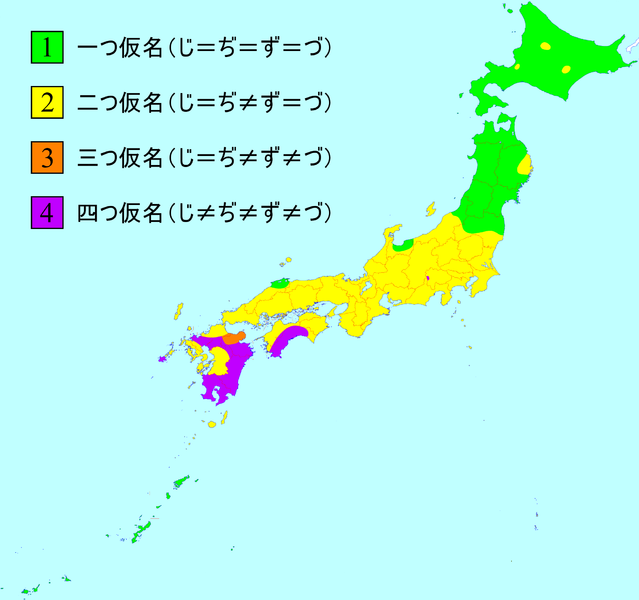
\includegraphics[width=0.9\textwidth]{figs/第08章/第356課:_yotsugana_fig/639px_Yotsugana.png}

\end{figure}
\hfill\break
\textbf{Picture Notes }: 1. This is a distribution based on the speech of older speakers. Many regions marked as other colors have been progressively changing to 二つ仮名弁. It is to note, though, that 一つ仮名弁 still hold strong to various degrees in Tohoku and Izumo. Izumo is the other part of green in the Chuugoku Region (中国地方) to the west of the Kinki Region (近畿地方).  2.The map does a poor job giving clarity to Okinawa, where several other Japanese languages have developed over the centuries. They should not be confused with this phenomenon as other major sound inventory changes have occurred in them, and as you can expect, these changes are not the same. It's just as bad to assume that those sound changes would be the same as thinking the sound changes in English and German have been the same over time.  \textbf{Example Words }  A lot has been said about what 四つ仮名. You've seen examples of words that have had their spellings changed and why, and you should have a sense as to why some things may have alternative spellings. The chart below will try to compile this information together with many examples so that the facts discussed so far become more concrete.  
\begin{ltabulary}{|P|P|P|P|P|P|P|P|}
\hline 

Word & Spell Change? & Original & New & Word & Spell Change? & Original & New \\ \cline{1-8}

泉 & Yes & いづみ & いずみ & 案じる & No & 案じる & 案じる \\ \cline{1-8}

味 & Yes & あぢ & あじ & 言伝て & No & ことづて & ことづて \\ \cline{1-8}

雫 & Yes & しづく & しずく & 埋める & Yes & うづめる & うずめる \\ \cline{1-8}

傷 & No & きず & きず & 築く & Yes & きづく & きずく \\ \cline{1-8}

それじゃ & Yes & それぢゃ & それじゃ & ずつ & Yes & づつ & ずつ \\ \cline{1-8}

ネズミ & No & ネズミ & ネズミ & 恥 & Yes & はぢ & はじ \\ \cline{1-8}

短い & No & みじかい & みじかい & 譲る & Yes & ゆづる & ゆずる \\ \cline{1-8}

水 & Yes & みづ & みず & 羊 & No & ひつじ & ひつじ \\ \cline{1-8}

虹 & No & にじ & にじ & つづら & No & つづら & つづら* \\ \cline{1-8}

沈む & Yes & しづむ & しずむ & 頷く & Yes\slash No & うなづく & うなづく・うなずく \\ \cline{1-8}

\end{ltabulary}
 *: つづら (wig) may be shortened to づら, making it one of the only examples where づ is allowed at the beginning of a word. Another similar example is 痔 (hemorrhoids), which although is historically and currently spelled as じ, and can be written as ぢ in emphatic instances.  \textbf{Reverting Back? }  Because [ʑi] and [ʥi] are allophones (variants using in specific environments) of the same sound and [zɯ]  and [dzɯ] are allophones of the same sound in Standard Japanese, these speakers still technically could re-institute previous pronunciations of words to go back to how 四つ仮名 was used. In singing, there is a tendency to affricate ぢ and づ, but aside from this, most speakers are generally unaware that there are seemingly two set of pronunciations in 四つ仮名: the fricative and the affricate pronunciations.   Most people will think 頭痛 as ずつう despite the fact that they probably pronounce it as づつう. People don't tend to notice these things if they aren't contrasting elements. Because these pronunciations no longer contrast words anymore, it's hard for speakers to even notice the definition, much less intentionally re-institute them into words they were once in.    The idea is nice at its surface, but the problem is that those that support re-instituting proper distinctions in pronunciation in 四つ仮名 typically don't know much about linguistics. Nor do they typically accurate describe the actually phonological processes going on. Many are unaware that words used to begin with ヂ and ヅ, and they sounded differently than words that begin with  ジ and ズ.   It's also not the case that there aren't any examples of ジ and ズ becoming  ヂ and ヅ. After all, we have seen already all words beginning in ジ and ズ be pronounced initially with ヂ and ヅ instead in Standard Japanese. And, again, in the day when spelling wasn't standardized, in areas that 四つ仮名 were being heavily confused with each other, you could see words like 鯨 spelled as  くじら or くぢら. This suggests not just interchangeability in writing but interchangeability in pronunciation.  \textbf{Typing Issues }   Another problem is typing. To type ぢ and づ, you usually type di and du respectively. When Japanese speakers go from Romaji to Japanese input, they often mess up just like foreigners and type in ji and zu respectively, only to find out that the spelling doesn't show up. As time goes on, however, future IME systems may simply 四つ仮名 input to go along with any potential further simplification of them.       
\section{四つ仮名 in Dialects}
 
\par{ As has been discussed thus far, 四つ仮名 have been and continue to be pronounced differently in different dialects. As the picture above demonstrates, a dialect could fall under one of four categories in respect to 四つ仮名. }

\par{一つ仮名弁: Dialects in which じ = ぢ=ず=づ \hfill\break
二つ仮名弁: Dialects in which じ = ぢ≠ ず=づ \hfill\break
三つ仮名弁: Dialects in which じ = ぢ≠ ず≠ づ \hfill\break
四つ仮名弁: Dialects in which じ ≠ ぢ ≠ ず ≠ づ }

\par{ 標準語 is a 二つ仮名弁, just in case you didn't know. However, as we've seen, there are certain environments that allow for all four distinct pronunciations to be used. This categorization tells not how exactly they are pronounced but how they are used contrastively. In 四つ仮名弁, these sounds are all used to contrast words. So, the main focus in this section will be to study how exactly 四つ仮名 are pronounced in various dialects of Japanese. }

\begin{center}
 \textbf{一つ仮名弁 }
\end{center}

\par{ In 一つ仮名弁, there are two ways of saying them all based on specific dialect. If you are a speaker of Kita-ou'u Dialect (far north in Tohoku) or Unpaku Dialect (in Izumo), you pronounce them all as [ʣï]. The vowel is in between い and う as the two vowels merged in this region.  If you are a speaker of Minami-ou'u Dialect, you pronounce them all as [ʣɯ̈]. Because of this, these dialects have been given the stereotypical name ズーズー弁. }

\begin{center}
 \textbf{四つ仮名弁 }
\end{center}

\par{ The completely opposite of 一つ仮名弁 are 四つ仮名弁. However, even though a dialect may have all four as separate sounds, these separate sounds are not uniformly the same throughout these dialects. Many parts of Kyushu, Kouchi Prefecture (高知県), the south of Nara Prefecture (奈良県南部), and Narada in Yamanashi Prefecture (山梨県奈良田) are all areas with 四つ仮名弁. }

\par{ In 高知県, dialects may have the following pronunciations: ジ = [ʑi], ズ = [zu], ヂ = [di] ~ [d z i], ヅ= [du] ~ [d z u]. In Kagoshima Dialect (鹿児島弁),  ジ =[ʑi], ズ = [zu], ヂ = [ʥi], and ヅ = [ʣu]. }

\begin{center}
 \textbf{The Oddity of Narada Dialect in Yamanashi Prefecture }
\end{center}

\par{ Narada is strength with its unique pronunciations: ジ = [ði], ズ = [ðu\slash dzu\slash zu], ヂ = [ɖʐi], ヅ = [ɖu\slash du]. It is also important to note that ツ = [tu] in this dialect. The ð is in English words like "that". These speakers would at least have less difficulty in one sound in English than other Japanese speakers. However, these speakers are dwindling very quickly as many are converting their speech to 標準語 standards. }

\par{ Narata Dialect is first transitioning into a 三つ仮名弁  with most speakers not distinguishing じ and ぢ, though they may still not be exactly like in Standard Japanese. For the most part,  the pronunciation reflects traditional orthography, but there are some words in Narada Dialect in which the sounds have flipped. So, for instance 葛 = 屑 as くず. Although 渦 was うづ, it is rendered as うず, which means it is either pronounced as [uzu], [udzu], or [uðu].  }

\par{\textbf{Research Note }: To hear sound files of Narada Dialect for this information, see http:\slash \slash home.hiroshima-u.ac.jp\slash ikonishi\slash narada\slash narada\_ tu\&du.html  . }

\begin{center}
 \textbf{三つ仮名弁 }
\end{center}

\par{ 三つ仮名弁 are not that common, but some speakers may naturally pronounce 四つ仮名 in this way at times regardless of dialect. Anyway, in these dialects such as 大分弁, ジ = ヂ, butズ doesn't sound like ヅ, which are [zu] and [dzu] respectively. }

\begin{center}
 \textbf{二つ仮名弁 }
\end{center}

\par{ As was said before, there is variation even among 二つ仮名弁. In 京都弁 where the allophonous (varying in specific environments) pronunciation rules developed, most speakers now lightly affricate all these sounds except AFTER ん. In recent years due to the contact of peoples from different parts of the country, and because script reform has gotten rid of the need to notice any traditional differences in pronunciation, most dialects are becoming 二つ仮名弁. }

\par{\textbf{Transcription Note }: Symbols in IPA (International Phonetic Alphabet) are used in this lesson to make transcription as accurate and easy as possible. To look up glyphs that you don't understand, simply copy and paste the problematic ones into Wikipedia where you can find audio tapes for them. }
    

% http://www.imabi.net/hentaigana.htm
     
\chapter{変体仮名}

\begin{center}
\begin{Large}
第357課: 変体仮名 
\end{Large}
\end{center}
 
\par{  In Classical Japanese works there are many かな that may seem very odd to the novice beginner. These かな are called 変体仮名. No, not へんたい as in 変態 but as in 変体. }

\par{変体仮名 are simply historical variants of the now standard ひらがな today. So, each mora had several possible ひらがな. The problem was not so in カタカナ as variants were made obsolete early in its development. 変体仮名 came from 万葉仮名, and many 変体仮名 originated from different 漢字. }
      
\section{変体仮名}
 
\par{ 変体仮名 were made obsolete in 1900 as one of the final reforms of  the  Meiji Reformation ( 明治維新).  However,  they still play a role in calligraphy, billboards, and authentic copies or replications of Classical works. 変体仮名 is also referred  to as 異体仮名, making it clear that they can  still be viewed  as variants used at the author's will. It must be known, though, that not a lot of people know how to read them. }

\par{変体仮名  have played a very important role in writing ever since conception.  People of the arts could liberally chose to their heart's desire what かな they wished to use, a continuation of the privilege people had  when Japanese was still written in 万葉仮名. }

\par{変体仮名 are for the most  part somewhat evolved forms of 万葉仮名 cursive  style characters, from which other standard ひらがな derive from as  well. As many 漢字 share the same 音読み, 変体仮名 inevitable came from a lot of characters, and many were made to represent  the same sound. }

\par{変体仮名 are still seldom used. Many soba restaurant signs remind people of the  character's glory-days and martial art centers and centers devoted to  the preservation of historical events display them. Expect to see these  characters by just going to a battlefield marker. }

\par{変体仮名 are not able to be viewed on computers. However, we will study by looking at the characters from this table from http:\slash \slash www10.plala.or.jp\slash koin\slash koinhentaigana.html   }

\begin{ltabulary}{|P|P|P|P|P|P|P|P|P|P|P|}
\hline 

読み &  あ  &  あ &  あ &  あ &  あ &  あ・を &  い  &  い &  い &  い \\ \cline{1-11} 
 
 変 \hfill\break
体 \hfill\break
仮 \hfill\break
名 &  

\includegraphics[scale=0.2]{figs/第08章/第357課:_hentaigana_fig/f1b0.png}
&  

\includegraphics[scale=0.2]{figs/第08章/第357課:_hentaigana_fig/f1b1.png}
&  

\includegraphics[scale=0.2]{figs/第08章/第357課:_hentaigana_fig/f1b2.png}
&  

\includegraphics[scale=0.2]{figs/第08章/第357課:_hentaigana_fig/f1b3.png}
&  

\includegraphics[scale=0.2]{figs/第08章/第357課:_hentaigana_fig/f1b4.png}
&  

\includegraphics[scale=0.2]{figs/第08章/第357課:_hentaigana_fig/f1b5.png}
&  

\includegraphics[scale=0.2]{figs/第08章/第357課:_hentaigana_fig/f1d0.png}
&  

\includegraphics[scale=0.2]{figs/第08章/第357課:_hentaigana_fig/f1d1.png}
&  

\includegraphics[scale=0.2]{figs/第08章/第357課:_hentaigana_fig/f1d2.png}
&  

\includegraphics[scale=0.2]{figs/第08章/第357課:_hentaigana_fig/f1d3.png}
\\ \cline{1-11} 
 
 字母 &  阿 &  安 &  安 &  愛 &  愛 &  悪 &  以 &  意 &  伊 &  移 \\ \cline{1-11} 
 
 い &  う  &  う &  う &  う &  う &  う &  う &  う・は &  う &  え  \\ \cline{1-11} 
 
 

\includegraphics[scale=0.2]{figs/第08章/第357課:_hentaigana_fig/f1d4.png}
&  

\includegraphics[scale=0.2]{figs/第08章/第357課:_hentaigana_fig/f1f0.png}
&  

\includegraphics[scale=0.2]{figs/第08章/第357課:_hentaigana_fig/f1f1.png}
&  

\includegraphics[scale=0.2]{figs/第08章/第357課:_hentaigana_fig/f1f2.png}
&  

\includegraphics[scale=0.2]{figs/第08章/第357課:_hentaigana_fig/f1f3.png}
&  

\includegraphics[scale=0.2]{figs/第08章/第357課:_hentaigana_fig/f1f4.png}
&  

\includegraphics[scale=0.2]{figs/第08章/第357課:_hentaigana_fig/f1f5.png}
&  

\includegraphics[scale=0.2]{figs/第08章/第357課:_hentaigana_fig/f1f6.png}
&  

\includegraphics[scale=0.2]{figs/第08章/第357課:_hentaigana_fig/f1f7.png}
&  

\includegraphics[scale=0.2]{figs/第08章/第357課:_hentaigana_fig/f1f8.png}
&  

\includegraphics[scale=0.2]{figs/第08章/第357課:_hentaigana_fig/f250.png}
\\ \cline{1-11} 
 
 異 &  宇 &  宇 &  有 &  有 &  雲 &  右 &  憂 &  羽 &  鵜 &  江 \\ \cline{1-11} 
 
 え &  え &  え &  え &  え &  え &  お  &  お &  お &  か  &  か \\ \cline{1-11} 
 
 

\includegraphics[scale=0.2]{figs/第08章/第357課:_hentaigana_fig/f251.png}
&  

\includegraphics[scale=0.2]{figs/第08章/第357課:_hentaigana_fig/f252.png}
&  

\includegraphics[scale=0.2]{figs/第08章/第357課:_hentaigana_fig/f253.png}
&  

\includegraphics[scale=0.2]{figs/第08章/第357課:_hentaigana_fig/f254.png}
&  

\includegraphics[scale=0.2]{figs/第08章/第357課:_hentaigana_fig/f255.png}
&  

\includegraphics[scale=0.2]{figs/第08章/第357課:_hentaigana_fig/f256.png}
&  

\includegraphics[scale=0.2]{figs/第08章/第357課:_hentaigana_fig/f270.png}
&  

\includegraphics[scale=0.2]{figs/第08章/第357課:_hentaigana_fig/f271.png}
&  

\includegraphics[scale=0.2]{figs/第08章/第357課:_hentaigana_fig/f272.png}
&  

\includegraphics[scale=0.2]{figs/第08章/第357課:_hentaigana_fig/f280.png}
&  

\includegraphics[scale=0.2]{figs/第08章/第357課:_hentaigana_fig/f281.png}
\\ \cline{1-11} 
 
 盈 &  盈 &  衣 &  要 &  得 &  縁 &  於 &  於 &  於 &  可 &  可 \\ \cline{1-11} 
 
 か &  か &  か &  か &  か &  か &  か &  か &  か &  か &  か \\ \cline{1-11} 
 
 

\includegraphics[scale=0.2]{figs/第08章/第357課:_hentaigana_fig/f282.png}
&  

\includegraphics[scale=0.2]{figs/第08章/第357課:_hentaigana_fig/f283.png}
&  
\includegraphics[scale=0.2]{figs/第08章/第357課:_hentaigana_fig/f284.png}
&  
\includegraphics[scale=0.2]{figs/第08章/第357課:_hentaigana_fig/f285.png}
&  
\includegraphics[scale=0.2]{figs/第08章/第357課:_hentaigana_fig/f286.png}
&  
\includegraphics[scale=0.2]{figs/第08章/第357課:_hentaigana_fig/f287.png}
&  
\includegraphics[scale=0.2]{figs/第08章/第357課:_hentaigana_fig/f288.png}
&  
\includegraphics[scale=0.2]{figs/第08章/第357課:_hentaigana_fig/f289.png}
&  
\includegraphics[scale=0.2]{figs/第08章/第357課:_hentaigana_fig/f28a.png}
&  
\includegraphics[scale=0.2]{figs/第08章/第357課:_hentaigana_fig/f28b.png}
&  
\includegraphics[scale=0.2]{figs/第08章/第357課:_hentaigana_fig/f28c.png}
\\ \cline{1-11} 
 
 可 &  加 &  嘉 &  嘉 &  閑 &  賀 &  駕 &  我 &  家 &  香 &  佳 \\ \cline{1-11} 
 
 が &  が &  が &  が &  が &  が &  が &  が &  が &  が &  が \\ \cline{1-11} 
 
 
\includegraphics[scale=0.2]{figs/第08章/第357課:_hentaigana_fig/f290.png}
&  
\includegraphics[scale=0.2]{figs/第08章/第357課:_hentaigana_fig/f291.png}
&  
\includegraphics[scale=0.2]{figs/第08章/第357課:_hentaigana_fig/f292.png}
&  
\includegraphics[scale=0.2]{figs/第08章/第357課:_hentaigana_fig/f293.png}
&  
\includegraphics[scale=0.2]{figs/第08章/第357課:_hentaigana_fig/f294.png}
&  
\includegraphics[scale=0.2]{figs/第08章/第357課:_hentaigana_fig/f295.png}
&  
\includegraphics[scale=0.2]{figs/第08章/第357課:_hentaigana_fig/f296.png}
&  
\includegraphics[scale=0.2]{figs/第08章/第357課:_hentaigana_fig/f297.png}
&  
\includegraphics[scale=0.2]{figs/第08章/第357課:_hentaigana_fig/f298.png}
&  
\includegraphics[scale=0.2]{figs/第08章/第357課:_hentaigana_fig/f299.png}
&  
\includegraphics[scale=0.2]{figs/第08章/第357課:_hentaigana_fig/f29a.png}
\\ \cline{1-11} 
 
  &   &   &   &   &   &   &   &   &   &   \\ \cline{1-11} 
 
 が &  が &  き  &  き &  き &  き &  き &  き &  き &  き・こ &  き \\ \cline{1-11} 
 
 
\includegraphics[scale=0.2]{figs/第08章/第357課:_hentaigana_fig/f29b.png}
&  
\includegraphics[scale=0.2]{figs/第08章/第357課:_hentaigana_fig/f29c.png}
&  
\includegraphics[scale=0.2]{figs/第08章/第357課:_hentaigana_fig/f2a0.png}
&  
\includegraphics[scale=0.2]{figs/第08章/第357課:_hentaigana_fig/f2a1.png}
&  
\includegraphics[scale=0.2]{figs/第08章/第357課:_hentaigana_fig/f2a2.png}
&  
\includegraphics[scale=0.2]{figs/第08章/第357課:_hentaigana_fig/f2a3.png}
&  
\includegraphics[scale=0.2]{figs/第08章/第357課:_hentaigana_fig/f2a4.png}
&  
\includegraphics[scale=0.2]{figs/第08章/第357課:_hentaigana_fig/f2a5.png}
&  
\includegraphics[scale=0.2]{figs/第08章/第357課:_hentaigana_fig/f2a6.png}
&  
\includegraphics[scale=0.2]{figs/第08章/第357課:_hentaigana_fig/f2a7.png}
&  
\includegraphics[scale=0.2]{figs/第08章/第357課:_hentaigana_fig/f2a8.png}
\\ \cline{1-11} 
 
  &   &  起 &  幾 &  幾 &  喜 &  支 &  木 &  貴 &  期 &  記 \\ \cline{1-11} 
 
 き &  ぎ &  ぎ &  ぎ &  ぎ &  ぎ &  ぎ &  ぎ &  ぎ・ご &  ぎ &  ぎ \\ \cline{1-11} 
 
 
\includegraphics[scale=0.2]{figs/第08章/第357課:_hentaigana_fig/f2a9.png}
&  
\includegraphics[scale=0.2]{figs/第08章/第357課:_hentaigana_fig/f2b0.png}
&  
\includegraphics[scale=0.2]{figs/第08章/第357課:_hentaigana_fig/f2b1.png}
&  
\includegraphics[scale=0.2]{figs/第08章/第357課:_hentaigana_fig/f2b2.png}
&  
\includegraphics[scale=0.2]{figs/第08章/第357課:_hentaigana_fig/f2b3.png}
&  
\includegraphics[scale=0.2]{figs/第08章/第357課:_hentaigana_fig/f2b4.png}
&  
\includegraphics[scale=0.2]{figs/第08章/第357課:_hentaigana_fig/f2b5.png}
&  
\includegraphics[scale=0.2]{figs/第08章/第357課:_hentaigana_fig/f2b6.png}
&  
\includegraphics[scale=0.2]{figs/第08章/第357課:_hentaigana_fig/f2b7.png}
&  
\includegraphics[scale=0.2]{figs/第08章/第357課:_hentaigana_fig/f2b8.png}
&  
\includegraphics[scale=0.2]{figs/第08章/第357課:_hentaigana_fig/f2b9.png}
\\ \cline{1-11} 
 
 季 &   &   &   &   &   &   &   &   &   &   \\ \cline{1-11} 
 
 く  &  く &  く &  く &  く &  く &  ぐ &  ぐ &  ぐ &  ぐ &  ぐ \\ \cline{1-11} 
 
 
\includegraphics[scale=0.2]{figs/第08章/第357課:_hentaigana_fig/f2c0.png}
&  
\includegraphics[scale=0.2]{figs/第08章/第357課:_hentaigana_fig/f2c1.png}
&  
\includegraphics[scale=0.2]{figs/第08章/第357課:_hentaigana_fig/f2c2.png}
&  
\includegraphics[scale=0.2]{figs/第08章/第357課:_hentaigana_fig/f2c3.png}
&  
\includegraphics[scale=0.2]{figs/第08章/第357課:_hentaigana_fig/f2c4.png}
&  
\includegraphics[scale=0.2]{figs/第08章/第357課:_hentaigana_fig/f2c5.png}
&  
\includegraphics[scale=0.2]{figs/第08章/第357課:_hentaigana_fig/f2d0.png}
&  
\includegraphics[scale=0.2]{figs/第08章/第357課:_hentaigana_fig/f2d1.png}
&  
\includegraphics[scale=0.2]{figs/第08章/第357課:_hentaigana_fig/f2d2.png}
&  
\includegraphics[scale=0.2]{figs/第08章/第357課:_hentaigana_fig/f2d3.png}
&  
\includegraphics[scale=0.2]{figs/第08章/第357課:_hentaigana_fig/f2d4.png}
\\ \cline{1-11} 
 
 具 &  久 &  九 &  求 &  供 &  倶 &   &   &   &   &   \\ \cline{1-11} 
 
 ぐ &  け  &  け・と &  け &  け &  け &  け &  け &  け &  け &  げ \\ \cline{1-11} 
 
 
\includegraphics[scale=0.2]{figs/第08章/第357課:_hentaigana_fig/f2d5.png}
&  
\includegraphics[scale=0.2]{figs/第08章/第357課:_hentaigana_fig/f2e0.png}
&  
\includegraphics[scale=0.2]{figs/第08章/第357課:_hentaigana_fig/f2e1.png}
&  
\includegraphics[scale=0.2]{figs/第08章/第357課:_hentaigana_fig/f2e2.png}
&  
\includegraphics[scale=0.2]{figs/第08章/第357課:_hentaigana_fig/f2e3.png}
&  
\includegraphics[scale=0.2]{figs/第08章/第357課:_hentaigana_fig/f2e4.png}
&  
\includegraphics[scale=0.2]{figs/第08章/第357課:_hentaigana_fig/f2e5.png}
&  
\includegraphics[scale=0.2]{figs/第08章/第357課:_hentaigana_fig/f2e6.png}
&  
\includegraphics[scale=0.2]{figs/第08章/第357課:_hentaigana_fig/f2e7.png}
&  
\includegraphics[scale=0.2]{figs/第08章/第357課:_hentaigana_fig/f2e8.png}
&  
\includegraphics[scale=0.2]{figs/第08章/第357課:_hentaigana_fig/f2f0.png}
\\ \cline{1-11} 
 
  &  希 &  計・斗 &  計 &  介 &  介 &  遣 &  気 &  気 &  稀 &   \\ \cline{1-11} 
 
 げ・ど &  げ &  げ &  げ &  げ &  げ &  げ &  げ &  こ  &  こ &  こ \\ \cline{1-11} 
 
 
\includegraphics[scale=0.2]{figs/第08章/第357課:_hentaigana_fig/f2f1.png}
&  
\includegraphics[scale=0.2]{figs/第08章/第357課:_hentaigana_fig/f2f2.png}
&  
\includegraphics[scale=0.2]{figs/第08章/第357課:_hentaigana_fig/f2f3.png}
&  
\includegraphics[scale=0.2]{figs/第08章/第357課:_hentaigana_fig/f2f4.png}
&  
\includegraphics[scale=0.2]{figs/第08章/第357課:_hentaigana_fig/f2f5.png}
&  
\includegraphics[scale=0.2]{figs/第08章/第357課:_hentaigana_fig/f2f6.png}
&  
\includegraphics[scale=0.2]{figs/第08章/第357課:_hentaigana_fig/f2f7.png}
&  
\includegraphics[scale=0.2]{figs/第08章/第357課:_hentaigana_fig/f2f8.png}
&  
\includegraphics[scale=0.2]{figs/第08章/第357課:_hentaigana_fig/f340.png}
&  
\includegraphics[scale=0.2]{figs/第08章/第357課:_hentaigana_fig/f341.png}
&  
\includegraphics[scale=0.2]{figs/第08章/第357課:_hentaigana_fig/f342.png}
\\ \cline{1-11} 
 
  &   &   &   &   &   &   &   &  古 &  故 &  許 \\ \cline{1-11} 
 
 こ &  こ &  こ・ね &  こ &  こ・き &  ご &  ご &  ご &  ご &  ご &  ご \\ \cline{1-11} 
 
 
\includegraphics[scale=0.2]{figs/第08章/第357課:_hentaigana_fig/f343.png}
&  
\includegraphics[scale=0.2]{figs/第08章/第357課:_hentaigana_fig/f344.png}
&  
\includegraphics[scale=0.2]{figs/第08章/第357課:_hentaigana_fig/f345.png}
&  
\includegraphics[scale=0.2]{figs/第08章/第357課:_hentaigana_fig/f346.png}
&  
\includegraphics[scale=0.2]{figs/第08章/第357課:_hentaigana_fig/f2a7.png}
&  
\includegraphics[scale=0.2]{figs/第08章/第357課:_hentaigana_fig/f350.png}
&  
\includegraphics[scale=0.2]{figs/第08章/第357課:_hentaigana_fig/f351.png}
&  
\includegraphics[scale=0.2]{figs/第08章/第357課:_hentaigana_fig/f352.png}
&  
\includegraphics[scale=0.2]{figs/第08章/第357課:_hentaigana_fig/f353.png}
&  
\includegraphics[scale=0.2]{figs/第08章/第357課:_hentaigana_fig/f354.png}
&  
\includegraphics[scale=0.2]{figs/第08章/第357課:_hentaigana_fig/f355.png}
\\ \cline{1-11} 
 
 許 &  胡 &  子 &  興 &  期 &   &   &   &   &   &   \\ \cline{1-11} 
 
 ご &  ご・ぎ &  さ  &  さ &  さ &  さ &  さ &  さ &  さ &  さ &  さ \\ \cline{1-11} 
 
 
\includegraphics[scale=0.2]{figs/第08章/第357課:_hentaigana_fig/f356.png}
&  
\includegraphics[scale=0.2]{figs/第08章/第357課:_hentaigana_fig/f2b7.png}
&  
\includegraphics[scale=0.2]{figs/第08章/第357課:_hentaigana_fig/f360.png}
&  
\includegraphics[scale=0.2]{figs/第08章/第357課:_hentaigana_fig/f361.png}
&  
\includegraphics[scale=0.2]{figs/第08章/第357課:_hentaigana_fig/f362.png}
&  
\includegraphics[scale=0.2]{figs/第08章/第357課:_hentaigana_fig/f363.png}
&  
\includegraphics[scale=0.2]{figs/第08章/第357課:_hentaigana_fig/f364.png}
&  
\includegraphics[scale=0.2]{figs/第08章/第357課:_hentaigana_fig/f365.png}
&  
\includegraphics[scale=0.2]{figs/第08章/第357課:_hentaigana_fig/f366.png}
&  
\includegraphics[scale=0.2]{figs/第08章/第357課:_hentaigana_fig/f367.png}
&  
\includegraphics[scale=0.2]{figs/第08章/第357課:_hentaigana_fig/f368.png}
\\ \cline{1-11} 
 
  &   &  左 &  佐 &  佐 &  散 &  散 &  斜 &  乍 &  沙 &  狭 \\ \cline{1-11} 
 
 さ &  ざ &  ざ &  ざ &  ざ &  ざ &  ざ &  ざ &  ざ &  ざ &  ざ \\ \cline{1-11} 
 
 
\includegraphics[scale=0.2]{figs/第08章/第357課:_hentaigana_fig/f369.png}
&  
\includegraphics[scale=0.2]{figs/第08章/第357課:_hentaigana_fig/f370.png}
&  
\includegraphics[scale=0.2]{figs/第08章/第357課:_hentaigana_fig/f371.png}
&  
\includegraphics[scale=0.2]{figs/第08章/第357課:_hentaigana_fig/f372.png}
&  
\includegraphics[scale=0.2]{figs/第08章/第357課:_hentaigana_fig/f373.png}
&  
\includegraphics[scale=0.2]{figs/第08章/第357課:_hentaigana_fig/f374.png}
&  
\includegraphics[scale=0.2]{figs/第08章/第357課:_hentaigana_fig/f375.png}
&  
\includegraphics[scale=0.2]{figs/第08章/第357課:_hentaigana_fig/f376.png}
&  
\includegraphics[scale=0.2]{figs/第08章/第357課:_hentaigana_fig/f377.png}
&  
\includegraphics[scale=0.2]{figs/第08章/第357課:_hentaigana_fig/f378.png}
&  
\includegraphics[scale=0.2]{figs/第08章/第357課:_hentaigana_fig/f379.png}
\\ \cline{1-11} 
 
 差 &   &   &   &   &   &   &   &   &   &   \\ \cline{1-11} 
 
 し  &  し &  し &  し &  し &  し &  し &  し &  じ &  じ &  じ \\ \cline{1-11} 
 
 
\includegraphics[scale=0.2]{figs/第08章/第357課:_hentaigana_fig/f380.png}
&  
\includegraphics[scale=0.2]{figs/第08章/第357課:_hentaigana_fig/f381.png}
&  
\includegraphics[scale=0.2]{figs/第08章/第357課:_hentaigana_fig/f382.png}
&  
\includegraphics[scale=0.2]{figs/第08章/第357課:_hentaigana_fig/f383.png}
&  
\includegraphics[scale=0.2]{figs/第08章/第357課:_hentaigana_fig/f384.png}
&  
\includegraphics[scale=0.2]{figs/第08章/第357課:_hentaigana_fig/f385.png}
&  
\includegraphics[scale=0.2]{figs/第08章/第357課:_hentaigana_fig/f386.png}
&  
\includegraphics[scale=0.2]{figs/第08章/第357課:_hentaigana_fig/f387.png}
&  
\includegraphics[scale=0.2]{figs/第08章/第357課:_hentaigana_fig/f390.png}
&  
\includegraphics[scale=0.2]{figs/第08章/第357課:_hentaigana_fig/f391.png}
&  
\includegraphics[scale=0.2]{figs/第08章/第357課:_hentaigana_fig/f392.png}
\\ \cline{1-11} 
 
 志 &  之 &  之 &  新 &  四 &  斯 &  事 &  師 &   &   &   \\ \cline{1-11} 
 
 じ &  じ &  じ &  じ &  じ &  す  &  す &  す &  す &  す &  す \\ \cline{1-11} 
 
 
\includegraphics[scale=0.2]{figs/第08章/第357課:_hentaigana_fig/f393.png}
&  
\includegraphics[scale=0.2]{figs/第08章/第357課:_hentaigana_fig/f394.png}
&  
\includegraphics[scale=0.2]{figs/第08章/第357課:_hentaigana_fig/f395.png}
&  
\includegraphics[scale=0.2]{figs/第08章/第357課:_hentaigana_fig/f396.png}
&  
\includegraphics[scale=0.2]{figs/第08章/第357課:_hentaigana_fig/f397.png}
&  
\includegraphics[scale=0.2]{figs/第08章/第357課:_hentaigana_fig/f3a0.png}
&  
\includegraphics[scale=0.2]{figs/第08章/第357課:_hentaigana_fig/f3a1.png}
&  
\includegraphics[scale=0.2]{figs/第08章/第357課:_hentaigana_fig/f3a2.png}
&  
\includegraphics[scale=0.2]{figs/第08章/第357課:_hentaigana_fig/f3a3.png}
&  
\includegraphics[scale=0.2]{figs/第08章/第357課:_hentaigana_fig/f3a4.png}
&  
\includegraphics[scale=0.2]{figs/第08章/第357課:_hentaigana_fig/f3a5.png}
\\ \cline{1-11} 
 
  &   &   &   &   &  春 &  春 &  須 &  寿 &  寿 &  数 \\ \cline{1-11} 
 
 す &  す &  ず &  ず &  ず &  ず &  ず &  ず &  ず &  ず &  せ  \\ \cline{1-11} 
 
 
\includegraphics[scale=0.2]{figs/第08章/第357課:_hentaigana_fig/f3a6.png}
&  
\includegraphics[scale=0.2]{figs/第08章/第357課:_hentaigana_fig/f3a7.png}
&  
\includegraphics[scale=0.2]{figs/第08章/第357課:_hentaigana_fig/f3b0.png}
&  
\includegraphics[scale=0.2]{figs/第08章/第357課:_hentaigana_fig/f3b1.png}
&  
\includegraphics[scale=0.2]{figs/第08章/第357課:_hentaigana_fig/f3b2.png}
&  
\includegraphics[scale=0.2]{figs/第08章/第357課:_hentaigana_fig/f3b3.png}
&  
\includegraphics[scale=0.2]{figs/第08章/第357課:_hentaigana_fig/f3b4.png}
&  
\includegraphics[scale=0.2]{figs/第08章/第357課:_hentaigana_fig/f3b5.png}
&  
\includegraphics[scale=0.2]{figs/第08章/第357課:_hentaigana_fig/f3b6.png}
&  
\includegraphics[scale=0.2]{figs/第08章/第357課:_hentaigana_fig/f3b7.png}
&  
\includegraphics[scale=0.2]{figs/第08章/第357課:_hentaigana_fig/f3c0.png}
\\ \cline{1-11} 
 
 数 &  受 &   &   &   &   &   &   &   &   &  勢 \\ \cline{1-11} 
 
 せ &  せ &  せ &  せ &  ぜ &  ぜ &  ぜ &  ぜ &  ぜ &  そ  &  そ \\ \cline{1-11} 
 
 
\includegraphics[scale=0.2]{figs/第08章/第357課:_hentaigana_fig/f3c1.png}
&  
\includegraphics[scale=0.2]{figs/第08章/第357課:_hentaigana_fig/f3c2.png}
&  
\includegraphics[scale=0.2]{figs/第08章/第357課:_hentaigana_fig/f3c3.png}
&  
\includegraphics[scale=0.2]{figs/第08章/第357課:_hentaigana_fig/f3c4.png}
&  
\includegraphics[scale=0.2]{figs/第08章/第357課:_hentaigana_fig/f3d0.png}
&  
\includegraphics[scale=0.2]{figs/第08章/第357課:_hentaigana_fig/f3d1.png}
&  
\includegraphics[scale=0.2]{figs/第08章/第357課:_hentaigana_fig/f3d2.png}
&  
\includegraphics[scale=0.2]{figs/第08章/第357課:_hentaigana_fig/f3d3.png}
&  
\includegraphics[scale=0.2]{figs/第08章/第357課:_hentaigana_fig/f3d4.png}
&  
\includegraphics[scale=0.2]{figs/第08章/第357課:_hentaigana_fig/f3e0.png}
&  
\includegraphics[scale=0.2]{figs/第08章/第357課:_hentaigana_fig/f3e1.png}
\\ \cline{1-11} 
 
 世 &  世 &  声 &  瀬 &   &   &   &   &   &  楚 &  曽 \\ \cline{1-11} 
 
 そ &  そ &  そ &  そ &  そ &  そ &  そ &  ぞ &  ぞ &  ぞ &  ぞ \\ \cline{1-11} 
 
 
\includegraphics[scale=0.2]{figs/第08章/第357課:_hentaigana_fig/f3e2.png}
&  
\includegraphics[scale=0.2]{figs/第08章/第357課:_hentaigana_fig/f3e3.png}
&  
\includegraphics[scale=0.2]{figs/第08章/第357課:_hentaigana_fig/f3e4.png}
&  
\includegraphics[scale=0.2]{figs/第08章/第357課:_hentaigana_fig/f3e5.png}
&  
\includegraphics[scale=0.2]{figs/第08章/第357課:_hentaigana_fig/f3e6.png}
&  
\includegraphics[scale=0.2]{figs/第08章/第357課:_hentaigana_fig/f3e7.png}
&  
\includegraphics[scale=0.2]{figs/第08章/第357課:_hentaigana_fig/f3e8.png}
&  
\includegraphics[scale=0.2]{figs/第08章/第357課:_hentaigana_fig/f3f0.png}
&  
\includegraphics[scale=0.2]{figs/第08章/第357課:_hentaigana_fig/f3f1.png}
&  
\includegraphics[scale=0.2]{figs/第08章/第357課:_hentaigana_fig/f3f2.png}
&  
\includegraphics[scale=0.2]{figs/第08章/第357課:_hentaigana_fig/f3f3.png}
\\ \cline{1-11} 
 
 曽 &  曽 &  所 &  所 &  処 &  処 &  蘇 &   &   &   &   \\ \cline{1-11} 
 
 ぞ &  ぞ &  ぞ &  ぞ &  ぞ &  た  &  た &  た &  た &  た &  た \\ \cline{1-11} 
 
 
\includegraphics[scale=0.2]{figs/第08章/第357課:_hentaigana_fig/f3f4.png}
&  
\includegraphics[scale=0.2]{figs/第08章/第357課:_hentaigana_fig/f3f5.png}
&  
\includegraphics[scale=0.2]{figs/第08章/第357課:_hentaigana_fig/f3f6.png}
&  
\includegraphics[scale=0.2]{figs/第08章/第357課:_hentaigana_fig/f3f7.png}
&  
\includegraphics[scale=0.2]{figs/第08章/第357課:_hentaigana_fig/f3f8.png}
&  
\includegraphics[scale=0.2]{figs/第08章/第357課:_hentaigana_fig/f440.png}
&  
\includegraphics[scale=0.2]{figs/第08章/第357課:_hentaigana_fig/f441.png}
&  
\includegraphics[scale=0.2]{figs/第08章/第357課:_hentaigana_fig/f442.png}
&  
\includegraphics[scale=0.2]{figs/第08章/第357課:_hentaigana_fig/f443.png}
&  
\includegraphics[scale=0.2]{figs/第08章/第357課:_hentaigana_fig/f444.png}
&  
\includegraphics[scale=0.2]{figs/第08章/第357課:_hentaigana_fig/f445.png}
\\ \cline{1-11} 
 
  &   &   &   &   &  多 &  多 &  多 &  堂 &  堂 &  田 \\ \cline{1-11} 
 
 た &  だ &  だ &  だ &  だ &  だ &  だ &  だ &  ち  &  ち &  ち \\ \cline{1-11} 
 
 
\includegraphics[scale=0.2]{figs/第08章/第357課:_hentaigana_fig/f446.png}
&  
\includegraphics[scale=0.2]{figs/第08章/第357課:_hentaigana_fig/f450.png}
&  
\includegraphics[scale=0.2]{figs/第08章/第357課:_hentaigana_fig/f451.png}
&  
\includegraphics[scale=0.2]{figs/第08章/第357課:_hentaigana_fig/f452.png}
&  
\includegraphics[scale=0.2]{figs/第08章/第357課:_hentaigana_fig/f453.png}
&  
\includegraphics[scale=0.2]{figs/第08章/第357課:_hentaigana_fig/f454.png}
&  
\includegraphics[scale=0.2]{figs/第08章/第357課:_hentaigana_fig/f455.png}
&  
\includegraphics[scale=0.2]{figs/第08章/第357課:_hentaigana_fig/f456.png}
&  
\includegraphics[scale=0.2]{figs/第08章/第357課:_hentaigana_fig/f460.png}
&  
\includegraphics[scale=0.2]{figs/第08章/第357課:_hentaigana_fig/f461.png}
&  
\includegraphics[scale=0.2]{figs/第08章/第357課:_hentaigana_fig/f462.png}
\\ \cline{1-11} 
 
 当 &   &   &   &   &   &   &   &  知 &  知 &  千 \\ \cline{1-11} 
 
 ち &  ち &  ち &  ち &  ち &  ぢ &  ぢ &  ぢ &  ぢ &  ぢ &  ぢ \\ \cline{1-11} 
 
 
\includegraphics[scale=0.2]{figs/第08章/第357課:_hentaigana_fig/f463.png}
&  
\includegraphics[scale=0.2]{figs/第08章/第357課:_hentaigana_fig/f464.png}
&  
\includegraphics[scale=0.2]{figs/第08章/第357課:_hentaigana_fig/f465.png}
&  
\includegraphics[scale=0.2]{figs/第08章/第357課:_hentaigana_fig/f466.png}
&  
\includegraphics[scale=0.2]{figs/第08章/第357課:_hentaigana_fig/f467.png}
&  
\includegraphics[scale=0.2]{figs/第08章/第357課:_hentaigana_fig/f470.png}
&  
\includegraphics[scale=0.2]{figs/第08章/第357課:_hentaigana_fig/f471.png}
&  
\includegraphics[scale=0.2]{figs/第08章/第357課:_hentaigana_fig/f472.png}
&  
\includegraphics[scale=0.2]{figs/第08章/第357課:_hentaigana_fig/f473.png}
&  
\includegraphics[scale=0.2]{figs/第08章/第357課:_hentaigana_fig/f474.png}
&  
\includegraphics[scale=0.2]{figs/第08章/第357課:_hentaigana_fig/f475.png}
\\ \cline{1-11} 
 
 遅 &  地 &  致 &  馳 &  智 &   &   &   &   &   &   \\ \cline{1-11} 
 
 ぢ &  ぢ &  つ  &  つ &  つ &  つ &  つ &  つ &  つ &  づ &  づ \\ \cline{1-11} 
 
 
\includegraphics[scale=0.2]{figs/第08章/第357課:_hentaigana_fig/f476.png}
&  
\includegraphics[scale=0.2]{figs/第08章/第357課:_hentaigana_fig/f477.png}
&  
\includegraphics[scale=0.2]{figs/第08章/第357課:_hentaigana_fig/f490.png}
&  
\includegraphics[scale=0.2]{figs/第08章/第357課:_hentaigana_fig/f491.png}
&  
\includegraphics[scale=0.2]{figs/第08章/第357課:_hentaigana_fig/f492.png}
&  
\includegraphics[scale=0.2]{figs/第08章/第357課:_hentaigana_fig/f493.png}
&  
\includegraphics[scale=0.2]{figs/第08章/第357課:_hentaigana_fig/f494.png}
&  
\includegraphics[scale=0.2]{figs/第08章/第357課:_hentaigana_fig/f495.png}
&  
\includegraphics[scale=0.2]{figs/第08章/第357課:_hentaigana_fig/f496.png}
&  
\includegraphics[scale=0.2]{figs/第08章/第357課:_hentaigana_fig/f4a0.png}
&  
\includegraphics[scale=0.2]{figs/第08章/第357課:_hentaigana_fig/f4a1.png}
\\ \cline{1-11} 
 
  &   &  徒 &  徒 &  川 &  川 &  津 &  都 &  頭 &   &   \\ \cline{1-11} 
 
 づ &  づ &  づ &  づ &  づ &  て  &  て &  て &  て &  て &  て \\ \cline{1-11} 
 
 
\includegraphics[scale=0.2]{figs/第08章/第357課:_hentaigana_fig/f4a2.png}
&  
\includegraphics[scale=0.2]{figs/第08章/第357課:_hentaigana_fig/f4a3.png}
&  
\includegraphics[scale=0.2]{figs/第08章/第357課:_hentaigana_fig/f4a4.png}
&  
\includegraphics[scale=0.2]{figs/第08章/第357課:_hentaigana_fig/f4a5.png}
&  
\includegraphics[scale=0.2]{figs/第08章/第357課:_hentaigana_fig/f4a6.png}
&  
\includegraphics[scale=0.2]{figs/第08章/第357課:_hentaigana_fig/f4b0.png}
&  
\includegraphics[scale=0.2]{figs/第08章/第357課:_hentaigana_fig/f4b1.png}
&  
\includegraphics[scale=0.2]{figs/第08章/第357課:_hentaigana_fig/f4b2.png}
&  
\includegraphics[scale=0.2]{figs/第08章/第357課:_hentaigana_fig/f4b3.png}
&  
\includegraphics[scale=0.2]{figs/第08章/第357課:_hentaigana_fig/f4b4.png}
&  
\includegraphics[scale=0.2]{figs/第08章/第357課:_hentaigana_fig/f4b5.png}
\\ \cline{1-11} 
 
  &   &   &   &   &  天 &  天 &  亭 &  帝 &  帝 &  伝 \\ \cline{1-11} 
 
 て &  て &  て &  で &  で &  で &  で &  で &  で &  で &  で \\ \cline{1-11} 
 
 
\includegraphics[scale=0.2]{figs/第08章/第357課:_hentaigana_fig/f4b6.png}
&  
\includegraphics[scale=0.2]{figs/第08章/第357課:_hentaigana_fig/f4b7.png}
&  
\includegraphics[scale=0.2]{figs/第08章/第357課:_hentaigana_fig/f4b8.png}
&  
\includegraphics[scale=0.2]{figs/第08章/第357課:_hentaigana_fig/f4c0.png}
&  
\includegraphics[scale=0.2]{figs/第08章/第357課:_hentaigana_fig/f4c1.png}
&  
\includegraphics[scale=0.2]{figs/第08章/第357課:_hentaigana_fig/f4c2.png}
&  
\includegraphics[scale=0.2]{figs/第08章/第357課:_hentaigana_fig/f4c3.png}
&  
\includegraphics[scale=0.2]{figs/第08章/第357課:_hentaigana_fig/f4c4.png}
&  
\includegraphics[scale=0.2]{figs/第08章/第357課:_hentaigana_fig/f4c5.png}
&  
\includegraphics[scale=0.2]{figs/第08章/第357課:_hentaigana_fig/f4c6.png}
&  
\includegraphics[scale=0.2]{figs/第08章/第357課:_hentaigana_fig/f4c7.png}
\\ \cline{1-11} 
 
 転 &  氐 &  低 &   &   &   &   &   &   &   &   \\ \cline{1-11} 
 
 で &  と  &  と &  と &  と &  と &  と &  と・け &  ど &  ど &  ど \\ \cline{1-11} 
 
 
\includegraphics[scale=0.2]{figs/第08章/第357課:_hentaigana_fig/f4c8.png}
&  
\includegraphics[scale=0.2]{figs/第08章/第357課:_hentaigana_fig/f4d0.png}
&  
\includegraphics[scale=0.2]{figs/第08章/第357課:_hentaigana_fig/f4d1.png}
&  
\includegraphics[scale=0.2]{figs/第08章/第357課:_hentaigana_fig/f4d2.png}
&  
\includegraphics[scale=0.2]{figs/第08章/第357課:_hentaigana_fig/f4d3.png}
&  
\includegraphics[scale=0.2]{figs/第08章/第357課:_hentaigana_fig/f4d4.png}
&  
\includegraphics[scale=0.2]{figs/第08章/第357課:_hentaigana_fig/f4d5.png}
&  
\includegraphics[scale=0.2]{figs/第08章/第357課:_hentaigana_fig/f2e1.png}
&  
\includegraphics[scale=0.2]{figs/第08章/第357課:_hentaigana_fig/f4e0.png}
&  
\includegraphics[scale=0.2]{figs/第08章/第357課:_hentaigana_fig/f4e1.png}
&  
\includegraphics[scale=0.2]{figs/第08章/第357課:_hentaigana_fig/f4e2.png}
\\ \cline{1-11} 
 
  &  登 &  登 &  東 &  度 &  砥 &  土 &  斗・計 &   &   &   \\ \cline{1-11} 
 
 ど &  ど &  ど &  ど・げ &  な  &  な &  な &  な &  な &  な &  な \\ \cline{1-11} 
 
 
\includegraphics[scale=0.2]{figs/第08章/第357課:_hentaigana_fig/f4e3.png}
&  
\includegraphics[scale=0.2]{figs/第08章/第357課:_hentaigana_fig/f4e4.png}
&  
\includegraphics[scale=0.2]{figs/第08章/第357課:_hentaigana_fig/f4e5.png}
&  
\includegraphics[scale=0.2]{figs/第08章/第357課:_hentaigana_fig/f2f1.png}
&  
\includegraphics[scale=0.2]{figs/第08章/第357課:_hentaigana_fig/f4f0.png}
&  
\includegraphics[scale=0.2]{figs/第08章/第357課:_hentaigana_fig/f4f1.png}
&  
\includegraphics[scale=0.2]{figs/第08章/第357課:_hentaigana_fig/f4f2.png}
&  
\includegraphics[scale=0.2]{figs/第08章/第357課:_hentaigana_fig/f4f3.png}
&  
\includegraphics[scale=0.2]{figs/第08章/第357課:_hentaigana_fig/f4f4.png}
&  
\includegraphics[scale=0.2]{figs/第08章/第357課:_hentaigana_fig/f4f5.png}
&  
\includegraphics[scale=0.2]{figs/第08章/第357課:_hentaigana_fig/f4f6.png}
\\ \cline{1-11} 
 
  &   &   &   &  奈 &  奈 &  奈 &  那 &  那 &  那 &  難 \\ \cline{1-11} 
 
 な &  な &  な &  に  &  に &  に &  に &  に &  に &  に &  に \\ \cline{1-11} 
 
 
\includegraphics[scale=0.2]{figs/第08章/第357課:_hentaigana_fig/f4f7.png}
&  
\includegraphics[scale=0.2]{figs/第08章/第357課:_hentaigana_fig/f4f8.png}
&  
\includegraphics[scale=0.2]{figs/第08章/第357課:_hentaigana_fig/f4f9.png}
&  
\includegraphics[scale=0.2]{figs/第08章/第357課:_hentaigana_fig/f540.png}
&  
\includegraphics[scale=0.2]{figs/第08章/第357課:_hentaigana_fig/f541.png}
&  
\includegraphics[scale=0.2]{figs/第08章/第357課:_hentaigana_fig/f542.png}
&  
\includegraphics[scale=0.2]{figs/第08章/第357課:_hentaigana_fig/f543.png}
&  
\includegraphics[scale=0.2]{figs/第08章/第357課:_hentaigana_fig/f544.png}
&  
\includegraphics[scale=0.2]{figs/第08章/第357課:_hentaigana_fig/f545.png}
&  
\includegraphics[scale=0.2]{figs/第08章/第357課:_hentaigana_fig/f546.png}
&  
\includegraphics[scale=0.2]{figs/第08章/第357課:_hentaigana_fig/f547.png}
\\ \cline{1-11} 
 
 名 &  南 &  菜 &  爾 &  爾 &  丹 &  耳 &  仁 &  児 &  而 &  尼 \\ \cline{1-11} 
 
 ぬ  &  ぬ &  ぬ &  ね  &  ね &  ね &  ね &  ね &  ね &  ね &  ね \\ \cline{1-11} 
 
 
\includegraphics[scale=0.2]{figs/第08章/第357課:_hentaigana_fig/f550.png}
&  
\includegraphics[scale=0.2]{figs/第08章/第357課:_hentaigana_fig/f551.png}
&  
\includegraphics[scale=0.2]{figs/第08章/第357課:_hentaigana_fig/f552.png}
&  
\includegraphics[scale=0.2]{figs/第08章/第357課:_hentaigana_fig/f560.png}
&  
\includegraphics[scale=0.2]{figs/第08章/第357課:_hentaigana_fig/f561.png}
&  
\includegraphics[scale=0.2]{figs/第08章/第357課:_hentaigana_fig/f562.png}
&  
\includegraphics[scale=0.2]{figs/第08章/第357課:_hentaigana_fig/f563.png}
&  
\includegraphics[scale=0.2]{figs/第08章/第357課:_hentaigana_fig/f564.png}
&  
\includegraphics[scale=0.2]{figs/第08章/第357課:_hentaigana_fig/f565.png}
&  
\includegraphics[scale=0.2]{figs/第08章/第357課:_hentaigana_fig/f566.png}
&  
\includegraphics[scale=0.2]{figs/第08章/第357課:_hentaigana_fig/f567.png}
\\ \cline{1-11} 
 
 怒 &  努 &  駑 &  禰 &  禰 &  年 &  年 &  根 &  熱 &  音 &  寝 \\ \cline{1-11} 
 
 ね &  ね・こ &  の  &  の &  の &  の &  の &  の &  の &  の &  の \\ \cline{1-11} 
 
 
\includegraphics[scale=0.2]{figs/第08章/第357課:_hentaigana_fig/f568.png}
&  
\includegraphics[scale=0.2]{figs/第08章/第357課:_hentaigana_fig/f345.png}
&  
\includegraphics[scale=0.2]{figs/第08章/第357課:_hentaigana_fig/f570.png}
&  
\includegraphics[scale=0.2]{figs/第08章/第357課:_hentaigana_fig/f571.png}
&  
\includegraphics[scale=0.2]{figs/第08章/第357課:_hentaigana_fig/f572.png}
&  
\includegraphics[scale=0.2]{figs/第08章/第357課:_hentaigana_fig/f573.png}
&  
\includegraphics[scale=0.2]{figs/第08章/第357課:_hentaigana_fig/f574.png}
&  
\includegraphics[scale=0.2]{figs/第08章/第357課:_hentaigana_fig/f575.png}
&  
\includegraphics[scale=0.2]{figs/第08章/第357課:_hentaigana_fig/f576.png}
&  
\includegraphics[scale=0.2]{figs/第08章/第357課:_hentaigana_fig/f577.png}
&  
\includegraphics[scale=0.2]{figs/第08章/第357課:_hentaigana_fig/f578.png}
\\ \cline{1-11} 
 
 念 &  子 &  能 &  能 &  能 &  野 &  乃 &  迺 &  農 &  農 &  濃 \\ \cline{1-11} 
 
 は  &  は &  は &  は &  は &  は &  は &  は &  は &  は &  は \\ \cline{1-11} 
 
 
\includegraphics[scale=0.2]{figs/第08章/第357課:_hentaigana_fig/f580.png}
&  
\includegraphics[scale=0.2]{figs/第08章/第357課:_hentaigana_fig/f581.png}
&  
\includegraphics[scale=0.2]{figs/第08章/第357課:_hentaigana_fig/f582.png}
&  
\includegraphics[scale=0.2]{figs/第08章/第357課:_hentaigana_fig/f583.png}
&  
\includegraphics[scale=0.2]{figs/第08章/第357課:_hentaigana_fig/f584.png}
&  
\includegraphics[scale=0.2]{figs/第08章/第357課:_hentaigana_fig/f585.png}
&  
\includegraphics[scale=0.2]{figs/第08章/第357課:_hentaigana_fig/f586.png}
&  
\includegraphics[scale=0.2]{figs/第08章/第357課:_hentaigana_fig/f587.png}
&  
\includegraphics[scale=0.2]{figs/第08章/第357課:_hentaigana_fig/f588.png}
&  
\includegraphics[scale=0.2]{figs/第08章/第357課:_hentaigana_fig/f589.png}
&  
\includegraphics[scale=0.2]{figs/第08章/第357課:_hentaigana_fig/f58a.png}
\\ \cline{1-11} 
 
 者 &  者 &  者 &  葉 &  葉 &  盤 &  盤 &  盤 &  八 &  波 &  婆 \\ \cline{1-11} 
 
 は &  は &  は &  は &  は・う &  ば &  ば &  ば &  ば &  ば &  ば \\ \cline{1-11} 
 
 
\includegraphics[scale=0.2]{figs/第08章/第357課:_hentaigana_fig/f58b.png}
&  
\includegraphics[scale=0.2]{figs/第08章/第357課:_hentaigana_fig/f58c.png}
&  
\includegraphics[scale=0.2]{figs/第08章/第357課:_hentaigana_fig/f58d.png}
&  
\includegraphics[scale=0.2]{figs/第08章/第357課:_hentaigana_fig/f58e.png}
&  
\includegraphics[scale=0.2]{figs/第08章/第357課:_hentaigana_fig/f1f7.png}
&  
\includegraphics[scale=0.2]{figs/第08章/第357課:_hentaigana_fig/f590.png}
&  
\includegraphics[scale=0.2]{figs/第08章/第357課:_hentaigana_fig/f591.png}
&  
\includegraphics[scale=0.2]{figs/第08章/第357課:_hentaigana_fig/f592.png}
&  
\includegraphics[scale=0.2]{figs/第08章/第357課:_hentaigana_fig/f593.png}
&  
\includegraphics[scale=0.2]{figs/第08章/第357課:_hentaigana_fig/f594.png}
&  
\includegraphics[scale=0.2]{figs/第08章/第357課:_hentaigana_fig/f595.png}
\\ \cline{1-11} 
 
 婆 &  半 &  破 &  芳 &  羽 &   &   &   &   &   &   \\ \cline{1-11} 
 
 ば &  ば &  ば &  ば &  ば &  ば &  ば &  ば &  ば &  ば &  ぱ \\ \cline{1-11} 
 
 
\includegraphics[scale=0.2]{figs/第08章/第357課:_hentaigana_fig/f596.png}
&  
\includegraphics[scale=0.2]{figs/第08章/第357課:_hentaigana_fig/f597.png}
&  
\includegraphics[scale=0.2]{figs/第08章/第357課:_hentaigana_fig/f598.png}
&  
\includegraphics[scale=0.2]{figs/第08章/第357課:_hentaigana_fig/f599.png}
&  
\includegraphics[scale=0.2]{figs/第08章/第357課:_hentaigana_fig/f59a.png}
&  
\includegraphics[scale=0.2]{figs/第08章/第357課:_hentaigana_fig/f59b.png}
&  
\includegraphics[scale=0.2]{figs/第08章/第357課:_hentaigana_fig/f59c.png}
&  
\includegraphics[scale=0.2]{figs/第08章/第357課:_hentaigana_fig/f59d.png}
&  
\includegraphics[scale=0.2]{figs/第08章/第357課:_hentaigana_fig/f59e.png}
&  
\includegraphics[scale=0.2]{figs/第08章/第357課:_hentaigana_fig/f59f.png}
&  
\includegraphics[scale=0.2]{figs/第08章/第357課:_hentaigana_fig/f5a0.png}
\\ \cline{1-11} 
 
  &   &   &   &   &   &   &   &   &   &   \\ \cline{1-11} 
 
 ぱ &  ぱ &  ぱ &  ぱ &  ぱ &  ぱ &  ぱ &  ぱ &  ぱ &  ぱ &  ぱ \\ \cline{1-11} 
 
 
\includegraphics[scale=0.2]{figs/第08章/第357課:_hentaigana_fig/f5a1.png}
&  
\includegraphics[scale=0.2]{figs/第08章/第357課:_hentaigana_fig/f5a1.png}
&  
\includegraphics[scale=0.2]{figs/第08章/第357課:_hentaigana_fig/f5a3.png}
&  
\includegraphics[scale=0.2]{figs/第08章/第357課:_hentaigana_fig/f5a4.png}
&  
\includegraphics[scale=0.2]{figs/第08章/第357課:_hentaigana_fig/f5a5.png}
&  
\includegraphics[scale=0.2]{figs/第08章/第357課:_hentaigana_fig/f5a6.png}
&  
\includegraphics[scale=0.2]{figs/第08章/第357課:_hentaigana_fig/f5a7.png}
&  
\includegraphics[scale=0.2]{figs/第08章/第357課:_hentaigana_fig/f5a8.png}
&  
\includegraphics[scale=0.2]{figs/第08章/第357課:_hentaigana_fig/f5a9.png}
&  
\includegraphics[scale=0.2]{figs/第08章/第357課:_hentaigana_fig/f5aa.png}
&  
\includegraphics[scale=0.2]{figs/第08章/第357課:_hentaigana_fig/f5ab.png}
\\ \cline{1-11} 
 
  &   &   &   &   &   &   &   &   &   &   \\ \cline{1-11} 
 
 ぱ &  ぱ &  ぱ &  ぱ &  ひ  &  ひ &  ひ &  ひ &  ひ &  ひ &  ひ \\ \cline{1-11} 
 
 
\includegraphics[scale=0.2]{figs/第08章/第357課:_hentaigana_fig/f5ac.png}
&  
\includegraphics[scale=0.2]{figs/第08章/第357課:_hentaigana_fig/f5ad.png}
&  
\includegraphics[scale=0.2]{figs/第08章/第357課:_hentaigana_fig/f5ae.png}
&  
\includegraphics[scale=0.2]{figs/第08章/第357課:_hentaigana_fig/f5af.png}
&  
\includegraphics[scale=0.2]{figs/第08章/第357課:_hentaigana_fig/f5b0.png}
&  
\includegraphics[scale=0.2]{figs/第08章/第357課:_hentaigana_fig/f5b1.png}
&  
\includegraphics[scale=0.2]{figs/第08章/第357課:_hentaigana_fig/f5b2.png}
&  
\includegraphics[scale=0.2]{figs/第08章/第357課:_hentaigana_fig/f5b3.png}
&  
\includegraphics[scale=0.2]{figs/第08章/第357課:_hentaigana_fig/f5b4.png}
&  
\includegraphics[scale=0.2]{figs/第08章/第357課:_hentaigana_fig/f5b5.png}
&  
\includegraphics[scale=0.2]{figs/第08章/第357課:_hentaigana_fig/f5b6.png}
\\ \cline{1-11} 
 
  &   &   &   &  飛 &  飛 &  悲 &  悲 &  比 &  非 &  日 \\ \cline{1-11} 
 
 ひ &  び &  び &  び &  び &  び &  び &  び &  び &  ぴ &  ぴ \\ \cline{1-11} 
 
 
\includegraphics[scale=0.2]{figs/第08章/第357課:_hentaigana_fig/f5b7.png}
&  
\includegraphics[scale=0.2]{figs/第08章/第357課:_hentaigana_fig/f5c0.png}
&  
\includegraphics[scale=0.2]{figs/第08章/第357課:_hentaigana_fig/f5c1.png}
&  
\includegraphics[scale=0.2]{figs/第08章/第357課:_hentaigana_fig/f5c2.png}
&  
\includegraphics[scale=0.2]{figs/第08章/第357課:_hentaigana_fig/f5c3.png}
&  
\includegraphics[scale=0.2]{figs/第08章/第357課:_hentaigana_fig/f5c4.png}
&  
\includegraphics[scale=0.2]{figs/第08章/第357課:_hentaigana_fig/f5c5.png}
&  
\includegraphics[scale=0.2]{figs/第08章/第357課:_hentaigana_fig/f5c6.png}
&  
\includegraphics[scale=0.2]{figs/第08章/第357課:_hentaigana_fig/f5c7.png}
&  
\includegraphics[scale=0.2]{figs/第08章/第357課:_hentaigana_fig/f5d0.png}
&  
\includegraphics[scale=0.2]{figs/第08章/第357課:_hentaigana_fig/f5d1.png}
\\ \cline{1-11} 
 
 妣 &   &   &   &   &   &   &   &   &   &   \\ \cline{1-11} 
 
 ぴ &  ぴ &  ぴ &  ぴ &  ぴ &  ぴ &  ふ  &  ふ &  ふ &  ぶ &  ぶ \\ \cline{1-11} 
 
 
\includegraphics[scale=0.2]{figs/第08章/第357課:_hentaigana_fig/f5d2.png}
&  
\includegraphics[scale=0.2]{figs/第08章/第357課:_hentaigana_fig/f5d3.png}
&  
\includegraphics[scale=0.2]{figs/第08章/第357課:_hentaigana_fig/f5d4.png}
&  
\includegraphics[scale=0.2]{figs/第08章/第357課:_hentaigana_fig/f5d5.png}
&  
\includegraphics[scale=0.2]{figs/第08章/第357課:_hentaigana_fig/f5d6.png}
&  
\includegraphics[scale=0.2]{figs/第08章/第357課:_hentaigana_fig/f5d7.png}
&  
\includegraphics[scale=0.2]{figs/第08章/第357課:_hentaigana_fig/f5e0.png}
&  
\includegraphics[scale=0.2]{figs/第08章/第357課:_hentaigana_fig/f5e1.png}
&  
\includegraphics[scale=0.2]{figs/第08章/第357課:_hentaigana_fig/f5e2.png}
&  
\includegraphics[scale=0.2]{figs/第08章/第357課:_hentaigana_fig/f5f0.png}
&  
\includegraphics[scale=0.2]{figs/第08章/第357課:_hentaigana_fig/f5f1.png}
\\ \cline{1-11} 
 
  &   &   &   &   &   &  婦 &  布 &  不 &   &   \\ \cline{1-11} 
 
 ぶ &  ぷ &  ぷ &  ぷ &  へ  &  へ &  へ &  へ &  へ &  へ &  へ \\ \cline{1-11} 
 
 
\includegraphics[scale=0.2]{figs/第08章/第357課:_hentaigana_fig/f5f2.png}
&  
\includegraphics[scale=0.2]{figs/第08章/第357課:_hentaigana_fig/f640.png}
&  
\includegraphics[scale=0.2]{figs/第08章/第357課:_hentaigana_fig/f641.png}
&  
\includegraphics[scale=0.2]{figs/第08章/第357課:_hentaigana_fig/f642.png}
&  
\includegraphics[scale=0.2]{figs/第08章/第357課:_hentaigana_fig/f650.png}
&  
\includegraphics[scale=0.2]{figs/第08章/第357課:_hentaigana_fig/f651.png}
&  
\includegraphics[scale=0.2]{figs/第08章/第357課:_hentaigana_fig/f652.png}
&  
\includegraphics[scale=0.2]{figs/第08章/第357課:_hentaigana_fig/f653.png}
&  
\includegraphics[scale=0.2]{figs/第08章/第357課:_hentaigana_fig/f654.png}
&  
\includegraphics[scale=0.2]{figs/第08章/第357課:_hentaigana_fig/f655.png}
&  
\includegraphics[scale=0.2]{figs/第08章/第357課:_hentaigana_fig/f656.png}
\\ \cline{1-11} 
 
  &   &   &   &  遍 &  弊 &  弊 &  辺 &  辺 &  倍 &  幣 \\ \cline{1-11} 
 
 へ &  べ &  べ &  べ &  べ &  べ &  べ &  べ &  べ &  ぺ &  ぺ \\ \cline{1-11} 
 
 
\includegraphics[scale=0.2]{figs/第08章/第357課:_hentaigana_fig/f657.png}
&  
\includegraphics[scale=0.2]{figs/第08章/第357課:_hentaigana_fig/f660.png}
&  
\includegraphics[scale=0.2]{figs/第08章/第357課:_hentaigana_fig/f661.png}
&  
\includegraphics[scale=0.2]{figs/第08章/第357課:_hentaigana_fig/f662.png}
&  
\includegraphics[scale=0.2]{figs/第08章/第357課:_hentaigana_fig/f663.png}
&  
\includegraphics[scale=0.2]{figs/第08章/第357課:_hentaigana_fig/f664.png}
&  
\includegraphics[scale=0.2]{figs/第08章/第357課:_hentaigana_fig/f665.png}
&  
\includegraphics[scale=0.2]{figs/第08章/第357課:_hentaigana_fig/f666.png}
&  
\includegraphics[scale=0.2]{figs/第08章/第357課:_hentaigana_fig/f667.png}
&  
\includegraphics[scale=0.2]{figs/第08章/第357課:_hentaigana_fig/f670.png}
&  
\includegraphics[scale=0.2]{figs/第08章/第357課:_hentaigana_fig/f671.png}
\\ \cline{1-11} 
 
 変 &   &   &   &   &   &   &   &   &   &   \\ \cline{1-11} 
 
 ぺ &  ぺ &  ぺ &  ぺ &  ぺ &  ぺ &  ほ  &  ほ &  ほ &  ほ &  ほ \\ \cline{1-11} 
 
 
\includegraphics[scale=0.2]{figs/第08章/第357課:_hentaigana_fig/f672.png}
&  
\includegraphics[scale=0.2]{figs/第08章/第357課:_hentaigana_fig/f673.png}
&  
\includegraphics[scale=0.2]{figs/第08章/第357課:_hentaigana_fig/f674.png}
&  
\includegraphics[scale=0.2]{figs/第08章/第357課:_hentaigana_fig/f675.png}
&  
\includegraphics[scale=0.2]{figs/第08章/第357課:_hentaigana_fig/f676.png}
&  
\includegraphics[scale=0.2]{figs/第08章/第357課:_hentaigana_fig/f677.png}
&  
\includegraphics[scale=0.2]{figs/第08章/第357課:_hentaigana_fig/f680.png}
&  
\includegraphics[scale=0.2]{figs/第08章/第357課:_hentaigana_fig/f681.png}
&  
\includegraphics[scale=0.2]{figs/第08章/第357課:_hentaigana_fig/f682.png}
&  
\includegraphics[scale=0.2]{figs/第08章/第357課:_hentaigana_fig/f683.png}
&  
\includegraphics[scale=0.2]{figs/第08章/第357課:_hentaigana_fig/f684.png}
\\ \cline{1-11} 
 
  &   &   &   &   &   &  保 &  保 &  保 &  本 &  本 \\ \cline{1-11} 
 
 ほ &  ほ &  ほ &  ぼ &  ぼ &  ぼ &  ぼ &  ぼ &  ぼ &  ぼ &  ぼ \\ \cline{1-11} 
 
 
\includegraphics[scale=0.2]{figs/第08章/第357課:_hentaigana_fig/f685.png}
&  
\includegraphics[scale=0.2]{figs/第08章/第357課:_hentaigana_fig/f686.png}
&  
\includegraphics[scale=0.2]{figs/第08章/第357課:_hentaigana_fig/f687.png}
&  
\includegraphics[scale=0.2]{figs/第08章/第357課:_hentaigana_fig/f690.png}
&  
\includegraphics[scale=0.2]{figs/第08章/第357課:_hentaigana_fig/f691.png}
&  
\includegraphics[scale=0.2]{figs/第08章/第357課:_hentaigana_fig/f692.png}
&  
\includegraphics[scale=0.2]{figs/第08章/第357課:_hentaigana_fig/f693.png}
&  
\includegraphics[scale=0.2]{figs/第08章/第357課:_hentaigana_fig/f694.png}
&  
\includegraphics[scale=0.2]{figs/第08章/第357課:_hentaigana_fig/f695.png}
&  
\includegraphics[scale=0.2]{figs/第08章/第357課:_hentaigana_fig/f696.png}
&  
\includegraphics[scale=0.2]{figs/第08章/第357課:_hentaigana_fig/f697.png}
\\ \cline{1-11} 
 
 報 &  奉 &  穂 &   &   &   &   &   &   &   &   \\ \cline{1-11} 
 
 ぽ &  ぽ &  ぽ &  ぽ &  ぽ &  ぽ &  ぽ &  ぽ &  ま  &  ま &  ま \\ \cline{1-11} 
 
 
\includegraphics[scale=0.2]{figs/第08章/第357課:_hentaigana_fig/f6a0.png}
&  
\includegraphics[scale=0.2]{figs/第08章/第357課:_hentaigana_fig/f6a1.png}
&  
\includegraphics[scale=0.2]{figs/第08章/第357課:_hentaigana_fig/f6a2.png}
&  
\includegraphics[scale=0.2]{figs/第08章/第357課:_hentaigana_fig/f6a3.png}
&  
\includegraphics[scale=0.2]{figs/第08章/第357課:_hentaigana_fig/f6a4.png}
&  
\includegraphics[scale=0.2]{figs/第08章/第357課:_hentaigana_fig/f6a5.png}
&  
\includegraphics[scale=0.2]{figs/第08章/第357課:_hentaigana_fig/f6a6.png}
&  
\includegraphics[scale=0.2]{figs/第08章/第357課:_hentaigana_fig/f6a7.png}
&  
\includegraphics[scale=0.2]{figs/第08章/第357課:_hentaigana_fig/f6b0.png}
&  
\includegraphics[scale=0.2]{figs/第08章/第357課:_hentaigana_fig/f6b1.png}
&  
\includegraphics[scale=0.2]{figs/第08章/第357課:_hentaigana_fig/f6b2.png}
\\ \cline{1-11} 
 
  &   &   &   &   &   &   &   &  満 &  満 &  万 \\ \cline{1-11} 
 
 ま &  ま &  ま &  ま &  ま &  ま・め &  ま &  ま &  み  &  み &  み \\ \cline{1-11} 
 
 
\includegraphics[scale=0.2]{figs/第08章/第357課:_hentaigana_fig/f6b3.png}
&  
\includegraphics[scale=0.2]{figs/第08章/第357課:_hentaigana_fig/f6b4.png}
&  
\includegraphics[scale=0.2]{figs/第08章/第357課:_hentaigana_fig/f6b5.png}
&  
\includegraphics[scale=0.2]{figs/第08章/第357課:_hentaigana_fig/f6b6.png}
&  
\includegraphics[scale=0.2]{figs/第08章/第357課:_hentaigana_fig/f6b7.png}
&  
\includegraphics[scale=0.2]{figs/第08章/第357課:_hentaigana_fig/f6b8.png}
&  
\includegraphics[scale=0.2]{figs/第08章/第357課:_hentaigana_fig/f6b9.png}
&  
\includegraphics[scale=0.2]{figs/第08章/第357課:_hentaigana_fig/f6ba.png}
&  
\includegraphics[scale=0.2]{figs/第08章/第357課:_hentaigana_fig/f6c0.png}
&  
\includegraphics[scale=0.2]{figs/第08章/第357課:_hentaigana_fig/f6c1.png}
&  
\includegraphics[scale=0.2]{figs/第08章/第357課:_hentaigana_fig/f6c2.png}
\\ \cline{1-11} 
 
 万 &  万 &  末 &  末 &  麻 &  馬 &  真 &  間 &  美 &  美 &  美 \\ \cline{1-11} 
 
 み &  み &  み &  み &  む  &  む &  む &  む &  む・も・ん &  む・も・ん &  む・も・ん \\ \cline{1-11} 
 
 
\includegraphics[scale=0.2]{figs/第08章/第357課:_hentaigana_fig/f6c3.png}
&  
\includegraphics[scale=0.2]{figs/第08章/第357課:_hentaigana_fig/f6c4.png}
&  
\includegraphics[scale=0.2]{figs/第08章/第357課:_hentaigana_fig/f6c5.png}
&  
\includegraphics[scale=0.2]{figs/第08章/第357課:_hentaigana_fig/f6c6.png}
&  
\includegraphics[scale=0.2]{figs/第08章/第357課:_hentaigana_fig/f6d0.png}
&  
\includegraphics[scale=0.2]{figs/第08章/第357課:_hentaigana_fig/f6d1.png}
&  
\includegraphics[scale=0.2]{figs/第08章/第357課:_hentaigana_fig/f6d2.png}
&  
\includegraphics[scale=0.2]{figs/第08章/第357課:_hentaigana_fig/f6d3.png}
&  
\includegraphics[scale=0.2]{figs/第08章/第357課:_hentaigana_fig/f880.png}
&  
\includegraphics[scale=0.2]{figs/第08章/第357課:_hentaigana_fig/f881.png}
&  
\includegraphics[scale=0.2]{figs/第08章/第357課:_hentaigana_fig/f882.png}
\\ \cline{1-11} 
 
 見 &  三 &  微 &  身 &  無 &  舞 &  舞 &  牟 &  无 &  无 &  无 \\ \cline{1-11} 
 
 め  &  め &  め・ま &  も  &  も &  も &  も &  も &  も &  も &  も・む・ん \\ \cline{1-11} 
 
 
\includegraphics[scale=0.2]{figs/第08章/第357課:_hentaigana_fig/f6e0.png}
&  
\includegraphics[scale=0.2]{figs/第08章/第357課:_hentaigana_fig/f6e1.png}
&  
\includegraphics[scale=0.2]{figs/第08章/第357課:_hentaigana_fig/f6b8.png}
&  
\includegraphics[scale=0.2]{figs/第08章/第357課:_hentaigana_fig/f6f0.png}
&  
\includegraphics[scale=0.2]{figs/第08章/第357課:_hentaigana_fig/f6f1.png}
&  
\includegraphics[scale=0.2]{figs/第08章/第357課:_hentaigana_fig/f6f2.png}
&  
\includegraphics[scale=0.2]{figs/第08章/第357課:_hentaigana_fig/f6f3.png}
&  
\includegraphics[scale=0.2]{figs/第08章/第357課:_hentaigana_fig/f6f4.png}
&  
\includegraphics[scale=0.2]{figs/第08章/第357課:_hentaigana_fig/f6f5.png}
&  
\includegraphics[scale=0.2]{figs/第08章/第357課:_hentaigana_fig/f6f6.png}
&  
\includegraphics[scale=0.2]{figs/第08章/第357課:_hentaigana_fig/f880.png}
\\ \cline{1-11} 
 
 免 &  面 &  馬 &  毛 &  毛 &  毛 &  茂 &  茂 &  裳 &  母 &  无 \\ \cline{1-11} 
 
 も・む・ん &  も・む・ん &  や  &  や &  や・よ &  や &  や &  ゆ  &  ゆ &  ゆ &  ゆ \\ \cline{1-11} 
 
 
\includegraphics[scale=0.2]{figs/第08章/第357課:_hentaigana_fig/f881.png}
&  
\includegraphics[scale=0.2]{figs/第08章/第357課:_hentaigana_fig/f882.png}
&  
\includegraphics[scale=0.2]{figs/第08章/第357課:_hentaigana_fig/f750.png}
&  
\includegraphics[scale=0.2]{figs/第08章/第357課:_hentaigana_fig/f751.png}
&  
\includegraphics[scale=0.2]{figs/第08章/第357課:_hentaigana_fig/f752.png}
&  
\includegraphics[scale=0.2]{figs/第08章/第357課:_hentaigana_fig/f753.png}
&  
\includegraphics[scale=0.2]{figs/第08章/第357課:_hentaigana_fig/f754.png}
&  
\includegraphics[scale=0.2]{figs/第08章/第357課:_hentaigana_fig/f770.png}
&  
\includegraphics[scale=0.2]{figs/第08章/第357課:_hentaigana_fig/f771.png}
&  
\includegraphics[scale=0.2]{figs/第08章/第357課:_hentaigana_fig/f772.png}
&  
\includegraphics[scale=0.2]{figs/第08章/第357課:_hentaigana_fig/f773.png}
\\ \cline{1-11} 
 
 无 &  无 &  屋 &  也 &  夜 &  耶 &  哉 &  由 &  由 &  遊 &  遊 \\ \cline{1-11} 
 
 ゆ &  ゆ &  よ  &  よ &  よ &  よ &  よ &  よ &  よ・や &  ら  &  ら \\ \cline{1-11} 
 
 
\includegraphics[scale=0.2]{figs/第08章/第357課:_hentaigana_fig/f774.png}
&  
\includegraphics[scale=0.2]{figs/第08章/第357課:_hentaigana_fig/f775.png}
&  
\includegraphics[scale=0.2]{figs/第08章/第357課:_hentaigana_fig/f790.png}
&  
\includegraphics[scale=0.2]{figs/第08章/第357課:_hentaigana_fig/f791.png}
&  
\includegraphics[scale=0.2]{figs/第08章/第357課:_hentaigana_fig/f792.png}
&  
\includegraphics[scale=0.2]{figs/第08章/第357課:_hentaigana_fig/f793.png}
&  
\includegraphics[scale=0.2]{figs/第08章/第357課:_hentaigana_fig/f794.png}
&  
\includegraphics[scale=0.2]{figs/第08章/第357課:_hentaigana_fig/f795.png}
&  
\includegraphics[scale=0.2]{figs/第08章/第357課:_hentaigana_fig/f752.png}
&  
\includegraphics[scale=0.2]{figs/第08章/第357課:_hentaigana_fig/f7a0.png}
&  
\includegraphics[scale=0.2]{figs/第08章/第357課:_hentaigana_fig/f7a1.png}
\\ \cline{1-11} 
 
 遊 &  游 &  与 &  与 &  与 &  代 &  余 &  余 &  夜 &  羅 &  良 \\ \cline{1-11} 
 
 ら &  ら &  り  &  り &  り &  り &  り &  り &  り &  り &  る  \\ \cline{1-11} 
 
 
\includegraphics[scale=0.2]{figs/第08章/第357課:_hentaigana_fig/f7a2.png}
&  
\includegraphics[scale=0.2]{figs/第08章/第357課:_hentaigana_fig/f7a3.png}
&  
\includegraphics[scale=0.2]{figs/第08章/第357課:_hentaigana_fig/f7b0.png}
&  
\includegraphics[scale=0.2]{figs/第08章/第357課:_hentaigana_fig/f7b1.png}
&  
\includegraphics[scale=0.2]{figs/第08章/第357課:_hentaigana_fig/f7b2.png}
&  
\includegraphics[scale=0.2]{figs/第08章/第357課:_hentaigana_fig/f7b3.png}
&  
\includegraphics[scale=0.2]{figs/第08章/第357課:_hentaigana_fig/f7b4.png}
&  
\includegraphics[scale=0.2]{figs/第08章/第357課:_hentaigana_fig/f7b5.png}
&  
\includegraphics[scale=0.2]{figs/第08章/第357課:_hentaigana_fig/f7b6.png}
&  
\includegraphics[scale=0.2]{figs/第08章/第357課:_hentaigana_fig/f7b7.png}
&  
\includegraphics[scale=0.2]{figs/第08章/第357課:_hentaigana_fig/f7c0.png}
\\ \cline{1-11} 
 
 良 &  良 &  里 &  利 &  利 &  利 &  利 &  理 &  李 &  梨 &  留 \\ \cline{1-11} 
 
 る &  る &  る &  る &  る &  れ  &  れ &  れ &  れ &  れ &  れ \\ \cline{1-11} 
 
 
\includegraphics[scale=0.2]{figs/第08章/第357課:_hentaigana_fig/f7c1.png}
&  
\includegraphics[scale=0.2]{figs/第08章/第357課:_hentaigana_fig/f7c2.png}
&  
\includegraphics[scale=0.2]{figs/第08章/第357課:_hentaigana_fig/f7c3.png}
&  
\includegraphics[scale=0.2]{figs/第08章/第357課:_hentaigana_fig/f7c4.png}
&  
\includegraphics[scale=0.2]{figs/第08章/第357課:_hentaigana_fig/f7c5.png}
&  
\includegraphics[scale=0.2]{figs/第08章/第357課:_hentaigana_fig/f7d0.png}
&  
\includegraphics[scale=0.2]{figs/第08章/第357課:_hentaigana_fig/f7d1.png}
&  
\includegraphics[scale=0.2]{figs/第08章/第357課:_hentaigana_fig/f7d2.png}
&  
\includegraphics[scale=0.2]{figs/第08章/第357課:_hentaigana_fig/f7d3.png}
&  
\includegraphics[scale=0.2]{figs/第08章/第357課:_hentaigana_fig/f7d4.png}
&  
\includegraphics[scale=0.2]{figs/第08章/第357課:_hentaigana_fig/f7d5.png}
\\ \cline{1-11} 
 
 留 &  累 &  流 &  類 &  類 &  連 &  礼 &  礼 &  礼 &  礼 &  麗 \\ \cline{1-11} 
 
 ろ  &  ろ &  ろ &  ろ &  ろ &  ろ &  ろ &  わ  &  わ &  わ &  わ \\ \cline{1-11} 
 
 
\includegraphics[scale=0.2]{figs/第08章/第357課:_hentaigana_fig/f7e0.png}
&  
\includegraphics[scale=0.2]{figs/第08章/第357課:_hentaigana_fig/f7e1.png}
&  
\includegraphics[scale=0.2]{figs/第08章/第357課:_hentaigana_fig/f7e2.png}
&  
\includegraphics[scale=0.2]{figs/第08章/第357課:_hentaigana_fig/f7e3.png}
&  
\includegraphics[scale=0.2]{figs/第08章/第357課:_hentaigana_fig/f7e4.png}
&  
\includegraphics[scale=0.2]{figs/第08章/第357課:_hentaigana_fig/f7e5.png}
&  
\includegraphics[scale=0.2]{figs/第08章/第357課:_hentaigana_fig/f7e6.png}
&  
\includegraphics[scale=0.2]{figs/第08章/第357課:_hentaigana_fig/f840.png}
&  
\includegraphics[scale=0.2]{figs/第08章/第357課:_hentaigana_fig/f841.png}
&  
\includegraphics[scale=0.2]{figs/第08章/第357課:_hentaigana_fig/f842.png}
&  
\includegraphics[scale=0.2]{figs/第08章/第357課:_hentaigana_fig/f843.png}
\\ \cline{1-11} 
 
 路 &  呂 &  呂 &  楼 &  露 &  婁 &  侶 &  王 &  和 &  和 &  倭 \\ \cline{1-11} 
 
 ゐ  &  ゐ \hfill\break
&  ゐ \hfill\break
&  ゐ \hfill\break
&  ゐ \hfill\break
&  ゐ  &  ゑ \hfill\break
&  ゑ \hfill\break
&  ゑ \hfill\break
&  ゑ \hfill\break
&  を  \\ \cline{1-11} 
 
 
\includegraphics[scale=0.2]{figs/第08章/第357課:_hentaigana_fig/f850.png}
&  
\includegraphics[scale=0.2]{figs/第08章/第357課:_hentaigana_fig/f851.png}
&  
\includegraphics[scale=0.2]{figs/第08章/第357課:_hentaigana_fig/f852.png}
&  
\includegraphics[scale=0.2]{figs/第08章/第357課:_hentaigana_fig/f853.png}
&  
\includegraphics[scale=0.2]{figs/第08章/第357課:_hentaigana_fig/f854.png}
&  
\includegraphics[scale=0.2]{figs/第08章/第357課:_hentaigana_fig/f860.png}
&  
\includegraphics[scale=0.2]{figs/第08章/第357課:_hentaigana_fig/f861.png}
&  
\includegraphics[scale=0.2]{figs/第08章/第357課:_hentaigana_fig/f862.png}
&  
\includegraphics[scale=0.2]{figs/第08章/第357課:_hentaigana_fig/f863.png}
&  
\includegraphics[scale=0.2]{figs/第08章/第357課:_hentaigana_fig/f864.png}
&  
\includegraphics[scale=0.2]{figs/第08章/第357課:_hentaigana_fig/f870.png}
\\ \cline{1-11} 
 
 井 &  為 &  為 &  遺 &  委 &  衛 &  衛 &  衛 &  恵 &  恵 &  越 \\ \cline{1-11} 
 
 を &  を &  を &  を &  を &  を・あ &  ん  ・む・も &  ん・む・も &  ん・む・も &   &   \\ \cline{1-11} 
 
 
\includegraphics[scale=0.2]{figs/第08章/第357課:_hentaigana_fig/f871.png}
&  
\includegraphics[scale=0.2]{figs/第08章/第357課:_hentaigana_fig/f872.png}
&  
\includegraphics[scale=0.2]{figs/第08章/第357課:_hentaigana_fig/f873.png}
&  
\includegraphics[scale=0.2]{figs/第08章/第357課:_hentaigana_fig/f874.png}
&  
\includegraphics[scale=0.2]{figs/第08章/第357課:_hentaigana_fig/f875.png}
&  
\includegraphics[scale=0.2]{figs/第08章/第357課:_hentaigana_fig/f1b5.png}
&  
\includegraphics[scale=0.2]{figs/第08章/第357課:_hentaigana_fig/f880.png}
&  
\includegraphics[scale=0.2]{figs/第08章/第357課:_hentaigana_fig/f881.png}
&  
\includegraphics[scale=0.2]{figs/第08章/第357課:_hentaigana_fig/f882.png}
&   &   \\ \cline{1-11} 
 
 遠 &  遠 &  乎 &  乎 &  緒 &  悪 &  无 &  无 &  无 &   &   \\ \cline{1-11} 
 
\end{ltabulary}

\par{Try learning 5 a day once you reach IMABI IV and you will be fine. Also, if you are interested in learning the cursive form of characters, this will also greatly lessen the stress of learning \emph{another }writing system. \hfill\break
}
      
\section{Origins of 変体仮名}
 
\par{One thing that is important to know and that can greatly help you memorize 変体仮名 is to recognize where they originated. The following chart shows where all かな have derived from. The abbreviations 平, 片, and 変 will stand for ひらがな, カタカナ, and 変体仮名 respectively. }
 
\begin{ltabulary}{|P|P|P|P|P|P|P|P|P|P|P|P|P|P|P|P|}
\hline 
 
 \multirow{2}*{    }&  \multicolumn{3}{|c|}{ A  
 }&  \multicolumn{3}{|c|}{ I  
 }&  \multicolumn{3}{|c|}{ U  
 }&  \multicolumn{3}{|c|}{ E  
 }&  \multicolumn{3}{|c|}{ O  
 }\\ \cline{1-0} \cline{1-16} 
 
  平  
 &   片  
 &   変  
 &   平  
 &   片  
 &   変  
 &   平  
 &   片  
 &   変  
 &   平  
 &   片  
 &   変  
 &   平  
 &   片  
 &   変  
 \\ \cline{1-16} 
 
     &   安  
 &   阿  
 &   悪 愛安 阿  
 &   以  
 &   伊  
 &   意 移 以 伊  
 異  
 &  \multicolumn{2}{|c|}{ 宇  
 }&   有 雲 宇 右  
 憂 鵜 羽  
 &   衣  
 &   江  
 &   要 盈  
 衣 得  
 縁  
    &  \multicolumn{2}{|c|}{ 於  
 }&   於  
 \\ \cline{1-16} 
 
  K  
 &  \multicolumn{2}{|c|}{ 加  
 }&   可 加 嘉 閑  
 賀 我 家 香  
 佳  
 &  \multicolumn{2}{|c|}{ 幾  
 }&   起 幾 喜 支  
 木 貴 期 記  
 季  
 季季  
 &  \multicolumn{2}{|c|}{ 久  
 }&   具 久 九 求  
 供 倶  
 &   計  
 &   介  
 &   希 斗  
 計 介 遣 気  
 稀  
 &  \multicolumn{2}{|c|}{ 己  
 }&   古 故 許 胡  
 子 興 期  
 \\ \cline{1-16} 
 
  S  
 &   左  
 &   散  
 &   左 佐 散 斜  
 乍 砂 狭 差  
 &  \multicolumn{2}{|c|}{ 之  
 }&   志 之 新 四  
 斯 事 師  
 &   寸  
 &   須  
 &   春 須 寿 数  
 受  
 &  \multicolumn{2}{|c|}{ 世  
 }&   勢 世  
 聲 瀬  
 &  \multicolumn{2}{|c|}{ 曽  
 }&   楚 曽 所 処  
 蘇  
 \\ \cline{1-16} 
 
  T  
 &   太  
 &   多  
 &   多 堂 田 當  
 &   知  
 &   千  
 &   知 千 遅 地  馳 智  
 &  \multicolumn{2}{|c|}{ 川  
 }&   徒 川 津 都  
 頭  
 &  \multicolumn{2}{|c|}{ 天  
 }&   天 亭  
 帝 伝  
 轉 低  
 弖  
 &  \multicolumn{2}{|c|}{ 止  
 }&   登 東 度 砥  
 土 斗  
 \\ \cline{1-16} 
 
  N  
 &  \multicolumn{2}{|c|}{ 奈  
 }&   奈 那 難 名  
 南 菜  
 &  \multicolumn{2}{|c|}{ 仁  
 }&   丹 仁 爾 尼  
 而 耳 児  
 &  \multicolumn{2}{|c|}{ 奴  
 }&   怒 努 駑  
    &  \multicolumn{2}{|c|}{ 禰  
 }&   禰 年  
 根 熱  
 音 寝  
 念 子  
 &  \multicolumn{2}{|c|}{ 乃  
 }&   能 野 乃 濃  
 迺 農  
 \\ \cline{1-16} 
 
  H  
 &   波  
 &   八  
 &   者 葉 盤 八  
 波 婆 半 芳  
 羽  
 &  \multicolumn{2}{|c|}{ 比  
 }&   飛 悲 比 日  
 非 妣  
 &  \multicolumn{2}{|c|}{ 不  
 }&   婦 布 不  
 &  \multicolumn{2}{|c|}{ 部  
 }&   遍 弊  
 辺 倍  
 幣 変  
 &  \multicolumn{2}{|c|}{ 保  
 }&   保 本 報 奉  
 穂  
 \\ \cline{1-16} 
 
  M  
 &  \multicolumn{2}{|c|}{ 末  
 }&   満 万 末 麻  
 馬 真 間  
 &   美  
 &   三  
 &   美 見 三 微  
 身  
 &   武  
 &   牟  
 &   無 舞 牟 无  
 &  \multicolumn{2}{|c|}{ 女  
 }&   免 面  
 馬  
 &  \multicolumn{2}{|c|}{ 毛  
 }&   毛 茂 母 裳  
 无  
    \\ \cline{1-16} 
 
  Y  
 &  \multicolumn{2}{|c|}{ 也  
 }&   屋 夜 耶 也  
 哉  
 &   -  
 &   以  
 &   -  
 &  \multicolumn{2}{|c|}{ 由  
 }&   由 遊 游  
 &   -  
 &   衣  
 &   -  
 &  \multicolumn{2}{|c|}{ 與  
 }&   与 余 代 夜  
    \\ \cline{1-16} 
 
  R  
 &  \multicolumn{2}{|c|}{ 羅  
 }&   羅 良  
 &  \multicolumn{2}{|c|}{ 利  
 }&   里 利 李 理  
 梨  
 &   留  
    &   流  
 &   留 累 流 類  
 &  \multicolumn{2}{|c|}{ 礼  
 }&   連 礼  
 麗  
 &  \multicolumn{2}{|c|}{ 呂  
 }&   露 呂 路 侶  
 楼 婁  
 \\ \cline{1-16} 
 
  W  
 &  \multicolumn{2}{|c|}{ 和  
 }&   王 和 倭  
 &   為  
 &   井  
 &   井 為 遺 委  
 &   -  
 &   宇  
 &   -  
 &  \multicolumn{2}{|c|}{ 恵  
 }&   衛 恵  
    &   遠  
 &   乎  
 &   越 遠 乎 緒  
 悪  
 \\ \cline{1-16} 
 
\end{ltabulary}
\hfill\break
    

% http://www.imabi.net/nanori.htm
     
\chapter{名乗り}

\begin{center}
\begin{Large}
第358課: 名乗り 
\end{Large}
\end{center}
 
\par{ Reading names is extremely difficult. Personal names, surnames, and place names are all very difficult for learners of Japanese and Japanese natives to know how to read properly. Though a lifetime of experience in the language makes the process easier, there is not a foolproof way of being 100\% certain 100\% of the time. Despite this difficulty, this lesson will attempt to explain various aspects you can find in the readings of names. }

\par{ Names, though, are truly important to people. The famous author known by the name of 森鷗外 upon his death gave the following statement in his will: 余ハ石見人森林太郎トシテ死セント欲ス。墓ハ森林太郎ノ外一字モホルベカラズ (I wish to die as Iwamijin Mori Rintarou. Do not carve any other letters other than Mori Rintarou on my grave. He was a native of Iwami, a part of present day Chiba Prefecture. His given name was 森林太郎, and he wished to die that way. In Japanese culture a lot of thought is put into a name. Think of this as you learn more about names. }
      
\section{人名用漢字}
 
\par{ Though there have been many characters used in name in both Chinese and Japanese for a very long time, in attempts to practically narrow down the number of characters and readings that could be used in names, a list of characters not already in the list of general use characters was created by National Language Committee in 1951. Although it has been updated several times since, it is enforced by the Ministry of Justice. }

\par{ People can only have the 2136 常用漢字, 861 人名用漢字, and かな in their names. Any character outside of this is considered as a 表外字. Additions to the list are being considered in accordance to requests from parents. The increase of name characters is being done in attempts to increase the list of general use characters. In fact, in 2010 121 characters from the 人名用漢字表 were put into the 常用漢字表. This trend will probably continue as the use of 漢字 is re-surging due to typing technology and people's cultural pride in the use of 漢字 becomes ever stronger. }

\begin{ltabulary}{|P|P|P|P|P|P|P|P|P|P|}
\hline 

 丑 & 丞 & 乃 & 之 & 乎 & 也 & 云 & 亘・亙 & 些 & 亦 \\ \cline{1-10}

亥 & 亨 & 亮 & 仔 & 伊 & 伍 & 伽 & 佃 & 佑 & 伶 \\ \cline{1-10}

侃 & 侑 & 俄 & 俠 & 俣 & 俐 & 倭 & 俱 & 倦 & 倖 \\ \cline{1-10}

偲 & 傭 & 儲 & 允 & 兎 & 兜 & 其 & 冴 & 凌 & 凜・凛 \\ \cline{1-10}

凧 & 凪 & 凰 & 凱 & 函 & 劉 & 劫 & 勁 & 勺 & 勿 \\ \cline{1-10}

匁 & 匡 & 廿 & 卜 & 卯 & 卿 & 厨 & 厩 & 叉 & 叡 \\ \cline{1-10}

叢 & 叶 & 只 & 吾 & 吞 & 吻 & 哉 & 哨 & 啄 & 哩 \\ \cline{1-10}

喬 & 喧 & 喰 & 喋 & 嘩 & 嘉 & 嘗 & 噌 & 噂 & 圃 \\ \cline{1-10}

圭 & 坐 & 尭・堯 & 坦 & 埴 & 堰 & 堺 & 堵 & 塙 & 壕 \\ \cline{1-10}

壬 \hfill\break
& 夷 & 奄 & 奎 & 套 & 娃 & 姪 & 姥 & 娩 & 嬉 \\ \cline{1-10}

孟 & 宏 & 宋 & 宕 & 宥 & 寅 & 寓 & 寵 & 尖 & 尤 \\ \cline{1-10}

屑 & 峨 & 峻 & 崚 & 嵯 & 嵩 & 嶺 & 巌・巖 & 已 & 巳 \\ \cline{1-10}

巴 & 巷 & 巽 & 帖 & 幌 & 幡 & 庄 & 庇 & 庚 & 庵 \\ \cline{1-10}

廟 & 廻 & 弘 & 弛 & 彗 & 彦 & 彪 & 彬 & 徠 & 忽 \\ \cline{1-10}

怜 & 恢 & 恰 & 恕 & 悌 & 惟 & 惚 & 悉 & 惇 & 惹 \\ \cline{1-10}

惺 & 惣 & 慧 & 憐 & 戊 & 或 & 戟 & 托 & 按 & 挺 \\ \cline{1-10}

挽 & 掬 & 捲 & 捷 & 捺 & 捧 & 掠 & 揃 & 摑 & 摺 \\ \cline{1-10}

撒 & 撰 & 撞 & 播 & 撫 & 擢 & 孜 & 敦 & 斐 & 斡 \\ \cline{1-10}

斧 & 斯 & 於 & 旭 & 昂 & 昊 & 昏 & 昌 & 昴 & 晏 \\ \cline{1-10}

晃・晄 & 晒 & 晋 & 晟 & 晦 & 晨 & 智 & 暉 & 暢 & 曙 \\ \cline{1-10}

曝 & 曳 & 朋 & 朔 & 杏 & 杖 & 杜 & 李 & 杭 & 杵 \\ \cline{1-10}

杷 & 枇 & 柑 & 柴 & 柘 & 柊 & 柏 & 柾 & 柚 & 桧・檜 \\ \cline{1-10}

栞 & 桔 & 桂 & 栖 & 桐 & 栗 & 梧 & 梓 & 梢 & 梛 \\ \cline{1-10}

梯 & 桶 & 梶 & 椛 & 梁 & 棲 & 椋 & 椀 & 楯 & 楚 \\ \cline{1-10}

楕 & 椿 & 楠 & 楓 & 椰 & 楢 & 楊 & 榎 & 樺 & 榊 \\ \cline{1-10}

榛 & 槙・槇 & 槍 & 槌 & 樫 & 槻 & 樟 & 樋 & 橘 & 樽 \\ \cline{1-10}

橙 & 檎 & 檀 & 櫂 & 櫛 & 櫓 & 欣 & 欽 & 歎 & 此 \\ \cline{1-10}

殆 & 毅 & 毘 & 毬 & 汀 & 汝 & 汐 & 汲 & 沌 & 沓 \\ \cline{1-10}

沫 & 洸 & 洲 & 洵 & 洛 & 浩 & 浬 & 淵 & 淳 & 渚・渚 \\ \cline{1-10}

淀 & 淋 & 渥 & 湘 & 湊 & 湛 & 溢 & 滉 & 溜 & 漱 \\ \cline{1-10}

漕 & 漣 & 澪 & 濡 & 瀕 & 灘 & 灸 & 灼 & 烏 & 焰 \\ \cline{1-10}

焚 & 煌 & 煤 & 煉 & 熙 & 燕 & 燎 & 燦 & 燭 & 燿 \\ \cline{1-10}

爾 & 牒 & 牟 & 牡 & 牽 & 犀 & 狼 & 猪・猪 & 獅 & 玖 \\ \cline{1-10}

珂 & 珈 & 珊 & 珀 & 玲 & 琢・琢 & 琉 & 瑛 & 琥 & 琶 \\ \cline{1-10}

琵 & 琳 & 瑚 & 瑞 & 瑶 & 瑳 & 瓜 & 瓢 & 甥 & 甫 \\ \cline{1-10}

畠 & 畢 & 疋 & 疏 & 皐 & 皓 & 眸 & 瞥 & 矩 & 砦 \\ \cline{1-10}

砥 & 砧 & 硯 & 碓 & 碗 & 碩 & 碧 & 磐 & 磯 & 祇 \\ \cline{1-10}

祢・禰 & 祐・祐 & 祷・禱 & 禄・祿 & 禎・禎 & 禽 & 禾 & 秦 & 秤 & 稀 \\ \cline{1-10}

稔 & 稟 & 稜 & 穣・穰 & 穹 & 穿 & 窄 & 窪 & 窺 & 竣 \\ \cline{1-10}

竪 & 竺 & 竿 & 笈 & 笹 & 笙 & 笠 & 筈 & 筑 & 箕 \\ \cline{1-10}

箔 & 篇 & 篠 & 簞 & 簾 & 籾 & 粥 & 粟 & 糊 & 紘 \\ \cline{1-10}

紗 & 紐 & 絃 & 紬 & 絆 & 絢 & 綺 & 綜 & 綴 & 緋 \\ \cline{1-10}

綾 & 綸 & 縞 & 徽 & 繫 & 繡 & 纂 & 纏 & 羚 & 翔 \\ \cline{1-10}

翠 & 耀 & 而 & 耶 & 耽 & 聡 & 肇 & 肋 & 肴 & 胤 \\ \cline{1-10}

胡 & 脩 & 腔 & 脹 & 膏 & 臥 & 舜 & 舵 & 芥 & 芹 \\ \cline{1-10}

芭 & 芙 & 芦 & 苑 & 茄 & 苔 & 苺 & 茅 & 茉 & 茸 \\ \cline{1-10}

茜 & 莞 & 荻 & 莫 & 莉 & 菅 & 菫 & 菖 & 萄 & 菩 \\ \cline{1-10}

萌・萠 & 萊 & 菱 & 葦 & 葵 & 萱 & 葺 & 萩 & 董 & 葡 \\ \cline{1-10}

蓑 & 蒔 & 蒐 & 蒼 & 蒲 & 蒙 & 蓉 & 蓮 & 蔭 & 蔣 \\ \cline{1-10}

蔦 & 蓬 & 蔓 & 蕎 & 蕨 & 蕉 & 蕃 & 蕪 & 薙 & 蕾 \\ \cline{1-10}

蕗 & 藁 & 薩 & 蘇 & 蘭 & 蝦 & 蝶 & 螺 & 蟬 & 蟹 \\ \cline{1-10}

蠟 & 衿 & 袈 & 袴 & 裡 & 裟 & 裳 & 襖 & 訊 & 訣 \\ \cline{1-10}

註 & 詢 & 詫 & 誼 & 諏 & 諄 & 諒 & 謂 & 諺 & 讃 \\ \cline{1-10}

豹 & 貰 & 賑 & 赳 & 跨 & 蹄 & 蹟 & 輔 & 輯 & 輿 \\ \cline{1-10}

轟 & 辰 & 辻 & 迂 & 迄 & 辿 & 迪 & 迦 & 這 & 逞 \\ \cline{1-10}

逗 & 逢 & 遥・遙 & 遁 & 遼 & 邑 & 祁 & 郁 & 鄭 & 酉 \\ \cline{1-10}

醇 & 醐 & 醍 & 醬 & 釉 & 釘 & 釧 & 銑 & 鋒 & 鋸 \\ \cline{1-10}

錘 & 錐 & 錆 & 錫 & 鍬 & 鎧 & 閃 & 閏 & 閤 & 阿 \\ \cline{1-10}

陀 & 隈 & 隼 & 雀 & 雁 & 雛 & 雫 & 霞 & 靖 & 鞄 \\ \cline{1-10}

鞍 & 鞘 & 鞠 & 鞭 & 頁 & 頌 & 頗 & 顚 & 颯 & 饗 \\ \cline{1-10}

馨 & 馴 & 馳 & 駕 & 駿 & 驍 & 魁 & 魯 & 鮎 & 鯉 \\ \cline{1-10}

鯛 & 鰯 & 鱒 & 鱗 & 鳩 & 鳶 & 鳳 & 鴨 & 鴻 & 鵜 \\ \cline{1-10}

鵬 & 鷗 & 鷲 & 鷺 & 鷹 & 麒 & 麟 & 麿 & 黎 & 黛 \\ \cline{1-10}

鼎 &  &  &  &  &  &  &  &  &  \\ \cline{1-10}

\end{ltabulary}
 
\par{ The following 常用漢字 have 旧字体 variants that are allowed in names. }

\begin{ltabulary}{|P|P|P|P|P|P|P|P|P|P|P|}
\hline 

 亞 (亜) &  惡(悪) &  爲(為) &  逸(逸) &  榮(栄)  &   衞(衛) &  謁(謁) &  圓(円) &  緣(縁) &  薗(園) &   應(応) \\ \cline{1-11}

 櫻(桜) &  奧(奥) &  橫(横) &  溫(温) &  價(価) &  禍(禍) &  悔(悔) &  海(海) &  壞(壊) &  懷(懐) &  樂(楽) \\ \cline{1-11}

 渴(渇) &  卷(巻) &  陷(陥) &  寬(寛) &  漢(漢) &  氣(気 ) \hfill\break
&  祈(祈) &  器(器) &  僞(偽) &  戲(戯) &  虛(虚) \\ \cline{1-11}

 峽(峡) &  狹(狭) &  響(響) &  曉(暁) &  勤(勤) &  謹(謹) &  駈(駆) &  勳(勲) &  薰(薫) &  惠(恵 ) &  揭(掲) \\ \cline{1-11}

 鷄(鶏) &  藝(芸) &  擊(撃) &  縣(県) &  儉(倹) &  劍(剣) &  險(険) &  圈(圏) &  檢(検) &  顯(顕) &  驗(験) \\ \cline{1-11}

 嚴(厳) &  廣(広) &  恆(恒) &  黃(黄) &  國(国) &  黑(黒) &  穀(穀) &  碎(砕) &  雜(雑) & 祉(祉) &  視(視) \\ \cline{1-11}

 兒(児) &  濕(湿) &  實(実) &  社(社) &  者(者) &  煮(煮) &  壽(寿) &  收(収) &  臭(臭) &  從(従) &  澁(渋) \\ \cline{1-11}

 獸(獣) &  縱(縦) &  祝(祝) &  暑(暑) &  署(署) &  緖(緒) &  諸(諸) &  敍(叙) &  將(将) &  祥(祥) &  涉(渉) \\ \cline{1-11}

 燒(焼) &  奬(奨) &  條(条) &  狀(状) &  乘(乗) &  淨(浄) &  剩(剰) &  疊(畳) &  孃(嬢) &  讓(譲) &  釀(醸) \\ \cline{1-11}

 神(神) &  眞(真) &  寢(寝) &  愼(慎) &  盡(尽) &  粹(粋) &  醉(酔) &  穗(穂) &  瀨(瀬) &  齊(斉) &  靜(静) \\ \cline{1-11}

 攝(摂) &  節(節) &  專(専) &  戰(戦) &  纖(繊) &  禪(禅) &  祖(祖) &  壯(壮) &  爭(争) &  莊(荘) &  搜(捜) \\ \cline{1-11}

 巢(巣) &  曾(曽) &  裝(装) &  僧(僧) &  層(層) &  瘦(痩) &  騷(騒) &  增(増) &  憎(憎) &  藏(蔵) &  贈(贈) \\ \cline{1-11}

 臟(臓) &  卽(即) &  帶(帯) &  滯(滞) &  瀧(滝) &  單(単) &  嘆(嘆) &  團(団) &  彈(弾) &  晝(昼) &  鑄(鋳) \\ \cline{1-11}

 著(著) &  廳(庁) &  徵(徴) &  聽(聴) &  懲(懲) &  鎭(鎮) &  轉(転) &  傳(伝) &  都(都) &  嶋(島) &  燈(灯) \\ \cline{1-11}

 盜(盗) &  稻(稲) &  德(徳) &  突(突) &  難(難) &  拜(拝) &  盃(杯) &  賣(売) &  梅(梅) &  髮(髪) &  拔(抜) \\ \cline{1-11}

 繁(繁) &  晚(晩) &  卑(卑) &  祕(秘) &  碑(碑) &  賓(賓) &  敏(敏) &  冨(富) &  侮(侮) &  福(福) &  拂(払) \\ \cline{1-11}

 佛(仏) &  勉(勉) &  步(歩) &  峯(峰) &  墨(墨) &  飜(翻) &  每(毎) &  萬(万) &  默(黙) &  埜(野) &  彌(弥) \\ \cline{1-11}

 藥(薬) &  與(与) &  搖(揺) &  樣(様) &  謠(謡) &  來(来) &  賴(頼) &  覽(覧) &  欄(欄) &  龍(竜) &  虜(虜) \\ \cline{1-11}

 凉(涼) &  綠(緑) &  淚(涙) &  壘(塁) &  類(類) &  禮(礼) &  &  &  &  &  \\ \cline{1-11}

\end{ltabulary}
      
\section{名乗り}
 
\par{ The word 名乗り has several definitions, but before we hone in on the one to be the focus of this lesson, we'll begin by looking at its definitions from the fifth edition of the 広辞苑. }

\par{な-のり【名告・名乗】 \hfill\break
①自分の名・素性などを告げること。また、その名。特に武士が戦場でおこなうもの。 \hfill\break
To tell your name\slash lineage. Or, that name. Particularly what warriors do on the battlefield. \hfill\break
②売物の名を呼びあるくこと。 \hfill\break
To walk around calling out one's things to sell. \hfill\break
③公家および武家の男子が、元服後に通称以外に加えた実名。通称藤吉郎に対して秀吉と名乗る類。 \hfill\break
Real name aside from one's alias after attaining manhood for boys of the Imperial Court and military families. The sort seen with labeling oneself as Hideyoshi versus the alias Fujikichirou. \hfill\break
④ \textbf{漢字の、通常の読みとは別に、特に名前に用いる訓。 }\hfill\break
Kun readings used particularly in names aside from the normal readings of a Kanji. \hfill\break
⑤能や狂言の構成部分の一。登場人物が自己の身分や、そこに来た趣旨などを述べるせりふ。 \hfill\break
A compositional part of Noh and Kyogen. Speech made by characters to tell one's status and intentions on coming. }

\par{ 名乗り in this lesson refers to meaning 4, which refers to special 訓読み in personal names and surnames. These readings are those that have been historically attributed to names and are well established readings that people have chosen for names for a long time. }

\par{ Many names in Japanese, though, are made with just standard readings of characters. In fact, some of the most common surnames are as such. }

\begin{ltabulary}{|P|P|P|P|P|P|P|P|P|P|}
\hline 

鈴木 & すずき & 山田 & やまだ & 山本 & やまもと & 山口 & やまぐち & 川端 & かわばた \\ \cline{1-10}

夏目 & なつめ & 本田 & ほんだ & 澤田 & さわだ & 川崎 & かわさき & 杉本 & すぎもと \\ \cline{1-10}

加納 & かのう & 竹中 & たけなか & 石井 & いしい & 田口 & たぐち & 坂本 & さかもと \\ \cline{1-10}

大坪 & おおつぼ & 田村 & たむら & 片山 & かたやま & 辻本 & つじもと & 石田 & いしだ \\ \cline{1-10}

清水 & しみず & 細野 & ほその & 沼田 & ぬまた & 根本 & ねもと & 野呂 & のろ \\ \cline{1-10}

\end{ltabulary}

\par{\textbf{Spelling Note }: Old characters such as 澤 instead of 沢 is common in names. }

\par{\textbf{Reading Note }: 清水, although an irregular reading, also happens to be a common word spelled this way. So, しみず will be treated as a standard reading. }

\par{ Special readings can be used with other special readings or regular readings. There is no rule that a 名乗り reading must be used with another 名乗り reading. In fact, there is no standardization on the use of 名乗り. 名乗り will be in bold in the following examples. }

\begin{ltabulary}{|P|P|P|P|P|P|}
\hline 

飯田 &  \textbf{いい }だ (Surname) & 新潟 &  \textbf{にい }がた (Place name) & 圭輔 & けい \textbf{すけ }(Personal name) \\ \cline{1-6}

希 &  \textbf{のぞみ }(Personal name) & 秀吉 &  \textbf{ひでよし }(Personal name) & 英雄 &  \textbf{ひで }お (Personal name) \\ \cline{1-6}

\end{ltabulary}

\par{ There is some concern as to how far one can use 名乗り and what should even be considered 名乗り. In Japan parents have complete liberty in how they wish for to read their child's name. However, the overwhelming majority of Japanese believe that parents should only give names to their children that the intended reading can be figured out. Attributing a reading that is not a standard reading or a 名乗り recognized in dictionaries (and most importantly the public) is not popular. }

\begin{center}
 \textbf{Names of Famous Literary Figures }
\end{center}

\begin{ltabulary}{|P|P|P|P|P|P|}
\hline 

ペンネーム & 読み & 本名 & ペンネーム & 読み & 本名 \\ \cline{1-6}

二葉亭四迷 & ふたばてい しめい & 長谷川辰之助 & 森鷗外 & もり おうがい & 森林太郎 \\ \cline{1-6}

与謝野昌子 & よさの しょうこ & 与謝野志よう & 永井荷風 & ながい かふう & 永井壮吉 \\ \cline{1-6}

正宗白鳥 & まさむね はくちょう & 正宗忠夫 & 高浜虚子 & たかはま きょし & 高濱清 \\ \cline{1-6}

武者小路実篤 & むしゃのこうじ さねあつ & 々 & 平塚らいてう & ひらつか らいちょう & 奥村明 \\ \cline{1-6}

高村光太郎 & たかむら こうたろう & 高村光太郎 & 菊池寛 & きくち かん & 菊池寛 \\ \cline{1-6}

室生犀星 & むろう さいせい & 室生照道 & 佐藤湖鳴 & さとう ちょうめい & 佐藤春夫 \\ \cline{1-6}

金子光晴 & かねこ みつはる & 金子安和 & 尾崎士郎 & おざき しろう & 々 \\ \cline{1-6}

川端康成 & かわばた やすなり & 々 & 草野心平 & くさの しんぺい & 々 \\ \cline{1-6}

井上靖 & いのうえ やすし & 々 & 唐十郎 & から じゅうろう & 大鶴義英 \\ \cline{1-6}

樋口一葉 & ひぐち いちよう & 樋口夏子 & 国木田独歩 & くにきだ どっぽ & 国木田哲夫 \\ \cline{1-6}

夏目漱石 & なつめ そうせき & 夏目金之助 & 田山花袋 & たやま かたい & 田山録弥 \\ \cline{1-6}

長谷川時雨 & はせがわ しぐれ & 長谷川ヤス & 北原白秋 & きたはら はくしゅう & 北原隆吉 \\ \cline{1-6}

志賀直哉 & しが なおや & 々 & 斉藤茂吉 & さいとう もきち & 々 \\ \cline{1-6}

宇野浩二 & うの こうじ & 宇野格次郎 & 芥川龍之介 & あくたがわりゅうのすけ & 々 \\ \cline{1-6}

宇野千代 & うの ちよ & 々 & 山本周五郎 & やまもと しゅうごろう & 清水三十六 \\ \cline{1-6}

佐多稲子 & さた いねこ & 佐多イネ & 種田山頭火 & たねだ さんとうか & 種田正一 \\ \cline{1-6}

太宰治 & だざい おさむ & 津島修治 & 島崎藤村 & しまざき とうそん & 島崎春樹 \\ \cline{1-6}

三島由紀夫 & みしま ゆきお & 平岡公威 & 大田翔子 & おおだ しょうこ & 々 \\ \cline{1-6}

吉行淳之介 & よしゆき じゅんのすけ & 々 & 寺山修司 & てらやま しゅうじ & 々 \\ \cline{1-6}

泉鏡花 & いずみ きょうか & 泉鏡太郎 & 石川啄木 & いしかわ たくぼく & 石川一 \\ \cline{1-6}

野上弥生 & のがみ やえこ & 野上ヤヱ & 中里介山 & なかざと かいざん & 中里弥之介 \\ \cline{1-6}

宮本百合子 & みやもと ゆりこ & 宮本ユリ & 萩原朔太郎 & はぎわら さくたろう & 々 \\ \cline{1-6}

山本有三 & やまもと ゆうぞう & 山本勇造 & 横光利一 & よこみつ りいち & 横光利一 \\ \cline{1-6}

梶井基次郎 & かじい もとじろう & 々 & 小林多喜二 & こばやし たきじ & 々 \\ \cline{1-6}

堀辰雄 & ほり たつお & 々 & 坂口安吾 & さかぐち あんご & 坂口炳五 \\ \cline{1-6}

中原中也 & なかはら ちゅうや & 々 & 壺井栄 & つぼい さかえ & 々 \\ \cline{1-6}

火野葦平 & ひの あしへい & 玉井勝則 & 椎名麟三 & しいな りんぞう & 大坪昇 \\ \cline{1-6}

大岡昇平 & おおおか しょうへい & 々 & 島尾敏雄 & しまお としお & 々 \\ \cline{1-6}

柳田國男 & やなぎた くにお & 々 & 三木露風 & みき ろふう & 三木操 \\ \cline{1-6}

有島武郎 & ありしま たけお & 々 & 葛西善蔵 & かさい ぜんぞう & 々 \\ \cline{1-6}

広津和郎 & ひろつ かずろう & 々 & 原民喜 & はら たみき & 々 \\ \cline{1-6}

\end{ltabulary}

\par{\textbf{Reading Notes }: }

\par{1. 志よう = しょう \hfill\break
2. 壮吉 = そうきち \hfill\break
3. 奥村明 = おくむら はる \hfill\break
4. 高村\textquotesingle s real name is read as たかむら みつたろう. \hfill\break
5. 菊池\textquotesingle s real name is read as きくち ひろし. \hfill\break
6. 清水三十六 is read as しみず さとむ. \hfill\break
7. 君威 = きみたけ \hfill\break
8. 石川一 = いしかわ はじめ. \hfill\break
9. 横光利一\textquotesingle s real name is read as よこみつ としかず. \hfill\break
10. 三木操 = みき みさお. }

\par{ Even though you may never read even one novel of all of these literary figures, at least knowing how to correctly read their names will impress natives as you will inevitably encounter their names being invoked for whatever reason. }

\begin{center}
 \textbf{Using Rare 名乗り }
\end{center}

\par{ Using rare 名乗り that still appear in dictionaries may cause problems as well. Consider the character 和, which has the 名乗り reading とし. Even so, it is usually read as わ or かず in names. If you were to name your male child the common name さとし but spell it as 佐和, people may understandably mistakenly read it as the common female name read as さわ, which is normally spelled that way. }

\par{ This is not to say that ambiguous reading of names isn't a problem, which is why it's so difficult to read the names of people you personally don't know correctly for the first time. Gender ambiguity in names has actually been used by people who change the reading of their name when they get a gender change, and people can also choose to leave the reading of their name ambiguous to have slightly more privacy in their identity. }

\begin{center}
\textbf{きらきらネーム } 
\end{center}

\par{ However, there are names called きらきらネーム that are really flashy names with cute (and some would say bizarre readings). For instance, people have named children 光宙 with the reading ぴかちゅう. On this end of the spectrum, how to read the name is not necessarily that difficult. Yet, societal consequences for names such as this is highly debated. These names may also be called DQNネーム. }

\begin{ltabulary}{|P|P|P|P|P|P|}
\hline 

天響(てぃな) & 緑輝(さふぁいあ) & 火星(まあず) & 姫凛(ぷりん) & 七音(どれみ) & 月(あかり) \\ \cline{1-6}

希星(きらら) & 陽(ぴん) & 神生理(かおり) & 星影夢(ぽえむ) & 美々魅(みみみ) & 姫奈(ぴいな) \\ \cline{1-6}

園風(ぞふぃ) & 男(あだむ) & 束生夏(ばなな) & 晴日(はるひ) & 精飛愛(せぴあ) & 宝物(おうじ) \\ \cline{1-6}

\end{ltabulary}
      
\section{止め字}
 
\par{ Choosing what the final letter of a name is--止め字--is an important decision, and the decision is highly based on what the previous sound. A lot of parents decide the final character before thinking about the rest of the name they want to give to their child. }

\begin{center}
 \textbf{止め字 for Girl Names }
\end{center}

\begin{ltabulary}{|P|P|P|}
\hline 

ア & 亜, 明, 愛, 阿, 有, 綾, 安 & 星愛 \\ \cline{1-3}

イ & 衣, 依, 伊, 意 & 真衣, 優衣 \\ \cline{1-3}

エ & 絵, 恵, 江, 慧, 枝, 瑛, 映, \hfill\break
依, 永, 重, 笑, 詠, 栄, 英 & 千恵, 澄江, 沙恵, 沙絵, 真理江, \hfill\break
真梨恵, 春恵 \\ \cline{1-3}

オ & 央, 生, 於, 緒, 桜, 欧 & 伽緒 \\ \cline{1-3}

オリ & 織 & 香織, 沙織, 詩織 \\ \cline{1-3}

カ & 花, 華, 香, 果, 歌, 夏, 加, \hfill\break
馨, 霞, 佳, 鹿, 伽, 茄, 賀, \hfill\break
可, 嘉, 樺 & 涼香, 穂乃果, 美香, 実夏, 智香, 千香, 麗華, \hfill\break
玲花, 怜香, 玲果, 晴香, 陽香, 舞香, 麻衣香, \hfill\break
澄香, 純美花 \\ \cline{1-3}

キ & 樹, 貴, 輝, 希, 紀, 季, 規, \hfill\break
岐, 記, 起, 姫, 木, 祈, 芸, \hfill\break
黄, 来, 稀, 葵, 綺, 嬉, 伎 & 沙樹, 早希, 真貴, 美樹, 玉樹 \\ \cline{1-3}

コ & 子, 鼓, 湖, 胡, 古, 虹, 瑚 & 菜々子, 萌子 \\ \cline{1-3}

サ & 沙, 紗, 砂, 左, 茶,  彩, 咲, 早, 冴, 採, \hfill\break
嵯, 裟, 瑳 & 美沙, 千紗, 理沙, 莉紗, 茉莉沙 \\ \cline{1-3}

ジ & 路 &  \\ \cline{1-3}

ス & 朱, 寿, 須 &  \\ \cline{1-3}

スミ・ズミ & 澄, 純 & 伽純 \\ \cline{1-3}

セ & 瀬, 勢, 世, 星、 静 &  \\ \cline{1-3}

チ & 千, 地, 知, 智, 小, 稚 &  \\ \cline{1-3}

ツ・ヅ & 津, 都, 鶴、 通 &  \\ \cline{1-3}

ツキ・ヅキ & 月 &  \\ \cline{1-3}

ト & 都, 渡, 登, 富, 音 &  \\ \cline{1-3}

ナ & 那, 奈, 菜, 南, 名, 七 & 鈴菜, 鈴奈, 陽菜, 綾奈, 彩那, 絢奈, 佑奈, \hfill\break
夕菜, 優那, 沙奈, 紘奈, 宏奈, 茉奈, 玲菜, 陽菜 \\ \cline{1-3}

ナミ & 浪, 波 &  \\ \cline{1-3}

ネ & 音, 根, 嶺 & 朱音, 鈴音, 桃音 \\ \cline{1-3}

ノ & 乃, 野, 農, 能, 濃 & 志乃, 知野 \\ \cline{1-3}

ハ & 葉, 羽, 波 &  \\ \cline{1-3}

ヒ & 日, 陽, 斐 &  \\ \cline{1-3}

ブ & 舞 &  \\ \cline{1-3}

ホ & 穂, 保, 帆, 歩, 朋 & 奈保, 菜穂, 真帆, 夏帆 \\ \cline{1-3}

マ & 麻, 摩, 磨, 万, 茉, 真, 舞, 雅, 満 &  \\ \cline{1-3}

ミ & 美, 未, 巳, 見, 実, 海, 満, 水, 光, 身、 味, 泉 & 愛美, 留美, 晴見, 裕未, 聡美 \\ \cline{1-3}

メ & 女, 芽 &  \\ \cline{1-3}

モ & 萌, 望 &  \\ \cline{1-3}

ヤ & 耶, 矢, 弥, 夜, 也, 野, 椰 &  \\ \cline{1-3}

ユ & 由, 優, 悠, 友, 愉, 佑, 侑, 有 &  \\ \cline{1-3}

ユキ & 雪, 幸 &  \\ \cline{1-3}

ヨ & 世, 夜, 容, 代, 葉, 与, 予, 依, 陽 & 小夜, 沙世 \\ \cline{1-3}

ラ & 良, 羅, 楽 &  \\ \cline{1-3}

リ & 里, 莉, 理, 梨, 璃, 利, 李, 理, 吏 & 真理, 万理, 茉莉, 真里, 絵里, 恵理, 絵梨, \hfill\break
衣里, 汐里, 芽里, 優里, 友梨 \\ \cline{1-3}

リン & 鈴, 林, 凛 &  \\ \cline{1-3}

ル & 留, 瑠, 流 &  \\ \cline{1-3}

レイ & 礼, 怜, 伶, 嶺, 麗, 玲 &  \\ \cline{1-3}

ワ & 和, 輪, 羽, 環 &  \\ \cline{1-3}

\end{ltabulary}

\begin{center}
 \textbf{止め字 for Boy Names }
\end{center}

\begin{ltabulary}{|P|P|P|}
\hline 

キ & 貴, 輝, 樹 & 祐樹, 優輝, 航輝 \\ \cline{1-3}

ゴ & 吾, 悟 & 信吾, 真悟, 賢吾, 涼吾 \\ \cline{1-3}

シ & 史, 士, 司, 志, 至 & 靖史, 建志, 忠士, 雅司, 慶至 \\ \cline{1-3}

ジ & 自, 二 & 達自, 浩二 \\ \cline{1-3}

スケ & 介, 助, 甫, 輔 & 大輔, 康介 \hfill\break
\\ \cline{1-3}

タ & 太, 汰 & 雄太, 謙太, 隆太, 翔太 \\ \cline{1-3}

ダイ & 大 & 佑大, 航大 \\ \cline{1-3}

タケ & 健 & 剛健 \\ \cline{1-3}

ト & 人, 斗, 登 & 流斗, 勇人, 駿斗, 健人 \\ \cline{1-3}

ドウ & 童 & 義童 \\ \cline{1-3}

ノリ & 則, 典, 紀 & 忠典, 勝紀 \\ \cline{1-3}

ヘイ & 平 & 陽平, 昭平, 哲平, 晃平 \\ \cline{1-3}

マ & 真, 馬, 磨 & 和馬, 優馬, 達馬, 卓磨 \\ \cline{1-3}

ヤ & 也, 矢 & 信也, 徹也, 竜也, 智也 \\ \cline{1-3}

ユキ & 之 & 弘之, 尚之, 敏行, 智之 \\ \cline{1-3}

ラ & 羅 & 森羅 \\ \cline{1-3}

ロウ & 郎, 朗 & 健太郎, 舜太郎, 晃太郎 \\ \cline{1-3}

\end{ltabulary}
\hfill\break
 \hfill\break
    

% http://www.imabi.net/the214bushu.htm
     
\chapter{The 214 部首}

\begin{center}
\begin{Large}
第359課: The 214 部首 
\end{Large}
\end{center}
 
\par{ Classifying Kanji is controversial. The first classification attempt was done by Xu Shen in his work "Shuōwén Jiězì 說文解字", creating the ${\overset{\textnormal{りくしょ}}{\text{六書}}}$ . The 六書 is the categorization of characters by 6 principles. There is still great debate on them since his work was so broad. }

\begin{center}
 \textbf{The 六書 }
\end{center}

\begin{itemize}

\item \textbf{Principle I }:  Principle I refers to 象形文字. These characters are pictograms that resemble what they mean. It is generally the case that they were more similar to what they represented in the beginning, but due to stylistic alterations and simplifications, these sorts of characters tend to no longer \textbf{apparently }resemble what they stand for. \hfill\break
Ex. 日 (sun\slash day), 月 (moon\slash month), 山 (mountain), 鳥 (bird), 木 (tree), 魚 (fish), 龍 (dragon) 
\item \textbf{Principle II }: Principle II refers to 指示文字. These characters are compound pictograms, more often referred to as ideograms. \hfill\break
Ex. 一 (one), 二 (two), 三 (three), 上 (above), 下 (below) 
\item \textbf{Principle III }: Principle III refers to 会意文字. These characters are compound ideograms, more complex than those characters classified under Principle II. \hfill\break
Ex. 休 (rest), 森 (forest\slash grove), 好 (like), 明 (bright), 信 (believe). 
\item \textbf{Principle IV }: Principle IV refers to 形成文字. About 90\% of characters are in this type. They are composed generally of two parts: one of a limited set of character (the semantic indicator, often graphically simplified) which suggests the general meaning of the compound character, and another character (the phonetic indicator) whose pronunciation suggests the pronunciation of the compound character. \hfill\break
Ex. 河 (river), 湖 (lake), 流 (flow), 沖 (offing), 江 (inlet). In these characters, the left side provides meaning and the right side provides sound. 
\item \textbf{Principle V }: Principle V refers to 転注文字. These are 漢字 with common origin that have evolved differently. \hfill\break
Ex. 老 (Old) \& 考 (Thought) 
\item \textbf{Principle VI }: Principle VI refers to 仮借文字. These rebus characters cover cases where an existing character is used to represent an unrelated word with similar or identical pronunciation \hfill\break
Ex. 自 originally meant "nose" instead of "oneself". The meaning of nose has been given to 鼻. Ex. 萬 is from a pictogram of a scorpion, but through phonetic association with the word for 10,000, it lost its meaning of scorpion. \hfill\break
Ex. 北 = "north" but meant "back", which is now 背. \hfill\break
Ex. 四 originally meant tonsils, but this meaning has been given up to 泗 to mean "sniffle". The original character for four, 亖, is no longer used as an effect. 
\end{itemize}
      
\section{偏旁冠脚}
 
\par{ The usage of 部首 is often referred to as "偏旁冠脚(へんぼうかんきゃく)". This method relies on the fact that there is generally 1 or more different radicals in a character and 4 main locations where the "true" radical may be located. As 90\% of all characters are 形声文字, the "true" radical should almost always be apparent. Due to simplification, though, some characters are impossible to categorize appropriately. When such cases exist, you must rely on your knowledge of 旧字体. However, most 新字体 are easily assigned a 部首. }

\par{The number of 部首 has been a controversial issue. As the characters evolved, so did their parts. As it is not as if this evolution caused the creation of completely different radicals, we often classify variants of the same thing as a single 部首. It is here where the classification of 部首 is different in China and Japan. In Japan, there is a somewhat agreement classification with 214 distinct 部首. }

\par{In listing radicals, there are two accepted steps: counting the strokes of the radical and figuring out the 音読み and listing in a 五十音図 style ordering. For example, a character that has 3 strokes whose radical has an 音読み with the first letter K would be before a character with that same amount of strokes but with the first letter T. Voiced consonants, in dictionaries, are shown after their non-voiced counterparts with the only issue being h. In this case, h is first, b is second, and p is last. When searching for words or characters, you must understand that the small y かな are treated as full characters. }

\par{There are some radicals whose strokes may be counted differently depending on one's viewpoint and choice of font. For example, the 部首 瓜,  阝, 鬼, and 臣 are considered to have 5, 3, 10, and 7 strokes in Japan respectively but are considered to have 6, 2, 9, and 6 in China respectively. To find the 部首 of a character, a system of different positions has been created to pinpoint where it is normally located. }

\begin{center}
 THE STANDARD PATTERNS 
\end{center}

\begin{itemize}

\item 
\includegraphics[scale=0.5]{figs/第08章/第359課:_the214bushu_fig/20px_Busyu___hen.png}
  偏 : The 部首 is on the left. For example, 略's 部首 is 田 and its phonetic is 各. 
\item 
\includegraphics[scale=0.5]{figs/第08章/第359課:_the214bushu_fig/20px_Busyu___tsukuri.png}
  旁 : The 部首 is on the right. For example, 艶's phonetic is 豊 and its 部首 is 色. 
\item 
\includegraphics[scale=0.5]{figs/第08章/第359課:_the214bushu_fig/20px_Busyu___kanmuri.png}
  冠 : The 部首 is on the top. For example, 歩's 部首 is 止 and its phonetic is 少. 
\item 
\includegraphics[scale=0.5]{figs/第08章/第359課:_the214bushu_fig/20px_Busyu___ashi.png}
  脚 : The 部首 is on the bottom. For example, 志's phonetic is 士 and its 部首 is 心. 
\end{itemize}

\begin{itemize}

\item 
\includegraphics[scale=0.5]{figs/第08章/第359課:_the214bushu_fig/20px_Busyu___tare.png}
  垂 :The 部首 is on the top and side of a character. For example, 房's 部首 is 戸 and its phonetic is 方. 
\item 
\includegraphics[scale=0.5]{figs/第08章/第359課:_the214bushu_fig/20px_Busyu___nyou.png}
  繞 :The 部首 is on the side on the bottom of a character. For example, 起's 部首 is 走 and its phonetic is 己. 
\item 
\includegraphics[scale=0.5]{figs/第08章/第359課:_the214bushu_fig/20px_Busyu___kamae(1).png}
  構 :The 部首 surrounds the phonetic. For example, 国's 部首 is 口and its phonetic is 玉. 
\end{itemize}

\begin{center}
 脚の変形: Irregularities of the Ashi pattern. 
\end{center}

\begin{itemize}

\item 
\includegraphics[scale=0.5]{figs/第08章/第359課:_the214bushu_fig/20px_Busyu___ashi(2).png}
 : In this irregularity, the 部首 is on the top and the bottom. For example, 亘's radical is 一 on the top and the bottom and the phonetic is 日. 
\item 
\includegraphics[scale=0.5]{figs/第08章/第359課:_the214bushu_fig/20px_Busyu___ashi(3).png}
 : In this irregularity, the 部首 is in the middle. For example, 昼's phonetic is 尺 and its 部首 is 日and 一. 
\end{itemize}

\begin{center}
 構の変形: Irregularities of the 構 pattern. 
\end{center}

\begin{itemize}

\item 
\includegraphics[scale=0.5]{figs/第08章/第359課:_the214bushu_fig/20px_Busyu___kamae(2).png}
 : In this irregularity, the 部首 surrounds the phonetic with a bottom opening. For example, 間's 部首 is 門 and its phonetic is 日. 
\item 
\includegraphics[scale=0.5]{figs/第08章/第359課:_the214bushu_fig/20px_Busyu___kamae(3).png}
 : In this irregularity, the 部首 surrounds the phonetic with a top opening. For example, 凶's radical is 凵 and its phonetic is メ. 
\item 
\includegraphics[scale=0.5]{figs/第08章/第359課:_the214bushu_fig/20px_Busyu___kamae(4).png}
 : In this irregularity, the 部首 surrounds the phonetic with an opening on the right side. For example, 医's radical is 匚 and its phonetic is 矢. 
\item 
\includegraphics[scale=0.5]{figs/第08章/第359課:_the214bushu_fig/20px_Busyu___kamae(5).png}
 : In this irregularity, the 部首 is only on the top and the right side. For example, 式's radical is 弋 and its phonetic is 工. 
\item 
\includegraphics[scale=0.5]{figs/第08章/第359課:_the214bushu_fig/20px_Busyu___kamae(6).png}
 : In this irregularity, the 部首 surrounds the phonetic only on the sides. For example, 街's radical is 行 and its phonetic is 圭. 
\end{itemize}
      
\section{The 214 部首}
 
\begin{center}
THE 214 BUSHU ACCORDING TO THE 康熙(こうき)字典 
\end{center}

\begin{ltabulary}{|P|P|P|P|P|P|P|}
\hline 

\# & Radical & Stroke Number & Name &  & Popular\slash Normal Name & Meaning \\ \cline{1-7}

1. & 一 & 1 & 一部 & いちぶ & イチ & ”One" radical \\ \cline{1-7}

2. & 丨 & 1 & |部 & こんぶ & たてぼう & ”Bar" radical \\ \cline{1-7}

3. & 丶 & 1 & 丶部 & ちゅぶ & テン & ”Dot" radical \\ \cline{1-7}

4. & 丿 & 1 & 丿部 & へつぶ & の & ”Slash" radical \\ \cline{1-7}

5. & 乙・ 乚 & 1 & 乙部 & おつぶ & おつ、おつにょう、つばり & ”Fish-hook" radical \\ \cline{1-7}

6. & 亅 & 1 & 亅部 & けつぶ & はねぼう、かぎ & ”Hook" radical \\ \cline{1-7}

7. & 二 & 2 & 二部 & にぶ & に & ”Two" radical \\ \cline{1-7}

8. & 亠 & 2 & 亠部 & とうぶ & なべぶた、け(い)さんかんむり & ”Top" radical \\ \cline{1-7}

9. & 人・亻 & 2 & 人部 & じんぶ & ひと、にんべん、ひとがしら、ひとやね & ”Person" radical \\ \cline{1-7}

10. & 儿 & 2 & 儿部 & じんぶ & にんにょう、ひとあし & ”Legs" radical \\ \cline{1-7}

11. & 入 & 2 & 入部 & にゅうぶ & いる、いりがしら、いりやね、にゅう & ”Enter" radical \\ \cline{1-7}

12. & 八 & 2 & 八部 & はちぶ & はち、はちがしら & ”Eight" radical \\ \cline{1-7}

13. & 冂 & 2 & 冂部 & けいぶ & けいがまえ、まきがまえ、どうがまえ、えんがまえ & ”Down-box" radical \\ \cline{1-7}

14. & 冖 & 2 & 冖部 & べきぶ & わかんむり、べきかんむり & ”Cover" radical \\ \cline{1-7}

15. & 冫 & 2 & 冫部 & ひょうぶ & にすい & ”Ice" radical \\ \cline{1-7}

16. & 几 & 2 & 几部 & きぶ & つくえ、きにょう、つくえきにょう、かぜかんむり、かぜがまえ & ”Table" radical \\ \cline{1-7}

17. & 凵 & 2 & 凵部 & かんぶ & かんにょう、うけばこ、したばこ & ”Up-box" radical \\ \cline{1-7}

18. & 刀・刂 & 2 & 刀部 & とうぶ & かたな、りっとう & ”Sword" radical \\ \cline{1-7}

19. & 力 & 2 & 力部 & りょくぶ & ちから & ”Strength" radical \\ \cline{1-7}

20. & 勹 & 2 & 勹部 & ほうぶ & つつみがまえ & ”Wrap" radical \hfill\break
\\ \cline{1-7}

21. & 匕 & 2 & 匕部 & ひぶ & ひ、さじ、さじのひ & ”Spoon" radical \\ \cline{1-7}

22. & 匚 & 2 & 匚部 & ほうぶ & はこがまえ & "Right-open-box" radical \\ \cline{1-7}

23. & 匸 & 2 & 匸部 & けいぶ & かくしがまえ & ”Hiding enclosure" radical \\ \cline{1-7}

24. & 十 & 2 & 十部 & じゅうぶ & じゅう & ”Ten" radical \\ \cline{1-7}

25. & 卜 & 2 & 卜部 & ぼくぶ & ぼく、ぼくのと、うらない & ”Divination" radical 
\\ \cline{1-7}

26. & 卩・⺋ & 2 & 卩部 & せつぶ & ふしづくり、まげわりふ & ”Seal" radical \\ \cline{1-7}

27. & 厂 & 2 & 厂部 & かんぶ & がんだれ & ”Cliff" radical \\ \cline{1-7}

28. & 厶 & 2 & 厶部 & しぶ & む & ”Private" radical \\ \cline{1-7}

29. & 又 & 2 & 又部 & ゆうぶ & また & ”Again" radical \\ \cline{1-7}

30. & 口 & 3 & 口部 & こうぶ & くち、くちへん & ”Mouth" radical \\ \cline{1-7}

31. & 囗 & 3 & 囗部 & いぶ & くにがまえ & ”Enclosure" radical \\ \cline{1-7}

32. & 土 & 3 & 土部 & どぶ & つち、つちへん & ”Earth" radical \\ \cline{1-7}

33. & 士 & 3 & 士部 & しぶ & さむらい、さむらいかんむり & ”Scholar" radical \\ \cline{1-7}

34. & 夂 & 3 & 夂部 & ちぶ & ふゆがしら、ちかんむり、のまたかんむり & ”Go" radical \\ \cline{1-7}

35. & 夊 & 3 & 夊部 & すいぶ & すいにょう、すいにゅう、なつあし & ”Go slowly" radical \\ \cline{1-7}

36. & 夕 & 3 & 夕部 & せきぶ & ゆうべ、ゆう、た & ”Evening" radical \\ \cline{1-7}

37. & 大 & 3 & 大部 & だいぶ & だい、だいがしら、だいかんむり & ”Big" radical \\ \cline{1-7}

38. & 女 & 3 & 女部 & じょぶ & おんな、おんなへん & ”Woman" radical \\ \cline{1-7}

39. & 子 & 3 & 子部 & しぶ & こ、こども、こへん、こどもへん & ”Child" radical \\ \cline{1-7}

40. & 宀 & 3 & 宀部 & べんぶ & うかんむり & ”Roof" radical \\ \cline{1-7}

41. & 寸 & 3 & 寸部 & すんぶ & すん & ”Inch" radical \\ \cline{1-7}

42. & 小 & 3 & 小部 & しょうぶ & しょう、しょうがしら、なおがしら & ”Small" radical \\ \cline{1-7}

43. & 尢・尣 & 3 & 尢部 & おうぶ & まげあし、だいのまげあし、おうにょう & ”Lame" radical \\ \cline{1-7}

44. & 尸 & 3 & 尸部 & しぶ & しかばね、しかばねかんむり、かばねだれ & ”Corpse" radical \\ \cline{1-7}

45. & 屮 & 3 & 屮部 & てつぶ & てつ、めばえ & ”Sprout" radical \\ \cline{1-7}

46. & 山 & 3 & 山部 & さんぶ & やま、やまへん & ”Mountain" radical \\ \cline{1-7}

47. & 巛・川 & 3 & 巛部 & せんぶ & かわ、まがりがわ、さんぽがわ & ”River" radical \\ \cline{1-7}

48. & 工 & 3 & 工部 & こうぶ & こう、たくみ、たくみへん & ”Work" radical \\ \cline{1-7}

49. & 己・已・巳 & 3 & 己部 & きぶ & おのれ & ”Self" radical \\ \cline{1-7}

50. & 巾 & 3 & 巾部 & きんぶ & はば、はばへん、きんへん、きんべん & ”Turban" radical \\ \cline{1-7}

51. & 干 & 3 & 干部 & かんぶ & ほす、かん、いちじゅう & ”Dry" radical \\ \cline{1-7}

52. & 幺 & 3 & 幺部 & ようぶ & いとがしら & ”Thread" radical \\ \cline{1-7}

53. & 广 & 3 & 广部 & げんぶ & まだれ & ”Dotted cliff" radical \\ \cline{1-7}

54. & 廴 & 3 & 廴部 & いんぶ & えんにょう、えんにゅう、いんにょう & ”Long stride" radical \\ \cline{1-7}

55. & 廾 & 3 & 廾部 & きょうぶ & こまぬき & ”Two hands" radical \\ \cline{1-7}

56. & 弋 & 3 & 弋部 & よくぶ & しきがまえ & ”Shoot" radical \\ \cline{1-7}

57. & 弓 & 3 & 弓部 & きゅうぶ & ゆみ、ゆみへん & ”Bow" radical \\ \cline{1-7}

58. & 彐・彑 & 3 & 彐部 & けいぶ & けいがしら、いのこがしら & ”Snout" radical \\ \cline{1-7}

59. & 彡 & 3 & 彡部 & さんぶ \hfill\break
& さんづくり、かみかざり & ”Bristle" radical \\ \cline{1-7}

60. & 彳 & 3 & 彳部 & てきぶ & ぎょうにんべん & ”Step" radical \\ \cline{1-7}

61. & 心・忄・㣺 & 4 & 心部 & しんぶ & こころ・りっしんべん・したごころ & ”Heart" radical \\ \cline{1-7}

62. & 戈 & 4 & 戈部 & かぶ & ほこがまえ、ほこづくり、たすき、かのほこ & ”Halberd" radical \\ \cline{1-7}

63. & 戶・戸 & 4 & 戶部 & こぶ & と、とかんむり、とだれ、とびらのと & ”Door" radical \\ \cline{1-7}

64. & 手・扌 & 4 & 手部 & しゅぶ & て、てへん & ”Hand" radical \\ \cline{1-7}

65. & 支 & 4 & 支部 & しぶ & しにょう、えだにょう、じゅうまた & ”Branch" radical \\ \cline{1-7}

66. & 攴・攵 & 4 & 攴部 & ぼくぶ & ぼくづくり、ぼくにょう、のぶん、しぶん、とまた & ”Strike" radical \\ \cline{1-7}

67. & 文 & 4 & 文部 & ぶんぶ & ぶん、ぶんにょう、ふみづくり & ”Writing" radical \\ \cline{1-7}

68. & 斗 & 4 & 斗部 & とぶ & と、ます、とます & ”Dipper" radical \\ \cline{1-7}

69. & 斤 & 4 & 斤部 & きんぶ & おの、おのづくり & ”Ax" radical \\ \cline{1-7}

70. & 方 & 4 & 方部 & ほうぶ & かたへん、ほうへん & ”Square" radical \\ \cline{1-7}

71. & 无 & 4 & 无部 & むぶ & なし、むにょう、すでのつくり & ”Not" radical \\ \cline{1-7}

72. & 日 & 4 & 日部 & にちぶ & にち、ひへん & ”Day" radical \\ \cline{1-7}

73. & 曰 & 4 & 曰部 & えつぶ & ひらび、いわく & ”Say" radical \\ \cline{1-7}

74. & 月 & 4 & 月部 & げつぶ & つき、つきへん & ”Moon" radical \\ \cline{1-7}

75. & 木 & 4 & 木部 & もくぶ & き、きへん & ”Tree" radical \\ \cline{1-7}

76. & 欠 & 4 & 欠部 & けんぶ & あくび、かける & ”Lack" radical \\ \cline{1-7}

77. & 止 & 4 & 止部 & しぶ & とめる、とめへん & ”Stop" radical \\ \cline{1-7}

78. & 歹 & 4 & 歹部 & がつぶ & かばねへん、がつ、がつへん、しにがまえ、いちたへん & ”Death" radical \\ \cline{1-7}

79. & 殳 & 4 & 殳部 & しゅぶ & ほこ、ほこづくり、るまた & ”Weapon" radical \\ \cline{1-7}

80. & 毋 & 4 & 毋部 & ぶぶ & なかれ & "Do not" radical \hfill\break
\\ \cline{1-7}

81. & 比 & 4 & 比部 & ひぶ & ならびひ、くらべる & "Compare" radical \hfill\break
\\ \cline{1-7}

82. & 毛 & 4 & 毛部 & もうぶ & け & "Hair" radical \\ \cline{1-7}

83. & 氏 & 4 & 氏部 & しぶ & うじ & "Clan" radical \hfill\break
\\ \cline{1-7}

84. & 气 & 4 & 气部 & きぶ & きがまえ & "Air" radical \\ \cline{1-7}

85. & 水・氵・氺 & 4 & 水部 & すいぶ & みず・さんずい・したみず & "Water" radical \hfill\break
\\ \cline{1-7}

86. & 火・灬 & 4 & 火部 & かぶ & ひ、ひへん、れんが、れっか & "Fire" radical \\ \cline{1-7}

87. & 爪・爫 & 4 & 爪部 & そうぶ & つめ、そうにょう、つめかんむり & "Nail" radical \hfill\break
\\ \cline{1-7}

88. & 父 & 4 & 父部 & ふぶ & ちち & "Father" radical \hfill\break
\\ \cline{1-7}

89. & 爻 & 4 & 爻部 & こうぶ &  & "Yao" radical 
\\ \cline{1-7}

90. & 爿・丬 & 4\slash 3 & 爿部 & しょうぶ & しょうへん & "Half tree trunk" radical \\ \cline{1-7}

91. & 片 & 4 & 片部 & へんぶ & かた、かたへん & "Slice" radical \hfill\break
\\ \cline{1-7}

92. & 牙 & 4\slash 5 & 牙部 & がぶ & きば & "Fang" radical \\ \cline{1-7}

93. & 牛・牜 & 4 & 牛部 & ぎゅうぶ & うし、うしへん & "Cow" radical \hfill\break
\\ \cline{1-7}

94. & 犬・犭 & 4 & 犬部 & けんぶ & いぬ、けものへん & "Dog" radical \hfill\break
\\ \cline{1-7}

95. & 玄 & 5 & 玄部 & げんぶ & げん & "Profound" radical \\ \cline{1-7}

96. & 玉・王・玊 & 5 & 玉部 & ぎょくぶ & たま、たまへん、ぎょくへん、おうへん & "Jade" radical \hfill\break
\\ \cline{1-7}

97. & 瓜 & 5 & 瓜部 & かぶ & うり & "Melon" radical \hfill\break
\\ \cline{1-7}

98. & 瓦 & 5 & 瓦部 & がぶ & かわら & "Tile" radical \hfill\break
\\ \cline{1-7}

99. & 甘 & 5 & 甘部 & かんぶ & あまい、かん & "Sweet" radical \hfill\break
\\ \cline{1-7}

100. & 生 & 5 & 生部 & せいぶ & いきる、うまれる、せい、しょう & "Life" radical \hfill\break
\\ \cline{1-7}

101. & 用・ 甩 & 5 & 用部 & ようぶ & もちいる、よう & "Use" radical \hfill\break
\\ \cline{1-7}

102. & 田 & 5 & 田部 & でんぶ & た、たへん & "Field" radical \hfill\break
\\ \cline{1-7}

103. & 疋 & 5 & 疋部 & しょうぶ & ひき & "Bolt of cloth" radical \hfill\break
\\ \cline{1-7}

104. & 疒 & 5 & 疒部 & だくぶ & やまいだれ & "Disease" radical \hfill\break
\\ \cline{1-7}

105. & 癶 & 5 & 癶部 & はつぶ & はつがしら & "Dotted tent" radical \hfill\break
\\ \cline{1-7}

106. & 白 & 5 & 白部 & はくぶ & しろ、しろへん & "White" radical \hfill\break
\\ \cline{1-7}

107. & 皮 & 5 & 皮部 & ひぶ & けがわ、ひのかわ & "Skin" radical \hfill\break
\\ \cline{1-7}

108. & 皿 & 5 & 皿部 & べいぶ & さら & "Plate" radical \hfill\break
\\ \cline{1-7}

109. & 目・罒 & 5 & 目部 & もくぶ & め、めへん & "Eye" radical \hfill\break
\\ \cline{1-7}

110. & 矛 & 5 & 矛部 & ぼうぶ & ほこ、ほこへん & "Spear" radical \\ \cline{1-7}

111. & 矢 & 5 & 矢部 & しぶ & や、やへん & "Arrow" radical \hfill\break
\\ \cline{1-7}

112. & 石 & 5 & 石部 & せきぶ & いし、いしへん & "Stone" radical \\ \cline{1-7}

113. & 示・礻 & 5 & 示部 & しぶ & しめす、しめすへん、ねへん & "Spirit" radical \hfill\break
\\ \cline{1-7}

114. & 禸 & 5 & 禸部 & じゅうぶ & ぐうのあし & "Track" radical \hfill\break
\\ \cline{1-7}

115. & 禾 & 5 & 禾部 & かぶ & いね、いねへん、のぎ、のぎへん & "Grain" radical \hfill\break
\\ \cline{1-7}

116. & 穴 & 5 & 穴部 & けつぶ & あな、あなかんむり & "Hole" radical \hfill\break
\\ \cline{1-7}

117. & 立 & 5 & 立部 & りゅうぶ & たつ、たつへん & "Stand" radical \hfill\break
\\ \cline{1-7}

118. & 竹 & 6 & 竹部 & ちくぶ & たけ、たけかんむり & "Bamboo" radical \\ \cline{1-7}

119. & 米 & 6 & 米部 & べいぶ & こめ、こめへん & "Rice" radical \hfill\break
\\ \cline{1-7}

120. & 糸・糹 & 6 & 糸部 & べきぶ & いと、いとへん & "Thread" radical \hfill\break
\\ \cline{1-7}

121. & 缶 & 6 & 缶部 & ふぶ & ほとぎ、ほとぎへん、かん & "Can" radical \\ \cline{1-7}

122. & 网・罒・罓 & 6 & 网部 & もうぶ & あみがしら・よんがしら・あみめ & "Net" radical \hfill\break
\\ \cline{1-7}

123. & 羊 & 6 & 羊部 & ようぶ & ひつじ、ひつじへん & "Sheep" radical \hfill\break
\\ \cline{1-7}

124. & 羽 & 6 & 羽部 & うぶ & はね & "Wing" radical \hfill\break
\\ \cline{1-7}

125. & 老・耂 & 6\slash 4 & 老部 & ろうぶ & おいがしら・おいかんむり & "Age" radical \hfill\break
\\ \cline{1-7}

126. & 而 & 6 & 而部 & じぶ & しこうして & "And" radical \hfill\break
\\ \cline{1-7}

127. & 耒 & 6 & 耒部 & らいぶ & すきへん、らいすき & "Plow" radical \hfill\break
\\ \cline{1-7}

128. & 耳 & 6 & 耳部 & じぶ & みみ、みみへん & "Ear" radical \\ \cline{1-7}

129. & 聿・肀 & 6\slash 4 & 聿部 & いつぶ & ふでづくり & "Brush" radical \hfill\break
\\ \cline{1-7}

130. & 肉・月 & 6\slash 4 & 肉部 & にくぶ & にく・にくづき & "Meat" radical \\ \cline{1-7}

131. & 臣 & 6\slash 7 & 臣部 & しんぶ & しん & "Minister" radical \hfill\break
\\ \cline{1-7}

132. & 自 & 6 & 自部 & じぶ & みずから & "Own" radical \hfill\break
\\ \cline{1-7}

133. & 至 & 6 & 至部 & しぶ & いたる、いたるへん & "Arrive"radical \\ \cline{1-7}

134. & 臼 & 6 & 臼部 & きゅうぶ & うす & "Mortar" radical \hfill\break
\\ \cline{1-7}

135. & 舌 & 6 & 舌部 & ぜつぶ & した & "Tongue" radical \\ \cline{1-7}

136. & 舛 & 6・7 & 舛部 & せんぶ & ます、まいあし & "Oppose" radical \hfill\break
\\ \cline{1-7}

137. & 舟 & 6 & 舟部 & しゅうぶ & ふね、ふねへん & "Boat" radical \\ \cline{1-7}

138. & 艮 & 6 & 艮部 & ごんぶ & こんづくり、ごんづくり、ごん、ねづくり & "Stopping" radical \hfill\break
\\ \cline{1-7}

139. & 色 & 6 & 色部 & しょくぶ & いろ & "Color" radical \hfill\break
\\ \cline{1-7}

140. & 艸・艹 & 6\slash 3 & 艸部 & そうぶ & くさかんむり 、くさ、そうこう & "Grass" radical \hfill\break
\\ \cline{1-7}

141. & 虍 & 6 & 虍部 & こぶ & とらがしら & "Tiger" radical \hfill\break
\\ \cline{1-7}

142. & 虫 & 6 & 虫部 & きぶ & むし、むしへん & "Bug" radical \hfill\break
\\ \cline{1-7}

143. & 血 & 6 & 血部 & けつぶ & ち、ちへん & "Blood" radical \hfill\break
\\ \cline{1-7}

144. & 行 & 6 & 行部 & こうぶ & ゆきがまえ、ぎょうがまえ & "Walk enclosure" radical \hfill\break
\\ \cline{1-7}

145. & 衣・衤 & 6 & 衣部 & いぶ & ころも、ころもへん & "Clothes" radical \hfill\break
\\ \cline{1-7}

146. & 襾・覀・西 & 6 & 襾部 & あぶ & にし & "West" radical \hfill\break
\\ \cline{1-7}

147. & 見 & 7 & 見部 & けんぶ & みる & "See" radical \hfill\break
\\ \cline{1-7}

148. & 角 & 7 & 角部 & かくぶ & つの、つのへん & "Horn" radical \hfill\break
\\ \cline{1-7}

149. & 言・訁 & 7 & 言部 & げんぶ & ごんべん & "Talk" radical \hfill\break
\\ \cline{1-7}

150. & 谷 & 7 & 谷部 & こくぶ & たに & "Valley" radical \hfill\break
\\ \cline{1-7}

151. & 豆 & 7 & 豆部 & とうぶ & まめ & "Bean" radical \hfill\break
\\ \cline{1-7}

152. & 豕 & 7 & 豕部 & しぶ & いのこ、いのこへん & "Boar" radical \hfill\break
\\ \cline{1-7}

153. & 豸 & 7 & 豸部 & ちぶ & むじなへん & "Badger" radical \hfill\break
\\ \cline{1-7}

154. & 貝 & 7 & 貝部 & ばいぶ & かい、かいへん & "Shell" radical \hfill\break
\\ \cline{1-7}

155. & 赤 & 7 & 赤部 & せきぶ & あか、あかへん & "Red" radical \hfill\break
\\ \cline{1-7}

156. & 走 & 7 & 走部 & そうぶ & はしる、そうにょう & "Run" radical \hfill\break
\\ \cline{1-7}

157. & 足 & 7 & 足部 & そくぶ & あし、あしへん & "Foot" radical \hfill\break
\\ \cline{1-7}

158. & 身 & 7 & 身部 & しんぶ & み、みへん & "Body" radical \hfill\break
\\ \cline{1-7}

159. & 車 & 7 & 車部 & しゃぶ & くるま、くるまへん & "Vehicle" radical \hfill\break
\\ \cline{1-7}

160. & 辛 & 7 & 辛部 & しんぶ & からい & "Bitter" radical \hfill\break
\\ \cline{1-7}

161. & 辰 & 7 & 辰部 & しんぶ & しんのたつ & "Morning" radical \hfill\break
\\ \cline{1-7}

162. & 辵・辶 & 7\slash 3 & 辵部 & ちゃくぶ & しんにょう & "Walk" radical \hfill\break
\\ \cline{1-7}

163. & 邑・阝 & 7\slash 3 & 邑部 & ゆうぶ & おおざと & "City" radical \hfill\break
\\ \cline{1-7}

164. & 酉 & 7 & 酉部 & ゆうぶ & ひよみのとり、とりへん、さけつくり & "Wine" radical \\ \cline{1-7}

165. & 釆 & 7 & 釆部 & はんぶ & のごめ、のごめへん & "Distinguish" radical \hfill\break
\\ \cline{1-7}

166. & 里 & 7 & 里部 & りぶ & さと、さとへん & "Village" radical \hfill\break
\\ \cline{1-7}

167. & 金 & 8 & 金部 & きんぶ & かね、かねへん & "Gold" radical \\ \cline{1-7}

168. & 長 & 8 & 長部 & ちょうぶ & ながい & "Long" radical \hfill\break
\\ \cline{1-7}

169. & 門 & 8 & 門部 & もんぶ & もんがまえ、かどがまえ & "Gate" radical \hfill\break
\\ \cline{1-7}

170. & 阜・阝 & 8 & 阜部 & ふぶ & こざとへん & "Mound" radical \hfill\break
\\ \cline{1-7}

171. & 隶 & 8 & 隶部 & たいぶ & れいづくり & "Slave" radical \hfill\break
\\ \cline{1-7}

172. & 隹 & 8 & 隹部 & すいぶ & ふるとり & "Tailed bird" radical \hfill\break
\\ \cline{1-7}

173. & 雨 & 8 & 雨部 & うぶ & あめかんむり & "Rain" radical \hfill\break
\\ \cline{1-7}

174. & 靑・青 & 8 & 青部 & せいぶ & あお & "Blue" radical" \hfill\break
\\ \cline{1-7}

175. & 非 & 8 & 非部 & ひぶ & あらず & "Wrong" radical \hfill\break
\\ \cline{1-7}

176. & 面 & 9 & 面部 & めんぶ & めん & "Face" radical \hfill\break
\\ \cline{1-7}

177. & 革 & 9 & 革部 & かくぶ & かわへん、つくりがわ & "Leather" radical \hfill\break
\\ \cline{1-7}

178. & 韋 & 9・10 & 韋部 & いぶ & なめしがわ & "Tanned leather" radical \\ \cline{1-7}

179. & 韭 & 9 & 韭部 & きゅうぶ & にら & "Leek" radical \hfill\break
\\ \cline{1-7}

180. & 音 & 9 & 音部 & おんぶ & おと、おとへん & "Sound" radical \hfill\break
\\ \cline{1-7}

181. & 頁 & 9 & 頁部 & けつぶ & おおがい & "Leaf" radical \hfill\break
\\ \cline{1-7}

182. & 風 & 9 & 風部 & ふうぶ & かぜ & "Wind" radical \hfill\break
\\ \cline{1-7}

183. & 飛 & 9 & 飛部 & ひぶ & とぶ & "Flight" radical \hfill\break
\\ \cline{1-7}

184. & 食・飠 & 9\slash 8 & 食部 & しょくぶ & しょくへん & "Food" radical \hfill\break
\\ \cline{1-7}

185. & 首 & 9 & 首部 & しゅぶ & くび & "Neck" radical \hfill\break
\\ \cline{1-7}

186. & 香 & 9 & 香部 & こうぶ & かおり & "Smell" radical \hfill\break
\\ \cline{1-7}

187. & 馬 & 10 & 馬部 & ばぶ & うまへん & "Horse" radical \\ \cline{1-7}

188. & 骨 & 10 & 骨部 & こつぶ & ほねへん & "Bone" radical \hfill\break
\\ \cline{1-7}

189. & 高・髙 & 10 & 高部 & こうぶ & たかい & "Tall" radical \hfill\break
\\ \cline{1-7}

190. & 髟 & 10 & 髟部 & ひょうぶ & かみがしら & "Long hair" radical \hfill\break
\\ \cline{1-7}

191. & 鬥 & 10 & 鬥部 & とうぶ & たたかいがまえ、とうがまえ & "Fight" radical \hfill\break
\\ \cline{1-7}

192. & 鬯 & 10 & 鬯部 & ちょうぶ & ちょう、においざけ & "Sacrificial wine' radical \hfill\break
\\ \cline{1-7}

193. & 鬲 & 10 & 鬲部 & れきぶ & かなえ、れき & "Tripod" radical \\ \cline{1-7}

194. & 鬼 & 10 & 鬼部 & きぶ & おに、きにょう & "Demon" radical \hfill\break
\\ \cline{1-7}

195. & 魚 & 11 & 魚部 & ぎょぶ & うお、うおへん & "Fish" radical \hfill\break
\\ \cline{1-7}

196. & 鳥 & 11 & 鳥部 & ちょうぶ & とり & "Bird" radical \hfill\break
\\ \cline{1-7}

197. & 鹵 & 11 & 鹵部 & ろぶ & ろ、しお & "Salt" radical \hfill\break
\\ \cline{1-7}

198. & 鹿 & 11 & 鹿部 & ろくぶ & しか & "Dear" radical \hfill\break
\\ \cline{1-7}

199. & 麥・麦 & 11 & 麦部 & ばくぶ & むぎ、ばくにょう & "Wheat" radical \hfill\break
\\ \cline{1-7}

200. & 麻 & 11 & 麻部 & まぶ & あさ、あさかんむり & "Hemp" radical \hfill\break
\\ \cline{1-7}

201. & 黃・黄 & 12 & 黄部 & こうぶ & き & "Yellow" radical \hfill\break
\\ \cline{1-7}

202. & 黍 & 12 & 黍部 & しょぶ & きび & "Millet" radical \hfill\break
\\ \cline{1-7}

203. & 黑・黒 & 12\slash 11 & 黒部 & こくぶ & くろ & "Black" radical \hfill\break
\\ \cline{1-7}

204. & 黹 & 12 & 黹部 & ちぶ & ち、ぬいとり、ふつへん & "Embroidery" radical \hfill\break
\\ \cline{1-7}

205. & 黽 & 13 & 黽部 & ぼうぶ & べんあし、べん、かえる & "Frog" radical \hfill\break
\\ \cline{1-7}

206. & 鼎 & 13 & 鼎部 & ていぶ & てい、かなえ & "Tripod" radical \hfill\break
\\ \cline{1-7}

207. & 鼓 & 13 & 鼓部 & こぶ & つづみ & "Drum" radical \hfill\break
\\ \cline{1-7}

208. & 鼠 & 13 & 鼠部 & そぶ & ねずみ & "Mouse" radical \hfill\break
\\ \cline{1-7}

209. & 鼻 & 14 & 鼻部 & びぶ & はな、はなへん & "Nose" radical \hfill\break
\\ \cline{1-7}

210. & 齊・斉 & 14\slash 8 & 斉部 & せいぶ & せい & "Even" radical \hfill\break
\\ \cline{1-7}

211. & 齒・歯 & 15\slash 12 & 歯部 & しぶ & は、はへん & "Tooth" radical \hfill\break
\\ \cline{1-7}

212. & 龍・竜 & 16\slash 10 & 竜部 & りゅうぶ & りゅう & "Dragon" radical \hfill\break
\\ \cline{1-7}

213. & 龜・亀 & 16\slash 11 & 亀部 & きぶ & かめ & "Turtle" radical \hfill\break
\\ \cline{1-7}

214. & 龠 & 17 & 龠部 & やくぶ & やく、ふえ & "Flute" radical \\ \cline{1-7}

\end{ltabulary}

\par{\textbf{Chart Note }: Some variants have been omitted due to the unavailability of the respectful glyphs. }

\par{\textbf{Name Note }: If you learn any of the names, you should focus on the popular ones. }
    

% http://www.imabi.net/japanesemadekanji.htm
     
\chapter{国字 (Japanese-made Kanji)}

\begin{center}
\begin{Large}
第360課: 国字 (Japanese-made Kanji) 
\end{Large}
\end{center}
 
\par{ The development of 国字 is nothing less than fascinating. Despite having already borrowed thousands of 漢字 from mainland China and created its own syllabaries, hundreds of 漢字 have also been made by the Japanese. These 国字, also known as 和(製漢)字, have even at times been sent back to be used in China. }

\par{\textbf{Curriculum Note }: There is a resource page with a lot of 国字. This page, however, is coverage concerning 国字 in lesson format. }
      
\section{What are 国字?}
 
\par{ 国字 have come and gone. By the beginning of the Heian Period (794~1185 A.D), around 400 such characters were recorded in the 新撰字鏡(しんせんじきょう), an early 漢和辞典. Of all the 国字 that have been created, only a relatively small percentage are still extremely important characters. However, this is not meant to disregard those that are important. For instance, 働 was made in Japan and is now used in China to mean “work” as well. It has even acquired its own 音読み ドウ. Another important case is 腺, which surprisingly only has the 音読み セン. It was coined in translating medical texts in Dutch to mean “gland”. }

\par{There are have only been 10 国字in the 常用漢字表: 働 (to work), 畑 (field), 込 (to put into, etc.), 枠 (frame), 搾 (to squeeze), 峠 (mountain pass), 塀 (earthen wall), 栃 (horse chestnut), 腺 (gland), 匁 (monme). The latter was taken out in 2010. There are also others as 人名用漢字 such as 笹 (bamboo grass) and 麿 (phonetic "maro" in names). }

\par{ The large majority of 国字, though, are not included in these lists as they are in large point used in writing the names of plants and animals. Examples include 鰯 (sardines), 鴫 (snipe), 樫 (oak tree), 橡 (sawtooth oak), 椚 (sawtooth oak), etc. A lot of this is due to the fact that there are some things that are just not found in China that are in Japan, so the Japanese felt the need to create characters for these things. }
      
\section{Making 国字}
 
\par{ For the most part, 国字 were created with the 六書 principles kept in mind. Here are a few examples. }

\begin{ltabulary}{|P|P|}
\hline 

鱈 & Created with the cod fish that can be caught when it\textquotesingle s snowing in mind. \\ \cline{1-2}

樫 & Created with the hard Japanese oak tree in mind. \\ \cline{1-2}

辻 & Created with crossroads in a path in mind. \\ \cline{1-2}

畑 & Created with slash and burn agriculture in mind. \\ \cline{1-2}

雫 & Created with rain falling down in mind. \\ \cline{1-2}

俥 & Created with a rickshaw in mind. \\ \cline{1-2}

\end{ltabulary}
 
\par{Although the majority of 国字 do not have 音読み, there are rare instances where some were made with漢字 phonetics in mind. }

\begin{ltabulary}{|P|P|}
\hline 

腺 & Created with the radical meat plus 泉 (セン). Thus, 腺\textquotesingle s sound is セン. \\ \cline{1-2}

塀 & Created with the radical ground plus 屏 (ヘイ). \\ \cline{1-2}

\end{ltabulary}
 
\par{Some, though, were created by combining characters. }

\begin{ltabulary}{|P|P|}
\hline 

粂 & 久 (ク)  + 米 (メ). Thus, read as くめ. It is seen in names. \\ \cline{1-2}

麿 & 麻 has the reading マ, and 呂 has the reading ロ. So, 麿 = まろ. It is seen in names. \\ \cline{1-2}

\end{ltabulary}
 
\begin{center}
 \textbf{国訓 } 
\end{center}

\par{ There are even some characters that may also be found in China whose meanings are so different in Japanese that it begs the question whether such characters changed usage once brought to Japan or happened to be made in Japan as well. The two main examples of this are the following characters. }

\begin{ltabulary}{|P|P|P|}
\hline 

Character & Chinese Meaning & Japanese Meaning \\ \cline{1-3}

偲 & Suddenly & To recollect \\ \cline{1-3}

鮎 & Sheatfish & Ayu fish \\ \cline{1-3}

藤 & Vine & Wisteria \\ \cline{1-3}

沖 & To rinse; minor river & Offing\slash open water \\ \cline{1-3}

\end{ltabulary}
      
\section{Important 国字 to Study}
 
\par{ Though there are many easily searchable lists of 国字 online, below are the most important ones that you should study. Some of these are far rarer than others. So, the table will label these characters with a scale of 1-10 for importance with 10 being extremely important and 1 being minimally important. }

\par{ If you are hoping to do well on the most difficult 漢字 tests like the 漢検1級, then try learning them all and more. If you want to just know those that show up frequently in literature, you may want to only learn half of them. }

\begin{ltabulary}{|P|P|P|P|P|P|P|P|}
\hline 

国字 & 重要度 & 意味 & 音訓 & 国字 & 重要度 & 意味 & 音訓 \\ \cline{1-8}

畑 & 10 & Field & はたけ & 働 & 10 & To work & ドウ・はたら(く) \\ \cline{1-8}

込 & 10 & To put into & こ(む) & 枠 & 10 & Frame & わく \\ \cline{1-8}

峠 & 10 & Ridge & とうげ & 搾 & 10 & To squeeze & サク・しぼ(る) \\ \cline{1-8}

腺 & 9 & Gland & セン & 匂 & 9 & Smell & にお(い) \\ \cline{1-8}

辻 & 9 & Crossroads & つじ & 辷 & 8 & To slip & すべ(る) \\ \cline{1-8}

雫 & 8 & Raindrop & しずく & 凧 & 8 & Kite & たこ \\ \cline{1-8}

笹 & 8 & Bamboo grass & ささ & 俥 & 8 & Rickshaw & くるま \\ \cline{1-8}

畠 & 8 & Field & はたけ & 躾 & 8 & Behavior & しつけ \\ \cline{1-8}

喰 & 8 & To eat & くら(う) & 癪 & 8 & Spasm & シャク \\ \cline{1-8}

凪 & 8 & Calm; lull & なぎ & 鰯 & 8 & Sardine & いわし \\ \cline{1-8}

鋲 & 8 & Tack & ビョウ & 榊 & 8 & Sakaki & さかき \\ \cline{1-8}

膵 & 8 & Pancreas & スイ & 襷 & 7 & Sash & たすき \\ \cline{1-8}

枡 & 7 & Measure & ます & 桝 & 7 & Measure & ます \\ \cline{1-8}

噺 & 7 & Chat & はなし & 鯰 & 7 & Catfish & なまず \\ \cline{1-8}

鑓 & 7 & Spear & やり & 栃 & 7 & Horse chestnut & とち \\ \cline{1-8}

褄 & 7 & Skirt; hem & つま & 鱈 & 7 & Cod & たら \\ \cline{1-8}

俣 & 7 & Crotch; fork & また & 鱚 & 7 & Sillago & きす \\ \cline{1-8}

颪 & 7 & Wind from mountains & おろし & 埖 & 7 & Trash & ごみ \\ \cline{1-8}

錺 & 7 & Metal jewelry & かざり & 梺 & 7 & Mountain base & ふもと \\ \cline{1-8}

縅 & 7 & Braid of armor & おどし & 麿 & 7 & Maro & まろ \\ \cline{1-8}

蓙 & 7 & Mat & ござ & 迚 & 6 & A lot & とても \\ \cline{1-8}

鞆 & 6 & Archer arm protector & とも & 簗 & 6 & Girder & やな \\ \cline{1-8}

裃 & 6 & Samurai garb & かみしも & 硴 & 6 & Oyster & かき \\ \cline{1-8}

毟 & 6 & To pull out (hair) & むし(る) & 毮 & 6 & To pull out (hair) & むし(る) \\ \cline{1-8}

裄 & 6 & Sleeve length & ゆき & 俤 & 6 & Vestige & おもかげ \\ \cline{1-8}

栂 & 6 & Hemlock & つが & 叺 & 6 & Straw bag & かます \\ \cline{1-8}

籾 & 6 & Unhulled rice & もみ & 鴫 & 6 & Snipe & しぎ \\ \cline{1-8}

鶇 & 6 & Thrush & つぐみ & 閊 & 6 & To be obstructed & つかえ(る) \\ \cline{1-8}

杢 & 6 & Woodworker & もく & 椙 & 6 & Japanese cedar & すぎ \\ \cline{1-8}

柾 & 6 & Spindle tree & まさき & 梻 & 6 & Grave tree & しきみ \\ \cline{1-8}

聢 & 6 & Certainly & しかと & 杣 & 6 & Timber & そま \\ \cline{1-8}

鳰 & 5 & Grebe & にお & 鵤 & 5 & Grosbeak & いかる \\ \cline{1-8}

〆 & 5 & Letter ending mark & しめ & 怺 & 5 & To endure & こらえ(る) \\ \cline{1-8}

渕 & 5 & Edge & ふち & 鯑 & 5 & Yellow fish; 寿司 eggs & かずのこ \\ \cline{1-8}

鮗 & 5 & Gizzard shad & このしろ & 圷 & 5 & Low ground & あくつ \\ \cline{1-8}

糀 & 5 & Malt & こうじ & 鶎 & 5 & Goldcrest & きくいた \\ \cline{1-8}

椚 & 5 & Horse chestnut & くぬぎ & 橡 & 5 & Horse chestnut & くぬぎ \\ \cline{1-8}

桛 & 5 & Reel; skein & かせ & 鎹 & 5 & Clamp & かすがい \\ \cline{1-8}

嬶 & 5 & Wife & かかあ & 遖 & 5 & Good job! & あっぱれ \\ \cline{1-8}

籏 & 5 & Banner & はた & 鰙 & 5 & Japanese smelt & わかさぎ \\ \cline{1-8}

圦 & 5 & Penstock; sluice & いり & 綛 & 4 & Reel; skein & かすり・かせ \\ \cline{1-8}

鱩 & 4 & Sailfin sandfish & はたはた & 鎺 & 4 & Habaki & はばき \\ \cline{1-8}

籡 & 4 & Temple (clothing) & しんし & 纐 & 4 & Tie-dying & コウ \\ \cline{1-8}

硲 & 4 & Gorge & はざま & 㐂 \hfill\break
& 4 & To be joyful & よろこ(ぶ) \\ \cline{1-8}

魸 & 4 & Catfish & なまず & 椛 & 4 & Colored leaves & もみじ \\ \cline{1-8}

鮴 & 4 & Flathead & ごり & 鞐 & 4 & Fastener & こはぜ \\ \cline{1-8}

艝 & 4 & Sled & そり & 轌 & 4 & Sled & そり \\ \cline{1-8}

鯏 \hfill\break
& 4 & Chub; dace & あさり・うぐい & 饂 \hfill\break
& 4 & Udon & ウン \\ \cline{1-8}

燵 \hfill\break
& 4 & Foot warmer & タツ & 鵥 & 4 & Eurasian jay & カケス \\ \cline{1-8}

蛯 \hfill\break
& 4 & Shrimp & えび & 軈 \hfill\break
& 4 & At last & やがて \\ \cline{1-8}

鯱 \hfill\break
& 4 & Killer whale & しゃち(ほこ) & 簓 \hfill\break
& 4 & Bamboo whisk & っさら \\ \cline{1-8}

鯲 & 3 & Lamprey & どじょう & 鵇 & 3 & Crested ibis & とき \\ \cline{1-8}

鮟 \hfill\break
& 3 & Anglerfish & アン & 鱇 \hfill\break
& 3 & Anglerfish & コウ \\ \cline{1-8}

蚫 & 3 & Abalone & ホウ・あわび & 苆 & 3 & Finish (plaster, etc.) & すさ \\ \cline{1-8}

魞 & 3 & Fish trap & えり & 逧 \hfill\break
& 3 & Ravine & さこ・たに \\ \cline{1-8}

鵆 & 3 & Plover & ちどり & 鯐 & 3 & Young striped mullet & すばしり \\ \cline{1-8}

鶍 & 3 & Crossbill & いすか & 鮖 & 3 & Bullhead & かじか \\ \cline{1-8}

躮 & 3 & Son\slash brat & せがれ & 鮇 & 2 & Charr & いわな \\ \cline{1-8}

鯎 \hfill\break
& 2 & Japanese dace & うぐい & 鰘 \hfill\break
& 2 & Mackerel scad & むろあじ \\ \cline{1-8}

屶 \hfill\break
& 2 & Wide blade knife & なた & 熕 & 2 & Big cannon & おおづつ \\ \cline{1-8}

塰 & 2 & Fisherman & あま & 鱛 \hfill\break
& 1 & Lizardfish & えそ \\ \cline{1-8}

袰 & 1 & Awning & ほろ & 弖 & 1 & The phoneme te & て \\ \cline{1-8}

\end{ltabulary}
    

% http://www.imabi.net/ateji.htm
     
\chapter{あて字}

\begin{center}
\begin{Large}
第361課: あて字 
\end{Large}
\end{center}
 
\par{ あて字 is a blanket term for irregular readings in Japanese. However, there is a more exact definition of it that separates it from other special cases that this lesson will go in depth in. }
      
\section{熟字訓}
 
\par{ Consequently, in using 漢字 to write Japanese, there are plenty of instances in which the set readings of characters are still not efficient to spell particular native words. Thus, to compensate this problem, one solution is to attribute a particular reading of a set of characters for a certain instance, ignoring the phonetic values of the 漢字 chosen. Thus, the characters are chosen for semantic value. This is called 熟字訓 or 義訓. }

\par{ This, as you would imagine, causes major problems. As we have seen with 国字, many characters had to be created to write the names of fish and what not. The other option chosen that was not mentioned in that lesson was the plethora of 熟字訓 created for the same purpose. Thus, from the perspective of the avid Japanese reader and prospecting Japanese learner, spelling is an arduous task to say the least. }

\par{ Luckily, very few instances of 熟字訓 are taught in school. Thus, the average number known by even natives is relatively few. So, in the case of literature, they are generally given reading aids. However, due to the sheer number of them, you will and have surely already encountered them. }

\par{ It must also be noted that not all 熟字訓 are for native words. There are instances of it for loanwords. However, the large majority of examples are still native words. }

\begin{center}
\textbf{Native Word Examples }
\end{center}

\begin{ltabulary}{|P|P|P|P|P|P|P|P|P|}
\hline 

大人 & おとな & Adult & 時雨 & しぐれ & Drizzle & 梅雨 & つゆ & Rainy season \\ \cline{1-9}

五月雨 & さみだれ & May rain & 紫陽花 & あじさい & Hydrangea & 紅葉 & もみじ & Colored leaves \\ \cline{1-9}

田舎 & いなか & Countryside & 今日 & きょう & Today & 今朝 & けさ & This morning \\ \cline{1-9}

昨日 & きのう & Yesterday & 明日 & あす・あした & Tomorrow & 去年 & こぞ & Last year \\ \cline{1-9}

狗母魚 & えそ & Lizardfish & 薔薇 & ばら & Rose & 梔子 & くちなし & Gardenia \\ \cline{1-9}

向日葵 & ひまわり & Sunflower & 硫黄 & いおう & Sulfur & 意気地 & いくじ & Self-confidence \\ \cline{1-9}

乙女 & おとめ & Maiden & 母屋 & おもや & Main building & 河岸 & かし & River bank \\ \cline{1-9}

風邪 & かぜ & A cold & 仮名 & かな & Kana & 為替 & かわせ & Exchange \\ \cline{1-9}

雑魚 & ざこ & Small fry & 桟敷 & さじき & Gallery & 素人 & しろうと & Novice \\ \cline{1-9}

玄人 & くろうと & Expert & 仲人 & なこうど & Go-between & 若人 & わこうど & Young person \\ \cline{1-9}

数珠 & じゅず & Rosary & 師走 & しわす & 12th month & 雪崩 & なだれ & Avalanche \\ \cline{1-9}

博士 & はかせ & Professor & 下手 & へた & Bad at & 土産 & みやげ & Souvenir \\ \cline{1-9}

木綿 & もめん & Cotton & 寄席 & よせ & Vaudeville & 水母 & くらげ & Jellyfish \\ \cline{1-9}

\end{ltabulary}

\par{\textbf{Indigenous Cultural Items Not }e: Many 熟字訓 are for indigenous\slash cultural items. Clearly, China wouldn't have had a spelling for them as they wouldn\textquotesingle t be Chinese things. }

\begin{ltabulary}{|P|P|P|P|P|P|P|P|P|}
\hline 

神楽 & かぐら & Kagura & 出汁 & だし & Dashi & 太刀 & たち & Longsword \\ \cline{1-9}

祝詞 & のりと & Ritual prayer & お神酒 & おみき & Sacred sake & 大和 & やまと & Yamato \\ \cline{1-9}

相撲 & すもう & Sumo & 草履 & ぞうり & Zori & 小豆 & あずき & Azuki bean \\ \cline{1-9}

浴衣 & ゆかた & Yukata & 竹刀 & しない & Fencing stick & 手水 & ちょうず & Water for washing hands \\ \cline{1-9}

\end{ltabulary}

\par{\textbf{Classification Note }: Although 意気地 and仮名 happen to have readings the resemble actual readings of the characters, because they are chosen primarily for meaning, they are classified as 熟字訓. }

\par{\textbf{Counter Note }: Remember that many counter expressions are irregular in this regard. Consider the days of the month like 一日, 二日, etc. Also consider 一人 and 二人 which are half 熟字訓 because of the -り reading of 人. There's also the important exception for 20 years old, ${\overset{\textnormal{はたち}}{\text{二十歳}}}$ . }

\par{\textbf{Archaism Note }: こぞ  is now an archaism. Also, 師走 is the 12th month of the lunar calendar. }

\begin{center}
\textbf{Loanword Examples }
\end{center}

\begin{ltabulary}{|P|P|P|P|P|P|}
\hline 

煙草 & タバコ & Tobacco & 燐寸 & マッチ & Match \\ \cline{1-6}

煙管 & キセル & Pipe & 硝子 & ガラス & Glass \\ \cline{1-6}

洋燈 & ランプ & Lamp & 麦酒 & ビール & Beer \\ \cline{1-6}

\end{ltabulary}

\par{\textbf{外来語 Note }: Most loanwords are normally written in カタカナ. However, there are instances where really old loans such as タバコ are frequently written in ひらがな and 漢字. By the end of the Meiji Period, there were already hundreds of loans that were given 漢字spellings, and they were frequently used up until after World War II. Even so, if you read a lot of literature, you will undoubtedly encounter more example of this. As they are tested to some degree in the upper levels of the 漢検, learning these spellings is not completely trivial. Also, if you read anything from the late 1800s or early 1900s, they obviously show up in large number. }

\begin{center}
 \textbf{Part 熟字訓 }
\end{center}

\par{ There are also instances where only part of a word is 熟字訓. Again, there are a lot of examples regarding indigenous items, plants, and what not. However, it\textquotesingle s important to note that irregular changes to 音読み are also classified as 熟字訓. }

\begin{ltabulary}{|P|P|P|P|P|P|P|P|P|}
\hline 

日和 & ひより & Weather & 息子 & むすこ & Son & 一言居士 & いちげんこじ & Ready critic \\ \cline{1-9}

笑顔 & えがお & Smiling face & 息吹 & いぶき & Breath & 海原 & うなばら & Seabed \\ \cline{1-9}

浮気 & うわき & Affair & 果物 & くだもの & Fruit & 心地 & ここち & Sensation \\ \cline{1-9}

清水 & しみず & Pure water & 三味線 & しゃみせん & Shamisen & 白髪 & しらが & Grey hair \\ \cline{1-9}

砂利 & じゃり & Gravel & 読経 & どきょう & Sutra chanting & 友達 & ともだち & Friend \\ \cline{1-9}

子供 & こども & Friend & 名残 & なごり & Vestige & 上手 & じょうず & Good at \\ \cline{1-9}

眼鏡 & めがね & Glasses & 行方 & ゆくえ & Whereabouts & 蚊帳 & かや & Mosquito net \\ \cline{1-9}

達磨 & だるま & Daruma & 八百屋 & やおや & Greengrocer & 伝馬船 & てんません & Sculling boat \\ \cline{1-9}

\end{ltabulary}

\begin{center}
 \textbf{Battle with Loanwords }
\end{center}

\par{ In their heyday, loanwords brought another problem. For the examples we've seen thus far, there weren't Japanese equivalents. But, there have also been borrowings even though Japanese equivalents already existed. So, what better thing to do then attribute the loanword to the existing spellings! This is exactly what happened and the way one knew for sure how to read them was with ルビ. Though the practice is no longer near as common, you'll no doubt find some examples. }

\begin{ltabulary}{|P|P|P|P|P|P|P|P|}
\hline 

北極光 & ほっきょくこう & オーロラ & Aurora & 郷愁 & きょうしゅう & ノスタルジア & Nostalgia \\ \cline{1-8}

珈琲店 & こーひーてん & カフェ & Cafe & 火酒 & かしゅ & ウォッカ・ヴォッカ & Vodka \\ \cline{1-8}

接吻 & せっぷん & キッス & Kiss & 情調 & じょうちょう & ムード & Mood \\ \cline{1-8}

短艇 & たんてい & ボート & Boat & 並木道 & なみきみち & アベニュー & Avenue \\ \cline{1-8}

裁縫機械 & さいほうきかい & ミシン & Sewing machine & 喞筒 & そくとう & ポンプ & Pump \\ \cline{1-8}

\end{ltabulary}

\begin{center}
 \textbf{漢語 \textrightarrow  和語 } 
\end{center}

\par{ Although not considered 熟字訓 by some, there is a tendency in writing to impose the native word on the Sino-Japanese word and indicate the intended reading with ルビ. }

\begin{ltabulary}{|P|P|P|P|}
\hline 

漢語 & 和語 & 漢語 & 和語 \\ \cline{1-4}

暫時 & しばらく & 失敗 & しくじる \\ \cline{1-4}

墳墓 & 墓 & 生活 & 暮し \\ \cline{1-4}

\end{ltabulary}
      
\section{あて字}
 
\par{ あて字 is the use of 漢字 for phonetic purposes only. The meanings of the characters are, thus, ignored. Characters used in this fashion are called 借字. 音読み being borrowed for this are called音借, and 訓読み being borrowed for this are called 訓借. }

\par{ There are also words spelled with a mixture of 音借 and 訓借. There is also a strong tendency to choose characters that help with meaning. These may resemble 熟字訓, but 熟字訓 clearly show no relation between the characters and their phonetic values. }

\par{ Words like this can easily be written in かな. They may also have alternative non-あて字 spellings. Such spellings are common for loanwords, but as you can imagine, there are also plenty of native word examples. There are also 漢語 examples. }

\par{\textbf{Spelling Note }: あて字 can also be spelled as 当(て)字 and 宛字. }

\begin{center}
\textbf{Native Word Examples }
\end{center}

\begin{ltabulary}{|P|P|P|P|P|P|}
\hline 

寿司 & すし & Sushi & 合羽 & かっぱ & Raincoat \\ \cline{1-6}

野良 & のら & Wild & 波止場 & はとば & Pier \\ \cline{1-6}

出鱈目 & でたらめ & Random & 滅茶苦茶 & めちゃくちゃ & Wreck; absurd \\ \cline{1-6}

芽出度い・目出度い & めでたい & Auspicious & 浦山敷 & うらやましく & Enviously \\ \cline{1-6}

沢山 & たくさん & A lot & 滅多 & めった & Seldom \\ \cline{1-6}

珍紛漢紛・珍糞漢糞・陳奮翰奮 \hfill\break
& ちんぷんかんぷん & Nonsense & 兎に角 & とにかく & Anyway \\ \cline{1-6}

\end{ltabulary}

\begin{center}
 \textbf{Loan Word Examples }
\end{center}

\begin{ltabulary}{|P|P|P|P|P|P|P|P|P|}
\hline 

瓦斯 & ガス & Gas & 珈琲 & コーヒー & Coffee & 曹達 & ソーダ & Soda \\ \cline{1-9}

護謨 & ゴム & Rubber & 羅紗 & ラシャ & Woolen cloth & 沙翁 & シェークスピア & Shakespeare \\ \cline{1-9}

倶楽部 & クラブ & Club & 型録 & カタログ & Catalog & 場穴 & バケツ & Basket \\ \cline{1-9}

浪漫 & ロ(ウ)マン & Romance & 咖[喱・哩] & カレー & Curry & 亜細亜 & アジア & Asia \\ \cline{1-9}

欧羅巴 & ヨーロッパ & Europe & 亜米利加 & アメリカ & America & 加奈陀 & カナダ & Canada \\ \cline{1-9}

\end{ltabulary}

\par{\textbf{Spelling Note }: 珈琲 may still be frequently seen on coffee cans, store signs, etc. }

\par{ Although あて字, because certain loans have been attributed to particular single characters, they are felt to be 訓読み. }

\begin{ltabulary}{|P|P|P|P|P|P|P|P|P|P|P|P|P|P|P|}
\hline 

頁 & ページ & Page & 米 & メートル & Meter & 瓦 & グラム & Gram & 片 & ペンス & Pence & 釦 & ボタン & Button \\ \cline{1-15}

\end{ltabulary}
 
\begin{center}
\textbf{Country Names }
\end{center}

\par{ All country names have been given あて字. Some are the same as used in Chinese, and if you watched the 2008 Beijing Olympics, you no doubt saw all of the country names in 漢字. However, there are still many differences as the sound systems of Mandarin and Japanese are quite different. }

\par{ Some Chinese spellings had great influence. For instance, the spelling for England, 英吉利, begins with 英. So, although the pronunciation of 英吉利 is イギリス, 英 is frequently used in words regarding England. 英語 and 英国 are perfect examples. The first (or second if the first is taken) character of the spellings for the countries are used as abbreviations for them. }

\begin{center}
${\overset{\textnormal{アメリカ}}{\text{亜米利加}}}$ \textrightarrow   米 ベイ ${\overset{\textnormal{ロシア}}{\text{露西亜}}}$ \textrightarrow  露 ロ ${\overset{\textnormal{オーストラリア}}{\text{濠太剌利}}}$ \textrightarrow  豪・濠 ゴウ 
\end{center}

\par{ As you would expect, there are often options. There are even あて字 spellings for important international cities such as Paris (巴里). These spellings were more common in the heyday of writing loans in 漢字 at the beginning of the 20 th century. But, some remain important. Because these spellings in particular are featured in the upper levels of the 漢検, for those that truly love 漢字, by all means try to learn them all. For the casual, normal Japanese learner, it may help to learn the spellings of some of the most important countries and cities. Wikipedia has a lovely chart with a comparison between the Japanese and Chinese spellings. http:\slash \slash ja.wikipedia.org\slash wiki\slash \%E5\%9B\%BD\%E5\%90\%8D\%E3\%81\%AE\%E6\%BC\%A2\%E5\%AD\%97\%E8\%A1\%A8\%E8\%A8\%9 8\%E4\%B8\%80\%E8\%A6\%A7  }
    

% http://www.imabi.net/kanjisimplification.htm
     
\chapter{旧字体 \& 新字体}

\begin{center}
\begin{Large}
第362課: 旧字体 \& 新字体 
\end{Large}
\end{center}
 
\par{ In 1945 a lot of the most  commonly used complex characters were simplified. The now  defunct characters are called 旧字体. Ironically, the term has two  simplified characters in it. So, the term should be written as 舊字體 to follow old orthography. 新字体, of course, are the resultant simplified forms. }
      
\section{旧字体 and 新字体}
 
\par{ Simplification took a more passive role in Japan as only a handful of methods were used to simplify a handful of 漢字. In the following decade after reform, typesets were still not entirely equipped to comply with simplification. So, it is very easy to find publications from the 1950s with 旧字体. 旧字体, because of their lasting cultural impression, similar to 変体仮名, were often referred to as 正字(体), meaning "correct characters". Many felt that 新字体 deserved to keep their 略字 status. In modern usage, 旧字体 can still be seen in personal and geographical names. It is still important to learn 旧字体 because they have been used throughout Japanese literary history. }
      
\section{Making 新字体 a Reality}
 
\par{  The major methods used to create 新字体 forms are: }

\begin{itemize}

\item Unifying variants 
\item Phonetic replacement 
\item Part removal 
\item Cursive script 
\item Radical Change 
\end{itemize}
\textbf{Unifying Variants }\hfill\break

\par{At times there were variants of a character. For example, 島 could be seen as 嶋, 嶌 and 島 before reform. The radical in 近 has one dot but originally had two. For characters that are not in the 常用漢字 List, it is still common to see two dots. Other differences between the written and printed form were resolved in favor of the written form in many other characters such as the 八 change to 丷 in Kanji such as 判. }

\par{\textbf{Phonetic Replacement }}

\par{A lot of characters classified under the 六書 as 形成文字(けいせいもじ) had their phonetic replaced with another character with the same phonetic without regards to the possible change in meaning in some cases. This allowed many characters to become much simpler. The process continues on in colloquial 略字 handwriting with カタカナ. }

\begin{ltabulary}{|P|P|P|}
\hline 

旧字体 & 新字体 & ON Reading Used for Simplification \hfill\break
\\ \cline{1-3}

圍 & 囲 & イ \\ \cline{1-3}

廰 & 庁 & チョウ \\ \cline{1-3}

膽 & 胆 & タン \\ \cline{1-3}

\end{ltabulary}

\par{\textbf{Part Removal } }

\par{Characters often got parts taken out during simplification. Duplicate parts were either reduced completely or considerably simplified to cut down stroke count. Some 旧字体 that were simplified this way became the same as an already existing character. The instances that this is so is far from many, but some like 藝 to 芸 caused problems. The latter character was a character with an 音読み of ウン and is in the name of Japan's first public library, 芸亭(うんてい). }

\begin{ltabulary}{|P|P|}
\hline 

旧字体 & 新字体 \\ \cline{1-2}

 蟲 & 虫 \\ \cline{1-2}

壘 & 塁 \\ \cline{1-2}

縣 & 県 \\ \cline{1-2}

\end{ltabulary}
 \textbf{Cursive Script } 
\par{漢字 have massive appearance change and stroke reduction when written in cursive\slash grass script. The resultant script, at times, gave shape to a more solidified and simple 略字 that were made proper in reform. }

\begin{ltabulary}{|P|P|P|P|}
\hline 

旧字体 & 新字体 & 旧字体 & 新字体 \\ \cline{1-4}

圖 & 図 & 覺 & 覚 \\ \cline{1-4}

晝 & 昼 & 樂 & 楽 \\ \cline{1-4}

學 & 学 & 靑 & 青 \\ \cline{1-4}

\end{ltabulary}

\par{ \textbf{Radical Change }\hfill\break
}

\par{Radical change happened primarily from the use of cursive script. With such a simple change like this, many characters received a reduction in stroke number of as much as 2 or 3 strokes. An example of such radical change would be the change of 神 to 神 where the radical on the left changed to fit its cursive form. }

\par{\textbf{新字体 Extension \hfill\break
}}

\par{Simplification was only applied to standardized 漢字, but it is common to see patterns used in 新字体 affect non-常用漢字i. 略字 are simplifications that are considered improper but are not uncommon. }

\begin{ltabulary}{|P|P|P|P|}
\hline 

旧字体 & 新字体 & 旧字体 & 新字体 \\ \cline{1-4}

潑 & 溌 & 曾 & 曽 \\ \cline{1-4}

 欅 &  﨔 & 鬱 & 欝 \\ \cline{1-4}

 鷗  & 鴎 & 頰 & 頬 \\ \cline{1-4}

\end{ltabulary}
      
\section{List of 旧字体}
 
\begin{ltabulary}{|P|P|P|P|}
\hline 

 旧字体 & 新字体 & 旧字体 & 新字体 \\ \cline{1-4}

萬 & 万 & 與 & 与 \\ \cline{1-4}

兩 & 両 & 竝 & 並 \\ \cline{1-4}

乘 & 乗 & 亂 & 乱 \\ \cline{1-4}

豫 & 予 & 爭 & 争 \\ \cline{1-4}

亞 & 亜 & 佛 & 仏 \\ \cline{1-4}

假 & 仮 & 會 & 会 \\ \cline{1-4}

傳 & 伝 &  伴 & 伴 \\ \cline{1-4}

體 & 体 & 餘 & 余 \\ \cline{1-4}

倂 & 併 & 價 & 価 \\ \cline{1-4}

侮 & 侮 & 僞 & 偽 \\ \cline{1-4}

儉 & 倹 & 僧 & 僧 \\ \cline{1-4}

免 & 免 & 兒 & 児 \\ \cline{1-4}

黨 & 党 &  具 & 具 \\ \cline{1-4}

內 & 内 & 圓 & 円 \\ \cline{1-4}

\emph{}册 \hfill\break
& 冊 & 寫 & 写 \\ \cline{1-4}

Slashes look like ン \hfill\break
& 冬 & 處 & 処 \\ \cline{1-4}

兇 & 凶 &  判 & 判 \\ \cline{1-4}

Strokes are slashes in 月 \hfill\break
& 前 & 劍 & 剣 \\ \cline{1-4}

劑 & 剤 & 剩 & 剰 \\ \cline{1-4}

勵 & 励 & 勞 & 労 \\ \cline{1-4}

效 & 効 & 敕 & 勅 \\ \cline{1-4}

 勉 & 勉 &  勝 & 勝 \\ \cline{1-4}

 勤 & 勤 & 勸 & 勧 \\ \cline{1-4}

勳 & 勲 &  包 & 包 \\ \cline{1-4}

區 & 区 & 醫 & 医 \\ \cline{1-4}

 半 & 半 &  卑 & 卑 \\ \cline{1-4}

單 & 単 & 卽 & 即 \\ \cline{1-4}

釐 & 厘 & 嚴 & 厳 \\ \cline{1-4}

參 & 参 &  又 & 又 \\ \cline{1-4}

雙 & 双 & 收 & 収 \\ \cline{1-4}

敍 & 叙 & 臺 & 台 \\ \cline{1-4}

號 & 号 & 吳 & 呉 \\ \cline{1-4}

土 changed from stake with two lines & 周 &  咊、 龢 & 和 \\ \cline{1-4}

八 changed to 丷 & 咲 &  啓 & 啓 \\ \cline{1-4}

 喝 & 喝 & 營 & 営 \\ \cline{1-4}

 嘆 & 嘆 & 囑 & 嘱 \\ \cline{1-4}

 器 、噐 & 器 & 團 & 団 \\ \cline{1-4}

圍 & 囲 & 圖 & 図 \\ \cline{1-4}

國 & 国 & 圈 & 圏 \\ \cline{1-4}

壓 & 圧 &  坪 & 坪 \\ \cline{1-4}

墮 & 堕 &  塀 & 塀 \\ \cline{1-4}

壘 & 塁 & 塚 & 塚 \\ \cline{1-4}

鹽、盬 & 塩 & 增 & 増 \\ \cline{1-4}

 墨 & 墨 & 壞 & 壊 \\ \cline{1-4}

壤 & 壌 & 壯 & 壮 \\ \cline{1-4}

聲 & 声 & 壹 & 壱 \\ \cline{1-4}

賣 & 売 & 變 & 変 \\ \cline{1-4}

奧 & 奥 & 奬 & 奨 \\ \cline{1-4}

姬 & 姫 &  娛 & 娯 \\ \cline{1-4}

孃 & 嬢 & 學 & 学 \\ \cline{1-4}

寶 & 宝 & 實 & 実 \\ \cline{1-4}

 寒 & 寒 & 寬 & 寛 \\ \cline{1-4}

寢 & 寝 & 對 & 対 \\ \cline{1-4}

壽 & 寿 & 專 & 専 \\ \cline{1-4}

將 & 将 &  尊 & 尊 \\ \cline{1-4}

 尙 & 尚 & 盡 & 尽 \\ \cline{1-4}

屆 & 届 & 屬 & 属 \\ \cline{1-4}

層 & 層 & 嶽 & 岳 \\ \cline{1-4}

峽 & 峡 & 峯 & 峰 \\ \cline{1-4}

嶌、嶋 & 島 & Strokes are slashes in 月 \hfill\break
& 崩 \\ \cline{1-4}

巢 & 巣 & 卷 & 巻 \\ \cline{1-4}

帶 & 帯 & 歸 & 帰 \\ \cline{1-4}

幤 & 幣 &  平 & 平 \\ \cline{1-4}

廳 & 庁 & 廣 & 広 \\ \cline{1-4}

廢 & 廃 &  廉 & 廉 \\ \cline{1-4}

廊 & 廊 & 獘 & 弊 \\ \cline{1-4}

辨、瓣、辯 & 弁 & 貳 & 弐 \\ \cline{1-4}

 弱 & 弱 &  强 & 強 \\ \cline{1-4}

彈 & 弾 & 當 & 当 \\ \cline{1-4}

徑 & 径 & 從 & 従 \\ \cline{1-4}

德 & 徳 & 徵 & 徴 \\ \cline{1-4}

應 & 応 & 戀 & 恋 \\ \cline{1-4}

恆 & 恒 & 惠 & 恵 \\ \cline{1-4}

悔 & 悔 & 惱 & 悩 \\ \cline{1-4}

惡 & 悪 &  情 & 情 \\ \cline{1-4}

慘 & 惨 &  慈 & 慈 \\ \cline{1-4}

愼 & 慎 & 慨 & 慨 \\ \cline{1-4}

憎 & 憎 & 懷 & 懐 \\ \cline{1-4}

懲 & 懲 & 戰 & 戦 \\ \cline{1-4}

戲 & 戯 & 戾 & 戻 \\ \cline{1-4}

拂 & 払 & 拔 & 抜 \\ \cline{1-4}

擇 & 択 & 擔 & 担 \\ \cline{1-4}

 拐 & 拐 & 拜 & 拝 \\ \cline{1-4}

據 & 拠 & 擴 & 拡 \\ \cline{1-4}

擧 & 挙 & 挾 & 挟 \\ \cline{1-4}

插 & 挿 & 搜 & 捜 \\ \cline{1-4}

揭 & 掲 & 搖 & 揺 \\ \cline{1-4}

攜、擕 & 携 & 攝 & 摂 \\ \cline{1-4}

擊 & 撃 &  敏 & 敏 \\ \cline{1-4}

敎 & 教 & 數 & 数 \\ \cline{1-4}

 敷 & 敷 & 齊 & 斉 \\ \cline{1-4}

齋 & 斎 & 斷 & 断 \\ \cline{1-4}

 旣 & 既 & 舊 & 旧 \\ \cline{1-4}

 曐 & 星 & 晝 & 昼 \\ \cline{1-4}

晚 & 晩 & 晴 & 晴 \\ \cline{1-4}

曉 & 暁 &  暑 & 暑 \\ \cline{1-4}

曆 & 暦 & 朗 & 朗 \\ \cline{1-4}

 朕 & 朕 & Strokes are slashes in 月 \hfill\break
& 朝 \\ \cline{1-4}

條 & 条 & 來 & 来 \\ \cline{1-4}

樞 & 枢 & 榮 & 栄 \\ \cline{1-4}

櫻 & 桜 & 棧 & 桟 \\ \cline{1-4}

 梅 & 梅 & Strokes are slashes in 月 \hfill\break
& 棚 \\ \cline{1-4}

檢 \hfill\break
& 検 & 樓 & 楼 \\ \cline{1-4}

樂 & 楽 & 槪 & 概 \\ \cline{1-4}

樣 & 様 & 權 & 権 \\ \cline{1-4}

橫 & 横 & 欄 & 欄 \\ \cline{1-4}

缺 & 欠 & 歐 & 欧 \\ \cline{1-4}

士 changed to 木 & 款 & 歡 & 歓 \\ \cline{1-4}

步 & 歩 & 齒 & 歯 \\ \cline{1-4}

歷 & 歴 & 殘 & 残 \\ \cline{1-4}

毆 & 殴 & 殺 & 殺 \\ \cline{1-4}

殼 & 殻 & 每 & 毎 \\ \cline{1-4}

氣 & 気 & 冰 & 氷 \\ \cline{1-4}

沒 & 没 & 澤 & 沢 \\ \cline{1-4}

淨 & 浄 & 淺 & 浅 \\ \cline{1-4}

濱 & 浜 & 海 & 海 \\ \cline{1-4}

淚 & 涙 & 淸 & 清 \\ \cline{1-4}

渴 & 渇 & 濟 & 済 \\ \cline{1-4}

涉 & 渉 & 澁 & 渋 \\ \cline{1-4}

溪 & 渓 & 氵+廴+ 咼 & 渦 \\ \cline{1-4}

溫 & 温 &  港 & 港 \\ \cline{1-4}

灣 & 湾 \hfill\break
& 濕 & 湿 \\ \cline{1-4}

滿 & 満 & 玄 were separate & 滋 \\ \cline{1-4}

瀧 & 滝 & 滯 & 滞 \\ \cline{1-4}

桼 & 漆 &  漢 & 漢 \\ \cline{1-4}

 潔 & 潔 & 潛 & 潜 \\ \cline{1-4}

瀨 & 瀬 & 燈 & 灯 \\ \cline{1-4}

 灰 & 灰 & 爐 & 炉 \\ \cline{1-4}

點 & 点 & 爲 & 為 \\ \cline{1-4}

燒 & 焼 &  煮 & 煮 \\ \cline{1-4}

犧 & 犠 & 狀 & 状 \\ \cline{1-4}

獨 & 独 & 狹 & 狭 \\ \cline{1-4}

獵 & 猟 & 獻 & 献 \\ \cline{1-4}

獸 & 獣 & 甁 & 瓶 \\ \cline{1-4}

畫 & 画 & 畍 \hfill\break
& 界 \\ \cline{1-4}

 畔 & 畔 & 畱、畄 & 留 \\ \cline{1-4}

疊 & 畳 & 疏 & 疎 \\ \cline{1-4}

癡 & 痴 & 瘉 & 癒 \\ \cline{1-4}

發 & 発 & 益 & 益 \\ \cline{1-4}

盜 & 盗 & 譼 & 監 \\ \cline{1-4}

縣 & 県 & 眞 & 真 \\ \cline{1-4}

硏 & 研 & 碎 & 砕 \\ \cline{1-4}

 碑 & 碑 & 禮 & 礼 \\ \cline{1-4}

玄 were separate & 磁 &  社 & 社 \\ \cline{1-4}

 祈 & 祈 &  祉 & 祉 \\ \cline{1-4}

 祖 & 祖 &  祝 & 祝 \\ \cline{1-4}

神 & 神 & 祥 & 祥 \\ \cline{1-4}

禪 & 禅 &  禍 & 禍 \\ \cline{1-4}

福 & 福 & 祕 & 秘 \\ \cline{1-4}

稱 & 称 & 稻 & 稲 \\ \cline{1-4}

 穀 & 穀 & 穗 & 穂 \\ \cline{1-4}

穩 & 穏 &  突 & 突 \\ \cline{1-4}

竊 & 窃 & 窗、囱、牎、牕、窻 & 窓 \\ \cline{1-4}

竆 & 窮 & 龍 & 竜 \\ \cline{1-4}

竸 & 競 &  節 & 節 \\ \cline{1-4}

粹 & 粋 & 肅 & 粛 \\ \cline{1-4}

精 & 精 & 絲 & 糸 \\ \cline{1-4}

 納 & 納 &  終 & 終 \\ \cline{1-4}

經 & 経 & 繪 & 絵 \\ \cline{1-4}

 絕 & 絶 & 繼 & 継 \\ \cline{1-4}

續 & 続 & 緜 \hfill\break
& 綿 \\ \cline{1-4}

總 & 総 & 綠 & 緑 \\ \cline{1-4}

緖 & 緒 &  練 & 練 \\ \cline{1-4}

緣 & 縁 & 繩 & 縄 \\ \cline{1-4}

縱 & 縦 & 繁 & 繁 \\ \cline{1-4}

纖 & 繊 & 罐 & 缶 \\ \cline{1-4}

 署 & 署 & 飜 & 翻 \\ \cline{1-4}

 者 & 者 & First slash has no line above it \hfill\break
& 耕 \\ \cline{1-4}

秏 & 耗 &  聖 & 聖 \\ \cline{1-4}

聽 & 聴 & 膽 & 胆 \\ \cline{1-4}

 脫 & 脱 & 腦 & 脳 \\ \cline{1-4}

腕 & 捥 & 臟 & 臓 \\ \cline{1-4}

臭 & 臭 & 舍 & 舎 \\ \cline{1-4}

舖 & 舗 & 藝 \hfill\break
& 芸 \\ \cline{1-4}

莖 & 茎 & 莊 & 荘 \\ \cline{1-4}

 著 & 著 & 藏 & 蔵 \\ \cline{1-4}

薰 & 薫 & 藥 & 薬 \\ \cline{1-4}

虛 & 虚 & 虜 & 虜 \\ \cline{1-4}

 虞 & 虞 & 蟲 & 虫 \\ \cline{1-4}

蠶 & 蚕 & 螢 & 蛍 \\ \cline{1-4}

蠻 & 蛮 & 眾 & 衆 \\ \cline{1-4}

衞 & 衛 & 裝 & 装 \\ \cline{1-4}

裡 & 裏 &  褐 & 褐 \\ \cline{1-4}

襃 & 褒 & 霸 & 覇 \\ \cline{1-4}

 視 & 視 & 覺 & 覚 \\ \cline{1-4}

覽 & 覧 & 觀 & 観 \\ \cline{1-4}

觸 & 触 & 譯 & 訳 \\ \cline{1-4}

證 & 証 &  評 & 評 \\ \cline{1-4}

譽 & 誉 &  誤 & 誤 \\ \cline{1-4}

 說 & 説 & 読 & 讀 \\ \cline{1-4}

 請 & 請 & 諸 & 諸 \\ \cline{1-4}

 謁 & 謁 & 謠 & 謡 \\ \cline{1-4}

 謹 & 謹 & 讓 & 譲 \\ \cline{1-4}

豐 & 豊 &  賓 & 賓 \\ \cline{1-4}

贊 & 賛 &  贈 & 贈 \\ \cline{1-4}

踐 & 践 & 轉 & 転 \\ \cline{1-4}

輕 & 軽 & 辭 & 辞 \\ \cline{1-4}

邊 & 辺 &  送 & 送 \\ \cline{1-4}

遞 & 逓 &  逸 & 逸 \\ \cline{1-4}

遲 & 遅 & 郞 & 郎 \\ \cline{1-4}

鄕 & 郷 & 都 & 都 \\ \cline{1-4}

醉 & 酔 & 釀 & 醸 \\ \cline{1-4}

釋 & 釈 & 鐵 & 鉄 \\ \cline{1-4}

鑛 & 鉱 & 錢 & 銭 \\ \cline{1-4}

鑄 & 鋳 & 鍊 & 錬 \\ \cline{1-4}

錄 & 録 & 鎭 & 鎮 \\ \cline{1-4}

兏、镸 & 長 & 關 & 関 \\ \cline{1-4}

鬪 & 闘 & 陷 & 陥 \hfill\break
\\ \cline{1-4}

險 & 険 & 隆 & 隆 \\ \cline{1-4}

隨 & 随 & 隱 & 隠 \\ \cline{1-4}

隸 & 隷 & 雜 & 雑 \\ \cline{1-4}

 難 & 難 &  雪 & 雪 \\ \cline{1-4}

靈 & 霊 & 靜 & 静 \\ \cline{1-4}

 響 & 響 &  頻 & 頻 \\ \cline{1-4}

賴 & 頼 & 顏 & 顔 \\ \cline{1-4}

顯 & 顕 & 類 & 類 \\ \cline{1-4}

飮 \hfill\break
& 飲 & 馱 & 駄 \\ \cline{1-4}

驛 & 駅 & 驅 & 駆 \\ \cline{1-4}

騷 & 騒 & 驗 & 験 \\ \cline{1-4}

髓 & 髄 & 髙 & 高 \\ \cline{1-4}

髮 & 髪 & 鷄 & 鶏 \\ \cline{1-4}

麥 & 麦 & 黃 & 黄 \\ \cline{1-4}

黑 & 黒 & 默 & 黙 \\ \cline{1-4}

 鼻 & 鼻 & 齢 & 齡 \\ \cline{1-4}

龜 \hfill\break
& 亀 &  剝 & 剥 \\ \cline{1-4}

齅 & 嗅 &  嘲 & 嘲 \\ \cline{1-4}

塡 & 填 & 彌 & 弥 \\ \cline{1-4}

捗 & 捗 & 曾 & 曽 \\ \cline{1-4}

 溺 & 溺 &  煎 & 煎 \\ \cline{1-4}

瘦 & 痩 &  箸 & 箸 \\ \cline{1-4}

艷 & 艶 &  葛 & 葛 \\ \cline{1-4}

 蔽 & 蔽 &  賭 & 賭 \\ \cline{1-4}

 遡 & 遡 & 頰 & 頬 \\ \cline{1-4}

餠 & 餅 & 麵 & 麺 \\ \cline{1-4}

\end{ltabulary}

\par{\textbf{Variant Notes }: Radical changes that affected all characters such as 餠 to 餅 in respect to the radical on the left, two dots to one for characters such as 近 have been omitted from the chart. When a character is not supported by UNICODE, a description is given instead. }
    

% http://www.imabi.net/kakikae.htm
     
\chapter{同音の漢字による書き換え}

\begin{center}
\begin{Large}
第363課: 同音の漢字による書き換え 
\end{Large}
\end{center}
 
\par{ The practice of 同音の漢字による書き換え (rewriting with homophonous Kanji) began in the year 1956 by the Japanese Language Council (国語審議会) when it announced a directive for rewriting Kanji with homophonous counterparts when said Kanji were not a part of the 当用漢字表 established by the same committee. This practice also refers to the standardization of spellings for which there was more than one Kanji spelling available. }

\par{ In 1981, however, the 当用漢字表 was replaced with the 常用漢字表, and with the replacement, 書き換え lost some of its compelling force. This was not solely due to switching to the newly revised character list for general use. In fact, the proliferation of word processors alone was causing the need for such a practice to diminish rapidly.  Its effect, however, remains as a component of style guides for official use. Some words have forever had their primary spellings changed and may never revert back to what they are. In this lesson, you will be able to see the most common examples of 書き換え. With knowledge of prior spellings, many words will make more sense and you'll have less difficulty reading things written before 1956. }
      
\section{The Ironic Complication of Simplification}
 
\par{ A lot of factors have contributed to the mess in orthography 書き換え has caused. One such factor was the concept of 代用字, characters chosen to unilaterally replace another character. This is the main contributing factor to examples aside from unifying spellings. }

\par{ An extremely important thing to note as you read through the many examples presented in this lesson is how much of an impact the practice of 書き換え has had on both the written and spoken language. You will notice that the overwhelming majority of examples are exemplary of the written language. A lot of words that had their spellings altered simply fell out of use. In fact, only about 40\% of the words listed in the charts can be classified as common even in the spoken language. }

\par{\textbf{Orthography Note }: Spellings used in example sentences are stilted toward using replaced characters. This is because the traditional spelling(s) of many of these words have fallen almost entirely out of use. However, if you wish to substitute newer spellings with older ones, you may do so but at the risk of the reader potentially not being able to read the word. }

\begin{ltabulary}{|P|P|P|P|P|P|P|P|}
\hline 

意味 & 読み & 元の用字 & 変化後 & 意味 & 読み & 元の用字 & 変化後 \\ \cline{1-8}

Recitation & あんしょう & 暗誦・諳誦 & 暗唱 & Dark night & あんや & 闇夜 & 暗夜 \\ \cline{1-8}

Intention & いこう & 意嚮 & 意向 & Reparation & いしゃりょう & 慰藉料 & 慰謝料 \\ \cline{1-8}

Garment & いしょう & 衣裳 & 衣装 & Gloom & いんえい & 陰翳 & 陰影 \\ \cline{1-8}

Genius & えいさい & 穎才 & 英才 & Wisdom & えいち & 叡智 & 英知 \\ \cline{1-8}

Protection & えんご & 掩護 & 援護 & Favor & おんぎ & 恩誼 & 恩義 \\ \cline{1-8}

\end{ltabulary}

\par{1. 今学期より ${\overset{\textnormal{かんしあんしょう}}{\text{漢詩暗誦}}}$ スキルという授業が開かれます。 \hfill\break
A new course called "Chinese Poem Recitation"will be given starting this semester. }

\par{2. 去年のハロウィンで、ナチスの ${\overset{\textnormal{ぐんぷく}}{\text{軍服}}}$ を ${\overset{\textnormal{れんそう}}{\text{連想}}}$ させるとされる ${\overset{\textnormal{いしょう}}{\text{衣装}}}$ を着たアイドルグループがイスラエルから ${\overset{\textnormal{こうぎ}}{\text{抗議}}}$ を受けるというニュースがあった。 \hfill\break
There was a news report in last year's Halloween about a pop idol group which wore outfits reminiscent of Nazi military uniforms. }

\par{3. ${\overset{\textnormal{げんしばくだんひばくしゃ}}{\text{原子爆弾被爆者}}}$ を ${\overset{\textnormal{えんご}}{\text{援護}}}$ すること。 \hfill\break
Helping atomic bomb victims. }

\par{4. 厳しい ${\overset{\textnormal{にゅうがくしけん}}{\text{入学試験}}}$ に合格して入学してくるほど英才であれば、そうした学生はすでに大学教育に ${\overset{\textnormal{ふさわ}}{\text{相応}}}$ しい学力を持っているでしょう。 \hfill\break
If someone is the kind of genius who is admitted into a university after having passed a harsh entry exam, that student already has the academic ability becoming of a college education. }

\par{5. ${\overset{\textnormal{ひゆ}}{\text{比喩}}}$ や ${\overset{\textnormal{いんえい}}{\text{陰影}}}$ に ${\overset{\textnormal{と}}{\text{富}}}$ んだ文章だからこそ、読者の方々の心に響かせるでしょう。 \hfill\break
Because it is a such a prose filled with metaphors and subtleties, it is sure to reverberate in the minds of readers. }

\par{6. 古代の ${\overset{\textnormal{えいち}}{\text{叡智}}}$ は素晴らしいなと思っています。 \hfill\break
I think that ancient wisdom is amazing. }

\par{7. 長い暗夜にも必ず夜明けがある。 \hfill\break
Dawn will always break even for the longest of dark nights. }

\par{8. ${\overset{\textnormal{すで}}{\text{既}}}$ に ${\overset{\textnormal{ししゅつ}}{\text{支出}}}$ した ${\overset{\textnormal{ちりょうひ}}{\text{治療費}}}$ と今後かかるであろう治療費を含めてこれから ${\overset{\textnormal{かがいしゃ}}{\text{加害者}}}$ に ${\overset{\textnormal{いしゃりょう}}{\text{慰謝料}}}$ を求めようと思っています。 \hfill\break
I intend to hereafter seek reparation from the perpetrator for medical expenditures I've already incurred as well as those I expect to incur in the future. }

\par{\textbf{Controversy Note }: 援護 and 掩護 are technically different words. 援護 refers to rescuing those in trouble whereas 掩護 refers to protecting allies from enemy attack. }

\begin{ltabulary}{|P|P|P|P|P|P|P|P|}
\hline 

意味 & 読み & 元の用字 & 変化後 & 意味 & 読み & 元の用字 & 変化後 \\ \cline{1-8}

Rotation & かいてん & 廻転 & 回転 & Blaze & かえん & 火焰 & 火炎 \\ \cline{1-8}

Scuffling & かくとう & 挌闘 & 格闘 & Lively & かっぱつ & 活潑 & 活発 \\ \cline{1-8}

Intermittent & かんけつ & 間歇 & 間欠 & Vital & かんじん & 肝腎 & 肝心 \\ \cline{1-8}

Scarce & きしょう & 稀少 & 希少 & Badge & きしょう & 徽章 & 記章 \\ \cline{1-8}

Miracle & きせき & 奇蹟 & 奇跡 & Colorful story & きだん & 綺談 & 奇談 \\ \cline{1-8}

Counseling & きょうかい & 教誨 & 教戒 & Lethal weapon & きょうき & 兇器 & 凶器 \\ \cline{1-8}

\end{ltabulary}
 
\par{\textbf{Controversy Note }: 記章 and 徽章 are technically different words. 記章 refers to an insignia used to commemorate something. 徽章 refers to badge indicating position\slash qualifications\slash affiliation. }

\par{\textbf{Controversy Note }: 奇談 and 綺談 are technically different words. 奇談 refers to strange stories. 綺談 refers to well-crafted stories. }

\par{\textbf{Controversy Note }: 教戒 and 教誨 are technically different words. 教戒 refers to admonishing. 教誨 refers to doing pastoral work to prisoners. }

\par{9. 格闘技を習いたいと思っているのですが、なかなかどれを選べばいいのか分かりません。 \hfill\break
I'd like to study martial arts, but I'm not quite sure which one I should choose. }
 
\par{10. 肝心なところをしっかりと理解してほしい。 \hfill\break
I want you to firmly understand the essentials. }
 
\par{11. 家が腫れ上げる火炎に飲まれ瞬く間に爆発した。 \hfill\break
The home was swallowed in bellowing flames and exploded in an instant. }
 
\par{12. 彼は見ての通り元気で活発な少年です。 \hfill\break
As you can see, he is a lively and active youth. }
 
\par{13. 度重なる奇蹟に驚きました。 \hfill\break
I was surprised at the repeated miracles. }
 
\par{14. もし凶器を持って「殺すぞ」と脅した時、相手が「やってみな」などと言い返したとします。 \hfill\break
Let's suppose that you threaten someone by saying "I'll kill you" while holding a deadly weapon and your opponent retorts back "I'd like to see you try." }

\par{15. 貴子は、ここまで長々と話を聞かされた以上、偶然でも奇跡でも構わないから、その美容師の記憶力に間違いがないことを祈るだけだと思いながら、ひたすら黙って立っていた。 \hfill\break
Seeing that she had been made to listen to this long-winded talk, Takako earnestly stood there silently as she felt there was no other recourse but to pray that there was no doubt in the stylist's memory, whether it be by sheer coincidence or by miracle. \hfill\break
From 凍える牙 by 乃南アサ. }

\begin{ltabulary}{|P|P|P|P|P|P|P|P|}
\hline 

意味 & 読み & 元の用字 & 変化後 & 意味 & 読み & 元の用字 & 変化後 \\ \cline{1-8}

Fishing & ぎょろう & 漁撈 & 漁労 \hfill\break
& Talent & ぎりょう & 伎倆 \hfill\break
& 技量 \\ \cline{1-8}

Compartment & くかく & 区劃 & 区画 & Excavation & くっさく & 掘鑿 & 掘削 \\ \cline{1-8}

Admonition & くんかい & 訓誡 & 訓戒 & Smoking (food) & くんせい & 燻製 & 薫製 \\ \cline{1-8}

Washout & けっかい & 決潰 & 決壊 & Rising to action & けっき & 蹶起 & 決起 \\ \cline{1-8}

Farewell & けつべつ & 訣別 & 決別 & String music & げんか & 絃歌 & 弦歌 \\ \cline{1-8}

\end{ltabulary}

\par{16. ${\overset{\textnormal{ぎょろうせつび}}{\text{漁労設備}}}$ が船ごとに異なるのは仕方がない。 \hfill\break
It can't be helped that fishing equipment differs per bus. }

\par{17. ${\overset{\textnormal{ぎりょう}}{\text{技量}}}$ を ${\overset{\textnormal{みが}}{\text{磨}}}$ くために ${\overset{\textnormal{さら}}{\text{更}}}$ なる ${\overset{\textnormal{けんしゅう}}{\text{研修}}}$ が必要だ。 \hfill\break
Further training is needed to improve skills. }

\par{18. 海外の ${\overset{\textnormal{ぎょうせいくかく}}{\text{行政区画}}}$ を「 ${\overset{\textnormal{けん}}{\text{県}}}$ 」と ${\overset{\textnormal{やく}}{\text{訳}}}$ す ${\overset{\textnormal{きじゅん}}{\text{基準}}}$ は何でしょうか。 \hfill\break
What is the standard for translating overseas administrative districts as "prefectures"? }

\par{19. ${\overset{\textnormal{きぬがわ}}{\text{鬼怒川}}}$ の ${\overset{\textnormal{ぼうはてい}}{\text{防波堤}}}$ が ${\overset{\textnormal{けっかい}}{\text{決壊}}}$ し、家が次々と ${\overset{\textnormal{だくりゅう}}{\text{濁流}}}$ に飲まれてしまった。 \hfill\break
The Kinugawa seawall broke and house after house was swallowed up by a muddy stream. }

\par{20. ${\overset{\textnormal{こきょう}}{\text{故郷}}}$ に ${\overset{\textnormal{けつべつ}}{\text{決別}}}$ し、自分なりの思いの地で ${\overset{\textnormal{せいかつさいけん}}{\text{生活再建}}}$ に ${\overset{\textnormal{せんしん}}{\text{専心}}}$ したいと思う。 \hfill\break
Saying farewell to my hometown, I'd like to devote myself to resettling akin to my own mind. }

\par{21. 3本の ${\overset{\textnormal{うんが}}{\text{運河}}}$ の ${\overset{\textnormal{くっさくりょう}}{\text{掘削量}}}$ を減らすために、 ${\overset{\textnormal{いく}}{\text{幾}}}$ つかの ${\overset{\textnormal{じんぞうこ}}{\text{人造湖}}}$ を作る計画が出された。 \hfill\break
A plan to construct several man-made lakes was brought up to reduce the amount of excavation work for the three canals. }

\par{22. ${\overset{\textnormal{とうふ}}{\text{豆腐}}}$ の ${\overset{\textnormal{くんせい}}{\text{燻製}}}$ に ${\overset{\textnormal{ちょうせん}}{\text{挑戦}}}$ しました。 \hfill\break
I challenged myself with smoking tofu. }

\par{23. 政府に ${\overset{\textnormal{さくしゅ}}{\text{搾取}}}$ され続けてきた国民が ${\overset{\textnormal{けっき}}{\text{決起}}}$ して ${\overset{\textnormal{よとうかんぶ}}{\text{与党幹部}}}$ らを ${\overset{\textnormal{だとう}}{\text{打倒}}}$ することに成功した。 \hfill\break
The citizens, who had continued to be exploited by the government, succeeded in overthrowing the party leaders by rising to action. }

\begin{ltabulary}{|P|P|P|P|P|P|P|P|}
\hline 

意味 & 読み & 元の用字 & 変化後 & 意味 & 読み & 元の用字 & 変化後 \\ \cline{1-8}

Solemn & げんぜん & 儼然 & 厳然 & Precipice & けんそ & 嶮岨 & 険阻 \\ \cline{1-8}

Crossing & こうさ & 交叉 & 交差 & Deduction & こうじょ & 扣除 & 控除 \\ \cline{1-8}

Ore & こうせき & 礦石 & 鉱石 & Funeral offering & こうでん & 香奠 & 香典 \\ \cline{1-8}

Far-reaching & こうはん & 広汎 & 広範 & Excitement & こうふん & 亢奮・昂奮 & 興奮 \\ \cline{1-8}

Public relations & こうほう & 弘報 & 広報 & Reconciliation & こうわ & 媾和 & 講和 \\ \cline{1-8}

\end{ltabulary}

\par{24. ${\overset{\textnormal{ばくやく}}{\text{爆薬}}}$ を ${\overset{\textnormal{せっち}}{\text{設置}}}$ して ${\overset{\textnormal{こうざん}}{\text{鉱山}}}$ を ${\overset{\textnormal{ばくは}}{\text{爆破}}}$ することで ${\overset{\textnormal{こうせき}}{\text{鉱石}}}$ を ${\overset{\textnormal{ほ}}{\text{掘}}}$ り ${\overset{\textnormal{お}}{\text{起}}}$ こすことができる。 \hfill\break
You can dig up ore by setting off dynamite in a mine. }

\par{25. 日本は 1951 年 9 月 8 日 にサンフランシス ${\overset{\textnormal{こうわじょうやく}}{\text{講和条約}}}$ を ${\overset{\textnormal{ていけつ}}{\text{締結}}}$ し ${\overset{\textnormal{せんりょう}}{\text{占領}}}$ から ${\overset{\textnormal{かいほう}}{\text{開放}}}$ され ${\overset{\textnormal{せいしき}}{\text{正式}}}$ に ${\overset{\textnormal{しゅうせん}}{\text{終戦}}}$ となりました。 \hfill\break
Japan entered into the Treaty of San Francisco on September 8th, 1951, which released Japan from occupation and officially ended the war. }

\par{26. この道の ${\overset{\textnormal{とくしょく}}{\text{特色}}}$ のひとつは ${\overset{\textnormal{ひかくてき}}{\text{比較的}}}$ に ${\overset{\textnormal{けんそ}}{\text{険阻}}}$ な ${\overset{\textnormal{さかみち}}{\text{坂道}}}$ が多いことである。 \hfill\break
One characteristic of this road is that there is a lot of relatively steep slopes. }

\par{27. ${\overset{\textnormal{しょとくぜいこうじょ}}{\text{所得税控除}}}$ を受けるためには、 ${\overset{\textnormal{かくていしんこく}}{\text{確定申告}}}$ の手続きを行う必要があります。 \hfill\break
In order to receive an income tax credit, having a final tax form done is necessary. }

\par{28. ${\overset{\textnormal{けいえい}}{\text{経営}}}$ に ${\overset{\textnormal{かん}}{\text{関}}}$ する ${\overset{\textnormal{こうはん}}{\text{広範}}}$ な知識を身につける使命を持っているんです。 \hfill\break
I have a mission to acquire far-reaching knowledge in management. }

\par{29. ヒトの ${\overset{\textnormal{こっかく}}{\text{骨格}}}$ とチンパンジーの骨格と比べてみましょう。  \hfill\break
Let's compare the skeletal structures of humans and chimpanzees. }

\par{30. 自分と ${\overset{\textnormal{たいさ}}{\text{大差}}}$ ないと思う、きっかけ一つ間違えただけだと思うのに、貴子と彼女たちとの間には、 ${\overset{\textnormal{げんぜん}}{\text{厳然}}}$ たる違いがあった。 \hfill\break
Although Takako felt they weren't so different from herself, and although she felt that they had only messed up on one chance, there was a solemn difference between them and her. \hfill\break
From 凍える牙 by 乃南アサ . }

\par{31. 駅に向かって歩きながら、貴子の中で奇妙な ${\overset{\textnormal{こうふん}}{\text{興奮}}}$ が ${\overset{\textnormal{わ}}{\text{湧}}}$ き起こっていた。 \hfill\break
As Takako walked toward the train station, a curious excitement welled up inside her. \hfill\break
From 凍える牙 by 乃南アサ . }

\begin{ltabulary}{|P|P|P|P|P|P|P|P|}
\hline 

意味 & 読み & 元の用字 & 変化後 & 意味 & 読み & 元の用字 & 変化後 \\ \cline{1-8}

Running dry & こかつ & 涸渇 & 枯渇 & Physique\slash framework & こっかく & 骨骼 & 骨格 \\ \cline{1-8}

Employment & こよう & 雇傭 & 雇用 & Root\slash basis & こんてい & 根柢 & 根底 \\ \cline{1-8}

Acetic acid & さくさん & 醋酸 & 酢酸 & Turmoil & こんめい & 昏迷 & 混迷 \\ \cline{1-8}

Idle spectating & ざし & 坐視 & 座視 & Traffic jam & ざっとう & 雑沓 & 雑踏 \\ \cline{1-8}

Compliment\slash eulogy & さんじ & 讃辞 & 賛辞 & Irrigating & さんすい & 撒水 & 散水 \\ \cline{1-8}

Stimulus & しげき & 刺戟 & 刺激 & Corpse & したい & 屍体 & 死体 \\ \cline{1-8}

\end{ltabulary}

\par{\textbf{Controversy Note }: 混迷 and 昏迷 are technically different words. 混迷 refers to being bewildered with no insight to be had. 昏迷 refers to being stupefied, or in medical terms, being in a coma. }

\par{32. 世界の ${\overset{\textnormal{しげん}}{\text{資源}}}$ が ${\overset{\textnormal{こかつ}}{\text{枯渇}}}$ しつつある。 \hfill\break
The world's resources are running dry. }

\par{33. ${\overset{\textnormal{こようしょうめいしょ}}{\text{雇用証明書}}}$ を ${\overset{\textnormal{ていしゅつ}}{\text{提出}}}$ してください。 \hfill\break
 Please submit employment verification. }

\par{34. ${\overset{\textnormal{ざっとうたいさく}}{\text{雑踏対策}}}$ が ${\overset{\textnormal{けいし}}{\text{軽視}}}$ されていた。 \hfill\break
Congestion countermeasures had been neglected. }

\par{35. ${\overset{\textnormal{こうじげんば}}{\text{工事現場}}}$ で ${\overset{\textnormal{さんすいしゃ}}{\text{散水車}}}$ を運転する。 \hfill\break
 To drive a sprinkler trunk at a construction site. }

\par{36. 死んだ後も、朽ちることのない死体と ${\overset{\textnormal{か}}{\text{化}}}$ してしまったのだった。  \hfill\break
Even after death, he transformed into a corpse which experienced no decay. }

\par{37. あの ${\overset{\textnormal{ころ}}{\text{頃}}}$ は、刑事ごっこをしているようで、新たな刺激に包まれつつも、何とも気楽なものだった。  \hfill\break
At that time, it seemed like (she) was playing detective,and while she was surrounded with new stimuli, she was quite at ease. \hfill\break
From 凍える牙 by 乃南アサ . }

\par{38. 自分が今まで信じ、 ${\overset{\textnormal{ささ}}{\text{支}}}$ えにしていたものは ${\overset{\textnormal{こんてい}}{\text{根底}}}$ から ${\overset{\textnormal{くつがえ}}{\text{覆}}}$ されてしまった。 \hfill\break
What I had believed and supported was overturned from the ground up. }

\begin{ltabulary}{|P|P|P|P|P|P|P|P|}
\hline 

意味 & 読み & 元の用字 & 変化後 & 意味 & 読み & 元の用字 & 変化後 \\ \cline{1-8}

Wheeled vehicle & しゃりょう & 車輛 & 車両 & Collection & しゅうしゅう & 蒐集 & 収集 \\ \cline{1-8}

Being resolved & しゅうそく & 終熄 & 終息 & Settlement & しゅうらく & 聚落 & 集落 \\ \cline{1-8}

Impediment & しょうがい & 障碍・障礙 & 障害 & Effacement & しょうきゃく & 銷却 & 消却 \\ \cline{1-8}

Advancement & しょうじょ & 陞叙 & 昇叙 & Impatience & しょうそう & 焦躁 & 焦燥 \\ \cline{1-8}

Barrier & しょうへき & 牆壁 & 障壁 & Distillation & じょうりゅう & 蒸溜 & 蒸留 \\ \cline{1-8}

\end{ltabulary}
 
\par{\textbf{Controversy Note }: 収集 and 蒐集 are technically different words. 収集 refers to people\slash things "gathering" and 蒐集 refers to collecting lots of things\slash material out of interest\slash for study. }

\par{\textbf{Controversy Note }: 障壁 and 牆壁 are technically different words. 障壁 refers to an obstruction. 牆壁 refers to fences and walls. }

\par{39. ${\overset{\textnormal{こうがくしゃりょう}}{\text{高額車輛}}}$ を ${\overset{\textnormal{ゆそう}}{\text{輸送}}}$ する場合に輸送コストは ${\overset{\textnormal{わりだか}}{\text{割高}}}$ になってしまうが、セキュリティー上の理由から利用されることが多い。 \hfill\break
Transporting high-cost rail cars means transport costs are comparatively high, but they are used a lot for security reasons. }

\par{40. ${\overset{\textnormal{いしき}}{\text{意識}}}$ して ${\overset{\textnormal{まえむ}}{\text{前向}}}$ きに ${\overset{\textnormal{しこう}}{\text{思考}}}$ することが必要なのは不安と ${\overset{\textnormal{きょうふ}}{\text{恐怖}}}$ と ${\overset{\textnormal{しょうそうかん}}{\text{焦燥感}}}$ に ${\overset{\textnormal{か}}{\text{駆}}}$ られているときなどでしょう。 \hfill\break
It is necessary to consciously think positively whenever one is frantic with anxiety, fear, and impatience. }

\par{41. 韓国の ${\overset{\textnormal{ぱく}}{\text{朴}}}$ 大統領は ${\overset{\textnormal{いあんふもんだい}}{\text{慰安婦問題}}}$ が日本との ${\overset{\textnormal{がいこう}}{\text{外交}}}$ の ${\overset{\textnormal{しょうへき}}{\text{障壁}}}$ になっていると発言した。 \hfill\break
South Korea President Park remarked that the issue of comfort women was an obstacle in diplomacy with Japan. }

\par{42. ${\overset{\textnormal{めいぼ}}{\text{名簿}}}$ から名前を ${\overset{\textnormal{しょうきゃく}}{\text{消却}}}$ する。 \hfill\break
 To erase one's name from the register. }

\par{43. ${\overset{\textnormal{しゅうらく}}{\text{集落}}}$ が ${\overset{\textnormal{ぜんしょう}}{\text{全焼}}}$ し 200 人が犠牲となった。  \hfill\break
The whole settlement burned down, resulting in 200 victims. }

\begin{ltabulary}{|P|P|P|P|P|P|P|P|}
\hline 

意味 & 読み & 元の用字 & 変化後 & 意味 & 読み & 元の用字 & 変化後 \\ \cline{1-8}

Epistle & しょかん & 書翰 & 書簡 & Lyricism & じょじょう & 抒情 & 叙情 \\ \cline{1-8}

Trial & しれん & 試煉 & 試練 & Corrosion & しんしょく & 浸蝕 & 浸食 \\ \cline{1-8}

Stretching & しんちょう & 伸暢 & 伸長 & Permeation & しんとう & 滲透 & 浸透 \\ \cline{1-8}

Interrogation & じんもん & 訊問 & 尋問 & Degeneration & すいたい & 衰頽 & 衰退 \\ \cline{1-8}

Inhabiting & せいそく & 棲息 & 生息 & (Leading) edge & せんたん & 尖端 & 先端 \\ \cline{1-8}

Acute\slash radical & せんえい & 尖鋭 & 先鋭 & Screening & せんこう & 銓衡 & 選考 \\ \cline{1-8}

Cleaning & せんじょう & 洗滌 & 洗浄 & Sensationalism & せんじょう & 煽情 & 扇情 \\ \cline{1-8}

\end{ltabulary}

\par{\textbf{Controversy Note }: 洗浄 and 洗滌 are technically different words. 洗浄 refers to cleansing in a religious sense. 洗滌 refers to cleaning with water\slash medicine. }

\par{\textbf{Controversy Note }: 生息 and 棲息 are technically different words. 生息 refers either to "living one's life" or plants living. 棲息 refers either to (animal) habitation. }

\par{\textbf{Controversy Note }: 先端 and 尖端 are technically different words. 先端 refers to the end of something long. 尖端 refers either to the tip of something sharp or the start of a trend\slash period. }

\par{44. ${\overset{\textnormal{ゆうびんしょかん}}{\text{郵便書簡}}}$ とは ${\overset{\textnormal{ふうとうけんよう}}{\text{封筒兼用}}}$ の ${\overset{\textnormal{びんせん}}{\text{便箋}}}$ のことです。 \hfill\break
A letter-card is letter paper combined with an envelope. }

\par{45. 最初の ${\overset{\textnormal{しれん}}{\text{試練}}}$ にチャレンジしたが失敗に終わった。 \hfill\break
I challenged the first trial, but I ended in failure. }

\par{46. 中国は21世紀になっても膨張主義で ${\overset{\textnormal{りんこく}}{\text{隣国}}}$ を次々と ${\overset{\textnormal{しんしょく}}{\text{侵食}}}$ していった。 \hfill\break
Even into the 21 st century, China eroded into its neighboring countries one after another under expansionism. }

\par{47. 沖縄に対する ${\overset{\textnormal{へんこう}}{\text{偏向}}}$ が日本社会に ${\overset{\textnormal{しんとう}}{\text{浸透}}}$ している。 \hfill\break
A bias toward Okinawa has percolated into Japanese society. }

\par{48. ${\overset{\textnormal{せんじょうてき}}{\text{扇情的}}}$ な見出しの記事のほうが読者を増やすのが当たり前だ。 \hfill\break
It\textquotesingle s only natural that sensational headlines are what increases readers. }

\par{49. ${\overset{\textnormal{せんじょうざい}}{\text{洗浄剤}}}$ や ${\overset{\textnormal{えんそけい}}{\text{塩素系}}}$ ${\overset{\textnormal{ひょうはくざい}}{\text{漂白剤}}}$ などを誤って飲んだ時、すぐに水で口をすすいでから、コップ1~2杯の牛乳または水を飲んでください。 \hfill\break
When you accidentally ingest detergent or chlorine bleach, immediately rinse your mouth with water and then drink one or two cups of milk or water. }

\par{\textbf{漢字Note }: すすぐ in the meaning of “to rinse out (one\textquotesingle s mouth)” can be spelled as 漱ぐ. }

\begin{ltabulary}{|P|P|P|P|P|P|P|P|}
\hline 

意味 & 読み & 元の用字 & 変化後 & 意味 & 読み & 元の用字 & 変化後 \\ \cline{1-8}

Arbitrariness & せんだん & 擅断 & 専断 & Death in battle & せんぼつ & 戦歿 & 戦没 \\ \cline{1-8}

Inlaying & ぞうがん & 象嵌 & 象眼 & Fellowship & じょうぎ & 情誼 & 情義 \\ \cline{1-8}

Integration & そうごう & 綜合 & 総合 & Rivalry & そうこく & 相剋 & 相克 \\ \cline{1-8}

Annihilation & そうめつ & 剿滅 & 掃滅 & Growing in clusters & そうせい & 簇生 & 族生 \\ \cline{1-8}

Hindrance & そし & 沮止 & 阻止 & Communication & そつう & 疏通 & 疎通 \\ \cline{1-8}

Faded color & たいしょく & 褪色 \hfill\break
& 退色 & Entreaty & たんがん & 歎願 & 嘆願 \\ \cline{1-8}

Indoor heating & だんぼう & 煖房 & 暖房 & Wisdom\slash wit & ちえ & 智慧 & 知恵 \\ \cline{1-8}

Knowledge & ちしき & 智識 & 知識 & Remark\slash annotation & ちゅうしゃく & 註釈 & 注釈 \\ \cline{1-8}

\end{ltabulary}

\par{\textbf{Controversy Note }: 情義 and 情誼 are technically different words. 情義 refers to humanity in a sense of duty. 情誼 refers to cordiality with others. }
 
\par{\textbf{Reading Note }: 族生・簇生 may alternatively be read as ぞくせい. }

\par{50. 様々な生物の ${\overset{\textnormal{せいそくぶんぷ}}{\text{棲息分布}}}$ が大きく変わってしまったら生態系が段々と壊れていくのだろう。 \hfill\break
If the habitats of various creatures were to greatly change, the ecosystem would likely gradually collapse. }
 
\par{51. ${\overset{\textnormal{ろじょう}}{\text{路上}}}$ で私服警官に ${\overset{\textnormal{じんもん}}{\text{尋問}}}$ を受ける。 \hfill\break
To be questioned by a plain‐clothes officer on the street. }
 
\par{52. この部分の ${\overset{\textnormal{しんちょう}}{\text{伸長}}}$ は、 ${\overset{\textnormal{どじょうちゅう}}{\text{土壌中}}}$ でのみ起こり、光が当たると ${\overset{\textnormal{ていし}}{\text{停止}}}$ してしまう。 \hfill\break
The elongated growth of this area only occurs when it is in soil and halts whenever light hits it. }
 
\par{53. ${\overset{\textnormal{せいふしゅさい}}{\text{政府主催}}}$ の ${\overset{\textnormal{ぜんこくせんぼつしゃついとうしき}}{\text{全国戦没者追悼式}}}$ が行われた。 \hfill\break
A government sponsored national memorial service for war dead was held. }
 
\par{54. 職務上の ${\overset{\textnormal{けんげん}}{\text{権限}}}$ を ${\overset{\textnormal{こ}}{\text{越}}}$ えた ${\overset{\textnormal{せんだんてき}}{\text{専断的}}}$ な行為をしてはならない。 \hfill\break
One mustn't commit arbitrary acts that go beyond the authority of one's work duties. }
 
\par{55. ${\overset{\textnormal{せんさい}}{\text{繊細}}}$ な ${\overset{\textnormal{きんぞくぞうがん}}{\text{金属象嵌}}}$ で ${\overset{\textnormal{くさばな}}{\text{草花}}}$ の ${\overset{\textnormal{もよう}}{\text{模様}}}$ を表す。 \hfill\break
To represent a flower design with delicate metal inlay. }
 
\par{56. 義理と人情の ${\overset{\textnormal{そうこく}}{\text{相克}}}$ に ${\overset{\textnormal{なや}}{\text{悩}}}$ む。 \hfill\break
To be distressed over the rivalry between duty and humanity. }
 
\par{57. 周りと ${\overset{\textnormal{いしそつう}}{\text{意思疎通}}}$ ができなくても、身振り手振りで何となく分かり合えるようになるのではないかと思います。 \hfill\break
I think that even if you couldn't mutually understand with those around you that you would somehow be able to understand each other with gestures. }
 
\par{58. 暖房を付けると電気代がぐんと上がってしまう。 \hfill\break
One's electric bill drastically goes up when the heater is turned on. }
 
\par{59. 心理学の知識を生かす仕事って何でしょう。 \hfill\break
What are some jobs that utilize knowledge in psychology? }
 
\par{60. Wordでの注釈の付け方がわかりません。 \hfill\break
I don't know how to add annotations in Word. }

\par{61. 決して ${\overset{\textnormal{しんぽ}}{\text{進歩}}}$ を ${\overset{\textnormal{そし}}{\text{阻止}}}$ するためではない。 \hfill\break
It is never to obstruct progress. }

\par{62. ${\overset{\textnormal{しんにゅうしゃ}}{\text{侵入者}}}$ を ${\overset{\textnormal{そうめつ}}{\text{掃滅}}}$ せよ。 \hfill\break
Annihilate intruders. }

\par{63. ${\overset{\textnormal{せんもんてき}}{\text{専門的}}}$ かつ ${\overset{\textnormal{そうごうてき}}{\text{総合的}}}$ な ${\overset{\textnormal{いけん}}{\text{意見}}}$ を ${\overset{\textnormal{と}}{\text{取}}}$ り ${\overset{\textnormal{まと}}{\text{纏}}}$ めました。 \hfill\break
I have compiled expert and comprehensive opinion (on the matter). }

\begin{ltabulary}{|P|P|P|P|P|P|P|P|}
\hline 

意味 & 読み & 元の用字 & 変化後 & 意味 & 読み & 元の用字 & 変化後 \\ \cline{1-8}

Order & ちゅうもん & 註文 & 註文 & Strange occurrence & ちんじ & 椿事 & 珍事 \\ \cline{1-8}

Precipitation & ちんでん & 沈澱 & 沈殿 & Collision & ていしょく & 牴触・觝触 & 抵触 \\ \cline{1-8}

Courteous & ていちょう & 鄭重 & 丁重 & Polite & ていねい & 叮嚀 & 丁寧 \\ \cline{1-8}

Anchorage & ていはく & 碇泊 & 停泊 & Notebook & てちょう & 手帖 & 手帳 \\ \cline{1-8}

Tumbling & てんとう & 顚倒 & 転倒 & Emulation & とうしゅう & 蹈襲 & 踏襲 \\ \cline{1-8}

Stoppage & とぜつ & 杜絶 & 途絶 & Immorality & はいとく & 悖徳 & 背徳 \\ \cline{1-8}

Revocation & はき & 破毀 & 破棄 & Exposure\slash disclosure & ばくろ & 曝露 & 暴露 \\ \cline{1-8}

Crushing & はさい & 破摧 & 破砕 & Fermentation & はっこう & 醱酵 & 発酵 \\ \cline{1-8}

Excerpt & ばっすい & 抜萃 & 抜粋 & Insurrection & はんらん & 叛乱 & 反乱 \\ \cline{1-8}

\end{ltabulary}
 
\par{\textbf{Controversy Note }: 珍事 and 椿事 are technically different words. 珍事 refers to a rare event. 椿事 refers to unexpected occurrence usually with a negative nuance. }

\par{\textbf{Controversy Note }: 破棄 and 破毀 are technically different words. 破棄 refers to ridding of an agreement\slash contract. 破毀 refers to repealing a ruling upon appeal. }

\par{\textbf{Meaning Note }: 沈殿・沈澱 means "precipitation as in the formation of a solid in chemistry. }
 
\par{64. ${\overset{\textnormal{しゃくほうたんがんしょ}}{\text{釈放嘆願書}}}$ に ${\overset{\textnormal{しょめい}}{\text{署名}}}$ する。 \hfill\break
To sign an acquittal petition. }
 
\par{65. 化学の ${\overset{\textnormal{じっけんそうさほう}}{\text{実験操作法}}}$ として ${\overset{\textnormal{ちんでん}}{\text{沈殿}}}$ が利用される場合がある。 \hfill\break
There are instances in which precipitation is used as a chemical experimental procedure. }
 
\par{66. 一人一人のお客さんと丁寧に向き合って仕事をすることが大事です。 \hfill\break
It is important to work while facing each and every customer politely. }
 
\par{67. ${\overset{\textnormal{てんとう}}{\text{転倒}}}$ しない限り、ガソリンが出てくることはないはずです。 \hfill\break
So long as you don't tumble (in it), there shouldn't ever be gasoline coming out of it. }
 
\par{68. 米軍の ${\overset{\textnormal{はんざい}}{\text{犯罪}}}$ を ${\overset{\textnormal{ばくろ}}{\text{暴露}}}$ したマニング ${\overset{\textnormal{いっ}}{\text{一}}}$ ${\overset{\textnormal{とうへい}}{\text{等兵}}}$ が20の ${\overset{\textnormal{ようぎ}}{\text{容疑}}}$ について有罪の ${\overset{\textnormal{ひょうけつ}}{\text{評決}}}$ を受けた。 \hfill\break
Private First Class Officer Manning received a guilty verdict on twenty counts for exposing US military crimes. }
 
\par{69. ${\overset{\textnormal{はいとくこうい}}{\text{背徳行為}}}$ をしなくても ${\overset{\textnormal{ざいあくかん}}{\text{罪悪感}}}$ を持つことはあります。 \hfill\break
There are times I have a sense of guilt even when I don't do something immoral. }
 
\par{70. 各地で反乱が起きている。 \hfill\break
Revolts are happening everywhere. }
 
\par{71. ワインはブドウを ${\overset{\textnormal{はっこう}}{\text{発酵}}}$ させて作ります。 \hfill\break
Wine is made by fermenting grapes. }
 
\par{72. 気に入っているフレーズを ${\overset{\textnormal{ばっすい}}{\text{抜粋}}}$ して一冊の本にする。 \hfill\break
To turn phrases one likes and has extracted into a book. }
 
\par{73. お手数ですがメールを破棄してくださいますようお願いいたします。 \hfill\break
We apologize for the trouble, but we ask that you would please destroy e-mails. }
 
\par{74. ノースウェスト ${\overset{\textnormal{じゅんしゅう}}{\text{準州}}}$ に ${\overset{\textnormal{てんざい}}{\text{点在}}}$ する町から町への ${\overset{\textnormal{こうくうゆそう}}{\text{航空輸送}}}$ が ${\overset{\textnormal{とぜつ}}{\text{途絶}}}$ したら、多くの人が ${\overset{\textnormal{こりつじょう}}{\text{孤立状}}}$ 態になってしまい、 ${\overset{\textnormal{しんこく}}{\text{深刻}}}$ な ${\overset{\textnormal{しょくりょうぶそく}}{\text{食糧不足}}}$ に ${\overset{\textnormal{ちょくめん}}{\text{直面}}}$ せざるを得ないだろう。 \hfill\break
If air transport between town and town dotting the Northwest Territories were suspended, many people would be isolated and would have to face severe food shortage. }
 
\par{75. トランプ大統領は ${\overset{\textnormal{しゅうにん}}{\text{就任}}}$ したら間もなく、オバマ ${\overset{\textnormal{ぜんせいけん}}{\text{前政権}}}$ の ${\overset{\textnormal{ほうしん}}{\text{方針}}}$ を ${\overset{\textnormal{とうしゅう}}{\text{踏襲}}}$ しない ${\overset{\textnormal{いこう}}{\text{意向}}}$ を ${\overset{\textnormal{せいしき}}{\text{正式}}}$ に ${\overset{\textnormal{ひょうめい}}{\text{表明}}}$ した。 \hfill\break
No sooner after President Trump had taken office, he officially expressed his intent not to follow suit with Former President Obama's policies. }

\begin{ltabulary}{|P|P|P|P|P|P|P|P|}
\hline 

意味 & 読み & 元の用字 & 変化後 & 意味 & 読み & 元の用字 & 変化後 \\ \cline{1-8}

Baseless rumor & ひご & 蜚語 & 飛語 & Cipher\slash mark & ふちょう & 符牒 & 符丁 \\ \cline{1-8}

Compilation & へん & 篇 & 編 & Editing & へんしゅう & 編輯 & 編集 \\ \cline{1-8}

Nurturing & ほいく & 哺育 & 保育 & Obstruction & ぼうがい & 妨碍・妨礙 & 妨害 \\ \cline{1-8}

Abandonment & ほうき & 抛棄 & 放棄 \hfill\break
& Defense & ぼうぎょ & 防禦 & 防御 \\ \cline{1-8}

Bandage & ほうたい & 繃帯 & 包帯 & Huge\slash swelling & ぼうだい & 厖大 & 膨大 \\ \cline{1-8}

Kitchen knife & ほうちょう & 庖丁 & 包丁 & Adviser & ほさ & 輔佐 & 補佐 \\ \cline{1-8}

Groping for & もさく & 摸索 & 模索 & Vulgar\slash crude & やひ & 野鄙 & 野卑 \\ \cline{1-8}

Welding & ようせつ & 熔接 & 溶接 & Greed\slash desire & よく & 慾 & 欲 \\ \cline{1-8}

Theory\slash reason & りくつ & 理窟 & 理屈 & Clever & りこう & 悧巧 & 利口 \\ \cline{1-8}

Pillage & りゃくだつ & 掠奪 & 略奪 & Comprehension & りょうかい & 諒解 & 了解 \\ \cline{1-8}

Contour & りんかく & 輪廓 & 輪郭 & Linkage & れんけい & 連繫 & 連係 \\ \cline{1-8}

Alliance & れんごう & 聯合 & 連合 & Curve\slash bend & わんきょく & 彎曲 & 湾曲 \\ \cline{1-8}

\end{ltabulary}

\par{\textbf{Controversy Note }: 膨大 and 厖大 are technically different words. 膨大 refers to getting larger and is traditionally just a verb. 厖大 refers to extent\slash amount being large and is traditionally just an adjective. }

\par{\textbf{Controversy Note }: 保育 and 哺育 are technically different words. 保育 refers to raising a child\slash infant. 哺育 refers to mammals (including humans) nursing. }

\par{\textbf{Controversy Note }: 妨害 and 妨碍・妨礙 are technically different words. 妨害 refers to obstruction in a roadway. 妨碍・妨礙 refers to causing harm to someone and obstructing the execution of something. }

\par{76. インターネット上の ${\overset{\textnormal{りゅうげんひご}}{\text{流言飛語}}}$ に ${\overset{\textnormal{たい}}{\text{対}}}$ する ${\overset{\textnormal{きせい}}{\text{規制}}}$ の ${\overset{\textnormal{ぜひ}}{\text{是非}}}$ を ${\overset{\textnormal{りろんてき}}{\text{理論的}}}$ に ${\overset{\textnormal{けんとう}}{\text{検討}}}$ すべく、 ${\overset{\textnormal{とうろんかい}}{\text{討論会}}}$ が行われた。 \hfill\break
A debate took place to logically consider the pros and cons of regulations on wild groundless Internet rumors }

\par{77. ${\overset{\textnormal{つねひごろ}}{\text{常日頃}}}$ から ${\overset{\textnormal{すしや}}{\text{寿司屋}}}$ とかで『あがり』などの ${\overset{\textnormal{ふちょう}}{\text{符丁}}}$ を使う人を恥ずかしく思わないんですか。 \hfill\break
Aren\textquotesingle t you ashamed of people who always use the coded speech of venues such as sushi restaurants, for example, “agari (for tea).” }

\par{78. トランプ氏は本当にロシアの ${\overset{\textnormal{せんきょぼうがい}}{\text{選挙妨害}}}$ を認めるのか。 \hfill\break
Will Mr. Trump really admit to Russian obstruction in the election? }

\par{79. 一緒に課題を考え、一緒に解決の道を ${\overset{\textnormal{もさく}}{\text{模索}}}$ しましょう。 \hfill\break
Together, let\textquotesingle s think of tasks and fumble for ways of solving them. }

\par{80. ${\overset{\textnormal{かた}}{\text{硬}}}$ いまま ${\overset{\textnormal{むり}}{\text{無理}}}$ やり ${\overset{\textnormal{ほうちょう}}{\text{包丁}}}$ で切っていました。 \hfill\break
I was forcibly cutting it with a kitchen knife while it was still hard. }

\par{81. 犯人は、コンビニから ${\overset{\textnormal{しょうひん}}{\text{商品}}}$ を ${\overset{\textnormal{りゃくだつ}}{\text{略奪}}}$ したりパトカーに火をつけたりしていたということです。 \hfill\break
The criminal I said to have plundered a convenience store, set a police car on fire, and other things. }

\par{82. ${\overset{\textnormal{わんきょく}}{\text{湾曲}}}$ した ${\overset{\textnormal{かいがんせん}}{\text{海岸線}}}$ が見えてきた。 \hfill\break
A curved coastline came into view. }

\par{83. アラブ ${\overset{\textnormal{れんごうきょうわこく}}{\text{連合共和国}}}$ は1958年にエジプト共和国とシリア共和国と連合して作られた国家でした。 \hfill\break
The United Arab Republic was a nation created in 1958 by the unification of the Republic of Egypt and the Syrian Republic. }

\par{84. そうしたら、何が正しいのかという ${\overset{\textnormal{りせいてき}}{\text{理性的}}}$ な ${\overset{\textnormal{かんてん}}{\text{観点}}}$ に立って、つまり ${\overset{\textnormal{りくつ}}{\text{理屈}}}$ に ${\overset{\textnormal{かな}}{\text{適}}}$ った説明ができ、相手を説得することができるでしょう。 \hfill\break
And then, when you take a logical point of view of what\textquotesingle s correct, in other words, when you can make an explanation that\textquotesingle s rational, you should be able to persuade your opponent. }

\par{85. ${\overset{\textnormal{ようせつかんきょう}}{\text{溶接環境}}}$ における ${\overset{\textnormal{かんきせつび}}{\text{換気設備}}}$ のメンテナンスでは、サービス ${\overset{\textnormal{ぎじゅつしゃ}}{\text{技術者}}}$ の安全を確保する必要があります。 \hfill\break
It is necessary to secure the safety of service technicians during maintenance on the ventilation equipment in the welding environment. }

\par{86. ${\overset{\textnormal{やひ}}{\text{野卑}}}$ な ${\overset{\textnormal{ことばづか}}{\text{言葉遣}}}$ いは絶対にいけません。 \hfill\break
Vulgar speech is never tolerable. }

\par{87. トランプ氏は13日、政権の ${\overset{\textnormal{かなめ}}{\text{要}}}$ となる ${\overset{\textnormal{じきしゅせきだいとうりょうほさかん}}{\text{次期首席大統領補佐官}}}$ に ${\overset{\textnormal{きょうわとうぜんこくいいんちょう}}{\text{共和党全国委員長}}}$ のラインス・プリーバス氏を ${\overset{\textnormal{きよう}}{\text{起用}}}$ すると発表しました。 \hfill\break
On the 13th, Mr. Trump announced that he will appoint Reince Priebus, Republican National Committee Chairman, to be his administration\textquotesingle s pivotal appointee as the President Elect\textquotesingle s White House Chief of Staff. }

\par{88. 彼女は昌代の包帯を巻かれた手をさすり、「怖かったわよね」「痛かったでしょう」などと言った。 \hfill\break
She stroked the bandaged hands of Masayo as she repeatedly said, "I bet it was so scary" and "I\textquotesingle m sure it hurt." \hfill\break
From 凍える牙 by 乃南アサ. }

\par{89. つまり、今回の事件については、ホシの ${\overset{\textnormal{りんかく}}{\text{輪郭}}}$ が非常に ${\overset{\textnormal{つか}}{\text{摑}}}$ みにくいということだった。 \hfill\break
In other words, for this case, it was going to be extremely difficult to get a hold of a sketch of the perpetrator. \hfill\break
From 凍える牙 by 乃南アサ. }

\begin{center}
 \textbf{Unofficial Examples of 書き換え }
\end{center}

\par{  The Japanese Language Council, incidentally, didn't do such a good job at covering every instance of 書き換え that would be necessary to comply with their overarching initiative. As such, the community at large implemented its own simplifications, many of which are still in common use. }

\begin{ltabulary}{|P|P|P|P|P|P|P|P|}
\hline 

意味 & 読み & 元の用字 & 変化後 & 意味 & 読み & 元の用字 & 変化後 \\ \cline{1-8}

Dumbbell & あれい & 啞鈴 & 亜鈴 & Atrophy & いしゅく & 萎縮 & 委縮 \\ \cline{1-8}

Getting rich quick & いっかくせんきん & 一攫千金 \hfill\break
& 一獲千金 & Spoliation & いんめつ & 湮滅 & 隠滅 \\ \cline{1-8}

Conjecture & おくだん & 臆断 & 憶断 & Cowardice & おくびょう & 臆病 & 憶病 \\ \cline{1-8}

Roundworm & かいちゅう & 蛔虫 & 回虫 & Excursion & かいゆう & 回游・洄游 & 回遊 \\ \cline{1-8}

Itemization & かじょうがき & 箇条書き & 個条書き & Resolute & かっこ & 確乎 & 確固 \\ \cline{1-8}

Form\slash posture & かっこう & 恰好 & 格好 & Physique & かっぷく & 恰幅 & 格幅 \\ \cline{1-8}

Function & かんすう & 函数 & 関数 & Dignity & かんろく & 貫禄 & 貫録 \\ \cline{1-8}

Alms & ぎえん & 義捐 & 義援 & Gleeful & きき & 嬉々 & 喜々 \\ \cline{1-8}

Defamation & きそん & 毀損 & 棄損 & Drive\slash spirit & きはく & 気魄 & 気迫 \\ \cline{1-8}

Sophistry & きべん & 詭辯 & 奇弁・危弁 & Divertimenti & きゆうきょく & 嬉遊曲 & 喜遊曲 \\ \cline{1-8}

\end{ltabulary}

\par{90. ${\overset{\textnormal{きはらけいじ}}{\text{木原刑事}}}$ は ${\overset{\textnormal{みつはたようぎしゃ}}{\text{光畑容疑者}}}$ の ${\overset{\textnormal{きはく}}{\text{気魄}}}$ に押されて後ずさりした。 \hfill\break
Detective Kihara recoiled from being intimidated by the zeal of the suspect Mitsuhata. }

\par{91. これは ${\overset{\textnormal{めいよきそんざい}}{\text{名誉毀損罪}}}$ に問われる内容でしょうか。 \hfill\break
Is this the sort of stuff one can be accused of libel for? }

\par{92. 一般の角度に対する ${\overset{\textnormal{さんかくかんすう}}{\text{三角関数}}}$ を得るためには、三角関数について成り立つ何らかの定理を ${\overset{\textnormal{ししん}}{\text{指針}}}$ として、定義の拡張を行う必要がある。 \hfill\break
In order to get a trigonometric function for a general angle, it\textquotesingle s necessary that you expand its definition by using some theorem which holds as an index. }

\par{From the Wikipedia page on 三角関数. }

\par{93. 母親が ${\overset{\textnormal{いしゅく}}{\text{萎縮}}}$ したり、謝ったりする必要はありません。 \hfill\break
There is no need for mother to cower or apologize. }

\par{94. 両手に鉄の\{亜鈴・ダンベル\}を持ち上げる。 \hfill\break
To lift an iron dumbbell with both hands. }

\par{95. 猫は、 ${\overset{\textnormal{かいちゅう}}{\text{回虫}}}$ を持ったネズミや ${\overset{\textnormal{ことり}}{\text{小鳥}}}$ といった ${\overset{\textnormal{しょうどうぶつ}}{\text{小動物}}}$ を食べた場合や、 ${\overset{\textnormal{かんせん}}{\text{感染}}}$ した母猫の乳を子猫が飲んだ場合などにも、回虫に感染することがある。 \hfill\break
Cats may be infected with roundworms by eating mice, small birds, and other small animals with them and kittens may also be infected by drinking milk from their mothers if infected. }

\par{96. ${\overset{\textnormal{はんそくけんぎしゃ}}{\text{犯則嫌疑者}}}$ が ${\overset{\textnormal{とうひ}}{\text{逃避}}}$ ${\overset{\textnormal{も}}{\text{若}}}$ しくは証拠を ${\overset{\textnormal{いんめつ}}{\text{湮滅}}}$ する恐れがあって緊急を ${\overset{\textnormal{よう}}{\text{要}}}$ する場合には、事後に ${\overset{\textnormal{れいじょうこうふ}}{\text{令状交付}}}$ を ${\overset{\textnormal{せいきゅう}}{\text{請求}}}$ することができる。 \hfill\break
When there is an urgent concern that a tax evader may flee or destroy evidence, you are able to request a warrant a posteriori. }

\par{97. 東日本大震災の ${\overset{\textnormal{ふっこうしえん}}{\text{復興支援}}}$ のために ${\overset{\textnormal{ぎえんきん}}{\text{義援金}}}$ を ${\overset{\textnormal{きふ}}{\text{寄付}}}$ しました。 \hfill\break
I donated contributions for the recovery efforts for the Great East Japan Earthquake. }
 
\begin{ltabulary}{|P|P|P|P|P|P|P|P|}
\hline 

意味 & 読み & 元の用字 & 変化後 & 意味 & 読み & 元の用字 & 変化後 \\ \cline{1-8}

Feast\slash banquet & きょうえん & 饗宴 & 供宴 & Bridgehead & きょうとうほ & 橋頭堡 & 橋頭保 \\ \cline{1-8}

Conjugation (math) & きょうやく & 共軛 & 共役 & Contribution & きょきん & 醵金 & 拠金 \\ \cline{1-8}

Contribution & きょしゅつ & 醵出 & 拠出 & Imprisonment & きんこ & 禁錮 & 禁固 \\ \cline{1-8}

Uniformity & きんせい & 均斉 & 均整 & Fumigation & くんじょう & 燻蒸 & 薫蒸 \\ \cline{1-8}

Pious & けいけん & 敬虔 & 敬謙 & Indignant & げきこう & 激昂 & 激高 \\ \cline{1-8}

Scapula\slash shoulder blade & けんこうこつ & 肩胛骨 & 肩甲骨 & Building-to-land ratio & けんぺいりつ & 建蔽率 & 建坪率 \\ \cline{1-8}

Fascination & げんわく & 眩惑 & 幻惑 & Custody\slash abduction & こういん & 勾引 & 拘引 \\ \cline{1-8}

Cultivator\slash tiller & こううんき & 耕耘機 & 耕運機 & Exacerbated & こうしん & 昂進・亢進 & 高進 \\ \cline{1-8}

Joint management & ごうべん & 合辦 & 合弁 & Harmonious & こんぜん & 渾然 & 混然 \\ \cline{1-8}

Three-forked road & さんさろ & 三叉路 & 三差路 & Article for pawning & しちぐさ & 質種 & 質草 \\ \cline{1-8}

\end{ltabulary}

\par{98. ${\overset{\textnormal{くんじょう}}{\text{薫蒸}}}$ とは ${\overset{\textnormal{ゆうがいせいぶつ}}{\text{有害生物}}}$ を ${\overset{\textnormal{くじょ}}{\text{駆除}}}$ する方法のひとつです。 \hfill\break
Fumigation is one way of exterminating pests. }

\par{99. 私のことなんですが、 ${\overset{\textnormal{けいけん}}{\text{敬虔}}}$ な ${\overset{\textnormal{むしろんしゃ}}{\text{無視論者}}}$ と言っていいかもしれません。 \hfill\break
Although this is about me, it\textquotesingle s probably safe to call me a pious atheist. }

\par{100. ${\overset{\textnormal{げっこう}}{\text{激昂}}}$ して ${\overset{\textnormal{しんぱんいん}}{\text{審判(員)}}}$ を ${\overset{\textnormal{ねら}}{\text{狙}}}$ って投げつける。 \hfill\break
To indignantly target and pelt an umpire\slash referee. }

\par{101. ${\overset{\textnormal{てっこうかんれん}}{\text{鉄鋼関連}}}$ の ${\overset{\textnormal{ごうべんじぎょうけいやく}}{\text{合弁事業契約}}}$ を結ぶ。 \hfill\break
To sign a steel-related joint venture contract. }

\par{102. ${\overset{\textnormal{じょうりくさくせん}}{\text{上陸作戦}}}$ を成功させるには、 ${\overset{\textnormal{きょうとうほ}}{\text{橋頭堡}}}$ を ${\overset{\textnormal{きず}}{\text{築}}}$ くことが ${\overset{\textnormal{ふかけつ}}{\text{不可欠}}}$ な ${\overset{\textnormal{じょうけん}}{\text{条件}}}$ である。 \hfill\break
In order to make a landing operation succeed, establishing a bridgehead is an essential condition. }

\par{103. 一度見たら忘れられない ${\overset{\textnormal{きんせい}}{\text{均整}}}$ の取れた形と色になっています。 \hfill\break
It has a balanced form and color that you won\textquotesingle t be able to forget just by looking at it once. }

\par{104. 私が借りようとしている ${\overset{\textnormal{しゃくや}}{\text{借家}}}$ ですが、 ${\overset{\textnormal{りっち}}{\text{立地}}}$ が ${\overset{\textnormal{さんさろ}}{\text{三差路}}}$ に面した場所です。 \hfill\break
Although this is about the rental home I\textquotesingle m trying to rent, it\textquotesingle s the place where the lot faces a three-forked road. }

\par{105. ${\overset{\textnormal{けんこうこつ}}{\text{肩甲骨}}}$ の筋肉を動かして刺激することで ${\overset{\textnormal{きそたいしゃ}}{\text{基礎代謝}}}$ があがる。 \hfill\break
Moving and stimulating the muscles of the scapula raises one\textquotesingle s basal metabolism. }

\par{106. 世界中の ${\overset{\textnormal{きょうさんしゅぎしゃ}}{\text{共産主義者}}}$ はロシアや中国などといった国々に ${\overset{\textnormal{げんわく}}{\text{幻惑}}}$ されていた。 \hfill\break
The communists of the world had been enchanting by countries such as Russia and China. }

\par{107. 今回のケースでは、 ${\overset{\textnormal{ぼうこう}}{\text{暴行}}}$ が複数回に ${\overset{\textnormal{およ}}{\text{及}}}$ んでいたため、 ${\overset{\textnormal{きんこ}}{\text{禁固}}}$ 150年の ${\overset{\textnormal{はんけつ}}{\text{判決}}}$ となった模様だ。 \hfill\break
In this case, because the assaults had amounted to several times, it seems that the verdict was a 150 year prison sentence. }

\par{108. ${\overset{\textnormal{だいよんじゅうしちじょう}}{\text{第四十七条}}}$  ${\overset{\textnormal{きこう}}{\text{機構}}}$ は、 ${\overset{\textnormal{きゅうさいきゅうふ}}{\text{救済給付}}}$ の支給に要する費用に ${\overset{\textnormal{あ}}{\text{充}}}$ てるため、 ${\overset{\textnormal{いしわた}}{\text{石綿}}}$ の ${\overset{\textnormal{しようりょう}}{\text{使用量}}}$ 、 ${\overset{\textnormal{していしっぺい}}{\text{指定疾病}}}$ の ${\overset{\textnormal{はっせい}}{\text{発生}}}$ の ${\overset{\textnormal{じょうきょう}}{\text{状況}}}$ その ${\overset{\textnormal{た}}{\text{他}}}$ の事情を ${\overset{\textnormal{かんあん}}{\text{勘案}}}$ して ${\overset{\textnormal{せいれい}}{\text{政令}}}$ で定める要件に該当する ${\overset{\textnormal{じぎょうぬし}}{\text{事業主}}}$ から、 ${\overset{\textnormal{まいねんど}}{\text{毎年度}}}$ 、 ${\overset{\textnormal{とくべつきょしゅつきん}}{\text{特別拠出金}}}$ を ${\overset{\textnormal{ちょうしゅう}}{\text{徴収}}}$ する。 \hfill\break
From the 石綿による健康被害の救済に関する法律 \hfill\break
Article 47: The Agency will impose special contributions annually to business owners who meet the requirements prescribed by the ordinance—taking into consideration the usage amount of asbestos, outbreak conditions of designated diseases, and other circumstances—in order to allot the costs for providing relief benefits. }
 
\begin{ltabulary}{|P|P|P|P|P|P|P|P|}
\hline 

意味 & 読み & 元の用字 & 変化後 & 意味 & 読み & 元の用字 & 変化後 \\ \cline{1-8}

Purple spot & しはん & 紫斑 & 紫班 & Acclimation & じゅんか & 馴化 & 順化 \\ \cline{1-8}

Compliance & じゅんしゅ & 遵守 & 順守 & Law observance & じゅんぽう & 遵法 & 順法 \\ \cline{1-8}

Homeliness & じゅんぼく & 醇朴 & 純朴 & Swift horse & しゅんば & 駿馬 & 俊馬 \\ \cline{1-8}

Loquacity & じょうぜつ & 饒舌 & 冗舌 & Tapeworm & じょうちゅう & 絛虫 & 条虫 \\ \cline{1-8}

Meal & しょくじ & 食餌 & 食事 & Newly compiled & しんせん & 新撰 & 新選 \\ \cline{1-8}

Heart rate & しんぱく & 心搏 & 心拍 & Compiler & せんじゃ & 撰者 & 選者 \hfill\break
\\ \cline{1-8}

Anthology & せんしゅう & 撰集 & 選集 & Compiling & せんしゅう & 撰修 & 選修 \\ \cline{1-8}

Vanguard & せんぺい & 尖兵 & 先兵 & Prominence & たいとう & 擡頭 & 台頭 \\ \cline{1-8}

Unattainable goal & たかねのはな & 高嶺の花 & 高根の花 & Determined\slash resolute & だんこ & 断乎 & 断固 \\ \cline{1-8}

Lottery\slash raffle & ちゅうせん & 抽籤 & 抽選 & Bird's-eye view & ちょうかん & 鳥瞰 & 鳥観 \\ \cline{1-8}

\end{ltabulary}
 
\par{109. 10歳の娘がアレルギー ${\overset{\textnormal{せい}}{\text{性}}}$ ${\overset{\textnormal{しはんびょう}}{\text{紫斑病}}}$ を ${\overset{\textnormal{はっしょう}}{\text{発症}}}$ しました。 \hfill\break
My ten year old daughter has developed an allergic purpura. }

\par{110. きょうは、前回と異なる種類のキュウリも同じ環境に ${\overset{\textnormal{じゅんか}}{\text{順化}}}$ するか検証してみたが、驚くことに ${\overset{\textnormal{にさんかたんそのうど}}{\text{二酸化炭素濃度}}}$ の ${\overset{\textnormal{ていか}}{\text{低下}}}$ が ${\overset{\textnormal{みしょう}}{\text{実生}}}$ の ${\overset{\textnormal{こうごうせい}}{\text{光合成}}}$ に ${\overset{\textnormal{あくえいきょう}}{\text{悪影響}}}$ を ${\overset{\textnormal{およ}}{\text{及}}}$ ぼしてしまって、成長を妨げたことがわかりました。 \hfill\break
Today, we tested to see whether a different species of cucumber would accumulate to the same environment as the last one, but to our surprise, we found out that the decrease in the density of carbon dioxide had adverse effects on the photosynthesis of the seedlings, impairing its growth. }

\par{111. こういう事件が今でも多発していることに ${\overset{\textnormal{かんが}}{\text{鑑}}}$ みると、純朴すぎて利用されまくるという人が世間には多いことに ${\overset{\textnormal{きぐ}}{\text{危惧}}}$ を覚えるでしょう。 \hfill\break
In the light of this sort of incident occurring frequently even now, you get apprehended with the sense of uneasiness that there is a lot of people in this world that are too naïve and constantly used. }

\par{112. ${\overset{\textnormal{じょうちゅう}}{\text{条虫}}}$ を ${\overset{\textnormal{たいじ}}{\text{退治}}}$ するとともに ${\overset{\textnormal{たいがい}}{\text{体外}}}$ に ${\overset{\textnormal{はいしゅつ}}{\text{排出}}}$ するための ${\overset{\textnormal{ちりょう}}{\text{治療}}}$ を行う必要があります。 \hfill\break
Along with exterminating the tapeworms, treatment for expelling them from the body is necessary. }

\par{113. ${\overset{\textnormal{しんぱくすう}}{\text{心拍数}}}$ を測るためには、心拍計を使えばわかるはずです。 \hfill\break
To measure heart rate, you should be able to figure it out by using a heart rate monitor. }

\par{114. ${\overset{\textnormal{ちょうかんず}}{\text{鳥瞰図}}}$ を英語に訳すと何と言うんでしょうか。 \hfill\break
How would you translate “bird\textquotesingle s-eye view” into English? }

\par{115. もう一度 ${\overset{\textnormal{ちゅうせん}}{\text{抽籤}}}$ してみたが、また落ちてしまった。 \hfill\break
I cast a lot once more, but I lost again. }

\par{116. きのう、 ${\overset{\textnormal{いしかわじゅん}}{\text{石川淳}}}$ という作家の ${\overset{\textnormal{しんしょばんせんじゅう}}{\text{新書版撰集}}}$ を手に入れました。 \hfill\break
I obtained a selection of new published works of the author Jun Ishikawa. }

\par{117. 私もパク・クネ政権に ${\overset{\textnormal{だんこ}}{\text{断固}}}$ として反対です。 \hfill\break
I too am adamantly against Park Geun Hye\textquotesingle s administration. }

\par{118. 中国政府も他の国と同じように、何故トランプ氏がこんなに強く ${\overset{\textnormal{たいとう}}{\text{台頭}}}$ してきたのかすっかり ${\overset{\textnormal{こんわく}}{\text{困惑}}}$ しているに違いない。 \hfill\break
The Chinese government, in the same way as other nations, is also no doubt utterly puzzled as to why Mr. Trump has so strongly come to the forefront. }

\par{119. いつも ${\overset{\textnormal{じょうぜつ}}{\text{饒舌}}}$ な私が思わず無言になってしまった。 \hfill\break
I myself, who is always verbose, went silent. }

\par{120. 昔ながらの ${\overset{\textnormal{でんとう}}{\text{伝統}}}$ を ${\overset{\textnormal{じゅんしゅ}}{\text{遵守}}}$ しながらも、現代でしか味わえない感覚をも ${\overset{\textnormal{ついきゅう}}{\text{追求}}}$ し、人生をより ${\overset{\textnormal{しきさいゆた}}{\text{色彩豊}}}$ かにすることができる。 \hfill\break
One is able to have a richer colorful life by also pursuing sensations only possible to experience in the present whilst acting in accordance to time-honored traditions. }

\begin{ltabulary}{|P|P|P|P|P|P|P|P|}
\hline 

意味 & 読み & 元の用字 & 変化後 & 意味 & 読み & 元の用字 & 変化後 \\ \cline{1-8}

Tossing and turning in bed & てんてんはんそく & 輾転反側 & 展転反側 & Buttocks & でんぶ & 臀部 & 殿部 \\ \cline{1-8}

Winning (lottery) & とうせん & 当籤 & 当選 \hfill\break
& Ruins & はいきょ & 廃墟 & 廃虚 \\ \cline{1-8}

Comprador & ばいべん & 買辦 & 買弁 & Chalk & はくあ & 白堊 & 白亜 \\ \cline{1-8}

Pulsation & はくどう & 搏動 & 拍動 & Disturbance & はらん & 波瀾 & 波乱 \\ \cline{1-8}

Speck\slash fleck & はんてん & 斑点 & 班点 & Incompetence & ひさい & 菲才 & 非才 \hfill\break
\\ \cline{1-8}

Aimlessly & ひょうぜん & 飄然 & 漂然 & Revealing & ひれき & 披瀝 & 披歴 \\ \cline{1-8}

Allegory & ふうゆ & 諷喩 & 風諭 & Expatiation & ふえん & 敷衍 & 敷延 \\ \cline{1-8}

Fractional distillation & ぶんりゅう & 分溜 & 分留 & Pigtail\slash queue & べんぱつ & 辮髪 & 弁髪 \\ \cline{1-8}

Flatness & へんぺい & 扁平 & 偏平 & Prevention & ぼうあつ & 防遏 & 防圧 \hfill\break
\\ \cline{1-8}

Bearing\slash presenting & ほうじ & 捧持 & 奉持 & Mellow & ほうじゅん & 芳醇 & 芳純 \\ \cline{1-8}

\end{ltabulary}

\par{121. ${\overset{\textnormal{きしょうじかん}}{\text{起床時間}}}$ の5時半まで ${\overset{\textnormal{てんてんはんそく}}{\text{輾転反側}}}$ していました。 \hfill\break
I was tossing and turning in bed until 5:30, the time I get up. }

\par{122. ${\overset{\textnormal{でんぶ}}{\text{臀部}}}$ の痛みは ${\overset{\textnormal{ろうにゃくなんにょ}}{\text{老若男女}}}$ ${\overset{\textnormal{と}}{\text{問}}}$ わず ${\overset{\textnormal{あらわ}}{\text{現}}}$ れる ${\overset{\textnormal{しょうじょう}}{\text{症状}}}$ だ。 \hfill\break
Gluteal pain is a symptom that emerges without regard to age or sex. }

\par{123. ${\overset{\textnormal{はいきょ}}{\text{廃墟}}}$ が ${\overset{\textnormal{くず}}{\text{崩}}}$ れ始めたところ、 ${\overset{\textnormal{まほう}}{\text{魔法}}}$ の ${\overset{\textnormal{じゅうたん}}{\text{絨毯}}}$ が来てくれた。 \hfill\break
Just when the ruins began to crumble, a magic carpet came to the rescue. }

\par{124. ${\overset{\textnormal{たからくじ}}{\text{宝籤}}}$ に ${\overset{\textnormal{とうせん}}{\text{当籤}}}$ したら ${\overset{\textnormal{よくとし}}{\text{翌年}}}$ の ${\overset{\textnormal{ぜいきん}}{\text{税金}}}$ はどうなるんだろう。 \hfill\break
I wonder what my taxes would be like the next year after winning the lottery. }

\par{125. ${\overset{\textnormal{はいかい}}{\text{俳諧}}}$ は、 ${\overset{\textnormal{きほんてき}}{\text{基本的}}}$ には社会に対して ${\overset{\textnormal{ひていてき}}{\text{否定的}}}$ な ${\overset{\textnormal{ふうゆ}}{\text{風諭}}}$ を ${\overset{\textnormal{ふく}}{\text{含}}}$ まない。 \hfill\break
Haikai poems, as a rule, do not contain negative allegories toward society. }

\par{126. ${\overset{\textnormal{べんぱつ}}{\text{辮髪}}}$ は ${\overset{\textnormal{だんし}}{\text{男子}}}$ が ${\overset{\textnormal{とうはつ}}{\text{頭髪}}}$ を ${\overset{\textnormal{そ}}{\text{剃}}}$ り、 ${\overset{\textnormal{こうとうぶ}}{\text{後頭部}}}$ だけを長く ${\overset{\textnormal{の}}{\text{伸}}}$ ばして ${\overset{\textnormal{あ}}{\text{編}}}$ み、 ${\overset{\textnormal{はいご}}{\text{背後}}}$ に長く ${\overset{\textnormal{た}}{\text{垂}}}$ らす ${\overset{\textnormal{かみがた}}{\text{髪型}}}$ のことである。 \hfill\break
The queue is a male hairstyle with the head shaven, the hair at the back of the head lengthened and braided and hanging long down the back. }

\par{127. テロに対しての ${\overset{\textnormal{ぼうあつ}}{\text{防遏}}}$ は、人によって ${\overset{\textnormal{きず}}{\text{築}}}$ かれ、人によって守られる。 \hfill\break
Hindrance against terrorism is built by people and protected by people. }

\par{128. ${\overset{\textnormal{あま}}{\text{甘}}}$ くて ${\overset{\textnormal{ほうじゅん}}{\text{芳醇}}}$ なワインを楽しましょう。 \hfill\break
Enjoy sweet and mellow wine. }

\par{129. 一週間くらい前に ${\overset{\textnormal{へんぺい}}{\text{扁平}}}$ なイボができ、色は ${\overset{\textnormal{うす}}{\text{薄}}}$ い ${\overset{\textnormal{かっしょく}}{\text{褐色}}}$ で、あまり目立ちませんが、ちょっと痛いのでどうしたらいいか分かりません。 \hfill\break
About a week ago, a flat wart formed; the color is a light brown and it doesn\textquotesingle t really stand out, but since it does hurt a little, I\textquotesingle m not sure what to do. }

\par{130. ${\overset{\textnormal{じゅうじか}}{\text{十字架}}}$ を ${\overset{\textnormal{ほうじ}}{\text{捧持}}}$ する人を「クロスベアラー」と呼ぶ。 \hfill\break
A person holding a crucifix is called a “cross-bearer.” }

\par{131. ${\overset{\textnormal{はくあき}}{\text{白亜紀}}}$ を ${\overset{\textnormal{だいひょう}}{\text{代表}}}$ する ${\overset{\textnormal{きょうりゅう}}{\text{恐竜}}}$ といえば、T・レックスでしょう。 \hfill\break
Speaking of a dinosaur that represents the Cretaceous Period, there\textquotesingle s T Rex. }

\par{132. ${\overset{\textnormal{つうかきき}}{\text{通貨危機}}}$ が ${\overset{\textnormal{はらん}}{\text{波乱}}}$ を ${\overset{\textnormal{ま}}{\text{巻}}}$ き ${\overset{\textnormal{お}}{\text{起}}}$ こしている。 \hfill\break
The monetary crisis is causing a storm of troubles. }

\par{133. ${\overset{\textnormal{せんがく}}{\text{浅学}}}$ にして ${\overset{\textnormal{ひさい}}{\text{菲才}}}$ の ${\overset{\textnormal{み}}{\text{身}}}$ 。 \hfill\break
Lack of learning is a lack of ability. }

\par{134. インドを ${\overset{\textnormal{とうち}}{\text{統治}}}$ するイギリス人の ${\overset{\textnormal{せかいかん}}{\text{世界観}}}$ を ${\overset{\textnormal{ひれき}}{\text{披瀝}}}$ する映画である。 \hfill\break
This is a movie which reveals the worldview of Englishmen who ruled India. }

\par{135. 下記が ${\overset{\textnormal{かれい}}{\text{加齢}}}$ による ${\overset{\textnormal{はくどう}}{\text{拍動}}}$ の変化を示す ${\overset{\textnormal{ずひょう}}{\text{図表}}}$ である。 \hfill\break
Below is a chart which shows the change in heart beat due to aging. }

\par{136. 足に赤い ${\overset{\textnormal{はんてん}}{\text{斑点}}}$ ができた。 \hfill\break
A red speckle formed on my foot. }

\par{137. ${\overset{\textnormal{ひょうぜん}}{\text{飄然}}}$ として風の ${\overset{\textnormal{ごと}}{\text{如}}}$ く ${\overset{\textnormal{き}}{\text{消}}}$ え ${\overset{\textnormal{さ}}{\text{去}}}$ る。 \hfill\break
To fade away aimlessly like the wind. }

\par{138.これはキリスト教の基本的な立場を ${\overset{\textnormal{ふえん}}{\text{敷衍}}}$ したものと考えられます。 \hfill\break
This is thought to be an amplification of the fundamentals of Christianity. }

\begin{ltabulary}{|P|P|P|P|P|P|P|P|}
\hline 

意味 & 読み & 元の用字 & 変化後 & 意味 & 読み & 元の用字 & 変化後 \\ \cline{1-8}

Swelling & ぼうちょう & 膨脹 & 膨張 & Stronghold & ほうるい & 堡塁 & 保塁 \\ \cline{1-8}

Thumb & ぼし & 拇指 & 母指 & Pulse & みゃくはく & 脈搏 & 脈拍 \\ \cline{1-8}

Picturesque & めいび & 明媚 & 明美 & Fellowship & ゆうぎ & 友誼 & 友宜 \\ \cline{1-8}

Fine horse & ゆうしゅん & 優駿 & 優俊 & Calmly & ゆうぜん & 悠然 & 裕然 \\ \cline{1-8}

Transport ship & ゆそうせん & 油槽船 & 油送船 & Public opinion & よろん & 輿論 & 世論 \\ \cline{1-8}

Straggling & らくご & 落伍 & 落後 & Over-hunting & らんかく & 濫獲 & 乱獲 \\ \cline{1-8}

Over-mining & らんくつ & 濫掘 & 乱掘 & Over-production & らんさく & 濫作 & 乱作 \\ \cline{1-8}

Over-production & らんぞう & 濫造 & 乱造 & Desultory reading & らんどく & 濫読 & 乱読 \\ \cline{1-8}

Reckless deforestation & らんばつ & 濫伐 & 乱伐 & Reckless firing & らんぱつ & 濫発 & 乱発 \\ \cline{1-8}

Laving spending & らんぴ & 濫費 & 乱費 & Misappropriation & らんよう & 濫用 & 乱用 \\ \cline{1-8}

\end{ltabulary}
 
\par{139. 宇宙が ${\overset{\textnormal{ぼうちょう}}{\text{膨張}}}$ していることが理解されるとすぐに、宇宙は過去には今より小さかったはずであることが認識された。 \hfill\break
Immediately once it was understood that the universe was expanding, it was recognized that the universe in the past had to have been smaller than it is now. }

\par{140. 緊張した時など ${\overset{\textnormal{みゃくはく}}{\text{脈拍}}}$ が早くなることがある。 \hfill\break
There are times when one\textquotesingle s pulse gets faster such as when one is tense. }

\par{141. ${\overset{\textnormal{ぼしたいこうせい}}{\text{母指対向性}}}$ とは ${\overset{\textnormal{れいちょうるい}}{\text{霊長類}}}$ の ${\overset{\textnormal{とくちょう}}{\text{特徴}}}$ の一つである。 \hfill\break
The ability to oppose the thumb is one characteristic of primates. }

\par{142. どんな ${\overset{\textnormal{めいび}}{\text{明媚}}}$ な ${\overset{\textnormal{さんすい}}{\text{山水}}}$ でも近寄ってみれば ${\overset{\textnormal{こぎたな}}{\text{小汚}}}$ い ${\overset{\textnormal{ざっそう}}{\text{雑草}}}$ などがその ${\overset{\textnormal{したじ}}{\text{下地}}}$ になって ${\overset{\textnormal{すそ}}{\text{裾}}}$ を引いているのでしょう。 \hfill\break
No matter how scenic landscape may be, when you approach it, you will surely see that dirty weeds and such form the groundwork of the scenery and trail the bottom of it. }

\par{143. 社会から ${\overset{\textnormal{らくご}}{\text{落伍}}}$ していってしまう。 \hfill\break
To straggle out of society. }

\par{144. 信念をやり通せば世論を動かすことができる。 \hfill\break
When you achieve your convictions, you are able to mobilize public opinion. }

\par{145. その魚は ${\overset{\textnormal{らんかく}}{\text{乱獲}}}$ のため ${\overset{\textnormal{ぜつめつきぐしゅ}}{\text{絶滅危惧種}}}$ となっている。 \hfill\break
That fish has become an endangered species due to overfishing. }

\par{146. ${\overset{\textnormal{かいこけん}}{\text{解雇権}}}$ を ${\overset{\textnormal{らんよう}}{\text{濫用}}}$ すると、解雇は ${\overset{\textnormal{むこう}}{\text{無効}}}$ となる。 \hfill\break
If you abuse the right to discharge (an employee), the discharge becomes invalid. }

\par{147. ${\overset{\textnormal{しへい}}{\text{紙幣}}}$ の ${\overset{\textnormal{らんぱつ}}{\text{乱発}}}$ をするとなぜ ${\overset{\textnormal{ぶっか}}{\text{物価}}}$ は ${\overset{\textnormal{じょうしょう}}{\text{上昇}}}$ するのか。 \hfill\break
Why do prices increase when you over-issue bank notes? }

\par{148. 金持ちの家に生まれた子供は必ずしも ${\overset{\textnormal{ざいさん}}{\text{財産}}}$ を ${\overset{\textnormal{らんぴ}}{\text{乱費}}}$ するとは限らない。 \hfill\break
Children who are born in wealthy households do not always necessarily reckless spend their fortunes. }

\par{149. 内容のない小説を乱作する作家になんてなりたくない。 \hfill\break
I do not want to become the kind of author who mass-produces works which have no substance. }

\begin{ltabulary}{|P|P|P|P|P|P|P|P|}
\hline 

意味 & 読み & 元の用字 & 変化後 & 意味 & 読み & 元の用字 & 変化後 \\ \cline{1-8}

Guardrail & らんかん & 欄杆・闌干 & 欄干 & Water brash & りゅういん & 溜飲 & 留飲 \\ \cline{1-8}

Distillation & りゅうしゅつ & 溜出 & 留出 & Outdoing & りょうが & 凌駕 & 陵駕 \\ \cline{1-8}

Inclination & りょうけん & 料簡 & 了見 & Shouts of encouragement & れいせい & 厲声 & 励声 \\ \cline{1-8}

Two reams & れん \hfill\break
& 嗹 & 連 & Japanese person & わじん & 倭人 & 和人 \\ \cline{1-8}

\end{ltabulary}
 
\par{150. 彼は ${\overset{\textnormal{やけい}}{\text{夜景}}}$ に ${\overset{\textnormal{みと}}{\text{見惚}}}$ れて、 ${\overset{\textnormal{らんかん}}{\text{欄干}}}$ に ${\overset{\textnormal{もた}}{\text{凭}}}$ れて ${\overset{\textnormal{たたず}}{\text{佇}}}$ んだ。 \hfill\break
He stood and gazed in wonder at the nightscape while leaning against the bannister. }

\par{151. 真実の愛は全てを ${\overset{\textnormal{りょうが}}{\text{凌駕}}}$ する! \hfill\break
True love is superior over everything. }

\par{152. ${\overset{\textnormal{わじん}}{\text{倭人}}}$ が単純に日本人になったと断言できない。 \hfill\break
One cannot affirmatively state that the “wajin” simply became the Japanese people. }

\par{153. ${\overset{\textnormal{かくせいひん}}{\text{各製品}}}$ の ${\overset{\textnormal{りゅうしゅつおんど}}{\text{留出温度}}}$ を ${\overset{\textnormal{すいてい}}{\text{推定}}}$ するモデルの開発を進めている。 \hfill\break
(They are) furthering development of a model to estimate the distillation temperature of each product. }

\par{154. 日本代表が勝利して ${\overset{\textnormal{りゅういん}}{\text{溜飲}}}$ が下がった。 \hfill\break
I felt relieved when the Japanese delegation was victorious. }

\par{155. 見知らぬ男に時間で買われるのを、こんな息苦しくなるような部屋で、雑誌を読みながら何時間でも待っているなんて、今時の娘たちは、どういう ${\overset{\textnormal{りょうけん}}{\text{了見}}}$ なのか、滝沢にはまったく理解できない。 \hfill\break
Takizawa could not understand at all what sort of motives female youth these days had that drove them to wait for hours as they read magazines in such a suffocating room as this to be bought by the hour by men they didn\textquotesingle t know. \hfill\break
From 凍える牙 by 乃南アサ. }
    

% http://www.imabi.net/mazegaki.htm
     
\chapter{交ぜ書き}

\begin{center}
\begin{Large}
第364課: 交ぜ書き 
\end{Large}
\end{center}
 
\par{ 交ぜ書き is when a single phrase consists of 漢字 that have been substituted with かな. This practice came about from language policies pushed by the National Language Council to curb the difficulty of learning Japanese orthography. }

\par{ Today, the list of characters for general use has recently been updated in light of the fact that typing has made such a list irrelevant, as well as other changes to the orthography including 交ぜ書き. Although substituting 漢字 for かな has always been at the discretion of the writer, strictly abiding by the 常用漢字表 has resulted in words commonly written half in 漢字 and half in かな in the media and official texts. }
      
\section{用例}
 
\par{ The number of words written in 交ぜ書き is rather high, but change in public opinion toward the abandoning of 交ぜ書き as much as possible is becoming more prevalent. Because the practice is also used in the gradual implementation of 漢字 in education*, this is a facet of the writing system that will have to be dealt with on a case-by-case basis. Nevertheless, below are real examples extracted from news articles to demonstrate this phenomenon. }

\par{*: Even this practice is being phased out by utilizing ふりがな over untaught characters. }

\par{1. 女性に多い ${\overset{\textnormal{しきゅう}}{\text{子宮}}}$ \textbf{がん }の一種、「 \textbf{子宮体がん }」の ${\overset{\textnormal{ちりょう}}{\text{治療}}}$ の ${\overset{\textnormal{さい}}{\text{際}}}$ 、がん ${\overset{\textnormal{さいぼう}}{\text{細胞}}}$ が残っているかどうかを ${\overset{\textnormal{がぞう}}{\text{画像}}}$ で ${\overset{\textnormal{しんだん}}{\text{診断}}}$ できる ${\overset{\textnormal{けんさほう}}{\text{検査法}}}$ を ${\overset{\textnormal{ふくいだいがく}}{\text{福井大学}}}$ の ${\overset{\textnormal{いりょう}}{\text{医療}}}$ チームが開発し、治療を終えた女性が今月、出産したと発表しました。 \hfill\break
The medical treatment team of the University of Fukui has developed a way to examine whether cancer cells remain with image diagnosis for “cancer of the uterine body,” a kind of uterine cancer prevalent in women. \hfill\break
From NHK on 1\slash 30\slash 17. }

\par{\textbf{漢字 Note }: 子宮がん = 子宮癌. }

\par{2. おたふくかぜはムンプスウイルスが原因の ${\overset{\textnormal{かんせんしょう}}{\text{感染症}}}$ で、 ${\overset{\textnormal{おも}}{\text{主}}}$ にせきなどによる ${\overset{\textnormal{ひ}}{\text{飛}}}$ \textbf{まつ }で感染し、発熱や耳の下の ${\overset{\textnormal{は}}{\text{腫}}}$ れなどを引き起こします。 \hfill\break
The mumps is an infectious disease caused by the mumps virus. Infection is mainly spread by spraying from coughing, and it induces fever and swelling under the ears. \hfill\break
From NHK on 1\slash 29\slash 17. }

\par{\textbf{漢字 Note }: 飛まつ = 飛沫. }

\par{3. そして、 ${\overset{\textnormal{いちれん}}{\text{一連}}}$ の ${\overset{\textnormal{じっけんちゅう}}{\text{実験中}}}$ に、 ${\overset{\textnormal{のう}}{\text{脳}}}$ の中でどのように記憶が作られたのか ${\overset{\textnormal{かんさつ}}{\text{観察}}}$ したところ、 ${\overset{\textnormal{でんきしげき}}{\text{電気刺激}}}$ の ${\overset{\textnormal{きょうふ}}{\text{恐怖}}}$ の記憶と ${\overset{\textnormal{あま}}{\text{甘}}}$ い水の記憶は、それぞれ脳の \textbf{へんとう }${\overset{\textnormal{たい}}{\text{}}}$ と呼ばれる場所で異なる ${\overset{\textnormal{しんけい}}{\text{神経}}}$ 細胞の ${\overset{\textnormal{しゅうだん}}{\text{集団}}}$ に ${\overset{\textnormal{たくわ}}{\text{蓄}}}$ えられましたが、2つの細胞の集団が、一部で重なり合うと、両方の記憶がつながることがわかったということです。 \hfill\break
And now during a series of experiments, after observing how memories are created inside the brain, memories of fear toward electric stimulus and memories of sweet water were each respectively collected in different neuron masses in places in the brain called amygdala, but it was fond out that when a portion the two cell masses overlap, both sets of memories are connected. \hfill\break
From NHK on 1\slash 29\slash 17. }

\par{\textbf{漢字 Note }: へんとう体 = 扁桃体. }

\par{4. 専門家は、ウイルスの \textbf{まん }${\overset{\textnormal{えん}}{\text{延}}}$ が ${\overset{\textnormal{きわ}}{\text{極}}}$ めて ${\overset{\textnormal{しんこく}}{\text{深刻}}}$ なレベルにあると ${\overset{\textnormal{けいしょう}}{\text{警鐘}}}$ を ${\overset{\textnormal{な}}{\text{鳴}}}$ らしています。 \hfill\break
Experts are raising the alarm that the spread of the virus has reached an exceedingly severe level. \hfill\break
From NHK on 1\slash 26\slash 17. }

\par{\textbf{漢字 Note }: まん延 = 蔓延. }

\par{5. グループでは、あらかじめ \textbf{すい }${\overset{\textnormal{ぞう}}{\text{臓}}}$ ができないよう ${\overset{\textnormal{いでんし}}{\text{遺伝子}}}$ を操作したラットの ${\overset{\textnormal{じゅせいらん}}{\text{受精卵}}}$ にマウスのiPS細胞を入れ、 ${\overset{\textnormal{たいない}}{\text{体内}}}$ にマウスのすい臓をもつラットを作り出すことに成功しました。 \hfill\break
In the group, success was had in creating rats which had mouse pancreases in their bodies by injecting in advance mouse iPS cells into fertilized rat eggs, which had the genes operating the pancreas not work \hfill\break
From NHK on 1\slash 26\slash 17. }

\par{\textbf{漢字 Note }: すい臓 = 膵臓. }

\par{6. 事故を受けて日本バレーボール ${\overset{\textnormal{きょうかい}}{\text{協会}}}$ は先月、 ${\overset{\textnormal{なかがいちじきかんとく}}{\text{中垣内次期監督}}}$ を \textbf{けん }${\overset{\textnormal{せきしょぶん}}{\text{責処分}}}$ にしています。 \hfill\break
In response to the accident, the Japan Volleyball Association gave an official reprimand Coach Nakagai for next term last month. \hfill\break
From NHK on 1\slash 30\slash 17. }

\par{\textbf{漢字 Note }: けん責 = 譴責. }

\par{7. ${\overset{\textnormal{わかやまけんごぼうし}}{\text{和歌山県御坊市}}}$ の小中学校や ${\overset{\textnormal{ようちえん}}{\text{幼稚園}}}$ に ${\overset{\textnormal{かよ}}{\text{通}}}$ う子どもなど700人以上が ${\overset{\textnormal{げり}}{\text{下痢}}}$ や \textbf{おう }${\overset{\textnormal{と}}{\text{吐}}}$ などの ${\overset{\textnormal{しょうじょう}}{\text{症状}}}$ \textbf{を }${\overset{\textnormal{うった}}{\text{訴}}}$ \textbf{えた問題で、 }${\overset{\textnormal{じどう}}{\text{児童}}}$ \textbf{や生徒の }${\overset{\textnormal{べん}}{\text{便}}}$ \textbf{からノロウイルスが }${\overset{\textnormal{けんしゅつ}}{\text{検出}}}$ \textbf{されたことが県の調査でわかりました。 \hfill\break
}In the case of over 700 children attending elementary schools and kindergartens of Gobo City in Wakayama City having symptoms including diarrhea and vomiting, it has been uncovered in a prefectural investigation that the norovirus has been detected in the stool of children and students. \hfill\break
From NHK on 1\slash 28\slash 17. }

\par{\textbf{漢字 Note }: おう吐 = 嘔吐. }

\par{8. 27日の ${\overset{\textnormal{はんけつ}}{\text{判決}}}$ で ${\overset{\textnormal{さっぽろちほうさいばんしょ}}{\text{札幌地方裁判所}}}$ の ${\overset{\textnormal{たじりかつみさいばんちょう}}{\text{田尻克已裁判長}}}$ は、「 ${\overset{\textnormal{きょうき}}{\text{凶器}}}$ を準備して ${\overset{\textnormal{おそ}}{\text{襲}}}$ ったうえ ${\overset{\textnormal{ひがいしゃ}}{\text{被害者}}}$ が倒れても ${\overset{\textnormal{しつ}}{\text{執}}}$ \textbf{よう }に ${\overset{\textnormal{ぼうこう}}{\text{暴行}}}$ を ${\overset{\textnormal{くわ}}{\text{加}}}$ え、 ${\overset{\textnormal{ざんぎゃく}}{\text{残虐}}}$ で ${\overset{\textnormal{けいかくてき}}{\text{計画的}}}$ な ${\overset{\textnormal{はんこう}}{\text{犯行}}}$ だ」と ${\overset{\textnormal{してき}}{\text{指摘}}}$ しました。 \hfill\break
In a verdict on the 27th, Judge Katsumi Tajiri of Sapporo District Court pointed out, “on top of having prepared a deadly weapon and assaulted the victim, further acts of relentless violence were dealt even after the victim had collapsed, which is a heartless and deliberate criminal offense.” \hfill\break
From NHK on 1\slash 27\slash 17. }

\par{\textbf{漢字 Note }: 執よう = 執拗. }

\par{9. \textbf{うつ }${\overset{\textnormal{びょう}}{\text{病}}}$ を ${\overset{\textnormal{はっしょう}}{\text{発症}}}$ した ${\overset{\textnormal{もとしゃいん}}{\text{元社員}}}$ の男性に ${\overset{\textnormal{いほう}}{\text{違法}}}$ な ${\overset{\textnormal{ちょうじかんろうどう}}{\text{長時間労働}}}$ をさせたとして ${\overset{\textnormal{しょるいそうけん}}{\text{書類送検}}}$ された ${\overset{\textnormal{おおてでんき}}{\text{大手電機}}}$ メーカー、 ${\overset{\textnormal{みつびしでんき}}{\text{三菱電機}}}$ と当時の上司について、 ${\overset{\textnormal{よこはまちほうけんさつちょう}}{\text{横浜地方検察庁}}}$ は ${\overset{\textnormal{けんぎふじゅうぶん}}{\text{嫌疑不十分}}}$ で ${\overset{\textnormal{ふきそ}}{\text{不起訴}}}$ にしました。 \hfill\break
In regards to a police report having been sent to Mitsubishi Electric and the boss at said time for making a former male employee work illegal long shifts which induced depression, the Yokohama District Public Prosecutors Office has decided not to prosecute due to lack of suspicion. \hfill\break
From NHK on 1\slash 27\slash 17. }

\par{\textbf{漢字 Note }: うつ病 = 鬱病・欝病. }

\par{10. 会場には、 ${\overset{\textnormal{ぎせいしゃ}}{\text{犠牲者}}}$ 19人分のろうそくが並べられ、はじめに全員で ${\overset{\textnormal{もく}}{\text{黙}}}$ \textbf{とう }をささげ、 ${\overset{\textnormal{ついとう}}{\text{追悼}}}$ しました。 \hfill\break
At the venue, candles for the 19 victims were lined up, and all participants began by offering a silent prayer as they mourned. \hfill\break
From NHK on 1\slash 26\slash 17. }

\par{\textbf{漢字 Note }: 黙とう = 黙祷. }

\par{11. また、採用試験とは別に、教育委員会の人事に介入し、教育長が依頼を断るとどう喝したなどと指摘されている点については、持ち込まれた人事上の要望や意見を口頭で伝えたことは認めたものの、人事について指示したり、 \textbf{どう喝 }したりした事実はないと主張しました。 \hfill\break
Additionally, apart from the employment examination affair, in regards to being remonstrated for interfering with the personnel affairs of the Board of Education and having blackmailed the committee whenever he Superintendent of Education denied are request among other things, although he has admitted to having orally expressed his wishes and opinions for human affairs referred to him, he insists that there is no truth in him having made any instructions regarding personal affairs or having blackmailed. }

\par{\textbf{漢字 Note }: どう喝 = 恫喝. }

\par{12. この中で、民間議員は、世界の経済政策の不確実性によって、日本経済も大きな影響を受ける可能性があるとして、自由貿易体制の維持・強化に貢献するとともに、変動に動じない \textbf{強じん }な国内経済を構築するため、引き続き賃金の上昇や働き方改革に取り組むよう提言しました。 \hfill\break
Amidst this, congressmen in civilian occupations have recommended that effort needs to be made for continued increase in wages and revolutionizing ways of work to build a tough domestic economy that isn\textquotesingle t perturbed by fluctuations along with contributions to the maintenance and strengthening of free trade agreements, citing that there is a possibility of the Japanese economy being greatly affected by the uncertainty in the world\textquotesingle s economic policies. \hfill\break
From NHK on 1\slash 25\slash 17. }

\par{\textbf{漢字 Note }: 強じん = 強靭. }

\par{13. イージス ${\overset{\textnormal{じゅんようかん}}{\text{巡洋艦}}}$ はタグボートに \textbf{えい }${\overset{\textnormal{こう}}{\text{}}}$ され、 ${\overset{\textnormal{きち}}{\text{基地}}}$ に ${\overset{\textnormal{もど}}{\text{戻}}}$ ったということで、 \textbf{けが ${\overset{\textnormal{にん}}{\text{人}}}$ }はいませんでした。 \hfill\break
The Aegis cruiser was towed by a tug boat and returned to the base; no one was injured. \hfill\break
From NHK on 2\slash 1\slash 17. }

\par{\textbf{漢字 Note }: えい航 = 曳航; けが人 = 怪我人. }
 
\begin{ltabulary}{|P|P|P|P|P|}
\hline 

\# & Mazegaki & True Spelling & Romanization & Definition \\ \cline{1-5}

1. & 危ぐ & 危惧 & Kigu & Misgiving; apprehension \\ \cline{1-5}

2. & 愛きょう & 愛嬌 & Aikyou & Amiability \\ \cline{1-5}

3. & えん恨 & 怨恨 & Enkon & Enmity; grudge \\ \cline{1-5}

4. & 喝さい & 喝采 & Kassai & Applause \\ \cline{1-5}

5. & 真ちゅう & 真鍮 & Shinchuu & Brass \\ \cline{1-5}

6. & けん責 & 譴責 & Kenseki & Censure; reprimand \\ \cline{1-5}

7. & しゅん工、しゅん功 & 竣工、竣功 & Shunkou & Completion \\ \cline{1-5}

8. & ち密 & 緻密 & Chimitsu & Elaborate \\ \cline{1-5}

9. & 双へき & 双璧 & Souheki & Matchless people; pair of bright jewels \\ \cline{1-5}

10. & 全ぼう & 全貌 & Zenbou & The whole story \\ \cline{1-5}

11. & 晩さん & 晩餐 & Bansan & Dinner \\ \cline{1-5}

12. & 分水れい & 分水嶺 & Bunsuirei & Watershed; divide \\ \cline{1-5}

13. & 復しゅう & 復讐 & Fukushuu & Revenge \\ \cline{1-5}

14. & 和ぼく & 和睦 & Waboku & Making peace with; bury the hatchet \\ \cline{1-5}

15. & ら致 & 拉致 & Rachi & Abduction \\ \cline{1-5}

16. & らく印 & 烙印 & Rakuin & Brand; stigmatization \\ \cline{1-5}

17. & ほう助 & 幇助 & Houjo & Abetment \\ \cline{1-5}

18. & 明りょうな & 明瞭な & Meiryou na & Clear; obvious; precise; articulate \\ \cline{1-5}

19. & 憂うつ & 憂鬱 & Yuu'utsu & Depression; melancholy; gloom; dismal \\ \cline{1-5}

20. & 片りん & 片鱗 & Henrin & Glimpse \\ \cline{1-5}

21. & れき死 & 轢死 & Rekishi & Getting killed by being run over by a train \\ \cline{1-5}

22. & 美ぼう & 美貌 & Bibou & Beauty; good looks \\ \cline{1-5}

23. & ばい菌 & 黴菌 & Baikin & Germ; bacteria; bug \\ \cline{1-5}

24. & ぜい弱な & 脆弱な & Zeijaku na & Weak; fragile; vulnerable \\ \cline{1-5}

25. & 終えん & 終焉 & Shuuen & End; demise \\ \cline{1-5}

26. & さく裂 & 炸裂 & Sakuretsu & Burst; explosion \\ \cline{1-5}

27. & 研さん & 研鑽 & Kensan & Study \\ \cline{1-5}

28. & 花こう岩 & 花崗岩 & Kakougan & Granite \\ \cline{1-5}

29. & 欺まん & 欺瞞 & Giman & Falsehood; fraud; deceit \\ \cline{1-5}

30. & 外とう & 外套 & Gaitou & (Over)coat \\ \cline{1-5}

31. & 警ら & 警邏 & Keira & Patrol \\ \cline{1-5}

32. & う回 & 迂回 & Ukai & Detour \\ \cline{1-5}

33. & 苦もん & 苦悶 & Kumon & Agony; pang; anguish \\ \cline{1-5}

34. & かく乱 & 霍乱 & Kakuran & Heatstroke \\ \cline{1-5}

35. & 円すい & 円錐 & Ensui & Cone \\ \cline{1-5}

36. & 祈とう & 祈祷 & Kitou & Prayer; devotion \\ \cline{1-5}

37. & 啓もう & 啓蒙 & Keimou & Enlightenment \\ \cline{1-5}

38. & 進ちょく & 進捗 & Shinchoku & Progress \\ \cline{1-5}

39. & 断がい & 断崖 & Dangai & Cliff; bluff \\ \cline{1-5}

40. & どう喝 & 恫喝 & Doukatsu & Intimidation; threat \\ \cline{1-5}

41. & どう猛な & 獰猛な & Doumou na & Fierce; savage; ferocious \\ \cline{1-5}

42. & はえ縄 & 延縄 & Haenawa & Trawl line \\ \cline{1-5}

43. & 比ゆ & 比喩 & Hiyu & Similitude; comparison; metaphor; simile \\ \cline{1-5}

44. & らつ腕 & 辣腕 & Ratsuwan & Competent; shrewd \\ \cline{1-5}

45. & まい進 & 邁進 & Maishin & Pushing forward; strive \\ \cline{1-5}

46. & ろう城 & 篭城 & Roujou & Holding up a castle; shutting oneself up in a room \\ \cline{1-5}

47. & 払しょく & 払拭 & Fusshoku & Sweeping away; eradicate \\ \cline{1-5}

48. & はく製 & 剥製 & Hakusei & Stuffed specimen \\ \cline{1-5}

49. & 便せん & 便箋 & Binsen & Writing paper \\ \cline{1-5}

50. & 明せきな & 明晰な & Meiseki na & Clear; precise \\ \cline{1-5}

51. & 補てん & 補填 & Hoten & Compensation \\ \cline{1-5}

52. & 山ろく & 山麓 & Sanroku & The foot of a mountain \\ \cline{1-5}

53. & 混とん & 混沌 & Konton & Chaos \\ \cline{1-5}

54. & こん包 & 梱包 & Konpou & Packing \\ \cline{1-5}

55. & ごう音 & 轟音 & Gou'on & Roar \\ \cline{1-5}

56. & 完ぺきな & 完璧な & Kanpeki na & Perfect; faultless; impeccable \\ \cline{1-5}

57. & し好 & 嗜好 & Shikou & Taste; liking; fancy \\ \cline{1-5}

58. & そう快な & 爽快な & Soukai na & Refreshing \\ \cline{1-5}

59. & 投かん & 投函 & Toukan & Dispatch \\ \cline{1-5}

60. & 石こう & 石膏 & Sekkou & Gypsum; plaster; alabaster \\ \cline{1-5}

61. & 痴ほう & 痴呆 & Chihou & Dementia \\ \cline{1-5}

62. & 信ぴょう & 信憑 & Shinpyou & Credence \\ \cline{1-5}

63. & 同せい & 同棲 & Dousei & Living together \\ \cline{1-5}

64. & 棟りょう & 棟梁 & Touryou & Master builder \\ \cline{1-5}

65. & どん欲な & 貪欲な & Don'yoku na & Greedy; insatiable; voracious; mercenary; lustful; acquisitive \\ \cline{1-5}

66. & すい星 & 彗星 & Suisei & Comet \\ \cline{1-5}

67. & 軟こう & 軟膏 & Nankou & Ointment \\ \cline{1-5}

68. & ねつ造 & 捏造 & Netsuzou & Fabrication; forgery; fiction \\ \cline{1-5}

69. & 怒とう & 怒涛 & Dotou & Angry waves \\ \cline{1-5}

70. & 惨たん & 惨憺、惨澹 & Santan & Miserable; wretched \\ \cline{1-5}

71. & 破たん & 破綻 & Hatan & Bankruptcy \\ \cline{1-5}

72. & えい航 & 曳航 & Eikou & Tow \\ \cline{1-5}

73. & いん石 & 隕石 & Inseki & Meteorite \\ \cline{1-5}

74. & きゅう覚 & 嗅覚 & Kyuukaku & Smell; scent \\ \cline{1-5}

75. & 改しゅん、悔しゅん & 改悛、悔悛 & Kaishun & Penance \\ \cline{1-5}

76. & こう配 & 勾配 & Koubai & Inclination; slope; incline; grade; gradient \\ \cline{1-5}

77. & 常とう & 常套 & Joutou & Conventionality; triteness \\ \cline{1-5}

78. & せん光 & 閃光 & Senkou & Flash; sparkle; glance \\ \cline{1-5}

79. & 鉄つい & 鉄槌、鉄鎚 & Tettsui & Punish severely \\ \cline{1-5}

80. & 石けん & 石鹸 & Sekken & Soap \\ \cline{1-5}

81. & 黙とう & 黙祷 & Mokutou & Silent prayer; tacit prayer \\ \cline{1-5}

82. & 余ろく & 余禄 & Yoroku & Extra profit \\ \cline{1-5}

83. & もん絶 & 悶絶 & Monzetsu & Faint in agony \\ \cline{1-5}

84. & 辺ぴな & 辺鄙な & Henpi na & Remote; out-of-the-way \\ \cline{1-5}

85. & ろう屋 & 牢屋 & Rouya & Prison \\ \cline{1-5}

86. & 憤まん & 憤懣 & Funman & Changrin; anger; resentment; indignation; irritation \\ \cline{1-5}

87. & 老かいな & 老獪な & Roukai na & Cunning; craft \\ \cline{1-5}

88. & べっ甲 & 鼈甲 & Bekkou & Tortoiseshell \\ \cline{1-5}

89. & ひん死 & 瀕死 & Hinshi & Dying; moribund \\ \cline{1-5}

90. & 配ぜん & 配膳 & Haizen & Setting a table \\ \cline{1-5}

91. & たく鉢 & 托鉢 & Takuhatsu & Monk's begging \\ \cline{1-5}

92. & しゃく熱 & 灼熱 & Shakunetsu & Tropical; sultry \\ \cline{1-5}

93. & 教べん & 教鞭 & Kyouben & Teaching \\ \cline{1-5}

94. & 死がい & 死骸 & Shigai & Corpse; carcass; body; bone; remain \\ \cline{1-5}

95. & 軽べつ & 軽蔑 & Keibetsu & Contempt; scorn; disdain; despise \\ \cline{1-5}

96. & 安ど & 安堵 & Ando & Relief \\ \cline{1-5}

97. & 隠ぺい & 隠蔽 & Inpei & Concealment \\ \cline{1-5}

98. & けん引 & 牽引 & Ken'in & Traction \\ \cline{1-5}

99. & し尿 & 屎尿 & Shinyou & Human waste \\ \cline{1-5}

100. & でき愛 & 溺愛 & Dekiai & Dotage; fondness \\ \cline{1-5}

101. & ゆう出 & 湧出 & Yuushutsu & Gush; pour; flow \\ \cline{1-5}

102. & 泡まつ & 泡沫 & Houmatsu & Bubble \\ \cline{1-5}

103. & 酒こう & 酒肴 & Shukou & Sake and side dish; food and drink \\ \cline{1-5}

104. & 位はい & 位牌 & Ihai & Buddhist memorial tablet \\ \cline{1-5}

105. & 漏えい & 漏洩 & Rouei & Leakage \\ \cline{1-5}

106. & こん睡 & 昏睡 & Konsui & Coma \\ \cline{1-5}

107. & うっ憤 & 鬱憤 & Uppun & Grudge; anger; resentment \\ \cline{1-5}

108. & 巣くつ & 巣窟 & Soukutsu & Den; nest \\ \cline{1-5}

109. & 自ちょう & 自嘲 & Jichou & Self derision \\ \cline{1-5}

110. & 灯ろう & 灯篭 & Tourou & Garden lantern \\ \cline{1-5}

111. & ふ頭 & 埠頭 & Futou & Pier \\ \cline{1-5}

112. & 要さい & 要塞 & Yousai & Fortress \\ \cline{1-5}

113. & 辛らつな & 辛辣な & Shinratsu na & Severe; bitter; sharp; acid; pointed; poignant; biting; cutting \\ \cline{1-5}

114. & 霊きゅう車 & 霊柩車 & Reikyuusha & Hearse \\ \cline{1-5}

115. & ろ過 & 濾過 & Roka & Percolation; filtration \\ \cline{1-5}

116. & 秘けつ & 秘訣 & Hiketsu & Secret \\ \cline{1-5}

117. & 親ぼく & 親睦 & Shinboku & Friendship \\ \cline{1-5}

118. & だ液 & 唾液 & Daeki & Saliva \\ \cline{1-5}

119. & 洞くつ & 洞窟 & Doukutsu & Cave; ghotto; cavern \\ \cline{1-5}

120. & ばい煙 & 煤煙 & Baien & Soot; smoke \\ \cline{1-5}

121. & 失そう & 失踪 & Shissou & Disappearance \\ \cline{1-5}

122. & 改ざん & 改竄 & Kaizan & Falsification; manipulation; violence \\ \cline{1-5}

123. & えん曲 & 婉曲 & Enkyoku & Euphemism; roundabout \\ \cline{1-5}

124. & けん制 & 牽制 & Kensei & Tow \\ \cline{1-5}

125. & なつ印 & 捺印 & Natsuin & Signet; stigmitization \\ \cline{1-5}

126. & 土のう & 土嚢 & Donou & Sandbag \\ \cline{1-5}

127. & 装てん & 装填 & Souten & Charge; load \\ \cline{1-5}

128. & 抜てき & 抜擢 & Batteki & Selection; choose \\ \cline{1-5}

129. & はく離 & 剥離 & Hakuri & Detachment; coming\slash peeling off; separation \\ \cline{1-5}

130. & はく落 & 剥落 & Hakuraku & To peel off \\ \cline{1-5}

131. & ばく進 & 驀進 & Bakushin & Dash; hurtle \\ \cline{1-5}

132. & ねん挫 & 捻挫 & Nenza & Sprain; twist \\ \cline{1-5}

133. & しゅう恥 & 羞恥 & Shuuchi & Bashfulness; shyness \\ \cline{1-5}

134. & 遮へい & 遮蔽 & Shahei & Shield from \\ \cline{1-5}

135. & 付せん & 付箋 & Fusen & Post-it; tag; docket \\ \cline{1-5}

136. & 容ぼう & 容貌 & Youbou & Looks; appearance; feature; countenance \\ \cline{1-5}

137. & わい曲 & 歪曲 & Waikyoku & Distortion; twists and turns; twist \\ \cline{1-5}

138. & 落いん & 落胤 & Rakuin & The son\slash daughter of (literary); nobleman's illegitimate child \\ \cline{1-5}

139. & 防じん & 防塵 & Boujin & Dust protector \\ \cline{1-5}

140. & 排せつ & 排泄 & Haisetsu & Excrement \\ \cline{1-5}

141. & 殺りく & 殺戮 & Satsuriku & Slaughter; genocide; carnage \\ \cline{1-5}

142. & こん倒 & 昏倒 & Kontou & To faint unconscious \\ \cline{1-5}

143. & ばん回 & 挽回 & Bankai & Recovery; retrieve; restoration \\ \cline{1-5}

144. & 親せき & 親戚 & Shinseki & Relatives \\ \cline{1-5}

145. & 平たんな & 平坦な & Heitan na & Flat; level; even \\ \cline{1-5}

146. & 風ぼう & 風貌 & Fuubou & Feature; countenance \\ \cline{1-5}

147. & ひな形 & 雛形 & Hinagata & Model; form \\ \cline{1-5}

148. & ごう慢な & 傲慢な & Gouman na & Arrogant \\ \cline{1-5}

149. & こう着 & 膠着 & Kouchaku & Adhesion; agglutination; stalemate \\ \cline{1-5}

150. & かん腸 & 浣腸 & Kanchou & Enema \\ \cline{1-5}

151. & 炭そ菌 & 炭疽菌 & Tansokin & Anthrax \\ \cline{1-5}

152. & りょう線 & 稜線 & Ryousen & Mountain ridge \\ \cline{1-5}

153. & 悲そうな & 悲愴な & Hisou na & Sorrowful; mournful \\ \cline{1-5}

154. & えん世 & 厭世 & Ensei & Pessimism; misanthropy \\ \cline{1-5}

155. & がい骨 & 骸骨 & Gaikotsu & Skeleton \\ \cline{1-5}

156. & かい書 & 楷書 & Kaisho & Standard\slash block style \\ \cline{1-5}

157. & 刺しゅう & 刺繍 & Shishuu & Embroidery \\ \cline{1-5}

158. & けん怠 & 倦怠 & Kentai & Ennui; boredom \\ \cline{1-5}

159. & 卑わいな & 卑猥な & Hiwai na & Obscene; vulgar; profane \\ \cline{1-5}

160. & 標ぼう & 標榜 & Hyoubou & Profress \\ \cline{1-5}

161. & へん平 & 扁平 & Henpei & Flat; flat-footed; depressed \\ \cline{1-5}

162. & へき地 & 僻地 & Hekichi & Remote place; out-of-the-way place; isolated district; backwater \\ \cline{1-5}

163. & 流ちょうな & 流暢な & Ryuuchou na & Fluent; facile; smooth \\ \cline{1-5}

164. & きゅう舎 & 厩舎 & Kyuusha & Riding stable \\ \cline{1-5}

165. & 編さん & 編纂 & Hensan & Proofreading; editing; compilation; cutting \\ \cline{1-5}

166. & 風さい & 風采 & Fuusai & Appearance; look; figure \\ \cline{1-5}

167. & こん身 & 渾身 & Konshin & With all one's might \\ \cline{1-5}

168. & 飛しょう体 & 飛翔体 & Hishoutai & Flying object \\ \cline{1-5}

169. & 残がい & 残骸 & Zangai & Wreckage; ruin; wreck \\ \cline{1-5}

170. & 敏しょうな & 敏捷な & Binshou na & Lithe; prompt; nimble; speedy \\ \cline{1-5}

171. & 集じん & 集塵 & Shuujin & Collecting dust \\ \cline{1-5}

172. & 変ぼう & 変貌 & Henbou & Transfiguration; transformation \\ \cline{1-5}

173. & さい銭 & 賽銭 & Saisen & Money offered at a Shinto shrine \\ \cline{1-5}

174. & かく乱 & 撹乱 & Kakuran & Disturbance; perturb \\ \cline{1-5}

175. & 謙そん & 謙遜 & Kenson & Humility; humbleness; modisty \\ \cline{1-5}

176. & 覚せい剤 & 覚醒剤 & Kakuseizai & Stimulant \\ \cline{1-5}

\end{ltabulary}

\begin{ltabulary}{|P|P|P|P|P|}
\hline 

\# & Mazegaki & True Spelling & Romanization & Definition \\ \cline{1-5}

1. & 危ぐ & 危惧 & Kigu & Misgiving; apprehension \\ \cline{1-5}

2. & 愛きょう & 愛嬌 & Aikyou & Amiability \\ \cline{1-5}

3. & えん恨 & 怨恨 & Enkon & Enmity; grudge \\ \cline{1-5}

4. & 喝さい & 喝采 & Kassai & Applause \\ \cline{1-5}

5. & 真ちゅう & 真鍮 & Shinchuu & Brass \\ \cline{1-5}

6. & けん責 & 譴責 & Kenseki & Censure; reprimand \\ \cline{1-5}

7. & しゅん工、しゅん功 & 竣工、竣功 & Shunkou & Completion \\ \cline{1-5}

8. & ち密 & 緻密 & Chimitsu & Elaborate \\ \cline{1-5}

9. & 双へき & 双璧 & Souheki & Matchless people; pair of bright jewels \\ \cline{1-5}

10. & 全ぼう & 全貌 & Zenbou & The whole story \\ \cline{1-5}

11. & 晩さん & 晩餐 & Bansan & Dinner \\ \cline{1-5}

12. & 分水れい & 分水嶺 & Bunsuirei & Watershed; divide \\ \cline{1-5}

13. & 復しゅう & 復讐 & Fukushuu & Revenge \\ \cline{1-5}

14. & 和ぼく & 和睦 & Waboku & Making peace with; bury the hatchet \\ \cline{1-5}

15. & ら致 & 拉致 & Rachi & Abduction \\ \cline{1-5}

16. & らく印 & 烙印 & Rakuin & Brand; stigmatization \\ \cline{1-5}

17. & ほう助 & 幇助 & Houjo & Abetment \\ \cline{1-5}

18. & 明りょうな & 明瞭な & Meiryou na & Clear; obvious; precise; articulate \\ \cline{1-5}

19. & 憂うつ & 憂鬱 & Yuu'utsu & Depression; melancholy; gloom; dismal \\ \cline{1-5}

20. & 片りん & 片鱗 & Henrin & Glimpse \\ \cline{1-5}

21. & れき死 & 轢死 & Rekishi & Getting killed by being run over by a train \\ \cline{1-5}

22. & 美ぼう & 美貌 & Bibou & Beauty; good looks \\ \cline{1-5}

23. & ばい菌 & 黴菌 & Baikin & Germ; bacteria; bug \\ \cline{1-5}

24. & ぜい弱な & 脆弱な & Zeijaku na & Weak; fragile; vulnerable \\ \cline{1-5}

25. & 終えん & 終焉 & Shuuen & End; demise \\ \cline{1-5}

26. & さく裂 & 炸裂 & Sakuretsu & Burst; explosion \\ \cline{1-5}

27. & 研さん & 研鑽 & Kensan & Study \\ \cline{1-5}

28. & 花こう岩 & 花崗岩 & Kakougan & Granite \\ \cline{1-5}

29. & 欺まん & 欺瞞 & Giman & Falsehood; fraud; deceit \\ \cline{1-5}

30. & 外とう & 外套 & Gaitou & (Over)coat \\ \cline{1-5}

31. & 警ら & 警邏 & Keira & Patrol \\ \cline{1-5}

32. & う回 & 迂回 & Ukai & Detour \\ \cline{1-5}

33. & 苦もん & 苦悶 & Kumon & Agony; pang; anguish \\ \cline{1-5}

34. & かく乱 & 霍乱 & Kakuran & Heatstroke \\ \cline{1-5}

35. & 円すい & 円錐 & Ensui & Cone \\ \cline{1-5}

36. & 祈とう & 祈祷 & Kitou & Prayer; devotion \\ \cline{1-5}

37. & 啓もう & 啓蒙 & Keimou & Enlightenment \\ \cline{1-5}

38. & 進ちょく & 進捗 & Shinchoku & Progress \\ \cline{1-5}

39. & 断がい & 断崖 & Dangai & Cliff; bluff \\ \cline{1-5}

40. & どう喝 & 恫喝 & Doukatsu & Intimidation; threat \\ \cline{1-5}

41. & どう猛な & 獰猛な & Doumou na & Fierce; savage; ferocious \\ \cline{1-5}

42. & はえ縄 & 延縄 & Haenawa & Trawl line \\ \cline{1-5}

43. & 比ゆ & 比喩 & Hiyu & Similitude; comparison; metaphor; simile \\ \cline{1-5}

44. & らつ腕 & 辣腕 & Ratsuwan & Competent; shrewd \\ \cline{1-5}

45. & まい進 & 邁進 & Maishin & Pushing forward; strive \\ \cline{1-5}

46. & ろう城 & 篭城 & Roujou & Holding up a castle; shutting oneself up in a room \\ \cline{1-5}

47. & 払しょく & 払拭 & Fusshoku & Sweeping away; eradicate \\ \cline{1-5}

48. & はく製 & 剥製 & Hakusei & Stuffed specimen \\ \cline{1-5}

49. & 便せん & 便箋 & Binsen & Writing paper \\ \cline{1-5}

50. & 明せきな & 明晰な & Meiseki na & Clear; precise \\ \cline{1-5}

51. & 補てん & 補填 & Hoten & Compensation \\ \cline{1-5}

52. & 山ろく & 山麓 & Sanroku & The foot of a mountain \\ \cline{1-5}

53. & 混とん & 混沌 & Konton & Chaos \\ \cline{1-5}

54. & こん包 & 梱包 & Konpou & Packing \\ \cline{1-5}

55. & ごう音 & 轟音 & Gou'on & Roar \\ \cline{1-5}

56. & 完ぺきな & 完璧な & Kanpeki na & Perfect; faultless; impeccable \\ \cline{1-5}

57. & し好 & 嗜好 & Shikou & Taste; liking; fancy \\ \cline{1-5}

58. & そう快な & 爽快な & Soukai na & Refreshing \\ \cline{1-5}

59. & 投かん & 投函 & Toukan & Dispatch \\ \cline{1-5}

60. & 石こう & 石膏 & Sekkou & Gypsum; plaster; alabaster \\ \cline{1-5}

61. & 痴ほう & 痴呆 & Chihou & Dementia \\ \cline{1-5}

62. & 信ぴょう & 信憑 & Shinpyou & Credence \\ \cline{1-5}

63. & 同せい & 同棲 & Dousei & Living together \\ \cline{1-5}

64. & 棟りょう & 棟梁 & Touryou & Master builder \\ \cline{1-5}

65. & どん欲な & 貪欲な & Don'yoku na & Greedy; insatiable; voracious; mercenary; lustful; acquisitive \\ \cline{1-5}

66. & すい星 & 彗星 & Suisei & Comet \\ \cline{1-5}

67. & 軟こう & 軟膏 & Nankou & Ointment \\ \cline{1-5}

68. & ねつ造 & 捏造 & Netsuzou & Fabrication; forgery; fiction \\ \cline{1-5}

69. & 怒とう & 怒涛 & Dotou & Angry waves \\ \cline{1-5}

70. & 惨たん & 惨憺、惨澹 & Santan & Miserable; wretched \\ \cline{1-5}

71. & 破たん & 破綻 & Hatan & Bankruptcy \\ \cline{1-5}

72. & えい航 & 曳航 & Eikou & Tow \\ \cline{1-5}

73. & いん石 & 隕石 & Inseki & Meteorite \\ \cline{1-5}

74. & きゅう覚 & 嗅覚 & Kyuukaku & Smell; scent \\ \cline{1-5}

75. & 改しゅん、悔しゅん & 改悛、悔悛 & Kaishun & Penance \\ \cline{1-5}

76. & こう配 & 勾配 & Koubai & Inclination; slope; incline; grade; gradient \\ \cline{1-5}

77. & 常とう & 常套 & Joutou & Conventionality; triteness \\ \cline{1-5}

78. & せん光 & 閃光 & Senkou & Flash; sparkle; glance \\ \cline{1-5}

79. & 鉄つい & 鉄槌、鉄鎚 & Tettsui & Punish severely \\ \cline{1-5}

80. & 石けん & 石鹸 & Sekken & Soap \\ \cline{1-5}

81. & 黙とう & 黙祷 & Mokutou & Silent prayer; tacit prayer \\ \cline{1-5}

82. & 余ろく & 余禄 & Yoroku & Extra profit \\ \cline{1-5}

83. & もん絶 & 悶絶 & Monzetsu & Faint in agony \\ \cline{1-5}

84. & 辺ぴな & 辺鄙な & Henpi na & Remote; out-of-the-way \\ \cline{1-5}

85. & ろう屋 & 牢屋 & Rouya & Prison \\ \cline{1-5}

86. & 憤まん & 憤懣 & Funman & Changrin; anger; resentment; indignation; irritation \\ \cline{1-5}

87. & 老かいな & 老獪な & Roukai na & Cunning; craft \\ \cline{1-5}

88. & べっ甲 & 鼈甲 & Bekkou & Tortoiseshell \\ \cline{1-5}

89. & ひん死 & 瀕死 & Hinshi & Dying; moribund \\ \cline{1-5}

90. & 配ぜん & 配膳 & Haizen & Setting a table \\ \cline{1-5}

91. & たく鉢 & 托鉢 & Takuhatsu & Monk's begging \\ \cline{1-5}

92. & しゃく熱 & 灼熱 & Shakunetsu & Tropical; sultry \\ \cline{1-5}

93. & 教べん & 教鞭 & Kyouben & Teaching \\ \cline{1-5}

94. & 死がい & 死骸 & Shigai & Corpse; carcass; body; bone; remain \\ \cline{1-5}

95. & 軽べつ & 軽蔑 & Keibetsu & Contempt; scorn; disdain; despise \\ \cline{1-5}

96. & 安ど & 安堵 & Ando & Relief \\ \cline{1-5}

97. & 隠ぺい & 隠蔽 & Inpei & Concealment \\ \cline{1-5}

98. & けん引 & 牽引 & Ken'in & Traction \\ \cline{1-5}

99. & し尿 & 屎尿 & Shinyou & Human waste \\ \cline{1-5}

100. & でき愛 & 溺愛 & Dekiai & Dotage; fondness \\ \cline{1-5}

101. & ゆう出 & 湧出 & Yuushutsu & Gush; pour; flow \\ \cline{1-5}

102. & 泡まつ & 泡沫 & Houmatsu & Bubble \\ \cline{1-5}

103. & 酒こう & 酒肴 & Shukou & Sake and side dish; food and drink \\ \cline{1-5}

104. & 位はい & 位牌 & Ihai & Buddhist memorial tablet \\ \cline{1-5}

105. & 漏えい & 漏洩 & Rouei & Leakage \\ \cline{1-5}

106. & こん睡 & 昏睡 & Konsui & Coma \\ \cline{1-5}

107. & うっ憤 & 鬱憤 & Uppun & Grudge; anger; resentment \\ \cline{1-5}

108. & 巣くつ & 巣窟 & Soukutsu & Den; nest \\ \cline{1-5}

109. & 自ちょう & 自嘲 & Jichou & Self derision \\ \cline{1-5}

110. & 灯ろう & 灯篭 & Tourou & Garden lantern \\ \cline{1-5}

111. & ふ頭 & 埠頭 & Futou & Pier \\ \cline{1-5}

112. & 要さい & 要塞 & Yousai & Fortress \\ \cline{1-5}

113. & 辛らつな & 辛辣な & Shinratsu na & Severe; bitter; sharp; acid; pointed; poignant; biting; cutting \\ \cline{1-5}

114. & 霊きゅう車 & 霊柩車 & Reikyuusha & Hearse \\ \cline{1-5}

115. & ろ過 & 濾過 & Roka & Percolation; filtration \\ \cline{1-5}

116. & 秘けつ & 秘訣 & Hiketsu & Secret \\ \cline{1-5}

117. & 親ぼく & 親睦 & Shinboku & Friendship \\ \cline{1-5}

118. & だ液 & 唾液 & Daeki & Saliva \\ \cline{1-5}

119. & 洞くつ & 洞窟 & Doukutsu & Cave; ghotto; cavern \\ \cline{1-5}

120. & ばい煙 & 煤煙 & Baien & Soot; smoke \\ \cline{1-5}

121. & 失そう & 失踪 & Shissou & Disappearance \\ \cline{1-5}

122. & 改ざん & 改竄 & Kaizan & Falsification; manipulation; violence \\ \cline{1-5}

123. & えん曲 & 婉曲 & Enkyoku & Euphemism; roundabout \\ \cline{1-5}

124. & けん制 & 牽制 & Kensei & Tow \\ \cline{1-5}

125. & なつ印 & 捺印 & Natsuin & Signet; stigmitization \\ \cline{1-5}

126. & 土のう & 土嚢 & Donou & Sandbag \\ \cline{1-5}

127. & 装てん & 装填 & Souten & Charge; load \\ \cline{1-5}

128. & 抜てき & 抜擢 & Batteki & Selection; choose \\ \cline{1-5}

129. & はく離 & 剥離 & Hakuri & Detachment; coming\slash peeling off; separation \\ \cline{1-5}

130. & はく落 & 剥落 & Hakuraku & To peel off \\ \cline{1-5}

131. & ばく進 & 驀進 & Bakushin & Dash; hurtle \\ \cline{1-5}

132. & ねん挫 & 捻挫 & Nenza & Sprain; twist \\ \cline{1-5}

133. & しゅう恥 & 羞恥 & Shuuchi & Bashfulness; shyness \\ \cline{1-5}

134. & 遮へい & 遮蔽 & Shahei & Shield from \\ \cline{1-5}

135. & 付せん & 付箋 & Fusen & Post-it; tag; docket \\ \cline{1-5}

136. & 容ぼう & 容貌 & Youbou & Looks; appearance; feature; countenance \\ \cline{1-5}

137. & わい曲 & 歪曲 & Waikyoku & Distortion; twists and turns; twist \\ \cline{1-5}

138. & 落いん & 落胤 & Rakuin & The son\slash daughter of (literary); nobleman's illegitimate child \\ \cline{1-5}

139. & 防じん & 防塵 & Boujin & Dust protector \\ \cline{1-5}

140. & 排せつ & 排泄 & Haisetsu & Excrement \\ \cline{1-5}

141. & 殺りく & 殺戮 & Satsuriku & Slaughter; genocide; carnage \\ \cline{1-5}

142. & こん倒 & 昏倒 & Kontou & To faint unconscious \\ \cline{1-5}

143. & ばん回 & 挽回 & Bankai & Recovery; retrieve; restoration \\ \cline{1-5}

144. & 親せき & 親戚 & Shinseki & Relatives \\ \cline{1-5}

145. & 平たんな & 平坦な & Heitan na & Flat; level; even \\ \cline{1-5}

146. & 風ぼう & 風貌 & Fuubou & Feature; countenance \\ \cline{1-5}

147. & ひな形 & 雛形 & Hinagata & Model; form \\ \cline{1-5}

148. & ごう慢な & 傲慢な & Gouman na & Arrogant \\ \cline{1-5}

149. & こう着 & 膠着 & Kouchaku & Adhesion; agglutination; stalemate \\ \cline{1-5}

150. & かん腸 & 浣腸 & Kanchou & Enema \\ \cline{1-5}

151. & 炭そ菌 & 炭疽菌 & Tansokin & Anthrax \\ \cline{1-5}

152. & りょう線 & 稜線 & Ryousen & Mountain ridge \\ \cline{1-5}

153. & 悲そうな & 悲愴な & Hisou na & Sorrowful; mournful \\ \cline{1-5}

154. & えん世 & 厭世 & Ensei & Pessimism; misanthropy \\ \cline{1-5}

155. & がい骨 & 骸骨 & Gaikotsu & Skeleton \\ \cline{1-5}

156. & かい書 & 楷書 & Kaisho & Standard\slash block style \\ \cline{1-5}

157. & 刺しゅう & 刺繍 & Shishuu & Embroidery \\ \cline{1-5}

158. & けん怠 & 倦怠 & Kentai & Ennui; boredom \\ \cline{1-5}

159. & 卑わいな & 卑猥な & Hiwai na & Obscene; vulgar; profane \\ \cline{1-5}

160. & 標ぼう & 標榜 & Hyoubou & Profress \\ \cline{1-5}

161. & へん平 & 扁平 & Henpei & Flat; flat-footed; depressed \\ \cline{1-5}

162. & へき地 & 僻地 & Hekichi & Remote place; out-of-the-way place; isolated district; backwater \\ \cline{1-5}

163. & 流ちょうな & 流暢な & Ryuuchou na & Fluent; facile; smooth \\ \cline{1-5}

164. & きゅう舎 & 厩舎 & Kyuusha & Riding stable \\ \cline{1-5}

165. & 編さん & 編纂 & Hensan & Proofreading; editing; compilation; cutting \\ \cline{1-5}

166. & 風さい & 風采 & Fuusai & Appearance; look; figure \\ \cline{1-5}

167. & こん身 & 渾身 & Konshin & With all one's might \\ \cline{1-5}

168. & 飛しょう体 & 飛翔体 & Hishoutai & Flying object \\ \cline{1-5}

169. & 残がい & 残骸 & Zangai & Wreckage; ruin; wreck \\ \cline{1-5}

170. & 敏しょうな & 敏捷な & Binshou na & Lithe; prompt; nimble; speedy \\ \cline{1-5}

171. & 集じん & 集塵 & Shuujin & Collecting dust \\ \cline{1-5}

172. & 変ぼう & 変貌 & Henbou & Transfiguration; transformation \\ \cline{1-5}

173. & さい銭 & 賽銭 & Saisen & Money offered at a Shinto shrine \\ \cline{1-5}

174. & かく乱 & 撹乱 & Kakuran & Disturbance; perturb \\ \cline{1-5}

175. & 謙そん & 謙遜 & Kenson & Humility; humbleness; modisty \\ \cline{1-5}

176. & 覚せい剤 & 覚醒剤 & Kakuseizai & Stimulant \\ \cline{1-5}

\end{ltabulary}
     

% http://www.imabi.net/ryakujiyuureiji.htm
     
\chapter{略字 \& 幽霊字}

\begin{center}
\begin{Large}
第365課: 略字 \& 幽霊字 
\end{Large}
\end{center}
 
\par{ 略字 are unofficial variants of 漢字. 幽霊字 are characters that were supposedly accidentally created in the JIS character sets.  }
      
\section{略字}
 
\par{ There are typically two meanings of 略字. }

\begin{enumerate}

\item A generally used character shortened in handwriting. \hfill\break

\item Characters not included in the 常用漢字 list but are simplified with patterns used during script reform. \hfill\break

\end{enumerate}

\par{A very similar term is 俗字. They have circulated quite well but are not deemed proper. These characters may be called 異体字 in 漢字 dictionaries. }

\par{\textbf{EXAMPLES OF 略字 }}

\begin{ltabulary}{|P|P|P|}
\hline 

州 & 卅 & The 3 ` are changed to 一. \hfill\break
\\ \cline{1-3}

属 & 尸+虫 & The 禹 is replaced with 虫. \hfill\break
\\ \cline{1-3}

個 &  
\includegraphics[scale=0.2]{figs/第08章/第365課:_ryakujiyuureiji_fig/TRON_2_2635.png}
& 固 is replaced with 口. \\ \cline{1-3}

薄 &  & 専 is replaced with 云. Similar characters are changed likewise. \hfill\break
\\ \cline{1-3}

喜 & 七X3 & Replaced with three 七. \hfill\break
\\ \cline{1-3}

品 &  
\includegraphics[scale=0.2]{figs/第08章/第365課:_ryakujiyuureiji_fig/TRON_2_4E58.png}
& Characters with 品 are abbreviated likewise. \hfill\break
\\ \cline{1-3}

機 & 木+キ & The character may also be abbreviated with the top right part changed to 
\includegraphics[scale=0.2]{figs/第08章/第365課:_ryakujiyuureiji_fig/TRON_3_EC6C.png}
. \\ \cline{1-3}

劇 & 虎+リ & 豕 is taken out. \\ \cline{1-3}

門 &  
\includegraphics[scale=0.2]{figs/第08章/第365課:_ryakujiyuureiji_fig/RYAKUJI_2_0000.png}
& This radical change may be applied to other characters. \hfill\break
\\ \cline{1-3}

藤 & 艸冠+ト & The grass radical + the Katakana ト. \\ \cline{1-3}

潟 & 氵+写 & Taken from the simplification of 写. \\ \cline{1-3}

層 & 尸+ソ & 曽 is replaced with the Katakana ソ. \\ \cline{1-3}

魔 & 广+マ & Also the simplification of 摩. \\ \cline{1-3}

点 & 奌 & 灬 is replaced with 大. Also happens to 魚. \\ \cline{1-3}

闘 &  
\includegraphics[scale=0.2]{figs/第08章/第365課:_ryakujiyuureiji_fig/RYAKUJI_2_0000.png}
+ 斗 & Two simplifications at once. \hfill\break
\\ \cline{1-3}

第 &  
\includegraphics[scale=0.2]{figs/第08章/第365課:_ryakujiyuureiji_fig/TRON_2_243D.png}
& A simplification originating from cursive script. \\ \cline{1-3}

都 &  & 者 is changed to 土+日. \hfill\break
\\ \cline{1-3}

寸 &  & The ` is moved to the top right corner. \hfill\break
\\ \cline{1-3}

議 & 言+ギ & 義 replaced with the Katakana ギ. \hfill\break
\\ \cline{1-3}

魚 & 鱼 & 灬 replaced with 一. This can happen with any character. \\ \cline{1-3}

選 &  & 己己 replaced with ツ. \hfill\break
\\ \cline{1-3}

堅 &  & 臣 is often replaced with リ. \hfill\break
\\ \cline{1-3}

権 &  权 & Following the simplification made in China. \\ \cline{1-3}

曜 & 旺 & Pattern is not normally continued in similar characters. \\ \cline{1-3}

職 & 耺・耳+ム & Patterns are not normally continued in similar characters. \\ \cline{1-3}

衛 &  & The right half can be replace with the Katakana ヱ. \hfill\break
\\ \cline{1-3}

止 & と & This radical may be replaced with the Hiragana と. \\ \cline{1-3}

経 & 圣 & Also a common practice in replacing 軽. \\ \cline{1-3}

神 &  & 申 replaced with ヤ with ` in the lower right. \hfill\break
\\ \cline{1-3}

風 &  & Inner radical may be replaced with two `. \\ \cline{1-3}

\end{ltabulary}
\hfill\break
\textbf{Resource Note }: There are many more 略字 in existence exclusively used in Japan. However, there will be extreme personal differences, and the mentioning of them here should not be treated as a green light to use them whenever. They should only be used in personal handwriting. For those who wish to see more, visit the following page: http:\slash \slash hac.cside.com\slash bunsho\slash 1shou\slash 39setu.html       
\section{幽霊字}
 
\par{ 幽霊字 are characters found in JIS with uncertain origin, meaning, readings, or any number of these issues. The number of 幽霊字 is uncertain, and because JIS has been expanded since the initial discovery, more are bound to be discovered. It has also turned out that many 幽霊字 are actually 略字. This could give a slight reason to why they may have been added. Below is a chart with characters deemed to be 幽霊字. }

\begin{ltabulary}{|P|P|P|P|}
\hline 

垉 & ホウ & Break; collapse \hfill\break
&  \\ \cline{1-4}

壥 & テン & Shop &  \\ \cline{1-4}

彁 & カ、セイ & No meaning &  \\ \cline{1-4}

暃 & ヒ & Be separated &  \\ \cline{1-4}

汢 & ねた & Marsh &  \\ \cline{1-4}

穃 & ヨウ & No meaning &  \\ \cline{1-4}

粫 & ジ、メン、うるち & Gluten-free grain &  \\ \cline{1-4}

蟐 & ジョウ、もみ & Mantis &  \\ \cline{1-4}

鍄 & キョウ、リョウ & Clamp &  \\ \cline{1-4}

駲 & シュン、ジュン & Horse's butt &  \\ \cline{1-4}

垈 & タイ、ダイ、ぬた & Wetlands & 国字 \\ \cline{1-4}

妛 & シ、あなど(る)、おろか、みだる、みにく(い) & Ugly; contempt \hfill\break
& From a 外字 without 一 \hfill\break
\\ \cline{1-4}

恷 & キュウ、ク & Be contrary; nice &  \\ \cline{1-4}

椦 & ケン、まげもの & Wickerwork & A mistake of 橳 \\ \cline{1-4}

熕 & おおづつ & Cannon & 国字 \\ \cline{1-4}

粐 & コ、ロ、ぬか & Rice-bran &  \\ \cline{1-4}

糘 & すくも & Chaff & 国字 \\ \cline{1-4}

袮 & チ、デイ、ネ & Ancestral Shrine &  \\ \cline{1-4}

閠 & ギョク、ケイ、ジュン、うるう & Intercalation & A mistake of 閏 \hfill\break
\\ \cline{1-4}

鵈 & とび & Kite (bird) &  \\ \cline{1-4}

墸 & チョ & Hesitate & A mistake of 躇 \\ \cline{1-4}

岾 & はけ、やま & Mountain &  \\ \cline{1-4}

挧 & ウ、とち & Japanese horse chestnut &  \\ \cline{1-4}

橸 & まさ & Straight grain &  \\ \cline{1-4}

碵 & いしずえ & Cornerstone &  \\ \cline{1-4}

粭 & すくも & Chaff & 国字 \\ \cline{1-4}

膤 & セツ、そり、ゆき、たら & Snow & 国字 \hfill\break
\\ \cline{1-4}

軅 & たか、やがて & After all & A mistake of 軈 \hfill\break
\\ \cline{1-4}

靹 & ケツ、とも & Archer's arm protector & A mistake of 鞆 \\ \cline{1-4}

\end{ltabulary}
     

% http://www.imabi.net/japanesephonology.htm
     
\chapter{Phonology I}

\begin{center}
\begin{Large}
第366課: Phonology I: Basic Information 
\end{Large}
\end{center}
 
\par{ In this first introductory lesson to the study of Japanese phonology, we will go over the vowels in great detail. Though dialectical and historical information create a more correct and bigger picture for Japanese as a whole, we will refrain from focusing on these details at this time and focus primarily on Standard Japanese phonology. }

\par{ Some new terminology will be necessary to properly study phonology. Another thing that must be understood is that the use of \textbf{IPA }--International Phonetic Alphabet--symbols will be necessary in transcribing Japanese at this point. Symbols will be explained, but there will be no wavering in their implementation. }

\par{\textbf{Curriculum Note }: This lesson is under the process of being remodeled to only discuss vowels. So, please forgive me for its current status as a stub article. }
      
\section{Vowels}
 
\par{ The Japanese vowel space is significantly less complex than any variety of English.  If we were to map the Japanese vowel space, it would look like the chart to the left. Now,this chart uses one ad hoc character that is not the typical IPA symbol for it so that you at least know at this point that the Japanese u is still not the English u. 
\begin{figure}[h]
\centering

\includegraphics[width=0.9\textwidth]{figs/第08章/第366課:_japanesephonology_fig/Vowel_chart.png}

\end{figure}
}

\par{The Japanese \slash a\slash  is rather low like in English, but it is pronunciation wise a central vowel (though the phonology treats it as a back vowel). The Japanese \slash i\slash  is very similar to English. However, there is no lip spreading like there is for English speakers, and because Japanese phonology has no tense and lax distinction for high vowels like English does (beat vs bit), the actual value of a Japanese \slash i\slash  could easily sometimes sound like an "ih" to English speakers. }

\par{What do we mean by low and high and front and back? The diagram to the left is a rough representation of the vowel space inside your mouth and the position of your tongue. High vowels are made with your tongue high and the opposite is true for low vowels, and in between are mid vowels. Your tongue is raised to the back for back vowels and in the front for front vowels and in the center for central vowels. }

\par{The high-back vowel in Japanese is unrounded and if there is any lip protrusion it is actually lip compression, very similar to the Japanese \slash w\slash . [ɯᵝ] is the correct IPA notation for this sound. For speakers outside of East Japan, this vowel is actually closer to [u]. Meaning, there is lip rounding and it is then almost identical to the English vowel. However, this is not the case for Standard Japanese spoken in Tokyo and surrounding areas. }

\par{Aside from the positions being slightly different, the Japanese \slash e\slash  and \slash o\slash  are not that much different. Though, one important detail to not overlook is that these vowels are never diphthongized in Japanese. Meaning, when you pronounce them, the vowel quality is maintained and does not shift to another vowel in the vowel space. This is obligatory for many vowels in English but it is forbidden for all vowels in Japanese. This is something that English speakers in particular have a problem with understanding and should be something that you take especial attention to. }

\par{ \textbf{Time and Quality }}

\par{Japanese vowels are usually always pronounced as monophthongs because they essentially remain unchanged. The word "eye" was used as an example to find an equivalent to あ. However, the word "eye" is pronounced as a diphthong and the Japanese vowel is only equivalent to that sound's onset. Diphthongization does exist to an extent in Japanese. For example, the combination あい is often not so moraic and resembles a diphthong depending on the speaker. To test whether this is true or not, you would have to examine individual speaker variation. }
 
\par{Long vowels are treated as two separate morae. Pitch often rises or falls in long vowels. Vowel sequences are also not spoken as one unit for the same reason. Morae are ideally supposed to be spoken with the \textbf{same amount of time }. However, っ, a moraic obstruent, disrupts this and causes a pause and intensification of the following phoneme. Things like the fact it's humanly impossible to exactly say each sound unit with the same time and other things like moraic obstruents, vowel length, and diphthongization make this ideal slightly unrealistic. }
 
\par{Note: Diphthongs exist in certain varieties of Japanese which will not be discussed in this lesson. }
      
\section{Elongation \& Nasalization}
 
\par{ Vowel length differences create contrast in Japanese. A long vowel is a vowel two morae long. The vowel sequence ei often becomes [e:] in Standard Japanese, and many words spelled with ou are pronounced as [o:] instead. You can find long vowels in words of all sorts of origins. }

\begin{ltabulary}{|P|P|P|}
\hline 

酢 (Vinegar) VS 吸う (To inhale) & ビル (Building) VS ビール (Beer) & 里 (Village) VS 砂糖 (Sugar) \\ \cline{1-3}

この (This) VS 効能 (Efficacy) & 外 (Outside) VS 相当 (Befitting) & 木 (Tree) VS 紀伊 (Kii) \\ \cline{1-3}

炉 (Hearth) VS 牢 (Jail) & 血 (Blood) VS 地位 (Position) & 二 (Two) VS 二位 (2nd place) \\ \cline{1-3}

\end{ltabulary}

\begin{center}
\textbf{Nasalization }
\end{center}

\par{ Technically, vowels are natural nasalized to some extent in Japanese before nasal sounds. }
ẽɴ̩ = Yen sẽɴ̩  = Line tãɴ̩  = Phlegm jã.ma = Mountain \hfill\break
kãɴ̩ = Can \hfill\break
      
\section{Devoicing}
 
\par{ High vowels are frequently devoiced in East Japanese dialects including Standard Japanese, though it is a feature almost non-existent elsewhere in Japan. Its restrictions are not that difficult to figure out, but you will need to put some thought into this to understand. }

\par{The existence of devoicing of high vowels means that there are two allophones of \slash i\slash  and \slash ɯᵝ\slash . They are represented in IPA as [i, ɯᵝ] and [i̥ ɯ̥ᵝ] repectively. The dot you see simply stands for being unvoiced. }
ki̥ta  =  North ki-da  =  Is a tree tɕi̥.ka.i  = Close ɯmi   = Sea ni.ho.ŋ̩.go   = Japanese language tsɯ.jɯ   = Rainy season \hfill\break
ki.se.tsɯ = Season ga.sɯ̥ = Gas haɕi = Bridge haɕi̥  = Chopsticks 
\par{ The rule is this: }

\begin{center}
Low pitch V[+high] \textrightarrow  V̥  \slash  C[-voice]\_ \_ \_  \{C[-voice]\} 
\end{center}

\par{ Getting to the chase, devoicing happens between two unvoiced consonants importantly not in a stressed syllable. }
    

% http://www.imabi.net/consonants.htm
     
\chapter{Phonology 1.5}

\begin{center}
\begin{Large}
第367課: Phonology 1.5: Consonants 
\end{Large}
\end{center}
 
\par{ In this lesson, we will learn about the particulars of Japanese consonant pronunciation and the rules behind it in the context of Japanese phonology. Terms will be defined as necessary, and connections to English will be made occasionally, though this will be limited due to the overwhelming dialectical diversity found across the English speaking world. }

\par{\textbf{Lesson Note }: This lesson assumes that you have basic knowledge of IPA symbols. However, as IPA symbols and terminology are defined in this lesson, you do not necessarily have to know them prior to reading this lesson. Additionally, [] will be used to encase phonemic descriptions whereas \slash \slash  will encase phonological phonemes of the language. }
      
\section{Consonants 子音}
 
\begin{center}
\textbf{Stops } 
\end{center}

\par{ A stop is a sound that stops air flow completely. The Japanese non-nasal stops are [p, b, t, d, k, g]. If we were to organize these by voicing and place of articulation, we would get the following chart. }

\begin{ltabulary}{|P|P|P|P|}
\hline 

 & Bilabial & Alveolar & Velar \\ \cline{1-4}

[-V] & [p] & [t] & [k] \\ \cline{1-4}

[+V] & [b] & [d] & [g] \\ \cline{1-4}

\end{ltabulary}

\par{ For this analysis of Japanese phonology, unvoiced consonants will be treated as the unmarked pronunciation of consonants in Japanese as there is convincing evidence to support that the addition of voicing in Japanese was an invent which the language did not start out with. }

\par{ Bilabial sounds are made with the bringing together of the upper and lower lips, and the two languages don\textquotesingle t differ greatly here. Though the Japanese [t] and [d] are alveolar like in English, they are pronounced with the tongue tip almost touching the back of the upper teeth, which is not the case in English. For some speakers, they will sound fully dental like we find in Spanish. }

\par{ The voiced velar [g] has an interesting [+nasal] allophone [ŋ] word medially and after the syllabic uvular nasal \slash ɴ\slash , which will be discussed in length later on. \slash ɴ\slash  is not in square brackets because it is important to view it here as a phoneme because it coarticulates with \slash g\slash , and its pronunciation is determined by how \slash g\slash  realizes. The two allophones of \slash g\slash , [g, ŋ] are in overlapping distribution. The latter is optional and must be only used in the said environments, but [g] can be freely used anywhere \slash g\slash  can appear. }

\par{ In English, the unvoiced stops are heavily aspirated, especially in word initial position with a vowel following. Japanese does not have this default per say, and if a Japanese person does aspirate them, it is never going to be as strong as the average English speaker. However, aspiration is stronger in Japanese on average than Spanish.  Sometimes, you will hear people especially when singing in particular genres with well-pronounced aspiration, which may in fact be a sign that they are aware of the general means of aspiration in English. As there is nothing in Japanese defining the use of aspiration, it will be all over the place. So, just because you find a speaker with a lot of aspiration or a speaker with no aspiration does not negate this statement. Rather, it would be a validation of this not being an important or working aspect of Japanese phonology. }

\begin{center}
\textbf{Fricatives }
\end{center}

\par{ Fricatives are very noisy sounds. This turbulence which is often interpreted as hissing is created by forcing air flow in the oral cavity to go through a narrowed opening in the vocal tract, which then causes this major turbulence. You are essentially making friction with your tongue and mouth, which is why these sounds are called fricatives. Japanese has quite a few of them, and most are not quite exactly found in English. }

\begin{ltabulary}{|P|P|P|P|P|P|P|}
\hline 

 & Bilabial & Alveolar & Alveolo-Palatal & Palatal & Velar & Glottal \\ \cline{1-7}

[-V] &  ([ɸ]) & [s] &  [ɕ] &  ([ç]) &  & [h] \\ \cline{1-7}

[+V] &  ([β]) & [z] &  [ʑ] &  &  ([ɣ]) &  \\ \cline{1-7}

\end{ltabulary}

\par{\textbf{Chart Note }: In this chart, we include phonemes and allophones of phonemes that happen to be pronounced as fricatives. To distinguish them in the chart, allophones of phonemes pronounced as fricatives are shown in parentheses.  }

\par{\textbf{Terminology Note }: Many texts will use alveolo-palatal interchangeably with alveo-palatal, but in strict terms, the former is correct for Japanese phonology. In fact, these sounds are given separate IPA characters, which are used in the chart above. We will not use other non-standard IPA characters such as APA symbols to respond Japanese phonemes or allophones. }

\par{ Alveolo-palatal sounds in Japanese involve no rounding of the lips with the blade of the tongue behind the alveolar ridge and the body of the tongue raised toward the palate. This is unlike alveolar sounds which are made on or slightly before the alveolar ridge. }

\par{ Phonemically, there are only five fricatives in Japanese, but we see the rest of the space is nearly filled up when we include allophones of other (non-)fricative phonemes. In the first column, we see [ɸ] and [β]. The first is an allophone of \slash h\slash  when it is followed by the back unrounded vowel [ɯᵝ]. The latter is an optional allophone of \slash b\slash  in rapid speech in word medial position, but it is not that common, and even in such rapid and or vulgar speech in which it would appear, it is not a guarantee that it will even appear. }

\par{ [s] and [z] are fundamental fricatives of Japanese. [s]\textquotesingle s hissing effect is slightly more amplified in Japanese to many English ears, but this is minute and would not be a feature shared by all Japanese speakers. [z] is often restricted by speakers in word medial position, and in Standard Japanese, it is not supposed to appear word initially. \slash z\slash  when word initial or after the uvular [ɴ] is pronounced with the affricate allophone [d z ]. We will learn more about affricates in the next section. We will say that because this splicing is so dependent on speaker variation that these allophones are in free variation with [d z ] being the most frequent pronunciation. }

\par{ The alveolopalatal fricatives [ɕ] and [ʑ] have an odd status in Japanese phonology. Some reconstructions of older forms of Japanese suggest that [s] and [z] were in fact [ɕ] and [ʑ] or at least such with [-low] vowels such as [i] and [e] because to this day, there are dialects in which [si] and [se] are realized as [ɕi] and [ɕe] respectively. These sounds became phonemes in Japanese through the introduction of loanwords from Chinese. }

\par{ In Standard Japanese, \slash s\slash  has the obligatory allophone [ɕ] before the high front vowel [i]. This makes \slash s\slash  partially neutralized with [ɕ]. This allophonic variation existed before the introduction of the phoneme [ɕ]. The same came be said for \slash z\slash  which must become [ʑ] before [i]. This means that the phoneme [ʑ] becomes indistinguishable from the allophone [ʑ] of \slash z\slash . }

\par{  Unlike [z] and [dz] which are still in free variation, [ʑ] is disappearing. Regardless of location, it is replaced entirely by the allophone [d ʑ ]. In Standard Japanese, the traditional distinguish is aimlessly being maintained by NHK and the like is to use the affricate pronunciation word initially or after [ɴ] and use the fricative pronunciation elsewhere. }

\par{ The palatal [ç] is an obligatory phoneme of [h] before the high vowel [i] in Standard Japanese, but this is only typical of Eastern Japanese dialects. So, [hi] can be found in other dialects. }

\par{ Like the bilabial fricative, the velar fricative [ɣ] is an optional allophone of \slash g\slash  in rapid and or vulgar speech, but this is somewhat more common. As it is not an obligatory feature, many speakers cannot even pronounce it. This allophone only appears word medially. }

\par{ The glottal fricative [h] is very similar to the English [h] and can be accompanied by vocal cord vibration intervocalically just like in English. To many English speakers, it may sound slightly more tense than the English [h] but relatively weak before the low-mid vowel [a]. }

\begin{center}
\textbf{Affricates } 
\end{center}

\par{ We have actually already said a lot about the affricatives of Japanese. As far as manner of production is concerned, an affricate is the combination of a stop and a fricative. In Japanese, the voiced alveopalatal fricatives and voiced affricatives have essentially collapsed together with the alveopalatal fricative pronunciation being the standard pronunciation. The alveopalatal fricative pronunciations linger on as increasingly rarer allophones of the affricates. }

\begin{ltabulary}{|P|P|P|}
\hline 

 & Alveolar & Alveolopalatal \\ \cline{1-3}

[-V] &  [t s ] &  [tɕ] \\ \cline{1-3}

[+V] &  [d z ] \hfill\break
&  [d ʑ ] \\ \cline{1-3}

\end{ltabulary}

\par{ [t s ] has traditionally been an allophone of \slash t\slash  before the back unrounded vowel [ɯᵝ], but due to the introduction of loanwords from modern foreign languages, it has now become a phoneme of Japanese. It has also independently become a phoneme in other Japanese dialects aside from the help of borrowings.  }

\par{ [tɕ] has traditionally been an allophone of \slash t\slash  before the high front vowel [i] but became a phoneme of Japanese through borrowings from Chinese, and thanks to borrowings from modern foreign languages, it may now be used with all of the vowels of Japanese. It has traditionally been not paired with the mid-vowel [e]. }

\par{ The voiced affricates [d ʑ ] and [d z ] initially came in the language via Chinese borrowings in Middle Japanese. They were maintained as distinct sounds from the voiced fricatives, but the voiced fricatives began to partially neutralize with the voiced affricatives before high vowels. Complete collapse has occurred for many speakers in which all voiced fricatives become voiced affricatives. Once [z] disappears, we will then be able to say complete collapse has occurred for all speakers. It is important to note that in some reasons, [d z ] has become [d]. This means that \slash d\slash , \slash z\slash , and \slash dz\slash  are completely neutralized for some speakers. }

\begin{center}
\textbf{Approximants }
\end{center}

\par{ Approximants is not the best term in the world, but it refers to liquids and glides which are all sonorants. Sonorants are sounds created with no obstruction to air flow and are continuant. Liquids differ from glides in that liquids are [+consonantal] and glides are not. Glides are treated phonologically as consonants in Japanese, but their articulation most resembles a vowel. }

\begin{ltabulary}{|P|P|P|P|}
\hline 

 & Alveolar & Palatal & Velar \\ \cline{1-4}

liquid [+V] &  [ɾ] &  &  \\ \cline{1-4}

glide [+V] &  & [j] & [w] \\ \cline{1-4}

\end{ltabulary}

\par{ The alveolar tap\slash flap [ɾ] does have allophones. It is neither the English [l] nor [ɻ]. It is often described as sounding like the English [d], though the English [d] is semi-voiced whereas the Japanese [ɾ] is fully voiced and created by merely tapping the alveolar ridge. This tap exists obligatorily in American English two sonorants in an unstressed syllable and in Canadian English optionally in the same environment. However, due to the striking differences in environments of this sound in the two languages, coarticulation makes them sound quite different. Before [i] and [j], it usually sounds like the tap [ɾ], but before [o], it often sounds like the alveolar approximant [ɺ], It may also be a trill, [r], in vulgar or casual speech. }

\par{ The palatal glide [j] is seen only with [a, o, ɯᵝ] in native and Sino-Japanese vocabulary. [je] has been introduced in loans, but it is frequently replaced with [i.e] especially by the older generation. [yi] has not been successfully introduced though a Katakana diglyph does exist for it (イィ). All Japanese stops and fricatives are palatalized to enlarge the Japanese phonemic inventory. }

\begin{ltabulary}{|P|P|P|P|}
\hline 

 & Bilabial & Alveolar & Velar \\ \cline{1-4}

Stop [-V] &  [p j ] &  [t j = tɕ] &  [k j ] \\ \cline{1-4}

Stop [+V] &  [b j ] &  [d j = d ʑ ] &  [g j ] \\ \cline{1-4}

Fricative [-V] &  &  [s j =ɕ] &  \\ \cline{1-4}

Fricative [+V] &  &  [z j = ʑ] &  \\ \cline{1-4}

\end{ltabulary}

\par{ This chart shows that phonologically the sounds in the alveolar column are combinations of a stop\slash fricative with a palatal glide as the underlining representation. However, this underlining representation does not reflect the surface pronunciation, which is shown to the right. [ɕ] and [ʑ] with [i] is the result of palatalization, but it is not resultant from the juxtaposition of a palatal glide. After palatalized consonants, traditionally only the vowels [a, i, ɯᵝ] would follow. The vowel [e] has only been accepted after palatalized consonants in recent modern loanwords. }

\par{ The Japanese [w] is not accompanied with the large protrusion and rounding of the lips like in English and is compressed like its true vowel counterpart [ɯᵝ]. An ad hoc IPA representation of this is a double arrow ⇔ below w, but this is not standard by any means. This phoneme is now mostly restricted to [a] in native words. It survives with [o] among a decent minority in but one morpheme, [-(w)o] (accusative marker). In loans, it is seen with all vowels but [ɯᵝ]. When wu is transcribed, it is typically spelled out as [ɯᵝ:], but attempts are being made to somehow introduce it as seen in the Katakana diglyph ウゥ. }

\par{ Labialization used to be a secondary feature of pronunciation in the past. [kw] and [gw] were once phonemes of Japanese but have since collapsed completely with [k] and [g] respectively. These phonemes have arguably been re-introduced via modern loanwords, but most speakers would pronounce something like kwo as [kɯᵝ.o] instead. }

\begin{center}
\textbf{Nasals }
\end{center}

\par{ There were two stops which we did not see in our discussion above, [m, n]. These sounds are undoubtedly phonemes of Japanese, but the one nasal sound that causes headaches for learners and confusion for natives is the syllabic\slash moraic uvular nasal [ɴ]. In totality, it has at least seven allophones which are arguably in complementary distribution in normal circumstances. This sound coarticulates with the following sound, making this progressive nasal assimilation. }

\begin{ltabulary}{|P|P|P|P|P|P|P|}
\hline 

 & Bilabial & Alveolar & Alveolopalatal & Palatal & Velar & Uvular \\ \cline{1-7}

nasal [+V] & [m] & [n] &  [n j ] &  [ɲ] &  [ŋ] &  [ɴ] \\ \cline{1-7}

\end{ltabulary}

\par{ Before bilabials, \slash ɴ\slash  becomes [m]. Before non-approximant alveolars, it becomes [n]. These two cases are not examples of partial neutralization because they are [+syllabic] whereas the phonemes \slash m\slash  and \slash n\slash  are [-syllabic]. They are different by one feature. Before velars, it becomes [ŋ]. Before alveo-palatal and palatal sounds, it is respectively an alveo-palatal [n j ] and palatal [ɲ] respectively. Before approximants and vowels, it is either [ĩ,ɯ̃ᵝ]. The first appears before [i], but the latter occurs before everything else. This shows us that [a], despite being a central vowel, is treated like a back vowel in Japanese phonology. }

\begin{center}
\textbf{Consonant Gemination }
\end{center}

\par{ Japanese arguably has long consonants\slash geminates. They can be transcribed like vowels with a colon (technically a symbol that looks like a colon with triangles on top of each other instead of circles), or by doubling the consonant letter. One can interpret this as consonant fortition or glottal stop inserting before the consonant or something like it because the result is a consonant that is arguably usually two morae (though it is internalized by natives as two morae regardless if it is truly phonetically uttered as such or not). }

\par{  Thus, the symbol Q has been used by some Japanese phonologists who believe it is a moraic obstruent. At the end of vowels in abrupt utterances, a glottal stop is realized, and because the Kana scripts treat these two things as the same sound, some have argued that underlining, a phonemic glottal stop precedes a consonant to make it a geminate in Japanese. The argument, though, that Q is an archiphoneme which realizes as the sound that follows next is more plausible. }

\par{  Anyway, there are restrictions to ‘consonant gemination in Japanese\textquotesingle . Aside from rare loans and geminate nasals from the juxtaposition of a nasal stop and the syllabic \slash ɴ\slash , geminates are supposed to be unvoiced. According to Kawahara (2006), Japanese has a suffix -ɾi that contains a "floating mora" that triggers gemination in certain cases (e.g. |tap| +|ri| > [tappɯᵝɾi] ('a lot of'). When this leads to a geminated voiced obstruent, a moraic nasal appears instead as a sort of "partial gemination" (e.g. |zabu| + |ri| > [zambɯᵝɾi] ('splashing'). }

\begin{center}
\textbf{Summary Chart of All Japanese Sounds including those restricted as Allophones }
\end{center}

\begin{ltabulary}{|P|P|P|P|P|P|P|P|}
\hline 
 
    &   Bilabial 
 &   Alveolar 
 &   Alveolo-palatal 
 &   Palatal 
 &   Velar 
 &   Uvular 
 &   Glottal 
 \\ \cline{1-8} 
 
  Nasal 
 &   m 
 &   n 
 &   n̠ʲ 
 &   ɲ 
 &   ŋ 
 &   ɴ 
 &     \\ \cline{1-8} 
 
  Plosive 
 &   b, p 
 &   t, d, t s  
 &   tɕ, dʑ 
 &     &   k, g 
 &     &   ʔ 
 \\ \cline{1-8} 
 
  Fricative 
 &   ɸ, β 
 &   s, z, d z 
 &   ɕ, (ʑ) 
 &   ç 
 &   (Ɣ) 
 &     &   h 
 \\ \cline{1-8} 
 
  Trill 
 &     &   r 
 &     &     &     &     &     \\ \cline{1-8} 
 
  Liquid 
 &     &   ɽ, ɾ, ɺ 
 &     &     &     &     &     \\ \cline{1-8} 
 
  Glide 
 &     &     &     &   j 
 &   w͍ 
 &     &     \\ \cline{1-8} 
 
  Moraic Obstruent 
 &     &     &     &     &     &     &   Q 
\\ \cline{1-8}

\end{ltabulary}
\hfill\break
\hfill\break
参照: 
\par{1. http:\slash \slash en.wikipedia.org\slash wiki\slash Japanese\_ phonology  \hfill\break
2. An Introduction To Japanese Linguistics, Natsuko Tsujimura (1996) \hfill\break
3. Kawahara, Shigeto (2006). "A Faithfulness ranking projected from a perceptibility scale: The case of [+ Voice] in Japanese". \emph{Language } \textbf{82 }}

\begin{ltabulary}{|P|P|P|P|P|P|P|P|}
\hline 

 & Bilabial & Alveolar & Alveolo-palatal & Palatal & Velar & Uvular & Glottal \\ \cline{1-8}

Nasal & m & n &  n̠ʲ &  & ŋ &  N' &  \\ \cline{1-8}

Plosive & b, p & t, d, t s  &  tɕ , (dʲ)ʑ &  & k, g &  &  ʔ \\ \cline{1-8}

Fricative & ɸ , β & s, z, dʲz & ɕ, ʑ & ç &  Ɣ &  & h \\ \cline{1-8}

Trill &  & r &  &  &  &  &  \\ \cline{1-8}

Flap &  & ɽ, ɾ, ɺ &  &  &  &  &  \\ \cline{1-8}

Approximant &  &  &  & j &  w͍ &  &  \\ \cline{1-8}

Moraic Obstruent \hfill\break
&  &  &  &  &  &  & Q \\ \cline{1-8}

\end{ltabulary}
\hfill\break

\begin{ltabulary}{|P|P|P|P|P|P|P|P|}
\hline 

 & Bilabial & Alveolar & Alveolo-palatal & Palatal & Velar & Uvular & Glottal \\ \cline{1-8}

Nasal & m & n &  n̠ʲ &  & ŋ &  N' &  \\ \cline{1-8}

Plosive & b, p & t, d, t s  &  tɕ , (dʲ)ʑ &  & k, g &  &  ʔ \\ \cline{1-8}

Fricative & ɸ , β & s, z, dʲz & ɕ, ʑ & ç &  Ɣ &  & h \\ \cline{1-8}

Trill &  & r &  &  &  &  &  \\ \cline{1-8}

Flap &  & ɽ, ɾ, ɺ &  &  &  &  &  \\ \cline{1-8}

Approximant &  &  &  & j &  w͍ &  &  \\ \cline{1-8}

Moraic Obstruent \hfill\break
&  &  &  &  &  &  & Q \\ \cline{1-8}

\end{ltabulary}
\hfill\break

\begin{ltabulary}{|P|P|P|P|P|P|P|P|}
\hline 

 & Bilabial & Alveolar & Alveolo-palatal & Palatal & Velar & Uvular & Glottal \\ \cline{1-8}

Nasal & m & n &  n̠ʲ &  & ŋ &  N' &  \\ \cline{1-8}

Plosive & b, p & t, d, t s  &  tɕ , (dʲ)ʑ &  & k, g &  &  ʔ \\ \cline{1-8}

Fricative & ɸ , β & s, z, dʲz & ɕ, ʑ & ç &  Ɣ &  & h \\ \cline{1-8}

Trill &  & r &  &  &  &  &  \\ \cline{1-8}

Flap &  & ɽ, ɾ, ɺ &  &  &  &  &  \\ \cline{1-8}

Approximant &  &  &  & j &  w͍ &  &  \\ \cline{1-8}

Moraic Obstruent \hfill\break
&  &  &  &  &  &  & Q \\ \cline{1-8}

\end{ltabulary}
 \hfill\break

\begin{ltabulary}{|P|P|P|P|P|P|P|P|}
\hline 

 & Bilabial & Alveolar & Alveolo-palatal & Palatal & Velar & Uvular & Glottal \\ \cline{1-8}

Nasal & m & n &  n̠ʲ &  & ŋ &  N' &  \\ \cline{1-8}

Plosive & b, p & t, d, t s  &  tɕ , (dʲ)ʑ &  & k, g &  &  ʔ \\ \cline{1-8}

Fricative & ɸ , β & s, z, dʲz & ɕ, ʑ & ç &  Ɣ &  & h \\ \cline{1-8}

Trill &  & r &  &  &  &  &  \\ \cline{1-8}

Flap &  & ɽ, ɾ, ɺ &  &  &  &  &  \\ \cline{1-8}

Approximant &  &  &  & j &  w͍ &  &  \\ \cline{1-8}

Moraic Obstruent \hfill\break
&  &  &  &  &  &  & Q \\ \cline{1-8}

\end{ltabulary}
 \hfill\break
    

% http://www.imabi.net/pitch.htm
     
\chapter{Phonology II}

\begin{center}
\begin{Large}
第368課: Phonology II: Pitch (高低アクセント) 
\end{Large}
\end{center}
 
\par{ An accent is the combination of phonetic properties attributed to words. English exhibits a stress system called a "stress accent (強弱アクセント)" in which syllables differ in how much stress is put on them. Japanese, on the other hand, has a "pitch accent (高低アクセント)" system in which syllables only differ in pitch. }

\par{ To demonstrate how pitch accent is utilized in Japanese, consider the following example well-known to demonstrate how it is sometimes what makes sentences understood correctly. }

\par{1. ニ \textbf{ワニ }ワ・ \textbf{ニ }ワ・ニ \textbf{ワトリガイル }。(庭には2羽鶏がいる。) \hfill\break
L H  H L   H  L L H H H H H H }

\par{ As important as pitch might be to help bring clarity to a sentence, its use is not uniform throughout Japan. You should expect each major dialect to exhibit its own unique twist to the same formula. Some Japanese dialects don't even utilize pitch to distinguish words. The point of this lesson, however, is to become familiar with the Standard Japanese pitch accent system. }

\par{\textbf{Technicality Note }: It is humanly impossible to transition immediately from low to high pitch or vice versa. Changes are gradual with natural curvatures. }
      
\section{Standard Japanese Pitch Accent System}
 
\par{ Unlike its neighboring language Chinese, Japanese is not considered to be tonal because pitch accent isn't fundamental to interpreting it. Pitch may be used to distinguish words every now and then, but this is not consistent throughout dialects, and pitch is not viewed as an intrinsic part of the language's lexicon. A foreigner could incidentally mess up the pitch of every syllable in a sentence and still likely be understood provided other aspects of pronunciation are fine. This is unlike Chinese in which messing up the tone of the world will inevitably change the word or make whatever you're attempting to say hard to understood. }

\par{As far as the rules of Standard Japanese's pitch accent system, there are four basic patterns to consider. These rules are designed with the forethought that affixes will attach to words. For instance, particles, auxiliary verbs, etc. influence the pitch accent of a phrase. }

\begin{ltabulary}{|P|P|P|}
\hline 

頭高型 & The pitch starts \textbf{high }, drops suddenly, then steadily goes down. & \_ \\ \cline{1-3}

中高型 & The pitch rises, reaches a maximum, then drops suddenly. & /\ \\ \cline{1-3}

尾高型 & The pitch rises then drops when it reaches an attached element. & / ̄(\) \\ \cline{1-3}

平板型 & The pitch \textbf{rises from start to end }. & / ̄( ̄) \\ \cline{1-3}

\end{ltabulary}
 
\begin{center}
 \textbf{Examples }
\end{center}
 
\begin{ltabulary}{|P|P|P|P|}
\hline 
 
  Rule 1 
 &   Rule 2 
 &   Rule 3 
 &   Rule 4 
 \\ \cline{1-4} 
 
  háɕì   (chopsticks) 
 &   hàɕí   (bridge) 
 &     &   haɕi   (edge) 
 \\ \cline{1-4} 
 
  ímà (now) 
 &   ìmá (living room) 
 &     &     \\ \cline{1-4} 
 
  kákì (oyster) 
 &   kàkí (fence) 
 &     &   kaki (persimmon) 
 \\ \cline{1-4} 
 
  níhòN' (two long items) 
 &   nìhóN' (Japan) 
 &     &     \\ \cline{1-4} 
 
  ámè (rain) 
 &     &     &   ame (candy) 
 \\ \cline{1-4} 
 
  ásà (morning) 
 &   àsá (hemp) 
 &     &     \\ \cline{1-4} 
 
  káɽàsu   (crow) 
 &   tàmágò (egg) 
 &   otoko (man) 
 &   otona (adult) 
 \\ \cline{1-4} 

\end{ltabulary}

\par{\textbf{Curriculum Note }: IPA is used in this chart. }

\begin{center}
\textbf{東京弁のアクセント型一覧 } 
\end{center}

\begin{ltabulary}{|P|P|P|P|P|P|P|}
\hline 

\multicolumn{3}{|c|}{Kind \slash  Syllable Count 
}& 2 Morae 
& 3 Morae 
& 4 Morae 
& 5 Morae 
\\ \cline{1-7}

平板式 
& \multicolumn{2}{|c|}{平板型0 
}& LH(H) \hfill\break
咲く, 鼻, 腰 
& LHH(H) \hfill\break
兎, 桜, 赤い 
& LHHH(H) \hfill\break
洗濯, 鶏 
& LHHHH(H) \hfill\break
アルコール 
\\ \cline{1-7}

\multirow{5}*{ 起 
  \hfill\break
伏 
  \hfill\break
式 
}& \multicolumn{2}{|c|}{尾高型 
}& LH(L) \hfill\break
犬, 川, 花, 山 
& LHH(L) \hfill\break
男, 女, 二人 
& LHHH(L) \hfill\break
妹,弟, 極楽 
& LHHHH(L) \hfill\break
お正月 
\\ \cline{1-0} \cline{1-7}

\multirow{3}*{中 
 高 
\hfill\break
型 
}& ② 
&  & LHL(L) \hfill\break
心, 卵, 絵本 
& LHLL(L) \hfill\break
歩いた 
& LHLLL(L) \hfill\break
不完全 
\\ \cline{1-0} \cline{1-0} \cline{1-7}

③ 
& \multicolumn{2}{|c|}{ }& LHHL(L) \hfill\break
湖, 花嫁 
& LHHLL(L) \hfill\break
ありました 
\\ \cline{1-0} \cline{1-0} \cline{1-7}

④ 
& \multicolumn{3}{|c|}{ }& LHHHL(L) \hfill\break
面白い, 暖まる 
\\ \cline{1-0} \cline{1-7}

\multicolumn{2}{|c|}{頭高型① 
}& HL(L) \hfill\break
雨, 猿, 秋, 窓 
& HLL(L) \hfill\break
命, クラス 
& HLLL(L) \hfill\break
大臣, 大きな 
& HLLLL(L) \hfill\break
アクセント 
\\ \cline{1-7}

\end{ltabulary}

\par{\textbf{Terminology Notes }: }

\par{1. 起伏 = Highs and lows \hfill\break
2. 平板 = Flat }
 Morae count doesn't change the basic patterns identified at the beginning. However, it is important to understand how these patterns are applied to words of different lengths. Take for instance the difference between 花 and 鼻. Without anything affixed to them, they are completely homophonous. However, when in phrases, they are distinguishable as being LH(L) and LH(H).   Pitch contours in phrases is not necessarily just taking the individual pitch contours of words and putting them together. For instance, the pitch of 咲く is LH(H) and the pitch of 桃 is LH(H). When you say 桃が咲く, the pitch is LHHHH(H) instead of LHHLH(H).   One aspect of 東京弁 is that although particles such as が, は, に, と, や, へ, も, を, から, and しか don't affect the pitch of nouns, の causes a similar assimilation of pitch. For instance, say you have 花 and 桃. The first is 尾高型 and the second is 平板型. However, when used with the particle の, their pitch contours become the same. The particle だけ optionally does the same as の.  3. ハ \textbf{ナノヤマ }↓  モ \textbf{モノヤマ }↓ \hfill\break
花の山        桃の山 \hfill\break
\textbf{Notation Note }: The down arrow shows a drop in pitch on the following affixed item.   What does this mean for 鼻の山 or 腿の山? Well, that is why puns exist to manipulate rules that cause such things to be possible.   What about particles more than one morae? Except for から, しか, and だけ, the pitch of such particles, which include さえ, すら, だに, でも, のみ, まで, かな, とも, など, なり, のに, ので, and combinations, is determined by the pitch of the noun. If the noun is 平板型, the first morae of the particle is accented. If the noun is accented, then there is no pitch change in the particle.  4. \textbf{う }みでも  う \textbf{りものさ }え   Despite there being so much apparently fluidity to pitch in Japanese, there is still innate pitch rules built into the language. Otherwise, how would continuously coined words and compounds be naturally assigned pitch? Of course, this "innate pitch" changes from generation to generation, and it's not completely constant across all Japanese speakers. So, those that say pitch allocation is unpredictable are not right. Pitch is indeed fluid, but it's not quite like a gas.  \textbf{Systematic Rules for the Patterns }   There are rules, after all, to what kinds of words to expect in these patterns. Everything is subject to speaker variation, but the following guidelines will definitely help you sound a lot more like a native speaker.  
\begin{ltabulary}{|P|P|P|}
\hline 

Rule 1 & All こそあど expressions are 平板型. & こ \textbf{こ }, そ \textbf{れ }, あ \textbf{の }, こ \textbf{う }, あ \textbf{あ }\\ \cline{1-3}

Rule 2 & All nouns from 平板型 verbs are also 平板型. & あ \textbf{そび }, た \textbf{たみ }, は \textbf{じめ }, た \textbf{たかい }\\ \cline{1-3}

Rule 3 & 3 morae names from verbs \textrightarrow  平板型 & イ \textbf{サム }, シ \textbf{ゲル }, \\ \cline{1-3}

Rule 4 & When the first part is 3(+) morae or 2(+) 漢字, \hfill\break
compounds with the following at the end are \hfill\break
平板型: 色, 組, 型, 玉, 寺(てら), 村, 山, 科, 家, 課, \hfill\break
語, 座, 派, 教, 産, 制, 線, 党, 病 & 血液型, 耳鼻科, 人事課, キリスト教, \hfill\break
心臓病, 政治家 \\ \cline{1-3}

Rule 5 & Female names that end in 江, 枝, 恵, 代, 世 & 良枝, 正世 \\ \cline{1-3}

Rule 6 & Male names 3 morae (+) ending in 夫, 男, 雄, 助, 介, \hfill\break
輔, 吉, 作 & 正夫, 和男, 寿輔(じゅすけ) \\ \cline{1-3}

Rule 7 & 4 morae onomatopoeic expressions with だ, に, or な \hfill\break
affixed & ざ \textbf{らざらだ }, つ \textbf{るつるに }, べ \textbf{たべたな }\\ \cline{1-3}

Rule 8 & Nouns from compound verb expressions \textrightarrow  平板型 & 試合, 立ち入り, 買い戻し, 取り扱い \\ \cline{1-3}

Rule 9 & Interrogative are 頭高型. &  \textbf{だ }れ, \textbf{な }ぜ, \textbf{い }つ \\ \cline{1-3}

Rule 10 & 2 morae adjectives from the stems of adjectives \hfill\break
\textrightarrow  頭高型 &  \textbf{あ }お, \textbf{し }ろ, \textbf{く }ろ, \textbf{あ }か, \textbf{ふ }る \\ \cline{1-3}

Rule 11 & 2 morae names \textrightarrow  頭高型 & 真理, 綾, 哲(てつ) \\ \cline{1-3}

Rule 12 & 3 morae names from adjectives \textrightarrow  頭高型 & 敦(あつし), 清志, 毅(つよし) \\ \cline{1-3}

Rule 13 & 3 morae female names ending in 子 \textrightarrow  頭高型 & 喜世子, 華子, 千代子 \\ \cline{1-3}

Rule 14 & 3 morae male names ending in 樹, 吾, 二, 次, 治, 太, \hfill\break
一, 市, 平, 兵衛, 郎 \textrightarrow  頭高型 & 正樹, 信吾, 真二, 太郎, 四郎, \\ \cline{1-3}

Rule 15 & 4 morae male names ending in 助, 輔, 介 \textrightarrow  頭高型 \hfill\break
when the second morae is special, having a long vowel, \hfill\break
ん, etc. & 庄助, 勘助, 泰輔 \\ \cline{1-3}

Rule 16 & Onomatopoeia independent or with と \textrightarrow  頭高型 &  \textbf{は }らはら(と), \textbf{で }れでれ(と), \hfill\break
 \textbf{と }んとん(と), \textbf{つ }るつる(と) \\ \cline{1-3}

Rule 17 & Compound words with the first half at least 3 morae or \hfill\break
more than 2 漢字 \textrightarrow  中高型 ending with 子, 歌, 川, 豆, \hfill\break
虫, 器, 区, 市, 府, 部, 員, 駅, 園, 会, 海, 学, 群, 県, 省, 料, \hfill\break
力, 湾 & 受 \textbf{話 }器, 千 \textbf{代田 }区, 子 \textbf{守 }唄, \hfill\break
世 \textbf{田谷 }区, 動物園(ど \textbf{うぶつ }えん) \\ \cline{1-3}

Rule 18 & 4 morae (+) male names ending in 彦, 介, 輔, 助 \textrightarrow  \hfill\break
中高型 & 朝彦, 靖彦, 福助, 孝介 \\ \cline{1-3}

Rule 19 & 3 morae female names ending in 子 with the first morae \hfill\break
devoiced \textrightarrow  中高型 & 菊子, 比沙子, 富貴子, 芙紗子 \\ \cline{1-3}

Rule 20 & When verbs with 起伏式 pitch are sent to nouns, the \hfill\break
pitch goes to 尾高型. However, if 4 morae (+), the word \hfill\break
could also be 平板型 or 中高型. &  \textbf{降 }る \textrightarrow  降 \textbf{り↓ }帰る( \textbf{か }える) \hfill\break
\textrightarrow  帰り(か \textbf{えり↓ }) \hfill\break
集まる(あ \textbf{つま }る) \textrightarrow  あ \textbf{つまり↓ }\hfill\break
\textrightarrow  あ \textbf{つまり }\hfill\break
\textrightarrow  あ \textbf{つま }り \\ \cline{1-3}

\end{ltabulary}
 \textbf{Notes }: Lists are not exhaustive. The best way to look up the pitch of a word is still by looking it up in a pitch accent dictionary. NHK編『日本語発音アクセント辞典』 is a great choice.   Another thing to consider is 呼称. 呼称 don't fit within the bounds of these 20 rules because their pitch is determined by the pitch of the noun phrase itself, although independently they may have their own pitch accent assigned. For instance, the very important endings ~さん, ~ちゃん, and ~さま behave like most particles. The pitch does not change. If the name is 頭高型, it still is with them. With 君, there is typically no change, but if the name is 平板型, the resulting phrase may become 尾高型. Lastly, titles tend to be accented, but they don't have to be when the surname is accented.  \textbf{Generational Change }  Of course, when options exist, you are simply asking for speaker variation. Even in the 首都圏, there is wide variation, which will only continue to be the case for as long people migrate in and out of the area. As that won't probably ever start, new trends will no doubt have to be written down as the "new rules" perhaps thirty years from now. As a matter of fact, there are many common words in the past century that have had a generational shift in pitch.  
\begin{ltabulary}{|P|P|P|}
\hline 

言葉 & 老年層 & 若年層 \\ \cline{1-3}

赤蜻蛉 &  \textbf{あ }かとんぼ & あ \textbf{かと }んぼ \\ \cline{1-3}

鬼が島 &  \textbf{お }にがしま & お \textbf{にが }しま \\ \cline{1-3}

朝日 & あ \textbf{さ }ひ &  \textbf{あ }さひ \\ \cline{1-3}

若葉 & わ \textbf{か }ば &  \textbf{わ }かば \\ \cline{1-3}

熊 & ク \textbf{マ↓ }&  \textbf{ク }マ \\ \cline{1-3}

神 & か \textbf{み↓ }&  \textbf{か }み \\ \cline{1-3}

寿司 & す \textbf{し }↓ &  \textbf{す }し \\ \cline{1-3}

姉 & あ \textbf{ね }&  \textbf{あ }ね \\ \cline{1-3}

梅雨 & つ \textbf{ゆ }&  \textbf{つ }ゆ \\ \cline{1-3}

鍬 & く \textbf{わ }&  \textbf{く }わ \\ \cline{1-3}

僕 &  \textbf{ぼ }く & ぼ \textbf{く }\\ \cline{1-3}

姪 &  \textbf{め }い & め \textbf{い }\\ \cline{1-3}

\end{ltabulary}
\textbf{ Conjugation }   As we have seen before, what you add to something significantly affects pitch. Are you using a 単純語? A 複合語? Are you using conjugations? What particle are you using? All of this plays a large role in Standard Japanese pitch accent. So far, we have yet to see how conjugations come into play. Again, as was the case with the previous 20 rules, morae count is crucial.   As for the variations of the copula, if the noun\slash 形容動詞 is unaccented, then the resulting phrase is 尾高型. If the noun\slash 形容動詞 is accented, there is no pitch change.  5. 赤です ( \textbf{あ }かです)   城です (し \textbf{ろで }す)  雲だ ( \textbf{く }もだ)  空港ではありません (く \textbf{うこうではありませ }ん)   Adjectives and verb pitch allocation is quite challenging to say the least. As the number of morae and what endings you are using are all important, information here will be based off of http:\slash \slash accent.u-biq.org  , which illustrates not only the pitch allocation of nouns, names, number phrases, etc., but it also demonstrates the pitch accent contours of verbs and adjectives of various morae counts in numerous forms.  
\begin{ltabulary}{|P|P|P|P|P|}
\hline 

拍数 & Type 1 & Type 2 & Type 3 & Type 4 \\ \cline{1-5}

2拍動詞 & LH & LH & HL & HL \\ \cline{1-5}

3拍動詞 & LHH & LHH & LHL & LHL \\ \cline{1-5}

4拍動詞 & LHHH & LHHH & LHHL & LHHL \\ \cline{1-5}

\end{ltabulary}
  Though types may have very similar pitch contours, the class of verb does cause different morae counts with certain conjugations. This accounts for seemingly minor differences. Also keep in mind that there are verbs\slash compound verbs longer than 4 morae. So, these charts can't account for everything. Given that Japanese is agglutinative (endings attach in chains onto inflectional items), there are numerous possibilities. This first table just accounts for the 辞書形.   Notice how pitch differs with the following forms. See any patterns depending on the ending? These patterns can be used with each other when dealing with long verbal phrases. Regardless of these charts, though, if you are really wanting to have better pitch accent, the best things to do just boil down to having a decent pitch accent dictionary and ear to mimic native speakers. In time, you'll see how this information comes out quite naturally. http:\slash \slash accent.u-biq.org  .is a great online source to learn more! 
\begin{ltabulary}{|P|P|P|}
\hline 

頭高型 \hfill\break
& The pitch starts \textbf{high }, drops suddenly, then steadily goes down. & \_ \\ \cline{1-3}

中高型 \hfill\break
& The pitch rises, reaches a maximum, then drops suddenly. \hfill\break
& /\ \\ \cline{1-3}

尾高型 \hfill\break
& The pitch rises then drops when it reaches an attached element. & / ̄(\) \\ \cline{1-3}

平板型 \hfill\break
& The pitch \textbf{rises from start to end }. & / ̄( ̄) \\ \cline{1-3}

\end{ltabulary}

\par{ \textbf{Examples }}

\begin{ltabulary}{|P|P|P|P|}
\hline 

Rule 1 \hfill\break
& Rule 2 \hfill\break
& Rule 3 \hfill\break
& Rule 4 \\ \cline{1-4}

há ɕ ì (chopsticks) & hà ɕ í (bridge) &  \hfill\break
& ha ɕ i (edge) \\ \cline{1-4}

ímà (now) \hfill\break
& ìmá (living room) \hfill\break
&  &  \\ \cline{1-4}

kákì (oyster) \hfill\break
& kàkí (fence) \hfill\break
&  \hfill\break
& kaki (persimmon) \\ \cline{1-4}

níhòN' (two long items) & nìhó N' (Japan) &  &  \\ \cline{1-4}

ámè (rain) &  &  & ame (candy) \\ \cline{1-4}

ásà (morning) & àsá (hemp) &  &  \\ \cline{1-4}

ká ɽ àsu (crow) & tàmágò (egg) \hfill\break
& otoko (man) \hfill\break
& otona (adult) \\ \cline{1-4}

\end{ltabulary}

\begin{ltabulary}{|P|P|P|}
\hline 

頭高型 \hfill\break
& The pitch starts \textbf{high }, drops suddenly, then steadily goes down. & \_ \\ \cline{1-3}

中高型 \hfill\break
& The pitch rises, reaches a maximum, then drops suddenly. \hfill\break
& /\ \\ \cline{1-3}

尾高型 \hfill\break
& The pitch rises then drops when it reaches an attached element. & / ̄(\) \\ \cline{1-3}

平板型 \hfill\break
& The pitch \textbf{rises from start to end }. & / ̄( ̄) \\ \cline{1-3}

\end{ltabulary}

\par{ \textbf{Examples }}

\begin{ltabulary}{|P|P|P|P|}
\hline 

Rule 1 \hfill\break
& Rule 2 \hfill\break
& Rule 3 \hfill\break
& Rule 4 \\ \cline{1-4}

há ɕ ì (chopsticks) & hà ɕ í (bridge) &  \hfill\break
& ha ɕ i (edge) \\ \cline{1-4}

ímà (now) \hfill\break
& ìmá (living room) \hfill\break
&  &  \\ \cline{1-4}

kákì (oyster) \hfill\break
& kàkí (fence) \hfill\break
&  \hfill\break
& kaki (persimmon) \\ \cline{1-4}

níhòN' (two long items) & nìhó N' (Japan) &  &  \\ \cline{1-4}

ámè (rain) &  &  & ame (candy) \\ \cline{1-4}

ásà (morning) & àsá (hemp) &  &  \\ \cline{1-4}

ká ɽ àsu (crow) & tàmágò (egg) \hfill\break
& otoko (man) \hfill\break
& otona (adult) \\ \cline{1-4}

\end{ltabulary}

\begin{ltabulary}{|P|P|P|}
\hline 

頭高型 \hfill\break
& The pitch starts \textbf{high }, drops suddenly, then steadily goes down. & \_ \\ \cline{1-3}

中高型 \hfill\break
& The pitch rises, reaches a maximum, then drops suddenly. \hfill\break
& /\ \\ \cline{1-3}

尾高型 \hfill\break
& The pitch rises then drops when it reaches an attached element. & / ̄(\) \\ \cline{1-3}

平板型 \hfill\break
& The pitch \textbf{rises from start to end }. & / ̄( ̄) \\ \cline{1-3}

\end{ltabulary}

\par{ \textbf{Examples }}

\begin{ltabulary}{|P|P|P|P|}
\hline 

Rule 1 \hfill\break
& Rule 2 \hfill\break
& Rule 3 \hfill\break
& Rule 4 \\ \cline{1-4}

há ɕ ì (chopsticks) & hà ɕ í (bridge) &  \hfill\break
& ha ɕ i (edge) \\ \cline{1-4}

ímà (now) \hfill\break
& ìmá (living room) \hfill\break
&  &  \\ \cline{1-4}

kákì (oyster) \hfill\break
& kàkí (fence) \hfill\break
&  \hfill\break
& kaki (persimmon) \\ \cline{1-4}

níhòN' (two long items) & nìhó N' (Japan) &  &  \\ \cline{1-4}

ámè (rain) &  &  & ame (candy) \\ \cline{1-4}

ásà (morning) & àsá (hemp) &  &  \\ \cline{1-4}

ká ɽ àsu (crow) & tàmágò (egg) \hfill\break
& otoko (man) \hfill\break
& otona (adult) \\ \cline{1-4}

\end{ltabulary}

\begin{ltabulary}{|P|P|P|}
\hline 

頭高型 \hfill\break
& The pitch starts \textbf{high }, drops suddenly, then steadily goes down. & \_ \\ \cline{1-3}

中高型 \hfill\break
& The pitch rises, reaches a maximum, then drops suddenly. \hfill\break
& /\ \\ \cline{1-3}

尾高型 \hfill\break
& The pitch rises then drops when it reaches an attached element. & / ̄(\) \\ \cline{1-3}

平板型 \hfill\break
& The pitch \textbf{rises from start to end }. & / ̄( ̄) \\ \cline{1-3}

\end{ltabulary}

\par{ \textbf{Examples }}

\begin{ltabulary}{|P|P|P|P|}
\hline 

Rule 1 \hfill\break
& Rule 2 \hfill\break
& Rule 3 \hfill\break
& Rule 4 \\ \cline{1-4}

há ɕ ì (chopsticks) & hà ɕ í (bridge) &  \hfill\break
& ha ɕ i (edge) \\ \cline{1-4}

ímà (now) \hfill\break
& ìmá (living room) \hfill\break
&  &  \\ \cline{1-4}

kákì (oyster) \hfill\break
& kàkí (fence) \hfill\break
&  \hfill\break
& kaki (persimmon) \\ \cline{1-4}

níhòN' (two long items) & nìhó N' (Japan) &  &  \\ \cline{1-4}

ámè (rain) &  &  & ame (candy) \\ \cline{1-4}

ásà (morning) & àsá (hemp) &  &  \\ \cline{1-4}

ká ɽ àsu (crow) & tàmágò (egg) \hfill\break
& otoko (man) \hfill\break
& otona (adult) \\ \cline{1-4}

\end{ltabulary}
    

% http://www.imabi.net/rendaku.htm
     
\chapter{Phonology III}

\begin{center}
\begin{Large}
第369課: Phonology III: 連濁 
\end{Large}
\end{center}
 
\par{ Of all the phonological 'rules' to Japanese that gives learners and natives alike headaches the most, 連濁 is at the top of the list. The fact that it is not 100\% known for what it is in Japanese academia may be way there are so many misinterpretations about what it is floating around online. However, what this lesson will try to do is address the phenomenon for what it is and try to outline potential restrictions on it, which is what trips everyone up. }

\par{ It is believed that voicing came about in Japanese by a reduction of the particle の to n in between things and causing voiced to the next consonant after it. }
      
\section{Voicing in Compounding}
 
\par{ When you put two nouns together to create a new noun phrase in Japanese, the first mora of the second element often gets voiced. For instance, if your two nouns are 赤 and 玉, the resulting word is あかだま, not あかたま. There is no fundamental change in meaning to 玉. How it's realized in the resultant phrase is slightly different. }

\par{ It's extremely easy to find many examples of this voicing phenomenon (有声音化). For instance, consider the following. }

\begin{ltabulary}{|P|P|P|P|P|P|}
\hline 

赤紙 & あかがみ & Red paper; draft paper; callup notice & 白酒 & しろざけ & Sweet white sake \\ \cline{1-6}

小皿 & こざら & Small plate & 板金 & いたがね & Sheet metal \\ \cline{1-6}

生え際 & はえぎわ & (Receding) hairline & 堀端 & ほりばた & Side of a moat \\ \cline{1-6}

青白い & あおじろい & Pale; bluish-white & 笑顔 & えがお & Smiling face \\ \cline{1-6}

白髪 & しらが & White\slash grey hair & 和毛 & にこげ & Downy hair \\ \cline{1-6}

\end{ltabulary}

\par{ We see that voicing can occur even when you prefix something to a noun like in 小皿, but it can also show up when the second element is an adjective like in 青白い. 笑顔 shows that the first element may even be truncated (えみ \textrightarrow  え), but this doesn't stop the voicing of 顔. However, it's important to know that these things aren't being pointed out for the heck of it. These are merely observations, and you need to understand that little details like this are important to fully understanding a phonological rule as complex as 連濁 is. }

\par{ For instance, if we look back at 玉 from earlier, we see that it doesn't always become だま in compounds. }

\begin{ltabulary}{|P|P|P|P|P|P|}
\hline 

替(え)玉 & かえだま & Scapegoat & 焼(き)玉 & やきだま & Hot-bulb \\ \cline{1-6}

白玉 & しらたま & White gem & 金玉 & きんたま & Balls (male) \\ \cline{1-6}

勾玉 & まがたま & Comma-shaped bead & 水玉 & みずたま & Polkadot \\ \cline{1-6}

数数玉 & ずずだま & Rosary bead & 赤玉葱 & あかたまねぎ & Red union \\ \cline{1-6}

\end{ltabulary}

\par{  Although not all individual meanings are given for each example word, you should realize that compounding does generate different phrases. You shouldn't just expect 白玉 to mean white ball\slash bead. In speaking of this word, notice how it is しらたま instead of  しろたま, しろだま (though this is an extant form), or しらだま. This, however, is yet another old and complicated phonological sound change. }

\par{ Another thing that has to be rectified with is the last example: 赤玉葱. Just because you see 玉 inside a word doesn't mean you can read it as だま. In reality, the compound is 赤+玉葱. Because there is a voiced sound in 玉葱, the voicing of た is prevented. We'll learn more about this sort of restriction later in this lesson. }

\par{ There used to be a long standing rule that if the last mora of the first element of the compound were voiced that the first mora of the second element couldn't be voiced. Yet, as this small list of examples shows, it doesn't take much time at all to find exceptions (数数玉). }
      
\section{No 連濁 \_ \slash  Initial Word with Voiced Sound}
 
\par{ There has been a long standing rule in Japanese that if the final mora in the first element of a compound that 連濁 should not occur in the second element. However, as we've already seen above, there are plenty of examples to this such as 数数玉. Exceptions below are in bold. }

\begin{ltabulary}{|P|P|P|P|P|P|}
\hline 

萩原 & はぎはら & Reedy field & 風邪引き & かぜひき & Catching a cold \\ \cline{1-6}

禍事 & まがこと・ \textbf{まがごと }& Ill-omen word & 風邪声 &  \textbf{かぜごえ }& Hoarse voice \\ \cline{1-6}

風邪気味 &  \textbf{かぜぎみ }& Touch of a cold & 風邪薬 &  \textbf{かぜぐすり }& Cold medicine \\ \cline{1-6}

水子 &  \textbf{みずご }& Stillborn fetus & 筆箱 &  \textbf{ふでばこ }& Pencil box \\ \cline{1-6}

腕時計 &  \textbf{うでどけい }& Arm watch & 袖口 &  \textbf{そでぐち }& Cuff; armhole \\ \cline{1-6}

帯紐 & おびひも & Obi strap & 革紐 & かわひも & Leather strap \\ \cline{1-6}

\end{ltabulary}

\par{\textbf{Notes }: }

\par{1. It's not surprising that there are some words that pivot between between regular and exceptions. \hfill\break
2. However, sometimes voicing is obligatory because the second element is used as a suffix and the reading is fixed. This is the case for 風邪気味, with ~気味 being the suffix. }
      
\section{上清めば下濁る}
 
\par{ The title of this section is an old Classical Japanese expression that states that if the top is not voiced that the bottom is. This clearly refers to 連濁,  the initial consonant of a latter element of a  compound word becoming voiced. }

\par{ We've seen how this typically works for nouns and sometimes with adjectival phrases, but 連濁 is actually seen in particles that come from nouns such as だけ, ばかり, and ぐらい. }

\par{ Before we really start looking at exceptions, we'll take some time to look at a lot of examples that do have 連濁 so that you might be able to some commonalities. }

\begin{ltabulary}{|P|P|P|P|P|P|}
\hline 

大和魂 & やまとだましい & The Japanese spirit & 砂埃 & すなぼこり & Cloud of dust\slash sand \\ \cline{1-6}

手品 & てじな & Trick (魔法など) & 星空 & ほしぞら & Starry sky \\ \cline{1-6}

夜空 & よぞら & Night sky & 青空 & あおぞら & Blue sky \\ \cline{1-6}

舌鼓 & したづつみ & Smacking one's lips & 後れ毛 & おくれげ & Straggling hair \\ \cline{1-6}

他人事 & たにんごと & Other person's affairs & 花時 & はなどき & Flowering season \\ \cline{1-6}

唸り声 & うなりごえ & Groan; growl & 本棚 & ほんだな & Bookshelf \\ \cline{1-6}

手紙 & てがみ & Letter & 手助け & てだすけ & Help \\ \cline{1-6}

寝床 & ねどこ & Bed & 棒縞 & ぼうじま & Stripes \\ \cline{1-6}

人々 & ひとびと & People & 手袋 & てぶくろ & Glove(s) \\ \cline{1-6}

時々 & ときどき & Sometimes & 面魂 & つらだましい & Defiant look \\ \cline{1-6}

丸顔 & まるがお & Round face & 中底 & なかぞこ & Insole \\ \cline{1-6}

道端 & みちばた & Road side & 居所 & いどころ & Whereabouts \\ \cline{1-6}

炭火 & すみび & Charcoal fire & 秋口 & あきぐち & Start of fall \\ \cline{1-6}

根絶やし & ねだやし & Extermination & 引け時 & ひけどき & Closing time \\ \cline{1-6}

蝙蝠傘 & こうもりがさ & Western umbrella & 八つ手 & やつで & Fatsia \\ \cline{1-6}

逆剃り & さかぞり & Shaving upwards & 出来心 & できごころ & Sudden impulse \\ \cline{1-6}

帰り支度 & かえりじたく & Preparing to go home & 湯豆腐 & ゆどうふ & Boiled tofu \\ \cline{1-6}

小太鼓 & こだいこ & Small drum & 湯飲み茶碗 & ゆのみぢゃわん & Teacup \\ \cline{1-6}

目覚まし時計 & めざましどけい & Alarm clock & 返す返す & かえすがえす & Repeatedly \\ \cline{1-6}

足早に & あしばやに & At a quick pace & 代わる代わる & かわるがわる & Alternately \\ \cline{1-6}

長引く & ながびく & To be prolonged & 目立つ & めだつ & To stand out \\ \cline{1-6}

\end{ltabulary}

\par{\textbf{Notes }: }

\par{1. 連濁 usually involves native phrases, but as you can see, there are plenty of examples where 連濁 occurs when there is a Sino-Japanese element. However, if you look at all such examples, you see that there is still a native element somewhere. \hfill\break
2. There are times when 連濁 ends up producing an adverbial phrase, and these tend to be bizarre. 足早に is somewhat reasonable, but 返す返す and 代わる代わる involving doubling a verbal expression. These are set expressions, but it's interesting how 連濁 shows up in them. \hfill\break
3. As is the case with the last two examples, 連濁 can also happen in a verbal phrase with the first element being non-verbal. }
      
\section{Lyman's Law}
 
\par{ This law, which is attributed to 本居宣長 in Japan and thus usually called 本居宣長の法則 by Japanese people, tries to explain why 連濁 doesn't occur when there is a voiced sound in the second element. The law states that }

\par{\emph{if the latter consonant of the second element is a voiced obstruent, }\emph{連濁 does not occur }. }

\begin{ltabulary}{|P|P|P|P|P|P|}
\hline 

秋風 & あきかぜ & Autumn breeze & 神風 & かみかぜ & Divine wind \\ \cline{1-6}

鳥籠 & とりかご & Bird cage & 紙芝居 & かみしばい & Picture story show \\ \cline{1-6}

狐蕎麦 & きつねそば & Kitsune soba & 一人旅 & ひとりたび & Travelling alone \\ \cline{1-6}

山火事 & やまかじ & Forest fire\slash wildfile & 着物姿 & きものすがた & Dressed in a kimono \\ \cline{1-6}

\end{ltabulary}

\begin{center}
 \textbf{Exceptions and Issues }
\end{center}

\par{ One exception is ふん ${\overset{\textnormal{じば}}{\text{縛}}}$ る (to tie fast). This is because ~ん is thought to make 連濁 easily occur. This is true as we've seen many words so far that seem to point to this fact like 他人事 and 本棚, and these words both have an initial Sino-Japanese element. However, words like 金玉 can't be explained with this law. }

\par{ What's more, the linguist definition of what a voiced sound does not do much justice to figuring out how this voicing phenomenon works. If we ignore that vowels are voiced because they do not hinder or hasten 連濁, then we need to think of what sorts of consonants are voiced. Yes, anything with a ゛ or ゜ is voiced, but so are n, m, r, y, w sounds and ん. }

\par{ As for the initial element, voicing is traditionally supposed to hinder 連濁. But, if ~ん 90\% of the time hastens it, this causes a big problem aside from the many exceptions mentioned earlier. If these sounds are all supposed to hinder 連濁 if present in the second element, then why are there words like the following? }

\begin{ltabulary}{|P|P|P|P|P|P|}
\hline 

風車 & かざぐるま & Windmill & 乱れ髪 & みだれがみ & Unraveled hair \\ \cline{1-6}

山川 & やまがわ & Mountain-side river & 雪玉 & ゆきだま & Snowball \\ \cline{1-6}

風下 & かざしも & Leeward & 縄梯子 & なわばしご & Rope ladder \\ \cline{1-6}

\end{ltabulary}

\par{ 連濁 has occurred in speech whether people have been literate or not. So, it's hard to think that the lack of diacritics on phonetically voiced consonants has brought about words like 風車. However, it is possible for these sounds to be the only ones phonologically treated as voiced sounds in the language. }

\par{ Words like 風下 have no 連濁 because the 'voiced sound' in the final position in the first element prevents it. ${\overset{\textnormal{なわばしご}}{\text{縄梯子}}}$ screws things over, but if you treat 子 as a suffix, then you could say that なわ + はし \textrightarrow  なわばし and that 子 is obligatorily read as ご in the same way ~気味 is read as ぎみ. }
 
\par{The suffix excuse is useful for words like 独り子 (ひとりご) meaning "only child". But, in names ~子 is read as こ: ${\overset{\textnormal{やすこ}}{\text{保子}}}$  ${\overset{\textnormal{きくこ}}{\text{菊子}}}$  ${\overset{\textnormal{じゅんこ}}{\text{淳子}}}$ . However, names should be treated separately altogether, which will be looked at again later in this lesson. }

\begin{center}
 \textbf{~ん \textrightarrow  Obligatory 連濁 }
\end{center}

\par{  There are cases that ~ん makes 連濁 obligatory. This goes along well with what has been said thus far about ~ん making 連濁 easier to occur. The cases that seem to be obligatory are counter expressions. Consider the following. }

\begin{ltabulary}{|P|P|P|P|P|P|}
\hline 

三千 & さんぜん & Three thousands & 三階 & さんがい & Three stories \\ \cline{1-6}

三軒 & さんげん & Three houses & 何階 & なんがい & What floor? \\ \cline{1-6}

\end{ltabulary}

\par{  There are a few problems, though. Reading 三階 as さんがい is the most common way to read this word with differentiating from 三回 (3 times) being the main reason, but さんかい is still a possible reading that some speakers use, and the same goes for 何階 being read as なんかい. This voicing phenomenon has been weakening over time. }

\par{1. 昨年暮れ   No 連濁 \hfill\break
The end of last year }
      
\section{外来語 Hate 連濁}
 
\par{ Loan-words typically have no 連濁. Whether both elements are from other languages or one element is from another language, it just doesn't happen. Now, there could be that one exception hidden in the great lexicon of Japanese--which would not be surprising given all the exceptions that do exist with how 連濁 should work--but we will not worry ourselves about it with this restriction. }

\begin{ltabulary}{|P|P|P|P|}
\hline 

和風ステーキ & Japanese-style steak & 和風トイレ & Japanese-style toilet \\ \cline{1-4}

カラーテレビ & Color TV & レンタカー & Rental car \\ \cline{1-4}

肉カレー & Curry with meat & パトカー & Patrol car \\ \cline{1-4}

真鰈 & Brown sole & ダンプカー & Dump truck \\ \cline{1-4}

\end{ltabulary}

\par{\textbf{Notes }: }

\par{1. Although 真鰈, read as まがれい, is not a loanword, the point is that although a loanword like カレー may have basically the same pronunciation as a native word like 鰈, 連濁 still doesn't occur in the loanword. \hfill\break
2. This typically applies to 漢語 (Sino-Japanese words) as well, but there are plenty of exceptional words with 連濁. A good example is 胸算用 (rough estimation in one's head) read as むなざんよう. \hfill\break
3. If you were to look through every word used in Japanese, you would find exception to this. For instance, 銀ぎせる (silver cigar pipe) exists, though it would almost certainly be 銀きせる today. }

\par{ Take for instance, also, the word 株式会社 (corporation), which is read as かぶしきがいしゃ. 株 may very well be a native word, but the rest is Sino-Japanese, yet 会社 is voiced. The easy excuse is to say that 会社 is treated as a suffix, so 連濁 not surprisingly occurs. }

\par{ However, 式 is also a suffix and there are no examples of it ever becoming voiced as じき. It may be easier to say that another factor that enables 会社 to be voiced here is that it has more affinity as a 'Japanese word'. Thus, 'more Japanese' phonological changes can be expected. In light of the following additional, exceptional examples with the Sino-Japanese word meaning sugar, ${\overset{\textnormal{さとう}}{\text{砂糖}}}$ , this is probably the better analysis: ${\overset{\textnormal{かくざとう}}{\text{角砂糖}}}$ (cube sugar), ${\overset{\textnormal{くろざとう}}{\text{黒砂糖}}}$ (brown sugar), ${\overset{\textnormal{こおりざとう}}{\text{氷砂糖}}}$ (rock candy), and ${\overset{\textnormal{しろざとう}}{\text{白砂糖}}}$ (white sugar). \hfill\break
3. In speaking of Sino-Japanese words, there are times when suffixes sometimes get voiced and sometimes don't, and only convention seems to be a feasible explanation for the readings. }

\begin{ltabulary}{|P|P|P|P|P|P|}
\hline 

案内所 & あんないじょ & Information desk & 停留所 & ていりゅうじょ & Bus\slash tram stop \\ \cline{1-6}

裁判所 & さいばんしょ & Court(house) & 発電所 & はつでんしょ & Power plant \\ \cline{1-6}

\end{ltabulary}
${\overset{\textnormal{}}{\text{}}}$       
\section{Branching of a Compound}
 
\par{ When a word has 2(+) parts, voicing occurs depending on the branching constraint of the word. Branching of a word is often very subjective, which doesn't help bring definity to any phonological rule you can draw to explain restrictions on 連濁, but it does help to a degree. Branching essentially refers to where the main meaning of a compound lies. In other words, branching explains where the semantic weight of an expressions falls on. }

\par{ When a word is left-branched, devoicing may occur at the beginning of the second element. When a word is right-branched, voicing doesn't occur. Of course, there are exceptions to this. }

\begin{ltabulary}{|P|P|P|P|}
\hline 

Phrase & Reading & Definition & Branching \\ \cline{1-4}

目覚まし時計 & めざましどけい & Alarm clock & Left \\ \cline{1-4}

株式会社 & かぶしきがいしゃ & Corporation & Left \\ \cline{1-4}

着物虱 & きものじらみ & Body lice & Left \\ \cline{1-4}

紋白蝶 & もんしろちょう & Cabbage butterfly & Right \\ \cline{1-4}

物差し & ものさし & Ruler & Right \\ \cline{1-4}

早口 & はやくち & Fast-talking & Right \\ \cline{1-4}

砂原 & すなはら & Sandy plain & Right \\ \cline{1-4}

草原 & くさはら & Grassland(s) & Right \\ \cline{1-4}

絵描き & えかき & Artist & Right \\ \cline{1-4}

後腐れ & あとくされ & Future trouble & Right \\ \cline{1-4}

雨降り & あめふり & Rainfall & Right \\ \cline{1-4}

小鳥 & ことり & Small bird & Right \\ \cline{1-4}

尾白鷲 & おじろわし & White-tailed eagle & Right (Exception) \\ \cline{1-4}

紋切り型 & もんきりがた & Hackneyed\slash stereotypical phrase & Right then left \\ \cline{1-4}

\end{ltabulary}

\par{\textbf{Notes }: }

\par{1. Though both 小玉 and 小鳥 have the prefix 小-, because "bead" is already something that is usually of relatively small size, 小- becomes the most important detail in the word and thus makes the word a left-branching word. This also explains why 小部屋 is read as こべや. \hfill\break
2. 偽薬箱 has two possible readings: にせぐすりばこ and にせくすりばこ. However, they don't mean the same thing, and it's because of the branching of the phrase. If the phrase branches leftward (にせぐすりばこ), it means "a box with fake medicine". If the phrase branches rightward (にせくすりばこ), it means "fake medicine-box". \hfill\break
3. How branching works may explain when voicing occurs or doesn't occur with compound verb expressions. If both parts have equal weight, 連濁 doesn't occur and the phrase is treated as a right branching word. If the phrase is left branching and 連濁 consequently occurs. However, there are inconsistencies. }

\par{ For 着替える, you can see both きかえる and きがえる. This is reasonable, but as the sense of かえる being more independent in origin fades away, voicing becomes more common and expected. This is why きがえる is the most common reading. }

\par{ However, there are words like 眠り損なう that is typically read as ねむりそこなう because ~そこなう has been essentially standardized as being read as such. Yet, not all Japanese speakers agree and appear to either have dialectical reasons or reasons based on branching emphasis to say things like the following. }

\par{2. 修一の大いびきは間もなくやんだけれども、信吾は眠り \textbf{ぞこなった }。 \hfill\break
Shuuichi's loud snoring stopped before long, but Shingo missed out on sleep. \hfill\break
From 山の音 by 川端康成. }
修一の大いびきは間もなくやんだけれども、信吾は眠りぞこなった。 \hfill\break
From 山の音 by 川端康成. \hfill\break
      
\section{Dvandva}
 
\par{ Dvandva is a fancy word from Sanskrit that refers to two things being conjoined together to represent an "and" relationship between two words. So, though the compound results in one word, the meaning of the phrase is still on the lines of "X and Y". When this is the case for a Japanese compound, 連濁 does not occur, and it can help the reader decide whether to read something as voiced or not with proper context. }

\begin{ltabulary}{|P|P|P|P|P|P|}
\hline 

山川 & やまかわ & Mountains and rivers & 足腰 & あしこし & Legs and loins \\ \cline{1-6}

枝葉 & えだは & Branches and leaves & 雲霧 & くもきり & Clouds and mist \\ \cline{1-6}

\end{ltabulary}

\par{ An even more interesting word is 目鼻立ち. This expression means "facial features", but the first part, 目鼻, doesn't have 連濁 because of a dvandva relationship. However, the latter part does. So, it's read as めはなだち. }

\par{\textbf{Reading Note }: Do not confuse this 山川 with the one earlier read as やまがわ meaning mountain-side river. }
      
\section{Onomatopoeia}
 
\par{ If you repeat a sound effect, you don't change unvoiced sounds to voiced sounds. You simply repeat as is. Now, there are pairs of onomatopoeia that differ in intensity with voicing indicated higher intensity, but this is clearly not the same thing as 連濁. }

\begin{ltabulary}{|P|P|P|P|}
\hline 

さくさく (さくざく X) & Crispy; crunchy; doing smoothly\slash clearly & ざくざく & Cutting up roughly; lots of coins \\ \cline{1-4}

かさかさ (かさがさ X) & Rustle; dryness & がさがさ & Rummaging; rough feeling \\ \cline{1-4}

\end{ltabulary}
      
\section{Doesn't Matter}
 
\par{ Though branching weight being equal may be a reason to explain why some words may either have 連濁 or not with no change in meaning, it is a fact that there are such words like this. Now, it is usually the case that one variant may be more common than the other, but when you consider speaker variation, this point becomes useless in the long run. }

\begin{ltabulary}{|P|P|P|P|P|P|}
\hline 

親木 & おやき・おやぎ & Stock (tree) & 根方 & ねかた・ねがた & Root; lower part \\ \cline{1-6}

\end{ltabulary}

\par{  There are also times like the following that you may find something usually always voiced with 連濁 not be. In this example, being preceded by ん meant nothing. }

\par{2. 「さっき、谷崎さんが来ました。八時半 \textbf{ころ }です。」と夏子は不器用に言った。 \hfill\break
Natsuko then awkwardly said, "Tanizaki-san came a while ago. It was around 8:30”. \hfill\break
From 山の音 by 川端康成. }
      
\section{連濁 in Names}
 
\par{  Names, personal and place names, are hard to read. Just as is the case with spelling and pronunciation of names in English, there is no certainty of how to read names in Japanese. Sometimes 連濁 occurs and sometimes it doesn't. Sometimes a particular reading is the most common for a given name, but you can always meet someone with the "uncommon" reading. }

\par{ Sometimes voicing helps distinguish place names with the same spelling. Names that are abbreviations of X\{の・ノ・乃・之\}Y are read with Y unvoiced, but you would have to know the history of the place name in question. }

\par{ So, practically speaking, 連濁 in names is random, and you just have to learn how to read the names of the people and places you come across one by one. This is what native speakers have to do, so don't feel bad. }

\begin{ltabulary}{|P|P|P|P|P|P|}
\hline 

高田 & たかだ・たかた & Surname & 大田 & おおた・おおだ & Surname \\ \cline{1-6}

豊橋 & とよはし・とよばし & Place name\slash surname & 旭川 & あさひかわ・あさひがわ & Place name \\ \cline{1-6}

京橋 & きょうばし & Place name & 鶴橋 & つるはし & Place name \\ \cline{1-6}

任三郎 & にんざぶろう & Given name & 池田 & いけだ・いけた・いげだ & Surname \\ \cline{1-6}

\end{ltabulary}
\hfill\break
    

% http://www.imabi.net/barecoveredforms.htm
     
\chapter{Phonology IV}

\begin{center}
\begin{Large}
第370課: Phonology IV: 露出形 \& 被覆形 
\end{Large}
\end{center}
 
\par{ Along with 連濁, you have probably also noticed that the vowel in a reading changes when used in a compound. For instance, あめ becomes あま in あまぐも. This lesson will try to shed led on this without having to go so deep into the history of Japanese. }
      
\section{露出形 \& 被覆形}
 
\par{ Last lesson the word 白玉 was brought up. Though it can be read as しろだま, the most common reading in this case happens to be しらたま. The first form of 白 without a vowel change can be called its 露出形, and the form しら- can be called its 被覆形. It turns out that there are three such vowel shifts in many native Japanese words. }

\begin{ltabulary}{|P|P|}
\hline 

i―o & き + かげ \textrightarrow  こかげ (木陰・木蔭)  \emph{Tree shade }\\ \cline{1-2}

e―a & め + ふた \textrightarrow  まぶた (瞼・目蓋)  \emph{Eyelid }\\ \cline{1-2}

o―a & くろ + やみ \textrightarrow  くらやみ (暗闇) \emph{Darkness }\\ \cline{1-2}

\end{ltabulary}

\par{ The problem is that positing a rule as to when these sound changes should occur or not is troubling. For instance, 白 is often not read as しら in many compounds such as 白馬 (white horse) and 白熊 (polar bear). }
      
\section{I―O\slash U}
 
\par{ The i that changes to "o" in these words was not pronounced like the modern い. This i vowel will be spelled as ï. The 露出形 would end in ï, but the 被覆形 could either end in u or o\slash ə (the other o vowel). }

\begin{ltabulary}{|P|}
\hline 

kï き + tati たち \textrightarrow  kodati こだち (木立)  \emph{Grove of trees }\\

kï き + nə の + ma ま \textrightarrow  kənəma  このま (木の間) \emph{In the trees }\hfill\break
\\

tukï つき + yo よ \textrightarrow  tukuyo つくよ (月夜) \emph{Moonlit night }\hfill\break
\\

pï ひ + teru てる \textrightarrow  poteru ほてる (火照る)  \emph{To feel hot }\\

kutï くち + wa わ \textrightarrow  kutuwa くつわ (轡) \emph{Bit }\\

kami かみ + agari あがり \textrightarrow   kamuagari  (神上り) \emph{Ascension of a kami }\\

\end{ltabulary}

\par{\textbf{Reading Note }: つきよ is now the normal modern reading of 月夜. }

\par{ Polysynthesis is the chaining of things that can't stand alone in languages like Ainu. Verbal clause indefiniteness and transitive subject avoidance are two main characteristics. This prevents multiple verb doers from being expressed in a word and words themselves have multiple parts. }

\par{ Why does this have to do with anything happening in Japanese? In the development of the 露出形 from 被覆形, an affix イ had the ability of making something indefinite definite to stand alone. So, one could call the 被覆形 the 抱合形 (polysynthetic form). This affix イ would replace the vowel in the 露出形. So, it's more so a sound replacement and the other way around. }

\par{ This イ also provides the origin for the 連用形 of verbs. Its presence after the root of a verb has a nominalizing effect and rids it of indefiniteness. For verbs that have a 連用形 that ends in エ, as you will be said again later in this lesson, it ultimately derives from ア + イ. Because Japanese has historically shunned upon vowel sequences, it's also posited that イ is after the 連用形 of 一段 verbs. }

\par{ The following is an example found in the 古事記 of イ being used to show an "instructive case". In most other situations including this case, it is an emphasizer first and foremost. }

\par{1. }

\par{${\overset{\textnormal{おさか}}{\text{忍坂}}}$ の ${\overset{\textnormal{おほむろや}}{\text{大室屋}}}$ に ${\overset{\textnormal{ひとさは}}{\text{人多}}}$ に來入り居り人多に入り居りとも \hfill\break
${\overset{\textnormal{みつみつ}}{\text{厳厳}}}$ し ${\overset{\textnormal{くめ}}{\text{久米}}}$ の子が ${\overset{\textnormal{くぶつつ}}{\text{頭槌}}}$ \textbf{い }石 ${\overset{\textnormal{つつ}}{\text{槌}}}$ \textbf{い }持ち 撃ちてし止まむ \hfill\break
厳厳し  久米の子等が頭槌 \textbf{い }石槌 \textbf{い }持ち 今撃たば宜し \hfill\break
A lot of people have come to the big cellar in Osaka. Even a lot of people were to enter, are the vigorous Kumebe not going to hit at their enemies with their war and stone hammers? It would be best for the vigorous Kumebe to strike them with their war and stone hammers now! }

\par{ There are even times when it acts like a subject marker. Does this remind anyone of Korean? }

\par{2. 菟原壮士 \textbf{い }天仰ぎ \hfill\break
The man Urai looked up at the heavens \hfill\break
From the 万葉集. }

\par{ This イ got used a lot, as you will continue to see. And, for 沼 (swamp), which is read as ぬま, it didn't need this 露出・被覆 contrast, but the reading ぬみ still existed from イ being attached to it. }
      
\section{E―A}
 
\par{ There is a plethora of words with this sound change. Consider the following examples. }

\begin{ltabulary}{|P|P|P|P|P|P|}
\hline 

掌 & たなごころ & Palm & 手綱 & たづな & Rein \\ \cline{1-6}

船大工 & ふなだいく & Boat-builder & 爪弾き & つまはじき & Ostracism \\ \cline{1-6}

船酔い & ふなよい & Seasickness & 爪楊枝 & つまようじ & Toothpick \\ \cline{1-6}

胸算用 & むなざんよう & Rough mental estimate & 金物 & かなもの & Metal utensil \\ \cline{1-6}

胸毛 & むなげ & Chest hair & 上の空 & うわのそら & Absent-mindedness \\ \cline{1-6}

声音 & こわね & Tone of voice & 風上 & かざかみ & Windward \\ \cline{1-6}

酒屋 & さかや & Liquor store & 風下 & かざしも & Leeward \\ \cline{1-6}

眉毛 & まゆげ & Eyebrow & 睫(毛) & まつげ & Eyelash \\ \cline{1-6}

天の川 & まあのがわ & Milky Way & 天の浮橋 & あまのうきはし & Heavenly floating bridge \\ \cline{1-6}

雨傘 & あまがさ & Umbrella & 菅原 & すがわら & Sugawara (surname) \\ \cline{1-6}

猪苗代 & いなわしろ & Inawashiro (Place name) & 苗水 & なわみず & Water for rice nursery \\ \cline{1-6}

\end{ltabulary}

\par{\textbf{Etymology Note }: 天 and 雨 ultimately share origin. }

\begin{center}
 \textbf{Explaining the Origin of E in Japanese? }
\end{center}

\par{ It turns out that very few native words actually start with an e-sound. Sure, we have 手, 瀬, 関, 寺, 目, 根, and 江. But, can you think of any others easily? In Old Japanese in the 奈良時代, there were 甲 and 乙 distinctions in other vowels like o, and they would have been treated as separate vowels. However, エ段 instances were always only 乙. Does this suggest the vowel "e" was not originally in Japanese? }

\par{ It's difficult to initially say this, though, taking 酒 as an example, that さか precedes さけ in origin when you can't read 甘酒 as あまざか. However, it's important to realize that あい \textrightarrow  え(-) in many Modern Japanese dialects. We just need to find a reason for why such a change would have happened centuries ago. }

\par{ Words like 手綱 and 目蓋 show this \slash e\slash  \textrightarrow  \slash a\slash  sound change in the word initial position. Inside words, we don't see this other forms. So, again, you don't see something like 白酒 read as しろざか. However, there is 白髪, which is read as しらが instead of しらげ. This, though, appears to be exceptional. }

\par{ This is when the terms 露出形 and 被覆形 become useful. The form that does not have the affixing of "i" inside compounds is called the 被覆形. The 露出形 represents the affixing, which results in the sound change. }

\par{ There is also a grammatical aspect to this sound change. Let's consider 甘酒 again. 甘 is the root of an adjective. You can't add a particle to it, and for it to behave as a noun, you would need to affix さ or み to the root. It turns out that the イ used in creating the 露出形 of these words possessed a similar grammatical function. }

\par{ If you are still doubtful, there are a number of nouns posited to come from this イ attaching to the root of an adjective. 飴 and 岳 are believed to have come from 甘 and 高 respectively. Other evidence for this nominalizing イ is found in 或 \textbf{い }は (possibly). When after the 連体形  of verbs, it showed a focus. As for these nouns, however, this would have been a grammatically necessary add-on to be used. }

\par{ Haven't you ever thought that the かが in 鏡 is related to 影? You would be right. Have you ever noticed that 音 read as ね reminds you of 泣く and 鳴る? These words are already semantically interrelated, and the expression 音を泣く even exists. The な in these words, then, must have become ね through this sound change caused by イ. }

\par{  Of course, there are typically variations to any given method. There were also times when a consonant was inserted for whatever reason between イ and what it would attach to. This, unsurprisingly, is preserved and several words. For instance, although we may have gotten 毛 from カ + イ. カ +m + イ = 髪, another word for hair. }

\par{ The list of words below also happen to show up in compounds in which there is no longer a 被覆形 because of the dropping of the final mora. Some of these have become new, standalone nouns. }

\begin{ltabulary}{|P|P|P|}
\hline 

Consonant Insertion in 被覆形 & Words with Loss of 被覆形 & New Independent Noun(s)? \\ \cline{1-3}

ハ + s + イ \textrightarrow  端 & 端数(はすう) \emph{Fraction }& 葉?, 歯?, 刃?, 端 〇 \\ \cline{1-3}

ア + s + イ \textrightarrow  足 & 足掻(あが)く \emph{To struggle }& No \\ \cline{1-3}

クス + r + イ \textrightarrow  薬 & 薬師(くすし) \emph{Doctor (Archaism) }& No \\ \cline{1-3}

ト + r + イ \textrightarrow  鳥 & 鳥羽(とば) \emph{Toba }& No \\ \cline{1-3}

カタ + t + イ \textrightarrow  形 & 形見(かたみ) \emph{Memento }& 形 〇, 肩 ? \\ \cline{1-3}

\end{ltabulary}

\par{ There are also a few examples where イ attaches to other things that didn't end in ア and replaced the vowel. This explains the relation between 奥 (inner part) and 沖 (offing). In the 万葉集, you can sometimes see this replacement even when something does end in ア. For instance, ワガ+ モコ (my love) ends up being read as わぎもこ. }

\par{ Back then, Japanese didn't like chains of vowels, which would make such sound changes and vowel replacements uncommon. It also means that vowel deletion altogether should be present. For instance, the place name 明石 is read as あかし instead of as あかいし. }

\par{ There are other instances of vowels being interchanged. For example, 暦 means calendar, so why is it read as こよみ? The こ happens to be the same か as in 四日. Why do you use はた in はたち but はつ in はつか? It's because you remove ア and replace it with ウ. Lastly, 肩 may have very well come from 形, but the かつ in 担ぐ may very well be from 肩 with this sound change. }

\begin{center}
 \textbf{露出形 in Compounds? }
\end{center}

\par{ So, what about instances when you can use the 露出形 in a compound? For instance, 風向き can also be read as かぜむき. Even so, かぜむき is actually rarer, and such exceptions can easily come about from centuries since this interwoven phonological phenomenon took root in Japanese. As another example, まなじり and めじり exist for "corner of the eye", but the latter comes about much later. And, the original is still the most common. }

\par{ Now, we are discussing the relation between the 露出形 and 被覆形 for e―a. Of course there are the other changes. But, these have to be looked at separately. So, be patient. }
      
\section{O―A}
 
\par{ This 露出・被覆 relationship is not as common, and it doesn't have anything to do with イ, unlike above for the other two cases. The motivation for the sound change is the same. }

\begin{ltabulary}{|P|P|P|P|P|P|}
\hline 

白髪 & しらが & White\slash grey hair & 暗がり & くらがり & Darkness \\ \cline{1-6}

\end{ltabulary}

\par{ Instances of this are scattered in the language, but the most interesting one is しな・しの. This was a general word for a celestial body like the moon and sun, and always practically referred to one or the other. When to use which was maintained following the outlined guidelines, and the word can be spotted in Okinawan languages and in the mainland up to the 8th century. }

\par{3. しなてる片岡山に、飯に飢て臥せる、その旅人あわれ。 \hfill\break
That poor traveler who is faced down starved of food at Kataoka Mountain, illuminated by the sources of light in the sky. \hfill\break
From a Song by 聖徳太子. }

\par{ Sometimes, a particular form may avoided because the resulting word would be homophonous to an existing word. The one example that immediately comes to mind is 白身. This is the white of an egg or the white flesh of certain species of fish. This word is read as しろみ. It is not read as しらみ presumably because this word means louse (虱・蝨). }

\par{ At times, the use of a different form can change the meaning of the word. This is rather interesting considering that this 露出 and 被覆 relationship is supposed to be a fundamental principle for compounding. }

\begin{ltabulary}{|P|P|P|}
\hline 

白魚 & しらうお = Icefish & しろうお = Ice goby \\ \cline{1-3}

\end{ltabulary}
      
\section{Instances of Loss of 被覆形}
 
\par{ There have been some words where the 被覆形 has essentially disappeared from the language. This is not surprising as not all words share this kind of phenomenon. }

\begin{ltabulary}{|P|P|P|P|}
\hline 

 & 露出形 & 被覆形 & Now \\ \cline{1-4}

身 & み & む & み \\ \cline{1-4}

茎 & くき & くく & くき \\ \cline{1-4}

藻 & め & も & も \\ \cline{1-4}

\end{ltabulary}

\par{ As the last example shows, the 被覆形 becoming the standalone variant is not unheard of. Of course, there are still examples of rare words where older forms may still be present.   }
    

% http://www.imabi.net/hatsuon.htm
     
\chapter{Phonology V}

\begin{center}
\begin{Large}
第371課: Phonology V: 撥音添加 \& 撥音化 
\end{Large}
\end{center}
 
\par{ There are two interesting phenomena that deal with ん. ん is known as the 撥音, which interestingly sounds the same as the word for pronunciation, 撥音. Anyway, the topics for this lesson are actually very easy. The first phenomenon, 撥音添加, involves the insertion of ん in phrases mainly before nasal sounds but also other voiced stops. 撥音化 refers to sounds becoming ん. There are obligatory instances of 撥音化 as well as colloquial\slash dialectical instances of it. Both sound changes involve many phrases with various social stigma added to them. So, this will probably be the hardest thing to grasp about these words.  }
      
\section{撥音添加}
 
\par{ Long ago, there would not have been any uvular nasal ん in Japanese. As is reflected in older spelling, it no doubt came about from the contraction of む, which was the Japanese equivalent for final nasal consonants in Chinese loans. So, one could imagine that this "mu" in words from Chinese was actually being pronounced as a syllabic m. After all, the script had no way of writing out final consonants or syllabic consonants. It was only until modern spelling reform that む and ん were officially distinguished from each other as only referring to \slash mu\slash  and \slash N\slash  respectively. }

\par{ Anyway, most consonants can be made long in Japanese, so the nasal sounds are no exceptions. When this occurs, you get things like みな (Everyone) \textrightarrow  みんな. This is usually the first example the comes into mind. However, as you should know, the form みんな has restrictions. For instance, it is forbidden from being used in polite forms such as in みなさん. Take note that さん actually comes from さまand is less polite than it. So, keep this in mind for the next section on 撥音化. }

\par{ So, we know that there is a general tendency for words with 撥音添加 tend to be less polite. However, the word for kite as in the bird is almost always とんび instead of とび for the majority of speakers. This is interesting because the word comes from the 連用形 of the verb 飛ぶ and all other similar examples are not treated so kindly as とんび. }

\par{ There is also the tendency of 撥音添加 being for nasal sounds, but what about other voiced sounds? For instance, in casual\slash dialectical speech, など can appear as なんぞ. In older language and in some dialects, you can't even still find なんど. It may be tempting to call this 撥音添加, and many people do. However, in Middle Japanese, all voiced sounds had prenasalization. So, it would be best to analyze this words as the prenasalization becoming a fully nasal syllable. など, then, would be the deletion of ん. The same goes for とんび (鳶). How prenasalization came to be a feature of voiced consonants is uncertain for all words, but in these cases, it is clearly not from an intervening の. So, we can't call it 撥音化. Thus, this is just a finer case of 撥音添加. }

\begin{center}
  \textbf{List of 撥音添加 Examples }
\end{center}

\par{ The following table will introduce you to the many examples you can find in Standard Japanese and also describe how they are used. }

\begin{ltabulary}{|P|P|P|P|}
\hline 

同じ \textrightarrow  おんなじ & Colloquial & 度 \textrightarrow  たんび* & Casual\slash dialectical \\ \cline{1-4}

まま \textrightarrow  まんま & Colloquial & とび \textrightarrow  とんび* & Standard \\ \cline{1-4}

尖る (to become sharp) \textrightarrow  とんがる & Colloquial & くだり \textrightarrow  くんだり** & Standard but old \\ \cline{1-4}

クマバチ \textrightarrow  クマンバチ*** & Standard & 黙り \textrightarrow  だんまり & Standard \\ \cline{1-4}

小締まり \textrightarrow  こぢんまり (snugly)**** & Standard & 金(かな) \textrightarrow  鉋(かんな)**** & Standard \\ \cline{1-4}

こぶ \textrightarrow  昆布(こんぶ)***** & Standard & すで \textrightarrow  すんで****** & Set phrases \\ \cline{1-4}

すごい \textrightarrow  すんごい* & Emphatic & 見事 \textrightarrow  みんごと & Emphatic \\ \cline{1-4}

あまり \textrightarrow  あんまり & Casual\slash emphatic & 真丸 \textrightarrow  真ん丸******* & Standard \\ \cline{1-4}

真中 \textrightarrow  真ん中******* & Standard & 真前 \textrightarrow  真ん前******* & Standard \\ \cline{1-4}

\end{ltabulary}

\par{*: For instances other than double m and n, deletion of nasalization takes place rather than the addition of ん. However, we can still call this 撥音添加 because that's how the forms with ん came about. It's just it appears that voiced stops (other than m and n) came in at the start with pre-nasalization, and it's just that the modern forms without ん are the new forms. \hfill\break
**: くんだり and くだり cannot be treated synonymous anymore and have become separate words. くんだり is a rather emphatic suffix that attaches to place names to show where one is going far off too, and it is now almost never seen in the spoken language. \hfill\break
***: It is not certain whether the ん comes from の or not because it is clearly a compound. However, because not all compounding in Japanese requires the particle の, it is fair to say for this discussion that this word could very well either be an example of 撥音添加 or 撥音化 of の \textrightarrow  ん.  \hfill\break
****: The first forms of these words no longer exist anymore. 鉋 = plane (for cutting wood). \hfill\break
*****: The etymology of 昆布 is obscure as there are many historical terms for it in both Japan and China. ん deletion is not uncommon, and the mainstream of thought is that こぶ is a dialectical pronunciation brought about by this. If this is the case, then this is not a good example of 撥音添加 because the 音読み of 昆 is コン. Thus, the ん would not derive from the prenasalization of ぶ from an earlier pronunciation. \hfill\break
******: すんでの所・すんでのこと = very nearly. \hfill\break
*******: ん can be viewed as obligatory in these phrases. まなか exists but is rarely used. ままる exist as a surname, but it would not be used to mean "perfect circle" as a regular noun without 撥音添加. }
      
\section{撥音化}
 
\begin{center}
\textbf{撥音便 }
\end{center}

\par{ The first major instance of 撥音化 to occur in Japanese is called 撥音便. 撥音便 refers to the 連用形 of 五段・四段 verbs ending in ぬ・ぶ・む going from に・び・み respectively to ん when used with the particle て and the auxiliary ~た. This began in the 平安時代 and was here to stay by the 室町時代. It is during the 鎌倉時代 when ん is fully treated as a separate phoneme in Japanese. }

\begin{ltabulary}{|P|P|}
\hline 

ナ行撥音便 &  死ぬ \textrightarrow  死に + た・て = 死んだ・死んで \\ \cline{1-2}

バ行撥音便 &  呼ぶ \textrightarrow  呼び + た・て = 呼んだ・呼んで \\ \cline{1-2}

マ行撥音便 &  読む \textrightarrow  読み + た・て = 読んだ・読ん で \\ \cline{1-2}

\end{ltabulary}

\begin{center}
 \textbf{History and Review of the Pronunciation of ん }
\end{center}

\par{ Because of the nature of ん, the Japanese syllabic structure is called moraic rather than syllabic. However, there are some dialects in which ん is not moraic and forms CVC syllables. This aids in accent systems sounding more distinct because if ん is syllabic in some dialects and not in others, the dialects which treat it syllabically will allow pitch to rise and fall on it. Those which don't would not be able to do this. Regions of Japan which don't treat ん as a mora include northern 東北 and southern 九州. Treating ん as a mora, though, has existed as early as the late 平安時代. So, it's been around for a long time as such. }

\par{ Another thing that you must not forget is the assimilation rules that go along with the modern ん. }

\begin{ltabulary}{|P|P|P|}
\hline 

Before bilabials & ん \textrightarrow  [m] & 3枚 = [sa m̩ mai] \\ \cline{1-3}

Before n or z & ん \textrightarrow  [n] & 女 = [o n̩ na] \\ \cline{1-3}

Before velars & ん \textrightarrow  [ ŋ] & 珊瑚 (coral) = [sa ŋ̩̩ ŋ o] \\ \cline{1-3}

Before vowels, fricatives, and approximants & ん \textrightarrow  [ ĩ~ɯ̃] & 単位 = [ta ĩ i] \\ \cline{1-3}

\end{ltabulary}

\par{\textbf{Word Note }: おんな is actually an example of 撥音化 because it comes from をむな. }

\begin{center}
\textbf{The Contraction of の }
\end{center}

\par{ の has been contracted far before the moraic ん ever arrived. In fact, many believe that voicing in compounds is resultant of an intervening の contracting to prenasalization before the voiced consonant. An example of this would be 水. 水 is believed to derive from みのつ (身の津). Then, it contracted to みづ. づ would have been pronounced as [ ⁿdz] . }

\par{ の \textrightarrow  ん examples from more modern Japanese are usually treated as being examples of 口語. In other words, you would most likely not use such contractions in the written language. For instance, んだ would more likely be のだ or のである. If we consider very common examples of this such as こんな (このよな), ここんとこ (ここのところ), 僕んち (僕の家), this statement holds true. こんな, そんな, あんな, どんな may be more likely as they are slightly older than the examples after them, but people still treat them as contraction and do avoid using them in writing. }

\begin{center}
 \textbf{Word Initial 撥音化 }
\end{center}

\par{ In many dialects, especially in 東北, ん can be seen word initially due to 撥音化. For instance, you may hear うまい pronounced as んめえ. A common example throughout this same region is んだ, which can be viewed as being cognate to うん、そうだ. Note that word initial ん in foreign transliteration does not count as 撥音化. }

\begin{center}
 \textbf{ラ行 \textrightarrow  ん }
\end{center}

\par{ The most recent form of 撥音化 in Japanese is r-sounds going to ん. ら is frequently seen as ん in colloquial Standard Japanese in the negative. The most common example is 分からない. However, any ら in conjugation can be found seen as ん. The boundaries of ラ行撥音化 are not set in stone. Many feel that any instance of it is bad Japanese and consider such phrases to be 悪い or 汚い. This most likely stems from the fact that rates of usage of ラ行撥音化 are highest in other dialects, some of which that are not thought highly. There are limits to this sound change. For instance, phrases such as 降んなければ・降んなけりゃ (降らなければ) are still quite uncommon. }

\par{ り \textrightarrow  ん is actually seen a lot in onomatopoeia where it is surprisingly accepted without any negative stigma. For example, you have surely heard きちんと a lot, but this actually is a variant of きっちりと. The two are slightly different at times now, but they still come from the same source. }

\par{ If you've ever heard people say すんな, you know of る becoming ん. This has become so pervasive that some speakers insert ん before な even when the verb doesn't end in る. So, you get things like 叫ぶんな. However, this is yet another sound change that is spreading slowly. So, you can still find people in 東京 who have never heard of this sound change extending into 撥音添加. る \textrightarrow  ん in all situations when something follows is rather dialectical, but it does exist. Usage of phrases such as 寝んから (寝るから) and すんと (すると) vary greatly even around the capital according to origin, gender, and age. }

\par{ れ \textrightarrow  ん is generally deemed to be even more dialectical or rough. For instance, けんど is commonly found in Japanese dialects instead of けれど or けど. In 東京弁, you can find the れ in passives and the potential contracted to ん in very colloquial\slash rough speech. For instance, 来らんない. Though, the potential form competes with ら抜き. So, 来らんない is not as common as 来れない. }
    

% http://www.imabi.net/sokuonka.htm
     
\chapter{Phonology VI}

\begin{center}
\begin{Large}
第372課: Phonology VI: 促音化 
\end{Large}
\end{center}
 
\par{ 促音添加 (the addition of a 促音) or 促音化 (sokuon-ization) is a feature that has long been associated with 俗語 in Japanese. Of course, slang or local vernaculars have always existed, and this phonological phenomenon that we will discuss in this lesson has a long history with such speech. Of course, the 促音 finds itself in Standard Japanese conjugation today. So, what are the certain environments or factors that have led and continue to govern 促音化? Another interesting thing to consider is the prevalent appearance of 促音 in loanwords. }
      
\section{促音化}
 
\par{ The definition of what 俗語 itself means has been in flux as well. By earlier definitions, essentially all spoken conversation today would be considered 俗語. Yet, that is certainly not a majority opinion in today\textquotesingle s terms. The changes we see today in Japanese such as いちかい \textrightarrow  いっかい most certainly belonged to the speech to slang when it first began. Of course, today, just as in conjugation, such consonant gemination is standard in Modern Japanese. }

\par{ Knowing when a 促音 shows up in 和語 and 漢語 at the morphological and phonological level is not that difficult to figure out. Consider the following examples. }

\begin{ltabulary}{|P|P|P|}
\hline 

Kind of Word & 促音化 & Before\slash No 促音化 \\ \cline{1-3}

和語 & 会った = met & 会う = to meet \\ \cline{1-3}

漢語 & いっぱん (一般) = General & いちもん (一問) = one\slash first question \\ \cline{1-3}

オノマトペ & ぽきっと (tree\slash branch snap noise) & ぽきんと = ditto \\ \cline{1-3}

\end{ltabulary}

\par{ In most instances in 和語 and 漢語, we know that 促音化 has been caused due to particular contractions meant for. }

\par{ ち・つ・く are the three most likely sounds to cause 促音化. This is not to say we do not get others such as き and り affected in words such as 行った (went) and 刈った (cut\slash mowed). \hfill\break
 }

\par{ We can form a rule that states high vowels [i u] are dropped before k, t, s, h\slash f, and the consonant before them assimilates to that consonant. If the second consonant is an h\slash f, it changes to a p as h\slash f do not geminate in Japanese words (excluding loans as we will see later in this lesson). }

\begin{center}
 \textbf{The Origin of 促音化 }
\end{center}

\par{ Historically speaking, 促音化 is not well recorded. The use of a small っ is a modern fix to the orthography, and previously a regular-sized つ may have been used, and the word may is used as the practice was far from universal. In fact, it is most common overall in Japanese literature to see a long consonant not marked as such. So, even if the writer wrote にき for 日記 (diary), we can still be quite certain that it was pronounced as にっき. }

\par{ Then again, it is agreed upon that at one point, the pronunciation would have started out as being literal to the spelling. Thus, we would get につきwith this example. This would make gemination in Japanese far easier. Then again, this could be wrong and speakers may have easily shifted at one point to what it is now as the rule posited above is linguistically plausible and affects classes of sounds. Yes, one particular instance of gemination would have been necessary to trigger this event, but that\textquotesingle s a given. }

\begin{center}
 \textbf{Distribution of 促音化 }
\end{center}

\par{ The distribution of 促音, as has been mentioned earlier, in native or nativized words, has a deep to vernacular speech. For instance, the following words should not have a 促音, but many speakers pronounce them with one anyway. This is because although the pattern is pervasive, there are still areas in the Japanese lexicon that it has not been universally applied. }

\begin{ltabulary}{|P|P|P|P|P|P|}
\hline 

Word & 無促音 & 促音化 & Word & 無促音 & 促音化 \\ \cline{1-6}

水族館 (Aquarium) & すいぞくかん & すいぞっかん & 適格 (Eligible) & てきかく & てっかく \\ \cline{1-6}

旅客機 (Passenger aircraft) & りょきゃくき & りょきゃっき & 各国 (Every nation) & かくこく & かっこく \\ \cline{1-6}

\end{ltabulary}

\par{ Any word with各 can have kaku contracted to kak if the next character starts with a k. However, it\textquotesingle s only OK because so many speakers have gotten used to and have begun using this newer pronunciation. The other words are still relatively uncommonly sokuonized outside of Western Japan, but in this part of the country, most people don\textquotesingle t use the standard 促音-less pronunciation at all. Of course, this could have a lot to do with honing in on this dialectical difference. }

\par{\textbf{Lesson Note }: The following situations involving 促音化 are complicated in regards to social attitude. Some things are strictly slangish\slash conversational and some things are standard pronunciations. Some forms are even moribund. Thus, these notes will need to be noted on a case by case basis. }

\begin{center}
\textbf{Emphatic 促音化 }
\end{center}

\par{ As we see in onomatopoeic words and regular words at times, a 促音 may often be inserted for emphasis, and it\textquotesingle s basically always placed in the first mora. }

\begin{ltabulary}{|P|P|P|P|P|P|}
\hline 

Very & とても \textrightarrow  とっても & Latter colloquial & Nothing but & ばかり \textrightarrow  ばっかり & Latter colloquial \\ \cline{1-6}

Closely & ぴたり \textrightarrow  ぴったり & Both common & Certainly & しかと \textrightarrow  しっかと & Both rare\slash literary \\ \cline{1-6}

To urge & せつく \textrightarrow  せっつく & Latter most common & Exclusively & もはら \textrightarrow  もっぱら & Latter only used \\ \cline{1-6}

As is & まま \textrightarrow  まんま & Latter dialectical & Everyone & みな \textrightarrow  みんな & Latter colloquial \\ \cline{1-6}

Same & おなじ \textrightarrow  おんなじ & Latter colloquial &  &  &  \\ \cline{1-6}

\end{ltabulary}

\par{ The last three are still examples of gemination. Don\textquotesingle t let spelling get the best of you. For others that are not geminated, you see them essentially get geminated with ~ん insertion. }

\begin{ltabulary}{|P|P|P|}
\hline 

Puzzle\slash mystery & なぞ \textrightarrow  なんぞ & Latter is colloquial and uncommon. \\ \cline{1-3}

Kite (bird) & とび \textrightarrow  とんび & Both are just as common. \\ \cline{1-3}

Down to & くだり \textrightarrow  くんだり & Latter is rare but with a more specific meaning. \\ \cline{1-3}

Just & ただ \textrightarrow  たんだ & Latter is no longer used. \\ \cline{1-3}

Whenever & たび \textrightarrow  たんび & Latter is colloquial\slash dialectical. \\ \cline{1-3}

To become sharp & とがる \textrightarrow  とんがる & Latter is colloquial \\ \cline{1-3}

\end{ltabulary}

\par{ It\textquotesingle s also important to note that sometimes the original form ends up no longer being used. This is the case for 専ら, which used to be read as もはら. Remember that Japanese wants h geminated as p rather than h. }

\begin{center}
 \textbf{In Compound Verbs }
\end{center}

\par{  One thing that is still considered slang-ish is applying 促音化 to compounds. For instance, 追い, 取り, and the like often get added, but they usually get changed to 追っ and 取っ respectively. So, for instance, an emphatic form of はじめ is おっぱじめ. So, the same sound changes involving the 促音 we see with ~た and ~て is extended to compounding. It\textquotesingle s also important to note that gemination may result in ん insertion. However, the process is still the same. Below are more examples. }

\begin{ltabulary}{|P|P|P|}
\hline 

To poke & 突きつく \textrightarrow  突っつく & The first form is not used. \\ \cline{1-3}

To greatly bind & 引き曲げる \textrightarrow  ひん曲げる & The base form is not used. \\ \cline{1-3}

To tie fast & 踏み縛る \textrightarrow  踏ん縛る & Both are uncommon. \\ \cline{1-3}

Grapple & 取り組み合い \textrightarrow  取っ組み合い & The first form is not used. \\ \cline{1-3}

To kick hard & 蹴り飛ばす \textrightarrow  蹴っ飛ばす & The latter is colloquial yet common. \\ \cline{1-3}

To fly\slash jump forcefully & ぶち飛ぶ \textrightarrow  ぶっ飛ぶ & The first form is not used. \\ \cline{1-3}

To throw away & 打ち遣る \textrightarrow  うっちゃる & The first is not used, but the latter is dialectical. \\ \cline{1-3}

To strongly tear & 打ち千切る \textrightarrow  ぶっ千切る & The first form is not used. \\ \cline{1-3}

To pitch forward & 突きのめる \textrightarrow  つんのめる & The first is not used, but the latter is slang. \\ \cline{1-3}

\end{ltabulary}

\begin{center}
 \textbf{In Compounds }
\end{center}

\par{ 促音化 is also often emphatically inserted at the boundary between two words in a native compound. This also holds true for when particular suffixes attach to a word. Sometimes it is part of the regular form of the word and sometimes it\textquotesingle s not. As this is a lesser extension of 促音化, this is to be expected. Below are some examples. }

\begin{ltabulary}{|P|P|P|}
\hline 

To leave open & 開け放す \textrightarrow  開けっ放す & The latter is colloquial but most common. \\ \cline{1-3}

All one\textquotesingle s & ありたけ \textrightarrow  ありったけ & Only the latter is used. \\ \cline{1-3}

Loving deeply & 首丈 \textrightarrow  首っ丈 & Only the latter is used. \\ \cline{1-3}

City slicker & 擦れ枯らし \textrightarrow  擦れっ枯らし & The latter is the most common. \\ \cline{1-3}

Salty & 塩辛い \textrightarrow  塩っ辛い & Both are common. \\ \cline{1-3}

Sugary & 甘たるい \textrightarrow  甘ったるい & The latter is colloquial. \\ \cline{1-3}

Ostracized child\slash miso scum & みそかす \textrightarrow  みそっかす & The latter is colloquial. \\ \cline{1-3}

\end{ltabulary}

\par{\textbf{Exceptions' Note }: Of course, there are also just exceptional cases that 促音化 appears. For instance, ぬすっと (thief) is certainly a contraction, but we don\textquotesingle t see all word with びと changed to っと. }

\begin{center}
\textbf{促音化 in Loanwords }
\end{center}

\par{ The remainder of this lesson will investigate the intricate yet rather regular distribution of the very prevalent 促音化 in loanwords. }

\par{ Though the special timing of mora is not found in English, the 促音 shows up in many loans from English. It often comes about from the stress in the English word, but there are exceptions of this and other motivations (such as mimicking a non-Japanese sound). }

\begin{ltabulary}{|P|P|P|P|}
\hline 

ロック (lock\slash rock) & タップ (tap) & ファックス (Fax) & レッドソックス (Red Sox) \\ \cline{1-4}

バッハ (Bach) & ゴッホ (Gogh) & ドップラー (Doppler) & タックスイーター (tax eater) \\ \cline{1-4}

スノ(ッ)ブ (snob) & マックス (max) & キャップ (cap) & プッシュボタン (push button) \\ \cline{1-4}

ピクニック (picnic) & スタッフ (staff) & アドホック (ad hoc) & フィッシング (fishing\slash phishing)  \\ \cline{1-4}

\end{ltabulary}

\begin{ltabulary}{|P|P|P|P|}
\hline 

ハーフ (half (person)) & X ハッフ & タフ (tough) & X タッフ \\ \cline{1-4}

パフ (puff) & X パッフ & サインアウト (sing-out) & X サインアウット \\ \cline{1-4}

バス (bus) & X バッス & ログアウト (log-out) & X ロッグアウット \\ \cline{1-4}

\end{ltabulary}

\par{ What can we make of all these examples? First, let\textquotesingle s consider segmental factors in these words. For instance, it\textquotesingle s very common to have gemination of p and k, but it is very rare to find geminate b\textquotesingle s and g\textquotesingle s in loanwords. We do find exceptions in which we do not get geminate k\textquotesingle s. Consider words such as アクト (act), ダクト (duct), タクト (tact), etc. }

\par{ We also find exceptions such as スノッブ of consonants that tend not to geminate get geminated. Though, as this exception also demonstrates, exceptions tend to have a not so exceptional form, in this case スノブ. Then again, geminate h\textquotesingle s never appear in the rest of the Japanese lexicon but appear in loanwords like バッハ. Here, a fricative sound non-native to Japanese (and English for that matter) is being conformed as best as possible in the same way it would be replaced by k in English. What we do see is that gemination }

\par{ As we\textquotesingle ve seen with バス, loanwords entering Japanese are less likely to have a 促音 if the consonant is an s. Japanese hates having geminate f\textquotesingle s too, but it surprisingly allows ssh, which we\textquotesingle ve seen already in words like プッシュ. Again, that\textquotesingle s not to say that there are exceptions. For instance, レッスン (lesson) and ワッフル (waffle) are not just exceptional but also very commonly used words. It appears that if the word ends in ン or ル that this restriction is lifted. So, how do we explain words like スタッフ? If it were three morae, it would be スタフ. }

\par{ Most three morae words in Japanese have the accent on the second mora. If this were to happen, this would make the accent system completely contrary to its source stress accent. There are exceptional loans into Japanese like トマト (tomato) and タバコ (tobacco) with completely different pitches, but these are also much older loans relative to スタッフ. If you add the 促音, the problem is resolved. But, couldn\textquotesingle t the pitch accent have been arranged in a way that would have been less weird? What if the accent were on the first mora or the stress were flat? It would still be contrary to English, but it would not be out of the norm. After all, there are words like スミス (Smith) and プラス (plus) with accent on the first mora and words such as ブログ (blog) with flat pitch. However, both flat pitch and gemination does not occur. It\textquotesingle s as if gemination, accent shift, or pitch leveling are different options that don\textquotesingle t mix well. }

\par{ Though Japanese phonological restraints may trump any foreign word\textquotesingle s original pronunciation, lax and tense distinction is maintained well in the borrowing process into Japanese. For instance, if it were not, then we would expect English words like cup” and “carp” to be borrowed in as the same word. However, this is not the case. Rather, we see that they are borrowed into Japanese as カップ・コップ (cup) and カープ (carp) respectively. If the length of the English syllable were to then end in a 促音, the morae count would exceed three morae, which would be quite long for such a short word in the original language. This is why we don\textquotesingle t see something like カーップ. }

\par{ This sort of avoidance is also connected to the avoidance of diphthongs even when the loanword should have one. For instance, Japanese say ステンレス instead of ステインレス for stainless. The overall idea in loanwords is that the word is almost certainly going to have a higher mora count than the original syllable count. So, eliminating features that would necessarily show up from being picky at sounding like the original language results in a more ‘practical\textquotesingle  loan. And, as we know, Japanese has no problem reducing things further if the resultant loan is still too long (Ex. バスケットボール \textrightarrow  バスケ). }

\par{ Consider the following words. Do you see a pattern? }

\begin{ltabulary}{|P|P|}
\hline 

キャップ & キャプテン (captain) \\ \cline{1-2}

ファックス & ファクシミリ (facsimile) \\ \cline{1-2}

サックス (sax) & サキソフォン (saxophone) \\ \cline{1-2}

リラックス (relax) & リラクセーション (relaxation) \\ \cline{1-2}

リッスン (listen) & リスナー (listener) \\ \cline{1-2}

\end{ltabulary}

\par{ The words on the left have a 促音 but the words on the right don\textquotesingle t. There is certainly a tendency for the 促音 to appear close to the end of the word, and it seems that the complexity and length of the word is another restriction. Of course, these restrictions are relative, but they help to explain what\textquotesingle s in front of us for now. A more probable reasoning for the lack of a 促音 in the long words on the right-hand column is that because the environment most suitable for gemination is not at the end of the word, it does not appear. }

\par{  Japanese does like to have regularity, though. If two syllables in the loanword are considered tense, this gets carried over. So, rather than getting タクス, you getタックス. How much of this has to deal with avoiding sounding like an existing Japanese word should be investigated more in depth. }
    

% http://www.imabi.net/sorh.htm
     
\chapter{サ行とハ行の揺れ}

\begin{center}
\begin{Large}
第373課: サ行とハ行の揺れ 
\end{Large}
\end{center}
 
\par{ Have you ever heard しと instead of 人, ひち instead of しち, or some people always pronouncing ひ as if it were し? This convolution of s and h is found all throughout Japan. }
      
\section{S \textrightarrow  H? H \textrightarrow  S?}
 
\par{ S \textrightarrow  H appears throughout Japan as it is a very natural sound that occurs in many world languages. It is possible to make some conclusions on where the speakers are who show this sound change in particular words (as it has not progressed to affecting all words with s), but because it is so easy to come about, there are several places in Japan where it has independently developed. This causes things to be more difficult for our studies as it allows for some reasons to show the sound change not fully taking root in the words it has affected. Thus, there is a true 揺れ in pronunciation of these words in Japanese. }

\begin{center}
 \textbf{Normal but not 'Lazy' }
\end{center}

\par{ The typical Standard Japanese speaker often considers the sound change s to h a sign of lazy speech as h is easier to pronounce. Although ease of articulation is a motivation for sound change, it is not to say that the people who use this sound change are uneducated or lazy in speech. Thousands of speakers of West Japanese dialects who use ~へん are not stupid because of this. If they're stupid, it's because of another reason. Below are phrases from various parts of Japan with s \textrightarrow  h. }

\begin{ltabulary}{|P|P|P|P|}
\hline 

標準語 & 方言 & 標準語 & 方言 \\ \cline{1-4}

捨てる & ふてる (和歌山弁) & そうだな & ほだな (山形弁) \\ \cline{1-4}

\end{ltabulary}

\par{\textbf{Dialect Note }: Phrases are not necessarily limited to any said dialect. }

\begin{center}
 \textbf{し \textrightarrow  ひ }
\end{center}

\par{ Specifically, し and ひ are thought to be mixed up most frequently. They are very close in articulation, and it is not surprising that there are dialects with し \textrightarrow  ひ and dialects with ひ \textrightarrow  し or both. This usually only affects certain phrases, but it is fair to say that the scale was traditionally far larger. }

\begin{ltabulary}{|P|P|P|P|}
\hline 

標準語 & 方言 & 標準語 & 方言 \\ \cline{1-4}

布団をしく & 布団をひく & しちや (質屋) & ひちや (大阪・名古屋・京都・広島・松山) \\ \cline{1-4}

お七夜 & おひちや & しつこい & ひつこい \\ \cline{1-4}

\end{ltabulary}

\par{ There are even place names with s to h as part of the official name. 七福旅館 in 鳥取市 is read as ひちふくりょかん and 七宗町 in 岐阜県 is ひちそうちょう. }

\begin{center}
 \textbf{ひ \textrightarrow  し }
\end{center}

\par{ True 江戸っ子 are known for saying おしさま (お日様)はしがし(東)に昇る or しばち(火鉢)にし(火)を入れる. In reality, though, it would be hard to find anyone who still sounds like this in 東京. It's safe to say that for this part of the country, this is a traditional feature of pronunciation that some people either purposely do or is only used by people in older generations. Nevertheless, this sound change does show up throughout East Japan. }

\begin{ltabulary}{|P|P|P|P|}
\hline 

標準語 & 方言 & 標準語 & 方言 \\ \cline{1-4}

おひさしぶりですね & おしさしぶりですね & ひやっこい & しゃっこい・しゃっけ (東北弁) \\ \cline{1-4}

\end{ltabulary}

\begin{center}
 \textbf{Well-Known 関西弁 Examples of S \textrightarrow  H }
\end{center}

\par{ 関西 dialects are frequently known as being where "s to h" is most prevalent. This is no doubt due to the fact that it has phrases such as はん (\textrightarrow  さん), へん (from the せん in ません), はる (from the さる in なさる), etc. There are even parts of the region where both へん and せん are used. Sometimes it may be hard to tell what's going on when a phrase is contracted further like in それなら \textrightarrow  そんなら \textrightarrow  ほんなら \textrightarrow  ほな. But, don't let this get the best of you. }

\par{1. }

\par{標準語: かまわないよ。 \hfill\break
関西弁: かまへん、かまへん }

\par{2. }

\par{標準語: 50万円、貸してくれない? \hfill\break
関西弁: 50万円、貸してくれへん? }

\par{3. }

\par{標準語: それなら買うよ。 \hfill\break
関西弁: ほんなら買うわ。 }

\par{4. }

\par{標準語: それから、次に何をするの。 \hfill\break
関西弁: へてから、次何すんねん。 }

\begin{center}
 \textbf{No True サ行圏 Or ハ行圏 }
\end{center}

\par{ In the end, it's hard to say where the サ行圏 and ハ行圏 of Japan is because at the individual dialect level, there are areas like Ibaraki Prefecture where words may be said with either s or h. In much of North and East Japan, ひ often becomes し. Yet, returning to Ibaraki, you can see す \textrightarrow  ひ. In the far north in 津軽弁, s widely becomes h. So, you get へんへ for 先生. }

\par{ So, it is not as simple as saying anything southwest of Osaka uses h in the stereotypical phrases like ~はん or ひちや. If this can appear independently elsewhere in places like Ibaraki, then it shows how natural this sound change is. }

\begin{center}
 \textbf{出雲弁's Abnormality }
\end{center}

\par{ 関西弁 doesn't have near as much s \textrightarrow  h instances as 出雲弁, although most likely did in the past. 出雲弁 is a rather different from the dialects spoken around it. It has phrases like 布団をひく (which is said by many speakers around the country) and oppositely 車にしかれる (for 車にひかれる). Intriguingly, this dialect also allows ひ to become ふ. }

\par{5. }

\par{標準語: そんならゆきましょか。 \hfill\break
出雲弁: ほなゆきまひょか。 }

\par{6. }

\par{標準語: 灯が灯る。 \hfill\break
出雲弁: ${\overset{\textnormal{ふ}}{\text{灯}}}$ が ${\overset{\textnormal{とぼ}}{\text{灯}}}$ ー。 }

\par{7. }

\par{標準語: 久しぶりだね。 \hfill\break
出雲弁: ${\overset{\textnormal{ふさ}}{\text{久}}}$ しぶーだね。 }

\par{ なさる in West Japan dialects is usually a form of なはる. Consider the chart below. }

\begin{ltabulary}{|P|P|P|P|P|P|P|}
\hline 

 & 未然形 & 連用衛 & 終止形 & 連体形 & 已然形 \hfill\break
仮定形 & 命令形 \\ \cline{1-7}

共通語 & なさら & なさり & なさる & なさる & なされ(+ば) & なされ \\ \cline{1-7}

関西弁 & なはら & なはり & なはる & なはる & なはれ(+ば) & なはれ \\ \cline{1-7}

出雲弁 & なはら & なはい & なはー & なはー & なはら・なはりゃ & なはい \\ \cline{1-7}

\end{ltabulary}

\par{ The conjugations for 関西弁 and 出雲弁 are the same aside from the fact that the latter's conjugations have other sound changes. }
    

% http://www.imabi.net/youjigo.htm
     
\chapter{幼児語}

\begin{center}
\begin{Large}
第374課: 幼児語 
\end{Large}
\end{center}
 
\par{ These words are of great interest. What are some of the first expressions that a Japanese speaker learns? How do these words stay into their personal lexicon? Do they not get said again after childhood until one becomes a parent? In English there are several words like "birdy" or "potty" that get used frequently by children, but they often remain as important euphemisms for the rest of one's lives. This lesson will try to investigate into such phrases that exist in Japanese. }
      
\section{幼児語}
 
\par{ Like in English, there are several special phrases used a lot in the conversations of little kids but normally not at all in actual adult conversations. Some are simply used to try to get a small child to speak. Such words are often used to help young children practice making sounds by using words that are relatively easy to say. }

\par{ One source of child words are onomatopoeia used as a nouns. Some become verb phrases to replace the more difficult actually used phrase. }

\begin{ltabulary}{|P|P|P|P|P|P|}
\hline 

幼児語 & 意味 & 幼児語 & 意味 & 幼児語 & 意味 \\ \cline{1-6}

ニャンニャン・まーお & 猫 & ワンワン & 犬 & モーモー & 牛 \\ \cline{1-6}

ブ(ー)ブ(ー) & 自動車 & ポッポ & 鳩 & コッコー & 鶏 \\ \cline{1-6}

チッチ & 排尿 & ワンワン・モーモーする & 四つん這いになる & ブンブン & 蜂 \\ \cline{1-6}

チュンチュン・小鳥 & ねずみ & カーカー & 烏 & しーしー & 小便 \\ \cline{1-6}

\end{ltabulary}

\par{ The repetition of sounds or whole words is also common. Many words contain only certain kinds of sounds. This is assimilation of speech to make things easier to say. }

\begin{ltabulary}{|P|P|P|P|P|P|}
\hline 

幼児語 & 意味 & 幼児語 & 意味 & 幼児語 & 意味 \\ \cline{1-6}

まんま・んま & ご飯 & ぶぶ & 飲み水 & ジージー & 祖父 \\ \cline{1-6}

うまうま & うまい & しゅっしゅ & 汽車 & たっち & 立つ \\ \cline{1-6}

ぺっぺ & 汚い & ぱちぱち(する) & 拍手(する) & かえっこ & 交換する \\ \cline{1-6}

ぴーぽぴーぽ & 消防車 & ぺろぺろ & 飴ん棒 & ぴー & 笛 \\ \cline{1-6}

おじょじょ & 怖い & じょんじょ・ぞぞ & 草履 & ぜんぜ & 銭 \\ \cline{1-6}

くっく & 靴 & てて & 手 & のんの & 伸ばす \\ \cline{1-6}

ぷう & おなら & すいすい & 魚 & ぽりぽり & おっぱい \\ \cline{1-6}

キューキュー & 救急車 & オンモ & 表面 & バーバー & 祖母 \\ \cline{1-6}

おめめ・めんめ & 眼 & ねんね & 就寝・安心毛布 & ト(ッ)ト & 魚・お父さん・鳥 \\ \cline{1-6}

じじ & 字 & かんかん & 髪の毛 & きれきれ & 拭く \\ \cline{1-6}

きしゃぽっぽ & 汽車 & くさいくさい & 大便 & まっか(か) & 赤い \\ \cline{1-6}

よしよし & 撫でる & ずるっこ & 苛める & ぺっ・げ(げ) & 吐き捨てる \\ \cline{1-6}

たんたん & お風呂 & ちゃんこ & 座る & きれいきれい & 洗う \\ \cline{1-6}

あちち & 熱い & べべ & 洋服 & はあは & 歯 \\ \cline{1-6}

\end{ltabulary}

\par{ Using ちゃん with onomatopoeia can also be used to refer to animal. For example, ワンちゃん (dog). This kind of abbreviation is common in making nicknames for your friends which can last life times. Some like うんこ for dog crap have become mainstream for all ages. Other words like this include 抱っこ (carrying in one's arms) and おんぶ (carrying on one's back). }

\par{高い高い高い: This expression is used when lifting up your kid up and down in the air. }

\par{ Of course this is not exhaustive. Each household is different. Some people just try to avoid using these phrases with their kids and try to make them say the correct word. To others, they use these phrases to their kids a lot in trying to get them to speak. There is a lot of regional variety in these expressions as well. Many kids often try mimicking what things sound like and use those sounds to call those things. }
    

% http://www.imabi.net/verlan.htm
     
\chapter{Verlan (倒語)}

\begin{center}
\begin{Large}
第375課: Verlan (倒語) 
\end{Large}
\end{center}
 
\par{ The title of this lesson includes a word that you probably have never seen before. To put it simply, this word specifically describes words that have undergone internal inversion. How the word gets inverted may differ from others. In Japanese this is technically referred to as 倒語. Usually, though, it is referred to as 逆(さ)読み. }

\par{ These sorts of readings have existed in Japanese for some time. The purpose of this inversion is to bring about some sort of emphasis. This sort of change is seen in various parts of any language regardless of one's generation. Though the use of these inversions is quite varied, they are generally treated as in-group lingo or 隠語. In Japanese 隠語 typically have negative stereotypes attached to them, and they will almost certainly only be known and used by a small group of people. }

\par{ These sorts of words become most popular in Japan during the 江戸時代. Examples that were later passed down to the present day as the common word include しだらない (slovenly) \textrightarrow  だらしない. Others that didn't quite catch on include words like キセル (tobacco pipe) \textrightarrow  セルキ. Other examples like タネ (seed\slash subject matter) \textrightarrow  ネタ ((joke) material\slash topping of nigirizushi) resulted into words with (slightly) different meanings. }

\par{ These words got some publicity in the 1980s due to broadcast writers who previously wrote memos to publications (ハガキ職人) utilizing such expressions. A common example at the name was calling 六本木 ギロッポン. }

\par{ It's also important to note that at an individual level, 逆さ読み come about naturally. }
      
\section{Examples}
 
\par{ Below is a list of examples. Over time, notes of usage and example sentences will be added. Some of these words are r-rated words, but they are examples nonetheless of this phenomenon. Thus, they will be noted. }

\begin{ltabulary}{|P|P|P|P|P|P|P|P|}
\hline 

倒語 & 意味 & 倒語 & 意味 & 倒語 & 意味 & 倒語 & 意味 \\ \cline{1-8}

ロイク & 黒人 & ナオン & 女 & チャンカー & お母さん & チャンネー & お姉さん \\ \cline{1-8}

チャンバー & おばあさん & ザギン & 銀座 & オカジュー & 自由が丘 & ワイハ & ハワイ \\ \cline{1-8}

ジャーマネ & マネージャー & シータク & タクシー & クーイ & 行く & ミーノ & 飲む \\ \cline{1-8}

ダータ & ただ & ラーハ & 腹 & リーヘ & 減る & シーメ & 飯 \\ \cline{1-8}

ベルター & 食べる & マイウー & うまい & チョイモー & もうちょい & シーホー & 欲しい \\ \cline{1-8}

ルーネー & 寝る & クリソツ & そっくり & クリビツ & びっくり & テンギョー & 仰天 \\ \cline{1-8}

イタオドロ & 驚いた & ルナドッホ & なるほど & ビーチ & ちび & ポコチン & ちんぽこ \\ \cline{1-8}

コーマン & おまんこ & パイオツ & おっぱい & カイデ & でかい & ビーチク & 乳首 \\ \cline{1-8}

チャイチ & ちっちゃい & シーアー & 脚 & ガイナー & 長居 & ソイホ(-) & 細い \\ \cline{1-8}

トイフ(-) & 太い & エーケー & 毛 & チータ & 立つ・勃つ & オイニー & 匂い \\ \cline{1-8}

サイクー & 臭い & エーヘー & 屁 & ソーク(-) & 糞 & メーナ(-ン) & 舐める \\ \cline{1-8}

パイイツ & いっぱい & パツキン & 金髪 & グラサン & サングラス & マーヒー & 暇 \\ \cline{1-8}

ロクブテ & 手袋 & コバルド & ドル箱 &  &  &  &  \\ \cline{1-8}

\end{ltabulary}

\par{ It's also important to note that 逆読み are often used in brand names. Some examples include the following. }

\begin{ltabulary}{|P|P|P|P|P|P|}
\hline 

HAKUBI C & HAKUBI from 美白 & バソキヤ & From 焼きそば & EZAK & From 風邪 \\ \cline{1-6}

\end{ltabulary}

\begin{center}
 \textbf{More Historic Examples }
\end{center}

\begin{itemize}

\item \textbf{験を担ぐ }: The 験 read as げん actually ultimately comes from an inversion of 縁起. Both this and 縁起を担ぐ exist, and both mean "to be superstitious. 
\item \textbf{デカ }: Police officers who would wear kimono instead of their uniforms in the 明治時代 were called 角袖巡査. This was then abbreviated to 角袖. Then, the middle syllables were dropped and the remaining were flipped to get デカ. This abbreviation was due in part to intermediary inversions such as そでかく and くそでか. It has since become a word meaning "detective". 
\item \textbf{ポシャる }: From シャッポを脱ぐ. This essentially means "to surrender when on throws off one's hat", but this new verb now has a meaning similar to ”to fizzle\slash break down". 
\item \textbf{道路 }: Though it isn't from ロード, the thought is still interesting. People have noticed this since the 明治時代, it is still sometimes make people laugh when this is pointed out. 
\end{itemize}
\textbf{Reading Phrases Backwards }
\par{ Sometimes some phrases read backwards make sense, but sometimes you get just another sentence. These are often made as brain teasers or jokes. }

\begin{itemize}

\item \textbf{雲雲崖にこんち旅なし }: This makes no sense as is, but when you read backwards, you get a somewhat perverted joke \textrightarrow  しなびたちんこに毛がもくもく 
\item \textbf{問屋の米を買いたい買いたい }: This is a little more X-rated. When you read backwards, yet get 痛い痛いおめこのやいと. おめこのやいと means "vagina moxibustion". 
\item \textbf{「予想」は「嘘よ」 }: This is just clever. 
\item \textbf{手袋を反対から言ってごらん! }: Don't do this or else you'll be hit six times. 
\end{itemize}
    

% http://www.imabi.net/tekiseigo.htm
     
\chapter{敵性語禁止}

\begin{center}
\begin{Large}
第376課: 敵性語禁止 
\end{Large}
\end{center}
 
\par{ During World War II, due to the fact that Japan was fighting Western powers, loan words of Western inspiration were targets of replacement with Japanese equivalents. If equivalents did not exist, they were to be coined. How far this practice went is controversial. There was no law that fully or partially banned English words. However, there were decrees sent out to broadcasting companies and organizations to rename things. }

\par{ Some of these words have continued to live on and have helped Japanese further in nuance splitting. Others never made it onward, but this lesson is designed to introduce you to the scope of this language reform. }

\par{ This lesson is not about why this happened in Japan, nor is it about what things should be. Rather, this is purely about the words affected or created and their current usage. Although background information will have to be given and words such as "the Japanese Empire" and "wartime" will be used out of necessity, they are by no means employed to be offensive. }
      
\section{軽佻浮薄}
 
\par{ This four character idiom essentially means "frivolous and thoughtless". This word was used in reference to English words (and words from other Western languages) in a time the Japanese Empire was in war with these nations, particularly starting in 1940. With this word in mind, it fueled the boycott movement of these words for their 敵性 (inimical character). }

\par{ From a point of law, there was no rule put in place by the government labeling words of foreign origin as either "軽佻浮薄" and "敵性", and from a practical level, the nation still possessed relations with certain nations and the language had been borrowing words from Indo-European languages since the 1950s. Thus, a reversal of centuries of borrowing (although generally light up until the Meiji Restoration), would essentially be possible as any changes in the lexicon of the language would be most effectively implemented in primary education to the younger population. }

\par{ The movement was a natural reaction to the war. So, it didn't have a strong effect. So, in fields such as science, essentially no changes terminology were made. As simple English words as well as 和製英語 had been used before and during the war in not just the media but also by general citizens, it would, again, have been impossible anyway for the effect of English to be fully eliminated. As examples of words that were even used in government publications, シャツ, コンビネーション, チョッキ (from Portuguese meaning vest) never stopped being used. }

\par{ In fact, although there were attempts by the Ministry of Education to rid of English education in schooling, due to English's role as the lingua franca of the world, it was ultimately left as an optional course of study. That is not to say that some schools went ahead and banned it as an enemy language, but it is not the case that English education or the use of English words--whether when speaking English or Japanese--was ever implemented. }

\par{ However, there were a few things that were put in place that did influence the use of language in schooling. For instance, "pro-American" phrases were replaced, the use of Western-style dates was made limited*, and phrases felt to be derogatory to Japan were taken out of texts. }

\par{ As for the second point marked with an asterisk, this has made a lasting impact on Japan. Though the Japanese-style of telling the date has never ceased and has been the most used throughout Japanese history, it is fair to say that before war tensions escalated that the Western calendar as well as customs on telling the date was becoming more and more common. Nowadays, the two systems balance out by being used in specific situations. }

\par{ This sort of bifurcation is not natural for when one system is quickly replacing an older and more antiquated system. If we relate this to the use of Sino-Japanese and native numbers, we see that the newer Sino-Japanese numbers have been slowly replacing native numbers. So, if customs in using the Western and Japanese calendar were explicitly established in educational texts before the newer system fully took over, then these new conventions would take hold. }

\par{  It was also not the case that loanwords were banned in military use. For instance, although we will look at baseball terminology later in this lesson, ストライク was still used throughout the war in war related materials when speaking of baseball. The French word スペリー for "searchlight" and ピスト for "cockpit" were very important words at the time. }

\par{ Some words just couldn't be avoided, and some people including those in comedy and government would use this fact to make puns. For instance, what were people to do about words such as コーヒー (which even had its own 漢字 coined: 珈琲), ウィスキー, エンジン, and レコード? The answer is, of course, nothing. }
      
\section{野球用語}
 
\par{ Baseball was loved by many Japanese at the time, but because it was the sport of the enemy and most prized one at that, the terminology for baseball was drastically revised as a means to still play it in a Japanese way. The change in terminology, however, is in fact not as sudden as it may seem. Nor is it evident that this movement was the reason for why the words were changed. This is because terminology began as early as 1890 by the help of 正岡子規, who tried his best to "translate" these phrases. }

\par{ As these coined words coexisted with the English loans, it would not be a stretch for the Japanese coins to even naturally replace the English. Because baseball organizations were shut down from 1942-1946, this ultimately prevented permanent erasing of the English loans.  In fact, some coins such as 野球 early on replaced English loans, which in this case would be ベースボール, which is still not used a lot today. }

\par{ A strike is a ストライク. However, to avoid using this word, よし#本 was used instead, and the word 正球 was around too. In Modern Japanese, "Strike 1", "Strike 2", and "Strike 3" are ストライク・ストライクツー・ストライクスリー、ユーアーアウト! respectively. If you were to put the number first, you just have a counter expression. A strike out is 三振. Instead of the English, you would hear 「よし、3本それまで!」 or 「よし、退け!」. }

\par{ On the score board, 振 would be used for strikes, 球 would be used for balls, and 無為 would be for "outs". }

\par{ A ボール is "ball" in English baseball terminology, too. It was replaced by だめ#つ or 悪球. To say something like two strikes and three balls today, you would say ツーストライクスリーボール. }

\par{ Below are many more words related to baseball with foreign and Japanese counterparts. A lot of them are still used, and it's most important to know which one's are not used. Those not used anymore will have a triangle next to them. Some words marked with triangles may still be used but not in the realm of baseball. }

\begin{ltabulary}{|P|P|P|P|}
\hline 

敵性語 & 言い替え & 敵性語 & 言い替え \\ \cline{1-4}

(ファール)ボール & だめ △・圏外 △・もとえ △ & アウト & 無為 △ \\ \cline{1-4}

セーフ & 安全 △ & バッテリー & 対打機関 △ \\ \cline{1-4}

タイム & 停止 △ & フェアヒット & 正打 △ \\ \cline{1-4}

ファールチップ & 擦打 △ & バントヒット & 軽打 △ \\ \cline{1-4}

スクイズ & 走軽打 △ & ヒットエンドラン & 走打 △ \\ \cline{1-4}

ボーク & 疑投 △ & ホームイン & 生還 \\ \cline{1-4}

フォースアウト & 封殺 & インターフェア & 妨害 △ \\ \cline{1-4}

スチール & 奪塁 △ & リーグ戦 & 総当戦 △ \\ \cline{1-4}

コーチ & 監督 & コーチャー & 助令 \\ \cline{1-4}

マネージャー & 幹事 & アーンドラン & 自責点 \\ \cline{1-4}

チーム & 球団 & ホームチーム & 迎戦組 △ \\ \cline{1-4}

ビジターチーム & 往戦戦 △ & グラブ・ミット & 手袋 △ \\ \cline{1-4}

フェアグラウンド & 正打区域 △ & ファールグラウンド & 圏外区域 △ \\ \cline{1-4}

ウイニングショット & 決め球 & インコース & 内角 \\ \cline{1-4}

アウトコース & 外角 & オーバースロー & 暴投 \\ \cline{1-4}

ファールライン & 境界線 & スリーフィートライン & 三尺線 △ \\ \cline{1-4}

プレイヤーズライン & 競技者線 & コーチャーズボックス & 助令区域 △ \\ \cline{1-4}

フライ & 飛球 & エラー & 落球 \\ \cline{1-4}

デッドボール & 死球 & ピッチャー & 投手 \\ \cline{1-4}

バッティングピッチャー & 打撃投手 & フォアボール & 四球 \\ \cline{1-4}

ストッパー & 抑え投手 & スターティングメンバー & 先発選手 \\ \cline{1-4}

ライト & 右翼手 & レフト & 左翼手 \\ \cline{1-4}

センター & 中堅手 & インフィールド・ダイヤモンド & 内野 \\ \cline{1-4}

アウトフィールド & 外野 & スチール & 盗塁 \\ \cline{1-4}

ノーアウト & 無死 & ~アウト & ~死 \\ \cline{1-4}

ランナー & 走者 & ゲームセット & 試合終了 \\ \cline{1-4}

スコアリングポジション & 得点圏 & プレート & 投手板 \\ \cline{1-4}

フリーバッティング & 打撃練習 & ホームラン & 本塁打 \\ \cline{1-4}

フルベース & 満塁 & ホームベース & 本塁 \\ \cline{1-4}

ファースト(ベース) & 一塁 & セカンド(ベース) & 二塁 \\ \cline{1-4}

サードベース & 三塁 &  &  \\ \cline{1-4}

\end{ltabulary}

\par{\textbf{Word Notes }: }

\par{1. 一塁, 二塁, and 三塁・サード can be short for 一塁手, 二塁手, and 三塁手 respectively. These are, of course, referring to the basemen. \hfill\break
2. 本塁 may also mean "main fort" outside of baseball. \hfill\break
3. スタメン is a newer 和製英語 for スターティングメンバー used frequently today. \hfill\break
4. 内野 and 外野 may sometimes respectively be abbreviations of 内野手 and 外野手. \hfill\break
5. フォースアウト may be abbreviated to フォース today. }

\begin{center}
 \textbf{Umpire Language } 
\end{center}

\begin{ltabulary}{|P|P|P|P|P|P|}
\hline 

三振アウト & それまで! & ボール & 一つ、二つ、三つ、四つ塁へ & フェアヒット & よし \\ \cline{1-6}

ファールボール & だめ & セーフ & よし・安全 & アウト & 退け \\ \cline{1-6}

ボーク & 反則 & インフィールドフライ & 内野飛球 &  &  \\ \cline{1-6}

\end{ltabulary}
      
\section{Other Sports}
 
\par{ The most important changes in the name of sports are below. None of these coined terms are used anymore with exception to 送球 and 打球 which instead mean "throwing a ball" and "batting\slash batted ball". Use the 音読み of these characters to read. The only exceptions to this are 雪滑 and 氷滑. So, use the 訓読み for these two words. }

\begin{ltabulary}{|P|P|P|P|P|P|}
\hline 

敵性語 & 言い替え & 敵性語 & 言い替え & 敵性語 & 言い替え \\ \cline{1-6}

ラグビー & 闘球 & ゴルフ & 打球・芝球 & ハンドボール & 送球 \\ \cline{1-6}

クロール (Crawl) & 速泳 & アメリカンフットボール・米式蹴球 & 鎧球 & スキー & 雪滑 \\ \cline{1-6}

スケート & 氷滑 &  &  &  &  \\ \cline{1-6}

\end{ltabulary}
      
\section{Other Kinds of 敵性語の言い替え}
 
\par{ For areas in which few words were changed, newer Japanese words held on more frequently. }

\begin{ltabulary}{|P|P|P|P|}
\hline 

地名 & 日本アルプス & 中部山岳 & Both still used in different contexts. \\ \cline{1-4}

地名 & パールハーバー & 真珠湾 & Both still used. \\ \cline{1-4}

地名 & シンガポール & 昭南島 & Latter only used in reference to this period. \\ \cline{1-4}

放送 & ニュース & 報道 & Both used. Latter used a lot in compounds. \\ \cline{1-4}

放送 & 臨時ニュース & 臨時報道 & Latter is more formal. \\ \cline{1-4}

放送 & アナウンサー & 放送員 & Both used. Latter is more 書き言葉的. \\ \cline{1-4}

放送 & レコード & 音盤 & Latter more 書き言葉的. \\ \cline{1-4}

放送 & マイクロホン & 送話器 & Latter rare and old-fashioned. \\ \cline{1-4}

交通 & ロータリー & 円交路 & Latter not used. 環状交差路 used formally today. \\ \cline{1-4}

交通 & プラットホーム & 乗車廊 & Latter no longer used. \\ \cline{1-4}

飲食物 & サイダー & 噴出水 & Latter now means "spouting water". \\ \cline{1-4}

飲食物 & コロッケ & 油揚げ肉饅頭 & Latter no longer used. \\ \cline{1-4}

飲食物 & カレーライス & 辛味入汁掛飯 & Latter no longer used. \\ \cline{1-4}

飲食物 & キャラメル & 軍粮精 & Latter no longer used. \\ \cline{1-4}

飲食物 & フライ & 洋天 & Latter no longer used. \\ \cline{1-4}

動物 & カンガルー & 袋鼠 & Latter no longer used. \\ \cline{1-4}

動物 & ライオン & 獅子 & Both used today. \\ \cline{1-4}

植物 & チューリップ & 鬱金香 & Latter rarely seen. \\ \cline{1-4}

植物 & シクラメン & カガリビソウ & Both still used. \\ \cline{1-4}

植物 & コスモス & 秋桜 & Both still used. \\ \cline{1-4}

植物 & カスタービン & 支那油桐 & Latter still seldom used. \\ \cline{1-4}

植物 & ヒヤシンス & 風信子 & Both still used. Latter can be read as ふうしんす. \\ \cline{1-4}

植物 & プラタナス & 鈴懸の木 & Both still used. \\ \cline{1-4}

音楽 & サクソホン & 金属製曲がり尺八 & The latter would just make people laugh. \\ \cline{1-4}

音楽 & トロンボーン & 抜き差し曲がり金真鍮喇叭 & The latter would just make people laugh. \\ \cline{1-4}

音楽 & バイオリン & 提琴 & Literary but not used. \\ \cline{1-4}

音楽 & コントラバス & 妖怪的四弦 & The latter is not used. \\ \cline{1-4}

音楽 & ピアノ & 洋琴 & The latter is more common in literature than 提琴. \\ \cline{1-4}

音楽 & ドレミファソラシド & ハニホヘトイロハ & Latter not used. \\ \cline{1-4}

髪 & パーマ & 電髪 & Latter not used. \\ \cline{1-4}

科学 & 酸素マスク & 与圧面 & The latter is no longer used. \\ \cline{1-4}

\end{ltabulary}
     



\part{古典語こてんご: Classical Japanese}

% http://www.imabi.net/introtoclassical.htm
     
\chapter{Introduction to Classical Japanese}

\begin{center}
\begin{Large}
第377課: Introduction to Classical Japanese 
\end{Large}
\end{center}
 
\par{ What is Japanese? Where did it come from? How has it changed? These are the three questions that you should ask yourself as you learn about Classical Japanese. The term "Classical Japanese" as used here is very broad. Essentially, it's referring to \emph{anything written in Japanese from the万葉集 until the development of pre-modern Tokyo Dialect }. This spans many centuries and language stages. As such, you should not take anything for granted. Always assume that things will not be exactly the same. }

\par{ Going backwards in time from the present, before Early Modern Japanese, there was Late Middle Japanese, and before that there was Early Middle Japanese. Before Middle Japanese there was Old Japanese. The history of Japanese before this time can never be definitively known because no written materials or speakers from that time have survived to the present. However, what can be done is a deep study of the Japanese lexicon to see where Japanese might possibly descend from. }

\par{ Ever since Western-style linguistic studies have been introduced in Japan, it has been assumed for several decades that Japanese should be classified as an Altaic language, which should then share origin with the Uralic languages. Other languages posited to be in this family include Finnish and Hungarian. }

\par{ However, it is almost unanimously believed by most linguists that such connections are unsubstantiated, leaving Japanese to be classified as an isolate. What is certain from etymological analysis is that Japanese has taken a lot of words from various groups as it has developed, and it continues to do so. This will be a challenge for you as you study Classical Japanese as it is the lexical (word) changes that will cause the most headaches, not the grammatical differences. }

\par{In showing interest in wanting to learn about Classical Japanese, you have decided to go far beyond the typical understanding of Japanese known by most of its native speakers. Most people take their native languages for granted. The great history and culture that makes it what it is often gets neglected. This section assumes that you have a decent background in Modern Japanese. So, once you are acquainted with different spellings and pronunciations, you will be quickly given lines of text from actual works. Childishly small sentences are rarely preserved, so you are going to have to be acquainted with \emph{what people did write }. }

\par{\textbf{Elements of いまび: 古典語 } }

\par{ The information introduced is for advanced students of Modern Japanese to learn about Classical Japanese to experience a deeper understanding in literary texts. It also provides the basis to study dialectology as modern dialects evolved differently from Classical Japanese. }

\par{ Sentences will be in 万葉仮名 if the text was originally in it. It will then be followed by a 漢字-かな line with Historical Kana Orthography . For all other texts, examples will be written with 漢字-かな. Although 変体仮名 were actually used, as they cannot be typed, we just have to keep their existence in mind. As for the use of 旧字体 , if they are used, you should realize that they are. As for punctuation, artificial punctuation is put in place. \textbf{Romanization will be seldom used }. You should have a pretty strong knowledge in 漢字 by now. If you don't, you shouldn't be reading about Classical Japanese in the first place. You can see 表外字 and 外字 in classical works. As the readings will always be given, you should not fret over this. }

\par{\textbf{HISTORICAL PERIODS }}

\par{To be fully ready, you need to become familiar with the major historical periods of Japan as well as major Classical Japanese works. }

\begin{ltabulary}{|P|P|P|}
\hline 

奈良時代 \hfill\break
& Nara Period \hfill\break
& 710-784 \\ \cline{1-3}

平安時代 \hfill\break
& Heian Period \hfill\break
& 794-1185 \\ \cline{1-3}

鎌倉時代 & Kamakura Period \hfill\break
& 1185-1333 \\ \cline{1-3}

南北朝時代 \hfill\break
& North and South Courts Period \hfill\break
& 1336-1392 \\ \cline{1-3}

室町時代 \hfill\break
& Muromachi Period \hfill\break
& 1392-1573 \\ \cline{1-3}

戦国時代 \hfill\break
& Warring States Period \hfill\break
& 1477-1573 \\ \cline{1-3}

江戸時代 \hfill\break
& Edo Period \hfill\break
& 1600-1867 \\ \cline{1-3}

明治時代 \hfill\break
& Meiji Period \hfill\break
& 1868-1912 \\ \cline{1-3}

\end{ltabulary}

\par{\textbf{Historical Note }: Pay attention when notes are given that indicate time period. In order to prevent anachronistic mistakes, it is crucial that you take this seriously. }

\par{\textbf{IMPORTANT CLASSICAL WORKS }}

\begin{ltabulary}{|P|P|P|P|}
\hline 

 & 歴史仮名遣い & 現代仮名遣い & Date(s) \\ \cline{1-4}

万葉集 & まんえふしふ & まんようしゅう & 456-760 \\ \cline{1-4}

古事記 & こじき & こじき & 712 \\ \cline{1-4}

竹取物語 \hfill\break
& たけとりものがたり & たけとりものがたり & 890 \\ \cline{1-4}

古今和歌集 & こきんわかしふ & こきんわかしゅう & 905 \\ \cline{1-4}

伊勢物語 \hfill\break
& いせものがたり & いせものがたり & 905 \\ \cline{1-4}

土佐日記 \hfill\break
& とさにつき & とさにっき & 935 \\ \cline{1-4}

大和物語 \hfill\break
& やまとものがたり & やまとものがたり & 951 \\ \cline{1-4}

宇津保物語 \hfill\break
& うつほものがたり & うつほものがたり & 967-984 \\ \cline{1-4}

落窪物語 \hfill\break
& おちくぼものがたり & おちくぼものがたり & Late 10th Century \hfill\break
\\ \cline{1-4}

蜻蛉日記 \hfill\break
& かげろふにつき & かげろうにっき & 974-995 \\ \cline{1-4}

大鏡 \hfill\break
& おほかがみ & おおかがみ & 850-1025 \\ \cline{1-4}

枕草子 \hfill\break
& まくらのさうし & まくらのそうし & 1000-1017 \\ \cline{1-4}

映画物語 \hfill\break
& えいぐわものがたり & えいがものがたり & 1028-1037 \\ \cline{1-4}

源氏物語 \hfill\break
& げんじものがたり & げんじものがたり & 1008-1021 \\ \cline{1-4}

更級日記 \hfill\break
& さらしなにつき & さらしなにっき & 1060 \\ \cline{1-4}

今昔物語集 \hfill\break
& こんじやくものがたりしふ & こんじゃくものがたりしゅう & Early 12th Century \hfill\break
\\ \cline{1-4}

堤中納言物語 \hfill\break
& つつみちゆうなごんものがたり & つつみちゅうなごんものがたり & Late 12th Century \\ \cline{1-4}

小倉百人一首 \hfill\break
& をぐらひやくにんいつしゆ & おぐらひゃくにんいっしゅ & Late 12th Century \hfill\break
\\ \cline{1-4}

新古今和歌集 \hfill\break
& しんこきんわかしふ & しんこきんわかしゅう & 1205 \\ \cline{1-4}

宇治拾遺物語 \hfill\break
& うぢしふゐものがたり & うじしゅういものがたり & 1212-1221 \\ \cline{1-4}

平家物語 \hfill\break
& へいけものがたり & へいけものがたり & 1219-1243 \\ \cline{1-4}

徒然草 & つれづれぐさ & つれづれぐさ & 1331 \\ \cline{1-4}

浮世物語 \hfill\break
& うきよものがたり \hfill\break
& うきよものがたり & 1661 \\ \cline{1-4}

奥の細道 \hfill\break
& おくのほそみち & おくのほそみち & 1702 \\ \cline{1-4}

\end{ltabulary}

\par{These are not the only texts where examples will be pulled from. It is just that these documents are the most important. }

\par{\textbf{Conclusion }}

\par{Japanese is still Japanese. A lot of the vocabulary and syntax of Classical Japanese are readily understandable. Yet, there are also a lot more native words as well as vocabulary that has fallen into archaic usage. The parts of speech are the same, but the way that they are used is quite different in many instances, especially inflectional items. We will spend most of our time studying the inflectional parts of speech. Just looking at a single passage of the 源氏物語 may overwhelm you, but if you truly go through it slowly, you will still find things in common with the present. }

\par{As this section assumes that you know a lot of Modern Japanese, it is also imperative that you make sure that you are confident in your skills. }
    

% http://www.imabi.net/kanaorthography.htm
     
\chapter{Historical かな Orthography}

\begin{center}
\begin{Large}
第378課: Historical かな Orthography 
\end{Large}
\end{center}
 
\par{ This lesson will introduce you to historical かな usage and what it tells us about Japanese. The language has been changing ever since its inception. Many words\slash phrases have been or are homophonous. This is a primary source of confusion in understanding historical orthography correctly. }

\par{\textbf{Curriculum Note }: IPA (International Phonetic Alphabet) spelling will be used in this lesson to transcribe Japanese words. There will also be corresponding Japanese text. }
      
\section{Historical Kana Orthography}
 
\par{ Historical Kana usage ( ${\overset{\textnormal{れきしかなづか}}{\text{歴史仮名遣}}}$ い) was the orthography system used up until Kana simplification in the early 1900s. Historical Kana orthography typically refers to Kana spelling standards from when they were first established in the Heian Period to the early 1900s. Spelling variation and bad spellers during all of this time does cause orthography to be even more difficult to understand. }

\par{ In addition to odd spellings with existing Kana, in original texts, you will also encounter obsolete Kana, which are called 変体仮名・異体仮名. However, due to the fact that they can't be typed without the aid of special programs, they are typically ignored in studying Historical Kana Orthography. }

\begin{center}
 \textbf{The Traditional 五十音図 }
\end{center}

\par{ Below is the traditional 五十音図. This, again, does not include variant Kana that would have existed for these basic sounds. However, see if you can find Kana in this chart that have become obsolete and are not shown in modern renderings of this table. Lastly, as pronunciation has changed over the centuries, no sound correspondences will be given in this chart. }

\begin{ltabulary}{|P|P|P|P|P|}
\hline 

あ & い & う & え & お \\ \cline{1-5}

か & き & く & け & こ \\ \cline{1-5}

さ & し & す & せ & そ \\ \cline{1-5}

た & ち & つ & て & と \\ \cline{1-5}

な & に & ぬ & ね & の \\ \cline{1-5}

は & ひ & ふ & へ & ほ \\ \cline{1-5}

ま & み & む & め & も \\ \cline{1-5}

や &  & ゆ &  & よ \\ \cline{1-5}

ら & り & る & れ & ろ \\ \cline{1-5}

わ & ゐ &  & ゑ & を \\ \cline{1-5}

\end{ltabulary}

\par{\textbf{Chart Note }: Notice that ゐ and ゑ are obsolete. They will be looked at more closely later in this lesson. }
      
\section{Vowel Pronunciation:上古日本語~現代日本語}
 
\begin{center}
 \textbf{Old Japanese }
\end{center}

\par{${\overset{\textnormal{まんようがな}}{\text{万葉仮名}}}$ is the predecessor of かな. This is the basis, then, for the Kana spellings to come once subsets of the 漢字 that composed 万葉仮名 were simplified to create Kana. As far as what 万葉仮名 can tell us about Old Japanese (上古日本語; 347~794 A.D?) pronunciation, to most scholars, the system suggests that during and some time before the Nara Period, Japanese had approximately 8 vowels. As this would simplify into the 5 vowel system of today, the original vowel structure would leave an impression on the language's vocabulary and burgeoning spelling system. }

\par{ Below is Poem 707 from the 万葉集, a compilation of poems in Old Japanese that begin the literary history of Japanese. Notice also that unsimplified Kanji are used. Using resources if necessary, try matching the Kanji with the Kana associated with them. In going through this example, consider the following questions. }

\par{Question 1: What can you discern from this one example how 万葉仮名 was used? \hfill\break
Question 2: Are there any apparent archaic grammar structures that you can point out? \hfill\break
Question 3: What Kanji are unsimplified? How can you tell? }

\par{万葉仮名: 思 遣 爲便乃不知 者 片垸之   底曽吾者    戀成尓家類 注土垸之中 \hfill\break
歴史仮名遣い: おもひやる すべのしらねば かたもひの そこにぞあれは こひなりにける  Potential Pronunciation: Omopiyaru subenos(h)iraneba katamopino soko ni zo are pa kopi narinikeru  Note: This does not take into account different o and e vowels that more than likely existed at the time. }
 
\begin{center}
 \textbf{Middle Japanese }
\end{center}

\par{ It is generally believed that the vowels "e" and "o" up until Early Middle Japanese (中古日本語; 794~1185 A.D?) were pronounced as [je] and [wo]. This is demonstrated in transliterations done in the mid-1500s by the first foreigners from Europe to transcribe Japanese. Consider place name spellings such as Yedo for Edo, the original name of Tokyo. }

\par{ This is also verified by remote dialects in various parts of Japan. There are still 東北 dialects that retain the sound [je]. For instance, in ${\overset{\textnormal{つがるご}}{\text{津軽語}}}$ , which has evolved so much that it is often deemed its own language, you see examples such as はやい \textrightarrow  はーいぇ [ha:ye]. Though this can be accounted for the vowel combination \slash a.i\slash  contracting to \slash e\slash , therefore producing \slash ye\slash , it is not an isolated example. }
 
\par{ In Middle Japanese, the vowel combination \slash a.u\slash  contracted to [ɔː], which is like the o in the American English pronunciation of "bore". This suggests that there were still two o sounds for quite some time despite what spelling might suggest. It's just that one was preserved in a diphthong, which would then simplify to [o:]. }

\par{ The differences between Middle and Modern Japanese pronunciation can be summarized with this table. The arrows indicate what the original pronunciation(s) have become in Modern Japanese. As we do not have time machines, transcriptions for Middle Japanese are merely highly probably guesses on how they did originally sound. }

\begin{ltabulary}{|P|P|P|P|P|}
\hline 

え = \slash je\slash ,  \slash e\slash  \textrightarrow  [e] & えう = \slash e.u\slash  \textrightarrow  [jo ː] & お = \slash wo\slash , \slash o\slash  \textrightarrow  [o] & あう =\slash  ɔ ː \slash  \textrightarrow  [o:] & おう =\slash o.u \slash  \textrightarrow  [o:] \\ \cline{1-5}

\end{ltabulary}

\par{\textbf{Other Vowel Notes }: }

\par{1. The vowel a was likely more like the o in "stock" rather than the a in "car" as it is today for much of Japanese history. }
 
\par{2. It is also not certain whether u was ever compressed in the same way it is in Standard Modern Japanese pronunciation before modern times.  }

\par{\textbf{Long Vowels }}

\par{ Long vowel contrast in Modern Japanese is extremely important, but it's important to realize that at one point in Japanese history, there was no such system in the sense that there is today. Many long vowel spellings are simplifications. These unsimplified spellings tell us what previous pronunciations were and what changes occurred to lead to modern pronunciations. }

\par{ For instance, in the chart below, you see the old spellings of long vowel combinations. It also shows probably pronunciations of them. }

\begin{ltabulary}{|P|P|P|P|P|}
\hline 

Combination & Pronunciation at Inception & Late Middle Japanese & Today & Modern Spelling \\ \cline{1-5}

あふ & [apu] ? & [ ɔ ː] & [o:] & おう \\ \cline{1-5}

あう & [a.u] ? & [ ɔ ː] & [o:] & おう \\ \cline{1-5}

おふ & [opu] ? & [(w)o:] & [o:] & おう \\ \cline{1-5}

おう & [o.u] ? & [(w)o:] & [o:] & おう \\ \cline{1-5}

うふ & [upu] ? & [u:] & [ɯ:] & うう \\ \cline{1-5}

ゆふ & [jupu] ? & [ju:] & [jɯ:] & ゆう \\ \cline{1-5}

いふ & [ipu] ? & [ju:] & [jɯ:] & ゆう \\ \cline{1-5}

いう & [i.u] ? & [ju:] & [jɯ:] & ゆう* \\ \cline{1-5}

えふ & [epu] ? & [jo:] & [jo ː] & よう \\ \cline{1-5}

えう & [e.u] ? & [jo:] & [jo ː] & よう \\ \cline{1-5}

\end{ltabulary}

\par{\textbf{Chart Note }: Again, vowel pronunciation in particular environments in far older stages of Japanese is largely uncertain. Thus, the first column of pronunciations is greatly simplified. For clarity, the second column starts at the 室町時代. }

\par{*: The one exception is the verb 言う, which is spelled in a somewhat old-fashioned way although it was originally spelled as いふ. }

\par{  Sino-Japanese words greatly influenced Japanese pronunciation. The Chinese languages from which these words came did affect the vowel structure of Japanese. To what extent the Japanese assimilated these sounds to the existing phonology system and to what extent these words had on later developments to Japanese phonology are uncertain. Nevertheless, it is safe to say that thanks to Chinese, Modern Japanese has heavy short-long consonant and vowel contrasts. }
      
\section{Consonant Pronunciation: 上古日本語~現代日本語}
 
\par{ Consonants tend to not change much over time, but over the course of 2,000 years, significant shifts can be seen. Unless there is significant evidence for consonants having different pronunciations in Old Japanese than Early Modern Japanese, no column will be provided for Old Japanese. As for the Modern Japanese columns in the charts, know that the pronunciations chosen are based off of Standard Japanese pronunciation, and these pronunciations may not reflect the pronunciation of natives from other parts of Modern Japan. }

\par{\textbf{S-Sounds }}

\begin{ltabulary}{|P|P|P|P|P|}
\hline 

 & Old Japanese & Early Middle Japanese & Late Middle Japanese & Modern Japanese \\ \cline{1-5}

さ & [ʃa\slash sa] & [s a] & [s a] & [sa] \\ \cline{1-5}

し & [ʃi\slash si] & [ ʃi] & [ ɕ i] & [ ɕ i] \\ \cline{1-5}

す & [ʃu\slash su] & [su] & [su] & [sɯ] \\ \cline{1-5}

せ & [ʃe\slash se] & [ ʃe] & [ ɕ e] & [se] \\ \cline{1-5}

そ & [ʃo\slash so] & [so] & [so] & [so] \\ \cline{1-5}

\end{ltabulary}

\par{\textbf{Symbol Note: }ʃ is the sh-sound found in English. }

\begin{ltabulary}{|P|P|P|P|P|P|P|P|}
\hline 

Word & Meaning & Old Spelling & New Spelling & Word & Meaning & Old Spelling & New Spelling \\ \cline{1-8}

最終 & Final & さいしふ & さいしゅう & 鈴 & Bell & すず & すず \\ \cline{1-8}

然う斯う & This and that & さうかう & そうこう & 底 & Bottom & そこ & そこ \\ \cline{1-8}

\end{ltabulary}
 \textbf{T-Sounds }
\begin{ltabulary}{|P|P|P|P|P|}
\hline 

 & Old Japanese & Early Middle Japanese & Late Middle Japanese \hfill\break
& Modern Japanese \\ \cline{1-5}

た & [ta] & [t a] & [t a] & [ta] \\ \cline{1-5}

ち & [ti] & [t ʃi] & [t ɕ i] & [t ɕ i] \\ \cline{1-5}

つ & [tu] & [t s u]  \hfill\break
& [t s u] & [t s ɯ] \\ \cline{1-5}

て & [te] & [te] & [te] & [te] \\ \cline{1-5}

と & [to] & [to] & [to] & [to] \\ \cline{1-5}

\end{ltabulary}

\par{ In Old Japanese, we see that there were no variant pronunciations of t. The modern pronunciations emerge after the Nara Period. }

\par{ The only significant note of Old Kana Orthography that contrasts Modern Kana Orthography in respect to t-sounds is that つ at one point started to represent the 促音 (っ) with the onset of contractions that have led to the existence of the 促音. However, distinguishing it from a つ standing for "tsu" is difficult. }

\par{ The size distinction between つ and っ was not standardized until simplification. ち・ひ・り \textrightarrow  つ was first, and there is evidence that people did pronounce this contraction as "tsu" rather than making the next sound a double consonant. Eventually, though, this contraction did result in double consonants. Knowing what things have become, then, becomes essential. }

\begin{ltabulary}{|P|P|P|P|P|P|P|P|}
\hline 

Word & Meaning & Old Spelling & New Spelling & Word & Meaning & Old Spelling & New Spelling \\ \cline{1-8}

日記 & Diary & につき & にっき & 手 & Hand & て & て \\ \cline{1-8}

血汐 & Blood & ちしほ & ちしお & 東京 & Tokyo & とうきやう & とうきょう \\ \cline{1-8}

\end{ltabulary}

\par{\textbf{H-sounds }}

\begin{ltabulary}{|P|P|P|P|P|}
\hline 

 & Old Japanese & Early Middle Japanese & Late Middle Japanese \hfill\break
& Modern Japanese \\ \cline{1-5}

は & [pa] & [ ɸa] & [ha] & [ha] \\ \cline{1-5}

ひ & [pi] & [ ɸi] & [hi\slash  çi] & [çi] \\ \cline{1-5}

ふ & [pu] & [ ɸu] & [hu?\slash  ɸu] & [ɸɯ] \\ \cline{1-5}

へ & [pe] & [ ɸe] & [he] & [he] \\ \cline{1-5}

ほ & [po] & [ ɸo] & [ho] & [ho] \\ \cline{1-5}

\end{ltabulary}

\par{ [ ɸ] came from Old Japanese \slash p\slash , the ancient pronunciation. [ɸ] would then became \slash h\slash , except in the sound ふ . However, it is not certain whether  ふ  ever did become \slash hu\slash  in any variety of Japanese or not. }
 
\par{By Late Middle Japanese, when these sounds were inside of a word, \slash ɸ\slash  beca me [w]. An exception to this is  へ , which had become [(j)e] by this time but would have at one point been pronounced [we]. Another thing to know is that \slash wu\slash  never existed, so \slash ɸ\slash  would have been dropped entirely. See  笑ふ  below. }

\begin{ltabulary}{|P|P|P|P|P|}
\hline 

Word & Meaning & Old Spelling & New Spelling & L.M.J Pronunciation \\ \cline{1-5}

川 & River & かは & かわ & [kawa] \\ \cline{1-5}

宵 & Evening & よひ & よい & [jo(w)i] \\ \cline{1-5}

笑ふ & To laugh & わらふ & わらう & [wa ɽau] \\ \cline{1-5}

潮 & Tide & しほ & しお & [ ɕi(w)o] \\ \cline{1-5}

縄 & Rope & なは & なわ & [nawa] \\ \cline{1-5}

帰る & To go home & かへる & かえる & [ka(y)eru] \\ \cline{1-5}

顔 & Face & かほ & かお & [ka(w)o] \\ \cline{1-5}

\end{ltabulary}

\par{\textbf{Historical Notes }: }

\par{1. As Early Modern Japanese came closer to fruition, え , ゑ , and へ became e altogether and the distinctions that they once had become either dialectical or obsolete. }

\par{2. It is not clear to what extent and when the sounds wi, we, and wo were used. So, this is why most w's are in parentheses in the Late Middle Japanese pronunciation column. }

\par{3. Medial w's originating from \slash ɸ\slash  which came from \slash p\slash  are only preserved with [wa]. Thus, 川 is still [kawa] and not [ka:].  }

\par{4. There are some compound words like 河原 [kawara], which is a contraction of kawa and hara with the medial h of hara being pronounced as a w. For most compound verbs, though, the は行 \textrightarrow  わ行 sound change has disappeared. }

\begin{center}
 \textbf{Palatal-Sounds }
\end{center}

\par{ There are no small y-sound かな. So, all of the palatal sounds that are now written with it were originally spelled with full-sized かな. Whether or not a y-かな was used or not depends on the sound changes leading to long vowels mentioned at the beginning of this lesson. }

\begin{ltabulary}{|P|P|P|P|P|P|P|P|}
\hline 

Word & Meaning & Old Spelling & New Spelling & Word & Meaning & Old Spelling & New Spelling \\ \cline{1-8}

行者 & Devotee & ぎやうじや & ぎょうじゃ & 客 & Guest & きやく & きゃく \\ \cline{1-8}

勅 & Decree & ちよく & ちょく & 屏風 & Folding Screen & びやうぶ & びょうぶ \\ \cline{1-8}

憂鬱 & Depression & いううつ & ゆううつ & 万葉集 & Man'youshuu & まんえうしふ & まんようしゅう \\ \cline{1-8}

\end{ltabulary}
 \textbf{R-sounds }\textbf{\hfill\break
}
\begin{ltabulary}{|P|P|P|P|P|}
\hline 

ら & り & る & れ & ろ \\ \cline{1-5}

\end{ltabulary}

\par{ The exact pronunciation of r is not certain. Even in Modern Japanese, there are plenty of varying pronunciations, none of which are used to contrast meaning in any words. But, it is fair to assume that the r-sounds of older stages of Japanese had all or some of the allophones, \slash ɽ\slash , \slash  ɾ\slash  , \slash  ɺ\slash , and \slash r\slash , found in Modern Japanese. }
 
\par{\textbf{W-sounds }}
 
\par{It is not certain whether the exact manner of pronunciation of \slash w\slash  in older stages of Japanese was the same as it is today. However, it is certain that the ワ行 has had significant change over the centuries. }

\begin{ltabulary}{|P|P|P|P|}
\hline 

 & Early Middle Japanese & Late Middle Japanese & Modern Japanese \\ \cline{1-4}

わ & [wa] & [wa] & [wa] \\ \cline{1-4}

ゐ & [wi] & [(w)i] & [i]* \\ \cline{1-4}

ゑ & [we] & [(y)e] & [e]* \\ \cline{1-4}

を & [wo] & [wo] & [(w)o] \\ \cline{1-4}

\end{ltabulary}

\par{*: ゐ and ゑ have been substituted in Modern Japanese with い and え respectively. They are only seen in purposely old-fashioned spellings, especially in place and personal names.  }

\par{を started many words in Classical Japanese and it is not certain if it was pronounced as wo or o. ゑ was in many words and was pronounced as [(j)e]. The y sound is retained depending on how far back in time you go. Words with ゐ , as the chart implies, were probably pronounced as wi until Late Middle Japanese. }

\begin{ltabulary}{|P|P|P|P|P|P|P|P|}
\hline 

Word & Meaning & Old Spelling & New Spelling & Word & Meaning & Old Spelling & New Spelling \\ \cline{1-8}

声 & Voice & こゑ & こえ & 井戸 & Well & ゐど & いど \\ \cline{1-8}

笑む & To smile & ゑむ & えむ & 参る & To come & まゐる & まいる \\ \cline{1-8}

男 & Man & をとこ & おとこ & 鷲 & Eagle & わし & わし \\ \cline{1-8}

\end{ltabulary}

\par{\textbf{The Uvular ん }}

\par{The uvular nasal consonant N' appeared in the Heian Period due to the influence of Sino-Japanese words. This sound in Modern Japanese has various pronunciations depending on what it is followed by. It is often mispronounced by students as [n], which ignores this property of ん along with the fact that it is moraic. So, it is pronounced with the same amount of time as any other かな. }

\par{ In Classical Japanese, ん was most likely pronounced across the board as a syllabic [m]. It was written as either む or ん, with the original pronunciation for both being [mu]. む was either [mu] or [m] depending on context. Over time. [m] would change into the various pronunciations in Modern Japanese (Lesson 193). }

\par{ It is believed that the origin of [N] was caused by sound changes in words like emperor てんわう, which would have likely been pronounced as [temuwa.u] at one point. Then, it would become [te.m.wɔ] and then eventually [t en:oː]. }

\par{\textbf{Sokuon 促音 }}

\par{Double consonants started to appear in Late Middle Japanese and were either never written out or written with a full-sized つ. Below is a Modern Japanese example of Old Orthography. }

\par{いまだ夢多くして、異國の文學にのみ心を奪はれて居つたその頃の私に、或日この古い押し花のにほひのするやうな奥ゆかしい日記の話をしてくだすつたのは松村みね子さんであつた。 \hfill\break
It was Matsumura Mineko who one day told me, who was just enchanted in foreign literature and still had many dreams, of this elegant and scented like an old pressed flower diary. \hfill\break
From 姨捨記 by 堀辰雄. }

\par{\textbf{Voiced Sounds }}

\par{\textbf{G-Sounds }}

\begin{ltabulary}{|P|P|P|P|}
\hline 

 & Early Middle Japanese & Late Middle Japanese \hfill\break
& Modern Japanese \\ \cline{1-4}

が & [ga] & [ (ⁿ)ɡa] & [ga] \\ \cline{1-4}

ぎ & [gi] & [ (ⁿ)ɡi] & [gi] \\ \cline{1-4}

ぐ & [gu] & [ (ⁿ)ɡu] & [gɯ] \\ \cline{1-4}

げ & [ge] & [ (ⁿ)ɡe] & [ge] \\ \cline{1-4}

ご & [g]o & [ (ⁿ)ɡo] & [go] \\ \cline{1-4}

\end{ltabulary}

\par{\textbf{Chart Note }: The superscript n before g in the Late Middle Japanese columns denotes pre-nasalization. \hfill\break
}

\par{\textbf{Pronunciation Note }: G within words in Modern Japanese may alternatively be pronounced as [ ŋ]. }

\par{\textbf{Z-Sounds }}

\begin{ltabulary}{|P|P|P|P|}
\hline 

 & Early Middle Japanese \hfill\break
& Late Middle Japanese \hfill\break
& Modern Japanese \\ \cline{1-4}

ざ & [za] & [ (ⁿ) za] & [za] \\ \cline{1-4}

じ & [ ʒi] & [ (ⁿ) ʑi] & [ʑi] \\ \cline{1-4}

ず & [zu] & [ (ⁿ) zu] & [zɯ] \\ \cline{1-4}

ぜ & [ ʒe] & [ (ⁿ) ʑe] & [ze] \\ \cline{1-4}

ぞ & [zo] & [ (ⁿ) zo] & [zo] \\ \cline{1-4}

\end{ltabulary}

\par{\textbf{Symbol Note }: ʒ stands for the English j sound. }

\par{\textbf{D-Sounds }}

\begin{ltabulary}{|P|P|P|P|}
\hline 

 & Early Middle Japanese \hfill\break
& Late Middle Japanese \hfill\break
& Modern Japanese \\ \cline{1-4}

だ & [da] & [ (ⁿ)da] & [da] \\ \cline{1-4}

ぢ & [d ʒi] & [ (ⁿ)d ʑi] & [(d)ʑi] \\ \cline{1-4}

づ & [dzu] & [ (ⁿ)dzu] & [(d)zɯ] \\ \cline{1-4}

で & [de] & [ (ⁿ)de] & [de] \\ \cline{1-4}

ど & [do] & [ (ⁿ)do] & [do] \\ \cline{1-4}

\end{ltabulary}

\par{ Distinguishing Yotsugana ( 四つ仮名), じ・ぢ・ず・づ, was very important in Classical Japanese pronunciation. Though their pronunciations have slightly changed over the centuries, it is not until Modern Japanese that we see the great simplification in their pronunciations, which has rendered じ and ぢ and ず and づ  respectively homophonous. }

\begin{ltabulary}{|P|P|P|P|P|P|P|P|}
\hline 

Word & Meaning & Old Spelling & New Spelling & Word & Meaning & Old Spelling & New Spelling \\ \cline{1-8}

火事 & Fire & くわ \textbf{ぢ }& かじ & 恥 & Embarrassment & は \textbf{ぢ }& はじ \\ \cline{1-8}

人知 & Knowledge &  \textbf{じ }んち & じんち & 数 & Number & か \textbf{ず }& かず \\ \cline{1-8}

上手 & Good at &  \textbf{じ }やうず & じょうず & 鬘 & Wig & か \textbf{づ }ら & かずら \\ \cline{1-8}

続く & To continue & つ \textbf{づ }く & つづく & 地盤 & Stronghold &  \textbf{ぢ }ばん & じばん \\ \cline{1-8}

\end{ltabulary}

\par{\textbf{B-Sounds }}

\par{B-sounds are the same as in Modern Japanese. However, there is evidence that there was pre-nasalization before b in Late Middle Japanese. So, as you should have already noticed by now, voiced sounds were more than likely systematically pronounced with pre-nasalization. }

\par{\textbf{KW\slash GW-Sounds }}

\begin{ltabulary}{|P|P|P|P|P|}
\hline 

Old Spelling & Early Middle Japanese & Late Middle Japanese \hfill\break
& Modern Japanese & New Spelling \\ \cline{1-5}

くわ・ぐわ & [kwa\slash gwa] & [kɰa\slash gɰa] & [ka] & か \\ \cline{1-5}

くゐ・ぐゐ & [kwi\slash gwi] & [ki\slash gi] & [ki] & き \\ \cline{1-5}

くゑ・ぐゑ & [kwe\slash gwe] & [ke\slash ge] & [ke] & け \\ \cline{1-5}

くを・ぐを & [kwo\slash gwo] & [ko\slash go] & [ko] & こ \\ \cline{1-5}

\end{ltabulary}

\par{As you can see, only kwa and gwa remained in Late Middle Japanese. Even these sounds would disappear by Modern Japanese in most dialects, which is why these unique spellings were ultimately erased. }

\par{ For a relatively extremely example, consider the following words with the same Modern Japanese pronunciation but different traditional 仮名 spellings. }

\begin{ltabulary}{|P|P|P|P|P|P|}
\hline 

公道 & こうだう & Public road; justice & 行動 & かうどう & Action \\ \cline{1-6}

講堂 & くわうだう & Auditorium & 高堂 & かうだう & Your beautiful home \\ \cline{1-6}

坑道 & かうだう & Tunnel & 香道 & かうだう & Incense smelling ceremony \\ \cline{1-6}

黄道 & くわうだう & Ecliptic & 黄銅 & くわうだう & Brass \\ \cline{1-6}

\end{ltabulary}
       
\section{Exercises}
 
\par{1. Show instances where pronunciation of かな differ from Modern Japanese in Classical Japanese. }

\par{2. What かな become obsolete in 現代仮名遣い. }

\par{3. What role does 四つ仮名 play in Classical Japanese? }

\par{4. What role does 四つ仮名 play in Modern Japanese? }

\par{5. What rules were scrubbed in the change from Historical to Modern Kana Orthography? }

\par{6. How were palatalized sounds written in Classical Japanese? }

\par{7. What long vowel combinations in 歴史仮名遣い were actually long palatalized sounds? }

\par{8. Research what the historical spellings were for 後胤, 行員, 公印, and 光陰. }
    

% http://www.imabi.net/basicsyntax.htm
     
\chapter{Parts of Speech \& Basic Syntax}

\begin{center}
\begin{Large}
第379: Parts of Speech \& Basic Syntax 
\end{Large}
\end{center}
 
\par{ Way back in Lesson 7, we learned about the ten major aspects that define Modern Japanese. These principles come into play in Classical Japanese as well. However, this does not mean that Japanese did not behave differently. As you will continue to see throughout the lessons to come, a lot of change has occurred in Japanese over the two thousand or so year it has been written down. }
      
\section{The 10 Major Aspects in Classical Japanese}
 
\par{ Classical Japanese is referred to as 文語 or 大和言葉. These terms, though, are not exactly the same. The first refers to older Japanese prose and can refer to words that may still be used in Modern Japanese but in very literary contexts. For the purpose of these lessons, it will refer to texts written in Japanese before the 明治時代. 大和言葉 often refers to the language before the influx of loanwords from Chinese, but it may also refer to "native words". To be more linguistically correct, the terms Old Japanese, Early Middle Japanese, Late Middle Japanese, Early Modern Japanese, and Modern Japanese will be used to more accurately define which language an example sentence is written in. }

\par{1: The basic word order of Classical Japanese is SOV. Other aspects of word order are more or less the same as in Modern Japanese. }

\par{2: Just like Modern Japanese, the ordering of phrases in a sentence is based upon a hierarchy of importance determined by the speaker. This is why, just like Modern Japanese, Classical Japanese is said to be a macro-to-micro language. }

\par{1. おほかた  ものの音には ${\overset{\textnormal{ふえ}}{\text{笛}}}$  ${\overset{\textnormal{ひちりき}}{\text{篳篥}}}$  ${\overset{\textnormal{つね}}{\text{常}}}$ に聞きたきは ${\overset{\textnormal{びわ}}{\text{琵琶}}}$  ${\overset{\textnormal{わごん}}{\text{和琴}}}$ \hfill\break
With the sounds of most things are the (elements of the) flute and hichiriki. What I always want to hear   are the and koto. \hfill\break
From the 徒然草. }

\par{3: Classical Japanese relatively has more inflectional endings than Modern Japanese. A single auxiliary verb in Modern Japanese may correspond to several different ones in Classical Japanese. The use of bases has also changed slightly for some endings. Also, the overall frequency of all the bases is much higher in Classical Japanese than today. }

\par{4: The eleven parts of speech of Modern Japanese are slightly more complex in Classical Japanese. Nouns tend to have little change. However, the original pronunciation, meaning, and frequency of usage may be different on an individual bases. For instance, pronouns continue to come and gone in the language. }

\par{Verbs and adjectives are more complex as there are nine and four classes respectively instead of five and two respectively as there is in Modern Japanese. As for the other parts of speech, similar changes in form, meaning, and usage have changed on a case by case basis. Otherwise, the overall structure of Japanese has remained constant over time. }

\begin{ltabulary}{|P|P|P|P|}
\hline 

Part of Speech \hfill\break
&  & Inflectional? & Lesson(s) \\ \cline{1-4}

Nouns & 名詞 \hfill\break
& No & 145 \\ \cline{1-4}

Pronouns & 代名詞 \hfill\break
& No & 145 \\ \cline{1-4}

Verbs & 動詞 \hfill\break
& Yes & 133, 136-140 \\ \cline{1-4}

Adjectives & 形容詞 \hfill\break
& Yes & 134 \\ \cline{1-4}

Adjectival Verbs \hfill\break
& 形容動詞 \hfill\break
& Yes & 135 \\ \cline{1-4}

Particles & 助詞 \hfill\break
& No & 151-160? \\ \cline{1-4}

Auxiliary Verbs \hfill\break
& 助動詞 \hfill\break
& Yes & 141-144, 163-168?, 172-177?, 184-190? \\ \cline{1-4}

Interjections & 感動詞 \hfill\break
& No & 149 \\ \cline{1-4}

Conjunctions & 接続詞 \hfill\break
& No & 148 \\ \cline{1-4}

Attributives \hfill\break
& 連体詞 \hfill\break
& No & 171? \\ \cline{1-4}

Adverbs & 副詞 & No & 147 \\ \cline{1-4}

\end{ltabulary}

\par{5: In regards to etymology, the majority of words in Classical Japanese are of native origin. However, when you begin to turn back the clock of time, you start running into problems as to what is truly native or not. For general purposes in this curriculum, traditional classifications of words will be looked at first. If any important doubt of a word's etymology status is important to a discussion, it will be appropriately noted. }

\par{ Foreign words, which at this time would have primarily been from Chinese in the form of the thousands of Sino-Japanese words, mainly come into play in Middle Japanese. However, they were not completely absent in Old Japanese texts. Sino-Japanese words would over time heavily influence the phonology of Japanese as well as the grammar in some respects. }

\par{6: Dialects have always existed, and they are present even in the 万葉集. As there is only a limited amount of written material and because the birthplaces of the authors of the poems are largely unknown, there isn't much to say about dialectical features of Old Japanese as there is for Modern Japanese. However, attested dialectical differences will frequently become important in future discussions.  . }

\par{The speech levels of Classical Japanese have a different feel than in Modern Japanese. Honorifics becomes more important and more organized as time goes by as well as vulgar speech. }

\par{7: There are no articles nor number in Japanese. }

\par{8: There are words in Classical Japanese just as in Modern Japanese that were used by a particular sex. }

\par{9: Quality in emotion and sound certainly mirror to what is the case today. Dialects as well as isolated villages likely had distinct pitch as well as intonation patterns. }

\par{10: Punctuation is inconsistent and different depending on time period. }
      
\section{Exercises}
 
\par{1. What does every sentence in Classical Japanese have? }

\par{2. What is the word order of Classical Japanese? }

\par{3. What is the language of Japan in the Classical Period referred to as? }

\par{4. How are the parts of speech in Classical Japanese more different and more difficult than in Modern Japanese? }

\par{5.  幽玄 (いうげん) "mystery and depth" is what kind of word in terms of etymology? How frequent is its category in Classical Japanese? }

\par{6.  The auxiliary verb ず becomes ぬ when attached before a nominal phrase. What does this demonstrate? }

\par{7. Below is a simple Classical Japanese sentence. What is different? }

\par{山いと高し \hfill\break
やまいとたかし \hfill\break
Modern Japanese: 山がとても高い。 }

\par{8. The Modern Japanese form of the Meireikei ends in -ろ, but the Classical Japanese form of the Meireikei ends in -よ. Modern Standard Japanese is based off of the Tokyo Dialect. Most Classical Japanese text is based off of the dialect region of the Kansai Region. If told that these differences have always been the case, what does this mean overall? }
    

% http://www.imabi.net/copulaverbs.htm
     
\chapter{The Copula Verbs にあり(なり) \& とあり(たり)}

\begin{center}
\begin{Large}
第380課: The Copula Verbs にあり(なり) \& とあり(たり) 
\end{Large}
\end{center}
 
\par{ The copula なり may be archaic, but this hasn't stopped anyone from using it from time to time. You will also see another copula verb, たり, that was used to follow nominals. Also, unlike the modern である, all of the bases are used for the copula verb \textbf{s }in Classical Japanese. }
      
\section{にあり(なり)}
 
\par{ The copula verb なり comes from the fusion of the case particle に and the ラ-変 irregular verb あり "to be". The bases of the copula verb as as follows. }

\begin{ltabulary}{|P|P|P|P|P|P|}
\hline 

未然形 \hfill\break
& 連用形 & 終止形 & 連体形 & 已然形 & 命令形 \\ \cline{1-6}

なら- & なり・に- & なり & なる & なれ- & なれ \\ \cline{1-6}

\end{ltabulary}

\par{Before we learn about the differences between the two 連用形 bases, we will take a look at the six bases of conjugation. }

\par{\textbf{未然形 }: The 未然形 is the " \emph{irrealis form }" and is associated with endings that indicate actions that have \textbf{not }yet taken place: negation, desire, and hypothesis. }

\par{\textbf{連用形 }: The 連用形 is the " \emph{continuative form }" and is used with endings that indicate actions that are \textbf{in the process }of being carried out and the verb is either taken or taking place. This is why the 連用形 is used with conjunctive particles such as て and auxiliary verbs that express tense and politeness. }

\par{\textbf{終止形 }: The 終止形 is the " \emph{terminal form }" and is used to mark the end of a complete sentence. Actions are in the present if and only if there is not a temporal noun that tells otherwise . The 終止形 may still be followed by final and interjectory particles. }

\par{\textbf{連体形 }:  The 連体形 is the " \emph{attributive form }" is used when you want to use something as a \textbf{participial }when modifying a nominal phrase with an inflectional part of speech. So, as all endings have a 連体形, any state of time and purpose is possible. It is also used as the nominalized form of a verb. }

\par{\textbf{已然形 }: The 已然形 is the " \emph{hypothetical form }" but is viewed as the "perfective form" in Classical Japanese because it is with conjunctive particles such as ば to show reason. Thus, unlike now the 已然形 typically describes actions that have \textbf{already occurred }. }

\par{\textbf{命令形 }: The 命令形 is the " \emph{imperative\slash command form }": this is pretty much explanatory. }

\par{\textbf{Using なり }}

\par{ なり's main usage is making declarative sentences. In the なる-連体形 it either shows location or name. When showing location, it indicates the place or direction that something is "located" at. This equivalent to にある. When showing name, it is equivalent to the Modern という. This last usage appeared in the 漢文訓読 style of writing during the 江戸時代. }

\par{1. 吉野尓有 夏實之河乃 川余杼尓 鴨曾鳴成 山影尓之弖 \hfill\break
吉野にある 夏実の ${\overset{\textnormal{かは}}{\text{河}}}$ の ${\overset{\textnormal{かはよど}}{\text{川淀}}}$ に 鴨そ鳴くなる  山影にして \hfill\break
In the river pool of the Natsumi River in Yoshino, you can hear ducks cry in the shadowy mountains. \hfill\break
From the 万葉集. }
 
\par{\textbf{Orthography Note }: Notice in the 万葉仮名 that basic words such as 山影, 鴨, and 川 are written semantically whereas almost everything else is written phonetically. }
 
\par{2. この 西なる ${\overset{\textnormal{いへ}}{\text{家}}}$ には ${\overset{\textnormal{なにびと}}{\text{何人}}}$ の住むぞ。 \hfill\break
What kind of person lives there as for this house located in the west? \hfill\break
From the 源氏物語. }
 
\par{\textbf{Morphology Notes }: この is not viewed as a single word in Classical Japanese. The particle ぞ is used as a \textbf{rhetorical }final particle. }
 
\par{ The なり-連用形 is typically used, but there are two major instances where it isn't. With the particle て, に is used. }

\par{3. ${\overset{\textnormal{たれ}}{\text{誰}}}$ もいまだ都なれぬほどにて え見つけず。 \hfill\break
It was a time when no one was still used to the capital and none could find it. \hfill\break
From the 更級日記. }
 
\par{\textbf{Grammar Notes }: }

\par{1. なれぬ is the verb なれる "to get used to" with ~ず in the ぬ-連体形. \hfill\break
2. なり is again seen in the に-連用形 with て to show parallelism and is then followed by the pattern for negative potential in Classical Japanese, え\dothyp{}\dothyp{}\dothyp{}-ず. }
 
\par{4. 父はなほ人にて 母なん ${\overset{\textnormal{ふぢはら}}{\text{藤原}}}$ なりける。 \hfill\break
The father was a normal person, and the mother was a Fujiwara. \hfill\break
From the 伊勢物語. }
 
\par{\textbf{Grammar Notes }: }

\par{1. In this sentence, にて is the に-連用形 of なり with て, and なりける is the なり-連用形 of なり with the recollection auxiliary verb けり in the ける-連体形. \hfill\break
2. Although sentences should end in the 終止形, there has always been a trend to end with the 連体形 for special emphasis which eventually lead to the fusion of the two bases. }
 
\par{ Unlike Modern Japanese, conjugation is not as straightforward, and there are more auxiliary verbs. The primary thing that you should notice in the example sentences in this lesson is how the copula verbs are used in terms of \textbf{meaning }and \textbf{bases }and what they are used with. With that in mind, consider the following additional examples. }

\par{5. 天地之 分時従 神左備手 高貴寸 駿河有 布士能高嶺乎 天原 振放見者 度日之 陰毛隠比 照月乃 光毛不見 ${\overset{\textnormal{あめのつち}}{\text{天地}}}$ の別れし時ゆ ${\overset{\textnormal{かみ}}{\text{神}}}$ さびて 高く ${\overset{\textnormal{たふと}}{\text{貴}}}$ き ${\overset{\textnormal{するが}}{\text{駿河}}}$ なる ${\overset{\textnormal{ふじ}}{\text{富士}}}$ の ${\overset{\textnormal{たかね}}{\text{高嶺}}}$ を ${\overset{\textnormal{あま}}{\text{天}}}$ の原振り ${\overset{\textnormal{さ}}{\text{放}}}$ け見れば 渡る日の影も隠らひ \hfill\break
照る月の光も見えず \hfill\break
Looking afar into the wide sky at Mount Fuji of Suruga, which has been a highly exalted and divine           peak since the division of heaven and earth, you cannot even see the shining moon light for even the     shadow of the passing sun is hidden. \hfill\break
From the 万葉集. }
 
\par{\textbf{Word Notes }: }

\par{1. There is no Sino-Japanese word in this poem. Although read as てんち today, 天地 was read with 訓読み as あめつち. \hfill\break
2. The particle ゆ is an old case particle meaning "from". \hfill\break
3. 天の原 is a 雅語. \hfill\break
4. 振りさく is a somewhat archaic verb equivalent to 遥かに仰ぐ. \hfill\break
5. The verb 隠らふ, 未然形 of 隠る (the Classical form of 隠れる) + the auxiliary verb -ふ, shows that the place is repetitively covered by clouds. }
 
\par{6. 我が敵は我にあり。 \hfill\break
My enemy is myself. }
 
\par{7. たましきの ${\overset{\textnormal{みやこ}}{\text{都}}}$ のうちに ${\overset{\textnormal{むね}}{\text{棟}}}$ を ${\overset{\textnormal{なら}}{\text{並}}}$ べ ${\overset{\textnormal{いらか}}{\text{甍}}}$ を ${\overset{\textnormal{あらそ}}{\text{爭}}}$ へる高き ${\overset{\textnormal{いや}}{\text{賤}}}$ しき人のすまひは ${\overset{\textnormal{よよ}}{\text{世々}}}$ を ${\overset{\textnormal{へ}}{\text{經}}}$ て ${\overset{\textnormal{つ}}{\text{盡}}}$ きせぬものなれど  これをまことかと ${\overset{\textnormal{たづ}}{\text{尋}}}$ ぬれば 昔ありし ${\overset{\textnormal{いへ}}{\text{家}}}$ は稀なり。 \hfill\break
In the jewel-strewn capital the houses lined up with the abodes of the noble and base competing with their roof tiles pass the generations everlastingly; however, when you ask if this is true, houses (that appear) from long ago are (actually) rare. \hfill\break
From the 方丈記 }
 
\par{\textbf{Word Note }: たましき is an epithet word that embellishes 都 which is used here to refer to 京都. }

\par{\textbf{Particle Note }: なれど is the 已然形 of なり with the conjunctive particle ど. }
 
\par{\textbf{Historical Note }: なり became だ as such. にて gave rise to で by first dropping the vowel "i", which led to voicing of で. As voiced sounds were believed to have had pre-nasalization, it would have been treated as a single mora. Thus, で was born. Once あり changed to ある, である was formed. Then, である contracted to だ in the East and じゃ in the West. When 東京 became the capital, 東京弁 became standard and so did だ. }

\par{ As for です, etymology is a little unclear. It's clear that the で must have derived from にて, but the latter element has been interpreted in two primary ways. One theory of thought suggests that the predecessor of です was でございます, which is easy for Modern Japanese speakers and learners alike to understand. If one knew that でござんす was used a lot in the Edo Period in East Japan and that dialects in this region of Japan are known for truncating long phrases drastically, this relation is quite logical. }

\par{ Another theory proposes that the predecessor is actually で候. 候, which is rendered as そうろう in Modern Orthography and さうらふ in Old Orthography, was a formal auxiliary used primarily in texts now understandably called 候文. There are truncated forms of 候 such as そろう. However, there needs to be a reason for why it is further truncated and why a vowel change happened after the truncation. Vowel changes on the individual word level are not uncommon in Japanese dialects. So, this is not impossible. However, the fact that です has always been associated with the "spoken language" makes the connection implausible from a social linguistic standpoint. }
      
\section{The Copula Verb たり}
 
\par{ The copula たり, from the particle と + あり, appeared in the 平安時代 and was often used to emphasize the qualities of someone. It originally appeared in 漢文 and eventually become more influential in 軍記物 (warrior narratives), 説話 (anecdotes), and 和漢混淆 (Japanese-Chinese mixed style). The bases of たり are: }

\begin{ltabulary}{|P|P|P|P|P|P|}
\hline 

未然形 & 連用形 & 終止形 & 連体形 & 已然形 & 命令形 \\ \cline{1-6}

たら- & たり・と- & たり & たる & たれ- & たれ \\ \cline{1-6}

\end{ltabulary}

\par{The 連用形 to is seen when used to make adverbial phrases. This is still this case in Modern Japanese with words such as 堂々と (magnificently). }

\par{Like なり, たり may be used for showing declaration. There are also four important patterns that involve たり when it is used in the 連体形. }

\begin{ltabulary}{|P|P|P|}
\hline 

\dothyp{}\dothyp{}\dothyp{}たると\dothyp{}\dothyp{}\dothyp{}たるとを問(と)はず \hfill\break
& No matter which regardless of & Like どちらであっても関係(かんけい)なく in Modern Japanese. \hfill\break
\\ \cline{1-3}

\dothyp{}\dothyp{}\dothyp{}.たるや \hfill\break
& Speaking of\dothyp{}\dothyp{}\dothyp{} \hfill\break
& Strongly emphasizes something \hfill\break
\\ \cline{1-3}

\dothyp{}\dothyp{}\dothyp{}.たる者(もの) \hfill\break
& those who are (in the capacity of) & Describes someone with the exquisite qualities of something regardless of how long he or she was as such. \\ \cline{1-3}

何(なん)たる & What & Either used in astonishment or just as 何である. \hfill\break
\\ \cline{1-3}

\end{ltabulary}
  
\begin{center}
\textbf{Examples } 
\end{center}

\par{8. ${\overset{\textnormal{けうし}}{\text{教師}}}$ たる者が ${\overset{\textnormal{わいろ}}{\text{賄賂}}}$ を ${\overset{\textnormal{えうきう}}{\text{要求}}}$ するとは! \hfill\break
A person in the capacity of a teacher seeking a bribe! }

\par{9. 団体、または、公人たると私人たるとを問わず ${\overset{\textnormal{じゆんしゆ}}{\text{遵守}}}$ すべき。 \hfill\break
(This) body, again, regardless of whether you are an officeholder or a private citizen, you should              comply. \hfill\break
 \hfill\break
 \textbf{Modern Application Note }: This example is an example how Classical Japanese grammar can still be applied today. So, the second line for かな shows it in 歴史仮名遣い simply for exposure. }

\par{10. その姿たるや、実に悲惨なものだった。 \hfill\break
Speaking of the appearance (of it), it truly was a pitiful thing. }

\par{11. 君たれども ${\overset{\textnormal{おみ}}{\text{臣}}}$ たれども、だかひにこころざし深く ${\overset{\textnormal{へだ}}{\text{隔}}}$ つる思ひのなきは \hfill\break
Whether you are the lord or the vassal, if it were not feelings that mutually one's motives are deeply         distant \hfill\break
From the 十訓抄 (The Miscellany of Ten Maxims) \hfill\break
 \hfill\break
 \textbf{Nuance Change Note }: 君 in Classical Japanese means "lord" and not the informal you as it does today. The opposite of 君 is 臣which is an old term that is equivalent to the modern ${\overset{\textnormal{かしん}}{\text{家臣}}}$ , which is less degrading. }

\par{12. しかるを ${\overset{\textnormal{ただもり}}{\text{忠盛}}}$ ${\overset{\textnormal{びぜんかみ}}{\text{備前守}}}$ たりし時 \hfill\break
Well, when Tadamori was the Governor of Bizen \hfill\break
From the 平家物語. \hfill\break
 \hfill\break
 \textbf{Name Note }: 備前 was a former province of Japan and is now a part of Okayama Prefecture. \hfill\break
 \hfill\break
13. その ${\overset{\textnormal{ゆゑ}}{\text{故}}}$ はいにしへ清盛公 未だ安芸守たりしとき \hfill\break
The reason is that long ago when Lord Kiyomori was still the Governor of Aki \hfill\break
From the 平家物語. \hfill\break
 \hfill\break
 \textbf{Name Note }: 安芸 is the former name of the 広島県. \hfill\break
 \hfill\break
14. かの ${\overset{\textnormal{りうかいりつし}}{\text{隆海律師}}}$ の ${\overset{\textnormal{いを}}{\text{魚}}}$ つりの ${\overset{\textnormal{わらは}}{\text{童}}}$ とありけるとき \hfill\break
When the Buddhist Priest Ryuukai was a child working in fishery \hfill\break
From the 今昔物語. }

\par{15. ${\overset{\textnormal{いつか}}{\text{五日}}}$ のあかつきに せうとたる人 ほかより来て \hfill\break
On the dawn of the fifth day people that were brothers came from other places \hfill\break
From the 蜻蛉日記. }

\par{16. 清盛 ${\overset{\textnormal{ちやくなん}}{\text{嫡男}}}$ たるによって ${\overset{\textnormal{そのあと}}{\text{其跡}}}$ をつぐ \hfill\break
Since Kiyomori was the first son, he inherited that position. \hfill\break
From the 平家物語. \hfill\break
 \hfill\break
 \textbf{Word Note }: 跡 is used to refer to inheritance, which is why it is translated as "position". }

\par{\textbf{HISTORICAL NOTE }: Once the copula だ became the main copula verb, both なり and たり fell out of use. たり, as mentioned earlier, is sometimes used in modern contexts as the auxiliary verb -たる in some lasting patterns. }

\par{\textbf{Archaism Note }: There are still instances where the auxiliary copula verb たり is still used in Modern Japanese. As it is more emphatic, it often serves a role in formal yet serious situations. One instance is 日本よ国家たれ! (Japan, be a nation!) and its derivations. }
      
\section{Exercises}
 
\par{1. Make a chart of the bases of the copula なり. }

\par{2. Make a chart of the bases of the copula たり. }

\par{3. Create a sentence with たるや. }

\par{4. In the following example sentence, find the copula verb and tell what base it is in. }

\par{はやても龍の吹かするなり \hfill\break
はやてもりうのふかするなり }

\par{Note: The copula verb is used like the Modern Japanese "no da" in the sentence above. }

\par{5.  When did たり first appear and in what kind of writing? }

\par{6. How is 何たる used? }
    

% http://www.imabi.net/classicaladjectivesi.htm
     
\chapter{Adjectives I}

\begin{center}
\begin{Large}
第381課: Adjectives I: ク \& シク 
\end{Large}
\end{center}
  Adjectives in Modern Japanese are either 形容詞 or 形容動詞. 形容詞 today are actually the simplified result of two kinds of adjectives: ク and シク ending 形容詞. In this lesson you will learn how to conjugate and use these two classes of Classical Japanese verbs and also how they are different from each other.       
\section{ク活用形容詞}
 
\par{ ク活用形容詞 get their name from the fact that their 連用形 is く-. ク adjectives are known for describing physicality. Things like shallow 浅し, black 黒し, etc. are all ク活用形容詞. So what's different about Modern 形容詞 and ク活用形容詞? First, we need to understand what Modern 形容詞 are. }

\begin{center}
 \textbf{In Modern Japanese }
\end{center}

\par{In Modern Japanese 形容詞 are all adjectives that end in ~い and that can naturally be conjugated without assistance from だ. The bases of 形容詞 are: }

\begin{ltabulary}{|P|P|P|P|P|P|}
\hline 

未然形 \hfill\break
& 連用形 & 終止形 & 連体形 & 已然形 & 命令形 \\ \cline{1-6}

かろ & く・かり & い & い & けれ & かれ \\ \cline{1-6}

\end{ltabulary}

\par{The かろ-未然形 is used with the volitional ~う . In actually, ~う attaches to the から-未然形, the true 未然形. Remember, the combination あ+う becomes pronounced as "おお". When spelling reform took place, the spelling became おう. The two 連用形 are actually the \textbf{remnants }of an entire two base system from Classical Japanese. The 終止形 and 連体形 are the \textbf{same }in Modern Japanese, and the 命令形 is almost \textbf{never }used. }

\begin{center}
 \textbf{In Classical Japanese }
\end{center}

\par{In Classical Japanese ク活用動詞 circumference only adjectives that end in ~し, that can naturally be conjugated into two sets of bases without the assistance of the copula なり, and that have meaning that is specific to physicality. There are two bases of ク活用動詞: く stem and かり stem. The two sets of bases of ク活用動詞 are: }

\begin{ltabulary}{|P|P|P|}
\hline 

 & く stem \hfill\break
& かり stem \hfill\break
\\ \cline{1-3}

未然形 \hfill\break
& X & から \hfill\break
\\ \cline{1-3}

連用形 \hfill\break
& く \hfill\break
& かり \hfill\break
\\ \cline{1-3}

終止形 \hfill\break
& し \hfill\break
& かり* \\ \cline{1-3}

連体形 \hfill\break
& き \hfill\break
 & かる \\ \cline{1-3}

已然形 \hfill\break
& けれ \hfill\break
& かれ* \\ \cline{1-3}

命令形 & X & かれ \hfill\break
\\ \cline{1-3}

\end{ltabulary}

\par{The く stem bases are the original bases, and かり stem bases are あり + the く-連用形. When this finally gave  way in the 平安時代 to produce the かり stem bases, bases became  available for 形容詞 with a ラ変 irregular  conjugation--あり was an irregular verb. So, before the 平安時代, only く stem conjugations existed. As most of Classical Japanese  literature was written from the 平安時代 and afterward, you need to know how they differed. }

\par{The く stem bases are with conjunctive  particles such as て and do as well as with nominals, but the かり stem  bases are not. \textbf{The かり stem bases are used with auxiliary verbs }, but  the く stem bases are not. Before the 平安時代, あり was used to  compensate the limitations of the く stem bases, the true reason why the かり stem bases formed. }

\par{The から-未然形 is used for negation, volition, or desire . Before the 平安時代, you had to use ある in the negative after the く-連用形. In Classical Japanese the 終止形 and 連体形 are different. As for the 已然形, it is viewed as the perfective form because it is used with endings such as ば. ば wasn't used like today until the 室町時代 and centuries went by before it became only used like today. In Classical Japanese the 命令形 is actually used. }

\par{*: The かり stem 終止形 and 已然形 are \textbf{only }used for two adjectives which are considered exceptions because of this. These adjectives, 多し and 無し, which may also be referred to as 多かり and 無かり,are seen with these かり stem conjugations often in writings from the 平安時代 onward in poetry, tales, and other sorts of writing. }

\begin{center}
\textbf{Summary }
\end{center}

\begin{enumerate}

\item Modern 形容詞 end in ~い and account for all adjectives that can naturally conjugate  whereas ク活用形容詞 end in ~し and account for adjectives of physicality that can naturally conjugate . 
\item The bases are significantly different between Modern 形容詞 and ク活用形容詞. 
\item The 終止形 and 連体形 are not the same in Classical Japanese. 
\item The 未然形, 已然形, and 命令形 are used slightly different between the two eras. 
\end{enumerate}
\textbf{使用例 } \hfill\break

\par{1. 所も変はらず 人も多かれど いにしへ見し人は ${\overset{\textnormal{にさんじふにん}}{\text{二三十人}}}$ が中にわづかにひとりふたりなり。 \hfill\break
Places too don't change, and although there are many people, of the 20 or 30 people that I have seen in the past, there are (now) merely one or two. \hfill\break
From the 方丈記. }
 
\par{\textbf{Grammar Note }: The particle が before なか is used in Classical Japanese as the possessive case particle. }

\par{2. ${\overset{\textnormal{いらか}}{\text{甍}}}$ を争へる高き ${\overset{\textnormal{いや}}{\text{賤}}}$ しき人のすまひは \hfill\break
The houses of both the noble and the base competing with their roof tiles \hfill\break
From the 方丈記. }
 
\par{3. 消えずといへども ${\overset{\textnormal{ゆふ}}{\text{夕}}}$ を待つ事なし。 \hfill\break
Even if (the dew) doesn't vanish, there is never a case where it waits for evening. \hfill\break
From the 方丈記. }
 
\par{4. 目も ${\overset{\textnormal{あ}}{\text{當}}}$ てられぬこと多かり。 \hfill\break
There are many things that one couldn't cast one's eyes on. \hfill\break
From the 方丈記. }
 
\par{5. この吹く風は よきかたの風なり。 \hfill\break
This wind that is blowing is wind from a good direction. \hfill\break
From the 竹取物語. }
 
\par{6. よからぬ物 \hfill\break
Things that aren't good }
 
\par{7. 上は ${\overset{\textnormal{さやまき}}{\text{鞘巻}}}$ の黑く ${\overset{\textnormal{ぬ}}{\text{塗}}}$ りたりけるが \hfill\break
As for the surface, it was varnished black with a sayamaki. \hfill\break
From the 平家物語. \hfill\break
 \hfill\break
\textbf{Definition Note }: A 鞘巻 is a part of a short sword. }
 
\par{8. 善かれ。 \hfill\break
Be good! }

\par{\textbf{Archaism Note }: Sometimes old forms of adjectives show up in Modern Japanese phrases. For instance, the usage of the 連体形 as a nominal form is very common in set phrases such as proverbs even today. }

\par{9. 弱きを助け、強きを挫く。 \hfill\break
Help the weak, and crush the strong. }
      
\section{シク活用形容詞}
 
\par{  シク活用形容詞  in Modern Japanese are 形容詞 that \textbf{end in しい or じい }. These adjectives are typically subjective. These also tend to have different meanings than now. For example, をかし in Classical Japanese is equivalent to "zestful", but its modern form おかしい means "funny". The bases of シク活用形容詞  are the same as ク活用形容詞 with the only difference being that -し is present. This, of course, is -じ whenever the adjective ends in -じ. }

\begin{ltabulary}{|P|P|P|P|P|P|P|}
\hline 

Stem & 未然形 & 連用形 & 終止形 & 連体形 & 已然形 & 命令形 \\ \cline{1-7}

く & X & しく & し & しき & しけれ & X \\ \cline{1-7}

かり & しから & しかり & X & しかる & X & しかれ \\ \cline{1-7}

\end{ltabulary}

\par{Common シク活用形容詞 in Classical Japanese include the following. }

\begin{ltabulary}{|P|P|P|P|}
\hline 

いみじ & Extreme & 同じ (おなじ) & Same \\ \cline{1-4}

嬉し (うれし) & Happy & ゆかし & Attractive \\ \cline{1-4}

正し (ただし) & Correct & 美し (うつくし) & Pretty \\ \cline{1-4}

\end{ltabulary}

\par{\textbf{Grammar Note }: 同じ has two alternative 連体形 aside from the かり-stem 同じかる, おなじ and おなじき. The first is used in 和文 (classical) texts while the second is used in 漢文. }

\begin{center}
\textbf{使用例 } 
\end{center}

\par{10. ゆめうれしからず。 \hfill\break
I would not be happy at all. \hfill\break
From the 土佐物語. }
 
\par{11. また、これに同じかるべし。 \hfill\break
Again, it should be the same as this. \hfill\break
From the 徒然草. }
 
\par{12. さりければ ${\overset{\textnormal{おとど}}{\text{大臣}}}$ いときよらに ${\overset{\textnormal{すをがさね}}{\text{蘇芳襲}}}$ などきたまうて ${\overset{\textnormal{きさき}}{\text{后}}}$ の宮にまゐりたまうて ${\overset{\textnormal{ゐん}}{\text{院}}}$ の ${\overset{\textnormal{おほむせうそこ}}{\text{御消息}}}$ のいとうれしく 侍りてかくいろゆるされて侍こと などきこえ給ふ。 \hfill\break
With that the reason, the minister was very elegant and handsome, and he wore suoagasane and came to the palace of the empress and said he was very happy to receive a message from the retired emperor and that he was allowed to wear the restricted colors. \hfill\break
From the 大和物語. \hfill\break
 \hfill\break
 \textbf{Cultural Note }: 蘇芳襲 were layered clothes with light brown on front and dark red underneath. }
 
\par{13. いみじううれしかりしものかな。 \hfill\break
What an extremely pleasant thing it was! \hfill\break
From the 枕草子. \hfill\break
 \hfill\break
\textbf{Contraction Note }: いみじう is a contraction of いみじく. }
 
\par{14. 柳などをかしこそさらなれ それもまだまゆにこもりたるはをかし。 \hfill\break
It's needless to say that the (blossoming of the) willow tree is zestful, and the willow tree still covered in a cocoon(-like bud) is also zestful. \hfill\break
From the 枕草子. }
 
\par{15. おもしろく咲きたる ${\overset{\textnormal{さくら}}{\text{櫻}}}$ を長く折りて 大きなる ${\overset{\textnormal{かめ}}{\text{瓶}}}$ にさしたるこそをかしけれ。 \hfill\break
Picking up beautifully blossomed cherry blossoms and placing them in a big vase is precisely zestful. \hfill\break
From the 枕草子. }
 
\par{16. うれしきもの  まだ見ぬ物語の一を見て いみじうゆかしとのみ思ふが 残り見いでたる。 \hfill\break
Pleasing things. You looked at a volume of a story you still hadn't read, and just as you were thinking that it was only extremely attractive, you found the remaining volume. \hfill\break
From the 枕草子. }
 
\par{17. 同じ心ならん人としめやかに物語して をかしき事も 世の ${\overset{\textnormal{はかな}}{\text{儚}}}$ き事も うらなく言ひ慰まんこそうれしかるべき \hfill\break
にさる人あるまじければ つゆ違はざらんと向ひゐたらんは たゞひとりある心地やせん。 \hfill\break
If there is a person of the same heart, I will solemnly talk (with that person) about the zestful things, the vain things, and if we certainly comfort (each other) without hiding things it will be a happy thing. Yet, without there being supposed to be such a person, in order to not differ even slightly with one and other, if we confront each other, we will have the feeling of one. \hfill\break
From the 徒然草. }
 
\par{18. 同じき三年 ${\overset{\textnormal{だざいふ}}{\text{太宰大}}}$ 弐になる。 \hfill\break
He became the Daini of the Dazaifu in the same third year. \hfill\break
From the 平家物語. }

\begin{center}
\textbf{Important Contraction Rules }
\end{center}

\par{The k in the き・しき-連体形 and the k in the く・しく-連用形 is sometimes dropped in Classical Japanese. As for the contraction in the 連体形, this is how the modern form of 形容詞 developed. The contraction in the 連用形 is maintained in many dialects today.  As for the 連用形 contraction, be cautious in pronunciation as 歴史仮名遣い applies. }
      
\section{Exercises}
 
\par{1. Conjugate the シク活用形容詞  口惜し(くちをし) meaning "regrettable" into its bases. }

\par{2. Conjugate the ク活用形容詞  青し(あおし) meaning "blue" into its bases. }

\par{3. What do most ク活用形容詞 describe? }

\par{4. What do most シク活用動詞 describe? }

\par{5. Illustrate the difference between the 終止形 and 連体形 and show what they became in Modern Japanese for both types of adjectives. }
    

% http://www.imabi.net/classicaladjectivesii.htm
     
\chapter{Adjectives II}

\begin{center}
\begin{Large}
第382課: Adjectives II: ナリ \& タリ 
\end{Large}
\end{center}
 
\par{ Adjectives in Classical Japanese look similar to their modern counterparts, but the differences in the usage of bases is quite different. ナリ型形容動詞 are cognate to Modern Japanese 形容動詞. タリ型形容動詞 are cognate to 連体詞 that end in ~たる are adverbs that are end in to. }
      
\section{ナリ型形容動詞}
 
\par{ 形容動詞 can be created by adding ~か,  ~やか, and ~らか to more morphemes that for the most part all appear to have been nominal phrases. The original nouns are normally not used, but these adjectives make up the majority of 形容動詞 in Modern Japanese and ナリ型形容動詞 in Classical Japanese. }

\par{ Another important ending used to make 形容動詞 is ~げ. Of course, there are other 形容動詞 that don't end in these sounds. In fact, these endings are only for native words. So, there are a ton of Sino-Japanese words that can be used adjectivally, just as in Modern Japanese. }

\par{One of the main differences that you will notice about ナリ型形容動詞 is that the bases are different and that the adjectives are used differently altogether. Rather than saying ばかじゃない you would say ばかならず.  The bases for 形容動詞 all have a ラ変 conjugation. This means that they have the same conjugation as the irregular Classical Japanese verb あり. Below are the bases. }

\begin{ltabulary}{|P|P|P|P|P|P|}
\hline 

未然形 & 連用形 & 終止形 & 連体形 & 已然形 & 命令形 \\ \cline{1-6}

なら & なり・に & なり & なる & なれ & なれ \\ \cline{1-6}

\end{ltabulary}

\par{Similar to 形容詞, the に-連用形 is used with conjunctive particles and may be used adverbially. Since all but one base is a ラ-変 conjugate, the なる-連体形 may follow nominals whereas the かる・しかる-連体形 cannot. }

\par{\textbf{Curriculum Note }: Tenses and politeness for Classical Japanese have not been covered yet. }

\begin{center}
 \textbf{Examples }
\end{center}

\par{1. 三、四 ${\overset{\textnormal{ちやう}}{\text{町}}}$ を吹きまくる ${\overset{\textnormal{あひだ}}{\text{間}}}$ に、こもれる ${\overset{\textnormal{いへ}}{\text{家}}}$ ども、 ${\overset{\textnormal{おほ}}{\text{大}}}$ きなる小さきも、一つとして破れざるはなし。 \hfill\break
There was not a single house big or small not destroyed in the fire that blew away three, four towns. \hfill\break
From the 方丈記. }

\par{\textbf{Grammar Notes }: }

\par{1. ども is used frequently to pluralize items in Classical Japanese. \hfill\break
2. The 連体形 can be used to show nominalization. \hfill\break
3. ざる is the 連体形 of the negative auxiliary verb -ず. }

\par{2. 心も ${\overset{\textnormal{しづ}}{\text{静}}}$ かならず。 \hfill\break
The heart is unsettled. \hfill\break
From the 徒然草. }

\par{3. あまねく ${\overset{\textnormal{くれなゐ}}{\text{紅}}}$ なる中に \hfill\break
Throughout the completely red sky \hfill\break
From the 方丈記. }

\par{4. 心おのづから静かなれば \hfill\break
Since the heart was naturally quite, \hfill\break
From the 徒然草. \hfill\break
 \hfill\break
 \textbf{Particle Note }: The particle ば is seen after the 已然形 in Classical Japanese to mean "since". }

\par{5. 風 ${\overset{\textnormal{はげ}}{\text{烈}}}$ しく吹きて 静かならざらし夜 ${\overset{\textnormal{いぬ}}{\text{戌}}}$ の時 ${\overset{\textnormal{ばかり}}{\text{許}}}$  ${\overset{\textnormal{みやこ}}{\text{都}}}$ の ${\overset{\textnormal{たつみ}}{\text{東南}}}$ より火 ${\overset{\textnormal{い}}{\text{出}}}$ で来て ${\overset{\textnormal{いぬゐ}}{\text{西北}}}$ に至る。 \hfill\break
In the night at around eight o' clock where the wind blew fiercely and did not settle down, a fire came       from the southeast of the capital and went northwest. \hfill\break
From the 方丈記. }

\par{\textbf{Contraction Note }: The modern contraction rules of Modern Japanese are not reflected throughout the Classical Japanese era. }

\par{\textbf{Auxiliary Note }: The auxiliary verb ~き, in the し-連体形, shows retrospective past. }

\par{\textbf{Word Note }: いぬゐ is an old word for northwest as well is たつみ for southeast. }

\par{6. 心は ${\overset{\textnormal{えん}}{\text{縁}}}$ にひかれて移るものなれば ${\overset{\textnormal{のど}}{\text{閑}}}$ かならでは 道は ${\overset{\textnormal{ぎやう}}{\text{行}}}$ じ ${\overset{\textnormal{がた}}{\text{難}}}$ し。 \hfill\break
Since one's heart is something that can be dragged and changed into another, if one's mind is not           quite, it is difficult to practice. \hfill\break
From the 徒然草. }

\par{\textbf{Contraction Note }: ~では is the contraction of ~ずには. }

\par{7.つれづれなるままに \hfill\break
Just as at one's leisure \hfill\break
From the 徒然草. }

\par{8. ${\overset{\textnormal{なかみかどきやうごく}}{\text{中御門京極}}}$ のほどより大きなる ${\overset{\textnormal{つじかぜ}}{\text{辻風}}}$ 起こりて \hfill\break
A large wind from Nakamikado Kyougoku occurred, and \hfill\break
From the 方丈記. }

\par{\textbf{Meaning Notes }: }

\par{1. ほど as a noun in Classical Japanese can mean "direction". \hfill\break
2. Remember that the particle より can be used to mean "from". }

\par{9. いみじく静かに ${\overset{\textnormal{おほやけ}}{\text{公}}}$ に ${\overset{\textnormal{おんふみ}}{\text{御文}}}$ たてまつり給ふ。 \hfill\break
She offered the letter to the emperor very quietly. \hfill\break
From the 竹取物語. }

\par{10. これをまことか ${\overset{\textnormal{たづ}}{\text{尋}}}$ ぬれば、昔ありし家は ${\overset{\textnormal{まれ}}{\text{稀}}}$ なり。 \hfill\break
When I asked if this was true, I (was told that) old houses were rare. \hfill\break
From the 方丈記. }

\par{\textbf{Classical Form Note }: The verb 尋ねるis 尋ぬ in Classical Japanese. }

\par{11. なかなか ${\overset{\textnormal{やうが}}{\text{様変}}}$ はりて ${\overset{\textnormal{ゆう}}{\text{優}}}$ なるかたもはべり。 \hfill\break
It was rather eccentric, and it was also elegant. \hfill\break
From the 方丈記. }

\par{\textbf{敬語 Note }: はべり is the honorific form of あり (to be) and is used here as an honorific variant of the copula. }

\par{\textbf{Evolution Note }: Not all ナリ型形容動詞 became 形容動詞 in Modern Japanese. Some became -なる ending 連体詞. }
      
\section{タリ型形容動詞}
 
\par{ There are not that many タリ型形容動詞 in Classical Japanese, and there are not that many that have survived as 連体詞 in Modern Japanese. タリ型形容動詞 come from Sino-Japanese compounds. These kind of adjectives were rarely ever seen in 平安時代 works, but they became very frequent in military tales and 江戸時代 Chinese-style writing. Below are the bases for タリ型形容動詞. }

\begin{ltabulary}{|P|P|P|P|P|P|}
\hline 

未然形 & 連用形 & 終止形 & 連体形 & 已然形 & 命令形 \\ \cline{1-6}

たら & たり・と & たり & たる & たれ & たれ \\ \cline{1-6}

\end{ltabulary}

\par{\textbf{Base Note }: These bases are also ラ-変 conjugate, and the 連用形 are used just as before with the other adjectival classes. }

\begin{center}
 \textbf{Examples }
\end{center}

\par{12. さつさつとよをわたるべし。 \hfill\break
You should get along in the world refreshingly. \hfill\break
From the 副王百羽. }

\par{13. ${\overset{\textnormal{りやうふうさつさつ}}{\text{涼風颯々}}}$ たりし ${\overset{\textnormal{よ}}{\text{夜}}}$ なか ${\overset{\textnormal{ば}}{\text{半}}}$ に \hfill\break
In the middle of the night with a refreshing cool breeze \hfill\break
From the 平家物語. }

\par{14. ${\overset{\textnormal{ばうばう}}{\text{茫々}}}$ とした ${\overset{\textnormal{だいさうげん}}{\text{大草原}}}$ \hfill\break
 An expansive large grassland }

\par{15. ${\overset{\textnormal{わうきう}}{\text{王宮}}}$ の体を見るに、 ${\overset{\textnormal{ぐわいくわくべうべう}}{\text{外郭渺々}}}$ として、 ${\overset{\textnormal{そのうちくわうくわう}}{\text{其内曠々}}}$ たり。 \hfill\break
Looking at the state of the lord's palace, the outer walls appear unending, and the grounds within           are expansive. \hfill\break
From the 平家物語. }

\par{16. ${\overset{\textnormal{すで}}{\text{已}}}$ に ${\overset{\textnormal{もうろう}}{\text{朦朧}}}$ たり。 \hfill\break
It is already misty. }

\par{17. ${\overset{\textnormal{くわうりやう}}{\text{荒涼}}}$ たるその景色 \hfill\break
The bleak landscape \hfill\break
From 或る女 by 有島武郎. }
 
\par{18. かの ${\overset{\textnormal{しげふぢまんまん}}{\text{滋藤漫々}}}$ たる ${\overset{\textnormal{かいしやう}}{\text{海上}}}$ を ${\overset{\textnormal{ゑんけん}}{\text{遠見}}}$ して \hfill\break
The aforementioned Shigefuji looked afar over the vast sea. \hfill\break
From the 平家物語. }
      
\section{Exercises}
 
\par{1. Conjugate 索々(さくさく)たり meaning "rustling" into its bases. }

\par{2. What did most ナリ型形容動詞 become. Give an example. }

\par{3. How do you decide what 連用形 to use in respect to adjectives? }

\par{4. Conjugate 清(きよ)らなり meaning "beautiful" into its bases. }
    

% http://www.imabi.net/classregularverbsi.htm
     
\chapter{Regular Verbs I}

\begin{center}
\begin{Large}
第383課: Regular Verbs I: 四段 
\end{Large}
\end{center}
 
\par{Verbs are by far the most difficult part of learning Classical Japanese. For those that have excelled in controlling the inflectional parts of speech in Modern Japanese, there will be a lot of initial struggle in getting used to Classical Japanese conjugation. }

\par{One of the most obvious differences about verbs in Classical Japanese is that there are more verbal classes than there are in Modern Japanese. In Modern Japanese there are 上一段, 下一段, 五段 , サ変, and カ変 verbs. In Classical Japanese there are 上一段, 下一段, 上二段, 下二段, 四段, サ変, カ変, ラ変, and ナ変 verbs. }

\par{These verbal classes all differ in how their bases look and in the frequency that they appear. Later, we will learn how these 9 verbal classes condensed to the 5 that exist today. For the mean time, we will begin coverage of Classical Japanese verbs with the 四段 class, the predecessor of the modern 五段 class. }

\par{We are looking at the Japanese language over a period of 1000+ years. It would be anachronistic if not completely wrong to assume verbs never changed classes. For now, it is up to you to learn how to identify the class of a verb, conjugate any given verb into its bases, and recognize the modern equivalent of a given verb that you have. The material will be given to you in order to figure this out. }
      
\section{四段活用動詞}
 
\par{四段 verbs are the most common kind of verbs in Classical Japanese, and it is still so today. 四段 verbs are called such because they have a four-grade conjugation. Meaning, they have four different vowel grades. In other words, out of the six bases, at least one of them ends with one of four vowels. These four vowels, in other of the bases, are a, i, u, u, e, and e. Below are the bases for 四段 verbs with the verb 逢ふ. }

\begin{ltabulary}{|P|P|P|P|P|P|}
\hline 

未然形 & 連用形 & 終止形 & 連体形 & 已然形 & 命令形 \\ \cline{1-6}

逢は & 逢ひ \hfill\break
& 逢ふ & 逢ふ & 逢へ & 逢へ \\ \cline{1-6}

\end{ltabulary}
\hfill\break
1. ${\overset{\textnormal{むさし}}{\text{武蔵}}}$ の ${\overset{\textnormal{くに}}{\text{國}}}$ まで ${\overset{\textnormal{まど}}{\text{惑}}}$ ひ歩きけり。 \hfill\break
He walked and wandered about as far as Musashi Province. \hfill\break
From the 伊勢物語. 
\par{\textbf{Grammar Note }: ~けり shows recollection. }

\par{2. けふは ${\overset{\textnormal{みやこ}}{\text{都}}}$ のみぞ思ひやらるる。 \hfill\break
I found myself turning my thoughts to just the capital today. \hfill\break
From the 土佐日記. }

\par{\textbf{Grammar Notes }: }

\par{1. ぞ is used in Classical Japanese as a bound particle where it is very emphatic. \hfill\break
2. ~るる is the 連体形 of the auxiliary verb ~る, the predecessor of the Modern Japanese ~れる. }

\par{3. 風も吹きぬべし。 \hfill\break
The wind will also blow for sure. \hfill\break
From the 土佐日記. }

\par{\textbf{Grammar Note }: ~ぬ is similar to "end up" and is used frequently with ~べし (should). }

\par{4. 夏は ${\overset{\textnormal{}}{\text{郭公}}}$ を聞く。 \hfill\break
I listen to the cuckoo in the summer. }

\par{5. ${\overset{\textnormal{なんぢ}}{\text{汝}}}$ 、よく聞け。 \hfill\break
Listen well you! \hfill\break
From the 今昔物語集. }

\par{6. 我は、さやは思ふ。 \hfill\break
Do I think that way? \hfill\break
From the 徒然草. }

\par{\textbf{Grammar Note }: さ is like そのように in Modern Japanese and や is used here to make an emphatic rhetorical question. }

\par{7. 今 ${\overset{\textnormal{ひとたび}}{\text{一度}}}$ ${\overset{\textnormal{こゑ}}{\text{聲}}}$ をだに聞かせ給へ。 \hfill\break
No, let me hear your voice at least one time. \hfill\break
From the 源氏物語. }

\par{8. 鳴く鹿の聲聞く時ぞ秋はかなしき。 \hfill\break
Oh when I hear the voice of the crying deer, autumn is just sad! \hfill\break
From the 古今和歌集. }

\par{\textbf{Grammar Note }: The 連体形 may end a sentence instead of the 終止形 for emphasis. It is this that causes the confusion between the two and the inevitable fusing of them. }

\par{9. 信濃奈流 須我能安良能尓 保登等芸須 奈久許恵伎気婆 登伎須疑尓家里 \hfill\break
${\overset{\textnormal{しなの}}{\text{信濃}}}$ なる ${\overset{\textnormal{すが}}{\text{須賀}}}$ の ${\overset{\textnormal{あらの}}{\text{荒野}}}$ に ほととぎす 鳴く聲聞けば 時すぎにけり \hfill\break
In the vast Suga Plain of Shinano, when I heard the call of the cuckoo, I felt that time had passed. \hfill\break
From the 万葉集. }

\par{\textbf{Grammar Notes }: }

\par{1. The particle ば may be used like the particle to in Modern Japanese to mean "when". \hfill\break
2. The combination ~にけり is ~ぬ and ~けり put together. ~ぬ in this case shows the perfective--なってしまう. }
      
\section{Exercises}
 
\par{1. Conjugate 思ふ into its bases. }

\par{2. Conjugate 聞く into its bases. }

\par{3. Conjugate 知る with -ず. }

\par{4. Conjugate 読む with the auxiliary verb -ども. }

\par{5. Complete the phrase with the right base of the verb. }

\par{人こそ知_。 }

\par{6. What are Yodan verbs called in Modern Japanese? }
    

% http://www.imabi.net/classregularverbsii.htm
     
\chapter{Regular Verbs II}

\begin{center}
\begin{Large}
第384課: Regular Verbs II: 上一段 \& 下一段 
\end{Large}
\end{center}
 
\par{上一段 and 下一段 verbs are very large verbal classes in Modern Japanese. In Classical Japanese, however, there are only around 11 of them when excluding compound verbs. As we will see in 第258課, the 二段 classes collapsed and became 一段 verbs. }
      
\section{上一段活用動詞}
 
\par{上一段 verbs are called such because they have an upper one-grade conjugation. In other words, their stem ends in い. Let's use the verb 見る to illustrate the bases. }

\begin{ltabulary}{|P|P|P|P|P|P|}
\hline 

未然形 & 連用形 & 終止形 & 連体形 & 已然形 & 命令形 \\ \cline{1-6}

み & み & みる & みる & みれ & みよ \\ \cline{1-6}

\end{ltabulary}

\par{\textbf{Form Note }: Notice how the 命令形 is みよ and not みろ. This is because みろ was used in Eastern Japan and did not become standard until 東京弁 became the basis for 標準語. }

\par{ All of these verbs are compounds or different meanings of the words ひる, いる, ゐる, きる, みる, and にる. There are less than 20 of such verbs. }

\begin{ltabulary}{|P|P|P|P|P|P|}
\hline 

鑄る & いる & To cast & 射る & いる & To shoot \\ \cline{1-6}

沃る & いる & To dowse & 着る & きる & To wear \\ \cline{1-6}

煮る & にる \hfill\break
& To boil \hfill\break
& 似る & にる & To resemble \\ \cline{1-6}

簸る & ひる & To winnow & 干る & ひる & To dry up \\ \cline{1-6}

嚏る & ひる & To sneeze & 試みる & こころみる & To attempt \\ \cline{1-6}

見る & みる & To see & 顧みる & かえりみる & To look back \\ \cline{1-6}

後ろ見る & うしろみる & To look after & 用ゐる & もちゐる & To use \\ \cline{1-6}

居る & ゐる & To sit & 率る & ゐる & To lead \\ \cline{1-6}

\end{ltabulary}

\begin{center}
 \textbf{Examples }
\end{center}

\par{1. 春は ${\overset{\textnormal{ふぢなみ}}{\text{藤波}}}$ を見る。 \hfill\break
We look at the waves of wisteria in the spring. \hfill\break
From the 方丈記. }
 
\par{2. 月な ${\overset{\textnormal{みたま}}{\text{見給}}}$ ひそ。 \hfill\break
Don't look at the moon. \hfill\break
From the 竹取物語. }
 
\par{\textbf{Grammar Notes }: }

\par{1. The pattern な\dothyp{}\dothyp{}\dothyp{}~そ makes a negative command. そ is the non-voiced form of ぞ and was commonly used from the 奈良時代 to the平安時代初期. \hfill\break
2. ~給ふ is an honorific supplementary verb. Its usage is extremely common in Classical Japanese. }
 
\par{3. また、いさゝかおぼつかなく覚えて、頼むにもあらず、頼まずもあらで、案じゐたる人あり。 \hfill\break
Again, there are those that can think somewhat uneasily, and it's not even trusting, and even without       trusting, there are still people that think uneasily. \hfill\break
From the 徒然草. }
 
\par{\textbf{Grammar Notes }: }

\par{1. ~たる in this sentence functions like the modern pattern ~ている. This usage is still common in certain dialects today. \hfill\break
2. ~で is the contraction of ~ずに. }
 
\par{4. まして、明らかならん人の、 ${\overset{\textnormal{まど}}{\text{惑}}}$ へる我等を見んこと、 ${\overset{\textnormal{てのひら}}{\text{掌}}}$ の ${\overset{\textnormal{うへ}}{\text{上}}}$ の物を見んが如し。 \hfill\break
Much less, as far clear-headed people, as for trying to do things such as look at our bewildered               selves, it is just like looking at something in the palm of one's hands. \hfill\break
From the 徒然草. }
 
\par{\textbf{Grammar Note }: ~ん is the contraction of the volitional auxiliary verb ~む, the predecessor of ~よ(う). }

\par{5. ${\overset{\textnormal{いを}}{\text{魚}}}$ と鳥とのありさまを見よ。 \hfill\break
Look at the appearance of fish and birds. \hfill\break
From the 方丈記. }
 
\par{6. その ${\overset{\textnormal{さは}}{\text{澤}}}$ のほとりの木の陰におりゐて、 \hfill\break
They got (their horses) and sat down in the shade of a tree on the edge of the marsh, and they\dothyp{}\dothyp{}\dothyp{} \hfill\break
From the 伊勢物語. }
      
\section{下一段活用動詞}
 
\par{There is only one 下一段 verb in Classical Japanese. The single verb is 蹴(け)る meaning "to kick". What is odd is that it is a 五段 verb in Modern Japanese. Its bases are shown below and is followed by example sentences. }

\begin{ltabulary}{|P|P|P|P|P|P|}
\hline 

未然形 & 連用形 & 終止形 & 連体形 & 已然形 & 命令形 \\ \cline{1-6}

け & け & ける & ける & けれ & けよ \\ \cline{1-6}

\end{ltabulary}

\par{\textbf{Base Note }: The 命令形 is けよ because the r in the modern 命令形 was and still is a feature of Eastern Japanese dialects. As Classical Japanese is predominantly written in Western Dialects, it wasn't until the capital was moved to 東京 when the shift occurred. }

\par{7. かの ${\overset{\textnormal{てんやく}}{\text{典薬}}}$ の ${\overset{\textnormal{すけ}}{\text{助}}}$ は ${\overset{\textnormal{け}}{\text{蹴}}}$ られたりしを \hfill\break
That assistant director of the Medical Ministry was kicked, and \hfill\break
From the 落窪物語. }
 
\par{\textbf{Grammar Note }: The particle を in this sentence is a final particle that shows exclamation. }
 
\par{8. この ${\overset{\textnormal{しり}}{\text{尻}}}$ 蹴よ。 \hfill\break
Kick these buttocks! \hfill\break
From the 宇治拾遺物語. }

\par{9. ${\overset{\textnormal{かしら}}{\text{頭}}}$ 蹴わられ \hfill\break
Their heads were kicked and split open, and \hfill\break
From the 平家物語. }

\par{10. ${\overset{\textnormal{まり}}{\text{鞠}}}$ を蹴る事か。 \hfill\break
Do you mean kick the football? \hfill\break
From the 浮世物語. }

\par{11. 尻蹴んとする ${\overset{\textnormal{すまふ}}{\text{相撲}}}$ \hfill\break
The sumo wrestler trying to kick the buttocks \hfill\break
From the 宇治拾遺物語. }
 
\par{12. 蹴れども \hfill\break
Even though you don't kick }
 
\par{13. さと寄りて ${\overset{\textnormal{いつそく}}{\text{一足}}}$ づつ蹴る。 \hfill\break
He quickly approached and kicked with each foot. \hfill\break
From the 落窪物語. }

\par{14. ${\overset{\textnormal{まりこがわ}}{\text{円子川}}}$ 蹴ればぞ波はあがりける。 \hfill\break
When I kicked through Mariko River, a wave rose. \hfill\break
From the 源平盛衰記. }
      
\section{Exercises}
 
\par{1. List the 上一段 verbs in Classical Japanese. }

\par{2. What is the only 下一段 verb in Classical Japanese. }

\par{3. Where is the source for the plethora of 一段 verbs in Modern Japanese? }

\par{4. Conjugate the verb 用ゐる into its bases. }

\par{5. Contrast the bases of 蹴る in Modern Japanese to Classical Japanese. }

\par{6. Conjugate 蹴る and 居る with the auxiliary verb む・ん. }

\par{7. Conjugate 見る with the auxiliary verb けり. }
    

% http://www.imabi.net/classregularverbsiii.htm
     
\chapter{Regular Verbs III}

\begin{center}
\begin{Large}
第385課: Regular Verbs III: 上二段 \& 下二段 
\end{Large}
\end{center}
 
\par{In this lesson we will learn about 二段 verbs. There are several single mora verbs as well as verbs that end in ゆ and づ. As the two classes of 二段 verbs look the same in the 終止形, you will have to memorize what class a verb is in, which is easy when you know what a given verb is in Modern Japanese. 上二段 and 下二段, each of which are only different in what two vowels are involved in their bases as the names suggest, have become 上一段 and 下一段 verbs respectively in Modern Japanese. }
      
\section{上二段活用動詞}
 
\par{There are a lot of 上二段 verbs in Classical Japanese. These verbs are those that end in -iru as 上一段 verbs in Japanese. Unlike Modern Japanese verbs which can only end in 9 certain morae, 二段 verbs can end in any う-vowel かな. There are three verbs in particular that are y-row verbs. }

\begin{ltabulary}{|P|P|P|P|P|P|}
\hline 

老ゆ & おゆ & 悔ゆ & くゆ & 報ゆ & むくゆ \\ \cline{1-6}

\end{ltabulary}

\par{The upper two-vowel grade conjugation for 上二段 verbs consists of the verbs i and u. Below are the bases of 上二段 verbs illustrated by the verb 落つ meaning "to fall". }

\begin{ltabulary}{|P|P|P|P|P|P|}
\hline 

未然形 & 連用形 & 終止形 & 連体形 & 已然形 & 命令形 \\ \cline{1-6}

おち & おち & おつ & おつる & おつれ & おちよ \\ \cline{1-6}

\end{ltabulary}

\begin{center}
 \textbf{Examples }
\end{center}

\par{1. 清見が関を過ぐ。 \hfill\break
We pass the barrier at Kiyomi. \hfill\break
From the 十六夜. }
 
\par{2. 木の葉の落つるも、まづ落ちて芽ぐむにはあらず。 \hfill\break
As for the falling of the tree leaves, it's not that they fall and then bud. \hfill\break
From the 徒然草. }
 
\par{3. たけき者もつひには滅びぬ。 \hfill\break
Even the brave will eventually parish. \hfill\break
From the 平家物語. }
 
\par{4. おのづから、このほど過ぎば、見直したまひてむ。 \hfill\break
Naturally, if one passes this period, one will no doubt look over it again. \hfill\break
From the 源氏物語. }
 
\par{\textbf{Grammar Note }: ~てむ is the combination of the auxiliary verb ~つ and the auxiliary verb ~む to in this situation to show speculation with confidence. }
 
\par{5. むなしく過ぐる事を惜しむべし。 \hfill\break
You should regret passing your life in vain. \hfill\break
From the 徒然草. }
 
\par{6. はやく過ぎよ。 \hfill\break
Pass it quickly! \hfill\break
From the 枕草子. }
 
\par{7. 良頼の ${\overset{\textnormal{ひやふゑのかみ}}{\text{兵衛督}}}$ と ${\overset{\textnormal{まう}}{\text{申}}}$ しし人の ${\overset{\textnormal{いへ}}{\text{家}}}$ を過ぐれば、それ ${\overset{\textnormal{さじき}}{\text{桟敷}}}$ へ渡り給ふなるべし。 \hfill\break
When we passed the house of a person named Hyouenokami of Yoshiyori, he was supposed to have      just passed the balcony. \hfill\break
From the 更級日記. }
      
\section{下二段活用動詞}
 
\par{下二段 verbs are those that now end in -える. There were even verbs like 得(う) "to get" and 経(ふ) that were only one mora long. The distinction between its bases and its stem is blurred. You can find 下二段 verbs  that end in any う-vowel かな. This at times makes it hard to distinguish them from 四段 verbs. However, 四段 verbs, just like in Modern Japanese, only end in う, く, す, つ, ぬ, む, る, ぐ, or ぶ . Below are the bases of 下二段 verbs with the verb 植う. }

\begin{ltabulary}{|P|P|P|P|P|P|}
\hline 

未然形 & 連用形 & 終止形 & 連体形 & 已然形 & 命令形 \\ \cline{1-6}

うゑ & うゑ & うう & ううる & ううれ & うゑよ \\ \cline{1-6}

\end{ltabulary}

\begin{center}
\textbf{Examples }
\end{center}

\par{8. 雨降り日暮る。 \hfill\break
The rain fell, and the sun set. \hfill\break
From the 奥の細道. }
 
\par{9. 心かしこき ${\overset{\textnormal{せきもり}}{\text{関守}}}$ 侍りと聞こゆ。 \hfill\break
They say that there is a clever barrier guard. \hfill\break
From the 枕草子. }

\par{10. ${\overset{\textnormal{いさ}}{\text{諫}}}$ めをも思ひ入れず \hfill\break
Not even trying to accept counsel \hfill\break
From the 平家物語. }
 
\par{11. 都を出でて \hfill\break
We left the capital \hfill\break
From the 平家物語. }
 
\par{\textbf{Base Note }: The bases for a verb like 出づ are 出で、いで、いづ、いづる、いづれ、and いでよ. }

\par{12. ${\overset{\textnormal{あした}}{\text{朝}}}$ に死に、 ${\overset{\textnormal{ゆふべ}}{\text{夕}}}$ に生まるるならひ \hfill\break
The pattern of dying in the morning and being born in the evening \hfill\break
From the 方丈記. }
 
\par{13. 近き火などに逃ぐる人は、「しばし」とやいふ。 \hfill\break
Do people fleeing a nearby fire say, "wait a minute"? \hfill\break
From the 徒然草. }
 
\par{14. 日も ${\overset{\textnormal{と}}{\text{疾}}}$ く暮れよかし。 \hfill\break
May the sun set soon! \hfill\break
From the 今昔物語集. }
 
\par{\textbf{Particle Note }: The particle かし creates great emphasis and frequently follows the 命令形. }
 
\par{15. かくて ${\overset{\textnormal{けふ}}{\text{今日}}}$ 暮れぬ。 \hfill\break
Thus, today came to an end. \hfill\break
From the 土佐日記. }

\par{\textbf{Grammar Note }: ~ぬ shows the perfective. }
Next Lesson \textrightarrow  第310: Irregular Verbs I: サ変 \& カ変   \hfill\break
      
\section{Exercises}
 
\par{1. What did 二段 verbs become in Modern Japanese? }

\par{2. How did 二段 verbs evolve to what they are today? }

\par{3. Give the bases for 上二段 verbs. }

\par{4. Give the bases for 下一段 verbs. }

\par{5. Give the bases for 下二段 verbs. }

\par{6. Conjugate the 下二段 verb 經 (ふ) meaning "to pass (time)" into its bases. }

\par{7. Conjugate 捨つ with the endings べし, む, and ど. }

\par{8. Conjugate 恥づ into its bases and then use it with the noun 事. }

\par{9. Categorize the following verbs. }

\begin{ltabulary}{|P|P|}
\hline 

Verb & Class \\ \cline{1-2}

呼ぶ (よぶ) &  \\ \cline{1-2}

飢う (うう) &  \\ \cline{1-2}

得 (う) &  \\ \cline{1-2}

老ゆ (おゆ) &  \\ \cline{1-2}

思う (おもう) &  \\ \cline{1-2}

過ぐ (すぐ) &  \\ \cline{1-2}

居る (ゐる) &  \\ \cline{1-2}

出づ (いづ) &  \\ \cline{1-2}

強ふ (しふ) &  \\ \cline{1-2}

告ぐ (つぐ) &  \\ \cline{1-2}

朽つ (くつ) &  \\ \cline{1-2}

見る (みる) &  \\ \cline{1-2}

\end{ltabulary}

\par{10. For the verbs mentioned in exercise 9, give the modern form of the verb. If it is already modern, say so. }
    

% http://www.imabi.net/classirregularverbsi.htm
     
\chapter{Irregular Verbs I}

\begin{center}
\begin{Large}
第386課: Irregular Verbs I: サ変 \& カ変 
\end{Large}
\end{center}
 
\par{The verbs する and 来る have always been irregular. The first thing to know is that they were once す and 来 respectively. Their meaning have changed little, so we don't have to worry about much semantic change. }
      
\section{サ行変格動詞}
 
\par{The primary verb in this irregular verbal class is す. Its bases are by no means normal, and it can be used in both transitive and intransitive contexts. As a transitive verb, it's like "to do". In intransitive contexts, it's like "to exist" or "to occur". }

\par{The other verb in this class is おはす, which is a very honorific verb meaning "to be\slash go\slash come". Like in Modern Japanese, す may attach to (Sino-)Japanese nouns to create 'new' verbs. At times, it may be voiced as ず. When the 終止形 and 連体形 became the same for verbs, ずる and じる became possible 終止形 for these "ず-すverbs". The verbs that end in -っする when する attaches to a (Sino-)Japanese word ending in する may also have つ contracted in Classical Japanese. However, it is debatable when the contraction started to reflect in the spoken language. }

\par{Originally, す was the only サ変 verb. As it is such a dynamic word, it just had to be added to other words to create even more verbs. So, when did す become する? This change started to take place as early as the end of the 平安時代; both す and する hence began being used as interchangeable 終止形. The bases for サ変  verbs are: }

\begin{ltabulary}{|P|P|P|P|P|P|}
\hline 

未然形 & 連用形 & 終止形 & 連体形 & 已然形 & 命令形 \\ \cline{1-6}

せ & し & す & する & すれ & せよ \\ \cline{1-6}

\end{ltabulary}

\par{\textbf{Bases Notes }: }

\par{1. The alternative 未然形 and 命令形 that are present in Modern Japanese are due to the evolution of the bases. \hfill\break
2. As you can see, the 連用形, 連体形, and 已然形 are the same. When the 未然形 became し, it caused the 命令形 to take the form of しろ, which is essentially like the 命令形 of an 一段 verb. せい comes from the contraction of せよ itself. }

\begin{center}
 \textbf{Examples }
\end{center}

\par{1. ${\overset{\textnormal{けふ}}{\text{今日}}}$ にのぼりて ${\overset{\textnormal{みやづか}}{\text{宮仕}}}$ へをせよ。 \hfill\break
Go to the capital and serve for the imperial court! \hfill\break
From the 大和物語. }

\par{2. 昔、 ${\overset{\textnormal{これたか}}{\text{惟喬}}}$ の ${\overset{\textnormal{みこ}}{\text{親王}}}$ と ${\overset{\textnormal{まう}}{\text{申}}}$ す親王おはしましけり。 \hfill\break
Long ago, there was a prince named Prince Koretaka. \hfill\break
From the 伊勢物語. }

\par{3. 昔の人の ${\overset{\textnormal{そで}}{\text{袖}}}$ の ${\overset{\textnormal{か}}{\text{香}}}$ ぞする。 \hfill\break
It had the scent of the sleeve of a person from the past (whom I knew very well). \hfill\break
From the 古今和歌集. }

\par{4. 死なむ藥も何かはせむ。 \hfill\break
What would I do with death preventing medicine? \hfill\break
From the 竹取物語. }

\par{5. ${\overset{\textnormal{おに}}{\text{鬼}}}$ のやうなるもの ${\overset{\textnormal{い}}{\text{出}}}$ で ${\overset{\textnormal{き}}{\text{來}}}$ て殺さむとしき。 \hfill\break
Things that looked like demons came out and tried to kill us. \hfill\break
From the 竹取物語. }

\par{6. いとどあはれとご ${\overset{\textnormal{らん}}{\text{覽}}}$ じて。 \hfill\break
(The emperor) looked with increasing pity (on the Kiritsubo consort). \hfill\break
From the 源氏物語. }

\par{7. 人々あまた ${\overset{\textnormal{こゑ}}{\text{聲}}}$ して ${\overset{\textnormal{く}}{\text{來}}}$ なり。 \hfill\break
It sounds as if a lot of people are coming and raising their voices. \hfill\break
From the 宇治拾遺物語. }

\par{\textbf{Grammar Note }: The auxiliary verb ~なり shows aural supposition in this example. }

\par{8. ${\overset{\textnormal{つまど}}{\text{妻戸}}}$ をやはらかい ${\overset{\textnormal{はな}}{\text{放}}}$ つ音すなり。 \hfill\break
It sounds like (someone) quietly opened up the chamber doors. \hfill\break
From the 堤中納言物語. }

\par{9. 秋の野に ${\overset{\textnormal{ひとまつ}}{\text{人松}}}$ ${\overset{\textnormal{むし}}{\text{蟲}}}$ の聲すなり。 \hfill\break
You can hear the voice of the pine cricket while waiting for someone in the autumn fields. \hfill\break
From the 古今和歌集. }

\par{\textbf{Grammar Note }: It is common to have two homophonous words intended at the same time. This is the case with the word まつ in the above example sentence. }

\par{10. われ ${\overset{\textnormal{あさ}}{\text{朝}}}$ ごと ${\overset{\textnormal{ゆふ}}{\text{夕}}}$ ごとに見る ${\overset{\textnormal{たけ}}{\text{竹}}}$ の中におはするにて知りぬ。 \hfill\break
I know because she was inside the bamboo I had looked at each and every morning and evening. \hfill\break
From the 竹取物語. }

\par{11. ${\overset{\textnormal{ながあめ}}{\text{镸雨}}}$ 、例の年よりもいたくして。 \hfill\break
The long rains were more intense than in usual years. \hfill\break
From the 源氏物語. }
      
\section{カ行変格動詞}
 
\par{The only verb throughout the history of the Japanese language that has been a カ変 verb is 来る. In Classical Japanese, its 終止形 was 来. For the most part, its translation is on the lines of "to come" or "to visit". The bases for 来 are: }

\begin{ltabulary}{|P|P|P|P|P|P|}
\hline 

未然形 & 連用形 & 終止形 & 連体形 & 已然形 & 命令形 \\ \cline{1-6}

こ & き & く & くる & くれ & こ(よ) \\ \cline{1-6}

\end{ltabulary}

\par{The bases for the most part are very similar to what they are in Modern Japanese. The contraction of 来よ, of course, lead to the modern 来い-命令形. }

\par{12. かの ${\overset{\textnormal{もろこしぶね}}{\text{唐船}}}$ ${\overset{\textnormal{き}}{\text{來}}}$ けり。 \hfill\break
That Chinese boat came. \hfill\break
From the 竹取物語. }
 
\par{13. 春 ${\overset{\textnormal{く}}{\text{來}}}$ れば ${\overset{\textnormal{かり}}{\text{雁}}}$ かへるなり。 \hfill\break
Since spring has come, I hear the wild geese returning. \hfill\break
From the 古今和歌集. }
 
\par{14. ひとびとたえずとぶらひにく。 \hfill\break
People endlessly came to visit. }
 
\par{\textbf{Grammar Note }: You may have noticed that the 終止形 can be used to represent the past tense. This is actually also so in Modern Japanese, although the practice is not that common outside of literature. So long as the \textbf{context }has temporal words that suggest anything but the present or future tense, auxiliary verbs are not necessary to show the preterit. }
 
\par{15. 山の方より人あまた來る音す。 \hfill\break
A sound was made from many people coming from the direction of the mountain. \hfill\break
From the 更級日記. }
 
\par{16. 秋風吹かむをりぞ ${\overset{\textnormal{こ}}{\text{來}}}$ むとする。 \hfill\break
I'll come when the autumn winds blow. \hfill\break
From the 枕草子. }
 
\par{17. 「その ${\overset{\textnormal{こ}}{\text{兒}}}$ こち ${\overset{\textnormal{ゐ}}{\text{率}}}$ て ${\overset{\textnormal{こ}}{\text{來}}}$ よ。」 \hfill\break
Bring that kid here! \hfill\break
From the 大和物語. }

\par{18. ${\overset{\textnormal{たつ}}{\text{龍}}}$ の ${\overset{\textnormal{くび}}{\text{頚}}}$ の取りえずは ${\overset{\textnormal{かへ}}{\text{歸}}}$ り ${\overset{\textnormal{く}}{\text{來}}}$ な。 \hfill\break
If you are unable to obtain the jewel from the dragon's neck, do not come back home! \hfill\break
From the 竹取物語. }
 
\par{\textbf{Grammar Note }: ~ずは is like しないなら and may also be seen as ~ずば or ~ずんば. }
 
\par{19. かた時の ${\overset{\textnormal{あひだ}}{\text{間}}}$ とて、かの ${\overset{\textnormal{くに}}{\text{國}}}$ よりまうで ${\overset{\textnormal{こ}}{\text{來}}}$ しかども \hfill\break
Thinking that it would be but for a short time, I came from that country, but\dothyp{}\dothyp{}\dothyp{} \hfill\break
From the 竹取物語. }
 
\par{20. 春過而 夏来良之 \hfill\break
春過ぎて夏來たるらし。 \hfill\break
It seems that spring has passed and summer has come. \hfill\break
From the 万葉集. }
 
\par{21. 世にある物ならば、この國にも持てまうで ${\overset{\textnormal{き}}{\text{來}}}$ なまし。 \hfill\break
If it were something that existed in the world, they would've brought it and come to this country also. \hfill\break
From the 竹取物語. }
 
\par{\textbf{Grammar Note }: ~まし, which follows the 未然形, shows counter-factual speculation in this example. }
      
\section{Exercises}
 
\par{1. Compare and contrast the bases of す and する. }

\par{2. Compare and contrast the bases of 来 and 来る. }

\par{3. What would 信じる be in Classical Japanese and what would its bases be? }

\par{4. True or False: The す-終止形 and する were interchangeable from as early as the 奈良時代. }

\par{5. Conjugate the following verbs into their bases. }

\par{愛す  拝す  おはす  来  音す }

\par{6. True or False: す and する are only limited to being attached to Sino-Japanese nouns to create 'new' verbs. }

\par{7. Create a simple sentence with す. You may model your sentence after any of the examples given in this lesson. }

\par{8. Why has the verb "to do" been so dynamic throughout the history of the Japanese language? Is this not also the case in other languages? }

\par{9. What are the conditions needed to use the 終止形 as the preterite? }

\par{10. Conjugate す and 来 with the auxiliary verbs -む, -て, and -べし. }
    

% http://www.imabi.net/classirregularverbsii.htm
     
\chapter{Irregular Verbs II}

\begin{center}
\begin{Large}
第387課: Irregular Verbs II: ラ変 \& ナ変 
\end{Large}
\end{center}
 
\par{There are four basic ラ変 irregular verbs in Classical Japanese: あり, をり, はべり, and いまそがり. And, there are two ナ変 irregular verbs: 死ぬ and 往ぬ. }
      
\section{ラ行変格動詞}
 
\par{ ラ変 verbs that we have already seen before include あり, をり, and はべり before. あり is the primary ラ変 verb and is also a supplementary verb that tends to fuse with other things. をり is an alternate variant of ゐる. はべり, a contraction of ${\overset{\textnormal{は}}{\text{這}}}$ いあり, means "to serve a superior" and is very honorific. It too can be used as a supplementary verb. Another ラ変 verb is いまそがり, a contraction of ${\overset{\textnormal{いま}}{\text{座}}}$ す ${\overset{\textnormal{か}}{\text{処}}}$ あり, which means "to be" and is very honorific. }
 
\par{These verbs end in い rather than う in the 終止形 to signify a state of existence and or continuing state as do ある and いる in Modern Japanese. These verbs became 四段 verbs during the 鎌倉時代 when the 連体形 began to replace the 終止形 altogether. }
 
\par{あり means "to be" and does not necessarily have the animate v. inanimate object distinction as its modern form ある does. As it is the most common of the four ラ変 verbs, we will use it to demonstrate the bases of ラ変 irregular verbs. Below are its bases. }

\begin{ltabulary}{|P|P|P|P|P|P|}
\hline 

未然形 & 連用形 & 終止形 & 連体形 & 已然形 & 命令形 \\ \cline{1-6}

あら & あり & あり & ある & あれ & あれ \\ \cline{1-6}

\end{ltabulary}

\par{Notice how the conjugations for ラ変 irregular verbs are almost identical to that of 四段 verbs as both have a four-vowel grade. }

\begin{center}
\textbf{Examples }
\end{center}

\par{1. ${\overset{\textnormal{よしかげ}}{\text{義景}}}$ は、 ${\overset{\textnormal{きりど}}{\text{切戸}}}$ の ${\overset{\textnormal{わき}}{\text{脇}}}$ にかしこまりてぞはべりける。 \hfill\break
Yoshikage waited by the side of the side door and was ready to be of service. \hfill\break
From the 増鏡. }

\par{2. その ${\overset{\textnormal{みかど}}{\text{帝}}}$ のみこたかい子と ${\overset{\textnormal{まう}}{\text{申}}}$ すいまそがりけり。 \hfill\break
There was a child of that emperor called Takaiko. \hfill\break
From the 伊勢物語. }

\par{3. 月の都 の 人にて、 ${\overset{\textnormal{ちちはは}}{\text{父母}}}$ あり。 \hfill\break
I am a person of the capital of the moon, and I have a father and mother. \hfill\break
From the 竹取物語. }

\par{4. この ${\overset{\textnormal{くに}}{\text{國}}}$ にある物 \hfill\break
Something that exists in this country \hfill\break
From the 竹取物語. }

\par{5. いづくにもあれ \hfill\break
Where it may be \hfill\break
From the 徒然草. }

\par{6. さすがに住む人のあればなるべし。 \hfill\break
As expected, it is definitely because there are people living there. \hfill\break
From the 徒然草. }

\par{7. 深き ${\overset{\textnormal{ゆゑ}}{\text{故}}}$ あらん。 \hfill\break
There is a probably a deep reason. \hfill\break
From the 徒然草. }

\par{8. 昔 ${\overset{\textnormal{をとこ}}{\text{男}}}$ ありけり。 \hfill\break
There was a man long ago. \hfill\break
From the 伊勢物語. }

\par{9. 世の中にある人 \hfill\break
A person who exists in the world \hfill\break
From the 古今和歌集. }

\par{10. かの白く咲けるをなん「 ${\overset{\textnormal{ゆふがほ}}{\text{夕顏}}}$ 」と ${\overset{\textnormal{まう}}{\text{申}}}$ しはべる。 \hfill\break
That flower blooming white is called the "evening face". \hfill\break
From the 源氏物語. }

\par{11. ${\overset{\textnormal{ふたり}}{\text{二人}}}$ して打たんには、 ${\overset{\textnormal{はべ}}{\text{侍}}}$ りなむや。 \hfill\break
If two people were to hit (the dog), would it still live? \hfill\break
From the 枕草子. }

\par{12. ${\overset{\textnormal{じんりん}}{\text{人倫}}}$ にあらず。 \hfill\break
One would not be human. \hfill\break
From the 徒然草. }

\par{13. かかる所に住む人、心に思ひ ${\overset{\textnormal{のこ}}{\text{殘}}}$ すことはあらじかし。 \hfill\break
A person living in this kind of place would probably not have anything to regret. \hfill\break
From the 源氏物語. }

\par{14. 立礼杼毛 居礼杼毛 \hfill\break
立てれども ${\overset{\textnormal{を}}{\text{居}}}$ れども \hfill\break
Whether standing or sitting \hfill\break
From the 万葉集. }

\par{\textbf{Modern Remnant Note }: You can still find あり as is in a few set phrases like ${\overset{\textnormal{ぼうちゅうかん}}{\text{忙中閑}}}$ あり which means "to enjoy a moment of relief through one's work". }

\par{\textbf{Further Study Note }: Other ラ変 verbs formed by the fusing of あり with other things to consider include ${\overset{\textnormal{さ}}{\text{然}}}$ り "to be like" and ${\overset{\textnormal{しか}}{\text{然}}}$ り "to be so". }
      
\section{ナ行変格動詞}
 
\par{The two ナ変 verbs in Classical Japanese are 死ぬ and 往ぬ, which mean "to die" and "to go" respectively. Their bases are just like 四段 verbs with exception to the 連体形 and the 已然形. In fact, this class eventually dissimulate quickly starting in the 江戸時代. We will use the verb 死ぬ to illustrate the bases. }

\begin{ltabulary}{|P|P|P|P|P|P|}
\hline 

未然形 & 連用形 & 終止形 & 連体形 & 已然形 & 命令形 \\ \cline{1-6}

しな & しに & しぬ & しぬる & しぬれ & しね \\ \cline{1-6}

\end{ltabulary}

\begin{center}
 \textbf{Examples }
\end{center}

\par{15. 死なば ${\overset{\textnormal{いつしよ}}{\text{一所}}}$ で死なん。 \hfill\break
If we are going to die, let's die in one place. \hfill\break
From the 平家物語. }

\par{16. 北の方、 ${\overset{\textnormal{にく}}{\text{憎}}}$ し、とく死ねかしと思ふ。 \hfill\break
The principal wife thought, "Despicable, die quickly!" \hfill\break
From the 落窪の細道. }

\par{17. ${\overset{\textnormal{ほのほ}}{\text{焰}}}$ にまぐれてたちまちに死ぬ。 \hfill\break
They are engulfed in the flames and immediately die. \hfill\break
From the 方丈記. }

\par{18. 水におぼれて死なば死ね。 \hfill\break
If we're going to drown in the water, let's die! \hfill\break
From the 平家物語. }

\par{19. 「 ${\overset{\textnormal{い}}{\text{往}}}$ ね」といひければ \hfill\break
Since she said, "Leave", \hfill\break
From the 大和物語. }
      
\section{Exercises}
 
\par{1. What is the significance of ラ変 verbs ending in い? }

\par{2. What differentiates ラ変 and 四段 verbs? }

\par{3. What differentiates ナ変 and 四段 verbs? }

\par{4. When did the ナ変 class begin to disappear? }

\par{5. What is いまそがり a contraction of? }

\par{6. Give the bases of 居り. }

\par{7. Create a simple sentence with 死ぬ. }

\par{8. What is the only 五段 verb still used today that ends in -ぬ? }

\par{9. Give the bases for 往ぬ. }

\par{10. When did the 終止形 and the 連体形 begin to fuse for あり? }
    

% http://www.imabi.net/zuii.htm
     
\chapter{The Auxiliary Verb ~ず II}

\begin{center}
\begin{Large}
第388課: The Auxiliary Verb ~ず II 
\end{Large}
\end{center}
  ~ず is still used infrequently in Modern Japanese, howbeit typically in archaic expressions and set phrases. In this lesson, we will finally learn all about the auxiliary verb ~ず so that we can better understand Classical Japanese!       
\section{The Auxiliary Verb -ず}
 
\par{ The auxiliary verb ~ず follows the 未然形 to show the negative. This is the \emph{easiest }part about it. ~ず has \textbf{three sets of bases }. This is the \emph{hardest }part about it. Throughout this lesson we'll study ~ず by using the chart below. The base sets will be referred to by their respective 連用形. }

\begin{ltabulary}{|P|P|P|P|}
\hline 

未然形 & な & X & ざら \\ \cline{1-4}

連用形 & に & ず & ざり \\ \cline{1-4}

終止形 & X & ず & X \\ \cline{1-4}

連体形 & ぬ & X & ざる \\ \cline{1-4}

已然形 & ね & X & ざれ \\ \cline{1-4}

命令形 & X & X & ざれ \\ \cline{1-4}

\end{ltabulary}

\par{ The first base sequence of the negative auxiliary verb was な-, に-, X, ぬ-, ね-, and X. The な-未然形 and the に-連用形 faded away and the 連用形 was replaced with ~ず. This in turn became the 終止形. A third set of bases was created with the fusion of ~ず with あり. The base sets are interchangeable. For example, ~ぬ and ~ざる are both common. }

\par{ Temporally speaking, although ず ultimately comes from にす, Old Japanese already had ず as the終止形. The third column most definitely appears later on in Middle Japanese. }
      
\section{The に- Bases}
 
\par{ The な-未然形 was used in the speech modal ~なくに, which meant "because\dothyp{}\dothyp{}\dothyp{}isn't". It was also a 語尾 meaning "how\dothyp{}\dothyp{}\dothyp{}isn't?". }
 
\par{1. み ${\overset{\textnormal{}}{\text{山}}}$ には ${\overset{\textnormal{まつ}}{\text{松}}}$ の ${\overset{\textnormal{}}{\text{雪}}}$ だに ${\overset{\textnormal{き}}{\text{消}}}$ えなくに ${\overset{\textnormal{みやこ}}{\text{都}}}$ は ${\overset{\textnormal{のべ}}{\text{野辺}}}$ の ${\overset{\textnormal{わかなつ}}{\text{若菜摘}}}$ みけり。 \hfill\break
As even the snow on the pine trees hasn't disappeared in the mountains, the (people in the) capital        gathered young greens from the fields! }

\par{From the 古今和歌集. }
 
\par{\textbf{Nuance Note }: The prefix み- in this poem is used as a beautifier. }
 
\par{The に-連用形 was used in the \textbf{Nara Period }(奈良時代) in the same way as the modern ~なくて. }
 
\par{${\overset{\textnormal{}}{\text{2.}}}$ 去方乎不知 舎人者迷惑 \hfill\break
${\overset{\textnormal{}}{\text{行}}}$ くへを ${\overset{\textnormal{}}{\text{知}}}$ らに ${\overset{\textnormal{とねり}}{\text{舎人}}}$ はまどふ \hfill\break
Not knowing the way to go, the low-ranking officials working for the nobility wander about. \hfill\break
From the 万葉集. }
 
\par{\textbf{Culture Note }: A とねり was a low-ranking official who worked for the nobility. }
 
\par{3. たづきを知らに \hfill\break
Not knowing the livelihood }
 
\par{The 連体形 and the 已然形 weren't lost like the 未然形 and 連用形. }
 
\par{${\overset{\textnormal{}}{\text{4. 人}}}$ こそ ${\overset{\textnormal{}}{\text{知}}}$ らね。 \hfill\break
Though people don't know. }
 
\par{\textbf{Grammar Note }: The particle こそ has the following verb be in the 已然形 in Classical Japanese. }

\par{5. ${\overset{\textnormal{みやこ}}{\text{京}}}$ には ${\overset{\textnormal{}}{\text{見}}}$ えぬ ${\overset{\textnormal{}}{\text{鳥}}}$ なれば \hfill\break
Since it was a bird not seen in the capital \hfill\break
From the 伊勢物語. }
 
\par{\textbf{Grammar Note }: The 連体形 is used because the verb ${\overset{\textnormal{}}{\text{見}}}$ ゆ, the Classical form of 見える, is used as negative participle. }

\par{6. ${\overset{\textnormal{やえむぐらしげ}}{\text{八重葎茂}}}$ れる ${\overset{\textnormal{やど}}{\text{宿}}}$ の ${\overset{\textnormal{さび}}{\text{寂}}}$ しきに ${\overset{\textnormal{}}{\text{人}}}$ こそ ${\overset{\textnormal{}}{\text{見}}}$ えね ${\overset{\textnormal{}}{\text{秋}}}$ は ${\overset{\textnormal{}}{\text{来}}}$ にけり \hfill\break
Although you could see no person in the loneliness of the lodge thickened with mixed weeds, autumn       ended up coming. \hfill\break
From the 新日本古典文学大系. }
 
\par{\textbf{Grammar Note }: This sentence is in the 連体形 because of the particle こそ. Don't mind other Classical grammar items. }
 
\par{7. いとやむごとなき ${\overset{\textnormal{きは}}{\text{際}}}$ にはあらぬがすぐれて ${\overset{\textnormal{}}{\text{時}}}$ めき ${\overset{\textnormal{たま}}{\text{給}}}$ ふありけり \hfill\break
The person didn't have very high regards in status and found favor in particular. \hfill\break
From the 源氏物語. }
 
\par{\textbf{Grammar Note }: The 連体形 is used with conjunctive particles such as が. }
 
\par{${\overset{\textnormal{}}{\text{8. 人}}}$ の ${\overset{\textnormal{}}{\text{歌}}}$ の ${\overset{\textnormal{かえ}}{\text{返}}}$ しとすべきをえ ${\overset{\textnormal{よ}}{\text{詠}}}$ み ${\overset{\textnormal{え}}{\text{得}}}$ ぬほども ${\overset{\textnormal{こころもと}}{\text{心許}}}$ なし \hfill\break
You should respond quickly to a person's poem, and when you're unable to write one, it (the                    situation) is precarious. \hfill\break
From the 枕草子. }
 
\par{\textbf{Grammar Note }: え\dothyp{}\dothyp{}\dothyp{}-ず is the negative potential. The 連体形, 読み得ぬ, modifies the noun ほど. The particle を in this sentence is interchangeable with the particle が. }

\par{9. ${\overset{\textnormal{ほふし}}{\text{法師}}}$ ばかり ${\overset{\textnormal{うらや}}{\text{羨}}}$ ましからぬものはあらじ \hfill\break
Nothing\slash none is probably as unenviable as a priest. \hfill\break
From the 徒然草. }
      
\section{The ず- Bases}
 
\par{ How did ~ず come from n-sounds? The incomplete first column of bases is the primary reason for the evolution that brought forth three sets of bases. To make a 終止形, the 連用形 combined with す, the Classical する, to create ~にす which became ~んす which became ~んず which became ~ず. ~ず's 連用形 and 終止形 are still very important in Modern Japanese grammar. }
 
\par{${\overset{\textnormal{}}{\text{10. 連絡}}}$ が ${\overset{\textnormal{}}{\text{取}}}$ れず、 ${\overset{\textnormal{}}{\text{心配}}}$ しました。 \hfill\break
Without having contact, I got worried. }
 
\par{\textbf{Grammar Note }: The above sentence uses ~ず in the 連用形. }
 
\par{${\overset{\textnormal{}}{\text{11. 分}}}$ らず ${\overset{\textnormal{}}{\text{屋 (Set Phrase)}}}$ \hfill\break
An obstinate person. }

\par{12. ${\overset{\textnormal{}}{\text{君}}}$ や ${\overset{\textnormal{こ}}{\text{来}}}$ し ${\overset{\textnormal{}}{\text{行}}}$ きけむ ${\overset{\textnormal{}}{\text{思}}}$ ほえず \hfill\break
Did you come? Did I even go? I can't think naturally. \hfill\break
From the 伊勢物語. }

\par{13. ${\overset{\textnormal{しんと}}{\text{新都}}}$ はいまだ ${\overset{\textnormal{な}}{\text{成}}}$ らず。 \hfill\break
The new capital has still not materialized. \hfill\break
From the 方丈記. }

\par{14. ${\overset{\textnormal{じひ}}{\text{慈悲}}}$ の ${\overset{\textnormal{}}{\text{心}}}$ なからむは ${\overset{\textnormal{じんりん}}{\text{人倫}}}$ に ${\overset{\textnormal{あら}}{\text{非}}}$ ず \hfill\break
If someone didn't have a heart of compassion, he wouldn't be human. \hfill\break
From the 徒然草. }
 
\par{\textbf{Grammar Note }: ~ず follows the verb あり (ある in Modern Japanese) normally. }

\par{15. ${\overset{\textnormal{あ}}{\text{飽}}}$ かずして ${\overset{\textnormal{わか}}{\text{別}}}$ るる ${\overset{\textnormal{そで}}{\text{袖}}}$ の ${\overset{\textnormal{しらたま}}{\text{白玉}}}$ \hfill\break
 The white jewel of your sleeve which parted from you despite being unsatisfied. \hfill\break
From the 古今和歌集. }

\par{16. ${\overset{\textnormal{あくしよ}}{\text{悪所}}}$ におちて ${\overset{\textnormal{し}}{\text{死}}}$ にたからず \hfill\break
I don't want to die falling into a dangerous place. \hfill\break
From the 平家物語. }
 
\par{17. つゆまどろまれず \hfill\break
I couldn't doze off at all. \hfill\break
From the 日本古典文学大系. }
 
\par{${\overset{\textnormal{}}{\text{18. 昔}}}$ のごとくにもあらず \hfill\break
It's not even like it was in the past. \hfill\break
From the 大和物語. }

\par{19. ゆく ${\overset{\textnormal{}}{\text{川}}}$ の ${\overset{\textnormal{}}{\text{流}}}$ れは ${\overset{\textnormal{た}}{\text{絶}}}$ えずしてしかももとの ${\overset{\textnormal{みづ}}{\text{水}}}$ にあらず \hfill\break
The flowing of the passing water is endless at the same; moreover, it is not the original water. \hfill\break
From the 徒然草. }
 
\par{${\overset{\textnormal{}}{\text{20. 住}}}$ まずして ${\overset{\textnormal{たれ}}{\text{誰}}}$ かさとらむ \hfill\break
Without living there, who would understand (the pleasure)? \hfill\break
From the 大和物語. }

\par{21. ${\overset{\textnormal{あ}}{\text{逢}}}$ はずして ${\overset{\textnormal{こよひあ}}{\text{今宵明}}}$ けなば ${\overset{\textnormal{}}{\text{春}}}$ の ${\overset{\textnormal{}}{\text{日}}}$ の ${\overset{\textnormal{}}{\text{長}}}$ くや ${\overset{\textnormal{}}{\text{人}}}$ をつらしと ${\overset{\textnormal{}}{\text{思}}}$ はん \hfill\break
Without meeting, and then the evening ending up dawn, I will surely think of you as long as a spring         day as being cruel. \hfill\break
From the 古今和歌集. }
      
\section{The ざり- Bases}
 
\par{ The ざり- bases came from the fusion of ず- and the supplementary verb あり. The ざり- bases are interchangeable with the other sets but become prevalent in later Classical texts. }
 
\par{At the point of inception, the first and second base sets were essential one as "X, ず-, ず, ぬ, ね-, X". Both 連用形 were acceptable with ざり- being preferred. The 連体形 were completely interchangeable. As for the 已然形, ね- was preferred when used with bound particles and ざれ- was preferred when used with an ending. }
 
\par{In the 室町時代 the ぬ-連体形 became an interchangeable variant of the 終止形. ~ぬ eventually replaced ~ず as the negative auxiliary verb and evolved into ~ん in the West and into ~ない in the East. When this happened, all of the bases were scrubbed for 形容詞 bases. }
 
\begin{center}
\textbf{Examples } 
\end{center}

\par{22. つひにゆく ${\overset{\textnormal{}}{\text{道}}}$ とはかねて ${\overset{\textnormal{}}{\text{聞}}}$ きしかど ${\overset{\textnormal{きのふけふ}}{\text{昨日今日}}}$ とは ${\overset{\textnormal{}}{\text{思}}}$ はざりしを。 \hfill\break
I had heard before of the path we will eventually go, but I didn't think that it would be yesterday or             today! \hfill\break
From the 古今和歌集. }
 
\par{${\overset{\textnormal{}}{\text{23. 絶}}}$ えざる ${\overset{\textnormal{}}{\text{不安}}}$ \hfill\break
Anxiety that won't cease }
 
\par{${\overset{\textnormal{}}{\text{24. 何}}}$ も ${\overset{\textnormal{}}{\text{書}}}$ かん。 \hfill\break
I won't write anything. }

\par{25. ${\overset{\textnormal{ゆめ}}{\text{夢}}}$ と ${\overset{\textnormal{し}}{\text{知}}}$ りせば ${\overset{\textnormal{さ}}{\text{覚}}}$ めざらましを \hfill\break
If I had known that it was a dream, I would've never woken up. \hfill\break
From the 古今和歌集. }
 
\par{${\overset{\textnormal{}}{\text{26. 山高}}}$ きと ${\overset{\textnormal{}}{\text{知}}}$ らず。 \hfill\break
To not know the mountain is tall. }
 
\par{${\overset{\textnormal{}}{\text{27. 怖}}}$ いものもあらず。 \hfill\break
To not even have things one is scared of. }

\par{28. 自らの信条を吐露せざれ。 \hfill\break
Express one's beliefs. }
      
\section{Speech Modals with ~ず}
 
\par{\textbf{~ずに \& ~ずにはいられない }}

\par{ ~ずに and ~ずにはいられない mean "without" and "cannot help but\dothyp{}\dothyp{}\dothyp{}" respectively and are formed with the ず-連用形. }
 
\par{${\overset{\textnormal{}}{\text{29. 勉強}}}$ せずに、 ${\overset{\textnormal{}}{\text{受験}}}$ したから、 ${\overset{\textnormal{}}{\text{落第}}}$ してしまった。 \hfill\break
Because I took the exam without studying, I ended up failing it. }
 
\par{\textbf{Grammar Note }: You must use the せ-未然形 of する for all Classical Japanese auxiliary verbs. }
 
\par{${\overset{\textnormal{}}{\text{29. 心配}}}$ せずにはいられない。 \hfill\break
I couldn't help but worry. }

\par{30. ${\overset{\textnormal{こ}}{\text{懲}}}$ らしめてやらずにはおかない。 \hfill\break
I couldn't help but give him punishment. }

\par{31. 霞立 長春日乃 晩家流 和豆肝之良受 \hfill\break
${\overset{\textnormal{かすみた}}{\text{霞立}}}$ つ ${\overset{\textnormal{}}{\text{長}}}$ き ${\overset{\textnormal{はるひ}}{\text{春日}}}$ の ${\overset{\textnormal{く}}{\text{暮}}}$ れにける わづきも ${\overset{\textnormal{}}{\text{知}}}$ らず \hfill\break
I also don't know of the moon setting in the overshadowing long spring day. \hfill\break
From the 万葉集. }

\par{32. ${\overset{\textnormal{おこ}}{\text{怒}}}$ らせずにはすまないでしょう。 \hfill\break
You probably can't help but get angry, right? }
 
\par{${\overset{\textnormal{}}{\text{33. 泣}}}$ き ${\overset{\textnormal{}}{\text{出}}}$ さずにはすまさない。 \hfill\break
I cannot help but cry profusely. }
 
\par{\textbf{Variation Note }: ~ずにはいられない variants include ~ずにはすまない, ~ずにはおかない, and ~ずにはすまさない. }
 
\par{\textbf{~ }\textbf{ずは・ずば・ずんば }}
 
\par{ The main usage of ~ずは is to show negative hypothesis and is equivalent to しないなら in Modern Japanese. So, ~ずは means "if\dothyp{}\dothyp{}\dothyp{}had not". In the late 奈良時代 it was also used like ~ずに to mean "without\dothyp{}\dothyp{}\dothyp{}". In the medieval era ~ずは was seen as ~ず(ん)ば. }

\par{34. ${\overset{\textnormal{こけつ}}{\text{虎穴}}}$ に ${\overset{\textnormal{い}}{\text{入}}}$ らずんば ${\overset{\textnormal{こし}}{\text{虎子}}}$ を ${\overset{\textnormal{え}}{\text{得}}}$ ず。 \hfill\break
Nothing ventured, nothing gained. \hfill\break
Literally: Without entering the tiger's den, you won't get the tiger's cub. }

\par{35. ${\overset{\textnormal{こうふく}}{\text{降伏}}}$ せずば、 ${\overset{\textnormal{}}{\text{命}}}$ はない。 \hfill\break
If you don't surrender, you will not live. }

\par{36. ${\overset{\textnormal{きじ}}{\text{雉}}}$ も ${\overset{\textnormal{}}{\text{鳴}}}$ かずば ${\overset{\textnormal{う}}{\text{撃}}}$ たれまい。 \hfill\break
If the green pheasant doesn't cry, let's not shoot. }
 
\par{37. まろ ${\overset{\textnormal{かうし}}{\text{格子上}}}$ げずば ${\overset{\textnormal{}}{\text{道}}}$ なくてげにえ ${\overset{\textnormal{い}}{\text{入}}}$ り ${\overset{\textnormal{こ}}{\text{來}}}$ ざらまし \hfill\break
If I hadn't raised the lattice, there would have been no path and it would have truly not have been             able to come in. \hfill\break
From the 源氏物語. }
 
\par{${\overset{\textnormal{}}{\text{38. 行}}}$ かずばなるまい。 \hfill\break
We have no choice but to go. \hfill\break
 \hfill\break
\textbf{Grammar Note }: ~ずばなるまい is the predecessor of ~なければならない. }
 
\par{${\overset{\textnormal{}}{\text{39. 火}}}$ に燒かむに燒けずはこそ ${\overset{\textnormal{まこと}}{\text{真}}}$ ならめ \hfill\break
When we try to burn it by fire and it cannot burn, it's definitely the real thing. \hfill\break
From the 竹取物語. }
 
\par{\textbf{~ }\textbf{ずて }}
 
\par{The speech modal ~ずて means "not\dothyp{}\dothyp{}\dothyp{}" and is equivalent to ~ないで. }
 
\par{40. 麻都我延乃 都知尓都久麻掾 布流由伎乎 美受弖也伊毛我 許母里乎流良牟 \hfill\break
 ${\overset{\textnormal{}}{\text{松}}}$ が ${\overset{\textnormal{}}{\text{枝}}}$ の ${\overset{\textnormal{}}{\text{土}}}$ に ${\overset{\textnormal{}}{\text{着}}}$ くまで ${\overset{\textnormal{}}{\text{降}}}$ る ${\overset{\textnormal{}}{\text{雪}}}$ を ${\overset{\textnormal{}}{\text{見}}}$ ずてや ${\overset{\textnormal{いも}}{\text{妹}}}$ が ${\overset{\textnormal{こも}}{\text{隠}}}$ り ${\overset{\textnormal{を}}{\text{居}}}$ るらむ \hfill\break
How could you not see the snow that falls up to the earth of the pine tree branches and stay indoors       dear? \hfill\break
From the 万葉集. }
 
\par{41. 比等未奈能 美良武麻都良能 多麻志末乎 美受弖夜和礼波 故飛都々遠良武 \hfill\break
 ${\overset{\textnormal{}}{\text{人皆}}}$ の ${\overset{\textnormal{}}{\text{見}}}$ らむ ${\overset{\textnormal{}}{\text{松浦}}}$ の ${\overset{\textnormal{}}{\text{玉島}}}$ を ${\overset{\textnormal{}}{\text{見}}}$ ずてや ${\overset{\textnormal{われ}}{\text{我}}}$ は ${\overset{\textnormal{こ}}{\text{恋}}}$ ひつつ ${\overset{\textnormal{を}}{\text{居}}}$ らむ \hfill\break
Not looking at Matsu'ura no Tamashima that everyone is said to see, I was homesick. \hfill\break
From the 万葉集. }

\par{------------------------------------------------------ }

\par{Next Lesson \textrightarrow  第142課: The Auxiliary Verbs -き \& -けり  }

\par{------------------------------------------------------ }

\par{Next Lesson \textrightarrow  第142課: The Auxiliary Verbs -き \& -けり  }

\par{------------------------------------------------------ }

\par{Next Lesson \textrightarrow  第142課: The Auxiliary Verbs -き \& -けり  }

\par{------------------------------------------------------ }

\par{Next Lesson \textrightarrow  第142課: The Auxiliary Verbs -き \& -けり  }
      
\section{Exercises}
 
\par{1. Illustrate the bases of -ず. }

\par{2. What base does -ず follow? }

\par{3.  Create a sentence using the first column of bases of -ず. Use the example sentences in this lesson to model your sentence. }

\par{4. How did -ず come about? }

\par{5. Create a sentence with -ず being in the 連用形 or 終止形. }

\par{6. Create a sentence with a speech modal utilizing -ず. }

\par{7. Create a sentence using the third column of bases of -ず. }

\par{8. Create a sentence using -ぬ, the evolved form of -ず. }

\par{9. Create a sentence with -ずんば. }
    

% http://www.imabi.net/kikeri.htm
     
\chapter{The Auxiliary Verbs ~き \& ~けり}

\begin{center}
\begin{Large}
第389課: The Auxiliary Verbs ~き \& ~けり 
\end{Large}
\end{center}
 
\par{The auxiliary verb ~き indicates (personal) past and shows direct recollection. However, the auxiliary verb ~けり indicates hearsay past and shows transmitted recollection. }
      
\section{The Auxiliary Verb -き}
 
\par{~き indicates a past that is distant and separate from the present; ~けり looks retrospectively at the past. This, though, is speculative and not necessarily the case in each instance. However, this is typically how it is described. So, this site will go with the traditional explanation. }

\par{~き has an irregular conjugation and follows the 連用形; however, when used with サ変 or カ変 verbs, it may instead follow the 未然形. Its bases are: }

\begin{ltabulary}{|P|P|P|P|P|P|}
\hline 

未然形 & 連用形 & 終止形 & 連体形 & 已然形 & 命令形 \\ \cline{1-6}

せ & X & き & し & しか & X \\ \cline{1-6}

\end{ltabulary}

\par{\textbf{Conjugation Note }: ~き neither has a 連用形 nor a 命令形, and it is rarely ever seen in the 未然形. }

\begin{center}
\textbf{Examples } 
\end{center}

\par{1. ${\overset{\textnormal{きやう}}{\text{京}}}$ より下りし時に、みな人、子どもなかりき。 \hfill\break
When we left the capital, no one had children. \hfill\break
From the 土佐日記. }

\par{2. つひにゆく道とはかねて聞きしかど ${\overset{\textnormal{きのふけふ}}{\text{昨日今日}}}$ とは思はざりしを。 \hfill\break
I had heard before about the path that we go in the end, but I didn't think that it would be yesterday or     today. \hfill\break
From the 古今和歌集. }

\par{3. ${\overset{\textnormal{かたとき}}{\text{片時}}}$ の ${\overset{\textnormal{あひだ}}{\text{間}}}$ とて、かの國よりまうで ${\overset{\textnormal{こ}}{\text{來}}}$ しかども、かく、この國にはあまたの年を ${\overset{\textnormal{へ}}{\text{經}}}$ ぬるになむありける。 \hfill\break
Thinking that it would be momentary, I came from that country, but I ended up like this in this country       spending several years. \hfill\break
From the 竹取物語. }

\par{\textbf{Particle Note }: The bound particle なむ in the example above is used for emphatic purposes. }

\par{4. ${\overset{\textnormal{おに}}{\text{鬼}}}$ のやうなるもの ${\overset{\textnormal{い}}{\text{出}}}$ で來て殺さむとしき。 \hfill\break
Demon like things came out and tried to kill us. \hfill\break
From the 竹取物語. }

\par{5. ${\overset{\textnormal{ひとよ}}{\text{一夜}}}$ のうちに ${\overset{\textnormal{ちりはい}}{\text{塵灰}}}$ となりにき。 \hfill\break
In one night, (the buildings) ended up becoming dust and ashes. \hfill\break
From the 方丈記. }

\par{6. よべもすずろに起きあかしてき。 \hfill\break
Somehow or other, I also got up last night and ended up staying up until dawn. \hfill\break
From the 源氏物語. }

\par{7. 和歌の ${\overset{\textnormal{じやうず}}{\text{上手}}}$ 、 ${\overset{\textnormal{くわんげん}}{\text{管弦}}}$ の道にもすぐれ ${\overset{\textnormal{たま}}{\text{給}}}$ へりき。 \hfill\break
He had been a master of poetry, and he had also excelled in music. \hfill\break
From the 大鏡. }

\par{8. きし ${\overset{\textnormal{かたゆ}}{\text{方行}}}$ く ${\overset{\textnormal{すゑ}}{\text{末}}}$ も知らず海にまぎれむとしき。 \hfill\break
Not knowing the direction I had come from nor where I was going, it seemed that I'd get lost. \hfill\break
From the 竹取物語. }

\par{9. 雨のいたく降りしかば、え ${\overset{\textnormal{まゐ}}{\text{參}}}$ らずなりにき。 \hfill\break
Since the rain fell hard, I wasn't able to visit. \hfill\break
From the 大和物語. }

\par{10. この寺にありし ${\overset{\textnormal{げんじ}}{\text{源氏}}}$ の ${\overset{\textnormal{きみ}}{\text{君}}}$ こそおはしたなれ。 \hfill\break
They say that Lord Genji, who was at this temple, came. \hfill\break
From the 源氏物語. }

\par{\textbf{Fossilization Note }: You can still see this auxiliary verb in a few expressions in Modern Japanese such as in ${\overset{\textnormal{あ}}{\text{在}}}$ りし日 which means "the olden days". Another one is 聞きしに ${\overset{\textnormal{まさ}}{\text{勝}}}$ る which means "to go beyond one's expectations". }
      
\section{The Auxiliary Verb -けり}
 
\par{~けり follows the 連用形 and has a ラ-変 conjugation. As said before, it is important in showing hearsay past and direct past (recollection perspective). ~けり also has an exclamatory element to it where it can be viewed as the modern だったな. This, in turn, can show discovery. Both of these functions can overlap, especially in poetry. Its bases are: }

\begin{ltabulary}{|P|P|P|P|P|P|}
\hline 

未然形 & 連用形 & 終止形 & 連体形 & 已然形 \hfill\break
& 命令形 \\ \cline{1-6}

けら & X & けり & ける & けれ & X \hfill\break
\\ \cline{1-6}

\end{ltabulary}

\par{\textbf{Conjugation Note }: The bases are limited for the same reasons the bases for ~き are. }

\begin{center}
 \textbf{Examples }
\end{center}

\par{11. 行かずなりにけり。 \hfill\break
I ended up not going. \hfill\break
From the 伊勢物語. }

\par{12. ${\overset{\textnormal{か}}{\text{枯}}}$ れ ${\overset{\textnormal{えだ}}{\text{枝}}}$ に ${\overset{\textnormal{からす}}{\text{烏}}}$ のとまりけり秋の ${\overset{\textnormal{く}}{\text{暮}}}$ れ。 \hfill\break
A crow has stopped on a withered branch, an autumn evening! \hfill\break
From 芭蕉. }

\par{13. むかし、をとこ、身はいやしくて、いとになき人を思ひかけたりけり。 \hfill\break
They say that long ago there was a man who was of low status who fell in love with a person of high        status. \hfill\break
From the 伊勢物語. }

\par{14. このをとこ、かいまみてけり。 \hfill\break
This man ended up looking through the hedge (at the sisters). \hfill\break
From the 伊勢物語. }

\par{15. その人の名忘れにけり。 \hfill\break
I ended up forgetting that person's name. \hfill\break
From the 伊勢物語. }

\par{16. 「ここやいどこ」と問ひければ、「土佐の ${\overset{\textnormal{とまり}}{\text{泊}}}$ 」と言ひけり。 \hfill\break
When I asked, "Where is this place", they said, "The landing at Tosa". \hfill\break
From the 土佐日記. }

\par{17. その人、ほどなく ${\overset{\textnormal{う}}{\text{失}}}$ せにけりと聞き ${\overset{\textnormal{はべ}}{\text{侍}}}$ りし。 \hfill\break
I heard people say that person passed away before long. \hfill\break
From the 徒然草. }

\par{18. 見渡せば ${\overset{\textnormal{やなぎさくら}}{\text{柳櫻}}}$ をこきまぜて ${\overset{\textnormal{みやこ}}{\text{都}}}$ ぞ春の ${\overset{\textnormal{にしき}}{\text{錦}}}$ なりける。 \hfill\break
When I looked across the willow and cherry blossom trees mix together, the capital was a brocade of       spring! \hfill\break
From the 古今和歌集. }

\par{19. わたりし時は ${\overset{\textnormal{みづ}}{\text{水}}}$ ばかり見えし田どもも、みな刈りはててけり。 \hfill\break
I found that even the rice fields that had appeared filled with water when I came here had all been           completely harvested. \hfill\break
From the 更級日記. }

\par{20. 今は昔、 ${\overset{\textnormal{たけとり}}{\text{竹取}}}$ の ${\overset{\textnormal{おきな}}{\text{翁}}}$ といふものありけり。 \hfill\break
Now in the distant past, it is said that there was a person called "Old Man the Bamboo Cutter". \hfill\break
From the 竹取物語. }

\par{21. うちおどろきたれば、夢なりけり。 \hfill\break
When I suddenly woke up, I realized that it was just a dream! \hfill\break
From the 更級日記. }

\par{22. 昔、 ${\overset{\textnormal{をとこ}}{\text{男}}}$ ありけり。身はいやしながら、母なむ宮なりける。 \hfill\break
It is said that long ago there was a man. While his status was low, his mother was a princess. \hfill\break
From the 伊勢物語. }

\par{23. まことかと聞きて見つれば、 ${\overset{\textnormal{こと}}{\text{言}}}$ の ${\overset{\textnormal{は}}{\text{葉}}}$ を ${\overset{\textnormal{かざ}}{\text{飾}}}$ れる玉の枝にぞありける。 \hfill\break
He listened, wondering if it was real, and when he looked closely, he discovered that it was a         jeweled branch. \hfill\break
From the 竹取物語. }

\par{24. ${\overset{\textnormal{にんな}}{\text{仁和}}}$ のみかど、みこにおはしましける時に、人にわかなたまひける ${\overset{\textnormal{おほむ}}{\text{御}}}$ うた。 \hfill\break
An honorable poem from when Emperor Ninna was a prince and bestowed young herbs on a         person. \hfill\break
From the 古今和歌集. }

\par{25. 野を見れば春めきにけり。 \hfill\break
When I look at the wild field, it has become spring-like. \hfill\break
From the 拾遺集. }

\par{26. ${\overset{\textnormal{こよひ}}{\text{今夜}}}$ は ${\overset{\textnormal{じふごや}}{\text{十五夜}}}$ なりけり。 \hfill\break
Tonight is the fifteenth night! \hfill\break
From the 源氏物語. }

\par{27. 鳴く ${\overset{\textnormal{こゑ}}{\text{声}}}$ 、 ${\overset{\textnormal{ぬえ}}{\text{鵺}}}$ にぞ似たりける。 \hfill\break
The crying voice resembled that of the nue. \hfill\break
From the 平家物語. }

\par{28. ${\overset{\textnormal{あうくわ}}{\text{櫻花}}}$ 咲き染めにけり。 \hfill\break
The cherry blossoms have blossomed and tinted. }

\par{29. その根のありければ、きりくひの ${\overset{\textnormal{そうじやう}}{\text{僧正}}}$ といひけり。 \hfill\break
Since that tree stump was there, people called him "Archbishop Tree Stump". \hfill\break
From the 徒然草. }

\par{30. 一來 ${\overset{\textnormal{ほふしうちじ}}{\text{法師打死}}}$ にしてんげり。 \hfill\break
Priest Ichirai ended up dying in battle. \hfill\break
From the 平家物語. }

\par{31. 在原なりける ${\overset{\textnormal{をのこ}}{\text{男}}}$ 。 \hfill\break
The man who was of the Ariwara Clan. }

\par{32. ${\overset{\textnormal{たなばた}}{\text{七夕}}}$ まつるこそなまめかしけれ。 \hfill\break
Celebrating Tanabata is indeed elegant. \hfill\break
From the 徒然草. }

\par{33. ${\overset{\textnormal{くちなは}}{\text{蛇}}}$ をば ${\overset{\textnormal{おほゐがは}}{\text{大井川}}}$ に流してけり。 \hfill\break
He ended up throwing the snake into the Ooi River. \hfill\break
From the 徒然草. }

\par{\textbf{Historical Note }: ~けり came from the combination of the ~き and あり. }

\par{\textbf{Modern Remnant }: ~けり survives in poetry today. The particle け actually comes from ~けり. It can also be seen in けりをつける meaning "to put an end to". It can also strength the verb 因る in よりけり to mean "depend on". }

\par{34. ことと次第によりけりだ。 \hfill\break
That all depends. }

\par{35. 話は条件によりけりだよ。 \hfill\break
The discussion all depends on the conditions. }
      
\section{Exercises}
 
\par{1.Describe the difference between -き and -けり. }

\par{2. What base(s) does -き follow? }

\par{3. What base(s) does -けり follow? }

\par{4. Create a simple sentence or phrase with -き. }

\par{5. Create a simple sentence or phrase with -けり. }

\par{6. List the bases for -き. }

\par{7. List the bases for -けり. }

\par{8. The 未然形 is seldom used for both き and けり. Why? }

\par{9. The 連用形 and 命令形 are not used for both き and けり. Why? }

\par{10. こしかば, what base of the verb and auxiliary verb is used in this expression? }
    

% http://www.imabi.net/nutsu.htm
     
\chapter{The Auxiliary Verbs ~ぬ \& ~つ}

\begin{center}
\begin{Large}
第390課: The Auxiliary Verbs ~ぬ \& ~つ 
\end{Large}
\end{center}
 
\par{No, this lesson is not about the negative auxiliary verb ~ぬ that follows the 未然形. Rather, this lesson is about auxiliary verbs that show the 完了形 (perfective), ~ぬ and ~つ. }

\par{The perfective refers to an action that has been realized or completed . ~ぬ and ~つ  are parallel in basically every way and have the same usages. What makes  them different is that ~ぬ is used intransitively and ~つ is used transitively. They both follow the 連用形. }
      
\section{The Auxiliary Verb ~ぬ}
 
\par{The auxiliary verb ~ぬ shows that an action not only has been completed but was also of natural occurrence. It may also show certainty where it is often followed by other auxiliary verbs that show intention or speculation such as ~べし (should). ~ぬ may also show back-and-forth parallel action like the particle たり today. }

\par{~ぬ conjugations as a ナ変 verb. Its bases are below. }

\begin{ltabulary}{|P|P|P|P|P|P|}
\hline 

未然形 & 連用形 & 終止形 & 連体形 & 已然形 & 命令形 \\ \cline{1-6}

な & に & ぬ & ぬる & ぬれ & ね \\ \cline{1-6}

\end{ltabulary}

\begin{center}
 \textbf{Examples }
\end{center}

\par{1. みな ${\overset{\textnormal{くれなゐ}}{\text{紅}}}$ の ${\overset{\textnormal{あうぎ}}{\text{扇}}}$ の日いだしたるが、 ${\overset{\textnormal{しらなみ}}{\text{白波}}}$ の ${\overset{\textnormal{うへ}}{\text{上}}}$ にただよひ、 ${\overset{\textnormal{うき}}{\text{浮}}}$ きぬ ${\overset{\textnormal{しづ}}{\text{沈}}}$ みぬ ${\overset{\textnormal{ゆ}}{\text{揺}}}$ られければ \hfill\break
Since the fan with the sun drawn with gold in the crimson land floated on top of the white wave and           swayed while floating and sinking \hfill\break
From the 平家物語. }

\par{2. ${\overset{\textnormal{みね}}{\text{嶺}}}$ の ${\overset{\textnormal{さくら}}{\text{櫻}}}$ は散りはてぬらむ。 \hfill\break
The cherry blossoms at the peak have probably completely scattered. \hfill\break
From the 新古今和歌集. }

\par{3. ${\overset{\textnormal{ふね}}{\text{舟}}}$ こぞりて泣きにけり。 \hfill\break
Everyone at once ended up crying in the boat. \hfill\break
From the 伊勢物語. }

\par{\textbf{Grammar Note }: ~にけり is a common combination with ~ぬ. Crying is intransitive, but it is also something that people do. }

\par{4. ${\overset{\textnormal{さか}}{\text{盛}}}$ りにならば、 ${\overset{\textnormal{ようばう}}{\text{容貌}}}$ もかぎりなくよく ${\overset{\textnormal{かみ}}{\text{髪}}}$ もいみじく長くなりなむ。 \hfill\break
When I reach my prime, my features will be exceedingly good, and my hair will also no doubt become        extremely long. \hfill\break
From the 更級日記. }

\par{5. 晴れたる空は ${\overset{\textnormal{よる}}{\text{夜}}}$ に ${\overset{\textnormal{い}}{\text{入}}}$ りて雨となりぬ。 \hfill\break
The bright sky went into night, and it ended up raining. \hfill\break
By 田山花袋. }

\par{6. けぶりあふにやあらむ、 ${\overset{\textnormal{きよみ}}{\text{清見}}}$ が ${\overset{\textnormal{せき}}{\text{関}}}$ の波も高くなりぬべし。 \hfill\break
I wonder if the ocean spray will raise a lot. The waves in Kiyomigaseki will surely get high. \hfill\break
From the 更級日記. }

\par{7. ${\overset{\textnormal{は}}{\text{果}}}$ たし ${\overset{\textnormal{はべ}}{\text{侍}}}$ りぬ。 \hfill\break
It was finally carried out. \hfill\break
From the 徒然草. }

\par{You should expect ~ぬ to follow intransitive verbs, passive auxiliary verbs such as ~る and ~らる. There is no volition as everything occurs naturally on its own, the true definition of being intransitive. Keep this in mind because ~つ will share ~ぬ's three usages but differ in how it is used. }
      
\section{The Auxiliary Verb ~つ}
 
\par{As stated earlier, ~つ is the same as ~ぬ with the exception that it is used with transitive verbs. ~つ generally indicates deliberate action. Like ~ぬ, it can be in various patterns to show confidence. As they show confidence, they are never followed by negative auxiliary verbs. ~つ does survive today as a conjunctive particle in set phrases such as 矯めつ眇めつ. ~つ has a 下二段 conjugation and has the following bases. }

\begin{ltabulary}{|P|P|P|P|P|P|}
\hline 

未然形 & 連用形 & 終止形 & 連体形 & 已然形 & 命令形 \\ \cline{1-6}

て & て & つ & つ & つれ & てよ \\ \cline{1-6}

\end{ltabulary}

\begin{center}
 \textbf{Examples }
\end{center}

\par{8. そこに日を暮らしつ。 \hfill\break
They ended up passing the day there. \hfill\break
From the 更級日記. }

\par{9. ${\overset{\textnormal{そうづ}}{\text{僧都}}}$ 、乗っては降りつ、降りては乗っつ。 \hfill\break
The priest went aboard, fell off, and came aboard. \hfill\break
From the 平家物語. }

\par{10. 年ごろ思ひつること \hfill\break
What I had been thinking for years \hfill\break
From the 徒然草. }

\par{11. とまれかうまれ、とく ${\overset{\textnormal{やぶ}}{\text{破}}}$ りてん。 \hfill\break
Whatever the case may be, I will definitely tear it up. \hfill\break
From the 土佐日記. \hfill\break
 \hfill\break
\textbf{Contraction Note }: とまれかうまれ is a contraction of とまれかくまれ. }

\par{12. この事をばまづ言ひてん。 \hfill\break
This should end up being said above all. \hfill\break
From the 徒然草. }

\par{13. 命限りつと思ひ ${\overset{\textnormal{まど}}{\text{惑}}}$ はる。 \hfill\break
I couldn't help but panic thinking, "my life has definitely come to an end". \hfill\break
From the 更級日記. }

\par{14. なよ竹のかぐや ${\overset{\textnormal{ひめ}}{\text{姫}}}$ とつけつ。 \hfill\break
He ended up naming her Shining Princess of Supple Bamboo. \hfill\break
From the 竹取物語. }

\par{15. これにて ${\overset{\textnormal{ロシア}}{\text{魯西亜}}}$ より帰り来んまでの ${\overset{\textnormal{つひ}}{\text{費}}}$ えをば支えつべし。 \hfill\break
With this, he should end up sustaining the wasteful expenses up to coming home from Russia. \hfill\break
By 鷗外. }
      
\section{Exercises}
 
\par{1. Give the bases of -つ. }

\par{2. Give the bases of -ぬ. }

\par{3. What is different about -ぬ and -つ. }

\par{4. How would you express the perfective in Modern Japanese? }

\par{5. What would be a good definition of -てん・てむ? }

\par{6. Explain the elements of the example sentence 果たし侍りぬ. }

\par{7. How is the usage of emphasis and certainty enumerated more clearly in respect to -ぬ and -つ? }

\par{8. Back-and-forth action began to be a declining usage of -ぬ and -つ. What takes that role today? Give an example. }

\par{9. Translate the following. }

\par{雪のうちに春はきにけり。 }

\par{10. 日も暮れぬ。What function of what auxiliary verb was used? }

\par{11. 散りぬ and 散らしつ differ how? }

\par{12. -ぬ and -つ generally follow verbs based on transitivity. But, there are some verbs such as 出づ (いづ) "to leave" and 寝ぬ (いぬ) "to sleep" where both are OK. However, there is a nuance difference. What would this be? }
    

% http://www.imabi.net/tariri.htm
     
\chapter{The Auxiliary Verbs ~たり \& ~り}

\begin{center}
\begin{Large}
第391課: The Auxiliary Verbs ~たり \& ~り 
\end{Large}
\end{center}
 
\par{The auxiliary verbs ~き and ~けり are about recollection. ~ぬ and ~つ are about the perfective. The auxiliary verbs ~たり and ~り are about results, continuation, and the past tense. ~たり is the ancestor of ~た, the all for one ending that replaced all of these endings. Although ~り came first, we will start this discussion by talking about the most important of two endings, ~たり. }
      
\section{The Auxiliary Verb ~たり}
 
\par{~たり comes from ~てあり. In Modern Japanese, there is a difference between ~ てある, ~ている , and ~た. However, in Classical Japanese, ~たり served all three of these purposes. ~たり first appeared way back in the 奈良時代, when the ending -り was prevalent for the same functions ~たり has. So, why did ~たり come to be? It is because ~り could only follow 四段 and サ変 verbs. As no such restriction was placed on ~たり, it led to its prevalence after the 奈良時代, resulting in ~た dominating over several other endings relating to the past. }

\par{~た began being used as early as the 鎌倉時代. However, it took until the 江戸時代 for the continuative and resultative functions of ~たり to be replaced by ~てある and ~ている. Now, let's go into more detail about what these functions are. }

\par{First and foremost, the bases of ~たり, which follow a ラ変 conjugation, are as follows. }

\begin{ltabulary}{|P|P|P|P|P|P|}
\hline 

未然形 & 連用形 & 終止形 & 連体形 & 已然形 & 命令形 \\ \cline{1-6}

たら & たり & たり & たる & たれ & たれ \\ \cline{1-6}

\end{ltabulary}

\par{ \textbf{The Six Functions of ~たり }}

\begin{enumerate}

\item \textbf{Continuative }: This is "-ing" in English and ~ている in Modern Japanese. 
\item \textbf{Resultative }: This is "has been" in English and ~てある in Modern Japanese. This indicates that someone has already done something and that the result continues. 
\item \textbf{Past Tense }: This is "-ed" in English and ~た in Modern Japanese. 
\item \textbf{Back-and-forth }: This is classified as a conjunctive particle usage in Modern Japanese. 
\item \textbf{Future realization }: "when\dothyp{}\dothyp{}\dothyp{}occurs". 
\item \textbf{Urgent Command }: This is now also carried out by ~た in Modern Japanese. 
\end{enumerate}

\begin{center}
 \textbf{Examples }
\end{center}

\par{1. みな ${\overset{\textnormal{ひと}}{\text{人}}}$ はおもき ${\overset{\textnormal{よろひ}}{\text{鎧}}}$ のうへに、おもき物を負うたり、 ${\overset{\textnormal{いだ}}{\text{抱}}}$ ひたりして ${\overset{\textnormal{い}}{\text{入}}}$ ればこそ ${\overset{\textnormal{しづ}}{\text{沈}}}$ め。 \hfill\break
On top of their heavy armor, they were bearing heavy things on their backs and holding them in their     hands, so when they entered the water they sank. \hfill\break
From the 平家物語. }

\par{\textbf{Sound Change Note }: Two noticeable sound changes can be found in this sentence. ~たり follows 負う instead of 負ひ-, which is still common for ~た after similar verbs in Western Japan, and it follows 抱ひ- instead of 抱き-. This sound change is still used for all 五段 verbs that end in く in Modern Japanese. Also, the particle こそ makes the verb of the clause\slash sentence it is in in the 已然形. }

\par{2. 橋をひいたぞ。 \hfill\break
They pulled up the bridge! \hfill\break
From the 平家物語. }

\par{3. いづくにもあれ、しばし旅立ちたるこそ、目 ${\overset{\textnormal{さ}}{\text{覚}}}$ むる心ちすれ。 \hfill\break
When one is on a trip for a while, it doesn't matter where as one will certainly feel being awakened. \hfill\break
From the 徒然草. }

\par{4. ${\overset{\textnormal{うへ}}{\text{上}}}$ は ${\overset{\textnormal{さやまき}}{\text{鞘巻}}}$ の黒く塗りたりけるが \hfill\break
As for the surface, it was varnished black with a sayamaki. \hfill\break
From the 平家物語. }

\par{5. おもしろく咲きたる ${\overset{\textnormal{さくら}}{\text{櫻}}}$ を長く ${\overset{\textnormal{を}}{\text{折}}}$ りて 大きなる ${\overset{\textnormal{かめ}}{\text{瓶}}}$ にさしたるこそをかしけれ \hfill\break
Picking up beautifully blossomed cherry blossoms and placing them in a big vase is precisely zestful. \hfill\break
From the 枕草子. }

\par{6. ${\overset{\textnormal{うり}}{\text{瓜}}}$ にかきたる ${\overset{\textnormal{ちご}}{\text{稚児}}}$ の ${\overset{\textnormal{かほ}}{\text{顔}}}$ \hfill\break
 The face of a child scratched onto a melon \hfill\break
From the Makura no Soushi.  }

\par{7. さあ、どいたり、どいたり。(Old-fashioned Modern Japanese example) \hfill\break
Well, move it, move it! }
      
\section{The Auxiliary Verb ~り}
 
\par{As ~り is much older than ~たり, it never evolved in usage to be able to show parallel action nor future realization. ~り comes from あり, which attached itself to the 連用形 of verbs. This caused a merging of "-i+a" which lead to "e". It was then treated as an auxiliary verb that followed the 已然形・命令形 of 四段 verbs as well as the 未然形 of サ変 verbs. It was very common in works from the 奈良時代 such as the 万葉集. }

\par{~り wasn't completely abandoned however. It still survived in Japanese-Chinese style writing. ~り has the same resultative, continuative, and past tense functions as ~り. It's just that its lack of versatility in the kind of verbs that could follow is what caused its demise overall. The bases of ~り are: }

\begin{ltabulary}{|P|P|P|P|P|P|}
\hline 

未然形 & 連用形 & 終止形 & 連体形 & 已然形 & 命令形 \\ \cline{1-6}

ら & り & り & る & れ & れ \\ \cline{1-6}

\end{ltabulary}

\par{8. 事すでに ${\overset{\textnormal{ちようでふ}}{\text{重畳}}}$ せり。 \hfill\break
This has already piled up. \hfill\break
From the 平家物語. }

\par{9. おごれる心 \hfill\break
Proud heart \hfill\break
From the 平家物語. }

\par{10. 生ける ${\overset{\textnormal{しかばね}}{\text{屍}}}$ \hfill\break
Living corpse }

\par{11. ${\overset{\textnormal{こぞ}}{\text{去年}}}$ 焼けて、 ${\overset{\textnormal{ことし}}{\text{今年}}}$ 作れり。 \hfill\break
(A house) burned last year, and this year it has been built again. \hfill\break
From the 方丈記. }

\par{12. ${\overset{\textnormal{こうゑん}}{\text{公園}}}$ の木の ${\overset{\textnormal{あひだ}}{\text{間}}}$ に ${\overset{\textnormal{ことり}}{\text{小鳥}}}$ をあそべるをながめてしばし ${\overset{\textnormal{いこ}}{\text{憩}}}$ ひけるかな。 \hfill\break
Oh how I rested for a while looking at the small beard playing in the trees in the park. \hfill\break
By 石川啄木. }

\par{13. 金野乃 美草苅葺 屋杼礼里之 兎道乃宮子能 借五百礒所念 (原文) \hfill\break
秋の野の、み草 ${\overset{\textnormal{か}}{\text{刈}}}$ り ${\overset{\textnormal{ふ}}{\text{葺}}}$ き、宿れりし、 ${\overset{\textnormal{うぢ}}{\text{宇治}}}$ の ${\overset{\textnormal{みやこ}}{\text{宮処}}}$ の、 ${\overset{\textnormal{かりいほ}}{\text{仮廬}}}$ し思ほゆ。 \hfill\break
I remember the thatching of the roof with grass only from the autumn field of the temporary inn we         stayed at in the capital. \hfill\break
From the 万葉集. }

\par{14. 宇良々々尓 照流春日尓 比婆理安我里 情悲毛 (原文) \hfill\break
うらうらに、照れる ${\overset{\textnormal{はるひ}}{\text{春日}}}$ に、 ${\overset{\textnormal{ひばり}}{\text{雲雀}}}$ 上がり、心悲しも。 \hfill\break
On a spring day when the sun is shining gently, my heart is sad though the skylark dances above. \hfill\break
From the 万葉集. }

\par{\textbf{Spelling Note }: Notice the usage of 々 above in how the first doubled 宇 and the second doubled 良. }

\par{15. 人を遣りて見するに、おほかた逢へる者なし。 \hfill\break
He sent a man and made him look, but there wasn't a single person who had met (the demon). \hfill\break
From the 徒然草. }

\par{\textbf{Modern Remnant Note }: This item can be found alive in the set phrase 至れり尽くせり, which means "most gracious", using the particle の to be used as an attribute. }

\par{16. 至れり尽くせりの持て成し \hfill\break
Most gracious hospitality }
      
\section{Exercises}
 
\par{1. Give the bases of -たり. }

\par{2. Give the bases of -り. }

\par{3. What is the difference between the copula verb たり and the auxiliary verb -たり? Illustrate. }

\par{4. Why did -り get replaced by -たり. }

\par{5. Why is it that you think -た replaced all of the other endings related to the past? }

\par{6. Think of the functions of -たり and -り. How are they differentiated in modern grammar? }

\par{7. Translate the following. }

\par{吉野の里に降れる白雪 }

\par{8. Detail the sound changes discussed in this lesson. }

\par{9. What are -ぬ and -つ used to represent? }
    

% http://www.imabi.net/nounspronouns.htm
     
\chapter{Nouns \& Pronouns}

\begin{center}
\begin{Large}
第392課: Nouns \& Pronouns 
\end{Large}
\end{center}
 Nouns and pronouns are probably the most familiar and easy aspects of Classical Japanese. There are two main sources of vocabulary in Classical Japanese:  Sino-Japanese words and native Japanese words. Native words are much  more common, and it is only as time progresses that Sino-Japanese words  begin to make a big chunk of the lexicon. Keep this in mind.       
\section{Nouns}
 
\par{There are still four kinds of nouns in Classical Japanese as there is in Modern Japanese: proper, common, numerical, and nominal. }

\begin{ltabulary}{|P|P|}
\hline 

Proper \hfill\break
& The names of people and places. \\ \cline{1-2}

Common & Represent the human experience by representing objects and ideas. \\ \cline{1-2}

Numerical \hfill\break
& Numbers and counter phrases, of which are slightly different from today. \hfill\break
\\ \cline{1-2}

Nominal & Nouns with a nominalizing effect due to weakened literal meaning. \\ \cline{1-2}

\end{ltabulary}

\par{Note: Spelling and pronunciation are often different, of these differences time period places an important role. Also, common nominal nouns that Classical Japanese and Modern Japanese share are: こと, ため, ところ, もの, やう, よし, ゆゑ, and わけ. }

\par{As numbers are going to be discussed separately in Lesson 146, the following chart will only have examples of the other three kinds of nouns. }

\begin{ltabulary}{|P|P|P|P|P|P|}
\hline 

故 (ゆゑ) & Therefore & 江戸 (えど) \hfill\break
& Edo & 源氏 (げんじ) \hfill\break
& Genji \\ \cline{1-6}

無常 (むじやう) \hfill\break
& Impermanence & 雨 (あめ) \hfill\break
& Rain \hfill\break
& 水 (みづ) \hfill\break
& Water \\ \cline{1-6}

小野小町 (おののこまち) \hfill\break
& Ono no Komachi & 少納言 (せうなごん) \hfill\break
& Shounagon & 聲 (こゑ) \hfill\break
& Voice \\ \cline{1-6}

三笠の山 (みかさのやま) \hfill\break
& Mount Mikasa & 夕顔 (ゆふがほ) \hfill\break
& Evening face & 頚 (くび) \hfill\break
& Neck \\ \cline{1-6}

\end{ltabulary}
\textbf{Examples }1. \textbf{${\overset{\textnormal{ほど}}{\text{程}}}$ }${\overset{\textnormal{へ}}{\text{経}}}$ て \hfill\break
After time has passed \hfill\break
From the 徒然草. 
\par{2. いつしか \textbf{${\overset{\textnormal{うめ}}{\text{梅}}}$ }咲かむ。 \hfill\break
I wish that the plum would bloom as soon as possible. \hfill\break
From the 更級日記. }

\par{3. \textbf{月 }は \textbf{${\overset{\textnormal{ありあけ}}{\text{在明}}}$ }にて \hfill\break
The moon was that of dawn, \hfill\break
From the 奥の細道. }

\par{4. いざ ${\overset{\textnormal{たま}}{\text{給}}}$ へ、 \textbf{${\overset{\textnormal{いづも}}{\text{出雲}}}$ }${\overset{\textnormal{をが}}{\text{拝}}}$ みに \hfill\break
Well, please come, in order to make a pilgrimage to Izumo. \hfill\break
From the 徒然草. }
      
\section{Pronouns}
 
\par{There are quite a few pronouns in Classical Japanese that are no longer used in Modern Japanese, at least not in modern contexts. Below are the pronouns of Classical Japanese categorized by person with notes on how they are used. }

\begin{ltabulary}{|P|P|P|P|}
\hline 

Person? & 漢字 & 歴史仮名遣い & Usage \\ \cline{1-4}

First & 我・吾 & われ & Refers to oneself. \hfill\break
\\ \cline{1-4}

First & 我・吾 & わ & Original first person pronoun. Seen a lot in 我が. \hfill\break
\\ \cline{1-4}

First & 我輩 & わがはい & A haughty word that literally means "my fellows" but normally refers to just oneself. \\ \cline{1-4}

First & 某 & それがし & Used by 江戸時代 samurai. \\ \cline{1-4}

First & 妾 & わらは & A humble I. It was often used by samurai women. \hfill\break
\\ \cline{1-4}

First & 豫・余 & よ & A little pompous. Used only in the singular form. \\ \cline{1-4}

First & 朕 & ちん & Used only by the Emperor. \\ \cline{1-4}

First & 仇家人 & あだかど & Like おたく, it refers to one's house, but it is used to refer to oneself. \\ \cline{1-4}

First\slash Second & 己 & おのれ & Either a humble I or a hostile second person pronoun. \hfill\break
\\ \cline{1-4}

First &  麿 & まろ & Used since the 平安時代. \\ \cline{1-4}

First & あっし & あっし & Used a lot by men in the feudal period; slang. \\ \cline{1-4}

First & 拙者 & せっしゃ & Used by samurai and upper class merchants in the feudal age in humiliation. \\ \cline{1-4}

First & 僕 & やつがれ & A humble I. \\ \cline{1-4}

First & みな(人) & みな(ひと) & Everyone \\ \cline{1-4}

First & 身共 & みども & We; similar to 我ら. \\ \cline{1-4}

First & 吾人 & ごじん & We \\ \cline{1-4}

Second & 君 & きみ & Lord; compare to how it is used now. \hfill\break
\\ \cline{1-4}

Second & 御前 & おまえ & Honorific you; compare to how it is used now. \hfill\break
\\ \cline{1-4}

Second & 貴様 & きさま & Honorific you to nobility; compare to how it is used now. \\ \cline{1-4}

First\slash Second & 手前 & てまえ & A humble I or a somewhat condescending you. \\ \cline{1-4}

Second & 御主 & おぬし & Used towards people below one's status. \hfill\break
\\ \cline{1-4}

Second & 其方 & そなた・そのはう & Used towards people below one's status. \\ \cline{1-4}

Second & 汝 & なんぢ & Thou \\ \cline{1-4}

Third & 彼 & かれ & He \\ \cline{1-4}

Third & 彼女 & かのじよ & She \\ \cline{1-4}

Third & 誰 & た(れ) & Who \\ \cline{1-4}

\end{ltabulary}

\par{\textbf{Usage Note }: Second person pronouns are more frequently used in Classical Japanese as their usages were honorific rather than insulting. This, of course, changed over time. So, it is still the case that a person's name was better to use. }

\par{\textbf{Historical Note }: Other pronouns like 私・わたくし ( from the word private) and あなた (literally that direction) can still be seen. 俺 could also be used as a second person pronoun, and ore itself was neutral and it was the second person pronoun usage that was used contemptuously. This is because ore is a contraction of 己! }

\par{\textbf{Demonstratives }: Demonstratives such as こちら, そちら, and あちら (comparable to こなた, そなた, and あなた) are used as pronouns in Classical Japanese as well. In fact, これ can also mean "that person" and 彼 could also mean "that thing". }

\par{\textbf{Pluralization }: 我, 君, お前, 貴様, 手前, 彼, and 彼女 are commonly pluralized. The same suffixes for pluralization are used, but ~ ども is more common. }

\par{5. かれは、人の許し聞こえざりしに。 \hfill\break
No one gave their approval of that person. \hfill\break
From the 源氏物語. }

\par{6. 君や ${\overset{\textnormal{こ}}{\text{来}}}$ し ${\overset{\textnormal{われ}}{\text{我}}}$ や ${\overset{\textnormal{い}}{\text{行}}}$ きけむ思ほえず。 \hfill\break
Did you come? Did I go? I don't remember. \hfill\break
From the 伊勢物語. }

\par{7. みな ${\overset{\textnormal{よろひ}}{\text{鎧}}}$ の袖をぞぬらしける。 \hfill\break
Everyone wet the sleeves of their armor! \hfill\break
From the 平家物語. }

\par{8. ${\overset{\textnormal{たれ}}{\text{誰}}}$ もいまだ都慣れぬほどにて、え見つけず。 \hfill\break
Since it was a time when no one was yet used to the capital, they were not able to find it. \hfill\break
From the 更級日記. }

\par{9. これはみかたぞ。 \hfill\break
I am an ally! \hfill\break
From the 平家物語. }

\par{10. わが宿は道もなきまで ${\overset{\textnormal{あ}}{\text{荒}}}$ れにけり。 \hfill\break
My lodge has grown wild to the point where there is no longer a road. \hfill\break
From the 古今和歌集. }

\par{11. ${\overset{\textnormal{ごじん}}{\text{吾人}}}$ の関知するところにあらず。 \hfill\break
It is not of our concern. }

\par{12. 君ならで誰にか見せん。 \hfill\break
If not to you, to whom would I show? \hfill\break
From the 古今和歌集. }

\par{13. 君も臣もさわがせ給ふ。 \hfill\break
Both the lord and the retainers panicked. \hfill\break
From the 平家物語. }

\par{14. 私が二階にゐることを必ずいふまいぞ。 \hfill\break
Never say that I am on the second floor. \hfill\break
From the 冥土の飛脚. }

\par{15. ${\overset{\textnormal{なんぢ}}{\text{汝}}}$ 殺すなかれ。 \hfill\break
Thou shalt not kill. }

\par{16. ${\overset{\textnormal{それがし}}{\text{某}}}$ にお任せください。 \hfill\break
Allow me to do this. }
      
\section{Exercises}
 
\par{1. 汝 was once なむち. Show how it changed over time. }

\par{2. How is 貴様 different from what it was in Classical Japanese? }

\par{3. How is お前 different from what it was in Classical Japanese? }

\par{4. 俺 comes from what? }

\par{5. How are demonstratives used as pronouns? }
    

% http://www.imabi.net/numbers.htm
     
\chapter{Numbers XI}

\begin{center}
\begin{Large}
第393課: Numbers XI: ひふみ 
\end{Large}
\end{center}
 
\par{ Before Sino-Japanese words were introduced to 和 (ancient Japan), there were only native numbers. Counters still existed, but some of them looked different. Counters were limited to native numbers before the flood of Sino-Japanese words into Japanese. }

\par{ Although Sino-Japanese numbers and counters have been used for much of written history, it has only been the case fairly recently counter phrases became so difficult to read. Sino-Japanese numbers were used with Sino-Japanese counters. So, even 400 would have been しひゃく, which can be seen in Modern Japanese in the set phrases ${\overset{\textnormal{しひゃくよしゅう}}{\text{四百余州}}}$ (all of China; literally "approximately 400 provinces") and ${\overset{\textnormal{しひゃくしびょう}}{\text{四百四病}}}$ (every kind of disease; literally "four hundred four" diseases) }
      
\section{Native Numbers 0~99,999}
 
\par{Many people are surprised to find out that native numbers could actually reach from 0~99,999. Whether it was actually used that far is debatable and highly unlikely, but the patterns are there to reach that high. }

\par{The number 0 was represented with the word なし, literally meaning "nothing",  and 99,999 would be ここのよろず ここのほ ここのそ あまり ここの. Of course, when \textbf{counting things }, these numbers had to be used with native counters. The basic native counter to count things as well as the basic numbers can be summarized as follows. }

\begin{ltabulary}{|P|P|P|}
\hline 

 & \textbf{Number }& \textbf{Counter Phrase }\\ \cline{1-3}

0 & なし & なし \\ \cline{1-3}

1 & ひと & ひとつ \\ \cline{1-3}

2 & ふた & ふたつ \\ \cline{1-3}

3 & み(い) & み(い)つ \\ \cline{1-3}

4 & よ(を) & よ(を)つ \\ \cline{1-3}

5 & いつ & いつつ \\ \cline{1-3}

6 & む(ゆ) & む(ゆ)つ \\ \cline{1-3}

7 & なな & ななつ \\ \cline{1-3}

8 & や(わ) & や(わ)つ \\ \cline{1-3}

9 & ここの & ここのつ \\ \cline{1-3}

10 & とを & とを \\ \cline{1-3}

11 & とをあまりひと & とをあまりひとつ \\ \cline{1-3}

20 & はた & はたち \\ \cline{1-3}

30 & みそ & みそぢ \\ \cline{1-3}

40 & よそ & よそぢ \\ \cline{1-3}

50 & いそ & いそぢ \\ \cline{1-3}

60 & むそ & むそぢ \\ \cline{1-3}

70 & ななそ & ななそぢ \\ \cline{1-3}

80 & やそ & やそぢ \\ \cline{1-3}

90 & ここのそ & ここのそぢ \\ \cline{1-3}

100 & もも & もも \\ \cline{1-3}

200 & ふたほ & ふたほ \\ \cline{1-3}

300 & みほ & みほ \\ \cline{1-3}

400 & よほ & よほ \\ \cline{1-3}

500 & いつほ & いつほ \\ \cline{1-3}

600 & むほ & むほ \\ \cline{1-3}

700 & ななほ & ななほ \\ \cline{1-3}

800 & やほ & やほ \\ \cline{1-3}

900 & ここのほ & ここのほ \\ \cline{1-3}

1000 & ち & ち \\ \cline{1-3}

2000 & ふたち & ふたち \\ \cline{1-3}

3000 & みち & みち \\ \cline{1-3}

4000 & よち & よち \\ \cline{1-3}

5000 & いつち & いつち \\ \cline{1-3}

6000 & むち & むち \\ \cline{1-3}

7000 & ななち & ななち \\ \cline{1-3}

8000 & やち & やち \\ \cline{1-3}

9000 & ここのち & ここのち \\ \cline{1-3}

10000 & よろづ & よろづ \\ \cline{1-3}

20000 & ふたよろづ & ふたよろづ \\ \cline{1-3}

30000 & みよろづ & みよろづ \\ \cline{1-3}

40000 & よよろづ & よよろづ \\ \cline{1-3}

50000 & いよろづ & いよろづ \\ \cline{1-3}

60000 & むよろづ & むよろづ \\ \cline{1-3}

70000 & ななよろづ & ななよろづ \\ \cline{1-3}

80000 & やよろづ & やよろづ \\ \cline{1-3}

90000 & ここのよろづ & ここのよろづ \\ \cline{1-3}

\end{ltabulary}

\par{\textbf{Origin Notes }: You can skip this if you have no interest in etymology. For those that find it interesting, have fun. }

\par{1. Without a counter, numbers were originally disyllabic words. }

\par{2. The sounds in parentheses would drop out and or stay in some words. For instance, むゆか (six days; sixth day of the month), survives in Modern Japanese as むいか. }

\par{3. It is posited by some that 5 was originally just い and that つ was added to make it disyllabic, but the sense of the word being two morphemes was lost, which gave way for いつつ to be formed. }

\par{4. A rather interesting theory as to the ultimate origin of many Japanese numbers is that 2, 6, 8, and 10 descend from Austronesian languages, and because the pairs <1 2>, <3 6>, <4 8>, and <5 10> appeared to have interchangeable function in the ancient period and the origins of these pairs coincide with each other, it's very plausible. If you go back to these numbers, you can still see that these pairs resemble each other, with only the last pair being more different than the rest. }

\par{ Below is a chart summarizing this theory. This theory is more generous to meaning changes. }

\begin{ltabulary}{|P|P|P|P|}
\hline 

 & 日本語の数詞 & 南祖の対応形 & 意味 \\ \cline{1-4}

1 & ɸi \emph{tə }& *i \emph{sa }& 1 \\ \cline{1-4}

2 & ɸu \emph{ta }& *i \emph{sa }& 2 \\ \cline{1-4}

3 & mi < *mi \emph{y }< *mi \emph{yi }& *te \emph{lu }& 3 \\ \cline{1-4}

4 & yə < *y \emph{əw }< *yə \emph{wə }& *em \emph{pat }& 4 \\ \cline{1-4}

5 & itu < * \emph{yi }& * \emph{li }ma & 5 \\ \cline{1-4}

6 & mu, mu \emph{i }, mu \emph{yu }& *te \emph{lu }& 3 \\ \cline{1-4}

7 &  \emph{nana }(鼻音重複形) & *i \emph{sa }& 1 \\ \cline{1-4}

8 & ya <.*ya \emph{w }< *ya \emph{wa }& *em \emph{pat }& 4 \\ \cline{1-4}

9 &  \emph{kəkənə }& * \emph{genep }& 数が揃った \\ \cline{1-4}

10 &  \emph{təwo }& * \emph{sa( }ŋ \emph{)pul }uq \hfill\break
& 1つの10 \\ \cline{1-4}

20 &  \emph{ɸata }& * \emph{pasa }ŋ & 対 \\ \cline{1-4}

百 & - \emph{ɸo, momo }(鼻音重複形) & * \emph{pu }luq & 10 \\ \cline{1-4}

千 &  \emph{ti }& * \emph{ri }bu & 千 \\ \cline{1-4}

万 &  \emph{yərədu }& * \emph{(n)teReb }& 万, 豊か \\ \cline{1-4}

\end{ltabulary}

\par{\textbf{Chart Note }: 南祖 stands for Southern Austronesian reconstruction used in this theory. }

\par{\textbf{Transcription Note }: y is not written in IPA as j. }

\par{\textbf{Citation Note }: This is from Pg 171 of 川本崇雄\textquotesingle s 南から来た日本語. }

\par{5. There's also the problem of Japanese-related numerals being found in recovered 高麗語, which would have been spoken in the Korean peninsula. This further complicates the problem, but that's what happens when all your evidence goes away into the abyss of history. }

\par{6. For those that think Japanese is Altaic in origin, the number 4 is their friend because they think よ comes from dər. 7 is akin to the Proto-Manchu word *nadan 8 is then akin to the Manchu word japkun. The biggest problem that these people have is that they can't get anywhere close to accounting for the entire number system. Despite lack of evidence and hard to follow sound correspondences, the previous theory covers far more territory. }

\par{ \textbf{Counters }}

\par{As far as counters are concerned, the exceptions found in Modern Japanese with Sino-Japanese endings are the same for the most part. For example, the counter for people is -人(にん) for Sino-Japanese numbers and ~人(たり) for native numbers. ~人 is ~人(り) for ひと (1). In Modern Japanese, the native counter is normally only used for 1-2, but in Classical Japanese there was no such restriction. Native counters can be used with any native number, except 0 of course and likewise Sino-Japanese counters with Sino-Japanese numbers. }

\par{There are some counters that are noticeably \textbf{different }. For example, the counter for year is とせ instead of とし. The counter for days was ~か too, but it was used with any number. For example, 100 days was ももか. The exceptions with ~か were minus small changes. っ found in some can't be attested throughout history because っ wasn't written until much later. But, they were probably pronounced with them. 6 days (of the month) and 7 days (of the month) in particular were むゆか and なぬか instead of むいか and なのか respectively. }

\begin{center}
\textbf{Examples }
\end{center}

\par{1. また、 ${\overset{\textnormal{ぢしよう}}{\text{治承}}}$ ${\overset{\textnormal{よとせ}}{\text{四年}}}$ ${\overset{\textnormal{みなづき}}{\text{水無月}}}$ のころ、にはかに ${\overset{\textnormal{みやこ}}{\text{都}}}$ ${\overset{\textnormal{うつ}}{\text{遷}}}$ りはべりき。 \hfill\break
Again, around the sixth month and fourth year of the Jishou Era, there was a sudden capital move. \hfill\break
From the 方丈記. }
 
\par{2. おほかた、この ${\overset{\textnormal{みやこ}}{\text{京}}}$ の ${\overset{\textnormal{はじ}}{\text{初}}}$ めを聞けることは、 ${\overset{\textnormal{さが}}{\text{嵯峨}}}$ の ${\overset{\textnormal{てんわう}}{\text{天皇}}}$ の ${\overset{\textnormal{おんとき}}{\text{御時}}}$ 、都と定まりにけるより後、すでに四百 ${\overset{\textnormal{よさい}}{\text{余歳}}}$ を \hfill\break
経たり。 \hfill\break
To begin with, as for hearing about the rise of Heiankyou, it has already been four hundred years           since the capital was determined in the reign of Emperor Saga. \hfill\break
From the 方丈記. }

\par{3. ${\overset{\textnormal{じふいちにち}}{\text{十一日}}}$ の月もかくれなむとすれば \hfill\break
When the moon of the eleventh day was about to disappear \hfill\break
From the 伊勢物語. }

\par{4. 八雲 やくも \hfill\break
 Eight\slash a lot of clouds }
 
\par{5. 同じき ${\overset{\textnormal{なぬかのひ}}{\text{七日}}}$ \hfill\break
On the same seventh day of the month \hfill\break
From the 平家物語. }
 
\par{6. 一坏乃 濁酒乎 可飲有良師 \hfill\break
${\overset{\textnormal{ひとつき}}{\text{一杯}}}$ の ${\overset{\textnormal{にご}}{\text{濁}}}$ れる酒を飲むべくあるらし。 \hfill\break
It seems better to drink a cup of cloudy sake. \hfill\break
From the 万葉集. }
 
\par{7. 二人して打たんには、 ${\overset{\textnormal{はべ}}{\text{侍}}}$ りなむや。 \hfill\break
If two people hit (the dog), would it still live? \hfill\break
From the 枕草子. }

\par{8. ${\overset{\textnormal{むゆか}}{\text{六日}}}$ 、きのふのごとし。 \hfill\break
The sixth. The same as yesterday. \hfill\break
From the 土佐日記. }

\par{9. ${\overset{\textnormal{つかさ}}{\text{官}}}$ ・ ${\overset{\textnormal{くらゐ}}{\text{位}}}$ に ${\overset{\textnormal{おも}}{\text{思}}}$ ひをかけ、 ${\overset{\textnormal{しゅくん}}{\text{主君}}}$ のかげを頼むほどの人は、 ${\overset{\textnormal{ひとひ}}{\text{一日}}}$ なりとも ${\overset{\textnormal{と}}{\text{疾}}}$ く ${\overset{\textnormal{うつ}}{\text{移}}}$ ろはむとはげみ、時を失ひ世に ${\overset{\textnormal{あま}}{\text{余}}}$ れて ${\overset{\textnormal{ご}}{\text{期}}}$ する所なきものは、 ${\overset{\textnormal{うれ}}{\text{愁}}}$ へながら止まり ${\overset{\textnormal{を}}{\text{居}}}$ り。 \hfill\break
People who pinned their hopes on people of rank and relied on their favor, even for a day quickly try   to use their energies to move, and people who were left behind by society and had nothing to hope for stay put and complain. \hfill\break
From the 方丈記. }

\par{\textbf{Reading Note }: 一日 could also be read as ひとひ in the ancient period. Although つひたち and いちにち existed as well, this reading could also be used to mean "the other day" or "all day". The latter reading is actually acceptable today in more so written Japanese, but it is normally replaced with 終日 or 一日中.  }
       
\section{Exercises}
 
\par{1. Give the Sino-Japanese numbers from 1-10 in 歴史仮名遣い. }

\par{2. Give the native numbers from 1-10 in 歴史仮名遣い. }

\par{3. Show a counter phrase different from Modern Japanese. }

\par{4. What is 101 in the native set of numbers? }
    

% http://www.imabi.net/classicaladverbs.htm
     
\chapter{Adverbs}

\begin{center}
\begin{Large}
第394課: Adverbs 
\end{Large}
\end{center}
 
\par{Adverbs, as you will find, are pretty much how they are in Modern Japanese. Many patterns, however, have changed or have lost currency over time. Nevertheless, don't let this get in the way of you understanding them. }
      
\section{副詞}
 
\par{The Japanese way to classify adverbs involves four categories. \hfill\break
}

\begin{ltabulary}{|P|P|}
\hline 

Condition Adverbs \hfill\break
& With verbs of condition. \\ \cline{1-2}

Degree Adverbs & Shows degree. \\ \cline{1-2}

Syntax Agreement Adverbs \hfill\break
& Agrees with conjugation\slash particles. \\ \cline{1-2}

Instruction Adverbs \hfill\break
& Shows instruction. \\ \cline{1-2}

\end{ltabulary}

\par{Condition adverbs are used with verbs whereas degree adverbs are used  with adjectives. These are the easiest to use and to recognize. Consider とても (very) as an example. }

\par{When an adverb requires a sentence to be in a certain  conjugation, it will always be a syntax agreement adverb. Another word for this is "correlated". Correlated adverbs are found in very common combinations. T he instruction adverbs are similar, and we will look at them later. }
\textbf{Where Adverbs Come From }\hfill\break

\par{This, though, causes a lot of ambiguity on what constitutes an adverb  as far as where they come from. All adverbs in Japanese come from  another part of speech. }

\begin{itemize}

\item \textbf{True Adverbs }: These adverbs are those that are purely adverbs and are found as such in the dictionary. 
\item \textbf{Varying Part of Speech }:  Some adverbs are used adverbially, but are classified as other parts of  speech when used differently. 
\item \textbf{From Grammatical Nouns }:  Most of these nouns are temporal nouns that describe time such as "now"   and "today". They can either be used as nouns or adverbs. Counter   phrases are also great examples. 
\item \textbf{From Adjectives }: The 連用形 of adjectives can also be used as adverbs. For ナリ型形容動詞  you use the に-連用形, for タリ型形容動詞 you use the と-連用形, for ク活用形容詞 you use  the く-連用形, and for シク活用形容詞 you use the しく-連用形. These adverbs are normally translated with  "-er" or  "-ly". All adjectives may be changed into adverbs in Japanese  whereas  this is not the case in English. 
\item \textbf{From the Gerund of Verbs }: Verbs in the gerund can sometimes be used to make adverbs too. For example, 初めて can be used to mean "for the first time. 
\item \textbf{From Suffixes }: Suffixes such as すがら in 夜もすがら (all night) can make adverbs. 
\item \textbf{Onomatopoeia }:  There is a lot of variety in onomatopoeia just as in Modern Japanese. \hfill\break

\end{itemize}
      
\section{Correlated Adverbs}
 
\par{The majority of this lesson will be about what is not the same as in Modern Japanese. You already know the 連用形 of adjectives can be used adjectivally, and since the process is the same, you just need examples of Classical Japanese sentences with them. Many of the most common Japanese adverbs in Modern Japanese are common in Classical Japanese too. }

\par{\textbf{Correlated Adverb Combination Categories }}

\begin{itemize}

\item Negative 
\item Prohibition 
\item Interrogative 
\item Hypothetical 
\item Desiderative 
\item Appropriateness 
\item Suppositional 
\end{itemize}

\par{\textbf{Warning Note }: Some of the endings will not be familiar, but just focus on the adverbs. It will help you tremendously if you can remember the full patterns though. }

\par{\textbf{Set-Up Note }: In order for better memorization, categories will be mixed. They will be labeled. }

\par{ \textbf{Important Common Combinations (Not Exhaustive) }}

\begin{ltabulary}{|P|P|P|}
\hline 

Pattern & Type & Meaning \\ \cline{1-3}

え\dothyp{}\dothyp{}\dothyp{}ず & Negative & Cannot \\ \cline{1-3}

 努(ゆめ)\dothyp{}\dothyp{}\dothyp{}な; ゆめ\dothyp{}\dothyp{}\dothyp{}ず & Prohibition; negative & Absolutely not; by no means \hfill\break
\\ \cline{1-3}

など\dothyp{}\dothyp{}\dothyp{}連体形 & Interrogative & Why? \\ \cline{1-3}

たとひ\dothyp{}\dothyp{}\dothyp{}とも & Hypothetical & Even if \\ \cline{1-3}

願はく\dothyp{}\dothyp{}\dothyp{}む & Desiderative & What I wish for is \\ \cline{1-3}

たへて\dothyp{}\dothyp{}\dothyp{}ず & Negative & Not at all \\ \cline{1-3}

よも\dothyp{}\dothyp{}\dothyp{}じ & Negative & It can't be \\ \cline{1-3}

なんぞ\dothyp{}\dothyp{}\dothyp{}連体形 & Interrogative & Why?; what kind of? \\ \cline{1-3}

いかばかり\dothyp{}\dothyp{}\dothyp{}らむ & Suppositional & How\dothyp{}\dothyp{}\dothyp{}it must be \\ \cline{1-3}

な\dothyp{}\dothyp{}\dothyp{}そ・ぞ & Prohibition & Do not! \\ \cline{1-3}

さだめて…む & Without a doubt & No doubt \\ \cline{1-3}

\end{ltabulary}
\textbf{Examples }1. ${\overset{\textnormal{すべか}}{\text{須}}}$ らく約束は守るべし。 \hfill\break
You ought to keep your promise(s).  
\par{2. 安志比紀乃 夜麻保登等藝須 奈騰可伎奈賀奴 (原文) \hfill\break
あしひきの山ほととぎすなどか来鳴かぬ。 \hfill\break
Why doesn't the mountain cuckoo come and sing? \hfill\break
From the 万葉集. }
 
\par{3. けだし至言なり。 \hfill\break
I dare so it's a wise saying. }
 
\par{4. 山主者 盖雖有 吾妹子之 将結標乎 人将解八方 (原文) \hfill\break
${\overset{\textnormal{やまもり}}{\text{山守}}}$ はけだしありとも、 ${\overset{\textnormal{わぎもこ}}{\text{我妹子}}}$ が結ひけむ ${\overset{\textnormal{しめ}}{\text{標}}}$ を人解かめやも \hfill\break
Even if by some chance the mountain guard were to be there, I wonder if a person could untie the       sign you (my daughter) fastened? \hfill\break
From the 万葉集. }
 
\par{5. なほ奥つ方に ${\overset{\textnormal{お}}{\text{生}}}$ ひ ${\overset{\textnormal{い}}{\text{出}}}$ でたる人、いかばかりかはあやしかりけむを。 \hfill\break
As a person who grew up in a far region of the country, how queer I must have been! \hfill\break
From the 更級日記. }
 
\par{6. いかで月を見ではあらん。 \hfill\break
How is it that you not look at the moon? \hfill\break
From the 竹取物語. }
 
\par{7. 念仏に勝る事 ${\overset{\textnormal{さうら}}{\text{候}}}$ ふまじとはなど ${\overset{\textnormal{まう}}{\text{申}}}$ し給はぬぞ。 \hfill\break
Why don't you say that it is unlikely that it is superior to chanting the name of Buddha? \hfill\break
From the 徒然草. }
 
\par{8. 月な見給ひそ。 \hfill\break
Do not look at the moon. \hfill\break
From the 竹取物語. }
 
\par{9. 春の鳥な鳴きそ鳴きそ。 \hfill\break
Do not sing spring bird, do not sing. \hfill\break
By 北原白秋. }
 
\par{10. 誰もいまだ都慣れぬほどにて、え見つけず。 \hfill\break
Since it was a time when no one was yet accustomed to the capital, they weren't able to find it. \hfill\break
From the 更級日記. }
 
\par{11. むべなるかな。 \hfill\break
It is quite plausible. }
 
\par{12. あの国の人を、え戦はぬなり。 \hfill\break
It is said that one cannot fight the people of that country. \hfill\break
From the 竹取物語. }
 
\par{13. 願はくは幸多からんことを。 \hfill\break
What I wish for is a lot of happiness. }
 
\par{\textbf{Grammar Note }: ~む is often contracted to ~ん in the 連体形. }

\par{14. ${\overset{\textnormal{たけ}}{\text{猛}}}$ き心つかふ人もよもあらじ。 \hfill\break
A person with a bold heart could not possibly exist. \hfill\break
From the 竹取物語. }
 
\par{15. 昔ながらつゆ変はることなきも、めでたきことなり。 \hfill\break
Though there is not a thing at all changed from the past, it is still auspicious. \hfill\break
From an unnamed author. }
 
\par{16. ゆめ疑うことなかれ \hfill\break
Absolutely do not doubt. }
 
\par{17. さて ${\overset{\textnormal{ふゆが}}{\text{冬枯}}}$ れのけしきこそ、秋にはをさをさ劣るまじけれ。 \hfill\break
Well, a withered winter landscape would not certainly be at all inferior to that of autumn! \hfill\break
From the 徒然草. }
      
\section{More Adverbs}
 
\par{This section will serve to show you more examples of adverbs used in Classical Japanese contexts. You should be very familiar with these adverbs, and if you are not, you can probably find them in Modern Japanese texts as well. }

\par{18. いかにせまし。 \hfill\break
What should I do? \hfill\break
From the 堤中納言物語 }

\par{19. 毎度ただ得失なく、この一矢に定むべしと思へ。 \hfill\break
Each time do not think of hitting or missing, just think that you will certainly hit if with a single arrow. }

\par{20. え読みえぬほども心もとなし。 \hfill\break
When you cannot compose a poem, it is nerve-racking. \hfill\break
From the 枕草子. }

\par{21. その沢にかきつばたいとおもしろく咲きたり。 \hfill\break
In that swamp, irises were blooming very beautifully. \hfill\break
From the 伊勢物語. }

\par{22. なべて心柔らかに、情けあるゆゑに、人の言ふほどのこと、けやけくいなびがたくて、よろづえ言ひ放たず、 \hfill\break
心弱くことうけしつ。 \hfill\break
Since in all respects they are gentle in heart and have compassion, it is clearly hard for them to deny someone's favor, and without being able to assert all the circumstances, they ended up timidly took it upon themselves. \hfill\break
From the 徒然草. }

\par{23. 夜もすがら月を眺む。 \hfill\break
To gaze at the moon all night. }

\par{24. ほのぼのと春こそ空に来にけらし。 \hfill\break
Spring seems to have come faintly to the sky. \hfill\break
From the 新古今和歌集. }

\par{25. ちと承らばや。 \hfill\break
I would like to hear a little bit (about it). \hfill\break
From the 徒然草. }

\par{26. いつしか咲かなむ。 \hfill\break
I want the plum tree to bloom quickly! \hfill\break
From the 更級日記. }

\par{ \textbf{Even More Adverbs }}

\begin{ltabulary}{|P|P|P|P|P|P|}
\hline 

漸う & やうやう & Gradually & いとど & いとど & All the most \\ \cline{1-6}

最も & もつとも & The most & 全て & すべて & All \\ \cline{1-6}

極めて & きはめて & Extremely & 軈て & やがて & Presently; immediately \\ \cline{1-6}

終日 & ひねもす & From morning to night & 恐らく & おそらく & No doubt \\ \cline{1-6}

縦しや & よしや & For example & 定めて & さだめて & No doubt \\ \cline{1-6}

\end{ltabulary}
       
\section{Exercises}
 
\par{1. いかが\dothyp{}\dothyp{}\dothyp{}べき means "how (should one)?". Create a simple sentence with this. }

\par{2. Create a simple sentence with an adverb from an adjective. Make sure your verb or adjective is correctly }

\par{3. What kind of adverb would さばかり (that much) be? }

\par{4. Find an example in Modern Japanese with the adverb いと "very". }

\par{5. な\dothyp{}\dothyp{}\dothyp{}そ is replaced by what in Modern Japanese? }

\par{6. え泳がず would mean? }

\par{7. Translate the following into either English or Modern Japanese. }

\par{たとひ耳鼻こそ切れ失(う)すとも }

\par{8. Translate the following into either English or Modern Japanese. }

\par{願はくは桜のもとにて死なむ。 }

\par{9. Translate the following into Modern Japanese. }

\par{とても寒し。 }
    

% http://www.imabi.net/classicalconjunctions.htm
     
\chapter{Conjunctions}

\begin{center}
\begin{Large}
第395課: Conjunctions 
\end{Large}
\end{center}
 
\par{This lesson will hopefully be much easier than the syntax we've been looking at thus far. Conjunctions are pretty much used the same as they are today in Classical Japanese. Some have changed in spelling, appearance, or have been replaced by other words. The most difficult ones will more than likely be the ones that you have never seen before. Try not to let this get the best of you though. }
      
\section{接続詞}
 
\par{ Conjunctions, again, are \textbf{dependent non-inflected }words that connect things together. Conjunctions in Japanese can be categorized by the following six main types. By no means is the exclusive, and you may find that some words can have more than one interpretation depending on how it is used. }

\begin{ltabulary}{|P|P|P|}
\hline 

Function & 漢字 & かな \\ \cline{1-3}

Parallelism & 並行 & へいれつ \\ \cline{1-3}

Alternation & 代替 & だいがえ \hfill\break
\\ \cline{1-3}

Addition & 添加 & てんか \\ \cline{1-3}

Change & 転換 & てんかん \\ \cline{1-3}

Concession & 逆接 & ぎやくせつ \\ \cline{1-3}

Sequence & 連続 & れんぞく \\ \cline{1-3}

\end{ltabulary}

\par{Many conjunctions in Japanese originate from different grammatical parts of speech. Many of these include some sort of verb or adverb which are fixated to a particle. Then, they are treated as one word. We have already studied adverbs such as されど (however). されど comes from the ラ変 verb さり, which comes from the contraction of さあり. さり means "to be that way". The conjunctive particle do means "though", and together it expresses the word "however; nevertheless; be that as it may". }

\par{This next section will involve examples. The conjunction(s) in the examples will be made bold for identification along with their definitions in the translation. This will help you realize how they are supposed to be used in context. }
      
\section{Conjunctions in Context}
 
\par{1. 枝の長さ七尺、 \textbf{あるいは }${\overset{\textnormal{ろくしやく}}{\text{六尺}}}$ 。 \hfill\break
The length of the branch is \textbf{either }seven \textbf{or }six shaku. \hfill\break
From the 徒然草. }

\par{\textbf{Meaning Note }: A 尺 is equivalent to 30.3 cm. }

\par{2. ゆくの ${\overset{\textnormal{かは}}{\text{河}}}$ の流れは絶えずして、 \textbf{しかも }もとの ${\overset{\textnormal{みづ}}{\text{水}}}$ にあらず。 \hfill\break
The flowing of the passing water is endless, yet \textbf{moreover }it is not the original water. \hfill\break
From the 方丈記. }

\par{3. \textbf{さらば }ゆるさむ。 \hfill\break
 \textbf{Then }, I will let you go. \hfill\break
From the 紫式部日記. }

\par{4. まして \textbf{その外 }、数へ知るに及ばず。 \hfill\break
 \textbf{Besides }, you can't much less count (the houses). \hfill\break
From the 方丈記. }

\par{5. 力を尽くしたること少なからず。 \textbf{しかるに }、 ${\overset{\textnormal{ろく}}{\text{禄}}}$ いまだ ${\overset{\textnormal{たま}}{\text{賜}}}$ はらず。 \hfill\break
The strength we expended wasn't small. Even so, we still haven't received our stipends. \hfill\break
From the 竹取物語. }

\par{6. ${\overset{\textnormal{すざくいん}}{\text{朱雀院}}}$ \textbf{ならびに }村上の ${\overset{\textnormal{おん}}{\text{御}}}$ をぢにをはします。 \hfill\break
He was the uncle of the retired Suzaku Emperor and Emperor Murakami. \hfill\break
From the 大鏡. }

\par{7. \textbf{さて }${\overset{\textnormal{ふゆが}}{\text{冬枯}}}$ れのけしきこそ、秋にはをさをさおとるまじけれ。 \hfill\break
 \textbf{Well }, a withered winter landscape would not certainly be at all inferior to that of autumn! \hfill\break
From the 徒然草. }

\par{8. ${\overset{\textnormal{よど}}{\text{淀}}}$ みに ${\overset{\textnormal{うか}}{\text{浮}}}$ ぶうたかたは、 \textbf{かつ }消え、 \textbf{かつ }結びて、久しくとどまりたる ${\overset{\textnormal{ためし}}{\text{例}}}$ なし。 \hfill\break
As for the bubble afloat on the pool, on the one hand, just as one thinks it disappears it reappears,          and there is never a case where it is ever the same shape.| \hfill\break
From the 方丈記. }

\par{9. ${\overset{\textnormal{みちのく}}{\text{陸奥}}}$ のしのぶもぢずり誰 \textbf{ゆゑに }乱れそめにしわれならなくに \hfill\break
Like the clothing pattern "Shinobumojizuri" weaved in Michinoku, \textbf{ }whom is it \textbf{hence }that it has begun       to be tussled, although it is not because of me. \hfill\break
From the 百人一首. }

\par{10. そも、 ${\overset{\textnormal{まゐ}}{\text{参}}}$ りたる人ごとに山へ登りしは、 ${\overset{\textnormal{なにごと}}{\text{何事}}}$ かありけん、ゆかしかりしかど、神へ参るこそ ${\overset{\textnormal{ほんい}}{\text{本意}}}$ なれと思ひて、山までは見ずとぞ言ひける。 \hfill\break
"Even so, all the people coming to worship climbing the mountain thought 'did something happen? We were eager to know, but worshiping the god(s) is our primary goal', and they did see up to the mountain" said (the priest). \hfill\break
From the 徒然草. }
      
\section{Examples}
 
\par{1. Create a sentence with しかし (however) }

\par{2. Create a sentence with しかして (moreover) }

\par{3. Create a sentence with したがって (therefore; as a result). }

\par{4. なほ is just like its modern なお. What two usages does it have, which are classified as different parts of speech? Look through this lesson and see which was used. Then, differentiate it with a simple example of the other in Classical Japanese to the best of your ability. }

\par{5. Translate the following sentence into English. }

\par{はかばかしき後見しなければ、事あるときは、なほ拠り所なく心細げなり。 \hfill\break
はかばかしきうしろみしなければ、ことあるときは、なほよりどころなくこころぼそげなり。 }

\par{Hints: The particle し provides emphasis. Also, なければ in Classical Japanese means "since not have". }
    

% http://www.imabi.net/classicalinterjections.htm
     
\chapter{Interjections}

\begin{center}
\begin{Large}
第396課: Interjections 
\end{Large}
\end{center}
 
\par{In Classical Japanese there are a lot of interjections that are no longer used today. However, they are by no means difficult words to remember. You can even find some that are still used today. "Aa!", for example, is pretty universal. }

\par{\textbf{Curriculum Note }: This lesson will not cover interjectory particles. They will be discussed later when we look at the wide range of final particles in Classical Japanese. }
      
\section{Classical Japanese Interjections}
 
\par{In these example sentences, notice how the interjections are used in the sentence. The interjections will be pointed out in bold. }

\par{1. \textbf{いな }、さもあらず。 \hfill\break
No, that's not the way. \hfill\break
From the 竹取物語. }
 
\par{\textbf{Word Note }: いな can still be used as an interjection today; however, it is usually accompanied with slightly older speech patterns such as the auxiliary verbs ~ぬ and ~まい. }

\par{2. \textbf{のうのう }われをも舟に乗せて賜はり給へ。 \hfill\break
Hey you there, please allow me to board the boat as well. \hfill\break
From the Noh Play 隅田川. }

\par{\textbf{Word Note }: のうのう is onomatopoeic and is still seen as a 擬声語 meaning "carelessly". It is used in this context to get the attention of the boat, perhaps being careless for not seeing him wanting to get on board? }
 
\par{\textbf{Kanji Note }: 舟 denotes a smaller vessel. }

\par{3. \textbf{あな }、うらやまし。 \hfill\break
My! How enviable. \hfill\break
From the 徒然草. }
 
\par{\textbf{Word Note }: あな is still used as an interjection in some parts of Japan. }

\par{4. \textbf{しかしか }、さ ${\overset{\textnormal{はべ}}{\text{侍}}}$ りことなり。 \hfill\break
Yes, yes, that is quite so. \hfill\break
From the 大鏡. }
 
\par{\textbf{Word Note }: しかしか is the modern equivalent of そうそう. }

\par{5. ${\overset{\textnormal{むき}}{\text{無期}}}$ ののちに「 \textbf{えい }」といらへたりければ \hfill\break
Since he responded "yes" after an indefinitely long time \hfill\break
From the 宇治拾遺物語. }
 
\par{\textbf{Word Note }: えい can still be used in this fashion. However, it is normally spelled as ええ because えい is used as an interjection when you're doing something with a lot of resolution. }

\par{6. \textbf{あな }いみじのおもとたちや。 \hfill\break
Ah! What wonderful women. \hfill\break
From the 枕草子. }

\par{7. \textbf{これ }乗せて行け、具して行け。 \hfill\break
Hey, go pick them up and take them along! \hfill\break
From the 平家物語. }
 
\par{\textbf{Word Note }: これ can still be used in this same fashion. }

\par{8. \textbf{やや }、もの ${\overset{\textnormal{まう}}{\text{申}}}$ さむ。 \hfill\break
Hello, I have something that I would like to speak about. \hfill\break
From the 大鏡. }
 
\par{\textbf{Word Note }: やや is like today's もしもし. }

\par{9. \textbf{すは }、しつることを。 \hfill\break
There, we did it! \hfill\break
From the 平家物語. }

\par{10. \textbf{あつばれ }、よからうかたきがな。 \hfill\break
Ah, it would be nice if there were a good opponent. \hfill\break
From the 平家物語. }

\par{11. \textbf{いかに }夢かうつつか。 \hfill\break
Well, is this a dream or is this reality? \hfill\break
From the 平家物語. }

\par{12. \textbf{いで }、いと ${\overset{\textnormal{きやう}}{\text{興}}}$ ある事いふ ${\overset{\textnormal{らうしや}}{\text{老者}}}$ かな。 \hfill\break
Well, aren't you old men that say such interesting things! \hfill\break
From the 大鏡. }

\par{13. \textbf{あはや }と目をかけて飛んで掛かるに \hfill\break
Wow, just when I had my eyes on it and sprang\dothyp{}\dothyp{}\dothyp{} \hfill\break
From the 平家物語. }
 
\par{\textbf{Word Note }: This interjection survives as the adverb あわやと which can be found in expressions like "あわやというところで" meaning "just in time". }
 
\par{14. 「 \textbf{さはれ }、道にても」などといひて、みな乗りぬ。 \hfill\break
He said something like, "Still, but even in the road (isn't it fine)?", and everyone ended up riding. \hfill\break
From the 枕草子. }

\par{15. \textbf{すはや }宮こそ ${\overset{\textnormal{なんと}}{\text{南都}}}$ へ落ちさせ給ふなれ。 \hfill\break
There! It looks like the palace is to flee to the southern capital (Nara). \hfill\break
From the 平家物語. }

\par{16. \textbf{まことや }、 ${\overset{\textnormal{ほふりん}}{\text{法輪}}}$ は近ければ \hfill\break
Yes that's so, and since Hourin (Temple) is close, \hfill\break
From the 平家物語. }

\par{17. \textbf{なんでふ }、さやうのあそび者は、人の ${\overset{\textnormal{め}}{\text{召}}}$ ししたがうてこそ ${\overset{\textnormal{まゐ}}{\text{参}}}$ れ。 \hfill\break
No kidding, that prostitute is called upon by people and comes. \hfill\break
From the 平家物語. }
      
\section{Exercises}
 
\par{1. What is an interjection? }

\par{2. いさ = いいえ. Translate the following into English or Modern Japanese. }

\par{いさ、人のにくしとおもひたりしが }

\par{3. を was an interjection meaning "はい". Make a sentence with it. }

\par{4. あなめでたや = ? }

\par{5. いざ is in Modern Japanese too. What does it mean, and how is it used? }
    

% http://www.imabi.net/demonstratives.htm
     
\chapter{Demonstratives}

\begin{center}
\begin{Large}
第397課: Demonstratives 
\end{Large}
\end{center}
 
\par{ Demonstrative words can't be simply defined as starting with these four sounds in Classical Japanese. So, we will simply refer to them as 指示詞, which means "demonstratives". }
      
\section{The Four Dimensions}
 
\par{There are four different types of 指示詞. This is just like in Modern Japanese; it's just appearance that doesn't make this clear sometimes. These four types differ in terms of distance because they are, again, demonstratives. }

\begin{enumerate}

\item Close to the speaker 
\item Close to the listener(s) 
\item Far away from both the speaker and listener(s) 
\item Indeterminate 
\end{enumerate}
 However, it is never this simple. For example, when referring to something that is not concretely there, there are three words for that: その, あの, and かの. The first is used when something is unfamiliar to the listener, the second is used when both are familiar, and the third is used when neither the speaker nor the listener are familiar with what's being talked about. We see little details like this in Classical Japanese as well.  \textbf{Conditions of 指示詞 } No single theory can completely explain the usages of 指示詞. Distance is not the only factor. 我 refers to oneself rather than like そなた  to mean "you" because of the distance factor, but distance alone doesn't explain the rather complex usages of そ and あ words.   First, you must look at the sphere of influence of the speaker and listener. Say you're taunting someone to hit you. You tell them to hit you "here". The person you're taunting responds, "hit you where, here?" "Yes, there". In the first instance, ここ would be used. Speaker B would use どこ then ここ. You would then respond with そこ. ここ shows one's realm of control. ここ used by Speaker B shows his\slash her realm of influence, the place where you're going to be punched. If you turn your back around, you're going to be hit somewhere on your backside. Now, it is out of your control and you're probably going to get what you deserve.    If that was the only condition, any abstract application of これ or それ would be ungrammatical. However, this is not the case at all. Thus, a dimension of experience must be accounted for. こ and あ words relate to direct experience whereas それ is indirect (in respect to the listener's knowledge or sense). This explains the usage of "that" mentioned earlier.   This leads to even more things to consider. Essentially, there are two kinds of usages of 指示詞. They are either based on the scene (現場指示) or on context (文脈指示), with the last being the hardest one to interpret.  
\begin{ltabulary}{|P|P|P|}
\hline 

 &  \textbf{現場指示 }& \textbf{文脈指示 }\\ \cline{1-3}

こ & What the speaker has influence over. & As if it is managed by the speaker. \\ \cline{1-3}

そ & Creates an indirect experiential scene. & Necessarily indirectly experienced object. \\ \cline{1-3}

あ & No influence over something \textbf{now }. & Direct experience by the speaker in the \textbf{past }. \\ \cline{1-3}

\end{ltabulary}
      
\section{指示代名詞}
 
\par{As the title says, this section is about demonstrative pronouns. This section will be dominated by a chart with notes and examples after it. More Japanese is to be implemented in charts, so get ready. }

\begin{ltabulary}{|P|P|P|P|P|P|P|}
\hline 

 & こ & そ & あ & か (方向・場所・他人) & 不定称 & わ ( \textbf{自分 }) \\ \cline{1-7}

限定 & こ(れ) & そ(れ) & あ(れ) & か(れ) & たれ (人) \hfill\break
いづれ (もの) & わ(れ) \\ \cline{1-7}

場所 & ここ & そこ & あそこ \hfill\break
あしこ \hfill\break
あすこ \hfill\break
あこ & かそこ \hfill\break
かしこ & いづこ \hfill\break
いづく &  \\ \cline{1-7}

場所周辺 & ここら \hfill\break
ここいら & そこら \hfill\break
そこいら & あ(そ)こら \hfill\break
あすこら \hfill\break
あそこいら &  & どこら \hfill\break
どこいら &  \\ \cline{1-7}

指定 & この & その & あの & かの & いづれの & われの \hfill\break
わが \\ \cline{1-7}

限定指定 & これの & それの & あれの & かれの & どれの &  \\ \cline{1-7}

方向 & こち & そち & あち &  & いづち \hfill\break
いづかた &  \\ \cline{1-7}

方向周辺 & こちら & そちら & あちら &  &  &  \\ \cline{1-7}

指定方向 & このち & そのち & あのち & かのち & どのち &  \\ \cline{1-7}

時 &  &  &  &  & いつ &  \\ \cline{1-7}

尊称 & こなた & そなた & あなた & かなた & どなた &  \\ \cline{1-7}

蔑称   & こやつ & そやつ & あやつ & かやつ & どやつ &  \\ \cline{1-7}

\end{ltabulary}

\par{\textbf{Usage Notes }: }

\par{1. The れ in the first row is not seen most often in older works. \hfill\break
2. The use of か words for 3rd person is limited. We all know that 彼 means "he" in Modern Japanese, but this is a rather recent development. Words such as かれ and かなた could originally also refer to other people. \hfill\break
3. -ら is like "-abouts".  Before the arrival of どこ, いづこ・いづく was just used for the indefinite column. \hfill\break
4. The second person pronoun 其(し) also existed. \hfill\break
5. Of course, not all of these originate at the same time, and not all of them have survived to the present. All of this comes with the course of language. However, when you see one of these, you should have a pretty good idea what it's being used for. Again, some of these are ancient. \hfill\break
6. The words かすか and かそけし share origin with かしこ. \hfill\break
7. In Modern Japanese これの, それの, あれの, and どれの are not used as alternatives to この, その, etc. They are very limited. かれの VS かの is more productive. The difference can be ascertained from the chart. The first is now used to mean "his". The second is used to mean "that" which is distant\slash unfamiliar to both the speaker and listener(s). \hfill\break
8.  この, その, etc., were deemed as two words put together, a demonstrative word + の. \hfill\break
9. こなた、そなた、Etc. could also be used as direction words. \hfill\break
10. For those that can be used as pronouns, the 1st person pronouns such as こちら can refer not necessarily to oneself but someone in one's in-group just like in Modern Japanese. So, rather, you can view the demonstratives こちら and そちら referring to one's in-group and out-group respectively. \hfill\break
11. Of course, there are other demonstratives in Japanese. Another includes 遠近(をちこち), which is equivalent to あちらこちら. }

\begin{center}
 \textbf{Examples }
\end{center}

\par{1. \textbf{あの }${\overset{\textnormal{をのこ}}{\text{男}}}$ 、 \textbf{こち }${\overset{\textnormal{よ}}{\text{寄}}}$ れ。 \hfill\break
Man over there, come here! \hfill\break
From the 更級日記. }

\par{2. \textbf{わが }${\overset{\textnormal{いもうと}}{\text{妹}}}$ ども \hfill\break
My own sisters \hfill\break
From the 源氏物語. }

\par{3. ${\overset{\textnormal{し}}{\text{知}}}$ らず、 ${\overset{\textnormal{う}}{\text{生}}}$ まれ ${\overset{\textnormal{し}}{\text{死}}}$ ぬる ${\overset{\textnormal{ひと}}{\text{人}}}$ 、 \textbf{いづかた }より ${\overset{\textnormal{き}}{\text{来}}}$ たりて、 \textbf{いづかた }へか ${\overset{\textnormal{さ}}{\text{去}}}$ る。 \hfill\break
I know not where people who are born and die come and go. \hfill\break
From the 方丈記. }
 
\par{4. 原文:篭毛與 美篭母乳 布久思毛與 美夫君志持 \textbf{此 }岳尓 菜採須兒 家吉閑名 告<紗>根 虚見津 山跡乃國者 押奈戸手 \textbf{吾 }許曽居 師<吉>名倍手 \textbf{吾 }己曽座 \textbf{我 }<許>背齒 告目 家呼毛名雄母 \hfill\break
訓読: ${\overset{\textnormal{こ}}{\text{篭}}}$ もよ み ${\overset{\textnormal{こも}}{\text{篭持}}}$ ち ${\overset{\textnormal{ふくし}}{\text{堀串}}}$ もよ み ${\overset{\textnormal{ぶくしも}}{\text{堀串持}}}$ ち \textbf{この }${\overset{\textnormal{おか}}{\text{岳}}}$ に ${\overset{\textnormal{なつみ}}{\text{菜摘}}}$ ます ${\overset{\textnormal{こ}}{\text{児}}}$  ${\overset{\textnormal{いへき}}{\text{家聞}}}$ かな ${\overset{\textnormal{の}}{\text{告}}}$ らさね そらみつ ${\overset{\textnormal{やまと}}{\text{大和}}}$ の ${\overset{\textnormal{くに}}{\text{国}}}$ は おしなべて \textbf{${\overset{\textnormal{わ}}{\text{我}}}$ れ }こそ ${\overset{\textnormal{ゐ}}{\text{居}}}$ れ しきなべて \textbf{ ${\overset{\textnormal{われ}}{\text{我}}}$ れ }こそ ${\overset{\textnormal{いま}}{\text{座}}}$ せ \textbf{${\overset{\textnormal{わ}}{\text{我}}}$ れ }こそば ${\overset{\textnormal{の}}{\text{告}}}$ らめ ${\overset{\textnormal{いへ}}{\text{家}}}$ をも ${\overset{\textnormal{な}}{\text{名}}}$ をも \hfill\break
Hey, young girl with the basket, the wonderful basket, and the hand shovel the wonderful hand shovel picking grasses, tell me where you live but not its name. For I rule all of the land of Yamato filled with the spirits of the Gods. Though I rule everything, show me where you\textquotesingle re from, your house and your name. \hfill\break
From the 万葉集. }

\par{5. \textbf{かの }花は失せにけるは。 \hfill\break
That flower has ended up disappearing! \hfill\break
From the 枕草子. }

\par{\textbf{Word Note }: か words are weaker in their demonstrative nature, and かの can be interpreted as being "usual\slash certain", which would make this sentence all the more exclamatory. }

\par{6. \textbf{誰か }知らまし。 \hfill\break
Who would know? \hfill\break
From the 古今和歌集. }

\par{7. \textbf{それ }を見れば、三寸ばかりなる人。 \hfill\break
When he looked at it, it was a person of around three sun. \hfill\break
From the 竹取物語. }

\par{\textbf{Word Notes }: A 寸 is approximately three centimeters. Also note that it is often easy to translate それ as "it", but remember in Japanese that these demonstrative words have a dimension of distance in their interpretation. }

\par{8. 生きとし生けるもの、 \textbf{いづれか }歌を詠まざりける。 \hfill\break
Of all living things, which does not recite poetry? \hfill\break
From the 古今和歌集. }

\par{\textbf{Word Note }: 生きとし生けるもの is actually still used as a set phrase today. }

\par{9. 「 \textbf{これ }なむ都鳥」と言ふを聞きて \hfill\break
Hearing him say, "This is the capital bird"\dothyp{}\dothyp{}\dothyp{} \hfill\break
From the 伊勢物語. }

\par{10. \textbf{こち }へおはいりあそばせ。 \hfill\break
Please come in here. \hfill\break
From the 菅原伝授手習鑑. }

\par{11. \textbf{そこ }に日を暮らしつ。 \hfill\break
They ended up passing the day there. \hfill\break
From the 更級日記. }

\par{\textbf{Word Note }: Even self-reflexive pronouns like おのれ・おのが are demonstrative pronouns. }
      
\section{Demonstrative Adverbs}
 
\par{Demonstrative adverbs have much more variation. Today, there is こう, そう, ああ, and どう. However, way back when, there was かく, さ, しか, と, and いか along with many other expressions based off of them, many of which are still used today. }

\begin{center}
 \textbf{Expressions }
\end{center}

\begin{ltabulary}{|P|P|P|P|}
\hline 

漢字 & 意味 & 変化 & 表現 \\ \cline{1-4}

斯く & こう & かく \textrightarrow  かう \textrightarrow  こう & 
\par{かくして = こうして }

\par{かく+ある \textrightarrow  かかる = こういう }
\\ \cline{1-4}

然 & そう & さ \textrightarrow  さう \textrightarrow  そう & 
\par{さほど = それほど }

\par{さにあらず = そうではない }

\par{さ+ある \textrightarrow  さる = とある・或る }

\par{さ+あらば \textrightarrow  さらば = そうしたら;さようなら }

\par{さ+あれば \textrightarrow  されば = それでは;だから }
\\ \cline{1-4}

しか & そう &  & 
\par{しかして = そうして }

\par{しか+あるに \textrightarrow  しかるに = そうであるのに }

\par{しか+あるべく \textrightarrow  しかるべく = 適当に }

\par{しか+あれども \textrightarrow  しかれども = そうであるけれども }

\par{しか+あらば \textrightarrow  しからば = それなら }

\par{しか+あれば \textrightarrow  しかれば = そうであるので }
\\ \cline{1-4}

と & ああ &  & 
\par{とかく = ああだったりこうだったり }

\par{とにもかくにも = ああでもこうでも; いずれにしても }
\\ \cline{1-4}

いか & どう &  & 
\par{いかに = どのように、どう }

\par{いかばかり = どれほど }
\\ \cline{1-4}

\end{ltabulary}

\par{  Not all phrases are simple translations to modern Japanese. Some are worded differently today. There are also many phrases with 指示副詞 + あり in Classical Japanese. Some of these become 連体詞, 接続詞, and other 副詞. }

\begin{center}
\textbf{Examples } 
\end{center}

\par{12. いかばかり恥ずかしう、かたはらいたくも候ふらむ。 \hfill\break
How embarrassing and awkward it must have been. \hfill\break
From the 平家物語. }

\par{13. 命は天に在り。然れば時を待つのみ。 \hfill\break
Life is in heaven. So, we must only wait for that time. \hfill\break
By 福沢諭吉. }

\par{14. しかるに禄いまだに賜はらず。 \hfill\break
Even so, we still haven't received our rewards. \hfill\break
From the 竹取物語. }
    

% http://www.imabi.net/theparticlesgawo.htm
     
\chapter{The Particles が \& を}

\begin{center}
\begin{Large}
第398課: The Particles が \& を 
\end{Large}
\end{center}
 
\par{To begin coverage with particles in Classical Japanese, we'll start with perhaps the two easiest to relearn in Classical Japanese. }
      
\section{が}
 
\par{An amazing feature of が in Classical Japanese is that it is for most of its history interchangeable almost completely with の as a case particle. Yes, even の was seen for the function of marking the subject. Another odd thing was that the simple sentence did not need が. This is because in the ancient period this usage didn't exist. The first usage of が was to mark an attribute like の. From there it began being used as a subject marker, and then it started taking on conjunctive usages. }
 
\par{Remember that a case particle shows some sort of relationship between the preceding NOMINAL phrase that it modifies and the rest of the sentence. Have you noticed that they are always nominal phrases? Well, what may cause you confusion with Classical Japanese is how these particles seemingly follow right after a verb. However, the 連体形 was able to be used as a nominalized part of speech. Thus, the only difference here is how this relation is marked. This phenomenon is called 連体形の準体法. It is no longer done today for the most part. However, you can still see things like ~するのがいい. Even then the pattern is considered old-fashioned. }
 
\par{Just as が can mark the subject (主格), it can also mark an attribute just like の ( ${\overset{\textnormal{れんたいしゅうしょくかく}}{\text{連体修飾格}}}$ ). There are still cases where が does this today. This usage is very common in place names, and it is seen in older expressions like 我が国. As far as names are concerned, you might not recognize that its が because it is often spelled as ヶ. For example, think of places like ${\overset{\textnormal{せき}}{\text{関}}}$ ${\overset{\textnormal{が}}{\text{ヶ}}}$ ${\overset{\textnormal{はら}}{\text{原}}}$ , which was where a crucial battle in 1600 marked the start of the ${\overset{\textnormal{とくがわばくふ}}{\text{徳川幕府}}}$ . }
 
\par{Two other usages that differ from Modern Japanese are showing an implied nominal, similar to what の can do today, and show apposition (同格). This usage is rather odd from appearance if you were brand new to Classical Japanese. It should not be confused as "but". Remember that all of the usages up to now are classified as case particle usages. After all, the conjunctive usages were the last to evolve, as is the case for other particles as well. }

\begin{center}
\textbf{Examples } 
\end{center}

\par{1. ${\overset{\textnormal{きよみ}}{\text{清見}}}$ が ${\overset{\textnormal{せき}}{\text{関}}}$ を ${\overset{\textnormal{す}}{\text{過}}}$ ぐ。 \hfill\break
We pass the barrier at Kiyomi. \hfill\break
From the ${\overset{\textnormal{いざよひ}}{\text{十六夜}}}$ . }
 
\par{2. すずめの ${\overset{\textnormal{こ}}{\text{子}}}$ を、 ${\overset{\textnormal{いぬ}}{\text{犬}}}$ きが ${\overset{\textnormal{に}}{\text{逃}}}$ がしつる。 \hfill\break
Inuki let the baby sparrow escape. \hfill\break
From the 源氏物語. }
 
\par{3. 君之行 氣長成奴 山多都祢 迎加将行 待尓可将待 (原文) \hfill\break
君が行き ${\overset{\textnormal{け}}{\text{日}}}$ 長くなり山たづね ${\overset{\textnormal{むか}}{\text{迎}}}$ へ行かむ待ちにか待たむ \hfill\break
It's been a while since he left. I wonder if he will cross the mountains to visit, or is he waiting as is? \hfill\break
From the 万葉集. }

\par{4. ${\overset{\textnormal{とねり}}{\text{舎人}}}$ が寝たる足を狐にくわる。 \hfill\break
The feet of the servant who was asleep were eaten by a fox. \hfill\break
From the 徒然草. }

\par{5. ${\overset{\textnormal{くわんおん}}{\text{観音}}}$ 、我ガ身ヲ助けたまへ。 \hfill\break
Kannon, please save me! \hfill\break
From the 今昔物語集. }
 
\par{\textbf{The Conjunctive Particle }\textbf{が }}
 
\par{ Similar to the conjunctive particles を and に that you will learn about later in this lesson, this が can be used to mean "but\slash although" like it still does in Modern Japanese, or, like in Modern Japanese, it an be used to show a sequential connection. }

\par{6. ${\overset{\textnormal{きよもりこうそのころ}}{\text{清盛公其比}}}$ いまだ ${\overset{\textnormal{だいなごん}}{\text{大納言}}}$ にておはしけるが、大きに恐れ騒がれけり。 \hfill\break
At the time, Minister Kiyomori was still a senior counselor, and he gained quite a lot of attention. \hfill\break
From the 平家物語. }
 
\par{7. 昔よりおほくの ${\overset{\textnormal{しらびやうし}}{\text{白拍子}}}$ ありしが、かかる舞はいまだ見ず。 \hfill\break
There have been many shirabyoushi dancers from the past, but we had never seen this kind of               dance. \hfill\break
From the 平家物語. }
      
\section{を}
 
\par{Most of what を does should not be big news. Like today it marks direct objects. This, though, is not deemed as much of a grammatical necessity is today. It is often dropped just as it is in Modern Japanese. }

\par{ With intransitive verbs it can mean "through" as in through a point of transit as we ll as show point of origin meaning "from" as in 脇道を入る. Of course, these definitions are rather vague. It can be used in situations like showing the surroundings through which something is being done, show an event or place one isn't at like in 授業を休む, the time through which one spends in a certain condition, like in 時を経る. It can also be used with the causative. All of these examples are in Modern Japanese, but they're usages that were also used in Classical Japanese. Notice that all but the first were used with intransitive verbs. }

\par{There are a few usages of を that are not so in Modern Japanese. There are two patterns such patterns. }

\begin{ltabulary}{|P|P|}
\hline 

Pattern & Modern Equivalent \\ \cline{1-2}

Nominal + を + Adjective stem + み & \dothyp{}\dothyp{}\dothyp{}が\dothyp{}\dothyp{}\dothyp{}なので \\ \cline{1-2}

Nominal + を + Verb in 連用形 + に(て) & \dothyp{}\dothyp{}\dothyp{}を\dothyp{}\dothyp{}\dothyp{}として \\ \cline{1-2}

\end{ltabulary}

\begin{center}
 \textbf{\dothyp{}\dothyp{}\dothyp{}を\dothyp{}\dothyp{}\dothyp{}み }
\end{center}

\par{ This pattern shows cause or origin. It is rather old. In fact, most of the occurrences of this pattern were in the 奈良時代. M any sources actually classify this as an interjectory particle. A problem with this theory is how similar み is to a 連用形 of a verb. Although you can't just make a verb out of any adjective by sending it to the stem and adding む, there are some that appear to be made as such. For example, 惜しい = regrettable and 惜しむ = to regret. It's not uncommon for a language to have a construction be limited. So, when you treat み as a 連用形, it makes the pattern a lot easier to remember. }
 
\par{\textbf{Particle Note }: Remember that を+は = をば. This combination is extremely common in Classical Japanese. In some dialects this pattern resulted in the object marker becoming ば altogether, having dropped the initial を. This is extremely common in dialects of 九州. }
 
\par{\textbf{Examples }}
 
\par{8. そこに日を暮らしつ。 \hfill\break
They ended up passing the day there. \hfill\break
From the 更級日記. }
 
\par{9. 滷乎無美 葦辺乎指天 多頭鳴渡 (原文) \hfill\break
${\overset{\textnormal{}}{\text{潟}}}$ を無み ${\overset{\textnormal{あしなべ}}{\text{葦辺}}}$ をさして ${\overset{\textnormal{たず}}{\text{鶴}}}$ 泣き渡る \hfill\break
Since the tideland was gone, the cranes cried and flew, aiming for the reed shore. \hfill\break
From the 万葉集 }
 
\par{10. 秋の田のかりほの ${\overset{\textnormal{いほ}}{\text{庵}}}$ の ${\overset{\textnormal{とま}}{\text{苫}}}$ を荒みわが ${\overset{\textnormal{ころもで}}{\text{衣手}}}$ は露にぬれつつ。 \hfill\break
Since the autumn rice field's temporary thatch is rough, my robe sleeves are drenched in dew. \hfill\break
From the 百人一首. }
 
\par{11. かたじけなき ${\overset{\textnormal{おんこころ}}{\text{御心}}}$ ばへの、たぐひなきを頼みにて、まじらひたまふ。 \hfill\break
She entered the court relying on the unprecedented depth of the affections (of the Emperor). \hfill\break
From the 源氏物語. }
 
\par{\textbf{Particle Note }: The particle の shows apposition here just like が here, showing that かたじけなき and たぐひなき are both in reference to 御心ばへ. }

\par{12. ${\overset{\textnormal{はる}}{\text{遙}}}$ かなる ${\overset{\textnormal{こけ}}{\text{苔}}}$ の細道をふみわけて \hfill\break
Cutting through the long moss covered path \hfill\break
From the 徒然草 }

\par{13. 奥浪 邊波安美 射去為登 藤江乃浦尓 船曽動流 (原文) }
 
\par{沖つ ${\overset{\textnormal{なみ}}{\text{浪}}}$ ${\overset{\textnormal{へなみ}}{\text{邊波}}}$ ${\overset{\textnormal{しづ}}{\text{静}}}$ けみ ${\overset{\textnormal{いさ}}{\text{漁}}}$ りすと藤江の浦に舟そ動ける \hfill\break
The waves in the offing and the surging waves were calm, so when I attempted to fish, my fishing           boat got stuck in Fujie Bay. \hfill\break
From the 万葉集. }

\par{14. 空をも飛ぶべからず。 \hfill\break
They couldn't fly in the air. \hfill\break
From the 方丈記. \hfill\break
 \hfill\break
 \textbf{Particle Note }: Notice that the combination をも, which is now considered quite old-fashioned, is, as to be expected, very common in Classical Japanese. }
 
\par{15. 偽りても ${\overset{\textnormal{けん}}{\text{賢}}}$ を学ばんを、賢といふべし。 \hfill\break
A person who deceives yet studies the wise should be called wise. \hfill\break
From the 徒然草. }
 
\par{16. かの白く咲けるをなん「 ${\overset{\textnormal{ゆふがほ}}{\text{夕顔}}}$ 」と申しはべる。 \hfill\break
That (flower) blooming white is called the "evening face". \hfill\break
From the 源氏物語. }
 
\par{\textbf{Particle Note }: As you can see, there is some sort of noun that is implied before を. This is a common property of 連体形の準体法. }
 
\par{17. 頼朝が首をはねて、わが墓の前に ${\overset{\textnormal{か}}{\text{懸}}}$ くべし。 \hfill\break
Cut off Yoritomo's head and hang it in front of my grave! \hfill\break
From the 平家物語. }
 
\par{18. 在管裳 君乎者将待 打靡 吾黒髪尓 霜乃置萬代日 (原文) \hfill\break
在りつつも君をば待たむ打ち ${\overset{\textnormal{なび}}{\text{靡}}}$ く ${\overset{\textnormal{わ}}{\text{吾}}}$ が黒髪に霜の置くまでに \hfill\break
I will wait for you all the time as is up until my waving hair has white mixing with the black. \hfill\break
From the 万葉集 }
 
\par{19. 秋田之 穂上尓霧相 朝霞 何時邊乃方二 我戀将息 (原文) \hfill\break
秋の田の ${\overset{\textnormal{ほ}}{\text{穂}}}$ の ${\overset{\textnormal{へ}}{\text{上}}}$ に ${\overset{\textnormal{き}}{\text{霧}}}$ らふ ${\overset{\textnormal{あさかすみいつへ}}{\text{朝霞何処邊}}}$ の方にあが恋ひ止まむ \hfill\break
The morning mist draped over the ripened ears of corn in the autumn field: when will my love, which       is like the mist which will never clear, ever cease? \hfill\break
From the 万葉集. }
 
\par{20. 居明而 君乎者将待 奴婆珠能吾黒髪尓 霜者零騰文 (原文) \hfill\break
居明かして君をば待たむ ${\overset{\textnormal{ぬばたま}}{\text{烏珠}}}$ の吾が黒髪に霜は降るとも \hfill\break
I will wait as is till dawn, no matter if the dew falls into my black hair. \hfill\break
From the 万葉集. }
 
\par{\textbf{Orthography Note }: Since を was commonly in nouns and could start words and be inside words, do not confuse word boundaries. So, をとこ = 男 and is one word. }
 
\par{\textbf{The Conjunctive Particle }\textbf{を }}
 
\par{Here is a usage unlike anything in Modern Japanese of を. を =のに as a conjunctive particle in Classical Japanese. It follows the 連体形 and can be used to show causation, concession, or sequence. These usages are all interchangeable with the conjunctive particle に. Both conjunctive particles emerged in the 奈良時代 but became in full use in the 平安時代. This usage of を already began to fade away by the 室町時代. and now the concession usage of these particles survives with the particle のに. }
 
\par{21. 名を聞くより、やがて面影は押しはかるる ${\overset{\textnormal{ここち}}{\text{心地}}}$ するを、見る時は、かねて思ひつるままの顔したる人こそなけ         れ。 \hfill\break
If you hear the name, you'll be able to guess the person's features automatically, but when you               actually see the person, he is not going to look like the person that you had thought. \hfill\break
From the 徒然草. }
 
\par{22. わが弓の力は強きを、 ${\overset{\textnormal{たつ}}{\text{龍}}}$ あらば、ふと射殺して、首の玉は取りてむ。 \hfill\break
Since the power of my bow is strong, if there is a dragon, I'll immediately shoot and kill it, and I'll             definitely get the jewel in its neck. \hfill\break
From the 竹取物語. }

\par{23. ${\overset{\textnormal{ある}}{\text{或}}}$ 者、 ${\overset{\textnormal{おのてうふう}}{\text{小野道風}}}$ の書ける ${\overset{\textnormal{わかんらうえいしう}}{\text{和漢朗詠集}}}$ とて持ちたりけるを、ある人、「 ${\overset{\textnormal{ごさうでん}}{\text{御相伝}}}$ 浮ける事には侍らじなれども、四条大納言選ばれたる物を、道風書かん事、時代や違ひ ${\overset{\textnormal{はべ}}{\text{侍}}}$ らん。\dothyp{}\dothyp{}\dothyp{}」 \hfill\break
It seems that a certain person had Ono Toufuu's Wakan Rouei Shuu, but as another person said, "although it isn't that there is no proof in this that it's Toufuu's writing, doesn't Toufuu writing about something compiled by Shijou Dainagon conflict time periods?\dothyp{}\dothyp{}\dothyp{}”\dothyp{}\dothyp{}\dothyp{} \hfill\break
From the 徒然草. }

\par{24. ${\overset{\textnormal{わらひとつかね}}{\text{藁一束}}}$ ありけるを、夕べにはこれに ${\overset{\textnormal{ふ}}{\text{臥}}}$ し。 \hfill\break
He had a bundle of straw, and in the evening he slept on it. \hfill\break
From the 徒然草. }

\par{25. ${\overset{\textnormal{おほとなぶら}}{\text{大殿油}}}$ 消えにけるを、ともしつくる人もなし。 \hfill\break
The light burned out, but there was no one to relight it. \hfill\break
From the 源氏物語. }
 
\par{\textbf{The Interjectory Particle }\textbf{を }}
 
\par{This を is just like よ. }
 
\par{26. いか ${\overset{\textnormal{ばかり}}{\text{許}}}$ かはあやしかりけむを。 \hfill\break
How countrified I must have been! \hfill\break
From the 更級日記. }
 
\par{27. 夢と知りせばさめざらましを。 \hfill\break
If I had known it was a dream, I wouldn't have woken up! \hfill\break
From the 古今和歌集. }
 
\par{28. 如此許 戀乍不有者 高山之 磐根四巻手 死奈麻死物呼 (原文) \hfill\break
かくばかり恋ひつつあらずは高山の ${\overset{\textnormal{いはね}}{\text{磐根}}}$ し ${\overset{\textnormal{ま}}{\text{枕}}}$ きて死なましものを \hfill\break
If I'm going to feel love sick like this, then I'd rather make a pillow of the rock on that tall mountain           and die! \hfill\break
From the 万葉集. }
    

% http://www.imabi.net/ninitee.htm
     
\chapter{The Particles に, にて, \& へ}

\begin{center}
\begin{Large}
第399課: The Particles に, にて, \& へ 
\end{Large}
\end{center}
 
\par{ You can't just assume that particles are completely the same in Classical Japanese. Although all three of these particles are very similar to what they are in Modern Japanese, there are quite a few things that make a big difference. For example, where's で? It evolves from にて. So, way back when, に showed all of the functions now allotted to just で! }
      
\section{に}
 
\par{Just as in Modern Japanese, に has a lot of usages! In Classical Japanese it has both case and conjunctive usages. Let's start with what's different. }
 
\par{1. It can be used like the particles で and にて to show the location of an action. It may also show method by which something is done as well as cause. All of these usages have been given to で in Modern Japanese. In Modern Japanese you would be counted wrong for this. However, for a very long time up until and even a whiles after the contraction of にて to で was made, に was still used in this way. }
 
\par{1. この ${\overset{\textnormal{かはぎぬ}}{\text{皮衣}}}$ は、火に焼かむに焼けずはこそ、 ${\overset{\textnormal{まこと}}{\text{真}}}$ ならめ。 \hfill\break
When we try to burn this leather robe with fire and it doesn't burn, then it's probably the real thing. \hfill\break
From the 竹取物語. }
 
\par{\textbf{Particle Note }: Remember the 連体形の準体法? This examples why に is after 焼かむ. The implied noun is 時. }
 
\par{2. 在京荒有家尓 一宿者 益旅而 可辛苦 (原文) \hfill\break
都なる荒れたる家にひとり寝ば旅にまさりて苦しかるべし \hfill\break
Sleeping by myself in my ruined home in the capital is perhaps more trying than sleeping in travel. \hfill\break
From the 万葉集. }
 
\par{3. 烏玉之 夜之深去者 久木生留 清河原尓 知鳥數鳴 (原文) \hfill\break
ぬばたまの夜の更けゆけば久木 ${\overset{\textnormal{お}}{\text{生}}}$ ふる清き ${\overset{\textnormal{かはら}}{\text{川原}}}$ に千鳥しば鳴く \hfill\break
As the pitch black night grew late, the plovers constantly chirped at the pure riverbank where the             hisaki grows. \hfill\break
From the 万葉集. }
 
\par{\textbf{Word Note }: It's not exactly known what plant the 久木 was. }
 
\par{2. The conjunctive particle に is interchangeable with the conjunctive particle を. As we learned in that lesson, this に can be used to show causation, concession, as well as sequence. The usages in order in Modern Japanese are ので, のに, and が respectively. }
 
\par{4. 命のあるものを見るに、人ばかり久しきはなし。 \hfill\break
When you look at things that have life, nothing (lives) as long as people. \hfill\break
From the 徒然草. }
 
\par{3. So, what are all of those usages in Modern Japanese that are in Classical Japanese? The most important usage still in this time is doing all of what we learned way back in Lesson 19. Although most of this is the same, some things have been expanded upon, so don't just glance through it. }
 
\par{\emph{ }\emph{に \textbf{compensates the establishment of an action or state }. }\emph{に shows deep establishment. In doing so, it plays this role in many crucial situations. It is for the most part equivalent to "at". The following five points describe }\emph{に very well. }}
 
\begin{itemize}
 
\item \emph{Shows the place of where a state (of action) deep      establishment. It may show the \textbf{place of existence or occurrence }or \textbf{person      of possession }( }\emph{彼には子どもがいる). } 
\item \emph{Shows \textbf{destination\slash direction\slash target }! It's the \textbf{indirect      object }marker as well. } 
\item \emph{Shows the \textbf{effect, condition, state, or goal of an      action }. Verbs like "to become" come to mind. This may also      show pretext. For example, "you make your hands \textbf{as }a      pillow". It is also the "as" of comparison and      capacity. } 
\item \emph{Shows the \textbf{standard of action, condition, or state }.      Ex. "to lack \textbf{in }creativity". } 
\item \emph{Shows \textbf{what brings about some sort of measure, feelings,      situation, or work }. }  
\end{itemize}
 
\par{More specifically, other applications of all of this that you have to keep in mind are how it is used with the passive and causative to mean "by". Of course, you can't forget how it is used to show time of action. }

\begin{center}
\textbf{Examples }
\end{center}

\par{5. ${\overset{\textnormal{あした}}{\text{朝}}}$ に死に、夕べに生まるるならひ。 \hfill\break
The pattern of dying in the morning and being born in the evening. \hfill\break
From the 方丈記. }
 
\par{6. 葦北乃 野坂乃浦従 船出為而 水嶋尓将去 浪立莫勤 (原文) \hfill\break
葦北の野坂の浦ゆ船出して水嶋に行かむ浪立つなゆめ \hfill\break
Let's set sail from Ashikita's Nozaka Inlet to Mizushima. Waves, never roll! \hfill\break
From the 万葉集. }
 
\par{7. 狩りに往にけり。 \hfill\break
He went hunting (with falcons). \hfill\break
From the 伊勢物語. }
 
\par{8. 白波の上にただよひ \hfill\break
Since it floated on top of the white waves \hfill\break
From the 平家物語. }
 
\par{\textbf{Historical Note }: Remember that the copula verb なり comes from にあり. }
 
\par{9. まことかと聞きて見つれば、言の葉を飾れる玉の枝にぞありける。 \hfill\break
He listened, wondering if it was real, and when he looked, he found that to his surprise that it was a          jeweled branch decorated with words! \hfill\break
From the 竹取物語. }
 
\par{10. 妹之家毛 継而見麻思乎 山跡有 大嶋嶺尓 家母有猿尾 (原文) \hfill\break
${\overset{\textnormal{}}{\text{妹}}}$ が家も継ぎて見ましを大和なる ${\overset{\textnormal{おほしま}}{\text{大島}}}$ の ${\overset{\textnormal{ね}}{\text{嶺}}}$ に ${\overset{\textnormal{いへ}}{\text{家}}}$ もあらましを \hfill\break
(If we can't meet), at least it would be nice to see your house. If only my house were on top of the       peak of the great island of Yamato(, then I could always see your house). \hfill\break
From the 万葉集. }
 
\par{11. 京に入り立ちてうれし。 \hfill\break
We were happy to enter the capital. \hfill\break
From the 土佐日記. }

\par{12. ${\overset{\textnormal{よど}}{\text{淀}}}$ みに浮かぶうたかたは \hfill\break
Bubbles floating in a pool (of water) \hfill\break
From the 方丈記. }
      
\section{にて}
 
\par{This particle can follow both nominals and the 連体形. It is the ancestor of で. It is the combination of the case particle に and the conjunctive particle て. Just like で can be used to indicate place of action, means of action, what something is made of, age, cause, and condition. In showing condition it is often like として. When used as a conjunctive particle, it is just like ので. Remember that there was no need to have something nominalize verbs because of 連体形の準体法. で first appears in the Late 平安時代. However, it was probably in local vernaculars much earlier. Whatever you do, don't confuse it with the て form of なり. }

\par{13. 後生でだに悪道へおもむかんずる事のかなしさよ。 \hfill\break
Ah, the sadness of heading toward hell even in the next life! \hfill\break
From the 平家物語. }

\par{14. 芝の上にて飲みたるもをかし。 \hfill\break
Drinking on top of the grass is also charming. \hfill\break
From the 徒然草. }

\par{15. 應還 時者成来 京師尓而 誰手本乎可 吾将枕 (原文) \hfill\break
帰るべく時はなりけり都にて誰が手本をか我が枕かむ \hfill\break
I at last may go home, but whose sleeves of someone in the capital shall I sleep on for I no longer           have a wife. \hfill\break
From the 万葉集. }

\par{16. いみじう寂しげなるに、 \hfill\break
He seemed very lonesome, but \hfill\break
From the 源氏物語. }
      
\section{へ}
 
\par{  There is nothing different about this particle. One thing that you should keep in mind, though, is that originally it was meant to indicate movement going (far) away. However, it has ever since the 平安時代 been used with any direction like it is used today. The particle most likely comes from the noun 辺. }

\par{17. 住む館より出でて、舟に乗るべき所へ渡る。 \hfill\break
We left the fort where we had lived and crossed to the place where we were to board a boat. \hfill\break
From the 土佐日記. }
    

% http://www.imabi.net/yorikara.htm
     
\chapter{The Particles より \& から}

\begin{center}
\begin{Large}
第400課: The Particles より \& から 
\end{Large}
\end{center}
 
\par{ There should be little surprise about these particles. Not much has changed. Both follow the same kinds of words: nominal and things in the 連体形. They even share most usages with each other. より came first, and から was once a noun. We will begin by looking at より first. }
      
\section{The Case Particle より}
 
\par{ より can mean "than". However, it can also be used just like から to show point of origin—“from”. This can also be used to show point of transit. This usage today is quite formal, but it was far more commonplace in classical times. }

\par{1. みそかなる所なれば、門よりもえ ${\overset{\textnormal{い}}{\text{入}}}$ らで、 ${\overset{\textnormal{わらは}}{\text{童}}}$ べの踏みあけたる ${\overset{\textnormal{ついひぢ}}{\text{築地}}}$ のくづれより通ひけり。 \hfill\break
In order to not be seen and not being able to enter from the gate, he went back and forth through a       tumbled part of an earthen wall that children had tread upon and opened. \hfill\break
From the 伊勢物語. }

\par{2. ${\overset{\textnormal{おほつ}}{\text{大津}}}$ より ${\overset{\textnormal{うらど}}{\text{浦戸}}}$ をさして ${\overset{\textnormal{こ}}{\text{漕}}}$ ぎいづ。 \hfill\break
From the 土佐日記. }
 
\par{3. その人、かたちよりは心なむまさりたりける。 \hfill\break
As for that person, her heart was superior to her looks. \hfill\break
From the 伊勢物語. }

\par{4. ${\overset{\textnormal{まへ}}{\text{前}}}$ より ${\overset{\textnormal{ゆ}}{\text{行}}}$ く ${\overset{\textnormal{みづ}}{\text{水}}}$ をば、初瀬川といふなりけり。 \hfill\break
The water that passes through the front is called the Hatsuse River. \hfill\break
From the 源氏物語. }

\par{5. もとより友とする人ひとりふたりしていきけり。 \hfill\break
He went out together with one, two people that were his friends from the beginning. \hfill\break
From the 伊勢物語. }

\par{6. いづくより来つる猫ぞと見るに \hfill\break
While I was looked and thinking where the cat turned up from, \hfill\break
From the 更級日記. }

\par{7. ${\overset{\textnormal{あづまぢ}}{\text{東路}}}$ の ${\overset{\textnormal{みち}}{\text{道}}}$ の ${\overset{\textnormal{は}}{\text{果}}}$ てよりも、なほ ${\overset{\textnormal{おく}}{\text{奥}}}$ つ ${\overset{\textnormal{かた}}{\text{方}}}$ に ${\overset{\textnormal{お}}{\text{生}}}$ ひ ${\overset{\textnormal{い}}{\text{出}}}$ でたる人 \hfill\break
A person who has grown in a more remote place than the end of the road of Azuma. }
 
\par{\textbf{Word Note }: Azuma is an old name for the 関東地方. }
 
\begin{center}
\textbf{Method } 
\end{center}

\par{ It used to also be used just like で to show method. }
 
\par{8. ただ一人、 ${\overset{\textnormal{かち}}{\text{徒歩}}}$ よりまうでけり。 \hfill\break
(He) made a pilgrimage alone by foot. \hfill\break
From the 徒然草. }
 
\begin{center}
\textbf{よりほかに }
\end{center}

\par{ よりほかに is also still used to mean “except for” or “aside from”. }
 
\par{9. ひぐらしの鳴く山里の ${\overset{\textnormal{ゆふぐ}}{\text{夕暮}}}$ れは風よりほかに ${\overset{\textnormal{と}}{\text{訪}}}$ ふ人もなし。 \hfill\break
Except for the wind, no one visits on evenings when the cicadas sing in the mountain villages. \hfill\break
From the 古今和歌集. }
 
\par{\textbf{Phrasing Note }: As you can see, 人もなし was quite acceptable in Classical Japanese. }

\begin{center}
\textbf{Reason }
\end{center}

\par{ Y ou can also see より showing reason. Some people think that this is a conjunctive usage. }

\par{つはものどもあまた具して山へ登りけるよりなむ、その山をふじの山とは名付けける。 \hfill\break
The mountain was named "the mountain rich in soldiers” due to many being sent and having climbed it. \hfill\break
From the 竹取物語. }

\begin{center}
 \textbf{As Soon As }
\end{center}

\par{ より can also mean "as soon as", which is a usage that is not used today. It is just like やいなや. }

\par{10. 名を聞くより、やがて面影は推しはからるる心地するを。 \hfill\break
As soon as one hears the name, one immediately imagines the face. \hfill\break
From the 徒然草. }

\par{\textbf{Historical Note }: より was extensively used in the 平安時代. It most certainly shares origin with other particles from the ancient period which include よ, ゆ, and ゆり. }
      
\section{The Case Particle から}
 
\par{ Like より, から can also follow nominals and the 連体形. They share many functions. から can be used to show point of origin, means, passage, rapid sequence, and show reason. This reason function would eventually expand into the conjunctive particle we know and use all the time today in the medieval period. }

\par{ One other grammar point that is special about it was the combination からに, which was truly the predecessor of the conjunctive particle as this could show cause as a result of something, just like today, and also show the meaning of "even if" and rapid sequence. Today, the grammar point からには, which means "so long as". }

\begin{center}
 \textbf{Examples }
\end{center}

\par{11. 浪の花沖から咲きて散り来めり。 \hfill\break
The flowers of the waves appear to bloom offshore and then come shatter on the shore. \hfill\break
From the 古今和歌集. }

\par{12. 月夜好三 妹二相跡 直道柄 吾者雖來 夜其深去來 (原文) \hfill\break
月夜良み妹に逢はむと直道から我は来れども夜そ更けにける。 \hfill\break
A moonlit night is good. Down a straight path I came to meet my wife though night had fallen. \hfill\break
From the 万葉集. }

\par{13. 浪の音の今朝からことに聞こゆるは春の調べやあらたまるらむ \hfill\break
I wonder if the waves heard this morning have put in order the start of spring and its new tune? \hfill\break
From the 古今和歌集. }

\par{14. 惜しむから恋しき物を  白雲の立ちなむ後はなに心ちせむ \hfill\break
As soon as I regret something, I longing for it. Right after the white clouds depart, what kind of                 feeling does one have? \hfill\break
From the 古今和歌集. }

\par{15. 吹くからに秋の草木のしをるればむべ山風邪をあらしといふらむ。 \hfill\break
As soon as the wind blows, the grasses and autumn trees wither; consequentially, one can indeed         say that the mountain wind is a storm. \hfill\break
From the 古今和歌集. }

\par{\textbf{Historical Note }: から actually has its roots as a nominal phrase, and examples can be found occasionally used as such in the 万葉集. }
    

% http://www.imabi.net/noto.htm
     
\chapter{The Particles の \& と}

\begin{center}
\begin{Large}
第401課: The Particles の \& と 
\end{Large}
\end{center}
 
\par{ This lesson will be about the particles の and と as they were used in Classical Japanese. }
      
\section{The Case Particle の}
 
\par{ The case particle の has been interchangeable with が from the onset. Although this is so, it appears that が was originally limited to noun phrases with an emotional connection, particularly human nouns. This leaves everything else to の. This can explain why even today Japanese say 我が国, although 我の did exist at one point when this distinction faded away. }

\par{ They were both used as attribute markers and after the subject(s) of a sentence. Differentiating between these two different usages is a matter of looking at the logical relationships found in the sentence. If the next word is the object of the sentence but の is clearly after the subject, then you wouldn't interpret it as the attribute marker の. }

\begin{center}
 \textbf{Examples }
\end{center}

\par{1. 思ひあまり ${\overset{\textnormal{い}}{\text{出}}}$ でにし ${\overset{\textnormal{たま}}{\text{魂}}}$ のあるならん。 \hfill\break
It must have been my soul that ventured out in an excess of love\dothyp{}\dothyp{}\dothyp{} \hfill\break
From the 伊勢物語. }

\par{2. 山崎の橋見ゆ。 \hfill\break
The Yamazaki Bridge appeared. \hfill\break
From the 土佐日記. }

\par{3. 秋芽者 可咲有良之 吾屋戸之 淺茅之花乃 散去見者 (原文) \hfill\break
秋萩は咲くべくあらし 吾がやどの浅茅が花の散りゆく見れば \hfill\break
There is no doubt that the clovers have bloomed. If you look at the cogon grass flowers that have           scatter in my yard\dothyp{}\dothyp{}\dothyp{} \hfill\break
From the 万葉集. }

\par{4. 風のをとにぞおどろかれぬる。 \hfill\break
It is by the sound of the wind that I find myself startled. \hfill\break
From the 古今和歌集. }

\par{5. 久方のひかりのどけき春の日にしづ心なく花の散るらむ。 \hfill\break
In this spring day with the sun beaming tranquilly, why have the cherry blossoms not yet calmed? \hfill\break
From the 古今和歌集. }

\par{6. 山の ${\overset{\textnormal{は}}{\text{端}}}$ に日のかかるほど、住吉の浦を過ぐ。 \hfill\break
When the sun reached the edge of the mountain, we passed through the Sumiyoshi Bay. \hfill\break
From the 更級日記. }

\par{7. ${\overset{\textnormal{をんな}}{\text{女}}}$ の女らしからざる、男の男らしからざる、共に天然の道に背きて醜き事の ${\overset{\textnormal{ちやうじやう}}{\text{頂上}}}$ なり。 \hfill\break
Women not acting like women, men not acting like men, both contrary to nature, are the zenith of           ugly things. \hfill\break
By 幸田露伴. }

\par{8. 雪のおもしろう降りたりし ${\overset{\textnormal{あした}}{\text{朝}}}$ 、人のがり言ふべき事ありて ${\overset{\textnormal{ふみ}}{\text{文}}}$ をやるとて、雪のこと何とも言はざりし ${\overset{\textnormal{かへりごと}}{\text{返事}}}$ に、この雪いかが見ると、一筆のたまはせぬほどのひがひがしからむ人の ${\overset{\textnormal{おほ}}{\text{仰}}}$ せらるること、聞き入るべきかは。 \hfill\break
On a morning when the snow fell elegantly, I had something to say to a certain person, and in writing the letter, I in the reply to which I mentioned nothing of the snow, how must one even comply to such a request from an unrefined, perverse person who doesn't even ask about what one thinks of this snow!? \hfill\break
From the 徒然草. }

\par{ Just like in Modern Japanese, の can stand in the place of another nominal. This usage remains a very important function in Japanese and can become very context dependent quickly.  }

\par{9. 草の花なでしこ。唐のはさらなり、大和のもいとめでたし。 \hfill\break
As for grass flowers, the pink (are the best). The Chinese ones go without saying. \hfill\break
The Japanese ones are also very splendid. \hfill\break
From the 枕草子. }

\par{ A usage that is not seen any more is showing apposition, the indication that the subject of the preceded phrase and that of the following are the same. This is replaced in Modern Japanese with であって or (もの)で.  }

\par{10. 白き鳥の、 ${\overset{\textnormal{はし}}{\text{嘴}}}$ と脚と赤き、 ${\overset{\textnormal{しぎ}}{\text{鴫}}}$ の大きさなる、 ${\overset{\textnormal{みづ}}{\text{水}}}$ の ${\overset{\textnormal{うへ}}{\text{上}}}$ に遊びつつ魚を ${\overset{\textnormal{く}}{\text{食}}}$ ふ。 \hfill\break
It was a white bird, and it had a red beak and legs; this bird, which was as big as a snipe, was eating       fish as it played on top of the water. \hfill\break
From the 伊勢物語. }

\par{ Other usages that you might find is in making similes just like のような. A usage that has been limited to rarer 美化語・雅語 speech but was far more common in Classical Japanese was the usage of の after the stems of adjectives. This was far more productive. Compare the first two examples and then the rare modern examples. This grammar pattern is a relic now and was actually more common some 100 years ago in literature.   }

\par{11. 露の命、はかなきものを朝夕に生きたるかぎりあひ見てしがな。 \hfill\break
Life like dew, oh how I would like to watch and confront this vain thing till death. \hfill\break
From the 続後撰集. }

\par{12. 逢ふと見て ことぞともなく 明けぬなり はかな \textbf{の }夢の 忘れがたみや \hfill\break
I met the person (in a dream), and it was like the night broke oh too soon. That vain dream is a               memento to make me remember that person. \hfill\break
From the 新古今和歌集. }

\par{13. 永の別れ \hfill\break
Eternal separation }

\par{14. 愛しの君へ \hfill\break
To you, my dear }

\par{15. 麗しの富士 \hfill\break
Lovely Mt. Fuji }
      
\section{The Case Particle と}
 
\par{  Just like in Modern Japanese, the case particle と can be used to show actions done "with" someone as well as parallel items--"and". For the "and" function, it is often seen in the pattern XとYと rather than just XとY. It also has the citation function, and the citation verb is often dropped. Just like Modern Japanese, it shows the result of change with verbs like 成る. }

\par{16. ${\overset{\textnormal{いを}}{\text{魚}}}$ と鳥とのありさまを見よ。 \hfill\break
Look at the appearance of the fish and birds. \hfill\break
From the 方丈記. }

\par{17. 「よさり、このありつる人たまへ」と。 \hfill\break
(He) said, "take this person from a while ago (into my room) once it becomes night!". \hfill\break
From the 伊勢物語. }

\par{18. 唐土とこの國とは、言異なるものなれど \hfill\break
Although the languages of China and this country differ \hfill\break
From 土佐. }
 
\par{19. 「長き御世にもあらなん」とぞ、思ひはべる。 \hfill\break
She thought, "May she have long life". \hfill\break
From the 源氏物語. }
 
\par{20. 野干玉之夜者須柄尓此床乃比師跡鳴左右嘆鶴鴨 (原文) \hfill\break
ぬばたまの夜はすがらにこの床のひしと鳴るまで嘆きつるかも \hfill\break
All throughout the pitch-black night I sighed to the point that the floor rang sharply. \hfill\break
From the 万葉集. }
 
\par{21. 声絶たず鳴けや鶯ひととせに再びとだに来べき春かは。 \hfill\break
Cry and don't stop bush warbler! If spring went by now, there wouldn't be another time this year! \hfill\break
From the 古今和歌集. }
 
\par{\textbf{Sentence Note }: Ex. 21 shows how that even way back when と could be after an adverb like 再び in a sentence with negative implications. }
 
\par{22. 遊士跡吾者聞流乎屋戸不借吾乎還利於曽能風流士 (原文) \hfill\break
遊士とわれは聞けるを屋戸貸さず吾を還せりおその風流士 \hfill\break
Although you heard that I was a man of elegance, you didn't lend me lodging and made me go               home, saying I was a foolish, elegant man. \hfill\break
From the 万葉集. }
 
\par{\textbf{Reading Note }: 遊士 and 風流士 are both read as みやびを in this poem. }

\par{23. 一声にあくると聞けど郭公まだ深き夜の月に鳴くなり。 \hfill\break
I've been hearing that voice since dawn broke, but even still in the deep of night, the cuckoo cried           because of the moon light. \hfill\break
From the 続後拾遺. }

\par{\textbf{Usage Note }: Starting in the 鎌倉時代, と often became used after the 連体形 as in Ex. 23. }
 
\par{ と may also be used like ~のように often with verbs like 聞こゆ. You can also see it used like として. It can also be used to show a comparison.  }
 
\par{24. 笛の音のただ秋風と聞こゆ。 \hfill\break
The sound of the flute sounds just like the autumn wind. \hfill\break
From the 更級日記. }

\par{25. 奥波  来依荒礒乎  色妙乃  枕等巻而  奈世流君香聞 (原文) \hfill\break
沖つ波来寄る荒磯をしきたへの枕とまきて寝せる君かも \hfill\break
Oh you who are sleeping making a pillow of the reef coast which the offing waves are washing over \hfill\break
From the 万葉集. }
 
\par{26. 中〃尓人跡不有者酒壺二成而師鴨酒二染甞 (原文) \hfill\break
なかなかに人とあらずは酒壺に成りにてしかも酒に染みなむ \hfill\break
I would like to turn into a sake jar without being a rash person so I can be immersed in as much             sake as I want. \hfill\break
From the 万葉集. }
 
\par{\textbf{Development Note }: と+あり \textrightarrow  the copula auxiliary verb たり after the 平安時代. }

\begin{center}
 \textbf{とて }
\end{center}
 
\par{と, often in the form of とて, with a citation verb implied with とて, can be used to show objective. }

\par{27. 牟佐々婢波  木末求跡  足日木乃  山能佐都雄尓  相尓来鴨 (原文) \hfill\break
むささびは 木末求むと あしひきの 山のさつ男に あひにけるかも \hfill\break
The giant flying squirrel was aiming to climb to the tips of big trees and got found by a hunter. \hfill\break
From the 万葉集. }
 
\par{28. からすの寝所へ行くとて、みつよつ、ふたつみつなどとびいそぐさへあはれなり。 \hfill\break
Just the sight of the crows, three or four, two or three, and such, hurrying for a rest place is moving. \hfill\break
From the 枕草子. }

\par{29. 山吹はあやなな咲きそ花見むと植ゑけむ君がこよひ来なくに。 \hfill\break
The kerria mustn\textquotesingle t bloom in vain, though the one who planted and aimed to see the flowers won\textquotesingle t           come tonight. \hfill\break
From the 古今和歌集. }

\begin{center}
 \textbf{連用形 + と }
\end{center}

\par{ と can be seen after the 連用形 of a verb and then be followed again by that verb to give a meaning of "without exception". This usage is still commonly seen in the phrase 生きとし生けるもの (all living things). }

\par{30. 生きと生けるものいづれかうたをよまざりける。 \hfill\break
Every living thing, which will not recite a song? \hfill\break
From the 古今和歌集. }

\par{31. 家の中にありとあるもの、声を調へて泣かなしむ。 \hfill\break
All in the house massing their voices together bewailed. \hfill\break
From the 平家物語. }

\par{\textbf{Origin Note }: The particle と has its roots as an adverb in phrases like とある (a certain) and とかく (apt to; anyhow; this and that). }
    

% http://www.imabi.net/teshitede.htm
     
\chapter{The Particles て, して, \& で}

\begin{center}
\begin{Large}
第402課: The Particles て, して, \& で 
\end{Large}
\end{center}
 
\par{ This lesson is about three important conjunctive particles in Classical Japanese. Be cautious of what they follow and how they are used because everything is not like now. }
      
\section{て, して, \& で}
 
\par{ Both てand してfollow the 連用形. して is often seen after ず and auxiliaries and so is て. They can show sequential ordering and imply reasoning in a causal relationship. In Modern Japanese して can still show an existing condition--の状況で. This is often seen with adjectives. て had this function too. Just as in Modern Japanese, て can be seen in the middle of the 連用形 and a supplementary verb to connect the two together. }

\par{1. 珠匣  見諸戸山矣  行之鹿齒  面白四手  古昔所念 (原文) \hfill\break
${\overset{\textnormal{たまくしげ}}{\text{玉櫛笥}}}$ ${\overset{\textnormal{みもろとやま}}{\text{見諸戸山}}}$ を行きしかばおもしろくしていにしへ思ほゆ \hfill\break
When you go through Mimoroto Mountain, it seems to be like the mystic, distant ages of the gods. \hfill\break
From the 万葉集. }

\par{\textbf{Word Note }: 玉櫛笥 is an epithet attached to Mimoroto Mountain, which is in 奈良県 with the modern spelling of 御室処山. }

\par{2. 住まずして ${\overset{\textnormal{たれ}}{\text{誰}}}$ かさとらむ。 \hfill\break
Without living there, who would understand? \hfill\break
From the 方丈記. }

\par{3. 老いらくの命のあまり長くして君にふたたび別れぬるかな。 \hfill\break
In my old age that has become too long, it seems that I have parted from your majesty again. \hfill\break
From the 千載集. }
 
\par{${\overset{\textnormal{}}{\text{4. 或}}}$ は露落ちて花殘れり。 \hfill\break
Sometimes, the dew falls and the flowers remain. \hfill\break
From the 方丈記. }
 
\par{5. あはずして ${\overset{\textnormal{こよひ}}{\text{今宵}}}$ 明けなば春の日の長くや人をつらしと思はん。 \hfill\break
If we don't meet and this evening turns to dawn, I'll probably think of you as a cold person for a long       time, as long as a spring day. \hfill\break
From the 古今和歌集. }

\par{6. ${\overset{\textnormal{みなづき}}{\text{六月}}}$ のころ、あやしき家に ${\overset{\textnormal{ゆふがほ}}{\text{夕顔}}}$ の白く見えて、蚊遣火ふすぶるもあわれなり。 \hfill\break
About the sixth month, the yugao (flower) appears white in poor residences and the smoldering of the     mosquito burners is also very moving. \hfill\break
From the 徒然草. }

\par{7. 目二破見而 手二破不所取  月内之  楓如  妹乎奈何責 (原文) \hfill\break
目には見て手には取らえぬ月の内の桂のごとき妹をいかにせむ \hfill\break
What ever shall you do, you who can't hold onto and draw near like the katsura trees on the moon          that one can see yet can't obtain. \hfill\break
From the 万葉集. }

\par{8. ${\overset{\textnormal{ちうじやう}}{\text{中将}}}$ 病いと重くしてわづらひける。 \hfill\break
The middle captain was in pain being severely ill. \hfill\break
From the 大和物語. }
 
\par{9. 春過而  夏来良之  白妙能   衣乾有 天之香来山 (原文) \hfill\break
春過ぎて夏来るらし ${\overset{\textnormal{しろ}}{\text{白}}}$ たへの衣乾したり天の香具山 \hfill\break
It appears that spring has passed and summer has come because Mount Kaguyama is said to dry         pure white clothing in summer. \hfill\break
From the 万葉集. }

\par{10. ${\overset{\textnormal{せつぽふ}}{\text{説法}}}$ いみじくして、みな人なみだを流しけり。 \hfill\break
Since the sermon was so powerful, everyone shed tears. \hfill\break
From the 徒然草. }

\par{11. これを皇子聞きて、「ここらの日ごろ思ひわび侍る心は、今日なん落ちゐぬる」とのたまひて、返し、わが袂今日乾ければわびしさのちぐさの数も忘られぬべしとのたまふ。 \hfill\break
The prince upon hearing this said, "for a long time my heart has been bitter, and today it is at rest", and in ode to this he said, "and (the feelings towards Princess Kaguya and my wet sleeves from the sea), it has dried today, so the endless number of pain I have naturally forgotten". \hfill\break
From the 竹取物語. }

\par{\textbf{Translation Note }: Always remember that things are deleted out because of the context of the overall piece. It is reiterated in translation as to not make the sentence sound disjoint. }

\par{ When used with the negative or a sentence with negative implication, て and して may show a concession, which is only an application of the reasoning function stated above.   }

\par{12. 都の人は、ことうけのみよくて、 ${\overset{\textnormal{まこと}}{\text{實}}}$ なし。 \hfill\break
Though the people of the capital are good at just accepting things, they don't have sincerity. \hfill\break
From the 徒然草. }

\begin{center}
\textbf{奈良時代: A Case Particle て? }
\end{center}

\par{ The ancient dialects of 東国方言 in the 奈良時代 did noticeably use て as a case particle with the same function(s) of と and can be found extremely rarely in the 万葉集. This, though, is a matter of regional vowel sound changes in words and not suggestive of the origins of the conjunctive particle て begin discussed here. The one example in question comes from it being used after the 命令形 of a verb used with the citation function. }

\par{13. 知々波々我 可之良加伎奈弖 佐久安<例弖> 伊比之氣等<婆>是 和須礼加祢<豆>流 (原文) \hfill\break
${\overset{\textnormal{}}{\text{父母}}}$ が頭かき ${\overset{\textnormal{な}}{\text{撫}}}$ で ${\overset{\textnormal{さ}}{\text{幸}}}$ くあれて言ひし ${\overset{\textnormal{けとば}}{\text{言葉}}}$ ぜ忘れかねつる \hfill\break
My parents caressed my head and told me to be able-bodied, and that I just cannot forget. \hfill\break
From the 万葉集. }
 This is evidence that during the 奈良時代 in 東国, o-sounds often changed to e-sounds. Thus, this explains ぜ being used rather than ぞ・そ and why 言葉 was けとば instead of ことば. Therefore, we can assume with certainty that this is the reason why と \textrightarrow  て in this example. Try not to think of the Modern Japanese contraction of という \textrightarrow  (っ)て as the contraction of this for much of Classical Japanese was actually てふ, which would have eventually become pronounced as ちょう by no later than the 1700s. 
\par{ It is also important to note that we would not have such examples of these ancient dialects had it not been for 防人(さきもり) existing from this region. Thus, the poet was actually being stationed as a protector and he is referring to his parents telling him to be safe and strong in order for him to eventually come safely home. }

\begin{center}
\textbf{~ずて }
\end{center}

\par{ ~ずて = ~ないで. The grammar is quite parallel. ~ずて can be then contracted to the conjunctive particle で. Therefore, don't mistake it for something is. }

\par{14. 君ならで誰にか見せん。 \hfill\break
If not to you, to whom would I show? \hfill\break
From the 古今和歌集. }

\par{15. 老いもせず死にもせずして \hfill\break
Without knowing aging or death \hfill\break
From the 難波の浦島五郎の物語. }

\par{16. 麻都我延乃 都知尓都久麻弖 布流由伎乎 美受弖也伊毛我 許母里乎流良牟 (原文) \hfill\break
松が枝の土に着くまで降る雪を見ずてや妹が ${\overset{\textnormal{こも}}{\text{隠}}}$ り ${\overset{\textnormal{を}}{\text{居}}}$ るらむ。 \hfill\break
Dear, how could you not see the snow that has reached the pine branches and be indoors? \hfill\break
From the 万葉集. }
 
\par{17. さらに潮に濡れたる衣をだに脱ぎかへなでなん、こちまうで来つる。 \hfill\break
Without even changing his clothes completely soaked in sea water, he visited here. \hfill\break
From the 竹取物語. }

\par{18. 橘之    蔭履路乃    八衢尓   物乎曽念    妹尓不相而 三方沙弥 (原文) \hfill\break
${\overset{\textnormal{たちばな}}{\text{橘}}}$ の ${\overset{\textnormal{かげ}}{\text{蔭}}}$ 踏む ${\overset{\textnormal{みち}}{\text{路}}}$ の ${\overset{\textnormal{やちまた}}{\text{八衢}}}$ に物をぞ ${\overset{\textnormal{おも}}{\text{念}}}$ ふ ${\overset{\textnormal{いも}}{\text{妹}}}$ にあはずて \hfill\break
Not meeting you, I worry as if I were going back and forth on a fork in the road covered by tachibana. \hfill\break
From the 万葉集. }

\par{19. 丹生乃河  瀬者不渡而   由久遊久登 戀痛吾弟    乞通來祢   (原文)    \hfill\break
丹生の河瀬は渡らずてゆくゆくと恋痛し吾が背いで通ひ來ね \hfill\break
Oh brother, I have an earnest yearning; come here hastily without crossing the Nyuu Rapids. \hfill\break
From the 万葉集. }

\par{20. 難波潟みじかき葦のふしのまも逢はでこの世をすぐしてよとや \hfill\break
Just a node length of a Naniwa reed away would be fine, yet you say you'll spend this life without           me? \hfill\break
From the 新古今和歌集. }

\begin{center}
\textbf{~ては }
\end{center}

\par{ Similar to its usage in ~てはいけない in Standard Japanese, ~ては was used to make a conditional statement under preceding conditions. Aside from this, it is used in the pattern XてはYては in which X and Y stand for verbs meaning "constantly\dothyp{}\dothyp{}\dothyp{}and\dothyp{}\dothyp{}\dothyp{}". }

\par{21. さりともうち捨ててはえ行きやらじ。 \hfill\break
Even so, if you abandon me, you will not probably be able to go (to the other world). \hfill\break
From the 源氏物語. }

\par{22. 月満ちては欠け、物盛りにしては衰ふ。 \hfill\break
The moon constantly becomes full and fades, and as such things constantly flourish and deteriorate. \hfill\break
From the 徒然草. }

\par{23. これぞ求め得てさうらふ。 \hfill\break
I sought and found this. \hfill\break
From the 徒然草. }

\begin{center}
 \textbf{History }
\end{center}

\par{ て comes from the 連用形 of the perfective つ. When this function was lost, て was then able to show connection between phrases. て, as would be expected due to its origin, is thought to establish that in a sequence that the continuative statement it modifies is completed. }

\par{24. もろとんにしもわらい \textbf{て }き。 \hfill\break
We laughed together (about it). \hfill\break
From the 蜻蛉日記. }

\par{25. はや船出し \textbf{て }この浦を去りね。 \hfill\break
Hurry and take out your boat and leave this shore! \hfill\break
From the 源氏物語. }

\begin{center}
\textbf{What all can て follow? }
\end{center}

\par{ In looking at the various usages of て, it's hard to say that all of its usages truly come from the auxiliary つ and that all of them truly are conjunctive particle usages. For instance, what do you call it when it attaches to adverbs such as かくて (このように), などて (なぜ), and さて. }

\par{\textbf{Word Note }: なぜ is the result of a contraction of などて.   }

\par{ This leads to the question of what does て actually attach to. For the て that attaches to the 連用形 of a conjugatable part of speech (verbs, adjectives, auxiliaries), it not only attaches to just these things but it can subsequently follow something with continuative modifying words. This is what leads to the problem of going so far as to say that there are indeed usages that can't be called conjunctive anymore. It is suffice to say that the course of modernization of these various usages is remarkable. }

\begin{center}
\textbf{Examples }
\end{center}

\par{26. 乎等賣良我 多麻毛須蘇婢久 許能尓波尓 安伎可是不吉弖 波奈波知里都々 (原文) \hfill\break
をてめらが ${\overset{\textnormal{もすそ}}{\text{裳裾}}}$ びくこの庭に秋風吹きて花は散りつつ \hfill\break
The flowers scatter constantly by the blowing autumn wind in this yard in which young women play         as they hold up the hems of their skirts. \hfill\break
From the 万葉集. }
 
\par{27. 池めいて ${\overset{\textnormal{くぼ}}{\text{窪}}}$ まり水漬ける所あり。 \hfill\break
There is a place where like a lake the earth sinks and water soaks in. \hfill\break
From the 土佐日記. }
 
\par{28. やまとうたは人の心を種としてよろづのことのはとぞなれりける。 \hfill\break
Waka is akin to the source of a person's heart and thence from it is an endless amount of words. \hfill\break
From the 古今和歌集. }

\par{ In the first two examples, it is without a doubt that we are dealing with the conjunctive て. Although it is not necessarily wrong to say the same for として, the verbal quality of し from す essentially gets fossilized and the whole expression is best thought of as a separate particle of its own. This is why we treat it as a compound particle expression today. }

\begin{center}
\textbf{て VS して } 
\end{center}

\par{ When following adjectives as well as the particles と and に, て was used and is still used a lot. However, して was far more prevalent in 漢文・訓読 styled writing. The fact that these expressions still exist with huge overlap with just differences on when and why they're used today is still evidence of how they were so interchangeable in Classical Japanese. }

\begin{center}
\textbf{Sound Changes }
\end{center}

\par{ Sound changes become more common as time progresses and first show up in the 平安時代. When followed by マ行バ行四段動詞, it would get voiced and be preceded by the 撥音, ん. Ex. 飛ぶ \textrightarrow  飛びて \textrightarrow  飛んで. This sound change would eventually extend to ナ変動詞 in the 室町時代. }

\begin{ltabulary}{|P|P|P|}
\hline 

活用 & 時代 & 音便現象 \\ \cline{1-3}

マ行四段動詞 & 平安時代~現代日本語 & 読む + て \textrightarrow  読みて \textrightarrow  読んで \\ \cline{1-3}

バ行四段動詞 & 平安時代~現代日本語 & 喜ぶ + て \textrightarrow  喜びて \textrightarrow  喜んで \\ \cline{1-3}

ナ変動詞 & 室町時代~現代日本語 & 死ぬ + て \textrightarrow  死にて \textrightarrow  死んで \hfill\break
往ぬ + て \textrightarrow  往にて \textrightarrow  往んで \\ \cline{1-3}

\end{ltabulary}

\par{\textbf{Grammar Notes }: }

\par{1. In the 江戸時代, くて begins to sometime take the form くって, and this is still occasionally done in Modern Japanese. \hfill\break
2. て would follow the k-drop changes of the 連用形 for adjectives but not for the かり-stem bases! }

\begin{ltabulary}{|P|P|P|}
\hline 

活用 & 時代 & 音便現象 \\ \cline{1-3}

ク形容詞 & 平安時代~現代日本語(方言のみ) & 固く + て \textrightarrow  固くて \textrightarrow  固うて \\ \cline{1-3}

シク形容詞 & 平安時代~現代日本語(方言のみ) & 新しい + て \textrightarrow  新しくて \textrightarrow  新しうて \\ \cline{1-3}

形容詞 & 江戸時代~現代日本語 & 新しい + て \textrightarrow  新しくて \textrightarrow  新しく(つ・っ)て \\ \cline{1-3}

\end{ltabulary}

\par{\textbf{Pronunciation Notes }: }

\par{1. The resultant combination of あう \textrightarrow  おー even today in certain dialects, and likewise いう sounds as ゆう. \hfill\break
2. Remember that the 促音 spelling wasn't standardized until Modern times. }

\begin{center}
 \textbf{Examples }
\end{center}

\par{29. その ${\overset{\textnormal{かへりごと}}{\text{返事}}}$ はなくて、屋の上に飛ぶ車を寄せて \hfill\break
Having no response, he approached the cart flying to the top of the building\dothyp{}\dothyp{}\dothyp{} \hfill\break
From the 竹取物語. }

\par{30. ${\overset{\textnormal{さんずん}}{\text{三寸}}}$ ばかりなる人、いとうつくしうてゐたり \hfill\break
A percent of just three sun was sitting in a very cute figure. \hfill\break
From the 竹取物語. }
 
\par{31. 内輪の茶書こそ。。。。おもしろくッていいけれど \hfill\break
Our tea ceremony book is certainly\dothyp{}\dothyp{}\dothyp{}\dothyp{}\dothyp{}\dothyp{}.interesting, but\dothyp{}\dothyp{}\dothyp{} \hfill\break
From 滑・ハ笑人 }

\begin{center}
\textbf{形容動詞: に+て \& と+して }
\end{center}
 
\par{ Also note that the combination に+て, with this に being the 連用形 of the copula なり, would give rise to the case particle で with the same functions it has today. You also see this for ナル形容動詞. For タル形容動詞, though, you must use として--と being the 連用形 of the copula たり--instead of とて. }

\par{32. ${\overset{\textnormal{との}}{\text{殿}}}$ も渡り給へる程にて、「かくなむ」と女別当御覧ぜさす。 \hfill\break
Genji too when he came, saying "in these circumstances", met with the head lady. \hfill\break
From the 源氏物語. }
 
\par{33. 南を望めば、 ${\overset{\textnormal{かいまんまん}}{\text{海漫々}}}$ として、雲の波、 ${\overset{\textnormal{けぶり}}{\text{煙}}}$ の浪深く、北をかへりみれば、また山岳の ${\overset{\textnormal{がが}}{\text{峨々}}}$ たるより、 \hfill\break
百尺の ${\overset{\textnormal{りうすい}}{\text{瀧水}}}$ みなぎり落ちたり。 \hfill\break
When you gaze to the south, the sea spans endlessly, the clouds undulate, the (volcano) smoke deeply heaves, and when you look back to the north, again from the steep mountain you can see water flowing down from a big waterfall. \hfill\break
From the 平家物語. }

\par{\textbf{Historical Note }: At the end of the 室町時代, にて began being contracted to で, and にても would become でも, and just like today, では would become じゃ. The original forms from then on became part of the literary language. The conjunctive で that arose in phrases like それで (thereupon) was here to stay by the 江戸時代. }

\begin{center}
\textbf{と+て } 
\end{center}

\par{34. 「のたまひしに違はましかば」とて、この花ををりてまうできたるなり。 \hfill\break
Thinking that it was contrary to what (Princess Kaguya) had said, he dressed up and came to her. \hfill\break
From the 竹取物語. }
老いらくの命のあまり長くして君にふたたび別れぬるかな。 \hfill\break
In my old age that has become too long, it seems that I have parted from your majesty again. \hfill\break
From the 千載集. \hfill\break
老いらくの命のあまり長くして君にふたたび別れぬるかな。 \hfill\break
In my old age that has become too long, it seems that I have parted from your majesty again. \hfill\break
From the 千載集. \hfill\break
    

% http://www.imabi.net/tsutsunagara.htm
     
\chapter{The Particles つつ \& ながら}

\begin{center}
\begin{Large}
第403課: The Particles つつ \& ながら  
\end{Large}
\end{center}
 
\par{ These particles even in antiquity were still almost the same. So, hopefully this will be one of the easiest lessons concerning Classical Japanese. }
      
\section{The Conjunctive Particle つつ}
 
\par{ The conjunctive particle つつ follows the 連用形 of a verb to show repetitive or continuous action or simultaneous action. This latter usage is shared with ながら, which eventually replaces it altogether in the spoken language by the 室町時代. You may sometimes see it combined with the perfective ぬ (につつ). This is still used in some schools of poetry. Also be aware that this can be seen at the end of a sentence where an auxiliary like たり or り would be to give a big emotional pull. This is seen a lot in 和歌. }

\par{1. 春花能 宇都路布麻泥尓 相見祢婆 月日餘美都追 伊母麻都良牟曽 (原文) \hfill\break
春花のうつろふまでに相見ねば月日よみつつ妹待つらむぞ \hfill\break
Since we won\textquotesingle t meet till the spring flowers have scattered, my wife will wait as she counts the days. \hfill\break
From the 万葉集. }

\par{2. 於保吉宇美能 美奈曽己布可久 於毛比都〃 毛婢伎奈良之思 須我波良能佐刀 (原文) \hfill\break
大き海の水底深く思ひつつ裳引きならしし菅原の里 \hfill\break
Oh Sugawara Village with the foot of the mountains drawn and flat, I adore as deep as the bottom of       a great sea. \hfill\break
From the 万葉集. }

\par{3. 野山にまじりて竹を取りつつ、よろづの事に使ひけり。 \hfill\break
Repeatedly entering the fields and hills and gathering bamboo, he used it for thousands of things. \hfill\break
From the 竹取物語. }

\par{4. 多都多夜麻 見都〃古要許之 佐久良波奈 知利加須疑奈牟 和我可敝流刀尓 (原文) \hfill\break
龍田山見つつ越え来し桜花散りか過ぎなむわが帰るとに \hfill\break
I wonder if the cherry blossoms I came to see as I cross Tatsuta Mountain will fall while I\textquotesingle m not home. \hfill\break
From the 万葉集. }

\par{5. 角障経   石村毛不過   泊瀬山   何時毛将超   夜者深去通都 (原文) \hfill\break
つのさはふ ${\overset{\textnormal{いはれ}}{\text{磐余}}}$ も過ぎず泊瀬山いつかも越えむ夜は更けにつつ \hfill\break
Still having not passed Iware, and though the night is already going to get late, I wonder when I\textquotesingle ll             cross Hatsuse Mountain? \hfill\break
From the 万葉集. }
 
\par{\textbf{Word Note }: つのさはふ is an epithet word for 磐余. }
      
\section{The Conjunctive Particle ながら}
 
\par{ The particle ながら comes from the combination of the ancient attribute marker な, which is still seen fossilized in some words such as 水底 from above, and から, which was once a noun as has been demonstrated from passages from the 万葉集. }

\par{ Like つつ, it can be used to show simultaneous action, but in doing so it might also show a concessive connection. ながら can and does follow nominals often. In doing so, it shows that something is in the same state as it has been. The not-so-common meaning of "all" came about during the 平安時代. }

\par{\textbf{Orthography Note }: You can sometimes see this particle spelled as 乍(ら). }

\begin{center}
 \textbf{Examples }
\end{center}

\par{1. 波利夫久路 應婢都々氣奈我良 佐刀其等邇 天良佐比安流氣騰 比等毛登賀米授 (原文) \hfill\break
針袋帯び続けながら里ごとに照らさひ歩けど人もとがめず \hfill\break
Lowering a needle bag on the waist, I walked and showed off through each town, and no one could       find fault. \hfill\break
From the 万葉集. }

\par{2. さざなみや滋賀の都は荒れにしを昔ながらの山桜かな。 \hfill\break
The capital of Shiga has been ravaged, but the mountain cherry blossoms are blowing just as in the   distant past! \hfill\break
From the 千載集. }

\par{3. 身はいやしながら、母なむ宮なりける。 \hfill\break
Though his position was low, his mother was a princess. \hfill\break
From the 伊勢物語. }

\par{4. 膝元に置きつつ、食ひながら文をも読みけり。 \hfill\break
Placing it at the foot of his knees, he ate while lecturing over the texts. \hfill\break
From the 徒然草. }

\par{5. 取りつきながら、いたう睡りて、落ちぬべき時に目を醒ます事、度々なり。 \hfill\break
While clinging, he went into a deep sleep, and he frequently woke right as he was about to fall down. \hfill\break
From the 徒然草 }
    

% http://www.imabi.net/theparticleba.htm
     
\chapter{The Particle ば}

\begin{center}
\begin{Large}
第404課: The Particle ば 
\end{Large}
\end{center}
 
\par{ The particle ば in Classical Japanese is far from what it is like today. In Modern Japanese we know it as one of the "if" expressions, in fact the strongest of the four options. How and when did it get this way? }

\par{ To look at the history of this particle we first need to address the obvious. If you only knew Japanese grammar and orthography at a bare minimum, you would probably thing that ば and は look so much like each other that they had to have a common origin. Your hunch would be right. It is unclear when this voicing occurred and made the two particles contrastive, but if we consider their usages in the larger spectrum of the history of the Japanese language, there are more similarities. After all, は can be contrasting structures as well as hypotheticals, ~てはいけない. }

\par{ Focusing on everything starting from the written record, we will divide the usages of ba according to what base was involved. Unlike any ending you've seen, this particle went after two different bases, and it took centuries for only one to be the victor, the 已然形. This particle in Classical Japanese could be after the 未然形 and the 已然形. Both were conjunctive, but they clearly reflected the original purposes of the two bases respectively. }
      
\section{After the 未然形}
 
\par{ You would be surprised to know that there are a handful of archaisms that utilize this grammar structure. とあらば is not just some random typo. This reflects the original usage of showing hypothesis. A hypothetical statement just like a negative statement refers to an event that is not realized. The only difference between the two is simply nuance. So, if you view the 未然形 as "the base for unrealization", things should begin to make a lot more sense. }

\par{ As stated, you often see this pattern in old expressions, proverbs, etc. These are the obvious places to look for how things were once used constructively. You can't simply replace 急げば with 急がば without someone telling you that you're either wrong or extremely old-fashioned. }

\begin{center}
 \textbf{Examples }
\end{center}

\par{1. いつわりのなき世なりせばいか許人の事の葉うれしからまし。 \hfill\break
If this were a world without falsehood, how pleasing would people's words (like yours) be! \hfill\break
From the 古今和歌集. }

\par{2. 若し ${\overset{\textnormal{とみ}}{\text{急}}}$ の事有らば、この袋の口を解きたまへ。 \hfill\break
If there is an emergency, undo the mouth of this bag. \hfill\break
From the 古事記. }

\par{3. 盛りにならば、 ${\overset{\textnormal{かたち}}{\text{容貌}}}$ も限りなくよく、髪もいみじく長くなりなむ。 \hfill\break
If I reach my prime, my looks will be without comparison, and my hair will become very long. \hfill\break
From the 更級日記. }

\par{4. 徳をつかんと思はば、すべからく、まづその心づかひを ${\overset{\textnormal{しゆぎやう}}{\text{修行}}}$ すべし。 \hfill\break
If you intend to obtain virtue, you ought to definitely first discipline the heart. \hfill\break
From the 徒然草. }

\par{5. 君為 手力労 織在衣服斜 春去 何色 摺者吉 \hfill\break
君がため ${\overset{\textnormal{たぢから}}{\text{手力}}}$ 疲れ織りたる衣ぞ春さらばいかなる色に ${\overset{\textnormal{す}}{\text{摺}}}$ りてば ${\overset{\textnormal{よ}}{\text{好}}}$ けむ。 \hfill\break
This is a kimono that I've threaded by my hands for you. In spring, what color shall we dye it in? \hfill\break
From the 万葉集。 }

\par{\textbf{Base Note }: よけ is what an ancient く-stem 未然形 would have looked like for adjectives. The conditional here would be translated with the particle たら today. This kind of usage where the conditional and temporal usage to be discussed seem to be mixed would eventually lead them to become one by the 室町時代. }

\par{6. 笑わば笑え。 \hfill\break
If you're going to laugh, laugh! \hfill\break
\hfill\break
7. 死なば諸共 \hfill\break
We die together. \hfill\break
Literally: If we are today, all together. }

\par{8. 遠慮会釈もあらばこそ  (Archaism using the strong negative pattern ~あらばこそ =あろうはずもなく) \hfill\break
Indeed not even with the thought of consideration for the others\dothyp{}\dothyp{}\dothyp{} }
      
\section{After the  已然形}
 
\par{ When after the 已然形, ば shows causation (since) or means "when". This is still a part of the properties of the conditional ば. When something will happen, then something Y is going to generally happen. }

\par{9. 命長ければ、辱多し。 \hfill\break
When you're life is long\slash if you live long, you have a lot of shame. \hfill\break
From the 徒然草. }

\par{10. 老いぬればさらぬ別れのありといへばいよいよ見まくほしき君かな。 \hfill\break
Since they say when we grow old an unavoidable parting awaits, I want to see you all the more! \hfill\break
From the 伊勢物語. }

\par{11. はべる所の焼け侍りにければ \hfill\break
Since the place where I was ended up burning \hfill\break
From the 枕草子. }
    

% http://www.imabi.net/totomodomo.htm
     
\chapter{The Particles と, とも, ど, \& ども}

\begin{center}
\begin{Large}
第405課: The Particles と, とも, ど, \& ども 
\end{Large}
\end{center}
 
\par{ Although the title may suggest that this lesson is going to be very complicated, it'll actually be quite easy. You are essentially looking at only two different topics. }
      
\section{The Conjunctive と(も)}
 
\par{ These are both conjunctive particles that follow the 終止形 of verbs but the 連用形 of adjectives, and the shorter version is a rarer alternative and should not be confused with the conditional conjunctive particle と in Modern Japanese. Both show hypothetical concession and equate to "though" or "even if". The usage of this particle became quite restricted in the spoken language after the 江戸時代, but even in Modern Japanese, there are instances like 少なくとも (at the least) and 遅くとも (at the latest) where it is still quite productive. However, given that the shortened form was already uncommon in Classical Japanese, it is unlikely that you'll ever see it in Modern Japanese. \hfill\break
}

\par{1. 玉藻苅 海未通女等 見尓将去 船梶毛欲得 浪高友 (原文) ${\overset{\textnormal{}}{\text{}}}$ ${\overset{\textnormal{たまも}}{\text{玉藻}}}$ 刈る ${\overset{\textnormal{あま}}{\text{海人}}}$ をとめども見に行かむ ${\overset{\textnormal{ふなかぢ}}{\text{船楫}}}$ もがも波高くとも \hfill\break
If only there were a boat or turret to go see the fishermen's daughters harvesting seaweed. \hfill\break
From the 万葉集. }

\par{2. ${\overset{\textnormal{ちとせ}}{\text{千年}}}$ を過ぐすとも、一夜の夢の心ちこそせめ。 (原文) \hfill\break
Even if a thousand years were to pass, it would undoubtedly feel like a dream of a single night. \hfill\break
From the 徒然草. }

\par{3. 消えずはありとも \hfill\break
Even if they're still there and not yet disappeared\dothyp{}\dothyp{}\dothyp{} \hfill\break
From the 古今和歌集. }

\par{4. よろづ代 ${\overset{\textnormal{ふ}}{\text{経}}}$ とも色はかはらじ。 \hfill\break
Even if ten thousand generations passed, its color would probably not change. \hfill\break
From the 古今和歌集. }

\par{5. さはありとも、などか宮仕へをしたまはざらむ。 \hfill\break
Even so, why aren't you doing your court service? \hfill\break
From the 竹取物語. }

\par{6. 花の色は霞にこめて見せずとも香をだにぬすめ春の山風 \hfill\break
Although there's no help but hiding the flower colors with mist, at least steal their scent! \hfill\break
From the 古今和歌集. }

\par{7. 穂に出でたりとかひやなからん。 \hfill\break
Even if it were to come into ear, it would probably be to no avail. \hfill\break
From the 蜻蛉日記. }

\par{8. さと人のことは夏ののしげくともかれ行くきみにあはざらめやは。 \hfill\break
Even if the rumors of the villagers were to grow rampant like the summer grass, would I not be able       to stand seeing you who runs away from (those rumors)? \hfill\break
From the 古今和歌集. }

\par{9. 尓保杼里乃 於吉奈我河波半 多延奴等母 伎美尓可多良武 己等都奇米也母 (原文) \hfill\break
にほ鳥の息長川は絶えぬとも君に語らむ言尽きめやも \hfill\break
Even if the Okinaga River were to cease, would the words I want to speak to you ever run out!? \hfill\break
From the 万葉集. \hfill\break
\hfill\break
\textbf{Noun Note }: にほ鳥・鳰鳥 means "grebe" and is an epithet word. }

\par{10. わが身は女なりとも敵の手にはかかるまじ。 \hfill\break
Though I may be a woman, I shall not fall into the hands of the enemy. \hfill\break
From the 平家物語. }

\par{\textbf{Word Note }: It was also common to see the verb 見る shortened to just 見 with と(も). }

\par{11. 徃廻 雖見将飽八 名寸隅乃 船瀬之濱尓 四寸流思良名美   (原文) 往き還り見とも飽かめやも名寸隅の船瀬の浜にしきる白波 Going and coming, no matter how much I see, will I ever get tired of seeing them, the white wave incessantly crashing into the Nakisumi Harbor's bay? From the 万葉集. }
      
\section{The Conjunctive ど(も)}
 
\par{ Although it still exists in Modern Japanese, the conjunctive ど(も), which attaches to the 已然形 of a conjugatable part of speech and is quite productive just as much in either variant, it is largely replaced in Modern Japanese with け(れ)ど(も), which is clearly  けり+ど(も). This also means "although" but it creates a direct concession from existing conditions. So, it is never hypothetical. }

\par{12. 残るといへども明日に枯れぬ。 \hfill\break
Although they say that it remains, it ends up withering in the morning sun. \hfill\break
From the 方丈記. }

\par{13. かくて明けゆく空の気色、昨日にかはりたりとは見えねど、ひきかへめづらしき心地ぞする。 \hfill\break
As for the sky's appearance such as this with the day breaking, although one can't see that it has           really changed since yesterday, one can certainly feel refreshed at heart. \hfill\break
From the 徒然草. }

\par{14. ${\overset{\textnormal{つる}}{\text{鶴}}}$ は、いとこちたきさまなれど、鳴く声の ${\overset{\textnormal{くもゐ}}{\text{雲井}}}$ まで聞こゆる、いとめでたし。 \hfill\break
Though the crane has a very overbearing appearance, it is very admirable that its singing voice can    be heard as far as the clouds. \hfill\break
From the 枕草子. }

\par{15. 男、血の涙を流せども、とどむるよしなし。 \hfill\break
Though the man shed tears of blood, there was no way to keep her (alive). \hfill\break
From the 伊勢物語. }

\par{16. よきほどにて出で給ひぬれど、なほ事ざまの優におぼえて、物のかくれよりしばし見ゐたるに、妻戸を今少し \hfill\break
おしあけて、月見るけしきなり。 \hfill\break
At the right moment, the person came out, though I was in awe of the home, I looked in cover and          saw the lady of the house from the gazing at the moon with the door opened. \hfill\break
From the 徒然草. }

\par{\textbf{Historical Note }: As far as frequency is concerned, starting in the 平安時代 the particle ど became associated with women's literature and ども became associated with 漢文-style writing. By the 鎌倉時代, ど essentially disappeared leaving only ども, which by the  室町時代 was almost completely replaced with けれども as is the case to this day. }
    

% http://www.imabi.net/classcombpartmono.htm
     
\chapter{Combination Particles with もの}

\begin{center}
\begin{Large}
第406課: Combination Particles with もの 
\end{Large}
\end{center}
 
\par{ Just like in Modern Japanese, there are combination particles with もの and they are all conjunctive particles. The particles to be discussed in this lesson are ものを, ものから, ものの, and ものゆゑ(に). }
      
\section{ものを, ものから, ものの, ものゆゑ(に)}
 
\par{ Although some have come and gone or changed in nuance, back in Classical Japanese, these four combination particles did the same thing. So, don't let this be a reason to be confused. All of these particles follow the 連体形. they all may show a concession based on existing conditions. So, they mean "although". Though ものを and ものの survive today with modified nuances, you have to think in more simplistic terms for this. That should be easy enough to do. }

\par{1. 鳴く声も聞こえぬものの悲しきは忍びに燃ゆる蛍なりけり。 \hfill\break
Although I couldn't hear their cries, the sad things were the fireflies hidden and burning. \hfill\break
From the 詞花集. }

\par{2. 都出でて君に会はむと来しものを来しかひもなく別れぬるかな。 \hfill\break
Although I left the capital, there was no avail in thinking about meeting you, and we ended up parting. \hfill\break
From the 土佐日記. }

\par{3. いつはりと思ふ物から今さらにたがまことをか我はたのまむ \hfill\break
Although I think that (that person's word) is a lie, who's truth am I to entrust in now? \hfill\break
From the 古今和歌集. }

\par{4. 頼まぬものの恋ひつつぞ経る。 \hfill\break
Though I rely on you, I pass time longing for you. \hfill\break
From the 伊勢物語. \hfill\break
\hfill\break
5. ${\overset{\textnormal{うつせみ}}{\text{空蝉}}}$ の世の人ごとのしげければわすれぬもののかれぬべらなり。 \hfill\break
The rumors of the world are so annoying; though I'll never forget, I may naturally leave them behind. \hfill\break
From the 古今和歌集. }

\par{6. 雖念 知僧裳無跡 知物乎 奈何幾許 吾戀渡 (原文) \hfill\break
思へどもしるしも無しと知るものを何かここだく我が恋ひ渡る \hfill\break
Although I think of you to know avail, why is that I still long for you like this? \hfill\break
From the 万葉集. }
 
\par{7. 春の野に若菜つまむと来しものを散りかふ花に道はまどひぬ。 \hfill\break
I came for young greens in the spring field, but scattering flowers blew and obscured my path . \hfill\break
From the 古今和歌集. }
 
\par{8. 将来云毛 不来時有乎 不来云乎 将来常者不待 不来云物乎 (原文) \hfill\break
来むと言ふも 来ぬ時あるを 来じと言ふを 来むとは待たじ 来じと言ふものを \hfill\break
You say you'll come and don't, but I wait not for you to say you won't since you may as you won't. \hfill\break
From the 万葉集. }
9. 和我由恵尓 於毛比奈夜勢曽 秋風能 布可武曽能都奇 安波牟母能由恵 (原文) \hfill\break
我が故に思ひな痩せそ秋風の吹かむその月逢はむものゆゑ \hfill\break
Please don't grow thin thinking of me as I shall moon which the autumn wind does blow. \hfill\break
From the 万葉集. 
\par{10. 毎年尓 来喧毛能由恵 霍公鳥 聞婆之努波久 不相日乎於保美 毎年謂之等之乃波 (原文) \hfill\break
年のはに 来鳴くものゆゑ ${\overset{\textnormal{ほととぎす}}{\text{霍公鳥}}}$ 聞けばしのはく 逢はぬ日を多み \hfill\break
Every year when I hear the cries of the cuckoo as they come singing, I get this unexplainable                 feeling. There are too many days I can't meet them. \hfill\break
From the 万葉集. }

\par{11. 月は在明にて光をさまれるものから、不二の峰幽かに見えて。 \hfill\break
The moon was that of dawn, and since the light was in check, Mount Fuji's peak appeared faint. \hfill\break
From the 奥の細道. }

\par{12. ふるさとにあらぬ物からわがために人の心のあれてみゆらむ。 \hfill\break
You may say a man's heart is not in his hometown, but why is it that his heart goes to ruin for me? \hfill\break
From the 古今和歌集. }

\par{\textbf{Historical Note }: }

\par{1. ものを is a combination of the noun もの and the interjectory--not the case particle--を. This explains why even in Modern Japanese it can be seen as a final particle showing a concessive exclamatory statement. Though not normally the case anymore, it did at one point become a causal connector similar to the conjunctive が during the 江戸時代. Nowadays, it shows concession with a sense of the speaker's discomfort and or dissatisfaction. }

\par{13. よど河のよどむとひとは見るらめど流れてふかき心あるものを。 \hfill\break
(You probably think that I haven't been coming and going a while), \hfill\break
although just like that Yodo River's current is deep I too in my heart think much of you with no end. \hfill\break
From the 古今和歌集. }

\par{14. 雀の子を、 ${\overset{\textnormal{いぬき}}{\text{犬君}}}$ が逃しつる、 ${\overset{\textnormal{ふせご}}{\text{伏籠}}}$ の中に、こめたりつるものを。 \hfill\break
Inuki let the baby sparrow escape even though I had kept it in the cage! \hfill\break
From the 源氏物語. }

\par{15. かたみこそ今はあだなれこれなくばわするる時もあらましものを。 \hfill\break
This memento is a resentment that has hurt me even up till now. If I just didn't have it, I would                 have time to forget that person. \hfill\break
From the 古今和歌集. }

\par{2. ものから came into existence during the 奈良時代 was one of the first phrases where から became a true conjunctive particle. As から became used even more heavily in the spoken language, it eventually made people confused to the point that it turned into a particle with similar meaning to ので. Today you would just use から or ので. }

\par{16. 心をぞわりなき物と思ひぬる見るものからや恋しかるべき。 \hfill\break
I thought that emotion was irrational. Since I've met you, I feel such longing; is this supposed to be? \hfill\break
From the 古今和歌集. }

\par{3. ものの got to survive unscathed into Modern Japanese. It's not used frequently, but you see it often in literature. }

\par{4. ものゆゑ(に) has such a good ring to it, yet the only place it has is in 古典. It too could be used to show reason like から. In fact, it can be seen doing this way back in the 万葉集. }
    

% http://www.imabi.net/boundparticles.htm
     
\chapter{Bound Particles}

\begin{center}
\begin{Large}
第407課: Bound Particles  
\end{Large}
\end{center}
 
\par{ Bound particles (係助詞) might as well be called emphatic particles. Most of them have become adverbial and or final particles. Their functions range from emphatic to interrogative usages, and this is often determined by careful attention to context. }

\par{ Bound particles require that the final verb phrase in their clause to be in a particular form. Most require the final verb phrase to be in the 連体形 because, as we've seen, that can make verbs function as nominalized phrases in Classical Japanese. }

\par{ Though the particles discussed in this lesson may not be exhaustive in accounting for all such particles in Classical Japanese, it will enable you to have a decent understanding of the some times very complex grammar rules that go with them. }

\par{ The particles to be discussed are the following: }

\begin{ltabulary}{|P|P|P|P|}
\hline 

Particle & The Fixed Base & Function(s) & Final Usages? \\ \cline{1-4}

は & 終止形 & Topic Marker & Yes \\ \cline{1-4}

も & 終止形 & Parallel listing & Yes \\ \cline{1-4}

や(は) & 連体形 & Doubt\slash question & Yes \\ \cline{1-4}

か(は) & 連体形 & Doubt\slash question & Yes \\ \cline{1-4}

ぞ & 連体形 & Emphasis & Yes \\ \cline{1-4}

なむ・なん & 連体形 & Emphasis & Yes \\ \cline{1-4}

こそ & 已然形 & Strong emphasis & Yes \\ \cline{1-4}

\end{ltabulary}

\par{\textbf{Grammar Note }: These particles have such a strong role in binding sentences in a certain form that even in their absence, when other elements that would be used in concert with them are showing doubt or a rhetorical question, as is an important usage for particles like ぞ, なむ, や, and か, the sentence may still be seen bound in the 連体形. No wonder the 終止形 and 連体形 merged. }
      
\section{は}
 
\par{ The particle は is as you should certainly know is extremely important in Modern Japanese. However, there was a point in time where it was not used, and it has taken centuries for the がVSは rivalry to get to its present form. In fact, the thing that rivaled は, which shows known information, was も, which could present new information. Where did this particle come from? It likely has origin with the particle ば, but it is certain that by the 平安時代 its usages had become greatly varied and increasingly more complex. }

\par{ So, we know that it marks the topic. This topic is emphasized and often made distinct from other things, which is why we still often translate it into English with "as for". This topic is what the explanation\slash predicate is going to be about. It can be used with parallel items to show comparison and or contrast. Of course, it still has the role of highlighting the negative. }

\par{ As you saw from above, it can also be used with other bound particles, and it can also be used as a final particle. That's right. Although modern orthography changes doesn't make this obvious, the adverbial は and final particle わ of Modern Japanese are from the same thing. When it comes at the end, the verb has to go to the 連体形,which is the common trait for bound particles. }

\par{\textbf{Grammar Note }: Remember from previous lessons that は can attach to an adjective 連用形 or -ず to create a hypothetical situation, and ず+は often makes ず(ん)ば. Also remember that を+は = をば. }

\begin{center}
 \textbf{Examples }
\end{center}

\par{1. 古京はすでに荒れて、新都はいまだ成らず。 \hfill\break
The old capital has already been ravaged, and the new capital has still not been materialized. \hfill\break
From the 方丈記. }

\par{2. 人妻尓 言者誰事 酢衣乃 此紐解跡 言者孰言 (原文) \hfill\break
人妻に言ふは ${\overset{\textnormal{た}}{\text{誰}}}$ が ${\overset{\textnormal{こと}}{\text{言}}}$ さ衣のこの紐解けと言ふは誰が言 \hfill\break
Who calls for me, a married woman? Who says I untie the cords of my cloth and sleep together? \hfill\break
From the 万葉集. }

\par{3. 其願空しかるべくは、道にて死ぬべし。 \hfill\break
If such a request proves hopeless, I shall die en route! \hfill\break
From the 平家物語. }

\par{4. なにもなにも小さきものはみなうつくし。 \hfill\break
Of everything small things are particularly adorable. \hfill\break
From the 枕草子. }

\par{5. まろ ${\overset{\textnormal{かうし}}{\text{格子上}}}$ げずば道なくてげにえ ${\overset{\textnormal{い}}{\text{入}}}$ り来ざらまし。 \hfill\break
If I hadn't raised the lattice, there would've been no path and I would have not been able to come. \hfill\break
From the 源氏物語. }
 
\par{6. 法師ばかり羨ましからぬものはあらじ。 \hfill\break
There is probably no less enviable than a monk. \hfill\break
From the 徒然草. }
 
\par{7. 火に焼かむに焼けずはこそ ${\overset{\textnormal{まこと}}{\text{真}}}$ ならめ \hfill\break
When we try to burn it by fire and it cannot burn, it's definitely the real thing. \hfill\break
From the 竹取物語. }
 
\par{8. かの花は失せにけるは。 \hfill\break
That flower has ended up disappearing! \hfill\break
From the 枕草子. }

\par{9. とまらしなよもの時雨のふるさとゝなりにしならの霜のくちはゝ (原文) \hfill\break
とまらじな四方の時雨の古郷となりにしならの霜の朽ち葉は \hfill\break
It won\textquotesingle t stop. In Nara the showers pour every which way, and the oak leaves fall and rot in the dew. \hfill\break
From the 院百首. \hfill\break
\hfill\break
\textbf{Word Note }: [降る里 and 古里] and [奈良 and 楢] are overlapped together respectively. }

\par{10. 古里となりにし奈良の都にも色はかはらず花は咲きけり。 \hfill\break
Even in the old capital Nara, without change in color, the flowers had bloomed. \hfill\break
From the 古今和歌集. }

\par{11. 悪所に落ちては死にたからず。 \hfill\break
We don't want to die falling into a bad spot. \hfill\break
From the 平家物語. }

\par{12. 居明而 君乎者将待 奴婆珠能吾黒髪尓 霜者零騰文 (原文) \hfill\break
居明かして君をば待たむ ${\overset{\textnormal{ぬばたま}}{\text{烏珠}}}$ の吾が黒髪に霜は降るとも \hfill\break
I will wait as is till dawn, no matter if the dew falls into my black hair. \hfill\break
From the 万葉集. }

\par{\textbf{Base Note }: Although we say that it is paired with the 終止形, there are sentences with it that are in the 命令形, where it is cut off in the 連用形, or ends in a nominal (体言止め). This is all still the case in Modern Japanese. }
      
\section{も}
   The particle も is like "too\slash also" and can show listing of things that are new information. Or, it shows that what it follows is not limited in the situation to it alone. In being such, も can be seen in adverbial phrases showing an outer limit or minimal desire, which it still does today.  13. 山川 水陰生 山草 不止妹  所念鴨 (原文) \hfill\break
山河の ${\overset{\textnormal{みかげ}}{\text{水陰}}}$ に生ふる ${\overset{\textnormal{やますげ}}{\text{山菅}}}$ の ${\overset{\textnormal{や}}{\text{止}}}$ まずも妹がおもほゆるかも \hfill\break
Like the mountain sedge growing on the waterside in the mountain, I think of you nonstop. \hfill\break
From the 万葉集.  14. 限りなく遠くも来にけるかな。 \hfill\break
How far we have come endlessly! \hfill\break
From the 伊勢物語.  15. 熟田津尓 船乗世武登 月待者 潮毛可奈比沼 今者許藝乞菜 (原文) \hfill\break
熟田津に船乗りせむと月待てば潮もかなひぬ、今は漕ぎ出でな \hfill\break
The tide too has improved while I waited for the moon while boarding in Nikita Harbor. I now sail!  From the 万葉集. \hfill\break
16. 長き御世にもあらなん May (she) have long life! \hfill\break
From the 源氏物語.  17. 月だにも雲のいづくに夏の夜のやみはあやなし曙の空。 \hfill\break
Even the moon somewhere in the clouds colors the darkness of the summer night--daybreak. \hfill\break
From 順徳院.  18. 京極の屋の南むきに、今も二本侍るめり。 \hfill\break
There are apparently two trees still on the south side of the Kyogoku residence. \hfill\break
From the 徒然草.  19. 花ちれる水のまにまにとめくれば山には春もなくなりにけり。 \hfill\break
When the flowers scattered afloat the river, spring ended went away in the mountains. \hfill\break
From the 古今和歌集.   も can be very emotive, and it was used as a final particle in the 奈良時代.  20. 冨等登藝須  奈保毛奈賀那牟  母等都比等  可氣都々母等奈  安乎祢之奈久母 (原文) \hfill\break
霍公鳥 なほも鳴かなむ 本つ人 かけつつもとな 吾を音し泣くも \hfill\break
Oh cuckoo cry still; I think of the person passed away and in that vestige I cry and weep. \hfill\break
From the 万葉集. 
\par{21. 樂浪乃  國都美神乃  浦佐備而  荒有京  見者悲毛 (原文) \hfill\break
楽浪の 国つ御神の うらさびて 荒れたる都 見れば悲しも \hfill\break
The heart of the kami of Sasanami has withered, and the ravaged capital ruins are sad to behold. \hfill\break
From the 万葉集. }
 When in もぞ and もこそ, it can show that something can't be--するといけない.  22. 烏などもこそ、見つくれ。 \hfill\break
It must not be that something like a crow would find it. \hfill\break
From the 源氏物語.  23. 玉の緒よ 絶えなば絶えね ながらへば 忍ぶることの 弱りもぞする。 \hfill\break
If this life shall cease, may it cease. If I live on like this, my secret love will be known to all. \hfill\break
From the 新古今和歌集.       
\section{や(は)}
 \hfill\break
 や(は) can show doubt and (rhetorical) question. When in the middle of a sentence it no doubts binds the final verb in the 連体形. However, as will be evident in the examples, the 終止形 can indeed be used when や is in the final position of a clause.  24. 龍田河もみぢみだれて流るめり渡らば錦なかや絶えなむ The Tatsuda River seems to flow with colored leaves. If I cross, the brocade may be severed in half. \hfill\break
From the 古今和歌集.  25. 忘哉 語 意遣 雖過不過 猶戀 \hfill\break
忘るやと物語りして心遣り過ぐせど過ぎずなほ恋ひにけり \hfill\break
Wondering if I would forget, I avert my mind with gossip, but I still can\textquotesingle t go by my love (for you). \hfill\break
From the 万葉集.  26. 冬ながら空より花の散りくるは雲のあなたは春にやあるらむ。 \hfill\break
As for flowers falling from the sky while it's winter, does that mean spring is beyond the clouds? \hfill\break
From the 古今和歌集.  27. 宵のまに身を投げはつる夏虫は燃えてや人に逢ふと聞きけむ。 \hfill\break
I wonder if the summer bugs that burned in the night heard they could meet their loved ones by             throwing themselves into the flames? \hfill\break
From the 伊勢物語.  28. 秋の田の穂の上を照らす稲妻の光の間にも我や忘るる。 \hfill\break
I will not forget you even when lightning brightens the tops of the ears of rice in the autumn field. \hfill\break
From the 古今和歌集.  29. さくら花春くははれる年だにも人の心に飽かれやはせぬ。 \hfill\break
Cherry blossom, even in years when spring is long, would you scatter without having satisfied man?       Bloom to your heart's desire! \hfill\break
From the 古今和歌集.  \textbf{Grammar Note }: やは\dothyp{}\dothyp{}\dothyp{}~ぬ = Why don't you\dothyp{}\dothyp{}\dothyp{} (showing want of the speaker as well)  30. 光やあると見るに、蛍ばかりの光だになし。 \hfill\break
When she looked wondering if there were light, there wasn't even the light of a firefly. \hfill\break
From the 竹取物語.  31. 古 人尓和礼有哉  樂浪乃  故京乎  見者悲寸 (原文) \hfill\break
古の 人に我れあれや 楽浪の 古き都を 見れば悲しき \hfill\break
Aren't I not a person of the old; when I look at the old capital of Sasanami, I\textquotesingle m sad without reason. \hfill\break
From the 万葉集.  \textbf{Grammar Note }: や can also be after 已然形 to show a rhetorical question directed at oneself.  32. うちはへて春はさばかりのどけきを花の心や何いそぐらむ \hfill\break
Although spring is calm like this every day, why do the hearts of the flowers hurry and try to scatter? From the 後撰和歌集.  
\par{\textbf{Word Note }: うちはえて comes from a verb with the meaning of stringing along a rope and is used here adverbially to express continuing to be so. }
33. 多知之奈布  伎美我須我多乎  和須礼受波  与能可藝里尓夜  故非和多里奈無 (原文) \hfill\break
立ちしなふ君が姿を忘れずは世の限りにや恋い渡りなむ。 \hfill\break
Without forgetting your great appearance will certainly go on loving you all my life. \hfill\break
From the 万葉集.  \textbf{Grammar Note }: This なむ is the 未然形 of the auxiliary ~ぬ + the volitional auxiliary ~む.  34. 保等登藝須  許々尓知可久乎  伎奈伎弖余  須疑奈<无>能知尓  之流志安良米夜母 (原文) \hfill\break
霍公鳥 ここに近くを 来鳴きてよ 過ぎなむ後に 験あらめやも \hfill\break
Cuckoo come cry closer. Now that after you pass by, is this not an omen? \hfill\break
From the 万葉集.  
\par{\textbf{Grammar Note }: ~めやも is a combination of the auxiliary ~む, which shows conjecture in this pattern, and the bound particles や and も. The pattern is used to rhetorically bring up conjecture or well with an added sense of exclamation and is equivalent to ~だろうか、いや、そんなことはないなあ. }

\par{\textbf{Variant Note }: This can be seen as やも in the 奈良時代. }

\par{35. 士也母 空応有 萬代尓 語続可 名者不立之而 (原文) \hfill\break
士やも 空しかるべき 万代に 語り継ぐべき 名は立てずして \hfill\break
Should a man end in vain? Without his name passed down for generations? \hfill\break
From the 万葉集. }

\par{\textbf{Warning Note }: Do not confuse this with the interjectory particle や. }
      
\section{か(は)}
 \hfill\break
 The bound particle か(は) may also show doubt and (rhetorical) question. かは was also originally かも in the 奈良時代. When in the middle or at the end of a sentence, it requires that the final verb be in the 連体形.  36. 幾世へてのちか忘れむ散りぬべき野辺の秋萩みがく月夜を \hfill\break
Will you forget years later? (Show) the moonlit night upon the autumn clover covered field. \hfill\break
From the 後撰和歌集.  37. いづれの山か天に近き。 \hfill\break
Which mountain is closest to the heavens? \hfill\break
From the 竹取物語.  38. 何をか奉らむ。 \hfill\break
What shall I give you? \hfill\break
From the 更級日記.  39. 安之我良乃  夜敝也麻故要弖  伊麻之奈波  多礼乎可伎美等  弥都々志努波牟 (原文) \hfill\break
足柄の 八重山越えて いましなば 誰れをか君と 見つつ偲はむ \hfill\break
When you pass over the eight folds of mountains in Ashigara, who will we look at to remember you? \hfill\break
From the 万葉集.  40. くひなのたたくなど、心細からぬかは。 \hfill\break
At such times when the marsh hen knocks, are people free of uncertainty? \hfill\break
From the 徒然草.  41. 何事ぞや。童べと、腹だち給へるか。 \hfill\break
What happened? Did you quarrel with the children? \hfill\break
From the 源氏物語.       
\section{ぞ}
  The particle ぞ is quite emphatic as it is in Modern Japanese and originally started out as そ. It often shows anxiety and when it is at the end of a sentence, depending on the context, it can either show a strong declaration or a strong question. It is often at the end of a sentence preceded by the citation particle と with a verb such as 言ふ implying that the said verb is there in the 連体形 as it would otherwise stipulate given that it is a bound particle.  \textbf{Particle Note }: ぞ frequently follows case, adverbial, and conjunctive particles to emphasize their roles. \textbf{Examples } 42. 人はいさ心もしらずふるさとは花ぞ昔の香ににほひける \hfill\break
You know not the feelings of others, but at home, the flowers smell the same as in the past. \hfill\break
From the 古今和歌集.  43. みな鎧の袖をぞぬらしける。 \hfill\break
Everyone wet the sleeves of their armor! \hfill\break
From the 平家物語.  44. なく雁のねをのみぞ聞くをぐら山霧たちはるる時しなければ \hfill\break
All I hear are the cries of geese! That's because the mist never clears at Mount Ogura. \hfill\break
From the 新古今和歌集.  45. 吉野なる夏実の川の川淀に鴨ぞ鳴くなる山影にして \hfill\break
In the pool of the Natsumi River in Yoshino, the ducks are singing hidden in the mountain\textquotesingle s shadow. \hfill\break
From the 万葉集.  46. 門よくさしてよ。雨もぞ降る。 \hfill\break
Close the gate well! It might rain! \hfill\break
From the 徒然草.  47. 見る人もなき山里の桜花ほかの散りなむのちぞ咲かまし。 \hfill\break
Cherry blossoms, in the mountain village with no one to see you, if you could bloom after all else             has, that would be good\dothyp{}\dothyp{}\dothyp{} \hfill\break
From the 古今和歌集.  48. 人所見 表結 人不見 裏紐開 戀日太 (原文) \hfill\break
人に見ゆる上は結びて人に見えぬ ${\overset{\textnormal{したひも}}{\text{下紐}}}$ 開けて ${\overset{\textnormal{こ}}{\text{恋}}}$ ふる日ぞ多き \hfill\break
Doing the cord of the coat that people can see but opening the cord of the underclothes that people       can\textquotesingle t see, the days that I long are many! \hfill\break
From the 万葉集.  49. あれは、何ものぞ。 \hfill\break
Who is that? \hfill\break
From the 平家物語.  50. 川霧のふもとをこめて立ちぬれば空にぞ秋の山は見えける。 \hfill\break
Since the river midst has shrouded the base, the mountain of autumn appeared to float in the sky. \hfill\break
From 宇治拾遺物語.  51. 飼ひける犬の、暗けれど主を知りて飛び付きたりけるとぞ。 \hfill\break
They say that the dog that he had raised,  though it was dark, knew his master jumped on him. From the 徒然草.  52. 恋しとはたが名づけけむことならむ死ぬとぞただに言ふべかりける。 \hfill\break
"Longing" is surely a word someone named. "To ie", though, should have never been coined. \hfill\break
From the 古今和歌集.  \textbf{Historical Note }: ぞ actually started out as a final particle but acquired bound particle usages in becoming more emphatic.       
\section{なむ・なん}
   The particle なむ・なん shows emphasis and like ぞ it can be after the citation と with a verb in the 連体形 abbreviated such as 言ふ. The particle first started out in the form なも. It quickly became associated with casual speech and was frequently used in dialogues and stories.  53. 橋を八つわたせるによりてなむ八橋といひける。 \hfill\break
It is exactly because they laid eight bridges that they call it Eight Bridges. \hfill\break
From the 伊勢物語.  54. 物なん心ぼそくおぼゆる。 \hfill\break
Everything seems so depressing. \hfill\break
From the 竹取物語.  55. もののあはれも知らずなりゆくなん、浅ましき。 \hfill\break
Sure enough, one becomes no longer aware of the pathos of things. How base! \hfill\break
From the 徒然草.  56. ただ今なむ、聞きつけ侍る。 \hfill\break
I heard about it just now! \hfill\break
From the 源氏物語. \hfill\break
\textbf{Particle Note }: Although the bound particle なむ is rarely seen at the end of a sentence, when it is, it should not be confused with the desiderative final particle なむ, which means "I wish that\dothyp{}\dothyp{}\dothyp{}" and attaches to the 未然形. Perhaps it is this exact confusion that resulted in it rarely being at the end. When no verb is at the end of a sentence, though, it appears. After all, the source of confusion, connecting to a verb, is deleted.  57. 舞人を宿せる仮屋より出で来たりけるとなん。 \hfill\break
Sure enough, it's said that (the fire) came from the temporary dwelling housing the dancers. \hfill\break
From the 方丈記.        
\section{こそ}
   こそ creates strong emphasis and when in the middle of the sentence it binds the end into the 已然形. It's often at the end of a sentence, but it is normally not directly preceded by a verb, so the form that is preceded by it is determined from the rest of the sentence. This can get tricky, which is the lovely trait that bound particles have when they're not in the middle of a sentence.   Like the others, it can be at the end of a sentence where the final verb is dropped, leaving it to imply the verb that is dropped. It can also show hailing after a person's name. This is just an application of its overall use of showing strong emphasis. This, strong emphasis, though, may at times show a concession. This can be determined when the two clauses, the one with こそ and the one that follows, seem to be counter to each other. You wouldn't, then, interpret the particle as meaning "certainly" but "although". Even still, the same degree of emphasis is maintained.  \textbf{Exercises } 58. 大かた、萬のしわざは止めて、暇あるこそ、めやすく、あらまほしけれ。 \hfill\break
It is generally desirable and seemly to quit one's myriad of doings and have leisure. \hfill\break
From the 徒然草.  59. さらにこそ信ぜられね。 \hfill\break
I absolutely cannot believe it! \hfill\break
From the 大鏡.  60. みつ潮のながれひる間を逢ひがたみみるめの浦に夜をこそ待て。 \hfill\break
Since meeting is hard until the tide dries, I will wait through the night to meet you at Mirume Bay. \hfill\break
From the 古今和歌集.  61. 敵にあふてこそ死にたけれ。悪所に落ちては死にたからず。 \hfill\break
We want to die facing the enemy! We don't want to die falling in a bad spot. \hfill\break
From the 平家物語.  62. これは龍のしわざにこそありけれ。 \hfill\break
This was definitely the doing of a dragon. \hfill\break
From the 竹取物語.     

% http://www.imabi.net/adverbialparticles.htm
     
\chapter{Adverbial Particles}

\begin{center}
\begin{Large}
第408課: Adverbial Particles 
\end{Large}
\end{center}
 
\par{ All of the particles that will be discussed in this lesson are those that you should already know from Modern Japanese. Essentially little has changed, which will hopefully make this an easy lesson. The particles that will be studied in this lesson are the following. }

\begin{ltabulary}{|P|P|P|P|}
\hline 

まで & など & し(も) & ばかり \\ \cline{1-4}

のみ & だに & すら & さえ \\ \cline{1-4}

\end{ltabulary}
      
\section{The Particle まで}
 
\par{ As you know, the particle まで created some sort of extent, and this is rather concrete, even when it is dealing with unexpected degree as opposed to other phrases like にかけて. As is the case in Modern Japanese, this particle may follow noun phrases and the 連体形. Just like in Modern Japanese it can be paired with either the particles から or より to create "from\dothyp{}\dothyp{}\dothyp{}to\dothyp{}\dothyp{}\dothyp{}". }

\par{1. 明くるより暮るる \textbf{まで }、東の山ぎはを眺めて過ぐす。 \hfill\break
From the time the sun came up till it went down, I passed the time by gazing at the edge of the                eastern hills. \hfill\break
From the 更級日記. }

\par{2. 夜更くる \textbf{まで }酒飲み物語して、あるじの親王、酔ひて入りたまひなむとも。 \hfill\break
The Prince of the household drank and talked until night and was completely drunk as he tried to           enter (his bedroom). \hfill\break
From the 伊勢物語. }

\par{3. 武蔵の國 \textbf{まで }惑ひ歩きけり。 \hfill\break
He walked wandering as far as Musashi Province. \hfill\break
From the 伊勢物語. }

\par{4. わが宿は道もなき \textbf{まで }荒れにけり。 \hfill\break
As for our house, it has been overrun to the point that the road has disappeared. \hfill\break
From the 古今和歌集. }

\par{5. 朝ぼらけ有明の月と見る \textbf{まで }に吉野の里に降れる白雪 \hfill\break
It's the white snow piled up in Yoshino village to the point that one mistakes it for the moon at dawn's     light shining across. \hfill\break
From the 古今和歌集. }
      
\section{The Particle など}
 
\par{ The particle など first appeared in the 平安時代. Its primary function is to show example(s), implying similar items of such group are included as well. However, just as in Modern Japanese, it may just be used primarily to soften the sentence. }

\par{6. 雨 \textbf{など }降るもをかし。 \hfill\break
It is also charming when the rain and such falls. \hfill\break
From the 枕草子. }

\par{7. いみじううつくしきちごの、いちご \textbf{など }食ひたる。 \hfill\break
Extremely kids ate strawberries and such. \hfill\break
From the 枕草子. }

\par{8. いざ、いと心安き所にて、のどかに聞こえむなど語らひ給へば\dothyp{}\dothyp{}\dothyp{} \hfill\break
Since (Genji) said such things as "Well, let's talk all relaxed somewhere very comfortable",\dothyp{}\dothyp{}\dothyp{} \hfill\break
From the 源氏物語. }

\par{9. 閼伽棚に菊紅葉 \textbf{など }折り散らしたる、さすがに住む人のあればなるべし。 \hfill\break
The chrysanthemums and colored leaves bent and scattered on the water offering board is no doubt     because people are living there. \hfill\break
From the 徒然草. }

\par{10. 大人、童、下衆 \textbf{なんど }、かたちよし。 \hfill\break
The adults, children, and low class people and such have beautiful appearances. \hfill\break
From the 宇津保物語. }

\par{11. 車の音すれば、若き者どもの覗きなどすべかめるに \hfill\break
It looked like the young (lady) attendants were looking for an opening of such when there was noise       from a cart, but\dothyp{}\dothyp{}\dothyp{} \hfill\break
From the 源氏物語. }
      
\section{The Particle し(も)}
 
\par{ Up until the 平安時代, the particle し was seen in all sorts of positions in a sentence, but it quickly became more commonly seen in combinations such as し\dothyp{}\dothyp{}\dothyp{}ば\dothyp{}\dothyp{}\dothyp{} or combined with bound particles. This is where the form しも comes to play, which is sometimes classified as a bound particle with there being も. The particle is quite emphatic and singles out a single item from a list of things, and thus, it is very limiting. Just like in Modern Japanese, this means it's perfect for strengthening a negation. }

\par{12. 今し、かもめむれゐてあそぶ所あり。 \hfill\break
Right now, there is a place where the seagulls are gathering and playing. \hfill\break
From the 土佐日記. }

\par{13. 折りしも雨風うしつづきて、心あわただしく散りすぎぬ。 \hfill\break
The rain and wind unfortunately continued, and (the cherry blossoms) restlessly ended up scattering away. \hfill\break
From the 徒然草. }

\par{14. 飛鳥川の淵瀬常ならぬ世にしあれば \hfill\break
Since this is the world just like the rapids and abysses of the Asuka river ever changing \hfill\break
From the 徒然草. }

\par{15. 心には月見むとしも思はねどうきには空ぞながめられける。 \hfill\break
Though in my heart, I didn't have any thought of looking at the moon, in my sorrow I found myself           gazing at the sky. \hfill\break
From the 後拾遺集. }
      
\section{The Particle ばかり}
 
\par{ Just like in Modern Japanese, the primary usage of ばかり is to show approximation. This approximation deals with numbers, place, age, time, weight, etc. It can also show degree\slash extent. The use of "just", which is also found in Modern Japanese, began in the 平安時代. This is pretty distinguishable from the other usage because it wouldn't be used with a "counter\slash quantity noun". }

\par{ Now, the intense repetition usage found in things like 鳴いてばかりいる in Modern Japanese started out in the 鎌倉時代 as a final particle usage, but now it is the most important usage, with its use for "just" as a means of restriction being almost entirely given to だけ and its approximation usage fighting with くらい over minute semantics (Lesson 83). }

\par{\textbf{Origin Note }: The particle ばかり comes from the verb 計る. If you know that はかり・秤 means a "scale\slash weighing machine" even to this day, you can see the direct correlation it has with its fundamental meaning of showing approximation, which all of its other usages evolved from over time. }

\par{\textbf{Sound Change Note }: Starting in the 江戸時代, the particle underwent dialectical sound changes, of which some have survived into Modern Japanese as slang\slash colloquial variants. Those that are important include ばっかり, ばっかし, ばかし, and ばっか. }

\par{\textbf{Base Note }: ばかり goes after the 終止形 for approximation usages but after the 連体形 for limitation usages. }

\begin{center}
\textbf{Examples }
\end{center}

\par{16. 廣瀬河袖衝許 淺乎也 心深目手 吾念有良武 (原文) \hfill\break
広瀬川袖つくばかり浅きをや 心深めて我が思へるらむ。 \hfill\break
Just like the Hirose River being so shallow that my sleeves are wet, \hfill\break
I wonder why I'm taking it so deep to the heart. \hfill\break
From the 万葉集. }

\par{17. 如此許恋乍不有者高山之磐根四巻手死奈麻死物乎  (原文) \hfill\break
かくばかり恋ひつつあらずは高山の磐根し ${\overset{\textnormal{ま}}{\text{枕}}}$ きて死なましものを \hfill\break
Without yearning and suffering this much, \hfill\break
I want to end up dying upon the rocks as my pillow in that tall mountain. \hfill\break
From the 万葉集. }

\par{18. されど、なほ夕顔という名ばかりはをかし。 \hfill\break
But after all, only the name of the evening face is charming. \hfill\break
From the 枕草子. }

\par{19. 頚もちぎるばかり引きたるに。 \hfill\break
They pulled (his head) to the extent that his neck was almost torn off. \hfill\break
From the 徒然草. }

\par{20. 卯のときばかりにふねいだす。 \hfill\break
We set out on the boat around the Hour of the Rabbit. \hfill\break
From the 土佐日記. }

\par{21. 人しれずおつる涙のつもりつつ數かくばかりなりにけるかな。 \hfill\break
As my tears in secret piled up, I ended up at the point of writing down the number of tears in vain. \hfill\break
From the 拾遺和歌集. }

\par{22. 命あらば逢ふよもあらん世の中になど死ぬばかりおもふ心ぞ。 \hfill\break
If I had life, I would probably have a time of being able to meet that person, but even so, why does         my heart fret as if I'm going to die? \hfill\break
From the 金葉集. }

\par{\textbf{Word Note }: 世の中 in this passage has both the meaning of "male-female relationship" and "longevity". This adds to the modern translation as referring to the speaker and the partner as well as the twist on "life". }
 
\par{23. 吾屋前  芽子花咲有  見来益  今二日許  有者将落 (原文) \hfill\break
我が屋戸の萩が花咲けり見に来ませいま二日ばかりあらば散りなむ \hfill\break
The ogi flowers have bloomed at my yard. Come see them! Won\textquotesingle t they scatter away in two days? \hfill\break
From the 万葉集. }

\par{24. 有明のつれなく見えし別れより暁ほど憂きものはなし。 \hfill\break
Nothing is better than the dawn from the day we parted as the dawn moonlight shined coldly above. \hfill\break
From the 古今和歌集. }

\par{25. かぞふれば年の残りもなかりけり老いぬるばかり悲しきはなし。 \hfill\break
When you count, there is no remaining years. There is nothing more said that getting old. \hfill\break
From the 新古今和歌集. }

\par{26. 今来んと言ひしばかりに長月のありあけの月を待ちいでつるかな。 \hfill\break
I wait for the moon of the dawn of the ninth month saying it will show now, but will it emerge? \hfill\break
From the 古今和歌集. }
      
\section{The Particle のみ}
 
\par{ The particle のみ during the 奈良時代 was used far more frequently than ばかり, but ever since it has lost its steam, and even in Modern Japanese were it has survived to, it is used in a limited fashion in more literary\slash formal situations. Its use, just like today is to show "limitation" meaning "only". Up until the 平安時代, it would be placed before particles like を and に, but the order switched to をのみ and にのみ respectively, as is the case to the present day. }

\par{27. ただ浪の白きのみぞ見ゆる。 \hfill\break
The only thing that was visible was the white of the waves. \hfill\break
From the 土佐日記. }

\par{28. 秋の夜も名のみなりけり逢ふといへば事ぞともなく明けぬるものを。 \hfill\break
The fall night was in name only. If I were to meet (my lover), I wish this night would end oh so soon. \hfill\break
From the  古今和歌集. }

\par{29. 筑波祢尓 可加奈久和之能 祢乃未乎可 奈伎和多里南牟 安布登波奈思尓 (原文) \hfill\break
筑波嶺に かか鳴く鷲の音のみをか 泣きわたりなむ 逢ふとはなしに。 \hfill\break
Like the eagles crying at Tsukubane, I too shall cry for I can no longer see that child. \hfill\break
From the 万葉集. }

\par{30. 花は盛りに、月はくまなきをのみ見るものかは。 \hfill\break
Should we look at the moon only when it is clear or at flowers only at their peak? \hfill\break
From the 徒然草. }
      
\section{The Particles だに, すら, \& さえ}
 
\par{ Except for some particle details, the original coverage of these particles almost completely applies here as well. }

\par{ だに was used a lot in the 奈良時代 to primarily show minimal desire (せめて\dothyp{}\dothyp{}\dothyp{}でも), and then afterwards it began being used to show minimal example, eventually replacing すら. However, as we know, in Modern Japanese さえ took over all of them. }

\par{ すら was used in the ancient period too, in which it showed minimal example. So, at least in the 奈良時代, the two particles weren't really confused in function with each other. There wasn't even any true consistency on how it was used with case particles. Combinations like をすら, すらを, すらに, にすら, etc. were all common. At one point it also appeared as そら, and managed to survive into Modern Japanese be being consistently used in writing. }

\par{ さえ is slightly different in that it can mean "on top of that" and show minimal example. "Minimal example" in Modern Japanese can appear as でさえ(も) to distinguish the usages. It came from the verb "to add", 添ふ. This shouldn't be a surprise. It too was used in the ancient period. With the similar roles of だに, すら, and さえ, it's not surprising that they'd be confused with each other and that one would become used more than the others as a result. }

\begin{center}
 \textbf{Examples }
\end{center}

\par{31. 今一度聲をだに聞かせ給へ。 \hfill\break
Now let me hear your voice at least once. \hfill\break
From the 源氏物語. }

\par{32. かたみに打ちて、男をさへぞ打つめる。 \hfill\break
They took turns hitting each other, and it appears that they even hit the men! \hfill\break
From the 枕草子. }

\par{33. 昇らんをだに見送り給へ。 \hfill\break
At the very least, watch me ascend. \hfill\break
From the 竹取物語. }

\par{34. 言不問 木尚妹興兄 有云乎 直独子尓 有之苦者 (原文) \hfill\break
言問はぬ木すら ${\overset{\textnormal{いも}}{\text{妹}}}$ と ${\overset{\textnormal{せ}}{\text{兄}}}$ ありとふをただ ${\overset{\textnormal{ひとりご}}{\text{独子}}}$ にあるが苦しさ。 \hfill\break
They say that even the mute tree has sisters and brothers; oh how hard it must be as an only child! \hfill\break
From the 万葉集. }

\par{35. ひとつ子にさへありければ、いとかなしうし給ひけり。 \hfill\break
In addition, since he was the only child, (the mother) was even more saddened. \hfill\break
From the 伊勢物語. }

\par{36. 星の光だに見えず暗きに。 \hfill\break
It was dark and even the light of the stars wasn't visible. \hfill\break
From the 更級日記. }

\par{37. 人所寝 味宿不寝 早敷八四 公目尚 欲嘆 (原文) \hfill\break
人の寝る 味眠は寝ずて ${\overset{\textnormal{は}}{\text{愛}}}$ しきやし 君が目すらを欲りて嘆くも。 \hfill\break
Having not had sweet sleep with someone, my dear, I sigh desiring at least a glimpse of you. \hfill\break
From the 万葉集. }
    

% http://www.imabi.net/rashi.htm
     
\chapter{The Auxiliary Verb ~らし}

\begin{center}
\begin{Large}
第409課: The Auxiliary Verb ~らし 
\end{Large}
\end{center}
 
\par{ As you would imagine just by the name of this auxiliary that this is the predecessor to ~らしい. Just as it is used now, ~らし is an evidential modal that shows supposition based on good reason and or objective evidence. This is why it is translated as "it appears that". In many instances, it is much like ~に違いない. Aside from notes concerned examples and abbreviations, this explanation right here pretty much covers this item. }
      
\section{~らし}
 
\par{ As mentioned earlier, this is an evidential. Evidentials are phrases found in the world's languages that define where information comes from. There are arguably more obvious evidentials in Japanese, of which are all classified as auxiliary verbs. One thing to note is that ~らし has special conjugation rules in Classical Japanese. }

\begin{ltabulary}{|P|P|P|P|P|P|}
\hline 

未然形 & 連用形 & 終止形 & 連体形 & 已然形 & 命令形 \\ \cline{1-6}

X & X & らし & らし & らし & X \\ \cline{1-6}

\end{ltabulary}

\par{\textbf{Base Note }: The 已然形 is used when there is a bound particle. This is how you can distinguish it from the 終止形 and 連体形. }

\par{ It would be a mistake to use らしき, and it would be a mistake to use it as a 形容詞. So, in some ways, the usage of this has evolved to become more variable in Modern Japanese. However, one thing that could be done with ~らし that cannot be done with ~らしい is that with ラ変 conjugating items, the ~る in the 連体形 may be dropped when ~らし is attached. }

\begin{ltabulary}{|P|P|P|P|P|P|P|P|P|P|}
\hline 

けり+らし & \textrightarrow  & けるらし & \textrightarrow  & けらし & あり+らし & \textrightarrow  & あるらし & \textrightarrow  & あらし \\ \cline{1-10}

なり+らし & \textrightarrow  & なるらし & \textrightarrow  & ならし & 新し + らし & \textrightarrow  & 新しかるらし & \textrightarrow  & 新しからし \\ \cline{1-10}

\end{ltabulary}

\begin{center}
\textbf{Examples }
\end{center}

\par{1. 暮去者 小倉乃山尓 鳴鹿者 今夜波不鳴 寐宿家良思母 (原文) \hfill\break
夕されば小倉の山に鳴く鹿は今夜は鳴かず い寝にけらしも \hfill\break
When it comes night, the deer that always cry at Mt. Ogura are not crying tonight. They must have         fallen asleep. \hfill\break
From the 万葉集. }

\par{2. 百年に ${\overset{\textnormal{ひととせ}}{\text{一年}}}$ たらぬつくも髪我を恋ふらし面影に見ゆ。 \hfill\break
The old woman almost 99 years old is definitely missing me. In my eyes I vividly see her image. \hfill\break
From the 伊勢物語. }
 
\par{3. この川に ${\overset{\textnormal{もみぢ}}{\text{紅葉}}}$ 葉流る奥山の雪消の水ぞ今まさるらし。 \hfill\break
As far as the colored leaves flowing in this river, it now definitely appears that the water from the             snow melting from the remote mountains is increasing. \hfill\break
From the 古今和歌集. }
 
\par{4. 白雲のこのかたにしもおりゐるは天つ風こそ吹きて来ぬらし。 \hfill\break
The white clouds descending and trailing this direction definitely appears to be because of the wind         blowing from the heavens. \hfill\break
From the 大鏡. }

\par{5. ${\overset{\textnormal{つついつついづつ}}{\text{筒井筒井筒}}}$ にかけしまろがたけ過ぎにけらしな妹見ざるまに。 \hfill\break
When comparing statures with me and the round well curb, it definitely appears that I have surpassed     it in height…during the time I haven't met you. \hfill\break
From the 伊勢物語. }
 
\par{6. これに稲つみたるをや、いな船といふならし。 \hfill\break
It appears that they call this boat that rice is loaded in the “rice boat”. \hfill\break
From the 奥の細道. }

\par{7. 竜田川 もみぢ葉ながる 神奈備の 三諸の山に しぐれ降るらし。 \hfill\break
The colored leaves flow in the Tatsuta River. Based on this, it appears that a scattered shower fell at      the holy Mimoro Mountain upstream. \hfill\break
From the 拾遺集. }
8. 久方之 天芳山 此夕 霞霏微 春立下 (原文) \hfill\break
ひさかたの天の香具山 このゆふべ霞たなびく春たつらしも。 \hfill\break
This evening on Heavenly Kaguyama, the mist is trailing. It seems that spring has arrived. \hfill\break
From the 万葉集. 
\par{9. 和我多妣波 比左思久安良思 許能安我家流 伊毛我許呂母能 阿可都久見礼婆 (原文) \hfill\break
我が旅は久しくあらしこの我が着る妹が衣の垢つく見れば(万葉集・一五-三六六七) \hfill\break
It appears that my trip has gone long. When you look at the robe of my wife that I\textquotesingle m wearing being         covered in dirt… \hfill\break
From the 万葉集. }

\par{10. 春過而 夏来良之 白妙能 衣乾有 天之香来山 (原文) \hfill\break
春過ぎて夏来たるらし  白栲の衣ほしたり  天の香具山 \hfill\break
It definitely appears that spring has passed and summer has arrived. \hfill\break
They are drying the white hemp robes at Heavenly Kaguyama. \hfill\break
From the 万葉集. }

\par{11. 春過ぎて夏来にけ(る)らし。 \hfill\break
Spring has passed and summer appears to have definitely arrived. \hfill\break
\hfill\break
\textbf{Sentence Note }: This sentence is a later variant of the same phrase found in the 万葉集. }

\par{Exercises: Correctly put together the following adjectives with らし. }

\par{1. 重し \hfill\break
2. 寒し \hfill\break
3. 熱し \hfill\break
4. 美し \hfill\break
5. をかし \hfill\break
\hfill\break
Translate the following into English and Modern Japanese. }

\par{1. 蝉の声聞こゆ。夏来たるらし。 }
     

% http://www.imabi.net/masu.htm
     
\chapter{The History of ~ます}

\begin{center}
\begin{Large}
第410課: The History of ~ます 
\end{Large}
\end{center}
 
\par{ ~ます is used in Modern Japanese as a very essential auxiliary verb to express politeness. It has its prescriptive restrictions of not having a 連体形, and not showing up until the end of an independent clause, but these restrictions of which are not really adhered today have never existed as we learn. We will start by looking at 参らす, its ultimate source. }
      
\section{From 参らす To ます}
 
\par{ The 補助動 参らす・進らすappears in the middle of the Early Middle Japanese period (794-1185 A.D.). However, because the words 奉る, 聞こゆ, and 申す were used in the same way, it wasn\textquotesingle t until the end of the Early Middle Japanese period (中古日本語) that it became prevalent. Its meaning was the same as the Modern Japanese お…申し上げる, which makes it very humble. }

\par{1. たすけまゐらせんとは存じ ${\overset{\textnormal{さうら}}{\text{候}}}$ へども \hfill\break
Though I will help you…. \hfill\break
From the 平家物語 九 (End of 12 th century). }

\par{2. 今日すでに離れ参らせなんず。 \hfill\break
Today I bid you my goodbye. \hfill\break
From the 平家物語. }

\par{3. 薩摩守のたまひけるは、「年ごろ申し承つて後、おろかならぬ御事に思ひ参らせ候へども、この二、三年は京都の騒ぎ、国々の乱れ、しかしながら当家の身の上のことに候ふあひだ、疎略を存ぜずといへども、常に参り寄ることも候はず。 \hfill\break
The words of the Governor of Satsuma were, “After having since been taught by you (on Waka) several years ago, I have not thought you to be foolish, but in these two, three years, there has been the uproar in Kyoto and unrest throughout the provinces, and as this all involves our house, though by no means meaning to be discourteous to you, I could not always visit. \hfill\break
From the 平家物語. }

\par{4. ${\overset{\textnormal{めのと}}{\text{乳母}}}$ の女房、せめても心のあられずさに、走り出でて、いづくをさすともなく、その辺を足にまかせて泣き ${\overset{\textnormal{あり}}{\text{歩}}}$ くほどに、ある人の申しけるは、「この奥に ${\overset{\textnormal{たかを}}{\text{高雄}}}$ といふ山寺あり。その ${\overset{\textnormal{ひじり}}{\text{聖}}}$ 、 ${\overset{\textnormal{もん}}{\text{文}}}$ ${\overset{\textnormal{がくぼう}}{\text{覚房}}}$ と申す人こそ、鎌倉殿にゆゆしき大事の人に思はれ \textbf{参らせて }おはしますが、 ${\overset{\textnormal{じやうらふ}}{\text{上臈}}}$ の ${\overset{\textnormal{おんこ}}{\text{御子}}}$ を ${\overset{\textnormal{おんでし}}{\text{御弟子}}}$ にせんとて、欲しがらるなれ」と申しければ、うれしきことを聞きぬと思ひて、母上にかくとも申さず、ただ ${\overset{\textnormal{いちにん}}{\text{一人}}}$ 高雄に尋ね入り、聖に向かひたてまつて、「血の中より ${\overset{\textnormal{お}}{\text{生}}}$ ほしたて \textbf{参らせて }、今年十二にならせたまひつる若君を、昨日武士に捕られて候ふ。 ${\overset{\textnormal{おんいのち}}{\text{御命}}}$ 乞ひうけ参らせたまひて、御弟子にせさせたまひなんや」とて、聖の前に倒れ伏し、声も惜しまず泣き叫ぶ。まことにせんかたなげにぞ見えたりける。 \hfill\break
The wet nurse brooded over the situation, lost her composure, and ran away with no particular direction in mind. But, while she was walking in tears having gained her maturity walking still in the vicinity, one person said, “There is a temple in the mountains in the interior called Takao. I heard that the priest there by the name of Mongakubo was pressured by the Kamakura Palace to apprentice the son of a high ranking court lady.” The wet nurse thought she had heard a good report, and without saying anything to her mother, she went alone to inquire the priest at Takao and said, “The prince which I have raised from birth who has turned twelve this year has been captured yesterday by militants. I beg of you to have his life spared and make him your apprentice”, which then she fell down before the priest and cried and shout with no reluctance. She truly could not be helped. }

\par{From the 平家物語. }

\par{\textbf{Grammar Note }: The final instance of 参らす is the last usage mentioned below. }

\begin{center}
 \textbf{The Independent Verb 参らす }
\end{center}

\par{ As an independent word, 参らす became a humble word with the meaning of 献上する・差し上げる・奉る. It comes from the combination of the verb 参る and the サ変 conjugating honorific ending ~す. The verb, though, was actually normally treated as a 下二段 verb as demonstrated by the following bases. }

\begin{ltabulary}{|P|P|P|P|P|P|}
\hline 

未然形 & 連用形 & 終止形 & 連体形 & 已然形 & 命令形 \\ \cline{1-6}

せ & せ & す & する & すれ & せよ \\ \cline{1-6}

\end{ltabulary}

\par{5. 薬の壺に ${\overset{\textnormal{おほんふみ}}{\text{御文}}}$ そへてまゐらす。 \hfill\break
I will present (the emperor) the medicine jar along with (Princess Kaguya\textquotesingle s) letter. \hfill\break
From the 竹取物語 (10 th century). }

\par{ This meaning is used in a way that 参らす, despite being composed of two parts, was treated as being a single word. You will need to consider this once we see the other two competing meanings of 参らす. }

\begin{center}
 \textbf{The Causative Usage and 尊敬 Usage? } 
\end{center}

\par{ As an independent verb, 参らす also had the causative meanings of making visiting (the palace) and serving\slash giving. If translated into Modern Japanese, it would be one of the following verbs depending on context: 参上させる・参内させる・差し上げさせる・奉仕させる。 }

\par{6. 急ぎまゐらせて御覧ずるに \hfill\break
When (the Emperor had the young prince) rush and come to court and see, \hfill\break
From the 源氏物語 (1008年). }

\par{7. 待ちいで給ひて、加持まゐらせむとし給ふ。 \hfill\break
Waiting on the faith healer, I\textquotesingle ll have an incantation performed. \hfill\break
From the 源氏物語 (1008年ごろ). }

\par{ When this す was used for 尊敬, it would be accompanied with たまふ. Thus, you get まゐらせたまふ. See the passage of the wet nurse above for an example of this 参らす. You must be careful not to confuse these two other 参らす with the one which evolved into a 補助動詞 which lead to ~ます as it is this one which may be viewed as a single word. With contexts like above, you shouldn't have trouble differentiating the three usages. }

\begin{center}
\textbf{Late Middle Japanese: まらする }
\end{center}

\par{ Even after Late Middle Japanese (1185-start of the 17 th century), 参らす was still frequently used. When it changed to まらする, the 連用形 まらし came about and まらする was both the 連体形 and 終止形. At the end of Late Middle Japanese, its original independent meaning of being a humble verb for 差し上げる disappeared, and by the end of Early Modern Japanese, まらする\textquotesingle s meaning had completely shifted to showing politeness, and this of course leads directly to ~ます with the intermediary steps of まっする and まする. }

\par{8. この金をまらせん。 \hfill\break
I will give this money. \hfill\break
From the 蒙求抄. }

\par{9. ともかくも頼みまらする。 \hfill\break
Anyway, I will make the request. \hfill\break
From the 虎明狂. }

\par{10. ソレガシモ子供ヲ引キ具シテヤガテ参リマラセウズル。 \hfill\break
I'll have the child accompany me and go before long. \hfill\break
From the 天草本平家. }

\par{\textbf{Grammar Note }: うずる is the 連体形 of the auxiliary うず which is a contraction of むず. It has the same function as the modern auxiliary ~う. It dropped out of use in the 江戸時代. }

\begin{center}
 \textbf{まする Brings Confusion }
\end{center}

\par{ With the creation of まする, it was confused frequently with the existing ます\textquotesingle s from ${\overset{\textnormal{いま}}{\text{坐}}}$ す and ${\overset{\textnormal{まう}}{\text{申}}}$ す. With the meanings being so similar, conjugations were also confused. At one point, ~ます that we know today had the 未然形 まさ‐ due to the confusion. まする used to be both the 終止形 and 連体形, but then it exclusively became the 連体形 and ます became the 終止形. Of course, today, ~ます is now both the 終止形 and 連体形. As for the 命令形, it at one point acquired the form ~ませい. If you read a lot of older texts pre-war,  you can even see ~まし. Other conjugation differences includes the usage of ますれば, which was limited to letter correspondences. Otherwise, ましたら was the most prevalent form for the 仮定形. }

\par{11. お美事にござりまする。 \hfill\break
How splendid. }

\par{12. 天に(い)まします神よ \hfill\break
Oh Lord which art in heaven }

\par{13. このようにお断り申し上げまする。 \hfill\break
In this manner I decline. }

\par{14. 振り返ってみまするに、数々の山を乗り越えてまいりました。 \hfill\break
When I looked back, I saw that we had passed over several mountains. \hfill\break
Citation needed }

\par{ Today, まする and ますれ are very old-fashioned and if you were to use them, you would not just sound weird but very 堅苦しい. As for other conjugations, ~ませぬ is the predecessor of ~ません, and in some regions even to this day, the form ~ませず is present. The form ~ません would have traveled to Eastern Japan once it formed. }
     

% http://www.imabi.net/manyogana.htm
     
\chapter{万葉仮名 Introduction}

\begin{center}
\begin{Large}
第411課: 万葉仮名 Introduction 
\end{Large}
\end{center}
 
\par{ Chinese characters were designed for the Chinese language to represent native words. Applying them to very different languages would require altering the script. The script of Modern Japanese is a final product of a successful application of the Chinese script to a completely different language. The Modern Japanese mixed script is composed of 漢字 and 仮名. }

\par{ This script would not be possible without the invention of the original Japanese script 万葉仮名. This script is similar to the modern script in its use of both semantic and phonetic spellings. The phonetic use of 漢字 enabled Japanese to be written with the Chinese script for the purpose of writing Japanese and not Chinese. However, I propose that writers of 万葉仮名 made use of the meanings of 漢字 for semantic play in otherwise completely phonetic spellings. Therefore, meaning was a fundamental component of the script that made a framework for phonetic spellings. }

\par{ This lesson is an introduction into the script based on my beginning research in this study on the semantic purpose of phonetic spellings in 万葉仮名. }
      
\section{万葉仮名}
 
\par{ 万葉仮名 was used to write Old Japanese, which had around eighty-nine syllables with V or CV structure. Each character would either match up to an individual morpheme or individual syllable. Old Japanese had an eight vowel system composed of a, i, ï, e, ë, o, and ö. We will use this common representation of Old Japanese vowels, though they may not be best representative of the actual pronunciation of them. A subset of 漢字 could be used arguably interchangeably for a given syllable. However, basic lexemes were often spelled semantically. For example, \emph{umi }“sea” was usually spelled with 海, the kanji for ocean. }

\par{ Watabe (1998) gives the analysis that 万葉仮名 was purely phonetic with minor instances of semantic spelling. According to Watabe, ideographic 漢字 were used to write Japanese phonetically by sacrificing entirely the semantic values of those characters. If a concept had only one associated character, then reading ambiguity could arise due to multiple readings. Watabe\textquotesingle s assertion hinges on two flawed assumptions. The first assumption is that phonetic spellings had no semantic relation at all to the words they represented. The second assumption is that reading ambiguity was a problem, and thus a motivation for phonetic spellings. I will first show how Watabe\textquotesingle s assumption about phonetic spellings is false. }

\par{ Watabe gives the character 君 meaning “you” as an example of why purely phonetic spellings with no meaning were necessary. In his opinion, 君 (you) could be read as \emph{kimi }, \emph{anata }, or \emph{omae }because they were all words for “you”. As a result, writers would have devised phonetic spellings to disambiguate readings. According to Watabe, the spellings 岐美, 吉民, and 伎美 were created with no semantic relation to the word \emph{kimi }. Looking at the first spelling 岐美, the characters literally mean “crossroads of beauty”. People referred to with \emph{kimi }at the time had divine roles. }

\par{ So, in light of the actual meaning of \emph{kimi }, 岐美 may be thought of as a reasonable artistic spelling of the word. In the second spelling, 吉民 literally means “fortunate citizen”, which can be viewed as a reasonable artistic spelling of \emph{kimi }focusing on the wealthy status of the individual. The third spelling伎美 literally means “skill and beauty”, which may also be viewed as a qualification of the majestic role of someone referred to with \emph{kimi }. Thus, these three spellings demonstrate that the meanings of these characters may not have been ignored in phonetic spelling but may have been taken into account for semantic play. }

\par{ Watabe\textquotesingle s second assertion is that 君(you) had a three-way reading ambiguity between \emph{kimi }, \emph{anata }, and \emph{omae. }Watabe claims that alleviating such reading ambiguity was a strong motivation for phonetic spellings. However, this assertion is fundamentally flawed. Watabe assumes that these three words all had the meaning of a grammatical second person pronoun. In reality, \emph{kimi }had the meaning of “ruler”, and the words \emph{anata }and \emph{omae }would have been direction location words in Old Japanese. Furthermore, if semantic spellings were hard to read, then the semantic spelling of \emph{kimi }as 君 would not show up six times in Volume One of the 万葉集. Also, his assertion would not explain words such as \emph{kimi }having multiple semantic spellings. This is proven with the fact that \emph{kimi }is most frequently semantically spelled as 王 meaning “king”. }

\par{Note: The 万葉集 is the largest corpus of 万葉仮名 composed of 4,516 poems written in Old Japanese by multiple authors who lived from 347 to 759 A.D. }

\par{ The spellings of \emph{kimi }exemplify how great of a role semantics had in the script. When words were written phonetically, the meanings of the characters chosen added a sense to the word that would otherwise be absent. In fact, as is mentioned by Bentley (2001), though the system does employ phonetic spellings, 万葉仮名 glyphs were chosen in a way that would avoid unpleasant semantics. This would be evidence for writers capitalizing on semantic play and provides additional evidence that the writers were aware of what the characters meant. }

\par{ If the phonetic part of the script was free from semantics, then characters would be used in complete disregard of meaning. Consider, though, the following poem from the 万葉集. Bold characters stand for 漢字 used semantically and underlined characters stand for 漢字 used phonetically. }

\par{1) }

\par{Poem 1 }

\par{\textbf{籠 }毛與  \textbf{美籠 }母乳  布久思毛與  \textbf{美 }夫君志 \textbf{持 } \textbf{此岳尓 } \textbf{菜採須兒 } \textbf{家告 }閑  \textbf{名告 }紗根  \textbf{虚 }見津  \textbf{山跡乃國 }者  \textbf{押 }奈戸手  \textbf{吾 }許曽 \textbf{居 } 師吉名倍手  \textbf{吾 }己曽 \textbf{座 } \textbf{我 }許背齒  \textbf{告 }目  \textbf{家 }呼毛 \textbf{名 }雄母  (Hatuse-nö-asakura-nö-miya-ni-mi-yo-siramesi-si-Sumera-mikoto n.d.) \hfill\break
\emph{Ko-mö-yö mi-ko moti pukusi-mö-yö mi-bukushi mo- kö-nö-woka-ni na tum-as-u ko ipe nor-as-e na nor-as-an-e sora mit-u yamatö-nö kuni-pa os-i-nabe-te ware kösö wor-e sik-i-nab-e-te ware kösö mase wa-ni-kösö-pa nora-me ipe-wo-mö na-wo-mö. \hfill\break
}Hey, young girl picking grasses with the basket, the wonderful basket, and the hand shovel the wonderful hand shovel, tell me where your house is but not its name. I rule all of Yamato which abounds with the spirits, and though I rule everything, I ask that you tell me about your house and your name. }

\par{ Approximately 44\% of the characters used in this poem are semantic spellings, but the remaining 56\% cannot be considered strictly phonetic. How these phonetic spellings are not used in complete disregard of meaning is exemplified with 毛與. 毛與 is the first phonetically spelled phrase in this poem with two conjoined particles, neither of which have Chinese equivalents. The first particle, \emph{mö }, would have had no 漢字 for a direct semantic spelling, and only two 漢字 in the script had the phonetic value \emph{mö }. In this poem, both spellings, 毛 and 母, are found. It is hard to believe that the writer avoided repetition for aesthetic purposes because 毛 shows up three times in this poem for the particle \emph{mö }. In fact, all instances of 毛 stand for the particle \emph{mö }in Volume One of the 万葉集, which is evidence that a link was made between the character and the particle \emph{mö }. }

\par{ After the king addresses the female listener, the particle \emph{mö }appears with the spelling母. Although母 literally means “mother”, words referring to mother and daughter were frequently used as endearment words for women in general. Thus, the usage of 母 here may be viewed as a semantic play between the homophonous particle \emph{mö }and noun meaning mother. }

\par{ Looking at the other words written phonetically in Poem One, similar semantic plays with kanji are made with words that cannot be written semantically due to the agglutinative nature of Japanese. Thus, in \textbf{押 }奈戸手  \emph{os-i-nabe-te }and 師吉名倍手 \emph{sik-i-nab-e-te }, both referring to ruling, characters with semantic ties to ruling such as戸 (household), 手 (hand), and 師 (master) are implemented. Rather than a random allotment of characters based on sound, the spellings exemplify a crafty adaptation of Chinese script to Japanese while maintaining the meaning of 漢字. }

\par{ The poem below is written by another ruler. The same formatting as before is used to distinguish semantic and phonetic kanji for ease of identification. }

\par{2) }

\par{Poem 375 }

\par{\textbf{吉野尓有 夏實之河乃 川余 }杼 \textbf{尓 } \textbf{鴨曾鳴 }成 \textbf{山影尓之弖 }(Yupara-nö-opo-kimi n.d.) \hfill\break
\emph{Yösino-ni ar-u natumi-nö kapa nö kapa-yodo-ni kamo sö nak-u nar-u yama-kage-ni-s-i-te }}

\par{\emph{}In the river pool of the Natsumi River in Yoshino, you can hear ducks cry in the shadowy mountains. }

\par{ Most of this poem is written semantically, and the argument can be made that the writer chose characters that best fit for the meanings of the words written phonetically. Consider the following. 成, meaning ‘become\textquotesingle , was used primarily to write the native Japanese word \emph{naru }‘become\textquotesingle . It is used for the copula \emph{nari }here because it is the only kanji with the disyllabic reading \emph{naru }. }

\par{ The “do” in \emph{yodo }(pool of water) also seems to be spelled without an apparent reason as the character 杼 meaning “acorn” is used. \emph{Yodo }in Modern Japanese is spelled semantically as 淀. However, due to 淀 being rare, it was likely unknown to the author. Furthermore, the author clearly attempted to spell \emph{yodo }semantically because he chose 余 meaning “exceeding” for the syllable \emph{yo }. A \emph{yodo }refers to a pool of water from a stream, and can thus be viewed as an excess of water. Considering the other 漢字 read as “do” in 万葉仮名, the rest are more detached than 杼 to “pool of water”: 騰 (advancing), 藤 (wisteria) and 特 (particular). For a semantic spelling, 騰 would actually be the worst spelling as water in a \emph{yodo }is stagnant and not rushing. Thus, due to script limitations, it appears writers struggled to find the right character to choose in light of meaning. }

\par{ There have been two ways thus far 万葉仮名 has been shown to take meaning into account in phonetic spellings. The first is purposeful semantic play on characters. The second is choosing the next best character for when there is not an appropriate character available to write things clearly semantically. As mentioned earlier, some words which have semantic spellings may still be spelled phonetically. If this is so, possible motivations related to semantic word play would need to be found to say that phonetic value was not the primary motivation for spelling in 万葉仮名. With that said, consider the following poem. }

\par{3) }

\par{Poem 28 }

\par{\textbf{春過而 } \textbf{夏来 }良之  \textbf{白妙 }能  \textbf{衣乾有 } \textbf{天之 香 来山 }(Emperor Jitō n.d.) \hfill\break
\emph{Paru sug-i-te natu k-i-tar-u-ras-i shiro-tapë-nö koromo hos-i-tar-i amë-nö kaguyama \hfill\break
}It definitely appears that spring has passed and summer has arrived. They are drying the white hemp robes at Heavenly Kaguyama. }

\par{ Mount Kaguyama is a very important mountain. Its name is of Ainu origin. Despite this being a good reason for phonetic spelling, this does not appear to be the case. As 来 does not have the reading \emph{gu }, the character cannot be for phonetic value. Although 香 has the sound \emph{ka }, its meaning of fragrance is likely the main motivation for having been chosen. As the poem suggests, there was a tradition of people going to Kaguyama to dry clothes. As \emph{siro-tapë }was white hemp, which takes great craftsmanship to make, character play on emphasizing this talent could explain the choice of 能 (ability) for the particle \emph{nö }. }

\par{ The semantic spellings 乃 and 之 appear in this poem, but they don\textquotesingle t appear in attribute phrases about Mt. Kaguyama was one of several holy mountains with important complex rituals. As 能 (ability) consistently appears in attributes for these mountains, it seems to have been conventionalized as a means of emphasizing the importance of these mountains. To show how this was conventional rather than a random spelling, consider the same use of 能 (ability) in another poem. }

\par{4) }

\par{Poem 317 }

\par{\textbf{天地之 } \textbf{分時従 } \textbf{神 }左備手  \textbf{高貴 }寸  \textbf{駿河有 } 布士能 \textbf{高嶺乎 } \textbf{天原 }\textbf{ }\textbf{振放見 }者  \textbf{度日之 } \textbf{陰 }毛 \textbf{隠 }比  \textbf{照月乃 } \textbf{光 }毛 \textbf{不見 }(Yamabë-nö-akabito n.d.) \hfill\break
\emph{Amë-nö tuti-nö wakar-e-si toki-yu kami-sabi-te taka-ku taputo-ki suruga-nar-u puzi-nö taka-ne-wo ama-no para puri-sakë mi-re-ba watar-u pi nö kagë-mö kakur-a-pi ter-u tuki-nö pikari-mö mië-du \hfill\break
}Looking afar into the wide sky at Mount Fuji of Suruga, which has been a highly exalted and divine peak since the division of heaven and earth, you cannot even see the shining moon light for even the shadow of the passing sun is hidden. }

\par{ This poem has 能 after \emph{puzi }meaning “Mount Fuji”. Fuji is a name of Ainu providence with unknown meaning, and so the phonetic spelling here including the symbol for cloth 布 and warrior 士 were probably chosen out of confusion as to what the word meant. Just like Mount Kaguyama, though, due to the mountain\textquotesingle s great importance, 能 (ability) was chosen to emphasize the importance of Mount Fuji. More examples are needed to see the extent to which certain character plays were conventionalized, but these two poems both use 能 (ability) for \emph{nö }show that such semantic plays were being employed. }

\par{ In this essay, 万葉仮名 has been demonstrated to be deeply tied to the semantic values of 漢字. Despite the fact that phonetic spellings arose due to the immense differences between Japanese and Chinese, authors chose characters for phonetic spellings while keeping semantics in mind. Had these writers merely wanted a phonetic system for words that could not be spelled semantically, there would not be evidence of semantic play in phonetic spellings. }
     



\part{琉球語りゅうきゅうご: Okinawan}

% http://www.imabi.net/okinawanscript.htm
     
\chapter{Okinawan Script}

\begin{center}
\begin{Large}
第412課: Okinawan Script  
\end{Large}
\end{center}
 
\par{ 
\begin{figure}[h]
\centering

\includegraphics[width=0.9\textwidth]{figs/第10章/第412課:_okinawanscript_fig/450px_Boundaries_of_the_Okinawan_Languages.svg.png}

\end{figure}
Okinawan, うちなーぐち (沖縄口), is a Japonic language spoken by nearly 100,000 people in and around the main island of Okinawa. It is also spoken in the islands in the near vicinity, which includes the Kerama Islands (慶良間諸島), Kume Island (久米島), Tonaki Island(渡名喜島), Aguni Island(粟国島), Ojima Island(奥武島), Hamahiga Island (浜比嘉島), Henza Island (平安座島)、Miyagi Island宮城島, and Ikei Island (伊計島). For the purpose of this discussion, Okinawan will be referred to as うちなーぐち (uchinaaguchi). }

\par{ As with any language, Okinawan has dialects. The main dialect of うちなーぐち is the Shuri-Naha variant, which had been the de facto language of the Ryukyuan Kingdom. On the same island of Okinawa proper, there is another separate Japonic language spoken called Kunigami (国頭語), but that is another topic in and of itself. }

\par{ Despite what the majority of Japanese people think, うちなーぐち is indeed a separate language, although it undoubtedly has common origin with Japanese. }
      
\section{ウチナーグチの表記}
 
\par{ うちなーぐち is and has traditionally been written with a mix of 漢字 and ひらがな in ways very similar to Japanese spoken on the mainland. }

\par{ A little after ひらがな had established in other places of Japan in the 8th~9th centuries A.D, it was passed down to the Ryukyuan Kingdom during the reign of King Shuten (舜天王) in the early 1200s. Due to proximity with China, there's no doubt that the people of Okinawa had contact with 漢字 earlier than this time. }

\par{ It took a while for ひらがな to disseminate, but very famous works such as the おもろさうし, which was published in the 1500s as a compilation of song and poetry, were created in the kingdom's heyday. Due to Japanese influence, more 漢字 became used in everyday life. However, as was the case in other parts of the Japanese archipelago, access to 漢字 education was limited to wealthy individuals. }

\par{ 
\begin{figure}[h]
\centering

\includegraphics[width=0.9\textwidth]{figs/第10章/第412課:_okinawanscript_fig/Tamaudun.png}

\end{figure}
The oldest attestation of 漢字かなまじり in うちなーぐち is found inscribed on the ${\overset{\textnormal{たまうどぅん}}{\text{玉陵}}}$ の ${\overset{\textnormal{ひのもん}}{\text{碑文}}}$ , which was made in the year 1501. }

\par{ Once Okinawa was invaded by the Satsuma Han (薩摩藩) of Japan in 1609, うちなーぐち ceased to be the language of administration. It was replaced by Japanese and 漢文, which was still used in  bureaucratic situations. うちなーぐち as a literary language would still flourish until the Meiji Restoration, in which strict language reform was enacted to eradicate local dialects. Okinawa's incorporation into the Japanese prefectural system in 1879 spelled doom for うちなーぐち as a written language until American intervention in 1945 following the end of World War II. }

\par{ When うちなーぐち is written, カタカナ is avoiding because it gives a "foreign nature" to the nature deemed prejudicial to うちなーぐち speakers. Sadly, however, because it has undergone any sort of standardization, there are only ad hoc ways of spelling the language, none of which are truly satisfactory as you will soon see. }
      
\section{Sound Issues}
 
\par{ As should be expected, うちなーぐち underwent sound changes Japanese did not. Consequently, this means that the ひらがな syllabary is not adequate in writing every possible contrasting phoneme in うちなーぐち. }

\par{ One major difference between the two languages is the use of glottal stops before vowels. In Japanese it is typically the case that word initial vowels are preceded by a glottal stop. For example, 音 and 夫 are pronounced as [ʔo̞to̞] and [ʔo̞t̚o̞] respectively. The contrasting feature is consonant gemination, and the existence or absence of a glottal stop does not result in unnatural speech. In fact, glottal stops unilaterally never show up within utterances. So, この音 would be rendered as [ko̞no̞ o̞to̞]. }

\par{ In うちなーぐち, these two words are respectively [ʔutu] and [utu]. The glottal stop is a contrasting phoneme in うちなーぐち. Thus, it appears regardless of whether it is at the beginning or in the middle of an utterance. How can this be represented in ひらがな, which makes no such distinction? }

\par{ Professor Funazu Yoshiaki (船津好明) devised a modified ひらがな syllabary with new Kana to fit うちなーぐち. One problem, however, is the fact that all うちなーぐち speakers know Japanese. Issues have been raised concerning the use of existing characters for different purposes than in Japanese. Nevertheless, his system, which is called 新沖縄文字 (New Okinawan Letters), is progressively becoming more popular. Oddly enough, though, his orthography only applies to ひらがな. }

\par{ The vowel Kana look like this in his new orthography. The column in red shows the vowels with an initial glottal stop. The lower column shows the vowels without a glottal stop. }
 
\begin{figure}[h]
\centering

\includegraphics[width=0.9\textwidth]{figs/第10章/第412課:_okinawanscript_fig/20110206_a2.png}

\end{figure}

\par{ One problem is that を in Japanese may refer to the sound \slash wo\slash . Using it for \slash ʔo\slash  is problematic for this bilingual community. Also, the lower column is never used for non-glottal vowels within words by orthographic convention. Also, although \slash a\slash  is possible, it only shows up inside words. }

\par{ ʔ does not occur inside words. So, no distinction is felt to be necessary. Thus, though ʔ may not be present, the upper column and not the lower is used. You would need to know word boundaries to know when い corresponds to \slash ʔi\slash  and when it corresponds to \slash i\slash . }

\par{ For a community that seeks to save its language from dying out, not having a one-to-one phoneme correspondence is the biggest criticism of this system. However, the idea was that using too many new characters may turn off monolingual Japanese speakers most likely to use the new orthography. }

\begin{center}
\textbf{Long Vowels }
\end{center}

\par{ Another issue is how to write long vowels in うちなーぐち. Not that Japanese is completely standardized on this front either, but the use of ー to lengthen vowels has been deemed by some to be a somewhat derogatory. }

\par{ Substituting small sized Kana―ぁ, ぃ, ぅ, ぇ, ぉ―is implemented by some speakers. However, another motivation by some is based on differences in opinion as whether うちなーぐち syllable structure should be treated as syllabic or moraic. Nevertheless, it is most common regardless of orthography to represent long vowels with ー. }
      
\section{Competing Orthographies}
 
\par{ There are four orthographies that have come about to write うちなーぐち, but all have come short from a true standardized means of writing うちなーぐち. }

\par{\textbf{慣習的な表記法 }(Historic Orthography): This a more conventional usage of ad hoc spellings found throughout Okinawa and shares most features with the other competing orthographies. }

\par{\textbf{協議会による表記法 }(Council Orthography): This orthography was proposed by the 沖縄方言普及協議会 (Council for the Dissemination of Okinawan Dialect). }

\par{\textbf{琉球大学の表記法 }(University of the Ryukyus Orthography): This is not meant to be used by actual people for writing in うちなーぐち. Rather, it implements only カタカナ and is meant for phonetic transcription. }

\par{\textbf{新沖縄文字 }(New Okinawan Letters): As been said before, this system was created by 船津好明. He devised it and first publicly used in his textbook on うちなーぐち called 美しい沖縄の方言. We will first see how the vowels and semi-vowels of うちなーぐち are written in these competing orthographies. }

\begin{ltabulary}{|P|P|P|P|P|}
\hline 

音 & 慣習 & 協議会 & 琉球大学* & 新沖縄文字 \\ \cline{1-5}

[i] (initial) & い & ゆぃ & ヰ & い゛ \\ \cline{1-5}

[u] (initial) & う・をぅ & をぅ & ヲゥ &  
\includegraphics[scale=0.2]{figs/第10章/第412課:_okinawanscript_fig/Okinawan_kana_u.png}
\\ \cline{1-5}

[e] (initial) & え・いぇ & ゆぇ & エ & え゛ \\ \cline{1-5}

[o] (initial) & お・を・うぉ & を & ヲ & を \\ \cline{1-5}

[ʔa] (initial)\slash [a] (elsewhere) & あ & あ & ア & あ \\ \cline{1-5}

[ʔi] (initial)\slash [i] (elsewhere) & い & い & イ & い \\ \cline{1-5}

[ʔu] (initial)\slash [u] (elsewhere) & う & う & ウ & う \\ \cline{1-5}

[ʔe] (initial)\slash [e] (elsewhere) & え・いぇ & え & イェ & え \\ \cline{1-5}

[ʔo] (initial)\slash [o] (elsewhere) & お・うぉ & お & オ & お \\ \cline{1-5}

[ja] (initial) \hfill\break
& や & や & ヤ & や \\ \cline{1-5}

[ju] (initial) \hfill\break
& ゆ & ゆ & ユ & ゆ \\ \cline{1-5}

[jo] (initial) \hfill\break
& よ & よ & ヨ & よ \\ \cline{1-5}

[ʔja] (initial)\slash [ja] (elsewhere) & や & っや & イャ &  
\includegraphics[scale=0.2]{figs/第10章/第412課:_okinawanscript_fig/Okinawan_kana__ya.png}
\\ \cline{1-5}

[ʔju] (initial)\slash [ju] (elsewhere) & ゆ & っゆ & イュ &  
\includegraphics[scale=0.2]{figs/第10章/第412課:_okinawanscript_fig/Okinawan_kana__yu.png}
\\ \cline{1-5}

[ʔjo] (initial)\slash [jo] (elsewhere) \hfill\break
& よ & っよ & イョ &  
\includegraphics[scale=0.2]{figs/第10章/第412課:_okinawanscript_fig/Okinawan_kana__yo.png}
\\ \cline{1-5}

\end{ltabulary}

\par{Note: In the system developed by the University of the Ryukyus, ヰ, ヲゥ, エ, and ヲ are always used to stand for [i]. [u], [e], and [o] regardless. Thus, イ, ウ, イェ, オ are never used inside words. }

\begin{center}
\textbf{拗音 } 
\end{center}

\par{ We will now look at the consonant-(glide)-vowel Kana symbols used in the four orthographies. However, labialized sounds will be left for last. }

\begin{ltabulary}{|P|P|P|P|P|P|P|P|P|}
\hline 

慣習 & +a & +i & +u & +e & +o & +ja & +ju & +jo \\ \cline{1-9}

k & か & き & く & け & こ & きゃ &  &  \\ \cline{1-9}

g & が & ぎ & ぐ \hfill\break
& げ & ご & ぎゃ &  &  \\ \cline{1-9}

s & さ & し [ ɕi] & す & しぇ [ ɕe] & そ & しゃ [ ɕa] & しゅ [ ɕu] &  \\ \cline{1-9}

dz & ざ & じ & ず & ぜ & ぞ &  &  &  \\ \cline{1-9}

 d ʑ & じゃ & じ & じゅ & じぇ & じょ &  &  &  \\ \cline{1-9}

t & た & てぃ & とぅ & て & と &  &  &  \\ \cline{1-9}

d & だ & でぃ & どぅ & で & ど &  &  &  \\ \cline{1-9}

 tɕ & ちゃ & ち & ちゅ & ちぇ & ちょ &  &  &  \\ \cline{1-9}

ts &  & つぃ & つ &  &  &  &  &  \\ \cline{1-9}

n & な & に & ぬ & ね & の \hfill\break
&  にゃ & にょ &  \\ \cline{1-9}

h & は & ひ [ çi] & ふ [ ɸu] & へ [ çe] & ほ & ひゃ [ ça] & ひゅ [ çu] & ひょ [ ço] \\ \cline{1-9}

b & ば & び & ぶ & べ & ぼ & びゃ & びゅ & びょ \hfill\break
\\ \cline{1-9}

p & ぱ & ぴ & ぷ & ぺ & ぽ & ぴゃ & ぴゅ &  \\ \cline{1-9}

m & ま & み & む & め & も & みゃ & みゅ & みょ \\ \cline{1-9}

r & ら & り & る & れ & ろ &  &  &  \\ \cline{1-9}

\end{ltabulary}

\par{\textbf{Usage Notes }: }

\par{1. This system particularly doesn't allow for the distinction between \slash dzi\slash  and \slash d ʑi\slash . }

\par{2. Notice how this language lacks a lot of sound combinations that Japanese allows, but also note the sounds that it allows that Japanese does not. }

\begin{ltabulary}{|P|P|P|P|P|P|P|P|P|}
\hline 

協議会 & +a & +i & +u & +e & +o & +ja & +ju & +jo \\ \cline{1-9}

k & か & き & く & け & こ & きゃ &  &  \\ \cline{1-9}

g & が & ぎ & ぐ & げ & ご & ぎゃ &  &  \\ \cline{1-9}

s & さ & し & す & しぇ & そ & しゃ & しゅ &  \\ \cline{1-9}

z & ざ & じ & ず & ぜ & ぞ &  &  &  \\ \cline{1-9}

 d ʑ & じゃ & じ & じゅ & じぇ & じょ &  &  &  \\ \cline{1-9}

t & た & てぃ & とぅ & て & と &  &  &  \\ \cline{1-9}

d & だ & でぃ & どぅ & で & ど &  &  &  \\ \cline{1-9}

 tɕ & ちゃ & ち & ちゅ & ちぇ & ちょ &  &  &  \\ \cline{1-9}

n & な & に & ぬ & ね & の & にゃ & にゅ &  \\ \cline{1-9}

h & は & ひ & ふ & へ & ほ \hfill\break
& ひゃ & ひゅ & ひょ \\ \cline{1-9}

b & ば & び & ぶ & べ & ぼ & びゃ & びゅ & びょ \\ \cline{1-9}

p & ぱ & ぴ & ぷ & ぺ & ぽ & ぴゃ & ぴゅ &  \\ \cline{1-9}

m & ま & み & む & め \hfill\break
& も & みゃ & みゅ & みょ \\ \cline{1-9}

r & ら & り & る & れ & ろ &  &  &  \\ \cline{1-9}

\end{ltabulary}

\par{\textbf{Usage Note }: This system has the same problems as the previous orthography. }

\begin{ltabulary}{|P|P|P|P|P|P|P|P|P|}
\hline 

琉球大学 & +a & +i & +u & +e & +o & +ja & +ju & +jo \\ \cline{1-9}

k & カ & キ & ク & ケ & コ & キャ &  &  \\ \cline{1-9}

g & ガ & ギ & グ & ゲ & ゴ & ギャ &  &  \\ \cline{1-9}

s & サ & シ・スィ & ス & シェ・セ & ソ & シャ & シュ &  \\ \cline{1-9}

z & ザ & ヅィ & ズ・ヅ & ゼ & ゾ &  &  &  \\ \cline{1-9}

 d ʑ & ジャ・ヂャ & ジ・ヂ & ジュ・ヂュ & ジェ・ヂェ & ジョ・ヂョ &  &  &  \\ \cline{1-9}

t & タ & ティ & トゥ & テ & ト &  &  &  \\ \cline{1-9}

d & ダ & ディ & ドゥ & デ & ド &  &  &  \\ \cline{1-9}

 tɕ & チャ & チ & チュ & チェ & チョ &  &  &  \\ \cline{1-9}

ts &  & ツィ & ツ &  &  &  &  &  \\ \cline{1-9}

n & ナ & ニ & ヌ & ネ & ノ & ニャ & ニュ &  \\ \cline{1-9}

h & ハ & ヒ & フ & ヘ & ホ & ヒャ & ヒュ & ヒョ \\ \cline{1-9}

b & バ & ビ & ブ & ベ & ボ & ビャ & ビュ & ビョ \\ \cline{1-9}

p & パ & ピ & ブ & ペ & ポ & ピャ & ピュ &  \\ \cline{1-9}

m & マ & ミ & ム & メ & モ & ミャ & ミュ & ミョ \\ \cline{1-9}

r & ラ & リ & ル & レ & ロ &  &  &  \\ \cline{1-9}

\end{ltabulary}

\par{\textbf{Usage Note }: This system allows for better transcription of dialectical pronunciation and sounds found in loanwords. }

\begin{ltabulary}{|P|P|P|P|P|P|P|P|P|}
\hline 

新沖縄文字 & +a & +i & +u & +e & +o & +ja & +ju & +jo \\ \cline{1-9}

k & か & き & く & け & こ & きゃ &  &  \\ \cline{1-9}

g & が & ぎ & ぐ & げ & ご & ぎゃ &  &  \\ \cline{1-9}

s & さ & し & す & せ & そ & しゃ & しゅ &  \\ \cline{1-9}

z & ざ & じ & ず & ぜ & ぞ &  &  &  \\ \cline{1-9}

 d ʑ & じゃ & じ & じゅ & じぇ & じょ &  &  &  \\ \cline{1-9}

t & た &  
\includegraphics[scale=0.2]{figs/第10章/第412課:_okinawanscript_fig/Okinawan_kana_ti.png}
&  
\includegraphics[scale=0.2]{figs/第10章/第412課:_okinawanscript_fig/Okinawan_kana_tu.png}
& て & と &  &  &  \\ \cline{1-9}

d & だ &  
\includegraphics[scale=0.2]{figs/第10章/第412課:_okinawanscript_fig/Okinawan_kana_di.png}
&  
\includegraphics[scale=0.2]{figs/第10章/第412課:_okinawanscript_fig/Okinawan_kana_du.png}
& で & ど &  &  &  \\ \cline{1-9}

 tɕ & ちゃ & ち & ちゅ & ちぇ & ちょ &  &  &  \\ \cline{1-9}

n & な & に & ぬ & ね & の & にゃ & にゅ &  \\ \cline{1-9}

h & は & ひ & ふ & へ & ほ & ひゃ & ひゅ & ひょ \\ \cline{1-9}

b & ば & び & ぶ & べ & ぼ & びゃ & びゅ & びょ \\ \cline{1-9}

p & ぱ & ぴ & ぷ & ぺ & ぽ & ぴゃ & ぴゅ &  \\ \cline{1-9}

m & ま & み & む & め & も & みゃ & みゅ & みょ \\ \cline{1-9}

r & ら & り & る & れ & ろ &  &  &  \\ \cline{1-9}

\end{ltabulary}

\par{\textbf{Usage Note }: Rather than relying on combination of large size and small size Kana to represent sounds like to (てぃ), this system turns these combinations into a single Kana. Though they're only fusions of who they would otherwise be written, it gives a fairer representation of the phonemic structure of うちなーぐち. Either way, though, both writing small Kana (小書き) and modifying the Kana change the vowel of the character similarly to abugida writing systems. }

\begin{center}
 \textbf{唇音 }
\end{center}

\par{ Now we need to see how the labialized sounds are represented in these four orthographies. }

\begin{ltabulary}{|P|P|P|P|P|}
\hline 

 & 慣習 & 協議会 & 琉球大学 & 新沖縄文字 \\ \cline{1-5}

ɰa & わ & わ & ワ & わ \\ \cline{1-5}

ɰi & うぃ & うぃ & ヱィ & ゐ \\ \cline{1-5}

ɰe & うぇ & うぇ & ヱ & ゑ \\ \cline{1-5}

ʔɰa & わ & っわ & ウヮ &  
\includegraphics[scale=0.2]{figs/第10章/第412課:_okinawanscript_fig/Okinawan_kana__wa.png}
\\ \cline{1-5}

ʔɰi & うぃ & っうぃ & ウヰ &  
\includegraphics[scale=0.2]{figs/第10章/第412課:_okinawanscript_fig/Okinawan_kana__wi.png}
\\ \cline{1-5}

ʔɰe & うぇ & っうぇ & ウェ &  
\includegraphics[scale=0.2]{figs/第10章/第412課:_okinawanscript_fig/Okinawan_kana__we.png}
\\ \cline{1-5}

kɰa & くぁ・くゎ & くゎ & クヮ &  
\includegraphics[scale=0.2]{figs/第10章/第412課:_okinawanscript_fig/Okinawan_kana_kwa.png}
\\ \cline{1-5}

kɰi & くぃ & くぃ & クヰ &  
\includegraphics[scale=0.2]{figs/第10章/第412課:_okinawanscript_fig/Okinawan_kana_kwi.png}
\\ \cline{1-5}

kɰe & くぇ & くぇ & クェ &  
\includegraphics[scale=0.2]{figs/第10章/第412課:_okinawanscript_fig/Okinawan_kana_kwe.png}
\\ \cline{1-5}

gɰa & ぐぁ・ぐゎ & ぐゎ & グヮ &  
\includegraphics[scale=0.2]{figs/第10章/第412課:_okinawanscript_fig/Okinawan_kana_gwa.png}
\\ \cline{1-5}

gɰi & ぐぃ & ぐぃ & グヰ &  
\includegraphics[scale=0.2]{figs/第10章/第412課:_okinawanscript_fig/Okinawan_kana_gwi.png}
\\ \cline{1-5}

gɰe & ぐぇ & ぐぇ & ぐぇ &  
\includegraphics[scale=0.2]{figs/第10章/第412課:_okinawanscript_fig/Okinawan_kana_gwe.png}
\\ \cline{1-5}

 ɸ ɰa & ふぁ & ふぁ & ふゎ &  
\includegraphics[scale=0.2]{figs/第10章/第412課:_okinawanscript_fig/Okinawan_kana_hwa.png}
\\ \cline{1-5}

 ɸ ɰi \hfill\break
& ふぃ & ふぃ & ふぃ &  
\includegraphics[scale=0.2]{figs/第10章/第412課:_okinawanscript_fig/Okinawan_kana_hwi.png}
\\ \cline{1-5}

 ɸ ɰe \hfill\break
& ふぇ & ふぇ & ふぇ &  
\includegraphics[scale=0.2]{figs/第10章/第412課:_okinawanscript_fig/Okinawan_kana_hwe.png}
\\ \cline{1-5}

\end{ltabulary}

\begin{center}
 \textbf{撥音 }
\end{center}

\par{ We also have to keep into account the uvular nasal sound found in Japanese, which is deemed by most scholars on Okinawan orthography to exist in うちなーぐち as well, though the assimilation rules are not exactly the same as Japanese. However, none of these rules are needed to represent this sound as these variant pronunciations are merely allophones not accounted for in the spelling, regardless of the orthography chosen. }

\begin{ltabulary}{|P|P|P|P|P|}
\hline 

 & 慣習 & 協議会 & 琉球大学 & 新沖縄文字 \\ \cline{1-5}

ɴ & ん & ん & ン & ん \\ \cline{1-5}

ʔɴ & ん & っん & ッン &  
\includegraphics[scale=0.2]{figs/第10章/第412課:_okinawanscript_fig/Okinawan_kana__n.png}
\\ \cline{1-5}

\end{ltabulary}

\par{  Unlike Standard Japanese, うちなーぐち allows words to begin with ん, which is moraic\slash syllabic just as in Japanese. So, as should be expected, ʔɴ is possible and used, though this will be naturally hard for natives of Japanese to pronounce. }

\par{ This last system is becoming progressively more popular and used, perhaps due to its use in a widely known textbook promoting the use of うちなーぐち. Whichever orthography you choose, so long as you realize that the pronunciation of Kana are for うちなーぐち rather than Japanese, getting used to using Kana differently in these manners should not be difficult. }

\par{ Conventional spellings are the most ad hoc spellings and most likely to not give due justice to the actual pronunciation of the language. Due to the desire by native speakers to preserve their language, it is likely that the newest orthography developed by Professor Funazu will continue to be used more frequently. }
      
\section{Use of 漢字}
 
\par{ Like Japanese, うちなーぐち has its own Sino-Japanese and native readings used for reading 漢字, but it is very important to understand how these readings are to be written in Kana for the majority of texts in うちなーぐち will have reading aids due to the lack of formal education for mixed script usage in the language. Texts are far more frequently left mainly in Kana for うちなーぐち because of this. }

\par{ Consider the following text, which is the lyrics to the popular folk song 童神(わらびがみ), with a rather ad hoc, conventional spelling that is still most prevalent in Okinawa. The readings of words not the same in Japanese are given in parentheses to the side of 漢字. }

\par{天(てぃん)からの恵(みぐ)み 受きてぃ此(く)ぬ世界(しげ)に \hfill\break
生まりたる産子(なしぐゎ) 我身(わみ)ぬむい育(すだ)てぃ \hfill\break
イラヨーヘイ イラヨーホイ \hfill\break
イラヨー 愛(かな)し思産子(うみなしぐゎ) \hfill\break
泣くなよーや ヘイヨー ヘイヨー \hfill\break
太陽(てぃだ)ぬ光受きてぃ \hfill\break
ゆーいりよーや ヘイヨー ヘイヨー \hfill\break
まさ勝さあてぃ給(たぼ)り }

\par{夏(なとぅ)ぬ節(しち)来りば 涼風(しだかじ)ゆ送(うく)てぃ \hfill\break
冬ぬ節(しち)来りば 懐(ふちゅくる)に抱(だ)ちょてぃ \hfill\break
イラヨーヘイ イラヨーホイ \hfill\break
イラヨー 愛(かな)し思産子(うみなしぐゎ) \hfill\break
泣くなよーや ヘイヨー ヘイヨー \hfill\break
月(とぅき)ぬ光受きてぃ \hfill\break
ゆーいりよーや ヘイヨー ヘイヨー \hfill\break
大人(うふっちゅ)なてぃ給(たぼ)り }

\par{雨風(あみかじ)ぬ吹ちん 渡り此(く)ぬ浮世(うちゆ) \hfill\break
風(かじ)かたかなとてぃ 産子(なしぐゎ)花(ぱな)咲かそ \hfill\break
イラヨーヘイ イラヨーホイ \hfill\break
イラヨー 愛(かな)し思産子(うみなしぐゎ) \hfill\break
泣くなよーや ヘイヨー ヘイヨー \hfill\break
天の光受きてぃ \hfill\break
ゆーいりよーや ヘイヨー ヘイヨー \hfill\break
高人(たかっちゅ)なてぃ給(たぼ)り }

\par{\textbf{Resources }: }

\par{http:\slash \slash lince.jp\slash hito\slash okinawamap\slash kouza\slash ukouza\slash  }

\par{www.mahoroba.ne.jp\slash ~gonbe007\slash hog\slash shouka\slash warabigami.html‎ }
    


%\input{chapters/第3章/第???課:_The_Particle_に_III:_Agent_Marker.tex}
%-----------------------------------------------------------------------------------

%----------------------------------------------------------------------------------------

\end{document}\grid
